\documentclass{book}
\usepackage[a4paper,top=2.5cm,bottom=2.5cm,left=2.5cm,right=2.5cm]{geometry}
\usepackage{makeidx}
\usepackage{natbib}
\usepackage{graphicx}
\usepackage{multicol}
\usepackage{float}
\usepackage{listings}
\usepackage{color}
\usepackage{ifthen}
\usepackage[table]{xcolor}
\usepackage{textcomp}
\usepackage{alltt}
\usepackage{ifpdf}
\ifpdf
\usepackage[pdftex,
            pagebackref=true,
            colorlinks=true,
            linkcolor=blue,
            unicode
           ]{hyperref}
\else
\usepackage[ps2pdf,
            pagebackref=true,
            colorlinks=true,
            linkcolor=blue,
            unicode
           ]{hyperref}
\usepackage{pspicture}
\fi
\usepackage[utf8]{inputenc}
\usepackage{mathptmx}
\usepackage[scaled=.90]{helvet}
\usepackage{courier}
\usepackage{sectsty}
\usepackage{amssymb}
\usepackage[titles]{tocloft}
\usepackage{doxygen}
\lstset{language=C++,inputencoding=utf8,basicstyle=\footnotesize,breaklines=true,breakatwhitespace=true,tabsize=4,numbers=left }
\makeindex
\setcounter{tocdepth}{3}
\renewcommand{\footrulewidth}{0.4pt}
\renewcommand{\familydefault}{\sfdefault}
\hfuzz=15pt
\setlength{\emergencystretch}{15pt}
\hbadness=750
\tolerance=750
\begin{document}
\hypersetup{pageanchor=false,citecolor=blue}
\begin{titlepage}
\vspace*{7cm}
\begin{center}
{\Large Protobyte Library \\[1ex]\large 001 }\\
\vspace*{1cm}
{\large Generated by Doxygen 1.8.3.1}\\
\vspace*{0.5cm}
{\small Wed Mar 27 2013 17:17:38}\\
\end{center}
\end{titlepage}
\clearemptydoublepage
\pagenumbering{roman}
\tableofcontents
\clearemptydoublepage
\pagenumbering{arabic}
\hypersetup{pageanchor=true,citecolor=blue}
\chapter{Module Index}
\section{Modules}
Here is a list of all modules\-:\begin{DoxyCompactList}
\item \contentsline{section}{Audio module}{\pageref{group__audio}}{}
\item \contentsline{section}{Graphics module}{\pageref{group__graphics}}{}
\item \contentsline{section}{Network module}{\pageref{group__network}}{}
\item \contentsline{section}{System module}{\pageref{group__system}}{}
\item \contentsline{section}{Window module}{\pageref{group__window}}{}
\end{DoxyCompactList}

\chapter{Namespace Index}
\section{Namespace List}
Here is a list of all namespaces with brief descriptions\-:\begin{DoxyCompactList}
\item\contentsline{section}{\hyperlink{namespaceijg}{ijg} }{\pageref{namespaceijg}}{}
\item\contentsline{section}{\hyperlink{namespacepriv}{priv} }{\pageref{namespacepriv}}{}
\item\contentsline{section}{\hyperlink{namespaceproto}{proto} }{\pageref{namespaceproto}}{}
\item\contentsline{section}{\hyperlink{namespacesf}{sf} }{\pageref{namespacesf}}{}
\item\contentsline{section}{\hyperlink{namespacesf_1_1priv}{sf\-::priv} }{\pageref{namespacesf_1_1priv}}{}
\item\contentsline{section}{\hyperlink{namespacesf_1_1_style}{sf\-::\-Style} }{\pageref{namespacesf_1_1_style}}{}
\end{DoxyCompactList}

\chapter{Hierarchical Index}
\section{Class Hierarchy}
This inheritance list is sorted roughly, but not completely, alphabetically\-:\begin{DoxyCompactList}
\item \contentsline{section}{\-\_\-\-\_\-\-G\-L\-I\-Function\-Dispatch\-Rec}{\pageref{struct_____g_l_i_function_dispatch_rec}}{}
\item \contentsline{section}{\-\_\-\-C\-G\-L\-Context\-Object}{\pageref{struct___c_g_l_context_object}}{}
\item \contentsline{section}{\-\_\-\-Sphere\-Map}{\pageref{struct___sphere_map}}{}
\item \contentsline{section}{\-\_\-\-Sphere\-Map\-Mesh}{\pageref{struct___sphere_map_mesh}}{}
\item \contentsline{section}{\-\_\-\-S\-T\-X\-Y}{\pageref{struct___s_t_x_y}}{}
\item \contentsline{section}{Bitmap\-Char\-Rec}{\pageref{struct_bitmap_char_rec}}{}
\item \contentsline{section}{Bitmap\-Font\-Rec}{\pageref{struct_bitmap_font_rec}}{}
\item \contentsline{section}{sf\-:\-:Sound\-Stream\-:\-:Chunk}{\pageref{structsf_1_1_sound_stream_1_1_chunk}}{}
\item \contentsline{section}{sf\-:\-:Clock}{\pageref{classsf_1_1_clock}}{}
\item \contentsline{section}{sf\-:\-:Color}{\pageref{classsf_1_1_color}}{}
\item \contentsline{section}{Color3$<$ T $>$}{\pageref{class_color3}}{}
\item \contentsline{section}{Color4$<$ T $>$}{\pageref{class_color4}}{}
\item \contentsline{section}{Color4$<$ float $>$}{\pageref{class_color4}}{}
\item \contentsline{section}{sf\-:\-:Context\-Settings}{\pageref{structsf_1_1_context_settings}}{}
\item \contentsline{section}{Coord\-Rec}{\pageref{struct_coord_rec}}{}
\item \contentsline{section}{sf\-:\-:Shader\-:\-:Current\-Texture\-Type}{\pageref{structsf_1_1_shader_1_1_current_texture_type}}{}
\item \contentsline{section}{Curve3}{\pageref{class_curve3}}{}
\begin{DoxyCompactList}
\item \contentsline{section}{Spline3}{\pageref{class_spline3}}{}
\end{DoxyCompactList}
\item \contentsline{section}{Dimension3$<$ T $>$}{\pageref{class_dimension3}}{}
\item \contentsline{section}{Dimension3$<$ float $>$}{\pageref{class_dimension3}}{}
\item \contentsline{section}{sf\-:\-:Drawable}{\pageref{classsf_1_1_drawable}}{}
\begin{DoxyCompactList}
\item \contentsline{section}{sf\-:\-:Shape}{\pageref{classsf_1_1_shape}}{}
\begin{DoxyCompactList}
\item \contentsline{section}{sf\-:\-:Circle\-Shape}{\pageref{classsf_1_1_circle_shape}}{}
\item \contentsline{section}{sf\-:\-:Convex\-Shape}{\pageref{classsf_1_1_convex_shape}}{}
\item \contentsline{section}{sf\-:\-:Rectangle\-Shape}{\pageref{classsf_1_1_rectangle_shape}}{}
\end{DoxyCompactList}
\item \contentsline{section}{sf\-:\-:Sprite}{\pageref{classsf_1_1_sprite}}{}
\item \contentsline{section}{sf\-:\-:Text}{\pageref{classsf_1_1_text}}{}
\item \contentsline{section}{sf\-:\-:Vertex\-Array}{\pageref{classsf_1_1_vertex_array}}{}
\end{DoxyCompactList}
\item \contentsline{section}{sf\-:\-:Event}{\pageref{classsf_1_1_event}}{}
\item \contentsline{section}{Face3}{\pageref{class_face3}}{}
\item \contentsline{section}{sf\-:\-:Font}{\pageref{classsf_1_1_font}}{}
\item \contentsline{section}{Frenet\-Frame}{\pageref{class_frenet_frame}}{}
\item \contentsline{section}{Geom\-Base}{\pageref{class_geom_base}}{}
\begin{DoxyCompactList}
\item \contentsline{section}{Tendril}{\pageref{class_tendril}}{}
\item \contentsline{section}{Toroid}{\pageref{class_toroid}}{}
\item \contentsline{section}{Tree}{\pageref{class_tree}}{}
\item \contentsline{section}{Tube}{\pageref{class_tube}}{}
\end{DoxyCompactList}
\item \contentsline{section}{gle\-G\-C}{\pageref{structgle_g_c}}{}
\item \contentsline{section}{sf\-:\-:Gl\-Resource}{\pageref{classsf_1_1_gl_resource}}{}
\begin{DoxyCompactList}
\item \contentsline{section}{sf\-:\-:Context}{\pageref{classsf_1_1_context}}{}
\item \contentsline{section}{sf\-:\-:Shader}{\pageref{classsf_1_1_shader}}{}
\item \contentsline{section}{sf\-:\-:Texture}{\pageref{classsf_1_1_texture}}{}
\item \contentsline{section}{sf\-:\-:Window}{\pageref{classsf_1_1_window}}{}
\begin{DoxyCompactList}
\item \contentsline{section}{sf\-:\-:Render\-Window}{\pageref{classsf_1_1_render_window}}{}
\end{DoxyCompactList}
\end{DoxyCompactList}
\item \contentsline{section}{sf\-:\-:Glyph}{\pageref{classsf_1_1_glyph}}{}
\item \contentsline{section}{sf\-:\-:Image}{\pageref{classsf_1_1_image}}{}
\item \contentsline{section}{sf\-:\-:Input\-Stream}{\pageref{classsf_1_1_input_stream}}{}
\item \contentsline{section}{sf\-:\-:Ip\-Address}{\pageref{classsf_1_1_ip_address}}{}
\item \contentsline{section}{sf\-:\-:Joystick}{\pageref{classsf_1_1_joystick}}{}
\item \contentsline{section}{sf\-:\-:Event\-:\-:Joystick\-Button\-Event}{\pageref{structsf_1_1_event_1_1_joystick_button_event}}{}
\item \contentsline{section}{sf\-:\-:Event\-:\-:Joystick\-Connect\-Event}{\pageref{structsf_1_1_event_1_1_joystick_connect_event}}{}
\item \contentsline{section}{sf\-:\-:Event\-:\-:Joystick\-Move\-Event}{\pageref{structsf_1_1_event_1_1_joystick_move_event}}{}
\item \contentsline{section}{sf\-:\-:Keyboard}{\pageref{classsf_1_1_keyboard}}{}
\item \contentsline{section}{sf\-:\-:Event\-:\-:Key\-Event}{\pageref{structsf_1_1_event_1_1_key_event}}{}
\item \contentsline{section}{sf\-:\-:Listener}{\pageref{classsf_1_1_listener}}{}
\item \contentsline{section}{proto\-:\-:Math}{\pageref{classproto_1_1_math}}{}
\item \contentsline{section}{Matrix3}{\pageref{class_matrix3}}{}
\item \contentsline{section}{Matrix4}{\pageref{class_matrix4}}{}
\item \contentsline{section}{sf\-:\-:Mouse}{\pageref{classsf_1_1_mouse}}{}
\item \contentsline{section}{sf\-:\-:Event\-:\-:Mouse\-Button\-Event}{\pageref{structsf_1_1_event_1_1_mouse_button_event}}{}
\item \contentsline{section}{sf\-:\-:Event\-:\-:Mouse\-Move\-Event}{\pageref{structsf_1_1_event_1_1_mouse_move_event}}{}
\item \contentsline{section}{sf\-:\-:Event\-:\-:Mouse\-Wheel\-Event}{\pageref{structsf_1_1_event_1_1_mouse_wheel_event}}{}
\item \contentsline{section}{sf\-:\-:Non\-Copyable}{\pageref{classsf_1_1_non_copyable}}{}
\begin{DoxyCompactList}
\item \contentsline{section}{sf\-:\-:Context}{\pageref{classsf_1_1_context}}{}
\item \contentsline{section}{sf\-:\-:Ftp}{\pageref{classsf_1_1_ftp}}{}
\item \contentsline{section}{sf\-:\-:Http}{\pageref{classsf_1_1_http}}{}
\item \contentsline{section}{sf\-:\-:Lock}{\pageref{classsf_1_1_lock}}{}
\item \contentsline{section}{sf\-:\-:Mutex}{\pageref{classsf_1_1_mutex}}{}
\item \contentsline{section}{sf\-:\-:Render\-Target}{\pageref{classsf_1_1_render_target}}{}
\begin{DoxyCompactList}
\item \contentsline{section}{sf\-:\-:Render\-Texture}{\pageref{classsf_1_1_render_texture}}{}
\item \contentsline{section}{sf\-:\-:Render\-Window}{\pageref{classsf_1_1_render_window}}{}
\end{DoxyCompactList}
\item \contentsline{section}{sf\-:\-:Shader}{\pageref{classsf_1_1_shader}}{}
\item \contentsline{section}{sf\-:\-:Socket}{\pageref{classsf_1_1_socket}}{}
\begin{DoxyCompactList}
\item \contentsline{section}{sf\-:\-:Tcp\-Listener}{\pageref{classsf_1_1_tcp_listener}}{}
\item \contentsline{section}{sf\-:\-:Tcp\-Socket}{\pageref{classsf_1_1_tcp_socket}}{}
\item \contentsline{section}{sf\-:\-:Udp\-Socket}{\pageref{classsf_1_1_udp_socket}}{}
\end{DoxyCompactList}
\item \contentsline{section}{sf\-:\-:Thread}{\pageref{classsf_1_1_thread}}{}
\item \contentsline{section}{sf\-:\-:Thread\-Local}{\pageref{classsf_1_1_thread_local}}{}
\begin{DoxyCompactList}
\item \contentsline{section}{sf\-:\-:Thread\-Local\-Ptr$<$ T $>$}{\pageref{classsf_1_1_thread_local_ptr}}{}
\end{DoxyCompactList}
\item \contentsline{section}{sf\-:\-:Window}{\pageref{classsf_1_1_window}}{}
\end{DoxyCompactList}
\item \contentsline{section}{sf\-:\-:Packet}{\pageref{classsf_1_1_packet}}{}
\item \contentsline{section}{ijg\-:\-:Quaternion}{\pageref{classijg_1_1_quaternion}}{}
\item \contentsline{section}{sf\-:\-:Rect$<$ T $>$}{\pageref{classsf_1_1_rect}}{}
\item \contentsline{section}{sf\-:\-:Rect$<$ float $>$}{\pageref{classsf_1_1_rect}}{}
\item \contentsline{section}{sf\-:\-:Rect$<$ int $>$}{\pageref{classsf_1_1_rect}}{}
\item \contentsline{section}{sf\-:\-:Render\-States}{\pageref{classsf_1_1_render_states}}{}
\item \contentsline{section}{sf\-:\-:Http\-:\-:Request}{\pageref{classsf_1_1_http_1_1_request}}{}
\item \contentsline{section}{sf\-:\-:Http\-:\-:Response}{\pageref{classsf_1_1_http_1_1_response}}{}
\item \contentsline{section}{sf\-:\-:Ftp\-:\-:Response}{\pageref{classsf_1_1_ftp_1_1_response}}{}
\begin{DoxyCompactList}
\item \contentsline{section}{sf\-:\-:Ftp\-:\-:Directory\-Response}{\pageref{classsf_1_1_ftp_1_1_directory_response}}{}
\item \contentsline{section}{sf\-:\-:Ftp\-:\-:Listing\-Response}{\pageref{classsf_1_1_ftp_1_1_listing_response}}{}
\end{DoxyCompactList}
\item \contentsline{section}{Shader}{\pageref{class_shader}}{}
\item \contentsline{section}{sf\-:\-:Event\-:\-:Size\-Event}{\pageref{structsf_1_1_event_1_1_size_event}}{}
\item \contentsline{section}{sf\-:\-:Socket\-Selector}{\pageref{classsf_1_1_socket_selector}}{}
\item \contentsline{section}{sf\-:\-:Sound\-Buffer}{\pageref{classsf_1_1_sound_buffer}}{}
\item \contentsline{section}{sf\-:\-:Sound\-Recorder}{\pageref{classsf_1_1_sound_recorder}}{}
\begin{DoxyCompactList}
\item \contentsline{section}{sf\-:\-:Sound\-Buffer\-Recorder}{\pageref{classsf_1_1_sound_buffer_recorder}}{}
\end{DoxyCompactList}
\item \contentsline{section}{sf\-:\-:Sound\-Source}{\pageref{classsf_1_1_sound_source}}{}
\begin{DoxyCompactList}
\item \contentsline{section}{sf\-:\-:Sound}{\pageref{classsf_1_1_sound}}{}
\item \contentsline{section}{sf\-:\-:Sound\-Stream}{\pageref{classsf_1_1_sound_stream}}{}
\begin{DoxyCompactList}
\item \contentsline{section}{sf\-:\-:Music}{\pageref{classsf_1_1_music}}{}
\end{DoxyCompactList}
\end{DoxyCompactList}
\item \contentsline{section}{sf\-:\-:String}{\pageref{classsf_1_1_string}}{}
\item \contentsline{section}{Stroke\-Char\-Rec}{\pageref{struct_stroke_char_rec}}{}
\item \contentsline{section}{Stroke\-Font\-Rec}{\pageref{struct_stroke_font_rec}}{}
\item \contentsline{section}{Stroke\-Rec}{\pageref{struct_stroke_rec}}{}
\item \contentsline{section}{sf\-:\-:Event\-:\-:Text\-Event}{\pageref{structsf_1_1_event_1_1_text_event}}{}
\item \contentsline{section}{priv\-:\-:Thread\-Func}{\pageref{structpriv_1_1_thread_func}}{}
\begin{DoxyCompactList}
\item \contentsline{section}{priv\-:\-:Thread\-Functor$<$ T $>$}{\pageref{structpriv_1_1_thread_functor}}{}
\item \contentsline{section}{priv\-:\-:Thread\-Functor\-With\-Arg$<$ F, A $>$}{\pageref{structpriv_1_1_thread_functor_with_arg}}{}
\item \contentsline{section}{priv\-:\-:Thread\-Member\-Func$<$ C $>$}{\pageref{structpriv_1_1_thread_member_func}}{}
\end{DoxyCompactList}
\item \contentsline{section}{sf\-:\-:Time}{\pageref{classsf_1_1_time}}{}
\item \contentsline{section}{sf\-:\-:Transform}{\pageref{classsf_1_1_transform}}{}
\item \contentsline{section}{sf\-:\-:Transformable}{\pageref{classsf_1_1_transformable}}{}
\begin{DoxyCompactList}
\item \contentsline{section}{sf\-:\-:Shape}{\pageref{classsf_1_1_shape}}{}
\item \contentsline{section}{sf\-:\-:Sprite}{\pageref{classsf_1_1_sprite}}{}
\item \contentsline{section}{sf\-:\-:Text}{\pageref{classsf_1_1_text}}{}
\end{DoxyCompactList}
\item \contentsline{section}{Tuple2$<$ T $>$}{\pageref{class_tuple2}}{}
\item \contentsline{section}{Tuple2$<$ float $>$}{\pageref{class_tuple2}}{}
\item \contentsline{section}{Tuple2$<$ int $>$}{\pageref{class_tuple2}}{}
\item \contentsline{section}{Tuple3$<$ T $>$}{\pageref{class_tuple3}}{}
\item \contentsline{section}{Tuple6$<$ T $>$}{\pageref{class_tuple6}}{}
\item \contentsline{section}{Tuple6$<$ float $>$}{\pageref{class_tuple6}}{}
\item \contentsline{section}{sf\-:\-:Utf$<$ N $>$}{\pageref{classsf_1_1_utf}}{}
\item \contentsline{section}{sf\-:\-:Utf$<$ 16 $>$}{\pageref{classsf_1_1_utf_3_0116_01_4}}{}
\item \contentsline{section}{sf\-:\-:Utf$<$ 32 $>$}{\pageref{classsf_1_1_utf_3_0132_01_4}}{}
\item \contentsline{section}{sf\-:\-:Utf$<$ 8 $>$}{\pageref{classsf_1_1_utf_3_018_01_4}}{}
\item \contentsline{section}{sf\-:\-:Vector2$<$ T $>$}{\pageref{classsf_1_1_vector2}}{}
\item \contentsline{section}{sf\-:\-:Vector2$<$ float $>$}{\pageref{classsf_1_1_vector2}}{}
\item \contentsline{section}{sf\-:\-:Vector2$<$ unsigned int $>$}{\pageref{classsf_1_1_vector2}}{}
\item \contentsline{section}{sf\-:\-:Vector3$<$ T $>$}{\pageref{classsf_1_1_vector3}}{}
\item \contentsline{section}{Vector3}{\pageref{class_vector3}}{}
\item \contentsline{section}{sf\-:\-:Vertex}{\pageref{classsf_1_1_vertex}}{}
\item \contentsline{section}{Vertex}{\pageref{class_vertex}}{}
\item \contentsline{section}{sf\-:\-:Video\-Mode}{\pageref{classsf_1_1_video_mode}}{}
\item \contentsline{section}{sf\-:\-:View}{\pageref{classsf_1_1_view}}{}
\end{DoxyCompactList}

\chapter{Class Index}
\section{Class List}
Here are the classes, structs, unions and interfaces with brief descriptions\-:\begin{DoxyCompactList}
\item\contentsline{section}{\hyperlink{struct_____g_l_i_function_dispatch_rec}{\-\_\-\-\_\-\-G\-L\-I\-Function\-Dispatch\-Rec} }{\pageref{struct_____g_l_i_function_dispatch_rec}}{}
\item\contentsline{section}{\hyperlink{struct___c_g_l_context_object}{\-\_\-\-C\-G\-L\-Context\-Object} }{\pageref{struct___c_g_l_context_object}}{}
\item\contentsline{section}{\hyperlink{struct___sphere_map}{\-\_\-\-Sphere\-Map} }{\pageref{struct___sphere_map}}{}
\item\contentsline{section}{\hyperlink{struct___sphere_map_mesh}{\-\_\-\-Sphere\-Map\-Mesh} }{\pageref{struct___sphere_map_mesh}}{}
\item\contentsline{section}{\hyperlink{struct___s_t_x_y}{\-\_\-\-S\-T\-X\-Y} }{\pageref{struct___s_t_x_y}}{}
\item\contentsline{section}{\hyperlink{struct_bitmap_char_rec}{Bitmap\-Char\-Rec} }{\pageref{struct_bitmap_char_rec}}{}
\item\contentsline{section}{\hyperlink{struct_bitmap_font_rec}{Bitmap\-Font\-Rec} }{\pageref{struct_bitmap_font_rec}}{}
\item\contentsline{section}{\hyperlink{structsf_1_1_sound_stream_1_1_chunk}{sf\-::\-Sound\-Stream\-::\-Chunk} \\*Structure defining a chunk of audio data to stream }{\pageref{structsf_1_1_sound_stream_1_1_chunk}}{}
\item\contentsline{section}{\hyperlink{classsf_1_1_circle_shape}{sf\-::\-Circle\-Shape} \\*Specialized shape representing a circle }{\pageref{classsf_1_1_circle_shape}}{}
\item\contentsline{section}{\hyperlink{classsf_1_1_clock}{sf\-::\-Clock} \\*Utility class that measures the elapsed time }{\pageref{classsf_1_1_clock}}{}
\item\contentsline{section}{\hyperlink{classsf_1_1_color}{sf\-::\-Color} \\*Utility class for manpulating R\-G\-B\-A colors }{\pageref{classsf_1_1_color}}{}
\item\contentsline{section}{\hyperlink{class_color3}{Color3$<$ T $>$} }{\pageref{class_color3}}{}
\item\contentsline{section}{\hyperlink{class_color4}{Color4$<$ T $>$} }{\pageref{class_color4}}{}
\item\contentsline{section}{\hyperlink{classsf_1_1_context}{sf\-::\-Context} \\*Class holding a valid drawing context }{\pageref{classsf_1_1_context}}{}
\item\contentsline{section}{\hyperlink{structsf_1_1_context_settings}{sf\-::\-Context\-Settings} \\*Structure defining the settings of the Open\-G\-L context attached to a window }{\pageref{structsf_1_1_context_settings}}{}
\item\contentsline{section}{\hyperlink{classsf_1_1_convex_shape}{sf\-::\-Convex\-Shape} \\*Specialized shape representing a convex polygon }{\pageref{classsf_1_1_convex_shape}}{}
\item\contentsline{section}{\hyperlink{struct_coord_rec}{Coord\-Rec} }{\pageref{struct_coord_rec}}{}
\item\contentsline{section}{\hyperlink{structsf_1_1_shader_1_1_current_texture_type}{sf\-::\-Shader\-::\-Current\-Texture\-Type} \\*Special type/value that can be passed to set\-Parameter, and that represents the texture of the object being drawn }{\pageref{structsf_1_1_shader_1_1_current_texture_type}}{}
\item\contentsline{section}{\hyperlink{class_curve3}{Curve3} }{\pageref{class_curve3}}{}
\item\contentsline{section}{\hyperlink{class_dimension3}{Dimension3$<$ T $>$} }{\pageref{class_dimension3}}{}
\item\contentsline{section}{\hyperlink{classsf_1_1_ftp_1_1_directory_response}{sf\-::\-Ftp\-::\-Directory\-Response} \\*Specialization of F\-T\-P response returning a directory }{\pageref{classsf_1_1_ftp_1_1_directory_response}}{}
\item\contentsline{section}{\hyperlink{classsf_1_1_drawable}{sf\-::\-Drawable} \\*Abstract base class for objects that can be drawn to a render target }{\pageref{classsf_1_1_drawable}}{}
\item\contentsline{section}{\hyperlink{classsf_1_1_event}{sf\-::\-Event} \\*Defines a system event and its parameters }{\pageref{classsf_1_1_event}}{}
\item\contentsline{section}{\hyperlink{class_face3}{Face3} }{\pageref{class_face3}}{}
\item\contentsline{section}{\hyperlink{classsf_1_1_font}{sf\-::\-Font} \\*Class for loading and manipulating character fonts }{\pageref{classsf_1_1_font}}{}
\item\contentsline{section}{\hyperlink{class_frenet_frame}{Frenet\-Frame} }{\pageref{class_frenet_frame}}{}
\item\contentsline{section}{\hyperlink{classsf_1_1_ftp}{sf\-::\-Ftp} \\*A F\-T\-P client }{\pageref{classsf_1_1_ftp}}{}
\item\contentsline{section}{\hyperlink{class_geom_base}{Geom\-Base} }{\pageref{class_geom_base}}{}
\item\contentsline{section}{\hyperlink{structgle_g_c}{gle\-G\-C} }{\pageref{structgle_g_c}}{}
\item\contentsline{section}{\hyperlink{classsf_1_1_gl_resource}{sf\-::\-Gl\-Resource} \\*Base class for classes that require an Open\-G\-L context }{\pageref{classsf_1_1_gl_resource}}{}
\item\contentsline{section}{\hyperlink{classsf_1_1_glyph}{sf\-::\-Glyph} \\*Structure describing a glyph }{\pageref{classsf_1_1_glyph}}{}
\item\contentsline{section}{\hyperlink{classsf_1_1_http}{sf\-::\-Http} \\*A H\-T\-T\-P client }{\pageref{classsf_1_1_http}}{}
\item\contentsline{section}{\hyperlink{classsf_1_1_image}{sf\-::\-Image} \\*Class for loading, manipulating and saving images }{\pageref{classsf_1_1_image}}{}
\item\contentsline{section}{\hyperlink{classsf_1_1_input_stream}{sf\-::\-Input\-Stream} \\*Abstract class for custom file input streams }{\pageref{classsf_1_1_input_stream}}{}
\item\contentsline{section}{\hyperlink{classsf_1_1_ip_address}{sf\-::\-Ip\-Address} \\*Encapsulate an I\-Pv4 network address }{\pageref{classsf_1_1_ip_address}}{}
\item\contentsline{section}{\hyperlink{classsf_1_1_joystick}{sf\-::\-Joystick} \\*Give access to the real-\/time state of the joysticks }{\pageref{classsf_1_1_joystick}}{}
\item\contentsline{section}{\hyperlink{structsf_1_1_event_1_1_joystick_button_event}{sf\-::\-Event\-::\-Joystick\-Button\-Event} \\*\hyperlink{classsf_1_1_joystick}{Joystick} buttons events parameters (Joystick\-Button\-Pressed, Joystick\-Button\-Released) }{\pageref{structsf_1_1_event_1_1_joystick_button_event}}{}
\item\contentsline{section}{\hyperlink{structsf_1_1_event_1_1_joystick_connect_event}{sf\-::\-Event\-::\-Joystick\-Connect\-Event} \\*\hyperlink{classsf_1_1_joystick}{Joystick} connection events parameters (Joystick\-Connected, Joystick\-Disconnected) }{\pageref{structsf_1_1_event_1_1_joystick_connect_event}}{}
\item\contentsline{section}{\hyperlink{structsf_1_1_event_1_1_joystick_move_event}{sf\-::\-Event\-::\-Joystick\-Move\-Event} \\*\hyperlink{classsf_1_1_joystick}{Joystick} axis move event parameters (Joystick\-Moved) }{\pageref{structsf_1_1_event_1_1_joystick_move_event}}{}
\item\contentsline{section}{\hyperlink{classsf_1_1_keyboard}{sf\-::\-Keyboard} \\*Give access to the real-\/time state of the keyboard }{\pageref{classsf_1_1_keyboard}}{}
\item\contentsline{section}{\hyperlink{structsf_1_1_event_1_1_key_event}{sf\-::\-Event\-::\-Key\-Event} \\*\hyperlink{classsf_1_1_keyboard}{Keyboard} event parameters (Key\-Pressed, Key\-Released) }{\pageref{structsf_1_1_event_1_1_key_event}}{}
\item\contentsline{section}{\hyperlink{classsf_1_1_listener}{sf\-::\-Listener} \\*The audio listener is the point in the scene from where all the sounds are heard }{\pageref{classsf_1_1_listener}}{}
\item\contentsline{section}{\hyperlink{classsf_1_1_ftp_1_1_listing_response}{sf\-::\-Ftp\-::\-Listing\-Response} \\*Specialization of F\-T\-P response returning a filename lisiting }{\pageref{classsf_1_1_ftp_1_1_listing_response}}{}
\item\contentsline{section}{\hyperlink{classsf_1_1_lock}{sf\-::\-Lock} \\*Automatic wrapper for locking and unlocking mutexes }{\pageref{classsf_1_1_lock}}{}
\item\contentsline{section}{\hyperlink{classproto_1_1_math}{proto\-::\-Math} }{\pageref{classproto_1_1_math}}{}
\item\contentsline{section}{\hyperlink{class_matrix3}{Matrix3} }{\pageref{class_matrix3}}{}
\item\contentsline{section}{\hyperlink{class_matrix4}{Matrix4} }{\pageref{class_matrix4}}{}
\item\contentsline{section}{\hyperlink{classsf_1_1_mouse}{sf\-::\-Mouse} \\*Give access to the real-\/time state of the mouse }{\pageref{classsf_1_1_mouse}}{}
\item\contentsline{section}{\hyperlink{structsf_1_1_event_1_1_mouse_button_event}{sf\-::\-Event\-::\-Mouse\-Button\-Event} \\*\hyperlink{classsf_1_1_mouse}{Mouse} buttons events parameters (Mouse\-Button\-Pressed, Mouse\-Button\-Released) }{\pageref{structsf_1_1_event_1_1_mouse_button_event}}{}
\item\contentsline{section}{\hyperlink{structsf_1_1_event_1_1_mouse_move_event}{sf\-::\-Event\-::\-Mouse\-Move\-Event} \\*\hyperlink{classsf_1_1_mouse}{Mouse} move event parameters (Mouse\-Moved) }{\pageref{structsf_1_1_event_1_1_mouse_move_event}}{}
\item\contentsline{section}{\hyperlink{structsf_1_1_event_1_1_mouse_wheel_event}{sf\-::\-Event\-::\-Mouse\-Wheel\-Event} \\*\hyperlink{classsf_1_1_mouse}{Mouse} wheel events parameters (Mouse\-Wheel\-Moved) }{\pageref{structsf_1_1_event_1_1_mouse_wheel_event}}{}
\item\contentsline{section}{\hyperlink{classsf_1_1_music}{sf\-::\-Music} \\*Streamed music played from an audio file }{\pageref{classsf_1_1_music}}{}
\item\contentsline{section}{\hyperlink{classsf_1_1_mutex}{sf\-::\-Mutex} \\*Blocks concurrent access to shared resources from multiple threads }{\pageref{classsf_1_1_mutex}}{}
\item\contentsline{section}{\hyperlink{classsf_1_1_non_copyable}{sf\-::\-Non\-Copyable} \\*Utility class that makes any derived class non-\/copyable }{\pageref{classsf_1_1_non_copyable}}{}
\item\contentsline{section}{\hyperlink{classsf_1_1_packet}{sf\-::\-Packet} \\*Utility class to build blocks of data to transfer over the network }{\pageref{classsf_1_1_packet}}{}
\item\contentsline{section}{\hyperlink{classijg_1_1_quaternion}{ijg\-::\-Quaternion} }{\pageref{classijg_1_1_quaternion}}{}
\item\contentsline{section}{\hyperlink{classsf_1_1_rect}{sf\-::\-Rect$<$ T $>$} \\*Utility class for manipulating 2\-D axis aligned rectangles }{\pageref{classsf_1_1_rect}}{}
\item\contentsline{section}{\hyperlink{classsf_1_1_rectangle_shape}{sf\-::\-Rectangle\-Shape} \\*Specialized shape representing a rectangle }{\pageref{classsf_1_1_rectangle_shape}}{}
\item\contentsline{section}{\hyperlink{classsf_1_1_render_states}{sf\-::\-Render\-States} \\*Define the states used for drawing to a \hyperlink{classsf_1_1_render_target}{Render\-Target} }{\pageref{classsf_1_1_render_states}}{}
\item\contentsline{section}{\hyperlink{classsf_1_1_render_target}{sf\-::\-Render\-Target} \\*Base class for all render targets (window, texture, ...) }{\pageref{classsf_1_1_render_target}}{}
\item\contentsline{section}{\hyperlink{classsf_1_1_render_texture}{sf\-::\-Render\-Texture} \\*Target for off-\/screen 2\-D rendering into an texture }{\pageref{classsf_1_1_render_texture}}{}
\item\contentsline{section}{\hyperlink{classsf_1_1_render_window}{sf\-::\-Render\-Window} \\*\hyperlink{classsf_1_1_window}{Window} that can serve as a target for 2\-D drawing }{\pageref{classsf_1_1_render_window}}{}
\item\contentsline{section}{\hyperlink{classsf_1_1_http_1_1_request}{sf\-::\-Http\-::\-Request} \\*Define a H\-T\-T\-P request }{\pageref{classsf_1_1_http_1_1_request}}{}
\item\contentsline{section}{\hyperlink{classsf_1_1_http_1_1_response}{sf\-::\-Http\-::\-Response} \\*Define a H\-T\-T\-P response }{\pageref{classsf_1_1_http_1_1_response}}{}
\item\contentsline{section}{\hyperlink{classsf_1_1_ftp_1_1_response}{sf\-::\-Ftp\-::\-Response} \\*Define a F\-T\-P response }{\pageref{classsf_1_1_ftp_1_1_response}}{}
\item\contentsline{section}{\hyperlink{classsf_1_1_shader}{sf\-::\-Shader} \\*\hyperlink{classsf_1_1_shader}{Shader} class (vertex and fragment) }{\pageref{classsf_1_1_shader}}{}
\item\contentsline{section}{\hyperlink{class_shader}{Shader} }{\pageref{class_shader}}{}
\item\contentsline{section}{\hyperlink{classsf_1_1_shape}{sf\-::\-Shape} \\*Base class for textured shapes with outline }{\pageref{classsf_1_1_shape}}{}
\item\contentsline{section}{\hyperlink{structsf_1_1_event_1_1_size_event}{sf\-::\-Event\-::\-Size\-Event} \\*Size events parameters (Resized) }{\pageref{structsf_1_1_event_1_1_size_event}}{}
\item\contentsline{section}{\hyperlink{classsf_1_1_socket}{sf\-::\-Socket} \\*Base class for all the socket types }{\pageref{classsf_1_1_socket}}{}
\item\contentsline{section}{\hyperlink{classsf_1_1_socket_selector}{sf\-::\-Socket\-Selector} \\*Multiplexer that allows to read from multiple sockets }{\pageref{classsf_1_1_socket_selector}}{}
\item\contentsline{section}{\hyperlink{classsf_1_1_sound}{sf\-::\-Sound} \\*Regular sound that can be played in the audio environment }{\pageref{classsf_1_1_sound}}{}
\item\contentsline{section}{\hyperlink{classsf_1_1_sound_buffer}{sf\-::\-Sound\-Buffer} \\*Storage for audio samples defining a sound }{\pageref{classsf_1_1_sound_buffer}}{}
\item\contentsline{section}{\hyperlink{classsf_1_1_sound_buffer_recorder}{sf\-::\-Sound\-Buffer\-Recorder} \\*Specialized \hyperlink{classsf_1_1_sound_recorder}{Sound\-Recorder} which stores the captured audio data into a sound buffer }{\pageref{classsf_1_1_sound_buffer_recorder}}{}
\item\contentsline{section}{\hyperlink{classsf_1_1_sound_recorder}{sf\-::\-Sound\-Recorder} \\*Abstract base class for capturing sound data }{\pageref{classsf_1_1_sound_recorder}}{}
\item\contentsline{section}{\hyperlink{classsf_1_1_sound_source}{sf\-::\-Sound\-Source} \\*Base class defining a sound's properties }{\pageref{classsf_1_1_sound_source}}{}
\item\contentsline{section}{\hyperlink{classsf_1_1_sound_stream}{sf\-::\-Sound\-Stream} \\*Abstract base class for streamed audio sources }{\pageref{classsf_1_1_sound_stream}}{}
\item\contentsline{section}{\hyperlink{class_spline3}{Spline3} }{\pageref{class_spline3}}{}
\item\contentsline{section}{\hyperlink{classsf_1_1_sprite}{sf\-::\-Sprite} \\*\hyperlink{classsf_1_1_drawable}{Drawable} representation of a texture, with its own transformations, color, etc }{\pageref{classsf_1_1_sprite}}{}
\item\contentsline{section}{\hyperlink{classsf_1_1_string}{sf\-::\-String} \\*Utility string class that automatically handles conversions between types and encodings }{\pageref{classsf_1_1_string}}{}
\item\contentsline{section}{\hyperlink{struct_stroke_char_rec}{Stroke\-Char\-Rec} }{\pageref{struct_stroke_char_rec}}{}
\item\contentsline{section}{\hyperlink{struct_stroke_font_rec}{Stroke\-Font\-Rec} }{\pageref{struct_stroke_font_rec}}{}
\item\contentsline{section}{\hyperlink{struct_stroke_rec}{Stroke\-Rec} }{\pageref{struct_stroke_rec}}{}
\item\contentsline{section}{\hyperlink{classsf_1_1_tcp_listener}{sf\-::\-Tcp\-Listener} \\*\hyperlink{classsf_1_1_socket}{Socket} that listens to new T\-C\-P connections }{\pageref{classsf_1_1_tcp_listener}}{}
\item\contentsline{section}{\hyperlink{classsf_1_1_tcp_socket}{sf\-::\-Tcp\-Socket} \\*Specialized socket using the T\-C\-P protocol }{\pageref{classsf_1_1_tcp_socket}}{}
\item\contentsline{section}{\hyperlink{class_tendril}{Tendril} }{\pageref{class_tendril}}{}
\item\contentsline{section}{\hyperlink{classsf_1_1_text}{sf\-::\-Text} \\*Graphical text that can be drawn to a render target }{\pageref{classsf_1_1_text}}{}
\item\contentsline{section}{\hyperlink{structsf_1_1_event_1_1_text_event}{sf\-::\-Event\-::\-Text\-Event} \\*\hyperlink{classsf_1_1_text}{Text} event parameters (Text\-Entered) }{\pageref{structsf_1_1_event_1_1_text_event}}{}
\item\contentsline{section}{\hyperlink{classsf_1_1_texture}{sf\-::\-Texture} \\*\hyperlink{classsf_1_1_image}{Image} living on the graphics card that can be used for drawing }{\pageref{classsf_1_1_texture}}{}
\item\contentsline{section}{\hyperlink{classsf_1_1_thread}{sf\-::\-Thread} \\*Utility class to manipulate threads }{\pageref{classsf_1_1_thread}}{}
\item\contentsline{section}{\hyperlink{structpriv_1_1_thread_func}{priv\-::\-Thread\-Func} }{\pageref{structpriv_1_1_thread_func}}{}
\item\contentsline{section}{\hyperlink{structpriv_1_1_thread_functor}{priv\-::\-Thread\-Functor$<$ T $>$} }{\pageref{structpriv_1_1_thread_functor}}{}
\item\contentsline{section}{\hyperlink{structpriv_1_1_thread_functor_with_arg}{priv\-::\-Thread\-Functor\-With\-Arg$<$ F, A $>$} }{\pageref{structpriv_1_1_thread_functor_with_arg}}{}
\item\contentsline{section}{\hyperlink{classsf_1_1_thread_local}{sf\-::\-Thread\-Local} \\*Defines variables with thread-\/local storage }{\pageref{classsf_1_1_thread_local}}{}
\item\contentsline{section}{\hyperlink{classsf_1_1_thread_local_ptr}{sf\-::\-Thread\-Local\-Ptr$<$ T $>$} \\*Pointer to a thread-\/local variable }{\pageref{classsf_1_1_thread_local_ptr}}{}
\item\contentsline{section}{\hyperlink{structpriv_1_1_thread_member_func}{priv\-::\-Thread\-Member\-Func$<$ C $>$} }{\pageref{structpriv_1_1_thread_member_func}}{}
\item\contentsline{section}{\hyperlink{classsf_1_1_time}{sf\-::\-Time} \\*Represents a time value }{\pageref{classsf_1_1_time}}{}
\item\contentsline{section}{\hyperlink{class_toroid}{Toroid} }{\pageref{class_toroid}}{}
\item\contentsline{section}{\hyperlink{classsf_1_1_transform}{sf\-::\-Transform} \\*Define a 3x3 transform matrix }{\pageref{classsf_1_1_transform}}{}
\item\contentsline{section}{\hyperlink{classsf_1_1_transformable}{sf\-::\-Transformable} \\*Decomposed transform defined by a position, a rotation and a scale }{\pageref{classsf_1_1_transformable}}{}
\item\contentsline{section}{\hyperlink{class_tree}{Tree} \\*Class to generate simple tree forms Author\-: Ira Greenberg }{\pageref{class_tree}}{}
\item\contentsline{section}{\hyperlink{class_tube}{Tube} }{\pageref{class_tube}}{}
\item\contentsline{section}{\hyperlink{class_tuple2}{Tuple2$<$ T $>$} \\*\hyperlink{class_tuple2}{Tuple2}\-: Templated Tuple \hyperlink{_tuple2_8h}{Tuple2.\-h} Protobyte\-\_\-iig001 }{\pageref{class_tuple2}}{}
\item\contentsline{section}{\hyperlink{class_tuple3}{Tuple3$<$ T $>$} \\*\hyperlink{class_tuple3}{Tuple3}\-: Templated Tuple \hyperlink{_tuple3_8h}{Tuple3.\-h} Protobyte\-\_\-iig001 }{\pageref{class_tuple3}}{}
\item\contentsline{section}{\hyperlink{class_tuple6}{Tuple6$<$ T $>$} \\*\hyperlink{class_tuple6}{Tuple6}\-: Templated Tuple \hyperlink{_tuple6_8h}{Tuple6.\-h} Protobyte Library }{\pageref{class_tuple6}}{}
\item\contentsline{section}{\hyperlink{classsf_1_1_udp_socket}{sf\-::\-Udp\-Socket} \\*Specialized socket using the U\-D\-P protocol }{\pageref{classsf_1_1_udp_socket}}{}
\item\contentsline{section}{\hyperlink{classsf_1_1_utf}{sf\-::\-Utf$<$ N $>$} }{\pageref{classsf_1_1_utf}}{}
\item\contentsline{section}{\hyperlink{classsf_1_1_utf_3_0116_01_4}{sf\-::\-Utf$<$ 16 $>$} \\*Specialization of the \hyperlink{classsf_1_1_utf}{Utf} template for U\-T\-F-\/16 }{\pageref{classsf_1_1_utf_3_0116_01_4}}{}
\item\contentsline{section}{\hyperlink{classsf_1_1_utf_3_0132_01_4}{sf\-::\-Utf$<$ 32 $>$} \\*Specialization of the \hyperlink{classsf_1_1_utf}{Utf} template for U\-T\-F-\/32 }{\pageref{classsf_1_1_utf_3_0132_01_4}}{}
\item\contentsline{section}{\hyperlink{classsf_1_1_utf_3_018_01_4}{sf\-::\-Utf$<$ 8 $>$} \\*Specialization of the \hyperlink{classsf_1_1_utf}{Utf} template for U\-T\-F-\/8 }{\pageref{classsf_1_1_utf_3_018_01_4}}{}
\item\contentsline{section}{\hyperlink{classsf_1_1_vector2}{sf\-::\-Vector2$<$ T $>$} \\*Utility template class for manipulating 2-\/dimensional vectors }{\pageref{classsf_1_1_vector2}}{}
\item\contentsline{section}{\hyperlink{classsf_1_1_vector3}{sf\-::\-Vector3$<$ T $>$} \\*Utility template class for manipulating 3-\/dimensional vectors }{\pageref{classsf_1_1_vector3}}{}
\item\contentsline{section}{\hyperlink{class_vector3}{Vector3} }{\pageref{class_vector3}}{}
\item\contentsline{section}{\hyperlink{classsf_1_1_vertex}{sf\-::\-Vertex} \\*Define a point with color and texture coordinates }{\pageref{classsf_1_1_vertex}}{}
\item\contentsline{section}{\hyperlink{class_vertex}{Vertex} }{\pageref{class_vertex}}{}
\item\contentsline{section}{\hyperlink{classsf_1_1_vertex_array}{sf\-::\-Vertex\-Array} \\*Define a set of one or more 2\-D primitives }{\pageref{classsf_1_1_vertex_array}}{}
\item\contentsline{section}{\hyperlink{classsf_1_1_video_mode}{sf\-::\-Video\-Mode} \\*\hyperlink{classsf_1_1_video_mode}{Video\-Mode} defines a video mode (width, height, bpp) }{\pageref{classsf_1_1_video_mode}}{}
\item\contentsline{section}{\hyperlink{classsf_1_1_view}{sf\-::\-View} \\*2\-D camera that defines what region is shown on screen }{\pageref{classsf_1_1_view}}{}
\item\contentsline{section}{\hyperlink{classsf_1_1_window}{sf\-::\-Window} \\*\hyperlink{classsf_1_1_window}{Window} that serves as a target for Open\-G\-L rendering }{\pageref{classsf_1_1_window}}{}
\end{DoxyCompactList}

\chapter{File Index}
\section{File List}
Here is a list of all files with brief descriptions\-:\begin{DoxyCompactList}
\item\contentsline{section}{/\-Users/ira/\-Dropbox/ira\-\_\-dev/protobyte\-\_\-research/\hyperlink{_8dep_8inc}{.\-dep.\-inc} }{\pageref{_8dep_8inc}}{}
\item\contentsline{section}{/\-Users/ira/\-Dropbox/ira\-\_\-dev/protobyte\-\_\-research/\hyperlink{main_8cpp}{main.\-cpp} }{\pageref{main_8cpp}}{}
\item\contentsline{section}{/\-Users/ira/\-Dropbox/ira\-\_\-dev/protobyte\-\_\-research/build/\-Debug/\-G\-N\-U-\/\-Mac\-O\-S\-X/\hyperlink{_debug_2_g_n_u-_mac_o_s_x_2main_8o_8d}{main.\-o.\-d} }{\pageref{_debug_2_g_n_u-_mac_o_s_x_2main_8o_8d}}{}
\item\contentsline{section}{/\-Users/ira/\-Dropbox/ira\-\_\-dev/protobyte\-\_\-research/build/\-Debug/\-G\-N\-U-\/\-Mac\-O\-S\-X/\-Protobyte/\hyperlink{_debug_2_g_n_u-_mac_o_s_x_2_protobyte_2_curve3_8o_8d}{Curve3.\-o.\-d} }{\pageref{_debug_2_g_n_u-_mac_o_s_x_2_protobyte_2_curve3_8o_8d}}{}
\item\contentsline{section}{/\-Users/ira/\-Dropbox/ira\-\_\-dev/protobyte\-\_\-research/build/\-Debug/\-G\-N\-U-\/\-Mac\-O\-S\-X/\-Protobyte/\hyperlink{_debug_2_g_n_u-_mac_o_s_x_2_protobyte_2_face3_8o_8d}{Face3.\-o.\-d} }{\pageref{_debug_2_g_n_u-_mac_o_s_x_2_protobyte_2_face3_8o_8d}}{}
\item\contentsline{section}{/\-Users/ira/\-Dropbox/ira\-\_\-dev/protobyte\-\_\-research/build/\-Debug/\-G\-N\-U-\/\-Mac\-O\-S\-X/\-Protobyte/\hyperlink{_debug_2_g_n_u-_mac_o_s_x_2_protobyte_2_frenet_frame_8o_8d}{Frenet\-Frame.\-o.\-d} }{\pageref{_debug_2_g_n_u-_mac_o_s_x_2_protobyte_2_frenet_frame_8o_8d}}{}
\item\contentsline{section}{/\-Users/ira/\-Dropbox/ira\-\_\-dev/protobyte\-\_\-research/build/\-Debug/\-G\-N\-U-\/\-Mac\-O\-S\-X/\-Protobyte/\hyperlink{_debug_2_g_n_u-_mac_o_s_x_2_protobyte_2_geom_base_8o_8d}{Geom\-Base.\-o.\-d} }{\pageref{_debug_2_g_n_u-_mac_o_s_x_2_protobyte_2_geom_base_8o_8d}}{}
\item\contentsline{section}{/\-Users/ira/\-Dropbox/ira\-\_\-dev/protobyte\-\_\-research/build/\-Debug/\-G\-N\-U-\/\-Mac\-O\-S\-X/\-Protobyte/\hyperlink{_debug_2_g_n_u-_mac_o_s_x_2_protobyte_2_matrix3_8o_8d}{Matrix3.\-o.\-d} }{\pageref{_debug_2_g_n_u-_mac_o_s_x_2_protobyte_2_matrix3_8o_8d}}{}
\item\contentsline{section}{/\-Users/ira/\-Dropbox/ira\-\_\-dev/protobyte\-\_\-research/build/\-Debug/\-G\-N\-U-\/\-Mac\-O\-S\-X/\-Protobyte/\hyperlink{_debug_2_g_n_u-_mac_o_s_x_2_protobyte_2_matrix4_8o_8d}{Matrix4.\-o.\-d} }{\pageref{_debug_2_g_n_u-_mac_o_s_x_2_protobyte_2_matrix4_8o_8d}}{}
\item\contentsline{section}{/\-Users/ira/\-Dropbox/ira\-\_\-dev/protobyte\-\_\-research/build/\-Debug/\-G\-N\-U-\/\-Mac\-O\-S\-X/\-Protobyte/\hyperlink{_debug_2_g_n_u-_mac_o_s_x_2_protobyte_2_shader_8o_8d}{Shader.\-o.\-d} }{\pageref{_debug_2_g_n_u-_mac_o_s_x_2_protobyte_2_shader_8o_8d}}{}
\item\contentsline{section}{/\-Users/ira/\-Dropbox/ira\-\_\-dev/protobyte\-\_\-research/build/\-Debug/\-G\-N\-U-\/\-Mac\-O\-S\-X/\-Protobyte/\hyperlink{_debug_2_g_n_u-_mac_o_s_x_2_protobyte_2_spline3_8o_8d}{Spline3.\-o.\-d} }{\pageref{_debug_2_g_n_u-_mac_o_s_x_2_protobyte_2_spline3_8o_8d}}{}
\item\contentsline{section}{/\-Users/ira/\-Dropbox/ira\-\_\-dev/protobyte\-\_\-research/build/\-Debug/\-G\-N\-U-\/\-Mac\-O\-S\-X/\-Protobyte/\hyperlink{_debug_2_g_n_u-_mac_o_s_x_2_protobyte_2_tendril_8o_8d}{Tendril.\-o.\-d} }{\pageref{_debug_2_g_n_u-_mac_o_s_x_2_protobyte_2_tendril_8o_8d}}{}
\item\contentsline{section}{/\-Users/ira/\-Dropbox/ira\-\_\-dev/protobyte\-\_\-research/build/\-Debug/\-G\-N\-U-\/\-Mac\-O\-S\-X/\-Protobyte/\hyperlink{_debug_2_g_n_u-_mac_o_s_x_2_protobyte_2_toroid_8o_8d}{Toroid.\-o.\-d} }{\pageref{_debug_2_g_n_u-_mac_o_s_x_2_protobyte_2_toroid_8o_8d}}{}
\item\contentsline{section}{/\-Users/ira/\-Dropbox/ira\-\_\-dev/protobyte\-\_\-research/build/\-Debug/\-G\-N\-U-\/\-Mac\-O\-S\-X/\-Protobyte/\hyperlink{_tree_8o_8d}{Tree.\-o.\-d} }{\pageref{_tree_8o_8d}}{}
\item\contentsline{section}{/\-Users/ira/\-Dropbox/ira\-\_\-dev/protobyte\-\_\-research/build/\-Debug/\-G\-N\-U-\/\-Mac\-O\-S\-X/\-Protobyte/\hyperlink{_debug_2_g_n_u-_mac_o_s_x_2_protobyte_2_tube_8o_8d}{Tube.\-o.\-d} }{\pageref{_debug_2_g_n_u-_mac_o_s_x_2_protobyte_2_tube_8o_8d}}{}
\item\contentsline{section}{/\-Users/ira/\-Dropbox/ira\-\_\-dev/protobyte\-\_\-research/build/\-Debug/\-G\-N\-U-\/\-Mac\-O\-S\-X/\-Protobyte/\hyperlink{_debug_2_g_n_u-_mac_o_s_x_2_protobyte_2_vector3_8o_8d}{Vector3.\-o.\-d} }{\pageref{_debug_2_g_n_u-_mac_o_s_x_2_protobyte_2_vector3_8o_8d}}{}
\item\contentsline{section}{/\-Users/ira/\-Dropbox/ira\-\_\-dev/protobyte\-\_\-research/build/\-Debug/\-G\-N\-U-\/\-Mac\-O\-S\-X/\-Protobyte/\hyperlink{_debug_2_g_n_u-_mac_o_s_x_2_protobyte_2_vertex_8o_8d}{Vertex.\-o.\-d} }{\pageref{_debug_2_g_n_u-_mac_o_s_x_2_protobyte_2_vertex_8o_8d}}{}
\item\contentsline{section}{/\-Users/ira/\-Dropbox/ira\-\_\-dev/protobyte\-\_\-research/build/\-Release/\-G\-N\-U-\/\-Mac\-O\-S\-X/\hyperlink{_release_2_g_n_u-_mac_o_s_x_2main_8o_8d}{main.\-o.\-d} }{\pageref{_release_2_g_n_u-_mac_o_s_x_2main_8o_8d}}{}
\item\contentsline{section}{/\-Users/ira/\-Dropbox/ira\-\_\-dev/protobyte\-\_\-research/build/\-Release/\-G\-N\-U-\/\-Mac\-O\-S\-X/\-Protobyte/\hyperlink{_release_2_g_n_u-_mac_o_s_x_2_protobyte_2_curve3_8o_8d}{Curve3.\-o.\-d} }{\pageref{_release_2_g_n_u-_mac_o_s_x_2_protobyte_2_curve3_8o_8d}}{}
\item\contentsline{section}{/\-Users/ira/\-Dropbox/ira\-\_\-dev/protobyte\-\_\-research/build/\-Release/\-G\-N\-U-\/\-Mac\-O\-S\-X/\-Protobyte/\hyperlink{_release_2_g_n_u-_mac_o_s_x_2_protobyte_2_face3_8o_8d}{Face3.\-o.\-d} }{\pageref{_release_2_g_n_u-_mac_o_s_x_2_protobyte_2_face3_8o_8d}}{}
\item\contentsline{section}{/\-Users/ira/\-Dropbox/ira\-\_\-dev/protobyte\-\_\-research/build/\-Release/\-G\-N\-U-\/\-Mac\-O\-S\-X/\-Protobyte/\hyperlink{_release_2_g_n_u-_mac_o_s_x_2_protobyte_2_frenet_frame_8o_8d}{Frenet\-Frame.\-o.\-d} }{\pageref{_release_2_g_n_u-_mac_o_s_x_2_protobyte_2_frenet_frame_8o_8d}}{}
\item\contentsline{section}{/\-Users/ira/\-Dropbox/ira\-\_\-dev/protobyte\-\_\-research/build/\-Release/\-G\-N\-U-\/\-Mac\-O\-S\-X/\-Protobyte/\hyperlink{_release_2_g_n_u-_mac_o_s_x_2_protobyte_2_geom_base_8o_8d}{Geom\-Base.\-o.\-d} }{\pageref{_release_2_g_n_u-_mac_o_s_x_2_protobyte_2_geom_base_8o_8d}}{}
\item\contentsline{section}{/\-Users/ira/\-Dropbox/ira\-\_\-dev/protobyte\-\_\-research/build/\-Release/\-G\-N\-U-\/\-Mac\-O\-S\-X/\-Protobyte/\hyperlink{_release_2_g_n_u-_mac_o_s_x_2_protobyte_2_matrix3_8o_8d}{Matrix3.\-o.\-d} }{\pageref{_release_2_g_n_u-_mac_o_s_x_2_protobyte_2_matrix3_8o_8d}}{}
\item\contentsline{section}{/\-Users/ira/\-Dropbox/ira\-\_\-dev/protobyte\-\_\-research/build/\-Release/\-G\-N\-U-\/\-Mac\-O\-S\-X/\-Protobyte/\hyperlink{_release_2_g_n_u-_mac_o_s_x_2_protobyte_2_matrix4_8o_8d}{Matrix4.\-o.\-d} }{\pageref{_release_2_g_n_u-_mac_o_s_x_2_protobyte_2_matrix4_8o_8d}}{}
\item\contentsline{section}{/\-Users/ira/\-Dropbox/ira\-\_\-dev/protobyte\-\_\-research/build/\-Release/\-G\-N\-U-\/\-Mac\-O\-S\-X/\-Protobyte/\hyperlink{_release_2_g_n_u-_mac_o_s_x_2_protobyte_2_shader_8o_8d}{Shader.\-o.\-d} }{\pageref{_release_2_g_n_u-_mac_o_s_x_2_protobyte_2_shader_8o_8d}}{}
\item\contentsline{section}{/\-Users/ira/\-Dropbox/ira\-\_\-dev/protobyte\-\_\-research/build/\-Release/\-G\-N\-U-\/\-Mac\-O\-S\-X/\-Protobyte/\hyperlink{_release_2_g_n_u-_mac_o_s_x_2_protobyte_2_spline3_8o_8d}{Spline3.\-o.\-d} }{\pageref{_release_2_g_n_u-_mac_o_s_x_2_protobyte_2_spline3_8o_8d}}{}
\item\contentsline{section}{/\-Users/ira/\-Dropbox/ira\-\_\-dev/protobyte\-\_\-research/build/\-Release/\-G\-N\-U-\/\-Mac\-O\-S\-X/\-Protobyte/\hyperlink{_release_2_g_n_u-_mac_o_s_x_2_protobyte_2_tendril_8o_8d}{Tendril.\-o.\-d} }{\pageref{_release_2_g_n_u-_mac_o_s_x_2_protobyte_2_tendril_8o_8d}}{}
\item\contentsline{section}{/\-Users/ira/\-Dropbox/ira\-\_\-dev/protobyte\-\_\-research/build/\-Release/\-G\-N\-U-\/\-Mac\-O\-S\-X/\-Protobyte/\hyperlink{_release_2_g_n_u-_mac_o_s_x_2_protobyte_2_toroid_8o_8d}{Toroid.\-o.\-d} }{\pageref{_release_2_g_n_u-_mac_o_s_x_2_protobyte_2_toroid_8o_8d}}{}
\item\contentsline{section}{/\-Users/ira/\-Dropbox/ira\-\_\-dev/protobyte\-\_\-research/build/\-Release/\-G\-N\-U-\/\-Mac\-O\-S\-X/\-Protobyte/\hyperlink{_release_2_g_n_u-_mac_o_s_x_2_protobyte_2_tube_8o_8d}{Tube.\-o.\-d} }{\pageref{_release_2_g_n_u-_mac_o_s_x_2_protobyte_2_tube_8o_8d}}{}
\item\contentsline{section}{/\-Users/ira/\-Dropbox/ira\-\_\-dev/protobyte\-\_\-research/build/\-Release/\-G\-N\-U-\/\-Mac\-O\-S\-X/\-Protobyte/\hyperlink{_release_2_g_n_u-_mac_o_s_x_2_protobyte_2_vector3_8o_8d}{Vector3.\-o.\-d} }{\pageref{_release_2_g_n_u-_mac_o_s_x_2_protobyte_2_vector3_8o_8d}}{}
\item\contentsline{section}{/\-Users/ira/\-Dropbox/ira\-\_\-dev/protobyte\-\_\-research/build/\-Release/\-G\-N\-U-\/\-Mac\-O\-S\-X/\-Protobyte/\hyperlink{_release_2_g_n_u-_mac_o_s_x_2_protobyte_2_vertex_8o_8d}{Vertex.\-o.\-d} }{\pageref{_release_2_g_n_u-_mac_o_s_x_2_protobyte_2_vertex_8o_8d}}{}
\item\contentsline{section}{/\-Users/ira/\-Dropbox/ira\-\_\-dev/protobyte\-\_\-research/other\-\_\-libs/gl/\-Headers/\hyperlink{_c_g_l_context_8h}{C\-G\-L\-Context.\-h} }{\pageref{_c_g_l_context_8h}}{}
\item\contentsline{section}{/\-Users/ira/\-Dropbox/ira\-\_\-dev/protobyte\-\_\-research/other\-\_\-libs/gl/\-Headers/\hyperlink{_c_g_l_current_8h}{C\-G\-L\-Current.\-h} }{\pageref{_c_g_l_current_8h}}{}
\item\contentsline{section}{/\-Users/ira/\-Dropbox/ira\-\_\-dev/protobyte\-\_\-research/other\-\_\-libs/gl/\-Headers/\hyperlink{_c_g_l_device_8h}{C\-G\-L\-Device.\-h} }{\pageref{_c_g_l_device_8h}}{}
\item\contentsline{section}{/\-Users/ira/\-Dropbox/ira\-\_\-dev/protobyte\-\_\-research/other\-\_\-libs/gl/\-Headers/\hyperlink{_c_g_l_i_o_surface_8h}{C\-G\-L\-I\-O\-Surface.\-h} }{\pageref{_c_g_l_i_o_surface_8h}}{}
\item\contentsline{section}{/\-Users/ira/\-Dropbox/ira\-\_\-dev/protobyte\-\_\-research/other\-\_\-libs/gl/\-Headers/\hyperlink{_c_g_l_macro_8h}{C\-G\-L\-Macro.\-h} }{\pageref{_c_g_l_macro_8h}}{}
\item\contentsline{section}{/\-Users/ira/\-Dropbox/ira\-\_\-dev/protobyte\-\_\-research/other\-\_\-libs/gl/\-Headers/\hyperlink{_c_g_l_renderers_8h}{C\-G\-L\-Renderers.\-h} }{\pageref{_c_g_l_renderers_8h}}{}
\item\contentsline{section}{/\-Users/ira/\-Dropbox/ira\-\_\-dev/protobyte\-\_\-research/other\-\_\-libs/gl/\-Headers/\hyperlink{_c_g_l_types_8h}{C\-G\-L\-Types.\-h} }{\pageref{_c_g_l_types_8h}}{}
\item\contentsline{section}{/\-Users/ira/\-Dropbox/ira\-\_\-dev/protobyte\-\_\-research/other\-\_\-libs/gl/\-Headers/\hyperlink{gl_8h}{gl.\-h} }{\pageref{gl_8h}}{}
\item\contentsline{section}{/\-Users/ira/\-Dropbox/ira\-\_\-dev/protobyte\-\_\-research/other\-\_\-libs/gl/\-Headers/\hyperlink{gl3_8h}{gl3.\-h} }{\pageref{gl3_8h}}{}
\item\contentsline{section}{/\-Users/ira/\-Dropbox/ira\-\_\-dev/protobyte\-\_\-research/other\-\_\-libs/gl/\-Headers/\hyperlink{gl3ext_8h}{gl3ext.\-h} }{\pageref{gl3ext_8h}}{}
\item\contentsline{section}{/\-Users/ira/\-Dropbox/ira\-\_\-dev/protobyte\-\_\-research/other\-\_\-libs/gl/\-Headers/\hyperlink{glext_8h}{glext.\-h} }{\pageref{glext_8h}}{}
\item\contentsline{section}{/\-Users/ira/\-Dropbox/ira\-\_\-dev/protobyte\-\_\-research/other\-\_\-libs/gl/\-Headers/\hyperlink{gli_context_8h}{gli\-Context.\-h} }{\pageref{gli_context_8h}}{}
\item\contentsline{section}{/\-Users/ira/\-Dropbox/ira\-\_\-dev/protobyte\-\_\-research/other\-\_\-libs/gl/\-Headers/\hyperlink{gli_dispatch_8h}{gli\-Dispatch.\-h} }{\pageref{gli_dispatch_8h}}{}
\item\contentsline{section}{/\-Users/ira/\-Dropbox/ira\-\_\-dev/protobyte\-\_\-research/other\-\_\-libs/gl/\-Headers/\hyperlink{gltypes_8h}{gltypes.\-h} }{\pageref{gltypes_8h}}{}
\item\contentsline{section}{/\-Users/ira/\-Dropbox/ira\-\_\-dev/protobyte\-\_\-research/other\-\_\-libs/gl/\-Headers/\hyperlink{glu_8h}{glu.\-h} }{\pageref{glu_8h}}{}
\item\contentsline{section}{/\-Users/ira/\-Dropbox/ira\-\_\-dev/protobyte\-\_\-research/other\-\_\-libs/gl/\-Headers/\hyperlink{glu_context_8h}{glu\-Context.\-h} }{\pageref{glu_context_8h}}{}
\item\contentsline{section}{/\-Users/ira/\-Dropbox/ira\-\_\-dev/protobyte\-\_\-research/other\-\_\-libs/gl/\-Headers/\hyperlink{glu_macro_8h}{glu\-Macro.\-h} }{\pageref{glu_macro_8h}}{}
\item\contentsline{section}{/\-Users/ira/\-Dropbox/ira\-\_\-dev/protobyte\-\_\-research/other\-\_\-libs/gl/\-Headers/\hyperlink{_open_g_l_8h}{Open\-G\-L.\-h} }{\pageref{_open_g_l_8h}}{}
\item\contentsline{section}{/\-Users/ira/\-Dropbox/ira\-\_\-dev/protobyte\-\_\-research/other\-\_\-libs/glut/\-Headers/\hyperlink{copy_8h}{copy.\-h} }{\pageref{copy_8h}}{}
\item\contentsline{section}{/\-Users/ira/\-Dropbox/ira\-\_\-dev/protobyte\-\_\-research/other\-\_\-libs/glut/\-Headers/\hyperlink{extrude_8h}{extrude.\-h} }{\pageref{extrude_8h}}{}
\item\contentsline{section}{/\-Users/ira/\-Dropbox/ira\-\_\-dev/protobyte\-\_\-research/other\-\_\-libs/glut/\-Headers/\hyperlink{glsmap_8h}{glsmap.\-h} }{\pageref{glsmap_8h}}{}
\item\contentsline{section}{/\-Users/ira/\-Dropbox/ira\-\_\-dev/protobyte\-\_\-research/other\-\_\-libs/glut/\-Headers/\hyperlink{glsmapint_8h}{glsmapint.\-h} }{\pageref{glsmapint_8h}}{}
\item\contentsline{section}{/\-Users/ira/\-Dropbox/ira\-\_\-dev/protobyte\-\_\-research/other\-\_\-libs/glut/\-Headers/\hyperlink{glut_8h}{glut.\-h} }{\pageref{glut_8h}}{}
\item\contentsline{section}{/\-Users/ira/\-Dropbox/ira\-\_\-dev/protobyte\-\_\-research/other\-\_\-libs/glut/\-Headers/\hyperlink{glutbitmap_8h}{glutbitmap.\-h} }{\pageref{glutbitmap_8h}}{}
\item\contentsline{section}{/\-Users/ira/\-Dropbox/ira\-\_\-dev/protobyte\-\_\-research/other\-\_\-libs/glut/\-Headers/\hyperlink{glutf90_8h}{glutf90.\-h} }{\pageref{glutf90_8h}}{}
\item\contentsline{section}{/\-Users/ira/\-Dropbox/ira\-\_\-dev/protobyte\-\_\-research/other\-\_\-libs/glut/\-Headers/\hyperlink{glutstroke_8h}{glutstroke.\-h} }{\pageref{glutstroke_8h}}{}
\item\contentsline{section}{/\-Users/ira/\-Dropbox/ira\-\_\-dev/protobyte\-\_\-research/other\-\_\-libs/glut/\-Headers/\hyperlink{gutil_8h}{gutil.\-h} }{\pageref{gutil_8h}}{}
\item\contentsline{section}{/\-Users/ira/\-Dropbox/ira\-\_\-dev/protobyte\-\_\-research/other\-\_\-libs/glut/\-Headers/\hyperlink{intersect_8h}{intersect.\-h} }{\pageref{intersect_8h}}{}
\item\contentsline{section}{/\-Users/ira/\-Dropbox/ira\-\_\-dev/protobyte\-\_\-research/other\-\_\-libs/glut/\-Headers/\hyperlink{port_8h}{port.\-h} }{\pageref{port_8h}}{}
\item\contentsline{section}{/\-Users/ira/\-Dropbox/ira\-\_\-dev/protobyte\-\_\-research/other\-\_\-libs/glut/\-Headers/\hyperlink{rot_8h}{rot.\-h} }{\pageref{rot_8h}}{}
\item\contentsline{section}{/\-Users/ira/\-Dropbox/ira\-\_\-dev/protobyte\-\_\-research/other\-\_\-libs/glut/\-Headers/\hyperlink{segment_8h}{segment.\-h} }{\pageref{segment_8h}}{}
\item\contentsline{section}{/\-Users/ira/\-Dropbox/ira\-\_\-dev/protobyte\-\_\-research/other\-\_\-libs/glut/\-Headers/\hyperlink{other__libs_2glut_2_headers_2tube_8h}{tube.\-h} }{\pageref{other__libs_2glut_2_headers_2tube_8h}}{}
\item\contentsline{section}{/\-Users/ira/\-Dropbox/ira\-\_\-dev/protobyte\-\_\-research/other\-\_\-libs/glut/\-Headers/\hyperlink{tube__gc_8h}{tube\-\_\-gc.\-h} }{\pageref{tube__gc_8h}}{}
\item\contentsline{section}{/\-Users/ira/\-Dropbox/ira\-\_\-dev/protobyte\-\_\-research/other\-\_\-libs/glut/\-Headers/\hyperlink{vvector_8h}{vvector.\-h} }{\pageref{vvector_8h}}{}
\item\contentsline{section}{/\-Users/ira/\-Dropbox/ira\-\_\-dev/protobyte\-\_\-research/other\-\_\-libs/\-S\-F\-M\-L/dylibs/root/usr/local/include/\-S\-F\-M\-L/\hyperlink{_audio_8hpp}{Audio.\-hpp} }{\pageref{_audio_8hpp}}{}
\item\contentsline{section}{/\-Users/ira/\-Dropbox/ira\-\_\-dev/protobyte\-\_\-research/other\-\_\-libs/\-S\-F\-M\-L/dylibs/root/usr/local/include/\-S\-F\-M\-L/\hyperlink{_config_8hpp}{Config.\-hpp} }{\pageref{_config_8hpp}}{}
\item\contentsline{section}{/\-Users/ira/\-Dropbox/ira\-\_\-dev/protobyte\-\_\-research/other\-\_\-libs/\-S\-F\-M\-L/dylibs/root/usr/local/include/\-S\-F\-M\-L/\hyperlink{_graphics_8hpp}{Graphics.\-hpp} }{\pageref{_graphics_8hpp}}{}
\item\contentsline{section}{/\-Users/ira/\-Dropbox/ira\-\_\-dev/protobyte\-\_\-research/other\-\_\-libs/\-S\-F\-M\-L/dylibs/root/usr/local/include/\-S\-F\-M\-L/\hyperlink{_network_8hpp}{Network.\-hpp} }{\pageref{_network_8hpp}}{}
\item\contentsline{section}{/\-Users/ira/\-Dropbox/ira\-\_\-dev/protobyte\-\_\-research/other\-\_\-libs/\-S\-F\-M\-L/dylibs/root/usr/local/include/\-S\-F\-M\-L/\hyperlink{_open_g_l_8hpp}{Open\-G\-L.\-hpp} }{\pageref{_open_g_l_8hpp}}{}
\item\contentsline{section}{/\-Users/ira/\-Dropbox/ira\-\_\-dev/protobyte\-\_\-research/other\-\_\-libs/\-S\-F\-M\-L/dylibs/root/usr/local/include/\-S\-F\-M\-L/\hyperlink{_system_8hpp}{System.\-hpp} }{\pageref{_system_8hpp}}{}
\item\contentsline{section}{/\-Users/ira/\-Dropbox/ira\-\_\-dev/protobyte\-\_\-research/other\-\_\-libs/\-S\-F\-M\-L/dylibs/root/usr/local/include/\-S\-F\-M\-L/\hyperlink{_window_8hpp}{Window.\-hpp} }{\pageref{_window_8hpp}}{}
\item\contentsline{section}{/\-Users/ira/\-Dropbox/ira\-\_\-dev/protobyte\-\_\-research/other\-\_\-libs/\-S\-F\-M\-L/dylibs/root/usr/local/include/\-S\-F\-M\-L/\-Audio/\hyperlink{_audio_2_export_8hpp}{Export.\-hpp} }{\pageref{_audio_2_export_8hpp}}{}
\item\contentsline{section}{/\-Users/ira/\-Dropbox/ira\-\_\-dev/protobyte\-\_\-research/other\-\_\-libs/\-S\-F\-M\-L/dylibs/root/usr/local/include/\-S\-F\-M\-L/\-Audio/\hyperlink{_listener_8hpp}{Listener.\-hpp} }{\pageref{_listener_8hpp}}{}
\item\contentsline{section}{/\-Users/ira/\-Dropbox/ira\-\_\-dev/protobyte\-\_\-research/other\-\_\-libs/\-S\-F\-M\-L/dylibs/root/usr/local/include/\-S\-F\-M\-L/\-Audio/\hyperlink{_music_8hpp}{Music.\-hpp} }{\pageref{_music_8hpp}}{}
\item\contentsline{section}{/\-Users/ira/\-Dropbox/ira\-\_\-dev/protobyte\-\_\-research/other\-\_\-libs/\-S\-F\-M\-L/dylibs/root/usr/local/include/\-S\-F\-M\-L/\-Audio/\hyperlink{_sound_8hpp}{Sound.\-hpp} }{\pageref{_sound_8hpp}}{}
\item\contentsline{section}{/\-Users/ira/\-Dropbox/ira\-\_\-dev/protobyte\-\_\-research/other\-\_\-libs/\-S\-F\-M\-L/dylibs/root/usr/local/include/\-S\-F\-M\-L/\-Audio/\hyperlink{_sound_buffer_8hpp}{Sound\-Buffer.\-hpp} }{\pageref{_sound_buffer_8hpp}}{}
\item\contentsline{section}{/\-Users/ira/\-Dropbox/ira\-\_\-dev/protobyte\-\_\-research/other\-\_\-libs/\-S\-F\-M\-L/dylibs/root/usr/local/include/\-S\-F\-M\-L/\-Audio/\hyperlink{_sound_buffer_recorder_8hpp}{Sound\-Buffer\-Recorder.\-hpp} }{\pageref{_sound_buffer_recorder_8hpp}}{}
\item\contentsline{section}{/\-Users/ira/\-Dropbox/ira\-\_\-dev/protobyte\-\_\-research/other\-\_\-libs/\-S\-F\-M\-L/dylibs/root/usr/local/include/\-S\-F\-M\-L/\-Audio/\hyperlink{_sound_recorder_8hpp}{Sound\-Recorder.\-hpp} }{\pageref{_sound_recorder_8hpp}}{}
\item\contentsline{section}{/\-Users/ira/\-Dropbox/ira\-\_\-dev/protobyte\-\_\-research/other\-\_\-libs/\-S\-F\-M\-L/dylibs/root/usr/local/include/\-S\-F\-M\-L/\-Audio/\hyperlink{_sound_source_8hpp}{Sound\-Source.\-hpp} }{\pageref{_sound_source_8hpp}}{}
\item\contentsline{section}{/\-Users/ira/\-Dropbox/ira\-\_\-dev/protobyte\-\_\-research/other\-\_\-libs/\-S\-F\-M\-L/dylibs/root/usr/local/include/\-S\-F\-M\-L/\-Audio/\hyperlink{_sound_stream_8hpp}{Sound\-Stream.\-hpp} }{\pageref{_sound_stream_8hpp}}{}
\item\contentsline{section}{/\-Users/ira/\-Dropbox/ira\-\_\-dev/protobyte\-\_\-research/other\-\_\-libs/\-S\-F\-M\-L/dylibs/root/usr/local/include/\-S\-F\-M\-L/\-Graphics/\hyperlink{_blend_mode_8hpp}{Blend\-Mode.\-hpp} }{\pageref{_blend_mode_8hpp}}{}
\item\contentsline{section}{/\-Users/ira/\-Dropbox/ira\-\_\-dev/protobyte\-\_\-research/other\-\_\-libs/\-S\-F\-M\-L/dylibs/root/usr/local/include/\-S\-F\-M\-L/\-Graphics/\hyperlink{_circle_shape_8hpp}{Circle\-Shape.\-hpp} }{\pageref{_circle_shape_8hpp}}{}
\item\contentsline{section}{/\-Users/ira/\-Dropbox/ira\-\_\-dev/protobyte\-\_\-research/other\-\_\-libs/\-S\-F\-M\-L/dylibs/root/usr/local/include/\-S\-F\-M\-L/\-Graphics/\hyperlink{_color_8hpp}{Color.\-hpp} }{\pageref{_color_8hpp}}{}
\item\contentsline{section}{/\-Users/ira/\-Dropbox/ira\-\_\-dev/protobyte\-\_\-research/other\-\_\-libs/\-S\-F\-M\-L/dylibs/root/usr/local/include/\-S\-F\-M\-L/\-Graphics/\hyperlink{_convex_shape_8hpp}{Convex\-Shape.\-hpp} }{\pageref{_convex_shape_8hpp}}{}
\item\contentsline{section}{/\-Users/ira/\-Dropbox/ira\-\_\-dev/protobyte\-\_\-research/other\-\_\-libs/\-S\-F\-M\-L/dylibs/root/usr/local/include/\-S\-F\-M\-L/\-Graphics/\hyperlink{_drawable_8hpp}{Drawable.\-hpp} }{\pageref{_drawable_8hpp}}{}
\item\contentsline{section}{/\-Users/ira/\-Dropbox/ira\-\_\-dev/protobyte\-\_\-research/other\-\_\-libs/\-S\-F\-M\-L/dylibs/root/usr/local/include/\-S\-F\-M\-L/\-Graphics/\hyperlink{_graphics_2_export_8hpp}{Export.\-hpp} }{\pageref{_graphics_2_export_8hpp}}{}
\item\contentsline{section}{/\-Users/ira/\-Dropbox/ira\-\_\-dev/protobyte\-\_\-research/other\-\_\-libs/\-S\-F\-M\-L/dylibs/root/usr/local/include/\-S\-F\-M\-L/\-Graphics/\hyperlink{_font_8hpp}{Font.\-hpp} }{\pageref{_font_8hpp}}{}
\item\contentsline{section}{/\-Users/ira/\-Dropbox/ira\-\_\-dev/protobyte\-\_\-research/other\-\_\-libs/\-S\-F\-M\-L/dylibs/root/usr/local/include/\-S\-F\-M\-L/\-Graphics/\hyperlink{_glyph_8hpp}{Glyph.\-hpp} }{\pageref{_glyph_8hpp}}{}
\item\contentsline{section}{/\-Users/ira/\-Dropbox/ira\-\_\-dev/protobyte\-\_\-research/other\-\_\-libs/\-S\-F\-M\-L/dylibs/root/usr/local/include/\-S\-F\-M\-L/\-Graphics/\hyperlink{_image_8hpp}{Image.\-hpp} }{\pageref{_image_8hpp}}{}
\item\contentsline{section}{/\-Users/ira/\-Dropbox/ira\-\_\-dev/protobyte\-\_\-research/other\-\_\-libs/\-S\-F\-M\-L/dylibs/root/usr/local/include/\-S\-F\-M\-L/\-Graphics/\hyperlink{_primitive_type_8hpp}{Primitive\-Type.\-hpp} }{\pageref{_primitive_type_8hpp}}{}
\item\contentsline{section}{/\-Users/ira/\-Dropbox/ira\-\_\-dev/protobyte\-\_\-research/other\-\_\-libs/\-S\-F\-M\-L/dylibs/root/usr/local/include/\-S\-F\-M\-L/\-Graphics/\hyperlink{_rect_8hpp}{Rect.\-hpp} }{\pageref{_rect_8hpp}}{}
\item\contentsline{section}{/\-Users/ira/\-Dropbox/ira\-\_\-dev/protobyte\-\_\-research/other\-\_\-libs/\-S\-F\-M\-L/dylibs/root/usr/local/include/\-S\-F\-M\-L/\-Graphics/\hyperlink{_rect_8inl}{Rect.\-inl} }{\pageref{_rect_8inl}}{}
\item\contentsline{section}{/\-Users/ira/\-Dropbox/ira\-\_\-dev/protobyte\-\_\-research/other\-\_\-libs/\-S\-F\-M\-L/dylibs/root/usr/local/include/\-S\-F\-M\-L/\-Graphics/\hyperlink{_rectangle_shape_8hpp}{Rectangle\-Shape.\-hpp} }{\pageref{_rectangle_shape_8hpp}}{}
\item\contentsline{section}{/\-Users/ira/\-Dropbox/ira\-\_\-dev/protobyte\-\_\-research/other\-\_\-libs/\-S\-F\-M\-L/dylibs/root/usr/local/include/\-S\-F\-M\-L/\-Graphics/\hyperlink{_render_states_8hpp}{Render\-States.\-hpp} }{\pageref{_render_states_8hpp}}{}
\item\contentsline{section}{/\-Users/ira/\-Dropbox/ira\-\_\-dev/protobyte\-\_\-research/other\-\_\-libs/\-S\-F\-M\-L/dylibs/root/usr/local/include/\-S\-F\-M\-L/\-Graphics/\hyperlink{_render_target_8hpp}{Render\-Target.\-hpp} }{\pageref{_render_target_8hpp}}{}
\item\contentsline{section}{/\-Users/ira/\-Dropbox/ira\-\_\-dev/protobyte\-\_\-research/other\-\_\-libs/\-S\-F\-M\-L/dylibs/root/usr/local/include/\-S\-F\-M\-L/\-Graphics/\hyperlink{_render_texture_8hpp}{Render\-Texture.\-hpp} }{\pageref{_render_texture_8hpp}}{}
\item\contentsline{section}{/\-Users/ira/\-Dropbox/ira\-\_\-dev/protobyte\-\_\-research/other\-\_\-libs/\-S\-F\-M\-L/dylibs/root/usr/local/include/\-S\-F\-M\-L/\-Graphics/\hyperlink{_render_window_8hpp}{Render\-Window.\-hpp} }{\pageref{_render_window_8hpp}}{}
\item\contentsline{section}{/\-Users/ira/\-Dropbox/ira\-\_\-dev/protobyte\-\_\-research/other\-\_\-libs/\-S\-F\-M\-L/dylibs/root/usr/local/include/\-S\-F\-M\-L/\-Graphics/\hyperlink{_shader_8hpp}{Shader.\-hpp} }{\pageref{_shader_8hpp}}{}
\item\contentsline{section}{/\-Users/ira/\-Dropbox/ira\-\_\-dev/protobyte\-\_\-research/other\-\_\-libs/\-S\-F\-M\-L/dylibs/root/usr/local/include/\-S\-F\-M\-L/\-Graphics/\hyperlink{_shape_8hpp}{Shape.\-hpp} }{\pageref{_shape_8hpp}}{}
\item\contentsline{section}{/\-Users/ira/\-Dropbox/ira\-\_\-dev/protobyte\-\_\-research/other\-\_\-libs/\-S\-F\-M\-L/dylibs/root/usr/local/include/\-S\-F\-M\-L/\-Graphics/\hyperlink{_sprite_8hpp}{Sprite.\-hpp} }{\pageref{_sprite_8hpp}}{}
\item\contentsline{section}{/\-Users/ira/\-Dropbox/ira\-\_\-dev/protobyte\-\_\-research/other\-\_\-libs/\-S\-F\-M\-L/dylibs/root/usr/local/include/\-S\-F\-M\-L/\-Graphics/\hyperlink{_text_8hpp}{Text.\-hpp} }{\pageref{_text_8hpp}}{}
\item\contentsline{section}{/\-Users/ira/\-Dropbox/ira\-\_\-dev/protobyte\-\_\-research/other\-\_\-libs/\-S\-F\-M\-L/dylibs/root/usr/local/include/\-S\-F\-M\-L/\-Graphics/\hyperlink{_texture_8hpp}{Texture.\-hpp} }{\pageref{_texture_8hpp}}{}
\item\contentsline{section}{/\-Users/ira/\-Dropbox/ira\-\_\-dev/protobyte\-\_\-research/other\-\_\-libs/\-S\-F\-M\-L/dylibs/root/usr/local/include/\-S\-F\-M\-L/\-Graphics/\hyperlink{_transform_8hpp}{Transform.\-hpp} }{\pageref{_transform_8hpp}}{}
\item\contentsline{section}{/\-Users/ira/\-Dropbox/ira\-\_\-dev/protobyte\-\_\-research/other\-\_\-libs/\-S\-F\-M\-L/dylibs/root/usr/local/include/\-S\-F\-M\-L/\-Graphics/\hyperlink{_transformable_8hpp}{Transformable.\-hpp} }{\pageref{_transformable_8hpp}}{}
\item\contentsline{section}{/\-Users/ira/\-Dropbox/ira\-\_\-dev/protobyte\-\_\-research/other\-\_\-libs/\-S\-F\-M\-L/dylibs/root/usr/local/include/\-S\-F\-M\-L/\-Graphics/\hyperlink{_vertex_8hpp}{Vertex.\-hpp} }{\pageref{_vertex_8hpp}}{}
\item\contentsline{section}{/\-Users/ira/\-Dropbox/ira\-\_\-dev/protobyte\-\_\-research/other\-\_\-libs/\-S\-F\-M\-L/dylibs/root/usr/local/include/\-S\-F\-M\-L/\-Graphics/\hyperlink{_vertex_array_8hpp}{Vertex\-Array.\-hpp} }{\pageref{_vertex_array_8hpp}}{}
\item\contentsline{section}{/\-Users/ira/\-Dropbox/ira\-\_\-dev/protobyte\-\_\-research/other\-\_\-libs/\-S\-F\-M\-L/dylibs/root/usr/local/include/\-S\-F\-M\-L/\-Graphics/\hyperlink{_view_8hpp}{View.\-hpp} }{\pageref{_view_8hpp}}{}
\item\contentsline{section}{/\-Users/ira/\-Dropbox/ira\-\_\-dev/protobyte\-\_\-research/other\-\_\-libs/\-S\-F\-M\-L/dylibs/root/usr/local/include/\-S\-F\-M\-L/\-Network/\hyperlink{_network_2_export_8hpp}{Export.\-hpp} }{\pageref{_network_2_export_8hpp}}{}
\item\contentsline{section}{/\-Users/ira/\-Dropbox/ira\-\_\-dev/protobyte\-\_\-research/other\-\_\-libs/\-S\-F\-M\-L/dylibs/root/usr/local/include/\-S\-F\-M\-L/\-Network/\hyperlink{_ftp_8hpp}{Ftp.\-hpp} }{\pageref{_ftp_8hpp}}{}
\item\contentsline{section}{/\-Users/ira/\-Dropbox/ira\-\_\-dev/protobyte\-\_\-research/other\-\_\-libs/\-S\-F\-M\-L/dylibs/root/usr/local/include/\-S\-F\-M\-L/\-Network/\hyperlink{_http_8hpp}{Http.\-hpp} }{\pageref{_http_8hpp}}{}
\item\contentsline{section}{/\-Users/ira/\-Dropbox/ira\-\_\-dev/protobyte\-\_\-research/other\-\_\-libs/\-S\-F\-M\-L/dylibs/root/usr/local/include/\-S\-F\-M\-L/\-Network/\hyperlink{_ip_address_8hpp}{Ip\-Address.\-hpp} }{\pageref{_ip_address_8hpp}}{}
\item\contentsline{section}{/\-Users/ira/\-Dropbox/ira\-\_\-dev/protobyte\-\_\-research/other\-\_\-libs/\-S\-F\-M\-L/dylibs/root/usr/local/include/\-S\-F\-M\-L/\-Network/\hyperlink{_packet_8hpp}{Packet.\-hpp} }{\pageref{_packet_8hpp}}{}
\item\contentsline{section}{/\-Users/ira/\-Dropbox/ira\-\_\-dev/protobyte\-\_\-research/other\-\_\-libs/\-S\-F\-M\-L/dylibs/root/usr/local/include/\-S\-F\-M\-L/\-Network/\hyperlink{_socket_8hpp}{Socket.\-hpp} }{\pageref{_socket_8hpp}}{}
\item\contentsline{section}{/\-Users/ira/\-Dropbox/ira\-\_\-dev/protobyte\-\_\-research/other\-\_\-libs/\-S\-F\-M\-L/dylibs/root/usr/local/include/\-S\-F\-M\-L/\-Network/\hyperlink{_socket_handle_8hpp}{Socket\-Handle.\-hpp} }{\pageref{_socket_handle_8hpp}}{}
\item\contentsline{section}{/\-Users/ira/\-Dropbox/ira\-\_\-dev/protobyte\-\_\-research/other\-\_\-libs/\-S\-F\-M\-L/dylibs/root/usr/local/include/\-S\-F\-M\-L/\-Network/\hyperlink{_socket_selector_8hpp}{Socket\-Selector.\-hpp} }{\pageref{_socket_selector_8hpp}}{}
\item\contentsline{section}{/\-Users/ira/\-Dropbox/ira\-\_\-dev/protobyte\-\_\-research/other\-\_\-libs/\-S\-F\-M\-L/dylibs/root/usr/local/include/\-S\-F\-M\-L/\-Network/\hyperlink{_tcp_listener_8hpp}{Tcp\-Listener.\-hpp} }{\pageref{_tcp_listener_8hpp}}{}
\item\contentsline{section}{/\-Users/ira/\-Dropbox/ira\-\_\-dev/protobyte\-\_\-research/other\-\_\-libs/\-S\-F\-M\-L/dylibs/root/usr/local/include/\-S\-F\-M\-L/\-Network/\hyperlink{_tcp_socket_8hpp}{Tcp\-Socket.\-hpp} }{\pageref{_tcp_socket_8hpp}}{}
\item\contentsline{section}{/\-Users/ira/\-Dropbox/ira\-\_\-dev/protobyte\-\_\-research/other\-\_\-libs/\-S\-F\-M\-L/dylibs/root/usr/local/include/\-S\-F\-M\-L/\-Network/\hyperlink{_udp_socket_8hpp}{Udp\-Socket.\-hpp} }{\pageref{_udp_socket_8hpp}}{}
\item\contentsline{section}{/\-Users/ira/\-Dropbox/ira\-\_\-dev/protobyte\-\_\-research/other\-\_\-libs/\-S\-F\-M\-L/dylibs/root/usr/local/include/\-S\-F\-M\-L/\-System/\hyperlink{_clock_8hpp}{Clock.\-hpp} }{\pageref{_clock_8hpp}}{}
\item\contentsline{section}{/\-Users/ira/\-Dropbox/ira\-\_\-dev/protobyte\-\_\-research/other\-\_\-libs/\-S\-F\-M\-L/dylibs/root/usr/local/include/\-S\-F\-M\-L/\-System/\hyperlink{_err_8hpp}{Err.\-hpp} }{\pageref{_err_8hpp}}{}
\item\contentsline{section}{/\-Users/ira/\-Dropbox/ira\-\_\-dev/protobyte\-\_\-research/other\-\_\-libs/\-S\-F\-M\-L/dylibs/root/usr/local/include/\-S\-F\-M\-L/\-System/\hyperlink{_system_2_export_8hpp}{Export.\-hpp} }{\pageref{_system_2_export_8hpp}}{}
\item\contentsline{section}{/\-Users/ira/\-Dropbox/ira\-\_\-dev/protobyte\-\_\-research/other\-\_\-libs/\-S\-F\-M\-L/dylibs/root/usr/local/include/\-S\-F\-M\-L/\-System/\hyperlink{_input_stream_8hpp}{Input\-Stream.\-hpp} }{\pageref{_input_stream_8hpp}}{}
\item\contentsline{section}{/\-Users/ira/\-Dropbox/ira\-\_\-dev/protobyte\-\_\-research/other\-\_\-libs/\-S\-F\-M\-L/dylibs/root/usr/local/include/\-S\-F\-M\-L/\-System/\hyperlink{_lock_8hpp}{Lock.\-hpp} }{\pageref{_lock_8hpp}}{}
\item\contentsline{section}{/\-Users/ira/\-Dropbox/ira\-\_\-dev/protobyte\-\_\-research/other\-\_\-libs/\-S\-F\-M\-L/dylibs/root/usr/local/include/\-S\-F\-M\-L/\-System/\hyperlink{_mutex_8hpp}{Mutex.\-hpp} }{\pageref{_mutex_8hpp}}{}
\item\contentsline{section}{/\-Users/ira/\-Dropbox/ira\-\_\-dev/protobyte\-\_\-research/other\-\_\-libs/\-S\-F\-M\-L/dylibs/root/usr/local/include/\-S\-F\-M\-L/\-System/\hyperlink{_non_copyable_8hpp}{Non\-Copyable.\-hpp} }{\pageref{_non_copyable_8hpp}}{}
\item\contentsline{section}{/\-Users/ira/\-Dropbox/ira\-\_\-dev/protobyte\-\_\-research/other\-\_\-libs/\-S\-F\-M\-L/dylibs/root/usr/local/include/\-S\-F\-M\-L/\-System/\hyperlink{_sleep_8hpp}{Sleep.\-hpp} }{\pageref{_sleep_8hpp}}{}
\item\contentsline{section}{/\-Users/ira/\-Dropbox/ira\-\_\-dev/protobyte\-\_\-research/other\-\_\-libs/\-S\-F\-M\-L/dylibs/root/usr/local/include/\-S\-F\-M\-L/\-System/\hyperlink{_string_8hpp}{String.\-hpp} }{\pageref{_string_8hpp}}{}
\item\contentsline{section}{/\-Users/ira/\-Dropbox/ira\-\_\-dev/protobyte\-\_\-research/other\-\_\-libs/\-S\-F\-M\-L/dylibs/root/usr/local/include/\-S\-F\-M\-L/\-System/\hyperlink{_thread_8hpp}{Thread.\-hpp} }{\pageref{_thread_8hpp}}{}
\item\contentsline{section}{/\-Users/ira/\-Dropbox/ira\-\_\-dev/protobyte\-\_\-research/other\-\_\-libs/\-S\-F\-M\-L/dylibs/root/usr/local/include/\-S\-F\-M\-L/\-System/\hyperlink{_thread_8inl}{Thread.\-inl} }{\pageref{_thread_8inl}}{}
\item\contentsline{section}{/\-Users/ira/\-Dropbox/ira\-\_\-dev/protobyte\-\_\-research/other\-\_\-libs/\-S\-F\-M\-L/dylibs/root/usr/local/include/\-S\-F\-M\-L/\-System/\hyperlink{_thread_local_8hpp}{Thread\-Local.\-hpp} }{\pageref{_thread_local_8hpp}}{}
\item\contentsline{section}{/\-Users/ira/\-Dropbox/ira\-\_\-dev/protobyte\-\_\-research/other\-\_\-libs/\-S\-F\-M\-L/dylibs/root/usr/local/include/\-S\-F\-M\-L/\-System/\hyperlink{_thread_local_ptr_8hpp}{Thread\-Local\-Ptr.\-hpp} }{\pageref{_thread_local_ptr_8hpp}}{}
\item\contentsline{section}{/\-Users/ira/\-Dropbox/ira\-\_\-dev/protobyte\-\_\-research/other\-\_\-libs/\-S\-F\-M\-L/dylibs/root/usr/local/include/\-S\-F\-M\-L/\-System/\hyperlink{_thread_local_ptr_8inl}{Thread\-Local\-Ptr.\-inl} }{\pageref{_thread_local_ptr_8inl}}{}
\item\contentsline{section}{/\-Users/ira/\-Dropbox/ira\-\_\-dev/protobyte\-\_\-research/other\-\_\-libs/\-S\-F\-M\-L/dylibs/root/usr/local/include/\-S\-F\-M\-L/\-System/\hyperlink{_time_8hpp}{Time.\-hpp} }{\pageref{_time_8hpp}}{}
\item\contentsline{section}{/\-Users/ira/\-Dropbox/ira\-\_\-dev/protobyte\-\_\-research/other\-\_\-libs/\-S\-F\-M\-L/dylibs/root/usr/local/include/\-S\-F\-M\-L/\-System/\hyperlink{_utf_8hpp}{Utf.\-hpp} }{\pageref{_utf_8hpp}}{}
\item\contentsline{section}{/\-Users/ira/\-Dropbox/ira\-\_\-dev/protobyte\-\_\-research/other\-\_\-libs/\-S\-F\-M\-L/dylibs/root/usr/local/include/\-S\-F\-M\-L/\-System/\hyperlink{_utf_8inl}{Utf.\-inl} }{\pageref{_utf_8inl}}{}
\item\contentsline{section}{/\-Users/ira/\-Dropbox/ira\-\_\-dev/protobyte\-\_\-research/other\-\_\-libs/\-S\-F\-M\-L/dylibs/root/usr/local/include/\-S\-F\-M\-L/\-System/\hyperlink{_vector2_8hpp}{Vector2.\-hpp} }{\pageref{_vector2_8hpp}}{}
\item\contentsline{section}{/\-Users/ira/\-Dropbox/ira\-\_\-dev/protobyte\-\_\-research/other\-\_\-libs/\-S\-F\-M\-L/dylibs/root/usr/local/include/\-S\-F\-M\-L/\-System/\hyperlink{_vector2_8inl}{Vector2.\-inl} }{\pageref{_vector2_8inl}}{}
\item\contentsline{section}{/\-Users/ira/\-Dropbox/ira\-\_\-dev/protobyte\-\_\-research/other\-\_\-libs/\-S\-F\-M\-L/dylibs/root/usr/local/include/\-S\-F\-M\-L/\-System/\hyperlink{_vector3_8hpp}{Vector3.\-hpp} }{\pageref{_vector3_8hpp}}{}
\item\contentsline{section}{/\-Users/ira/\-Dropbox/ira\-\_\-dev/protobyte\-\_\-research/other\-\_\-libs/\-S\-F\-M\-L/dylibs/root/usr/local/include/\-S\-F\-M\-L/\-System/\hyperlink{_vector3_8inl}{Vector3.\-inl} }{\pageref{_vector3_8inl}}{}
\item\contentsline{section}{/\-Users/ira/\-Dropbox/ira\-\_\-dev/protobyte\-\_\-research/other\-\_\-libs/\-S\-F\-M\-L/dylibs/root/usr/local/include/\-S\-F\-M\-L/\-Window/\hyperlink{_context_8hpp}{Context.\-hpp} }{\pageref{_context_8hpp}}{}
\item\contentsline{section}{/\-Users/ira/\-Dropbox/ira\-\_\-dev/protobyte\-\_\-research/other\-\_\-libs/\-S\-F\-M\-L/dylibs/root/usr/local/include/\-S\-F\-M\-L/\-Window/\hyperlink{_context_settings_8hpp}{Context\-Settings.\-hpp} }{\pageref{_context_settings_8hpp}}{}
\item\contentsline{section}{/\-Users/ira/\-Dropbox/ira\-\_\-dev/protobyte\-\_\-research/other\-\_\-libs/\-S\-F\-M\-L/dylibs/root/usr/local/include/\-S\-F\-M\-L/\-Window/\hyperlink{_event_8hpp}{Event.\-hpp} }{\pageref{_event_8hpp}}{}
\item\contentsline{section}{/\-Users/ira/\-Dropbox/ira\-\_\-dev/protobyte\-\_\-research/other\-\_\-libs/\-S\-F\-M\-L/dylibs/root/usr/local/include/\-S\-F\-M\-L/\-Window/\hyperlink{_window_2_export_8hpp}{Export.\-hpp} }{\pageref{_window_2_export_8hpp}}{}
\item\contentsline{section}{/\-Users/ira/\-Dropbox/ira\-\_\-dev/protobyte\-\_\-research/other\-\_\-libs/\-S\-F\-M\-L/dylibs/root/usr/local/include/\-S\-F\-M\-L/\-Window/\hyperlink{_gl_resource_8hpp}{Gl\-Resource.\-hpp} }{\pageref{_gl_resource_8hpp}}{}
\item\contentsline{section}{/\-Users/ira/\-Dropbox/ira\-\_\-dev/protobyte\-\_\-research/other\-\_\-libs/\-S\-F\-M\-L/dylibs/root/usr/local/include/\-S\-F\-M\-L/\-Window/\hyperlink{_joystick_8hpp}{Joystick.\-hpp} }{\pageref{_joystick_8hpp}}{}
\item\contentsline{section}{/\-Users/ira/\-Dropbox/ira\-\_\-dev/protobyte\-\_\-research/other\-\_\-libs/\-S\-F\-M\-L/dylibs/root/usr/local/include/\-S\-F\-M\-L/\-Window/\hyperlink{_keyboard_8hpp}{Keyboard.\-hpp} }{\pageref{_keyboard_8hpp}}{}
\item\contentsline{section}{/\-Users/ira/\-Dropbox/ira\-\_\-dev/protobyte\-\_\-research/other\-\_\-libs/\-S\-F\-M\-L/dylibs/root/usr/local/include/\-S\-F\-M\-L/\-Window/\hyperlink{_mouse_8hpp}{Mouse.\-hpp} }{\pageref{_mouse_8hpp}}{}
\item\contentsline{section}{/\-Users/ira/\-Dropbox/ira\-\_\-dev/protobyte\-\_\-research/other\-\_\-libs/\-S\-F\-M\-L/dylibs/root/usr/local/include/\-S\-F\-M\-L/\-Window/\hyperlink{_video_mode_8hpp}{Video\-Mode.\-hpp} }{\pageref{_video_mode_8hpp}}{}
\item\contentsline{section}{/\-Users/ira/\-Dropbox/ira\-\_\-dev/protobyte\-\_\-research/other\-\_\-libs/\-S\-F\-M\-L/dylibs/root/usr/local/include/\-S\-F\-M\-L/\-Window/\hyperlink{_window_2_window_8hpp}{Window.\-hpp} }{\pageref{_window_2_window_8hpp}}{}
\item\contentsline{section}{/\-Users/ira/\-Dropbox/ira\-\_\-dev/protobyte\-\_\-research/other\-\_\-libs/\-S\-F\-M\-L/dylibs/root/usr/local/include/\-S\-F\-M\-L/\-Window/\hyperlink{_window_handle_8hpp}{Window\-Handle.\-hpp} }{\pageref{_window_handle_8hpp}}{}
\item\contentsline{section}{/\-Users/ira/\-Dropbox/ira\-\_\-dev/protobyte\-\_\-research/other\-\_\-libs/\-S\-F\-M\-L/dylibs/root/usr/local/include/\-S\-F\-M\-L/\-Window/\hyperlink{_window_style_8hpp}{Window\-Style.\-hpp} }{\pageref{_window_style_8hpp}}{}
\item\contentsline{section}{/\-Users/ira/\-Dropbox/ira\-\_\-dev/protobyte\-\_\-research/\-Protobyte/\hyperlink{_color3_8h}{Color3.\-h} }{\pageref{_color3_8h}}{}
\item\contentsline{section}{/\-Users/ira/\-Dropbox/ira\-\_\-dev/protobyte\-\_\-research/\-Protobyte/\hyperlink{_color4_8h}{Color4.\-h} }{\pageref{_color4_8h}}{}
\item\contentsline{section}{/\-Users/ira/\-Dropbox/ira\-\_\-dev/protobyte\-\_\-research/\-Protobyte/\hyperlink{_curve3_8cpp}{Curve3.\-cpp} }{\pageref{_curve3_8cpp}}{}
\item\contentsline{section}{/\-Users/ira/\-Dropbox/ira\-\_\-dev/protobyte\-\_\-research/\-Protobyte/\hyperlink{_curve3_8h}{Curve3.\-h} }{\pageref{_curve3_8h}}{}
\item\contentsline{section}{/\-Users/ira/\-Dropbox/ira\-\_\-dev/protobyte\-\_\-research/\-Protobyte/\hyperlink{_dimension3_8h}{Dimension3.\-h} }{\pageref{_dimension3_8h}}{}
\item\contentsline{section}{/\-Users/ira/\-Dropbox/ira\-\_\-dev/protobyte\-\_\-research/\-Protobyte/\hyperlink{_face3_8cpp}{Face3.\-cpp} }{\pageref{_face3_8cpp}}{}
\item\contentsline{section}{/\-Users/ira/\-Dropbox/ira\-\_\-dev/protobyte\-\_\-research/\-Protobyte/\hyperlink{_face3_8h}{Face3.\-h} }{\pageref{_face3_8h}}{}
\item\contentsline{section}{/\-Users/ira/\-Dropbox/ira\-\_\-dev/protobyte\-\_\-research/\-Protobyte/\hyperlink{_frenet_frame_8cpp}{Frenet\-Frame.\-cpp} }{\pageref{_frenet_frame_8cpp}}{}
\item\contentsline{section}{/\-Users/ira/\-Dropbox/ira\-\_\-dev/protobyte\-\_\-research/\-Protobyte/\hyperlink{_frenet_frame_8h}{Frenet\-Frame.\-h} }{\pageref{_frenet_frame_8h}}{}
\item\contentsline{section}{/\-Users/ira/\-Dropbox/ira\-\_\-dev/protobyte\-\_\-research/\-Protobyte/\hyperlink{_geom_base_8cpp}{Geom\-Base.\-cpp} }{\pageref{_geom_base_8cpp}}{}
\item\contentsline{section}{/\-Users/ira/\-Dropbox/ira\-\_\-dev/protobyte\-\_\-research/\-Protobyte/\hyperlink{_geom_base_8h}{Geom\-Base.\-h} }{\pageref{_geom_base_8h}}{}
\item\contentsline{section}{/\-Users/ira/\-Dropbox/ira\-\_\-dev/protobyte\-\_\-research/\-Protobyte/\hyperlink{_i_g_constants_8h}{I\-G\-Constants.\-h} }{\pageref{_i_g_constants_8h}}{}
\item\contentsline{section}{/\-Users/ira/\-Dropbox/ira\-\_\-dev/protobyte\-\_\-research/\-Protobyte/\hyperlink{_math_8h}{Math.\-h} }{\pageref{_math_8h}}{}
\item\contentsline{section}{/\-Users/ira/\-Dropbox/ira\-\_\-dev/protobyte\-\_\-research/\-Protobyte/\hyperlink{_matrix3_8cpp}{Matrix3.\-cpp} }{\pageref{_matrix3_8cpp}}{}
\item\contentsline{section}{/\-Users/ira/\-Dropbox/ira\-\_\-dev/protobyte\-\_\-research/\-Protobyte/\hyperlink{_matrix3_8h}{Matrix3.\-h} }{\pageref{_matrix3_8h}}{}
\item\contentsline{section}{/\-Users/ira/\-Dropbox/ira\-\_\-dev/protobyte\-\_\-research/\-Protobyte/\hyperlink{_matrix4_8cpp}{Matrix4.\-cpp} }{\pageref{_matrix4_8cpp}}{}
\item\contentsline{section}{/\-Users/ira/\-Dropbox/ira\-\_\-dev/protobyte\-\_\-research/\-Protobyte/\hyperlink{_matrix4_8h}{Matrix4.\-h} }{\pageref{_matrix4_8h}}{}
\item\contentsline{section}{/\-Users/ira/\-Dropbox/ira\-\_\-dev/protobyte\-\_\-research/\-Protobyte/\hyperlink{_quaternion_8cpp}{Quaternion.\-cpp} }{\pageref{_quaternion_8cpp}}{}
\item\contentsline{section}{/\-Users/ira/\-Dropbox/ira\-\_\-dev/protobyte\-\_\-research/\-Protobyte/\hyperlink{_quaternion_8h}{Quaternion.\-h} }{\pageref{_quaternion_8h}}{}
\item\contentsline{section}{/\-Users/ira/\-Dropbox/ira\-\_\-dev/protobyte\-\_\-research/\-Protobyte/\hyperlink{_shader_8cpp}{Shader.\-cpp} }{\pageref{_shader_8cpp}}{}
\item\contentsline{section}{/\-Users/ira/\-Dropbox/ira\-\_\-dev/protobyte\-\_\-research/\-Protobyte/\hyperlink{_shader_8h}{Shader.\-h} }{\pageref{_shader_8h}}{}
\item\contentsline{section}{/\-Users/ira/\-Dropbox/ira\-\_\-dev/protobyte\-\_\-research/\-Protobyte/\hyperlink{_spline3_8cpp}{Spline3.\-cpp} }{\pageref{_spline3_8cpp}}{}
\item\contentsline{section}{/\-Users/ira/\-Dropbox/ira\-\_\-dev/protobyte\-\_\-research/\-Protobyte/\hyperlink{_spline3_8h}{Spline3.\-h} }{\pageref{_spline3_8h}}{}
\item\contentsline{section}{/\-Users/ira/\-Dropbox/ira\-\_\-dev/protobyte\-\_\-research/\-Protobyte/\hyperlink{_tendril_8cpp}{Tendril.\-cpp} }{\pageref{_tendril_8cpp}}{}
\item\contentsline{section}{/\-Users/ira/\-Dropbox/ira\-\_\-dev/protobyte\-\_\-research/\-Protobyte/\hyperlink{_tendril_8h}{Tendril.\-h} }{\pageref{_tendril_8h}}{}
\item\contentsline{section}{/\-Users/ira/\-Dropbox/ira\-\_\-dev/protobyte\-\_\-research/\-Protobyte/\hyperlink{_toroid_8cpp}{Toroid.\-cpp} }{\pageref{_toroid_8cpp}}{}
\item\contentsline{section}{/\-Users/ira/\-Dropbox/ira\-\_\-dev/protobyte\-\_\-research/\-Protobyte/\hyperlink{_toroid_8h}{Toroid.\-h} }{\pageref{_toroid_8h}}{}
\item\contentsline{section}{/\-Users/ira/\-Dropbox/ira\-\_\-dev/protobyte\-\_\-research/\-Protobyte/\hyperlink{_tree_8cpp}{Tree.\-cpp} }{\pageref{_tree_8cpp}}{}
\item\contentsline{section}{/\-Users/ira/\-Dropbox/ira\-\_\-dev/protobyte\-\_\-research/\-Protobyte/\hyperlink{_tree_8h}{Tree.\-h} }{\pageref{_tree_8h}}{}
\item\contentsline{section}{/\-Users/ira/\-Dropbox/ira\-\_\-dev/protobyte\-\_\-research/\-Protobyte/\hyperlink{_tube_8cpp}{Tube.\-cpp} }{\pageref{_tube_8cpp}}{}
\item\contentsline{section}{/\-Users/ira/\-Dropbox/ira\-\_\-dev/protobyte\-\_\-research/\-Protobyte/\hyperlink{_protobyte_2tube_8h}{Tube.\-h} }{\pageref{_protobyte_2tube_8h}}{}
\item\contentsline{section}{/\-Users/ira/\-Dropbox/ira\-\_\-dev/protobyte\-\_\-research/\-Protobyte/\hyperlink{_tuple2_8h}{Tuple2.\-h} }{\pageref{_tuple2_8h}}{}
\item\contentsline{section}{/\-Users/ira/\-Dropbox/ira\-\_\-dev/protobyte\-\_\-research/\-Protobyte/\hyperlink{_tuple3_8h}{Tuple3.\-h} }{\pageref{_tuple3_8h}}{}
\item\contentsline{section}{/\-Users/ira/\-Dropbox/ira\-\_\-dev/protobyte\-\_\-research/\-Protobyte/\hyperlink{_tuple6_8h}{Tuple6.\-h} }{\pageref{_tuple6_8h}}{}
\item\contentsline{section}{/\-Users/ira/\-Dropbox/ira\-\_\-dev/protobyte\-\_\-research/\-Protobyte/\hyperlink{_vector3_8cpp}{Vector3.\-cpp} }{\pageref{_vector3_8cpp}}{}
\item\contentsline{section}{/\-Users/ira/\-Dropbox/ira\-\_\-dev/protobyte\-\_\-research/\-Protobyte/\hyperlink{_vector3_8h}{Vector3.\-h} }{\pageref{_vector3_8h}}{}
\item\contentsline{section}{/\-Users/ira/\-Dropbox/ira\-\_\-dev/protobyte\-\_\-research/\-Protobyte/\hyperlink{_vertex_8cpp}{Vertex.\-cpp} }{\pageref{_vertex_8cpp}}{}
\item\contentsline{section}{/\-Users/ira/\-Dropbox/ira\-\_\-dev/protobyte\-\_\-research/\-Protobyte/\hyperlink{_vertex_8h}{Vertex.\-h} }{\pageref{_vertex_8h}}{}
\end{DoxyCompactList}

\chapter{Module Documentation}
\hypertarget{group__audio}{\section{Audio module}
\label{group__audio}\index{Audio module@{Audio module}}
}
\subsection*{Classes}
\begin{DoxyCompactItemize}
\item 
class \hyperlink{classsf_1_1_listener}{sf\-::\-Listener}
\begin{DoxyCompactList}\small\item\em The audio listener is the point in the scene from where all the sounds are heard. \end{DoxyCompactList}\item 
class \hyperlink{classsf_1_1_music}{sf\-::\-Music}
\begin{DoxyCompactList}\small\item\em Streamed music played from an audio file. \end{DoxyCompactList}\item 
class \hyperlink{classsf_1_1_sound}{sf\-::\-Sound}
\begin{DoxyCompactList}\small\item\em Regular sound that can be played in the audio environment. \end{DoxyCompactList}\item 
class \hyperlink{classsf_1_1_sound_buffer}{sf\-::\-Sound\-Buffer}
\begin{DoxyCompactList}\small\item\em Storage for audio samples defining a sound. \end{DoxyCompactList}\item 
class \hyperlink{classsf_1_1_sound_buffer_recorder}{sf\-::\-Sound\-Buffer\-Recorder}
\begin{DoxyCompactList}\small\item\em Specialized \hyperlink{classsf_1_1_sound_recorder}{Sound\-Recorder} which stores the captured audio data into a sound buffer. \end{DoxyCompactList}\item 
class \hyperlink{classsf_1_1_sound_recorder}{sf\-::\-Sound\-Recorder}
\begin{DoxyCompactList}\small\item\em Abstract base class for capturing sound data. \end{DoxyCompactList}\item 
class \hyperlink{classsf_1_1_sound_source}{sf\-::\-Sound\-Source}
\begin{DoxyCompactList}\small\item\em Base class defining a sound's properties. \end{DoxyCompactList}\item 
class \hyperlink{classsf_1_1_sound_stream}{sf\-::\-Sound\-Stream}
\begin{DoxyCompactList}\small\item\em Abstract base class for streamed audio sources. \end{DoxyCompactList}\end{DoxyCompactItemize}


\subsection{Detailed Description}

\hypertarget{group__graphics}{\section{Graphics module}
\label{group__graphics}\index{Graphics module@{Graphics module}}
}
\subsection*{Classes}
\begin{DoxyCompactItemize}
\item 
class \hyperlink{classsf_1_1_circle_shape}{sf\-::\-Circle\-Shape}
\begin{DoxyCompactList}\small\item\em Specialized shape representing a circle. \end{DoxyCompactList}\item 
class \hyperlink{classsf_1_1_color}{sf\-::\-Color}
\begin{DoxyCompactList}\small\item\em Utility class for manpulating R\-G\-B\-A colors. \end{DoxyCompactList}\item 
class \hyperlink{classsf_1_1_convex_shape}{sf\-::\-Convex\-Shape}
\begin{DoxyCompactList}\small\item\em Specialized shape representing a convex polygon. \end{DoxyCompactList}\item 
class \hyperlink{classsf_1_1_drawable}{sf\-::\-Drawable}
\begin{DoxyCompactList}\small\item\em Abstract base class for objects that can be drawn to a render target. \end{DoxyCompactList}\item 
class \hyperlink{classsf_1_1_font}{sf\-::\-Font}
\begin{DoxyCompactList}\small\item\em Class for loading and manipulating character fonts. \end{DoxyCompactList}\item 
class \hyperlink{classsf_1_1_glyph}{sf\-::\-Glyph}
\begin{DoxyCompactList}\small\item\em Structure describing a glyph. \end{DoxyCompactList}\item 
class \hyperlink{classsf_1_1_image}{sf\-::\-Image}
\begin{DoxyCompactList}\small\item\em Class for loading, manipulating and saving images. \end{DoxyCompactList}\item 
class \hyperlink{classsf_1_1_rect}{sf\-::\-Rect$<$ T $>$}
\begin{DoxyCompactList}\small\item\em Utility class for manipulating 2\-D axis aligned rectangles. \end{DoxyCompactList}\item 
class \hyperlink{classsf_1_1_rectangle_shape}{sf\-::\-Rectangle\-Shape}
\begin{DoxyCompactList}\small\item\em Specialized shape representing a rectangle. \end{DoxyCompactList}\item 
class \hyperlink{classsf_1_1_render_states}{sf\-::\-Render\-States}
\begin{DoxyCompactList}\small\item\em Define the states used for drawing to a \hyperlink{classsf_1_1_render_target}{Render\-Target}. \end{DoxyCompactList}\item 
class \hyperlink{classsf_1_1_render_target}{sf\-::\-Render\-Target}
\begin{DoxyCompactList}\small\item\em Base class for all render targets (window, texture, ...) \end{DoxyCompactList}\item 
class \hyperlink{classsf_1_1_render_texture}{sf\-::\-Render\-Texture}
\begin{DoxyCompactList}\small\item\em Target for off-\/screen 2\-D rendering into an texture. \end{DoxyCompactList}\item 
class \hyperlink{classsf_1_1_render_window}{sf\-::\-Render\-Window}
\begin{DoxyCompactList}\small\item\em \hyperlink{classsf_1_1_window}{Window} that can serve as a target for 2\-D drawing. \end{DoxyCompactList}\item 
class \hyperlink{classsf_1_1_shader}{sf\-::\-Shader}
\begin{DoxyCompactList}\small\item\em \hyperlink{classsf_1_1_shader}{Shader} class (vertex and fragment) \end{DoxyCompactList}\item 
class \hyperlink{classsf_1_1_shape}{sf\-::\-Shape}
\begin{DoxyCompactList}\small\item\em Base class for textured shapes with outline. \end{DoxyCompactList}\item 
class \hyperlink{classsf_1_1_sprite}{sf\-::\-Sprite}
\begin{DoxyCompactList}\small\item\em \hyperlink{classsf_1_1_drawable}{Drawable} representation of a texture, with its own transformations, color, etc. \end{DoxyCompactList}\item 
class \hyperlink{classsf_1_1_text}{sf\-::\-Text}
\begin{DoxyCompactList}\small\item\em Graphical text that can be drawn to a render target. \end{DoxyCompactList}\item 
class \hyperlink{classsf_1_1_texture}{sf\-::\-Texture}
\begin{DoxyCompactList}\small\item\em \hyperlink{classsf_1_1_image}{Image} living on the graphics card that can be used for drawing. \end{DoxyCompactList}\item 
class \hyperlink{classsf_1_1_transform}{sf\-::\-Transform}
\begin{DoxyCompactList}\small\item\em Define a 3x3 transform matrix. \end{DoxyCompactList}\item 
class \hyperlink{classsf_1_1_transformable}{sf\-::\-Transformable}
\begin{DoxyCompactList}\small\item\em Decomposed transform defined by a position, a rotation and a scale. \end{DoxyCompactList}\item 
class \hyperlink{classsf_1_1_vertex}{sf\-::\-Vertex}
\begin{DoxyCompactList}\small\item\em Define a point with color and texture coordinates. \end{DoxyCompactList}\item 
class \hyperlink{classsf_1_1_vertex_array}{sf\-::\-Vertex\-Array}
\begin{DoxyCompactList}\small\item\em Define a set of one or more 2\-D primitives. \end{DoxyCompactList}\item 
class \hyperlink{classsf_1_1_view}{sf\-::\-View}
\begin{DoxyCompactList}\small\item\em 2\-D camera that defines what region is shown on screen \end{DoxyCompactList}\end{DoxyCompactItemize}
\subsection*{Enumerations}
\begin{DoxyCompactItemize}
\item 
enum \hyperlink{group__graphics_ga80c52fe2f7050d7f7573b7ed3c995388}{sf\-::\-Blend\-Mode} \{ \hyperlink{group__graphics_gga80c52fe2f7050d7f7573b7ed3c995388aaf30f92cf1471a031fce5d61e8674996}{sf\-::\-Blend\-Alpha}, 
\hyperlink{group__graphics_gga80c52fe2f7050d7f7573b7ed3c995388afc35de7c9fe26776b839cfe0027b16da}{sf\-::\-Blend\-Add}, 
\hyperlink{group__graphics_gga80c52fe2f7050d7f7573b7ed3c995388a8adc43071db8f20e508c35e172195234}{sf\-::\-Blend\-Multiply}, 
\hyperlink{group__graphics_gga80c52fe2f7050d7f7573b7ed3c995388abe282fb5f49c20b6439cbec9d4f63722}{sf\-::\-Blend\-None}
 \}
\begin{DoxyCompactList}\small\item\em Available blending modes for drawing. \end{DoxyCompactList}\item 
enum \hyperlink{group__graphics_ga5ee56ac1339984909610713096283b1b}{sf\-::\-Primitive\-Type} \{ \\*
\hyperlink{group__graphics_gga5ee56ac1339984909610713096283b1bac7097d3e01778b9318def1f7ac35a785}{sf\-::\-Points}, 
\hyperlink{group__graphics_gga5ee56ac1339984909610713096283b1ba2bf015eeff9f798dfc3d6d744d669f1e}{sf\-::\-Lines}, 
\hyperlink{group__graphics_gga5ee56ac1339984909610713096283b1ba5b09910f5d0f39641342184ccd0d1de3}{sf\-::\-Lines\-Strip}, 
\hyperlink{group__graphics_gga5ee56ac1339984909610713096283b1ba880a7aa72c20b9f9beb7eb64d2434670}{sf\-::\-Triangles}, 
\\*
\hyperlink{group__graphics_gga5ee56ac1339984909610713096283b1ba66643dbbb24bbacb405973ed80eebae0}{sf\-::\-Triangles\-Strip}, 
\hyperlink{group__graphics_gga5ee56ac1339984909610713096283b1ba5338a2c6d922151fe50f235036af8a20}{sf\-::\-Triangles\-Fan}, 
\hyperlink{group__graphics_gga5ee56ac1339984909610713096283b1ba5041359b76b4bd3d3e6ef738826b8743}{sf\-::\-Quads}
 \}
\begin{DoxyCompactList}\small\item\em Types of primitives that a \hyperlink{classsf_1_1_vertex_array}{sf\-::\-Vertex\-Array} can render. \end{DoxyCompactList}\end{DoxyCompactItemize}


\subsection{Detailed Description}


\subsection{Enumeration Type Documentation}
\hypertarget{group__graphics_ga80c52fe2f7050d7f7573b7ed3c995388}{\index{Graphics module@{Graphics module}!Blend\-Mode@{Blend\-Mode}}
\index{Blend\-Mode@{Blend\-Mode}!Graphics module@{Graphics module}}
\subsubsection[{Blend\-Mode}]{\setlength{\rightskip}{0pt plus 5cm}enum {\bf sf\-::\-Blend\-Mode}}}\label{group__graphics_ga80c52fe2f7050d7f7573b7ed3c995388}


Available blending modes for drawing. 

\begin{Desc}
\item[Enumerator]\par
\begin{description}
\index{Blend\-Alpha@{Blend\-Alpha}!Graphics module@{Graphics module}}\index{Graphics module@{Graphics module}!Blend\-Alpha@{Blend\-Alpha}}\item[{\em 
\hypertarget{group__graphics_gga80c52fe2f7050d7f7573b7ed3c995388aaf30f92cf1471a031fce5d61e8674996}{Blend\-Alpha}\label{group__graphics_gga80c52fe2f7050d7f7573b7ed3c995388aaf30f92cf1471a031fce5d61e8674996}
}]Pixel = Source $\ast$ Source.\-a + Dest $\ast$ (1 -\/ Source.\-a) \index{Blend\-Add@{Blend\-Add}!Graphics module@{Graphics module}}\index{Graphics module@{Graphics module}!Blend\-Add@{Blend\-Add}}\item[{\em 
\hypertarget{group__graphics_gga80c52fe2f7050d7f7573b7ed3c995388afc35de7c9fe26776b839cfe0027b16da}{Blend\-Add}\label{group__graphics_gga80c52fe2f7050d7f7573b7ed3c995388afc35de7c9fe26776b839cfe0027b16da}
}]Pixel = Source + Dest. \index{Blend\-Multiply@{Blend\-Multiply}!Graphics module@{Graphics module}}\index{Graphics module@{Graphics module}!Blend\-Multiply@{Blend\-Multiply}}\item[{\em 
\hypertarget{group__graphics_gga80c52fe2f7050d7f7573b7ed3c995388a8adc43071db8f20e508c35e172195234}{Blend\-Multiply}\label{group__graphics_gga80c52fe2f7050d7f7573b7ed3c995388a8adc43071db8f20e508c35e172195234}
}]Pixel = Source $\ast$ Dest. \index{Blend\-None@{Blend\-None}!Graphics module@{Graphics module}}\index{Graphics module@{Graphics module}!Blend\-None@{Blend\-None}}\item[{\em 
\hypertarget{group__graphics_gga80c52fe2f7050d7f7573b7ed3c995388abe282fb5f49c20b6439cbec9d4f63722}{Blend\-None}\label{group__graphics_gga80c52fe2f7050d7f7573b7ed3c995388abe282fb5f49c20b6439cbec9d4f63722}
}]Pixel = Source. \end{description}
\end{Desc}


Definition at line 35 of file Blend\-Mode.\-hpp.

\hypertarget{group__graphics_ga5ee56ac1339984909610713096283b1b}{\index{Graphics module@{Graphics module}!Primitive\-Type@{Primitive\-Type}}
\index{Primitive\-Type@{Primitive\-Type}!Graphics module@{Graphics module}}
\subsubsection[{Primitive\-Type}]{\setlength{\rightskip}{0pt plus 5cm}enum {\bf sf\-::\-Primitive\-Type}}}\label{group__graphics_ga5ee56ac1339984909610713096283b1b}


Types of primitives that a \hyperlink{classsf_1_1_vertex_array}{sf\-::\-Vertex\-Array} can render. 

Points and lines have no area, therefore their thickness will always be 1 pixel, regarldess the current transform and view. \begin{Desc}
\item[Enumerator]\par
\begin{description}
\index{Points@{Points}!Graphics module@{Graphics module}}\index{Graphics module@{Graphics module}!Points@{Points}}\item[{\em 
\hypertarget{group__graphics_gga5ee56ac1339984909610713096283b1bac7097d3e01778b9318def1f7ac35a785}{Points}\label{group__graphics_gga5ee56ac1339984909610713096283b1bac7097d3e01778b9318def1f7ac35a785}
}]List of individual points. \index{Lines@{Lines}!Graphics module@{Graphics module}}\index{Graphics module@{Graphics module}!Lines@{Lines}}\item[{\em 
\hypertarget{group__graphics_gga5ee56ac1339984909610713096283b1ba2bf015eeff9f798dfc3d6d744d669f1e}{Lines}\label{group__graphics_gga5ee56ac1339984909610713096283b1ba2bf015eeff9f798dfc3d6d744d669f1e}
}]List of individual lines. \index{Lines\-Strip@{Lines\-Strip}!Graphics module@{Graphics module}}\index{Graphics module@{Graphics module}!Lines\-Strip@{Lines\-Strip}}\item[{\em 
\hypertarget{group__graphics_gga5ee56ac1339984909610713096283b1ba5b09910f5d0f39641342184ccd0d1de3}{Lines\-Strip}\label{group__graphics_gga5ee56ac1339984909610713096283b1ba5b09910f5d0f39641342184ccd0d1de3}
}]List of connected lines, a point uses the previous point to form a line. \index{Triangles@{Triangles}!Graphics module@{Graphics module}}\index{Graphics module@{Graphics module}!Triangles@{Triangles}}\item[{\em 
\hypertarget{group__graphics_gga5ee56ac1339984909610713096283b1ba880a7aa72c20b9f9beb7eb64d2434670}{Triangles}\label{group__graphics_gga5ee56ac1339984909610713096283b1ba880a7aa72c20b9f9beb7eb64d2434670}
}]List of individual triangles. \index{Triangles\-Strip@{Triangles\-Strip}!Graphics module@{Graphics module}}\index{Graphics module@{Graphics module}!Triangles\-Strip@{Triangles\-Strip}}\item[{\em 
\hypertarget{group__graphics_gga5ee56ac1339984909610713096283b1ba66643dbbb24bbacb405973ed80eebae0}{Triangles\-Strip}\label{group__graphics_gga5ee56ac1339984909610713096283b1ba66643dbbb24bbacb405973ed80eebae0}
}]List of connected triangles, a point uses the two previous points to form a triangle. \index{Triangles\-Fan@{Triangles\-Fan}!Graphics module@{Graphics module}}\index{Graphics module@{Graphics module}!Triangles\-Fan@{Triangles\-Fan}}\item[{\em 
\hypertarget{group__graphics_gga5ee56ac1339984909610713096283b1ba5338a2c6d922151fe50f235036af8a20}{Triangles\-Fan}\label{group__graphics_gga5ee56ac1339984909610713096283b1ba5338a2c6d922151fe50f235036af8a20}
}]List of connected triangles, a point uses the common center and the previous point to form a triangle. \index{Quads@{Quads}!Graphics module@{Graphics module}}\index{Graphics module@{Graphics module}!Quads@{Quads}}\item[{\em 
\hypertarget{group__graphics_gga5ee56ac1339984909610713096283b1ba5041359b76b4bd3d3e6ef738826b8743}{Quads}\label{group__graphics_gga5ee56ac1339984909610713096283b1ba5041359b76b4bd3d3e6ef738826b8743}
}]List of individual quads. \end{description}
\end{Desc}


Definition at line 39 of file Primitive\-Type.\-hpp.


\hypertarget{group__network}{\section{Network module}
\label{group__network}\index{Network module@{Network module}}
}
\subsection*{Classes}
\begin{DoxyCompactItemize}
\item 
class \hyperlink{classsf_1_1_ftp}{sf\-::\-Ftp}
\begin{DoxyCompactList}\small\item\em A F\-T\-P client. \end{DoxyCompactList}\item 
class \hyperlink{classsf_1_1_http}{sf\-::\-Http}
\begin{DoxyCompactList}\small\item\em A H\-T\-T\-P client. \end{DoxyCompactList}\item 
class \hyperlink{classsf_1_1_ip_address}{sf\-::\-Ip\-Address}
\begin{DoxyCompactList}\small\item\em Encapsulate an I\-Pv4 network address. \end{DoxyCompactList}\item 
class \hyperlink{classsf_1_1_packet}{sf\-::\-Packet}
\begin{DoxyCompactList}\small\item\em Utility class to build blocks of data to transfer over the network. \end{DoxyCompactList}\item 
class \hyperlink{classsf_1_1_socket}{sf\-::\-Socket}
\begin{DoxyCompactList}\small\item\em Base class for all the socket types. \end{DoxyCompactList}\item 
class \hyperlink{classsf_1_1_socket_selector}{sf\-::\-Socket\-Selector}
\begin{DoxyCompactList}\small\item\em Multiplexer that allows to read from multiple sockets. \end{DoxyCompactList}\item 
class \hyperlink{classsf_1_1_tcp_listener}{sf\-::\-Tcp\-Listener}
\begin{DoxyCompactList}\small\item\em \hyperlink{classsf_1_1_socket}{Socket} that listens to new T\-C\-P connections. \end{DoxyCompactList}\item 
class \hyperlink{classsf_1_1_tcp_socket}{sf\-::\-Tcp\-Socket}
\begin{DoxyCompactList}\small\item\em Specialized socket using the T\-C\-P protocol. \end{DoxyCompactList}\item 
class \hyperlink{classsf_1_1_udp_socket}{sf\-::\-Udp\-Socket}
\begin{DoxyCompactList}\small\item\em Specialized socket using the U\-D\-P protocol. \end{DoxyCompactList}\end{DoxyCompactItemize}


\subsection{Detailed Description}

\hypertarget{group__system}{\section{System module}
\label{group__system}\index{System module@{System module}}
}
\subsection*{Classes}
\begin{DoxyCompactItemize}
\item 
class \hyperlink{classsf_1_1_clock}{sf\-::\-Clock}
\begin{DoxyCompactList}\small\item\em Utility class that measures the elapsed time. \end{DoxyCompactList}\item 
class \hyperlink{classsf_1_1_input_stream}{sf\-::\-Input\-Stream}
\begin{DoxyCompactList}\small\item\em Abstract class for custom file input streams. \end{DoxyCompactList}\item 
class \hyperlink{classsf_1_1_lock}{sf\-::\-Lock}
\begin{DoxyCompactList}\small\item\em Automatic wrapper for locking and unlocking mutexes. \end{DoxyCompactList}\item 
class \hyperlink{classsf_1_1_mutex}{sf\-::\-Mutex}
\begin{DoxyCompactList}\small\item\em Blocks concurrent access to shared resources from multiple threads. \end{DoxyCompactList}\item 
class \hyperlink{classsf_1_1_non_copyable}{sf\-::\-Non\-Copyable}
\begin{DoxyCompactList}\small\item\em Utility class that makes any derived class non-\/copyable. \end{DoxyCompactList}\item 
class \hyperlink{classsf_1_1_string}{sf\-::\-String}
\begin{DoxyCompactList}\small\item\em Utility string class that automatically handles conversions between types and encodings. \end{DoxyCompactList}\item 
class \hyperlink{classsf_1_1_thread}{sf\-::\-Thread}
\begin{DoxyCompactList}\small\item\em Utility class to manipulate threads. \end{DoxyCompactList}\item 
class \hyperlink{classsf_1_1_thread_local}{sf\-::\-Thread\-Local}
\begin{DoxyCompactList}\small\item\em Defines variables with thread-\/local storage. \end{DoxyCompactList}\item 
class \hyperlink{classsf_1_1_thread_local_ptr}{sf\-::\-Thread\-Local\-Ptr$<$ T $>$}
\begin{DoxyCompactList}\small\item\em Pointer to a thread-\/local variable. \end{DoxyCompactList}\item 
class \hyperlink{classsf_1_1_time}{sf\-::\-Time}
\begin{DoxyCompactList}\small\item\em Represents a time value. \end{DoxyCompactList}\item 
class \hyperlink{classsf_1_1_utf}{sf\-::\-Utf$<$ N $>$}
\item 
class \hyperlink{classsf_1_1_vector2}{sf\-::\-Vector2$<$ T $>$}
\begin{DoxyCompactList}\small\item\em Utility template class for manipulating 2-\/dimensional vectors. \end{DoxyCompactList}\item 
class \hyperlink{classsf_1_1_vector3}{sf\-::\-Vector3$<$ T $>$}
\begin{DoxyCompactList}\small\item\em Utility template class for manipulating 3-\/dimensional vectors. \end{DoxyCompactList}\end{DoxyCompactItemize}
\subsection*{Functions}
\begin{DoxyCompactItemize}
\item 
\hyperlink{glutf90_8h_ac778d6f63f1aaf8ebda0ce6ac821b56e}{void} \hyperlink{_system_2_export_8hpp_a6476c9e422606477a4c23d92b1d79a1f}{S\-F\-M\-L\-\_\-\-S\-Y\-S\-T\-E\-M\-\_\-\-A\-P\-I} \hyperlink{group__system_ga2f2620831533dee0ed432ed982342e09}{sf\-::sleep} (Time duration)
\begin{DoxyCompactList}\small\item\em Make the current thread sleep for a given duration. \end{DoxyCompactList}\item 
\hyperlink{_system_2_export_8hpp_a6476c9e422606477a4c23d92b1d79a1f}{S\-F\-M\-L\-\_\-\-S\-Y\-S\-T\-E\-M\-\_\-\-A\-P\-I} std\-::ostream \& \hyperlink{group__system_ga7fe7f475639e26334606b5142c29551f}{sf\-::err} ()
\begin{DoxyCompactList}\small\item\em Standard stream used by S\-F\-M\-L to output warnings and errors. \end{DoxyCompactList}\end{DoxyCompactItemize}


\subsection{Detailed Description}


\subsection{Function Documentation}
\hypertarget{group__system_ga7fe7f475639e26334606b5142c29551f}{\index{System module@{System module}!err@{err}}
\index{err@{err}!System module@{System module}}
\subsubsection[{err}]{\setlength{\rightskip}{0pt plus 5cm}sf\-::err (
\begin{DoxyParamCaption}
{}
\end{DoxyParamCaption}
)}}\label{group__system_ga7fe7f475639e26334606b5142c29551f}


Standard stream used by S\-F\-M\-L to output warnings and errors. 

By default, \hyperlink{group__system_ga7fe7f475639e26334606b5142c29551f}{sf\-::err()} outputs to the same location as std\-::cerr, (-\/$>$ the stderr descriptor) which is the console if there's one available.

It is a standard std\-::ostream instance, so it supports all the insertion operations defined by the S\-T\-L (operator $<$$<$, manipulators, etc.).

\hyperlink{group__system_ga7fe7f475639e26334606b5142c29551f}{sf\-::err()} can be redirected to write to another output, independantly of std\-::cerr, by using the rdbuf() function provided by the std\-::ostream class.

Example\-: 
\begin{DoxyCode}
\textcolor{comment}{// Redirect to a file}
std::ofstream file(\textcolor{stringliteral}{"sfml-log.txt"});
std::streambuf* previous = \hyperlink{group__system_ga7fe7f475639e26334606b5142c29551f}{sf::err}().rdbuf(file.rdbuf());

\textcolor{comment}{// Redirect to nothing}
\hyperlink{group__system_ga7fe7f475639e26334606b5142c29551f}{sf::err}().rdbuf(NULL);

\textcolor{comment}{// Restore the original output}
\hyperlink{group__system_ga7fe7f475639e26334606b5142c29551f}{sf::err}().rdbuf(previous);
\end{DoxyCode}
 \hypertarget{group__system_ga2f2620831533dee0ed432ed982342e09}{\index{System module@{System module}!sleep@{sleep}}
\index{sleep@{sleep}!System module@{System module}}
\subsubsection[{sleep}]{\setlength{\rightskip}{0pt plus 5cm}{\bf void} {\bf S\-F\-M\-L\-\_\-\-S\-Y\-S\-T\-E\-M\-\_\-\-A\-P\-I} sf\-::sleep (
\begin{DoxyParamCaption}
\item[{Time}]{duration}
\end{DoxyParamCaption}
)}}\label{group__system_ga2f2620831533dee0ed432ed982342e09}


Make the current thread sleep for a given duration. 

\hyperlink{group__system_ga2f2620831533dee0ed432ed982342e09}{sf\-::sleep} is the best way to block a program or one of its threads, as it doesn't consume any C\-P\-U power.


\begin{DoxyParams}{Parameters}
{\em duration} & \hyperlink{classsf_1_1_time}{Time} to sleep \\
\hline
\end{DoxyParams}

\hypertarget{group__window}{\section{Window module}
\label{group__window}\index{Window module@{Window module}}
}
\subsection*{Classes}
\begin{DoxyCompactItemize}
\item 
class \hyperlink{classsf_1_1_context}{sf\-::\-Context}
\begin{DoxyCompactList}\small\item\em Class holding a valid drawing context. \end{DoxyCompactList}\item 
class \hyperlink{structsf_1_1_context_settings}{sf\-::\-Context\-Settings}
\begin{DoxyCompactList}\small\item\em Structure defining the settings of the Open\-G\-L context attached to a window. \end{DoxyCompactList}\item 
class \hyperlink{classsf_1_1_event}{sf\-::\-Event}
\begin{DoxyCompactList}\small\item\em Defines a system event and its parameters. \end{DoxyCompactList}\item 
class \hyperlink{classsf_1_1_gl_resource}{sf\-::\-Gl\-Resource}
\begin{DoxyCompactList}\small\item\em Base class for classes that require an Open\-G\-L context. \end{DoxyCompactList}\item 
class \hyperlink{classsf_1_1_joystick}{sf\-::\-Joystick}
\begin{DoxyCompactList}\small\item\em Give access to the real-\/time state of the joysticks. \end{DoxyCompactList}\item 
class \hyperlink{classsf_1_1_keyboard}{sf\-::\-Keyboard}
\begin{DoxyCompactList}\small\item\em Give access to the real-\/time state of the keyboard. \end{DoxyCompactList}\item 
class \hyperlink{classsf_1_1_mouse}{sf\-::\-Mouse}
\begin{DoxyCompactList}\small\item\em Give access to the real-\/time state of the mouse. \end{DoxyCompactList}\item 
class \hyperlink{classsf_1_1_video_mode}{sf\-::\-Video\-Mode}
\begin{DoxyCompactList}\small\item\em \hyperlink{classsf_1_1_video_mode}{Video\-Mode} defines a video mode (width, height, bpp) \end{DoxyCompactList}\item 
class \hyperlink{classsf_1_1_window}{sf\-::\-Window}
\begin{DoxyCompactList}\small\item\em \hyperlink{classsf_1_1_window}{Window} that serves as a target for Open\-G\-L rendering. \end{DoxyCompactList}\end{DoxyCompactItemize}
\subsection*{Enumerations}
\begin{DoxyCompactItemize}
\item 
enum \{ \\*
\hyperlink{group__window_ggae1db07091f9745bd223882ba55e7fae2a8c35a9c8507559e455387fc4a83ce422}{sf\-::\-Style\-::\-None} = 0, 
\hyperlink{group__window_ggae1db07091f9745bd223882ba55e7fae2ab4c8b32b05ed715928513787cb1e85b6}{sf\-::\-Style\-::\-Titlebar} = 1 $<$$<$ 0, 
\hyperlink{group__window_ggae1db07091f9745bd223882ba55e7fae2accff967648ebcd5db2007eff7352b50f}{sf\-::\-Style\-::\-Resize} = 1 $<$$<$ 1, 
\hyperlink{group__window_ggae1db07091f9745bd223882ba55e7fae2ae07a7d411d5acf28f4a9a4b76a3a9493}{sf\-::\-Style\-::\-Close} = 1 $<$$<$ 2, 
\\*
\hyperlink{group__window_ggae1db07091f9745bd223882ba55e7fae2a6288ec86830245cf957e2d234f79f50d}{sf\-::\-Style\-::\-Fullscreen} = 1 $<$$<$ 3, 
\hyperlink{group__window_ggae1db07091f9745bd223882ba55e7fae2a5597cd420fc461807e4a201c92adea37}{sf\-::\-Style\-::\-Default} = Titlebar $|$ Resize $|$ Close
 \}
\begin{DoxyCompactList}\small\item\em Enumeration of the window styles. \end{DoxyCompactList}\end{DoxyCompactItemize}


\subsection{Detailed Description}


\subsection{Enumeration Type Documentation}
\hypertarget{group__window_gae1db07091f9745bd223882ba55e7fae2}{\subsubsection[{anonymous enum}]{\setlength{\rightskip}{0pt plus 5cm}anonymous enum}}\label{group__window_gae1db07091f9745bd223882ba55e7fae2}


Enumeration of the window styles. 

\begin{Desc}
\item[Enumerator]\par
\begin{description}
\index{None@{None}!Window module@{Window module}}\index{Window module@{Window module}!None@{None}}\item[{\em 
\hypertarget{group__window_ggae1db07091f9745bd223882ba55e7fae2a8c35a9c8507559e455387fc4a83ce422}{None}\label{group__window_ggae1db07091f9745bd223882ba55e7fae2a8c35a9c8507559e455387fc4a83ce422}
}]No border / title bar (this flag and all others are mutually exclusive) \index{Titlebar@{Titlebar}!Window module@{Window module}}\index{Window module@{Window module}!Titlebar@{Titlebar}}\item[{\em 
\hypertarget{group__window_ggae1db07091f9745bd223882ba55e7fae2ab4c8b32b05ed715928513787cb1e85b6}{Titlebar}\label{group__window_ggae1db07091f9745bd223882ba55e7fae2ab4c8b32b05ed715928513787cb1e85b6}
}]Title bar + fixed border. \index{Resize@{Resize}!Window module@{Window module}}\index{Window module@{Window module}!Resize@{Resize}}\item[{\em 
\hypertarget{group__window_ggae1db07091f9745bd223882ba55e7fae2accff967648ebcd5db2007eff7352b50f}{Resize}\label{group__window_ggae1db07091f9745bd223882ba55e7fae2accff967648ebcd5db2007eff7352b50f}
}]Titlebar + resizable border + maximize button. \index{Close@{Close}!Window module@{Window module}}\index{Window module@{Window module}!Close@{Close}}\item[{\em 
\hypertarget{group__window_ggae1db07091f9745bd223882ba55e7fae2ae07a7d411d5acf28f4a9a4b76a3a9493}{Close}\label{group__window_ggae1db07091f9745bd223882ba55e7fae2ae07a7d411d5acf28f4a9a4b76a3a9493}
}]Titlebar + close button. \index{Fullscreen@{Fullscreen}!Window module@{Window module}}\index{Window module@{Window module}!Fullscreen@{Fullscreen}}\item[{\em 
\hypertarget{group__window_ggae1db07091f9745bd223882ba55e7fae2a6288ec86830245cf957e2d234f79f50d}{Fullscreen}\label{group__window_ggae1db07091f9745bd223882ba55e7fae2a6288ec86830245cf957e2d234f79f50d}
}]Fullscreen mode (this flag and all others are mutually exclusive) \index{Default@{Default}!Window module@{Window module}}\index{Window module@{Window module}!Default@{Default}}\item[{\em 
\hypertarget{group__window_ggae1db07091f9745bd223882ba55e7fae2a5597cd420fc461807e4a201c92adea37}{Default}\label{group__window_ggae1db07091f9745bd223882ba55e7fae2a5597cd420fc461807e4a201c92adea37}
}]Default window style. \end{description}
\end{Desc}


Definition at line 38 of file Window\-Style.\-hpp.


\chapter{Namespace Documentation}
\hypertarget{namespaceijg}{\section{ijg Namespace Reference}
\label{namespaceijg}\index{ijg@{ijg}}
}
\subsection*{Classes}
\begin{DoxyCompactItemize}
\item 
class \hyperlink{classijg_1_1_quaternion}{Quaternion}
\end{DoxyCompactItemize}

\hypertarget{namespacepriv}{\section{priv Namespace Reference}
\label{namespacepriv}\index{priv@{priv}}
}
\subsection*{Classes}
\begin{DoxyCompactItemize}
\item 
struct \hyperlink{structpriv_1_1_thread_func}{Thread\-Func}
\item 
struct \hyperlink{structpriv_1_1_thread_functor}{Thread\-Functor}
\item 
struct \hyperlink{structpriv_1_1_thread_functor_with_arg}{Thread\-Functor\-With\-Arg}
\item 
struct \hyperlink{structpriv_1_1_thread_member_func}{Thread\-Member\-Func}
\end{DoxyCompactItemize}

\hypertarget{namespaceproto}{\section{proto Namespace Reference}
\label{namespaceproto}\index{proto@{proto}}
}
\subsection*{Classes}
\begin{DoxyCompactItemize}
\item 
class \hyperlink{classproto_1_1_math}{Math}
\end{DoxyCompactItemize}

\hypertarget{namespacesf}{\section{sf Namespace Reference}
\label{namespacesf}\index{sf@{sf}}
}
\subsection*{Namespaces}
\begin{DoxyCompactItemize}
\item 
namespace \hyperlink{namespacesf_1_1priv}{priv}
\item 
namespace \hyperlink{namespacesf_1_1_style}{Style}
\end{DoxyCompactItemize}
\subsection*{Classes}
\begin{DoxyCompactItemize}
\item 
class \hyperlink{classsf_1_1_listener}{Listener}
\begin{DoxyCompactList}\small\item\em The audio listener is the point in the scene from where all the sounds are heard. \end{DoxyCompactList}\item 
class \hyperlink{classsf_1_1_music}{Music}
\begin{DoxyCompactList}\small\item\em Streamed music played from an audio file. \end{DoxyCompactList}\item 
class \hyperlink{classsf_1_1_sound}{Sound}
\begin{DoxyCompactList}\small\item\em Regular sound that can be played in the audio environment. \end{DoxyCompactList}\item 
class \hyperlink{classsf_1_1_sound_buffer}{Sound\-Buffer}
\begin{DoxyCompactList}\small\item\em Storage for audio samples defining a sound. \end{DoxyCompactList}\item 
class \hyperlink{classsf_1_1_sound_buffer_recorder}{Sound\-Buffer\-Recorder}
\begin{DoxyCompactList}\small\item\em Specialized \hyperlink{classsf_1_1_sound_recorder}{Sound\-Recorder} which stores the captured audio data into a sound buffer. \end{DoxyCompactList}\item 
class \hyperlink{classsf_1_1_sound_recorder}{Sound\-Recorder}
\begin{DoxyCompactList}\small\item\em Abstract base class for capturing sound data. \end{DoxyCompactList}\item 
class \hyperlink{classsf_1_1_sound_source}{Sound\-Source}
\begin{DoxyCompactList}\small\item\em Base class defining a sound's properties. \end{DoxyCompactList}\item 
class \hyperlink{classsf_1_1_sound_stream}{Sound\-Stream}
\begin{DoxyCompactList}\small\item\em Abstract base class for streamed audio sources. \end{DoxyCompactList}\item 
class \hyperlink{classsf_1_1_circle_shape}{Circle\-Shape}
\begin{DoxyCompactList}\small\item\em Specialized shape representing a circle. \end{DoxyCompactList}\item 
class \hyperlink{classsf_1_1_color}{Color}
\begin{DoxyCompactList}\small\item\em Utility class for manpulating R\-G\-B\-A colors. \end{DoxyCompactList}\item 
class \hyperlink{classsf_1_1_convex_shape}{Convex\-Shape}
\begin{DoxyCompactList}\small\item\em Specialized shape representing a convex polygon. \end{DoxyCompactList}\item 
class \hyperlink{classsf_1_1_drawable}{Drawable}
\begin{DoxyCompactList}\small\item\em Abstract base class for objects that can be drawn to a render target. \end{DoxyCompactList}\item 
class \hyperlink{classsf_1_1_font}{Font}
\begin{DoxyCompactList}\small\item\em Class for loading and manipulating character fonts. \end{DoxyCompactList}\item 
class \hyperlink{classsf_1_1_glyph}{Glyph}
\begin{DoxyCompactList}\small\item\em Structure describing a glyph. \end{DoxyCompactList}\item 
class \hyperlink{classsf_1_1_image}{Image}
\begin{DoxyCompactList}\small\item\em Class for loading, manipulating and saving images. \end{DoxyCompactList}\item 
class \hyperlink{classsf_1_1_rect}{Rect}
\begin{DoxyCompactList}\small\item\em Utility class for manipulating 2\-D axis aligned rectangles. \end{DoxyCompactList}\item 
class \hyperlink{classsf_1_1_rectangle_shape}{Rectangle\-Shape}
\begin{DoxyCompactList}\small\item\em Specialized shape representing a rectangle. \end{DoxyCompactList}\item 
class \hyperlink{classsf_1_1_render_states}{Render\-States}
\begin{DoxyCompactList}\small\item\em Define the states used for drawing to a \hyperlink{classsf_1_1_render_target}{Render\-Target}. \end{DoxyCompactList}\item 
class \hyperlink{classsf_1_1_render_target}{Render\-Target}
\begin{DoxyCompactList}\small\item\em Base class for all render targets (window, texture, ...) \end{DoxyCompactList}\item 
class \hyperlink{classsf_1_1_render_texture}{Render\-Texture}
\begin{DoxyCompactList}\small\item\em Target for off-\/screen 2\-D rendering into an texture. \end{DoxyCompactList}\item 
class \hyperlink{classsf_1_1_render_window}{Render\-Window}
\begin{DoxyCompactList}\small\item\em \hyperlink{classsf_1_1_window}{Window} that can serve as a target for 2\-D drawing. \end{DoxyCompactList}\item 
class \hyperlink{classsf_1_1_shader}{Shader}
\begin{DoxyCompactList}\small\item\em \hyperlink{classsf_1_1_shader}{Shader} class (vertex and fragment) \end{DoxyCompactList}\item 
class \hyperlink{classsf_1_1_shape}{Shape}
\begin{DoxyCompactList}\small\item\em Base class for textured shapes with outline. \end{DoxyCompactList}\item 
class \hyperlink{classsf_1_1_sprite}{Sprite}
\begin{DoxyCompactList}\small\item\em \hyperlink{classsf_1_1_drawable}{Drawable} representation of a texture, with its own transformations, color, etc. \end{DoxyCompactList}\item 
class \hyperlink{classsf_1_1_text}{Text}
\begin{DoxyCompactList}\small\item\em Graphical text that can be drawn to a render target. \end{DoxyCompactList}\item 
class \hyperlink{classsf_1_1_texture}{Texture}
\begin{DoxyCompactList}\small\item\em \hyperlink{classsf_1_1_image}{Image} living on the graphics card that can be used for drawing. \end{DoxyCompactList}\item 
class \hyperlink{classsf_1_1_transform}{Transform}
\begin{DoxyCompactList}\small\item\em Define a 3x3 transform matrix. \end{DoxyCompactList}\item 
class \hyperlink{classsf_1_1_transformable}{Transformable}
\begin{DoxyCompactList}\small\item\em Decomposed transform defined by a position, a rotation and a scale. \end{DoxyCompactList}\item 
class \hyperlink{classsf_1_1_vertex}{Vertex}
\begin{DoxyCompactList}\small\item\em Define a point with color and texture coordinates. \end{DoxyCompactList}\item 
class \hyperlink{classsf_1_1_vertex_array}{Vertex\-Array}
\begin{DoxyCompactList}\small\item\em Define a set of one or more 2\-D primitives. \end{DoxyCompactList}\item 
class \hyperlink{classsf_1_1_view}{View}
\begin{DoxyCompactList}\small\item\em 2\-D camera that defines what region is shown on screen \end{DoxyCompactList}\item 
class \hyperlink{classsf_1_1_ftp}{Ftp}
\begin{DoxyCompactList}\small\item\em A F\-T\-P client. \end{DoxyCompactList}\item 
class \hyperlink{classsf_1_1_http}{Http}
\begin{DoxyCompactList}\small\item\em A H\-T\-T\-P client. \end{DoxyCompactList}\item 
class \hyperlink{classsf_1_1_ip_address}{Ip\-Address}
\begin{DoxyCompactList}\small\item\em Encapsulate an I\-Pv4 network address. \end{DoxyCompactList}\item 
class \hyperlink{classsf_1_1_packet}{Packet}
\begin{DoxyCompactList}\small\item\em Utility class to build blocks of data to transfer over the network. \end{DoxyCompactList}\item 
class \hyperlink{classsf_1_1_socket}{Socket}
\begin{DoxyCompactList}\small\item\em Base class for all the socket types. \end{DoxyCompactList}\item 
class \hyperlink{classsf_1_1_socket_selector}{Socket\-Selector}
\begin{DoxyCompactList}\small\item\em Multiplexer that allows to read from multiple sockets. \end{DoxyCompactList}\item 
class \hyperlink{classsf_1_1_tcp_listener}{Tcp\-Listener}
\begin{DoxyCompactList}\small\item\em \hyperlink{classsf_1_1_socket}{Socket} that listens to new T\-C\-P connections. \end{DoxyCompactList}\item 
class \hyperlink{classsf_1_1_tcp_socket}{Tcp\-Socket}
\begin{DoxyCompactList}\small\item\em Specialized socket using the T\-C\-P protocol. \end{DoxyCompactList}\item 
class \hyperlink{classsf_1_1_udp_socket}{Udp\-Socket}
\begin{DoxyCompactList}\small\item\em Specialized socket using the U\-D\-P protocol. \end{DoxyCompactList}\item 
class \hyperlink{classsf_1_1_clock}{Clock}
\begin{DoxyCompactList}\small\item\em Utility class that measures the elapsed time. \end{DoxyCompactList}\item 
class \hyperlink{classsf_1_1_input_stream}{Input\-Stream}
\begin{DoxyCompactList}\small\item\em Abstract class for custom file input streams. \end{DoxyCompactList}\item 
class \hyperlink{classsf_1_1_lock}{Lock}
\begin{DoxyCompactList}\small\item\em Automatic wrapper for locking and unlocking mutexes. \end{DoxyCompactList}\item 
class \hyperlink{classsf_1_1_mutex}{Mutex}
\begin{DoxyCompactList}\small\item\em Blocks concurrent access to shared resources from multiple threads. \end{DoxyCompactList}\item 
class \hyperlink{classsf_1_1_non_copyable}{Non\-Copyable}
\begin{DoxyCompactList}\small\item\em Utility class that makes any derived class non-\/copyable. \end{DoxyCompactList}\item 
class \hyperlink{classsf_1_1_string}{String}
\begin{DoxyCompactList}\small\item\em Utility string class that automatically handles conversions between types and encodings. \end{DoxyCompactList}\item 
class \hyperlink{classsf_1_1_thread}{Thread}
\begin{DoxyCompactList}\small\item\em Utility class to manipulate threads. \end{DoxyCompactList}\item 
class \hyperlink{classsf_1_1_thread_local}{Thread\-Local}
\begin{DoxyCompactList}\small\item\em Defines variables with thread-\/local storage. \end{DoxyCompactList}\item 
class \hyperlink{classsf_1_1_thread_local_ptr}{Thread\-Local\-Ptr}
\begin{DoxyCompactList}\small\item\em Pointer to a thread-\/local variable. \end{DoxyCompactList}\item 
class \hyperlink{classsf_1_1_time}{Time}
\begin{DoxyCompactList}\small\item\em Represents a time value. \end{DoxyCompactList}\item 
class \hyperlink{classsf_1_1_utf}{Utf}
\item 
class \hyperlink{classsf_1_1_utf_3_018_01_4}{Utf$<$ 8 $>$}
\begin{DoxyCompactList}\small\item\em Specialization of the \hyperlink{classsf_1_1_utf}{Utf} template for U\-T\-F-\/8. \end{DoxyCompactList}\item 
class \hyperlink{classsf_1_1_utf_3_0116_01_4}{Utf$<$ 16 $>$}
\begin{DoxyCompactList}\small\item\em Specialization of the \hyperlink{classsf_1_1_utf}{Utf} template for U\-T\-F-\/16. \end{DoxyCompactList}\item 
class \hyperlink{classsf_1_1_utf_3_0132_01_4}{Utf$<$ 32 $>$}
\begin{DoxyCompactList}\small\item\em Specialization of the \hyperlink{classsf_1_1_utf}{Utf} template for U\-T\-F-\/32. \end{DoxyCompactList}\item 
class \hyperlink{classsf_1_1_vector2}{Vector2}
\begin{DoxyCompactList}\small\item\em Utility template class for manipulating 2-\/dimensional vectors. \end{DoxyCompactList}\item 
class \hyperlink{classsf_1_1_vector3}{Vector3}
\begin{DoxyCompactList}\small\item\em Utility template class for manipulating 3-\/dimensional vectors. \end{DoxyCompactList}\item 
class \hyperlink{classsf_1_1_context}{Context}
\begin{DoxyCompactList}\small\item\em Class holding a valid drawing context. \end{DoxyCompactList}\item 
class \hyperlink{structsf_1_1_context_settings}{Context\-Settings}
\begin{DoxyCompactList}\small\item\em Structure defining the settings of the Open\-G\-L context attached to a window. \end{DoxyCompactList}\item 
class \hyperlink{classsf_1_1_event}{Event}
\begin{DoxyCompactList}\small\item\em Defines a system event and its parameters. \end{DoxyCompactList}\item 
class \hyperlink{classsf_1_1_gl_resource}{Gl\-Resource}
\begin{DoxyCompactList}\small\item\em Base class for classes that require an Open\-G\-L context. \end{DoxyCompactList}\item 
class \hyperlink{classsf_1_1_joystick}{Joystick}
\begin{DoxyCompactList}\small\item\em Give access to the real-\/time state of the joysticks. \end{DoxyCompactList}\item 
class \hyperlink{classsf_1_1_keyboard}{Keyboard}
\begin{DoxyCompactList}\small\item\em Give access to the real-\/time state of the keyboard. \end{DoxyCompactList}\item 
class \hyperlink{classsf_1_1_mouse}{Mouse}
\begin{DoxyCompactList}\small\item\em Give access to the real-\/time state of the mouse. \end{DoxyCompactList}\item 
class \hyperlink{classsf_1_1_video_mode}{Video\-Mode}
\begin{DoxyCompactList}\small\item\em \hyperlink{classsf_1_1_video_mode}{Video\-Mode} defines a video mode (width, height, bpp) \end{DoxyCompactList}\item 
class \hyperlink{classsf_1_1_window}{Window}
\begin{DoxyCompactList}\small\item\em \hyperlink{classsf_1_1_window}{Window} that serves as a target for Open\-G\-L rendering. \end{DoxyCompactList}\end{DoxyCompactItemize}
\subsection*{Typedefs}
\begin{DoxyCompactItemize}
\item 
typedef signed char \hyperlink{namespacesf_a69b109973eac74e22b97e5339bdb68dd}{Int8}
\item 
typedef unsigned char \hyperlink{namespacesf_a4ef3d630785c4f296f9b4f274c33d78e}{Uint8}
\item 
typedef signed short \hyperlink{namespacesf_a3c8e10435e2a310a7741755e66b5c94e}{Int16}
\item 
typedef unsigned short \hyperlink{namespacesf_a2fcaf787248b0b83dfb6b145ca348246}{Uint16}
\item 
typedef signed int \hyperlink{namespacesf_ac2dfd4952377a26dee4750e2e4a30a15}{Int32}
\item 
typedef unsigned int \hyperlink{namespacesf_aa746fb1ddef4410bddf198ebb27e727c}{Uint32}
\item 
typedef signed long long \hyperlink{namespacesf_a2840579fed3494d9f330baf7a5a19903}{Int64}
\item 
typedef unsigned long long \hyperlink{namespacesf_add9ac83466d96b9f50a009b9f4064266}{Uint64}
\item 
typedef \hyperlink{classsf_1_1_rect}{Rect}$<$ int $>$ \hyperlink{namespacesf_aae67411782674934f78d55fa3af18403}{Int\-Rect}
\item 
typedef \hyperlink{classsf_1_1_rect}{Rect}$<$ float $>$ \hyperlink{namespacesf_aed4e58f586b2eed2621c0365d0b7554e}{Float\-Rect}
\item 
typedef int \hyperlink{namespacesf_aefabb521d8f5eec9e6a9b521271d20d1}{Socket\-Handle}
\item 
typedef \hyperlink{classsf_1_1_utf}{Utf}$<$ 8 $>$ \hyperlink{namespacesf_ab78b7f576a82034d14eab92becc15301}{Utf8}
\item 
typedef \hyperlink{classsf_1_1_utf}{Utf}$<$ 16 $>$ \hyperlink{namespacesf_ae30b6ea05a1723d608853ebc3043e53d}{Utf16}
\item 
typedef \hyperlink{classsf_1_1_utf}{Utf}$<$ 32 $>$ \hyperlink{namespacesf_a51a40f697607908d2e9f58e67f4c89a3}{Utf32}
\item 
typedef \hyperlink{classsf_1_1_vector2}{Vector2}$<$ int $>$ \hyperlink{namespacesf_ace09dd1447d74c6e9ba56ae874c094e1}{Vector2i}
\item 
typedef \hyperlink{classsf_1_1_vector2}{Vector2}$<$ unsigned int $>$ \hyperlink{namespacesf_aaa02ba42bf79b001a376fe9d79254cb3}{Vector2u}
\item 
typedef \hyperlink{classsf_1_1_vector2}{Vector2}$<$ float $>$ \hyperlink{namespacesf_acf03098c2577b869e2fa6836cc48f1a0}{Vector2f}
\item 
typedef \hyperlink{classsf_1_1_vector3}{Vector3}$<$ int $>$ \hyperlink{namespacesf_ad066a8774efaf7b623df8909ba219dc7}{Vector3i}
\item 
typedef \hyperlink{classsf_1_1_vector3}{Vector3}$<$ float $>$ \hyperlink{namespacesf_af97357d7d32e7d6a700d03be2f3b4811}{Vector3f}
\end{DoxyCompactItemize}
\subsection*{Enumerations}
\begin{DoxyCompactItemize}
\item 
enum \hyperlink{group__graphics_ga80c52fe2f7050d7f7573b7ed3c995388}{Blend\-Mode} \{ \hyperlink{group__graphics_gga80c52fe2f7050d7f7573b7ed3c995388aaf30f92cf1471a031fce5d61e8674996}{Blend\-Alpha}, 
\hyperlink{group__graphics_gga80c52fe2f7050d7f7573b7ed3c995388afc35de7c9fe26776b839cfe0027b16da}{Blend\-Add}, 
\hyperlink{group__graphics_gga80c52fe2f7050d7f7573b7ed3c995388a8adc43071db8f20e508c35e172195234}{Blend\-Multiply}, 
\hyperlink{group__graphics_gga80c52fe2f7050d7f7573b7ed3c995388abe282fb5f49c20b6439cbec9d4f63722}{Blend\-None}
 \}
\begin{DoxyCompactList}\small\item\em Available blending modes for drawing. \end{DoxyCompactList}\item 
enum \hyperlink{group__graphics_ga5ee56ac1339984909610713096283b1b}{Primitive\-Type} \{ \\*
\hyperlink{group__graphics_gga5ee56ac1339984909610713096283b1bac7097d3e01778b9318def1f7ac35a785}{Points}, 
\hyperlink{group__graphics_gga5ee56ac1339984909610713096283b1ba2bf015eeff9f798dfc3d6d744d669f1e}{Lines}, 
\hyperlink{group__graphics_gga5ee56ac1339984909610713096283b1ba5b09910f5d0f39641342184ccd0d1de3}{Lines\-Strip}, 
\hyperlink{group__graphics_gga5ee56ac1339984909610713096283b1ba880a7aa72c20b9f9beb7eb64d2434670}{Triangles}, 
\\*
\hyperlink{group__graphics_gga5ee56ac1339984909610713096283b1ba66643dbbb24bbacb405973ed80eebae0}{Triangles\-Strip}, 
\hyperlink{group__graphics_gga5ee56ac1339984909610713096283b1ba5338a2c6d922151fe50f235036af8a20}{Triangles\-Fan}, 
\hyperlink{group__graphics_gga5ee56ac1339984909610713096283b1ba5041359b76b4bd3d3e6ef738826b8743}{Quads}
 \}
\begin{DoxyCompactList}\small\item\em Types of primitives that a \hyperlink{classsf_1_1_vertex_array}{sf\-::\-Vertex\-Array} can render. \end{DoxyCompactList}\end{DoxyCompactItemize}
\subsection*{Functions}
\begin{DoxyCompactItemize}
\item 
\hyperlink{_network_2_export_8hpp_ac5d46d4ffd98e947e28c54d051b338e7}{S\-F\-M\-L\-\_\-\-N\-E\-T\-W\-O\-R\-K\-\_\-\-A\-P\-I} bool \hyperlink{namespacesf_ac911326160206c1038ceff6face28b89}{operator==} (const \hyperlink{classsf_1_1_ip_address}{Ip\-Address} \&left, const \hyperlink{classsf_1_1_ip_address}{Ip\-Address} \&right)
\begin{DoxyCompactList}\small\item\em Overload of == operator to compare two I\-P addresses. \end{DoxyCompactList}\item 
\hyperlink{_network_2_export_8hpp_ac5d46d4ffd98e947e28c54d051b338e7}{S\-F\-M\-L\-\_\-\-N\-E\-T\-W\-O\-R\-K\-\_\-\-A\-P\-I} bool \hyperlink{namespacesf_ad68fc42c15ea415b59023a4a277f8946}{operator!=} (const \hyperlink{classsf_1_1_ip_address}{Ip\-Address} \&left, const \hyperlink{classsf_1_1_ip_address}{Ip\-Address} \&right)
\begin{DoxyCompactList}\small\item\em Overload of != operator to compare two I\-P addresses. \end{DoxyCompactList}\item 
\hyperlink{_network_2_export_8hpp_ac5d46d4ffd98e947e28c54d051b338e7}{S\-F\-M\-L\-\_\-\-N\-E\-T\-W\-O\-R\-K\-\_\-\-A\-P\-I} bool \hyperlink{namespacesf_a62e90a478e790defc429ecd94ad67ab3}{operator$<$} (const \hyperlink{classsf_1_1_ip_address}{Ip\-Address} \&left, const \hyperlink{classsf_1_1_ip_address}{Ip\-Address} \&right)
\begin{DoxyCompactList}\small\item\em Overload of $<$ operator to compare two I\-P addresses. \end{DoxyCompactList}\item 
\hyperlink{_network_2_export_8hpp_ac5d46d4ffd98e947e28c54d051b338e7}{S\-F\-M\-L\-\_\-\-N\-E\-T\-W\-O\-R\-K\-\_\-\-A\-P\-I} bool \hyperlink{namespacesf_a7344fe65b9ee438bab496c9889a34202}{operator$>$} (const \hyperlink{classsf_1_1_ip_address}{Ip\-Address} \&left, const \hyperlink{classsf_1_1_ip_address}{Ip\-Address} \&right)
\begin{DoxyCompactList}\small\item\em Overload of $>$ operator to compare two I\-P addresses. \end{DoxyCompactList}\item 
\hyperlink{_network_2_export_8hpp_ac5d46d4ffd98e947e28c54d051b338e7}{S\-F\-M\-L\-\_\-\-N\-E\-T\-W\-O\-R\-K\-\_\-\-A\-P\-I} bool \hyperlink{namespacesf_aeb411e03dd15af718fe95ed4626190ad}{operator$<$=} (const \hyperlink{classsf_1_1_ip_address}{Ip\-Address} \&left, const \hyperlink{classsf_1_1_ip_address}{Ip\-Address} \&right)
\begin{DoxyCompactList}\small\item\em Overload of $<$= operator to compare two I\-P addresses. \end{DoxyCompactList}\item 
\hyperlink{_network_2_export_8hpp_ac5d46d4ffd98e947e28c54d051b338e7}{S\-F\-M\-L\-\_\-\-N\-E\-T\-W\-O\-R\-K\-\_\-\-A\-P\-I} bool \hyperlink{namespacesf_a457fb40b390861abae4234f6059d1c48}{operator$>$=} (const \hyperlink{classsf_1_1_ip_address}{Ip\-Address} \&left, const \hyperlink{classsf_1_1_ip_address}{Ip\-Address} \&right)
\begin{DoxyCompactList}\small\item\em Overload of $>$= operator to compare two I\-P addresses. \end{DoxyCompactList}\item 
\hyperlink{_network_2_export_8hpp_ac5d46d4ffd98e947e28c54d051b338e7}{S\-F\-M\-L\-\_\-\-N\-E\-T\-W\-O\-R\-K\-\_\-\-A\-P\-I} std\-::istream \& \hyperlink{namespacesf_a98b48ee7922e92d2f506800899bb66f6}{operator$>$$>$} (std\-::istream \&stream, \hyperlink{classsf_1_1_ip_address}{Ip\-Address} \&address)
\begin{DoxyCompactList}\small\item\em Overload of $>$$>$ operator to extract an I\-P address from an input stream. \end{DoxyCompactList}\item 
\hyperlink{_network_2_export_8hpp_ac5d46d4ffd98e947e28c54d051b338e7}{S\-F\-M\-L\-\_\-\-N\-E\-T\-W\-O\-R\-K\-\_\-\-A\-P\-I} std\-::ostream \& \hyperlink{namespacesf_afccb9f2356db23382bba2947d94e8553}{operator$<$$<$} (std\-::ostream \&stream, const \hyperlink{classsf_1_1_ip_address}{Ip\-Address} \&address)
\begin{DoxyCompactList}\small\item\em Overload of $<$$<$ operator to print an I\-P address to an output stream. \end{DoxyCompactList}\item 
\hyperlink{_system_2_export_8hpp_a6476c9e422606477a4c23d92b1d79a1f}{S\-F\-M\-L\-\_\-\-S\-Y\-S\-T\-E\-M\-\_\-\-A\-P\-I} std\-::ostream \& \hyperlink{group__system_ga7fe7f475639e26334606b5142c29551f}{err} ()
\begin{DoxyCompactList}\small\item\em Standard stream used by S\-F\-M\-L to output warnings and errors. \end{DoxyCompactList}\item 
\hyperlink{glutf90_8h_ac778d6f63f1aaf8ebda0ce6ac821b56e}{void} \hyperlink{_system_2_export_8hpp_a6476c9e422606477a4c23d92b1d79a1f}{S\-F\-M\-L\-\_\-\-S\-Y\-S\-T\-E\-M\-\_\-\-A\-P\-I} \hyperlink{group__system_ga2f2620831533dee0ed432ed982342e09}{sleep} (\hyperlink{classsf_1_1_time}{Time} duration)
\begin{DoxyCompactList}\small\item\em Make the current thread sleep for a given duration. \end{DoxyCompactList}\end{DoxyCompactItemize}


\subsection{Typedef Documentation}
\hypertarget{namespacesf_aed4e58f586b2eed2621c0365d0b7554e}{\index{sf@{sf}!Float\-Rect@{Float\-Rect}}
\index{Float\-Rect@{Float\-Rect}!sf@{sf}}
\subsubsection[{Float\-Rect}]{\setlength{\rightskip}{0pt plus 5cm}typedef {\bf Rect}$<$float$>$ {\bf sf\-::\-Float\-Rect}}}\label{namespacesf_aed4e58f586b2eed2621c0365d0b7554e}


Definition at line 191 of file Rect.\-hpp.

\hypertarget{namespacesf_a3c8e10435e2a310a7741755e66b5c94e}{\index{sf@{sf}!Int16@{Int16}}
\index{Int16@{Int16}!sf@{sf}}
\subsubsection[{Int16}]{\setlength{\rightskip}{0pt plus 5cm}typedef signed short {\bf sf\-::\-Int16}}}\label{namespacesf_a3c8e10435e2a310a7741755e66b5c94e}


Definition at line 157 of file Config.\-hpp.

\hypertarget{namespacesf_ac2dfd4952377a26dee4750e2e4a30a15}{\index{sf@{sf}!Int32@{Int32}}
\index{Int32@{Int32}!sf@{sf}}
\subsubsection[{Int32}]{\setlength{\rightskip}{0pt plus 5cm}typedef signed int {\bf sf\-::\-Int32}}}\label{namespacesf_ac2dfd4952377a26dee4750e2e4a30a15}


Definition at line 161 of file Config.\-hpp.

\hypertarget{namespacesf_a2840579fed3494d9f330baf7a5a19903}{\index{sf@{sf}!Int64@{Int64}}
\index{Int64@{Int64}!sf@{sf}}
\subsubsection[{Int64}]{\setlength{\rightskip}{0pt plus 5cm}typedef signed long long {\bf sf\-::\-Int64}}}\label{namespacesf_a2840579fed3494d9f330baf7a5a19903}


Definition at line 169 of file Config.\-hpp.

\hypertarget{namespacesf_a69b109973eac74e22b97e5339bdb68dd}{\index{sf@{sf}!Int8@{Int8}}
\index{Int8@{Int8}!sf@{sf}}
\subsubsection[{Int8}]{\setlength{\rightskip}{0pt plus 5cm}typedef signed char {\bf sf\-::\-Int8}}}\label{namespacesf_a69b109973eac74e22b97e5339bdb68dd}


Definition at line 153 of file Config.\-hpp.

\hypertarget{namespacesf_aae67411782674934f78d55fa3af18403}{\index{sf@{sf}!Int\-Rect@{Int\-Rect}}
\index{Int\-Rect@{Int\-Rect}!sf@{sf}}
\subsubsection[{Int\-Rect}]{\setlength{\rightskip}{0pt plus 5cm}typedef {\bf Rect}$<$int$>$ {\bf sf\-::\-Int\-Rect}}}\label{namespacesf_aae67411782674934f78d55fa3af18403}


Definition at line 190 of file Rect.\-hpp.

\hypertarget{namespacesf_aefabb521d8f5eec9e6a9b521271d20d1}{\index{sf@{sf}!Socket\-Handle@{Socket\-Handle}}
\index{Socket\-Handle@{Socket\-Handle}!sf@{sf}}
\subsubsection[{Socket\-Handle}]{\setlength{\rightskip}{0pt plus 5cm}typedef int {\bf sf\-::\-Socket\-Handle}}}\label{namespacesf_aefabb521d8f5eec9e6a9b521271d20d1}


Definition at line 50 of file Socket\-Handle.\-hpp.

\hypertarget{namespacesf_a2fcaf787248b0b83dfb6b145ca348246}{\index{sf@{sf}!Uint16@{Uint16}}
\index{Uint16@{Uint16}!sf@{sf}}
\subsubsection[{Uint16}]{\setlength{\rightskip}{0pt plus 5cm}typedef unsigned short {\bf sf\-::\-Uint16}}}\label{namespacesf_a2fcaf787248b0b83dfb6b145ca348246}


Definition at line 158 of file Config.\-hpp.

\hypertarget{namespacesf_aa746fb1ddef4410bddf198ebb27e727c}{\index{sf@{sf}!Uint32@{Uint32}}
\index{Uint32@{Uint32}!sf@{sf}}
\subsubsection[{Uint32}]{\setlength{\rightskip}{0pt plus 5cm}typedef unsigned int {\bf sf\-::\-Uint32}}}\label{namespacesf_aa746fb1ddef4410bddf198ebb27e727c}


Definition at line 162 of file Config.\-hpp.

\hypertarget{namespacesf_add9ac83466d96b9f50a009b9f4064266}{\index{sf@{sf}!Uint64@{Uint64}}
\index{Uint64@{Uint64}!sf@{sf}}
\subsubsection[{Uint64}]{\setlength{\rightskip}{0pt plus 5cm}typedef unsigned long long {\bf sf\-::\-Uint64}}}\label{namespacesf_add9ac83466d96b9f50a009b9f4064266}


Definition at line 170 of file Config.\-hpp.

\hypertarget{namespacesf_a4ef3d630785c4f296f9b4f274c33d78e}{\index{sf@{sf}!Uint8@{Uint8}}
\index{Uint8@{Uint8}!sf@{sf}}
\subsubsection[{Uint8}]{\setlength{\rightskip}{0pt plus 5cm}typedef unsigned char {\bf sf\-::\-Uint8}}}\label{namespacesf_a4ef3d630785c4f296f9b4f274c33d78e}


Definition at line 154 of file Config.\-hpp.

\hypertarget{namespacesf_ae30b6ea05a1723d608853ebc3043e53d}{\index{sf@{sf}!Utf16@{Utf16}}
\index{Utf16@{Utf16}!sf@{sf}}
\subsubsection[{Utf16}]{\setlength{\rightskip}{0pt plus 5cm}typedef {\bf Utf}$<$16$>$ {\bf sf\-::\-Utf16}}}\label{namespacesf_ae30b6ea05a1723d608853ebc3043e53d}


Definition at line 735 of file Utf.\-hpp.

\hypertarget{namespacesf_a51a40f697607908d2e9f58e67f4c89a3}{\index{sf@{sf}!Utf32@{Utf32}}
\index{Utf32@{Utf32}!sf@{sf}}
\subsubsection[{Utf32}]{\setlength{\rightskip}{0pt plus 5cm}typedef {\bf Utf}$<$32$>$ {\bf sf\-::\-Utf32}}}\label{namespacesf_a51a40f697607908d2e9f58e67f4c89a3}


Definition at line 736 of file Utf.\-hpp.

\hypertarget{namespacesf_ab78b7f576a82034d14eab92becc15301}{\index{sf@{sf}!Utf8@{Utf8}}
\index{Utf8@{Utf8}!sf@{sf}}
\subsubsection[{Utf8}]{\setlength{\rightskip}{0pt plus 5cm}typedef {\bf Utf}$<$8$>$ {\bf sf\-::\-Utf8}}}\label{namespacesf_ab78b7f576a82034d14eab92becc15301}


Definition at line 734 of file Utf.\-hpp.

\hypertarget{namespacesf_acf03098c2577b869e2fa6836cc48f1a0}{\index{sf@{sf}!Vector2f@{Vector2f}}
\index{Vector2f@{Vector2f}!sf@{sf}}
\subsubsection[{Vector2f}]{\setlength{\rightskip}{0pt plus 5cm}typedef {\bf Vector2}$<$float$>$ {\bf sf\-::\-Vector2f}}}\label{namespacesf_acf03098c2577b869e2fa6836cc48f1a0}


Definition at line 255 of file Vector2.\-hpp.

\hypertarget{namespacesf_ace09dd1447d74c6e9ba56ae874c094e1}{\index{sf@{sf}!Vector2i@{Vector2i}}
\index{Vector2i@{Vector2i}!sf@{sf}}
\subsubsection[{Vector2i}]{\setlength{\rightskip}{0pt plus 5cm}typedef {\bf Vector2}$<$int$>$ {\bf sf\-::\-Vector2i}}}\label{namespacesf_ace09dd1447d74c6e9ba56ae874c094e1}


Definition at line 253 of file Vector2.\-hpp.

\hypertarget{namespacesf_aaa02ba42bf79b001a376fe9d79254cb3}{\index{sf@{sf}!Vector2u@{Vector2u}}
\index{Vector2u@{Vector2u}!sf@{sf}}
\subsubsection[{Vector2u}]{\setlength{\rightskip}{0pt plus 5cm}typedef {\bf Vector2}$<$unsigned int$>$ {\bf sf\-::\-Vector2u}}}\label{namespacesf_aaa02ba42bf79b001a376fe9d79254cb3}


Definition at line 254 of file Vector2.\-hpp.

\hypertarget{namespacesf_af97357d7d32e7d6a700d03be2f3b4811}{\index{sf@{sf}!Vector3f@{Vector3f}}
\index{Vector3f@{Vector3f}!sf@{sf}}
\subsubsection[{Vector3f}]{\setlength{\rightskip}{0pt plus 5cm}typedef {\bf Vector3}$<$float$>$ {\bf sf\-::\-Vector3f}}}\label{namespacesf_af97357d7d32e7d6a700d03be2f3b4811}


Definition at line 256 of file Vector3.\-hpp.

\hypertarget{namespacesf_ad066a8774efaf7b623df8909ba219dc7}{\index{sf@{sf}!Vector3i@{Vector3i}}
\index{Vector3i@{Vector3i}!sf@{sf}}
\subsubsection[{Vector3i}]{\setlength{\rightskip}{0pt plus 5cm}typedef {\bf Vector3}$<$int$>$ {\bf sf\-::\-Vector3i}}}\label{namespacesf_ad066a8774efaf7b623df8909ba219dc7}


Definition at line 255 of file Vector3.\-hpp.



\subsection{Function Documentation}
\hypertarget{namespacesf_ad68fc42c15ea415b59023a4a277f8946}{\index{sf@{sf}!operator!=@{operator!=}}
\index{operator!=@{operator!=}!sf@{sf}}
\subsubsection[{operator!=}]{\setlength{\rightskip}{0pt plus 5cm}{\bf S\-F\-M\-L\-\_\-\-N\-E\-T\-W\-O\-R\-K\-\_\-\-A\-P\-I} bool sf\-::operator!= (
\begin{DoxyParamCaption}
\item[{const Ip\-Address \&}]{left, }
\item[{const Ip\-Address \&}]{right}
\end{DoxyParamCaption}
)}}\label{namespacesf_ad68fc42c15ea415b59023a4a277f8946}


Overload of != operator to compare two I\-P addresses. 


\begin{DoxyParams}{Parameters}
{\em left} & Left operand (a I\-P address) \\
\hline
{\em right} & Right operand (a I\-P address)\\
\hline
\end{DoxyParams}
\begin{DoxyReturn}{Returns}
True if both addresses are different 
\end{DoxyReturn}
\hypertarget{namespacesf_a62e90a478e790defc429ecd94ad67ab3}{\index{sf@{sf}!operator$<$@{operator$<$}}
\index{operator$<$@{operator$<$}!sf@{sf}}
\subsubsection[{operator$<$}]{\setlength{\rightskip}{0pt plus 5cm}{\bf S\-F\-M\-L\-\_\-\-N\-E\-T\-W\-O\-R\-K\-\_\-\-A\-P\-I} bool sf\-::operator$<$ (
\begin{DoxyParamCaption}
\item[{const Ip\-Address \&}]{left, }
\item[{const Ip\-Address \&}]{right}
\end{DoxyParamCaption}
)}}\label{namespacesf_a62e90a478e790defc429ecd94ad67ab3}


Overload of $<$ operator to compare two I\-P addresses. 


\begin{DoxyParams}{Parameters}
{\em left} & Left operand (a I\-P address) \\
\hline
{\em right} & Right operand (a I\-P address)\\
\hline
\end{DoxyParams}
\begin{DoxyReturn}{Returns}
True if {\itshape left} is lesser than {\itshape right} 
\end{DoxyReturn}
\hypertarget{namespacesf_afccb9f2356db23382bba2947d94e8553}{\index{sf@{sf}!operator$<$$<$@{operator$<$$<$}}
\index{operator$<$$<$@{operator$<$$<$}!sf@{sf}}
\subsubsection[{operator$<$$<$}]{\setlength{\rightskip}{0pt plus 5cm}{\bf S\-F\-M\-L\-\_\-\-N\-E\-T\-W\-O\-R\-K\-\_\-\-A\-P\-I} std\-::ostream\& sf\-::operator$<$$<$ (
\begin{DoxyParamCaption}
\item[{std\-::ostream \&}]{stream, }
\item[{const Ip\-Address \&}]{address}
\end{DoxyParamCaption}
)}}\label{namespacesf_afccb9f2356db23382bba2947d94e8553}


Overload of $<$$<$ operator to print an I\-P address to an output stream. 


\begin{DoxyParams}{Parameters}
{\em stream} & Output stream \\
\hline
{\em address} & I\-P address to print\\
\hline
\end{DoxyParams}
\begin{DoxyReturn}{Returns}
Reference to the output stream 
\end{DoxyReturn}
\hypertarget{namespacesf_aeb411e03dd15af718fe95ed4626190ad}{\index{sf@{sf}!operator$<$=@{operator$<$=}}
\index{operator$<$=@{operator$<$=}!sf@{sf}}
\subsubsection[{operator$<$=}]{\setlength{\rightskip}{0pt plus 5cm}{\bf S\-F\-M\-L\-\_\-\-N\-E\-T\-W\-O\-R\-K\-\_\-\-A\-P\-I} bool sf\-::operator$<$= (
\begin{DoxyParamCaption}
\item[{const Ip\-Address \&}]{left, }
\item[{const Ip\-Address \&}]{right}
\end{DoxyParamCaption}
)}}\label{namespacesf_aeb411e03dd15af718fe95ed4626190ad}


Overload of $<$= operator to compare two I\-P addresses. 


\begin{DoxyParams}{Parameters}
{\em left} & Left operand (a I\-P address) \\
\hline
{\em right} & Right operand (a I\-P address)\\
\hline
\end{DoxyParams}
\begin{DoxyReturn}{Returns}
True if {\itshape left} is lesser or equal than {\itshape right} 
\end{DoxyReturn}
\hypertarget{namespacesf_ac911326160206c1038ceff6face28b89}{\index{sf@{sf}!operator==@{operator==}}
\index{operator==@{operator==}!sf@{sf}}
\subsubsection[{operator==}]{\setlength{\rightskip}{0pt plus 5cm}{\bf S\-F\-M\-L\-\_\-\-N\-E\-T\-W\-O\-R\-K\-\_\-\-A\-P\-I} bool sf\-::operator== (
\begin{DoxyParamCaption}
\item[{const Ip\-Address \&}]{left, }
\item[{const Ip\-Address \&}]{right}
\end{DoxyParamCaption}
)}}\label{namespacesf_ac911326160206c1038ceff6face28b89}


Overload of == operator to compare two I\-P addresses. 


\begin{DoxyParams}{Parameters}
{\em left} & Left operand (a I\-P address) \\
\hline
{\em right} & Right operand (a I\-P address)\\
\hline
\end{DoxyParams}
\begin{DoxyReturn}{Returns}
True if both addresses are equal 
\end{DoxyReturn}
\hypertarget{namespacesf_a7344fe65b9ee438bab496c9889a34202}{\index{sf@{sf}!operator$>$@{operator$>$}}
\index{operator$>$@{operator$>$}!sf@{sf}}
\subsubsection[{operator$>$}]{\setlength{\rightskip}{0pt plus 5cm}{\bf S\-F\-M\-L\-\_\-\-N\-E\-T\-W\-O\-R\-K\-\_\-\-A\-P\-I} bool sf\-::operator$>$ (
\begin{DoxyParamCaption}
\item[{const Ip\-Address \&}]{left, }
\item[{const Ip\-Address \&}]{right}
\end{DoxyParamCaption}
)}}\label{namespacesf_a7344fe65b9ee438bab496c9889a34202}


Overload of $>$ operator to compare two I\-P addresses. 


\begin{DoxyParams}{Parameters}
{\em left} & Left operand (a I\-P address) \\
\hline
{\em right} & Right operand (a I\-P address)\\
\hline
\end{DoxyParams}
\begin{DoxyReturn}{Returns}
True if {\itshape left} is greater than {\itshape right} 
\end{DoxyReturn}
\hypertarget{namespacesf_a457fb40b390861abae4234f6059d1c48}{\index{sf@{sf}!operator$>$=@{operator$>$=}}
\index{operator$>$=@{operator$>$=}!sf@{sf}}
\subsubsection[{operator$>$=}]{\setlength{\rightskip}{0pt plus 5cm}{\bf S\-F\-M\-L\-\_\-\-N\-E\-T\-W\-O\-R\-K\-\_\-\-A\-P\-I} bool sf\-::operator$>$= (
\begin{DoxyParamCaption}
\item[{const Ip\-Address \&}]{left, }
\item[{const Ip\-Address \&}]{right}
\end{DoxyParamCaption}
)}}\label{namespacesf_a457fb40b390861abae4234f6059d1c48}


Overload of $>$= operator to compare two I\-P addresses. 


\begin{DoxyParams}{Parameters}
{\em left} & Left operand (a I\-P address) \\
\hline
{\em right} & Right operand (a I\-P address)\\
\hline
\end{DoxyParams}
\begin{DoxyReturn}{Returns}
True if {\itshape left} is greater or equal than {\itshape right} 
\end{DoxyReturn}
\hypertarget{namespacesf_a98b48ee7922e92d2f506800899bb66f6}{\index{sf@{sf}!operator$>$$>$@{operator$>$$>$}}
\index{operator$>$$>$@{operator$>$$>$}!sf@{sf}}
\subsubsection[{operator$>$$>$}]{\setlength{\rightskip}{0pt plus 5cm}{\bf S\-F\-M\-L\-\_\-\-N\-E\-T\-W\-O\-R\-K\-\_\-\-A\-P\-I} std\-::istream\& sf\-::operator$>$$>$ (
\begin{DoxyParamCaption}
\item[{std\-::istream \&}]{stream, }
\item[{Ip\-Address \&}]{address}
\end{DoxyParamCaption}
)}}\label{namespacesf_a98b48ee7922e92d2f506800899bb66f6}


Overload of $>$$>$ operator to extract an I\-P address from an input stream. 


\begin{DoxyParams}{Parameters}
{\em stream} & Input stream \\
\hline
{\em address} & I\-P address to extract\\
\hline
\end{DoxyParams}
\begin{DoxyReturn}{Returns}
Reference to the input stream 
\end{DoxyReturn}

\hypertarget{namespacesf_1_1priv}{\section{sf\-:\-:priv Namespace Reference}
\label{namespacesf_1_1priv}\index{sf\-::priv@{sf\-::priv}}
}

\hypertarget{namespacesf_1_1_style}{\section{sf\-:\-:Style Namespace Reference}
\label{namespacesf_1_1_style}\index{sf\-::\-Style@{sf\-::\-Style}}
}
\subsection*{Enumerations}
\begin{DoxyCompactItemize}
\item 
enum \{ \\*
\hyperlink{group__window_ggae1db07091f9745bd223882ba55e7fae2a8c35a9c8507559e455387fc4a83ce422}{None} = 0, 
\hyperlink{group__window_ggae1db07091f9745bd223882ba55e7fae2ab4c8b32b05ed715928513787cb1e85b6}{Titlebar} = 1 $<$$<$ 0, 
\hyperlink{group__window_ggae1db07091f9745bd223882ba55e7fae2accff967648ebcd5db2007eff7352b50f}{Resize} = 1 $<$$<$ 1, 
\hyperlink{group__window_ggae1db07091f9745bd223882ba55e7fae2ae07a7d411d5acf28f4a9a4b76a3a9493}{Close} = 1 $<$$<$ 2, 
\\*
\hyperlink{group__window_ggae1db07091f9745bd223882ba55e7fae2a6288ec86830245cf957e2d234f79f50d}{Fullscreen} = 1 $<$$<$ 3, 
\hyperlink{group__window_ggae1db07091f9745bd223882ba55e7fae2a5597cd420fc461807e4a201c92adea37}{Default} = Titlebar $|$ Resize $|$ Close
 \}
\begin{DoxyCompactList}\small\item\em Enumeration of the window styles. \end{DoxyCompactList}\end{DoxyCompactItemize}

\chapter{Class Documentation}
\hypertarget{struct_____g_l_i_function_dispatch_rec}{\section{\-\_\-\-\_\-\-G\-L\-I\-Function\-Dispatch\-Rec Struct Reference}
\label{struct_____g_l_i_function_dispatch_rec}\index{\-\_\-\-\_\-\-G\-L\-I\-Function\-Dispatch\-Rec@{\-\_\-\-\_\-\-G\-L\-I\-Function\-Dispatch\-Rec}}
}


{\ttfamily \#include $<$gli\-Dispatch.\-h$>$}

\subsection*{Public Attributes}
\begin{DoxyCompactItemize}
\item 
\hyperlink{glutf90_8h_ac778d6f63f1aaf8ebda0ce6ac821b56e}{void}($\ast$ \hyperlink{struct_____g_l_i_function_dispatch_rec_af4e11a9c68e5fe5f81fcf73ffc8ef8d6}{accum} )(\hyperlink{gli_context_8h_a9243ff8480d2878cd8374328404539de}{G\-L\-I\-Context} ctx, \hyperlink{gl_8h_a5d5233918a454ad3975c620a69ac5f0b}{G\-Lenum} op, \hyperlink{gl_8h_a31aeedaeef29442c9c015ab355c8f5ab}{G\-Lfloat} \hyperlink{gl3_8h_a8ad81492d410ff2ac11f754f4042150f}{value})
\item 
\hyperlink{glutf90_8h_ac778d6f63f1aaf8ebda0ce6ac821b56e}{void}($\ast$ \hyperlink{struct_____g_l_i_function_dispatch_rec_a4b1156f797f0ac5eb03f550461c69566}{alpha\-\_\-func} )(\hyperlink{gli_context_8h_a9243ff8480d2878cd8374328404539de}{G\-L\-I\-Context} ctx, \hyperlink{gl_8h_a5d5233918a454ad3975c620a69ac5f0b}{G\-Lenum} \hyperlink{gl3_8h_a18ae3ab36a07e388833b568cfdfa90c8}{func}, \hyperlink{gl_8h_aded4e0631b68d219180490a73d8424c0}{G\-Lclampf} \hyperlink{gl3_8h_a083de4c8e32ad3d9059245f26be721de}{ref})
\item 
\hyperlink{gl_8h_aea1419aa8aec5854bd9807b45171029d}{G\-Lboolean}($\ast$ \hyperlink{struct_____g_l_i_function_dispatch_rec_a1908b06e294f4790908f34b976813f2e}{are\-\_\-textures\-\_\-resident} )(\hyperlink{gli_context_8h_a9243ff8480d2878cd8374328404539de}{G\-L\-I\-Context} ctx, \hyperlink{gl_8h_a9289d5b99dc1f27f01480360f2e18ae0}{G\-Lsizei} n, const \hyperlink{gl_8h_a68c4714e43d8e827d80759f9cb864f3c}{G\-Luint} $\ast$\hyperlink{gl3_8h_acc6ef2e5deceddd0970c990b9eafea99}{textures}, \hyperlink{gl_8h_aea1419aa8aec5854bd9807b45171029d}{G\-Lboolean} $\ast$residences)
\item 
\hyperlink{glutf90_8h_ac778d6f63f1aaf8ebda0ce6ac821b56e}{void}($\ast$ \hyperlink{struct_____g_l_i_function_dispatch_rec_af63f524747859c0f2a0c3810fb1f5b18}{array\-\_\-element} )(\hyperlink{gli_context_8h_a9243ff8480d2878cd8374328404539de}{G\-L\-I\-Context} ctx, \hyperlink{gl_8h_acebcc1c5663f14ebde1d16831e5fed94}{G\-Lint} i)
\item 
\hyperlink{glutf90_8h_ac778d6f63f1aaf8ebda0ce6ac821b56e}{void}($\ast$ \hyperlink{struct_____g_l_i_function_dispatch_rec_a6f862a3672055336cb3fa67531083af2}{begin} )(\hyperlink{gli_context_8h_a9243ff8480d2878cd8374328404539de}{G\-L\-I\-Context} ctx, \hyperlink{gl_8h_a5d5233918a454ad3975c620a69ac5f0b}{G\-Lenum} \hyperlink{gl3_8h_a1e71d9c196e4683cc06c4b54d53f7ef5}{mode})
\item 
\hyperlink{glutf90_8h_ac778d6f63f1aaf8ebda0ce6ac821b56e}{void}($\ast$ \hyperlink{struct_____g_l_i_function_dispatch_rec_a345084cdb9f48a99b139fd6587f3c985}{bind\-\_\-texture} )(\hyperlink{gli_context_8h_a9243ff8480d2878cd8374328404539de}{G\-L\-I\-Context} ctx, \hyperlink{gl_8h_a5d5233918a454ad3975c620a69ac5f0b}{G\-Lenum} \hyperlink{gl3ext_8h_af9d0cbbbeb7414e786c41899e5a856d7}{target}, \hyperlink{gl_8h_a68c4714e43d8e827d80759f9cb864f3c}{G\-Luint} \hyperlink{gl3_8h_ab21590c4736d1459a5a0674a42b5a655}{texture})
\item 
\hyperlink{glutf90_8h_ac778d6f63f1aaf8ebda0ce6ac821b56e}{void}($\ast$ \hyperlink{struct_____g_l_i_function_dispatch_rec_a9f7ad4c3bca502fdad5e15b71f7bdd07}{bitmap} )(\hyperlink{gli_context_8h_a9243ff8480d2878cd8374328404539de}{G\-L\-I\-Context} ctx, \hyperlink{gl_8h_a9289d5b99dc1f27f01480360f2e18ae0}{G\-Lsizei} \hyperlink{gl3_8h_a9d14ddc31c6c8b61f3fe3679ab976133}{width}, \hyperlink{gl_8h_a9289d5b99dc1f27f01480360f2e18ae0}{G\-Lsizei} \hyperlink{gl3_8h_a67001679ebf2bb0ba972db4d29c6550c}{height}, \hyperlink{gl_8h_a31aeedaeef29442c9c015ab355c8f5ab}{G\-Lfloat} xorig, \hyperlink{gl_8h_a31aeedaeef29442c9c015ab355c8f5ab}{G\-Lfloat} yorig, \hyperlink{gl_8h_a31aeedaeef29442c9c015ab355c8f5ab}{G\-Lfloat} xmove, \hyperlink{gl_8h_a31aeedaeef29442c9c015ab355c8f5ab}{G\-Lfloat} ymove, const \hyperlink{gl_8h_a0595908be03a8cff881a23cdc9170e7c}{G\-Lubyte} $\ast$bitmap)
\item 
\hyperlink{glutf90_8h_ac778d6f63f1aaf8ebda0ce6ac821b56e}{void}($\ast$ \hyperlink{struct_____g_l_i_function_dispatch_rec_ac2ab3fb8c5839315c9b013dd66bd19fc}{blend\-\_\-func} )(\hyperlink{gli_context_8h_a9243ff8480d2878cd8374328404539de}{G\-L\-I\-Context} ctx, \hyperlink{gl_8h_a5d5233918a454ad3975c620a69ac5f0b}{G\-Lenum} sfactor, \hyperlink{gl_8h_a5d5233918a454ad3975c620a69ac5f0b}{G\-Lenum} \hyperlink{gl3_8h_aebd2c34e66ccccee369660a1a750a63e}{dfactor})
\item 
\hyperlink{glutf90_8h_ac778d6f63f1aaf8ebda0ce6ac821b56e}{void}($\ast$ \hyperlink{struct_____g_l_i_function_dispatch_rec_a3fbf144b31424d06e455e03d8b5a7701}{call\-\_\-list} )(\hyperlink{gli_context_8h_a9243ff8480d2878cd8374328404539de}{G\-L\-I\-Context} ctx, \hyperlink{gl_8h_a68c4714e43d8e827d80759f9cb864f3c}{G\-Luint} list)
\item 
\hyperlink{glutf90_8h_ac778d6f63f1aaf8ebda0ce6ac821b56e}{void}($\ast$ \hyperlink{struct_____g_l_i_function_dispatch_rec_a1201e80cb64ee99bc46800192de9649f}{call\-\_\-lists} )(\hyperlink{gli_context_8h_a9243ff8480d2878cd8374328404539de}{G\-L\-I\-Context} ctx, \hyperlink{gl_8h_a9289d5b99dc1f27f01480360f2e18ae0}{G\-Lsizei} n, \hyperlink{gl_8h_a5d5233918a454ad3975c620a69ac5f0b}{G\-Lenum} \hyperlink{gl3_8h_a984aabed544368e7fe0e566d7cf014a7}{type}, const \hyperlink{gl_8h_a1e5eb1ac5e47603cc80ab58338b92393}{G\-Lvoid} $\ast$lists)
\item 
\hyperlink{glutf90_8h_ac778d6f63f1aaf8ebda0ce6ac821b56e}{void}($\ast$ \hyperlink{struct_____g_l_i_function_dispatch_rec_a92ff6fc4c65477906c9660e033dbbec2}{clear} )(\hyperlink{gli_context_8h_a9243ff8480d2878cd8374328404539de}{G\-L\-I\-Context} ctx, \hyperlink{gl_8h_a0fb936f29008789fb46b434319f68cc9}{G\-Lbitfield} \hyperlink{gl3_8h_abb269dedb7ad104274cc9f5c0c7285bc}{mask})
\item 
\hyperlink{glutf90_8h_ac778d6f63f1aaf8ebda0ce6ac821b56e}{void}($\ast$ \hyperlink{struct_____g_l_i_function_dispatch_rec_a1a3cbbf74ff9e488c2f3d8347b77ae83}{clear\-\_\-accum} )(\hyperlink{gli_context_8h_a9243ff8480d2878cd8374328404539de}{G\-L\-I\-Context} ctx, \hyperlink{gl_8h_a31aeedaeef29442c9c015ab355c8f5ab}{G\-Lfloat} red, \hyperlink{gl_8h_a31aeedaeef29442c9c015ab355c8f5ab}{G\-Lfloat} \hyperlink{gl3_8h_aef30e4e3dccbffce99b7509d5366faef}{green}, \hyperlink{gl_8h_a31aeedaeef29442c9c015ab355c8f5ab}{G\-Lfloat} \hyperlink{gl3_8h_ab4fcc6ff520ae4d9de259c8468a5cd93}{blue}, \hyperlink{gl_8h_a31aeedaeef29442c9c015ab355c8f5ab}{G\-Lfloat} \hyperlink{gl3_8h_a090ebe65994a3ee4bb60ae3472abffc5}{alpha})
\item 
\hyperlink{glutf90_8h_ac778d6f63f1aaf8ebda0ce6ac821b56e}{void}($\ast$ \hyperlink{struct_____g_l_i_function_dispatch_rec_a6e61b0ba50ea7f2d028e6c6af1d55757}{clear\-\_\-color} )(\hyperlink{gli_context_8h_a9243ff8480d2878cd8374328404539de}{G\-L\-I\-Context} ctx, \hyperlink{gl_8h_aded4e0631b68d219180490a73d8424c0}{G\-Lclampf} red, \hyperlink{gl_8h_aded4e0631b68d219180490a73d8424c0}{G\-Lclampf} \hyperlink{gl3_8h_aef30e4e3dccbffce99b7509d5366faef}{green}, \hyperlink{gl_8h_aded4e0631b68d219180490a73d8424c0}{G\-Lclampf} \hyperlink{gl3_8h_ab4fcc6ff520ae4d9de259c8468a5cd93}{blue}, \hyperlink{gl_8h_aded4e0631b68d219180490a73d8424c0}{G\-Lclampf} \hyperlink{gl3_8h_a090ebe65994a3ee4bb60ae3472abffc5}{alpha})
\item 
\hyperlink{glutf90_8h_ac778d6f63f1aaf8ebda0ce6ac821b56e}{void}($\ast$ \hyperlink{struct_____g_l_i_function_dispatch_rec_ac529ac59fd70889a5b4572f20a829d98}{clear\-\_\-depth} )(\hyperlink{gli_context_8h_a9243ff8480d2878cd8374328404539de}{G\-L\-I\-Context} ctx, \hyperlink{gl_8h_abcfa26465edd603937283c6ffae752c6}{G\-Lclampd} \hyperlink{gl3_8h_a6fe5f09cdb51e330bab7eae97ac343a3}{depth})
\item 
\hyperlink{glutf90_8h_ac778d6f63f1aaf8ebda0ce6ac821b56e}{void}($\ast$ \hyperlink{struct_____g_l_i_function_dispatch_rec_a68144a7594f3abf5930648a8f08566f5}{clear\-\_\-index} )(\hyperlink{gli_context_8h_a9243ff8480d2878cd8374328404539de}{G\-L\-I\-Context} ctx, \hyperlink{gl_8h_a31aeedaeef29442c9c015ab355c8f5ab}{G\-Lfloat} c)
\item 
\hyperlink{glutf90_8h_ac778d6f63f1aaf8ebda0ce6ac821b56e}{void}($\ast$ \hyperlink{struct_____g_l_i_function_dispatch_rec_a152ff2157b63371c85b292b6cb0a8864}{clear\-\_\-stencil} )(\hyperlink{gli_context_8h_a9243ff8480d2878cd8374328404539de}{G\-L\-I\-Context} ctx, \hyperlink{gl_8h_acebcc1c5663f14ebde1d16831e5fed94}{G\-Lint} s)
\item 
\hyperlink{glutf90_8h_ac778d6f63f1aaf8ebda0ce6ac821b56e}{void}($\ast$ \hyperlink{struct_____g_l_i_function_dispatch_rec_aff5c16836541d8ffce28b932425d7db4}{clip\-\_\-plane} )(\hyperlink{gli_context_8h_a9243ff8480d2878cd8374328404539de}{G\-L\-I\-Context} ctx, \hyperlink{gl_8h_a5d5233918a454ad3975c620a69ac5f0b}{G\-Lenum} plane, const \hyperlink{gl_8h_a4f86c02824a01bb647d89449b9a8eacc}{G\-Ldouble} $\ast$equation)
\item 
\hyperlink{glutf90_8h_ac778d6f63f1aaf8ebda0ce6ac821b56e}{void}($\ast$ \hyperlink{struct_____g_l_i_function_dispatch_rec_a0261e3959e493a08f3e485c3943784a3}{color3b} )(\hyperlink{gli_context_8h_a9243ff8480d2878cd8374328404539de}{G\-L\-I\-Context} ctx, \hyperlink{gl_8h_a0a9e8b1f1d9c4bcf1c0bc5d5d4e3608a}{G\-Lbyte} red, \hyperlink{gl_8h_a0a9e8b1f1d9c4bcf1c0bc5d5d4e3608a}{G\-Lbyte} \hyperlink{gl3_8h_aef30e4e3dccbffce99b7509d5366faef}{green}, \hyperlink{gl_8h_a0a9e8b1f1d9c4bcf1c0bc5d5d4e3608a}{G\-Lbyte} \hyperlink{gl3_8h_ab4fcc6ff520ae4d9de259c8468a5cd93}{blue})
\item 
\hyperlink{glutf90_8h_ac778d6f63f1aaf8ebda0ce6ac821b56e}{void}($\ast$ \hyperlink{struct_____g_l_i_function_dispatch_rec_a7c0f3bd46d0413c97af1ca06100b570e}{color3bv} )(\hyperlink{gli_context_8h_a9243ff8480d2878cd8374328404539de}{G\-L\-I\-Context} ctx, const \hyperlink{gl_8h_a0a9e8b1f1d9c4bcf1c0bc5d5d4e3608a}{G\-Lbyte} $\ast$\hyperlink{gl3_8h_a14cfbe2fc2234f5504618905b69d1e06}{v})
\item 
\hyperlink{glutf90_8h_ac778d6f63f1aaf8ebda0ce6ac821b56e}{void}($\ast$ \hyperlink{struct_____g_l_i_function_dispatch_rec_ae01bba01c881d57c791c8790aa1d2445}{color3d} )(\hyperlink{gli_context_8h_a9243ff8480d2878cd8374328404539de}{G\-L\-I\-Context} ctx, \hyperlink{gl_8h_a4f86c02824a01bb647d89449b9a8eacc}{G\-Ldouble} red, \hyperlink{gl_8h_a4f86c02824a01bb647d89449b9a8eacc}{G\-Ldouble} \hyperlink{gl3_8h_aef30e4e3dccbffce99b7509d5366faef}{green}, \hyperlink{gl_8h_a4f86c02824a01bb647d89449b9a8eacc}{G\-Ldouble} \hyperlink{gl3_8h_ab4fcc6ff520ae4d9de259c8468a5cd93}{blue})
\item 
\hyperlink{glutf90_8h_ac778d6f63f1aaf8ebda0ce6ac821b56e}{void}($\ast$ \hyperlink{struct_____g_l_i_function_dispatch_rec_aeecc5aa5732edf678861c53993c57c39}{color3dv} )(\hyperlink{gli_context_8h_a9243ff8480d2878cd8374328404539de}{G\-L\-I\-Context} ctx, const \hyperlink{gl_8h_a4f86c02824a01bb647d89449b9a8eacc}{G\-Ldouble} $\ast$\hyperlink{gl3_8h_a14cfbe2fc2234f5504618905b69d1e06}{v})
\item 
\hyperlink{glutf90_8h_ac778d6f63f1aaf8ebda0ce6ac821b56e}{void}($\ast$ \hyperlink{struct_____g_l_i_function_dispatch_rec_a2a076110104760763fea69742a143cd0}{color3f} )(\hyperlink{gli_context_8h_a9243ff8480d2878cd8374328404539de}{G\-L\-I\-Context} ctx, \hyperlink{gl_8h_a31aeedaeef29442c9c015ab355c8f5ab}{G\-Lfloat} red, \hyperlink{gl_8h_a31aeedaeef29442c9c015ab355c8f5ab}{G\-Lfloat} \hyperlink{gl3_8h_aef30e4e3dccbffce99b7509d5366faef}{green}, \hyperlink{gl_8h_a31aeedaeef29442c9c015ab355c8f5ab}{G\-Lfloat} \hyperlink{gl3_8h_ab4fcc6ff520ae4d9de259c8468a5cd93}{blue})
\item 
\hyperlink{glutf90_8h_ac778d6f63f1aaf8ebda0ce6ac821b56e}{void}($\ast$ \hyperlink{struct_____g_l_i_function_dispatch_rec_a352b60dcc61f6737523045e8538be489}{color3fv} )(\hyperlink{gli_context_8h_a9243ff8480d2878cd8374328404539de}{G\-L\-I\-Context} ctx, const \hyperlink{gl_8h_a31aeedaeef29442c9c015ab355c8f5ab}{G\-Lfloat} $\ast$\hyperlink{gl3_8h_a14cfbe2fc2234f5504618905b69d1e06}{v})
\item 
\hyperlink{glutf90_8h_ac778d6f63f1aaf8ebda0ce6ac821b56e}{void}($\ast$ \hyperlink{struct_____g_l_i_function_dispatch_rec_a24eed000da96d7896ee262557e33c99c}{color3i} )(\hyperlink{gli_context_8h_a9243ff8480d2878cd8374328404539de}{G\-L\-I\-Context} ctx, \hyperlink{gl_8h_acebcc1c5663f14ebde1d16831e5fed94}{G\-Lint} red, \hyperlink{gl_8h_acebcc1c5663f14ebde1d16831e5fed94}{G\-Lint} \hyperlink{gl3_8h_aef30e4e3dccbffce99b7509d5366faef}{green}, \hyperlink{gl_8h_acebcc1c5663f14ebde1d16831e5fed94}{G\-Lint} \hyperlink{gl3_8h_ab4fcc6ff520ae4d9de259c8468a5cd93}{blue})
\item 
\hyperlink{glutf90_8h_ac778d6f63f1aaf8ebda0ce6ac821b56e}{void}($\ast$ \hyperlink{struct_____g_l_i_function_dispatch_rec_a7d08c96e6376f1563e5b8cfd4087ca1f}{color3iv} )(\hyperlink{gli_context_8h_a9243ff8480d2878cd8374328404539de}{G\-L\-I\-Context} ctx, const \hyperlink{gl_8h_acebcc1c5663f14ebde1d16831e5fed94}{G\-Lint} $\ast$\hyperlink{gl3_8h_a14cfbe2fc2234f5504618905b69d1e06}{v})
\item 
\hyperlink{glutf90_8h_ac778d6f63f1aaf8ebda0ce6ac821b56e}{void}($\ast$ \hyperlink{struct_____g_l_i_function_dispatch_rec_a9689b622564df3c041788a250b6ddd15}{color3s} )(\hyperlink{gli_context_8h_a9243ff8480d2878cd8374328404539de}{G\-L\-I\-Context} ctx, \hyperlink{gl_8h_a2dfad4d45d694268922f502efa9c1cc0}{G\-Lshort} red, \hyperlink{gl_8h_a2dfad4d45d694268922f502efa9c1cc0}{G\-Lshort} \hyperlink{gl3_8h_aef30e4e3dccbffce99b7509d5366faef}{green}, \hyperlink{gl_8h_a2dfad4d45d694268922f502efa9c1cc0}{G\-Lshort} \hyperlink{gl3_8h_ab4fcc6ff520ae4d9de259c8468a5cd93}{blue})
\item 
\hyperlink{glutf90_8h_ac778d6f63f1aaf8ebda0ce6ac821b56e}{void}($\ast$ \hyperlink{struct_____g_l_i_function_dispatch_rec_a7cd949f31aae4b1dda67c5cb26059010}{color3sv} )(\hyperlink{gli_context_8h_a9243ff8480d2878cd8374328404539de}{G\-L\-I\-Context} ctx, const \hyperlink{gl_8h_a2dfad4d45d694268922f502efa9c1cc0}{G\-Lshort} $\ast$\hyperlink{gl3_8h_a14cfbe2fc2234f5504618905b69d1e06}{v})
\item 
\hyperlink{glutf90_8h_ac778d6f63f1aaf8ebda0ce6ac821b56e}{void}($\ast$ \hyperlink{struct_____g_l_i_function_dispatch_rec_aafd03ee560da7bf6fa44babd356a3ad8}{color3ub} )(\hyperlink{gli_context_8h_a9243ff8480d2878cd8374328404539de}{G\-L\-I\-Context} ctx, \hyperlink{gl_8h_a0595908be03a8cff881a23cdc9170e7c}{G\-Lubyte} red, \hyperlink{gl_8h_a0595908be03a8cff881a23cdc9170e7c}{G\-Lubyte} \hyperlink{gl3_8h_aef30e4e3dccbffce99b7509d5366faef}{green}, \hyperlink{gl_8h_a0595908be03a8cff881a23cdc9170e7c}{G\-Lubyte} \hyperlink{gl3_8h_ab4fcc6ff520ae4d9de259c8468a5cd93}{blue})
\item 
\hyperlink{glutf90_8h_ac778d6f63f1aaf8ebda0ce6ac821b56e}{void}($\ast$ \hyperlink{struct_____g_l_i_function_dispatch_rec_a987c1c0e67fd285960de166c2b41e139}{color3ubv} )(\hyperlink{gli_context_8h_a9243ff8480d2878cd8374328404539de}{G\-L\-I\-Context} ctx, const \hyperlink{gl_8h_a0595908be03a8cff881a23cdc9170e7c}{G\-Lubyte} $\ast$\hyperlink{gl3_8h_a14cfbe2fc2234f5504618905b69d1e06}{v})
\item 
\hyperlink{glutf90_8h_ac778d6f63f1aaf8ebda0ce6ac821b56e}{void}($\ast$ \hyperlink{struct_____g_l_i_function_dispatch_rec_a68acd2768aae6d6b9d78a64ad953a423}{color3ui} )(\hyperlink{gli_context_8h_a9243ff8480d2878cd8374328404539de}{G\-L\-I\-Context} ctx, \hyperlink{gl_8h_a68c4714e43d8e827d80759f9cb864f3c}{G\-Luint} red, \hyperlink{gl_8h_a68c4714e43d8e827d80759f9cb864f3c}{G\-Luint} \hyperlink{gl3_8h_aef30e4e3dccbffce99b7509d5366faef}{green}, \hyperlink{gl_8h_a68c4714e43d8e827d80759f9cb864f3c}{G\-Luint} \hyperlink{gl3_8h_ab4fcc6ff520ae4d9de259c8468a5cd93}{blue})
\item 
\hyperlink{glutf90_8h_ac778d6f63f1aaf8ebda0ce6ac821b56e}{void}($\ast$ \hyperlink{struct_____g_l_i_function_dispatch_rec_a9db99a41b7b93adad74d4b20ce0173f0}{color3uiv} )(\hyperlink{gli_context_8h_a9243ff8480d2878cd8374328404539de}{G\-L\-I\-Context} ctx, const \hyperlink{gl_8h_a68c4714e43d8e827d80759f9cb864f3c}{G\-Luint} $\ast$\hyperlink{gl3_8h_a14cfbe2fc2234f5504618905b69d1e06}{v})
\item 
\hyperlink{glutf90_8h_ac778d6f63f1aaf8ebda0ce6ac821b56e}{void}($\ast$ \hyperlink{struct_____g_l_i_function_dispatch_rec_a11cd78081ff294e3bfa9052440967096}{color3us} )(\hyperlink{gli_context_8h_a9243ff8480d2878cd8374328404539de}{G\-L\-I\-Context} ctx, \hyperlink{gl_8h_ac995a558f6571eb5f98b7a6d2b2a4468}{G\-Lushort} red, \hyperlink{gl_8h_ac995a558f6571eb5f98b7a6d2b2a4468}{G\-Lushort} \hyperlink{gl3_8h_aef30e4e3dccbffce99b7509d5366faef}{green}, \hyperlink{gl_8h_ac995a558f6571eb5f98b7a6d2b2a4468}{G\-Lushort} \hyperlink{gl3_8h_ab4fcc6ff520ae4d9de259c8468a5cd93}{blue})
\item 
\hyperlink{glutf90_8h_ac778d6f63f1aaf8ebda0ce6ac821b56e}{void}($\ast$ \hyperlink{struct_____g_l_i_function_dispatch_rec_a6ab3b401fcfc947fd5b9adb0f844f29a}{color3usv} )(\hyperlink{gli_context_8h_a9243ff8480d2878cd8374328404539de}{G\-L\-I\-Context} ctx, const \hyperlink{gl_8h_ac995a558f6571eb5f98b7a6d2b2a4468}{G\-Lushort} $\ast$\hyperlink{gl3_8h_a14cfbe2fc2234f5504618905b69d1e06}{v})
\item 
\hyperlink{glutf90_8h_ac778d6f63f1aaf8ebda0ce6ac821b56e}{void}($\ast$ \hyperlink{struct_____g_l_i_function_dispatch_rec_a3dff4032b0470be634d9bb327638653b}{color4b} )(\hyperlink{gli_context_8h_a9243ff8480d2878cd8374328404539de}{G\-L\-I\-Context} ctx, \hyperlink{gl_8h_a0a9e8b1f1d9c4bcf1c0bc5d5d4e3608a}{G\-Lbyte} red, \hyperlink{gl_8h_a0a9e8b1f1d9c4bcf1c0bc5d5d4e3608a}{G\-Lbyte} \hyperlink{gl3_8h_aef30e4e3dccbffce99b7509d5366faef}{green}, \hyperlink{gl_8h_a0a9e8b1f1d9c4bcf1c0bc5d5d4e3608a}{G\-Lbyte} \hyperlink{gl3_8h_ab4fcc6ff520ae4d9de259c8468a5cd93}{blue}, \hyperlink{gl_8h_a0a9e8b1f1d9c4bcf1c0bc5d5d4e3608a}{G\-Lbyte} \hyperlink{gl3_8h_a090ebe65994a3ee4bb60ae3472abffc5}{alpha})
\item 
\hyperlink{glutf90_8h_ac778d6f63f1aaf8ebda0ce6ac821b56e}{void}($\ast$ \hyperlink{struct_____g_l_i_function_dispatch_rec_a668de2a770ba7a7c4d59d8adc2b44167}{color4bv} )(\hyperlink{gli_context_8h_a9243ff8480d2878cd8374328404539de}{G\-L\-I\-Context} ctx, const \hyperlink{gl_8h_a0a9e8b1f1d9c4bcf1c0bc5d5d4e3608a}{G\-Lbyte} $\ast$\hyperlink{gl3_8h_a14cfbe2fc2234f5504618905b69d1e06}{v})
\item 
\hyperlink{glutf90_8h_ac778d6f63f1aaf8ebda0ce6ac821b56e}{void}($\ast$ \hyperlink{struct_____g_l_i_function_dispatch_rec_aef61ee1182ecdd310e69fd7c44a4d4a4}{color4d} )(\hyperlink{gli_context_8h_a9243ff8480d2878cd8374328404539de}{G\-L\-I\-Context} ctx, \hyperlink{gl_8h_a4f86c02824a01bb647d89449b9a8eacc}{G\-Ldouble} red, \hyperlink{gl_8h_a4f86c02824a01bb647d89449b9a8eacc}{G\-Ldouble} \hyperlink{gl3_8h_aef30e4e3dccbffce99b7509d5366faef}{green}, \hyperlink{gl_8h_a4f86c02824a01bb647d89449b9a8eacc}{G\-Ldouble} \hyperlink{gl3_8h_ab4fcc6ff520ae4d9de259c8468a5cd93}{blue}, \hyperlink{gl_8h_a4f86c02824a01bb647d89449b9a8eacc}{G\-Ldouble} \hyperlink{gl3_8h_a090ebe65994a3ee4bb60ae3472abffc5}{alpha})
\item 
\hyperlink{glutf90_8h_ac778d6f63f1aaf8ebda0ce6ac821b56e}{void}($\ast$ \hyperlink{struct_____g_l_i_function_dispatch_rec_a3bb93582183f1231f34086c2840f3917}{color4dv} )(\hyperlink{gli_context_8h_a9243ff8480d2878cd8374328404539de}{G\-L\-I\-Context} ctx, const \hyperlink{gl_8h_a4f86c02824a01bb647d89449b9a8eacc}{G\-Ldouble} $\ast$\hyperlink{gl3_8h_a14cfbe2fc2234f5504618905b69d1e06}{v})
\item 
\hyperlink{glutf90_8h_ac778d6f63f1aaf8ebda0ce6ac821b56e}{void}($\ast$ \hyperlink{struct_____g_l_i_function_dispatch_rec_a0ae69d9d0fdecd5919312138f5936d2b}{color4f} )(\hyperlink{gli_context_8h_a9243ff8480d2878cd8374328404539de}{G\-L\-I\-Context} ctx, \hyperlink{gl_8h_a31aeedaeef29442c9c015ab355c8f5ab}{G\-Lfloat} red, \hyperlink{gl_8h_a31aeedaeef29442c9c015ab355c8f5ab}{G\-Lfloat} \hyperlink{gl3_8h_aef30e4e3dccbffce99b7509d5366faef}{green}, \hyperlink{gl_8h_a31aeedaeef29442c9c015ab355c8f5ab}{G\-Lfloat} \hyperlink{gl3_8h_ab4fcc6ff520ae4d9de259c8468a5cd93}{blue}, \hyperlink{gl_8h_a31aeedaeef29442c9c015ab355c8f5ab}{G\-Lfloat} \hyperlink{gl3_8h_a090ebe65994a3ee4bb60ae3472abffc5}{alpha})
\item 
\hyperlink{glutf90_8h_ac778d6f63f1aaf8ebda0ce6ac821b56e}{void}($\ast$ \hyperlink{struct_____g_l_i_function_dispatch_rec_abf0b65e2cb0c755341f8d8616b3df59e}{color4fv} )(\hyperlink{gli_context_8h_a9243ff8480d2878cd8374328404539de}{G\-L\-I\-Context} ctx, const \hyperlink{gl_8h_a31aeedaeef29442c9c015ab355c8f5ab}{G\-Lfloat} $\ast$\hyperlink{gl3_8h_a14cfbe2fc2234f5504618905b69d1e06}{v})
\item 
\hyperlink{glutf90_8h_ac778d6f63f1aaf8ebda0ce6ac821b56e}{void}($\ast$ \hyperlink{struct_____g_l_i_function_dispatch_rec_a017858ade2dd1e8a07a3e81825ec69ff}{color4i} )(\hyperlink{gli_context_8h_a9243ff8480d2878cd8374328404539de}{G\-L\-I\-Context} ctx, \hyperlink{gl_8h_acebcc1c5663f14ebde1d16831e5fed94}{G\-Lint} red, \hyperlink{gl_8h_acebcc1c5663f14ebde1d16831e5fed94}{G\-Lint} \hyperlink{gl3_8h_aef30e4e3dccbffce99b7509d5366faef}{green}, \hyperlink{gl_8h_acebcc1c5663f14ebde1d16831e5fed94}{G\-Lint} \hyperlink{gl3_8h_ab4fcc6ff520ae4d9de259c8468a5cd93}{blue}, \hyperlink{gl_8h_acebcc1c5663f14ebde1d16831e5fed94}{G\-Lint} \hyperlink{gl3_8h_a090ebe65994a3ee4bb60ae3472abffc5}{alpha})
\item 
\hyperlink{glutf90_8h_ac778d6f63f1aaf8ebda0ce6ac821b56e}{void}($\ast$ \hyperlink{struct_____g_l_i_function_dispatch_rec_abc6433e5b1c478e0c2c1fb8ec1e40103}{color4iv} )(\hyperlink{gli_context_8h_a9243ff8480d2878cd8374328404539de}{G\-L\-I\-Context} ctx, const \hyperlink{gl_8h_acebcc1c5663f14ebde1d16831e5fed94}{G\-Lint} $\ast$\hyperlink{gl3_8h_a14cfbe2fc2234f5504618905b69d1e06}{v})
\item 
\hyperlink{glutf90_8h_ac778d6f63f1aaf8ebda0ce6ac821b56e}{void}($\ast$ \hyperlink{struct_____g_l_i_function_dispatch_rec_a15993e8cc8f900b5da69586fd582f60f}{color4s} )(\hyperlink{gli_context_8h_a9243ff8480d2878cd8374328404539de}{G\-L\-I\-Context} ctx, \hyperlink{gl_8h_a2dfad4d45d694268922f502efa9c1cc0}{G\-Lshort} red, \hyperlink{gl_8h_a2dfad4d45d694268922f502efa9c1cc0}{G\-Lshort} \hyperlink{gl3_8h_aef30e4e3dccbffce99b7509d5366faef}{green}, \hyperlink{gl_8h_a2dfad4d45d694268922f502efa9c1cc0}{G\-Lshort} \hyperlink{gl3_8h_ab4fcc6ff520ae4d9de259c8468a5cd93}{blue}, \hyperlink{gl_8h_a2dfad4d45d694268922f502efa9c1cc0}{G\-Lshort} \hyperlink{gl3_8h_a090ebe65994a3ee4bb60ae3472abffc5}{alpha})
\item 
\hyperlink{glutf90_8h_ac778d6f63f1aaf8ebda0ce6ac821b56e}{void}($\ast$ \hyperlink{struct_____g_l_i_function_dispatch_rec_a504d93df1ad46db31d2d3657003e6981}{color4sv} )(\hyperlink{gli_context_8h_a9243ff8480d2878cd8374328404539de}{G\-L\-I\-Context} ctx, const \hyperlink{gl_8h_a2dfad4d45d694268922f502efa9c1cc0}{G\-Lshort} $\ast$\hyperlink{gl3_8h_a14cfbe2fc2234f5504618905b69d1e06}{v})
\item 
\hyperlink{glutf90_8h_ac778d6f63f1aaf8ebda0ce6ac821b56e}{void}($\ast$ \hyperlink{struct_____g_l_i_function_dispatch_rec_afb9d019fbd2dee03c4b31bbf20a27cb9}{color4ub} )(\hyperlink{gli_context_8h_a9243ff8480d2878cd8374328404539de}{G\-L\-I\-Context} ctx, \hyperlink{gl_8h_a0595908be03a8cff881a23cdc9170e7c}{G\-Lubyte} red, \hyperlink{gl_8h_a0595908be03a8cff881a23cdc9170e7c}{G\-Lubyte} \hyperlink{gl3_8h_aef30e4e3dccbffce99b7509d5366faef}{green}, \hyperlink{gl_8h_a0595908be03a8cff881a23cdc9170e7c}{G\-Lubyte} \hyperlink{gl3_8h_ab4fcc6ff520ae4d9de259c8468a5cd93}{blue}, \hyperlink{gl_8h_a0595908be03a8cff881a23cdc9170e7c}{G\-Lubyte} \hyperlink{gl3_8h_a090ebe65994a3ee4bb60ae3472abffc5}{alpha})
\item 
\hyperlink{glutf90_8h_ac778d6f63f1aaf8ebda0ce6ac821b56e}{void}($\ast$ \hyperlink{struct_____g_l_i_function_dispatch_rec_aa3f2f31f8a22cd9b7e69368099a973f7}{color4ubv} )(\hyperlink{gli_context_8h_a9243ff8480d2878cd8374328404539de}{G\-L\-I\-Context} ctx, const \hyperlink{gl_8h_a0595908be03a8cff881a23cdc9170e7c}{G\-Lubyte} $\ast$\hyperlink{gl3_8h_a14cfbe2fc2234f5504618905b69d1e06}{v})
\item 
\hyperlink{glutf90_8h_ac778d6f63f1aaf8ebda0ce6ac821b56e}{void}($\ast$ \hyperlink{struct_____g_l_i_function_dispatch_rec_a290ef355ed8a88d5860f5e37fc3006f0}{color4ui} )(\hyperlink{gli_context_8h_a9243ff8480d2878cd8374328404539de}{G\-L\-I\-Context} ctx, \hyperlink{gl_8h_a68c4714e43d8e827d80759f9cb864f3c}{G\-Luint} red, \hyperlink{gl_8h_a68c4714e43d8e827d80759f9cb864f3c}{G\-Luint} \hyperlink{gl3_8h_aef30e4e3dccbffce99b7509d5366faef}{green}, \hyperlink{gl_8h_a68c4714e43d8e827d80759f9cb864f3c}{G\-Luint} \hyperlink{gl3_8h_ab4fcc6ff520ae4d9de259c8468a5cd93}{blue}, \hyperlink{gl_8h_a68c4714e43d8e827d80759f9cb864f3c}{G\-Luint} \hyperlink{gl3_8h_a090ebe65994a3ee4bb60ae3472abffc5}{alpha})
\item 
\hyperlink{glutf90_8h_ac778d6f63f1aaf8ebda0ce6ac821b56e}{void}($\ast$ \hyperlink{struct_____g_l_i_function_dispatch_rec_a4ede7204f213274a6096a9acc58f8211}{color4uiv} )(\hyperlink{gli_context_8h_a9243ff8480d2878cd8374328404539de}{G\-L\-I\-Context} ctx, const \hyperlink{gl_8h_a68c4714e43d8e827d80759f9cb864f3c}{G\-Luint} $\ast$\hyperlink{gl3_8h_a14cfbe2fc2234f5504618905b69d1e06}{v})
\item 
\hyperlink{glutf90_8h_ac778d6f63f1aaf8ebda0ce6ac821b56e}{void}($\ast$ \hyperlink{struct_____g_l_i_function_dispatch_rec_ab47a8bf720872fc336573415f5a87f19}{color4us} )(\hyperlink{gli_context_8h_a9243ff8480d2878cd8374328404539de}{G\-L\-I\-Context} ctx, \hyperlink{gl_8h_ac995a558f6571eb5f98b7a6d2b2a4468}{G\-Lushort} red, \hyperlink{gl_8h_ac995a558f6571eb5f98b7a6d2b2a4468}{G\-Lushort} \hyperlink{gl3_8h_aef30e4e3dccbffce99b7509d5366faef}{green}, \hyperlink{gl_8h_ac995a558f6571eb5f98b7a6d2b2a4468}{G\-Lushort} \hyperlink{gl3_8h_ab4fcc6ff520ae4d9de259c8468a5cd93}{blue}, \hyperlink{gl_8h_ac995a558f6571eb5f98b7a6d2b2a4468}{G\-Lushort} \hyperlink{gl3_8h_a090ebe65994a3ee4bb60ae3472abffc5}{alpha})
\item 
\hyperlink{glutf90_8h_ac778d6f63f1aaf8ebda0ce6ac821b56e}{void}($\ast$ \hyperlink{struct_____g_l_i_function_dispatch_rec_acfa9e403322d7e5135be681494478eb4}{color4usv} )(\hyperlink{gli_context_8h_a9243ff8480d2878cd8374328404539de}{G\-L\-I\-Context} ctx, const \hyperlink{gl_8h_ac995a558f6571eb5f98b7a6d2b2a4468}{G\-Lushort} $\ast$\hyperlink{gl3_8h_a14cfbe2fc2234f5504618905b69d1e06}{v})
\item 
\hyperlink{glutf90_8h_ac778d6f63f1aaf8ebda0ce6ac821b56e}{void}($\ast$ \hyperlink{struct_____g_l_i_function_dispatch_rec_a05edf4e1ec1df081685c331029e97e1c}{color\-\_\-mask} )(\hyperlink{gli_context_8h_a9243ff8480d2878cd8374328404539de}{G\-L\-I\-Context} ctx, \hyperlink{gl_8h_aea1419aa8aec5854bd9807b45171029d}{G\-Lboolean} red, \hyperlink{gl_8h_aea1419aa8aec5854bd9807b45171029d}{G\-Lboolean} \hyperlink{gl3_8h_aef30e4e3dccbffce99b7509d5366faef}{green}, \hyperlink{gl_8h_aea1419aa8aec5854bd9807b45171029d}{G\-Lboolean} \hyperlink{gl3_8h_ab4fcc6ff520ae4d9de259c8468a5cd93}{blue}, \hyperlink{gl_8h_aea1419aa8aec5854bd9807b45171029d}{G\-Lboolean} \hyperlink{gl3_8h_a090ebe65994a3ee4bb60ae3472abffc5}{alpha})
\item 
\hyperlink{glutf90_8h_ac778d6f63f1aaf8ebda0ce6ac821b56e}{void}($\ast$ \hyperlink{struct_____g_l_i_function_dispatch_rec_aaeaa56923dc0971dc5ccd09dcfd1a747}{color\-\_\-material} )(\hyperlink{gli_context_8h_a9243ff8480d2878cd8374328404539de}{G\-L\-I\-Context} ctx, \hyperlink{gl_8h_a5d5233918a454ad3975c620a69ac5f0b}{G\-Lenum} face, \hyperlink{gl_8h_a5d5233918a454ad3975c620a69ac5f0b}{G\-Lenum} \hyperlink{gl3_8h_a1e71d9c196e4683cc06c4b54d53f7ef5}{mode})
\item 
\hyperlink{glutf90_8h_ac778d6f63f1aaf8ebda0ce6ac821b56e}{void}($\ast$ \hyperlink{struct_____g_l_i_function_dispatch_rec_a49a6789ef0a3d2f2428ec4428c0df730}{color\-\_\-pointer} )(\hyperlink{gli_context_8h_a9243ff8480d2878cd8374328404539de}{G\-L\-I\-Context} ctx, \hyperlink{gl_8h_acebcc1c5663f14ebde1d16831e5fed94}{G\-Lint} \hyperlink{gl3_8h_a79ef9eb3e59c4bb34c4b9fbeb8d28ff7}{size}, \hyperlink{gl_8h_a5d5233918a454ad3975c620a69ac5f0b}{G\-Lenum} \hyperlink{gl3_8h_a984aabed544368e7fe0e566d7cf014a7}{type}, \hyperlink{gl_8h_a9289d5b99dc1f27f01480360f2e18ae0}{G\-Lsizei} \hyperlink{gl3_8h_a9d21c1b0530d07b637b5b71b969d7921}{stride}, const \hyperlink{gl_8h_a1e5eb1ac5e47603cc80ab58338b92393}{G\-Lvoid} $\ast$\hyperlink{gl3_8h_a5229d099e9ac4bec02ec527c371b2d50}{pointer})
\item 
\hyperlink{glutf90_8h_ac778d6f63f1aaf8ebda0ce6ac821b56e}{void}($\ast$ \hyperlink{struct_____g_l_i_function_dispatch_rec_a8a4058e1bc9ffc54dc6a4467796d01dc}{copy\-\_\-pixels} )(\hyperlink{gli_context_8h_a9243ff8480d2878cd8374328404539de}{G\-L\-I\-Context} ctx, \hyperlink{gl_8h_acebcc1c5663f14ebde1d16831e5fed94}{G\-Lint} \hyperlink{gl3_8h_a92d0386e5c19fb81ea88c9f99644ab1d}{x}, \hyperlink{gl_8h_acebcc1c5663f14ebde1d16831e5fed94}{G\-Lint} \hyperlink{gl3_8h_a66ddd433d2cacfe27f5906b7e86faeed}{y}, \hyperlink{gl_8h_a9289d5b99dc1f27f01480360f2e18ae0}{G\-Lsizei} \hyperlink{gl3_8h_a9d14ddc31c6c8b61f3fe3679ab976133}{width}, \hyperlink{gl_8h_a9289d5b99dc1f27f01480360f2e18ae0}{G\-Lsizei} \hyperlink{gl3_8h_a67001679ebf2bb0ba972db4d29c6550c}{height}, \hyperlink{gl_8h_a5d5233918a454ad3975c620a69ac5f0b}{G\-Lenum} \hyperlink{gl3_8h_a984aabed544368e7fe0e566d7cf014a7}{type})
\item 
\hyperlink{glutf90_8h_ac778d6f63f1aaf8ebda0ce6ac821b56e}{void}($\ast$ \hyperlink{struct_____g_l_i_function_dispatch_rec_a94a83478701ecad18314456cb9fc6cfe}{copy\-\_\-tex\-\_\-image1\-D} )(\hyperlink{gli_context_8h_a9243ff8480d2878cd8374328404539de}{G\-L\-I\-Context} ctx, \hyperlink{gl_8h_a5d5233918a454ad3975c620a69ac5f0b}{G\-Lenum} \hyperlink{gl3ext_8h_af9d0cbbbeb7414e786c41899e5a856d7}{target}, \hyperlink{gl_8h_acebcc1c5663f14ebde1d16831e5fed94}{G\-Lint} \hyperlink{gl3_8h_abc60a79088789bd61297bf5f9ff500d1}{level}, \hyperlink{gl_8h_a5d5233918a454ad3975c620a69ac5f0b}{G\-Lenum} internal\-Format, \hyperlink{gl_8h_acebcc1c5663f14ebde1d16831e5fed94}{G\-Lint} \hyperlink{gl3_8h_a92d0386e5c19fb81ea88c9f99644ab1d}{x}, \hyperlink{gl_8h_acebcc1c5663f14ebde1d16831e5fed94}{G\-Lint} \hyperlink{gl3_8h_a66ddd433d2cacfe27f5906b7e86faeed}{y}, \hyperlink{gl_8h_a9289d5b99dc1f27f01480360f2e18ae0}{G\-Lsizei} \hyperlink{gl3_8h_a9d14ddc31c6c8b61f3fe3679ab976133}{width}, \hyperlink{gl_8h_acebcc1c5663f14ebde1d16831e5fed94}{G\-Lint} \hyperlink{gl3_8h_aea5eac1bb7113f5ad5d7c4abb17a8038}{border})
\item 
\hyperlink{glutf90_8h_ac778d6f63f1aaf8ebda0ce6ac821b56e}{void}($\ast$ \hyperlink{struct_____g_l_i_function_dispatch_rec_a6f65a3428e6c11db1e293888a4f80476}{copy\-\_\-tex\-\_\-image2\-D} )(\hyperlink{gli_context_8h_a9243ff8480d2878cd8374328404539de}{G\-L\-I\-Context} ctx, \hyperlink{gl_8h_a5d5233918a454ad3975c620a69ac5f0b}{G\-Lenum} \hyperlink{gl3ext_8h_af9d0cbbbeb7414e786c41899e5a856d7}{target}, \hyperlink{gl_8h_acebcc1c5663f14ebde1d16831e5fed94}{G\-Lint} \hyperlink{gl3_8h_abc60a79088789bd61297bf5f9ff500d1}{level}, \hyperlink{gl_8h_a5d5233918a454ad3975c620a69ac5f0b}{G\-Lenum} internal\-Format, \hyperlink{gl_8h_acebcc1c5663f14ebde1d16831e5fed94}{G\-Lint} \hyperlink{gl3_8h_a92d0386e5c19fb81ea88c9f99644ab1d}{x}, \hyperlink{gl_8h_acebcc1c5663f14ebde1d16831e5fed94}{G\-Lint} \hyperlink{gl3_8h_a66ddd433d2cacfe27f5906b7e86faeed}{y}, \hyperlink{gl_8h_a9289d5b99dc1f27f01480360f2e18ae0}{G\-Lsizei} \hyperlink{gl3_8h_a9d14ddc31c6c8b61f3fe3679ab976133}{width}, \hyperlink{gl_8h_a9289d5b99dc1f27f01480360f2e18ae0}{G\-Lsizei} \hyperlink{gl3_8h_a67001679ebf2bb0ba972db4d29c6550c}{height}, \hyperlink{gl_8h_acebcc1c5663f14ebde1d16831e5fed94}{G\-Lint} \hyperlink{gl3_8h_aea5eac1bb7113f5ad5d7c4abb17a8038}{border})
\item 
\hyperlink{glutf90_8h_ac778d6f63f1aaf8ebda0ce6ac821b56e}{void}($\ast$ \hyperlink{struct_____g_l_i_function_dispatch_rec_aa5a76b9175ecf55d88f8eb2d2b5a09e6}{copy\-\_\-tex\-\_\-sub\-\_\-image1\-D} )(\hyperlink{gli_context_8h_a9243ff8480d2878cd8374328404539de}{G\-L\-I\-Context} ctx, \hyperlink{gl_8h_a5d5233918a454ad3975c620a69ac5f0b}{G\-Lenum} \hyperlink{gl3ext_8h_af9d0cbbbeb7414e786c41899e5a856d7}{target}, \hyperlink{gl_8h_acebcc1c5663f14ebde1d16831e5fed94}{G\-Lint} \hyperlink{gl3_8h_abc60a79088789bd61297bf5f9ff500d1}{level}, \hyperlink{gl_8h_acebcc1c5663f14ebde1d16831e5fed94}{G\-Lint} \hyperlink{gl3_8h_ac20a0ffebf4c476650fcfa0633066f0e}{xoffset}, \hyperlink{gl_8h_acebcc1c5663f14ebde1d16831e5fed94}{G\-Lint} \hyperlink{gl3_8h_a92d0386e5c19fb81ea88c9f99644ab1d}{x}, \hyperlink{gl_8h_acebcc1c5663f14ebde1d16831e5fed94}{G\-Lint} \hyperlink{gl3_8h_a66ddd433d2cacfe27f5906b7e86faeed}{y}, \hyperlink{gl_8h_a9289d5b99dc1f27f01480360f2e18ae0}{G\-Lsizei} \hyperlink{gl3_8h_a9d14ddc31c6c8b61f3fe3679ab976133}{width})
\item 
\hyperlink{glutf90_8h_ac778d6f63f1aaf8ebda0ce6ac821b56e}{void}($\ast$ \hyperlink{struct_____g_l_i_function_dispatch_rec_ac2294bcdda89067194d70d3c0a25cee3}{copy\-\_\-tex\-\_\-sub\-\_\-image2\-D} )(\hyperlink{gli_context_8h_a9243ff8480d2878cd8374328404539de}{G\-L\-I\-Context} ctx, \hyperlink{gl_8h_a5d5233918a454ad3975c620a69ac5f0b}{G\-Lenum} \hyperlink{gl3ext_8h_af9d0cbbbeb7414e786c41899e5a856d7}{target}, \hyperlink{gl_8h_acebcc1c5663f14ebde1d16831e5fed94}{G\-Lint} \hyperlink{gl3_8h_abc60a79088789bd61297bf5f9ff500d1}{level}, \hyperlink{gl_8h_acebcc1c5663f14ebde1d16831e5fed94}{G\-Lint} \hyperlink{gl3_8h_ac20a0ffebf4c476650fcfa0633066f0e}{xoffset}, \hyperlink{gl_8h_acebcc1c5663f14ebde1d16831e5fed94}{G\-Lint} \hyperlink{gl3_8h_a76dfb6803dcff61037ba688b7f4242b8}{yoffset}, \hyperlink{gl_8h_acebcc1c5663f14ebde1d16831e5fed94}{G\-Lint} \hyperlink{gl3_8h_a92d0386e5c19fb81ea88c9f99644ab1d}{x}, \hyperlink{gl_8h_acebcc1c5663f14ebde1d16831e5fed94}{G\-Lint} \hyperlink{gl3_8h_a66ddd433d2cacfe27f5906b7e86faeed}{y}, \hyperlink{gl_8h_a9289d5b99dc1f27f01480360f2e18ae0}{G\-Lsizei} \hyperlink{gl3_8h_a9d14ddc31c6c8b61f3fe3679ab976133}{width}, \hyperlink{gl_8h_a9289d5b99dc1f27f01480360f2e18ae0}{G\-Lsizei} \hyperlink{gl3_8h_a67001679ebf2bb0ba972db4d29c6550c}{height})
\item 
\hyperlink{glutf90_8h_ac778d6f63f1aaf8ebda0ce6ac821b56e}{void}($\ast$ \hyperlink{struct_____g_l_i_function_dispatch_rec_a5ec055b69b4bb4b9616b106ba6ae6278}{cull\-\_\-face} )(\hyperlink{gli_context_8h_a9243ff8480d2878cd8374328404539de}{G\-L\-I\-Context} ctx, \hyperlink{gl_8h_a5d5233918a454ad3975c620a69ac5f0b}{G\-Lenum} \hyperlink{gl3_8h_a1e71d9c196e4683cc06c4b54d53f7ef5}{mode})
\item 
\hyperlink{glutf90_8h_ac778d6f63f1aaf8ebda0ce6ac821b56e}{void}($\ast$ \hyperlink{struct_____g_l_i_function_dispatch_rec_a653b359b1b2e068b2d6a355b32935513}{delete\-\_\-lists} )(\hyperlink{gli_context_8h_a9243ff8480d2878cd8374328404539de}{G\-L\-I\-Context} ctx, \hyperlink{gl_8h_a68c4714e43d8e827d80759f9cb864f3c}{G\-Luint} list, \hyperlink{gl_8h_a9289d5b99dc1f27f01480360f2e18ae0}{G\-Lsizei} range)
\item 
\hyperlink{glutf90_8h_ac778d6f63f1aaf8ebda0ce6ac821b56e}{void}($\ast$ \hyperlink{struct_____g_l_i_function_dispatch_rec_a4490ad322175cd63b2ec324a3050efd0}{delete\-\_\-textures} )(\hyperlink{gli_context_8h_a9243ff8480d2878cd8374328404539de}{G\-L\-I\-Context} ctx, \hyperlink{gl_8h_a9289d5b99dc1f27f01480360f2e18ae0}{G\-Lsizei} n, const \hyperlink{gl_8h_a68c4714e43d8e827d80759f9cb864f3c}{G\-Luint} $\ast$\hyperlink{gl3_8h_acc6ef2e5deceddd0970c990b9eafea99}{textures})
\item 
\hyperlink{glutf90_8h_ac778d6f63f1aaf8ebda0ce6ac821b56e}{void}($\ast$ \hyperlink{struct_____g_l_i_function_dispatch_rec_a8b8107c3ff490f5bf3636a9ebc2162a2}{depth\-\_\-func} )(\hyperlink{gli_context_8h_a9243ff8480d2878cd8374328404539de}{G\-L\-I\-Context} ctx, \hyperlink{gl_8h_a5d5233918a454ad3975c620a69ac5f0b}{G\-Lenum} \hyperlink{gl3_8h_a18ae3ab36a07e388833b568cfdfa90c8}{func})
\item 
\hyperlink{glutf90_8h_ac778d6f63f1aaf8ebda0ce6ac821b56e}{void}($\ast$ \hyperlink{struct_____g_l_i_function_dispatch_rec_ac9faaa3bc1dd6364836d13ecc0dead47}{depth\-\_\-mask} )(\hyperlink{gli_context_8h_a9243ff8480d2878cd8374328404539de}{G\-L\-I\-Context} ctx, \hyperlink{gl_8h_aea1419aa8aec5854bd9807b45171029d}{G\-Lboolean} flag)
\item 
\hyperlink{glutf90_8h_ac778d6f63f1aaf8ebda0ce6ac821b56e}{void}($\ast$ \hyperlink{struct_____g_l_i_function_dispatch_rec_a283610189cedeb41b6a43a5bef873f35}{depth\-\_\-range} )(\hyperlink{gli_context_8h_a9243ff8480d2878cd8374328404539de}{G\-L\-I\-Context} ctx, \hyperlink{gl_8h_abcfa26465edd603937283c6ffae752c6}{G\-Lclampd} z\-Near, \hyperlink{gl_8h_abcfa26465edd603937283c6ffae752c6}{G\-Lclampd} z\-Far)
\item 
\hyperlink{glutf90_8h_ac778d6f63f1aaf8ebda0ce6ac821b56e}{void}($\ast$ \hyperlink{struct_____g_l_i_function_dispatch_rec_a4b4437f9ddba4c5097b07e9216e7db4b}{disable} )(\hyperlink{gli_context_8h_a9243ff8480d2878cd8374328404539de}{G\-L\-I\-Context} ctx, \hyperlink{gl_8h_a5d5233918a454ad3975c620a69ac5f0b}{G\-Lenum} cap)
\item 
\hyperlink{glutf90_8h_ac778d6f63f1aaf8ebda0ce6ac821b56e}{void}($\ast$ \hyperlink{struct_____g_l_i_function_dispatch_rec_aa427c56e9d4b8b2a1ff56c83ca3b9401}{disable\-\_\-client\-\_\-state} )(\hyperlink{gli_context_8h_a9243ff8480d2878cd8374328404539de}{G\-L\-I\-Context} ctx, \hyperlink{gl_8h_a5d5233918a454ad3975c620a69ac5f0b}{G\-Lenum} array)
\item 
\hyperlink{glutf90_8h_ac778d6f63f1aaf8ebda0ce6ac821b56e}{void}($\ast$ \hyperlink{struct_____g_l_i_function_dispatch_rec_ae9808b7afd3f5f807dd6f3e9f20066d5}{draw\-\_\-arrays} )(\hyperlink{gli_context_8h_a9243ff8480d2878cd8374328404539de}{G\-L\-I\-Context} ctx, \hyperlink{gl_8h_a5d5233918a454ad3975c620a69ac5f0b}{G\-Lenum} \hyperlink{gl3_8h_a1e71d9c196e4683cc06c4b54d53f7ef5}{mode}, \hyperlink{gl_8h_acebcc1c5663f14ebde1d16831e5fed94}{G\-Lint} \hyperlink{gl3_8h_ada771a798be00a696d20928c9a3371e7}{first}, \hyperlink{gl_8h_a9289d5b99dc1f27f01480360f2e18ae0}{G\-Lsizei} \hyperlink{gl3_8h_a5b40aca7a9682963dd00a8f5aef0a901}{count})
\item 
\hyperlink{glutf90_8h_ac778d6f63f1aaf8ebda0ce6ac821b56e}{void}($\ast$ \hyperlink{struct_____g_l_i_function_dispatch_rec_a69eef166fcbb86d38abbaa51e27d56c0}{draw\-\_\-buffer} )(\hyperlink{gli_context_8h_a9243ff8480d2878cd8374328404539de}{G\-L\-I\-Context} ctx, \hyperlink{gl_8h_a5d5233918a454ad3975c620a69ac5f0b}{G\-Lenum} \hyperlink{gl3_8h_a1e71d9c196e4683cc06c4b54d53f7ef5}{mode})
\item 
\hyperlink{glutf90_8h_ac778d6f63f1aaf8ebda0ce6ac821b56e}{void}($\ast$ \hyperlink{struct_____g_l_i_function_dispatch_rec_a322cadf957dc41ab41fd08dc0eeb31e0}{draw\-\_\-elements} )(\hyperlink{gli_context_8h_a9243ff8480d2878cd8374328404539de}{G\-L\-I\-Context} ctx, \hyperlink{gl_8h_a5d5233918a454ad3975c620a69ac5f0b}{G\-Lenum} \hyperlink{gl3_8h_a1e71d9c196e4683cc06c4b54d53f7ef5}{mode}, \hyperlink{gl_8h_a9289d5b99dc1f27f01480360f2e18ae0}{G\-Lsizei} \hyperlink{gl3_8h_a5b40aca7a9682963dd00a8f5aef0a901}{count}, \hyperlink{gl_8h_a5d5233918a454ad3975c620a69ac5f0b}{G\-Lenum} \hyperlink{gl3_8h_a984aabed544368e7fe0e566d7cf014a7}{type}, const \hyperlink{gl_8h_a1e5eb1ac5e47603cc80ab58338b92393}{G\-Lvoid} $\ast$\hyperlink{gl3_8h_a0c1a6a349ce1520ca0284e13dcad1f86}{indices})
\item 
\hyperlink{glutf90_8h_ac778d6f63f1aaf8ebda0ce6ac821b56e}{void}($\ast$ \hyperlink{struct_____g_l_i_function_dispatch_rec_a8005d96d10f075d0c6f32fbc707f3b17}{draw\-\_\-pixels} )(\hyperlink{gli_context_8h_a9243ff8480d2878cd8374328404539de}{G\-L\-I\-Context} ctx, \hyperlink{gl_8h_a9289d5b99dc1f27f01480360f2e18ae0}{G\-Lsizei} \hyperlink{gl3_8h_a9d14ddc31c6c8b61f3fe3679ab976133}{width}, \hyperlink{gl_8h_a9289d5b99dc1f27f01480360f2e18ae0}{G\-Lsizei} \hyperlink{gl3_8h_a67001679ebf2bb0ba972db4d29c6550c}{height}, \hyperlink{gl_8h_a5d5233918a454ad3975c620a69ac5f0b}{G\-Lenum} \hyperlink{gl3_8h_a3f8f226b5004bbc9a172e2bbf28ed102}{format}, \hyperlink{gl_8h_a5d5233918a454ad3975c620a69ac5f0b}{G\-Lenum} \hyperlink{gl3_8h_a984aabed544368e7fe0e566d7cf014a7}{type}, const \hyperlink{gl_8h_a1e5eb1ac5e47603cc80ab58338b92393}{G\-Lvoid} $\ast$\hyperlink{gl3_8h_ada7ad693ea2e311b8103f4693fc35f80}{pixels})
\item 
\hyperlink{glutf90_8h_ac778d6f63f1aaf8ebda0ce6ac821b56e}{void}($\ast$ \hyperlink{struct_____g_l_i_function_dispatch_rec_a78a60c05aea127adbb0d075f18289332}{edge\-\_\-flag} )(\hyperlink{gli_context_8h_a9243ff8480d2878cd8374328404539de}{G\-L\-I\-Context} ctx, \hyperlink{gl_8h_aea1419aa8aec5854bd9807b45171029d}{G\-Lboolean} flag)
\item 
\hyperlink{glutf90_8h_ac778d6f63f1aaf8ebda0ce6ac821b56e}{void}($\ast$ \hyperlink{struct_____g_l_i_function_dispatch_rec_a0d96d3fb0aaba97ea16c6f35f8cdc1fa}{edge\-\_\-flag\-\_\-pointer} )(\hyperlink{gli_context_8h_a9243ff8480d2878cd8374328404539de}{G\-L\-I\-Context} ctx, \hyperlink{gl_8h_a9289d5b99dc1f27f01480360f2e18ae0}{G\-Lsizei} \hyperlink{gl3_8h_a9d21c1b0530d07b637b5b71b969d7921}{stride}, const \hyperlink{gl_8h_a1e5eb1ac5e47603cc80ab58338b92393}{G\-Lvoid} $\ast$\hyperlink{gl3_8h_a5229d099e9ac4bec02ec527c371b2d50}{pointer})
\item 
\hyperlink{glutf90_8h_ac778d6f63f1aaf8ebda0ce6ac821b56e}{void}($\ast$ \hyperlink{struct_____g_l_i_function_dispatch_rec_a10fbbf40e0a10cd760d55f9a941c5c69}{edge\-\_\-flagv} )(\hyperlink{gli_context_8h_a9243ff8480d2878cd8374328404539de}{G\-L\-I\-Context} ctx, const \hyperlink{gl_8h_aea1419aa8aec5854bd9807b45171029d}{G\-Lboolean} $\ast$flag)
\item 
\hyperlink{glutf90_8h_ac778d6f63f1aaf8ebda0ce6ac821b56e}{void}($\ast$ \hyperlink{struct_____g_l_i_function_dispatch_rec_abd1ce0e84fefb53623b225bbecb2a8c1}{enable} )(\hyperlink{gli_context_8h_a9243ff8480d2878cd8374328404539de}{G\-L\-I\-Context} ctx, \hyperlink{gl_8h_a5d5233918a454ad3975c620a69ac5f0b}{G\-Lenum} cap)
\item 
\hyperlink{glutf90_8h_ac778d6f63f1aaf8ebda0ce6ac821b56e}{void}($\ast$ \hyperlink{struct_____g_l_i_function_dispatch_rec_a6bc24de119b588e4b92f005038c4b73d}{enable\-\_\-client\-\_\-state} )(\hyperlink{gli_context_8h_a9243ff8480d2878cd8374328404539de}{G\-L\-I\-Context} ctx, \hyperlink{gl_8h_a5d5233918a454ad3975c620a69ac5f0b}{G\-Lenum} array)
\item 
\hyperlink{glutf90_8h_ac778d6f63f1aaf8ebda0ce6ac821b56e}{void}($\ast$ \hyperlink{struct_____g_l_i_function_dispatch_rec_a5e3b261c9f5e03342946937b7dc57090}{end} )(\hyperlink{gli_context_8h_a9243ff8480d2878cd8374328404539de}{G\-L\-I\-Context} ctx)
\item 
\hyperlink{glutf90_8h_ac778d6f63f1aaf8ebda0ce6ac821b56e}{void}($\ast$ \hyperlink{struct_____g_l_i_function_dispatch_rec_a3bfda4bfdb199c485a51e6f814f0c34c}{end\-\_\-list} )(\hyperlink{gli_context_8h_a9243ff8480d2878cd8374328404539de}{G\-L\-I\-Context} ctx)
\item 
\hyperlink{glutf90_8h_ac778d6f63f1aaf8ebda0ce6ac821b56e}{void}($\ast$ \hyperlink{struct_____g_l_i_function_dispatch_rec_a0c784e962f8db7b9add0a51df73c0210}{eval\-\_\-coord1d} )(\hyperlink{gli_context_8h_a9243ff8480d2878cd8374328404539de}{G\-L\-I\-Context} ctx, \hyperlink{gl_8h_a4f86c02824a01bb647d89449b9a8eacc}{G\-Ldouble} u)
\item 
\hyperlink{glutf90_8h_ac778d6f63f1aaf8ebda0ce6ac821b56e}{void}($\ast$ \hyperlink{struct_____g_l_i_function_dispatch_rec_a056deaa8820001f23e9aaafd4ca20a30}{eval\-\_\-coord1dv} )(\hyperlink{gli_context_8h_a9243ff8480d2878cd8374328404539de}{G\-L\-I\-Context} ctx, const \hyperlink{gl_8h_a4f86c02824a01bb647d89449b9a8eacc}{G\-Ldouble} $\ast$u)
\item 
\hyperlink{glutf90_8h_ac778d6f63f1aaf8ebda0ce6ac821b56e}{void}($\ast$ \hyperlink{struct_____g_l_i_function_dispatch_rec_a1e87e9d1f65efb735dc21339eda8b576}{eval\-\_\-coord1f} )(\hyperlink{gli_context_8h_a9243ff8480d2878cd8374328404539de}{G\-L\-I\-Context} ctx, \hyperlink{gl_8h_a31aeedaeef29442c9c015ab355c8f5ab}{G\-Lfloat} u)
\item 
\hyperlink{glutf90_8h_ac778d6f63f1aaf8ebda0ce6ac821b56e}{void}($\ast$ \hyperlink{struct_____g_l_i_function_dispatch_rec_a8a9c7b1dfeabeeab4b933bf3abcb50c9}{eval\-\_\-coord1fv} )(\hyperlink{gli_context_8h_a9243ff8480d2878cd8374328404539de}{G\-L\-I\-Context} ctx, const \hyperlink{gl_8h_a31aeedaeef29442c9c015ab355c8f5ab}{G\-Lfloat} $\ast$u)
\item 
\hyperlink{glutf90_8h_ac778d6f63f1aaf8ebda0ce6ac821b56e}{void}($\ast$ \hyperlink{struct_____g_l_i_function_dispatch_rec_a88d4140c5a3b009762b9bd94dfb73cb4}{eval\-\_\-coord2d} )(\hyperlink{gli_context_8h_a9243ff8480d2878cd8374328404539de}{G\-L\-I\-Context} ctx, \hyperlink{gl_8h_a4f86c02824a01bb647d89449b9a8eacc}{G\-Ldouble} u, \hyperlink{gl_8h_a4f86c02824a01bb647d89449b9a8eacc}{G\-Ldouble} \hyperlink{gl3_8h_a14cfbe2fc2234f5504618905b69d1e06}{v})
\item 
\hyperlink{glutf90_8h_ac778d6f63f1aaf8ebda0ce6ac821b56e}{void}($\ast$ \hyperlink{struct_____g_l_i_function_dispatch_rec_aea01f3e66d33e559c82f9f2ae209f6e2}{eval\-\_\-coord2dv} )(\hyperlink{gli_context_8h_a9243ff8480d2878cd8374328404539de}{G\-L\-I\-Context} ctx, const \hyperlink{gl_8h_a4f86c02824a01bb647d89449b9a8eacc}{G\-Ldouble} $\ast$u)
\item 
\hyperlink{glutf90_8h_ac778d6f63f1aaf8ebda0ce6ac821b56e}{void}($\ast$ \hyperlink{struct_____g_l_i_function_dispatch_rec_aabd8c49331bb6c468ae8dcc9d8a0c6bb}{eval\-\_\-coord2f} )(\hyperlink{gli_context_8h_a9243ff8480d2878cd8374328404539de}{G\-L\-I\-Context} ctx, \hyperlink{gl_8h_a31aeedaeef29442c9c015ab355c8f5ab}{G\-Lfloat} u, \hyperlink{gl_8h_a31aeedaeef29442c9c015ab355c8f5ab}{G\-Lfloat} \hyperlink{gl3_8h_a14cfbe2fc2234f5504618905b69d1e06}{v})
\item 
\hyperlink{glutf90_8h_ac778d6f63f1aaf8ebda0ce6ac821b56e}{void}($\ast$ \hyperlink{struct_____g_l_i_function_dispatch_rec_ac163c386b6deab725a2244504aa6aad7}{eval\-\_\-coord2fv} )(\hyperlink{gli_context_8h_a9243ff8480d2878cd8374328404539de}{G\-L\-I\-Context} ctx, const \hyperlink{gl_8h_a31aeedaeef29442c9c015ab355c8f5ab}{G\-Lfloat} $\ast$u)
\item 
\hyperlink{glutf90_8h_ac778d6f63f1aaf8ebda0ce6ac821b56e}{void}($\ast$ \hyperlink{struct_____g_l_i_function_dispatch_rec_a9e431360cd5f44af25eecd60a6fa920f}{eval\-\_\-mesh1} )(\hyperlink{gli_context_8h_a9243ff8480d2878cd8374328404539de}{G\-L\-I\-Context} ctx, \hyperlink{gl_8h_a5d5233918a454ad3975c620a69ac5f0b}{G\-Lenum} \hyperlink{gl3_8h_a1e71d9c196e4683cc06c4b54d53f7ef5}{mode}, \hyperlink{gl_8h_acebcc1c5663f14ebde1d16831e5fed94}{G\-Lint} i1, \hyperlink{gl_8h_acebcc1c5663f14ebde1d16831e5fed94}{G\-Lint} i2)
\item 
\hyperlink{glutf90_8h_ac778d6f63f1aaf8ebda0ce6ac821b56e}{void}($\ast$ \hyperlink{struct_____g_l_i_function_dispatch_rec_a762ed484c64e1f16a8b49c4f58a1f3d8}{eval\-\_\-mesh2} )(\hyperlink{gli_context_8h_a9243ff8480d2878cd8374328404539de}{G\-L\-I\-Context} ctx, \hyperlink{gl_8h_a5d5233918a454ad3975c620a69ac5f0b}{G\-Lenum} \hyperlink{gl3_8h_a1e71d9c196e4683cc06c4b54d53f7ef5}{mode}, \hyperlink{gl_8h_acebcc1c5663f14ebde1d16831e5fed94}{G\-Lint} i1, \hyperlink{gl_8h_acebcc1c5663f14ebde1d16831e5fed94}{G\-Lint} i2, \hyperlink{gl_8h_acebcc1c5663f14ebde1d16831e5fed94}{G\-Lint} j1, \hyperlink{gl_8h_acebcc1c5663f14ebde1d16831e5fed94}{G\-Lint} j2)
\item 
\hyperlink{glutf90_8h_ac778d6f63f1aaf8ebda0ce6ac821b56e}{void}($\ast$ \hyperlink{struct_____g_l_i_function_dispatch_rec_a3dc6ad77aaa948ff42ae433f823e6b32}{eval\-\_\-point1} )(\hyperlink{gli_context_8h_a9243ff8480d2878cd8374328404539de}{G\-L\-I\-Context} ctx, \hyperlink{gl_8h_acebcc1c5663f14ebde1d16831e5fed94}{G\-Lint} i)
\item 
\hyperlink{glutf90_8h_ac778d6f63f1aaf8ebda0ce6ac821b56e}{void}($\ast$ \hyperlink{struct_____g_l_i_function_dispatch_rec_aad7deac603ff55b6a156a8624fb31440}{eval\-\_\-point2} )(\hyperlink{gli_context_8h_a9243ff8480d2878cd8374328404539de}{G\-L\-I\-Context} ctx, \hyperlink{gl_8h_acebcc1c5663f14ebde1d16831e5fed94}{G\-Lint} i, \hyperlink{gl_8h_acebcc1c5663f14ebde1d16831e5fed94}{G\-Lint} j)
\item 
\hyperlink{glutf90_8h_ac778d6f63f1aaf8ebda0ce6ac821b56e}{void}($\ast$ \hyperlink{struct_____g_l_i_function_dispatch_rec_ad788b634b5091b4c592802b9f8e23f71}{feedback\-\_\-buffer} )(\hyperlink{gli_context_8h_a9243ff8480d2878cd8374328404539de}{G\-L\-I\-Context} ctx, \hyperlink{gl_8h_a9289d5b99dc1f27f01480360f2e18ae0}{G\-Lsizei} \hyperlink{gl3_8h_a79ef9eb3e59c4bb34c4b9fbeb8d28ff7}{size}, \hyperlink{gl_8h_a5d5233918a454ad3975c620a69ac5f0b}{G\-Lenum} \hyperlink{gl3_8h_a984aabed544368e7fe0e566d7cf014a7}{type}, \hyperlink{gl_8h_a31aeedaeef29442c9c015ab355c8f5ab}{G\-Lfloat} $\ast$\hyperlink{gl3_8h_a7fc54503e1a1cf98d128b839ebc0b4d0}{buffer})
\item 
\hyperlink{glutf90_8h_ac778d6f63f1aaf8ebda0ce6ac821b56e}{void}($\ast$ \hyperlink{struct_____g_l_i_function_dispatch_rec_a3a83d0a20899ccdbd25d7b9ef8280fa3}{finish} )(\hyperlink{gli_context_8h_a9243ff8480d2878cd8374328404539de}{G\-L\-I\-Context} ctx)
\item 
\hyperlink{glutf90_8h_ac778d6f63f1aaf8ebda0ce6ac821b56e}{void}($\ast$ \hyperlink{struct_____g_l_i_function_dispatch_rec_a65dc3c2b882648909ab252da0f8ad1fe}{flush} )(\hyperlink{gli_context_8h_a9243ff8480d2878cd8374328404539de}{G\-L\-I\-Context} ctx)
\item 
\hyperlink{glutf90_8h_ac778d6f63f1aaf8ebda0ce6ac821b56e}{void}($\ast$ \hyperlink{struct_____g_l_i_function_dispatch_rec_a1585d93b2b329909d672831b5dd8d2d8}{fogf} )(\hyperlink{gli_context_8h_a9243ff8480d2878cd8374328404539de}{G\-L\-I\-Context} ctx, \hyperlink{gl_8h_a5d5233918a454ad3975c620a69ac5f0b}{G\-Lenum} \hyperlink{gl3_8h_a5f3a1e186f7f277157b8f38b305ff412}{pname}, \hyperlink{gl_8h_a31aeedaeef29442c9c015ab355c8f5ab}{G\-Lfloat} \hyperlink{gl3_8h_a630cfbd3157b61ef7097600d4b7885b7}{param})
\item 
\hyperlink{glutf90_8h_ac778d6f63f1aaf8ebda0ce6ac821b56e}{void}($\ast$ \hyperlink{struct_____g_l_i_function_dispatch_rec_a32f30609082f93b03e0aef497f856c6d}{fogfv} )(\hyperlink{gli_context_8h_a9243ff8480d2878cd8374328404539de}{G\-L\-I\-Context} ctx, \hyperlink{gl_8h_a5d5233918a454ad3975c620a69ac5f0b}{G\-Lenum} \hyperlink{gl3_8h_a5f3a1e186f7f277157b8f38b305ff412}{pname}, const \hyperlink{gl_8h_a31aeedaeef29442c9c015ab355c8f5ab}{G\-Lfloat} $\ast$\hyperlink{gl3_8h_a8ba83fac3a1b7e88d77ff0118adcf387}{params})
\item 
\hyperlink{glutf90_8h_ac778d6f63f1aaf8ebda0ce6ac821b56e}{void}($\ast$ \hyperlink{struct_____g_l_i_function_dispatch_rec_a79a847cf042933a14923d125f0dce9a0}{fogi} )(\hyperlink{gli_context_8h_a9243ff8480d2878cd8374328404539de}{G\-L\-I\-Context} ctx, \hyperlink{gl_8h_a5d5233918a454ad3975c620a69ac5f0b}{G\-Lenum} \hyperlink{gl3_8h_a5f3a1e186f7f277157b8f38b305ff412}{pname}, \hyperlink{gl_8h_acebcc1c5663f14ebde1d16831e5fed94}{G\-Lint} \hyperlink{gl3_8h_a630cfbd3157b61ef7097600d4b7885b7}{param})
\item 
\hyperlink{glutf90_8h_ac778d6f63f1aaf8ebda0ce6ac821b56e}{void}($\ast$ \hyperlink{struct_____g_l_i_function_dispatch_rec_a955a3f8bc4bac76d662d03f61f8f201b}{fogiv} )(\hyperlink{gli_context_8h_a9243ff8480d2878cd8374328404539de}{G\-L\-I\-Context} ctx, \hyperlink{gl_8h_a5d5233918a454ad3975c620a69ac5f0b}{G\-Lenum} \hyperlink{gl3_8h_a5f3a1e186f7f277157b8f38b305ff412}{pname}, const \hyperlink{gl_8h_acebcc1c5663f14ebde1d16831e5fed94}{G\-Lint} $\ast$\hyperlink{gl3_8h_a8ba83fac3a1b7e88d77ff0118adcf387}{params})
\item 
\hyperlink{glutf90_8h_ac778d6f63f1aaf8ebda0ce6ac821b56e}{void}($\ast$ \hyperlink{struct_____g_l_i_function_dispatch_rec_a0988df2da83790a703b6774896c5ce26}{front\-\_\-face} )(\hyperlink{gli_context_8h_a9243ff8480d2878cd8374328404539de}{G\-L\-I\-Context} ctx, \hyperlink{gl_8h_a5d5233918a454ad3975c620a69ac5f0b}{G\-Lenum} \hyperlink{gl3_8h_a1e71d9c196e4683cc06c4b54d53f7ef5}{mode})
\item 
\hyperlink{glutf90_8h_ac778d6f63f1aaf8ebda0ce6ac821b56e}{void}($\ast$ \hyperlink{struct_____g_l_i_function_dispatch_rec_a4d5af6d8f48a97ebe928d097fb914b68}{frustum} )(\hyperlink{gli_context_8h_a9243ff8480d2878cd8374328404539de}{G\-L\-I\-Context} ctx, \hyperlink{gl_8h_a4f86c02824a01bb647d89449b9a8eacc}{G\-Ldouble} left, \hyperlink{gl_8h_a4f86c02824a01bb647d89449b9a8eacc}{G\-Ldouble} right, \hyperlink{gl_8h_a4f86c02824a01bb647d89449b9a8eacc}{G\-Ldouble} bottom, \hyperlink{gl_8h_a4f86c02824a01bb647d89449b9a8eacc}{G\-Ldouble} top, \hyperlink{gl_8h_a4f86c02824a01bb647d89449b9a8eacc}{G\-Ldouble} z\-Near, \hyperlink{gl_8h_a4f86c02824a01bb647d89449b9a8eacc}{G\-Ldouble} z\-Far)
\item 
\hyperlink{gl_8h_a68c4714e43d8e827d80759f9cb864f3c}{G\-Luint}($\ast$ \hyperlink{struct_____g_l_i_function_dispatch_rec_aefaa52a38a1cb7bf16eefcfc42877478}{gen\-\_\-lists} )(\hyperlink{gli_context_8h_a9243ff8480d2878cd8374328404539de}{G\-L\-I\-Context} ctx, \hyperlink{gl_8h_a9289d5b99dc1f27f01480360f2e18ae0}{G\-Lsizei} range)
\item 
\hyperlink{glutf90_8h_ac778d6f63f1aaf8ebda0ce6ac821b56e}{void}($\ast$ \hyperlink{struct_____g_l_i_function_dispatch_rec_a8117b85f0a3311ac23d416fc220d4407}{gen\-\_\-textures} )(\hyperlink{gli_context_8h_a9243ff8480d2878cd8374328404539de}{G\-L\-I\-Context} ctx, \hyperlink{gl_8h_a9289d5b99dc1f27f01480360f2e18ae0}{G\-Lsizei} n, \hyperlink{gl_8h_a68c4714e43d8e827d80759f9cb864f3c}{G\-Luint} $\ast$\hyperlink{gl3_8h_acc6ef2e5deceddd0970c990b9eafea99}{textures})
\item 
\hyperlink{glutf90_8h_ac778d6f63f1aaf8ebda0ce6ac821b56e}{void}($\ast$ \hyperlink{struct_____g_l_i_function_dispatch_rec_a859a8d2e38551cce662fd9325e8db32b}{get\-\_\-booleanv} )(\hyperlink{gli_context_8h_a9243ff8480d2878cd8374328404539de}{G\-L\-I\-Context} ctx, \hyperlink{gl_8h_a5d5233918a454ad3975c620a69ac5f0b}{G\-Lenum} \hyperlink{gl3_8h_a5f3a1e186f7f277157b8f38b305ff412}{pname}, \hyperlink{gl_8h_aea1419aa8aec5854bd9807b45171029d}{G\-Lboolean} $\ast$\hyperlink{gl3_8h_a8ba83fac3a1b7e88d77ff0118adcf387}{params})
\item 
\hyperlink{glutf90_8h_ac778d6f63f1aaf8ebda0ce6ac821b56e}{void}($\ast$ \hyperlink{struct_____g_l_i_function_dispatch_rec_a2a2358452d91040eb2a917ddc8d6a626}{get\-\_\-clip\-\_\-plane} )(\hyperlink{gli_context_8h_a9243ff8480d2878cd8374328404539de}{G\-L\-I\-Context} ctx, \hyperlink{gl_8h_a5d5233918a454ad3975c620a69ac5f0b}{G\-Lenum} plane, \hyperlink{gl_8h_a4f86c02824a01bb647d89449b9a8eacc}{G\-Ldouble} $\ast$equation)
\item 
\hyperlink{glutf90_8h_ac778d6f63f1aaf8ebda0ce6ac821b56e}{void}($\ast$ \hyperlink{struct_____g_l_i_function_dispatch_rec_a4dad0b9b5ffe24f95f40aaef19ec06c9}{get\-\_\-doublev} )(\hyperlink{gli_context_8h_a9243ff8480d2878cd8374328404539de}{G\-L\-I\-Context} ctx, \hyperlink{gl_8h_a5d5233918a454ad3975c620a69ac5f0b}{G\-Lenum} \hyperlink{gl3_8h_a5f3a1e186f7f277157b8f38b305ff412}{pname}, \hyperlink{gl_8h_a4f86c02824a01bb647d89449b9a8eacc}{G\-Ldouble} $\ast$\hyperlink{gl3_8h_a8ba83fac3a1b7e88d77ff0118adcf387}{params})
\item 
\hyperlink{gl_8h_a5d5233918a454ad3975c620a69ac5f0b}{G\-Lenum}($\ast$ \hyperlink{struct_____g_l_i_function_dispatch_rec_aa08f1f1bf8383107a3cd7dcea7f1de7b}{get\-\_\-error} )(\hyperlink{gli_context_8h_a9243ff8480d2878cd8374328404539de}{G\-L\-I\-Context} ctx)
\item 
\hyperlink{glutf90_8h_ac778d6f63f1aaf8ebda0ce6ac821b56e}{void}($\ast$ \hyperlink{struct_____g_l_i_function_dispatch_rec_a7dadad36283849bb045cbdeda76633d9}{get\-\_\-floatv} )(\hyperlink{gli_context_8h_a9243ff8480d2878cd8374328404539de}{G\-L\-I\-Context} ctx, \hyperlink{gl_8h_a5d5233918a454ad3975c620a69ac5f0b}{G\-Lenum} \hyperlink{gl3_8h_a5f3a1e186f7f277157b8f38b305ff412}{pname}, \hyperlink{gl_8h_a31aeedaeef29442c9c015ab355c8f5ab}{G\-Lfloat} $\ast$\hyperlink{gl3_8h_a8ba83fac3a1b7e88d77ff0118adcf387}{params})
\item 
\hyperlink{glutf90_8h_ac778d6f63f1aaf8ebda0ce6ac821b56e}{void}($\ast$ \hyperlink{struct_____g_l_i_function_dispatch_rec_adc87a02a987c374691ee85a04df4b0c6}{get\-\_\-integerv} )(\hyperlink{gli_context_8h_a9243ff8480d2878cd8374328404539de}{G\-L\-I\-Context} ctx, \hyperlink{gl_8h_a5d5233918a454ad3975c620a69ac5f0b}{G\-Lenum} \hyperlink{gl3_8h_a5f3a1e186f7f277157b8f38b305ff412}{pname}, \hyperlink{gl_8h_acebcc1c5663f14ebde1d16831e5fed94}{G\-Lint} $\ast$\hyperlink{gl3_8h_a8ba83fac3a1b7e88d77ff0118adcf387}{params})
\item 
\hyperlink{glutf90_8h_ac778d6f63f1aaf8ebda0ce6ac821b56e}{void}($\ast$ \hyperlink{struct_____g_l_i_function_dispatch_rec_abe9d04c38d55766044ea123e8c786c29}{get\-\_\-lightfv} )(\hyperlink{gli_context_8h_a9243ff8480d2878cd8374328404539de}{G\-L\-I\-Context} ctx, \hyperlink{gl_8h_a5d5233918a454ad3975c620a69ac5f0b}{G\-Lenum} light, \hyperlink{gl_8h_a5d5233918a454ad3975c620a69ac5f0b}{G\-Lenum} \hyperlink{gl3_8h_a5f3a1e186f7f277157b8f38b305ff412}{pname}, \hyperlink{gl_8h_a31aeedaeef29442c9c015ab355c8f5ab}{G\-Lfloat} $\ast$\hyperlink{gl3_8h_a8ba83fac3a1b7e88d77ff0118adcf387}{params})
\item 
\hyperlink{glutf90_8h_ac778d6f63f1aaf8ebda0ce6ac821b56e}{void}($\ast$ \hyperlink{struct_____g_l_i_function_dispatch_rec_af44037b5e84e4fef6093001e67bbb85f}{get\-\_\-lightiv} )(\hyperlink{gli_context_8h_a9243ff8480d2878cd8374328404539de}{G\-L\-I\-Context} ctx, \hyperlink{gl_8h_a5d5233918a454ad3975c620a69ac5f0b}{G\-Lenum} light, \hyperlink{gl_8h_a5d5233918a454ad3975c620a69ac5f0b}{G\-Lenum} \hyperlink{gl3_8h_a5f3a1e186f7f277157b8f38b305ff412}{pname}, \hyperlink{gl_8h_acebcc1c5663f14ebde1d16831e5fed94}{G\-Lint} $\ast$\hyperlink{gl3_8h_a8ba83fac3a1b7e88d77ff0118adcf387}{params})
\item 
\hyperlink{glutf90_8h_ac778d6f63f1aaf8ebda0ce6ac821b56e}{void}($\ast$ \hyperlink{struct_____g_l_i_function_dispatch_rec_a7881fe1236eec83b94da0caa6a940667}{get\-\_\-mapdv} )(\hyperlink{gli_context_8h_a9243ff8480d2878cd8374328404539de}{G\-L\-I\-Context} ctx, \hyperlink{gl_8h_a5d5233918a454ad3975c620a69ac5f0b}{G\-Lenum} \hyperlink{gl3ext_8h_af9d0cbbbeb7414e786c41899e5a856d7}{target}, \hyperlink{gl_8h_a5d5233918a454ad3975c620a69ac5f0b}{G\-Lenum} query, \hyperlink{gl_8h_a4f86c02824a01bb647d89449b9a8eacc}{G\-Ldouble} $\ast$\hyperlink{gl3_8h_a14cfbe2fc2234f5504618905b69d1e06}{v})
\item 
\hyperlink{glutf90_8h_ac778d6f63f1aaf8ebda0ce6ac821b56e}{void}($\ast$ \hyperlink{struct_____g_l_i_function_dispatch_rec_abdd60b748767e42d770b44c430583b45}{get\-\_\-mapfv} )(\hyperlink{gli_context_8h_a9243ff8480d2878cd8374328404539de}{G\-L\-I\-Context} ctx, \hyperlink{gl_8h_a5d5233918a454ad3975c620a69ac5f0b}{G\-Lenum} \hyperlink{gl3ext_8h_af9d0cbbbeb7414e786c41899e5a856d7}{target}, \hyperlink{gl_8h_a5d5233918a454ad3975c620a69ac5f0b}{G\-Lenum} query, \hyperlink{gl_8h_a31aeedaeef29442c9c015ab355c8f5ab}{G\-Lfloat} $\ast$\hyperlink{gl3_8h_a14cfbe2fc2234f5504618905b69d1e06}{v})
\item 
\hyperlink{glutf90_8h_ac778d6f63f1aaf8ebda0ce6ac821b56e}{void}($\ast$ \hyperlink{struct_____g_l_i_function_dispatch_rec_a8b7a70ff82ea89e9ad9d24015407454e}{get\-\_\-mapiv} )(\hyperlink{gli_context_8h_a9243ff8480d2878cd8374328404539de}{G\-L\-I\-Context} ctx, \hyperlink{gl_8h_a5d5233918a454ad3975c620a69ac5f0b}{G\-Lenum} \hyperlink{gl3ext_8h_af9d0cbbbeb7414e786c41899e5a856d7}{target}, \hyperlink{gl_8h_a5d5233918a454ad3975c620a69ac5f0b}{G\-Lenum} query, \hyperlink{gl_8h_acebcc1c5663f14ebde1d16831e5fed94}{G\-Lint} $\ast$\hyperlink{gl3_8h_a14cfbe2fc2234f5504618905b69d1e06}{v})
\item 
\hyperlink{glutf90_8h_ac778d6f63f1aaf8ebda0ce6ac821b56e}{void}($\ast$ \hyperlink{struct_____g_l_i_function_dispatch_rec_a70a476b9b15c4eff92f4a3c897b4c452}{get\-\_\-materialfv} )(\hyperlink{gli_context_8h_a9243ff8480d2878cd8374328404539de}{G\-L\-I\-Context} ctx, \hyperlink{gl_8h_a5d5233918a454ad3975c620a69ac5f0b}{G\-Lenum} face, \hyperlink{gl_8h_a5d5233918a454ad3975c620a69ac5f0b}{G\-Lenum} \hyperlink{gl3_8h_a5f3a1e186f7f277157b8f38b305ff412}{pname}, \hyperlink{gl_8h_a31aeedaeef29442c9c015ab355c8f5ab}{G\-Lfloat} $\ast$\hyperlink{gl3_8h_a8ba83fac3a1b7e88d77ff0118adcf387}{params})
\item 
\hyperlink{glutf90_8h_ac778d6f63f1aaf8ebda0ce6ac821b56e}{void}($\ast$ \hyperlink{struct_____g_l_i_function_dispatch_rec_a75da18888dc70c7e136b78f69a59f9ba}{get\-\_\-materialiv} )(\hyperlink{gli_context_8h_a9243ff8480d2878cd8374328404539de}{G\-L\-I\-Context} ctx, \hyperlink{gl_8h_a5d5233918a454ad3975c620a69ac5f0b}{G\-Lenum} face, \hyperlink{gl_8h_a5d5233918a454ad3975c620a69ac5f0b}{G\-Lenum} \hyperlink{gl3_8h_a5f3a1e186f7f277157b8f38b305ff412}{pname}, \hyperlink{gl_8h_acebcc1c5663f14ebde1d16831e5fed94}{G\-Lint} $\ast$\hyperlink{gl3_8h_a8ba83fac3a1b7e88d77ff0118adcf387}{params})
\item 
\hyperlink{glutf90_8h_ac778d6f63f1aaf8ebda0ce6ac821b56e}{void}($\ast$ \hyperlink{struct_____g_l_i_function_dispatch_rec_aa83dae2f5fc74c948e69f8bea9499fd4}{get\-\_\-pixel\-\_\-mapfv} )(\hyperlink{gli_context_8h_a9243ff8480d2878cd8374328404539de}{G\-L\-I\-Context} ctx, \hyperlink{gl_8h_a5d5233918a454ad3975c620a69ac5f0b}{G\-Lenum} map, \hyperlink{gl_8h_a31aeedaeef29442c9c015ab355c8f5ab}{G\-Lfloat} $\ast$\hyperlink{gl3_8h_ae545debabe0f0f4d3ca9331981dbaf6b}{values})
\item 
\hyperlink{glutf90_8h_ac778d6f63f1aaf8ebda0ce6ac821b56e}{void}($\ast$ \hyperlink{struct_____g_l_i_function_dispatch_rec_acc366728889cd31efb532db9309e2835}{get\-\_\-pixel\-\_\-mapuiv} )(\hyperlink{gli_context_8h_a9243ff8480d2878cd8374328404539de}{G\-L\-I\-Context} ctx, \hyperlink{gl_8h_a5d5233918a454ad3975c620a69ac5f0b}{G\-Lenum} map, \hyperlink{gl_8h_a68c4714e43d8e827d80759f9cb864f3c}{G\-Luint} $\ast$\hyperlink{gl3_8h_ae545debabe0f0f4d3ca9331981dbaf6b}{values})
\item 
\hyperlink{glutf90_8h_ac778d6f63f1aaf8ebda0ce6ac821b56e}{void}($\ast$ \hyperlink{struct_____g_l_i_function_dispatch_rec_a5082690abb31c15418e756a9d0c480fd}{get\-\_\-pixel\-\_\-mapusv} )(\hyperlink{gli_context_8h_a9243ff8480d2878cd8374328404539de}{G\-L\-I\-Context} ctx, \hyperlink{gl_8h_a5d5233918a454ad3975c620a69ac5f0b}{G\-Lenum} map, \hyperlink{gl_8h_ac995a558f6571eb5f98b7a6d2b2a4468}{G\-Lushort} $\ast$\hyperlink{gl3_8h_ae545debabe0f0f4d3ca9331981dbaf6b}{values})
\item 
\hyperlink{glutf90_8h_ac778d6f63f1aaf8ebda0ce6ac821b56e}{void}($\ast$ \hyperlink{struct_____g_l_i_function_dispatch_rec_a34e82f4cc7f20aaf1beb8de890e4bcbc}{get\-\_\-pointerv} )(\hyperlink{gli_context_8h_a9243ff8480d2878cd8374328404539de}{G\-L\-I\-Context} ctx, \hyperlink{gl_8h_a5d5233918a454ad3975c620a69ac5f0b}{G\-Lenum} \hyperlink{gl3_8h_a5f3a1e186f7f277157b8f38b305ff412}{pname}, \hyperlink{gl_8h_a1e5eb1ac5e47603cc80ab58338b92393}{G\-Lvoid} $\ast$$\ast$\hyperlink{gl3_8h_a8ba83fac3a1b7e88d77ff0118adcf387}{params})
\item 
\hyperlink{glutf90_8h_ac778d6f63f1aaf8ebda0ce6ac821b56e}{void}($\ast$ \hyperlink{struct_____g_l_i_function_dispatch_rec_abb10969afa54d9fd6b1ecf6b4a55b94c}{get\-\_\-polygon\-\_\-stipple} )(\hyperlink{gli_context_8h_a9243ff8480d2878cd8374328404539de}{G\-L\-I\-Context} ctx, \hyperlink{gl_8h_a0595908be03a8cff881a23cdc9170e7c}{G\-Lubyte} $\ast$\hyperlink{gl3_8h_abb269dedb7ad104274cc9f5c0c7285bc}{mask})
\item 
const \hyperlink{gl_8h_a0595908be03a8cff881a23cdc9170e7c}{G\-Lubyte} $\ast$($\ast$ \hyperlink{struct_____g_l_i_function_dispatch_rec_a06cac5b5525f407c4e1e5a249c1139f6}{get\-\_\-string} )(\hyperlink{gli_context_8h_a9243ff8480d2878cd8374328404539de}{G\-L\-I\-Context} ctx, \hyperlink{gl_8h_a5d5233918a454ad3975c620a69ac5f0b}{G\-Lenum} \hyperlink{gl3_8h_aaced7cfc21e7d37775d6921bb8177239}{name})
\item 
\hyperlink{glutf90_8h_ac778d6f63f1aaf8ebda0ce6ac821b56e}{void}($\ast$ \hyperlink{struct_____g_l_i_function_dispatch_rec_ae4301327f5733716e5b8f2fedee6fc2a}{get\-\_\-tex\-\_\-envfv} )(\hyperlink{gli_context_8h_a9243ff8480d2878cd8374328404539de}{G\-L\-I\-Context} ctx, \hyperlink{gl_8h_a5d5233918a454ad3975c620a69ac5f0b}{G\-Lenum} \hyperlink{gl3ext_8h_af9d0cbbbeb7414e786c41899e5a856d7}{target}, \hyperlink{gl_8h_a5d5233918a454ad3975c620a69ac5f0b}{G\-Lenum} \hyperlink{gl3_8h_a5f3a1e186f7f277157b8f38b305ff412}{pname}, \hyperlink{gl_8h_a31aeedaeef29442c9c015ab355c8f5ab}{G\-Lfloat} $\ast$\hyperlink{gl3_8h_a8ba83fac3a1b7e88d77ff0118adcf387}{params})
\item 
\hyperlink{glutf90_8h_ac778d6f63f1aaf8ebda0ce6ac821b56e}{void}($\ast$ \hyperlink{struct_____g_l_i_function_dispatch_rec_a2cb866e11527a687a1dfc6f6d3e8368e}{get\-\_\-tex\-\_\-enviv} )(\hyperlink{gli_context_8h_a9243ff8480d2878cd8374328404539de}{G\-L\-I\-Context} ctx, \hyperlink{gl_8h_a5d5233918a454ad3975c620a69ac5f0b}{G\-Lenum} \hyperlink{gl3ext_8h_af9d0cbbbeb7414e786c41899e5a856d7}{target}, \hyperlink{gl_8h_a5d5233918a454ad3975c620a69ac5f0b}{G\-Lenum} \hyperlink{gl3_8h_a5f3a1e186f7f277157b8f38b305ff412}{pname}, \hyperlink{gl_8h_acebcc1c5663f14ebde1d16831e5fed94}{G\-Lint} $\ast$\hyperlink{gl3_8h_a8ba83fac3a1b7e88d77ff0118adcf387}{params})
\item 
\hyperlink{glutf90_8h_ac778d6f63f1aaf8ebda0ce6ac821b56e}{void}($\ast$ \hyperlink{struct_____g_l_i_function_dispatch_rec_af1ced85c352e1b5d96ddaa10b60382e3}{get\-\_\-tex\-\_\-gendv} )(\hyperlink{gli_context_8h_a9243ff8480d2878cd8374328404539de}{G\-L\-I\-Context} ctx, \hyperlink{gl_8h_a5d5233918a454ad3975c620a69ac5f0b}{G\-Lenum} coord, \hyperlink{gl_8h_a5d5233918a454ad3975c620a69ac5f0b}{G\-Lenum} \hyperlink{gl3_8h_a5f3a1e186f7f277157b8f38b305ff412}{pname}, \hyperlink{gl_8h_a4f86c02824a01bb647d89449b9a8eacc}{G\-Ldouble} $\ast$\hyperlink{gl3_8h_a8ba83fac3a1b7e88d77ff0118adcf387}{params})
\item 
\hyperlink{glutf90_8h_ac778d6f63f1aaf8ebda0ce6ac821b56e}{void}($\ast$ \hyperlink{struct_____g_l_i_function_dispatch_rec_a9128d3e8600c8ddd9a8cf5805c0fe116}{get\-\_\-tex\-\_\-genfv} )(\hyperlink{gli_context_8h_a9243ff8480d2878cd8374328404539de}{G\-L\-I\-Context} ctx, \hyperlink{gl_8h_a5d5233918a454ad3975c620a69ac5f0b}{G\-Lenum} coord, \hyperlink{gl_8h_a5d5233918a454ad3975c620a69ac5f0b}{G\-Lenum} \hyperlink{gl3_8h_a5f3a1e186f7f277157b8f38b305ff412}{pname}, \hyperlink{gl_8h_a31aeedaeef29442c9c015ab355c8f5ab}{G\-Lfloat} $\ast$\hyperlink{gl3_8h_a8ba83fac3a1b7e88d77ff0118adcf387}{params})
\item 
\hyperlink{glutf90_8h_ac778d6f63f1aaf8ebda0ce6ac821b56e}{void}($\ast$ \hyperlink{struct_____g_l_i_function_dispatch_rec_ab1269c4ee00f728b63a0d9c3bb2f9245}{get\-\_\-tex\-\_\-geniv} )(\hyperlink{gli_context_8h_a9243ff8480d2878cd8374328404539de}{G\-L\-I\-Context} ctx, \hyperlink{gl_8h_a5d5233918a454ad3975c620a69ac5f0b}{G\-Lenum} coord, \hyperlink{gl_8h_a5d5233918a454ad3975c620a69ac5f0b}{G\-Lenum} \hyperlink{gl3_8h_a5f3a1e186f7f277157b8f38b305ff412}{pname}, \hyperlink{gl_8h_acebcc1c5663f14ebde1d16831e5fed94}{G\-Lint} $\ast$\hyperlink{gl3_8h_a8ba83fac3a1b7e88d77ff0118adcf387}{params})
\item 
\hyperlink{glutf90_8h_ac778d6f63f1aaf8ebda0ce6ac821b56e}{void}($\ast$ \hyperlink{struct_____g_l_i_function_dispatch_rec_ac2d91a341c1d89c4244ff2ebf2d9a96a}{get\-\_\-tex\-\_\-image} )(\hyperlink{gli_context_8h_a9243ff8480d2878cd8374328404539de}{G\-L\-I\-Context} ctx, \hyperlink{gl_8h_a5d5233918a454ad3975c620a69ac5f0b}{G\-Lenum} \hyperlink{gl3ext_8h_af9d0cbbbeb7414e786c41899e5a856d7}{target}, \hyperlink{gl_8h_acebcc1c5663f14ebde1d16831e5fed94}{G\-Lint} \hyperlink{gl3_8h_abc60a79088789bd61297bf5f9ff500d1}{level}, \hyperlink{gl_8h_a5d5233918a454ad3975c620a69ac5f0b}{G\-Lenum} \hyperlink{gl3_8h_a3f8f226b5004bbc9a172e2bbf28ed102}{format}, \hyperlink{gl_8h_a5d5233918a454ad3975c620a69ac5f0b}{G\-Lenum} \hyperlink{gl3_8h_a984aabed544368e7fe0e566d7cf014a7}{type}, \hyperlink{gl_8h_a1e5eb1ac5e47603cc80ab58338b92393}{G\-Lvoid} $\ast$\hyperlink{gl3_8h_ada7ad693ea2e311b8103f4693fc35f80}{pixels})
\item 
\hyperlink{glutf90_8h_ac778d6f63f1aaf8ebda0ce6ac821b56e}{void}($\ast$ \hyperlink{struct_____g_l_i_function_dispatch_rec_a3eba447f5ef7951209f4a4feb1a91085}{get\-\_\-tex\-\_\-level\-\_\-parameterfv} )(\hyperlink{gli_context_8h_a9243ff8480d2878cd8374328404539de}{G\-L\-I\-Context} ctx, \hyperlink{gl_8h_a5d5233918a454ad3975c620a69ac5f0b}{G\-Lenum} \hyperlink{gl3ext_8h_af9d0cbbbeb7414e786c41899e5a856d7}{target}, \hyperlink{gl_8h_acebcc1c5663f14ebde1d16831e5fed94}{G\-Lint} \hyperlink{gl3_8h_abc60a79088789bd61297bf5f9ff500d1}{level}, \hyperlink{gl_8h_a5d5233918a454ad3975c620a69ac5f0b}{G\-Lenum} \hyperlink{gl3_8h_a5f3a1e186f7f277157b8f38b305ff412}{pname}, \hyperlink{gl_8h_a31aeedaeef29442c9c015ab355c8f5ab}{G\-Lfloat} $\ast$\hyperlink{gl3_8h_a8ba83fac3a1b7e88d77ff0118adcf387}{params})
\item 
\hyperlink{glutf90_8h_ac778d6f63f1aaf8ebda0ce6ac821b56e}{void}($\ast$ \hyperlink{struct_____g_l_i_function_dispatch_rec_a63411cf0508360fdce804da47019dd89}{get\-\_\-tex\-\_\-level\-\_\-parameteriv} )(\hyperlink{gli_context_8h_a9243ff8480d2878cd8374328404539de}{G\-L\-I\-Context} ctx, \hyperlink{gl_8h_a5d5233918a454ad3975c620a69ac5f0b}{G\-Lenum} \hyperlink{gl3ext_8h_af9d0cbbbeb7414e786c41899e5a856d7}{target}, \hyperlink{gl_8h_acebcc1c5663f14ebde1d16831e5fed94}{G\-Lint} \hyperlink{gl3_8h_abc60a79088789bd61297bf5f9ff500d1}{level}, \hyperlink{gl_8h_a5d5233918a454ad3975c620a69ac5f0b}{G\-Lenum} \hyperlink{gl3_8h_a5f3a1e186f7f277157b8f38b305ff412}{pname}, \hyperlink{gl_8h_acebcc1c5663f14ebde1d16831e5fed94}{G\-Lint} $\ast$\hyperlink{gl3_8h_a8ba83fac3a1b7e88d77ff0118adcf387}{params})
\item 
\hyperlink{glutf90_8h_ac778d6f63f1aaf8ebda0ce6ac821b56e}{void}($\ast$ \hyperlink{struct_____g_l_i_function_dispatch_rec_a43995131a340a47a86e37e9ba9fd452d}{get\-\_\-tex\-\_\-parameterfv} )(\hyperlink{gli_context_8h_a9243ff8480d2878cd8374328404539de}{G\-L\-I\-Context} ctx, \hyperlink{gl_8h_a5d5233918a454ad3975c620a69ac5f0b}{G\-Lenum} \hyperlink{gl3ext_8h_af9d0cbbbeb7414e786c41899e5a856d7}{target}, \hyperlink{gl_8h_a5d5233918a454ad3975c620a69ac5f0b}{G\-Lenum} \hyperlink{gl3_8h_a5f3a1e186f7f277157b8f38b305ff412}{pname}, \hyperlink{gl_8h_a31aeedaeef29442c9c015ab355c8f5ab}{G\-Lfloat} $\ast$\hyperlink{gl3_8h_a8ba83fac3a1b7e88d77ff0118adcf387}{params})
\item 
\hyperlink{glutf90_8h_ac778d6f63f1aaf8ebda0ce6ac821b56e}{void}($\ast$ \hyperlink{struct_____g_l_i_function_dispatch_rec_a99c5907377274339f5638b8b116a5b33}{get\-\_\-tex\-\_\-parameteriv} )(\hyperlink{gli_context_8h_a9243ff8480d2878cd8374328404539de}{G\-L\-I\-Context} ctx, \hyperlink{gl_8h_a5d5233918a454ad3975c620a69ac5f0b}{G\-Lenum} \hyperlink{gl3ext_8h_af9d0cbbbeb7414e786c41899e5a856d7}{target}, \hyperlink{gl_8h_a5d5233918a454ad3975c620a69ac5f0b}{G\-Lenum} \hyperlink{gl3_8h_a5f3a1e186f7f277157b8f38b305ff412}{pname}, \hyperlink{gl_8h_acebcc1c5663f14ebde1d16831e5fed94}{G\-Lint} $\ast$\hyperlink{gl3_8h_a8ba83fac3a1b7e88d77ff0118adcf387}{params})
\item 
\hyperlink{glutf90_8h_ac778d6f63f1aaf8ebda0ce6ac821b56e}{void}($\ast$ \hyperlink{struct_____g_l_i_function_dispatch_rec_a238fb04176bce8fba3465038ad23ab31}{hint} )(\hyperlink{gli_context_8h_a9243ff8480d2878cd8374328404539de}{G\-L\-I\-Context} ctx, \hyperlink{gl_8h_a5d5233918a454ad3975c620a69ac5f0b}{G\-Lenum} \hyperlink{gl3ext_8h_af9d0cbbbeb7414e786c41899e5a856d7}{target}, \hyperlink{gl_8h_a5d5233918a454ad3975c620a69ac5f0b}{G\-Lenum} \hyperlink{gl3_8h_a1e71d9c196e4683cc06c4b54d53f7ef5}{mode})
\item 
\hyperlink{glutf90_8h_ac778d6f63f1aaf8ebda0ce6ac821b56e}{void}($\ast$ \hyperlink{struct_____g_l_i_function_dispatch_rec_a47e84d17ec317c6290eff19900e26a37}{index\-\_\-mask} )(\hyperlink{gli_context_8h_a9243ff8480d2878cd8374328404539de}{G\-L\-I\-Context} ctx, \hyperlink{gl_8h_a68c4714e43d8e827d80759f9cb864f3c}{G\-Luint} \hyperlink{gl3_8h_abb269dedb7ad104274cc9f5c0c7285bc}{mask})
\item 
\hyperlink{glutf90_8h_ac778d6f63f1aaf8ebda0ce6ac821b56e}{void}($\ast$ \hyperlink{struct_____g_l_i_function_dispatch_rec_a088cd6f8e91faf56234e84990a43060c}{index\-\_\-pointer} )(\hyperlink{gli_context_8h_a9243ff8480d2878cd8374328404539de}{G\-L\-I\-Context} ctx, \hyperlink{gl_8h_a5d5233918a454ad3975c620a69ac5f0b}{G\-Lenum} \hyperlink{gl3_8h_a984aabed544368e7fe0e566d7cf014a7}{type}, \hyperlink{gl_8h_a9289d5b99dc1f27f01480360f2e18ae0}{G\-Lsizei} \hyperlink{gl3_8h_a9d21c1b0530d07b637b5b71b969d7921}{stride}, const \hyperlink{gl_8h_a1e5eb1ac5e47603cc80ab58338b92393}{G\-Lvoid} $\ast$\hyperlink{gl3_8h_a5229d099e9ac4bec02ec527c371b2d50}{pointer})
\item 
\hyperlink{glutf90_8h_ac778d6f63f1aaf8ebda0ce6ac821b56e}{void}($\ast$ \hyperlink{struct_____g_l_i_function_dispatch_rec_a5c4128db3425316d5313f05c6f8f63fc}{indexd} )(\hyperlink{gli_context_8h_a9243ff8480d2878cd8374328404539de}{G\-L\-I\-Context} ctx, \hyperlink{gl_8h_a4f86c02824a01bb647d89449b9a8eacc}{G\-Ldouble} c)
\item 
\hyperlink{glutf90_8h_ac778d6f63f1aaf8ebda0ce6ac821b56e}{void}($\ast$ \hyperlink{struct_____g_l_i_function_dispatch_rec_a1509b01289efde4c1348674f1948292c}{indexdv} )(\hyperlink{gli_context_8h_a9243ff8480d2878cd8374328404539de}{G\-L\-I\-Context} ctx, const \hyperlink{gl_8h_a4f86c02824a01bb647d89449b9a8eacc}{G\-Ldouble} $\ast$c)
\item 
\hyperlink{glutf90_8h_ac778d6f63f1aaf8ebda0ce6ac821b56e}{void}($\ast$ \hyperlink{struct_____g_l_i_function_dispatch_rec_a8597230bca7188085bce5289f800268b}{indexf} )(\hyperlink{gli_context_8h_a9243ff8480d2878cd8374328404539de}{G\-L\-I\-Context} ctx, \hyperlink{gl_8h_a31aeedaeef29442c9c015ab355c8f5ab}{G\-Lfloat} c)
\item 
\hyperlink{glutf90_8h_ac778d6f63f1aaf8ebda0ce6ac821b56e}{void}($\ast$ \hyperlink{struct_____g_l_i_function_dispatch_rec_a8be7cc22d23c23a5ba3a88c96c64268d}{indexfv} )(\hyperlink{gli_context_8h_a9243ff8480d2878cd8374328404539de}{G\-L\-I\-Context} ctx, const \hyperlink{gl_8h_a31aeedaeef29442c9c015ab355c8f5ab}{G\-Lfloat} $\ast$c)
\item 
\hyperlink{glutf90_8h_ac778d6f63f1aaf8ebda0ce6ac821b56e}{void}($\ast$ \hyperlink{struct_____g_l_i_function_dispatch_rec_a1f76ce95c24256faf0bf26f71d2185fb}{indexi} )(\hyperlink{gli_context_8h_a9243ff8480d2878cd8374328404539de}{G\-L\-I\-Context} ctx, \hyperlink{gl_8h_acebcc1c5663f14ebde1d16831e5fed94}{G\-Lint} c)
\item 
\hyperlink{glutf90_8h_ac778d6f63f1aaf8ebda0ce6ac821b56e}{void}($\ast$ \hyperlink{struct_____g_l_i_function_dispatch_rec_adce646a245a454c72fb4319beab26cc7}{indexiv} )(\hyperlink{gli_context_8h_a9243ff8480d2878cd8374328404539de}{G\-L\-I\-Context} ctx, const \hyperlink{gl_8h_acebcc1c5663f14ebde1d16831e5fed94}{G\-Lint} $\ast$c)
\item 
\hyperlink{glutf90_8h_ac778d6f63f1aaf8ebda0ce6ac821b56e}{void}($\ast$ \hyperlink{struct_____g_l_i_function_dispatch_rec_a3c25d7673ae69991b446b45f9e21078f}{indexs} )(\hyperlink{gli_context_8h_a9243ff8480d2878cd8374328404539de}{G\-L\-I\-Context} ctx, \hyperlink{gl_8h_a2dfad4d45d694268922f502efa9c1cc0}{G\-Lshort} c)
\item 
\hyperlink{glutf90_8h_ac778d6f63f1aaf8ebda0ce6ac821b56e}{void}($\ast$ \hyperlink{struct_____g_l_i_function_dispatch_rec_a031cc2630dc575e0cecc5d868185d479}{indexsv} )(\hyperlink{gli_context_8h_a9243ff8480d2878cd8374328404539de}{G\-L\-I\-Context} ctx, const \hyperlink{gl_8h_a2dfad4d45d694268922f502efa9c1cc0}{G\-Lshort} $\ast$c)
\item 
\hyperlink{glutf90_8h_ac778d6f63f1aaf8ebda0ce6ac821b56e}{void}($\ast$ \hyperlink{struct_____g_l_i_function_dispatch_rec_a9c6b58cbab8afd9ebcff4194b0d9bef2}{indexub} )(\hyperlink{gli_context_8h_a9243ff8480d2878cd8374328404539de}{G\-L\-I\-Context} ctx, \hyperlink{gl_8h_a0595908be03a8cff881a23cdc9170e7c}{G\-Lubyte} c)
\item 
\hyperlink{glutf90_8h_ac778d6f63f1aaf8ebda0ce6ac821b56e}{void}($\ast$ \hyperlink{struct_____g_l_i_function_dispatch_rec_a884348968f621d2b45a2e01ca8b1e944}{indexubv} )(\hyperlink{gli_context_8h_a9243ff8480d2878cd8374328404539de}{G\-L\-I\-Context} ctx, const \hyperlink{gl_8h_a0595908be03a8cff881a23cdc9170e7c}{G\-Lubyte} $\ast$c)
\item 
\hyperlink{glutf90_8h_ac778d6f63f1aaf8ebda0ce6ac821b56e}{void}($\ast$ \hyperlink{struct_____g_l_i_function_dispatch_rec_a38824275130b95c02cc94315527e7655}{init\-\_\-names} )(\hyperlink{gli_context_8h_a9243ff8480d2878cd8374328404539de}{G\-L\-I\-Context} ctx)
\item 
\hyperlink{glutf90_8h_ac778d6f63f1aaf8ebda0ce6ac821b56e}{void}($\ast$ \hyperlink{struct_____g_l_i_function_dispatch_rec_a548bafe4b4745a888eb38796d754fefb}{interleaved\-\_\-arrays} )(\hyperlink{gli_context_8h_a9243ff8480d2878cd8374328404539de}{G\-L\-I\-Context} ctx, \hyperlink{gl_8h_a5d5233918a454ad3975c620a69ac5f0b}{G\-Lenum} \hyperlink{gl3_8h_a3f8f226b5004bbc9a172e2bbf28ed102}{format}, \hyperlink{gl_8h_a9289d5b99dc1f27f01480360f2e18ae0}{G\-Lsizei} \hyperlink{gl3_8h_a9d21c1b0530d07b637b5b71b969d7921}{stride}, const \hyperlink{gl_8h_a1e5eb1ac5e47603cc80ab58338b92393}{G\-Lvoid} $\ast$\hyperlink{gl3_8h_a5229d099e9ac4bec02ec527c371b2d50}{pointer})
\item 
\hyperlink{gl_8h_aea1419aa8aec5854bd9807b45171029d}{G\-Lboolean}($\ast$ \hyperlink{struct_____g_l_i_function_dispatch_rec_a4326e49c862bdb4202cca85187040b28}{is\-\_\-enabled} )(\hyperlink{gli_context_8h_a9243ff8480d2878cd8374328404539de}{G\-L\-I\-Context} ctx, \hyperlink{gl_8h_a5d5233918a454ad3975c620a69ac5f0b}{G\-Lenum} cap)
\item 
\hyperlink{gl_8h_aea1419aa8aec5854bd9807b45171029d}{G\-Lboolean}($\ast$ \hyperlink{struct_____g_l_i_function_dispatch_rec_abb8110d41bd71fb8125ac9d1a0cfa0d6}{is\-\_\-list} )(\hyperlink{gli_context_8h_a9243ff8480d2878cd8374328404539de}{G\-L\-I\-Context} ctx, \hyperlink{gl_8h_a68c4714e43d8e827d80759f9cb864f3c}{G\-Luint} list)
\item 
\hyperlink{gl_8h_aea1419aa8aec5854bd9807b45171029d}{G\-Lboolean}($\ast$ \hyperlink{struct_____g_l_i_function_dispatch_rec_a01ee16319440f106f3c8d41e1d9f8b1a}{is\-\_\-texture} )(\hyperlink{gli_context_8h_a9243ff8480d2878cd8374328404539de}{G\-L\-I\-Context} ctx, \hyperlink{gl_8h_a68c4714e43d8e827d80759f9cb864f3c}{G\-Luint} \hyperlink{gl3_8h_ab21590c4736d1459a5a0674a42b5a655}{texture})
\item 
\hyperlink{glutf90_8h_ac778d6f63f1aaf8ebda0ce6ac821b56e}{void}($\ast$ \hyperlink{struct_____g_l_i_function_dispatch_rec_a45021506f3c6847f5fab842360df5cc9}{light\-\_\-modelf} )(\hyperlink{gli_context_8h_a9243ff8480d2878cd8374328404539de}{G\-L\-I\-Context} ctx, \hyperlink{gl_8h_a5d5233918a454ad3975c620a69ac5f0b}{G\-Lenum} \hyperlink{gl3_8h_a5f3a1e186f7f277157b8f38b305ff412}{pname}, \hyperlink{gl_8h_a31aeedaeef29442c9c015ab355c8f5ab}{G\-Lfloat} \hyperlink{gl3_8h_a630cfbd3157b61ef7097600d4b7885b7}{param})
\item 
\hyperlink{glutf90_8h_ac778d6f63f1aaf8ebda0ce6ac821b56e}{void}($\ast$ \hyperlink{struct_____g_l_i_function_dispatch_rec_af4329a700300392a206fe795908eeabf}{light\-\_\-modelfv} )(\hyperlink{gli_context_8h_a9243ff8480d2878cd8374328404539de}{G\-L\-I\-Context} ctx, \hyperlink{gl_8h_a5d5233918a454ad3975c620a69ac5f0b}{G\-Lenum} \hyperlink{gl3_8h_a5f3a1e186f7f277157b8f38b305ff412}{pname}, const \hyperlink{gl_8h_a31aeedaeef29442c9c015ab355c8f5ab}{G\-Lfloat} $\ast$\hyperlink{gl3_8h_a8ba83fac3a1b7e88d77ff0118adcf387}{params})
\item 
\hyperlink{glutf90_8h_ac778d6f63f1aaf8ebda0ce6ac821b56e}{void}($\ast$ \hyperlink{struct_____g_l_i_function_dispatch_rec_a1190f718062b2f58787e55284df7c351}{light\-\_\-modeli} )(\hyperlink{gli_context_8h_a9243ff8480d2878cd8374328404539de}{G\-L\-I\-Context} ctx, \hyperlink{gl_8h_a5d5233918a454ad3975c620a69ac5f0b}{G\-Lenum} \hyperlink{gl3_8h_a5f3a1e186f7f277157b8f38b305ff412}{pname}, \hyperlink{gl_8h_acebcc1c5663f14ebde1d16831e5fed94}{G\-Lint} \hyperlink{gl3_8h_a630cfbd3157b61ef7097600d4b7885b7}{param})
\item 
\hyperlink{glutf90_8h_ac778d6f63f1aaf8ebda0ce6ac821b56e}{void}($\ast$ \hyperlink{struct_____g_l_i_function_dispatch_rec_a98deed063d85bf0ad47439ccf4b690b3}{light\-\_\-modeliv} )(\hyperlink{gli_context_8h_a9243ff8480d2878cd8374328404539de}{G\-L\-I\-Context} ctx, \hyperlink{gl_8h_a5d5233918a454ad3975c620a69ac5f0b}{G\-Lenum} \hyperlink{gl3_8h_a5f3a1e186f7f277157b8f38b305ff412}{pname}, const \hyperlink{gl_8h_acebcc1c5663f14ebde1d16831e5fed94}{G\-Lint} $\ast$\hyperlink{gl3_8h_a8ba83fac3a1b7e88d77ff0118adcf387}{params})
\item 
\hyperlink{glutf90_8h_ac778d6f63f1aaf8ebda0ce6ac821b56e}{void}($\ast$ \hyperlink{struct_____g_l_i_function_dispatch_rec_a710c803a139771f2bdff1df7ccd80779}{lightf} )(\hyperlink{gli_context_8h_a9243ff8480d2878cd8374328404539de}{G\-L\-I\-Context} ctx, \hyperlink{gl_8h_a5d5233918a454ad3975c620a69ac5f0b}{G\-Lenum} light, \hyperlink{gl_8h_a5d5233918a454ad3975c620a69ac5f0b}{G\-Lenum} \hyperlink{gl3_8h_a5f3a1e186f7f277157b8f38b305ff412}{pname}, \hyperlink{gl_8h_a31aeedaeef29442c9c015ab355c8f5ab}{G\-Lfloat} \hyperlink{gl3_8h_a630cfbd3157b61ef7097600d4b7885b7}{param})
\item 
\hyperlink{glutf90_8h_ac778d6f63f1aaf8ebda0ce6ac821b56e}{void}($\ast$ \hyperlink{struct_____g_l_i_function_dispatch_rec_a3fd101a1350c1d39e072c6799b0ce3db}{lightfv} )(\hyperlink{gli_context_8h_a9243ff8480d2878cd8374328404539de}{G\-L\-I\-Context} ctx, \hyperlink{gl_8h_a5d5233918a454ad3975c620a69ac5f0b}{G\-Lenum} light, \hyperlink{gl_8h_a5d5233918a454ad3975c620a69ac5f0b}{G\-Lenum} \hyperlink{gl3_8h_a5f3a1e186f7f277157b8f38b305ff412}{pname}, const \hyperlink{gl_8h_a31aeedaeef29442c9c015ab355c8f5ab}{G\-Lfloat} $\ast$\hyperlink{gl3_8h_a8ba83fac3a1b7e88d77ff0118adcf387}{params})
\item 
\hyperlink{glutf90_8h_ac778d6f63f1aaf8ebda0ce6ac821b56e}{void}($\ast$ \hyperlink{struct_____g_l_i_function_dispatch_rec_a7e42d3fe681ed07797cab81a5e394ad8}{lighti} )(\hyperlink{gli_context_8h_a9243ff8480d2878cd8374328404539de}{G\-L\-I\-Context} ctx, \hyperlink{gl_8h_a5d5233918a454ad3975c620a69ac5f0b}{G\-Lenum} light, \hyperlink{gl_8h_a5d5233918a454ad3975c620a69ac5f0b}{G\-Lenum} \hyperlink{gl3_8h_a5f3a1e186f7f277157b8f38b305ff412}{pname}, \hyperlink{gl_8h_acebcc1c5663f14ebde1d16831e5fed94}{G\-Lint} \hyperlink{gl3_8h_a630cfbd3157b61ef7097600d4b7885b7}{param})
\item 
\hyperlink{glutf90_8h_ac778d6f63f1aaf8ebda0ce6ac821b56e}{void}($\ast$ \hyperlink{struct_____g_l_i_function_dispatch_rec_ad78c8bc4e4feb3d3162ac98628dc15b2}{lightiv} )(\hyperlink{gli_context_8h_a9243ff8480d2878cd8374328404539de}{G\-L\-I\-Context} ctx, \hyperlink{gl_8h_a5d5233918a454ad3975c620a69ac5f0b}{G\-Lenum} light, \hyperlink{gl_8h_a5d5233918a454ad3975c620a69ac5f0b}{G\-Lenum} \hyperlink{gl3_8h_a5f3a1e186f7f277157b8f38b305ff412}{pname}, const \hyperlink{gl_8h_acebcc1c5663f14ebde1d16831e5fed94}{G\-Lint} $\ast$\hyperlink{gl3_8h_a8ba83fac3a1b7e88d77ff0118adcf387}{params})
\item 
\hyperlink{glutf90_8h_ac778d6f63f1aaf8ebda0ce6ac821b56e}{void}($\ast$ \hyperlink{struct_____g_l_i_function_dispatch_rec_a8dce7f62548186fb14f1e66e705655a9}{line\-\_\-stipple} )(\hyperlink{gli_context_8h_a9243ff8480d2878cd8374328404539de}{G\-L\-I\-Context} ctx, \hyperlink{gl_8h_acebcc1c5663f14ebde1d16831e5fed94}{G\-Lint} factor, \hyperlink{gl_8h_ac995a558f6571eb5f98b7a6d2b2a4468}{G\-Lushort} pattern)
\item 
\hyperlink{glutf90_8h_ac778d6f63f1aaf8ebda0ce6ac821b56e}{void}($\ast$ \hyperlink{struct_____g_l_i_function_dispatch_rec_aad57342e25fee852d1450e21b438ed5d}{line\-\_\-width} )(\hyperlink{gli_context_8h_a9243ff8480d2878cd8374328404539de}{G\-L\-I\-Context} ctx, \hyperlink{gl_8h_a31aeedaeef29442c9c015ab355c8f5ab}{G\-Lfloat} \hyperlink{gl3_8h_a9d14ddc31c6c8b61f3fe3679ab976133}{width})
\item 
\hyperlink{glutf90_8h_ac778d6f63f1aaf8ebda0ce6ac821b56e}{void}($\ast$ \hyperlink{struct_____g_l_i_function_dispatch_rec_aa8ad5b4d66eddaa24060fdffb996a4b6}{list\-\_\-base} )(\hyperlink{gli_context_8h_a9243ff8480d2878cd8374328404539de}{G\-L\-I\-Context} ctx, \hyperlink{gl_8h_a68c4714e43d8e827d80759f9cb864f3c}{G\-Luint} base)
\item 
\hyperlink{glutf90_8h_ac778d6f63f1aaf8ebda0ce6ac821b56e}{void}($\ast$ \hyperlink{struct_____g_l_i_function_dispatch_rec_ae72a930056a10a581aafe38f77b545fd}{load\-\_\-identity} )(\hyperlink{gli_context_8h_a9243ff8480d2878cd8374328404539de}{G\-L\-I\-Context} ctx)
\item 
\hyperlink{glutf90_8h_ac778d6f63f1aaf8ebda0ce6ac821b56e}{void}($\ast$ \hyperlink{struct_____g_l_i_function_dispatch_rec_afad235ae3e7f3c4fcb532179a75960b2}{load\-\_\-matrixd} )(\hyperlink{gli_context_8h_a9243ff8480d2878cd8374328404539de}{G\-L\-I\-Context} ctx, const \hyperlink{gl_8h_a4f86c02824a01bb647d89449b9a8eacc}{G\-Ldouble} $\ast$m)
\item 
\hyperlink{glutf90_8h_ac778d6f63f1aaf8ebda0ce6ac821b56e}{void}($\ast$ \hyperlink{struct_____g_l_i_function_dispatch_rec_a415ce5c7c4a5980098e7fa97dcbc430e}{load\-\_\-matrixf} )(\hyperlink{gli_context_8h_a9243ff8480d2878cd8374328404539de}{G\-L\-I\-Context} ctx, const \hyperlink{gl_8h_a31aeedaeef29442c9c015ab355c8f5ab}{G\-Lfloat} $\ast$m)
\item 
\hyperlink{glutf90_8h_ac778d6f63f1aaf8ebda0ce6ac821b56e}{void}($\ast$ \hyperlink{struct_____g_l_i_function_dispatch_rec_a1bff618d5f084ae5ba9bcdc401e87c8f}{load\-\_\-name} )(\hyperlink{gli_context_8h_a9243ff8480d2878cd8374328404539de}{G\-L\-I\-Context} ctx, \hyperlink{gl_8h_a68c4714e43d8e827d80759f9cb864f3c}{G\-Luint} \hyperlink{gl3_8h_aaced7cfc21e7d37775d6921bb8177239}{name})
\item 
\hyperlink{glutf90_8h_ac778d6f63f1aaf8ebda0ce6ac821b56e}{void}($\ast$ \hyperlink{struct_____g_l_i_function_dispatch_rec_a707548264a085c34f60bed73ce94f21a}{logic\-\_\-op} )(\hyperlink{gli_context_8h_a9243ff8480d2878cd8374328404539de}{G\-L\-I\-Context} ctx, \hyperlink{gl_8h_a5d5233918a454ad3975c620a69ac5f0b}{G\-Lenum} opcode)
\item 
\hyperlink{glutf90_8h_ac778d6f63f1aaf8ebda0ce6ac821b56e}{void}($\ast$ \hyperlink{struct_____g_l_i_function_dispatch_rec_a7bd35110d149a8be6ab733271d29b4a7}{map1d} )(\hyperlink{gli_context_8h_a9243ff8480d2878cd8374328404539de}{G\-L\-I\-Context} ctx, \hyperlink{gl_8h_a5d5233918a454ad3975c620a69ac5f0b}{G\-Lenum} \hyperlink{gl3ext_8h_af9d0cbbbeb7414e786c41899e5a856d7}{target}, \hyperlink{gl_8h_a4f86c02824a01bb647d89449b9a8eacc}{G\-Ldouble} u1, \hyperlink{gl_8h_a4f86c02824a01bb647d89449b9a8eacc}{G\-Ldouble} u2, \hyperlink{gl_8h_acebcc1c5663f14ebde1d16831e5fed94}{G\-Lint} \hyperlink{gl3_8h_a9d21c1b0530d07b637b5b71b969d7921}{stride}, \hyperlink{gl_8h_acebcc1c5663f14ebde1d16831e5fed94}{G\-Lint} order, const \hyperlink{gl_8h_a4f86c02824a01bb647d89449b9a8eacc}{G\-Ldouble} $\ast$points)
\item 
\hyperlink{glutf90_8h_ac778d6f63f1aaf8ebda0ce6ac821b56e}{void}($\ast$ \hyperlink{struct_____g_l_i_function_dispatch_rec_a7c6b8f50499c0f462af1c087fc1fd69e}{map1f} )(\hyperlink{gli_context_8h_a9243ff8480d2878cd8374328404539de}{G\-L\-I\-Context} ctx, \hyperlink{gl_8h_a5d5233918a454ad3975c620a69ac5f0b}{G\-Lenum} \hyperlink{gl3ext_8h_af9d0cbbbeb7414e786c41899e5a856d7}{target}, \hyperlink{gl_8h_a31aeedaeef29442c9c015ab355c8f5ab}{G\-Lfloat} u1, \hyperlink{gl_8h_a31aeedaeef29442c9c015ab355c8f5ab}{G\-Lfloat} u2, \hyperlink{gl_8h_acebcc1c5663f14ebde1d16831e5fed94}{G\-Lint} \hyperlink{gl3_8h_a9d21c1b0530d07b637b5b71b969d7921}{stride}, \hyperlink{gl_8h_acebcc1c5663f14ebde1d16831e5fed94}{G\-Lint} order, const \hyperlink{gl_8h_a31aeedaeef29442c9c015ab355c8f5ab}{G\-Lfloat} $\ast$points)
\item 
\hyperlink{glutf90_8h_ac778d6f63f1aaf8ebda0ce6ac821b56e}{void}($\ast$ \hyperlink{struct_____g_l_i_function_dispatch_rec_ab4dddd508762c82d89854baa88581502}{map2d} )(\hyperlink{gli_context_8h_a9243ff8480d2878cd8374328404539de}{G\-L\-I\-Context} ctx, \hyperlink{gl_8h_a5d5233918a454ad3975c620a69ac5f0b}{G\-Lenum} \hyperlink{gl3ext_8h_af9d0cbbbeb7414e786c41899e5a856d7}{target}, \hyperlink{gl_8h_a4f86c02824a01bb647d89449b9a8eacc}{G\-Ldouble} u1, \hyperlink{gl_8h_a4f86c02824a01bb647d89449b9a8eacc}{G\-Ldouble} u2, \hyperlink{gl_8h_acebcc1c5663f14ebde1d16831e5fed94}{G\-Lint} ustride, \hyperlink{gl_8h_acebcc1c5663f14ebde1d16831e5fed94}{G\-Lint} uorder, \hyperlink{gl_8h_a4f86c02824a01bb647d89449b9a8eacc}{G\-Ldouble} \hyperlink{gl3_8h_aabdd9aabede45fcf97cea04f88d2ad60}{v1}, \hyperlink{gl_8h_a4f86c02824a01bb647d89449b9a8eacc}{G\-Ldouble} \hyperlink{gl3_8h_ae35401c8c2fcdcc48c20ba325ee473ea}{v2}, \hyperlink{gl_8h_acebcc1c5663f14ebde1d16831e5fed94}{G\-Lint} vstride, \hyperlink{gl_8h_acebcc1c5663f14ebde1d16831e5fed94}{G\-Lint} vorder, const \hyperlink{gl_8h_a4f86c02824a01bb647d89449b9a8eacc}{G\-Ldouble} $\ast$points)
\item 
\hyperlink{glutf90_8h_ac778d6f63f1aaf8ebda0ce6ac821b56e}{void}($\ast$ \hyperlink{struct_____g_l_i_function_dispatch_rec_a4184ff938136ce06321c73659f4ff1ab}{map2f} )(\hyperlink{gli_context_8h_a9243ff8480d2878cd8374328404539de}{G\-L\-I\-Context} ctx, \hyperlink{gl_8h_a5d5233918a454ad3975c620a69ac5f0b}{G\-Lenum} \hyperlink{gl3ext_8h_af9d0cbbbeb7414e786c41899e5a856d7}{target}, \hyperlink{gl_8h_a31aeedaeef29442c9c015ab355c8f5ab}{G\-Lfloat} u1, \hyperlink{gl_8h_a31aeedaeef29442c9c015ab355c8f5ab}{G\-Lfloat} u2, \hyperlink{gl_8h_acebcc1c5663f14ebde1d16831e5fed94}{G\-Lint} ustride, \hyperlink{gl_8h_acebcc1c5663f14ebde1d16831e5fed94}{G\-Lint} uorder, \hyperlink{gl_8h_a31aeedaeef29442c9c015ab355c8f5ab}{G\-Lfloat} \hyperlink{gl3_8h_aabdd9aabede45fcf97cea04f88d2ad60}{v1}, \hyperlink{gl_8h_a31aeedaeef29442c9c015ab355c8f5ab}{G\-Lfloat} \hyperlink{gl3_8h_ae35401c8c2fcdcc48c20ba325ee473ea}{v2}, \hyperlink{gl_8h_acebcc1c5663f14ebde1d16831e5fed94}{G\-Lint} vstride, \hyperlink{gl_8h_acebcc1c5663f14ebde1d16831e5fed94}{G\-Lint} vorder, const \hyperlink{gl_8h_a31aeedaeef29442c9c015ab355c8f5ab}{G\-Lfloat} $\ast$points)
\item 
\hyperlink{glutf90_8h_ac778d6f63f1aaf8ebda0ce6ac821b56e}{void}($\ast$ \hyperlink{struct_____g_l_i_function_dispatch_rec_aebad6cb4edf03acffd23c0ce307f1f7a}{map\-\_\-grid1d} )(\hyperlink{gli_context_8h_a9243ff8480d2878cd8374328404539de}{G\-L\-I\-Context} ctx, \hyperlink{gl_8h_acebcc1c5663f14ebde1d16831e5fed94}{G\-Lint} un, \hyperlink{gl_8h_a4f86c02824a01bb647d89449b9a8eacc}{G\-Ldouble} u1, \hyperlink{gl_8h_a4f86c02824a01bb647d89449b9a8eacc}{G\-Ldouble} u2)
\item 
\hyperlink{glutf90_8h_ac778d6f63f1aaf8ebda0ce6ac821b56e}{void}($\ast$ \hyperlink{struct_____g_l_i_function_dispatch_rec_aebab013152efeebcdd570847aa88e0a4}{map\-\_\-grid1f} )(\hyperlink{gli_context_8h_a9243ff8480d2878cd8374328404539de}{G\-L\-I\-Context} ctx, \hyperlink{gl_8h_acebcc1c5663f14ebde1d16831e5fed94}{G\-Lint} un, \hyperlink{gl_8h_a31aeedaeef29442c9c015ab355c8f5ab}{G\-Lfloat} u1, \hyperlink{gl_8h_a31aeedaeef29442c9c015ab355c8f5ab}{G\-Lfloat} u2)
\item 
\hyperlink{glutf90_8h_ac778d6f63f1aaf8ebda0ce6ac821b56e}{void}($\ast$ \hyperlink{struct_____g_l_i_function_dispatch_rec_a3c5b25fd32a7ad28c1cef86621f35c75}{map\-\_\-grid2d} )(\hyperlink{gli_context_8h_a9243ff8480d2878cd8374328404539de}{G\-L\-I\-Context} ctx, \hyperlink{gl_8h_acebcc1c5663f14ebde1d16831e5fed94}{G\-Lint} un, \hyperlink{gl_8h_a4f86c02824a01bb647d89449b9a8eacc}{G\-Ldouble} u1, \hyperlink{gl_8h_a4f86c02824a01bb647d89449b9a8eacc}{G\-Ldouble} u2, \hyperlink{gl_8h_acebcc1c5663f14ebde1d16831e5fed94}{G\-Lint} vn, \hyperlink{gl_8h_a4f86c02824a01bb647d89449b9a8eacc}{G\-Ldouble} \hyperlink{gl3_8h_aabdd9aabede45fcf97cea04f88d2ad60}{v1}, \hyperlink{gl_8h_a4f86c02824a01bb647d89449b9a8eacc}{G\-Ldouble} \hyperlink{gl3_8h_ae35401c8c2fcdcc48c20ba325ee473ea}{v2})
\item 
\hyperlink{glutf90_8h_ac778d6f63f1aaf8ebda0ce6ac821b56e}{void}($\ast$ \hyperlink{struct_____g_l_i_function_dispatch_rec_af1520767ab2a380ecf9a1c2e574b6e90}{map\-\_\-grid2f} )(\hyperlink{gli_context_8h_a9243ff8480d2878cd8374328404539de}{G\-L\-I\-Context} ctx, \hyperlink{gl_8h_acebcc1c5663f14ebde1d16831e5fed94}{G\-Lint} un, \hyperlink{gl_8h_a31aeedaeef29442c9c015ab355c8f5ab}{G\-Lfloat} u1, \hyperlink{gl_8h_a31aeedaeef29442c9c015ab355c8f5ab}{G\-Lfloat} u2, \hyperlink{gl_8h_acebcc1c5663f14ebde1d16831e5fed94}{G\-Lint} vn, \hyperlink{gl_8h_a31aeedaeef29442c9c015ab355c8f5ab}{G\-Lfloat} \hyperlink{gl3_8h_aabdd9aabede45fcf97cea04f88d2ad60}{v1}, \hyperlink{gl_8h_a31aeedaeef29442c9c015ab355c8f5ab}{G\-Lfloat} \hyperlink{gl3_8h_ae35401c8c2fcdcc48c20ba325ee473ea}{v2})
\item 
\hyperlink{glutf90_8h_ac778d6f63f1aaf8ebda0ce6ac821b56e}{void}($\ast$ \hyperlink{struct_____g_l_i_function_dispatch_rec_a5ffa6d4747d6e51cb5846398b8f38038}{materialf} )(\hyperlink{gli_context_8h_a9243ff8480d2878cd8374328404539de}{G\-L\-I\-Context} ctx, \hyperlink{gl_8h_a5d5233918a454ad3975c620a69ac5f0b}{G\-Lenum} face, \hyperlink{gl_8h_a5d5233918a454ad3975c620a69ac5f0b}{G\-Lenum} \hyperlink{gl3_8h_a5f3a1e186f7f277157b8f38b305ff412}{pname}, \hyperlink{gl_8h_a31aeedaeef29442c9c015ab355c8f5ab}{G\-Lfloat} \hyperlink{gl3_8h_a630cfbd3157b61ef7097600d4b7885b7}{param})
\item 
\hyperlink{glutf90_8h_ac778d6f63f1aaf8ebda0ce6ac821b56e}{void}($\ast$ \hyperlink{struct_____g_l_i_function_dispatch_rec_a28833c23b34e1f374018725cbbb5dea8}{materialfv} )(\hyperlink{gli_context_8h_a9243ff8480d2878cd8374328404539de}{G\-L\-I\-Context} ctx, \hyperlink{gl_8h_a5d5233918a454ad3975c620a69ac5f0b}{G\-Lenum} face, \hyperlink{gl_8h_a5d5233918a454ad3975c620a69ac5f0b}{G\-Lenum} \hyperlink{gl3_8h_a5f3a1e186f7f277157b8f38b305ff412}{pname}, const \hyperlink{gl_8h_a31aeedaeef29442c9c015ab355c8f5ab}{G\-Lfloat} $\ast$\hyperlink{gl3_8h_a8ba83fac3a1b7e88d77ff0118adcf387}{params})
\item 
\hyperlink{glutf90_8h_ac778d6f63f1aaf8ebda0ce6ac821b56e}{void}($\ast$ \hyperlink{struct_____g_l_i_function_dispatch_rec_abd9a0b5281476c6545418ed249320ba0}{materiali} )(\hyperlink{gli_context_8h_a9243ff8480d2878cd8374328404539de}{G\-L\-I\-Context} ctx, \hyperlink{gl_8h_a5d5233918a454ad3975c620a69ac5f0b}{G\-Lenum} face, \hyperlink{gl_8h_a5d5233918a454ad3975c620a69ac5f0b}{G\-Lenum} \hyperlink{gl3_8h_a5f3a1e186f7f277157b8f38b305ff412}{pname}, \hyperlink{gl_8h_acebcc1c5663f14ebde1d16831e5fed94}{G\-Lint} \hyperlink{gl3_8h_a630cfbd3157b61ef7097600d4b7885b7}{param})
\item 
\hyperlink{glutf90_8h_ac778d6f63f1aaf8ebda0ce6ac821b56e}{void}($\ast$ \hyperlink{struct_____g_l_i_function_dispatch_rec_a1e0edcf0d48a8e326635fd8bf381bfe0}{materialiv} )(\hyperlink{gli_context_8h_a9243ff8480d2878cd8374328404539de}{G\-L\-I\-Context} ctx, \hyperlink{gl_8h_a5d5233918a454ad3975c620a69ac5f0b}{G\-Lenum} face, \hyperlink{gl_8h_a5d5233918a454ad3975c620a69ac5f0b}{G\-Lenum} \hyperlink{gl3_8h_a5f3a1e186f7f277157b8f38b305ff412}{pname}, const \hyperlink{gl_8h_acebcc1c5663f14ebde1d16831e5fed94}{G\-Lint} $\ast$\hyperlink{gl3_8h_a8ba83fac3a1b7e88d77ff0118adcf387}{params})
\item 
\hyperlink{glutf90_8h_ac778d6f63f1aaf8ebda0ce6ac821b56e}{void}($\ast$ \hyperlink{struct_____g_l_i_function_dispatch_rec_a05551fc79d37ffb78a06164a8dc70ef0}{matrix\-\_\-mode} )(\hyperlink{gli_context_8h_a9243ff8480d2878cd8374328404539de}{G\-L\-I\-Context} ctx, \hyperlink{gl_8h_a5d5233918a454ad3975c620a69ac5f0b}{G\-Lenum} \hyperlink{gl3_8h_a1e71d9c196e4683cc06c4b54d53f7ef5}{mode})
\item 
\hyperlink{glutf90_8h_ac778d6f63f1aaf8ebda0ce6ac821b56e}{void}($\ast$ \hyperlink{struct_____g_l_i_function_dispatch_rec_ae490bab30de473fa7746821f44200647}{mult\-\_\-matrixd} )(\hyperlink{gli_context_8h_a9243ff8480d2878cd8374328404539de}{G\-L\-I\-Context} ctx, const \hyperlink{gl_8h_a4f86c02824a01bb647d89449b9a8eacc}{G\-Ldouble} $\ast$m)
\item 
\hyperlink{glutf90_8h_ac778d6f63f1aaf8ebda0ce6ac821b56e}{void}($\ast$ \hyperlink{struct_____g_l_i_function_dispatch_rec_a23f786411b16711d875edfffdb8203fe}{mult\-\_\-matrixf} )(\hyperlink{gli_context_8h_a9243ff8480d2878cd8374328404539de}{G\-L\-I\-Context} ctx, const \hyperlink{gl_8h_a31aeedaeef29442c9c015ab355c8f5ab}{G\-Lfloat} $\ast$m)
\item 
\hyperlink{glutf90_8h_ac778d6f63f1aaf8ebda0ce6ac821b56e}{void}($\ast$ \hyperlink{struct_____g_l_i_function_dispatch_rec_a28ceecef76312499f3b96c553c952cc2}{new\-\_\-list} )(\hyperlink{gli_context_8h_a9243ff8480d2878cd8374328404539de}{G\-L\-I\-Context} ctx, \hyperlink{gl_8h_a68c4714e43d8e827d80759f9cb864f3c}{G\-Luint} list, \hyperlink{gl_8h_a5d5233918a454ad3975c620a69ac5f0b}{G\-Lenum} \hyperlink{gl3_8h_a1e71d9c196e4683cc06c4b54d53f7ef5}{mode})
\item 
\hyperlink{glutf90_8h_ac778d6f63f1aaf8ebda0ce6ac821b56e}{void}($\ast$ \hyperlink{struct_____g_l_i_function_dispatch_rec_a639d2ca2f5cf24fe7d4afe189a77c68c}{normal3b} )(\hyperlink{gli_context_8h_a9243ff8480d2878cd8374328404539de}{G\-L\-I\-Context} ctx, \hyperlink{gl_8h_a0a9e8b1f1d9c4bcf1c0bc5d5d4e3608a}{G\-Lbyte} nx, \hyperlink{gl_8h_a0a9e8b1f1d9c4bcf1c0bc5d5d4e3608a}{G\-Lbyte} ny, \hyperlink{gl_8h_a0a9e8b1f1d9c4bcf1c0bc5d5d4e3608a}{G\-Lbyte} nz)
\item 
\hyperlink{glutf90_8h_ac778d6f63f1aaf8ebda0ce6ac821b56e}{void}($\ast$ \hyperlink{struct_____g_l_i_function_dispatch_rec_aaabb3a6dff08af3212df3367ccd1878a}{normal3bv} )(\hyperlink{gli_context_8h_a9243ff8480d2878cd8374328404539de}{G\-L\-I\-Context} ctx, const \hyperlink{gl_8h_a0a9e8b1f1d9c4bcf1c0bc5d5d4e3608a}{G\-Lbyte} $\ast$\hyperlink{gl3_8h_a14cfbe2fc2234f5504618905b69d1e06}{v})
\item 
\hyperlink{glutf90_8h_ac778d6f63f1aaf8ebda0ce6ac821b56e}{void}($\ast$ \hyperlink{struct_____g_l_i_function_dispatch_rec_a82c2cc00a9f3ca3aadf57e3779699c73}{normal3d} )(\hyperlink{gli_context_8h_a9243ff8480d2878cd8374328404539de}{G\-L\-I\-Context} ctx, \hyperlink{gl_8h_a4f86c02824a01bb647d89449b9a8eacc}{G\-Ldouble} nx, \hyperlink{gl_8h_a4f86c02824a01bb647d89449b9a8eacc}{G\-Ldouble} ny, \hyperlink{gl_8h_a4f86c02824a01bb647d89449b9a8eacc}{G\-Ldouble} nz)
\item 
\hyperlink{glutf90_8h_ac778d6f63f1aaf8ebda0ce6ac821b56e}{void}($\ast$ \hyperlink{struct_____g_l_i_function_dispatch_rec_a804f881ca9fcdf5a1c722b3a3003666a}{normal3dv} )(\hyperlink{gli_context_8h_a9243ff8480d2878cd8374328404539de}{G\-L\-I\-Context} ctx, const \hyperlink{gl_8h_a4f86c02824a01bb647d89449b9a8eacc}{G\-Ldouble} $\ast$\hyperlink{gl3_8h_a14cfbe2fc2234f5504618905b69d1e06}{v})
\item 
\hyperlink{glutf90_8h_ac778d6f63f1aaf8ebda0ce6ac821b56e}{void}($\ast$ \hyperlink{struct_____g_l_i_function_dispatch_rec_acc55ca4e13afe06026c31a9afadbf690}{normal3f} )(\hyperlink{gli_context_8h_a9243ff8480d2878cd8374328404539de}{G\-L\-I\-Context} ctx, \hyperlink{gl_8h_a31aeedaeef29442c9c015ab355c8f5ab}{G\-Lfloat} nx, \hyperlink{gl_8h_a31aeedaeef29442c9c015ab355c8f5ab}{G\-Lfloat} ny, \hyperlink{gl_8h_a31aeedaeef29442c9c015ab355c8f5ab}{G\-Lfloat} nz)
\item 
\hyperlink{glutf90_8h_ac778d6f63f1aaf8ebda0ce6ac821b56e}{void}($\ast$ \hyperlink{struct_____g_l_i_function_dispatch_rec_ab38405fc19c9daedc68d57a2b2de591c}{normal3fv} )(\hyperlink{gli_context_8h_a9243ff8480d2878cd8374328404539de}{G\-L\-I\-Context} ctx, const \hyperlink{gl_8h_a31aeedaeef29442c9c015ab355c8f5ab}{G\-Lfloat} $\ast$\hyperlink{gl3_8h_a14cfbe2fc2234f5504618905b69d1e06}{v})
\item 
\hyperlink{glutf90_8h_ac778d6f63f1aaf8ebda0ce6ac821b56e}{void}($\ast$ \hyperlink{struct_____g_l_i_function_dispatch_rec_ab2eabac2b0c15d94e95b4873f258785a}{normal3i} )(\hyperlink{gli_context_8h_a9243ff8480d2878cd8374328404539de}{G\-L\-I\-Context} ctx, \hyperlink{gl_8h_acebcc1c5663f14ebde1d16831e5fed94}{G\-Lint} nx, \hyperlink{gl_8h_acebcc1c5663f14ebde1d16831e5fed94}{G\-Lint} ny, \hyperlink{gl_8h_acebcc1c5663f14ebde1d16831e5fed94}{G\-Lint} nz)
\item 
\hyperlink{glutf90_8h_ac778d6f63f1aaf8ebda0ce6ac821b56e}{void}($\ast$ \hyperlink{struct_____g_l_i_function_dispatch_rec_aa45c5c6828e6fd51fc9aff2251241847}{normal3iv} )(\hyperlink{gli_context_8h_a9243ff8480d2878cd8374328404539de}{G\-L\-I\-Context} ctx, const \hyperlink{gl_8h_acebcc1c5663f14ebde1d16831e5fed94}{G\-Lint} $\ast$\hyperlink{gl3_8h_a14cfbe2fc2234f5504618905b69d1e06}{v})
\item 
\hyperlink{glutf90_8h_ac778d6f63f1aaf8ebda0ce6ac821b56e}{void}($\ast$ \hyperlink{struct_____g_l_i_function_dispatch_rec_a41c31f390e04835dd1b9c3a8121b8933}{normal3s} )(\hyperlink{gli_context_8h_a9243ff8480d2878cd8374328404539de}{G\-L\-I\-Context} ctx, \hyperlink{gl_8h_a2dfad4d45d694268922f502efa9c1cc0}{G\-Lshort} nx, \hyperlink{gl_8h_a2dfad4d45d694268922f502efa9c1cc0}{G\-Lshort} ny, \hyperlink{gl_8h_a2dfad4d45d694268922f502efa9c1cc0}{G\-Lshort} nz)
\item 
\hyperlink{glutf90_8h_ac778d6f63f1aaf8ebda0ce6ac821b56e}{void}($\ast$ \hyperlink{struct_____g_l_i_function_dispatch_rec_a6fa09e305f82579053775ab4b2d46658}{normal3sv} )(\hyperlink{gli_context_8h_a9243ff8480d2878cd8374328404539de}{G\-L\-I\-Context} ctx, const \hyperlink{gl_8h_a2dfad4d45d694268922f502efa9c1cc0}{G\-Lshort} $\ast$\hyperlink{gl3_8h_a14cfbe2fc2234f5504618905b69d1e06}{v})
\item 
\hyperlink{glutf90_8h_ac778d6f63f1aaf8ebda0ce6ac821b56e}{void}($\ast$ \hyperlink{struct_____g_l_i_function_dispatch_rec_a7c836ce0ca745678a2a3095e7cb145fd}{normal\-\_\-pointer} )(\hyperlink{gli_context_8h_a9243ff8480d2878cd8374328404539de}{G\-L\-I\-Context} ctx, \hyperlink{gl_8h_a5d5233918a454ad3975c620a69ac5f0b}{G\-Lenum} \hyperlink{gl3_8h_a984aabed544368e7fe0e566d7cf014a7}{type}, \hyperlink{gl_8h_a9289d5b99dc1f27f01480360f2e18ae0}{G\-Lsizei} \hyperlink{gl3_8h_a9d21c1b0530d07b637b5b71b969d7921}{stride}, const \hyperlink{gl_8h_a1e5eb1ac5e47603cc80ab58338b92393}{G\-Lvoid} $\ast$\hyperlink{gl3_8h_a5229d099e9ac4bec02ec527c371b2d50}{pointer})
\item 
\hyperlink{glutf90_8h_ac778d6f63f1aaf8ebda0ce6ac821b56e}{void}($\ast$ \hyperlink{struct_____g_l_i_function_dispatch_rec_a5245ff265078892ab48cca7ada68e8fd}{ortho} )(\hyperlink{gli_context_8h_a9243ff8480d2878cd8374328404539de}{G\-L\-I\-Context} ctx, \hyperlink{gl_8h_a4f86c02824a01bb647d89449b9a8eacc}{G\-Ldouble} left, \hyperlink{gl_8h_a4f86c02824a01bb647d89449b9a8eacc}{G\-Ldouble} right, \hyperlink{gl_8h_a4f86c02824a01bb647d89449b9a8eacc}{G\-Ldouble} bottom, \hyperlink{gl_8h_a4f86c02824a01bb647d89449b9a8eacc}{G\-Ldouble} top, \hyperlink{gl_8h_a4f86c02824a01bb647d89449b9a8eacc}{G\-Ldouble} z\-Near, \hyperlink{gl_8h_a4f86c02824a01bb647d89449b9a8eacc}{G\-Ldouble} z\-Far)
\item 
\hyperlink{glutf90_8h_ac778d6f63f1aaf8ebda0ce6ac821b56e}{void}($\ast$ \hyperlink{struct_____g_l_i_function_dispatch_rec_aaf1d7eaf8a0f1e4602f3db9ef097e4ab}{pass\-\_\-through} )(\hyperlink{gli_context_8h_a9243ff8480d2878cd8374328404539de}{G\-L\-I\-Context} ctx, \hyperlink{gl_8h_a31aeedaeef29442c9c015ab355c8f5ab}{G\-Lfloat} token)
\item 
\hyperlink{glutf90_8h_ac778d6f63f1aaf8ebda0ce6ac821b56e}{void}($\ast$ \hyperlink{struct_____g_l_i_function_dispatch_rec_a9fb9e764e5289dace68a19cddf9d480b}{pixel\-\_\-mapfv} )(\hyperlink{gli_context_8h_a9243ff8480d2878cd8374328404539de}{G\-L\-I\-Context} ctx, \hyperlink{gl_8h_a5d5233918a454ad3975c620a69ac5f0b}{G\-Lenum} map, \hyperlink{gl_8h_a9289d5b99dc1f27f01480360f2e18ae0}{G\-Lsizei} mapsize, const \hyperlink{gl_8h_a31aeedaeef29442c9c015ab355c8f5ab}{G\-Lfloat} $\ast$\hyperlink{gl3_8h_ae545debabe0f0f4d3ca9331981dbaf6b}{values})
\item 
\hyperlink{glutf90_8h_ac778d6f63f1aaf8ebda0ce6ac821b56e}{void}($\ast$ \hyperlink{struct_____g_l_i_function_dispatch_rec_ace3ed88725e0a82363821bbcc3e55f6b}{pixel\-\_\-mapuiv} )(\hyperlink{gli_context_8h_a9243ff8480d2878cd8374328404539de}{G\-L\-I\-Context} ctx, \hyperlink{gl_8h_a5d5233918a454ad3975c620a69ac5f0b}{G\-Lenum} map, \hyperlink{gl_8h_a9289d5b99dc1f27f01480360f2e18ae0}{G\-Lsizei} mapsize, const \hyperlink{gl_8h_a68c4714e43d8e827d80759f9cb864f3c}{G\-Luint} $\ast$\hyperlink{gl3_8h_ae545debabe0f0f4d3ca9331981dbaf6b}{values})
\item 
\hyperlink{glutf90_8h_ac778d6f63f1aaf8ebda0ce6ac821b56e}{void}($\ast$ \hyperlink{struct_____g_l_i_function_dispatch_rec_acbffe04bf6868705c424cc7793a99867}{pixel\-\_\-mapusv} )(\hyperlink{gli_context_8h_a9243ff8480d2878cd8374328404539de}{G\-L\-I\-Context} ctx, \hyperlink{gl_8h_a5d5233918a454ad3975c620a69ac5f0b}{G\-Lenum} map, \hyperlink{gl_8h_a9289d5b99dc1f27f01480360f2e18ae0}{G\-Lsizei} mapsize, const \hyperlink{gl_8h_ac995a558f6571eb5f98b7a6d2b2a4468}{G\-Lushort} $\ast$\hyperlink{gl3_8h_ae545debabe0f0f4d3ca9331981dbaf6b}{values})
\item 
\hyperlink{glutf90_8h_ac778d6f63f1aaf8ebda0ce6ac821b56e}{void}($\ast$ \hyperlink{struct_____g_l_i_function_dispatch_rec_ab5597a320016f7c4db1feba8d0c2e2dd}{pixel\-\_\-storef} )(\hyperlink{gli_context_8h_a9243ff8480d2878cd8374328404539de}{G\-L\-I\-Context} ctx, \hyperlink{gl_8h_a5d5233918a454ad3975c620a69ac5f0b}{G\-Lenum} \hyperlink{gl3_8h_a5f3a1e186f7f277157b8f38b305ff412}{pname}, \hyperlink{gl_8h_a31aeedaeef29442c9c015ab355c8f5ab}{G\-Lfloat} \hyperlink{gl3_8h_a630cfbd3157b61ef7097600d4b7885b7}{param})
\item 
\hyperlink{glutf90_8h_ac778d6f63f1aaf8ebda0ce6ac821b56e}{void}($\ast$ \hyperlink{struct_____g_l_i_function_dispatch_rec_a5ab1681a07e9f394f4944e946d7a00c7}{pixel\-\_\-storei} )(\hyperlink{gli_context_8h_a9243ff8480d2878cd8374328404539de}{G\-L\-I\-Context} ctx, \hyperlink{gl_8h_a5d5233918a454ad3975c620a69ac5f0b}{G\-Lenum} \hyperlink{gl3_8h_a5f3a1e186f7f277157b8f38b305ff412}{pname}, \hyperlink{gl_8h_acebcc1c5663f14ebde1d16831e5fed94}{G\-Lint} \hyperlink{gl3_8h_a630cfbd3157b61ef7097600d4b7885b7}{param})
\item 
\hyperlink{glutf90_8h_ac778d6f63f1aaf8ebda0ce6ac821b56e}{void}($\ast$ \hyperlink{struct_____g_l_i_function_dispatch_rec_a50cf1ceaf011a153b070915d2c5c332e}{pixel\-\_\-transferf} )(\hyperlink{gli_context_8h_a9243ff8480d2878cd8374328404539de}{G\-L\-I\-Context} ctx, \hyperlink{gl_8h_a5d5233918a454ad3975c620a69ac5f0b}{G\-Lenum} \hyperlink{gl3_8h_a5f3a1e186f7f277157b8f38b305ff412}{pname}, \hyperlink{gl_8h_a31aeedaeef29442c9c015ab355c8f5ab}{G\-Lfloat} \hyperlink{gl3_8h_a630cfbd3157b61ef7097600d4b7885b7}{param})
\item 
\hyperlink{glutf90_8h_ac778d6f63f1aaf8ebda0ce6ac821b56e}{void}($\ast$ \hyperlink{struct_____g_l_i_function_dispatch_rec_a4bcd98eb085c895a89859197a5718d13}{pixel\-\_\-transferi} )(\hyperlink{gli_context_8h_a9243ff8480d2878cd8374328404539de}{G\-L\-I\-Context} ctx, \hyperlink{gl_8h_a5d5233918a454ad3975c620a69ac5f0b}{G\-Lenum} \hyperlink{gl3_8h_a5f3a1e186f7f277157b8f38b305ff412}{pname}, \hyperlink{gl_8h_acebcc1c5663f14ebde1d16831e5fed94}{G\-Lint} \hyperlink{gl3_8h_a630cfbd3157b61ef7097600d4b7885b7}{param})
\item 
\hyperlink{glutf90_8h_ac778d6f63f1aaf8ebda0ce6ac821b56e}{void}($\ast$ \hyperlink{struct_____g_l_i_function_dispatch_rec_a264055d4c238e2300ac2fdf9d41cd210}{pixel\-\_\-zoom} )(\hyperlink{gli_context_8h_a9243ff8480d2878cd8374328404539de}{G\-L\-I\-Context} ctx, \hyperlink{gl_8h_a31aeedaeef29442c9c015ab355c8f5ab}{G\-Lfloat} xfactor, \hyperlink{gl_8h_a31aeedaeef29442c9c015ab355c8f5ab}{G\-Lfloat} yfactor)
\item 
\hyperlink{glutf90_8h_ac778d6f63f1aaf8ebda0ce6ac821b56e}{void}($\ast$ \hyperlink{struct_____g_l_i_function_dispatch_rec_af51d0acfee80e0088f178dcac0b70bff}{point\-\_\-size} )(\hyperlink{gli_context_8h_a9243ff8480d2878cd8374328404539de}{G\-L\-I\-Context} ctx, \hyperlink{gl_8h_a31aeedaeef29442c9c015ab355c8f5ab}{G\-Lfloat} \hyperlink{gl3_8h_a79ef9eb3e59c4bb34c4b9fbeb8d28ff7}{size})
\item 
\hyperlink{glutf90_8h_ac778d6f63f1aaf8ebda0ce6ac821b56e}{void}($\ast$ \hyperlink{struct_____g_l_i_function_dispatch_rec_a685805e0b4f184f7dc6023eac7bc3ff2}{polygon\-\_\-mode} )(\hyperlink{gli_context_8h_a9243ff8480d2878cd8374328404539de}{G\-L\-I\-Context} ctx, \hyperlink{gl_8h_a5d5233918a454ad3975c620a69ac5f0b}{G\-Lenum} face, \hyperlink{gl_8h_a5d5233918a454ad3975c620a69ac5f0b}{G\-Lenum} \hyperlink{gl3_8h_a1e71d9c196e4683cc06c4b54d53f7ef5}{mode})
\item 
\hyperlink{glutf90_8h_ac778d6f63f1aaf8ebda0ce6ac821b56e}{void}($\ast$ \hyperlink{struct_____g_l_i_function_dispatch_rec_a48cb87895154b9bcfb1b7bced7c8824d}{polygon\-\_\-offset} )(\hyperlink{gli_context_8h_a9243ff8480d2878cd8374328404539de}{G\-L\-I\-Context} ctx, \hyperlink{gl_8h_a31aeedaeef29442c9c015ab355c8f5ab}{G\-Lfloat} factor, \hyperlink{gl_8h_a31aeedaeef29442c9c015ab355c8f5ab}{G\-Lfloat} \hyperlink{gl3_8h_abfa9efe7c13ea1f8f0756f7d74b32958}{units})
\item 
\hyperlink{glutf90_8h_ac778d6f63f1aaf8ebda0ce6ac821b56e}{void}($\ast$ \hyperlink{struct_____g_l_i_function_dispatch_rec_a467a3e0afd7c00e7ed06f4cb97004334}{polygon\-\_\-stipple} )(\hyperlink{gli_context_8h_a9243ff8480d2878cd8374328404539de}{G\-L\-I\-Context} ctx, const \hyperlink{gl_8h_a0595908be03a8cff881a23cdc9170e7c}{G\-Lubyte} $\ast$\hyperlink{gl3_8h_abb269dedb7ad104274cc9f5c0c7285bc}{mask})
\item 
\hyperlink{glutf90_8h_ac778d6f63f1aaf8ebda0ce6ac821b56e}{void}($\ast$ \hyperlink{struct_____g_l_i_function_dispatch_rec_a2de033eb14af191e1cffc7b594bb9b21}{pop\-\_\-attrib} )(\hyperlink{gli_context_8h_a9243ff8480d2878cd8374328404539de}{G\-L\-I\-Context} ctx)
\item 
\hyperlink{glutf90_8h_ac778d6f63f1aaf8ebda0ce6ac821b56e}{void}($\ast$ \hyperlink{struct_____g_l_i_function_dispatch_rec_ac489f4f33f4f8c4c5ce365c24416f977}{pop\-\_\-client\-\_\-attrib} )(\hyperlink{gli_context_8h_a9243ff8480d2878cd8374328404539de}{G\-L\-I\-Context} ctx)
\item 
\hyperlink{glutf90_8h_ac778d6f63f1aaf8ebda0ce6ac821b56e}{void}($\ast$ \hyperlink{struct_____g_l_i_function_dispatch_rec_ac209e23af4638b1df0df68ca1b62973e}{pop\-\_\-matrix} )(\hyperlink{gli_context_8h_a9243ff8480d2878cd8374328404539de}{G\-L\-I\-Context} ctx)
\item 
\hyperlink{glutf90_8h_ac778d6f63f1aaf8ebda0ce6ac821b56e}{void}($\ast$ \hyperlink{struct_____g_l_i_function_dispatch_rec_a46d9d2ce69a6135de9d0ea348401af7d}{pop\-\_\-name} )(\hyperlink{gli_context_8h_a9243ff8480d2878cd8374328404539de}{G\-L\-I\-Context} ctx)
\item 
\hyperlink{glutf90_8h_ac778d6f63f1aaf8ebda0ce6ac821b56e}{void}($\ast$ \hyperlink{struct_____g_l_i_function_dispatch_rec_a7619b36744c9f437a8787d266d3b84e3}{prioritize\-\_\-textures} )(\hyperlink{gli_context_8h_a9243ff8480d2878cd8374328404539de}{G\-L\-I\-Context} ctx, \hyperlink{gl_8h_a9289d5b99dc1f27f01480360f2e18ae0}{G\-Lsizei} n, const \hyperlink{gl_8h_a68c4714e43d8e827d80759f9cb864f3c}{G\-Luint} $\ast$\hyperlink{gl3_8h_acc6ef2e5deceddd0970c990b9eafea99}{textures}, const \hyperlink{gl_8h_aded4e0631b68d219180490a73d8424c0}{G\-Lclampf} $\ast$priorities)
\item 
\hyperlink{glutf90_8h_ac778d6f63f1aaf8ebda0ce6ac821b56e}{void}($\ast$ \hyperlink{struct_____g_l_i_function_dispatch_rec_ae90472b83ef62d8533b9e2be806f099b}{push\-\_\-attrib} )(\hyperlink{gli_context_8h_a9243ff8480d2878cd8374328404539de}{G\-L\-I\-Context} ctx, \hyperlink{gl_8h_a0fb936f29008789fb46b434319f68cc9}{G\-Lbitfield} \hyperlink{gl3_8h_abb269dedb7ad104274cc9f5c0c7285bc}{mask})
\item 
\hyperlink{glutf90_8h_ac778d6f63f1aaf8ebda0ce6ac821b56e}{void}($\ast$ \hyperlink{struct_____g_l_i_function_dispatch_rec_ac96fa1658ccdbd35c8c795d2be0a0bd4}{push\-\_\-client\-\_\-attrib} )(\hyperlink{gli_context_8h_a9243ff8480d2878cd8374328404539de}{G\-L\-I\-Context} ctx, \hyperlink{gl_8h_a0fb936f29008789fb46b434319f68cc9}{G\-Lbitfield} \hyperlink{gl3_8h_abb269dedb7ad104274cc9f5c0c7285bc}{mask})
\item 
\hyperlink{glutf90_8h_ac778d6f63f1aaf8ebda0ce6ac821b56e}{void}($\ast$ \hyperlink{struct_____g_l_i_function_dispatch_rec_aeffa4295d34caacede47ba25e0d16bc8}{push\-\_\-matrix} )(\hyperlink{gli_context_8h_a9243ff8480d2878cd8374328404539de}{G\-L\-I\-Context} ctx)
\item 
\hyperlink{glutf90_8h_ac778d6f63f1aaf8ebda0ce6ac821b56e}{void}($\ast$ \hyperlink{struct_____g_l_i_function_dispatch_rec_ac2714171c54dd3cda589bac1197ba5ec}{push\-\_\-name} )(\hyperlink{gli_context_8h_a9243ff8480d2878cd8374328404539de}{G\-L\-I\-Context} ctx, \hyperlink{gl_8h_a68c4714e43d8e827d80759f9cb864f3c}{G\-Luint} \hyperlink{gl3_8h_aaced7cfc21e7d37775d6921bb8177239}{name})
\item 
\hyperlink{glutf90_8h_ac778d6f63f1aaf8ebda0ce6ac821b56e}{void}($\ast$ \hyperlink{struct_____g_l_i_function_dispatch_rec_abe63bfa3241d70307438495ab59a82a4}{raster\-\_\-pos2d} )(\hyperlink{gli_context_8h_a9243ff8480d2878cd8374328404539de}{G\-L\-I\-Context} ctx, \hyperlink{gl_8h_a4f86c02824a01bb647d89449b9a8eacc}{G\-Ldouble} \hyperlink{gl3_8h_a92d0386e5c19fb81ea88c9f99644ab1d}{x}, \hyperlink{gl_8h_a4f86c02824a01bb647d89449b9a8eacc}{G\-Ldouble} \hyperlink{gl3_8h_a66ddd433d2cacfe27f5906b7e86faeed}{y})
\item 
\hyperlink{glutf90_8h_ac778d6f63f1aaf8ebda0ce6ac821b56e}{void}($\ast$ \hyperlink{struct_____g_l_i_function_dispatch_rec_a7bd915683ff8a02201aea38426dff881}{raster\-\_\-pos2dv} )(\hyperlink{gli_context_8h_a9243ff8480d2878cd8374328404539de}{G\-L\-I\-Context} ctx, const \hyperlink{gl_8h_a4f86c02824a01bb647d89449b9a8eacc}{G\-Ldouble} $\ast$\hyperlink{gl3_8h_a14cfbe2fc2234f5504618905b69d1e06}{v})
\item 
\hyperlink{glutf90_8h_ac778d6f63f1aaf8ebda0ce6ac821b56e}{void}($\ast$ \hyperlink{struct_____g_l_i_function_dispatch_rec_a5e56ca66f9d6861b987b470af1d67e4e}{raster\-\_\-pos2f} )(\hyperlink{gli_context_8h_a9243ff8480d2878cd8374328404539de}{G\-L\-I\-Context} ctx, \hyperlink{gl_8h_a31aeedaeef29442c9c015ab355c8f5ab}{G\-Lfloat} \hyperlink{gl3_8h_a92d0386e5c19fb81ea88c9f99644ab1d}{x}, \hyperlink{gl_8h_a31aeedaeef29442c9c015ab355c8f5ab}{G\-Lfloat} \hyperlink{gl3_8h_a66ddd433d2cacfe27f5906b7e86faeed}{y})
\item 
\hyperlink{glutf90_8h_ac778d6f63f1aaf8ebda0ce6ac821b56e}{void}($\ast$ \hyperlink{struct_____g_l_i_function_dispatch_rec_a5e6b1662baa7175910561310837971f4}{raster\-\_\-pos2fv} )(\hyperlink{gli_context_8h_a9243ff8480d2878cd8374328404539de}{G\-L\-I\-Context} ctx, const \hyperlink{gl_8h_a31aeedaeef29442c9c015ab355c8f5ab}{G\-Lfloat} $\ast$\hyperlink{gl3_8h_a14cfbe2fc2234f5504618905b69d1e06}{v})
\item 
\hyperlink{glutf90_8h_ac778d6f63f1aaf8ebda0ce6ac821b56e}{void}($\ast$ \hyperlink{struct_____g_l_i_function_dispatch_rec_a1cb7783a616f72d82ca1214333b60768}{raster\-\_\-pos2i} )(\hyperlink{gli_context_8h_a9243ff8480d2878cd8374328404539de}{G\-L\-I\-Context} ctx, \hyperlink{gl_8h_acebcc1c5663f14ebde1d16831e5fed94}{G\-Lint} \hyperlink{gl3_8h_a92d0386e5c19fb81ea88c9f99644ab1d}{x}, \hyperlink{gl_8h_acebcc1c5663f14ebde1d16831e5fed94}{G\-Lint} \hyperlink{gl3_8h_a66ddd433d2cacfe27f5906b7e86faeed}{y})
\item 
\hyperlink{glutf90_8h_ac778d6f63f1aaf8ebda0ce6ac821b56e}{void}($\ast$ \hyperlink{struct_____g_l_i_function_dispatch_rec_a0225787435a1383715e2c9fd34da7b68}{raster\-\_\-pos2iv} )(\hyperlink{gli_context_8h_a9243ff8480d2878cd8374328404539de}{G\-L\-I\-Context} ctx, const \hyperlink{gl_8h_acebcc1c5663f14ebde1d16831e5fed94}{G\-Lint} $\ast$\hyperlink{gl3_8h_a14cfbe2fc2234f5504618905b69d1e06}{v})
\item 
\hyperlink{glutf90_8h_ac778d6f63f1aaf8ebda0ce6ac821b56e}{void}($\ast$ \hyperlink{struct_____g_l_i_function_dispatch_rec_a8d6495b28465d2b1b6f2790fe27af535}{raster\-\_\-pos2s} )(\hyperlink{gli_context_8h_a9243ff8480d2878cd8374328404539de}{G\-L\-I\-Context} ctx, \hyperlink{gl_8h_a2dfad4d45d694268922f502efa9c1cc0}{G\-Lshort} \hyperlink{gl3_8h_a92d0386e5c19fb81ea88c9f99644ab1d}{x}, \hyperlink{gl_8h_a2dfad4d45d694268922f502efa9c1cc0}{G\-Lshort} \hyperlink{gl3_8h_a66ddd433d2cacfe27f5906b7e86faeed}{y})
\item 
\hyperlink{glutf90_8h_ac778d6f63f1aaf8ebda0ce6ac821b56e}{void}($\ast$ \hyperlink{struct_____g_l_i_function_dispatch_rec_a4bd1b8211c8b1da4051c8a5a08443766}{raster\-\_\-pos2sv} )(\hyperlink{gli_context_8h_a9243ff8480d2878cd8374328404539de}{G\-L\-I\-Context} ctx, const \hyperlink{gl_8h_a2dfad4d45d694268922f502efa9c1cc0}{G\-Lshort} $\ast$\hyperlink{gl3_8h_a14cfbe2fc2234f5504618905b69d1e06}{v})
\item 
\hyperlink{glutf90_8h_ac778d6f63f1aaf8ebda0ce6ac821b56e}{void}($\ast$ \hyperlink{struct_____g_l_i_function_dispatch_rec_a2fe63c8646b9178a42d7e6ae23260766}{raster\-\_\-pos3d} )(\hyperlink{gli_context_8h_a9243ff8480d2878cd8374328404539de}{G\-L\-I\-Context} ctx, \hyperlink{gl_8h_a4f86c02824a01bb647d89449b9a8eacc}{G\-Ldouble} \hyperlink{gl3_8h_a92d0386e5c19fb81ea88c9f99644ab1d}{x}, \hyperlink{gl_8h_a4f86c02824a01bb647d89449b9a8eacc}{G\-Ldouble} \hyperlink{gl3_8h_a66ddd433d2cacfe27f5906b7e86faeed}{y}, \hyperlink{gl_8h_a4f86c02824a01bb647d89449b9a8eacc}{G\-Ldouble} \hyperlink{gl3_8h_acb78bf1972d3eaf07da34ff2e0a2f133}{z})
\item 
\hyperlink{glutf90_8h_ac778d6f63f1aaf8ebda0ce6ac821b56e}{void}($\ast$ \hyperlink{struct_____g_l_i_function_dispatch_rec_a97960b0c922d5c00f19ec1242cd9526e}{raster\-\_\-pos3dv} )(\hyperlink{gli_context_8h_a9243ff8480d2878cd8374328404539de}{G\-L\-I\-Context} ctx, const \hyperlink{gl_8h_a4f86c02824a01bb647d89449b9a8eacc}{G\-Ldouble} $\ast$\hyperlink{gl3_8h_a14cfbe2fc2234f5504618905b69d1e06}{v})
\item 
\hyperlink{glutf90_8h_ac778d6f63f1aaf8ebda0ce6ac821b56e}{void}($\ast$ \hyperlink{struct_____g_l_i_function_dispatch_rec_aa4be449852ba54e9758658f200136b0d}{raster\-\_\-pos3f} )(\hyperlink{gli_context_8h_a9243ff8480d2878cd8374328404539de}{G\-L\-I\-Context} ctx, \hyperlink{gl_8h_a31aeedaeef29442c9c015ab355c8f5ab}{G\-Lfloat} \hyperlink{gl3_8h_a92d0386e5c19fb81ea88c9f99644ab1d}{x}, \hyperlink{gl_8h_a31aeedaeef29442c9c015ab355c8f5ab}{G\-Lfloat} \hyperlink{gl3_8h_a66ddd433d2cacfe27f5906b7e86faeed}{y}, \hyperlink{gl_8h_a31aeedaeef29442c9c015ab355c8f5ab}{G\-Lfloat} \hyperlink{gl3_8h_acb78bf1972d3eaf07da34ff2e0a2f133}{z})
\item 
\hyperlink{glutf90_8h_ac778d6f63f1aaf8ebda0ce6ac821b56e}{void}($\ast$ \hyperlink{struct_____g_l_i_function_dispatch_rec_adbc6451cb71af9200c27edcbc9781088}{raster\-\_\-pos3fv} )(\hyperlink{gli_context_8h_a9243ff8480d2878cd8374328404539de}{G\-L\-I\-Context} ctx, const \hyperlink{gl_8h_a31aeedaeef29442c9c015ab355c8f5ab}{G\-Lfloat} $\ast$\hyperlink{gl3_8h_a14cfbe2fc2234f5504618905b69d1e06}{v})
\item 
\hyperlink{glutf90_8h_ac778d6f63f1aaf8ebda0ce6ac821b56e}{void}($\ast$ \hyperlink{struct_____g_l_i_function_dispatch_rec_a71515ceda7f488f915e0a5cf1f019955}{raster\-\_\-pos3i} )(\hyperlink{gli_context_8h_a9243ff8480d2878cd8374328404539de}{G\-L\-I\-Context} ctx, \hyperlink{gl_8h_acebcc1c5663f14ebde1d16831e5fed94}{G\-Lint} \hyperlink{gl3_8h_a92d0386e5c19fb81ea88c9f99644ab1d}{x}, \hyperlink{gl_8h_acebcc1c5663f14ebde1d16831e5fed94}{G\-Lint} \hyperlink{gl3_8h_a66ddd433d2cacfe27f5906b7e86faeed}{y}, \hyperlink{gl_8h_acebcc1c5663f14ebde1d16831e5fed94}{G\-Lint} \hyperlink{gl3_8h_acb78bf1972d3eaf07da34ff2e0a2f133}{z})
\item 
\hyperlink{glutf90_8h_ac778d6f63f1aaf8ebda0ce6ac821b56e}{void}($\ast$ \hyperlink{struct_____g_l_i_function_dispatch_rec_ac22406db1e8a5f7eff998b80026da16b}{raster\-\_\-pos3iv} )(\hyperlink{gli_context_8h_a9243ff8480d2878cd8374328404539de}{G\-L\-I\-Context} ctx, const \hyperlink{gl_8h_acebcc1c5663f14ebde1d16831e5fed94}{G\-Lint} $\ast$\hyperlink{gl3_8h_a14cfbe2fc2234f5504618905b69d1e06}{v})
\item 
\hyperlink{glutf90_8h_ac778d6f63f1aaf8ebda0ce6ac821b56e}{void}($\ast$ \hyperlink{struct_____g_l_i_function_dispatch_rec_a355b6099f9e2a0b32c383e4ed155039d}{raster\-\_\-pos3s} )(\hyperlink{gli_context_8h_a9243ff8480d2878cd8374328404539de}{G\-L\-I\-Context} ctx, \hyperlink{gl_8h_a2dfad4d45d694268922f502efa9c1cc0}{G\-Lshort} \hyperlink{gl3_8h_a92d0386e5c19fb81ea88c9f99644ab1d}{x}, \hyperlink{gl_8h_a2dfad4d45d694268922f502efa9c1cc0}{G\-Lshort} \hyperlink{gl3_8h_a66ddd433d2cacfe27f5906b7e86faeed}{y}, \hyperlink{gl_8h_a2dfad4d45d694268922f502efa9c1cc0}{G\-Lshort} \hyperlink{gl3_8h_acb78bf1972d3eaf07da34ff2e0a2f133}{z})
\item 
\hyperlink{glutf90_8h_ac778d6f63f1aaf8ebda0ce6ac821b56e}{void}($\ast$ \hyperlink{struct_____g_l_i_function_dispatch_rec_a2c117aeb45074c58053e3d83ce684d20}{raster\-\_\-pos3sv} )(\hyperlink{gli_context_8h_a9243ff8480d2878cd8374328404539de}{G\-L\-I\-Context} ctx, const \hyperlink{gl_8h_a2dfad4d45d694268922f502efa9c1cc0}{G\-Lshort} $\ast$\hyperlink{gl3_8h_a14cfbe2fc2234f5504618905b69d1e06}{v})
\item 
\hyperlink{glutf90_8h_ac778d6f63f1aaf8ebda0ce6ac821b56e}{void}($\ast$ \hyperlink{struct_____g_l_i_function_dispatch_rec_a375d4e75900eed70cc9cdef62a93b0a3}{raster\-\_\-pos4d} )(\hyperlink{gli_context_8h_a9243ff8480d2878cd8374328404539de}{G\-L\-I\-Context} ctx, \hyperlink{gl_8h_a4f86c02824a01bb647d89449b9a8eacc}{G\-Ldouble} \hyperlink{gl3_8h_a92d0386e5c19fb81ea88c9f99644ab1d}{x}, \hyperlink{gl_8h_a4f86c02824a01bb647d89449b9a8eacc}{G\-Ldouble} \hyperlink{gl3_8h_a66ddd433d2cacfe27f5906b7e86faeed}{y}, \hyperlink{gl_8h_a4f86c02824a01bb647d89449b9a8eacc}{G\-Ldouble} \hyperlink{gl3_8h_acb78bf1972d3eaf07da34ff2e0a2f133}{z}, \hyperlink{gl_8h_a4f86c02824a01bb647d89449b9a8eacc}{G\-Ldouble} \hyperlink{gl3_8h_a1d0296e9e835f2e1ee17634af95fc1ec}{w})
\item 
\hyperlink{glutf90_8h_ac778d6f63f1aaf8ebda0ce6ac821b56e}{void}($\ast$ \hyperlink{struct_____g_l_i_function_dispatch_rec_a5f6b9c069fc3c3950af41c4dfa2d26a5}{raster\-\_\-pos4dv} )(\hyperlink{gli_context_8h_a9243ff8480d2878cd8374328404539de}{G\-L\-I\-Context} ctx, const \hyperlink{gl_8h_a4f86c02824a01bb647d89449b9a8eacc}{G\-Ldouble} $\ast$\hyperlink{gl3_8h_a14cfbe2fc2234f5504618905b69d1e06}{v})
\item 
\hyperlink{glutf90_8h_ac778d6f63f1aaf8ebda0ce6ac821b56e}{void}($\ast$ \hyperlink{struct_____g_l_i_function_dispatch_rec_a663a2f075136e1c66497fa49713713da}{raster\-\_\-pos4f} )(\hyperlink{gli_context_8h_a9243ff8480d2878cd8374328404539de}{G\-L\-I\-Context} ctx, \hyperlink{gl_8h_a31aeedaeef29442c9c015ab355c8f5ab}{G\-Lfloat} \hyperlink{gl3_8h_a92d0386e5c19fb81ea88c9f99644ab1d}{x}, \hyperlink{gl_8h_a31aeedaeef29442c9c015ab355c8f5ab}{G\-Lfloat} \hyperlink{gl3_8h_a66ddd433d2cacfe27f5906b7e86faeed}{y}, \hyperlink{gl_8h_a31aeedaeef29442c9c015ab355c8f5ab}{G\-Lfloat} \hyperlink{gl3_8h_acb78bf1972d3eaf07da34ff2e0a2f133}{z}, \hyperlink{gl_8h_a31aeedaeef29442c9c015ab355c8f5ab}{G\-Lfloat} \hyperlink{gl3_8h_a1d0296e9e835f2e1ee17634af95fc1ec}{w})
\item 
\hyperlink{glutf90_8h_ac778d6f63f1aaf8ebda0ce6ac821b56e}{void}($\ast$ \hyperlink{struct_____g_l_i_function_dispatch_rec_a519308326bb38e985ee1c4db2f5166bd}{raster\-\_\-pos4fv} )(\hyperlink{gli_context_8h_a9243ff8480d2878cd8374328404539de}{G\-L\-I\-Context} ctx, const \hyperlink{gl_8h_a31aeedaeef29442c9c015ab355c8f5ab}{G\-Lfloat} $\ast$\hyperlink{gl3_8h_a14cfbe2fc2234f5504618905b69d1e06}{v})
\item 
\hyperlink{glutf90_8h_ac778d6f63f1aaf8ebda0ce6ac821b56e}{void}($\ast$ \hyperlink{struct_____g_l_i_function_dispatch_rec_a91634454f957b247e5c462c984356f5e}{raster\-\_\-pos4i} )(\hyperlink{gli_context_8h_a9243ff8480d2878cd8374328404539de}{G\-L\-I\-Context} ctx, \hyperlink{gl_8h_acebcc1c5663f14ebde1d16831e5fed94}{G\-Lint} \hyperlink{gl3_8h_a92d0386e5c19fb81ea88c9f99644ab1d}{x}, \hyperlink{gl_8h_acebcc1c5663f14ebde1d16831e5fed94}{G\-Lint} \hyperlink{gl3_8h_a66ddd433d2cacfe27f5906b7e86faeed}{y}, \hyperlink{gl_8h_acebcc1c5663f14ebde1d16831e5fed94}{G\-Lint} \hyperlink{gl3_8h_acb78bf1972d3eaf07da34ff2e0a2f133}{z}, \hyperlink{gl_8h_acebcc1c5663f14ebde1d16831e5fed94}{G\-Lint} \hyperlink{gl3_8h_a1d0296e9e835f2e1ee17634af95fc1ec}{w})
\item 
\hyperlink{glutf90_8h_ac778d6f63f1aaf8ebda0ce6ac821b56e}{void}($\ast$ \hyperlink{struct_____g_l_i_function_dispatch_rec_aa86e614048e9dcb22b60add4f04ecbea}{raster\-\_\-pos4iv} )(\hyperlink{gli_context_8h_a9243ff8480d2878cd8374328404539de}{G\-L\-I\-Context} ctx, const \hyperlink{gl_8h_acebcc1c5663f14ebde1d16831e5fed94}{G\-Lint} $\ast$\hyperlink{gl3_8h_a14cfbe2fc2234f5504618905b69d1e06}{v})
\item 
\hyperlink{glutf90_8h_ac778d6f63f1aaf8ebda0ce6ac821b56e}{void}($\ast$ \hyperlink{struct_____g_l_i_function_dispatch_rec_a46696f0321a1edec5e380472301cd505}{raster\-\_\-pos4s} )(\hyperlink{gli_context_8h_a9243ff8480d2878cd8374328404539de}{G\-L\-I\-Context} ctx, \hyperlink{gl_8h_a2dfad4d45d694268922f502efa9c1cc0}{G\-Lshort} \hyperlink{gl3_8h_a92d0386e5c19fb81ea88c9f99644ab1d}{x}, \hyperlink{gl_8h_a2dfad4d45d694268922f502efa9c1cc0}{G\-Lshort} \hyperlink{gl3_8h_a66ddd433d2cacfe27f5906b7e86faeed}{y}, \hyperlink{gl_8h_a2dfad4d45d694268922f502efa9c1cc0}{G\-Lshort} \hyperlink{gl3_8h_acb78bf1972d3eaf07da34ff2e0a2f133}{z}, \hyperlink{gl_8h_a2dfad4d45d694268922f502efa9c1cc0}{G\-Lshort} \hyperlink{gl3_8h_a1d0296e9e835f2e1ee17634af95fc1ec}{w})
\item 
\hyperlink{glutf90_8h_ac778d6f63f1aaf8ebda0ce6ac821b56e}{void}($\ast$ \hyperlink{struct_____g_l_i_function_dispatch_rec_af13b570321e77eab0b170f2c0379bed7}{raster\-\_\-pos4sv} )(\hyperlink{gli_context_8h_a9243ff8480d2878cd8374328404539de}{G\-L\-I\-Context} ctx, const \hyperlink{gl_8h_a2dfad4d45d694268922f502efa9c1cc0}{G\-Lshort} $\ast$\hyperlink{gl3_8h_a14cfbe2fc2234f5504618905b69d1e06}{v})
\item 
\hyperlink{glutf90_8h_ac778d6f63f1aaf8ebda0ce6ac821b56e}{void}($\ast$ \hyperlink{struct_____g_l_i_function_dispatch_rec_a0a5e22765b1654ec0a336e13735b9ea7}{read\-\_\-buffer} )(\hyperlink{gli_context_8h_a9243ff8480d2878cd8374328404539de}{G\-L\-I\-Context} ctx, \hyperlink{gl_8h_a5d5233918a454ad3975c620a69ac5f0b}{G\-Lenum} \hyperlink{gl3_8h_a1e71d9c196e4683cc06c4b54d53f7ef5}{mode})
\item 
\hyperlink{glutf90_8h_ac778d6f63f1aaf8ebda0ce6ac821b56e}{void}($\ast$ \hyperlink{struct_____g_l_i_function_dispatch_rec_a7cd78298537f6d51354a8688084cc374}{read\-\_\-pixels} )(\hyperlink{gli_context_8h_a9243ff8480d2878cd8374328404539de}{G\-L\-I\-Context} ctx, \hyperlink{gl_8h_acebcc1c5663f14ebde1d16831e5fed94}{G\-Lint} \hyperlink{gl3_8h_a92d0386e5c19fb81ea88c9f99644ab1d}{x}, \hyperlink{gl_8h_acebcc1c5663f14ebde1d16831e5fed94}{G\-Lint} \hyperlink{gl3_8h_a66ddd433d2cacfe27f5906b7e86faeed}{y}, \hyperlink{gl_8h_a9289d5b99dc1f27f01480360f2e18ae0}{G\-Lsizei} \hyperlink{gl3_8h_a9d14ddc31c6c8b61f3fe3679ab976133}{width}, \hyperlink{gl_8h_a9289d5b99dc1f27f01480360f2e18ae0}{G\-Lsizei} \hyperlink{gl3_8h_a67001679ebf2bb0ba972db4d29c6550c}{height}, \hyperlink{gl_8h_a5d5233918a454ad3975c620a69ac5f0b}{G\-Lenum} \hyperlink{gl3_8h_a3f8f226b5004bbc9a172e2bbf28ed102}{format}, \hyperlink{gl_8h_a5d5233918a454ad3975c620a69ac5f0b}{G\-Lenum} \hyperlink{gl3_8h_a984aabed544368e7fe0e566d7cf014a7}{type}, \hyperlink{gl_8h_a1e5eb1ac5e47603cc80ab58338b92393}{G\-Lvoid} $\ast$\hyperlink{gl3_8h_ada7ad693ea2e311b8103f4693fc35f80}{pixels})
\item 
\hyperlink{glutf90_8h_ac778d6f63f1aaf8ebda0ce6ac821b56e}{void}($\ast$ \hyperlink{struct_____g_l_i_function_dispatch_rec_a09da9ab48a4333015ee206216fd19cf6}{rectd} )(\hyperlink{gli_context_8h_a9243ff8480d2878cd8374328404539de}{G\-L\-I\-Context} ctx, \hyperlink{gl_8h_a4f86c02824a01bb647d89449b9a8eacc}{G\-Ldouble} x1, \hyperlink{gl_8h_a4f86c02824a01bb647d89449b9a8eacc}{G\-Ldouble} y1, \hyperlink{gl_8h_a4f86c02824a01bb647d89449b9a8eacc}{G\-Ldouble} x2, \hyperlink{gl_8h_a4f86c02824a01bb647d89449b9a8eacc}{G\-Ldouble} y2)
\item 
\hyperlink{glutf90_8h_ac778d6f63f1aaf8ebda0ce6ac821b56e}{void}($\ast$ \hyperlink{struct_____g_l_i_function_dispatch_rec_a1835a0e4a940b473c74f93eaf36297b6}{rectdv} )(\hyperlink{gli_context_8h_a9243ff8480d2878cd8374328404539de}{G\-L\-I\-Context} ctx, const \hyperlink{gl_8h_a4f86c02824a01bb647d89449b9a8eacc}{G\-Ldouble} $\ast$\hyperlink{gl3_8h_aabdd9aabede45fcf97cea04f88d2ad60}{v1}, const \hyperlink{gl_8h_a4f86c02824a01bb647d89449b9a8eacc}{G\-Ldouble} $\ast$\hyperlink{gl3_8h_ae35401c8c2fcdcc48c20ba325ee473ea}{v2})
\item 
\hyperlink{glutf90_8h_ac778d6f63f1aaf8ebda0ce6ac821b56e}{void}($\ast$ \hyperlink{struct_____g_l_i_function_dispatch_rec_a67c79f8957e3441783e841d9ced4f602}{rectf} )(\hyperlink{gli_context_8h_a9243ff8480d2878cd8374328404539de}{G\-L\-I\-Context} ctx, \hyperlink{gl_8h_a31aeedaeef29442c9c015ab355c8f5ab}{G\-Lfloat} x1, \hyperlink{gl_8h_a31aeedaeef29442c9c015ab355c8f5ab}{G\-Lfloat} y1, \hyperlink{gl_8h_a31aeedaeef29442c9c015ab355c8f5ab}{G\-Lfloat} x2, \hyperlink{gl_8h_a31aeedaeef29442c9c015ab355c8f5ab}{G\-Lfloat} y2)
\item 
\hyperlink{glutf90_8h_ac778d6f63f1aaf8ebda0ce6ac821b56e}{void}($\ast$ \hyperlink{struct_____g_l_i_function_dispatch_rec_a9c4a57af042f472660724fa3e4ebf7df}{rectfv} )(\hyperlink{gli_context_8h_a9243ff8480d2878cd8374328404539de}{G\-L\-I\-Context} ctx, const \hyperlink{gl_8h_a31aeedaeef29442c9c015ab355c8f5ab}{G\-Lfloat} $\ast$\hyperlink{gl3_8h_aabdd9aabede45fcf97cea04f88d2ad60}{v1}, const \hyperlink{gl_8h_a31aeedaeef29442c9c015ab355c8f5ab}{G\-Lfloat} $\ast$\hyperlink{gl3_8h_ae35401c8c2fcdcc48c20ba325ee473ea}{v2})
\item 
\hyperlink{glutf90_8h_ac778d6f63f1aaf8ebda0ce6ac821b56e}{void}($\ast$ \hyperlink{struct_____g_l_i_function_dispatch_rec_a9eb35b1fff5d7648018527077dbd6595}{recti} )(\hyperlink{gli_context_8h_a9243ff8480d2878cd8374328404539de}{G\-L\-I\-Context} ctx, \hyperlink{gl_8h_acebcc1c5663f14ebde1d16831e5fed94}{G\-Lint} x1, \hyperlink{gl_8h_acebcc1c5663f14ebde1d16831e5fed94}{G\-Lint} y1, \hyperlink{gl_8h_acebcc1c5663f14ebde1d16831e5fed94}{G\-Lint} x2, \hyperlink{gl_8h_acebcc1c5663f14ebde1d16831e5fed94}{G\-Lint} y2)
\item 
\hyperlink{glutf90_8h_ac778d6f63f1aaf8ebda0ce6ac821b56e}{void}($\ast$ \hyperlink{struct_____g_l_i_function_dispatch_rec_a5e98278dae02749f056532471d3a072f}{rectiv} )(\hyperlink{gli_context_8h_a9243ff8480d2878cd8374328404539de}{G\-L\-I\-Context} ctx, const \hyperlink{gl_8h_acebcc1c5663f14ebde1d16831e5fed94}{G\-Lint} $\ast$\hyperlink{gl3_8h_aabdd9aabede45fcf97cea04f88d2ad60}{v1}, const \hyperlink{gl_8h_acebcc1c5663f14ebde1d16831e5fed94}{G\-Lint} $\ast$\hyperlink{gl3_8h_ae35401c8c2fcdcc48c20ba325ee473ea}{v2})
\item 
\hyperlink{glutf90_8h_ac778d6f63f1aaf8ebda0ce6ac821b56e}{void}($\ast$ \hyperlink{struct_____g_l_i_function_dispatch_rec_a87be86a5b91468127b54382c6b2df8c1}{rects} )(\hyperlink{gli_context_8h_a9243ff8480d2878cd8374328404539de}{G\-L\-I\-Context} ctx, \hyperlink{gl_8h_a2dfad4d45d694268922f502efa9c1cc0}{G\-Lshort} x1, \hyperlink{gl_8h_a2dfad4d45d694268922f502efa9c1cc0}{G\-Lshort} y1, \hyperlink{gl_8h_a2dfad4d45d694268922f502efa9c1cc0}{G\-Lshort} x2, \hyperlink{gl_8h_a2dfad4d45d694268922f502efa9c1cc0}{G\-Lshort} y2)
\item 
\hyperlink{glutf90_8h_ac778d6f63f1aaf8ebda0ce6ac821b56e}{void}($\ast$ \hyperlink{struct_____g_l_i_function_dispatch_rec_a31c4d3cc1ef19bba992892783bef9658}{rectsv} )(\hyperlink{gli_context_8h_a9243ff8480d2878cd8374328404539de}{G\-L\-I\-Context} ctx, const \hyperlink{gl_8h_a2dfad4d45d694268922f502efa9c1cc0}{G\-Lshort} $\ast$\hyperlink{gl3_8h_aabdd9aabede45fcf97cea04f88d2ad60}{v1}, const \hyperlink{gl_8h_a2dfad4d45d694268922f502efa9c1cc0}{G\-Lshort} $\ast$\hyperlink{gl3_8h_ae35401c8c2fcdcc48c20ba325ee473ea}{v2})
\item 
\hyperlink{gl_8h_acebcc1c5663f14ebde1d16831e5fed94}{G\-Lint}($\ast$ \hyperlink{struct_____g_l_i_function_dispatch_rec_a84cd180cc7009cf7b5e79bc95eb6d761}{render\-\_\-mode} )(\hyperlink{gli_context_8h_a9243ff8480d2878cd8374328404539de}{G\-L\-I\-Context} ctx, \hyperlink{gl_8h_a5d5233918a454ad3975c620a69ac5f0b}{G\-Lenum} \hyperlink{gl3_8h_a1e71d9c196e4683cc06c4b54d53f7ef5}{mode})
\item 
\hyperlink{glutf90_8h_ac778d6f63f1aaf8ebda0ce6ac821b56e}{void}($\ast$ \hyperlink{struct_____g_l_i_function_dispatch_rec_a468ff81a5c82dd96f07f0715112ee286}{rotated} )(\hyperlink{gli_context_8h_a9243ff8480d2878cd8374328404539de}{G\-L\-I\-Context} ctx, \hyperlink{gl_8h_a4f86c02824a01bb647d89449b9a8eacc}{G\-Ldouble} \hyperlink{_vector3_8h_abd17f37dc7bb5b2bd9a569193ebcdda4}{angle}, \hyperlink{gl_8h_a4f86c02824a01bb647d89449b9a8eacc}{G\-Ldouble} \hyperlink{gl3_8h_a92d0386e5c19fb81ea88c9f99644ab1d}{x}, \hyperlink{gl_8h_a4f86c02824a01bb647d89449b9a8eacc}{G\-Ldouble} \hyperlink{gl3_8h_a66ddd433d2cacfe27f5906b7e86faeed}{y}, \hyperlink{gl_8h_a4f86c02824a01bb647d89449b9a8eacc}{G\-Ldouble} \hyperlink{gl3_8h_acb78bf1972d3eaf07da34ff2e0a2f133}{z})
\item 
\hyperlink{glutf90_8h_ac778d6f63f1aaf8ebda0ce6ac821b56e}{void}($\ast$ \hyperlink{struct_____g_l_i_function_dispatch_rec_a99672cff86f0e71f5927772ca3795212}{rotatef} )(\hyperlink{gli_context_8h_a9243ff8480d2878cd8374328404539de}{G\-L\-I\-Context} ctx, \hyperlink{gl_8h_a31aeedaeef29442c9c015ab355c8f5ab}{G\-Lfloat} \hyperlink{_vector3_8h_abd17f37dc7bb5b2bd9a569193ebcdda4}{angle}, \hyperlink{gl_8h_a31aeedaeef29442c9c015ab355c8f5ab}{G\-Lfloat} \hyperlink{gl3_8h_a92d0386e5c19fb81ea88c9f99644ab1d}{x}, \hyperlink{gl_8h_a31aeedaeef29442c9c015ab355c8f5ab}{G\-Lfloat} \hyperlink{gl3_8h_a66ddd433d2cacfe27f5906b7e86faeed}{y}, \hyperlink{gl_8h_a31aeedaeef29442c9c015ab355c8f5ab}{G\-Lfloat} \hyperlink{gl3_8h_acb78bf1972d3eaf07da34ff2e0a2f133}{z})
\item 
\hyperlink{glutf90_8h_ac778d6f63f1aaf8ebda0ce6ac821b56e}{void}($\ast$ \hyperlink{struct_____g_l_i_function_dispatch_rec_ae5b908f1b5434788f10f49d9d7f5767a}{scaled} )(\hyperlink{gli_context_8h_a9243ff8480d2878cd8374328404539de}{G\-L\-I\-Context} ctx, \hyperlink{gl_8h_a4f86c02824a01bb647d89449b9a8eacc}{G\-Ldouble} \hyperlink{gl3_8h_a92d0386e5c19fb81ea88c9f99644ab1d}{x}, \hyperlink{gl_8h_a4f86c02824a01bb647d89449b9a8eacc}{G\-Ldouble} \hyperlink{gl3_8h_a66ddd433d2cacfe27f5906b7e86faeed}{y}, \hyperlink{gl_8h_a4f86c02824a01bb647d89449b9a8eacc}{G\-Ldouble} \hyperlink{gl3_8h_acb78bf1972d3eaf07da34ff2e0a2f133}{z})
\item 
\hyperlink{glutf90_8h_ac778d6f63f1aaf8ebda0ce6ac821b56e}{void}($\ast$ \hyperlink{struct_____g_l_i_function_dispatch_rec_ae72cc39ed80ee92f853c676134fc3282}{scalef} )(\hyperlink{gli_context_8h_a9243ff8480d2878cd8374328404539de}{G\-L\-I\-Context} ctx, \hyperlink{gl_8h_a31aeedaeef29442c9c015ab355c8f5ab}{G\-Lfloat} \hyperlink{gl3_8h_a92d0386e5c19fb81ea88c9f99644ab1d}{x}, \hyperlink{gl_8h_a31aeedaeef29442c9c015ab355c8f5ab}{G\-Lfloat} \hyperlink{gl3_8h_a66ddd433d2cacfe27f5906b7e86faeed}{y}, \hyperlink{gl_8h_a31aeedaeef29442c9c015ab355c8f5ab}{G\-Lfloat} \hyperlink{gl3_8h_acb78bf1972d3eaf07da34ff2e0a2f133}{z})
\item 
\hyperlink{glutf90_8h_ac778d6f63f1aaf8ebda0ce6ac821b56e}{void}($\ast$ \hyperlink{struct_____g_l_i_function_dispatch_rec_adcc16a9b99662e65cc3b9b2480b29217}{scissor} )(\hyperlink{gli_context_8h_a9243ff8480d2878cd8374328404539de}{G\-L\-I\-Context} ctx, \hyperlink{gl_8h_acebcc1c5663f14ebde1d16831e5fed94}{G\-Lint} \hyperlink{gl3_8h_a92d0386e5c19fb81ea88c9f99644ab1d}{x}, \hyperlink{gl_8h_acebcc1c5663f14ebde1d16831e5fed94}{G\-Lint} \hyperlink{gl3_8h_a66ddd433d2cacfe27f5906b7e86faeed}{y}, \hyperlink{gl_8h_a9289d5b99dc1f27f01480360f2e18ae0}{G\-Lsizei} \hyperlink{gl3_8h_a9d14ddc31c6c8b61f3fe3679ab976133}{width}, \hyperlink{gl_8h_a9289d5b99dc1f27f01480360f2e18ae0}{G\-Lsizei} \hyperlink{gl3_8h_a67001679ebf2bb0ba972db4d29c6550c}{height})
\item 
\hyperlink{glutf90_8h_ac778d6f63f1aaf8ebda0ce6ac821b56e}{void}($\ast$ \hyperlink{struct_____g_l_i_function_dispatch_rec_a77436b5c023067846f48d7db7c677a5f}{select\-\_\-buffer} )(\hyperlink{gli_context_8h_a9243ff8480d2878cd8374328404539de}{G\-L\-I\-Context} ctx, \hyperlink{gl_8h_a9289d5b99dc1f27f01480360f2e18ae0}{G\-Lsizei} \hyperlink{gl3_8h_a79ef9eb3e59c4bb34c4b9fbeb8d28ff7}{size}, \hyperlink{gl_8h_a68c4714e43d8e827d80759f9cb864f3c}{G\-Luint} $\ast$\hyperlink{gl3_8h_a7fc54503e1a1cf98d128b839ebc0b4d0}{buffer})
\item 
\hyperlink{glutf90_8h_ac778d6f63f1aaf8ebda0ce6ac821b56e}{void}($\ast$ \hyperlink{struct_____g_l_i_function_dispatch_rec_a526c6ad1f9f3cf3c912eb26bf9c18f4f}{shade\-\_\-model} )(\hyperlink{gli_context_8h_a9243ff8480d2878cd8374328404539de}{G\-L\-I\-Context} ctx, \hyperlink{gl_8h_a5d5233918a454ad3975c620a69ac5f0b}{G\-Lenum} \hyperlink{gl3_8h_a1e71d9c196e4683cc06c4b54d53f7ef5}{mode})
\item 
\hyperlink{glutf90_8h_ac778d6f63f1aaf8ebda0ce6ac821b56e}{void}($\ast$ \hyperlink{struct_____g_l_i_function_dispatch_rec_a1c2c68bb69ab3a296fc65e5384f74bbf}{stencil\-\_\-func} )(\hyperlink{gli_context_8h_a9243ff8480d2878cd8374328404539de}{G\-L\-I\-Context} ctx, \hyperlink{gl_8h_a5d5233918a454ad3975c620a69ac5f0b}{G\-Lenum} \hyperlink{gl3_8h_a18ae3ab36a07e388833b568cfdfa90c8}{func}, \hyperlink{gl_8h_acebcc1c5663f14ebde1d16831e5fed94}{G\-Lint} \hyperlink{gl3_8h_a083de4c8e32ad3d9059245f26be721de}{ref}, \hyperlink{gl_8h_a68c4714e43d8e827d80759f9cb864f3c}{G\-Luint} \hyperlink{gl3_8h_abb269dedb7ad104274cc9f5c0c7285bc}{mask})
\item 
\hyperlink{glutf90_8h_ac778d6f63f1aaf8ebda0ce6ac821b56e}{void}($\ast$ \hyperlink{struct_____g_l_i_function_dispatch_rec_a4548d5b4741d3463db00a7d3449aec6c}{stencil\-\_\-mask} )(\hyperlink{gli_context_8h_a9243ff8480d2878cd8374328404539de}{G\-L\-I\-Context} ctx, \hyperlink{gl_8h_a68c4714e43d8e827d80759f9cb864f3c}{G\-Luint} \hyperlink{gl3_8h_abb269dedb7ad104274cc9f5c0c7285bc}{mask})
\item 
\hyperlink{glutf90_8h_ac778d6f63f1aaf8ebda0ce6ac821b56e}{void}($\ast$ \hyperlink{struct_____g_l_i_function_dispatch_rec_afc9644941367e9cac809a955dda63066}{stencil\-\_\-op} )(\hyperlink{gli_context_8h_a9243ff8480d2878cd8374328404539de}{G\-L\-I\-Context} ctx, \hyperlink{gl_8h_a5d5233918a454ad3975c620a69ac5f0b}{G\-Lenum} fail, \hyperlink{gl_8h_a5d5233918a454ad3975c620a69ac5f0b}{G\-Lenum} \hyperlink{gl3_8h_a0784d837e1696549a92220c9a838bafd}{zfail}, \hyperlink{gl_8h_a5d5233918a454ad3975c620a69ac5f0b}{G\-Lenum} \hyperlink{gl3_8h_a47fbc9b2f9066297350fc4dcaa1977cc}{zpass})
\item 
\hyperlink{glutf90_8h_ac778d6f63f1aaf8ebda0ce6ac821b56e}{void}($\ast$ \hyperlink{struct_____g_l_i_function_dispatch_rec_ab8adc6035a28791c9d7e5dfac7eed2af}{tex\-\_\-coord1d} )(\hyperlink{gli_context_8h_a9243ff8480d2878cd8374328404539de}{G\-L\-I\-Context} ctx, \hyperlink{gl_8h_a4f86c02824a01bb647d89449b9a8eacc}{G\-Ldouble} s)
\item 
\hyperlink{glutf90_8h_ac778d6f63f1aaf8ebda0ce6ac821b56e}{void}($\ast$ \hyperlink{struct_____g_l_i_function_dispatch_rec_a3e5323ef9cd5c9362fedff8f5e5fa612}{tex\-\_\-coord1dv} )(\hyperlink{gli_context_8h_a9243ff8480d2878cd8374328404539de}{G\-L\-I\-Context} ctx, const \hyperlink{gl_8h_a4f86c02824a01bb647d89449b9a8eacc}{G\-Ldouble} $\ast$\hyperlink{gl3_8h_a14cfbe2fc2234f5504618905b69d1e06}{v})
\item 
\hyperlink{glutf90_8h_ac778d6f63f1aaf8ebda0ce6ac821b56e}{void}($\ast$ \hyperlink{struct_____g_l_i_function_dispatch_rec_a71c2d6f0c0f45c32c054ca6f5ee06f4b}{tex\-\_\-coord1f} )(\hyperlink{gli_context_8h_a9243ff8480d2878cd8374328404539de}{G\-L\-I\-Context} ctx, \hyperlink{gl_8h_a31aeedaeef29442c9c015ab355c8f5ab}{G\-Lfloat} s)
\item 
\hyperlink{glutf90_8h_ac778d6f63f1aaf8ebda0ce6ac821b56e}{void}($\ast$ \hyperlink{struct_____g_l_i_function_dispatch_rec_af5165189ef5451eba9eb9b53f97e7978}{tex\-\_\-coord1fv} )(\hyperlink{gli_context_8h_a9243ff8480d2878cd8374328404539de}{G\-L\-I\-Context} ctx, const \hyperlink{gl_8h_a31aeedaeef29442c9c015ab355c8f5ab}{G\-Lfloat} $\ast$\hyperlink{gl3_8h_a14cfbe2fc2234f5504618905b69d1e06}{v})
\item 
\hyperlink{glutf90_8h_ac778d6f63f1aaf8ebda0ce6ac821b56e}{void}($\ast$ \hyperlink{struct_____g_l_i_function_dispatch_rec_a7925066f65e5f734ae359ef1ae6e1ab5}{tex\-\_\-coord1i} )(\hyperlink{gli_context_8h_a9243ff8480d2878cd8374328404539de}{G\-L\-I\-Context} ctx, \hyperlink{gl_8h_acebcc1c5663f14ebde1d16831e5fed94}{G\-Lint} s)
\item 
\hyperlink{glutf90_8h_ac778d6f63f1aaf8ebda0ce6ac821b56e}{void}($\ast$ \hyperlink{struct_____g_l_i_function_dispatch_rec_acd757f7ef02e6c3196c09eb389b96998}{tex\-\_\-coord1iv} )(\hyperlink{gli_context_8h_a9243ff8480d2878cd8374328404539de}{G\-L\-I\-Context} ctx, const \hyperlink{gl_8h_acebcc1c5663f14ebde1d16831e5fed94}{G\-Lint} $\ast$\hyperlink{gl3_8h_a14cfbe2fc2234f5504618905b69d1e06}{v})
\item 
\hyperlink{glutf90_8h_ac778d6f63f1aaf8ebda0ce6ac821b56e}{void}($\ast$ \hyperlink{struct_____g_l_i_function_dispatch_rec_a475ea171d28882a0751c9ab45001d1cf}{tex\-\_\-coord1s} )(\hyperlink{gli_context_8h_a9243ff8480d2878cd8374328404539de}{G\-L\-I\-Context} ctx, \hyperlink{gl_8h_a2dfad4d45d694268922f502efa9c1cc0}{G\-Lshort} s)
\item 
\hyperlink{glutf90_8h_ac778d6f63f1aaf8ebda0ce6ac821b56e}{void}($\ast$ \hyperlink{struct_____g_l_i_function_dispatch_rec_a083fd214ee3325ee4e1f965abab37193}{tex\-\_\-coord1sv} )(\hyperlink{gli_context_8h_a9243ff8480d2878cd8374328404539de}{G\-L\-I\-Context} ctx, const \hyperlink{gl_8h_a2dfad4d45d694268922f502efa9c1cc0}{G\-Lshort} $\ast$\hyperlink{gl3_8h_a14cfbe2fc2234f5504618905b69d1e06}{v})
\item 
\hyperlink{glutf90_8h_ac778d6f63f1aaf8ebda0ce6ac821b56e}{void}($\ast$ \hyperlink{struct_____g_l_i_function_dispatch_rec_a48f89f960bdb7c07107990c01205a377}{tex\-\_\-coord2d} )(\hyperlink{gli_context_8h_a9243ff8480d2878cd8374328404539de}{G\-L\-I\-Context} ctx, \hyperlink{gl_8h_a4f86c02824a01bb647d89449b9a8eacc}{G\-Ldouble} s, \hyperlink{gl_8h_a4f86c02824a01bb647d89449b9a8eacc}{G\-Ldouble} t)
\item 
\hyperlink{glutf90_8h_ac778d6f63f1aaf8ebda0ce6ac821b56e}{void}($\ast$ \hyperlink{struct_____g_l_i_function_dispatch_rec_a528a48ca3912c6aede0ef5f00ecb1bf4}{tex\-\_\-coord2dv} )(\hyperlink{gli_context_8h_a9243ff8480d2878cd8374328404539de}{G\-L\-I\-Context} ctx, const \hyperlink{gl_8h_a4f86c02824a01bb647d89449b9a8eacc}{G\-Ldouble} $\ast$\hyperlink{gl3_8h_a14cfbe2fc2234f5504618905b69d1e06}{v})
\item 
\hyperlink{glutf90_8h_ac778d6f63f1aaf8ebda0ce6ac821b56e}{void}($\ast$ \hyperlink{struct_____g_l_i_function_dispatch_rec_afce74be35e690892ca406adf0c99159f}{tex\-\_\-coord2f} )(\hyperlink{gli_context_8h_a9243ff8480d2878cd8374328404539de}{G\-L\-I\-Context} ctx, \hyperlink{gl_8h_a31aeedaeef29442c9c015ab355c8f5ab}{G\-Lfloat} s, \hyperlink{gl_8h_a31aeedaeef29442c9c015ab355c8f5ab}{G\-Lfloat} t)
\item 
\hyperlink{glutf90_8h_ac778d6f63f1aaf8ebda0ce6ac821b56e}{void}($\ast$ \hyperlink{struct_____g_l_i_function_dispatch_rec_acc186523ba9cf1fce42fd616dea12876}{tex\-\_\-coord2fv} )(\hyperlink{gli_context_8h_a9243ff8480d2878cd8374328404539de}{G\-L\-I\-Context} ctx, const \hyperlink{gl_8h_a31aeedaeef29442c9c015ab355c8f5ab}{G\-Lfloat} $\ast$\hyperlink{gl3_8h_a14cfbe2fc2234f5504618905b69d1e06}{v})
\item 
\hyperlink{glutf90_8h_ac778d6f63f1aaf8ebda0ce6ac821b56e}{void}($\ast$ \hyperlink{struct_____g_l_i_function_dispatch_rec_a2f592e4007d20478061d03d69c28932c}{tex\-\_\-coord2i} )(\hyperlink{gli_context_8h_a9243ff8480d2878cd8374328404539de}{G\-L\-I\-Context} ctx, \hyperlink{gl_8h_acebcc1c5663f14ebde1d16831e5fed94}{G\-Lint} s, \hyperlink{gl_8h_acebcc1c5663f14ebde1d16831e5fed94}{G\-Lint} t)
\item 
\hyperlink{glutf90_8h_ac778d6f63f1aaf8ebda0ce6ac821b56e}{void}($\ast$ \hyperlink{struct_____g_l_i_function_dispatch_rec_a965229aa9e58bf17b745a38fc54ce9a6}{tex\-\_\-coord2iv} )(\hyperlink{gli_context_8h_a9243ff8480d2878cd8374328404539de}{G\-L\-I\-Context} ctx, const \hyperlink{gl_8h_acebcc1c5663f14ebde1d16831e5fed94}{G\-Lint} $\ast$\hyperlink{gl3_8h_a14cfbe2fc2234f5504618905b69d1e06}{v})
\item 
\hyperlink{glutf90_8h_ac778d6f63f1aaf8ebda0ce6ac821b56e}{void}($\ast$ \hyperlink{struct_____g_l_i_function_dispatch_rec_a4ad907c77c0b0eb02a51129b087fa35b}{tex\-\_\-coord2s} )(\hyperlink{gli_context_8h_a9243ff8480d2878cd8374328404539de}{G\-L\-I\-Context} ctx, \hyperlink{gl_8h_a2dfad4d45d694268922f502efa9c1cc0}{G\-Lshort} s, \hyperlink{gl_8h_a2dfad4d45d694268922f502efa9c1cc0}{G\-Lshort} t)
\item 
\hyperlink{glutf90_8h_ac778d6f63f1aaf8ebda0ce6ac821b56e}{void}($\ast$ \hyperlink{struct_____g_l_i_function_dispatch_rec_a6339c46e99e50a9b2dfc1bd7b52d94da}{tex\-\_\-coord2sv} )(\hyperlink{gli_context_8h_a9243ff8480d2878cd8374328404539de}{G\-L\-I\-Context} ctx, const \hyperlink{gl_8h_a2dfad4d45d694268922f502efa9c1cc0}{G\-Lshort} $\ast$\hyperlink{gl3_8h_a14cfbe2fc2234f5504618905b69d1e06}{v})
\item 
\hyperlink{glutf90_8h_ac778d6f63f1aaf8ebda0ce6ac821b56e}{void}($\ast$ \hyperlink{struct_____g_l_i_function_dispatch_rec_abc4549bfed86d80812071410903f3ae8}{tex\-\_\-coord3d} )(\hyperlink{gli_context_8h_a9243ff8480d2878cd8374328404539de}{G\-L\-I\-Context} ctx, \hyperlink{gl_8h_a4f86c02824a01bb647d89449b9a8eacc}{G\-Ldouble} s, \hyperlink{gl_8h_a4f86c02824a01bb647d89449b9a8eacc}{G\-Ldouble} t, \hyperlink{gl_8h_a4f86c02824a01bb647d89449b9a8eacc}{G\-Ldouble} \hyperlink{gl3_8h_abe08814c2f72843fde4d8df41440d5a0}{r})
\item 
\hyperlink{glutf90_8h_ac778d6f63f1aaf8ebda0ce6ac821b56e}{void}($\ast$ \hyperlink{struct_____g_l_i_function_dispatch_rec_ab5ff879f088427598d540d9d9317fdbf}{tex\-\_\-coord3dv} )(\hyperlink{gli_context_8h_a9243ff8480d2878cd8374328404539de}{G\-L\-I\-Context} ctx, const \hyperlink{gl_8h_a4f86c02824a01bb647d89449b9a8eacc}{G\-Ldouble} $\ast$\hyperlink{gl3_8h_a14cfbe2fc2234f5504618905b69d1e06}{v})
\item 
\hyperlink{glutf90_8h_ac778d6f63f1aaf8ebda0ce6ac821b56e}{void}($\ast$ \hyperlink{struct_____g_l_i_function_dispatch_rec_a17ecefe86149627889f6b5b2518664df}{tex\-\_\-coord3f} )(\hyperlink{gli_context_8h_a9243ff8480d2878cd8374328404539de}{G\-L\-I\-Context} ctx, \hyperlink{gl_8h_a31aeedaeef29442c9c015ab355c8f5ab}{G\-Lfloat} s, \hyperlink{gl_8h_a31aeedaeef29442c9c015ab355c8f5ab}{G\-Lfloat} t, \hyperlink{gl_8h_a31aeedaeef29442c9c015ab355c8f5ab}{G\-Lfloat} \hyperlink{gl3_8h_abe08814c2f72843fde4d8df41440d5a0}{r})
\item 
\hyperlink{glutf90_8h_ac778d6f63f1aaf8ebda0ce6ac821b56e}{void}($\ast$ \hyperlink{struct_____g_l_i_function_dispatch_rec_ae9d1f03f112376404b50e8d3fc35164f}{tex\-\_\-coord3fv} )(\hyperlink{gli_context_8h_a9243ff8480d2878cd8374328404539de}{G\-L\-I\-Context} ctx, const \hyperlink{gl_8h_a31aeedaeef29442c9c015ab355c8f5ab}{G\-Lfloat} $\ast$\hyperlink{gl3_8h_a14cfbe2fc2234f5504618905b69d1e06}{v})
\item 
\hyperlink{glutf90_8h_ac778d6f63f1aaf8ebda0ce6ac821b56e}{void}($\ast$ \hyperlink{struct_____g_l_i_function_dispatch_rec_a53166dbff858c63eaecaeba16f09d626}{tex\-\_\-coord3i} )(\hyperlink{gli_context_8h_a9243ff8480d2878cd8374328404539de}{G\-L\-I\-Context} ctx, \hyperlink{gl_8h_acebcc1c5663f14ebde1d16831e5fed94}{G\-Lint} s, \hyperlink{gl_8h_acebcc1c5663f14ebde1d16831e5fed94}{G\-Lint} t, \hyperlink{gl_8h_acebcc1c5663f14ebde1d16831e5fed94}{G\-Lint} \hyperlink{gl3_8h_abe08814c2f72843fde4d8df41440d5a0}{r})
\item 
\hyperlink{glutf90_8h_ac778d6f63f1aaf8ebda0ce6ac821b56e}{void}($\ast$ \hyperlink{struct_____g_l_i_function_dispatch_rec_a822a208be61189e24a3232f7cef23ee0}{tex\-\_\-coord3iv} )(\hyperlink{gli_context_8h_a9243ff8480d2878cd8374328404539de}{G\-L\-I\-Context} ctx, const \hyperlink{gl_8h_acebcc1c5663f14ebde1d16831e5fed94}{G\-Lint} $\ast$\hyperlink{gl3_8h_a14cfbe2fc2234f5504618905b69d1e06}{v})
\item 
\hyperlink{glutf90_8h_ac778d6f63f1aaf8ebda0ce6ac821b56e}{void}($\ast$ \hyperlink{struct_____g_l_i_function_dispatch_rec_a496e589a6bc71a5a2bd8242a18877ae3}{tex\-\_\-coord3s} )(\hyperlink{gli_context_8h_a9243ff8480d2878cd8374328404539de}{G\-L\-I\-Context} ctx, \hyperlink{gl_8h_a2dfad4d45d694268922f502efa9c1cc0}{G\-Lshort} s, \hyperlink{gl_8h_a2dfad4d45d694268922f502efa9c1cc0}{G\-Lshort} t, \hyperlink{gl_8h_a2dfad4d45d694268922f502efa9c1cc0}{G\-Lshort} \hyperlink{gl3_8h_abe08814c2f72843fde4d8df41440d5a0}{r})
\item 
\hyperlink{glutf90_8h_ac778d6f63f1aaf8ebda0ce6ac821b56e}{void}($\ast$ \hyperlink{struct_____g_l_i_function_dispatch_rec_a7685155d1dbc3ce5e26ebd5d56a6f11c}{tex\-\_\-coord3sv} )(\hyperlink{gli_context_8h_a9243ff8480d2878cd8374328404539de}{G\-L\-I\-Context} ctx, const \hyperlink{gl_8h_a2dfad4d45d694268922f502efa9c1cc0}{G\-Lshort} $\ast$\hyperlink{gl3_8h_a14cfbe2fc2234f5504618905b69d1e06}{v})
\item 
\hyperlink{glutf90_8h_ac778d6f63f1aaf8ebda0ce6ac821b56e}{void}($\ast$ \hyperlink{struct_____g_l_i_function_dispatch_rec_aaa2bd7efe52082a8614d5f190c0d3b85}{tex\-\_\-coord4d} )(\hyperlink{gli_context_8h_a9243ff8480d2878cd8374328404539de}{G\-L\-I\-Context} ctx, \hyperlink{gl_8h_a4f86c02824a01bb647d89449b9a8eacc}{G\-Ldouble} s, \hyperlink{gl_8h_a4f86c02824a01bb647d89449b9a8eacc}{G\-Ldouble} t, \hyperlink{gl_8h_a4f86c02824a01bb647d89449b9a8eacc}{G\-Ldouble} \hyperlink{gl3_8h_abe08814c2f72843fde4d8df41440d5a0}{r}, \hyperlink{gl_8h_a4f86c02824a01bb647d89449b9a8eacc}{G\-Ldouble} q)
\item 
\hyperlink{glutf90_8h_ac778d6f63f1aaf8ebda0ce6ac821b56e}{void}($\ast$ \hyperlink{struct_____g_l_i_function_dispatch_rec_a7507b38025c4dd6675e3cc3acccbb0a1}{tex\-\_\-coord4dv} )(\hyperlink{gli_context_8h_a9243ff8480d2878cd8374328404539de}{G\-L\-I\-Context} ctx, const \hyperlink{gl_8h_a4f86c02824a01bb647d89449b9a8eacc}{G\-Ldouble} $\ast$\hyperlink{gl3_8h_a14cfbe2fc2234f5504618905b69d1e06}{v})
\item 
\hyperlink{glutf90_8h_ac778d6f63f1aaf8ebda0ce6ac821b56e}{void}($\ast$ \hyperlink{struct_____g_l_i_function_dispatch_rec_a4edf83fd1cecbc8a241e9be8e50940ab}{tex\-\_\-coord4f} )(\hyperlink{gli_context_8h_a9243ff8480d2878cd8374328404539de}{G\-L\-I\-Context} ctx, \hyperlink{gl_8h_a31aeedaeef29442c9c015ab355c8f5ab}{G\-Lfloat} s, \hyperlink{gl_8h_a31aeedaeef29442c9c015ab355c8f5ab}{G\-Lfloat} t, \hyperlink{gl_8h_a31aeedaeef29442c9c015ab355c8f5ab}{G\-Lfloat} \hyperlink{gl3_8h_abe08814c2f72843fde4d8df41440d5a0}{r}, \hyperlink{gl_8h_a31aeedaeef29442c9c015ab355c8f5ab}{G\-Lfloat} q)
\item 
\hyperlink{glutf90_8h_ac778d6f63f1aaf8ebda0ce6ac821b56e}{void}($\ast$ \hyperlink{struct_____g_l_i_function_dispatch_rec_a93e52274e00404bd0e835eee804640bb}{tex\-\_\-coord4fv} )(\hyperlink{gli_context_8h_a9243ff8480d2878cd8374328404539de}{G\-L\-I\-Context} ctx, const \hyperlink{gl_8h_a31aeedaeef29442c9c015ab355c8f5ab}{G\-Lfloat} $\ast$\hyperlink{gl3_8h_a14cfbe2fc2234f5504618905b69d1e06}{v})
\item 
\hyperlink{glutf90_8h_ac778d6f63f1aaf8ebda0ce6ac821b56e}{void}($\ast$ \hyperlink{struct_____g_l_i_function_dispatch_rec_a511676fcd522a280e72068417a504dcd}{tex\-\_\-coord4i} )(\hyperlink{gli_context_8h_a9243ff8480d2878cd8374328404539de}{G\-L\-I\-Context} ctx, \hyperlink{gl_8h_acebcc1c5663f14ebde1d16831e5fed94}{G\-Lint} s, \hyperlink{gl_8h_acebcc1c5663f14ebde1d16831e5fed94}{G\-Lint} t, \hyperlink{gl_8h_acebcc1c5663f14ebde1d16831e5fed94}{G\-Lint} \hyperlink{gl3_8h_abe08814c2f72843fde4d8df41440d5a0}{r}, \hyperlink{gl_8h_acebcc1c5663f14ebde1d16831e5fed94}{G\-Lint} q)
\item 
\hyperlink{glutf90_8h_ac778d6f63f1aaf8ebda0ce6ac821b56e}{void}($\ast$ \hyperlink{struct_____g_l_i_function_dispatch_rec_a03d94ea6f826bd4e785809e83129be1a}{tex\-\_\-coord4iv} )(\hyperlink{gli_context_8h_a9243ff8480d2878cd8374328404539de}{G\-L\-I\-Context} ctx, const \hyperlink{gl_8h_acebcc1c5663f14ebde1d16831e5fed94}{G\-Lint} $\ast$\hyperlink{gl3_8h_a14cfbe2fc2234f5504618905b69d1e06}{v})
\item 
\hyperlink{glutf90_8h_ac778d6f63f1aaf8ebda0ce6ac821b56e}{void}($\ast$ \hyperlink{struct_____g_l_i_function_dispatch_rec_a022fc06487d0c81405b4ff42fdc27b8f}{tex\-\_\-coord4s} )(\hyperlink{gli_context_8h_a9243ff8480d2878cd8374328404539de}{G\-L\-I\-Context} ctx, \hyperlink{gl_8h_a2dfad4d45d694268922f502efa9c1cc0}{G\-Lshort} s, \hyperlink{gl_8h_a2dfad4d45d694268922f502efa9c1cc0}{G\-Lshort} t, \hyperlink{gl_8h_a2dfad4d45d694268922f502efa9c1cc0}{G\-Lshort} \hyperlink{gl3_8h_abe08814c2f72843fde4d8df41440d5a0}{r}, \hyperlink{gl_8h_a2dfad4d45d694268922f502efa9c1cc0}{G\-Lshort} q)
\item 
\hyperlink{glutf90_8h_ac778d6f63f1aaf8ebda0ce6ac821b56e}{void}($\ast$ \hyperlink{struct_____g_l_i_function_dispatch_rec_a9082183d48430f965751fec3cb84d2f4}{tex\-\_\-coord4sv} )(\hyperlink{gli_context_8h_a9243ff8480d2878cd8374328404539de}{G\-L\-I\-Context} ctx, const \hyperlink{gl_8h_a2dfad4d45d694268922f502efa9c1cc0}{G\-Lshort} $\ast$\hyperlink{gl3_8h_a14cfbe2fc2234f5504618905b69d1e06}{v})
\item 
\hyperlink{glutf90_8h_ac778d6f63f1aaf8ebda0ce6ac821b56e}{void}($\ast$ \hyperlink{struct_____g_l_i_function_dispatch_rec_ab021b91454a9257bd15f024f9dffe1ce}{tex\-\_\-coord\-\_\-pointer} )(\hyperlink{gli_context_8h_a9243ff8480d2878cd8374328404539de}{G\-L\-I\-Context} ctx, \hyperlink{gl_8h_acebcc1c5663f14ebde1d16831e5fed94}{G\-Lint} \hyperlink{gl3_8h_a79ef9eb3e59c4bb34c4b9fbeb8d28ff7}{size}, \hyperlink{gl_8h_a5d5233918a454ad3975c620a69ac5f0b}{G\-Lenum} \hyperlink{gl3_8h_a984aabed544368e7fe0e566d7cf014a7}{type}, \hyperlink{gl_8h_a9289d5b99dc1f27f01480360f2e18ae0}{G\-Lsizei} \hyperlink{gl3_8h_a9d21c1b0530d07b637b5b71b969d7921}{stride}, const \hyperlink{gl_8h_a1e5eb1ac5e47603cc80ab58338b92393}{G\-Lvoid} $\ast$\hyperlink{gl3_8h_a5229d099e9ac4bec02ec527c371b2d50}{pointer})
\item 
\hyperlink{glutf90_8h_ac778d6f63f1aaf8ebda0ce6ac821b56e}{void}($\ast$ \hyperlink{struct_____g_l_i_function_dispatch_rec_a3f1adfba438574e3264d7f458df4df75}{tex\-\_\-envf} )(\hyperlink{gli_context_8h_a9243ff8480d2878cd8374328404539de}{G\-L\-I\-Context} ctx, \hyperlink{gl_8h_a5d5233918a454ad3975c620a69ac5f0b}{G\-Lenum} \hyperlink{gl3ext_8h_af9d0cbbbeb7414e786c41899e5a856d7}{target}, \hyperlink{gl_8h_a5d5233918a454ad3975c620a69ac5f0b}{G\-Lenum} \hyperlink{gl3_8h_a5f3a1e186f7f277157b8f38b305ff412}{pname}, \hyperlink{gl_8h_a31aeedaeef29442c9c015ab355c8f5ab}{G\-Lfloat} \hyperlink{gl3_8h_a630cfbd3157b61ef7097600d4b7885b7}{param})
\item 
\hyperlink{glutf90_8h_ac778d6f63f1aaf8ebda0ce6ac821b56e}{void}($\ast$ \hyperlink{struct_____g_l_i_function_dispatch_rec_a4c22258c95235d1c5f4a276f7b9a67cd}{tex\-\_\-envfv} )(\hyperlink{gli_context_8h_a9243ff8480d2878cd8374328404539de}{G\-L\-I\-Context} ctx, \hyperlink{gl_8h_a5d5233918a454ad3975c620a69ac5f0b}{G\-Lenum} \hyperlink{gl3ext_8h_af9d0cbbbeb7414e786c41899e5a856d7}{target}, \hyperlink{gl_8h_a5d5233918a454ad3975c620a69ac5f0b}{G\-Lenum} \hyperlink{gl3_8h_a5f3a1e186f7f277157b8f38b305ff412}{pname}, const \hyperlink{gl_8h_a31aeedaeef29442c9c015ab355c8f5ab}{G\-Lfloat} $\ast$\hyperlink{gl3_8h_a8ba83fac3a1b7e88d77ff0118adcf387}{params})
\item 
\hyperlink{glutf90_8h_ac778d6f63f1aaf8ebda0ce6ac821b56e}{void}($\ast$ \hyperlink{struct_____g_l_i_function_dispatch_rec_a9e805838da76a102b75a1ed89d072a66}{tex\-\_\-envi} )(\hyperlink{gli_context_8h_a9243ff8480d2878cd8374328404539de}{G\-L\-I\-Context} ctx, \hyperlink{gl_8h_a5d5233918a454ad3975c620a69ac5f0b}{G\-Lenum} \hyperlink{gl3ext_8h_af9d0cbbbeb7414e786c41899e5a856d7}{target}, \hyperlink{gl_8h_a5d5233918a454ad3975c620a69ac5f0b}{G\-Lenum} \hyperlink{gl3_8h_a5f3a1e186f7f277157b8f38b305ff412}{pname}, \hyperlink{gl_8h_acebcc1c5663f14ebde1d16831e5fed94}{G\-Lint} \hyperlink{gl3_8h_a630cfbd3157b61ef7097600d4b7885b7}{param})
\item 
\hyperlink{glutf90_8h_ac778d6f63f1aaf8ebda0ce6ac821b56e}{void}($\ast$ \hyperlink{struct_____g_l_i_function_dispatch_rec_acc7bcb9139a96e5ecd2c71d13fe7347b}{tex\-\_\-enviv} )(\hyperlink{gli_context_8h_a9243ff8480d2878cd8374328404539de}{G\-L\-I\-Context} ctx, \hyperlink{gl_8h_a5d5233918a454ad3975c620a69ac5f0b}{G\-Lenum} \hyperlink{gl3ext_8h_af9d0cbbbeb7414e786c41899e5a856d7}{target}, \hyperlink{gl_8h_a5d5233918a454ad3975c620a69ac5f0b}{G\-Lenum} \hyperlink{gl3_8h_a5f3a1e186f7f277157b8f38b305ff412}{pname}, const \hyperlink{gl_8h_acebcc1c5663f14ebde1d16831e5fed94}{G\-Lint} $\ast$\hyperlink{gl3_8h_a8ba83fac3a1b7e88d77ff0118adcf387}{params})
\item 
\hyperlink{glutf90_8h_ac778d6f63f1aaf8ebda0ce6ac821b56e}{void}($\ast$ \hyperlink{struct_____g_l_i_function_dispatch_rec_a2cb971280d3bb61e6a7c61553616ea9b}{tex\-\_\-gend} )(\hyperlink{gli_context_8h_a9243ff8480d2878cd8374328404539de}{G\-L\-I\-Context} ctx, \hyperlink{gl_8h_a5d5233918a454ad3975c620a69ac5f0b}{G\-Lenum} coord, \hyperlink{gl_8h_a5d5233918a454ad3975c620a69ac5f0b}{G\-Lenum} \hyperlink{gl3_8h_a5f3a1e186f7f277157b8f38b305ff412}{pname}, \hyperlink{gl_8h_a4f86c02824a01bb647d89449b9a8eacc}{G\-Ldouble} \hyperlink{gl3_8h_a630cfbd3157b61ef7097600d4b7885b7}{param})
\item 
\hyperlink{glutf90_8h_ac778d6f63f1aaf8ebda0ce6ac821b56e}{void}($\ast$ \hyperlink{struct_____g_l_i_function_dispatch_rec_a67f646a3459e1e907b62f070d5768156}{tex\-\_\-gendv} )(\hyperlink{gli_context_8h_a9243ff8480d2878cd8374328404539de}{G\-L\-I\-Context} ctx, \hyperlink{gl_8h_a5d5233918a454ad3975c620a69ac5f0b}{G\-Lenum} coord, \hyperlink{gl_8h_a5d5233918a454ad3975c620a69ac5f0b}{G\-Lenum} \hyperlink{gl3_8h_a5f3a1e186f7f277157b8f38b305ff412}{pname}, const \hyperlink{gl_8h_a4f86c02824a01bb647d89449b9a8eacc}{G\-Ldouble} $\ast$\hyperlink{gl3_8h_a8ba83fac3a1b7e88d77ff0118adcf387}{params})
\item 
\hyperlink{glutf90_8h_ac778d6f63f1aaf8ebda0ce6ac821b56e}{void}($\ast$ \hyperlink{struct_____g_l_i_function_dispatch_rec_a6102ebe6bb097a5908bee6940d9dfb84}{tex\-\_\-genf} )(\hyperlink{gli_context_8h_a9243ff8480d2878cd8374328404539de}{G\-L\-I\-Context} ctx, \hyperlink{gl_8h_a5d5233918a454ad3975c620a69ac5f0b}{G\-Lenum} coord, \hyperlink{gl_8h_a5d5233918a454ad3975c620a69ac5f0b}{G\-Lenum} \hyperlink{gl3_8h_a5f3a1e186f7f277157b8f38b305ff412}{pname}, \hyperlink{gl_8h_a31aeedaeef29442c9c015ab355c8f5ab}{G\-Lfloat} \hyperlink{gl3_8h_a630cfbd3157b61ef7097600d4b7885b7}{param})
\item 
\hyperlink{glutf90_8h_ac778d6f63f1aaf8ebda0ce6ac821b56e}{void}($\ast$ \hyperlink{struct_____g_l_i_function_dispatch_rec_ab5cda1d541ca868799d52b9890642c5b}{tex\-\_\-genfv} )(\hyperlink{gli_context_8h_a9243ff8480d2878cd8374328404539de}{G\-L\-I\-Context} ctx, \hyperlink{gl_8h_a5d5233918a454ad3975c620a69ac5f0b}{G\-Lenum} coord, \hyperlink{gl_8h_a5d5233918a454ad3975c620a69ac5f0b}{G\-Lenum} \hyperlink{gl3_8h_a5f3a1e186f7f277157b8f38b305ff412}{pname}, const \hyperlink{gl_8h_a31aeedaeef29442c9c015ab355c8f5ab}{G\-Lfloat} $\ast$\hyperlink{gl3_8h_a8ba83fac3a1b7e88d77ff0118adcf387}{params})
\item 
\hyperlink{glutf90_8h_ac778d6f63f1aaf8ebda0ce6ac821b56e}{void}($\ast$ \hyperlink{struct_____g_l_i_function_dispatch_rec_a1a715612b963df1bd1a2d226a2728b12}{tex\-\_\-geni} )(\hyperlink{gli_context_8h_a9243ff8480d2878cd8374328404539de}{G\-L\-I\-Context} ctx, \hyperlink{gl_8h_a5d5233918a454ad3975c620a69ac5f0b}{G\-Lenum} coord, \hyperlink{gl_8h_a5d5233918a454ad3975c620a69ac5f0b}{G\-Lenum} \hyperlink{gl3_8h_a5f3a1e186f7f277157b8f38b305ff412}{pname}, \hyperlink{gl_8h_acebcc1c5663f14ebde1d16831e5fed94}{G\-Lint} \hyperlink{gl3_8h_a630cfbd3157b61ef7097600d4b7885b7}{param})
\item 
\hyperlink{glutf90_8h_ac778d6f63f1aaf8ebda0ce6ac821b56e}{void}($\ast$ \hyperlink{struct_____g_l_i_function_dispatch_rec_ac14bba6d715acf3a3b5262182c2fabda}{tex\-\_\-geniv} )(\hyperlink{gli_context_8h_a9243ff8480d2878cd8374328404539de}{G\-L\-I\-Context} ctx, \hyperlink{gl_8h_a5d5233918a454ad3975c620a69ac5f0b}{G\-Lenum} coord, \hyperlink{gl_8h_a5d5233918a454ad3975c620a69ac5f0b}{G\-Lenum} \hyperlink{gl3_8h_a5f3a1e186f7f277157b8f38b305ff412}{pname}, const \hyperlink{gl_8h_acebcc1c5663f14ebde1d16831e5fed94}{G\-Lint} $\ast$\hyperlink{gl3_8h_a8ba83fac3a1b7e88d77ff0118adcf387}{params})
\item 
\hyperlink{glutf90_8h_ac778d6f63f1aaf8ebda0ce6ac821b56e}{void}($\ast$ \hyperlink{struct_____g_l_i_function_dispatch_rec_afd62e4729f673285464b9150f9491396}{tex\-\_\-image1\-D} )(\hyperlink{gli_context_8h_a9243ff8480d2878cd8374328404539de}{G\-L\-I\-Context} ctx, \hyperlink{gl_8h_a5d5233918a454ad3975c620a69ac5f0b}{G\-Lenum} \hyperlink{gl3ext_8h_af9d0cbbbeb7414e786c41899e5a856d7}{target}, \hyperlink{gl_8h_acebcc1c5663f14ebde1d16831e5fed94}{G\-Lint} \hyperlink{gl3_8h_abc60a79088789bd61297bf5f9ff500d1}{level}, \hyperlink{gl_8h_a5d5233918a454ad3975c620a69ac5f0b}{G\-Lenum} \hyperlink{gl3_8h_a215cb93cef8945a5900717cf245643c5}{internalformat}, \hyperlink{gl_8h_a9289d5b99dc1f27f01480360f2e18ae0}{G\-Lsizei} \hyperlink{gl3_8h_a9d14ddc31c6c8b61f3fe3679ab976133}{width}, \hyperlink{gl_8h_acebcc1c5663f14ebde1d16831e5fed94}{G\-Lint} \hyperlink{gl3_8h_aea5eac1bb7113f5ad5d7c4abb17a8038}{border}, \hyperlink{gl_8h_a5d5233918a454ad3975c620a69ac5f0b}{G\-Lenum} \hyperlink{gl3_8h_a3f8f226b5004bbc9a172e2bbf28ed102}{format}, \hyperlink{gl_8h_a5d5233918a454ad3975c620a69ac5f0b}{G\-Lenum} \hyperlink{gl3_8h_a984aabed544368e7fe0e566d7cf014a7}{type}, const \hyperlink{gl_8h_a1e5eb1ac5e47603cc80ab58338b92393}{G\-Lvoid} $\ast$\hyperlink{gl3_8h_ada7ad693ea2e311b8103f4693fc35f80}{pixels})
\item 
\hyperlink{glutf90_8h_ac778d6f63f1aaf8ebda0ce6ac821b56e}{void}($\ast$ \hyperlink{struct_____g_l_i_function_dispatch_rec_a5f1ecf7def2a470a8fc653f934512968}{tex\-\_\-image2\-D} )(\hyperlink{gli_context_8h_a9243ff8480d2878cd8374328404539de}{G\-L\-I\-Context} ctx, \hyperlink{gl_8h_a5d5233918a454ad3975c620a69ac5f0b}{G\-Lenum} \hyperlink{gl3ext_8h_af9d0cbbbeb7414e786c41899e5a856d7}{target}, \hyperlink{gl_8h_acebcc1c5663f14ebde1d16831e5fed94}{G\-Lint} \hyperlink{gl3_8h_abc60a79088789bd61297bf5f9ff500d1}{level}, \hyperlink{gl_8h_a5d5233918a454ad3975c620a69ac5f0b}{G\-Lenum} \hyperlink{gl3_8h_a215cb93cef8945a5900717cf245643c5}{internalformat}, \hyperlink{gl_8h_a9289d5b99dc1f27f01480360f2e18ae0}{G\-Lsizei} \hyperlink{gl3_8h_a9d14ddc31c6c8b61f3fe3679ab976133}{width}, \hyperlink{gl_8h_a9289d5b99dc1f27f01480360f2e18ae0}{G\-Lsizei} \hyperlink{gl3_8h_a67001679ebf2bb0ba972db4d29c6550c}{height}, \hyperlink{gl_8h_acebcc1c5663f14ebde1d16831e5fed94}{G\-Lint} \hyperlink{gl3_8h_aea5eac1bb7113f5ad5d7c4abb17a8038}{border}, \hyperlink{gl_8h_a5d5233918a454ad3975c620a69ac5f0b}{G\-Lenum} \hyperlink{gl3_8h_a3f8f226b5004bbc9a172e2bbf28ed102}{format}, \hyperlink{gl_8h_a5d5233918a454ad3975c620a69ac5f0b}{G\-Lenum} \hyperlink{gl3_8h_a984aabed544368e7fe0e566d7cf014a7}{type}, const \hyperlink{gl_8h_a1e5eb1ac5e47603cc80ab58338b92393}{G\-Lvoid} $\ast$\hyperlink{gl3_8h_ada7ad693ea2e311b8103f4693fc35f80}{pixels})
\item 
\hyperlink{glutf90_8h_ac778d6f63f1aaf8ebda0ce6ac821b56e}{void}($\ast$ \hyperlink{struct_____g_l_i_function_dispatch_rec_a36a84a327297de431e5c292bc211bec5}{tex\-\_\-parameterf} )(\hyperlink{gli_context_8h_a9243ff8480d2878cd8374328404539de}{G\-L\-I\-Context} ctx, \hyperlink{gl_8h_a5d5233918a454ad3975c620a69ac5f0b}{G\-Lenum} \hyperlink{gl3ext_8h_af9d0cbbbeb7414e786c41899e5a856d7}{target}, \hyperlink{gl_8h_a5d5233918a454ad3975c620a69ac5f0b}{G\-Lenum} \hyperlink{gl3_8h_a5f3a1e186f7f277157b8f38b305ff412}{pname}, \hyperlink{gl_8h_a31aeedaeef29442c9c015ab355c8f5ab}{G\-Lfloat} \hyperlink{gl3_8h_a630cfbd3157b61ef7097600d4b7885b7}{param})
\item 
\hyperlink{glutf90_8h_ac778d6f63f1aaf8ebda0ce6ac821b56e}{void}($\ast$ \hyperlink{struct_____g_l_i_function_dispatch_rec_af561a5b9bb6ebea93d8ad764c0f24270}{tex\-\_\-parameterfv} )(\hyperlink{gli_context_8h_a9243ff8480d2878cd8374328404539de}{G\-L\-I\-Context} ctx, \hyperlink{gl_8h_a5d5233918a454ad3975c620a69ac5f0b}{G\-Lenum} \hyperlink{gl3ext_8h_af9d0cbbbeb7414e786c41899e5a856d7}{target}, \hyperlink{gl_8h_a5d5233918a454ad3975c620a69ac5f0b}{G\-Lenum} \hyperlink{gl3_8h_a5f3a1e186f7f277157b8f38b305ff412}{pname}, const \hyperlink{gl_8h_a31aeedaeef29442c9c015ab355c8f5ab}{G\-Lfloat} $\ast$\hyperlink{gl3_8h_a8ba83fac3a1b7e88d77ff0118adcf387}{params})
\item 
\hyperlink{glutf90_8h_ac778d6f63f1aaf8ebda0ce6ac821b56e}{void}($\ast$ \hyperlink{struct_____g_l_i_function_dispatch_rec_a692d906d48e7cc066bbb2714e0d1187f}{tex\-\_\-parameteri} )(\hyperlink{gli_context_8h_a9243ff8480d2878cd8374328404539de}{G\-L\-I\-Context} ctx, \hyperlink{gl_8h_a5d5233918a454ad3975c620a69ac5f0b}{G\-Lenum} \hyperlink{gl3ext_8h_af9d0cbbbeb7414e786c41899e5a856d7}{target}, \hyperlink{gl_8h_a5d5233918a454ad3975c620a69ac5f0b}{G\-Lenum} \hyperlink{gl3_8h_a5f3a1e186f7f277157b8f38b305ff412}{pname}, \hyperlink{gl_8h_acebcc1c5663f14ebde1d16831e5fed94}{G\-Lint} \hyperlink{gl3_8h_a630cfbd3157b61ef7097600d4b7885b7}{param})
\item 
\hyperlink{glutf90_8h_ac778d6f63f1aaf8ebda0ce6ac821b56e}{void}($\ast$ \hyperlink{struct_____g_l_i_function_dispatch_rec_ace19a1786740905df7edd974f68bc77b}{tex\-\_\-parameteriv} )(\hyperlink{gli_context_8h_a9243ff8480d2878cd8374328404539de}{G\-L\-I\-Context} ctx, \hyperlink{gl_8h_a5d5233918a454ad3975c620a69ac5f0b}{G\-Lenum} \hyperlink{gl3ext_8h_af9d0cbbbeb7414e786c41899e5a856d7}{target}, \hyperlink{gl_8h_a5d5233918a454ad3975c620a69ac5f0b}{G\-Lenum} \hyperlink{gl3_8h_a5f3a1e186f7f277157b8f38b305ff412}{pname}, const \hyperlink{gl_8h_acebcc1c5663f14ebde1d16831e5fed94}{G\-Lint} $\ast$\hyperlink{gl3_8h_a8ba83fac3a1b7e88d77ff0118adcf387}{params})
\item 
\hyperlink{glutf90_8h_ac778d6f63f1aaf8ebda0ce6ac821b56e}{void}($\ast$ \hyperlink{struct_____g_l_i_function_dispatch_rec_a339a1e60ce9045df7335398ca2fec485}{tex\-\_\-sub\-\_\-image1\-D} )(\hyperlink{gli_context_8h_a9243ff8480d2878cd8374328404539de}{G\-L\-I\-Context} ctx, \hyperlink{gl_8h_a5d5233918a454ad3975c620a69ac5f0b}{G\-Lenum} \hyperlink{gl3ext_8h_af9d0cbbbeb7414e786c41899e5a856d7}{target}, \hyperlink{gl_8h_acebcc1c5663f14ebde1d16831e5fed94}{G\-Lint} \hyperlink{gl3_8h_abc60a79088789bd61297bf5f9ff500d1}{level}, \hyperlink{gl_8h_acebcc1c5663f14ebde1d16831e5fed94}{G\-Lint} \hyperlink{gl3_8h_ac20a0ffebf4c476650fcfa0633066f0e}{xoffset}, \hyperlink{gl_8h_a9289d5b99dc1f27f01480360f2e18ae0}{G\-Lsizei} \hyperlink{gl3_8h_a9d14ddc31c6c8b61f3fe3679ab976133}{width}, \hyperlink{gl_8h_a5d5233918a454ad3975c620a69ac5f0b}{G\-Lenum} \hyperlink{gl3_8h_a3f8f226b5004bbc9a172e2bbf28ed102}{format}, \hyperlink{gl_8h_a5d5233918a454ad3975c620a69ac5f0b}{G\-Lenum} \hyperlink{gl3_8h_a984aabed544368e7fe0e566d7cf014a7}{type}, const \hyperlink{gl_8h_a1e5eb1ac5e47603cc80ab58338b92393}{G\-Lvoid} $\ast$\hyperlink{gl3_8h_ada7ad693ea2e311b8103f4693fc35f80}{pixels})
\item 
\hyperlink{glutf90_8h_ac778d6f63f1aaf8ebda0ce6ac821b56e}{void}($\ast$ \hyperlink{struct_____g_l_i_function_dispatch_rec_ab253a471dea91310357d088a26baa61e}{tex\-\_\-sub\-\_\-image2\-D} )(\hyperlink{gli_context_8h_a9243ff8480d2878cd8374328404539de}{G\-L\-I\-Context} ctx, \hyperlink{gl_8h_a5d5233918a454ad3975c620a69ac5f0b}{G\-Lenum} \hyperlink{gl3ext_8h_af9d0cbbbeb7414e786c41899e5a856d7}{target}, \hyperlink{gl_8h_acebcc1c5663f14ebde1d16831e5fed94}{G\-Lint} \hyperlink{gl3_8h_abc60a79088789bd61297bf5f9ff500d1}{level}, \hyperlink{gl_8h_acebcc1c5663f14ebde1d16831e5fed94}{G\-Lint} \hyperlink{gl3_8h_ac20a0ffebf4c476650fcfa0633066f0e}{xoffset}, \hyperlink{gl_8h_acebcc1c5663f14ebde1d16831e5fed94}{G\-Lint} \hyperlink{gl3_8h_a76dfb6803dcff61037ba688b7f4242b8}{yoffset}, \hyperlink{gl_8h_a9289d5b99dc1f27f01480360f2e18ae0}{G\-Lsizei} \hyperlink{gl3_8h_a9d14ddc31c6c8b61f3fe3679ab976133}{width}, \hyperlink{gl_8h_a9289d5b99dc1f27f01480360f2e18ae0}{G\-Lsizei} \hyperlink{gl3_8h_a67001679ebf2bb0ba972db4d29c6550c}{height}, \hyperlink{gl_8h_a5d5233918a454ad3975c620a69ac5f0b}{G\-Lenum} \hyperlink{gl3_8h_a3f8f226b5004bbc9a172e2bbf28ed102}{format}, \hyperlink{gl_8h_a5d5233918a454ad3975c620a69ac5f0b}{G\-Lenum} \hyperlink{gl3_8h_a984aabed544368e7fe0e566d7cf014a7}{type}, const \hyperlink{gl_8h_a1e5eb1ac5e47603cc80ab58338b92393}{G\-Lvoid} $\ast$\hyperlink{gl3_8h_ada7ad693ea2e311b8103f4693fc35f80}{pixels})
\item 
\hyperlink{glutf90_8h_ac778d6f63f1aaf8ebda0ce6ac821b56e}{void}($\ast$ \hyperlink{struct_____g_l_i_function_dispatch_rec_a2ab79ae0d68f03705fb8c56927239c6e}{translated} )(\hyperlink{gli_context_8h_a9243ff8480d2878cd8374328404539de}{G\-L\-I\-Context} ctx, \hyperlink{gl_8h_a4f86c02824a01bb647d89449b9a8eacc}{G\-Ldouble} \hyperlink{gl3_8h_a92d0386e5c19fb81ea88c9f99644ab1d}{x}, \hyperlink{gl_8h_a4f86c02824a01bb647d89449b9a8eacc}{G\-Ldouble} \hyperlink{gl3_8h_a66ddd433d2cacfe27f5906b7e86faeed}{y}, \hyperlink{gl_8h_a4f86c02824a01bb647d89449b9a8eacc}{G\-Ldouble} \hyperlink{gl3_8h_acb78bf1972d3eaf07da34ff2e0a2f133}{z})
\item 
\hyperlink{glutf90_8h_ac778d6f63f1aaf8ebda0ce6ac821b56e}{void}($\ast$ \hyperlink{struct_____g_l_i_function_dispatch_rec_a99fd14bf0cc4959c35ce78933d3a2e51}{translatef} )(\hyperlink{gli_context_8h_a9243ff8480d2878cd8374328404539de}{G\-L\-I\-Context} ctx, \hyperlink{gl_8h_a31aeedaeef29442c9c015ab355c8f5ab}{G\-Lfloat} \hyperlink{gl3_8h_a92d0386e5c19fb81ea88c9f99644ab1d}{x}, \hyperlink{gl_8h_a31aeedaeef29442c9c015ab355c8f5ab}{G\-Lfloat} \hyperlink{gl3_8h_a66ddd433d2cacfe27f5906b7e86faeed}{y}, \hyperlink{gl_8h_a31aeedaeef29442c9c015ab355c8f5ab}{G\-Lfloat} \hyperlink{gl3_8h_acb78bf1972d3eaf07da34ff2e0a2f133}{z})
\item 
\hyperlink{glutf90_8h_ac778d6f63f1aaf8ebda0ce6ac821b56e}{void}($\ast$ \hyperlink{struct_____g_l_i_function_dispatch_rec_a3359980c48ba1e7713b19d2236aebd9a}{vertex2d} )(\hyperlink{gli_context_8h_a9243ff8480d2878cd8374328404539de}{G\-L\-I\-Context} ctx, \hyperlink{gl_8h_a4f86c02824a01bb647d89449b9a8eacc}{G\-Ldouble} \hyperlink{gl3_8h_a92d0386e5c19fb81ea88c9f99644ab1d}{x}, \hyperlink{gl_8h_a4f86c02824a01bb647d89449b9a8eacc}{G\-Ldouble} \hyperlink{gl3_8h_a66ddd433d2cacfe27f5906b7e86faeed}{y})
\item 
\hyperlink{glutf90_8h_ac778d6f63f1aaf8ebda0ce6ac821b56e}{void}($\ast$ \hyperlink{struct_____g_l_i_function_dispatch_rec_ac1620703b381760ef40eb6b714f5bb38}{vertex2dv} )(\hyperlink{gli_context_8h_a9243ff8480d2878cd8374328404539de}{G\-L\-I\-Context} ctx, const \hyperlink{gl_8h_a4f86c02824a01bb647d89449b9a8eacc}{G\-Ldouble} $\ast$\hyperlink{gl3_8h_a14cfbe2fc2234f5504618905b69d1e06}{v})
\item 
\hyperlink{glutf90_8h_ac778d6f63f1aaf8ebda0ce6ac821b56e}{void}($\ast$ \hyperlink{struct_____g_l_i_function_dispatch_rec_a917d493c618b405f9be678fe50435d56}{vertex2f} )(\hyperlink{gli_context_8h_a9243ff8480d2878cd8374328404539de}{G\-L\-I\-Context} ctx, \hyperlink{gl_8h_a31aeedaeef29442c9c015ab355c8f5ab}{G\-Lfloat} \hyperlink{gl3_8h_a92d0386e5c19fb81ea88c9f99644ab1d}{x}, \hyperlink{gl_8h_a31aeedaeef29442c9c015ab355c8f5ab}{G\-Lfloat} \hyperlink{gl3_8h_a66ddd433d2cacfe27f5906b7e86faeed}{y})
\item 
\hyperlink{glutf90_8h_ac778d6f63f1aaf8ebda0ce6ac821b56e}{void}($\ast$ \hyperlink{struct_____g_l_i_function_dispatch_rec_a4128a8426ae9ced57d74aafe69dc59e4}{vertex2fv} )(\hyperlink{gli_context_8h_a9243ff8480d2878cd8374328404539de}{G\-L\-I\-Context} ctx, const \hyperlink{gl_8h_a31aeedaeef29442c9c015ab355c8f5ab}{G\-Lfloat} $\ast$\hyperlink{gl3_8h_a14cfbe2fc2234f5504618905b69d1e06}{v})
\item 
\hyperlink{glutf90_8h_ac778d6f63f1aaf8ebda0ce6ac821b56e}{void}($\ast$ \hyperlink{struct_____g_l_i_function_dispatch_rec_ac5bb82e82e5bb320a1f71bf15d9f5f39}{vertex2i} )(\hyperlink{gli_context_8h_a9243ff8480d2878cd8374328404539de}{G\-L\-I\-Context} ctx, \hyperlink{gl_8h_acebcc1c5663f14ebde1d16831e5fed94}{G\-Lint} \hyperlink{gl3_8h_a92d0386e5c19fb81ea88c9f99644ab1d}{x}, \hyperlink{gl_8h_acebcc1c5663f14ebde1d16831e5fed94}{G\-Lint} \hyperlink{gl3_8h_a66ddd433d2cacfe27f5906b7e86faeed}{y})
\item 
\hyperlink{glutf90_8h_ac778d6f63f1aaf8ebda0ce6ac821b56e}{void}($\ast$ \hyperlink{struct_____g_l_i_function_dispatch_rec_a24bbf1caec6c9c78a545b92dea5bcd8a}{vertex2iv} )(\hyperlink{gli_context_8h_a9243ff8480d2878cd8374328404539de}{G\-L\-I\-Context} ctx, const \hyperlink{gl_8h_acebcc1c5663f14ebde1d16831e5fed94}{G\-Lint} $\ast$\hyperlink{gl3_8h_a14cfbe2fc2234f5504618905b69d1e06}{v})
\item 
\hyperlink{glutf90_8h_ac778d6f63f1aaf8ebda0ce6ac821b56e}{void}($\ast$ \hyperlink{struct_____g_l_i_function_dispatch_rec_a2d1d1e550273df03d4563b5bd41a6c65}{vertex2s} )(\hyperlink{gli_context_8h_a9243ff8480d2878cd8374328404539de}{G\-L\-I\-Context} ctx, \hyperlink{gl_8h_a2dfad4d45d694268922f502efa9c1cc0}{G\-Lshort} \hyperlink{gl3_8h_a92d0386e5c19fb81ea88c9f99644ab1d}{x}, \hyperlink{gl_8h_a2dfad4d45d694268922f502efa9c1cc0}{G\-Lshort} \hyperlink{gl3_8h_a66ddd433d2cacfe27f5906b7e86faeed}{y})
\item 
\hyperlink{glutf90_8h_ac778d6f63f1aaf8ebda0ce6ac821b56e}{void}($\ast$ \hyperlink{struct_____g_l_i_function_dispatch_rec_ab0bdc605e64a525cb8491a0aaacdd037}{vertex2sv} )(\hyperlink{gli_context_8h_a9243ff8480d2878cd8374328404539de}{G\-L\-I\-Context} ctx, const \hyperlink{gl_8h_a2dfad4d45d694268922f502efa9c1cc0}{G\-Lshort} $\ast$\hyperlink{gl3_8h_a14cfbe2fc2234f5504618905b69d1e06}{v})
\item 
\hyperlink{glutf90_8h_ac778d6f63f1aaf8ebda0ce6ac821b56e}{void}($\ast$ \hyperlink{struct_____g_l_i_function_dispatch_rec_a960f0a36a84c2d862ab2fffa6141d5d7}{vertex3d} )(\hyperlink{gli_context_8h_a9243ff8480d2878cd8374328404539de}{G\-L\-I\-Context} ctx, \hyperlink{gl_8h_a4f86c02824a01bb647d89449b9a8eacc}{G\-Ldouble} \hyperlink{gl3_8h_a92d0386e5c19fb81ea88c9f99644ab1d}{x}, \hyperlink{gl_8h_a4f86c02824a01bb647d89449b9a8eacc}{G\-Ldouble} \hyperlink{gl3_8h_a66ddd433d2cacfe27f5906b7e86faeed}{y}, \hyperlink{gl_8h_a4f86c02824a01bb647d89449b9a8eacc}{G\-Ldouble} \hyperlink{gl3_8h_acb78bf1972d3eaf07da34ff2e0a2f133}{z})
\item 
\hyperlink{glutf90_8h_ac778d6f63f1aaf8ebda0ce6ac821b56e}{void}($\ast$ \hyperlink{struct_____g_l_i_function_dispatch_rec_accd01d29166e8b30f9f1b22333b202a7}{vertex3dv} )(\hyperlink{gli_context_8h_a9243ff8480d2878cd8374328404539de}{G\-L\-I\-Context} ctx, const \hyperlink{gl_8h_a4f86c02824a01bb647d89449b9a8eacc}{G\-Ldouble} $\ast$\hyperlink{gl3_8h_a14cfbe2fc2234f5504618905b69d1e06}{v})
\item 
\hyperlink{glutf90_8h_ac778d6f63f1aaf8ebda0ce6ac821b56e}{void}($\ast$ \hyperlink{struct_____g_l_i_function_dispatch_rec_a29bb289b2f3767262fb580f837544da9}{vertex3f} )(\hyperlink{gli_context_8h_a9243ff8480d2878cd8374328404539de}{G\-L\-I\-Context} ctx, \hyperlink{gl_8h_a31aeedaeef29442c9c015ab355c8f5ab}{G\-Lfloat} \hyperlink{gl3_8h_a92d0386e5c19fb81ea88c9f99644ab1d}{x}, \hyperlink{gl_8h_a31aeedaeef29442c9c015ab355c8f5ab}{G\-Lfloat} \hyperlink{gl3_8h_a66ddd433d2cacfe27f5906b7e86faeed}{y}, \hyperlink{gl_8h_a31aeedaeef29442c9c015ab355c8f5ab}{G\-Lfloat} \hyperlink{gl3_8h_acb78bf1972d3eaf07da34ff2e0a2f133}{z})
\item 
\hyperlink{glutf90_8h_ac778d6f63f1aaf8ebda0ce6ac821b56e}{void}($\ast$ \hyperlink{struct_____g_l_i_function_dispatch_rec_a98408a653e3d3f0bb171f40a65629d42}{vertex3fv} )(\hyperlink{gli_context_8h_a9243ff8480d2878cd8374328404539de}{G\-L\-I\-Context} ctx, const \hyperlink{gl_8h_a31aeedaeef29442c9c015ab355c8f5ab}{G\-Lfloat} $\ast$\hyperlink{gl3_8h_a14cfbe2fc2234f5504618905b69d1e06}{v})
\item 
\hyperlink{glutf90_8h_ac778d6f63f1aaf8ebda0ce6ac821b56e}{void}($\ast$ \hyperlink{struct_____g_l_i_function_dispatch_rec_a8162a58532257daac18206e49221e3e1}{vertex3i} )(\hyperlink{gli_context_8h_a9243ff8480d2878cd8374328404539de}{G\-L\-I\-Context} ctx, \hyperlink{gl_8h_acebcc1c5663f14ebde1d16831e5fed94}{G\-Lint} \hyperlink{gl3_8h_a92d0386e5c19fb81ea88c9f99644ab1d}{x}, \hyperlink{gl_8h_acebcc1c5663f14ebde1d16831e5fed94}{G\-Lint} \hyperlink{gl3_8h_a66ddd433d2cacfe27f5906b7e86faeed}{y}, \hyperlink{gl_8h_acebcc1c5663f14ebde1d16831e5fed94}{G\-Lint} \hyperlink{gl3_8h_acb78bf1972d3eaf07da34ff2e0a2f133}{z})
\item 
\hyperlink{glutf90_8h_ac778d6f63f1aaf8ebda0ce6ac821b56e}{void}($\ast$ \hyperlink{struct_____g_l_i_function_dispatch_rec_a490c274113caff6067d1d9d7bd7189af}{vertex3iv} )(\hyperlink{gli_context_8h_a9243ff8480d2878cd8374328404539de}{G\-L\-I\-Context} ctx, const \hyperlink{gl_8h_acebcc1c5663f14ebde1d16831e5fed94}{G\-Lint} $\ast$\hyperlink{gl3_8h_a14cfbe2fc2234f5504618905b69d1e06}{v})
\item 
\hyperlink{glutf90_8h_ac778d6f63f1aaf8ebda0ce6ac821b56e}{void}($\ast$ \hyperlink{struct_____g_l_i_function_dispatch_rec_a7b7b4227570740b55c4249a1284fd63a}{vertex3s} )(\hyperlink{gli_context_8h_a9243ff8480d2878cd8374328404539de}{G\-L\-I\-Context} ctx, \hyperlink{gl_8h_a2dfad4d45d694268922f502efa9c1cc0}{G\-Lshort} \hyperlink{gl3_8h_a92d0386e5c19fb81ea88c9f99644ab1d}{x}, \hyperlink{gl_8h_a2dfad4d45d694268922f502efa9c1cc0}{G\-Lshort} \hyperlink{gl3_8h_a66ddd433d2cacfe27f5906b7e86faeed}{y}, \hyperlink{gl_8h_a2dfad4d45d694268922f502efa9c1cc0}{G\-Lshort} \hyperlink{gl3_8h_acb78bf1972d3eaf07da34ff2e0a2f133}{z})
\item 
\hyperlink{glutf90_8h_ac778d6f63f1aaf8ebda0ce6ac821b56e}{void}($\ast$ \hyperlink{struct_____g_l_i_function_dispatch_rec_a0b3f5b76c55bedbc2e752fc2eb680d9c}{vertex3sv} )(\hyperlink{gli_context_8h_a9243ff8480d2878cd8374328404539de}{G\-L\-I\-Context} ctx, const \hyperlink{gl_8h_a2dfad4d45d694268922f502efa9c1cc0}{G\-Lshort} $\ast$\hyperlink{gl3_8h_a14cfbe2fc2234f5504618905b69d1e06}{v})
\item 
\hyperlink{glutf90_8h_ac778d6f63f1aaf8ebda0ce6ac821b56e}{void}($\ast$ \hyperlink{struct_____g_l_i_function_dispatch_rec_aa5fcc7be8d8976041a6db759dc94c085}{vertex4d} )(\hyperlink{gli_context_8h_a9243ff8480d2878cd8374328404539de}{G\-L\-I\-Context} ctx, \hyperlink{gl_8h_a4f86c02824a01bb647d89449b9a8eacc}{G\-Ldouble} \hyperlink{gl3_8h_a92d0386e5c19fb81ea88c9f99644ab1d}{x}, \hyperlink{gl_8h_a4f86c02824a01bb647d89449b9a8eacc}{G\-Ldouble} \hyperlink{gl3_8h_a66ddd433d2cacfe27f5906b7e86faeed}{y}, \hyperlink{gl_8h_a4f86c02824a01bb647d89449b9a8eacc}{G\-Ldouble} \hyperlink{gl3_8h_acb78bf1972d3eaf07da34ff2e0a2f133}{z}, \hyperlink{gl_8h_a4f86c02824a01bb647d89449b9a8eacc}{G\-Ldouble} \hyperlink{gl3_8h_a1d0296e9e835f2e1ee17634af95fc1ec}{w})
\item 
\hyperlink{glutf90_8h_ac778d6f63f1aaf8ebda0ce6ac821b56e}{void}($\ast$ \hyperlink{struct_____g_l_i_function_dispatch_rec_ab5dc3d48423f35bd96369b278c708cd7}{vertex4dv} )(\hyperlink{gli_context_8h_a9243ff8480d2878cd8374328404539de}{G\-L\-I\-Context} ctx, const \hyperlink{gl_8h_a4f86c02824a01bb647d89449b9a8eacc}{G\-Ldouble} $\ast$\hyperlink{gl3_8h_a14cfbe2fc2234f5504618905b69d1e06}{v})
\item 
\hyperlink{glutf90_8h_ac778d6f63f1aaf8ebda0ce6ac821b56e}{void}($\ast$ \hyperlink{struct_____g_l_i_function_dispatch_rec_ad2e14a9b7af1397e9c514431ec49d868}{vertex4f} )(\hyperlink{gli_context_8h_a9243ff8480d2878cd8374328404539de}{G\-L\-I\-Context} ctx, \hyperlink{gl_8h_a31aeedaeef29442c9c015ab355c8f5ab}{G\-Lfloat} \hyperlink{gl3_8h_a92d0386e5c19fb81ea88c9f99644ab1d}{x}, \hyperlink{gl_8h_a31aeedaeef29442c9c015ab355c8f5ab}{G\-Lfloat} \hyperlink{gl3_8h_a66ddd433d2cacfe27f5906b7e86faeed}{y}, \hyperlink{gl_8h_a31aeedaeef29442c9c015ab355c8f5ab}{G\-Lfloat} \hyperlink{gl3_8h_acb78bf1972d3eaf07da34ff2e0a2f133}{z}, \hyperlink{gl_8h_a31aeedaeef29442c9c015ab355c8f5ab}{G\-Lfloat} \hyperlink{gl3_8h_a1d0296e9e835f2e1ee17634af95fc1ec}{w})
\item 
\hyperlink{glutf90_8h_ac778d6f63f1aaf8ebda0ce6ac821b56e}{void}($\ast$ \hyperlink{struct_____g_l_i_function_dispatch_rec_a1946a906c6375c5f952f59c94b1b7179}{vertex4fv} )(\hyperlink{gli_context_8h_a9243ff8480d2878cd8374328404539de}{G\-L\-I\-Context} ctx, const \hyperlink{gl_8h_a31aeedaeef29442c9c015ab355c8f5ab}{G\-Lfloat} $\ast$\hyperlink{gl3_8h_a14cfbe2fc2234f5504618905b69d1e06}{v})
\item 
\hyperlink{glutf90_8h_ac778d6f63f1aaf8ebda0ce6ac821b56e}{void}($\ast$ \hyperlink{struct_____g_l_i_function_dispatch_rec_af91b5667fb5161c8c37a41dd28426fd7}{vertex4i} )(\hyperlink{gli_context_8h_a9243ff8480d2878cd8374328404539de}{G\-L\-I\-Context} ctx, \hyperlink{gl_8h_acebcc1c5663f14ebde1d16831e5fed94}{G\-Lint} \hyperlink{gl3_8h_a92d0386e5c19fb81ea88c9f99644ab1d}{x}, \hyperlink{gl_8h_acebcc1c5663f14ebde1d16831e5fed94}{G\-Lint} \hyperlink{gl3_8h_a66ddd433d2cacfe27f5906b7e86faeed}{y}, \hyperlink{gl_8h_acebcc1c5663f14ebde1d16831e5fed94}{G\-Lint} \hyperlink{gl3_8h_acb78bf1972d3eaf07da34ff2e0a2f133}{z}, \hyperlink{gl_8h_acebcc1c5663f14ebde1d16831e5fed94}{G\-Lint} \hyperlink{gl3_8h_a1d0296e9e835f2e1ee17634af95fc1ec}{w})
\item 
\hyperlink{glutf90_8h_ac778d6f63f1aaf8ebda0ce6ac821b56e}{void}($\ast$ \hyperlink{struct_____g_l_i_function_dispatch_rec_af45efe4100151634f0963bdf6fe819ba}{vertex4iv} )(\hyperlink{gli_context_8h_a9243ff8480d2878cd8374328404539de}{G\-L\-I\-Context} ctx, const \hyperlink{gl_8h_acebcc1c5663f14ebde1d16831e5fed94}{G\-Lint} $\ast$\hyperlink{gl3_8h_a14cfbe2fc2234f5504618905b69d1e06}{v})
\item 
\hyperlink{glutf90_8h_ac778d6f63f1aaf8ebda0ce6ac821b56e}{void}($\ast$ \hyperlink{struct_____g_l_i_function_dispatch_rec_a355daf07da189639eebc505d3d3bc8f5}{vertex4s} )(\hyperlink{gli_context_8h_a9243ff8480d2878cd8374328404539de}{G\-L\-I\-Context} ctx, \hyperlink{gl_8h_a2dfad4d45d694268922f502efa9c1cc0}{G\-Lshort} \hyperlink{gl3_8h_a92d0386e5c19fb81ea88c9f99644ab1d}{x}, \hyperlink{gl_8h_a2dfad4d45d694268922f502efa9c1cc0}{G\-Lshort} \hyperlink{gl3_8h_a66ddd433d2cacfe27f5906b7e86faeed}{y}, \hyperlink{gl_8h_a2dfad4d45d694268922f502efa9c1cc0}{G\-Lshort} \hyperlink{gl3_8h_acb78bf1972d3eaf07da34ff2e0a2f133}{z}, \hyperlink{gl_8h_a2dfad4d45d694268922f502efa9c1cc0}{G\-Lshort} \hyperlink{gl3_8h_a1d0296e9e835f2e1ee17634af95fc1ec}{w})
\item 
\hyperlink{glutf90_8h_ac778d6f63f1aaf8ebda0ce6ac821b56e}{void}($\ast$ \hyperlink{struct_____g_l_i_function_dispatch_rec_a03372458e82cd3d0ee1d8aa1490fb2aa}{vertex4sv} )(\hyperlink{gli_context_8h_a9243ff8480d2878cd8374328404539de}{G\-L\-I\-Context} ctx, const \hyperlink{gl_8h_a2dfad4d45d694268922f502efa9c1cc0}{G\-Lshort} $\ast$\hyperlink{gl3_8h_a14cfbe2fc2234f5504618905b69d1e06}{v})
\item 
\hyperlink{glutf90_8h_ac778d6f63f1aaf8ebda0ce6ac821b56e}{void}($\ast$ \hyperlink{struct_____g_l_i_function_dispatch_rec_a5b7cc206620f65a8862b2d89ad0e16b2}{vertex\-\_\-pointer} )(\hyperlink{gli_context_8h_a9243ff8480d2878cd8374328404539de}{G\-L\-I\-Context} ctx, \hyperlink{gl_8h_acebcc1c5663f14ebde1d16831e5fed94}{G\-Lint} \hyperlink{gl3_8h_a79ef9eb3e59c4bb34c4b9fbeb8d28ff7}{size}, \hyperlink{gl_8h_a5d5233918a454ad3975c620a69ac5f0b}{G\-Lenum} \hyperlink{gl3_8h_a984aabed544368e7fe0e566d7cf014a7}{type}, \hyperlink{gl_8h_a9289d5b99dc1f27f01480360f2e18ae0}{G\-Lsizei} \hyperlink{gl3_8h_a9d21c1b0530d07b637b5b71b969d7921}{stride}, const \hyperlink{gl_8h_a1e5eb1ac5e47603cc80ab58338b92393}{G\-Lvoid} $\ast$\hyperlink{gl3_8h_a5229d099e9ac4bec02ec527c371b2d50}{pointer})
\item 
\hyperlink{glutf90_8h_ac778d6f63f1aaf8ebda0ce6ac821b56e}{void}($\ast$ \hyperlink{struct_____g_l_i_function_dispatch_rec_a66704f45389af2dc14792eb52409c913}{viewport} )(\hyperlink{gli_context_8h_a9243ff8480d2878cd8374328404539de}{G\-L\-I\-Context} ctx, \hyperlink{gl_8h_acebcc1c5663f14ebde1d16831e5fed94}{G\-Lint} \hyperlink{gl3_8h_a92d0386e5c19fb81ea88c9f99644ab1d}{x}, \hyperlink{gl_8h_acebcc1c5663f14ebde1d16831e5fed94}{G\-Lint} \hyperlink{gl3_8h_a66ddd433d2cacfe27f5906b7e86faeed}{y}, \hyperlink{gl_8h_a9289d5b99dc1f27f01480360f2e18ae0}{G\-Lsizei} \hyperlink{gl3_8h_a9d14ddc31c6c8b61f3fe3679ab976133}{width}, \hyperlink{gl_8h_a9289d5b99dc1f27f01480360f2e18ae0}{G\-Lsizei} \hyperlink{gl3_8h_a67001679ebf2bb0ba972db4d29c6550c}{height})
\item 
\hyperlink{glutf90_8h_ac778d6f63f1aaf8ebda0ce6ac821b56e}{void}($\ast$ \hyperlink{struct_____g_l_i_function_dispatch_rec_a7945acd715637c51c8725586533338c9}{blend\-\_\-func\-\_\-separate} )(\hyperlink{gli_context_8h_a9243ff8480d2878cd8374328404539de}{G\-L\-I\-Context} ctx, \hyperlink{gl_8h_a5d5233918a454ad3975c620a69ac5f0b}{G\-Lenum} sfactor\-R\-G\-B, \hyperlink{gl_8h_a5d5233918a454ad3975c620a69ac5f0b}{G\-Lenum} \hyperlink{gl3_8h_ace6fa1d73128e6b24233f54f0beac9cc}{dfactor\-R\-G\-B}, \hyperlink{gl_8h_a5d5233918a454ad3975c620a69ac5f0b}{G\-Lenum} \hyperlink{gl3_8h_a147716336d55f4ee3ec628f7bec7a6b1}{sfactor\-Alpha}, \hyperlink{gl_8h_a5d5233918a454ad3975c620a69ac5f0b}{G\-Lenum} \hyperlink{gl3_8h_a0529a4b173595ca2f8b5a42830266f10}{dfactor\-Alpha})
\item 
\hyperlink{glutf90_8h_ac778d6f63f1aaf8ebda0ce6ac821b56e}{void}($\ast$ \hyperlink{struct_____g_l_i_function_dispatch_rec_aad4c729b005d3cec1d298dbac9e56122}{blend\-\_\-color} )(\hyperlink{gli_context_8h_a9243ff8480d2878cd8374328404539de}{G\-L\-I\-Context} ctx, \hyperlink{gl_8h_aded4e0631b68d219180490a73d8424c0}{G\-Lclampf} red, \hyperlink{gl_8h_aded4e0631b68d219180490a73d8424c0}{G\-Lclampf} \hyperlink{gl3_8h_aef30e4e3dccbffce99b7509d5366faef}{green}, \hyperlink{gl_8h_aded4e0631b68d219180490a73d8424c0}{G\-Lclampf} \hyperlink{gl3_8h_ab4fcc6ff520ae4d9de259c8468a5cd93}{blue}, \hyperlink{gl_8h_aded4e0631b68d219180490a73d8424c0}{G\-Lclampf} \hyperlink{gl3_8h_a090ebe65994a3ee4bb60ae3472abffc5}{alpha})
\item 
\hyperlink{glutf90_8h_ac778d6f63f1aaf8ebda0ce6ac821b56e}{void}($\ast$ \hyperlink{struct_____g_l_i_function_dispatch_rec_af52db9f09734ff055ad731c087dd8d00}{blend\-\_\-equation} )(\hyperlink{gli_context_8h_a9243ff8480d2878cd8374328404539de}{G\-L\-I\-Context} ctx, \hyperlink{gl_8h_a5d5233918a454ad3975c620a69ac5f0b}{G\-Lenum} \hyperlink{gl3_8h_a1e71d9c196e4683cc06c4b54d53f7ef5}{mode})
\item 
\hyperlink{glutf90_8h_ac778d6f63f1aaf8ebda0ce6ac821b56e}{void}($\ast$ \hyperlink{struct_____g_l_i_function_dispatch_rec_a337c4e5d3d6c549e7c20a06c3bbce83f}{lock\-\_\-arrays\-\_\-\-E\-X\-T} )(\hyperlink{gli_context_8h_a9243ff8480d2878cd8374328404539de}{G\-L\-I\-Context} ctx, \hyperlink{gl_8h_acebcc1c5663f14ebde1d16831e5fed94}{G\-Lint} \hyperlink{gl3_8h_ada771a798be00a696d20928c9a3371e7}{first}, \hyperlink{gl_8h_a9289d5b99dc1f27f01480360f2e18ae0}{G\-Lsizei} \hyperlink{gl3_8h_a5b40aca7a9682963dd00a8f5aef0a901}{count})
\item 
\hyperlink{glutf90_8h_ac778d6f63f1aaf8ebda0ce6ac821b56e}{void}($\ast$ \hyperlink{struct_____g_l_i_function_dispatch_rec_a07488255b6bb6b07b93905066008ad3b}{unlock\-\_\-arrays\-\_\-\-E\-X\-T} )(\hyperlink{gli_context_8h_a9243ff8480d2878cd8374328404539de}{G\-L\-I\-Context} ctx)
\item 
\hyperlink{glutf90_8h_ac778d6f63f1aaf8ebda0ce6ac821b56e}{void}($\ast$ \hyperlink{struct_____g_l_i_function_dispatch_rec_a08f9e914119dd2a9a13dde9c020d6eb5}{client\-\_\-active\-\_\-texture} )(\hyperlink{gli_context_8h_a9243ff8480d2878cd8374328404539de}{G\-L\-I\-Context} ctx, \hyperlink{gl_8h_a5d5233918a454ad3975c620a69ac5f0b}{G\-Lenum} \hyperlink{gl3ext_8h_af9d0cbbbeb7414e786c41899e5a856d7}{target})
\item 
\hyperlink{glutf90_8h_ac778d6f63f1aaf8ebda0ce6ac821b56e}{void}($\ast$ \hyperlink{struct_____g_l_i_function_dispatch_rec_a144d1e86285021386ad59c6dd3237683}{active\-\_\-texture} )(\hyperlink{gli_context_8h_a9243ff8480d2878cd8374328404539de}{G\-L\-I\-Context} ctx, \hyperlink{gl_8h_a5d5233918a454ad3975c620a69ac5f0b}{G\-Lenum} \hyperlink{gl3ext_8h_af9d0cbbbeb7414e786c41899e5a856d7}{target})
\item 
\hyperlink{glutf90_8h_ac778d6f63f1aaf8ebda0ce6ac821b56e}{void}($\ast$ \hyperlink{struct_____g_l_i_function_dispatch_rec_ac90a51d131a17c69f8681db49eb98f4b}{multi\-\_\-tex\-\_\-coord1d} )(\hyperlink{gli_context_8h_a9243ff8480d2878cd8374328404539de}{G\-L\-I\-Context} ctx, \hyperlink{gl_8h_a5d5233918a454ad3975c620a69ac5f0b}{G\-Lenum} \hyperlink{gl3ext_8h_af9d0cbbbeb7414e786c41899e5a856d7}{target}, \hyperlink{gl_8h_a4f86c02824a01bb647d89449b9a8eacc}{G\-Ldouble} s)
\item 
\hyperlink{glutf90_8h_ac778d6f63f1aaf8ebda0ce6ac821b56e}{void}($\ast$ \hyperlink{struct_____g_l_i_function_dispatch_rec_ae70a4ebf627c1ce77031baba6dbfcd0e}{multi\-\_\-tex\-\_\-coord1dv} )(\hyperlink{gli_context_8h_a9243ff8480d2878cd8374328404539de}{G\-L\-I\-Context} ctx, \hyperlink{gl_8h_a5d5233918a454ad3975c620a69ac5f0b}{G\-Lenum} \hyperlink{gl3ext_8h_af9d0cbbbeb7414e786c41899e5a856d7}{target}, const \hyperlink{gl_8h_a4f86c02824a01bb647d89449b9a8eacc}{G\-Ldouble} $\ast$\hyperlink{gl3_8h_a14cfbe2fc2234f5504618905b69d1e06}{v})
\item 
\hyperlink{glutf90_8h_ac778d6f63f1aaf8ebda0ce6ac821b56e}{void}($\ast$ \hyperlink{struct_____g_l_i_function_dispatch_rec_ad77b4893123e6e6e9fcd034922ea32a7}{multi\-\_\-tex\-\_\-coord1f} )(\hyperlink{gli_context_8h_a9243ff8480d2878cd8374328404539de}{G\-L\-I\-Context} ctx, \hyperlink{gl_8h_a5d5233918a454ad3975c620a69ac5f0b}{G\-Lenum} \hyperlink{gl3ext_8h_af9d0cbbbeb7414e786c41899e5a856d7}{target}, \hyperlink{gl_8h_a31aeedaeef29442c9c015ab355c8f5ab}{G\-Lfloat} s)
\item 
\hyperlink{glutf90_8h_ac778d6f63f1aaf8ebda0ce6ac821b56e}{void}($\ast$ \hyperlink{struct_____g_l_i_function_dispatch_rec_adbbe56cd4db29cf89b3f3417fbbe927c}{multi\-\_\-tex\-\_\-coord1fv} )(\hyperlink{gli_context_8h_a9243ff8480d2878cd8374328404539de}{G\-L\-I\-Context} ctx, \hyperlink{gl_8h_a5d5233918a454ad3975c620a69ac5f0b}{G\-Lenum} \hyperlink{gl3ext_8h_af9d0cbbbeb7414e786c41899e5a856d7}{target}, const \hyperlink{gl_8h_a31aeedaeef29442c9c015ab355c8f5ab}{G\-Lfloat} $\ast$\hyperlink{gl3_8h_a14cfbe2fc2234f5504618905b69d1e06}{v})
\item 
\hyperlink{glutf90_8h_ac778d6f63f1aaf8ebda0ce6ac821b56e}{void}($\ast$ \hyperlink{struct_____g_l_i_function_dispatch_rec_aea52b0a7193ab713313c3024f4ca555f}{multi\-\_\-tex\-\_\-coord1i} )(\hyperlink{gli_context_8h_a9243ff8480d2878cd8374328404539de}{G\-L\-I\-Context} ctx, \hyperlink{gl_8h_a5d5233918a454ad3975c620a69ac5f0b}{G\-Lenum} \hyperlink{gl3ext_8h_af9d0cbbbeb7414e786c41899e5a856d7}{target}, \hyperlink{gl_8h_acebcc1c5663f14ebde1d16831e5fed94}{G\-Lint} s)
\item 
\hyperlink{glutf90_8h_ac778d6f63f1aaf8ebda0ce6ac821b56e}{void}($\ast$ \hyperlink{struct_____g_l_i_function_dispatch_rec_a996eb5d89294cac6e06d94922696c1b3}{multi\-\_\-tex\-\_\-coord1iv} )(\hyperlink{gli_context_8h_a9243ff8480d2878cd8374328404539de}{G\-L\-I\-Context} ctx, \hyperlink{gl_8h_a5d5233918a454ad3975c620a69ac5f0b}{G\-Lenum} \hyperlink{gl3ext_8h_af9d0cbbbeb7414e786c41899e5a856d7}{target}, const \hyperlink{gl_8h_acebcc1c5663f14ebde1d16831e5fed94}{G\-Lint} $\ast$\hyperlink{gl3_8h_a14cfbe2fc2234f5504618905b69d1e06}{v})
\item 
\hyperlink{glutf90_8h_ac778d6f63f1aaf8ebda0ce6ac821b56e}{void}($\ast$ \hyperlink{struct_____g_l_i_function_dispatch_rec_a6f63e085101290b067dde7f34bd2e46d}{multi\-\_\-tex\-\_\-coord1s} )(\hyperlink{gli_context_8h_a9243ff8480d2878cd8374328404539de}{G\-L\-I\-Context} ctx, \hyperlink{gl_8h_a5d5233918a454ad3975c620a69ac5f0b}{G\-Lenum} \hyperlink{gl3ext_8h_af9d0cbbbeb7414e786c41899e5a856d7}{target}, \hyperlink{gl_8h_a2dfad4d45d694268922f502efa9c1cc0}{G\-Lshort} s)
\item 
\hyperlink{glutf90_8h_ac778d6f63f1aaf8ebda0ce6ac821b56e}{void}($\ast$ \hyperlink{struct_____g_l_i_function_dispatch_rec_ab778578b8c3be12eb47f6acccb07f0d2}{multi\-\_\-tex\-\_\-coord1sv} )(\hyperlink{gli_context_8h_a9243ff8480d2878cd8374328404539de}{G\-L\-I\-Context} ctx, \hyperlink{gl_8h_a5d5233918a454ad3975c620a69ac5f0b}{G\-Lenum} \hyperlink{gl3ext_8h_af9d0cbbbeb7414e786c41899e5a856d7}{target}, const \hyperlink{gl_8h_a2dfad4d45d694268922f502efa9c1cc0}{G\-Lshort} $\ast$\hyperlink{gl3_8h_a14cfbe2fc2234f5504618905b69d1e06}{v})
\item 
\hyperlink{glutf90_8h_ac778d6f63f1aaf8ebda0ce6ac821b56e}{void}($\ast$ \hyperlink{struct_____g_l_i_function_dispatch_rec_a21efa5f7caf2f5c2cd187450b9bab951}{multi\-\_\-tex\-\_\-coord2d} )(\hyperlink{gli_context_8h_a9243ff8480d2878cd8374328404539de}{G\-L\-I\-Context} ctx, \hyperlink{gl_8h_a5d5233918a454ad3975c620a69ac5f0b}{G\-Lenum} \hyperlink{gl3ext_8h_af9d0cbbbeb7414e786c41899e5a856d7}{target}, \hyperlink{gl_8h_a4f86c02824a01bb647d89449b9a8eacc}{G\-Ldouble} s, \hyperlink{gl_8h_a4f86c02824a01bb647d89449b9a8eacc}{G\-Ldouble} t)
\item 
\hyperlink{glutf90_8h_ac778d6f63f1aaf8ebda0ce6ac821b56e}{void}($\ast$ \hyperlink{struct_____g_l_i_function_dispatch_rec_abb91e0f5781b22da2b31cf2180b0787f}{multi\-\_\-tex\-\_\-coord2dv} )(\hyperlink{gli_context_8h_a9243ff8480d2878cd8374328404539de}{G\-L\-I\-Context} ctx, \hyperlink{gl_8h_a5d5233918a454ad3975c620a69ac5f0b}{G\-Lenum} \hyperlink{gl3ext_8h_af9d0cbbbeb7414e786c41899e5a856d7}{target}, const \hyperlink{gl_8h_a4f86c02824a01bb647d89449b9a8eacc}{G\-Ldouble} $\ast$\hyperlink{gl3_8h_a14cfbe2fc2234f5504618905b69d1e06}{v})
\item 
\hyperlink{glutf90_8h_ac778d6f63f1aaf8ebda0ce6ac821b56e}{void}($\ast$ \hyperlink{struct_____g_l_i_function_dispatch_rec_a4f366002678f12582229ecaf818ae97c}{multi\-\_\-tex\-\_\-coord2f} )(\hyperlink{gli_context_8h_a9243ff8480d2878cd8374328404539de}{G\-L\-I\-Context} ctx, \hyperlink{gl_8h_a5d5233918a454ad3975c620a69ac5f0b}{G\-Lenum} \hyperlink{gl3ext_8h_af9d0cbbbeb7414e786c41899e5a856d7}{target}, \hyperlink{gl_8h_a31aeedaeef29442c9c015ab355c8f5ab}{G\-Lfloat} s, \hyperlink{gl_8h_a31aeedaeef29442c9c015ab355c8f5ab}{G\-Lfloat} t)
\item 
\hyperlink{glutf90_8h_ac778d6f63f1aaf8ebda0ce6ac821b56e}{void}($\ast$ \hyperlink{struct_____g_l_i_function_dispatch_rec_a591384564fc1dd7f34ff6b4a8f43bd0d}{multi\-\_\-tex\-\_\-coord2fv} )(\hyperlink{gli_context_8h_a9243ff8480d2878cd8374328404539de}{G\-L\-I\-Context} ctx, \hyperlink{gl_8h_a5d5233918a454ad3975c620a69ac5f0b}{G\-Lenum} \hyperlink{gl3ext_8h_af9d0cbbbeb7414e786c41899e5a856d7}{target}, const \hyperlink{gl_8h_a31aeedaeef29442c9c015ab355c8f5ab}{G\-Lfloat} $\ast$\hyperlink{gl3_8h_a14cfbe2fc2234f5504618905b69d1e06}{v})
\item 
\hyperlink{glutf90_8h_ac778d6f63f1aaf8ebda0ce6ac821b56e}{void}($\ast$ \hyperlink{struct_____g_l_i_function_dispatch_rec_ad52f6fe3956a85b3cbcf6d4a0bbc3286}{multi\-\_\-tex\-\_\-coord2i} )(\hyperlink{gli_context_8h_a9243ff8480d2878cd8374328404539de}{G\-L\-I\-Context} ctx, \hyperlink{gl_8h_a5d5233918a454ad3975c620a69ac5f0b}{G\-Lenum} \hyperlink{gl3ext_8h_af9d0cbbbeb7414e786c41899e5a856d7}{target}, \hyperlink{gl_8h_acebcc1c5663f14ebde1d16831e5fed94}{G\-Lint} s, \hyperlink{gl_8h_acebcc1c5663f14ebde1d16831e5fed94}{G\-Lint} t)
\item 
\hyperlink{glutf90_8h_ac778d6f63f1aaf8ebda0ce6ac821b56e}{void}($\ast$ \hyperlink{struct_____g_l_i_function_dispatch_rec_a6f75ffb146cb89bc9e4beda728e8bbd0}{multi\-\_\-tex\-\_\-coord2iv} )(\hyperlink{gli_context_8h_a9243ff8480d2878cd8374328404539de}{G\-L\-I\-Context} ctx, \hyperlink{gl_8h_a5d5233918a454ad3975c620a69ac5f0b}{G\-Lenum} \hyperlink{gl3ext_8h_af9d0cbbbeb7414e786c41899e5a856d7}{target}, const \hyperlink{gl_8h_acebcc1c5663f14ebde1d16831e5fed94}{G\-Lint} $\ast$\hyperlink{gl3_8h_a14cfbe2fc2234f5504618905b69d1e06}{v})
\item 
\hyperlink{glutf90_8h_ac778d6f63f1aaf8ebda0ce6ac821b56e}{void}($\ast$ \hyperlink{struct_____g_l_i_function_dispatch_rec_ad743f891e81241a4267112d675a43609}{multi\-\_\-tex\-\_\-coord2s} )(\hyperlink{gli_context_8h_a9243ff8480d2878cd8374328404539de}{G\-L\-I\-Context} ctx, \hyperlink{gl_8h_a5d5233918a454ad3975c620a69ac5f0b}{G\-Lenum} \hyperlink{gl3ext_8h_af9d0cbbbeb7414e786c41899e5a856d7}{target}, \hyperlink{gl_8h_a2dfad4d45d694268922f502efa9c1cc0}{G\-Lshort} s, \hyperlink{gl_8h_a2dfad4d45d694268922f502efa9c1cc0}{G\-Lshort} t)
\item 
\hyperlink{glutf90_8h_ac778d6f63f1aaf8ebda0ce6ac821b56e}{void}($\ast$ \hyperlink{struct_____g_l_i_function_dispatch_rec_aceaa0d17ff987e284dc38ac7f99ab629}{multi\-\_\-tex\-\_\-coord2sv} )(\hyperlink{gli_context_8h_a9243ff8480d2878cd8374328404539de}{G\-L\-I\-Context} ctx, \hyperlink{gl_8h_a5d5233918a454ad3975c620a69ac5f0b}{G\-Lenum} \hyperlink{gl3ext_8h_af9d0cbbbeb7414e786c41899e5a856d7}{target}, const \hyperlink{gl_8h_a2dfad4d45d694268922f502efa9c1cc0}{G\-Lshort} $\ast$\hyperlink{gl3_8h_a14cfbe2fc2234f5504618905b69d1e06}{v})
\item 
\hyperlink{glutf90_8h_ac778d6f63f1aaf8ebda0ce6ac821b56e}{void}($\ast$ \hyperlink{struct_____g_l_i_function_dispatch_rec_ab1d21f8a2c8e85b1505394c00993bac9}{multi\-\_\-tex\-\_\-coord3d} )(\hyperlink{gli_context_8h_a9243ff8480d2878cd8374328404539de}{G\-L\-I\-Context} ctx, \hyperlink{gl_8h_a5d5233918a454ad3975c620a69ac5f0b}{G\-Lenum} \hyperlink{gl3ext_8h_af9d0cbbbeb7414e786c41899e5a856d7}{target}, \hyperlink{gl_8h_a4f86c02824a01bb647d89449b9a8eacc}{G\-Ldouble} s, \hyperlink{gl_8h_a4f86c02824a01bb647d89449b9a8eacc}{G\-Ldouble} t, \hyperlink{gl_8h_a4f86c02824a01bb647d89449b9a8eacc}{G\-Ldouble} \hyperlink{gl3_8h_abe08814c2f72843fde4d8df41440d5a0}{r})
\item 
\hyperlink{glutf90_8h_ac778d6f63f1aaf8ebda0ce6ac821b56e}{void}($\ast$ \hyperlink{struct_____g_l_i_function_dispatch_rec_afd9fadb22770dd33dc2ec14942edbca7}{multi\-\_\-tex\-\_\-coord3dv} )(\hyperlink{gli_context_8h_a9243ff8480d2878cd8374328404539de}{G\-L\-I\-Context} ctx, \hyperlink{gl_8h_a5d5233918a454ad3975c620a69ac5f0b}{G\-Lenum} \hyperlink{gl3ext_8h_af9d0cbbbeb7414e786c41899e5a856d7}{target}, const \hyperlink{gl_8h_a4f86c02824a01bb647d89449b9a8eacc}{G\-Ldouble} $\ast$\hyperlink{gl3_8h_a14cfbe2fc2234f5504618905b69d1e06}{v})
\item 
\hyperlink{glutf90_8h_ac778d6f63f1aaf8ebda0ce6ac821b56e}{void}($\ast$ \hyperlink{struct_____g_l_i_function_dispatch_rec_a9ae3a626b751e8c65e2e9db79a0093b5}{multi\-\_\-tex\-\_\-coord3f} )(\hyperlink{gli_context_8h_a9243ff8480d2878cd8374328404539de}{G\-L\-I\-Context} ctx, \hyperlink{gl_8h_a5d5233918a454ad3975c620a69ac5f0b}{G\-Lenum} \hyperlink{gl3ext_8h_af9d0cbbbeb7414e786c41899e5a856d7}{target}, \hyperlink{gl_8h_a31aeedaeef29442c9c015ab355c8f5ab}{G\-Lfloat} s, \hyperlink{gl_8h_a31aeedaeef29442c9c015ab355c8f5ab}{G\-Lfloat} t, \hyperlink{gl_8h_a31aeedaeef29442c9c015ab355c8f5ab}{G\-Lfloat} \hyperlink{gl3_8h_abe08814c2f72843fde4d8df41440d5a0}{r})
\item 
\hyperlink{glutf90_8h_ac778d6f63f1aaf8ebda0ce6ac821b56e}{void}($\ast$ \hyperlink{struct_____g_l_i_function_dispatch_rec_a4cbad7e0b71e6d6bf954d83df855d6a5}{multi\-\_\-tex\-\_\-coord3fv} )(\hyperlink{gli_context_8h_a9243ff8480d2878cd8374328404539de}{G\-L\-I\-Context} ctx, \hyperlink{gl_8h_a5d5233918a454ad3975c620a69ac5f0b}{G\-Lenum} \hyperlink{gl3ext_8h_af9d0cbbbeb7414e786c41899e5a856d7}{target}, const \hyperlink{gl_8h_a31aeedaeef29442c9c015ab355c8f5ab}{G\-Lfloat} $\ast$\hyperlink{gl3_8h_a14cfbe2fc2234f5504618905b69d1e06}{v})
\item 
\hyperlink{glutf90_8h_ac778d6f63f1aaf8ebda0ce6ac821b56e}{void}($\ast$ \hyperlink{struct_____g_l_i_function_dispatch_rec_af701cca43b8e9804bdf003762b3d87fc}{multi\-\_\-tex\-\_\-coord3i} )(\hyperlink{gli_context_8h_a9243ff8480d2878cd8374328404539de}{G\-L\-I\-Context} ctx, \hyperlink{gl_8h_a5d5233918a454ad3975c620a69ac5f0b}{G\-Lenum} \hyperlink{gl3ext_8h_af9d0cbbbeb7414e786c41899e5a856d7}{target}, \hyperlink{gl_8h_acebcc1c5663f14ebde1d16831e5fed94}{G\-Lint} s, \hyperlink{gl_8h_acebcc1c5663f14ebde1d16831e5fed94}{G\-Lint} t, \hyperlink{gl_8h_acebcc1c5663f14ebde1d16831e5fed94}{G\-Lint} \hyperlink{gl3_8h_abe08814c2f72843fde4d8df41440d5a0}{r})
\item 
\hyperlink{glutf90_8h_ac778d6f63f1aaf8ebda0ce6ac821b56e}{void}($\ast$ \hyperlink{struct_____g_l_i_function_dispatch_rec_aa1fbb68e8fc4aa173316d290dafebd87}{multi\-\_\-tex\-\_\-coord3iv} )(\hyperlink{gli_context_8h_a9243ff8480d2878cd8374328404539de}{G\-L\-I\-Context} ctx, \hyperlink{gl_8h_a5d5233918a454ad3975c620a69ac5f0b}{G\-Lenum} \hyperlink{gl3ext_8h_af9d0cbbbeb7414e786c41899e5a856d7}{target}, const \hyperlink{gl_8h_acebcc1c5663f14ebde1d16831e5fed94}{G\-Lint} $\ast$\hyperlink{gl3_8h_a14cfbe2fc2234f5504618905b69d1e06}{v})
\item 
\hyperlink{glutf90_8h_ac778d6f63f1aaf8ebda0ce6ac821b56e}{void}($\ast$ \hyperlink{struct_____g_l_i_function_dispatch_rec_aa46838988d642a7ed8708b065d42ea23}{multi\-\_\-tex\-\_\-coord3s} )(\hyperlink{gli_context_8h_a9243ff8480d2878cd8374328404539de}{G\-L\-I\-Context} ctx, \hyperlink{gl_8h_a5d5233918a454ad3975c620a69ac5f0b}{G\-Lenum} \hyperlink{gl3ext_8h_af9d0cbbbeb7414e786c41899e5a856d7}{target}, \hyperlink{gl_8h_a2dfad4d45d694268922f502efa9c1cc0}{G\-Lshort} s, \hyperlink{gl_8h_a2dfad4d45d694268922f502efa9c1cc0}{G\-Lshort} t, \hyperlink{gl_8h_a2dfad4d45d694268922f502efa9c1cc0}{G\-Lshort} \hyperlink{gl3_8h_abe08814c2f72843fde4d8df41440d5a0}{r})
\item 
\hyperlink{glutf90_8h_ac778d6f63f1aaf8ebda0ce6ac821b56e}{void}($\ast$ \hyperlink{struct_____g_l_i_function_dispatch_rec_a1fd3f61b9a48fdd8b129975acd4ba3e5}{multi\-\_\-tex\-\_\-coord3sv} )(\hyperlink{gli_context_8h_a9243ff8480d2878cd8374328404539de}{G\-L\-I\-Context} ctx, \hyperlink{gl_8h_a5d5233918a454ad3975c620a69ac5f0b}{G\-Lenum} \hyperlink{gl3ext_8h_af9d0cbbbeb7414e786c41899e5a856d7}{target}, const \hyperlink{gl_8h_a2dfad4d45d694268922f502efa9c1cc0}{G\-Lshort} $\ast$\hyperlink{gl3_8h_a14cfbe2fc2234f5504618905b69d1e06}{v})
\item 
\hyperlink{glutf90_8h_ac778d6f63f1aaf8ebda0ce6ac821b56e}{void}($\ast$ \hyperlink{struct_____g_l_i_function_dispatch_rec_ae79239691007fa202301301d44b40eee}{multi\-\_\-tex\-\_\-coord4d} )(\hyperlink{gli_context_8h_a9243ff8480d2878cd8374328404539de}{G\-L\-I\-Context} ctx, \hyperlink{gl_8h_a5d5233918a454ad3975c620a69ac5f0b}{G\-Lenum} \hyperlink{gl3ext_8h_af9d0cbbbeb7414e786c41899e5a856d7}{target}, \hyperlink{gl_8h_a4f86c02824a01bb647d89449b9a8eacc}{G\-Ldouble} s, \hyperlink{gl_8h_a4f86c02824a01bb647d89449b9a8eacc}{G\-Ldouble} t, \hyperlink{gl_8h_a4f86c02824a01bb647d89449b9a8eacc}{G\-Ldouble} \hyperlink{gl3_8h_abe08814c2f72843fde4d8df41440d5a0}{r}, \hyperlink{gl_8h_a4f86c02824a01bb647d89449b9a8eacc}{G\-Ldouble} q)
\item 
\hyperlink{glutf90_8h_ac778d6f63f1aaf8ebda0ce6ac821b56e}{void}($\ast$ \hyperlink{struct_____g_l_i_function_dispatch_rec_abed9bafe244b40da33602df95dcf0929}{multi\-\_\-tex\-\_\-coord4dv} )(\hyperlink{gli_context_8h_a9243ff8480d2878cd8374328404539de}{G\-L\-I\-Context} ctx, \hyperlink{gl_8h_a5d5233918a454ad3975c620a69ac5f0b}{G\-Lenum} \hyperlink{gl3ext_8h_af9d0cbbbeb7414e786c41899e5a856d7}{target}, const \hyperlink{gl_8h_a4f86c02824a01bb647d89449b9a8eacc}{G\-Ldouble} $\ast$\hyperlink{gl3_8h_a14cfbe2fc2234f5504618905b69d1e06}{v})
\item 
\hyperlink{glutf90_8h_ac778d6f63f1aaf8ebda0ce6ac821b56e}{void}($\ast$ \hyperlink{struct_____g_l_i_function_dispatch_rec_a32b0e5a2f606b108313f6d25019fb7fa}{multi\-\_\-tex\-\_\-coord4f} )(\hyperlink{gli_context_8h_a9243ff8480d2878cd8374328404539de}{G\-L\-I\-Context} ctx, \hyperlink{gl_8h_a5d5233918a454ad3975c620a69ac5f0b}{G\-Lenum} \hyperlink{gl3ext_8h_af9d0cbbbeb7414e786c41899e5a856d7}{target}, \hyperlink{gl_8h_a31aeedaeef29442c9c015ab355c8f5ab}{G\-Lfloat} s, \hyperlink{gl_8h_a31aeedaeef29442c9c015ab355c8f5ab}{G\-Lfloat} t, \hyperlink{gl_8h_a31aeedaeef29442c9c015ab355c8f5ab}{G\-Lfloat} \hyperlink{gl3_8h_abe08814c2f72843fde4d8df41440d5a0}{r}, \hyperlink{gl_8h_a31aeedaeef29442c9c015ab355c8f5ab}{G\-Lfloat} q)
\item 
\hyperlink{glutf90_8h_ac778d6f63f1aaf8ebda0ce6ac821b56e}{void}($\ast$ \hyperlink{struct_____g_l_i_function_dispatch_rec_a8e0dfbdef912ee559b1438015cfb1a36}{multi\-\_\-tex\-\_\-coord4fv} )(\hyperlink{gli_context_8h_a9243ff8480d2878cd8374328404539de}{G\-L\-I\-Context} ctx, \hyperlink{gl_8h_a5d5233918a454ad3975c620a69ac5f0b}{G\-Lenum} \hyperlink{gl3ext_8h_af9d0cbbbeb7414e786c41899e5a856d7}{target}, const \hyperlink{gl_8h_a31aeedaeef29442c9c015ab355c8f5ab}{G\-Lfloat} $\ast$\hyperlink{gl3_8h_a14cfbe2fc2234f5504618905b69d1e06}{v})
\item 
\hyperlink{glutf90_8h_ac778d6f63f1aaf8ebda0ce6ac821b56e}{void}($\ast$ \hyperlink{struct_____g_l_i_function_dispatch_rec_a838c501f27fe62bd059eb29f3686d1ee}{multi\-\_\-tex\-\_\-coord4i} )(\hyperlink{gli_context_8h_a9243ff8480d2878cd8374328404539de}{G\-L\-I\-Context} ctx, \hyperlink{gl_8h_a5d5233918a454ad3975c620a69ac5f0b}{G\-Lenum} \hyperlink{gl3ext_8h_af9d0cbbbeb7414e786c41899e5a856d7}{target}, \hyperlink{gl_8h_acebcc1c5663f14ebde1d16831e5fed94}{G\-Lint} s, \hyperlink{gl_8h_acebcc1c5663f14ebde1d16831e5fed94}{G\-Lint} t, \hyperlink{gl_8h_acebcc1c5663f14ebde1d16831e5fed94}{G\-Lint} \hyperlink{gl3_8h_abe08814c2f72843fde4d8df41440d5a0}{r}, \hyperlink{gl_8h_acebcc1c5663f14ebde1d16831e5fed94}{G\-Lint} q)
\item 
\hyperlink{glutf90_8h_ac778d6f63f1aaf8ebda0ce6ac821b56e}{void}($\ast$ \hyperlink{struct_____g_l_i_function_dispatch_rec_a24618af82cbb920905b69165c5ca9955}{multi\-\_\-tex\-\_\-coord4iv} )(\hyperlink{gli_context_8h_a9243ff8480d2878cd8374328404539de}{G\-L\-I\-Context} ctx, \hyperlink{gl_8h_a5d5233918a454ad3975c620a69ac5f0b}{G\-Lenum} \hyperlink{gl3ext_8h_af9d0cbbbeb7414e786c41899e5a856d7}{target}, const \hyperlink{gl_8h_acebcc1c5663f14ebde1d16831e5fed94}{G\-Lint} $\ast$\hyperlink{gl3_8h_a14cfbe2fc2234f5504618905b69d1e06}{v})
\item 
\hyperlink{glutf90_8h_ac778d6f63f1aaf8ebda0ce6ac821b56e}{void}($\ast$ \hyperlink{struct_____g_l_i_function_dispatch_rec_ac7508ac359c5391b5f32859fc93b1499}{multi\-\_\-tex\-\_\-coord4s} )(\hyperlink{gli_context_8h_a9243ff8480d2878cd8374328404539de}{G\-L\-I\-Context} ctx, \hyperlink{gl_8h_a5d5233918a454ad3975c620a69ac5f0b}{G\-Lenum} \hyperlink{gl3ext_8h_af9d0cbbbeb7414e786c41899e5a856d7}{target}, \hyperlink{gl_8h_a2dfad4d45d694268922f502efa9c1cc0}{G\-Lshort} s, \hyperlink{gl_8h_a2dfad4d45d694268922f502efa9c1cc0}{G\-Lshort} t, \hyperlink{gl_8h_a2dfad4d45d694268922f502efa9c1cc0}{G\-Lshort} \hyperlink{gl3_8h_abe08814c2f72843fde4d8df41440d5a0}{r}, \hyperlink{gl_8h_a2dfad4d45d694268922f502efa9c1cc0}{G\-Lshort} q)
\item 
\hyperlink{glutf90_8h_ac778d6f63f1aaf8ebda0ce6ac821b56e}{void}($\ast$ \hyperlink{struct_____g_l_i_function_dispatch_rec_a59cf86d97dde4271feb2985fbd4bf44e}{multi\-\_\-tex\-\_\-coord4sv} )(\hyperlink{gli_context_8h_a9243ff8480d2878cd8374328404539de}{G\-L\-I\-Context} ctx, \hyperlink{gl_8h_a5d5233918a454ad3975c620a69ac5f0b}{G\-Lenum} \hyperlink{gl3ext_8h_af9d0cbbbeb7414e786c41899e5a856d7}{target}, const \hyperlink{gl_8h_a2dfad4d45d694268922f502efa9c1cc0}{G\-Lshort} $\ast$\hyperlink{gl3_8h_a14cfbe2fc2234f5504618905b69d1e06}{v})
\item 
\hyperlink{glutf90_8h_ac778d6f63f1aaf8ebda0ce6ac821b56e}{void}($\ast$ \hyperlink{struct_____g_l_i_function_dispatch_rec_ab9fe6523fdd611c159681838cdc8d494}{load\-\_\-transpose\-\_\-matrixd} )(\hyperlink{gli_context_8h_a9243ff8480d2878cd8374328404539de}{G\-L\-I\-Context} ctx, const \hyperlink{gl_8h_a4f86c02824a01bb647d89449b9a8eacc}{G\-Ldouble} $\ast$m)
\item 
\hyperlink{glutf90_8h_ac778d6f63f1aaf8ebda0ce6ac821b56e}{void}($\ast$ \hyperlink{struct_____g_l_i_function_dispatch_rec_a76d81481ec637af9cb77d7a5febef3bd}{load\-\_\-transpose\-\_\-matrixf} )(\hyperlink{gli_context_8h_a9243ff8480d2878cd8374328404539de}{G\-L\-I\-Context} ctx, const \hyperlink{gl_8h_a31aeedaeef29442c9c015ab355c8f5ab}{G\-Lfloat} $\ast$m)
\item 
\hyperlink{glutf90_8h_ac778d6f63f1aaf8ebda0ce6ac821b56e}{void}($\ast$ \hyperlink{struct_____g_l_i_function_dispatch_rec_a2fcaf10cd97b68cd32b6a4d7136258c2}{mult\-\_\-transpose\-\_\-matrixd} )(\hyperlink{gli_context_8h_a9243ff8480d2878cd8374328404539de}{G\-L\-I\-Context} ctx, const \hyperlink{gl_8h_a4f86c02824a01bb647d89449b9a8eacc}{G\-Ldouble} $\ast$m)
\item 
\hyperlink{glutf90_8h_ac778d6f63f1aaf8ebda0ce6ac821b56e}{void}($\ast$ \hyperlink{struct_____g_l_i_function_dispatch_rec_a07b8526d8c0724454f14f931b3a4ea08}{mult\-\_\-transpose\-\_\-matrixf} )(\hyperlink{gli_context_8h_a9243ff8480d2878cd8374328404539de}{G\-L\-I\-Context} ctx, const \hyperlink{gl_8h_a31aeedaeef29442c9c015ab355c8f5ab}{G\-Lfloat} $\ast$m)
\item 
\hyperlink{glutf90_8h_ac778d6f63f1aaf8ebda0ce6ac821b56e}{void}($\ast$ \hyperlink{struct_____g_l_i_function_dispatch_rec_a5fabbe4c5d4281dc6a3bef90914a9919}{compressed\-\_\-tex\-\_\-image3\-D} )(\hyperlink{gli_context_8h_a9243ff8480d2878cd8374328404539de}{G\-L\-I\-Context} ctx, \hyperlink{gl_8h_a5d5233918a454ad3975c620a69ac5f0b}{G\-Lenum} \hyperlink{gl3ext_8h_af9d0cbbbeb7414e786c41899e5a856d7}{target}, \hyperlink{gl_8h_acebcc1c5663f14ebde1d16831e5fed94}{G\-Lint} \hyperlink{gl3_8h_abc60a79088789bd61297bf5f9ff500d1}{level}, \hyperlink{gl_8h_a5d5233918a454ad3975c620a69ac5f0b}{G\-Lenum} \hyperlink{gl3_8h_a215cb93cef8945a5900717cf245643c5}{internalformat}, \hyperlink{gl_8h_a9289d5b99dc1f27f01480360f2e18ae0}{G\-Lsizei} \hyperlink{gl3_8h_a9d14ddc31c6c8b61f3fe3679ab976133}{width}, \hyperlink{gl_8h_a9289d5b99dc1f27f01480360f2e18ae0}{G\-Lsizei} \hyperlink{gl3_8h_a67001679ebf2bb0ba972db4d29c6550c}{height}, \hyperlink{gl_8h_a9289d5b99dc1f27f01480360f2e18ae0}{G\-Lsizei} \hyperlink{gl3_8h_a6fe5f09cdb51e330bab7eae97ac343a3}{depth}, \hyperlink{gl_8h_acebcc1c5663f14ebde1d16831e5fed94}{G\-Lint} \hyperlink{gl3_8h_aea5eac1bb7113f5ad5d7c4abb17a8038}{border}, \hyperlink{gl_8h_a9289d5b99dc1f27f01480360f2e18ae0}{G\-Lsizei} \hyperlink{gl3_8h_a2f5934b61dbd601db8002b6a7bd2d13f}{image\-Size}, const \hyperlink{gl_8h_a1e5eb1ac5e47603cc80ab58338b92393}{G\-Lvoid} $\ast$\hyperlink{gl3_8h_a0f78eecb0891cce3bdfc815b971866a1}{data})
\item 
\hyperlink{glutf90_8h_ac778d6f63f1aaf8ebda0ce6ac821b56e}{void}($\ast$ \hyperlink{struct_____g_l_i_function_dispatch_rec_a02e7f9da79ae085c22b675ff3d98992e}{compressed\-\_\-tex\-\_\-image2\-D} )(\hyperlink{gli_context_8h_a9243ff8480d2878cd8374328404539de}{G\-L\-I\-Context} ctx, \hyperlink{gl_8h_a5d5233918a454ad3975c620a69ac5f0b}{G\-Lenum} \hyperlink{gl3ext_8h_af9d0cbbbeb7414e786c41899e5a856d7}{target}, \hyperlink{gl_8h_acebcc1c5663f14ebde1d16831e5fed94}{G\-Lint} \hyperlink{gl3_8h_abc60a79088789bd61297bf5f9ff500d1}{level}, \hyperlink{gl_8h_a5d5233918a454ad3975c620a69ac5f0b}{G\-Lenum} \hyperlink{gl3_8h_a215cb93cef8945a5900717cf245643c5}{internalformat}, \hyperlink{gl_8h_a9289d5b99dc1f27f01480360f2e18ae0}{G\-Lsizei} \hyperlink{gl3_8h_a9d14ddc31c6c8b61f3fe3679ab976133}{width}, \hyperlink{gl_8h_a9289d5b99dc1f27f01480360f2e18ae0}{G\-Lsizei} \hyperlink{gl3_8h_a67001679ebf2bb0ba972db4d29c6550c}{height}, \hyperlink{gl_8h_acebcc1c5663f14ebde1d16831e5fed94}{G\-Lint} \hyperlink{gl3_8h_aea5eac1bb7113f5ad5d7c4abb17a8038}{border}, \hyperlink{gl_8h_a9289d5b99dc1f27f01480360f2e18ae0}{G\-Lsizei} \hyperlink{gl3_8h_a2f5934b61dbd601db8002b6a7bd2d13f}{image\-Size}, const \hyperlink{gl_8h_a1e5eb1ac5e47603cc80ab58338b92393}{G\-Lvoid} $\ast$\hyperlink{gl3_8h_a0f78eecb0891cce3bdfc815b971866a1}{data})
\item 
\hyperlink{glutf90_8h_ac778d6f63f1aaf8ebda0ce6ac821b56e}{void}($\ast$ \hyperlink{struct_____g_l_i_function_dispatch_rec_ab69286c5fb09e28746d475de179994d5}{compressed\-\_\-tex\-\_\-image1\-D} )(\hyperlink{gli_context_8h_a9243ff8480d2878cd8374328404539de}{G\-L\-I\-Context} ctx, \hyperlink{gl_8h_a5d5233918a454ad3975c620a69ac5f0b}{G\-Lenum} \hyperlink{gl3ext_8h_af9d0cbbbeb7414e786c41899e5a856d7}{target}, \hyperlink{gl_8h_acebcc1c5663f14ebde1d16831e5fed94}{G\-Lint} \hyperlink{gl3_8h_abc60a79088789bd61297bf5f9ff500d1}{level}, \hyperlink{gl_8h_a5d5233918a454ad3975c620a69ac5f0b}{G\-Lenum} \hyperlink{gl3_8h_a215cb93cef8945a5900717cf245643c5}{internalformat}, \hyperlink{gl_8h_a9289d5b99dc1f27f01480360f2e18ae0}{G\-Lsizei} \hyperlink{gl3_8h_a9d14ddc31c6c8b61f3fe3679ab976133}{width}, \hyperlink{gl_8h_acebcc1c5663f14ebde1d16831e5fed94}{G\-Lint} \hyperlink{gl3_8h_aea5eac1bb7113f5ad5d7c4abb17a8038}{border}, \hyperlink{gl_8h_a9289d5b99dc1f27f01480360f2e18ae0}{G\-Lsizei} \hyperlink{gl3_8h_a2f5934b61dbd601db8002b6a7bd2d13f}{image\-Size}, const \hyperlink{gl_8h_a1e5eb1ac5e47603cc80ab58338b92393}{G\-Lvoid} $\ast$\hyperlink{gl3_8h_a0f78eecb0891cce3bdfc815b971866a1}{data})
\item 
\hyperlink{glutf90_8h_ac778d6f63f1aaf8ebda0ce6ac821b56e}{void}($\ast$ \hyperlink{struct_____g_l_i_function_dispatch_rec_af62d966feed8dad24e567271620e04dd}{compressed\-\_\-tex\-\_\-sub\-\_\-image3\-D} )(\hyperlink{gli_context_8h_a9243ff8480d2878cd8374328404539de}{G\-L\-I\-Context} ctx, \hyperlink{gl_8h_a5d5233918a454ad3975c620a69ac5f0b}{G\-Lenum} \hyperlink{gl3ext_8h_af9d0cbbbeb7414e786c41899e5a856d7}{target}, \hyperlink{gl_8h_acebcc1c5663f14ebde1d16831e5fed94}{G\-Lint} \hyperlink{gl3_8h_abc60a79088789bd61297bf5f9ff500d1}{level}, \hyperlink{gl_8h_acebcc1c5663f14ebde1d16831e5fed94}{G\-Lint} \hyperlink{gl3_8h_ac20a0ffebf4c476650fcfa0633066f0e}{xoffset}, \hyperlink{gl_8h_acebcc1c5663f14ebde1d16831e5fed94}{G\-Lint} \hyperlink{gl3_8h_a76dfb6803dcff61037ba688b7f4242b8}{yoffset}, \hyperlink{gl_8h_acebcc1c5663f14ebde1d16831e5fed94}{G\-Lint} \hyperlink{gl3_8h_af04d9b91a10a38749f463a013e14c182}{zoffset}, \hyperlink{gl_8h_a9289d5b99dc1f27f01480360f2e18ae0}{G\-Lsizei} \hyperlink{gl3_8h_a9d14ddc31c6c8b61f3fe3679ab976133}{width}, \hyperlink{gl_8h_a9289d5b99dc1f27f01480360f2e18ae0}{G\-Lsizei} \hyperlink{gl3_8h_a67001679ebf2bb0ba972db4d29c6550c}{height}, \hyperlink{gl_8h_a9289d5b99dc1f27f01480360f2e18ae0}{G\-Lsizei} \hyperlink{gl3_8h_a6fe5f09cdb51e330bab7eae97ac343a3}{depth}, \hyperlink{gl_8h_a5d5233918a454ad3975c620a69ac5f0b}{G\-Lenum} \hyperlink{gl3_8h_a3f8f226b5004bbc9a172e2bbf28ed102}{format}, \hyperlink{gl_8h_a9289d5b99dc1f27f01480360f2e18ae0}{G\-Lsizei} \hyperlink{gl3_8h_a2f5934b61dbd601db8002b6a7bd2d13f}{image\-Size}, const \hyperlink{gl_8h_a1e5eb1ac5e47603cc80ab58338b92393}{G\-Lvoid} $\ast$\hyperlink{gl3_8h_a0f78eecb0891cce3bdfc815b971866a1}{data})
\item 
\hyperlink{glutf90_8h_ac778d6f63f1aaf8ebda0ce6ac821b56e}{void}($\ast$ \hyperlink{struct_____g_l_i_function_dispatch_rec_a997ef70fd79f9ab3aa98c8be612de1a4}{compressed\-\_\-tex\-\_\-sub\-\_\-image2\-D} )(\hyperlink{gli_context_8h_a9243ff8480d2878cd8374328404539de}{G\-L\-I\-Context} ctx, \hyperlink{gl_8h_a5d5233918a454ad3975c620a69ac5f0b}{G\-Lenum} \hyperlink{gl3ext_8h_af9d0cbbbeb7414e786c41899e5a856d7}{target}, \hyperlink{gl_8h_acebcc1c5663f14ebde1d16831e5fed94}{G\-Lint} \hyperlink{gl3_8h_abc60a79088789bd61297bf5f9ff500d1}{level}, \hyperlink{gl_8h_acebcc1c5663f14ebde1d16831e5fed94}{G\-Lint} \hyperlink{gl3_8h_ac20a0ffebf4c476650fcfa0633066f0e}{xoffset}, \hyperlink{gl_8h_acebcc1c5663f14ebde1d16831e5fed94}{G\-Lint} \hyperlink{gl3_8h_a76dfb6803dcff61037ba688b7f4242b8}{yoffset}, \hyperlink{gl_8h_a9289d5b99dc1f27f01480360f2e18ae0}{G\-Lsizei} \hyperlink{gl3_8h_a9d14ddc31c6c8b61f3fe3679ab976133}{width}, \hyperlink{gl_8h_a9289d5b99dc1f27f01480360f2e18ae0}{G\-Lsizei} \hyperlink{gl3_8h_a67001679ebf2bb0ba972db4d29c6550c}{height}, \hyperlink{gl_8h_a5d5233918a454ad3975c620a69ac5f0b}{G\-Lenum} \hyperlink{gl3_8h_a3f8f226b5004bbc9a172e2bbf28ed102}{format}, \hyperlink{gl_8h_a9289d5b99dc1f27f01480360f2e18ae0}{G\-Lsizei} \hyperlink{gl3_8h_a2f5934b61dbd601db8002b6a7bd2d13f}{image\-Size}, const \hyperlink{gl_8h_a1e5eb1ac5e47603cc80ab58338b92393}{G\-Lvoid} $\ast$\hyperlink{gl3_8h_a0f78eecb0891cce3bdfc815b971866a1}{data})
\item 
\hyperlink{glutf90_8h_ac778d6f63f1aaf8ebda0ce6ac821b56e}{void}($\ast$ \hyperlink{struct_____g_l_i_function_dispatch_rec_aa32bfd793c8b35bd604af4da08e6098f}{compressed\-\_\-tex\-\_\-sub\-\_\-image1\-D} )(\hyperlink{gli_context_8h_a9243ff8480d2878cd8374328404539de}{G\-L\-I\-Context} ctx, \hyperlink{gl_8h_a5d5233918a454ad3975c620a69ac5f0b}{G\-Lenum} \hyperlink{gl3ext_8h_af9d0cbbbeb7414e786c41899e5a856d7}{target}, \hyperlink{gl_8h_acebcc1c5663f14ebde1d16831e5fed94}{G\-Lint} \hyperlink{gl3_8h_abc60a79088789bd61297bf5f9ff500d1}{level}, \hyperlink{gl_8h_acebcc1c5663f14ebde1d16831e5fed94}{G\-Lint} \hyperlink{gl3_8h_ac20a0ffebf4c476650fcfa0633066f0e}{xoffset}, \hyperlink{gl_8h_a9289d5b99dc1f27f01480360f2e18ae0}{G\-Lsizei} \hyperlink{gl3_8h_a9d14ddc31c6c8b61f3fe3679ab976133}{width}, \hyperlink{gl_8h_a5d5233918a454ad3975c620a69ac5f0b}{G\-Lenum} \hyperlink{gl3_8h_a3f8f226b5004bbc9a172e2bbf28ed102}{format}, \hyperlink{gl_8h_a9289d5b99dc1f27f01480360f2e18ae0}{G\-Lsizei} \hyperlink{gl3_8h_a2f5934b61dbd601db8002b6a7bd2d13f}{image\-Size}, const \hyperlink{gl_8h_a1e5eb1ac5e47603cc80ab58338b92393}{G\-Lvoid} $\ast$\hyperlink{gl3_8h_a0f78eecb0891cce3bdfc815b971866a1}{data})
\item 
\hyperlink{glutf90_8h_ac778d6f63f1aaf8ebda0ce6ac821b56e}{void}($\ast$ \hyperlink{struct_____g_l_i_function_dispatch_rec_afaf364ffa2ac8f8622d946a0ce27f722}{get\-\_\-compressed\-\_\-tex\-\_\-image} )(\hyperlink{gli_context_8h_a9243ff8480d2878cd8374328404539de}{G\-L\-I\-Context} ctx, \hyperlink{gl_8h_a5d5233918a454ad3975c620a69ac5f0b}{G\-Lenum} \hyperlink{gl3ext_8h_af9d0cbbbeb7414e786c41899e5a856d7}{target}, \hyperlink{gl_8h_acebcc1c5663f14ebde1d16831e5fed94}{G\-Lint} \hyperlink{gl3_8h_abc60a79088789bd61297bf5f9ff500d1}{level}, \hyperlink{gl_8h_a1e5eb1ac5e47603cc80ab58338b92393}{G\-Lvoid} $\ast$\hyperlink{gl3_8h_a015a55d8a731c3e216d2d558ea2698b0}{img})
\item 
\hyperlink{glutf90_8h_ac778d6f63f1aaf8ebda0ce6ac821b56e}{void}($\ast$ \hyperlink{struct_____g_l_i_function_dispatch_rec_a8d5e37955b34fdb6a74c58d4bc74f79f}{secondary\-\_\-color3b} )(\hyperlink{gli_context_8h_a9243ff8480d2878cd8374328404539de}{G\-L\-I\-Context} ctx, \hyperlink{gl_8h_a0a9e8b1f1d9c4bcf1c0bc5d5d4e3608a}{G\-Lbyte} red, \hyperlink{gl_8h_a0a9e8b1f1d9c4bcf1c0bc5d5d4e3608a}{G\-Lbyte} \hyperlink{gl3_8h_aef30e4e3dccbffce99b7509d5366faef}{green}, \hyperlink{gl_8h_a0a9e8b1f1d9c4bcf1c0bc5d5d4e3608a}{G\-Lbyte} \hyperlink{gl3_8h_ab4fcc6ff520ae4d9de259c8468a5cd93}{blue})
\item 
\hyperlink{glutf90_8h_ac778d6f63f1aaf8ebda0ce6ac821b56e}{void}($\ast$ \hyperlink{struct_____g_l_i_function_dispatch_rec_a1044eee4ecbe29b61759dd5a6f18e5d3}{secondary\-\_\-color3bv} )(\hyperlink{gli_context_8h_a9243ff8480d2878cd8374328404539de}{G\-L\-I\-Context} ctx, const \hyperlink{gl_8h_a0a9e8b1f1d9c4bcf1c0bc5d5d4e3608a}{G\-Lbyte} $\ast$\hyperlink{gl3_8h_a14cfbe2fc2234f5504618905b69d1e06}{v})
\item 
\hyperlink{glutf90_8h_ac778d6f63f1aaf8ebda0ce6ac821b56e}{void}($\ast$ \hyperlink{struct_____g_l_i_function_dispatch_rec_ac75e5db2d3871ce9ca9ef4d37c5b6792}{secondary\-\_\-color3d} )(\hyperlink{gli_context_8h_a9243ff8480d2878cd8374328404539de}{G\-L\-I\-Context} ctx, \hyperlink{gl_8h_a4f86c02824a01bb647d89449b9a8eacc}{G\-Ldouble} red, \hyperlink{gl_8h_a4f86c02824a01bb647d89449b9a8eacc}{G\-Ldouble} \hyperlink{gl3_8h_aef30e4e3dccbffce99b7509d5366faef}{green}, \hyperlink{gl_8h_a4f86c02824a01bb647d89449b9a8eacc}{G\-Ldouble} \hyperlink{gl3_8h_ab4fcc6ff520ae4d9de259c8468a5cd93}{blue})
\item 
\hyperlink{glutf90_8h_ac778d6f63f1aaf8ebda0ce6ac821b56e}{void}($\ast$ \hyperlink{struct_____g_l_i_function_dispatch_rec_a87664f9956b6c2823593f4dbfbadc1e8}{secondary\-\_\-color3dv} )(\hyperlink{gli_context_8h_a9243ff8480d2878cd8374328404539de}{G\-L\-I\-Context} ctx, const \hyperlink{gl_8h_a4f86c02824a01bb647d89449b9a8eacc}{G\-Ldouble} $\ast$\hyperlink{gl3_8h_a14cfbe2fc2234f5504618905b69d1e06}{v})
\item 
\hyperlink{glutf90_8h_ac778d6f63f1aaf8ebda0ce6ac821b56e}{void}($\ast$ \hyperlink{struct_____g_l_i_function_dispatch_rec_a5b99ad1272c2f3779105c6efaf8fd0fb}{secondary\-\_\-color3f} )(\hyperlink{gli_context_8h_a9243ff8480d2878cd8374328404539de}{G\-L\-I\-Context} ctx, \hyperlink{gl_8h_a31aeedaeef29442c9c015ab355c8f5ab}{G\-Lfloat} red, \hyperlink{gl_8h_a31aeedaeef29442c9c015ab355c8f5ab}{G\-Lfloat} \hyperlink{gl3_8h_aef30e4e3dccbffce99b7509d5366faef}{green}, \hyperlink{gl_8h_a31aeedaeef29442c9c015ab355c8f5ab}{G\-Lfloat} \hyperlink{gl3_8h_ab4fcc6ff520ae4d9de259c8468a5cd93}{blue})
\item 
\hyperlink{glutf90_8h_ac778d6f63f1aaf8ebda0ce6ac821b56e}{void}($\ast$ \hyperlink{struct_____g_l_i_function_dispatch_rec_a8f50b05591448e02726862fb9ab2cf11}{secondary\-\_\-color3fv} )(\hyperlink{gli_context_8h_a9243ff8480d2878cd8374328404539de}{G\-L\-I\-Context} ctx, const \hyperlink{gl_8h_a31aeedaeef29442c9c015ab355c8f5ab}{G\-Lfloat} $\ast$\hyperlink{gl3_8h_a14cfbe2fc2234f5504618905b69d1e06}{v})
\item 
\hyperlink{glutf90_8h_ac778d6f63f1aaf8ebda0ce6ac821b56e}{void}($\ast$ \hyperlink{struct_____g_l_i_function_dispatch_rec_a710a141e914e6839d8b8c4cb33dc25b8}{secondary\-\_\-color3i} )(\hyperlink{gli_context_8h_a9243ff8480d2878cd8374328404539de}{G\-L\-I\-Context} ctx, \hyperlink{gl_8h_acebcc1c5663f14ebde1d16831e5fed94}{G\-Lint} red, \hyperlink{gl_8h_acebcc1c5663f14ebde1d16831e5fed94}{G\-Lint} \hyperlink{gl3_8h_aef30e4e3dccbffce99b7509d5366faef}{green}, \hyperlink{gl_8h_acebcc1c5663f14ebde1d16831e5fed94}{G\-Lint} \hyperlink{gl3_8h_ab4fcc6ff520ae4d9de259c8468a5cd93}{blue})
\item 
\hyperlink{glutf90_8h_ac778d6f63f1aaf8ebda0ce6ac821b56e}{void}($\ast$ \hyperlink{struct_____g_l_i_function_dispatch_rec_a1c1c6ae40e8ac383f7647721b569a41d}{secondary\-\_\-color3iv} )(\hyperlink{gli_context_8h_a9243ff8480d2878cd8374328404539de}{G\-L\-I\-Context} ctx, const \hyperlink{gl_8h_acebcc1c5663f14ebde1d16831e5fed94}{G\-Lint} $\ast$\hyperlink{gl3_8h_a14cfbe2fc2234f5504618905b69d1e06}{v})
\item 
\hyperlink{glutf90_8h_ac778d6f63f1aaf8ebda0ce6ac821b56e}{void}($\ast$ \hyperlink{struct_____g_l_i_function_dispatch_rec_a88972d3c8d95c3606ade246f822b316e}{secondary\-\_\-color3s} )(\hyperlink{gli_context_8h_a9243ff8480d2878cd8374328404539de}{G\-L\-I\-Context} ctx, \hyperlink{gl_8h_a2dfad4d45d694268922f502efa9c1cc0}{G\-Lshort} red, \hyperlink{gl_8h_a2dfad4d45d694268922f502efa9c1cc0}{G\-Lshort} \hyperlink{gl3_8h_aef30e4e3dccbffce99b7509d5366faef}{green}, \hyperlink{gl_8h_a2dfad4d45d694268922f502efa9c1cc0}{G\-Lshort} \hyperlink{gl3_8h_ab4fcc6ff520ae4d9de259c8468a5cd93}{blue})
\item 
\hyperlink{glutf90_8h_ac778d6f63f1aaf8ebda0ce6ac821b56e}{void}($\ast$ \hyperlink{struct_____g_l_i_function_dispatch_rec_a19f204615188a72d6702f5494cd72408}{secondary\-\_\-color3sv} )(\hyperlink{gli_context_8h_a9243ff8480d2878cd8374328404539de}{G\-L\-I\-Context} ctx, const \hyperlink{gl_8h_a2dfad4d45d694268922f502efa9c1cc0}{G\-Lshort} $\ast$\hyperlink{gl3_8h_a14cfbe2fc2234f5504618905b69d1e06}{v})
\item 
\hyperlink{glutf90_8h_ac778d6f63f1aaf8ebda0ce6ac821b56e}{void}($\ast$ \hyperlink{struct_____g_l_i_function_dispatch_rec_aad248a4cdfb4a1679916757595ffaa1f}{secondary\-\_\-color3ub} )(\hyperlink{gli_context_8h_a9243ff8480d2878cd8374328404539de}{G\-L\-I\-Context} ctx, \hyperlink{gl_8h_a0595908be03a8cff881a23cdc9170e7c}{G\-Lubyte} red, \hyperlink{gl_8h_a0595908be03a8cff881a23cdc9170e7c}{G\-Lubyte} \hyperlink{gl3_8h_aef30e4e3dccbffce99b7509d5366faef}{green}, \hyperlink{gl_8h_a0595908be03a8cff881a23cdc9170e7c}{G\-Lubyte} \hyperlink{gl3_8h_ab4fcc6ff520ae4d9de259c8468a5cd93}{blue})
\item 
\hyperlink{glutf90_8h_ac778d6f63f1aaf8ebda0ce6ac821b56e}{void}($\ast$ \hyperlink{struct_____g_l_i_function_dispatch_rec_a1cfe594dc7a807432058bedb8a9ada28}{secondary\-\_\-color3ubv} )(\hyperlink{gli_context_8h_a9243ff8480d2878cd8374328404539de}{G\-L\-I\-Context} ctx, const \hyperlink{gl_8h_a0595908be03a8cff881a23cdc9170e7c}{G\-Lubyte} $\ast$\hyperlink{gl3_8h_a14cfbe2fc2234f5504618905b69d1e06}{v})
\item 
\hyperlink{glutf90_8h_ac778d6f63f1aaf8ebda0ce6ac821b56e}{void}($\ast$ \hyperlink{struct_____g_l_i_function_dispatch_rec_a1713e670617dc2c4709a2512a082ae50}{secondary\-\_\-color3ui} )(\hyperlink{gli_context_8h_a9243ff8480d2878cd8374328404539de}{G\-L\-I\-Context} ctx, \hyperlink{gl_8h_a68c4714e43d8e827d80759f9cb864f3c}{G\-Luint} red, \hyperlink{gl_8h_a68c4714e43d8e827d80759f9cb864f3c}{G\-Luint} \hyperlink{gl3_8h_aef30e4e3dccbffce99b7509d5366faef}{green}, \hyperlink{gl_8h_a68c4714e43d8e827d80759f9cb864f3c}{G\-Luint} \hyperlink{gl3_8h_ab4fcc6ff520ae4d9de259c8468a5cd93}{blue})
\item 
\hyperlink{glutf90_8h_ac778d6f63f1aaf8ebda0ce6ac821b56e}{void}($\ast$ \hyperlink{struct_____g_l_i_function_dispatch_rec_adb19737f1ef4baa43b5af94774bbff44}{secondary\-\_\-color3uiv} )(\hyperlink{gli_context_8h_a9243ff8480d2878cd8374328404539de}{G\-L\-I\-Context} ctx, const \hyperlink{gl_8h_a68c4714e43d8e827d80759f9cb864f3c}{G\-Luint} $\ast$\hyperlink{gl3_8h_a14cfbe2fc2234f5504618905b69d1e06}{v})
\item 
\hyperlink{glutf90_8h_ac778d6f63f1aaf8ebda0ce6ac821b56e}{void}($\ast$ \hyperlink{struct_____g_l_i_function_dispatch_rec_ab4f4a102e266db827a6810ee640c7c3d}{secondary\-\_\-color3us} )(\hyperlink{gli_context_8h_a9243ff8480d2878cd8374328404539de}{G\-L\-I\-Context} ctx, \hyperlink{gl_8h_ac995a558f6571eb5f98b7a6d2b2a4468}{G\-Lushort} red, \hyperlink{gl_8h_ac995a558f6571eb5f98b7a6d2b2a4468}{G\-Lushort} \hyperlink{gl3_8h_aef30e4e3dccbffce99b7509d5366faef}{green}, \hyperlink{gl_8h_ac995a558f6571eb5f98b7a6d2b2a4468}{G\-Lushort} \hyperlink{gl3_8h_ab4fcc6ff520ae4d9de259c8468a5cd93}{blue})
\item 
\hyperlink{glutf90_8h_ac778d6f63f1aaf8ebda0ce6ac821b56e}{void}($\ast$ \hyperlink{struct_____g_l_i_function_dispatch_rec_a0458e130604a9dd38f7281b25173c166}{secondary\-\_\-color3usv} )(\hyperlink{gli_context_8h_a9243ff8480d2878cd8374328404539de}{G\-L\-I\-Context} ctx, const \hyperlink{gl_8h_ac995a558f6571eb5f98b7a6d2b2a4468}{G\-Lushort} $\ast$\hyperlink{gl3_8h_a14cfbe2fc2234f5504618905b69d1e06}{v})
\item 
\hyperlink{glutf90_8h_ac778d6f63f1aaf8ebda0ce6ac821b56e}{void}($\ast$ \hyperlink{struct_____g_l_i_function_dispatch_rec_aa01a7123f5134235a03b25193074035f}{secondary\-\_\-color\-\_\-pointer} )(\hyperlink{gli_context_8h_a9243ff8480d2878cd8374328404539de}{G\-L\-I\-Context} ctx, \hyperlink{gl_8h_acebcc1c5663f14ebde1d16831e5fed94}{G\-Lint} \hyperlink{gl3_8h_a79ef9eb3e59c4bb34c4b9fbeb8d28ff7}{size}, \hyperlink{gl_8h_a5d5233918a454ad3975c620a69ac5f0b}{G\-Lenum} \hyperlink{gl3_8h_a984aabed544368e7fe0e566d7cf014a7}{type}, \hyperlink{gl_8h_a9289d5b99dc1f27f01480360f2e18ae0}{G\-Lsizei} \hyperlink{gl3_8h_a9d21c1b0530d07b637b5b71b969d7921}{stride}, const \hyperlink{gl_8h_a1e5eb1ac5e47603cc80ab58338b92393}{G\-Lvoid} $\ast$\hyperlink{gl3_8h_a5229d099e9ac4bec02ec527c371b2d50}{pointer})
\item 
\hyperlink{glutf90_8h_ac778d6f63f1aaf8ebda0ce6ac821b56e}{void}($\ast$ \hyperlink{struct_____g_l_i_function_dispatch_rec_a1adaa62286ad84ae22029c052e620b11}{vertex\-\_\-array\-\_\-range\-\_\-\-E\-X\-T} )(\hyperlink{gli_context_8h_a9243ff8480d2878cd8374328404539de}{G\-L\-I\-Context} ctx, \hyperlink{gl_8h_a9289d5b99dc1f27f01480360f2e18ae0}{G\-Lsizei} \hyperlink{gl3_8h_a5b40aca7a9682963dd00a8f5aef0a901}{count}, const \hyperlink{gl_8h_a1e5eb1ac5e47603cc80ab58338b92393}{G\-Lvoid} $\ast$\hyperlink{gl3_8h_a5229d099e9ac4bec02ec527c371b2d50}{pointer})
\item 
\hyperlink{glutf90_8h_ac778d6f63f1aaf8ebda0ce6ac821b56e}{void}($\ast$ \hyperlink{struct_____g_l_i_function_dispatch_rec_a1c560b1e40681ffd163a2e6c1b346fb5}{flush\-\_\-vertex\-\_\-array\-\_\-range\-\_\-\-E\-X\-T} )(\hyperlink{gli_context_8h_a9243ff8480d2878cd8374328404539de}{G\-L\-I\-Context} ctx, \hyperlink{gl_8h_a9289d5b99dc1f27f01480360f2e18ae0}{G\-Lsizei} \hyperlink{gl3_8h_a5b40aca7a9682963dd00a8f5aef0a901}{count}, const \hyperlink{gl_8h_a1e5eb1ac5e47603cc80ab58338b92393}{G\-Lvoid} $\ast$\hyperlink{gl3_8h_a5229d099e9ac4bec02ec527c371b2d50}{pointer})
\item 
\hyperlink{glutf90_8h_ac778d6f63f1aaf8ebda0ce6ac821b56e}{void}($\ast$ \hyperlink{struct_____g_l_i_function_dispatch_rec_ae6da5581140f224c9b505c8f08d11370}{draw\-\_\-range\-\_\-elements} )(\hyperlink{gli_context_8h_a9243ff8480d2878cd8374328404539de}{G\-L\-I\-Context} ctx, \hyperlink{gl_8h_a5d5233918a454ad3975c620a69ac5f0b}{G\-Lenum} \hyperlink{gl3_8h_a1e71d9c196e4683cc06c4b54d53f7ef5}{mode}, \hyperlink{gl_8h_a68c4714e43d8e827d80759f9cb864f3c}{G\-Luint} \hyperlink{gl3_8h_ac55adc720a3098c1b454d2a4647f4361}{start}, \hyperlink{gl_8h_a68c4714e43d8e827d80759f9cb864f3c}{G\-Luint} \hyperlink{gl3_8h_a432111147038972f06e049e18a837002}{end}, \hyperlink{gl_8h_a9289d5b99dc1f27f01480360f2e18ae0}{G\-Lsizei} \hyperlink{gl3_8h_a5b40aca7a9682963dd00a8f5aef0a901}{count}, \hyperlink{gl_8h_a5d5233918a454ad3975c620a69ac5f0b}{G\-Lenum} \hyperlink{gl3_8h_a984aabed544368e7fe0e566d7cf014a7}{type}, const \hyperlink{gl_8h_a1e5eb1ac5e47603cc80ab58338b92393}{G\-Lvoid} $\ast$\hyperlink{gl3_8h_a0c1a6a349ce1520ca0284e13dcad1f86}{indices})
\item 
\hyperlink{glutf90_8h_ac778d6f63f1aaf8ebda0ce6ac821b56e}{void}($\ast$ \hyperlink{struct_____g_l_i_function_dispatch_rec_aae0ca2658d4aa91de7a8179d04ef7122}{color\-\_\-table} )(\hyperlink{gli_context_8h_a9243ff8480d2878cd8374328404539de}{G\-L\-I\-Context} ctx, \hyperlink{gl_8h_a5d5233918a454ad3975c620a69ac5f0b}{G\-Lenum} \hyperlink{gl3ext_8h_af9d0cbbbeb7414e786c41899e5a856d7}{target}, \hyperlink{gl_8h_a5d5233918a454ad3975c620a69ac5f0b}{G\-Lenum} \hyperlink{gl3_8h_a215cb93cef8945a5900717cf245643c5}{internalformat}, \hyperlink{gl_8h_a9289d5b99dc1f27f01480360f2e18ae0}{G\-Lsizei} \hyperlink{gl3_8h_a9d14ddc31c6c8b61f3fe3679ab976133}{width}, \hyperlink{gl_8h_a5d5233918a454ad3975c620a69ac5f0b}{G\-Lenum} \hyperlink{gl3_8h_a3f8f226b5004bbc9a172e2bbf28ed102}{format}, \hyperlink{gl_8h_a5d5233918a454ad3975c620a69ac5f0b}{G\-Lenum} \hyperlink{gl3_8h_a984aabed544368e7fe0e566d7cf014a7}{type}, const \hyperlink{gl_8h_a1e5eb1ac5e47603cc80ab58338b92393}{G\-Lvoid} $\ast$table)
\item 
\hyperlink{glutf90_8h_ac778d6f63f1aaf8ebda0ce6ac821b56e}{void}($\ast$ \hyperlink{struct_____g_l_i_function_dispatch_rec_ae83eccb8f1c664e93424c83d99e1ed74}{color\-\_\-table\-\_\-parameterfv} )(\hyperlink{gli_context_8h_a9243ff8480d2878cd8374328404539de}{G\-L\-I\-Context} ctx, \hyperlink{gl_8h_a5d5233918a454ad3975c620a69ac5f0b}{G\-Lenum} \hyperlink{gl3ext_8h_af9d0cbbbeb7414e786c41899e5a856d7}{target}, \hyperlink{gl_8h_a5d5233918a454ad3975c620a69ac5f0b}{G\-Lenum} \hyperlink{gl3_8h_a5f3a1e186f7f277157b8f38b305ff412}{pname}, const \hyperlink{gl_8h_a31aeedaeef29442c9c015ab355c8f5ab}{G\-Lfloat} $\ast$\hyperlink{gl3_8h_a8ba83fac3a1b7e88d77ff0118adcf387}{params})
\item 
\hyperlink{glutf90_8h_ac778d6f63f1aaf8ebda0ce6ac821b56e}{void}($\ast$ \hyperlink{struct_____g_l_i_function_dispatch_rec_a3aa4dd7e9ef070bafc6a380d68cd4450}{color\-\_\-table\-\_\-parameteriv} )(\hyperlink{gli_context_8h_a9243ff8480d2878cd8374328404539de}{G\-L\-I\-Context} ctx, \hyperlink{gl_8h_a5d5233918a454ad3975c620a69ac5f0b}{G\-Lenum} \hyperlink{gl3ext_8h_af9d0cbbbeb7414e786c41899e5a856d7}{target}, \hyperlink{gl_8h_a5d5233918a454ad3975c620a69ac5f0b}{G\-Lenum} \hyperlink{gl3_8h_a5f3a1e186f7f277157b8f38b305ff412}{pname}, const \hyperlink{gl_8h_acebcc1c5663f14ebde1d16831e5fed94}{G\-Lint} $\ast$\hyperlink{gl3_8h_a8ba83fac3a1b7e88d77ff0118adcf387}{params})
\item 
\hyperlink{glutf90_8h_ac778d6f63f1aaf8ebda0ce6ac821b56e}{void}($\ast$ \hyperlink{struct_____g_l_i_function_dispatch_rec_a9350055442b98711157c81b4f65ca824}{copy\-\_\-color\-\_\-table} )(\hyperlink{gli_context_8h_a9243ff8480d2878cd8374328404539de}{G\-L\-I\-Context} ctx, \hyperlink{gl_8h_a5d5233918a454ad3975c620a69ac5f0b}{G\-Lenum} \hyperlink{gl3ext_8h_af9d0cbbbeb7414e786c41899e5a856d7}{target}, \hyperlink{gl_8h_a5d5233918a454ad3975c620a69ac5f0b}{G\-Lenum} \hyperlink{gl3_8h_a215cb93cef8945a5900717cf245643c5}{internalformat}, \hyperlink{gl_8h_acebcc1c5663f14ebde1d16831e5fed94}{G\-Lint} \hyperlink{gl3_8h_a92d0386e5c19fb81ea88c9f99644ab1d}{x}, \hyperlink{gl_8h_acebcc1c5663f14ebde1d16831e5fed94}{G\-Lint} \hyperlink{gl3_8h_a66ddd433d2cacfe27f5906b7e86faeed}{y}, \hyperlink{gl_8h_a9289d5b99dc1f27f01480360f2e18ae0}{G\-Lsizei} \hyperlink{gl3_8h_a9d14ddc31c6c8b61f3fe3679ab976133}{width})
\item 
\hyperlink{glutf90_8h_ac778d6f63f1aaf8ebda0ce6ac821b56e}{void}($\ast$ \hyperlink{struct_____g_l_i_function_dispatch_rec_abf241dbb263fe0a9b32b17f59372c5b3}{get\-\_\-color\-\_\-table} )(\hyperlink{gli_context_8h_a9243ff8480d2878cd8374328404539de}{G\-L\-I\-Context} ctx, \hyperlink{gl_8h_a5d5233918a454ad3975c620a69ac5f0b}{G\-Lenum} \hyperlink{gl3ext_8h_af9d0cbbbeb7414e786c41899e5a856d7}{target}, \hyperlink{gl_8h_a5d5233918a454ad3975c620a69ac5f0b}{G\-Lenum} \hyperlink{gl3_8h_a3f8f226b5004bbc9a172e2bbf28ed102}{format}, \hyperlink{gl_8h_a5d5233918a454ad3975c620a69ac5f0b}{G\-Lenum} \hyperlink{gl3_8h_a984aabed544368e7fe0e566d7cf014a7}{type}, \hyperlink{gl_8h_a1e5eb1ac5e47603cc80ab58338b92393}{G\-Lvoid} $\ast$table)
\item 
\hyperlink{glutf90_8h_ac778d6f63f1aaf8ebda0ce6ac821b56e}{void}($\ast$ \hyperlink{struct_____g_l_i_function_dispatch_rec_a1b6063a21941107bd63d8ebf27fcb8a8}{get\-\_\-color\-\_\-table\-\_\-parameterfv} )(\hyperlink{gli_context_8h_a9243ff8480d2878cd8374328404539de}{G\-L\-I\-Context} ctx, \hyperlink{gl_8h_a5d5233918a454ad3975c620a69ac5f0b}{G\-Lenum} \hyperlink{gl3ext_8h_af9d0cbbbeb7414e786c41899e5a856d7}{target}, \hyperlink{gl_8h_a5d5233918a454ad3975c620a69ac5f0b}{G\-Lenum} \hyperlink{gl3_8h_a5f3a1e186f7f277157b8f38b305ff412}{pname}, \hyperlink{gl_8h_a31aeedaeef29442c9c015ab355c8f5ab}{G\-Lfloat} $\ast$\hyperlink{gl3_8h_a8ba83fac3a1b7e88d77ff0118adcf387}{params})
\item 
\hyperlink{glutf90_8h_ac778d6f63f1aaf8ebda0ce6ac821b56e}{void}($\ast$ \hyperlink{struct_____g_l_i_function_dispatch_rec_aa4c78f37d5922a3392d4e681399ddf42}{get\-\_\-color\-\_\-table\-\_\-parameteriv} )(\hyperlink{gli_context_8h_a9243ff8480d2878cd8374328404539de}{G\-L\-I\-Context} ctx, \hyperlink{gl_8h_a5d5233918a454ad3975c620a69ac5f0b}{G\-Lenum} \hyperlink{gl3ext_8h_af9d0cbbbeb7414e786c41899e5a856d7}{target}, \hyperlink{gl_8h_a5d5233918a454ad3975c620a69ac5f0b}{G\-Lenum} \hyperlink{gl3_8h_a5f3a1e186f7f277157b8f38b305ff412}{pname}, \hyperlink{gl_8h_acebcc1c5663f14ebde1d16831e5fed94}{G\-Lint} $\ast$\hyperlink{gl3_8h_a8ba83fac3a1b7e88d77ff0118adcf387}{params})
\item 
\hyperlink{glutf90_8h_ac778d6f63f1aaf8ebda0ce6ac821b56e}{void}($\ast$ \hyperlink{struct_____g_l_i_function_dispatch_rec_ad1a76e214a082b5a1641633ba6b510a3}{color\-\_\-sub\-\_\-table} )(\hyperlink{gli_context_8h_a9243ff8480d2878cd8374328404539de}{G\-L\-I\-Context} ctx, \hyperlink{gl_8h_a5d5233918a454ad3975c620a69ac5f0b}{G\-Lenum} \hyperlink{gl3ext_8h_af9d0cbbbeb7414e786c41899e5a856d7}{target}, \hyperlink{gl_8h_a9289d5b99dc1f27f01480360f2e18ae0}{G\-Lsizei} \hyperlink{gl3_8h_ac55adc720a3098c1b454d2a4647f4361}{start}, \hyperlink{gl_8h_a9289d5b99dc1f27f01480360f2e18ae0}{G\-Lsizei} \hyperlink{gl3_8h_a5b40aca7a9682963dd00a8f5aef0a901}{count}, \hyperlink{gl_8h_a5d5233918a454ad3975c620a69ac5f0b}{G\-Lenum} \hyperlink{gl3_8h_a3f8f226b5004bbc9a172e2bbf28ed102}{format}, \hyperlink{gl_8h_a5d5233918a454ad3975c620a69ac5f0b}{G\-Lenum} \hyperlink{gl3_8h_a984aabed544368e7fe0e566d7cf014a7}{type}, const \hyperlink{gl_8h_a1e5eb1ac5e47603cc80ab58338b92393}{G\-Lvoid} $\ast$\hyperlink{gl3_8h_a0f78eecb0891cce3bdfc815b971866a1}{data})
\item 
\hyperlink{glutf90_8h_ac778d6f63f1aaf8ebda0ce6ac821b56e}{void}($\ast$ \hyperlink{struct_____g_l_i_function_dispatch_rec_ae7f773de72f1b452bf02d0912632c25e}{copy\-\_\-color\-\_\-sub\-\_\-table} )(\hyperlink{gli_context_8h_a9243ff8480d2878cd8374328404539de}{G\-L\-I\-Context} ctx, \hyperlink{gl_8h_a5d5233918a454ad3975c620a69ac5f0b}{G\-Lenum} \hyperlink{gl3ext_8h_af9d0cbbbeb7414e786c41899e5a856d7}{target}, \hyperlink{gl_8h_a9289d5b99dc1f27f01480360f2e18ae0}{G\-Lsizei} \hyperlink{gl3_8h_ac55adc720a3098c1b454d2a4647f4361}{start}, \hyperlink{gl_8h_acebcc1c5663f14ebde1d16831e5fed94}{G\-Lint} \hyperlink{gl3_8h_a92d0386e5c19fb81ea88c9f99644ab1d}{x}, \hyperlink{gl_8h_acebcc1c5663f14ebde1d16831e5fed94}{G\-Lint} \hyperlink{gl3_8h_a66ddd433d2cacfe27f5906b7e86faeed}{y}, \hyperlink{gl_8h_a9289d5b99dc1f27f01480360f2e18ae0}{G\-Lsizei} \hyperlink{gl3_8h_a9d14ddc31c6c8b61f3fe3679ab976133}{width})
\item 
\hyperlink{glutf90_8h_ac778d6f63f1aaf8ebda0ce6ac821b56e}{void}($\ast$ \hyperlink{struct_____g_l_i_function_dispatch_rec_a104636d8116fb8fb94df1febb07c35a7}{convolution\-\_\-filter1\-D} )(\hyperlink{gli_context_8h_a9243ff8480d2878cd8374328404539de}{G\-L\-I\-Context} ctx, \hyperlink{gl_8h_a5d5233918a454ad3975c620a69ac5f0b}{G\-Lenum} \hyperlink{gl3ext_8h_af9d0cbbbeb7414e786c41899e5a856d7}{target}, \hyperlink{gl_8h_a5d5233918a454ad3975c620a69ac5f0b}{G\-Lenum} \hyperlink{gl3_8h_a215cb93cef8945a5900717cf245643c5}{internalformat}, \hyperlink{gl_8h_a9289d5b99dc1f27f01480360f2e18ae0}{G\-Lsizei} \hyperlink{gl3_8h_a9d14ddc31c6c8b61f3fe3679ab976133}{width}, \hyperlink{gl_8h_a5d5233918a454ad3975c620a69ac5f0b}{G\-Lenum} \hyperlink{gl3_8h_a3f8f226b5004bbc9a172e2bbf28ed102}{format}, \hyperlink{gl_8h_a5d5233918a454ad3975c620a69ac5f0b}{G\-Lenum} \hyperlink{gl3_8h_a984aabed544368e7fe0e566d7cf014a7}{type}, const \hyperlink{gl_8h_a1e5eb1ac5e47603cc80ab58338b92393}{G\-Lvoid} $\ast$image)
\item 
\hyperlink{glutf90_8h_ac778d6f63f1aaf8ebda0ce6ac821b56e}{void}($\ast$ \hyperlink{struct_____g_l_i_function_dispatch_rec_a13551d8f106018b63c239030c1190a5d}{convolution\-\_\-filter2\-D} )(\hyperlink{gli_context_8h_a9243ff8480d2878cd8374328404539de}{G\-L\-I\-Context} ctx, \hyperlink{gl_8h_a5d5233918a454ad3975c620a69ac5f0b}{G\-Lenum} \hyperlink{gl3ext_8h_af9d0cbbbeb7414e786c41899e5a856d7}{target}, \hyperlink{gl_8h_a5d5233918a454ad3975c620a69ac5f0b}{G\-Lenum} \hyperlink{gl3_8h_a215cb93cef8945a5900717cf245643c5}{internalformat}, \hyperlink{gl_8h_a9289d5b99dc1f27f01480360f2e18ae0}{G\-Lsizei} \hyperlink{gl3_8h_a9d14ddc31c6c8b61f3fe3679ab976133}{width}, \hyperlink{gl_8h_a9289d5b99dc1f27f01480360f2e18ae0}{G\-Lsizei} \hyperlink{gl3_8h_a67001679ebf2bb0ba972db4d29c6550c}{height}, \hyperlink{gl_8h_a5d5233918a454ad3975c620a69ac5f0b}{G\-Lenum} \hyperlink{gl3_8h_a3f8f226b5004bbc9a172e2bbf28ed102}{format}, \hyperlink{gl_8h_a5d5233918a454ad3975c620a69ac5f0b}{G\-Lenum} \hyperlink{gl3_8h_a984aabed544368e7fe0e566d7cf014a7}{type}, const \hyperlink{gl_8h_a1e5eb1ac5e47603cc80ab58338b92393}{G\-Lvoid} $\ast$image)
\item 
\hyperlink{glutf90_8h_ac778d6f63f1aaf8ebda0ce6ac821b56e}{void}($\ast$ \hyperlink{struct_____g_l_i_function_dispatch_rec_adbcf925717a6f07f6543b01e04a2c92a}{convolution\-\_\-parameterf} )(\hyperlink{gli_context_8h_a9243ff8480d2878cd8374328404539de}{G\-L\-I\-Context} ctx, \hyperlink{gl_8h_a5d5233918a454ad3975c620a69ac5f0b}{G\-Lenum} \hyperlink{gl3ext_8h_af9d0cbbbeb7414e786c41899e5a856d7}{target}, \hyperlink{gl_8h_a5d5233918a454ad3975c620a69ac5f0b}{G\-Lenum} \hyperlink{gl3_8h_a5f3a1e186f7f277157b8f38b305ff412}{pname}, \hyperlink{gl_8h_a31aeedaeef29442c9c015ab355c8f5ab}{G\-Lfloat} \hyperlink{gl3_8h_a8ba83fac3a1b7e88d77ff0118adcf387}{params})
\item 
\hyperlink{glutf90_8h_ac778d6f63f1aaf8ebda0ce6ac821b56e}{void}($\ast$ \hyperlink{struct_____g_l_i_function_dispatch_rec_a92ac30b6d89df2b1ea787bc88e3ad534}{convolution\-\_\-parameterfv} )(\hyperlink{gli_context_8h_a9243ff8480d2878cd8374328404539de}{G\-L\-I\-Context} ctx, \hyperlink{gl_8h_a5d5233918a454ad3975c620a69ac5f0b}{G\-Lenum} \hyperlink{gl3ext_8h_af9d0cbbbeb7414e786c41899e5a856d7}{target}, \hyperlink{gl_8h_a5d5233918a454ad3975c620a69ac5f0b}{G\-Lenum} \hyperlink{gl3_8h_a5f3a1e186f7f277157b8f38b305ff412}{pname}, const \hyperlink{gl_8h_a31aeedaeef29442c9c015ab355c8f5ab}{G\-Lfloat} $\ast$\hyperlink{gl3_8h_a8ba83fac3a1b7e88d77ff0118adcf387}{params})
\item 
\hyperlink{glutf90_8h_ac778d6f63f1aaf8ebda0ce6ac821b56e}{void}($\ast$ \hyperlink{struct_____g_l_i_function_dispatch_rec_ad2afbed81bbd05a4ff90703a2d3b4d04}{convolution\-\_\-parameteri} )(\hyperlink{gli_context_8h_a9243ff8480d2878cd8374328404539de}{G\-L\-I\-Context} ctx, \hyperlink{gl_8h_a5d5233918a454ad3975c620a69ac5f0b}{G\-Lenum} \hyperlink{gl3ext_8h_af9d0cbbbeb7414e786c41899e5a856d7}{target}, \hyperlink{gl_8h_a5d5233918a454ad3975c620a69ac5f0b}{G\-Lenum} \hyperlink{gl3_8h_a5f3a1e186f7f277157b8f38b305ff412}{pname}, \hyperlink{gl_8h_acebcc1c5663f14ebde1d16831e5fed94}{G\-Lint} \hyperlink{gl3_8h_a8ba83fac3a1b7e88d77ff0118adcf387}{params})
\item 
\hyperlink{glutf90_8h_ac778d6f63f1aaf8ebda0ce6ac821b56e}{void}($\ast$ \hyperlink{struct_____g_l_i_function_dispatch_rec_a866b1602363eb62ac9f2231513804d9f}{convolution\-\_\-parameteriv} )(\hyperlink{gli_context_8h_a9243ff8480d2878cd8374328404539de}{G\-L\-I\-Context} ctx, \hyperlink{gl_8h_a5d5233918a454ad3975c620a69ac5f0b}{G\-Lenum} \hyperlink{gl3ext_8h_af9d0cbbbeb7414e786c41899e5a856d7}{target}, \hyperlink{gl_8h_a5d5233918a454ad3975c620a69ac5f0b}{G\-Lenum} \hyperlink{gl3_8h_a5f3a1e186f7f277157b8f38b305ff412}{pname}, const \hyperlink{gl_8h_acebcc1c5663f14ebde1d16831e5fed94}{G\-Lint} $\ast$\hyperlink{gl3_8h_a8ba83fac3a1b7e88d77ff0118adcf387}{params})
\item 
\hyperlink{glutf90_8h_ac778d6f63f1aaf8ebda0ce6ac821b56e}{void}($\ast$ \hyperlink{struct_____g_l_i_function_dispatch_rec_a246221674d0b3e471e96dd0220c24937}{copy\-\_\-convolution\-\_\-filter1\-D} )(\hyperlink{gli_context_8h_a9243ff8480d2878cd8374328404539de}{G\-L\-I\-Context} ctx, \hyperlink{gl_8h_a5d5233918a454ad3975c620a69ac5f0b}{G\-Lenum} \hyperlink{gl3ext_8h_af9d0cbbbeb7414e786c41899e5a856d7}{target}, \hyperlink{gl_8h_a5d5233918a454ad3975c620a69ac5f0b}{G\-Lenum} \hyperlink{gl3_8h_a215cb93cef8945a5900717cf245643c5}{internalformat}, \hyperlink{gl_8h_acebcc1c5663f14ebde1d16831e5fed94}{G\-Lint} \hyperlink{gl3_8h_a92d0386e5c19fb81ea88c9f99644ab1d}{x}, \hyperlink{gl_8h_acebcc1c5663f14ebde1d16831e5fed94}{G\-Lint} \hyperlink{gl3_8h_a66ddd433d2cacfe27f5906b7e86faeed}{y}, \hyperlink{gl_8h_a9289d5b99dc1f27f01480360f2e18ae0}{G\-Lsizei} \hyperlink{gl3_8h_a9d14ddc31c6c8b61f3fe3679ab976133}{width})
\item 
\hyperlink{glutf90_8h_ac778d6f63f1aaf8ebda0ce6ac821b56e}{void}($\ast$ \hyperlink{struct_____g_l_i_function_dispatch_rec_a8973c45b40b9f84d3755d22657556317}{copy\-\_\-convolution\-\_\-filter2\-D} )(\hyperlink{gli_context_8h_a9243ff8480d2878cd8374328404539de}{G\-L\-I\-Context} ctx, \hyperlink{gl_8h_a5d5233918a454ad3975c620a69ac5f0b}{G\-Lenum} \hyperlink{gl3ext_8h_af9d0cbbbeb7414e786c41899e5a856d7}{target}, \hyperlink{gl_8h_a5d5233918a454ad3975c620a69ac5f0b}{G\-Lenum} \hyperlink{gl3_8h_a215cb93cef8945a5900717cf245643c5}{internalformat}, \hyperlink{gl_8h_acebcc1c5663f14ebde1d16831e5fed94}{G\-Lint} \hyperlink{gl3_8h_a92d0386e5c19fb81ea88c9f99644ab1d}{x}, \hyperlink{gl_8h_acebcc1c5663f14ebde1d16831e5fed94}{G\-Lint} \hyperlink{gl3_8h_a66ddd433d2cacfe27f5906b7e86faeed}{y}, \hyperlink{gl_8h_a9289d5b99dc1f27f01480360f2e18ae0}{G\-Lsizei} \hyperlink{gl3_8h_a9d14ddc31c6c8b61f3fe3679ab976133}{width}, \hyperlink{gl_8h_a9289d5b99dc1f27f01480360f2e18ae0}{G\-Lsizei} \hyperlink{gl3_8h_a67001679ebf2bb0ba972db4d29c6550c}{height})
\item 
\hyperlink{glutf90_8h_ac778d6f63f1aaf8ebda0ce6ac821b56e}{void}($\ast$ \hyperlink{struct_____g_l_i_function_dispatch_rec_ad80d3ca149ff05950d5a9adaba522fb7}{get\-\_\-convolution\-\_\-filter} )(\hyperlink{gli_context_8h_a9243ff8480d2878cd8374328404539de}{G\-L\-I\-Context} ctx, \hyperlink{gl_8h_a5d5233918a454ad3975c620a69ac5f0b}{G\-Lenum} \hyperlink{gl3ext_8h_af9d0cbbbeb7414e786c41899e5a856d7}{target}, \hyperlink{gl_8h_a5d5233918a454ad3975c620a69ac5f0b}{G\-Lenum} \hyperlink{gl3_8h_a3f8f226b5004bbc9a172e2bbf28ed102}{format}, \hyperlink{gl_8h_a5d5233918a454ad3975c620a69ac5f0b}{G\-Lenum} \hyperlink{gl3_8h_a984aabed544368e7fe0e566d7cf014a7}{type}, \hyperlink{gl_8h_a1e5eb1ac5e47603cc80ab58338b92393}{G\-Lvoid} $\ast$image)
\item 
\hyperlink{glutf90_8h_ac778d6f63f1aaf8ebda0ce6ac821b56e}{void}($\ast$ \hyperlink{struct_____g_l_i_function_dispatch_rec_aa9cbefad2a72c50cefd739ef846830a0}{get\-\_\-convolution\-\_\-parameterfv} )(\hyperlink{gli_context_8h_a9243ff8480d2878cd8374328404539de}{G\-L\-I\-Context} ctx, \hyperlink{gl_8h_a5d5233918a454ad3975c620a69ac5f0b}{G\-Lenum} \hyperlink{gl3ext_8h_af9d0cbbbeb7414e786c41899e5a856d7}{target}, \hyperlink{gl_8h_a5d5233918a454ad3975c620a69ac5f0b}{G\-Lenum} \hyperlink{gl3_8h_a5f3a1e186f7f277157b8f38b305ff412}{pname}, \hyperlink{gl_8h_a31aeedaeef29442c9c015ab355c8f5ab}{G\-Lfloat} $\ast$\hyperlink{gl3_8h_a8ba83fac3a1b7e88d77ff0118adcf387}{params})
\item 
\hyperlink{glutf90_8h_ac778d6f63f1aaf8ebda0ce6ac821b56e}{void}($\ast$ \hyperlink{struct_____g_l_i_function_dispatch_rec_a0de527b70acc241be96640b22b4a5e45}{get\-\_\-convolution\-\_\-parameteriv} )(\hyperlink{gli_context_8h_a9243ff8480d2878cd8374328404539de}{G\-L\-I\-Context} ctx, \hyperlink{gl_8h_a5d5233918a454ad3975c620a69ac5f0b}{G\-Lenum} \hyperlink{gl3ext_8h_af9d0cbbbeb7414e786c41899e5a856d7}{target}, \hyperlink{gl_8h_a5d5233918a454ad3975c620a69ac5f0b}{G\-Lenum} \hyperlink{gl3_8h_a5f3a1e186f7f277157b8f38b305ff412}{pname}, \hyperlink{gl_8h_acebcc1c5663f14ebde1d16831e5fed94}{G\-Lint} $\ast$\hyperlink{gl3_8h_a8ba83fac3a1b7e88d77ff0118adcf387}{params})
\item 
\hyperlink{glutf90_8h_ac778d6f63f1aaf8ebda0ce6ac821b56e}{void}($\ast$ \hyperlink{struct_____g_l_i_function_dispatch_rec_a6a336e0d894bc279e667cb711f6cbbae}{get\-\_\-separable\-\_\-filter} )(\hyperlink{gli_context_8h_a9243ff8480d2878cd8374328404539de}{G\-L\-I\-Context} ctx, \hyperlink{gl_8h_a5d5233918a454ad3975c620a69ac5f0b}{G\-Lenum} \hyperlink{gl3ext_8h_af9d0cbbbeb7414e786c41899e5a856d7}{target}, \hyperlink{gl_8h_a5d5233918a454ad3975c620a69ac5f0b}{G\-Lenum} \hyperlink{gl3_8h_a3f8f226b5004bbc9a172e2bbf28ed102}{format}, \hyperlink{gl_8h_a5d5233918a454ad3975c620a69ac5f0b}{G\-Lenum} \hyperlink{gl3_8h_a984aabed544368e7fe0e566d7cf014a7}{type}, \hyperlink{gl_8h_a1e5eb1ac5e47603cc80ab58338b92393}{G\-Lvoid} $\ast$row, \hyperlink{gl_8h_a1e5eb1ac5e47603cc80ab58338b92393}{G\-Lvoid} $\ast$column, \hyperlink{gl_8h_a1e5eb1ac5e47603cc80ab58338b92393}{G\-Lvoid} $\ast$span)
\item 
\hyperlink{glutf90_8h_ac778d6f63f1aaf8ebda0ce6ac821b56e}{void}($\ast$ \hyperlink{struct_____g_l_i_function_dispatch_rec_a757e84b7c8df920a3c46cacc4c09272e}{separable\-\_\-filter2\-D} )(\hyperlink{gli_context_8h_a9243ff8480d2878cd8374328404539de}{G\-L\-I\-Context} ctx, \hyperlink{gl_8h_a5d5233918a454ad3975c620a69ac5f0b}{G\-Lenum} \hyperlink{gl3ext_8h_af9d0cbbbeb7414e786c41899e5a856d7}{target}, \hyperlink{gl_8h_a5d5233918a454ad3975c620a69ac5f0b}{G\-Lenum} \hyperlink{gl3_8h_a215cb93cef8945a5900717cf245643c5}{internalformat}, \hyperlink{gl_8h_a9289d5b99dc1f27f01480360f2e18ae0}{G\-Lsizei} \hyperlink{gl3_8h_a9d14ddc31c6c8b61f3fe3679ab976133}{width}, \hyperlink{gl_8h_a9289d5b99dc1f27f01480360f2e18ae0}{G\-Lsizei} \hyperlink{gl3_8h_a67001679ebf2bb0ba972db4d29c6550c}{height}, \hyperlink{gl_8h_a5d5233918a454ad3975c620a69ac5f0b}{G\-Lenum} \hyperlink{gl3_8h_a3f8f226b5004bbc9a172e2bbf28ed102}{format}, \hyperlink{gl_8h_a5d5233918a454ad3975c620a69ac5f0b}{G\-Lenum} \hyperlink{gl3_8h_a984aabed544368e7fe0e566d7cf014a7}{type}, const \hyperlink{gl_8h_a1e5eb1ac5e47603cc80ab58338b92393}{G\-Lvoid} $\ast$row, const \hyperlink{gl_8h_a1e5eb1ac5e47603cc80ab58338b92393}{G\-Lvoid} $\ast$column)
\item 
\hyperlink{glutf90_8h_ac778d6f63f1aaf8ebda0ce6ac821b56e}{void}($\ast$ \hyperlink{struct_____g_l_i_function_dispatch_rec_af0136f62bf7d0dc657f70655059078a4}{get\-\_\-histogram} )(\hyperlink{gli_context_8h_a9243ff8480d2878cd8374328404539de}{G\-L\-I\-Context} ctx, \hyperlink{gl_8h_a5d5233918a454ad3975c620a69ac5f0b}{G\-Lenum} \hyperlink{gl3ext_8h_af9d0cbbbeb7414e786c41899e5a856d7}{target}, \hyperlink{gl_8h_aea1419aa8aec5854bd9807b45171029d}{G\-Lboolean} reset, \hyperlink{gl_8h_a5d5233918a454ad3975c620a69ac5f0b}{G\-Lenum} \hyperlink{gl3_8h_a3f8f226b5004bbc9a172e2bbf28ed102}{format}, \hyperlink{gl_8h_a5d5233918a454ad3975c620a69ac5f0b}{G\-Lenum} \hyperlink{gl3_8h_a984aabed544368e7fe0e566d7cf014a7}{type}, \hyperlink{gl_8h_a1e5eb1ac5e47603cc80ab58338b92393}{G\-Lvoid} $\ast$\hyperlink{gl3_8h_ae545debabe0f0f4d3ca9331981dbaf6b}{values})
\item 
\hyperlink{glutf90_8h_ac778d6f63f1aaf8ebda0ce6ac821b56e}{void}($\ast$ \hyperlink{struct_____g_l_i_function_dispatch_rec_a456c32dbfadbc974e5337e3deb6f7485}{get\-\_\-histogram\-\_\-parameterfv} )(\hyperlink{gli_context_8h_a9243ff8480d2878cd8374328404539de}{G\-L\-I\-Context} ctx, \hyperlink{gl_8h_a5d5233918a454ad3975c620a69ac5f0b}{G\-Lenum} \hyperlink{gl3ext_8h_af9d0cbbbeb7414e786c41899e5a856d7}{target}, \hyperlink{gl_8h_a5d5233918a454ad3975c620a69ac5f0b}{G\-Lenum} \hyperlink{gl3_8h_a5f3a1e186f7f277157b8f38b305ff412}{pname}, \hyperlink{gl_8h_a31aeedaeef29442c9c015ab355c8f5ab}{G\-Lfloat} $\ast$\hyperlink{gl3_8h_a8ba83fac3a1b7e88d77ff0118adcf387}{params})
\item 
\hyperlink{glutf90_8h_ac778d6f63f1aaf8ebda0ce6ac821b56e}{void}($\ast$ \hyperlink{struct_____g_l_i_function_dispatch_rec_a6f2e1cd0d50df26de207456851cd44ae}{get\-\_\-histogram\-\_\-parameteriv} )(\hyperlink{gli_context_8h_a9243ff8480d2878cd8374328404539de}{G\-L\-I\-Context} ctx, \hyperlink{gl_8h_a5d5233918a454ad3975c620a69ac5f0b}{G\-Lenum} \hyperlink{gl3ext_8h_af9d0cbbbeb7414e786c41899e5a856d7}{target}, \hyperlink{gl_8h_a5d5233918a454ad3975c620a69ac5f0b}{G\-Lenum} \hyperlink{gl3_8h_a5f3a1e186f7f277157b8f38b305ff412}{pname}, \hyperlink{gl_8h_acebcc1c5663f14ebde1d16831e5fed94}{G\-Lint} $\ast$\hyperlink{gl3_8h_a8ba83fac3a1b7e88d77ff0118adcf387}{params})
\item 
\hyperlink{glutf90_8h_ac778d6f63f1aaf8ebda0ce6ac821b56e}{void}($\ast$ \hyperlink{struct_____g_l_i_function_dispatch_rec_a29cd45113aff7082dc747f2714ffbb0b}{get\-\_\-minmax} )(\hyperlink{gli_context_8h_a9243ff8480d2878cd8374328404539de}{G\-L\-I\-Context} ctx, \hyperlink{gl_8h_a5d5233918a454ad3975c620a69ac5f0b}{G\-Lenum} \hyperlink{gl3ext_8h_af9d0cbbbeb7414e786c41899e5a856d7}{target}, \hyperlink{gl_8h_aea1419aa8aec5854bd9807b45171029d}{G\-Lboolean} reset, \hyperlink{gl_8h_a5d5233918a454ad3975c620a69ac5f0b}{G\-Lenum} \hyperlink{gl3_8h_a3f8f226b5004bbc9a172e2bbf28ed102}{format}, \hyperlink{gl_8h_a5d5233918a454ad3975c620a69ac5f0b}{G\-Lenum} \hyperlink{gl3_8h_a984aabed544368e7fe0e566d7cf014a7}{type}, \hyperlink{gl_8h_a1e5eb1ac5e47603cc80ab58338b92393}{G\-Lvoid} $\ast$\hyperlink{gl3_8h_ae545debabe0f0f4d3ca9331981dbaf6b}{values})
\item 
\hyperlink{glutf90_8h_ac778d6f63f1aaf8ebda0ce6ac821b56e}{void}($\ast$ \hyperlink{struct_____g_l_i_function_dispatch_rec_a92a418c1d3aa810716c858bf7907286c}{get\-\_\-minmax\-\_\-parameterfv} )(\hyperlink{gli_context_8h_a9243ff8480d2878cd8374328404539de}{G\-L\-I\-Context} ctx, \hyperlink{gl_8h_a5d5233918a454ad3975c620a69ac5f0b}{G\-Lenum} \hyperlink{gl3ext_8h_af9d0cbbbeb7414e786c41899e5a856d7}{target}, \hyperlink{gl_8h_a5d5233918a454ad3975c620a69ac5f0b}{G\-Lenum} \hyperlink{gl3_8h_a5f3a1e186f7f277157b8f38b305ff412}{pname}, \hyperlink{gl_8h_a31aeedaeef29442c9c015ab355c8f5ab}{G\-Lfloat} $\ast$\hyperlink{gl3_8h_a8ba83fac3a1b7e88d77ff0118adcf387}{params})
\item 
\hyperlink{glutf90_8h_ac778d6f63f1aaf8ebda0ce6ac821b56e}{void}($\ast$ \hyperlink{struct_____g_l_i_function_dispatch_rec_a2d1cbf8f7f7121b92f4d8ee81c3c0177}{get\-\_\-minmax\-\_\-parameteriv} )(\hyperlink{gli_context_8h_a9243ff8480d2878cd8374328404539de}{G\-L\-I\-Context} ctx, \hyperlink{gl_8h_a5d5233918a454ad3975c620a69ac5f0b}{G\-Lenum} \hyperlink{gl3ext_8h_af9d0cbbbeb7414e786c41899e5a856d7}{target}, \hyperlink{gl_8h_a5d5233918a454ad3975c620a69ac5f0b}{G\-Lenum} \hyperlink{gl3_8h_a5f3a1e186f7f277157b8f38b305ff412}{pname}, \hyperlink{gl_8h_acebcc1c5663f14ebde1d16831e5fed94}{G\-Lint} $\ast$\hyperlink{gl3_8h_a8ba83fac3a1b7e88d77ff0118adcf387}{params})
\item 
\hyperlink{glutf90_8h_ac778d6f63f1aaf8ebda0ce6ac821b56e}{void}($\ast$ \hyperlink{struct_____g_l_i_function_dispatch_rec_a76c31f6944b70d7e5c59c714464da8bf}{histogram} )(\hyperlink{gli_context_8h_a9243ff8480d2878cd8374328404539de}{G\-L\-I\-Context} ctx, \hyperlink{gl_8h_a5d5233918a454ad3975c620a69ac5f0b}{G\-Lenum} \hyperlink{gl3ext_8h_af9d0cbbbeb7414e786c41899e5a856d7}{target}, \hyperlink{gl_8h_a9289d5b99dc1f27f01480360f2e18ae0}{G\-Lsizei} \hyperlink{gl3_8h_a9d14ddc31c6c8b61f3fe3679ab976133}{width}, \hyperlink{gl_8h_a5d5233918a454ad3975c620a69ac5f0b}{G\-Lenum} \hyperlink{gl3_8h_a215cb93cef8945a5900717cf245643c5}{internalformat}, \hyperlink{gl_8h_aea1419aa8aec5854bd9807b45171029d}{G\-Lboolean} sink)
\item 
\hyperlink{glutf90_8h_ac778d6f63f1aaf8ebda0ce6ac821b56e}{void}($\ast$ \hyperlink{struct_____g_l_i_function_dispatch_rec_a4b2e47b5bf07b2fd97e36bf445a4286c}{minmax} )(\hyperlink{gli_context_8h_a9243ff8480d2878cd8374328404539de}{G\-L\-I\-Context} ctx, \hyperlink{gl_8h_a5d5233918a454ad3975c620a69ac5f0b}{G\-Lenum} \hyperlink{gl3ext_8h_af9d0cbbbeb7414e786c41899e5a856d7}{target}, \hyperlink{gl_8h_a5d5233918a454ad3975c620a69ac5f0b}{G\-Lenum} \hyperlink{gl3_8h_a215cb93cef8945a5900717cf245643c5}{internalformat}, \hyperlink{gl_8h_aea1419aa8aec5854bd9807b45171029d}{G\-Lboolean} sink)
\item 
\hyperlink{glutf90_8h_ac778d6f63f1aaf8ebda0ce6ac821b56e}{void}($\ast$ \hyperlink{struct_____g_l_i_function_dispatch_rec_a54461769aeda686450cdc0d0e76e684f}{reset\-\_\-histogram} )(\hyperlink{gli_context_8h_a9243ff8480d2878cd8374328404539de}{G\-L\-I\-Context} ctx, \hyperlink{gl_8h_a5d5233918a454ad3975c620a69ac5f0b}{G\-Lenum} \hyperlink{gl3ext_8h_af9d0cbbbeb7414e786c41899e5a856d7}{target})
\item 
\hyperlink{glutf90_8h_ac778d6f63f1aaf8ebda0ce6ac821b56e}{void}($\ast$ \hyperlink{struct_____g_l_i_function_dispatch_rec_ae84ccb15a37884b51c4bf5dba0ca949d}{reset\-\_\-minmax} )(\hyperlink{gli_context_8h_a9243ff8480d2878cd8374328404539de}{G\-L\-I\-Context} ctx, \hyperlink{gl_8h_a5d5233918a454ad3975c620a69ac5f0b}{G\-Lenum} \hyperlink{gl3ext_8h_af9d0cbbbeb7414e786c41899e5a856d7}{target})
\item 
\hyperlink{glutf90_8h_ac778d6f63f1aaf8ebda0ce6ac821b56e}{void}($\ast$ \hyperlink{struct_____g_l_i_function_dispatch_rec_a116bb7cba7ca5a39559d1bfc01f5f573}{tex\-\_\-image3\-D} )(\hyperlink{gli_context_8h_a9243ff8480d2878cd8374328404539de}{G\-L\-I\-Context} ctx, \hyperlink{gl_8h_a5d5233918a454ad3975c620a69ac5f0b}{G\-Lenum} \hyperlink{gl3ext_8h_af9d0cbbbeb7414e786c41899e5a856d7}{target}, \hyperlink{gl_8h_acebcc1c5663f14ebde1d16831e5fed94}{G\-Lint} \hyperlink{gl3_8h_abc60a79088789bd61297bf5f9ff500d1}{level}, \hyperlink{gl_8h_a5d5233918a454ad3975c620a69ac5f0b}{G\-Lenum} internal\-Format, \hyperlink{gl_8h_a9289d5b99dc1f27f01480360f2e18ae0}{G\-Lsizei} \hyperlink{gl3_8h_a9d14ddc31c6c8b61f3fe3679ab976133}{width}, \hyperlink{gl_8h_a9289d5b99dc1f27f01480360f2e18ae0}{G\-Lsizei} \hyperlink{gl3_8h_a67001679ebf2bb0ba972db4d29c6550c}{height}, \hyperlink{gl_8h_a9289d5b99dc1f27f01480360f2e18ae0}{G\-Lsizei} \hyperlink{gl3_8h_a6fe5f09cdb51e330bab7eae97ac343a3}{depth}, \hyperlink{gl_8h_acebcc1c5663f14ebde1d16831e5fed94}{G\-Lint} \hyperlink{gl3_8h_aea5eac1bb7113f5ad5d7c4abb17a8038}{border}, \hyperlink{gl_8h_a5d5233918a454ad3975c620a69ac5f0b}{G\-Lenum} \hyperlink{gl3_8h_a3f8f226b5004bbc9a172e2bbf28ed102}{format}, \hyperlink{gl_8h_a5d5233918a454ad3975c620a69ac5f0b}{G\-Lenum} \hyperlink{gl3_8h_a984aabed544368e7fe0e566d7cf014a7}{type}, const \hyperlink{gl_8h_a1e5eb1ac5e47603cc80ab58338b92393}{G\-Lvoid} $\ast$\hyperlink{gl3_8h_ada7ad693ea2e311b8103f4693fc35f80}{pixels})
\item 
\hyperlink{glutf90_8h_ac778d6f63f1aaf8ebda0ce6ac821b56e}{void}($\ast$ \hyperlink{struct_____g_l_i_function_dispatch_rec_a16547e8d11303d411d2f32ae2ff79979}{tex\-\_\-sub\-\_\-image3\-D} )(\hyperlink{gli_context_8h_a9243ff8480d2878cd8374328404539de}{G\-L\-I\-Context} ctx, \hyperlink{gl_8h_a5d5233918a454ad3975c620a69ac5f0b}{G\-Lenum} \hyperlink{gl3ext_8h_af9d0cbbbeb7414e786c41899e5a856d7}{target}, \hyperlink{gl_8h_acebcc1c5663f14ebde1d16831e5fed94}{G\-Lint} \hyperlink{gl3_8h_abc60a79088789bd61297bf5f9ff500d1}{level}, \hyperlink{gl_8h_acebcc1c5663f14ebde1d16831e5fed94}{G\-Lint} \hyperlink{gl3_8h_ac20a0ffebf4c476650fcfa0633066f0e}{xoffset}, \hyperlink{gl_8h_acebcc1c5663f14ebde1d16831e5fed94}{G\-Lint} \hyperlink{gl3_8h_a76dfb6803dcff61037ba688b7f4242b8}{yoffset}, \hyperlink{gl_8h_acebcc1c5663f14ebde1d16831e5fed94}{G\-Lint} \hyperlink{gl3_8h_af04d9b91a10a38749f463a013e14c182}{zoffset}, \hyperlink{gl_8h_a9289d5b99dc1f27f01480360f2e18ae0}{G\-Lsizei} \hyperlink{gl3_8h_a9d14ddc31c6c8b61f3fe3679ab976133}{width}, \hyperlink{gl_8h_a9289d5b99dc1f27f01480360f2e18ae0}{G\-Lsizei} \hyperlink{gl3_8h_a67001679ebf2bb0ba972db4d29c6550c}{height}, \hyperlink{gl_8h_a9289d5b99dc1f27f01480360f2e18ae0}{G\-Lsizei} \hyperlink{gl3_8h_a6fe5f09cdb51e330bab7eae97ac343a3}{depth}, \hyperlink{gl_8h_a5d5233918a454ad3975c620a69ac5f0b}{G\-Lenum} \hyperlink{gl3_8h_a3f8f226b5004bbc9a172e2bbf28ed102}{format}, \hyperlink{gl_8h_a5d5233918a454ad3975c620a69ac5f0b}{G\-Lenum} \hyperlink{gl3_8h_a984aabed544368e7fe0e566d7cf014a7}{type}, const \hyperlink{gl_8h_a1e5eb1ac5e47603cc80ab58338b92393}{G\-Lvoid} $\ast$\hyperlink{gl3_8h_ada7ad693ea2e311b8103f4693fc35f80}{pixels})
\item 
\hyperlink{glutf90_8h_ac778d6f63f1aaf8ebda0ce6ac821b56e}{void}($\ast$ \hyperlink{struct_____g_l_i_function_dispatch_rec_aafa5398b7cd1acc3a89d2120a91a9000}{copy\-\_\-tex\-\_\-sub\-\_\-image3\-D} )(\hyperlink{gli_context_8h_a9243ff8480d2878cd8374328404539de}{G\-L\-I\-Context} ctx, \hyperlink{gl_8h_a5d5233918a454ad3975c620a69ac5f0b}{G\-Lenum} \hyperlink{gl3ext_8h_af9d0cbbbeb7414e786c41899e5a856d7}{target}, \hyperlink{gl_8h_acebcc1c5663f14ebde1d16831e5fed94}{G\-Lint} \hyperlink{gl3_8h_abc60a79088789bd61297bf5f9ff500d1}{level}, \hyperlink{gl_8h_acebcc1c5663f14ebde1d16831e5fed94}{G\-Lint} \hyperlink{gl3_8h_ac20a0ffebf4c476650fcfa0633066f0e}{xoffset}, \hyperlink{gl_8h_acebcc1c5663f14ebde1d16831e5fed94}{G\-Lint} \hyperlink{gl3_8h_a76dfb6803dcff61037ba688b7f4242b8}{yoffset}, \hyperlink{gl_8h_acebcc1c5663f14ebde1d16831e5fed94}{G\-Lint} \hyperlink{gl3_8h_af04d9b91a10a38749f463a013e14c182}{zoffset}, \hyperlink{gl_8h_acebcc1c5663f14ebde1d16831e5fed94}{G\-Lint} \hyperlink{gl3_8h_a92d0386e5c19fb81ea88c9f99644ab1d}{x}, \hyperlink{gl_8h_acebcc1c5663f14ebde1d16831e5fed94}{G\-Lint} \hyperlink{gl3_8h_a66ddd433d2cacfe27f5906b7e86faeed}{y}, \hyperlink{gl_8h_a9289d5b99dc1f27f01480360f2e18ae0}{G\-Lsizei} \hyperlink{gl3_8h_a9d14ddc31c6c8b61f3fe3679ab976133}{width}, \hyperlink{gl_8h_a9289d5b99dc1f27f01480360f2e18ae0}{G\-Lsizei} \hyperlink{gl3_8h_a67001679ebf2bb0ba972db4d29c6550c}{height})
\item 
\hyperlink{glutf90_8h_ac778d6f63f1aaf8ebda0ce6ac821b56e}{void}($\ast$ \hyperlink{struct_____g_l_i_function_dispatch_rec_a08c27d053c71afa46db3b6531a81bf90}{get\-\_\-uniform\-\_\-indices} )(\hyperlink{gli_context_8h_a9243ff8480d2878cd8374328404539de}{G\-L\-I\-Context} ctx, \hyperlink{gl_8h_a68c4714e43d8e827d80759f9cb864f3c}{G\-Luint} \hyperlink{gl3ext_8h_a5d503ac2e8a859fe5ec03de21c8b6a3b}{program}, \hyperlink{gl_8h_a9289d5b99dc1f27f01480360f2e18ae0}{G\-Lsizei} \hyperlink{gl3_8h_a1569175aef85efe8908df08118f1a22b}{uniform\-Count}, const \hyperlink{gl_8h_af7575655ac056b187ea385966b95a22d}{G\-Lchar} $\ast$const $\ast$\hyperlink{gl3_8h_afe0812aefec2c73b39be63d240a6a6d1}{uniform\-Names}, \hyperlink{gl_8h_a68c4714e43d8e827d80759f9cb864f3c}{G\-Luint} $\ast$\hyperlink{gl3_8h_a86e9db566123a4bbc7040edb52b6879b}{uniform\-Indices})
\item 
\hyperlink{glutf90_8h_ac778d6f63f1aaf8ebda0ce6ac821b56e}{void}($\ast$ \hyperlink{struct_____g_l_i_function_dispatch_rec_a5f76612606f03219e368c8ce3af47c56}{get\-\_\-active\-\_\-uniformsiv} )(\hyperlink{gli_context_8h_a9243ff8480d2878cd8374328404539de}{G\-L\-I\-Context} ctx, \hyperlink{gl_8h_a68c4714e43d8e827d80759f9cb864f3c}{G\-Luint} \hyperlink{gl3ext_8h_a5d503ac2e8a859fe5ec03de21c8b6a3b}{program}, \hyperlink{gl_8h_a9289d5b99dc1f27f01480360f2e18ae0}{G\-Lsizei} \hyperlink{gl3_8h_a1569175aef85efe8908df08118f1a22b}{uniform\-Count}, const \hyperlink{gl_8h_a68c4714e43d8e827d80759f9cb864f3c}{G\-Luint} $\ast$\hyperlink{gl3_8h_a86e9db566123a4bbc7040edb52b6879b}{uniform\-Indices}, \hyperlink{gl_8h_a5d5233918a454ad3975c620a69ac5f0b}{G\-Lenum} \hyperlink{gl3_8h_a5f3a1e186f7f277157b8f38b305ff412}{pname}, \hyperlink{gl_8h_acebcc1c5663f14ebde1d16831e5fed94}{G\-Lint} $\ast$\hyperlink{gl3_8h_a8ba83fac3a1b7e88d77ff0118adcf387}{params})
\item 
\hyperlink{glutf90_8h_ac778d6f63f1aaf8ebda0ce6ac821b56e}{void}($\ast$ \hyperlink{struct_____g_l_i_function_dispatch_rec_adf6ee4227f8c59933e178d1cd2bcf6d6}{get\-\_\-active\-\_\-uniform\-\_\-name} )(\hyperlink{gli_context_8h_a9243ff8480d2878cd8374328404539de}{G\-L\-I\-Context} ctx, \hyperlink{gl_8h_a68c4714e43d8e827d80759f9cb864f3c}{G\-Luint} \hyperlink{gl3ext_8h_a5d503ac2e8a859fe5ec03de21c8b6a3b}{program}, \hyperlink{gl_8h_a68c4714e43d8e827d80759f9cb864f3c}{G\-Luint} \hyperlink{gl3_8h_a920771c8e6c5f3c8d831f248650b8b54}{uniform\-Index}, \hyperlink{gl_8h_a9289d5b99dc1f27f01480360f2e18ae0}{G\-Lsizei} \hyperlink{gl3_8h_adbd8042d80dfe4a3bebe68162d8641a1}{buf\-Size}, \hyperlink{gl_8h_a9289d5b99dc1f27f01480360f2e18ae0}{G\-Lsizei} $\ast$\hyperlink{gl3_8h_a78c5c8710130a1a634d6a81d52be8db8}{length}, \hyperlink{gl_8h_af7575655ac056b187ea385966b95a22d}{G\-Lchar} $\ast$\hyperlink{gl3_8h_a32334347b3f569b7c8a44a78f2e4482c}{uniform\-Name})
\item 
\hyperlink{gl_8h_a68c4714e43d8e827d80759f9cb864f3c}{G\-Luint}($\ast$ \hyperlink{struct_____g_l_i_function_dispatch_rec_a110ef8bc080f4f0f528f107b23c7bf57}{get\-\_\-uniform\-\_\-block\-\_\-index} )(\hyperlink{gli_context_8h_a9243ff8480d2878cd8374328404539de}{G\-L\-I\-Context} ctx, \hyperlink{gl_8h_a68c4714e43d8e827d80759f9cb864f3c}{G\-Luint} \hyperlink{gl3ext_8h_a5d503ac2e8a859fe5ec03de21c8b6a3b}{program}, const \hyperlink{gl_8h_af7575655ac056b187ea385966b95a22d}{G\-Lchar} $\ast$\hyperlink{gl3_8h_a135be84cdb9422534a079f241afacfe9}{uniform\-Block\-Name})
\item 
\hyperlink{glutf90_8h_ac778d6f63f1aaf8ebda0ce6ac821b56e}{void}($\ast$ \hyperlink{struct_____g_l_i_function_dispatch_rec_a670300e6ffb1209056a9a20d50bb8a85}{get\-\_\-active\-\_\-uniform\-\_\-blockiv} )(\hyperlink{gli_context_8h_a9243ff8480d2878cd8374328404539de}{G\-L\-I\-Context} ctx, \hyperlink{gl_8h_a68c4714e43d8e827d80759f9cb864f3c}{G\-Luint} \hyperlink{gl3ext_8h_a5d503ac2e8a859fe5ec03de21c8b6a3b}{program}, \hyperlink{gl_8h_a68c4714e43d8e827d80759f9cb864f3c}{G\-Luint} \hyperlink{gl3_8h_adc30abe82647bc0cb76d2e37147524ba}{uniform\-Block\-Index}, \hyperlink{gl_8h_a5d5233918a454ad3975c620a69ac5f0b}{G\-Lenum} \hyperlink{gl3_8h_a5f3a1e186f7f277157b8f38b305ff412}{pname}, \hyperlink{gl_8h_acebcc1c5663f14ebde1d16831e5fed94}{G\-Lint} $\ast$\hyperlink{gl3_8h_a8ba83fac3a1b7e88d77ff0118adcf387}{params})
\item 
\hyperlink{glutf90_8h_ac778d6f63f1aaf8ebda0ce6ac821b56e}{void}($\ast$ \hyperlink{struct_____g_l_i_function_dispatch_rec_afc39d6b00d0f56eb9cac267ab2658929}{get\-\_\-active\-\_\-uniform\-\_\-block\-\_\-name} )(\hyperlink{gli_context_8h_a9243ff8480d2878cd8374328404539de}{G\-L\-I\-Context} ctx, \hyperlink{gl_8h_a68c4714e43d8e827d80759f9cb864f3c}{G\-Luint} \hyperlink{gl3ext_8h_a5d503ac2e8a859fe5ec03de21c8b6a3b}{program}, \hyperlink{gl_8h_a68c4714e43d8e827d80759f9cb864f3c}{G\-Luint} \hyperlink{gl3_8h_adc30abe82647bc0cb76d2e37147524ba}{uniform\-Block\-Index}, \hyperlink{gl_8h_a9289d5b99dc1f27f01480360f2e18ae0}{G\-Lsizei} \hyperlink{gl3_8h_adbd8042d80dfe4a3bebe68162d8641a1}{buf\-Size}, \hyperlink{gl_8h_a9289d5b99dc1f27f01480360f2e18ae0}{G\-Lsizei} $\ast$\hyperlink{gl3_8h_a78c5c8710130a1a634d6a81d52be8db8}{length}, \hyperlink{gl_8h_af7575655ac056b187ea385966b95a22d}{G\-Lchar} $\ast$\hyperlink{gl3_8h_a135be84cdb9422534a079f241afacfe9}{uniform\-Block\-Name})
\item 
\hyperlink{glutf90_8h_ac778d6f63f1aaf8ebda0ce6ac821b56e}{void}($\ast$ \hyperlink{struct_____g_l_i_function_dispatch_rec_ac9f8a660e9f6216b24cd3ab0366862e7}{uniform\-\_\-block\-\_\-binding} )(\hyperlink{gli_context_8h_a9243ff8480d2878cd8374328404539de}{G\-L\-I\-Context} ctx, \hyperlink{gl_8h_a68c4714e43d8e827d80759f9cb864f3c}{G\-Luint} \hyperlink{gl3ext_8h_a5d503ac2e8a859fe5ec03de21c8b6a3b}{program}, \hyperlink{gl_8h_a68c4714e43d8e827d80759f9cb864f3c}{G\-Luint} \hyperlink{gl3_8h_adc30abe82647bc0cb76d2e37147524ba}{uniform\-Block\-Index}, \hyperlink{gl_8h_a68c4714e43d8e827d80759f9cb864f3c}{G\-Luint} \hyperlink{gl3_8h_ac15d8775053e517f7961f1fbc8e41e9b}{uniform\-Block\-Binding})
\item 
\hyperlink{glutf90_8h_ac778d6f63f1aaf8ebda0ce6ac821b56e}{void}($\ast$ \hyperlink{struct_____g_l_i_function_dispatch_rec_aed63d3198347a7932eb3cc1c732d8f4f}{get\-\_\-combiner\-\_\-input\-\_\-parameterfv\-\_\-\-N\-V} )(\hyperlink{gli_context_8h_a9243ff8480d2878cd8374328404539de}{G\-L\-I\-Context} ctx, \hyperlink{gl_8h_a5d5233918a454ad3975c620a69ac5f0b}{G\-Lenum} stage, \hyperlink{gl_8h_a5d5233918a454ad3975c620a69ac5f0b}{G\-Lenum} portion, \hyperlink{gl_8h_a5d5233918a454ad3975c620a69ac5f0b}{G\-Lenum} variable, \hyperlink{gl_8h_a5d5233918a454ad3975c620a69ac5f0b}{G\-Lenum} \hyperlink{gl3_8h_a5f3a1e186f7f277157b8f38b305ff412}{pname}, \hyperlink{gl_8h_a31aeedaeef29442c9c015ab355c8f5ab}{G\-Lfloat} $\ast$\hyperlink{gl3_8h_a8ba83fac3a1b7e88d77ff0118adcf387}{params})
\item 
\hyperlink{glutf90_8h_ac778d6f63f1aaf8ebda0ce6ac821b56e}{void}($\ast$ \hyperlink{struct_____g_l_i_function_dispatch_rec_aeb4926e319fd7c49fde1fad506b06a1a}{get\-\_\-combiner\-\_\-input\-\_\-parameteriv\-\_\-\-N\-V} )(\hyperlink{gli_context_8h_a9243ff8480d2878cd8374328404539de}{G\-L\-I\-Context} ctx, \hyperlink{gl_8h_a5d5233918a454ad3975c620a69ac5f0b}{G\-Lenum} stage, \hyperlink{gl_8h_a5d5233918a454ad3975c620a69ac5f0b}{G\-Lenum} portion, \hyperlink{gl_8h_a5d5233918a454ad3975c620a69ac5f0b}{G\-Lenum} variable, \hyperlink{gl_8h_a5d5233918a454ad3975c620a69ac5f0b}{G\-Lenum} \hyperlink{gl3_8h_a5f3a1e186f7f277157b8f38b305ff412}{pname}, \hyperlink{gl_8h_acebcc1c5663f14ebde1d16831e5fed94}{G\-Lint} $\ast$\hyperlink{gl3_8h_a8ba83fac3a1b7e88d77ff0118adcf387}{params})
\item 
\hyperlink{glutf90_8h_ac778d6f63f1aaf8ebda0ce6ac821b56e}{void}($\ast$ \hyperlink{struct_____g_l_i_function_dispatch_rec_ac14858471d7d7c4868d2e58886a8ee40}{get\-\_\-combiner\-\_\-output\-\_\-parameterfv\-\_\-\-N\-V} )(\hyperlink{gli_context_8h_a9243ff8480d2878cd8374328404539de}{G\-L\-I\-Context} ctx, \hyperlink{gl_8h_a5d5233918a454ad3975c620a69ac5f0b}{G\-Lenum} stage, \hyperlink{gl_8h_a5d5233918a454ad3975c620a69ac5f0b}{G\-Lenum} portion, \hyperlink{gl_8h_a5d5233918a454ad3975c620a69ac5f0b}{G\-Lenum} \hyperlink{gl3_8h_a5f3a1e186f7f277157b8f38b305ff412}{pname}, \hyperlink{gl_8h_a31aeedaeef29442c9c015ab355c8f5ab}{G\-Lfloat} $\ast$\hyperlink{gl3_8h_a8ba83fac3a1b7e88d77ff0118adcf387}{params})
\item 
\hyperlink{glutf90_8h_ac778d6f63f1aaf8ebda0ce6ac821b56e}{void}($\ast$ \hyperlink{struct_____g_l_i_function_dispatch_rec_aa76770d15e095df2a1906ec7f2d67f16}{get\-\_\-combiner\-\_\-output\-\_\-parameteriv\-\_\-\-N\-V} )(\hyperlink{gli_context_8h_a9243ff8480d2878cd8374328404539de}{G\-L\-I\-Context} ctx, \hyperlink{gl_8h_a5d5233918a454ad3975c620a69ac5f0b}{G\-Lenum} stage, \hyperlink{gl_8h_a5d5233918a454ad3975c620a69ac5f0b}{G\-Lenum} portion, \hyperlink{gl_8h_a5d5233918a454ad3975c620a69ac5f0b}{G\-Lenum} \hyperlink{gl3_8h_a5f3a1e186f7f277157b8f38b305ff412}{pname}, \hyperlink{gl_8h_acebcc1c5663f14ebde1d16831e5fed94}{G\-Lint} $\ast$\hyperlink{gl3_8h_a8ba83fac3a1b7e88d77ff0118adcf387}{params})
\item 
\hyperlink{glutf90_8h_ac778d6f63f1aaf8ebda0ce6ac821b56e}{void}($\ast$ \hyperlink{struct_____g_l_i_function_dispatch_rec_a745a80a1264ea4e18996b16f75cc6375}{get\-\_\-final\-\_\-combiner\-\_\-input\-\_\-parameterfv\-\_\-\-N\-V} )(\hyperlink{gli_context_8h_a9243ff8480d2878cd8374328404539de}{G\-L\-I\-Context} ctx, \hyperlink{gl_8h_a5d5233918a454ad3975c620a69ac5f0b}{G\-Lenum} variable, \hyperlink{gl_8h_a5d5233918a454ad3975c620a69ac5f0b}{G\-Lenum} \hyperlink{gl3_8h_a5f3a1e186f7f277157b8f38b305ff412}{pname}, \hyperlink{gl_8h_a31aeedaeef29442c9c015ab355c8f5ab}{G\-Lfloat} $\ast$\hyperlink{gl3_8h_a8ba83fac3a1b7e88d77ff0118adcf387}{params})
\item 
\hyperlink{glutf90_8h_ac778d6f63f1aaf8ebda0ce6ac821b56e}{void}($\ast$ \hyperlink{struct_____g_l_i_function_dispatch_rec_a4a8ca89c460fa4a7f6abde5e0181f401}{get\-\_\-final\-\_\-combiner\-\_\-input\-\_\-parameteriv\-\_\-\-N\-V} )(\hyperlink{gli_context_8h_a9243ff8480d2878cd8374328404539de}{G\-L\-I\-Context} ctx, \hyperlink{gl_8h_a5d5233918a454ad3975c620a69ac5f0b}{G\-Lenum} variable, \hyperlink{gl_8h_a5d5233918a454ad3975c620a69ac5f0b}{G\-Lenum} \hyperlink{gl3_8h_a5f3a1e186f7f277157b8f38b305ff412}{pname}, \hyperlink{gl_8h_acebcc1c5663f14ebde1d16831e5fed94}{G\-Lint} $\ast$\hyperlink{gl3_8h_a8ba83fac3a1b7e88d77ff0118adcf387}{params})
\item 
\hyperlink{glutf90_8h_ac778d6f63f1aaf8ebda0ce6ac821b56e}{void}($\ast$ \hyperlink{struct_____g_l_i_function_dispatch_rec_afa05fe73da2069918f8bcbd0a99dfcdc}{combiner\-\_\-stage\-\_\-parameterfv\-\_\-\-N\-V} )(\hyperlink{gli_context_8h_a9243ff8480d2878cd8374328404539de}{G\-L\-I\-Context} ctx, \hyperlink{gl_8h_a5d5233918a454ad3975c620a69ac5f0b}{G\-Lenum} stage, \hyperlink{gl_8h_a5d5233918a454ad3975c620a69ac5f0b}{G\-Lenum} \hyperlink{gl3_8h_a5f3a1e186f7f277157b8f38b305ff412}{pname}, const \hyperlink{gl_8h_a31aeedaeef29442c9c015ab355c8f5ab}{G\-Lfloat} $\ast$\hyperlink{gl3_8h_a8ba83fac3a1b7e88d77ff0118adcf387}{params})
\item 
\hyperlink{glutf90_8h_ac778d6f63f1aaf8ebda0ce6ac821b56e}{void}($\ast$ \hyperlink{struct_____g_l_i_function_dispatch_rec_a6aad5a9f9b5898831a22990bc0bee8b2}{get\-\_\-combiner\-\_\-stage\-\_\-parameterfv\-\_\-\-N\-V} )(\hyperlink{gli_context_8h_a9243ff8480d2878cd8374328404539de}{G\-L\-I\-Context} ctx, \hyperlink{gl_8h_a5d5233918a454ad3975c620a69ac5f0b}{G\-Lenum} stage, \hyperlink{gl_8h_a5d5233918a454ad3975c620a69ac5f0b}{G\-Lenum} \hyperlink{gl3_8h_a5f3a1e186f7f277157b8f38b305ff412}{pname}, \hyperlink{gl_8h_a31aeedaeef29442c9c015ab355c8f5ab}{G\-Lfloat} $\ast$\hyperlink{gl3_8h_a8ba83fac3a1b7e88d77ff0118adcf387}{params})
\item 
\hyperlink{glutf90_8h_ac778d6f63f1aaf8ebda0ce6ac821b56e}{void}($\ast$ \hyperlink{struct_____g_l_i_function_dispatch_rec_a303a611453e3af072c0991cb7da14855}{texture\-\_\-range\-\_\-\-A\-P\-P\-L\-E} )(\hyperlink{gli_context_8h_a9243ff8480d2878cd8374328404539de}{G\-L\-I\-Context} ctx, \hyperlink{gl_8h_a5d5233918a454ad3975c620a69ac5f0b}{G\-Lenum} \hyperlink{gl3ext_8h_af9d0cbbbeb7414e786c41899e5a856d7}{target}, \hyperlink{gl_8h_a9289d5b99dc1f27f01480360f2e18ae0}{G\-Lsizei} \hyperlink{gl3_8h_a78c5c8710130a1a634d6a81d52be8db8}{length}, const \hyperlink{gl_8h_a1e5eb1ac5e47603cc80ab58338b92393}{G\-Lvoid} $\ast$\hyperlink{gl3_8h_a5229d099e9ac4bec02ec527c371b2d50}{pointer})
\item 
\hyperlink{glutf90_8h_ac778d6f63f1aaf8ebda0ce6ac821b56e}{void}($\ast$ \hyperlink{struct_____g_l_i_function_dispatch_rec_a86cd720a79bac3f7e18c487c524f338b}{get\-\_\-tex\-\_\-parameter\-\_\-pointerv\-\_\-\-A\-P\-P\-L\-E} )(\hyperlink{gli_context_8h_a9243ff8480d2878cd8374328404539de}{G\-L\-I\-Context} ctx, \hyperlink{gl_8h_a5d5233918a454ad3975c620a69ac5f0b}{G\-Lenum} \hyperlink{gl3ext_8h_af9d0cbbbeb7414e786c41899e5a856d7}{target}, \hyperlink{gl_8h_a5d5233918a454ad3975c620a69ac5f0b}{G\-Lenum} \hyperlink{gl3_8h_a5f3a1e186f7f277157b8f38b305ff412}{pname}, \hyperlink{gl_8h_a1e5eb1ac5e47603cc80ab58338b92393}{G\-Lvoid} $\ast$$\ast$\hyperlink{gl3_8h_a8ba83fac3a1b7e88d77ff0118adcf387}{params})
\item 
\hyperlink{glutf90_8h_ac778d6f63f1aaf8ebda0ce6ac821b56e}{void}($\ast$ \hyperlink{struct_____g_l_i_function_dispatch_rec_a76a329c51c784601d27f5dbc9ec339ce}{blend\-\_\-equation\-\_\-separate\-\_\-\-E\-X\-T} )(\hyperlink{gli_context_8h_a9243ff8480d2878cd8374328404539de}{G\-L\-I\-Context} ctx, \hyperlink{gl_8h_a5d5233918a454ad3975c620a69ac5f0b}{G\-Lenum} equation\-R\-G\-B, \hyperlink{gl_8h_a5d5233918a454ad3975c620a69ac5f0b}{G\-Lenum} equation\-Alpha)
\item 
\hyperlink{glutf90_8h_ac778d6f63f1aaf8ebda0ce6ac821b56e}{void}($\ast$ \hyperlink{struct_____g_l_i_function_dispatch_rec_af0a5f8cc0ef86aeff85c9a5d9df2aacb}{sample\-\_\-coverage} )(\hyperlink{gli_context_8h_a9243ff8480d2878cd8374328404539de}{G\-L\-I\-Context} ctx, \hyperlink{gl_8h_aded4e0631b68d219180490a73d8424c0}{G\-Lclampf} \hyperlink{gl3_8h_a8ad81492d410ff2ac11f754f4042150f}{value}, \hyperlink{gl_8h_aea1419aa8aec5854bd9807b45171029d}{G\-Lboolean} \hyperlink{gl3_8h_afcc4054e54dc14717dc9df064f152b6b}{invert})
\item 
\hyperlink{glutf90_8h_ac778d6f63f1aaf8ebda0ce6ac821b56e}{void}($\ast$ \hyperlink{struct_____g_l_i_function_dispatch_rec_a66b2c548bbb8f2676966d51f059afdae}{sample\-\_\-pass} )(\hyperlink{gli_context_8h_a9243ff8480d2878cd8374328404539de}{G\-L\-I\-Context} ctx, \hyperlink{gl_8h_a5d5233918a454ad3975c620a69ac5f0b}{G\-Lenum} \hyperlink{gl3_8h_a1e71d9c196e4683cc06c4b54d53f7ef5}{mode})
\item 
\hyperlink{glutf90_8h_ac778d6f63f1aaf8ebda0ce6ac821b56e}{void}($\ast$ \hyperlink{struct_____g_l_i_function_dispatch_rec_a8f6a16dd9ae5620538eb259060b6a98c}{pn\-\_\-trianglesi\-\_\-\-A\-T\-I} )(\hyperlink{gli_context_8h_a9243ff8480d2878cd8374328404539de}{G\-L\-I\-Context} ctx, \hyperlink{gl_8h_a5d5233918a454ad3975c620a69ac5f0b}{G\-Lenum} \hyperlink{gl3_8h_a5f3a1e186f7f277157b8f38b305ff412}{pname}, \hyperlink{gl_8h_acebcc1c5663f14ebde1d16831e5fed94}{G\-Lint} \hyperlink{gl3_8h_a630cfbd3157b61ef7097600d4b7885b7}{param})
\item 
\hyperlink{glutf90_8h_ac778d6f63f1aaf8ebda0ce6ac821b56e}{void}($\ast$ \hyperlink{struct_____g_l_i_function_dispatch_rec_a525399390f13621d55ece3d9e7e049ef}{pn\-\_\-trianglesf\-\_\-\-A\-T\-I} )(\hyperlink{gli_context_8h_a9243ff8480d2878cd8374328404539de}{G\-L\-I\-Context} ctx, \hyperlink{gl_8h_a5d5233918a454ad3975c620a69ac5f0b}{G\-Lenum} \hyperlink{gl3_8h_a5f3a1e186f7f277157b8f38b305ff412}{pname}, \hyperlink{gl_8h_a31aeedaeef29442c9c015ab355c8f5ab}{G\-Lfloat} \hyperlink{gl3_8h_a630cfbd3157b61ef7097600d4b7885b7}{param})
\item 
\hyperlink{glutf90_8h_ac778d6f63f1aaf8ebda0ce6ac821b56e}{void}($\ast$ \hyperlink{struct_____g_l_i_function_dispatch_rec_a8d6230088ae47e401659d95dfc40daf9}{gen\-\_\-fences\-\_\-\-A\-P\-P\-L\-E} )(\hyperlink{gli_context_8h_a9243ff8480d2878cd8374328404539de}{G\-L\-I\-Context} ctx, \hyperlink{gl_8h_a9289d5b99dc1f27f01480360f2e18ae0}{G\-Lsizei} n, \hyperlink{gl_8h_a68c4714e43d8e827d80759f9cb864f3c}{G\-Luint} $\ast$fences)
\item 
\hyperlink{glutf90_8h_ac778d6f63f1aaf8ebda0ce6ac821b56e}{void}($\ast$ \hyperlink{struct_____g_l_i_function_dispatch_rec_ab86119bf61550b4e73c1ac17105ec6eb}{delete\-\_\-fences\-\_\-\-A\-P\-P\-L\-E} )(\hyperlink{gli_context_8h_a9243ff8480d2878cd8374328404539de}{G\-L\-I\-Context} ctx, \hyperlink{gl_8h_a9289d5b99dc1f27f01480360f2e18ae0}{G\-Lsizei} n, const \hyperlink{gl_8h_a68c4714e43d8e827d80759f9cb864f3c}{G\-Luint} $\ast$fences)
\item 
\hyperlink{glutf90_8h_ac778d6f63f1aaf8ebda0ce6ac821b56e}{void}($\ast$ \hyperlink{struct_____g_l_i_function_dispatch_rec_a0273ff4c209797e04fede4ea3238e59f}{set\-\_\-fence\-\_\-\-A\-P\-P\-L\-E} )(\hyperlink{gli_context_8h_a9243ff8480d2878cd8374328404539de}{G\-L\-I\-Context} ctx, \hyperlink{gl_8h_a68c4714e43d8e827d80759f9cb864f3c}{G\-Luint} fence)
\item 
\hyperlink{gl_8h_aea1419aa8aec5854bd9807b45171029d}{G\-Lboolean}($\ast$ \hyperlink{struct_____g_l_i_function_dispatch_rec_ad033faaa664ebef32124508b93e8ddb9}{is\-\_\-fence\-\_\-\-A\-P\-P\-L\-E} )(\hyperlink{gli_context_8h_a9243ff8480d2878cd8374328404539de}{G\-L\-I\-Context} ctx, \hyperlink{gl_8h_a68c4714e43d8e827d80759f9cb864f3c}{G\-Luint} fence)
\item 
\hyperlink{gl_8h_aea1419aa8aec5854bd9807b45171029d}{G\-Lboolean}($\ast$ \hyperlink{struct_____g_l_i_function_dispatch_rec_a798fb2120415ed2518c053f6df211879}{test\-\_\-fence\-\_\-\-A\-P\-P\-L\-E} )(\hyperlink{gli_context_8h_a9243ff8480d2878cd8374328404539de}{G\-L\-I\-Context} ctx, \hyperlink{gl_8h_a68c4714e43d8e827d80759f9cb864f3c}{G\-Luint} fence)
\item 
\hyperlink{glutf90_8h_ac778d6f63f1aaf8ebda0ce6ac821b56e}{void}($\ast$ \hyperlink{struct_____g_l_i_function_dispatch_rec_af2829b8e26c02c6c60fab3c22a7c5a0e}{finish\-\_\-fence\-\_\-\-A\-P\-P\-L\-E} )(\hyperlink{gli_context_8h_a9243ff8480d2878cd8374328404539de}{G\-L\-I\-Context} ctx, \hyperlink{gl_8h_a68c4714e43d8e827d80759f9cb864f3c}{G\-Luint} fence)
\item 
\hyperlink{gl_8h_aea1419aa8aec5854bd9807b45171029d}{G\-Lboolean}($\ast$ \hyperlink{struct_____g_l_i_function_dispatch_rec_a8024f10d536ca3de970f6d2a3621605d}{test\-\_\-object\-\_\-\-A\-P\-P\-L\-E} )(\hyperlink{gli_context_8h_a9243ff8480d2878cd8374328404539de}{G\-L\-I\-Context} ctx, \hyperlink{gl_8h_a5d5233918a454ad3975c620a69ac5f0b}{G\-Lenum} object, \hyperlink{gl_8h_a68c4714e43d8e827d80759f9cb864f3c}{G\-Luint} \hyperlink{gl3_8h_aaced7cfc21e7d37775d6921bb8177239}{name})
\item 
\hyperlink{glutf90_8h_ac778d6f63f1aaf8ebda0ce6ac821b56e}{void}($\ast$ \hyperlink{struct_____g_l_i_function_dispatch_rec_adc5a7183fed407a95ac3c7fe077057a7}{finish\-\_\-object\-\_\-\-A\-P\-P\-L\-E} )(\hyperlink{gli_context_8h_a9243ff8480d2878cd8374328404539de}{G\-L\-I\-Context} ctx, \hyperlink{gl_8h_a5d5233918a454ad3975c620a69ac5f0b}{G\-Lenum} object, \hyperlink{gl_8h_a68c4714e43d8e827d80759f9cb864f3c}{G\-Luint} \hyperlink{gl3_8h_aaced7cfc21e7d37775d6921bb8177239}{name})
\item 
\hyperlink{glutf90_8h_ac778d6f63f1aaf8ebda0ce6ac821b56e}{void}($\ast$ \hyperlink{struct_____g_l_i_function_dispatch_rec_ab805afbeb3922a65050d4b831a954e48}{bind\-\_\-program\-\_\-\-A\-R\-B} )(\hyperlink{gli_context_8h_a9243ff8480d2878cd8374328404539de}{G\-L\-I\-Context} ctx, \hyperlink{gl_8h_a5d5233918a454ad3975c620a69ac5f0b}{G\-Lenum} \hyperlink{gl3ext_8h_af9d0cbbbeb7414e786c41899e5a856d7}{target}, \hyperlink{gl_8h_a68c4714e43d8e827d80759f9cb864f3c}{G\-Luint} \hyperlink{gl3ext_8h_a5d503ac2e8a859fe5ec03de21c8b6a3b}{program})
\item 
\hyperlink{glutf90_8h_ac778d6f63f1aaf8ebda0ce6ac821b56e}{void}($\ast$ \hyperlink{struct_____g_l_i_function_dispatch_rec_a8a73ec0f1835f2ea2819d9b1d7704b2a}{delete\-\_\-programs\-\_\-\-A\-R\-B} )(\hyperlink{gli_context_8h_a9243ff8480d2878cd8374328404539de}{G\-L\-I\-Context} ctx, \hyperlink{gl_8h_a9289d5b99dc1f27f01480360f2e18ae0}{G\-Lsizei} n, const \hyperlink{gl_8h_a68c4714e43d8e827d80759f9cb864f3c}{G\-Luint} $\ast$programs)
\item 
\hyperlink{glutf90_8h_ac778d6f63f1aaf8ebda0ce6ac821b56e}{void}($\ast$ \hyperlink{struct_____g_l_i_function_dispatch_rec_a83d394109f80742af091fda8c7133afb}{gen\-\_\-programs\-\_\-\-A\-R\-B} )(\hyperlink{gli_context_8h_a9243ff8480d2878cd8374328404539de}{G\-L\-I\-Context} ctx, \hyperlink{gl_8h_a9289d5b99dc1f27f01480360f2e18ae0}{G\-Lsizei} n, \hyperlink{gl_8h_a68c4714e43d8e827d80759f9cb864f3c}{G\-Luint} $\ast$programs)
\item 
\hyperlink{gl_8h_aea1419aa8aec5854bd9807b45171029d}{G\-Lboolean}($\ast$ \hyperlink{struct_____g_l_i_function_dispatch_rec_a4da11406586c6bdfc4e79ffb729980b2}{is\-\_\-program\-\_\-\-A\-R\-B} )(\hyperlink{gli_context_8h_a9243ff8480d2878cd8374328404539de}{G\-L\-I\-Context} ctx, \hyperlink{gl_8h_a68c4714e43d8e827d80759f9cb864f3c}{G\-Luint} \hyperlink{gl3ext_8h_a5d503ac2e8a859fe5ec03de21c8b6a3b}{program})
\item 
\hyperlink{glutf90_8h_ac778d6f63f1aaf8ebda0ce6ac821b56e}{void}($\ast$ \hyperlink{struct_____g_l_i_function_dispatch_rec_a0a2de82ceb9e2170ef22aef696e5f62b}{vertex\-\_\-attrib1s\-\_\-\-A\-R\-B} )(\hyperlink{gli_context_8h_a9243ff8480d2878cd8374328404539de}{G\-L\-I\-Context} ctx, \hyperlink{gl_8h_a68c4714e43d8e827d80759f9cb864f3c}{G\-Luint} \hyperlink{gl3_8h_a57f14e05b1900f16a2da82ade47d0c6d}{index}, \hyperlink{gl_8h_a2dfad4d45d694268922f502efa9c1cc0}{G\-Lshort} \hyperlink{gl3_8h_a92d0386e5c19fb81ea88c9f99644ab1d}{x})
\item 
\hyperlink{glutf90_8h_ac778d6f63f1aaf8ebda0ce6ac821b56e}{void}($\ast$ \hyperlink{struct_____g_l_i_function_dispatch_rec_ac95e619c59d41eef1e0c6f85468f8d42}{vertex\-\_\-attrib1f\-\_\-\-A\-R\-B} )(\hyperlink{gli_context_8h_a9243ff8480d2878cd8374328404539de}{G\-L\-I\-Context} ctx, \hyperlink{gl_8h_a68c4714e43d8e827d80759f9cb864f3c}{G\-Luint} \hyperlink{gl3_8h_a57f14e05b1900f16a2da82ade47d0c6d}{index}, \hyperlink{gl_8h_a31aeedaeef29442c9c015ab355c8f5ab}{G\-Lfloat} \hyperlink{gl3_8h_a92d0386e5c19fb81ea88c9f99644ab1d}{x})
\item 
\hyperlink{glutf90_8h_ac778d6f63f1aaf8ebda0ce6ac821b56e}{void}($\ast$ \hyperlink{struct_____g_l_i_function_dispatch_rec_a1715f5dc5901db3f82e1d4ecbd02bd2e}{vertex\-\_\-attrib1d\-\_\-\-A\-R\-B} )(\hyperlink{gli_context_8h_a9243ff8480d2878cd8374328404539de}{G\-L\-I\-Context} ctx, \hyperlink{gl_8h_a68c4714e43d8e827d80759f9cb864f3c}{G\-Luint} \hyperlink{gl3_8h_a57f14e05b1900f16a2da82ade47d0c6d}{index}, \hyperlink{gl_8h_a4f86c02824a01bb647d89449b9a8eacc}{G\-Ldouble} \hyperlink{gl3_8h_a92d0386e5c19fb81ea88c9f99644ab1d}{x})
\item 
\hyperlink{glutf90_8h_ac778d6f63f1aaf8ebda0ce6ac821b56e}{void}($\ast$ \hyperlink{struct_____g_l_i_function_dispatch_rec_a9c747db97e8001dc861620bdff62d19b}{vertex\-\_\-attrib2s\-\_\-\-A\-R\-B} )(\hyperlink{gli_context_8h_a9243ff8480d2878cd8374328404539de}{G\-L\-I\-Context} ctx, \hyperlink{gl_8h_a68c4714e43d8e827d80759f9cb864f3c}{G\-Luint} \hyperlink{gl3_8h_a57f14e05b1900f16a2da82ade47d0c6d}{index}, \hyperlink{gl_8h_a2dfad4d45d694268922f502efa9c1cc0}{G\-Lshort} \hyperlink{gl3_8h_a92d0386e5c19fb81ea88c9f99644ab1d}{x}, \hyperlink{gl_8h_a2dfad4d45d694268922f502efa9c1cc0}{G\-Lshort} \hyperlink{gl3_8h_a66ddd433d2cacfe27f5906b7e86faeed}{y})
\item 
\hyperlink{glutf90_8h_ac778d6f63f1aaf8ebda0ce6ac821b56e}{void}($\ast$ \hyperlink{struct_____g_l_i_function_dispatch_rec_a915a0525a94df0abc30692730e1f5f3d}{vertex\-\_\-attrib2f\-\_\-\-A\-R\-B} )(\hyperlink{gli_context_8h_a9243ff8480d2878cd8374328404539de}{G\-L\-I\-Context} ctx, \hyperlink{gl_8h_a68c4714e43d8e827d80759f9cb864f3c}{G\-Luint} \hyperlink{gl3_8h_a57f14e05b1900f16a2da82ade47d0c6d}{index}, \hyperlink{gl_8h_a31aeedaeef29442c9c015ab355c8f5ab}{G\-Lfloat} \hyperlink{gl3_8h_a92d0386e5c19fb81ea88c9f99644ab1d}{x}, \hyperlink{gl_8h_a31aeedaeef29442c9c015ab355c8f5ab}{G\-Lfloat} \hyperlink{gl3_8h_a66ddd433d2cacfe27f5906b7e86faeed}{y})
\item 
\hyperlink{glutf90_8h_ac778d6f63f1aaf8ebda0ce6ac821b56e}{void}($\ast$ \hyperlink{struct_____g_l_i_function_dispatch_rec_a535bc1b44c72cbaee94fc04c7fe550f3}{vertex\-\_\-attrib2d\-\_\-\-A\-R\-B} )(\hyperlink{gli_context_8h_a9243ff8480d2878cd8374328404539de}{G\-L\-I\-Context} ctx, \hyperlink{gl_8h_a68c4714e43d8e827d80759f9cb864f3c}{G\-Luint} \hyperlink{gl3_8h_a57f14e05b1900f16a2da82ade47d0c6d}{index}, \hyperlink{gl_8h_a4f86c02824a01bb647d89449b9a8eacc}{G\-Ldouble} \hyperlink{gl3_8h_a92d0386e5c19fb81ea88c9f99644ab1d}{x}, \hyperlink{gl_8h_a4f86c02824a01bb647d89449b9a8eacc}{G\-Ldouble} \hyperlink{gl3_8h_a66ddd433d2cacfe27f5906b7e86faeed}{y})
\item 
\hyperlink{glutf90_8h_ac778d6f63f1aaf8ebda0ce6ac821b56e}{void}($\ast$ \hyperlink{struct_____g_l_i_function_dispatch_rec_ab06748637a6545ab30d57575e2e01168}{vertex\-\_\-attrib3s\-\_\-\-A\-R\-B} )(\hyperlink{gli_context_8h_a9243ff8480d2878cd8374328404539de}{G\-L\-I\-Context} ctx, \hyperlink{gl_8h_a68c4714e43d8e827d80759f9cb864f3c}{G\-Luint} \hyperlink{gl3_8h_a57f14e05b1900f16a2da82ade47d0c6d}{index}, \hyperlink{gl_8h_a2dfad4d45d694268922f502efa9c1cc0}{G\-Lshort} \hyperlink{gl3_8h_a92d0386e5c19fb81ea88c9f99644ab1d}{x}, \hyperlink{gl_8h_a2dfad4d45d694268922f502efa9c1cc0}{G\-Lshort} \hyperlink{gl3_8h_a66ddd433d2cacfe27f5906b7e86faeed}{y}, \hyperlink{gl_8h_a2dfad4d45d694268922f502efa9c1cc0}{G\-Lshort} \hyperlink{gl3_8h_acb78bf1972d3eaf07da34ff2e0a2f133}{z})
\item 
\hyperlink{glutf90_8h_ac778d6f63f1aaf8ebda0ce6ac821b56e}{void}($\ast$ \hyperlink{struct_____g_l_i_function_dispatch_rec_a84ec7713a69f536f51de370b7d267b27}{vertex\-\_\-attrib3f\-\_\-\-A\-R\-B} )(\hyperlink{gli_context_8h_a9243ff8480d2878cd8374328404539de}{G\-L\-I\-Context} ctx, \hyperlink{gl_8h_a68c4714e43d8e827d80759f9cb864f3c}{G\-Luint} \hyperlink{gl3_8h_a57f14e05b1900f16a2da82ade47d0c6d}{index}, \hyperlink{gl_8h_a31aeedaeef29442c9c015ab355c8f5ab}{G\-Lfloat} \hyperlink{gl3_8h_a92d0386e5c19fb81ea88c9f99644ab1d}{x}, \hyperlink{gl_8h_a31aeedaeef29442c9c015ab355c8f5ab}{G\-Lfloat} \hyperlink{gl3_8h_a66ddd433d2cacfe27f5906b7e86faeed}{y}, \hyperlink{gl_8h_a31aeedaeef29442c9c015ab355c8f5ab}{G\-Lfloat} \hyperlink{gl3_8h_acb78bf1972d3eaf07da34ff2e0a2f133}{z})
\item 
\hyperlink{glutf90_8h_ac778d6f63f1aaf8ebda0ce6ac821b56e}{void}($\ast$ \hyperlink{struct_____g_l_i_function_dispatch_rec_abbec74c3702b8c41a5c921cc1525b612}{vertex\-\_\-attrib3d\-\_\-\-A\-R\-B} )(\hyperlink{gli_context_8h_a9243ff8480d2878cd8374328404539de}{G\-L\-I\-Context} ctx, \hyperlink{gl_8h_a68c4714e43d8e827d80759f9cb864f3c}{G\-Luint} \hyperlink{gl3_8h_a57f14e05b1900f16a2da82ade47d0c6d}{index}, \hyperlink{gl_8h_a4f86c02824a01bb647d89449b9a8eacc}{G\-Ldouble} \hyperlink{gl3_8h_a92d0386e5c19fb81ea88c9f99644ab1d}{x}, \hyperlink{gl_8h_a4f86c02824a01bb647d89449b9a8eacc}{G\-Ldouble} \hyperlink{gl3_8h_a66ddd433d2cacfe27f5906b7e86faeed}{y}, \hyperlink{gl_8h_a4f86c02824a01bb647d89449b9a8eacc}{G\-Ldouble} \hyperlink{gl3_8h_acb78bf1972d3eaf07da34ff2e0a2f133}{z})
\item 
\hyperlink{glutf90_8h_ac778d6f63f1aaf8ebda0ce6ac821b56e}{void}($\ast$ \hyperlink{struct_____g_l_i_function_dispatch_rec_a2d8a60ae3c36faa3aa05921fbacf0291}{vertex\-\_\-attrib4s\-\_\-\-A\-R\-B} )(\hyperlink{gli_context_8h_a9243ff8480d2878cd8374328404539de}{G\-L\-I\-Context} ctx, \hyperlink{gl_8h_a68c4714e43d8e827d80759f9cb864f3c}{G\-Luint} \hyperlink{gl3_8h_a57f14e05b1900f16a2da82ade47d0c6d}{index}, \hyperlink{gl_8h_a2dfad4d45d694268922f502efa9c1cc0}{G\-Lshort} \hyperlink{gl3_8h_a92d0386e5c19fb81ea88c9f99644ab1d}{x}, \hyperlink{gl_8h_a2dfad4d45d694268922f502efa9c1cc0}{G\-Lshort} \hyperlink{gl3_8h_a66ddd433d2cacfe27f5906b7e86faeed}{y}, \hyperlink{gl_8h_a2dfad4d45d694268922f502efa9c1cc0}{G\-Lshort} \hyperlink{gl3_8h_acb78bf1972d3eaf07da34ff2e0a2f133}{z}, \hyperlink{gl_8h_a2dfad4d45d694268922f502efa9c1cc0}{G\-Lshort} \hyperlink{gl3_8h_a1d0296e9e835f2e1ee17634af95fc1ec}{w})
\item 
\hyperlink{glutf90_8h_ac778d6f63f1aaf8ebda0ce6ac821b56e}{void}($\ast$ \hyperlink{struct_____g_l_i_function_dispatch_rec_ad39d0df8df1ac8e03928f51ba936c816}{vertex\-\_\-attrib4f\-\_\-\-A\-R\-B} )(\hyperlink{gli_context_8h_a9243ff8480d2878cd8374328404539de}{G\-L\-I\-Context} ctx, \hyperlink{gl_8h_a68c4714e43d8e827d80759f9cb864f3c}{G\-Luint} \hyperlink{gl3_8h_a57f14e05b1900f16a2da82ade47d0c6d}{index}, \hyperlink{gl_8h_a31aeedaeef29442c9c015ab355c8f5ab}{G\-Lfloat} \hyperlink{gl3_8h_a92d0386e5c19fb81ea88c9f99644ab1d}{x}, \hyperlink{gl_8h_a31aeedaeef29442c9c015ab355c8f5ab}{G\-Lfloat} \hyperlink{gl3_8h_a66ddd433d2cacfe27f5906b7e86faeed}{y}, \hyperlink{gl_8h_a31aeedaeef29442c9c015ab355c8f5ab}{G\-Lfloat} \hyperlink{gl3_8h_acb78bf1972d3eaf07da34ff2e0a2f133}{z}, \hyperlink{gl_8h_a31aeedaeef29442c9c015ab355c8f5ab}{G\-Lfloat} \hyperlink{gl3_8h_a1d0296e9e835f2e1ee17634af95fc1ec}{w})
\item 
\hyperlink{glutf90_8h_ac778d6f63f1aaf8ebda0ce6ac821b56e}{void}($\ast$ \hyperlink{struct_____g_l_i_function_dispatch_rec_a5ef90b002a3a9e87bf420a35a9d67f9a}{vertex\-\_\-attrib4d\-\_\-\-A\-R\-B} )(\hyperlink{gli_context_8h_a9243ff8480d2878cd8374328404539de}{G\-L\-I\-Context} ctx, \hyperlink{gl_8h_a68c4714e43d8e827d80759f9cb864f3c}{G\-Luint} \hyperlink{gl3_8h_a57f14e05b1900f16a2da82ade47d0c6d}{index}, \hyperlink{gl_8h_a4f86c02824a01bb647d89449b9a8eacc}{G\-Ldouble} \hyperlink{gl3_8h_a92d0386e5c19fb81ea88c9f99644ab1d}{x}, \hyperlink{gl_8h_a4f86c02824a01bb647d89449b9a8eacc}{G\-Ldouble} \hyperlink{gl3_8h_a66ddd433d2cacfe27f5906b7e86faeed}{y}, \hyperlink{gl_8h_a4f86c02824a01bb647d89449b9a8eacc}{G\-Ldouble} \hyperlink{gl3_8h_acb78bf1972d3eaf07da34ff2e0a2f133}{z}, \hyperlink{gl_8h_a4f86c02824a01bb647d89449b9a8eacc}{G\-Ldouble} \hyperlink{gl3_8h_a1d0296e9e835f2e1ee17634af95fc1ec}{w})
\item 
\hyperlink{glutf90_8h_ac778d6f63f1aaf8ebda0ce6ac821b56e}{void}($\ast$ \hyperlink{struct_____g_l_i_function_dispatch_rec_a6deb7e59368e96c72028c0735a25d123}{vertex\-\_\-attrib4\-Nub\-\_\-\-A\-R\-B} )(\hyperlink{gli_context_8h_a9243ff8480d2878cd8374328404539de}{G\-L\-I\-Context} ctx, \hyperlink{gl_8h_a68c4714e43d8e827d80759f9cb864f3c}{G\-Luint} \hyperlink{gl3_8h_a57f14e05b1900f16a2da82ade47d0c6d}{index}, \hyperlink{gl_8h_a0595908be03a8cff881a23cdc9170e7c}{G\-Lubyte} \hyperlink{gl3_8h_a92d0386e5c19fb81ea88c9f99644ab1d}{x}, \hyperlink{gl_8h_a0595908be03a8cff881a23cdc9170e7c}{G\-Lubyte} \hyperlink{gl3_8h_a66ddd433d2cacfe27f5906b7e86faeed}{y}, \hyperlink{gl_8h_a0595908be03a8cff881a23cdc9170e7c}{G\-Lubyte} \hyperlink{gl3_8h_acb78bf1972d3eaf07da34ff2e0a2f133}{z}, \hyperlink{gl_8h_a0595908be03a8cff881a23cdc9170e7c}{G\-Lubyte} \hyperlink{gl3_8h_a1d0296e9e835f2e1ee17634af95fc1ec}{w})
\item 
\hyperlink{glutf90_8h_ac778d6f63f1aaf8ebda0ce6ac821b56e}{void}($\ast$ \hyperlink{struct_____g_l_i_function_dispatch_rec_aaa80fc0f79a2b36caadbfb9766b4d5f2}{vertex\-\_\-attrib1sv\-\_\-\-A\-R\-B} )(\hyperlink{gli_context_8h_a9243ff8480d2878cd8374328404539de}{G\-L\-I\-Context} ctx, \hyperlink{gl_8h_a68c4714e43d8e827d80759f9cb864f3c}{G\-Luint} \hyperlink{gl3_8h_a57f14e05b1900f16a2da82ade47d0c6d}{index}, const \hyperlink{gl_8h_a2dfad4d45d694268922f502efa9c1cc0}{G\-Lshort} $\ast$\hyperlink{gl3_8h_a14cfbe2fc2234f5504618905b69d1e06}{v})
\item 
\hyperlink{glutf90_8h_ac778d6f63f1aaf8ebda0ce6ac821b56e}{void}($\ast$ \hyperlink{struct_____g_l_i_function_dispatch_rec_a8e8e4591c84dcc8c16780a8aec71cae8}{vertex\-\_\-attrib1fv\-\_\-\-A\-R\-B} )(\hyperlink{gli_context_8h_a9243ff8480d2878cd8374328404539de}{G\-L\-I\-Context} ctx, \hyperlink{gl_8h_a68c4714e43d8e827d80759f9cb864f3c}{G\-Luint} \hyperlink{gl3_8h_a57f14e05b1900f16a2da82ade47d0c6d}{index}, const \hyperlink{gl_8h_a31aeedaeef29442c9c015ab355c8f5ab}{G\-Lfloat} $\ast$\hyperlink{gl3_8h_a14cfbe2fc2234f5504618905b69d1e06}{v})
\item 
\hyperlink{glutf90_8h_ac778d6f63f1aaf8ebda0ce6ac821b56e}{void}($\ast$ \hyperlink{struct_____g_l_i_function_dispatch_rec_aec53106cbde92629c70cfbcc05e8545a}{vertex\-\_\-attrib1dv\-\_\-\-A\-R\-B} )(\hyperlink{gli_context_8h_a9243ff8480d2878cd8374328404539de}{G\-L\-I\-Context} ctx, \hyperlink{gl_8h_a68c4714e43d8e827d80759f9cb864f3c}{G\-Luint} \hyperlink{gl3_8h_a57f14e05b1900f16a2da82ade47d0c6d}{index}, const \hyperlink{gl_8h_a4f86c02824a01bb647d89449b9a8eacc}{G\-Ldouble} $\ast$\hyperlink{gl3_8h_a14cfbe2fc2234f5504618905b69d1e06}{v})
\item 
\hyperlink{glutf90_8h_ac778d6f63f1aaf8ebda0ce6ac821b56e}{void}($\ast$ \hyperlink{struct_____g_l_i_function_dispatch_rec_af74dadf5c9c8a3ef69109b52075dac72}{vertex\-\_\-attrib2sv\-\_\-\-A\-R\-B} )(\hyperlink{gli_context_8h_a9243ff8480d2878cd8374328404539de}{G\-L\-I\-Context} ctx, \hyperlink{gl_8h_a68c4714e43d8e827d80759f9cb864f3c}{G\-Luint} \hyperlink{gl3_8h_a57f14e05b1900f16a2da82ade47d0c6d}{index}, const \hyperlink{gl_8h_a2dfad4d45d694268922f502efa9c1cc0}{G\-Lshort} $\ast$\hyperlink{gl3_8h_a14cfbe2fc2234f5504618905b69d1e06}{v})
\item 
\hyperlink{glutf90_8h_ac778d6f63f1aaf8ebda0ce6ac821b56e}{void}($\ast$ \hyperlink{struct_____g_l_i_function_dispatch_rec_a6b5be30130e13616f434f26255d74570}{vertex\-\_\-attrib2fv\-\_\-\-A\-R\-B} )(\hyperlink{gli_context_8h_a9243ff8480d2878cd8374328404539de}{G\-L\-I\-Context} ctx, \hyperlink{gl_8h_a68c4714e43d8e827d80759f9cb864f3c}{G\-Luint} \hyperlink{gl3_8h_a57f14e05b1900f16a2da82ade47d0c6d}{index}, const \hyperlink{gl_8h_a31aeedaeef29442c9c015ab355c8f5ab}{G\-Lfloat} $\ast$\hyperlink{gl3_8h_a14cfbe2fc2234f5504618905b69d1e06}{v})
\item 
\hyperlink{glutf90_8h_ac778d6f63f1aaf8ebda0ce6ac821b56e}{void}($\ast$ \hyperlink{struct_____g_l_i_function_dispatch_rec_a446d2960cd11019b7f8d66d23b6a7c4a}{vertex\-\_\-attrib2dv\-\_\-\-A\-R\-B} )(\hyperlink{gli_context_8h_a9243ff8480d2878cd8374328404539de}{G\-L\-I\-Context} ctx, \hyperlink{gl_8h_a68c4714e43d8e827d80759f9cb864f3c}{G\-Luint} \hyperlink{gl3_8h_a57f14e05b1900f16a2da82ade47d0c6d}{index}, const \hyperlink{gl_8h_a4f86c02824a01bb647d89449b9a8eacc}{G\-Ldouble} $\ast$\hyperlink{gl3_8h_a14cfbe2fc2234f5504618905b69d1e06}{v})
\item 
\hyperlink{glutf90_8h_ac778d6f63f1aaf8ebda0ce6ac821b56e}{void}($\ast$ \hyperlink{struct_____g_l_i_function_dispatch_rec_abc0fbea136530a7df56f98548093d410}{vertex\-\_\-attrib3sv\-\_\-\-A\-R\-B} )(\hyperlink{gli_context_8h_a9243ff8480d2878cd8374328404539de}{G\-L\-I\-Context} ctx, \hyperlink{gl_8h_a68c4714e43d8e827d80759f9cb864f3c}{G\-Luint} \hyperlink{gl3_8h_a57f14e05b1900f16a2da82ade47d0c6d}{index}, const \hyperlink{gl_8h_a2dfad4d45d694268922f502efa9c1cc0}{G\-Lshort} $\ast$\hyperlink{gl3_8h_a14cfbe2fc2234f5504618905b69d1e06}{v})
\item 
\hyperlink{glutf90_8h_ac778d6f63f1aaf8ebda0ce6ac821b56e}{void}($\ast$ \hyperlink{struct_____g_l_i_function_dispatch_rec_a27ac057361d873c0d47ae89a124b7bee}{vertex\-\_\-attrib3fv\-\_\-\-A\-R\-B} )(\hyperlink{gli_context_8h_a9243ff8480d2878cd8374328404539de}{G\-L\-I\-Context} ctx, \hyperlink{gl_8h_a68c4714e43d8e827d80759f9cb864f3c}{G\-Luint} \hyperlink{gl3_8h_a57f14e05b1900f16a2da82ade47d0c6d}{index}, const \hyperlink{gl_8h_a31aeedaeef29442c9c015ab355c8f5ab}{G\-Lfloat} $\ast$\hyperlink{gl3_8h_a14cfbe2fc2234f5504618905b69d1e06}{v})
\item 
\hyperlink{glutf90_8h_ac778d6f63f1aaf8ebda0ce6ac821b56e}{void}($\ast$ \hyperlink{struct_____g_l_i_function_dispatch_rec_a6c27573c041314ea24da667513a53a02}{vertex\-\_\-attrib3dv\-\_\-\-A\-R\-B} )(\hyperlink{gli_context_8h_a9243ff8480d2878cd8374328404539de}{G\-L\-I\-Context} ctx, \hyperlink{gl_8h_a68c4714e43d8e827d80759f9cb864f3c}{G\-Luint} \hyperlink{gl3_8h_a57f14e05b1900f16a2da82ade47d0c6d}{index}, const \hyperlink{gl_8h_a4f86c02824a01bb647d89449b9a8eacc}{G\-Ldouble} $\ast$\hyperlink{gl3_8h_a14cfbe2fc2234f5504618905b69d1e06}{v})
\item 
\hyperlink{glutf90_8h_ac778d6f63f1aaf8ebda0ce6ac821b56e}{void}($\ast$ \hyperlink{struct_____g_l_i_function_dispatch_rec_a1f1c91399c3778559c3b87dd9131cca7}{vertex\-\_\-attrib4bv\-\_\-\-A\-R\-B} )(\hyperlink{gli_context_8h_a9243ff8480d2878cd8374328404539de}{G\-L\-I\-Context} ctx, \hyperlink{gl_8h_a68c4714e43d8e827d80759f9cb864f3c}{G\-Luint} \hyperlink{gl3_8h_a57f14e05b1900f16a2da82ade47d0c6d}{index}, const \hyperlink{gl_8h_a0a9e8b1f1d9c4bcf1c0bc5d5d4e3608a}{G\-Lbyte} $\ast$\hyperlink{gl3_8h_a14cfbe2fc2234f5504618905b69d1e06}{v})
\item 
\hyperlink{glutf90_8h_ac778d6f63f1aaf8ebda0ce6ac821b56e}{void}($\ast$ \hyperlink{struct_____g_l_i_function_dispatch_rec_a725ecb4577d6bb802f6f0ee8a8b6c698}{vertex\-\_\-attrib4sv\-\_\-\-A\-R\-B} )(\hyperlink{gli_context_8h_a9243ff8480d2878cd8374328404539de}{G\-L\-I\-Context} ctx, \hyperlink{gl_8h_a68c4714e43d8e827d80759f9cb864f3c}{G\-Luint} \hyperlink{gl3_8h_a57f14e05b1900f16a2da82ade47d0c6d}{index}, const \hyperlink{gl_8h_a2dfad4d45d694268922f502efa9c1cc0}{G\-Lshort} $\ast$\hyperlink{gl3_8h_a14cfbe2fc2234f5504618905b69d1e06}{v})
\item 
\hyperlink{glutf90_8h_ac778d6f63f1aaf8ebda0ce6ac821b56e}{void}($\ast$ \hyperlink{struct_____g_l_i_function_dispatch_rec_af3231d7020462bae291face3053b81b0}{vertex\-\_\-attrib4iv\-\_\-\-A\-R\-B} )(\hyperlink{gli_context_8h_a9243ff8480d2878cd8374328404539de}{G\-L\-I\-Context} ctx, \hyperlink{gl_8h_a68c4714e43d8e827d80759f9cb864f3c}{G\-Luint} \hyperlink{gl3_8h_a57f14e05b1900f16a2da82ade47d0c6d}{index}, const \hyperlink{gl_8h_acebcc1c5663f14ebde1d16831e5fed94}{G\-Lint} $\ast$\hyperlink{gl3_8h_a14cfbe2fc2234f5504618905b69d1e06}{v})
\item 
\hyperlink{glutf90_8h_ac778d6f63f1aaf8ebda0ce6ac821b56e}{void}($\ast$ \hyperlink{struct_____g_l_i_function_dispatch_rec_a92835f4ebcb4e632a246c8fbd303b43d}{vertex\-\_\-attrib4ubv\-\_\-\-A\-R\-B} )(\hyperlink{gli_context_8h_a9243ff8480d2878cd8374328404539de}{G\-L\-I\-Context} ctx, \hyperlink{gl_8h_a68c4714e43d8e827d80759f9cb864f3c}{G\-Luint} \hyperlink{gl3_8h_a57f14e05b1900f16a2da82ade47d0c6d}{index}, const \hyperlink{gl_8h_a0595908be03a8cff881a23cdc9170e7c}{G\-Lubyte} $\ast$\hyperlink{gl3_8h_a14cfbe2fc2234f5504618905b69d1e06}{v})
\item 
\hyperlink{glutf90_8h_ac778d6f63f1aaf8ebda0ce6ac821b56e}{void}($\ast$ \hyperlink{struct_____g_l_i_function_dispatch_rec_ae45e7ba5034c36dd5b5ca6c279ce029a}{vertex\-\_\-attrib4usv\-\_\-\-A\-R\-B} )(\hyperlink{gli_context_8h_a9243ff8480d2878cd8374328404539de}{G\-L\-I\-Context} ctx, \hyperlink{gl_8h_a68c4714e43d8e827d80759f9cb864f3c}{G\-Luint} \hyperlink{gl3_8h_a57f14e05b1900f16a2da82ade47d0c6d}{index}, const \hyperlink{gl_8h_ac995a558f6571eb5f98b7a6d2b2a4468}{G\-Lushort} $\ast$\hyperlink{gl3_8h_a14cfbe2fc2234f5504618905b69d1e06}{v})
\item 
\hyperlink{glutf90_8h_ac778d6f63f1aaf8ebda0ce6ac821b56e}{void}($\ast$ \hyperlink{struct_____g_l_i_function_dispatch_rec_a3a72490e7d742bc5722decc7d913612d}{vertex\-\_\-attrib4uiv\-\_\-\-A\-R\-B} )(\hyperlink{gli_context_8h_a9243ff8480d2878cd8374328404539de}{G\-L\-I\-Context} ctx, \hyperlink{gl_8h_a68c4714e43d8e827d80759f9cb864f3c}{G\-Luint} \hyperlink{gl3_8h_a57f14e05b1900f16a2da82ade47d0c6d}{index}, const \hyperlink{gl_8h_a68c4714e43d8e827d80759f9cb864f3c}{G\-Luint} $\ast$\hyperlink{gl3_8h_a14cfbe2fc2234f5504618905b69d1e06}{v})
\item 
\hyperlink{glutf90_8h_ac778d6f63f1aaf8ebda0ce6ac821b56e}{void}($\ast$ \hyperlink{struct_____g_l_i_function_dispatch_rec_a7239a0d8fa42be74b63f10f2e4bd50a7}{vertex\-\_\-attrib4fv\-\_\-\-A\-R\-B} )(\hyperlink{gli_context_8h_a9243ff8480d2878cd8374328404539de}{G\-L\-I\-Context} ctx, \hyperlink{gl_8h_a68c4714e43d8e827d80759f9cb864f3c}{G\-Luint} \hyperlink{gl3_8h_a57f14e05b1900f16a2da82ade47d0c6d}{index}, const \hyperlink{gl_8h_a31aeedaeef29442c9c015ab355c8f5ab}{G\-Lfloat} $\ast$\hyperlink{gl3_8h_a14cfbe2fc2234f5504618905b69d1e06}{v})
\item 
\hyperlink{glutf90_8h_ac778d6f63f1aaf8ebda0ce6ac821b56e}{void}($\ast$ \hyperlink{struct_____g_l_i_function_dispatch_rec_a12efd0f1c9fc91d04f107b2d4ecc9c81}{vertex\-\_\-attrib4dv\-\_\-\-A\-R\-B} )(\hyperlink{gli_context_8h_a9243ff8480d2878cd8374328404539de}{G\-L\-I\-Context} ctx, \hyperlink{gl_8h_a68c4714e43d8e827d80759f9cb864f3c}{G\-Luint} \hyperlink{gl3_8h_a57f14e05b1900f16a2da82ade47d0c6d}{index}, const \hyperlink{gl_8h_a4f86c02824a01bb647d89449b9a8eacc}{G\-Ldouble} $\ast$\hyperlink{gl3_8h_a14cfbe2fc2234f5504618905b69d1e06}{v})
\item 
\hyperlink{glutf90_8h_ac778d6f63f1aaf8ebda0ce6ac821b56e}{void}($\ast$ \hyperlink{struct_____g_l_i_function_dispatch_rec_a32ad84b56a6c8acdbd700707cbc321b3}{vertex\-\_\-attrib4\-Nbv\-\_\-\-A\-R\-B} )(\hyperlink{gli_context_8h_a9243ff8480d2878cd8374328404539de}{G\-L\-I\-Context} ctx, \hyperlink{gl_8h_a68c4714e43d8e827d80759f9cb864f3c}{G\-Luint} \hyperlink{gl3_8h_a57f14e05b1900f16a2da82ade47d0c6d}{index}, const \hyperlink{gl_8h_a0a9e8b1f1d9c4bcf1c0bc5d5d4e3608a}{G\-Lbyte} $\ast$\hyperlink{gl3_8h_a14cfbe2fc2234f5504618905b69d1e06}{v})
\item 
\hyperlink{glutf90_8h_ac778d6f63f1aaf8ebda0ce6ac821b56e}{void}($\ast$ \hyperlink{struct_____g_l_i_function_dispatch_rec_ab97375cff3eed367a0db46171c7949e5}{vertex\-\_\-attrib4\-Nsv\-\_\-\-A\-R\-B} )(\hyperlink{gli_context_8h_a9243ff8480d2878cd8374328404539de}{G\-L\-I\-Context} ctx, \hyperlink{gl_8h_a68c4714e43d8e827d80759f9cb864f3c}{G\-Luint} \hyperlink{gl3_8h_a57f14e05b1900f16a2da82ade47d0c6d}{index}, const \hyperlink{gl_8h_a2dfad4d45d694268922f502efa9c1cc0}{G\-Lshort} $\ast$\hyperlink{gl3_8h_a14cfbe2fc2234f5504618905b69d1e06}{v})
\item 
\hyperlink{glutf90_8h_ac778d6f63f1aaf8ebda0ce6ac821b56e}{void}($\ast$ \hyperlink{struct_____g_l_i_function_dispatch_rec_a5a7eece9a72028d4959d9be9b99e6221}{vertex\-\_\-attrib4\-Niv\-\_\-\-A\-R\-B} )(\hyperlink{gli_context_8h_a9243ff8480d2878cd8374328404539de}{G\-L\-I\-Context} ctx, \hyperlink{gl_8h_a68c4714e43d8e827d80759f9cb864f3c}{G\-Luint} \hyperlink{gl3_8h_a57f14e05b1900f16a2da82ade47d0c6d}{index}, const \hyperlink{gl_8h_acebcc1c5663f14ebde1d16831e5fed94}{G\-Lint} $\ast$\hyperlink{gl3_8h_a14cfbe2fc2234f5504618905b69d1e06}{v})
\item 
\hyperlink{glutf90_8h_ac778d6f63f1aaf8ebda0ce6ac821b56e}{void}($\ast$ \hyperlink{struct_____g_l_i_function_dispatch_rec_a3727dc4a73ddcf1cfeca790f9e8997a8}{vertex\-\_\-attrib4\-Nubv\-\_\-\-A\-R\-B} )(\hyperlink{gli_context_8h_a9243ff8480d2878cd8374328404539de}{G\-L\-I\-Context} ctx, \hyperlink{gl_8h_a68c4714e43d8e827d80759f9cb864f3c}{G\-Luint} \hyperlink{gl3_8h_a57f14e05b1900f16a2da82ade47d0c6d}{index}, const \hyperlink{gl_8h_a0595908be03a8cff881a23cdc9170e7c}{G\-Lubyte} $\ast$\hyperlink{gl3_8h_a14cfbe2fc2234f5504618905b69d1e06}{v})
\item 
\hyperlink{glutf90_8h_ac778d6f63f1aaf8ebda0ce6ac821b56e}{void}($\ast$ \hyperlink{struct_____g_l_i_function_dispatch_rec_a5b9bbf04c72aafc9d072fae0d61be4c9}{vertex\-\_\-attrib4\-Nusv\-\_\-\-A\-R\-B} )(\hyperlink{gli_context_8h_a9243ff8480d2878cd8374328404539de}{G\-L\-I\-Context} ctx, \hyperlink{gl_8h_a68c4714e43d8e827d80759f9cb864f3c}{G\-Luint} \hyperlink{gl3_8h_a57f14e05b1900f16a2da82ade47d0c6d}{index}, const \hyperlink{gl_8h_ac995a558f6571eb5f98b7a6d2b2a4468}{G\-Lushort} $\ast$\hyperlink{gl3_8h_a14cfbe2fc2234f5504618905b69d1e06}{v})
\item 
\hyperlink{glutf90_8h_ac778d6f63f1aaf8ebda0ce6ac821b56e}{void}($\ast$ \hyperlink{struct_____g_l_i_function_dispatch_rec_ab5fefe12cea2f70714bd9c13501c144d}{vertex\-\_\-attrib4\-Nuiv\-\_\-\-A\-R\-B} )(\hyperlink{gli_context_8h_a9243ff8480d2878cd8374328404539de}{G\-L\-I\-Context} ctx, \hyperlink{gl_8h_a68c4714e43d8e827d80759f9cb864f3c}{G\-Luint} \hyperlink{gl3_8h_a57f14e05b1900f16a2da82ade47d0c6d}{index}, const \hyperlink{gl_8h_a68c4714e43d8e827d80759f9cb864f3c}{G\-Luint} $\ast$\hyperlink{gl3_8h_a14cfbe2fc2234f5504618905b69d1e06}{v})
\item 
\hyperlink{glutf90_8h_ac778d6f63f1aaf8ebda0ce6ac821b56e}{void}($\ast$ \hyperlink{struct_____g_l_i_function_dispatch_rec_aa88b6182e18649983367aa49b0337364}{vertex\-\_\-attrib\-\_\-pointer\-\_\-\-A\-R\-B} )(\hyperlink{gli_context_8h_a9243ff8480d2878cd8374328404539de}{G\-L\-I\-Context} ctx, \hyperlink{gl_8h_a68c4714e43d8e827d80759f9cb864f3c}{G\-Luint} \hyperlink{gl3_8h_a57f14e05b1900f16a2da82ade47d0c6d}{index}, \hyperlink{gl_8h_acebcc1c5663f14ebde1d16831e5fed94}{G\-Lint} \hyperlink{gl3_8h_a79ef9eb3e59c4bb34c4b9fbeb8d28ff7}{size}, \hyperlink{gl_8h_a5d5233918a454ad3975c620a69ac5f0b}{G\-Lenum} \hyperlink{gl3_8h_a984aabed544368e7fe0e566d7cf014a7}{type}, \hyperlink{gl_8h_aea1419aa8aec5854bd9807b45171029d}{G\-Lboolean} \hyperlink{gl3_8h_a991495bc19f64c176dd83a350b8b1c88}{normalized}, \hyperlink{gl_8h_a9289d5b99dc1f27f01480360f2e18ae0}{G\-Lsizei} \hyperlink{gl3_8h_a9d21c1b0530d07b637b5b71b969d7921}{stride}, const \hyperlink{gl_8h_a1e5eb1ac5e47603cc80ab58338b92393}{G\-Lvoid} $\ast$\hyperlink{gl3_8h_a5229d099e9ac4bec02ec527c371b2d50}{pointer})
\item 
\hyperlink{glutf90_8h_ac778d6f63f1aaf8ebda0ce6ac821b56e}{void}($\ast$ \hyperlink{struct_____g_l_i_function_dispatch_rec_a187a9a2482bfff96a47c0416ad2579a7}{enable\-\_\-vertex\-\_\-attrib\-\_\-array\-\_\-\-A\-R\-B} )(\hyperlink{gli_context_8h_a9243ff8480d2878cd8374328404539de}{G\-L\-I\-Context} ctx, \hyperlink{gl_8h_a68c4714e43d8e827d80759f9cb864f3c}{G\-Luint} \hyperlink{gl3_8h_a57f14e05b1900f16a2da82ade47d0c6d}{index})
\item 
\hyperlink{glutf90_8h_ac778d6f63f1aaf8ebda0ce6ac821b56e}{void}($\ast$ \hyperlink{struct_____g_l_i_function_dispatch_rec_a965853ae16be61aecf29056be6ef5384}{disable\-\_\-vertex\-\_\-attrib\-\_\-array\-\_\-\-A\-R\-B} )(\hyperlink{gli_context_8h_a9243ff8480d2878cd8374328404539de}{G\-L\-I\-Context} ctx, \hyperlink{gl_8h_a68c4714e43d8e827d80759f9cb864f3c}{G\-Luint} \hyperlink{gl3_8h_a57f14e05b1900f16a2da82ade47d0c6d}{index})
\item 
\hyperlink{glutf90_8h_ac778d6f63f1aaf8ebda0ce6ac821b56e}{void}($\ast$ \hyperlink{struct_____g_l_i_function_dispatch_rec_a4e262f726ad7900f4006ac8e5d7de546}{get\-\_\-vertex\-\_\-attribdv\-\_\-\-A\-R\-B} )(\hyperlink{gli_context_8h_a9243ff8480d2878cd8374328404539de}{G\-L\-I\-Context} ctx, \hyperlink{gl_8h_a68c4714e43d8e827d80759f9cb864f3c}{G\-Luint} \hyperlink{gl3_8h_a57f14e05b1900f16a2da82ade47d0c6d}{index}, \hyperlink{gl_8h_a5d5233918a454ad3975c620a69ac5f0b}{G\-Lenum} \hyperlink{gl3_8h_a5f3a1e186f7f277157b8f38b305ff412}{pname}, \hyperlink{gl_8h_a4f86c02824a01bb647d89449b9a8eacc}{G\-Ldouble} $\ast$\hyperlink{gl3_8h_a8ba83fac3a1b7e88d77ff0118adcf387}{params})
\item 
\hyperlink{glutf90_8h_ac778d6f63f1aaf8ebda0ce6ac821b56e}{void}($\ast$ \hyperlink{struct_____g_l_i_function_dispatch_rec_a39251a7a1143214882b7ddbf064a0993}{get\-\_\-vertex\-\_\-attribfv\-\_\-\-A\-R\-B} )(\hyperlink{gli_context_8h_a9243ff8480d2878cd8374328404539de}{G\-L\-I\-Context} ctx, \hyperlink{gl_8h_a68c4714e43d8e827d80759f9cb864f3c}{G\-Luint} \hyperlink{gl3_8h_a57f14e05b1900f16a2da82ade47d0c6d}{index}, \hyperlink{gl_8h_a5d5233918a454ad3975c620a69ac5f0b}{G\-Lenum} \hyperlink{gl3_8h_a5f3a1e186f7f277157b8f38b305ff412}{pname}, \hyperlink{gl_8h_a31aeedaeef29442c9c015ab355c8f5ab}{G\-Lfloat} $\ast$\hyperlink{gl3_8h_a8ba83fac3a1b7e88d77ff0118adcf387}{params})
\item 
\hyperlink{glutf90_8h_ac778d6f63f1aaf8ebda0ce6ac821b56e}{void}($\ast$ \hyperlink{struct_____g_l_i_function_dispatch_rec_a200526c7f226885deb7152ae86c488bc}{get\-\_\-vertex\-\_\-attribiv\-\_\-\-A\-R\-B} )(\hyperlink{gli_context_8h_a9243ff8480d2878cd8374328404539de}{G\-L\-I\-Context} ctx, \hyperlink{gl_8h_a68c4714e43d8e827d80759f9cb864f3c}{G\-Luint} \hyperlink{gl3_8h_a57f14e05b1900f16a2da82ade47d0c6d}{index}, \hyperlink{gl_8h_a5d5233918a454ad3975c620a69ac5f0b}{G\-Lenum} \hyperlink{gl3_8h_a5f3a1e186f7f277157b8f38b305ff412}{pname}, \hyperlink{gl_8h_acebcc1c5663f14ebde1d16831e5fed94}{G\-Lint} $\ast$\hyperlink{gl3_8h_a8ba83fac3a1b7e88d77ff0118adcf387}{params})
\item 
\hyperlink{glutf90_8h_ac778d6f63f1aaf8ebda0ce6ac821b56e}{void}($\ast$ \hyperlink{struct_____g_l_i_function_dispatch_rec_ad49a6bb69f5f979e0a34cd34366e8ab1}{get\-\_\-vertex\-\_\-attrib\-\_\-pointerv\-\_\-\-A\-R\-B} )(\hyperlink{gli_context_8h_a9243ff8480d2878cd8374328404539de}{G\-L\-I\-Context} ctx, \hyperlink{gl_8h_a68c4714e43d8e827d80759f9cb864f3c}{G\-Luint} \hyperlink{gl3_8h_a57f14e05b1900f16a2da82ade47d0c6d}{index}, \hyperlink{gl_8h_a5d5233918a454ad3975c620a69ac5f0b}{G\-Lenum} \hyperlink{gl3_8h_a5f3a1e186f7f277157b8f38b305ff412}{pname}, \hyperlink{gl_8h_a1e5eb1ac5e47603cc80ab58338b92393}{G\-Lvoid} $\ast$$\ast$\hyperlink{gl3_8h_a5229d099e9ac4bec02ec527c371b2d50}{pointer})
\item 
\hyperlink{glutf90_8h_ac778d6f63f1aaf8ebda0ce6ac821b56e}{void}($\ast$ \hyperlink{struct_____g_l_i_function_dispatch_rec_adfbfc6d7637a9c8523e9de8a74f69785}{program\-\_\-env\-\_\-parameter4d\-\_\-\-A\-R\-B} )(\hyperlink{gli_context_8h_a9243ff8480d2878cd8374328404539de}{G\-L\-I\-Context} ctx, \hyperlink{gl_8h_a5d5233918a454ad3975c620a69ac5f0b}{G\-Lenum} \hyperlink{gl3ext_8h_af9d0cbbbeb7414e786c41899e5a856d7}{target}, \hyperlink{gl_8h_a68c4714e43d8e827d80759f9cb864f3c}{G\-Luint} \hyperlink{gl3_8h_a57f14e05b1900f16a2da82ade47d0c6d}{index}, \hyperlink{gl_8h_a4f86c02824a01bb647d89449b9a8eacc}{G\-Ldouble} \hyperlink{gl3_8h_a92d0386e5c19fb81ea88c9f99644ab1d}{x}, \hyperlink{gl_8h_a4f86c02824a01bb647d89449b9a8eacc}{G\-Ldouble} \hyperlink{gl3_8h_a66ddd433d2cacfe27f5906b7e86faeed}{y}, \hyperlink{gl_8h_a4f86c02824a01bb647d89449b9a8eacc}{G\-Ldouble} \hyperlink{gl3_8h_acb78bf1972d3eaf07da34ff2e0a2f133}{z}, \hyperlink{gl_8h_a4f86c02824a01bb647d89449b9a8eacc}{G\-Ldouble} \hyperlink{gl3_8h_a1d0296e9e835f2e1ee17634af95fc1ec}{w})
\item 
\hyperlink{glutf90_8h_ac778d6f63f1aaf8ebda0ce6ac821b56e}{void}($\ast$ \hyperlink{struct_____g_l_i_function_dispatch_rec_a85802f30bdf1463ae51b8f186d8ccada}{program\-\_\-env\-\_\-parameter4dv\-\_\-\-A\-R\-B} )(\hyperlink{gli_context_8h_a9243ff8480d2878cd8374328404539de}{G\-L\-I\-Context} ctx, \hyperlink{gl_8h_a5d5233918a454ad3975c620a69ac5f0b}{G\-Lenum} \hyperlink{gl3ext_8h_af9d0cbbbeb7414e786c41899e5a856d7}{target}, \hyperlink{gl_8h_a68c4714e43d8e827d80759f9cb864f3c}{G\-Luint} \hyperlink{gl3_8h_a57f14e05b1900f16a2da82ade47d0c6d}{index}, const \hyperlink{gl_8h_a4f86c02824a01bb647d89449b9a8eacc}{G\-Ldouble} $\ast$\hyperlink{gl3_8h_a8ba83fac3a1b7e88d77ff0118adcf387}{params})
\item 
\hyperlink{glutf90_8h_ac778d6f63f1aaf8ebda0ce6ac821b56e}{void}($\ast$ \hyperlink{struct_____g_l_i_function_dispatch_rec_a2dca1f732cb9fbdc9e62b7ec87f1a791}{program\-\_\-env\-\_\-parameter4f\-\_\-\-A\-R\-B} )(\hyperlink{gli_context_8h_a9243ff8480d2878cd8374328404539de}{G\-L\-I\-Context} ctx, \hyperlink{gl_8h_a5d5233918a454ad3975c620a69ac5f0b}{G\-Lenum} \hyperlink{gl3ext_8h_af9d0cbbbeb7414e786c41899e5a856d7}{target}, \hyperlink{gl_8h_a68c4714e43d8e827d80759f9cb864f3c}{G\-Luint} \hyperlink{gl3_8h_a57f14e05b1900f16a2da82ade47d0c6d}{index}, \hyperlink{gl_8h_a31aeedaeef29442c9c015ab355c8f5ab}{G\-Lfloat} \hyperlink{gl3_8h_a92d0386e5c19fb81ea88c9f99644ab1d}{x}, \hyperlink{gl_8h_a31aeedaeef29442c9c015ab355c8f5ab}{G\-Lfloat} \hyperlink{gl3_8h_a66ddd433d2cacfe27f5906b7e86faeed}{y}, \hyperlink{gl_8h_a31aeedaeef29442c9c015ab355c8f5ab}{G\-Lfloat} \hyperlink{gl3_8h_acb78bf1972d3eaf07da34ff2e0a2f133}{z}, \hyperlink{gl_8h_a31aeedaeef29442c9c015ab355c8f5ab}{G\-Lfloat} \hyperlink{gl3_8h_a1d0296e9e835f2e1ee17634af95fc1ec}{w})
\item 
\hyperlink{glutf90_8h_ac778d6f63f1aaf8ebda0ce6ac821b56e}{void}($\ast$ \hyperlink{struct_____g_l_i_function_dispatch_rec_a42b22096aec1c694e36d23a62446ecbc}{program\-\_\-env\-\_\-parameter4fv\-\_\-\-A\-R\-B} )(\hyperlink{gli_context_8h_a9243ff8480d2878cd8374328404539de}{G\-L\-I\-Context} ctx, \hyperlink{gl_8h_a5d5233918a454ad3975c620a69ac5f0b}{G\-Lenum} \hyperlink{gl3ext_8h_af9d0cbbbeb7414e786c41899e5a856d7}{target}, \hyperlink{gl_8h_a68c4714e43d8e827d80759f9cb864f3c}{G\-Luint} \hyperlink{gl3_8h_a57f14e05b1900f16a2da82ade47d0c6d}{index}, const \hyperlink{gl_8h_a31aeedaeef29442c9c015ab355c8f5ab}{G\-Lfloat} $\ast$\hyperlink{gl3_8h_a8ba83fac3a1b7e88d77ff0118adcf387}{params})
\item 
\hyperlink{glutf90_8h_ac778d6f63f1aaf8ebda0ce6ac821b56e}{void}($\ast$ \hyperlink{struct_____g_l_i_function_dispatch_rec_a22d642662841dbd9fc5d576b31000295}{program\-\_\-local\-\_\-parameter4d\-\_\-\-A\-R\-B} )(\hyperlink{gli_context_8h_a9243ff8480d2878cd8374328404539de}{G\-L\-I\-Context} ctx, \hyperlink{gl_8h_a5d5233918a454ad3975c620a69ac5f0b}{G\-Lenum} \hyperlink{gl3ext_8h_af9d0cbbbeb7414e786c41899e5a856d7}{target}, \hyperlink{gl_8h_a68c4714e43d8e827d80759f9cb864f3c}{G\-Luint} \hyperlink{gl3_8h_a57f14e05b1900f16a2da82ade47d0c6d}{index}, \hyperlink{gl_8h_a4f86c02824a01bb647d89449b9a8eacc}{G\-Ldouble} \hyperlink{gl3_8h_a92d0386e5c19fb81ea88c9f99644ab1d}{x}, \hyperlink{gl_8h_a4f86c02824a01bb647d89449b9a8eacc}{G\-Ldouble} \hyperlink{gl3_8h_a66ddd433d2cacfe27f5906b7e86faeed}{y}, \hyperlink{gl_8h_a4f86c02824a01bb647d89449b9a8eacc}{G\-Ldouble} \hyperlink{gl3_8h_acb78bf1972d3eaf07da34ff2e0a2f133}{z}, \hyperlink{gl_8h_a4f86c02824a01bb647d89449b9a8eacc}{G\-Ldouble} \hyperlink{gl3_8h_a1d0296e9e835f2e1ee17634af95fc1ec}{w})
\item 
\hyperlink{glutf90_8h_ac778d6f63f1aaf8ebda0ce6ac821b56e}{void}($\ast$ \hyperlink{struct_____g_l_i_function_dispatch_rec_a6a52fe64172c7fe470292830b2723c49}{program\-\_\-local\-\_\-parameter4dv\-\_\-\-A\-R\-B} )(\hyperlink{gli_context_8h_a9243ff8480d2878cd8374328404539de}{G\-L\-I\-Context} ctx, \hyperlink{gl_8h_a5d5233918a454ad3975c620a69ac5f0b}{G\-Lenum} \hyperlink{gl3ext_8h_af9d0cbbbeb7414e786c41899e5a856d7}{target}, \hyperlink{gl_8h_a68c4714e43d8e827d80759f9cb864f3c}{G\-Luint} \hyperlink{gl3_8h_a57f14e05b1900f16a2da82ade47d0c6d}{index}, const \hyperlink{gl_8h_a4f86c02824a01bb647d89449b9a8eacc}{G\-Ldouble} $\ast$\hyperlink{gl3_8h_a8ba83fac3a1b7e88d77ff0118adcf387}{params})
\item 
\hyperlink{glutf90_8h_ac778d6f63f1aaf8ebda0ce6ac821b56e}{void}($\ast$ \hyperlink{struct_____g_l_i_function_dispatch_rec_a45e1945fa8d21f1872c703b37b29ed32}{program\-\_\-local\-\_\-parameter4f\-\_\-\-A\-R\-B} )(\hyperlink{gli_context_8h_a9243ff8480d2878cd8374328404539de}{G\-L\-I\-Context} ctx, \hyperlink{gl_8h_a5d5233918a454ad3975c620a69ac5f0b}{G\-Lenum} \hyperlink{gl3ext_8h_af9d0cbbbeb7414e786c41899e5a856d7}{target}, \hyperlink{gl_8h_a68c4714e43d8e827d80759f9cb864f3c}{G\-Luint} \hyperlink{gl3_8h_a57f14e05b1900f16a2da82ade47d0c6d}{index}, \hyperlink{gl_8h_a31aeedaeef29442c9c015ab355c8f5ab}{G\-Lfloat} \hyperlink{gl3_8h_a92d0386e5c19fb81ea88c9f99644ab1d}{x}, \hyperlink{gl_8h_a31aeedaeef29442c9c015ab355c8f5ab}{G\-Lfloat} \hyperlink{gl3_8h_a66ddd433d2cacfe27f5906b7e86faeed}{y}, \hyperlink{gl_8h_a31aeedaeef29442c9c015ab355c8f5ab}{G\-Lfloat} \hyperlink{gl3_8h_acb78bf1972d3eaf07da34ff2e0a2f133}{z}, \hyperlink{gl_8h_a31aeedaeef29442c9c015ab355c8f5ab}{G\-Lfloat} \hyperlink{gl3_8h_a1d0296e9e835f2e1ee17634af95fc1ec}{w})
\item 
\hyperlink{glutf90_8h_ac778d6f63f1aaf8ebda0ce6ac821b56e}{void}($\ast$ \hyperlink{struct_____g_l_i_function_dispatch_rec_aa08ef0904abaca845324f4470bbd7a0b}{program\-\_\-local\-\_\-parameter4fv\-\_\-\-A\-R\-B} )(\hyperlink{gli_context_8h_a9243ff8480d2878cd8374328404539de}{G\-L\-I\-Context} ctx, \hyperlink{gl_8h_a5d5233918a454ad3975c620a69ac5f0b}{G\-Lenum} \hyperlink{gl3ext_8h_af9d0cbbbeb7414e786c41899e5a856d7}{target}, \hyperlink{gl_8h_a68c4714e43d8e827d80759f9cb864f3c}{G\-Luint} \hyperlink{gl3_8h_a57f14e05b1900f16a2da82ade47d0c6d}{index}, const \hyperlink{gl_8h_a31aeedaeef29442c9c015ab355c8f5ab}{G\-Lfloat} $\ast$\hyperlink{gl3_8h_a8ba83fac3a1b7e88d77ff0118adcf387}{params})
\item 
\hyperlink{glutf90_8h_ac778d6f63f1aaf8ebda0ce6ac821b56e}{void}($\ast$ \hyperlink{struct_____g_l_i_function_dispatch_rec_a87b7f9e9ae0d1220843aaabfd90afbf5}{get\-\_\-program\-\_\-env\-\_\-parameterdv\-\_\-\-A\-R\-B} )(\hyperlink{gli_context_8h_a9243ff8480d2878cd8374328404539de}{G\-L\-I\-Context} ctx, \hyperlink{gl_8h_a5d5233918a454ad3975c620a69ac5f0b}{G\-Lenum} \hyperlink{gl3ext_8h_af9d0cbbbeb7414e786c41899e5a856d7}{target}, \hyperlink{gl_8h_a68c4714e43d8e827d80759f9cb864f3c}{G\-Luint} \hyperlink{gl3_8h_a57f14e05b1900f16a2da82ade47d0c6d}{index}, \hyperlink{gl_8h_a4f86c02824a01bb647d89449b9a8eacc}{G\-Ldouble} $\ast$\hyperlink{gl3_8h_a8ba83fac3a1b7e88d77ff0118adcf387}{params})
\item 
\hyperlink{glutf90_8h_ac778d6f63f1aaf8ebda0ce6ac821b56e}{void}($\ast$ \hyperlink{struct_____g_l_i_function_dispatch_rec_a8a863e4d929f8dfe75d8f7a932b93767}{get\-\_\-program\-\_\-env\-\_\-parameterfv\-\_\-\-A\-R\-B} )(\hyperlink{gli_context_8h_a9243ff8480d2878cd8374328404539de}{G\-L\-I\-Context} ctx, \hyperlink{gl_8h_a5d5233918a454ad3975c620a69ac5f0b}{G\-Lenum} \hyperlink{gl3ext_8h_af9d0cbbbeb7414e786c41899e5a856d7}{target}, \hyperlink{gl_8h_a68c4714e43d8e827d80759f9cb864f3c}{G\-Luint} \hyperlink{gl3_8h_a57f14e05b1900f16a2da82ade47d0c6d}{index}, \hyperlink{gl_8h_a31aeedaeef29442c9c015ab355c8f5ab}{G\-Lfloat} $\ast$\hyperlink{gl3_8h_a8ba83fac3a1b7e88d77ff0118adcf387}{params})
\item 
\hyperlink{glutf90_8h_ac778d6f63f1aaf8ebda0ce6ac821b56e}{void}($\ast$ \hyperlink{struct_____g_l_i_function_dispatch_rec_a9a99753717a9338eb739d5e27aab7adc}{get\-\_\-program\-\_\-local\-\_\-parameterdv\-\_\-\-A\-R\-B} )(\hyperlink{gli_context_8h_a9243ff8480d2878cd8374328404539de}{G\-L\-I\-Context} ctx, \hyperlink{gl_8h_a5d5233918a454ad3975c620a69ac5f0b}{G\-Lenum} \hyperlink{gl3ext_8h_af9d0cbbbeb7414e786c41899e5a856d7}{target}, \hyperlink{gl_8h_a68c4714e43d8e827d80759f9cb864f3c}{G\-Luint} \hyperlink{gl3_8h_a57f14e05b1900f16a2da82ade47d0c6d}{index}, \hyperlink{gl_8h_a4f86c02824a01bb647d89449b9a8eacc}{G\-Ldouble} $\ast$\hyperlink{gl3_8h_a8ba83fac3a1b7e88d77ff0118adcf387}{params})
\item 
\hyperlink{glutf90_8h_ac778d6f63f1aaf8ebda0ce6ac821b56e}{void}($\ast$ \hyperlink{struct_____g_l_i_function_dispatch_rec_ac12b818823cd4316a75131b7d45fef89}{get\-\_\-program\-\_\-local\-\_\-parameterfv\-\_\-\-A\-R\-B} )(\hyperlink{gli_context_8h_a9243ff8480d2878cd8374328404539de}{G\-L\-I\-Context} ctx, \hyperlink{gl_8h_a5d5233918a454ad3975c620a69ac5f0b}{G\-Lenum} \hyperlink{gl3ext_8h_af9d0cbbbeb7414e786c41899e5a856d7}{target}, \hyperlink{gl_8h_a68c4714e43d8e827d80759f9cb864f3c}{G\-Luint} \hyperlink{gl3_8h_a57f14e05b1900f16a2da82ade47d0c6d}{index}, \hyperlink{gl_8h_a31aeedaeef29442c9c015ab355c8f5ab}{G\-Lfloat} $\ast$\hyperlink{gl3_8h_a8ba83fac3a1b7e88d77ff0118adcf387}{params})
\item 
\hyperlink{glutf90_8h_ac778d6f63f1aaf8ebda0ce6ac821b56e}{void}($\ast$ \hyperlink{struct_____g_l_i_function_dispatch_rec_a45f5d63dcab8e8767855ae7f973c56f5}{program\-\_\-string\-\_\-\-A\-R\-B} )(\hyperlink{gli_context_8h_a9243ff8480d2878cd8374328404539de}{G\-L\-I\-Context} ctx, \hyperlink{gl_8h_a5d5233918a454ad3975c620a69ac5f0b}{G\-Lenum} \hyperlink{gl3ext_8h_af9d0cbbbeb7414e786c41899e5a856d7}{target}, \hyperlink{gl_8h_a5d5233918a454ad3975c620a69ac5f0b}{G\-Lenum} \hyperlink{gl3_8h_a3f8f226b5004bbc9a172e2bbf28ed102}{format}, \hyperlink{gl_8h_a9289d5b99dc1f27f01480360f2e18ae0}{G\-Lsizei} len, const \hyperlink{gl_8h_a1e5eb1ac5e47603cc80ab58338b92393}{G\-Lvoid} $\ast$\hyperlink{gl3_8h_ac83513893df92266f79a515488701770}{string})
\item 
\hyperlink{glutf90_8h_ac778d6f63f1aaf8ebda0ce6ac821b56e}{void}($\ast$ \hyperlink{struct_____g_l_i_function_dispatch_rec_ac7b1f3cf34cf26d8f8108e72fd1bc863}{get\-\_\-program\-\_\-string\-\_\-\-A\-R\-B} )(\hyperlink{gli_context_8h_a9243ff8480d2878cd8374328404539de}{G\-L\-I\-Context} ctx, \hyperlink{gl_8h_a5d5233918a454ad3975c620a69ac5f0b}{G\-Lenum} \hyperlink{gl3ext_8h_af9d0cbbbeb7414e786c41899e5a856d7}{target}, \hyperlink{gl_8h_a5d5233918a454ad3975c620a69ac5f0b}{G\-Lenum} \hyperlink{gl3_8h_a5f3a1e186f7f277157b8f38b305ff412}{pname}, \hyperlink{gl_8h_a1e5eb1ac5e47603cc80ab58338b92393}{G\-Lvoid} $\ast$\hyperlink{gl3_8h_ac83513893df92266f79a515488701770}{string})
\item 
\hyperlink{glutf90_8h_ac778d6f63f1aaf8ebda0ce6ac821b56e}{void}($\ast$ \hyperlink{struct_____g_l_i_function_dispatch_rec_a9c750773985583d4fdf618393c5ab909}{get\-\_\-programiv\-\_\-\-A\-R\-B} )(\hyperlink{gli_context_8h_a9243ff8480d2878cd8374328404539de}{G\-L\-I\-Context} ctx, \hyperlink{gl_8h_a5d5233918a454ad3975c620a69ac5f0b}{G\-Lenum} \hyperlink{gl3ext_8h_af9d0cbbbeb7414e786c41899e5a856d7}{target}, \hyperlink{gl_8h_a5d5233918a454ad3975c620a69ac5f0b}{G\-Lenum} \hyperlink{gl3_8h_a5f3a1e186f7f277157b8f38b305ff412}{pname}, \hyperlink{gl_8h_acebcc1c5663f14ebde1d16831e5fed94}{G\-Lint} $\ast$\hyperlink{gl3_8h_a8ba83fac3a1b7e88d77ff0118adcf387}{params})
\item 
\hyperlink{glutf90_8h_ac778d6f63f1aaf8ebda0ce6ac821b56e}{void}($\ast$ \hyperlink{struct_____g_l_i_function_dispatch_rec_a2d8162bcfceb34dc48e234a65d4d24bc}{enable\-\_\-vertex\-\_\-attrib\-\_\-\-A\-R\-B} )(\hyperlink{gli_context_8h_a9243ff8480d2878cd8374328404539de}{G\-L\-I\-Context} ctx, \hyperlink{gl_8h_a68c4714e43d8e827d80759f9cb864f3c}{G\-Luint} \hyperlink{gl3_8h_a57f14e05b1900f16a2da82ade47d0c6d}{index}, \hyperlink{gl_8h_a5d5233918a454ad3975c620a69ac5f0b}{G\-Lenum} \hyperlink{gl3_8h_a5f3a1e186f7f277157b8f38b305ff412}{pname})
\item 
\hyperlink{glutf90_8h_ac778d6f63f1aaf8ebda0ce6ac821b56e}{void}($\ast$ \hyperlink{struct_____g_l_i_function_dispatch_rec_ae4d1ba2e0a6064c41b52cc5cf4ff9e85}{disable\-\_\-vertex\-\_\-attrib\-\_\-\-A\-R\-B} )(\hyperlink{gli_context_8h_a9243ff8480d2878cd8374328404539de}{G\-L\-I\-Context} ctx, \hyperlink{gl_8h_a68c4714e43d8e827d80759f9cb864f3c}{G\-Luint} \hyperlink{gl3_8h_a57f14e05b1900f16a2da82ade47d0c6d}{index}, \hyperlink{gl_8h_a5d5233918a454ad3975c620a69ac5f0b}{G\-Lenum} \hyperlink{gl3_8h_a5f3a1e186f7f277157b8f38b305ff412}{pname})
\item 
\hyperlink{gl_8h_aea1419aa8aec5854bd9807b45171029d}{G\-Lboolean}($\ast$ \hyperlink{struct_____g_l_i_function_dispatch_rec_ad61caa802f39d0a7f4b56d25bc6b493d}{is\-\_\-vertex\-\_\-attrib\-\_\-enabled\-\_\-\-A\-R\-B} )(\hyperlink{gli_context_8h_a9243ff8480d2878cd8374328404539de}{G\-L\-I\-Context} ctx, \hyperlink{gl_8h_a68c4714e43d8e827d80759f9cb864f3c}{G\-Luint} \hyperlink{gl3_8h_a57f14e05b1900f16a2da82ade47d0c6d}{index}, \hyperlink{gl_8h_a5d5233918a454ad3975c620a69ac5f0b}{G\-Lenum} \hyperlink{gl3_8h_a5f3a1e186f7f277157b8f38b305ff412}{pname})
\item 
\hyperlink{glutf90_8h_ac778d6f63f1aaf8ebda0ce6ac821b56e}{void}($\ast$ \hyperlink{struct_____g_l_i_function_dispatch_rec_af4afde998096f6fbbe00ec60f6d5c04d}{map\-\_\-vertex\-\_\-attrib1d\-\_\-\-A\-R\-B} )(\hyperlink{gli_context_8h_a9243ff8480d2878cd8374328404539de}{G\-L\-I\-Context} ctx, \hyperlink{gl_8h_a68c4714e43d8e827d80759f9cb864f3c}{G\-Luint} \hyperlink{gl3_8h_a57f14e05b1900f16a2da82ade47d0c6d}{index}, \hyperlink{gl_8h_a68c4714e43d8e827d80759f9cb864f3c}{G\-Luint} \hyperlink{gl3_8h_a79ef9eb3e59c4bb34c4b9fbeb8d28ff7}{size}, \hyperlink{gl_8h_a4f86c02824a01bb647d89449b9a8eacc}{G\-Ldouble} u1, \hyperlink{gl_8h_a4f86c02824a01bb647d89449b9a8eacc}{G\-Ldouble} u2, \hyperlink{gl_8h_acebcc1c5663f14ebde1d16831e5fed94}{G\-Lint} \hyperlink{gl3_8h_a9d21c1b0530d07b637b5b71b969d7921}{stride}, \hyperlink{gl_8h_acebcc1c5663f14ebde1d16831e5fed94}{G\-Lint} order, const \hyperlink{gl_8h_a4f86c02824a01bb647d89449b9a8eacc}{G\-Ldouble} $\ast$points)
\item 
\hyperlink{glutf90_8h_ac778d6f63f1aaf8ebda0ce6ac821b56e}{void}($\ast$ \hyperlink{struct_____g_l_i_function_dispatch_rec_af79723e43428b552722ccca6100ad668}{map\-\_\-vertex\-\_\-attrib1f\-\_\-\-A\-R\-B} )(\hyperlink{gli_context_8h_a9243ff8480d2878cd8374328404539de}{G\-L\-I\-Context} ctx, \hyperlink{gl_8h_a68c4714e43d8e827d80759f9cb864f3c}{G\-Luint} \hyperlink{gl3_8h_a57f14e05b1900f16a2da82ade47d0c6d}{index}, \hyperlink{gl_8h_a68c4714e43d8e827d80759f9cb864f3c}{G\-Luint} \hyperlink{gl3_8h_a79ef9eb3e59c4bb34c4b9fbeb8d28ff7}{size}, \hyperlink{gl_8h_a31aeedaeef29442c9c015ab355c8f5ab}{G\-Lfloat} u1, \hyperlink{gl_8h_a31aeedaeef29442c9c015ab355c8f5ab}{G\-Lfloat} u2, \hyperlink{gl_8h_acebcc1c5663f14ebde1d16831e5fed94}{G\-Lint} \hyperlink{gl3_8h_a9d21c1b0530d07b637b5b71b969d7921}{stride}, \hyperlink{gl_8h_acebcc1c5663f14ebde1d16831e5fed94}{G\-Lint} order, const \hyperlink{gl_8h_a31aeedaeef29442c9c015ab355c8f5ab}{G\-Lfloat} $\ast$points)
\item 
\hyperlink{glutf90_8h_ac778d6f63f1aaf8ebda0ce6ac821b56e}{void}($\ast$ \hyperlink{struct_____g_l_i_function_dispatch_rec_ab96fc5b726ea94e4400afe0048cdc3d2}{map\-\_\-vertex\-\_\-attrib2d\-\_\-\-A\-R\-B} )(\hyperlink{gli_context_8h_a9243ff8480d2878cd8374328404539de}{G\-L\-I\-Context} ctx, \hyperlink{gl_8h_a68c4714e43d8e827d80759f9cb864f3c}{G\-Luint} \hyperlink{gl3_8h_a57f14e05b1900f16a2da82ade47d0c6d}{index}, \hyperlink{gl_8h_a68c4714e43d8e827d80759f9cb864f3c}{G\-Luint} \hyperlink{gl3_8h_a79ef9eb3e59c4bb34c4b9fbeb8d28ff7}{size}, \hyperlink{gl_8h_a4f86c02824a01bb647d89449b9a8eacc}{G\-Ldouble} u1, \hyperlink{gl_8h_a4f86c02824a01bb647d89449b9a8eacc}{G\-Ldouble} u2, \hyperlink{gl_8h_acebcc1c5663f14ebde1d16831e5fed94}{G\-Lint} ustride, \hyperlink{gl_8h_acebcc1c5663f14ebde1d16831e5fed94}{G\-Lint} uorder, \hyperlink{gl_8h_a4f86c02824a01bb647d89449b9a8eacc}{G\-Ldouble} \hyperlink{gl3_8h_aabdd9aabede45fcf97cea04f88d2ad60}{v1}, \hyperlink{gl_8h_a4f86c02824a01bb647d89449b9a8eacc}{G\-Ldouble} \hyperlink{gl3_8h_ae35401c8c2fcdcc48c20ba325ee473ea}{v2}, \hyperlink{gl_8h_acebcc1c5663f14ebde1d16831e5fed94}{G\-Lint} vstride, \hyperlink{gl_8h_acebcc1c5663f14ebde1d16831e5fed94}{G\-Lint} vorder, const \hyperlink{gl_8h_a4f86c02824a01bb647d89449b9a8eacc}{G\-Ldouble} $\ast$points)
\item 
\hyperlink{glutf90_8h_ac778d6f63f1aaf8ebda0ce6ac821b56e}{void}($\ast$ \hyperlink{struct_____g_l_i_function_dispatch_rec_a3ade3de3cdb2cc7f9efad1d62c26eb29}{map\-\_\-vertex\-\_\-attrib2f\-\_\-\-A\-R\-B} )(\hyperlink{gli_context_8h_a9243ff8480d2878cd8374328404539de}{G\-L\-I\-Context} ctx, \hyperlink{gl_8h_a68c4714e43d8e827d80759f9cb864f3c}{G\-Luint} \hyperlink{gl3_8h_a57f14e05b1900f16a2da82ade47d0c6d}{index}, \hyperlink{gl_8h_a68c4714e43d8e827d80759f9cb864f3c}{G\-Luint} \hyperlink{gl3_8h_a79ef9eb3e59c4bb34c4b9fbeb8d28ff7}{size}, \hyperlink{gl_8h_a31aeedaeef29442c9c015ab355c8f5ab}{G\-Lfloat} u1, \hyperlink{gl_8h_a31aeedaeef29442c9c015ab355c8f5ab}{G\-Lfloat} u2, \hyperlink{gl_8h_acebcc1c5663f14ebde1d16831e5fed94}{G\-Lint} ustride, \hyperlink{gl_8h_acebcc1c5663f14ebde1d16831e5fed94}{G\-Lint} uorder, \hyperlink{gl_8h_a31aeedaeef29442c9c015ab355c8f5ab}{G\-Lfloat} \hyperlink{gl3_8h_aabdd9aabede45fcf97cea04f88d2ad60}{v1}, \hyperlink{gl_8h_a31aeedaeef29442c9c015ab355c8f5ab}{G\-Lfloat} \hyperlink{gl3_8h_ae35401c8c2fcdcc48c20ba325ee473ea}{v2}, \hyperlink{gl_8h_acebcc1c5663f14ebde1d16831e5fed94}{G\-Lint} vstride, \hyperlink{gl_8h_acebcc1c5663f14ebde1d16831e5fed94}{G\-Lint} vorder, const \hyperlink{gl_8h_a31aeedaeef29442c9c015ab355c8f5ab}{G\-Lfloat} $\ast$points)
\item 
\hyperlink{glutf90_8h_ac778d6f63f1aaf8ebda0ce6ac821b56e}{void}($\ast$ \hyperlink{struct_____g_l_i_function_dispatch_rec_aa04f62742db3eccf1cf3fa30c441cc93}{point\-\_\-parameterf} )(\hyperlink{gli_context_8h_a9243ff8480d2878cd8374328404539de}{G\-L\-I\-Context} ctx, \hyperlink{gl_8h_a5d5233918a454ad3975c620a69ac5f0b}{G\-Lenum} \hyperlink{gl3_8h_a5f3a1e186f7f277157b8f38b305ff412}{pname}, \hyperlink{gl_8h_a31aeedaeef29442c9c015ab355c8f5ab}{G\-Lfloat} \hyperlink{gl3_8h_a630cfbd3157b61ef7097600d4b7885b7}{param})
\item 
\hyperlink{glutf90_8h_ac778d6f63f1aaf8ebda0ce6ac821b56e}{void}($\ast$ \hyperlink{struct_____g_l_i_function_dispatch_rec_ab9fce9f2822ad030c2fb71715afc5647}{point\-\_\-parameterfv} )(\hyperlink{gli_context_8h_a9243ff8480d2878cd8374328404539de}{G\-L\-I\-Context} ctx, \hyperlink{gl_8h_a5d5233918a454ad3975c620a69ac5f0b}{G\-Lenum} \hyperlink{gl3_8h_a5f3a1e186f7f277157b8f38b305ff412}{pname}, const \hyperlink{gl_8h_a31aeedaeef29442c9c015ab355c8f5ab}{G\-Lfloat} $\ast$\hyperlink{gl3_8h_a8ba83fac3a1b7e88d77ff0118adcf387}{params})
\item 
\hyperlink{glutf90_8h_ac778d6f63f1aaf8ebda0ce6ac821b56e}{void}($\ast$ \hyperlink{struct_____g_l_i_function_dispatch_rec_a48c5a488ad668d57ff7320f8fe3c403a}{point\-\_\-parameteri} )(\hyperlink{gli_context_8h_a9243ff8480d2878cd8374328404539de}{G\-L\-I\-Context} ctx, \hyperlink{gl_8h_a5d5233918a454ad3975c620a69ac5f0b}{G\-Lenum} \hyperlink{gl3_8h_a5f3a1e186f7f277157b8f38b305ff412}{pname}, \hyperlink{gl_8h_acebcc1c5663f14ebde1d16831e5fed94}{G\-Lint} \hyperlink{gl3_8h_a630cfbd3157b61ef7097600d4b7885b7}{param})
\item 
\hyperlink{glutf90_8h_ac778d6f63f1aaf8ebda0ce6ac821b56e}{void}($\ast$ \hyperlink{struct_____g_l_i_function_dispatch_rec_a81ba621f5b22bac00c07df0510dba6bf}{point\-\_\-parameteriv} )(\hyperlink{gli_context_8h_a9243ff8480d2878cd8374328404539de}{G\-L\-I\-Context} ctx, \hyperlink{gl_8h_a5d5233918a454ad3975c620a69ac5f0b}{G\-Lenum} \hyperlink{gl3_8h_a5f3a1e186f7f277157b8f38b305ff412}{pname}, const \hyperlink{gl_8h_acebcc1c5663f14ebde1d16831e5fed94}{G\-Lint} $\ast$\hyperlink{gl3_8h_a8ba83fac3a1b7e88d77ff0118adcf387}{params})
\item 
\hyperlink{glutf90_8h_ac778d6f63f1aaf8ebda0ce6ac821b56e}{void}($\ast$ \hyperlink{struct_____g_l_i_function_dispatch_rec_a49b5af5bf9bca63f49b307716f9cd126}{fog\-\_\-coordf} )(\hyperlink{gli_context_8h_a9243ff8480d2878cd8374328404539de}{G\-L\-I\-Context} ctx, \hyperlink{gl_8h_a31aeedaeef29442c9c015ab355c8f5ab}{G\-Lfloat} coord)
\item 
\hyperlink{glutf90_8h_ac778d6f63f1aaf8ebda0ce6ac821b56e}{void}($\ast$ \hyperlink{struct_____g_l_i_function_dispatch_rec_aba5bbfbb99a0dece84e21cda090c8cef}{fog\-\_\-coordfv} )(\hyperlink{gli_context_8h_a9243ff8480d2878cd8374328404539de}{G\-L\-I\-Context} ctx, const \hyperlink{gl_8h_a31aeedaeef29442c9c015ab355c8f5ab}{G\-Lfloat} $\ast$coord)
\item 
\hyperlink{glutf90_8h_ac778d6f63f1aaf8ebda0ce6ac821b56e}{void}($\ast$ \hyperlink{struct_____g_l_i_function_dispatch_rec_a527927082a4502c3e54951b2d28c0449}{fog\-\_\-coordd} )(\hyperlink{gli_context_8h_a9243ff8480d2878cd8374328404539de}{G\-L\-I\-Context} ctx, \hyperlink{gl_8h_a4f86c02824a01bb647d89449b9a8eacc}{G\-Ldouble} coord)
\item 
\hyperlink{glutf90_8h_ac778d6f63f1aaf8ebda0ce6ac821b56e}{void}($\ast$ \hyperlink{struct_____g_l_i_function_dispatch_rec_addaf670dd6f0d4b43ef792a08fd2cbae}{fog\-\_\-coorddv} )(\hyperlink{gli_context_8h_a9243ff8480d2878cd8374328404539de}{G\-L\-I\-Context} ctx, const \hyperlink{gl_8h_a4f86c02824a01bb647d89449b9a8eacc}{G\-Ldouble} $\ast$coord)
\item 
\hyperlink{glutf90_8h_ac778d6f63f1aaf8ebda0ce6ac821b56e}{void}($\ast$ \hyperlink{struct_____g_l_i_function_dispatch_rec_a2fb3fb1eb453750a72fa44fd9b6ef4fb}{fog\-\_\-coord\-\_\-pointer} )(\hyperlink{gli_context_8h_a9243ff8480d2878cd8374328404539de}{G\-L\-I\-Context} ctx, \hyperlink{gl_8h_a5d5233918a454ad3975c620a69ac5f0b}{G\-Lenum} \hyperlink{gl3_8h_a984aabed544368e7fe0e566d7cf014a7}{type}, \hyperlink{gl_8h_a9289d5b99dc1f27f01480360f2e18ae0}{G\-Lsizei} \hyperlink{gl3_8h_a9d21c1b0530d07b637b5b71b969d7921}{stride}, const \hyperlink{gl_8h_a1e5eb1ac5e47603cc80ab58338b92393}{G\-Lvoid} $\ast$\hyperlink{gl3_8h_a5229d099e9ac4bec02ec527c371b2d50}{pointer})
\item 
\hyperlink{glutf90_8h_ac778d6f63f1aaf8ebda0ce6ac821b56e}{void}($\ast$ \hyperlink{struct_____g_l_i_function_dispatch_rec_a686e0f25ada6ab9c9e3373a76d18fa84}{vertex\-\_\-array\-\_\-parameteri\-\_\-\-E\-X\-T} )(\hyperlink{gli_context_8h_a9243ff8480d2878cd8374328404539de}{G\-L\-I\-Context} ctx, \hyperlink{gl_8h_a5d5233918a454ad3975c620a69ac5f0b}{G\-Lenum} \hyperlink{gl3_8h_a5f3a1e186f7f277157b8f38b305ff412}{pname}, \hyperlink{gl_8h_acebcc1c5663f14ebde1d16831e5fed94}{G\-Lint} \hyperlink{gl3_8h_a630cfbd3157b61ef7097600d4b7885b7}{param})
\item 
\hyperlink{glutf90_8h_ac778d6f63f1aaf8ebda0ce6ac821b56e}{void}($\ast$ \hyperlink{struct_____g_l_i_function_dispatch_rec_a4d99cf556e201290eb58c2f947606096}{bind\-\_\-vertex\-\_\-array\-\_\-\-E\-X\-T} )(\hyperlink{gli_context_8h_a9243ff8480d2878cd8374328404539de}{G\-L\-I\-Context} ctx, \hyperlink{gl_8h_a68c4714e43d8e827d80759f9cb864f3c}{G\-Luint} \hyperlink{gl3_8h_a58c2a664503e14ffb8f21012aabff3e9}{id})
\item 
\hyperlink{glutf90_8h_ac778d6f63f1aaf8ebda0ce6ac821b56e}{void}($\ast$ \hyperlink{struct_____g_l_i_function_dispatch_rec_a4379726a99d7614b737fe101cc816d04}{delete\-\_\-vertex\-\_\-arrays\-\_\-\-E\-X\-T} )(\hyperlink{gli_context_8h_a9243ff8480d2878cd8374328404539de}{G\-L\-I\-Context} ctx, \hyperlink{gl_8h_a9289d5b99dc1f27f01480360f2e18ae0}{G\-Lsizei} n, const \hyperlink{gl_8h_a68c4714e43d8e827d80759f9cb864f3c}{G\-Luint} $\ast$\hyperlink{gl3_8h_a9d87e17a2e32dd2a7b881c7b1ca24a98}{ids})
\item 
\hyperlink{glutf90_8h_ac778d6f63f1aaf8ebda0ce6ac821b56e}{void}($\ast$ \hyperlink{struct_____g_l_i_function_dispatch_rec_ade82cdba82de161163a84692fe039c37}{gen\-\_\-vertex\-\_\-arrays\-\_\-\-E\-X\-T} )(\hyperlink{gli_context_8h_a9243ff8480d2878cd8374328404539de}{G\-L\-I\-Context} ctx, \hyperlink{gl_8h_a9289d5b99dc1f27f01480360f2e18ae0}{G\-Lsizei} n, \hyperlink{gl_8h_a68c4714e43d8e827d80759f9cb864f3c}{G\-Luint} $\ast$\hyperlink{gl3_8h_a9d87e17a2e32dd2a7b881c7b1ca24a98}{ids})
\item 
\hyperlink{gl_8h_aea1419aa8aec5854bd9807b45171029d}{G\-Lboolean}($\ast$ \hyperlink{struct_____g_l_i_function_dispatch_rec_a6d686d4c628af3946104eb70c4eb4cbc}{is\-\_\-vertex\-\_\-array\-\_\-\-E\-X\-T} )(\hyperlink{gli_context_8h_a9243ff8480d2878cd8374328404539de}{G\-L\-I\-Context} ctx, \hyperlink{gl_8h_a68c4714e43d8e827d80759f9cb864f3c}{G\-Luint} \hyperlink{gl3_8h_a58c2a664503e14ffb8f21012aabff3e9}{id})
\item 
\hyperlink{glutf90_8h_ac778d6f63f1aaf8ebda0ce6ac821b56e}{void}($\ast$ \hyperlink{struct_____g_l_i_function_dispatch_rec_a3db2e64953a98fb3b93ed1b5fa589b55}{element\-\_\-pointer\-\_\-\-A\-P\-P\-L\-E} )(\hyperlink{gli_context_8h_a9243ff8480d2878cd8374328404539de}{G\-L\-I\-Context} ctx, \hyperlink{gl_8h_a5d5233918a454ad3975c620a69ac5f0b}{G\-Lenum} \hyperlink{gl3_8h_a984aabed544368e7fe0e566d7cf014a7}{type}, const \hyperlink{gl_8h_a1e5eb1ac5e47603cc80ab58338b92393}{G\-Lvoid} $\ast$\hyperlink{gl3_8h_a5229d099e9ac4bec02ec527c371b2d50}{pointer})
\item 
\hyperlink{glutf90_8h_ac778d6f63f1aaf8ebda0ce6ac821b56e}{void}($\ast$ \hyperlink{struct_____g_l_i_function_dispatch_rec_afc181e5c83365d7d37effaee0bbb0d2a}{draw\-\_\-element\-\_\-array\-\_\-\-A\-P\-P\-L\-E} )(\hyperlink{gli_context_8h_a9243ff8480d2878cd8374328404539de}{G\-L\-I\-Context} ctx, \hyperlink{gl_8h_a5d5233918a454ad3975c620a69ac5f0b}{G\-Lenum} \hyperlink{gl3_8h_a1e71d9c196e4683cc06c4b54d53f7ef5}{mode}, \hyperlink{gl_8h_acebcc1c5663f14ebde1d16831e5fed94}{G\-Lint} \hyperlink{gl3_8h_ada771a798be00a696d20928c9a3371e7}{first}, \hyperlink{gl_8h_a9289d5b99dc1f27f01480360f2e18ae0}{G\-Lsizei} \hyperlink{gl3_8h_a5b40aca7a9682963dd00a8f5aef0a901}{count})
\item 
\hyperlink{glutf90_8h_ac778d6f63f1aaf8ebda0ce6ac821b56e}{void}($\ast$ \hyperlink{struct_____g_l_i_function_dispatch_rec_a7102caf181b721d6d638ff8f488d8c55}{draw\-\_\-range\-\_\-element\-\_\-array\-\_\-\-A\-P\-P\-L\-E} )(\hyperlink{gli_context_8h_a9243ff8480d2878cd8374328404539de}{G\-L\-I\-Context} ctx, \hyperlink{gl_8h_a5d5233918a454ad3975c620a69ac5f0b}{G\-Lenum} \hyperlink{gl3_8h_a1e71d9c196e4683cc06c4b54d53f7ef5}{mode}, \hyperlink{gl_8h_a68c4714e43d8e827d80759f9cb864f3c}{G\-Luint} \hyperlink{gl3_8h_ac55adc720a3098c1b454d2a4647f4361}{start}, \hyperlink{gl_8h_a68c4714e43d8e827d80759f9cb864f3c}{G\-Luint} \hyperlink{gl3_8h_a432111147038972f06e049e18a837002}{end}, \hyperlink{gl_8h_acebcc1c5663f14ebde1d16831e5fed94}{G\-Lint} \hyperlink{gl3_8h_ada771a798be00a696d20928c9a3371e7}{first}, \hyperlink{gl_8h_a9289d5b99dc1f27f01480360f2e18ae0}{G\-Lsizei} \hyperlink{gl3_8h_a5b40aca7a9682963dd00a8f5aef0a901}{count})
\item 
\hyperlink{glutf90_8h_ac778d6f63f1aaf8ebda0ce6ac821b56e}{void}($\ast$ \hyperlink{struct_____g_l_i_function_dispatch_rec_a52ebc657aae5c4d11b6ab2f373e3f5b0}{weightbv\-\_\-\-A\-R\-B} )(\hyperlink{gli_context_8h_a9243ff8480d2878cd8374328404539de}{G\-L\-I\-Context} ctx, \hyperlink{gl_8h_acebcc1c5663f14ebde1d16831e5fed94}{G\-Lint} \hyperlink{gl3_8h_a79ef9eb3e59c4bb34c4b9fbeb8d28ff7}{size}, const \hyperlink{gl_8h_a0a9e8b1f1d9c4bcf1c0bc5d5d4e3608a}{G\-Lbyte} $\ast$weights)
\item 
\hyperlink{glutf90_8h_ac778d6f63f1aaf8ebda0ce6ac821b56e}{void}($\ast$ \hyperlink{struct_____g_l_i_function_dispatch_rec_a9d90c60e60274f35714086541fde6b0b}{weightsv\-\_\-\-A\-R\-B} )(\hyperlink{gli_context_8h_a9243ff8480d2878cd8374328404539de}{G\-L\-I\-Context} ctx, \hyperlink{gl_8h_acebcc1c5663f14ebde1d16831e5fed94}{G\-Lint} \hyperlink{gl3_8h_a79ef9eb3e59c4bb34c4b9fbeb8d28ff7}{size}, const \hyperlink{gl_8h_a2dfad4d45d694268922f502efa9c1cc0}{G\-Lshort} $\ast$weights)
\item 
\hyperlink{glutf90_8h_ac778d6f63f1aaf8ebda0ce6ac821b56e}{void}($\ast$ \hyperlink{struct_____g_l_i_function_dispatch_rec_aa82e5f02c47c08946dbcf8cbae85b781}{weightiv\-\_\-\-A\-R\-B} )(\hyperlink{gli_context_8h_a9243ff8480d2878cd8374328404539de}{G\-L\-I\-Context} ctx, \hyperlink{gl_8h_acebcc1c5663f14ebde1d16831e5fed94}{G\-Lint} \hyperlink{gl3_8h_a79ef9eb3e59c4bb34c4b9fbeb8d28ff7}{size}, const \hyperlink{gl_8h_acebcc1c5663f14ebde1d16831e5fed94}{G\-Lint} $\ast$weights)
\item 
\hyperlink{glutf90_8h_ac778d6f63f1aaf8ebda0ce6ac821b56e}{void}($\ast$ \hyperlink{struct_____g_l_i_function_dispatch_rec_a8c3923aac7db454594ef53104d342ddc}{weightfv\-\_\-\-A\-R\-B} )(\hyperlink{gli_context_8h_a9243ff8480d2878cd8374328404539de}{G\-L\-I\-Context} ctx, \hyperlink{gl_8h_acebcc1c5663f14ebde1d16831e5fed94}{G\-Lint} \hyperlink{gl3_8h_a79ef9eb3e59c4bb34c4b9fbeb8d28ff7}{size}, const \hyperlink{gl_8h_a31aeedaeef29442c9c015ab355c8f5ab}{G\-Lfloat} $\ast$weights)
\item 
\hyperlink{glutf90_8h_ac778d6f63f1aaf8ebda0ce6ac821b56e}{void}($\ast$ \hyperlink{struct_____g_l_i_function_dispatch_rec_a10a2eacab632abe4736f49d523f32d2f}{weightdv\-\_\-\-A\-R\-B} )(\hyperlink{gli_context_8h_a9243ff8480d2878cd8374328404539de}{G\-L\-I\-Context} ctx, \hyperlink{gl_8h_acebcc1c5663f14ebde1d16831e5fed94}{G\-Lint} \hyperlink{gl3_8h_a79ef9eb3e59c4bb34c4b9fbeb8d28ff7}{size}, const \hyperlink{gl_8h_a4f86c02824a01bb647d89449b9a8eacc}{G\-Ldouble} $\ast$weights)
\item 
\hyperlink{glutf90_8h_ac778d6f63f1aaf8ebda0ce6ac821b56e}{void}($\ast$ \hyperlink{struct_____g_l_i_function_dispatch_rec_a56a42a3dd3754eb23cacd85c9aefae06}{weightubv\-\_\-\-A\-R\-B} )(\hyperlink{gli_context_8h_a9243ff8480d2878cd8374328404539de}{G\-L\-I\-Context} ctx, \hyperlink{gl_8h_acebcc1c5663f14ebde1d16831e5fed94}{G\-Lint} \hyperlink{gl3_8h_a79ef9eb3e59c4bb34c4b9fbeb8d28ff7}{size}, const \hyperlink{gl_8h_a0595908be03a8cff881a23cdc9170e7c}{G\-Lubyte} $\ast$weights)
\item 
\hyperlink{glutf90_8h_ac778d6f63f1aaf8ebda0ce6ac821b56e}{void}($\ast$ \hyperlink{struct_____g_l_i_function_dispatch_rec_a076f903a52c62397710f0d4540d41130}{weightusv\-\_\-\-A\-R\-B} )(\hyperlink{gli_context_8h_a9243ff8480d2878cd8374328404539de}{G\-L\-I\-Context} ctx, \hyperlink{gl_8h_acebcc1c5663f14ebde1d16831e5fed94}{G\-Lint} \hyperlink{gl3_8h_a79ef9eb3e59c4bb34c4b9fbeb8d28ff7}{size}, const \hyperlink{gl_8h_ac995a558f6571eb5f98b7a6d2b2a4468}{G\-Lushort} $\ast$weights)
\item 
\hyperlink{glutf90_8h_ac778d6f63f1aaf8ebda0ce6ac821b56e}{void}($\ast$ \hyperlink{struct_____g_l_i_function_dispatch_rec_a9a71c262d6d0cccb21682f1f89def793}{weightuiv\-\_\-\-A\-R\-B} )(\hyperlink{gli_context_8h_a9243ff8480d2878cd8374328404539de}{G\-L\-I\-Context} ctx, \hyperlink{gl_8h_acebcc1c5663f14ebde1d16831e5fed94}{G\-Lint} \hyperlink{gl3_8h_a79ef9eb3e59c4bb34c4b9fbeb8d28ff7}{size}, const \hyperlink{gl_8h_a68c4714e43d8e827d80759f9cb864f3c}{G\-Luint} $\ast$weights)
\item 
\hyperlink{glutf90_8h_ac778d6f63f1aaf8ebda0ce6ac821b56e}{void}($\ast$ \hyperlink{struct_____g_l_i_function_dispatch_rec_a1d42b81027e558667735435b3e863c77}{weight\-\_\-pointer\-\_\-\-A\-R\-B} )(\hyperlink{gli_context_8h_a9243ff8480d2878cd8374328404539de}{G\-L\-I\-Context} ctx, \hyperlink{gl_8h_acebcc1c5663f14ebde1d16831e5fed94}{G\-Lint} \hyperlink{gl3_8h_a79ef9eb3e59c4bb34c4b9fbeb8d28ff7}{size}, \hyperlink{gl_8h_a5d5233918a454ad3975c620a69ac5f0b}{G\-Lenum} \hyperlink{gl3_8h_a984aabed544368e7fe0e566d7cf014a7}{type}, \hyperlink{gl_8h_a9289d5b99dc1f27f01480360f2e18ae0}{G\-Lsizei} \hyperlink{gl3_8h_a9d21c1b0530d07b637b5b71b969d7921}{stride}, const \hyperlink{gl_8h_a1e5eb1ac5e47603cc80ab58338b92393}{G\-Lvoid} $\ast$\hyperlink{gl3_8h_a5229d099e9ac4bec02ec527c371b2d50}{pointer})
\item 
\hyperlink{glutf90_8h_ac778d6f63f1aaf8ebda0ce6ac821b56e}{void}($\ast$ \hyperlink{struct_____g_l_i_function_dispatch_rec_ac1c8f3d0458bf213e4b3d8199e28e469}{vertex\-\_\-blend\-\_\-\-A\-R\-B} )(\hyperlink{gli_context_8h_a9243ff8480d2878cd8374328404539de}{G\-L\-I\-Context} ctx, \hyperlink{gl_8h_acebcc1c5663f14ebde1d16831e5fed94}{G\-Lint} \hyperlink{gl3_8h_a5b40aca7a9682963dd00a8f5aef0a901}{count})
\item 
\hyperlink{glutf90_8h_ac778d6f63f1aaf8ebda0ce6ac821b56e}{void}($\ast$ \hyperlink{struct_____g_l_i_function_dispatch_rec_ac1dddd3fce731c65f09357e74ca14661}{multi\-\_\-draw\-\_\-arrays} )(\hyperlink{gli_context_8h_a9243ff8480d2878cd8374328404539de}{G\-L\-I\-Context} ctx, \hyperlink{gl_8h_a5d5233918a454ad3975c620a69ac5f0b}{G\-Lenum} \hyperlink{gl3_8h_a1e71d9c196e4683cc06c4b54d53f7ef5}{mode}, const \hyperlink{gl_8h_acebcc1c5663f14ebde1d16831e5fed94}{G\-Lint} $\ast$\hyperlink{gl3_8h_ada771a798be00a696d20928c9a3371e7}{first}, const \hyperlink{gl_8h_a9289d5b99dc1f27f01480360f2e18ae0}{G\-Lsizei} $\ast$\hyperlink{gl3_8h_a5b40aca7a9682963dd00a8f5aef0a901}{count}, \hyperlink{gl_8h_a9289d5b99dc1f27f01480360f2e18ae0}{G\-Lsizei} \hyperlink{gl3_8h_a478ef0c658ab7a68934f09f347861f82}{primcount})
\item 
\hyperlink{glutf90_8h_ac778d6f63f1aaf8ebda0ce6ac821b56e}{void}($\ast$ \hyperlink{struct_____g_l_i_function_dispatch_rec_a053208562e25a29d9086309ce2e20084}{multi\-\_\-draw\-\_\-elements} )(\hyperlink{gli_context_8h_a9243ff8480d2878cd8374328404539de}{G\-L\-I\-Context} ctx, \hyperlink{gl_8h_a5d5233918a454ad3975c620a69ac5f0b}{G\-Lenum} \hyperlink{gl3_8h_a1e71d9c196e4683cc06c4b54d53f7ef5}{mode}, const \hyperlink{gl_8h_a9289d5b99dc1f27f01480360f2e18ae0}{G\-Lsizei} $\ast$\hyperlink{gl3_8h_a5b40aca7a9682963dd00a8f5aef0a901}{count}, \hyperlink{gl_8h_a5d5233918a454ad3975c620a69ac5f0b}{G\-Lenum} \hyperlink{gl3_8h_a984aabed544368e7fe0e566d7cf014a7}{type}, const \hyperlink{gl_8h_a1e5eb1ac5e47603cc80ab58338b92393}{G\-Lvoid} $\ast$const $\ast$\hyperlink{gl3_8h_a0c1a6a349ce1520ca0284e13dcad1f86}{indices}, \hyperlink{gl_8h_a9289d5b99dc1f27f01480360f2e18ae0}{G\-Lsizei} \hyperlink{gl3_8h_a478ef0c658ab7a68934f09f347861f82}{primcount})
\item 
\hyperlink{glutf90_8h_ac778d6f63f1aaf8ebda0ce6ac821b56e}{void}($\ast$ \hyperlink{struct_____g_l_i_function_dispatch_rec_aa089eed695b5813aa1a322d556f45b44}{window\-\_\-pos2d} )(\hyperlink{gli_context_8h_a9243ff8480d2878cd8374328404539de}{G\-L\-I\-Context} ctx, \hyperlink{gl_8h_a4f86c02824a01bb647d89449b9a8eacc}{G\-Ldouble} \hyperlink{gl3_8h_a92d0386e5c19fb81ea88c9f99644ab1d}{x}, \hyperlink{gl_8h_a4f86c02824a01bb647d89449b9a8eacc}{G\-Ldouble} \hyperlink{gl3_8h_a66ddd433d2cacfe27f5906b7e86faeed}{y})
\item 
\hyperlink{glutf90_8h_ac778d6f63f1aaf8ebda0ce6ac821b56e}{void}($\ast$ \hyperlink{struct_____g_l_i_function_dispatch_rec_ae75be2b81effdc3e66752701fd4395ac}{window\-\_\-pos2dv} )(\hyperlink{gli_context_8h_a9243ff8480d2878cd8374328404539de}{G\-L\-I\-Context} ctx, const \hyperlink{gl_8h_a4f86c02824a01bb647d89449b9a8eacc}{G\-Ldouble} $\ast$\hyperlink{gl3_8h_a14cfbe2fc2234f5504618905b69d1e06}{v})
\item 
\hyperlink{glutf90_8h_ac778d6f63f1aaf8ebda0ce6ac821b56e}{void}($\ast$ \hyperlink{struct_____g_l_i_function_dispatch_rec_ae697342830b1e04f2ca6c959396eec70}{window\-\_\-pos2f} )(\hyperlink{gli_context_8h_a9243ff8480d2878cd8374328404539de}{G\-L\-I\-Context} ctx, \hyperlink{gl_8h_a31aeedaeef29442c9c015ab355c8f5ab}{G\-Lfloat} \hyperlink{gl3_8h_a92d0386e5c19fb81ea88c9f99644ab1d}{x}, \hyperlink{gl_8h_a31aeedaeef29442c9c015ab355c8f5ab}{G\-Lfloat} \hyperlink{gl3_8h_a66ddd433d2cacfe27f5906b7e86faeed}{y})
\item 
\hyperlink{glutf90_8h_ac778d6f63f1aaf8ebda0ce6ac821b56e}{void}($\ast$ \hyperlink{struct_____g_l_i_function_dispatch_rec_a721badedc77fe696673e9faea4283fb8}{window\-\_\-pos2fv} )(\hyperlink{gli_context_8h_a9243ff8480d2878cd8374328404539de}{G\-L\-I\-Context} ctx, const \hyperlink{gl_8h_a31aeedaeef29442c9c015ab355c8f5ab}{G\-Lfloat} $\ast$\hyperlink{gl3_8h_a14cfbe2fc2234f5504618905b69d1e06}{v})
\item 
\hyperlink{glutf90_8h_ac778d6f63f1aaf8ebda0ce6ac821b56e}{void}($\ast$ \hyperlink{struct_____g_l_i_function_dispatch_rec_a22d9e9d996b29e2fd1cac6ff15953a53}{window\-\_\-pos2i} )(\hyperlink{gli_context_8h_a9243ff8480d2878cd8374328404539de}{G\-L\-I\-Context} ctx, \hyperlink{gl_8h_acebcc1c5663f14ebde1d16831e5fed94}{G\-Lint} \hyperlink{gl3_8h_a92d0386e5c19fb81ea88c9f99644ab1d}{x}, \hyperlink{gl_8h_acebcc1c5663f14ebde1d16831e5fed94}{G\-Lint} \hyperlink{gl3_8h_a66ddd433d2cacfe27f5906b7e86faeed}{y})
\item 
\hyperlink{glutf90_8h_ac778d6f63f1aaf8ebda0ce6ac821b56e}{void}($\ast$ \hyperlink{struct_____g_l_i_function_dispatch_rec_a0e71bcfd2048782336377f15460901b7}{window\-\_\-pos2iv} )(\hyperlink{gli_context_8h_a9243ff8480d2878cd8374328404539de}{G\-L\-I\-Context} ctx, const \hyperlink{gl_8h_acebcc1c5663f14ebde1d16831e5fed94}{G\-Lint} $\ast$\hyperlink{gl3_8h_a14cfbe2fc2234f5504618905b69d1e06}{v})
\item 
\hyperlink{glutf90_8h_ac778d6f63f1aaf8ebda0ce6ac821b56e}{void}($\ast$ \hyperlink{struct_____g_l_i_function_dispatch_rec_a8239d3c728619970275877f02dfabd1f}{window\-\_\-pos2s} )(\hyperlink{gli_context_8h_a9243ff8480d2878cd8374328404539de}{G\-L\-I\-Context} ctx, \hyperlink{gl_8h_a2dfad4d45d694268922f502efa9c1cc0}{G\-Lshort} \hyperlink{gl3_8h_a92d0386e5c19fb81ea88c9f99644ab1d}{x}, \hyperlink{gl_8h_a2dfad4d45d694268922f502efa9c1cc0}{G\-Lshort} \hyperlink{gl3_8h_a66ddd433d2cacfe27f5906b7e86faeed}{y})
\item 
\hyperlink{glutf90_8h_ac778d6f63f1aaf8ebda0ce6ac821b56e}{void}($\ast$ \hyperlink{struct_____g_l_i_function_dispatch_rec_aabaecc0c576aa74139f174ee4085005c}{window\-\_\-pos2sv} )(\hyperlink{gli_context_8h_a9243ff8480d2878cd8374328404539de}{G\-L\-I\-Context} ctx, const \hyperlink{gl_8h_a2dfad4d45d694268922f502efa9c1cc0}{G\-Lshort} $\ast$\hyperlink{gl3_8h_a14cfbe2fc2234f5504618905b69d1e06}{v})
\item 
\hyperlink{glutf90_8h_ac778d6f63f1aaf8ebda0ce6ac821b56e}{void}($\ast$ \hyperlink{struct_____g_l_i_function_dispatch_rec_aabffa6c7ba01b99df00f90095976ee07}{window\-\_\-pos3d} )(\hyperlink{gli_context_8h_a9243ff8480d2878cd8374328404539de}{G\-L\-I\-Context} ctx, \hyperlink{gl_8h_a4f86c02824a01bb647d89449b9a8eacc}{G\-Ldouble} \hyperlink{gl3_8h_a92d0386e5c19fb81ea88c9f99644ab1d}{x}, \hyperlink{gl_8h_a4f86c02824a01bb647d89449b9a8eacc}{G\-Ldouble} \hyperlink{gl3_8h_a66ddd433d2cacfe27f5906b7e86faeed}{y}, \hyperlink{gl_8h_a4f86c02824a01bb647d89449b9a8eacc}{G\-Ldouble} \hyperlink{gl3_8h_acb78bf1972d3eaf07da34ff2e0a2f133}{z})
\item 
\hyperlink{glutf90_8h_ac778d6f63f1aaf8ebda0ce6ac821b56e}{void}($\ast$ \hyperlink{struct_____g_l_i_function_dispatch_rec_ad1d59bd427456178c2e8ce30d27a3f9e}{window\-\_\-pos3dv} )(\hyperlink{gli_context_8h_a9243ff8480d2878cd8374328404539de}{G\-L\-I\-Context} ctx, const \hyperlink{gl_8h_a4f86c02824a01bb647d89449b9a8eacc}{G\-Ldouble} $\ast$\hyperlink{gl3_8h_a14cfbe2fc2234f5504618905b69d1e06}{v})
\item 
\hyperlink{glutf90_8h_ac778d6f63f1aaf8ebda0ce6ac821b56e}{void}($\ast$ \hyperlink{struct_____g_l_i_function_dispatch_rec_a842678b4aade5a783601b0f7af09ce8a}{window\-\_\-pos3f} )(\hyperlink{gli_context_8h_a9243ff8480d2878cd8374328404539de}{G\-L\-I\-Context} ctx, \hyperlink{gl_8h_a31aeedaeef29442c9c015ab355c8f5ab}{G\-Lfloat} \hyperlink{gl3_8h_a92d0386e5c19fb81ea88c9f99644ab1d}{x}, \hyperlink{gl_8h_a31aeedaeef29442c9c015ab355c8f5ab}{G\-Lfloat} \hyperlink{gl3_8h_a66ddd433d2cacfe27f5906b7e86faeed}{y}, \hyperlink{gl_8h_a31aeedaeef29442c9c015ab355c8f5ab}{G\-Lfloat} \hyperlink{gl3_8h_acb78bf1972d3eaf07da34ff2e0a2f133}{z})
\item 
\hyperlink{glutf90_8h_ac778d6f63f1aaf8ebda0ce6ac821b56e}{void}($\ast$ \hyperlink{struct_____g_l_i_function_dispatch_rec_a89c6b00c4226c0511eb6fb863a5de53a}{window\-\_\-pos3fv} )(\hyperlink{gli_context_8h_a9243ff8480d2878cd8374328404539de}{G\-L\-I\-Context} ctx, const \hyperlink{gl_8h_a31aeedaeef29442c9c015ab355c8f5ab}{G\-Lfloat} $\ast$\hyperlink{gl3_8h_a14cfbe2fc2234f5504618905b69d1e06}{v})
\item 
\hyperlink{glutf90_8h_ac778d6f63f1aaf8ebda0ce6ac821b56e}{void}($\ast$ \hyperlink{struct_____g_l_i_function_dispatch_rec_a77e836d3a07561e42d0afc8015d2e7e3}{window\-\_\-pos3i} )(\hyperlink{gli_context_8h_a9243ff8480d2878cd8374328404539de}{G\-L\-I\-Context} ctx, \hyperlink{gl_8h_acebcc1c5663f14ebde1d16831e5fed94}{G\-Lint} \hyperlink{gl3_8h_a92d0386e5c19fb81ea88c9f99644ab1d}{x}, \hyperlink{gl_8h_acebcc1c5663f14ebde1d16831e5fed94}{G\-Lint} \hyperlink{gl3_8h_a66ddd433d2cacfe27f5906b7e86faeed}{y}, \hyperlink{gl_8h_acebcc1c5663f14ebde1d16831e5fed94}{G\-Lint} \hyperlink{gl3_8h_acb78bf1972d3eaf07da34ff2e0a2f133}{z})
\item 
\hyperlink{glutf90_8h_ac778d6f63f1aaf8ebda0ce6ac821b56e}{void}($\ast$ \hyperlink{struct_____g_l_i_function_dispatch_rec_a904e2ea956a06015850c7e61be7ced86}{window\-\_\-pos3iv} )(\hyperlink{gli_context_8h_a9243ff8480d2878cd8374328404539de}{G\-L\-I\-Context} ctx, const \hyperlink{gl_8h_acebcc1c5663f14ebde1d16831e5fed94}{G\-Lint} $\ast$\hyperlink{gl3_8h_a14cfbe2fc2234f5504618905b69d1e06}{v})
\item 
\hyperlink{glutf90_8h_ac778d6f63f1aaf8ebda0ce6ac821b56e}{void}($\ast$ \hyperlink{struct_____g_l_i_function_dispatch_rec_ae9ebf1fe7490a5fd255d98a5eec0b743}{window\-\_\-pos3s} )(\hyperlink{gli_context_8h_a9243ff8480d2878cd8374328404539de}{G\-L\-I\-Context} ctx, \hyperlink{gl_8h_a2dfad4d45d694268922f502efa9c1cc0}{G\-Lshort} \hyperlink{gl3_8h_a92d0386e5c19fb81ea88c9f99644ab1d}{x}, \hyperlink{gl_8h_a2dfad4d45d694268922f502efa9c1cc0}{G\-Lshort} \hyperlink{gl3_8h_a66ddd433d2cacfe27f5906b7e86faeed}{y}, \hyperlink{gl_8h_a2dfad4d45d694268922f502efa9c1cc0}{G\-Lshort} \hyperlink{gl3_8h_acb78bf1972d3eaf07da34ff2e0a2f133}{z})
\item 
\hyperlink{glutf90_8h_ac778d6f63f1aaf8ebda0ce6ac821b56e}{void}($\ast$ \hyperlink{struct_____g_l_i_function_dispatch_rec_a87a0e71aa2a39dbcba124706b9eb0550}{window\-\_\-pos3sv} )(\hyperlink{gli_context_8h_a9243ff8480d2878cd8374328404539de}{G\-L\-I\-Context} ctx, const \hyperlink{gl_8h_a2dfad4d45d694268922f502efa9c1cc0}{G\-Lshort} $\ast$\hyperlink{gl3_8h_a14cfbe2fc2234f5504618905b69d1e06}{v})
\item 
\hyperlink{glutf90_8h_ac778d6f63f1aaf8ebda0ce6ac821b56e}{void}($\ast$ \hyperlink{struct_____g_l_i_function_dispatch_rec_a627a8fe42448b624b971d56dea4c8fb1}{active\-\_\-stencil\-\_\-face\-\_\-\-E\-X\-T} )(\hyperlink{gli_context_8h_a9243ff8480d2878cd8374328404539de}{G\-L\-I\-Context} ctx, \hyperlink{gl_8h_a5d5233918a454ad3975c620a69ac5f0b}{G\-Lenum} face)
\item 
\hyperlink{glutf90_8h_ac778d6f63f1aaf8ebda0ce6ac821b56e}{void}($\ast$ \hyperlink{struct_____g_l_i_function_dispatch_rec_ae324dd38044b03e29059414e24858bee}{stencil\-\_\-op\-\_\-separate\-\_\-\-A\-T\-I} )(\hyperlink{gli_context_8h_a9243ff8480d2878cd8374328404539de}{G\-L\-I\-Context} ctx, \hyperlink{gl_8h_a5d5233918a454ad3975c620a69ac5f0b}{G\-Lenum} face, \hyperlink{gl_8h_a5d5233918a454ad3975c620a69ac5f0b}{G\-Lenum} \hyperlink{gl3_8h_a6114b7cdfde5ff0225f7f47480d099c6}{sfail}, \hyperlink{gl_8h_a5d5233918a454ad3975c620a69ac5f0b}{G\-Lenum} \hyperlink{gl3_8h_afb5ba0587287e9f41ad8ba8ba3813267}{dpfail}, \hyperlink{gl_8h_a5d5233918a454ad3975c620a69ac5f0b}{G\-Lenum} \hyperlink{gl3_8h_ac34ccc579f21686a5802750e270e8326}{dppass})
\item 
\hyperlink{glutf90_8h_ac778d6f63f1aaf8ebda0ce6ac821b56e}{void}($\ast$ \hyperlink{struct_____g_l_i_function_dispatch_rec_aa4524edc93ff6a3eedf474f2dbe94acf}{stencil\-\_\-func\-\_\-separate\-\_\-\-A\-T\-I} )(\hyperlink{gli_context_8h_a9243ff8480d2878cd8374328404539de}{G\-L\-I\-Context} ctx, \hyperlink{gl_8h_a5d5233918a454ad3975c620a69ac5f0b}{G\-Lenum} frontfunc, \hyperlink{gl_8h_a5d5233918a454ad3975c620a69ac5f0b}{G\-Lenum} backfunc, \hyperlink{gl_8h_acebcc1c5663f14ebde1d16831e5fed94}{G\-Lint} \hyperlink{gl3_8h_a083de4c8e32ad3d9059245f26be721de}{ref}, \hyperlink{gl_8h_a68c4714e43d8e827d80759f9cb864f3c}{G\-Luint} \hyperlink{gl3_8h_abb269dedb7ad104274cc9f5c0c7285bc}{mask})
\item 
\hyperlink{glutf90_8h_ac778d6f63f1aaf8ebda0ce6ac821b56e}{void}($\ast$ \hyperlink{struct_____g_l_i_function_dispatch_rec_a887edc34335e7f01e73a355c32b90065}{flush\-\_\-render\-\_\-\-A\-P\-P\-L\-E} )(\hyperlink{gli_context_8h_a9243ff8480d2878cd8374328404539de}{G\-L\-I\-Context} ctx)
\item 
\hyperlink{glutf90_8h_ac778d6f63f1aaf8ebda0ce6ac821b56e}{void}($\ast$ \hyperlink{struct_____g_l_i_function_dispatch_rec_ab4056a4885dc30e7850c7df01fa2c985}{finish\-\_\-render\-\_\-\-A\-P\-P\-L\-E} )(\hyperlink{gli_context_8h_a9243ff8480d2878cd8374328404539de}{G\-L\-I\-Context} ctx)
\item 
\hyperlink{glutf90_8h_ac778d6f63f1aaf8ebda0ce6ac821b56e}{void}($\ast$ \hyperlink{struct_____g_l_i_function_dispatch_rec_a95f1ce523ac63710cc8fe2497beacfac}{swap\-\_\-\-A\-P\-P\-L\-E} )(\hyperlink{gli_context_8h_a9243ff8480d2878cd8374328404539de}{G\-L\-I\-Context} ctx)
\item 
\hyperlink{glutf90_8h_ac778d6f63f1aaf8ebda0ce6ac821b56e}{void}($\ast$ \hyperlink{struct_____g_l_i_function_dispatch_rec_a0c0a45af95c31b077e46daf956f70a62}{delete\-\_\-object\-\_\-\-A\-R\-B} )(\hyperlink{gli_context_8h_a9243ff8480d2878cd8374328404539de}{G\-L\-I\-Context} ctx, \hyperlink{glext_8h_a9936b3e63242ff9e357c8bf54b55dcd3}{G\-Lhandle\-A\-R\-B} obj)
\item 
\hyperlink{glext_8h_a9936b3e63242ff9e357c8bf54b55dcd3}{G\-Lhandle\-A\-R\-B}($\ast$ \hyperlink{struct_____g_l_i_function_dispatch_rec_a6635aa6055266d34e0c21c5641383d30}{get\-\_\-handle\-\_\-\-A\-R\-B} )(\hyperlink{gli_context_8h_a9243ff8480d2878cd8374328404539de}{G\-L\-I\-Context} ctx, \hyperlink{gl_8h_a5d5233918a454ad3975c620a69ac5f0b}{G\-Lenum} \hyperlink{gl3_8h_a5f3a1e186f7f277157b8f38b305ff412}{pname})
\item 
\hyperlink{glutf90_8h_ac778d6f63f1aaf8ebda0ce6ac821b56e}{void}($\ast$ \hyperlink{struct_____g_l_i_function_dispatch_rec_a899010b1c3077ba3c938a56341b41919}{detach\-\_\-object\-\_\-\-A\-R\-B} )(\hyperlink{gli_context_8h_a9243ff8480d2878cd8374328404539de}{G\-L\-I\-Context} ctx, \hyperlink{glext_8h_a9936b3e63242ff9e357c8bf54b55dcd3}{G\-Lhandle\-A\-R\-B} container\-Obj, \hyperlink{glext_8h_a9936b3e63242ff9e357c8bf54b55dcd3}{G\-Lhandle\-A\-R\-B} attached\-Obj)
\item 
\hyperlink{glext_8h_a9936b3e63242ff9e357c8bf54b55dcd3}{G\-Lhandle\-A\-R\-B}($\ast$ \hyperlink{struct_____g_l_i_function_dispatch_rec_acc4fe9a7c50667814470c4dba3cf810d}{create\-\_\-shader\-\_\-object\-\_\-\-A\-R\-B} )(\hyperlink{gli_context_8h_a9243ff8480d2878cd8374328404539de}{G\-L\-I\-Context} ctx, \hyperlink{gl_8h_a5d5233918a454ad3975c620a69ac5f0b}{G\-Lenum} shader\-Type)
\item 
\hyperlink{glutf90_8h_ac778d6f63f1aaf8ebda0ce6ac821b56e}{void}($\ast$ \hyperlink{struct_____g_l_i_function_dispatch_rec_af6367ce9753ae726cfd15732cb193ee5}{shader\-\_\-source\-\_\-\-A\-R\-B} )(\hyperlink{gli_context_8h_a9243ff8480d2878cd8374328404539de}{G\-L\-I\-Context} ctx, \hyperlink{glext_8h_a9936b3e63242ff9e357c8bf54b55dcd3}{G\-Lhandle\-A\-R\-B} shader\-Obj, \hyperlink{gl_8h_a9289d5b99dc1f27f01480360f2e18ae0}{G\-Lsizei} \hyperlink{gl3_8h_a5b40aca7a9682963dd00a8f5aef0a901}{count}, const \hyperlink{glext_8h_ac2f31b59b9462b23a2631eb005e07b51}{G\-Lchar\-A\-R\-B} $\ast$const $\ast$\hyperlink{gl3_8h_ac83513893df92266f79a515488701770}{string}, const \hyperlink{gl_8h_acebcc1c5663f14ebde1d16831e5fed94}{G\-Lint} $\ast$\hyperlink{gl3_8h_a78c5c8710130a1a634d6a81d52be8db8}{length})
\item 
\hyperlink{glutf90_8h_ac778d6f63f1aaf8ebda0ce6ac821b56e}{void}($\ast$ \hyperlink{struct_____g_l_i_function_dispatch_rec_a884394f5c31d727d5cd18df05eac76d7}{compile\-\_\-shader\-\_\-\-A\-R\-B} )(\hyperlink{gli_context_8h_a9243ff8480d2878cd8374328404539de}{G\-L\-I\-Context} ctx, \hyperlink{glext_8h_a9936b3e63242ff9e357c8bf54b55dcd3}{G\-Lhandle\-A\-R\-B} shader\-Obj)
\item 
\hyperlink{glext_8h_a9936b3e63242ff9e357c8bf54b55dcd3}{G\-Lhandle\-A\-R\-B}($\ast$ \hyperlink{struct_____g_l_i_function_dispatch_rec_a0a746474a1507a70c0d634e2628befa9}{create\-\_\-program\-\_\-object\-\_\-\-A\-R\-B} )(\hyperlink{gli_context_8h_a9243ff8480d2878cd8374328404539de}{G\-L\-I\-Context} ctx)
\item 
\hyperlink{glutf90_8h_ac778d6f63f1aaf8ebda0ce6ac821b56e}{void}($\ast$ \hyperlink{struct_____g_l_i_function_dispatch_rec_a100a3555e57fdce925bb573fb5965caa}{attach\-\_\-object\-\_\-\-A\-R\-B} )(\hyperlink{gli_context_8h_a9243ff8480d2878cd8374328404539de}{G\-L\-I\-Context} ctx, \hyperlink{glext_8h_a9936b3e63242ff9e357c8bf54b55dcd3}{G\-Lhandle\-A\-R\-B} container\-Obj, \hyperlink{glext_8h_a9936b3e63242ff9e357c8bf54b55dcd3}{G\-Lhandle\-A\-R\-B} obj)
\item 
\hyperlink{glutf90_8h_ac778d6f63f1aaf8ebda0ce6ac821b56e}{void}($\ast$ \hyperlink{struct_____g_l_i_function_dispatch_rec_ad89b301e04c56e16a0209fbdca79cf98}{link\-\_\-program\-\_\-\-A\-R\-B} )(\hyperlink{gli_context_8h_a9243ff8480d2878cd8374328404539de}{G\-L\-I\-Context} ctx, \hyperlink{glext_8h_a9936b3e63242ff9e357c8bf54b55dcd3}{G\-Lhandle\-A\-R\-B} program\-Obj)
\item 
\hyperlink{glutf90_8h_ac778d6f63f1aaf8ebda0ce6ac821b56e}{void}($\ast$ \hyperlink{struct_____g_l_i_function_dispatch_rec_a2ea9b5db7dc7f4b17740b784d9668f28}{use\-\_\-program\-\_\-object\-\_\-\-A\-R\-B} )(\hyperlink{gli_context_8h_a9243ff8480d2878cd8374328404539de}{G\-L\-I\-Context} ctx, \hyperlink{glext_8h_a9936b3e63242ff9e357c8bf54b55dcd3}{G\-Lhandle\-A\-R\-B} program\-Obj)
\item 
\hyperlink{glutf90_8h_ac778d6f63f1aaf8ebda0ce6ac821b56e}{void}($\ast$ \hyperlink{struct_____g_l_i_function_dispatch_rec_ab42b4a95fd69522f12537bd0eed5e259}{validate\-\_\-program\-\_\-\-A\-R\-B} )(\hyperlink{gli_context_8h_a9243ff8480d2878cd8374328404539de}{G\-L\-I\-Context} ctx, \hyperlink{glext_8h_a9936b3e63242ff9e357c8bf54b55dcd3}{G\-Lhandle\-A\-R\-B} program\-Obj)
\item 
\hyperlink{glutf90_8h_ac778d6f63f1aaf8ebda0ce6ac821b56e}{void}($\ast$ \hyperlink{struct_____g_l_i_function_dispatch_rec_a8293b10a8e915a8cf7607c20a4b490b5}{uniform1f\-\_\-\-A\-R\-B} )(\hyperlink{gli_context_8h_a9243ff8480d2878cd8374328404539de}{G\-L\-I\-Context} ctx, \hyperlink{gl_8h_acebcc1c5663f14ebde1d16831e5fed94}{G\-Lint} \hyperlink{gl3_8h_a6f0165ed903f22b8bb600c3e0b628e73}{location}, \hyperlink{gl_8h_a31aeedaeef29442c9c015ab355c8f5ab}{G\-Lfloat} \hyperlink{gl3_8h_aa13d73852e3d050fbad707978af4ce40}{v0})
\item 
\hyperlink{glutf90_8h_ac778d6f63f1aaf8ebda0ce6ac821b56e}{void}($\ast$ \hyperlink{struct_____g_l_i_function_dispatch_rec_abbf831ca294073108a7f08d05ffbfccb}{uniform2f\-\_\-\-A\-R\-B} )(\hyperlink{gli_context_8h_a9243ff8480d2878cd8374328404539de}{G\-L\-I\-Context} ctx, \hyperlink{gl_8h_acebcc1c5663f14ebde1d16831e5fed94}{G\-Lint} \hyperlink{gl3_8h_a6f0165ed903f22b8bb600c3e0b628e73}{location}, \hyperlink{gl_8h_a31aeedaeef29442c9c015ab355c8f5ab}{G\-Lfloat} \hyperlink{gl3_8h_aa13d73852e3d050fbad707978af4ce40}{v0}, \hyperlink{gl_8h_a31aeedaeef29442c9c015ab355c8f5ab}{G\-Lfloat} \hyperlink{gl3_8h_aabdd9aabede45fcf97cea04f88d2ad60}{v1})
\item 
\hyperlink{glutf90_8h_ac778d6f63f1aaf8ebda0ce6ac821b56e}{void}($\ast$ \hyperlink{struct_____g_l_i_function_dispatch_rec_a069eeade42f30b1633580c92b27f8c37}{uniform3f\-\_\-\-A\-R\-B} )(\hyperlink{gli_context_8h_a9243ff8480d2878cd8374328404539de}{G\-L\-I\-Context} ctx, \hyperlink{gl_8h_acebcc1c5663f14ebde1d16831e5fed94}{G\-Lint} \hyperlink{gl3_8h_a6f0165ed903f22b8bb600c3e0b628e73}{location}, \hyperlink{gl_8h_a31aeedaeef29442c9c015ab355c8f5ab}{G\-Lfloat} \hyperlink{gl3_8h_aa13d73852e3d050fbad707978af4ce40}{v0}, \hyperlink{gl_8h_a31aeedaeef29442c9c015ab355c8f5ab}{G\-Lfloat} \hyperlink{gl3_8h_aabdd9aabede45fcf97cea04f88d2ad60}{v1}, \hyperlink{gl_8h_a31aeedaeef29442c9c015ab355c8f5ab}{G\-Lfloat} \hyperlink{gl3_8h_ae35401c8c2fcdcc48c20ba325ee473ea}{v2})
\item 
\hyperlink{glutf90_8h_ac778d6f63f1aaf8ebda0ce6ac821b56e}{void}($\ast$ \hyperlink{struct_____g_l_i_function_dispatch_rec_ac66023252cf211be666c1b31c16ba866}{uniform4f\-\_\-\-A\-R\-B} )(\hyperlink{gli_context_8h_a9243ff8480d2878cd8374328404539de}{G\-L\-I\-Context} ctx, \hyperlink{gl_8h_acebcc1c5663f14ebde1d16831e5fed94}{G\-Lint} \hyperlink{gl3_8h_a6f0165ed903f22b8bb600c3e0b628e73}{location}, \hyperlink{gl_8h_a31aeedaeef29442c9c015ab355c8f5ab}{G\-Lfloat} \hyperlink{gl3_8h_aa13d73852e3d050fbad707978af4ce40}{v0}, \hyperlink{gl_8h_a31aeedaeef29442c9c015ab355c8f5ab}{G\-Lfloat} \hyperlink{gl3_8h_aabdd9aabede45fcf97cea04f88d2ad60}{v1}, \hyperlink{gl_8h_a31aeedaeef29442c9c015ab355c8f5ab}{G\-Lfloat} \hyperlink{gl3_8h_ae35401c8c2fcdcc48c20ba325ee473ea}{v2}, \hyperlink{gl_8h_a31aeedaeef29442c9c015ab355c8f5ab}{G\-Lfloat} \hyperlink{gl3_8h_ac2343f93cabb4191bf67057b0d22167c}{v3})
\item 
\hyperlink{glutf90_8h_ac778d6f63f1aaf8ebda0ce6ac821b56e}{void}($\ast$ \hyperlink{struct_____g_l_i_function_dispatch_rec_acaa47c53c4afb964d0eb4a893f461bb2}{uniform1i\-\_\-\-A\-R\-B} )(\hyperlink{gli_context_8h_a9243ff8480d2878cd8374328404539de}{G\-L\-I\-Context} ctx, \hyperlink{gl_8h_acebcc1c5663f14ebde1d16831e5fed94}{G\-Lint} \hyperlink{gl3_8h_a6f0165ed903f22b8bb600c3e0b628e73}{location}, \hyperlink{gl_8h_acebcc1c5663f14ebde1d16831e5fed94}{G\-Lint} \hyperlink{gl3_8h_aa13d73852e3d050fbad707978af4ce40}{v0})
\item 
\hyperlink{glutf90_8h_ac778d6f63f1aaf8ebda0ce6ac821b56e}{void}($\ast$ \hyperlink{struct_____g_l_i_function_dispatch_rec_a9204f9cb84bd494319d563055809ac5f}{uniform2i\-\_\-\-A\-R\-B} )(\hyperlink{gli_context_8h_a9243ff8480d2878cd8374328404539de}{G\-L\-I\-Context} ctx, \hyperlink{gl_8h_acebcc1c5663f14ebde1d16831e5fed94}{G\-Lint} \hyperlink{gl3_8h_a6f0165ed903f22b8bb600c3e0b628e73}{location}, \hyperlink{gl_8h_acebcc1c5663f14ebde1d16831e5fed94}{G\-Lint} \hyperlink{gl3_8h_aa13d73852e3d050fbad707978af4ce40}{v0}, \hyperlink{gl_8h_acebcc1c5663f14ebde1d16831e5fed94}{G\-Lint} \hyperlink{gl3_8h_aabdd9aabede45fcf97cea04f88d2ad60}{v1})
\item 
\hyperlink{glutf90_8h_ac778d6f63f1aaf8ebda0ce6ac821b56e}{void}($\ast$ \hyperlink{struct_____g_l_i_function_dispatch_rec_aa33417c646c2ff07414f7eb6e1e4f834}{uniform3i\-\_\-\-A\-R\-B} )(\hyperlink{gli_context_8h_a9243ff8480d2878cd8374328404539de}{G\-L\-I\-Context} ctx, \hyperlink{gl_8h_acebcc1c5663f14ebde1d16831e5fed94}{G\-Lint} \hyperlink{gl3_8h_a6f0165ed903f22b8bb600c3e0b628e73}{location}, \hyperlink{gl_8h_acebcc1c5663f14ebde1d16831e5fed94}{G\-Lint} \hyperlink{gl3_8h_aa13d73852e3d050fbad707978af4ce40}{v0}, \hyperlink{gl_8h_acebcc1c5663f14ebde1d16831e5fed94}{G\-Lint} \hyperlink{gl3_8h_aabdd9aabede45fcf97cea04f88d2ad60}{v1}, \hyperlink{gl_8h_acebcc1c5663f14ebde1d16831e5fed94}{G\-Lint} \hyperlink{gl3_8h_ae35401c8c2fcdcc48c20ba325ee473ea}{v2})
\item 
\hyperlink{glutf90_8h_ac778d6f63f1aaf8ebda0ce6ac821b56e}{void}($\ast$ \hyperlink{struct_____g_l_i_function_dispatch_rec_aef461ef54327a3892c149831930ea853}{uniform4i\-\_\-\-A\-R\-B} )(\hyperlink{gli_context_8h_a9243ff8480d2878cd8374328404539de}{G\-L\-I\-Context} ctx, \hyperlink{gl_8h_acebcc1c5663f14ebde1d16831e5fed94}{G\-Lint} \hyperlink{gl3_8h_a6f0165ed903f22b8bb600c3e0b628e73}{location}, \hyperlink{gl_8h_acebcc1c5663f14ebde1d16831e5fed94}{G\-Lint} \hyperlink{gl3_8h_aa13d73852e3d050fbad707978af4ce40}{v0}, \hyperlink{gl_8h_acebcc1c5663f14ebde1d16831e5fed94}{G\-Lint} \hyperlink{gl3_8h_aabdd9aabede45fcf97cea04f88d2ad60}{v1}, \hyperlink{gl_8h_acebcc1c5663f14ebde1d16831e5fed94}{G\-Lint} \hyperlink{gl3_8h_ae35401c8c2fcdcc48c20ba325ee473ea}{v2}, \hyperlink{gl_8h_acebcc1c5663f14ebde1d16831e5fed94}{G\-Lint} \hyperlink{gl3_8h_ac2343f93cabb4191bf67057b0d22167c}{v3})
\item 
\hyperlink{glutf90_8h_ac778d6f63f1aaf8ebda0ce6ac821b56e}{void}($\ast$ \hyperlink{struct_____g_l_i_function_dispatch_rec_a4237ab853ea1242d78e3720c5b6bc815}{uniform1fv\-\_\-\-A\-R\-B} )(\hyperlink{gli_context_8h_a9243ff8480d2878cd8374328404539de}{G\-L\-I\-Context} ctx, \hyperlink{gl_8h_acebcc1c5663f14ebde1d16831e5fed94}{G\-Lint} \hyperlink{gl3_8h_a6f0165ed903f22b8bb600c3e0b628e73}{location}, \hyperlink{gl_8h_a9289d5b99dc1f27f01480360f2e18ae0}{G\-Lsizei} \hyperlink{gl3_8h_a5b40aca7a9682963dd00a8f5aef0a901}{count}, const \hyperlink{gl_8h_a31aeedaeef29442c9c015ab355c8f5ab}{G\-Lfloat} $\ast$\hyperlink{gl3_8h_a8ad81492d410ff2ac11f754f4042150f}{value})
\item 
\hyperlink{glutf90_8h_ac778d6f63f1aaf8ebda0ce6ac821b56e}{void}($\ast$ \hyperlink{struct_____g_l_i_function_dispatch_rec_a059297e77377c7129c76fd47e6f7becb}{uniform2fv\-\_\-\-A\-R\-B} )(\hyperlink{gli_context_8h_a9243ff8480d2878cd8374328404539de}{G\-L\-I\-Context} ctx, \hyperlink{gl_8h_acebcc1c5663f14ebde1d16831e5fed94}{G\-Lint} \hyperlink{gl3_8h_a6f0165ed903f22b8bb600c3e0b628e73}{location}, \hyperlink{gl_8h_a9289d5b99dc1f27f01480360f2e18ae0}{G\-Lsizei} \hyperlink{gl3_8h_a5b40aca7a9682963dd00a8f5aef0a901}{count}, const \hyperlink{gl_8h_a31aeedaeef29442c9c015ab355c8f5ab}{G\-Lfloat} $\ast$\hyperlink{gl3_8h_a8ad81492d410ff2ac11f754f4042150f}{value})
\item 
\hyperlink{glutf90_8h_ac778d6f63f1aaf8ebda0ce6ac821b56e}{void}($\ast$ \hyperlink{struct_____g_l_i_function_dispatch_rec_af04a399ecaadef49af540a0771feaa9b}{uniform3fv\-\_\-\-A\-R\-B} )(\hyperlink{gli_context_8h_a9243ff8480d2878cd8374328404539de}{G\-L\-I\-Context} ctx, \hyperlink{gl_8h_acebcc1c5663f14ebde1d16831e5fed94}{G\-Lint} \hyperlink{gl3_8h_a6f0165ed903f22b8bb600c3e0b628e73}{location}, \hyperlink{gl_8h_a9289d5b99dc1f27f01480360f2e18ae0}{G\-Lsizei} \hyperlink{gl3_8h_a5b40aca7a9682963dd00a8f5aef0a901}{count}, const \hyperlink{gl_8h_a31aeedaeef29442c9c015ab355c8f5ab}{G\-Lfloat} $\ast$\hyperlink{gl3_8h_a8ad81492d410ff2ac11f754f4042150f}{value})
\item 
\hyperlink{glutf90_8h_ac778d6f63f1aaf8ebda0ce6ac821b56e}{void}($\ast$ \hyperlink{struct_____g_l_i_function_dispatch_rec_a53745a65d19de87fea81b034229e25fc}{uniform4fv\-\_\-\-A\-R\-B} )(\hyperlink{gli_context_8h_a9243ff8480d2878cd8374328404539de}{G\-L\-I\-Context} ctx, \hyperlink{gl_8h_acebcc1c5663f14ebde1d16831e5fed94}{G\-Lint} \hyperlink{gl3_8h_a6f0165ed903f22b8bb600c3e0b628e73}{location}, \hyperlink{gl_8h_a9289d5b99dc1f27f01480360f2e18ae0}{G\-Lsizei} \hyperlink{gl3_8h_a5b40aca7a9682963dd00a8f5aef0a901}{count}, const \hyperlink{gl_8h_a31aeedaeef29442c9c015ab355c8f5ab}{G\-Lfloat} $\ast$\hyperlink{gl3_8h_a8ad81492d410ff2ac11f754f4042150f}{value})
\item 
\hyperlink{glutf90_8h_ac778d6f63f1aaf8ebda0ce6ac821b56e}{void}($\ast$ \hyperlink{struct_____g_l_i_function_dispatch_rec_a35ddd3bb45403c8780f92c8d1e36e5c0}{uniform1iv\-\_\-\-A\-R\-B} )(\hyperlink{gli_context_8h_a9243ff8480d2878cd8374328404539de}{G\-L\-I\-Context} ctx, \hyperlink{gl_8h_acebcc1c5663f14ebde1d16831e5fed94}{G\-Lint} \hyperlink{gl3_8h_a6f0165ed903f22b8bb600c3e0b628e73}{location}, \hyperlink{gl_8h_a9289d5b99dc1f27f01480360f2e18ae0}{G\-Lsizei} \hyperlink{gl3_8h_a5b40aca7a9682963dd00a8f5aef0a901}{count}, const \hyperlink{gl_8h_acebcc1c5663f14ebde1d16831e5fed94}{G\-Lint} $\ast$\hyperlink{gl3_8h_a8ad81492d410ff2ac11f754f4042150f}{value})
\item 
\hyperlink{glutf90_8h_ac778d6f63f1aaf8ebda0ce6ac821b56e}{void}($\ast$ \hyperlink{struct_____g_l_i_function_dispatch_rec_afaa8dc00184b3177dc8e046a0bcb4e2b}{uniform2iv\-\_\-\-A\-R\-B} )(\hyperlink{gli_context_8h_a9243ff8480d2878cd8374328404539de}{G\-L\-I\-Context} ctx, \hyperlink{gl_8h_acebcc1c5663f14ebde1d16831e5fed94}{G\-Lint} \hyperlink{gl3_8h_a6f0165ed903f22b8bb600c3e0b628e73}{location}, \hyperlink{gl_8h_a9289d5b99dc1f27f01480360f2e18ae0}{G\-Lsizei} \hyperlink{gl3_8h_a5b40aca7a9682963dd00a8f5aef0a901}{count}, const \hyperlink{gl_8h_acebcc1c5663f14ebde1d16831e5fed94}{G\-Lint} $\ast$\hyperlink{gl3_8h_a8ad81492d410ff2ac11f754f4042150f}{value})
\item 
\hyperlink{glutf90_8h_ac778d6f63f1aaf8ebda0ce6ac821b56e}{void}($\ast$ \hyperlink{struct_____g_l_i_function_dispatch_rec_aa24294b53f413743c013b9970ae6648c}{uniform3iv\-\_\-\-A\-R\-B} )(\hyperlink{gli_context_8h_a9243ff8480d2878cd8374328404539de}{G\-L\-I\-Context} ctx, \hyperlink{gl_8h_acebcc1c5663f14ebde1d16831e5fed94}{G\-Lint} \hyperlink{gl3_8h_a6f0165ed903f22b8bb600c3e0b628e73}{location}, \hyperlink{gl_8h_a9289d5b99dc1f27f01480360f2e18ae0}{G\-Lsizei} \hyperlink{gl3_8h_a5b40aca7a9682963dd00a8f5aef0a901}{count}, const \hyperlink{gl_8h_acebcc1c5663f14ebde1d16831e5fed94}{G\-Lint} $\ast$\hyperlink{gl3_8h_a8ad81492d410ff2ac11f754f4042150f}{value})
\item 
\hyperlink{glutf90_8h_ac778d6f63f1aaf8ebda0ce6ac821b56e}{void}($\ast$ \hyperlink{struct_____g_l_i_function_dispatch_rec_ab871a2424932efdf7fb34cc4068d8581}{uniform4iv\-\_\-\-A\-R\-B} )(\hyperlink{gli_context_8h_a9243ff8480d2878cd8374328404539de}{G\-L\-I\-Context} ctx, \hyperlink{gl_8h_acebcc1c5663f14ebde1d16831e5fed94}{G\-Lint} \hyperlink{gl3_8h_a6f0165ed903f22b8bb600c3e0b628e73}{location}, \hyperlink{gl_8h_a9289d5b99dc1f27f01480360f2e18ae0}{G\-Lsizei} \hyperlink{gl3_8h_a5b40aca7a9682963dd00a8f5aef0a901}{count}, const \hyperlink{gl_8h_acebcc1c5663f14ebde1d16831e5fed94}{G\-Lint} $\ast$\hyperlink{gl3_8h_a8ad81492d410ff2ac11f754f4042150f}{value})
\item 
\hyperlink{glutf90_8h_ac778d6f63f1aaf8ebda0ce6ac821b56e}{void}($\ast$ \hyperlink{struct_____g_l_i_function_dispatch_rec_a1207c70e72dd6a96da35601af2b8c2fa}{uniform\-\_\-matrix2fv\-\_\-\-A\-R\-B} )(\hyperlink{gli_context_8h_a9243ff8480d2878cd8374328404539de}{G\-L\-I\-Context} ctx, \hyperlink{gl_8h_acebcc1c5663f14ebde1d16831e5fed94}{G\-Lint} \hyperlink{gl3_8h_a6f0165ed903f22b8bb600c3e0b628e73}{location}, \hyperlink{gl_8h_a9289d5b99dc1f27f01480360f2e18ae0}{G\-Lsizei} \hyperlink{gl3_8h_a5b40aca7a9682963dd00a8f5aef0a901}{count}, \hyperlink{gl_8h_aea1419aa8aec5854bd9807b45171029d}{G\-Lboolean} \hyperlink{gl3_8h_a7ad291818ab127e386dec37f7e1bdb97}{transpose}, const \hyperlink{gl_8h_a31aeedaeef29442c9c015ab355c8f5ab}{G\-Lfloat} $\ast$\hyperlink{gl3_8h_a8ad81492d410ff2ac11f754f4042150f}{value})
\item 
\hyperlink{glutf90_8h_ac778d6f63f1aaf8ebda0ce6ac821b56e}{void}($\ast$ \hyperlink{struct_____g_l_i_function_dispatch_rec_a2b020ddc3d29ed409fde0b00b7e97fbf}{uniform\-\_\-matrix3fv\-\_\-\-A\-R\-B} )(\hyperlink{gli_context_8h_a9243ff8480d2878cd8374328404539de}{G\-L\-I\-Context} ctx, \hyperlink{gl_8h_acebcc1c5663f14ebde1d16831e5fed94}{G\-Lint} \hyperlink{gl3_8h_a6f0165ed903f22b8bb600c3e0b628e73}{location}, \hyperlink{gl_8h_a9289d5b99dc1f27f01480360f2e18ae0}{G\-Lsizei} \hyperlink{gl3_8h_a5b40aca7a9682963dd00a8f5aef0a901}{count}, \hyperlink{gl_8h_aea1419aa8aec5854bd9807b45171029d}{G\-Lboolean} \hyperlink{gl3_8h_a7ad291818ab127e386dec37f7e1bdb97}{transpose}, const \hyperlink{gl_8h_a31aeedaeef29442c9c015ab355c8f5ab}{G\-Lfloat} $\ast$\hyperlink{gl3_8h_a8ad81492d410ff2ac11f754f4042150f}{value})
\item 
\hyperlink{glutf90_8h_ac778d6f63f1aaf8ebda0ce6ac821b56e}{void}($\ast$ \hyperlink{struct_____g_l_i_function_dispatch_rec_a718df50809d16729c9667fbe730375a6}{uniform\-\_\-matrix4fv\-\_\-\-A\-R\-B} )(\hyperlink{gli_context_8h_a9243ff8480d2878cd8374328404539de}{G\-L\-I\-Context} ctx, \hyperlink{gl_8h_acebcc1c5663f14ebde1d16831e5fed94}{G\-Lint} \hyperlink{gl3_8h_a6f0165ed903f22b8bb600c3e0b628e73}{location}, \hyperlink{gl_8h_a9289d5b99dc1f27f01480360f2e18ae0}{G\-Lsizei} \hyperlink{gl3_8h_a5b40aca7a9682963dd00a8f5aef0a901}{count}, \hyperlink{gl_8h_aea1419aa8aec5854bd9807b45171029d}{G\-Lboolean} \hyperlink{gl3_8h_a7ad291818ab127e386dec37f7e1bdb97}{transpose}, const \hyperlink{gl_8h_a31aeedaeef29442c9c015ab355c8f5ab}{G\-Lfloat} $\ast$\hyperlink{gl3_8h_a8ad81492d410ff2ac11f754f4042150f}{value})
\item 
\hyperlink{glutf90_8h_ac778d6f63f1aaf8ebda0ce6ac821b56e}{void}($\ast$ \hyperlink{struct_____g_l_i_function_dispatch_rec_ad781a7d75bfb41c561da91ce274540f4}{get\-\_\-object\-\_\-parameterfv\-\_\-\-A\-R\-B} )(\hyperlink{gli_context_8h_a9243ff8480d2878cd8374328404539de}{G\-L\-I\-Context} ctx, \hyperlink{glext_8h_a9936b3e63242ff9e357c8bf54b55dcd3}{G\-Lhandle\-A\-R\-B} obj, \hyperlink{gl_8h_a5d5233918a454ad3975c620a69ac5f0b}{G\-Lenum} \hyperlink{gl3_8h_a5f3a1e186f7f277157b8f38b305ff412}{pname}, \hyperlink{gl_8h_a31aeedaeef29442c9c015ab355c8f5ab}{G\-Lfloat} $\ast$\hyperlink{gl3_8h_a8ba83fac3a1b7e88d77ff0118adcf387}{params})
\item 
\hyperlink{glutf90_8h_ac778d6f63f1aaf8ebda0ce6ac821b56e}{void}($\ast$ \hyperlink{struct_____g_l_i_function_dispatch_rec_a3362e5a578f5f9e2a39639f4c86e8c7e}{get\-\_\-object\-\_\-parameteriv\-\_\-\-A\-R\-B} )(\hyperlink{gli_context_8h_a9243ff8480d2878cd8374328404539de}{G\-L\-I\-Context} ctx, \hyperlink{glext_8h_a9936b3e63242ff9e357c8bf54b55dcd3}{G\-Lhandle\-A\-R\-B} obj, \hyperlink{gl_8h_a5d5233918a454ad3975c620a69ac5f0b}{G\-Lenum} \hyperlink{gl3_8h_a5f3a1e186f7f277157b8f38b305ff412}{pname}, \hyperlink{gl_8h_acebcc1c5663f14ebde1d16831e5fed94}{G\-Lint} $\ast$\hyperlink{gl3_8h_a8ba83fac3a1b7e88d77ff0118adcf387}{params})
\item 
\hyperlink{glutf90_8h_ac778d6f63f1aaf8ebda0ce6ac821b56e}{void}($\ast$ \hyperlink{struct_____g_l_i_function_dispatch_rec_ad513cce4de8cc5f53d8db4f84b3bc266}{get\-\_\-info\-\_\-log\-\_\-\-A\-R\-B} )(\hyperlink{gli_context_8h_a9243ff8480d2878cd8374328404539de}{G\-L\-I\-Context} ctx, \hyperlink{glext_8h_a9936b3e63242ff9e357c8bf54b55dcd3}{G\-Lhandle\-A\-R\-B} obj, \hyperlink{gl_8h_a9289d5b99dc1f27f01480360f2e18ae0}{G\-Lsizei} max\-Length, \hyperlink{gl_8h_a9289d5b99dc1f27f01480360f2e18ae0}{G\-Lsizei} $\ast$\hyperlink{gl3_8h_a78c5c8710130a1a634d6a81d52be8db8}{length}, \hyperlink{glext_8h_ac2f31b59b9462b23a2631eb005e07b51}{G\-Lchar\-A\-R\-B} $\ast$\hyperlink{gl3_8h_abddeee16b32cce1d384c6a8e7228df92}{info\-Log})
\item 
\hyperlink{glutf90_8h_ac778d6f63f1aaf8ebda0ce6ac821b56e}{void}($\ast$ \hyperlink{struct_____g_l_i_function_dispatch_rec_a19a9b9fcd691246a896f9522b444ddc6}{get\-\_\-attached\-\_\-objects\-\_\-\-A\-R\-B} )(\hyperlink{gli_context_8h_a9243ff8480d2878cd8374328404539de}{G\-L\-I\-Context} ctx, \hyperlink{glext_8h_a9936b3e63242ff9e357c8bf54b55dcd3}{G\-Lhandle\-A\-R\-B} container\-Obj, \hyperlink{gl_8h_a9289d5b99dc1f27f01480360f2e18ae0}{G\-Lsizei} \hyperlink{gl3_8h_a76b486a23d5da07752f89495cdaedcf4}{max\-Count}, \hyperlink{gl_8h_a9289d5b99dc1f27f01480360f2e18ae0}{G\-Lsizei} $\ast$\hyperlink{gl3_8h_a5b40aca7a9682963dd00a8f5aef0a901}{count}, \hyperlink{glext_8h_a9936b3e63242ff9e357c8bf54b55dcd3}{G\-Lhandle\-A\-R\-B} $\ast$obj)
\item 
\hyperlink{gl_8h_acebcc1c5663f14ebde1d16831e5fed94}{G\-Lint}($\ast$ \hyperlink{struct_____g_l_i_function_dispatch_rec_a5ac1a4f7031fc3823f358114a6eacbba}{get\-\_\-uniform\-\_\-location\-\_\-\-A\-R\-B} )(\hyperlink{gli_context_8h_a9243ff8480d2878cd8374328404539de}{G\-L\-I\-Context} ctx, \hyperlink{glext_8h_a9936b3e63242ff9e357c8bf54b55dcd3}{G\-Lhandle\-A\-R\-B} program\-Obj, const \hyperlink{glext_8h_ac2f31b59b9462b23a2631eb005e07b51}{G\-Lchar\-A\-R\-B} $\ast$\hyperlink{gl3_8h_aaced7cfc21e7d37775d6921bb8177239}{name})
\item 
\hyperlink{glutf90_8h_ac778d6f63f1aaf8ebda0ce6ac821b56e}{void}($\ast$ \hyperlink{struct_____g_l_i_function_dispatch_rec_a96443cbc9efd3dfe606d5cfbf8180ba8}{get\-\_\-active\-\_\-uniform\-\_\-\-A\-R\-B} )(\hyperlink{gli_context_8h_a9243ff8480d2878cd8374328404539de}{G\-L\-I\-Context} ctx, \hyperlink{glext_8h_a9936b3e63242ff9e357c8bf54b55dcd3}{G\-Lhandle\-A\-R\-B} program\-Obj, \hyperlink{gl_8h_a68c4714e43d8e827d80759f9cb864f3c}{G\-Luint} \hyperlink{gl3_8h_a57f14e05b1900f16a2da82ade47d0c6d}{index}, \hyperlink{gl_8h_a9289d5b99dc1f27f01480360f2e18ae0}{G\-Lsizei} max\-Length, \hyperlink{gl_8h_a9289d5b99dc1f27f01480360f2e18ae0}{G\-Lsizei} $\ast$\hyperlink{gl3_8h_a78c5c8710130a1a634d6a81d52be8db8}{length}, \hyperlink{gl_8h_acebcc1c5663f14ebde1d16831e5fed94}{G\-Lint} $\ast$\hyperlink{gl3_8h_a79ef9eb3e59c4bb34c4b9fbeb8d28ff7}{size}, \hyperlink{gl_8h_a5d5233918a454ad3975c620a69ac5f0b}{G\-Lenum} $\ast$\hyperlink{gl3_8h_a984aabed544368e7fe0e566d7cf014a7}{type}, \hyperlink{glext_8h_ac2f31b59b9462b23a2631eb005e07b51}{G\-Lchar\-A\-R\-B} $\ast$\hyperlink{gl3_8h_aaced7cfc21e7d37775d6921bb8177239}{name})
\item 
\hyperlink{glutf90_8h_ac778d6f63f1aaf8ebda0ce6ac821b56e}{void}($\ast$ \hyperlink{struct_____g_l_i_function_dispatch_rec_aa8eb2de667a13b0fd5bfca220765c334}{get\-\_\-uniformfv\-\_\-\-A\-R\-B} )(\hyperlink{gli_context_8h_a9243ff8480d2878cd8374328404539de}{G\-L\-I\-Context} ctx, \hyperlink{glext_8h_a9936b3e63242ff9e357c8bf54b55dcd3}{G\-Lhandle\-A\-R\-B} program\-Obj, \hyperlink{gl_8h_acebcc1c5663f14ebde1d16831e5fed94}{G\-Lint} \hyperlink{gl3_8h_a6f0165ed903f22b8bb600c3e0b628e73}{location}, \hyperlink{gl_8h_a31aeedaeef29442c9c015ab355c8f5ab}{G\-Lfloat} $\ast$\hyperlink{gl3_8h_a8ba83fac3a1b7e88d77ff0118adcf387}{params})
\item 
\hyperlink{glutf90_8h_ac778d6f63f1aaf8ebda0ce6ac821b56e}{void}($\ast$ \hyperlink{struct_____g_l_i_function_dispatch_rec_a669f025d4c35077f47e32326de6598fe}{get\-\_\-uniformiv\-\_\-\-A\-R\-B} )(\hyperlink{gli_context_8h_a9243ff8480d2878cd8374328404539de}{G\-L\-I\-Context} ctx, \hyperlink{glext_8h_a9936b3e63242ff9e357c8bf54b55dcd3}{G\-Lhandle\-A\-R\-B} program\-Obj, \hyperlink{gl_8h_acebcc1c5663f14ebde1d16831e5fed94}{G\-Lint} \hyperlink{gl3_8h_a6f0165ed903f22b8bb600c3e0b628e73}{location}, \hyperlink{gl_8h_acebcc1c5663f14ebde1d16831e5fed94}{G\-Lint} $\ast$\hyperlink{gl3_8h_a8ba83fac3a1b7e88d77ff0118adcf387}{params})
\item 
\hyperlink{glutf90_8h_ac778d6f63f1aaf8ebda0ce6ac821b56e}{void}($\ast$ \hyperlink{struct_____g_l_i_function_dispatch_rec_a2603be1ba13597088482684ed50e1f69}{get\-\_\-shader\-\_\-source\-\_\-\-A\-R\-B} )(\hyperlink{gli_context_8h_a9243ff8480d2878cd8374328404539de}{G\-L\-I\-Context} ctx, \hyperlink{glext_8h_a9936b3e63242ff9e357c8bf54b55dcd3}{G\-Lhandle\-A\-R\-B} obj, \hyperlink{gl_8h_a9289d5b99dc1f27f01480360f2e18ae0}{G\-Lsizei} max\-Length, \hyperlink{gl_8h_a9289d5b99dc1f27f01480360f2e18ae0}{G\-Lsizei} $\ast$\hyperlink{gl3_8h_a78c5c8710130a1a634d6a81d52be8db8}{length}, \hyperlink{glext_8h_ac2f31b59b9462b23a2631eb005e07b51}{G\-Lchar\-A\-R\-B} $\ast$\hyperlink{gl3_8h_a6ffd2192cbc75d017665e95207ee36a7}{source})
\item 
\hyperlink{glutf90_8h_ac778d6f63f1aaf8ebda0ce6ac821b56e}{void}($\ast$ \hyperlink{struct_____g_l_i_function_dispatch_rec_a7c64bfc5facabcd7dbe3619d588cb176}{bind\-\_\-attrib\-\_\-location\-\_\-\-A\-R\-B} )(\hyperlink{gli_context_8h_a9243ff8480d2878cd8374328404539de}{G\-L\-I\-Context} ctx, \hyperlink{glext_8h_a9936b3e63242ff9e357c8bf54b55dcd3}{G\-Lhandle\-A\-R\-B} program\-Obj, \hyperlink{gl_8h_a68c4714e43d8e827d80759f9cb864f3c}{G\-Luint} \hyperlink{gl3_8h_a57f14e05b1900f16a2da82ade47d0c6d}{index}, const \hyperlink{glext_8h_ac2f31b59b9462b23a2631eb005e07b51}{G\-Lchar\-A\-R\-B} $\ast$\hyperlink{gl3_8h_aaced7cfc21e7d37775d6921bb8177239}{name})
\item 
\hyperlink{glutf90_8h_ac778d6f63f1aaf8ebda0ce6ac821b56e}{void}($\ast$ \hyperlink{struct_____g_l_i_function_dispatch_rec_a8b90418a25505d86f5abc4b0ec18a8cb}{get\-\_\-active\-\_\-attrib\-\_\-\-A\-R\-B} )(\hyperlink{gli_context_8h_a9243ff8480d2878cd8374328404539de}{G\-L\-I\-Context} ctx, \hyperlink{glext_8h_a9936b3e63242ff9e357c8bf54b55dcd3}{G\-Lhandle\-A\-R\-B} program\-Obj, \hyperlink{gl_8h_a68c4714e43d8e827d80759f9cb864f3c}{G\-Luint} \hyperlink{gl3_8h_a57f14e05b1900f16a2da82ade47d0c6d}{index}, \hyperlink{gl_8h_a9289d5b99dc1f27f01480360f2e18ae0}{G\-Lsizei} max\-Length, \hyperlink{gl_8h_a9289d5b99dc1f27f01480360f2e18ae0}{G\-Lsizei} $\ast$\hyperlink{gl3_8h_a78c5c8710130a1a634d6a81d52be8db8}{length}, \hyperlink{gl_8h_acebcc1c5663f14ebde1d16831e5fed94}{G\-Lint} $\ast$\hyperlink{gl3_8h_a79ef9eb3e59c4bb34c4b9fbeb8d28ff7}{size}, \hyperlink{gl_8h_a5d5233918a454ad3975c620a69ac5f0b}{G\-Lenum} $\ast$\hyperlink{gl3_8h_a984aabed544368e7fe0e566d7cf014a7}{type}, \hyperlink{glext_8h_ac2f31b59b9462b23a2631eb005e07b51}{G\-Lchar\-A\-R\-B} $\ast$\hyperlink{gl3_8h_aaced7cfc21e7d37775d6921bb8177239}{name})
\item 
\hyperlink{gl_8h_acebcc1c5663f14ebde1d16831e5fed94}{G\-Lint}($\ast$ \hyperlink{struct_____g_l_i_function_dispatch_rec_ace6ca2862a564e42f20d656c82537265}{get\-\_\-attrib\-\_\-location\-\_\-\-A\-R\-B} )(\hyperlink{gli_context_8h_a9243ff8480d2878cd8374328404539de}{G\-L\-I\-Context} ctx, \hyperlink{glext_8h_a9936b3e63242ff9e357c8bf54b55dcd3}{G\-Lhandle\-A\-R\-B} program\-Obj, const \hyperlink{glext_8h_ac2f31b59b9462b23a2631eb005e07b51}{G\-Lchar\-A\-R\-B} $\ast$\hyperlink{gl3_8h_aaced7cfc21e7d37775d6921bb8177239}{name})
\item 
\hyperlink{glutf90_8h_ac778d6f63f1aaf8ebda0ce6ac821b56e}{void}($\ast$ \hyperlink{struct_____g_l_i_function_dispatch_rec_ad1f60fcd0dc20c2e2b1497b37a5139b3}{clamp\-\_\-color\-\_\-\-A\-R\-B} )(\hyperlink{gli_context_8h_a9243ff8480d2878cd8374328404539de}{G\-L\-I\-Context} ctx, \hyperlink{gl_8h_a5d5233918a454ad3975c620a69ac5f0b}{G\-Lenum} \hyperlink{gl3ext_8h_af9d0cbbbeb7414e786c41899e5a856d7}{target}, \hyperlink{gl_8h_a5d5233918a454ad3975c620a69ac5f0b}{G\-Lenum} \hyperlink{gl3_8h_a3878d3005eeb2d2ef414abc752ba3c9b}{clamp})
\item 
\hyperlink{glutf90_8h_ac778d6f63f1aaf8ebda0ce6ac821b56e}{void}($\ast$ \hyperlink{struct_____g_l_i_function_dispatch_rec_a66b88509677db835c44f8021cf3e9deb}{gen\-\_\-queries} )(\hyperlink{gli_context_8h_a9243ff8480d2878cd8374328404539de}{G\-L\-I\-Context} ctx, \hyperlink{gl_8h_a9289d5b99dc1f27f01480360f2e18ae0}{G\-Lsizei} n, \hyperlink{gl_8h_a68c4714e43d8e827d80759f9cb864f3c}{G\-Luint} $\ast$\hyperlink{gl3_8h_a9d87e17a2e32dd2a7b881c7b1ca24a98}{ids})
\item 
\hyperlink{glutf90_8h_ac778d6f63f1aaf8ebda0ce6ac821b56e}{void}($\ast$ \hyperlink{struct_____g_l_i_function_dispatch_rec_a08be94036bf7c8836fa1aa0a85b540a8}{delete\-\_\-queries} )(\hyperlink{gli_context_8h_a9243ff8480d2878cd8374328404539de}{G\-L\-I\-Context} ctx, \hyperlink{gl_8h_a9289d5b99dc1f27f01480360f2e18ae0}{G\-Lsizei} n, const \hyperlink{gl_8h_a68c4714e43d8e827d80759f9cb864f3c}{G\-Luint} $\ast$\hyperlink{gl3_8h_a9d87e17a2e32dd2a7b881c7b1ca24a98}{ids})
\item 
\hyperlink{gl_8h_aea1419aa8aec5854bd9807b45171029d}{G\-Lboolean}($\ast$ \hyperlink{struct_____g_l_i_function_dispatch_rec_a3d4758dad82974cc46cad26ef5eddc8e}{is\-\_\-query} )(\hyperlink{gli_context_8h_a9243ff8480d2878cd8374328404539de}{G\-L\-I\-Context} ctx, \hyperlink{gl_8h_a68c4714e43d8e827d80759f9cb864f3c}{G\-Luint} \hyperlink{gl3_8h_a58c2a664503e14ffb8f21012aabff3e9}{id})
\item 
\hyperlink{glutf90_8h_ac778d6f63f1aaf8ebda0ce6ac821b56e}{void}($\ast$ \hyperlink{struct_____g_l_i_function_dispatch_rec_a0a50ae4bb54d3d24ceb8007d7986dc42}{begin\-\_\-query} )(\hyperlink{gli_context_8h_a9243ff8480d2878cd8374328404539de}{G\-L\-I\-Context} ctx, \hyperlink{gl_8h_a5d5233918a454ad3975c620a69ac5f0b}{G\-Lenum} \hyperlink{gl3ext_8h_af9d0cbbbeb7414e786c41899e5a856d7}{target}, \hyperlink{gl_8h_a68c4714e43d8e827d80759f9cb864f3c}{G\-Luint} \hyperlink{gl3_8h_a58c2a664503e14ffb8f21012aabff3e9}{id})
\item 
\hyperlink{glutf90_8h_ac778d6f63f1aaf8ebda0ce6ac821b56e}{void}($\ast$ \hyperlink{struct_____g_l_i_function_dispatch_rec_aea6dd2f6b9ff99d6ea06386d22a6e1d9}{end\-\_\-query} )(\hyperlink{gli_context_8h_a9243ff8480d2878cd8374328404539de}{G\-L\-I\-Context} ctx, \hyperlink{gl_8h_a5d5233918a454ad3975c620a69ac5f0b}{G\-Lenum} \hyperlink{gl3ext_8h_af9d0cbbbeb7414e786c41899e5a856d7}{target})
\item 
\hyperlink{glutf90_8h_ac778d6f63f1aaf8ebda0ce6ac821b56e}{void}($\ast$ \hyperlink{struct_____g_l_i_function_dispatch_rec_a5963e85bf91786688f674a61bab1b55b}{get\-\_\-queryiv} )(\hyperlink{gli_context_8h_a9243ff8480d2878cd8374328404539de}{G\-L\-I\-Context} ctx, \hyperlink{gl_8h_a5d5233918a454ad3975c620a69ac5f0b}{G\-Lenum} \hyperlink{gl3ext_8h_af9d0cbbbeb7414e786c41899e5a856d7}{target}, \hyperlink{gl_8h_a5d5233918a454ad3975c620a69ac5f0b}{G\-Lenum} \hyperlink{gl3_8h_a5f3a1e186f7f277157b8f38b305ff412}{pname}, \hyperlink{gl_8h_acebcc1c5663f14ebde1d16831e5fed94}{G\-Lint} $\ast$\hyperlink{gl3_8h_a8ba83fac3a1b7e88d77ff0118adcf387}{params})
\item 
\hyperlink{glutf90_8h_ac778d6f63f1aaf8ebda0ce6ac821b56e}{void}($\ast$ \hyperlink{struct_____g_l_i_function_dispatch_rec_a36038459e33b6022efe809ae717caa6b}{get\-\_\-query\-\_\-objectiv} )(\hyperlink{gli_context_8h_a9243ff8480d2878cd8374328404539de}{G\-L\-I\-Context} ctx, \hyperlink{gl_8h_a68c4714e43d8e827d80759f9cb864f3c}{G\-Luint} \hyperlink{gl3_8h_a58c2a664503e14ffb8f21012aabff3e9}{id}, \hyperlink{gl_8h_a5d5233918a454ad3975c620a69ac5f0b}{G\-Lenum} \hyperlink{gl3_8h_a5f3a1e186f7f277157b8f38b305ff412}{pname}, \hyperlink{gl_8h_acebcc1c5663f14ebde1d16831e5fed94}{G\-Lint} $\ast$\hyperlink{gl3_8h_a8ba83fac3a1b7e88d77ff0118adcf387}{params})
\item 
\hyperlink{glutf90_8h_ac778d6f63f1aaf8ebda0ce6ac821b56e}{void}($\ast$ \hyperlink{struct_____g_l_i_function_dispatch_rec_ada74143029619e272ab601052400122b}{get\-\_\-query\-\_\-objectuiv} )(\hyperlink{gli_context_8h_a9243ff8480d2878cd8374328404539de}{G\-L\-I\-Context} ctx, \hyperlink{gl_8h_a68c4714e43d8e827d80759f9cb864f3c}{G\-Luint} \hyperlink{gl3_8h_a58c2a664503e14ffb8f21012aabff3e9}{id}, \hyperlink{gl_8h_a5d5233918a454ad3975c620a69ac5f0b}{G\-Lenum} \hyperlink{gl3_8h_a5f3a1e186f7f277157b8f38b305ff412}{pname}, \hyperlink{gl_8h_a68c4714e43d8e827d80759f9cb864f3c}{G\-Luint} $\ast$\hyperlink{gl3_8h_a8ba83fac3a1b7e88d77ff0118adcf387}{params})
\item 
\hyperlink{glutf90_8h_ac778d6f63f1aaf8ebda0ce6ac821b56e}{void}($\ast$ \hyperlink{struct_____g_l_i_function_dispatch_rec_a0815e914fd0162f75bd4d8f6a25f3794}{bind\-\_\-buffer} )(\hyperlink{gli_context_8h_a9243ff8480d2878cd8374328404539de}{G\-L\-I\-Context} ctx, \hyperlink{gl_8h_a5d5233918a454ad3975c620a69ac5f0b}{G\-Lenum} \hyperlink{gl3ext_8h_af9d0cbbbeb7414e786c41899e5a856d7}{target}, \hyperlink{gl_8h_a68c4714e43d8e827d80759f9cb864f3c}{G\-Luint} \hyperlink{gl3_8h_a7fc54503e1a1cf98d128b839ebc0b4d0}{buffer})
\item 
\hyperlink{glutf90_8h_ac778d6f63f1aaf8ebda0ce6ac821b56e}{void}($\ast$ \hyperlink{struct_____g_l_i_function_dispatch_rec_ad51a1295f49533ccbdc8e5b859373303}{delete\-\_\-buffers} )(\hyperlink{gli_context_8h_a9243ff8480d2878cd8374328404539de}{G\-L\-I\-Context} ctx, \hyperlink{gl_8h_a9289d5b99dc1f27f01480360f2e18ae0}{G\-Lsizei} n, const \hyperlink{gl_8h_a68c4714e43d8e827d80759f9cb864f3c}{G\-Luint} $\ast$\hyperlink{gl3_8h_acaf3212fc88caa23745613e709a3e869}{buffers})
\item 
\hyperlink{glutf90_8h_ac778d6f63f1aaf8ebda0ce6ac821b56e}{void}($\ast$ \hyperlink{struct_____g_l_i_function_dispatch_rec_a4547257a8b335505b421cc9e58f2dc29}{gen\-\_\-buffers} )(\hyperlink{gli_context_8h_a9243ff8480d2878cd8374328404539de}{G\-L\-I\-Context} ctx, \hyperlink{gl_8h_a9289d5b99dc1f27f01480360f2e18ae0}{G\-Lsizei} n, \hyperlink{gl_8h_a68c4714e43d8e827d80759f9cb864f3c}{G\-Luint} $\ast$\hyperlink{gl3_8h_acaf3212fc88caa23745613e709a3e869}{buffers})
\item 
\hyperlink{gl_8h_aea1419aa8aec5854bd9807b45171029d}{G\-Lboolean}($\ast$ \hyperlink{struct_____g_l_i_function_dispatch_rec_a2f3e43497797c053e992bebb36875e19}{is\-\_\-buffer} )(\hyperlink{gli_context_8h_a9243ff8480d2878cd8374328404539de}{G\-L\-I\-Context} ctx, \hyperlink{gl_8h_a68c4714e43d8e827d80759f9cb864f3c}{G\-Luint} \hyperlink{gl3_8h_a7fc54503e1a1cf98d128b839ebc0b4d0}{buffer})
\item 
\hyperlink{glutf90_8h_ac778d6f63f1aaf8ebda0ce6ac821b56e}{void}($\ast$ \hyperlink{struct_____g_l_i_function_dispatch_rec_a7c868058587ba8b09bcb09ca5a976811}{buffer\-\_\-data} )(\hyperlink{gli_context_8h_a9243ff8480d2878cd8374328404539de}{G\-L\-I\-Context} ctx, \hyperlink{gl_8h_a5d5233918a454ad3975c620a69ac5f0b}{G\-Lenum} \hyperlink{gl3ext_8h_af9d0cbbbeb7414e786c41899e5a856d7}{target}, \hyperlink{glext_8h_aa01e684e1634b0030b6bb5947cec8174}{G\-Lsizeiptr\-A\-R\-B} \hyperlink{gl3_8h_a79ef9eb3e59c4bb34c4b9fbeb8d28ff7}{size}, const \hyperlink{gl_8h_a1e5eb1ac5e47603cc80ab58338b92393}{G\-Lvoid} $\ast$\hyperlink{gl3_8h_a0f78eecb0891cce3bdfc815b971866a1}{data}, \hyperlink{gl_8h_a5d5233918a454ad3975c620a69ac5f0b}{G\-Lenum} \hyperlink{gl3_8h_ae759ed0394ed5353d8bef2fb755305da}{usage})
\item 
\hyperlink{glutf90_8h_ac778d6f63f1aaf8ebda0ce6ac821b56e}{void}($\ast$ \hyperlink{struct_____g_l_i_function_dispatch_rec_ac9eace94623f5d46055f9a54b18acae0}{buffer\-\_\-sub\-\_\-data} )(\hyperlink{gli_context_8h_a9243ff8480d2878cd8374328404539de}{G\-L\-I\-Context} ctx, \hyperlink{gl_8h_a5d5233918a454ad3975c620a69ac5f0b}{G\-Lenum} \hyperlink{gl3ext_8h_af9d0cbbbeb7414e786c41899e5a856d7}{target}, \hyperlink{glext_8h_ae5ef485410b7b7278a22b2f039d30236}{G\-Lintptr\-A\-R\-B} \hyperlink{gl3_8h_ae1b92ae085ddef4b1cdca7d749339fb0}{offset}, \hyperlink{glext_8h_aa01e684e1634b0030b6bb5947cec8174}{G\-Lsizeiptr\-A\-R\-B} \hyperlink{gl3_8h_a79ef9eb3e59c4bb34c4b9fbeb8d28ff7}{size}, const \hyperlink{gl_8h_a1e5eb1ac5e47603cc80ab58338b92393}{G\-Lvoid} $\ast$\hyperlink{gl3_8h_a0f78eecb0891cce3bdfc815b971866a1}{data})
\item 
\hyperlink{glutf90_8h_ac778d6f63f1aaf8ebda0ce6ac821b56e}{void}($\ast$ \hyperlink{struct_____g_l_i_function_dispatch_rec_adb6c647a623ff3508ff3bef823703752}{get\-\_\-buffer\-\_\-sub\-\_\-data} )(\hyperlink{gli_context_8h_a9243ff8480d2878cd8374328404539de}{G\-L\-I\-Context} ctx, \hyperlink{gl_8h_a5d5233918a454ad3975c620a69ac5f0b}{G\-Lenum} \hyperlink{gl3ext_8h_af9d0cbbbeb7414e786c41899e5a856d7}{target}, \hyperlink{glext_8h_ae5ef485410b7b7278a22b2f039d30236}{G\-Lintptr\-A\-R\-B} \hyperlink{gl3_8h_ae1b92ae085ddef4b1cdca7d749339fb0}{offset}, \hyperlink{glext_8h_aa01e684e1634b0030b6bb5947cec8174}{G\-Lsizeiptr\-A\-R\-B} \hyperlink{gl3_8h_a79ef9eb3e59c4bb34c4b9fbeb8d28ff7}{size}, \hyperlink{gl_8h_a1e5eb1ac5e47603cc80ab58338b92393}{G\-Lvoid} $\ast$\hyperlink{gl3_8h_a0f78eecb0891cce3bdfc815b971866a1}{data})
\item 
\hyperlink{gl_8h_a1e5eb1ac5e47603cc80ab58338b92393}{G\-Lvoid} $\ast$($\ast$ \hyperlink{struct_____g_l_i_function_dispatch_rec_a3c9a9df60e1b8c01594e14d2c0ce25f3}{map\-\_\-buffer} )(\hyperlink{gli_context_8h_a9243ff8480d2878cd8374328404539de}{G\-L\-I\-Context} ctx, \hyperlink{gl_8h_a5d5233918a454ad3975c620a69ac5f0b}{G\-Lenum} \hyperlink{gl3ext_8h_af9d0cbbbeb7414e786c41899e5a856d7}{target}, \hyperlink{gl_8h_a5d5233918a454ad3975c620a69ac5f0b}{G\-Lenum} access)
\item 
\hyperlink{gl_8h_aea1419aa8aec5854bd9807b45171029d}{G\-Lboolean}($\ast$ \hyperlink{struct_____g_l_i_function_dispatch_rec_a293d0b281c622a518eccee57a66ca45d}{unmap\-\_\-buffer} )(\hyperlink{gli_context_8h_a9243ff8480d2878cd8374328404539de}{G\-L\-I\-Context} ctx, \hyperlink{gl_8h_a5d5233918a454ad3975c620a69ac5f0b}{G\-Lenum} \hyperlink{gl3ext_8h_af9d0cbbbeb7414e786c41899e5a856d7}{target})
\item 
\hyperlink{glutf90_8h_ac778d6f63f1aaf8ebda0ce6ac821b56e}{void}($\ast$ \hyperlink{struct_____g_l_i_function_dispatch_rec_ab5a566d9b4e8799074bc92444dd711c1}{get\-\_\-buffer\-\_\-parameteriv} )(\hyperlink{gli_context_8h_a9243ff8480d2878cd8374328404539de}{G\-L\-I\-Context} ctx, \hyperlink{gl_8h_a5d5233918a454ad3975c620a69ac5f0b}{G\-Lenum} \hyperlink{gl3ext_8h_af9d0cbbbeb7414e786c41899e5a856d7}{target}, \hyperlink{gl_8h_a5d5233918a454ad3975c620a69ac5f0b}{G\-Lenum} \hyperlink{gl3_8h_a5f3a1e186f7f277157b8f38b305ff412}{pname}, \hyperlink{gl_8h_acebcc1c5663f14ebde1d16831e5fed94}{G\-Lint} $\ast$\hyperlink{gl3_8h_a8ba83fac3a1b7e88d77ff0118adcf387}{params})
\item 
\hyperlink{glutf90_8h_ac778d6f63f1aaf8ebda0ce6ac821b56e}{void}($\ast$ \hyperlink{struct_____g_l_i_function_dispatch_rec_a56329f28063a09a1cd3d804a02db3f10}{get\-\_\-buffer\-\_\-pointerv} )(\hyperlink{gli_context_8h_a9243ff8480d2878cd8374328404539de}{G\-L\-I\-Context} ctx, \hyperlink{gl_8h_a5d5233918a454ad3975c620a69ac5f0b}{G\-Lenum} \hyperlink{gl3ext_8h_af9d0cbbbeb7414e786c41899e5a856d7}{target}, \hyperlink{gl_8h_a5d5233918a454ad3975c620a69ac5f0b}{G\-Lenum} \hyperlink{gl3_8h_a5f3a1e186f7f277157b8f38b305ff412}{pname}, \hyperlink{gl_8h_a1e5eb1ac5e47603cc80ab58338b92393}{G\-Lvoid} $\ast$$\ast$\hyperlink{gl3_8h_a8ba83fac3a1b7e88d77ff0118adcf387}{params})
\item 
\hyperlink{glutf90_8h_ac778d6f63f1aaf8ebda0ce6ac821b56e}{void}($\ast$ \hyperlink{struct_____g_l_i_function_dispatch_rec_ada11ebd19a2d677870f548bd41df3460}{depth\-\_\-bounds\-\_\-\-E\-X\-T} )(\hyperlink{gli_context_8h_a9243ff8480d2878cd8374328404539de}{G\-L\-I\-Context} ctx, \hyperlink{gl_8h_abcfa26465edd603937283c6ffae752c6}{G\-Lclampd} zmin, \hyperlink{gl_8h_abcfa26465edd603937283c6ffae752c6}{G\-Lclampd} \hyperlink{gl3ext_8h_af5dc250cf9d7bbba8240af55dff813fe}{zmax})
\item 
\hyperlink{glutf90_8h_ac778d6f63f1aaf8ebda0ce6ac821b56e}{void}($\ast$ \hyperlink{struct_____g_l_i_function_dispatch_rec_aa612ba11c2f4ef7d61e53d3403d5ae9c}{draw\-\_\-buffers\-\_\-\-A\-R\-B} )(\hyperlink{gli_context_8h_a9243ff8480d2878cd8374328404539de}{G\-L\-I\-Context} ctx, \hyperlink{gl_8h_a9289d5b99dc1f27f01480360f2e18ae0}{G\-Lsizei} n, const \hyperlink{gl_8h_a5d5233918a454ad3975c620a69ac5f0b}{G\-Lenum} $\ast$\hyperlink{gl3_8h_abd460bd7a6c3013f5b44a791038b6754}{bufs})
\item 
\hyperlink{gl_8h_aea1419aa8aec5854bd9807b45171029d}{G\-Lboolean}($\ast$ \hyperlink{struct_____g_l_i_function_dispatch_rec_a429bedbdeae66ecc4e72f07ba643b07b}{is\-\_\-shader} )(\hyperlink{gli_context_8h_a9243ff8480d2878cd8374328404539de}{G\-L\-I\-Context} ctx, \hyperlink{gl_8h_a68c4714e43d8e827d80759f9cb864f3c}{G\-Luint} \hyperlink{gl3_8h_a57b2a96adb1d51204909a82d861e395e}{shader})
\item 
\hyperlink{gl_8h_aea1419aa8aec5854bd9807b45171029d}{G\-Lboolean}($\ast$ \hyperlink{struct_____g_l_i_function_dispatch_rec_a4c591eade2f3f6ddfd9acf5b2f398309}{is\-\_\-program} )(\hyperlink{gli_context_8h_a9243ff8480d2878cd8374328404539de}{G\-L\-I\-Context} ctx, \hyperlink{gl_8h_a68c4714e43d8e827d80759f9cb864f3c}{G\-Luint} \hyperlink{gl3ext_8h_a5d503ac2e8a859fe5ec03de21c8b6a3b}{program})
\item 
\hyperlink{glutf90_8h_ac778d6f63f1aaf8ebda0ce6ac821b56e}{void}($\ast$ \hyperlink{struct_____g_l_i_function_dispatch_rec_a80b25bb83604b76d643da8c70cd6bddb}{get\-\_\-shaderiv} )(\hyperlink{gli_context_8h_a9243ff8480d2878cd8374328404539de}{G\-L\-I\-Context} ctx, \hyperlink{gl_8h_a68c4714e43d8e827d80759f9cb864f3c}{G\-Luint} \hyperlink{gl3_8h_a57b2a96adb1d51204909a82d861e395e}{shader}, \hyperlink{gl_8h_a5d5233918a454ad3975c620a69ac5f0b}{G\-Lenum} \hyperlink{gl3_8h_a5f3a1e186f7f277157b8f38b305ff412}{pname}, \hyperlink{gl_8h_acebcc1c5663f14ebde1d16831e5fed94}{G\-Lint} $\ast$\hyperlink{gl3_8h_a8ba83fac3a1b7e88d77ff0118adcf387}{params})
\item 
\hyperlink{glutf90_8h_ac778d6f63f1aaf8ebda0ce6ac821b56e}{void}($\ast$ \hyperlink{struct_____g_l_i_function_dispatch_rec_ab3da2f193b0ba5a681b890581472ca01}{get\-\_\-programiv} )(\hyperlink{gli_context_8h_a9243ff8480d2878cd8374328404539de}{G\-L\-I\-Context} ctx, \hyperlink{gl_8h_a68c4714e43d8e827d80759f9cb864f3c}{G\-Luint} \hyperlink{gl3ext_8h_a5d503ac2e8a859fe5ec03de21c8b6a3b}{program}, \hyperlink{gl_8h_a5d5233918a454ad3975c620a69ac5f0b}{G\-Lenum} \hyperlink{gl3_8h_a5f3a1e186f7f277157b8f38b305ff412}{pname}, \hyperlink{gl_8h_acebcc1c5663f14ebde1d16831e5fed94}{G\-Lint} $\ast$\hyperlink{gl3_8h_a8ba83fac3a1b7e88d77ff0118adcf387}{params})
\item 
\hyperlink{glutf90_8h_ac778d6f63f1aaf8ebda0ce6ac821b56e}{void}($\ast$ \hyperlink{struct_____g_l_i_function_dispatch_rec_aab27094afb5d6375c34da2b6c60498a8}{get\-\_\-shader\-\_\-info\-\_\-log} )(\hyperlink{gli_context_8h_a9243ff8480d2878cd8374328404539de}{G\-L\-I\-Context} ctx, \hyperlink{gl_8h_a68c4714e43d8e827d80759f9cb864f3c}{G\-Luint} \hyperlink{gl3_8h_a57b2a96adb1d51204909a82d861e395e}{shader}, \hyperlink{gl_8h_a9289d5b99dc1f27f01480360f2e18ae0}{G\-Lsizei} \hyperlink{gl3_8h_adbd8042d80dfe4a3bebe68162d8641a1}{buf\-Size}, \hyperlink{gl_8h_a9289d5b99dc1f27f01480360f2e18ae0}{G\-Lsizei} $\ast$\hyperlink{gl3_8h_a78c5c8710130a1a634d6a81d52be8db8}{length}, \hyperlink{gl_8h_af7575655ac056b187ea385966b95a22d}{G\-Lchar} $\ast$\hyperlink{gl3_8h_abddeee16b32cce1d384c6a8e7228df92}{info\-Log})
\item 
\hyperlink{glutf90_8h_ac778d6f63f1aaf8ebda0ce6ac821b56e}{void}($\ast$ \hyperlink{struct_____g_l_i_function_dispatch_rec_a61d3fb61eb3a8da5833b9f2fd4ded970}{get\-\_\-program\-\_\-info\-\_\-log} )(\hyperlink{gli_context_8h_a9243ff8480d2878cd8374328404539de}{G\-L\-I\-Context} ctx, \hyperlink{gl_8h_a68c4714e43d8e827d80759f9cb864f3c}{G\-Luint} \hyperlink{gl3ext_8h_a5d503ac2e8a859fe5ec03de21c8b6a3b}{program}, \hyperlink{gl_8h_a9289d5b99dc1f27f01480360f2e18ae0}{G\-Lsizei} \hyperlink{gl3_8h_adbd8042d80dfe4a3bebe68162d8641a1}{buf\-Size}, \hyperlink{gl_8h_a9289d5b99dc1f27f01480360f2e18ae0}{G\-Lsizei} $\ast$\hyperlink{gl3_8h_a78c5c8710130a1a634d6a81d52be8db8}{length}, \hyperlink{gl_8h_af7575655ac056b187ea385966b95a22d}{G\-Lchar} $\ast$\hyperlink{gl3_8h_abddeee16b32cce1d384c6a8e7228df92}{info\-Log})
\item 
\hyperlink{glutf90_8h_ac778d6f63f1aaf8ebda0ce6ac821b56e}{void}($\ast$ \hyperlink{struct_____g_l_i_function_dispatch_rec_a52bba45e09f5477ef6b86ceefc20484e}{stencil\-\_\-func\-\_\-separate} )(\hyperlink{gli_context_8h_a9243ff8480d2878cd8374328404539de}{G\-L\-I\-Context} ctx, \hyperlink{gl_8h_a5d5233918a454ad3975c620a69ac5f0b}{G\-Lenum} face, \hyperlink{gl_8h_a5d5233918a454ad3975c620a69ac5f0b}{G\-Lenum} \hyperlink{gl3_8h_a18ae3ab36a07e388833b568cfdfa90c8}{func}, \hyperlink{gl_8h_acebcc1c5663f14ebde1d16831e5fed94}{G\-Lint} \hyperlink{gl3_8h_a083de4c8e32ad3d9059245f26be721de}{ref}, \hyperlink{gl_8h_a68c4714e43d8e827d80759f9cb864f3c}{G\-Luint} \hyperlink{gl3_8h_abb269dedb7ad104274cc9f5c0c7285bc}{mask})
\item 
\hyperlink{glutf90_8h_ac778d6f63f1aaf8ebda0ce6ac821b56e}{void}($\ast$ \hyperlink{struct_____g_l_i_function_dispatch_rec_a49dbe42b9d0ba61b99fb8062db2786b5}{stencil\-\_\-mask\-\_\-separate} )(\hyperlink{gli_context_8h_a9243ff8480d2878cd8374328404539de}{G\-L\-I\-Context} ctx, \hyperlink{gl_8h_a5d5233918a454ad3975c620a69ac5f0b}{G\-Lenum} face, \hyperlink{gl_8h_a68c4714e43d8e827d80759f9cb864f3c}{G\-Luint} \hyperlink{gl3_8h_abb269dedb7ad104274cc9f5c0c7285bc}{mask})
\item 
\hyperlink{glutf90_8h_ac778d6f63f1aaf8ebda0ce6ac821b56e}{void}($\ast$ \hyperlink{struct_____g_l_i_function_dispatch_rec_a4686bcf24a63ac95cd16fc76b59582c0}{multi\-\_\-draw\-\_\-element\-\_\-array\-\_\-\-A\-P\-P\-L\-E} )(\hyperlink{gli_context_8h_a9243ff8480d2878cd8374328404539de}{G\-L\-I\-Context} ctx, \hyperlink{gl_8h_a5d5233918a454ad3975c620a69ac5f0b}{G\-Lenum} \hyperlink{gl3_8h_a1e71d9c196e4683cc06c4b54d53f7ef5}{mode}, const \hyperlink{gl_8h_acebcc1c5663f14ebde1d16831e5fed94}{G\-Lint} $\ast$\hyperlink{gl3_8h_ada771a798be00a696d20928c9a3371e7}{first}, const \hyperlink{gl_8h_a9289d5b99dc1f27f01480360f2e18ae0}{G\-Lsizei} $\ast$\hyperlink{gl3_8h_a5b40aca7a9682963dd00a8f5aef0a901}{count}, \hyperlink{gl_8h_a9289d5b99dc1f27f01480360f2e18ae0}{G\-Lsizei} \hyperlink{gl3_8h_a478ef0c658ab7a68934f09f347861f82}{primcount})
\item 
\hyperlink{glutf90_8h_ac778d6f63f1aaf8ebda0ce6ac821b56e}{void}($\ast$ \hyperlink{struct_____g_l_i_function_dispatch_rec_aeb0799a689d9aa0ae217522a00cb463e}{multi\-\_\-draw\-\_\-range\-\_\-element\-\_\-array\-\_\-\-A\-P\-P\-L\-E} )(\hyperlink{gli_context_8h_a9243ff8480d2878cd8374328404539de}{G\-L\-I\-Context} ctx, \hyperlink{gl_8h_a5d5233918a454ad3975c620a69ac5f0b}{G\-Lenum} \hyperlink{gl3_8h_a1e71d9c196e4683cc06c4b54d53f7ef5}{mode}, \hyperlink{gl_8h_a68c4714e43d8e827d80759f9cb864f3c}{G\-Luint} \hyperlink{gl3_8h_ac55adc720a3098c1b454d2a4647f4361}{start}, \hyperlink{gl_8h_a68c4714e43d8e827d80759f9cb864f3c}{G\-Luint} \hyperlink{gl3_8h_a432111147038972f06e049e18a837002}{end}, const \hyperlink{gl_8h_acebcc1c5663f14ebde1d16831e5fed94}{G\-Lint} $\ast$\hyperlink{gl3_8h_ada771a798be00a696d20928c9a3371e7}{first}, const \hyperlink{gl_8h_a9289d5b99dc1f27f01480360f2e18ae0}{G\-Lsizei} $\ast$\hyperlink{gl3_8h_a5b40aca7a9682963dd00a8f5aef0a901}{count}, \hyperlink{gl_8h_a9289d5b99dc1f27f01480360f2e18ae0}{G\-Lsizei} \hyperlink{gl3_8h_a478ef0c658ab7a68934f09f347861f82}{primcount})
\item 
\hyperlink{gl_8h_aea1419aa8aec5854bd9807b45171029d}{G\-Lboolean}($\ast$ \hyperlink{struct_____g_l_i_function_dispatch_rec_afe782fee5dc0642d2a397e7ef91644d0}{is\-\_\-renderbuffer\-\_\-\-E\-X\-T} )(\hyperlink{gli_context_8h_a9243ff8480d2878cd8374328404539de}{G\-L\-I\-Context} ctx, \hyperlink{gl_8h_a68c4714e43d8e827d80759f9cb864f3c}{G\-Luint} \hyperlink{gl3_8h_a065ecbf0bfaaefcafcc191ff33481bec}{renderbuffer})
\item 
\hyperlink{glutf90_8h_ac778d6f63f1aaf8ebda0ce6ac821b56e}{void}($\ast$ \hyperlink{struct_____g_l_i_function_dispatch_rec_ae48600c752b52a9fe5aa192010de660a}{bind\-\_\-renderbuffer\-\_\-\-E\-X\-T} )(\hyperlink{gli_context_8h_a9243ff8480d2878cd8374328404539de}{G\-L\-I\-Context} ctx, \hyperlink{gl_8h_a5d5233918a454ad3975c620a69ac5f0b}{G\-Lenum} \hyperlink{gl3ext_8h_af9d0cbbbeb7414e786c41899e5a856d7}{target}, \hyperlink{gl_8h_a68c4714e43d8e827d80759f9cb864f3c}{G\-Luint} \hyperlink{gl3_8h_a065ecbf0bfaaefcafcc191ff33481bec}{renderbuffer})
\item 
\hyperlink{glutf90_8h_ac778d6f63f1aaf8ebda0ce6ac821b56e}{void}($\ast$ \hyperlink{struct_____g_l_i_function_dispatch_rec_af4455e5533b8c64e533df40f5f093625}{delete\-\_\-renderbuffers\-\_\-\-E\-X\-T} )(\hyperlink{gli_context_8h_a9243ff8480d2878cd8374328404539de}{G\-L\-I\-Context} ctx, \hyperlink{gl_8h_a9289d5b99dc1f27f01480360f2e18ae0}{G\-Lsizei} n, const \hyperlink{gl_8h_a68c4714e43d8e827d80759f9cb864f3c}{G\-Luint} $\ast$\hyperlink{gl3_8h_aa17b802a0d8dde64cb30f5d887be5a22}{renderbuffers})
\item 
\hyperlink{glutf90_8h_ac778d6f63f1aaf8ebda0ce6ac821b56e}{void}($\ast$ \hyperlink{struct_____g_l_i_function_dispatch_rec_ac64dced67b54e6774673b242c23402ac}{gen\-\_\-renderbuffers\-\_\-\-E\-X\-T} )(\hyperlink{gli_context_8h_a9243ff8480d2878cd8374328404539de}{G\-L\-I\-Context} ctx, \hyperlink{gl_8h_a9289d5b99dc1f27f01480360f2e18ae0}{G\-Lsizei} n, \hyperlink{gl_8h_a68c4714e43d8e827d80759f9cb864f3c}{G\-Luint} $\ast$\hyperlink{gl3_8h_aa17b802a0d8dde64cb30f5d887be5a22}{renderbuffers})
\item 
\hyperlink{glutf90_8h_ac778d6f63f1aaf8ebda0ce6ac821b56e}{void}($\ast$ \hyperlink{struct_____g_l_i_function_dispatch_rec_a27270f5c2d9d4caf66181982b37e5be1}{renderbuffer\-\_\-storage\-\_\-\-E\-X\-T} )(\hyperlink{gli_context_8h_a9243ff8480d2878cd8374328404539de}{G\-L\-I\-Context} ctx, \hyperlink{gl_8h_a5d5233918a454ad3975c620a69ac5f0b}{G\-Lenum} \hyperlink{gl3ext_8h_af9d0cbbbeb7414e786c41899e5a856d7}{target}, \hyperlink{gl_8h_a5d5233918a454ad3975c620a69ac5f0b}{G\-Lenum} \hyperlink{gl3_8h_a215cb93cef8945a5900717cf245643c5}{internalformat}, \hyperlink{gl_8h_a9289d5b99dc1f27f01480360f2e18ae0}{G\-Lsizei} \hyperlink{gl3_8h_a9d14ddc31c6c8b61f3fe3679ab976133}{width}, \hyperlink{gl_8h_a9289d5b99dc1f27f01480360f2e18ae0}{G\-Lsizei} \hyperlink{gl3_8h_a67001679ebf2bb0ba972db4d29c6550c}{height})
\item 
\hyperlink{glutf90_8h_ac778d6f63f1aaf8ebda0ce6ac821b56e}{void}($\ast$ \hyperlink{struct_____g_l_i_function_dispatch_rec_acc6e7b1048159bb50bdf36d47fb237ab}{get\-\_\-renderbuffer\-\_\-parameteriv\-\_\-\-E\-X\-T} )(\hyperlink{gli_context_8h_a9243ff8480d2878cd8374328404539de}{G\-L\-I\-Context} ctx, \hyperlink{gl_8h_a5d5233918a454ad3975c620a69ac5f0b}{G\-Lenum} \hyperlink{gl3ext_8h_af9d0cbbbeb7414e786c41899e5a856d7}{target}, \hyperlink{gl_8h_a5d5233918a454ad3975c620a69ac5f0b}{G\-Lenum} \hyperlink{gl3_8h_a5f3a1e186f7f277157b8f38b305ff412}{pname}, \hyperlink{gl_8h_acebcc1c5663f14ebde1d16831e5fed94}{G\-Lint} $\ast$\hyperlink{gl3_8h_a8ba83fac3a1b7e88d77ff0118adcf387}{params})
\item 
\hyperlink{gl_8h_aea1419aa8aec5854bd9807b45171029d}{G\-Lboolean}($\ast$ \hyperlink{struct_____g_l_i_function_dispatch_rec_aaddd9257ee65fe754627db10a6f31764}{is\-\_\-framebuffer\-\_\-\-E\-X\-T} )(\hyperlink{gli_context_8h_a9243ff8480d2878cd8374328404539de}{G\-L\-I\-Context} ctx, \hyperlink{gl_8h_a68c4714e43d8e827d80759f9cb864f3c}{G\-Luint} \hyperlink{gl3_8h_a9e7d0e14703de01d15e0861b7210b7f8}{framebuffer})
\item 
\hyperlink{glutf90_8h_ac778d6f63f1aaf8ebda0ce6ac821b56e}{void}($\ast$ \hyperlink{struct_____g_l_i_function_dispatch_rec_a141c789dbdebfd794e5f05fc75dd3d94}{bind\-\_\-framebuffer\-\_\-\-E\-X\-T} )(\hyperlink{gli_context_8h_a9243ff8480d2878cd8374328404539de}{G\-L\-I\-Context} ctx, \hyperlink{gl_8h_a5d5233918a454ad3975c620a69ac5f0b}{G\-Lenum} \hyperlink{gl3ext_8h_af9d0cbbbeb7414e786c41899e5a856d7}{target}, \hyperlink{gl_8h_a68c4714e43d8e827d80759f9cb864f3c}{G\-Luint} \hyperlink{gl3_8h_a9e7d0e14703de01d15e0861b7210b7f8}{framebuffer})
\item 
\hyperlink{glutf90_8h_ac778d6f63f1aaf8ebda0ce6ac821b56e}{void}($\ast$ \hyperlink{struct_____g_l_i_function_dispatch_rec_a632968dbbdec8b087e6fffa821295d22}{delete\-\_\-framebuffers\-\_\-\-E\-X\-T} )(\hyperlink{gli_context_8h_a9243ff8480d2878cd8374328404539de}{G\-L\-I\-Context} ctx, \hyperlink{gl_8h_a9289d5b99dc1f27f01480360f2e18ae0}{G\-Lsizei} n, const \hyperlink{gl_8h_a68c4714e43d8e827d80759f9cb864f3c}{G\-Luint} $\ast$\hyperlink{gl3_8h_a8e03c10ccdf2060ea88469f578a9cc06}{framebuffers})
\item 
\hyperlink{glutf90_8h_ac778d6f63f1aaf8ebda0ce6ac821b56e}{void}($\ast$ \hyperlink{struct_____g_l_i_function_dispatch_rec_a9cba26819b5ad341f132e9c05e5e28fe}{gen\-\_\-framebuffers\-\_\-\-E\-X\-T} )(\hyperlink{gli_context_8h_a9243ff8480d2878cd8374328404539de}{G\-L\-I\-Context} ctx, \hyperlink{gl_8h_a9289d5b99dc1f27f01480360f2e18ae0}{G\-Lsizei} n, \hyperlink{gl_8h_a68c4714e43d8e827d80759f9cb864f3c}{G\-Luint} $\ast$\hyperlink{gl3_8h_a8e03c10ccdf2060ea88469f578a9cc06}{framebuffers})
\item 
\hyperlink{gl_8h_a5d5233918a454ad3975c620a69ac5f0b}{G\-Lenum}($\ast$ \hyperlink{struct_____g_l_i_function_dispatch_rec_a43d890a9a9782b0918fcff8253dbb1d3}{check\-\_\-framebuffer\-\_\-status\-\_\-\-E\-X\-T} )(\hyperlink{gli_context_8h_a9243ff8480d2878cd8374328404539de}{G\-L\-I\-Context} ctx, \hyperlink{gl_8h_a5d5233918a454ad3975c620a69ac5f0b}{G\-Lenum} \hyperlink{gl3ext_8h_af9d0cbbbeb7414e786c41899e5a856d7}{target})
\item 
\hyperlink{glutf90_8h_ac778d6f63f1aaf8ebda0ce6ac821b56e}{void}($\ast$ \hyperlink{struct_____g_l_i_function_dispatch_rec_aca80ad83ef029c7179532f19edeb0e24}{framebuffer\-\_\-texture1\-D\-\_\-\-E\-X\-T} )(\hyperlink{gli_context_8h_a9243ff8480d2878cd8374328404539de}{G\-L\-I\-Context} ctx, \hyperlink{gl_8h_a5d5233918a454ad3975c620a69ac5f0b}{G\-Lenum} \hyperlink{gl3ext_8h_af9d0cbbbeb7414e786c41899e5a856d7}{target}, \hyperlink{gl_8h_a5d5233918a454ad3975c620a69ac5f0b}{G\-Lenum} \hyperlink{gl3_8h_ad8f97111cc6514af5f352219d1cceb40}{attachment}, \hyperlink{gl_8h_a5d5233918a454ad3975c620a69ac5f0b}{G\-Lenum} \hyperlink{gl3_8h_aa2b93e62bdaaf32ad646f8df1e87cfdb}{textarget}, \hyperlink{gl_8h_a68c4714e43d8e827d80759f9cb864f3c}{G\-Luint} \hyperlink{gl3_8h_ab21590c4736d1459a5a0674a42b5a655}{texture}, \hyperlink{gl_8h_acebcc1c5663f14ebde1d16831e5fed94}{G\-Lint} \hyperlink{gl3_8h_abc60a79088789bd61297bf5f9ff500d1}{level})
\item 
\hyperlink{glutf90_8h_ac778d6f63f1aaf8ebda0ce6ac821b56e}{void}($\ast$ \hyperlink{struct_____g_l_i_function_dispatch_rec_a2dead969dba3fd28aa9f385965d3537b}{framebuffer\-\_\-texture2\-D\-\_\-\-E\-X\-T} )(\hyperlink{gli_context_8h_a9243ff8480d2878cd8374328404539de}{G\-L\-I\-Context} ctx, \hyperlink{gl_8h_a5d5233918a454ad3975c620a69ac5f0b}{G\-Lenum} \hyperlink{gl3ext_8h_af9d0cbbbeb7414e786c41899e5a856d7}{target}, \hyperlink{gl_8h_a5d5233918a454ad3975c620a69ac5f0b}{G\-Lenum} \hyperlink{gl3_8h_ad8f97111cc6514af5f352219d1cceb40}{attachment}, \hyperlink{gl_8h_a5d5233918a454ad3975c620a69ac5f0b}{G\-Lenum} \hyperlink{gl3_8h_aa2b93e62bdaaf32ad646f8df1e87cfdb}{textarget}, \hyperlink{gl_8h_a68c4714e43d8e827d80759f9cb864f3c}{G\-Luint} \hyperlink{gl3_8h_ab21590c4736d1459a5a0674a42b5a655}{texture}, \hyperlink{gl_8h_acebcc1c5663f14ebde1d16831e5fed94}{G\-Lint} \hyperlink{gl3_8h_abc60a79088789bd61297bf5f9ff500d1}{level})
\item 
\hyperlink{glutf90_8h_ac778d6f63f1aaf8ebda0ce6ac821b56e}{void}($\ast$ \hyperlink{struct_____g_l_i_function_dispatch_rec_a5edfc78038f0a1e0263b3c90be2375a3}{framebuffer\-\_\-texture3\-D\-\_\-\-E\-X\-T} )(\hyperlink{gli_context_8h_a9243ff8480d2878cd8374328404539de}{G\-L\-I\-Context} ctx, \hyperlink{gl_8h_a5d5233918a454ad3975c620a69ac5f0b}{G\-Lenum} \hyperlink{gl3ext_8h_af9d0cbbbeb7414e786c41899e5a856d7}{target}, \hyperlink{gl_8h_a5d5233918a454ad3975c620a69ac5f0b}{G\-Lenum} \hyperlink{gl3_8h_ad8f97111cc6514af5f352219d1cceb40}{attachment}, \hyperlink{gl_8h_a5d5233918a454ad3975c620a69ac5f0b}{G\-Lenum} \hyperlink{gl3_8h_aa2b93e62bdaaf32ad646f8df1e87cfdb}{textarget}, \hyperlink{gl_8h_a68c4714e43d8e827d80759f9cb864f3c}{G\-Luint} \hyperlink{gl3_8h_ab21590c4736d1459a5a0674a42b5a655}{texture}, \hyperlink{gl_8h_acebcc1c5663f14ebde1d16831e5fed94}{G\-Lint} \hyperlink{gl3_8h_abc60a79088789bd61297bf5f9ff500d1}{level}, \hyperlink{gl_8h_acebcc1c5663f14ebde1d16831e5fed94}{G\-Lint} \hyperlink{gl3_8h_af04d9b91a10a38749f463a013e14c182}{zoffset})
\item 
\hyperlink{glutf90_8h_ac778d6f63f1aaf8ebda0ce6ac821b56e}{void}($\ast$ \hyperlink{struct_____g_l_i_function_dispatch_rec_a136ac7fbea2c2ac7effab82529893147}{framebuffer\-\_\-renderbuffer\-\_\-\-E\-X\-T} )(\hyperlink{gli_context_8h_a9243ff8480d2878cd8374328404539de}{G\-L\-I\-Context} ctx, \hyperlink{gl_8h_a5d5233918a454ad3975c620a69ac5f0b}{G\-Lenum} \hyperlink{gl3ext_8h_af9d0cbbbeb7414e786c41899e5a856d7}{target}, \hyperlink{gl_8h_a5d5233918a454ad3975c620a69ac5f0b}{G\-Lenum} \hyperlink{gl3_8h_ad8f97111cc6514af5f352219d1cceb40}{attachment}, \hyperlink{gl_8h_a5d5233918a454ad3975c620a69ac5f0b}{G\-Lenum} \hyperlink{gl3_8h_ad4ca76f1378b4a8be4243761c8df68e6}{renderbuffertarget}, \hyperlink{gl_8h_a68c4714e43d8e827d80759f9cb864f3c}{G\-Luint} \hyperlink{gl3_8h_a065ecbf0bfaaefcafcc191ff33481bec}{renderbuffer})
\item 
\hyperlink{glutf90_8h_ac778d6f63f1aaf8ebda0ce6ac821b56e}{void}($\ast$ \hyperlink{struct_____g_l_i_function_dispatch_rec_aae7205ae177246c2b5c91e4426af4a87}{get\-\_\-framebuffer\-\_\-attachment\-\_\-parameteriv\-\_\-\-E\-X\-T} )(\hyperlink{gli_context_8h_a9243ff8480d2878cd8374328404539de}{G\-L\-I\-Context} ctx, \hyperlink{gl_8h_a5d5233918a454ad3975c620a69ac5f0b}{G\-Lenum} \hyperlink{gl3ext_8h_af9d0cbbbeb7414e786c41899e5a856d7}{target}, \hyperlink{gl_8h_a5d5233918a454ad3975c620a69ac5f0b}{G\-Lenum} \hyperlink{gl3_8h_ad8f97111cc6514af5f352219d1cceb40}{attachment}, \hyperlink{gl_8h_a5d5233918a454ad3975c620a69ac5f0b}{G\-Lenum} \hyperlink{gl3_8h_a5f3a1e186f7f277157b8f38b305ff412}{pname}, \hyperlink{gl_8h_acebcc1c5663f14ebde1d16831e5fed94}{G\-Lint} $\ast$\hyperlink{gl3_8h_a8ba83fac3a1b7e88d77ff0118adcf387}{params})
\item 
\hyperlink{glutf90_8h_ac778d6f63f1aaf8ebda0ce6ac821b56e}{void}($\ast$ \hyperlink{struct_____g_l_i_function_dispatch_rec_af92b6850c9b16bba7f0093f4eddd623a}{generate\-\_\-mipmap\-\_\-\-E\-X\-T} )(\hyperlink{gli_context_8h_a9243ff8480d2878cd8374328404539de}{G\-L\-I\-Context} ctx, \hyperlink{gl_8h_a5d5233918a454ad3975c620a69ac5f0b}{G\-Lenum} \hyperlink{gl3ext_8h_af9d0cbbbeb7414e786c41899e5a856d7}{target})
\item 
\hyperlink{glutf90_8h_ac778d6f63f1aaf8ebda0ce6ac821b56e}{void}($\ast$ \hyperlink{struct_____g_l_i_function_dispatch_rec_a8d621399adeca3ed4b07da27fdd03cbe}{buffer\-\_\-parameteri\-\_\-\-A\-P\-P\-L\-E} )(\hyperlink{gli_context_8h_a9243ff8480d2878cd8374328404539de}{G\-L\-I\-Context} ctx, \hyperlink{gl_8h_a5d5233918a454ad3975c620a69ac5f0b}{G\-Lenum} \hyperlink{gl3ext_8h_af9d0cbbbeb7414e786c41899e5a856d7}{target}, \hyperlink{gl_8h_a5d5233918a454ad3975c620a69ac5f0b}{G\-Lenum} \hyperlink{gl3_8h_a5f3a1e186f7f277157b8f38b305ff412}{pname}, \hyperlink{gl_8h_acebcc1c5663f14ebde1d16831e5fed94}{G\-Lint} \hyperlink{gl3_8h_a630cfbd3157b61ef7097600d4b7885b7}{param})
\item 
\hyperlink{glutf90_8h_ac778d6f63f1aaf8ebda0ce6ac821b56e}{void}($\ast$ \hyperlink{struct_____g_l_i_function_dispatch_rec_a255ce47ebc22ff57a4d730dd2018264b}{flush\-\_\-mapped\-\_\-buffer\-\_\-range\-\_\-\-A\-P\-P\-L\-E} )(\hyperlink{gli_context_8h_a9243ff8480d2878cd8374328404539de}{G\-L\-I\-Context} ctx, \hyperlink{gl_8h_a5d5233918a454ad3975c620a69ac5f0b}{G\-Lenum} \hyperlink{gl3ext_8h_af9d0cbbbeb7414e786c41899e5a856d7}{target}, \hyperlink{gl_8h_a8befeaadd8d406f1dd9ee2fb698b5483}{G\-Lintptr} \hyperlink{gl3_8h_ae1b92ae085ddef4b1cdca7d749339fb0}{offset}, \hyperlink{gl_8h_a45759593ba6c886d85ef9e56bf934d37}{G\-Lsizeiptr} \hyperlink{gl3_8h_a79ef9eb3e59c4bb34c4b9fbeb8d28ff7}{size})
\item 
\hyperlink{glutf90_8h_ac778d6f63f1aaf8ebda0ce6ac821b56e}{void}($\ast$ \hyperlink{struct_____g_l_i_function_dispatch_rec_a83380eda1d31ca90492bf03449b3da0d}{program\-\_\-env\-\_\-parameters4fv\-\_\-\-E\-X\-T} )(\hyperlink{gli_context_8h_a9243ff8480d2878cd8374328404539de}{G\-L\-I\-Context} ctx, \hyperlink{gl_8h_a5d5233918a454ad3975c620a69ac5f0b}{G\-Lenum} \hyperlink{gl3ext_8h_af9d0cbbbeb7414e786c41899e5a856d7}{target}, \hyperlink{gl_8h_a68c4714e43d8e827d80759f9cb864f3c}{G\-Luint} \hyperlink{gl3_8h_a57f14e05b1900f16a2da82ade47d0c6d}{index}, \hyperlink{gl_8h_a9289d5b99dc1f27f01480360f2e18ae0}{G\-Lsizei} \hyperlink{gl3_8h_a5b40aca7a9682963dd00a8f5aef0a901}{count}, const \hyperlink{gl_8h_a31aeedaeef29442c9c015ab355c8f5ab}{G\-Lfloat} $\ast$\hyperlink{gl3_8h_a8ba83fac3a1b7e88d77ff0118adcf387}{params})
\item 
\hyperlink{glutf90_8h_ac778d6f63f1aaf8ebda0ce6ac821b56e}{void}($\ast$ \hyperlink{struct_____g_l_i_function_dispatch_rec_a254efc1bdbf693d40e50cdbe6db4a8ec}{program\-\_\-local\-\_\-parameters4fv\-\_\-\-E\-X\-T} )(\hyperlink{gli_context_8h_a9243ff8480d2878cd8374328404539de}{G\-L\-I\-Context} ctx, \hyperlink{gl_8h_a5d5233918a454ad3975c620a69ac5f0b}{G\-Lenum} \hyperlink{gl3ext_8h_af9d0cbbbeb7414e786c41899e5a856d7}{target}, \hyperlink{gl_8h_a68c4714e43d8e827d80759f9cb864f3c}{G\-Luint} \hyperlink{gl3_8h_a57f14e05b1900f16a2da82ade47d0c6d}{index}, \hyperlink{gl_8h_a9289d5b99dc1f27f01480360f2e18ae0}{G\-Lsizei} \hyperlink{gl3_8h_a5b40aca7a9682963dd00a8f5aef0a901}{count}, const \hyperlink{gl_8h_a31aeedaeef29442c9c015ab355c8f5ab}{G\-Lfloat} $\ast$\hyperlink{gl3_8h_a8ba83fac3a1b7e88d77ff0118adcf387}{params})
\item 
\hyperlink{gl_8h_a5d5233918a454ad3975c620a69ac5f0b}{G\-Lenum}($\ast$ \hyperlink{struct_____g_l_i_function_dispatch_rec_a46927fdd9f08f827bd52e488e087917a}{object\-\_\-purgeable\-\_\-\-A\-P\-P\-L\-E} )(\hyperlink{gli_context_8h_a9243ff8480d2878cd8374328404539de}{G\-L\-I\-Context} ctx, \hyperlink{gl_8h_a5d5233918a454ad3975c620a69ac5f0b}{G\-Lenum} object\-Type, \hyperlink{gl_8h_a68c4714e43d8e827d80759f9cb864f3c}{G\-Luint} \hyperlink{gl3_8h_aaced7cfc21e7d37775d6921bb8177239}{name}, \hyperlink{gl_8h_a5d5233918a454ad3975c620a69ac5f0b}{G\-Lenum} \hyperlink{gl3ext_8h_aa81e523833231a1d6fec95e93a118b42}{option})
\item 
\hyperlink{gl_8h_a5d5233918a454ad3975c620a69ac5f0b}{G\-Lenum}($\ast$ \hyperlink{struct_____g_l_i_function_dispatch_rec_a2552422645cac08f3a99ff3c9263a8f5}{object\-\_\-unpurgeable\-\_\-\-A\-P\-P\-L\-E} )(\hyperlink{gli_context_8h_a9243ff8480d2878cd8374328404539de}{G\-L\-I\-Context} ctx, \hyperlink{gl_8h_a5d5233918a454ad3975c620a69ac5f0b}{G\-Lenum} object\-Type, \hyperlink{gl_8h_a68c4714e43d8e827d80759f9cb864f3c}{G\-Luint} \hyperlink{gl3_8h_aaced7cfc21e7d37775d6921bb8177239}{name}, \hyperlink{gl_8h_a5d5233918a454ad3975c620a69ac5f0b}{G\-Lenum} \hyperlink{gl3ext_8h_aa81e523833231a1d6fec95e93a118b42}{option})
\item 
\hyperlink{glutf90_8h_ac778d6f63f1aaf8ebda0ce6ac821b56e}{void}($\ast$ \hyperlink{struct_____g_l_i_function_dispatch_rec_af1198b3de3af9da544c210dc3a73c8c5}{get\-\_\-object\-\_\-parameteriv\-\_\-\-A\-P\-P\-L\-E} )(\hyperlink{gli_context_8h_a9243ff8480d2878cd8374328404539de}{G\-L\-I\-Context} ctx, \hyperlink{gl_8h_a5d5233918a454ad3975c620a69ac5f0b}{G\-Lenum} object\-Type, \hyperlink{gl_8h_a68c4714e43d8e827d80759f9cb864f3c}{G\-Luint} \hyperlink{gl3_8h_aaced7cfc21e7d37775d6921bb8177239}{name}, \hyperlink{gl_8h_a5d5233918a454ad3975c620a69ac5f0b}{G\-Lenum} \hyperlink{gl3_8h_a5f3a1e186f7f277157b8f38b305ff412}{pname}, \hyperlink{gl_8h_acebcc1c5663f14ebde1d16831e5fed94}{G\-Lint} $\ast$\hyperlink{gl3_8h_a8ba83fac3a1b7e88d77ff0118adcf387}{params})
\item 
\hyperlink{glutf90_8h_ac778d6f63f1aaf8ebda0ce6ac821b56e}{void}($\ast$ \hyperlink{struct_____g_l_i_function_dispatch_rec_a2f51c43102021fa9c3f0a9b81fbb0f77}{program\-\_\-parameteri\-\_\-\-E\-X\-T} )(\hyperlink{gli_context_8h_a9243ff8480d2878cd8374328404539de}{G\-L\-I\-Context} ctx, \hyperlink{gl_8h_a68c4714e43d8e827d80759f9cb864f3c}{G\-Luint} program\-\_\-name, \hyperlink{gl_8h_a5d5233918a454ad3975c620a69ac5f0b}{G\-Lenum} \hyperlink{gl3_8h_a5f3a1e186f7f277157b8f38b305ff412}{pname}, \hyperlink{gl_8h_acebcc1c5663f14ebde1d16831e5fed94}{G\-Lint} \hyperlink{gl3_8h_a8ad81492d410ff2ac11f754f4042150f}{value})
\item 
\hyperlink{glutf90_8h_ac778d6f63f1aaf8ebda0ce6ac821b56e}{void}($\ast$ \hyperlink{struct_____g_l_i_function_dispatch_rec_ace4528dfaec69a211e230a65fdd8c2ee}{framebuffer\-\_\-texture\-\_\-\-E\-X\-T} )(\hyperlink{gli_context_8h_a9243ff8480d2878cd8374328404539de}{G\-L\-I\-Context} ctx, \hyperlink{gl_8h_a5d5233918a454ad3975c620a69ac5f0b}{G\-Lenum} \hyperlink{gl3ext_8h_af9d0cbbbeb7414e786c41899e5a856d7}{target}, \hyperlink{gl_8h_a5d5233918a454ad3975c620a69ac5f0b}{G\-Lenum} \hyperlink{gl3_8h_ad8f97111cc6514af5f352219d1cceb40}{attachment}, \hyperlink{gl_8h_a68c4714e43d8e827d80759f9cb864f3c}{G\-Luint} \hyperlink{gl3_8h_ab21590c4736d1459a5a0674a42b5a655}{texture}, \hyperlink{gl_8h_acebcc1c5663f14ebde1d16831e5fed94}{G\-Lint} \hyperlink{gl3_8h_abc60a79088789bd61297bf5f9ff500d1}{level})
\item 
\hyperlink{glutf90_8h_ac778d6f63f1aaf8ebda0ce6ac821b56e}{void}($\ast$ \hyperlink{struct_____g_l_i_function_dispatch_rec_a49ef8908a1e81887678f88acaabcf8aa}{framebuffer\-\_\-texture\-\_\-layer\-\_\-\-E\-X\-T} )(\hyperlink{gli_context_8h_a9243ff8480d2878cd8374328404539de}{G\-L\-I\-Context} ctx, \hyperlink{gl_8h_a5d5233918a454ad3975c620a69ac5f0b}{G\-Lenum} \hyperlink{gl3ext_8h_af9d0cbbbeb7414e786c41899e5a856d7}{target}, \hyperlink{gl_8h_a5d5233918a454ad3975c620a69ac5f0b}{G\-Lenum} \hyperlink{gl3_8h_ad8f97111cc6514af5f352219d1cceb40}{attachment}, \hyperlink{gl_8h_a68c4714e43d8e827d80759f9cb864f3c}{G\-Luint} \hyperlink{gl3_8h_ab21590c4736d1459a5a0674a42b5a655}{texture}, \hyperlink{gl_8h_acebcc1c5663f14ebde1d16831e5fed94}{G\-Lint} \hyperlink{gl3_8h_abc60a79088789bd61297bf5f9ff500d1}{level}, \hyperlink{gl_8h_acebcc1c5663f14ebde1d16831e5fed94}{G\-Lint} \hyperlink{gl3_8h_ae7bc0cdc2d90da1b600d6cc916c2772e}{layer})
\item 
\hyperlink{glutf90_8h_ac778d6f63f1aaf8ebda0ce6ac821b56e}{void}($\ast$ \hyperlink{struct_____g_l_i_function_dispatch_rec_afa26fc1f3b414dd146b89d06fd716334}{framebuffer\-\_\-texture\-\_\-face\-\_\-\-E\-X\-T} )(\hyperlink{gli_context_8h_a9243ff8480d2878cd8374328404539de}{G\-L\-I\-Context} ctx, \hyperlink{gl_8h_a5d5233918a454ad3975c620a69ac5f0b}{G\-Lenum} \hyperlink{gl3ext_8h_af9d0cbbbeb7414e786c41899e5a856d7}{target}, \hyperlink{gl_8h_a5d5233918a454ad3975c620a69ac5f0b}{G\-Lenum} \hyperlink{gl3_8h_ad8f97111cc6514af5f352219d1cceb40}{attachment}, \hyperlink{gl_8h_a68c4714e43d8e827d80759f9cb864f3c}{G\-Luint} \hyperlink{gl3_8h_ab21590c4736d1459a5a0674a42b5a655}{texture}, \hyperlink{gl_8h_acebcc1c5663f14ebde1d16831e5fed94}{G\-Lint} \hyperlink{gl3_8h_abc60a79088789bd61297bf5f9ff500d1}{level}, \hyperlink{gl_8h_a5d5233918a454ad3975c620a69ac5f0b}{G\-Lenum} face)
\item 
\hyperlink{glutf90_8h_ac778d6f63f1aaf8ebda0ce6ac821b56e}{void}($\ast$ \hyperlink{struct_____g_l_i_function_dispatch_rec_a137520cda773ecba8114945ef241a90e}{bind\-\_\-buffer\-\_\-range\-\_\-\-E\-X\-T} )(\hyperlink{gli_context_8h_a9243ff8480d2878cd8374328404539de}{G\-L\-I\-Context} ctx, \hyperlink{gl_8h_a5d5233918a454ad3975c620a69ac5f0b}{G\-Lenum} \hyperlink{gl3ext_8h_af9d0cbbbeb7414e786c41899e5a856d7}{target}, \hyperlink{gl_8h_a68c4714e43d8e827d80759f9cb864f3c}{G\-Luint} \hyperlink{gl3_8h_a57f14e05b1900f16a2da82ade47d0c6d}{index}, \hyperlink{gl_8h_a68c4714e43d8e827d80759f9cb864f3c}{G\-Luint} \hyperlink{gl3_8h_a7fc54503e1a1cf98d128b839ebc0b4d0}{buffer}, \hyperlink{gl_8h_a8befeaadd8d406f1dd9ee2fb698b5483}{G\-Lintptr} \hyperlink{gl3_8h_ae1b92ae085ddef4b1cdca7d749339fb0}{offset}, \hyperlink{gl_8h_a45759593ba6c886d85ef9e56bf934d37}{G\-Lsizeiptr} \hyperlink{gl3_8h_a79ef9eb3e59c4bb34c4b9fbeb8d28ff7}{size})
\item 
\hyperlink{glutf90_8h_ac778d6f63f1aaf8ebda0ce6ac821b56e}{void}($\ast$ \hyperlink{struct_____g_l_i_function_dispatch_rec_ab588cb0203cec82022b6cf6b5e0f2ac4}{bind\-\_\-buffer\-\_\-offset\-\_\-\-E\-X\-T} )(\hyperlink{gli_context_8h_a9243ff8480d2878cd8374328404539de}{G\-L\-I\-Context} ctx, \hyperlink{gl_8h_a5d5233918a454ad3975c620a69ac5f0b}{G\-Lenum} \hyperlink{gl3ext_8h_af9d0cbbbeb7414e786c41899e5a856d7}{target}, \hyperlink{gl_8h_a68c4714e43d8e827d80759f9cb864f3c}{G\-Luint} \hyperlink{gl3_8h_a57f14e05b1900f16a2da82ade47d0c6d}{index}, \hyperlink{gl_8h_a68c4714e43d8e827d80759f9cb864f3c}{G\-Luint} \hyperlink{gl3_8h_a7fc54503e1a1cf98d128b839ebc0b4d0}{buffer}, \hyperlink{gl_8h_a8befeaadd8d406f1dd9ee2fb698b5483}{G\-Lintptr} \hyperlink{gl3_8h_ae1b92ae085ddef4b1cdca7d749339fb0}{offset})
\item 
\hyperlink{glutf90_8h_ac778d6f63f1aaf8ebda0ce6ac821b56e}{void}($\ast$ \hyperlink{struct_____g_l_i_function_dispatch_rec_ae65eb34893f5758d11a13845ceb1ae2a}{bind\-\_\-buffer\-\_\-base\-\_\-\-E\-X\-T} )(\hyperlink{gli_context_8h_a9243ff8480d2878cd8374328404539de}{G\-L\-I\-Context} ctx, \hyperlink{gl_8h_a5d5233918a454ad3975c620a69ac5f0b}{G\-Lenum} \hyperlink{gl3ext_8h_af9d0cbbbeb7414e786c41899e5a856d7}{target}, \hyperlink{gl_8h_a68c4714e43d8e827d80759f9cb864f3c}{G\-Luint} \hyperlink{gl3_8h_a57f14e05b1900f16a2da82ade47d0c6d}{index}, \hyperlink{gl_8h_a68c4714e43d8e827d80759f9cb864f3c}{G\-Luint} \hyperlink{gl3_8h_a7fc54503e1a1cf98d128b839ebc0b4d0}{buffer})
\item 
\hyperlink{glutf90_8h_ac778d6f63f1aaf8ebda0ce6ac821b56e}{void}($\ast$ \hyperlink{struct_____g_l_i_function_dispatch_rec_a42e2882ca78a48c6d1c592cb718bbe32}{begin\-\_\-transform\-\_\-feedback\-\_\-\-E\-X\-T} )(\hyperlink{gli_context_8h_a9243ff8480d2878cd8374328404539de}{G\-L\-I\-Context} ctx, \hyperlink{gl_8h_a5d5233918a454ad3975c620a69ac5f0b}{G\-Lenum} primitive\-Mode)
\item 
\hyperlink{glutf90_8h_ac778d6f63f1aaf8ebda0ce6ac821b56e}{void}($\ast$ \hyperlink{struct_____g_l_i_function_dispatch_rec_adf5477bc670506710c55c3150bea1a82}{end\-\_\-transform\-\_\-feedback\-\_\-\-E\-X\-T} )(\hyperlink{gli_context_8h_a9243ff8480d2878cd8374328404539de}{G\-L\-I\-Context} ctx)
\item 
\hyperlink{glutf90_8h_ac778d6f63f1aaf8ebda0ce6ac821b56e}{void}($\ast$ \hyperlink{struct_____g_l_i_function_dispatch_rec_a0c6ff59b10378fa6cd959af88c190a5e}{transform\-\_\-feedback\-\_\-varyings\-\_\-\-E\-X\-T} )(\hyperlink{gli_context_8h_a9243ff8480d2878cd8374328404539de}{G\-L\-I\-Context} ctx, \hyperlink{gl_8h_a68c4714e43d8e827d80759f9cb864f3c}{G\-Luint} \hyperlink{gl3ext_8h_a5d503ac2e8a859fe5ec03de21c8b6a3b}{program}, \hyperlink{gl_8h_a9289d5b99dc1f27f01480360f2e18ae0}{G\-Lsizei} \hyperlink{gl3_8h_a5b40aca7a9682963dd00a8f5aef0a901}{count}, const \hyperlink{gl_8h_af7575655ac056b187ea385966b95a22d}{G\-Lchar} $\ast$const $\ast$\hyperlink{gl3_8h_ac4fabc39fa378495cbce6b1b367fc687}{varyings}, \hyperlink{gl_8h_a5d5233918a454ad3975c620a69ac5f0b}{G\-Lenum} \hyperlink{gl3_8h_af61376d43b79f3241f0cb5cba9b60b39}{buffer\-Mode})
\item 
\hyperlink{glutf90_8h_ac778d6f63f1aaf8ebda0ce6ac821b56e}{void}($\ast$ \hyperlink{struct_____g_l_i_function_dispatch_rec_a609d80f2f56395cdc8ea60708564404c}{get\-\_\-transform\-\_\-feedback\-\_\-varying\-\_\-\-E\-X\-T} )(\hyperlink{gli_context_8h_a9243ff8480d2878cd8374328404539de}{G\-L\-I\-Context} ctx, \hyperlink{gl_8h_a68c4714e43d8e827d80759f9cb864f3c}{G\-Luint} \hyperlink{gl3ext_8h_a5d503ac2e8a859fe5ec03de21c8b6a3b}{program}, \hyperlink{gl_8h_a68c4714e43d8e827d80759f9cb864f3c}{G\-Luint} \hyperlink{gl3_8h_a57f14e05b1900f16a2da82ade47d0c6d}{index}, \hyperlink{gl_8h_a9289d5b99dc1f27f01480360f2e18ae0}{G\-Lsizei} \hyperlink{gl3_8h_adbd8042d80dfe4a3bebe68162d8641a1}{buf\-Size}, \hyperlink{gl_8h_a9289d5b99dc1f27f01480360f2e18ae0}{G\-Lsizei} $\ast$\hyperlink{gl3_8h_a78c5c8710130a1a634d6a81d52be8db8}{length}, \hyperlink{gl_8h_a9289d5b99dc1f27f01480360f2e18ae0}{G\-Lsizei} $\ast$\hyperlink{gl3_8h_a79ef9eb3e59c4bb34c4b9fbeb8d28ff7}{size}, \hyperlink{gl_8h_a5d5233918a454ad3975c620a69ac5f0b}{G\-Lenum} $\ast$\hyperlink{gl3_8h_a984aabed544368e7fe0e566d7cf014a7}{type}, \hyperlink{gl_8h_af7575655ac056b187ea385966b95a22d}{G\-Lchar} $\ast$\hyperlink{gl3_8h_aaced7cfc21e7d37775d6921bb8177239}{name})
\item 
\hyperlink{glutf90_8h_ac778d6f63f1aaf8ebda0ce6ac821b56e}{void}($\ast$ \hyperlink{struct_____g_l_i_function_dispatch_rec_a03d463c4346e55aa3cf1200c9c731484}{get\-\_\-integer\-\_\-indexedv\-\_\-\-E\-X\-T} )(\hyperlink{gli_context_8h_a9243ff8480d2878cd8374328404539de}{G\-L\-I\-Context} ctx, \hyperlink{gl_8h_a5d5233918a454ad3975c620a69ac5f0b}{G\-Lenum} \hyperlink{gl3_8h_a630cfbd3157b61ef7097600d4b7885b7}{param}, \hyperlink{gl_8h_a68c4714e43d8e827d80759f9cb864f3c}{G\-Luint} \hyperlink{gl3_8h_a57f14e05b1900f16a2da82ade47d0c6d}{index}, \hyperlink{gl_8h_acebcc1c5663f14ebde1d16831e5fed94}{G\-Lint} $\ast$\hyperlink{gl3_8h_ae545debabe0f0f4d3ca9331981dbaf6b}{values})
\item 
\hyperlink{glutf90_8h_ac778d6f63f1aaf8ebda0ce6ac821b56e}{void}($\ast$ \hyperlink{struct_____g_l_i_function_dispatch_rec_a5cc5601207de9577c902808600a4280c}{get\-\_\-boolean\-\_\-indexedv\-\_\-\-E\-X\-T} )(\hyperlink{gli_context_8h_a9243ff8480d2878cd8374328404539de}{G\-L\-I\-Context} ctx, \hyperlink{gl_8h_a5d5233918a454ad3975c620a69ac5f0b}{G\-Lenum} \hyperlink{gl3_8h_a630cfbd3157b61ef7097600d4b7885b7}{param}, \hyperlink{gl_8h_a68c4714e43d8e827d80759f9cb864f3c}{G\-Luint} \hyperlink{gl3_8h_a57f14e05b1900f16a2da82ade47d0c6d}{index}, \hyperlink{gl_8h_aea1419aa8aec5854bd9807b45171029d}{G\-Lboolean} $\ast$\hyperlink{gl3_8h_ae545debabe0f0f4d3ca9331981dbaf6b}{values})
\item 
\hyperlink{glutf90_8h_ac778d6f63f1aaf8ebda0ce6ac821b56e}{void}($\ast$ \hyperlink{struct_____g_l_i_function_dispatch_rec_a5d99a3a0b0e822e72e4dea26e591f66d}{uniform\-\_\-buffer\-\_\-\-E\-X\-T} )(\hyperlink{gli_context_8h_a9243ff8480d2878cd8374328404539de}{G\-L\-I\-Context} ctx, \hyperlink{gl_8h_a68c4714e43d8e827d80759f9cb864f3c}{G\-Luint} \hyperlink{gl3ext_8h_a5d503ac2e8a859fe5ec03de21c8b6a3b}{program}, \hyperlink{gl_8h_acebcc1c5663f14ebde1d16831e5fed94}{G\-Lint} \hyperlink{gl3_8h_a6f0165ed903f22b8bb600c3e0b628e73}{location}, \hyperlink{gl_8h_a68c4714e43d8e827d80759f9cb864f3c}{G\-Luint} \hyperlink{gl3_8h_a7fc54503e1a1cf98d128b839ebc0b4d0}{buffer})
\item 
\hyperlink{gl_8h_acebcc1c5663f14ebde1d16831e5fed94}{G\-Lint}($\ast$ \hyperlink{struct_____g_l_i_function_dispatch_rec_ad15715935f16835e2bd1eaf62875d867}{get\-\_\-uniform\-\_\-buffer\-\_\-size\-\_\-\-E\-X\-T} )(\hyperlink{gli_context_8h_a9243ff8480d2878cd8374328404539de}{G\-L\-I\-Context} ctx, \hyperlink{gl_8h_a68c4714e43d8e827d80759f9cb864f3c}{G\-Luint} \hyperlink{gl3ext_8h_a5d503ac2e8a859fe5ec03de21c8b6a3b}{program}, \hyperlink{gl_8h_acebcc1c5663f14ebde1d16831e5fed94}{G\-Lint} \hyperlink{gl3_8h_a6f0165ed903f22b8bb600c3e0b628e73}{location})
\item 
\hyperlink{gl_8h_a8befeaadd8d406f1dd9ee2fb698b5483}{G\-Lintptr}($\ast$ \hyperlink{struct_____g_l_i_function_dispatch_rec_a70d95076b4b3920d660121102d1ac8c7}{get\-\_\-uniform\-\_\-buffer\-\_\-offset\-\_\-\-E\-X\-T} )(\hyperlink{gli_context_8h_a9243ff8480d2878cd8374328404539de}{G\-L\-I\-Context} ctx, \hyperlink{gl_8h_a68c4714e43d8e827d80759f9cb864f3c}{G\-Luint} \hyperlink{gl3ext_8h_a5d503ac2e8a859fe5ec03de21c8b6a3b}{program}, \hyperlink{gl_8h_acebcc1c5663f14ebde1d16831e5fed94}{G\-Lint} \hyperlink{gl3_8h_a6f0165ed903f22b8bb600c3e0b628e73}{location})
\item 
\hyperlink{glutf90_8h_ac778d6f63f1aaf8ebda0ce6ac821b56e}{void}($\ast$ \hyperlink{struct_____g_l_i_function_dispatch_rec_ad124b7950812d0701a4895e6183965d1}{clear\-\_\-color\-Ii\-\_\-\-E\-X\-T} )(\hyperlink{gli_context_8h_a9243ff8480d2878cd8374328404539de}{G\-L\-I\-Context} ctx, \hyperlink{gl_8h_acebcc1c5663f14ebde1d16831e5fed94}{G\-Lint} \hyperlink{gl3_8h_abe08814c2f72843fde4d8df41440d5a0}{r}, \hyperlink{gl_8h_acebcc1c5663f14ebde1d16831e5fed94}{G\-Lint} \hyperlink{gl3_8h_a9cd653b1648845554169fbc3a3f6d37a}{g}, \hyperlink{gl_8h_acebcc1c5663f14ebde1d16831e5fed94}{G\-Lint} \hyperlink{gl3_8h_a6eba317e3cf44d6d26c04a5a8f197dcb}{b}, \hyperlink{gl_8h_acebcc1c5663f14ebde1d16831e5fed94}{G\-Lint} \hyperlink{gl3_8h_ac8729153468b5dcf13f971b21d84d4e5}{a})
\item 
\hyperlink{glutf90_8h_ac778d6f63f1aaf8ebda0ce6ac821b56e}{void}($\ast$ \hyperlink{struct_____g_l_i_function_dispatch_rec_a71d78f83f5570f78fb33938b6c4a6a4f}{clear\-\_\-color\-Iui\-\_\-\-E\-X\-T} )(\hyperlink{gli_context_8h_a9243ff8480d2878cd8374328404539de}{G\-L\-I\-Context} ctx, \hyperlink{gl_8h_a68c4714e43d8e827d80759f9cb864f3c}{G\-Luint} \hyperlink{gl3_8h_abe08814c2f72843fde4d8df41440d5a0}{r}, \hyperlink{gl_8h_a68c4714e43d8e827d80759f9cb864f3c}{G\-Luint} \hyperlink{gl3_8h_a9cd653b1648845554169fbc3a3f6d37a}{g}, \hyperlink{gl_8h_a68c4714e43d8e827d80759f9cb864f3c}{G\-Luint} \hyperlink{gl3_8h_a6eba317e3cf44d6d26c04a5a8f197dcb}{b}, \hyperlink{gl_8h_a68c4714e43d8e827d80759f9cb864f3c}{G\-Luint} \hyperlink{gl3_8h_ac8729153468b5dcf13f971b21d84d4e5}{a})
\item 
\hyperlink{glutf90_8h_ac778d6f63f1aaf8ebda0ce6ac821b56e}{void}($\ast$ \hyperlink{struct_____g_l_i_function_dispatch_rec_a867433163bd79ef55195f6248c9a9e5e}{tex\-\_\-parameter\-Iiv\-\_\-\-E\-X\-T} )(\hyperlink{gli_context_8h_a9243ff8480d2878cd8374328404539de}{G\-L\-I\-Context} ctx, \hyperlink{gl_8h_a5d5233918a454ad3975c620a69ac5f0b}{G\-Lenum} \hyperlink{gl3ext_8h_af9d0cbbbeb7414e786c41899e5a856d7}{target}, \hyperlink{gl_8h_a5d5233918a454ad3975c620a69ac5f0b}{G\-Lenum} \hyperlink{gl3_8h_a5f3a1e186f7f277157b8f38b305ff412}{pname}, \hyperlink{gl_8h_acebcc1c5663f14ebde1d16831e5fed94}{G\-Lint} $\ast$\hyperlink{gl3_8h_a8ba83fac3a1b7e88d77ff0118adcf387}{params})
\item 
\hyperlink{glutf90_8h_ac778d6f63f1aaf8ebda0ce6ac821b56e}{void}($\ast$ \hyperlink{struct_____g_l_i_function_dispatch_rec_afc0a38f858b6949499518776df532f2d}{tex\-\_\-parameter\-Iuiv\-\_\-\-E\-X\-T} )(\hyperlink{gli_context_8h_a9243ff8480d2878cd8374328404539de}{G\-L\-I\-Context} ctx, \hyperlink{gl_8h_a5d5233918a454ad3975c620a69ac5f0b}{G\-Lenum} \hyperlink{gl3ext_8h_af9d0cbbbeb7414e786c41899e5a856d7}{target}, \hyperlink{gl_8h_a5d5233918a454ad3975c620a69ac5f0b}{G\-Lenum} \hyperlink{gl3_8h_a5f3a1e186f7f277157b8f38b305ff412}{pname}, \hyperlink{gl_8h_a68c4714e43d8e827d80759f9cb864f3c}{G\-Luint} $\ast$\hyperlink{gl3_8h_a8ba83fac3a1b7e88d77ff0118adcf387}{params})
\item 
\hyperlink{glutf90_8h_ac778d6f63f1aaf8ebda0ce6ac821b56e}{void}($\ast$ \hyperlink{struct_____g_l_i_function_dispatch_rec_a28401c3727d59fcefb2b2bdae3c4f322}{get\-\_\-tex\-\_\-parameter\-Iiv\-\_\-\-E\-X\-T} )(\hyperlink{gli_context_8h_a9243ff8480d2878cd8374328404539de}{G\-L\-I\-Context} ctx, \hyperlink{gl_8h_a5d5233918a454ad3975c620a69ac5f0b}{G\-Lenum} \hyperlink{gl3ext_8h_af9d0cbbbeb7414e786c41899e5a856d7}{target}, \hyperlink{gl_8h_a5d5233918a454ad3975c620a69ac5f0b}{G\-Lenum} \hyperlink{gl3_8h_a5f3a1e186f7f277157b8f38b305ff412}{pname}, \hyperlink{gl_8h_acebcc1c5663f14ebde1d16831e5fed94}{G\-Lint} $\ast$\hyperlink{gl3_8h_a8ba83fac3a1b7e88d77ff0118adcf387}{params})
\item 
\hyperlink{glutf90_8h_ac778d6f63f1aaf8ebda0ce6ac821b56e}{void}($\ast$ \hyperlink{struct_____g_l_i_function_dispatch_rec_a8354ed697bc7420bf2c021fe6c2e7038}{get\-\_\-tex\-\_\-parameter\-Iuiv\-\_\-\-E\-X\-T} )(\hyperlink{gli_context_8h_a9243ff8480d2878cd8374328404539de}{G\-L\-I\-Context} ctx, \hyperlink{gl_8h_a5d5233918a454ad3975c620a69ac5f0b}{G\-Lenum} \hyperlink{gl3ext_8h_af9d0cbbbeb7414e786c41899e5a856d7}{target}, \hyperlink{gl_8h_a5d5233918a454ad3975c620a69ac5f0b}{G\-Lenum} \hyperlink{gl3_8h_a5f3a1e186f7f277157b8f38b305ff412}{pname}, \hyperlink{gl_8h_a68c4714e43d8e827d80759f9cb864f3c}{G\-Luint} $\ast$\hyperlink{gl3_8h_a8ba83fac3a1b7e88d77ff0118adcf387}{params})
\item 
\hyperlink{glutf90_8h_ac778d6f63f1aaf8ebda0ce6ac821b56e}{void}($\ast$ \hyperlink{struct_____g_l_i_function_dispatch_rec_a342d42c62971af241008b8beeb4e0036}{vertex\-\_\-attrib\-I1i\-\_\-\-E\-X\-T} )(\hyperlink{gli_context_8h_a9243ff8480d2878cd8374328404539de}{G\-L\-I\-Context} ctx, \hyperlink{gl_8h_a68c4714e43d8e827d80759f9cb864f3c}{G\-Luint} \hyperlink{gl3_8h_a57f14e05b1900f16a2da82ade47d0c6d}{index}, \hyperlink{gl_8h_acebcc1c5663f14ebde1d16831e5fed94}{G\-Lint} \hyperlink{gl3_8h_a92d0386e5c19fb81ea88c9f99644ab1d}{x})
\item 
\hyperlink{glutf90_8h_ac778d6f63f1aaf8ebda0ce6ac821b56e}{void}($\ast$ \hyperlink{struct_____g_l_i_function_dispatch_rec_a52e71b64a6d848c16702ff61aa32d95c}{vertex\-\_\-attrib\-I2i\-\_\-\-E\-X\-T} )(\hyperlink{gli_context_8h_a9243ff8480d2878cd8374328404539de}{G\-L\-I\-Context} ctx, \hyperlink{gl_8h_a68c4714e43d8e827d80759f9cb864f3c}{G\-Luint} \hyperlink{gl3_8h_a57f14e05b1900f16a2da82ade47d0c6d}{index}, \hyperlink{gl_8h_acebcc1c5663f14ebde1d16831e5fed94}{G\-Lint} \hyperlink{gl3_8h_a92d0386e5c19fb81ea88c9f99644ab1d}{x}, \hyperlink{gl_8h_acebcc1c5663f14ebde1d16831e5fed94}{G\-Lint} \hyperlink{gl3_8h_a66ddd433d2cacfe27f5906b7e86faeed}{y})
\item 
\hyperlink{glutf90_8h_ac778d6f63f1aaf8ebda0ce6ac821b56e}{void}($\ast$ \hyperlink{struct_____g_l_i_function_dispatch_rec_a69809c55c43c6fcc99ecb0924f03c726}{vertex\-\_\-attrib\-I3i\-\_\-\-E\-X\-T} )(\hyperlink{gli_context_8h_a9243ff8480d2878cd8374328404539de}{G\-L\-I\-Context} ctx, \hyperlink{gl_8h_a68c4714e43d8e827d80759f9cb864f3c}{G\-Luint} \hyperlink{gl3_8h_a57f14e05b1900f16a2da82ade47d0c6d}{index}, \hyperlink{gl_8h_acebcc1c5663f14ebde1d16831e5fed94}{G\-Lint} \hyperlink{gl3_8h_a92d0386e5c19fb81ea88c9f99644ab1d}{x}, \hyperlink{gl_8h_acebcc1c5663f14ebde1d16831e5fed94}{G\-Lint} \hyperlink{gl3_8h_a66ddd433d2cacfe27f5906b7e86faeed}{y}, \hyperlink{gl_8h_acebcc1c5663f14ebde1d16831e5fed94}{G\-Lint} \hyperlink{gl3_8h_acb78bf1972d3eaf07da34ff2e0a2f133}{z})
\item 
\hyperlink{glutf90_8h_ac778d6f63f1aaf8ebda0ce6ac821b56e}{void}($\ast$ \hyperlink{struct_____g_l_i_function_dispatch_rec_add6cf0bb7390f64e8f187a3cc0400016}{vertex\-\_\-attrib\-I4i\-\_\-\-E\-X\-T} )(\hyperlink{gli_context_8h_a9243ff8480d2878cd8374328404539de}{G\-L\-I\-Context} ctx, \hyperlink{gl_8h_a68c4714e43d8e827d80759f9cb864f3c}{G\-Luint} \hyperlink{gl3_8h_a57f14e05b1900f16a2da82ade47d0c6d}{index}, \hyperlink{gl_8h_acebcc1c5663f14ebde1d16831e5fed94}{G\-Lint} \hyperlink{gl3_8h_a92d0386e5c19fb81ea88c9f99644ab1d}{x}, \hyperlink{gl_8h_acebcc1c5663f14ebde1d16831e5fed94}{G\-Lint} \hyperlink{gl3_8h_a66ddd433d2cacfe27f5906b7e86faeed}{y}, \hyperlink{gl_8h_acebcc1c5663f14ebde1d16831e5fed94}{G\-Lint} \hyperlink{gl3_8h_acb78bf1972d3eaf07da34ff2e0a2f133}{z}, \hyperlink{gl_8h_acebcc1c5663f14ebde1d16831e5fed94}{G\-Lint} \hyperlink{gl3_8h_a1d0296e9e835f2e1ee17634af95fc1ec}{w})
\item 
\hyperlink{glutf90_8h_ac778d6f63f1aaf8ebda0ce6ac821b56e}{void}($\ast$ \hyperlink{struct_____g_l_i_function_dispatch_rec_a0b85082907d1e3fc80a2119c925e053e}{vertex\-\_\-attrib\-I1ui\-\_\-\-E\-X\-T} )(\hyperlink{gli_context_8h_a9243ff8480d2878cd8374328404539de}{G\-L\-I\-Context} ctx, \hyperlink{gl_8h_a68c4714e43d8e827d80759f9cb864f3c}{G\-Luint} \hyperlink{gl3_8h_a57f14e05b1900f16a2da82ade47d0c6d}{index}, \hyperlink{gl_8h_a68c4714e43d8e827d80759f9cb864f3c}{G\-Luint} \hyperlink{gl3_8h_a92d0386e5c19fb81ea88c9f99644ab1d}{x})
\item 
\hyperlink{glutf90_8h_ac778d6f63f1aaf8ebda0ce6ac821b56e}{void}($\ast$ \hyperlink{struct_____g_l_i_function_dispatch_rec_a2d7e2da764c74019b218b5ae893dc681}{vertex\-\_\-attrib\-I2ui\-\_\-\-E\-X\-T} )(\hyperlink{gli_context_8h_a9243ff8480d2878cd8374328404539de}{G\-L\-I\-Context} ctx, \hyperlink{gl_8h_a68c4714e43d8e827d80759f9cb864f3c}{G\-Luint} \hyperlink{gl3_8h_a57f14e05b1900f16a2da82ade47d0c6d}{index}, \hyperlink{gl_8h_a68c4714e43d8e827d80759f9cb864f3c}{G\-Luint} \hyperlink{gl3_8h_a92d0386e5c19fb81ea88c9f99644ab1d}{x}, \hyperlink{gl_8h_a68c4714e43d8e827d80759f9cb864f3c}{G\-Luint} \hyperlink{gl3_8h_a66ddd433d2cacfe27f5906b7e86faeed}{y})
\item 
\hyperlink{glutf90_8h_ac778d6f63f1aaf8ebda0ce6ac821b56e}{void}($\ast$ \hyperlink{struct_____g_l_i_function_dispatch_rec_a7e94823bf4749cfc4e0cb6ac020d88e9}{vertex\-\_\-attrib\-I3ui\-\_\-\-E\-X\-T} )(\hyperlink{gli_context_8h_a9243ff8480d2878cd8374328404539de}{G\-L\-I\-Context} ctx, \hyperlink{gl_8h_a68c4714e43d8e827d80759f9cb864f3c}{G\-Luint} \hyperlink{gl3_8h_a57f14e05b1900f16a2da82ade47d0c6d}{index}, \hyperlink{gl_8h_a68c4714e43d8e827d80759f9cb864f3c}{G\-Luint} \hyperlink{gl3_8h_a92d0386e5c19fb81ea88c9f99644ab1d}{x}, \hyperlink{gl_8h_a68c4714e43d8e827d80759f9cb864f3c}{G\-Luint} \hyperlink{gl3_8h_a66ddd433d2cacfe27f5906b7e86faeed}{y}, \hyperlink{gl_8h_a68c4714e43d8e827d80759f9cb864f3c}{G\-Luint} \hyperlink{gl3_8h_acb78bf1972d3eaf07da34ff2e0a2f133}{z})
\item 
\hyperlink{glutf90_8h_ac778d6f63f1aaf8ebda0ce6ac821b56e}{void}($\ast$ \hyperlink{struct_____g_l_i_function_dispatch_rec_a485ec550ebd2120b1b1b3d911447dec2}{vertex\-\_\-attrib\-I4ui\-\_\-\-E\-X\-T} )(\hyperlink{gli_context_8h_a9243ff8480d2878cd8374328404539de}{G\-L\-I\-Context} ctx, \hyperlink{gl_8h_a68c4714e43d8e827d80759f9cb864f3c}{G\-Luint} \hyperlink{gl3_8h_a57f14e05b1900f16a2da82ade47d0c6d}{index}, \hyperlink{gl_8h_a68c4714e43d8e827d80759f9cb864f3c}{G\-Luint} \hyperlink{gl3_8h_a92d0386e5c19fb81ea88c9f99644ab1d}{x}, \hyperlink{gl_8h_a68c4714e43d8e827d80759f9cb864f3c}{G\-Luint} \hyperlink{gl3_8h_a66ddd433d2cacfe27f5906b7e86faeed}{y}, \hyperlink{gl_8h_a68c4714e43d8e827d80759f9cb864f3c}{G\-Luint} \hyperlink{gl3_8h_acb78bf1972d3eaf07da34ff2e0a2f133}{z}, \hyperlink{gl_8h_a68c4714e43d8e827d80759f9cb864f3c}{G\-Luint} \hyperlink{gl3_8h_a1d0296e9e835f2e1ee17634af95fc1ec}{w})
\item 
\hyperlink{glutf90_8h_ac778d6f63f1aaf8ebda0ce6ac821b56e}{void}($\ast$ \hyperlink{struct_____g_l_i_function_dispatch_rec_a390d1d6fe77037da68fdd34ba30fd0fa}{vertex\-\_\-attrib\-I1iv\-\_\-\-E\-X\-T} )(\hyperlink{gli_context_8h_a9243ff8480d2878cd8374328404539de}{G\-L\-I\-Context} ctx, \hyperlink{gl_8h_a68c4714e43d8e827d80759f9cb864f3c}{G\-Luint} \hyperlink{gl3_8h_a57f14e05b1900f16a2da82ade47d0c6d}{index}, const \hyperlink{gl_8h_acebcc1c5663f14ebde1d16831e5fed94}{G\-Lint} $\ast$\hyperlink{gl3_8h_a14cfbe2fc2234f5504618905b69d1e06}{v})
\item 
\hyperlink{glutf90_8h_ac778d6f63f1aaf8ebda0ce6ac821b56e}{void}($\ast$ \hyperlink{struct_____g_l_i_function_dispatch_rec_a9164ab78c3d7dbbcbed8244db6ca97eb}{vertex\-\_\-attrib\-I2iv\-\_\-\-E\-X\-T} )(\hyperlink{gli_context_8h_a9243ff8480d2878cd8374328404539de}{G\-L\-I\-Context} ctx, \hyperlink{gl_8h_a68c4714e43d8e827d80759f9cb864f3c}{G\-Luint} \hyperlink{gl3_8h_a57f14e05b1900f16a2da82ade47d0c6d}{index}, const \hyperlink{gl_8h_acebcc1c5663f14ebde1d16831e5fed94}{G\-Lint} $\ast$\hyperlink{gl3_8h_a14cfbe2fc2234f5504618905b69d1e06}{v})
\item 
\hyperlink{glutf90_8h_ac778d6f63f1aaf8ebda0ce6ac821b56e}{void}($\ast$ \hyperlink{struct_____g_l_i_function_dispatch_rec_a3da206533f5031fe570bd44c093f129e}{vertex\-\_\-attrib\-I3iv\-\_\-\-E\-X\-T} )(\hyperlink{gli_context_8h_a9243ff8480d2878cd8374328404539de}{G\-L\-I\-Context} ctx, \hyperlink{gl_8h_a68c4714e43d8e827d80759f9cb864f3c}{G\-Luint} \hyperlink{gl3_8h_a57f14e05b1900f16a2da82ade47d0c6d}{index}, const \hyperlink{gl_8h_acebcc1c5663f14ebde1d16831e5fed94}{G\-Lint} $\ast$\hyperlink{gl3_8h_a14cfbe2fc2234f5504618905b69d1e06}{v})
\item 
\hyperlink{glutf90_8h_ac778d6f63f1aaf8ebda0ce6ac821b56e}{void}($\ast$ \hyperlink{struct_____g_l_i_function_dispatch_rec_ac52a8e2eea8b3086247c17b5b3e2c545}{vertex\-\_\-attrib\-I4iv\-\_\-\-E\-X\-T} )(\hyperlink{gli_context_8h_a9243ff8480d2878cd8374328404539de}{G\-L\-I\-Context} ctx, \hyperlink{gl_8h_a68c4714e43d8e827d80759f9cb864f3c}{G\-Luint} \hyperlink{gl3_8h_a57f14e05b1900f16a2da82ade47d0c6d}{index}, const \hyperlink{gl_8h_acebcc1c5663f14ebde1d16831e5fed94}{G\-Lint} $\ast$\hyperlink{gl3_8h_a14cfbe2fc2234f5504618905b69d1e06}{v})
\item 
\hyperlink{glutf90_8h_ac778d6f63f1aaf8ebda0ce6ac821b56e}{void}($\ast$ \hyperlink{struct_____g_l_i_function_dispatch_rec_a2b50ea8ffc69e774a928962a2439859c}{vertex\-\_\-attrib\-I1uiv\-\_\-\-E\-X\-T} )(\hyperlink{gli_context_8h_a9243ff8480d2878cd8374328404539de}{G\-L\-I\-Context} ctx, \hyperlink{gl_8h_a68c4714e43d8e827d80759f9cb864f3c}{G\-Luint} \hyperlink{gl3_8h_a57f14e05b1900f16a2da82ade47d0c6d}{index}, const \hyperlink{gl_8h_a68c4714e43d8e827d80759f9cb864f3c}{G\-Luint} $\ast$\hyperlink{gl3_8h_a14cfbe2fc2234f5504618905b69d1e06}{v})
\item 
\hyperlink{glutf90_8h_ac778d6f63f1aaf8ebda0ce6ac821b56e}{void}($\ast$ \hyperlink{struct_____g_l_i_function_dispatch_rec_a06d169e7503cd50c9836e07eec70803d}{vertex\-\_\-attrib\-I2uiv\-\_\-\-E\-X\-T} )(\hyperlink{gli_context_8h_a9243ff8480d2878cd8374328404539de}{G\-L\-I\-Context} ctx, \hyperlink{gl_8h_a68c4714e43d8e827d80759f9cb864f3c}{G\-Luint} \hyperlink{gl3_8h_a57f14e05b1900f16a2da82ade47d0c6d}{index}, const \hyperlink{gl_8h_a68c4714e43d8e827d80759f9cb864f3c}{G\-Luint} $\ast$\hyperlink{gl3_8h_a14cfbe2fc2234f5504618905b69d1e06}{v})
\item 
\hyperlink{glutf90_8h_ac778d6f63f1aaf8ebda0ce6ac821b56e}{void}($\ast$ \hyperlink{struct_____g_l_i_function_dispatch_rec_a85284eb39217e4da484988ed43d8636e}{vertex\-\_\-attrib\-I3uiv\-\_\-\-E\-X\-T} )(\hyperlink{gli_context_8h_a9243ff8480d2878cd8374328404539de}{G\-L\-I\-Context} ctx, \hyperlink{gl_8h_a68c4714e43d8e827d80759f9cb864f3c}{G\-Luint} \hyperlink{gl3_8h_a57f14e05b1900f16a2da82ade47d0c6d}{index}, const \hyperlink{gl_8h_a68c4714e43d8e827d80759f9cb864f3c}{G\-Luint} $\ast$\hyperlink{gl3_8h_a14cfbe2fc2234f5504618905b69d1e06}{v})
\item 
\hyperlink{glutf90_8h_ac778d6f63f1aaf8ebda0ce6ac821b56e}{void}($\ast$ \hyperlink{struct_____g_l_i_function_dispatch_rec_a28f46d4a572f964541d6ede167b00158}{vertex\-\_\-attrib\-I4uiv\-\_\-\-E\-X\-T} )(\hyperlink{gli_context_8h_a9243ff8480d2878cd8374328404539de}{G\-L\-I\-Context} ctx, \hyperlink{gl_8h_a68c4714e43d8e827d80759f9cb864f3c}{G\-Luint} \hyperlink{gl3_8h_a57f14e05b1900f16a2da82ade47d0c6d}{index}, const \hyperlink{gl_8h_a68c4714e43d8e827d80759f9cb864f3c}{G\-Luint} $\ast$\hyperlink{gl3_8h_a14cfbe2fc2234f5504618905b69d1e06}{v})
\item 
\hyperlink{glutf90_8h_ac778d6f63f1aaf8ebda0ce6ac821b56e}{void}($\ast$ \hyperlink{struct_____g_l_i_function_dispatch_rec_a998102460729abded4f2721585cefbf4}{vertex\-\_\-attrib\-I4bv\-\_\-\-E\-X\-T} )(\hyperlink{gli_context_8h_a9243ff8480d2878cd8374328404539de}{G\-L\-I\-Context} ctx, \hyperlink{gl_8h_a68c4714e43d8e827d80759f9cb864f3c}{G\-Luint} \hyperlink{gl3_8h_a57f14e05b1900f16a2da82ade47d0c6d}{index}, const \hyperlink{gl_8h_a0a9e8b1f1d9c4bcf1c0bc5d5d4e3608a}{G\-Lbyte} $\ast$\hyperlink{gl3_8h_a14cfbe2fc2234f5504618905b69d1e06}{v})
\item 
\hyperlink{glutf90_8h_ac778d6f63f1aaf8ebda0ce6ac821b56e}{void}($\ast$ \hyperlink{struct_____g_l_i_function_dispatch_rec_ab065b844b9aec0f582e127cacbdc46e2}{vertex\-\_\-attrib\-I4sv\-\_\-\-E\-X\-T} )(\hyperlink{gli_context_8h_a9243ff8480d2878cd8374328404539de}{G\-L\-I\-Context} ctx, \hyperlink{gl_8h_a68c4714e43d8e827d80759f9cb864f3c}{G\-Luint} \hyperlink{gl3_8h_a57f14e05b1900f16a2da82ade47d0c6d}{index}, const \hyperlink{gl_8h_a2dfad4d45d694268922f502efa9c1cc0}{G\-Lshort} $\ast$\hyperlink{gl3_8h_a14cfbe2fc2234f5504618905b69d1e06}{v})
\item 
\hyperlink{glutf90_8h_ac778d6f63f1aaf8ebda0ce6ac821b56e}{void}($\ast$ \hyperlink{struct_____g_l_i_function_dispatch_rec_a0b5d7ae1bfe5404f9bdfa77c083a3486}{vertex\-\_\-attrib\-I4ubv\-\_\-\-E\-X\-T} )(\hyperlink{gli_context_8h_a9243ff8480d2878cd8374328404539de}{G\-L\-I\-Context} ctx, \hyperlink{gl_8h_a68c4714e43d8e827d80759f9cb864f3c}{G\-Luint} \hyperlink{gl3_8h_a57f14e05b1900f16a2da82ade47d0c6d}{index}, const \hyperlink{gl_8h_a0595908be03a8cff881a23cdc9170e7c}{G\-Lubyte} $\ast$\hyperlink{gl3_8h_a14cfbe2fc2234f5504618905b69d1e06}{v})
\item 
\hyperlink{glutf90_8h_ac778d6f63f1aaf8ebda0ce6ac821b56e}{void}($\ast$ \hyperlink{struct_____g_l_i_function_dispatch_rec_a5bf8f33a7a08aa11e4587d867d410bf0}{vertex\-\_\-attrib\-I4usv\-\_\-\-E\-X\-T} )(\hyperlink{gli_context_8h_a9243ff8480d2878cd8374328404539de}{G\-L\-I\-Context} ctx, \hyperlink{gl_8h_a68c4714e43d8e827d80759f9cb864f3c}{G\-Luint} \hyperlink{gl3_8h_a57f14e05b1900f16a2da82ade47d0c6d}{index}, const \hyperlink{gl_8h_ac995a558f6571eb5f98b7a6d2b2a4468}{G\-Lushort} $\ast$\hyperlink{gl3_8h_a14cfbe2fc2234f5504618905b69d1e06}{v})
\item 
\hyperlink{glutf90_8h_ac778d6f63f1aaf8ebda0ce6ac821b56e}{void}($\ast$ \hyperlink{struct_____g_l_i_function_dispatch_rec_af6f5498a70ddb4bf59b190648a01a4de}{vertex\-\_\-attrib\-I\-\_\-pointer\-\_\-\-E\-X\-T} )(\hyperlink{gli_context_8h_a9243ff8480d2878cd8374328404539de}{G\-L\-I\-Context} ctx, \hyperlink{gl_8h_a68c4714e43d8e827d80759f9cb864f3c}{G\-Luint} \hyperlink{gl3_8h_a57f14e05b1900f16a2da82ade47d0c6d}{index}, \hyperlink{gl_8h_acebcc1c5663f14ebde1d16831e5fed94}{G\-Lint} \hyperlink{gl3_8h_a79ef9eb3e59c4bb34c4b9fbeb8d28ff7}{size}, \hyperlink{gl_8h_a5d5233918a454ad3975c620a69ac5f0b}{G\-Lenum} \hyperlink{gl3_8h_a984aabed544368e7fe0e566d7cf014a7}{type}, \hyperlink{gl_8h_a9289d5b99dc1f27f01480360f2e18ae0}{G\-Lsizei} \hyperlink{gl3_8h_a9d21c1b0530d07b637b5b71b969d7921}{stride}, const \hyperlink{gl_8h_a1e5eb1ac5e47603cc80ab58338b92393}{G\-Lvoid} $\ast$\hyperlink{gl3_8h_a5229d099e9ac4bec02ec527c371b2d50}{pointer})
\item 
\hyperlink{glutf90_8h_ac778d6f63f1aaf8ebda0ce6ac821b56e}{void}($\ast$ \hyperlink{struct_____g_l_i_function_dispatch_rec_a9486e25948e0277e0960c71b685c9932}{get\-\_\-vertex\-\_\-attrib\-Iiv\-\_\-\-E\-X\-T} )(\hyperlink{gli_context_8h_a9243ff8480d2878cd8374328404539de}{G\-L\-I\-Context} ctx, \hyperlink{gl_8h_a68c4714e43d8e827d80759f9cb864f3c}{G\-Luint} \hyperlink{gl3_8h_a57f14e05b1900f16a2da82ade47d0c6d}{index}, \hyperlink{gl_8h_a5d5233918a454ad3975c620a69ac5f0b}{G\-Lenum} \hyperlink{gl3_8h_a5f3a1e186f7f277157b8f38b305ff412}{pname}, \hyperlink{gl_8h_acebcc1c5663f14ebde1d16831e5fed94}{G\-Lint} $\ast$\hyperlink{gl3_8h_a8ba83fac3a1b7e88d77ff0118adcf387}{params})
\item 
\hyperlink{glutf90_8h_ac778d6f63f1aaf8ebda0ce6ac821b56e}{void}($\ast$ \hyperlink{struct_____g_l_i_function_dispatch_rec_a63e0aa381545aa361622a8d6945052aa}{get\-\_\-vertex\-\_\-attrib\-Iuiv\-\_\-\-E\-X\-T} )(\hyperlink{gli_context_8h_a9243ff8480d2878cd8374328404539de}{G\-L\-I\-Context} ctx, \hyperlink{gl_8h_a68c4714e43d8e827d80759f9cb864f3c}{G\-Luint} \hyperlink{gl3_8h_a57f14e05b1900f16a2da82ade47d0c6d}{index}, \hyperlink{gl_8h_a5d5233918a454ad3975c620a69ac5f0b}{G\-Lenum} \hyperlink{gl3_8h_a5f3a1e186f7f277157b8f38b305ff412}{pname}, \hyperlink{gl_8h_a68c4714e43d8e827d80759f9cb864f3c}{G\-Luint} $\ast$\hyperlink{gl3_8h_a8ba83fac3a1b7e88d77ff0118adcf387}{params})
\item 
\hyperlink{glutf90_8h_ac778d6f63f1aaf8ebda0ce6ac821b56e}{void}($\ast$ \hyperlink{struct_____g_l_i_function_dispatch_rec_a4df79635acab9793fe64335bf757285c}{uniform1ui\-\_\-\-E\-X\-T} )(\hyperlink{gli_context_8h_a9243ff8480d2878cd8374328404539de}{G\-L\-I\-Context} ctx, \hyperlink{gl_8h_acebcc1c5663f14ebde1d16831e5fed94}{G\-Lint} \hyperlink{gl3_8h_a6f0165ed903f22b8bb600c3e0b628e73}{location}, \hyperlink{gl_8h_a68c4714e43d8e827d80759f9cb864f3c}{G\-Luint} \hyperlink{gl3_8h_aa13d73852e3d050fbad707978af4ce40}{v0})
\item 
\hyperlink{glutf90_8h_ac778d6f63f1aaf8ebda0ce6ac821b56e}{void}($\ast$ \hyperlink{struct_____g_l_i_function_dispatch_rec_a618fc8412d1e00314de3765adbd1f051}{uniform2ui\-\_\-\-E\-X\-T} )(\hyperlink{gli_context_8h_a9243ff8480d2878cd8374328404539de}{G\-L\-I\-Context} ctx, \hyperlink{gl_8h_acebcc1c5663f14ebde1d16831e5fed94}{G\-Lint} \hyperlink{gl3_8h_a6f0165ed903f22b8bb600c3e0b628e73}{location}, \hyperlink{gl_8h_a68c4714e43d8e827d80759f9cb864f3c}{G\-Luint} \hyperlink{gl3_8h_aa13d73852e3d050fbad707978af4ce40}{v0}, \hyperlink{gl_8h_a68c4714e43d8e827d80759f9cb864f3c}{G\-Luint} \hyperlink{gl3_8h_aabdd9aabede45fcf97cea04f88d2ad60}{v1})
\item 
\hyperlink{glutf90_8h_ac778d6f63f1aaf8ebda0ce6ac821b56e}{void}($\ast$ \hyperlink{struct_____g_l_i_function_dispatch_rec_adfa0e080e84f045e12522109934bf4fc}{uniform3ui\-\_\-\-E\-X\-T} )(\hyperlink{gli_context_8h_a9243ff8480d2878cd8374328404539de}{G\-L\-I\-Context} ctx, \hyperlink{gl_8h_acebcc1c5663f14ebde1d16831e5fed94}{G\-Lint} \hyperlink{gl3_8h_a6f0165ed903f22b8bb600c3e0b628e73}{location}, \hyperlink{gl_8h_a68c4714e43d8e827d80759f9cb864f3c}{G\-Luint} \hyperlink{gl3_8h_aa13d73852e3d050fbad707978af4ce40}{v0}, \hyperlink{gl_8h_a68c4714e43d8e827d80759f9cb864f3c}{G\-Luint} \hyperlink{gl3_8h_aabdd9aabede45fcf97cea04f88d2ad60}{v1}, \hyperlink{gl_8h_a68c4714e43d8e827d80759f9cb864f3c}{G\-Luint} \hyperlink{gl3_8h_ae35401c8c2fcdcc48c20ba325ee473ea}{v2})
\item 
\hyperlink{glutf90_8h_ac778d6f63f1aaf8ebda0ce6ac821b56e}{void}($\ast$ \hyperlink{struct_____g_l_i_function_dispatch_rec_a7b274d3181edad74a3c4ed4b57e52d21}{uniform4ui\-\_\-\-E\-X\-T} )(\hyperlink{gli_context_8h_a9243ff8480d2878cd8374328404539de}{G\-L\-I\-Context} ctx, \hyperlink{gl_8h_acebcc1c5663f14ebde1d16831e5fed94}{G\-Lint} \hyperlink{gl3_8h_a6f0165ed903f22b8bb600c3e0b628e73}{location}, \hyperlink{gl_8h_a68c4714e43d8e827d80759f9cb864f3c}{G\-Luint} \hyperlink{gl3_8h_aa13d73852e3d050fbad707978af4ce40}{v0}, \hyperlink{gl_8h_a68c4714e43d8e827d80759f9cb864f3c}{G\-Luint} \hyperlink{gl3_8h_aabdd9aabede45fcf97cea04f88d2ad60}{v1}, \hyperlink{gl_8h_a68c4714e43d8e827d80759f9cb864f3c}{G\-Luint} \hyperlink{gl3_8h_ae35401c8c2fcdcc48c20ba325ee473ea}{v2}, \hyperlink{gl_8h_a68c4714e43d8e827d80759f9cb864f3c}{G\-Luint} \hyperlink{gl3_8h_ac2343f93cabb4191bf67057b0d22167c}{v3})
\item 
\hyperlink{glutf90_8h_ac778d6f63f1aaf8ebda0ce6ac821b56e}{void}($\ast$ \hyperlink{struct_____g_l_i_function_dispatch_rec_ad82584049936a19e6e29044204c256d9}{uniform1uiv\-\_\-\-E\-X\-T} )(\hyperlink{gli_context_8h_a9243ff8480d2878cd8374328404539de}{G\-L\-I\-Context} ctx, \hyperlink{gl_8h_acebcc1c5663f14ebde1d16831e5fed94}{G\-Lint} \hyperlink{gl3_8h_a6f0165ed903f22b8bb600c3e0b628e73}{location}, \hyperlink{gl_8h_a9289d5b99dc1f27f01480360f2e18ae0}{G\-Lsizei} \hyperlink{gl3_8h_a5b40aca7a9682963dd00a8f5aef0a901}{count}, const \hyperlink{gl_8h_a68c4714e43d8e827d80759f9cb864f3c}{G\-Luint} $\ast$\hyperlink{gl3_8h_a8ad81492d410ff2ac11f754f4042150f}{value})
\item 
\hyperlink{glutf90_8h_ac778d6f63f1aaf8ebda0ce6ac821b56e}{void}($\ast$ \hyperlink{struct_____g_l_i_function_dispatch_rec_a6e9e65ece2e708202c2a3bec16f80e38}{uniform2uiv\-\_\-\-E\-X\-T} )(\hyperlink{gli_context_8h_a9243ff8480d2878cd8374328404539de}{G\-L\-I\-Context} ctx, \hyperlink{gl_8h_acebcc1c5663f14ebde1d16831e5fed94}{G\-Lint} \hyperlink{gl3_8h_a6f0165ed903f22b8bb600c3e0b628e73}{location}, \hyperlink{gl_8h_a9289d5b99dc1f27f01480360f2e18ae0}{G\-Lsizei} \hyperlink{gl3_8h_a5b40aca7a9682963dd00a8f5aef0a901}{count}, const \hyperlink{gl_8h_a68c4714e43d8e827d80759f9cb864f3c}{G\-Luint} $\ast$\hyperlink{gl3_8h_a8ad81492d410ff2ac11f754f4042150f}{value})
\item 
\hyperlink{glutf90_8h_ac778d6f63f1aaf8ebda0ce6ac821b56e}{void}($\ast$ \hyperlink{struct_____g_l_i_function_dispatch_rec_ad5b7b385cdee287c34f7f2a7de3006ac}{uniform3uiv\-\_\-\-E\-X\-T} )(\hyperlink{gli_context_8h_a9243ff8480d2878cd8374328404539de}{G\-L\-I\-Context} ctx, \hyperlink{gl_8h_acebcc1c5663f14ebde1d16831e5fed94}{G\-Lint} \hyperlink{gl3_8h_a6f0165ed903f22b8bb600c3e0b628e73}{location}, \hyperlink{gl_8h_a9289d5b99dc1f27f01480360f2e18ae0}{G\-Lsizei} \hyperlink{gl3_8h_a5b40aca7a9682963dd00a8f5aef0a901}{count}, const \hyperlink{gl_8h_a68c4714e43d8e827d80759f9cb864f3c}{G\-Luint} $\ast$\hyperlink{gl3_8h_a8ad81492d410ff2ac11f754f4042150f}{value})
\item 
\hyperlink{glutf90_8h_ac778d6f63f1aaf8ebda0ce6ac821b56e}{void}($\ast$ \hyperlink{struct_____g_l_i_function_dispatch_rec_a3f0c39a66c15c86a111f1a8143485753}{uniform4uiv\-\_\-\-E\-X\-T} )(\hyperlink{gli_context_8h_a9243ff8480d2878cd8374328404539de}{G\-L\-I\-Context} ctx, \hyperlink{gl_8h_acebcc1c5663f14ebde1d16831e5fed94}{G\-Lint} \hyperlink{gl3_8h_a6f0165ed903f22b8bb600c3e0b628e73}{location}, \hyperlink{gl_8h_a9289d5b99dc1f27f01480360f2e18ae0}{G\-Lsizei} \hyperlink{gl3_8h_a5b40aca7a9682963dd00a8f5aef0a901}{count}, const \hyperlink{gl_8h_a68c4714e43d8e827d80759f9cb864f3c}{G\-Luint} $\ast$\hyperlink{gl3_8h_a8ad81492d410ff2ac11f754f4042150f}{value})
\item 
\hyperlink{glutf90_8h_ac778d6f63f1aaf8ebda0ce6ac821b56e}{void}($\ast$ \hyperlink{struct_____g_l_i_function_dispatch_rec_a5d770bfb00b7697132cd9a85ce12bf24}{get\-\_\-uniformuiv\-\_\-\-E\-X\-T} )(\hyperlink{gli_context_8h_a9243ff8480d2878cd8374328404539de}{G\-L\-I\-Context} ctx, \hyperlink{gl_8h_a68c4714e43d8e827d80759f9cb864f3c}{G\-Luint} \hyperlink{gl3ext_8h_a5d503ac2e8a859fe5ec03de21c8b6a3b}{program}, \hyperlink{gl_8h_acebcc1c5663f14ebde1d16831e5fed94}{G\-Lint} \hyperlink{gl3_8h_a6f0165ed903f22b8bb600c3e0b628e73}{location}, \hyperlink{gl_8h_a68c4714e43d8e827d80759f9cb864f3c}{G\-Luint} $\ast$\hyperlink{gl3_8h_a8ba83fac3a1b7e88d77ff0118adcf387}{params})
\item 
\hyperlink{glutf90_8h_ac778d6f63f1aaf8ebda0ce6ac821b56e}{void}($\ast$ \hyperlink{struct_____g_l_i_function_dispatch_rec_aa280e479978f884de23655c6637b385f}{bind\-\_\-frag\-\_\-data\-\_\-location\-\_\-\-E\-X\-T} )(\hyperlink{gli_context_8h_a9243ff8480d2878cd8374328404539de}{G\-L\-I\-Context} ctx, \hyperlink{gl_8h_a68c4714e43d8e827d80759f9cb864f3c}{G\-Luint} \hyperlink{gl3ext_8h_a5d503ac2e8a859fe5ec03de21c8b6a3b}{program}, \hyperlink{gl_8h_a68c4714e43d8e827d80759f9cb864f3c}{G\-Luint} color\-Number, const \hyperlink{gl_8h_af7575655ac056b187ea385966b95a22d}{G\-Lchar} $\ast$\hyperlink{gl3_8h_aaced7cfc21e7d37775d6921bb8177239}{name})
\item 
\hyperlink{gl_8h_acebcc1c5663f14ebde1d16831e5fed94}{G\-Lint}($\ast$ \hyperlink{struct_____g_l_i_function_dispatch_rec_ac954f17080d35a73cceb0a096dca6476}{get\-\_\-frag\-\_\-data\-\_\-location\-\_\-\-E\-X\-T} )(\hyperlink{gli_context_8h_a9243ff8480d2878cd8374328404539de}{G\-L\-I\-Context} ctx, \hyperlink{gl_8h_a68c4714e43d8e827d80759f9cb864f3c}{G\-Luint} \hyperlink{gl3ext_8h_a5d503ac2e8a859fe5ec03de21c8b6a3b}{program}, const \hyperlink{gl_8h_af7575655ac056b187ea385966b95a22d}{G\-Lchar} $\ast$\hyperlink{gl3_8h_aaced7cfc21e7d37775d6921bb8177239}{name})
\item 
\hyperlink{glutf90_8h_ac778d6f63f1aaf8ebda0ce6ac821b56e}{void}($\ast$ \hyperlink{struct_____g_l_i_function_dispatch_rec_a71464cab5777d0ab44d8b20b7c289865}{color\-\_\-mask\-\_\-indexed\-\_\-\-E\-X\-T} )(\hyperlink{gli_context_8h_a9243ff8480d2878cd8374328404539de}{G\-L\-I\-Context} ctx, \hyperlink{gl_8h_a68c4714e43d8e827d80759f9cb864f3c}{G\-Luint} \hyperlink{gl3_8h_a57f14e05b1900f16a2da82ade47d0c6d}{index}, \hyperlink{gl_8h_aea1419aa8aec5854bd9807b45171029d}{G\-Lboolean} \hyperlink{gl3_8h_abe08814c2f72843fde4d8df41440d5a0}{r}, \hyperlink{gl_8h_aea1419aa8aec5854bd9807b45171029d}{G\-Lboolean} \hyperlink{gl3_8h_a9cd653b1648845554169fbc3a3f6d37a}{g}, \hyperlink{gl_8h_aea1419aa8aec5854bd9807b45171029d}{G\-Lboolean} \hyperlink{gl3_8h_a6eba317e3cf44d6d26c04a5a8f197dcb}{b}, \hyperlink{gl_8h_aea1419aa8aec5854bd9807b45171029d}{G\-Lboolean} \hyperlink{gl3_8h_ac8729153468b5dcf13f971b21d84d4e5}{a})
\item 
\hyperlink{glutf90_8h_ac778d6f63f1aaf8ebda0ce6ac821b56e}{void}($\ast$ \hyperlink{struct_____g_l_i_function_dispatch_rec_a9a40b2ff1cf449acf37f2272b7437f86}{enable\-\_\-indexed\-\_\-\-E\-X\-T} )(\hyperlink{gli_context_8h_a9243ff8480d2878cd8374328404539de}{G\-L\-I\-Context} ctx, \hyperlink{gl_8h_a5d5233918a454ad3975c620a69ac5f0b}{G\-Lenum} \hyperlink{gl3ext_8h_af9d0cbbbeb7414e786c41899e5a856d7}{target}, \hyperlink{gl_8h_a68c4714e43d8e827d80759f9cb864f3c}{G\-Luint} \hyperlink{gl3_8h_a57f14e05b1900f16a2da82ade47d0c6d}{index})
\item 
\hyperlink{glutf90_8h_ac778d6f63f1aaf8ebda0ce6ac821b56e}{void}($\ast$ \hyperlink{struct_____g_l_i_function_dispatch_rec_aa00240d783a3fc00026d69ad0cbdc912}{disable\-\_\-indexed\-\_\-\-E\-X\-T} )(\hyperlink{gli_context_8h_a9243ff8480d2878cd8374328404539de}{G\-L\-I\-Context} ctx, \hyperlink{gl_8h_a5d5233918a454ad3975c620a69ac5f0b}{G\-Lenum} \hyperlink{gl3ext_8h_af9d0cbbbeb7414e786c41899e5a856d7}{target}, \hyperlink{gl_8h_a68c4714e43d8e827d80759f9cb864f3c}{G\-Luint} \hyperlink{gl3_8h_a57f14e05b1900f16a2da82ade47d0c6d}{index})
\item 
\hyperlink{gl_8h_aea1419aa8aec5854bd9807b45171029d}{G\-Lboolean}($\ast$ \hyperlink{struct_____g_l_i_function_dispatch_rec_a49f9e6e29e531728558909f461834474}{is\-\_\-enabled\-\_\-indexed\-\_\-\-E\-X\-T} )(\hyperlink{gli_context_8h_a9243ff8480d2878cd8374328404539de}{G\-L\-I\-Context} ctx, \hyperlink{gl_8h_a5d5233918a454ad3975c620a69ac5f0b}{G\-Lenum} \hyperlink{gl3ext_8h_af9d0cbbbeb7414e786c41899e5a856d7}{target}, \hyperlink{gl_8h_a68c4714e43d8e827d80759f9cb864f3c}{G\-Luint} \hyperlink{gl3_8h_a57f14e05b1900f16a2da82ade47d0c6d}{index})
\item 
\hyperlink{glutf90_8h_ac778d6f63f1aaf8ebda0ce6ac821b56e}{void}($\ast$ \hyperlink{struct_____g_l_i_function_dispatch_rec_a30cf32871e3cbffdc5394bbca789d65c}{uniform\-\_\-matrix2x3fv} )(\hyperlink{gli_context_8h_a9243ff8480d2878cd8374328404539de}{G\-L\-I\-Context} ctx, \hyperlink{gl_8h_acebcc1c5663f14ebde1d16831e5fed94}{G\-Lint} \hyperlink{gl3_8h_a6f0165ed903f22b8bb600c3e0b628e73}{location}, \hyperlink{gl_8h_a9289d5b99dc1f27f01480360f2e18ae0}{G\-Lsizei} \hyperlink{gl3_8h_a5b40aca7a9682963dd00a8f5aef0a901}{count}, \hyperlink{gl_8h_aea1419aa8aec5854bd9807b45171029d}{G\-Lboolean} \hyperlink{gl3_8h_a7ad291818ab127e386dec37f7e1bdb97}{transpose}, const \hyperlink{gl_8h_a31aeedaeef29442c9c015ab355c8f5ab}{G\-Lfloat} $\ast$\hyperlink{gl3_8h_a8ad81492d410ff2ac11f754f4042150f}{value})
\item 
\hyperlink{glutf90_8h_ac778d6f63f1aaf8ebda0ce6ac821b56e}{void}($\ast$ \hyperlink{struct_____g_l_i_function_dispatch_rec_a6ea39383c7057862fb167fcebca43942}{uniform\-\_\-matrix3x2fv} )(\hyperlink{gli_context_8h_a9243ff8480d2878cd8374328404539de}{G\-L\-I\-Context} ctx, \hyperlink{gl_8h_acebcc1c5663f14ebde1d16831e5fed94}{G\-Lint} \hyperlink{gl3_8h_a6f0165ed903f22b8bb600c3e0b628e73}{location}, \hyperlink{gl_8h_a9289d5b99dc1f27f01480360f2e18ae0}{G\-Lsizei} \hyperlink{gl3_8h_a5b40aca7a9682963dd00a8f5aef0a901}{count}, \hyperlink{gl_8h_aea1419aa8aec5854bd9807b45171029d}{G\-Lboolean} \hyperlink{gl3_8h_a7ad291818ab127e386dec37f7e1bdb97}{transpose}, const \hyperlink{gl_8h_a31aeedaeef29442c9c015ab355c8f5ab}{G\-Lfloat} $\ast$\hyperlink{gl3_8h_a8ad81492d410ff2ac11f754f4042150f}{value})
\item 
\hyperlink{glutf90_8h_ac778d6f63f1aaf8ebda0ce6ac821b56e}{void}($\ast$ \hyperlink{struct_____g_l_i_function_dispatch_rec_a8ddd140c13854854949227b34605b71d}{uniform\-\_\-matrix2x4fv} )(\hyperlink{gli_context_8h_a9243ff8480d2878cd8374328404539de}{G\-L\-I\-Context} ctx, \hyperlink{gl_8h_acebcc1c5663f14ebde1d16831e5fed94}{G\-Lint} \hyperlink{gl3_8h_a6f0165ed903f22b8bb600c3e0b628e73}{location}, \hyperlink{gl_8h_a9289d5b99dc1f27f01480360f2e18ae0}{G\-Lsizei} \hyperlink{gl3_8h_a5b40aca7a9682963dd00a8f5aef0a901}{count}, \hyperlink{gl_8h_aea1419aa8aec5854bd9807b45171029d}{G\-Lboolean} \hyperlink{gl3_8h_a7ad291818ab127e386dec37f7e1bdb97}{transpose}, const \hyperlink{gl_8h_a31aeedaeef29442c9c015ab355c8f5ab}{G\-Lfloat} $\ast$\hyperlink{gl3_8h_a8ad81492d410ff2ac11f754f4042150f}{value})
\item 
\hyperlink{glutf90_8h_ac778d6f63f1aaf8ebda0ce6ac821b56e}{void}($\ast$ \hyperlink{struct_____g_l_i_function_dispatch_rec_ab2e9ece727e5dcf9e00cdb5b4c77f79c}{uniform\-\_\-matrix4x2fv} )(\hyperlink{gli_context_8h_a9243ff8480d2878cd8374328404539de}{G\-L\-I\-Context} ctx, \hyperlink{gl_8h_acebcc1c5663f14ebde1d16831e5fed94}{G\-Lint} \hyperlink{gl3_8h_a6f0165ed903f22b8bb600c3e0b628e73}{location}, \hyperlink{gl_8h_a9289d5b99dc1f27f01480360f2e18ae0}{G\-Lsizei} \hyperlink{gl3_8h_a5b40aca7a9682963dd00a8f5aef0a901}{count}, \hyperlink{gl_8h_aea1419aa8aec5854bd9807b45171029d}{G\-Lboolean} \hyperlink{gl3_8h_a7ad291818ab127e386dec37f7e1bdb97}{transpose}, const \hyperlink{gl_8h_a31aeedaeef29442c9c015ab355c8f5ab}{G\-Lfloat} $\ast$\hyperlink{gl3_8h_a8ad81492d410ff2ac11f754f4042150f}{value})
\item 
\hyperlink{glutf90_8h_ac778d6f63f1aaf8ebda0ce6ac821b56e}{void}($\ast$ \hyperlink{struct_____g_l_i_function_dispatch_rec_af1c24fca348185157c30cca30eed9b55}{uniform\-\_\-matrix3x4fv} )(\hyperlink{gli_context_8h_a9243ff8480d2878cd8374328404539de}{G\-L\-I\-Context} ctx, \hyperlink{gl_8h_acebcc1c5663f14ebde1d16831e5fed94}{G\-Lint} \hyperlink{gl3_8h_a6f0165ed903f22b8bb600c3e0b628e73}{location}, \hyperlink{gl_8h_a9289d5b99dc1f27f01480360f2e18ae0}{G\-Lsizei} \hyperlink{gl3_8h_a5b40aca7a9682963dd00a8f5aef0a901}{count}, \hyperlink{gl_8h_aea1419aa8aec5854bd9807b45171029d}{G\-Lboolean} \hyperlink{gl3_8h_a7ad291818ab127e386dec37f7e1bdb97}{transpose}, const \hyperlink{gl_8h_a31aeedaeef29442c9c015ab355c8f5ab}{G\-Lfloat} $\ast$\hyperlink{gl3_8h_a8ad81492d410ff2ac11f754f4042150f}{value})
\item 
\hyperlink{glutf90_8h_ac778d6f63f1aaf8ebda0ce6ac821b56e}{void}($\ast$ \hyperlink{struct_____g_l_i_function_dispatch_rec_a1738e0a7e5998b097429eebbc7aefe7d}{uniform\-\_\-matrix4x3fv} )(\hyperlink{gli_context_8h_a9243ff8480d2878cd8374328404539de}{G\-L\-I\-Context} ctx, \hyperlink{gl_8h_acebcc1c5663f14ebde1d16831e5fed94}{G\-Lint} \hyperlink{gl3_8h_a6f0165ed903f22b8bb600c3e0b628e73}{location}, \hyperlink{gl_8h_a9289d5b99dc1f27f01480360f2e18ae0}{G\-Lsizei} \hyperlink{gl3_8h_a5b40aca7a9682963dd00a8f5aef0a901}{count}, \hyperlink{gl_8h_aea1419aa8aec5854bd9807b45171029d}{G\-Lboolean} \hyperlink{gl3_8h_a7ad291818ab127e386dec37f7e1bdb97}{transpose}, const \hyperlink{gl_8h_a31aeedaeef29442c9c015ab355c8f5ab}{G\-Lfloat} $\ast$\hyperlink{gl3_8h_a8ad81492d410ff2ac11f754f4042150f}{value})
\item 
\hyperlink{glutf90_8h_ac778d6f63f1aaf8ebda0ce6ac821b56e}{void}($\ast$ \hyperlink{struct_____g_l_i_function_dispatch_rec_a7aa942c828cbbdb6eb5208cf5cab5106}{blit\-\_\-framebuffer\-\_\-\-E\-X\-T} )(\hyperlink{gli_context_8h_a9243ff8480d2878cd8374328404539de}{G\-L\-I\-Context} ctx, \hyperlink{gl_8h_acebcc1c5663f14ebde1d16831e5fed94}{G\-Lint} src\-X0, \hyperlink{gl_8h_acebcc1c5663f14ebde1d16831e5fed94}{G\-Lint} \hyperlink{gl3_8h_a274444303b2daeb586bf930200812d14}{src\-Y0}, \hyperlink{gl_8h_acebcc1c5663f14ebde1d16831e5fed94}{G\-Lint} \hyperlink{gl3_8h_ab31358d0f5e2a6f39f8a2dcfdb5e0820}{src\-X1}, \hyperlink{gl_8h_acebcc1c5663f14ebde1d16831e5fed94}{G\-Lint} \hyperlink{gl3_8h_a8821e9a95bf0c186ac57d2c3f35b4448}{src\-Y1}, \hyperlink{gl_8h_acebcc1c5663f14ebde1d16831e5fed94}{G\-Lint} \hyperlink{gl3_8h_af088612058ae25aaefd76210fcdb480e}{dst\-X0}, \hyperlink{gl_8h_acebcc1c5663f14ebde1d16831e5fed94}{G\-Lint} \hyperlink{gl3_8h_a828a0708c8e3ebe901aba9022b72d904}{dst\-Y0}, \hyperlink{gl_8h_acebcc1c5663f14ebde1d16831e5fed94}{G\-Lint} \hyperlink{gl3_8h_a67695e2103461680c794506cd17ac2e2}{dst\-X1}, \hyperlink{gl_8h_acebcc1c5663f14ebde1d16831e5fed94}{G\-Lint} \hyperlink{gl3_8h_a164758878d9314363398e6f128dd9fbe}{dst\-Y1}, \hyperlink{gl_8h_a0fb936f29008789fb46b434319f68cc9}{G\-Lbitfield} \hyperlink{gl3_8h_abb269dedb7ad104274cc9f5c0c7285bc}{mask}, \hyperlink{gl_8h_a5d5233918a454ad3975c620a69ac5f0b}{G\-Lenum} \hyperlink{gl3_8h_a8bed50656d87c3eeed9d8f5e539c6b3e}{filter})
\item 
\hyperlink{glutf90_8h_ac778d6f63f1aaf8ebda0ce6ac821b56e}{void}($\ast$ \hyperlink{struct_____g_l_i_function_dispatch_rec_a3bf6fc465b8a66b35cc380bbced25c16}{renderbuffer\-\_\-storage\-\_\-multisample\-\_\-\-E\-X\-T} )(\hyperlink{gli_context_8h_a9243ff8480d2878cd8374328404539de}{G\-L\-I\-Context} ctx, \hyperlink{gl_8h_a5d5233918a454ad3975c620a69ac5f0b}{G\-Lenum} \hyperlink{gl3ext_8h_af9d0cbbbeb7414e786c41899e5a856d7}{target}, \hyperlink{gl_8h_a9289d5b99dc1f27f01480360f2e18ae0}{G\-Lsizei} \hyperlink{gl3_8h_aba70cd077c2c52c15358c231c6d293aa}{samples}, \hyperlink{gl_8h_a5d5233918a454ad3975c620a69ac5f0b}{G\-Lenum} \hyperlink{gl3_8h_a215cb93cef8945a5900717cf245643c5}{internalformat}, \hyperlink{gl_8h_a9289d5b99dc1f27f01480360f2e18ae0}{G\-Lsizei} \hyperlink{gl3_8h_a9d14ddc31c6c8b61f3fe3679ab976133}{width}, \hyperlink{gl_8h_a9289d5b99dc1f27f01480360f2e18ae0}{G\-Lsizei} \hyperlink{gl3_8h_a67001679ebf2bb0ba972db4d29c6550c}{height})
\item 
\hyperlink{glutf90_8h_ac778d6f63f1aaf8ebda0ce6ac821b56e}{void}($\ast$ \hyperlink{struct_____g_l_i_function_dispatch_rec_a902aaa82f5edec9f3a21301c598a9f53}{begin\-\_\-conditional\-\_\-render\-\_\-\-N\-V} )(\hyperlink{gli_context_8h_a9243ff8480d2878cd8374328404539de}{G\-L\-I\-Context} ctx, \hyperlink{gl_8h_a68c4714e43d8e827d80759f9cb864f3c}{G\-Luint} \hyperlink{gl3_8h_a58c2a664503e14ffb8f21012aabff3e9}{id}, \hyperlink{gl_8h_a5d5233918a454ad3975c620a69ac5f0b}{G\-Lenum} \hyperlink{gl3_8h_a1e71d9c196e4683cc06c4b54d53f7ef5}{mode})
\item 
\hyperlink{glutf90_8h_ac778d6f63f1aaf8ebda0ce6ac821b56e}{void}($\ast$ \hyperlink{struct_____g_l_i_function_dispatch_rec_ac0fd60e053416024bf5e6eb0e30bc170}{end\-\_\-conditional\-\_\-render\-\_\-\-N\-V} )(\hyperlink{gli_context_8h_a9243ff8480d2878cd8374328404539de}{G\-L\-I\-Context} ctx)
\item 
\hyperlink{glutf90_8h_ac778d6f63f1aaf8ebda0ce6ac821b56e}{void}($\ast$ \hyperlink{struct_____g_l_i_function_dispatch_rec_a4c421ad7b7aa981baf82c8a5e3f21c55}{get\-\_\-attached\-\_\-shaders} )(\hyperlink{gli_context_8h_a9243ff8480d2878cd8374328404539de}{G\-L\-I\-Context} ctx, \hyperlink{gl_8h_a68c4714e43d8e827d80759f9cb864f3c}{G\-Luint} \hyperlink{gl3ext_8h_a5d503ac2e8a859fe5ec03de21c8b6a3b}{program}, \hyperlink{gl_8h_a9289d5b99dc1f27f01480360f2e18ae0}{G\-Lsizei} \hyperlink{gl3_8h_a76b486a23d5da07752f89495cdaedcf4}{max\-Count}, \hyperlink{gl_8h_a9289d5b99dc1f27f01480360f2e18ae0}{G\-Lsizei} $\ast$\hyperlink{gl3_8h_a5b40aca7a9682963dd00a8f5aef0a901}{count}, \hyperlink{gl_8h_a68c4714e43d8e827d80759f9cb864f3c}{G\-Luint} $\ast$\hyperlink{gl3_8h_a197b23bd13288ec042d2c144b5ca3526}{shaders})
\item 
\hyperlink{glutf90_8h_ac778d6f63f1aaf8ebda0ce6ac821b56e}{void}($\ast$ \hyperlink{struct_____g_l_i_function_dispatch_rec_af17b4a7815edfb314a12d70b6a54fb1f}{provoking\-\_\-vertex\-\_\-\-E\-X\-T} )(\hyperlink{gli_context_8h_a9243ff8480d2878cd8374328404539de}{G\-L\-I\-Context} ctx, \hyperlink{gl_8h_a5d5233918a454ad3975c620a69ac5f0b}{G\-Lenum} \hyperlink{gl3_8h_a1e71d9c196e4683cc06c4b54d53f7ef5}{mode})
\item 
\hyperlink{glutf90_8h_ac778d6f63f1aaf8ebda0ce6ac821b56e}{void}($\ast$ \hyperlink{struct_____g_l_i_function_dispatch_rec_ae062262aae05ad4861d22878927ce1f7}{vertex\-\_\-attrib\-\_\-divisor} )(\hyperlink{gli_context_8h_a9243ff8480d2878cd8374328404539de}{G\-L\-I\-Context} ctx, \hyperlink{gl_8h_a68c4714e43d8e827d80759f9cb864f3c}{G\-Luint} \hyperlink{gl3_8h_a57f14e05b1900f16a2da82ade47d0c6d}{index}, \hyperlink{gl_8h_a68c4714e43d8e827d80759f9cb864f3c}{G\-Luint} \hyperlink{gl3ext_8h_a8663d897b5393d6facc1df40530f841d}{divisor})
\item 
\hyperlink{glutf90_8h_ac778d6f63f1aaf8ebda0ce6ac821b56e}{void}($\ast$ \hyperlink{struct_____g_l_i_function_dispatch_rec_a5326c8a7624a7038ff89f62c9d6ed2b0}{draw\-\_\-arrays\-\_\-instanced} )(\hyperlink{gli_context_8h_a9243ff8480d2878cd8374328404539de}{G\-L\-I\-Context} ctx, \hyperlink{gl_8h_a5d5233918a454ad3975c620a69ac5f0b}{G\-Lenum} \hyperlink{gl3_8h_a1e71d9c196e4683cc06c4b54d53f7ef5}{mode}, \hyperlink{gl_8h_acebcc1c5663f14ebde1d16831e5fed94}{G\-Lint} \hyperlink{gl3_8h_ada771a798be00a696d20928c9a3371e7}{first}, \hyperlink{gl_8h_a9289d5b99dc1f27f01480360f2e18ae0}{G\-Lsizei} \hyperlink{gl3_8h_a5b40aca7a9682963dd00a8f5aef0a901}{count}, \hyperlink{gl_8h_a9289d5b99dc1f27f01480360f2e18ae0}{G\-Lsizei} \hyperlink{gl3_8h_a478ef0c658ab7a68934f09f347861f82}{primcount})
\item 
\hyperlink{glutf90_8h_ac778d6f63f1aaf8ebda0ce6ac821b56e}{void}($\ast$ \hyperlink{struct_____g_l_i_function_dispatch_rec_a6289f1741a179f1f19d59862a786eebd}{draw\-\_\-elements\-\_\-instanced} )(\hyperlink{gli_context_8h_a9243ff8480d2878cd8374328404539de}{G\-L\-I\-Context} ctx, \hyperlink{gl_8h_a5d5233918a454ad3975c620a69ac5f0b}{G\-Lenum} \hyperlink{gl3_8h_a1e71d9c196e4683cc06c4b54d53f7ef5}{mode}, \hyperlink{gl_8h_a9289d5b99dc1f27f01480360f2e18ae0}{G\-Lsizei} \hyperlink{gl3_8h_a5b40aca7a9682963dd00a8f5aef0a901}{count}, \hyperlink{gl_8h_a5d5233918a454ad3975c620a69ac5f0b}{G\-Lenum} \hyperlink{gl3_8h_a984aabed544368e7fe0e566d7cf014a7}{type}, const \hyperlink{gl_8h_a1e5eb1ac5e47603cc80ab58338b92393}{G\-Lvoid} $\ast$\hyperlink{gl3_8h_a0c1a6a349ce1520ca0284e13dcad1f86}{indices}, \hyperlink{gl_8h_a9289d5b99dc1f27f01480360f2e18ae0}{G\-Lsizei} \hyperlink{gl3_8h_a478ef0c658ab7a68934f09f347861f82}{primcount})
\item 
\hyperlink{glutf90_8h_ac778d6f63f1aaf8ebda0ce6ac821b56e}{void}($\ast$ \hyperlink{struct_____g_l_i_function_dispatch_rec_a8a92657c1cfef7919f23f1658b533566}{draw\-\_\-elements\-\_\-base\-\_\-vertex} )(\hyperlink{gli_context_8h_a9243ff8480d2878cd8374328404539de}{G\-L\-I\-Context} ctx, \hyperlink{gl_8h_a5d5233918a454ad3975c620a69ac5f0b}{G\-Lenum} \hyperlink{gl3_8h_a1e71d9c196e4683cc06c4b54d53f7ef5}{mode}, \hyperlink{gl_8h_a9289d5b99dc1f27f01480360f2e18ae0}{G\-Lsizei} \hyperlink{gl3_8h_a5b40aca7a9682963dd00a8f5aef0a901}{count}, \hyperlink{gl_8h_a5d5233918a454ad3975c620a69ac5f0b}{G\-Lenum} \hyperlink{gl3_8h_a984aabed544368e7fe0e566d7cf014a7}{type}, const \hyperlink{gl_8h_a1e5eb1ac5e47603cc80ab58338b92393}{G\-Lvoid} $\ast$\hyperlink{gl3_8h_a0c1a6a349ce1520ca0284e13dcad1f86}{indices}, \hyperlink{gl_8h_acebcc1c5663f14ebde1d16831e5fed94}{G\-Lint} base\-\_\-vertex)
\item 
\hyperlink{glutf90_8h_ac778d6f63f1aaf8ebda0ce6ac821b56e}{void}($\ast$ \hyperlink{struct_____g_l_i_function_dispatch_rec_a0c0ee4e2aefef4679738158116607bcb}{draw\-\_\-range\-\_\-elements\-\_\-base\-\_\-vertex} )(\hyperlink{gli_context_8h_a9243ff8480d2878cd8374328404539de}{G\-L\-I\-Context} ctx, \hyperlink{gl_8h_a5d5233918a454ad3975c620a69ac5f0b}{G\-Lenum} \hyperlink{gl3_8h_a1e71d9c196e4683cc06c4b54d53f7ef5}{mode}, \hyperlink{gl_8h_a68c4714e43d8e827d80759f9cb864f3c}{G\-Luint} \hyperlink{gl3_8h_ac55adc720a3098c1b454d2a4647f4361}{start}, \hyperlink{gl_8h_a68c4714e43d8e827d80759f9cb864f3c}{G\-Luint} \hyperlink{gl3_8h_a432111147038972f06e049e18a837002}{end}, \hyperlink{gl_8h_a9289d5b99dc1f27f01480360f2e18ae0}{G\-Lsizei} \hyperlink{gl3_8h_a5b40aca7a9682963dd00a8f5aef0a901}{count}, \hyperlink{gl_8h_a5d5233918a454ad3975c620a69ac5f0b}{G\-Lenum} \hyperlink{gl3_8h_a984aabed544368e7fe0e566d7cf014a7}{type}, const \hyperlink{gl_8h_a1e5eb1ac5e47603cc80ab58338b92393}{G\-Lvoid} $\ast$\hyperlink{gl3_8h_a0c1a6a349ce1520ca0284e13dcad1f86}{indices}, \hyperlink{gl_8h_acebcc1c5663f14ebde1d16831e5fed94}{G\-Lint} base\-\_\-vertex)
\item 
\hyperlink{glutf90_8h_ac778d6f63f1aaf8ebda0ce6ac821b56e}{void}($\ast$ \hyperlink{struct_____g_l_i_function_dispatch_rec_a5e1ff07f3da6801e23ae61dcc26ef854}{draw\-\_\-elements\-\_\-instanced\-\_\-base\-\_\-vertex} )(\hyperlink{gli_context_8h_a9243ff8480d2878cd8374328404539de}{G\-L\-I\-Context} ctx, \hyperlink{gl_8h_a5d5233918a454ad3975c620a69ac5f0b}{G\-Lenum} \hyperlink{gl3_8h_a1e71d9c196e4683cc06c4b54d53f7ef5}{mode}, \hyperlink{gl_8h_a9289d5b99dc1f27f01480360f2e18ae0}{G\-Lsizei} \hyperlink{gl3_8h_a5b40aca7a9682963dd00a8f5aef0a901}{count}, \hyperlink{gl_8h_a5d5233918a454ad3975c620a69ac5f0b}{G\-Lenum} \hyperlink{gl3_8h_a984aabed544368e7fe0e566d7cf014a7}{type}, const \hyperlink{gl_8h_a1e5eb1ac5e47603cc80ab58338b92393}{G\-Lvoid} $\ast$\hyperlink{gl3_8h_a0c1a6a349ce1520ca0284e13dcad1f86}{indices}, \hyperlink{gl_8h_a9289d5b99dc1f27f01480360f2e18ae0}{G\-Lsizei} \hyperlink{gl3_8h_a478ef0c658ab7a68934f09f347861f82}{primcount}, \hyperlink{gl_8h_acebcc1c5663f14ebde1d16831e5fed94}{G\-Lint} base\-\_\-vertex)
\item 
\hyperlink{glutf90_8h_ac778d6f63f1aaf8ebda0ce6ac821b56e}{void}($\ast$ \hyperlink{struct_____g_l_i_function_dispatch_rec_af2696312aff16a68543a5eb9e42019e0}{multi\-\_\-draw\-\_\-elements\-\_\-base\-\_\-vertex} )(\hyperlink{gli_context_8h_a9243ff8480d2878cd8374328404539de}{G\-L\-I\-Context} ctx, \hyperlink{gl_8h_a5d5233918a454ad3975c620a69ac5f0b}{G\-Lenum} \hyperlink{gl3_8h_a1e71d9c196e4683cc06c4b54d53f7ef5}{mode}, const \hyperlink{gl_8h_a9289d5b99dc1f27f01480360f2e18ae0}{G\-Lsizei} $\ast$\hyperlink{gl3_8h_a5b40aca7a9682963dd00a8f5aef0a901}{count}, \hyperlink{gl_8h_a5d5233918a454ad3975c620a69ac5f0b}{G\-Lenum} \hyperlink{gl3_8h_a984aabed544368e7fe0e566d7cf014a7}{type}, const \hyperlink{gl_8h_a1e5eb1ac5e47603cc80ab58338b92393}{G\-Lvoid} $\ast$const $\ast$\hyperlink{gl3_8h_a0c1a6a349ce1520ca0284e13dcad1f86}{indices}, \hyperlink{gl_8h_a9289d5b99dc1f27f01480360f2e18ae0}{G\-Lsizei} \hyperlink{gl3_8h_a478ef0c658ab7a68934f09f347861f82}{primcount}, const \hyperlink{gl_8h_acebcc1c5663f14ebde1d16831e5fed94}{G\-Lint} $\ast$base\-\_\-vertex)
\item 
\hyperlink{glutf90_8h_ac778d6f63f1aaf8ebda0ce6ac821b56e}{void}($\ast$ \hyperlink{struct_____g_l_i_function_dispatch_rec_a4eb02016bc8ff1300905f7369f3f471b}{bind\-\_\-vertex\-\_\-array\-\_\-\-A\-R\-B} )(\hyperlink{gli_context_8h_a9243ff8480d2878cd8374328404539de}{G\-L\-I\-Context} ctx, \hyperlink{gl_8h_a68c4714e43d8e827d80759f9cb864f3c}{G\-Luint} array)
\item 
\hyperlink{glutf90_8h_ac778d6f63f1aaf8ebda0ce6ac821b56e}{void}($\ast$ \hyperlink{struct_____g_l_i_function_dispatch_rec_ace13ae6b2d551ace0039f3fa58e3cd63}{delete\-\_\-vertex\-\_\-arrays\-\_\-\-A\-R\-B} )(\hyperlink{gli_context_8h_a9243ff8480d2878cd8374328404539de}{G\-L\-I\-Context} ctx, \hyperlink{gl_8h_a9289d5b99dc1f27f01480360f2e18ae0}{G\-Lsizei} n, const \hyperlink{gl_8h_a68c4714e43d8e827d80759f9cb864f3c}{G\-Luint} $\ast$\hyperlink{gl3_8h_ab90b6192ffc82d4cdd7c3ca3bfa0754a}{arrays})
\item 
\hyperlink{glutf90_8h_ac778d6f63f1aaf8ebda0ce6ac821b56e}{void}($\ast$ \hyperlink{struct_____g_l_i_function_dispatch_rec_af9ee8d433d0bdfadfbd290af913019cc}{gen\-\_\-vertex\-\_\-arrays\-\_\-\-A\-R\-B} )(\hyperlink{gli_context_8h_a9243ff8480d2878cd8374328404539de}{G\-L\-I\-Context} ctx, \hyperlink{gl_8h_a9289d5b99dc1f27f01480360f2e18ae0}{G\-Lsizei} n, \hyperlink{gl_8h_a68c4714e43d8e827d80759f9cb864f3c}{G\-Luint} $\ast$\hyperlink{gl3_8h_ab90b6192ffc82d4cdd7c3ca3bfa0754a}{arrays})
\item 
\hyperlink{gl_8h_aea1419aa8aec5854bd9807b45171029d}{G\-Lboolean}($\ast$ \hyperlink{struct_____g_l_i_function_dispatch_rec_a6ff5cfa00e5cd6d4611d183fa66e75cb}{is\-\_\-vertex\-\_\-array\-\_\-\-A\-R\-B} )(\hyperlink{gli_context_8h_a9243ff8480d2878cd8374328404539de}{G\-L\-I\-Context} ctx, \hyperlink{gl_8h_a68c4714e43d8e827d80759f9cb864f3c}{G\-Luint} array)
\item 
\hyperlink{glutf90_8h_ac778d6f63f1aaf8ebda0ce6ac821b56e}{void}($\ast$ \hyperlink{struct_____g_l_i_function_dispatch_rec_acde1241278a778c7f6c97c96cace921a}{point\-\_\-size\-\_\-pointer} )(\hyperlink{gli_context_8h_a9243ff8480d2878cd8374328404539de}{G\-L\-I\-Context} ctx, \hyperlink{gl_8h_a5d5233918a454ad3975c620a69ac5f0b}{G\-Lenum} \hyperlink{gl3_8h_a984aabed544368e7fe0e566d7cf014a7}{type}, \hyperlink{gl_8h_a9289d5b99dc1f27f01480360f2e18ae0}{G\-Lsizei} \hyperlink{gl3_8h_a9d21c1b0530d07b637b5b71b969d7921}{stride}, const \hyperlink{gl_8h_a1e5eb1ac5e47603cc80ab58338b92393}{G\-Lvoid} $\ast$\hyperlink{gl3_8h_a5229d099e9ac4bec02ec527c371b2d50}{pointer})
\item 
\hyperlink{glutf90_8h_ac778d6f63f1aaf8ebda0ce6ac821b56e}{void}($\ast$ \hyperlink{struct_____g_l_i_function_dispatch_rec_a780464e13354d49bda92c4a300a8151a}{vertex\-\_\-point\-\_\-sizef\-\_\-\-A\-P\-P\-L\-E} )(\hyperlink{gli_context_8h_a9243ff8480d2878cd8374328404539de}{G\-L\-I\-Context} ctx, \hyperlink{gl_8h_a31aeedaeef29442c9c015ab355c8f5ab}{G\-Lfloat} \hyperlink{gl3_8h_a79ef9eb3e59c4bb34c4b9fbeb8d28ff7}{size})
\item 
\hyperlink{glutf90_8h_ac778d6f63f1aaf8ebda0ce6ac821b56e}{void}($\ast$ \hyperlink{struct_____g_l_i_function_dispatch_rec_ab6b7e76e08b5d337c84a5529b71a81c5}{clear\-\_\-bufferiv} )(\hyperlink{gli_context_8h_a9243ff8480d2878cd8374328404539de}{G\-L\-I\-Context} ctx, \hyperlink{gl_8h_a5d5233918a454ad3975c620a69ac5f0b}{G\-Lenum} \hyperlink{gl3_8h_a7fc54503e1a1cf98d128b839ebc0b4d0}{buffer}, \hyperlink{gl_8h_acebcc1c5663f14ebde1d16831e5fed94}{G\-Lint} \hyperlink{gl3_8h_a1930b9f69a989b3c108304a7a1a21d38}{drawbuffer}, const \hyperlink{gl_8h_acebcc1c5663f14ebde1d16831e5fed94}{G\-Lint} $\ast$\hyperlink{gl3_8h_a8ad81492d410ff2ac11f754f4042150f}{value})
\item 
\hyperlink{glutf90_8h_ac778d6f63f1aaf8ebda0ce6ac821b56e}{void}($\ast$ \hyperlink{struct_____g_l_i_function_dispatch_rec_a00f1b192d5cca3f4055b6307c4f5b5c1}{clear\-\_\-bufferuiv} )(\hyperlink{gli_context_8h_a9243ff8480d2878cd8374328404539de}{G\-L\-I\-Context} ctx, \hyperlink{gl_8h_a5d5233918a454ad3975c620a69ac5f0b}{G\-Lenum} \hyperlink{gl3_8h_a7fc54503e1a1cf98d128b839ebc0b4d0}{buffer}, \hyperlink{gl_8h_acebcc1c5663f14ebde1d16831e5fed94}{G\-Lint} \hyperlink{gl3_8h_a1930b9f69a989b3c108304a7a1a21d38}{drawbuffer}, const \hyperlink{gl_8h_a68c4714e43d8e827d80759f9cb864f3c}{G\-Luint} $\ast$\hyperlink{gl3_8h_a8ad81492d410ff2ac11f754f4042150f}{value})
\item 
\hyperlink{glutf90_8h_ac778d6f63f1aaf8ebda0ce6ac821b56e}{void}($\ast$ \hyperlink{struct_____g_l_i_function_dispatch_rec_a50876632de06f8e10471ef5d35a19c7d}{clear\-\_\-bufferfv} )(\hyperlink{gli_context_8h_a9243ff8480d2878cd8374328404539de}{G\-L\-I\-Context} ctx, \hyperlink{gl_8h_a5d5233918a454ad3975c620a69ac5f0b}{G\-Lenum} \hyperlink{gl3_8h_a7fc54503e1a1cf98d128b839ebc0b4d0}{buffer}, \hyperlink{gl_8h_acebcc1c5663f14ebde1d16831e5fed94}{G\-Lint} \hyperlink{gl3_8h_a1930b9f69a989b3c108304a7a1a21d38}{drawbuffer}, const \hyperlink{gl_8h_a31aeedaeef29442c9c015ab355c8f5ab}{G\-Lfloat} $\ast$\hyperlink{gl3_8h_a8ad81492d410ff2ac11f754f4042150f}{value})
\item 
\hyperlink{glutf90_8h_ac778d6f63f1aaf8ebda0ce6ac821b56e}{void}($\ast$ \hyperlink{struct_____g_l_i_function_dispatch_rec_a2a4e18d4703f9c52953c522b51e82d4d}{clear\-\_\-bufferfi} )(\hyperlink{gli_context_8h_a9243ff8480d2878cd8374328404539de}{G\-L\-I\-Context} ctx, \hyperlink{gl_8h_a5d5233918a454ad3975c620a69ac5f0b}{G\-Lenum} \hyperlink{gl3_8h_a7fc54503e1a1cf98d128b839ebc0b4d0}{buffer}, \hyperlink{gl_8h_acebcc1c5663f14ebde1d16831e5fed94}{G\-Lint} \hyperlink{gl3_8h_a1930b9f69a989b3c108304a7a1a21d38}{drawbuffer}, \hyperlink{gl_8h_a31aeedaeef29442c9c015ab355c8f5ab}{G\-Lfloat} \hyperlink{gl3_8h_a6fe5f09cdb51e330bab7eae97ac343a3}{depth}, \hyperlink{gl_8h_acebcc1c5663f14ebde1d16831e5fed94}{G\-Lint} \hyperlink{gl3_8h_aecd18db993a66d833647945966799ca5}{stencil})
\item 
const \hyperlink{gl_8h_a0595908be03a8cff881a23cdc9170e7c}{G\-Lubyte} $\ast$($\ast$ \hyperlink{struct_____g_l_i_function_dispatch_rec_a8ccfb1856d8cd635b76a23c1b97fd9a8}{get\-\_\-stringi} )(\hyperlink{gli_context_8h_a9243ff8480d2878cd8374328404539de}{G\-L\-I\-Context} ctx, \hyperlink{gl_8h_a5d5233918a454ad3975c620a69ac5f0b}{G\-Lenum} \hyperlink{gl3_8h_aaced7cfc21e7d37775d6921bb8177239}{name}, \hyperlink{gl_8h_a68c4714e43d8e827d80759f9cb864f3c}{G\-Luint} \hyperlink{gl3_8h_a57f14e05b1900f16a2da82ade47d0c6d}{index})
\item 
\hyperlink{gl3_8h_a76505d9c6143ec25613be3749a186e66}{G\-Lsync}($\ast$ \hyperlink{struct_____g_l_i_function_dispatch_rec_aa0b9971302cf2442275a550d70eee62e}{fence\-\_\-sync} )(\hyperlink{gli_context_8h_a9243ff8480d2878cd8374328404539de}{G\-L\-I\-Context} ctx, \hyperlink{gl_8h_a5d5233918a454ad3975c620a69ac5f0b}{G\-Lenum} condition, \hyperlink{gl_8h_a0fb936f29008789fb46b434319f68cc9}{G\-Lbitfield} \hyperlink{gl3_8h_ac7ba7d3cce3d19ca020e056b37231289}{flags})
\item 
\hyperlink{gl_8h_aea1419aa8aec5854bd9807b45171029d}{G\-Lboolean}($\ast$ \hyperlink{struct_____g_l_i_function_dispatch_rec_a7c92f90dd988d06a2fe41b2232da19e3}{is\-\_\-sync} )(\hyperlink{gli_context_8h_a9243ff8480d2878cd8374328404539de}{G\-L\-I\-Context} ctx, \hyperlink{gl3_8h_a76505d9c6143ec25613be3749a186e66}{G\-Lsync} sync)
\item 
\hyperlink{glutf90_8h_ac778d6f63f1aaf8ebda0ce6ac821b56e}{void}($\ast$ \hyperlink{struct_____g_l_i_function_dispatch_rec_a8e3198618140bda139e7725a797462be}{delete\-\_\-sync} )(\hyperlink{gli_context_8h_a9243ff8480d2878cd8374328404539de}{G\-L\-I\-Context} ctx, \hyperlink{gl3_8h_a76505d9c6143ec25613be3749a186e66}{G\-Lsync} sync)
\item 
\hyperlink{gl_8h_a5d5233918a454ad3975c620a69ac5f0b}{G\-Lenum}($\ast$ \hyperlink{struct_____g_l_i_function_dispatch_rec_a82f207fd7c4427560d911d47d803af99}{client\-\_\-wait\-\_\-sync} )(\hyperlink{gli_context_8h_a9243ff8480d2878cd8374328404539de}{G\-L\-I\-Context} ctx, \hyperlink{gl3_8h_a76505d9c6143ec25613be3749a186e66}{G\-Lsync} sync, \hyperlink{gl_8h_a0fb936f29008789fb46b434319f68cc9}{G\-Lbitfield} \hyperlink{gl3_8h_ac7ba7d3cce3d19ca020e056b37231289}{flags}, \hyperlink{gl3_8h_aa3c323753afbe803f81e9ab959c5a6fb}{G\-Luint64} \hyperlink{gl3_8h_ad29bb0d8468b264a4e3d9204366cfaab}{timeout})
\item 
\hyperlink{glutf90_8h_ac778d6f63f1aaf8ebda0ce6ac821b56e}{void}($\ast$ \hyperlink{struct_____g_l_i_function_dispatch_rec_ac329fc8e7e6ae537613d8ef336248fd3}{wait\-\_\-sync} )(\hyperlink{gli_context_8h_a9243ff8480d2878cd8374328404539de}{G\-L\-I\-Context} ctx, \hyperlink{gl3_8h_a76505d9c6143ec25613be3749a186e66}{G\-Lsync} sync, \hyperlink{gl_8h_a0fb936f29008789fb46b434319f68cc9}{G\-Lbitfield} \hyperlink{gl3_8h_ac7ba7d3cce3d19ca020e056b37231289}{flags}, \hyperlink{gl3_8h_aa3c323753afbe803f81e9ab959c5a6fb}{G\-Luint64} \hyperlink{gl3_8h_ad29bb0d8468b264a4e3d9204366cfaab}{timeout})
\item 
\hyperlink{glutf90_8h_ac778d6f63f1aaf8ebda0ce6ac821b56e}{void}($\ast$ \hyperlink{struct_____g_l_i_function_dispatch_rec_afd1d75c35e6b4178a2ceb36e3f041ace}{get\-\_\-integer64v\-\_\-sync} )(\hyperlink{gli_context_8h_a9243ff8480d2878cd8374328404539de}{G\-L\-I\-Context} ctx, \hyperlink{gl_8h_a5d5233918a454ad3975c620a69ac5f0b}{G\-Lenum} \hyperlink{gl3_8h_a5f3a1e186f7f277157b8f38b305ff412}{pname}, \hyperlink{gl3_8h_a8053760e053f2167e5e5915a8f50bc39}{G\-Lint64} $\ast$\hyperlink{gl3_8h_a8ba83fac3a1b7e88d77ff0118adcf387}{params})
\item 
\hyperlink{glutf90_8h_ac778d6f63f1aaf8ebda0ce6ac821b56e}{void}($\ast$ \hyperlink{struct_____g_l_i_function_dispatch_rec_ad15592d0c454bbebf67f6e904894e2fa}{get\-\_\-synciv} )(\hyperlink{gli_context_8h_a9243ff8480d2878cd8374328404539de}{G\-L\-I\-Context} ctx, \hyperlink{gl3_8h_a76505d9c6143ec25613be3749a186e66}{G\-Lsync} sync, \hyperlink{gl_8h_a5d5233918a454ad3975c620a69ac5f0b}{G\-Lenum} \hyperlink{gl3_8h_a5f3a1e186f7f277157b8f38b305ff412}{pname}, \hyperlink{gl_8h_a9289d5b99dc1f27f01480360f2e18ae0}{G\-Lsizei} \hyperlink{gl3_8h_adbd8042d80dfe4a3bebe68162d8641a1}{buf\-Size}, \hyperlink{gl_8h_a9289d5b99dc1f27f01480360f2e18ae0}{G\-Lsizei} $\ast$\hyperlink{gl3_8h_a78c5c8710130a1a634d6a81d52be8db8}{length}, \hyperlink{gl_8h_acebcc1c5663f14ebde1d16831e5fed94}{G\-Lint} $\ast$\hyperlink{gl3_8h_ae545debabe0f0f4d3ca9331981dbaf6b}{values})
\item 
\hyperlink{glutf90_8h_ac778d6f63f1aaf8ebda0ce6ac821b56e}{void}($\ast$ \hyperlink{struct_____g_l_i_function_dispatch_rec_ae54a30a9867ec11fa92c7f3ea7a0de33}{tex\-\_\-image2\-D\-\_\-multisample} )(\hyperlink{gli_context_8h_a9243ff8480d2878cd8374328404539de}{G\-L\-I\-Context} ctx, \hyperlink{gl_8h_a5d5233918a454ad3975c620a69ac5f0b}{G\-Lenum} \hyperlink{gl3ext_8h_af9d0cbbbeb7414e786c41899e5a856d7}{target}, \hyperlink{gl_8h_a9289d5b99dc1f27f01480360f2e18ae0}{G\-Lsizei} \hyperlink{gl3_8h_aba70cd077c2c52c15358c231c6d293aa}{samples}, \hyperlink{gl_8h_acebcc1c5663f14ebde1d16831e5fed94}{G\-Lint} \hyperlink{gl3_8h_a215cb93cef8945a5900717cf245643c5}{internalformat}, \hyperlink{gl_8h_a9289d5b99dc1f27f01480360f2e18ae0}{G\-Lsizei} \hyperlink{gl3_8h_a9d14ddc31c6c8b61f3fe3679ab976133}{width}, \hyperlink{gl_8h_a9289d5b99dc1f27f01480360f2e18ae0}{G\-Lsizei} \hyperlink{gl3_8h_a67001679ebf2bb0ba972db4d29c6550c}{height}, \hyperlink{gl_8h_aea1419aa8aec5854bd9807b45171029d}{G\-Lboolean} \hyperlink{gl3_8h_ad4beda5d0ad5fe42bbbdc919f6983faa}{fixedsamplelocations})
\item 
\hyperlink{glutf90_8h_ac778d6f63f1aaf8ebda0ce6ac821b56e}{void}($\ast$ \hyperlink{struct_____g_l_i_function_dispatch_rec_a2e7ed2868493af83a7a102815e892eaa}{tex\-\_\-image3\-D\-\_\-multisample} )(\hyperlink{gli_context_8h_a9243ff8480d2878cd8374328404539de}{G\-L\-I\-Context} ctx, \hyperlink{gl_8h_a5d5233918a454ad3975c620a69ac5f0b}{G\-Lenum} \hyperlink{gl3ext_8h_af9d0cbbbeb7414e786c41899e5a856d7}{target}, \hyperlink{gl_8h_a9289d5b99dc1f27f01480360f2e18ae0}{G\-Lsizei} \hyperlink{gl3_8h_aba70cd077c2c52c15358c231c6d293aa}{samples}, \hyperlink{gl_8h_acebcc1c5663f14ebde1d16831e5fed94}{G\-Lint} \hyperlink{gl3_8h_a215cb93cef8945a5900717cf245643c5}{internalformat}, \hyperlink{gl_8h_a9289d5b99dc1f27f01480360f2e18ae0}{G\-Lsizei} \hyperlink{gl3_8h_a9d14ddc31c6c8b61f3fe3679ab976133}{width}, \hyperlink{gl_8h_a9289d5b99dc1f27f01480360f2e18ae0}{G\-Lsizei} \hyperlink{gl3_8h_a67001679ebf2bb0ba972db4d29c6550c}{height}, \hyperlink{gl_8h_a9289d5b99dc1f27f01480360f2e18ae0}{G\-Lsizei} \hyperlink{gl3_8h_a6fe5f09cdb51e330bab7eae97ac343a3}{depth}, \hyperlink{gl_8h_aea1419aa8aec5854bd9807b45171029d}{G\-Lboolean} \hyperlink{gl3_8h_ad4beda5d0ad5fe42bbbdc919f6983faa}{fixedsamplelocations})
\item 
\hyperlink{glutf90_8h_ac778d6f63f1aaf8ebda0ce6ac821b56e}{void}($\ast$ \hyperlink{struct_____g_l_i_function_dispatch_rec_a68d46954ce6dda37afc513c000bbb00e}{get\-\_\-multisamplefv} )(\hyperlink{gli_context_8h_a9243ff8480d2878cd8374328404539de}{G\-L\-I\-Context} ctx, \hyperlink{gl_8h_a5d5233918a454ad3975c620a69ac5f0b}{G\-Lenum} \hyperlink{gl3_8h_a5f3a1e186f7f277157b8f38b305ff412}{pname}, \hyperlink{gl_8h_a68c4714e43d8e827d80759f9cb864f3c}{G\-Luint} \hyperlink{gl3_8h_a57f14e05b1900f16a2da82ade47d0c6d}{index}, \hyperlink{gl_8h_a31aeedaeef29442c9c015ab355c8f5ab}{G\-Lfloat} $\ast$\hyperlink{gl3_8h_aa857b95cc76669c2a9109239ef40a47c}{val})
\item 
\hyperlink{glutf90_8h_ac778d6f63f1aaf8ebda0ce6ac821b56e}{void}($\ast$ \hyperlink{struct_____g_l_i_function_dispatch_rec_a4fab135ff391a133532e7b75d12a4808}{sample\-\_\-maski} )(\hyperlink{gli_context_8h_a9243ff8480d2878cd8374328404539de}{G\-L\-I\-Context} ctx, \hyperlink{gl_8h_a68c4714e43d8e827d80759f9cb864f3c}{G\-Luint} \hyperlink{gl3_8h_a57f14e05b1900f16a2da82ade47d0c6d}{index}, \hyperlink{gl_8h_a0fb936f29008789fb46b434319f68cc9}{G\-Lbitfield} \hyperlink{gl3_8h_abb269dedb7ad104274cc9f5c0c7285bc}{mask})
\item 
\hyperlink{glutf90_8h_ac778d6f63f1aaf8ebda0ce6ac821b56e}{void}($\ast$ \hyperlink{struct_____g_l_i_function_dispatch_rec_a61b0fbb877b97ffb653930f3843faf16}{tex\-\_\-buffer} )(\hyperlink{gli_context_8h_a9243ff8480d2878cd8374328404539de}{G\-L\-I\-Context} ctx, \hyperlink{gl_8h_a5d5233918a454ad3975c620a69ac5f0b}{G\-Lenum} \hyperlink{gl3ext_8h_af9d0cbbbeb7414e786c41899e5a856d7}{target}, \hyperlink{gl_8h_a5d5233918a454ad3975c620a69ac5f0b}{G\-Lenum} \hyperlink{gl3_8h_a215cb93cef8945a5900717cf245643c5}{internalformat}, \hyperlink{gl_8h_a68c4714e43d8e827d80759f9cb864f3c}{G\-Luint} \hyperlink{gl3_8h_a7fc54503e1a1cf98d128b839ebc0b4d0}{buffer})
\item 
\hyperlink{glutf90_8h_ac778d6f63f1aaf8ebda0ce6ac821b56e}{void}($\ast$ \hyperlink{struct_____g_l_i_function_dispatch_rec_a8109ed975c8a863ee47e592d13f21f7e}{copy\-\_\-buffer\-\_\-sub\-\_\-data} )(\hyperlink{gli_context_8h_a9243ff8480d2878cd8374328404539de}{G\-L\-I\-Context} ctx, \hyperlink{gl_8h_a5d5233918a454ad3975c620a69ac5f0b}{G\-Lenum} readtarget, \hyperlink{gl_8h_a5d5233918a454ad3975c620a69ac5f0b}{G\-Lenum} writetarget, \hyperlink{gl_8h_a8befeaadd8d406f1dd9ee2fb698b5483}{G\-Lintptr} readoffset, \hyperlink{gl_8h_a8befeaadd8d406f1dd9ee2fb698b5483}{G\-Lintptr} writeoffset, \hyperlink{gl_8h_a45759593ba6c886d85ef9e56bf934d37}{G\-Lsizeiptr} \hyperlink{gl3_8h_a79ef9eb3e59c4bb34c4b9fbeb8d28ff7}{size})
\item 
\hyperlink{glutf90_8h_ac778d6f63f1aaf8ebda0ce6ac821b56e}{void}($\ast$ \hyperlink{struct_____g_l_i_function_dispatch_rec_aeac5ffe1fe4b04c54144f010d81dbc59}{primitive\-\_\-restart\-\_\-index} )(\hyperlink{gli_context_8h_a9243ff8480d2878cd8374328404539de}{G\-L\-I\-Context} ctx, \hyperlink{gl_8h_a68c4714e43d8e827d80759f9cb864f3c}{G\-Luint} \hyperlink{gl3_8h_a57f14e05b1900f16a2da82ade47d0c6d}{index})
\item 
\hyperlink{glutf90_8h_ac778d6f63f1aaf8ebda0ce6ac821b56e}{void}($\ast$ \hyperlink{struct_____g_l_i_function_dispatch_rec_ae5ffd358110bddd21703755ad72a360d}{get\-\_\-query\-\_\-objecti64v} )(\hyperlink{gli_context_8h_a9243ff8480d2878cd8374328404539de}{G\-L\-I\-Context} ctx, \hyperlink{gl_8h_a68c4714e43d8e827d80759f9cb864f3c}{G\-Luint} \hyperlink{gl3_8h_a58c2a664503e14ffb8f21012aabff3e9}{id}, \hyperlink{gl_8h_a5d5233918a454ad3975c620a69ac5f0b}{G\-Lenum} \hyperlink{gl3_8h_a5f3a1e186f7f277157b8f38b305ff412}{pname}, \hyperlink{glext_8h_a0917ec6f7dea386d426c6f41041e8cec}{G\-Lint64\-E\-X\-T} $\ast$\hyperlink{gl3_8h_a8ba83fac3a1b7e88d77ff0118adcf387}{params})
\item 
\hyperlink{glutf90_8h_ac778d6f63f1aaf8ebda0ce6ac821b56e}{void}($\ast$ \hyperlink{struct_____g_l_i_function_dispatch_rec_a141f94656a207aef6d97916a3c93ca68}{get\-\_\-query\-\_\-objectui64v} )(\hyperlink{gli_context_8h_a9243ff8480d2878cd8374328404539de}{G\-L\-I\-Context} ctx, \hyperlink{gl_8h_a68c4714e43d8e827d80759f9cb864f3c}{G\-Luint} \hyperlink{gl3_8h_a58c2a664503e14ffb8f21012aabff3e9}{id}, \hyperlink{gl_8h_a5d5233918a454ad3975c620a69ac5f0b}{G\-Lenum} \hyperlink{gl3_8h_a5f3a1e186f7f277157b8f38b305ff412}{pname}, \hyperlink{glext_8h_a1d2bd9dabb1c5a998f8f4efbdb357585}{G\-Luint64\-E\-X\-T} $\ast$\hyperlink{gl3_8h_a8ba83fac3a1b7e88d77ff0118adcf387}{params})
\item 
\hyperlink{gl_8h_a1e5eb1ac5e47603cc80ab58338b92393}{G\-Lvoid} $\ast$($\ast$ \hyperlink{struct_____g_l_i_function_dispatch_rec_a49d92dc8a78c25b9e29f5916109557c3}{map\-\_\-buffer\-\_\-range} )(\hyperlink{gli_context_8h_a9243ff8480d2878cd8374328404539de}{G\-L\-I\-Context} ctx, \hyperlink{gl_8h_a5d5233918a454ad3975c620a69ac5f0b}{G\-Lenum} \hyperlink{gl3ext_8h_af9d0cbbbeb7414e786c41899e5a856d7}{target}, \hyperlink{gl_8h_a8befeaadd8d406f1dd9ee2fb698b5483}{G\-Lintptr} \hyperlink{gl3_8h_ae1b92ae085ddef4b1cdca7d749339fb0}{offset}, \hyperlink{gl_8h_a45759593ba6c886d85ef9e56bf934d37}{G\-Lsizeiptr} \hyperlink{gl3_8h_a78c5c8710130a1a634d6a81d52be8db8}{length}, \hyperlink{gl_8h_a5d5233918a454ad3975c620a69ac5f0b}{G\-Lenum} access)
\item 
\hyperlink{glutf90_8h_ac778d6f63f1aaf8ebda0ce6ac821b56e}{void}($\ast$ \hyperlink{struct_____g_l_i_function_dispatch_rec_aac094aa7299a4ce5824d0d03e8acc026}{flush\-\_\-mapped\-\_\-buffer\-\_\-range} )(\hyperlink{gli_context_8h_a9243ff8480d2878cd8374328404539de}{G\-L\-I\-Context} ctx, \hyperlink{gl_8h_a5d5233918a454ad3975c620a69ac5f0b}{G\-Lenum} \hyperlink{gl3ext_8h_af9d0cbbbeb7414e786c41899e5a856d7}{target}, \hyperlink{gl_8h_a8befeaadd8d406f1dd9ee2fb698b5483}{G\-Lintptr} \hyperlink{gl3_8h_ae1b92ae085ddef4b1cdca7d749339fb0}{offset}, \hyperlink{gl_8h_a45759593ba6c886d85ef9e56bf934d37}{G\-Lsizeiptr} \hyperlink{gl3_8h_a78c5c8710130a1a634d6a81d52be8db8}{length})
\item 
\hyperlink{glutf90_8h_ac778d6f63f1aaf8ebda0ce6ac821b56e}{void}($\ast$ \hyperlink{struct_____g_l_i_function_dispatch_rec_a941e5770c7361508316810c6461b56b9}{query\-\_\-counter} )(\hyperlink{gli_context_8h_a9243ff8480d2878cd8374328404539de}{G\-L\-I\-Context} ctx, \hyperlink{gl_8h_a68c4714e43d8e827d80759f9cb864f3c}{G\-Luint} \hyperlink{gl3_8h_a58c2a664503e14ffb8f21012aabff3e9}{id}, \hyperlink{gl_8h_a5d5233918a454ad3975c620a69ac5f0b}{G\-Lenum} \hyperlink{gl3ext_8h_af9d0cbbbeb7414e786c41899e5a856d7}{target})
\item 
\hyperlink{glutf90_8h_ac778d6f63f1aaf8ebda0ce6ac821b56e}{void}($\ast$ \hyperlink{struct_____g_l_i_function_dispatch_rec_ab3a6cd48965a5e801cfafd9683a9f2e6}{get\-\_\-integer64i\-\_\-v} )(\hyperlink{gli_context_8h_a9243ff8480d2878cd8374328404539de}{G\-L\-I\-Context} ctx, \hyperlink{gl_8h_a5d5233918a454ad3975c620a69ac5f0b}{G\-Lenum} \hyperlink{gl3ext_8h_af9d0cbbbeb7414e786c41899e5a856d7}{target}, \hyperlink{gl_8h_a68c4714e43d8e827d80759f9cb864f3c}{G\-Luint} \hyperlink{gl3_8h_a57f14e05b1900f16a2da82ade47d0c6d}{index}, \hyperlink{gl3_8h_a8053760e053f2167e5e5915a8f50bc39}{G\-Lint64} $\ast$\hyperlink{gl3_8h_a0f78eecb0891cce3bdfc815b971866a1}{data})
\item 
\hyperlink{glutf90_8h_ac778d6f63f1aaf8ebda0ce6ac821b56e}{void}($\ast$ \hyperlink{struct_____g_l_i_function_dispatch_rec_a290f3ec4380316e88ee469b575c9ba23}{get\-\_\-buffer\-\_\-parameteri64v} )(\hyperlink{gli_context_8h_a9243ff8480d2878cd8374328404539de}{G\-L\-I\-Context} ctx, \hyperlink{gl_8h_a5d5233918a454ad3975c620a69ac5f0b}{G\-Lenum} \hyperlink{gl3ext_8h_af9d0cbbbeb7414e786c41899e5a856d7}{target}, \hyperlink{gl_8h_a5d5233918a454ad3975c620a69ac5f0b}{G\-Lenum} \hyperlink{gl3_8h_a5f3a1e186f7f277157b8f38b305ff412}{pname}, \hyperlink{gl3_8h_a8053760e053f2167e5e5915a8f50bc39}{G\-Lint64} $\ast$\hyperlink{gl3_8h_a8ba83fac3a1b7e88d77ff0118adcf387}{params})
\item 
\hyperlink{glutf90_8h_ac778d6f63f1aaf8ebda0ce6ac821b56e}{void}($\ast$ \hyperlink{struct_____g_l_i_function_dispatch_rec_a9767719dacfdfcf2e3fc4849041850f1}{gen\-\_\-samplers} )(\hyperlink{gli_context_8h_a9243ff8480d2878cd8374328404539de}{G\-L\-I\-Context} ctx, \hyperlink{gl_8h_a9289d5b99dc1f27f01480360f2e18ae0}{G\-Lsizei} \hyperlink{gl3_8h_a5b40aca7a9682963dd00a8f5aef0a901}{count}, \hyperlink{gl_8h_a68c4714e43d8e827d80759f9cb864f3c}{G\-Luint} $\ast$\hyperlink{gl3ext_8h_a296172595179a7da3789f85b182f184a}{samplers})
\item 
\hyperlink{glutf90_8h_ac778d6f63f1aaf8ebda0ce6ac821b56e}{void}($\ast$ \hyperlink{struct_____g_l_i_function_dispatch_rec_adf511148f40af319c61ea38f38fbe824}{delete\-\_\-samplers} )(\hyperlink{gli_context_8h_a9243ff8480d2878cd8374328404539de}{G\-L\-I\-Context} ctx, \hyperlink{gl_8h_a9289d5b99dc1f27f01480360f2e18ae0}{G\-Lsizei} \hyperlink{gl3_8h_a5b40aca7a9682963dd00a8f5aef0a901}{count}, const \hyperlink{gl_8h_a68c4714e43d8e827d80759f9cb864f3c}{G\-Luint} $\ast$\hyperlink{gl3ext_8h_a296172595179a7da3789f85b182f184a}{samplers})
\item 
\hyperlink{gl_8h_aea1419aa8aec5854bd9807b45171029d}{G\-Lboolean}($\ast$ \hyperlink{struct_____g_l_i_function_dispatch_rec_a8960957b916cc31434a21ba2dcc7ad22}{is\-\_\-sampler} )(\hyperlink{gli_context_8h_a9243ff8480d2878cd8374328404539de}{G\-L\-I\-Context} ctx, \hyperlink{gl_8h_a68c4714e43d8e827d80759f9cb864f3c}{G\-Luint} \hyperlink{gl3ext_8h_a4f7acaf0f814147f227f72b9065e8ed0}{sampler})
\item 
\hyperlink{glutf90_8h_ac778d6f63f1aaf8ebda0ce6ac821b56e}{void}($\ast$ \hyperlink{struct_____g_l_i_function_dispatch_rec_a4c5754395086e4c795b3df4a7116618c}{bind\-\_\-sampler} )(\hyperlink{gli_context_8h_a9243ff8480d2878cd8374328404539de}{G\-L\-I\-Context} ctx, \hyperlink{gl_8h_a68c4714e43d8e827d80759f9cb864f3c}{G\-Luint} unit, \hyperlink{gl_8h_a68c4714e43d8e827d80759f9cb864f3c}{G\-Luint} \hyperlink{gl3ext_8h_a4f7acaf0f814147f227f72b9065e8ed0}{sampler})
\item 
\hyperlink{glutf90_8h_ac778d6f63f1aaf8ebda0ce6ac821b56e}{void}($\ast$ \hyperlink{struct_____g_l_i_function_dispatch_rec_ad2a36699c5ef9eb59075239fdfc61e48}{sampler\-\_\-parameteri} )(\hyperlink{gli_context_8h_a9243ff8480d2878cd8374328404539de}{G\-L\-I\-Context} ctx, \hyperlink{gl_8h_a68c4714e43d8e827d80759f9cb864f3c}{G\-Luint} \hyperlink{gl3ext_8h_a4f7acaf0f814147f227f72b9065e8ed0}{sampler}, \hyperlink{gl_8h_a5d5233918a454ad3975c620a69ac5f0b}{G\-Lenum} \hyperlink{gl3_8h_a5f3a1e186f7f277157b8f38b305ff412}{pname}, \hyperlink{gl_8h_acebcc1c5663f14ebde1d16831e5fed94}{G\-Lint} \hyperlink{gl3_8h_a630cfbd3157b61ef7097600d4b7885b7}{param})
\item 
\hyperlink{glutf90_8h_ac778d6f63f1aaf8ebda0ce6ac821b56e}{void}($\ast$ \hyperlink{struct_____g_l_i_function_dispatch_rec_ab4422b146346fc588bf79fe487013570}{sampler\-\_\-parameteriv} )(\hyperlink{gli_context_8h_a9243ff8480d2878cd8374328404539de}{G\-L\-I\-Context} ctx, \hyperlink{gl_8h_a68c4714e43d8e827d80759f9cb864f3c}{G\-Luint} \hyperlink{gl3ext_8h_a4f7acaf0f814147f227f72b9065e8ed0}{sampler}, \hyperlink{gl_8h_a5d5233918a454ad3975c620a69ac5f0b}{G\-Lenum} \hyperlink{gl3_8h_a5f3a1e186f7f277157b8f38b305ff412}{pname}, const \hyperlink{gl_8h_acebcc1c5663f14ebde1d16831e5fed94}{G\-Lint} $\ast$\hyperlink{gl3_8h_a630cfbd3157b61ef7097600d4b7885b7}{param})
\item 
\hyperlink{glutf90_8h_ac778d6f63f1aaf8ebda0ce6ac821b56e}{void}($\ast$ \hyperlink{struct_____g_l_i_function_dispatch_rec_afb6c2fa135b692fd99b3a574db3cdeeb}{sampler\-\_\-parameterf} )(\hyperlink{gli_context_8h_a9243ff8480d2878cd8374328404539de}{G\-L\-I\-Context} ctx, \hyperlink{gl_8h_a68c4714e43d8e827d80759f9cb864f3c}{G\-Luint} \hyperlink{gl3ext_8h_a4f7acaf0f814147f227f72b9065e8ed0}{sampler}, \hyperlink{gl_8h_a5d5233918a454ad3975c620a69ac5f0b}{G\-Lenum} \hyperlink{gl3_8h_a5f3a1e186f7f277157b8f38b305ff412}{pname}, \hyperlink{gl_8h_a31aeedaeef29442c9c015ab355c8f5ab}{G\-Lfloat} \hyperlink{gl3_8h_a630cfbd3157b61ef7097600d4b7885b7}{param})
\item 
\hyperlink{glutf90_8h_ac778d6f63f1aaf8ebda0ce6ac821b56e}{void}($\ast$ \hyperlink{struct_____g_l_i_function_dispatch_rec_a551c0875388509b7528ea1a61dc31c1a}{sampler\-\_\-parameterfv} )(\hyperlink{gli_context_8h_a9243ff8480d2878cd8374328404539de}{G\-L\-I\-Context} ctx, \hyperlink{gl_8h_a68c4714e43d8e827d80759f9cb864f3c}{G\-Luint} \hyperlink{gl3ext_8h_a4f7acaf0f814147f227f72b9065e8ed0}{sampler}, \hyperlink{gl_8h_a5d5233918a454ad3975c620a69ac5f0b}{G\-Lenum} \hyperlink{gl3_8h_a5f3a1e186f7f277157b8f38b305ff412}{pname}, const \hyperlink{gl_8h_a31aeedaeef29442c9c015ab355c8f5ab}{G\-Lfloat} $\ast$\hyperlink{gl3_8h_a630cfbd3157b61ef7097600d4b7885b7}{param})
\item 
\hyperlink{glutf90_8h_ac778d6f63f1aaf8ebda0ce6ac821b56e}{void}($\ast$ \hyperlink{struct_____g_l_i_function_dispatch_rec_ad761cc317c48b0940d6c7b00fa7c02c2}{sampler\-\_\-parameter\-Iiv} )(\hyperlink{gli_context_8h_a9243ff8480d2878cd8374328404539de}{G\-L\-I\-Context} ctx, \hyperlink{gl_8h_a68c4714e43d8e827d80759f9cb864f3c}{G\-Luint} \hyperlink{gl3ext_8h_a4f7acaf0f814147f227f72b9065e8ed0}{sampler}, \hyperlink{gl_8h_a5d5233918a454ad3975c620a69ac5f0b}{G\-Lenum} \hyperlink{gl3_8h_a5f3a1e186f7f277157b8f38b305ff412}{pname}, const \hyperlink{gl_8h_acebcc1c5663f14ebde1d16831e5fed94}{G\-Lint} $\ast$\hyperlink{gl3_8h_a630cfbd3157b61ef7097600d4b7885b7}{param})
\item 
\hyperlink{glutf90_8h_ac778d6f63f1aaf8ebda0ce6ac821b56e}{void}($\ast$ \hyperlink{struct_____g_l_i_function_dispatch_rec_aa2c43ed6ebd46911903482d68d2c2359}{sampler\-\_\-parameter\-Iuiv} )(\hyperlink{gli_context_8h_a9243ff8480d2878cd8374328404539de}{G\-L\-I\-Context} ctx, \hyperlink{gl_8h_a68c4714e43d8e827d80759f9cb864f3c}{G\-Luint} \hyperlink{gl3ext_8h_a4f7acaf0f814147f227f72b9065e8ed0}{sampler}, \hyperlink{gl_8h_a5d5233918a454ad3975c620a69ac5f0b}{G\-Lenum} \hyperlink{gl3_8h_a5f3a1e186f7f277157b8f38b305ff412}{pname}, const \hyperlink{gl_8h_a68c4714e43d8e827d80759f9cb864f3c}{G\-Luint} $\ast$\hyperlink{gl3_8h_a630cfbd3157b61ef7097600d4b7885b7}{param})
\item 
\hyperlink{glutf90_8h_ac778d6f63f1aaf8ebda0ce6ac821b56e}{void}($\ast$ \hyperlink{struct_____g_l_i_function_dispatch_rec_a35b736b8f3589a6baa1a9ddd0269bb9d}{get\-\_\-sampler\-\_\-parameteriv} )(\hyperlink{gli_context_8h_a9243ff8480d2878cd8374328404539de}{G\-L\-I\-Context} ctx, \hyperlink{gl_8h_a68c4714e43d8e827d80759f9cb864f3c}{G\-Luint} \hyperlink{gl3ext_8h_a4f7acaf0f814147f227f72b9065e8ed0}{sampler}, \hyperlink{gl_8h_a5d5233918a454ad3975c620a69ac5f0b}{G\-Lenum} \hyperlink{gl3_8h_a5f3a1e186f7f277157b8f38b305ff412}{pname}, \hyperlink{gl_8h_acebcc1c5663f14ebde1d16831e5fed94}{G\-Lint} $\ast$\hyperlink{gl3_8h_a8ba83fac3a1b7e88d77ff0118adcf387}{params})
\item 
\hyperlink{glutf90_8h_ac778d6f63f1aaf8ebda0ce6ac821b56e}{void}($\ast$ \hyperlink{struct_____g_l_i_function_dispatch_rec_aa4b111bc58c617cc1f505029c4be3056}{get\-\_\-sampler\-\_\-parameterfv} )(\hyperlink{gli_context_8h_a9243ff8480d2878cd8374328404539de}{G\-L\-I\-Context} ctx, \hyperlink{gl_8h_a68c4714e43d8e827d80759f9cb864f3c}{G\-Luint} \hyperlink{gl3ext_8h_a4f7acaf0f814147f227f72b9065e8ed0}{sampler}, \hyperlink{gl_8h_a5d5233918a454ad3975c620a69ac5f0b}{G\-Lenum} \hyperlink{gl3_8h_a5f3a1e186f7f277157b8f38b305ff412}{pname}, \hyperlink{gl_8h_a31aeedaeef29442c9c015ab355c8f5ab}{G\-Lfloat} $\ast$\hyperlink{gl3_8h_a8ba83fac3a1b7e88d77ff0118adcf387}{params})
\item 
\hyperlink{glutf90_8h_ac778d6f63f1aaf8ebda0ce6ac821b56e}{void}($\ast$ \hyperlink{struct_____g_l_i_function_dispatch_rec_a3db2c4f6cb6baa5578ca6ffd00dd494c}{get\-\_\-sampler\-\_\-parameter\-Iiv} )(\hyperlink{gli_context_8h_a9243ff8480d2878cd8374328404539de}{G\-L\-I\-Context} ctx, \hyperlink{gl_8h_a68c4714e43d8e827d80759f9cb864f3c}{G\-Luint} \hyperlink{gl3ext_8h_a4f7acaf0f814147f227f72b9065e8ed0}{sampler}, \hyperlink{gl_8h_a5d5233918a454ad3975c620a69ac5f0b}{G\-Lenum} \hyperlink{gl3_8h_a5f3a1e186f7f277157b8f38b305ff412}{pname}, \hyperlink{gl_8h_acebcc1c5663f14ebde1d16831e5fed94}{G\-Lint} $\ast$\hyperlink{gl3_8h_a8ba83fac3a1b7e88d77ff0118adcf387}{params})
\item 
\hyperlink{glutf90_8h_ac778d6f63f1aaf8ebda0ce6ac821b56e}{void}($\ast$ \hyperlink{struct_____g_l_i_function_dispatch_rec_ad9d739c38cd724b53b5a55d0a4d4ec8c}{get\-\_\-sampler\-\_\-parameter\-Iuiv} )(\hyperlink{gli_context_8h_a9243ff8480d2878cd8374328404539de}{G\-L\-I\-Context} ctx, \hyperlink{gl_8h_a68c4714e43d8e827d80759f9cb864f3c}{G\-Luint} \hyperlink{gl3ext_8h_a4f7acaf0f814147f227f72b9065e8ed0}{sampler}, \hyperlink{gl_8h_a5d5233918a454ad3975c620a69ac5f0b}{G\-Lenum} \hyperlink{gl3_8h_a5f3a1e186f7f277157b8f38b305ff412}{pname}, \hyperlink{gl_8h_a68c4714e43d8e827d80759f9cb864f3c}{G\-Luint} $\ast$\hyperlink{gl3_8h_a8ba83fac3a1b7e88d77ff0118adcf387}{params})
\item 
\hyperlink{glutf90_8h_ac778d6f63f1aaf8ebda0ce6ac821b56e}{void}($\ast$ \hyperlink{struct_____g_l_i_function_dispatch_rec_a907283d20deaadbfe6e3a1280fdb39eb}{label\-\_\-object\-\_\-\-E\-X\-T} )(\hyperlink{gli_context_8h_a9243ff8480d2878cd8374328404539de}{G\-L\-I\-Context} ctx, \hyperlink{gl_8h_a5d5233918a454ad3975c620a69ac5f0b}{G\-Lenum} \hyperlink{gl3_8h_a984aabed544368e7fe0e566d7cf014a7}{type}, \hyperlink{gl_8h_a68c4714e43d8e827d80759f9cb864f3c}{G\-Luint} object, \hyperlink{gl_8h_a9289d5b99dc1f27f01480360f2e18ae0}{G\-Lsizei} \hyperlink{gl3_8h_a78c5c8710130a1a634d6a81d52be8db8}{length}, const \hyperlink{gl_8h_af7575655ac056b187ea385966b95a22d}{G\-Lchar} $\ast$label)
\item 
\hyperlink{glutf90_8h_ac778d6f63f1aaf8ebda0ce6ac821b56e}{void}($\ast$ \hyperlink{struct_____g_l_i_function_dispatch_rec_a44cd407e7569ce4dc200525fff9b790b}{get\-\_\-object\-\_\-label\-\_\-\-E\-X\-T} )(\hyperlink{gli_context_8h_a9243ff8480d2878cd8374328404539de}{G\-L\-I\-Context} ctx, \hyperlink{gl_8h_a5d5233918a454ad3975c620a69ac5f0b}{G\-Lenum} \hyperlink{gl3_8h_a984aabed544368e7fe0e566d7cf014a7}{type}, \hyperlink{gl_8h_a68c4714e43d8e827d80759f9cb864f3c}{G\-Luint} object, \hyperlink{gl_8h_a9289d5b99dc1f27f01480360f2e18ae0}{G\-Lsizei} \hyperlink{gl3_8h_adbd8042d80dfe4a3bebe68162d8641a1}{buf\-Size}, \hyperlink{gl_8h_a9289d5b99dc1f27f01480360f2e18ae0}{G\-Lsizei} $\ast$\hyperlink{gl3_8h_a78c5c8710130a1a634d6a81d52be8db8}{length}, \hyperlink{gl_8h_af7575655ac056b187ea385966b95a22d}{G\-Lchar} $\ast$label)
\item 
\hyperlink{glutf90_8h_ac778d6f63f1aaf8ebda0ce6ac821b56e}{void}($\ast$ \hyperlink{struct_____g_l_i_function_dispatch_rec_afc3602d467f1dd519c4f4da8688706be}{insert\-\_\-event\-\_\-marker\-\_\-\-E\-X\-T} )(\hyperlink{gli_context_8h_a9243ff8480d2878cd8374328404539de}{G\-L\-I\-Context} ctx, \hyperlink{gl_8h_a9289d5b99dc1f27f01480360f2e18ae0}{G\-Lsizei} \hyperlink{gl3_8h_a78c5c8710130a1a634d6a81d52be8db8}{length}, const \hyperlink{gl_8h_af7575655ac056b187ea385966b95a22d}{G\-Lchar} $\ast$marker)
\item 
\hyperlink{glutf90_8h_ac778d6f63f1aaf8ebda0ce6ac821b56e}{void}($\ast$ \hyperlink{struct_____g_l_i_function_dispatch_rec_a81967419d8f4d7eeebc75fb47663e749}{push\-\_\-group\-\_\-marker\-\_\-\-E\-X\-T} )(\hyperlink{gli_context_8h_a9243ff8480d2878cd8374328404539de}{G\-L\-I\-Context} ctx, \hyperlink{gl_8h_a9289d5b99dc1f27f01480360f2e18ae0}{G\-Lsizei} \hyperlink{gl3_8h_a78c5c8710130a1a634d6a81d52be8db8}{length}, const \hyperlink{gl_8h_af7575655ac056b187ea385966b95a22d}{G\-Lchar} $\ast$marker)
\item 
\hyperlink{glutf90_8h_ac778d6f63f1aaf8ebda0ce6ac821b56e}{void}($\ast$ \hyperlink{struct_____g_l_i_function_dispatch_rec_a7519cb67c57e06fedd20e8c4b8c125c4}{pop\-\_\-group\-\_\-marker\-\_\-\-E\-X\-T} )(\hyperlink{gli_context_8h_a9243ff8480d2878cd8374328404539de}{G\-L\-I\-Context} ctx)
\item 
\hyperlink{glutf90_8h_ac778d6f63f1aaf8ebda0ce6ac821b56e}{void}($\ast$ \hyperlink{struct_____g_l_i_function_dispatch_rec_a5045b294e485e9a7a718f4cde5d33981}{use\-\_\-program\-\_\-stages} )(\hyperlink{gli_context_8h_a9243ff8480d2878cd8374328404539de}{G\-L\-I\-Context} ctx, \hyperlink{gl_8h_a68c4714e43d8e827d80759f9cb864f3c}{G\-Luint} pipeline, \hyperlink{gl_8h_a0fb936f29008789fb46b434319f68cc9}{G\-Lbitfield} \hyperlink{gl3ext_8h_a107131207bf8a6602055c9b1fd2bf618}{stages}, \hyperlink{gl_8h_a68c4714e43d8e827d80759f9cb864f3c}{G\-Luint} \hyperlink{gl3ext_8h_a5d503ac2e8a859fe5ec03de21c8b6a3b}{program})
\item 
\hyperlink{glutf90_8h_ac778d6f63f1aaf8ebda0ce6ac821b56e}{void}($\ast$ \hyperlink{struct_____g_l_i_function_dispatch_rec_ad508840910c7a25edea74afb9bc57690}{active\-\_\-shader\-\_\-program} )(\hyperlink{gli_context_8h_a9243ff8480d2878cd8374328404539de}{G\-L\-I\-Context} ctx, \hyperlink{gl_8h_a68c4714e43d8e827d80759f9cb864f3c}{G\-Luint} pipeline, \hyperlink{gl_8h_a68c4714e43d8e827d80759f9cb864f3c}{G\-Luint} \hyperlink{gl3ext_8h_a5d503ac2e8a859fe5ec03de21c8b6a3b}{program})
\item 
\hyperlink{gl_8h_a68c4714e43d8e827d80759f9cb864f3c}{G\-Luint}($\ast$ \hyperlink{struct_____g_l_i_function_dispatch_rec_aeaf018a91ee2bab3c6d9e9154fc94d87}{create\-\_\-shader\-\_\-programv} )(\hyperlink{gli_context_8h_a9243ff8480d2878cd8374328404539de}{G\-L\-I\-Context} ctx, \hyperlink{gl_8h_a5d5233918a454ad3975c620a69ac5f0b}{G\-Lenum} \hyperlink{gl3_8h_a984aabed544368e7fe0e566d7cf014a7}{type}, \hyperlink{gl_8h_a9289d5b99dc1f27f01480360f2e18ae0}{G\-Lsizei} \hyperlink{gl3_8h_a5b40aca7a9682963dd00a8f5aef0a901}{count}, const \hyperlink{gl_8h_af7575655ac056b187ea385966b95a22d}{G\-Lchar} $\ast$const $\ast$\hyperlink{gl3ext_8h_a358800951ab289d05276c793070136b7}{strings})
\item 
\hyperlink{glutf90_8h_ac778d6f63f1aaf8ebda0ce6ac821b56e}{void}($\ast$ \hyperlink{struct_____g_l_i_function_dispatch_rec_a49fe3f429d615cd86ef7de63e3c67e3b}{bind\-\_\-program\-\_\-pipeline} )(\hyperlink{gli_context_8h_a9243ff8480d2878cd8374328404539de}{G\-L\-I\-Context} ctx, \hyperlink{gl_8h_a68c4714e43d8e827d80759f9cb864f3c}{G\-Luint} pipeline)
\item 
\hyperlink{glutf90_8h_ac778d6f63f1aaf8ebda0ce6ac821b56e}{void}($\ast$ \hyperlink{struct_____g_l_i_function_dispatch_rec_a117df2c2a87ce35cbb869d970ca6c4e8}{delete\-\_\-program\-\_\-pipelines} )(\hyperlink{gli_context_8h_a9243ff8480d2878cd8374328404539de}{G\-L\-I\-Context} ctx, \hyperlink{gl_8h_a9289d5b99dc1f27f01480360f2e18ae0}{G\-Lsizei} n, const \hyperlink{gl_8h_a68c4714e43d8e827d80759f9cb864f3c}{G\-Luint} $\ast$\hyperlink{gl3ext_8h_a2e4b00a98ef858050e7ce85444f8399a}{pipelines})
\item 
\hyperlink{glutf90_8h_ac778d6f63f1aaf8ebda0ce6ac821b56e}{void}($\ast$ \hyperlink{struct_____g_l_i_function_dispatch_rec_ad0467891e3c5e6a252c480a7747886b4}{gen\-\_\-program\-\_\-pipelines} )(\hyperlink{gli_context_8h_a9243ff8480d2878cd8374328404539de}{G\-L\-I\-Context} ctx, \hyperlink{gl_8h_a9289d5b99dc1f27f01480360f2e18ae0}{G\-Lsizei} n, \hyperlink{gl_8h_a68c4714e43d8e827d80759f9cb864f3c}{G\-Luint} $\ast$\hyperlink{gl3ext_8h_a2e4b00a98ef858050e7ce85444f8399a}{pipelines})
\item 
\hyperlink{gl_8h_aea1419aa8aec5854bd9807b45171029d}{G\-Lboolean}($\ast$ \hyperlink{struct_____g_l_i_function_dispatch_rec_a49dd81fae5d898377458369ccb89fca5}{is\-\_\-program\-\_\-pipeline} )(\hyperlink{gli_context_8h_a9243ff8480d2878cd8374328404539de}{G\-L\-I\-Context} ctx, \hyperlink{gl_8h_a68c4714e43d8e827d80759f9cb864f3c}{G\-Luint} pipeline)
\item 
\hyperlink{glutf90_8h_ac778d6f63f1aaf8ebda0ce6ac821b56e}{void}($\ast$ \hyperlink{struct_____g_l_i_function_dispatch_rec_a2c0db649525c3e733b4d93e1dcb3ae23}{get\-\_\-program\-\_\-pipelineiv} )(\hyperlink{gli_context_8h_a9243ff8480d2878cd8374328404539de}{G\-L\-I\-Context} ctx, \hyperlink{gl_8h_a68c4714e43d8e827d80759f9cb864f3c}{G\-Luint} pipeline, \hyperlink{gl_8h_a5d5233918a454ad3975c620a69ac5f0b}{G\-Lenum} \hyperlink{gl3_8h_a5f3a1e186f7f277157b8f38b305ff412}{pname}, \hyperlink{gl_8h_acebcc1c5663f14ebde1d16831e5fed94}{G\-Lint} $\ast$\hyperlink{gl3_8h_a8ba83fac3a1b7e88d77ff0118adcf387}{params})
\item 
\hyperlink{glutf90_8h_ac778d6f63f1aaf8ebda0ce6ac821b56e}{void}($\ast$ \hyperlink{struct_____g_l_i_function_dispatch_rec_a5936cf3610f2b112bbb5bca8755b752f}{validate\-\_\-program\-\_\-pipeline} )(\hyperlink{gli_context_8h_a9243ff8480d2878cd8374328404539de}{G\-L\-I\-Context} ctx, \hyperlink{gl_8h_a68c4714e43d8e827d80759f9cb864f3c}{G\-Luint} pipeline)
\item 
\hyperlink{glutf90_8h_ac778d6f63f1aaf8ebda0ce6ac821b56e}{void}($\ast$ \hyperlink{struct_____g_l_i_function_dispatch_rec_a5f23f3982c86c5dcc97b453620d62d65}{get\-\_\-program\-\_\-pipeline\-\_\-info\-\_\-log} )(\hyperlink{gli_context_8h_a9243ff8480d2878cd8374328404539de}{G\-L\-I\-Context} ctx, \hyperlink{gl_8h_a68c4714e43d8e827d80759f9cb864f3c}{G\-Luint} pipeline, \hyperlink{gl_8h_a9289d5b99dc1f27f01480360f2e18ae0}{G\-Lsizei} \hyperlink{gl3_8h_adbd8042d80dfe4a3bebe68162d8641a1}{buf\-Size}, \hyperlink{gl_8h_a9289d5b99dc1f27f01480360f2e18ae0}{G\-Lsizei} $\ast$\hyperlink{gl3_8h_a78c5c8710130a1a634d6a81d52be8db8}{length}, \hyperlink{gl_8h_af7575655ac056b187ea385966b95a22d}{G\-Lchar} $\ast$\hyperlink{gl3_8h_abddeee16b32cce1d384c6a8e7228df92}{info\-Log})
\item 
\hyperlink{glutf90_8h_ac778d6f63f1aaf8ebda0ce6ac821b56e}{void}($\ast$ \hyperlink{struct_____g_l_i_function_dispatch_rec_abc30735e2a036a08dab62ef57b886431}{program\-\_\-uniform1i} )(\hyperlink{gli_context_8h_a9243ff8480d2878cd8374328404539de}{G\-L\-I\-Context} ctx, \hyperlink{gl_8h_a68c4714e43d8e827d80759f9cb864f3c}{G\-Luint} \hyperlink{gl3ext_8h_a5d503ac2e8a859fe5ec03de21c8b6a3b}{program}, \hyperlink{gl_8h_acebcc1c5663f14ebde1d16831e5fed94}{G\-Lint} \hyperlink{gl3_8h_a6f0165ed903f22b8bb600c3e0b628e73}{location}, \hyperlink{gl_8h_acebcc1c5663f14ebde1d16831e5fed94}{G\-Lint} \hyperlink{gl3_8h_a92d0386e5c19fb81ea88c9f99644ab1d}{x})
\item 
\hyperlink{glutf90_8h_ac778d6f63f1aaf8ebda0ce6ac821b56e}{void}($\ast$ \hyperlink{struct_____g_l_i_function_dispatch_rec_ac3f27d41aa3ca963e2bad4dee4262d9a}{program\-\_\-uniform2i} )(\hyperlink{gli_context_8h_a9243ff8480d2878cd8374328404539de}{G\-L\-I\-Context} ctx, \hyperlink{gl_8h_a68c4714e43d8e827d80759f9cb864f3c}{G\-Luint} \hyperlink{gl3ext_8h_a5d503ac2e8a859fe5ec03de21c8b6a3b}{program}, \hyperlink{gl_8h_acebcc1c5663f14ebde1d16831e5fed94}{G\-Lint} \hyperlink{gl3_8h_a6f0165ed903f22b8bb600c3e0b628e73}{location}, \hyperlink{gl_8h_acebcc1c5663f14ebde1d16831e5fed94}{G\-Lint} \hyperlink{gl3_8h_a92d0386e5c19fb81ea88c9f99644ab1d}{x}, \hyperlink{gl_8h_acebcc1c5663f14ebde1d16831e5fed94}{G\-Lint} \hyperlink{gl3_8h_a66ddd433d2cacfe27f5906b7e86faeed}{y})
\item 
\hyperlink{glutf90_8h_ac778d6f63f1aaf8ebda0ce6ac821b56e}{void}($\ast$ \hyperlink{struct_____g_l_i_function_dispatch_rec_a5c5e552e3b4696b440c02c98d5b888ee}{program\-\_\-uniform3i} )(\hyperlink{gli_context_8h_a9243ff8480d2878cd8374328404539de}{G\-L\-I\-Context} ctx, \hyperlink{gl_8h_a68c4714e43d8e827d80759f9cb864f3c}{G\-Luint} \hyperlink{gl3ext_8h_a5d503ac2e8a859fe5ec03de21c8b6a3b}{program}, \hyperlink{gl_8h_acebcc1c5663f14ebde1d16831e5fed94}{G\-Lint} \hyperlink{gl3_8h_a6f0165ed903f22b8bb600c3e0b628e73}{location}, \hyperlink{gl_8h_acebcc1c5663f14ebde1d16831e5fed94}{G\-Lint} \hyperlink{gl3_8h_a92d0386e5c19fb81ea88c9f99644ab1d}{x}, \hyperlink{gl_8h_acebcc1c5663f14ebde1d16831e5fed94}{G\-Lint} \hyperlink{gl3_8h_a66ddd433d2cacfe27f5906b7e86faeed}{y}, \hyperlink{gl_8h_acebcc1c5663f14ebde1d16831e5fed94}{G\-Lint} \hyperlink{gl3_8h_acb78bf1972d3eaf07da34ff2e0a2f133}{z})
\item 
\hyperlink{glutf90_8h_ac778d6f63f1aaf8ebda0ce6ac821b56e}{void}($\ast$ \hyperlink{struct_____g_l_i_function_dispatch_rec_ab479f6f6cf007227eb4ec4598109d95d}{program\-\_\-uniform4i} )(\hyperlink{gli_context_8h_a9243ff8480d2878cd8374328404539de}{G\-L\-I\-Context} ctx, \hyperlink{gl_8h_a68c4714e43d8e827d80759f9cb864f3c}{G\-Luint} \hyperlink{gl3ext_8h_a5d503ac2e8a859fe5ec03de21c8b6a3b}{program}, \hyperlink{gl_8h_acebcc1c5663f14ebde1d16831e5fed94}{G\-Lint} \hyperlink{gl3_8h_a6f0165ed903f22b8bb600c3e0b628e73}{location}, \hyperlink{gl_8h_acebcc1c5663f14ebde1d16831e5fed94}{G\-Lint} \hyperlink{gl3_8h_a92d0386e5c19fb81ea88c9f99644ab1d}{x}, \hyperlink{gl_8h_acebcc1c5663f14ebde1d16831e5fed94}{G\-Lint} \hyperlink{gl3_8h_a66ddd433d2cacfe27f5906b7e86faeed}{y}, \hyperlink{gl_8h_acebcc1c5663f14ebde1d16831e5fed94}{G\-Lint} \hyperlink{gl3_8h_acb78bf1972d3eaf07da34ff2e0a2f133}{z}, \hyperlink{gl_8h_acebcc1c5663f14ebde1d16831e5fed94}{G\-Lint} \hyperlink{gl3_8h_a1d0296e9e835f2e1ee17634af95fc1ec}{w})
\item 
\hyperlink{glutf90_8h_ac778d6f63f1aaf8ebda0ce6ac821b56e}{void}($\ast$ \hyperlink{struct_____g_l_i_function_dispatch_rec_a4afd1d7823692ce4a5b87b65087d4744}{program\-\_\-uniform1f} )(\hyperlink{gli_context_8h_a9243ff8480d2878cd8374328404539de}{G\-L\-I\-Context} ctx, \hyperlink{gl_8h_a68c4714e43d8e827d80759f9cb864f3c}{G\-Luint} \hyperlink{gl3ext_8h_a5d503ac2e8a859fe5ec03de21c8b6a3b}{program}, \hyperlink{gl_8h_acebcc1c5663f14ebde1d16831e5fed94}{G\-Lint} \hyperlink{gl3_8h_a6f0165ed903f22b8bb600c3e0b628e73}{location}, \hyperlink{gl_8h_a31aeedaeef29442c9c015ab355c8f5ab}{G\-Lfloat} \hyperlink{gl3_8h_a92d0386e5c19fb81ea88c9f99644ab1d}{x})
\item 
\hyperlink{glutf90_8h_ac778d6f63f1aaf8ebda0ce6ac821b56e}{void}($\ast$ \hyperlink{struct_____g_l_i_function_dispatch_rec_a3394877fd387aece914e39bd77f69319}{program\-\_\-uniform2f} )(\hyperlink{gli_context_8h_a9243ff8480d2878cd8374328404539de}{G\-L\-I\-Context} ctx, \hyperlink{gl_8h_a68c4714e43d8e827d80759f9cb864f3c}{G\-Luint} \hyperlink{gl3ext_8h_a5d503ac2e8a859fe5ec03de21c8b6a3b}{program}, \hyperlink{gl_8h_acebcc1c5663f14ebde1d16831e5fed94}{G\-Lint} \hyperlink{gl3_8h_a6f0165ed903f22b8bb600c3e0b628e73}{location}, \hyperlink{gl_8h_a31aeedaeef29442c9c015ab355c8f5ab}{G\-Lfloat} \hyperlink{gl3_8h_a92d0386e5c19fb81ea88c9f99644ab1d}{x}, \hyperlink{gl_8h_a31aeedaeef29442c9c015ab355c8f5ab}{G\-Lfloat} \hyperlink{gl3_8h_a66ddd433d2cacfe27f5906b7e86faeed}{y})
\item 
\hyperlink{glutf90_8h_ac778d6f63f1aaf8ebda0ce6ac821b56e}{void}($\ast$ \hyperlink{struct_____g_l_i_function_dispatch_rec_aa82f1210bac9c82ed98cea51f2ad11c0}{program\-\_\-uniform3f} )(\hyperlink{gli_context_8h_a9243ff8480d2878cd8374328404539de}{G\-L\-I\-Context} ctx, \hyperlink{gl_8h_a68c4714e43d8e827d80759f9cb864f3c}{G\-Luint} \hyperlink{gl3ext_8h_a5d503ac2e8a859fe5ec03de21c8b6a3b}{program}, \hyperlink{gl_8h_acebcc1c5663f14ebde1d16831e5fed94}{G\-Lint} \hyperlink{gl3_8h_a6f0165ed903f22b8bb600c3e0b628e73}{location}, \hyperlink{gl_8h_a31aeedaeef29442c9c015ab355c8f5ab}{G\-Lfloat} \hyperlink{gl3_8h_a92d0386e5c19fb81ea88c9f99644ab1d}{x}, \hyperlink{gl_8h_a31aeedaeef29442c9c015ab355c8f5ab}{G\-Lfloat} \hyperlink{gl3_8h_a66ddd433d2cacfe27f5906b7e86faeed}{y}, \hyperlink{gl_8h_a31aeedaeef29442c9c015ab355c8f5ab}{G\-Lfloat} \hyperlink{gl3_8h_acb78bf1972d3eaf07da34ff2e0a2f133}{z})
\item 
\hyperlink{glutf90_8h_ac778d6f63f1aaf8ebda0ce6ac821b56e}{void}($\ast$ \hyperlink{struct_____g_l_i_function_dispatch_rec_af02064a0ececa77a2a93430c14067eee}{program\-\_\-uniform4f} )(\hyperlink{gli_context_8h_a9243ff8480d2878cd8374328404539de}{G\-L\-I\-Context} ctx, \hyperlink{gl_8h_a68c4714e43d8e827d80759f9cb864f3c}{G\-Luint} \hyperlink{gl3ext_8h_a5d503ac2e8a859fe5ec03de21c8b6a3b}{program}, \hyperlink{gl_8h_acebcc1c5663f14ebde1d16831e5fed94}{G\-Lint} \hyperlink{gl3_8h_a6f0165ed903f22b8bb600c3e0b628e73}{location}, \hyperlink{gl_8h_a31aeedaeef29442c9c015ab355c8f5ab}{G\-Lfloat} \hyperlink{gl3_8h_a92d0386e5c19fb81ea88c9f99644ab1d}{x}, \hyperlink{gl_8h_a31aeedaeef29442c9c015ab355c8f5ab}{G\-Lfloat} \hyperlink{gl3_8h_a66ddd433d2cacfe27f5906b7e86faeed}{y}, \hyperlink{gl_8h_a31aeedaeef29442c9c015ab355c8f5ab}{G\-Lfloat} \hyperlink{gl3_8h_acb78bf1972d3eaf07da34ff2e0a2f133}{z}, \hyperlink{gl_8h_a31aeedaeef29442c9c015ab355c8f5ab}{G\-Lfloat} \hyperlink{gl3_8h_a1d0296e9e835f2e1ee17634af95fc1ec}{w})
\item 
\hyperlink{glutf90_8h_ac778d6f63f1aaf8ebda0ce6ac821b56e}{void}($\ast$ \hyperlink{struct_____g_l_i_function_dispatch_rec_a5aa88e4d61f61d2ef56c6c8a0a7db1c2}{program\-\_\-uniform1iv} )(\hyperlink{gli_context_8h_a9243ff8480d2878cd8374328404539de}{G\-L\-I\-Context} ctx, \hyperlink{gl_8h_a68c4714e43d8e827d80759f9cb864f3c}{G\-Luint} \hyperlink{gl3ext_8h_a5d503ac2e8a859fe5ec03de21c8b6a3b}{program}, \hyperlink{gl_8h_acebcc1c5663f14ebde1d16831e5fed94}{G\-Lint} \hyperlink{gl3_8h_a6f0165ed903f22b8bb600c3e0b628e73}{location}, \hyperlink{gl_8h_a9289d5b99dc1f27f01480360f2e18ae0}{G\-Lsizei} \hyperlink{gl3_8h_a5b40aca7a9682963dd00a8f5aef0a901}{count}, const \hyperlink{gl_8h_acebcc1c5663f14ebde1d16831e5fed94}{G\-Lint} $\ast$\hyperlink{gl3_8h_a8ad81492d410ff2ac11f754f4042150f}{value})
\item 
\hyperlink{glutf90_8h_ac778d6f63f1aaf8ebda0ce6ac821b56e}{void}($\ast$ \hyperlink{struct_____g_l_i_function_dispatch_rec_ac1b2a971d10ef6de1c616464f2b8049f}{program\-\_\-uniform2iv} )(\hyperlink{gli_context_8h_a9243ff8480d2878cd8374328404539de}{G\-L\-I\-Context} ctx, \hyperlink{gl_8h_a68c4714e43d8e827d80759f9cb864f3c}{G\-Luint} \hyperlink{gl3ext_8h_a5d503ac2e8a859fe5ec03de21c8b6a3b}{program}, \hyperlink{gl_8h_acebcc1c5663f14ebde1d16831e5fed94}{G\-Lint} \hyperlink{gl3_8h_a6f0165ed903f22b8bb600c3e0b628e73}{location}, \hyperlink{gl_8h_a9289d5b99dc1f27f01480360f2e18ae0}{G\-Lsizei} \hyperlink{gl3_8h_a5b40aca7a9682963dd00a8f5aef0a901}{count}, const \hyperlink{gl_8h_acebcc1c5663f14ebde1d16831e5fed94}{G\-Lint} $\ast$\hyperlink{gl3_8h_a8ad81492d410ff2ac11f754f4042150f}{value})
\item 
\hyperlink{glutf90_8h_ac778d6f63f1aaf8ebda0ce6ac821b56e}{void}($\ast$ \hyperlink{struct_____g_l_i_function_dispatch_rec_a20a72c137ceefb86cfe3a55c42dea6af}{program\-\_\-uniform3iv} )(\hyperlink{gli_context_8h_a9243ff8480d2878cd8374328404539de}{G\-L\-I\-Context} ctx, \hyperlink{gl_8h_a68c4714e43d8e827d80759f9cb864f3c}{G\-Luint} \hyperlink{gl3ext_8h_a5d503ac2e8a859fe5ec03de21c8b6a3b}{program}, \hyperlink{gl_8h_acebcc1c5663f14ebde1d16831e5fed94}{G\-Lint} \hyperlink{gl3_8h_a6f0165ed903f22b8bb600c3e0b628e73}{location}, \hyperlink{gl_8h_a9289d5b99dc1f27f01480360f2e18ae0}{G\-Lsizei} \hyperlink{gl3_8h_a5b40aca7a9682963dd00a8f5aef0a901}{count}, const \hyperlink{gl_8h_acebcc1c5663f14ebde1d16831e5fed94}{G\-Lint} $\ast$\hyperlink{gl3_8h_a8ad81492d410ff2ac11f754f4042150f}{value})
\item 
\hyperlink{glutf90_8h_ac778d6f63f1aaf8ebda0ce6ac821b56e}{void}($\ast$ \hyperlink{struct_____g_l_i_function_dispatch_rec_a6ac91824c4b231a1a7a0e99c77e3cc13}{program\-\_\-uniform4iv} )(\hyperlink{gli_context_8h_a9243ff8480d2878cd8374328404539de}{G\-L\-I\-Context} ctx, \hyperlink{gl_8h_a68c4714e43d8e827d80759f9cb864f3c}{G\-Luint} \hyperlink{gl3ext_8h_a5d503ac2e8a859fe5ec03de21c8b6a3b}{program}, \hyperlink{gl_8h_acebcc1c5663f14ebde1d16831e5fed94}{G\-Lint} \hyperlink{gl3_8h_a6f0165ed903f22b8bb600c3e0b628e73}{location}, \hyperlink{gl_8h_a9289d5b99dc1f27f01480360f2e18ae0}{G\-Lsizei} \hyperlink{gl3_8h_a5b40aca7a9682963dd00a8f5aef0a901}{count}, const \hyperlink{gl_8h_acebcc1c5663f14ebde1d16831e5fed94}{G\-Lint} $\ast$\hyperlink{gl3_8h_a8ad81492d410ff2ac11f754f4042150f}{value})
\item 
\hyperlink{glutf90_8h_ac778d6f63f1aaf8ebda0ce6ac821b56e}{void}($\ast$ \hyperlink{struct_____g_l_i_function_dispatch_rec_ab0d8b236a8a51b29e5055efa8a0e95a9}{program\-\_\-uniform1fv} )(\hyperlink{gli_context_8h_a9243ff8480d2878cd8374328404539de}{G\-L\-I\-Context} ctx, \hyperlink{gl_8h_a68c4714e43d8e827d80759f9cb864f3c}{G\-Luint} \hyperlink{gl3ext_8h_a5d503ac2e8a859fe5ec03de21c8b6a3b}{program}, \hyperlink{gl_8h_acebcc1c5663f14ebde1d16831e5fed94}{G\-Lint} \hyperlink{gl3_8h_a6f0165ed903f22b8bb600c3e0b628e73}{location}, \hyperlink{gl_8h_a9289d5b99dc1f27f01480360f2e18ae0}{G\-Lsizei} \hyperlink{gl3_8h_a5b40aca7a9682963dd00a8f5aef0a901}{count}, const \hyperlink{gl_8h_a31aeedaeef29442c9c015ab355c8f5ab}{G\-Lfloat} $\ast$\hyperlink{gl3_8h_a8ad81492d410ff2ac11f754f4042150f}{value})
\item 
\hyperlink{glutf90_8h_ac778d6f63f1aaf8ebda0ce6ac821b56e}{void}($\ast$ \hyperlink{struct_____g_l_i_function_dispatch_rec_ac4926dcaacbca40a9fa80b846be307f5}{program\-\_\-uniform2fv} )(\hyperlink{gli_context_8h_a9243ff8480d2878cd8374328404539de}{G\-L\-I\-Context} ctx, \hyperlink{gl_8h_a68c4714e43d8e827d80759f9cb864f3c}{G\-Luint} \hyperlink{gl3ext_8h_a5d503ac2e8a859fe5ec03de21c8b6a3b}{program}, \hyperlink{gl_8h_acebcc1c5663f14ebde1d16831e5fed94}{G\-Lint} \hyperlink{gl3_8h_a6f0165ed903f22b8bb600c3e0b628e73}{location}, \hyperlink{gl_8h_a9289d5b99dc1f27f01480360f2e18ae0}{G\-Lsizei} \hyperlink{gl3_8h_a5b40aca7a9682963dd00a8f5aef0a901}{count}, const \hyperlink{gl_8h_a31aeedaeef29442c9c015ab355c8f5ab}{G\-Lfloat} $\ast$\hyperlink{gl3_8h_a8ad81492d410ff2ac11f754f4042150f}{value})
\item 
\hyperlink{glutf90_8h_ac778d6f63f1aaf8ebda0ce6ac821b56e}{void}($\ast$ \hyperlink{struct_____g_l_i_function_dispatch_rec_a97be9e0d0818c7e9909b26a7e599ffe0}{program\-\_\-uniform3fv} )(\hyperlink{gli_context_8h_a9243ff8480d2878cd8374328404539de}{G\-L\-I\-Context} ctx, \hyperlink{gl_8h_a68c4714e43d8e827d80759f9cb864f3c}{G\-Luint} \hyperlink{gl3ext_8h_a5d503ac2e8a859fe5ec03de21c8b6a3b}{program}, \hyperlink{gl_8h_acebcc1c5663f14ebde1d16831e5fed94}{G\-Lint} \hyperlink{gl3_8h_a6f0165ed903f22b8bb600c3e0b628e73}{location}, \hyperlink{gl_8h_a9289d5b99dc1f27f01480360f2e18ae0}{G\-Lsizei} \hyperlink{gl3_8h_a5b40aca7a9682963dd00a8f5aef0a901}{count}, const \hyperlink{gl_8h_a31aeedaeef29442c9c015ab355c8f5ab}{G\-Lfloat} $\ast$\hyperlink{gl3_8h_a8ad81492d410ff2ac11f754f4042150f}{value})
\item 
\hyperlink{glutf90_8h_ac778d6f63f1aaf8ebda0ce6ac821b56e}{void}($\ast$ \hyperlink{struct_____g_l_i_function_dispatch_rec_a8b51d719f1513f1caf18e0b443286919}{program\-\_\-uniform4fv} )(\hyperlink{gli_context_8h_a9243ff8480d2878cd8374328404539de}{G\-L\-I\-Context} ctx, \hyperlink{gl_8h_a68c4714e43d8e827d80759f9cb864f3c}{G\-Luint} \hyperlink{gl3ext_8h_a5d503ac2e8a859fe5ec03de21c8b6a3b}{program}, \hyperlink{gl_8h_acebcc1c5663f14ebde1d16831e5fed94}{G\-Lint} \hyperlink{gl3_8h_a6f0165ed903f22b8bb600c3e0b628e73}{location}, \hyperlink{gl_8h_a9289d5b99dc1f27f01480360f2e18ae0}{G\-Lsizei} \hyperlink{gl3_8h_a5b40aca7a9682963dd00a8f5aef0a901}{count}, const \hyperlink{gl_8h_a31aeedaeef29442c9c015ab355c8f5ab}{G\-Lfloat} $\ast$\hyperlink{gl3_8h_a8ad81492d410ff2ac11f754f4042150f}{value})
\item 
\hyperlink{glutf90_8h_ac778d6f63f1aaf8ebda0ce6ac821b56e}{void}($\ast$ \hyperlink{struct_____g_l_i_function_dispatch_rec_a20db69c375c47c6b34de4f8d5baec5c4}{program\-\_\-uniform\-\_\-matrix2fv} )(\hyperlink{gli_context_8h_a9243ff8480d2878cd8374328404539de}{G\-L\-I\-Context} ctx, \hyperlink{gl_8h_a68c4714e43d8e827d80759f9cb864f3c}{G\-Luint} \hyperlink{gl3ext_8h_a5d503ac2e8a859fe5ec03de21c8b6a3b}{program}, \hyperlink{gl_8h_acebcc1c5663f14ebde1d16831e5fed94}{G\-Lint} \hyperlink{gl3_8h_a6f0165ed903f22b8bb600c3e0b628e73}{location}, \hyperlink{gl_8h_a9289d5b99dc1f27f01480360f2e18ae0}{G\-Lsizei} \hyperlink{gl3_8h_a5b40aca7a9682963dd00a8f5aef0a901}{count}, \hyperlink{gl_8h_aea1419aa8aec5854bd9807b45171029d}{G\-Lboolean} \hyperlink{gl3_8h_a7ad291818ab127e386dec37f7e1bdb97}{transpose}, const \hyperlink{gl_8h_a31aeedaeef29442c9c015ab355c8f5ab}{G\-Lfloat} $\ast$\hyperlink{gl3_8h_a8ad81492d410ff2ac11f754f4042150f}{value})
\item 
\hyperlink{glutf90_8h_ac778d6f63f1aaf8ebda0ce6ac821b56e}{void}($\ast$ \hyperlink{struct_____g_l_i_function_dispatch_rec_ac1ee7f98ce56cf7f32201381675a9714}{program\-\_\-uniform\-\_\-matrix3fv} )(\hyperlink{gli_context_8h_a9243ff8480d2878cd8374328404539de}{G\-L\-I\-Context} ctx, \hyperlink{gl_8h_a68c4714e43d8e827d80759f9cb864f3c}{G\-Luint} \hyperlink{gl3ext_8h_a5d503ac2e8a859fe5ec03de21c8b6a3b}{program}, \hyperlink{gl_8h_acebcc1c5663f14ebde1d16831e5fed94}{G\-Lint} \hyperlink{gl3_8h_a6f0165ed903f22b8bb600c3e0b628e73}{location}, \hyperlink{gl_8h_a9289d5b99dc1f27f01480360f2e18ae0}{G\-Lsizei} \hyperlink{gl3_8h_a5b40aca7a9682963dd00a8f5aef0a901}{count}, \hyperlink{gl_8h_aea1419aa8aec5854bd9807b45171029d}{G\-Lboolean} \hyperlink{gl3_8h_a7ad291818ab127e386dec37f7e1bdb97}{transpose}, const \hyperlink{gl_8h_a31aeedaeef29442c9c015ab355c8f5ab}{G\-Lfloat} $\ast$\hyperlink{gl3_8h_a8ad81492d410ff2ac11f754f4042150f}{value})
\item 
\hyperlink{glutf90_8h_ac778d6f63f1aaf8ebda0ce6ac821b56e}{void}($\ast$ \hyperlink{struct_____g_l_i_function_dispatch_rec_afe9a3d9ff68cbef197c6114fabc78cf6}{program\-\_\-uniform\-\_\-matrix4fv} )(\hyperlink{gli_context_8h_a9243ff8480d2878cd8374328404539de}{G\-L\-I\-Context} ctx, \hyperlink{gl_8h_a68c4714e43d8e827d80759f9cb864f3c}{G\-Luint} \hyperlink{gl3ext_8h_a5d503ac2e8a859fe5ec03de21c8b6a3b}{program}, \hyperlink{gl_8h_acebcc1c5663f14ebde1d16831e5fed94}{G\-Lint} \hyperlink{gl3_8h_a6f0165ed903f22b8bb600c3e0b628e73}{location}, \hyperlink{gl_8h_a9289d5b99dc1f27f01480360f2e18ae0}{G\-Lsizei} \hyperlink{gl3_8h_a5b40aca7a9682963dd00a8f5aef0a901}{count}, \hyperlink{gl_8h_aea1419aa8aec5854bd9807b45171029d}{G\-Lboolean} \hyperlink{gl3_8h_a7ad291818ab127e386dec37f7e1bdb97}{transpose}, const \hyperlink{gl_8h_a31aeedaeef29442c9c015ab355c8f5ab}{G\-Lfloat} $\ast$\hyperlink{gl3_8h_a8ad81492d410ff2ac11f754f4042150f}{value})
\item 
\hyperlink{glutf90_8h_ac778d6f63f1aaf8ebda0ce6ac821b56e}{void}($\ast$ \hyperlink{struct_____g_l_i_function_dispatch_rec_a8bc7105f4b2cb6fbb6575cecddc42c7d}{program\-\_\-uniform1ui} )(\hyperlink{gli_context_8h_a9243ff8480d2878cd8374328404539de}{G\-L\-I\-Context} ctx, \hyperlink{gl_8h_a68c4714e43d8e827d80759f9cb864f3c}{G\-Luint} \hyperlink{gl3ext_8h_a5d503ac2e8a859fe5ec03de21c8b6a3b}{program}, \hyperlink{gl_8h_acebcc1c5663f14ebde1d16831e5fed94}{G\-Lint} \hyperlink{gl3_8h_a6f0165ed903f22b8bb600c3e0b628e73}{location}, \hyperlink{gl_8h_a68c4714e43d8e827d80759f9cb864f3c}{G\-Luint} \hyperlink{gl3_8h_a92d0386e5c19fb81ea88c9f99644ab1d}{x})
\item 
\hyperlink{glutf90_8h_ac778d6f63f1aaf8ebda0ce6ac821b56e}{void}($\ast$ \hyperlink{struct_____g_l_i_function_dispatch_rec_a6b4417765885b59e9dd90a2518dc5fc0}{program\-\_\-uniform2ui} )(\hyperlink{gli_context_8h_a9243ff8480d2878cd8374328404539de}{G\-L\-I\-Context} ctx, \hyperlink{gl_8h_a68c4714e43d8e827d80759f9cb864f3c}{G\-Luint} \hyperlink{gl3ext_8h_a5d503ac2e8a859fe5ec03de21c8b6a3b}{program}, \hyperlink{gl_8h_acebcc1c5663f14ebde1d16831e5fed94}{G\-Lint} \hyperlink{gl3_8h_a6f0165ed903f22b8bb600c3e0b628e73}{location}, \hyperlink{gl_8h_a68c4714e43d8e827d80759f9cb864f3c}{G\-Luint} \hyperlink{gl3_8h_a92d0386e5c19fb81ea88c9f99644ab1d}{x}, \hyperlink{gl_8h_a68c4714e43d8e827d80759f9cb864f3c}{G\-Luint} \hyperlink{gl3_8h_a66ddd433d2cacfe27f5906b7e86faeed}{y})
\item 
\hyperlink{glutf90_8h_ac778d6f63f1aaf8ebda0ce6ac821b56e}{void}($\ast$ \hyperlink{struct_____g_l_i_function_dispatch_rec_a03d6c65f86a6666d60a4ac46ef347805}{program\-\_\-uniform3ui} )(\hyperlink{gli_context_8h_a9243ff8480d2878cd8374328404539de}{G\-L\-I\-Context} ctx, \hyperlink{gl_8h_a68c4714e43d8e827d80759f9cb864f3c}{G\-Luint} \hyperlink{gl3ext_8h_a5d503ac2e8a859fe5ec03de21c8b6a3b}{program}, \hyperlink{gl_8h_acebcc1c5663f14ebde1d16831e5fed94}{G\-Lint} \hyperlink{gl3_8h_a6f0165ed903f22b8bb600c3e0b628e73}{location}, \hyperlink{gl_8h_a68c4714e43d8e827d80759f9cb864f3c}{G\-Luint} \hyperlink{gl3_8h_a92d0386e5c19fb81ea88c9f99644ab1d}{x}, \hyperlink{gl_8h_a68c4714e43d8e827d80759f9cb864f3c}{G\-Luint} \hyperlink{gl3_8h_a66ddd433d2cacfe27f5906b7e86faeed}{y}, \hyperlink{gl_8h_a68c4714e43d8e827d80759f9cb864f3c}{G\-Luint} \hyperlink{gl3_8h_acb78bf1972d3eaf07da34ff2e0a2f133}{z})
\item 
\hyperlink{glutf90_8h_ac778d6f63f1aaf8ebda0ce6ac821b56e}{void}($\ast$ \hyperlink{struct_____g_l_i_function_dispatch_rec_afb3f29417a135f73c545fb710ae7f5a9}{program\-\_\-uniform4ui} )(\hyperlink{gli_context_8h_a9243ff8480d2878cd8374328404539de}{G\-L\-I\-Context} ctx, \hyperlink{gl_8h_a68c4714e43d8e827d80759f9cb864f3c}{G\-Luint} \hyperlink{gl3ext_8h_a5d503ac2e8a859fe5ec03de21c8b6a3b}{program}, \hyperlink{gl_8h_acebcc1c5663f14ebde1d16831e5fed94}{G\-Lint} \hyperlink{gl3_8h_a6f0165ed903f22b8bb600c3e0b628e73}{location}, \hyperlink{gl_8h_a68c4714e43d8e827d80759f9cb864f3c}{G\-Luint} \hyperlink{gl3_8h_a92d0386e5c19fb81ea88c9f99644ab1d}{x}, \hyperlink{gl_8h_a68c4714e43d8e827d80759f9cb864f3c}{G\-Luint} \hyperlink{gl3_8h_a66ddd433d2cacfe27f5906b7e86faeed}{y}, \hyperlink{gl_8h_a68c4714e43d8e827d80759f9cb864f3c}{G\-Luint} \hyperlink{gl3_8h_acb78bf1972d3eaf07da34ff2e0a2f133}{z}, \hyperlink{gl_8h_a68c4714e43d8e827d80759f9cb864f3c}{G\-Luint} \hyperlink{gl3_8h_a1d0296e9e835f2e1ee17634af95fc1ec}{w})
\item 
\hyperlink{glutf90_8h_ac778d6f63f1aaf8ebda0ce6ac821b56e}{void}($\ast$ \hyperlink{struct_____g_l_i_function_dispatch_rec_a05fe17cc0f20d92f9b2c67404571b713}{program\-\_\-uniform1uiv} )(\hyperlink{gli_context_8h_a9243ff8480d2878cd8374328404539de}{G\-L\-I\-Context} ctx, \hyperlink{gl_8h_a68c4714e43d8e827d80759f9cb864f3c}{G\-Luint} \hyperlink{gl3ext_8h_a5d503ac2e8a859fe5ec03de21c8b6a3b}{program}, \hyperlink{gl_8h_acebcc1c5663f14ebde1d16831e5fed94}{G\-Lint} \hyperlink{gl3_8h_a6f0165ed903f22b8bb600c3e0b628e73}{location}, \hyperlink{gl_8h_a9289d5b99dc1f27f01480360f2e18ae0}{G\-Lsizei} \hyperlink{gl3_8h_a5b40aca7a9682963dd00a8f5aef0a901}{count}, const \hyperlink{gl_8h_a68c4714e43d8e827d80759f9cb864f3c}{G\-Luint} $\ast$\hyperlink{gl3_8h_a8ad81492d410ff2ac11f754f4042150f}{value})
\item 
\hyperlink{glutf90_8h_ac778d6f63f1aaf8ebda0ce6ac821b56e}{void}($\ast$ \hyperlink{struct_____g_l_i_function_dispatch_rec_a5d1f426d6d9c1ca7fe38138b433eb55b}{program\-\_\-uniform2uiv} )(\hyperlink{gli_context_8h_a9243ff8480d2878cd8374328404539de}{G\-L\-I\-Context} ctx, \hyperlink{gl_8h_a68c4714e43d8e827d80759f9cb864f3c}{G\-Luint} \hyperlink{gl3ext_8h_a5d503ac2e8a859fe5ec03de21c8b6a3b}{program}, \hyperlink{gl_8h_acebcc1c5663f14ebde1d16831e5fed94}{G\-Lint} \hyperlink{gl3_8h_a6f0165ed903f22b8bb600c3e0b628e73}{location}, \hyperlink{gl_8h_a9289d5b99dc1f27f01480360f2e18ae0}{G\-Lsizei} \hyperlink{gl3_8h_a5b40aca7a9682963dd00a8f5aef0a901}{count}, const \hyperlink{gl_8h_a68c4714e43d8e827d80759f9cb864f3c}{G\-Luint} $\ast$\hyperlink{gl3_8h_a8ad81492d410ff2ac11f754f4042150f}{value})
\item 
\hyperlink{glutf90_8h_ac778d6f63f1aaf8ebda0ce6ac821b56e}{void}($\ast$ \hyperlink{struct_____g_l_i_function_dispatch_rec_a633bb10ade688f8425b807166a83db0f}{program\-\_\-uniform3uiv} )(\hyperlink{gli_context_8h_a9243ff8480d2878cd8374328404539de}{G\-L\-I\-Context} ctx, \hyperlink{gl_8h_a68c4714e43d8e827d80759f9cb864f3c}{G\-Luint} \hyperlink{gl3ext_8h_a5d503ac2e8a859fe5ec03de21c8b6a3b}{program}, \hyperlink{gl_8h_acebcc1c5663f14ebde1d16831e5fed94}{G\-Lint} \hyperlink{gl3_8h_a6f0165ed903f22b8bb600c3e0b628e73}{location}, \hyperlink{gl_8h_a9289d5b99dc1f27f01480360f2e18ae0}{G\-Lsizei} \hyperlink{gl3_8h_a5b40aca7a9682963dd00a8f5aef0a901}{count}, const \hyperlink{gl_8h_a68c4714e43d8e827d80759f9cb864f3c}{G\-Luint} $\ast$\hyperlink{gl3_8h_a8ad81492d410ff2ac11f754f4042150f}{value})
\item 
\hyperlink{glutf90_8h_ac778d6f63f1aaf8ebda0ce6ac821b56e}{void}($\ast$ \hyperlink{struct_____g_l_i_function_dispatch_rec_aa36ee383141c743a28a6e640323f29b6}{program\-\_\-uniform4uiv} )(\hyperlink{gli_context_8h_a9243ff8480d2878cd8374328404539de}{G\-L\-I\-Context} ctx, \hyperlink{gl_8h_a68c4714e43d8e827d80759f9cb864f3c}{G\-Luint} \hyperlink{gl3ext_8h_a5d503ac2e8a859fe5ec03de21c8b6a3b}{program}, \hyperlink{gl_8h_acebcc1c5663f14ebde1d16831e5fed94}{G\-Lint} \hyperlink{gl3_8h_a6f0165ed903f22b8bb600c3e0b628e73}{location}, \hyperlink{gl_8h_a9289d5b99dc1f27f01480360f2e18ae0}{G\-Lsizei} \hyperlink{gl3_8h_a5b40aca7a9682963dd00a8f5aef0a901}{count}, const \hyperlink{gl_8h_a68c4714e43d8e827d80759f9cb864f3c}{G\-Luint} $\ast$\hyperlink{gl3_8h_a8ad81492d410ff2ac11f754f4042150f}{value})
\item 
\hyperlink{glutf90_8h_ac778d6f63f1aaf8ebda0ce6ac821b56e}{void}($\ast$ \hyperlink{struct_____g_l_i_function_dispatch_rec_a9f1f21702aae54c3c877ff387a7f3c6c}{program\-\_\-uniform\-\_\-matrix2x3fv} )(\hyperlink{gli_context_8h_a9243ff8480d2878cd8374328404539de}{G\-L\-I\-Context} ctx, \hyperlink{gl_8h_a68c4714e43d8e827d80759f9cb864f3c}{G\-Luint} \hyperlink{gl3ext_8h_a5d503ac2e8a859fe5ec03de21c8b6a3b}{program}, \hyperlink{gl_8h_acebcc1c5663f14ebde1d16831e5fed94}{G\-Lint} \hyperlink{gl3_8h_a6f0165ed903f22b8bb600c3e0b628e73}{location}, \hyperlink{gl_8h_a9289d5b99dc1f27f01480360f2e18ae0}{G\-Lsizei} \hyperlink{gl3_8h_a5b40aca7a9682963dd00a8f5aef0a901}{count}, \hyperlink{gl_8h_aea1419aa8aec5854bd9807b45171029d}{G\-Lboolean} \hyperlink{gl3_8h_a7ad291818ab127e386dec37f7e1bdb97}{transpose}, const \hyperlink{gl_8h_a31aeedaeef29442c9c015ab355c8f5ab}{G\-Lfloat} $\ast$\hyperlink{gl3_8h_a8ad81492d410ff2ac11f754f4042150f}{value})
\item 
\hyperlink{glutf90_8h_ac778d6f63f1aaf8ebda0ce6ac821b56e}{void}($\ast$ \hyperlink{struct_____g_l_i_function_dispatch_rec_ab9dd74fee7e63b7bea9d877e978fdece}{program\-\_\-uniform\-\_\-matrix3x2fv} )(\hyperlink{gli_context_8h_a9243ff8480d2878cd8374328404539de}{G\-L\-I\-Context} ctx, \hyperlink{gl_8h_a68c4714e43d8e827d80759f9cb864f3c}{G\-Luint} \hyperlink{gl3ext_8h_a5d503ac2e8a859fe5ec03de21c8b6a3b}{program}, \hyperlink{gl_8h_acebcc1c5663f14ebde1d16831e5fed94}{G\-Lint} \hyperlink{gl3_8h_a6f0165ed903f22b8bb600c3e0b628e73}{location}, \hyperlink{gl_8h_a9289d5b99dc1f27f01480360f2e18ae0}{G\-Lsizei} \hyperlink{gl3_8h_a5b40aca7a9682963dd00a8f5aef0a901}{count}, \hyperlink{gl_8h_aea1419aa8aec5854bd9807b45171029d}{G\-Lboolean} \hyperlink{gl3_8h_a7ad291818ab127e386dec37f7e1bdb97}{transpose}, const \hyperlink{gl_8h_a31aeedaeef29442c9c015ab355c8f5ab}{G\-Lfloat} $\ast$\hyperlink{gl3_8h_a8ad81492d410ff2ac11f754f4042150f}{value})
\item 
\hyperlink{glutf90_8h_ac778d6f63f1aaf8ebda0ce6ac821b56e}{void}($\ast$ \hyperlink{struct_____g_l_i_function_dispatch_rec_a1b01e350105af43cbbe60bcbf95be9ed}{program\-\_\-uniform\-\_\-matrix2x4fv} )(\hyperlink{gli_context_8h_a9243ff8480d2878cd8374328404539de}{G\-L\-I\-Context} ctx, \hyperlink{gl_8h_a68c4714e43d8e827d80759f9cb864f3c}{G\-Luint} \hyperlink{gl3ext_8h_a5d503ac2e8a859fe5ec03de21c8b6a3b}{program}, \hyperlink{gl_8h_acebcc1c5663f14ebde1d16831e5fed94}{G\-Lint} \hyperlink{gl3_8h_a6f0165ed903f22b8bb600c3e0b628e73}{location}, \hyperlink{gl_8h_a9289d5b99dc1f27f01480360f2e18ae0}{G\-Lsizei} \hyperlink{gl3_8h_a5b40aca7a9682963dd00a8f5aef0a901}{count}, \hyperlink{gl_8h_aea1419aa8aec5854bd9807b45171029d}{G\-Lboolean} \hyperlink{gl3_8h_a7ad291818ab127e386dec37f7e1bdb97}{transpose}, const \hyperlink{gl_8h_a31aeedaeef29442c9c015ab355c8f5ab}{G\-Lfloat} $\ast$\hyperlink{gl3_8h_a8ad81492d410ff2ac11f754f4042150f}{value})
\item 
\hyperlink{glutf90_8h_ac778d6f63f1aaf8ebda0ce6ac821b56e}{void}($\ast$ \hyperlink{struct_____g_l_i_function_dispatch_rec_ae76a680963d35866d65e3074ad809e71}{program\-\_\-uniform\-\_\-matrix4x2fv} )(\hyperlink{gli_context_8h_a9243ff8480d2878cd8374328404539de}{G\-L\-I\-Context} ctx, \hyperlink{gl_8h_a68c4714e43d8e827d80759f9cb864f3c}{G\-Luint} \hyperlink{gl3ext_8h_a5d503ac2e8a859fe5ec03de21c8b6a3b}{program}, \hyperlink{gl_8h_acebcc1c5663f14ebde1d16831e5fed94}{G\-Lint} \hyperlink{gl3_8h_a6f0165ed903f22b8bb600c3e0b628e73}{location}, \hyperlink{gl_8h_a9289d5b99dc1f27f01480360f2e18ae0}{G\-Lsizei} \hyperlink{gl3_8h_a5b40aca7a9682963dd00a8f5aef0a901}{count}, \hyperlink{gl_8h_aea1419aa8aec5854bd9807b45171029d}{G\-Lboolean} \hyperlink{gl3_8h_a7ad291818ab127e386dec37f7e1bdb97}{transpose}, const \hyperlink{gl_8h_a31aeedaeef29442c9c015ab355c8f5ab}{G\-Lfloat} $\ast$\hyperlink{gl3_8h_a8ad81492d410ff2ac11f754f4042150f}{value})
\item 
\hyperlink{glutf90_8h_ac778d6f63f1aaf8ebda0ce6ac821b56e}{void}($\ast$ \hyperlink{struct_____g_l_i_function_dispatch_rec_a9e43d109133bd4855a3d7419a7637fba}{program\-\_\-uniform\-\_\-matrix3x4fv} )(\hyperlink{gli_context_8h_a9243ff8480d2878cd8374328404539de}{G\-L\-I\-Context} ctx, \hyperlink{gl_8h_a68c4714e43d8e827d80759f9cb864f3c}{G\-Luint} \hyperlink{gl3ext_8h_a5d503ac2e8a859fe5ec03de21c8b6a3b}{program}, \hyperlink{gl_8h_acebcc1c5663f14ebde1d16831e5fed94}{G\-Lint} \hyperlink{gl3_8h_a6f0165ed903f22b8bb600c3e0b628e73}{location}, \hyperlink{gl_8h_a9289d5b99dc1f27f01480360f2e18ae0}{G\-Lsizei} \hyperlink{gl3_8h_a5b40aca7a9682963dd00a8f5aef0a901}{count}, \hyperlink{gl_8h_aea1419aa8aec5854bd9807b45171029d}{G\-Lboolean} \hyperlink{gl3_8h_a7ad291818ab127e386dec37f7e1bdb97}{transpose}, const \hyperlink{gl_8h_a31aeedaeef29442c9c015ab355c8f5ab}{G\-Lfloat} $\ast$\hyperlink{gl3_8h_a8ad81492d410ff2ac11f754f4042150f}{value})
\item 
\hyperlink{glutf90_8h_ac778d6f63f1aaf8ebda0ce6ac821b56e}{void}($\ast$ \hyperlink{struct_____g_l_i_function_dispatch_rec_af46ac8cd1fd0a8807e0aff0335ba6906}{program\-\_\-uniform\-\_\-matrix4x3fv} )(\hyperlink{gli_context_8h_a9243ff8480d2878cd8374328404539de}{G\-L\-I\-Context} ctx, \hyperlink{gl_8h_a68c4714e43d8e827d80759f9cb864f3c}{G\-Luint} \hyperlink{gl3ext_8h_a5d503ac2e8a859fe5ec03de21c8b6a3b}{program}, \hyperlink{gl_8h_acebcc1c5663f14ebde1d16831e5fed94}{G\-Lint} \hyperlink{gl3_8h_a6f0165ed903f22b8bb600c3e0b628e73}{location}, \hyperlink{gl_8h_a9289d5b99dc1f27f01480360f2e18ae0}{G\-Lsizei} \hyperlink{gl3_8h_a5b40aca7a9682963dd00a8f5aef0a901}{count}, \hyperlink{gl_8h_aea1419aa8aec5854bd9807b45171029d}{G\-Lboolean} \hyperlink{gl3_8h_a7ad291818ab127e386dec37f7e1bdb97}{transpose}, const \hyperlink{gl_8h_a31aeedaeef29442c9c015ab355c8f5ab}{G\-Lfloat} $\ast$\hyperlink{gl3_8h_a8ad81492d410ff2ac11f754f4042150f}{value})
\item 
\hyperlink{glutf90_8h_ac778d6f63f1aaf8ebda0ce6ac821b56e}{void}($\ast$ \hyperlink{struct_____g_l_i_function_dispatch_rec_a65df2687e1c5da9cf0b243f81e8a7df2}{bind\-\_\-frag\-\_\-data\-\_\-location\-\_\-indexed} )(\hyperlink{gli_context_8h_a9243ff8480d2878cd8374328404539de}{G\-L\-I\-Context} ctx, \hyperlink{gl_8h_a68c4714e43d8e827d80759f9cb864f3c}{G\-Luint} \hyperlink{gl3ext_8h_a5d503ac2e8a859fe5ec03de21c8b6a3b}{program}, \hyperlink{gl_8h_a68c4714e43d8e827d80759f9cb864f3c}{G\-Luint} color\-Number, \hyperlink{gl_8h_a68c4714e43d8e827d80759f9cb864f3c}{G\-Luint} \hyperlink{gl3_8h_a57f14e05b1900f16a2da82ade47d0c6d}{index}, const \hyperlink{gl_8h_af7575655ac056b187ea385966b95a22d}{G\-Lchar} $\ast$\hyperlink{gl3_8h_aaced7cfc21e7d37775d6921bb8177239}{name})
\item 
\hyperlink{gl_8h_acebcc1c5663f14ebde1d16831e5fed94}{G\-Lint}($\ast$ \hyperlink{struct_____g_l_i_function_dispatch_rec_ad9edc5b6898f425a83a9f3f5b53a7b42}{get\-\_\-frag\-\_\-data\-\_\-index} )(\hyperlink{gli_context_8h_a9243ff8480d2878cd8374328404539de}{G\-L\-I\-Context} ctx, \hyperlink{gl_8h_a68c4714e43d8e827d80759f9cb864f3c}{G\-Luint} \hyperlink{gl3ext_8h_a5d503ac2e8a859fe5ec03de21c8b6a3b}{program}, const \hyperlink{gl_8h_af7575655ac056b187ea385966b95a22d}{G\-Lchar} $\ast$\hyperlink{gl3_8h_aaced7cfc21e7d37775d6921bb8177239}{name})
\item 
\hyperlink{glutf90_8h_ac778d6f63f1aaf8ebda0ce6ac821b56e}{void}($\ast$ \hyperlink{struct_____g_l_i_function_dispatch_rec_a8ef5e3ca624a1eceec74bf76e2bcfc42}{blend\-\_\-func\-\_\-i} )(\hyperlink{gli_context_8h_a9243ff8480d2878cd8374328404539de}{G\-L\-I\-Context} ctx, \hyperlink{gl_8h_a68c4714e43d8e827d80759f9cb864f3c}{G\-Luint} buf, \hyperlink{gl_8h_a5d5233918a454ad3975c620a69ac5f0b}{G\-Lenum} src, \hyperlink{gl_8h_a5d5233918a454ad3975c620a69ac5f0b}{G\-Lenum} dst)
\item 
\hyperlink{glutf90_8h_ac778d6f63f1aaf8ebda0ce6ac821b56e}{void}($\ast$ \hyperlink{struct_____g_l_i_function_dispatch_rec_a0fc5ec036dc7431ad72c9d02b8519f73}{blend\-\_\-func\-\_\-separate\-\_\-i} )(\hyperlink{gli_context_8h_a9243ff8480d2878cd8374328404539de}{G\-L\-I\-Context} ctx, \hyperlink{gl_8h_a68c4714e43d8e827d80759f9cb864f3c}{G\-Luint} buf, \hyperlink{gl_8h_a5d5233918a454ad3975c620a69ac5f0b}{G\-Lenum} src\-R\-G\-B, \hyperlink{gl_8h_a5d5233918a454ad3975c620a69ac5f0b}{G\-Lenum} dst\-R\-G\-B, \hyperlink{gl_8h_a5d5233918a454ad3975c620a69ac5f0b}{G\-Lenum} src\-Alpha, \hyperlink{gl_8h_a5d5233918a454ad3975c620a69ac5f0b}{G\-Lenum} dst\-Alpha)
\item 
\hyperlink{glutf90_8h_ac778d6f63f1aaf8ebda0ce6ac821b56e}{void}($\ast$ \hyperlink{struct_____g_l_i_function_dispatch_rec_a1bcbcd11a32728036a9a7ae5a6c91b1a}{blend\-\_\-equation\-\_\-i} )(\hyperlink{gli_context_8h_a9243ff8480d2878cd8374328404539de}{G\-L\-I\-Context} ctx, \hyperlink{gl_8h_a68c4714e43d8e827d80759f9cb864f3c}{G\-Luint} buf, \hyperlink{gl_8h_a5d5233918a454ad3975c620a69ac5f0b}{G\-Lenum} \hyperlink{gl3_8h_a1e71d9c196e4683cc06c4b54d53f7ef5}{mode})
\item 
\hyperlink{glutf90_8h_ac778d6f63f1aaf8ebda0ce6ac821b56e}{void}($\ast$ \hyperlink{struct_____g_l_i_function_dispatch_rec_ab0b0ef2364591beac232cb80d49e8547}{blend\-\_\-equation\-\_\-separate\-\_\-i} )(\hyperlink{gli_context_8h_a9243ff8480d2878cd8374328404539de}{G\-L\-I\-Context} ctx, \hyperlink{gl_8h_a68c4714e43d8e827d80759f9cb864f3c}{G\-Luint} buf, \hyperlink{gl_8h_a5d5233918a454ad3975c620a69ac5f0b}{G\-Lenum} mode\-R\-G\-B, \hyperlink{gl_8h_a5d5233918a454ad3975c620a69ac5f0b}{G\-Lenum} \hyperlink{gl3_8h_a08966b5acb82a4208c175a6fbb064430}{mode\-Alpha})
\item 
\hyperlink{glutf90_8h_ac778d6f63f1aaf8ebda0ce6ac821b56e}{void}($\ast$ \hyperlink{struct_____g_l_i_function_dispatch_rec_a83870659cb7a143937b7938f176341cd}{named\-\_\-string\-\_\-\-A\-R\-B} )(\hyperlink{gli_context_8h_a9243ff8480d2878cd8374328404539de}{G\-L\-I\-Context} ctx, \hyperlink{gl_8h_a5d5233918a454ad3975c620a69ac5f0b}{G\-Lenum} \hyperlink{gl3_8h_a984aabed544368e7fe0e566d7cf014a7}{type}, \hyperlink{gl_8h_acebcc1c5663f14ebde1d16831e5fed94}{G\-Lint} namelen, const \hyperlink{gl_8h_af7575655ac056b187ea385966b95a22d}{G\-Lchar} $\ast$\hyperlink{gl3_8h_aaced7cfc21e7d37775d6921bb8177239}{name}, \hyperlink{gl_8h_acebcc1c5663f14ebde1d16831e5fed94}{G\-Lint} stringlen, const \hyperlink{gl_8h_af7575655ac056b187ea385966b95a22d}{G\-Lchar} $\ast$\hyperlink{gl3_8h_ac83513893df92266f79a515488701770}{string})
\item 
\hyperlink{glutf90_8h_ac778d6f63f1aaf8ebda0ce6ac821b56e}{void}($\ast$ \hyperlink{struct_____g_l_i_function_dispatch_rec_a62bcee96497263c30de26d314129c770}{delete\-\_\-named\-\_\-string\-\_\-\-A\-R\-B} )(\hyperlink{gli_context_8h_a9243ff8480d2878cd8374328404539de}{G\-L\-I\-Context} ctx, \hyperlink{gl_8h_acebcc1c5663f14ebde1d16831e5fed94}{G\-Lint} namelen, const \hyperlink{gl_8h_af7575655ac056b187ea385966b95a22d}{G\-Lchar} $\ast$\hyperlink{gl3_8h_aaced7cfc21e7d37775d6921bb8177239}{name})
\item 
\hyperlink{glutf90_8h_ac778d6f63f1aaf8ebda0ce6ac821b56e}{void}($\ast$ \hyperlink{struct_____g_l_i_function_dispatch_rec_a93a35d359c622430a13786ac40e78051}{compile\-\_\-shader\-\_\-include\-\_\-\-A\-R\-B} )(\hyperlink{gli_context_8h_a9243ff8480d2878cd8374328404539de}{G\-L\-I\-Context} ctx, \hyperlink{gl_8h_a68c4714e43d8e827d80759f9cb864f3c}{G\-Luint} \hyperlink{gl3_8h_a57b2a96adb1d51204909a82d861e395e}{shader}, \hyperlink{gl_8h_a9289d5b99dc1f27f01480360f2e18ae0}{G\-Lsizei} \hyperlink{gl3_8h_a5b40aca7a9682963dd00a8f5aef0a901}{count}, const \hyperlink{gl_8h_af7575655ac056b187ea385966b95a22d}{G\-Lchar} $\ast$const $\ast$path, const \hyperlink{gl_8h_acebcc1c5663f14ebde1d16831e5fed94}{G\-Lint} $\ast$\hyperlink{gl3_8h_a78c5c8710130a1a634d6a81d52be8db8}{length})
\item 
\hyperlink{gl_8h_aea1419aa8aec5854bd9807b45171029d}{G\-Lboolean}($\ast$ \hyperlink{struct_____g_l_i_function_dispatch_rec_ab2d9a676f96dd8e62adfd1ba6e9d4792}{is\-\_\-named\-\_\-string\-\_\-\-A\-R\-B} )(\hyperlink{gli_context_8h_a9243ff8480d2878cd8374328404539de}{G\-L\-I\-Context} ctx, \hyperlink{gl_8h_acebcc1c5663f14ebde1d16831e5fed94}{G\-Lint} namelen, const \hyperlink{gl_8h_af7575655ac056b187ea385966b95a22d}{G\-Lchar} $\ast$\hyperlink{gl3_8h_aaced7cfc21e7d37775d6921bb8177239}{name})
\item 
\hyperlink{glutf90_8h_ac778d6f63f1aaf8ebda0ce6ac821b56e}{void}($\ast$ \hyperlink{struct_____g_l_i_function_dispatch_rec_aa97953883e8caaa9348af3fab34df780}{get\-\_\-named\-\_\-string\-\_\-\-A\-R\-B} )(\hyperlink{gli_context_8h_a9243ff8480d2878cd8374328404539de}{G\-L\-I\-Context} ctx, \hyperlink{gl_8h_acebcc1c5663f14ebde1d16831e5fed94}{G\-Lint} namelen, const \hyperlink{gl_8h_af7575655ac056b187ea385966b95a22d}{G\-Lchar} $\ast$\hyperlink{gl3_8h_aaced7cfc21e7d37775d6921bb8177239}{name}, \hyperlink{gl_8h_a9289d5b99dc1f27f01480360f2e18ae0}{G\-Lsizei} \hyperlink{gl3_8h_adbd8042d80dfe4a3bebe68162d8641a1}{buf\-Size}, \hyperlink{gl_8h_acebcc1c5663f14ebde1d16831e5fed94}{G\-Lint} $\ast$stringlen, \hyperlink{gl_8h_af7575655ac056b187ea385966b95a22d}{G\-Lchar} $\ast$\hyperlink{gl3_8h_ac83513893df92266f79a515488701770}{string})
\item 
\hyperlink{glutf90_8h_ac778d6f63f1aaf8ebda0ce6ac821b56e}{void}($\ast$ \hyperlink{struct_____g_l_i_function_dispatch_rec_a5f98f5011ccbf66a4dda5d0a27468969}{get\-\_\-named\-\_\-string\-\_\-iv\-\_\-\-A\-R\-B} )(\hyperlink{gli_context_8h_a9243ff8480d2878cd8374328404539de}{G\-L\-I\-Context} ctx, \hyperlink{gl_8h_acebcc1c5663f14ebde1d16831e5fed94}{G\-Lint} namelen, const \hyperlink{gl_8h_af7575655ac056b187ea385966b95a22d}{G\-Lchar} $\ast$\hyperlink{gl3_8h_aaced7cfc21e7d37775d6921bb8177239}{name}, \hyperlink{gl_8h_a5d5233918a454ad3975c620a69ac5f0b}{G\-Lenum} \hyperlink{gl3_8h_a5f3a1e186f7f277157b8f38b305ff412}{pname}, \hyperlink{gl_8h_acebcc1c5663f14ebde1d16831e5fed94}{G\-Lint} $\ast$\hyperlink{gl3_8h_a8ba83fac3a1b7e88d77ff0118adcf387}{params})
\item 
\hyperlink{glutf90_8h_ac778d6f63f1aaf8ebda0ce6ac821b56e}{void}($\ast$ \hyperlink{struct_____g_l_i_function_dispatch_rec_a73de8b64216970be88e39ef7b73b5438}{release\-\_\-shader\-\_\-compiler} )(\hyperlink{gli_context_8h_a9243ff8480d2878cd8374328404539de}{G\-L\-I\-Context} ctx)
\item 
\hyperlink{glutf90_8h_ac778d6f63f1aaf8ebda0ce6ac821b56e}{void}($\ast$ \hyperlink{struct_____g_l_i_function_dispatch_rec_a9f2fbb68e2d513b7269993ecc710058f}{shader\-\_\-binary} )(\hyperlink{gli_context_8h_a9243ff8480d2878cd8374328404539de}{G\-L\-I\-Context} ctx, \hyperlink{gl_8h_acebcc1c5663f14ebde1d16831e5fed94}{G\-Lint} n, \hyperlink{gl_8h_a68c4714e43d8e827d80759f9cb864f3c}{G\-Luint} $\ast$\hyperlink{gl3_8h_a197b23bd13288ec042d2c144b5ca3526}{shaders}, \hyperlink{gl_8h_a5d5233918a454ad3975c620a69ac5f0b}{G\-Lenum} binaryformat, const \hyperlink{gl_8h_a1e5eb1ac5e47603cc80ab58338b92393}{G\-Lvoid} $\ast$binary, \hyperlink{gl_8h_acebcc1c5663f14ebde1d16831e5fed94}{G\-Lint} \hyperlink{gl3_8h_a78c5c8710130a1a634d6a81d52be8db8}{length})
\item 
\hyperlink{glutf90_8h_ac778d6f63f1aaf8ebda0ce6ac821b56e}{void}($\ast$ \hyperlink{struct_____g_l_i_function_dispatch_rec_a279e2945a08c4304da6dd2e101bd9d71}{get\-\_\-shader\-\_\-precision\-\_\-format} )(\hyperlink{gli_context_8h_a9243ff8480d2878cd8374328404539de}{G\-L\-I\-Context} ctx, \hyperlink{gl_8h_a5d5233918a454ad3975c620a69ac5f0b}{G\-Lenum} shadertype, \hyperlink{gl_8h_a5d5233918a454ad3975c620a69ac5f0b}{G\-Lenum} precisiontype, \hyperlink{gl_8h_acebcc1c5663f14ebde1d16831e5fed94}{G\-Lint} $\ast$range, \hyperlink{gl_8h_acebcc1c5663f14ebde1d16831e5fed94}{G\-Lint} $\ast$precision)
\item 
\hyperlink{glutf90_8h_ac778d6f63f1aaf8ebda0ce6ac821b56e}{void}($\ast$ \hyperlink{struct_____g_l_i_function_dispatch_rec_a1ccb0d7ce402c5b43c72c352e7a166c3}{depth\-\_\-rangef} )(\hyperlink{gli_context_8h_a9243ff8480d2878cd8374328404539de}{G\-L\-I\-Context} ctx, \hyperlink{gl_8h_aded4e0631b68d219180490a73d8424c0}{G\-Lclampf} z\-Near, \hyperlink{gl_8h_aded4e0631b68d219180490a73d8424c0}{G\-Lclampf} z\-Far)
\item 
\hyperlink{glutf90_8h_ac778d6f63f1aaf8ebda0ce6ac821b56e}{void}($\ast$ \hyperlink{struct_____g_l_i_function_dispatch_rec_a89296c79ef119461005752e8d2c74859}{clear\-\_\-depthf} )(\hyperlink{gli_context_8h_a9243ff8480d2878cd8374328404539de}{G\-L\-I\-Context} ctx, \hyperlink{gl_8h_aded4e0631b68d219180490a73d8424c0}{G\-Lclampf} \hyperlink{gl3_8h_a6fe5f09cdb51e330bab7eae97ac343a3}{depth})
\item 
\hyperlink{glutf90_8h_ac778d6f63f1aaf8ebda0ce6ac821b56e}{void}($\ast$ \hyperlink{struct_____g_l_i_function_dispatch_rec_a7901f96c081b8bafb7f7b9810de9c48a}{vertex\-\_\-attrib\-P1ui} )(\hyperlink{gli_context_8h_a9243ff8480d2878cd8374328404539de}{G\-L\-I\-Context} ctx, \hyperlink{gl_8h_a68c4714e43d8e827d80759f9cb864f3c}{G\-Luint} \hyperlink{gl3_8h_a57f14e05b1900f16a2da82ade47d0c6d}{index}, \hyperlink{gl_8h_a5d5233918a454ad3975c620a69ac5f0b}{G\-Lenum} \hyperlink{gl3_8h_a984aabed544368e7fe0e566d7cf014a7}{type}, \hyperlink{gl_8h_aea1419aa8aec5854bd9807b45171029d}{G\-Lboolean} \hyperlink{gl3_8h_a991495bc19f64c176dd83a350b8b1c88}{normalized}, \hyperlink{gl_8h_a68c4714e43d8e827d80759f9cb864f3c}{G\-Luint} \hyperlink{gl3_8h_a8ad81492d410ff2ac11f754f4042150f}{value})
\item 
\hyperlink{glutf90_8h_ac778d6f63f1aaf8ebda0ce6ac821b56e}{void}($\ast$ \hyperlink{struct_____g_l_i_function_dispatch_rec_a21440c529d34b183c8ac6e144501034c}{vertex\-\_\-attrib\-P2ui} )(\hyperlink{gli_context_8h_a9243ff8480d2878cd8374328404539de}{G\-L\-I\-Context} ctx, \hyperlink{gl_8h_a68c4714e43d8e827d80759f9cb864f3c}{G\-Luint} \hyperlink{gl3_8h_a57f14e05b1900f16a2da82ade47d0c6d}{index}, \hyperlink{gl_8h_a5d5233918a454ad3975c620a69ac5f0b}{G\-Lenum} \hyperlink{gl3_8h_a984aabed544368e7fe0e566d7cf014a7}{type}, \hyperlink{gl_8h_aea1419aa8aec5854bd9807b45171029d}{G\-Lboolean} \hyperlink{gl3_8h_a991495bc19f64c176dd83a350b8b1c88}{normalized}, \hyperlink{gl_8h_a68c4714e43d8e827d80759f9cb864f3c}{G\-Luint} \hyperlink{gl3_8h_a8ad81492d410ff2ac11f754f4042150f}{value})
\item 
\hyperlink{glutf90_8h_ac778d6f63f1aaf8ebda0ce6ac821b56e}{void}($\ast$ \hyperlink{struct_____g_l_i_function_dispatch_rec_aceb5a056bdbe234d83189c22fce910ca}{vertex\-\_\-attrib\-P3ui} )(\hyperlink{gli_context_8h_a9243ff8480d2878cd8374328404539de}{G\-L\-I\-Context} ctx, \hyperlink{gl_8h_a68c4714e43d8e827d80759f9cb864f3c}{G\-Luint} \hyperlink{gl3_8h_a57f14e05b1900f16a2da82ade47d0c6d}{index}, \hyperlink{gl_8h_a5d5233918a454ad3975c620a69ac5f0b}{G\-Lenum} \hyperlink{gl3_8h_a984aabed544368e7fe0e566d7cf014a7}{type}, \hyperlink{gl_8h_aea1419aa8aec5854bd9807b45171029d}{G\-Lboolean} \hyperlink{gl3_8h_a991495bc19f64c176dd83a350b8b1c88}{normalized}, \hyperlink{gl_8h_a68c4714e43d8e827d80759f9cb864f3c}{G\-Luint} \hyperlink{gl3_8h_a8ad81492d410ff2ac11f754f4042150f}{value})
\item 
\hyperlink{glutf90_8h_ac778d6f63f1aaf8ebda0ce6ac821b56e}{void}($\ast$ \hyperlink{struct_____g_l_i_function_dispatch_rec_a8e45d73e28885c73e24735ee0816f10c}{vertex\-\_\-attrib\-P4ui} )(\hyperlink{gli_context_8h_a9243ff8480d2878cd8374328404539de}{G\-L\-I\-Context} ctx, \hyperlink{gl_8h_a68c4714e43d8e827d80759f9cb864f3c}{G\-Luint} \hyperlink{gl3_8h_a57f14e05b1900f16a2da82ade47d0c6d}{index}, \hyperlink{gl_8h_a5d5233918a454ad3975c620a69ac5f0b}{G\-Lenum} \hyperlink{gl3_8h_a984aabed544368e7fe0e566d7cf014a7}{type}, \hyperlink{gl_8h_aea1419aa8aec5854bd9807b45171029d}{G\-Lboolean} \hyperlink{gl3_8h_a991495bc19f64c176dd83a350b8b1c88}{normalized}, \hyperlink{gl_8h_a68c4714e43d8e827d80759f9cb864f3c}{G\-Luint} \hyperlink{gl3_8h_a8ad81492d410ff2ac11f754f4042150f}{value})
\item 
\hyperlink{glutf90_8h_ac778d6f63f1aaf8ebda0ce6ac821b56e}{void}($\ast$ \hyperlink{struct_____g_l_i_function_dispatch_rec_abc9cab0388234c3f01e3d770d5a2c9ae}{vertex\-\_\-attrib\-P1uiv} )(\hyperlink{gli_context_8h_a9243ff8480d2878cd8374328404539de}{G\-L\-I\-Context} ctx, \hyperlink{gl_8h_a68c4714e43d8e827d80759f9cb864f3c}{G\-Luint} \hyperlink{gl3_8h_a57f14e05b1900f16a2da82ade47d0c6d}{index}, \hyperlink{gl_8h_a5d5233918a454ad3975c620a69ac5f0b}{G\-Lenum} \hyperlink{gl3_8h_a984aabed544368e7fe0e566d7cf014a7}{type}, \hyperlink{gl_8h_aea1419aa8aec5854bd9807b45171029d}{G\-Lboolean} \hyperlink{gl3_8h_a991495bc19f64c176dd83a350b8b1c88}{normalized}, const \hyperlink{gl_8h_a68c4714e43d8e827d80759f9cb864f3c}{G\-Luint} $\ast$\hyperlink{gl3_8h_a8ad81492d410ff2ac11f754f4042150f}{value})
\item 
\hyperlink{glutf90_8h_ac778d6f63f1aaf8ebda0ce6ac821b56e}{void}($\ast$ \hyperlink{struct_____g_l_i_function_dispatch_rec_a7130c87f91b14a52bc2a1a09a1e66d59}{vertex\-\_\-attrib\-P2uiv} )(\hyperlink{gli_context_8h_a9243ff8480d2878cd8374328404539de}{G\-L\-I\-Context} ctx, \hyperlink{gl_8h_a68c4714e43d8e827d80759f9cb864f3c}{G\-Luint} \hyperlink{gl3_8h_a57f14e05b1900f16a2da82ade47d0c6d}{index}, \hyperlink{gl_8h_a5d5233918a454ad3975c620a69ac5f0b}{G\-Lenum} \hyperlink{gl3_8h_a984aabed544368e7fe0e566d7cf014a7}{type}, \hyperlink{gl_8h_aea1419aa8aec5854bd9807b45171029d}{G\-Lboolean} \hyperlink{gl3_8h_a991495bc19f64c176dd83a350b8b1c88}{normalized}, const \hyperlink{gl_8h_a68c4714e43d8e827d80759f9cb864f3c}{G\-Luint} $\ast$\hyperlink{gl3_8h_a8ad81492d410ff2ac11f754f4042150f}{value})
\item 
\hyperlink{glutf90_8h_ac778d6f63f1aaf8ebda0ce6ac821b56e}{void}($\ast$ \hyperlink{struct_____g_l_i_function_dispatch_rec_acb731289a3b32a46d01ad211883d89ea}{vertex\-\_\-attrib\-P3uiv} )(\hyperlink{gli_context_8h_a9243ff8480d2878cd8374328404539de}{G\-L\-I\-Context} ctx, \hyperlink{gl_8h_a68c4714e43d8e827d80759f9cb864f3c}{G\-Luint} \hyperlink{gl3_8h_a57f14e05b1900f16a2da82ade47d0c6d}{index}, \hyperlink{gl_8h_a5d5233918a454ad3975c620a69ac5f0b}{G\-Lenum} \hyperlink{gl3_8h_a984aabed544368e7fe0e566d7cf014a7}{type}, \hyperlink{gl_8h_aea1419aa8aec5854bd9807b45171029d}{G\-Lboolean} \hyperlink{gl3_8h_a991495bc19f64c176dd83a350b8b1c88}{normalized}, const \hyperlink{gl_8h_a68c4714e43d8e827d80759f9cb864f3c}{G\-Luint} $\ast$\hyperlink{gl3_8h_a8ad81492d410ff2ac11f754f4042150f}{value})
\item 
\hyperlink{glutf90_8h_ac778d6f63f1aaf8ebda0ce6ac821b56e}{void}($\ast$ \hyperlink{struct_____g_l_i_function_dispatch_rec_ac9aad34c003ef379580e4429a5d739ba}{vertex\-\_\-attrib\-P4uiv} )(\hyperlink{gli_context_8h_a9243ff8480d2878cd8374328404539de}{G\-L\-I\-Context} ctx, \hyperlink{gl_8h_a68c4714e43d8e827d80759f9cb864f3c}{G\-Luint} \hyperlink{gl3_8h_a57f14e05b1900f16a2da82ade47d0c6d}{index}, \hyperlink{gl_8h_a5d5233918a454ad3975c620a69ac5f0b}{G\-Lenum} \hyperlink{gl3_8h_a984aabed544368e7fe0e566d7cf014a7}{type}, \hyperlink{gl_8h_aea1419aa8aec5854bd9807b45171029d}{G\-Lboolean} \hyperlink{gl3_8h_a991495bc19f64c176dd83a350b8b1c88}{normalized}, const \hyperlink{gl_8h_a68c4714e43d8e827d80759f9cb864f3c}{G\-Luint} $\ast$\hyperlink{gl3_8h_a8ad81492d410ff2ac11f754f4042150f}{value})
\item 
\hyperlink{glutf90_8h_ac778d6f63f1aaf8ebda0ce6ac821b56e}{void}($\ast$ \hyperlink{struct_____g_l_i_function_dispatch_rec_a3b633e8fcba947759de5af44dbd487b7}{get\-\_\-program\-\_\-binary} )(\hyperlink{gli_context_8h_a9243ff8480d2878cd8374328404539de}{G\-L\-I\-Context} ctx, \hyperlink{gl_8h_a68c4714e43d8e827d80759f9cb864f3c}{G\-Luint} \hyperlink{gl3ext_8h_a5d503ac2e8a859fe5ec03de21c8b6a3b}{program}, \hyperlink{gl_8h_a9289d5b99dc1f27f01480360f2e18ae0}{G\-Lsizei} \hyperlink{gl3_8h_adbd8042d80dfe4a3bebe68162d8641a1}{buf\-Size}, \hyperlink{gl_8h_a9289d5b99dc1f27f01480360f2e18ae0}{G\-Lsizei} $\ast$\hyperlink{gl3_8h_a78c5c8710130a1a634d6a81d52be8db8}{length}, \hyperlink{gl_8h_a5d5233918a454ad3975c620a69ac5f0b}{G\-Lenum} $\ast$binary\-Format, \hyperlink{gl_8h_a1e5eb1ac5e47603cc80ab58338b92393}{G\-Lvoid} $\ast$binary)
\item 
\hyperlink{glutf90_8h_ac778d6f63f1aaf8ebda0ce6ac821b56e}{void}($\ast$ \hyperlink{struct_____g_l_i_function_dispatch_rec_a9046717358bad2e32854d015864d6290}{program\-\_\-binary} )(\hyperlink{gli_context_8h_a9243ff8480d2878cd8374328404539de}{G\-L\-I\-Context} ctx, \hyperlink{gl_8h_a68c4714e43d8e827d80759f9cb864f3c}{G\-Luint} \hyperlink{gl3ext_8h_a5d503ac2e8a859fe5ec03de21c8b6a3b}{program}, \hyperlink{gl_8h_a5d5233918a454ad3975c620a69ac5f0b}{G\-Lenum} binary\-Format, const \hyperlink{gl_8h_a1e5eb1ac5e47603cc80ab58338b92393}{G\-Lvoid} $\ast$binary, \hyperlink{gl_8h_a9289d5b99dc1f27f01480360f2e18ae0}{G\-Lsizei} \hyperlink{gl3_8h_a78c5c8710130a1a634d6a81d52be8db8}{length})
\item 
\hyperlink{glutf90_8h_ac778d6f63f1aaf8ebda0ce6ac821b56e}{void}($\ast$ \hyperlink{struct_____g_l_i_function_dispatch_rec_aeaa7870a28b79ef26a4eca65878b22a0}{min\-\_\-sample\-\_\-shading} )(\hyperlink{gli_context_8h_a9243ff8480d2878cd8374328404539de}{G\-L\-I\-Context} ctx, \hyperlink{gl_8h_aded4e0631b68d219180490a73d8424c0}{G\-Lclampf} \hyperlink{gl3_8h_a8ad81492d410ff2ac11f754f4042150f}{value})
\item 
\hyperlink{glutf90_8h_ac778d6f63f1aaf8ebda0ce6ac821b56e}{void}($\ast$ \hyperlink{struct_____g_l_i_function_dispatch_rec_af4d758d1a58c6f7d37f1816924544fd9}{viewport\-\_\-arrayv} )(\hyperlink{gli_context_8h_a9243ff8480d2878cd8374328404539de}{G\-L\-I\-Context} ctx, \hyperlink{gl_8h_a68c4714e43d8e827d80759f9cb864f3c}{G\-Luint} \hyperlink{gl3_8h_ada771a798be00a696d20928c9a3371e7}{first}, \hyperlink{gl_8h_a9289d5b99dc1f27f01480360f2e18ae0}{G\-Lsizei} \hyperlink{gl3_8h_a5b40aca7a9682963dd00a8f5aef0a901}{count}, const \hyperlink{gl_8h_a31aeedaeef29442c9c015ab355c8f5ab}{G\-Lfloat} $\ast$\hyperlink{gl3_8h_a14cfbe2fc2234f5504618905b69d1e06}{v})
\item 
\hyperlink{glutf90_8h_ac778d6f63f1aaf8ebda0ce6ac821b56e}{void}($\ast$ \hyperlink{struct_____g_l_i_function_dispatch_rec_adbaf90a7f1f283cbcea347e19bc61fe0}{viewport\-\_\-indexedf} )(\hyperlink{gli_context_8h_a9243ff8480d2878cd8374328404539de}{G\-L\-I\-Context} ctx, \hyperlink{gl_8h_a68c4714e43d8e827d80759f9cb864f3c}{G\-Luint} \hyperlink{gl3_8h_a57f14e05b1900f16a2da82ade47d0c6d}{index}, \hyperlink{gl_8h_a31aeedaeef29442c9c015ab355c8f5ab}{G\-Lfloat} \hyperlink{gl3_8h_a92d0386e5c19fb81ea88c9f99644ab1d}{x}, \hyperlink{gl_8h_a31aeedaeef29442c9c015ab355c8f5ab}{G\-Lfloat} \hyperlink{gl3_8h_a66ddd433d2cacfe27f5906b7e86faeed}{y}, \hyperlink{gl_8h_a31aeedaeef29442c9c015ab355c8f5ab}{G\-Lfloat} \hyperlink{gl3_8h_a1d0296e9e835f2e1ee17634af95fc1ec}{w}, \hyperlink{gl_8h_a31aeedaeef29442c9c015ab355c8f5ab}{G\-Lfloat} h)
\item 
\hyperlink{glutf90_8h_ac778d6f63f1aaf8ebda0ce6ac821b56e}{void}($\ast$ \hyperlink{struct_____g_l_i_function_dispatch_rec_ab6adff5fad428e79db0980cd6d6f2d9a}{viewport\-\_\-indexedfv} )(\hyperlink{gli_context_8h_a9243ff8480d2878cd8374328404539de}{G\-L\-I\-Context} ctx, \hyperlink{gl_8h_a68c4714e43d8e827d80759f9cb864f3c}{G\-Luint} \hyperlink{gl3_8h_a57f14e05b1900f16a2da82ade47d0c6d}{index}, const \hyperlink{gl_8h_a31aeedaeef29442c9c015ab355c8f5ab}{G\-Lfloat} $\ast$\hyperlink{gl3_8h_a14cfbe2fc2234f5504618905b69d1e06}{v})
\item 
\hyperlink{glutf90_8h_ac778d6f63f1aaf8ebda0ce6ac821b56e}{void}($\ast$ \hyperlink{struct_____g_l_i_function_dispatch_rec_a592a5d070b74be6be090afd34d77326a}{scissor\-\_\-arrayv} )(\hyperlink{gli_context_8h_a9243ff8480d2878cd8374328404539de}{G\-L\-I\-Context} ctx, \hyperlink{gl_8h_a68c4714e43d8e827d80759f9cb864f3c}{G\-Luint} \hyperlink{gl3_8h_ada771a798be00a696d20928c9a3371e7}{first}, \hyperlink{gl_8h_a9289d5b99dc1f27f01480360f2e18ae0}{G\-Lsizei} \hyperlink{gl3_8h_a5b40aca7a9682963dd00a8f5aef0a901}{count}, const \hyperlink{gl_8h_acebcc1c5663f14ebde1d16831e5fed94}{G\-Lint} $\ast$\hyperlink{gl3_8h_a14cfbe2fc2234f5504618905b69d1e06}{v})
\item 
\hyperlink{glutf90_8h_ac778d6f63f1aaf8ebda0ce6ac821b56e}{void}($\ast$ \hyperlink{struct_____g_l_i_function_dispatch_rec_ab61af160dcc3e571639cacae29d12754}{scissor\-\_\-indexed} )(\hyperlink{gli_context_8h_a9243ff8480d2878cd8374328404539de}{G\-L\-I\-Context} ctx, \hyperlink{gl_8h_a68c4714e43d8e827d80759f9cb864f3c}{G\-Luint} \hyperlink{gl3_8h_a57f14e05b1900f16a2da82ade47d0c6d}{index}, \hyperlink{gl_8h_acebcc1c5663f14ebde1d16831e5fed94}{G\-Lint} left, \hyperlink{gl_8h_acebcc1c5663f14ebde1d16831e5fed94}{G\-Lint} bottom, \hyperlink{gl_8h_a9289d5b99dc1f27f01480360f2e18ae0}{G\-Lsizei} \hyperlink{gl3_8h_a9d14ddc31c6c8b61f3fe3679ab976133}{width}, \hyperlink{gl_8h_a9289d5b99dc1f27f01480360f2e18ae0}{G\-Lsizei} \hyperlink{gl3_8h_a67001679ebf2bb0ba972db4d29c6550c}{height})
\item 
\hyperlink{glutf90_8h_ac778d6f63f1aaf8ebda0ce6ac821b56e}{void}($\ast$ \hyperlink{struct_____g_l_i_function_dispatch_rec_ade8f0000ceb6d2135d9dee2310afee5f}{scissor\-\_\-indexedv} )(\hyperlink{gli_context_8h_a9243ff8480d2878cd8374328404539de}{G\-L\-I\-Context} ctx, \hyperlink{gl_8h_a68c4714e43d8e827d80759f9cb864f3c}{G\-Luint} \hyperlink{gl3_8h_a57f14e05b1900f16a2da82ade47d0c6d}{index}, const \hyperlink{gl_8h_acebcc1c5663f14ebde1d16831e5fed94}{G\-Lint} $\ast$\hyperlink{gl3_8h_a14cfbe2fc2234f5504618905b69d1e06}{v})
\item 
\hyperlink{glutf90_8h_ac778d6f63f1aaf8ebda0ce6ac821b56e}{void}($\ast$ \hyperlink{struct_____g_l_i_function_dispatch_rec_aa1f503ea65871d676b64de1cdf9b5363}{depth\-\_\-range\-\_\-arrayv} )(\hyperlink{gli_context_8h_a9243ff8480d2878cd8374328404539de}{G\-L\-I\-Context} ctx, \hyperlink{gl_8h_a68c4714e43d8e827d80759f9cb864f3c}{G\-Luint} \hyperlink{gl3_8h_ada771a798be00a696d20928c9a3371e7}{first}, \hyperlink{gl_8h_a9289d5b99dc1f27f01480360f2e18ae0}{G\-Lsizei} \hyperlink{gl3_8h_a5b40aca7a9682963dd00a8f5aef0a901}{count}, const \hyperlink{gl_8h_abcfa26465edd603937283c6ffae752c6}{G\-Lclampd} $\ast$\hyperlink{gl3_8h_a14cfbe2fc2234f5504618905b69d1e06}{v})
\item 
\hyperlink{glutf90_8h_ac778d6f63f1aaf8ebda0ce6ac821b56e}{void}($\ast$ \hyperlink{struct_____g_l_i_function_dispatch_rec_abbae28aef144e824fe1d135eb5e18887}{depth\-\_\-range\-\_\-indexed} )(\hyperlink{gli_context_8h_a9243ff8480d2878cd8374328404539de}{G\-L\-I\-Context} ctx, \hyperlink{gl_8h_a68c4714e43d8e827d80759f9cb864f3c}{G\-Luint} \hyperlink{gl3_8h_a57f14e05b1900f16a2da82ade47d0c6d}{index}, \hyperlink{gl_8h_abcfa26465edd603937283c6ffae752c6}{G\-Lclampd} n, \hyperlink{gl_8h_abcfa26465edd603937283c6ffae752c6}{G\-Lclampd} f)
\item 
\hyperlink{glutf90_8h_ac778d6f63f1aaf8ebda0ce6ac821b56e}{void}($\ast$ \hyperlink{struct_____g_l_i_function_dispatch_rec_af694f339de9d4ef984ac2cf0f569d728}{get\-\_\-floati\-\_\-v} )(\hyperlink{gli_context_8h_a9243ff8480d2878cd8374328404539de}{G\-L\-I\-Context} ctx, \hyperlink{gl_8h_a5d5233918a454ad3975c620a69ac5f0b}{G\-Lenum} \hyperlink{gl3ext_8h_af9d0cbbbeb7414e786c41899e5a856d7}{target}, \hyperlink{gl_8h_a68c4714e43d8e827d80759f9cb864f3c}{G\-Luint} \hyperlink{gl3_8h_a57f14e05b1900f16a2da82ade47d0c6d}{index}, \hyperlink{gl_8h_a31aeedaeef29442c9c015ab355c8f5ab}{G\-Lfloat} $\ast$\hyperlink{gl3_8h_a0f78eecb0891cce3bdfc815b971866a1}{data})
\item 
\hyperlink{glutf90_8h_ac778d6f63f1aaf8ebda0ce6ac821b56e}{void}($\ast$ \hyperlink{struct_____g_l_i_function_dispatch_rec_a901c05d436cc9868a6e0d570f01c93ad}{get\-\_\-doublei\-\_\-v} )(\hyperlink{gli_context_8h_a9243ff8480d2878cd8374328404539de}{G\-L\-I\-Context} ctx, \hyperlink{gl_8h_a5d5233918a454ad3975c620a69ac5f0b}{G\-Lenum} \hyperlink{gl3ext_8h_af9d0cbbbeb7414e786c41899e5a856d7}{target}, \hyperlink{gl_8h_a68c4714e43d8e827d80759f9cb864f3c}{G\-Luint} \hyperlink{gl3_8h_a57f14e05b1900f16a2da82ade47d0c6d}{index}, \hyperlink{gl_8h_a4f86c02824a01bb647d89449b9a8eacc}{G\-Ldouble} $\ast$\hyperlink{gl3_8h_a0f78eecb0891cce3bdfc815b971866a1}{data})
\item 
\hyperlink{glutf90_8h_ac778d6f63f1aaf8ebda0ce6ac821b56e}{void}($\ast$ \hyperlink{struct_____g_l_i_function_dispatch_rec_ab08c71b06ed478df186d2feee2ac6c1d}{draw\-\_\-arrays\-\_\-indirect} )(\hyperlink{gli_context_8h_a9243ff8480d2878cd8374328404539de}{G\-L\-I\-Context} ctx, \hyperlink{gl_8h_a5d5233918a454ad3975c620a69ac5f0b}{G\-Lenum} \hyperlink{gl3_8h_a1e71d9c196e4683cc06c4b54d53f7ef5}{mode}, const \hyperlink{gl_8h_a1e5eb1ac5e47603cc80ab58338b92393}{G\-Lvoid} $\ast$indirect)
\item 
\hyperlink{glutf90_8h_ac778d6f63f1aaf8ebda0ce6ac821b56e}{void}($\ast$ \hyperlink{struct_____g_l_i_function_dispatch_rec_a3e4ef2a51c37f3d56257606a4bbd1b7d}{draw\-\_\-elements\-\_\-indirect} )(\hyperlink{gli_context_8h_a9243ff8480d2878cd8374328404539de}{G\-L\-I\-Context} ctx, \hyperlink{gl_8h_a5d5233918a454ad3975c620a69ac5f0b}{G\-Lenum} \hyperlink{gl3_8h_a1e71d9c196e4683cc06c4b54d53f7ef5}{mode}, \hyperlink{gl_8h_a5d5233918a454ad3975c620a69ac5f0b}{G\-Lenum} \hyperlink{gl3_8h_a984aabed544368e7fe0e566d7cf014a7}{type}, const \hyperlink{gl_8h_a1e5eb1ac5e47603cc80ab58338b92393}{G\-Lvoid} $\ast$indirect)
\item 
\hyperlink{glutf90_8h_ac778d6f63f1aaf8ebda0ce6ac821b56e}{void}($\ast$ \hyperlink{struct_____g_l_i_function_dispatch_rec_aa56dd690b9e7cd3cf63d0559500c6d7b}{patch\-\_\-parameteri} )(\hyperlink{gli_context_8h_a9243ff8480d2878cd8374328404539de}{G\-L\-I\-Context} ctx, \hyperlink{gl_8h_a5d5233918a454ad3975c620a69ac5f0b}{G\-Lenum} \hyperlink{gl3_8h_a5f3a1e186f7f277157b8f38b305ff412}{pname}, \hyperlink{gl_8h_acebcc1c5663f14ebde1d16831e5fed94}{G\-Lint} \hyperlink{gl3_8h_a8ad81492d410ff2ac11f754f4042150f}{value})
\item 
\hyperlink{glutf90_8h_ac778d6f63f1aaf8ebda0ce6ac821b56e}{void}($\ast$ \hyperlink{struct_____g_l_i_function_dispatch_rec_a90608db444e0235a30c6a4aca6a2a3be}{patch\-\_\-parameterfv} )(\hyperlink{gli_context_8h_a9243ff8480d2878cd8374328404539de}{G\-L\-I\-Context} ctx, \hyperlink{gl_8h_a5d5233918a454ad3975c620a69ac5f0b}{G\-Lenum} \hyperlink{gl3_8h_a5f3a1e186f7f277157b8f38b305ff412}{pname}, const \hyperlink{gl_8h_a31aeedaeef29442c9c015ab355c8f5ab}{G\-Lfloat} $\ast$\hyperlink{gl3_8h_ae545debabe0f0f4d3ca9331981dbaf6b}{values})
\item 
\hyperlink{glutf90_8h_ac778d6f63f1aaf8ebda0ce6ac821b56e}{void}($\ast$ \hyperlink{struct_____g_l_i_function_dispatch_rec_a4e7d128c7c6ca36cdd93d9e6562497ab}{bind\-\_\-transform\-\_\-feedback} )(\hyperlink{gli_context_8h_a9243ff8480d2878cd8374328404539de}{G\-L\-I\-Context} ctx, \hyperlink{gl_8h_a5d5233918a454ad3975c620a69ac5f0b}{G\-Lenum} \hyperlink{gl3ext_8h_af9d0cbbbeb7414e786c41899e5a856d7}{target}, \hyperlink{gl_8h_a68c4714e43d8e827d80759f9cb864f3c}{G\-Luint} \hyperlink{gl3_8h_aaced7cfc21e7d37775d6921bb8177239}{name})
\item 
\hyperlink{glutf90_8h_ac778d6f63f1aaf8ebda0ce6ac821b56e}{void}($\ast$ \hyperlink{struct_____g_l_i_function_dispatch_rec_a02464a5f1a2857d82193980561a66920}{gen\-\_\-transform\-\_\-feedbacks} )(\hyperlink{gli_context_8h_a9243ff8480d2878cd8374328404539de}{G\-L\-I\-Context} ctx, \hyperlink{gl_8h_a9289d5b99dc1f27f01480360f2e18ae0}{G\-Lsizei} n, \hyperlink{gl_8h_a68c4714e43d8e827d80759f9cb864f3c}{G\-Luint} $\ast$\hyperlink{gl3_8h_a9d87e17a2e32dd2a7b881c7b1ca24a98}{ids})
\item 
\hyperlink{glutf90_8h_ac778d6f63f1aaf8ebda0ce6ac821b56e}{void}($\ast$ \hyperlink{struct_____g_l_i_function_dispatch_rec_af847a60009d8042f1cfb9f0831ce0b83}{delete\-\_\-transform\-\_\-feedbacks} )(\hyperlink{gli_context_8h_a9243ff8480d2878cd8374328404539de}{G\-L\-I\-Context} ctx, \hyperlink{gl_8h_a9289d5b99dc1f27f01480360f2e18ae0}{G\-Lsizei} n, const \hyperlink{gl_8h_a68c4714e43d8e827d80759f9cb864f3c}{G\-Luint} $\ast$\hyperlink{gl3_8h_a9d87e17a2e32dd2a7b881c7b1ca24a98}{ids})
\item 
\hyperlink{glutf90_8h_ac778d6f63f1aaf8ebda0ce6ac821b56e}{void}($\ast$ \hyperlink{struct_____g_l_i_function_dispatch_rec_a024139b9930aa9be9ef1435f87d90885}{pause\-\_\-transform\-\_\-feedback} )(\hyperlink{gli_context_8h_a9243ff8480d2878cd8374328404539de}{G\-L\-I\-Context} ctx)
\item 
\hyperlink{glutf90_8h_ac778d6f63f1aaf8ebda0ce6ac821b56e}{void}($\ast$ \hyperlink{struct_____g_l_i_function_dispatch_rec_aab6442fcda8d4054a5ae22f8835542d2}{resume\-\_\-transform\-\_\-feedback} )(\hyperlink{gli_context_8h_a9243ff8480d2878cd8374328404539de}{G\-L\-I\-Context} ctx)
\item 
\hyperlink{gl_8h_aea1419aa8aec5854bd9807b45171029d}{G\-Lboolean}($\ast$ \hyperlink{struct_____g_l_i_function_dispatch_rec_a0e105b6d22868fdaae4a2f1ec86ea327}{is\-\_\-transform\-\_\-feedback} )(\hyperlink{gli_context_8h_a9243ff8480d2878cd8374328404539de}{G\-L\-I\-Context} ctx, \hyperlink{gl_8h_a68c4714e43d8e827d80759f9cb864f3c}{G\-Luint} \hyperlink{gl3_8h_aaced7cfc21e7d37775d6921bb8177239}{name})
\item 
\hyperlink{glutf90_8h_ac778d6f63f1aaf8ebda0ce6ac821b56e}{void}($\ast$ \hyperlink{struct_____g_l_i_function_dispatch_rec_a95de32a274b9ad62466b2d7e6eb39da7}{draw\-\_\-transform\-\_\-feedback} )(\hyperlink{gli_context_8h_a9243ff8480d2878cd8374328404539de}{G\-L\-I\-Context} ctx, \hyperlink{gl_8h_a5d5233918a454ad3975c620a69ac5f0b}{G\-Lenum} \hyperlink{gl3_8h_a1e71d9c196e4683cc06c4b54d53f7ef5}{mode}, \hyperlink{gl_8h_a68c4714e43d8e827d80759f9cb864f3c}{G\-Luint} \hyperlink{gl3_8h_aaced7cfc21e7d37775d6921bb8177239}{name})
\item 
\hyperlink{glutf90_8h_ac778d6f63f1aaf8ebda0ce6ac821b56e}{void}($\ast$ \hyperlink{struct_____g_l_i_function_dispatch_rec_af8b8620690f790d9d5cbd97b9daf8a7c}{begin\-\_\-query\-\_\-indexed} )(\hyperlink{gli_context_8h_a9243ff8480d2878cd8374328404539de}{G\-L\-I\-Context} ctx, \hyperlink{gl_8h_a5d5233918a454ad3975c620a69ac5f0b}{G\-Lenum} \hyperlink{gl3ext_8h_af9d0cbbbeb7414e786c41899e5a856d7}{target}, \hyperlink{gl_8h_a68c4714e43d8e827d80759f9cb864f3c}{G\-Luint} \hyperlink{gl3_8h_a57f14e05b1900f16a2da82ade47d0c6d}{index}, \hyperlink{gl_8h_a68c4714e43d8e827d80759f9cb864f3c}{G\-Luint} \hyperlink{gl3_8h_a58c2a664503e14ffb8f21012aabff3e9}{id})
\item 
\hyperlink{glutf90_8h_ac778d6f63f1aaf8ebda0ce6ac821b56e}{void}($\ast$ \hyperlink{struct_____g_l_i_function_dispatch_rec_a0f4717fe8b66f2f85088618f9aee0ae4}{end\-\_\-query\-\_\-indexed} )(\hyperlink{gli_context_8h_a9243ff8480d2878cd8374328404539de}{G\-L\-I\-Context} ctx, \hyperlink{gl_8h_a5d5233918a454ad3975c620a69ac5f0b}{G\-Lenum} \hyperlink{gl3ext_8h_af9d0cbbbeb7414e786c41899e5a856d7}{target}, \hyperlink{gl_8h_a68c4714e43d8e827d80759f9cb864f3c}{G\-Luint} \hyperlink{gl3_8h_a57f14e05b1900f16a2da82ade47d0c6d}{index})
\item 
\hyperlink{glutf90_8h_ac778d6f63f1aaf8ebda0ce6ac821b56e}{void}($\ast$ \hyperlink{struct_____g_l_i_function_dispatch_rec_a3614fc3cbf60a689a0698f73b8d018f8}{get\-\_\-query\-\_\-indexediv} )(\hyperlink{gli_context_8h_a9243ff8480d2878cd8374328404539de}{G\-L\-I\-Context} ctx, \hyperlink{gl_8h_a5d5233918a454ad3975c620a69ac5f0b}{G\-Lenum} \hyperlink{gl3ext_8h_af9d0cbbbeb7414e786c41899e5a856d7}{target}, \hyperlink{gl_8h_a68c4714e43d8e827d80759f9cb864f3c}{G\-Luint} \hyperlink{gl3_8h_a57f14e05b1900f16a2da82ade47d0c6d}{index}, \hyperlink{gl_8h_a5d5233918a454ad3975c620a69ac5f0b}{G\-Lenum} \hyperlink{gl3_8h_a5f3a1e186f7f277157b8f38b305ff412}{pname}, \hyperlink{gl_8h_acebcc1c5663f14ebde1d16831e5fed94}{G\-Lint} $\ast$\hyperlink{gl3_8h_a8ba83fac3a1b7e88d77ff0118adcf387}{params})
\item 
\hyperlink{glutf90_8h_ac778d6f63f1aaf8ebda0ce6ac821b56e}{void}($\ast$ \hyperlink{struct_____g_l_i_function_dispatch_rec_a6079ecdb23e86f9ecc675ae65f7c857d}{draw\-\_\-transform\-\_\-feedback\-\_\-stream} )(\hyperlink{gli_context_8h_a9243ff8480d2878cd8374328404539de}{G\-L\-I\-Context} ctx, \hyperlink{gl_8h_a5d5233918a454ad3975c620a69ac5f0b}{G\-Lenum} \hyperlink{gl3_8h_a1e71d9c196e4683cc06c4b54d53f7ef5}{mode}, \hyperlink{gl_8h_a68c4714e43d8e827d80759f9cb864f3c}{G\-Luint} \hyperlink{gl3_8h_aaced7cfc21e7d37775d6921bb8177239}{name}, \hyperlink{gl_8h_a68c4714e43d8e827d80759f9cb864f3c}{G\-Luint} stream)
\item 
\hyperlink{glutf90_8h_ac778d6f63f1aaf8ebda0ce6ac821b56e}{void}($\ast$ \hyperlink{struct_____g_l_i_function_dispatch_rec_a91b2161cf34ebcf29e4a05292b8c36ee}{program\-\_\-uniform1d} )(\hyperlink{gli_context_8h_a9243ff8480d2878cd8374328404539de}{G\-L\-I\-Context} ctx, \hyperlink{gl_8h_a68c4714e43d8e827d80759f9cb864f3c}{G\-Luint} \hyperlink{gl3ext_8h_a5d503ac2e8a859fe5ec03de21c8b6a3b}{program}, \hyperlink{gl_8h_acebcc1c5663f14ebde1d16831e5fed94}{G\-Lint} \hyperlink{gl3_8h_a6f0165ed903f22b8bb600c3e0b628e73}{location}, \hyperlink{gl_8h_a4f86c02824a01bb647d89449b9a8eacc}{G\-Ldouble} \hyperlink{gl3_8h_a92d0386e5c19fb81ea88c9f99644ab1d}{x})
\item 
\hyperlink{glutf90_8h_ac778d6f63f1aaf8ebda0ce6ac821b56e}{void}($\ast$ \hyperlink{struct_____g_l_i_function_dispatch_rec_a08abeaf47f1ba392e6f4e9956e817b5b}{program\-\_\-uniform2d} )(\hyperlink{gli_context_8h_a9243ff8480d2878cd8374328404539de}{G\-L\-I\-Context} ctx, \hyperlink{gl_8h_a68c4714e43d8e827d80759f9cb864f3c}{G\-Luint} \hyperlink{gl3ext_8h_a5d503ac2e8a859fe5ec03de21c8b6a3b}{program}, \hyperlink{gl_8h_acebcc1c5663f14ebde1d16831e5fed94}{G\-Lint} \hyperlink{gl3_8h_a6f0165ed903f22b8bb600c3e0b628e73}{location}, \hyperlink{gl_8h_a4f86c02824a01bb647d89449b9a8eacc}{G\-Ldouble} \hyperlink{gl3_8h_a92d0386e5c19fb81ea88c9f99644ab1d}{x}, \hyperlink{gl_8h_a4f86c02824a01bb647d89449b9a8eacc}{G\-Ldouble} \hyperlink{gl3_8h_a66ddd433d2cacfe27f5906b7e86faeed}{y})
\item 
\hyperlink{glutf90_8h_ac778d6f63f1aaf8ebda0ce6ac821b56e}{void}($\ast$ \hyperlink{struct_____g_l_i_function_dispatch_rec_a1185ddcd1585b75fc054d8244f6ad585}{program\-\_\-uniform3d} )(\hyperlink{gli_context_8h_a9243ff8480d2878cd8374328404539de}{G\-L\-I\-Context} ctx, \hyperlink{gl_8h_a68c4714e43d8e827d80759f9cb864f3c}{G\-Luint} \hyperlink{gl3ext_8h_a5d503ac2e8a859fe5ec03de21c8b6a3b}{program}, \hyperlink{gl_8h_acebcc1c5663f14ebde1d16831e5fed94}{G\-Lint} \hyperlink{gl3_8h_a6f0165ed903f22b8bb600c3e0b628e73}{location}, \hyperlink{gl_8h_a4f86c02824a01bb647d89449b9a8eacc}{G\-Ldouble} \hyperlink{gl3_8h_a92d0386e5c19fb81ea88c9f99644ab1d}{x}, \hyperlink{gl_8h_a4f86c02824a01bb647d89449b9a8eacc}{G\-Ldouble} \hyperlink{gl3_8h_a66ddd433d2cacfe27f5906b7e86faeed}{y}, \hyperlink{gl_8h_a4f86c02824a01bb647d89449b9a8eacc}{G\-Ldouble} \hyperlink{gl3_8h_acb78bf1972d3eaf07da34ff2e0a2f133}{z})
\item 
\hyperlink{glutf90_8h_ac778d6f63f1aaf8ebda0ce6ac821b56e}{void}($\ast$ \hyperlink{struct_____g_l_i_function_dispatch_rec_a4178324776fcc80c3e8174f08c9b6cba}{program\-\_\-uniform4d} )(\hyperlink{gli_context_8h_a9243ff8480d2878cd8374328404539de}{G\-L\-I\-Context} ctx, \hyperlink{gl_8h_a68c4714e43d8e827d80759f9cb864f3c}{G\-Luint} \hyperlink{gl3ext_8h_a5d503ac2e8a859fe5ec03de21c8b6a3b}{program}, \hyperlink{gl_8h_acebcc1c5663f14ebde1d16831e5fed94}{G\-Lint} \hyperlink{gl3_8h_a6f0165ed903f22b8bb600c3e0b628e73}{location}, \hyperlink{gl_8h_a4f86c02824a01bb647d89449b9a8eacc}{G\-Ldouble} \hyperlink{gl3_8h_a92d0386e5c19fb81ea88c9f99644ab1d}{x}, \hyperlink{gl_8h_a4f86c02824a01bb647d89449b9a8eacc}{G\-Ldouble} \hyperlink{gl3_8h_a66ddd433d2cacfe27f5906b7e86faeed}{y}, \hyperlink{gl_8h_a4f86c02824a01bb647d89449b9a8eacc}{G\-Ldouble} \hyperlink{gl3_8h_acb78bf1972d3eaf07da34ff2e0a2f133}{z}, \hyperlink{gl_8h_a4f86c02824a01bb647d89449b9a8eacc}{G\-Ldouble} \hyperlink{gl3_8h_a1d0296e9e835f2e1ee17634af95fc1ec}{w})
\item 
\hyperlink{glutf90_8h_ac778d6f63f1aaf8ebda0ce6ac821b56e}{void}($\ast$ \hyperlink{struct_____g_l_i_function_dispatch_rec_a0b2aeb8d22d54a4b89dafb65ebb83b1b}{program\-\_\-uniform1dv} )(\hyperlink{gli_context_8h_a9243ff8480d2878cd8374328404539de}{G\-L\-I\-Context} ctx, \hyperlink{gl_8h_a68c4714e43d8e827d80759f9cb864f3c}{G\-Luint} \hyperlink{gl3ext_8h_a5d503ac2e8a859fe5ec03de21c8b6a3b}{program}, \hyperlink{gl_8h_acebcc1c5663f14ebde1d16831e5fed94}{G\-Lint} \hyperlink{gl3_8h_a6f0165ed903f22b8bb600c3e0b628e73}{location}, \hyperlink{gl_8h_a9289d5b99dc1f27f01480360f2e18ae0}{G\-Lsizei} \hyperlink{gl3_8h_a5b40aca7a9682963dd00a8f5aef0a901}{count}, const \hyperlink{gl_8h_a4f86c02824a01bb647d89449b9a8eacc}{G\-Ldouble} $\ast$\hyperlink{gl3_8h_a8ad81492d410ff2ac11f754f4042150f}{value})
\item 
\hyperlink{glutf90_8h_ac778d6f63f1aaf8ebda0ce6ac821b56e}{void}($\ast$ \hyperlink{struct_____g_l_i_function_dispatch_rec_a1a43d166b97bf319d52c14ed8d6fffa5}{program\-\_\-uniform2dv} )(\hyperlink{gli_context_8h_a9243ff8480d2878cd8374328404539de}{G\-L\-I\-Context} ctx, \hyperlink{gl_8h_a68c4714e43d8e827d80759f9cb864f3c}{G\-Luint} \hyperlink{gl3ext_8h_a5d503ac2e8a859fe5ec03de21c8b6a3b}{program}, \hyperlink{gl_8h_acebcc1c5663f14ebde1d16831e5fed94}{G\-Lint} \hyperlink{gl3_8h_a6f0165ed903f22b8bb600c3e0b628e73}{location}, \hyperlink{gl_8h_a9289d5b99dc1f27f01480360f2e18ae0}{G\-Lsizei} \hyperlink{gl3_8h_a5b40aca7a9682963dd00a8f5aef0a901}{count}, const \hyperlink{gl_8h_a4f86c02824a01bb647d89449b9a8eacc}{G\-Ldouble} $\ast$\hyperlink{gl3_8h_a8ad81492d410ff2ac11f754f4042150f}{value})
\item 
\hyperlink{glutf90_8h_ac778d6f63f1aaf8ebda0ce6ac821b56e}{void}($\ast$ \hyperlink{struct_____g_l_i_function_dispatch_rec_a614d819b3ad8ce4efb907338160bb15d}{program\-\_\-uniform3dv} )(\hyperlink{gli_context_8h_a9243ff8480d2878cd8374328404539de}{G\-L\-I\-Context} ctx, \hyperlink{gl_8h_a68c4714e43d8e827d80759f9cb864f3c}{G\-Luint} \hyperlink{gl3ext_8h_a5d503ac2e8a859fe5ec03de21c8b6a3b}{program}, \hyperlink{gl_8h_acebcc1c5663f14ebde1d16831e5fed94}{G\-Lint} \hyperlink{gl3_8h_a6f0165ed903f22b8bb600c3e0b628e73}{location}, \hyperlink{gl_8h_a9289d5b99dc1f27f01480360f2e18ae0}{G\-Lsizei} \hyperlink{gl3_8h_a5b40aca7a9682963dd00a8f5aef0a901}{count}, const \hyperlink{gl_8h_a4f86c02824a01bb647d89449b9a8eacc}{G\-Ldouble} $\ast$\hyperlink{gl3_8h_a8ad81492d410ff2ac11f754f4042150f}{value})
\item 
\hyperlink{glutf90_8h_ac778d6f63f1aaf8ebda0ce6ac821b56e}{void}($\ast$ \hyperlink{struct_____g_l_i_function_dispatch_rec_a6e7f7ba42237184ce896f5e895dca288}{program\-\_\-uniform4dv} )(\hyperlink{gli_context_8h_a9243ff8480d2878cd8374328404539de}{G\-L\-I\-Context} ctx, \hyperlink{gl_8h_a68c4714e43d8e827d80759f9cb864f3c}{G\-Luint} \hyperlink{gl3ext_8h_a5d503ac2e8a859fe5ec03de21c8b6a3b}{program}, \hyperlink{gl_8h_acebcc1c5663f14ebde1d16831e5fed94}{G\-Lint} \hyperlink{gl3_8h_a6f0165ed903f22b8bb600c3e0b628e73}{location}, \hyperlink{gl_8h_a9289d5b99dc1f27f01480360f2e18ae0}{G\-Lsizei} \hyperlink{gl3_8h_a5b40aca7a9682963dd00a8f5aef0a901}{count}, const \hyperlink{gl_8h_a4f86c02824a01bb647d89449b9a8eacc}{G\-Ldouble} $\ast$\hyperlink{gl3_8h_a8ad81492d410ff2ac11f754f4042150f}{value})
\item 
\hyperlink{glutf90_8h_ac778d6f63f1aaf8ebda0ce6ac821b56e}{void}($\ast$ \hyperlink{struct_____g_l_i_function_dispatch_rec_a004acfb58fc8917d72d8245304b8c01a}{program\-\_\-uniform\-\_\-matrix2dv} )(\hyperlink{gli_context_8h_a9243ff8480d2878cd8374328404539de}{G\-L\-I\-Context} ctx, \hyperlink{gl_8h_a68c4714e43d8e827d80759f9cb864f3c}{G\-Luint} \hyperlink{gl3ext_8h_a5d503ac2e8a859fe5ec03de21c8b6a3b}{program}, \hyperlink{gl_8h_acebcc1c5663f14ebde1d16831e5fed94}{G\-Lint} \hyperlink{gl3_8h_a6f0165ed903f22b8bb600c3e0b628e73}{location}, \hyperlink{gl_8h_a9289d5b99dc1f27f01480360f2e18ae0}{G\-Lsizei} \hyperlink{gl3_8h_a5b40aca7a9682963dd00a8f5aef0a901}{count}, \hyperlink{gl_8h_aea1419aa8aec5854bd9807b45171029d}{G\-Lboolean} \hyperlink{gl3_8h_a7ad291818ab127e386dec37f7e1bdb97}{transpose}, const \hyperlink{gl_8h_a4f86c02824a01bb647d89449b9a8eacc}{G\-Ldouble} $\ast$\hyperlink{gl3_8h_a8ad81492d410ff2ac11f754f4042150f}{value})
\item 
\hyperlink{glutf90_8h_ac778d6f63f1aaf8ebda0ce6ac821b56e}{void}($\ast$ \hyperlink{struct_____g_l_i_function_dispatch_rec_a5eb94dcd0b3ddb23d19c096b37393465}{program\-\_\-uniform\-\_\-matrix3dv} )(\hyperlink{gli_context_8h_a9243ff8480d2878cd8374328404539de}{G\-L\-I\-Context} ctx, \hyperlink{gl_8h_a68c4714e43d8e827d80759f9cb864f3c}{G\-Luint} \hyperlink{gl3ext_8h_a5d503ac2e8a859fe5ec03de21c8b6a3b}{program}, \hyperlink{gl_8h_acebcc1c5663f14ebde1d16831e5fed94}{G\-Lint} \hyperlink{gl3_8h_a6f0165ed903f22b8bb600c3e0b628e73}{location}, \hyperlink{gl_8h_a9289d5b99dc1f27f01480360f2e18ae0}{G\-Lsizei} \hyperlink{gl3_8h_a5b40aca7a9682963dd00a8f5aef0a901}{count}, \hyperlink{gl_8h_aea1419aa8aec5854bd9807b45171029d}{G\-Lboolean} \hyperlink{gl3_8h_a7ad291818ab127e386dec37f7e1bdb97}{transpose}, const \hyperlink{gl_8h_a4f86c02824a01bb647d89449b9a8eacc}{G\-Ldouble} $\ast$\hyperlink{gl3_8h_a8ad81492d410ff2ac11f754f4042150f}{value})
\item 
\hyperlink{glutf90_8h_ac778d6f63f1aaf8ebda0ce6ac821b56e}{void}($\ast$ \hyperlink{struct_____g_l_i_function_dispatch_rec_a7473666c76a444015da315f6a58059c7}{program\-\_\-uniform\-\_\-matrix4dv} )(\hyperlink{gli_context_8h_a9243ff8480d2878cd8374328404539de}{G\-L\-I\-Context} ctx, \hyperlink{gl_8h_a68c4714e43d8e827d80759f9cb864f3c}{G\-Luint} \hyperlink{gl3ext_8h_a5d503ac2e8a859fe5ec03de21c8b6a3b}{program}, \hyperlink{gl_8h_acebcc1c5663f14ebde1d16831e5fed94}{G\-Lint} \hyperlink{gl3_8h_a6f0165ed903f22b8bb600c3e0b628e73}{location}, \hyperlink{gl_8h_a9289d5b99dc1f27f01480360f2e18ae0}{G\-Lsizei} \hyperlink{gl3_8h_a5b40aca7a9682963dd00a8f5aef0a901}{count}, \hyperlink{gl_8h_aea1419aa8aec5854bd9807b45171029d}{G\-Lboolean} \hyperlink{gl3_8h_a7ad291818ab127e386dec37f7e1bdb97}{transpose}, const \hyperlink{gl_8h_a4f86c02824a01bb647d89449b9a8eacc}{G\-Ldouble} $\ast$\hyperlink{gl3_8h_a8ad81492d410ff2ac11f754f4042150f}{value})
\item 
\hyperlink{glutf90_8h_ac778d6f63f1aaf8ebda0ce6ac821b56e}{void}($\ast$ \hyperlink{struct_____g_l_i_function_dispatch_rec_a2b4aa7672fbcd1804b797080e4c2f455}{program\-\_\-uniform\-\_\-matrix2x3dv} )(\hyperlink{gli_context_8h_a9243ff8480d2878cd8374328404539de}{G\-L\-I\-Context} ctx, \hyperlink{gl_8h_a68c4714e43d8e827d80759f9cb864f3c}{G\-Luint} \hyperlink{gl3ext_8h_a5d503ac2e8a859fe5ec03de21c8b6a3b}{program}, \hyperlink{gl_8h_acebcc1c5663f14ebde1d16831e5fed94}{G\-Lint} \hyperlink{gl3_8h_a6f0165ed903f22b8bb600c3e0b628e73}{location}, \hyperlink{gl_8h_a9289d5b99dc1f27f01480360f2e18ae0}{G\-Lsizei} \hyperlink{gl3_8h_a5b40aca7a9682963dd00a8f5aef0a901}{count}, \hyperlink{gl_8h_aea1419aa8aec5854bd9807b45171029d}{G\-Lboolean} \hyperlink{gl3_8h_a7ad291818ab127e386dec37f7e1bdb97}{transpose}, const \hyperlink{gl_8h_a4f86c02824a01bb647d89449b9a8eacc}{G\-Ldouble} $\ast$\hyperlink{gl3_8h_a8ad81492d410ff2ac11f754f4042150f}{value})
\item 
\hyperlink{glutf90_8h_ac778d6f63f1aaf8ebda0ce6ac821b56e}{void}($\ast$ \hyperlink{struct_____g_l_i_function_dispatch_rec_a0bbf7ec088725b2347c095dc26bffec1}{program\-\_\-uniform\-\_\-matrix3x2dv} )(\hyperlink{gli_context_8h_a9243ff8480d2878cd8374328404539de}{G\-L\-I\-Context} ctx, \hyperlink{gl_8h_a68c4714e43d8e827d80759f9cb864f3c}{G\-Luint} \hyperlink{gl3ext_8h_a5d503ac2e8a859fe5ec03de21c8b6a3b}{program}, \hyperlink{gl_8h_acebcc1c5663f14ebde1d16831e5fed94}{G\-Lint} \hyperlink{gl3_8h_a6f0165ed903f22b8bb600c3e0b628e73}{location}, \hyperlink{gl_8h_a9289d5b99dc1f27f01480360f2e18ae0}{G\-Lsizei} \hyperlink{gl3_8h_a5b40aca7a9682963dd00a8f5aef0a901}{count}, \hyperlink{gl_8h_aea1419aa8aec5854bd9807b45171029d}{G\-Lboolean} \hyperlink{gl3_8h_a7ad291818ab127e386dec37f7e1bdb97}{transpose}, const \hyperlink{gl_8h_a4f86c02824a01bb647d89449b9a8eacc}{G\-Ldouble} $\ast$\hyperlink{gl3_8h_a8ad81492d410ff2ac11f754f4042150f}{value})
\item 
\hyperlink{glutf90_8h_ac778d6f63f1aaf8ebda0ce6ac821b56e}{void}($\ast$ \hyperlink{struct_____g_l_i_function_dispatch_rec_a3e74b987f4dad38bc52fd447e4f00132}{program\-\_\-uniform\-\_\-matrix2x4dv} )(\hyperlink{gli_context_8h_a9243ff8480d2878cd8374328404539de}{G\-L\-I\-Context} ctx, \hyperlink{gl_8h_a68c4714e43d8e827d80759f9cb864f3c}{G\-Luint} \hyperlink{gl3ext_8h_a5d503ac2e8a859fe5ec03de21c8b6a3b}{program}, \hyperlink{gl_8h_acebcc1c5663f14ebde1d16831e5fed94}{G\-Lint} \hyperlink{gl3_8h_a6f0165ed903f22b8bb600c3e0b628e73}{location}, \hyperlink{gl_8h_a9289d5b99dc1f27f01480360f2e18ae0}{G\-Lsizei} \hyperlink{gl3_8h_a5b40aca7a9682963dd00a8f5aef0a901}{count}, \hyperlink{gl_8h_aea1419aa8aec5854bd9807b45171029d}{G\-Lboolean} \hyperlink{gl3_8h_a7ad291818ab127e386dec37f7e1bdb97}{transpose}, const \hyperlink{gl_8h_a4f86c02824a01bb647d89449b9a8eacc}{G\-Ldouble} $\ast$\hyperlink{gl3_8h_a8ad81492d410ff2ac11f754f4042150f}{value})
\item 
\hyperlink{glutf90_8h_ac778d6f63f1aaf8ebda0ce6ac821b56e}{void}($\ast$ \hyperlink{struct_____g_l_i_function_dispatch_rec_ac91da7a23cddc41f4c6a989e01fdbfde}{program\-\_\-uniform\-\_\-matrix4x2dv} )(\hyperlink{gli_context_8h_a9243ff8480d2878cd8374328404539de}{G\-L\-I\-Context} ctx, \hyperlink{gl_8h_a68c4714e43d8e827d80759f9cb864f3c}{G\-Luint} \hyperlink{gl3ext_8h_a5d503ac2e8a859fe5ec03de21c8b6a3b}{program}, \hyperlink{gl_8h_acebcc1c5663f14ebde1d16831e5fed94}{G\-Lint} \hyperlink{gl3_8h_a6f0165ed903f22b8bb600c3e0b628e73}{location}, \hyperlink{gl_8h_a9289d5b99dc1f27f01480360f2e18ae0}{G\-Lsizei} \hyperlink{gl3_8h_a5b40aca7a9682963dd00a8f5aef0a901}{count}, \hyperlink{gl_8h_aea1419aa8aec5854bd9807b45171029d}{G\-Lboolean} \hyperlink{gl3_8h_a7ad291818ab127e386dec37f7e1bdb97}{transpose}, const \hyperlink{gl_8h_a4f86c02824a01bb647d89449b9a8eacc}{G\-Ldouble} $\ast$\hyperlink{gl3_8h_a8ad81492d410ff2ac11f754f4042150f}{value})
\item 
\hyperlink{glutf90_8h_ac778d6f63f1aaf8ebda0ce6ac821b56e}{void}($\ast$ \hyperlink{struct_____g_l_i_function_dispatch_rec_a8437ed225898a5cf199596778c7bebb6}{program\-\_\-uniform\-\_\-matrix3x4dv} )(\hyperlink{gli_context_8h_a9243ff8480d2878cd8374328404539de}{G\-L\-I\-Context} ctx, \hyperlink{gl_8h_a68c4714e43d8e827d80759f9cb864f3c}{G\-Luint} \hyperlink{gl3ext_8h_a5d503ac2e8a859fe5ec03de21c8b6a3b}{program}, \hyperlink{gl_8h_acebcc1c5663f14ebde1d16831e5fed94}{G\-Lint} \hyperlink{gl3_8h_a6f0165ed903f22b8bb600c3e0b628e73}{location}, \hyperlink{gl_8h_a9289d5b99dc1f27f01480360f2e18ae0}{G\-Lsizei} \hyperlink{gl3_8h_a5b40aca7a9682963dd00a8f5aef0a901}{count}, \hyperlink{gl_8h_aea1419aa8aec5854bd9807b45171029d}{G\-Lboolean} \hyperlink{gl3_8h_a7ad291818ab127e386dec37f7e1bdb97}{transpose}, const \hyperlink{gl_8h_a4f86c02824a01bb647d89449b9a8eacc}{G\-Ldouble} $\ast$\hyperlink{gl3_8h_a8ad81492d410ff2ac11f754f4042150f}{value})
\item 
\hyperlink{glutf90_8h_ac778d6f63f1aaf8ebda0ce6ac821b56e}{void}($\ast$ \hyperlink{struct_____g_l_i_function_dispatch_rec_a461767ab75e096984279d31a023088ac}{program\-\_\-uniform\-\_\-matrix4x3dv} )(\hyperlink{gli_context_8h_a9243ff8480d2878cd8374328404539de}{G\-L\-I\-Context} ctx, \hyperlink{gl_8h_a68c4714e43d8e827d80759f9cb864f3c}{G\-Luint} \hyperlink{gl3ext_8h_a5d503ac2e8a859fe5ec03de21c8b6a3b}{program}, \hyperlink{gl_8h_acebcc1c5663f14ebde1d16831e5fed94}{G\-Lint} \hyperlink{gl3_8h_a6f0165ed903f22b8bb600c3e0b628e73}{location}, \hyperlink{gl_8h_a9289d5b99dc1f27f01480360f2e18ae0}{G\-Lsizei} \hyperlink{gl3_8h_a5b40aca7a9682963dd00a8f5aef0a901}{count}, \hyperlink{gl_8h_aea1419aa8aec5854bd9807b45171029d}{G\-Lboolean} \hyperlink{gl3_8h_a7ad291818ab127e386dec37f7e1bdb97}{transpose}, const \hyperlink{gl_8h_a4f86c02824a01bb647d89449b9a8eacc}{G\-Ldouble} $\ast$\hyperlink{gl3_8h_a8ad81492d410ff2ac11f754f4042150f}{value})
\item 
\hyperlink{glutf90_8h_ac778d6f63f1aaf8ebda0ce6ac821b56e}{void}($\ast$ \hyperlink{struct_____g_l_i_function_dispatch_rec_a9b2286c59c2fc4327134d6dd859bbb26}{uniform1d} )(\hyperlink{gli_context_8h_a9243ff8480d2878cd8374328404539de}{G\-L\-I\-Context} ctx, \hyperlink{gl_8h_acebcc1c5663f14ebde1d16831e5fed94}{G\-Lint} \hyperlink{gl3_8h_a6f0165ed903f22b8bb600c3e0b628e73}{location}, \hyperlink{gl_8h_a4f86c02824a01bb647d89449b9a8eacc}{G\-Ldouble} \hyperlink{gl3_8h_a92d0386e5c19fb81ea88c9f99644ab1d}{x})
\item 
\hyperlink{glutf90_8h_ac778d6f63f1aaf8ebda0ce6ac821b56e}{void}($\ast$ \hyperlink{struct_____g_l_i_function_dispatch_rec_ab5f2fd8967bd3a3c39e4191296a1cc9d}{uniform2d} )(\hyperlink{gli_context_8h_a9243ff8480d2878cd8374328404539de}{G\-L\-I\-Context} ctx, \hyperlink{gl_8h_acebcc1c5663f14ebde1d16831e5fed94}{G\-Lint} \hyperlink{gl3_8h_a6f0165ed903f22b8bb600c3e0b628e73}{location}, \hyperlink{gl_8h_a4f86c02824a01bb647d89449b9a8eacc}{G\-Ldouble} \hyperlink{gl3_8h_a92d0386e5c19fb81ea88c9f99644ab1d}{x}, \hyperlink{gl_8h_a4f86c02824a01bb647d89449b9a8eacc}{G\-Ldouble} \hyperlink{gl3_8h_a66ddd433d2cacfe27f5906b7e86faeed}{y})
\item 
\hyperlink{glutf90_8h_ac778d6f63f1aaf8ebda0ce6ac821b56e}{void}($\ast$ \hyperlink{struct_____g_l_i_function_dispatch_rec_abad761ba22683aea6937f0f838491743}{uniform3d} )(\hyperlink{gli_context_8h_a9243ff8480d2878cd8374328404539de}{G\-L\-I\-Context} ctx, \hyperlink{gl_8h_acebcc1c5663f14ebde1d16831e5fed94}{G\-Lint} \hyperlink{gl3_8h_a6f0165ed903f22b8bb600c3e0b628e73}{location}, \hyperlink{gl_8h_a4f86c02824a01bb647d89449b9a8eacc}{G\-Ldouble} \hyperlink{gl3_8h_a92d0386e5c19fb81ea88c9f99644ab1d}{x}, \hyperlink{gl_8h_a4f86c02824a01bb647d89449b9a8eacc}{G\-Ldouble} \hyperlink{gl3_8h_a66ddd433d2cacfe27f5906b7e86faeed}{y}, \hyperlink{gl_8h_a4f86c02824a01bb647d89449b9a8eacc}{G\-Ldouble} \hyperlink{gl3_8h_acb78bf1972d3eaf07da34ff2e0a2f133}{z})
\item 
\hyperlink{glutf90_8h_ac778d6f63f1aaf8ebda0ce6ac821b56e}{void}($\ast$ \hyperlink{struct_____g_l_i_function_dispatch_rec_add5d6151a0a8e11d427e5677f1187439}{uniform4d} )(\hyperlink{gli_context_8h_a9243ff8480d2878cd8374328404539de}{G\-L\-I\-Context} ctx, \hyperlink{gl_8h_acebcc1c5663f14ebde1d16831e5fed94}{G\-Lint} \hyperlink{gl3_8h_a6f0165ed903f22b8bb600c3e0b628e73}{location}, \hyperlink{gl_8h_a4f86c02824a01bb647d89449b9a8eacc}{G\-Ldouble} \hyperlink{gl3_8h_a92d0386e5c19fb81ea88c9f99644ab1d}{x}, \hyperlink{gl_8h_a4f86c02824a01bb647d89449b9a8eacc}{G\-Ldouble} \hyperlink{gl3_8h_a66ddd433d2cacfe27f5906b7e86faeed}{y}, \hyperlink{gl_8h_a4f86c02824a01bb647d89449b9a8eacc}{G\-Ldouble} \hyperlink{gl3_8h_acb78bf1972d3eaf07da34ff2e0a2f133}{z}, \hyperlink{gl_8h_a4f86c02824a01bb647d89449b9a8eacc}{G\-Ldouble} \hyperlink{gl3_8h_a1d0296e9e835f2e1ee17634af95fc1ec}{w})
\item 
\hyperlink{glutf90_8h_ac778d6f63f1aaf8ebda0ce6ac821b56e}{void}($\ast$ \hyperlink{struct_____g_l_i_function_dispatch_rec_af0b3e6bc437efa279f57017579d17edb}{uniform1dv} )(\hyperlink{gli_context_8h_a9243ff8480d2878cd8374328404539de}{G\-L\-I\-Context} ctx, \hyperlink{gl_8h_acebcc1c5663f14ebde1d16831e5fed94}{G\-Lint} \hyperlink{gl3_8h_a6f0165ed903f22b8bb600c3e0b628e73}{location}, \hyperlink{gl_8h_a9289d5b99dc1f27f01480360f2e18ae0}{G\-Lsizei} \hyperlink{gl3_8h_a5b40aca7a9682963dd00a8f5aef0a901}{count}, const \hyperlink{gl_8h_a4f86c02824a01bb647d89449b9a8eacc}{G\-Ldouble} $\ast$\hyperlink{gl3_8h_a8ad81492d410ff2ac11f754f4042150f}{value})
\item 
\hyperlink{glutf90_8h_ac778d6f63f1aaf8ebda0ce6ac821b56e}{void}($\ast$ \hyperlink{struct_____g_l_i_function_dispatch_rec_a1b7fbd27fbde3e30bf15f5444c54ef67}{uniform2dv} )(\hyperlink{gli_context_8h_a9243ff8480d2878cd8374328404539de}{G\-L\-I\-Context} ctx, \hyperlink{gl_8h_acebcc1c5663f14ebde1d16831e5fed94}{G\-Lint} \hyperlink{gl3_8h_a6f0165ed903f22b8bb600c3e0b628e73}{location}, \hyperlink{gl_8h_a9289d5b99dc1f27f01480360f2e18ae0}{G\-Lsizei} \hyperlink{gl3_8h_a5b40aca7a9682963dd00a8f5aef0a901}{count}, const \hyperlink{gl_8h_a4f86c02824a01bb647d89449b9a8eacc}{G\-Ldouble} $\ast$\hyperlink{gl3_8h_a8ad81492d410ff2ac11f754f4042150f}{value})
\item 
\hyperlink{glutf90_8h_ac778d6f63f1aaf8ebda0ce6ac821b56e}{void}($\ast$ \hyperlink{struct_____g_l_i_function_dispatch_rec_aa1d96bd881bf3d13c2db118304d939c2}{uniform3dv} )(\hyperlink{gli_context_8h_a9243ff8480d2878cd8374328404539de}{G\-L\-I\-Context} ctx, \hyperlink{gl_8h_acebcc1c5663f14ebde1d16831e5fed94}{G\-Lint} \hyperlink{gl3_8h_a6f0165ed903f22b8bb600c3e0b628e73}{location}, \hyperlink{gl_8h_a9289d5b99dc1f27f01480360f2e18ae0}{G\-Lsizei} \hyperlink{gl3_8h_a5b40aca7a9682963dd00a8f5aef0a901}{count}, const \hyperlink{gl_8h_a4f86c02824a01bb647d89449b9a8eacc}{G\-Ldouble} $\ast$\hyperlink{gl3_8h_a8ad81492d410ff2ac11f754f4042150f}{value})
\item 
\hyperlink{glutf90_8h_ac778d6f63f1aaf8ebda0ce6ac821b56e}{void}($\ast$ \hyperlink{struct_____g_l_i_function_dispatch_rec_ab56904ac033b63180709f66ade9704f9}{uniform4dv} )(\hyperlink{gli_context_8h_a9243ff8480d2878cd8374328404539de}{G\-L\-I\-Context} ctx, \hyperlink{gl_8h_acebcc1c5663f14ebde1d16831e5fed94}{G\-Lint} \hyperlink{gl3_8h_a6f0165ed903f22b8bb600c3e0b628e73}{location}, \hyperlink{gl_8h_a9289d5b99dc1f27f01480360f2e18ae0}{G\-Lsizei} \hyperlink{gl3_8h_a5b40aca7a9682963dd00a8f5aef0a901}{count}, const \hyperlink{gl_8h_a4f86c02824a01bb647d89449b9a8eacc}{G\-Ldouble} $\ast$\hyperlink{gl3_8h_a8ad81492d410ff2ac11f754f4042150f}{value})
\item 
\hyperlink{glutf90_8h_ac778d6f63f1aaf8ebda0ce6ac821b56e}{void}($\ast$ \hyperlink{struct_____g_l_i_function_dispatch_rec_a8c4c5c600a4eba6fd2de19824d9ad48f}{uniform\-\_\-matrix2dv} )(\hyperlink{gli_context_8h_a9243ff8480d2878cd8374328404539de}{G\-L\-I\-Context} ctx, \hyperlink{gl_8h_acebcc1c5663f14ebde1d16831e5fed94}{G\-Lint} \hyperlink{gl3_8h_a6f0165ed903f22b8bb600c3e0b628e73}{location}, \hyperlink{gl_8h_a9289d5b99dc1f27f01480360f2e18ae0}{G\-Lsizei} \hyperlink{gl3_8h_a5b40aca7a9682963dd00a8f5aef0a901}{count}, \hyperlink{gl_8h_aea1419aa8aec5854bd9807b45171029d}{G\-Lboolean} \hyperlink{gl3_8h_a7ad291818ab127e386dec37f7e1bdb97}{transpose}, const \hyperlink{gl_8h_a4f86c02824a01bb647d89449b9a8eacc}{G\-Ldouble} $\ast$\hyperlink{gl3_8h_a8ad81492d410ff2ac11f754f4042150f}{value})
\item 
\hyperlink{glutf90_8h_ac778d6f63f1aaf8ebda0ce6ac821b56e}{void}($\ast$ \hyperlink{struct_____g_l_i_function_dispatch_rec_a9a77c78afb6dbee055fc2259e721886a}{uniform\-\_\-matrix3dv} )(\hyperlink{gli_context_8h_a9243ff8480d2878cd8374328404539de}{G\-L\-I\-Context} ctx, \hyperlink{gl_8h_acebcc1c5663f14ebde1d16831e5fed94}{G\-Lint} \hyperlink{gl3_8h_a6f0165ed903f22b8bb600c3e0b628e73}{location}, \hyperlink{gl_8h_a9289d5b99dc1f27f01480360f2e18ae0}{G\-Lsizei} \hyperlink{gl3_8h_a5b40aca7a9682963dd00a8f5aef0a901}{count}, \hyperlink{gl_8h_aea1419aa8aec5854bd9807b45171029d}{G\-Lboolean} \hyperlink{gl3_8h_a7ad291818ab127e386dec37f7e1bdb97}{transpose}, const \hyperlink{gl_8h_a4f86c02824a01bb647d89449b9a8eacc}{G\-Ldouble} $\ast$\hyperlink{gl3_8h_a8ad81492d410ff2ac11f754f4042150f}{value})
\item 
\hyperlink{glutf90_8h_ac778d6f63f1aaf8ebda0ce6ac821b56e}{void}($\ast$ \hyperlink{struct_____g_l_i_function_dispatch_rec_afd1562d74ec576f5212bd0112cfc0642}{uniform\-\_\-matrix4dv} )(\hyperlink{gli_context_8h_a9243ff8480d2878cd8374328404539de}{G\-L\-I\-Context} ctx, \hyperlink{gl_8h_acebcc1c5663f14ebde1d16831e5fed94}{G\-Lint} \hyperlink{gl3_8h_a6f0165ed903f22b8bb600c3e0b628e73}{location}, \hyperlink{gl_8h_a9289d5b99dc1f27f01480360f2e18ae0}{G\-Lsizei} \hyperlink{gl3_8h_a5b40aca7a9682963dd00a8f5aef0a901}{count}, \hyperlink{gl_8h_aea1419aa8aec5854bd9807b45171029d}{G\-Lboolean} \hyperlink{gl3_8h_a7ad291818ab127e386dec37f7e1bdb97}{transpose}, const \hyperlink{gl_8h_a4f86c02824a01bb647d89449b9a8eacc}{G\-Ldouble} $\ast$\hyperlink{gl3_8h_a8ad81492d410ff2ac11f754f4042150f}{value})
\item 
\hyperlink{glutf90_8h_ac778d6f63f1aaf8ebda0ce6ac821b56e}{void}($\ast$ \hyperlink{struct_____g_l_i_function_dispatch_rec_acd267959cbfd4052d5f4c2136adf59d1}{uniform\-\_\-matrix2x3dv} )(\hyperlink{gli_context_8h_a9243ff8480d2878cd8374328404539de}{G\-L\-I\-Context} ctx, \hyperlink{gl_8h_acebcc1c5663f14ebde1d16831e5fed94}{G\-Lint} \hyperlink{gl3_8h_a6f0165ed903f22b8bb600c3e0b628e73}{location}, \hyperlink{gl_8h_a9289d5b99dc1f27f01480360f2e18ae0}{G\-Lsizei} \hyperlink{gl3_8h_a5b40aca7a9682963dd00a8f5aef0a901}{count}, \hyperlink{gl_8h_aea1419aa8aec5854bd9807b45171029d}{G\-Lboolean} \hyperlink{gl3_8h_a7ad291818ab127e386dec37f7e1bdb97}{transpose}, const \hyperlink{gl_8h_a4f86c02824a01bb647d89449b9a8eacc}{G\-Ldouble} $\ast$\hyperlink{gl3_8h_a8ad81492d410ff2ac11f754f4042150f}{value})
\item 
\hyperlink{glutf90_8h_ac778d6f63f1aaf8ebda0ce6ac821b56e}{void}($\ast$ \hyperlink{struct_____g_l_i_function_dispatch_rec_a49db418948d5ccb4d8206ecf40b1af48}{uniform\-\_\-matrix3x2dv} )(\hyperlink{gli_context_8h_a9243ff8480d2878cd8374328404539de}{G\-L\-I\-Context} ctx, \hyperlink{gl_8h_acebcc1c5663f14ebde1d16831e5fed94}{G\-Lint} \hyperlink{gl3_8h_a6f0165ed903f22b8bb600c3e0b628e73}{location}, \hyperlink{gl_8h_a9289d5b99dc1f27f01480360f2e18ae0}{G\-Lsizei} \hyperlink{gl3_8h_a5b40aca7a9682963dd00a8f5aef0a901}{count}, \hyperlink{gl_8h_aea1419aa8aec5854bd9807b45171029d}{G\-Lboolean} \hyperlink{gl3_8h_a7ad291818ab127e386dec37f7e1bdb97}{transpose}, const \hyperlink{gl_8h_a4f86c02824a01bb647d89449b9a8eacc}{G\-Ldouble} $\ast$\hyperlink{gl3_8h_a8ad81492d410ff2ac11f754f4042150f}{value})
\item 
\hyperlink{glutf90_8h_ac778d6f63f1aaf8ebda0ce6ac821b56e}{void}($\ast$ \hyperlink{struct_____g_l_i_function_dispatch_rec_aa64b9844b41e7e69cd336b571e1226fb}{uniform\-\_\-matrix2x4dv} )(\hyperlink{gli_context_8h_a9243ff8480d2878cd8374328404539de}{G\-L\-I\-Context} ctx, \hyperlink{gl_8h_acebcc1c5663f14ebde1d16831e5fed94}{G\-Lint} \hyperlink{gl3_8h_a6f0165ed903f22b8bb600c3e0b628e73}{location}, \hyperlink{gl_8h_a9289d5b99dc1f27f01480360f2e18ae0}{G\-Lsizei} \hyperlink{gl3_8h_a5b40aca7a9682963dd00a8f5aef0a901}{count}, \hyperlink{gl_8h_aea1419aa8aec5854bd9807b45171029d}{G\-Lboolean} \hyperlink{gl3_8h_a7ad291818ab127e386dec37f7e1bdb97}{transpose}, const \hyperlink{gl_8h_a4f86c02824a01bb647d89449b9a8eacc}{G\-Ldouble} $\ast$\hyperlink{gl3_8h_a8ad81492d410ff2ac11f754f4042150f}{value})
\item 
\hyperlink{glutf90_8h_ac778d6f63f1aaf8ebda0ce6ac821b56e}{void}($\ast$ \hyperlink{struct_____g_l_i_function_dispatch_rec_ae9b389bbac57e7ae1a7f066aec03a4c6}{uniform\-\_\-matrix4x2dv} )(\hyperlink{gli_context_8h_a9243ff8480d2878cd8374328404539de}{G\-L\-I\-Context} ctx, \hyperlink{gl_8h_acebcc1c5663f14ebde1d16831e5fed94}{G\-Lint} \hyperlink{gl3_8h_a6f0165ed903f22b8bb600c3e0b628e73}{location}, \hyperlink{gl_8h_a9289d5b99dc1f27f01480360f2e18ae0}{G\-Lsizei} \hyperlink{gl3_8h_a5b40aca7a9682963dd00a8f5aef0a901}{count}, \hyperlink{gl_8h_aea1419aa8aec5854bd9807b45171029d}{G\-Lboolean} \hyperlink{gl3_8h_a7ad291818ab127e386dec37f7e1bdb97}{transpose}, const \hyperlink{gl_8h_a4f86c02824a01bb647d89449b9a8eacc}{G\-Ldouble} $\ast$\hyperlink{gl3_8h_a8ad81492d410ff2ac11f754f4042150f}{value})
\item 
\hyperlink{glutf90_8h_ac778d6f63f1aaf8ebda0ce6ac821b56e}{void}($\ast$ \hyperlink{struct_____g_l_i_function_dispatch_rec_a80d7483b4a7a6f4e79364e909968dea0}{uniform\-\_\-matrix3x4dv} )(\hyperlink{gli_context_8h_a9243ff8480d2878cd8374328404539de}{G\-L\-I\-Context} ctx, \hyperlink{gl_8h_acebcc1c5663f14ebde1d16831e5fed94}{G\-Lint} \hyperlink{gl3_8h_a6f0165ed903f22b8bb600c3e0b628e73}{location}, \hyperlink{gl_8h_a9289d5b99dc1f27f01480360f2e18ae0}{G\-Lsizei} \hyperlink{gl3_8h_a5b40aca7a9682963dd00a8f5aef0a901}{count}, \hyperlink{gl_8h_aea1419aa8aec5854bd9807b45171029d}{G\-Lboolean} \hyperlink{gl3_8h_a7ad291818ab127e386dec37f7e1bdb97}{transpose}, const \hyperlink{gl_8h_a4f86c02824a01bb647d89449b9a8eacc}{G\-Ldouble} $\ast$\hyperlink{gl3_8h_a8ad81492d410ff2ac11f754f4042150f}{value})
\item 
\hyperlink{glutf90_8h_ac778d6f63f1aaf8ebda0ce6ac821b56e}{void}($\ast$ \hyperlink{struct_____g_l_i_function_dispatch_rec_a36d4f237ec14f60efd9c4894ab76e2e6}{uniform\-\_\-matrix4x3dv} )(\hyperlink{gli_context_8h_a9243ff8480d2878cd8374328404539de}{G\-L\-I\-Context} ctx, \hyperlink{gl_8h_acebcc1c5663f14ebde1d16831e5fed94}{G\-Lint} \hyperlink{gl3_8h_a6f0165ed903f22b8bb600c3e0b628e73}{location}, \hyperlink{gl_8h_a9289d5b99dc1f27f01480360f2e18ae0}{G\-Lsizei} \hyperlink{gl3_8h_a5b40aca7a9682963dd00a8f5aef0a901}{count}, \hyperlink{gl_8h_aea1419aa8aec5854bd9807b45171029d}{G\-Lboolean} \hyperlink{gl3_8h_a7ad291818ab127e386dec37f7e1bdb97}{transpose}, const \hyperlink{gl_8h_a4f86c02824a01bb647d89449b9a8eacc}{G\-Ldouble} $\ast$\hyperlink{gl3_8h_a8ad81492d410ff2ac11f754f4042150f}{value})
\item 
\hyperlink{glutf90_8h_ac778d6f63f1aaf8ebda0ce6ac821b56e}{void}($\ast$ \hyperlink{struct_____g_l_i_function_dispatch_rec_a6b83fde5083c51c246bbefdb0f2a35cb}{get\-\_\-uniformdv} )(\hyperlink{gli_context_8h_a9243ff8480d2878cd8374328404539de}{G\-L\-I\-Context} ctx, \hyperlink{gl_8h_a68c4714e43d8e827d80759f9cb864f3c}{G\-Luint} program\-\_\-obj, \hyperlink{gl_8h_acebcc1c5663f14ebde1d16831e5fed94}{G\-Lint} \hyperlink{gl3_8h_a6f0165ed903f22b8bb600c3e0b628e73}{location}, \hyperlink{gl_8h_a4f86c02824a01bb647d89449b9a8eacc}{G\-Ldouble} $\ast$\hyperlink{gl3_8h_a8ba83fac3a1b7e88d77ff0118adcf387}{params})
\item 
\hyperlink{glutf90_8h_ac778d6f63f1aaf8ebda0ce6ac821b56e}{void}($\ast$ \hyperlink{struct_____g_l_i_function_dispatch_rec_acf3079acb783b8098aa4029438bd41af}{vertex\-\_\-attribl1d} )(\hyperlink{gli_context_8h_a9243ff8480d2878cd8374328404539de}{G\-L\-I\-Context} ctx, \hyperlink{gl_8h_a68c4714e43d8e827d80759f9cb864f3c}{G\-Luint} \hyperlink{gl3_8h_a57f14e05b1900f16a2da82ade47d0c6d}{index}, \hyperlink{gl_8h_a4f86c02824a01bb647d89449b9a8eacc}{G\-Ldouble} \hyperlink{gl3_8h_a92d0386e5c19fb81ea88c9f99644ab1d}{x})
\item 
\hyperlink{glutf90_8h_ac778d6f63f1aaf8ebda0ce6ac821b56e}{void}($\ast$ \hyperlink{struct_____g_l_i_function_dispatch_rec_aad79a451b5f2056d2bb5e2964fe93b6a}{vertex\-\_\-attribl2d} )(\hyperlink{gli_context_8h_a9243ff8480d2878cd8374328404539de}{G\-L\-I\-Context} ctx, \hyperlink{gl_8h_a68c4714e43d8e827d80759f9cb864f3c}{G\-Luint} \hyperlink{gl3_8h_a57f14e05b1900f16a2da82ade47d0c6d}{index}, \hyperlink{gl_8h_a4f86c02824a01bb647d89449b9a8eacc}{G\-Ldouble} \hyperlink{gl3_8h_a92d0386e5c19fb81ea88c9f99644ab1d}{x}, \hyperlink{gl_8h_a4f86c02824a01bb647d89449b9a8eacc}{G\-Ldouble} \hyperlink{gl3_8h_a66ddd433d2cacfe27f5906b7e86faeed}{y})
\item 
\hyperlink{glutf90_8h_ac778d6f63f1aaf8ebda0ce6ac821b56e}{void}($\ast$ \hyperlink{struct_____g_l_i_function_dispatch_rec_aa6ca9306389225a90956fd366cc2607a}{vertex\-\_\-attribl3d} )(\hyperlink{gli_context_8h_a9243ff8480d2878cd8374328404539de}{G\-L\-I\-Context} ctx, \hyperlink{gl_8h_a68c4714e43d8e827d80759f9cb864f3c}{G\-Luint} \hyperlink{gl3_8h_a57f14e05b1900f16a2da82ade47d0c6d}{index}, \hyperlink{gl_8h_a4f86c02824a01bb647d89449b9a8eacc}{G\-Ldouble} \hyperlink{gl3_8h_a92d0386e5c19fb81ea88c9f99644ab1d}{x}, \hyperlink{gl_8h_a4f86c02824a01bb647d89449b9a8eacc}{G\-Ldouble} \hyperlink{gl3_8h_a66ddd433d2cacfe27f5906b7e86faeed}{y}, \hyperlink{gl_8h_a4f86c02824a01bb647d89449b9a8eacc}{G\-Ldouble} \hyperlink{gl3_8h_acb78bf1972d3eaf07da34ff2e0a2f133}{z})
\item 
\hyperlink{glutf90_8h_ac778d6f63f1aaf8ebda0ce6ac821b56e}{void}($\ast$ \hyperlink{struct_____g_l_i_function_dispatch_rec_ae032e84f7d398f7ace4fa3f8a2ce8b48}{vertex\-\_\-attribl4d} )(\hyperlink{gli_context_8h_a9243ff8480d2878cd8374328404539de}{G\-L\-I\-Context} ctx, \hyperlink{gl_8h_a68c4714e43d8e827d80759f9cb864f3c}{G\-Luint} \hyperlink{gl3_8h_a57f14e05b1900f16a2da82ade47d0c6d}{index}, \hyperlink{gl_8h_a4f86c02824a01bb647d89449b9a8eacc}{G\-Ldouble} \hyperlink{gl3_8h_a92d0386e5c19fb81ea88c9f99644ab1d}{x}, \hyperlink{gl_8h_a4f86c02824a01bb647d89449b9a8eacc}{G\-Ldouble} \hyperlink{gl3_8h_a66ddd433d2cacfe27f5906b7e86faeed}{y}, \hyperlink{gl_8h_a4f86c02824a01bb647d89449b9a8eacc}{G\-Ldouble} \hyperlink{gl3_8h_acb78bf1972d3eaf07da34ff2e0a2f133}{z}, \hyperlink{gl_8h_a4f86c02824a01bb647d89449b9a8eacc}{G\-Ldouble} \hyperlink{gl3_8h_a1d0296e9e835f2e1ee17634af95fc1ec}{w})
\item 
\hyperlink{glutf90_8h_ac778d6f63f1aaf8ebda0ce6ac821b56e}{void}($\ast$ \hyperlink{struct_____g_l_i_function_dispatch_rec_ab0caa003c8eda7f8dbb1f70d862995c3}{vertex\-\_\-attribl1dv} )(\hyperlink{gli_context_8h_a9243ff8480d2878cd8374328404539de}{G\-L\-I\-Context} ctx, \hyperlink{gl_8h_a68c4714e43d8e827d80759f9cb864f3c}{G\-Luint} \hyperlink{gl3_8h_a57f14e05b1900f16a2da82ade47d0c6d}{index}, const \hyperlink{gl_8h_a4f86c02824a01bb647d89449b9a8eacc}{G\-Ldouble} $\ast$\hyperlink{gl3_8h_a14cfbe2fc2234f5504618905b69d1e06}{v})
\item 
\hyperlink{glutf90_8h_ac778d6f63f1aaf8ebda0ce6ac821b56e}{void}($\ast$ \hyperlink{struct_____g_l_i_function_dispatch_rec_ac4f04611ea5f426e2317416436c0678e}{vertex\-\_\-attribl2dv} )(\hyperlink{gli_context_8h_a9243ff8480d2878cd8374328404539de}{G\-L\-I\-Context} ctx, \hyperlink{gl_8h_a68c4714e43d8e827d80759f9cb864f3c}{G\-Luint} \hyperlink{gl3_8h_a57f14e05b1900f16a2da82ade47d0c6d}{index}, const \hyperlink{gl_8h_a4f86c02824a01bb647d89449b9a8eacc}{G\-Ldouble} $\ast$\hyperlink{gl3_8h_a14cfbe2fc2234f5504618905b69d1e06}{v})
\item 
\hyperlink{glutf90_8h_ac778d6f63f1aaf8ebda0ce6ac821b56e}{void}($\ast$ \hyperlink{struct_____g_l_i_function_dispatch_rec_a24091e317600e82453bae78c0cf8169d}{vertex\-\_\-attribl3dv} )(\hyperlink{gli_context_8h_a9243ff8480d2878cd8374328404539de}{G\-L\-I\-Context} ctx, \hyperlink{gl_8h_a68c4714e43d8e827d80759f9cb864f3c}{G\-Luint} \hyperlink{gl3_8h_a57f14e05b1900f16a2da82ade47d0c6d}{index}, const \hyperlink{gl_8h_a4f86c02824a01bb647d89449b9a8eacc}{G\-Ldouble} $\ast$\hyperlink{gl3_8h_a14cfbe2fc2234f5504618905b69d1e06}{v})
\item 
\hyperlink{glutf90_8h_ac778d6f63f1aaf8ebda0ce6ac821b56e}{void}($\ast$ \hyperlink{struct_____g_l_i_function_dispatch_rec_a2cbdabb5e1ebcdcc8763065043ffbc66}{vertex\-\_\-attribl4dv} )(\hyperlink{gli_context_8h_a9243ff8480d2878cd8374328404539de}{G\-L\-I\-Context} ctx, \hyperlink{gl_8h_a68c4714e43d8e827d80759f9cb864f3c}{G\-Luint} \hyperlink{gl3_8h_a57f14e05b1900f16a2da82ade47d0c6d}{index}, const \hyperlink{gl_8h_a4f86c02824a01bb647d89449b9a8eacc}{G\-Ldouble} $\ast$\hyperlink{gl3_8h_a14cfbe2fc2234f5504618905b69d1e06}{v})
\item 
\hyperlink{glutf90_8h_ac778d6f63f1aaf8ebda0ce6ac821b56e}{void}($\ast$ \hyperlink{struct_____g_l_i_function_dispatch_rec_aa71039c7a215c63bb07ec4263b379622}{vertex\-\_\-attrib\-\_\-lpointer} )(\hyperlink{gli_context_8h_a9243ff8480d2878cd8374328404539de}{G\-L\-I\-Context} ctx, \hyperlink{gl_8h_a68c4714e43d8e827d80759f9cb864f3c}{G\-Luint} \hyperlink{gl3_8h_a57f14e05b1900f16a2da82ade47d0c6d}{index}, \hyperlink{gl_8h_acebcc1c5663f14ebde1d16831e5fed94}{G\-Lint} \hyperlink{gl3_8h_a79ef9eb3e59c4bb34c4b9fbeb8d28ff7}{size}, \hyperlink{gl_8h_a5d5233918a454ad3975c620a69ac5f0b}{G\-Lenum} \hyperlink{gl3_8h_a984aabed544368e7fe0e566d7cf014a7}{type}, \hyperlink{gl_8h_a9289d5b99dc1f27f01480360f2e18ae0}{G\-Lsizei} \hyperlink{gl3_8h_a9d21c1b0530d07b637b5b71b969d7921}{stride}, const \hyperlink{glutf90_8h_ac778d6f63f1aaf8ebda0ce6ac821b56e}{void} $\ast$\hyperlink{gl3_8h_a5229d099e9ac4bec02ec527c371b2d50}{pointer})
\item 
\hyperlink{glutf90_8h_ac778d6f63f1aaf8ebda0ce6ac821b56e}{void}($\ast$ \hyperlink{struct_____g_l_i_function_dispatch_rec_ab6d33d5f1b573de98d8f9d569f4c8812}{get\-\_\-vertex\-\_\-attrib\-\_\-ldv} )(\hyperlink{gli_context_8h_a9243ff8480d2878cd8374328404539de}{G\-L\-I\-Context} ctx, \hyperlink{gl_8h_a68c4714e43d8e827d80759f9cb864f3c}{G\-Luint} \hyperlink{gl3_8h_a57f14e05b1900f16a2da82ade47d0c6d}{index}, \hyperlink{gl_8h_a5d5233918a454ad3975c620a69ac5f0b}{G\-Lenum} \hyperlink{gl3_8h_a5f3a1e186f7f277157b8f38b305ff412}{pname}, \hyperlink{gl_8h_a4f86c02824a01bb647d89449b9a8eacc}{G\-Ldouble} $\ast$\hyperlink{gl3_8h_a8ba83fac3a1b7e88d77ff0118adcf387}{params})
\item 
\hyperlink{gl_8h_acebcc1c5663f14ebde1d16831e5fed94}{G\-Lint}($\ast$ \hyperlink{struct_____g_l_i_function_dispatch_rec_a827c6b1192b2d8d9efa68c776bfe6994}{get\-\_\-subroutine\-\_\-uniform\-\_\-location} )(\hyperlink{gli_context_8h_a9243ff8480d2878cd8374328404539de}{G\-L\-I\-Context} ctx, \hyperlink{gl_8h_a68c4714e43d8e827d80759f9cb864f3c}{G\-Luint} \hyperlink{gl3ext_8h_a5d503ac2e8a859fe5ec03de21c8b6a3b}{program}, \hyperlink{gl_8h_a5d5233918a454ad3975c620a69ac5f0b}{G\-Lenum} shadertype, const \hyperlink{gl_8h_af7575655ac056b187ea385966b95a22d}{G\-Lchar} $\ast$\hyperlink{gl3_8h_aaced7cfc21e7d37775d6921bb8177239}{name})
\item 
\hyperlink{gl_8h_a68c4714e43d8e827d80759f9cb864f3c}{G\-Luint}($\ast$ \hyperlink{struct_____g_l_i_function_dispatch_rec_a883c8cecf78e251adb524b34c97f69cf}{get\-\_\-subroutine\-\_\-index} )(\hyperlink{gli_context_8h_a9243ff8480d2878cd8374328404539de}{G\-L\-I\-Context} ctx, \hyperlink{gl_8h_a68c4714e43d8e827d80759f9cb864f3c}{G\-Luint} \hyperlink{gl3ext_8h_a5d503ac2e8a859fe5ec03de21c8b6a3b}{program}, \hyperlink{gl_8h_a5d5233918a454ad3975c620a69ac5f0b}{G\-Lenum} shadertype, const \hyperlink{gl_8h_af7575655ac056b187ea385966b95a22d}{G\-Lchar} $\ast$\hyperlink{gl3_8h_aaced7cfc21e7d37775d6921bb8177239}{name})
\item 
\hyperlink{glutf90_8h_ac778d6f63f1aaf8ebda0ce6ac821b56e}{void}($\ast$ \hyperlink{struct_____g_l_i_function_dispatch_rec_a12f53fadffee1680e25c382136852541}{get\-\_\-active\-\_\-subroutine\-\_\-uniformiv} )(\hyperlink{gli_context_8h_a9243ff8480d2878cd8374328404539de}{G\-L\-I\-Context} ctx, \hyperlink{gl_8h_a68c4714e43d8e827d80759f9cb864f3c}{G\-Luint} \hyperlink{gl3ext_8h_a5d503ac2e8a859fe5ec03de21c8b6a3b}{program}, \hyperlink{gl_8h_a5d5233918a454ad3975c620a69ac5f0b}{G\-Lenum} shadertype, \hyperlink{gl_8h_a68c4714e43d8e827d80759f9cb864f3c}{G\-Luint} \hyperlink{gl3_8h_a57f14e05b1900f16a2da82ade47d0c6d}{index}, \hyperlink{gl_8h_a5d5233918a454ad3975c620a69ac5f0b}{G\-Lenum} \hyperlink{gl3_8h_a5f3a1e186f7f277157b8f38b305ff412}{pname}, \hyperlink{gl_8h_acebcc1c5663f14ebde1d16831e5fed94}{G\-Lint} $\ast$\hyperlink{gl3_8h_ae545debabe0f0f4d3ca9331981dbaf6b}{values})
\item 
\hyperlink{glutf90_8h_ac778d6f63f1aaf8ebda0ce6ac821b56e}{void}($\ast$ \hyperlink{struct_____g_l_i_function_dispatch_rec_a8c6e9320bff1624e0b25073fbc814961}{get\-\_\-active\-\_\-subroutine\-\_\-uniform\-\_\-name} )(\hyperlink{gli_context_8h_a9243ff8480d2878cd8374328404539de}{G\-L\-I\-Context} ctx, \hyperlink{gl_8h_a68c4714e43d8e827d80759f9cb864f3c}{G\-Luint} \hyperlink{gl3ext_8h_a5d503ac2e8a859fe5ec03de21c8b6a3b}{program}, \hyperlink{gl_8h_a5d5233918a454ad3975c620a69ac5f0b}{G\-Lenum} shadertype, \hyperlink{gl_8h_a68c4714e43d8e827d80759f9cb864f3c}{G\-Luint} \hyperlink{gl3_8h_a57f14e05b1900f16a2da82ade47d0c6d}{index}, \hyperlink{gl_8h_a9289d5b99dc1f27f01480360f2e18ae0}{G\-Lsizei} bufsize, \hyperlink{gl_8h_a9289d5b99dc1f27f01480360f2e18ae0}{G\-Lsizei} $\ast$\hyperlink{gl3_8h_a78c5c8710130a1a634d6a81d52be8db8}{length}, \hyperlink{gl_8h_af7575655ac056b187ea385966b95a22d}{G\-Lchar} $\ast$\hyperlink{gl3_8h_aaced7cfc21e7d37775d6921bb8177239}{name})
\item 
\hyperlink{glutf90_8h_ac778d6f63f1aaf8ebda0ce6ac821b56e}{void}($\ast$ \hyperlink{struct_____g_l_i_function_dispatch_rec_a45e4f7174e7c7b64524d43382d6d6b8f}{get\-\_\-active\-\_\-subroutine\-\_\-name} )(\hyperlink{gli_context_8h_a9243ff8480d2878cd8374328404539de}{G\-L\-I\-Context} ctx, \hyperlink{gl_8h_a68c4714e43d8e827d80759f9cb864f3c}{G\-Luint} \hyperlink{gl3ext_8h_a5d503ac2e8a859fe5ec03de21c8b6a3b}{program}, \hyperlink{gl_8h_a5d5233918a454ad3975c620a69ac5f0b}{G\-Lenum} shadertype, \hyperlink{gl_8h_a68c4714e43d8e827d80759f9cb864f3c}{G\-Luint} \hyperlink{gl3_8h_a57f14e05b1900f16a2da82ade47d0c6d}{index}, \hyperlink{gl_8h_a9289d5b99dc1f27f01480360f2e18ae0}{G\-Lsizei} bufsize, \hyperlink{gl_8h_a9289d5b99dc1f27f01480360f2e18ae0}{G\-Lsizei} $\ast$\hyperlink{gl3_8h_a78c5c8710130a1a634d6a81d52be8db8}{length}, \hyperlink{gl_8h_af7575655ac056b187ea385966b95a22d}{G\-Lchar} $\ast$\hyperlink{gl3_8h_aaced7cfc21e7d37775d6921bb8177239}{name})
\item 
\hyperlink{glutf90_8h_ac778d6f63f1aaf8ebda0ce6ac821b56e}{void}($\ast$ \hyperlink{struct_____g_l_i_function_dispatch_rec_a7770f538b320048e2575490e5f9c2e19}{uniform\-\_\-subroutinesuiv} )(\hyperlink{gli_context_8h_a9243ff8480d2878cd8374328404539de}{G\-L\-I\-Context} ctx, \hyperlink{gl_8h_a5d5233918a454ad3975c620a69ac5f0b}{G\-Lenum} shadertype, \hyperlink{gl_8h_a9289d5b99dc1f27f01480360f2e18ae0}{G\-Lsizei} \hyperlink{gl3_8h_a5b40aca7a9682963dd00a8f5aef0a901}{count}, const \hyperlink{gl_8h_a68c4714e43d8e827d80759f9cb864f3c}{G\-Luint} $\ast$\hyperlink{gl3_8h_a0c1a6a349ce1520ca0284e13dcad1f86}{indices})
\item 
\hyperlink{glutf90_8h_ac778d6f63f1aaf8ebda0ce6ac821b56e}{void}($\ast$ \hyperlink{struct_____g_l_i_function_dispatch_rec_a2097c41bd0094effc42dd5b1f597f66a}{get\-\_\-uniform\-\_\-subroutineuiv} )(\hyperlink{gli_context_8h_a9243ff8480d2878cd8374328404539de}{G\-L\-I\-Context} ctx, \hyperlink{gl_8h_a5d5233918a454ad3975c620a69ac5f0b}{G\-Lenum} shadertype, \hyperlink{gl_8h_acebcc1c5663f14ebde1d16831e5fed94}{G\-Lint} \hyperlink{gl3_8h_a6f0165ed903f22b8bb600c3e0b628e73}{location}, \hyperlink{gl_8h_a68c4714e43d8e827d80759f9cb864f3c}{G\-Luint} $\ast$\hyperlink{gl3_8h_a8ba83fac3a1b7e88d77ff0118adcf387}{params})
\item 
\hyperlink{glutf90_8h_ac778d6f63f1aaf8ebda0ce6ac821b56e}{void}($\ast$ \hyperlink{struct_____g_l_i_function_dispatch_rec_a888f83dc095175fe5f3128f1cb237229}{get\-\_\-program\-\_\-stageiv} )(\hyperlink{gli_context_8h_a9243ff8480d2878cd8374328404539de}{G\-L\-I\-Context} ctx, \hyperlink{gl_8h_a68c4714e43d8e827d80759f9cb864f3c}{G\-Luint} \hyperlink{gl3ext_8h_a5d503ac2e8a859fe5ec03de21c8b6a3b}{program}, \hyperlink{gl_8h_a5d5233918a454ad3975c620a69ac5f0b}{G\-Lenum} shadertype, \hyperlink{gl_8h_a5d5233918a454ad3975c620a69ac5f0b}{G\-Lenum} \hyperlink{gl3_8h_a5f3a1e186f7f277157b8f38b305ff412}{pname}, \hyperlink{gl_8h_acebcc1c5663f14ebde1d16831e5fed94}{G\-Lint} $\ast$\hyperlink{gl3_8h_ae545debabe0f0f4d3ca9331981dbaf6b}{values})
\item 
\hyperlink{glutf90_8h_ac778d6f63f1aaf8ebda0ce6ac821b56e}{void}($\ast$ \hyperlink{struct_____g_l_i_function_dispatch_rec_ad56a67e468906911bfa21431280e0455}{get\-\_\-internal\-\_\-formativ} )(\hyperlink{gli_context_8h_a9243ff8480d2878cd8374328404539de}{G\-L\-I\-Context} ctx, \hyperlink{gl_8h_a5d5233918a454ad3975c620a69ac5f0b}{G\-Lenum} \hyperlink{gl3ext_8h_af9d0cbbbeb7414e786c41899e5a856d7}{target}, \hyperlink{gl_8h_a5d5233918a454ad3975c620a69ac5f0b}{G\-Lenum} \hyperlink{gl3_8h_a215cb93cef8945a5900717cf245643c5}{internalformat}, \hyperlink{gl_8h_a5d5233918a454ad3975c620a69ac5f0b}{G\-Lenum} \hyperlink{gl3_8h_a5f3a1e186f7f277157b8f38b305ff412}{pname}, \hyperlink{gl_8h_a9289d5b99dc1f27f01480360f2e18ae0}{G\-Lsizei} \hyperlink{gl3_8h_adbd8042d80dfe4a3bebe68162d8641a1}{buf\-Size}, \hyperlink{gl_8h_acebcc1c5663f14ebde1d16831e5fed94}{G\-Lint} $\ast$\hyperlink{gl3_8h_a8ba83fac3a1b7e88d77ff0118adcf387}{params})
\item 
\hyperlink{glutf90_8h_ac778d6f63f1aaf8ebda0ce6ac821b56e}{void}($\ast$ \hyperlink{struct_____g_l_i_function_dispatch_rec_adfc387d1e4b4a493137c1af91c06d171}{tex\-\_\-storage1\-D} )(\hyperlink{gli_context_8h_a9243ff8480d2878cd8374328404539de}{G\-L\-I\-Context} ctx, \hyperlink{gl_8h_a5d5233918a454ad3975c620a69ac5f0b}{G\-Lenum} \hyperlink{gl3ext_8h_af9d0cbbbeb7414e786c41899e5a856d7}{target}, \hyperlink{gl_8h_a9289d5b99dc1f27f01480360f2e18ae0}{G\-Lsizei} levels, \hyperlink{gl_8h_a5d5233918a454ad3975c620a69ac5f0b}{G\-Lenum} \hyperlink{gl3_8h_a215cb93cef8945a5900717cf245643c5}{internalformat}, \hyperlink{gl_8h_a9289d5b99dc1f27f01480360f2e18ae0}{G\-Lsizei} \hyperlink{gl3_8h_a9d14ddc31c6c8b61f3fe3679ab976133}{width})
\item 
\hyperlink{glutf90_8h_ac778d6f63f1aaf8ebda0ce6ac821b56e}{void}($\ast$ \hyperlink{struct_____g_l_i_function_dispatch_rec_a66669ebbf649fa54a39ca6249fac1cab}{tex\-\_\-storage2\-D} )(\hyperlink{gli_context_8h_a9243ff8480d2878cd8374328404539de}{G\-L\-I\-Context} ctx, \hyperlink{gl_8h_a5d5233918a454ad3975c620a69ac5f0b}{G\-Lenum} \hyperlink{gl3ext_8h_af9d0cbbbeb7414e786c41899e5a856d7}{target}, \hyperlink{gl_8h_a9289d5b99dc1f27f01480360f2e18ae0}{G\-Lsizei} levels, \hyperlink{gl_8h_a5d5233918a454ad3975c620a69ac5f0b}{G\-Lenum} \hyperlink{gl3_8h_a215cb93cef8945a5900717cf245643c5}{internalformat}, \hyperlink{gl_8h_a9289d5b99dc1f27f01480360f2e18ae0}{G\-Lsizei} \hyperlink{gl3_8h_a9d14ddc31c6c8b61f3fe3679ab976133}{width}, \hyperlink{gl_8h_a9289d5b99dc1f27f01480360f2e18ae0}{G\-Lsizei} \hyperlink{gl3_8h_a67001679ebf2bb0ba972db4d29c6550c}{height})
\item 
\hyperlink{glutf90_8h_ac778d6f63f1aaf8ebda0ce6ac821b56e}{void}($\ast$ \hyperlink{struct_____g_l_i_function_dispatch_rec_a6c32a9eec6a5daa498e9d59f72cacf51}{tex\-\_\-storage3\-D} )(\hyperlink{gli_context_8h_a9243ff8480d2878cd8374328404539de}{G\-L\-I\-Context} ctx, \hyperlink{gl_8h_a5d5233918a454ad3975c620a69ac5f0b}{G\-Lenum} \hyperlink{gl3ext_8h_af9d0cbbbeb7414e786c41899e5a856d7}{target}, \hyperlink{gl_8h_a9289d5b99dc1f27f01480360f2e18ae0}{G\-Lsizei} levels, \hyperlink{gl_8h_a5d5233918a454ad3975c620a69ac5f0b}{G\-Lenum} \hyperlink{gl3_8h_a215cb93cef8945a5900717cf245643c5}{internalformat}, \hyperlink{gl_8h_a9289d5b99dc1f27f01480360f2e18ae0}{G\-Lsizei} \hyperlink{gl3_8h_a9d14ddc31c6c8b61f3fe3679ab976133}{width}, \hyperlink{gl_8h_a9289d5b99dc1f27f01480360f2e18ae0}{G\-Lsizei} \hyperlink{gl3_8h_a67001679ebf2bb0ba972db4d29c6550c}{height}, \hyperlink{gl_8h_a9289d5b99dc1f27f01480360f2e18ae0}{G\-Lsizei} \hyperlink{gl3_8h_a6fe5f09cdb51e330bab7eae97ac343a3}{depth})
\end{DoxyCompactItemize}


\subsection{Detailed Description}


Definition at line 21 of file gli\-Dispatch.\-h.



\subsection{Member Data Documentation}
\hypertarget{struct_____g_l_i_function_dispatch_rec_af4e11a9c68e5fe5f81fcf73ffc8ef8d6}{\index{\-\_\-\-\_\-\-G\-L\-I\-Function\-Dispatch\-Rec@{\-\_\-\-\_\-\-G\-L\-I\-Function\-Dispatch\-Rec}!accum@{accum}}
\index{accum@{accum}!__GLIFunctionDispatchRec@{\-\_\-\-\_\-\-G\-L\-I\-Function\-Dispatch\-Rec}}
\subsubsection[{accum}]{\setlength{\rightskip}{0pt plus 5cm}{\bf void}($\ast$ \-\_\-\-\_\-\-G\-L\-I\-Function\-Dispatch\-Rec\-::accum)({\bf G\-L\-I\-Context} ctx, {\bf G\-Lenum} op, {\bf G\-Lfloat} {\bf value})}}\label{struct_____g_l_i_function_dispatch_rec_af4e11a9c68e5fe5f81fcf73ffc8ef8d6}


Definition at line 23 of file gli\-Dispatch.\-h.

\hypertarget{struct_____g_l_i_function_dispatch_rec_ad508840910c7a25edea74afb9bc57690}{\index{\-\_\-\-\_\-\-G\-L\-I\-Function\-Dispatch\-Rec@{\-\_\-\-\_\-\-G\-L\-I\-Function\-Dispatch\-Rec}!active\-\_\-shader\-\_\-program@{active\-\_\-shader\-\_\-program}}
\index{active\-\_\-shader\-\_\-program@{active\-\_\-shader\-\_\-program}!__GLIFunctionDispatchRec@{\-\_\-\-\_\-\-G\-L\-I\-Function\-Dispatch\-Rec}}
\subsubsection[{active\-\_\-shader\-\_\-program}]{\setlength{\rightskip}{0pt plus 5cm}{\bf void}($\ast$ \-\_\-\-\_\-\-G\-L\-I\-Function\-Dispatch\-Rec\-::active\-\_\-shader\-\_\-program)({\bf G\-L\-I\-Context} ctx, {\bf G\-Luint} pipeline, {\bf G\-Luint} {\bf program})}}\label{struct_____g_l_i_function_dispatch_rec_ad508840910c7a25edea74afb9bc57690}


Definition at line 907 of file gli\-Dispatch.\-h.

\hypertarget{struct_____g_l_i_function_dispatch_rec_a627a8fe42448b624b971d56dea4c8fb1}{\index{\-\_\-\-\_\-\-G\-L\-I\-Function\-Dispatch\-Rec@{\-\_\-\-\_\-\-G\-L\-I\-Function\-Dispatch\-Rec}!active\-\_\-stencil\-\_\-face\-\_\-\-E\-X\-T@{active\-\_\-stencil\-\_\-face\-\_\-\-E\-X\-T}}
\index{active\-\_\-stencil\-\_\-face\-\_\-\-E\-X\-T@{active\-\_\-stencil\-\_\-face\-\_\-\-E\-X\-T}!__GLIFunctionDispatchRec@{\-\_\-\-\_\-\-G\-L\-I\-Function\-Dispatch\-Rec}}
\subsubsection[{active\-\_\-stencil\-\_\-face\-\_\-\-E\-X\-T}]{\setlength{\rightskip}{0pt plus 5cm}{\bf void}($\ast$ \-\_\-\-\_\-\-G\-L\-I\-Function\-Dispatch\-Rec\-::active\-\_\-stencil\-\_\-face\-\_\-\-E\-X\-T)({\bf G\-L\-I\-Context} ctx, {\bf G\-Lenum} face)}}\label{struct_____g_l_i_function_dispatch_rec_a627a8fe42448b624b971d56dea4c8fb1}


Definition at line 608 of file gli\-Dispatch.\-h.

\hypertarget{struct_____g_l_i_function_dispatch_rec_a144d1e86285021386ad59c6dd3237683}{\index{\-\_\-\-\_\-\-G\-L\-I\-Function\-Dispatch\-Rec@{\-\_\-\-\_\-\-G\-L\-I\-Function\-Dispatch\-Rec}!active\-\_\-texture@{active\-\_\-texture}}
\index{active\-\_\-texture@{active\-\_\-texture}!__GLIFunctionDispatchRec@{\-\_\-\-\_\-\-G\-L\-I\-Function\-Dispatch\-Rec}}
\subsubsection[{active\-\_\-texture}]{\setlength{\rightskip}{0pt plus 5cm}{\bf void}($\ast$ \-\_\-\-\_\-\-G\-L\-I\-Function\-Dispatch\-Rec\-::active\-\_\-texture)({\bf G\-L\-I\-Context} ctx, {\bf G\-Lenum} {\bf target})}}\label{struct_____g_l_i_function_dispatch_rec_a144d1e86285021386ad59c6dd3237683}


Definition at line 365 of file gli\-Dispatch.\-h.

\hypertarget{struct_____g_l_i_function_dispatch_rec_a4b1156f797f0ac5eb03f550461c69566}{\index{\-\_\-\-\_\-\-G\-L\-I\-Function\-Dispatch\-Rec@{\-\_\-\-\_\-\-G\-L\-I\-Function\-Dispatch\-Rec}!alpha\-\_\-func@{alpha\-\_\-func}}
\index{alpha\-\_\-func@{alpha\-\_\-func}!__GLIFunctionDispatchRec@{\-\_\-\-\_\-\-G\-L\-I\-Function\-Dispatch\-Rec}}
\subsubsection[{alpha\-\_\-func}]{\setlength{\rightskip}{0pt plus 5cm}{\bf void}($\ast$ \-\_\-\-\_\-\-G\-L\-I\-Function\-Dispatch\-Rec\-::alpha\-\_\-func)({\bf G\-L\-I\-Context} ctx, {\bf G\-Lenum} {\bf func}, {\bf G\-Lclampf} {\bf ref})}}\label{struct_____g_l_i_function_dispatch_rec_a4b1156f797f0ac5eb03f550461c69566}


Definition at line 24 of file gli\-Dispatch.\-h.

\hypertarget{struct_____g_l_i_function_dispatch_rec_a1908b06e294f4790908f34b976813f2e}{\index{\-\_\-\-\_\-\-G\-L\-I\-Function\-Dispatch\-Rec@{\-\_\-\-\_\-\-G\-L\-I\-Function\-Dispatch\-Rec}!are\-\_\-textures\-\_\-resident@{are\-\_\-textures\-\_\-resident}}
\index{are\-\_\-textures\-\_\-resident@{are\-\_\-textures\-\_\-resident}!__GLIFunctionDispatchRec@{\-\_\-\-\_\-\-G\-L\-I\-Function\-Dispatch\-Rec}}
\subsubsection[{are\-\_\-textures\-\_\-resident}]{\setlength{\rightskip}{0pt plus 5cm}{\bf G\-Lboolean}($\ast$ \-\_\-\-\_\-\-G\-L\-I\-Function\-Dispatch\-Rec\-::are\-\_\-textures\-\_\-resident)({\bf G\-L\-I\-Context} ctx, {\bf G\-Lsizei} n, const {\bf G\-Luint} $\ast${\bf textures}, {\bf G\-Lboolean} $\ast$residences)}}\label{struct_____g_l_i_function_dispatch_rec_a1908b06e294f4790908f34b976813f2e}


Definition at line 25 of file gli\-Dispatch.\-h.

\hypertarget{struct_____g_l_i_function_dispatch_rec_af63f524747859c0f2a0c3810fb1f5b18}{\index{\-\_\-\-\_\-\-G\-L\-I\-Function\-Dispatch\-Rec@{\-\_\-\-\_\-\-G\-L\-I\-Function\-Dispatch\-Rec}!array\-\_\-element@{array\-\_\-element}}
\index{array\-\_\-element@{array\-\_\-element}!__GLIFunctionDispatchRec@{\-\_\-\-\_\-\-G\-L\-I\-Function\-Dispatch\-Rec}}
\subsubsection[{array\-\_\-element}]{\setlength{\rightskip}{0pt plus 5cm}{\bf void}($\ast$ \-\_\-\-\_\-\-G\-L\-I\-Function\-Dispatch\-Rec\-::array\-\_\-element)({\bf G\-L\-I\-Context} ctx, {\bf G\-Lint} i)}}\label{struct_____g_l_i_function_dispatch_rec_af63f524747859c0f2a0c3810fb1f5b18}


Definition at line 26 of file gli\-Dispatch.\-h.

\hypertarget{struct_____g_l_i_function_dispatch_rec_a100a3555e57fdce925bb573fb5965caa}{\index{\-\_\-\-\_\-\-G\-L\-I\-Function\-Dispatch\-Rec@{\-\_\-\-\_\-\-G\-L\-I\-Function\-Dispatch\-Rec}!attach\-\_\-object\-\_\-\-A\-R\-B@{attach\-\_\-object\-\_\-\-A\-R\-B}}
\index{attach\-\_\-object\-\_\-\-A\-R\-B@{attach\-\_\-object\-\_\-\-A\-R\-B}!__GLIFunctionDispatchRec@{\-\_\-\-\_\-\-G\-L\-I\-Function\-Dispatch\-Rec}}
\subsubsection[{attach\-\_\-object\-\_\-\-A\-R\-B}]{\setlength{\rightskip}{0pt plus 5cm}{\bf void}($\ast$ \-\_\-\-\_\-\-G\-L\-I\-Function\-Dispatch\-Rec\-::attach\-\_\-object\-\_\-\-A\-R\-B)({\bf G\-L\-I\-Context} ctx, {\bf G\-Lhandle\-A\-R\-B} container\-Obj, {\bf G\-Lhandle\-A\-R\-B} obj)}}\label{struct_____g_l_i_function_dispatch_rec_a100a3555e57fdce925bb573fb5965caa}


Definition at line 621 of file gli\-Dispatch.\-h.

\hypertarget{struct_____g_l_i_function_dispatch_rec_a6f862a3672055336cb3fa67531083af2}{\index{\-\_\-\-\_\-\-G\-L\-I\-Function\-Dispatch\-Rec@{\-\_\-\-\_\-\-G\-L\-I\-Function\-Dispatch\-Rec}!begin@{begin}}
\index{begin@{begin}!__GLIFunctionDispatchRec@{\-\_\-\-\_\-\-G\-L\-I\-Function\-Dispatch\-Rec}}
\subsubsection[{begin}]{\setlength{\rightskip}{0pt plus 5cm}{\bf void}($\ast$ \-\_\-\-\_\-\-G\-L\-I\-Function\-Dispatch\-Rec\-::begin)({\bf G\-L\-I\-Context} ctx, {\bf G\-Lenum} {\bf mode})}}\label{struct_____g_l_i_function_dispatch_rec_a6f862a3672055336cb3fa67531083af2}


Definition at line 27 of file gli\-Dispatch.\-h.

\hypertarget{struct_____g_l_i_function_dispatch_rec_a902aaa82f5edec9f3a21301c598a9f53}{\index{\-\_\-\-\_\-\-G\-L\-I\-Function\-Dispatch\-Rec@{\-\_\-\-\_\-\-G\-L\-I\-Function\-Dispatch\-Rec}!begin\-\_\-conditional\-\_\-render\-\_\-\-N\-V@{begin\-\_\-conditional\-\_\-render\-\_\-\-N\-V}}
\index{begin\-\_\-conditional\-\_\-render\-\_\-\-N\-V@{begin\-\_\-conditional\-\_\-render\-\_\-\-N\-V}!__GLIFunctionDispatchRec@{\-\_\-\-\_\-\-G\-L\-I\-Function\-Dispatch\-Rec}}
\subsubsection[{begin\-\_\-conditional\-\_\-render\-\_\-\-N\-V}]{\setlength{\rightskip}{0pt plus 5cm}{\bf void}($\ast$ \-\_\-\-\_\-\-G\-L\-I\-Function\-Dispatch\-Rec\-::begin\-\_\-conditional\-\_\-render\-\_\-\-N\-V)({\bf G\-L\-I\-Context} ctx, {\bf G\-Luint} {\bf id}, {\bf G\-Lenum} {\bf mode})}}\label{struct_____g_l_i_function_dispatch_rec_a902aaa82f5edec9f3a21301c598a9f53}


Definition at line 806 of file gli\-Dispatch.\-h.

\hypertarget{struct_____g_l_i_function_dispatch_rec_a0a50ae4bb54d3d24ceb8007d7986dc42}{\index{\-\_\-\-\_\-\-G\-L\-I\-Function\-Dispatch\-Rec@{\-\_\-\-\_\-\-G\-L\-I\-Function\-Dispatch\-Rec}!begin\-\_\-query@{begin\-\_\-query}}
\index{begin\-\_\-query@{begin\-\_\-query}!__GLIFunctionDispatchRec@{\-\_\-\-\_\-\-G\-L\-I\-Function\-Dispatch\-Rec}}
\subsubsection[{begin\-\_\-query}]{\setlength{\rightskip}{0pt plus 5cm}{\bf void}($\ast$ \-\_\-\-\_\-\-G\-L\-I\-Function\-Dispatch\-Rec\-::begin\-\_\-query)({\bf G\-L\-I\-Context} ctx, {\bf G\-Lenum} {\bf target}, {\bf G\-Luint} {\bf id})}}\label{struct_____g_l_i_function_dispatch_rec_a0a50ae4bb54d3d24ceb8007d7986dc42}


Definition at line 660 of file gli\-Dispatch.\-h.

\hypertarget{struct_____g_l_i_function_dispatch_rec_af8b8620690f790d9d5cbd97b9daf8a7c}{\index{\-\_\-\-\_\-\-G\-L\-I\-Function\-Dispatch\-Rec@{\-\_\-\-\_\-\-G\-L\-I\-Function\-Dispatch\-Rec}!begin\-\_\-query\-\_\-indexed@{begin\-\_\-query\-\_\-indexed}}
\index{begin\-\_\-query\-\_\-indexed@{begin\-\_\-query\-\_\-indexed}!__GLIFunctionDispatchRec@{\-\_\-\-\_\-\-G\-L\-I\-Function\-Dispatch\-Rec}}
\subsubsection[{begin\-\_\-query\-\_\-indexed}]{\setlength{\rightskip}{0pt plus 5cm}{\bf void}($\ast$ \-\_\-\-\_\-\-G\-L\-I\-Function\-Dispatch\-Rec\-::begin\-\_\-query\-\_\-indexed)({\bf G\-L\-I\-Context} ctx, {\bf G\-Lenum} {\bf target}, {\bf G\-Luint} {\bf index}, {\bf G\-Luint} {\bf id})}}\label{struct_____g_l_i_function_dispatch_rec_af8b8620690f790d9d5cbd97b9daf8a7c}


Definition at line 1022 of file gli\-Dispatch.\-h.

\hypertarget{struct_____g_l_i_function_dispatch_rec_a42e2882ca78a48c6d1c592cb718bbe32}{\index{\-\_\-\-\_\-\-G\-L\-I\-Function\-Dispatch\-Rec@{\-\_\-\-\_\-\-G\-L\-I\-Function\-Dispatch\-Rec}!begin\-\_\-transform\-\_\-feedback\-\_\-\-E\-X\-T@{begin\-\_\-transform\-\_\-feedback\-\_\-\-E\-X\-T}}
\index{begin\-\_\-transform\-\_\-feedback\-\_\-\-E\-X\-T@{begin\-\_\-transform\-\_\-feedback\-\_\-\-E\-X\-T}!__GLIFunctionDispatchRec@{\-\_\-\-\_\-\-G\-L\-I\-Function\-Dispatch\-Rec}}
\subsubsection[{begin\-\_\-transform\-\_\-feedback\-\_\-\-E\-X\-T}]{\setlength{\rightskip}{0pt plus 5cm}{\bf void}($\ast$ \-\_\-\-\_\-\-G\-L\-I\-Function\-Dispatch\-Rec\-::begin\-\_\-transform\-\_\-feedback\-\_\-\-E\-X\-T)({\bf G\-L\-I\-Context} ctx, {\bf G\-Lenum} primitive\-Mode)}}\label{struct_____g_l_i_function_dispatch_rec_a42e2882ca78a48c6d1c592cb718bbe32}


Definition at line 731 of file gli\-Dispatch.\-h.

\hypertarget{struct_____g_l_i_function_dispatch_rec_a7c64bfc5facabcd7dbe3619d588cb176}{\index{\-\_\-\-\_\-\-G\-L\-I\-Function\-Dispatch\-Rec@{\-\_\-\-\_\-\-G\-L\-I\-Function\-Dispatch\-Rec}!bind\-\_\-attrib\-\_\-location\-\_\-\-A\-R\-B@{bind\-\_\-attrib\-\_\-location\-\_\-\-A\-R\-B}}
\index{bind\-\_\-attrib\-\_\-location\-\_\-\-A\-R\-B@{bind\-\_\-attrib\-\_\-location\-\_\-\-A\-R\-B}!__GLIFunctionDispatchRec@{\-\_\-\-\_\-\-G\-L\-I\-Function\-Dispatch\-Rec}}
\subsubsection[{bind\-\_\-attrib\-\_\-location\-\_\-\-A\-R\-B}]{\setlength{\rightskip}{0pt plus 5cm}{\bf void}($\ast$ \-\_\-\-\_\-\-G\-L\-I\-Function\-Dispatch\-Rec\-::bind\-\_\-attrib\-\_\-location\-\_\-\-A\-R\-B)({\bf G\-L\-I\-Context} ctx, {\bf G\-Lhandle\-A\-R\-B} program\-Obj, {\bf G\-Luint} {\bf index}, const {\bf G\-Lchar\-A\-R\-B} $\ast${\bf name})}}\label{struct_____g_l_i_function_dispatch_rec_a7c64bfc5facabcd7dbe3619d588cb176}


Definition at line 653 of file gli\-Dispatch.\-h.

\hypertarget{struct_____g_l_i_function_dispatch_rec_a0815e914fd0162f75bd4d8f6a25f3794}{\index{\-\_\-\-\_\-\-G\-L\-I\-Function\-Dispatch\-Rec@{\-\_\-\-\_\-\-G\-L\-I\-Function\-Dispatch\-Rec}!bind\-\_\-buffer@{bind\-\_\-buffer}}
\index{bind\-\_\-buffer@{bind\-\_\-buffer}!__GLIFunctionDispatchRec@{\-\_\-\-\_\-\-G\-L\-I\-Function\-Dispatch\-Rec}}
\subsubsection[{bind\-\_\-buffer}]{\setlength{\rightskip}{0pt plus 5cm}{\bf void}($\ast$ \-\_\-\-\_\-\-G\-L\-I\-Function\-Dispatch\-Rec\-::bind\-\_\-buffer)({\bf G\-L\-I\-Context} ctx, {\bf G\-Lenum} {\bf target}, {\bf G\-Luint} {\bf buffer})}}\label{struct_____g_l_i_function_dispatch_rec_a0815e914fd0162f75bd4d8f6a25f3794}


Definition at line 665 of file gli\-Dispatch.\-h.

\hypertarget{struct_____g_l_i_function_dispatch_rec_ae65eb34893f5758d11a13845ceb1ae2a}{\index{\-\_\-\-\_\-\-G\-L\-I\-Function\-Dispatch\-Rec@{\-\_\-\-\_\-\-G\-L\-I\-Function\-Dispatch\-Rec}!bind\-\_\-buffer\-\_\-base\-\_\-\-E\-X\-T@{bind\-\_\-buffer\-\_\-base\-\_\-\-E\-X\-T}}
\index{bind\-\_\-buffer\-\_\-base\-\_\-\-E\-X\-T@{bind\-\_\-buffer\-\_\-base\-\_\-\-E\-X\-T}!__GLIFunctionDispatchRec@{\-\_\-\-\_\-\-G\-L\-I\-Function\-Dispatch\-Rec}}
\subsubsection[{bind\-\_\-buffer\-\_\-base\-\_\-\-E\-X\-T}]{\setlength{\rightskip}{0pt plus 5cm}{\bf void}($\ast$ \-\_\-\-\_\-\-G\-L\-I\-Function\-Dispatch\-Rec\-::bind\-\_\-buffer\-\_\-base\-\_\-\-E\-X\-T)({\bf G\-L\-I\-Context} ctx, {\bf G\-Lenum} {\bf target}, {\bf G\-Luint} {\bf index}, {\bf G\-Luint} {\bf buffer})}}\label{struct_____g_l_i_function_dispatch_rec_ae65eb34893f5758d11a13845ceb1ae2a}


Definition at line 730 of file gli\-Dispatch.\-h.

\hypertarget{struct_____g_l_i_function_dispatch_rec_ab588cb0203cec82022b6cf6b5e0f2ac4}{\index{\-\_\-\-\_\-\-G\-L\-I\-Function\-Dispatch\-Rec@{\-\_\-\-\_\-\-G\-L\-I\-Function\-Dispatch\-Rec}!bind\-\_\-buffer\-\_\-offset\-\_\-\-E\-X\-T@{bind\-\_\-buffer\-\_\-offset\-\_\-\-E\-X\-T}}
\index{bind\-\_\-buffer\-\_\-offset\-\_\-\-E\-X\-T@{bind\-\_\-buffer\-\_\-offset\-\_\-\-E\-X\-T}!__GLIFunctionDispatchRec@{\-\_\-\-\_\-\-G\-L\-I\-Function\-Dispatch\-Rec}}
\subsubsection[{bind\-\_\-buffer\-\_\-offset\-\_\-\-E\-X\-T}]{\setlength{\rightskip}{0pt plus 5cm}{\bf void}($\ast$ \-\_\-\-\_\-\-G\-L\-I\-Function\-Dispatch\-Rec\-::bind\-\_\-buffer\-\_\-offset\-\_\-\-E\-X\-T)({\bf G\-L\-I\-Context} ctx, {\bf G\-Lenum} {\bf target}, {\bf G\-Luint} {\bf index}, {\bf G\-Luint} {\bf buffer}, {\bf G\-Lintptr} {\bf offset})}}\label{struct_____g_l_i_function_dispatch_rec_ab588cb0203cec82022b6cf6b5e0f2ac4}


Definition at line 729 of file gli\-Dispatch.\-h.

\hypertarget{struct_____g_l_i_function_dispatch_rec_a137520cda773ecba8114945ef241a90e}{\index{\-\_\-\-\_\-\-G\-L\-I\-Function\-Dispatch\-Rec@{\-\_\-\-\_\-\-G\-L\-I\-Function\-Dispatch\-Rec}!bind\-\_\-buffer\-\_\-range\-\_\-\-E\-X\-T@{bind\-\_\-buffer\-\_\-range\-\_\-\-E\-X\-T}}
\index{bind\-\_\-buffer\-\_\-range\-\_\-\-E\-X\-T@{bind\-\_\-buffer\-\_\-range\-\_\-\-E\-X\-T}!__GLIFunctionDispatchRec@{\-\_\-\-\_\-\-G\-L\-I\-Function\-Dispatch\-Rec}}
\subsubsection[{bind\-\_\-buffer\-\_\-range\-\_\-\-E\-X\-T}]{\setlength{\rightskip}{0pt plus 5cm}{\bf void}($\ast$ \-\_\-\-\_\-\-G\-L\-I\-Function\-Dispatch\-Rec\-::bind\-\_\-buffer\-\_\-range\-\_\-\-E\-X\-T)({\bf G\-L\-I\-Context} ctx, {\bf G\-Lenum} {\bf target}, {\bf G\-Luint} {\bf index}, {\bf G\-Luint} {\bf buffer}, {\bf G\-Lintptr} {\bf offset}, {\bf G\-Lsizeiptr} {\bf size})}}\label{struct_____g_l_i_function_dispatch_rec_a137520cda773ecba8114945ef241a90e}


Definition at line 728 of file gli\-Dispatch.\-h.

\hypertarget{struct_____g_l_i_function_dispatch_rec_aa280e479978f884de23655c6637b385f}{\index{\-\_\-\-\_\-\-G\-L\-I\-Function\-Dispatch\-Rec@{\-\_\-\-\_\-\-G\-L\-I\-Function\-Dispatch\-Rec}!bind\-\_\-frag\-\_\-data\-\_\-location\-\_\-\-E\-X\-T@{bind\-\_\-frag\-\_\-data\-\_\-location\-\_\-\-E\-X\-T}}
\index{bind\-\_\-frag\-\_\-data\-\_\-location\-\_\-\-E\-X\-T@{bind\-\_\-frag\-\_\-data\-\_\-location\-\_\-\-E\-X\-T}!__GLIFunctionDispatchRec@{\-\_\-\-\_\-\-G\-L\-I\-Function\-Dispatch\-Rec}}
\subsubsection[{bind\-\_\-frag\-\_\-data\-\_\-location\-\_\-\-E\-X\-T}]{\setlength{\rightskip}{0pt plus 5cm}{\bf void}($\ast$ \-\_\-\-\_\-\-G\-L\-I\-Function\-Dispatch\-Rec\-::bind\-\_\-frag\-\_\-data\-\_\-location\-\_\-\-E\-X\-T)({\bf G\-L\-I\-Context} ctx, {\bf G\-Luint} {\bf program}, {\bf G\-Luint} color\-Number, const {\bf G\-Lchar} $\ast${\bf name})}}\label{struct_____g_l_i_function_dispatch_rec_aa280e479978f884de23655c6637b385f}


Definition at line 784 of file gli\-Dispatch.\-h.

\hypertarget{struct_____g_l_i_function_dispatch_rec_a65df2687e1c5da9cf0b243f81e8a7df2}{\index{\-\_\-\-\_\-\-G\-L\-I\-Function\-Dispatch\-Rec@{\-\_\-\-\_\-\-G\-L\-I\-Function\-Dispatch\-Rec}!bind\-\_\-frag\-\_\-data\-\_\-location\-\_\-indexed@{bind\-\_\-frag\-\_\-data\-\_\-location\-\_\-indexed}}
\index{bind\-\_\-frag\-\_\-data\-\_\-location\-\_\-indexed@{bind\-\_\-frag\-\_\-data\-\_\-location\-\_\-indexed}!__GLIFunctionDispatchRec@{\-\_\-\-\_\-\-G\-L\-I\-Function\-Dispatch\-Rec}}
\subsubsection[{bind\-\_\-frag\-\_\-data\-\_\-location\-\_\-indexed}]{\setlength{\rightskip}{0pt plus 5cm}{\bf void}($\ast$ \-\_\-\-\_\-\-G\-L\-I\-Function\-Dispatch\-Rec\-::bind\-\_\-frag\-\_\-data\-\_\-location\-\_\-indexed)({\bf G\-L\-I\-Context} ctx, {\bf G\-Luint} {\bf program}, {\bf G\-Luint} color\-Number, {\bf G\-Luint} {\bf index}, const {\bf G\-Lchar} $\ast${\bf name})}}\label{struct_____g_l_i_function_dispatch_rec_a65df2687e1c5da9cf0b243f81e8a7df2}


Definition at line 951 of file gli\-Dispatch.\-h.

\hypertarget{struct_____g_l_i_function_dispatch_rec_a141c789dbdebfd794e5f05fc75dd3d94}{\index{\-\_\-\-\_\-\-G\-L\-I\-Function\-Dispatch\-Rec@{\-\_\-\-\_\-\-G\-L\-I\-Function\-Dispatch\-Rec}!bind\-\_\-framebuffer\-\_\-\-E\-X\-T@{bind\-\_\-framebuffer\-\_\-\-E\-X\-T}}
\index{bind\-\_\-framebuffer\-\_\-\-E\-X\-T@{bind\-\_\-framebuffer\-\_\-\-E\-X\-T}!__GLIFunctionDispatchRec@{\-\_\-\-\_\-\-G\-L\-I\-Function\-Dispatch\-Rec}}
\subsubsection[{bind\-\_\-framebuffer\-\_\-\-E\-X\-T}]{\setlength{\rightskip}{0pt plus 5cm}{\bf void}($\ast$ \-\_\-\-\_\-\-G\-L\-I\-Function\-Dispatch\-Rec\-::bind\-\_\-framebuffer\-\_\-\-E\-X\-T)({\bf G\-L\-I\-Context} ctx, {\bf G\-Lenum} {\bf target}, {\bf G\-Luint} {\bf framebuffer})}}\label{struct_____g_l_i_function_dispatch_rec_a141c789dbdebfd794e5f05fc75dd3d94}


Definition at line 700 of file gli\-Dispatch.\-h.

\hypertarget{struct_____g_l_i_function_dispatch_rec_ab805afbeb3922a65050d4b831a954e48}{\index{\-\_\-\-\_\-\-G\-L\-I\-Function\-Dispatch\-Rec@{\-\_\-\-\_\-\-G\-L\-I\-Function\-Dispatch\-Rec}!bind\-\_\-program\-\_\-\-A\-R\-B@{bind\-\_\-program\-\_\-\-A\-R\-B}}
\index{bind\-\_\-program\-\_\-\-A\-R\-B@{bind\-\_\-program\-\_\-\-A\-R\-B}!__GLIFunctionDispatchRec@{\-\_\-\-\_\-\-G\-L\-I\-Function\-Dispatch\-Rec}}
\subsubsection[{bind\-\_\-program\-\_\-\-A\-R\-B}]{\setlength{\rightskip}{0pt plus 5cm}{\bf void}($\ast$ \-\_\-\-\_\-\-G\-L\-I\-Function\-Dispatch\-Rec\-::bind\-\_\-program\-\_\-\-A\-R\-B)({\bf G\-L\-I\-Context} ctx, {\bf G\-Lenum} {\bf target}, {\bf G\-Luint} {\bf program})}}\label{struct_____g_l_i_function_dispatch_rec_ab805afbeb3922a65050d4b831a954e48}


Definition at line 494 of file gli\-Dispatch.\-h.

\hypertarget{struct_____g_l_i_function_dispatch_rec_a49fe3f429d615cd86ef7de63e3c67e3b}{\index{\-\_\-\-\_\-\-G\-L\-I\-Function\-Dispatch\-Rec@{\-\_\-\-\_\-\-G\-L\-I\-Function\-Dispatch\-Rec}!bind\-\_\-program\-\_\-pipeline@{bind\-\_\-program\-\_\-pipeline}}
\index{bind\-\_\-program\-\_\-pipeline@{bind\-\_\-program\-\_\-pipeline}!__GLIFunctionDispatchRec@{\-\_\-\-\_\-\-G\-L\-I\-Function\-Dispatch\-Rec}}
\subsubsection[{bind\-\_\-program\-\_\-pipeline}]{\setlength{\rightskip}{0pt plus 5cm}{\bf void}($\ast$ \-\_\-\-\_\-\-G\-L\-I\-Function\-Dispatch\-Rec\-::bind\-\_\-program\-\_\-pipeline)({\bf G\-L\-I\-Context} ctx, {\bf G\-Luint} pipeline)}}\label{struct_____g_l_i_function_dispatch_rec_a49fe3f429d615cd86ef7de63e3c67e3b}


Definition at line 909 of file gli\-Dispatch.\-h.

\hypertarget{struct_____g_l_i_function_dispatch_rec_ae48600c752b52a9fe5aa192010de660a}{\index{\-\_\-\-\_\-\-G\-L\-I\-Function\-Dispatch\-Rec@{\-\_\-\-\_\-\-G\-L\-I\-Function\-Dispatch\-Rec}!bind\-\_\-renderbuffer\-\_\-\-E\-X\-T@{bind\-\_\-renderbuffer\-\_\-\-E\-X\-T}}
\index{bind\-\_\-renderbuffer\-\_\-\-E\-X\-T@{bind\-\_\-renderbuffer\-\_\-\-E\-X\-T}!__GLIFunctionDispatchRec@{\-\_\-\-\_\-\-G\-L\-I\-Function\-Dispatch\-Rec}}
\subsubsection[{bind\-\_\-renderbuffer\-\_\-\-E\-X\-T}]{\setlength{\rightskip}{0pt plus 5cm}{\bf void}($\ast$ \-\_\-\-\_\-\-G\-L\-I\-Function\-Dispatch\-Rec\-::bind\-\_\-renderbuffer\-\_\-\-E\-X\-T)({\bf G\-L\-I\-Context} ctx, {\bf G\-Lenum} {\bf target}, {\bf G\-Luint} {\bf renderbuffer})}}\label{struct_____g_l_i_function_dispatch_rec_ae48600c752b52a9fe5aa192010de660a}


Definition at line 694 of file gli\-Dispatch.\-h.

\hypertarget{struct_____g_l_i_function_dispatch_rec_a4c5754395086e4c795b3df4a7116618c}{\index{\-\_\-\-\_\-\-G\-L\-I\-Function\-Dispatch\-Rec@{\-\_\-\-\_\-\-G\-L\-I\-Function\-Dispatch\-Rec}!bind\-\_\-sampler@{bind\-\_\-sampler}}
\index{bind\-\_\-sampler@{bind\-\_\-sampler}!__GLIFunctionDispatchRec@{\-\_\-\-\_\-\-G\-L\-I\-Function\-Dispatch\-Rec}}
\subsubsection[{bind\-\_\-sampler}]{\setlength{\rightskip}{0pt plus 5cm}{\bf void}($\ast$ \-\_\-\-\_\-\-G\-L\-I\-Function\-Dispatch\-Rec\-::bind\-\_\-sampler)({\bf G\-L\-I\-Context} ctx, {\bf G\-Luint} unit, {\bf G\-Luint} {\bf sampler})}}\label{struct_____g_l_i_function_dispatch_rec_a4c5754395086e4c795b3df4a7116618c}


Definition at line 884 of file gli\-Dispatch.\-h.

\hypertarget{struct_____g_l_i_function_dispatch_rec_a345084cdb9f48a99b139fd6587f3c985}{\index{\-\_\-\-\_\-\-G\-L\-I\-Function\-Dispatch\-Rec@{\-\_\-\-\_\-\-G\-L\-I\-Function\-Dispatch\-Rec}!bind\-\_\-texture@{bind\-\_\-texture}}
\index{bind\-\_\-texture@{bind\-\_\-texture}!__GLIFunctionDispatchRec@{\-\_\-\-\_\-\-G\-L\-I\-Function\-Dispatch\-Rec}}
\subsubsection[{bind\-\_\-texture}]{\setlength{\rightskip}{0pt plus 5cm}{\bf void}($\ast$ \-\_\-\-\_\-\-G\-L\-I\-Function\-Dispatch\-Rec\-::bind\-\_\-texture)({\bf G\-L\-I\-Context} ctx, {\bf G\-Lenum} {\bf target}, {\bf G\-Luint} {\bf texture})}}\label{struct_____g_l_i_function_dispatch_rec_a345084cdb9f48a99b139fd6587f3c985}


Definition at line 28 of file gli\-Dispatch.\-h.

\hypertarget{struct_____g_l_i_function_dispatch_rec_a4e7d128c7c6ca36cdd93d9e6562497ab}{\index{\-\_\-\-\_\-\-G\-L\-I\-Function\-Dispatch\-Rec@{\-\_\-\-\_\-\-G\-L\-I\-Function\-Dispatch\-Rec}!bind\-\_\-transform\-\_\-feedback@{bind\-\_\-transform\-\_\-feedback}}
\index{bind\-\_\-transform\-\_\-feedback@{bind\-\_\-transform\-\_\-feedback}!__GLIFunctionDispatchRec@{\-\_\-\-\_\-\-G\-L\-I\-Function\-Dispatch\-Rec}}
\subsubsection[{bind\-\_\-transform\-\_\-feedback}]{\setlength{\rightskip}{0pt plus 5cm}{\bf void}($\ast$ \-\_\-\-\_\-\-G\-L\-I\-Function\-Dispatch\-Rec\-::bind\-\_\-transform\-\_\-feedback)({\bf G\-L\-I\-Context} ctx, {\bf G\-Lenum} {\bf target}, {\bf G\-Luint} {\bf name})}}\label{struct_____g_l_i_function_dispatch_rec_a4e7d128c7c6ca36cdd93d9e6562497ab}


Definition at line 1013 of file gli\-Dispatch.\-h.

\hypertarget{struct_____g_l_i_function_dispatch_rec_a4eb02016bc8ff1300905f7369f3f471b}{\index{\-\_\-\-\_\-\-G\-L\-I\-Function\-Dispatch\-Rec@{\-\_\-\-\_\-\-G\-L\-I\-Function\-Dispatch\-Rec}!bind\-\_\-vertex\-\_\-array\-\_\-\-A\-R\-B@{bind\-\_\-vertex\-\_\-array\-\_\-\-A\-R\-B}}
\index{bind\-\_\-vertex\-\_\-array\-\_\-\-A\-R\-B@{bind\-\_\-vertex\-\_\-array\-\_\-\-A\-R\-B}!__GLIFunctionDispatchRec@{\-\_\-\-\_\-\-G\-L\-I\-Function\-Dispatch\-Rec}}
\subsubsection[{bind\-\_\-vertex\-\_\-array\-\_\-\-A\-R\-B}]{\setlength{\rightskip}{0pt plus 5cm}{\bf void}($\ast$ \-\_\-\-\_\-\-G\-L\-I\-Function\-Dispatch\-Rec\-::bind\-\_\-vertex\-\_\-array\-\_\-\-A\-R\-B)({\bf G\-L\-I\-Context} ctx, {\bf G\-Luint} array)}}\label{struct_____g_l_i_function_dispatch_rec_a4eb02016bc8ff1300905f7369f3f471b}


Definition at line 827 of file gli\-Dispatch.\-h.

\hypertarget{struct_____g_l_i_function_dispatch_rec_a4d99cf556e201290eb58c2f947606096}{\index{\-\_\-\-\_\-\-G\-L\-I\-Function\-Dispatch\-Rec@{\-\_\-\-\_\-\-G\-L\-I\-Function\-Dispatch\-Rec}!bind\-\_\-vertex\-\_\-array\-\_\-\-E\-X\-T@{bind\-\_\-vertex\-\_\-array\-\_\-\-E\-X\-T}}
\index{bind\-\_\-vertex\-\_\-array\-\_\-\-E\-X\-T@{bind\-\_\-vertex\-\_\-array\-\_\-\-E\-X\-T}!__GLIFunctionDispatchRec@{\-\_\-\-\_\-\-G\-L\-I\-Function\-Dispatch\-Rec}}
\subsubsection[{bind\-\_\-vertex\-\_\-array\-\_\-\-E\-X\-T}]{\setlength{\rightskip}{0pt plus 5cm}{\bf void}($\ast$ \-\_\-\-\_\-\-G\-L\-I\-Function\-Dispatch\-Rec\-::bind\-\_\-vertex\-\_\-array\-\_\-\-E\-X\-T)({\bf G\-L\-I\-Context} ctx, {\bf G\-Luint} {\bf id})}}\label{struct_____g_l_i_function_dispatch_rec_a4d99cf556e201290eb58c2f947606096}


Definition at line 573 of file gli\-Dispatch.\-h.

\hypertarget{struct_____g_l_i_function_dispatch_rec_a9f7ad4c3bca502fdad5e15b71f7bdd07}{\index{\-\_\-\-\_\-\-G\-L\-I\-Function\-Dispatch\-Rec@{\-\_\-\-\_\-\-G\-L\-I\-Function\-Dispatch\-Rec}!bitmap@{bitmap}}
\index{bitmap@{bitmap}!__GLIFunctionDispatchRec@{\-\_\-\-\_\-\-G\-L\-I\-Function\-Dispatch\-Rec}}
\subsubsection[{bitmap}]{\setlength{\rightskip}{0pt plus 5cm}{\bf void}($\ast$ \-\_\-\-\_\-\-G\-L\-I\-Function\-Dispatch\-Rec\-::bitmap)({\bf G\-L\-I\-Context} ctx, {\bf G\-Lsizei} {\bf width}, {\bf G\-Lsizei} {\bf height}, {\bf G\-Lfloat} xorig, {\bf G\-Lfloat} yorig, {\bf G\-Lfloat} xmove, {\bf G\-Lfloat} ymove, const {\bf G\-Lubyte} $\ast$bitmap)}}\label{struct_____g_l_i_function_dispatch_rec_a9f7ad4c3bca502fdad5e15b71f7bdd07}


Definition at line 29 of file gli\-Dispatch.\-h.

\hypertarget{struct_____g_l_i_function_dispatch_rec_aad4c729b005d3cec1d298dbac9e56122}{\index{\-\_\-\-\_\-\-G\-L\-I\-Function\-Dispatch\-Rec@{\-\_\-\-\_\-\-G\-L\-I\-Function\-Dispatch\-Rec}!blend\-\_\-color@{blend\-\_\-color}}
\index{blend\-\_\-color@{blend\-\_\-color}!__GLIFunctionDispatchRec@{\-\_\-\-\_\-\-G\-L\-I\-Function\-Dispatch\-Rec}}
\subsubsection[{blend\-\_\-color}]{\setlength{\rightskip}{0pt plus 5cm}{\bf void}($\ast$ \-\_\-\-\_\-\-G\-L\-I\-Function\-Dispatch\-Rec\-::blend\-\_\-color)({\bf G\-L\-I\-Context} ctx, {\bf G\-Lclampf} red, {\bf G\-Lclampf} {\bf green}, {\bf G\-Lclampf} {\bf blue}, {\bf G\-Lclampf} {\bf alpha})}}\label{struct_____g_l_i_function_dispatch_rec_aad4c729b005d3cec1d298dbac9e56122}


Definition at line 360 of file gli\-Dispatch.\-h.

\hypertarget{struct_____g_l_i_function_dispatch_rec_af52db9f09734ff055ad731c087dd8d00}{\index{\-\_\-\-\_\-\-G\-L\-I\-Function\-Dispatch\-Rec@{\-\_\-\-\_\-\-G\-L\-I\-Function\-Dispatch\-Rec}!blend\-\_\-equation@{blend\-\_\-equation}}
\index{blend\-\_\-equation@{blend\-\_\-equation}!__GLIFunctionDispatchRec@{\-\_\-\-\_\-\-G\-L\-I\-Function\-Dispatch\-Rec}}
\subsubsection[{blend\-\_\-equation}]{\setlength{\rightskip}{0pt plus 5cm}{\bf void}($\ast$ \-\_\-\-\_\-\-G\-L\-I\-Function\-Dispatch\-Rec\-::blend\-\_\-equation)({\bf G\-L\-I\-Context} ctx, {\bf G\-Lenum} {\bf mode})}}\label{struct_____g_l_i_function_dispatch_rec_af52db9f09734ff055ad731c087dd8d00}


Definition at line 361 of file gli\-Dispatch.\-h.

\hypertarget{struct_____g_l_i_function_dispatch_rec_a1bcbcd11a32728036a9a7ae5a6c91b1a}{\index{\-\_\-\-\_\-\-G\-L\-I\-Function\-Dispatch\-Rec@{\-\_\-\-\_\-\-G\-L\-I\-Function\-Dispatch\-Rec}!blend\-\_\-equation\-\_\-i@{blend\-\_\-equation\-\_\-i}}
\index{blend\-\_\-equation\-\_\-i@{blend\-\_\-equation\-\_\-i}!__GLIFunctionDispatchRec@{\-\_\-\-\_\-\-G\-L\-I\-Function\-Dispatch\-Rec}}
\subsubsection[{blend\-\_\-equation\-\_\-i}]{\setlength{\rightskip}{0pt plus 5cm}{\bf void}($\ast$ \-\_\-\-\_\-\-G\-L\-I\-Function\-Dispatch\-Rec\-::blend\-\_\-equation\-\_\-i)({\bf G\-L\-I\-Context} ctx, {\bf G\-Luint} buf, {\bf G\-Lenum} {\bf mode})}}\label{struct_____g_l_i_function_dispatch_rec_a1bcbcd11a32728036a9a7ae5a6c91b1a}


Definition at line 957 of file gli\-Dispatch.\-h.

\hypertarget{struct_____g_l_i_function_dispatch_rec_a76a329c51c784601d27f5dbc9ec339ce}{\index{\-\_\-\-\_\-\-G\-L\-I\-Function\-Dispatch\-Rec@{\-\_\-\-\_\-\-G\-L\-I\-Function\-Dispatch\-Rec}!blend\-\_\-equation\-\_\-separate\-\_\-\-E\-X\-T@{blend\-\_\-equation\-\_\-separate\-\_\-\-E\-X\-T}}
\index{blend\-\_\-equation\-\_\-separate\-\_\-\-E\-X\-T@{blend\-\_\-equation\-\_\-separate\-\_\-\-E\-X\-T}!__GLIFunctionDispatchRec@{\-\_\-\-\_\-\-G\-L\-I\-Function\-Dispatch\-Rec}}
\subsubsection[{blend\-\_\-equation\-\_\-separate\-\_\-\-E\-X\-T}]{\setlength{\rightskip}{0pt plus 5cm}{\bf void}($\ast$ \-\_\-\-\_\-\-G\-L\-I\-Function\-Dispatch\-Rec\-::blend\-\_\-equation\-\_\-separate\-\_\-\-E\-X\-T)({\bf G\-L\-I\-Context} ctx, {\bf G\-Lenum} equation\-R\-G\-B, {\bf G\-Lenum} equation\-Alpha)}}\label{struct_____g_l_i_function_dispatch_rec_a76a329c51c784601d27f5dbc9ec339ce}


Definition at line 481 of file gli\-Dispatch.\-h.

\hypertarget{struct_____g_l_i_function_dispatch_rec_ab0b0ef2364591beac232cb80d49e8547}{\index{\-\_\-\-\_\-\-G\-L\-I\-Function\-Dispatch\-Rec@{\-\_\-\-\_\-\-G\-L\-I\-Function\-Dispatch\-Rec}!blend\-\_\-equation\-\_\-separate\-\_\-i@{blend\-\_\-equation\-\_\-separate\-\_\-i}}
\index{blend\-\_\-equation\-\_\-separate\-\_\-i@{blend\-\_\-equation\-\_\-separate\-\_\-i}!__GLIFunctionDispatchRec@{\-\_\-\-\_\-\-G\-L\-I\-Function\-Dispatch\-Rec}}
\subsubsection[{blend\-\_\-equation\-\_\-separate\-\_\-i}]{\setlength{\rightskip}{0pt plus 5cm}{\bf void}($\ast$ \-\_\-\-\_\-\-G\-L\-I\-Function\-Dispatch\-Rec\-::blend\-\_\-equation\-\_\-separate\-\_\-i)({\bf G\-L\-I\-Context} ctx, {\bf G\-Luint} buf, {\bf G\-Lenum} mode\-R\-G\-B, {\bf G\-Lenum} {\bf mode\-Alpha})}}\label{struct_____g_l_i_function_dispatch_rec_ab0b0ef2364591beac232cb80d49e8547}


Definition at line 958 of file gli\-Dispatch.\-h.

\hypertarget{struct_____g_l_i_function_dispatch_rec_ac2ab3fb8c5839315c9b013dd66bd19fc}{\index{\-\_\-\-\_\-\-G\-L\-I\-Function\-Dispatch\-Rec@{\-\_\-\-\_\-\-G\-L\-I\-Function\-Dispatch\-Rec}!blend\-\_\-func@{blend\-\_\-func}}
\index{blend\-\_\-func@{blend\-\_\-func}!__GLIFunctionDispatchRec@{\-\_\-\-\_\-\-G\-L\-I\-Function\-Dispatch\-Rec}}
\subsubsection[{blend\-\_\-func}]{\setlength{\rightskip}{0pt plus 5cm}{\bf void}($\ast$ \-\_\-\-\_\-\-G\-L\-I\-Function\-Dispatch\-Rec\-::blend\-\_\-func)({\bf G\-L\-I\-Context} ctx, {\bf G\-Lenum} sfactor, {\bf G\-Lenum} {\bf dfactor})}}\label{struct_____g_l_i_function_dispatch_rec_ac2ab3fb8c5839315c9b013dd66bd19fc}


Definition at line 30 of file gli\-Dispatch.\-h.

\hypertarget{struct_____g_l_i_function_dispatch_rec_a8ef5e3ca624a1eceec74bf76e2bcfc42}{\index{\-\_\-\-\_\-\-G\-L\-I\-Function\-Dispatch\-Rec@{\-\_\-\-\_\-\-G\-L\-I\-Function\-Dispatch\-Rec}!blend\-\_\-func\-\_\-i@{blend\-\_\-func\-\_\-i}}
\index{blend\-\_\-func\-\_\-i@{blend\-\_\-func\-\_\-i}!__GLIFunctionDispatchRec@{\-\_\-\-\_\-\-G\-L\-I\-Function\-Dispatch\-Rec}}
\subsubsection[{blend\-\_\-func\-\_\-i}]{\setlength{\rightskip}{0pt plus 5cm}{\bf void}($\ast$ \-\_\-\-\_\-\-G\-L\-I\-Function\-Dispatch\-Rec\-::blend\-\_\-func\-\_\-i)({\bf G\-L\-I\-Context} ctx, {\bf G\-Luint} buf, {\bf G\-Lenum} src, {\bf G\-Lenum} dst)}}\label{struct_____g_l_i_function_dispatch_rec_a8ef5e3ca624a1eceec74bf76e2bcfc42}


Definition at line 955 of file gli\-Dispatch.\-h.

\hypertarget{struct_____g_l_i_function_dispatch_rec_a7945acd715637c51c8725586533338c9}{\index{\-\_\-\-\_\-\-G\-L\-I\-Function\-Dispatch\-Rec@{\-\_\-\-\_\-\-G\-L\-I\-Function\-Dispatch\-Rec}!blend\-\_\-func\-\_\-separate@{blend\-\_\-func\-\_\-separate}}
\index{blend\-\_\-func\-\_\-separate@{blend\-\_\-func\-\_\-separate}!__GLIFunctionDispatchRec@{\-\_\-\-\_\-\-G\-L\-I\-Function\-Dispatch\-Rec}}
\subsubsection[{blend\-\_\-func\-\_\-separate}]{\setlength{\rightskip}{0pt plus 5cm}{\bf void}($\ast$ \-\_\-\-\_\-\-G\-L\-I\-Function\-Dispatch\-Rec\-::blend\-\_\-func\-\_\-separate)({\bf G\-L\-I\-Context} ctx, {\bf G\-Lenum} sfactor\-R\-G\-B, {\bf G\-Lenum} {\bf dfactor\-R\-G\-B}, {\bf G\-Lenum} {\bf sfactor\-Alpha}, {\bf G\-Lenum} {\bf dfactor\-Alpha})}}\label{struct_____g_l_i_function_dispatch_rec_a7945acd715637c51c8725586533338c9}


Definition at line 359 of file gli\-Dispatch.\-h.

\hypertarget{struct_____g_l_i_function_dispatch_rec_a0fc5ec036dc7431ad72c9d02b8519f73}{\index{\-\_\-\-\_\-\-G\-L\-I\-Function\-Dispatch\-Rec@{\-\_\-\-\_\-\-G\-L\-I\-Function\-Dispatch\-Rec}!blend\-\_\-func\-\_\-separate\-\_\-i@{blend\-\_\-func\-\_\-separate\-\_\-i}}
\index{blend\-\_\-func\-\_\-separate\-\_\-i@{blend\-\_\-func\-\_\-separate\-\_\-i}!__GLIFunctionDispatchRec@{\-\_\-\-\_\-\-G\-L\-I\-Function\-Dispatch\-Rec}}
\subsubsection[{blend\-\_\-func\-\_\-separate\-\_\-i}]{\setlength{\rightskip}{0pt plus 5cm}{\bf void}($\ast$ \-\_\-\-\_\-\-G\-L\-I\-Function\-Dispatch\-Rec\-::blend\-\_\-func\-\_\-separate\-\_\-i)({\bf G\-L\-I\-Context} ctx, {\bf G\-Luint} buf, {\bf G\-Lenum} src\-R\-G\-B, {\bf G\-Lenum} dst\-R\-G\-B, {\bf G\-Lenum} src\-Alpha, {\bf G\-Lenum} dst\-Alpha)}}\label{struct_____g_l_i_function_dispatch_rec_a0fc5ec036dc7431ad72c9d02b8519f73}


Definition at line 956 of file gli\-Dispatch.\-h.

\hypertarget{struct_____g_l_i_function_dispatch_rec_a7aa942c828cbbdb6eb5208cf5cab5106}{\index{\-\_\-\-\_\-\-G\-L\-I\-Function\-Dispatch\-Rec@{\-\_\-\-\_\-\-G\-L\-I\-Function\-Dispatch\-Rec}!blit\-\_\-framebuffer\-\_\-\-E\-X\-T@{blit\-\_\-framebuffer\-\_\-\-E\-X\-T}}
\index{blit\-\_\-framebuffer\-\_\-\-E\-X\-T@{blit\-\_\-framebuffer\-\_\-\-E\-X\-T}!__GLIFunctionDispatchRec@{\-\_\-\-\_\-\-G\-L\-I\-Function\-Dispatch\-Rec}}
\subsubsection[{blit\-\_\-framebuffer\-\_\-\-E\-X\-T}]{\setlength{\rightskip}{0pt plus 5cm}{\bf void}($\ast$ \-\_\-\-\_\-\-G\-L\-I\-Function\-Dispatch\-Rec\-::blit\-\_\-framebuffer\-\_\-\-E\-X\-T)({\bf G\-L\-I\-Context} ctx, {\bf G\-Lint} src\-X0, {\bf G\-Lint} {\bf src\-Y0}, {\bf G\-Lint} {\bf src\-X1}, {\bf G\-Lint} {\bf src\-Y1}, {\bf G\-Lint} {\bf dst\-X0}, {\bf G\-Lint} {\bf dst\-Y0}, {\bf G\-Lint} {\bf dst\-X1}, {\bf G\-Lint} {\bf dst\-Y1}, {\bf G\-Lbitfield} {\bf mask}, {\bf G\-Lenum} {\bf filter})}}\label{struct_____g_l_i_function_dispatch_rec_a7aa942c828cbbdb6eb5208cf5cab5106}


Definition at line 802 of file gli\-Dispatch.\-h.

\hypertarget{struct_____g_l_i_function_dispatch_rec_a7c868058587ba8b09bcb09ca5a976811}{\index{\-\_\-\-\_\-\-G\-L\-I\-Function\-Dispatch\-Rec@{\-\_\-\-\_\-\-G\-L\-I\-Function\-Dispatch\-Rec}!buffer\-\_\-data@{buffer\-\_\-data}}
\index{buffer\-\_\-data@{buffer\-\_\-data}!__GLIFunctionDispatchRec@{\-\_\-\-\_\-\-G\-L\-I\-Function\-Dispatch\-Rec}}
\subsubsection[{buffer\-\_\-data}]{\setlength{\rightskip}{0pt plus 5cm}{\bf void}($\ast$ \-\_\-\-\_\-\-G\-L\-I\-Function\-Dispatch\-Rec\-::buffer\-\_\-data)({\bf G\-L\-I\-Context} ctx, {\bf G\-Lenum} {\bf target}, {\bf G\-Lsizeiptr\-A\-R\-B} {\bf size}, const {\bf G\-Lvoid} $\ast${\bf data}, {\bf G\-Lenum} {\bf usage})}}\label{struct_____g_l_i_function_dispatch_rec_a7c868058587ba8b09bcb09ca5a976811}


Definition at line 669 of file gli\-Dispatch.\-h.

\hypertarget{struct_____g_l_i_function_dispatch_rec_a8d621399adeca3ed4b07da27fdd03cbe}{\index{\-\_\-\-\_\-\-G\-L\-I\-Function\-Dispatch\-Rec@{\-\_\-\-\_\-\-G\-L\-I\-Function\-Dispatch\-Rec}!buffer\-\_\-parameteri\-\_\-\-A\-P\-P\-L\-E@{buffer\-\_\-parameteri\-\_\-\-A\-P\-P\-L\-E}}
\index{buffer\-\_\-parameteri\-\_\-\-A\-P\-P\-L\-E@{buffer\-\_\-parameteri\-\_\-\-A\-P\-P\-L\-E}!__GLIFunctionDispatchRec@{\-\_\-\-\_\-\-G\-L\-I\-Function\-Dispatch\-Rec}}
\subsubsection[{buffer\-\_\-parameteri\-\_\-\-A\-P\-P\-L\-E}]{\setlength{\rightskip}{0pt plus 5cm}{\bf void}($\ast$ \-\_\-\-\_\-\-G\-L\-I\-Function\-Dispatch\-Rec\-::buffer\-\_\-parameteri\-\_\-\-A\-P\-P\-L\-E)({\bf G\-L\-I\-Context} ctx, {\bf G\-Lenum} {\bf target}, {\bf G\-Lenum} {\bf pname}, {\bf G\-Lint} {\bf param})}}\label{struct_____g_l_i_function_dispatch_rec_a8d621399adeca3ed4b07da27fdd03cbe}


Definition at line 711 of file gli\-Dispatch.\-h.

\hypertarget{struct_____g_l_i_function_dispatch_rec_ac9eace94623f5d46055f9a54b18acae0}{\index{\-\_\-\-\_\-\-G\-L\-I\-Function\-Dispatch\-Rec@{\-\_\-\-\_\-\-G\-L\-I\-Function\-Dispatch\-Rec}!buffer\-\_\-sub\-\_\-data@{buffer\-\_\-sub\-\_\-data}}
\index{buffer\-\_\-sub\-\_\-data@{buffer\-\_\-sub\-\_\-data}!__GLIFunctionDispatchRec@{\-\_\-\-\_\-\-G\-L\-I\-Function\-Dispatch\-Rec}}
\subsubsection[{buffer\-\_\-sub\-\_\-data}]{\setlength{\rightskip}{0pt plus 5cm}{\bf void}($\ast$ \-\_\-\-\_\-\-G\-L\-I\-Function\-Dispatch\-Rec\-::buffer\-\_\-sub\-\_\-data)({\bf G\-L\-I\-Context} ctx, {\bf G\-Lenum} {\bf target}, {\bf G\-Lintptr\-A\-R\-B} {\bf offset}, {\bf G\-Lsizeiptr\-A\-R\-B} {\bf size}, const {\bf G\-Lvoid} $\ast${\bf data})}}\label{struct_____g_l_i_function_dispatch_rec_ac9eace94623f5d46055f9a54b18acae0}


Definition at line 670 of file gli\-Dispatch.\-h.

\hypertarget{struct_____g_l_i_function_dispatch_rec_a3fbf144b31424d06e455e03d8b5a7701}{\index{\-\_\-\-\_\-\-G\-L\-I\-Function\-Dispatch\-Rec@{\-\_\-\-\_\-\-G\-L\-I\-Function\-Dispatch\-Rec}!call\-\_\-list@{call\-\_\-list}}
\index{call\-\_\-list@{call\-\_\-list}!__GLIFunctionDispatchRec@{\-\_\-\-\_\-\-G\-L\-I\-Function\-Dispatch\-Rec}}
\subsubsection[{call\-\_\-list}]{\setlength{\rightskip}{0pt plus 5cm}{\bf void}($\ast$ \-\_\-\-\_\-\-G\-L\-I\-Function\-Dispatch\-Rec\-::call\-\_\-list)({\bf G\-L\-I\-Context} ctx, {\bf G\-Luint} list)}}\label{struct_____g_l_i_function_dispatch_rec_a3fbf144b31424d06e455e03d8b5a7701}


Definition at line 31 of file gli\-Dispatch.\-h.

\hypertarget{struct_____g_l_i_function_dispatch_rec_a1201e80cb64ee99bc46800192de9649f}{\index{\-\_\-\-\_\-\-G\-L\-I\-Function\-Dispatch\-Rec@{\-\_\-\-\_\-\-G\-L\-I\-Function\-Dispatch\-Rec}!call\-\_\-lists@{call\-\_\-lists}}
\index{call\-\_\-lists@{call\-\_\-lists}!__GLIFunctionDispatchRec@{\-\_\-\-\_\-\-G\-L\-I\-Function\-Dispatch\-Rec}}
\subsubsection[{call\-\_\-lists}]{\setlength{\rightskip}{0pt plus 5cm}{\bf void}($\ast$ \-\_\-\-\_\-\-G\-L\-I\-Function\-Dispatch\-Rec\-::call\-\_\-lists)({\bf G\-L\-I\-Context} ctx, {\bf G\-Lsizei} n, {\bf G\-Lenum} {\bf type}, const {\bf G\-Lvoid} $\ast$lists)}}\label{struct_____g_l_i_function_dispatch_rec_a1201e80cb64ee99bc46800192de9649f}


Definition at line 32 of file gli\-Dispatch.\-h.

\hypertarget{struct_____g_l_i_function_dispatch_rec_a43d890a9a9782b0918fcff8253dbb1d3}{\index{\-\_\-\-\_\-\-G\-L\-I\-Function\-Dispatch\-Rec@{\-\_\-\-\_\-\-G\-L\-I\-Function\-Dispatch\-Rec}!check\-\_\-framebuffer\-\_\-status\-\_\-\-E\-X\-T@{check\-\_\-framebuffer\-\_\-status\-\_\-\-E\-X\-T}}
\index{check\-\_\-framebuffer\-\_\-status\-\_\-\-E\-X\-T@{check\-\_\-framebuffer\-\_\-status\-\_\-\-E\-X\-T}!__GLIFunctionDispatchRec@{\-\_\-\-\_\-\-G\-L\-I\-Function\-Dispatch\-Rec}}
\subsubsection[{check\-\_\-framebuffer\-\_\-status\-\_\-\-E\-X\-T}]{\setlength{\rightskip}{0pt plus 5cm}{\bf G\-Lenum}($\ast$ \-\_\-\-\_\-\-G\-L\-I\-Function\-Dispatch\-Rec\-::check\-\_\-framebuffer\-\_\-status\-\_\-\-E\-X\-T)({\bf G\-L\-I\-Context} ctx, {\bf G\-Lenum} {\bf target})}}\label{struct_____g_l_i_function_dispatch_rec_a43d890a9a9782b0918fcff8253dbb1d3}


Definition at line 703 of file gli\-Dispatch.\-h.

\hypertarget{struct_____g_l_i_function_dispatch_rec_ad1f60fcd0dc20c2e2b1497b37a5139b3}{\index{\-\_\-\-\_\-\-G\-L\-I\-Function\-Dispatch\-Rec@{\-\_\-\-\_\-\-G\-L\-I\-Function\-Dispatch\-Rec}!clamp\-\_\-color\-\_\-\-A\-R\-B@{clamp\-\_\-color\-\_\-\-A\-R\-B}}
\index{clamp\-\_\-color\-\_\-\-A\-R\-B@{clamp\-\_\-color\-\_\-\-A\-R\-B}!__GLIFunctionDispatchRec@{\-\_\-\-\_\-\-G\-L\-I\-Function\-Dispatch\-Rec}}
\subsubsection[{clamp\-\_\-color\-\_\-\-A\-R\-B}]{\setlength{\rightskip}{0pt plus 5cm}{\bf void}($\ast$ \-\_\-\-\_\-\-G\-L\-I\-Function\-Dispatch\-Rec\-::clamp\-\_\-color\-\_\-\-A\-R\-B)({\bf G\-L\-I\-Context} ctx, {\bf G\-Lenum} {\bf target}, {\bf G\-Lenum} {\bf clamp})}}\label{struct_____g_l_i_function_dispatch_rec_ad1f60fcd0dc20c2e2b1497b37a5139b3}


Definition at line 656 of file gli\-Dispatch.\-h.

\hypertarget{struct_____g_l_i_function_dispatch_rec_a92ff6fc4c65477906c9660e033dbbec2}{\index{\-\_\-\-\_\-\-G\-L\-I\-Function\-Dispatch\-Rec@{\-\_\-\-\_\-\-G\-L\-I\-Function\-Dispatch\-Rec}!clear@{clear}}
\index{clear@{clear}!__GLIFunctionDispatchRec@{\-\_\-\-\_\-\-G\-L\-I\-Function\-Dispatch\-Rec}}
\subsubsection[{clear}]{\setlength{\rightskip}{0pt plus 5cm}{\bf void}($\ast$ \-\_\-\-\_\-\-G\-L\-I\-Function\-Dispatch\-Rec\-::clear)({\bf G\-L\-I\-Context} ctx, {\bf G\-Lbitfield} {\bf mask})}}\label{struct_____g_l_i_function_dispatch_rec_a92ff6fc4c65477906c9660e033dbbec2}


Definition at line 33 of file gli\-Dispatch.\-h.

\hypertarget{struct_____g_l_i_function_dispatch_rec_a1a3cbbf74ff9e488c2f3d8347b77ae83}{\index{\-\_\-\-\_\-\-G\-L\-I\-Function\-Dispatch\-Rec@{\-\_\-\-\_\-\-G\-L\-I\-Function\-Dispatch\-Rec}!clear\-\_\-accum@{clear\-\_\-accum}}
\index{clear\-\_\-accum@{clear\-\_\-accum}!__GLIFunctionDispatchRec@{\-\_\-\-\_\-\-G\-L\-I\-Function\-Dispatch\-Rec}}
\subsubsection[{clear\-\_\-accum}]{\setlength{\rightskip}{0pt plus 5cm}{\bf void}($\ast$ \-\_\-\-\_\-\-G\-L\-I\-Function\-Dispatch\-Rec\-::clear\-\_\-accum)({\bf G\-L\-I\-Context} ctx, {\bf G\-Lfloat} red, {\bf G\-Lfloat} {\bf green}, {\bf G\-Lfloat} {\bf blue}, {\bf G\-Lfloat} {\bf alpha})}}\label{struct_____g_l_i_function_dispatch_rec_a1a3cbbf74ff9e488c2f3d8347b77ae83}


Definition at line 34 of file gli\-Dispatch.\-h.

\hypertarget{struct_____g_l_i_function_dispatch_rec_a2a4e18d4703f9c52953c522b51e82d4d}{\index{\-\_\-\-\_\-\-G\-L\-I\-Function\-Dispatch\-Rec@{\-\_\-\-\_\-\-G\-L\-I\-Function\-Dispatch\-Rec}!clear\-\_\-bufferfi@{clear\-\_\-bufferfi}}
\index{clear\-\_\-bufferfi@{clear\-\_\-bufferfi}!__GLIFunctionDispatchRec@{\-\_\-\-\_\-\-G\-L\-I\-Function\-Dispatch\-Rec}}
\subsubsection[{clear\-\_\-bufferfi}]{\setlength{\rightskip}{0pt plus 5cm}{\bf void}($\ast$ \-\_\-\-\_\-\-G\-L\-I\-Function\-Dispatch\-Rec\-::clear\-\_\-bufferfi)({\bf G\-L\-I\-Context} ctx, {\bf G\-Lenum} {\bf buffer}, {\bf G\-Lint} {\bf drawbuffer}, {\bf G\-Lfloat} {\bf depth}, {\bf G\-Lint} {\bf stencil})}}\label{struct_____g_l_i_function_dispatch_rec_a2a4e18d4703f9c52953c522b51e82d4d}


Definition at line 840 of file gli\-Dispatch.\-h.

\hypertarget{struct_____g_l_i_function_dispatch_rec_a50876632de06f8e10471ef5d35a19c7d}{\index{\-\_\-\-\_\-\-G\-L\-I\-Function\-Dispatch\-Rec@{\-\_\-\-\_\-\-G\-L\-I\-Function\-Dispatch\-Rec}!clear\-\_\-bufferfv@{clear\-\_\-bufferfv}}
\index{clear\-\_\-bufferfv@{clear\-\_\-bufferfv}!__GLIFunctionDispatchRec@{\-\_\-\-\_\-\-G\-L\-I\-Function\-Dispatch\-Rec}}
\subsubsection[{clear\-\_\-bufferfv}]{\setlength{\rightskip}{0pt plus 5cm}{\bf void}($\ast$ \-\_\-\-\_\-\-G\-L\-I\-Function\-Dispatch\-Rec\-::clear\-\_\-bufferfv)({\bf G\-L\-I\-Context} ctx, {\bf G\-Lenum} {\bf buffer}, {\bf G\-Lint} {\bf drawbuffer}, const {\bf G\-Lfloat} $\ast${\bf value})}}\label{struct_____g_l_i_function_dispatch_rec_a50876632de06f8e10471ef5d35a19c7d}


Definition at line 839 of file gli\-Dispatch.\-h.

\hypertarget{struct_____g_l_i_function_dispatch_rec_ab6b7e76e08b5d337c84a5529b71a81c5}{\index{\-\_\-\-\_\-\-G\-L\-I\-Function\-Dispatch\-Rec@{\-\_\-\-\_\-\-G\-L\-I\-Function\-Dispatch\-Rec}!clear\-\_\-bufferiv@{clear\-\_\-bufferiv}}
\index{clear\-\_\-bufferiv@{clear\-\_\-bufferiv}!__GLIFunctionDispatchRec@{\-\_\-\-\_\-\-G\-L\-I\-Function\-Dispatch\-Rec}}
\subsubsection[{clear\-\_\-bufferiv}]{\setlength{\rightskip}{0pt plus 5cm}{\bf void}($\ast$ \-\_\-\-\_\-\-G\-L\-I\-Function\-Dispatch\-Rec\-::clear\-\_\-bufferiv)({\bf G\-L\-I\-Context} ctx, {\bf G\-Lenum} {\bf buffer}, {\bf G\-Lint} {\bf drawbuffer}, const {\bf G\-Lint} $\ast${\bf value})}}\label{struct_____g_l_i_function_dispatch_rec_ab6b7e76e08b5d337c84a5529b71a81c5}


Definition at line 837 of file gli\-Dispatch.\-h.

\hypertarget{struct_____g_l_i_function_dispatch_rec_a00f1b192d5cca3f4055b6307c4f5b5c1}{\index{\-\_\-\-\_\-\-G\-L\-I\-Function\-Dispatch\-Rec@{\-\_\-\-\_\-\-G\-L\-I\-Function\-Dispatch\-Rec}!clear\-\_\-bufferuiv@{clear\-\_\-bufferuiv}}
\index{clear\-\_\-bufferuiv@{clear\-\_\-bufferuiv}!__GLIFunctionDispatchRec@{\-\_\-\-\_\-\-G\-L\-I\-Function\-Dispatch\-Rec}}
\subsubsection[{clear\-\_\-bufferuiv}]{\setlength{\rightskip}{0pt plus 5cm}{\bf void}($\ast$ \-\_\-\-\_\-\-G\-L\-I\-Function\-Dispatch\-Rec\-::clear\-\_\-bufferuiv)({\bf G\-L\-I\-Context} ctx, {\bf G\-Lenum} {\bf buffer}, {\bf G\-Lint} {\bf drawbuffer}, const {\bf G\-Luint} $\ast${\bf value})}}\label{struct_____g_l_i_function_dispatch_rec_a00f1b192d5cca3f4055b6307c4f5b5c1}


Definition at line 838 of file gli\-Dispatch.\-h.

\hypertarget{struct_____g_l_i_function_dispatch_rec_a6e61b0ba50ea7f2d028e6c6af1d55757}{\index{\-\_\-\-\_\-\-G\-L\-I\-Function\-Dispatch\-Rec@{\-\_\-\-\_\-\-G\-L\-I\-Function\-Dispatch\-Rec}!clear\-\_\-color@{clear\-\_\-color}}
\index{clear\-\_\-color@{clear\-\_\-color}!__GLIFunctionDispatchRec@{\-\_\-\-\_\-\-G\-L\-I\-Function\-Dispatch\-Rec}}
\subsubsection[{clear\-\_\-color}]{\setlength{\rightskip}{0pt plus 5cm}{\bf void}($\ast$ \-\_\-\-\_\-\-G\-L\-I\-Function\-Dispatch\-Rec\-::clear\-\_\-color)({\bf G\-L\-I\-Context} ctx, {\bf G\-Lclampf} red, {\bf G\-Lclampf} {\bf green}, {\bf G\-Lclampf} {\bf blue}, {\bf G\-Lclampf} {\bf alpha})}}\label{struct_____g_l_i_function_dispatch_rec_a6e61b0ba50ea7f2d028e6c6af1d55757}


Definition at line 35 of file gli\-Dispatch.\-h.

\hypertarget{struct_____g_l_i_function_dispatch_rec_ad124b7950812d0701a4895e6183965d1}{\index{\-\_\-\-\_\-\-G\-L\-I\-Function\-Dispatch\-Rec@{\-\_\-\-\_\-\-G\-L\-I\-Function\-Dispatch\-Rec}!clear\-\_\-color\-Ii\-\_\-\-E\-X\-T@{clear\-\_\-color\-Ii\-\_\-\-E\-X\-T}}
\index{clear\-\_\-color\-Ii\-\_\-\-E\-X\-T@{clear\-\_\-color\-Ii\-\_\-\-E\-X\-T}!__GLIFunctionDispatchRec@{\-\_\-\-\_\-\-G\-L\-I\-Function\-Dispatch\-Rec}}
\subsubsection[{clear\-\_\-color\-Ii\-\_\-\-E\-X\-T}]{\setlength{\rightskip}{0pt plus 5cm}{\bf void}($\ast$ \-\_\-\-\_\-\-G\-L\-I\-Function\-Dispatch\-Rec\-::clear\-\_\-color\-Ii\-\_\-\-E\-X\-T)({\bf G\-L\-I\-Context} ctx, {\bf G\-Lint} {\bf r}, {\bf G\-Lint} {\bf g}, {\bf G\-Lint} {\bf b}, {\bf G\-Lint} {\bf a})}}\label{struct_____g_l_i_function_dispatch_rec_ad124b7950812d0701a4895e6183965d1}


Definition at line 744 of file gli\-Dispatch.\-h.

\hypertarget{struct_____g_l_i_function_dispatch_rec_a71d78f83f5570f78fb33938b6c4a6a4f}{\index{\-\_\-\-\_\-\-G\-L\-I\-Function\-Dispatch\-Rec@{\-\_\-\-\_\-\-G\-L\-I\-Function\-Dispatch\-Rec}!clear\-\_\-color\-Iui\-\_\-\-E\-X\-T@{clear\-\_\-color\-Iui\-\_\-\-E\-X\-T}}
\index{clear\-\_\-color\-Iui\-\_\-\-E\-X\-T@{clear\-\_\-color\-Iui\-\_\-\-E\-X\-T}!__GLIFunctionDispatchRec@{\-\_\-\-\_\-\-G\-L\-I\-Function\-Dispatch\-Rec}}
\subsubsection[{clear\-\_\-color\-Iui\-\_\-\-E\-X\-T}]{\setlength{\rightskip}{0pt plus 5cm}{\bf void}($\ast$ \-\_\-\-\_\-\-G\-L\-I\-Function\-Dispatch\-Rec\-::clear\-\_\-color\-Iui\-\_\-\-E\-X\-T)({\bf G\-L\-I\-Context} ctx, {\bf G\-Luint} {\bf r}, {\bf G\-Luint} {\bf g}, {\bf G\-Luint} {\bf b}, {\bf G\-Luint} {\bf a})}}\label{struct_____g_l_i_function_dispatch_rec_a71d78f83f5570f78fb33938b6c4a6a4f}


Definition at line 745 of file gli\-Dispatch.\-h.

\hypertarget{struct_____g_l_i_function_dispatch_rec_ac529ac59fd70889a5b4572f20a829d98}{\index{\-\_\-\-\_\-\-G\-L\-I\-Function\-Dispatch\-Rec@{\-\_\-\-\_\-\-G\-L\-I\-Function\-Dispatch\-Rec}!clear\-\_\-depth@{clear\-\_\-depth}}
\index{clear\-\_\-depth@{clear\-\_\-depth}!__GLIFunctionDispatchRec@{\-\_\-\-\_\-\-G\-L\-I\-Function\-Dispatch\-Rec}}
\subsubsection[{clear\-\_\-depth}]{\setlength{\rightskip}{0pt plus 5cm}{\bf void}($\ast$ \-\_\-\-\_\-\-G\-L\-I\-Function\-Dispatch\-Rec\-::clear\-\_\-depth)({\bf G\-L\-I\-Context} ctx, {\bf G\-Lclampd} {\bf depth})}}\label{struct_____g_l_i_function_dispatch_rec_ac529ac59fd70889a5b4572f20a829d98}


Definition at line 36 of file gli\-Dispatch.\-h.

\hypertarget{struct_____g_l_i_function_dispatch_rec_a89296c79ef119461005752e8d2c74859}{\index{\-\_\-\-\_\-\-G\-L\-I\-Function\-Dispatch\-Rec@{\-\_\-\-\_\-\-G\-L\-I\-Function\-Dispatch\-Rec}!clear\-\_\-depthf@{clear\-\_\-depthf}}
\index{clear\-\_\-depthf@{clear\-\_\-depthf}!__GLIFunctionDispatchRec@{\-\_\-\-\_\-\-G\-L\-I\-Function\-Dispatch\-Rec}}
\subsubsection[{clear\-\_\-depthf}]{\setlength{\rightskip}{0pt plus 5cm}{\bf void}($\ast$ \-\_\-\-\_\-\-G\-L\-I\-Function\-Dispatch\-Rec\-::clear\-\_\-depthf)({\bf G\-L\-I\-Context} ctx, {\bf G\-Lclampf} {\bf depth})}}\label{struct_____g_l_i_function_dispatch_rec_a89296c79ef119461005752e8d2c74859}


Definition at line 973 of file gli\-Dispatch.\-h.

\hypertarget{struct_____g_l_i_function_dispatch_rec_a68144a7594f3abf5930648a8f08566f5}{\index{\-\_\-\-\_\-\-G\-L\-I\-Function\-Dispatch\-Rec@{\-\_\-\-\_\-\-G\-L\-I\-Function\-Dispatch\-Rec}!clear\-\_\-index@{clear\-\_\-index}}
\index{clear\-\_\-index@{clear\-\_\-index}!__GLIFunctionDispatchRec@{\-\_\-\-\_\-\-G\-L\-I\-Function\-Dispatch\-Rec}}
\subsubsection[{clear\-\_\-index}]{\setlength{\rightskip}{0pt plus 5cm}{\bf void}($\ast$ \-\_\-\-\_\-\-G\-L\-I\-Function\-Dispatch\-Rec\-::clear\-\_\-index)({\bf G\-L\-I\-Context} ctx, {\bf G\-Lfloat} c)}}\label{struct_____g_l_i_function_dispatch_rec_a68144a7594f3abf5930648a8f08566f5}


Definition at line 37 of file gli\-Dispatch.\-h.

\hypertarget{struct_____g_l_i_function_dispatch_rec_a152ff2157b63371c85b292b6cb0a8864}{\index{\-\_\-\-\_\-\-G\-L\-I\-Function\-Dispatch\-Rec@{\-\_\-\-\_\-\-G\-L\-I\-Function\-Dispatch\-Rec}!clear\-\_\-stencil@{clear\-\_\-stencil}}
\index{clear\-\_\-stencil@{clear\-\_\-stencil}!__GLIFunctionDispatchRec@{\-\_\-\-\_\-\-G\-L\-I\-Function\-Dispatch\-Rec}}
\subsubsection[{clear\-\_\-stencil}]{\setlength{\rightskip}{0pt plus 5cm}{\bf void}($\ast$ \-\_\-\-\_\-\-G\-L\-I\-Function\-Dispatch\-Rec\-::clear\-\_\-stencil)({\bf G\-L\-I\-Context} ctx, {\bf G\-Lint} s)}}\label{struct_____g_l_i_function_dispatch_rec_a152ff2157b63371c85b292b6cb0a8864}


Definition at line 38 of file gli\-Dispatch.\-h.

\hypertarget{struct_____g_l_i_function_dispatch_rec_a08f9e914119dd2a9a13dde9c020d6eb5}{\index{\-\_\-\-\_\-\-G\-L\-I\-Function\-Dispatch\-Rec@{\-\_\-\-\_\-\-G\-L\-I\-Function\-Dispatch\-Rec}!client\-\_\-active\-\_\-texture@{client\-\_\-active\-\_\-texture}}
\index{client\-\_\-active\-\_\-texture@{client\-\_\-active\-\_\-texture}!__GLIFunctionDispatchRec@{\-\_\-\-\_\-\-G\-L\-I\-Function\-Dispatch\-Rec}}
\subsubsection[{client\-\_\-active\-\_\-texture}]{\setlength{\rightskip}{0pt plus 5cm}{\bf void}($\ast$ \-\_\-\-\_\-\-G\-L\-I\-Function\-Dispatch\-Rec\-::client\-\_\-active\-\_\-texture)({\bf G\-L\-I\-Context} ctx, {\bf G\-Lenum} {\bf target})}}\label{struct_____g_l_i_function_dispatch_rec_a08f9e914119dd2a9a13dde9c020d6eb5}


Definition at line 364 of file gli\-Dispatch.\-h.

\hypertarget{struct_____g_l_i_function_dispatch_rec_a82f207fd7c4427560d911d47d803af99}{\index{\-\_\-\-\_\-\-G\-L\-I\-Function\-Dispatch\-Rec@{\-\_\-\-\_\-\-G\-L\-I\-Function\-Dispatch\-Rec}!client\-\_\-wait\-\_\-sync@{client\-\_\-wait\-\_\-sync}}
\index{client\-\_\-wait\-\_\-sync@{client\-\_\-wait\-\_\-sync}!__GLIFunctionDispatchRec@{\-\_\-\-\_\-\-G\-L\-I\-Function\-Dispatch\-Rec}}
\subsubsection[{client\-\_\-wait\-\_\-sync}]{\setlength{\rightskip}{0pt plus 5cm}{\bf G\-Lenum}($\ast$ \-\_\-\-\_\-\-G\-L\-I\-Function\-Dispatch\-Rec\-::client\-\_\-wait\-\_\-sync)({\bf G\-L\-I\-Context} ctx, {\bf G\-Lsync} sync, {\bf G\-Lbitfield} {\bf flags}, {\bf G\-Luint64} {\bf timeout})}}\label{struct_____g_l_i_function_dispatch_rec_a82f207fd7c4427560d911d47d803af99}


Definition at line 847 of file gli\-Dispatch.\-h.

\hypertarget{struct_____g_l_i_function_dispatch_rec_aff5c16836541d8ffce28b932425d7db4}{\index{\-\_\-\-\_\-\-G\-L\-I\-Function\-Dispatch\-Rec@{\-\_\-\-\_\-\-G\-L\-I\-Function\-Dispatch\-Rec}!clip\-\_\-plane@{clip\-\_\-plane}}
\index{clip\-\_\-plane@{clip\-\_\-plane}!__GLIFunctionDispatchRec@{\-\_\-\-\_\-\-G\-L\-I\-Function\-Dispatch\-Rec}}
\subsubsection[{clip\-\_\-plane}]{\setlength{\rightskip}{0pt plus 5cm}{\bf void}($\ast$ \-\_\-\-\_\-\-G\-L\-I\-Function\-Dispatch\-Rec\-::clip\-\_\-plane)({\bf G\-L\-I\-Context} ctx, {\bf G\-Lenum} plane, const {\bf G\-Ldouble} $\ast$equation)}}\label{struct_____g_l_i_function_dispatch_rec_aff5c16836541d8ffce28b932425d7db4}


Definition at line 39 of file gli\-Dispatch.\-h.

\hypertarget{struct_____g_l_i_function_dispatch_rec_a0261e3959e493a08f3e485c3943784a3}{\index{\-\_\-\-\_\-\-G\-L\-I\-Function\-Dispatch\-Rec@{\-\_\-\-\_\-\-G\-L\-I\-Function\-Dispatch\-Rec}!color3b@{color3b}}
\index{color3b@{color3b}!__GLIFunctionDispatchRec@{\-\_\-\-\_\-\-G\-L\-I\-Function\-Dispatch\-Rec}}
\subsubsection[{color3b}]{\setlength{\rightskip}{0pt plus 5cm}{\bf void}($\ast$ \-\_\-\-\_\-\-G\-L\-I\-Function\-Dispatch\-Rec\-::color3b)({\bf G\-L\-I\-Context} ctx, {\bf G\-Lbyte} red, {\bf G\-Lbyte} {\bf green}, {\bf G\-Lbyte} {\bf blue})}}\label{struct_____g_l_i_function_dispatch_rec_a0261e3959e493a08f3e485c3943784a3}


Definition at line 40 of file gli\-Dispatch.\-h.

\hypertarget{struct_____g_l_i_function_dispatch_rec_a7c0f3bd46d0413c97af1ca06100b570e}{\index{\-\_\-\-\_\-\-G\-L\-I\-Function\-Dispatch\-Rec@{\-\_\-\-\_\-\-G\-L\-I\-Function\-Dispatch\-Rec}!color3bv@{color3bv}}
\index{color3bv@{color3bv}!__GLIFunctionDispatchRec@{\-\_\-\-\_\-\-G\-L\-I\-Function\-Dispatch\-Rec}}
\subsubsection[{color3bv}]{\setlength{\rightskip}{0pt plus 5cm}{\bf void}($\ast$ \-\_\-\-\_\-\-G\-L\-I\-Function\-Dispatch\-Rec\-::color3bv)({\bf G\-L\-I\-Context} ctx, const {\bf G\-Lbyte} $\ast${\bf v})}}\label{struct_____g_l_i_function_dispatch_rec_a7c0f3bd46d0413c97af1ca06100b570e}


Definition at line 41 of file gli\-Dispatch.\-h.

\hypertarget{struct_____g_l_i_function_dispatch_rec_ae01bba01c881d57c791c8790aa1d2445}{\index{\-\_\-\-\_\-\-G\-L\-I\-Function\-Dispatch\-Rec@{\-\_\-\-\_\-\-G\-L\-I\-Function\-Dispatch\-Rec}!color3d@{color3d}}
\index{color3d@{color3d}!__GLIFunctionDispatchRec@{\-\_\-\-\_\-\-G\-L\-I\-Function\-Dispatch\-Rec}}
\subsubsection[{color3d}]{\setlength{\rightskip}{0pt plus 5cm}{\bf void}($\ast$ \-\_\-\-\_\-\-G\-L\-I\-Function\-Dispatch\-Rec\-::color3d)({\bf G\-L\-I\-Context} ctx, {\bf G\-Ldouble} red, {\bf G\-Ldouble} {\bf green}, {\bf G\-Ldouble} {\bf blue})}}\label{struct_____g_l_i_function_dispatch_rec_ae01bba01c881d57c791c8790aa1d2445}


Definition at line 42 of file gli\-Dispatch.\-h.

\hypertarget{struct_____g_l_i_function_dispatch_rec_aeecc5aa5732edf678861c53993c57c39}{\index{\-\_\-\-\_\-\-G\-L\-I\-Function\-Dispatch\-Rec@{\-\_\-\-\_\-\-G\-L\-I\-Function\-Dispatch\-Rec}!color3dv@{color3dv}}
\index{color3dv@{color3dv}!__GLIFunctionDispatchRec@{\-\_\-\-\_\-\-G\-L\-I\-Function\-Dispatch\-Rec}}
\subsubsection[{color3dv}]{\setlength{\rightskip}{0pt plus 5cm}{\bf void}($\ast$ \-\_\-\-\_\-\-G\-L\-I\-Function\-Dispatch\-Rec\-::color3dv)({\bf G\-L\-I\-Context} ctx, const {\bf G\-Ldouble} $\ast${\bf v})}}\label{struct_____g_l_i_function_dispatch_rec_aeecc5aa5732edf678861c53993c57c39}


Definition at line 43 of file gli\-Dispatch.\-h.

\hypertarget{struct_____g_l_i_function_dispatch_rec_a2a076110104760763fea69742a143cd0}{\index{\-\_\-\-\_\-\-G\-L\-I\-Function\-Dispatch\-Rec@{\-\_\-\-\_\-\-G\-L\-I\-Function\-Dispatch\-Rec}!color3f@{color3f}}
\index{color3f@{color3f}!__GLIFunctionDispatchRec@{\-\_\-\-\_\-\-G\-L\-I\-Function\-Dispatch\-Rec}}
\subsubsection[{color3f}]{\setlength{\rightskip}{0pt plus 5cm}{\bf void}($\ast$ \-\_\-\-\_\-\-G\-L\-I\-Function\-Dispatch\-Rec\-::color3f)({\bf G\-L\-I\-Context} ctx, {\bf G\-Lfloat} red, {\bf G\-Lfloat} {\bf green}, {\bf G\-Lfloat} {\bf blue})}}\label{struct_____g_l_i_function_dispatch_rec_a2a076110104760763fea69742a143cd0}


Definition at line 44 of file gli\-Dispatch.\-h.

\hypertarget{struct_____g_l_i_function_dispatch_rec_a352b60dcc61f6737523045e8538be489}{\index{\-\_\-\-\_\-\-G\-L\-I\-Function\-Dispatch\-Rec@{\-\_\-\-\_\-\-G\-L\-I\-Function\-Dispatch\-Rec}!color3fv@{color3fv}}
\index{color3fv@{color3fv}!__GLIFunctionDispatchRec@{\-\_\-\-\_\-\-G\-L\-I\-Function\-Dispatch\-Rec}}
\subsubsection[{color3fv}]{\setlength{\rightskip}{0pt plus 5cm}{\bf void}($\ast$ \-\_\-\-\_\-\-G\-L\-I\-Function\-Dispatch\-Rec\-::color3fv)({\bf G\-L\-I\-Context} ctx, const {\bf G\-Lfloat} $\ast${\bf v})}}\label{struct_____g_l_i_function_dispatch_rec_a352b60dcc61f6737523045e8538be489}


Definition at line 45 of file gli\-Dispatch.\-h.

\hypertarget{struct_____g_l_i_function_dispatch_rec_a24eed000da96d7896ee262557e33c99c}{\index{\-\_\-\-\_\-\-G\-L\-I\-Function\-Dispatch\-Rec@{\-\_\-\-\_\-\-G\-L\-I\-Function\-Dispatch\-Rec}!color3i@{color3i}}
\index{color3i@{color3i}!__GLIFunctionDispatchRec@{\-\_\-\-\_\-\-G\-L\-I\-Function\-Dispatch\-Rec}}
\subsubsection[{color3i}]{\setlength{\rightskip}{0pt plus 5cm}{\bf void}($\ast$ \-\_\-\-\_\-\-G\-L\-I\-Function\-Dispatch\-Rec\-::color3i)({\bf G\-L\-I\-Context} ctx, {\bf G\-Lint} red, {\bf G\-Lint} {\bf green}, {\bf G\-Lint} {\bf blue})}}\label{struct_____g_l_i_function_dispatch_rec_a24eed000da96d7896ee262557e33c99c}


Definition at line 46 of file gli\-Dispatch.\-h.

\hypertarget{struct_____g_l_i_function_dispatch_rec_a7d08c96e6376f1563e5b8cfd4087ca1f}{\index{\-\_\-\-\_\-\-G\-L\-I\-Function\-Dispatch\-Rec@{\-\_\-\-\_\-\-G\-L\-I\-Function\-Dispatch\-Rec}!color3iv@{color3iv}}
\index{color3iv@{color3iv}!__GLIFunctionDispatchRec@{\-\_\-\-\_\-\-G\-L\-I\-Function\-Dispatch\-Rec}}
\subsubsection[{color3iv}]{\setlength{\rightskip}{0pt plus 5cm}{\bf void}($\ast$ \-\_\-\-\_\-\-G\-L\-I\-Function\-Dispatch\-Rec\-::color3iv)({\bf G\-L\-I\-Context} ctx, const {\bf G\-Lint} $\ast${\bf v})}}\label{struct_____g_l_i_function_dispatch_rec_a7d08c96e6376f1563e5b8cfd4087ca1f}


Definition at line 47 of file gli\-Dispatch.\-h.

\hypertarget{struct_____g_l_i_function_dispatch_rec_a9689b622564df3c041788a250b6ddd15}{\index{\-\_\-\-\_\-\-G\-L\-I\-Function\-Dispatch\-Rec@{\-\_\-\-\_\-\-G\-L\-I\-Function\-Dispatch\-Rec}!color3s@{color3s}}
\index{color3s@{color3s}!__GLIFunctionDispatchRec@{\-\_\-\-\_\-\-G\-L\-I\-Function\-Dispatch\-Rec}}
\subsubsection[{color3s}]{\setlength{\rightskip}{0pt plus 5cm}{\bf void}($\ast$ \-\_\-\-\_\-\-G\-L\-I\-Function\-Dispatch\-Rec\-::color3s)({\bf G\-L\-I\-Context} ctx, {\bf G\-Lshort} red, {\bf G\-Lshort} {\bf green}, {\bf G\-Lshort} {\bf blue})}}\label{struct_____g_l_i_function_dispatch_rec_a9689b622564df3c041788a250b6ddd15}


Definition at line 48 of file gli\-Dispatch.\-h.

\hypertarget{struct_____g_l_i_function_dispatch_rec_a7cd949f31aae4b1dda67c5cb26059010}{\index{\-\_\-\-\_\-\-G\-L\-I\-Function\-Dispatch\-Rec@{\-\_\-\-\_\-\-G\-L\-I\-Function\-Dispatch\-Rec}!color3sv@{color3sv}}
\index{color3sv@{color3sv}!__GLIFunctionDispatchRec@{\-\_\-\-\_\-\-G\-L\-I\-Function\-Dispatch\-Rec}}
\subsubsection[{color3sv}]{\setlength{\rightskip}{0pt plus 5cm}{\bf void}($\ast$ \-\_\-\-\_\-\-G\-L\-I\-Function\-Dispatch\-Rec\-::color3sv)({\bf G\-L\-I\-Context} ctx, const {\bf G\-Lshort} $\ast${\bf v})}}\label{struct_____g_l_i_function_dispatch_rec_a7cd949f31aae4b1dda67c5cb26059010}


Definition at line 49 of file gli\-Dispatch.\-h.

\hypertarget{struct_____g_l_i_function_dispatch_rec_aafd03ee560da7bf6fa44babd356a3ad8}{\index{\-\_\-\-\_\-\-G\-L\-I\-Function\-Dispatch\-Rec@{\-\_\-\-\_\-\-G\-L\-I\-Function\-Dispatch\-Rec}!color3ub@{color3ub}}
\index{color3ub@{color3ub}!__GLIFunctionDispatchRec@{\-\_\-\-\_\-\-G\-L\-I\-Function\-Dispatch\-Rec}}
\subsubsection[{color3ub}]{\setlength{\rightskip}{0pt plus 5cm}{\bf void}($\ast$ \-\_\-\-\_\-\-G\-L\-I\-Function\-Dispatch\-Rec\-::color3ub)({\bf G\-L\-I\-Context} ctx, {\bf G\-Lubyte} red, {\bf G\-Lubyte} {\bf green}, {\bf G\-Lubyte} {\bf blue})}}\label{struct_____g_l_i_function_dispatch_rec_aafd03ee560da7bf6fa44babd356a3ad8}


Definition at line 50 of file gli\-Dispatch.\-h.

\hypertarget{struct_____g_l_i_function_dispatch_rec_a987c1c0e67fd285960de166c2b41e139}{\index{\-\_\-\-\_\-\-G\-L\-I\-Function\-Dispatch\-Rec@{\-\_\-\-\_\-\-G\-L\-I\-Function\-Dispatch\-Rec}!color3ubv@{color3ubv}}
\index{color3ubv@{color3ubv}!__GLIFunctionDispatchRec@{\-\_\-\-\_\-\-G\-L\-I\-Function\-Dispatch\-Rec}}
\subsubsection[{color3ubv}]{\setlength{\rightskip}{0pt plus 5cm}{\bf void}($\ast$ \-\_\-\-\_\-\-G\-L\-I\-Function\-Dispatch\-Rec\-::color3ubv)({\bf G\-L\-I\-Context} ctx, const {\bf G\-Lubyte} $\ast${\bf v})}}\label{struct_____g_l_i_function_dispatch_rec_a987c1c0e67fd285960de166c2b41e139}


Definition at line 51 of file gli\-Dispatch.\-h.

\hypertarget{struct_____g_l_i_function_dispatch_rec_a68acd2768aae6d6b9d78a64ad953a423}{\index{\-\_\-\-\_\-\-G\-L\-I\-Function\-Dispatch\-Rec@{\-\_\-\-\_\-\-G\-L\-I\-Function\-Dispatch\-Rec}!color3ui@{color3ui}}
\index{color3ui@{color3ui}!__GLIFunctionDispatchRec@{\-\_\-\-\_\-\-G\-L\-I\-Function\-Dispatch\-Rec}}
\subsubsection[{color3ui}]{\setlength{\rightskip}{0pt plus 5cm}{\bf void}($\ast$ \-\_\-\-\_\-\-G\-L\-I\-Function\-Dispatch\-Rec\-::color3ui)({\bf G\-L\-I\-Context} ctx, {\bf G\-Luint} red, {\bf G\-Luint} {\bf green}, {\bf G\-Luint} {\bf blue})}}\label{struct_____g_l_i_function_dispatch_rec_a68acd2768aae6d6b9d78a64ad953a423}


Definition at line 52 of file gli\-Dispatch.\-h.

\hypertarget{struct_____g_l_i_function_dispatch_rec_a9db99a41b7b93adad74d4b20ce0173f0}{\index{\-\_\-\-\_\-\-G\-L\-I\-Function\-Dispatch\-Rec@{\-\_\-\-\_\-\-G\-L\-I\-Function\-Dispatch\-Rec}!color3uiv@{color3uiv}}
\index{color3uiv@{color3uiv}!__GLIFunctionDispatchRec@{\-\_\-\-\_\-\-G\-L\-I\-Function\-Dispatch\-Rec}}
\subsubsection[{color3uiv}]{\setlength{\rightskip}{0pt plus 5cm}{\bf void}($\ast$ \-\_\-\-\_\-\-G\-L\-I\-Function\-Dispatch\-Rec\-::color3uiv)({\bf G\-L\-I\-Context} ctx, const {\bf G\-Luint} $\ast${\bf v})}}\label{struct_____g_l_i_function_dispatch_rec_a9db99a41b7b93adad74d4b20ce0173f0}


Definition at line 53 of file gli\-Dispatch.\-h.

\hypertarget{struct_____g_l_i_function_dispatch_rec_a11cd78081ff294e3bfa9052440967096}{\index{\-\_\-\-\_\-\-G\-L\-I\-Function\-Dispatch\-Rec@{\-\_\-\-\_\-\-G\-L\-I\-Function\-Dispatch\-Rec}!color3us@{color3us}}
\index{color3us@{color3us}!__GLIFunctionDispatchRec@{\-\_\-\-\_\-\-G\-L\-I\-Function\-Dispatch\-Rec}}
\subsubsection[{color3us}]{\setlength{\rightskip}{0pt plus 5cm}{\bf void}($\ast$ \-\_\-\-\_\-\-G\-L\-I\-Function\-Dispatch\-Rec\-::color3us)({\bf G\-L\-I\-Context} ctx, {\bf G\-Lushort} red, {\bf G\-Lushort} {\bf green}, {\bf G\-Lushort} {\bf blue})}}\label{struct_____g_l_i_function_dispatch_rec_a11cd78081ff294e3bfa9052440967096}


Definition at line 54 of file gli\-Dispatch.\-h.

\hypertarget{struct_____g_l_i_function_dispatch_rec_a6ab3b401fcfc947fd5b9adb0f844f29a}{\index{\-\_\-\-\_\-\-G\-L\-I\-Function\-Dispatch\-Rec@{\-\_\-\-\_\-\-G\-L\-I\-Function\-Dispatch\-Rec}!color3usv@{color3usv}}
\index{color3usv@{color3usv}!__GLIFunctionDispatchRec@{\-\_\-\-\_\-\-G\-L\-I\-Function\-Dispatch\-Rec}}
\subsubsection[{color3usv}]{\setlength{\rightskip}{0pt plus 5cm}{\bf void}($\ast$ \-\_\-\-\_\-\-G\-L\-I\-Function\-Dispatch\-Rec\-::color3usv)({\bf G\-L\-I\-Context} ctx, const {\bf G\-Lushort} $\ast${\bf v})}}\label{struct_____g_l_i_function_dispatch_rec_a6ab3b401fcfc947fd5b9adb0f844f29a}


Definition at line 55 of file gli\-Dispatch.\-h.

\hypertarget{struct_____g_l_i_function_dispatch_rec_a3dff4032b0470be634d9bb327638653b}{\index{\-\_\-\-\_\-\-G\-L\-I\-Function\-Dispatch\-Rec@{\-\_\-\-\_\-\-G\-L\-I\-Function\-Dispatch\-Rec}!color4b@{color4b}}
\index{color4b@{color4b}!__GLIFunctionDispatchRec@{\-\_\-\-\_\-\-G\-L\-I\-Function\-Dispatch\-Rec}}
\subsubsection[{color4b}]{\setlength{\rightskip}{0pt plus 5cm}{\bf void}($\ast$ \-\_\-\-\_\-\-G\-L\-I\-Function\-Dispatch\-Rec\-::color4b)({\bf G\-L\-I\-Context} ctx, {\bf G\-Lbyte} red, {\bf G\-Lbyte} {\bf green}, {\bf G\-Lbyte} {\bf blue}, {\bf G\-Lbyte} {\bf alpha})}}\label{struct_____g_l_i_function_dispatch_rec_a3dff4032b0470be634d9bb327638653b}


Definition at line 56 of file gli\-Dispatch.\-h.

\hypertarget{struct_____g_l_i_function_dispatch_rec_a668de2a770ba7a7c4d59d8adc2b44167}{\index{\-\_\-\-\_\-\-G\-L\-I\-Function\-Dispatch\-Rec@{\-\_\-\-\_\-\-G\-L\-I\-Function\-Dispatch\-Rec}!color4bv@{color4bv}}
\index{color4bv@{color4bv}!__GLIFunctionDispatchRec@{\-\_\-\-\_\-\-G\-L\-I\-Function\-Dispatch\-Rec}}
\subsubsection[{color4bv}]{\setlength{\rightskip}{0pt plus 5cm}{\bf void}($\ast$ \-\_\-\-\_\-\-G\-L\-I\-Function\-Dispatch\-Rec\-::color4bv)({\bf G\-L\-I\-Context} ctx, const {\bf G\-Lbyte} $\ast${\bf v})}}\label{struct_____g_l_i_function_dispatch_rec_a668de2a770ba7a7c4d59d8adc2b44167}


Definition at line 57 of file gli\-Dispatch.\-h.

\hypertarget{struct_____g_l_i_function_dispatch_rec_aef61ee1182ecdd310e69fd7c44a4d4a4}{\index{\-\_\-\-\_\-\-G\-L\-I\-Function\-Dispatch\-Rec@{\-\_\-\-\_\-\-G\-L\-I\-Function\-Dispatch\-Rec}!color4d@{color4d}}
\index{color4d@{color4d}!__GLIFunctionDispatchRec@{\-\_\-\-\_\-\-G\-L\-I\-Function\-Dispatch\-Rec}}
\subsubsection[{color4d}]{\setlength{\rightskip}{0pt plus 5cm}{\bf void}($\ast$ \-\_\-\-\_\-\-G\-L\-I\-Function\-Dispatch\-Rec\-::color4d)({\bf G\-L\-I\-Context} ctx, {\bf G\-Ldouble} red, {\bf G\-Ldouble} {\bf green}, {\bf G\-Ldouble} {\bf blue}, {\bf G\-Ldouble} {\bf alpha})}}\label{struct_____g_l_i_function_dispatch_rec_aef61ee1182ecdd310e69fd7c44a4d4a4}


Definition at line 58 of file gli\-Dispatch.\-h.

\hypertarget{struct_____g_l_i_function_dispatch_rec_a3bb93582183f1231f34086c2840f3917}{\index{\-\_\-\-\_\-\-G\-L\-I\-Function\-Dispatch\-Rec@{\-\_\-\-\_\-\-G\-L\-I\-Function\-Dispatch\-Rec}!color4dv@{color4dv}}
\index{color4dv@{color4dv}!__GLIFunctionDispatchRec@{\-\_\-\-\_\-\-G\-L\-I\-Function\-Dispatch\-Rec}}
\subsubsection[{color4dv}]{\setlength{\rightskip}{0pt plus 5cm}{\bf void}($\ast$ \-\_\-\-\_\-\-G\-L\-I\-Function\-Dispatch\-Rec\-::color4dv)({\bf G\-L\-I\-Context} ctx, const {\bf G\-Ldouble} $\ast${\bf v})}}\label{struct_____g_l_i_function_dispatch_rec_a3bb93582183f1231f34086c2840f3917}


Definition at line 59 of file gli\-Dispatch.\-h.

\hypertarget{struct_____g_l_i_function_dispatch_rec_a0ae69d9d0fdecd5919312138f5936d2b}{\index{\-\_\-\-\_\-\-G\-L\-I\-Function\-Dispatch\-Rec@{\-\_\-\-\_\-\-G\-L\-I\-Function\-Dispatch\-Rec}!color4f@{color4f}}
\index{color4f@{color4f}!__GLIFunctionDispatchRec@{\-\_\-\-\_\-\-G\-L\-I\-Function\-Dispatch\-Rec}}
\subsubsection[{color4f}]{\setlength{\rightskip}{0pt plus 5cm}{\bf void}($\ast$ \-\_\-\-\_\-\-G\-L\-I\-Function\-Dispatch\-Rec\-::color4f)({\bf G\-L\-I\-Context} ctx, {\bf G\-Lfloat} red, {\bf G\-Lfloat} {\bf green}, {\bf G\-Lfloat} {\bf blue}, {\bf G\-Lfloat} {\bf alpha})}}\label{struct_____g_l_i_function_dispatch_rec_a0ae69d9d0fdecd5919312138f5936d2b}


Definition at line 60 of file gli\-Dispatch.\-h.

\hypertarget{struct_____g_l_i_function_dispatch_rec_abf0b65e2cb0c755341f8d8616b3df59e}{\index{\-\_\-\-\_\-\-G\-L\-I\-Function\-Dispatch\-Rec@{\-\_\-\-\_\-\-G\-L\-I\-Function\-Dispatch\-Rec}!color4fv@{color4fv}}
\index{color4fv@{color4fv}!__GLIFunctionDispatchRec@{\-\_\-\-\_\-\-G\-L\-I\-Function\-Dispatch\-Rec}}
\subsubsection[{color4fv}]{\setlength{\rightskip}{0pt plus 5cm}{\bf void}($\ast$ \-\_\-\-\_\-\-G\-L\-I\-Function\-Dispatch\-Rec\-::color4fv)({\bf G\-L\-I\-Context} ctx, const {\bf G\-Lfloat} $\ast${\bf v})}}\label{struct_____g_l_i_function_dispatch_rec_abf0b65e2cb0c755341f8d8616b3df59e}


Definition at line 61 of file gli\-Dispatch.\-h.

\hypertarget{struct_____g_l_i_function_dispatch_rec_a017858ade2dd1e8a07a3e81825ec69ff}{\index{\-\_\-\-\_\-\-G\-L\-I\-Function\-Dispatch\-Rec@{\-\_\-\-\_\-\-G\-L\-I\-Function\-Dispatch\-Rec}!color4i@{color4i}}
\index{color4i@{color4i}!__GLIFunctionDispatchRec@{\-\_\-\-\_\-\-G\-L\-I\-Function\-Dispatch\-Rec}}
\subsubsection[{color4i}]{\setlength{\rightskip}{0pt plus 5cm}{\bf void}($\ast$ \-\_\-\-\_\-\-G\-L\-I\-Function\-Dispatch\-Rec\-::color4i)({\bf G\-L\-I\-Context} ctx, {\bf G\-Lint} red, {\bf G\-Lint} {\bf green}, {\bf G\-Lint} {\bf blue}, {\bf G\-Lint} {\bf alpha})}}\label{struct_____g_l_i_function_dispatch_rec_a017858ade2dd1e8a07a3e81825ec69ff}


Definition at line 62 of file gli\-Dispatch.\-h.

\hypertarget{struct_____g_l_i_function_dispatch_rec_abc6433e5b1c478e0c2c1fb8ec1e40103}{\index{\-\_\-\-\_\-\-G\-L\-I\-Function\-Dispatch\-Rec@{\-\_\-\-\_\-\-G\-L\-I\-Function\-Dispatch\-Rec}!color4iv@{color4iv}}
\index{color4iv@{color4iv}!__GLIFunctionDispatchRec@{\-\_\-\-\_\-\-G\-L\-I\-Function\-Dispatch\-Rec}}
\subsubsection[{color4iv}]{\setlength{\rightskip}{0pt plus 5cm}{\bf void}($\ast$ \-\_\-\-\_\-\-G\-L\-I\-Function\-Dispatch\-Rec\-::color4iv)({\bf G\-L\-I\-Context} ctx, const {\bf G\-Lint} $\ast${\bf v})}}\label{struct_____g_l_i_function_dispatch_rec_abc6433e5b1c478e0c2c1fb8ec1e40103}


Definition at line 63 of file gli\-Dispatch.\-h.

\hypertarget{struct_____g_l_i_function_dispatch_rec_a15993e8cc8f900b5da69586fd582f60f}{\index{\-\_\-\-\_\-\-G\-L\-I\-Function\-Dispatch\-Rec@{\-\_\-\-\_\-\-G\-L\-I\-Function\-Dispatch\-Rec}!color4s@{color4s}}
\index{color4s@{color4s}!__GLIFunctionDispatchRec@{\-\_\-\-\_\-\-G\-L\-I\-Function\-Dispatch\-Rec}}
\subsubsection[{color4s}]{\setlength{\rightskip}{0pt plus 5cm}{\bf void}($\ast$ \-\_\-\-\_\-\-G\-L\-I\-Function\-Dispatch\-Rec\-::color4s)({\bf G\-L\-I\-Context} ctx, {\bf G\-Lshort} red, {\bf G\-Lshort} {\bf green}, {\bf G\-Lshort} {\bf blue}, {\bf G\-Lshort} {\bf alpha})}}\label{struct_____g_l_i_function_dispatch_rec_a15993e8cc8f900b5da69586fd582f60f}


Definition at line 64 of file gli\-Dispatch.\-h.

\hypertarget{struct_____g_l_i_function_dispatch_rec_a504d93df1ad46db31d2d3657003e6981}{\index{\-\_\-\-\_\-\-G\-L\-I\-Function\-Dispatch\-Rec@{\-\_\-\-\_\-\-G\-L\-I\-Function\-Dispatch\-Rec}!color4sv@{color4sv}}
\index{color4sv@{color4sv}!__GLIFunctionDispatchRec@{\-\_\-\-\_\-\-G\-L\-I\-Function\-Dispatch\-Rec}}
\subsubsection[{color4sv}]{\setlength{\rightskip}{0pt plus 5cm}{\bf void}($\ast$ \-\_\-\-\_\-\-G\-L\-I\-Function\-Dispatch\-Rec\-::color4sv)({\bf G\-L\-I\-Context} ctx, const {\bf G\-Lshort} $\ast${\bf v})}}\label{struct_____g_l_i_function_dispatch_rec_a504d93df1ad46db31d2d3657003e6981}


Definition at line 65 of file gli\-Dispatch.\-h.

\hypertarget{struct_____g_l_i_function_dispatch_rec_afb9d019fbd2dee03c4b31bbf20a27cb9}{\index{\-\_\-\-\_\-\-G\-L\-I\-Function\-Dispatch\-Rec@{\-\_\-\-\_\-\-G\-L\-I\-Function\-Dispatch\-Rec}!color4ub@{color4ub}}
\index{color4ub@{color4ub}!__GLIFunctionDispatchRec@{\-\_\-\-\_\-\-G\-L\-I\-Function\-Dispatch\-Rec}}
\subsubsection[{color4ub}]{\setlength{\rightskip}{0pt plus 5cm}{\bf void}($\ast$ \-\_\-\-\_\-\-G\-L\-I\-Function\-Dispatch\-Rec\-::color4ub)({\bf G\-L\-I\-Context} ctx, {\bf G\-Lubyte} red, {\bf G\-Lubyte} {\bf green}, {\bf G\-Lubyte} {\bf blue}, {\bf G\-Lubyte} {\bf alpha})}}\label{struct_____g_l_i_function_dispatch_rec_afb9d019fbd2dee03c4b31bbf20a27cb9}


Definition at line 66 of file gli\-Dispatch.\-h.

\hypertarget{struct_____g_l_i_function_dispatch_rec_aa3f2f31f8a22cd9b7e69368099a973f7}{\index{\-\_\-\-\_\-\-G\-L\-I\-Function\-Dispatch\-Rec@{\-\_\-\-\_\-\-G\-L\-I\-Function\-Dispatch\-Rec}!color4ubv@{color4ubv}}
\index{color4ubv@{color4ubv}!__GLIFunctionDispatchRec@{\-\_\-\-\_\-\-G\-L\-I\-Function\-Dispatch\-Rec}}
\subsubsection[{color4ubv}]{\setlength{\rightskip}{0pt plus 5cm}{\bf void}($\ast$ \-\_\-\-\_\-\-G\-L\-I\-Function\-Dispatch\-Rec\-::color4ubv)({\bf G\-L\-I\-Context} ctx, const {\bf G\-Lubyte} $\ast${\bf v})}}\label{struct_____g_l_i_function_dispatch_rec_aa3f2f31f8a22cd9b7e69368099a973f7}


Definition at line 67 of file gli\-Dispatch.\-h.

\hypertarget{struct_____g_l_i_function_dispatch_rec_a290ef355ed8a88d5860f5e37fc3006f0}{\index{\-\_\-\-\_\-\-G\-L\-I\-Function\-Dispatch\-Rec@{\-\_\-\-\_\-\-G\-L\-I\-Function\-Dispatch\-Rec}!color4ui@{color4ui}}
\index{color4ui@{color4ui}!__GLIFunctionDispatchRec@{\-\_\-\-\_\-\-G\-L\-I\-Function\-Dispatch\-Rec}}
\subsubsection[{color4ui}]{\setlength{\rightskip}{0pt plus 5cm}{\bf void}($\ast$ \-\_\-\-\_\-\-G\-L\-I\-Function\-Dispatch\-Rec\-::color4ui)({\bf G\-L\-I\-Context} ctx, {\bf G\-Luint} red, {\bf G\-Luint} {\bf green}, {\bf G\-Luint} {\bf blue}, {\bf G\-Luint} {\bf alpha})}}\label{struct_____g_l_i_function_dispatch_rec_a290ef355ed8a88d5860f5e37fc3006f0}


Definition at line 68 of file gli\-Dispatch.\-h.

\hypertarget{struct_____g_l_i_function_dispatch_rec_a4ede7204f213274a6096a9acc58f8211}{\index{\-\_\-\-\_\-\-G\-L\-I\-Function\-Dispatch\-Rec@{\-\_\-\-\_\-\-G\-L\-I\-Function\-Dispatch\-Rec}!color4uiv@{color4uiv}}
\index{color4uiv@{color4uiv}!__GLIFunctionDispatchRec@{\-\_\-\-\_\-\-G\-L\-I\-Function\-Dispatch\-Rec}}
\subsubsection[{color4uiv}]{\setlength{\rightskip}{0pt plus 5cm}{\bf void}($\ast$ \-\_\-\-\_\-\-G\-L\-I\-Function\-Dispatch\-Rec\-::color4uiv)({\bf G\-L\-I\-Context} ctx, const {\bf G\-Luint} $\ast${\bf v})}}\label{struct_____g_l_i_function_dispatch_rec_a4ede7204f213274a6096a9acc58f8211}


Definition at line 69 of file gli\-Dispatch.\-h.

\hypertarget{struct_____g_l_i_function_dispatch_rec_ab47a8bf720872fc336573415f5a87f19}{\index{\-\_\-\-\_\-\-G\-L\-I\-Function\-Dispatch\-Rec@{\-\_\-\-\_\-\-G\-L\-I\-Function\-Dispatch\-Rec}!color4us@{color4us}}
\index{color4us@{color4us}!__GLIFunctionDispatchRec@{\-\_\-\-\_\-\-G\-L\-I\-Function\-Dispatch\-Rec}}
\subsubsection[{color4us}]{\setlength{\rightskip}{0pt plus 5cm}{\bf void}($\ast$ \-\_\-\-\_\-\-G\-L\-I\-Function\-Dispatch\-Rec\-::color4us)({\bf G\-L\-I\-Context} ctx, {\bf G\-Lushort} red, {\bf G\-Lushort} {\bf green}, {\bf G\-Lushort} {\bf blue}, {\bf G\-Lushort} {\bf alpha})}}\label{struct_____g_l_i_function_dispatch_rec_ab47a8bf720872fc336573415f5a87f19}


Definition at line 70 of file gli\-Dispatch.\-h.

\hypertarget{struct_____g_l_i_function_dispatch_rec_acfa9e403322d7e5135be681494478eb4}{\index{\-\_\-\-\_\-\-G\-L\-I\-Function\-Dispatch\-Rec@{\-\_\-\-\_\-\-G\-L\-I\-Function\-Dispatch\-Rec}!color4usv@{color4usv}}
\index{color4usv@{color4usv}!__GLIFunctionDispatchRec@{\-\_\-\-\_\-\-G\-L\-I\-Function\-Dispatch\-Rec}}
\subsubsection[{color4usv}]{\setlength{\rightskip}{0pt plus 5cm}{\bf void}($\ast$ \-\_\-\-\_\-\-G\-L\-I\-Function\-Dispatch\-Rec\-::color4usv)({\bf G\-L\-I\-Context} ctx, const {\bf G\-Lushort} $\ast${\bf v})}}\label{struct_____g_l_i_function_dispatch_rec_acfa9e403322d7e5135be681494478eb4}


Definition at line 71 of file gli\-Dispatch.\-h.

\hypertarget{struct_____g_l_i_function_dispatch_rec_a05edf4e1ec1df081685c331029e97e1c}{\index{\-\_\-\-\_\-\-G\-L\-I\-Function\-Dispatch\-Rec@{\-\_\-\-\_\-\-G\-L\-I\-Function\-Dispatch\-Rec}!color\-\_\-mask@{color\-\_\-mask}}
\index{color\-\_\-mask@{color\-\_\-mask}!__GLIFunctionDispatchRec@{\-\_\-\-\_\-\-G\-L\-I\-Function\-Dispatch\-Rec}}
\subsubsection[{color\-\_\-mask}]{\setlength{\rightskip}{0pt plus 5cm}{\bf void}($\ast$ \-\_\-\-\_\-\-G\-L\-I\-Function\-Dispatch\-Rec\-::color\-\_\-mask)({\bf G\-L\-I\-Context} ctx, {\bf G\-Lboolean} red, {\bf G\-Lboolean} {\bf green}, {\bf G\-Lboolean} {\bf blue}, {\bf G\-Lboolean} {\bf alpha})}}\label{struct_____g_l_i_function_dispatch_rec_a05edf4e1ec1df081685c331029e97e1c}


Definition at line 72 of file gli\-Dispatch.\-h.

\hypertarget{struct_____g_l_i_function_dispatch_rec_a71464cab5777d0ab44d8b20b7c289865}{\index{\-\_\-\-\_\-\-G\-L\-I\-Function\-Dispatch\-Rec@{\-\_\-\-\_\-\-G\-L\-I\-Function\-Dispatch\-Rec}!color\-\_\-mask\-\_\-indexed\-\_\-\-E\-X\-T@{color\-\_\-mask\-\_\-indexed\-\_\-\-E\-X\-T}}
\index{color\-\_\-mask\-\_\-indexed\-\_\-\-E\-X\-T@{color\-\_\-mask\-\_\-indexed\-\_\-\-E\-X\-T}!__GLIFunctionDispatchRec@{\-\_\-\-\_\-\-G\-L\-I\-Function\-Dispatch\-Rec}}
\subsubsection[{color\-\_\-mask\-\_\-indexed\-\_\-\-E\-X\-T}]{\setlength{\rightskip}{0pt plus 5cm}{\bf void}($\ast$ \-\_\-\-\_\-\-G\-L\-I\-Function\-Dispatch\-Rec\-::color\-\_\-mask\-\_\-indexed\-\_\-\-E\-X\-T)({\bf G\-L\-I\-Context} ctx, {\bf G\-Luint} {\bf index}, {\bf G\-Lboolean} {\bf r}, {\bf G\-Lboolean} {\bf g}, {\bf G\-Lboolean} {\bf b}, {\bf G\-Lboolean} {\bf a})}}\label{struct_____g_l_i_function_dispatch_rec_a71464cab5777d0ab44d8b20b7c289865}


Definition at line 788 of file gli\-Dispatch.\-h.

\hypertarget{struct_____g_l_i_function_dispatch_rec_aaeaa56923dc0971dc5ccd09dcfd1a747}{\index{\-\_\-\-\_\-\-G\-L\-I\-Function\-Dispatch\-Rec@{\-\_\-\-\_\-\-G\-L\-I\-Function\-Dispatch\-Rec}!color\-\_\-material@{color\-\_\-material}}
\index{color\-\_\-material@{color\-\_\-material}!__GLIFunctionDispatchRec@{\-\_\-\-\_\-\-G\-L\-I\-Function\-Dispatch\-Rec}}
\subsubsection[{color\-\_\-material}]{\setlength{\rightskip}{0pt plus 5cm}{\bf void}($\ast$ \-\_\-\-\_\-\-G\-L\-I\-Function\-Dispatch\-Rec\-::color\-\_\-material)({\bf G\-L\-I\-Context} ctx, {\bf G\-Lenum} face, {\bf G\-Lenum} {\bf mode})}}\label{struct_____g_l_i_function_dispatch_rec_aaeaa56923dc0971dc5ccd09dcfd1a747}


Definition at line 73 of file gli\-Dispatch.\-h.

\hypertarget{struct_____g_l_i_function_dispatch_rec_a49a6789ef0a3d2f2428ec4428c0df730}{\index{\-\_\-\-\_\-\-G\-L\-I\-Function\-Dispatch\-Rec@{\-\_\-\-\_\-\-G\-L\-I\-Function\-Dispatch\-Rec}!color\-\_\-pointer@{color\-\_\-pointer}}
\index{color\-\_\-pointer@{color\-\_\-pointer}!__GLIFunctionDispatchRec@{\-\_\-\-\_\-\-G\-L\-I\-Function\-Dispatch\-Rec}}
\subsubsection[{color\-\_\-pointer}]{\setlength{\rightskip}{0pt plus 5cm}{\bf void}($\ast$ \-\_\-\-\_\-\-G\-L\-I\-Function\-Dispatch\-Rec\-::color\-\_\-pointer)({\bf G\-L\-I\-Context} ctx, {\bf G\-Lint} {\bf size}, {\bf G\-Lenum} {\bf type}, {\bf G\-Lsizei} {\bf stride}, const {\bf G\-Lvoid} $\ast${\bf pointer})}}\label{struct_____g_l_i_function_dispatch_rec_a49a6789ef0a3d2f2428ec4428c0df730}


Definition at line 74 of file gli\-Dispatch.\-h.

\hypertarget{struct_____g_l_i_function_dispatch_rec_ad1a76e214a082b5a1641633ba6b510a3}{\index{\-\_\-\-\_\-\-G\-L\-I\-Function\-Dispatch\-Rec@{\-\_\-\-\_\-\-G\-L\-I\-Function\-Dispatch\-Rec}!color\-\_\-sub\-\_\-table@{color\-\_\-sub\-\_\-table}}
\index{color\-\_\-sub\-\_\-table@{color\-\_\-sub\-\_\-table}!__GLIFunctionDispatchRec@{\-\_\-\-\_\-\-G\-L\-I\-Function\-Dispatch\-Rec}}
\subsubsection[{color\-\_\-sub\-\_\-table}]{\setlength{\rightskip}{0pt plus 5cm}{\bf void}($\ast$ \-\_\-\-\_\-\-G\-L\-I\-Function\-Dispatch\-Rec\-::color\-\_\-sub\-\_\-table)({\bf G\-L\-I\-Context} ctx, {\bf G\-Lenum} {\bf target}, {\bf G\-Lsizei} {\bf start}, {\bf G\-Lsizei} {\bf count}, {\bf G\-Lenum} {\bf format}, {\bf G\-Lenum} {\bf type}, const {\bf G\-Lvoid} $\ast${\bf data})}}\label{struct_____g_l_i_function_dispatch_rec_ad1a76e214a082b5a1641633ba6b510a3}


Definition at line 436 of file gli\-Dispatch.\-h.

\hypertarget{struct_____g_l_i_function_dispatch_rec_aae0ca2658d4aa91de7a8179d04ef7122}{\index{\-\_\-\-\_\-\-G\-L\-I\-Function\-Dispatch\-Rec@{\-\_\-\-\_\-\-G\-L\-I\-Function\-Dispatch\-Rec}!color\-\_\-table@{color\-\_\-table}}
\index{color\-\_\-table@{color\-\_\-table}!__GLIFunctionDispatchRec@{\-\_\-\-\_\-\-G\-L\-I\-Function\-Dispatch\-Rec}}
\subsubsection[{color\-\_\-table}]{\setlength{\rightskip}{0pt plus 5cm}{\bf void}($\ast$ \-\_\-\-\_\-\-G\-L\-I\-Function\-Dispatch\-Rec\-::color\-\_\-table)({\bf G\-L\-I\-Context} ctx, {\bf G\-Lenum} {\bf target}, {\bf G\-Lenum} {\bf internalformat}, {\bf G\-Lsizei} {\bf width}, {\bf G\-Lenum} {\bf format}, {\bf G\-Lenum} {\bf type}, const {\bf G\-Lvoid} $\ast$table)}}\label{struct_____g_l_i_function_dispatch_rec_aae0ca2658d4aa91de7a8179d04ef7122}


Definition at line 429 of file gli\-Dispatch.\-h.

\hypertarget{struct_____g_l_i_function_dispatch_rec_ae83eccb8f1c664e93424c83d99e1ed74}{\index{\-\_\-\-\_\-\-G\-L\-I\-Function\-Dispatch\-Rec@{\-\_\-\-\_\-\-G\-L\-I\-Function\-Dispatch\-Rec}!color\-\_\-table\-\_\-parameterfv@{color\-\_\-table\-\_\-parameterfv}}
\index{color\-\_\-table\-\_\-parameterfv@{color\-\_\-table\-\_\-parameterfv}!__GLIFunctionDispatchRec@{\-\_\-\-\_\-\-G\-L\-I\-Function\-Dispatch\-Rec}}
\subsubsection[{color\-\_\-table\-\_\-parameterfv}]{\setlength{\rightskip}{0pt plus 5cm}{\bf void}($\ast$ \-\_\-\-\_\-\-G\-L\-I\-Function\-Dispatch\-Rec\-::color\-\_\-table\-\_\-parameterfv)({\bf G\-L\-I\-Context} ctx, {\bf G\-Lenum} {\bf target}, {\bf G\-Lenum} {\bf pname}, const {\bf G\-Lfloat} $\ast${\bf params})}}\label{struct_____g_l_i_function_dispatch_rec_ae83eccb8f1c664e93424c83d99e1ed74}


Definition at line 430 of file gli\-Dispatch.\-h.

\hypertarget{struct_____g_l_i_function_dispatch_rec_a3aa4dd7e9ef070bafc6a380d68cd4450}{\index{\-\_\-\-\_\-\-G\-L\-I\-Function\-Dispatch\-Rec@{\-\_\-\-\_\-\-G\-L\-I\-Function\-Dispatch\-Rec}!color\-\_\-table\-\_\-parameteriv@{color\-\_\-table\-\_\-parameteriv}}
\index{color\-\_\-table\-\_\-parameteriv@{color\-\_\-table\-\_\-parameteriv}!__GLIFunctionDispatchRec@{\-\_\-\-\_\-\-G\-L\-I\-Function\-Dispatch\-Rec}}
\subsubsection[{color\-\_\-table\-\_\-parameteriv}]{\setlength{\rightskip}{0pt plus 5cm}{\bf void}($\ast$ \-\_\-\-\_\-\-G\-L\-I\-Function\-Dispatch\-Rec\-::color\-\_\-table\-\_\-parameteriv)({\bf G\-L\-I\-Context} ctx, {\bf G\-Lenum} {\bf target}, {\bf G\-Lenum} {\bf pname}, const {\bf G\-Lint} $\ast${\bf params})}}\label{struct_____g_l_i_function_dispatch_rec_a3aa4dd7e9ef070bafc6a380d68cd4450}


Definition at line 431 of file gli\-Dispatch.\-h.

\hypertarget{struct_____g_l_i_function_dispatch_rec_afa05fe73da2069918f8bcbd0a99dfcdc}{\index{\-\_\-\-\_\-\-G\-L\-I\-Function\-Dispatch\-Rec@{\-\_\-\-\_\-\-G\-L\-I\-Function\-Dispatch\-Rec}!combiner\-\_\-stage\-\_\-parameterfv\-\_\-\-N\-V@{combiner\-\_\-stage\-\_\-parameterfv\-\_\-\-N\-V}}
\index{combiner\-\_\-stage\-\_\-parameterfv\-\_\-\-N\-V@{combiner\-\_\-stage\-\_\-parameterfv\-\_\-\-N\-V}!__GLIFunctionDispatchRec@{\-\_\-\-\_\-\-G\-L\-I\-Function\-Dispatch\-Rec}}
\subsubsection[{combiner\-\_\-stage\-\_\-parameterfv\-\_\-\-N\-V}]{\setlength{\rightskip}{0pt plus 5cm}{\bf void}($\ast$ \-\_\-\-\_\-\-G\-L\-I\-Function\-Dispatch\-Rec\-::combiner\-\_\-stage\-\_\-parameterfv\-\_\-\-N\-V)({\bf G\-L\-I\-Context} ctx, {\bf G\-Lenum} stage, {\bf G\-Lenum} {\bf pname}, const {\bf G\-Lfloat} $\ast${\bf params})}}\label{struct_____g_l_i_function_dispatch_rec_afa05fe73da2069918f8bcbd0a99dfcdc}


Definition at line 477 of file gli\-Dispatch.\-h.

\hypertarget{struct_____g_l_i_function_dispatch_rec_a884394f5c31d727d5cd18df05eac76d7}{\index{\-\_\-\-\_\-\-G\-L\-I\-Function\-Dispatch\-Rec@{\-\_\-\-\_\-\-G\-L\-I\-Function\-Dispatch\-Rec}!compile\-\_\-shader\-\_\-\-A\-R\-B@{compile\-\_\-shader\-\_\-\-A\-R\-B}}
\index{compile\-\_\-shader\-\_\-\-A\-R\-B@{compile\-\_\-shader\-\_\-\-A\-R\-B}!__GLIFunctionDispatchRec@{\-\_\-\-\_\-\-G\-L\-I\-Function\-Dispatch\-Rec}}
\subsubsection[{compile\-\_\-shader\-\_\-\-A\-R\-B}]{\setlength{\rightskip}{0pt plus 5cm}{\bf void}($\ast$ \-\_\-\-\_\-\-G\-L\-I\-Function\-Dispatch\-Rec\-::compile\-\_\-shader\-\_\-\-A\-R\-B)({\bf G\-L\-I\-Context} ctx, {\bf G\-Lhandle\-A\-R\-B} shader\-Obj)}}\label{struct_____g_l_i_function_dispatch_rec_a884394f5c31d727d5cd18df05eac76d7}


Definition at line 619 of file gli\-Dispatch.\-h.

\hypertarget{struct_____g_l_i_function_dispatch_rec_a93a35d359c622430a13786ac40e78051}{\index{\-\_\-\-\_\-\-G\-L\-I\-Function\-Dispatch\-Rec@{\-\_\-\-\_\-\-G\-L\-I\-Function\-Dispatch\-Rec}!compile\-\_\-shader\-\_\-include\-\_\-\-A\-R\-B@{compile\-\_\-shader\-\_\-include\-\_\-\-A\-R\-B}}
\index{compile\-\_\-shader\-\_\-include\-\_\-\-A\-R\-B@{compile\-\_\-shader\-\_\-include\-\_\-\-A\-R\-B}!__GLIFunctionDispatchRec@{\-\_\-\-\_\-\-G\-L\-I\-Function\-Dispatch\-Rec}}
\subsubsection[{compile\-\_\-shader\-\_\-include\-\_\-\-A\-R\-B}]{\setlength{\rightskip}{0pt plus 5cm}{\bf void}($\ast$ \-\_\-\-\_\-\-G\-L\-I\-Function\-Dispatch\-Rec\-::compile\-\_\-shader\-\_\-include\-\_\-\-A\-R\-B)({\bf G\-L\-I\-Context} ctx, {\bf G\-Luint} {\bf shader}, {\bf G\-Lsizei} {\bf count}, const {\bf G\-Lchar} $\ast$const $\ast$path, const {\bf G\-Lint} $\ast${\bf length})}}\label{struct_____g_l_i_function_dispatch_rec_a93a35d359c622430a13786ac40e78051}


Definition at line 963 of file gli\-Dispatch.\-h.

\hypertarget{struct_____g_l_i_function_dispatch_rec_ab69286c5fb09e28746d475de179994d5}{\index{\-\_\-\-\_\-\-G\-L\-I\-Function\-Dispatch\-Rec@{\-\_\-\-\_\-\-G\-L\-I\-Function\-Dispatch\-Rec}!compressed\-\_\-tex\-\_\-image1\-D@{compressed\-\_\-tex\-\_\-image1\-D}}
\index{compressed\-\_\-tex\-\_\-image1\-D@{compressed\-\_\-tex\-\_\-image1\-D}!__GLIFunctionDispatchRec@{\-\_\-\-\_\-\-G\-L\-I\-Function\-Dispatch\-Rec}}
\subsubsection[{compressed\-\_\-tex\-\_\-image1\-D}]{\setlength{\rightskip}{0pt plus 5cm}{\bf void}($\ast$ \-\_\-\-\_\-\-G\-L\-I\-Function\-Dispatch\-Rec\-::compressed\-\_\-tex\-\_\-image1\-D)({\bf G\-L\-I\-Context} ctx, {\bf G\-Lenum} {\bf target}, {\bf G\-Lint} {\bf level}, {\bf G\-Lenum} {\bf internalformat}, {\bf G\-Lsizei} {\bf width}, {\bf G\-Lint} {\bf border}, {\bf G\-Lsizei} {\bf image\-Size}, const {\bf G\-Lvoid} $\ast${\bf data})}}\label{struct_____g_l_i_function_dispatch_rec_ab69286c5fb09e28746d475de179994d5}


Definition at line 404 of file gli\-Dispatch.\-h.

\hypertarget{struct_____g_l_i_function_dispatch_rec_a02e7f9da79ae085c22b675ff3d98992e}{\index{\-\_\-\-\_\-\-G\-L\-I\-Function\-Dispatch\-Rec@{\-\_\-\-\_\-\-G\-L\-I\-Function\-Dispatch\-Rec}!compressed\-\_\-tex\-\_\-image2\-D@{compressed\-\_\-tex\-\_\-image2\-D}}
\index{compressed\-\_\-tex\-\_\-image2\-D@{compressed\-\_\-tex\-\_\-image2\-D}!__GLIFunctionDispatchRec@{\-\_\-\-\_\-\-G\-L\-I\-Function\-Dispatch\-Rec}}
\subsubsection[{compressed\-\_\-tex\-\_\-image2\-D}]{\setlength{\rightskip}{0pt plus 5cm}{\bf void}($\ast$ \-\_\-\-\_\-\-G\-L\-I\-Function\-Dispatch\-Rec\-::compressed\-\_\-tex\-\_\-image2\-D)({\bf G\-L\-I\-Context} ctx, {\bf G\-Lenum} {\bf target}, {\bf G\-Lint} {\bf level}, {\bf G\-Lenum} {\bf internalformat}, {\bf G\-Lsizei} {\bf width}, {\bf G\-Lsizei} {\bf height}, {\bf G\-Lint} {\bf border}, {\bf G\-Lsizei} {\bf image\-Size}, const {\bf G\-Lvoid} $\ast${\bf data})}}\label{struct_____g_l_i_function_dispatch_rec_a02e7f9da79ae085c22b675ff3d98992e}


Definition at line 403 of file gli\-Dispatch.\-h.

\hypertarget{struct_____g_l_i_function_dispatch_rec_a5fabbe4c5d4281dc6a3bef90914a9919}{\index{\-\_\-\-\_\-\-G\-L\-I\-Function\-Dispatch\-Rec@{\-\_\-\-\_\-\-G\-L\-I\-Function\-Dispatch\-Rec}!compressed\-\_\-tex\-\_\-image3\-D@{compressed\-\_\-tex\-\_\-image3\-D}}
\index{compressed\-\_\-tex\-\_\-image3\-D@{compressed\-\_\-tex\-\_\-image3\-D}!__GLIFunctionDispatchRec@{\-\_\-\-\_\-\-G\-L\-I\-Function\-Dispatch\-Rec}}
\subsubsection[{compressed\-\_\-tex\-\_\-image3\-D}]{\setlength{\rightskip}{0pt plus 5cm}{\bf void}($\ast$ \-\_\-\-\_\-\-G\-L\-I\-Function\-Dispatch\-Rec\-::compressed\-\_\-tex\-\_\-image3\-D)({\bf G\-L\-I\-Context} ctx, {\bf G\-Lenum} {\bf target}, {\bf G\-Lint} {\bf level}, {\bf G\-Lenum} {\bf internalformat}, {\bf G\-Lsizei} {\bf width}, {\bf G\-Lsizei} {\bf height}, {\bf G\-Lsizei} {\bf depth}, {\bf G\-Lint} {\bf border}, {\bf G\-Lsizei} {\bf image\-Size}, const {\bf G\-Lvoid} $\ast${\bf data})}}\label{struct_____g_l_i_function_dispatch_rec_a5fabbe4c5d4281dc6a3bef90914a9919}


Definition at line 402 of file gli\-Dispatch.\-h.

\hypertarget{struct_____g_l_i_function_dispatch_rec_aa32bfd793c8b35bd604af4da08e6098f}{\index{\-\_\-\-\_\-\-G\-L\-I\-Function\-Dispatch\-Rec@{\-\_\-\-\_\-\-G\-L\-I\-Function\-Dispatch\-Rec}!compressed\-\_\-tex\-\_\-sub\-\_\-image1\-D@{compressed\-\_\-tex\-\_\-sub\-\_\-image1\-D}}
\index{compressed\-\_\-tex\-\_\-sub\-\_\-image1\-D@{compressed\-\_\-tex\-\_\-sub\-\_\-image1\-D}!__GLIFunctionDispatchRec@{\-\_\-\-\_\-\-G\-L\-I\-Function\-Dispatch\-Rec}}
\subsubsection[{compressed\-\_\-tex\-\_\-sub\-\_\-image1\-D}]{\setlength{\rightskip}{0pt plus 5cm}{\bf void}($\ast$ \-\_\-\-\_\-\-G\-L\-I\-Function\-Dispatch\-Rec\-::compressed\-\_\-tex\-\_\-sub\-\_\-image1\-D)({\bf G\-L\-I\-Context} ctx, {\bf G\-Lenum} {\bf target}, {\bf G\-Lint} {\bf level}, {\bf G\-Lint} {\bf xoffset}, {\bf G\-Lsizei} {\bf width}, {\bf G\-Lenum} {\bf format}, {\bf G\-Lsizei} {\bf image\-Size}, const {\bf G\-Lvoid} $\ast${\bf data})}}\label{struct_____g_l_i_function_dispatch_rec_aa32bfd793c8b35bd604af4da08e6098f}


Definition at line 407 of file gli\-Dispatch.\-h.

\hypertarget{struct_____g_l_i_function_dispatch_rec_a997ef70fd79f9ab3aa98c8be612de1a4}{\index{\-\_\-\-\_\-\-G\-L\-I\-Function\-Dispatch\-Rec@{\-\_\-\-\_\-\-G\-L\-I\-Function\-Dispatch\-Rec}!compressed\-\_\-tex\-\_\-sub\-\_\-image2\-D@{compressed\-\_\-tex\-\_\-sub\-\_\-image2\-D}}
\index{compressed\-\_\-tex\-\_\-sub\-\_\-image2\-D@{compressed\-\_\-tex\-\_\-sub\-\_\-image2\-D}!__GLIFunctionDispatchRec@{\-\_\-\-\_\-\-G\-L\-I\-Function\-Dispatch\-Rec}}
\subsubsection[{compressed\-\_\-tex\-\_\-sub\-\_\-image2\-D}]{\setlength{\rightskip}{0pt plus 5cm}{\bf void}($\ast$ \-\_\-\-\_\-\-G\-L\-I\-Function\-Dispatch\-Rec\-::compressed\-\_\-tex\-\_\-sub\-\_\-image2\-D)({\bf G\-L\-I\-Context} ctx, {\bf G\-Lenum} {\bf target}, {\bf G\-Lint} {\bf level}, {\bf G\-Lint} {\bf xoffset}, {\bf G\-Lint} {\bf yoffset}, {\bf G\-Lsizei} {\bf width}, {\bf G\-Lsizei} {\bf height}, {\bf G\-Lenum} {\bf format}, {\bf G\-Lsizei} {\bf image\-Size}, const {\bf G\-Lvoid} $\ast${\bf data})}}\label{struct_____g_l_i_function_dispatch_rec_a997ef70fd79f9ab3aa98c8be612de1a4}


Definition at line 406 of file gli\-Dispatch.\-h.

\hypertarget{struct_____g_l_i_function_dispatch_rec_af62d966feed8dad24e567271620e04dd}{\index{\-\_\-\-\_\-\-G\-L\-I\-Function\-Dispatch\-Rec@{\-\_\-\-\_\-\-G\-L\-I\-Function\-Dispatch\-Rec}!compressed\-\_\-tex\-\_\-sub\-\_\-image3\-D@{compressed\-\_\-tex\-\_\-sub\-\_\-image3\-D}}
\index{compressed\-\_\-tex\-\_\-sub\-\_\-image3\-D@{compressed\-\_\-tex\-\_\-sub\-\_\-image3\-D}!__GLIFunctionDispatchRec@{\-\_\-\-\_\-\-G\-L\-I\-Function\-Dispatch\-Rec}}
\subsubsection[{compressed\-\_\-tex\-\_\-sub\-\_\-image3\-D}]{\setlength{\rightskip}{0pt plus 5cm}{\bf void}($\ast$ \-\_\-\-\_\-\-G\-L\-I\-Function\-Dispatch\-Rec\-::compressed\-\_\-tex\-\_\-sub\-\_\-image3\-D)({\bf G\-L\-I\-Context} ctx, {\bf G\-Lenum} {\bf target}, {\bf G\-Lint} {\bf level}, {\bf G\-Lint} {\bf xoffset}, {\bf G\-Lint} {\bf yoffset}, {\bf G\-Lint} {\bf zoffset}, {\bf G\-Lsizei} {\bf width}, {\bf G\-Lsizei} {\bf height}, {\bf G\-Lsizei} {\bf depth}, {\bf G\-Lenum} {\bf format}, {\bf G\-Lsizei} {\bf image\-Size}, const {\bf G\-Lvoid} $\ast${\bf data})}}\label{struct_____g_l_i_function_dispatch_rec_af62d966feed8dad24e567271620e04dd}


Definition at line 405 of file gli\-Dispatch.\-h.

\hypertarget{struct_____g_l_i_function_dispatch_rec_a104636d8116fb8fb94df1febb07c35a7}{\index{\-\_\-\-\_\-\-G\-L\-I\-Function\-Dispatch\-Rec@{\-\_\-\-\_\-\-G\-L\-I\-Function\-Dispatch\-Rec}!convolution\-\_\-filter1\-D@{convolution\-\_\-filter1\-D}}
\index{convolution\-\_\-filter1\-D@{convolution\-\_\-filter1\-D}!__GLIFunctionDispatchRec@{\-\_\-\-\_\-\-G\-L\-I\-Function\-Dispatch\-Rec}}
\subsubsection[{convolution\-\_\-filter1\-D}]{\setlength{\rightskip}{0pt plus 5cm}{\bf void}($\ast$ \-\_\-\-\_\-\-G\-L\-I\-Function\-Dispatch\-Rec\-::convolution\-\_\-filter1\-D)({\bf G\-L\-I\-Context} ctx, {\bf G\-Lenum} {\bf target}, {\bf G\-Lenum} {\bf internalformat}, {\bf G\-Lsizei} {\bf width}, {\bf G\-Lenum} {\bf format}, {\bf G\-Lenum} {\bf type}, const {\bf G\-Lvoid} $\ast$image)}}\label{struct_____g_l_i_function_dispatch_rec_a104636d8116fb8fb94df1febb07c35a7}


Definition at line 438 of file gli\-Dispatch.\-h.

\hypertarget{struct_____g_l_i_function_dispatch_rec_a13551d8f106018b63c239030c1190a5d}{\index{\-\_\-\-\_\-\-G\-L\-I\-Function\-Dispatch\-Rec@{\-\_\-\-\_\-\-G\-L\-I\-Function\-Dispatch\-Rec}!convolution\-\_\-filter2\-D@{convolution\-\_\-filter2\-D}}
\index{convolution\-\_\-filter2\-D@{convolution\-\_\-filter2\-D}!__GLIFunctionDispatchRec@{\-\_\-\-\_\-\-G\-L\-I\-Function\-Dispatch\-Rec}}
\subsubsection[{convolution\-\_\-filter2\-D}]{\setlength{\rightskip}{0pt plus 5cm}{\bf void}($\ast$ \-\_\-\-\_\-\-G\-L\-I\-Function\-Dispatch\-Rec\-::convolution\-\_\-filter2\-D)({\bf G\-L\-I\-Context} ctx, {\bf G\-Lenum} {\bf target}, {\bf G\-Lenum} {\bf internalformat}, {\bf G\-Lsizei} {\bf width}, {\bf G\-Lsizei} {\bf height}, {\bf G\-Lenum} {\bf format}, {\bf G\-Lenum} {\bf type}, const {\bf G\-Lvoid} $\ast$image)}}\label{struct_____g_l_i_function_dispatch_rec_a13551d8f106018b63c239030c1190a5d}


Definition at line 439 of file gli\-Dispatch.\-h.

\hypertarget{struct_____g_l_i_function_dispatch_rec_adbcf925717a6f07f6543b01e04a2c92a}{\index{\-\_\-\-\_\-\-G\-L\-I\-Function\-Dispatch\-Rec@{\-\_\-\-\_\-\-G\-L\-I\-Function\-Dispatch\-Rec}!convolution\-\_\-parameterf@{convolution\-\_\-parameterf}}
\index{convolution\-\_\-parameterf@{convolution\-\_\-parameterf}!__GLIFunctionDispatchRec@{\-\_\-\-\_\-\-G\-L\-I\-Function\-Dispatch\-Rec}}
\subsubsection[{convolution\-\_\-parameterf}]{\setlength{\rightskip}{0pt plus 5cm}{\bf void}($\ast$ \-\_\-\-\_\-\-G\-L\-I\-Function\-Dispatch\-Rec\-::convolution\-\_\-parameterf)({\bf G\-L\-I\-Context} ctx, {\bf G\-Lenum} {\bf target}, {\bf G\-Lenum} {\bf pname}, {\bf G\-Lfloat} {\bf params})}}\label{struct_____g_l_i_function_dispatch_rec_adbcf925717a6f07f6543b01e04a2c92a}


Definition at line 440 of file gli\-Dispatch.\-h.

\hypertarget{struct_____g_l_i_function_dispatch_rec_a92ac30b6d89df2b1ea787bc88e3ad534}{\index{\-\_\-\-\_\-\-G\-L\-I\-Function\-Dispatch\-Rec@{\-\_\-\-\_\-\-G\-L\-I\-Function\-Dispatch\-Rec}!convolution\-\_\-parameterfv@{convolution\-\_\-parameterfv}}
\index{convolution\-\_\-parameterfv@{convolution\-\_\-parameterfv}!__GLIFunctionDispatchRec@{\-\_\-\-\_\-\-G\-L\-I\-Function\-Dispatch\-Rec}}
\subsubsection[{convolution\-\_\-parameterfv}]{\setlength{\rightskip}{0pt plus 5cm}{\bf void}($\ast$ \-\_\-\-\_\-\-G\-L\-I\-Function\-Dispatch\-Rec\-::convolution\-\_\-parameterfv)({\bf G\-L\-I\-Context} ctx, {\bf G\-Lenum} {\bf target}, {\bf G\-Lenum} {\bf pname}, const {\bf G\-Lfloat} $\ast${\bf params})}}\label{struct_____g_l_i_function_dispatch_rec_a92ac30b6d89df2b1ea787bc88e3ad534}


Definition at line 441 of file gli\-Dispatch.\-h.

\hypertarget{struct_____g_l_i_function_dispatch_rec_ad2afbed81bbd05a4ff90703a2d3b4d04}{\index{\-\_\-\-\_\-\-G\-L\-I\-Function\-Dispatch\-Rec@{\-\_\-\-\_\-\-G\-L\-I\-Function\-Dispatch\-Rec}!convolution\-\_\-parameteri@{convolution\-\_\-parameteri}}
\index{convolution\-\_\-parameteri@{convolution\-\_\-parameteri}!__GLIFunctionDispatchRec@{\-\_\-\-\_\-\-G\-L\-I\-Function\-Dispatch\-Rec}}
\subsubsection[{convolution\-\_\-parameteri}]{\setlength{\rightskip}{0pt plus 5cm}{\bf void}($\ast$ \-\_\-\-\_\-\-G\-L\-I\-Function\-Dispatch\-Rec\-::convolution\-\_\-parameteri)({\bf G\-L\-I\-Context} ctx, {\bf G\-Lenum} {\bf target}, {\bf G\-Lenum} {\bf pname}, {\bf G\-Lint} {\bf params})}}\label{struct_____g_l_i_function_dispatch_rec_ad2afbed81bbd05a4ff90703a2d3b4d04}


Definition at line 442 of file gli\-Dispatch.\-h.

\hypertarget{struct_____g_l_i_function_dispatch_rec_a866b1602363eb62ac9f2231513804d9f}{\index{\-\_\-\-\_\-\-G\-L\-I\-Function\-Dispatch\-Rec@{\-\_\-\-\_\-\-G\-L\-I\-Function\-Dispatch\-Rec}!convolution\-\_\-parameteriv@{convolution\-\_\-parameteriv}}
\index{convolution\-\_\-parameteriv@{convolution\-\_\-parameteriv}!__GLIFunctionDispatchRec@{\-\_\-\-\_\-\-G\-L\-I\-Function\-Dispatch\-Rec}}
\subsubsection[{convolution\-\_\-parameteriv}]{\setlength{\rightskip}{0pt plus 5cm}{\bf void}($\ast$ \-\_\-\-\_\-\-G\-L\-I\-Function\-Dispatch\-Rec\-::convolution\-\_\-parameteriv)({\bf G\-L\-I\-Context} ctx, {\bf G\-Lenum} {\bf target}, {\bf G\-Lenum} {\bf pname}, const {\bf G\-Lint} $\ast${\bf params})}}\label{struct_____g_l_i_function_dispatch_rec_a866b1602363eb62ac9f2231513804d9f}


Definition at line 443 of file gli\-Dispatch.\-h.

\hypertarget{struct_____g_l_i_function_dispatch_rec_a8109ed975c8a863ee47e592d13f21f7e}{\index{\-\_\-\-\_\-\-G\-L\-I\-Function\-Dispatch\-Rec@{\-\_\-\-\_\-\-G\-L\-I\-Function\-Dispatch\-Rec}!copy\-\_\-buffer\-\_\-sub\-\_\-data@{copy\-\_\-buffer\-\_\-sub\-\_\-data}}
\index{copy\-\_\-buffer\-\_\-sub\-\_\-data@{copy\-\_\-buffer\-\_\-sub\-\_\-data}!__GLIFunctionDispatchRec@{\-\_\-\-\_\-\-G\-L\-I\-Function\-Dispatch\-Rec}}
\subsubsection[{copy\-\_\-buffer\-\_\-sub\-\_\-data}]{\setlength{\rightskip}{0pt plus 5cm}{\bf void}($\ast$ \-\_\-\-\_\-\-G\-L\-I\-Function\-Dispatch\-Rec\-::copy\-\_\-buffer\-\_\-sub\-\_\-data)({\bf G\-L\-I\-Context} ctx, {\bf G\-Lenum} readtarget, {\bf G\-Lenum} writetarget, {\bf G\-Lintptr} readoffset, {\bf G\-Lintptr} writeoffset, {\bf G\-Lsizeiptr} {\bf size})}}\label{struct_____g_l_i_function_dispatch_rec_a8109ed975c8a863ee47e592d13f21f7e}


Definition at line 862 of file gli\-Dispatch.\-h.

\hypertarget{struct_____g_l_i_function_dispatch_rec_ae7f773de72f1b452bf02d0912632c25e}{\index{\-\_\-\-\_\-\-G\-L\-I\-Function\-Dispatch\-Rec@{\-\_\-\-\_\-\-G\-L\-I\-Function\-Dispatch\-Rec}!copy\-\_\-color\-\_\-sub\-\_\-table@{copy\-\_\-color\-\_\-sub\-\_\-table}}
\index{copy\-\_\-color\-\_\-sub\-\_\-table@{copy\-\_\-color\-\_\-sub\-\_\-table}!__GLIFunctionDispatchRec@{\-\_\-\-\_\-\-G\-L\-I\-Function\-Dispatch\-Rec}}
\subsubsection[{copy\-\_\-color\-\_\-sub\-\_\-table}]{\setlength{\rightskip}{0pt plus 5cm}{\bf void}($\ast$ \-\_\-\-\_\-\-G\-L\-I\-Function\-Dispatch\-Rec\-::copy\-\_\-color\-\_\-sub\-\_\-table)({\bf G\-L\-I\-Context} ctx, {\bf G\-Lenum} {\bf target}, {\bf G\-Lsizei} {\bf start}, {\bf G\-Lint} {\bf x}, {\bf G\-Lint} {\bf y}, {\bf G\-Lsizei} {\bf width})}}\label{struct_____g_l_i_function_dispatch_rec_ae7f773de72f1b452bf02d0912632c25e}


Definition at line 437 of file gli\-Dispatch.\-h.

\hypertarget{struct_____g_l_i_function_dispatch_rec_a9350055442b98711157c81b4f65ca824}{\index{\-\_\-\-\_\-\-G\-L\-I\-Function\-Dispatch\-Rec@{\-\_\-\-\_\-\-G\-L\-I\-Function\-Dispatch\-Rec}!copy\-\_\-color\-\_\-table@{copy\-\_\-color\-\_\-table}}
\index{copy\-\_\-color\-\_\-table@{copy\-\_\-color\-\_\-table}!__GLIFunctionDispatchRec@{\-\_\-\-\_\-\-G\-L\-I\-Function\-Dispatch\-Rec}}
\subsubsection[{copy\-\_\-color\-\_\-table}]{\setlength{\rightskip}{0pt plus 5cm}{\bf void}($\ast$ \-\_\-\-\_\-\-G\-L\-I\-Function\-Dispatch\-Rec\-::copy\-\_\-color\-\_\-table)({\bf G\-L\-I\-Context} ctx, {\bf G\-Lenum} {\bf target}, {\bf G\-Lenum} {\bf internalformat}, {\bf G\-Lint} {\bf x}, {\bf G\-Lint} {\bf y}, {\bf G\-Lsizei} {\bf width})}}\label{struct_____g_l_i_function_dispatch_rec_a9350055442b98711157c81b4f65ca824}


Definition at line 432 of file gli\-Dispatch.\-h.

\hypertarget{struct_____g_l_i_function_dispatch_rec_a246221674d0b3e471e96dd0220c24937}{\index{\-\_\-\-\_\-\-G\-L\-I\-Function\-Dispatch\-Rec@{\-\_\-\-\_\-\-G\-L\-I\-Function\-Dispatch\-Rec}!copy\-\_\-convolution\-\_\-filter1\-D@{copy\-\_\-convolution\-\_\-filter1\-D}}
\index{copy\-\_\-convolution\-\_\-filter1\-D@{copy\-\_\-convolution\-\_\-filter1\-D}!__GLIFunctionDispatchRec@{\-\_\-\-\_\-\-G\-L\-I\-Function\-Dispatch\-Rec}}
\subsubsection[{copy\-\_\-convolution\-\_\-filter1\-D}]{\setlength{\rightskip}{0pt plus 5cm}{\bf void}($\ast$ \-\_\-\-\_\-\-G\-L\-I\-Function\-Dispatch\-Rec\-::copy\-\_\-convolution\-\_\-filter1\-D)({\bf G\-L\-I\-Context} ctx, {\bf G\-Lenum} {\bf target}, {\bf G\-Lenum} {\bf internalformat}, {\bf G\-Lint} {\bf x}, {\bf G\-Lint} {\bf y}, {\bf G\-Lsizei} {\bf width})}}\label{struct_____g_l_i_function_dispatch_rec_a246221674d0b3e471e96dd0220c24937}


Definition at line 444 of file gli\-Dispatch.\-h.

\hypertarget{struct_____g_l_i_function_dispatch_rec_a8973c45b40b9f84d3755d22657556317}{\index{\-\_\-\-\_\-\-G\-L\-I\-Function\-Dispatch\-Rec@{\-\_\-\-\_\-\-G\-L\-I\-Function\-Dispatch\-Rec}!copy\-\_\-convolution\-\_\-filter2\-D@{copy\-\_\-convolution\-\_\-filter2\-D}}
\index{copy\-\_\-convolution\-\_\-filter2\-D@{copy\-\_\-convolution\-\_\-filter2\-D}!__GLIFunctionDispatchRec@{\-\_\-\-\_\-\-G\-L\-I\-Function\-Dispatch\-Rec}}
\subsubsection[{copy\-\_\-convolution\-\_\-filter2\-D}]{\setlength{\rightskip}{0pt plus 5cm}{\bf void}($\ast$ \-\_\-\-\_\-\-G\-L\-I\-Function\-Dispatch\-Rec\-::copy\-\_\-convolution\-\_\-filter2\-D)({\bf G\-L\-I\-Context} ctx, {\bf G\-Lenum} {\bf target}, {\bf G\-Lenum} {\bf internalformat}, {\bf G\-Lint} {\bf x}, {\bf G\-Lint} {\bf y}, {\bf G\-Lsizei} {\bf width}, {\bf G\-Lsizei} {\bf height})}}\label{struct_____g_l_i_function_dispatch_rec_a8973c45b40b9f84d3755d22657556317}


Definition at line 445 of file gli\-Dispatch.\-h.

\hypertarget{struct_____g_l_i_function_dispatch_rec_a8a4058e1bc9ffc54dc6a4467796d01dc}{\index{\-\_\-\-\_\-\-G\-L\-I\-Function\-Dispatch\-Rec@{\-\_\-\-\_\-\-G\-L\-I\-Function\-Dispatch\-Rec}!copy\-\_\-pixels@{copy\-\_\-pixels}}
\index{copy\-\_\-pixels@{copy\-\_\-pixels}!__GLIFunctionDispatchRec@{\-\_\-\-\_\-\-G\-L\-I\-Function\-Dispatch\-Rec}}
\subsubsection[{copy\-\_\-pixels}]{\setlength{\rightskip}{0pt plus 5cm}{\bf void}($\ast$ \-\_\-\-\_\-\-G\-L\-I\-Function\-Dispatch\-Rec\-::copy\-\_\-pixels)({\bf G\-L\-I\-Context} ctx, {\bf G\-Lint} {\bf x}, {\bf G\-Lint} {\bf y}, {\bf G\-Lsizei} {\bf width}, {\bf G\-Lsizei} {\bf height}, {\bf G\-Lenum} {\bf type})}}\label{struct_____g_l_i_function_dispatch_rec_a8a4058e1bc9ffc54dc6a4467796d01dc}


Definition at line 75 of file gli\-Dispatch.\-h.

\hypertarget{struct_____g_l_i_function_dispatch_rec_a94a83478701ecad18314456cb9fc6cfe}{\index{\-\_\-\-\_\-\-G\-L\-I\-Function\-Dispatch\-Rec@{\-\_\-\-\_\-\-G\-L\-I\-Function\-Dispatch\-Rec}!copy\-\_\-tex\-\_\-image1\-D@{copy\-\_\-tex\-\_\-image1\-D}}
\index{copy\-\_\-tex\-\_\-image1\-D@{copy\-\_\-tex\-\_\-image1\-D}!__GLIFunctionDispatchRec@{\-\_\-\-\_\-\-G\-L\-I\-Function\-Dispatch\-Rec}}
\subsubsection[{copy\-\_\-tex\-\_\-image1\-D}]{\setlength{\rightskip}{0pt plus 5cm}{\bf void}($\ast$ \-\_\-\-\_\-\-G\-L\-I\-Function\-Dispatch\-Rec\-::copy\-\_\-tex\-\_\-image1\-D)({\bf G\-L\-I\-Context} ctx, {\bf G\-Lenum} {\bf target}, {\bf G\-Lint} {\bf level}, {\bf G\-Lenum} internal\-Format, {\bf G\-Lint} {\bf x}, {\bf G\-Lint} {\bf y}, {\bf G\-Lsizei} {\bf width}, {\bf G\-Lint} {\bf border})}}\label{struct_____g_l_i_function_dispatch_rec_a94a83478701ecad18314456cb9fc6cfe}


Definition at line 76 of file gli\-Dispatch.\-h.

\hypertarget{struct_____g_l_i_function_dispatch_rec_a6f65a3428e6c11db1e293888a4f80476}{\index{\-\_\-\-\_\-\-G\-L\-I\-Function\-Dispatch\-Rec@{\-\_\-\-\_\-\-G\-L\-I\-Function\-Dispatch\-Rec}!copy\-\_\-tex\-\_\-image2\-D@{copy\-\_\-tex\-\_\-image2\-D}}
\index{copy\-\_\-tex\-\_\-image2\-D@{copy\-\_\-tex\-\_\-image2\-D}!__GLIFunctionDispatchRec@{\-\_\-\-\_\-\-G\-L\-I\-Function\-Dispatch\-Rec}}
\subsubsection[{copy\-\_\-tex\-\_\-image2\-D}]{\setlength{\rightskip}{0pt plus 5cm}{\bf void}($\ast$ \-\_\-\-\_\-\-G\-L\-I\-Function\-Dispatch\-Rec\-::copy\-\_\-tex\-\_\-image2\-D)({\bf G\-L\-I\-Context} ctx, {\bf G\-Lenum} {\bf target}, {\bf G\-Lint} {\bf level}, {\bf G\-Lenum} internal\-Format, {\bf G\-Lint} {\bf x}, {\bf G\-Lint} {\bf y}, {\bf G\-Lsizei} {\bf width}, {\bf G\-Lsizei} {\bf height}, {\bf G\-Lint} {\bf border})}}\label{struct_____g_l_i_function_dispatch_rec_a6f65a3428e6c11db1e293888a4f80476}


Definition at line 77 of file gli\-Dispatch.\-h.

\hypertarget{struct_____g_l_i_function_dispatch_rec_aa5a76b9175ecf55d88f8eb2d2b5a09e6}{\index{\-\_\-\-\_\-\-G\-L\-I\-Function\-Dispatch\-Rec@{\-\_\-\-\_\-\-G\-L\-I\-Function\-Dispatch\-Rec}!copy\-\_\-tex\-\_\-sub\-\_\-image1\-D@{copy\-\_\-tex\-\_\-sub\-\_\-image1\-D}}
\index{copy\-\_\-tex\-\_\-sub\-\_\-image1\-D@{copy\-\_\-tex\-\_\-sub\-\_\-image1\-D}!__GLIFunctionDispatchRec@{\-\_\-\-\_\-\-G\-L\-I\-Function\-Dispatch\-Rec}}
\subsubsection[{copy\-\_\-tex\-\_\-sub\-\_\-image1\-D}]{\setlength{\rightskip}{0pt plus 5cm}{\bf void}($\ast$ \-\_\-\-\_\-\-G\-L\-I\-Function\-Dispatch\-Rec\-::copy\-\_\-tex\-\_\-sub\-\_\-image1\-D)({\bf G\-L\-I\-Context} ctx, {\bf G\-Lenum} {\bf target}, {\bf G\-Lint} {\bf level}, {\bf G\-Lint} {\bf xoffset}, {\bf G\-Lint} {\bf x}, {\bf G\-Lint} {\bf y}, {\bf G\-Lsizei} {\bf width})}}\label{struct_____g_l_i_function_dispatch_rec_aa5a76b9175ecf55d88f8eb2d2b5a09e6}


Definition at line 78 of file gli\-Dispatch.\-h.

\hypertarget{struct_____g_l_i_function_dispatch_rec_ac2294bcdda89067194d70d3c0a25cee3}{\index{\-\_\-\-\_\-\-G\-L\-I\-Function\-Dispatch\-Rec@{\-\_\-\-\_\-\-G\-L\-I\-Function\-Dispatch\-Rec}!copy\-\_\-tex\-\_\-sub\-\_\-image2\-D@{copy\-\_\-tex\-\_\-sub\-\_\-image2\-D}}
\index{copy\-\_\-tex\-\_\-sub\-\_\-image2\-D@{copy\-\_\-tex\-\_\-sub\-\_\-image2\-D}!__GLIFunctionDispatchRec@{\-\_\-\-\_\-\-G\-L\-I\-Function\-Dispatch\-Rec}}
\subsubsection[{copy\-\_\-tex\-\_\-sub\-\_\-image2\-D}]{\setlength{\rightskip}{0pt plus 5cm}{\bf void}($\ast$ \-\_\-\-\_\-\-G\-L\-I\-Function\-Dispatch\-Rec\-::copy\-\_\-tex\-\_\-sub\-\_\-image2\-D)({\bf G\-L\-I\-Context} ctx, {\bf G\-Lenum} {\bf target}, {\bf G\-Lint} {\bf level}, {\bf G\-Lint} {\bf xoffset}, {\bf G\-Lint} {\bf yoffset}, {\bf G\-Lint} {\bf x}, {\bf G\-Lint} {\bf y}, {\bf G\-Lsizei} {\bf width}, {\bf G\-Lsizei} {\bf height})}}\label{struct_____g_l_i_function_dispatch_rec_ac2294bcdda89067194d70d3c0a25cee3}


Definition at line 79 of file gli\-Dispatch.\-h.

\hypertarget{struct_____g_l_i_function_dispatch_rec_aafa5398b7cd1acc3a89d2120a91a9000}{\index{\-\_\-\-\_\-\-G\-L\-I\-Function\-Dispatch\-Rec@{\-\_\-\-\_\-\-G\-L\-I\-Function\-Dispatch\-Rec}!copy\-\_\-tex\-\_\-sub\-\_\-image3\-D@{copy\-\_\-tex\-\_\-sub\-\_\-image3\-D}}
\index{copy\-\_\-tex\-\_\-sub\-\_\-image3\-D@{copy\-\_\-tex\-\_\-sub\-\_\-image3\-D}!__GLIFunctionDispatchRec@{\-\_\-\-\_\-\-G\-L\-I\-Function\-Dispatch\-Rec}}
\subsubsection[{copy\-\_\-tex\-\_\-sub\-\_\-image3\-D}]{\setlength{\rightskip}{0pt plus 5cm}{\bf void}($\ast$ \-\_\-\-\_\-\-G\-L\-I\-Function\-Dispatch\-Rec\-::copy\-\_\-tex\-\_\-sub\-\_\-image3\-D)({\bf G\-L\-I\-Context} ctx, {\bf G\-Lenum} {\bf target}, {\bf G\-Lint} {\bf level}, {\bf G\-Lint} {\bf xoffset}, {\bf G\-Lint} {\bf yoffset}, {\bf G\-Lint} {\bf zoffset}, {\bf G\-Lint} {\bf x}, {\bf G\-Lint} {\bf y}, {\bf G\-Lsizei} {\bf width}, {\bf G\-Lsizei} {\bf height})}}\label{struct_____g_l_i_function_dispatch_rec_aafa5398b7cd1acc3a89d2120a91a9000}


Definition at line 463 of file gli\-Dispatch.\-h.

\hypertarget{struct_____g_l_i_function_dispatch_rec_a0a746474a1507a70c0d634e2628befa9}{\index{\-\_\-\-\_\-\-G\-L\-I\-Function\-Dispatch\-Rec@{\-\_\-\-\_\-\-G\-L\-I\-Function\-Dispatch\-Rec}!create\-\_\-program\-\_\-object\-\_\-\-A\-R\-B@{create\-\_\-program\-\_\-object\-\_\-\-A\-R\-B}}
\index{create\-\_\-program\-\_\-object\-\_\-\-A\-R\-B@{create\-\_\-program\-\_\-object\-\_\-\-A\-R\-B}!__GLIFunctionDispatchRec@{\-\_\-\-\_\-\-G\-L\-I\-Function\-Dispatch\-Rec}}
\subsubsection[{create\-\_\-program\-\_\-object\-\_\-\-A\-R\-B}]{\setlength{\rightskip}{0pt plus 5cm}{\bf G\-Lhandle\-A\-R\-B}($\ast$ \-\_\-\-\_\-\-G\-L\-I\-Function\-Dispatch\-Rec\-::create\-\_\-program\-\_\-object\-\_\-\-A\-R\-B)({\bf G\-L\-I\-Context} ctx)}}\label{struct_____g_l_i_function_dispatch_rec_a0a746474a1507a70c0d634e2628befa9}


Definition at line 620 of file gli\-Dispatch.\-h.

\hypertarget{struct_____g_l_i_function_dispatch_rec_acc4fe9a7c50667814470c4dba3cf810d}{\index{\-\_\-\-\_\-\-G\-L\-I\-Function\-Dispatch\-Rec@{\-\_\-\-\_\-\-G\-L\-I\-Function\-Dispatch\-Rec}!create\-\_\-shader\-\_\-object\-\_\-\-A\-R\-B@{create\-\_\-shader\-\_\-object\-\_\-\-A\-R\-B}}
\index{create\-\_\-shader\-\_\-object\-\_\-\-A\-R\-B@{create\-\_\-shader\-\_\-object\-\_\-\-A\-R\-B}!__GLIFunctionDispatchRec@{\-\_\-\-\_\-\-G\-L\-I\-Function\-Dispatch\-Rec}}
\subsubsection[{create\-\_\-shader\-\_\-object\-\_\-\-A\-R\-B}]{\setlength{\rightskip}{0pt plus 5cm}{\bf G\-Lhandle\-A\-R\-B}($\ast$ \-\_\-\-\_\-\-G\-L\-I\-Function\-Dispatch\-Rec\-::create\-\_\-shader\-\_\-object\-\_\-\-A\-R\-B)({\bf G\-L\-I\-Context} ctx, {\bf G\-Lenum} shader\-Type)}}\label{struct_____g_l_i_function_dispatch_rec_acc4fe9a7c50667814470c4dba3cf810d}


Definition at line 617 of file gli\-Dispatch.\-h.

\hypertarget{struct_____g_l_i_function_dispatch_rec_aeaf018a91ee2bab3c6d9e9154fc94d87}{\index{\-\_\-\-\_\-\-G\-L\-I\-Function\-Dispatch\-Rec@{\-\_\-\-\_\-\-G\-L\-I\-Function\-Dispatch\-Rec}!create\-\_\-shader\-\_\-programv@{create\-\_\-shader\-\_\-programv}}
\index{create\-\_\-shader\-\_\-programv@{create\-\_\-shader\-\_\-programv}!__GLIFunctionDispatchRec@{\-\_\-\-\_\-\-G\-L\-I\-Function\-Dispatch\-Rec}}
\subsubsection[{create\-\_\-shader\-\_\-programv}]{\setlength{\rightskip}{0pt plus 5cm}{\bf G\-Luint}($\ast$ \-\_\-\-\_\-\-G\-L\-I\-Function\-Dispatch\-Rec\-::create\-\_\-shader\-\_\-programv)({\bf G\-L\-I\-Context} ctx, {\bf G\-Lenum} {\bf type}, {\bf G\-Lsizei} {\bf count}, const {\bf G\-Lchar} $\ast$const $\ast${\bf strings})}}\label{struct_____g_l_i_function_dispatch_rec_aeaf018a91ee2bab3c6d9e9154fc94d87}


Definition at line 908 of file gli\-Dispatch.\-h.

\hypertarget{struct_____g_l_i_function_dispatch_rec_a5ec055b69b4bb4b9616b106ba6ae6278}{\index{\-\_\-\-\_\-\-G\-L\-I\-Function\-Dispatch\-Rec@{\-\_\-\-\_\-\-G\-L\-I\-Function\-Dispatch\-Rec}!cull\-\_\-face@{cull\-\_\-face}}
\index{cull\-\_\-face@{cull\-\_\-face}!__GLIFunctionDispatchRec@{\-\_\-\-\_\-\-G\-L\-I\-Function\-Dispatch\-Rec}}
\subsubsection[{cull\-\_\-face}]{\setlength{\rightskip}{0pt plus 5cm}{\bf void}($\ast$ \-\_\-\-\_\-\-G\-L\-I\-Function\-Dispatch\-Rec\-::cull\-\_\-face)({\bf G\-L\-I\-Context} ctx, {\bf G\-Lenum} {\bf mode})}}\label{struct_____g_l_i_function_dispatch_rec_a5ec055b69b4bb4b9616b106ba6ae6278}


Definition at line 80 of file gli\-Dispatch.\-h.

\hypertarget{struct_____g_l_i_function_dispatch_rec_ad51a1295f49533ccbdc8e5b859373303}{\index{\-\_\-\-\_\-\-G\-L\-I\-Function\-Dispatch\-Rec@{\-\_\-\-\_\-\-G\-L\-I\-Function\-Dispatch\-Rec}!delete\-\_\-buffers@{delete\-\_\-buffers}}
\index{delete\-\_\-buffers@{delete\-\_\-buffers}!__GLIFunctionDispatchRec@{\-\_\-\-\_\-\-G\-L\-I\-Function\-Dispatch\-Rec}}
\subsubsection[{delete\-\_\-buffers}]{\setlength{\rightskip}{0pt plus 5cm}{\bf void}($\ast$ \-\_\-\-\_\-\-G\-L\-I\-Function\-Dispatch\-Rec\-::delete\-\_\-buffers)({\bf G\-L\-I\-Context} ctx, {\bf G\-Lsizei} n, const {\bf G\-Luint} $\ast${\bf buffers})}}\label{struct_____g_l_i_function_dispatch_rec_ad51a1295f49533ccbdc8e5b859373303}


Definition at line 666 of file gli\-Dispatch.\-h.

\hypertarget{struct_____g_l_i_function_dispatch_rec_ab86119bf61550b4e73c1ac17105ec6eb}{\index{\-\_\-\-\_\-\-G\-L\-I\-Function\-Dispatch\-Rec@{\-\_\-\-\_\-\-G\-L\-I\-Function\-Dispatch\-Rec}!delete\-\_\-fences\-\_\-\-A\-P\-P\-L\-E@{delete\-\_\-fences\-\_\-\-A\-P\-P\-L\-E}}
\index{delete\-\_\-fences\-\_\-\-A\-P\-P\-L\-E@{delete\-\_\-fences\-\_\-\-A\-P\-P\-L\-E}!__GLIFunctionDispatchRec@{\-\_\-\-\_\-\-G\-L\-I\-Function\-Dispatch\-Rec}}
\subsubsection[{delete\-\_\-fences\-\_\-\-A\-P\-P\-L\-E}]{\setlength{\rightskip}{0pt plus 5cm}{\bf void}($\ast$ \-\_\-\-\_\-\-G\-L\-I\-Function\-Dispatch\-Rec\-::delete\-\_\-fences\-\_\-\-A\-P\-P\-L\-E)({\bf G\-L\-I\-Context} ctx, {\bf G\-Lsizei} n, const {\bf G\-Luint} $\ast$fences)}}\label{struct_____g_l_i_function_dispatch_rec_ab86119bf61550b4e73c1ac17105ec6eb}


Definition at line 487 of file gli\-Dispatch.\-h.

\hypertarget{struct_____g_l_i_function_dispatch_rec_a632968dbbdec8b087e6fffa821295d22}{\index{\-\_\-\-\_\-\-G\-L\-I\-Function\-Dispatch\-Rec@{\-\_\-\-\_\-\-G\-L\-I\-Function\-Dispatch\-Rec}!delete\-\_\-framebuffers\-\_\-\-E\-X\-T@{delete\-\_\-framebuffers\-\_\-\-E\-X\-T}}
\index{delete\-\_\-framebuffers\-\_\-\-E\-X\-T@{delete\-\_\-framebuffers\-\_\-\-E\-X\-T}!__GLIFunctionDispatchRec@{\-\_\-\-\_\-\-G\-L\-I\-Function\-Dispatch\-Rec}}
\subsubsection[{delete\-\_\-framebuffers\-\_\-\-E\-X\-T}]{\setlength{\rightskip}{0pt plus 5cm}{\bf void}($\ast$ \-\_\-\-\_\-\-G\-L\-I\-Function\-Dispatch\-Rec\-::delete\-\_\-framebuffers\-\_\-\-E\-X\-T)({\bf G\-L\-I\-Context} ctx, {\bf G\-Lsizei} n, const {\bf G\-Luint} $\ast${\bf framebuffers})}}\label{struct_____g_l_i_function_dispatch_rec_a632968dbbdec8b087e6fffa821295d22}


Definition at line 701 of file gli\-Dispatch.\-h.

\hypertarget{struct_____g_l_i_function_dispatch_rec_a653b359b1b2e068b2d6a355b32935513}{\index{\-\_\-\-\_\-\-G\-L\-I\-Function\-Dispatch\-Rec@{\-\_\-\-\_\-\-G\-L\-I\-Function\-Dispatch\-Rec}!delete\-\_\-lists@{delete\-\_\-lists}}
\index{delete\-\_\-lists@{delete\-\_\-lists}!__GLIFunctionDispatchRec@{\-\_\-\-\_\-\-G\-L\-I\-Function\-Dispatch\-Rec}}
\subsubsection[{delete\-\_\-lists}]{\setlength{\rightskip}{0pt plus 5cm}{\bf void}($\ast$ \-\_\-\-\_\-\-G\-L\-I\-Function\-Dispatch\-Rec\-::delete\-\_\-lists)({\bf G\-L\-I\-Context} ctx, {\bf G\-Luint} list, {\bf G\-Lsizei} range)}}\label{struct_____g_l_i_function_dispatch_rec_a653b359b1b2e068b2d6a355b32935513}


Definition at line 81 of file gli\-Dispatch.\-h.

\hypertarget{struct_____g_l_i_function_dispatch_rec_a62bcee96497263c30de26d314129c770}{\index{\-\_\-\-\_\-\-G\-L\-I\-Function\-Dispatch\-Rec@{\-\_\-\-\_\-\-G\-L\-I\-Function\-Dispatch\-Rec}!delete\-\_\-named\-\_\-string\-\_\-\-A\-R\-B@{delete\-\_\-named\-\_\-string\-\_\-\-A\-R\-B}}
\index{delete\-\_\-named\-\_\-string\-\_\-\-A\-R\-B@{delete\-\_\-named\-\_\-string\-\_\-\-A\-R\-B}!__GLIFunctionDispatchRec@{\-\_\-\-\_\-\-G\-L\-I\-Function\-Dispatch\-Rec}}
\subsubsection[{delete\-\_\-named\-\_\-string\-\_\-\-A\-R\-B}]{\setlength{\rightskip}{0pt plus 5cm}{\bf void}($\ast$ \-\_\-\-\_\-\-G\-L\-I\-Function\-Dispatch\-Rec\-::delete\-\_\-named\-\_\-string\-\_\-\-A\-R\-B)({\bf G\-L\-I\-Context} ctx, {\bf G\-Lint} namelen, const {\bf G\-Lchar} $\ast${\bf name})}}\label{struct_____g_l_i_function_dispatch_rec_a62bcee96497263c30de26d314129c770}


Definition at line 962 of file gli\-Dispatch.\-h.

\hypertarget{struct_____g_l_i_function_dispatch_rec_a0c0a45af95c31b077e46daf956f70a62}{\index{\-\_\-\-\_\-\-G\-L\-I\-Function\-Dispatch\-Rec@{\-\_\-\-\_\-\-G\-L\-I\-Function\-Dispatch\-Rec}!delete\-\_\-object\-\_\-\-A\-R\-B@{delete\-\_\-object\-\_\-\-A\-R\-B}}
\index{delete\-\_\-object\-\_\-\-A\-R\-B@{delete\-\_\-object\-\_\-\-A\-R\-B}!__GLIFunctionDispatchRec@{\-\_\-\-\_\-\-G\-L\-I\-Function\-Dispatch\-Rec}}
\subsubsection[{delete\-\_\-object\-\_\-\-A\-R\-B}]{\setlength{\rightskip}{0pt plus 5cm}{\bf void}($\ast$ \-\_\-\-\_\-\-G\-L\-I\-Function\-Dispatch\-Rec\-::delete\-\_\-object\-\_\-\-A\-R\-B)({\bf G\-L\-I\-Context} ctx, {\bf G\-Lhandle\-A\-R\-B} obj)}}\label{struct_____g_l_i_function_dispatch_rec_a0c0a45af95c31b077e46daf956f70a62}


Definition at line 614 of file gli\-Dispatch.\-h.

\hypertarget{struct_____g_l_i_function_dispatch_rec_a117df2c2a87ce35cbb869d970ca6c4e8}{\index{\-\_\-\-\_\-\-G\-L\-I\-Function\-Dispatch\-Rec@{\-\_\-\-\_\-\-G\-L\-I\-Function\-Dispatch\-Rec}!delete\-\_\-program\-\_\-pipelines@{delete\-\_\-program\-\_\-pipelines}}
\index{delete\-\_\-program\-\_\-pipelines@{delete\-\_\-program\-\_\-pipelines}!__GLIFunctionDispatchRec@{\-\_\-\-\_\-\-G\-L\-I\-Function\-Dispatch\-Rec}}
\subsubsection[{delete\-\_\-program\-\_\-pipelines}]{\setlength{\rightskip}{0pt plus 5cm}{\bf void}($\ast$ \-\_\-\-\_\-\-G\-L\-I\-Function\-Dispatch\-Rec\-::delete\-\_\-program\-\_\-pipelines)({\bf G\-L\-I\-Context} ctx, {\bf G\-Lsizei} n, const {\bf G\-Luint} $\ast${\bf pipelines})}}\label{struct_____g_l_i_function_dispatch_rec_a117df2c2a87ce35cbb869d970ca6c4e8}


Definition at line 910 of file gli\-Dispatch.\-h.

\hypertarget{struct_____g_l_i_function_dispatch_rec_a8a73ec0f1835f2ea2819d9b1d7704b2a}{\index{\-\_\-\-\_\-\-G\-L\-I\-Function\-Dispatch\-Rec@{\-\_\-\-\_\-\-G\-L\-I\-Function\-Dispatch\-Rec}!delete\-\_\-programs\-\_\-\-A\-R\-B@{delete\-\_\-programs\-\_\-\-A\-R\-B}}
\index{delete\-\_\-programs\-\_\-\-A\-R\-B@{delete\-\_\-programs\-\_\-\-A\-R\-B}!__GLIFunctionDispatchRec@{\-\_\-\-\_\-\-G\-L\-I\-Function\-Dispatch\-Rec}}
\subsubsection[{delete\-\_\-programs\-\_\-\-A\-R\-B}]{\setlength{\rightskip}{0pt plus 5cm}{\bf void}($\ast$ \-\_\-\-\_\-\-G\-L\-I\-Function\-Dispatch\-Rec\-::delete\-\_\-programs\-\_\-\-A\-R\-B)({\bf G\-L\-I\-Context} ctx, {\bf G\-Lsizei} n, const {\bf G\-Luint} $\ast$programs)}}\label{struct_____g_l_i_function_dispatch_rec_a8a73ec0f1835f2ea2819d9b1d7704b2a}


Definition at line 495 of file gli\-Dispatch.\-h.

\hypertarget{struct_____g_l_i_function_dispatch_rec_a08be94036bf7c8836fa1aa0a85b540a8}{\index{\-\_\-\-\_\-\-G\-L\-I\-Function\-Dispatch\-Rec@{\-\_\-\-\_\-\-G\-L\-I\-Function\-Dispatch\-Rec}!delete\-\_\-queries@{delete\-\_\-queries}}
\index{delete\-\_\-queries@{delete\-\_\-queries}!__GLIFunctionDispatchRec@{\-\_\-\-\_\-\-G\-L\-I\-Function\-Dispatch\-Rec}}
\subsubsection[{delete\-\_\-queries}]{\setlength{\rightskip}{0pt plus 5cm}{\bf void}($\ast$ \-\_\-\-\_\-\-G\-L\-I\-Function\-Dispatch\-Rec\-::delete\-\_\-queries)({\bf G\-L\-I\-Context} ctx, {\bf G\-Lsizei} n, const {\bf G\-Luint} $\ast${\bf ids})}}\label{struct_____g_l_i_function_dispatch_rec_a08be94036bf7c8836fa1aa0a85b540a8}


Definition at line 658 of file gli\-Dispatch.\-h.

\hypertarget{struct_____g_l_i_function_dispatch_rec_af4455e5533b8c64e533df40f5f093625}{\index{\-\_\-\-\_\-\-G\-L\-I\-Function\-Dispatch\-Rec@{\-\_\-\-\_\-\-G\-L\-I\-Function\-Dispatch\-Rec}!delete\-\_\-renderbuffers\-\_\-\-E\-X\-T@{delete\-\_\-renderbuffers\-\_\-\-E\-X\-T}}
\index{delete\-\_\-renderbuffers\-\_\-\-E\-X\-T@{delete\-\_\-renderbuffers\-\_\-\-E\-X\-T}!__GLIFunctionDispatchRec@{\-\_\-\-\_\-\-G\-L\-I\-Function\-Dispatch\-Rec}}
\subsubsection[{delete\-\_\-renderbuffers\-\_\-\-E\-X\-T}]{\setlength{\rightskip}{0pt plus 5cm}{\bf void}($\ast$ \-\_\-\-\_\-\-G\-L\-I\-Function\-Dispatch\-Rec\-::delete\-\_\-renderbuffers\-\_\-\-E\-X\-T)({\bf G\-L\-I\-Context} ctx, {\bf G\-Lsizei} n, const {\bf G\-Luint} $\ast${\bf renderbuffers})}}\label{struct_____g_l_i_function_dispatch_rec_af4455e5533b8c64e533df40f5f093625}


Definition at line 695 of file gli\-Dispatch.\-h.

\hypertarget{struct_____g_l_i_function_dispatch_rec_adf511148f40af319c61ea38f38fbe824}{\index{\-\_\-\-\_\-\-G\-L\-I\-Function\-Dispatch\-Rec@{\-\_\-\-\_\-\-G\-L\-I\-Function\-Dispatch\-Rec}!delete\-\_\-samplers@{delete\-\_\-samplers}}
\index{delete\-\_\-samplers@{delete\-\_\-samplers}!__GLIFunctionDispatchRec@{\-\_\-\-\_\-\-G\-L\-I\-Function\-Dispatch\-Rec}}
\subsubsection[{delete\-\_\-samplers}]{\setlength{\rightskip}{0pt plus 5cm}{\bf void}($\ast$ \-\_\-\-\_\-\-G\-L\-I\-Function\-Dispatch\-Rec\-::delete\-\_\-samplers)({\bf G\-L\-I\-Context} ctx, {\bf G\-Lsizei} {\bf count}, const {\bf G\-Luint} $\ast${\bf samplers})}}\label{struct_____g_l_i_function_dispatch_rec_adf511148f40af319c61ea38f38fbe824}


Definition at line 882 of file gli\-Dispatch.\-h.

\hypertarget{struct_____g_l_i_function_dispatch_rec_a8e3198618140bda139e7725a797462be}{\index{\-\_\-\-\_\-\-G\-L\-I\-Function\-Dispatch\-Rec@{\-\_\-\-\_\-\-G\-L\-I\-Function\-Dispatch\-Rec}!delete\-\_\-sync@{delete\-\_\-sync}}
\index{delete\-\_\-sync@{delete\-\_\-sync}!__GLIFunctionDispatchRec@{\-\_\-\-\_\-\-G\-L\-I\-Function\-Dispatch\-Rec}}
\subsubsection[{delete\-\_\-sync}]{\setlength{\rightskip}{0pt plus 5cm}{\bf void}($\ast$ \-\_\-\-\_\-\-G\-L\-I\-Function\-Dispatch\-Rec\-::delete\-\_\-sync)({\bf G\-L\-I\-Context} ctx, {\bf G\-Lsync} sync)}}\label{struct_____g_l_i_function_dispatch_rec_a8e3198618140bda139e7725a797462be}


Definition at line 846 of file gli\-Dispatch.\-h.

\hypertarget{struct_____g_l_i_function_dispatch_rec_a4490ad322175cd63b2ec324a3050efd0}{\index{\-\_\-\-\_\-\-G\-L\-I\-Function\-Dispatch\-Rec@{\-\_\-\-\_\-\-G\-L\-I\-Function\-Dispatch\-Rec}!delete\-\_\-textures@{delete\-\_\-textures}}
\index{delete\-\_\-textures@{delete\-\_\-textures}!__GLIFunctionDispatchRec@{\-\_\-\-\_\-\-G\-L\-I\-Function\-Dispatch\-Rec}}
\subsubsection[{delete\-\_\-textures}]{\setlength{\rightskip}{0pt plus 5cm}{\bf void}($\ast$ \-\_\-\-\_\-\-G\-L\-I\-Function\-Dispatch\-Rec\-::delete\-\_\-textures)({\bf G\-L\-I\-Context} ctx, {\bf G\-Lsizei} n, const {\bf G\-Luint} $\ast${\bf textures})}}\label{struct_____g_l_i_function_dispatch_rec_a4490ad322175cd63b2ec324a3050efd0}


Definition at line 82 of file gli\-Dispatch.\-h.

\hypertarget{struct_____g_l_i_function_dispatch_rec_af847a60009d8042f1cfb9f0831ce0b83}{\index{\-\_\-\-\_\-\-G\-L\-I\-Function\-Dispatch\-Rec@{\-\_\-\-\_\-\-G\-L\-I\-Function\-Dispatch\-Rec}!delete\-\_\-transform\-\_\-feedbacks@{delete\-\_\-transform\-\_\-feedbacks}}
\index{delete\-\_\-transform\-\_\-feedbacks@{delete\-\_\-transform\-\_\-feedbacks}!__GLIFunctionDispatchRec@{\-\_\-\-\_\-\-G\-L\-I\-Function\-Dispatch\-Rec}}
\subsubsection[{delete\-\_\-transform\-\_\-feedbacks}]{\setlength{\rightskip}{0pt plus 5cm}{\bf void}($\ast$ \-\_\-\-\_\-\-G\-L\-I\-Function\-Dispatch\-Rec\-::delete\-\_\-transform\-\_\-feedbacks)({\bf G\-L\-I\-Context} ctx, {\bf G\-Lsizei} n, const {\bf G\-Luint} $\ast${\bf ids})}}\label{struct_____g_l_i_function_dispatch_rec_af847a60009d8042f1cfb9f0831ce0b83}


Definition at line 1015 of file gli\-Dispatch.\-h.

\hypertarget{struct_____g_l_i_function_dispatch_rec_ace13ae6b2d551ace0039f3fa58e3cd63}{\index{\-\_\-\-\_\-\-G\-L\-I\-Function\-Dispatch\-Rec@{\-\_\-\-\_\-\-G\-L\-I\-Function\-Dispatch\-Rec}!delete\-\_\-vertex\-\_\-arrays\-\_\-\-A\-R\-B@{delete\-\_\-vertex\-\_\-arrays\-\_\-\-A\-R\-B}}
\index{delete\-\_\-vertex\-\_\-arrays\-\_\-\-A\-R\-B@{delete\-\_\-vertex\-\_\-arrays\-\_\-\-A\-R\-B}!__GLIFunctionDispatchRec@{\-\_\-\-\_\-\-G\-L\-I\-Function\-Dispatch\-Rec}}
\subsubsection[{delete\-\_\-vertex\-\_\-arrays\-\_\-\-A\-R\-B}]{\setlength{\rightskip}{0pt plus 5cm}{\bf void}($\ast$ \-\_\-\-\_\-\-G\-L\-I\-Function\-Dispatch\-Rec\-::delete\-\_\-vertex\-\_\-arrays\-\_\-\-A\-R\-B)({\bf G\-L\-I\-Context} ctx, {\bf G\-Lsizei} n, const {\bf G\-Luint} $\ast${\bf arrays})}}\label{struct_____g_l_i_function_dispatch_rec_ace13ae6b2d551ace0039f3fa58e3cd63}


Definition at line 828 of file gli\-Dispatch.\-h.

\hypertarget{struct_____g_l_i_function_dispatch_rec_a4379726a99d7614b737fe101cc816d04}{\index{\-\_\-\-\_\-\-G\-L\-I\-Function\-Dispatch\-Rec@{\-\_\-\-\_\-\-G\-L\-I\-Function\-Dispatch\-Rec}!delete\-\_\-vertex\-\_\-arrays\-\_\-\-E\-X\-T@{delete\-\_\-vertex\-\_\-arrays\-\_\-\-E\-X\-T}}
\index{delete\-\_\-vertex\-\_\-arrays\-\_\-\-E\-X\-T@{delete\-\_\-vertex\-\_\-arrays\-\_\-\-E\-X\-T}!__GLIFunctionDispatchRec@{\-\_\-\-\_\-\-G\-L\-I\-Function\-Dispatch\-Rec}}
\subsubsection[{delete\-\_\-vertex\-\_\-arrays\-\_\-\-E\-X\-T}]{\setlength{\rightskip}{0pt plus 5cm}{\bf void}($\ast$ \-\_\-\-\_\-\-G\-L\-I\-Function\-Dispatch\-Rec\-::delete\-\_\-vertex\-\_\-arrays\-\_\-\-E\-X\-T)({\bf G\-L\-I\-Context} ctx, {\bf G\-Lsizei} n, const {\bf G\-Luint} $\ast${\bf ids})}}\label{struct_____g_l_i_function_dispatch_rec_a4379726a99d7614b737fe101cc816d04}


Definition at line 574 of file gli\-Dispatch.\-h.

\hypertarget{struct_____g_l_i_function_dispatch_rec_ada11ebd19a2d677870f548bd41df3460}{\index{\-\_\-\-\_\-\-G\-L\-I\-Function\-Dispatch\-Rec@{\-\_\-\-\_\-\-G\-L\-I\-Function\-Dispatch\-Rec}!depth\-\_\-bounds\-\_\-\-E\-X\-T@{depth\-\_\-bounds\-\_\-\-E\-X\-T}}
\index{depth\-\_\-bounds\-\_\-\-E\-X\-T@{depth\-\_\-bounds\-\_\-\-E\-X\-T}!__GLIFunctionDispatchRec@{\-\_\-\-\_\-\-G\-L\-I\-Function\-Dispatch\-Rec}}
\subsubsection[{depth\-\_\-bounds\-\_\-\-E\-X\-T}]{\setlength{\rightskip}{0pt plus 5cm}{\bf void}($\ast$ \-\_\-\-\_\-\-G\-L\-I\-Function\-Dispatch\-Rec\-::depth\-\_\-bounds\-\_\-\-E\-X\-T)({\bf G\-L\-I\-Context} ctx, {\bf G\-Lclampd} zmin, {\bf G\-Lclampd} {\bf zmax})}}\label{struct_____g_l_i_function_dispatch_rec_ada11ebd19a2d677870f548bd41df3460}


Definition at line 676 of file gli\-Dispatch.\-h.

\hypertarget{struct_____g_l_i_function_dispatch_rec_a8b8107c3ff490f5bf3636a9ebc2162a2}{\index{\-\_\-\-\_\-\-G\-L\-I\-Function\-Dispatch\-Rec@{\-\_\-\-\_\-\-G\-L\-I\-Function\-Dispatch\-Rec}!depth\-\_\-func@{depth\-\_\-func}}
\index{depth\-\_\-func@{depth\-\_\-func}!__GLIFunctionDispatchRec@{\-\_\-\-\_\-\-G\-L\-I\-Function\-Dispatch\-Rec}}
\subsubsection[{depth\-\_\-func}]{\setlength{\rightskip}{0pt plus 5cm}{\bf void}($\ast$ \-\_\-\-\_\-\-G\-L\-I\-Function\-Dispatch\-Rec\-::depth\-\_\-func)({\bf G\-L\-I\-Context} ctx, {\bf G\-Lenum} {\bf func})}}\label{struct_____g_l_i_function_dispatch_rec_a8b8107c3ff490f5bf3636a9ebc2162a2}


Definition at line 83 of file gli\-Dispatch.\-h.

\hypertarget{struct_____g_l_i_function_dispatch_rec_ac9faaa3bc1dd6364836d13ecc0dead47}{\index{\-\_\-\-\_\-\-G\-L\-I\-Function\-Dispatch\-Rec@{\-\_\-\-\_\-\-G\-L\-I\-Function\-Dispatch\-Rec}!depth\-\_\-mask@{depth\-\_\-mask}}
\index{depth\-\_\-mask@{depth\-\_\-mask}!__GLIFunctionDispatchRec@{\-\_\-\-\_\-\-G\-L\-I\-Function\-Dispatch\-Rec}}
\subsubsection[{depth\-\_\-mask}]{\setlength{\rightskip}{0pt plus 5cm}{\bf void}($\ast$ \-\_\-\-\_\-\-G\-L\-I\-Function\-Dispatch\-Rec\-::depth\-\_\-mask)({\bf G\-L\-I\-Context} ctx, {\bf G\-Lboolean} flag)}}\label{struct_____g_l_i_function_dispatch_rec_ac9faaa3bc1dd6364836d13ecc0dead47}


Definition at line 84 of file gli\-Dispatch.\-h.

\hypertarget{struct_____g_l_i_function_dispatch_rec_a283610189cedeb41b6a43a5bef873f35}{\index{\-\_\-\-\_\-\-G\-L\-I\-Function\-Dispatch\-Rec@{\-\_\-\-\_\-\-G\-L\-I\-Function\-Dispatch\-Rec}!depth\-\_\-range@{depth\-\_\-range}}
\index{depth\-\_\-range@{depth\-\_\-range}!__GLIFunctionDispatchRec@{\-\_\-\-\_\-\-G\-L\-I\-Function\-Dispatch\-Rec}}
\subsubsection[{depth\-\_\-range}]{\setlength{\rightskip}{0pt plus 5cm}{\bf void}($\ast$ \-\_\-\-\_\-\-G\-L\-I\-Function\-Dispatch\-Rec\-::depth\-\_\-range)({\bf G\-L\-I\-Context} ctx, {\bf G\-Lclampd} z\-Near, {\bf G\-Lclampd} z\-Far)}}\label{struct_____g_l_i_function_dispatch_rec_a283610189cedeb41b6a43a5bef873f35}


Definition at line 85 of file gli\-Dispatch.\-h.

\hypertarget{struct_____g_l_i_function_dispatch_rec_aa1f503ea65871d676b64de1cdf9b5363}{\index{\-\_\-\-\_\-\-G\-L\-I\-Function\-Dispatch\-Rec@{\-\_\-\-\_\-\-G\-L\-I\-Function\-Dispatch\-Rec}!depth\-\_\-range\-\_\-arrayv@{depth\-\_\-range\-\_\-arrayv}}
\index{depth\-\_\-range\-\_\-arrayv@{depth\-\_\-range\-\_\-arrayv}!__GLIFunctionDispatchRec@{\-\_\-\-\_\-\-G\-L\-I\-Function\-Dispatch\-Rec}}
\subsubsection[{depth\-\_\-range\-\_\-arrayv}]{\setlength{\rightskip}{0pt plus 5cm}{\bf void}($\ast$ \-\_\-\-\_\-\-G\-L\-I\-Function\-Dispatch\-Rec\-::depth\-\_\-range\-\_\-arrayv)({\bf G\-L\-I\-Context} ctx, {\bf G\-Luint} {\bf first}, {\bf G\-Lsizei} {\bf count}, const {\bf G\-Lclampd} $\ast${\bf v})}}\label{struct_____g_l_i_function_dispatch_rec_aa1f503ea65871d676b64de1cdf9b5363}


Definition at line 999 of file gli\-Dispatch.\-h.

\hypertarget{struct_____g_l_i_function_dispatch_rec_abbae28aef144e824fe1d135eb5e18887}{\index{\-\_\-\-\_\-\-G\-L\-I\-Function\-Dispatch\-Rec@{\-\_\-\-\_\-\-G\-L\-I\-Function\-Dispatch\-Rec}!depth\-\_\-range\-\_\-indexed@{depth\-\_\-range\-\_\-indexed}}
\index{depth\-\_\-range\-\_\-indexed@{depth\-\_\-range\-\_\-indexed}!__GLIFunctionDispatchRec@{\-\_\-\-\_\-\-G\-L\-I\-Function\-Dispatch\-Rec}}
\subsubsection[{depth\-\_\-range\-\_\-indexed}]{\setlength{\rightskip}{0pt plus 5cm}{\bf void}($\ast$ \-\_\-\-\_\-\-G\-L\-I\-Function\-Dispatch\-Rec\-::depth\-\_\-range\-\_\-indexed)({\bf G\-L\-I\-Context} ctx, {\bf G\-Luint} {\bf index}, {\bf G\-Lclampd} n, {\bf G\-Lclampd} f)}}\label{struct_____g_l_i_function_dispatch_rec_abbae28aef144e824fe1d135eb5e18887}


Definition at line 1000 of file gli\-Dispatch.\-h.

\hypertarget{struct_____g_l_i_function_dispatch_rec_a1ccb0d7ce402c5b43c72c352e7a166c3}{\index{\-\_\-\-\_\-\-G\-L\-I\-Function\-Dispatch\-Rec@{\-\_\-\-\_\-\-G\-L\-I\-Function\-Dispatch\-Rec}!depth\-\_\-rangef@{depth\-\_\-rangef}}
\index{depth\-\_\-rangef@{depth\-\_\-rangef}!__GLIFunctionDispatchRec@{\-\_\-\-\_\-\-G\-L\-I\-Function\-Dispatch\-Rec}}
\subsubsection[{depth\-\_\-rangef}]{\setlength{\rightskip}{0pt plus 5cm}{\bf void}($\ast$ \-\_\-\-\_\-\-G\-L\-I\-Function\-Dispatch\-Rec\-::depth\-\_\-rangef)({\bf G\-L\-I\-Context} ctx, {\bf G\-Lclampf} z\-Near, {\bf G\-Lclampf} z\-Far)}}\label{struct_____g_l_i_function_dispatch_rec_a1ccb0d7ce402c5b43c72c352e7a166c3}


Definition at line 972 of file gli\-Dispatch.\-h.

\hypertarget{struct_____g_l_i_function_dispatch_rec_a899010b1c3077ba3c938a56341b41919}{\index{\-\_\-\-\_\-\-G\-L\-I\-Function\-Dispatch\-Rec@{\-\_\-\-\_\-\-G\-L\-I\-Function\-Dispatch\-Rec}!detach\-\_\-object\-\_\-\-A\-R\-B@{detach\-\_\-object\-\_\-\-A\-R\-B}}
\index{detach\-\_\-object\-\_\-\-A\-R\-B@{detach\-\_\-object\-\_\-\-A\-R\-B}!__GLIFunctionDispatchRec@{\-\_\-\-\_\-\-G\-L\-I\-Function\-Dispatch\-Rec}}
\subsubsection[{detach\-\_\-object\-\_\-\-A\-R\-B}]{\setlength{\rightskip}{0pt plus 5cm}{\bf void}($\ast$ \-\_\-\-\_\-\-G\-L\-I\-Function\-Dispatch\-Rec\-::detach\-\_\-object\-\_\-\-A\-R\-B)({\bf G\-L\-I\-Context} ctx, {\bf G\-Lhandle\-A\-R\-B} container\-Obj, {\bf G\-Lhandle\-A\-R\-B} attached\-Obj)}}\label{struct_____g_l_i_function_dispatch_rec_a899010b1c3077ba3c938a56341b41919}


Definition at line 616 of file gli\-Dispatch.\-h.

\hypertarget{struct_____g_l_i_function_dispatch_rec_a4b4437f9ddba4c5097b07e9216e7db4b}{\index{\-\_\-\-\_\-\-G\-L\-I\-Function\-Dispatch\-Rec@{\-\_\-\-\_\-\-G\-L\-I\-Function\-Dispatch\-Rec}!disable@{disable}}
\index{disable@{disable}!__GLIFunctionDispatchRec@{\-\_\-\-\_\-\-G\-L\-I\-Function\-Dispatch\-Rec}}
\subsubsection[{disable}]{\setlength{\rightskip}{0pt plus 5cm}{\bf void}($\ast$ \-\_\-\-\_\-\-G\-L\-I\-Function\-Dispatch\-Rec\-::disable)({\bf G\-L\-I\-Context} ctx, {\bf G\-Lenum} cap)}}\label{struct_____g_l_i_function_dispatch_rec_a4b4437f9ddba4c5097b07e9216e7db4b}


Definition at line 86 of file gli\-Dispatch.\-h.

\hypertarget{struct_____g_l_i_function_dispatch_rec_aa427c56e9d4b8b2a1ff56c83ca3b9401}{\index{\-\_\-\-\_\-\-G\-L\-I\-Function\-Dispatch\-Rec@{\-\_\-\-\_\-\-G\-L\-I\-Function\-Dispatch\-Rec}!disable\-\_\-client\-\_\-state@{disable\-\_\-client\-\_\-state}}
\index{disable\-\_\-client\-\_\-state@{disable\-\_\-client\-\_\-state}!__GLIFunctionDispatchRec@{\-\_\-\-\_\-\-G\-L\-I\-Function\-Dispatch\-Rec}}
\subsubsection[{disable\-\_\-client\-\_\-state}]{\setlength{\rightskip}{0pt plus 5cm}{\bf void}($\ast$ \-\_\-\-\_\-\-G\-L\-I\-Function\-Dispatch\-Rec\-::disable\-\_\-client\-\_\-state)({\bf G\-L\-I\-Context} ctx, {\bf G\-Lenum} array)}}\label{struct_____g_l_i_function_dispatch_rec_aa427c56e9d4b8b2a1ff56c83ca3b9401}


Definition at line 87 of file gli\-Dispatch.\-h.

\hypertarget{struct_____g_l_i_function_dispatch_rec_aa00240d783a3fc00026d69ad0cbdc912}{\index{\-\_\-\-\_\-\-G\-L\-I\-Function\-Dispatch\-Rec@{\-\_\-\-\_\-\-G\-L\-I\-Function\-Dispatch\-Rec}!disable\-\_\-indexed\-\_\-\-E\-X\-T@{disable\-\_\-indexed\-\_\-\-E\-X\-T}}
\index{disable\-\_\-indexed\-\_\-\-E\-X\-T@{disable\-\_\-indexed\-\_\-\-E\-X\-T}!__GLIFunctionDispatchRec@{\-\_\-\-\_\-\-G\-L\-I\-Function\-Dispatch\-Rec}}
\subsubsection[{disable\-\_\-indexed\-\_\-\-E\-X\-T}]{\setlength{\rightskip}{0pt plus 5cm}{\bf void}($\ast$ \-\_\-\-\_\-\-G\-L\-I\-Function\-Dispatch\-Rec\-::disable\-\_\-indexed\-\_\-\-E\-X\-T)({\bf G\-L\-I\-Context} ctx, {\bf G\-Lenum} {\bf target}, {\bf G\-Luint} {\bf index})}}\label{struct_____g_l_i_function_dispatch_rec_aa00240d783a3fc00026d69ad0cbdc912}


Definition at line 790 of file gli\-Dispatch.\-h.

\hypertarget{struct_____g_l_i_function_dispatch_rec_ae4d1ba2e0a6064c41b52cc5cf4ff9e85}{\index{\-\_\-\-\_\-\-G\-L\-I\-Function\-Dispatch\-Rec@{\-\_\-\-\_\-\-G\-L\-I\-Function\-Dispatch\-Rec}!disable\-\_\-vertex\-\_\-attrib\-\_\-\-A\-R\-B@{disable\-\_\-vertex\-\_\-attrib\-\_\-\-A\-R\-B}}
\index{disable\-\_\-vertex\-\_\-attrib\-\_\-\-A\-R\-B@{disable\-\_\-vertex\-\_\-attrib\-\_\-\-A\-R\-B}!__GLIFunctionDispatchRec@{\-\_\-\-\_\-\-G\-L\-I\-Function\-Dispatch\-Rec}}
\subsubsection[{disable\-\_\-vertex\-\_\-attrib\-\_\-\-A\-R\-B}]{\setlength{\rightskip}{0pt plus 5cm}{\bf void}($\ast$ \-\_\-\-\_\-\-G\-L\-I\-Function\-Dispatch\-Rec\-::disable\-\_\-vertex\-\_\-attrib\-\_\-\-A\-R\-B)({\bf G\-L\-I\-Context} ctx, {\bf G\-Luint} {\bf index}, {\bf G\-Lenum} {\bf pname})}}\label{struct_____g_l_i_function_dispatch_rec_ae4d1ba2e0a6064c41b52cc5cf4ff9e85}


Definition at line 557 of file gli\-Dispatch.\-h.

\hypertarget{struct_____g_l_i_function_dispatch_rec_a965853ae16be61aecf29056be6ef5384}{\index{\-\_\-\-\_\-\-G\-L\-I\-Function\-Dispatch\-Rec@{\-\_\-\-\_\-\-G\-L\-I\-Function\-Dispatch\-Rec}!disable\-\_\-vertex\-\_\-attrib\-\_\-array\-\_\-\-A\-R\-B@{disable\-\_\-vertex\-\_\-attrib\-\_\-array\-\_\-\-A\-R\-B}}
\index{disable\-\_\-vertex\-\_\-attrib\-\_\-array\-\_\-\-A\-R\-B@{disable\-\_\-vertex\-\_\-attrib\-\_\-array\-\_\-\-A\-R\-B}!__GLIFunctionDispatchRec@{\-\_\-\-\_\-\-G\-L\-I\-Function\-Dispatch\-Rec}}
\subsubsection[{disable\-\_\-vertex\-\_\-attrib\-\_\-array\-\_\-\-A\-R\-B}]{\setlength{\rightskip}{0pt plus 5cm}{\bf void}($\ast$ \-\_\-\-\_\-\-G\-L\-I\-Function\-Dispatch\-Rec\-::disable\-\_\-vertex\-\_\-attrib\-\_\-array\-\_\-\-A\-R\-B)({\bf G\-L\-I\-Context} ctx, {\bf G\-Luint} {\bf index})}}\label{struct_____g_l_i_function_dispatch_rec_a965853ae16be61aecf29056be6ef5384}


Definition at line 536 of file gli\-Dispatch.\-h.

\hypertarget{struct_____g_l_i_function_dispatch_rec_ae9808b7afd3f5f807dd6f3e9f20066d5}{\index{\-\_\-\-\_\-\-G\-L\-I\-Function\-Dispatch\-Rec@{\-\_\-\-\_\-\-G\-L\-I\-Function\-Dispatch\-Rec}!draw\-\_\-arrays@{draw\-\_\-arrays}}
\index{draw\-\_\-arrays@{draw\-\_\-arrays}!__GLIFunctionDispatchRec@{\-\_\-\-\_\-\-G\-L\-I\-Function\-Dispatch\-Rec}}
\subsubsection[{draw\-\_\-arrays}]{\setlength{\rightskip}{0pt plus 5cm}{\bf void}($\ast$ \-\_\-\-\_\-\-G\-L\-I\-Function\-Dispatch\-Rec\-::draw\-\_\-arrays)({\bf G\-L\-I\-Context} ctx, {\bf G\-Lenum} {\bf mode}, {\bf G\-Lint} {\bf first}, {\bf G\-Lsizei} {\bf count})}}\label{struct_____g_l_i_function_dispatch_rec_ae9808b7afd3f5f807dd6f3e9f20066d5}


Definition at line 88 of file gli\-Dispatch.\-h.

\hypertarget{struct_____g_l_i_function_dispatch_rec_ab08c71b06ed478df186d2feee2ac6c1d}{\index{\-\_\-\-\_\-\-G\-L\-I\-Function\-Dispatch\-Rec@{\-\_\-\-\_\-\-G\-L\-I\-Function\-Dispatch\-Rec}!draw\-\_\-arrays\-\_\-indirect@{draw\-\_\-arrays\-\_\-indirect}}
\index{draw\-\_\-arrays\-\_\-indirect@{draw\-\_\-arrays\-\_\-indirect}!__GLIFunctionDispatchRec@{\-\_\-\-\_\-\-G\-L\-I\-Function\-Dispatch\-Rec}}
\subsubsection[{draw\-\_\-arrays\-\_\-indirect}]{\setlength{\rightskip}{0pt plus 5cm}{\bf void}($\ast$ \-\_\-\-\_\-\-G\-L\-I\-Function\-Dispatch\-Rec\-::draw\-\_\-arrays\-\_\-indirect)({\bf G\-L\-I\-Context} ctx, {\bf G\-Lenum} {\bf mode}, const {\bf G\-Lvoid} $\ast$indirect)}}\label{struct_____g_l_i_function_dispatch_rec_ab08c71b06ed478df186d2feee2ac6c1d}


Definition at line 1005 of file gli\-Dispatch.\-h.

\hypertarget{struct_____g_l_i_function_dispatch_rec_a5326c8a7624a7038ff89f62c9d6ed2b0}{\index{\-\_\-\-\_\-\-G\-L\-I\-Function\-Dispatch\-Rec@{\-\_\-\-\_\-\-G\-L\-I\-Function\-Dispatch\-Rec}!draw\-\_\-arrays\-\_\-instanced@{draw\-\_\-arrays\-\_\-instanced}}
\index{draw\-\_\-arrays\-\_\-instanced@{draw\-\_\-arrays\-\_\-instanced}!__GLIFunctionDispatchRec@{\-\_\-\-\_\-\-G\-L\-I\-Function\-Dispatch\-Rec}}
\subsubsection[{draw\-\_\-arrays\-\_\-instanced}]{\setlength{\rightskip}{0pt plus 5cm}{\bf void}($\ast$ \-\_\-\-\_\-\-G\-L\-I\-Function\-Dispatch\-Rec\-::draw\-\_\-arrays\-\_\-instanced)({\bf G\-L\-I\-Context} ctx, {\bf G\-Lenum} {\bf mode}, {\bf G\-Lint} {\bf first}, {\bf G\-Lsizei} {\bf count}, {\bf G\-Lsizei} {\bf primcount})}}\label{struct_____g_l_i_function_dispatch_rec_a5326c8a7624a7038ff89f62c9d6ed2b0}


Definition at line 817 of file gli\-Dispatch.\-h.

\hypertarget{struct_____g_l_i_function_dispatch_rec_a69eef166fcbb86d38abbaa51e27d56c0}{\index{\-\_\-\-\_\-\-G\-L\-I\-Function\-Dispatch\-Rec@{\-\_\-\-\_\-\-G\-L\-I\-Function\-Dispatch\-Rec}!draw\-\_\-buffer@{draw\-\_\-buffer}}
\index{draw\-\_\-buffer@{draw\-\_\-buffer}!__GLIFunctionDispatchRec@{\-\_\-\-\_\-\-G\-L\-I\-Function\-Dispatch\-Rec}}
\subsubsection[{draw\-\_\-buffer}]{\setlength{\rightskip}{0pt plus 5cm}{\bf void}($\ast$ \-\_\-\-\_\-\-G\-L\-I\-Function\-Dispatch\-Rec\-::draw\-\_\-buffer)({\bf G\-L\-I\-Context} ctx, {\bf G\-Lenum} {\bf mode})}}\label{struct_____g_l_i_function_dispatch_rec_a69eef166fcbb86d38abbaa51e27d56c0}


Definition at line 89 of file gli\-Dispatch.\-h.

\hypertarget{struct_____g_l_i_function_dispatch_rec_aa612ba11c2f4ef7d61e53d3403d5ae9c}{\index{\-\_\-\-\_\-\-G\-L\-I\-Function\-Dispatch\-Rec@{\-\_\-\-\_\-\-G\-L\-I\-Function\-Dispatch\-Rec}!draw\-\_\-buffers\-\_\-\-A\-R\-B@{draw\-\_\-buffers\-\_\-\-A\-R\-B}}
\index{draw\-\_\-buffers\-\_\-\-A\-R\-B@{draw\-\_\-buffers\-\_\-\-A\-R\-B}!__GLIFunctionDispatchRec@{\-\_\-\-\_\-\-G\-L\-I\-Function\-Dispatch\-Rec}}
\subsubsection[{draw\-\_\-buffers\-\_\-\-A\-R\-B}]{\setlength{\rightskip}{0pt plus 5cm}{\bf void}($\ast$ \-\_\-\-\_\-\-G\-L\-I\-Function\-Dispatch\-Rec\-::draw\-\_\-buffers\-\_\-\-A\-R\-B)({\bf G\-L\-I\-Context} ctx, {\bf G\-Lsizei} n, const {\bf G\-Lenum} $\ast${\bf bufs})}}\label{struct_____g_l_i_function_dispatch_rec_aa612ba11c2f4ef7d61e53d3403d5ae9c}


Definition at line 677 of file gli\-Dispatch.\-h.

\hypertarget{struct_____g_l_i_function_dispatch_rec_afc181e5c83365d7d37effaee0bbb0d2a}{\index{\-\_\-\-\_\-\-G\-L\-I\-Function\-Dispatch\-Rec@{\-\_\-\-\_\-\-G\-L\-I\-Function\-Dispatch\-Rec}!draw\-\_\-element\-\_\-array\-\_\-\-A\-P\-P\-L\-E@{draw\-\_\-element\-\_\-array\-\_\-\-A\-P\-P\-L\-E}}
\index{draw\-\_\-element\-\_\-array\-\_\-\-A\-P\-P\-L\-E@{draw\-\_\-element\-\_\-array\-\_\-\-A\-P\-P\-L\-E}!__GLIFunctionDispatchRec@{\-\_\-\-\_\-\-G\-L\-I\-Function\-Dispatch\-Rec}}
\subsubsection[{draw\-\_\-element\-\_\-array\-\_\-\-A\-P\-P\-L\-E}]{\setlength{\rightskip}{0pt plus 5cm}{\bf void}($\ast$ \-\_\-\-\_\-\-G\-L\-I\-Function\-Dispatch\-Rec\-::draw\-\_\-element\-\_\-array\-\_\-\-A\-P\-P\-L\-E)({\bf G\-L\-I\-Context} ctx, {\bf G\-Lenum} {\bf mode}, {\bf G\-Lint} {\bf first}, {\bf G\-Lsizei} {\bf count})}}\label{struct_____g_l_i_function_dispatch_rec_afc181e5c83365d7d37effaee0bbb0d2a}


Definition at line 578 of file gli\-Dispatch.\-h.

\hypertarget{struct_____g_l_i_function_dispatch_rec_a322cadf957dc41ab41fd08dc0eeb31e0}{\index{\-\_\-\-\_\-\-G\-L\-I\-Function\-Dispatch\-Rec@{\-\_\-\-\_\-\-G\-L\-I\-Function\-Dispatch\-Rec}!draw\-\_\-elements@{draw\-\_\-elements}}
\index{draw\-\_\-elements@{draw\-\_\-elements}!__GLIFunctionDispatchRec@{\-\_\-\-\_\-\-G\-L\-I\-Function\-Dispatch\-Rec}}
\subsubsection[{draw\-\_\-elements}]{\setlength{\rightskip}{0pt plus 5cm}{\bf void}($\ast$ \-\_\-\-\_\-\-G\-L\-I\-Function\-Dispatch\-Rec\-::draw\-\_\-elements)({\bf G\-L\-I\-Context} ctx, {\bf G\-Lenum} {\bf mode}, {\bf G\-Lsizei} {\bf count}, {\bf G\-Lenum} {\bf type}, const {\bf G\-Lvoid} $\ast${\bf indices})}}\label{struct_____g_l_i_function_dispatch_rec_a322cadf957dc41ab41fd08dc0eeb31e0}


Definition at line 90 of file gli\-Dispatch.\-h.

\hypertarget{struct_____g_l_i_function_dispatch_rec_a8a92657c1cfef7919f23f1658b533566}{\index{\-\_\-\-\_\-\-G\-L\-I\-Function\-Dispatch\-Rec@{\-\_\-\-\_\-\-G\-L\-I\-Function\-Dispatch\-Rec}!draw\-\_\-elements\-\_\-base\-\_\-vertex@{draw\-\_\-elements\-\_\-base\-\_\-vertex}}
\index{draw\-\_\-elements\-\_\-base\-\_\-vertex@{draw\-\_\-elements\-\_\-base\-\_\-vertex}!__GLIFunctionDispatchRec@{\-\_\-\-\_\-\-G\-L\-I\-Function\-Dispatch\-Rec}}
\subsubsection[{draw\-\_\-elements\-\_\-base\-\_\-vertex}]{\setlength{\rightskip}{0pt plus 5cm}{\bf void}($\ast$ \-\_\-\-\_\-\-G\-L\-I\-Function\-Dispatch\-Rec\-::draw\-\_\-elements\-\_\-base\-\_\-vertex)({\bf G\-L\-I\-Context} ctx, {\bf G\-Lenum} {\bf mode}, {\bf G\-Lsizei} {\bf count}, {\bf G\-Lenum} {\bf type}, const {\bf G\-Lvoid} $\ast${\bf indices}, {\bf G\-Lint} base\-\_\-vertex)}}\label{struct_____g_l_i_function_dispatch_rec_a8a92657c1cfef7919f23f1658b533566}


Definition at line 821 of file gli\-Dispatch.\-h.

\hypertarget{struct_____g_l_i_function_dispatch_rec_a3e4ef2a51c37f3d56257606a4bbd1b7d}{\index{\-\_\-\-\_\-\-G\-L\-I\-Function\-Dispatch\-Rec@{\-\_\-\-\_\-\-G\-L\-I\-Function\-Dispatch\-Rec}!draw\-\_\-elements\-\_\-indirect@{draw\-\_\-elements\-\_\-indirect}}
\index{draw\-\_\-elements\-\_\-indirect@{draw\-\_\-elements\-\_\-indirect}!__GLIFunctionDispatchRec@{\-\_\-\-\_\-\-G\-L\-I\-Function\-Dispatch\-Rec}}
\subsubsection[{draw\-\_\-elements\-\_\-indirect}]{\setlength{\rightskip}{0pt plus 5cm}{\bf void}($\ast$ \-\_\-\-\_\-\-G\-L\-I\-Function\-Dispatch\-Rec\-::draw\-\_\-elements\-\_\-indirect)({\bf G\-L\-I\-Context} ctx, {\bf G\-Lenum} {\bf mode}, {\bf G\-Lenum} {\bf type}, const {\bf G\-Lvoid} $\ast$indirect)}}\label{struct_____g_l_i_function_dispatch_rec_a3e4ef2a51c37f3d56257606a4bbd1b7d}


Definition at line 1006 of file gli\-Dispatch.\-h.

\hypertarget{struct_____g_l_i_function_dispatch_rec_a6289f1741a179f1f19d59862a786eebd}{\index{\-\_\-\-\_\-\-G\-L\-I\-Function\-Dispatch\-Rec@{\-\_\-\-\_\-\-G\-L\-I\-Function\-Dispatch\-Rec}!draw\-\_\-elements\-\_\-instanced@{draw\-\_\-elements\-\_\-instanced}}
\index{draw\-\_\-elements\-\_\-instanced@{draw\-\_\-elements\-\_\-instanced}!__GLIFunctionDispatchRec@{\-\_\-\-\_\-\-G\-L\-I\-Function\-Dispatch\-Rec}}
\subsubsection[{draw\-\_\-elements\-\_\-instanced}]{\setlength{\rightskip}{0pt plus 5cm}{\bf void}($\ast$ \-\_\-\-\_\-\-G\-L\-I\-Function\-Dispatch\-Rec\-::draw\-\_\-elements\-\_\-instanced)({\bf G\-L\-I\-Context} ctx, {\bf G\-Lenum} {\bf mode}, {\bf G\-Lsizei} {\bf count}, {\bf G\-Lenum} {\bf type}, const {\bf G\-Lvoid} $\ast${\bf indices}, {\bf G\-Lsizei} {\bf primcount})}}\label{struct_____g_l_i_function_dispatch_rec_a6289f1741a179f1f19d59862a786eebd}


Definition at line 818 of file gli\-Dispatch.\-h.

\hypertarget{struct_____g_l_i_function_dispatch_rec_a5e1ff07f3da6801e23ae61dcc26ef854}{\index{\-\_\-\-\_\-\-G\-L\-I\-Function\-Dispatch\-Rec@{\-\_\-\-\_\-\-G\-L\-I\-Function\-Dispatch\-Rec}!draw\-\_\-elements\-\_\-instanced\-\_\-base\-\_\-vertex@{draw\-\_\-elements\-\_\-instanced\-\_\-base\-\_\-vertex}}
\index{draw\-\_\-elements\-\_\-instanced\-\_\-base\-\_\-vertex@{draw\-\_\-elements\-\_\-instanced\-\_\-base\-\_\-vertex}!__GLIFunctionDispatchRec@{\-\_\-\-\_\-\-G\-L\-I\-Function\-Dispatch\-Rec}}
\subsubsection[{draw\-\_\-elements\-\_\-instanced\-\_\-base\-\_\-vertex}]{\setlength{\rightskip}{0pt plus 5cm}{\bf void}($\ast$ \-\_\-\-\_\-\-G\-L\-I\-Function\-Dispatch\-Rec\-::draw\-\_\-elements\-\_\-instanced\-\_\-base\-\_\-vertex)({\bf G\-L\-I\-Context} ctx, {\bf G\-Lenum} {\bf mode}, {\bf G\-Lsizei} {\bf count}, {\bf G\-Lenum} {\bf type}, const {\bf G\-Lvoid} $\ast${\bf indices}, {\bf G\-Lsizei} {\bf primcount}, {\bf G\-Lint} base\-\_\-vertex)}}\label{struct_____g_l_i_function_dispatch_rec_a5e1ff07f3da6801e23ae61dcc26ef854}


Definition at line 823 of file gli\-Dispatch.\-h.

\hypertarget{struct_____g_l_i_function_dispatch_rec_a8005d96d10f075d0c6f32fbc707f3b17}{\index{\-\_\-\-\_\-\-G\-L\-I\-Function\-Dispatch\-Rec@{\-\_\-\-\_\-\-G\-L\-I\-Function\-Dispatch\-Rec}!draw\-\_\-pixels@{draw\-\_\-pixels}}
\index{draw\-\_\-pixels@{draw\-\_\-pixels}!__GLIFunctionDispatchRec@{\-\_\-\-\_\-\-G\-L\-I\-Function\-Dispatch\-Rec}}
\subsubsection[{draw\-\_\-pixels}]{\setlength{\rightskip}{0pt plus 5cm}{\bf void}($\ast$ \-\_\-\-\_\-\-G\-L\-I\-Function\-Dispatch\-Rec\-::draw\-\_\-pixels)({\bf G\-L\-I\-Context} ctx, {\bf G\-Lsizei} {\bf width}, {\bf G\-Lsizei} {\bf height}, {\bf G\-Lenum} {\bf format}, {\bf G\-Lenum} {\bf type}, const {\bf G\-Lvoid} $\ast${\bf pixels})}}\label{struct_____g_l_i_function_dispatch_rec_a8005d96d10f075d0c6f32fbc707f3b17}


Definition at line 91 of file gli\-Dispatch.\-h.

\hypertarget{struct_____g_l_i_function_dispatch_rec_a7102caf181b721d6d638ff8f488d8c55}{\index{\-\_\-\-\_\-\-G\-L\-I\-Function\-Dispatch\-Rec@{\-\_\-\-\_\-\-G\-L\-I\-Function\-Dispatch\-Rec}!draw\-\_\-range\-\_\-element\-\_\-array\-\_\-\-A\-P\-P\-L\-E@{draw\-\_\-range\-\_\-element\-\_\-array\-\_\-\-A\-P\-P\-L\-E}}
\index{draw\-\_\-range\-\_\-element\-\_\-array\-\_\-\-A\-P\-P\-L\-E@{draw\-\_\-range\-\_\-element\-\_\-array\-\_\-\-A\-P\-P\-L\-E}!__GLIFunctionDispatchRec@{\-\_\-\-\_\-\-G\-L\-I\-Function\-Dispatch\-Rec}}
\subsubsection[{draw\-\_\-range\-\_\-element\-\_\-array\-\_\-\-A\-P\-P\-L\-E}]{\setlength{\rightskip}{0pt plus 5cm}{\bf void}($\ast$ \-\_\-\-\_\-\-G\-L\-I\-Function\-Dispatch\-Rec\-::draw\-\_\-range\-\_\-element\-\_\-array\-\_\-\-A\-P\-P\-L\-E)({\bf G\-L\-I\-Context} ctx, {\bf G\-Lenum} {\bf mode}, {\bf G\-Luint} {\bf start}, {\bf G\-Luint} {\bf end}, {\bf G\-Lint} {\bf first}, {\bf G\-Lsizei} {\bf count})}}\label{struct_____g_l_i_function_dispatch_rec_a7102caf181b721d6d638ff8f488d8c55}


Definition at line 579 of file gli\-Dispatch.\-h.

\hypertarget{struct_____g_l_i_function_dispatch_rec_ae6da5581140f224c9b505c8f08d11370}{\index{\-\_\-\-\_\-\-G\-L\-I\-Function\-Dispatch\-Rec@{\-\_\-\-\_\-\-G\-L\-I\-Function\-Dispatch\-Rec}!draw\-\_\-range\-\_\-elements@{draw\-\_\-range\-\_\-elements}}
\index{draw\-\_\-range\-\_\-elements@{draw\-\_\-range\-\_\-elements}!__GLIFunctionDispatchRec@{\-\_\-\-\_\-\-G\-L\-I\-Function\-Dispatch\-Rec}}
\subsubsection[{draw\-\_\-range\-\_\-elements}]{\setlength{\rightskip}{0pt plus 5cm}{\bf void}($\ast$ \-\_\-\-\_\-\-G\-L\-I\-Function\-Dispatch\-Rec\-::draw\-\_\-range\-\_\-elements)({\bf G\-L\-I\-Context} ctx, {\bf G\-Lenum} {\bf mode}, {\bf G\-Luint} {\bf start}, {\bf G\-Luint} {\bf end}, {\bf G\-Lsizei} {\bf count}, {\bf G\-Lenum} {\bf type}, const {\bf G\-Lvoid} $\ast${\bf indices})}}\label{struct_____g_l_i_function_dispatch_rec_ae6da5581140f224c9b505c8f08d11370}


Definition at line 428 of file gli\-Dispatch.\-h.

\hypertarget{struct_____g_l_i_function_dispatch_rec_a0c0ee4e2aefef4679738158116607bcb}{\index{\-\_\-\-\_\-\-G\-L\-I\-Function\-Dispatch\-Rec@{\-\_\-\-\_\-\-G\-L\-I\-Function\-Dispatch\-Rec}!draw\-\_\-range\-\_\-elements\-\_\-base\-\_\-vertex@{draw\-\_\-range\-\_\-elements\-\_\-base\-\_\-vertex}}
\index{draw\-\_\-range\-\_\-elements\-\_\-base\-\_\-vertex@{draw\-\_\-range\-\_\-elements\-\_\-base\-\_\-vertex}!__GLIFunctionDispatchRec@{\-\_\-\-\_\-\-G\-L\-I\-Function\-Dispatch\-Rec}}
\subsubsection[{draw\-\_\-range\-\_\-elements\-\_\-base\-\_\-vertex}]{\setlength{\rightskip}{0pt plus 5cm}{\bf void}($\ast$ \-\_\-\-\_\-\-G\-L\-I\-Function\-Dispatch\-Rec\-::draw\-\_\-range\-\_\-elements\-\_\-base\-\_\-vertex)({\bf G\-L\-I\-Context} ctx, {\bf G\-Lenum} {\bf mode}, {\bf G\-Luint} {\bf start}, {\bf G\-Luint} {\bf end}, {\bf G\-Lsizei} {\bf count}, {\bf G\-Lenum} {\bf type}, const {\bf G\-Lvoid} $\ast${\bf indices}, {\bf G\-Lint} base\-\_\-vertex)}}\label{struct_____g_l_i_function_dispatch_rec_a0c0ee4e2aefef4679738158116607bcb}


Definition at line 822 of file gli\-Dispatch.\-h.

\hypertarget{struct_____g_l_i_function_dispatch_rec_a95de32a274b9ad62466b2d7e6eb39da7}{\index{\-\_\-\-\_\-\-G\-L\-I\-Function\-Dispatch\-Rec@{\-\_\-\-\_\-\-G\-L\-I\-Function\-Dispatch\-Rec}!draw\-\_\-transform\-\_\-feedback@{draw\-\_\-transform\-\_\-feedback}}
\index{draw\-\_\-transform\-\_\-feedback@{draw\-\_\-transform\-\_\-feedback}!__GLIFunctionDispatchRec@{\-\_\-\-\_\-\-G\-L\-I\-Function\-Dispatch\-Rec}}
\subsubsection[{draw\-\_\-transform\-\_\-feedback}]{\setlength{\rightskip}{0pt plus 5cm}{\bf void}($\ast$ \-\_\-\-\_\-\-G\-L\-I\-Function\-Dispatch\-Rec\-::draw\-\_\-transform\-\_\-feedback)({\bf G\-L\-I\-Context} ctx, {\bf G\-Lenum} {\bf mode}, {\bf G\-Luint} {\bf name})}}\label{struct_____g_l_i_function_dispatch_rec_a95de32a274b9ad62466b2d7e6eb39da7}


Definition at line 1019 of file gli\-Dispatch.\-h.

\hypertarget{struct_____g_l_i_function_dispatch_rec_a6079ecdb23e86f9ecc675ae65f7c857d}{\index{\-\_\-\-\_\-\-G\-L\-I\-Function\-Dispatch\-Rec@{\-\_\-\-\_\-\-G\-L\-I\-Function\-Dispatch\-Rec}!draw\-\_\-transform\-\_\-feedback\-\_\-stream@{draw\-\_\-transform\-\_\-feedback\-\_\-stream}}
\index{draw\-\_\-transform\-\_\-feedback\-\_\-stream@{draw\-\_\-transform\-\_\-feedback\-\_\-stream}!__GLIFunctionDispatchRec@{\-\_\-\-\_\-\-G\-L\-I\-Function\-Dispatch\-Rec}}
\subsubsection[{draw\-\_\-transform\-\_\-feedback\-\_\-stream}]{\setlength{\rightskip}{0pt plus 5cm}{\bf void}($\ast$ \-\_\-\-\_\-\-G\-L\-I\-Function\-Dispatch\-Rec\-::draw\-\_\-transform\-\_\-feedback\-\_\-stream)({\bf G\-L\-I\-Context} ctx, {\bf G\-Lenum} {\bf mode}, {\bf G\-Luint} {\bf name}, {\bf G\-Luint} stream)}}\label{struct_____g_l_i_function_dispatch_rec_a6079ecdb23e86f9ecc675ae65f7c857d}


Definition at line 1025 of file gli\-Dispatch.\-h.

\hypertarget{struct_____g_l_i_function_dispatch_rec_a78a60c05aea127adbb0d075f18289332}{\index{\-\_\-\-\_\-\-G\-L\-I\-Function\-Dispatch\-Rec@{\-\_\-\-\_\-\-G\-L\-I\-Function\-Dispatch\-Rec}!edge\-\_\-flag@{edge\-\_\-flag}}
\index{edge\-\_\-flag@{edge\-\_\-flag}!__GLIFunctionDispatchRec@{\-\_\-\-\_\-\-G\-L\-I\-Function\-Dispatch\-Rec}}
\subsubsection[{edge\-\_\-flag}]{\setlength{\rightskip}{0pt plus 5cm}{\bf void}($\ast$ \-\_\-\-\_\-\-G\-L\-I\-Function\-Dispatch\-Rec\-::edge\-\_\-flag)({\bf G\-L\-I\-Context} ctx, {\bf G\-Lboolean} flag)}}\label{struct_____g_l_i_function_dispatch_rec_a78a60c05aea127adbb0d075f18289332}


Definition at line 92 of file gli\-Dispatch.\-h.

\hypertarget{struct_____g_l_i_function_dispatch_rec_a0d96d3fb0aaba97ea16c6f35f8cdc1fa}{\index{\-\_\-\-\_\-\-G\-L\-I\-Function\-Dispatch\-Rec@{\-\_\-\-\_\-\-G\-L\-I\-Function\-Dispatch\-Rec}!edge\-\_\-flag\-\_\-pointer@{edge\-\_\-flag\-\_\-pointer}}
\index{edge\-\_\-flag\-\_\-pointer@{edge\-\_\-flag\-\_\-pointer}!__GLIFunctionDispatchRec@{\-\_\-\-\_\-\-G\-L\-I\-Function\-Dispatch\-Rec}}
\subsubsection[{edge\-\_\-flag\-\_\-pointer}]{\setlength{\rightskip}{0pt plus 5cm}{\bf void}($\ast$ \-\_\-\-\_\-\-G\-L\-I\-Function\-Dispatch\-Rec\-::edge\-\_\-flag\-\_\-pointer)({\bf G\-L\-I\-Context} ctx, {\bf G\-Lsizei} {\bf stride}, const {\bf G\-Lvoid} $\ast${\bf pointer})}}\label{struct_____g_l_i_function_dispatch_rec_a0d96d3fb0aaba97ea16c6f35f8cdc1fa}


Definition at line 93 of file gli\-Dispatch.\-h.

\hypertarget{struct_____g_l_i_function_dispatch_rec_a10fbbf40e0a10cd760d55f9a941c5c69}{\index{\-\_\-\-\_\-\-G\-L\-I\-Function\-Dispatch\-Rec@{\-\_\-\-\_\-\-G\-L\-I\-Function\-Dispatch\-Rec}!edge\-\_\-flagv@{edge\-\_\-flagv}}
\index{edge\-\_\-flagv@{edge\-\_\-flagv}!__GLIFunctionDispatchRec@{\-\_\-\-\_\-\-G\-L\-I\-Function\-Dispatch\-Rec}}
\subsubsection[{edge\-\_\-flagv}]{\setlength{\rightskip}{0pt plus 5cm}{\bf void}($\ast$ \-\_\-\-\_\-\-G\-L\-I\-Function\-Dispatch\-Rec\-::edge\-\_\-flagv)({\bf G\-L\-I\-Context} ctx, const {\bf G\-Lboolean} $\ast$flag)}}\label{struct_____g_l_i_function_dispatch_rec_a10fbbf40e0a10cd760d55f9a941c5c69}


Definition at line 94 of file gli\-Dispatch.\-h.

\hypertarget{struct_____g_l_i_function_dispatch_rec_a3db2e64953a98fb3b93ed1b5fa589b55}{\index{\-\_\-\-\_\-\-G\-L\-I\-Function\-Dispatch\-Rec@{\-\_\-\-\_\-\-G\-L\-I\-Function\-Dispatch\-Rec}!element\-\_\-pointer\-\_\-\-A\-P\-P\-L\-E@{element\-\_\-pointer\-\_\-\-A\-P\-P\-L\-E}}
\index{element\-\_\-pointer\-\_\-\-A\-P\-P\-L\-E@{element\-\_\-pointer\-\_\-\-A\-P\-P\-L\-E}!__GLIFunctionDispatchRec@{\-\_\-\-\_\-\-G\-L\-I\-Function\-Dispatch\-Rec}}
\subsubsection[{element\-\_\-pointer\-\_\-\-A\-P\-P\-L\-E}]{\setlength{\rightskip}{0pt plus 5cm}{\bf void}($\ast$ \-\_\-\-\_\-\-G\-L\-I\-Function\-Dispatch\-Rec\-::element\-\_\-pointer\-\_\-\-A\-P\-P\-L\-E)({\bf G\-L\-I\-Context} ctx, {\bf G\-Lenum} {\bf type}, const {\bf G\-Lvoid} $\ast${\bf pointer})}}\label{struct_____g_l_i_function_dispatch_rec_a3db2e64953a98fb3b93ed1b5fa589b55}


Definition at line 577 of file gli\-Dispatch.\-h.

\hypertarget{struct_____g_l_i_function_dispatch_rec_abd1ce0e84fefb53623b225bbecb2a8c1}{\index{\-\_\-\-\_\-\-G\-L\-I\-Function\-Dispatch\-Rec@{\-\_\-\-\_\-\-G\-L\-I\-Function\-Dispatch\-Rec}!enable@{enable}}
\index{enable@{enable}!__GLIFunctionDispatchRec@{\-\_\-\-\_\-\-G\-L\-I\-Function\-Dispatch\-Rec}}
\subsubsection[{enable}]{\setlength{\rightskip}{0pt plus 5cm}{\bf void}($\ast$ \-\_\-\-\_\-\-G\-L\-I\-Function\-Dispatch\-Rec\-::enable)({\bf G\-L\-I\-Context} ctx, {\bf G\-Lenum} cap)}}\label{struct_____g_l_i_function_dispatch_rec_abd1ce0e84fefb53623b225bbecb2a8c1}


Definition at line 95 of file gli\-Dispatch.\-h.

\hypertarget{struct_____g_l_i_function_dispatch_rec_a6bc24de119b588e4b92f005038c4b73d}{\index{\-\_\-\-\_\-\-G\-L\-I\-Function\-Dispatch\-Rec@{\-\_\-\-\_\-\-G\-L\-I\-Function\-Dispatch\-Rec}!enable\-\_\-client\-\_\-state@{enable\-\_\-client\-\_\-state}}
\index{enable\-\_\-client\-\_\-state@{enable\-\_\-client\-\_\-state}!__GLIFunctionDispatchRec@{\-\_\-\-\_\-\-G\-L\-I\-Function\-Dispatch\-Rec}}
\subsubsection[{enable\-\_\-client\-\_\-state}]{\setlength{\rightskip}{0pt plus 5cm}{\bf void}($\ast$ \-\_\-\-\_\-\-G\-L\-I\-Function\-Dispatch\-Rec\-::enable\-\_\-client\-\_\-state)({\bf G\-L\-I\-Context} ctx, {\bf G\-Lenum} array)}}\label{struct_____g_l_i_function_dispatch_rec_a6bc24de119b588e4b92f005038c4b73d}


Definition at line 96 of file gli\-Dispatch.\-h.

\hypertarget{struct_____g_l_i_function_dispatch_rec_a9a40b2ff1cf449acf37f2272b7437f86}{\index{\-\_\-\-\_\-\-G\-L\-I\-Function\-Dispatch\-Rec@{\-\_\-\-\_\-\-G\-L\-I\-Function\-Dispatch\-Rec}!enable\-\_\-indexed\-\_\-\-E\-X\-T@{enable\-\_\-indexed\-\_\-\-E\-X\-T}}
\index{enable\-\_\-indexed\-\_\-\-E\-X\-T@{enable\-\_\-indexed\-\_\-\-E\-X\-T}!__GLIFunctionDispatchRec@{\-\_\-\-\_\-\-G\-L\-I\-Function\-Dispatch\-Rec}}
\subsubsection[{enable\-\_\-indexed\-\_\-\-E\-X\-T}]{\setlength{\rightskip}{0pt plus 5cm}{\bf void}($\ast$ \-\_\-\-\_\-\-G\-L\-I\-Function\-Dispatch\-Rec\-::enable\-\_\-indexed\-\_\-\-E\-X\-T)({\bf G\-L\-I\-Context} ctx, {\bf G\-Lenum} {\bf target}, {\bf G\-Luint} {\bf index})}}\label{struct_____g_l_i_function_dispatch_rec_a9a40b2ff1cf449acf37f2272b7437f86}


Definition at line 789 of file gli\-Dispatch.\-h.

\hypertarget{struct_____g_l_i_function_dispatch_rec_a2d8162bcfceb34dc48e234a65d4d24bc}{\index{\-\_\-\-\_\-\-G\-L\-I\-Function\-Dispatch\-Rec@{\-\_\-\-\_\-\-G\-L\-I\-Function\-Dispatch\-Rec}!enable\-\_\-vertex\-\_\-attrib\-\_\-\-A\-R\-B@{enable\-\_\-vertex\-\_\-attrib\-\_\-\-A\-R\-B}}
\index{enable\-\_\-vertex\-\_\-attrib\-\_\-\-A\-R\-B@{enable\-\_\-vertex\-\_\-attrib\-\_\-\-A\-R\-B}!__GLIFunctionDispatchRec@{\-\_\-\-\_\-\-G\-L\-I\-Function\-Dispatch\-Rec}}
\subsubsection[{enable\-\_\-vertex\-\_\-attrib\-\_\-\-A\-R\-B}]{\setlength{\rightskip}{0pt plus 5cm}{\bf void}($\ast$ \-\_\-\-\_\-\-G\-L\-I\-Function\-Dispatch\-Rec\-::enable\-\_\-vertex\-\_\-attrib\-\_\-\-A\-R\-B)({\bf G\-L\-I\-Context} ctx, {\bf G\-Luint} {\bf index}, {\bf G\-Lenum} {\bf pname})}}\label{struct_____g_l_i_function_dispatch_rec_a2d8162bcfceb34dc48e234a65d4d24bc}


Definition at line 556 of file gli\-Dispatch.\-h.

\hypertarget{struct_____g_l_i_function_dispatch_rec_a187a9a2482bfff96a47c0416ad2579a7}{\index{\-\_\-\-\_\-\-G\-L\-I\-Function\-Dispatch\-Rec@{\-\_\-\-\_\-\-G\-L\-I\-Function\-Dispatch\-Rec}!enable\-\_\-vertex\-\_\-attrib\-\_\-array\-\_\-\-A\-R\-B@{enable\-\_\-vertex\-\_\-attrib\-\_\-array\-\_\-\-A\-R\-B}}
\index{enable\-\_\-vertex\-\_\-attrib\-\_\-array\-\_\-\-A\-R\-B@{enable\-\_\-vertex\-\_\-attrib\-\_\-array\-\_\-\-A\-R\-B}!__GLIFunctionDispatchRec@{\-\_\-\-\_\-\-G\-L\-I\-Function\-Dispatch\-Rec}}
\subsubsection[{enable\-\_\-vertex\-\_\-attrib\-\_\-array\-\_\-\-A\-R\-B}]{\setlength{\rightskip}{0pt plus 5cm}{\bf void}($\ast$ \-\_\-\-\_\-\-G\-L\-I\-Function\-Dispatch\-Rec\-::enable\-\_\-vertex\-\_\-attrib\-\_\-array\-\_\-\-A\-R\-B)({\bf G\-L\-I\-Context} ctx, {\bf G\-Luint} {\bf index})}}\label{struct_____g_l_i_function_dispatch_rec_a187a9a2482bfff96a47c0416ad2579a7}


Definition at line 535 of file gli\-Dispatch.\-h.

\hypertarget{struct_____g_l_i_function_dispatch_rec_a5e3b261c9f5e03342946937b7dc57090}{\index{\-\_\-\-\_\-\-G\-L\-I\-Function\-Dispatch\-Rec@{\-\_\-\-\_\-\-G\-L\-I\-Function\-Dispatch\-Rec}!end@{end}}
\index{end@{end}!__GLIFunctionDispatchRec@{\-\_\-\-\_\-\-G\-L\-I\-Function\-Dispatch\-Rec}}
\subsubsection[{end}]{\setlength{\rightskip}{0pt plus 5cm}{\bf void}($\ast$ \-\_\-\-\_\-\-G\-L\-I\-Function\-Dispatch\-Rec\-::end)({\bf G\-L\-I\-Context} ctx)}}\label{struct_____g_l_i_function_dispatch_rec_a5e3b261c9f5e03342946937b7dc57090}


Definition at line 97 of file gli\-Dispatch.\-h.

\hypertarget{struct_____g_l_i_function_dispatch_rec_ac0fd60e053416024bf5e6eb0e30bc170}{\index{\-\_\-\-\_\-\-G\-L\-I\-Function\-Dispatch\-Rec@{\-\_\-\-\_\-\-G\-L\-I\-Function\-Dispatch\-Rec}!end\-\_\-conditional\-\_\-render\-\_\-\-N\-V@{end\-\_\-conditional\-\_\-render\-\_\-\-N\-V}}
\index{end\-\_\-conditional\-\_\-render\-\_\-\-N\-V@{end\-\_\-conditional\-\_\-render\-\_\-\-N\-V}!__GLIFunctionDispatchRec@{\-\_\-\-\_\-\-G\-L\-I\-Function\-Dispatch\-Rec}}
\subsubsection[{end\-\_\-conditional\-\_\-render\-\_\-\-N\-V}]{\setlength{\rightskip}{0pt plus 5cm}{\bf void}($\ast$ \-\_\-\-\_\-\-G\-L\-I\-Function\-Dispatch\-Rec\-::end\-\_\-conditional\-\_\-render\-\_\-\-N\-V)({\bf G\-L\-I\-Context} ctx)}}\label{struct_____g_l_i_function_dispatch_rec_ac0fd60e053416024bf5e6eb0e30bc170}


Definition at line 807 of file gli\-Dispatch.\-h.

\hypertarget{struct_____g_l_i_function_dispatch_rec_a3bfda4bfdb199c485a51e6f814f0c34c}{\index{\-\_\-\-\_\-\-G\-L\-I\-Function\-Dispatch\-Rec@{\-\_\-\-\_\-\-G\-L\-I\-Function\-Dispatch\-Rec}!end\-\_\-list@{end\-\_\-list}}
\index{end\-\_\-list@{end\-\_\-list}!__GLIFunctionDispatchRec@{\-\_\-\-\_\-\-G\-L\-I\-Function\-Dispatch\-Rec}}
\subsubsection[{end\-\_\-list}]{\setlength{\rightskip}{0pt plus 5cm}{\bf void}($\ast$ \-\_\-\-\_\-\-G\-L\-I\-Function\-Dispatch\-Rec\-::end\-\_\-list)({\bf G\-L\-I\-Context} ctx)}}\label{struct_____g_l_i_function_dispatch_rec_a3bfda4bfdb199c485a51e6f814f0c34c}


Definition at line 98 of file gli\-Dispatch.\-h.

\hypertarget{struct_____g_l_i_function_dispatch_rec_aea6dd2f6b9ff99d6ea06386d22a6e1d9}{\index{\-\_\-\-\_\-\-G\-L\-I\-Function\-Dispatch\-Rec@{\-\_\-\-\_\-\-G\-L\-I\-Function\-Dispatch\-Rec}!end\-\_\-query@{end\-\_\-query}}
\index{end\-\_\-query@{end\-\_\-query}!__GLIFunctionDispatchRec@{\-\_\-\-\_\-\-G\-L\-I\-Function\-Dispatch\-Rec}}
\subsubsection[{end\-\_\-query}]{\setlength{\rightskip}{0pt plus 5cm}{\bf void}($\ast$ \-\_\-\-\_\-\-G\-L\-I\-Function\-Dispatch\-Rec\-::end\-\_\-query)({\bf G\-L\-I\-Context} ctx, {\bf G\-Lenum} {\bf target})}}\label{struct_____g_l_i_function_dispatch_rec_aea6dd2f6b9ff99d6ea06386d22a6e1d9}


Definition at line 661 of file gli\-Dispatch.\-h.

\hypertarget{struct_____g_l_i_function_dispatch_rec_a0f4717fe8b66f2f85088618f9aee0ae4}{\index{\-\_\-\-\_\-\-G\-L\-I\-Function\-Dispatch\-Rec@{\-\_\-\-\_\-\-G\-L\-I\-Function\-Dispatch\-Rec}!end\-\_\-query\-\_\-indexed@{end\-\_\-query\-\_\-indexed}}
\index{end\-\_\-query\-\_\-indexed@{end\-\_\-query\-\_\-indexed}!__GLIFunctionDispatchRec@{\-\_\-\-\_\-\-G\-L\-I\-Function\-Dispatch\-Rec}}
\subsubsection[{end\-\_\-query\-\_\-indexed}]{\setlength{\rightskip}{0pt plus 5cm}{\bf void}($\ast$ \-\_\-\-\_\-\-G\-L\-I\-Function\-Dispatch\-Rec\-::end\-\_\-query\-\_\-indexed)({\bf G\-L\-I\-Context} ctx, {\bf G\-Lenum} {\bf target}, {\bf G\-Luint} {\bf index})}}\label{struct_____g_l_i_function_dispatch_rec_a0f4717fe8b66f2f85088618f9aee0ae4}


Definition at line 1023 of file gli\-Dispatch.\-h.

\hypertarget{struct_____g_l_i_function_dispatch_rec_adf5477bc670506710c55c3150bea1a82}{\index{\-\_\-\-\_\-\-G\-L\-I\-Function\-Dispatch\-Rec@{\-\_\-\-\_\-\-G\-L\-I\-Function\-Dispatch\-Rec}!end\-\_\-transform\-\_\-feedback\-\_\-\-E\-X\-T@{end\-\_\-transform\-\_\-feedback\-\_\-\-E\-X\-T}}
\index{end\-\_\-transform\-\_\-feedback\-\_\-\-E\-X\-T@{end\-\_\-transform\-\_\-feedback\-\_\-\-E\-X\-T}!__GLIFunctionDispatchRec@{\-\_\-\-\_\-\-G\-L\-I\-Function\-Dispatch\-Rec}}
\subsubsection[{end\-\_\-transform\-\_\-feedback\-\_\-\-E\-X\-T}]{\setlength{\rightskip}{0pt plus 5cm}{\bf void}($\ast$ \-\_\-\-\_\-\-G\-L\-I\-Function\-Dispatch\-Rec\-::end\-\_\-transform\-\_\-feedback\-\_\-\-E\-X\-T)({\bf G\-L\-I\-Context} ctx)}}\label{struct_____g_l_i_function_dispatch_rec_adf5477bc670506710c55c3150bea1a82}


Definition at line 732 of file gli\-Dispatch.\-h.

\hypertarget{struct_____g_l_i_function_dispatch_rec_a0c784e962f8db7b9add0a51df73c0210}{\index{\-\_\-\-\_\-\-G\-L\-I\-Function\-Dispatch\-Rec@{\-\_\-\-\_\-\-G\-L\-I\-Function\-Dispatch\-Rec}!eval\-\_\-coord1d@{eval\-\_\-coord1d}}
\index{eval\-\_\-coord1d@{eval\-\_\-coord1d}!__GLIFunctionDispatchRec@{\-\_\-\-\_\-\-G\-L\-I\-Function\-Dispatch\-Rec}}
\subsubsection[{eval\-\_\-coord1d}]{\setlength{\rightskip}{0pt plus 5cm}{\bf void}($\ast$ \-\_\-\-\_\-\-G\-L\-I\-Function\-Dispatch\-Rec\-::eval\-\_\-coord1d)({\bf G\-L\-I\-Context} ctx, {\bf G\-Ldouble} u)}}\label{struct_____g_l_i_function_dispatch_rec_a0c784e962f8db7b9add0a51df73c0210}


Definition at line 99 of file gli\-Dispatch.\-h.

\hypertarget{struct_____g_l_i_function_dispatch_rec_a056deaa8820001f23e9aaafd4ca20a30}{\index{\-\_\-\-\_\-\-G\-L\-I\-Function\-Dispatch\-Rec@{\-\_\-\-\_\-\-G\-L\-I\-Function\-Dispatch\-Rec}!eval\-\_\-coord1dv@{eval\-\_\-coord1dv}}
\index{eval\-\_\-coord1dv@{eval\-\_\-coord1dv}!__GLIFunctionDispatchRec@{\-\_\-\-\_\-\-G\-L\-I\-Function\-Dispatch\-Rec}}
\subsubsection[{eval\-\_\-coord1dv}]{\setlength{\rightskip}{0pt plus 5cm}{\bf void}($\ast$ \-\_\-\-\_\-\-G\-L\-I\-Function\-Dispatch\-Rec\-::eval\-\_\-coord1dv)({\bf G\-L\-I\-Context} ctx, const {\bf G\-Ldouble} $\ast$u)}}\label{struct_____g_l_i_function_dispatch_rec_a056deaa8820001f23e9aaafd4ca20a30}


Definition at line 100 of file gli\-Dispatch.\-h.

\hypertarget{struct_____g_l_i_function_dispatch_rec_a1e87e9d1f65efb735dc21339eda8b576}{\index{\-\_\-\-\_\-\-G\-L\-I\-Function\-Dispatch\-Rec@{\-\_\-\-\_\-\-G\-L\-I\-Function\-Dispatch\-Rec}!eval\-\_\-coord1f@{eval\-\_\-coord1f}}
\index{eval\-\_\-coord1f@{eval\-\_\-coord1f}!__GLIFunctionDispatchRec@{\-\_\-\-\_\-\-G\-L\-I\-Function\-Dispatch\-Rec}}
\subsubsection[{eval\-\_\-coord1f}]{\setlength{\rightskip}{0pt plus 5cm}{\bf void}($\ast$ \-\_\-\-\_\-\-G\-L\-I\-Function\-Dispatch\-Rec\-::eval\-\_\-coord1f)({\bf G\-L\-I\-Context} ctx, {\bf G\-Lfloat} u)}}\label{struct_____g_l_i_function_dispatch_rec_a1e87e9d1f65efb735dc21339eda8b576}


Definition at line 101 of file gli\-Dispatch.\-h.

\hypertarget{struct_____g_l_i_function_dispatch_rec_a8a9c7b1dfeabeeab4b933bf3abcb50c9}{\index{\-\_\-\-\_\-\-G\-L\-I\-Function\-Dispatch\-Rec@{\-\_\-\-\_\-\-G\-L\-I\-Function\-Dispatch\-Rec}!eval\-\_\-coord1fv@{eval\-\_\-coord1fv}}
\index{eval\-\_\-coord1fv@{eval\-\_\-coord1fv}!__GLIFunctionDispatchRec@{\-\_\-\-\_\-\-G\-L\-I\-Function\-Dispatch\-Rec}}
\subsubsection[{eval\-\_\-coord1fv}]{\setlength{\rightskip}{0pt plus 5cm}{\bf void}($\ast$ \-\_\-\-\_\-\-G\-L\-I\-Function\-Dispatch\-Rec\-::eval\-\_\-coord1fv)({\bf G\-L\-I\-Context} ctx, const {\bf G\-Lfloat} $\ast$u)}}\label{struct_____g_l_i_function_dispatch_rec_a8a9c7b1dfeabeeab4b933bf3abcb50c9}


Definition at line 102 of file gli\-Dispatch.\-h.

\hypertarget{struct_____g_l_i_function_dispatch_rec_a88d4140c5a3b009762b9bd94dfb73cb4}{\index{\-\_\-\-\_\-\-G\-L\-I\-Function\-Dispatch\-Rec@{\-\_\-\-\_\-\-G\-L\-I\-Function\-Dispatch\-Rec}!eval\-\_\-coord2d@{eval\-\_\-coord2d}}
\index{eval\-\_\-coord2d@{eval\-\_\-coord2d}!__GLIFunctionDispatchRec@{\-\_\-\-\_\-\-G\-L\-I\-Function\-Dispatch\-Rec}}
\subsubsection[{eval\-\_\-coord2d}]{\setlength{\rightskip}{0pt plus 5cm}{\bf void}($\ast$ \-\_\-\-\_\-\-G\-L\-I\-Function\-Dispatch\-Rec\-::eval\-\_\-coord2d)({\bf G\-L\-I\-Context} ctx, {\bf G\-Ldouble} u, {\bf G\-Ldouble} {\bf v})}}\label{struct_____g_l_i_function_dispatch_rec_a88d4140c5a3b009762b9bd94dfb73cb4}


Definition at line 103 of file gli\-Dispatch.\-h.

\hypertarget{struct_____g_l_i_function_dispatch_rec_aea01f3e66d33e559c82f9f2ae209f6e2}{\index{\-\_\-\-\_\-\-G\-L\-I\-Function\-Dispatch\-Rec@{\-\_\-\-\_\-\-G\-L\-I\-Function\-Dispatch\-Rec}!eval\-\_\-coord2dv@{eval\-\_\-coord2dv}}
\index{eval\-\_\-coord2dv@{eval\-\_\-coord2dv}!__GLIFunctionDispatchRec@{\-\_\-\-\_\-\-G\-L\-I\-Function\-Dispatch\-Rec}}
\subsubsection[{eval\-\_\-coord2dv}]{\setlength{\rightskip}{0pt plus 5cm}{\bf void}($\ast$ \-\_\-\-\_\-\-G\-L\-I\-Function\-Dispatch\-Rec\-::eval\-\_\-coord2dv)({\bf G\-L\-I\-Context} ctx, const {\bf G\-Ldouble} $\ast$u)}}\label{struct_____g_l_i_function_dispatch_rec_aea01f3e66d33e559c82f9f2ae209f6e2}


Definition at line 104 of file gli\-Dispatch.\-h.

\hypertarget{struct_____g_l_i_function_dispatch_rec_aabd8c49331bb6c468ae8dcc9d8a0c6bb}{\index{\-\_\-\-\_\-\-G\-L\-I\-Function\-Dispatch\-Rec@{\-\_\-\-\_\-\-G\-L\-I\-Function\-Dispatch\-Rec}!eval\-\_\-coord2f@{eval\-\_\-coord2f}}
\index{eval\-\_\-coord2f@{eval\-\_\-coord2f}!__GLIFunctionDispatchRec@{\-\_\-\-\_\-\-G\-L\-I\-Function\-Dispatch\-Rec}}
\subsubsection[{eval\-\_\-coord2f}]{\setlength{\rightskip}{0pt plus 5cm}{\bf void}($\ast$ \-\_\-\-\_\-\-G\-L\-I\-Function\-Dispatch\-Rec\-::eval\-\_\-coord2f)({\bf G\-L\-I\-Context} ctx, {\bf G\-Lfloat} u, {\bf G\-Lfloat} {\bf v})}}\label{struct_____g_l_i_function_dispatch_rec_aabd8c49331bb6c468ae8dcc9d8a0c6bb}


Definition at line 105 of file gli\-Dispatch.\-h.

\hypertarget{struct_____g_l_i_function_dispatch_rec_ac163c386b6deab725a2244504aa6aad7}{\index{\-\_\-\-\_\-\-G\-L\-I\-Function\-Dispatch\-Rec@{\-\_\-\-\_\-\-G\-L\-I\-Function\-Dispatch\-Rec}!eval\-\_\-coord2fv@{eval\-\_\-coord2fv}}
\index{eval\-\_\-coord2fv@{eval\-\_\-coord2fv}!__GLIFunctionDispatchRec@{\-\_\-\-\_\-\-G\-L\-I\-Function\-Dispatch\-Rec}}
\subsubsection[{eval\-\_\-coord2fv}]{\setlength{\rightskip}{0pt plus 5cm}{\bf void}($\ast$ \-\_\-\-\_\-\-G\-L\-I\-Function\-Dispatch\-Rec\-::eval\-\_\-coord2fv)({\bf G\-L\-I\-Context} ctx, const {\bf G\-Lfloat} $\ast$u)}}\label{struct_____g_l_i_function_dispatch_rec_ac163c386b6deab725a2244504aa6aad7}


Definition at line 106 of file gli\-Dispatch.\-h.

\hypertarget{struct_____g_l_i_function_dispatch_rec_a9e431360cd5f44af25eecd60a6fa920f}{\index{\-\_\-\-\_\-\-G\-L\-I\-Function\-Dispatch\-Rec@{\-\_\-\-\_\-\-G\-L\-I\-Function\-Dispatch\-Rec}!eval\-\_\-mesh1@{eval\-\_\-mesh1}}
\index{eval\-\_\-mesh1@{eval\-\_\-mesh1}!__GLIFunctionDispatchRec@{\-\_\-\-\_\-\-G\-L\-I\-Function\-Dispatch\-Rec}}
\subsubsection[{eval\-\_\-mesh1}]{\setlength{\rightskip}{0pt plus 5cm}{\bf void}($\ast$ \-\_\-\-\_\-\-G\-L\-I\-Function\-Dispatch\-Rec\-::eval\-\_\-mesh1)({\bf G\-L\-I\-Context} ctx, {\bf G\-Lenum} {\bf mode}, {\bf G\-Lint} i1, {\bf G\-Lint} i2)}}\label{struct_____g_l_i_function_dispatch_rec_a9e431360cd5f44af25eecd60a6fa920f}


Definition at line 107 of file gli\-Dispatch.\-h.

\hypertarget{struct_____g_l_i_function_dispatch_rec_a762ed484c64e1f16a8b49c4f58a1f3d8}{\index{\-\_\-\-\_\-\-G\-L\-I\-Function\-Dispatch\-Rec@{\-\_\-\-\_\-\-G\-L\-I\-Function\-Dispatch\-Rec}!eval\-\_\-mesh2@{eval\-\_\-mesh2}}
\index{eval\-\_\-mesh2@{eval\-\_\-mesh2}!__GLIFunctionDispatchRec@{\-\_\-\-\_\-\-G\-L\-I\-Function\-Dispatch\-Rec}}
\subsubsection[{eval\-\_\-mesh2}]{\setlength{\rightskip}{0pt plus 5cm}{\bf void}($\ast$ \-\_\-\-\_\-\-G\-L\-I\-Function\-Dispatch\-Rec\-::eval\-\_\-mesh2)({\bf G\-L\-I\-Context} ctx, {\bf G\-Lenum} {\bf mode}, {\bf G\-Lint} i1, {\bf G\-Lint} i2, {\bf G\-Lint} j1, {\bf G\-Lint} j2)}}\label{struct_____g_l_i_function_dispatch_rec_a762ed484c64e1f16a8b49c4f58a1f3d8}


Definition at line 108 of file gli\-Dispatch.\-h.

\hypertarget{struct_____g_l_i_function_dispatch_rec_a3dc6ad77aaa948ff42ae433f823e6b32}{\index{\-\_\-\-\_\-\-G\-L\-I\-Function\-Dispatch\-Rec@{\-\_\-\-\_\-\-G\-L\-I\-Function\-Dispatch\-Rec}!eval\-\_\-point1@{eval\-\_\-point1}}
\index{eval\-\_\-point1@{eval\-\_\-point1}!__GLIFunctionDispatchRec@{\-\_\-\-\_\-\-G\-L\-I\-Function\-Dispatch\-Rec}}
\subsubsection[{eval\-\_\-point1}]{\setlength{\rightskip}{0pt plus 5cm}{\bf void}($\ast$ \-\_\-\-\_\-\-G\-L\-I\-Function\-Dispatch\-Rec\-::eval\-\_\-point1)({\bf G\-L\-I\-Context} ctx, {\bf G\-Lint} i)}}\label{struct_____g_l_i_function_dispatch_rec_a3dc6ad77aaa948ff42ae433f823e6b32}


Definition at line 109 of file gli\-Dispatch.\-h.

\hypertarget{struct_____g_l_i_function_dispatch_rec_aad7deac603ff55b6a156a8624fb31440}{\index{\-\_\-\-\_\-\-G\-L\-I\-Function\-Dispatch\-Rec@{\-\_\-\-\_\-\-G\-L\-I\-Function\-Dispatch\-Rec}!eval\-\_\-point2@{eval\-\_\-point2}}
\index{eval\-\_\-point2@{eval\-\_\-point2}!__GLIFunctionDispatchRec@{\-\_\-\-\_\-\-G\-L\-I\-Function\-Dispatch\-Rec}}
\subsubsection[{eval\-\_\-point2}]{\setlength{\rightskip}{0pt plus 5cm}{\bf void}($\ast$ \-\_\-\-\_\-\-G\-L\-I\-Function\-Dispatch\-Rec\-::eval\-\_\-point2)({\bf G\-L\-I\-Context} ctx, {\bf G\-Lint} i, {\bf G\-Lint} j)}}\label{struct_____g_l_i_function_dispatch_rec_aad7deac603ff55b6a156a8624fb31440}


Definition at line 110 of file gli\-Dispatch.\-h.

\hypertarget{struct_____g_l_i_function_dispatch_rec_ad788b634b5091b4c592802b9f8e23f71}{\index{\-\_\-\-\_\-\-G\-L\-I\-Function\-Dispatch\-Rec@{\-\_\-\-\_\-\-G\-L\-I\-Function\-Dispatch\-Rec}!feedback\-\_\-buffer@{feedback\-\_\-buffer}}
\index{feedback\-\_\-buffer@{feedback\-\_\-buffer}!__GLIFunctionDispatchRec@{\-\_\-\-\_\-\-G\-L\-I\-Function\-Dispatch\-Rec}}
\subsubsection[{feedback\-\_\-buffer}]{\setlength{\rightskip}{0pt plus 5cm}{\bf void}($\ast$ \-\_\-\-\_\-\-G\-L\-I\-Function\-Dispatch\-Rec\-::feedback\-\_\-buffer)({\bf G\-L\-I\-Context} ctx, {\bf G\-Lsizei} {\bf size}, {\bf G\-Lenum} {\bf type}, {\bf G\-Lfloat} $\ast${\bf buffer})}}\label{struct_____g_l_i_function_dispatch_rec_ad788b634b5091b4c592802b9f8e23f71}


Definition at line 111 of file gli\-Dispatch.\-h.

\hypertarget{struct_____g_l_i_function_dispatch_rec_aa0b9971302cf2442275a550d70eee62e}{\index{\-\_\-\-\_\-\-G\-L\-I\-Function\-Dispatch\-Rec@{\-\_\-\-\_\-\-G\-L\-I\-Function\-Dispatch\-Rec}!fence\-\_\-sync@{fence\-\_\-sync}}
\index{fence\-\_\-sync@{fence\-\_\-sync}!__GLIFunctionDispatchRec@{\-\_\-\-\_\-\-G\-L\-I\-Function\-Dispatch\-Rec}}
\subsubsection[{fence\-\_\-sync}]{\setlength{\rightskip}{0pt plus 5cm}{\bf G\-Lsync}($\ast$ \-\_\-\-\_\-\-G\-L\-I\-Function\-Dispatch\-Rec\-::fence\-\_\-sync)({\bf G\-L\-I\-Context} ctx, {\bf G\-Lenum} condition, {\bf G\-Lbitfield} {\bf flags})}}\label{struct_____g_l_i_function_dispatch_rec_aa0b9971302cf2442275a550d70eee62e}


Definition at line 844 of file gli\-Dispatch.\-h.

\hypertarget{struct_____g_l_i_function_dispatch_rec_a3a83d0a20899ccdbd25d7b9ef8280fa3}{\index{\-\_\-\-\_\-\-G\-L\-I\-Function\-Dispatch\-Rec@{\-\_\-\-\_\-\-G\-L\-I\-Function\-Dispatch\-Rec}!finish@{finish}}
\index{finish@{finish}!__GLIFunctionDispatchRec@{\-\_\-\-\_\-\-G\-L\-I\-Function\-Dispatch\-Rec}}
\subsubsection[{finish}]{\setlength{\rightskip}{0pt plus 5cm}{\bf void}($\ast$ \-\_\-\-\_\-\-G\-L\-I\-Function\-Dispatch\-Rec\-::finish)({\bf G\-L\-I\-Context} ctx)}}\label{struct_____g_l_i_function_dispatch_rec_a3a83d0a20899ccdbd25d7b9ef8280fa3}


Definition at line 112 of file gli\-Dispatch.\-h.

\hypertarget{struct_____g_l_i_function_dispatch_rec_af2829b8e26c02c6c60fab3c22a7c5a0e}{\index{\-\_\-\-\_\-\-G\-L\-I\-Function\-Dispatch\-Rec@{\-\_\-\-\_\-\-G\-L\-I\-Function\-Dispatch\-Rec}!finish\-\_\-fence\-\_\-\-A\-P\-P\-L\-E@{finish\-\_\-fence\-\_\-\-A\-P\-P\-L\-E}}
\index{finish\-\_\-fence\-\_\-\-A\-P\-P\-L\-E@{finish\-\_\-fence\-\_\-\-A\-P\-P\-L\-E}!__GLIFunctionDispatchRec@{\-\_\-\-\_\-\-G\-L\-I\-Function\-Dispatch\-Rec}}
\subsubsection[{finish\-\_\-fence\-\_\-\-A\-P\-P\-L\-E}]{\setlength{\rightskip}{0pt plus 5cm}{\bf void}($\ast$ \-\_\-\-\_\-\-G\-L\-I\-Function\-Dispatch\-Rec\-::finish\-\_\-fence\-\_\-\-A\-P\-P\-L\-E)({\bf G\-L\-I\-Context} ctx, {\bf G\-Luint} fence)}}\label{struct_____g_l_i_function_dispatch_rec_af2829b8e26c02c6c60fab3c22a7c5a0e}


Definition at line 491 of file gli\-Dispatch.\-h.

\hypertarget{struct_____g_l_i_function_dispatch_rec_adc5a7183fed407a95ac3c7fe077057a7}{\index{\-\_\-\-\_\-\-G\-L\-I\-Function\-Dispatch\-Rec@{\-\_\-\-\_\-\-G\-L\-I\-Function\-Dispatch\-Rec}!finish\-\_\-object\-\_\-\-A\-P\-P\-L\-E@{finish\-\_\-object\-\_\-\-A\-P\-P\-L\-E}}
\index{finish\-\_\-object\-\_\-\-A\-P\-P\-L\-E@{finish\-\_\-object\-\_\-\-A\-P\-P\-L\-E}!__GLIFunctionDispatchRec@{\-\_\-\-\_\-\-G\-L\-I\-Function\-Dispatch\-Rec}}
\subsubsection[{finish\-\_\-object\-\_\-\-A\-P\-P\-L\-E}]{\setlength{\rightskip}{0pt plus 5cm}{\bf void}($\ast$ \-\_\-\-\_\-\-G\-L\-I\-Function\-Dispatch\-Rec\-::finish\-\_\-object\-\_\-\-A\-P\-P\-L\-E)({\bf G\-L\-I\-Context} ctx, {\bf G\-Lenum} object, {\bf G\-Luint} {\bf name})}}\label{struct_____g_l_i_function_dispatch_rec_adc5a7183fed407a95ac3c7fe077057a7}


Definition at line 493 of file gli\-Dispatch.\-h.

\hypertarget{struct_____g_l_i_function_dispatch_rec_ab4056a4885dc30e7850c7df01fa2c985}{\index{\-\_\-\-\_\-\-G\-L\-I\-Function\-Dispatch\-Rec@{\-\_\-\-\_\-\-G\-L\-I\-Function\-Dispatch\-Rec}!finish\-\_\-render\-\_\-\-A\-P\-P\-L\-E@{finish\-\_\-render\-\_\-\-A\-P\-P\-L\-E}}
\index{finish\-\_\-render\-\_\-\-A\-P\-P\-L\-E@{finish\-\_\-render\-\_\-\-A\-P\-P\-L\-E}!__GLIFunctionDispatchRec@{\-\_\-\-\_\-\-G\-L\-I\-Function\-Dispatch\-Rec}}
\subsubsection[{finish\-\_\-render\-\_\-\-A\-P\-P\-L\-E}]{\setlength{\rightskip}{0pt plus 5cm}{\bf void}($\ast$ \-\_\-\-\_\-\-G\-L\-I\-Function\-Dispatch\-Rec\-::finish\-\_\-render\-\_\-\-A\-P\-P\-L\-E)({\bf G\-L\-I\-Context} ctx)}}\label{struct_____g_l_i_function_dispatch_rec_ab4056a4885dc30e7850c7df01fa2c985}


Definition at line 612 of file gli\-Dispatch.\-h.

\hypertarget{struct_____g_l_i_function_dispatch_rec_a65dc3c2b882648909ab252da0f8ad1fe}{\index{\-\_\-\-\_\-\-G\-L\-I\-Function\-Dispatch\-Rec@{\-\_\-\-\_\-\-G\-L\-I\-Function\-Dispatch\-Rec}!flush@{flush}}
\index{flush@{flush}!__GLIFunctionDispatchRec@{\-\_\-\-\_\-\-G\-L\-I\-Function\-Dispatch\-Rec}}
\subsubsection[{flush}]{\setlength{\rightskip}{0pt plus 5cm}{\bf void}($\ast$ \-\_\-\-\_\-\-G\-L\-I\-Function\-Dispatch\-Rec\-::flush)({\bf G\-L\-I\-Context} ctx)}}\label{struct_____g_l_i_function_dispatch_rec_a65dc3c2b882648909ab252da0f8ad1fe}


Definition at line 113 of file gli\-Dispatch.\-h.

\hypertarget{struct_____g_l_i_function_dispatch_rec_aac094aa7299a4ce5824d0d03e8acc026}{\index{\-\_\-\-\_\-\-G\-L\-I\-Function\-Dispatch\-Rec@{\-\_\-\-\_\-\-G\-L\-I\-Function\-Dispatch\-Rec}!flush\-\_\-mapped\-\_\-buffer\-\_\-range@{flush\-\_\-mapped\-\_\-buffer\-\_\-range}}
\index{flush\-\_\-mapped\-\_\-buffer\-\_\-range@{flush\-\_\-mapped\-\_\-buffer\-\_\-range}!__GLIFunctionDispatchRec@{\-\_\-\-\_\-\-G\-L\-I\-Function\-Dispatch\-Rec}}
\subsubsection[{flush\-\_\-mapped\-\_\-buffer\-\_\-range}]{\setlength{\rightskip}{0pt plus 5cm}{\bf void}($\ast$ \-\_\-\-\_\-\-G\-L\-I\-Function\-Dispatch\-Rec\-::flush\-\_\-mapped\-\_\-buffer\-\_\-range)({\bf G\-L\-I\-Context} ctx, {\bf G\-Lenum} {\bf target}, {\bf G\-Lintptr} {\bf offset}, {\bf G\-Lsizeiptr} {\bf length})}}\label{struct_____g_l_i_function_dispatch_rec_aac094aa7299a4ce5824d0d03e8acc026}


Definition at line 873 of file gli\-Dispatch.\-h.

\hypertarget{struct_____g_l_i_function_dispatch_rec_a255ce47ebc22ff57a4d730dd2018264b}{\index{\-\_\-\-\_\-\-G\-L\-I\-Function\-Dispatch\-Rec@{\-\_\-\-\_\-\-G\-L\-I\-Function\-Dispatch\-Rec}!flush\-\_\-mapped\-\_\-buffer\-\_\-range\-\_\-\-A\-P\-P\-L\-E@{flush\-\_\-mapped\-\_\-buffer\-\_\-range\-\_\-\-A\-P\-P\-L\-E}}
\index{flush\-\_\-mapped\-\_\-buffer\-\_\-range\-\_\-\-A\-P\-P\-L\-E@{flush\-\_\-mapped\-\_\-buffer\-\_\-range\-\_\-\-A\-P\-P\-L\-E}!__GLIFunctionDispatchRec@{\-\_\-\-\_\-\-G\-L\-I\-Function\-Dispatch\-Rec}}
\subsubsection[{flush\-\_\-mapped\-\_\-buffer\-\_\-range\-\_\-\-A\-P\-P\-L\-E}]{\setlength{\rightskip}{0pt plus 5cm}{\bf void}($\ast$ \-\_\-\-\_\-\-G\-L\-I\-Function\-Dispatch\-Rec\-::flush\-\_\-mapped\-\_\-buffer\-\_\-range\-\_\-\-A\-P\-P\-L\-E)({\bf G\-L\-I\-Context} ctx, {\bf G\-Lenum} {\bf target}, {\bf G\-Lintptr} {\bf offset}, {\bf G\-Lsizeiptr} {\bf size})}}\label{struct_____g_l_i_function_dispatch_rec_a255ce47ebc22ff57a4d730dd2018264b}


Definition at line 712 of file gli\-Dispatch.\-h.

\hypertarget{struct_____g_l_i_function_dispatch_rec_a887edc34335e7f01e73a355c32b90065}{\index{\-\_\-\-\_\-\-G\-L\-I\-Function\-Dispatch\-Rec@{\-\_\-\-\_\-\-G\-L\-I\-Function\-Dispatch\-Rec}!flush\-\_\-render\-\_\-\-A\-P\-P\-L\-E@{flush\-\_\-render\-\_\-\-A\-P\-P\-L\-E}}
\index{flush\-\_\-render\-\_\-\-A\-P\-P\-L\-E@{flush\-\_\-render\-\_\-\-A\-P\-P\-L\-E}!__GLIFunctionDispatchRec@{\-\_\-\-\_\-\-G\-L\-I\-Function\-Dispatch\-Rec}}
\subsubsection[{flush\-\_\-render\-\_\-\-A\-P\-P\-L\-E}]{\setlength{\rightskip}{0pt plus 5cm}{\bf void}($\ast$ \-\_\-\-\_\-\-G\-L\-I\-Function\-Dispatch\-Rec\-::flush\-\_\-render\-\_\-\-A\-P\-P\-L\-E)({\bf G\-L\-I\-Context} ctx)}}\label{struct_____g_l_i_function_dispatch_rec_a887edc34335e7f01e73a355c32b90065}


Definition at line 611 of file gli\-Dispatch.\-h.

\hypertarget{struct_____g_l_i_function_dispatch_rec_a1c560b1e40681ffd163a2e6c1b346fb5}{\index{\-\_\-\-\_\-\-G\-L\-I\-Function\-Dispatch\-Rec@{\-\_\-\-\_\-\-G\-L\-I\-Function\-Dispatch\-Rec}!flush\-\_\-vertex\-\_\-array\-\_\-range\-\_\-\-E\-X\-T@{flush\-\_\-vertex\-\_\-array\-\_\-range\-\_\-\-E\-X\-T}}
\index{flush\-\_\-vertex\-\_\-array\-\_\-range\-\_\-\-E\-X\-T@{flush\-\_\-vertex\-\_\-array\-\_\-range\-\_\-\-E\-X\-T}!__GLIFunctionDispatchRec@{\-\_\-\-\_\-\-G\-L\-I\-Function\-Dispatch\-Rec}}
\subsubsection[{flush\-\_\-vertex\-\_\-array\-\_\-range\-\_\-\-E\-X\-T}]{\setlength{\rightskip}{0pt plus 5cm}{\bf void}($\ast$ \-\_\-\-\_\-\-G\-L\-I\-Function\-Dispatch\-Rec\-::flush\-\_\-vertex\-\_\-array\-\_\-range\-\_\-\-E\-X\-T)({\bf G\-L\-I\-Context} ctx, {\bf G\-Lsizei} {\bf count}, const {\bf G\-Lvoid} $\ast${\bf pointer})}}\label{struct_____g_l_i_function_dispatch_rec_a1c560b1e40681ffd163a2e6c1b346fb5}


Definition at line 427 of file gli\-Dispatch.\-h.

\hypertarget{struct_____g_l_i_function_dispatch_rec_a2fb3fb1eb453750a72fa44fd9b6ef4fb}{\index{\-\_\-\-\_\-\-G\-L\-I\-Function\-Dispatch\-Rec@{\-\_\-\-\_\-\-G\-L\-I\-Function\-Dispatch\-Rec}!fog\-\_\-coord\-\_\-pointer@{fog\-\_\-coord\-\_\-pointer}}
\index{fog\-\_\-coord\-\_\-pointer@{fog\-\_\-coord\-\_\-pointer}!__GLIFunctionDispatchRec@{\-\_\-\-\_\-\-G\-L\-I\-Function\-Dispatch\-Rec}}
\subsubsection[{fog\-\_\-coord\-\_\-pointer}]{\setlength{\rightskip}{0pt plus 5cm}{\bf void}($\ast$ \-\_\-\-\_\-\-G\-L\-I\-Function\-Dispatch\-Rec\-::fog\-\_\-coord\-\_\-pointer)({\bf G\-L\-I\-Context} ctx, {\bf G\-Lenum} {\bf type}, {\bf G\-Lsizei} {\bf stride}, const {\bf G\-Lvoid} $\ast${\bf pointer})}}\label{struct_____g_l_i_function_dispatch_rec_a2fb3fb1eb453750a72fa44fd9b6ef4fb}


Definition at line 571 of file gli\-Dispatch.\-h.

\hypertarget{struct_____g_l_i_function_dispatch_rec_a527927082a4502c3e54951b2d28c0449}{\index{\-\_\-\-\_\-\-G\-L\-I\-Function\-Dispatch\-Rec@{\-\_\-\-\_\-\-G\-L\-I\-Function\-Dispatch\-Rec}!fog\-\_\-coordd@{fog\-\_\-coordd}}
\index{fog\-\_\-coordd@{fog\-\_\-coordd}!__GLIFunctionDispatchRec@{\-\_\-\-\_\-\-G\-L\-I\-Function\-Dispatch\-Rec}}
\subsubsection[{fog\-\_\-coordd}]{\setlength{\rightskip}{0pt plus 5cm}{\bf void}($\ast$ \-\_\-\-\_\-\-G\-L\-I\-Function\-Dispatch\-Rec\-::fog\-\_\-coordd)({\bf G\-L\-I\-Context} ctx, {\bf G\-Ldouble} coord)}}\label{struct_____g_l_i_function_dispatch_rec_a527927082a4502c3e54951b2d28c0449}


Definition at line 569 of file gli\-Dispatch.\-h.

\hypertarget{struct_____g_l_i_function_dispatch_rec_addaf670dd6f0d4b43ef792a08fd2cbae}{\index{\-\_\-\-\_\-\-G\-L\-I\-Function\-Dispatch\-Rec@{\-\_\-\-\_\-\-G\-L\-I\-Function\-Dispatch\-Rec}!fog\-\_\-coorddv@{fog\-\_\-coorddv}}
\index{fog\-\_\-coorddv@{fog\-\_\-coorddv}!__GLIFunctionDispatchRec@{\-\_\-\-\_\-\-G\-L\-I\-Function\-Dispatch\-Rec}}
\subsubsection[{fog\-\_\-coorddv}]{\setlength{\rightskip}{0pt plus 5cm}{\bf void}($\ast$ \-\_\-\-\_\-\-G\-L\-I\-Function\-Dispatch\-Rec\-::fog\-\_\-coorddv)({\bf G\-L\-I\-Context} ctx, const {\bf G\-Ldouble} $\ast$coord)}}\label{struct_____g_l_i_function_dispatch_rec_addaf670dd6f0d4b43ef792a08fd2cbae}


Definition at line 570 of file gli\-Dispatch.\-h.

\hypertarget{struct_____g_l_i_function_dispatch_rec_a49b5af5bf9bca63f49b307716f9cd126}{\index{\-\_\-\-\_\-\-G\-L\-I\-Function\-Dispatch\-Rec@{\-\_\-\-\_\-\-G\-L\-I\-Function\-Dispatch\-Rec}!fog\-\_\-coordf@{fog\-\_\-coordf}}
\index{fog\-\_\-coordf@{fog\-\_\-coordf}!__GLIFunctionDispatchRec@{\-\_\-\-\_\-\-G\-L\-I\-Function\-Dispatch\-Rec}}
\subsubsection[{fog\-\_\-coordf}]{\setlength{\rightskip}{0pt plus 5cm}{\bf void}($\ast$ \-\_\-\-\_\-\-G\-L\-I\-Function\-Dispatch\-Rec\-::fog\-\_\-coordf)({\bf G\-L\-I\-Context} ctx, {\bf G\-Lfloat} coord)}}\label{struct_____g_l_i_function_dispatch_rec_a49b5af5bf9bca63f49b307716f9cd126}


Definition at line 567 of file gli\-Dispatch.\-h.

\hypertarget{struct_____g_l_i_function_dispatch_rec_aba5bbfbb99a0dece84e21cda090c8cef}{\index{\-\_\-\-\_\-\-G\-L\-I\-Function\-Dispatch\-Rec@{\-\_\-\-\_\-\-G\-L\-I\-Function\-Dispatch\-Rec}!fog\-\_\-coordfv@{fog\-\_\-coordfv}}
\index{fog\-\_\-coordfv@{fog\-\_\-coordfv}!__GLIFunctionDispatchRec@{\-\_\-\-\_\-\-G\-L\-I\-Function\-Dispatch\-Rec}}
\subsubsection[{fog\-\_\-coordfv}]{\setlength{\rightskip}{0pt plus 5cm}{\bf void}($\ast$ \-\_\-\-\_\-\-G\-L\-I\-Function\-Dispatch\-Rec\-::fog\-\_\-coordfv)({\bf G\-L\-I\-Context} ctx, const {\bf G\-Lfloat} $\ast$coord)}}\label{struct_____g_l_i_function_dispatch_rec_aba5bbfbb99a0dece84e21cda090c8cef}


Definition at line 568 of file gli\-Dispatch.\-h.

\hypertarget{struct_____g_l_i_function_dispatch_rec_a1585d93b2b329909d672831b5dd8d2d8}{\index{\-\_\-\-\_\-\-G\-L\-I\-Function\-Dispatch\-Rec@{\-\_\-\-\_\-\-G\-L\-I\-Function\-Dispatch\-Rec}!fogf@{fogf}}
\index{fogf@{fogf}!__GLIFunctionDispatchRec@{\-\_\-\-\_\-\-G\-L\-I\-Function\-Dispatch\-Rec}}
\subsubsection[{fogf}]{\setlength{\rightskip}{0pt plus 5cm}{\bf void}($\ast$ \-\_\-\-\_\-\-G\-L\-I\-Function\-Dispatch\-Rec\-::fogf)({\bf G\-L\-I\-Context} ctx, {\bf G\-Lenum} {\bf pname}, {\bf G\-Lfloat} {\bf param})}}\label{struct_____g_l_i_function_dispatch_rec_a1585d93b2b329909d672831b5dd8d2d8}


Definition at line 114 of file gli\-Dispatch.\-h.

\hypertarget{struct_____g_l_i_function_dispatch_rec_a32f30609082f93b03e0aef497f856c6d}{\index{\-\_\-\-\_\-\-G\-L\-I\-Function\-Dispatch\-Rec@{\-\_\-\-\_\-\-G\-L\-I\-Function\-Dispatch\-Rec}!fogfv@{fogfv}}
\index{fogfv@{fogfv}!__GLIFunctionDispatchRec@{\-\_\-\-\_\-\-G\-L\-I\-Function\-Dispatch\-Rec}}
\subsubsection[{fogfv}]{\setlength{\rightskip}{0pt plus 5cm}{\bf void}($\ast$ \-\_\-\-\_\-\-G\-L\-I\-Function\-Dispatch\-Rec\-::fogfv)({\bf G\-L\-I\-Context} ctx, {\bf G\-Lenum} {\bf pname}, const {\bf G\-Lfloat} $\ast${\bf params})}}\label{struct_____g_l_i_function_dispatch_rec_a32f30609082f93b03e0aef497f856c6d}


Definition at line 115 of file gli\-Dispatch.\-h.

\hypertarget{struct_____g_l_i_function_dispatch_rec_a79a847cf042933a14923d125f0dce9a0}{\index{\-\_\-\-\_\-\-G\-L\-I\-Function\-Dispatch\-Rec@{\-\_\-\-\_\-\-G\-L\-I\-Function\-Dispatch\-Rec}!fogi@{fogi}}
\index{fogi@{fogi}!__GLIFunctionDispatchRec@{\-\_\-\-\_\-\-G\-L\-I\-Function\-Dispatch\-Rec}}
\subsubsection[{fogi}]{\setlength{\rightskip}{0pt plus 5cm}{\bf void}($\ast$ \-\_\-\-\_\-\-G\-L\-I\-Function\-Dispatch\-Rec\-::fogi)({\bf G\-L\-I\-Context} ctx, {\bf G\-Lenum} {\bf pname}, {\bf G\-Lint} {\bf param})}}\label{struct_____g_l_i_function_dispatch_rec_a79a847cf042933a14923d125f0dce9a0}


Definition at line 116 of file gli\-Dispatch.\-h.

\hypertarget{struct_____g_l_i_function_dispatch_rec_a955a3f8bc4bac76d662d03f61f8f201b}{\index{\-\_\-\-\_\-\-G\-L\-I\-Function\-Dispatch\-Rec@{\-\_\-\-\_\-\-G\-L\-I\-Function\-Dispatch\-Rec}!fogiv@{fogiv}}
\index{fogiv@{fogiv}!__GLIFunctionDispatchRec@{\-\_\-\-\_\-\-G\-L\-I\-Function\-Dispatch\-Rec}}
\subsubsection[{fogiv}]{\setlength{\rightskip}{0pt plus 5cm}{\bf void}($\ast$ \-\_\-\-\_\-\-G\-L\-I\-Function\-Dispatch\-Rec\-::fogiv)({\bf G\-L\-I\-Context} ctx, {\bf G\-Lenum} {\bf pname}, const {\bf G\-Lint} $\ast${\bf params})}}\label{struct_____g_l_i_function_dispatch_rec_a955a3f8bc4bac76d662d03f61f8f201b}


Definition at line 117 of file gli\-Dispatch.\-h.

\hypertarget{struct_____g_l_i_function_dispatch_rec_a136ac7fbea2c2ac7effab82529893147}{\index{\-\_\-\-\_\-\-G\-L\-I\-Function\-Dispatch\-Rec@{\-\_\-\-\_\-\-G\-L\-I\-Function\-Dispatch\-Rec}!framebuffer\-\_\-renderbuffer\-\_\-\-E\-X\-T@{framebuffer\-\_\-renderbuffer\-\_\-\-E\-X\-T}}
\index{framebuffer\-\_\-renderbuffer\-\_\-\-E\-X\-T@{framebuffer\-\_\-renderbuffer\-\_\-\-E\-X\-T}!__GLIFunctionDispatchRec@{\-\_\-\-\_\-\-G\-L\-I\-Function\-Dispatch\-Rec}}
\subsubsection[{framebuffer\-\_\-renderbuffer\-\_\-\-E\-X\-T}]{\setlength{\rightskip}{0pt plus 5cm}{\bf void}($\ast$ \-\_\-\-\_\-\-G\-L\-I\-Function\-Dispatch\-Rec\-::framebuffer\-\_\-renderbuffer\-\_\-\-E\-X\-T)({\bf G\-L\-I\-Context} ctx, {\bf G\-Lenum} {\bf target}, {\bf G\-Lenum} {\bf attachment}, {\bf G\-Lenum} {\bf renderbuffertarget}, {\bf G\-Luint} {\bf renderbuffer})}}\label{struct_____g_l_i_function_dispatch_rec_a136ac7fbea2c2ac7effab82529893147}


Definition at line 707 of file gli\-Dispatch.\-h.

\hypertarget{struct_____g_l_i_function_dispatch_rec_aca80ad83ef029c7179532f19edeb0e24}{\index{\-\_\-\-\_\-\-G\-L\-I\-Function\-Dispatch\-Rec@{\-\_\-\-\_\-\-G\-L\-I\-Function\-Dispatch\-Rec}!framebuffer\-\_\-texture1\-D\-\_\-\-E\-X\-T@{framebuffer\-\_\-texture1\-D\-\_\-\-E\-X\-T}}
\index{framebuffer\-\_\-texture1\-D\-\_\-\-E\-X\-T@{framebuffer\-\_\-texture1\-D\-\_\-\-E\-X\-T}!__GLIFunctionDispatchRec@{\-\_\-\-\_\-\-G\-L\-I\-Function\-Dispatch\-Rec}}
\subsubsection[{framebuffer\-\_\-texture1\-D\-\_\-\-E\-X\-T}]{\setlength{\rightskip}{0pt plus 5cm}{\bf void}($\ast$ \-\_\-\-\_\-\-G\-L\-I\-Function\-Dispatch\-Rec\-::framebuffer\-\_\-texture1\-D\-\_\-\-E\-X\-T)({\bf G\-L\-I\-Context} ctx, {\bf G\-Lenum} {\bf target}, {\bf G\-Lenum} {\bf attachment}, {\bf G\-Lenum} {\bf textarget}, {\bf G\-Luint} {\bf texture}, {\bf G\-Lint} {\bf level})}}\label{struct_____g_l_i_function_dispatch_rec_aca80ad83ef029c7179532f19edeb0e24}


Definition at line 704 of file gli\-Dispatch.\-h.

\hypertarget{struct_____g_l_i_function_dispatch_rec_a2dead969dba3fd28aa9f385965d3537b}{\index{\-\_\-\-\_\-\-G\-L\-I\-Function\-Dispatch\-Rec@{\-\_\-\-\_\-\-G\-L\-I\-Function\-Dispatch\-Rec}!framebuffer\-\_\-texture2\-D\-\_\-\-E\-X\-T@{framebuffer\-\_\-texture2\-D\-\_\-\-E\-X\-T}}
\index{framebuffer\-\_\-texture2\-D\-\_\-\-E\-X\-T@{framebuffer\-\_\-texture2\-D\-\_\-\-E\-X\-T}!__GLIFunctionDispatchRec@{\-\_\-\-\_\-\-G\-L\-I\-Function\-Dispatch\-Rec}}
\subsubsection[{framebuffer\-\_\-texture2\-D\-\_\-\-E\-X\-T}]{\setlength{\rightskip}{0pt plus 5cm}{\bf void}($\ast$ \-\_\-\-\_\-\-G\-L\-I\-Function\-Dispatch\-Rec\-::framebuffer\-\_\-texture2\-D\-\_\-\-E\-X\-T)({\bf G\-L\-I\-Context} ctx, {\bf G\-Lenum} {\bf target}, {\bf G\-Lenum} {\bf attachment}, {\bf G\-Lenum} {\bf textarget}, {\bf G\-Luint} {\bf texture}, {\bf G\-Lint} {\bf level})}}\label{struct_____g_l_i_function_dispatch_rec_a2dead969dba3fd28aa9f385965d3537b}


Definition at line 705 of file gli\-Dispatch.\-h.

\hypertarget{struct_____g_l_i_function_dispatch_rec_a5edfc78038f0a1e0263b3c90be2375a3}{\index{\-\_\-\-\_\-\-G\-L\-I\-Function\-Dispatch\-Rec@{\-\_\-\-\_\-\-G\-L\-I\-Function\-Dispatch\-Rec}!framebuffer\-\_\-texture3\-D\-\_\-\-E\-X\-T@{framebuffer\-\_\-texture3\-D\-\_\-\-E\-X\-T}}
\index{framebuffer\-\_\-texture3\-D\-\_\-\-E\-X\-T@{framebuffer\-\_\-texture3\-D\-\_\-\-E\-X\-T}!__GLIFunctionDispatchRec@{\-\_\-\-\_\-\-G\-L\-I\-Function\-Dispatch\-Rec}}
\subsubsection[{framebuffer\-\_\-texture3\-D\-\_\-\-E\-X\-T}]{\setlength{\rightskip}{0pt plus 5cm}{\bf void}($\ast$ \-\_\-\-\_\-\-G\-L\-I\-Function\-Dispatch\-Rec\-::framebuffer\-\_\-texture3\-D\-\_\-\-E\-X\-T)({\bf G\-L\-I\-Context} ctx, {\bf G\-Lenum} {\bf target}, {\bf G\-Lenum} {\bf attachment}, {\bf G\-Lenum} {\bf textarget}, {\bf G\-Luint} {\bf texture}, {\bf G\-Lint} {\bf level}, {\bf G\-Lint} {\bf zoffset})}}\label{struct_____g_l_i_function_dispatch_rec_a5edfc78038f0a1e0263b3c90be2375a3}


Definition at line 706 of file gli\-Dispatch.\-h.

\hypertarget{struct_____g_l_i_function_dispatch_rec_ace4528dfaec69a211e230a65fdd8c2ee}{\index{\-\_\-\-\_\-\-G\-L\-I\-Function\-Dispatch\-Rec@{\-\_\-\-\_\-\-G\-L\-I\-Function\-Dispatch\-Rec}!framebuffer\-\_\-texture\-\_\-\-E\-X\-T@{framebuffer\-\_\-texture\-\_\-\-E\-X\-T}}
\index{framebuffer\-\_\-texture\-\_\-\-E\-X\-T@{framebuffer\-\_\-texture\-\_\-\-E\-X\-T}!__GLIFunctionDispatchRec@{\-\_\-\-\_\-\-G\-L\-I\-Function\-Dispatch\-Rec}}
\subsubsection[{framebuffer\-\_\-texture\-\_\-\-E\-X\-T}]{\setlength{\rightskip}{0pt plus 5cm}{\bf void}($\ast$ \-\_\-\-\_\-\-G\-L\-I\-Function\-Dispatch\-Rec\-::framebuffer\-\_\-texture\-\_\-\-E\-X\-T)({\bf G\-L\-I\-Context} ctx, {\bf G\-Lenum} {\bf target}, {\bf G\-Lenum} {\bf attachment}, {\bf G\-Luint} {\bf texture}, {\bf G\-Lint} {\bf level})}}\label{struct_____g_l_i_function_dispatch_rec_ace4528dfaec69a211e230a65fdd8c2ee}


Definition at line 723 of file gli\-Dispatch.\-h.

\hypertarget{struct_____g_l_i_function_dispatch_rec_afa26fc1f3b414dd146b89d06fd716334}{\index{\-\_\-\-\_\-\-G\-L\-I\-Function\-Dispatch\-Rec@{\-\_\-\-\_\-\-G\-L\-I\-Function\-Dispatch\-Rec}!framebuffer\-\_\-texture\-\_\-face\-\_\-\-E\-X\-T@{framebuffer\-\_\-texture\-\_\-face\-\_\-\-E\-X\-T}}
\index{framebuffer\-\_\-texture\-\_\-face\-\_\-\-E\-X\-T@{framebuffer\-\_\-texture\-\_\-face\-\_\-\-E\-X\-T}!__GLIFunctionDispatchRec@{\-\_\-\-\_\-\-G\-L\-I\-Function\-Dispatch\-Rec}}
\subsubsection[{framebuffer\-\_\-texture\-\_\-face\-\_\-\-E\-X\-T}]{\setlength{\rightskip}{0pt plus 5cm}{\bf void}($\ast$ \-\_\-\-\_\-\-G\-L\-I\-Function\-Dispatch\-Rec\-::framebuffer\-\_\-texture\-\_\-face\-\_\-\-E\-X\-T)({\bf G\-L\-I\-Context} ctx, {\bf G\-Lenum} {\bf target}, {\bf G\-Lenum} {\bf attachment}, {\bf G\-Luint} {\bf texture}, {\bf G\-Lint} {\bf level}, {\bf G\-Lenum} face)}}\label{struct_____g_l_i_function_dispatch_rec_afa26fc1f3b414dd146b89d06fd716334}


Definition at line 725 of file gli\-Dispatch.\-h.

\hypertarget{struct_____g_l_i_function_dispatch_rec_a49ef8908a1e81887678f88acaabcf8aa}{\index{\-\_\-\-\_\-\-G\-L\-I\-Function\-Dispatch\-Rec@{\-\_\-\-\_\-\-G\-L\-I\-Function\-Dispatch\-Rec}!framebuffer\-\_\-texture\-\_\-layer\-\_\-\-E\-X\-T@{framebuffer\-\_\-texture\-\_\-layer\-\_\-\-E\-X\-T}}
\index{framebuffer\-\_\-texture\-\_\-layer\-\_\-\-E\-X\-T@{framebuffer\-\_\-texture\-\_\-layer\-\_\-\-E\-X\-T}!__GLIFunctionDispatchRec@{\-\_\-\-\_\-\-G\-L\-I\-Function\-Dispatch\-Rec}}
\subsubsection[{framebuffer\-\_\-texture\-\_\-layer\-\_\-\-E\-X\-T}]{\setlength{\rightskip}{0pt plus 5cm}{\bf void}($\ast$ \-\_\-\-\_\-\-G\-L\-I\-Function\-Dispatch\-Rec\-::framebuffer\-\_\-texture\-\_\-layer\-\_\-\-E\-X\-T)({\bf G\-L\-I\-Context} ctx, {\bf G\-Lenum} {\bf target}, {\bf G\-Lenum} {\bf attachment}, {\bf G\-Luint} {\bf texture}, {\bf G\-Lint} {\bf level}, {\bf G\-Lint} {\bf layer})}}\label{struct_____g_l_i_function_dispatch_rec_a49ef8908a1e81887678f88acaabcf8aa}


Definition at line 724 of file gli\-Dispatch.\-h.

\hypertarget{struct_____g_l_i_function_dispatch_rec_a0988df2da83790a703b6774896c5ce26}{\index{\-\_\-\-\_\-\-G\-L\-I\-Function\-Dispatch\-Rec@{\-\_\-\-\_\-\-G\-L\-I\-Function\-Dispatch\-Rec}!front\-\_\-face@{front\-\_\-face}}
\index{front\-\_\-face@{front\-\_\-face}!__GLIFunctionDispatchRec@{\-\_\-\-\_\-\-G\-L\-I\-Function\-Dispatch\-Rec}}
\subsubsection[{front\-\_\-face}]{\setlength{\rightskip}{0pt plus 5cm}{\bf void}($\ast$ \-\_\-\-\_\-\-G\-L\-I\-Function\-Dispatch\-Rec\-::front\-\_\-face)({\bf G\-L\-I\-Context} ctx, {\bf G\-Lenum} {\bf mode})}}\label{struct_____g_l_i_function_dispatch_rec_a0988df2da83790a703b6774896c5ce26}


Definition at line 118 of file gli\-Dispatch.\-h.

\hypertarget{struct_____g_l_i_function_dispatch_rec_a4d5af6d8f48a97ebe928d097fb914b68}{\index{\-\_\-\-\_\-\-G\-L\-I\-Function\-Dispatch\-Rec@{\-\_\-\-\_\-\-G\-L\-I\-Function\-Dispatch\-Rec}!frustum@{frustum}}
\index{frustum@{frustum}!__GLIFunctionDispatchRec@{\-\_\-\-\_\-\-G\-L\-I\-Function\-Dispatch\-Rec}}
\subsubsection[{frustum}]{\setlength{\rightskip}{0pt plus 5cm}{\bf void}($\ast$ \-\_\-\-\_\-\-G\-L\-I\-Function\-Dispatch\-Rec\-::frustum)({\bf G\-L\-I\-Context} ctx, {\bf G\-Ldouble} left, {\bf G\-Ldouble} right, {\bf G\-Ldouble} bottom, {\bf G\-Ldouble} top, {\bf G\-Ldouble} z\-Near, {\bf G\-Ldouble} z\-Far)}}\label{struct_____g_l_i_function_dispatch_rec_a4d5af6d8f48a97ebe928d097fb914b68}


Definition at line 119 of file gli\-Dispatch.\-h.

\hypertarget{struct_____g_l_i_function_dispatch_rec_a4547257a8b335505b421cc9e58f2dc29}{\index{\-\_\-\-\_\-\-G\-L\-I\-Function\-Dispatch\-Rec@{\-\_\-\-\_\-\-G\-L\-I\-Function\-Dispatch\-Rec}!gen\-\_\-buffers@{gen\-\_\-buffers}}
\index{gen\-\_\-buffers@{gen\-\_\-buffers}!__GLIFunctionDispatchRec@{\-\_\-\-\_\-\-G\-L\-I\-Function\-Dispatch\-Rec}}
\subsubsection[{gen\-\_\-buffers}]{\setlength{\rightskip}{0pt plus 5cm}{\bf void}($\ast$ \-\_\-\-\_\-\-G\-L\-I\-Function\-Dispatch\-Rec\-::gen\-\_\-buffers)({\bf G\-L\-I\-Context} ctx, {\bf G\-Lsizei} n, {\bf G\-Luint} $\ast${\bf buffers})}}\label{struct_____g_l_i_function_dispatch_rec_a4547257a8b335505b421cc9e58f2dc29}


Definition at line 667 of file gli\-Dispatch.\-h.

\hypertarget{struct_____g_l_i_function_dispatch_rec_a8d6230088ae47e401659d95dfc40daf9}{\index{\-\_\-\-\_\-\-G\-L\-I\-Function\-Dispatch\-Rec@{\-\_\-\-\_\-\-G\-L\-I\-Function\-Dispatch\-Rec}!gen\-\_\-fences\-\_\-\-A\-P\-P\-L\-E@{gen\-\_\-fences\-\_\-\-A\-P\-P\-L\-E}}
\index{gen\-\_\-fences\-\_\-\-A\-P\-P\-L\-E@{gen\-\_\-fences\-\_\-\-A\-P\-P\-L\-E}!__GLIFunctionDispatchRec@{\-\_\-\-\_\-\-G\-L\-I\-Function\-Dispatch\-Rec}}
\subsubsection[{gen\-\_\-fences\-\_\-\-A\-P\-P\-L\-E}]{\setlength{\rightskip}{0pt plus 5cm}{\bf void}($\ast$ \-\_\-\-\_\-\-G\-L\-I\-Function\-Dispatch\-Rec\-::gen\-\_\-fences\-\_\-\-A\-P\-P\-L\-E)({\bf G\-L\-I\-Context} ctx, {\bf G\-Lsizei} n, {\bf G\-Luint} $\ast$fences)}}\label{struct_____g_l_i_function_dispatch_rec_a8d6230088ae47e401659d95dfc40daf9}


Definition at line 486 of file gli\-Dispatch.\-h.

\hypertarget{struct_____g_l_i_function_dispatch_rec_a9cba26819b5ad341f132e9c05e5e28fe}{\index{\-\_\-\-\_\-\-G\-L\-I\-Function\-Dispatch\-Rec@{\-\_\-\-\_\-\-G\-L\-I\-Function\-Dispatch\-Rec}!gen\-\_\-framebuffers\-\_\-\-E\-X\-T@{gen\-\_\-framebuffers\-\_\-\-E\-X\-T}}
\index{gen\-\_\-framebuffers\-\_\-\-E\-X\-T@{gen\-\_\-framebuffers\-\_\-\-E\-X\-T}!__GLIFunctionDispatchRec@{\-\_\-\-\_\-\-G\-L\-I\-Function\-Dispatch\-Rec}}
\subsubsection[{gen\-\_\-framebuffers\-\_\-\-E\-X\-T}]{\setlength{\rightskip}{0pt plus 5cm}{\bf void}($\ast$ \-\_\-\-\_\-\-G\-L\-I\-Function\-Dispatch\-Rec\-::gen\-\_\-framebuffers\-\_\-\-E\-X\-T)({\bf G\-L\-I\-Context} ctx, {\bf G\-Lsizei} n, {\bf G\-Luint} $\ast${\bf framebuffers})}}\label{struct_____g_l_i_function_dispatch_rec_a9cba26819b5ad341f132e9c05e5e28fe}


Definition at line 702 of file gli\-Dispatch.\-h.

\hypertarget{struct_____g_l_i_function_dispatch_rec_aefaa52a38a1cb7bf16eefcfc42877478}{\index{\-\_\-\-\_\-\-G\-L\-I\-Function\-Dispatch\-Rec@{\-\_\-\-\_\-\-G\-L\-I\-Function\-Dispatch\-Rec}!gen\-\_\-lists@{gen\-\_\-lists}}
\index{gen\-\_\-lists@{gen\-\_\-lists}!__GLIFunctionDispatchRec@{\-\_\-\-\_\-\-G\-L\-I\-Function\-Dispatch\-Rec}}
\subsubsection[{gen\-\_\-lists}]{\setlength{\rightskip}{0pt plus 5cm}{\bf G\-Luint}($\ast$ \-\_\-\-\_\-\-G\-L\-I\-Function\-Dispatch\-Rec\-::gen\-\_\-lists)({\bf G\-L\-I\-Context} ctx, {\bf G\-Lsizei} range)}}\label{struct_____g_l_i_function_dispatch_rec_aefaa52a38a1cb7bf16eefcfc42877478}


Definition at line 120 of file gli\-Dispatch.\-h.

\hypertarget{struct_____g_l_i_function_dispatch_rec_ad0467891e3c5e6a252c480a7747886b4}{\index{\-\_\-\-\_\-\-G\-L\-I\-Function\-Dispatch\-Rec@{\-\_\-\-\_\-\-G\-L\-I\-Function\-Dispatch\-Rec}!gen\-\_\-program\-\_\-pipelines@{gen\-\_\-program\-\_\-pipelines}}
\index{gen\-\_\-program\-\_\-pipelines@{gen\-\_\-program\-\_\-pipelines}!__GLIFunctionDispatchRec@{\-\_\-\-\_\-\-G\-L\-I\-Function\-Dispatch\-Rec}}
\subsubsection[{gen\-\_\-program\-\_\-pipelines}]{\setlength{\rightskip}{0pt plus 5cm}{\bf void}($\ast$ \-\_\-\-\_\-\-G\-L\-I\-Function\-Dispatch\-Rec\-::gen\-\_\-program\-\_\-pipelines)({\bf G\-L\-I\-Context} ctx, {\bf G\-Lsizei} n, {\bf G\-Luint} $\ast${\bf pipelines})}}\label{struct_____g_l_i_function_dispatch_rec_ad0467891e3c5e6a252c480a7747886b4}


Definition at line 911 of file gli\-Dispatch.\-h.

\hypertarget{struct_____g_l_i_function_dispatch_rec_a83d394109f80742af091fda8c7133afb}{\index{\-\_\-\-\_\-\-G\-L\-I\-Function\-Dispatch\-Rec@{\-\_\-\-\_\-\-G\-L\-I\-Function\-Dispatch\-Rec}!gen\-\_\-programs\-\_\-\-A\-R\-B@{gen\-\_\-programs\-\_\-\-A\-R\-B}}
\index{gen\-\_\-programs\-\_\-\-A\-R\-B@{gen\-\_\-programs\-\_\-\-A\-R\-B}!__GLIFunctionDispatchRec@{\-\_\-\-\_\-\-G\-L\-I\-Function\-Dispatch\-Rec}}
\subsubsection[{gen\-\_\-programs\-\_\-\-A\-R\-B}]{\setlength{\rightskip}{0pt plus 5cm}{\bf void}($\ast$ \-\_\-\-\_\-\-G\-L\-I\-Function\-Dispatch\-Rec\-::gen\-\_\-programs\-\_\-\-A\-R\-B)({\bf G\-L\-I\-Context} ctx, {\bf G\-Lsizei} n, {\bf G\-Luint} $\ast$programs)}}\label{struct_____g_l_i_function_dispatch_rec_a83d394109f80742af091fda8c7133afb}


Definition at line 496 of file gli\-Dispatch.\-h.

\hypertarget{struct_____g_l_i_function_dispatch_rec_a66b88509677db835c44f8021cf3e9deb}{\index{\-\_\-\-\_\-\-G\-L\-I\-Function\-Dispatch\-Rec@{\-\_\-\-\_\-\-G\-L\-I\-Function\-Dispatch\-Rec}!gen\-\_\-queries@{gen\-\_\-queries}}
\index{gen\-\_\-queries@{gen\-\_\-queries}!__GLIFunctionDispatchRec@{\-\_\-\-\_\-\-G\-L\-I\-Function\-Dispatch\-Rec}}
\subsubsection[{gen\-\_\-queries}]{\setlength{\rightskip}{0pt plus 5cm}{\bf void}($\ast$ \-\_\-\-\_\-\-G\-L\-I\-Function\-Dispatch\-Rec\-::gen\-\_\-queries)({\bf G\-L\-I\-Context} ctx, {\bf G\-Lsizei} n, {\bf G\-Luint} $\ast${\bf ids})}}\label{struct_____g_l_i_function_dispatch_rec_a66b88509677db835c44f8021cf3e9deb}


Definition at line 657 of file gli\-Dispatch.\-h.

\hypertarget{struct_____g_l_i_function_dispatch_rec_ac64dced67b54e6774673b242c23402ac}{\index{\-\_\-\-\_\-\-G\-L\-I\-Function\-Dispatch\-Rec@{\-\_\-\-\_\-\-G\-L\-I\-Function\-Dispatch\-Rec}!gen\-\_\-renderbuffers\-\_\-\-E\-X\-T@{gen\-\_\-renderbuffers\-\_\-\-E\-X\-T}}
\index{gen\-\_\-renderbuffers\-\_\-\-E\-X\-T@{gen\-\_\-renderbuffers\-\_\-\-E\-X\-T}!__GLIFunctionDispatchRec@{\-\_\-\-\_\-\-G\-L\-I\-Function\-Dispatch\-Rec}}
\subsubsection[{gen\-\_\-renderbuffers\-\_\-\-E\-X\-T}]{\setlength{\rightskip}{0pt plus 5cm}{\bf void}($\ast$ \-\_\-\-\_\-\-G\-L\-I\-Function\-Dispatch\-Rec\-::gen\-\_\-renderbuffers\-\_\-\-E\-X\-T)({\bf G\-L\-I\-Context} ctx, {\bf G\-Lsizei} n, {\bf G\-Luint} $\ast${\bf renderbuffers})}}\label{struct_____g_l_i_function_dispatch_rec_ac64dced67b54e6774673b242c23402ac}


Definition at line 696 of file gli\-Dispatch.\-h.

\hypertarget{struct_____g_l_i_function_dispatch_rec_a9767719dacfdfcf2e3fc4849041850f1}{\index{\-\_\-\-\_\-\-G\-L\-I\-Function\-Dispatch\-Rec@{\-\_\-\-\_\-\-G\-L\-I\-Function\-Dispatch\-Rec}!gen\-\_\-samplers@{gen\-\_\-samplers}}
\index{gen\-\_\-samplers@{gen\-\_\-samplers}!__GLIFunctionDispatchRec@{\-\_\-\-\_\-\-G\-L\-I\-Function\-Dispatch\-Rec}}
\subsubsection[{gen\-\_\-samplers}]{\setlength{\rightskip}{0pt plus 5cm}{\bf void}($\ast$ \-\_\-\-\_\-\-G\-L\-I\-Function\-Dispatch\-Rec\-::gen\-\_\-samplers)({\bf G\-L\-I\-Context} ctx, {\bf G\-Lsizei} {\bf count}, {\bf G\-Luint} $\ast${\bf samplers})}}\label{struct_____g_l_i_function_dispatch_rec_a9767719dacfdfcf2e3fc4849041850f1}


Definition at line 881 of file gli\-Dispatch.\-h.

\hypertarget{struct_____g_l_i_function_dispatch_rec_a8117b85f0a3311ac23d416fc220d4407}{\index{\-\_\-\-\_\-\-G\-L\-I\-Function\-Dispatch\-Rec@{\-\_\-\-\_\-\-G\-L\-I\-Function\-Dispatch\-Rec}!gen\-\_\-textures@{gen\-\_\-textures}}
\index{gen\-\_\-textures@{gen\-\_\-textures}!__GLIFunctionDispatchRec@{\-\_\-\-\_\-\-G\-L\-I\-Function\-Dispatch\-Rec}}
\subsubsection[{gen\-\_\-textures}]{\setlength{\rightskip}{0pt plus 5cm}{\bf void}($\ast$ \-\_\-\-\_\-\-G\-L\-I\-Function\-Dispatch\-Rec\-::gen\-\_\-textures)({\bf G\-L\-I\-Context} ctx, {\bf G\-Lsizei} n, {\bf G\-Luint} $\ast${\bf textures})}}\label{struct_____g_l_i_function_dispatch_rec_a8117b85f0a3311ac23d416fc220d4407}


Definition at line 121 of file gli\-Dispatch.\-h.

\hypertarget{struct_____g_l_i_function_dispatch_rec_a02464a5f1a2857d82193980561a66920}{\index{\-\_\-\-\_\-\-G\-L\-I\-Function\-Dispatch\-Rec@{\-\_\-\-\_\-\-G\-L\-I\-Function\-Dispatch\-Rec}!gen\-\_\-transform\-\_\-feedbacks@{gen\-\_\-transform\-\_\-feedbacks}}
\index{gen\-\_\-transform\-\_\-feedbacks@{gen\-\_\-transform\-\_\-feedbacks}!__GLIFunctionDispatchRec@{\-\_\-\-\_\-\-G\-L\-I\-Function\-Dispatch\-Rec}}
\subsubsection[{gen\-\_\-transform\-\_\-feedbacks}]{\setlength{\rightskip}{0pt plus 5cm}{\bf void}($\ast$ \-\_\-\-\_\-\-G\-L\-I\-Function\-Dispatch\-Rec\-::gen\-\_\-transform\-\_\-feedbacks)({\bf G\-L\-I\-Context} ctx, {\bf G\-Lsizei} n, {\bf G\-Luint} $\ast${\bf ids})}}\label{struct_____g_l_i_function_dispatch_rec_a02464a5f1a2857d82193980561a66920}


Definition at line 1014 of file gli\-Dispatch.\-h.

\hypertarget{struct_____g_l_i_function_dispatch_rec_af9ee8d433d0bdfadfbd290af913019cc}{\index{\-\_\-\-\_\-\-G\-L\-I\-Function\-Dispatch\-Rec@{\-\_\-\-\_\-\-G\-L\-I\-Function\-Dispatch\-Rec}!gen\-\_\-vertex\-\_\-arrays\-\_\-\-A\-R\-B@{gen\-\_\-vertex\-\_\-arrays\-\_\-\-A\-R\-B}}
\index{gen\-\_\-vertex\-\_\-arrays\-\_\-\-A\-R\-B@{gen\-\_\-vertex\-\_\-arrays\-\_\-\-A\-R\-B}!__GLIFunctionDispatchRec@{\-\_\-\-\_\-\-G\-L\-I\-Function\-Dispatch\-Rec}}
\subsubsection[{gen\-\_\-vertex\-\_\-arrays\-\_\-\-A\-R\-B}]{\setlength{\rightskip}{0pt plus 5cm}{\bf void}($\ast$ \-\_\-\-\_\-\-G\-L\-I\-Function\-Dispatch\-Rec\-::gen\-\_\-vertex\-\_\-arrays\-\_\-\-A\-R\-B)({\bf G\-L\-I\-Context} ctx, {\bf G\-Lsizei} n, {\bf G\-Luint} $\ast${\bf arrays})}}\label{struct_____g_l_i_function_dispatch_rec_af9ee8d433d0bdfadfbd290af913019cc}


Definition at line 829 of file gli\-Dispatch.\-h.

\hypertarget{struct_____g_l_i_function_dispatch_rec_ade82cdba82de161163a84692fe039c37}{\index{\-\_\-\-\_\-\-G\-L\-I\-Function\-Dispatch\-Rec@{\-\_\-\-\_\-\-G\-L\-I\-Function\-Dispatch\-Rec}!gen\-\_\-vertex\-\_\-arrays\-\_\-\-E\-X\-T@{gen\-\_\-vertex\-\_\-arrays\-\_\-\-E\-X\-T}}
\index{gen\-\_\-vertex\-\_\-arrays\-\_\-\-E\-X\-T@{gen\-\_\-vertex\-\_\-arrays\-\_\-\-E\-X\-T}!__GLIFunctionDispatchRec@{\-\_\-\-\_\-\-G\-L\-I\-Function\-Dispatch\-Rec}}
\subsubsection[{gen\-\_\-vertex\-\_\-arrays\-\_\-\-E\-X\-T}]{\setlength{\rightskip}{0pt plus 5cm}{\bf void}($\ast$ \-\_\-\-\_\-\-G\-L\-I\-Function\-Dispatch\-Rec\-::gen\-\_\-vertex\-\_\-arrays\-\_\-\-E\-X\-T)({\bf G\-L\-I\-Context} ctx, {\bf G\-Lsizei} n, {\bf G\-Luint} $\ast${\bf ids})}}\label{struct_____g_l_i_function_dispatch_rec_ade82cdba82de161163a84692fe039c37}


Definition at line 575 of file gli\-Dispatch.\-h.

\hypertarget{struct_____g_l_i_function_dispatch_rec_af92b6850c9b16bba7f0093f4eddd623a}{\index{\-\_\-\-\_\-\-G\-L\-I\-Function\-Dispatch\-Rec@{\-\_\-\-\_\-\-G\-L\-I\-Function\-Dispatch\-Rec}!generate\-\_\-mipmap\-\_\-\-E\-X\-T@{generate\-\_\-mipmap\-\_\-\-E\-X\-T}}
\index{generate\-\_\-mipmap\-\_\-\-E\-X\-T@{generate\-\_\-mipmap\-\_\-\-E\-X\-T}!__GLIFunctionDispatchRec@{\-\_\-\-\_\-\-G\-L\-I\-Function\-Dispatch\-Rec}}
\subsubsection[{generate\-\_\-mipmap\-\_\-\-E\-X\-T}]{\setlength{\rightskip}{0pt plus 5cm}{\bf void}($\ast$ \-\_\-\-\_\-\-G\-L\-I\-Function\-Dispatch\-Rec\-::generate\-\_\-mipmap\-\_\-\-E\-X\-T)({\bf G\-L\-I\-Context} ctx, {\bf G\-Lenum} {\bf target})}}\label{struct_____g_l_i_function_dispatch_rec_af92b6850c9b16bba7f0093f4eddd623a}


Definition at line 709 of file gli\-Dispatch.\-h.

\hypertarget{struct_____g_l_i_function_dispatch_rec_a8b90418a25505d86f5abc4b0ec18a8cb}{\index{\-\_\-\-\_\-\-G\-L\-I\-Function\-Dispatch\-Rec@{\-\_\-\-\_\-\-G\-L\-I\-Function\-Dispatch\-Rec}!get\-\_\-active\-\_\-attrib\-\_\-\-A\-R\-B@{get\-\_\-active\-\_\-attrib\-\_\-\-A\-R\-B}}
\index{get\-\_\-active\-\_\-attrib\-\_\-\-A\-R\-B@{get\-\_\-active\-\_\-attrib\-\_\-\-A\-R\-B}!__GLIFunctionDispatchRec@{\-\_\-\-\_\-\-G\-L\-I\-Function\-Dispatch\-Rec}}
\subsubsection[{get\-\_\-active\-\_\-attrib\-\_\-\-A\-R\-B}]{\setlength{\rightskip}{0pt plus 5cm}{\bf void}($\ast$ \-\_\-\-\_\-\-G\-L\-I\-Function\-Dispatch\-Rec\-::get\-\_\-active\-\_\-attrib\-\_\-\-A\-R\-B)({\bf G\-L\-I\-Context} ctx, {\bf G\-Lhandle\-A\-R\-B} program\-Obj, {\bf G\-Luint} {\bf index}, {\bf G\-Lsizei} max\-Length, {\bf G\-Lsizei} $\ast${\bf length}, {\bf G\-Lint} $\ast${\bf size}, {\bf G\-Lenum} $\ast${\bf type}, {\bf G\-Lchar\-A\-R\-B} $\ast${\bf name})}}\label{struct_____g_l_i_function_dispatch_rec_a8b90418a25505d86f5abc4b0ec18a8cb}


Definition at line 654 of file gli\-Dispatch.\-h.

\hypertarget{struct_____g_l_i_function_dispatch_rec_a45e4f7174e7c7b64524d43382d6d6b8f}{\index{\-\_\-\-\_\-\-G\-L\-I\-Function\-Dispatch\-Rec@{\-\_\-\-\_\-\-G\-L\-I\-Function\-Dispatch\-Rec}!get\-\_\-active\-\_\-subroutine\-\_\-name@{get\-\_\-active\-\_\-subroutine\-\_\-name}}
\index{get\-\_\-active\-\_\-subroutine\-\_\-name@{get\-\_\-active\-\_\-subroutine\-\_\-name}!__GLIFunctionDispatchRec@{\-\_\-\-\_\-\-G\-L\-I\-Function\-Dispatch\-Rec}}
\subsubsection[{get\-\_\-active\-\_\-subroutine\-\_\-name}]{\setlength{\rightskip}{0pt plus 5cm}{\bf void}($\ast$ \-\_\-\-\_\-\-G\-L\-I\-Function\-Dispatch\-Rec\-::get\-\_\-active\-\_\-subroutine\-\_\-name)({\bf G\-L\-I\-Context} ctx, {\bf G\-Luint} {\bf program}, {\bf G\-Lenum} shadertype, {\bf G\-Luint} {\bf index}, {\bf G\-Lsizei} bufsize, {\bf G\-Lsizei} $\ast${\bf length}, {\bf G\-Lchar} $\ast${\bf name})}}\label{struct_____g_l_i_function_dispatch_rec_a45e4f7174e7c7b64524d43382d6d6b8f}


Definition at line 1083 of file gli\-Dispatch.\-h.

\hypertarget{struct_____g_l_i_function_dispatch_rec_a8c6e9320bff1624e0b25073fbc814961}{\index{\-\_\-\-\_\-\-G\-L\-I\-Function\-Dispatch\-Rec@{\-\_\-\-\_\-\-G\-L\-I\-Function\-Dispatch\-Rec}!get\-\_\-active\-\_\-subroutine\-\_\-uniform\-\_\-name@{get\-\_\-active\-\_\-subroutine\-\_\-uniform\-\_\-name}}
\index{get\-\_\-active\-\_\-subroutine\-\_\-uniform\-\_\-name@{get\-\_\-active\-\_\-subroutine\-\_\-uniform\-\_\-name}!__GLIFunctionDispatchRec@{\-\_\-\-\_\-\-G\-L\-I\-Function\-Dispatch\-Rec}}
\subsubsection[{get\-\_\-active\-\_\-subroutine\-\_\-uniform\-\_\-name}]{\setlength{\rightskip}{0pt plus 5cm}{\bf void}($\ast$ \-\_\-\-\_\-\-G\-L\-I\-Function\-Dispatch\-Rec\-::get\-\_\-active\-\_\-subroutine\-\_\-uniform\-\_\-name)({\bf G\-L\-I\-Context} ctx, {\bf G\-Luint} {\bf program}, {\bf G\-Lenum} shadertype, {\bf G\-Luint} {\bf index}, {\bf G\-Lsizei} bufsize, {\bf G\-Lsizei} $\ast${\bf length}, {\bf G\-Lchar} $\ast${\bf name})}}\label{struct_____g_l_i_function_dispatch_rec_a8c6e9320bff1624e0b25073fbc814961}


Definition at line 1082 of file gli\-Dispatch.\-h.

\hypertarget{struct_____g_l_i_function_dispatch_rec_a12f53fadffee1680e25c382136852541}{\index{\-\_\-\-\_\-\-G\-L\-I\-Function\-Dispatch\-Rec@{\-\_\-\-\_\-\-G\-L\-I\-Function\-Dispatch\-Rec}!get\-\_\-active\-\_\-subroutine\-\_\-uniformiv@{get\-\_\-active\-\_\-subroutine\-\_\-uniformiv}}
\index{get\-\_\-active\-\_\-subroutine\-\_\-uniformiv@{get\-\_\-active\-\_\-subroutine\-\_\-uniformiv}!__GLIFunctionDispatchRec@{\-\_\-\-\_\-\-G\-L\-I\-Function\-Dispatch\-Rec}}
\subsubsection[{get\-\_\-active\-\_\-subroutine\-\_\-uniformiv}]{\setlength{\rightskip}{0pt plus 5cm}{\bf void}($\ast$ \-\_\-\-\_\-\-G\-L\-I\-Function\-Dispatch\-Rec\-::get\-\_\-active\-\_\-subroutine\-\_\-uniformiv)({\bf G\-L\-I\-Context} ctx, {\bf G\-Luint} {\bf program}, {\bf G\-Lenum} shadertype, {\bf G\-Luint} {\bf index}, {\bf G\-Lenum} {\bf pname}, {\bf G\-Lint} $\ast${\bf values})}}\label{struct_____g_l_i_function_dispatch_rec_a12f53fadffee1680e25c382136852541}


Definition at line 1081 of file gli\-Dispatch.\-h.

\hypertarget{struct_____g_l_i_function_dispatch_rec_a96443cbc9efd3dfe606d5cfbf8180ba8}{\index{\-\_\-\-\_\-\-G\-L\-I\-Function\-Dispatch\-Rec@{\-\_\-\-\_\-\-G\-L\-I\-Function\-Dispatch\-Rec}!get\-\_\-active\-\_\-uniform\-\_\-\-A\-R\-B@{get\-\_\-active\-\_\-uniform\-\_\-\-A\-R\-B}}
\index{get\-\_\-active\-\_\-uniform\-\_\-\-A\-R\-B@{get\-\_\-active\-\_\-uniform\-\_\-\-A\-R\-B}!__GLIFunctionDispatchRec@{\-\_\-\-\_\-\-G\-L\-I\-Function\-Dispatch\-Rec}}
\subsubsection[{get\-\_\-active\-\_\-uniform\-\_\-\-A\-R\-B}]{\setlength{\rightskip}{0pt plus 5cm}{\bf void}($\ast$ \-\_\-\-\_\-\-G\-L\-I\-Function\-Dispatch\-Rec\-::get\-\_\-active\-\_\-uniform\-\_\-\-A\-R\-B)({\bf G\-L\-I\-Context} ctx, {\bf G\-Lhandle\-A\-R\-B} program\-Obj, {\bf G\-Luint} {\bf index}, {\bf G\-Lsizei} max\-Length, {\bf G\-Lsizei} $\ast${\bf length}, {\bf G\-Lint} $\ast${\bf size}, {\bf G\-Lenum} $\ast${\bf type}, {\bf G\-Lchar\-A\-R\-B} $\ast${\bf name})}}\label{struct_____g_l_i_function_dispatch_rec_a96443cbc9efd3dfe606d5cfbf8180ba8}


Definition at line 649 of file gli\-Dispatch.\-h.

\hypertarget{struct_____g_l_i_function_dispatch_rec_afc39d6b00d0f56eb9cac267ab2658929}{\index{\-\_\-\-\_\-\-G\-L\-I\-Function\-Dispatch\-Rec@{\-\_\-\-\_\-\-G\-L\-I\-Function\-Dispatch\-Rec}!get\-\_\-active\-\_\-uniform\-\_\-block\-\_\-name@{get\-\_\-active\-\_\-uniform\-\_\-block\-\_\-name}}
\index{get\-\_\-active\-\_\-uniform\-\_\-block\-\_\-name@{get\-\_\-active\-\_\-uniform\-\_\-block\-\_\-name}!__GLIFunctionDispatchRec@{\-\_\-\-\_\-\-G\-L\-I\-Function\-Dispatch\-Rec}}
\subsubsection[{get\-\_\-active\-\_\-uniform\-\_\-block\-\_\-name}]{\setlength{\rightskip}{0pt plus 5cm}{\bf void}($\ast$ \-\_\-\-\_\-\-G\-L\-I\-Function\-Dispatch\-Rec\-::get\-\_\-active\-\_\-uniform\-\_\-block\-\_\-name)({\bf G\-L\-I\-Context} ctx, {\bf G\-Luint} {\bf program}, {\bf G\-Luint} {\bf uniform\-Block\-Index}, {\bf G\-Lsizei} {\bf buf\-Size}, {\bf G\-Lsizei} $\ast${\bf length}, {\bf G\-Lchar} $\ast${\bf uniform\-Block\-Name})}}\label{struct_____g_l_i_function_dispatch_rec_afc39d6b00d0f56eb9cac267ab2658929}


Definition at line 469 of file gli\-Dispatch.\-h.

\hypertarget{struct_____g_l_i_function_dispatch_rec_a670300e6ffb1209056a9a20d50bb8a85}{\index{\-\_\-\-\_\-\-G\-L\-I\-Function\-Dispatch\-Rec@{\-\_\-\-\_\-\-G\-L\-I\-Function\-Dispatch\-Rec}!get\-\_\-active\-\_\-uniform\-\_\-blockiv@{get\-\_\-active\-\_\-uniform\-\_\-blockiv}}
\index{get\-\_\-active\-\_\-uniform\-\_\-blockiv@{get\-\_\-active\-\_\-uniform\-\_\-blockiv}!__GLIFunctionDispatchRec@{\-\_\-\-\_\-\-G\-L\-I\-Function\-Dispatch\-Rec}}
\subsubsection[{get\-\_\-active\-\_\-uniform\-\_\-blockiv}]{\setlength{\rightskip}{0pt plus 5cm}{\bf void}($\ast$ \-\_\-\-\_\-\-G\-L\-I\-Function\-Dispatch\-Rec\-::get\-\_\-active\-\_\-uniform\-\_\-blockiv)({\bf G\-L\-I\-Context} ctx, {\bf G\-Luint} {\bf program}, {\bf G\-Luint} {\bf uniform\-Block\-Index}, {\bf G\-Lenum} {\bf pname}, {\bf G\-Lint} $\ast${\bf params})}}\label{struct_____g_l_i_function_dispatch_rec_a670300e6ffb1209056a9a20d50bb8a85}


Definition at line 468 of file gli\-Dispatch.\-h.

\hypertarget{struct_____g_l_i_function_dispatch_rec_adf6ee4227f8c59933e178d1cd2bcf6d6}{\index{\-\_\-\-\_\-\-G\-L\-I\-Function\-Dispatch\-Rec@{\-\_\-\-\_\-\-G\-L\-I\-Function\-Dispatch\-Rec}!get\-\_\-active\-\_\-uniform\-\_\-name@{get\-\_\-active\-\_\-uniform\-\_\-name}}
\index{get\-\_\-active\-\_\-uniform\-\_\-name@{get\-\_\-active\-\_\-uniform\-\_\-name}!__GLIFunctionDispatchRec@{\-\_\-\-\_\-\-G\-L\-I\-Function\-Dispatch\-Rec}}
\subsubsection[{get\-\_\-active\-\_\-uniform\-\_\-name}]{\setlength{\rightskip}{0pt plus 5cm}{\bf void}($\ast$ \-\_\-\-\_\-\-G\-L\-I\-Function\-Dispatch\-Rec\-::get\-\_\-active\-\_\-uniform\-\_\-name)({\bf G\-L\-I\-Context} ctx, {\bf G\-Luint} {\bf program}, {\bf G\-Luint} {\bf uniform\-Index}, {\bf G\-Lsizei} {\bf buf\-Size}, {\bf G\-Lsizei} $\ast${\bf length}, {\bf G\-Lchar} $\ast${\bf uniform\-Name})}}\label{struct_____g_l_i_function_dispatch_rec_adf6ee4227f8c59933e178d1cd2bcf6d6}


Definition at line 466 of file gli\-Dispatch.\-h.

\hypertarget{struct_____g_l_i_function_dispatch_rec_a5f76612606f03219e368c8ce3af47c56}{\index{\-\_\-\-\_\-\-G\-L\-I\-Function\-Dispatch\-Rec@{\-\_\-\-\_\-\-G\-L\-I\-Function\-Dispatch\-Rec}!get\-\_\-active\-\_\-uniformsiv@{get\-\_\-active\-\_\-uniformsiv}}
\index{get\-\_\-active\-\_\-uniformsiv@{get\-\_\-active\-\_\-uniformsiv}!__GLIFunctionDispatchRec@{\-\_\-\-\_\-\-G\-L\-I\-Function\-Dispatch\-Rec}}
\subsubsection[{get\-\_\-active\-\_\-uniformsiv}]{\setlength{\rightskip}{0pt plus 5cm}{\bf void}($\ast$ \-\_\-\-\_\-\-G\-L\-I\-Function\-Dispatch\-Rec\-::get\-\_\-active\-\_\-uniformsiv)({\bf G\-L\-I\-Context} ctx, {\bf G\-Luint} {\bf program}, {\bf G\-Lsizei} {\bf uniform\-Count}, const {\bf G\-Luint} $\ast${\bf uniform\-Indices}, {\bf G\-Lenum} {\bf pname}, {\bf G\-Lint} $\ast${\bf params})}}\label{struct_____g_l_i_function_dispatch_rec_a5f76612606f03219e368c8ce3af47c56}


Definition at line 465 of file gli\-Dispatch.\-h.

\hypertarget{struct_____g_l_i_function_dispatch_rec_a19a9b9fcd691246a896f9522b444ddc6}{\index{\-\_\-\-\_\-\-G\-L\-I\-Function\-Dispatch\-Rec@{\-\_\-\-\_\-\-G\-L\-I\-Function\-Dispatch\-Rec}!get\-\_\-attached\-\_\-objects\-\_\-\-A\-R\-B@{get\-\_\-attached\-\_\-objects\-\_\-\-A\-R\-B}}
\index{get\-\_\-attached\-\_\-objects\-\_\-\-A\-R\-B@{get\-\_\-attached\-\_\-objects\-\_\-\-A\-R\-B}!__GLIFunctionDispatchRec@{\-\_\-\-\_\-\-G\-L\-I\-Function\-Dispatch\-Rec}}
\subsubsection[{get\-\_\-attached\-\_\-objects\-\_\-\-A\-R\-B}]{\setlength{\rightskip}{0pt plus 5cm}{\bf void}($\ast$ \-\_\-\-\_\-\-G\-L\-I\-Function\-Dispatch\-Rec\-::get\-\_\-attached\-\_\-objects\-\_\-\-A\-R\-B)({\bf G\-L\-I\-Context} ctx, {\bf G\-Lhandle\-A\-R\-B} container\-Obj, {\bf G\-Lsizei} {\bf max\-Count}, {\bf G\-Lsizei} $\ast${\bf count}, {\bf G\-Lhandle\-A\-R\-B} $\ast$obj)}}\label{struct_____g_l_i_function_dispatch_rec_a19a9b9fcd691246a896f9522b444ddc6}


Definition at line 647 of file gli\-Dispatch.\-h.

\hypertarget{struct_____g_l_i_function_dispatch_rec_a4c421ad7b7aa981baf82c8a5e3f21c55}{\index{\-\_\-\-\_\-\-G\-L\-I\-Function\-Dispatch\-Rec@{\-\_\-\-\_\-\-G\-L\-I\-Function\-Dispatch\-Rec}!get\-\_\-attached\-\_\-shaders@{get\-\_\-attached\-\_\-shaders}}
\index{get\-\_\-attached\-\_\-shaders@{get\-\_\-attached\-\_\-shaders}!__GLIFunctionDispatchRec@{\-\_\-\-\_\-\-G\-L\-I\-Function\-Dispatch\-Rec}}
\subsubsection[{get\-\_\-attached\-\_\-shaders}]{\setlength{\rightskip}{0pt plus 5cm}{\bf void}($\ast$ \-\_\-\-\_\-\-G\-L\-I\-Function\-Dispatch\-Rec\-::get\-\_\-attached\-\_\-shaders)({\bf G\-L\-I\-Context} ctx, {\bf G\-Luint} {\bf program}, {\bf G\-Lsizei} {\bf max\-Count}, {\bf G\-Lsizei} $\ast${\bf count}, {\bf G\-Luint} $\ast${\bf shaders})}}\label{struct_____g_l_i_function_dispatch_rec_a4c421ad7b7aa981baf82c8a5e3f21c55}


Definition at line 809 of file gli\-Dispatch.\-h.

\hypertarget{struct_____g_l_i_function_dispatch_rec_ace6ca2862a564e42f20d656c82537265}{\index{\-\_\-\-\_\-\-G\-L\-I\-Function\-Dispatch\-Rec@{\-\_\-\-\_\-\-G\-L\-I\-Function\-Dispatch\-Rec}!get\-\_\-attrib\-\_\-location\-\_\-\-A\-R\-B@{get\-\_\-attrib\-\_\-location\-\_\-\-A\-R\-B}}
\index{get\-\_\-attrib\-\_\-location\-\_\-\-A\-R\-B@{get\-\_\-attrib\-\_\-location\-\_\-\-A\-R\-B}!__GLIFunctionDispatchRec@{\-\_\-\-\_\-\-G\-L\-I\-Function\-Dispatch\-Rec}}
\subsubsection[{get\-\_\-attrib\-\_\-location\-\_\-\-A\-R\-B}]{\setlength{\rightskip}{0pt plus 5cm}{\bf G\-Lint}($\ast$ \-\_\-\-\_\-\-G\-L\-I\-Function\-Dispatch\-Rec\-::get\-\_\-attrib\-\_\-location\-\_\-\-A\-R\-B)({\bf G\-L\-I\-Context} ctx, {\bf G\-Lhandle\-A\-R\-B} program\-Obj, const {\bf G\-Lchar\-A\-R\-B} $\ast${\bf name})}}\label{struct_____g_l_i_function_dispatch_rec_ace6ca2862a564e42f20d656c82537265}


Definition at line 655 of file gli\-Dispatch.\-h.

\hypertarget{struct_____g_l_i_function_dispatch_rec_a5cc5601207de9577c902808600a4280c}{\index{\-\_\-\-\_\-\-G\-L\-I\-Function\-Dispatch\-Rec@{\-\_\-\-\_\-\-G\-L\-I\-Function\-Dispatch\-Rec}!get\-\_\-boolean\-\_\-indexedv\-\_\-\-E\-X\-T@{get\-\_\-boolean\-\_\-indexedv\-\_\-\-E\-X\-T}}
\index{get\-\_\-boolean\-\_\-indexedv\-\_\-\-E\-X\-T@{get\-\_\-boolean\-\_\-indexedv\-\_\-\-E\-X\-T}!__GLIFunctionDispatchRec@{\-\_\-\-\_\-\-G\-L\-I\-Function\-Dispatch\-Rec}}
\subsubsection[{get\-\_\-boolean\-\_\-indexedv\-\_\-\-E\-X\-T}]{\setlength{\rightskip}{0pt plus 5cm}{\bf void}($\ast$ \-\_\-\-\_\-\-G\-L\-I\-Function\-Dispatch\-Rec\-::get\-\_\-boolean\-\_\-indexedv\-\_\-\-E\-X\-T)({\bf G\-L\-I\-Context} ctx, {\bf G\-Lenum} {\bf param}, {\bf G\-Luint} {\bf index}, {\bf G\-Lboolean} $\ast${\bf values})}}\label{struct_____g_l_i_function_dispatch_rec_a5cc5601207de9577c902808600a4280c}


Definition at line 736 of file gli\-Dispatch.\-h.

\hypertarget{struct_____g_l_i_function_dispatch_rec_a859a8d2e38551cce662fd9325e8db32b}{\index{\-\_\-\-\_\-\-G\-L\-I\-Function\-Dispatch\-Rec@{\-\_\-\-\_\-\-G\-L\-I\-Function\-Dispatch\-Rec}!get\-\_\-booleanv@{get\-\_\-booleanv}}
\index{get\-\_\-booleanv@{get\-\_\-booleanv}!__GLIFunctionDispatchRec@{\-\_\-\-\_\-\-G\-L\-I\-Function\-Dispatch\-Rec}}
\subsubsection[{get\-\_\-booleanv}]{\setlength{\rightskip}{0pt plus 5cm}{\bf void}($\ast$ \-\_\-\-\_\-\-G\-L\-I\-Function\-Dispatch\-Rec\-::get\-\_\-booleanv)({\bf G\-L\-I\-Context} ctx, {\bf G\-Lenum} {\bf pname}, {\bf G\-Lboolean} $\ast${\bf params})}}\label{struct_____g_l_i_function_dispatch_rec_a859a8d2e38551cce662fd9325e8db32b}


Definition at line 122 of file gli\-Dispatch.\-h.

\hypertarget{struct_____g_l_i_function_dispatch_rec_a290f3ec4380316e88ee469b575c9ba23}{\index{\-\_\-\-\_\-\-G\-L\-I\-Function\-Dispatch\-Rec@{\-\_\-\-\_\-\-G\-L\-I\-Function\-Dispatch\-Rec}!get\-\_\-buffer\-\_\-parameteri64v@{get\-\_\-buffer\-\_\-parameteri64v}}
\index{get\-\_\-buffer\-\_\-parameteri64v@{get\-\_\-buffer\-\_\-parameteri64v}!__GLIFunctionDispatchRec@{\-\_\-\-\_\-\-G\-L\-I\-Function\-Dispatch\-Rec}}
\subsubsection[{get\-\_\-buffer\-\_\-parameteri64v}]{\setlength{\rightskip}{0pt plus 5cm}{\bf void}($\ast$ \-\_\-\-\_\-\-G\-L\-I\-Function\-Dispatch\-Rec\-::get\-\_\-buffer\-\_\-parameteri64v)({\bf G\-L\-I\-Context} ctx, {\bf G\-Lenum} {\bf target}, {\bf G\-Lenum} {\bf pname}, {\bf G\-Lint64} $\ast${\bf params})}}\label{struct_____g_l_i_function_dispatch_rec_a290f3ec4380316e88ee469b575c9ba23}


Definition at line 878 of file gli\-Dispatch.\-h.

\hypertarget{struct_____g_l_i_function_dispatch_rec_ab5a566d9b4e8799074bc92444dd711c1}{\index{\-\_\-\-\_\-\-G\-L\-I\-Function\-Dispatch\-Rec@{\-\_\-\-\_\-\-G\-L\-I\-Function\-Dispatch\-Rec}!get\-\_\-buffer\-\_\-parameteriv@{get\-\_\-buffer\-\_\-parameteriv}}
\index{get\-\_\-buffer\-\_\-parameteriv@{get\-\_\-buffer\-\_\-parameteriv}!__GLIFunctionDispatchRec@{\-\_\-\-\_\-\-G\-L\-I\-Function\-Dispatch\-Rec}}
\subsubsection[{get\-\_\-buffer\-\_\-parameteriv}]{\setlength{\rightskip}{0pt plus 5cm}{\bf void}($\ast$ \-\_\-\-\_\-\-G\-L\-I\-Function\-Dispatch\-Rec\-::get\-\_\-buffer\-\_\-parameteriv)({\bf G\-L\-I\-Context} ctx, {\bf G\-Lenum} {\bf target}, {\bf G\-Lenum} {\bf pname}, {\bf G\-Lint} $\ast${\bf params})}}\label{struct_____g_l_i_function_dispatch_rec_ab5a566d9b4e8799074bc92444dd711c1}


Definition at line 674 of file gli\-Dispatch.\-h.

\hypertarget{struct_____g_l_i_function_dispatch_rec_a56329f28063a09a1cd3d804a02db3f10}{\index{\-\_\-\-\_\-\-G\-L\-I\-Function\-Dispatch\-Rec@{\-\_\-\-\_\-\-G\-L\-I\-Function\-Dispatch\-Rec}!get\-\_\-buffer\-\_\-pointerv@{get\-\_\-buffer\-\_\-pointerv}}
\index{get\-\_\-buffer\-\_\-pointerv@{get\-\_\-buffer\-\_\-pointerv}!__GLIFunctionDispatchRec@{\-\_\-\-\_\-\-G\-L\-I\-Function\-Dispatch\-Rec}}
\subsubsection[{get\-\_\-buffer\-\_\-pointerv}]{\setlength{\rightskip}{0pt plus 5cm}{\bf void}($\ast$ \-\_\-\-\_\-\-G\-L\-I\-Function\-Dispatch\-Rec\-::get\-\_\-buffer\-\_\-pointerv)({\bf G\-L\-I\-Context} ctx, {\bf G\-Lenum} {\bf target}, {\bf G\-Lenum} {\bf pname}, {\bf G\-Lvoid} $\ast$$\ast${\bf params})}}\label{struct_____g_l_i_function_dispatch_rec_a56329f28063a09a1cd3d804a02db3f10}


Definition at line 675 of file gli\-Dispatch.\-h.

\hypertarget{struct_____g_l_i_function_dispatch_rec_adb6c647a623ff3508ff3bef823703752}{\index{\-\_\-\-\_\-\-G\-L\-I\-Function\-Dispatch\-Rec@{\-\_\-\-\_\-\-G\-L\-I\-Function\-Dispatch\-Rec}!get\-\_\-buffer\-\_\-sub\-\_\-data@{get\-\_\-buffer\-\_\-sub\-\_\-data}}
\index{get\-\_\-buffer\-\_\-sub\-\_\-data@{get\-\_\-buffer\-\_\-sub\-\_\-data}!__GLIFunctionDispatchRec@{\-\_\-\-\_\-\-G\-L\-I\-Function\-Dispatch\-Rec}}
\subsubsection[{get\-\_\-buffer\-\_\-sub\-\_\-data}]{\setlength{\rightskip}{0pt plus 5cm}{\bf void}($\ast$ \-\_\-\-\_\-\-G\-L\-I\-Function\-Dispatch\-Rec\-::get\-\_\-buffer\-\_\-sub\-\_\-data)({\bf G\-L\-I\-Context} ctx, {\bf G\-Lenum} {\bf target}, {\bf G\-Lintptr\-A\-R\-B} {\bf offset}, {\bf G\-Lsizeiptr\-A\-R\-B} {\bf size}, {\bf G\-Lvoid} $\ast${\bf data})}}\label{struct_____g_l_i_function_dispatch_rec_adb6c647a623ff3508ff3bef823703752}


Definition at line 671 of file gli\-Dispatch.\-h.

\hypertarget{struct_____g_l_i_function_dispatch_rec_a2a2358452d91040eb2a917ddc8d6a626}{\index{\-\_\-\-\_\-\-G\-L\-I\-Function\-Dispatch\-Rec@{\-\_\-\-\_\-\-G\-L\-I\-Function\-Dispatch\-Rec}!get\-\_\-clip\-\_\-plane@{get\-\_\-clip\-\_\-plane}}
\index{get\-\_\-clip\-\_\-plane@{get\-\_\-clip\-\_\-plane}!__GLIFunctionDispatchRec@{\-\_\-\-\_\-\-G\-L\-I\-Function\-Dispatch\-Rec}}
\subsubsection[{get\-\_\-clip\-\_\-plane}]{\setlength{\rightskip}{0pt plus 5cm}{\bf void}($\ast$ \-\_\-\-\_\-\-G\-L\-I\-Function\-Dispatch\-Rec\-::get\-\_\-clip\-\_\-plane)({\bf G\-L\-I\-Context} ctx, {\bf G\-Lenum} plane, {\bf G\-Ldouble} $\ast$equation)}}\label{struct_____g_l_i_function_dispatch_rec_a2a2358452d91040eb2a917ddc8d6a626}


Definition at line 123 of file gli\-Dispatch.\-h.

\hypertarget{struct_____g_l_i_function_dispatch_rec_abf241dbb263fe0a9b32b17f59372c5b3}{\index{\-\_\-\-\_\-\-G\-L\-I\-Function\-Dispatch\-Rec@{\-\_\-\-\_\-\-G\-L\-I\-Function\-Dispatch\-Rec}!get\-\_\-color\-\_\-table@{get\-\_\-color\-\_\-table}}
\index{get\-\_\-color\-\_\-table@{get\-\_\-color\-\_\-table}!__GLIFunctionDispatchRec@{\-\_\-\-\_\-\-G\-L\-I\-Function\-Dispatch\-Rec}}
\subsubsection[{get\-\_\-color\-\_\-table}]{\setlength{\rightskip}{0pt plus 5cm}{\bf void}($\ast$ \-\_\-\-\_\-\-G\-L\-I\-Function\-Dispatch\-Rec\-::get\-\_\-color\-\_\-table)({\bf G\-L\-I\-Context} ctx, {\bf G\-Lenum} {\bf target}, {\bf G\-Lenum} {\bf format}, {\bf G\-Lenum} {\bf type}, {\bf G\-Lvoid} $\ast$table)}}\label{struct_____g_l_i_function_dispatch_rec_abf241dbb263fe0a9b32b17f59372c5b3}


Definition at line 433 of file gli\-Dispatch.\-h.

\hypertarget{struct_____g_l_i_function_dispatch_rec_a1b6063a21941107bd63d8ebf27fcb8a8}{\index{\-\_\-\-\_\-\-G\-L\-I\-Function\-Dispatch\-Rec@{\-\_\-\-\_\-\-G\-L\-I\-Function\-Dispatch\-Rec}!get\-\_\-color\-\_\-table\-\_\-parameterfv@{get\-\_\-color\-\_\-table\-\_\-parameterfv}}
\index{get\-\_\-color\-\_\-table\-\_\-parameterfv@{get\-\_\-color\-\_\-table\-\_\-parameterfv}!__GLIFunctionDispatchRec@{\-\_\-\-\_\-\-G\-L\-I\-Function\-Dispatch\-Rec}}
\subsubsection[{get\-\_\-color\-\_\-table\-\_\-parameterfv}]{\setlength{\rightskip}{0pt plus 5cm}{\bf void}($\ast$ \-\_\-\-\_\-\-G\-L\-I\-Function\-Dispatch\-Rec\-::get\-\_\-color\-\_\-table\-\_\-parameterfv)({\bf G\-L\-I\-Context} ctx, {\bf G\-Lenum} {\bf target}, {\bf G\-Lenum} {\bf pname}, {\bf G\-Lfloat} $\ast${\bf params})}}\label{struct_____g_l_i_function_dispatch_rec_a1b6063a21941107bd63d8ebf27fcb8a8}


Definition at line 434 of file gli\-Dispatch.\-h.

\hypertarget{struct_____g_l_i_function_dispatch_rec_aa4c78f37d5922a3392d4e681399ddf42}{\index{\-\_\-\-\_\-\-G\-L\-I\-Function\-Dispatch\-Rec@{\-\_\-\-\_\-\-G\-L\-I\-Function\-Dispatch\-Rec}!get\-\_\-color\-\_\-table\-\_\-parameteriv@{get\-\_\-color\-\_\-table\-\_\-parameteriv}}
\index{get\-\_\-color\-\_\-table\-\_\-parameteriv@{get\-\_\-color\-\_\-table\-\_\-parameteriv}!__GLIFunctionDispatchRec@{\-\_\-\-\_\-\-G\-L\-I\-Function\-Dispatch\-Rec}}
\subsubsection[{get\-\_\-color\-\_\-table\-\_\-parameteriv}]{\setlength{\rightskip}{0pt plus 5cm}{\bf void}($\ast$ \-\_\-\-\_\-\-G\-L\-I\-Function\-Dispatch\-Rec\-::get\-\_\-color\-\_\-table\-\_\-parameteriv)({\bf G\-L\-I\-Context} ctx, {\bf G\-Lenum} {\bf target}, {\bf G\-Lenum} {\bf pname}, {\bf G\-Lint} $\ast${\bf params})}}\label{struct_____g_l_i_function_dispatch_rec_aa4c78f37d5922a3392d4e681399ddf42}


Definition at line 435 of file gli\-Dispatch.\-h.

\hypertarget{struct_____g_l_i_function_dispatch_rec_aed63d3198347a7932eb3cc1c732d8f4f}{\index{\-\_\-\-\_\-\-G\-L\-I\-Function\-Dispatch\-Rec@{\-\_\-\-\_\-\-G\-L\-I\-Function\-Dispatch\-Rec}!get\-\_\-combiner\-\_\-input\-\_\-parameterfv\-\_\-\-N\-V@{get\-\_\-combiner\-\_\-input\-\_\-parameterfv\-\_\-\-N\-V}}
\index{get\-\_\-combiner\-\_\-input\-\_\-parameterfv\-\_\-\-N\-V@{get\-\_\-combiner\-\_\-input\-\_\-parameterfv\-\_\-\-N\-V}!__GLIFunctionDispatchRec@{\-\_\-\-\_\-\-G\-L\-I\-Function\-Dispatch\-Rec}}
\subsubsection[{get\-\_\-combiner\-\_\-input\-\_\-parameterfv\-\_\-\-N\-V}]{\setlength{\rightskip}{0pt plus 5cm}{\bf void}($\ast$ \-\_\-\-\_\-\-G\-L\-I\-Function\-Dispatch\-Rec\-::get\-\_\-combiner\-\_\-input\-\_\-parameterfv\-\_\-\-N\-V)({\bf G\-L\-I\-Context} ctx, {\bf G\-Lenum} stage, {\bf G\-Lenum} portion, {\bf G\-Lenum} variable, {\bf G\-Lenum} {\bf pname}, {\bf G\-Lfloat} $\ast${\bf params})}}\label{struct_____g_l_i_function_dispatch_rec_aed63d3198347a7932eb3cc1c732d8f4f}


Definition at line 471 of file gli\-Dispatch.\-h.

\hypertarget{struct_____g_l_i_function_dispatch_rec_aeb4926e319fd7c49fde1fad506b06a1a}{\index{\-\_\-\-\_\-\-G\-L\-I\-Function\-Dispatch\-Rec@{\-\_\-\-\_\-\-G\-L\-I\-Function\-Dispatch\-Rec}!get\-\_\-combiner\-\_\-input\-\_\-parameteriv\-\_\-\-N\-V@{get\-\_\-combiner\-\_\-input\-\_\-parameteriv\-\_\-\-N\-V}}
\index{get\-\_\-combiner\-\_\-input\-\_\-parameteriv\-\_\-\-N\-V@{get\-\_\-combiner\-\_\-input\-\_\-parameteriv\-\_\-\-N\-V}!__GLIFunctionDispatchRec@{\-\_\-\-\_\-\-G\-L\-I\-Function\-Dispatch\-Rec}}
\subsubsection[{get\-\_\-combiner\-\_\-input\-\_\-parameteriv\-\_\-\-N\-V}]{\setlength{\rightskip}{0pt plus 5cm}{\bf void}($\ast$ \-\_\-\-\_\-\-G\-L\-I\-Function\-Dispatch\-Rec\-::get\-\_\-combiner\-\_\-input\-\_\-parameteriv\-\_\-\-N\-V)({\bf G\-L\-I\-Context} ctx, {\bf G\-Lenum} stage, {\bf G\-Lenum} portion, {\bf G\-Lenum} variable, {\bf G\-Lenum} {\bf pname}, {\bf G\-Lint} $\ast${\bf params})}}\label{struct_____g_l_i_function_dispatch_rec_aeb4926e319fd7c49fde1fad506b06a1a}


Definition at line 472 of file gli\-Dispatch.\-h.

\hypertarget{struct_____g_l_i_function_dispatch_rec_ac14858471d7d7c4868d2e58886a8ee40}{\index{\-\_\-\-\_\-\-G\-L\-I\-Function\-Dispatch\-Rec@{\-\_\-\-\_\-\-G\-L\-I\-Function\-Dispatch\-Rec}!get\-\_\-combiner\-\_\-output\-\_\-parameterfv\-\_\-\-N\-V@{get\-\_\-combiner\-\_\-output\-\_\-parameterfv\-\_\-\-N\-V}}
\index{get\-\_\-combiner\-\_\-output\-\_\-parameterfv\-\_\-\-N\-V@{get\-\_\-combiner\-\_\-output\-\_\-parameterfv\-\_\-\-N\-V}!__GLIFunctionDispatchRec@{\-\_\-\-\_\-\-G\-L\-I\-Function\-Dispatch\-Rec}}
\subsubsection[{get\-\_\-combiner\-\_\-output\-\_\-parameterfv\-\_\-\-N\-V}]{\setlength{\rightskip}{0pt plus 5cm}{\bf void}($\ast$ \-\_\-\-\_\-\-G\-L\-I\-Function\-Dispatch\-Rec\-::get\-\_\-combiner\-\_\-output\-\_\-parameterfv\-\_\-\-N\-V)({\bf G\-L\-I\-Context} ctx, {\bf G\-Lenum} stage, {\bf G\-Lenum} portion, {\bf G\-Lenum} {\bf pname}, {\bf G\-Lfloat} $\ast${\bf params})}}\label{struct_____g_l_i_function_dispatch_rec_ac14858471d7d7c4868d2e58886a8ee40}


Definition at line 473 of file gli\-Dispatch.\-h.

\hypertarget{struct_____g_l_i_function_dispatch_rec_aa76770d15e095df2a1906ec7f2d67f16}{\index{\-\_\-\-\_\-\-G\-L\-I\-Function\-Dispatch\-Rec@{\-\_\-\-\_\-\-G\-L\-I\-Function\-Dispatch\-Rec}!get\-\_\-combiner\-\_\-output\-\_\-parameteriv\-\_\-\-N\-V@{get\-\_\-combiner\-\_\-output\-\_\-parameteriv\-\_\-\-N\-V}}
\index{get\-\_\-combiner\-\_\-output\-\_\-parameteriv\-\_\-\-N\-V@{get\-\_\-combiner\-\_\-output\-\_\-parameteriv\-\_\-\-N\-V}!__GLIFunctionDispatchRec@{\-\_\-\-\_\-\-G\-L\-I\-Function\-Dispatch\-Rec}}
\subsubsection[{get\-\_\-combiner\-\_\-output\-\_\-parameteriv\-\_\-\-N\-V}]{\setlength{\rightskip}{0pt plus 5cm}{\bf void}($\ast$ \-\_\-\-\_\-\-G\-L\-I\-Function\-Dispatch\-Rec\-::get\-\_\-combiner\-\_\-output\-\_\-parameteriv\-\_\-\-N\-V)({\bf G\-L\-I\-Context} ctx, {\bf G\-Lenum} stage, {\bf G\-Lenum} portion, {\bf G\-Lenum} {\bf pname}, {\bf G\-Lint} $\ast${\bf params})}}\label{struct_____g_l_i_function_dispatch_rec_aa76770d15e095df2a1906ec7f2d67f16}


Definition at line 474 of file gli\-Dispatch.\-h.

\hypertarget{struct_____g_l_i_function_dispatch_rec_a6aad5a9f9b5898831a22990bc0bee8b2}{\index{\-\_\-\-\_\-\-G\-L\-I\-Function\-Dispatch\-Rec@{\-\_\-\-\_\-\-G\-L\-I\-Function\-Dispatch\-Rec}!get\-\_\-combiner\-\_\-stage\-\_\-parameterfv\-\_\-\-N\-V@{get\-\_\-combiner\-\_\-stage\-\_\-parameterfv\-\_\-\-N\-V}}
\index{get\-\_\-combiner\-\_\-stage\-\_\-parameterfv\-\_\-\-N\-V@{get\-\_\-combiner\-\_\-stage\-\_\-parameterfv\-\_\-\-N\-V}!__GLIFunctionDispatchRec@{\-\_\-\-\_\-\-G\-L\-I\-Function\-Dispatch\-Rec}}
\subsubsection[{get\-\_\-combiner\-\_\-stage\-\_\-parameterfv\-\_\-\-N\-V}]{\setlength{\rightskip}{0pt plus 5cm}{\bf void}($\ast$ \-\_\-\-\_\-\-G\-L\-I\-Function\-Dispatch\-Rec\-::get\-\_\-combiner\-\_\-stage\-\_\-parameterfv\-\_\-\-N\-V)({\bf G\-L\-I\-Context} ctx, {\bf G\-Lenum} stage, {\bf G\-Lenum} {\bf pname}, {\bf G\-Lfloat} $\ast${\bf params})}}\label{struct_____g_l_i_function_dispatch_rec_a6aad5a9f9b5898831a22990bc0bee8b2}


Definition at line 478 of file gli\-Dispatch.\-h.

\hypertarget{struct_____g_l_i_function_dispatch_rec_afaf364ffa2ac8f8622d946a0ce27f722}{\index{\-\_\-\-\_\-\-G\-L\-I\-Function\-Dispatch\-Rec@{\-\_\-\-\_\-\-G\-L\-I\-Function\-Dispatch\-Rec}!get\-\_\-compressed\-\_\-tex\-\_\-image@{get\-\_\-compressed\-\_\-tex\-\_\-image}}
\index{get\-\_\-compressed\-\_\-tex\-\_\-image@{get\-\_\-compressed\-\_\-tex\-\_\-image}!__GLIFunctionDispatchRec@{\-\_\-\-\_\-\-G\-L\-I\-Function\-Dispatch\-Rec}}
\subsubsection[{get\-\_\-compressed\-\_\-tex\-\_\-image}]{\setlength{\rightskip}{0pt plus 5cm}{\bf void}($\ast$ \-\_\-\-\_\-\-G\-L\-I\-Function\-Dispatch\-Rec\-::get\-\_\-compressed\-\_\-tex\-\_\-image)({\bf G\-L\-I\-Context} ctx, {\bf G\-Lenum} {\bf target}, {\bf G\-Lint} {\bf level}, {\bf G\-Lvoid} $\ast${\bf img})}}\label{struct_____g_l_i_function_dispatch_rec_afaf364ffa2ac8f8622d946a0ce27f722}


Definition at line 408 of file gli\-Dispatch.\-h.

\hypertarget{struct_____g_l_i_function_dispatch_rec_ad80d3ca149ff05950d5a9adaba522fb7}{\index{\-\_\-\-\_\-\-G\-L\-I\-Function\-Dispatch\-Rec@{\-\_\-\-\_\-\-G\-L\-I\-Function\-Dispatch\-Rec}!get\-\_\-convolution\-\_\-filter@{get\-\_\-convolution\-\_\-filter}}
\index{get\-\_\-convolution\-\_\-filter@{get\-\_\-convolution\-\_\-filter}!__GLIFunctionDispatchRec@{\-\_\-\-\_\-\-G\-L\-I\-Function\-Dispatch\-Rec}}
\subsubsection[{get\-\_\-convolution\-\_\-filter}]{\setlength{\rightskip}{0pt plus 5cm}{\bf void}($\ast$ \-\_\-\-\_\-\-G\-L\-I\-Function\-Dispatch\-Rec\-::get\-\_\-convolution\-\_\-filter)({\bf G\-L\-I\-Context} ctx, {\bf G\-Lenum} {\bf target}, {\bf G\-Lenum} {\bf format}, {\bf G\-Lenum} {\bf type}, {\bf G\-Lvoid} $\ast$image)}}\label{struct_____g_l_i_function_dispatch_rec_ad80d3ca149ff05950d5a9adaba522fb7}


Definition at line 446 of file gli\-Dispatch.\-h.

\hypertarget{struct_____g_l_i_function_dispatch_rec_aa9cbefad2a72c50cefd739ef846830a0}{\index{\-\_\-\-\_\-\-G\-L\-I\-Function\-Dispatch\-Rec@{\-\_\-\-\_\-\-G\-L\-I\-Function\-Dispatch\-Rec}!get\-\_\-convolution\-\_\-parameterfv@{get\-\_\-convolution\-\_\-parameterfv}}
\index{get\-\_\-convolution\-\_\-parameterfv@{get\-\_\-convolution\-\_\-parameterfv}!__GLIFunctionDispatchRec@{\-\_\-\-\_\-\-G\-L\-I\-Function\-Dispatch\-Rec}}
\subsubsection[{get\-\_\-convolution\-\_\-parameterfv}]{\setlength{\rightskip}{0pt plus 5cm}{\bf void}($\ast$ \-\_\-\-\_\-\-G\-L\-I\-Function\-Dispatch\-Rec\-::get\-\_\-convolution\-\_\-parameterfv)({\bf G\-L\-I\-Context} ctx, {\bf G\-Lenum} {\bf target}, {\bf G\-Lenum} {\bf pname}, {\bf G\-Lfloat} $\ast${\bf params})}}\label{struct_____g_l_i_function_dispatch_rec_aa9cbefad2a72c50cefd739ef846830a0}


Definition at line 447 of file gli\-Dispatch.\-h.

\hypertarget{struct_____g_l_i_function_dispatch_rec_a0de527b70acc241be96640b22b4a5e45}{\index{\-\_\-\-\_\-\-G\-L\-I\-Function\-Dispatch\-Rec@{\-\_\-\-\_\-\-G\-L\-I\-Function\-Dispatch\-Rec}!get\-\_\-convolution\-\_\-parameteriv@{get\-\_\-convolution\-\_\-parameteriv}}
\index{get\-\_\-convolution\-\_\-parameteriv@{get\-\_\-convolution\-\_\-parameteriv}!__GLIFunctionDispatchRec@{\-\_\-\-\_\-\-G\-L\-I\-Function\-Dispatch\-Rec}}
\subsubsection[{get\-\_\-convolution\-\_\-parameteriv}]{\setlength{\rightskip}{0pt plus 5cm}{\bf void}($\ast$ \-\_\-\-\_\-\-G\-L\-I\-Function\-Dispatch\-Rec\-::get\-\_\-convolution\-\_\-parameteriv)({\bf G\-L\-I\-Context} ctx, {\bf G\-Lenum} {\bf target}, {\bf G\-Lenum} {\bf pname}, {\bf G\-Lint} $\ast${\bf params})}}\label{struct_____g_l_i_function_dispatch_rec_a0de527b70acc241be96640b22b4a5e45}


Definition at line 448 of file gli\-Dispatch.\-h.

\hypertarget{struct_____g_l_i_function_dispatch_rec_a901c05d436cc9868a6e0d570f01c93ad}{\index{\-\_\-\-\_\-\-G\-L\-I\-Function\-Dispatch\-Rec@{\-\_\-\-\_\-\-G\-L\-I\-Function\-Dispatch\-Rec}!get\-\_\-doublei\-\_\-v@{get\-\_\-doublei\-\_\-v}}
\index{get\-\_\-doublei\-\_\-v@{get\-\_\-doublei\-\_\-v}!__GLIFunctionDispatchRec@{\-\_\-\-\_\-\-G\-L\-I\-Function\-Dispatch\-Rec}}
\subsubsection[{get\-\_\-doublei\-\_\-v}]{\setlength{\rightskip}{0pt plus 5cm}{\bf void}($\ast$ \-\_\-\-\_\-\-G\-L\-I\-Function\-Dispatch\-Rec\-::get\-\_\-doublei\-\_\-v)({\bf G\-L\-I\-Context} ctx, {\bf G\-Lenum} {\bf target}, {\bf G\-Luint} {\bf index}, {\bf G\-Ldouble} $\ast${\bf data})}}\label{struct_____g_l_i_function_dispatch_rec_a901c05d436cc9868a6e0d570f01c93ad}


Definition at line 1002 of file gli\-Dispatch.\-h.

\hypertarget{struct_____g_l_i_function_dispatch_rec_a4dad0b9b5ffe24f95f40aaef19ec06c9}{\index{\-\_\-\-\_\-\-G\-L\-I\-Function\-Dispatch\-Rec@{\-\_\-\-\_\-\-G\-L\-I\-Function\-Dispatch\-Rec}!get\-\_\-doublev@{get\-\_\-doublev}}
\index{get\-\_\-doublev@{get\-\_\-doublev}!__GLIFunctionDispatchRec@{\-\_\-\-\_\-\-G\-L\-I\-Function\-Dispatch\-Rec}}
\subsubsection[{get\-\_\-doublev}]{\setlength{\rightskip}{0pt plus 5cm}{\bf void}($\ast$ \-\_\-\-\_\-\-G\-L\-I\-Function\-Dispatch\-Rec\-::get\-\_\-doublev)({\bf G\-L\-I\-Context} ctx, {\bf G\-Lenum} {\bf pname}, {\bf G\-Ldouble} $\ast${\bf params})}}\label{struct_____g_l_i_function_dispatch_rec_a4dad0b9b5ffe24f95f40aaef19ec06c9}


Definition at line 124 of file gli\-Dispatch.\-h.

\hypertarget{struct_____g_l_i_function_dispatch_rec_aa08f1f1bf8383107a3cd7dcea7f1de7b}{\index{\-\_\-\-\_\-\-G\-L\-I\-Function\-Dispatch\-Rec@{\-\_\-\-\_\-\-G\-L\-I\-Function\-Dispatch\-Rec}!get\-\_\-error@{get\-\_\-error}}
\index{get\-\_\-error@{get\-\_\-error}!__GLIFunctionDispatchRec@{\-\_\-\-\_\-\-G\-L\-I\-Function\-Dispatch\-Rec}}
\subsubsection[{get\-\_\-error}]{\setlength{\rightskip}{0pt plus 5cm}{\bf G\-Lenum}($\ast$ \-\_\-\-\_\-\-G\-L\-I\-Function\-Dispatch\-Rec\-::get\-\_\-error)({\bf G\-L\-I\-Context} ctx)}}\label{struct_____g_l_i_function_dispatch_rec_aa08f1f1bf8383107a3cd7dcea7f1de7b}


Definition at line 125 of file gli\-Dispatch.\-h.

\hypertarget{struct_____g_l_i_function_dispatch_rec_a745a80a1264ea4e18996b16f75cc6375}{\index{\-\_\-\-\_\-\-G\-L\-I\-Function\-Dispatch\-Rec@{\-\_\-\-\_\-\-G\-L\-I\-Function\-Dispatch\-Rec}!get\-\_\-final\-\_\-combiner\-\_\-input\-\_\-parameterfv\-\_\-\-N\-V@{get\-\_\-final\-\_\-combiner\-\_\-input\-\_\-parameterfv\-\_\-\-N\-V}}
\index{get\-\_\-final\-\_\-combiner\-\_\-input\-\_\-parameterfv\-\_\-\-N\-V@{get\-\_\-final\-\_\-combiner\-\_\-input\-\_\-parameterfv\-\_\-\-N\-V}!__GLIFunctionDispatchRec@{\-\_\-\-\_\-\-G\-L\-I\-Function\-Dispatch\-Rec}}
\subsubsection[{get\-\_\-final\-\_\-combiner\-\_\-input\-\_\-parameterfv\-\_\-\-N\-V}]{\setlength{\rightskip}{0pt plus 5cm}{\bf void}($\ast$ \-\_\-\-\_\-\-G\-L\-I\-Function\-Dispatch\-Rec\-::get\-\_\-final\-\_\-combiner\-\_\-input\-\_\-parameterfv\-\_\-\-N\-V)({\bf G\-L\-I\-Context} ctx, {\bf G\-Lenum} variable, {\bf G\-Lenum} {\bf pname}, {\bf G\-Lfloat} $\ast${\bf params})}}\label{struct_____g_l_i_function_dispatch_rec_a745a80a1264ea4e18996b16f75cc6375}


Definition at line 475 of file gli\-Dispatch.\-h.

\hypertarget{struct_____g_l_i_function_dispatch_rec_a4a8ca89c460fa4a7f6abde5e0181f401}{\index{\-\_\-\-\_\-\-G\-L\-I\-Function\-Dispatch\-Rec@{\-\_\-\-\_\-\-G\-L\-I\-Function\-Dispatch\-Rec}!get\-\_\-final\-\_\-combiner\-\_\-input\-\_\-parameteriv\-\_\-\-N\-V@{get\-\_\-final\-\_\-combiner\-\_\-input\-\_\-parameteriv\-\_\-\-N\-V}}
\index{get\-\_\-final\-\_\-combiner\-\_\-input\-\_\-parameteriv\-\_\-\-N\-V@{get\-\_\-final\-\_\-combiner\-\_\-input\-\_\-parameteriv\-\_\-\-N\-V}!__GLIFunctionDispatchRec@{\-\_\-\-\_\-\-G\-L\-I\-Function\-Dispatch\-Rec}}
\subsubsection[{get\-\_\-final\-\_\-combiner\-\_\-input\-\_\-parameteriv\-\_\-\-N\-V}]{\setlength{\rightskip}{0pt plus 5cm}{\bf void}($\ast$ \-\_\-\-\_\-\-G\-L\-I\-Function\-Dispatch\-Rec\-::get\-\_\-final\-\_\-combiner\-\_\-input\-\_\-parameteriv\-\_\-\-N\-V)({\bf G\-L\-I\-Context} ctx, {\bf G\-Lenum} variable, {\bf G\-Lenum} {\bf pname}, {\bf G\-Lint} $\ast${\bf params})}}\label{struct_____g_l_i_function_dispatch_rec_a4a8ca89c460fa4a7f6abde5e0181f401}


Definition at line 476 of file gli\-Dispatch.\-h.

\hypertarget{struct_____g_l_i_function_dispatch_rec_af694f339de9d4ef984ac2cf0f569d728}{\index{\-\_\-\-\_\-\-G\-L\-I\-Function\-Dispatch\-Rec@{\-\_\-\-\_\-\-G\-L\-I\-Function\-Dispatch\-Rec}!get\-\_\-floati\-\_\-v@{get\-\_\-floati\-\_\-v}}
\index{get\-\_\-floati\-\_\-v@{get\-\_\-floati\-\_\-v}!__GLIFunctionDispatchRec@{\-\_\-\-\_\-\-G\-L\-I\-Function\-Dispatch\-Rec}}
\subsubsection[{get\-\_\-floati\-\_\-v}]{\setlength{\rightskip}{0pt plus 5cm}{\bf void}($\ast$ \-\_\-\-\_\-\-G\-L\-I\-Function\-Dispatch\-Rec\-::get\-\_\-floati\-\_\-v)({\bf G\-L\-I\-Context} ctx, {\bf G\-Lenum} {\bf target}, {\bf G\-Luint} {\bf index}, {\bf G\-Lfloat} $\ast${\bf data})}}\label{struct_____g_l_i_function_dispatch_rec_af694f339de9d4ef984ac2cf0f569d728}


Definition at line 1001 of file gli\-Dispatch.\-h.

\hypertarget{struct_____g_l_i_function_dispatch_rec_a7dadad36283849bb045cbdeda76633d9}{\index{\-\_\-\-\_\-\-G\-L\-I\-Function\-Dispatch\-Rec@{\-\_\-\-\_\-\-G\-L\-I\-Function\-Dispatch\-Rec}!get\-\_\-floatv@{get\-\_\-floatv}}
\index{get\-\_\-floatv@{get\-\_\-floatv}!__GLIFunctionDispatchRec@{\-\_\-\-\_\-\-G\-L\-I\-Function\-Dispatch\-Rec}}
\subsubsection[{get\-\_\-floatv}]{\setlength{\rightskip}{0pt plus 5cm}{\bf void}($\ast$ \-\_\-\-\_\-\-G\-L\-I\-Function\-Dispatch\-Rec\-::get\-\_\-floatv)({\bf G\-L\-I\-Context} ctx, {\bf G\-Lenum} {\bf pname}, {\bf G\-Lfloat} $\ast${\bf params})}}\label{struct_____g_l_i_function_dispatch_rec_a7dadad36283849bb045cbdeda76633d9}


Definition at line 126 of file gli\-Dispatch.\-h.

\hypertarget{struct_____g_l_i_function_dispatch_rec_ad9edc5b6898f425a83a9f3f5b53a7b42}{\index{\-\_\-\-\_\-\-G\-L\-I\-Function\-Dispatch\-Rec@{\-\_\-\-\_\-\-G\-L\-I\-Function\-Dispatch\-Rec}!get\-\_\-frag\-\_\-data\-\_\-index@{get\-\_\-frag\-\_\-data\-\_\-index}}
\index{get\-\_\-frag\-\_\-data\-\_\-index@{get\-\_\-frag\-\_\-data\-\_\-index}!__GLIFunctionDispatchRec@{\-\_\-\-\_\-\-G\-L\-I\-Function\-Dispatch\-Rec}}
\subsubsection[{get\-\_\-frag\-\_\-data\-\_\-index}]{\setlength{\rightskip}{0pt plus 5cm}{\bf G\-Lint}($\ast$ \-\_\-\-\_\-\-G\-L\-I\-Function\-Dispatch\-Rec\-::get\-\_\-frag\-\_\-data\-\_\-index)({\bf G\-L\-I\-Context} ctx, {\bf G\-Luint} {\bf program}, const {\bf G\-Lchar} $\ast${\bf name})}}\label{struct_____g_l_i_function_dispatch_rec_ad9edc5b6898f425a83a9f3f5b53a7b42}


Definition at line 952 of file gli\-Dispatch.\-h.

\hypertarget{struct_____g_l_i_function_dispatch_rec_ac954f17080d35a73cceb0a096dca6476}{\index{\-\_\-\-\_\-\-G\-L\-I\-Function\-Dispatch\-Rec@{\-\_\-\-\_\-\-G\-L\-I\-Function\-Dispatch\-Rec}!get\-\_\-frag\-\_\-data\-\_\-location\-\_\-\-E\-X\-T@{get\-\_\-frag\-\_\-data\-\_\-location\-\_\-\-E\-X\-T}}
\index{get\-\_\-frag\-\_\-data\-\_\-location\-\_\-\-E\-X\-T@{get\-\_\-frag\-\_\-data\-\_\-location\-\_\-\-E\-X\-T}!__GLIFunctionDispatchRec@{\-\_\-\-\_\-\-G\-L\-I\-Function\-Dispatch\-Rec}}
\subsubsection[{get\-\_\-frag\-\_\-data\-\_\-location\-\_\-\-E\-X\-T}]{\setlength{\rightskip}{0pt plus 5cm}{\bf G\-Lint}($\ast$ \-\_\-\-\_\-\-G\-L\-I\-Function\-Dispatch\-Rec\-::get\-\_\-frag\-\_\-data\-\_\-location\-\_\-\-E\-X\-T)({\bf G\-L\-I\-Context} ctx, {\bf G\-Luint} {\bf program}, const {\bf G\-Lchar} $\ast${\bf name})}}\label{struct_____g_l_i_function_dispatch_rec_ac954f17080d35a73cceb0a096dca6476}


Definition at line 785 of file gli\-Dispatch.\-h.

\hypertarget{struct_____g_l_i_function_dispatch_rec_aae7205ae177246c2b5c91e4426af4a87}{\index{\-\_\-\-\_\-\-G\-L\-I\-Function\-Dispatch\-Rec@{\-\_\-\-\_\-\-G\-L\-I\-Function\-Dispatch\-Rec}!get\-\_\-framebuffer\-\_\-attachment\-\_\-parameteriv\-\_\-\-E\-X\-T@{get\-\_\-framebuffer\-\_\-attachment\-\_\-parameteriv\-\_\-\-E\-X\-T}}
\index{get\-\_\-framebuffer\-\_\-attachment\-\_\-parameteriv\-\_\-\-E\-X\-T@{get\-\_\-framebuffer\-\_\-attachment\-\_\-parameteriv\-\_\-\-E\-X\-T}!__GLIFunctionDispatchRec@{\-\_\-\-\_\-\-G\-L\-I\-Function\-Dispatch\-Rec}}
\subsubsection[{get\-\_\-framebuffer\-\_\-attachment\-\_\-parameteriv\-\_\-\-E\-X\-T}]{\setlength{\rightskip}{0pt plus 5cm}{\bf void}($\ast$ \-\_\-\-\_\-\-G\-L\-I\-Function\-Dispatch\-Rec\-::get\-\_\-framebuffer\-\_\-attachment\-\_\-parameteriv\-\_\-\-E\-X\-T)({\bf G\-L\-I\-Context} ctx, {\bf G\-Lenum} {\bf target}, {\bf G\-Lenum} {\bf attachment}, {\bf G\-Lenum} {\bf pname}, {\bf G\-Lint} $\ast${\bf params})}}\label{struct_____g_l_i_function_dispatch_rec_aae7205ae177246c2b5c91e4426af4a87}


Definition at line 708 of file gli\-Dispatch.\-h.

\hypertarget{struct_____g_l_i_function_dispatch_rec_a6635aa6055266d34e0c21c5641383d30}{\index{\-\_\-\-\_\-\-G\-L\-I\-Function\-Dispatch\-Rec@{\-\_\-\-\_\-\-G\-L\-I\-Function\-Dispatch\-Rec}!get\-\_\-handle\-\_\-\-A\-R\-B@{get\-\_\-handle\-\_\-\-A\-R\-B}}
\index{get\-\_\-handle\-\_\-\-A\-R\-B@{get\-\_\-handle\-\_\-\-A\-R\-B}!__GLIFunctionDispatchRec@{\-\_\-\-\_\-\-G\-L\-I\-Function\-Dispatch\-Rec}}
\subsubsection[{get\-\_\-handle\-\_\-\-A\-R\-B}]{\setlength{\rightskip}{0pt plus 5cm}{\bf G\-Lhandle\-A\-R\-B}($\ast$ \-\_\-\-\_\-\-G\-L\-I\-Function\-Dispatch\-Rec\-::get\-\_\-handle\-\_\-\-A\-R\-B)({\bf G\-L\-I\-Context} ctx, {\bf G\-Lenum} {\bf pname})}}\label{struct_____g_l_i_function_dispatch_rec_a6635aa6055266d34e0c21c5641383d30}


Definition at line 615 of file gli\-Dispatch.\-h.

\hypertarget{struct_____g_l_i_function_dispatch_rec_af0136f62bf7d0dc657f70655059078a4}{\index{\-\_\-\-\_\-\-G\-L\-I\-Function\-Dispatch\-Rec@{\-\_\-\-\_\-\-G\-L\-I\-Function\-Dispatch\-Rec}!get\-\_\-histogram@{get\-\_\-histogram}}
\index{get\-\_\-histogram@{get\-\_\-histogram}!__GLIFunctionDispatchRec@{\-\_\-\-\_\-\-G\-L\-I\-Function\-Dispatch\-Rec}}
\subsubsection[{get\-\_\-histogram}]{\setlength{\rightskip}{0pt plus 5cm}{\bf void}($\ast$ \-\_\-\-\_\-\-G\-L\-I\-Function\-Dispatch\-Rec\-::get\-\_\-histogram)({\bf G\-L\-I\-Context} ctx, {\bf G\-Lenum} {\bf target}, {\bf G\-Lboolean} reset, {\bf G\-Lenum} {\bf format}, {\bf G\-Lenum} {\bf type}, {\bf G\-Lvoid} $\ast${\bf values})}}\label{struct_____g_l_i_function_dispatch_rec_af0136f62bf7d0dc657f70655059078a4}


Definition at line 451 of file gli\-Dispatch.\-h.

\hypertarget{struct_____g_l_i_function_dispatch_rec_a456c32dbfadbc974e5337e3deb6f7485}{\index{\-\_\-\-\_\-\-G\-L\-I\-Function\-Dispatch\-Rec@{\-\_\-\-\_\-\-G\-L\-I\-Function\-Dispatch\-Rec}!get\-\_\-histogram\-\_\-parameterfv@{get\-\_\-histogram\-\_\-parameterfv}}
\index{get\-\_\-histogram\-\_\-parameterfv@{get\-\_\-histogram\-\_\-parameterfv}!__GLIFunctionDispatchRec@{\-\_\-\-\_\-\-G\-L\-I\-Function\-Dispatch\-Rec}}
\subsubsection[{get\-\_\-histogram\-\_\-parameterfv}]{\setlength{\rightskip}{0pt plus 5cm}{\bf void}($\ast$ \-\_\-\-\_\-\-G\-L\-I\-Function\-Dispatch\-Rec\-::get\-\_\-histogram\-\_\-parameterfv)({\bf G\-L\-I\-Context} ctx, {\bf G\-Lenum} {\bf target}, {\bf G\-Lenum} {\bf pname}, {\bf G\-Lfloat} $\ast${\bf params})}}\label{struct_____g_l_i_function_dispatch_rec_a456c32dbfadbc974e5337e3deb6f7485}


Definition at line 452 of file gli\-Dispatch.\-h.

\hypertarget{struct_____g_l_i_function_dispatch_rec_a6f2e1cd0d50df26de207456851cd44ae}{\index{\-\_\-\-\_\-\-G\-L\-I\-Function\-Dispatch\-Rec@{\-\_\-\-\_\-\-G\-L\-I\-Function\-Dispatch\-Rec}!get\-\_\-histogram\-\_\-parameteriv@{get\-\_\-histogram\-\_\-parameteriv}}
\index{get\-\_\-histogram\-\_\-parameteriv@{get\-\_\-histogram\-\_\-parameteriv}!__GLIFunctionDispatchRec@{\-\_\-\-\_\-\-G\-L\-I\-Function\-Dispatch\-Rec}}
\subsubsection[{get\-\_\-histogram\-\_\-parameteriv}]{\setlength{\rightskip}{0pt plus 5cm}{\bf void}($\ast$ \-\_\-\-\_\-\-G\-L\-I\-Function\-Dispatch\-Rec\-::get\-\_\-histogram\-\_\-parameteriv)({\bf G\-L\-I\-Context} ctx, {\bf G\-Lenum} {\bf target}, {\bf G\-Lenum} {\bf pname}, {\bf G\-Lint} $\ast${\bf params})}}\label{struct_____g_l_i_function_dispatch_rec_a6f2e1cd0d50df26de207456851cd44ae}


Definition at line 453 of file gli\-Dispatch.\-h.

\hypertarget{struct_____g_l_i_function_dispatch_rec_ad513cce4de8cc5f53d8db4f84b3bc266}{\index{\-\_\-\-\_\-\-G\-L\-I\-Function\-Dispatch\-Rec@{\-\_\-\-\_\-\-G\-L\-I\-Function\-Dispatch\-Rec}!get\-\_\-info\-\_\-log\-\_\-\-A\-R\-B@{get\-\_\-info\-\_\-log\-\_\-\-A\-R\-B}}
\index{get\-\_\-info\-\_\-log\-\_\-\-A\-R\-B@{get\-\_\-info\-\_\-log\-\_\-\-A\-R\-B}!__GLIFunctionDispatchRec@{\-\_\-\-\_\-\-G\-L\-I\-Function\-Dispatch\-Rec}}
\subsubsection[{get\-\_\-info\-\_\-log\-\_\-\-A\-R\-B}]{\setlength{\rightskip}{0pt plus 5cm}{\bf void}($\ast$ \-\_\-\-\_\-\-G\-L\-I\-Function\-Dispatch\-Rec\-::get\-\_\-info\-\_\-log\-\_\-\-A\-R\-B)({\bf G\-L\-I\-Context} ctx, {\bf G\-Lhandle\-A\-R\-B} obj, {\bf G\-Lsizei} max\-Length, {\bf G\-Lsizei} $\ast${\bf length}, {\bf G\-Lchar\-A\-R\-B} $\ast${\bf info\-Log})}}\label{struct_____g_l_i_function_dispatch_rec_ad513cce4de8cc5f53d8db4f84b3bc266}


Definition at line 646 of file gli\-Dispatch.\-h.

\hypertarget{struct_____g_l_i_function_dispatch_rec_ab3a6cd48965a5e801cfafd9683a9f2e6}{\index{\-\_\-\-\_\-\-G\-L\-I\-Function\-Dispatch\-Rec@{\-\_\-\-\_\-\-G\-L\-I\-Function\-Dispatch\-Rec}!get\-\_\-integer64i\-\_\-v@{get\-\_\-integer64i\-\_\-v}}
\index{get\-\_\-integer64i\-\_\-v@{get\-\_\-integer64i\-\_\-v}!__GLIFunctionDispatchRec@{\-\_\-\-\_\-\-G\-L\-I\-Function\-Dispatch\-Rec}}
\subsubsection[{get\-\_\-integer64i\-\_\-v}]{\setlength{\rightskip}{0pt plus 5cm}{\bf void}($\ast$ \-\_\-\-\_\-\-G\-L\-I\-Function\-Dispatch\-Rec\-::get\-\_\-integer64i\-\_\-v)({\bf G\-L\-I\-Context} ctx, {\bf G\-Lenum} {\bf target}, {\bf G\-Luint} {\bf index}, {\bf G\-Lint64} $\ast${\bf data})}}\label{struct_____g_l_i_function_dispatch_rec_ab3a6cd48965a5e801cfafd9683a9f2e6}


Definition at line 877 of file gli\-Dispatch.\-h.

\hypertarget{struct_____g_l_i_function_dispatch_rec_afd1d75c35e6b4178a2ceb36e3f041ace}{\index{\-\_\-\-\_\-\-G\-L\-I\-Function\-Dispatch\-Rec@{\-\_\-\-\_\-\-G\-L\-I\-Function\-Dispatch\-Rec}!get\-\_\-integer64v\-\_\-sync@{get\-\_\-integer64v\-\_\-sync}}
\index{get\-\_\-integer64v\-\_\-sync@{get\-\_\-integer64v\-\_\-sync}!__GLIFunctionDispatchRec@{\-\_\-\-\_\-\-G\-L\-I\-Function\-Dispatch\-Rec}}
\subsubsection[{get\-\_\-integer64v\-\_\-sync}]{\setlength{\rightskip}{0pt plus 5cm}{\bf void}($\ast$ \-\_\-\-\_\-\-G\-L\-I\-Function\-Dispatch\-Rec\-::get\-\_\-integer64v\-\_\-sync)({\bf G\-L\-I\-Context} ctx, {\bf G\-Lenum} {\bf pname}, {\bf G\-Lint64} $\ast${\bf params})}}\label{struct_____g_l_i_function_dispatch_rec_afd1d75c35e6b4178a2ceb36e3f041ace}


Definition at line 849 of file gli\-Dispatch.\-h.

\hypertarget{struct_____g_l_i_function_dispatch_rec_a03d463c4346e55aa3cf1200c9c731484}{\index{\-\_\-\-\_\-\-G\-L\-I\-Function\-Dispatch\-Rec@{\-\_\-\-\_\-\-G\-L\-I\-Function\-Dispatch\-Rec}!get\-\_\-integer\-\_\-indexedv\-\_\-\-E\-X\-T@{get\-\_\-integer\-\_\-indexedv\-\_\-\-E\-X\-T}}
\index{get\-\_\-integer\-\_\-indexedv\-\_\-\-E\-X\-T@{get\-\_\-integer\-\_\-indexedv\-\_\-\-E\-X\-T}!__GLIFunctionDispatchRec@{\-\_\-\-\_\-\-G\-L\-I\-Function\-Dispatch\-Rec}}
\subsubsection[{get\-\_\-integer\-\_\-indexedv\-\_\-\-E\-X\-T}]{\setlength{\rightskip}{0pt plus 5cm}{\bf void}($\ast$ \-\_\-\-\_\-\-G\-L\-I\-Function\-Dispatch\-Rec\-::get\-\_\-integer\-\_\-indexedv\-\_\-\-E\-X\-T)({\bf G\-L\-I\-Context} ctx, {\bf G\-Lenum} {\bf param}, {\bf G\-Luint} {\bf index}, {\bf G\-Lint} $\ast${\bf values})}}\label{struct_____g_l_i_function_dispatch_rec_a03d463c4346e55aa3cf1200c9c731484}


Definition at line 735 of file gli\-Dispatch.\-h.

\hypertarget{struct_____g_l_i_function_dispatch_rec_adc87a02a987c374691ee85a04df4b0c6}{\index{\-\_\-\-\_\-\-G\-L\-I\-Function\-Dispatch\-Rec@{\-\_\-\-\_\-\-G\-L\-I\-Function\-Dispatch\-Rec}!get\-\_\-integerv@{get\-\_\-integerv}}
\index{get\-\_\-integerv@{get\-\_\-integerv}!__GLIFunctionDispatchRec@{\-\_\-\-\_\-\-G\-L\-I\-Function\-Dispatch\-Rec}}
\subsubsection[{get\-\_\-integerv}]{\setlength{\rightskip}{0pt plus 5cm}{\bf void}($\ast$ \-\_\-\-\_\-\-G\-L\-I\-Function\-Dispatch\-Rec\-::get\-\_\-integerv)({\bf G\-L\-I\-Context} ctx, {\bf G\-Lenum} {\bf pname}, {\bf G\-Lint} $\ast${\bf params})}}\label{struct_____g_l_i_function_dispatch_rec_adc87a02a987c374691ee85a04df4b0c6}


Definition at line 127 of file gli\-Dispatch.\-h.

\hypertarget{struct_____g_l_i_function_dispatch_rec_ad56a67e468906911bfa21431280e0455}{\index{\-\_\-\-\_\-\-G\-L\-I\-Function\-Dispatch\-Rec@{\-\_\-\-\_\-\-G\-L\-I\-Function\-Dispatch\-Rec}!get\-\_\-internal\-\_\-formativ@{get\-\_\-internal\-\_\-formativ}}
\index{get\-\_\-internal\-\_\-formativ@{get\-\_\-internal\-\_\-formativ}!__GLIFunctionDispatchRec@{\-\_\-\-\_\-\-G\-L\-I\-Function\-Dispatch\-Rec}}
\subsubsection[{get\-\_\-internal\-\_\-formativ}]{\setlength{\rightskip}{0pt plus 5cm}{\bf void}($\ast$ \-\_\-\-\_\-\-G\-L\-I\-Function\-Dispatch\-Rec\-::get\-\_\-internal\-\_\-formativ)({\bf G\-L\-I\-Context} ctx, {\bf G\-Lenum} {\bf target}, {\bf G\-Lenum} {\bf internalformat}, {\bf G\-Lenum} {\bf pname}, {\bf G\-Lsizei} {\bf buf\-Size}, {\bf G\-Lint} $\ast${\bf params})}}\label{struct_____g_l_i_function_dispatch_rec_ad56a67e468906911bfa21431280e0455}


Definition at line 1090 of file gli\-Dispatch.\-h.

\hypertarget{struct_____g_l_i_function_dispatch_rec_abe9d04c38d55766044ea123e8c786c29}{\index{\-\_\-\-\_\-\-G\-L\-I\-Function\-Dispatch\-Rec@{\-\_\-\-\_\-\-G\-L\-I\-Function\-Dispatch\-Rec}!get\-\_\-lightfv@{get\-\_\-lightfv}}
\index{get\-\_\-lightfv@{get\-\_\-lightfv}!__GLIFunctionDispatchRec@{\-\_\-\-\_\-\-G\-L\-I\-Function\-Dispatch\-Rec}}
\subsubsection[{get\-\_\-lightfv}]{\setlength{\rightskip}{0pt plus 5cm}{\bf void}($\ast$ \-\_\-\-\_\-\-G\-L\-I\-Function\-Dispatch\-Rec\-::get\-\_\-lightfv)({\bf G\-L\-I\-Context} ctx, {\bf G\-Lenum} light, {\bf G\-Lenum} {\bf pname}, {\bf G\-Lfloat} $\ast${\bf params})}}\label{struct_____g_l_i_function_dispatch_rec_abe9d04c38d55766044ea123e8c786c29}


Definition at line 128 of file gli\-Dispatch.\-h.

\hypertarget{struct_____g_l_i_function_dispatch_rec_af44037b5e84e4fef6093001e67bbb85f}{\index{\-\_\-\-\_\-\-G\-L\-I\-Function\-Dispatch\-Rec@{\-\_\-\-\_\-\-G\-L\-I\-Function\-Dispatch\-Rec}!get\-\_\-lightiv@{get\-\_\-lightiv}}
\index{get\-\_\-lightiv@{get\-\_\-lightiv}!__GLIFunctionDispatchRec@{\-\_\-\-\_\-\-G\-L\-I\-Function\-Dispatch\-Rec}}
\subsubsection[{get\-\_\-lightiv}]{\setlength{\rightskip}{0pt plus 5cm}{\bf void}($\ast$ \-\_\-\-\_\-\-G\-L\-I\-Function\-Dispatch\-Rec\-::get\-\_\-lightiv)({\bf G\-L\-I\-Context} ctx, {\bf G\-Lenum} light, {\bf G\-Lenum} {\bf pname}, {\bf G\-Lint} $\ast${\bf params})}}\label{struct_____g_l_i_function_dispatch_rec_af44037b5e84e4fef6093001e67bbb85f}


Definition at line 129 of file gli\-Dispatch.\-h.

\hypertarget{struct_____g_l_i_function_dispatch_rec_a7881fe1236eec83b94da0caa6a940667}{\index{\-\_\-\-\_\-\-G\-L\-I\-Function\-Dispatch\-Rec@{\-\_\-\-\_\-\-G\-L\-I\-Function\-Dispatch\-Rec}!get\-\_\-mapdv@{get\-\_\-mapdv}}
\index{get\-\_\-mapdv@{get\-\_\-mapdv}!__GLIFunctionDispatchRec@{\-\_\-\-\_\-\-G\-L\-I\-Function\-Dispatch\-Rec}}
\subsubsection[{get\-\_\-mapdv}]{\setlength{\rightskip}{0pt plus 5cm}{\bf void}($\ast$ \-\_\-\-\_\-\-G\-L\-I\-Function\-Dispatch\-Rec\-::get\-\_\-mapdv)({\bf G\-L\-I\-Context} ctx, {\bf G\-Lenum} {\bf target}, {\bf G\-Lenum} query, {\bf G\-Ldouble} $\ast${\bf v})}}\label{struct_____g_l_i_function_dispatch_rec_a7881fe1236eec83b94da0caa6a940667}


Definition at line 130 of file gli\-Dispatch.\-h.

\hypertarget{struct_____g_l_i_function_dispatch_rec_abdd60b748767e42d770b44c430583b45}{\index{\-\_\-\-\_\-\-G\-L\-I\-Function\-Dispatch\-Rec@{\-\_\-\-\_\-\-G\-L\-I\-Function\-Dispatch\-Rec}!get\-\_\-mapfv@{get\-\_\-mapfv}}
\index{get\-\_\-mapfv@{get\-\_\-mapfv}!__GLIFunctionDispatchRec@{\-\_\-\-\_\-\-G\-L\-I\-Function\-Dispatch\-Rec}}
\subsubsection[{get\-\_\-mapfv}]{\setlength{\rightskip}{0pt plus 5cm}{\bf void}($\ast$ \-\_\-\-\_\-\-G\-L\-I\-Function\-Dispatch\-Rec\-::get\-\_\-mapfv)({\bf G\-L\-I\-Context} ctx, {\bf G\-Lenum} {\bf target}, {\bf G\-Lenum} query, {\bf G\-Lfloat} $\ast${\bf v})}}\label{struct_____g_l_i_function_dispatch_rec_abdd60b748767e42d770b44c430583b45}


Definition at line 131 of file gli\-Dispatch.\-h.

\hypertarget{struct_____g_l_i_function_dispatch_rec_a8b7a70ff82ea89e9ad9d24015407454e}{\index{\-\_\-\-\_\-\-G\-L\-I\-Function\-Dispatch\-Rec@{\-\_\-\-\_\-\-G\-L\-I\-Function\-Dispatch\-Rec}!get\-\_\-mapiv@{get\-\_\-mapiv}}
\index{get\-\_\-mapiv@{get\-\_\-mapiv}!__GLIFunctionDispatchRec@{\-\_\-\-\_\-\-G\-L\-I\-Function\-Dispatch\-Rec}}
\subsubsection[{get\-\_\-mapiv}]{\setlength{\rightskip}{0pt plus 5cm}{\bf void}($\ast$ \-\_\-\-\_\-\-G\-L\-I\-Function\-Dispatch\-Rec\-::get\-\_\-mapiv)({\bf G\-L\-I\-Context} ctx, {\bf G\-Lenum} {\bf target}, {\bf G\-Lenum} query, {\bf G\-Lint} $\ast${\bf v})}}\label{struct_____g_l_i_function_dispatch_rec_a8b7a70ff82ea89e9ad9d24015407454e}


Definition at line 132 of file gli\-Dispatch.\-h.

\hypertarget{struct_____g_l_i_function_dispatch_rec_a70a476b9b15c4eff92f4a3c897b4c452}{\index{\-\_\-\-\_\-\-G\-L\-I\-Function\-Dispatch\-Rec@{\-\_\-\-\_\-\-G\-L\-I\-Function\-Dispatch\-Rec}!get\-\_\-materialfv@{get\-\_\-materialfv}}
\index{get\-\_\-materialfv@{get\-\_\-materialfv}!__GLIFunctionDispatchRec@{\-\_\-\-\_\-\-G\-L\-I\-Function\-Dispatch\-Rec}}
\subsubsection[{get\-\_\-materialfv}]{\setlength{\rightskip}{0pt plus 5cm}{\bf void}($\ast$ \-\_\-\-\_\-\-G\-L\-I\-Function\-Dispatch\-Rec\-::get\-\_\-materialfv)({\bf G\-L\-I\-Context} ctx, {\bf G\-Lenum} face, {\bf G\-Lenum} {\bf pname}, {\bf G\-Lfloat} $\ast${\bf params})}}\label{struct_____g_l_i_function_dispatch_rec_a70a476b9b15c4eff92f4a3c897b4c452}


Definition at line 133 of file gli\-Dispatch.\-h.

\hypertarget{struct_____g_l_i_function_dispatch_rec_a75da18888dc70c7e136b78f69a59f9ba}{\index{\-\_\-\-\_\-\-G\-L\-I\-Function\-Dispatch\-Rec@{\-\_\-\-\_\-\-G\-L\-I\-Function\-Dispatch\-Rec}!get\-\_\-materialiv@{get\-\_\-materialiv}}
\index{get\-\_\-materialiv@{get\-\_\-materialiv}!__GLIFunctionDispatchRec@{\-\_\-\-\_\-\-G\-L\-I\-Function\-Dispatch\-Rec}}
\subsubsection[{get\-\_\-materialiv}]{\setlength{\rightskip}{0pt plus 5cm}{\bf void}($\ast$ \-\_\-\-\_\-\-G\-L\-I\-Function\-Dispatch\-Rec\-::get\-\_\-materialiv)({\bf G\-L\-I\-Context} ctx, {\bf G\-Lenum} face, {\bf G\-Lenum} {\bf pname}, {\bf G\-Lint} $\ast${\bf params})}}\label{struct_____g_l_i_function_dispatch_rec_a75da18888dc70c7e136b78f69a59f9ba}


Definition at line 134 of file gli\-Dispatch.\-h.

\hypertarget{struct_____g_l_i_function_dispatch_rec_a29cd45113aff7082dc747f2714ffbb0b}{\index{\-\_\-\-\_\-\-G\-L\-I\-Function\-Dispatch\-Rec@{\-\_\-\-\_\-\-G\-L\-I\-Function\-Dispatch\-Rec}!get\-\_\-minmax@{get\-\_\-minmax}}
\index{get\-\_\-minmax@{get\-\_\-minmax}!__GLIFunctionDispatchRec@{\-\_\-\-\_\-\-G\-L\-I\-Function\-Dispatch\-Rec}}
\subsubsection[{get\-\_\-minmax}]{\setlength{\rightskip}{0pt plus 5cm}{\bf void}($\ast$ \-\_\-\-\_\-\-G\-L\-I\-Function\-Dispatch\-Rec\-::get\-\_\-minmax)({\bf G\-L\-I\-Context} ctx, {\bf G\-Lenum} {\bf target}, {\bf G\-Lboolean} reset, {\bf G\-Lenum} {\bf format}, {\bf G\-Lenum} {\bf type}, {\bf G\-Lvoid} $\ast${\bf values})}}\label{struct_____g_l_i_function_dispatch_rec_a29cd45113aff7082dc747f2714ffbb0b}


Definition at line 454 of file gli\-Dispatch.\-h.

\hypertarget{struct_____g_l_i_function_dispatch_rec_a92a418c1d3aa810716c858bf7907286c}{\index{\-\_\-\-\_\-\-G\-L\-I\-Function\-Dispatch\-Rec@{\-\_\-\-\_\-\-G\-L\-I\-Function\-Dispatch\-Rec}!get\-\_\-minmax\-\_\-parameterfv@{get\-\_\-minmax\-\_\-parameterfv}}
\index{get\-\_\-minmax\-\_\-parameterfv@{get\-\_\-minmax\-\_\-parameterfv}!__GLIFunctionDispatchRec@{\-\_\-\-\_\-\-G\-L\-I\-Function\-Dispatch\-Rec}}
\subsubsection[{get\-\_\-minmax\-\_\-parameterfv}]{\setlength{\rightskip}{0pt plus 5cm}{\bf void}($\ast$ \-\_\-\-\_\-\-G\-L\-I\-Function\-Dispatch\-Rec\-::get\-\_\-minmax\-\_\-parameterfv)({\bf G\-L\-I\-Context} ctx, {\bf G\-Lenum} {\bf target}, {\bf G\-Lenum} {\bf pname}, {\bf G\-Lfloat} $\ast${\bf params})}}\label{struct_____g_l_i_function_dispatch_rec_a92a418c1d3aa810716c858bf7907286c}


Definition at line 455 of file gli\-Dispatch.\-h.

\hypertarget{struct_____g_l_i_function_dispatch_rec_a2d1cbf8f7f7121b92f4d8ee81c3c0177}{\index{\-\_\-\-\_\-\-G\-L\-I\-Function\-Dispatch\-Rec@{\-\_\-\-\_\-\-G\-L\-I\-Function\-Dispatch\-Rec}!get\-\_\-minmax\-\_\-parameteriv@{get\-\_\-minmax\-\_\-parameteriv}}
\index{get\-\_\-minmax\-\_\-parameteriv@{get\-\_\-minmax\-\_\-parameteriv}!__GLIFunctionDispatchRec@{\-\_\-\-\_\-\-G\-L\-I\-Function\-Dispatch\-Rec}}
\subsubsection[{get\-\_\-minmax\-\_\-parameteriv}]{\setlength{\rightskip}{0pt plus 5cm}{\bf void}($\ast$ \-\_\-\-\_\-\-G\-L\-I\-Function\-Dispatch\-Rec\-::get\-\_\-minmax\-\_\-parameteriv)({\bf G\-L\-I\-Context} ctx, {\bf G\-Lenum} {\bf target}, {\bf G\-Lenum} {\bf pname}, {\bf G\-Lint} $\ast${\bf params})}}\label{struct_____g_l_i_function_dispatch_rec_a2d1cbf8f7f7121b92f4d8ee81c3c0177}


Definition at line 456 of file gli\-Dispatch.\-h.

\hypertarget{struct_____g_l_i_function_dispatch_rec_a68d46954ce6dda37afc513c000bbb00e}{\index{\-\_\-\-\_\-\-G\-L\-I\-Function\-Dispatch\-Rec@{\-\_\-\-\_\-\-G\-L\-I\-Function\-Dispatch\-Rec}!get\-\_\-multisamplefv@{get\-\_\-multisamplefv}}
\index{get\-\_\-multisamplefv@{get\-\_\-multisamplefv}!__GLIFunctionDispatchRec@{\-\_\-\-\_\-\-G\-L\-I\-Function\-Dispatch\-Rec}}
\subsubsection[{get\-\_\-multisamplefv}]{\setlength{\rightskip}{0pt plus 5cm}{\bf void}($\ast$ \-\_\-\-\_\-\-G\-L\-I\-Function\-Dispatch\-Rec\-::get\-\_\-multisamplefv)({\bf G\-L\-I\-Context} ctx, {\bf G\-Lenum} {\bf pname}, {\bf G\-Luint} {\bf index}, {\bf G\-Lfloat} $\ast${\bf val})}}\label{struct_____g_l_i_function_dispatch_rec_a68d46954ce6dda37afc513c000bbb00e}


Definition at line 855 of file gli\-Dispatch.\-h.

\hypertarget{struct_____g_l_i_function_dispatch_rec_aa97953883e8caaa9348af3fab34df780}{\index{\-\_\-\-\_\-\-G\-L\-I\-Function\-Dispatch\-Rec@{\-\_\-\-\_\-\-G\-L\-I\-Function\-Dispatch\-Rec}!get\-\_\-named\-\_\-string\-\_\-\-A\-R\-B@{get\-\_\-named\-\_\-string\-\_\-\-A\-R\-B}}
\index{get\-\_\-named\-\_\-string\-\_\-\-A\-R\-B@{get\-\_\-named\-\_\-string\-\_\-\-A\-R\-B}!__GLIFunctionDispatchRec@{\-\_\-\-\_\-\-G\-L\-I\-Function\-Dispatch\-Rec}}
\subsubsection[{get\-\_\-named\-\_\-string\-\_\-\-A\-R\-B}]{\setlength{\rightskip}{0pt plus 5cm}{\bf void}($\ast$ \-\_\-\-\_\-\-G\-L\-I\-Function\-Dispatch\-Rec\-::get\-\_\-named\-\_\-string\-\_\-\-A\-R\-B)({\bf G\-L\-I\-Context} ctx, {\bf G\-Lint} namelen, const {\bf G\-Lchar} $\ast${\bf name}, {\bf G\-Lsizei} {\bf buf\-Size}, {\bf G\-Lint} $\ast$stringlen, {\bf G\-Lchar} $\ast${\bf string})}}\label{struct_____g_l_i_function_dispatch_rec_aa97953883e8caaa9348af3fab34df780}


Definition at line 965 of file gli\-Dispatch.\-h.

\hypertarget{struct_____g_l_i_function_dispatch_rec_a5f98f5011ccbf66a4dda5d0a27468969}{\index{\-\_\-\-\_\-\-G\-L\-I\-Function\-Dispatch\-Rec@{\-\_\-\-\_\-\-G\-L\-I\-Function\-Dispatch\-Rec}!get\-\_\-named\-\_\-string\-\_\-iv\-\_\-\-A\-R\-B@{get\-\_\-named\-\_\-string\-\_\-iv\-\_\-\-A\-R\-B}}
\index{get\-\_\-named\-\_\-string\-\_\-iv\-\_\-\-A\-R\-B@{get\-\_\-named\-\_\-string\-\_\-iv\-\_\-\-A\-R\-B}!__GLIFunctionDispatchRec@{\-\_\-\-\_\-\-G\-L\-I\-Function\-Dispatch\-Rec}}
\subsubsection[{get\-\_\-named\-\_\-string\-\_\-iv\-\_\-\-A\-R\-B}]{\setlength{\rightskip}{0pt plus 5cm}{\bf void}($\ast$ \-\_\-\-\_\-\-G\-L\-I\-Function\-Dispatch\-Rec\-::get\-\_\-named\-\_\-string\-\_\-iv\-\_\-\-A\-R\-B)({\bf G\-L\-I\-Context} ctx, {\bf G\-Lint} namelen, const {\bf G\-Lchar} $\ast${\bf name}, {\bf G\-Lenum} {\bf pname}, {\bf G\-Lint} $\ast${\bf params})}}\label{struct_____g_l_i_function_dispatch_rec_a5f98f5011ccbf66a4dda5d0a27468969}


Definition at line 966 of file gli\-Dispatch.\-h.

\hypertarget{struct_____g_l_i_function_dispatch_rec_a44cd407e7569ce4dc200525fff9b790b}{\index{\-\_\-\-\_\-\-G\-L\-I\-Function\-Dispatch\-Rec@{\-\_\-\-\_\-\-G\-L\-I\-Function\-Dispatch\-Rec}!get\-\_\-object\-\_\-label\-\_\-\-E\-X\-T@{get\-\_\-object\-\_\-label\-\_\-\-E\-X\-T}}
\index{get\-\_\-object\-\_\-label\-\_\-\-E\-X\-T@{get\-\_\-object\-\_\-label\-\_\-\-E\-X\-T}!__GLIFunctionDispatchRec@{\-\_\-\-\_\-\-G\-L\-I\-Function\-Dispatch\-Rec}}
\subsubsection[{get\-\_\-object\-\_\-label\-\_\-\-E\-X\-T}]{\setlength{\rightskip}{0pt plus 5cm}{\bf void}($\ast$ \-\_\-\-\_\-\-G\-L\-I\-Function\-Dispatch\-Rec\-::get\-\_\-object\-\_\-label\-\_\-\-E\-X\-T)({\bf G\-L\-I\-Context} ctx, {\bf G\-Lenum} {\bf type}, {\bf G\-Luint} object, {\bf G\-Lsizei} {\bf buf\-Size}, {\bf G\-Lsizei} $\ast${\bf length}, {\bf G\-Lchar} $\ast$label)}}\label{struct_____g_l_i_function_dispatch_rec_a44cd407e7569ce4dc200525fff9b790b}


Definition at line 898 of file gli\-Dispatch.\-h.

\hypertarget{struct_____g_l_i_function_dispatch_rec_ad781a7d75bfb41c561da91ce274540f4}{\index{\-\_\-\-\_\-\-G\-L\-I\-Function\-Dispatch\-Rec@{\-\_\-\-\_\-\-G\-L\-I\-Function\-Dispatch\-Rec}!get\-\_\-object\-\_\-parameterfv\-\_\-\-A\-R\-B@{get\-\_\-object\-\_\-parameterfv\-\_\-\-A\-R\-B}}
\index{get\-\_\-object\-\_\-parameterfv\-\_\-\-A\-R\-B@{get\-\_\-object\-\_\-parameterfv\-\_\-\-A\-R\-B}!__GLIFunctionDispatchRec@{\-\_\-\-\_\-\-G\-L\-I\-Function\-Dispatch\-Rec}}
\subsubsection[{get\-\_\-object\-\_\-parameterfv\-\_\-\-A\-R\-B}]{\setlength{\rightskip}{0pt plus 5cm}{\bf void}($\ast$ \-\_\-\-\_\-\-G\-L\-I\-Function\-Dispatch\-Rec\-::get\-\_\-object\-\_\-parameterfv\-\_\-\-A\-R\-B)({\bf G\-L\-I\-Context} ctx, {\bf G\-Lhandle\-A\-R\-B} obj, {\bf G\-Lenum} {\bf pname}, {\bf G\-Lfloat} $\ast${\bf params})}}\label{struct_____g_l_i_function_dispatch_rec_ad781a7d75bfb41c561da91ce274540f4}


Definition at line 644 of file gli\-Dispatch.\-h.

\hypertarget{struct_____g_l_i_function_dispatch_rec_af1198b3de3af9da544c210dc3a73c8c5}{\index{\-\_\-\-\_\-\-G\-L\-I\-Function\-Dispatch\-Rec@{\-\_\-\-\_\-\-G\-L\-I\-Function\-Dispatch\-Rec}!get\-\_\-object\-\_\-parameteriv\-\_\-\-A\-P\-P\-L\-E@{get\-\_\-object\-\_\-parameteriv\-\_\-\-A\-P\-P\-L\-E}}
\index{get\-\_\-object\-\_\-parameteriv\-\_\-\-A\-P\-P\-L\-E@{get\-\_\-object\-\_\-parameteriv\-\_\-\-A\-P\-P\-L\-E}!__GLIFunctionDispatchRec@{\-\_\-\-\_\-\-G\-L\-I\-Function\-Dispatch\-Rec}}
\subsubsection[{get\-\_\-object\-\_\-parameteriv\-\_\-\-A\-P\-P\-L\-E}]{\setlength{\rightskip}{0pt plus 5cm}{\bf void}($\ast$ \-\_\-\-\_\-\-G\-L\-I\-Function\-Dispatch\-Rec\-::get\-\_\-object\-\_\-parameteriv\-\_\-\-A\-P\-P\-L\-E)({\bf G\-L\-I\-Context} ctx, {\bf G\-Lenum} object\-Type, {\bf G\-Luint} {\bf name}, {\bf G\-Lenum} {\bf pname}, {\bf G\-Lint} $\ast${\bf params})}}\label{struct_____g_l_i_function_dispatch_rec_af1198b3de3af9da544c210dc3a73c8c5}


Definition at line 719 of file gli\-Dispatch.\-h.

\hypertarget{struct_____g_l_i_function_dispatch_rec_a3362e5a578f5f9e2a39639f4c86e8c7e}{\index{\-\_\-\-\_\-\-G\-L\-I\-Function\-Dispatch\-Rec@{\-\_\-\-\_\-\-G\-L\-I\-Function\-Dispatch\-Rec}!get\-\_\-object\-\_\-parameteriv\-\_\-\-A\-R\-B@{get\-\_\-object\-\_\-parameteriv\-\_\-\-A\-R\-B}}
\index{get\-\_\-object\-\_\-parameteriv\-\_\-\-A\-R\-B@{get\-\_\-object\-\_\-parameteriv\-\_\-\-A\-R\-B}!__GLIFunctionDispatchRec@{\-\_\-\-\_\-\-G\-L\-I\-Function\-Dispatch\-Rec}}
\subsubsection[{get\-\_\-object\-\_\-parameteriv\-\_\-\-A\-R\-B}]{\setlength{\rightskip}{0pt plus 5cm}{\bf void}($\ast$ \-\_\-\-\_\-\-G\-L\-I\-Function\-Dispatch\-Rec\-::get\-\_\-object\-\_\-parameteriv\-\_\-\-A\-R\-B)({\bf G\-L\-I\-Context} ctx, {\bf G\-Lhandle\-A\-R\-B} obj, {\bf G\-Lenum} {\bf pname}, {\bf G\-Lint} $\ast${\bf params})}}\label{struct_____g_l_i_function_dispatch_rec_a3362e5a578f5f9e2a39639f4c86e8c7e}


Definition at line 645 of file gli\-Dispatch.\-h.

\hypertarget{struct_____g_l_i_function_dispatch_rec_aa83dae2f5fc74c948e69f8bea9499fd4}{\index{\-\_\-\-\_\-\-G\-L\-I\-Function\-Dispatch\-Rec@{\-\_\-\-\_\-\-G\-L\-I\-Function\-Dispatch\-Rec}!get\-\_\-pixel\-\_\-mapfv@{get\-\_\-pixel\-\_\-mapfv}}
\index{get\-\_\-pixel\-\_\-mapfv@{get\-\_\-pixel\-\_\-mapfv}!__GLIFunctionDispatchRec@{\-\_\-\-\_\-\-G\-L\-I\-Function\-Dispatch\-Rec}}
\subsubsection[{get\-\_\-pixel\-\_\-mapfv}]{\setlength{\rightskip}{0pt plus 5cm}{\bf void}($\ast$ \-\_\-\-\_\-\-G\-L\-I\-Function\-Dispatch\-Rec\-::get\-\_\-pixel\-\_\-mapfv)({\bf G\-L\-I\-Context} ctx, {\bf G\-Lenum} map, {\bf G\-Lfloat} $\ast${\bf values})}}\label{struct_____g_l_i_function_dispatch_rec_aa83dae2f5fc74c948e69f8bea9499fd4}


Definition at line 135 of file gli\-Dispatch.\-h.

\hypertarget{struct_____g_l_i_function_dispatch_rec_acc366728889cd31efb532db9309e2835}{\index{\-\_\-\-\_\-\-G\-L\-I\-Function\-Dispatch\-Rec@{\-\_\-\-\_\-\-G\-L\-I\-Function\-Dispatch\-Rec}!get\-\_\-pixel\-\_\-mapuiv@{get\-\_\-pixel\-\_\-mapuiv}}
\index{get\-\_\-pixel\-\_\-mapuiv@{get\-\_\-pixel\-\_\-mapuiv}!__GLIFunctionDispatchRec@{\-\_\-\-\_\-\-G\-L\-I\-Function\-Dispatch\-Rec}}
\subsubsection[{get\-\_\-pixel\-\_\-mapuiv}]{\setlength{\rightskip}{0pt plus 5cm}{\bf void}($\ast$ \-\_\-\-\_\-\-G\-L\-I\-Function\-Dispatch\-Rec\-::get\-\_\-pixel\-\_\-mapuiv)({\bf G\-L\-I\-Context} ctx, {\bf G\-Lenum} map, {\bf G\-Luint} $\ast${\bf values})}}\label{struct_____g_l_i_function_dispatch_rec_acc366728889cd31efb532db9309e2835}


Definition at line 136 of file gli\-Dispatch.\-h.

\hypertarget{struct_____g_l_i_function_dispatch_rec_a5082690abb31c15418e756a9d0c480fd}{\index{\-\_\-\-\_\-\-G\-L\-I\-Function\-Dispatch\-Rec@{\-\_\-\-\_\-\-G\-L\-I\-Function\-Dispatch\-Rec}!get\-\_\-pixel\-\_\-mapusv@{get\-\_\-pixel\-\_\-mapusv}}
\index{get\-\_\-pixel\-\_\-mapusv@{get\-\_\-pixel\-\_\-mapusv}!__GLIFunctionDispatchRec@{\-\_\-\-\_\-\-G\-L\-I\-Function\-Dispatch\-Rec}}
\subsubsection[{get\-\_\-pixel\-\_\-mapusv}]{\setlength{\rightskip}{0pt plus 5cm}{\bf void}($\ast$ \-\_\-\-\_\-\-G\-L\-I\-Function\-Dispatch\-Rec\-::get\-\_\-pixel\-\_\-mapusv)({\bf G\-L\-I\-Context} ctx, {\bf G\-Lenum} map, {\bf G\-Lushort} $\ast${\bf values})}}\label{struct_____g_l_i_function_dispatch_rec_a5082690abb31c15418e756a9d0c480fd}


Definition at line 137 of file gli\-Dispatch.\-h.

\hypertarget{struct_____g_l_i_function_dispatch_rec_a34e82f4cc7f20aaf1beb8de890e4bcbc}{\index{\-\_\-\-\_\-\-G\-L\-I\-Function\-Dispatch\-Rec@{\-\_\-\-\_\-\-G\-L\-I\-Function\-Dispatch\-Rec}!get\-\_\-pointerv@{get\-\_\-pointerv}}
\index{get\-\_\-pointerv@{get\-\_\-pointerv}!__GLIFunctionDispatchRec@{\-\_\-\-\_\-\-G\-L\-I\-Function\-Dispatch\-Rec}}
\subsubsection[{get\-\_\-pointerv}]{\setlength{\rightskip}{0pt plus 5cm}{\bf void}($\ast$ \-\_\-\-\_\-\-G\-L\-I\-Function\-Dispatch\-Rec\-::get\-\_\-pointerv)({\bf G\-L\-I\-Context} ctx, {\bf G\-Lenum} {\bf pname}, {\bf G\-Lvoid} $\ast$$\ast${\bf params})}}\label{struct_____g_l_i_function_dispatch_rec_a34e82f4cc7f20aaf1beb8de890e4bcbc}


Definition at line 138 of file gli\-Dispatch.\-h.

\hypertarget{struct_____g_l_i_function_dispatch_rec_abb10969afa54d9fd6b1ecf6b4a55b94c}{\index{\-\_\-\-\_\-\-G\-L\-I\-Function\-Dispatch\-Rec@{\-\_\-\-\_\-\-G\-L\-I\-Function\-Dispatch\-Rec}!get\-\_\-polygon\-\_\-stipple@{get\-\_\-polygon\-\_\-stipple}}
\index{get\-\_\-polygon\-\_\-stipple@{get\-\_\-polygon\-\_\-stipple}!__GLIFunctionDispatchRec@{\-\_\-\-\_\-\-G\-L\-I\-Function\-Dispatch\-Rec}}
\subsubsection[{get\-\_\-polygon\-\_\-stipple}]{\setlength{\rightskip}{0pt plus 5cm}{\bf void}($\ast$ \-\_\-\-\_\-\-G\-L\-I\-Function\-Dispatch\-Rec\-::get\-\_\-polygon\-\_\-stipple)({\bf G\-L\-I\-Context} ctx, {\bf G\-Lubyte} $\ast${\bf mask})}}\label{struct_____g_l_i_function_dispatch_rec_abb10969afa54d9fd6b1ecf6b4a55b94c}


Definition at line 139 of file gli\-Dispatch.\-h.

\hypertarget{struct_____g_l_i_function_dispatch_rec_a3b633e8fcba947759de5af44dbd487b7}{\index{\-\_\-\-\_\-\-G\-L\-I\-Function\-Dispatch\-Rec@{\-\_\-\-\_\-\-G\-L\-I\-Function\-Dispatch\-Rec}!get\-\_\-program\-\_\-binary@{get\-\_\-program\-\_\-binary}}
\index{get\-\_\-program\-\_\-binary@{get\-\_\-program\-\_\-binary}!__GLIFunctionDispatchRec@{\-\_\-\-\_\-\-G\-L\-I\-Function\-Dispatch\-Rec}}
\subsubsection[{get\-\_\-program\-\_\-binary}]{\setlength{\rightskip}{0pt plus 5cm}{\bf void}($\ast$ \-\_\-\-\_\-\-G\-L\-I\-Function\-Dispatch\-Rec\-::get\-\_\-program\-\_\-binary)({\bf G\-L\-I\-Context} ctx, {\bf G\-Luint} {\bf program}, {\bf G\-Lsizei} {\bf buf\-Size}, {\bf G\-Lsizei} $\ast${\bf length}, {\bf G\-Lenum} $\ast$binary\-Format, {\bf G\-Lvoid} $\ast$binary)}}\label{struct_____g_l_i_function_dispatch_rec_a3b633e8fcba947759de5af44dbd487b7}


Definition at line 986 of file gli\-Dispatch.\-h.

\hypertarget{struct_____g_l_i_function_dispatch_rec_a87b7f9e9ae0d1220843aaabfd90afbf5}{\index{\-\_\-\-\_\-\-G\-L\-I\-Function\-Dispatch\-Rec@{\-\_\-\-\_\-\-G\-L\-I\-Function\-Dispatch\-Rec}!get\-\_\-program\-\_\-env\-\_\-parameterdv\-\_\-\-A\-R\-B@{get\-\_\-program\-\_\-env\-\_\-parameterdv\-\_\-\-A\-R\-B}}
\index{get\-\_\-program\-\_\-env\-\_\-parameterdv\-\_\-\-A\-R\-B@{get\-\_\-program\-\_\-env\-\_\-parameterdv\-\_\-\-A\-R\-B}!__GLIFunctionDispatchRec@{\-\_\-\-\_\-\-G\-L\-I\-Function\-Dispatch\-Rec}}
\subsubsection[{get\-\_\-program\-\_\-env\-\_\-parameterdv\-\_\-\-A\-R\-B}]{\setlength{\rightskip}{0pt plus 5cm}{\bf void}($\ast$ \-\_\-\-\_\-\-G\-L\-I\-Function\-Dispatch\-Rec\-::get\-\_\-program\-\_\-env\-\_\-parameterdv\-\_\-\-A\-R\-B)({\bf G\-L\-I\-Context} ctx, {\bf G\-Lenum} {\bf target}, {\bf G\-Luint} {\bf index}, {\bf G\-Ldouble} $\ast${\bf params})}}\label{struct_____g_l_i_function_dispatch_rec_a87b7f9e9ae0d1220843aaabfd90afbf5}


Definition at line 549 of file gli\-Dispatch.\-h.

\hypertarget{struct_____g_l_i_function_dispatch_rec_a8a863e4d929f8dfe75d8f7a932b93767}{\index{\-\_\-\-\_\-\-G\-L\-I\-Function\-Dispatch\-Rec@{\-\_\-\-\_\-\-G\-L\-I\-Function\-Dispatch\-Rec}!get\-\_\-program\-\_\-env\-\_\-parameterfv\-\_\-\-A\-R\-B@{get\-\_\-program\-\_\-env\-\_\-parameterfv\-\_\-\-A\-R\-B}}
\index{get\-\_\-program\-\_\-env\-\_\-parameterfv\-\_\-\-A\-R\-B@{get\-\_\-program\-\_\-env\-\_\-parameterfv\-\_\-\-A\-R\-B}!__GLIFunctionDispatchRec@{\-\_\-\-\_\-\-G\-L\-I\-Function\-Dispatch\-Rec}}
\subsubsection[{get\-\_\-program\-\_\-env\-\_\-parameterfv\-\_\-\-A\-R\-B}]{\setlength{\rightskip}{0pt plus 5cm}{\bf void}($\ast$ \-\_\-\-\_\-\-G\-L\-I\-Function\-Dispatch\-Rec\-::get\-\_\-program\-\_\-env\-\_\-parameterfv\-\_\-\-A\-R\-B)({\bf G\-L\-I\-Context} ctx, {\bf G\-Lenum} {\bf target}, {\bf G\-Luint} {\bf index}, {\bf G\-Lfloat} $\ast${\bf params})}}\label{struct_____g_l_i_function_dispatch_rec_a8a863e4d929f8dfe75d8f7a932b93767}


Definition at line 550 of file gli\-Dispatch.\-h.

\hypertarget{struct_____g_l_i_function_dispatch_rec_a61d3fb61eb3a8da5833b9f2fd4ded970}{\index{\-\_\-\-\_\-\-G\-L\-I\-Function\-Dispatch\-Rec@{\-\_\-\-\_\-\-G\-L\-I\-Function\-Dispatch\-Rec}!get\-\_\-program\-\_\-info\-\_\-log@{get\-\_\-program\-\_\-info\-\_\-log}}
\index{get\-\_\-program\-\_\-info\-\_\-log@{get\-\_\-program\-\_\-info\-\_\-log}!__GLIFunctionDispatchRec@{\-\_\-\-\_\-\-G\-L\-I\-Function\-Dispatch\-Rec}}
\subsubsection[{get\-\_\-program\-\_\-info\-\_\-log}]{\setlength{\rightskip}{0pt plus 5cm}{\bf void}($\ast$ \-\_\-\-\_\-\-G\-L\-I\-Function\-Dispatch\-Rec\-::get\-\_\-program\-\_\-info\-\_\-log)({\bf G\-L\-I\-Context} ctx, {\bf G\-Luint} {\bf program}, {\bf G\-Lsizei} {\bf buf\-Size}, {\bf G\-Lsizei} $\ast${\bf length}, {\bf G\-Lchar} $\ast${\bf info\-Log})}}\label{struct_____g_l_i_function_dispatch_rec_a61d3fb61eb3a8da5833b9f2fd4ded970}


Definition at line 684 of file gli\-Dispatch.\-h.

\hypertarget{struct_____g_l_i_function_dispatch_rec_a9a99753717a9338eb739d5e27aab7adc}{\index{\-\_\-\-\_\-\-G\-L\-I\-Function\-Dispatch\-Rec@{\-\_\-\-\_\-\-G\-L\-I\-Function\-Dispatch\-Rec}!get\-\_\-program\-\_\-local\-\_\-parameterdv\-\_\-\-A\-R\-B@{get\-\_\-program\-\_\-local\-\_\-parameterdv\-\_\-\-A\-R\-B}}
\index{get\-\_\-program\-\_\-local\-\_\-parameterdv\-\_\-\-A\-R\-B@{get\-\_\-program\-\_\-local\-\_\-parameterdv\-\_\-\-A\-R\-B}!__GLIFunctionDispatchRec@{\-\_\-\-\_\-\-G\-L\-I\-Function\-Dispatch\-Rec}}
\subsubsection[{get\-\_\-program\-\_\-local\-\_\-parameterdv\-\_\-\-A\-R\-B}]{\setlength{\rightskip}{0pt plus 5cm}{\bf void}($\ast$ \-\_\-\-\_\-\-G\-L\-I\-Function\-Dispatch\-Rec\-::get\-\_\-program\-\_\-local\-\_\-parameterdv\-\_\-\-A\-R\-B)({\bf G\-L\-I\-Context} ctx, {\bf G\-Lenum} {\bf target}, {\bf G\-Luint} {\bf index}, {\bf G\-Ldouble} $\ast${\bf params})}}\label{struct_____g_l_i_function_dispatch_rec_a9a99753717a9338eb739d5e27aab7adc}


Definition at line 551 of file gli\-Dispatch.\-h.

\hypertarget{struct_____g_l_i_function_dispatch_rec_ac12b818823cd4316a75131b7d45fef89}{\index{\-\_\-\-\_\-\-G\-L\-I\-Function\-Dispatch\-Rec@{\-\_\-\-\_\-\-G\-L\-I\-Function\-Dispatch\-Rec}!get\-\_\-program\-\_\-local\-\_\-parameterfv\-\_\-\-A\-R\-B@{get\-\_\-program\-\_\-local\-\_\-parameterfv\-\_\-\-A\-R\-B}}
\index{get\-\_\-program\-\_\-local\-\_\-parameterfv\-\_\-\-A\-R\-B@{get\-\_\-program\-\_\-local\-\_\-parameterfv\-\_\-\-A\-R\-B}!__GLIFunctionDispatchRec@{\-\_\-\-\_\-\-G\-L\-I\-Function\-Dispatch\-Rec}}
\subsubsection[{get\-\_\-program\-\_\-local\-\_\-parameterfv\-\_\-\-A\-R\-B}]{\setlength{\rightskip}{0pt plus 5cm}{\bf void}($\ast$ \-\_\-\-\_\-\-G\-L\-I\-Function\-Dispatch\-Rec\-::get\-\_\-program\-\_\-local\-\_\-parameterfv\-\_\-\-A\-R\-B)({\bf G\-L\-I\-Context} ctx, {\bf G\-Lenum} {\bf target}, {\bf G\-Luint} {\bf index}, {\bf G\-Lfloat} $\ast${\bf params})}}\label{struct_____g_l_i_function_dispatch_rec_ac12b818823cd4316a75131b7d45fef89}


Definition at line 552 of file gli\-Dispatch.\-h.

\hypertarget{struct_____g_l_i_function_dispatch_rec_a5f23f3982c86c5dcc97b453620d62d65}{\index{\-\_\-\-\_\-\-G\-L\-I\-Function\-Dispatch\-Rec@{\-\_\-\-\_\-\-G\-L\-I\-Function\-Dispatch\-Rec}!get\-\_\-program\-\_\-pipeline\-\_\-info\-\_\-log@{get\-\_\-program\-\_\-pipeline\-\_\-info\-\_\-log}}
\index{get\-\_\-program\-\_\-pipeline\-\_\-info\-\_\-log@{get\-\_\-program\-\_\-pipeline\-\_\-info\-\_\-log}!__GLIFunctionDispatchRec@{\-\_\-\-\_\-\-G\-L\-I\-Function\-Dispatch\-Rec}}
\subsubsection[{get\-\_\-program\-\_\-pipeline\-\_\-info\-\_\-log}]{\setlength{\rightskip}{0pt plus 5cm}{\bf void}($\ast$ \-\_\-\-\_\-\-G\-L\-I\-Function\-Dispatch\-Rec\-::get\-\_\-program\-\_\-pipeline\-\_\-info\-\_\-log)({\bf G\-L\-I\-Context} ctx, {\bf G\-Luint} pipeline, {\bf G\-Lsizei} {\bf buf\-Size}, {\bf G\-Lsizei} $\ast${\bf length}, {\bf G\-Lchar} $\ast${\bf info\-Log})}}\label{struct_____g_l_i_function_dispatch_rec_a5f23f3982c86c5dcc97b453620d62d65}


Definition at line 915 of file gli\-Dispatch.\-h.

\hypertarget{struct_____g_l_i_function_dispatch_rec_a2c0db649525c3e733b4d93e1dcb3ae23}{\index{\-\_\-\-\_\-\-G\-L\-I\-Function\-Dispatch\-Rec@{\-\_\-\-\_\-\-G\-L\-I\-Function\-Dispatch\-Rec}!get\-\_\-program\-\_\-pipelineiv@{get\-\_\-program\-\_\-pipelineiv}}
\index{get\-\_\-program\-\_\-pipelineiv@{get\-\_\-program\-\_\-pipelineiv}!__GLIFunctionDispatchRec@{\-\_\-\-\_\-\-G\-L\-I\-Function\-Dispatch\-Rec}}
\subsubsection[{get\-\_\-program\-\_\-pipelineiv}]{\setlength{\rightskip}{0pt plus 5cm}{\bf void}($\ast$ \-\_\-\-\_\-\-G\-L\-I\-Function\-Dispatch\-Rec\-::get\-\_\-program\-\_\-pipelineiv)({\bf G\-L\-I\-Context} ctx, {\bf G\-Luint} pipeline, {\bf G\-Lenum} {\bf pname}, {\bf G\-Lint} $\ast${\bf params})}}\label{struct_____g_l_i_function_dispatch_rec_a2c0db649525c3e733b4d93e1dcb3ae23}


Definition at line 913 of file gli\-Dispatch.\-h.

\hypertarget{struct_____g_l_i_function_dispatch_rec_a888f83dc095175fe5f3128f1cb237229}{\index{\-\_\-\-\_\-\-G\-L\-I\-Function\-Dispatch\-Rec@{\-\_\-\-\_\-\-G\-L\-I\-Function\-Dispatch\-Rec}!get\-\_\-program\-\_\-stageiv@{get\-\_\-program\-\_\-stageiv}}
\index{get\-\_\-program\-\_\-stageiv@{get\-\_\-program\-\_\-stageiv}!__GLIFunctionDispatchRec@{\-\_\-\-\_\-\-G\-L\-I\-Function\-Dispatch\-Rec}}
\subsubsection[{get\-\_\-program\-\_\-stageiv}]{\setlength{\rightskip}{0pt plus 5cm}{\bf void}($\ast$ \-\_\-\-\_\-\-G\-L\-I\-Function\-Dispatch\-Rec\-::get\-\_\-program\-\_\-stageiv)({\bf G\-L\-I\-Context} ctx, {\bf G\-Luint} {\bf program}, {\bf G\-Lenum} shadertype, {\bf G\-Lenum} {\bf pname}, {\bf G\-Lint} $\ast${\bf values})}}\label{struct_____g_l_i_function_dispatch_rec_a888f83dc095175fe5f3128f1cb237229}


Definition at line 1086 of file gli\-Dispatch.\-h.

\hypertarget{struct_____g_l_i_function_dispatch_rec_ac7b1f3cf34cf26d8f8108e72fd1bc863}{\index{\-\_\-\-\_\-\-G\-L\-I\-Function\-Dispatch\-Rec@{\-\_\-\-\_\-\-G\-L\-I\-Function\-Dispatch\-Rec}!get\-\_\-program\-\_\-string\-\_\-\-A\-R\-B@{get\-\_\-program\-\_\-string\-\_\-\-A\-R\-B}}
\index{get\-\_\-program\-\_\-string\-\_\-\-A\-R\-B@{get\-\_\-program\-\_\-string\-\_\-\-A\-R\-B}!__GLIFunctionDispatchRec@{\-\_\-\-\_\-\-G\-L\-I\-Function\-Dispatch\-Rec}}
\subsubsection[{get\-\_\-program\-\_\-string\-\_\-\-A\-R\-B}]{\setlength{\rightskip}{0pt plus 5cm}{\bf void}($\ast$ \-\_\-\-\_\-\-G\-L\-I\-Function\-Dispatch\-Rec\-::get\-\_\-program\-\_\-string\-\_\-\-A\-R\-B)({\bf G\-L\-I\-Context} ctx, {\bf G\-Lenum} {\bf target}, {\bf G\-Lenum} {\bf pname}, {\bf G\-Lvoid} $\ast${\bf string})}}\label{struct_____g_l_i_function_dispatch_rec_ac7b1f3cf34cf26d8f8108e72fd1bc863}


Definition at line 554 of file gli\-Dispatch.\-h.

\hypertarget{struct_____g_l_i_function_dispatch_rec_ab3da2f193b0ba5a681b890581472ca01}{\index{\-\_\-\-\_\-\-G\-L\-I\-Function\-Dispatch\-Rec@{\-\_\-\-\_\-\-G\-L\-I\-Function\-Dispatch\-Rec}!get\-\_\-programiv@{get\-\_\-programiv}}
\index{get\-\_\-programiv@{get\-\_\-programiv}!__GLIFunctionDispatchRec@{\-\_\-\-\_\-\-G\-L\-I\-Function\-Dispatch\-Rec}}
\subsubsection[{get\-\_\-programiv}]{\setlength{\rightskip}{0pt plus 5cm}{\bf void}($\ast$ \-\_\-\-\_\-\-G\-L\-I\-Function\-Dispatch\-Rec\-::get\-\_\-programiv)({\bf G\-L\-I\-Context} ctx, {\bf G\-Luint} {\bf program}, {\bf G\-Lenum} {\bf pname}, {\bf G\-Lint} $\ast${\bf params})}}\label{struct_____g_l_i_function_dispatch_rec_ab3da2f193b0ba5a681b890581472ca01}


Definition at line 682 of file gli\-Dispatch.\-h.

\hypertarget{struct_____g_l_i_function_dispatch_rec_a9c750773985583d4fdf618393c5ab909}{\index{\-\_\-\-\_\-\-G\-L\-I\-Function\-Dispatch\-Rec@{\-\_\-\-\_\-\-G\-L\-I\-Function\-Dispatch\-Rec}!get\-\_\-programiv\-\_\-\-A\-R\-B@{get\-\_\-programiv\-\_\-\-A\-R\-B}}
\index{get\-\_\-programiv\-\_\-\-A\-R\-B@{get\-\_\-programiv\-\_\-\-A\-R\-B}!__GLIFunctionDispatchRec@{\-\_\-\-\_\-\-G\-L\-I\-Function\-Dispatch\-Rec}}
\subsubsection[{get\-\_\-programiv\-\_\-\-A\-R\-B}]{\setlength{\rightskip}{0pt plus 5cm}{\bf void}($\ast$ \-\_\-\-\_\-\-G\-L\-I\-Function\-Dispatch\-Rec\-::get\-\_\-programiv\-\_\-\-A\-R\-B)({\bf G\-L\-I\-Context} ctx, {\bf G\-Lenum} {\bf target}, {\bf G\-Lenum} {\bf pname}, {\bf G\-Lint} $\ast${\bf params})}}\label{struct_____g_l_i_function_dispatch_rec_a9c750773985583d4fdf618393c5ab909}


Definition at line 555 of file gli\-Dispatch.\-h.

\hypertarget{struct_____g_l_i_function_dispatch_rec_a3614fc3cbf60a689a0698f73b8d018f8}{\index{\-\_\-\-\_\-\-G\-L\-I\-Function\-Dispatch\-Rec@{\-\_\-\-\_\-\-G\-L\-I\-Function\-Dispatch\-Rec}!get\-\_\-query\-\_\-indexediv@{get\-\_\-query\-\_\-indexediv}}
\index{get\-\_\-query\-\_\-indexediv@{get\-\_\-query\-\_\-indexediv}!__GLIFunctionDispatchRec@{\-\_\-\-\_\-\-G\-L\-I\-Function\-Dispatch\-Rec}}
\subsubsection[{get\-\_\-query\-\_\-indexediv}]{\setlength{\rightskip}{0pt plus 5cm}{\bf void}($\ast$ \-\_\-\-\_\-\-G\-L\-I\-Function\-Dispatch\-Rec\-::get\-\_\-query\-\_\-indexediv)({\bf G\-L\-I\-Context} ctx, {\bf G\-Lenum} {\bf target}, {\bf G\-Luint} {\bf index}, {\bf G\-Lenum} {\bf pname}, {\bf G\-Lint} $\ast${\bf params})}}\label{struct_____g_l_i_function_dispatch_rec_a3614fc3cbf60a689a0698f73b8d018f8}


Definition at line 1024 of file gli\-Dispatch.\-h.

\hypertarget{struct_____g_l_i_function_dispatch_rec_ae5ffd358110bddd21703755ad72a360d}{\index{\-\_\-\-\_\-\-G\-L\-I\-Function\-Dispatch\-Rec@{\-\_\-\-\_\-\-G\-L\-I\-Function\-Dispatch\-Rec}!get\-\_\-query\-\_\-objecti64v@{get\-\_\-query\-\_\-objecti64v}}
\index{get\-\_\-query\-\_\-objecti64v@{get\-\_\-query\-\_\-objecti64v}!__GLIFunctionDispatchRec@{\-\_\-\-\_\-\-G\-L\-I\-Function\-Dispatch\-Rec}}
\subsubsection[{get\-\_\-query\-\_\-objecti64v}]{\setlength{\rightskip}{0pt plus 5cm}{\bf void}($\ast$ \-\_\-\-\_\-\-G\-L\-I\-Function\-Dispatch\-Rec\-::get\-\_\-query\-\_\-objecti64v)({\bf G\-L\-I\-Context} ctx, {\bf G\-Luint} {\bf id}, {\bf G\-Lenum} {\bf pname}, {\bf G\-Lint64\-E\-X\-T} $\ast${\bf params})}}\label{struct_____g_l_i_function_dispatch_rec_ae5ffd358110bddd21703755ad72a360d}


Definition at line 868 of file gli\-Dispatch.\-h.

\hypertarget{struct_____g_l_i_function_dispatch_rec_a36038459e33b6022efe809ae717caa6b}{\index{\-\_\-\-\_\-\-G\-L\-I\-Function\-Dispatch\-Rec@{\-\_\-\-\_\-\-G\-L\-I\-Function\-Dispatch\-Rec}!get\-\_\-query\-\_\-objectiv@{get\-\_\-query\-\_\-objectiv}}
\index{get\-\_\-query\-\_\-objectiv@{get\-\_\-query\-\_\-objectiv}!__GLIFunctionDispatchRec@{\-\_\-\-\_\-\-G\-L\-I\-Function\-Dispatch\-Rec}}
\subsubsection[{get\-\_\-query\-\_\-objectiv}]{\setlength{\rightskip}{0pt plus 5cm}{\bf void}($\ast$ \-\_\-\-\_\-\-G\-L\-I\-Function\-Dispatch\-Rec\-::get\-\_\-query\-\_\-objectiv)({\bf G\-L\-I\-Context} ctx, {\bf G\-Luint} {\bf id}, {\bf G\-Lenum} {\bf pname}, {\bf G\-Lint} $\ast${\bf params})}}\label{struct_____g_l_i_function_dispatch_rec_a36038459e33b6022efe809ae717caa6b}


Definition at line 663 of file gli\-Dispatch.\-h.

\hypertarget{struct_____g_l_i_function_dispatch_rec_a141f94656a207aef6d97916a3c93ca68}{\index{\-\_\-\-\_\-\-G\-L\-I\-Function\-Dispatch\-Rec@{\-\_\-\-\_\-\-G\-L\-I\-Function\-Dispatch\-Rec}!get\-\_\-query\-\_\-objectui64v@{get\-\_\-query\-\_\-objectui64v}}
\index{get\-\_\-query\-\_\-objectui64v@{get\-\_\-query\-\_\-objectui64v}!__GLIFunctionDispatchRec@{\-\_\-\-\_\-\-G\-L\-I\-Function\-Dispatch\-Rec}}
\subsubsection[{get\-\_\-query\-\_\-objectui64v}]{\setlength{\rightskip}{0pt plus 5cm}{\bf void}($\ast$ \-\_\-\-\_\-\-G\-L\-I\-Function\-Dispatch\-Rec\-::get\-\_\-query\-\_\-objectui64v)({\bf G\-L\-I\-Context} ctx, {\bf G\-Luint} {\bf id}, {\bf G\-Lenum} {\bf pname}, {\bf G\-Luint64\-E\-X\-T} $\ast${\bf params})}}\label{struct_____g_l_i_function_dispatch_rec_a141f94656a207aef6d97916a3c93ca68}


Definition at line 869 of file gli\-Dispatch.\-h.

\hypertarget{struct_____g_l_i_function_dispatch_rec_ada74143029619e272ab601052400122b}{\index{\-\_\-\-\_\-\-G\-L\-I\-Function\-Dispatch\-Rec@{\-\_\-\-\_\-\-G\-L\-I\-Function\-Dispatch\-Rec}!get\-\_\-query\-\_\-objectuiv@{get\-\_\-query\-\_\-objectuiv}}
\index{get\-\_\-query\-\_\-objectuiv@{get\-\_\-query\-\_\-objectuiv}!__GLIFunctionDispatchRec@{\-\_\-\-\_\-\-G\-L\-I\-Function\-Dispatch\-Rec}}
\subsubsection[{get\-\_\-query\-\_\-objectuiv}]{\setlength{\rightskip}{0pt plus 5cm}{\bf void}($\ast$ \-\_\-\-\_\-\-G\-L\-I\-Function\-Dispatch\-Rec\-::get\-\_\-query\-\_\-objectuiv)({\bf G\-L\-I\-Context} ctx, {\bf G\-Luint} {\bf id}, {\bf G\-Lenum} {\bf pname}, {\bf G\-Luint} $\ast${\bf params})}}\label{struct_____g_l_i_function_dispatch_rec_ada74143029619e272ab601052400122b}


Definition at line 664 of file gli\-Dispatch.\-h.

\hypertarget{struct_____g_l_i_function_dispatch_rec_a5963e85bf91786688f674a61bab1b55b}{\index{\-\_\-\-\_\-\-G\-L\-I\-Function\-Dispatch\-Rec@{\-\_\-\-\_\-\-G\-L\-I\-Function\-Dispatch\-Rec}!get\-\_\-queryiv@{get\-\_\-queryiv}}
\index{get\-\_\-queryiv@{get\-\_\-queryiv}!__GLIFunctionDispatchRec@{\-\_\-\-\_\-\-G\-L\-I\-Function\-Dispatch\-Rec}}
\subsubsection[{get\-\_\-queryiv}]{\setlength{\rightskip}{0pt plus 5cm}{\bf void}($\ast$ \-\_\-\-\_\-\-G\-L\-I\-Function\-Dispatch\-Rec\-::get\-\_\-queryiv)({\bf G\-L\-I\-Context} ctx, {\bf G\-Lenum} {\bf target}, {\bf G\-Lenum} {\bf pname}, {\bf G\-Lint} $\ast${\bf params})}}\label{struct_____g_l_i_function_dispatch_rec_a5963e85bf91786688f674a61bab1b55b}


Definition at line 662 of file gli\-Dispatch.\-h.

\hypertarget{struct_____g_l_i_function_dispatch_rec_acc6e7b1048159bb50bdf36d47fb237ab}{\index{\-\_\-\-\_\-\-G\-L\-I\-Function\-Dispatch\-Rec@{\-\_\-\-\_\-\-G\-L\-I\-Function\-Dispatch\-Rec}!get\-\_\-renderbuffer\-\_\-parameteriv\-\_\-\-E\-X\-T@{get\-\_\-renderbuffer\-\_\-parameteriv\-\_\-\-E\-X\-T}}
\index{get\-\_\-renderbuffer\-\_\-parameteriv\-\_\-\-E\-X\-T@{get\-\_\-renderbuffer\-\_\-parameteriv\-\_\-\-E\-X\-T}!__GLIFunctionDispatchRec@{\-\_\-\-\_\-\-G\-L\-I\-Function\-Dispatch\-Rec}}
\subsubsection[{get\-\_\-renderbuffer\-\_\-parameteriv\-\_\-\-E\-X\-T}]{\setlength{\rightskip}{0pt plus 5cm}{\bf void}($\ast$ \-\_\-\-\_\-\-G\-L\-I\-Function\-Dispatch\-Rec\-::get\-\_\-renderbuffer\-\_\-parameteriv\-\_\-\-E\-X\-T)({\bf G\-L\-I\-Context} ctx, {\bf G\-Lenum} {\bf target}, {\bf G\-Lenum} {\bf pname}, {\bf G\-Lint} $\ast${\bf params})}}\label{struct_____g_l_i_function_dispatch_rec_acc6e7b1048159bb50bdf36d47fb237ab}


Definition at line 698 of file gli\-Dispatch.\-h.

\hypertarget{struct_____g_l_i_function_dispatch_rec_aa4b111bc58c617cc1f505029c4be3056}{\index{\-\_\-\-\_\-\-G\-L\-I\-Function\-Dispatch\-Rec@{\-\_\-\-\_\-\-G\-L\-I\-Function\-Dispatch\-Rec}!get\-\_\-sampler\-\_\-parameterfv@{get\-\_\-sampler\-\_\-parameterfv}}
\index{get\-\_\-sampler\-\_\-parameterfv@{get\-\_\-sampler\-\_\-parameterfv}!__GLIFunctionDispatchRec@{\-\_\-\-\_\-\-G\-L\-I\-Function\-Dispatch\-Rec}}
\subsubsection[{get\-\_\-sampler\-\_\-parameterfv}]{\setlength{\rightskip}{0pt plus 5cm}{\bf void}($\ast$ \-\_\-\-\_\-\-G\-L\-I\-Function\-Dispatch\-Rec\-::get\-\_\-sampler\-\_\-parameterfv)({\bf G\-L\-I\-Context} ctx, {\bf G\-Luint} {\bf sampler}, {\bf G\-Lenum} {\bf pname}, {\bf G\-Lfloat} $\ast${\bf params})}}\label{struct_____g_l_i_function_dispatch_rec_aa4b111bc58c617cc1f505029c4be3056}


Definition at line 892 of file gli\-Dispatch.\-h.

\hypertarget{struct_____g_l_i_function_dispatch_rec_a3db2c4f6cb6baa5578ca6ffd00dd494c}{\index{\-\_\-\-\_\-\-G\-L\-I\-Function\-Dispatch\-Rec@{\-\_\-\-\_\-\-G\-L\-I\-Function\-Dispatch\-Rec}!get\-\_\-sampler\-\_\-parameter\-Iiv@{get\-\_\-sampler\-\_\-parameter\-Iiv}}
\index{get\-\_\-sampler\-\_\-parameter\-Iiv@{get\-\_\-sampler\-\_\-parameter\-Iiv}!__GLIFunctionDispatchRec@{\-\_\-\-\_\-\-G\-L\-I\-Function\-Dispatch\-Rec}}
\subsubsection[{get\-\_\-sampler\-\_\-parameter\-Iiv}]{\setlength{\rightskip}{0pt plus 5cm}{\bf void}($\ast$ \-\_\-\-\_\-\-G\-L\-I\-Function\-Dispatch\-Rec\-::get\-\_\-sampler\-\_\-parameter\-Iiv)({\bf G\-L\-I\-Context} ctx, {\bf G\-Luint} {\bf sampler}, {\bf G\-Lenum} {\bf pname}, {\bf G\-Lint} $\ast${\bf params})}}\label{struct_____g_l_i_function_dispatch_rec_a3db2c4f6cb6baa5578ca6ffd00dd494c}


Definition at line 893 of file gli\-Dispatch.\-h.

\hypertarget{struct_____g_l_i_function_dispatch_rec_ad9d739c38cd724b53b5a55d0a4d4ec8c}{\index{\-\_\-\-\_\-\-G\-L\-I\-Function\-Dispatch\-Rec@{\-\_\-\-\_\-\-G\-L\-I\-Function\-Dispatch\-Rec}!get\-\_\-sampler\-\_\-parameter\-Iuiv@{get\-\_\-sampler\-\_\-parameter\-Iuiv}}
\index{get\-\_\-sampler\-\_\-parameter\-Iuiv@{get\-\_\-sampler\-\_\-parameter\-Iuiv}!__GLIFunctionDispatchRec@{\-\_\-\-\_\-\-G\-L\-I\-Function\-Dispatch\-Rec}}
\subsubsection[{get\-\_\-sampler\-\_\-parameter\-Iuiv}]{\setlength{\rightskip}{0pt plus 5cm}{\bf void}($\ast$ \-\_\-\-\_\-\-G\-L\-I\-Function\-Dispatch\-Rec\-::get\-\_\-sampler\-\_\-parameter\-Iuiv)({\bf G\-L\-I\-Context} ctx, {\bf G\-Luint} {\bf sampler}, {\bf G\-Lenum} {\bf pname}, {\bf G\-Luint} $\ast${\bf params})}}\label{struct_____g_l_i_function_dispatch_rec_ad9d739c38cd724b53b5a55d0a4d4ec8c}


Definition at line 894 of file gli\-Dispatch.\-h.

\hypertarget{struct_____g_l_i_function_dispatch_rec_a35b736b8f3589a6baa1a9ddd0269bb9d}{\index{\-\_\-\-\_\-\-G\-L\-I\-Function\-Dispatch\-Rec@{\-\_\-\-\_\-\-G\-L\-I\-Function\-Dispatch\-Rec}!get\-\_\-sampler\-\_\-parameteriv@{get\-\_\-sampler\-\_\-parameteriv}}
\index{get\-\_\-sampler\-\_\-parameteriv@{get\-\_\-sampler\-\_\-parameteriv}!__GLIFunctionDispatchRec@{\-\_\-\-\_\-\-G\-L\-I\-Function\-Dispatch\-Rec}}
\subsubsection[{get\-\_\-sampler\-\_\-parameteriv}]{\setlength{\rightskip}{0pt plus 5cm}{\bf void}($\ast$ \-\_\-\-\_\-\-G\-L\-I\-Function\-Dispatch\-Rec\-::get\-\_\-sampler\-\_\-parameteriv)({\bf G\-L\-I\-Context} ctx, {\bf G\-Luint} {\bf sampler}, {\bf G\-Lenum} {\bf pname}, {\bf G\-Lint} $\ast${\bf params})}}\label{struct_____g_l_i_function_dispatch_rec_a35b736b8f3589a6baa1a9ddd0269bb9d}


Definition at line 891 of file gli\-Dispatch.\-h.

\hypertarget{struct_____g_l_i_function_dispatch_rec_a6a336e0d894bc279e667cb711f6cbbae}{\index{\-\_\-\-\_\-\-G\-L\-I\-Function\-Dispatch\-Rec@{\-\_\-\-\_\-\-G\-L\-I\-Function\-Dispatch\-Rec}!get\-\_\-separable\-\_\-filter@{get\-\_\-separable\-\_\-filter}}
\index{get\-\_\-separable\-\_\-filter@{get\-\_\-separable\-\_\-filter}!__GLIFunctionDispatchRec@{\-\_\-\-\_\-\-G\-L\-I\-Function\-Dispatch\-Rec}}
\subsubsection[{get\-\_\-separable\-\_\-filter}]{\setlength{\rightskip}{0pt plus 5cm}{\bf void}($\ast$ \-\_\-\-\_\-\-G\-L\-I\-Function\-Dispatch\-Rec\-::get\-\_\-separable\-\_\-filter)({\bf G\-L\-I\-Context} ctx, {\bf G\-Lenum} {\bf target}, {\bf G\-Lenum} {\bf format}, {\bf G\-Lenum} {\bf type}, {\bf G\-Lvoid} $\ast$row, {\bf G\-Lvoid} $\ast$column, {\bf G\-Lvoid} $\ast$span)}}\label{struct_____g_l_i_function_dispatch_rec_a6a336e0d894bc279e667cb711f6cbbae}


Definition at line 449 of file gli\-Dispatch.\-h.

\hypertarget{struct_____g_l_i_function_dispatch_rec_aab27094afb5d6375c34da2b6c60498a8}{\index{\-\_\-\-\_\-\-G\-L\-I\-Function\-Dispatch\-Rec@{\-\_\-\-\_\-\-G\-L\-I\-Function\-Dispatch\-Rec}!get\-\_\-shader\-\_\-info\-\_\-log@{get\-\_\-shader\-\_\-info\-\_\-log}}
\index{get\-\_\-shader\-\_\-info\-\_\-log@{get\-\_\-shader\-\_\-info\-\_\-log}!__GLIFunctionDispatchRec@{\-\_\-\-\_\-\-G\-L\-I\-Function\-Dispatch\-Rec}}
\subsubsection[{get\-\_\-shader\-\_\-info\-\_\-log}]{\setlength{\rightskip}{0pt plus 5cm}{\bf void}($\ast$ \-\_\-\-\_\-\-G\-L\-I\-Function\-Dispatch\-Rec\-::get\-\_\-shader\-\_\-info\-\_\-log)({\bf G\-L\-I\-Context} ctx, {\bf G\-Luint} {\bf shader}, {\bf G\-Lsizei} {\bf buf\-Size}, {\bf G\-Lsizei} $\ast${\bf length}, {\bf G\-Lchar} $\ast${\bf info\-Log})}}\label{struct_____g_l_i_function_dispatch_rec_aab27094afb5d6375c34da2b6c60498a8}


Definition at line 683 of file gli\-Dispatch.\-h.

\hypertarget{struct_____g_l_i_function_dispatch_rec_a279e2945a08c4304da6dd2e101bd9d71}{\index{\-\_\-\-\_\-\-G\-L\-I\-Function\-Dispatch\-Rec@{\-\_\-\-\_\-\-G\-L\-I\-Function\-Dispatch\-Rec}!get\-\_\-shader\-\_\-precision\-\_\-format@{get\-\_\-shader\-\_\-precision\-\_\-format}}
\index{get\-\_\-shader\-\_\-precision\-\_\-format@{get\-\_\-shader\-\_\-precision\-\_\-format}!__GLIFunctionDispatchRec@{\-\_\-\-\_\-\-G\-L\-I\-Function\-Dispatch\-Rec}}
\subsubsection[{get\-\_\-shader\-\_\-precision\-\_\-format}]{\setlength{\rightskip}{0pt plus 5cm}{\bf void}($\ast$ \-\_\-\-\_\-\-G\-L\-I\-Function\-Dispatch\-Rec\-::get\-\_\-shader\-\_\-precision\-\_\-format)({\bf G\-L\-I\-Context} ctx, {\bf G\-Lenum} shadertype, {\bf G\-Lenum} precisiontype, {\bf G\-Lint} $\ast$range, {\bf G\-Lint} $\ast$precision)}}\label{struct_____g_l_i_function_dispatch_rec_a279e2945a08c4304da6dd2e101bd9d71}


Definition at line 971 of file gli\-Dispatch.\-h.

\hypertarget{struct_____g_l_i_function_dispatch_rec_a2603be1ba13597088482684ed50e1f69}{\index{\-\_\-\-\_\-\-G\-L\-I\-Function\-Dispatch\-Rec@{\-\_\-\-\_\-\-G\-L\-I\-Function\-Dispatch\-Rec}!get\-\_\-shader\-\_\-source\-\_\-\-A\-R\-B@{get\-\_\-shader\-\_\-source\-\_\-\-A\-R\-B}}
\index{get\-\_\-shader\-\_\-source\-\_\-\-A\-R\-B@{get\-\_\-shader\-\_\-source\-\_\-\-A\-R\-B}!__GLIFunctionDispatchRec@{\-\_\-\-\_\-\-G\-L\-I\-Function\-Dispatch\-Rec}}
\subsubsection[{get\-\_\-shader\-\_\-source\-\_\-\-A\-R\-B}]{\setlength{\rightskip}{0pt plus 5cm}{\bf void}($\ast$ \-\_\-\-\_\-\-G\-L\-I\-Function\-Dispatch\-Rec\-::get\-\_\-shader\-\_\-source\-\_\-\-A\-R\-B)({\bf G\-L\-I\-Context} ctx, {\bf G\-Lhandle\-A\-R\-B} obj, {\bf G\-Lsizei} max\-Length, {\bf G\-Lsizei} $\ast${\bf length}, {\bf G\-Lchar\-A\-R\-B} $\ast${\bf source})}}\label{struct_____g_l_i_function_dispatch_rec_a2603be1ba13597088482684ed50e1f69}


Definition at line 652 of file gli\-Dispatch.\-h.

\hypertarget{struct_____g_l_i_function_dispatch_rec_a80b25bb83604b76d643da8c70cd6bddb}{\index{\-\_\-\-\_\-\-G\-L\-I\-Function\-Dispatch\-Rec@{\-\_\-\-\_\-\-G\-L\-I\-Function\-Dispatch\-Rec}!get\-\_\-shaderiv@{get\-\_\-shaderiv}}
\index{get\-\_\-shaderiv@{get\-\_\-shaderiv}!__GLIFunctionDispatchRec@{\-\_\-\-\_\-\-G\-L\-I\-Function\-Dispatch\-Rec}}
\subsubsection[{get\-\_\-shaderiv}]{\setlength{\rightskip}{0pt plus 5cm}{\bf void}($\ast$ \-\_\-\-\_\-\-G\-L\-I\-Function\-Dispatch\-Rec\-::get\-\_\-shaderiv)({\bf G\-L\-I\-Context} ctx, {\bf G\-Luint} {\bf shader}, {\bf G\-Lenum} {\bf pname}, {\bf G\-Lint} $\ast${\bf params})}}\label{struct_____g_l_i_function_dispatch_rec_a80b25bb83604b76d643da8c70cd6bddb}


Definition at line 681 of file gli\-Dispatch.\-h.

\hypertarget{struct_____g_l_i_function_dispatch_rec_a06cac5b5525f407c4e1e5a249c1139f6}{\index{\-\_\-\-\_\-\-G\-L\-I\-Function\-Dispatch\-Rec@{\-\_\-\-\_\-\-G\-L\-I\-Function\-Dispatch\-Rec}!get\-\_\-string@{get\-\_\-string}}
\index{get\-\_\-string@{get\-\_\-string}!__GLIFunctionDispatchRec@{\-\_\-\-\_\-\-G\-L\-I\-Function\-Dispatch\-Rec}}
\subsubsection[{get\-\_\-string}]{\setlength{\rightskip}{0pt plus 5cm}const {\bf G\-Lubyte}$\ast$($\ast$ \-\_\-\-\_\-\-G\-L\-I\-Function\-Dispatch\-Rec\-::get\-\_\-string)({\bf G\-L\-I\-Context} ctx, {\bf G\-Lenum} {\bf name})}}\label{struct_____g_l_i_function_dispatch_rec_a06cac5b5525f407c4e1e5a249c1139f6}


Definition at line 140 of file gli\-Dispatch.\-h.

\hypertarget{struct_____g_l_i_function_dispatch_rec_a8ccfb1856d8cd635b76a23c1b97fd9a8}{\index{\-\_\-\-\_\-\-G\-L\-I\-Function\-Dispatch\-Rec@{\-\_\-\-\_\-\-G\-L\-I\-Function\-Dispatch\-Rec}!get\-\_\-stringi@{get\-\_\-stringi}}
\index{get\-\_\-stringi@{get\-\_\-stringi}!__GLIFunctionDispatchRec@{\-\_\-\-\_\-\-G\-L\-I\-Function\-Dispatch\-Rec}}
\subsubsection[{get\-\_\-stringi}]{\setlength{\rightskip}{0pt plus 5cm}const {\bf G\-Lubyte}$\ast$($\ast$ \-\_\-\-\_\-\-G\-L\-I\-Function\-Dispatch\-Rec\-::get\-\_\-stringi)({\bf G\-L\-I\-Context} ctx, {\bf G\-Lenum} {\bf name}, {\bf G\-Luint} {\bf index})}}\label{struct_____g_l_i_function_dispatch_rec_a8ccfb1856d8cd635b76a23c1b97fd9a8}


Definition at line 841 of file gli\-Dispatch.\-h.

\hypertarget{struct_____g_l_i_function_dispatch_rec_a883c8cecf78e251adb524b34c97f69cf}{\index{\-\_\-\-\_\-\-G\-L\-I\-Function\-Dispatch\-Rec@{\-\_\-\-\_\-\-G\-L\-I\-Function\-Dispatch\-Rec}!get\-\_\-subroutine\-\_\-index@{get\-\_\-subroutine\-\_\-index}}
\index{get\-\_\-subroutine\-\_\-index@{get\-\_\-subroutine\-\_\-index}!__GLIFunctionDispatchRec@{\-\_\-\-\_\-\-G\-L\-I\-Function\-Dispatch\-Rec}}
\subsubsection[{get\-\_\-subroutine\-\_\-index}]{\setlength{\rightskip}{0pt plus 5cm}{\bf G\-Luint}($\ast$ \-\_\-\-\_\-\-G\-L\-I\-Function\-Dispatch\-Rec\-::get\-\_\-subroutine\-\_\-index)({\bf G\-L\-I\-Context} ctx, {\bf G\-Luint} {\bf program}, {\bf G\-Lenum} shadertype, const {\bf G\-Lchar} $\ast${\bf name})}}\label{struct_____g_l_i_function_dispatch_rec_a883c8cecf78e251adb524b34c97f69cf}


Definition at line 1080 of file gli\-Dispatch.\-h.

\hypertarget{struct_____g_l_i_function_dispatch_rec_a827c6b1192b2d8d9efa68c776bfe6994}{\index{\-\_\-\-\_\-\-G\-L\-I\-Function\-Dispatch\-Rec@{\-\_\-\-\_\-\-G\-L\-I\-Function\-Dispatch\-Rec}!get\-\_\-subroutine\-\_\-uniform\-\_\-location@{get\-\_\-subroutine\-\_\-uniform\-\_\-location}}
\index{get\-\_\-subroutine\-\_\-uniform\-\_\-location@{get\-\_\-subroutine\-\_\-uniform\-\_\-location}!__GLIFunctionDispatchRec@{\-\_\-\-\_\-\-G\-L\-I\-Function\-Dispatch\-Rec}}
\subsubsection[{get\-\_\-subroutine\-\_\-uniform\-\_\-location}]{\setlength{\rightskip}{0pt plus 5cm}{\bf G\-Lint}($\ast$ \-\_\-\-\_\-\-G\-L\-I\-Function\-Dispatch\-Rec\-::get\-\_\-subroutine\-\_\-uniform\-\_\-location)({\bf G\-L\-I\-Context} ctx, {\bf G\-Luint} {\bf program}, {\bf G\-Lenum} shadertype, const {\bf G\-Lchar} $\ast${\bf name})}}\label{struct_____g_l_i_function_dispatch_rec_a827c6b1192b2d8d9efa68c776bfe6994}


Definition at line 1079 of file gli\-Dispatch.\-h.

\hypertarget{struct_____g_l_i_function_dispatch_rec_ad15592d0c454bbebf67f6e904894e2fa}{\index{\-\_\-\-\_\-\-G\-L\-I\-Function\-Dispatch\-Rec@{\-\_\-\-\_\-\-G\-L\-I\-Function\-Dispatch\-Rec}!get\-\_\-synciv@{get\-\_\-synciv}}
\index{get\-\_\-synciv@{get\-\_\-synciv}!__GLIFunctionDispatchRec@{\-\_\-\-\_\-\-G\-L\-I\-Function\-Dispatch\-Rec}}
\subsubsection[{get\-\_\-synciv}]{\setlength{\rightskip}{0pt plus 5cm}{\bf void}($\ast$ \-\_\-\-\_\-\-G\-L\-I\-Function\-Dispatch\-Rec\-::get\-\_\-synciv)({\bf G\-L\-I\-Context} ctx, {\bf G\-Lsync} sync, {\bf G\-Lenum} {\bf pname}, {\bf G\-Lsizei} {\bf buf\-Size}, {\bf G\-Lsizei} $\ast${\bf length}, {\bf G\-Lint} $\ast${\bf values})}}\label{struct_____g_l_i_function_dispatch_rec_ad15592d0c454bbebf67f6e904894e2fa}


Definition at line 850 of file gli\-Dispatch.\-h.

\hypertarget{struct_____g_l_i_function_dispatch_rec_ae4301327f5733716e5b8f2fedee6fc2a}{\index{\-\_\-\-\_\-\-G\-L\-I\-Function\-Dispatch\-Rec@{\-\_\-\-\_\-\-G\-L\-I\-Function\-Dispatch\-Rec}!get\-\_\-tex\-\_\-envfv@{get\-\_\-tex\-\_\-envfv}}
\index{get\-\_\-tex\-\_\-envfv@{get\-\_\-tex\-\_\-envfv}!__GLIFunctionDispatchRec@{\-\_\-\-\_\-\-G\-L\-I\-Function\-Dispatch\-Rec}}
\subsubsection[{get\-\_\-tex\-\_\-envfv}]{\setlength{\rightskip}{0pt plus 5cm}{\bf void}($\ast$ \-\_\-\-\_\-\-G\-L\-I\-Function\-Dispatch\-Rec\-::get\-\_\-tex\-\_\-envfv)({\bf G\-L\-I\-Context} ctx, {\bf G\-Lenum} {\bf target}, {\bf G\-Lenum} {\bf pname}, {\bf G\-Lfloat} $\ast${\bf params})}}\label{struct_____g_l_i_function_dispatch_rec_ae4301327f5733716e5b8f2fedee6fc2a}


Definition at line 141 of file gli\-Dispatch.\-h.

\hypertarget{struct_____g_l_i_function_dispatch_rec_a2cb866e11527a687a1dfc6f6d3e8368e}{\index{\-\_\-\-\_\-\-G\-L\-I\-Function\-Dispatch\-Rec@{\-\_\-\-\_\-\-G\-L\-I\-Function\-Dispatch\-Rec}!get\-\_\-tex\-\_\-enviv@{get\-\_\-tex\-\_\-enviv}}
\index{get\-\_\-tex\-\_\-enviv@{get\-\_\-tex\-\_\-enviv}!__GLIFunctionDispatchRec@{\-\_\-\-\_\-\-G\-L\-I\-Function\-Dispatch\-Rec}}
\subsubsection[{get\-\_\-tex\-\_\-enviv}]{\setlength{\rightskip}{0pt plus 5cm}{\bf void}($\ast$ \-\_\-\-\_\-\-G\-L\-I\-Function\-Dispatch\-Rec\-::get\-\_\-tex\-\_\-enviv)({\bf G\-L\-I\-Context} ctx, {\bf G\-Lenum} {\bf target}, {\bf G\-Lenum} {\bf pname}, {\bf G\-Lint} $\ast${\bf params})}}\label{struct_____g_l_i_function_dispatch_rec_a2cb866e11527a687a1dfc6f6d3e8368e}


Definition at line 142 of file gli\-Dispatch.\-h.

\hypertarget{struct_____g_l_i_function_dispatch_rec_af1ced85c352e1b5d96ddaa10b60382e3}{\index{\-\_\-\-\_\-\-G\-L\-I\-Function\-Dispatch\-Rec@{\-\_\-\-\_\-\-G\-L\-I\-Function\-Dispatch\-Rec}!get\-\_\-tex\-\_\-gendv@{get\-\_\-tex\-\_\-gendv}}
\index{get\-\_\-tex\-\_\-gendv@{get\-\_\-tex\-\_\-gendv}!__GLIFunctionDispatchRec@{\-\_\-\-\_\-\-G\-L\-I\-Function\-Dispatch\-Rec}}
\subsubsection[{get\-\_\-tex\-\_\-gendv}]{\setlength{\rightskip}{0pt plus 5cm}{\bf void}($\ast$ \-\_\-\-\_\-\-G\-L\-I\-Function\-Dispatch\-Rec\-::get\-\_\-tex\-\_\-gendv)({\bf G\-L\-I\-Context} ctx, {\bf G\-Lenum} coord, {\bf G\-Lenum} {\bf pname}, {\bf G\-Ldouble} $\ast${\bf params})}}\label{struct_____g_l_i_function_dispatch_rec_af1ced85c352e1b5d96ddaa10b60382e3}


Definition at line 143 of file gli\-Dispatch.\-h.

\hypertarget{struct_____g_l_i_function_dispatch_rec_a9128d3e8600c8ddd9a8cf5805c0fe116}{\index{\-\_\-\-\_\-\-G\-L\-I\-Function\-Dispatch\-Rec@{\-\_\-\-\_\-\-G\-L\-I\-Function\-Dispatch\-Rec}!get\-\_\-tex\-\_\-genfv@{get\-\_\-tex\-\_\-genfv}}
\index{get\-\_\-tex\-\_\-genfv@{get\-\_\-tex\-\_\-genfv}!__GLIFunctionDispatchRec@{\-\_\-\-\_\-\-G\-L\-I\-Function\-Dispatch\-Rec}}
\subsubsection[{get\-\_\-tex\-\_\-genfv}]{\setlength{\rightskip}{0pt plus 5cm}{\bf void}($\ast$ \-\_\-\-\_\-\-G\-L\-I\-Function\-Dispatch\-Rec\-::get\-\_\-tex\-\_\-genfv)({\bf G\-L\-I\-Context} ctx, {\bf G\-Lenum} coord, {\bf G\-Lenum} {\bf pname}, {\bf G\-Lfloat} $\ast${\bf params})}}\label{struct_____g_l_i_function_dispatch_rec_a9128d3e8600c8ddd9a8cf5805c0fe116}


Definition at line 144 of file gli\-Dispatch.\-h.

\hypertarget{struct_____g_l_i_function_dispatch_rec_ab1269c4ee00f728b63a0d9c3bb2f9245}{\index{\-\_\-\-\_\-\-G\-L\-I\-Function\-Dispatch\-Rec@{\-\_\-\-\_\-\-G\-L\-I\-Function\-Dispatch\-Rec}!get\-\_\-tex\-\_\-geniv@{get\-\_\-tex\-\_\-geniv}}
\index{get\-\_\-tex\-\_\-geniv@{get\-\_\-tex\-\_\-geniv}!__GLIFunctionDispatchRec@{\-\_\-\-\_\-\-G\-L\-I\-Function\-Dispatch\-Rec}}
\subsubsection[{get\-\_\-tex\-\_\-geniv}]{\setlength{\rightskip}{0pt plus 5cm}{\bf void}($\ast$ \-\_\-\-\_\-\-G\-L\-I\-Function\-Dispatch\-Rec\-::get\-\_\-tex\-\_\-geniv)({\bf G\-L\-I\-Context} ctx, {\bf G\-Lenum} coord, {\bf G\-Lenum} {\bf pname}, {\bf G\-Lint} $\ast${\bf params})}}\label{struct_____g_l_i_function_dispatch_rec_ab1269c4ee00f728b63a0d9c3bb2f9245}


Definition at line 145 of file gli\-Dispatch.\-h.

\hypertarget{struct_____g_l_i_function_dispatch_rec_ac2d91a341c1d89c4244ff2ebf2d9a96a}{\index{\-\_\-\-\_\-\-G\-L\-I\-Function\-Dispatch\-Rec@{\-\_\-\-\_\-\-G\-L\-I\-Function\-Dispatch\-Rec}!get\-\_\-tex\-\_\-image@{get\-\_\-tex\-\_\-image}}
\index{get\-\_\-tex\-\_\-image@{get\-\_\-tex\-\_\-image}!__GLIFunctionDispatchRec@{\-\_\-\-\_\-\-G\-L\-I\-Function\-Dispatch\-Rec}}
\subsubsection[{get\-\_\-tex\-\_\-image}]{\setlength{\rightskip}{0pt plus 5cm}{\bf void}($\ast$ \-\_\-\-\_\-\-G\-L\-I\-Function\-Dispatch\-Rec\-::get\-\_\-tex\-\_\-image)({\bf G\-L\-I\-Context} ctx, {\bf G\-Lenum} {\bf target}, {\bf G\-Lint} {\bf level}, {\bf G\-Lenum} {\bf format}, {\bf G\-Lenum} {\bf type}, {\bf G\-Lvoid} $\ast${\bf pixels})}}\label{struct_____g_l_i_function_dispatch_rec_ac2d91a341c1d89c4244ff2ebf2d9a96a}


Definition at line 146 of file gli\-Dispatch.\-h.

\hypertarget{struct_____g_l_i_function_dispatch_rec_a3eba447f5ef7951209f4a4feb1a91085}{\index{\-\_\-\-\_\-\-G\-L\-I\-Function\-Dispatch\-Rec@{\-\_\-\-\_\-\-G\-L\-I\-Function\-Dispatch\-Rec}!get\-\_\-tex\-\_\-level\-\_\-parameterfv@{get\-\_\-tex\-\_\-level\-\_\-parameterfv}}
\index{get\-\_\-tex\-\_\-level\-\_\-parameterfv@{get\-\_\-tex\-\_\-level\-\_\-parameterfv}!__GLIFunctionDispatchRec@{\-\_\-\-\_\-\-G\-L\-I\-Function\-Dispatch\-Rec}}
\subsubsection[{get\-\_\-tex\-\_\-level\-\_\-parameterfv}]{\setlength{\rightskip}{0pt plus 5cm}{\bf void}($\ast$ \-\_\-\-\_\-\-G\-L\-I\-Function\-Dispatch\-Rec\-::get\-\_\-tex\-\_\-level\-\_\-parameterfv)({\bf G\-L\-I\-Context} ctx, {\bf G\-Lenum} {\bf target}, {\bf G\-Lint} {\bf level}, {\bf G\-Lenum} {\bf pname}, {\bf G\-Lfloat} $\ast${\bf params})}}\label{struct_____g_l_i_function_dispatch_rec_a3eba447f5ef7951209f4a4feb1a91085}


Definition at line 147 of file gli\-Dispatch.\-h.

\hypertarget{struct_____g_l_i_function_dispatch_rec_a63411cf0508360fdce804da47019dd89}{\index{\-\_\-\-\_\-\-G\-L\-I\-Function\-Dispatch\-Rec@{\-\_\-\-\_\-\-G\-L\-I\-Function\-Dispatch\-Rec}!get\-\_\-tex\-\_\-level\-\_\-parameteriv@{get\-\_\-tex\-\_\-level\-\_\-parameteriv}}
\index{get\-\_\-tex\-\_\-level\-\_\-parameteriv@{get\-\_\-tex\-\_\-level\-\_\-parameteriv}!__GLIFunctionDispatchRec@{\-\_\-\-\_\-\-G\-L\-I\-Function\-Dispatch\-Rec}}
\subsubsection[{get\-\_\-tex\-\_\-level\-\_\-parameteriv}]{\setlength{\rightskip}{0pt plus 5cm}{\bf void}($\ast$ \-\_\-\-\_\-\-G\-L\-I\-Function\-Dispatch\-Rec\-::get\-\_\-tex\-\_\-level\-\_\-parameteriv)({\bf G\-L\-I\-Context} ctx, {\bf G\-Lenum} {\bf target}, {\bf G\-Lint} {\bf level}, {\bf G\-Lenum} {\bf pname}, {\bf G\-Lint} $\ast${\bf params})}}\label{struct_____g_l_i_function_dispatch_rec_a63411cf0508360fdce804da47019dd89}


Definition at line 148 of file gli\-Dispatch.\-h.

\hypertarget{struct_____g_l_i_function_dispatch_rec_a86cd720a79bac3f7e18c487c524f338b}{\index{\-\_\-\-\_\-\-G\-L\-I\-Function\-Dispatch\-Rec@{\-\_\-\-\_\-\-G\-L\-I\-Function\-Dispatch\-Rec}!get\-\_\-tex\-\_\-parameter\-\_\-pointerv\-\_\-\-A\-P\-P\-L\-E@{get\-\_\-tex\-\_\-parameter\-\_\-pointerv\-\_\-\-A\-P\-P\-L\-E}}
\index{get\-\_\-tex\-\_\-parameter\-\_\-pointerv\-\_\-\-A\-P\-P\-L\-E@{get\-\_\-tex\-\_\-parameter\-\_\-pointerv\-\_\-\-A\-P\-P\-L\-E}!__GLIFunctionDispatchRec@{\-\_\-\-\_\-\-G\-L\-I\-Function\-Dispatch\-Rec}}
\subsubsection[{get\-\_\-tex\-\_\-parameter\-\_\-pointerv\-\_\-\-A\-P\-P\-L\-E}]{\setlength{\rightskip}{0pt plus 5cm}{\bf void}($\ast$ \-\_\-\-\_\-\-G\-L\-I\-Function\-Dispatch\-Rec\-::get\-\_\-tex\-\_\-parameter\-\_\-pointerv\-\_\-\-A\-P\-P\-L\-E)({\bf G\-L\-I\-Context} ctx, {\bf G\-Lenum} {\bf target}, {\bf G\-Lenum} {\bf pname}, {\bf G\-Lvoid} $\ast$$\ast${\bf params})}}\label{struct_____g_l_i_function_dispatch_rec_a86cd720a79bac3f7e18c487c524f338b}


Definition at line 480 of file gli\-Dispatch.\-h.

\hypertarget{struct_____g_l_i_function_dispatch_rec_a43995131a340a47a86e37e9ba9fd452d}{\index{\-\_\-\-\_\-\-G\-L\-I\-Function\-Dispatch\-Rec@{\-\_\-\-\_\-\-G\-L\-I\-Function\-Dispatch\-Rec}!get\-\_\-tex\-\_\-parameterfv@{get\-\_\-tex\-\_\-parameterfv}}
\index{get\-\_\-tex\-\_\-parameterfv@{get\-\_\-tex\-\_\-parameterfv}!__GLIFunctionDispatchRec@{\-\_\-\-\_\-\-G\-L\-I\-Function\-Dispatch\-Rec}}
\subsubsection[{get\-\_\-tex\-\_\-parameterfv}]{\setlength{\rightskip}{0pt plus 5cm}{\bf void}($\ast$ \-\_\-\-\_\-\-G\-L\-I\-Function\-Dispatch\-Rec\-::get\-\_\-tex\-\_\-parameterfv)({\bf G\-L\-I\-Context} ctx, {\bf G\-Lenum} {\bf target}, {\bf G\-Lenum} {\bf pname}, {\bf G\-Lfloat} $\ast${\bf params})}}\label{struct_____g_l_i_function_dispatch_rec_a43995131a340a47a86e37e9ba9fd452d}


Definition at line 149 of file gli\-Dispatch.\-h.

\hypertarget{struct_____g_l_i_function_dispatch_rec_a28401c3727d59fcefb2b2bdae3c4f322}{\index{\-\_\-\-\_\-\-G\-L\-I\-Function\-Dispatch\-Rec@{\-\_\-\-\_\-\-G\-L\-I\-Function\-Dispatch\-Rec}!get\-\_\-tex\-\_\-parameter\-Iiv\-\_\-\-E\-X\-T@{get\-\_\-tex\-\_\-parameter\-Iiv\-\_\-\-E\-X\-T}}
\index{get\-\_\-tex\-\_\-parameter\-Iiv\-\_\-\-E\-X\-T@{get\-\_\-tex\-\_\-parameter\-Iiv\-\_\-\-E\-X\-T}!__GLIFunctionDispatchRec@{\-\_\-\-\_\-\-G\-L\-I\-Function\-Dispatch\-Rec}}
\subsubsection[{get\-\_\-tex\-\_\-parameter\-Iiv\-\_\-\-E\-X\-T}]{\setlength{\rightskip}{0pt plus 5cm}{\bf void}($\ast$ \-\_\-\-\_\-\-G\-L\-I\-Function\-Dispatch\-Rec\-::get\-\_\-tex\-\_\-parameter\-Iiv\-\_\-\-E\-X\-T)({\bf G\-L\-I\-Context} ctx, {\bf G\-Lenum} {\bf target}, {\bf G\-Lenum} {\bf pname}, {\bf G\-Lint} $\ast${\bf params})}}\label{struct_____g_l_i_function_dispatch_rec_a28401c3727d59fcefb2b2bdae3c4f322}


Definition at line 748 of file gli\-Dispatch.\-h.

\hypertarget{struct_____g_l_i_function_dispatch_rec_a8354ed697bc7420bf2c021fe6c2e7038}{\index{\-\_\-\-\_\-\-G\-L\-I\-Function\-Dispatch\-Rec@{\-\_\-\-\_\-\-G\-L\-I\-Function\-Dispatch\-Rec}!get\-\_\-tex\-\_\-parameter\-Iuiv\-\_\-\-E\-X\-T@{get\-\_\-tex\-\_\-parameter\-Iuiv\-\_\-\-E\-X\-T}}
\index{get\-\_\-tex\-\_\-parameter\-Iuiv\-\_\-\-E\-X\-T@{get\-\_\-tex\-\_\-parameter\-Iuiv\-\_\-\-E\-X\-T}!__GLIFunctionDispatchRec@{\-\_\-\-\_\-\-G\-L\-I\-Function\-Dispatch\-Rec}}
\subsubsection[{get\-\_\-tex\-\_\-parameter\-Iuiv\-\_\-\-E\-X\-T}]{\setlength{\rightskip}{0pt plus 5cm}{\bf void}($\ast$ \-\_\-\-\_\-\-G\-L\-I\-Function\-Dispatch\-Rec\-::get\-\_\-tex\-\_\-parameter\-Iuiv\-\_\-\-E\-X\-T)({\bf G\-L\-I\-Context} ctx, {\bf G\-Lenum} {\bf target}, {\bf G\-Lenum} {\bf pname}, {\bf G\-Luint} $\ast${\bf params})}}\label{struct_____g_l_i_function_dispatch_rec_a8354ed697bc7420bf2c021fe6c2e7038}


Definition at line 749 of file gli\-Dispatch.\-h.

\hypertarget{struct_____g_l_i_function_dispatch_rec_a99c5907377274339f5638b8b116a5b33}{\index{\-\_\-\-\_\-\-G\-L\-I\-Function\-Dispatch\-Rec@{\-\_\-\-\_\-\-G\-L\-I\-Function\-Dispatch\-Rec}!get\-\_\-tex\-\_\-parameteriv@{get\-\_\-tex\-\_\-parameteriv}}
\index{get\-\_\-tex\-\_\-parameteriv@{get\-\_\-tex\-\_\-parameteriv}!__GLIFunctionDispatchRec@{\-\_\-\-\_\-\-G\-L\-I\-Function\-Dispatch\-Rec}}
\subsubsection[{get\-\_\-tex\-\_\-parameteriv}]{\setlength{\rightskip}{0pt plus 5cm}{\bf void}($\ast$ \-\_\-\-\_\-\-G\-L\-I\-Function\-Dispatch\-Rec\-::get\-\_\-tex\-\_\-parameteriv)({\bf G\-L\-I\-Context} ctx, {\bf G\-Lenum} {\bf target}, {\bf G\-Lenum} {\bf pname}, {\bf G\-Lint} $\ast${\bf params})}}\label{struct_____g_l_i_function_dispatch_rec_a99c5907377274339f5638b8b116a5b33}


Definition at line 150 of file gli\-Dispatch.\-h.

\hypertarget{struct_____g_l_i_function_dispatch_rec_a609d80f2f56395cdc8ea60708564404c}{\index{\-\_\-\-\_\-\-G\-L\-I\-Function\-Dispatch\-Rec@{\-\_\-\-\_\-\-G\-L\-I\-Function\-Dispatch\-Rec}!get\-\_\-transform\-\_\-feedback\-\_\-varying\-\_\-\-E\-X\-T@{get\-\_\-transform\-\_\-feedback\-\_\-varying\-\_\-\-E\-X\-T}}
\index{get\-\_\-transform\-\_\-feedback\-\_\-varying\-\_\-\-E\-X\-T@{get\-\_\-transform\-\_\-feedback\-\_\-varying\-\_\-\-E\-X\-T}!__GLIFunctionDispatchRec@{\-\_\-\-\_\-\-G\-L\-I\-Function\-Dispatch\-Rec}}
\subsubsection[{get\-\_\-transform\-\_\-feedback\-\_\-varying\-\_\-\-E\-X\-T}]{\setlength{\rightskip}{0pt plus 5cm}{\bf void}($\ast$ \-\_\-\-\_\-\-G\-L\-I\-Function\-Dispatch\-Rec\-::get\-\_\-transform\-\_\-feedback\-\_\-varying\-\_\-\-E\-X\-T)({\bf G\-L\-I\-Context} ctx, {\bf G\-Luint} {\bf program}, {\bf G\-Luint} {\bf index}, {\bf G\-Lsizei} {\bf buf\-Size}, {\bf G\-Lsizei} $\ast${\bf length}, {\bf G\-Lsizei} $\ast${\bf size}, {\bf G\-Lenum} $\ast${\bf type}, {\bf G\-Lchar} $\ast${\bf name})}}\label{struct_____g_l_i_function_dispatch_rec_a609d80f2f56395cdc8ea60708564404c}


Definition at line 734 of file gli\-Dispatch.\-h.

\hypertarget{struct_____g_l_i_function_dispatch_rec_a110ef8bc080f4f0f528f107b23c7bf57}{\index{\-\_\-\-\_\-\-G\-L\-I\-Function\-Dispatch\-Rec@{\-\_\-\-\_\-\-G\-L\-I\-Function\-Dispatch\-Rec}!get\-\_\-uniform\-\_\-block\-\_\-index@{get\-\_\-uniform\-\_\-block\-\_\-index}}
\index{get\-\_\-uniform\-\_\-block\-\_\-index@{get\-\_\-uniform\-\_\-block\-\_\-index}!__GLIFunctionDispatchRec@{\-\_\-\-\_\-\-G\-L\-I\-Function\-Dispatch\-Rec}}
\subsubsection[{get\-\_\-uniform\-\_\-block\-\_\-index}]{\setlength{\rightskip}{0pt plus 5cm}{\bf G\-Luint}($\ast$ \-\_\-\-\_\-\-G\-L\-I\-Function\-Dispatch\-Rec\-::get\-\_\-uniform\-\_\-block\-\_\-index)({\bf G\-L\-I\-Context} ctx, {\bf G\-Luint} {\bf program}, const {\bf G\-Lchar} $\ast${\bf uniform\-Block\-Name})}}\label{struct_____g_l_i_function_dispatch_rec_a110ef8bc080f4f0f528f107b23c7bf57}


Definition at line 467 of file gli\-Dispatch.\-h.

\hypertarget{struct_____g_l_i_function_dispatch_rec_a70d95076b4b3920d660121102d1ac8c7}{\index{\-\_\-\-\_\-\-G\-L\-I\-Function\-Dispatch\-Rec@{\-\_\-\-\_\-\-G\-L\-I\-Function\-Dispatch\-Rec}!get\-\_\-uniform\-\_\-buffer\-\_\-offset\-\_\-\-E\-X\-T@{get\-\_\-uniform\-\_\-buffer\-\_\-offset\-\_\-\-E\-X\-T}}
\index{get\-\_\-uniform\-\_\-buffer\-\_\-offset\-\_\-\-E\-X\-T@{get\-\_\-uniform\-\_\-buffer\-\_\-offset\-\_\-\-E\-X\-T}!__GLIFunctionDispatchRec@{\-\_\-\-\_\-\-G\-L\-I\-Function\-Dispatch\-Rec}}
\subsubsection[{get\-\_\-uniform\-\_\-buffer\-\_\-offset\-\_\-\-E\-X\-T}]{\setlength{\rightskip}{0pt plus 5cm}{\bf G\-Lintptr}($\ast$ \-\_\-\-\_\-\-G\-L\-I\-Function\-Dispatch\-Rec\-::get\-\_\-uniform\-\_\-buffer\-\_\-offset\-\_\-\-E\-X\-T)({\bf G\-L\-I\-Context} ctx, {\bf G\-Luint} {\bf program}, {\bf G\-Lint} {\bf location})}}\label{struct_____g_l_i_function_dispatch_rec_a70d95076b4b3920d660121102d1ac8c7}


Definition at line 741 of file gli\-Dispatch.\-h.

\hypertarget{struct_____g_l_i_function_dispatch_rec_ad15715935f16835e2bd1eaf62875d867}{\index{\-\_\-\-\_\-\-G\-L\-I\-Function\-Dispatch\-Rec@{\-\_\-\-\_\-\-G\-L\-I\-Function\-Dispatch\-Rec}!get\-\_\-uniform\-\_\-buffer\-\_\-size\-\_\-\-E\-X\-T@{get\-\_\-uniform\-\_\-buffer\-\_\-size\-\_\-\-E\-X\-T}}
\index{get\-\_\-uniform\-\_\-buffer\-\_\-size\-\_\-\-E\-X\-T@{get\-\_\-uniform\-\_\-buffer\-\_\-size\-\_\-\-E\-X\-T}!__GLIFunctionDispatchRec@{\-\_\-\-\_\-\-G\-L\-I\-Function\-Dispatch\-Rec}}
\subsubsection[{get\-\_\-uniform\-\_\-buffer\-\_\-size\-\_\-\-E\-X\-T}]{\setlength{\rightskip}{0pt plus 5cm}{\bf G\-Lint}($\ast$ \-\_\-\-\_\-\-G\-L\-I\-Function\-Dispatch\-Rec\-::get\-\_\-uniform\-\_\-buffer\-\_\-size\-\_\-\-E\-X\-T)({\bf G\-L\-I\-Context} ctx, {\bf G\-Luint} {\bf program}, {\bf G\-Lint} {\bf location})}}\label{struct_____g_l_i_function_dispatch_rec_ad15715935f16835e2bd1eaf62875d867}


Definition at line 740 of file gli\-Dispatch.\-h.

\hypertarget{struct_____g_l_i_function_dispatch_rec_a08c27d053c71afa46db3b6531a81bf90}{\index{\-\_\-\-\_\-\-G\-L\-I\-Function\-Dispatch\-Rec@{\-\_\-\-\_\-\-G\-L\-I\-Function\-Dispatch\-Rec}!get\-\_\-uniform\-\_\-indices@{get\-\_\-uniform\-\_\-indices}}
\index{get\-\_\-uniform\-\_\-indices@{get\-\_\-uniform\-\_\-indices}!__GLIFunctionDispatchRec@{\-\_\-\-\_\-\-G\-L\-I\-Function\-Dispatch\-Rec}}
\subsubsection[{get\-\_\-uniform\-\_\-indices}]{\setlength{\rightskip}{0pt plus 5cm}{\bf void}($\ast$ \-\_\-\-\_\-\-G\-L\-I\-Function\-Dispatch\-Rec\-::get\-\_\-uniform\-\_\-indices)({\bf G\-L\-I\-Context} ctx, {\bf G\-Luint} {\bf program}, {\bf G\-Lsizei} {\bf uniform\-Count}, const {\bf G\-Lchar} $\ast$const $\ast${\bf uniform\-Names}, {\bf G\-Luint} $\ast${\bf uniform\-Indices})}}\label{struct_____g_l_i_function_dispatch_rec_a08c27d053c71afa46db3b6531a81bf90}


Definition at line 464 of file gli\-Dispatch.\-h.

\hypertarget{struct_____g_l_i_function_dispatch_rec_a5ac1a4f7031fc3823f358114a6eacbba}{\index{\-\_\-\-\_\-\-G\-L\-I\-Function\-Dispatch\-Rec@{\-\_\-\-\_\-\-G\-L\-I\-Function\-Dispatch\-Rec}!get\-\_\-uniform\-\_\-location\-\_\-\-A\-R\-B@{get\-\_\-uniform\-\_\-location\-\_\-\-A\-R\-B}}
\index{get\-\_\-uniform\-\_\-location\-\_\-\-A\-R\-B@{get\-\_\-uniform\-\_\-location\-\_\-\-A\-R\-B}!__GLIFunctionDispatchRec@{\-\_\-\-\_\-\-G\-L\-I\-Function\-Dispatch\-Rec}}
\subsubsection[{get\-\_\-uniform\-\_\-location\-\_\-\-A\-R\-B}]{\setlength{\rightskip}{0pt plus 5cm}{\bf G\-Lint}($\ast$ \-\_\-\-\_\-\-G\-L\-I\-Function\-Dispatch\-Rec\-::get\-\_\-uniform\-\_\-location\-\_\-\-A\-R\-B)({\bf G\-L\-I\-Context} ctx, {\bf G\-Lhandle\-A\-R\-B} program\-Obj, const {\bf G\-Lchar\-A\-R\-B} $\ast${\bf name})}}\label{struct_____g_l_i_function_dispatch_rec_a5ac1a4f7031fc3823f358114a6eacbba}


Definition at line 648 of file gli\-Dispatch.\-h.

\hypertarget{struct_____g_l_i_function_dispatch_rec_a2097c41bd0094effc42dd5b1f597f66a}{\index{\-\_\-\-\_\-\-G\-L\-I\-Function\-Dispatch\-Rec@{\-\_\-\-\_\-\-G\-L\-I\-Function\-Dispatch\-Rec}!get\-\_\-uniform\-\_\-subroutineuiv@{get\-\_\-uniform\-\_\-subroutineuiv}}
\index{get\-\_\-uniform\-\_\-subroutineuiv@{get\-\_\-uniform\-\_\-subroutineuiv}!__GLIFunctionDispatchRec@{\-\_\-\-\_\-\-G\-L\-I\-Function\-Dispatch\-Rec}}
\subsubsection[{get\-\_\-uniform\-\_\-subroutineuiv}]{\setlength{\rightskip}{0pt plus 5cm}{\bf void}($\ast$ \-\_\-\-\_\-\-G\-L\-I\-Function\-Dispatch\-Rec\-::get\-\_\-uniform\-\_\-subroutineuiv)({\bf G\-L\-I\-Context} ctx, {\bf G\-Lenum} shadertype, {\bf G\-Lint} {\bf location}, {\bf G\-Luint} $\ast${\bf params})}}\label{struct_____g_l_i_function_dispatch_rec_a2097c41bd0094effc42dd5b1f597f66a}


Definition at line 1085 of file gli\-Dispatch.\-h.

\hypertarget{struct_____g_l_i_function_dispatch_rec_a6b83fde5083c51c246bbefdb0f2a35cb}{\index{\-\_\-\-\_\-\-G\-L\-I\-Function\-Dispatch\-Rec@{\-\_\-\-\_\-\-G\-L\-I\-Function\-Dispatch\-Rec}!get\-\_\-uniformdv@{get\-\_\-uniformdv}}
\index{get\-\_\-uniformdv@{get\-\_\-uniformdv}!__GLIFunctionDispatchRec@{\-\_\-\-\_\-\-G\-L\-I\-Function\-Dispatch\-Rec}}
\subsubsection[{get\-\_\-uniformdv}]{\setlength{\rightskip}{0pt plus 5cm}{\bf void}($\ast$ \-\_\-\-\_\-\-G\-L\-I\-Function\-Dispatch\-Rec\-::get\-\_\-uniformdv)({\bf G\-L\-I\-Context} ctx, {\bf G\-Luint} program\-\_\-obj, {\bf G\-Lint} {\bf location}, {\bf G\-Ldouble} $\ast${\bf params})}}\label{struct_____g_l_i_function_dispatch_rec_a6b83fde5083c51c246bbefdb0f2a35cb}


Definition at line 1064 of file gli\-Dispatch.\-h.

\hypertarget{struct_____g_l_i_function_dispatch_rec_aa8eb2de667a13b0fd5bfca220765c334}{\index{\-\_\-\-\_\-\-G\-L\-I\-Function\-Dispatch\-Rec@{\-\_\-\-\_\-\-G\-L\-I\-Function\-Dispatch\-Rec}!get\-\_\-uniformfv\-\_\-\-A\-R\-B@{get\-\_\-uniformfv\-\_\-\-A\-R\-B}}
\index{get\-\_\-uniformfv\-\_\-\-A\-R\-B@{get\-\_\-uniformfv\-\_\-\-A\-R\-B}!__GLIFunctionDispatchRec@{\-\_\-\-\_\-\-G\-L\-I\-Function\-Dispatch\-Rec}}
\subsubsection[{get\-\_\-uniformfv\-\_\-\-A\-R\-B}]{\setlength{\rightskip}{0pt plus 5cm}{\bf void}($\ast$ \-\_\-\-\_\-\-G\-L\-I\-Function\-Dispatch\-Rec\-::get\-\_\-uniformfv\-\_\-\-A\-R\-B)({\bf G\-L\-I\-Context} ctx, {\bf G\-Lhandle\-A\-R\-B} program\-Obj, {\bf G\-Lint} {\bf location}, {\bf G\-Lfloat} $\ast${\bf params})}}\label{struct_____g_l_i_function_dispatch_rec_aa8eb2de667a13b0fd5bfca220765c334}


Definition at line 650 of file gli\-Dispatch.\-h.

\hypertarget{struct_____g_l_i_function_dispatch_rec_a669f025d4c35077f47e32326de6598fe}{\index{\-\_\-\-\_\-\-G\-L\-I\-Function\-Dispatch\-Rec@{\-\_\-\-\_\-\-G\-L\-I\-Function\-Dispatch\-Rec}!get\-\_\-uniformiv\-\_\-\-A\-R\-B@{get\-\_\-uniformiv\-\_\-\-A\-R\-B}}
\index{get\-\_\-uniformiv\-\_\-\-A\-R\-B@{get\-\_\-uniformiv\-\_\-\-A\-R\-B}!__GLIFunctionDispatchRec@{\-\_\-\-\_\-\-G\-L\-I\-Function\-Dispatch\-Rec}}
\subsubsection[{get\-\_\-uniformiv\-\_\-\-A\-R\-B}]{\setlength{\rightskip}{0pt plus 5cm}{\bf void}($\ast$ \-\_\-\-\_\-\-G\-L\-I\-Function\-Dispatch\-Rec\-::get\-\_\-uniformiv\-\_\-\-A\-R\-B)({\bf G\-L\-I\-Context} ctx, {\bf G\-Lhandle\-A\-R\-B} program\-Obj, {\bf G\-Lint} {\bf location}, {\bf G\-Lint} $\ast${\bf params})}}\label{struct_____g_l_i_function_dispatch_rec_a669f025d4c35077f47e32326de6598fe}


Definition at line 651 of file gli\-Dispatch.\-h.

\hypertarget{struct_____g_l_i_function_dispatch_rec_a5d770bfb00b7697132cd9a85ce12bf24}{\index{\-\_\-\-\_\-\-G\-L\-I\-Function\-Dispatch\-Rec@{\-\_\-\-\_\-\-G\-L\-I\-Function\-Dispatch\-Rec}!get\-\_\-uniformuiv\-\_\-\-E\-X\-T@{get\-\_\-uniformuiv\-\_\-\-E\-X\-T}}
\index{get\-\_\-uniformuiv\-\_\-\-E\-X\-T@{get\-\_\-uniformuiv\-\_\-\-E\-X\-T}!__GLIFunctionDispatchRec@{\-\_\-\-\_\-\-G\-L\-I\-Function\-Dispatch\-Rec}}
\subsubsection[{get\-\_\-uniformuiv\-\_\-\-E\-X\-T}]{\setlength{\rightskip}{0pt plus 5cm}{\bf void}($\ast$ \-\_\-\-\_\-\-G\-L\-I\-Function\-Dispatch\-Rec\-::get\-\_\-uniformuiv\-\_\-\-E\-X\-T)({\bf G\-L\-I\-Context} ctx, {\bf G\-Luint} {\bf program}, {\bf G\-Lint} {\bf location}, {\bf G\-Luint} $\ast${\bf params})}}\label{struct_____g_l_i_function_dispatch_rec_a5d770bfb00b7697132cd9a85ce12bf24}


Definition at line 783 of file gli\-Dispatch.\-h.

\hypertarget{struct_____g_l_i_function_dispatch_rec_ab6d33d5f1b573de98d8f9d569f4c8812}{\index{\-\_\-\-\_\-\-G\-L\-I\-Function\-Dispatch\-Rec@{\-\_\-\-\_\-\-G\-L\-I\-Function\-Dispatch\-Rec}!get\-\_\-vertex\-\_\-attrib\-\_\-ldv@{get\-\_\-vertex\-\_\-attrib\-\_\-ldv}}
\index{get\-\_\-vertex\-\_\-attrib\-\_\-ldv@{get\-\_\-vertex\-\_\-attrib\-\_\-ldv}!__GLIFunctionDispatchRec@{\-\_\-\-\_\-\-G\-L\-I\-Function\-Dispatch\-Rec}}
\subsubsection[{get\-\_\-vertex\-\_\-attrib\-\_\-ldv}]{\setlength{\rightskip}{0pt plus 5cm}{\bf void}($\ast$ \-\_\-\-\_\-\-G\-L\-I\-Function\-Dispatch\-Rec\-::get\-\_\-vertex\-\_\-attrib\-\_\-ldv)({\bf G\-L\-I\-Context} ctx, {\bf G\-Luint} {\bf index}, {\bf G\-Lenum} {\bf pname}, {\bf G\-Ldouble} $\ast${\bf params})}}\label{struct_____g_l_i_function_dispatch_rec_ab6d33d5f1b573de98d8f9d569f4c8812}


Definition at line 1076 of file gli\-Dispatch.\-h.

\hypertarget{struct_____g_l_i_function_dispatch_rec_ad49a6bb69f5f979e0a34cd34366e8ab1}{\index{\-\_\-\-\_\-\-G\-L\-I\-Function\-Dispatch\-Rec@{\-\_\-\-\_\-\-G\-L\-I\-Function\-Dispatch\-Rec}!get\-\_\-vertex\-\_\-attrib\-\_\-pointerv\-\_\-\-A\-R\-B@{get\-\_\-vertex\-\_\-attrib\-\_\-pointerv\-\_\-\-A\-R\-B}}
\index{get\-\_\-vertex\-\_\-attrib\-\_\-pointerv\-\_\-\-A\-R\-B@{get\-\_\-vertex\-\_\-attrib\-\_\-pointerv\-\_\-\-A\-R\-B}!__GLIFunctionDispatchRec@{\-\_\-\-\_\-\-G\-L\-I\-Function\-Dispatch\-Rec}}
\subsubsection[{get\-\_\-vertex\-\_\-attrib\-\_\-pointerv\-\_\-\-A\-R\-B}]{\setlength{\rightskip}{0pt plus 5cm}{\bf void}($\ast$ \-\_\-\-\_\-\-G\-L\-I\-Function\-Dispatch\-Rec\-::get\-\_\-vertex\-\_\-attrib\-\_\-pointerv\-\_\-\-A\-R\-B)({\bf G\-L\-I\-Context} ctx, {\bf G\-Luint} {\bf index}, {\bf G\-Lenum} {\bf pname}, {\bf G\-Lvoid} $\ast$$\ast${\bf pointer})}}\label{struct_____g_l_i_function_dispatch_rec_ad49a6bb69f5f979e0a34cd34366e8ab1}


Definition at line 540 of file gli\-Dispatch.\-h.

\hypertarget{struct_____g_l_i_function_dispatch_rec_a4e262f726ad7900f4006ac8e5d7de546}{\index{\-\_\-\-\_\-\-G\-L\-I\-Function\-Dispatch\-Rec@{\-\_\-\-\_\-\-G\-L\-I\-Function\-Dispatch\-Rec}!get\-\_\-vertex\-\_\-attribdv\-\_\-\-A\-R\-B@{get\-\_\-vertex\-\_\-attribdv\-\_\-\-A\-R\-B}}
\index{get\-\_\-vertex\-\_\-attribdv\-\_\-\-A\-R\-B@{get\-\_\-vertex\-\_\-attribdv\-\_\-\-A\-R\-B}!__GLIFunctionDispatchRec@{\-\_\-\-\_\-\-G\-L\-I\-Function\-Dispatch\-Rec}}
\subsubsection[{get\-\_\-vertex\-\_\-attribdv\-\_\-\-A\-R\-B}]{\setlength{\rightskip}{0pt plus 5cm}{\bf void}($\ast$ \-\_\-\-\_\-\-G\-L\-I\-Function\-Dispatch\-Rec\-::get\-\_\-vertex\-\_\-attribdv\-\_\-\-A\-R\-B)({\bf G\-L\-I\-Context} ctx, {\bf G\-Luint} {\bf index}, {\bf G\-Lenum} {\bf pname}, {\bf G\-Ldouble} $\ast${\bf params})}}\label{struct_____g_l_i_function_dispatch_rec_a4e262f726ad7900f4006ac8e5d7de546}


Definition at line 537 of file gli\-Dispatch.\-h.

\hypertarget{struct_____g_l_i_function_dispatch_rec_a39251a7a1143214882b7ddbf064a0993}{\index{\-\_\-\-\_\-\-G\-L\-I\-Function\-Dispatch\-Rec@{\-\_\-\-\_\-\-G\-L\-I\-Function\-Dispatch\-Rec}!get\-\_\-vertex\-\_\-attribfv\-\_\-\-A\-R\-B@{get\-\_\-vertex\-\_\-attribfv\-\_\-\-A\-R\-B}}
\index{get\-\_\-vertex\-\_\-attribfv\-\_\-\-A\-R\-B@{get\-\_\-vertex\-\_\-attribfv\-\_\-\-A\-R\-B}!__GLIFunctionDispatchRec@{\-\_\-\-\_\-\-G\-L\-I\-Function\-Dispatch\-Rec}}
\subsubsection[{get\-\_\-vertex\-\_\-attribfv\-\_\-\-A\-R\-B}]{\setlength{\rightskip}{0pt plus 5cm}{\bf void}($\ast$ \-\_\-\-\_\-\-G\-L\-I\-Function\-Dispatch\-Rec\-::get\-\_\-vertex\-\_\-attribfv\-\_\-\-A\-R\-B)({\bf G\-L\-I\-Context} ctx, {\bf G\-Luint} {\bf index}, {\bf G\-Lenum} {\bf pname}, {\bf G\-Lfloat} $\ast${\bf params})}}\label{struct_____g_l_i_function_dispatch_rec_a39251a7a1143214882b7ddbf064a0993}


Definition at line 538 of file gli\-Dispatch.\-h.

\hypertarget{struct_____g_l_i_function_dispatch_rec_a9486e25948e0277e0960c71b685c9932}{\index{\-\_\-\-\_\-\-G\-L\-I\-Function\-Dispatch\-Rec@{\-\_\-\-\_\-\-G\-L\-I\-Function\-Dispatch\-Rec}!get\-\_\-vertex\-\_\-attrib\-Iiv\-\_\-\-E\-X\-T@{get\-\_\-vertex\-\_\-attrib\-Iiv\-\_\-\-E\-X\-T}}
\index{get\-\_\-vertex\-\_\-attrib\-Iiv\-\_\-\-E\-X\-T@{get\-\_\-vertex\-\_\-attrib\-Iiv\-\_\-\-E\-X\-T}!__GLIFunctionDispatchRec@{\-\_\-\-\_\-\-G\-L\-I\-Function\-Dispatch\-Rec}}
\subsubsection[{get\-\_\-vertex\-\_\-attrib\-Iiv\-\_\-\-E\-X\-T}]{\setlength{\rightskip}{0pt plus 5cm}{\bf void}($\ast$ \-\_\-\-\_\-\-G\-L\-I\-Function\-Dispatch\-Rec\-::get\-\_\-vertex\-\_\-attrib\-Iiv\-\_\-\-E\-X\-T)({\bf G\-L\-I\-Context} ctx, {\bf G\-Luint} {\bf index}, {\bf G\-Lenum} {\bf pname}, {\bf G\-Lint} $\ast${\bf params})}}\label{struct_____g_l_i_function_dispatch_rec_a9486e25948e0277e0960c71b685c9932}


Definition at line 773 of file gli\-Dispatch.\-h.

\hypertarget{struct_____g_l_i_function_dispatch_rec_a63e0aa381545aa361622a8d6945052aa}{\index{\-\_\-\-\_\-\-G\-L\-I\-Function\-Dispatch\-Rec@{\-\_\-\-\_\-\-G\-L\-I\-Function\-Dispatch\-Rec}!get\-\_\-vertex\-\_\-attrib\-Iuiv\-\_\-\-E\-X\-T@{get\-\_\-vertex\-\_\-attrib\-Iuiv\-\_\-\-E\-X\-T}}
\index{get\-\_\-vertex\-\_\-attrib\-Iuiv\-\_\-\-E\-X\-T@{get\-\_\-vertex\-\_\-attrib\-Iuiv\-\_\-\-E\-X\-T}!__GLIFunctionDispatchRec@{\-\_\-\-\_\-\-G\-L\-I\-Function\-Dispatch\-Rec}}
\subsubsection[{get\-\_\-vertex\-\_\-attrib\-Iuiv\-\_\-\-E\-X\-T}]{\setlength{\rightskip}{0pt plus 5cm}{\bf void}($\ast$ \-\_\-\-\_\-\-G\-L\-I\-Function\-Dispatch\-Rec\-::get\-\_\-vertex\-\_\-attrib\-Iuiv\-\_\-\-E\-X\-T)({\bf G\-L\-I\-Context} ctx, {\bf G\-Luint} {\bf index}, {\bf G\-Lenum} {\bf pname}, {\bf G\-Luint} $\ast${\bf params})}}\label{struct_____g_l_i_function_dispatch_rec_a63e0aa381545aa361622a8d6945052aa}


Definition at line 774 of file gli\-Dispatch.\-h.

\hypertarget{struct_____g_l_i_function_dispatch_rec_a200526c7f226885deb7152ae86c488bc}{\index{\-\_\-\-\_\-\-G\-L\-I\-Function\-Dispatch\-Rec@{\-\_\-\-\_\-\-G\-L\-I\-Function\-Dispatch\-Rec}!get\-\_\-vertex\-\_\-attribiv\-\_\-\-A\-R\-B@{get\-\_\-vertex\-\_\-attribiv\-\_\-\-A\-R\-B}}
\index{get\-\_\-vertex\-\_\-attribiv\-\_\-\-A\-R\-B@{get\-\_\-vertex\-\_\-attribiv\-\_\-\-A\-R\-B}!__GLIFunctionDispatchRec@{\-\_\-\-\_\-\-G\-L\-I\-Function\-Dispatch\-Rec}}
\subsubsection[{get\-\_\-vertex\-\_\-attribiv\-\_\-\-A\-R\-B}]{\setlength{\rightskip}{0pt plus 5cm}{\bf void}($\ast$ \-\_\-\-\_\-\-G\-L\-I\-Function\-Dispatch\-Rec\-::get\-\_\-vertex\-\_\-attribiv\-\_\-\-A\-R\-B)({\bf G\-L\-I\-Context} ctx, {\bf G\-Luint} {\bf index}, {\bf G\-Lenum} {\bf pname}, {\bf G\-Lint} $\ast${\bf params})}}\label{struct_____g_l_i_function_dispatch_rec_a200526c7f226885deb7152ae86c488bc}


Definition at line 539 of file gli\-Dispatch.\-h.

\hypertarget{struct_____g_l_i_function_dispatch_rec_a238fb04176bce8fba3465038ad23ab31}{\index{\-\_\-\-\_\-\-G\-L\-I\-Function\-Dispatch\-Rec@{\-\_\-\-\_\-\-G\-L\-I\-Function\-Dispatch\-Rec}!hint@{hint}}
\index{hint@{hint}!__GLIFunctionDispatchRec@{\-\_\-\-\_\-\-G\-L\-I\-Function\-Dispatch\-Rec}}
\subsubsection[{hint}]{\setlength{\rightskip}{0pt plus 5cm}{\bf void}($\ast$ \-\_\-\-\_\-\-G\-L\-I\-Function\-Dispatch\-Rec\-::hint)({\bf G\-L\-I\-Context} ctx, {\bf G\-Lenum} {\bf target}, {\bf G\-Lenum} {\bf mode})}}\label{struct_____g_l_i_function_dispatch_rec_a238fb04176bce8fba3465038ad23ab31}


Definition at line 151 of file gli\-Dispatch.\-h.

\hypertarget{struct_____g_l_i_function_dispatch_rec_a76c31f6944b70d7e5c59c714464da8bf}{\index{\-\_\-\-\_\-\-G\-L\-I\-Function\-Dispatch\-Rec@{\-\_\-\-\_\-\-G\-L\-I\-Function\-Dispatch\-Rec}!histogram@{histogram}}
\index{histogram@{histogram}!__GLIFunctionDispatchRec@{\-\_\-\-\_\-\-G\-L\-I\-Function\-Dispatch\-Rec}}
\subsubsection[{histogram}]{\setlength{\rightskip}{0pt plus 5cm}{\bf void}($\ast$ \-\_\-\-\_\-\-G\-L\-I\-Function\-Dispatch\-Rec\-::histogram)({\bf G\-L\-I\-Context} ctx, {\bf G\-Lenum} {\bf target}, {\bf G\-Lsizei} {\bf width}, {\bf G\-Lenum} {\bf internalformat}, {\bf G\-Lboolean} sink)}}\label{struct_____g_l_i_function_dispatch_rec_a76c31f6944b70d7e5c59c714464da8bf}


Definition at line 457 of file gli\-Dispatch.\-h.

\hypertarget{struct_____g_l_i_function_dispatch_rec_a47e84d17ec317c6290eff19900e26a37}{\index{\-\_\-\-\_\-\-G\-L\-I\-Function\-Dispatch\-Rec@{\-\_\-\-\_\-\-G\-L\-I\-Function\-Dispatch\-Rec}!index\-\_\-mask@{index\-\_\-mask}}
\index{index\-\_\-mask@{index\-\_\-mask}!__GLIFunctionDispatchRec@{\-\_\-\-\_\-\-G\-L\-I\-Function\-Dispatch\-Rec}}
\subsubsection[{index\-\_\-mask}]{\setlength{\rightskip}{0pt plus 5cm}{\bf void}($\ast$ \-\_\-\-\_\-\-G\-L\-I\-Function\-Dispatch\-Rec\-::index\-\_\-mask)({\bf G\-L\-I\-Context} ctx, {\bf G\-Luint} {\bf mask})}}\label{struct_____g_l_i_function_dispatch_rec_a47e84d17ec317c6290eff19900e26a37}


Definition at line 152 of file gli\-Dispatch.\-h.

\hypertarget{struct_____g_l_i_function_dispatch_rec_a088cd6f8e91faf56234e84990a43060c}{\index{\-\_\-\-\_\-\-G\-L\-I\-Function\-Dispatch\-Rec@{\-\_\-\-\_\-\-G\-L\-I\-Function\-Dispatch\-Rec}!index\-\_\-pointer@{index\-\_\-pointer}}
\index{index\-\_\-pointer@{index\-\_\-pointer}!__GLIFunctionDispatchRec@{\-\_\-\-\_\-\-G\-L\-I\-Function\-Dispatch\-Rec}}
\subsubsection[{index\-\_\-pointer}]{\setlength{\rightskip}{0pt plus 5cm}{\bf void}($\ast$ \-\_\-\-\_\-\-G\-L\-I\-Function\-Dispatch\-Rec\-::index\-\_\-pointer)({\bf G\-L\-I\-Context} ctx, {\bf G\-Lenum} {\bf type}, {\bf G\-Lsizei} {\bf stride}, const {\bf G\-Lvoid} $\ast${\bf pointer})}}\label{struct_____g_l_i_function_dispatch_rec_a088cd6f8e91faf56234e84990a43060c}


Definition at line 153 of file gli\-Dispatch.\-h.

\hypertarget{struct_____g_l_i_function_dispatch_rec_a5c4128db3425316d5313f05c6f8f63fc}{\index{\-\_\-\-\_\-\-G\-L\-I\-Function\-Dispatch\-Rec@{\-\_\-\-\_\-\-G\-L\-I\-Function\-Dispatch\-Rec}!indexd@{indexd}}
\index{indexd@{indexd}!__GLIFunctionDispatchRec@{\-\_\-\-\_\-\-G\-L\-I\-Function\-Dispatch\-Rec}}
\subsubsection[{indexd}]{\setlength{\rightskip}{0pt plus 5cm}{\bf void}($\ast$ \-\_\-\-\_\-\-G\-L\-I\-Function\-Dispatch\-Rec\-::indexd)({\bf G\-L\-I\-Context} ctx, {\bf G\-Ldouble} c)}}\label{struct_____g_l_i_function_dispatch_rec_a5c4128db3425316d5313f05c6f8f63fc}


Definition at line 154 of file gli\-Dispatch.\-h.

\hypertarget{struct_____g_l_i_function_dispatch_rec_a1509b01289efde4c1348674f1948292c}{\index{\-\_\-\-\_\-\-G\-L\-I\-Function\-Dispatch\-Rec@{\-\_\-\-\_\-\-G\-L\-I\-Function\-Dispatch\-Rec}!indexdv@{indexdv}}
\index{indexdv@{indexdv}!__GLIFunctionDispatchRec@{\-\_\-\-\_\-\-G\-L\-I\-Function\-Dispatch\-Rec}}
\subsubsection[{indexdv}]{\setlength{\rightskip}{0pt plus 5cm}{\bf void}($\ast$ \-\_\-\-\_\-\-G\-L\-I\-Function\-Dispatch\-Rec\-::indexdv)({\bf G\-L\-I\-Context} ctx, const {\bf G\-Ldouble} $\ast$c)}}\label{struct_____g_l_i_function_dispatch_rec_a1509b01289efde4c1348674f1948292c}


Definition at line 155 of file gli\-Dispatch.\-h.

\hypertarget{struct_____g_l_i_function_dispatch_rec_a8597230bca7188085bce5289f800268b}{\index{\-\_\-\-\_\-\-G\-L\-I\-Function\-Dispatch\-Rec@{\-\_\-\-\_\-\-G\-L\-I\-Function\-Dispatch\-Rec}!indexf@{indexf}}
\index{indexf@{indexf}!__GLIFunctionDispatchRec@{\-\_\-\-\_\-\-G\-L\-I\-Function\-Dispatch\-Rec}}
\subsubsection[{indexf}]{\setlength{\rightskip}{0pt plus 5cm}{\bf void}($\ast$ \-\_\-\-\_\-\-G\-L\-I\-Function\-Dispatch\-Rec\-::indexf)({\bf G\-L\-I\-Context} ctx, {\bf G\-Lfloat} c)}}\label{struct_____g_l_i_function_dispatch_rec_a8597230bca7188085bce5289f800268b}


Definition at line 156 of file gli\-Dispatch.\-h.

\hypertarget{struct_____g_l_i_function_dispatch_rec_a8be7cc22d23c23a5ba3a88c96c64268d}{\index{\-\_\-\-\_\-\-G\-L\-I\-Function\-Dispatch\-Rec@{\-\_\-\-\_\-\-G\-L\-I\-Function\-Dispatch\-Rec}!indexfv@{indexfv}}
\index{indexfv@{indexfv}!__GLIFunctionDispatchRec@{\-\_\-\-\_\-\-G\-L\-I\-Function\-Dispatch\-Rec}}
\subsubsection[{indexfv}]{\setlength{\rightskip}{0pt plus 5cm}{\bf void}($\ast$ \-\_\-\-\_\-\-G\-L\-I\-Function\-Dispatch\-Rec\-::indexfv)({\bf G\-L\-I\-Context} ctx, const {\bf G\-Lfloat} $\ast$c)}}\label{struct_____g_l_i_function_dispatch_rec_a8be7cc22d23c23a5ba3a88c96c64268d}


Definition at line 157 of file gli\-Dispatch.\-h.

\hypertarget{struct_____g_l_i_function_dispatch_rec_a1f76ce95c24256faf0bf26f71d2185fb}{\index{\-\_\-\-\_\-\-G\-L\-I\-Function\-Dispatch\-Rec@{\-\_\-\-\_\-\-G\-L\-I\-Function\-Dispatch\-Rec}!indexi@{indexi}}
\index{indexi@{indexi}!__GLIFunctionDispatchRec@{\-\_\-\-\_\-\-G\-L\-I\-Function\-Dispatch\-Rec}}
\subsubsection[{indexi}]{\setlength{\rightskip}{0pt plus 5cm}{\bf void}($\ast$ \-\_\-\-\_\-\-G\-L\-I\-Function\-Dispatch\-Rec\-::indexi)({\bf G\-L\-I\-Context} ctx, {\bf G\-Lint} c)}}\label{struct_____g_l_i_function_dispatch_rec_a1f76ce95c24256faf0bf26f71d2185fb}


Definition at line 158 of file gli\-Dispatch.\-h.

\hypertarget{struct_____g_l_i_function_dispatch_rec_adce646a245a454c72fb4319beab26cc7}{\index{\-\_\-\-\_\-\-G\-L\-I\-Function\-Dispatch\-Rec@{\-\_\-\-\_\-\-G\-L\-I\-Function\-Dispatch\-Rec}!indexiv@{indexiv}}
\index{indexiv@{indexiv}!__GLIFunctionDispatchRec@{\-\_\-\-\_\-\-G\-L\-I\-Function\-Dispatch\-Rec}}
\subsubsection[{indexiv}]{\setlength{\rightskip}{0pt plus 5cm}{\bf void}($\ast$ \-\_\-\-\_\-\-G\-L\-I\-Function\-Dispatch\-Rec\-::indexiv)({\bf G\-L\-I\-Context} ctx, const {\bf G\-Lint} $\ast$c)}}\label{struct_____g_l_i_function_dispatch_rec_adce646a245a454c72fb4319beab26cc7}


Definition at line 159 of file gli\-Dispatch.\-h.

\hypertarget{struct_____g_l_i_function_dispatch_rec_a3c25d7673ae69991b446b45f9e21078f}{\index{\-\_\-\-\_\-\-G\-L\-I\-Function\-Dispatch\-Rec@{\-\_\-\-\_\-\-G\-L\-I\-Function\-Dispatch\-Rec}!indexs@{indexs}}
\index{indexs@{indexs}!__GLIFunctionDispatchRec@{\-\_\-\-\_\-\-G\-L\-I\-Function\-Dispatch\-Rec}}
\subsubsection[{indexs}]{\setlength{\rightskip}{0pt plus 5cm}{\bf void}($\ast$ \-\_\-\-\_\-\-G\-L\-I\-Function\-Dispatch\-Rec\-::indexs)({\bf G\-L\-I\-Context} ctx, {\bf G\-Lshort} c)}}\label{struct_____g_l_i_function_dispatch_rec_a3c25d7673ae69991b446b45f9e21078f}


Definition at line 160 of file gli\-Dispatch.\-h.

\hypertarget{struct_____g_l_i_function_dispatch_rec_a031cc2630dc575e0cecc5d868185d479}{\index{\-\_\-\-\_\-\-G\-L\-I\-Function\-Dispatch\-Rec@{\-\_\-\-\_\-\-G\-L\-I\-Function\-Dispatch\-Rec}!indexsv@{indexsv}}
\index{indexsv@{indexsv}!__GLIFunctionDispatchRec@{\-\_\-\-\_\-\-G\-L\-I\-Function\-Dispatch\-Rec}}
\subsubsection[{indexsv}]{\setlength{\rightskip}{0pt plus 5cm}{\bf void}($\ast$ \-\_\-\-\_\-\-G\-L\-I\-Function\-Dispatch\-Rec\-::indexsv)({\bf G\-L\-I\-Context} ctx, const {\bf G\-Lshort} $\ast$c)}}\label{struct_____g_l_i_function_dispatch_rec_a031cc2630dc575e0cecc5d868185d479}


Definition at line 161 of file gli\-Dispatch.\-h.

\hypertarget{struct_____g_l_i_function_dispatch_rec_a9c6b58cbab8afd9ebcff4194b0d9bef2}{\index{\-\_\-\-\_\-\-G\-L\-I\-Function\-Dispatch\-Rec@{\-\_\-\-\_\-\-G\-L\-I\-Function\-Dispatch\-Rec}!indexub@{indexub}}
\index{indexub@{indexub}!__GLIFunctionDispatchRec@{\-\_\-\-\_\-\-G\-L\-I\-Function\-Dispatch\-Rec}}
\subsubsection[{indexub}]{\setlength{\rightskip}{0pt plus 5cm}{\bf void}($\ast$ \-\_\-\-\_\-\-G\-L\-I\-Function\-Dispatch\-Rec\-::indexub)({\bf G\-L\-I\-Context} ctx, {\bf G\-Lubyte} c)}}\label{struct_____g_l_i_function_dispatch_rec_a9c6b58cbab8afd9ebcff4194b0d9bef2}


Definition at line 162 of file gli\-Dispatch.\-h.

\hypertarget{struct_____g_l_i_function_dispatch_rec_a884348968f621d2b45a2e01ca8b1e944}{\index{\-\_\-\-\_\-\-G\-L\-I\-Function\-Dispatch\-Rec@{\-\_\-\-\_\-\-G\-L\-I\-Function\-Dispatch\-Rec}!indexubv@{indexubv}}
\index{indexubv@{indexubv}!__GLIFunctionDispatchRec@{\-\_\-\-\_\-\-G\-L\-I\-Function\-Dispatch\-Rec}}
\subsubsection[{indexubv}]{\setlength{\rightskip}{0pt plus 5cm}{\bf void}($\ast$ \-\_\-\-\_\-\-G\-L\-I\-Function\-Dispatch\-Rec\-::indexubv)({\bf G\-L\-I\-Context} ctx, const {\bf G\-Lubyte} $\ast$c)}}\label{struct_____g_l_i_function_dispatch_rec_a884348968f621d2b45a2e01ca8b1e944}


Definition at line 163 of file gli\-Dispatch.\-h.

\hypertarget{struct_____g_l_i_function_dispatch_rec_a38824275130b95c02cc94315527e7655}{\index{\-\_\-\-\_\-\-G\-L\-I\-Function\-Dispatch\-Rec@{\-\_\-\-\_\-\-G\-L\-I\-Function\-Dispatch\-Rec}!init\-\_\-names@{init\-\_\-names}}
\index{init\-\_\-names@{init\-\_\-names}!__GLIFunctionDispatchRec@{\-\_\-\-\_\-\-G\-L\-I\-Function\-Dispatch\-Rec}}
\subsubsection[{init\-\_\-names}]{\setlength{\rightskip}{0pt plus 5cm}{\bf void}($\ast$ \-\_\-\-\_\-\-G\-L\-I\-Function\-Dispatch\-Rec\-::init\-\_\-names)({\bf G\-L\-I\-Context} ctx)}}\label{struct_____g_l_i_function_dispatch_rec_a38824275130b95c02cc94315527e7655}


Definition at line 164 of file gli\-Dispatch.\-h.

\hypertarget{struct_____g_l_i_function_dispatch_rec_afc3602d467f1dd519c4f4da8688706be}{\index{\-\_\-\-\_\-\-G\-L\-I\-Function\-Dispatch\-Rec@{\-\_\-\-\_\-\-G\-L\-I\-Function\-Dispatch\-Rec}!insert\-\_\-event\-\_\-marker\-\_\-\-E\-X\-T@{insert\-\_\-event\-\_\-marker\-\_\-\-E\-X\-T}}
\index{insert\-\_\-event\-\_\-marker\-\_\-\-E\-X\-T@{insert\-\_\-event\-\_\-marker\-\_\-\-E\-X\-T}!__GLIFunctionDispatchRec@{\-\_\-\-\_\-\-G\-L\-I\-Function\-Dispatch\-Rec}}
\subsubsection[{insert\-\_\-event\-\_\-marker\-\_\-\-E\-X\-T}]{\setlength{\rightskip}{0pt plus 5cm}{\bf void}($\ast$ \-\_\-\-\_\-\-G\-L\-I\-Function\-Dispatch\-Rec\-::insert\-\_\-event\-\_\-marker\-\_\-\-E\-X\-T)({\bf G\-L\-I\-Context} ctx, {\bf G\-Lsizei} {\bf length}, const {\bf G\-Lchar} $\ast$marker)}}\label{struct_____g_l_i_function_dispatch_rec_afc3602d467f1dd519c4f4da8688706be}


Definition at line 901 of file gli\-Dispatch.\-h.

\hypertarget{struct_____g_l_i_function_dispatch_rec_a548bafe4b4745a888eb38796d754fefb}{\index{\-\_\-\-\_\-\-G\-L\-I\-Function\-Dispatch\-Rec@{\-\_\-\-\_\-\-G\-L\-I\-Function\-Dispatch\-Rec}!interleaved\-\_\-arrays@{interleaved\-\_\-arrays}}
\index{interleaved\-\_\-arrays@{interleaved\-\_\-arrays}!__GLIFunctionDispatchRec@{\-\_\-\-\_\-\-G\-L\-I\-Function\-Dispatch\-Rec}}
\subsubsection[{interleaved\-\_\-arrays}]{\setlength{\rightskip}{0pt plus 5cm}{\bf void}($\ast$ \-\_\-\-\_\-\-G\-L\-I\-Function\-Dispatch\-Rec\-::interleaved\-\_\-arrays)({\bf G\-L\-I\-Context} ctx, {\bf G\-Lenum} {\bf format}, {\bf G\-Lsizei} {\bf stride}, const {\bf G\-Lvoid} $\ast${\bf pointer})}}\label{struct_____g_l_i_function_dispatch_rec_a548bafe4b4745a888eb38796d754fefb}


Definition at line 165 of file gli\-Dispatch.\-h.

\hypertarget{struct_____g_l_i_function_dispatch_rec_a2f3e43497797c053e992bebb36875e19}{\index{\-\_\-\-\_\-\-G\-L\-I\-Function\-Dispatch\-Rec@{\-\_\-\-\_\-\-G\-L\-I\-Function\-Dispatch\-Rec}!is\-\_\-buffer@{is\-\_\-buffer}}
\index{is\-\_\-buffer@{is\-\_\-buffer}!__GLIFunctionDispatchRec@{\-\_\-\-\_\-\-G\-L\-I\-Function\-Dispatch\-Rec}}
\subsubsection[{is\-\_\-buffer}]{\setlength{\rightskip}{0pt plus 5cm}{\bf G\-Lboolean}($\ast$ \-\_\-\-\_\-\-G\-L\-I\-Function\-Dispatch\-Rec\-::is\-\_\-buffer)({\bf G\-L\-I\-Context} ctx, {\bf G\-Luint} {\bf buffer})}}\label{struct_____g_l_i_function_dispatch_rec_a2f3e43497797c053e992bebb36875e19}


Definition at line 668 of file gli\-Dispatch.\-h.

\hypertarget{struct_____g_l_i_function_dispatch_rec_a4326e49c862bdb4202cca85187040b28}{\index{\-\_\-\-\_\-\-G\-L\-I\-Function\-Dispatch\-Rec@{\-\_\-\-\_\-\-G\-L\-I\-Function\-Dispatch\-Rec}!is\-\_\-enabled@{is\-\_\-enabled}}
\index{is\-\_\-enabled@{is\-\_\-enabled}!__GLIFunctionDispatchRec@{\-\_\-\-\_\-\-G\-L\-I\-Function\-Dispatch\-Rec}}
\subsubsection[{is\-\_\-enabled}]{\setlength{\rightskip}{0pt plus 5cm}{\bf G\-Lboolean}($\ast$ \-\_\-\-\_\-\-G\-L\-I\-Function\-Dispatch\-Rec\-::is\-\_\-enabled)({\bf G\-L\-I\-Context} ctx, {\bf G\-Lenum} cap)}}\label{struct_____g_l_i_function_dispatch_rec_a4326e49c862bdb4202cca85187040b28}


Definition at line 166 of file gli\-Dispatch.\-h.

\hypertarget{struct_____g_l_i_function_dispatch_rec_a49f9e6e29e531728558909f461834474}{\index{\-\_\-\-\_\-\-G\-L\-I\-Function\-Dispatch\-Rec@{\-\_\-\-\_\-\-G\-L\-I\-Function\-Dispatch\-Rec}!is\-\_\-enabled\-\_\-indexed\-\_\-\-E\-X\-T@{is\-\_\-enabled\-\_\-indexed\-\_\-\-E\-X\-T}}
\index{is\-\_\-enabled\-\_\-indexed\-\_\-\-E\-X\-T@{is\-\_\-enabled\-\_\-indexed\-\_\-\-E\-X\-T}!__GLIFunctionDispatchRec@{\-\_\-\-\_\-\-G\-L\-I\-Function\-Dispatch\-Rec}}
\subsubsection[{is\-\_\-enabled\-\_\-indexed\-\_\-\-E\-X\-T}]{\setlength{\rightskip}{0pt plus 5cm}{\bf G\-Lboolean}($\ast$ \-\_\-\-\_\-\-G\-L\-I\-Function\-Dispatch\-Rec\-::is\-\_\-enabled\-\_\-indexed\-\_\-\-E\-X\-T)({\bf G\-L\-I\-Context} ctx, {\bf G\-Lenum} {\bf target}, {\bf G\-Luint} {\bf index})}}\label{struct_____g_l_i_function_dispatch_rec_a49f9e6e29e531728558909f461834474}


Definition at line 791 of file gli\-Dispatch.\-h.

\hypertarget{struct_____g_l_i_function_dispatch_rec_ad033faaa664ebef32124508b93e8ddb9}{\index{\-\_\-\-\_\-\-G\-L\-I\-Function\-Dispatch\-Rec@{\-\_\-\-\_\-\-G\-L\-I\-Function\-Dispatch\-Rec}!is\-\_\-fence\-\_\-\-A\-P\-P\-L\-E@{is\-\_\-fence\-\_\-\-A\-P\-P\-L\-E}}
\index{is\-\_\-fence\-\_\-\-A\-P\-P\-L\-E@{is\-\_\-fence\-\_\-\-A\-P\-P\-L\-E}!__GLIFunctionDispatchRec@{\-\_\-\-\_\-\-G\-L\-I\-Function\-Dispatch\-Rec}}
\subsubsection[{is\-\_\-fence\-\_\-\-A\-P\-P\-L\-E}]{\setlength{\rightskip}{0pt plus 5cm}{\bf G\-Lboolean}($\ast$ \-\_\-\-\_\-\-G\-L\-I\-Function\-Dispatch\-Rec\-::is\-\_\-fence\-\_\-\-A\-P\-P\-L\-E)({\bf G\-L\-I\-Context} ctx, {\bf G\-Luint} fence)}}\label{struct_____g_l_i_function_dispatch_rec_ad033faaa664ebef32124508b93e8ddb9}


Definition at line 489 of file gli\-Dispatch.\-h.

\hypertarget{struct_____g_l_i_function_dispatch_rec_aaddd9257ee65fe754627db10a6f31764}{\index{\-\_\-\-\_\-\-G\-L\-I\-Function\-Dispatch\-Rec@{\-\_\-\-\_\-\-G\-L\-I\-Function\-Dispatch\-Rec}!is\-\_\-framebuffer\-\_\-\-E\-X\-T@{is\-\_\-framebuffer\-\_\-\-E\-X\-T}}
\index{is\-\_\-framebuffer\-\_\-\-E\-X\-T@{is\-\_\-framebuffer\-\_\-\-E\-X\-T}!__GLIFunctionDispatchRec@{\-\_\-\-\_\-\-G\-L\-I\-Function\-Dispatch\-Rec}}
\subsubsection[{is\-\_\-framebuffer\-\_\-\-E\-X\-T}]{\setlength{\rightskip}{0pt plus 5cm}{\bf G\-Lboolean}($\ast$ \-\_\-\-\_\-\-G\-L\-I\-Function\-Dispatch\-Rec\-::is\-\_\-framebuffer\-\_\-\-E\-X\-T)({\bf G\-L\-I\-Context} ctx, {\bf G\-Luint} {\bf framebuffer})}}\label{struct_____g_l_i_function_dispatch_rec_aaddd9257ee65fe754627db10a6f31764}


Definition at line 699 of file gli\-Dispatch.\-h.

\hypertarget{struct_____g_l_i_function_dispatch_rec_abb8110d41bd71fb8125ac9d1a0cfa0d6}{\index{\-\_\-\-\_\-\-G\-L\-I\-Function\-Dispatch\-Rec@{\-\_\-\-\_\-\-G\-L\-I\-Function\-Dispatch\-Rec}!is\-\_\-list@{is\-\_\-list}}
\index{is\-\_\-list@{is\-\_\-list}!__GLIFunctionDispatchRec@{\-\_\-\-\_\-\-G\-L\-I\-Function\-Dispatch\-Rec}}
\subsubsection[{is\-\_\-list}]{\setlength{\rightskip}{0pt plus 5cm}{\bf G\-Lboolean}($\ast$ \-\_\-\-\_\-\-G\-L\-I\-Function\-Dispatch\-Rec\-::is\-\_\-list)({\bf G\-L\-I\-Context} ctx, {\bf G\-Luint} list)}}\label{struct_____g_l_i_function_dispatch_rec_abb8110d41bd71fb8125ac9d1a0cfa0d6}


Definition at line 167 of file gli\-Dispatch.\-h.

\hypertarget{struct_____g_l_i_function_dispatch_rec_ab2d9a676f96dd8e62adfd1ba6e9d4792}{\index{\-\_\-\-\_\-\-G\-L\-I\-Function\-Dispatch\-Rec@{\-\_\-\-\_\-\-G\-L\-I\-Function\-Dispatch\-Rec}!is\-\_\-named\-\_\-string\-\_\-\-A\-R\-B@{is\-\_\-named\-\_\-string\-\_\-\-A\-R\-B}}
\index{is\-\_\-named\-\_\-string\-\_\-\-A\-R\-B@{is\-\_\-named\-\_\-string\-\_\-\-A\-R\-B}!__GLIFunctionDispatchRec@{\-\_\-\-\_\-\-G\-L\-I\-Function\-Dispatch\-Rec}}
\subsubsection[{is\-\_\-named\-\_\-string\-\_\-\-A\-R\-B}]{\setlength{\rightskip}{0pt plus 5cm}{\bf G\-Lboolean}($\ast$ \-\_\-\-\_\-\-G\-L\-I\-Function\-Dispatch\-Rec\-::is\-\_\-named\-\_\-string\-\_\-\-A\-R\-B)({\bf G\-L\-I\-Context} ctx, {\bf G\-Lint} namelen, const {\bf G\-Lchar} $\ast${\bf name})}}\label{struct_____g_l_i_function_dispatch_rec_ab2d9a676f96dd8e62adfd1ba6e9d4792}


Definition at line 964 of file gli\-Dispatch.\-h.

\hypertarget{struct_____g_l_i_function_dispatch_rec_a4c591eade2f3f6ddfd9acf5b2f398309}{\index{\-\_\-\-\_\-\-G\-L\-I\-Function\-Dispatch\-Rec@{\-\_\-\-\_\-\-G\-L\-I\-Function\-Dispatch\-Rec}!is\-\_\-program@{is\-\_\-program}}
\index{is\-\_\-program@{is\-\_\-program}!__GLIFunctionDispatchRec@{\-\_\-\-\_\-\-G\-L\-I\-Function\-Dispatch\-Rec}}
\subsubsection[{is\-\_\-program}]{\setlength{\rightskip}{0pt plus 5cm}{\bf G\-Lboolean}($\ast$ \-\_\-\-\_\-\-G\-L\-I\-Function\-Dispatch\-Rec\-::is\-\_\-program)({\bf G\-L\-I\-Context} ctx, {\bf G\-Luint} {\bf program})}}\label{struct_____g_l_i_function_dispatch_rec_a4c591eade2f3f6ddfd9acf5b2f398309}


Definition at line 680 of file gli\-Dispatch.\-h.

\hypertarget{struct_____g_l_i_function_dispatch_rec_a4da11406586c6bdfc4e79ffb729980b2}{\index{\-\_\-\-\_\-\-G\-L\-I\-Function\-Dispatch\-Rec@{\-\_\-\-\_\-\-G\-L\-I\-Function\-Dispatch\-Rec}!is\-\_\-program\-\_\-\-A\-R\-B@{is\-\_\-program\-\_\-\-A\-R\-B}}
\index{is\-\_\-program\-\_\-\-A\-R\-B@{is\-\_\-program\-\_\-\-A\-R\-B}!__GLIFunctionDispatchRec@{\-\_\-\-\_\-\-G\-L\-I\-Function\-Dispatch\-Rec}}
\subsubsection[{is\-\_\-program\-\_\-\-A\-R\-B}]{\setlength{\rightskip}{0pt plus 5cm}{\bf G\-Lboolean}($\ast$ \-\_\-\-\_\-\-G\-L\-I\-Function\-Dispatch\-Rec\-::is\-\_\-program\-\_\-\-A\-R\-B)({\bf G\-L\-I\-Context} ctx, {\bf G\-Luint} {\bf program})}}\label{struct_____g_l_i_function_dispatch_rec_a4da11406586c6bdfc4e79ffb729980b2}


Definition at line 497 of file gli\-Dispatch.\-h.

\hypertarget{struct_____g_l_i_function_dispatch_rec_a49dd81fae5d898377458369ccb89fca5}{\index{\-\_\-\-\_\-\-G\-L\-I\-Function\-Dispatch\-Rec@{\-\_\-\-\_\-\-G\-L\-I\-Function\-Dispatch\-Rec}!is\-\_\-program\-\_\-pipeline@{is\-\_\-program\-\_\-pipeline}}
\index{is\-\_\-program\-\_\-pipeline@{is\-\_\-program\-\_\-pipeline}!__GLIFunctionDispatchRec@{\-\_\-\-\_\-\-G\-L\-I\-Function\-Dispatch\-Rec}}
\subsubsection[{is\-\_\-program\-\_\-pipeline}]{\setlength{\rightskip}{0pt plus 5cm}{\bf G\-Lboolean}($\ast$ \-\_\-\-\_\-\-G\-L\-I\-Function\-Dispatch\-Rec\-::is\-\_\-program\-\_\-pipeline)({\bf G\-L\-I\-Context} ctx, {\bf G\-Luint} pipeline)}}\label{struct_____g_l_i_function_dispatch_rec_a49dd81fae5d898377458369ccb89fca5}


Definition at line 912 of file gli\-Dispatch.\-h.

\hypertarget{struct_____g_l_i_function_dispatch_rec_a3d4758dad82974cc46cad26ef5eddc8e}{\index{\-\_\-\-\_\-\-G\-L\-I\-Function\-Dispatch\-Rec@{\-\_\-\-\_\-\-G\-L\-I\-Function\-Dispatch\-Rec}!is\-\_\-query@{is\-\_\-query}}
\index{is\-\_\-query@{is\-\_\-query}!__GLIFunctionDispatchRec@{\-\_\-\-\_\-\-G\-L\-I\-Function\-Dispatch\-Rec}}
\subsubsection[{is\-\_\-query}]{\setlength{\rightskip}{0pt plus 5cm}{\bf G\-Lboolean}($\ast$ \-\_\-\-\_\-\-G\-L\-I\-Function\-Dispatch\-Rec\-::is\-\_\-query)({\bf G\-L\-I\-Context} ctx, {\bf G\-Luint} {\bf id})}}\label{struct_____g_l_i_function_dispatch_rec_a3d4758dad82974cc46cad26ef5eddc8e}


Definition at line 659 of file gli\-Dispatch.\-h.

\hypertarget{struct_____g_l_i_function_dispatch_rec_afe782fee5dc0642d2a397e7ef91644d0}{\index{\-\_\-\-\_\-\-G\-L\-I\-Function\-Dispatch\-Rec@{\-\_\-\-\_\-\-G\-L\-I\-Function\-Dispatch\-Rec}!is\-\_\-renderbuffer\-\_\-\-E\-X\-T@{is\-\_\-renderbuffer\-\_\-\-E\-X\-T}}
\index{is\-\_\-renderbuffer\-\_\-\-E\-X\-T@{is\-\_\-renderbuffer\-\_\-\-E\-X\-T}!__GLIFunctionDispatchRec@{\-\_\-\-\_\-\-G\-L\-I\-Function\-Dispatch\-Rec}}
\subsubsection[{is\-\_\-renderbuffer\-\_\-\-E\-X\-T}]{\setlength{\rightskip}{0pt plus 5cm}{\bf G\-Lboolean}($\ast$ \-\_\-\-\_\-\-G\-L\-I\-Function\-Dispatch\-Rec\-::is\-\_\-renderbuffer\-\_\-\-E\-X\-T)({\bf G\-L\-I\-Context} ctx, {\bf G\-Luint} {\bf renderbuffer})}}\label{struct_____g_l_i_function_dispatch_rec_afe782fee5dc0642d2a397e7ef91644d0}


Definition at line 693 of file gli\-Dispatch.\-h.

\hypertarget{struct_____g_l_i_function_dispatch_rec_a8960957b916cc31434a21ba2dcc7ad22}{\index{\-\_\-\-\_\-\-G\-L\-I\-Function\-Dispatch\-Rec@{\-\_\-\-\_\-\-G\-L\-I\-Function\-Dispatch\-Rec}!is\-\_\-sampler@{is\-\_\-sampler}}
\index{is\-\_\-sampler@{is\-\_\-sampler}!__GLIFunctionDispatchRec@{\-\_\-\-\_\-\-G\-L\-I\-Function\-Dispatch\-Rec}}
\subsubsection[{is\-\_\-sampler}]{\setlength{\rightskip}{0pt plus 5cm}{\bf G\-Lboolean}($\ast$ \-\_\-\-\_\-\-G\-L\-I\-Function\-Dispatch\-Rec\-::is\-\_\-sampler)({\bf G\-L\-I\-Context} ctx, {\bf G\-Luint} {\bf sampler})}}\label{struct_____g_l_i_function_dispatch_rec_a8960957b916cc31434a21ba2dcc7ad22}


Definition at line 883 of file gli\-Dispatch.\-h.

\hypertarget{struct_____g_l_i_function_dispatch_rec_a429bedbdeae66ecc4e72f07ba643b07b}{\index{\-\_\-\-\_\-\-G\-L\-I\-Function\-Dispatch\-Rec@{\-\_\-\-\_\-\-G\-L\-I\-Function\-Dispatch\-Rec}!is\-\_\-shader@{is\-\_\-shader}}
\index{is\-\_\-shader@{is\-\_\-shader}!__GLIFunctionDispatchRec@{\-\_\-\-\_\-\-G\-L\-I\-Function\-Dispatch\-Rec}}
\subsubsection[{is\-\_\-shader}]{\setlength{\rightskip}{0pt plus 5cm}{\bf G\-Lboolean}($\ast$ \-\_\-\-\_\-\-G\-L\-I\-Function\-Dispatch\-Rec\-::is\-\_\-shader)({\bf G\-L\-I\-Context} ctx, {\bf G\-Luint} {\bf shader})}}\label{struct_____g_l_i_function_dispatch_rec_a429bedbdeae66ecc4e72f07ba643b07b}


Definition at line 679 of file gli\-Dispatch.\-h.

\hypertarget{struct_____g_l_i_function_dispatch_rec_a7c92f90dd988d06a2fe41b2232da19e3}{\index{\-\_\-\-\_\-\-G\-L\-I\-Function\-Dispatch\-Rec@{\-\_\-\-\_\-\-G\-L\-I\-Function\-Dispatch\-Rec}!is\-\_\-sync@{is\-\_\-sync}}
\index{is\-\_\-sync@{is\-\_\-sync}!__GLIFunctionDispatchRec@{\-\_\-\-\_\-\-G\-L\-I\-Function\-Dispatch\-Rec}}
\subsubsection[{is\-\_\-sync}]{\setlength{\rightskip}{0pt plus 5cm}{\bf G\-Lboolean}($\ast$ \-\_\-\-\_\-\-G\-L\-I\-Function\-Dispatch\-Rec\-::is\-\_\-sync)({\bf G\-L\-I\-Context} ctx, {\bf G\-Lsync} sync)}}\label{struct_____g_l_i_function_dispatch_rec_a7c92f90dd988d06a2fe41b2232da19e3}


Definition at line 845 of file gli\-Dispatch.\-h.

\hypertarget{struct_____g_l_i_function_dispatch_rec_a01ee16319440f106f3c8d41e1d9f8b1a}{\index{\-\_\-\-\_\-\-G\-L\-I\-Function\-Dispatch\-Rec@{\-\_\-\-\_\-\-G\-L\-I\-Function\-Dispatch\-Rec}!is\-\_\-texture@{is\-\_\-texture}}
\index{is\-\_\-texture@{is\-\_\-texture}!__GLIFunctionDispatchRec@{\-\_\-\-\_\-\-G\-L\-I\-Function\-Dispatch\-Rec}}
\subsubsection[{is\-\_\-texture}]{\setlength{\rightskip}{0pt plus 5cm}{\bf G\-Lboolean}($\ast$ \-\_\-\-\_\-\-G\-L\-I\-Function\-Dispatch\-Rec\-::is\-\_\-texture)({\bf G\-L\-I\-Context} ctx, {\bf G\-Luint} {\bf texture})}}\label{struct_____g_l_i_function_dispatch_rec_a01ee16319440f106f3c8d41e1d9f8b1a}


Definition at line 168 of file gli\-Dispatch.\-h.

\hypertarget{struct_____g_l_i_function_dispatch_rec_a0e105b6d22868fdaae4a2f1ec86ea327}{\index{\-\_\-\-\_\-\-G\-L\-I\-Function\-Dispatch\-Rec@{\-\_\-\-\_\-\-G\-L\-I\-Function\-Dispatch\-Rec}!is\-\_\-transform\-\_\-feedback@{is\-\_\-transform\-\_\-feedback}}
\index{is\-\_\-transform\-\_\-feedback@{is\-\_\-transform\-\_\-feedback}!__GLIFunctionDispatchRec@{\-\_\-\-\_\-\-G\-L\-I\-Function\-Dispatch\-Rec}}
\subsubsection[{is\-\_\-transform\-\_\-feedback}]{\setlength{\rightskip}{0pt plus 5cm}{\bf G\-Lboolean}($\ast$ \-\_\-\-\_\-\-G\-L\-I\-Function\-Dispatch\-Rec\-::is\-\_\-transform\-\_\-feedback)({\bf G\-L\-I\-Context} ctx, {\bf G\-Luint} {\bf name})}}\label{struct_____g_l_i_function_dispatch_rec_a0e105b6d22868fdaae4a2f1ec86ea327}


Definition at line 1018 of file gli\-Dispatch.\-h.

\hypertarget{struct_____g_l_i_function_dispatch_rec_a6ff5cfa00e5cd6d4611d183fa66e75cb}{\index{\-\_\-\-\_\-\-G\-L\-I\-Function\-Dispatch\-Rec@{\-\_\-\-\_\-\-G\-L\-I\-Function\-Dispatch\-Rec}!is\-\_\-vertex\-\_\-array\-\_\-\-A\-R\-B@{is\-\_\-vertex\-\_\-array\-\_\-\-A\-R\-B}}
\index{is\-\_\-vertex\-\_\-array\-\_\-\-A\-R\-B@{is\-\_\-vertex\-\_\-array\-\_\-\-A\-R\-B}!__GLIFunctionDispatchRec@{\-\_\-\-\_\-\-G\-L\-I\-Function\-Dispatch\-Rec}}
\subsubsection[{is\-\_\-vertex\-\_\-array\-\_\-\-A\-R\-B}]{\setlength{\rightskip}{0pt plus 5cm}{\bf G\-Lboolean}($\ast$ \-\_\-\-\_\-\-G\-L\-I\-Function\-Dispatch\-Rec\-::is\-\_\-vertex\-\_\-array\-\_\-\-A\-R\-B)({\bf G\-L\-I\-Context} ctx, {\bf G\-Luint} array)}}\label{struct_____g_l_i_function_dispatch_rec_a6ff5cfa00e5cd6d4611d183fa66e75cb}


Definition at line 830 of file gli\-Dispatch.\-h.

\hypertarget{struct_____g_l_i_function_dispatch_rec_a6d686d4c628af3946104eb70c4eb4cbc}{\index{\-\_\-\-\_\-\-G\-L\-I\-Function\-Dispatch\-Rec@{\-\_\-\-\_\-\-G\-L\-I\-Function\-Dispatch\-Rec}!is\-\_\-vertex\-\_\-array\-\_\-\-E\-X\-T@{is\-\_\-vertex\-\_\-array\-\_\-\-E\-X\-T}}
\index{is\-\_\-vertex\-\_\-array\-\_\-\-E\-X\-T@{is\-\_\-vertex\-\_\-array\-\_\-\-E\-X\-T}!__GLIFunctionDispatchRec@{\-\_\-\-\_\-\-G\-L\-I\-Function\-Dispatch\-Rec}}
\subsubsection[{is\-\_\-vertex\-\_\-array\-\_\-\-E\-X\-T}]{\setlength{\rightskip}{0pt plus 5cm}{\bf G\-Lboolean}($\ast$ \-\_\-\-\_\-\-G\-L\-I\-Function\-Dispatch\-Rec\-::is\-\_\-vertex\-\_\-array\-\_\-\-E\-X\-T)({\bf G\-L\-I\-Context} ctx, {\bf G\-Luint} {\bf id})}}\label{struct_____g_l_i_function_dispatch_rec_a6d686d4c628af3946104eb70c4eb4cbc}


Definition at line 576 of file gli\-Dispatch.\-h.

\hypertarget{struct_____g_l_i_function_dispatch_rec_ad61caa802f39d0a7f4b56d25bc6b493d}{\index{\-\_\-\-\_\-\-G\-L\-I\-Function\-Dispatch\-Rec@{\-\_\-\-\_\-\-G\-L\-I\-Function\-Dispatch\-Rec}!is\-\_\-vertex\-\_\-attrib\-\_\-enabled\-\_\-\-A\-R\-B@{is\-\_\-vertex\-\_\-attrib\-\_\-enabled\-\_\-\-A\-R\-B}}
\index{is\-\_\-vertex\-\_\-attrib\-\_\-enabled\-\_\-\-A\-R\-B@{is\-\_\-vertex\-\_\-attrib\-\_\-enabled\-\_\-\-A\-R\-B}!__GLIFunctionDispatchRec@{\-\_\-\-\_\-\-G\-L\-I\-Function\-Dispatch\-Rec}}
\subsubsection[{is\-\_\-vertex\-\_\-attrib\-\_\-enabled\-\_\-\-A\-R\-B}]{\setlength{\rightskip}{0pt plus 5cm}{\bf G\-Lboolean}($\ast$ \-\_\-\-\_\-\-G\-L\-I\-Function\-Dispatch\-Rec\-::is\-\_\-vertex\-\_\-attrib\-\_\-enabled\-\_\-\-A\-R\-B)({\bf G\-L\-I\-Context} ctx, {\bf G\-Luint} {\bf index}, {\bf G\-Lenum} {\bf pname})}}\label{struct_____g_l_i_function_dispatch_rec_ad61caa802f39d0a7f4b56d25bc6b493d}


Definition at line 558 of file gli\-Dispatch.\-h.

\hypertarget{struct_____g_l_i_function_dispatch_rec_a907283d20deaadbfe6e3a1280fdb39eb}{\index{\-\_\-\-\_\-\-G\-L\-I\-Function\-Dispatch\-Rec@{\-\_\-\-\_\-\-G\-L\-I\-Function\-Dispatch\-Rec}!label\-\_\-object\-\_\-\-E\-X\-T@{label\-\_\-object\-\_\-\-E\-X\-T}}
\index{label\-\_\-object\-\_\-\-E\-X\-T@{label\-\_\-object\-\_\-\-E\-X\-T}!__GLIFunctionDispatchRec@{\-\_\-\-\_\-\-G\-L\-I\-Function\-Dispatch\-Rec}}
\subsubsection[{label\-\_\-object\-\_\-\-E\-X\-T}]{\setlength{\rightskip}{0pt plus 5cm}{\bf void}($\ast$ \-\_\-\-\_\-\-G\-L\-I\-Function\-Dispatch\-Rec\-::label\-\_\-object\-\_\-\-E\-X\-T)({\bf G\-L\-I\-Context} ctx, {\bf G\-Lenum} {\bf type}, {\bf G\-Luint} object, {\bf G\-Lsizei} {\bf length}, const {\bf G\-Lchar} $\ast$label)}}\label{struct_____g_l_i_function_dispatch_rec_a907283d20deaadbfe6e3a1280fdb39eb}


Definition at line 897 of file gli\-Dispatch.\-h.

\hypertarget{struct_____g_l_i_function_dispatch_rec_a45021506f3c6847f5fab842360df5cc9}{\index{\-\_\-\-\_\-\-G\-L\-I\-Function\-Dispatch\-Rec@{\-\_\-\-\_\-\-G\-L\-I\-Function\-Dispatch\-Rec}!light\-\_\-modelf@{light\-\_\-modelf}}
\index{light\-\_\-modelf@{light\-\_\-modelf}!__GLIFunctionDispatchRec@{\-\_\-\-\_\-\-G\-L\-I\-Function\-Dispatch\-Rec}}
\subsubsection[{light\-\_\-modelf}]{\setlength{\rightskip}{0pt plus 5cm}{\bf void}($\ast$ \-\_\-\-\_\-\-G\-L\-I\-Function\-Dispatch\-Rec\-::light\-\_\-modelf)({\bf G\-L\-I\-Context} ctx, {\bf G\-Lenum} {\bf pname}, {\bf G\-Lfloat} {\bf param})}}\label{struct_____g_l_i_function_dispatch_rec_a45021506f3c6847f5fab842360df5cc9}


Definition at line 169 of file gli\-Dispatch.\-h.

\hypertarget{struct_____g_l_i_function_dispatch_rec_af4329a700300392a206fe795908eeabf}{\index{\-\_\-\-\_\-\-G\-L\-I\-Function\-Dispatch\-Rec@{\-\_\-\-\_\-\-G\-L\-I\-Function\-Dispatch\-Rec}!light\-\_\-modelfv@{light\-\_\-modelfv}}
\index{light\-\_\-modelfv@{light\-\_\-modelfv}!__GLIFunctionDispatchRec@{\-\_\-\-\_\-\-G\-L\-I\-Function\-Dispatch\-Rec}}
\subsubsection[{light\-\_\-modelfv}]{\setlength{\rightskip}{0pt plus 5cm}{\bf void}($\ast$ \-\_\-\-\_\-\-G\-L\-I\-Function\-Dispatch\-Rec\-::light\-\_\-modelfv)({\bf G\-L\-I\-Context} ctx, {\bf G\-Lenum} {\bf pname}, const {\bf G\-Lfloat} $\ast${\bf params})}}\label{struct_____g_l_i_function_dispatch_rec_af4329a700300392a206fe795908eeabf}


Definition at line 170 of file gli\-Dispatch.\-h.

\hypertarget{struct_____g_l_i_function_dispatch_rec_a1190f718062b2f58787e55284df7c351}{\index{\-\_\-\-\_\-\-G\-L\-I\-Function\-Dispatch\-Rec@{\-\_\-\-\_\-\-G\-L\-I\-Function\-Dispatch\-Rec}!light\-\_\-modeli@{light\-\_\-modeli}}
\index{light\-\_\-modeli@{light\-\_\-modeli}!__GLIFunctionDispatchRec@{\-\_\-\-\_\-\-G\-L\-I\-Function\-Dispatch\-Rec}}
\subsubsection[{light\-\_\-modeli}]{\setlength{\rightskip}{0pt plus 5cm}{\bf void}($\ast$ \-\_\-\-\_\-\-G\-L\-I\-Function\-Dispatch\-Rec\-::light\-\_\-modeli)({\bf G\-L\-I\-Context} ctx, {\bf G\-Lenum} {\bf pname}, {\bf G\-Lint} {\bf param})}}\label{struct_____g_l_i_function_dispatch_rec_a1190f718062b2f58787e55284df7c351}


Definition at line 171 of file gli\-Dispatch.\-h.

\hypertarget{struct_____g_l_i_function_dispatch_rec_a98deed063d85bf0ad47439ccf4b690b3}{\index{\-\_\-\-\_\-\-G\-L\-I\-Function\-Dispatch\-Rec@{\-\_\-\-\_\-\-G\-L\-I\-Function\-Dispatch\-Rec}!light\-\_\-modeliv@{light\-\_\-modeliv}}
\index{light\-\_\-modeliv@{light\-\_\-modeliv}!__GLIFunctionDispatchRec@{\-\_\-\-\_\-\-G\-L\-I\-Function\-Dispatch\-Rec}}
\subsubsection[{light\-\_\-modeliv}]{\setlength{\rightskip}{0pt plus 5cm}{\bf void}($\ast$ \-\_\-\-\_\-\-G\-L\-I\-Function\-Dispatch\-Rec\-::light\-\_\-modeliv)({\bf G\-L\-I\-Context} ctx, {\bf G\-Lenum} {\bf pname}, const {\bf G\-Lint} $\ast${\bf params})}}\label{struct_____g_l_i_function_dispatch_rec_a98deed063d85bf0ad47439ccf4b690b3}


Definition at line 172 of file gli\-Dispatch.\-h.

\hypertarget{struct_____g_l_i_function_dispatch_rec_a710c803a139771f2bdff1df7ccd80779}{\index{\-\_\-\-\_\-\-G\-L\-I\-Function\-Dispatch\-Rec@{\-\_\-\-\_\-\-G\-L\-I\-Function\-Dispatch\-Rec}!lightf@{lightf}}
\index{lightf@{lightf}!__GLIFunctionDispatchRec@{\-\_\-\-\_\-\-G\-L\-I\-Function\-Dispatch\-Rec}}
\subsubsection[{lightf}]{\setlength{\rightskip}{0pt plus 5cm}{\bf void}($\ast$ \-\_\-\-\_\-\-G\-L\-I\-Function\-Dispatch\-Rec\-::lightf)({\bf G\-L\-I\-Context} ctx, {\bf G\-Lenum} light, {\bf G\-Lenum} {\bf pname}, {\bf G\-Lfloat} {\bf param})}}\label{struct_____g_l_i_function_dispatch_rec_a710c803a139771f2bdff1df7ccd80779}


Definition at line 173 of file gli\-Dispatch.\-h.

\hypertarget{struct_____g_l_i_function_dispatch_rec_a3fd101a1350c1d39e072c6799b0ce3db}{\index{\-\_\-\-\_\-\-G\-L\-I\-Function\-Dispatch\-Rec@{\-\_\-\-\_\-\-G\-L\-I\-Function\-Dispatch\-Rec}!lightfv@{lightfv}}
\index{lightfv@{lightfv}!__GLIFunctionDispatchRec@{\-\_\-\-\_\-\-G\-L\-I\-Function\-Dispatch\-Rec}}
\subsubsection[{lightfv}]{\setlength{\rightskip}{0pt plus 5cm}{\bf void}($\ast$ \-\_\-\-\_\-\-G\-L\-I\-Function\-Dispatch\-Rec\-::lightfv)({\bf G\-L\-I\-Context} ctx, {\bf G\-Lenum} light, {\bf G\-Lenum} {\bf pname}, const {\bf G\-Lfloat} $\ast${\bf params})}}\label{struct_____g_l_i_function_dispatch_rec_a3fd101a1350c1d39e072c6799b0ce3db}


Definition at line 174 of file gli\-Dispatch.\-h.

\hypertarget{struct_____g_l_i_function_dispatch_rec_a7e42d3fe681ed07797cab81a5e394ad8}{\index{\-\_\-\-\_\-\-G\-L\-I\-Function\-Dispatch\-Rec@{\-\_\-\-\_\-\-G\-L\-I\-Function\-Dispatch\-Rec}!lighti@{lighti}}
\index{lighti@{lighti}!__GLIFunctionDispatchRec@{\-\_\-\-\_\-\-G\-L\-I\-Function\-Dispatch\-Rec}}
\subsubsection[{lighti}]{\setlength{\rightskip}{0pt plus 5cm}{\bf void}($\ast$ \-\_\-\-\_\-\-G\-L\-I\-Function\-Dispatch\-Rec\-::lighti)({\bf G\-L\-I\-Context} ctx, {\bf G\-Lenum} light, {\bf G\-Lenum} {\bf pname}, {\bf G\-Lint} {\bf param})}}\label{struct_____g_l_i_function_dispatch_rec_a7e42d3fe681ed07797cab81a5e394ad8}


Definition at line 175 of file gli\-Dispatch.\-h.

\hypertarget{struct_____g_l_i_function_dispatch_rec_ad78c8bc4e4feb3d3162ac98628dc15b2}{\index{\-\_\-\-\_\-\-G\-L\-I\-Function\-Dispatch\-Rec@{\-\_\-\-\_\-\-G\-L\-I\-Function\-Dispatch\-Rec}!lightiv@{lightiv}}
\index{lightiv@{lightiv}!__GLIFunctionDispatchRec@{\-\_\-\-\_\-\-G\-L\-I\-Function\-Dispatch\-Rec}}
\subsubsection[{lightiv}]{\setlength{\rightskip}{0pt plus 5cm}{\bf void}($\ast$ \-\_\-\-\_\-\-G\-L\-I\-Function\-Dispatch\-Rec\-::lightiv)({\bf G\-L\-I\-Context} ctx, {\bf G\-Lenum} light, {\bf G\-Lenum} {\bf pname}, const {\bf G\-Lint} $\ast${\bf params})}}\label{struct_____g_l_i_function_dispatch_rec_ad78c8bc4e4feb3d3162ac98628dc15b2}


Definition at line 176 of file gli\-Dispatch.\-h.

\hypertarget{struct_____g_l_i_function_dispatch_rec_a8dce7f62548186fb14f1e66e705655a9}{\index{\-\_\-\-\_\-\-G\-L\-I\-Function\-Dispatch\-Rec@{\-\_\-\-\_\-\-G\-L\-I\-Function\-Dispatch\-Rec}!line\-\_\-stipple@{line\-\_\-stipple}}
\index{line\-\_\-stipple@{line\-\_\-stipple}!__GLIFunctionDispatchRec@{\-\_\-\-\_\-\-G\-L\-I\-Function\-Dispatch\-Rec}}
\subsubsection[{line\-\_\-stipple}]{\setlength{\rightskip}{0pt plus 5cm}{\bf void}($\ast$ \-\_\-\-\_\-\-G\-L\-I\-Function\-Dispatch\-Rec\-::line\-\_\-stipple)({\bf G\-L\-I\-Context} ctx, {\bf G\-Lint} factor, {\bf G\-Lushort} pattern)}}\label{struct_____g_l_i_function_dispatch_rec_a8dce7f62548186fb14f1e66e705655a9}


Definition at line 177 of file gli\-Dispatch.\-h.

\hypertarget{struct_____g_l_i_function_dispatch_rec_aad57342e25fee852d1450e21b438ed5d}{\index{\-\_\-\-\_\-\-G\-L\-I\-Function\-Dispatch\-Rec@{\-\_\-\-\_\-\-G\-L\-I\-Function\-Dispatch\-Rec}!line\-\_\-width@{line\-\_\-width}}
\index{line\-\_\-width@{line\-\_\-width}!__GLIFunctionDispatchRec@{\-\_\-\-\_\-\-G\-L\-I\-Function\-Dispatch\-Rec}}
\subsubsection[{line\-\_\-width}]{\setlength{\rightskip}{0pt plus 5cm}{\bf void}($\ast$ \-\_\-\-\_\-\-G\-L\-I\-Function\-Dispatch\-Rec\-::line\-\_\-width)({\bf G\-L\-I\-Context} ctx, {\bf G\-Lfloat} {\bf width})}}\label{struct_____g_l_i_function_dispatch_rec_aad57342e25fee852d1450e21b438ed5d}


Definition at line 178 of file gli\-Dispatch.\-h.

\hypertarget{struct_____g_l_i_function_dispatch_rec_ad89b301e04c56e16a0209fbdca79cf98}{\index{\-\_\-\-\_\-\-G\-L\-I\-Function\-Dispatch\-Rec@{\-\_\-\-\_\-\-G\-L\-I\-Function\-Dispatch\-Rec}!link\-\_\-program\-\_\-\-A\-R\-B@{link\-\_\-program\-\_\-\-A\-R\-B}}
\index{link\-\_\-program\-\_\-\-A\-R\-B@{link\-\_\-program\-\_\-\-A\-R\-B}!__GLIFunctionDispatchRec@{\-\_\-\-\_\-\-G\-L\-I\-Function\-Dispatch\-Rec}}
\subsubsection[{link\-\_\-program\-\_\-\-A\-R\-B}]{\setlength{\rightskip}{0pt plus 5cm}{\bf void}($\ast$ \-\_\-\-\_\-\-G\-L\-I\-Function\-Dispatch\-Rec\-::link\-\_\-program\-\_\-\-A\-R\-B)({\bf G\-L\-I\-Context} ctx, {\bf G\-Lhandle\-A\-R\-B} program\-Obj)}}\label{struct_____g_l_i_function_dispatch_rec_ad89b301e04c56e16a0209fbdca79cf98}


Definition at line 622 of file gli\-Dispatch.\-h.

\hypertarget{struct_____g_l_i_function_dispatch_rec_aa8ad5b4d66eddaa24060fdffb996a4b6}{\index{\-\_\-\-\_\-\-G\-L\-I\-Function\-Dispatch\-Rec@{\-\_\-\-\_\-\-G\-L\-I\-Function\-Dispatch\-Rec}!list\-\_\-base@{list\-\_\-base}}
\index{list\-\_\-base@{list\-\_\-base}!__GLIFunctionDispatchRec@{\-\_\-\-\_\-\-G\-L\-I\-Function\-Dispatch\-Rec}}
\subsubsection[{list\-\_\-base}]{\setlength{\rightskip}{0pt plus 5cm}{\bf void}($\ast$ \-\_\-\-\_\-\-G\-L\-I\-Function\-Dispatch\-Rec\-::list\-\_\-base)({\bf G\-L\-I\-Context} ctx, {\bf G\-Luint} base)}}\label{struct_____g_l_i_function_dispatch_rec_aa8ad5b4d66eddaa24060fdffb996a4b6}


Definition at line 179 of file gli\-Dispatch.\-h.

\hypertarget{struct_____g_l_i_function_dispatch_rec_ae72a930056a10a581aafe38f77b545fd}{\index{\-\_\-\-\_\-\-G\-L\-I\-Function\-Dispatch\-Rec@{\-\_\-\-\_\-\-G\-L\-I\-Function\-Dispatch\-Rec}!load\-\_\-identity@{load\-\_\-identity}}
\index{load\-\_\-identity@{load\-\_\-identity}!__GLIFunctionDispatchRec@{\-\_\-\-\_\-\-G\-L\-I\-Function\-Dispatch\-Rec}}
\subsubsection[{load\-\_\-identity}]{\setlength{\rightskip}{0pt plus 5cm}{\bf void}($\ast$ \-\_\-\-\_\-\-G\-L\-I\-Function\-Dispatch\-Rec\-::load\-\_\-identity)({\bf G\-L\-I\-Context} ctx)}}\label{struct_____g_l_i_function_dispatch_rec_ae72a930056a10a581aafe38f77b545fd}


Definition at line 180 of file gli\-Dispatch.\-h.

\hypertarget{struct_____g_l_i_function_dispatch_rec_afad235ae3e7f3c4fcb532179a75960b2}{\index{\-\_\-\-\_\-\-G\-L\-I\-Function\-Dispatch\-Rec@{\-\_\-\-\_\-\-G\-L\-I\-Function\-Dispatch\-Rec}!load\-\_\-matrixd@{load\-\_\-matrixd}}
\index{load\-\_\-matrixd@{load\-\_\-matrixd}!__GLIFunctionDispatchRec@{\-\_\-\-\_\-\-G\-L\-I\-Function\-Dispatch\-Rec}}
\subsubsection[{load\-\_\-matrixd}]{\setlength{\rightskip}{0pt plus 5cm}{\bf void}($\ast$ \-\_\-\-\_\-\-G\-L\-I\-Function\-Dispatch\-Rec\-::load\-\_\-matrixd)({\bf G\-L\-I\-Context} ctx, const {\bf G\-Ldouble} $\ast$m)}}\label{struct_____g_l_i_function_dispatch_rec_afad235ae3e7f3c4fcb532179a75960b2}


Definition at line 181 of file gli\-Dispatch.\-h.

\hypertarget{struct_____g_l_i_function_dispatch_rec_a415ce5c7c4a5980098e7fa97dcbc430e}{\index{\-\_\-\-\_\-\-G\-L\-I\-Function\-Dispatch\-Rec@{\-\_\-\-\_\-\-G\-L\-I\-Function\-Dispatch\-Rec}!load\-\_\-matrixf@{load\-\_\-matrixf}}
\index{load\-\_\-matrixf@{load\-\_\-matrixf}!__GLIFunctionDispatchRec@{\-\_\-\-\_\-\-G\-L\-I\-Function\-Dispatch\-Rec}}
\subsubsection[{load\-\_\-matrixf}]{\setlength{\rightskip}{0pt plus 5cm}{\bf void}($\ast$ \-\_\-\-\_\-\-G\-L\-I\-Function\-Dispatch\-Rec\-::load\-\_\-matrixf)({\bf G\-L\-I\-Context} ctx, const {\bf G\-Lfloat} $\ast$m)}}\label{struct_____g_l_i_function_dispatch_rec_a415ce5c7c4a5980098e7fa97dcbc430e}


Definition at line 182 of file gli\-Dispatch.\-h.

\hypertarget{struct_____g_l_i_function_dispatch_rec_a1bff618d5f084ae5ba9bcdc401e87c8f}{\index{\-\_\-\-\_\-\-G\-L\-I\-Function\-Dispatch\-Rec@{\-\_\-\-\_\-\-G\-L\-I\-Function\-Dispatch\-Rec}!load\-\_\-name@{load\-\_\-name}}
\index{load\-\_\-name@{load\-\_\-name}!__GLIFunctionDispatchRec@{\-\_\-\-\_\-\-G\-L\-I\-Function\-Dispatch\-Rec}}
\subsubsection[{load\-\_\-name}]{\setlength{\rightskip}{0pt plus 5cm}{\bf void}($\ast$ \-\_\-\-\_\-\-G\-L\-I\-Function\-Dispatch\-Rec\-::load\-\_\-name)({\bf G\-L\-I\-Context} ctx, {\bf G\-Luint} {\bf name})}}\label{struct_____g_l_i_function_dispatch_rec_a1bff618d5f084ae5ba9bcdc401e87c8f}


Definition at line 183 of file gli\-Dispatch.\-h.

\hypertarget{struct_____g_l_i_function_dispatch_rec_ab9fe6523fdd611c159681838cdc8d494}{\index{\-\_\-\-\_\-\-G\-L\-I\-Function\-Dispatch\-Rec@{\-\_\-\-\_\-\-G\-L\-I\-Function\-Dispatch\-Rec}!load\-\_\-transpose\-\_\-matrixd@{load\-\_\-transpose\-\_\-matrixd}}
\index{load\-\_\-transpose\-\_\-matrixd@{load\-\_\-transpose\-\_\-matrixd}!__GLIFunctionDispatchRec@{\-\_\-\-\_\-\-G\-L\-I\-Function\-Dispatch\-Rec}}
\subsubsection[{load\-\_\-transpose\-\_\-matrixd}]{\setlength{\rightskip}{0pt plus 5cm}{\bf void}($\ast$ \-\_\-\-\_\-\-G\-L\-I\-Function\-Dispatch\-Rec\-::load\-\_\-transpose\-\_\-matrixd)({\bf G\-L\-I\-Context} ctx, const {\bf G\-Ldouble} $\ast$m)}}\label{struct_____g_l_i_function_dispatch_rec_ab9fe6523fdd611c159681838cdc8d494}


Definition at line 398 of file gli\-Dispatch.\-h.

\hypertarget{struct_____g_l_i_function_dispatch_rec_a76d81481ec637af9cb77d7a5febef3bd}{\index{\-\_\-\-\_\-\-G\-L\-I\-Function\-Dispatch\-Rec@{\-\_\-\-\_\-\-G\-L\-I\-Function\-Dispatch\-Rec}!load\-\_\-transpose\-\_\-matrixf@{load\-\_\-transpose\-\_\-matrixf}}
\index{load\-\_\-transpose\-\_\-matrixf@{load\-\_\-transpose\-\_\-matrixf}!__GLIFunctionDispatchRec@{\-\_\-\-\_\-\-G\-L\-I\-Function\-Dispatch\-Rec}}
\subsubsection[{load\-\_\-transpose\-\_\-matrixf}]{\setlength{\rightskip}{0pt plus 5cm}{\bf void}($\ast$ \-\_\-\-\_\-\-G\-L\-I\-Function\-Dispatch\-Rec\-::load\-\_\-transpose\-\_\-matrixf)({\bf G\-L\-I\-Context} ctx, const {\bf G\-Lfloat} $\ast$m)}}\label{struct_____g_l_i_function_dispatch_rec_a76d81481ec637af9cb77d7a5febef3bd}


Definition at line 399 of file gli\-Dispatch.\-h.

\hypertarget{struct_____g_l_i_function_dispatch_rec_a337c4e5d3d6c549e7c20a06c3bbce83f}{\index{\-\_\-\-\_\-\-G\-L\-I\-Function\-Dispatch\-Rec@{\-\_\-\-\_\-\-G\-L\-I\-Function\-Dispatch\-Rec}!lock\-\_\-arrays\-\_\-\-E\-X\-T@{lock\-\_\-arrays\-\_\-\-E\-X\-T}}
\index{lock\-\_\-arrays\-\_\-\-E\-X\-T@{lock\-\_\-arrays\-\_\-\-E\-X\-T}!__GLIFunctionDispatchRec@{\-\_\-\-\_\-\-G\-L\-I\-Function\-Dispatch\-Rec}}
\subsubsection[{lock\-\_\-arrays\-\_\-\-E\-X\-T}]{\setlength{\rightskip}{0pt plus 5cm}{\bf void}($\ast$ \-\_\-\-\_\-\-G\-L\-I\-Function\-Dispatch\-Rec\-::lock\-\_\-arrays\-\_\-\-E\-X\-T)({\bf G\-L\-I\-Context} ctx, {\bf G\-Lint} {\bf first}, {\bf G\-Lsizei} {\bf count})}}\label{struct_____g_l_i_function_dispatch_rec_a337c4e5d3d6c549e7c20a06c3bbce83f}


Definition at line 362 of file gli\-Dispatch.\-h.

\hypertarget{struct_____g_l_i_function_dispatch_rec_a707548264a085c34f60bed73ce94f21a}{\index{\-\_\-\-\_\-\-G\-L\-I\-Function\-Dispatch\-Rec@{\-\_\-\-\_\-\-G\-L\-I\-Function\-Dispatch\-Rec}!logic\-\_\-op@{logic\-\_\-op}}
\index{logic\-\_\-op@{logic\-\_\-op}!__GLIFunctionDispatchRec@{\-\_\-\-\_\-\-G\-L\-I\-Function\-Dispatch\-Rec}}
\subsubsection[{logic\-\_\-op}]{\setlength{\rightskip}{0pt plus 5cm}{\bf void}($\ast$ \-\_\-\-\_\-\-G\-L\-I\-Function\-Dispatch\-Rec\-::logic\-\_\-op)({\bf G\-L\-I\-Context} ctx, {\bf G\-Lenum} opcode)}}\label{struct_____g_l_i_function_dispatch_rec_a707548264a085c34f60bed73ce94f21a}


Definition at line 184 of file gli\-Dispatch.\-h.

\hypertarget{struct_____g_l_i_function_dispatch_rec_a7bd35110d149a8be6ab733271d29b4a7}{\index{\-\_\-\-\_\-\-G\-L\-I\-Function\-Dispatch\-Rec@{\-\_\-\-\_\-\-G\-L\-I\-Function\-Dispatch\-Rec}!map1d@{map1d}}
\index{map1d@{map1d}!__GLIFunctionDispatchRec@{\-\_\-\-\_\-\-G\-L\-I\-Function\-Dispatch\-Rec}}
\subsubsection[{map1d}]{\setlength{\rightskip}{0pt plus 5cm}{\bf void}($\ast$ \-\_\-\-\_\-\-G\-L\-I\-Function\-Dispatch\-Rec\-::map1d)({\bf G\-L\-I\-Context} ctx, {\bf G\-Lenum} {\bf target}, {\bf G\-Ldouble} u1, {\bf G\-Ldouble} u2, {\bf G\-Lint} {\bf stride}, {\bf G\-Lint} order, const {\bf G\-Ldouble} $\ast$points)}}\label{struct_____g_l_i_function_dispatch_rec_a7bd35110d149a8be6ab733271d29b4a7}


Definition at line 185 of file gli\-Dispatch.\-h.

\hypertarget{struct_____g_l_i_function_dispatch_rec_a7c6b8f50499c0f462af1c087fc1fd69e}{\index{\-\_\-\-\_\-\-G\-L\-I\-Function\-Dispatch\-Rec@{\-\_\-\-\_\-\-G\-L\-I\-Function\-Dispatch\-Rec}!map1f@{map1f}}
\index{map1f@{map1f}!__GLIFunctionDispatchRec@{\-\_\-\-\_\-\-G\-L\-I\-Function\-Dispatch\-Rec}}
\subsubsection[{map1f}]{\setlength{\rightskip}{0pt plus 5cm}{\bf void}($\ast$ \-\_\-\-\_\-\-G\-L\-I\-Function\-Dispatch\-Rec\-::map1f)({\bf G\-L\-I\-Context} ctx, {\bf G\-Lenum} {\bf target}, {\bf G\-Lfloat} u1, {\bf G\-Lfloat} u2, {\bf G\-Lint} {\bf stride}, {\bf G\-Lint} order, const {\bf G\-Lfloat} $\ast$points)}}\label{struct_____g_l_i_function_dispatch_rec_a7c6b8f50499c0f462af1c087fc1fd69e}


Definition at line 186 of file gli\-Dispatch.\-h.

\hypertarget{struct_____g_l_i_function_dispatch_rec_ab4dddd508762c82d89854baa88581502}{\index{\-\_\-\-\_\-\-G\-L\-I\-Function\-Dispatch\-Rec@{\-\_\-\-\_\-\-G\-L\-I\-Function\-Dispatch\-Rec}!map2d@{map2d}}
\index{map2d@{map2d}!__GLIFunctionDispatchRec@{\-\_\-\-\_\-\-G\-L\-I\-Function\-Dispatch\-Rec}}
\subsubsection[{map2d}]{\setlength{\rightskip}{0pt plus 5cm}{\bf void}($\ast$ \-\_\-\-\_\-\-G\-L\-I\-Function\-Dispatch\-Rec\-::map2d)({\bf G\-L\-I\-Context} ctx, {\bf G\-Lenum} {\bf target}, {\bf G\-Ldouble} u1, {\bf G\-Ldouble} u2, {\bf G\-Lint} ustride, {\bf G\-Lint} uorder, {\bf G\-Ldouble} {\bf v1}, {\bf G\-Ldouble} {\bf v2}, {\bf G\-Lint} vstride, {\bf G\-Lint} vorder, const {\bf G\-Ldouble} $\ast$points)}}\label{struct_____g_l_i_function_dispatch_rec_ab4dddd508762c82d89854baa88581502}


Definition at line 187 of file gli\-Dispatch.\-h.

\hypertarget{struct_____g_l_i_function_dispatch_rec_a4184ff938136ce06321c73659f4ff1ab}{\index{\-\_\-\-\_\-\-G\-L\-I\-Function\-Dispatch\-Rec@{\-\_\-\-\_\-\-G\-L\-I\-Function\-Dispatch\-Rec}!map2f@{map2f}}
\index{map2f@{map2f}!__GLIFunctionDispatchRec@{\-\_\-\-\_\-\-G\-L\-I\-Function\-Dispatch\-Rec}}
\subsubsection[{map2f}]{\setlength{\rightskip}{0pt plus 5cm}{\bf void}($\ast$ \-\_\-\-\_\-\-G\-L\-I\-Function\-Dispatch\-Rec\-::map2f)({\bf G\-L\-I\-Context} ctx, {\bf G\-Lenum} {\bf target}, {\bf G\-Lfloat} u1, {\bf G\-Lfloat} u2, {\bf G\-Lint} ustride, {\bf G\-Lint} uorder, {\bf G\-Lfloat} {\bf v1}, {\bf G\-Lfloat} {\bf v2}, {\bf G\-Lint} vstride, {\bf G\-Lint} vorder, const {\bf G\-Lfloat} $\ast$points)}}\label{struct_____g_l_i_function_dispatch_rec_a4184ff938136ce06321c73659f4ff1ab}


Definition at line 188 of file gli\-Dispatch.\-h.

\hypertarget{struct_____g_l_i_function_dispatch_rec_a3c9a9df60e1b8c01594e14d2c0ce25f3}{\index{\-\_\-\-\_\-\-G\-L\-I\-Function\-Dispatch\-Rec@{\-\_\-\-\_\-\-G\-L\-I\-Function\-Dispatch\-Rec}!map\-\_\-buffer@{map\-\_\-buffer}}
\index{map\-\_\-buffer@{map\-\_\-buffer}!__GLIFunctionDispatchRec@{\-\_\-\-\_\-\-G\-L\-I\-Function\-Dispatch\-Rec}}
\subsubsection[{map\-\_\-buffer}]{\setlength{\rightskip}{0pt plus 5cm}{\bf G\-Lvoid}$\ast$($\ast$ \-\_\-\-\_\-\-G\-L\-I\-Function\-Dispatch\-Rec\-::map\-\_\-buffer)({\bf G\-L\-I\-Context} ctx, {\bf G\-Lenum} {\bf target}, {\bf G\-Lenum} access)}}\label{struct_____g_l_i_function_dispatch_rec_a3c9a9df60e1b8c01594e14d2c0ce25f3}


Definition at line 672 of file gli\-Dispatch.\-h.

\hypertarget{struct_____g_l_i_function_dispatch_rec_a49d92dc8a78c25b9e29f5916109557c3}{\index{\-\_\-\-\_\-\-G\-L\-I\-Function\-Dispatch\-Rec@{\-\_\-\-\_\-\-G\-L\-I\-Function\-Dispatch\-Rec}!map\-\_\-buffer\-\_\-range@{map\-\_\-buffer\-\_\-range}}
\index{map\-\_\-buffer\-\_\-range@{map\-\_\-buffer\-\_\-range}!__GLIFunctionDispatchRec@{\-\_\-\-\_\-\-G\-L\-I\-Function\-Dispatch\-Rec}}
\subsubsection[{map\-\_\-buffer\-\_\-range}]{\setlength{\rightskip}{0pt plus 5cm}{\bf G\-Lvoid}$\ast$($\ast$ \-\_\-\-\_\-\-G\-L\-I\-Function\-Dispatch\-Rec\-::map\-\_\-buffer\-\_\-range)({\bf G\-L\-I\-Context} ctx, {\bf G\-Lenum} {\bf target}, {\bf G\-Lintptr} {\bf offset}, {\bf G\-Lsizeiptr} {\bf length}, {\bf G\-Lenum} access)}}\label{struct_____g_l_i_function_dispatch_rec_a49d92dc8a78c25b9e29f5916109557c3}


Definition at line 872 of file gli\-Dispatch.\-h.

\hypertarget{struct_____g_l_i_function_dispatch_rec_aebad6cb4edf03acffd23c0ce307f1f7a}{\index{\-\_\-\-\_\-\-G\-L\-I\-Function\-Dispatch\-Rec@{\-\_\-\-\_\-\-G\-L\-I\-Function\-Dispatch\-Rec}!map\-\_\-grid1d@{map\-\_\-grid1d}}
\index{map\-\_\-grid1d@{map\-\_\-grid1d}!__GLIFunctionDispatchRec@{\-\_\-\-\_\-\-G\-L\-I\-Function\-Dispatch\-Rec}}
\subsubsection[{map\-\_\-grid1d}]{\setlength{\rightskip}{0pt plus 5cm}{\bf void}($\ast$ \-\_\-\-\_\-\-G\-L\-I\-Function\-Dispatch\-Rec\-::map\-\_\-grid1d)({\bf G\-L\-I\-Context} ctx, {\bf G\-Lint} un, {\bf G\-Ldouble} u1, {\bf G\-Ldouble} u2)}}\label{struct_____g_l_i_function_dispatch_rec_aebad6cb4edf03acffd23c0ce307f1f7a}


Definition at line 189 of file gli\-Dispatch.\-h.

\hypertarget{struct_____g_l_i_function_dispatch_rec_aebab013152efeebcdd570847aa88e0a4}{\index{\-\_\-\-\_\-\-G\-L\-I\-Function\-Dispatch\-Rec@{\-\_\-\-\_\-\-G\-L\-I\-Function\-Dispatch\-Rec}!map\-\_\-grid1f@{map\-\_\-grid1f}}
\index{map\-\_\-grid1f@{map\-\_\-grid1f}!__GLIFunctionDispatchRec@{\-\_\-\-\_\-\-G\-L\-I\-Function\-Dispatch\-Rec}}
\subsubsection[{map\-\_\-grid1f}]{\setlength{\rightskip}{0pt plus 5cm}{\bf void}($\ast$ \-\_\-\-\_\-\-G\-L\-I\-Function\-Dispatch\-Rec\-::map\-\_\-grid1f)({\bf G\-L\-I\-Context} ctx, {\bf G\-Lint} un, {\bf G\-Lfloat} u1, {\bf G\-Lfloat} u2)}}\label{struct_____g_l_i_function_dispatch_rec_aebab013152efeebcdd570847aa88e0a4}


Definition at line 190 of file gli\-Dispatch.\-h.

\hypertarget{struct_____g_l_i_function_dispatch_rec_a3c5b25fd32a7ad28c1cef86621f35c75}{\index{\-\_\-\-\_\-\-G\-L\-I\-Function\-Dispatch\-Rec@{\-\_\-\-\_\-\-G\-L\-I\-Function\-Dispatch\-Rec}!map\-\_\-grid2d@{map\-\_\-grid2d}}
\index{map\-\_\-grid2d@{map\-\_\-grid2d}!__GLIFunctionDispatchRec@{\-\_\-\-\_\-\-G\-L\-I\-Function\-Dispatch\-Rec}}
\subsubsection[{map\-\_\-grid2d}]{\setlength{\rightskip}{0pt plus 5cm}{\bf void}($\ast$ \-\_\-\-\_\-\-G\-L\-I\-Function\-Dispatch\-Rec\-::map\-\_\-grid2d)({\bf G\-L\-I\-Context} ctx, {\bf G\-Lint} un, {\bf G\-Ldouble} u1, {\bf G\-Ldouble} u2, {\bf G\-Lint} vn, {\bf G\-Ldouble} {\bf v1}, {\bf G\-Ldouble} {\bf v2})}}\label{struct_____g_l_i_function_dispatch_rec_a3c5b25fd32a7ad28c1cef86621f35c75}


Definition at line 191 of file gli\-Dispatch.\-h.

\hypertarget{struct_____g_l_i_function_dispatch_rec_af1520767ab2a380ecf9a1c2e574b6e90}{\index{\-\_\-\-\_\-\-G\-L\-I\-Function\-Dispatch\-Rec@{\-\_\-\-\_\-\-G\-L\-I\-Function\-Dispatch\-Rec}!map\-\_\-grid2f@{map\-\_\-grid2f}}
\index{map\-\_\-grid2f@{map\-\_\-grid2f}!__GLIFunctionDispatchRec@{\-\_\-\-\_\-\-G\-L\-I\-Function\-Dispatch\-Rec}}
\subsubsection[{map\-\_\-grid2f}]{\setlength{\rightskip}{0pt plus 5cm}{\bf void}($\ast$ \-\_\-\-\_\-\-G\-L\-I\-Function\-Dispatch\-Rec\-::map\-\_\-grid2f)({\bf G\-L\-I\-Context} ctx, {\bf G\-Lint} un, {\bf G\-Lfloat} u1, {\bf G\-Lfloat} u2, {\bf G\-Lint} vn, {\bf G\-Lfloat} {\bf v1}, {\bf G\-Lfloat} {\bf v2})}}\label{struct_____g_l_i_function_dispatch_rec_af1520767ab2a380ecf9a1c2e574b6e90}


Definition at line 192 of file gli\-Dispatch.\-h.

\hypertarget{struct_____g_l_i_function_dispatch_rec_af4afde998096f6fbbe00ec60f6d5c04d}{\index{\-\_\-\-\_\-\-G\-L\-I\-Function\-Dispatch\-Rec@{\-\_\-\-\_\-\-G\-L\-I\-Function\-Dispatch\-Rec}!map\-\_\-vertex\-\_\-attrib1d\-\_\-\-A\-R\-B@{map\-\_\-vertex\-\_\-attrib1d\-\_\-\-A\-R\-B}}
\index{map\-\_\-vertex\-\_\-attrib1d\-\_\-\-A\-R\-B@{map\-\_\-vertex\-\_\-attrib1d\-\_\-\-A\-R\-B}!__GLIFunctionDispatchRec@{\-\_\-\-\_\-\-G\-L\-I\-Function\-Dispatch\-Rec}}
\subsubsection[{map\-\_\-vertex\-\_\-attrib1d\-\_\-\-A\-R\-B}]{\setlength{\rightskip}{0pt plus 5cm}{\bf void}($\ast$ \-\_\-\-\_\-\-G\-L\-I\-Function\-Dispatch\-Rec\-::map\-\_\-vertex\-\_\-attrib1d\-\_\-\-A\-R\-B)({\bf G\-L\-I\-Context} ctx, {\bf G\-Luint} {\bf index}, {\bf G\-Luint} {\bf size}, {\bf G\-Ldouble} u1, {\bf G\-Ldouble} u2, {\bf G\-Lint} {\bf stride}, {\bf G\-Lint} order, const {\bf G\-Ldouble} $\ast$points)}}\label{struct_____g_l_i_function_dispatch_rec_af4afde998096f6fbbe00ec60f6d5c04d}


Definition at line 559 of file gli\-Dispatch.\-h.

\hypertarget{struct_____g_l_i_function_dispatch_rec_af79723e43428b552722ccca6100ad668}{\index{\-\_\-\-\_\-\-G\-L\-I\-Function\-Dispatch\-Rec@{\-\_\-\-\_\-\-G\-L\-I\-Function\-Dispatch\-Rec}!map\-\_\-vertex\-\_\-attrib1f\-\_\-\-A\-R\-B@{map\-\_\-vertex\-\_\-attrib1f\-\_\-\-A\-R\-B}}
\index{map\-\_\-vertex\-\_\-attrib1f\-\_\-\-A\-R\-B@{map\-\_\-vertex\-\_\-attrib1f\-\_\-\-A\-R\-B}!__GLIFunctionDispatchRec@{\-\_\-\-\_\-\-G\-L\-I\-Function\-Dispatch\-Rec}}
\subsubsection[{map\-\_\-vertex\-\_\-attrib1f\-\_\-\-A\-R\-B}]{\setlength{\rightskip}{0pt plus 5cm}{\bf void}($\ast$ \-\_\-\-\_\-\-G\-L\-I\-Function\-Dispatch\-Rec\-::map\-\_\-vertex\-\_\-attrib1f\-\_\-\-A\-R\-B)({\bf G\-L\-I\-Context} ctx, {\bf G\-Luint} {\bf index}, {\bf G\-Luint} {\bf size}, {\bf G\-Lfloat} u1, {\bf G\-Lfloat} u2, {\bf G\-Lint} {\bf stride}, {\bf G\-Lint} order, const {\bf G\-Lfloat} $\ast$points)}}\label{struct_____g_l_i_function_dispatch_rec_af79723e43428b552722ccca6100ad668}


Definition at line 560 of file gli\-Dispatch.\-h.

\hypertarget{struct_____g_l_i_function_dispatch_rec_ab96fc5b726ea94e4400afe0048cdc3d2}{\index{\-\_\-\-\_\-\-G\-L\-I\-Function\-Dispatch\-Rec@{\-\_\-\-\_\-\-G\-L\-I\-Function\-Dispatch\-Rec}!map\-\_\-vertex\-\_\-attrib2d\-\_\-\-A\-R\-B@{map\-\_\-vertex\-\_\-attrib2d\-\_\-\-A\-R\-B}}
\index{map\-\_\-vertex\-\_\-attrib2d\-\_\-\-A\-R\-B@{map\-\_\-vertex\-\_\-attrib2d\-\_\-\-A\-R\-B}!__GLIFunctionDispatchRec@{\-\_\-\-\_\-\-G\-L\-I\-Function\-Dispatch\-Rec}}
\subsubsection[{map\-\_\-vertex\-\_\-attrib2d\-\_\-\-A\-R\-B}]{\setlength{\rightskip}{0pt plus 5cm}{\bf void}($\ast$ \-\_\-\-\_\-\-G\-L\-I\-Function\-Dispatch\-Rec\-::map\-\_\-vertex\-\_\-attrib2d\-\_\-\-A\-R\-B)({\bf G\-L\-I\-Context} ctx, {\bf G\-Luint} {\bf index}, {\bf G\-Luint} {\bf size}, {\bf G\-Ldouble} u1, {\bf G\-Ldouble} u2, {\bf G\-Lint} ustride, {\bf G\-Lint} uorder, {\bf G\-Ldouble} {\bf v1}, {\bf G\-Ldouble} {\bf v2}, {\bf G\-Lint} vstride, {\bf G\-Lint} vorder, const {\bf G\-Ldouble} $\ast$points)}}\label{struct_____g_l_i_function_dispatch_rec_ab96fc5b726ea94e4400afe0048cdc3d2}


Definition at line 561 of file gli\-Dispatch.\-h.

\hypertarget{struct_____g_l_i_function_dispatch_rec_a3ade3de3cdb2cc7f9efad1d62c26eb29}{\index{\-\_\-\-\_\-\-G\-L\-I\-Function\-Dispatch\-Rec@{\-\_\-\-\_\-\-G\-L\-I\-Function\-Dispatch\-Rec}!map\-\_\-vertex\-\_\-attrib2f\-\_\-\-A\-R\-B@{map\-\_\-vertex\-\_\-attrib2f\-\_\-\-A\-R\-B}}
\index{map\-\_\-vertex\-\_\-attrib2f\-\_\-\-A\-R\-B@{map\-\_\-vertex\-\_\-attrib2f\-\_\-\-A\-R\-B}!__GLIFunctionDispatchRec@{\-\_\-\-\_\-\-G\-L\-I\-Function\-Dispatch\-Rec}}
\subsubsection[{map\-\_\-vertex\-\_\-attrib2f\-\_\-\-A\-R\-B}]{\setlength{\rightskip}{0pt plus 5cm}{\bf void}($\ast$ \-\_\-\-\_\-\-G\-L\-I\-Function\-Dispatch\-Rec\-::map\-\_\-vertex\-\_\-attrib2f\-\_\-\-A\-R\-B)({\bf G\-L\-I\-Context} ctx, {\bf G\-Luint} {\bf index}, {\bf G\-Luint} {\bf size}, {\bf G\-Lfloat} u1, {\bf G\-Lfloat} u2, {\bf G\-Lint} ustride, {\bf G\-Lint} uorder, {\bf G\-Lfloat} {\bf v1}, {\bf G\-Lfloat} {\bf v2}, {\bf G\-Lint} vstride, {\bf G\-Lint} vorder, const {\bf G\-Lfloat} $\ast$points)}}\label{struct_____g_l_i_function_dispatch_rec_a3ade3de3cdb2cc7f9efad1d62c26eb29}


Definition at line 562 of file gli\-Dispatch.\-h.

\hypertarget{struct_____g_l_i_function_dispatch_rec_a5ffa6d4747d6e51cb5846398b8f38038}{\index{\-\_\-\-\_\-\-G\-L\-I\-Function\-Dispatch\-Rec@{\-\_\-\-\_\-\-G\-L\-I\-Function\-Dispatch\-Rec}!materialf@{materialf}}
\index{materialf@{materialf}!__GLIFunctionDispatchRec@{\-\_\-\-\_\-\-G\-L\-I\-Function\-Dispatch\-Rec}}
\subsubsection[{materialf}]{\setlength{\rightskip}{0pt plus 5cm}{\bf void}($\ast$ \-\_\-\-\_\-\-G\-L\-I\-Function\-Dispatch\-Rec\-::materialf)({\bf G\-L\-I\-Context} ctx, {\bf G\-Lenum} face, {\bf G\-Lenum} {\bf pname}, {\bf G\-Lfloat} {\bf param})}}\label{struct_____g_l_i_function_dispatch_rec_a5ffa6d4747d6e51cb5846398b8f38038}


Definition at line 193 of file gli\-Dispatch.\-h.

\hypertarget{struct_____g_l_i_function_dispatch_rec_a28833c23b34e1f374018725cbbb5dea8}{\index{\-\_\-\-\_\-\-G\-L\-I\-Function\-Dispatch\-Rec@{\-\_\-\-\_\-\-G\-L\-I\-Function\-Dispatch\-Rec}!materialfv@{materialfv}}
\index{materialfv@{materialfv}!__GLIFunctionDispatchRec@{\-\_\-\-\_\-\-G\-L\-I\-Function\-Dispatch\-Rec}}
\subsubsection[{materialfv}]{\setlength{\rightskip}{0pt plus 5cm}{\bf void}($\ast$ \-\_\-\-\_\-\-G\-L\-I\-Function\-Dispatch\-Rec\-::materialfv)({\bf G\-L\-I\-Context} ctx, {\bf G\-Lenum} face, {\bf G\-Lenum} {\bf pname}, const {\bf G\-Lfloat} $\ast${\bf params})}}\label{struct_____g_l_i_function_dispatch_rec_a28833c23b34e1f374018725cbbb5dea8}


Definition at line 194 of file gli\-Dispatch.\-h.

\hypertarget{struct_____g_l_i_function_dispatch_rec_abd9a0b5281476c6545418ed249320ba0}{\index{\-\_\-\-\_\-\-G\-L\-I\-Function\-Dispatch\-Rec@{\-\_\-\-\_\-\-G\-L\-I\-Function\-Dispatch\-Rec}!materiali@{materiali}}
\index{materiali@{materiali}!__GLIFunctionDispatchRec@{\-\_\-\-\_\-\-G\-L\-I\-Function\-Dispatch\-Rec}}
\subsubsection[{materiali}]{\setlength{\rightskip}{0pt plus 5cm}{\bf void}($\ast$ \-\_\-\-\_\-\-G\-L\-I\-Function\-Dispatch\-Rec\-::materiali)({\bf G\-L\-I\-Context} ctx, {\bf G\-Lenum} face, {\bf G\-Lenum} {\bf pname}, {\bf G\-Lint} {\bf param})}}\label{struct_____g_l_i_function_dispatch_rec_abd9a0b5281476c6545418ed249320ba0}


Definition at line 195 of file gli\-Dispatch.\-h.

\hypertarget{struct_____g_l_i_function_dispatch_rec_a1e0edcf0d48a8e326635fd8bf381bfe0}{\index{\-\_\-\-\_\-\-G\-L\-I\-Function\-Dispatch\-Rec@{\-\_\-\-\_\-\-G\-L\-I\-Function\-Dispatch\-Rec}!materialiv@{materialiv}}
\index{materialiv@{materialiv}!__GLIFunctionDispatchRec@{\-\_\-\-\_\-\-G\-L\-I\-Function\-Dispatch\-Rec}}
\subsubsection[{materialiv}]{\setlength{\rightskip}{0pt plus 5cm}{\bf void}($\ast$ \-\_\-\-\_\-\-G\-L\-I\-Function\-Dispatch\-Rec\-::materialiv)({\bf G\-L\-I\-Context} ctx, {\bf G\-Lenum} face, {\bf G\-Lenum} {\bf pname}, const {\bf G\-Lint} $\ast${\bf params})}}\label{struct_____g_l_i_function_dispatch_rec_a1e0edcf0d48a8e326635fd8bf381bfe0}


Definition at line 196 of file gli\-Dispatch.\-h.

\hypertarget{struct_____g_l_i_function_dispatch_rec_a05551fc79d37ffb78a06164a8dc70ef0}{\index{\-\_\-\-\_\-\-G\-L\-I\-Function\-Dispatch\-Rec@{\-\_\-\-\_\-\-G\-L\-I\-Function\-Dispatch\-Rec}!matrix\-\_\-mode@{matrix\-\_\-mode}}
\index{matrix\-\_\-mode@{matrix\-\_\-mode}!__GLIFunctionDispatchRec@{\-\_\-\-\_\-\-G\-L\-I\-Function\-Dispatch\-Rec}}
\subsubsection[{matrix\-\_\-mode}]{\setlength{\rightskip}{0pt plus 5cm}{\bf void}($\ast$ \-\_\-\-\_\-\-G\-L\-I\-Function\-Dispatch\-Rec\-::matrix\-\_\-mode)({\bf G\-L\-I\-Context} ctx, {\bf G\-Lenum} {\bf mode})}}\label{struct_____g_l_i_function_dispatch_rec_a05551fc79d37ffb78a06164a8dc70ef0}


Definition at line 197 of file gli\-Dispatch.\-h.

\hypertarget{struct_____g_l_i_function_dispatch_rec_aeaa7870a28b79ef26a4eca65878b22a0}{\index{\-\_\-\-\_\-\-G\-L\-I\-Function\-Dispatch\-Rec@{\-\_\-\-\_\-\-G\-L\-I\-Function\-Dispatch\-Rec}!min\-\_\-sample\-\_\-shading@{min\-\_\-sample\-\_\-shading}}
\index{min\-\_\-sample\-\_\-shading@{min\-\_\-sample\-\_\-shading}!__GLIFunctionDispatchRec@{\-\_\-\-\_\-\-G\-L\-I\-Function\-Dispatch\-Rec}}
\subsubsection[{min\-\_\-sample\-\_\-shading}]{\setlength{\rightskip}{0pt plus 5cm}{\bf void}($\ast$ \-\_\-\-\_\-\-G\-L\-I\-Function\-Dispatch\-Rec\-::min\-\_\-sample\-\_\-shading)({\bf G\-L\-I\-Context} ctx, {\bf G\-Lclampf} {\bf value})}}\label{struct_____g_l_i_function_dispatch_rec_aeaa7870a28b79ef26a4eca65878b22a0}


Definition at line 990 of file gli\-Dispatch.\-h.

\hypertarget{struct_____g_l_i_function_dispatch_rec_a4b2e47b5bf07b2fd97e36bf445a4286c}{\index{\-\_\-\-\_\-\-G\-L\-I\-Function\-Dispatch\-Rec@{\-\_\-\-\_\-\-G\-L\-I\-Function\-Dispatch\-Rec}!minmax@{minmax}}
\index{minmax@{minmax}!__GLIFunctionDispatchRec@{\-\_\-\-\_\-\-G\-L\-I\-Function\-Dispatch\-Rec}}
\subsubsection[{minmax}]{\setlength{\rightskip}{0pt plus 5cm}{\bf void}($\ast$ \-\_\-\-\_\-\-G\-L\-I\-Function\-Dispatch\-Rec\-::minmax)({\bf G\-L\-I\-Context} ctx, {\bf G\-Lenum} {\bf target}, {\bf G\-Lenum} {\bf internalformat}, {\bf G\-Lboolean} sink)}}\label{struct_____g_l_i_function_dispatch_rec_a4b2e47b5bf07b2fd97e36bf445a4286c}


Definition at line 458 of file gli\-Dispatch.\-h.

\hypertarget{struct_____g_l_i_function_dispatch_rec_ae490bab30de473fa7746821f44200647}{\index{\-\_\-\-\_\-\-G\-L\-I\-Function\-Dispatch\-Rec@{\-\_\-\-\_\-\-G\-L\-I\-Function\-Dispatch\-Rec}!mult\-\_\-matrixd@{mult\-\_\-matrixd}}
\index{mult\-\_\-matrixd@{mult\-\_\-matrixd}!__GLIFunctionDispatchRec@{\-\_\-\-\_\-\-G\-L\-I\-Function\-Dispatch\-Rec}}
\subsubsection[{mult\-\_\-matrixd}]{\setlength{\rightskip}{0pt plus 5cm}{\bf void}($\ast$ \-\_\-\-\_\-\-G\-L\-I\-Function\-Dispatch\-Rec\-::mult\-\_\-matrixd)({\bf G\-L\-I\-Context} ctx, const {\bf G\-Ldouble} $\ast$m)}}\label{struct_____g_l_i_function_dispatch_rec_ae490bab30de473fa7746821f44200647}


Definition at line 198 of file gli\-Dispatch.\-h.

\hypertarget{struct_____g_l_i_function_dispatch_rec_a23f786411b16711d875edfffdb8203fe}{\index{\-\_\-\-\_\-\-G\-L\-I\-Function\-Dispatch\-Rec@{\-\_\-\-\_\-\-G\-L\-I\-Function\-Dispatch\-Rec}!mult\-\_\-matrixf@{mult\-\_\-matrixf}}
\index{mult\-\_\-matrixf@{mult\-\_\-matrixf}!__GLIFunctionDispatchRec@{\-\_\-\-\_\-\-G\-L\-I\-Function\-Dispatch\-Rec}}
\subsubsection[{mult\-\_\-matrixf}]{\setlength{\rightskip}{0pt plus 5cm}{\bf void}($\ast$ \-\_\-\-\_\-\-G\-L\-I\-Function\-Dispatch\-Rec\-::mult\-\_\-matrixf)({\bf G\-L\-I\-Context} ctx, const {\bf G\-Lfloat} $\ast$m)}}\label{struct_____g_l_i_function_dispatch_rec_a23f786411b16711d875edfffdb8203fe}


Definition at line 199 of file gli\-Dispatch.\-h.

\hypertarget{struct_____g_l_i_function_dispatch_rec_a2fcaf10cd97b68cd32b6a4d7136258c2}{\index{\-\_\-\-\_\-\-G\-L\-I\-Function\-Dispatch\-Rec@{\-\_\-\-\_\-\-G\-L\-I\-Function\-Dispatch\-Rec}!mult\-\_\-transpose\-\_\-matrixd@{mult\-\_\-transpose\-\_\-matrixd}}
\index{mult\-\_\-transpose\-\_\-matrixd@{mult\-\_\-transpose\-\_\-matrixd}!__GLIFunctionDispatchRec@{\-\_\-\-\_\-\-G\-L\-I\-Function\-Dispatch\-Rec}}
\subsubsection[{mult\-\_\-transpose\-\_\-matrixd}]{\setlength{\rightskip}{0pt plus 5cm}{\bf void}($\ast$ \-\_\-\-\_\-\-G\-L\-I\-Function\-Dispatch\-Rec\-::mult\-\_\-transpose\-\_\-matrixd)({\bf G\-L\-I\-Context} ctx, const {\bf G\-Ldouble} $\ast$m)}}\label{struct_____g_l_i_function_dispatch_rec_a2fcaf10cd97b68cd32b6a4d7136258c2}


Definition at line 400 of file gli\-Dispatch.\-h.

\hypertarget{struct_____g_l_i_function_dispatch_rec_a07b8526d8c0724454f14f931b3a4ea08}{\index{\-\_\-\-\_\-\-G\-L\-I\-Function\-Dispatch\-Rec@{\-\_\-\-\_\-\-G\-L\-I\-Function\-Dispatch\-Rec}!mult\-\_\-transpose\-\_\-matrixf@{mult\-\_\-transpose\-\_\-matrixf}}
\index{mult\-\_\-transpose\-\_\-matrixf@{mult\-\_\-transpose\-\_\-matrixf}!__GLIFunctionDispatchRec@{\-\_\-\-\_\-\-G\-L\-I\-Function\-Dispatch\-Rec}}
\subsubsection[{mult\-\_\-transpose\-\_\-matrixf}]{\setlength{\rightskip}{0pt plus 5cm}{\bf void}($\ast$ \-\_\-\-\_\-\-G\-L\-I\-Function\-Dispatch\-Rec\-::mult\-\_\-transpose\-\_\-matrixf)({\bf G\-L\-I\-Context} ctx, const {\bf G\-Lfloat} $\ast$m)}}\label{struct_____g_l_i_function_dispatch_rec_a07b8526d8c0724454f14f931b3a4ea08}


Definition at line 401 of file gli\-Dispatch.\-h.

\hypertarget{struct_____g_l_i_function_dispatch_rec_ac1dddd3fce731c65f09357e74ca14661}{\index{\-\_\-\-\_\-\-G\-L\-I\-Function\-Dispatch\-Rec@{\-\_\-\-\_\-\-G\-L\-I\-Function\-Dispatch\-Rec}!multi\-\_\-draw\-\_\-arrays@{multi\-\_\-draw\-\_\-arrays}}
\index{multi\-\_\-draw\-\_\-arrays@{multi\-\_\-draw\-\_\-arrays}!__GLIFunctionDispatchRec@{\-\_\-\-\_\-\-G\-L\-I\-Function\-Dispatch\-Rec}}
\subsubsection[{multi\-\_\-draw\-\_\-arrays}]{\setlength{\rightskip}{0pt plus 5cm}{\bf void}($\ast$ \-\_\-\-\_\-\-G\-L\-I\-Function\-Dispatch\-Rec\-::multi\-\_\-draw\-\_\-arrays)({\bf G\-L\-I\-Context} ctx, {\bf G\-Lenum} {\bf mode}, const {\bf G\-Lint} $\ast${\bf first}, const {\bf G\-Lsizei} $\ast${\bf count}, {\bf G\-Lsizei} {\bf primcount})}}\label{struct_____g_l_i_function_dispatch_rec_ac1dddd3fce731c65f09357e74ca14661}


Definition at line 590 of file gli\-Dispatch.\-h.

\hypertarget{struct_____g_l_i_function_dispatch_rec_a4686bcf24a63ac95cd16fc76b59582c0}{\index{\-\_\-\-\_\-\-G\-L\-I\-Function\-Dispatch\-Rec@{\-\_\-\-\_\-\-G\-L\-I\-Function\-Dispatch\-Rec}!multi\-\_\-draw\-\_\-element\-\_\-array\-\_\-\-A\-P\-P\-L\-E@{multi\-\_\-draw\-\_\-element\-\_\-array\-\_\-\-A\-P\-P\-L\-E}}
\index{multi\-\_\-draw\-\_\-element\-\_\-array\-\_\-\-A\-P\-P\-L\-E@{multi\-\_\-draw\-\_\-element\-\_\-array\-\_\-\-A\-P\-P\-L\-E}!__GLIFunctionDispatchRec@{\-\_\-\-\_\-\-G\-L\-I\-Function\-Dispatch\-Rec}}
\subsubsection[{multi\-\_\-draw\-\_\-element\-\_\-array\-\_\-\-A\-P\-P\-L\-E}]{\setlength{\rightskip}{0pt plus 5cm}{\bf void}($\ast$ \-\_\-\-\_\-\-G\-L\-I\-Function\-Dispatch\-Rec\-::multi\-\_\-draw\-\_\-element\-\_\-array\-\_\-\-A\-P\-P\-L\-E)({\bf G\-L\-I\-Context} ctx, {\bf G\-Lenum} {\bf mode}, const {\bf G\-Lint} $\ast${\bf first}, const {\bf G\-Lsizei} $\ast${\bf count}, {\bf G\-Lsizei} {\bf primcount})}}\label{struct_____g_l_i_function_dispatch_rec_a4686bcf24a63ac95cd16fc76b59582c0}


Definition at line 689 of file gli\-Dispatch.\-h.

\hypertarget{struct_____g_l_i_function_dispatch_rec_a053208562e25a29d9086309ce2e20084}{\index{\-\_\-\-\_\-\-G\-L\-I\-Function\-Dispatch\-Rec@{\-\_\-\-\_\-\-G\-L\-I\-Function\-Dispatch\-Rec}!multi\-\_\-draw\-\_\-elements@{multi\-\_\-draw\-\_\-elements}}
\index{multi\-\_\-draw\-\_\-elements@{multi\-\_\-draw\-\_\-elements}!__GLIFunctionDispatchRec@{\-\_\-\-\_\-\-G\-L\-I\-Function\-Dispatch\-Rec}}
\subsubsection[{multi\-\_\-draw\-\_\-elements}]{\setlength{\rightskip}{0pt plus 5cm}{\bf void}($\ast$ \-\_\-\-\_\-\-G\-L\-I\-Function\-Dispatch\-Rec\-::multi\-\_\-draw\-\_\-elements)({\bf G\-L\-I\-Context} ctx, {\bf G\-Lenum} {\bf mode}, const {\bf G\-Lsizei} $\ast${\bf count}, {\bf G\-Lenum} {\bf type}, const {\bf G\-Lvoid} $\ast$const $\ast${\bf indices}, {\bf G\-Lsizei} {\bf primcount})}}\label{struct_____g_l_i_function_dispatch_rec_a053208562e25a29d9086309ce2e20084}


Definition at line 591 of file gli\-Dispatch.\-h.

\hypertarget{struct_____g_l_i_function_dispatch_rec_af2696312aff16a68543a5eb9e42019e0}{\index{\-\_\-\-\_\-\-G\-L\-I\-Function\-Dispatch\-Rec@{\-\_\-\-\_\-\-G\-L\-I\-Function\-Dispatch\-Rec}!multi\-\_\-draw\-\_\-elements\-\_\-base\-\_\-vertex@{multi\-\_\-draw\-\_\-elements\-\_\-base\-\_\-vertex}}
\index{multi\-\_\-draw\-\_\-elements\-\_\-base\-\_\-vertex@{multi\-\_\-draw\-\_\-elements\-\_\-base\-\_\-vertex}!__GLIFunctionDispatchRec@{\-\_\-\-\_\-\-G\-L\-I\-Function\-Dispatch\-Rec}}
\subsubsection[{multi\-\_\-draw\-\_\-elements\-\_\-base\-\_\-vertex}]{\setlength{\rightskip}{0pt plus 5cm}{\bf void}($\ast$ \-\_\-\-\_\-\-G\-L\-I\-Function\-Dispatch\-Rec\-::multi\-\_\-draw\-\_\-elements\-\_\-base\-\_\-vertex)({\bf G\-L\-I\-Context} ctx, {\bf G\-Lenum} {\bf mode}, const {\bf G\-Lsizei} $\ast${\bf count}, {\bf G\-Lenum} {\bf type}, const {\bf G\-Lvoid} $\ast$const $\ast${\bf indices}, {\bf G\-Lsizei} {\bf primcount}, const {\bf G\-Lint} $\ast$base\-\_\-vertex)}}\label{struct_____g_l_i_function_dispatch_rec_af2696312aff16a68543a5eb9e42019e0}


Definition at line 824 of file gli\-Dispatch.\-h.

\hypertarget{struct_____g_l_i_function_dispatch_rec_aeb0799a689d9aa0ae217522a00cb463e}{\index{\-\_\-\-\_\-\-G\-L\-I\-Function\-Dispatch\-Rec@{\-\_\-\-\_\-\-G\-L\-I\-Function\-Dispatch\-Rec}!multi\-\_\-draw\-\_\-range\-\_\-element\-\_\-array\-\_\-\-A\-P\-P\-L\-E@{multi\-\_\-draw\-\_\-range\-\_\-element\-\_\-array\-\_\-\-A\-P\-P\-L\-E}}
\index{multi\-\_\-draw\-\_\-range\-\_\-element\-\_\-array\-\_\-\-A\-P\-P\-L\-E@{multi\-\_\-draw\-\_\-range\-\_\-element\-\_\-array\-\_\-\-A\-P\-P\-L\-E}!__GLIFunctionDispatchRec@{\-\_\-\-\_\-\-G\-L\-I\-Function\-Dispatch\-Rec}}
\subsubsection[{multi\-\_\-draw\-\_\-range\-\_\-element\-\_\-array\-\_\-\-A\-P\-P\-L\-E}]{\setlength{\rightskip}{0pt plus 5cm}{\bf void}($\ast$ \-\_\-\-\_\-\-G\-L\-I\-Function\-Dispatch\-Rec\-::multi\-\_\-draw\-\_\-range\-\_\-element\-\_\-array\-\_\-\-A\-P\-P\-L\-E)({\bf G\-L\-I\-Context} ctx, {\bf G\-Lenum} {\bf mode}, {\bf G\-Luint} {\bf start}, {\bf G\-Luint} {\bf end}, const {\bf G\-Lint} $\ast${\bf first}, const {\bf G\-Lsizei} $\ast${\bf count}, {\bf G\-Lsizei} {\bf primcount})}}\label{struct_____g_l_i_function_dispatch_rec_aeb0799a689d9aa0ae217522a00cb463e}


Definition at line 690 of file gli\-Dispatch.\-h.

\hypertarget{struct_____g_l_i_function_dispatch_rec_ac90a51d131a17c69f8681db49eb98f4b}{\index{\-\_\-\-\_\-\-G\-L\-I\-Function\-Dispatch\-Rec@{\-\_\-\-\_\-\-G\-L\-I\-Function\-Dispatch\-Rec}!multi\-\_\-tex\-\_\-coord1d@{multi\-\_\-tex\-\_\-coord1d}}
\index{multi\-\_\-tex\-\_\-coord1d@{multi\-\_\-tex\-\_\-coord1d}!__GLIFunctionDispatchRec@{\-\_\-\-\_\-\-G\-L\-I\-Function\-Dispatch\-Rec}}
\subsubsection[{multi\-\_\-tex\-\_\-coord1d}]{\setlength{\rightskip}{0pt plus 5cm}{\bf void}($\ast$ \-\_\-\-\_\-\-G\-L\-I\-Function\-Dispatch\-Rec\-::multi\-\_\-tex\-\_\-coord1d)({\bf G\-L\-I\-Context} ctx, {\bf G\-Lenum} {\bf target}, {\bf G\-Ldouble} s)}}\label{struct_____g_l_i_function_dispatch_rec_ac90a51d131a17c69f8681db49eb98f4b}


Definition at line 366 of file gli\-Dispatch.\-h.

\hypertarget{struct_____g_l_i_function_dispatch_rec_ae70a4ebf627c1ce77031baba6dbfcd0e}{\index{\-\_\-\-\_\-\-G\-L\-I\-Function\-Dispatch\-Rec@{\-\_\-\-\_\-\-G\-L\-I\-Function\-Dispatch\-Rec}!multi\-\_\-tex\-\_\-coord1dv@{multi\-\_\-tex\-\_\-coord1dv}}
\index{multi\-\_\-tex\-\_\-coord1dv@{multi\-\_\-tex\-\_\-coord1dv}!__GLIFunctionDispatchRec@{\-\_\-\-\_\-\-G\-L\-I\-Function\-Dispatch\-Rec}}
\subsubsection[{multi\-\_\-tex\-\_\-coord1dv}]{\setlength{\rightskip}{0pt plus 5cm}{\bf void}($\ast$ \-\_\-\-\_\-\-G\-L\-I\-Function\-Dispatch\-Rec\-::multi\-\_\-tex\-\_\-coord1dv)({\bf G\-L\-I\-Context} ctx, {\bf G\-Lenum} {\bf target}, const {\bf G\-Ldouble} $\ast${\bf v})}}\label{struct_____g_l_i_function_dispatch_rec_ae70a4ebf627c1ce77031baba6dbfcd0e}


Definition at line 367 of file gli\-Dispatch.\-h.

\hypertarget{struct_____g_l_i_function_dispatch_rec_ad77b4893123e6e6e9fcd034922ea32a7}{\index{\-\_\-\-\_\-\-G\-L\-I\-Function\-Dispatch\-Rec@{\-\_\-\-\_\-\-G\-L\-I\-Function\-Dispatch\-Rec}!multi\-\_\-tex\-\_\-coord1f@{multi\-\_\-tex\-\_\-coord1f}}
\index{multi\-\_\-tex\-\_\-coord1f@{multi\-\_\-tex\-\_\-coord1f}!__GLIFunctionDispatchRec@{\-\_\-\-\_\-\-G\-L\-I\-Function\-Dispatch\-Rec}}
\subsubsection[{multi\-\_\-tex\-\_\-coord1f}]{\setlength{\rightskip}{0pt plus 5cm}{\bf void}($\ast$ \-\_\-\-\_\-\-G\-L\-I\-Function\-Dispatch\-Rec\-::multi\-\_\-tex\-\_\-coord1f)({\bf G\-L\-I\-Context} ctx, {\bf G\-Lenum} {\bf target}, {\bf G\-Lfloat} s)}}\label{struct_____g_l_i_function_dispatch_rec_ad77b4893123e6e6e9fcd034922ea32a7}


Definition at line 368 of file gli\-Dispatch.\-h.

\hypertarget{struct_____g_l_i_function_dispatch_rec_adbbe56cd4db29cf89b3f3417fbbe927c}{\index{\-\_\-\-\_\-\-G\-L\-I\-Function\-Dispatch\-Rec@{\-\_\-\-\_\-\-G\-L\-I\-Function\-Dispatch\-Rec}!multi\-\_\-tex\-\_\-coord1fv@{multi\-\_\-tex\-\_\-coord1fv}}
\index{multi\-\_\-tex\-\_\-coord1fv@{multi\-\_\-tex\-\_\-coord1fv}!__GLIFunctionDispatchRec@{\-\_\-\-\_\-\-G\-L\-I\-Function\-Dispatch\-Rec}}
\subsubsection[{multi\-\_\-tex\-\_\-coord1fv}]{\setlength{\rightskip}{0pt plus 5cm}{\bf void}($\ast$ \-\_\-\-\_\-\-G\-L\-I\-Function\-Dispatch\-Rec\-::multi\-\_\-tex\-\_\-coord1fv)({\bf G\-L\-I\-Context} ctx, {\bf G\-Lenum} {\bf target}, const {\bf G\-Lfloat} $\ast${\bf v})}}\label{struct_____g_l_i_function_dispatch_rec_adbbe56cd4db29cf89b3f3417fbbe927c}


Definition at line 369 of file gli\-Dispatch.\-h.

\hypertarget{struct_____g_l_i_function_dispatch_rec_aea52b0a7193ab713313c3024f4ca555f}{\index{\-\_\-\-\_\-\-G\-L\-I\-Function\-Dispatch\-Rec@{\-\_\-\-\_\-\-G\-L\-I\-Function\-Dispatch\-Rec}!multi\-\_\-tex\-\_\-coord1i@{multi\-\_\-tex\-\_\-coord1i}}
\index{multi\-\_\-tex\-\_\-coord1i@{multi\-\_\-tex\-\_\-coord1i}!__GLIFunctionDispatchRec@{\-\_\-\-\_\-\-G\-L\-I\-Function\-Dispatch\-Rec}}
\subsubsection[{multi\-\_\-tex\-\_\-coord1i}]{\setlength{\rightskip}{0pt plus 5cm}{\bf void}($\ast$ \-\_\-\-\_\-\-G\-L\-I\-Function\-Dispatch\-Rec\-::multi\-\_\-tex\-\_\-coord1i)({\bf G\-L\-I\-Context} ctx, {\bf G\-Lenum} {\bf target}, {\bf G\-Lint} s)}}\label{struct_____g_l_i_function_dispatch_rec_aea52b0a7193ab713313c3024f4ca555f}


Definition at line 370 of file gli\-Dispatch.\-h.

\hypertarget{struct_____g_l_i_function_dispatch_rec_a996eb5d89294cac6e06d94922696c1b3}{\index{\-\_\-\-\_\-\-G\-L\-I\-Function\-Dispatch\-Rec@{\-\_\-\-\_\-\-G\-L\-I\-Function\-Dispatch\-Rec}!multi\-\_\-tex\-\_\-coord1iv@{multi\-\_\-tex\-\_\-coord1iv}}
\index{multi\-\_\-tex\-\_\-coord1iv@{multi\-\_\-tex\-\_\-coord1iv}!__GLIFunctionDispatchRec@{\-\_\-\-\_\-\-G\-L\-I\-Function\-Dispatch\-Rec}}
\subsubsection[{multi\-\_\-tex\-\_\-coord1iv}]{\setlength{\rightskip}{0pt plus 5cm}{\bf void}($\ast$ \-\_\-\-\_\-\-G\-L\-I\-Function\-Dispatch\-Rec\-::multi\-\_\-tex\-\_\-coord1iv)({\bf G\-L\-I\-Context} ctx, {\bf G\-Lenum} {\bf target}, const {\bf G\-Lint} $\ast${\bf v})}}\label{struct_____g_l_i_function_dispatch_rec_a996eb5d89294cac6e06d94922696c1b3}


Definition at line 371 of file gli\-Dispatch.\-h.

\hypertarget{struct_____g_l_i_function_dispatch_rec_a6f63e085101290b067dde7f34bd2e46d}{\index{\-\_\-\-\_\-\-G\-L\-I\-Function\-Dispatch\-Rec@{\-\_\-\-\_\-\-G\-L\-I\-Function\-Dispatch\-Rec}!multi\-\_\-tex\-\_\-coord1s@{multi\-\_\-tex\-\_\-coord1s}}
\index{multi\-\_\-tex\-\_\-coord1s@{multi\-\_\-tex\-\_\-coord1s}!__GLIFunctionDispatchRec@{\-\_\-\-\_\-\-G\-L\-I\-Function\-Dispatch\-Rec}}
\subsubsection[{multi\-\_\-tex\-\_\-coord1s}]{\setlength{\rightskip}{0pt plus 5cm}{\bf void}($\ast$ \-\_\-\-\_\-\-G\-L\-I\-Function\-Dispatch\-Rec\-::multi\-\_\-tex\-\_\-coord1s)({\bf G\-L\-I\-Context} ctx, {\bf G\-Lenum} {\bf target}, {\bf G\-Lshort} s)}}\label{struct_____g_l_i_function_dispatch_rec_a6f63e085101290b067dde7f34bd2e46d}


Definition at line 372 of file gli\-Dispatch.\-h.

\hypertarget{struct_____g_l_i_function_dispatch_rec_ab778578b8c3be12eb47f6acccb07f0d2}{\index{\-\_\-\-\_\-\-G\-L\-I\-Function\-Dispatch\-Rec@{\-\_\-\-\_\-\-G\-L\-I\-Function\-Dispatch\-Rec}!multi\-\_\-tex\-\_\-coord1sv@{multi\-\_\-tex\-\_\-coord1sv}}
\index{multi\-\_\-tex\-\_\-coord1sv@{multi\-\_\-tex\-\_\-coord1sv}!__GLIFunctionDispatchRec@{\-\_\-\-\_\-\-G\-L\-I\-Function\-Dispatch\-Rec}}
\subsubsection[{multi\-\_\-tex\-\_\-coord1sv}]{\setlength{\rightskip}{0pt plus 5cm}{\bf void}($\ast$ \-\_\-\-\_\-\-G\-L\-I\-Function\-Dispatch\-Rec\-::multi\-\_\-tex\-\_\-coord1sv)({\bf G\-L\-I\-Context} ctx, {\bf G\-Lenum} {\bf target}, const {\bf G\-Lshort} $\ast${\bf v})}}\label{struct_____g_l_i_function_dispatch_rec_ab778578b8c3be12eb47f6acccb07f0d2}


Definition at line 373 of file gli\-Dispatch.\-h.

\hypertarget{struct_____g_l_i_function_dispatch_rec_a21efa5f7caf2f5c2cd187450b9bab951}{\index{\-\_\-\-\_\-\-G\-L\-I\-Function\-Dispatch\-Rec@{\-\_\-\-\_\-\-G\-L\-I\-Function\-Dispatch\-Rec}!multi\-\_\-tex\-\_\-coord2d@{multi\-\_\-tex\-\_\-coord2d}}
\index{multi\-\_\-tex\-\_\-coord2d@{multi\-\_\-tex\-\_\-coord2d}!__GLIFunctionDispatchRec@{\-\_\-\-\_\-\-G\-L\-I\-Function\-Dispatch\-Rec}}
\subsubsection[{multi\-\_\-tex\-\_\-coord2d}]{\setlength{\rightskip}{0pt plus 5cm}{\bf void}($\ast$ \-\_\-\-\_\-\-G\-L\-I\-Function\-Dispatch\-Rec\-::multi\-\_\-tex\-\_\-coord2d)({\bf G\-L\-I\-Context} ctx, {\bf G\-Lenum} {\bf target}, {\bf G\-Ldouble} s, {\bf G\-Ldouble} t)}}\label{struct_____g_l_i_function_dispatch_rec_a21efa5f7caf2f5c2cd187450b9bab951}


Definition at line 374 of file gli\-Dispatch.\-h.

\hypertarget{struct_____g_l_i_function_dispatch_rec_abb91e0f5781b22da2b31cf2180b0787f}{\index{\-\_\-\-\_\-\-G\-L\-I\-Function\-Dispatch\-Rec@{\-\_\-\-\_\-\-G\-L\-I\-Function\-Dispatch\-Rec}!multi\-\_\-tex\-\_\-coord2dv@{multi\-\_\-tex\-\_\-coord2dv}}
\index{multi\-\_\-tex\-\_\-coord2dv@{multi\-\_\-tex\-\_\-coord2dv}!__GLIFunctionDispatchRec@{\-\_\-\-\_\-\-G\-L\-I\-Function\-Dispatch\-Rec}}
\subsubsection[{multi\-\_\-tex\-\_\-coord2dv}]{\setlength{\rightskip}{0pt plus 5cm}{\bf void}($\ast$ \-\_\-\-\_\-\-G\-L\-I\-Function\-Dispatch\-Rec\-::multi\-\_\-tex\-\_\-coord2dv)({\bf G\-L\-I\-Context} ctx, {\bf G\-Lenum} {\bf target}, const {\bf G\-Ldouble} $\ast${\bf v})}}\label{struct_____g_l_i_function_dispatch_rec_abb91e0f5781b22da2b31cf2180b0787f}


Definition at line 375 of file gli\-Dispatch.\-h.

\hypertarget{struct_____g_l_i_function_dispatch_rec_a4f366002678f12582229ecaf818ae97c}{\index{\-\_\-\-\_\-\-G\-L\-I\-Function\-Dispatch\-Rec@{\-\_\-\-\_\-\-G\-L\-I\-Function\-Dispatch\-Rec}!multi\-\_\-tex\-\_\-coord2f@{multi\-\_\-tex\-\_\-coord2f}}
\index{multi\-\_\-tex\-\_\-coord2f@{multi\-\_\-tex\-\_\-coord2f}!__GLIFunctionDispatchRec@{\-\_\-\-\_\-\-G\-L\-I\-Function\-Dispatch\-Rec}}
\subsubsection[{multi\-\_\-tex\-\_\-coord2f}]{\setlength{\rightskip}{0pt plus 5cm}{\bf void}($\ast$ \-\_\-\-\_\-\-G\-L\-I\-Function\-Dispatch\-Rec\-::multi\-\_\-tex\-\_\-coord2f)({\bf G\-L\-I\-Context} ctx, {\bf G\-Lenum} {\bf target}, {\bf G\-Lfloat} s, {\bf G\-Lfloat} t)}}\label{struct_____g_l_i_function_dispatch_rec_a4f366002678f12582229ecaf818ae97c}


Definition at line 376 of file gli\-Dispatch.\-h.

\hypertarget{struct_____g_l_i_function_dispatch_rec_a591384564fc1dd7f34ff6b4a8f43bd0d}{\index{\-\_\-\-\_\-\-G\-L\-I\-Function\-Dispatch\-Rec@{\-\_\-\-\_\-\-G\-L\-I\-Function\-Dispatch\-Rec}!multi\-\_\-tex\-\_\-coord2fv@{multi\-\_\-tex\-\_\-coord2fv}}
\index{multi\-\_\-tex\-\_\-coord2fv@{multi\-\_\-tex\-\_\-coord2fv}!__GLIFunctionDispatchRec@{\-\_\-\-\_\-\-G\-L\-I\-Function\-Dispatch\-Rec}}
\subsubsection[{multi\-\_\-tex\-\_\-coord2fv}]{\setlength{\rightskip}{0pt plus 5cm}{\bf void}($\ast$ \-\_\-\-\_\-\-G\-L\-I\-Function\-Dispatch\-Rec\-::multi\-\_\-tex\-\_\-coord2fv)({\bf G\-L\-I\-Context} ctx, {\bf G\-Lenum} {\bf target}, const {\bf G\-Lfloat} $\ast${\bf v})}}\label{struct_____g_l_i_function_dispatch_rec_a591384564fc1dd7f34ff6b4a8f43bd0d}


Definition at line 377 of file gli\-Dispatch.\-h.

\hypertarget{struct_____g_l_i_function_dispatch_rec_ad52f6fe3956a85b3cbcf6d4a0bbc3286}{\index{\-\_\-\-\_\-\-G\-L\-I\-Function\-Dispatch\-Rec@{\-\_\-\-\_\-\-G\-L\-I\-Function\-Dispatch\-Rec}!multi\-\_\-tex\-\_\-coord2i@{multi\-\_\-tex\-\_\-coord2i}}
\index{multi\-\_\-tex\-\_\-coord2i@{multi\-\_\-tex\-\_\-coord2i}!__GLIFunctionDispatchRec@{\-\_\-\-\_\-\-G\-L\-I\-Function\-Dispatch\-Rec}}
\subsubsection[{multi\-\_\-tex\-\_\-coord2i}]{\setlength{\rightskip}{0pt plus 5cm}{\bf void}($\ast$ \-\_\-\-\_\-\-G\-L\-I\-Function\-Dispatch\-Rec\-::multi\-\_\-tex\-\_\-coord2i)({\bf G\-L\-I\-Context} ctx, {\bf G\-Lenum} {\bf target}, {\bf G\-Lint} s, {\bf G\-Lint} t)}}\label{struct_____g_l_i_function_dispatch_rec_ad52f6fe3956a85b3cbcf6d4a0bbc3286}


Definition at line 378 of file gli\-Dispatch.\-h.

\hypertarget{struct_____g_l_i_function_dispatch_rec_a6f75ffb146cb89bc9e4beda728e8bbd0}{\index{\-\_\-\-\_\-\-G\-L\-I\-Function\-Dispatch\-Rec@{\-\_\-\-\_\-\-G\-L\-I\-Function\-Dispatch\-Rec}!multi\-\_\-tex\-\_\-coord2iv@{multi\-\_\-tex\-\_\-coord2iv}}
\index{multi\-\_\-tex\-\_\-coord2iv@{multi\-\_\-tex\-\_\-coord2iv}!__GLIFunctionDispatchRec@{\-\_\-\-\_\-\-G\-L\-I\-Function\-Dispatch\-Rec}}
\subsubsection[{multi\-\_\-tex\-\_\-coord2iv}]{\setlength{\rightskip}{0pt plus 5cm}{\bf void}($\ast$ \-\_\-\-\_\-\-G\-L\-I\-Function\-Dispatch\-Rec\-::multi\-\_\-tex\-\_\-coord2iv)({\bf G\-L\-I\-Context} ctx, {\bf G\-Lenum} {\bf target}, const {\bf G\-Lint} $\ast${\bf v})}}\label{struct_____g_l_i_function_dispatch_rec_a6f75ffb146cb89bc9e4beda728e8bbd0}


Definition at line 379 of file gli\-Dispatch.\-h.

\hypertarget{struct_____g_l_i_function_dispatch_rec_ad743f891e81241a4267112d675a43609}{\index{\-\_\-\-\_\-\-G\-L\-I\-Function\-Dispatch\-Rec@{\-\_\-\-\_\-\-G\-L\-I\-Function\-Dispatch\-Rec}!multi\-\_\-tex\-\_\-coord2s@{multi\-\_\-tex\-\_\-coord2s}}
\index{multi\-\_\-tex\-\_\-coord2s@{multi\-\_\-tex\-\_\-coord2s}!__GLIFunctionDispatchRec@{\-\_\-\-\_\-\-G\-L\-I\-Function\-Dispatch\-Rec}}
\subsubsection[{multi\-\_\-tex\-\_\-coord2s}]{\setlength{\rightskip}{0pt plus 5cm}{\bf void}($\ast$ \-\_\-\-\_\-\-G\-L\-I\-Function\-Dispatch\-Rec\-::multi\-\_\-tex\-\_\-coord2s)({\bf G\-L\-I\-Context} ctx, {\bf G\-Lenum} {\bf target}, {\bf G\-Lshort} s, {\bf G\-Lshort} t)}}\label{struct_____g_l_i_function_dispatch_rec_ad743f891e81241a4267112d675a43609}


Definition at line 380 of file gli\-Dispatch.\-h.

\hypertarget{struct_____g_l_i_function_dispatch_rec_aceaa0d17ff987e284dc38ac7f99ab629}{\index{\-\_\-\-\_\-\-G\-L\-I\-Function\-Dispatch\-Rec@{\-\_\-\-\_\-\-G\-L\-I\-Function\-Dispatch\-Rec}!multi\-\_\-tex\-\_\-coord2sv@{multi\-\_\-tex\-\_\-coord2sv}}
\index{multi\-\_\-tex\-\_\-coord2sv@{multi\-\_\-tex\-\_\-coord2sv}!__GLIFunctionDispatchRec@{\-\_\-\-\_\-\-G\-L\-I\-Function\-Dispatch\-Rec}}
\subsubsection[{multi\-\_\-tex\-\_\-coord2sv}]{\setlength{\rightskip}{0pt plus 5cm}{\bf void}($\ast$ \-\_\-\-\_\-\-G\-L\-I\-Function\-Dispatch\-Rec\-::multi\-\_\-tex\-\_\-coord2sv)({\bf G\-L\-I\-Context} ctx, {\bf G\-Lenum} {\bf target}, const {\bf G\-Lshort} $\ast${\bf v})}}\label{struct_____g_l_i_function_dispatch_rec_aceaa0d17ff987e284dc38ac7f99ab629}


Definition at line 381 of file gli\-Dispatch.\-h.

\hypertarget{struct_____g_l_i_function_dispatch_rec_ab1d21f8a2c8e85b1505394c00993bac9}{\index{\-\_\-\-\_\-\-G\-L\-I\-Function\-Dispatch\-Rec@{\-\_\-\-\_\-\-G\-L\-I\-Function\-Dispatch\-Rec}!multi\-\_\-tex\-\_\-coord3d@{multi\-\_\-tex\-\_\-coord3d}}
\index{multi\-\_\-tex\-\_\-coord3d@{multi\-\_\-tex\-\_\-coord3d}!__GLIFunctionDispatchRec@{\-\_\-\-\_\-\-G\-L\-I\-Function\-Dispatch\-Rec}}
\subsubsection[{multi\-\_\-tex\-\_\-coord3d}]{\setlength{\rightskip}{0pt plus 5cm}{\bf void}($\ast$ \-\_\-\-\_\-\-G\-L\-I\-Function\-Dispatch\-Rec\-::multi\-\_\-tex\-\_\-coord3d)({\bf G\-L\-I\-Context} ctx, {\bf G\-Lenum} {\bf target}, {\bf G\-Ldouble} s, {\bf G\-Ldouble} t, {\bf G\-Ldouble} {\bf r})}}\label{struct_____g_l_i_function_dispatch_rec_ab1d21f8a2c8e85b1505394c00993bac9}


Definition at line 382 of file gli\-Dispatch.\-h.

\hypertarget{struct_____g_l_i_function_dispatch_rec_afd9fadb22770dd33dc2ec14942edbca7}{\index{\-\_\-\-\_\-\-G\-L\-I\-Function\-Dispatch\-Rec@{\-\_\-\-\_\-\-G\-L\-I\-Function\-Dispatch\-Rec}!multi\-\_\-tex\-\_\-coord3dv@{multi\-\_\-tex\-\_\-coord3dv}}
\index{multi\-\_\-tex\-\_\-coord3dv@{multi\-\_\-tex\-\_\-coord3dv}!__GLIFunctionDispatchRec@{\-\_\-\-\_\-\-G\-L\-I\-Function\-Dispatch\-Rec}}
\subsubsection[{multi\-\_\-tex\-\_\-coord3dv}]{\setlength{\rightskip}{0pt plus 5cm}{\bf void}($\ast$ \-\_\-\-\_\-\-G\-L\-I\-Function\-Dispatch\-Rec\-::multi\-\_\-tex\-\_\-coord3dv)({\bf G\-L\-I\-Context} ctx, {\bf G\-Lenum} {\bf target}, const {\bf G\-Ldouble} $\ast${\bf v})}}\label{struct_____g_l_i_function_dispatch_rec_afd9fadb22770dd33dc2ec14942edbca7}


Definition at line 383 of file gli\-Dispatch.\-h.

\hypertarget{struct_____g_l_i_function_dispatch_rec_a9ae3a626b751e8c65e2e9db79a0093b5}{\index{\-\_\-\-\_\-\-G\-L\-I\-Function\-Dispatch\-Rec@{\-\_\-\-\_\-\-G\-L\-I\-Function\-Dispatch\-Rec}!multi\-\_\-tex\-\_\-coord3f@{multi\-\_\-tex\-\_\-coord3f}}
\index{multi\-\_\-tex\-\_\-coord3f@{multi\-\_\-tex\-\_\-coord3f}!__GLIFunctionDispatchRec@{\-\_\-\-\_\-\-G\-L\-I\-Function\-Dispatch\-Rec}}
\subsubsection[{multi\-\_\-tex\-\_\-coord3f}]{\setlength{\rightskip}{0pt plus 5cm}{\bf void}($\ast$ \-\_\-\-\_\-\-G\-L\-I\-Function\-Dispatch\-Rec\-::multi\-\_\-tex\-\_\-coord3f)({\bf G\-L\-I\-Context} ctx, {\bf G\-Lenum} {\bf target}, {\bf G\-Lfloat} s, {\bf G\-Lfloat} t, {\bf G\-Lfloat} {\bf r})}}\label{struct_____g_l_i_function_dispatch_rec_a9ae3a626b751e8c65e2e9db79a0093b5}


Definition at line 384 of file gli\-Dispatch.\-h.

\hypertarget{struct_____g_l_i_function_dispatch_rec_a4cbad7e0b71e6d6bf954d83df855d6a5}{\index{\-\_\-\-\_\-\-G\-L\-I\-Function\-Dispatch\-Rec@{\-\_\-\-\_\-\-G\-L\-I\-Function\-Dispatch\-Rec}!multi\-\_\-tex\-\_\-coord3fv@{multi\-\_\-tex\-\_\-coord3fv}}
\index{multi\-\_\-tex\-\_\-coord3fv@{multi\-\_\-tex\-\_\-coord3fv}!__GLIFunctionDispatchRec@{\-\_\-\-\_\-\-G\-L\-I\-Function\-Dispatch\-Rec}}
\subsubsection[{multi\-\_\-tex\-\_\-coord3fv}]{\setlength{\rightskip}{0pt plus 5cm}{\bf void}($\ast$ \-\_\-\-\_\-\-G\-L\-I\-Function\-Dispatch\-Rec\-::multi\-\_\-tex\-\_\-coord3fv)({\bf G\-L\-I\-Context} ctx, {\bf G\-Lenum} {\bf target}, const {\bf G\-Lfloat} $\ast${\bf v})}}\label{struct_____g_l_i_function_dispatch_rec_a4cbad7e0b71e6d6bf954d83df855d6a5}


Definition at line 385 of file gli\-Dispatch.\-h.

\hypertarget{struct_____g_l_i_function_dispatch_rec_af701cca43b8e9804bdf003762b3d87fc}{\index{\-\_\-\-\_\-\-G\-L\-I\-Function\-Dispatch\-Rec@{\-\_\-\-\_\-\-G\-L\-I\-Function\-Dispatch\-Rec}!multi\-\_\-tex\-\_\-coord3i@{multi\-\_\-tex\-\_\-coord3i}}
\index{multi\-\_\-tex\-\_\-coord3i@{multi\-\_\-tex\-\_\-coord3i}!__GLIFunctionDispatchRec@{\-\_\-\-\_\-\-G\-L\-I\-Function\-Dispatch\-Rec}}
\subsubsection[{multi\-\_\-tex\-\_\-coord3i}]{\setlength{\rightskip}{0pt plus 5cm}{\bf void}($\ast$ \-\_\-\-\_\-\-G\-L\-I\-Function\-Dispatch\-Rec\-::multi\-\_\-tex\-\_\-coord3i)({\bf G\-L\-I\-Context} ctx, {\bf G\-Lenum} {\bf target}, {\bf G\-Lint} s, {\bf G\-Lint} t, {\bf G\-Lint} {\bf r})}}\label{struct_____g_l_i_function_dispatch_rec_af701cca43b8e9804bdf003762b3d87fc}


Definition at line 386 of file gli\-Dispatch.\-h.

\hypertarget{struct_____g_l_i_function_dispatch_rec_aa1fbb68e8fc4aa173316d290dafebd87}{\index{\-\_\-\-\_\-\-G\-L\-I\-Function\-Dispatch\-Rec@{\-\_\-\-\_\-\-G\-L\-I\-Function\-Dispatch\-Rec}!multi\-\_\-tex\-\_\-coord3iv@{multi\-\_\-tex\-\_\-coord3iv}}
\index{multi\-\_\-tex\-\_\-coord3iv@{multi\-\_\-tex\-\_\-coord3iv}!__GLIFunctionDispatchRec@{\-\_\-\-\_\-\-G\-L\-I\-Function\-Dispatch\-Rec}}
\subsubsection[{multi\-\_\-tex\-\_\-coord3iv}]{\setlength{\rightskip}{0pt plus 5cm}{\bf void}($\ast$ \-\_\-\-\_\-\-G\-L\-I\-Function\-Dispatch\-Rec\-::multi\-\_\-tex\-\_\-coord3iv)({\bf G\-L\-I\-Context} ctx, {\bf G\-Lenum} {\bf target}, const {\bf G\-Lint} $\ast${\bf v})}}\label{struct_____g_l_i_function_dispatch_rec_aa1fbb68e8fc4aa173316d290dafebd87}


Definition at line 387 of file gli\-Dispatch.\-h.

\hypertarget{struct_____g_l_i_function_dispatch_rec_aa46838988d642a7ed8708b065d42ea23}{\index{\-\_\-\-\_\-\-G\-L\-I\-Function\-Dispatch\-Rec@{\-\_\-\-\_\-\-G\-L\-I\-Function\-Dispatch\-Rec}!multi\-\_\-tex\-\_\-coord3s@{multi\-\_\-tex\-\_\-coord3s}}
\index{multi\-\_\-tex\-\_\-coord3s@{multi\-\_\-tex\-\_\-coord3s}!__GLIFunctionDispatchRec@{\-\_\-\-\_\-\-G\-L\-I\-Function\-Dispatch\-Rec}}
\subsubsection[{multi\-\_\-tex\-\_\-coord3s}]{\setlength{\rightskip}{0pt plus 5cm}{\bf void}($\ast$ \-\_\-\-\_\-\-G\-L\-I\-Function\-Dispatch\-Rec\-::multi\-\_\-tex\-\_\-coord3s)({\bf G\-L\-I\-Context} ctx, {\bf G\-Lenum} {\bf target}, {\bf G\-Lshort} s, {\bf G\-Lshort} t, {\bf G\-Lshort} {\bf r})}}\label{struct_____g_l_i_function_dispatch_rec_aa46838988d642a7ed8708b065d42ea23}


Definition at line 388 of file gli\-Dispatch.\-h.

\hypertarget{struct_____g_l_i_function_dispatch_rec_a1fd3f61b9a48fdd8b129975acd4ba3e5}{\index{\-\_\-\-\_\-\-G\-L\-I\-Function\-Dispatch\-Rec@{\-\_\-\-\_\-\-G\-L\-I\-Function\-Dispatch\-Rec}!multi\-\_\-tex\-\_\-coord3sv@{multi\-\_\-tex\-\_\-coord3sv}}
\index{multi\-\_\-tex\-\_\-coord3sv@{multi\-\_\-tex\-\_\-coord3sv}!__GLIFunctionDispatchRec@{\-\_\-\-\_\-\-G\-L\-I\-Function\-Dispatch\-Rec}}
\subsubsection[{multi\-\_\-tex\-\_\-coord3sv}]{\setlength{\rightskip}{0pt plus 5cm}{\bf void}($\ast$ \-\_\-\-\_\-\-G\-L\-I\-Function\-Dispatch\-Rec\-::multi\-\_\-tex\-\_\-coord3sv)({\bf G\-L\-I\-Context} ctx, {\bf G\-Lenum} {\bf target}, const {\bf G\-Lshort} $\ast${\bf v})}}\label{struct_____g_l_i_function_dispatch_rec_a1fd3f61b9a48fdd8b129975acd4ba3e5}


Definition at line 389 of file gli\-Dispatch.\-h.

\hypertarget{struct_____g_l_i_function_dispatch_rec_ae79239691007fa202301301d44b40eee}{\index{\-\_\-\-\_\-\-G\-L\-I\-Function\-Dispatch\-Rec@{\-\_\-\-\_\-\-G\-L\-I\-Function\-Dispatch\-Rec}!multi\-\_\-tex\-\_\-coord4d@{multi\-\_\-tex\-\_\-coord4d}}
\index{multi\-\_\-tex\-\_\-coord4d@{multi\-\_\-tex\-\_\-coord4d}!__GLIFunctionDispatchRec@{\-\_\-\-\_\-\-G\-L\-I\-Function\-Dispatch\-Rec}}
\subsubsection[{multi\-\_\-tex\-\_\-coord4d}]{\setlength{\rightskip}{0pt plus 5cm}{\bf void}($\ast$ \-\_\-\-\_\-\-G\-L\-I\-Function\-Dispatch\-Rec\-::multi\-\_\-tex\-\_\-coord4d)({\bf G\-L\-I\-Context} ctx, {\bf G\-Lenum} {\bf target}, {\bf G\-Ldouble} s, {\bf G\-Ldouble} t, {\bf G\-Ldouble} {\bf r}, {\bf G\-Ldouble} q)}}\label{struct_____g_l_i_function_dispatch_rec_ae79239691007fa202301301d44b40eee}


Definition at line 390 of file gli\-Dispatch.\-h.

\hypertarget{struct_____g_l_i_function_dispatch_rec_abed9bafe244b40da33602df95dcf0929}{\index{\-\_\-\-\_\-\-G\-L\-I\-Function\-Dispatch\-Rec@{\-\_\-\-\_\-\-G\-L\-I\-Function\-Dispatch\-Rec}!multi\-\_\-tex\-\_\-coord4dv@{multi\-\_\-tex\-\_\-coord4dv}}
\index{multi\-\_\-tex\-\_\-coord4dv@{multi\-\_\-tex\-\_\-coord4dv}!__GLIFunctionDispatchRec@{\-\_\-\-\_\-\-G\-L\-I\-Function\-Dispatch\-Rec}}
\subsubsection[{multi\-\_\-tex\-\_\-coord4dv}]{\setlength{\rightskip}{0pt plus 5cm}{\bf void}($\ast$ \-\_\-\-\_\-\-G\-L\-I\-Function\-Dispatch\-Rec\-::multi\-\_\-tex\-\_\-coord4dv)({\bf G\-L\-I\-Context} ctx, {\bf G\-Lenum} {\bf target}, const {\bf G\-Ldouble} $\ast${\bf v})}}\label{struct_____g_l_i_function_dispatch_rec_abed9bafe244b40da33602df95dcf0929}


Definition at line 391 of file gli\-Dispatch.\-h.

\hypertarget{struct_____g_l_i_function_dispatch_rec_a32b0e5a2f606b108313f6d25019fb7fa}{\index{\-\_\-\-\_\-\-G\-L\-I\-Function\-Dispatch\-Rec@{\-\_\-\-\_\-\-G\-L\-I\-Function\-Dispatch\-Rec}!multi\-\_\-tex\-\_\-coord4f@{multi\-\_\-tex\-\_\-coord4f}}
\index{multi\-\_\-tex\-\_\-coord4f@{multi\-\_\-tex\-\_\-coord4f}!__GLIFunctionDispatchRec@{\-\_\-\-\_\-\-G\-L\-I\-Function\-Dispatch\-Rec}}
\subsubsection[{multi\-\_\-tex\-\_\-coord4f}]{\setlength{\rightskip}{0pt plus 5cm}{\bf void}($\ast$ \-\_\-\-\_\-\-G\-L\-I\-Function\-Dispatch\-Rec\-::multi\-\_\-tex\-\_\-coord4f)({\bf G\-L\-I\-Context} ctx, {\bf G\-Lenum} {\bf target}, {\bf G\-Lfloat} s, {\bf G\-Lfloat} t, {\bf G\-Lfloat} {\bf r}, {\bf G\-Lfloat} q)}}\label{struct_____g_l_i_function_dispatch_rec_a32b0e5a2f606b108313f6d25019fb7fa}


Definition at line 392 of file gli\-Dispatch.\-h.

\hypertarget{struct_____g_l_i_function_dispatch_rec_a8e0dfbdef912ee559b1438015cfb1a36}{\index{\-\_\-\-\_\-\-G\-L\-I\-Function\-Dispatch\-Rec@{\-\_\-\-\_\-\-G\-L\-I\-Function\-Dispatch\-Rec}!multi\-\_\-tex\-\_\-coord4fv@{multi\-\_\-tex\-\_\-coord4fv}}
\index{multi\-\_\-tex\-\_\-coord4fv@{multi\-\_\-tex\-\_\-coord4fv}!__GLIFunctionDispatchRec@{\-\_\-\-\_\-\-G\-L\-I\-Function\-Dispatch\-Rec}}
\subsubsection[{multi\-\_\-tex\-\_\-coord4fv}]{\setlength{\rightskip}{0pt plus 5cm}{\bf void}($\ast$ \-\_\-\-\_\-\-G\-L\-I\-Function\-Dispatch\-Rec\-::multi\-\_\-tex\-\_\-coord4fv)({\bf G\-L\-I\-Context} ctx, {\bf G\-Lenum} {\bf target}, const {\bf G\-Lfloat} $\ast${\bf v})}}\label{struct_____g_l_i_function_dispatch_rec_a8e0dfbdef912ee559b1438015cfb1a36}


Definition at line 393 of file gli\-Dispatch.\-h.

\hypertarget{struct_____g_l_i_function_dispatch_rec_a838c501f27fe62bd059eb29f3686d1ee}{\index{\-\_\-\-\_\-\-G\-L\-I\-Function\-Dispatch\-Rec@{\-\_\-\-\_\-\-G\-L\-I\-Function\-Dispatch\-Rec}!multi\-\_\-tex\-\_\-coord4i@{multi\-\_\-tex\-\_\-coord4i}}
\index{multi\-\_\-tex\-\_\-coord4i@{multi\-\_\-tex\-\_\-coord4i}!__GLIFunctionDispatchRec@{\-\_\-\-\_\-\-G\-L\-I\-Function\-Dispatch\-Rec}}
\subsubsection[{multi\-\_\-tex\-\_\-coord4i}]{\setlength{\rightskip}{0pt plus 5cm}{\bf void}($\ast$ \-\_\-\-\_\-\-G\-L\-I\-Function\-Dispatch\-Rec\-::multi\-\_\-tex\-\_\-coord4i)({\bf G\-L\-I\-Context} ctx, {\bf G\-Lenum} {\bf target}, {\bf G\-Lint} s, {\bf G\-Lint} t, {\bf G\-Lint} {\bf r}, {\bf G\-Lint} q)}}\label{struct_____g_l_i_function_dispatch_rec_a838c501f27fe62bd059eb29f3686d1ee}


Definition at line 394 of file gli\-Dispatch.\-h.

\hypertarget{struct_____g_l_i_function_dispatch_rec_a24618af82cbb920905b69165c5ca9955}{\index{\-\_\-\-\_\-\-G\-L\-I\-Function\-Dispatch\-Rec@{\-\_\-\-\_\-\-G\-L\-I\-Function\-Dispatch\-Rec}!multi\-\_\-tex\-\_\-coord4iv@{multi\-\_\-tex\-\_\-coord4iv}}
\index{multi\-\_\-tex\-\_\-coord4iv@{multi\-\_\-tex\-\_\-coord4iv}!__GLIFunctionDispatchRec@{\-\_\-\-\_\-\-G\-L\-I\-Function\-Dispatch\-Rec}}
\subsubsection[{multi\-\_\-tex\-\_\-coord4iv}]{\setlength{\rightskip}{0pt plus 5cm}{\bf void}($\ast$ \-\_\-\-\_\-\-G\-L\-I\-Function\-Dispatch\-Rec\-::multi\-\_\-tex\-\_\-coord4iv)({\bf G\-L\-I\-Context} ctx, {\bf G\-Lenum} {\bf target}, const {\bf G\-Lint} $\ast${\bf v})}}\label{struct_____g_l_i_function_dispatch_rec_a24618af82cbb920905b69165c5ca9955}


Definition at line 395 of file gli\-Dispatch.\-h.

\hypertarget{struct_____g_l_i_function_dispatch_rec_ac7508ac359c5391b5f32859fc93b1499}{\index{\-\_\-\-\_\-\-G\-L\-I\-Function\-Dispatch\-Rec@{\-\_\-\-\_\-\-G\-L\-I\-Function\-Dispatch\-Rec}!multi\-\_\-tex\-\_\-coord4s@{multi\-\_\-tex\-\_\-coord4s}}
\index{multi\-\_\-tex\-\_\-coord4s@{multi\-\_\-tex\-\_\-coord4s}!__GLIFunctionDispatchRec@{\-\_\-\-\_\-\-G\-L\-I\-Function\-Dispatch\-Rec}}
\subsubsection[{multi\-\_\-tex\-\_\-coord4s}]{\setlength{\rightskip}{0pt plus 5cm}{\bf void}($\ast$ \-\_\-\-\_\-\-G\-L\-I\-Function\-Dispatch\-Rec\-::multi\-\_\-tex\-\_\-coord4s)({\bf G\-L\-I\-Context} ctx, {\bf G\-Lenum} {\bf target}, {\bf G\-Lshort} s, {\bf G\-Lshort} t, {\bf G\-Lshort} {\bf r}, {\bf G\-Lshort} q)}}\label{struct_____g_l_i_function_dispatch_rec_ac7508ac359c5391b5f32859fc93b1499}


Definition at line 396 of file gli\-Dispatch.\-h.

\hypertarget{struct_____g_l_i_function_dispatch_rec_a59cf86d97dde4271feb2985fbd4bf44e}{\index{\-\_\-\-\_\-\-G\-L\-I\-Function\-Dispatch\-Rec@{\-\_\-\-\_\-\-G\-L\-I\-Function\-Dispatch\-Rec}!multi\-\_\-tex\-\_\-coord4sv@{multi\-\_\-tex\-\_\-coord4sv}}
\index{multi\-\_\-tex\-\_\-coord4sv@{multi\-\_\-tex\-\_\-coord4sv}!__GLIFunctionDispatchRec@{\-\_\-\-\_\-\-G\-L\-I\-Function\-Dispatch\-Rec}}
\subsubsection[{multi\-\_\-tex\-\_\-coord4sv}]{\setlength{\rightskip}{0pt plus 5cm}{\bf void}($\ast$ \-\_\-\-\_\-\-G\-L\-I\-Function\-Dispatch\-Rec\-::multi\-\_\-tex\-\_\-coord4sv)({\bf G\-L\-I\-Context} ctx, {\bf G\-Lenum} {\bf target}, const {\bf G\-Lshort} $\ast${\bf v})}}\label{struct_____g_l_i_function_dispatch_rec_a59cf86d97dde4271feb2985fbd4bf44e}


Definition at line 397 of file gli\-Dispatch.\-h.

\hypertarget{struct_____g_l_i_function_dispatch_rec_a83870659cb7a143937b7938f176341cd}{\index{\-\_\-\-\_\-\-G\-L\-I\-Function\-Dispatch\-Rec@{\-\_\-\-\_\-\-G\-L\-I\-Function\-Dispatch\-Rec}!named\-\_\-string\-\_\-\-A\-R\-B@{named\-\_\-string\-\_\-\-A\-R\-B}}
\index{named\-\_\-string\-\_\-\-A\-R\-B@{named\-\_\-string\-\_\-\-A\-R\-B}!__GLIFunctionDispatchRec@{\-\_\-\-\_\-\-G\-L\-I\-Function\-Dispatch\-Rec}}
\subsubsection[{named\-\_\-string\-\_\-\-A\-R\-B}]{\setlength{\rightskip}{0pt plus 5cm}{\bf void}($\ast$ \-\_\-\-\_\-\-G\-L\-I\-Function\-Dispatch\-Rec\-::named\-\_\-string\-\_\-\-A\-R\-B)({\bf G\-L\-I\-Context} ctx, {\bf G\-Lenum} {\bf type}, {\bf G\-Lint} namelen, const {\bf G\-Lchar} $\ast${\bf name}, {\bf G\-Lint} stringlen, const {\bf G\-Lchar} $\ast${\bf string})}}\label{struct_____g_l_i_function_dispatch_rec_a83870659cb7a143937b7938f176341cd}


Definition at line 961 of file gli\-Dispatch.\-h.

\hypertarget{struct_____g_l_i_function_dispatch_rec_a28ceecef76312499f3b96c553c952cc2}{\index{\-\_\-\-\_\-\-G\-L\-I\-Function\-Dispatch\-Rec@{\-\_\-\-\_\-\-G\-L\-I\-Function\-Dispatch\-Rec}!new\-\_\-list@{new\-\_\-list}}
\index{new\-\_\-list@{new\-\_\-list}!__GLIFunctionDispatchRec@{\-\_\-\-\_\-\-G\-L\-I\-Function\-Dispatch\-Rec}}
\subsubsection[{new\-\_\-list}]{\setlength{\rightskip}{0pt plus 5cm}{\bf void}($\ast$ \-\_\-\-\_\-\-G\-L\-I\-Function\-Dispatch\-Rec\-::new\-\_\-list)({\bf G\-L\-I\-Context} ctx, {\bf G\-Luint} list, {\bf G\-Lenum} {\bf mode})}}\label{struct_____g_l_i_function_dispatch_rec_a28ceecef76312499f3b96c553c952cc2}


Definition at line 200 of file gli\-Dispatch.\-h.

\hypertarget{struct_____g_l_i_function_dispatch_rec_a639d2ca2f5cf24fe7d4afe189a77c68c}{\index{\-\_\-\-\_\-\-G\-L\-I\-Function\-Dispatch\-Rec@{\-\_\-\-\_\-\-G\-L\-I\-Function\-Dispatch\-Rec}!normal3b@{normal3b}}
\index{normal3b@{normal3b}!__GLIFunctionDispatchRec@{\-\_\-\-\_\-\-G\-L\-I\-Function\-Dispatch\-Rec}}
\subsubsection[{normal3b}]{\setlength{\rightskip}{0pt plus 5cm}{\bf void}($\ast$ \-\_\-\-\_\-\-G\-L\-I\-Function\-Dispatch\-Rec\-::normal3b)({\bf G\-L\-I\-Context} ctx, {\bf G\-Lbyte} nx, {\bf G\-Lbyte} ny, {\bf G\-Lbyte} nz)}}\label{struct_____g_l_i_function_dispatch_rec_a639d2ca2f5cf24fe7d4afe189a77c68c}


Definition at line 201 of file gli\-Dispatch.\-h.

\hypertarget{struct_____g_l_i_function_dispatch_rec_aaabb3a6dff08af3212df3367ccd1878a}{\index{\-\_\-\-\_\-\-G\-L\-I\-Function\-Dispatch\-Rec@{\-\_\-\-\_\-\-G\-L\-I\-Function\-Dispatch\-Rec}!normal3bv@{normal3bv}}
\index{normal3bv@{normal3bv}!__GLIFunctionDispatchRec@{\-\_\-\-\_\-\-G\-L\-I\-Function\-Dispatch\-Rec}}
\subsubsection[{normal3bv}]{\setlength{\rightskip}{0pt plus 5cm}{\bf void}($\ast$ \-\_\-\-\_\-\-G\-L\-I\-Function\-Dispatch\-Rec\-::normal3bv)({\bf G\-L\-I\-Context} ctx, const {\bf G\-Lbyte} $\ast${\bf v})}}\label{struct_____g_l_i_function_dispatch_rec_aaabb3a6dff08af3212df3367ccd1878a}


Definition at line 202 of file gli\-Dispatch.\-h.

\hypertarget{struct_____g_l_i_function_dispatch_rec_a82c2cc00a9f3ca3aadf57e3779699c73}{\index{\-\_\-\-\_\-\-G\-L\-I\-Function\-Dispatch\-Rec@{\-\_\-\-\_\-\-G\-L\-I\-Function\-Dispatch\-Rec}!normal3d@{normal3d}}
\index{normal3d@{normal3d}!__GLIFunctionDispatchRec@{\-\_\-\-\_\-\-G\-L\-I\-Function\-Dispatch\-Rec}}
\subsubsection[{normal3d}]{\setlength{\rightskip}{0pt plus 5cm}{\bf void}($\ast$ \-\_\-\-\_\-\-G\-L\-I\-Function\-Dispatch\-Rec\-::normal3d)({\bf G\-L\-I\-Context} ctx, {\bf G\-Ldouble} nx, {\bf G\-Ldouble} ny, {\bf G\-Ldouble} nz)}}\label{struct_____g_l_i_function_dispatch_rec_a82c2cc00a9f3ca3aadf57e3779699c73}


Definition at line 203 of file gli\-Dispatch.\-h.

\hypertarget{struct_____g_l_i_function_dispatch_rec_a804f881ca9fcdf5a1c722b3a3003666a}{\index{\-\_\-\-\_\-\-G\-L\-I\-Function\-Dispatch\-Rec@{\-\_\-\-\_\-\-G\-L\-I\-Function\-Dispatch\-Rec}!normal3dv@{normal3dv}}
\index{normal3dv@{normal3dv}!__GLIFunctionDispatchRec@{\-\_\-\-\_\-\-G\-L\-I\-Function\-Dispatch\-Rec}}
\subsubsection[{normal3dv}]{\setlength{\rightskip}{0pt plus 5cm}{\bf void}($\ast$ \-\_\-\-\_\-\-G\-L\-I\-Function\-Dispatch\-Rec\-::normal3dv)({\bf G\-L\-I\-Context} ctx, const {\bf G\-Ldouble} $\ast${\bf v})}}\label{struct_____g_l_i_function_dispatch_rec_a804f881ca9fcdf5a1c722b3a3003666a}


Definition at line 204 of file gli\-Dispatch.\-h.

\hypertarget{struct_____g_l_i_function_dispatch_rec_acc55ca4e13afe06026c31a9afadbf690}{\index{\-\_\-\-\_\-\-G\-L\-I\-Function\-Dispatch\-Rec@{\-\_\-\-\_\-\-G\-L\-I\-Function\-Dispatch\-Rec}!normal3f@{normal3f}}
\index{normal3f@{normal3f}!__GLIFunctionDispatchRec@{\-\_\-\-\_\-\-G\-L\-I\-Function\-Dispatch\-Rec}}
\subsubsection[{normal3f}]{\setlength{\rightskip}{0pt plus 5cm}{\bf void}($\ast$ \-\_\-\-\_\-\-G\-L\-I\-Function\-Dispatch\-Rec\-::normal3f)({\bf G\-L\-I\-Context} ctx, {\bf G\-Lfloat} nx, {\bf G\-Lfloat} ny, {\bf G\-Lfloat} nz)}}\label{struct_____g_l_i_function_dispatch_rec_acc55ca4e13afe06026c31a9afadbf690}


Definition at line 205 of file gli\-Dispatch.\-h.

\hypertarget{struct_____g_l_i_function_dispatch_rec_ab38405fc19c9daedc68d57a2b2de591c}{\index{\-\_\-\-\_\-\-G\-L\-I\-Function\-Dispatch\-Rec@{\-\_\-\-\_\-\-G\-L\-I\-Function\-Dispatch\-Rec}!normal3fv@{normal3fv}}
\index{normal3fv@{normal3fv}!__GLIFunctionDispatchRec@{\-\_\-\-\_\-\-G\-L\-I\-Function\-Dispatch\-Rec}}
\subsubsection[{normal3fv}]{\setlength{\rightskip}{0pt plus 5cm}{\bf void}($\ast$ \-\_\-\-\_\-\-G\-L\-I\-Function\-Dispatch\-Rec\-::normal3fv)({\bf G\-L\-I\-Context} ctx, const {\bf G\-Lfloat} $\ast${\bf v})}}\label{struct_____g_l_i_function_dispatch_rec_ab38405fc19c9daedc68d57a2b2de591c}


Definition at line 206 of file gli\-Dispatch.\-h.

\hypertarget{struct_____g_l_i_function_dispatch_rec_ab2eabac2b0c15d94e95b4873f258785a}{\index{\-\_\-\-\_\-\-G\-L\-I\-Function\-Dispatch\-Rec@{\-\_\-\-\_\-\-G\-L\-I\-Function\-Dispatch\-Rec}!normal3i@{normal3i}}
\index{normal3i@{normal3i}!__GLIFunctionDispatchRec@{\-\_\-\-\_\-\-G\-L\-I\-Function\-Dispatch\-Rec}}
\subsubsection[{normal3i}]{\setlength{\rightskip}{0pt plus 5cm}{\bf void}($\ast$ \-\_\-\-\_\-\-G\-L\-I\-Function\-Dispatch\-Rec\-::normal3i)({\bf G\-L\-I\-Context} ctx, {\bf G\-Lint} nx, {\bf G\-Lint} ny, {\bf G\-Lint} nz)}}\label{struct_____g_l_i_function_dispatch_rec_ab2eabac2b0c15d94e95b4873f258785a}


Definition at line 207 of file gli\-Dispatch.\-h.

\hypertarget{struct_____g_l_i_function_dispatch_rec_aa45c5c6828e6fd51fc9aff2251241847}{\index{\-\_\-\-\_\-\-G\-L\-I\-Function\-Dispatch\-Rec@{\-\_\-\-\_\-\-G\-L\-I\-Function\-Dispatch\-Rec}!normal3iv@{normal3iv}}
\index{normal3iv@{normal3iv}!__GLIFunctionDispatchRec@{\-\_\-\-\_\-\-G\-L\-I\-Function\-Dispatch\-Rec}}
\subsubsection[{normal3iv}]{\setlength{\rightskip}{0pt plus 5cm}{\bf void}($\ast$ \-\_\-\-\_\-\-G\-L\-I\-Function\-Dispatch\-Rec\-::normal3iv)({\bf G\-L\-I\-Context} ctx, const {\bf G\-Lint} $\ast${\bf v})}}\label{struct_____g_l_i_function_dispatch_rec_aa45c5c6828e6fd51fc9aff2251241847}


Definition at line 208 of file gli\-Dispatch.\-h.

\hypertarget{struct_____g_l_i_function_dispatch_rec_a41c31f390e04835dd1b9c3a8121b8933}{\index{\-\_\-\-\_\-\-G\-L\-I\-Function\-Dispatch\-Rec@{\-\_\-\-\_\-\-G\-L\-I\-Function\-Dispatch\-Rec}!normal3s@{normal3s}}
\index{normal3s@{normal3s}!__GLIFunctionDispatchRec@{\-\_\-\-\_\-\-G\-L\-I\-Function\-Dispatch\-Rec}}
\subsubsection[{normal3s}]{\setlength{\rightskip}{0pt plus 5cm}{\bf void}($\ast$ \-\_\-\-\_\-\-G\-L\-I\-Function\-Dispatch\-Rec\-::normal3s)({\bf G\-L\-I\-Context} ctx, {\bf G\-Lshort} nx, {\bf G\-Lshort} ny, {\bf G\-Lshort} nz)}}\label{struct_____g_l_i_function_dispatch_rec_a41c31f390e04835dd1b9c3a8121b8933}


Definition at line 209 of file gli\-Dispatch.\-h.

\hypertarget{struct_____g_l_i_function_dispatch_rec_a6fa09e305f82579053775ab4b2d46658}{\index{\-\_\-\-\_\-\-G\-L\-I\-Function\-Dispatch\-Rec@{\-\_\-\-\_\-\-G\-L\-I\-Function\-Dispatch\-Rec}!normal3sv@{normal3sv}}
\index{normal3sv@{normal3sv}!__GLIFunctionDispatchRec@{\-\_\-\-\_\-\-G\-L\-I\-Function\-Dispatch\-Rec}}
\subsubsection[{normal3sv}]{\setlength{\rightskip}{0pt plus 5cm}{\bf void}($\ast$ \-\_\-\-\_\-\-G\-L\-I\-Function\-Dispatch\-Rec\-::normal3sv)({\bf G\-L\-I\-Context} ctx, const {\bf G\-Lshort} $\ast${\bf v})}}\label{struct_____g_l_i_function_dispatch_rec_a6fa09e305f82579053775ab4b2d46658}


Definition at line 210 of file gli\-Dispatch.\-h.

\hypertarget{struct_____g_l_i_function_dispatch_rec_a7c836ce0ca745678a2a3095e7cb145fd}{\index{\-\_\-\-\_\-\-G\-L\-I\-Function\-Dispatch\-Rec@{\-\_\-\-\_\-\-G\-L\-I\-Function\-Dispatch\-Rec}!normal\-\_\-pointer@{normal\-\_\-pointer}}
\index{normal\-\_\-pointer@{normal\-\_\-pointer}!__GLIFunctionDispatchRec@{\-\_\-\-\_\-\-G\-L\-I\-Function\-Dispatch\-Rec}}
\subsubsection[{normal\-\_\-pointer}]{\setlength{\rightskip}{0pt plus 5cm}{\bf void}($\ast$ \-\_\-\-\_\-\-G\-L\-I\-Function\-Dispatch\-Rec\-::normal\-\_\-pointer)({\bf G\-L\-I\-Context} ctx, {\bf G\-Lenum} {\bf type}, {\bf G\-Lsizei} {\bf stride}, const {\bf G\-Lvoid} $\ast${\bf pointer})}}\label{struct_____g_l_i_function_dispatch_rec_a7c836ce0ca745678a2a3095e7cb145fd}


Definition at line 211 of file gli\-Dispatch.\-h.

\hypertarget{struct_____g_l_i_function_dispatch_rec_a46927fdd9f08f827bd52e488e087917a}{\index{\-\_\-\-\_\-\-G\-L\-I\-Function\-Dispatch\-Rec@{\-\_\-\-\_\-\-G\-L\-I\-Function\-Dispatch\-Rec}!object\-\_\-purgeable\-\_\-\-A\-P\-P\-L\-E@{object\-\_\-purgeable\-\_\-\-A\-P\-P\-L\-E}}
\index{object\-\_\-purgeable\-\_\-\-A\-P\-P\-L\-E@{object\-\_\-purgeable\-\_\-\-A\-P\-P\-L\-E}!__GLIFunctionDispatchRec@{\-\_\-\-\_\-\-G\-L\-I\-Function\-Dispatch\-Rec}}
\subsubsection[{object\-\_\-purgeable\-\_\-\-A\-P\-P\-L\-E}]{\setlength{\rightskip}{0pt plus 5cm}{\bf G\-Lenum}($\ast$ \-\_\-\-\_\-\-G\-L\-I\-Function\-Dispatch\-Rec\-::object\-\_\-purgeable\-\_\-\-A\-P\-P\-L\-E)({\bf G\-L\-I\-Context} ctx, {\bf G\-Lenum} object\-Type, {\bf G\-Luint} {\bf name}, {\bf G\-Lenum} {\bf option})}}\label{struct_____g_l_i_function_dispatch_rec_a46927fdd9f08f827bd52e488e087917a}


Definition at line 717 of file gli\-Dispatch.\-h.

\hypertarget{struct_____g_l_i_function_dispatch_rec_a2552422645cac08f3a99ff3c9263a8f5}{\index{\-\_\-\-\_\-\-G\-L\-I\-Function\-Dispatch\-Rec@{\-\_\-\-\_\-\-G\-L\-I\-Function\-Dispatch\-Rec}!object\-\_\-unpurgeable\-\_\-\-A\-P\-P\-L\-E@{object\-\_\-unpurgeable\-\_\-\-A\-P\-P\-L\-E}}
\index{object\-\_\-unpurgeable\-\_\-\-A\-P\-P\-L\-E@{object\-\_\-unpurgeable\-\_\-\-A\-P\-P\-L\-E}!__GLIFunctionDispatchRec@{\-\_\-\-\_\-\-G\-L\-I\-Function\-Dispatch\-Rec}}
\subsubsection[{object\-\_\-unpurgeable\-\_\-\-A\-P\-P\-L\-E}]{\setlength{\rightskip}{0pt plus 5cm}{\bf G\-Lenum}($\ast$ \-\_\-\-\_\-\-G\-L\-I\-Function\-Dispatch\-Rec\-::object\-\_\-unpurgeable\-\_\-\-A\-P\-P\-L\-E)({\bf G\-L\-I\-Context} ctx, {\bf G\-Lenum} object\-Type, {\bf G\-Luint} {\bf name}, {\bf G\-Lenum} {\bf option})}}\label{struct_____g_l_i_function_dispatch_rec_a2552422645cac08f3a99ff3c9263a8f5}


Definition at line 718 of file gli\-Dispatch.\-h.

\hypertarget{struct_____g_l_i_function_dispatch_rec_a5245ff265078892ab48cca7ada68e8fd}{\index{\-\_\-\-\_\-\-G\-L\-I\-Function\-Dispatch\-Rec@{\-\_\-\-\_\-\-G\-L\-I\-Function\-Dispatch\-Rec}!ortho@{ortho}}
\index{ortho@{ortho}!__GLIFunctionDispatchRec@{\-\_\-\-\_\-\-G\-L\-I\-Function\-Dispatch\-Rec}}
\subsubsection[{ortho}]{\setlength{\rightskip}{0pt plus 5cm}{\bf void}($\ast$ \-\_\-\-\_\-\-G\-L\-I\-Function\-Dispatch\-Rec\-::ortho)({\bf G\-L\-I\-Context} ctx, {\bf G\-Ldouble} left, {\bf G\-Ldouble} right, {\bf G\-Ldouble} bottom, {\bf G\-Ldouble} top, {\bf G\-Ldouble} z\-Near, {\bf G\-Ldouble} z\-Far)}}\label{struct_____g_l_i_function_dispatch_rec_a5245ff265078892ab48cca7ada68e8fd}


Definition at line 212 of file gli\-Dispatch.\-h.

\hypertarget{struct_____g_l_i_function_dispatch_rec_aaf1d7eaf8a0f1e4602f3db9ef097e4ab}{\index{\-\_\-\-\_\-\-G\-L\-I\-Function\-Dispatch\-Rec@{\-\_\-\-\_\-\-G\-L\-I\-Function\-Dispatch\-Rec}!pass\-\_\-through@{pass\-\_\-through}}
\index{pass\-\_\-through@{pass\-\_\-through}!__GLIFunctionDispatchRec@{\-\_\-\-\_\-\-G\-L\-I\-Function\-Dispatch\-Rec}}
\subsubsection[{pass\-\_\-through}]{\setlength{\rightskip}{0pt plus 5cm}{\bf void}($\ast$ \-\_\-\-\_\-\-G\-L\-I\-Function\-Dispatch\-Rec\-::pass\-\_\-through)({\bf G\-L\-I\-Context} ctx, {\bf G\-Lfloat} token)}}\label{struct_____g_l_i_function_dispatch_rec_aaf1d7eaf8a0f1e4602f3db9ef097e4ab}


Definition at line 213 of file gli\-Dispatch.\-h.

\hypertarget{struct_____g_l_i_function_dispatch_rec_a90608db444e0235a30c6a4aca6a2a3be}{\index{\-\_\-\-\_\-\-G\-L\-I\-Function\-Dispatch\-Rec@{\-\_\-\-\_\-\-G\-L\-I\-Function\-Dispatch\-Rec}!patch\-\_\-parameterfv@{patch\-\_\-parameterfv}}
\index{patch\-\_\-parameterfv@{patch\-\_\-parameterfv}!__GLIFunctionDispatchRec@{\-\_\-\-\_\-\-G\-L\-I\-Function\-Dispatch\-Rec}}
\subsubsection[{patch\-\_\-parameterfv}]{\setlength{\rightskip}{0pt plus 5cm}{\bf void}($\ast$ \-\_\-\-\_\-\-G\-L\-I\-Function\-Dispatch\-Rec\-::patch\-\_\-parameterfv)({\bf G\-L\-I\-Context} ctx, {\bf G\-Lenum} {\bf pname}, const {\bf G\-Lfloat} $\ast${\bf values})}}\label{struct_____g_l_i_function_dispatch_rec_a90608db444e0235a30c6a4aca6a2a3be}


Definition at line 1010 of file gli\-Dispatch.\-h.

\hypertarget{struct_____g_l_i_function_dispatch_rec_aa56dd690b9e7cd3cf63d0559500c6d7b}{\index{\-\_\-\-\_\-\-G\-L\-I\-Function\-Dispatch\-Rec@{\-\_\-\-\_\-\-G\-L\-I\-Function\-Dispatch\-Rec}!patch\-\_\-parameteri@{patch\-\_\-parameteri}}
\index{patch\-\_\-parameteri@{patch\-\_\-parameteri}!__GLIFunctionDispatchRec@{\-\_\-\-\_\-\-G\-L\-I\-Function\-Dispatch\-Rec}}
\subsubsection[{patch\-\_\-parameteri}]{\setlength{\rightskip}{0pt plus 5cm}{\bf void}($\ast$ \-\_\-\-\_\-\-G\-L\-I\-Function\-Dispatch\-Rec\-::patch\-\_\-parameteri)({\bf G\-L\-I\-Context} ctx, {\bf G\-Lenum} {\bf pname}, {\bf G\-Lint} {\bf value})}}\label{struct_____g_l_i_function_dispatch_rec_aa56dd690b9e7cd3cf63d0559500c6d7b}


Definition at line 1009 of file gli\-Dispatch.\-h.

\hypertarget{struct_____g_l_i_function_dispatch_rec_a024139b9930aa9be9ef1435f87d90885}{\index{\-\_\-\-\_\-\-G\-L\-I\-Function\-Dispatch\-Rec@{\-\_\-\-\_\-\-G\-L\-I\-Function\-Dispatch\-Rec}!pause\-\_\-transform\-\_\-feedback@{pause\-\_\-transform\-\_\-feedback}}
\index{pause\-\_\-transform\-\_\-feedback@{pause\-\_\-transform\-\_\-feedback}!__GLIFunctionDispatchRec@{\-\_\-\-\_\-\-G\-L\-I\-Function\-Dispatch\-Rec}}
\subsubsection[{pause\-\_\-transform\-\_\-feedback}]{\setlength{\rightskip}{0pt plus 5cm}{\bf void}($\ast$ \-\_\-\-\_\-\-G\-L\-I\-Function\-Dispatch\-Rec\-::pause\-\_\-transform\-\_\-feedback)({\bf G\-L\-I\-Context} ctx)}}\label{struct_____g_l_i_function_dispatch_rec_a024139b9930aa9be9ef1435f87d90885}


Definition at line 1016 of file gli\-Dispatch.\-h.

\hypertarget{struct_____g_l_i_function_dispatch_rec_a9fb9e764e5289dace68a19cddf9d480b}{\index{\-\_\-\-\_\-\-G\-L\-I\-Function\-Dispatch\-Rec@{\-\_\-\-\_\-\-G\-L\-I\-Function\-Dispatch\-Rec}!pixel\-\_\-mapfv@{pixel\-\_\-mapfv}}
\index{pixel\-\_\-mapfv@{pixel\-\_\-mapfv}!__GLIFunctionDispatchRec@{\-\_\-\-\_\-\-G\-L\-I\-Function\-Dispatch\-Rec}}
\subsubsection[{pixel\-\_\-mapfv}]{\setlength{\rightskip}{0pt plus 5cm}{\bf void}($\ast$ \-\_\-\-\_\-\-G\-L\-I\-Function\-Dispatch\-Rec\-::pixel\-\_\-mapfv)({\bf G\-L\-I\-Context} ctx, {\bf G\-Lenum} map, {\bf G\-Lsizei} mapsize, const {\bf G\-Lfloat} $\ast${\bf values})}}\label{struct_____g_l_i_function_dispatch_rec_a9fb9e764e5289dace68a19cddf9d480b}


Definition at line 214 of file gli\-Dispatch.\-h.

\hypertarget{struct_____g_l_i_function_dispatch_rec_ace3ed88725e0a82363821bbcc3e55f6b}{\index{\-\_\-\-\_\-\-G\-L\-I\-Function\-Dispatch\-Rec@{\-\_\-\-\_\-\-G\-L\-I\-Function\-Dispatch\-Rec}!pixel\-\_\-mapuiv@{pixel\-\_\-mapuiv}}
\index{pixel\-\_\-mapuiv@{pixel\-\_\-mapuiv}!__GLIFunctionDispatchRec@{\-\_\-\-\_\-\-G\-L\-I\-Function\-Dispatch\-Rec}}
\subsubsection[{pixel\-\_\-mapuiv}]{\setlength{\rightskip}{0pt plus 5cm}{\bf void}($\ast$ \-\_\-\-\_\-\-G\-L\-I\-Function\-Dispatch\-Rec\-::pixel\-\_\-mapuiv)({\bf G\-L\-I\-Context} ctx, {\bf G\-Lenum} map, {\bf G\-Lsizei} mapsize, const {\bf G\-Luint} $\ast${\bf values})}}\label{struct_____g_l_i_function_dispatch_rec_ace3ed88725e0a82363821bbcc3e55f6b}


Definition at line 215 of file gli\-Dispatch.\-h.

\hypertarget{struct_____g_l_i_function_dispatch_rec_acbffe04bf6868705c424cc7793a99867}{\index{\-\_\-\-\_\-\-G\-L\-I\-Function\-Dispatch\-Rec@{\-\_\-\-\_\-\-G\-L\-I\-Function\-Dispatch\-Rec}!pixel\-\_\-mapusv@{pixel\-\_\-mapusv}}
\index{pixel\-\_\-mapusv@{pixel\-\_\-mapusv}!__GLIFunctionDispatchRec@{\-\_\-\-\_\-\-G\-L\-I\-Function\-Dispatch\-Rec}}
\subsubsection[{pixel\-\_\-mapusv}]{\setlength{\rightskip}{0pt plus 5cm}{\bf void}($\ast$ \-\_\-\-\_\-\-G\-L\-I\-Function\-Dispatch\-Rec\-::pixel\-\_\-mapusv)({\bf G\-L\-I\-Context} ctx, {\bf G\-Lenum} map, {\bf G\-Lsizei} mapsize, const {\bf G\-Lushort} $\ast${\bf values})}}\label{struct_____g_l_i_function_dispatch_rec_acbffe04bf6868705c424cc7793a99867}


Definition at line 216 of file gli\-Dispatch.\-h.

\hypertarget{struct_____g_l_i_function_dispatch_rec_ab5597a320016f7c4db1feba8d0c2e2dd}{\index{\-\_\-\-\_\-\-G\-L\-I\-Function\-Dispatch\-Rec@{\-\_\-\-\_\-\-G\-L\-I\-Function\-Dispatch\-Rec}!pixel\-\_\-storef@{pixel\-\_\-storef}}
\index{pixel\-\_\-storef@{pixel\-\_\-storef}!__GLIFunctionDispatchRec@{\-\_\-\-\_\-\-G\-L\-I\-Function\-Dispatch\-Rec}}
\subsubsection[{pixel\-\_\-storef}]{\setlength{\rightskip}{0pt plus 5cm}{\bf void}($\ast$ \-\_\-\-\_\-\-G\-L\-I\-Function\-Dispatch\-Rec\-::pixel\-\_\-storef)({\bf G\-L\-I\-Context} ctx, {\bf G\-Lenum} {\bf pname}, {\bf G\-Lfloat} {\bf param})}}\label{struct_____g_l_i_function_dispatch_rec_ab5597a320016f7c4db1feba8d0c2e2dd}


Definition at line 217 of file gli\-Dispatch.\-h.

\hypertarget{struct_____g_l_i_function_dispatch_rec_a5ab1681a07e9f394f4944e946d7a00c7}{\index{\-\_\-\-\_\-\-G\-L\-I\-Function\-Dispatch\-Rec@{\-\_\-\-\_\-\-G\-L\-I\-Function\-Dispatch\-Rec}!pixel\-\_\-storei@{pixel\-\_\-storei}}
\index{pixel\-\_\-storei@{pixel\-\_\-storei}!__GLIFunctionDispatchRec@{\-\_\-\-\_\-\-G\-L\-I\-Function\-Dispatch\-Rec}}
\subsubsection[{pixel\-\_\-storei}]{\setlength{\rightskip}{0pt plus 5cm}{\bf void}($\ast$ \-\_\-\-\_\-\-G\-L\-I\-Function\-Dispatch\-Rec\-::pixel\-\_\-storei)({\bf G\-L\-I\-Context} ctx, {\bf G\-Lenum} {\bf pname}, {\bf G\-Lint} {\bf param})}}\label{struct_____g_l_i_function_dispatch_rec_a5ab1681a07e9f394f4944e946d7a00c7}


Definition at line 218 of file gli\-Dispatch.\-h.

\hypertarget{struct_____g_l_i_function_dispatch_rec_a50cf1ceaf011a153b070915d2c5c332e}{\index{\-\_\-\-\_\-\-G\-L\-I\-Function\-Dispatch\-Rec@{\-\_\-\-\_\-\-G\-L\-I\-Function\-Dispatch\-Rec}!pixel\-\_\-transferf@{pixel\-\_\-transferf}}
\index{pixel\-\_\-transferf@{pixel\-\_\-transferf}!__GLIFunctionDispatchRec@{\-\_\-\-\_\-\-G\-L\-I\-Function\-Dispatch\-Rec}}
\subsubsection[{pixel\-\_\-transferf}]{\setlength{\rightskip}{0pt plus 5cm}{\bf void}($\ast$ \-\_\-\-\_\-\-G\-L\-I\-Function\-Dispatch\-Rec\-::pixel\-\_\-transferf)({\bf G\-L\-I\-Context} ctx, {\bf G\-Lenum} {\bf pname}, {\bf G\-Lfloat} {\bf param})}}\label{struct_____g_l_i_function_dispatch_rec_a50cf1ceaf011a153b070915d2c5c332e}


Definition at line 219 of file gli\-Dispatch.\-h.

\hypertarget{struct_____g_l_i_function_dispatch_rec_a4bcd98eb085c895a89859197a5718d13}{\index{\-\_\-\-\_\-\-G\-L\-I\-Function\-Dispatch\-Rec@{\-\_\-\-\_\-\-G\-L\-I\-Function\-Dispatch\-Rec}!pixel\-\_\-transferi@{pixel\-\_\-transferi}}
\index{pixel\-\_\-transferi@{pixel\-\_\-transferi}!__GLIFunctionDispatchRec@{\-\_\-\-\_\-\-G\-L\-I\-Function\-Dispatch\-Rec}}
\subsubsection[{pixel\-\_\-transferi}]{\setlength{\rightskip}{0pt plus 5cm}{\bf void}($\ast$ \-\_\-\-\_\-\-G\-L\-I\-Function\-Dispatch\-Rec\-::pixel\-\_\-transferi)({\bf G\-L\-I\-Context} ctx, {\bf G\-Lenum} {\bf pname}, {\bf G\-Lint} {\bf param})}}\label{struct_____g_l_i_function_dispatch_rec_a4bcd98eb085c895a89859197a5718d13}


Definition at line 220 of file gli\-Dispatch.\-h.

\hypertarget{struct_____g_l_i_function_dispatch_rec_a264055d4c238e2300ac2fdf9d41cd210}{\index{\-\_\-\-\_\-\-G\-L\-I\-Function\-Dispatch\-Rec@{\-\_\-\-\_\-\-G\-L\-I\-Function\-Dispatch\-Rec}!pixel\-\_\-zoom@{pixel\-\_\-zoom}}
\index{pixel\-\_\-zoom@{pixel\-\_\-zoom}!__GLIFunctionDispatchRec@{\-\_\-\-\_\-\-G\-L\-I\-Function\-Dispatch\-Rec}}
\subsubsection[{pixel\-\_\-zoom}]{\setlength{\rightskip}{0pt plus 5cm}{\bf void}($\ast$ \-\_\-\-\_\-\-G\-L\-I\-Function\-Dispatch\-Rec\-::pixel\-\_\-zoom)({\bf G\-L\-I\-Context} ctx, {\bf G\-Lfloat} xfactor, {\bf G\-Lfloat} yfactor)}}\label{struct_____g_l_i_function_dispatch_rec_a264055d4c238e2300ac2fdf9d41cd210}


Definition at line 221 of file gli\-Dispatch.\-h.

\hypertarget{struct_____g_l_i_function_dispatch_rec_a525399390f13621d55ece3d9e7e049ef}{\index{\-\_\-\-\_\-\-G\-L\-I\-Function\-Dispatch\-Rec@{\-\_\-\-\_\-\-G\-L\-I\-Function\-Dispatch\-Rec}!pn\-\_\-trianglesf\-\_\-\-A\-T\-I@{pn\-\_\-trianglesf\-\_\-\-A\-T\-I}}
\index{pn\-\_\-trianglesf\-\_\-\-A\-T\-I@{pn\-\_\-trianglesf\-\_\-\-A\-T\-I}!__GLIFunctionDispatchRec@{\-\_\-\-\_\-\-G\-L\-I\-Function\-Dispatch\-Rec}}
\subsubsection[{pn\-\_\-trianglesf\-\_\-\-A\-T\-I}]{\setlength{\rightskip}{0pt plus 5cm}{\bf void}($\ast$ \-\_\-\-\_\-\-G\-L\-I\-Function\-Dispatch\-Rec\-::pn\-\_\-trianglesf\-\_\-\-A\-T\-I)({\bf G\-L\-I\-Context} ctx, {\bf G\-Lenum} {\bf pname}, {\bf G\-Lfloat} {\bf param})}}\label{struct_____g_l_i_function_dispatch_rec_a525399390f13621d55ece3d9e7e049ef}


Definition at line 485 of file gli\-Dispatch.\-h.

\hypertarget{struct_____g_l_i_function_dispatch_rec_a8f6a16dd9ae5620538eb259060b6a98c}{\index{\-\_\-\-\_\-\-G\-L\-I\-Function\-Dispatch\-Rec@{\-\_\-\-\_\-\-G\-L\-I\-Function\-Dispatch\-Rec}!pn\-\_\-trianglesi\-\_\-\-A\-T\-I@{pn\-\_\-trianglesi\-\_\-\-A\-T\-I}}
\index{pn\-\_\-trianglesi\-\_\-\-A\-T\-I@{pn\-\_\-trianglesi\-\_\-\-A\-T\-I}!__GLIFunctionDispatchRec@{\-\_\-\-\_\-\-G\-L\-I\-Function\-Dispatch\-Rec}}
\subsubsection[{pn\-\_\-trianglesi\-\_\-\-A\-T\-I}]{\setlength{\rightskip}{0pt plus 5cm}{\bf void}($\ast$ \-\_\-\-\_\-\-G\-L\-I\-Function\-Dispatch\-Rec\-::pn\-\_\-trianglesi\-\_\-\-A\-T\-I)({\bf G\-L\-I\-Context} ctx, {\bf G\-Lenum} {\bf pname}, {\bf G\-Lint} {\bf param})}}\label{struct_____g_l_i_function_dispatch_rec_a8f6a16dd9ae5620538eb259060b6a98c}


Definition at line 484 of file gli\-Dispatch.\-h.

\hypertarget{struct_____g_l_i_function_dispatch_rec_aa04f62742db3eccf1cf3fa30c441cc93}{\index{\-\_\-\-\_\-\-G\-L\-I\-Function\-Dispatch\-Rec@{\-\_\-\-\_\-\-G\-L\-I\-Function\-Dispatch\-Rec}!point\-\_\-parameterf@{point\-\_\-parameterf}}
\index{point\-\_\-parameterf@{point\-\_\-parameterf}!__GLIFunctionDispatchRec@{\-\_\-\-\_\-\-G\-L\-I\-Function\-Dispatch\-Rec}}
\subsubsection[{point\-\_\-parameterf}]{\setlength{\rightskip}{0pt plus 5cm}{\bf void}($\ast$ \-\_\-\-\_\-\-G\-L\-I\-Function\-Dispatch\-Rec\-::point\-\_\-parameterf)({\bf G\-L\-I\-Context} ctx, {\bf G\-Lenum} {\bf pname}, {\bf G\-Lfloat} {\bf param})}}\label{struct_____g_l_i_function_dispatch_rec_aa04f62742db3eccf1cf3fa30c441cc93}


Definition at line 563 of file gli\-Dispatch.\-h.

\hypertarget{struct_____g_l_i_function_dispatch_rec_ab9fce9f2822ad030c2fb71715afc5647}{\index{\-\_\-\-\_\-\-G\-L\-I\-Function\-Dispatch\-Rec@{\-\_\-\-\_\-\-G\-L\-I\-Function\-Dispatch\-Rec}!point\-\_\-parameterfv@{point\-\_\-parameterfv}}
\index{point\-\_\-parameterfv@{point\-\_\-parameterfv}!__GLIFunctionDispatchRec@{\-\_\-\-\_\-\-G\-L\-I\-Function\-Dispatch\-Rec}}
\subsubsection[{point\-\_\-parameterfv}]{\setlength{\rightskip}{0pt plus 5cm}{\bf void}($\ast$ \-\_\-\-\_\-\-G\-L\-I\-Function\-Dispatch\-Rec\-::point\-\_\-parameterfv)({\bf G\-L\-I\-Context} ctx, {\bf G\-Lenum} {\bf pname}, const {\bf G\-Lfloat} $\ast${\bf params})}}\label{struct_____g_l_i_function_dispatch_rec_ab9fce9f2822ad030c2fb71715afc5647}


Definition at line 564 of file gli\-Dispatch.\-h.

\hypertarget{struct_____g_l_i_function_dispatch_rec_a48c5a488ad668d57ff7320f8fe3c403a}{\index{\-\_\-\-\_\-\-G\-L\-I\-Function\-Dispatch\-Rec@{\-\_\-\-\_\-\-G\-L\-I\-Function\-Dispatch\-Rec}!point\-\_\-parameteri@{point\-\_\-parameteri}}
\index{point\-\_\-parameteri@{point\-\_\-parameteri}!__GLIFunctionDispatchRec@{\-\_\-\-\_\-\-G\-L\-I\-Function\-Dispatch\-Rec}}
\subsubsection[{point\-\_\-parameteri}]{\setlength{\rightskip}{0pt plus 5cm}{\bf void}($\ast$ \-\_\-\-\_\-\-G\-L\-I\-Function\-Dispatch\-Rec\-::point\-\_\-parameteri)({\bf G\-L\-I\-Context} ctx, {\bf G\-Lenum} {\bf pname}, {\bf G\-Lint} {\bf param})}}\label{struct_____g_l_i_function_dispatch_rec_a48c5a488ad668d57ff7320f8fe3c403a}


Definition at line 565 of file gli\-Dispatch.\-h.

\hypertarget{struct_____g_l_i_function_dispatch_rec_a81ba621f5b22bac00c07df0510dba6bf}{\index{\-\_\-\-\_\-\-G\-L\-I\-Function\-Dispatch\-Rec@{\-\_\-\-\_\-\-G\-L\-I\-Function\-Dispatch\-Rec}!point\-\_\-parameteriv@{point\-\_\-parameteriv}}
\index{point\-\_\-parameteriv@{point\-\_\-parameteriv}!__GLIFunctionDispatchRec@{\-\_\-\-\_\-\-G\-L\-I\-Function\-Dispatch\-Rec}}
\subsubsection[{point\-\_\-parameteriv}]{\setlength{\rightskip}{0pt plus 5cm}{\bf void}($\ast$ \-\_\-\-\_\-\-G\-L\-I\-Function\-Dispatch\-Rec\-::point\-\_\-parameteriv)({\bf G\-L\-I\-Context} ctx, {\bf G\-Lenum} {\bf pname}, const {\bf G\-Lint} $\ast${\bf params})}}\label{struct_____g_l_i_function_dispatch_rec_a81ba621f5b22bac00c07df0510dba6bf}


Definition at line 566 of file gli\-Dispatch.\-h.

\hypertarget{struct_____g_l_i_function_dispatch_rec_af51d0acfee80e0088f178dcac0b70bff}{\index{\-\_\-\-\_\-\-G\-L\-I\-Function\-Dispatch\-Rec@{\-\_\-\-\_\-\-G\-L\-I\-Function\-Dispatch\-Rec}!point\-\_\-size@{point\-\_\-size}}
\index{point\-\_\-size@{point\-\_\-size}!__GLIFunctionDispatchRec@{\-\_\-\-\_\-\-G\-L\-I\-Function\-Dispatch\-Rec}}
\subsubsection[{point\-\_\-size}]{\setlength{\rightskip}{0pt plus 5cm}{\bf void}($\ast$ \-\_\-\-\_\-\-G\-L\-I\-Function\-Dispatch\-Rec\-::point\-\_\-size)({\bf G\-L\-I\-Context} ctx, {\bf G\-Lfloat} {\bf size})}}\label{struct_____g_l_i_function_dispatch_rec_af51d0acfee80e0088f178dcac0b70bff}


Definition at line 222 of file gli\-Dispatch.\-h.

\hypertarget{struct_____g_l_i_function_dispatch_rec_acde1241278a778c7f6c97c96cace921a}{\index{\-\_\-\-\_\-\-G\-L\-I\-Function\-Dispatch\-Rec@{\-\_\-\-\_\-\-G\-L\-I\-Function\-Dispatch\-Rec}!point\-\_\-size\-\_\-pointer@{point\-\_\-size\-\_\-pointer}}
\index{point\-\_\-size\-\_\-pointer@{point\-\_\-size\-\_\-pointer}!__GLIFunctionDispatchRec@{\-\_\-\-\_\-\-G\-L\-I\-Function\-Dispatch\-Rec}}
\subsubsection[{point\-\_\-size\-\_\-pointer}]{\setlength{\rightskip}{0pt plus 5cm}{\bf void}($\ast$ \-\_\-\-\_\-\-G\-L\-I\-Function\-Dispatch\-Rec\-::point\-\_\-size\-\_\-pointer)({\bf G\-L\-I\-Context} ctx, {\bf G\-Lenum} {\bf type}, {\bf G\-Lsizei} {\bf stride}, const {\bf G\-Lvoid} $\ast${\bf pointer})}}\label{struct_____g_l_i_function_dispatch_rec_acde1241278a778c7f6c97c96cace921a}


Definition at line 833 of file gli\-Dispatch.\-h.

\hypertarget{struct_____g_l_i_function_dispatch_rec_a685805e0b4f184f7dc6023eac7bc3ff2}{\index{\-\_\-\-\_\-\-G\-L\-I\-Function\-Dispatch\-Rec@{\-\_\-\-\_\-\-G\-L\-I\-Function\-Dispatch\-Rec}!polygon\-\_\-mode@{polygon\-\_\-mode}}
\index{polygon\-\_\-mode@{polygon\-\_\-mode}!__GLIFunctionDispatchRec@{\-\_\-\-\_\-\-G\-L\-I\-Function\-Dispatch\-Rec}}
\subsubsection[{polygon\-\_\-mode}]{\setlength{\rightskip}{0pt plus 5cm}{\bf void}($\ast$ \-\_\-\-\_\-\-G\-L\-I\-Function\-Dispatch\-Rec\-::polygon\-\_\-mode)({\bf G\-L\-I\-Context} ctx, {\bf G\-Lenum} face, {\bf G\-Lenum} {\bf mode})}}\label{struct_____g_l_i_function_dispatch_rec_a685805e0b4f184f7dc6023eac7bc3ff2}


Definition at line 223 of file gli\-Dispatch.\-h.

\hypertarget{struct_____g_l_i_function_dispatch_rec_a48cb87895154b9bcfb1b7bced7c8824d}{\index{\-\_\-\-\_\-\-G\-L\-I\-Function\-Dispatch\-Rec@{\-\_\-\-\_\-\-G\-L\-I\-Function\-Dispatch\-Rec}!polygon\-\_\-offset@{polygon\-\_\-offset}}
\index{polygon\-\_\-offset@{polygon\-\_\-offset}!__GLIFunctionDispatchRec@{\-\_\-\-\_\-\-G\-L\-I\-Function\-Dispatch\-Rec}}
\subsubsection[{polygon\-\_\-offset}]{\setlength{\rightskip}{0pt plus 5cm}{\bf void}($\ast$ \-\_\-\-\_\-\-G\-L\-I\-Function\-Dispatch\-Rec\-::polygon\-\_\-offset)({\bf G\-L\-I\-Context} ctx, {\bf G\-Lfloat} factor, {\bf G\-Lfloat} {\bf units})}}\label{struct_____g_l_i_function_dispatch_rec_a48cb87895154b9bcfb1b7bced7c8824d}


Definition at line 224 of file gli\-Dispatch.\-h.

\hypertarget{struct_____g_l_i_function_dispatch_rec_a467a3e0afd7c00e7ed06f4cb97004334}{\index{\-\_\-\-\_\-\-G\-L\-I\-Function\-Dispatch\-Rec@{\-\_\-\-\_\-\-G\-L\-I\-Function\-Dispatch\-Rec}!polygon\-\_\-stipple@{polygon\-\_\-stipple}}
\index{polygon\-\_\-stipple@{polygon\-\_\-stipple}!__GLIFunctionDispatchRec@{\-\_\-\-\_\-\-G\-L\-I\-Function\-Dispatch\-Rec}}
\subsubsection[{polygon\-\_\-stipple}]{\setlength{\rightskip}{0pt plus 5cm}{\bf void}($\ast$ \-\_\-\-\_\-\-G\-L\-I\-Function\-Dispatch\-Rec\-::polygon\-\_\-stipple)({\bf G\-L\-I\-Context} ctx, const {\bf G\-Lubyte} $\ast${\bf mask})}}\label{struct_____g_l_i_function_dispatch_rec_a467a3e0afd7c00e7ed06f4cb97004334}


Definition at line 225 of file gli\-Dispatch.\-h.

\hypertarget{struct_____g_l_i_function_dispatch_rec_a2de033eb14af191e1cffc7b594bb9b21}{\index{\-\_\-\-\_\-\-G\-L\-I\-Function\-Dispatch\-Rec@{\-\_\-\-\_\-\-G\-L\-I\-Function\-Dispatch\-Rec}!pop\-\_\-attrib@{pop\-\_\-attrib}}
\index{pop\-\_\-attrib@{pop\-\_\-attrib}!__GLIFunctionDispatchRec@{\-\_\-\-\_\-\-G\-L\-I\-Function\-Dispatch\-Rec}}
\subsubsection[{pop\-\_\-attrib}]{\setlength{\rightskip}{0pt plus 5cm}{\bf void}($\ast$ \-\_\-\-\_\-\-G\-L\-I\-Function\-Dispatch\-Rec\-::pop\-\_\-attrib)({\bf G\-L\-I\-Context} ctx)}}\label{struct_____g_l_i_function_dispatch_rec_a2de033eb14af191e1cffc7b594bb9b21}


Definition at line 226 of file gli\-Dispatch.\-h.

\hypertarget{struct_____g_l_i_function_dispatch_rec_ac489f4f33f4f8c4c5ce365c24416f977}{\index{\-\_\-\-\_\-\-G\-L\-I\-Function\-Dispatch\-Rec@{\-\_\-\-\_\-\-G\-L\-I\-Function\-Dispatch\-Rec}!pop\-\_\-client\-\_\-attrib@{pop\-\_\-client\-\_\-attrib}}
\index{pop\-\_\-client\-\_\-attrib@{pop\-\_\-client\-\_\-attrib}!__GLIFunctionDispatchRec@{\-\_\-\-\_\-\-G\-L\-I\-Function\-Dispatch\-Rec}}
\subsubsection[{pop\-\_\-client\-\_\-attrib}]{\setlength{\rightskip}{0pt plus 5cm}{\bf void}($\ast$ \-\_\-\-\_\-\-G\-L\-I\-Function\-Dispatch\-Rec\-::pop\-\_\-client\-\_\-attrib)({\bf G\-L\-I\-Context} ctx)}}\label{struct_____g_l_i_function_dispatch_rec_ac489f4f33f4f8c4c5ce365c24416f977}


Definition at line 227 of file gli\-Dispatch.\-h.

\hypertarget{struct_____g_l_i_function_dispatch_rec_a7519cb67c57e06fedd20e8c4b8c125c4}{\index{\-\_\-\-\_\-\-G\-L\-I\-Function\-Dispatch\-Rec@{\-\_\-\-\_\-\-G\-L\-I\-Function\-Dispatch\-Rec}!pop\-\_\-group\-\_\-marker\-\_\-\-E\-X\-T@{pop\-\_\-group\-\_\-marker\-\_\-\-E\-X\-T}}
\index{pop\-\_\-group\-\_\-marker\-\_\-\-E\-X\-T@{pop\-\_\-group\-\_\-marker\-\_\-\-E\-X\-T}!__GLIFunctionDispatchRec@{\-\_\-\-\_\-\-G\-L\-I\-Function\-Dispatch\-Rec}}
\subsubsection[{pop\-\_\-group\-\_\-marker\-\_\-\-E\-X\-T}]{\setlength{\rightskip}{0pt plus 5cm}{\bf void}($\ast$ \-\_\-\-\_\-\-G\-L\-I\-Function\-Dispatch\-Rec\-::pop\-\_\-group\-\_\-marker\-\_\-\-E\-X\-T)({\bf G\-L\-I\-Context} ctx)}}\label{struct_____g_l_i_function_dispatch_rec_a7519cb67c57e06fedd20e8c4b8c125c4}


Definition at line 903 of file gli\-Dispatch.\-h.

\hypertarget{struct_____g_l_i_function_dispatch_rec_ac209e23af4638b1df0df68ca1b62973e}{\index{\-\_\-\-\_\-\-G\-L\-I\-Function\-Dispatch\-Rec@{\-\_\-\-\_\-\-G\-L\-I\-Function\-Dispatch\-Rec}!pop\-\_\-matrix@{pop\-\_\-matrix}}
\index{pop\-\_\-matrix@{pop\-\_\-matrix}!__GLIFunctionDispatchRec@{\-\_\-\-\_\-\-G\-L\-I\-Function\-Dispatch\-Rec}}
\subsubsection[{pop\-\_\-matrix}]{\setlength{\rightskip}{0pt plus 5cm}{\bf void}($\ast$ \-\_\-\-\_\-\-G\-L\-I\-Function\-Dispatch\-Rec\-::pop\-\_\-matrix)({\bf G\-L\-I\-Context} ctx)}}\label{struct_____g_l_i_function_dispatch_rec_ac209e23af4638b1df0df68ca1b62973e}


Definition at line 228 of file gli\-Dispatch.\-h.

\hypertarget{struct_____g_l_i_function_dispatch_rec_a46d9d2ce69a6135de9d0ea348401af7d}{\index{\-\_\-\-\_\-\-G\-L\-I\-Function\-Dispatch\-Rec@{\-\_\-\-\_\-\-G\-L\-I\-Function\-Dispatch\-Rec}!pop\-\_\-name@{pop\-\_\-name}}
\index{pop\-\_\-name@{pop\-\_\-name}!__GLIFunctionDispatchRec@{\-\_\-\-\_\-\-G\-L\-I\-Function\-Dispatch\-Rec}}
\subsubsection[{pop\-\_\-name}]{\setlength{\rightskip}{0pt plus 5cm}{\bf void}($\ast$ \-\_\-\-\_\-\-G\-L\-I\-Function\-Dispatch\-Rec\-::pop\-\_\-name)({\bf G\-L\-I\-Context} ctx)}}\label{struct_____g_l_i_function_dispatch_rec_a46d9d2ce69a6135de9d0ea348401af7d}


Definition at line 229 of file gli\-Dispatch.\-h.

\hypertarget{struct_____g_l_i_function_dispatch_rec_aeac5ffe1fe4b04c54144f010d81dbc59}{\index{\-\_\-\-\_\-\-G\-L\-I\-Function\-Dispatch\-Rec@{\-\_\-\-\_\-\-G\-L\-I\-Function\-Dispatch\-Rec}!primitive\-\_\-restart\-\_\-index@{primitive\-\_\-restart\-\_\-index}}
\index{primitive\-\_\-restart\-\_\-index@{primitive\-\_\-restart\-\_\-index}!__GLIFunctionDispatchRec@{\-\_\-\-\_\-\-G\-L\-I\-Function\-Dispatch\-Rec}}
\subsubsection[{primitive\-\_\-restart\-\_\-index}]{\setlength{\rightskip}{0pt plus 5cm}{\bf void}($\ast$ \-\_\-\-\_\-\-G\-L\-I\-Function\-Dispatch\-Rec\-::primitive\-\_\-restart\-\_\-index)({\bf G\-L\-I\-Context} ctx, {\bf G\-Luint} {\bf index})}}\label{struct_____g_l_i_function_dispatch_rec_aeac5ffe1fe4b04c54144f010d81dbc59}


Definition at line 865 of file gli\-Dispatch.\-h.

\hypertarget{struct_____g_l_i_function_dispatch_rec_a7619b36744c9f437a8787d266d3b84e3}{\index{\-\_\-\-\_\-\-G\-L\-I\-Function\-Dispatch\-Rec@{\-\_\-\-\_\-\-G\-L\-I\-Function\-Dispatch\-Rec}!prioritize\-\_\-textures@{prioritize\-\_\-textures}}
\index{prioritize\-\_\-textures@{prioritize\-\_\-textures}!__GLIFunctionDispatchRec@{\-\_\-\-\_\-\-G\-L\-I\-Function\-Dispatch\-Rec}}
\subsubsection[{prioritize\-\_\-textures}]{\setlength{\rightskip}{0pt plus 5cm}{\bf void}($\ast$ \-\_\-\-\_\-\-G\-L\-I\-Function\-Dispatch\-Rec\-::prioritize\-\_\-textures)({\bf G\-L\-I\-Context} ctx, {\bf G\-Lsizei} n, const {\bf G\-Luint} $\ast${\bf textures}, const {\bf G\-Lclampf} $\ast$priorities)}}\label{struct_____g_l_i_function_dispatch_rec_a7619b36744c9f437a8787d266d3b84e3}


Definition at line 230 of file gli\-Dispatch.\-h.

\hypertarget{struct_____g_l_i_function_dispatch_rec_a9046717358bad2e32854d015864d6290}{\index{\-\_\-\-\_\-\-G\-L\-I\-Function\-Dispatch\-Rec@{\-\_\-\-\_\-\-G\-L\-I\-Function\-Dispatch\-Rec}!program\-\_\-binary@{program\-\_\-binary}}
\index{program\-\_\-binary@{program\-\_\-binary}!__GLIFunctionDispatchRec@{\-\_\-\-\_\-\-G\-L\-I\-Function\-Dispatch\-Rec}}
\subsubsection[{program\-\_\-binary}]{\setlength{\rightskip}{0pt plus 5cm}{\bf void}($\ast$ \-\_\-\-\_\-\-G\-L\-I\-Function\-Dispatch\-Rec\-::program\-\_\-binary)({\bf G\-L\-I\-Context} ctx, {\bf G\-Luint} {\bf program}, {\bf G\-Lenum} binary\-Format, const {\bf G\-Lvoid} $\ast$binary, {\bf G\-Lsizei} {\bf length})}}\label{struct_____g_l_i_function_dispatch_rec_a9046717358bad2e32854d015864d6290}


Definition at line 987 of file gli\-Dispatch.\-h.

\hypertarget{struct_____g_l_i_function_dispatch_rec_adfbfc6d7637a9c8523e9de8a74f69785}{\index{\-\_\-\-\_\-\-G\-L\-I\-Function\-Dispatch\-Rec@{\-\_\-\-\_\-\-G\-L\-I\-Function\-Dispatch\-Rec}!program\-\_\-env\-\_\-parameter4d\-\_\-\-A\-R\-B@{program\-\_\-env\-\_\-parameter4d\-\_\-\-A\-R\-B}}
\index{program\-\_\-env\-\_\-parameter4d\-\_\-\-A\-R\-B@{program\-\_\-env\-\_\-parameter4d\-\_\-\-A\-R\-B}!__GLIFunctionDispatchRec@{\-\_\-\-\_\-\-G\-L\-I\-Function\-Dispatch\-Rec}}
\subsubsection[{program\-\_\-env\-\_\-parameter4d\-\_\-\-A\-R\-B}]{\setlength{\rightskip}{0pt plus 5cm}{\bf void}($\ast$ \-\_\-\-\_\-\-G\-L\-I\-Function\-Dispatch\-Rec\-::program\-\_\-env\-\_\-parameter4d\-\_\-\-A\-R\-B)({\bf G\-L\-I\-Context} ctx, {\bf G\-Lenum} {\bf target}, {\bf G\-Luint} {\bf index}, {\bf G\-Ldouble} {\bf x}, {\bf G\-Ldouble} {\bf y}, {\bf G\-Ldouble} {\bf z}, {\bf G\-Ldouble} {\bf w})}}\label{struct_____g_l_i_function_dispatch_rec_adfbfc6d7637a9c8523e9de8a74f69785}


Definition at line 541 of file gli\-Dispatch.\-h.

\hypertarget{struct_____g_l_i_function_dispatch_rec_a85802f30bdf1463ae51b8f186d8ccada}{\index{\-\_\-\-\_\-\-G\-L\-I\-Function\-Dispatch\-Rec@{\-\_\-\-\_\-\-G\-L\-I\-Function\-Dispatch\-Rec}!program\-\_\-env\-\_\-parameter4dv\-\_\-\-A\-R\-B@{program\-\_\-env\-\_\-parameter4dv\-\_\-\-A\-R\-B}}
\index{program\-\_\-env\-\_\-parameter4dv\-\_\-\-A\-R\-B@{program\-\_\-env\-\_\-parameter4dv\-\_\-\-A\-R\-B}!__GLIFunctionDispatchRec@{\-\_\-\-\_\-\-G\-L\-I\-Function\-Dispatch\-Rec}}
\subsubsection[{program\-\_\-env\-\_\-parameter4dv\-\_\-\-A\-R\-B}]{\setlength{\rightskip}{0pt plus 5cm}{\bf void}($\ast$ \-\_\-\-\_\-\-G\-L\-I\-Function\-Dispatch\-Rec\-::program\-\_\-env\-\_\-parameter4dv\-\_\-\-A\-R\-B)({\bf G\-L\-I\-Context} ctx, {\bf G\-Lenum} {\bf target}, {\bf G\-Luint} {\bf index}, const {\bf G\-Ldouble} $\ast${\bf params})}}\label{struct_____g_l_i_function_dispatch_rec_a85802f30bdf1463ae51b8f186d8ccada}


Definition at line 542 of file gli\-Dispatch.\-h.

\hypertarget{struct_____g_l_i_function_dispatch_rec_a2dca1f732cb9fbdc9e62b7ec87f1a791}{\index{\-\_\-\-\_\-\-G\-L\-I\-Function\-Dispatch\-Rec@{\-\_\-\-\_\-\-G\-L\-I\-Function\-Dispatch\-Rec}!program\-\_\-env\-\_\-parameter4f\-\_\-\-A\-R\-B@{program\-\_\-env\-\_\-parameter4f\-\_\-\-A\-R\-B}}
\index{program\-\_\-env\-\_\-parameter4f\-\_\-\-A\-R\-B@{program\-\_\-env\-\_\-parameter4f\-\_\-\-A\-R\-B}!__GLIFunctionDispatchRec@{\-\_\-\-\_\-\-G\-L\-I\-Function\-Dispatch\-Rec}}
\subsubsection[{program\-\_\-env\-\_\-parameter4f\-\_\-\-A\-R\-B}]{\setlength{\rightskip}{0pt plus 5cm}{\bf void}($\ast$ \-\_\-\-\_\-\-G\-L\-I\-Function\-Dispatch\-Rec\-::program\-\_\-env\-\_\-parameter4f\-\_\-\-A\-R\-B)({\bf G\-L\-I\-Context} ctx, {\bf G\-Lenum} {\bf target}, {\bf G\-Luint} {\bf index}, {\bf G\-Lfloat} {\bf x}, {\bf G\-Lfloat} {\bf y}, {\bf G\-Lfloat} {\bf z}, {\bf G\-Lfloat} {\bf w})}}\label{struct_____g_l_i_function_dispatch_rec_a2dca1f732cb9fbdc9e62b7ec87f1a791}


Definition at line 543 of file gli\-Dispatch.\-h.

\hypertarget{struct_____g_l_i_function_dispatch_rec_a42b22096aec1c694e36d23a62446ecbc}{\index{\-\_\-\-\_\-\-G\-L\-I\-Function\-Dispatch\-Rec@{\-\_\-\-\_\-\-G\-L\-I\-Function\-Dispatch\-Rec}!program\-\_\-env\-\_\-parameter4fv\-\_\-\-A\-R\-B@{program\-\_\-env\-\_\-parameter4fv\-\_\-\-A\-R\-B}}
\index{program\-\_\-env\-\_\-parameter4fv\-\_\-\-A\-R\-B@{program\-\_\-env\-\_\-parameter4fv\-\_\-\-A\-R\-B}!__GLIFunctionDispatchRec@{\-\_\-\-\_\-\-G\-L\-I\-Function\-Dispatch\-Rec}}
\subsubsection[{program\-\_\-env\-\_\-parameter4fv\-\_\-\-A\-R\-B}]{\setlength{\rightskip}{0pt plus 5cm}{\bf void}($\ast$ \-\_\-\-\_\-\-G\-L\-I\-Function\-Dispatch\-Rec\-::program\-\_\-env\-\_\-parameter4fv\-\_\-\-A\-R\-B)({\bf G\-L\-I\-Context} ctx, {\bf G\-Lenum} {\bf target}, {\bf G\-Luint} {\bf index}, const {\bf G\-Lfloat} $\ast${\bf params})}}\label{struct_____g_l_i_function_dispatch_rec_a42b22096aec1c694e36d23a62446ecbc}


Definition at line 544 of file gli\-Dispatch.\-h.

\hypertarget{struct_____g_l_i_function_dispatch_rec_a83380eda1d31ca90492bf03449b3da0d}{\index{\-\_\-\-\_\-\-G\-L\-I\-Function\-Dispatch\-Rec@{\-\_\-\-\_\-\-G\-L\-I\-Function\-Dispatch\-Rec}!program\-\_\-env\-\_\-parameters4fv\-\_\-\-E\-X\-T@{program\-\_\-env\-\_\-parameters4fv\-\_\-\-E\-X\-T}}
\index{program\-\_\-env\-\_\-parameters4fv\-\_\-\-E\-X\-T@{program\-\_\-env\-\_\-parameters4fv\-\_\-\-E\-X\-T}!__GLIFunctionDispatchRec@{\-\_\-\-\_\-\-G\-L\-I\-Function\-Dispatch\-Rec}}
\subsubsection[{program\-\_\-env\-\_\-parameters4fv\-\_\-\-E\-X\-T}]{\setlength{\rightskip}{0pt plus 5cm}{\bf void}($\ast$ \-\_\-\-\_\-\-G\-L\-I\-Function\-Dispatch\-Rec\-::program\-\_\-env\-\_\-parameters4fv\-\_\-\-E\-X\-T)({\bf G\-L\-I\-Context} ctx, {\bf G\-Lenum} {\bf target}, {\bf G\-Luint} {\bf index}, {\bf G\-Lsizei} {\bf count}, const {\bf G\-Lfloat} $\ast${\bf params})}}\label{struct_____g_l_i_function_dispatch_rec_a83380eda1d31ca90492bf03449b3da0d}


Definition at line 714 of file gli\-Dispatch.\-h.

\hypertarget{struct_____g_l_i_function_dispatch_rec_a22d642662841dbd9fc5d576b31000295}{\index{\-\_\-\-\_\-\-G\-L\-I\-Function\-Dispatch\-Rec@{\-\_\-\-\_\-\-G\-L\-I\-Function\-Dispatch\-Rec}!program\-\_\-local\-\_\-parameter4d\-\_\-\-A\-R\-B@{program\-\_\-local\-\_\-parameter4d\-\_\-\-A\-R\-B}}
\index{program\-\_\-local\-\_\-parameter4d\-\_\-\-A\-R\-B@{program\-\_\-local\-\_\-parameter4d\-\_\-\-A\-R\-B}!__GLIFunctionDispatchRec@{\-\_\-\-\_\-\-G\-L\-I\-Function\-Dispatch\-Rec}}
\subsubsection[{program\-\_\-local\-\_\-parameter4d\-\_\-\-A\-R\-B}]{\setlength{\rightskip}{0pt plus 5cm}{\bf void}($\ast$ \-\_\-\-\_\-\-G\-L\-I\-Function\-Dispatch\-Rec\-::program\-\_\-local\-\_\-parameter4d\-\_\-\-A\-R\-B)({\bf G\-L\-I\-Context} ctx, {\bf G\-Lenum} {\bf target}, {\bf G\-Luint} {\bf index}, {\bf G\-Ldouble} {\bf x}, {\bf G\-Ldouble} {\bf y}, {\bf G\-Ldouble} {\bf z}, {\bf G\-Ldouble} {\bf w})}}\label{struct_____g_l_i_function_dispatch_rec_a22d642662841dbd9fc5d576b31000295}


Definition at line 545 of file gli\-Dispatch.\-h.

\hypertarget{struct_____g_l_i_function_dispatch_rec_a6a52fe64172c7fe470292830b2723c49}{\index{\-\_\-\-\_\-\-G\-L\-I\-Function\-Dispatch\-Rec@{\-\_\-\-\_\-\-G\-L\-I\-Function\-Dispatch\-Rec}!program\-\_\-local\-\_\-parameter4dv\-\_\-\-A\-R\-B@{program\-\_\-local\-\_\-parameter4dv\-\_\-\-A\-R\-B}}
\index{program\-\_\-local\-\_\-parameter4dv\-\_\-\-A\-R\-B@{program\-\_\-local\-\_\-parameter4dv\-\_\-\-A\-R\-B}!__GLIFunctionDispatchRec@{\-\_\-\-\_\-\-G\-L\-I\-Function\-Dispatch\-Rec}}
\subsubsection[{program\-\_\-local\-\_\-parameter4dv\-\_\-\-A\-R\-B}]{\setlength{\rightskip}{0pt plus 5cm}{\bf void}($\ast$ \-\_\-\-\_\-\-G\-L\-I\-Function\-Dispatch\-Rec\-::program\-\_\-local\-\_\-parameter4dv\-\_\-\-A\-R\-B)({\bf G\-L\-I\-Context} ctx, {\bf G\-Lenum} {\bf target}, {\bf G\-Luint} {\bf index}, const {\bf G\-Ldouble} $\ast${\bf params})}}\label{struct_____g_l_i_function_dispatch_rec_a6a52fe64172c7fe470292830b2723c49}


Definition at line 546 of file gli\-Dispatch.\-h.

\hypertarget{struct_____g_l_i_function_dispatch_rec_a45e1945fa8d21f1872c703b37b29ed32}{\index{\-\_\-\-\_\-\-G\-L\-I\-Function\-Dispatch\-Rec@{\-\_\-\-\_\-\-G\-L\-I\-Function\-Dispatch\-Rec}!program\-\_\-local\-\_\-parameter4f\-\_\-\-A\-R\-B@{program\-\_\-local\-\_\-parameter4f\-\_\-\-A\-R\-B}}
\index{program\-\_\-local\-\_\-parameter4f\-\_\-\-A\-R\-B@{program\-\_\-local\-\_\-parameter4f\-\_\-\-A\-R\-B}!__GLIFunctionDispatchRec@{\-\_\-\-\_\-\-G\-L\-I\-Function\-Dispatch\-Rec}}
\subsubsection[{program\-\_\-local\-\_\-parameter4f\-\_\-\-A\-R\-B}]{\setlength{\rightskip}{0pt plus 5cm}{\bf void}($\ast$ \-\_\-\-\_\-\-G\-L\-I\-Function\-Dispatch\-Rec\-::program\-\_\-local\-\_\-parameter4f\-\_\-\-A\-R\-B)({\bf G\-L\-I\-Context} ctx, {\bf G\-Lenum} {\bf target}, {\bf G\-Luint} {\bf index}, {\bf G\-Lfloat} {\bf x}, {\bf G\-Lfloat} {\bf y}, {\bf G\-Lfloat} {\bf z}, {\bf G\-Lfloat} {\bf w})}}\label{struct_____g_l_i_function_dispatch_rec_a45e1945fa8d21f1872c703b37b29ed32}


Definition at line 547 of file gli\-Dispatch.\-h.

\hypertarget{struct_____g_l_i_function_dispatch_rec_aa08ef0904abaca845324f4470bbd7a0b}{\index{\-\_\-\-\_\-\-G\-L\-I\-Function\-Dispatch\-Rec@{\-\_\-\-\_\-\-G\-L\-I\-Function\-Dispatch\-Rec}!program\-\_\-local\-\_\-parameter4fv\-\_\-\-A\-R\-B@{program\-\_\-local\-\_\-parameter4fv\-\_\-\-A\-R\-B}}
\index{program\-\_\-local\-\_\-parameter4fv\-\_\-\-A\-R\-B@{program\-\_\-local\-\_\-parameter4fv\-\_\-\-A\-R\-B}!__GLIFunctionDispatchRec@{\-\_\-\-\_\-\-G\-L\-I\-Function\-Dispatch\-Rec}}
\subsubsection[{program\-\_\-local\-\_\-parameter4fv\-\_\-\-A\-R\-B}]{\setlength{\rightskip}{0pt plus 5cm}{\bf void}($\ast$ \-\_\-\-\_\-\-G\-L\-I\-Function\-Dispatch\-Rec\-::program\-\_\-local\-\_\-parameter4fv\-\_\-\-A\-R\-B)({\bf G\-L\-I\-Context} ctx, {\bf G\-Lenum} {\bf target}, {\bf G\-Luint} {\bf index}, const {\bf G\-Lfloat} $\ast${\bf params})}}\label{struct_____g_l_i_function_dispatch_rec_aa08ef0904abaca845324f4470bbd7a0b}


Definition at line 548 of file gli\-Dispatch.\-h.

\hypertarget{struct_____g_l_i_function_dispatch_rec_a254efc1bdbf693d40e50cdbe6db4a8ec}{\index{\-\_\-\-\_\-\-G\-L\-I\-Function\-Dispatch\-Rec@{\-\_\-\-\_\-\-G\-L\-I\-Function\-Dispatch\-Rec}!program\-\_\-local\-\_\-parameters4fv\-\_\-\-E\-X\-T@{program\-\_\-local\-\_\-parameters4fv\-\_\-\-E\-X\-T}}
\index{program\-\_\-local\-\_\-parameters4fv\-\_\-\-E\-X\-T@{program\-\_\-local\-\_\-parameters4fv\-\_\-\-E\-X\-T}!__GLIFunctionDispatchRec@{\-\_\-\-\_\-\-G\-L\-I\-Function\-Dispatch\-Rec}}
\subsubsection[{program\-\_\-local\-\_\-parameters4fv\-\_\-\-E\-X\-T}]{\setlength{\rightskip}{0pt plus 5cm}{\bf void}($\ast$ \-\_\-\-\_\-\-G\-L\-I\-Function\-Dispatch\-Rec\-::program\-\_\-local\-\_\-parameters4fv\-\_\-\-E\-X\-T)({\bf G\-L\-I\-Context} ctx, {\bf G\-Lenum} {\bf target}, {\bf G\-Luint} {\bf index}, {\bf G\-Lsizei} {\bf count}, const {\bf G\-Lfloat} $\ast${\bf params})}}\label{struct_____g_l_i_function_dispatch_rec_a254efc1bdbf693d40e50cdbe6db4a8ec}


Definition at line 715 of file gli\-Dispatch.\-h.

\hypertarget{struct_____g_l_i_function_dispatch_rec_a2f51c43102021fa9c3f0a9b81fbb0f77}{\index{\-\_\-\-\_\-\-G\-L\-I\-Function\-Dispatch\-Rec@{\-\_\-\-\_\-\-G\-L\-I\-Function\-Dispatch\-Rec}!program\-\_\-parameteri\-\_\-\-E\-X\-T@{program\-\_\-parameteri\-\_\-\-E\-X\-T}}
\index{program\-\_\-parameteri\-\_\-\-E\-X\-T@{program\-\_\-parameteri\-\_\-\-E\-X\-T}!__GLIFunctionDispatchRec@{\-\_\-\-\_\-\-G\-L\-I\-Function\-Dispatch\-Rec}}
\subsubsection[{program\-\_\-parameteri\-\_\-\-E\-X\-T}]{\setlength{\rightskip}{0pt plus 5cm}{\bf void}($\ast$ \-\_\-\-\_\-\-G\-L\-I\-Function\-Dispatch\-Rec\-::program\-\_\-parameteri\-\_\-\-E\-X\-T)({\bf G\-L\-I\-Context} ctx, {\bf G\-Luint} program\-\_\-name, {\bf G\-Lenum} {\bf pname}, {\bf G\-Lint} {\bf value})}}\label{struct_____g_l_i_function_dispatch_rec_a2f51c43102021fa9c3f0a9b81fbb0f77}


Definition at line 722 of file gli\-Dispatch.\-h.

\hypertarget{struct_____g_l_i_function_dispatch_rec_a45f5d63dcab8e8767855ae7f973c56f5}{\index{\-\_\-\-\_\-\-G\-L\-I\-Function\-Dispatch\-Rec@{\-\_\-\-\_\-\-G\-L\-I\-Function\-Dispatch\-Rec}!program\-\_\-string\-\_\-\-A\-R\-B@{program\-\_\-string\-\_\-\-A\-R\-B}}
\index{program\-\_\-string\-\_\-\-A\-R\-B@{program\-\_\-string\-\_\-\-A\-R\-B}!__GLIFunctionDispatchRec@{\-\_\-\-\_\-\-G\-L\-I\-Function\-Dispatch\-Rec}}
\subsubsection[{program\-\_\-string\-\_\-\-A\-R\-B}]{\setlength{\rightskip}{0pt plus 5cm}{\bf void}($\ast$ \-\_\-\-\_\-\-G\-L\-I\-Function\-Dispatch\-Rec\-::program\-\_\-string\-\_\-\-A\-R\-B)({\bf G\-L\-I\-Context} ctx, {\bf G\-Lenum} {\bf target}, {\bf G\-Lenum} {\bf format}, {\bf G\-Lsizei} len, const {\bf G\-Lvoid} $\ast${\bf string})}}\label{struct_____g_l_i_function_dispatch_rec_a45f5d63dcab8e8767855ae7f973c56f5}


Definition at line 553 of file gli\-Dispatch.\-h.

\hypertarget{struct_____g_l_i_function_dispatch_rec_a91b2161cf34ebcf29e4a05292b8c36ee}{\index{\-\_\-\-\_\-\-G\-L\-I\-Function\-Dispatch\-Rec@{\-\_\-\-\_\-\-G\-L\-I\-Function\-Dispatch\-Rec}!program\-\_\-uniform1d@{program\-\_\-uniform1d}}
\index{program\-\_\-uniform1d@{program\-\_\-uniform1d}!__GLIFunctionDispatchRec@{\-\_\-\-\_\-\-G\-L\-I\-Function\-Dispatch\-Rec}}
\subsubsection[{program\-\_\-uniform1d}]{\setlength{\rightskip}{0pt plus 5cm}{\bf void}($\ast$ \-\_\-\-\_\-\-G\-L\-I\-Function\-Dispatch\-Rec\-::program\-\_\-uniform1d)({\bf G\-L\-I\-Context} ctx, {\bf G\-Luint} {\bf program}, {\bf G\-Lint} {\bf location}, {\bf G\-Ldouble} {\bf x})}}\label{struct_____g_l_i_function_dispatch_rec_a91b2161cf34ebcf29e4a05292b8c36ee}


Definition at line 1028 of file gli\-Dispatch.\-h.

\hypertarget{struct_____g_l_i_function_dispatch_rec_a0b2aeb8d22d54a4b89dafb65ebb83b1b}{\index{\-\_\-\-\_\-\-G\-L\-I\-Function\-Dispatch\-Rec@{\-\_\-\-\_\-\-G\-L\-I\-Function\-Dispatch\-Rec}!program\-\_\-uniform1dv@{program\-\_\-uniform1dv}}
\index{program\-\_\-uniform1dv@{program\-\_\-uniform1dv}!__GLIFunctionDispatchRec@{\-\_\-\-\_\-\-G\-L\-I\-Function\-Dispatch\-Rec}}
\subsubsection[{program\-\_\-uniform1dv}]{\setlength{\rightskip}{0pt plus 5cm}{\bf void}($\ast$ \-\_\-\-\_\-\-G\-L\-I\-Function\-Dispatch\-Rec\-::program\-\_\-uniform1dv)({\bf G\-L\-I\-Context} ctx, {\bf G\-Luint} {\bf program}, {\bf G\-Lint} {\bf location}, {\bf G\-Lsizei} {\bf count}, const {\bf G\-Ldouble} $\ast${\bf value})}}\label{struct_____g_l_i_function_dispatch_rec_a0b2aeb8d22d54a4b89dafb65ebb83b1b}


Definition at line 1032 of file gli\-Dispatch.\-h.

\hypertarget{struct_____g_l_i_function_dispatch_rec_a4afd1d7823692ce4a5b87b65087d4744}{\index{\-\_\-\-\_\-\-G\-L\-I\-Function\-Dispatch\-Rec@{\-\_\-\-\_\-\-G\-L\-I\-Function\-Dispatch\-Rec}!program\-\_\-uniform1f@{program\-\_\-uniform1f}}
\index{program\-\_\-uniform1f@{program\-\_\-uniform1f}!__GLIFunctionDispatchRec@{\-\_\-\-\_\-\-G\-L\-I\-Function\-Dispatch\-Rec}}
\subsubsection[{program\-\_\-uniform1f}]{\setlength{\rightskip}{0pt plus 5cm}{\bf void}($\ast$ \-\_\-\-\_\-\-G\-L\-I\-Function\-Dispatch\-Rec\-::program\-\_\-uniform1f)({\bf G\-L\-I\-Context} ctx, {\bf G\-Luint} {\bf program}, {\bf G\-Lint} {\bf location}, {\bf G\-Lfloat} {\bf x})}}\label{struct_____g_l_i_function_dispatch_rec_a4afd1d7823692ce4a5b87b65087d4744}


Definition at line 920 of file gli\-Dispatch.\-h.

\hypertarget{struct_____g_l_i_function_dispatch_rec_ab0d8b236a8a51b29e5055efa8a0e95a9}{\index{\-\_\-\-\_\-\-G\-L\-I\-Function\-Dispatch\-Rec@{\-\_\-\-\_\-\-G\-L\-I\-Function\-Dispatch\-Rec}!program\-\_\-uniform1fv@{program\-\_\-uniform1fv}}
\index{program\-\_\-uniform1fv@{program\-\_\-uniform1fv}!__GLIFunctionDispatchRec@{\-\_\-\-\_\-\-G\-L\-I\-Function\-Dispatch\-Rec}}
\subsubsection[{program\-\_\-uniform1fv}]{\setlength{\rightskip}{0pt plus 5cm}{\bf void}($\ast$ \-\_\-\-\_\-\-G\-L\-I\-Function\-Dispatch\-Rec\-::program\-\_\-uniform1fv)({\bf G\-L\-I\-Context} ctx, {\bf G\-Luint} {\bf program}, {\bf G\-Lint} {\bf location}, {\bf G\-Lsizei} {\bf count}, const {\bf G\-Lfloat} $\ast${\bf value})}}\label{struct_____g_l_i_function_dispatch_rec_ab0d8b236a8a51b29e5055efa8a0e95a9}


Definition at line 928 of file gli\-Dispatch.\-h.

\hypertarget{struct_____g_l_i_function_dispatch_rec_abc30735e2a036a08dab62ef57b886431}{\index{\-\_\-\-\_\-\-G\-L\-I\-Function\-Dispatch\-Rec@{\-\_\-\-\_\-\-G\-L\-I\-Function\-Dispatch\-Rec}!program\-\_\-uniform1i@{program\-\_\-uniform1i}}
\index{program\-\_\-uniform1i@{program\-\_\-uniform1i}!__GLIFunctionDispatchRec@{\-\_\-\-\_\-\-G\-L\-I\-Function\-Dispatch\-Rec}}
\subsubsection[{program\-\_\-uniform1i}]{\setlength{\rightskip}{0pt plus 5cm}{\bf void}($\ast$ \-\_\-\-\_\-\-G\-L\-I\-Function\-Dispatch\-Rec\-::program\-\_\-uniform1i)({\bf G\-L\-I\-Context} ctx, {\bf G\-Luint} {\bf program}, {\bf G\-Lint} {\bf location}, {\bf G\-Lint} {\bf x})}}\label{struct_____g_l_i_function_dispatch_rec_abc30735e2a036a08dab62ef57b886431}


Definition at line 916 of file gli\-Dispatch.\-h.

\hypertarget{struct_____g_l_i_function_dispatch_rec_a5aa88e4d61f61d2ef56c6c8a0a7db1c2}{\index{\-\_\-\-\_\-\-G\-L\-I\-Function\-Dispatch\-Rec@{\-\_\-\-\_\-\-G\-L\-I\-Function\-Dispatch\-Rec}!program\-\_\-uniform1iv@{program\-\_\-uniform1iv}}
\index{program\-\_\-uniform1iv@{program\-\_\-uniform1iv}!__GLIFunctionDispatchRec@{\-\_\-\-\_\-\-G\-L\-I\-Function\-Dispatch\-Rec}}
\subsubsection[{program\-\_\-uniform1iv}]{\setlength{\rightskip}{0pt plus 5cm}{\bf void}($\ast$ \-\_\-\-\_\-\-G\-L\-I\-Function\-Dispatch\-Rec\-::program\-\_\-uniform1iv)({\bf G\-L\-I\-Context} ctx, {\bf G\-Luint} {\bf program}, {\bf G\-Lint} {\bf location}, {\bf G\-Lsizei} {\bf count}, const {\bf G\-Lint} $\ast${\bf value})}}\label{struct_____g_l_i_function_dispatch_rec_a5aa88e4d61f61d2ef56c6c8a0a7db1c2}


Definition at line 924 of file gli\-Dispatch.\-h.

\hypertarget{struct_____g_l_i_function_dispatch_rec_a8bc7105f4b2cb6fbb6575cecddc42c7d}{\index{\-\_\-\-\_\-\-G\-L\-I\-Function\-Dispatch\-Rec@{\-\_\-\-\_\-\-G\-L\-I\-Function\-Dispatch\-Rec}!program\-\_\-uniform1ui@{program\-\_\-uniform1ui}}
\index{program\-\_\-uniform1ui@{program\-\_\-uniform1ui}!__GLIFunctionDispatchRec@{\-\_\-\-\_\-\-G\-L\-I\-Function\-Dispatch\-Rec}}
\subsubsection[{program\-\_\-uniform1ui}]{\setlength{\rightskip}{0pt plus 5cm}{\bf void}($\ast$ \-\_\-\-\_\-\-G\-L\-I\-Function\-Dispatch\-Rec\-::program\-\_\-uniform1ui)({\bf G\-L\-I\-Context} ctx, {\bf G\-Luint} {\bf program}, {\bf G\-Lint} {\bf location}, {\bf G\-Luint} {\bf x})}}\label{struct_____g_l_i_function_dispatch_rec_a8bc7105f4b2cb6fbb6575cecddc42c7d}


Definition at line 935 of file gli\-Dispatch.\-h.

\hypertarget{struct_____g_l_i_function_dispatch_rec_a05fe17cc0f20d92f9b2c67404571b713}{\index{\-\_\-\-\_\-\-G\-L\-I\-Function\-Dispatch\-Rec@{\-\_\-\-\_\-\-G\-L\-I\-Function\-Dispatch\-Rec}!program\-\_\-uniform1uiv@{program\-\_\-uniform1uiv}}
\index{program\-\_\-uniform1uiv@{program\-\_\-uniform1uiv}!__GLIFunctionDispatchRec@{\-\_\-\-\_\-\-G\-L\-I\-Function\-Dispatch\-Rec}}
\subsubsection[{program\-\_\-uniform1uiv}]{\setlength{\rightskip}{0pt plus 5cm}{\bf void}($\ast$ \-\_\-\-\_\-\-G\-L\-I\-Function\-Dispatch\-Rec\-::program\-\_\-uniform1uiv)({\bf G\-L\-I\-Context} ctx, {\bf G\-Luint} {\bf program}, {\bf G\-Lint} {\bf location}, {\bf G\-Lsizei} {\bf count}, const {\bf G\-Luint} $\ast${\bf value})}}\label{struct_____g_l_i_function_dispatch_rec_a05fe17cc0f20d92f9b2c67404571b713}


Definition at line 939 of file gli\-Dispatch.\-h.

\hypertarget{struct_____g_l_i_function_dispatch_rec_a08abeaf47f1ba392e6f4e9956e817b5b}{\index{\-\_\-\-\_\-\-G\-L\-I\-Function\-Dispatch\-Rec@{\-\_\-\-\_\-\-G\-L\-I\-Function\-Dispatch\-Rec}!program\-\_\-uniform2d@{program\-\_\-uniform2d}}
\index{program\-\_\-uniform2d@{program\-\_\-uniform2d}!__GLIFunctionDispatchRec@{\-\_\-\-\_\-\-G\-L\-I\-Function\-Dispatch\-Rec}}
\subsubsection[{program\-\_\-uniform2d}]{\setlength{\rightskip}{0pt plus 5cm}{\bf void}($\ast$ \-\_\-\-\_\-\-G\-L\-I\-Function\-Dispatch\-Rec\-::program\-\_\-uniform2d)({\bf G\-L\-I\-Context} ctx, {\bf G\-Luint} {\bf program}, {\bf G\-Lint} {\bf location}, {\bf G\-Ldouble} {\bf x}, {\bf G\-Ldouble} {\bf y})}}\label{struct_____g_l_i_function_dispatch_rec_a08abeaf47f1ba392e6f4e9956e817b5b}


Definition at line 1029 of file gli\-Dispatch.\-h.

\hypertarget{struct_____g_l_i_function_dispatch_rec_a1a43d166b97bf319d52c14ed8d6fffa5}{\index{\-\_\-\-\_\-\-G\-L\-I\-Function\-Dispatch\-Rec@{\-\_\-\-\_\-\-G\-L\-I\-Function\-Dispatch\-Rec}!program\-\_\-uniform2dv@{program\-\_\-uniform2dv}}
\index{program\-\_\-uniform2dv@{program\-\_\-uniform2dv}!__GLIFunctionDispatchRec@{\-\_\-\-\_\-\-G\-L\-I\-Function\-Dispatch\-Rec}}
\subsubsection[{program\-\_\-uniform2dv}]{\setlength{\rightskip}{0pt plus 5cm}{\bf void}($\ast$ \-\_\-\-\_\-\-G\-L\-I\-Function\-Dispatch\-Rec\-::program\-\_\-uniform2dv)({\bf G\-L\-I\-Context} ctx, {\bf G\-Luint} {\bf program}, {\bf G\-Lint} {\bf location}, {\bf G\-Lsizei} {\bf count}, const {\bf G\-Ldouble} $\ast${\bf value})}}\label{struct_____g_l_i_function_dispatch_rec_a1a43d166b97bf319d52c14ed8d6fffa5}


Definition at line 1033 of file gli\-Dispatch.\-h.

\hypertarget{struct_____g_l_i_function_dispatch_rec_a3394877fd387aece914e39bd77f69319}{\index{\-\_\-\-\_\-\-G\-L\-I\-Function\-Dispatch\-Rec@{\-\_\-\-\_\-\-G\-L\-I\-Function\-Dispatch\-Rec}!program\-\_\-uniform2f@{program\-\_\-uniform2f}}
\index{program\-\_\-uniform2f@{program\-\_\-uniform2f}!__GLIFunctionDispatchRec@{\-\_\-\-\_\-\-G\-L\-I\-Function\-Dispatch\-Rec}}
\subsubsection[{program\-\_\-uniform2f}]{\setlength{\rightskip}{0pt plus 5cm}{\bf void}($\ast$ \-\_\-\-\_\-\-G\-L\-I\-Function\-Dispatch\-Rec\-::program\-\_\-uniform2f)({\bf G\-L\-I\-Context} ctx, {\bf G\-Luint} {\bf program}, {\bf G\-Lint} {\bf location}, {\bf G\-Lfloat} {\bf x}, {\bf G\-Lfloat} {\bf y})}}\label{struct_____g_l_i_function_dispatch_rec_a3394877fd387aece914e39bd77f69319}


Definition at line 921 of file gli\-Dispatch.\-h.

\hypertarget{struct_____g_l_i_function_dispatch_rec_ac4926dcaacbca40a9fa80b846be307f5}{\index{\-\_\-\-\_\-\-G\-L\-I\-Function\-Dispatch\-Rec@{\-\_\-\-\_\-\-G\-L\-I\-Function\-Dispatch\-Rec}!program\-\_\-uniform2fv@{program\-\_\-uniform2fv}}
\index{program\-\_\-uniform2fv@{program\-\_\-uniform2fv}!__GLIFunctionDispatchRec@{\-\_\-\-\_\-\-G\-L\-I\-Function\-Dispatch\-Rec}}
\subsubsection[{program\-\_\-uniform2fv}]{\setlength{\rightskip}{0pt plus 5cm}{\bf void}($\ast$ \-\_\-\-\_\-\-G\-L\-I\-Function\-Dispatch\-Rec\-::program\-\_\-uniform2fv)({\bf G\-L\-I\-Context} ctx, {\bf G\-Luint} {\bf program}, {\bf G\-Lint} {\bf location}, {\bf G\-Lsizei} {\bf count}, const {\bf G\-Lfloat} $\ast${\bf value})}}\label{struct_____g_l_i_function_dispatch_rec_ac4926dcaacbca40a9fa80b846be307f5}


Definition at line 929 of file gli\-Dispatch.\-h.

\hypertarget{struct_____g_l_i_function_dispatch_rec_ac3f27d41aa3ca963e2bad4dee4262d9a}{\index{\-\_\-\-\_\-\-G\-L\-I\-Function\-Dispatch\-Rec@{\-\_\-\-\_\-\-G\-L\-I\-Function\-Dispatch\-Rec}!program\-\_\-uniform2i@{program\-\_\-uniform2i}}
\index{program\-\_\-uniform2i@{program\-\_\-uniform2i}!__GLIFunctionDispatchRec@{\-\_\-\-\_\-\-G\-L\-I\-Function\-Dispatch\-Rec}}
\subsubsection[{program\-\_\-uniform2i}]{\setlength{\rightskip}{0pt plus 5cm}{\bf void}($\ast$ \-\_\-\-\_\-\-G\-L\-I\-Function\-Dispatch\-Rec\-::program\-\_\-uniform2i)({\bf G\-L\-I\-Context} ctx, {\bf G\-Luint} {\bf program}, {\bf G\-Lint} {\bf location}, {\bf G\-Lint} {\bf x}, {\bf G\-Lint} {\bf y})}}\label{struct_____g_l_i_function_dispatch_rec_ac3f27d41aa3ca963e2bad4dee4262d9a}


Definition at line 917 of file gli\-Dispatch.\-h.

\hypertarget{struct_____g_l_i_function_dispatch_rec_ac1b2a971d10ef6de1c616464f2b8049f}{\index{\-\_\-\-\_\-\-G\-L\-I\-Function\-Dispatch\-Rec@{\-\_\-\-\_\-\-G\-L\-I\-Function\-Dispatch\-Rec}!program\-\_\-uniform2iv@{program\-\_\-uniform2iv}}
\index{program\-\_\-uniform2iv@{program\-\_\-uniform2iv}!__GLIFunctionDispatchRec@{\-\_\-\-\_\-\-G\-L\-I\-Function\-Dispatch\-Rec}}
\subsubsection[{program\-\_\-uniform2iv}]{\setlength{\rightskip}{0pt plus 5cm}{\bf void}($\ast$ \-\_\-\-\_\-\-G\-L\-I\-Function\-Dispatch\-Rec\-::program\-\_\-uniform2iv)({\bf G\-L\-I\-Context} ctx, {\bf G\-Luint} {\bf program}, {\bf G\-Lint} {\bf location}, {\bf G\-Lsizei} {\bf count}, const {\bf G\-Lint} $\ast${\bf value})}}\label{struct_____g_l_i_function_dispatch_rec_ac1b2a971d10ef6de1c616464f2b8049f}


Definition at line 925 of file gli\-Dispatch.\-h.

\hypertarget{struct_____g_l_i_function_dispatch_rec_a6b4417765885b59e9dd90a2518dc5fc0}{\index{\-\_\-\-\_\-\-G\-L\-I\-Function\-Dispatch\-Rec@{\-\_\-\-\_\-\-G\-L\-I\-Function\-Dispatch\-Rec}!program\-\_\-uniform2ui@{program\-\_\-uniform2ui}}
\index{program\-\_\-uniform2ui@{program\-\_\-uniform2ui}!__GLIFunctionDispatchRec@{\-\_\-\-\_\-\-G\-L\-I\-Function\-Dispatch\-Rec}}
\subsubsection[{program\-\_\-uniform2ui}]{\setlength{\rightskip}{0pt plus 5cm}{\bf void}($\ast$ \-\_\-\-\_\-\-G\-L\-I\-Function\-Dispatch\-Rec\-::program\-\_\-uniform2ui)({\bf G\-L\-I\-Context} ctx, {\bf G\-Luint} {\bf program}, {\bf G\-Lint} {\bf location}, {\bf G\-Luint} {\bf x}, {\bf G\-Luint} {\bf y})}}\label{struct_____g_l_i_function_dispatch_rec_a6b4417765885b59e9dd90a2518dc5fc0}


Definition at line 936 of file gli\-Dispatch.\-h.

\hypertarget{struct_____g_l_i_function_dispatch_rec_a5d1f426d6d9c1ca7fe38138b433eb55b}{\index{\-\_\-\-\_\-\-G\-L\-I\-Function\-Dispatch\-Rec@{\-\_\-\-\_\-\-G\-L\-I\-Function\-Dispatch\-Rec}!program\-\_\-uniform2uiv@{program\-\_\-uniform2uiv}}
\index{program\-\_\-uniform2uiv@{program\-\_\-uniform2uiv}!__GLIFunctionDispatchRec@{\-\_\-\-\_\-\-G\-L\-I\-Function\-Dispatch\-Rec}}
\subsubsection[{program\-\_\-uniform2uiv}]{\setlength{\rightskip}{0pt plus 5cm}{\bf void}($\ast$ \-\_\-\-\_\-\-G\-L\-I\-Function\-Dispatch\-Rec\-::program\-\_\-uniform2uiv)({\bf G\-L\-I\-Context} ctx, {\bf G\-Luint} {\bf program}, {\bf G\-Lint} {\bf location}, {\bf G\-Lsizei} {\bf count}, const {\bf G\-Luint} $\ast${\bf value})}}\label{struct_____g_l_i_function_dispatch_rec_a5d1f426d6d9c1ca7fe38138b433eb55b}


Definition at line 940 of file gli\-Dispatch.\-h.

\hypertarget{struct_____g_l_i_function_dispatch_rec_a1185ddcd1585b75fc054d8244f6ad585}{\index{\-\_\-\-\_\-\-G\-L\-I\-Function\-Dispatch\-Rec@{\-\_\-\-\_\-\-G\-L\-I\-Function\-Dispatch\-Rec}!program\-\_\-uniform3d@{program\-\_\-uniform3d}}
\index{program\-\_\-uniform3d@{program\-\_\-uniform3d}!__GLIFunctionDispatchRec@{\-\_\-\-\_\-\-G\-L\-I\-Function\-Dispatch\-Rec}}
\subsubsection[{program\-\_\-uniform3d}]{\setlength{\rightskip}{0pt plus 5cm}{\bf void}($\ast$ \-\_\-\-\_\-\-G\-L\-I\-Function\-Dispatch\-Rec\-::program\-\_\-uniform3d)({\bf G\-L\-I\-Context} ctx, {\bf G\-Luint} {\bf program}, {\bf G\-Lint} {\bf location}, {\bf G\-Ldouble} {\bf x}, {\bf G\-Ldouble} {\bf y}, {\bf G\-Ldouble} {\bf z})}}\label{struct_____g_l_i_function_dispatch_rec_a1185ddcd1585b75fc054d8244f6ad585}


Definition at line 1030 of file gli\-Dispatch.\-h.

\hypertarget{struct_____g_l_i_function_dispatch_rec_a614d819b3ad8ce4efb907338160bb15d}{\index{\-\_\-\-\_\-\-G\-L\-I\-Function\-Dispatch\-Rec@{\-\_\-\-\_\-\-G\-L\-I\-Function\-Dispatch\-Rec}!program\-\_\-uniform3dv@{program\-\_\-uniform3dv}}
\index{program\-\_\-uniform3dv@{program\-\_\-uniform3dv}!__GLIFunctionDispatchRec@{\-\_\-\-\_\-\-G\-L\-I\-Function\-Dispatch\-Rec}}
\subsubsection[{program\-\_\-uniform3dv}]{\setlength{\rightskip}{0pt plus 5cm}{\bf void}($\ast$ \-\_\-\-\_\-\-G\-L\-I\-Function\-Dispatch\-Rec\-::program\-\_\-uniform3dv)({\bf G\-L\-I\-Context} ctx, {\bf G\-Luint} {\bf program}, {\bf G\-Lint} {\bf location}, {\bf G\-Lsizei} {\bf count}, const {\bf G\-Ldouble} $\ast${\bf value})}}\label{struct_____g_l_i_function_dispatch_rec_a614d819b3ad8ce4efb907338160bb15d}


Definition at line 1034 of file gli\-Dispatch.\-h.

\hypertarget{struct_____g_l_i_function_dispatch_rec_aa82f1210bac9c82ed98cea51f2ad11c0}{\index{\-\_\-\-\_\-\-G\-L\-I\-Function\-Dispatch\-Rec@{\-\_\-\-\_\-\-G\-L\-I\-Function\-Dispatch\-Rec}!program\-\_\-uniform3f@{program\-\_\-uniform3f}}
\index{program\-\_\-uniform3f@{program\-\_\-uniform3f}!__GLIFunctionDispatchRec@{\-\_\-\-\_\-\-G\-L\-I\-Function\-Dispatch\-Rec}}
\subsubsection[{program\-\_\-uniform3f}]{\setlength{\rightskip}{0pt plus 5cm}{\bf void}($\ast$ \-\_\-\-\_\-\-G\-L\-I\-Function\-Dispatch\-Rec\-::program\-\_\-uniform3f)({\bf G\-L\-I\-Context} ctx, {\bf G\-Luint} {\bf program}, {\bf G\-Lint} {\bf location}, {\bf G\-Lfloat} {\bf x}, {\bf G\-Lfloat} {\bf y}, {\bf G\-Lfloat} {\bf z})}}\label{struct_____g_l_i_function_dispatch_rec_aa82f1210bac9c82ed98cea51f2ad11c0}


Definition at line 922 of file gli\-Dispatch.\-h.

\hypertarget{struct_____g_l_i_function_dispatch_rec_a97be9e0d0818c7e9909b26a7e599ffe0}{\index{\-\_\-\-\_\-\-G\-L\-I\-Function\-Dispatch\-Rec@{\-\_\-\-\_\-\-G\-L\-I\-Function\-Dispatch\-Rec}!program\-\_\-uniform3fv@{program\-\_\-uniform3fv}}
\index{program\-\_\-uniform3fv@{program\-\_\-uniform3fv}!__GLIFunctionDispatchRec@{\-\_\-\-\_\-\-G\-L\-I\-Function\-Dispatch\-Rec}}
\subsubsection[{program\-\_\-uniform3fv}]{\setlength{\rightskip}{0pt plus 5cm}{\bf void}($\ast$ \-\_\-\-\_\-\-G\-L\-I\-Function\-Dispatch\-Rec\-::program\-\_\-uniform3fv)({\bf G\-L\-I\-Context} ctx, {\bf G\-Luint} {\bf program}, {\bf G\-Lint} {\bf location}, {\bf G\-Lsizei} {\bf count}, const {\bf G\-Lfloat} $\ast${\bf value})}}\label{struct_____g_l_i_function_dispatch_rec_a97be9e0d0818c7e9909b26a7e599ffe0}


Definition at line 930 of file gli\-Dispatch.\-h.

\hypertarget{struct_____g_l_i_function_dispatch_rec_a5c5e552e3b4696b440c02c98d5b888ee}{\index{\-\_\-\-\_\-\-G\-L\-I\-Function\-Dispatch\-Rec@{\-\_\-\-\_\-\-G\-L\-I\-Function\-Dispatch\-Rec}!program\-\_\-uniform3i@{program\-\_\-uniform3i}}
\index{program\-\_\-uniform3i@{program\-\_\-uniform3i}!__GLIFunctionDispatchRec@{\-\_\-\-\_\-\-G\-L\-I\-Function\-Dispatch\-Rec}}
\subsubsection[{program\-\_\-uniform3i}]{\setlength{\rightskip}{0pt plus 5cm}{\bf void}($\ast$ \-\_\-\-\_\-\-G\-L\-I\-Function\-Dispatch\-Rec\-::program\-\_\-uniform3i)({\bf G\-L\-I\-Context} ctx, {\bf G\-Luint} {\bf program}, {\bf G\-Lint} {\bf location}, {\bf G\-Lint} {\bf x}, {\bf G\-Lint} {\bf y}, {\bf G\-Lint} {\bf z})}}\label{struct_____g_l_i_function_dispatch_rec_a5c5e552e3b4696b440c02c98d5b888ee}


Definition at line 918 of file gli\-Dispatch.\-h.

\hypertarget{struct_____g_l_i_function_dispatch_rec_a20a72c137ceefb86cfe3a55c42dea6af}{\index{\-\_\-\-\_\-\-G\-L\-I\-Function\-Dispatch\-Rec@{\-\_\-\-\_\-\-G\-L\-I\-Function\-Dispatch\-Rec}!program\-\_\-uniform3iv@{program\-\_\-uniform3iv}}
\index{program\-\_\-uniform3iv@{program\-\_\-uniform3iv}!__GLIFunctionDispatchRec@{\-\_\-\-\_\-\-G\-L\-I\-Function\-Dispatch\-Rec}}
\subsubsection[{program\-\_\-uniform3iv}]{\setlength{\rightskip}{0pt plus 5cm}{\bf void}($\ast$ \-\_\-\-\_\-\-G\-L\-I\-Function\-Dispatch\-Rec\-::program\-\_\-uniform3iv)({\bf G\-L\-I\-Context} ctx, {\bf G\-Luint} {\bf program}, {\bf G\-Lint} {\bf location}, {\bf G\-Lsizei} {\bf count}, const {\bf G\-Lint} $\ast${\bf value})}}\label{struct_____g_l_i_function_dispatch_rec_a20a72c137ceefb86cfe3a55c42dea6af}


Definition at line 926 of file gli\-Dispatch.\-h.

\hypertarget{struct_____g_l_i_function_dispatch_rec_a03d6c65f86a6666d60a4ac46ef347805}{\index{\-\_\-\-\_\-\-G\-L\-I\-Function\-Dispatch\-Rec@{\-\_\-\-\_\-\-G\-L\-I\-Function\-Dispatch\-Rec}!program\-\_\-uniform3ui@{program\-\_\-uniform3ui}}
\index{program\-\_\-uniform3ui@{program\-\_\-uniform3ui}!__GLIFunctionDispatchRec@{\-\_\-\-\_\-\-G\-L\-I\-Function\-Dispatch\-Rec}}
\subsubsection[{program\-\_\-uniform3ui}]{\setlength{\rightskip}{0pt plus 5cm}{\bf void}($\ast$ \-\_\-\-\_\-\-G\-L\-I\-Function\-Dispatch\-Rec\-::program\-\_\-uniform3ui)({\bf G\-L\-I\-Context} ctx, {\bf G\-Luint} {\bf program}, {\bf G\-Lint} {\bf location}, {\bf G\-Luint} {\bf x}, {\bf G\-Luint} {\bf y}, {\bf G\-Luint} {\bf z})}}\label{struct_____g_l_i_function_dispatch_rec_a03d6c65f86a6666d60a4ac46ef347805}


Definition at line 937 of file gli\-Dispatch.\-h.

\hypertarget{struct_____g_l_i_function_dispatch_rec_a633bb10ade688f8425b807166a83db0f}{\index{\-\_\-\-\_\-\-G\-L\-I\-Function\-Dispatch\-Rec@{\-\_\-\-\_\-\-G\-L\-I\-Function\-Dispatch\-Rec}!program\-\_\-uniform3uiv@{program\-\_\-uniform3uiv}}
\index{program\-\_\-uniform3uiv@{program\-\_\-uniform3uiv}!__GLIFunctionDispatchRec@{\-\_\-\-\_\-\-G\-L\-I\-Function\-Dispatch\-Rec}}
\subsubsection[{program\-\_\-uniform3uiv}]{\setlength{\rightskip}{0pt plus 5cm}{\bf void}($\ast$ \-\_\-\-\_\-\-G\-L\-I\-Function\-Dispatch\-Rec\-::program\-\_\-uniform3uiv)({\bf G\-L\-I\-Context} ctx, {\bf G\-Luint} {\bf program}, {\bf G\-Lint} {\bf location}, {\bf G\-Lsizei} {\bf count}, const {\bf G\-Luint} $\ast${\bf value})}}\label{struct_____g_l_i_function_dispatch_rec_a633bb10ade688f8425b807166a83db0f}


Definition at line 941 of file gli\-Dispatch.\-h.

\hypertarget{struct_____g_l_i_function_dispatch_rec_a4178324776fcc80c3e8174f08c9b6cba}{\index{\-\_\-\-\_\-\-G\-L\-I\-Function\-Dispatch\-Rec@{\-\_\-\-\_\-\-G\-L\-I\-Function\-Dispatch\-Rec}!program\-\_\-uniform4d@{program\-\_\-uniform4d}}
\index{program\-\_\-uniform4d@{program\-\_\-uniform4d}!__GLIFunctionDispatchRec@{\-\_\-\-\_\-\-G\-L\-I\-Function\-Dispatch\-Rec}}
\subsubsection[{program\-\_\-uniform4d}]{\setlength{\rightskip}{0pt plus 5cm}{\bf void}($\ast$ \-\_\-\-\_\-\-G\-L\-I\-Function\-Dispatch\-Rec\-::program\-\_\-uniform4d)({\bf G\-L\-I\-Context} ctx, {\bf G\-Luint} {\bf program}, {\bf G\-Lint} {\bf location}, {\bf G\-Ldouble} {\bf x}, {\bf G\-Ldouble} {\bf y}, {\bf G\-Ldouble} {\bf z}, {\bf G\-Ldouble} {\bf w})}}\label{struct_____g_l_i_function_dispatch_rec_a4178324776fcc80c3e8174f08c9b6cba}


Definition at line 1031 of file gli\-Dispatch.\-h.

\hypertarget{struct_____g_l_i_function_dispatch_rec_a6e7f7ba42237184ce896f5e895dca288}{\index{\-\_\-\-\_\-\-G\-L\-I\-Function\-Dispatch\-Rec@{\-\_\-\-\_\-\-G\-L\-I\-Function\-Dispatch\-Rec}!program\-\_\-uniform4dv@{program\-\_\-uniform4dv}}
\index{program\-\_\-uniform4dv@{program\-\_\-uniform4dv}!__GLIFunctionDispatchRec@{\-\_\-\-\_\-\-G\-L\-I\-Function\-Dispatch\-Rec}}
\subsubsection[{program\-\_\-uniform4dv}]{\setlength{\rightskip}{0pt plus 5cm}{\bf void}($\ast$ \-\_\-\-\_\-\-G\-L\-I\-Function\-Dispatch\-Rec\-::program\-\_\-uniform4dv)({\bf G\-L\-I\-Context} ctx, {\bf G\-Luint} {\bf program}, {\bf G\-Lint} {\bf location}, {\bf G\-Lsizei} {\bf count}, const {\bf G\-Ldouble} $\ast${\bf value})}}\label{struct_____g_l_i_function_dispatch_rec_a6e7f7ba42237184ce896f5e895dca288}


Definition at line 1035 of file gli\-Dispatch.\-h.

\hypertarget{struct_____g_l_i_function_dispatch_rec_af02064a0ececa77a2a93430c14067eee}{\index{\-\_\-\-\_\-\-G\-L\-I\-Function\-Dispatch\-Rec@{\-\_\-\-\_\-\-G\-L\-I\-Function\-Dispatch\-Rec}!program\-\_\-uniform4f@{program\-\_\-uniform4f}}
\index{program\-\_\-uniform4f@{program\-\_\-uniform4f}!__GLIFunctionDispatchRec@{\-\_\-\-\_\-\-G\-L\-I\-Function\-Dispatch\-Rec}}
\subsubsection[{program\-\_\-uniform4f}]{\setlength{\rightskip}{0pt plus 5cm}{\bf void}($\ast$ \-\_\-\-\_\-\-G\-L\-I\-Function\-Dispatch\-Rec\-::program\-\_\-uniform4f)({\bf G\-L\-I\-Context} ctx, {\bf G\-Luint} {\bf program}, {\bf G\-Lint} {\bf location}, {\bf G\-Lfloat} {\bf x}, {\bf G\-Lfloat} {\bf y}, {\bf G\-Lfloat} {\bf z}, {\bf G\-Lfloat} {\bf w})}}\label{struct_____g_l_i_function_dispatch_rec_af02064a0ececa77a2a93430c14067eee}


Definition at line 923 of file gli\-Dispatch.\-h.

\hypertarget{struct_____g_l_i_function_dispatch_rec_a8b51d719f1513f1caf18e0b443286919}{\index{\-\_\-\-\_\-\-G\-L\-I\-Function\-Dispatch\-Rec@{\-\_\-\-\_\-\-G\-L\-I\-Function\-Dispatch\-Rec}!program\-\_\-uniform4fv@{program\-\_\-uniform4fv}}
\index{program\-\_\-uniform4fv@{program\-\_\-uniform4fv}!__GLIFunctionDispatchRec@{\-\_\-\-\_\-\-G\-L\-I\-Function\-Dispatch\-Rec}}
\subsubsection[{program\-\_\-uniform4fv}]{\setlength{\rightskip}{0pt plus 5cm}{\bf void}($\ast$ \-\_\-\-\_\-\-G\-L\-I\-Function\-Dispatch\-Rec\-::program\-\_\-uniform4fv)({\bf G\-L\-I\-Context} ctx, {\bf G\-Luint} {\bf program}, {\bf G\-Lint} {\bf location}, {\bf G\-Lsizei} {\bf count}, const {\bf G\-Lfloat} $\ast${\bf value})}}\label{struct_____g_l_i_function_dispatch_rec_a8b51d719f1513f1caf18e0b443286919}


Definition at line 931 of file gli\-Dispatch.\-h.

\hypertarget{struct_____g_l_i_function_dispatch_rec_ab479f6f6cf007227eb4ec4598109d95d}{\index{\-\_\-\-\_\-\-G\-L\-I\-Function\-Dispatch\-Rec@{\-\_\-\-\_\-\-G\-L\-I\-Function\-Dispatch\-Rec}!program\-\_\-uniform4i@{program\-\_\-uniform4i}}
\index{program\-\_\-uniform4i@{program\-\_\-uniform4i}!__GLIFunctionDispatchRec@{\-\_\-\-\_\-\-G\-L\-I\-Function\-Dispatch\-Rec}}
\subsubsection[{program\-\_\-uniform4i}]{\setlength{\rightskip}{0pt plus 5cm}{\bf void}($\ast$ \-\_\-\-\_\-\-G\-L\-I\-Function\-Dispatch\-Rec\-::program\-\_\-uniform4i)({\bf G\-L\-I\-Context} ctx, {\bf G\-Luint} {\bf program}, {\bf G\-Lint} {\bf location}, {\bf G\-Lint} {\bf x}, {\bf G\-Lint} {\bf y}, {\bf G\-Lint} {\bf z}, {\bf G\-Lint} {\bf w})}}\label{struct_____g_l_i_function_dispatch_rec_ab479f6f6cf007227eb4ec4598109d95d}


Definition at line 919 of file gli\-Dispatch.\-h.

\hypertarget{struct_____g_l_i_function_dispatch_rec_a6ac91824c4b231a1a7a0e99c77e3cc13}{\index{\-\_\-\-\_\-\-G\-L\-I\-Function\-Dispatch\-Rec@{\-\_\-\-\_\-\-G\-L\-I\-Function\-Dispatch\-Rec}!program\-\_\-uniform4iv@{program\-\_\-uniform4iv}}
\index{program\-\_\-uniform4iv@{program\-\_\-uniform4iv}!__GLIFunctionDispatchRec@{\-\_\-\-\_\-\-G\-L\-I\-Function\-Dispatch\-Rec}}
\subsubsection[{program\-\_\-uniform4iv}]{\setlength{\rightskip}{0pt plus 5cm}{\bf void}($\ast$ \-\_\-\-\_\-\-G\-L\-I\-Function\-Dispatch\-Rec\-::program\-\_\-uniform4iv)({\bf G\-L\-I\-Context} ctx, {\bf G\-Luint} {\bf program}, {\bf G\-Lint} {\bf location}, {\bf G\-Lsizei} {\bf count}, const {\bf G\-Lint} $\ast${\bf value})}}\label{struct_____g_l_i_function_dispatch_rec_a6ac91824c4b231a1a7a0e99c77e3cc13}


Definition at line 927 of file gli\-Dispatch.\-h.

\hypertarget{struct_____g_l_i_function_dispatch_rec_afb3f29417a135f73c545fb710ae7f5a9}{\index{\-\_\-\-\_\-\-G\-L\-I\-Function\-Dispatch\-Rec@{\-\_\-\-\_\-\-G\-L\-I\-Function\-Dispatch\-Rec}!program\-\_\-uniform4ui@{program\-\_\-uniform4ui}}
\index{program\-\_\-uniform4ui@{program\-\_\-uniform4ui}!__GLIFunctionDispatchRec@{\-\_\-\-\_\-\-G\-L\-I\-Function\-Dispatch\-Rec}}
\subsubsection[{program\-\_\-uniform4ui}]{\setlength{\rightskip}{0pt plus 5cm}{\bf void}($\ast$ \-\_\-\-\_\-\-G\-L\-I\-Function\-Dispatch\-Rec\-::program\-\_\-uniform4ui)({\bf G\-L\-I\-Context} ctx, {\bf G\-Luint} {\bf program}, {\bf G\-Lint} {\bf location}, {\bf G\-Luint} {\bf x}, {\bf G\-Luint} {\bf y}, {\bf G\-Luint} {\bf z}, {\bf G\-Luint} {\bf w})}}\label{struct_____g_l_i_function_dispatch_rec_afb3f29417a135f73c545fb710ae7f5a9}


Definition at line 938 of file gli\-Dispatch.\-h.

\hypertarget{struct_____g_l_i_function_dispatch_rec_aa36ee383141c743a28a6e640323f29b6}{\index{\-\_\-\-\_\-\-G\-L\-I\-Function\-Dispatch\-Rec@{\-\_\-\-\_\-\-G\-L\-I\-Function\-Dispatch\-Rec}!program\-\_\-uniform4uiv@{program\-\_\-uniform4uiv}}
\index{program\-\_\-uniform4uiv@{program\-\_\-uniform4uiv}!__GLIFunctionDispatchRec@{\-\_\-\-\_\-\-G\-L\-I\-Function\-Dispatch\-Rec}}
\subsubsection[{program\-\_\-uniform4uiv}]{\setlength{\rightskip}{0pt plus 5cm}{\bf void}($\ast$ \-\_\-\-\_\-\-G\-L\-I\-Function\-Dispatch\-Rec\-::program\-\_\-uniform4uiv)({\bf G\-L\-I\-Context} ctx, {\bf G\-Luint} {\bf program}, {\bf G\-Lint} {\bf location}, {\bf G\-Lsizei} {\bf count}, const {\bf G\-Luint} $\ast${\bf value})}}\label{struct_____g_l_i_function_dispatch_rec_aa36ee383141c743a28a6e640323f29b6}


Definition at line 942 of file gli\-Dispatch.\-h.

\hypertarget{struct_____g_l_i_function_dispatch_rec_a004acfb58fc8917d72d8245304b8c01a}{\index{\-\_\-\-\_\-\-G\-L\-I\-Function\-Dispatch\-Rec@{\-\_\-\-\_\-\-G\-L\-I\-Function\-Dispatch\-Rec}!program\-\_\-uniform\-\_\-matrix2dv@{program\-\_\-uniform\-\_\-matrix2dv}}
\index{program\-\_\-uniform\-\_\-matrix2dv@{program\-\_\-uniform\-\_\-matrix2dv}!__GLIFunctionDispatchRec@{\-\_\-\-\_\-\-G\-L\-I\-Function\-Dispatch\-Rec}}
\subsubsection[{program\-\_\-uniform\-\_\-matrix2dv}]{\setlength{\rightskip}{0pt plus 5cm}{\bf void}($\ast$ \-\_\-\-\_\-\-G\-L\-I\-Function\-Dispatch\-Rec\-::program\-\_\-uniform\-\_\-matrix2dv)({\bf G\-L\-I\-Context} ctx, {\bf G\-Luint} {\bf program}, {\bf G\-Lint} {\bf location}, {\bf G\-Lsizei} {\bf count}, {\bf G\-Lboolean} {\bf transpose}, const {\bf G\-Ldouble} $\ast${\bf value})}}\label{struct_____g_l_i_function_dispatch_rec_a004acfb58fc8917d72d8245304b8c01a}


Definition at line 1036 of file gli\-Dispatch.\-h.

\hypertarget{struct_____g_l_i_function_dispatch_rec_a20db69c375c47c6b34de4f8d5baec5c4}{\index{\-\_\-\-\_\-\-G\-L\-I\-Function\-Dispatch\-Rec@{\-\_\-\-\_\-\-G\-L\-I\-Function\-Dispatch\-Rec}!program\-\_\-uniform\-\_\-matrix2fv@{program\-\_\-uniform\-\_\-matrix2fv}}
\index{program\-\_\-uniform\-\_\-matrix2fv@{program\-\_\-uniform\-\_\-matrix2fv}!__GLIFunctionDispatchRec@{\-\_\-\-\_\-\-G\-L\-I\-Function\-Dispatch\-Rec}}
\subsubsection[{program\-\_\-uniform\-\_\-matrix2fv}]{\setlength{\rightskip}{0pt plus 5cm}{\bf void}($\ast$ \-\_\-\-\_\-\-G\-L\-I\-Function\-Dispatch\-Rec\-::program\-\_\-uniform\-\_\-matrix2fv)({\bf G\-L\-I\-Context} ctx, {\bf G\-Luint} {\bf program}, {\bf G\-Lint} {\bf location}, {\bf G\-Lsizei} {\bf count}, {\bf G\-Lboolean} {\bf transpose}, const {\bf G\-Lfloat} $\ast${\bf value})}}\label{struct_____g_l_i_function_dispatch_rec_a20db69c375c47c6b34de4f8d5baec5c4}


Definition at line 932 of file gli\-Dispatch.\-h.

\hypertarget{struct_____g_l_i_function_dispatch_rec_a2b4aa7672fbcd1804b797080e4c2f455}{\index{\-\_\-\-\_\-\-G\-L\-I\-Function\-Dispatch\-Rec@{\-\_\-\-\_\-\-G\-L\-I\-Function\-Dispatch\-Rec}!program\-\_\-uniform\-\_\-matrix2x3dv@{program\-\_\-uniform\-\_\-matrix2x3dv}}
\index{program\-\_\-uniform\-\_\-matrix2x3dv@{program\-\_\-uniform\-\_\-matrix2x3dv}!__GLIFunctionDispatchRec@{\-\_\-\-\_\-\-G\-L\-I\-Function\-Dispatch\-Rec}}
\subsubsection[{program\-\_\-uniform\-\_\-matrix2x3dv}]{\setlength{\rightskip}{0pt plus 5cm}{\bf void}($\ast$ \-\_\-\-\_\-\-G\-L\-I\-Function\-Dispatch\-Rec\-::program\-\_\-uniform\-\_\-matrix2x3dv)({\bf G\-L\-I\-Context} ctx, {\bf G\-Luint} {\bf program}, {\bf G\-Lint} {\bf location}, {\bf G\-Lsizei} {\bf count}, {\bf G\-Lboolean} {\bf transpose}, const {\bf G\-Ldouble} $\ast${\bf value})}}\label{struct_____g_l_i_function_dispatch_rec_a2b4aa7672fbcd1804b797080e4c2f455}


Definition at line 1039 of file gli\-Dispatch.\-h.

\hypertarget{struct_____g_l_i_function_dispatch_rec_a9f1f21702aae54c3c877ff387a7f3c6c}{\index{\-\_\-\-\_\-\-G\-L\-I\-Function\-Dispatch\-Rec@{\-\_\-\-\_\-\-G\-L\-I\-Function\-Dispatch\-Rec}!program\-\_\-uniform\-\_\-matrix2x3fv@{program\-\_\-uniform\-\_\-matrix2x3fv}}
\index{program\-\_\-uniform\-\_\-matrix2x3fv@{program\-\_\-uniform\-\_\-matrix2x3fv}!__GLIFunctionDispatchRec@{\-\_\-\-\_\-\-G\-L\-I\-Function\-Dispatch\-Rec}}
\subsubsection[{program\-\_\-uniform\-\_\-matrix2x3fv}]{\setlength{\rightskip}{0pt plus 5cm}{\bf void}($\ast$ \-\_\-\-\_\-\-G\-L\-I\-Function\-Dispatch\-Rec\-::program\-\_\-uniform\-\_\-matrix2x3fv)({\bf G\-L\-I\-Context} ctx, {\bf G\-Luint} {\bf program}, {\bf G\-Lint} {\bf location}, {\bf G\-Lsizei} {\bf count}, {\bf G\-Lboolean} {\bf transpose}, const {\bf G\-Lfloat} $\ast${\bf value})}}\label{struct_____g_l_i_function_dispatch_rec_a9f1f21702aae54c3c877ff387a7f3c6c}


Definition at line 943 of file gli\-Dispatch.\-h.

\hypertarget{struct_____g_l_i_function_dispatch_rec_a3e74b987f4dad38bc52fd447e4f00132}{\index{\-\_\-\-\_\-\-G\-L\-I\-Function\-Dispatch\-Rec@{\-\_\-\-\_\-\-G\-L\-I\-Function\-Dispatch\-Rec}!program\-\_\-uniform\-\_\-matrix2x4dv@{program\-\_\-uniform\-\_\-matrix2x4dv}}
\index{program\-\_\-uniform\-\_\-matrix2x4dv@{program\-\_\-uniform\-\_\-matrix2x4dv}!__GLIFunctionDispatchRec@{\-\_\-\-\_\-\-G\-L\-I\-Function\-Dispatch\-Rec}}
\subsubsection[{program\-\_\-uniform\-\_\-matrix2x4dv}]{\setlength{\rightskip}{0pt plus 5cm}{\bf void}($\ast$ \-\_\-\-\_\-\-G\-L\-I\-Function\-Dispatch\-Rec\-::program\-\_\-uniform\-\_\-matrix2x4dv)({\bf G\-L\-I\-Context} ctx, {\bf G\-Luint} {\bf program}, {\bf G\-Lint} {\bf location}, {\bf G\-Lsizei} {\bf count}, {\bf G\-Lboolean} {\bf transpose}, const {\bf G\-Ldouble} $\ast${\bf value})}}\label{struct_____g_l_i_function_dispatch_rec_a3e74b987f4dad38bc52fd447e4f00132}


Definition at line 1041 of file gli\-Dispatch.\-h.

\hypertarget{struct_____g_l_i_function_dispatch_rec_a1b01e350105af43cbbe60bcbf95be9ed}{\index{\-\_\-\-\_\-\-G\-L\-I\-Function\-Dispatch\-Rec@{\-\_\-\-\_\-\-G\-L\-I\-Function\-Dispatch\-Rec}!program\-\_\-uniform\-\_\-matrix2x4fv@{program\-\_\-uniform\-\_\-matrix2x4fv}}
\index{program\-\_\-uniform\-\_\-matrix2x4fv@{program\-\_\-uniform\-\_\-matrix2x4fv}!__GLIFunctionDispatchRec@{\-\_\-\-\_\-\-G\-L\-I\-Function\-Dispatch\-Rec}}
\subsubsection[{program\-\_\-uniform\-\_\-matrix2x4fv}]{\setlength{\rightskip}{0pt plus 5cm}{\bf void}($\ast$ \-\_\-\-\_\-\-G\-L\-I\-Function\-Dispatch\-Rec\-::program\-\_\-uniform\-\_\-matrix2x4fv)({\bf G\-L\-I\-Context} ctx, {\bf G\-Luint} {\bf program}, {\bf G\-Lint} {\bf location}, {\bf G\-Lsizei} {\bf count}, {\bf G\-Lboolean} {\bf transpose}, const {\bf G\-Lfloat} $\ast${\bf value})}}\label{struct_____g_l_i_function_dispatch_rec_a1b01e350105af43cbbe60bcbf95be9ed}


Definition at line 945 of file gli\-Dispatch.\-h.

\hypertarget{struct_____g_l_i_function_dispatch_rec_a5eb94dcd0b3ddb23d19c096b37393465}{\index{\-\_\-\-\_\-\-G\-L\-I\-Function\-Dispatch\-Rec@{\-\_\-\-\_\-\-G\-L\-I\-Function\-Dispatch\-Rec}!program\-\_\-uniform\-\_\-matrix3dv@{program\-\_\-uniform\-\_\-matrix3dv}}
\index{program\-\_\-uniform\-\_\-matrix3dv@{program\-\_\-uniform\-\_\-matrix3dv}!__GLIFunctionDispatchRec@{\-\_\-\-\_\-\-G\-L\-I\-Function\-Dispatch\-Rec}}
\subsubsection[{program\-\_\-uniform\-\_\-matrix3dv}]{\setlength{\rightskip}{0pt plus 5cm}{\bf void}($\ast$ \-\_\-\-\_\-\-G\-L\-I\-Function\-Dispatch\-Rec\-::program\-\_\-uniform\-\_\-matrix3dv)({\bf G\-L\-I\-Context} ctx, {\bf G\-Luint} {\bf program}, {\bf G\-Lint} {\bf location}, {\bf G\-Lsizei} {\bf count}, {\bf G\-Lboolean} {\bf transpose}, const {\bf G\-Ldouble} $\ast${\bf value})}}\label{struct_____g_l_i_function_dispatch_rec_a5eb94dcd0b3ddb23d19c096b37393465}


Definition at line 1037 of file gli\-Dispatch.\-h.

\hypertarget{struct_____g_l_i_function_dispatch_rec_ac1ee7f98ce56cf7f32201381675a9714}{\index{\-\_\-\-\_\-\-G\-L\-I\-Function\-Dispatch\-Rec@{\-\_\-\-\_\-\-G\-L\-I\-Function\-Dispatch\-Rec}!program\-\_\-uniform\-\_\-matrix3fv@{program\-\_\-uniform\-\_\-matrix3fv}}
\index{program\-\_\-uniform\-\_\-matrix3fv@{program\-\_\-uniform\-\_\-matrix3fv}!__GLIFunctionDispatchRec@{\-\_\-\-\_\-\-G\-L\-I\-Function\-Dispatch\-Rec}}
\subsubsection[{program\-\_\-uniform\-\_\-matrix3fv}]{\setlength{\rightskip}{0pt plus 5cm}{\bf void}($\ast$ \-\_\-\-\_\-\-G\-L\-I\-Function\-Dispatch\-Rec\-::program\-\_\-uniform\-\_\-matrix3fv)({\bf G\-L\-I\-Context} ctx, {\bf G\-Luint} {\bf program}, {\bf G\-Lint} {\bf location}, {\bf G\-Lsizei} {\bf count}, {\bf G\-Lboolean} {\bf transpose}, const {\bf G\-Lfloat} $\ast${\bf value})}}\label{struct_____g_l_i_function_dispatch_rec_ac1ee7f98ce56cf7f32201381675a9714}


Definition at line 933 of file gli\-Dispatch.\-h.

\hypertarget{struct_____g_l_i_function_dispatch_rec_a0bbf7ec088725b2347c095dc26bffec1}{\index{\-\_\-\-\_\-\-G\-L\-I\-Function\-Dispatch\-Rec@{\-\_\-\-\_\-\-G\-L\-I\-Function\-Dispatch\-Rec}!program\-\_\-uniform\-\_\-matrix3x2dv@{program\-\_\-uniform\-\_\-matrix3x2dv}}
\index{program\-\_\-uniform\-\_\-matrix3x2dv@{program\-\_\-uniform\-\_\-matrix3x2dv}!__GLIFunctionDispatchRec@{\-\_\-\-\_\-\-G\-L\-I\-Function\-Dispatch\-Rec}}
\subsubsection[{program\-\_\-uniform\-\_\-matrix3x2dv}]{\setlength{\rightskip}{0pt plus 5cm}{\bf void}($\ast$ \-\_\-\-\_\-\-G\-L\-I\-Function\-Dispatch\-Rec\-::program\-\_\-uniform\-\_\-matrix3x2dv)({\bf G\-L\-I\-Context} ctx, {\bf G\-Luint} {\bf program}, {\bf G\-Lint} {\bf location}, {\bf G\-Lsizei} {\bf count}, {\bf G\-Lboolean} {\bf transpose}, const {\bf G\-Ldouble} $\ast${\bf value})}}\label{struct_____g_l_i_function_dispatch_rec_a0bbf7ec088725b2347c095dc26bffec1}


Definition at line 1040 of file gli\-Dispatch.\-h.

\hypertarget{struct_____g_l_i_function_dispatch_rec_ab9dd74fee7e63b7bea9d877e978fdece}{\index{\-\_\-\-\_\-\-G\-L\-I\-Function\-Dispatch\-Rec@{\-\_\-\-\_\-\-G\-L\-I\-Function\-Dispatch\-Rec}!program\-\_\-uniform\-\_\-matrix3x2fv@{program\-\_\-uniform\-\_\-matrix3x2fv}}
\index{program\-\_\-uniform\-\_\-matrix3x2fv@{program\-\_\-uniform\-\_\-matrix3x2fv}!__GLIFunctionDispatchRec@{\-\_\-\-\_\-\-G\-L\-I\-Function\-Dispatch\-Rec}}
\subsubsection[{program\-\_\-uniform\-\_\-matrix3x2fv}]{\setlength{\rightskip}{0pt plus 5cm}{\bf void}($\ast$ \-\_\-\-\_\-\-G\-L\-I\-Function\-Dispatch\-Rec\-::program\-\_\-uniform\-\_\-matrix3x2fv)({\bf G\-L\-I\-Context} ctx, {\bf G\-Luint} {\bf program}, {\bf G\-Lint} {\bf location}, {\bf G\-Lsizei} {\bf count}, {\bf G\-Lboolean} {\bf transpose}, const {\bf G\-Lfloat} $\ast${\bf value})}}\label{struct_____g_l_i_function_dispatch_rec_ab9dd74fee7e63b7bea9d877e978fdece}


Definition at line 944 of file gli\-Dispatch.\-h.

\hypertarget{struct_____g_l_i_function_dispatch_rec_a8437ed225898a5cf199596778c7bebb6}{\index{\-\_\-\-\_\-\-G\-L\-I\-Function\-Dispatch\-Rec@{\-\_\-\-\_\-\-G\-L\-I\-Function\-Dispatch\-Rec}!program\-\_\-uniform\-\_\-matrix3x4dv@{program\-\_\-uniform\-\_\-matrix3x4dv}}
\index{program\-\_\-uniform\-\_\-matrix3x4dv@{program\-\_\-uniform\-\_\-matrix3x4dv}!__GLIFunctionDispatchRec@{\-\_\-\-\_\-\-G\-L\-I\-Function\-Dispatch\-Rec}}
\subsubsection[{program\-\_\-uniform\-\_\-matrix3x4dv}]{\setlength{\rightskip}{0pt plus 5cm}{\bf void}($\ast$ \-\_\-\-\_\-\-G\-L\-I\-Function\-Dispatch\-Rec\-::program\-\_\-uniform\-\_\-matrix3x4dv)({\bf G\-L\-I\-Context} ctx, {\bf G\-Luint} {\bf program}, {\bf G\-Lint} {\bf location}, {\bf G\-Lsizei} {\bf count}, {\bf G\-Lboolean} {\bf transpose}, const {\bf G\-Ldouble} $\ast${\bf value})}}\label{struct_____g_l_i_function_dispatch_rec_a8437ed225898a5cf199596778c7bebb6}


Definition at line 1043 of file gli\-Dispatch.\-h.

\hypertarget{struct_____g_l_i_function_dispatch_rec_a9e43d109133bd4855a3d7419a7637fba}{\index{\-\_\-\-\_\-\-G\-L\-I\-Function\-Dispatch\-Rec@{\-\_\-\-\_\-\-G\-L\-I\-Function\-Dispatch\-Rec}!program\-\_\-uniform\-\_\-matrix3x4fv@{program\-\_\-uniform\-\_\-matrix3x4fv}}
\index{program\-\_\-uniform\-\_\-matrix3x4fv@{program\-\_\-uniform\-\_\-matrix3x4fv}!__GLIFunctionDispatchRec@{\-\_\-\-\_\-\-G\-L\-I\-Function\-Dispatch\-Rec}}
\subsubsection[{program\-\_\-uniform\-\_\-matrix3x4fv}]{\setlength{\rightskip}{0pt plus 5cm}{\bf void}($\ast$ \-\_\-\-\_\-\-G\-L\-I\-Function\-Dispatch\-Rec\-::program\-\_\-uniform\-\_\-matrix3x4fv)({\bf G\-L\-I\-Context} ctx, {\bf G\-Luint} {\bf program}, {\bf G\-Lint} {\bf location}, {\bf G\-Lsizei} {\bf count}, {\bf G\-Lboolean} {\bf transpose}, const {\bf G\-Lfloat} $\ast${\bf value})}}\label{struct_____g_l_i_function_dispatch_rec_a9e43d109133bd4855a3d7419a7637fba}


Definition at line 947 of file gli\-Dispatch.\-h.

\hypertarget{struct_____g_l_i_function_dispatch_rec_a7473666c76a444015da315f6a58059c7}{\index{\-\_\-\-\_\-\-G\-L\-I\-Function\-Dispatch\-Rec@{\-\_\-\-\_\-\-G\-L\-I\-Function\-Dispatch\-Rec}!program\-\_\-uniform\-\_\-matrix4dv@{program\-\_\-uniform\-\_\-matrix4dv}}
\index{program\-\_\-uniform\-\_\-matrix4dv@{program\-\_\-uniform\-\_\-matrix4dv}!__GLIFunctionDispatchRec@{\-\_\-\-\_\-\-G\-L\-I\-Function\-Dispatch\-Rec}}
\subsubsection[{program\-\_\-uniform\-\_\-matrix4dv}]{\setlength{\rightskip}{0pt plus 5cm}{\bf void}($\ast$ \-\_\-\-\_\-\-G\-L\-I\-Function\-Dispatch\-Rec\-::program\-\_\-uniform\-\_\-matrix4dv)({\bf G\-L\-I\-Context} ctx, {\bf G\-Luint} {\bf program}, {\bf G\-Lint} {\bf location}, {\bf G\-Lsizei} {\bf count}, {\bf G\-Lboolean} {\bf transpose}, const {\bf G\-Ldouble} $\ast${\bf value})}}\label{struct_____g_l_i_function_dispatch_rec_a7473666c76a444015da315f6a58059c7}


Definition at line 1038 of file gli\-Dispatch.\-h.

\hypertarget{struct_____g_l_i_function_dispatch_rec_afe9a3d9ff68cbef197c6114fabc78cf6}{\index{\-\_\-\-\_\-\-G\-L\-I\-Function\-Dispatch\-Rec@{\-\_\-\-\_\-\-G\-L\-I\-Function\-Dispatch\-Rec}!program\-\_\-uniform\-\_\-matrix4fv@{program\-\_\-uniform\-\_\-matrix4fv}}
\index{program\-\_\-uniform\-\_\-matrix4fv@{program\-\_\-uniform\-\_\-matrix4fv}!__GLIFunctionDispatchRec@{\-\_\-\-\_\-\-G\-L\-I\-Function\-Dispatch\-Rec}}
\subsubsection[{program\-\_\-uniform\-\_\-matrix4fv}]{\setlength{\rightskip}{0pt plus 5cm}{\bf void}($\ast$ \-\_\-\-\_\-\-G\-L\-I\-Function\-Dispatch\-Rec\-::program\-\_\-uniform\-\_\-matrix4fv)({\bf G\-L\-I\-Context} ctx, {\bf G\-Luint} {\bf program}, {\bf G\-Lint} {\bf location}, {\bf G\-Lsizei} {\bf count}, {\bf G\-Lboolean} {\bf transpose}, const {\bf G\-Lfloat} $\ast${\bf value})}}\label{struct_____g_l_i_function_dispatch_rec_afe9a3d9ff68cbef197c6114fabc78cf6}


Definition at line 934 of file gli\-Dispatch.\-h.

\hypertarget{struct_____g_l_i_function_dispatch_rec_ac91da7a23cddc41f4c6a989e01fdbfde}{\index{\-\_\-\-\_\-\-G\-L\-I\-Function\-Dispatch\-Rec@{\-\_\-\-\_\-\-G\-L\-I\-Function\-Dispatch\-Rec}!program\-\_\-uniform\-\_\-matrix4x2dv@{program\-\_\-uniform\-\_\-matrix4x2dv}}
\index{program\-\_\-uniform\-\_\-matrix4x2dv@{program\-\_\-uniform\-\_\-matrix4x2dv}!__GLIFunctionDispatchRec@{\-\_\-\-\_\-\-G\-L\-I\-Function\-Dispatch\-Rec}}
\subsubsection[{program\-\_\-uniform\-\_\-matrix4x2dv}]{\setlength{\rightskip}{0pt plus 5cm}{\bf void}($\ast$ \-\_\-\-\_\-\-G\-L\-I\-Function\-Dispatch\-Rec\-::program\-\_\-uniform\-\_\-matrix4x2dv)({\bf G\-L\-I\-Context} ctx, {\bf G\-Luint} {\bf program}, {\bf G\-Lint} {\bf location}, {\bf G\-Lsizei} {\bf count}, {\bf G\-Lboolean} {\bf transpose}, const {\bf G\-Ldouble} $\ast${\bf value})}}\label{struct_____g_l_i_function_dispatch_rec_ac91da7a23cddc41f4c6a989e01fdbfde}


Definition at line 1042 of file gli\-Dispatch.\-h.

\hypertarget{struct_____g_l_i_function_dispatch_rec_ae76a680963d35866d65e3074ad809e71}{\index{\-\_\-\-\_\-\-G\-L\-I\-Function\-Dispatch\-Rec@{\-\_\-\-\_\-\-G\-L\-I\-Function\-Dispatch\-Rec}!program\-\_\-uniform\-\_\-matrix4x2fv@{program\-\_\-uniform\-\_\-matrix4x2fv}}
\index{program\-\_\-uniform\-\_\-matrix4x2fv@{program\-\_\-uniform\-\_\-matrix4x2fv}!__GLIFunctionDispatchRec@{\-\_\-\-\_\-\-G\-L\-I\-Function\-Dispatch\-Rec}}
\subsubsection[{program\-\_\-uniform\-\_\-matrix4x2fv}]{\setlength{\rightskip}{0pt plus 5cm}{\bf void}($\ast$ \-\_\-\-\_\-\-G\-L\-I\-Function\-Dispatch\-Rec\-::program\-\_\-uniform\-\_\-matrix4x2fv)({\bf G\-L\-I\-Context} ctx, {\bf G\-Luint} {\bf program}, {\bf G\-Lint} {\bf location}, {\bf G\-Lsizei} {\bf count}, {\bf G\-Lboolean} {\bf transpose}, const {\bf G\-Lfloat} $\ast${\bf value})}}\label{struct_____g_l_i_function_dispatch_rec_ae76a680963d35866d65e3074ad809e71}


Definition at line 946 of file gli\-Dispatch.\-h.

\hypertarget{struct_____g_l_i_function_dispatch_rec_a461767ab75e096984279d31a023088ac}{\index{\-\_\-\-\_\-\-G\-L\-I\-Function\-Dispatch\-Rec@{\-\_\-\-\_\-\-G\-L\-I\-Function\-Dispatch\-Rec}!program\-\_\-uniform\-\_\-matrix4x3dv@{program\-\_\-uniform\-\_\-matrix4x3dv}}
\index{program\-\_\-uniform\-\_\-matrix4x3dv@{program\-\_\-uniform\-\_\-matrix4x3dv}!__GLIFunctionDispatchRec@{\-\_\-\-\_\-\-G\-L\-I\-Function\-Dispatch\-Rec}}
\subsubsection[{program\-\_\-uniform\-\_\-matrix4x3dv}]{\setlength{\rightskip}{0pt plus 5cm}{\bf void}($\ast$ \-\_\-\-\_\-\-G\-L\-I\-Function\-Dispatch\-Rec\-::program\-\_\-uniform\-\_\-matrix4x3dv)({\bf G\-L\-I\-Context} ctx, {\bf G\-Luint} {\bf program}, {\bf G\-Lint} {\bf location}, {\bf G\-Lsizei} {\bf count}, {\bf G\-Lboolean} {\bf transpose}, const {\bf G\-Ldouble} $\ast${\bf value})}}\label{struct_____g_l_i_function_dispatch_rec_a461767ab75e096984279d31a023088ac}


Definition at line 1044 of file gli\-Dispatch.\-h.

\hypertarget{struct_____g_l_i_function_dispatch_rec_af46ac8cd1fd0a8807e0aff0335ba6906}{\index{\-\_\-\-\_\-\-G\-L\-I\-Function\-Dispatch\-Rec@{\-\_\-\-\_\-\-G\-L\-I\-Function\-Dispatch\-Rec}!program\-\_\-uniform\-\_\-matrix4x3fv@{program\-\_\-uniform\-\_\-matrix4x3fv}}
\index{program\-\_\-uniform\-\_\-matrix4x3fv@{program\-\_\-uniform\-\_\-matrix4x3fv}!__GLIFunctionDispatchRec@{\-\_\-\-\_\-\-G\-L\-I\-Function\-Dispatch\-Rec}}
\subsubsection[{program\-\_\-uniform\-\_\-matrix4x3fv}]{\setlength{\rightskip}{0pt plus 5cm}{\bf void}($\ast$ \-\_\-\-\_\-\-G\-L\-I\-Function\-Dispatch\-Rec\-::program\-\_\-uniform\-\_\-matrix4x3fv)({\bf G\-L\-I\-Context} ctx, {\bf G\-Luint} {\bf program}, {\bf G\-Lint} {\bf location}, {\bf G\-Lsizei} {\bf count}, {\bf G\-Lboolean} {\bf transpose}, const {\bf G\-Lfloat} $\ast${\bf value})}}\label{struct_____g_l_i_function_dispatch_rec_af46ac8cd1fd0a8807e0aff0335ba6906}


Definition at line 948 of file gli\-Dispatch.\-h.

\hypertarget{struct_____g_l_i_function_dispatch_rec_af17b4a7815edfb314a12d70b6a54fb1f}{\index{\-\_\-\-\_\-\-G\-L\-I\-Function\-Dispatch\-Rec@{\-\_\-\-\_\-\-G\-L\-I\-Function\-Dispatch\-Rec}!provoking\-\_\-vertex\-\_\-\-E\-X\-T@{provoking\-\_\-vertex\-\_\-\-E\-X\-T}}
\index{provoking\-\_\-vertex\-\_\-\-E\-X\-T@{provoking\-\_\-vertex\-\_\-\-E\-X\-T}!__GLIFunctionDispatchRec@{\-\_\-\-\_\-\-G\-L\-I\-Function\-Dispatch\-Rec}}
\subsubsection[{provoking\-\_\-vertex\-\_\-\-E\-X\-T}]{\setlength{\rightskip}{0pt plus 5cm}{\bf void}($\ast$ \-\_\-\-\_\-\-G\-L\-I\-Function\-Dispatch\-Rec\-::provoking\-\_\-vertex\-\_\-\-E\-X\-T)({\bf G\-L\-I\-Context} ctx, {\bf G\-Lenum} {\bf mode})}}\label{struct_____g_l_i_function_dispatch_rec_af17b4a7815edfb314a12d70b6a54fb1f}


Definition at line 812 of file gli\-Dispatch.\-h.

\hypertarget{struct_____g_l_i_function_dispatch_rec_ae90472b83ef62d8533b9e2be806f099b}{\index{\-\_\-\-\_\-\-G\-L\-I\-Function\-Dispatch\-Rec@{\-\_\-\-\_\-\-G\-L\-I\-Function\-Dispatch\-Rec}!push\-\_\-attrib@{push\-\_\-attrib}}
\index{push\-\_\-attrib@{push\-\_\-attrib}!__GLIFunctionDispatchRec@{\-\_\-\-\_\-\-G\-L\-I\-Function\-Dispatch\-Rec}}
\subsubsection[{push\-\_\-attrib}]{\setlength{\rightskip}{0pt plus 5cm}{\bf void}($\ast$ \-\_\-\-\_\-\-G\-L\-I\-Function\-Dispatch\-Rec\-::push\-\_\-attrib)({\bf G\-L\-I\-Context} ctx, {\bf G\-Lbitfield} {\bf mask})}}\label{struct_____g_l_i_function_dispatch_rec_ae90472b83ef62d8533b9e2be806f099b}


Definition at line 231 of file gli\-Dispatch.\-h.

\hypertarget{struct_____g_l_i_function_dispatch_rec_ac96fa1658ccdbd35c8c795d2be0a0bd4}{\index{\-\_\-\-\_\-\-G\-L\-I\-Function\-Dispatch\-Rec@{\-\_\-\-\_\-\-G\-L\-I\-Function\-Dispatch\-Rec}!push\-\_\-client\-\_\-attrib@{push\-\_\-client\-\_\-attrib}}
\index{push\-\_\-client\-\_\-attrib@{push\-\_\-client\-\_\-attrib}!__GLIFunctionDispatchRec@{\-\_\-\-\_\-\-G\-L\-I\-Function\-Dispatch\-Rec}}
\subsubsection[{push\-\_\-client\-\_\-attrib}]{\setlength{\rightskip}{0pt plus 5cm}{\bf void}($\ast$ \-\_\-\-\_\-\-G\-L\-I\-Function\-Dispatch\-Rec\-::push\-\_\-client\-\_\-attrib)({\bf G\-L\-I\-Context} ctx, {\bf G\-Lbitfield} {\bf mask})}}\label{struct_____g_l_i_function_dispatch_rec_ac96fa1658ccdbd35c8c795d2be0a0bd4}


Definition at line 232 of file gli\-Dispatch.\-h.

\hypertarget{struct_____g_l_i_function_dispatch_rec_a81967419d8f4d7eeebc75fb47663e749}{\index{\-\_\-\-\_\-\-G\-L\-I\-Function\-Dispatch\-Rec@{\-\_\-\-\_\-\-G\-L\-I\-Function\-Dispatch\-Rec}!push\-\_\-group\-\_\-marker\-\_\-\-E\-X\-T@{push\-\_\-group\-\_\-marker\-\_\-\-E\-X\-T}}
\index{push\-\_\-group\-\_\-marker\-\_\-\-E\-X\-T@{push\-\_\-group\-\_\-marker\-\_\-\-E\-X\-T}!__GLIFunctionDispatchRec@{\-\_\-\-\_\-\-G\-L\-I\-Function\-Dispatch\-Rec}}
\subsubsection[{push\-\_\-group\-\_\-marker\-\_\-\-E\-X\-T}]{\setlength{\rightskip}{0pt plus 5cm}{\bf void}($\ast$ \-\_\-\-\_\-\-G\-L\-I\-Function\-Dispatch\-Rec\-::push\-\_\-group\-\_\-marker\-\_\-\-E\-X\-T)({\bf G\-L\-I\-Context} ctx, {\bf G\-Lsizei} {\bf length}, const {\bf G\-Lchar} $\ast$marker)}}\label{struct_____g_l_i_function_dispatch_rec_a81967419d8f4d7eeebc75fb47663e749}


Definition at line 902 of file gli\-Dispatch.\-h.

\hypertarget{struct_____g_l_i_function_dispatch_rec_aeffa4295d34caacede47ba25e0d16bc8}{\index{\-\_\-\-\_\-\-G\-L\-I\-Function\-Dispatch\-Rec@{\-\_\-\-\_\-\-G\-L\-I\-Function\-Dispatch\-Rec}!push\-\_\-matrix@{push\-\_\-matrix}}
\index{push\-\_\-matrix@{push\-\_\-matrix}!__GLIFunctionDispatchRec@{\-\_\-\-\_\-\-G\-L\-I\-Function\-Dispatch\-Rec}}
\subsubsection[{push\-\_\-matrix}]{\setlength{\rightskip}{0pt plus 5cm}{\bf void}($\ast$ \-\_\-\-\_\-\-G\-L\-I\-Function\-Dispatch\-Rec\-::push\-\_\-matrix)({\bf G\-L\-I\-Context} ctx)}}\label{struct_____g_l_i_function_dispatch_rec_aeffa4295d34caacede47ba25e0d16bc8}


Definition at line 233 of file gli\-Dispatch.\-h.

\hypertarget{struct_____g_l_i_function_dispatch_rec_ac2714171c54dd3cda589bac1197ba5ec}{\index{\-\_\-\-\_\-\-G\-L\-I\-Function\-Dispatch\-Rec@{\-\_\-\-\_\-\-G\-L\-I\-Function\-Dispatch\-Rec}!push\-\_\-name@{push\-\_\-name}}
\index{push\-\_\-name@{push\-\_\-name}!__GLIFunctionDispatchRec@{\-\_\-\-\_\-\-G\-L\-I\-Function\-Dispatch\-Rec}}
\subsubsection[{push\-\_\-name}]{\setlength{\rightskip}{0pt plus 5cm}{\bf void}($\ast$ \-\_\-\-\_\-\-G\-L\-I\-Function\-Dispatch\-Rec\-::push\-\_\-name)({\bf G\-L\-I\-Context} ctx, {\bf G\-Luint} {\bf name})}}\label{struct_____g_l_i_function_dispatch_rec_ac2714171c54dd3cda589bac1197ba5ec}


Definition at line 234 of file gli\-Dispatch.\-h.

\hypertarget{struct_____g_l_i_function_dispatch_rec_a941e5770c7361508316810c6461b56b9}{\index{\-\_\-\-\_\-\-G\-L\-I\-Function\-Dispatch\-Rec@{\-\_\-\-\_\-\-G\-L\-I\-Function\-Dispatch\-Rec}!query\-\_\-counter@{query\-\_\-counter}}
\index{query\-\_\-counter@{query\-\_\-counter}!__GLIFunctionDispatchRec@{\-\_\-\-\_\-\-G\-L\-I\-Function\-Dispatch\-Rec}}
\subsubsection[{query\-\_\-counter}]{\setlength{\rightskip}{0pt plus 5cm}{\bf void}($\ast$ \-\_\-\-\_\-\-G\-L\-I\-Function\-Dispatch\-Rec\-::query\-\_\-counter)({\bf G\-L\-I\-Context} ctx, {\bf G\-Luint} {\bf id}, {\bf G\-Lenum} {\bf target})}}\label{struct_____g_l_i_function_dispatch_rec_a941e5770c7361508316810c6461b56b9}


Definition at line 876 of file gli\-Dispatch.\-h.

\hypertarget{struct_____g_l_i_function_dispatch_rec_abe63bfa3241d70307438495ab59a82a4}{\index{\-\_\-\-\_\-\-G\-L\-I\-Function\-Dispatch\-Rec@{\-\_\-\-\_\-\-G\-L\-I\-Function\-Dispatch\-Rec}!raster\-\_\-pos2d@{raster\-\_\-pos2d}}
\index{raster\-\_\-pos2d@{raster\-\_\-pos2d}!__GLIFunctionDispatchRec@{\-\_\-\-\_\-\-G\-L\-I\-Function\-Dispatch\-Rec}}
\subsubsection[{raster\-\_\-pos2d}]{\setlength{\rightskip}{0pt plus 5cm}{\bf void}($\ast$ \-\_\-\-\_\-\-G\-L\-I\-Function\-Dispatch\-Rec\-::raster\-\_\-pos2d)({\bf G\-L\-I\-Context} ctx, {\bf G\-Ldouble} {\bf x}, {\bf G\-Ldouble} {\bf y})}}\label{struct_____g_l_i_function_dispatch_rec_abe63bfa3241d70307438495ab59a82a4}


Definition at line 235 of file gli\-Dispatch.\-h.

\hypertarget{struct_____g_l_i_function_dispatch_rec_a7bd915683ff8a02201aea38426dff881}{\index{\-\_\-\-\_\-\-G\-L\-I\-Function\-Dispatch\-Rec@{\-\_\-\-\_\-\-G\-L\-I\-Function\-Dispatch\-Rec}!raster\-\_\-pos2dv@{raster\-\_\-pos2dv}}
\index{raster\-\_\-pos2dv@{raster\-\_\-pos2dv}!__GLIFunctionDispatchRec@{\-\_\-\-\_\-\-G\-L\-I\-Function\-Dispatch\-Rec}}
\subsubsection[{raster\-\_\-pos2dv}]{\setlength{\rightskip}{0pt plus 5cm}{\bf void}($\ast$ \-\_\-\-\_\-\-G\-L\-I\-Function\-Dispatch\-Rec\-::raster\-\_\-pos2dv)({\bf G\-L\-I\-Context} ctx, const {\bf G\-Ldouble} $\ast${\bf v})}}\label{struct_____g_l_i_function_dispatch_rec_a7bd915683ff8a02201aea38426dff881}


Definition at line 236 of file gli\-Dispatch.\-h.

\hypertarget{struct_____g_l_i_function_dispatch_rec_a5e56ca66f9d6861b987b470af1d67e4e}{\index{\-\_\-\-\_\-\-G\-L\-I\-Function\-Dispatch\-Rec@{\-\_\-\-\_\-\-G\-L\-I\-Function\-Dispatch\-Rec}!raster\-\_\-pos2f@{raster\-\_\-pos2f}}
\index{raster\-\_\-pos2f@{raster\-\_\-pos2f}!__GLIFunctionDispatchRec@{\-\_\-\-\_\-\-G\-L\-I\-Function\-Dispatch\-Rec}}
\subsubsection[{raster\-\_\-pos2f}]{\setlength{\rightskip}{0pt plus 5cm}{\bf void}($\ast$ \-\_\-\-\_\-\-G\-L\-I\-Function\-Dispatch\-Rec\-::raster\-\_\-pos2f)({\bf G\-L\-I\-Context} ctx, {\bf G\-Lfloat} {\bf x}, {\bf G\-Lfloat} {\bf y})}}\label{struct_____g_l_i_function_dispatch_rec_a5e56ca66f9d6861b987b470af1d67e4e}


Definition at line 237 of file gli\-Dispatch.\-h.

\hypertarget{struct_____g_l_i_function_dispatch_rec_a5e6b1662baa7175910561310837971f4}{\index{\-\_\-\-\_\-\-G\-L\-I\-Function\-Dispatch\-Rec@{\-\_\-\-\_\-\-G\-L\-I\-Function\-Dispatch\-Rec}!raster\-\_\-pos2fv@{raster\-\_\-pos2fv}}
\index{raster\-\_\-pos2fv@{raster\-\_\-pos2fv}!__GLIFunctionDispatchRec@{\-\_\-\-\_\-\-G\-L\-I\-Function\-Dispatch\-Rec}}
\subsubsection[{raster\-\_\-pos2fv}]{\setlength{\rightskip}{0pt plus 5cm}{\bf void}($\ast$ \-\_\-\-\_\-\-G\-L\-I\-Function\-Dispatch\-Rec\-::raster\-\_\-pos2fv)({\bf G\-L\-I\-Context} ctx, const {\bf G\-Lfloat} $\ast${\bf v})}}\label{struct_____g_l_i_function_dispatch_rec_a5e6b1662baa7175910561310837971f4}


Definition at line 238 of file gli\-Dispatch.\-h.

\hypertarget{struct_____g_l_i_function_dispatch_rec_a1cb7783a616f72d82ca1214333b60768}{\index{\-\_\-\-\_\-\-G\-L\-I\-Function\-Dispatch\-Rec@{\-\_\-\-\_\-\-G\-L\-I\-Function\-Dispatch\-Rec}!raster\-\_\-pos2i@{raster\-\_\-pos2i}}
\index{raster\-\_\-pos2i@{raster\-\_\-pos2i}!__GLIFunctionDispatchRec@{\-\_\-\-\_\-\-G\-L\-I\-Function\-Dispatch\-Rec}}
\subsubsection[{raster\-\_\-pos2i}]{\setlength{\rightskip}{0pt plus 5cm}{\bf void}($\ast$ \-\_\-\-\_\-\-G\-L\-I\-Function\-Dispatch\-Rec\-::raster\-\_\-pos2i)({\bf G\-L\-I\-Context} ctx, {\bf G\-Lint} {\bf x}, {\bf G\-Lint} {\bf y})}}\label{struct_____g_l_i_function_dispatch_rec_a1cb7783a616f72d82ca1214333b60768}


Definition at line 239 of file gli\-Dispatch.\-h.

\hypertarget{struct_____g_l_i_function_dispatch_rec_a0225787435a1383715e2c9fd34da7b68}{\index{\-\_\-\-\_\-\-G\-L\-I\-Function\-Dispatch\-Rec@{\-\_\-\-\_\-\-G\-L\-I\-Function\-Dispatch\-Rec}!raster\-\_\-pos2iv@{raster\-\_\-pos2iv}}
\index{raster\-\_\-pos2iv@{raster\-\_\-pos2iv}!__GLIFunctionDispatchRec@{\-\_\-\-\_\-\-G\-L\-I\-Function\-Dispatch\-Rec}}
\subsubsection[{raster\-\_\-pos2iv}]{\setlength{\rightskip}{0pt plus 5cm}{\bf void}($\ast$ \-\_\-\-\_\-\-G\-L\-I\-Function\-Dispatch\-Rec\-::raster\-\_\-pos2iv)({\bf G\-L\-I\-Context} ctx, const {\bf G\-Lint} $\ast${\bf v})}}\label{struct_____g_l_i_function_dispatch_rec_a0225787435a1383715e2c9fd34da7b68}


Definition at line 240 of file gli\-Dispatch.\-h.

\hypertarget{struct_____g_l_i_function_dispatch_rec_a8d6495b28465d2b1b6f2790fe27af535}{\index{\-\_\-\-\_\-\-G\-L\-I\-Function\-Dispatch\-Rec@{\-\_\-\-\_\-\-G\-L\-I\-Function\-Dispatch\-Rec}!raster\-\_\-pos2s@{raster\-\_\-pos2s}}
\index{raster\-\_\-pos2s@{raster\-\_\-pos2s}!__GLIFunctionDispatchRec@{\-\_\-\-\_\-\-G\-L\-I\-Function\-Dispatch\-Rec}}
\subsubsection[{raster\-\_\-pos2s}]{\setlength{\rightskip}{0pt plus 5cm}{\bf void}($\ast$ \-\_\-\-\_\-\-G\-L\-I\-Function\-Dispatch\-Rec\-::raster\-\_\-pos2s)({\bf G\-L\-I\-Context} ctx, {\bf G\-Lshort} {\bf x}, {\bf G\-Lshort} {\bf y})}}\label{struct_____g_l_i_function_dispatch_rec_a8d6495b28465d2b1b6f2790fe27af535}


Definition at line 241 of file gli\-Dispatch.\-h.

\hypertarget{struct_____g_l_i_function_dispatch_rec_a4bd1b8211c8b1da4051c8a5a08443766}{\index{\-\_\-\-\_\-\-G\-L\-I\-Function\-Dispatch\-Rec@{\-\_\-\-\_\-\-G\-L\-I\-Function\-Dispatch\-Rec}!raster\-\_\-pos2sv@{raster\-\_\-pos2sv}}
\index{raster\-\_\-pos2sv@{raster\-\_\-pos2sv}!__GLIFunctionDispatchRec@{\-\_\-\-\_\-\-G\-L\-I\-Function\-Dispatch\-Rec}}
\subsubsection[{raster\-\_\-pos2sv}]{\setlength{\rightskip}{0pt plus 5cm}{\bf void}($\ast$ \-\_\-\-\_\-\-G\-L\-I\-Function\-Dispatch\-Rec\-::raster\-\_\-pos2sv)({\bf G\-L\-I\-Context} ctx, const {\bf G\-Lshort} $\ast${\bf v})}}\label{struct_____g_l_i_function_dispatch_rec_a4bd1b8211c8b1da4051c8a5a08443766}


Definition at line 242 of file gli\-Dispatch.\-h.

\hypertarget{struct_____g_l_i_function_dispatch_rec_a2fe63c8646b9178a42d7e6ae23260766}{\index{\-\_\-\-\_\-\-G\-L\-I\-Function\-Dispatch\-Rec@{\-\_\-\-\_\-\-G\-L\-I\-Function\-Dispatch\-Rec}!raster\-\_\-pos3d@{raster\-\_\-pos3d}}
\index{raster\-\_\-pos3d@{raster\-\_\-pos3d}!__GLIFunctionDispatchRec@{\-\_\-\-\_\-\-G\-L\-I\-Function\-Dispatch\-Rec}}
\subsubsection[{raster\-\_\-pos3d}]{\setlength{\rightskip}{0pt plus 5cm}{\bf void}($\ast$ \-\_\-\-\_\-\-G\-L\-I\-Function\-Dispatch\-Rec\-::raster\-\_\-pos3d)({\bf G\-L\-I\-Context} ctx, {\bf G\-Ldouble} {\bf x}, {\bf G\-Ldouble} {\bf y}, {\bf G\-Ldouble} {\bf z})}}\label{struct_____g_l_i_function_dispatch_rec_a2fe63c8646b9178a42d7e6ae23260766}


Definition at line 243 of file gli\-Dispatch.\-h.

\hypertarget{struct_____g_l_i_function_dispatch_rec_a97960b0c922d5c00f19ec1242cd9526e}{\index{\-\_\-\-\_\-\-G\-L\-I\-Function\-Dispatch\-Rec@{\-\_\-\-\_\-\-G\-L\-I\-Function\-Dispatch\-Rec}!raster\-\_\-pos3dv@{raster\-\_\-pos3dv}}
\index{raster\-\_\-pos3dv@{raster\-\_\-pos3dv}!__GLIFunctionDispatchRec@{\-\_\-\-\_\-\-G\-L\-I\-Function\-Dispatch\-Rec}}
\subsubsection[{raster\-\_\-pos3dv}]{\setlength{\rightskip}{0pt plus 5cm}{\bf void}($\ast$ \-\_\-\-\_\-\-G\-L\-I\-Function\-Dispatch\-Rec\-::raster\-\_\-pos3dv)({\bf G\-L\-I\-Context} ctx, const {\bf G\-Ldouble} $\ast${\bf v})}}\label{struct_____g_l_i_function_dispatch_rec_a97960b0c922d5c00f19ec1242cd9526e}


Definition at line 244 of file gli\-Dispatch.\-h.

\hypertarget{struct_____g_l_i_function_dispatch_rec_aa4be449852ba54e9758658f200136b0d}{\index{\-\_\-\-\_\-\-G\-L\-I\-Function\-Dispatch\-Rec@{\-\_\-\-\_\-\-G\-L\-I\-Function\-Dispatch\-Rec}!raster\-\_\-pos3f@{raster\-\_\-pos3f}}
\index{raster\-\_\-pos3f@{raster\-\_\-pos3f}!__GLIFunctionDispatchRec@{\-\_\-\-\_\-\-G\-L\-I\-Function\-Dispatch\-Rec}}
\subsubsection[{raster\-\_\-pos3f}]{\setlength{\rightskip}{0pt plus 5cm}{\bf void}($\ast$ \-\_\-\-\_\-\-G\-L\-I\-Function\-Dispatch\-Rec\-::raster\-\_\-pos3f)({\bf G\-L\-I\-Context} ctx, {\bf G\-Lfloat} {\bf x}, {\bf G\-Lfloat} {\bf y}, {\bf G\-Lfloat} {\bf z})}}\label{struct_____g_l_i_function_dispatch_rec_aa4be449852ba54e9758658f200136b0d}


Definition at line 245 of file gli\-Dispatch.\-h.

\hypertarget{struct_____g_l_i_function_dispatch_rec_adbc6451cb71af9200c27edcbc9781088}{\index{\-\_\-\-\_\-\-G\-L\-I\-Function\-Dispatch\-Rec@{\-\_\-\-\_\-\-G\-L\-I\-Function\-Dispatch\-Rec}!raster\-\_\-pos3fv@{raster\-\_\-pos3fv}}
\index{raster\-\_\-pos3fv@{raster\-\_\-pos3fv}!__GLIFunctionDispatchRec@{\-\_\-\-\_\-\-G\-L\-I\-Function\-Dispatch\-Rec}}
\subsubsection[{raster\-\_\-pos3fv}]{\setlength{\rightskip}{0pt plus 5cm}{\bf void}($\ast$ \-\_\-\-\_\-\-G\-L\-I\-Function\-Dispatch\-Rec\-::raster\-\_\-pos3fv)({\bf G\-L\-I\-Context} ctx, const {\bf G\-Lfloat} $\ast${\bf v})}}\label{struct_____g_l_i_function_dispatch_rec_adbc6451cb71af9200c27edcbc9781088}


Definition at line 246 of file gli\-Dispatch.\-h.

\hypertarget{struct_____g_l_i_function_dispatch_rec_a71515ceda7f488f915e0a5cf1f019955}{\index{\-\_\-\-\_\-\-G\-L\-I\-Function\-Dispatch\-Rec@{\-\_\-\-\_\-\-G\-L\-I\-Function\-Dispatch\-Rec}!raster\-\_\-pos3i@{raster\-\_\-pos3i}}
\index{raster\-\_\-pos3i@{raster\-\_\-pos3i}!__GLIFunctionDispatchRec@{\-\_\-\-\_\-\-G\-L\-I\-Function\-Dispatch\-Rec}}
\subsubsection[{raster\-\_\-pos3i}]{\setlength{\rightskip}{0pt plus 5cm}{\bf void}($\ast$ \-\_\-\-\_\-\-G\-L\-I\-Function\-Dispatch\-Rec\-::raster\-\_\-pos3i)({\bf G\-L\-I\-Context} ctx, {\bf G\-Lint} {\bf x}, {\bf G\-Lint} {\bf y}, {\bf G\-Lint} {\bf z})}}\label{struct_____g_l_i_function_dispatch_rec_a71515ceda7f488f915e0a5cf1f019955}


Definition at line 247 of file gli\-Dispatch.\-h.

\hypertarget{struct_____g_l_i_function_dispatch_rec_ac22406db1e8a5f7eff998b80026da16b}{\index{\-\_\-\-\_\-\-G\-L\-I\-Function\-Dispatch\-Rec@{\-\_\-\-\_\-\-G\-L\-I\-Function\-Dispatch\-Rec}!raster\-\_\-pos3iv@{raster\-\_\-pos3iv}}
\index{raster\-\_\-pos3iv@{raster\-\_\-pos3iv}!__GLIFunctionDispatchRec@{\-\_\-\-\_\-\-G\-L\-I\-Function\-Dispatch\-Rec}}
\subsubsection[{raster\-\_\-pos3iv}]{\setlength{\rightskip}{0pt plus 5cm}{\bf void}($\ast$ \-\_\-\-\_\-\-G\-L\-I\-Function\-Dispatch\-Rec\-::raster\-\_\-pos3iv)({\bf G\-L\-I\-Context} ctx, const {\bf G\-Lint} $\ast${\bf v})}}\label{struct_____g_l_i_function_dispatch_rec_ac22406db1e8a5f7eff998b80026da16b}


Definition at line 248 of file gli\-Dispatch.\-h.

\hypertarget{struct_____g_l_i_function_dispatch_rec_a355b6099f9e2a0b32c383e4ed155039d}{\index{\-\_\-\-\_\-\-G\-L\-I\-Function\-Dispatch\-Rec@{\-\_\-\-\_\-\-G\-L\-I\-Function\-Dispatch\-Rec}!raster\-\_\-pos3s@{raster\-\_\-pos3s}}
\index{raster\-\_\-pos3s@{raster\-\_\-pos3s}!__GLIFunctionDispatchRec@{\-\_\-\-\_\-\-G\-L\-I\-Function\-Dispatch\-Rec}}
\subsubsection[{raster\-\_\-pos3s}]{\setlength{\rightskip}{0pt plus 5cm}{\bf void}($\ast$ \-\_\-\-\_\-\-G\-L\-I\-Function\-Dispatch\-Rec\-::raster\-\_\-pos3s)({\bf G\-L\-I\-Context} ctx, {\bf G\-Lshort} {\bf x}, {\bf G\-Lshort} {\bf y}, {\bf G\-Lshort} {\bf z})}}\label{struct_____g_l_i_function_dispatch_rec_a355b6099f9e2a0b32c383e4ed155039d}


Definition at line 249 of file gli\-Dispatch.\-h.

\hypertarget{struct_____g_l_i_function_dispatch_rec_a2c117aeb45074c58053e3d83ce684d20}{\index{\-\_\-\-\_\-\-G\-L\-I\-Function\-Dispatch\-Rec@{\-\_\-\-\_\-\-G\-L\-I\-Function\-Dispatch\-Rec}!raster\-\_\-pos3sv@{raster\-\_\-pos3sv}}
\index{raster\-\_\-pos3sv@{raster\-\_\-pos3sv}!__GLIFunctionDispatchRec@{\-\_\-\-\_\-\-G\-L\-I\-Function\-Dispatch\-Rec}}
\subsubsection[{raster\-\_\-pos3sv}]{\setlength{\rightskip}{0pt plus 5cm}{\bf void}($\ast$ \-\_\-\-\_\-\-G\-L\-I\-Function\-Dispatch\-Rec\-::raster\-\_\-pos3sv)({\bf G\-L\-I\-Context} ctx, const {\bf G\-Lshort} $\ast${\bf v})}}\label{struct_____g_l_i_function_dispatch_rec_a2c117aeb45074c58053e3d83ce684d20}


Definition at line 250 of file gli\-Dispatch.\-h.

\hypertarget{struct_____g_l_i_function_dispatch_rec_a375d4e75900eed70cc9cdef62a93b0a3}{\index{\-\_\-\-\_\-\-G\-L\-I\-Function\-Dispatch\-Rec@{\-\_\-\-\_\-\-G\-L\-I\-Function\-Dispatch\-Rec}!raster\-\_\-pos4d@{raster\-\_\-pos4d}}
\index{raster\-\_\-pos4d@{raster\-\_\-pos4d}!__GLIFunctionDispatchRec@{\-\_\-\-\_\-\-G\-L\-I\-Function\-Dispatch\-Rec}}
\subsubsection[{raster\-\_\-pos4d}]{\setlength{\rightskip}{0pt plus 5cm}{\bf void}($\ast$ \-\_\-\-\_\-\-G\-L\-I\-Function\-Dispatch\-Rec\-::raster\-\_\-pos4d)({\bf G\-L\-I\-Context} ctx, {\bf G\-Ldouble} {\bf x}, {\bf G\-Ldouble} {\bf y}, {\bf G\-Ldouble} {\bf z}, {\bf G\-Ldouble} {\bf w})}}\label{struct_____g_l_i_function_dispatch_rec_a375d4e75900eed70cc9cdef62a93b0a3}


Definition at line 251 of file gli\-Dispatch.\-h.

\hypertarget{struct_____g_l_i_function_dispatch_rec_a5f6b9c069fc3c3950af41c4dfa2d26a5}{\index{\-\_\-\-\_\-\-G\-L\-I\-Function\-Dispatch\-Rec@{\-\_\-\-\_\-\-G\-L\-I\-Function\-Dispatch\-Rec}!raster\-\_\-pos4dv@{raster\-\_\-pos4dv}}
\index{raster\-\_\-pos4dv@{raster\-\_\-pos4dv}!__GLIFunctionDispatchRec@{\-\_\-\-\_\-\-G\-L\-I\-Function\-Dispatch\-Rec}}
\subsubsection[{raster\-\_\-pos4dv}]{\setlength{\rightskip}{0pt plus 5cm}{\bf void}($\ast$ \-\_\-\-\_\-\-G\-L\-I\-Function\-Dispatch\-Rec\-::raster\-\_\-pos4dv)({\bf G\-L\-I\-Context} ctx, const {\bf G\-Ldouble} $\ast${\bf v})}}\label{struct_____g_l_i_function_dispatch_rec_a5f6b9c069fc3c3950af41c4dfa2d26a5}


Definition at line 252 of file gli\-Dispatch.\-h.

\hypertarget{struct_____g_l_i_function_dispatch_rec_a663a2f075136e1c66497fa49713713da}{\index{\-\_\-\-\_\-\-G\-L\-I\-Function\-Dispatch\-Rec@{\-\_\-\-\_\-\-G\-L\-I\-Function\-Dispatch\-Rec}!raster\-\_\-pos4f@{raster\-\_\-pos4f}}
\index{raster\-\_\-pos4f@{raster\-\_\-pos4f}!__GLIFunctionDispatchRec@{\-\_\-\-\_\-\-G\-L\-I\-Function\-Dispatch\-Rec}}
\subsubsection[{raster\-\_\-pos4f}]{\setlength{\rightskip}{0pt plus 5cm}{\bf void}($\ast$ \-\_\-\-\_\-\-G\-L\-I\-Function\-Dispatch\-Rec\-::raster\-\_\-pos4f)({\bf G\-L\-I\-Context} ctx, {\bf G\-Lfloat} {\bf x}, {\bf G\-Lfloat} {\bf y}, {\bf G\-Lfloat} {\bf z}, {\bf G\-Lfloat} {\bf w})}}\label{struct_____g_l_i_function_dispatch_rec_a663a2f075136e1c66497fa49713713da}


Definition at line 253 of file gli\-Dispatch.\-h.

\hypertarget{struct_____g_l_i_function_dispatch_rec_a519308326bb38e985ee1c4db2f5166bd}{\index{\-\_\-\-\_\-\-G\-L\-I\-Function\-Dispatch\-Rec@{\-\_\-\-\_\-\-G\-L\-I\-Function\-Dispatch\-Rec}!raster\-\_\-pos4fv@{raster\-\_\-pos4fv}}
\index{raster\-\_\-pos4fv@{raster\-\_\-pos4fv}!__GLIFunctionDispatchRec@{\-\_\-\-\_\-\-G\-L\-I\-Function\-Dispatch\-Rec}}
\subsubsection[{raster\-\_\-pos4fv}]{\setlength{\rightskip}{0pt plus 5cm}{\bf void}($\ast$ \-\_\-\-\_\-\-G\-L\-I\-Function\-Dispatch\-Rec\-::raster\-\_\-pos4fv)({\bf G\-L\-I\-Context} ctx, const {\bf G\-Lfloat} $\ast${\bf v})}}\label{struct_____g_l_i_function_dispatch_rec_a519308326bb38e985ee1c4db2f5166bd}


Definition at line 254 of file gli\-Dispatch.\-h.

\hypertarget{struct_____g_l_i_function_dispatch_rec_a91634454f957b247e5c462c984356f5e}{\index{\-\_\-\-\_\-\-G\-L\-I\-Function\-Dispatch\-Rec@{\-\_\-\-\_\-\-G\-L\-I\-Function\-Dispatch\-Rec}!raster\-\_\-pos4i@{raster\-\_\-pos4i}}
\index{raster\-\_\-pos4i@{raster\-\_\-pos4i}!__GLIFunctionDispatchRec@{\-\_\-\-\_\-\-G\-L\-I\-Function\-Dispatch\-Rec}}
\subsubsection[{raster\-\_\-pos4i}]{\setlength{\rightskip}{0pt plus 5cm}{\bf void}($\ast$ \-\_\-\-\_\-\-G\-L\-I\-Function\-Dispatch\-Rec\-::raster\-\_\-pos4i)({\bf G\-L\-I\-Context} ctx, {\bf G\-Lint} {\bf x}, {\bf G\-Lint} {\bf y}, {\bf G\-Lint} {\bf z}, {\bf G\-Lint} {\bf w})}}\label{struct_____g_l_i_function_dispatch_rec_a91634454f957b247e5c462c984356f5e}


Definition at line 255 of file gli\-Dispatch.\-h.

\hypertarget{struct_____g_l_i_function_dispatch_rec_aa86e614048e9dcb22b60add4f04ecbea}{\index{\-\_\-\-\_\-\-G\-L\-I\-Function\-Dispatch\-Rec@{\-\_\-\-\_\-\-G\-L\-I\-Function\-Dispatch\-Rec}!raster\-\_\-pos4iv@{raster\-\_\-pos4iv}}
\index{raster\-\_\-pos4iv@{raster\-\_\-pos4iv}!__GLIFunctionDispatchRec@{\-\_\-\-\_\-\-G\-L\-I\-Function\-Dispatch\-Rec}}
\subsubsection[{raster\-\_\-pos4iv}]{\setlength{\rightskip}{0pt plus 5cm}{\bf void}($\ast$ \-\_\-\-\_\-\-G\-L\-I\-Function\-Dispatch\-Rec\-::raster\-\_\-pos4iv)({\bf G\-L\-I\-Context} ctx, const {\bf G\-Lint} $\ast${\bf v})}}\label{struct_____g_l_i_function_dispatch_rec_aa86e614048e9dcb22b60add4f04ecbea}


Definition at line 256 of file gli\-Dispatch.\-h.

\hypertarget{struct_____g_l_i_function_dispatch_rec_a46696f0321a1edec5e380472301cd505}{\index{\-\_\-\-\_\-\-G\-L\-I\-Function\-Dispatch\-Rec@{\-\_\-\-\_\-\-G\-L\-I\-Function\-Dispatch\-Rec}!raster\-\_\-pos4s@{raster\-\_\-pos4s}}
\index{raster\-\_\-pos4s@{raster\-\_\-pos4s}!__GLIFunctionDispatchRec@{\-\_\-\-\_\-\-G\-L\-I\-Function\-Dispatch\-Rec}}
\subsubsection[{raster\-\_\-pos4s}]{\setlength{\rightskip}{0pt plus 5cm}{\bf void}($\ast$ \-\_\-\-\_\-\-G\-L\-I\-Function\-Dispatch\-Rec\-::raster\-\_\-pos4s)({\bf G\-L\-I\-Context} ctx, {\bf G\-Lshort} {\bf x}, {\bf G\-Lshort} {\bf y}, {\bf G\-Lshort} {\bf z}, {\bf G\-Lshort} {\bf w})}}\label{struct_____g_l_i_function_dispatch_rec_a46696f0321a1edec5e380472301cd505}


Definition at line 257 of file gli\-Dispatch.\-h.

\hypertarget{struct_____g_l_i_function_dispatch_rec_af13b570321e77eab0b170f2c0379bed7}{\index{\-\_\-\-\_\-\-G\-L\-I\-Function\-Dispatch\-Rec@{\-\_\-\-\_\-\-G\-L\-I\-Function\-Dispatch\-Rec}!raster\-\_\-pos4sv@{raster\-\_\-pos4sv}}
\index{raster\-\_\-pos4sv@{raster\-\_\-pos4sv}!__GLIFunctionDispatchRec@{\-\_\-\-\_\-\-G\-L\-I\-Function\-Dispatch\-Rec}}
\subsubsection[{raster\-\_\-pos4sv}]{\setlength{\rightskip}{0pt plus 5cm}{\bf void}($\ast$ \-\_\-\-\_\-\-G\-L\-I\-Function\-Dispatch\-Rec\-::raster\-\_\-pos4sv)({\bf G\-L\-I\-Context} ctx, const {\bf G\-Lshort} $\ast${\bf v})}}\label{struct_____g_l_i_function_dispatch_rec_af13b570321e77eab0b170f2c0379bed7}


Definition at line 258 of file gli\-Dispatch.\-h.

\hypertarget{struct_____g_l_i_function_dispatch_rec_a0a5e22765b1654ec0a336e13735b9ea7}{\index{\-\_\-\-\_\-\-G\-L\-I\-Function\-Dispatch\-Rec@{\-\_\-\-\_\-\-G\-L\-I\-Function\-Dispatch\-Rec}!read\-\_\-buffer@{read\-\_\-buffer}}
\index{read\-\_\-buffer@{read\-\_\-buffer}!__GLIFunctionDispatchRec@{\-\_\-\-\_\-\-G\-L\-I\-Function\-Dispatch\-Rec}}
\subsubsection[{read\-\_\-buffer}]{\setlength{\rightskip}{0pt plus 5cm}{\bf void}($\ast$ \-\_\-\-\_\-\-G\-L\-I\-Function\-Dispatch\-Rec\-::read\-\_\-buffer)({\bf G\-L\-I\-Context} ctx, {\bf G\-Lenum} {\bf mode})}}\label{struct_____g_l_i_function_dispatch_rec_a0a5e22765b1654ec0a336e13735b9ea7}


Definition at line 259 of file gli\-Dispatch.\-h.

\hypertarget{struct_____g_l_i_function_dispatch_rec_a7cd78298537f6d51354a8688084cc374}{\index{\-\_\-\-\_\-\-G\-L\-I\-Function\-Dispatch\-Rec@{\-\_\-\-\_\-\-G\-L\-I\-Function\-Dispatch\-Rec}!read\-\_\-pixels@{read\-\_\-pixels}}
\index{read\-\_\-pixels@{read\-\_\-pixels}!__GLIFunctionDispatchRec@{\-\_\-\-\_\-\-G\-L\-I\-Function\-Dispatch\-Rec}}
\subsubsection[{read\-\_\-pixels}]{\setlength{\rightskip}{0pt plus 5cm}{\bf void}($\ast$ \-\_\-\-\_\-\-G\-L\-I\-Function\-Dispatch\-Rec\-::read\-\_\-pixels)({\bf G\-L\-I\-Context} ctx, {\bf G\-Lint} {\bf x}, {\bf G\-Lint} {\bf y}, {\bf G\-Lsizei} {\bf width}, {\bf G\-Lsizei} {\bf height}, {\bf G\-Lenum} {\bf format}, {\bf G\-Lenum} {\bf type}, {\bf G\-Lvoid} $\ast${\bf pixels})}}\label{struct_____g_l_i_function_dispatch_rec_a7cd78298537f6d51354a8688084cc374}


Definition at line 260 of file gli\-Dispatch.\-h.

\hypertarget{struct_____g_l_i_function_dispatch_rec_a09da9ab48a4333015ee206216fd19cf6}{\index{\-\_\-\-\_\-\-G\-L\-I\-Function\-Dispatch\-Rec@{\-\_\-\-\_\-\-G\-L\-I\-Function\-Dispatch\-Rec}!rectd@{rectd}}
\index{rectd@{rectd}!__GLIFunctionDispatchRec@{\-\_\-\-\_\-\-G\-L\-I\-Function\-Dispatch\-Rec}}
\subsubsection[{rectd}]{\setlength{\rightskip}{0pt plus 5cm}{\bf void}($\ast$ \-\_\-\-\_\-\-G\-L\-I\-Function\-Dispatch\-Rec\-::rectd)({\bf G\-L\-I\-Context} ctx, {\bf G\-Ldouble} x1, {\bf G\-Ldouble} y1, {\bf G\-Ldouble} x2, {\bf G\-Ldouble} y2)}}\label{struct_____g_l_i_function_dispatch_rec_a09da9ab48a4333015ee206216fd19cf6}


Definition at line 261 of file gli\-Dispatch.\-h.

\hypertarget{struct_____g_l_i_function_dispatch_rec_a1835a0e4a940b473c74f93eaf36297b6}{\index{\-\_\-\-\_\-\-G\-L\-I\-Function\-Dispatch\-Rec@{\-\_\-\-\_\-\-G\-L\-I\-Function\-Dispatch\-Rec}!rectdv@{rectdv}}
\index{rectdv@{rectdv}!__GLIFunctionDispatchRec@{\-\_\-\-\_\-\-G\-L\-I\-Function\-Dispatch\-Rec}}
\subsubsection[{rectdv}]{\setlength{\rightskip}{0pt plus 5cm}{\bf void}($\ast$ \-\_\-\-\_\-\-G\-L\-I\-Function\-Dispatch\-Rec\-::rectdv)({\bf G\-L\-I\-Context} ctx, const {\bf G\-Ldouble} $\ast${\bf v1}, const {\bf G\-Ldouble} $\ast${\bf v2})}}\label{struct_____g_l_i_function_dispatch_rec_a1835a0e4a940b473c74f93eaf36297b6}


Definition at line 262 of file gli\-Dispatch.\-h.

\hypertarget{struct_____g_l_i_function_dispatch_rec_a67c79f8957e3441783e841d9ced4f602}{\index{\-\_\-\-\_\-\-G\-L\-I\-Function\-Dispatch\-Rec@{\-\_\-\-\_\-\-G\-L\-I\-Function\-Dispatch\-Rec}!rectf@{rectf}}
\index{rectf@{rectf}!__GLIFunctionDispatchRec@{\-\_\-\-\_\-\-G\-L\-I\-Function\-Dispatch\-Rec}}
\subsubsection[{rectf}]{\setlength{\rightskip}{0pt plus 5cm}{\bf void}($\ast$ \-\_\-\-\_\-\-G\-L\-I\-Function\-Dispatch\-Rec\-::rectf)({\bf G\-L\-I\-Context} ctx, {\bf G\-Lfloat} x1, {\bf G\-Lfloat} y1, {\bf G\-Lfloat} x2, {\bf G\-Lfloat} y2)}}\label{struct_____g_l_i_function_dispatch_rec_a67c79f8957e3441783e841d9ced4f602}


Definition at line 263 of file gli\-Dispatch.\-h.

\hypertarget{struct_____g_l_i_function_dispatch_rec_a9c4a57af042f472660724fa3e4ebf7df}{\index{\-\_\-\-\_\-\-G\-L\-I\-Function\-Dispatch\-Rec@{\-\_\-\-\_\-\-G\-L\-I\-Function\-Dispatch\-Rec}!rectfv@{rectfv}}
\index{rectfv@{rectfv}!__GLIFunctionDispatchRec@{\-\_\-\-\_\-\-G\-L\-I\-Function\-Dispatch\-Rec}}
\subsubsection[{rectfv}]{\setlength{\rightskip}{0pt plus 5cm}{\bf void}($\ast$ \-\_\-\-\_\-\-G\-L\-I\-Function\-Dispatch\-Rec\-::rectfv)({\bf G\-L\-I\-Context} ctx, const {\bf G\-Lfloat} $\ast${\bf v1}, const {\bf G\-Lfloat} $\ast${\bf v2})}}\label{struct_____g_l_i_function_dispatch_rec_a9c4a57af042f472660724fa3e4ebf7df}


Definition at line 264 of file gli\-Dispatch.\-h.

\hypertarget{struct_____g_l_i_function_dispatch_rec_a9eb35b1fff5d7648018527077dbd6595}{\index{\-\_\-\-\_\-\-G\-L\-I\-Function\-Dispatch\-Rec@{\-\_\-\-\_\-\-G\-L\-I\-Function\-Dispatch\-Rec}!recti@{recti}}
\index{recti@{recti}!__GLIFunctionDispatchRec@{\-\_\-\-\_\-\-G\-L\-I\-Function\-Dispatch\-Rec}}
\subsubsection[{recti}]{\setlength{\rightskip}{0pt plus 5cm}{\bf void}($\ast$ \-\_\-\-\_\-\-G\-L\-I\-Function\-Dispatch\-Rec\-::recti)({\bf G\-L\-I\-Context} ctx, {\bf G\-Lint} x1, {\bf G\-Lint} y1, {\bf G\-Lint} x2, {\bf G\-Lint} y2)}}\label{struct_____g_l_i_function_dispatch_rec_a9eb35b1fff5d7648018527077dbd6595}


Definition at line 265 of file gli\-Dispatch.\-h.

\hypertarget{struct_____g_l_i_function_dispatch_rec_a5e98278dae02749f056532471d3a072f}{\index{\-\_\-\-\_\-\-G\-L\-I\-Function\-Dispatch\-Rec@{\-\_\-\-\_\-\-G\-L\-I\-Function\-Dispatch\-Rec}!rectiv@{rectiv}}
\index{rectiv@{rectiv}!__GLIFunctionDispatchRec@{\-\_\-\-\_\-\-G\-L\-I\-Function\-Dispatch\-Rec}}
\subsubsection[{rectiv}]{\setlength{\rightskip}{0pt plus 5cm}{\bf void}($\ast$ \-\_\-\-\_\-\-G\-L\-I\-Function\-Dispatch\-Rec\-::rectiv)({\bf G\-L\-I\-Context} ctx, const {\bf G\-Lint} $\ast${\bf v1}, const {\bf G\-Lint} $\ast${\bf v2})}}\label{struct_____g_l_i_function_dispatch_rec_a5e98278dae02749f056532471d3a072f}


Definition at line 266 of file gli\-Dispatch.\-h.

\hypertarget{struct_____g_l_i_function_dispatch_rec_a87be86a5b91468127b54382c6b2df8c1}{\index{\-\_\-\-\_\-\-G\-L\-I\-Function\-Dispatch\-Rec@{\-\_\-\-\_\-\-G\-L\-I\-Function\-Dispatch\-Rec}!rects@{rects}}
\index{rects@{rects}!__GLIFunctionDispatchRec@{\-\_\-\-\_\-\-G\-L\-I\-Function\-Dispatch\-Rec}}
\subsubsection[{rects}]{\setlength{\rightskip}{0pt plus 5cm}{\bf void}($\ast$ \-\_\-\-\_\-\-G\-L\-I\-Function\-Dispatch\-Rec\-::rects)({\bf G\-L\-I\-Context} ctx, {\bf G\-Lshort} x1, {\bf G\-Lshort} y1, {\bf G\-Lshort} x2, {\bf G\-Lshort} y2)}}\label{struct_____g_l_i_function_dispatch_rec_a87be86a5b91468127b54382c6b2df8c1}


Definition at line 267 of file gli\-Dispatch.\-h.

\hypertarget{struct_____g_l_i_function_dispatch_rec_a31c4d3cc1ef19bba992892783bef9658}{\index{\-\_\-\-\_\-\-G\-L\-I\-Function\-Dispatch\-Rec@{\-\_\-\-\_\-\-G\-L\-I\-Function\-Dispatch\-Rec}!rectsv@{rectsv}}
\index{rectsv@{rectsv}!__GLIFunctionDispatchRec@{\-\_\-\-\_\-\-G\-L\-I\-Function\-Dispatch\-Rec}}
\subsubsection[{rectsv}]{\setlength{\rightskip}{0pt plus 5cm}{\bf void}($\ast$ \-\_\-\-\_\-\-G\-L\-I\-Function\-Dispatch\-Rec\-::rectsv)({\bf G\-L\-I\-Context} ctx, const {\bf G\-Lshort} $\ast${\bf v1}, const {\bf G\-Lshort} $\ast${\bf v2})}}\label{struct_____g_l_i_function_dispatch_rec_a31c4d3cc1ef19bba992892783bef9658}


Definition at line 268 of file gli\-Dispatch.\-h.

\hypertarget{struct_____g_l_i_function_dispatch_rec_a73de8b64216970be88e39ef7b73b5438}{\index{\-\_\-\-\_\-\-G\-L\-I\-Function\-Dispatch\-Rec@{\-\_\-\-\_\-\-G\-L\-I\-Function\-Dispatch\-Rec}!release\-\_\-shader\-\_\-compiler@{release\-\_\-shader\-\_\-compiler}}
\index{release\-\_\-shader\-\_\-compiler@{release\-\_\-shader\-\_\-compiler}!__GLIFunctionDispatchRec@{\-\_\-\-\_\-\-G\-L\-I\-Function\-Dispatch\-Rec}}
\subsubsection[{release\-\_\-shader\-\_\-compiler}]{\setlength{\rightskip}{0pt plus 5cm}{\bf void}($\ast$ \-\_\-\-\_\-\-G\-L\-I\-Function\-Dispatch\-Rec\-::release\-\_\-shader\-\_\-compiler)({\bf G\-L\-I\-Context} ctx)}}\label{struct_____g_l_i_function_dispatch_rec_a73de8b64216970be88e39ef7b73b5438}


Definition at line 969 of file gli\-Dispatch.\-h.

\hypertarget{struct_____g_l_i_function_dispatch_rec_a84cd180cc7009cf7b5e79bc95eb6d761}{\index{\-\_\-\-\_\-\-G\-L\-I\-Function\-Dispatch\-Rec@{\-\_\-\-\_\-\-G\-L\-I\-Function\-Dispatch\-Rec}!render\-\_\-mode@{render\-\_\-mode}}
\index{render\-\_\-mode@{render\-\_\-mode}!__GLIFunctionDispatchRec@{\-\_\-\-\_\-\-G\-L\-I\-Function\-Dispatch\-Rec}}
\subsubsection[{render\-\_\-mode}]{\setlength{\rightskip}{0pt plus 5cm}{\bf G\-Lint}($\ast$ \-\_\-\-\_\-\-G\-L\-I\-Function\-Dispatch\-Rec\-::render\-\_\-mode)({\bf G\-L\-I\-Context} ctx, {\bf G\-Lenum} {\bf mode})}}\label{struct_____g_l_i_function_dispatch_rec_a84cd180cc7009cf7b5e79bc95eb6d761}


Definition at line 269 of file gli\-Dispatch.\-h.

\hypertarget{struct_____g_l_i_function_dispatch_rec_a27270f5c2d9d4caf66181982b37e5be1}{\index{\-\_\-\-\_\-\-G\-L\-I\-Function\-Dispatch\-Rec@{\-\_\-\-\_\-\-G\-L\-I\-Function\-Dispatch\-Rec}!renderbuffer\-\_\-storage\-\_\-\-E\-X\-T@{renderbuffer\-\_\-storage\-\_\-\-E\-X\-T}}
\index{renderbuffer\-\_\-storage\-\_\-\-E\-X\-T@{renderbuffer\-\_\-storage\-\_\-\-E\-X\-T}!__GLIFunctionDispatchRec@{\-\_\-\-\_\-\-G\-L\-I\-Function\-Dispatch\-Rec}}
\subsubsection[{renderbuffer\-\_\-storage\-\_\-\-E\-X\-T}]{\setlength{\rightskip}{0pt plus 5cm}{\bf void}($\ast$ \-\_\-\-\_\-\-G\-L\-I\-Function\-Dispatch\-Rec\-::renderbuffer\-\_\-storage\-\_\-\-E\-X\-T)({\bf G\-L\-I\-Context} ctx, {\bf G\-Lenum} {\bf target}, {\bf G\-Lenum} {\bf internalformat}, {\bf G\-Lsizei} {\bf width}, {\bf G\-Lsizei} {\bf height})}}\label{struct_____g_l_i_function_dispatch_rec_a27270f5c2d9d4caf66181982b37e5be1}


Definition at line 697 of file gli\-Dispatch.\-h.

\hypertarget{struct_____g_l_i_function_dispatch_rec_a3bf6fc465b8a66b35cc380bbced25c16}{\index{\-\_\-\-\_\-\-G\-L\-I\-Function\-Dispatch\-Rec@{\-\_\-\-\_\-\-G\-L\-I\-Function\-Dispatch\-Rec}!renderbuffer\-\_\-storage\-\_\-multisample\-\_\-\-E\-X\-T@{renderbuffer\-\_\-storage\-\_\-multisample\-\_\-\-E\-X\-T}}
\index{renderbuffer\-\_\-storage\-\_\-multisample\-\_\-\-E\-X\-T@{renderbuffer\-\_\-storage\-\_\-multisample\-\_\-\-E\-X\-T}!__GLIFunctionDispatchRec@{\-\_\-\-\_\-\-G\-L\-I\-Function\-Dispatch\-Rec}}
\subsubsection[{renderbuffer\-\_\-storage\-\_\-multisample\-\_\-\-E\-X\-T}]{\setlength{\rightskip}{0pt plus 5cm}{\bf void}($\ast$ \-\_\-\-\_\-\-G\-L\-I\-Function\-Dispatch\-Rec\-::renderbuffer\-\_\-storage\-\_\-multisample\-\_\-\-E\-X\-T)({\bf G\-L\-I\-Context} ctx, {\bf G\-Lenum} {\bf target}, {\bf G\-Lsizei} {\bf samples}, {\bf G\-Lenum} {\bf internalformat}, {\bf G\-Lsizei} {\bf width}, {\bf G\-Lsizei} {\bf height})}}\label{struct_____g_l_i_function_dispatch_rec_a3bf6fc465b8a66b35cc380bbced25c16}


Definition at line 803 of file gli\-Dispatch.\-h.

\hypertarget{struct_____g_l_i_function_dispatch_rec_a54461769aeda686450cdc0d0e76e684f}{\index{\-\_\-\-\_\-\-G\-L\-I\-Function\-Dispatch\-Rec@{\-\_\-\-\_\-\-G\-L\-I\-Function\-Dispatch\-Rec}!reset\-\_\-histogram@{reset\-\_\-histogram}}
\index{reset\-\_\-histogram@{reset\-\_\-histogram}!__GLIFunctionDispatchRec@{\-\_\-\-\_\-\-G\-L\-I\-Function\-Dispatch\-Rec}}
\subsubsection[{reset\-\_\-histogram}]{\setlength{\rightskip}{0pt plus 5cm}{\bf void}($\ast$ \-\_\-\-\_\-\-G\-L\-I\-Function\-Dispatch\-Rec\-::reset\-\_\-histogram)({\bf G\-L\-I\-Context} ctx, {\bf G\-Lenum} {\bf target})}}\label{struct_____g_l_i_function_dispatch_rec_a54461769aeda686450cdc0d0e76e684f}


Definition at line 459 of file gli\-Dispatch.\-h.

\hypertarget{struct_____g_l_i_function_dispatch_rec_ae84ccb15a37884b51c4bf5dba0ca949d}{\index{\-\_\-\-\_\-\-G\-L\-I\-Function\-Dispatch\-Rec@{\-\_\-\-\_\-\-G\-L\-I\-Function\-Dispatch\-Rec}!reset\-\_\-minmax@{reset\-\_\-minmax}}
\index{reset\-\_\-minmax@{reset\-\_\-minmax}!__GLIFunctionDispatchRec@{\-\_\-\-\_\-\-G\-L\-I\-Function\-Dispatch\-Rec}}
\subsubsection[{reset\-\_\-minmax}]{\setlength{\rightskip}{0pt plus 5cm}{\bf void}($\ast$ \-\_\-\-\_\-\-G\-L\-I\-Function\-Dispatch\-Rec\-::reset\-\_\-minmax)({\bf G\-L\-I\-Context} ctx, {\bf G\-Lenum} {\bf target})}}\label{struct_____g_l_i_function_dispatch_rec_ae84ccb15a37884b51c4bf5dba0ca949d}


Definition at line 460 of file gli\-Dispatch.\-h.

\hypertarget{struct_____g_l_i_function_dispatch_rec_aab6442fcda8d4054a5ae22f8835542d2}{\index{\-\_\-\-\_\-\-G\-L\-I\-Function\-Dispatch\-Rec@{\-\_\-\-\_\-\-G\-L\-I\-Function\-Dispatch\-Rec}!resume\-\_\-transform\-\_\-feedback@{resume\-\_\-transform\-\_\-feedback}}
\index{resume\-\_\-transform\-\_\-feedback@{resume\-\_\-transform\-\_\-feedback}!__GLIFunctionDispatchRec@{\-\_\-\-\_\-\-G\-L\-I\-Function\-Dispatch\-Rec}}
\subsubsection[{resume\-\_\-transform\-\_\-feedback}]{\setlength{\rightskip}{0pt plus 5cm}{\bf void}($\ast$ \-\_\-\-\_\-\-G\-L\-I\-Function\-Dispatch\-Rec\-::resume\-\_\-transform\-\_\-feedback)({\bf G\-L\-I\-Context} ctx)}}\label{struct_____g_l_i_function_dispatch_rec_aab6442fcda8d4054a5ae22f8835542d2}


Definition at line 1017 of file gli\-Dispatch.\-h.

\hypertarget{struct_____g_l_i_function_dispatch_rec_a468ff81a5c82dd96f07f0715112ee286}{\index{\-\_\-\-\_\-\-G\-L\-I\-Function\-Dispatch\-Rec@{\-\_\-\-\_\-\-G\-L\-I\-Function\-Dispatch\-Rec}!rotated@{rotated}}
\index{rotated@{rotated}!__GLIFunctionDispatchRec@{\-\_\-\-\_\-\-G\-L\-I\-Function\-Dispatch\-Rec}}
\subsubsection[{rotated}]{\setlength{\rightskip}{0pt plus 5cm}{\bf void}($\ast$ \-\_\-\-\_\-\-G\-L\-I\-Function\-Dispatch\-Rec\-::rotated)({\bf G\-L\-I\-Context} ctx, {\bf G\-Ldouble} {\bf angle}, {\bf G\-Ldouble} {\bf x}, {\bf G\-Ldouble} {\bf y}, {\bf G\-Ldouble} {\bf z})}}\label{struct_____g_l_i_function_dispatch_rec_a468ff81a5c82dd96f07f0715112ee286}


Definition at line 270 of file gli\-Dispatch.\-h.

\hypertarget{struct_____g_l_i_function_dispatch_rec_a99672cff86f0e71f5927772ca3795212}{\index{\-\_\-\-\_\-\-G\-L\-I\-Function\-Dispatch\-Rec@{\-\_\-\-\_\-\-G\-L\-I\-Function\-Dispatch\-Rec}!rotatef@{rotatef}}
\index{rotatef@{rotatef}!__GLIFunctionDispatchRec@{\-\_\-\-\_\-\-G\-L\-I\-Function\-Dispatch\-Rec}}
\subsubsection[{rotatef}]{\setlength{\rightskip}{0pt plus 5cm}{\bf void}($\ast$ \-\_\-\-\_\-\-G\-L\-I\-Function\-Dispatch\-Rec\-::rotatef)({\bf G\-L\-I\-Context} ctx, {\bf G\-Lfloat} {\bf angle}, {\bf G\-Lfloat} {\bf x}, {\bf G\-Lfloat} {\bf y}, {\bf G\-Lfloat} {\bf z})}}\label{struct_____g_l_i_function_dispatch_rec_a99672cff86f0e71f5927772ca3795212}


Definition at line 271 of file gli\-Dispatch.\-h.

\hypertarget{struct_____g_l_i_function_dispatch_rec_af0a5f8cc0ef86aeff85c9a5d9df2aacb}{\index{\-\_\-\-\_\-\-G\-L\-I\-Function\-Dispatch\-Rec@{\-\_\-\-\_\-\-G\-L\-I\-Function\-Dispatch\-Rec}!sample\-\_\-coverage@{sample\-\_\-coverage}}
\index{sample\-\_\-coverage@{sample\-\_\-coverage}!__GLIFunctionDispatchRec@{\-\_\-\-\_\-\-G\-L\-I\-Function\-Dispatch\-Rec}}
\subsubsection[{sample\-\_\-coverage}]{\setlength{\rightskip}{0pt plus 5cm}{\bf void}($\ast$ \-\_\-\-\_\-\-G\-L\-I\-Function\-Dispatch\-Rec\-::sample\-\_\-coverage)({\bf G\-L\-I\-Context} ctx, {\bf G\-Lclampf} {\bf value}, {\bf G\-Lboolean} {\bf invert})}}\label{struct_____g_l_i_function_dispatch_rec_af0a5f8cc0ef86aeff85c9a5d9df2aacb}


Definition at line 482 of file gli\-Dispatch.\-h.

\hypertarget{struct_____g_l_i_function_dispatch_rec_a4fab135ff391a133532e7b75d12a4808}{\index{\-\_\-\-\_\-\-G\-L\-I\-Function\-Dispatch\-Rec@{\-\_\-\-\_\-\-G\-L\-I\-Function\-Dispatch\-Rec}!sample\-\_\-maski@{sample\-\_\-maski}}
\index{sample\-\_\-maski@{sample\-\_\-maski}!__GLIFunctionDispatchRec@{\-\_\-\-\_\-\-G\-L\-I\-Function\-Dispatch\-Rec}}
\subsubsection[{sample\-\_\-maski}]{\setlength{\rightskip}{0pt plus 5cm}{\bf void}($\ast$ \-\_\-\-\_\-\-G\-L\-I\-Function\-Dispatch\-Rec\-::sample\-\_\-maski)({\bf G\-L\-I\-Context} ctx, {\bf G\-Luint} {\bf index}, {\bf G\-Lbitfield} {\bf mask})}}\label{struct_____g_l_i_function_dispatch_rec_a4fab135ff391a133532e7b75d12a4808}


Definition at line 856 of file gli\-Dispatch.\-h.

\hypertarget{struct_____g_l_i_function_dispatch_rec_a66b2c548bbb8f2676966d51f059afdae}{\index{\-\_\-\-\_\-\-G\-L\-I\-Function\-Dispatch\-Rec@{\-\_\-\-\_\-\-G\-L\-I\-Function\-Dispatch\-Rec}!sample\-\_\-pass@{sample\-\_\-pass}}
\index{sample\-\_\-pass@{sample\-\_\-pass}!__GLIFunctionDispatchRec@{\-\_\-\-\_\-\-G\-L\-I\-Function\-Dispatch\-Rec}}
\subsubsection[{sample\-\_\-pass}]{\setlength{\rightskip}{0pt plus 5cm}{\bf void}($\ast$ \-\_\-\-\_\-\-G\-L\-I\-Function\-Dispatch\-Rec\-::sample\-\_\-pass)({\bf G\-L\-I\-Context} ctx, {\bf G\-Lenum} {\bf mode})}}\label{struct_____g_l_i_function_dispatch_rec_a66b2c548bbb8f2676966d51f059afdae}


Definition at line 483 of file gli\-Dispatch.\-h.

\hypertarget{struct_____g_l_i_function_dispatch_rec_afb6c2fa135b692fd99b3a574db3cdeeb}{\index{\-\_\-\-\_\-\-G\-L\-I\-Function\-Dispatch\-Rec@{\-\_\-\-\_\-\-G\-L\-I\-Function\-Dispatch\-Rec}!sampler\-\_\-parameterf@{sampler\-\_\-parameterf}}
\index{sampler\-\_\-parameterf@{sampler\-\_\-parameterf}!__GLIFunctionDispatchRec@{\-\_\-\-\_\-\-G\-L\-I\-Function\-Dispatch\-Rec}}
\subsubsection[{sampler\-\_\-parameterf}]{\setlength{\rightskip}{0pt plus 5cm}{\bf void}($\ast$ \-\_\-\-\_\-\-G\-L\-I\-Function\-Dispatch\-Rec\-::sampler\-\_\-parameterf)({\bf G\-L\-I\-Context} ctx, {\bf G\-Luint} {\bf sampler}, {\bf G\-Lenum} {\bf pname}, {\bf G\-Lfloat} {\bf param})}}\label{struct_____g_l_i_function_dispatch_rec_afb6c2fa135b692fd99b3a574db3cdeeb}


Definition at line 887 of file gli\-Dispatch.\-h.

\hypertarget{struct_____g_l_i_function_dispatch_rec_a551c0875388509b7528ea1a61dc31c1a}{\index{\-\_\-\-\_\-\-G\-L\-I\-Function\-Dispatch\-Rec@{\-\_\-\-\_\-\-G\-L\-I\-Function\-Dispatch\-Rec}!sampler\-\_\-parameterfv@{sampler\-\_\-parameterfv}}
\index{sampler\-\_\-parameterfv@{sampler\-\_\-parameterfv}!__GLIFunctionDispatchRec@{\-\_\-\-\_\-\-G\-L\-I\-Function\-Dispatch\-Rec}}
\subsubsection[{sampler\-\_\-parameterfv}]{\setlength{\rightskip}{0pt plus 5cm}{\bf void}($\ast$ \-\_\-\-\_\-\-G\-L\-I\-Function\-Dispatch\-Rec\-::sampler\-\_\-parameterfv)({\bf G\-L\-I\-Context} ctx, {\bf G\-Luint} {\bf sampler}, {\bf G\-Lenum} {\bf pname}, const {\bf G\-Lfloat} $\ast${\bf param})}}\label{struct_____g_l_i_function_dispatch_rec_a551c0875388509b7528ea1a61dc31c1a}


Definition at line 888 of file gli\-Dispatch.\-h.

\hypertarget{struct_____g_l_i_function_dispatch_rec_ad2a36699c5ef9eb59075239fdfc61e48}{\index{\-\_\-\-\_\-\-G\-L\-I\-Function\-Dispatch\-Rec@{\-\_\-\-\_\-\-G\-L\-I\-Function\-Dispatch\-Rec}!sampler\-\_\-parameteri@{sampler\-\_\-parameteri}}
\index{sampler\-\_\-parameteri@{sampler\-\_\-parameteri}!__GLIFunctionDispatchRec@{\-\_\-\-\_\-\-G\-L\-I\-Function\-Dispatch\-Rec}}
\subsubsection[{sampler\-\_\-parameteri}]{\setlength{\rightskip}{0pt plus 5cm}{\bf void}($\ast$ \-\_\-\-\_\-\-G\-L\-I\-Function\-Dispatch\-Rec\-::sampler\-\_\-parameteri)({\bf G\-L\-I\-Context} ctx, {\bf G\-Luint} {\bf sampler}, {\bf G\-Lenum} {\bf pname}, {\bf G\-Lint} {\bf param})}}\label{struct_____g_l_i_function_dispatch_rec_ad2a36699c5ef9eb59075239fdfc61e48}


Definition at line 885 of file gli\-Dispatch.\-h.

\hypertarget{struct_____g_l_i_function_dispatch_rec_ad761cc317c48b0940d6c7b00fa7c02c2}{\index{\-\_\-\-\_\-\-G\-L\-I\-Function\-Dispatch\-Rec@{\-\_\-\-\_\-\-G\-L\-I\-Function\-Dispatch\-Rec}!sampler\-\_\-parameter\-Iiv@{sampler\-\_\-parameter\-Iiv}}
\index{sampler\-\_\-parameter\-Iiv@{sampler\-\_\-parameter\-Iiv}!__GLIFunctionDispatchRec@{\-\_\-\-\_\-\-G\-L\-I\-Function\-Dispatch\-Rec}}
\subsubsection[{sampler\-\_\-parameter\-Iiv}]{\setlength{\rightskip}{0pt plus 5cm}{\bf void}($\ast$ \-\_\-\-\_\-\-G\-L\-I\-Function\-Dispatch\-Rec\-::sampler\-\_\-parameter\-Iiv)({\bf G\-L\-I\-Context} ctx, {\bf G\-Luint} {\bf sampler}, {\bf G\-Lenum} {\bf pname}, const {\bf G\-Lint} $\ast${\bf param})}}\label{struct_____g_l_i_function_dispatch_rec_ad761cc317c48b0940d6c7b00fa7c02c2}


Definition at line 889 of file gli\-Dispatch.\-h.

\hypertarget{struct_____g_l_i_function_dispatch_rec_aa2c43ed6ebd46911903482d68d2c2359}{\index{\-\_\-\-\_\-\-G\-L\-I\-Function\-Dispatch\-Rec@{\-\_\-\-\_\-\-G\-L\-I\-Function\-Dispatch\-Rec}!sampler\-\_\-parameter\-Iuiv@{sampler\-\_\-parameter\-Iuiv}}
\index{sampler\-\_\-parameter\-Iuiv@{sampler\-\_\-parameter\-Iuiv}!__GLIFunctionDispatchRec@{\-\_\-\-\_\-\-G\-L\-I\-Function\-Dispatch\-Rec}}
\subsubsection[{sampler\-\_\-parameter\-Iuiv}]{\setlength{\rightskip}{0pt plus 5cm}{\bf void}($\ast$ \-\_\-\-\_\-\-G\-L\-I\-Function\-Dispatch\-Rec\-::sampler\-\_\-parameter\-Iuiv)({\bf G\-L\-I\-Context} ctx, {\bf G\-Luint} {\bf sampler}, {\bf G\-Lenum} {\bf pname}, const {\bf G\-Luint} $\ast${\bf param})}}\label{struct_____g_l_i_function_dispatch_rec_aa2c43ed6ebd46911903482d68d2c2359}


Definition at line 890 of file gli\-Dispatch.\-h.

\hypertarget{struct_____g_l_i_function_dispatch_rec_ab4422b146346fc588bf79fe487013570}{\index{\-\_\-\-\_\-\-G\-L\-I\-Function\-Dispatch\-Rec@{\-\_\-\-\_\-\-G\-L\-I\-Function\-Dispatch\-Rec}!sampler\-\_\-parameteriv@{sampler\-\_\-parameteriv}}
\index{sampler\-\_\-parameteriv@{sampler\-\_\-parameteriv}!__GLIFunctionDispatchRec@{\-\_\-\-\_\-\-G\-L\-I\-Function\-Dispatch\-Rec}}
\subsubsection[{sampler\-\_\-parameteriv}]{\setlength{\rightskip}{0pt plus 5cm}{\bf void}($\ast$ \-\_\-\-\_\-\-G\-L\-I\-Function\-Dispatch\-Rec\-::sampler\-\_\-parameteriv)({\bf G\-L\-I\-Context} ctx, {\bf G\-Luint} {\bf sampler}, {\bf G\-Lenum} {\bf pname}, const {\bf G\-Lint} $\ast${\bf param})}}\label{struct_____g_l_i_function_dispatch_rec_ab4422b146346fc588bf79fe487013570}


Definition at line 886 of file gli\-Dispatch.\-h.

\hypertarget{struct_____g_l_i_function_dispatch_rec_ae5b908f1b5434788f10f49d9d7f5767a}{\index{\-\_\-\-\_\-\-G\-L\-I\-Function\-Dispatch\-Rec@{\-\_\-\-\_\-\-G\-L\-I\-Function\-Dispatch\-Rec}!scaled@{scaled}}
\index{scaled@{scaled}!__GLIFunctionDispatchRec@{\-\_\-\-\_\-\-G\-L\-I\-Function\-Dispatch\-Rec}}
\subsubsection[{scaled}]{\setlength{\rightskip}{0pt plus 5cm}{\bf void}($\ast$ \-\_\-\-\_\-\-G\-L\-I\-Function\-Dispatch\-Rec\-::scaled)({\bf G\-L\-I\-Context} ctx, {\bf G\-Ldouble} {\bf x}, {\bf G\-Ldouble} {\bf y}, {\bf G\-Ldouble} {\bf z})}}\label{struct_____g_l_i_function_dispatch_rec_ae5b908f1b5434788f10f49d9d7f5767a}


Definition at line 272 of file gli\-Dispatch.\-h.

\hypertarget{struct_____g_l_i_function_dispatch_rec_ae72cc39ed80ee92f853c676134fc3282}{\index{\-\_\-\-\_\-\-G\-L\-I\-Function\-Dispatch\-Rec@{\-\_\-\-\_\-\-G\-L\-I\-Function\-Dispatch\-Rec}!scalef@{scalef}}
\index{scalef@{scalef}!__GLIFunctionDispatchRec@{\-\_\-\-\_\-\-G\-L\-I\-Function\-Dispatch\-Rec}}
\subsubsection[{scalef}]{\setlength{\rightskip}{0pt plus 5cm}{\bf void}($\ast$ \-\_\-\-\_\-\-G\-L\-I\-Function\-Dispatch\-Rec\-::scalef)({\bf G\-L\-I\-Context} ctx, {\bf G\-Lfloat} {\bf x}, {\bf G\-Lfloat} {\bf y}, {\bf G\-Lfloat} {\bf z})}}\label{struct_____g_l_i_function_dispatch_rec_ae72cc39ed80ee92f853c676134fc3282}


Definition at line 273 of file gli\-Dispatch.\-h.

\hypertarget{struct_____g_l_i_function_dispatch_rec_adcc16a9b99662e65cc3b9b2480b29217}{\index{\-\_\-\-\_\-\-G\-L\-I\-Function\-Dispatch\-Rec@{\-\_\-\-\_\-\-G\-L\-I\-Function\-Dispatch\-Rec}!scissor@{scissor}}
\index{scissor@{scissor}!__GLIFunctionDispatchRec@{\-\_\-\-\_\-\-G\-L\-I\-Function\-Dispatch\-Rec}}
\subsubsection[{scissor}]{\setlength{\rightskip}{0pt plus 5cm}{\bf void}($\ast$ \-\_\-\-\_\-\-G\-L\-I\-Function\-Dispatch\-Rec\-::scissor)({\bf G\-L\-I\-Context} ctx, {\bf G\-Lint} {\bf x}, {\bf G\-Lint} {\bf y}, {\bf G\-Lsizei} {\bf width}, {\bf G\-Lsizei} {\bf height})}}\label{struct_____g_l_i_function_dispatch_rec_adcc16a9b99662e65cc3b9b2480b29217}


Definition at line 274 of file gli\-Dispatch.\-h.

\hypertarget{struct_____g_l_i_function_dispatch_rec_a592a5d070b74be6be090afd34d77326a}{\index{\-\_\-\-\_\-\-G\-L\-I\-Function\-Dispatch\-Rec@{\-\_\-\-\_\-\-G\-L\-I\-Function\-Dispatch\-Rec}!scissor\-\_\-arrayv@{scissor\-\_\-arrayv}}
\index{scissor\-\_\-arrayv@{scissor\-\_\-arrayv}!__GLIFunctionDispatchRec@{\-\_\-\-\_\-\-G\-L\-I\-Function\-Dispatch\-Rec}}
\subsubsection[{scissor\-\_\-arrayv}]{\setlength{\rightskip}{0pt plus 5cm}{\bf void}($\ast$ \-\_\-\-\_\-\-G\-L\-I\-Function\-Dispatch\-Rec\-::scissor\-\_\-arrayv)({\bf G\-L\-I\-Context} ctx, {\bf G\-Luint} {\bf first}, {\bf G\-Lsizei} {\bf count}, const {\bf G\-Lint} $\ast${\bf v})}}\label{struct_____g_l_i_function_dispatch_rec_a592a5d070b74be6be090afd34d77326a}


Definition at line 996 of file gli\-Dispatch.\-h.

\hypertarget{struct_____g_l_i_function_dispatch_rec_ab61af160dcc3e571639cacae29d12754}{\index{\-\_\-\-\_\-\-G\-L\-I\-Function\-Dispatch\-Rec@{\-\_\-\-\_\-\-G\-L\-I\-Function\-Dispatch\-Rec}!scissor\-\_\-indexed@{scissor\-\_\-indexed}}
\index{scissor\-\_\-indexed@{scissor\-\_\-indexed}!__GLIFunctionDispatchRec@{\-\_\-\-\_\-\-G\-L\-I\-Function\-Dispatch\-Rec}}
\subsubsection[{scissor\-\_\-indexed}]{\setlength{\rightskip}{0pt plus 5cm}{\bf void}($\ast$ \-\_\-\-\_\-\-G\-L\-I\-Function\-Dispatch\-Rec\-::scissor\-\_\-indexed)({\bf G\-L\-I\-Context} ctx, {\bf G\-Luint} {\bf index}, {\bf G\-Lint} left, {\bf G\-Lint} bottom, {\bf G\-Lsizei} {\bf width}, {\bf G\-Lsizei} {\bf height})}}\label{struct_____g_l_i_function_dispatch_rec_ab61af160dcc3e571639cacae29d12754}


Definition at line 997 of file gli\-Dispatch.\-h.

\hypertarget{struct_____g_l_i_function_dispatch_rec_ade8f0000ceb6d2135d9dee2310afee5f}{\index{\-\_\-\-\_\-\-G\-L\-I\-Function\-Dispatch\-Rec@{\-\_\-\-\_\-\-G\-L\-I\-Function\-Dispatch\-Rec}!scissor\-\_\-indexedv@{scissor\-\_\-indexedv}}
\index{scissor\-\_\-indexedv@{scissor\-\_\-indexedv}!__GLIFunctionDispatchRec@{\-\_\-\-\_\-\-G\-L\-I\-Function\-Dispatch\-Rec}}
\subsubsection[{scissor\-\_\-indexedv}]{\setlength{\rightskip}{0pt plus 5cm}{\bf void}($\ast$ \-\_\-\-\_\-\-G\-L\-I\-Function\-Dispatch\-Rec\-::scissor\-\_\-indexedv)({\bf G\-L\-I\-Context} ctx, {\bf G\-Luint} {\bf index}, const {\bf G\-Lint} $\ast${\bf v})}}\label{struct_____g_l_i_function_dispatch_rec_ade8f0000ceb6d2135d9dee2310afee5f}


Definition at line 998 of file gli\-Dispatch.\-h.

\hypertarget{struct_____g_l_i_function_dispatch_rec_a8d5e37955b34fdb6a74c58d4bc74f79f}{\index{\-\_\-\-\_\-\-G\-L\-I\-Function\-Dispatch\-Rec@{\-\_\-\-\_\-\-G\-L\-I\-Function\-Dispatch\-Rec}!secondary\-\_\-color3b@{secondary\-\_\-color3b}}
\index{secondary\-\_\-color3b@{secondary\-\_\-color3b}!__GLIFunctionDispatchRec@{\-\_\-\-\_\-\-G\-L\-I\-Function\-Dispatch\-Rec}}
\subsubsection[{secondary\-\_\-color3b}]{\setlength{\rightskip}{0pt plus 5cm}{\bf void}($\ast$ \-\_\-\-\_\-\-G\-L\-I\-Function\-Dispatch\-Rec\-::secondary\-\_\-color3b)({\bf G\-L\-I\-Context} ctx, {\bf G\-Lbyte} red, {\bf G\-Lbyte} {\bf green}, {\bf G\-Lbyte} {\bf blue})}}\label{struct_____g_l_i_function_dispatch_rec_a8d5e37955b34fdb6a74c58d4bc74f79f}


Definition at line 409 of file gli\-Dispatch.\-h.

\hypertarget{struct_____g_l_i_function_dispatch_rec_a1044eee4ecbe29b61759dd5a6f18e5d3}{\index{\-\_\-\-\_\-\-G\-L\-I\-Function\-Dispatch\-Rec@{\-\_\-\-\_\-\-G\-L\-I\-Function\-Dispatch\-Rec}!secondary\-\_\-color3bv@{secondary\-\_\-color3bv}}
\index{secondary\-\_\-color3bv@{secondary\-\_\-color3bv}!__GLIFunctionDispatchRec@{\-\_\-\-\_\-\-G\-L\-I\-Function\-Dispatch\-Rec}}
\subsubsection[{secondary\-\_\-color3bv}]{\setlength{\rightskip}{0pt plus 5cm}{\bf void}($\ast$ \-\_\-\-\_\-\-G\-L\-I\-Function\-Dispatch\-Rec\-::secondary\-\_\-color3bv)({\bf G\-L\-I\-Context} ctx, const {\bf G\-Lbyte} $\ast${\bf v})}}\label{struct_____g_l_i_function_dispatch_rec_a1044eee4ecbe29b61759dd5a6f18e5d3}


Definition at line 410 of file gli\-Dispatch.\-h.

\hypertarget{struct_____g_l_i_function_dispatch_rec_ac75e5db2d3871ce9ca9ef4d37c5b6792}{\index{\-\_\-\-\_\-\-G\-L\-I\-Function\-Dispatch\-Rec@{\-\_\-\-\_\-\-G\-L\-I\-Function\-Dispatch\-Rec}!secondary\-\_\-color3d@{secondary\-\_\-color3d}}
\index{secondary\-\_\-color3d@{secondary\-\_\-color3d}!__GLIFunctionDispatchRec@{\-\_\-\-\_\-\-G\-L\-I\-Function\-Dispatch\-Rec}}
\subsubsection[{secondary\-\_\-color3d}]{\setlength{\rightskip}{0pt plus 5cm}{\bf void}($\ast$ \-\_\-\-\_\-\-G\-L\-I\-Function\-Dispatch\-Rec\-::secondary\-\_\-color3d)({\bf G\-L\-I\-Context} ctx, {\bf G\-Ldouble} red, {\bf G\-Ldouble} {\bf green}, {\bf G\-Ldouble} {\bf blue})}}\label{struct_____g_l_i_function_dispatch_rec_ac75e5db2d3871ce9ca9ef4d37c5b6792}


Definition at line 411 of file gli\-Dispatch.\-h.

\hypertarget{struct_____g_l_i_function_dispatch_rec_a87664f9956b6c2823593f4dbfbadc1e8}{\index{\-\_\-\-\_\-\-G\-L\-I\-Function\-Dispatch\-Rec@{\-\_\-\-\_\-\-G\-L\-I\-Function\-Dispatch\-Rec}!secondary\-\_\-color3dv@{secondary\-\_\-color3dv}}
\index{secondary\-\_\-color3dv@{secondary\-\_\-color3dv}!__GLIFunctionDispatchRec@{\-\_\-\-\_\-\-G\-L\-I\-Function\-Dispatch\-Rec}}
\subsubsection[{secondary\-\_\-color3dv}]{\setlength{\rightskip}{0pt plus 5cm}{\bf void}($\ast$ \-\_\-\-\_\-\-G\-L\-I\-Function\-Dispatch\-Rec\-::secondary\-\_\-color3dv)({\bf G\-L\-I\-Context} ctx, const {\bf G\-Ldouble} $\ast${\bf v})}}\label{struct_____g_l_i_function_dispatch_rec_a87664f9956b6c2823593f4dbfbadc1e8}


Definition at line 412 of file gli\-Dispatch.\-h.

\hypertarget{struct_____g_l_i_function_dispatch_rec_a5b99ad1272c2f3779105c6efaf8fd0fb}{\index{\-\_\-\-\_\-\-G\-L\-I\-Function\-Dispatch\-Rec@{\-\_\-\-\_\-\-G\-L\-I\-Function\-Dispatch\-Rec}!secondary\-\_\-color3f@{secondary\-\_\-color3f}}
\index{secondary\-\_\-color3f@{secondary\-\_\-color3f}!__GLIFunctionDispatchRec@{\-\_\-\-\_\-\-G\-L\-I\-Function\-Dispatch\-Rec}}
\subsubsection[{secondary\-\_\-color3f}]{\setlength{\rightskip}{0pt plus 5cm}{\bf void}($\ast$ \-\_\-\-\_\-\-G\-L\-I\-Function\-Dispatch\-Rec\-::secondary\-\_\-color3f)({\bf G\-L\-I\-Context} ctx, {\bf G\-Lfloat} red, {\bf G\-Lfloat} {\bf green}, {\bf G\-Lfloat} {\bf blue})}}\label{struct_____g_l_i_function_dispatch_rec_a5b99ad1272c2f3779105c6efaf8fd0fb}


Definition at line 413 of file gli\-Dispatch.\-h.

\hypertarget{struct_____g_l_i_function_dispatch_rec_a8f50b05591448e02726862fb9ab2cf11}{\index{\-\_\-\-\_\-\-G\-L\-I\-Function\-Dispatch\-Rec@{\-\_\-\-\_\-\-G\-L\-I\-Function\-Dispatch\-Rec}!secondary\-\_\-color3fv@{secondary\-\_\-color3fv}}
\index{secondary\-\_\-color3fv@{secondary\-\_\-color3fv}!__GLIFunctionDispatchRec@{\-\_\-\-\_\-\-G\-L\-I\-Function\-Dispatch\-Rec}}
\subsubsection[{secondary\-\_\-color3fv}]{\setlength{\rightskip}{0pt plus 5cm}{\bf void}($\ast$ \-\_\-\-\_\-\-G\-L\-I\-Function\-Dispatch\-Rec\-::secondary\-\_\-color3fv)({\bf G\-L\-I\-Context} ctx, const {\bf G\-Lfloat} $\ast${\bf v})}}\label{struct_____g_l_i_function_dispatch_rec_a8f50b05591448e02726862fb9ab2cf11}


Definition at line 414 of file gli\-Dispatch.\-h.

\hypertarget{struct_____g_l_i_function_dispatch_rec_a710a141e914e6839d8b8c4cb33dc25b8}{\index{\-\_\-\-\_\-\-G\-L\-I\-Function\-Dispatch\-Rec@{\-\_\-\-\_\-\-G\-L\-I\-Function\-Dispatch\-Rec}!secondary\-\_\-color3i@{secondary\-\_\-color3i}}
\index{secondary\-\_\-color3i@{secondary\-\_\-color3i}!__GLIFunctionDispatchRec@{\-\_\-\-\_\-\-G\-L\-I\-Function\-Dispatch\-Rec}}
\subsubsection[{secondary\-\_\-color3i}]{\setlength{\rightskip}{0pt plus 5cm}{\bf void}($\ast$ \-\_\-\-\_\-\-G\-L\-I\-Function\-Dispatch\-Rec\-::secondary\-\_\-color3i)({\bf G\-L\-I\-Context} ctx, {\bf G\-Lint} red, {\bf G\-Lint} {\bf green}, {\bf G\-Lint} {\bf blue})}}\label{struct_____g_l_i_function_dispatch_rec_a710a141e914e6839d8b8c4cb33dc25b8}


Definition at line 415 of file gli\-Dispatch.\-h.

\hypertarget{struct_____g_l_i_function_dispatch_rec_a1c1c6ae40e8ac383f7647721b569a41d}{\index{\-\_\-\-\_\-\-G\-L\-I\-Function\-Dispatch\-Rec@{\-\_\-\-\_\-\-G\-L\-I\-Function\-Dispatch\-Rec}!secondary\-\_\-color3iv@{secondary\-\_\-color3iv}}
\index{secondary\-\_\-color3iv@{secondary\-\_\-color3iv}!__GLIFunctionDispatchRec@{\-\_\-\-\_\-\-G\-L\-I\-Function\-Dispatch\-Rec}}
\subsubsection[{secondary\-\_\-color3iv}]{\setlength{\rightskip}{0pt plus 5cm}{\bf void}($\ast$ \-\_\-\-\_\-\-G\-L\-I\-Function\-Dispatch\-Rec\-::secondary\-\_\-color3iv)({\bf G\-L\-I\-Context} ctx, const {\bf G\-Lint} $\ast${\bf v})}}\label{struct_____g_l_i_function_dispatch_rec_a1c1c6ae40e8ac383f7647721b569a41d}


Definition at line 416 of file gli\-Dispatch.\-h.

\hypertarget{struct_____g_l_i_function_dispatch_rec_a88972d3c8d95c3606ade246f822b316e}{\index{\-\_\-\-\_\-\-G\-L\-I\-Function\-Dispatch\-Rec@{\-\_\-\-\_\-\-G\-L\-I\-Function\-Dispatch\-Rec}!secondary\-\_\-color3s@{secondary\-\_\-color3s}}
\index{secondary\-\_\-color3s@{secondary\-\_\-color3s}!__GLIFunctionDispatchRec@{\-\_\-\-\_\-\-G\-L\-I\-Function\-Dispatch\-Rec}}
\subsubsection[{secondary\-\_\-color3s}]{\setlength{\rightskip}{0pt plus 5cm}{\bf void}($\ast$ \-\_\-\-\_\-\-G\-L\-I\-Function\-Dispatch\-Rec\-::secondary\-\_\-color3s)({\bf G\-L\-I\-Context} ctx, {\bf G\-Lshort} red, {\bf G\-Lshort} {\bf green}, {\bf G\-Lshort} {\bf blue})}}\label{struct_____g_l_i_function_dispatch_rec_a88972d3c8d95c3606ade246f822b316e}


Definition at line 417 of file gli\-Dispatch.\-h.

\hypertarget{struct_____g_l_i_function_dispatch_rec_a19f204615188a72d6702f5494cd72408}{\index{\-\_\-\-\_\-\-G\-L\-I\-Function\-Dispatch\-Rec@{\-\_\-\-\_\-\-G\-L\-I\-Function\-Dispatch\-Rec}!secondary\-\_\-color3sv@{secondary\-\_\-color3sv}}
\index{secondary\-\_\-color3sv@{secondary\-\_\-color3sv}!__GLIFunctionDispatchRec@{\-\_\-\-\_\-\-G\-L\-I\-Function\-Dispatch\-Rec}}
\subsubsection[{secondary\-\_\-color3sv}]{\setlength{\rightskip}{0pt plus 5cm}{\bf void}($\ast$ \-\_\-\-\_\-\-G\-L\-I\-Function\-Dispatch\-Rec\-::secondary\-\_\-color3sv)({\bf G\-L\-I\-Context} ctx, const {\bf G\-Lshort} $\ast${\bf v})}}\label{struct_____g_l_i_function_dispatch_rec_a19f204615188a72d6702f5494cd72408}


Definition at line 418 of file gli\-Dispatch.\-h.

\hypertarget{struct_____g_l_i_function_dispatch_rec_aad248a4cdfb4a1679916757595ffaa1f}{\index{\-\_\-\-\_\-\-G\-L\-I\-Function\-Dispatch\-Rec@{\-\_\-\-\_\-\-G\-L\-I\-Function\-Dispatch\-Rec}!secondary\-\_\-color3ub@{secondary\-\_\-color3ub}}
\index{secondary\-\_\-color3ub@{secondary\-\_\-color3ub}!__GLIFunctionDispatchRec@{\-\_\-\-\_\-\-G\-L\-I\-Function\-Dispatch\-Rec}}
\subsubsection[{secondary\-\_\-color3ub}]{\setlength{\rightskip}{0pt plus 5cm}{\bf void}($\ast$ \-\_\-\-\_\-\-G\-L\-I\-Function\-Dispatch\-Rec\-::secondary\-\_\-color3ub)({\bf G\-L\-I\-Context} ctx, {\bf G\-Lubyte} red, {\bf G\-Lubyte} {\bf green}, {\bf G\-Lubyte} {\bf blue})}}\label{struct_____g_l_i_function_dispatch_rec_aad248a4cdfb4a1679916757595ffaa1f}


Definition at line 419 of file gli\-Dispatch.\-h.

\hypertarget{struct_____g_l_i_function_dispatch_rec_a1cfe594dc7a807432058bedb8a9ada28}{\index{\-\_\-\-\_\-\-G\-L\-I\-Function\-Dispatch\-Rec@{\-\_\-\-\_\-\-G\-L\-I\-Function\-Dispatch\-Rec}!secondary\-\_\-color3ubv@{secondary\-\_\-color3ubv}}
\index{secondary\-\_\-color3ubv@{secondary\-\_\-color3ubv}!__GLIFunctionDispatchRec@{\-\_\-\-\_\-\-G\-L\-I\-Function\-Dispatch\-Rec}}
\subsubsection[{secondary\-\_\-color3ubv}]{\setlength{\rightskip}{0pt plus 5cm}{\bf void}($\ast$ \-\_\-\-\_\-\-G\-L\-I\-Function\-Dispatch\-Rec\-::secondary\-\_\-color3ubv)({\bf G\-L\-I\-Context} ctx, const {\bf G\-Lubyte} $\ast${\bf v})}}\label{struct_____g_l_i_function_dispatch_rec_a1cfe594dc7a807432058bedb8a9ada28}


Definition at line 420 of file gli\-Dispatch.\-h.

\hypertarget{struct_____g_l_i_function_dispatch_rec_a1713e670617dc2c4709a2512a082ae50}{\index{\-\_\-\-\_\-\-G\-L\-I\-Function\-Dispatch\-Rec@{\-\_\-\-\_\-\-G\-L\-I\-Function\-Dispatch\-Rec}!secondary\-\_\-color3ui@{secondary\-\_\-color3ui}}
\index{secondary\-\_\-color3ui@{secondary\-\_\-color3ui}!__GLIFunctionDispatchRec@{\-\_\-\-\_\-\-G\-L\-I\-Function\-Dispatch\-Rec}}
\subsubsection[{secondary\-\_\-color3ui}]{\setlength{\rightskip}{0pt plus 5cm}{\bf void}($\ast$ \-\_\-\-\_\-\-G\-L\-I\-Function\-Dispatch\-Rec\-::secondary\-\_\-color3ui)({\bf G\-L\-I\-Context} ctx, {\bf G\-Luint} red, {\bf G\-Luint} {\bf green}, {\bf G\-Luint} {\bf blue})}}\label{struct_____g_l_i_function_dispatch_rec_a1713e670617dc2c4709a2512a082ae50}


Definition at line 421 of file gli\-Dispatch.\-h.

\hypertarget{struct_____g_l_i_function_dispatch_rec_adb19737f1ef4baa43b5af94774bbff44}{\index{\-\_\-\-\_\-\-G\-L\-I\-Function\-Dispatch\-Rec@{\-\_\-\-\_\-\-G\-L\-I\-Function\-Dispatch\-Rec}!secondary\-\_\-color3uiv@{secondary\-\_\-color3uiv}}
\index{secondary\-\_\-color3uiv@{secondary\-\_\-color3uiv}!__GLIFunctionDispatchRec@{\-\_\-\-\_\-\-G\-L\-I\-Function\-Dispatch\-Rec}}
\subsubsection[{secondary\-\_\-color3uiv}]{\setlength{\rightskip}{0pt plus 5cm}{\bf void}($\ast$ \-\_\-\-\_\-\-G\-L\-I\-Function\-Dispatch\-Rec\-::secondary\-\_\-color3uiv)({\bf G\-L\-I\-Context} ctx, const {\bf G\-Luint} $\ast${\bf v})}}\label{struct_____g_l_i_function_dispatch_rec_adb19737f1ef4baa43b5af94774bbff44}


Definition at line 422 of file gli\-Dispatch.\-h.

\hypertarget{struct_____g_l_i_function_dispatch_rec_ab4f4a102e266db827a6810ee640c7c3d}{\index{\-\_\-\-\_\-\-G\-L\-I\-Function\-Dispatch\-Rec@{\-\_\-\-\_\-\-G\-L\-I\-Function\-Dispatch\-Rec}!secondary\-\_\-color3us@{secondary\-\_\-color3us}}
\index{secondary\-\_\-color3us@{secondary\-\_\-color3us}!__GLIFunctionDispatchRec@{\-\_\-\-\_\-\-G\-L\-I\-Function\-Dispatch\-Rec}}
\subsubsection[{secondary\-\_\-color3us}]{\setlength{\rightskip}{0pt plus 5cm}{\bf void}($\ast$ \-\_\-\-\_\-\-G\-L\-I\-Function\-Dispatch\-Rec\-::secondary\-\_\-color3us)({\bf G\-L\-I\-Context} ctx, {\bf G\-Lushort} red, {\bf G\-Lushort} {\bf green}, {\bf G\-Lushort} {\bf blue})}}\label{struct_____g_l_i_function_dispatch_rec_ab4f4a102e266db827a6810ee640c7c3d}


Definition at line 423 of file gli\-Dispatch.\-h.

\hypertarget{struct_____g_l_i_function_dispatch_rec_a0458e130604a9dd38f7281b25173c166}{\index{\-\_\-\-\_\-\-G\-L\-I\-Function\-Dispatch\-Rec@{\-\_\-\-\_\-\-G\-L\-I\-Function\-Dispatch\-Rec}!secondary\-\_\-color3usv@{secondary\-\_\-color3usv}}
\index{secondary\-\_\-color3usv@{secondary\-\_\-color3usv}!__GLIFunctionDispatchRec@{\-\_\-\-\_\-\-G\-L\-I\-Function\-Dispatch\-Rec}}
\subsubsection[{secondary\-\_\-color3usv}]{\setlength{\rightskip}{0pt plus 5cm}{\bf void}($\ast$ \-\_\-\-\_\-\-G\-L\-I\-Function\-Dispatch\-Rec\-::secondary\-\_\-color3usv)({\bf G\-L\-I\-Context} ctx, const {\bf G\-Lushort} $\ast${\bf v})}}\label{struct_____g_l_i_function_dispatch_rec_a0458e130604a9dd38f7281b25173c166}


Definition at line 424 of file gli\-Dispatch.\-h.

\hypertarget{struct_____g_l_i_function_dispatch_rec_aa01a7123f5134235a03b25193074035f}{\index{\-\_\-\-\_\-\-G\-L\-I\-Function\-Dispatch\-Rec@{\-\_\-\-\_\-\-G\-L\-I\-Function\-Dispatch\-Rec}!secondary\-\_\-color\-\_\-pointer@{secondary\-\_\-color\-\_\-pointer}}
\index{secondary\-\_\-color\-\_\-pointer@{secondary\-\_\-color\-\_\-pointer}!__GLIFunctionDispatchRec@{\-\_\-\-\_\-\-G\-L\-I\-Function\-Dispatch\-Rec}}
\subsubsection[{secondary\-\_\-color\-\_\-pointer}]{\setlength{\rightskip}{0pt plus 5cm}{\bf void}($\ast$ \-\_\-\-\_\-\-G\-L\-I\-Function\-Dispatch\-Rec\-::secondary\-\_\-color\-\_\-pointer)({\bf G\-L\-I\-Context} ctx, {\bf G\-Lint} {\bf size}, {\bf G\-Lenum} {\bf type}, {\bf G\-Lsizei} {\bf stride}, const {\bf G\-Lvoid} $\ast${\bf pointer})}}\label{struct_____g_l_i_function_dispatch_rec_aa01a7123f5134235a03b25193074035f}


Definition at line 425 of file gli\-Dispatch.\-h.

\hypertarget{struct_____g_l_i_function_dispatch_rec_a77436b5c023067846f48d7db7c677a5f}{\index{\-\_\-\-\_\-\-G\-L\-I\-Function\-Dispatch\-Rec@{\-\_\-\-\_\-\-G\-L\-I\-Function\-Dispatch\-Rec}!select\-\_\-buffer@{select\-\_\-buffer}}
\index{select\-\_\-buffer@{select\-\_\-buffer}!__GLIFunctionDispatchRec@{\-\_\-\-\_\-\-G\-L\-I\-Function\-Dispatch\-Rec}}
\subsubsection[{select\-\_\-buffer}]{\setlength{\rightskip}{0pt plus 5cm}{\bf void}($\ast$ \-\_\-\-\_\-\-G\-L\-I\-Function\-Dispatch\-Rec\-::select\-\_\-buffer)({\bf G\-L\-I\-Context} ctx, {\bf G\-Lsizei} {\bf size}, {\bf G\-Luint} $\ast${\bf buffer})}}\label{struct_____g_l_i_function_dispatch_rec_a77436b5c023067846f48d7db7c677a5f}


Definition at line 275 of file gli\-Dispatch.\-h.

\hypertarget{struct_____g_l_i_function_dispatch_rec_a757e84b7c8df920a3c46cacc4c09272e}{\index{\-\_\-\-\_\-\-G\-L\-I\-Function\-Dispatch\-Rec@{\-\_\-\-\_\-\-G\-L\-I\-Function\-Dispatch\-Rec}!separable\-\_\-filter2\-D@{separable\-\_\-filter2\-D}}
\index{separable\-\_\-filter2\-D@{separable\-\_\-filter2\-D}!__GLIFunctionDispatchRec@{\-\_\-\-\_\-\-G\-L\-I\-Function\-Dispatch\-Rec}}
\subsubsection[{separable\-\_\-filter2\-D}]{\setlength{\rightskip}{0pt plus 5cm}{\bf void}($\ast$ \-\_\-\-\_\-\-G\-L\-I\-Function\-Dispatch\-Rec\-::separable\-\_\-filter2\-D)({\bf G\-L\-I\-Context} ctx, {\bf G\-Lenum} {\bf target}, {\bf G\-Lenum} {\bf internalformat}, {\bf G\-Lsizei} {\bf width}, {\bf G\-Lsizei} {\bf height}, {\bf G\-Lenum} {\bf format}, {\bf G\-Lenum} {\bf type}, const {\bf G\-Lvoid} $\ast$row, const {\bf G\-Lvoid} $\ast$column)}}\label{struct_____g_l_i_function_dispatch_rec_a757e84b7c8df920a3c46cacc4c09272e}


Definition at line 450 of file gli\-Dispatch.\-h.

\hypertarget{struct_____g_l_i_function_dispatch_rec_a0273ff4c209797e04fede4ea3238e59f}{\index{\-\_\-\-\_\-\-G\-L\-I\-Function\-Dispatch\-Rec@{\-\_\-\-\_\-\-G\-L\-I\-Function\-Dispatch\-Rec}!set\-\_\-fence\-\_\-\-A\-P\-P\-L\-E@{set\-\_\-fence\-\_\-\-A\-P\-P\-L\-E}}
\index{set\-\_\-fence\-\_\-\-A\-P\-P\-L\-E@{set\-\_\-fence\-\_\-\-A\-P\-P\-L\-E}!__GLIFunctionDispatchRec@{\-\_\-\-\_\-\-G\-L\-I\-Function\-Dispatch\-Rec}}
\subsubsection[{set\-\_\-fence\-\_\-\-A\-P\-P\-L\-E}]{\setlength{\rightskip}{0pt plus 5cm}{\bf void}($\ast$ \-\_\-\-\_\-\-G\-L\-I\-Function\-Dispatch\-Rec\-::set\-\_\-fence\-\_\-\-A\-P\-P\-L\-E)({\bf G\-L\-I\-Context} ctx, {\bf G\-Luint} fence)}}\label{struct_____g_l_i_function_dispatch_rec_a0273ff4c209797e04fede4ea3238e59f}


Definition at line 488 of file gli\-Dispatch.\-h.

\hypertarget{struct_____g_l_i_function_dispatch_rec_a526c6ad1f9f3cf3c912eb26bf9c18f4f}{\index{\-\_\-\-\_\-\-G\-L\-I\-Function\-Dispatch\-Rec@{\-\_\-\-\_\-\-G\-L\-I\-Function\-Dispatch\-Rec}!shade\-\_\-model@{shade\-\_\-model}}
\index{shade\-\_\-model@{shade\-\_\-model}!__GLIFunctionDispatchRec@{\-\_\-\-\_\-\-G\-L\-I\-Function\-Dispatch\-Rec}}
\subsubsection[{shade\-\_\-model}]{\setlength{\rightskip}{0pt plus 5cm}{\bf void}($\ast$ \-\_\-\-\_\-\-G\-L\-I\-Function\-Dispatch\-Rec\-::shade\-\_\-model)({\bf G\-L\-I\-Context} ctx, {\bf G\-Lenum} {\bf mode})}}\label{struct_____g_l_i_function_dispatch_rec_a526c6ad1f9f3cf3c912eb26bf9c18f4f}


Definition at line 276 of file gli\-Dispatch.\-h.

\hypertarget{struct_____g_l_i_function_dispatch_rec_a9f2fbb68e2d513b7269993ecc710058f}{\index{\-\_\-\-\_\-\-G\-L\-I\-Function\-Dispatch\-Rec@{\-\_\-\-\_\-\-G\-L\-I\-Function\-Dispatch\-Rec}!shader\-\_\-binary@{shader\-\_\-binary}}
\index{shader\-\_\-binary@{shader\-\_\-binary}!__GLIFunctionDispatchRec@{\-\_\-\-\_\-\-G\-L\-I\-Function\-Dispatch\-Rec}}
\subsubsection[{shader\-\_\-binary}]{\setlength{\rightskip}{0pt plus 5cm}{\bf void}($\ast$ \-\_\-\-\_\-\-G\-L\-I\-Function\-Dispatch\-Rec\-::shader\-\_\-binary)({\bf G\-L\-I\-Context} ctx, {\bf G\-Lint} n, {\bf G\-Luint} $\ast${\bf shaders}, {\bf G\-Lenum} binaryformat, const {\bf G\-Lvoid} $\ast$binary, {\bf G\-Lint} {\bf length})}}\label{struct_____g_l_i_function_dispatch_rec_a9f2fbb68e2d513b7269993ecc710058f}


Definition at line 970 of file gli\-Dispatch.\-h.

\hypertarget{struct_____g_l_i_function_dispatch_rec_af6367ce9753ae726cfd15732cb193ee5}{\index{\-\_\-\-\_\-\-G\-L\-I\-Function\-Dispatch\-Rec@{\-\_\-\-\_\-\-G\-L\-I\-Function\-Dispatch\-Rec}!shader\-\_\-source\-\_\-\-A\-R\-B@{shader\-\_\-source\-\_\-\-A\-R\-B}}
\index{shader\-\_\-source\-\_\-\-A\-R\-B@{shader\-\_\-source\-\_\-\-A\-R\-B}!__GLIFunctionDispatchRec@{\-\_\-\-\_\-\-G\-L\-I\-Function\-Dispatch\-Rec}}
\subsubsection[{shader\-\_\-source\-\_\-\-A\-R\-B}]{\setlength{\rightskip}{0pt plus 5cm}{\bf void}($\ast$ \-\_\-\-\_\-\-G\-L\-I\-Function\-Dispatch\-Rec\-::shader\-\_\-source\-\_\-\-A\-R\-B)({\bf G\-L\-I\-Context} ctx, {\bf G\-Lhandle\-A\-R\-B} shader\-Obj, {\bf G\-Lsizei} {\bf count}, const {\bf G\-Lchar\-A\-R\-B} $\ast$const $\ast${\bf string}, const {\bf G\-Lint} $\ast${\bf length})}}\label{struct_____g_l_i_function_dispatch_rec_af6367ce9753ae726cfd15732cb193ee5}


Definition at line 618 of file gli\-Dispatch.\-h.

\hypertarget{struct_____g_l_i_function_dispatch_rec_a1c2c68bb69ab3a296fc65e5384f74bbf}{\index{\-\_\-\-\_\-\-G\-L\-I\-Function\-Dispatch\-Rec@{\-\_\-\-\_\-\-G\-L\-I\-Function\-Dispatch\-Rec}!stencil\-\_\-func@{stencil\-\_\-func}}
\index{stencil\-\_\-func@{stencil\-\_\-func}!__GLIFunctionDispatchRec@{\-\_\-\-\_\-\-G\-L\-I\-Function\-Dispatch\-Rec}}
\subsubsection[{stencil\-\_\-func}]{\setlength{\rightskip}{0pt plus 5cm}{\bf void}($\ast$ \-\_\-\-\_\-\-G\-L\-I\-Function\-Dispatch\-Rec\-::stencil\-\_\-func)({\bf G\-L\-I\-Context} ctx, {\bf G\-Lenum} {\bf func}, {\bf G\-Lint} {\bf ref}, {\bf G\-Luint} {\bf mask})}}\label{struct_____g_l_i_function_dispatch_rec_a1c2c68bb69ab3a296fc65e5384f74bbf}


Definition at line 277 of file gli\-Dispatch.\-h.

\hypertarget{struct_____g_l_i_function_dispatch_rec_a52bba45e09f5477ef6b86ceefc20484e}{\index{\-\_\-\-\_\-\-G\-L\-I\-Function\-Dispatch\-Rec@{\-\_\-\-\_\-\-G\-L\-I\-Function\-Dispatch\-Rec}!stencil\-\_\-func\-\_\-separate@{stencil\-\_\-func\-\_\-separate}}
\index{stencil\-\_\-func\-\_\-separate@{stencil\-\_\-func\-\_\-separate}!__GLIFunctionDispatchRec@{\-\_\-\-\_\-\-G\-L\-I\-Function\-Dispatch\-Rec}}
\subsubsection[{stencil\-\_\-func\-\_\-separate}]{\setlength{\rightskip}{0pt plus 5cm}{\bf void}($\ast$ \-\_\-\-\_\-\-G\-L\-I\-Function\-Dispatch\-Rec\-::stencil\-\_\-func\-\_\-separate)({\bf G\-L\-I\-Context} ctx, {\bf G\-Lenum} face, {\bf G\-Lenum} {\bf func}, {\bf G\-Lint} {\bf ref}, {\bf G\-Luint} {\bf mask})}}\label{struct_____g_l_i_function_dispatch_rec_a52bba45e09f5477ef6b86ceefc20484e}


Definition at line 686 of file gli\-Dispatch.\-h.

\hypertarget{struct_____g_l_i_function_dispatch_rec_aa4524edc93ff6a3eedf474f2dbe94acf}{\index{\-\_\-\-\_\-\-G\-L\-I\-Function\-Dispatch\-Rec@{\-\_\-\-\_\-\-G\-L\-I\-Function\-Dispatch\-Rec}!stencil\-\_\-func\-\_\-separate\-\_\-\-A\-T\-I@{stencil\-\_\-func\-\_\-separate\-\_\-\-A\-T\-I}}
\index{stencil\-\_\-func\-\_\-separate\-\_\-\-A\-T\-I@{stencil\-\_\-func\-\_\-separate\-\_\-\-A\-T\-I}!__GLIFunctionDispatchRec@{\-\_\-\-\_\-\-G\-L\-I\-Function\-Dispatch\-Rec}}
\subsubsection[{stencil\-\_\-func\-\_\-separate\-\_\-\-A\-T\-I}]{\setlength{\rightskip}{0pt plus 5cm}{\bf void}($\ast$ \-\_\-\-\_\-\-G\-L\-I\-Function\-Dispatch\-Rec\-::stencil\-\_\-func\-\_\-separate\-\_\-\-A\-T\-I)({\bf G\-L\-I\-Context} ctx, {\bf G\-Lenum} frontfunc, {\bf G\-Lenum} backfunc, {\bf G\-Lint} {\bf ref}, {\bf G\-Luint} {\bf mask})}}\label{struct_____g_l_i_function_dispatch_rec_aa4524edc93ff6a3eedf474f2dbe94acf}


Definition at line 610 of file gli\-Dispatch.\-h.

\hypertarget{struct_____g_l_i_function_dispatch_rec_a4548d5b4741d3463db00a7d3449aec6c}{\index{\-\_\-\-\_\-\-G\-L\-I\-Function\-Dispatch\-Rec@{\-\_\-\-\_\-\-G\-L\-I\-Function\-Dispatch\-Rec}!stencil\-\_\-mask@{stencil\-\_\-mask}}
\index{stencil\-\_\-mask@{stencil\-\_\-mask}!__GLIFunctionDispatchRec@{\-\_\-\-\_\-\-G\-L\-I\-Function\-Dispatch\-Rec}}
\subsubsection[{stencil\-\_\-mask}]{\setlength{\rightskip}{0pt plus 5cm}{\bf void}($\ast$ \-\_\-\-\_\-\-G\-L\-I\-Function\-Dispatch\-Rec\-::stencil\-\_\-mask)({\bf G\-L\-I\-Context} ctx, {\bf G\-Luint} {\bf mask})}}\label{struct_____g_l_i_function_dispatch_rec_a4548d5b4741d3463db00a7d3449aec6c}


Definition at line 278 of file gli\-Dispatch.\-h.

\hypertarget{struct_____g_l_i_function_dispatch_rec_a49dbe42b9d0ba61b99fb8062db2786b5}{\index{\-\_\-\-\_\-\-G\-L\-I\-Function\-Dispatch\-Rec@{\-\_\-\-\_\-\-G\-L\-I\-Function\-Dispatch\-Rec}!stencil\-\_\-mask\-\_\-separate@{stencil\-\_\-mask\-\_\-separate}}
\index{stencil\-\_\-mask\-\_\-separate@{stencil\-\_\-mask\-\_\-separate}!__GLIFunctionDispatchRec@{\-\_\-\-\_\-\-G\-L\-I\-Function\-Dispatch\-Rec}}
\subsubsection[{stencil\-\_\-mask\-\_\-separate}]{\setlength{\rightskip}{0pt plus 5cm}{\bf void}($\ast$ \-\_\-\-\_\-\-G\-L\-I\-Function\-Dispatch\-Rec\-::stencil\-\_\-mask\-\_\-separate)({\bf G\-L\-I\-Context} ctx, {\bf G\-Lenum} face, {\bf G\-Luint} {\bf mask})}}\label{struct_____g_l_i_function_dispatch_rec_a49dbe42b9d0ba61b99fb8062db2786b5}


Definition at line 687 of file gli\-Dispatch.\-h.

\hypertarget{struct_____g_l_i_function_dispatch_rec_afc9644941367e9cac809a955dda63066}{\index{\-\_\-\-\_\-\-G\-L\-I\-Function\-Dispatch\-Rec@{\-\_\-\-\_\-\-G\-L\-I\-Function\-Dispatch\-Rec}!stencil\-\_\-op@{stencil\-\_\-op}}
\index{stencil\-\_\-op@{stencil\-\_\-op}!__GLIFunctionDispatchRec@{\-\_\-\-\_\-\-G\-L\-I\-Function\-Dispatch\-Rec}}
\subsubsection[{stencil\-\_\-op}]{\setlength{\rightskip}{0pt plus 5cm}{\bf void}($\ast$ \-\_\-\-\_\-\-G\-L\-I\-Function\-Dispatch\-Rec\-::stencil\-\_\-op)({\bf G\-L\-I\-Context} ctx, {\bf G\-Lenum} fail, {\bf G\-Lenum} {\bf zfail}, {\bf G\-Lenum} {\bf zpass})}}\label{struct_____g_l_i_function_dispatch_rec_afc9644941367e9cac809a955dda63066}


Definition at line 279 of file gli\-Dispatch.\-h.

\hypertarget{struct_____g_l_i_function_dispatch_rec_ae324dd38044b03e29059414e24858bee}{\index{\-\_\-\-\_\-\-G\-L\-I\-Function\-Dispatch\-Rec@{\-\_\-\-\_\-\-G\-L\-I\-Function\-Dispatch\-Rec}!stencil\-\_\-op\-\_\-separate\-\_\-\-A\-T\-I@{stencil\-\_\-op\-\_\-separate\-\_\-\-A\-T\-I}}
\index{stencil\-\_\-op\-\_\-separate\-\_\-\-A\-T\-I@{stencil\-\_\-op\-\_\-separate\-\_\-\-A\-T\-I}!__GLIFunctionDispatchRec@{\-\_\-\-\_\-\-G\-L\-I\-Function\-Dispatch\-Rec}}
\subsubsection[{stencil\-\_\-op\-\_\-separate\-\_\-\-A\-T\-I}]{\setlength{\rightskip}{0pt plus 5cm}{\bf void}($\ast$ \-\_\-\-\_\-\-G\-L\-I\-Function\-Dispatch\-Rec\-::stencil\-\_\-op\-\_\-separate\-\_\-\-A\-T\-I)({\bf G\-L\-I\-Context} ctx, {\bf G\-Lenum} face, {\bf G\-Lenum} {\bf sfail}, {\bf G\-Lenum} {\bf dpfail}, {\bf G\-Lenum} {\bf dppass})}}\label{struct_____g_l_i_function_dispatch_rec_ae324dd38044b03e29059414e24858bee}


Definition at line 609 of file gli\-Dispatch.\-h.

\hypertarget{struct_____g_l_i_function_dispatch_rec_a95f1ce523ac63710cc8fe2497beacfac}{\index{\-\_\-\-\_\-\-G\-L\-I\-Function\-Dispatch\-Rec@{\-\_\-\-\_\-\-G\-L\-I\-Function\-Dispatch\-Rec}!swap\-\_\-\-A\-P\-P\-L\-E@{swap\-\_\-\-A\-P\-P\-L\-E}}
\index{swap\-\_\-\-A\-P\-P\-L\-E@{swap\-\_\-\-A\-P\-P\-L\-E}!__GLIFunctionDispatchRec@{\-\_\-\-\_\-\-G\-L\-I\-Function\-Dispatch\-Rec}}
\subsubsection[{swap\-\_\-\-A\-P\-P\-L\-E}]{\setlength{\rightskip}{0pt plus 5cm}{\bf void}($\ast$ \-\_\-\-\_\-\-G\-L\-I\-Function\-Dispatch\-Rec\-::swap\-\_\-\-A\-P\-P\-L\-E)({\bf G\-L\-I\-Context} ctx)}}\label{struct_____g_l_i_function_dispatch_rec_a95f1ce523ac63710cc8fe2497beacfac}


Definition at line 613 of file gli\-Dispatch.\-h.

\hypertarget{struct_____g_l_i_function_dispatch_rec_a798fb2120415ed2518c053f6df211879}{\index{\-\_\-\-\_\-\-G\-L\-I\-Function\-Dispatch\-Rec@{\-\_\-\-\_\-\-G\-L\-I\-Function\-Dispatch\-Rec}!test\-\_\-fence\-\_\-\-A\-P\-P\-L\-E@{test\-\_\-fence\-\_\-\-A\-P\-P\-L\-E}}
\index{test\-\_\-fence\-\_\-\-A\-P\-P\-L\-E@{test\-\_\-fence\-\_\-\-A\-P\-P\-L\-E}!__GLIFunctionDispatchRec@{\-\_\-\-\_\-\-G\-L\-I\-Function\-Dispatch\-Rec}}
\subsubsection[{test\-\_\-fence\-\_\-\-A\-P\-P\-L\-E}]{\setlength{\rightskip}{0pt plus 5cm}{\bf G\-Lboolean}($\ast$ \-\_\-\-\_\-\-G\-L\-I\-Function\-Dispatch\-Rec\-::test\-\_\-fence\-\_\-\-A\-P\-P\-L\-E)({\bf G\-L\-I\-Context} ctx, {\bf G\-Luint} fence)}}\label{struct_____g_l_i_function_dispatch_rec_a798fb2120415ed2518c053f6df211879}


Definition at line 490 of file gli\-Dispatch.\-h.

\hypertarget{struct_____g_l_i_function_dispatch_rec_a8024f10d536ca3de970f6d2a3621605d}{\index{\-\_\-\-\_\-\-G\-L\-I\-Function\-Dispatch\-Rec@{\-\_\-\-\_\-\-G\-L\-I\-Function\-Dispatch\-Rec}!test\-\_\-object\-\_\-\-A\-P\-P\-L\-E@{test\-\_\-object\-\_\-\-A\-P\-P\-L\-E}}
\index{test\-\_\-object\-\_\-\-A\-P\-P\-L\-E@{test\-\_\-object\-\_\-\-A\-P\-P\-L\-E}!__GLIFunctionDispatchRec@{\-\_\-\-\_\-\-G\-L\-I\-Function\-Dispatch\-Rec}}
\subsubsection[{test\-\_\-object\-\_\-\-A\-P\-P\-L\-E}]{\setlength{\rightskip}{0pt plus 5cm}{\bf G\-Lboolean}($\ast$ \-\_\-\-\_\-\-G\-L\-I\-Function\-Dispatch\-Rec\-::test\-\_\-object\-\_\-\-A\-P\-P\-L\-E)({\bf G\-L\-I\-Context} ctx, {\bf G\-Lenum} object, {\bf G\-Luint} {\bf name})}}\label{struct_____g_l_i_function_dispatch_rec_a8024f10d536ca3de970f6d2a3621605d}


Definition at line 492 of file gli\-Dispatch.\-h.

\hypertarget{struct_____g_l_i_function_dispatch_rec_a61b0fbb877b97ffb653930f3843faf16}{\index{\-\_\-\-\_\-\-G\-L\-I\-Function\-Dispatch\-Rec@{\-\_\-\-\_\-\-G\-L\-I\-Function\-Dispatch\-Rec}!tex\-\_\-buffer@{tex\-\_\-buffer}}
\index{tex\-\_\-buffer@{tex\-\_\-buffer}!__GLIFunctionDispatchRec@{\-\_\-\-\_\-\-G\-L\-I\-Function\-Dispatch\-Rec}}
\subsubsection[{tex\-\_\-buffer}]{\setlength{\rightskip}{0pt plus 5cm}{\bf void}($\ast$ \-\_\-\-\_\-\-G\-L\-I\-Function\-Dispatch\-Rec\-::tex\-\_\-buffer)({\bf G\-L\-I\-Context} ctx, {\bf G\-Lenum} {\bf target}, {\bf G\-Lenum} {\bf internalformat}, {\bf G\-Luint} {\bf buffer})}}\label{struct_____g_l_i_function_dispatch_rec_a61b0fbb877b97ffb653930f3843faf16}


Definition at line 859 of file gli\-Dispatch.\-h.

\hypertarget{struct_____g_l_i_function_dispatch_rec_ab8adc6035a28791c9d7e5dfac7eed2af}{\index{\-\_\-\-\_\-\-G\-L\-I\-Function\-Dispatch\-Rec@{\-\_\-\-\_\-\-G\-L\-I\-Function\-Dispatch\-Rec}!tex\-\_\-coord1d@{tex\-\_\-coord1d}}
\index{tex\-\_\-coord1d@{tex\-\_\-coord1d}!__GLIFunctionDispatchRec@{\-\_\-\-\_\-\-G\-L\-I\-Function\-Dispatch\-Rec}}
\subsubsection[{tex\-\_\-coord1d}]{\setlength{\rightskip}{0pt plus 5cm}{\bf void}($\ast$ \-\_\-\-\_\-\-G\-L\-I\-Function\-Dispatch\-Rec\-::tex\-\_\-coord1d)({\bf G\-L\-I\-Context} ctx, {\bf G\-Ldouble} s)}}\label{struct_____g_l_i_function_dispatch_rec_ab8adc6035a28791c9d7e5dfac7eed2af}


Definition at line 280 of file gli\-Dispatch.\-h.

\hypertarget{struct_____g_l_i_function_dispatch_rec_a3e5323ef9cd5c9362fedff8f5e5fa612}{\index{\-\_\-\-\_\-\-G\-L\-I\-Function\-Dispatch\-Rec@{\-\_\-\-\_\-\-G\-L\-I\-Function\-Dispatch\-Rec}!tex\-\_\-coord1dv@{tex\-\_\-coord1dv}}
\index{tex\-\_\-coord1dv@{tex\-\_\-coord1dv}!__GLIFunctionDispatchRec@{\-\_\-\-\_\-\-G\-L\-I\-Function\-Dispatch\-Rec}}
\subsubsection[{tex\-\_\-coord1dv}]{\setlength{\rightskip}{0pt plus 5cm}{\bf void}($\ast$ \-\_\-\-\_\-\-G\-L\-I\-Function\-Dispatch\-Rec\-::tex\-\_\-coord1dv)({\bf G\-L\-I\-Context} ctx, const {\bf G\-Ldouble} $\ast${\bf v})}}\label{struct_____g_l_i_function_dispatch_rec_a3e5323ef9cd5c9362fedff8f5e5fa612}


Definition at line 281 of file gli\-Dispatch.\-h.

\hypertarget{struct_____g_l_i_function_dispatch_rec_a71c2d6f0c0f45c32c054ca6f5ee06f4b}{\index{\-\_\-\-\_\-\-G\-L\-I\-Function\-Dispatch\-Rec@{\-\_\-\-\_\-\-G\-L\-I\-Function\-Dispatch\-Rec}!tex\-\_\-coord1f@{tex\-\_\-coord1f}}
\index{tex\-\_\-coord1f@{tex\-\_\-coord1f}!__GLIFunctionDispatchRec@{\-\_\-\-\_\-\-G\-L\-I\-Function\-Dispatch\-Rec}}
\subsubsection[{tex\-\_\-coord1f}]{\setlength{\rightskip}{0pt plus 5cm}{\bf void}($\ast$ \-\_\-\-\_\-\-G\-L\-I\-Function\-Dispatch\-Rec\-::tex\-\_\-coord1f)({\bf G\-L\-I\-Context} ctx, {\bf G\-Lfloat} s)}}\label{struct_____g_l_i_function_dispatch_rec_a71c2d6f0c0f45c32c054ca6f5ee06f4b}


Definition at line 282 of file gli\-Dispatch.\-h.

\hypertarget{struct_____g_l_i_function_dispatch_rec_af5165189ef5451eba9eb9b53f97e7978}{\index{\-\_\-\-\_\-\-G\-L\-I\-Function\-Dispatch\-Rec@{\-\_\-\-\_\-\-G\-L\-I\-Function\-Dispatch\-Rec}!tex\-\_\-coord1fv@{tex\-\_\-coord1fv}}
\index{tex\-\_\-coord1fv@{tex\-\_\-coord1fv}!__GLIFunctionDispatchRec@{\-\_\-\-\_\-\-G\-L\-I\-Function\-Dispatch\-Rec}}
\subsubsection[{tex\-\_\-coord1fv}]{\setlength{\rightskip}{0pt plus 5cm}{\bf void}($\ast$ \-\_\-\-\_\-\-G\-L\-I\-Function\-Dispatch\-Rec\-::tex\-\_\-coord1fv)({\bf G\-L\-I\-Context} ctx, const {\bf G\-Lfloat} $\ast${\bf v})}}\label{struct_____g_l_i_function_dispatch_rec_af5165189ef5451eba9eb9b53f97e7978}


Definition at line 283 of file gli\-Dispatch.\-h.

\hypertarget{struct_____g_l_i_function_dispatch_rec_a7925066f65e5f734ae359ef1ae6e1ab5}{\index{\-\_\-\-\_\-\-G\-L\-I\-Function\-Dispatch\-Rec@{\-\_\-\-\_\-\-G\-L\-I\-Function\-Dispatch\-Rec}!tex\-\_\-coord1i@{tex\-\_\-coord1i}}
\index{tex\-\_\-coord1i@{tex\-\_\-coord1i}!__GLIFunctionDispatchRec@{\-\_\-\-\_\-\-G\-L\-I\-Function\-Dispatch\-Rec}}
\subsubsection[{tex\-\_\-coord1i}]{\setlength{\rightskip}{0pt plus 5cm}{\bf void}($\ast$ \-\_\-\-\_\-\-G\-L\-I\-Function\-Dispatch\-Rec\-::tex\-\_\-coord1i)({\bf G\-L\-I\-Context} ctx, {\bf G\-Lint} s)}}\label{struct_____g_l_i_function_dispatch_rec_a7925066f65e5f734ae359ef1ae6e1ab5}


Definition at line 284 of file gli\-Dispatch.\-h.

\hypertarget{struct_____g_l_i_function_dispatch_rec_acd757f7ef02e6c3196c09eb389b96998}{\index{\-\_\-\-\_\-\-G\-L\-I\-Function\-Dispatch\-Rec@{\-\_\-\-\_\-\-G\-L\-I\-Function\-Dispatch\-Rec}!tex\-\_\-coord1iv@{tex\-\_\-coord1iv}}
\index{tex\-\_\-coord1iv@{tex\-\_\-coord1iv}!__GLIFunctionDispatchRec@{\-\_\-\-\_\-\-G\-L\-I\-Function\-Dispatch\-Rec}}
\subsubsection[{tex\-\_\-coord1iv}]{\setlength{\rightskip}{0pt plus 5cm}{\bf void}($\ast$ \-\_\-\-\_\-\-G\-L\-I\-Function\-Dispatch\-Rec\-::tex\-\_\-coord1iv)({\bf G\-L\-I\-Context} ctx, const {\bf G\-Lint} $\ast${\bf v})}}\label{struct_____g_l_i_function_dispatch_rec_acd757f7ef02e6c3196c09eb389b96998}


Definition at line 285 of file gli\-Dispatch.\-h.

\hypertarget{struct_____g_l_i_function_dispatch_rec_a475ea171d28882a0751c9ab45001d1cf}{\index{\-\_\-\-\_\-\-G\-L\-I\-Function\-Dispatch\-Rec@{\-\_\-\-\_\-\-G\-L\-I\-Function\-Dispatch\-Rec}!tex\-\_\-coord1s@{tex\-\_\-coord1s}}
\index{tex\-\_\-coord1s@{tex\-\_\-coord1s}!__GLIFunctionDispatchRec@{\-\_\-\-\_\-\-G\-L\-I\-Function\-Dispatch\-Rec}}
\subsubsection[{tex\-\_\-coord1s}]{\setlength{\rightskip}{0pt plus 5cm}{\bf void}($\ast$ \-\_\-\-\_\-\-G\-L\-I\-Function\-Dispatch\-Rec\-::tex\-\_\-coord1s)({\bf G\-L\-I\-Context} ctx, {\bf G\-Lshort} s)}}\label{struct_____g_l_i_function_dispatch_rec_a475ea171d28882a0751c9ab45001d1cf}


Definition at line 286 of file gli\-Dispatch.\-h.

\hypertarget{struct_____g_l_i_function_dispatch_rec_a083fd214ee3325ee4e1f965abab37193}{\index{\-\_\-\-\_\-\-G\-L\-I\-Function\-Dispatch\-Rec@{\-\_\-\-\_\-\-G\-L\-I\-Function\-Dispatch\-Rec}!tex\-\_\-coord1sv@{tex\-\_\-coord1sv}}
\index{tex\-\_\-coord1sv@{tex\-\_\-coord1sv}!__GLIFunctionDispatchRec@{\-\_\-\-\_\-\-G\-L\-I\-Function\-Dispatch\-Rec}}
\subsubsection[{tex\-\_\-coord1sv}]{\setlength{\rightskip}{0pt plus 5cm}{\bf void}($\ast$ \-\_\-\-\_\-\-G\-L\-I\-Function\-Dispatch\-Rec\-::tex\-\_\-coord1sv)({\bf G\-L\-I\-Context} ctx, const {\bf G\-Lshort} $\ast${\bf v})}}\label{struct_____g_l_i_function_dispatch_rec_a083fd214ee3325ee4e1f965abab37193}


Definition at line 287 of file gli\-Dispatch.\-h.

\hypertarget{struct_____g_l_i_function_dispatch_rec_a48f89f960bdb7c07107990c01205a377}{\index{\-\_\-\-\_\-\-G\-L\-I\-Function\-Dispatch\-Rec@{\-\_\-\-\_\-\-G\-L\-I\-Function\-Dispatch\-Rec}!tex\-\_\-coord2d@{tex\-\_\-coord2d}}
\index{tex\-\_\-coord2d@{tex\-\_\-coord2d}!__GLIFunctionDispatchRec@{\-\_\-\-\_\-\-G\-L\-I\-Function\-Dispatch\-Rec}}
\subsubsection[{tex\-\_\-coord2d}]{\setlength{\rightskip}{0pt plus 5cm}{\bf void}($\ast$ \-\_\-\-\_\-\-G\-L\-I\-Function\-Dispatch\-Rec\-::tex\-\_\-coord2d)({\bf G\-L\-I\-Context} ctx, {\bf G\-Ldouble} s, {\bf G\-Ldouble} t)}}\label{struct_____g_l_i_function_dispatch_rec_a48f89f960bdb7c07107990c01205a377}


Definition at line 288 of file gli\-Dispatch.\-h.

\hypertarget{struct_____g_l_i_function_dispatch_rec_a528a48ca3912c6aede0ef5f00ecb1bf4}{\index{\-\_\-\-\_\-\-G\-L\-I\-Function\-Dispatch\-Rec@{\-\_\-\-\_\-\-G\-L\-I\-Function\-Dispatch\-Rec}!tex\-\_\-coord2dv@{tex\-\_\-coord2dv}}
\index{tex\-\_\-coord2dv@{tex\-\_\-coord2dv}!__GLIFunctionDispatchRec@{\-\_\-\-\_\-\-G\-L\-I\-Function\-Dispatch\-Rec}}
\subsubsection[{tex\-\_\-coord2dv}]{\setlength{\rightskip}{0pt plus 5cm}{\bf void}($\ast$ \-\_\-\-\_\-\-G\-L\-I\-Function\-Dispatch\-Rec\-::tex\-\_\-coord2dv)({\bf G\-L\-I\-Context} ctx, const {\bf G\-Ldouble} $\ast${\bf v})}}\label{struct_____g_l_i_function_dispatch_rec_a528a48ca3912c6aede0ef5f00ecb1bf4}


Definition at line 289 of file gli\-Dispatch.\-h.

\hypertarget{struct_____g_l_i_function_dispatch_rec_afce74be35e690892ca406adf0c99159f}{\index{\-\_\-\-\_\-\-G\-L\-I\-Function\-Dispatch\-Rec@{\-\_\-\-\_\-\-G\-L\-I\-Function\-Dispatch\-Rec}!tex\-\_\-coord2f@{tex\-\_\-coord2f}}
\index{tex\-\_\-coord2f@{tex\-\_\-coord2f}!__GLIFunctionDispatchRec@{\-\_\-\-\_\-\-G\-L\-I\-Function\-Dispatch\-Rec}}
\subsubsection[{tex\-\_\-coord2f}]{\setlength{\rightskip}{0pt plus 5cm}{\bf void}($\ast$ \-\_\-\-\_\-\-G\-L\-I\-Function\-Dispatch\-Rec\-::tex\-\_\-coord2f)({\bf G\-L\-I\-Context} ctx, {\bf G\-Lfloat} s, {\bf G\-Lfloat} t)}}\label{struct_____g_l_i_function_dispatch_rec_afce74be35e690892ca406adf0c99159f}


Definition at line 290 of file gli\-Dispatch.\-h.

\hypertarget{struct_____g_l_i_function_dispatch_rec_acc186523ba9cf1fce42fd616dea12876}{\index{\-\_\-\-\_\-\-G\-L\-I\-Function\-Dispatch\-Rec@{\-\_\-\-\_\-\-G\-L\-I\-Function\-Dispatch\-Rec}!tex\-\_\-coord2fv@{tex\-\_\-coord2fv}}
\index{tex\-\_\-coord2fv@{tex\-\_\-coord2fv}!__GLIFunctionDispatchRec@{\-\_\-\-\_\-\-G\-L\-I\-Function\-Dispatch\-Rec}}
\subsubsection[{tex\-\_\-coord2fv}]{\setlength{\rightskip}{0pt plus 5cm}{\bf void}($\ast$ \-\_\-\-\_\-\-G\-L\-I\-Function\-Dispatch\-Rec\-::tex\-\_\-coord2fv)({\bf G\-L\-I\-Context} ctx, const {\bf G\-Lfloat} $\ast${\bf v})}}\label{struct_____g_l_i_function_dispatch_rec_acc186523ba9cf1fce42fd616dea12876}


Definition at line 291 of file gli\-Dispatch.\-h.

\hypertarget{struct_____g_l_i_function_dispatch_rec_a2f592e4007d20478061d03d69c28932c}{\index{\-\_\-\-\_\-\-G\-L\-I\-Function\-Dispatch\-Rec@{\-\_\-\-\_\-\-G\-L\-I\-Function\-Dispatch\-Rec}!tex\-\_\-coord2i@{tex\-\_\-coord2i}}
\index{tex\-\_\-coord2i@{tex\-\_\-coord2i}!__GLIFunctionDispatchRec@{\-\_\-\-\_\-\-G\-L\-I\-Function\-Dispatch\-Rec}}
\subsubsection[{tex\-\_\-coord2i}]{\setlength{\rightskip}{0pt plus 5cm}{\bf void}($\ast$ \-\_\-\-\_\-\-G\-L\-I\-Function\-Dispatch\-Rec\-::tex\-\_\-coord2i)({\bf G\-L\-I\-Context} ctx, {\bf G\-Lint} s, {\bf G\-Lint} t)}}\label{struct_____g_l_i_function_dispatch_rec_a2f592e4007d20478061d03d69c28932c}


Definition at line 292 of file gli\-Dispatch.\-h.

\hypertarget{struct_____g_l_i_function_dispatch_rec_a965229aa9e58bf17b745a38fc54ce9a6}{\index{\-\_\-\-\_\-\-G\-L\-I\-Function\-Dispatch\-Rec@{\-\_\-\-\_\-\-G\-L\-I\-Function\-Dispatch\-Rec}!tex\-\_\-coord2iv@{tex\-\_\-coord2iv}}
\index{tex\-\_\-coord2iv@{tex\-\_\-coord2iv}!__GLIFunctionDispatchRec@{\-\_\-\-\_\-\-G\-L\-I\-Function\-Dispatch\-Rec}}
\subsubsection[{tex\-\_\-coord2iv}]{\setlength{\rightskip}{0pt plus 5cm}{\bf void}($\ast$ \-\_\-\-\_\-\-G\-L\-I\-Function\-Dispatch\-Rec\-::tex\-\_\-coord2iv)({\bf G\-L\-I\-Context} ctx, const {\bf G\-Lint} $\ast${\bf v})}}\label{struct_____g_l_i_function_dispatch_rec_a965229aa9e58bf17b745a38fc54ce9a6}


Definition at line 293 of file gli\-Dispatch.\-h.

\hypertarget{struct_____g_l_i_function_dispatch_rec_a4ad907c77c0b0eb02a51129b087fa35b}{\index{\-\_\-\-\_\-\-G\-L\-I\-Function\-Dispatch\-Rec@{\-\_\-\-\_\-\-G\-L\-I\-Function\-Dispatch\-Rec}!tex\-\_\-coord2s@{tex\-\_\-coord2s}}
\index{tex\-\_\-coord2s@{tex\-\_\-coord2s}!__GLIFunctionDispatchRec@{\-\_\-\-\_\-\-G\-L\-I\-Function\-Dispatch\-Rec}}
\subsubsection[{tex\-\_\-coord2s}]{\setlength{\rightskip}{0pt plus 5cm}{\bf void}($\ast$ \-\_\-\-\_\-\-G\-L\-I\-Function\-Dispatch\-Rec\-::tex\-\_\-coord2s)({\bf G\-L\-I\-Context} ctx, {\bf G\-Lshort} s, {\bf G\-Lshort} t)}}\label{struct_____g_l_i_function_dispatch_rec_a4ad907c77c0b0eb02a51129b087fa35b}


Definition at line 294 of file gli\-Dispatch.\-h.

\hypertarget{struct_____g_l_i_function_dispatch_rec_a6339c46e99e50a9b2dfc1bd7b52d94da}{\index{\-\_\-\-\_\-\-G\-L\-I\-Function\-Dispatch\-Rec@{\-\_\-\-\_\-\-G\-L\-I\-Function\-Dispatch\-Rec}!tex\-\_\-coord2sv@{tex\-\_\-coord2sv}}
\index{tex\-\_\-coord2sv@{tex\-\_\-coord2sv}!__GLIFunctionDispatchRec@{\-\_\-\-\_\-\-G\-L\-I\-Function\-Dispatch\-Rec}}
\subsubsection[{tex\-\_\-coord2sv}]{\setlength{\rightskip}{0pt plus 5cm}{\bf void}($\ast$ \-\_\-\-\_\-\-G\-L\-I\-Function\-Dispatch\-Rec\-::tex\-\_\-coord2sv)({\bf G\-L\-I\-Context} ctx, const {\bf G\-Lshort} $\ast${\bf v})}}\label{struct_____g_l_i_function_dispatch_rec_a6339c46e99e50a9b2dfc1bd7b52d94da}


Definition at line 295 of file gli\-Dispatch.\-h.

\hypertarget{struct_____g_l_i_function_dispatch_rec_abc4549bfed86d80812071410903f3ae8}{\index{\-\_\-\-\_\-\-G\-L\-I\-Function\-Dispatch\-Rec@{\-\_\-\-\_\-\-G\-L\-I\-Function\-Dispatch\-Rec}!tex\-\_\-coord3d@{tex\-\_\-coord3d}}
\index{tex\-\_\-coord3d@{tex\-\_\-coord3d}!__GLIFunctionDispatchRec@{\-\_\-\-\_\-\-G\-L\-I\-Function\-Dispatch\-Rec}}
\subsubsection[{tex\-\_\-coord3d}]{\setlength{\rightskip}{0pt plus 5cm}{\bf void}($\ast$ \-\_\-\-\_\-\-G\-L\-I\-Function\-Dispatch\-Rec\-::tex\-\_\-coord3d)({\bf G\-L\-I\-Context} ctx, {\bf G\-Ldouble} s, {\bf G\-Ldouble} t, {\bf G\-Ldouble} {\bf r})}}\label{struct_____g_l_i_function_dispatch_rec_abc4549bfed86d80812071410903f3ae8}


Definition at line 296 of file gli\-Dispatch.\-h.

\hypertarget{struct_____g_l_i_function_dispatch_rec_ab5ff879f088427598d540d9d9317fdbf}{\index{\-\_\-\-\_\-\-G\-L\-I\-Function\-Dispatch\-Rec@{\-\_\-\-\_\-\-G\-L\-I\-Function\-Dispatch\-Rec}!tex\-\_\-coord3dv@{tex\-\_\-coord3dv}}
\index{tex\-\_\-coord3dv@{tex\-\_\-coord3dv}!__GLIFunctionDispatchRec@{\-\_\-\-\_\-\-G\-L\-I\-Function\-Dispatch\-Rec}}
\subsubsection[{tex\-\_\-coord3dv}]{\setlength{\rightskip}{0pt plus 5cm}{\bf void}($\ast$ \-\_\-\-\_\-\-G\-L\-I\-Function\-Dispatch\-Rec\-::tex\-\_\-coord3dv)({\bf G\-L\-I\-Context} ctx, const {\bf G\-Ldouble} $\ast${\bf v})}}\label{struct_____g_l_i_function_dispatch_rec_ab5ff879f088427598d540d9d9317fdbf}


Definition at line 297 of file gli\-Dispatch.\-h.

\hypertarget{struct_____g_l_i_function_dispatch_rec_a17ecefe86149627889f6b5b2518664df}{\index{\-\_\-\-\_\-\-G\-L\-I\-Function\-Dispatch\-Rec@{\-\_\-\-\_\-\-G\-L\-I\-Function\-Dispatch\-Rec}!tex\-\_\-coord3f@{tex\-\_\-coord3f}}
\index{tex\-\_\-coord3f@{tex\-\_\-coord3f}!__GLIFunctionDispatchRec@{\-\_\-\-\_\-\-G\-L\-I\-Function\-Dispatch\-Rec}}
\subsubsection[{tex\-\_\-coord3f}]{\setlength{\rightskip}{0pt plus 5cm}{\bf void}($\ast$ \-\_\-\-\_\-\-G\-L\-I\-Function\-Dispatch\-Rec\-::tex\-\_\-coord3f)({\bf G\-L\-I\-Context} ctx, {\bf G\-Lfloat} s, {\bf G\-Lfloat} t, {\bf G\-Lfloat} {\bf r})}}\label{struct_____g_l_i_function_dispatch_rec_a17ecefe86149627889f6b5b2518664df}


Definition at line 298 of file gli\-Dispatch.\-h.

\hypertarget{struct_____g_l_i_function_dispatch_rec_ae9d1f03f112376404b50e8d3fc35164f}{\index{\-\_\-\-\_\-\-G\-L\-I\-Function\-Dispatch\-Rec@{\-\_\-\-\_\-\-G\-L\-I\-Function\-Dispatch\-Rec}!tex\-\_\-coord3fv@{tex\-\_\-coord3fv}}
\index{tex\-\_\-coord3fv@{tex\-\_\-coord3fv}!__GLIFunctionDispatchRec@{\-\_\-\-\_\-\-G\-L\-I\-Function\-Dispatch\-Rec}}
\subsubsection[{tex\-\_\-coord3fv}]{\setlength{\rightskip}{0pt plus 5cm}{\bf void}($\ast$ \-\_\-\-\_\-\-G\-L\-I\-Function\-Dispatch\-Rec\-::tex\-\_\-coord3fv)({\bf G\-L\-I\-Context} ctx, const {\bf G\-Lfloat} $\ast${\bf v})}}\label{struct_____g_l_i_function_dispatch_rec_ae9d1f03f112376404b50e8d3fc35164f}


Definition at line 299 of file gli\-Dispatch.\-h.

\hypertarget{struct_____g_l_i_function_dispatch_rec_a53166dbff858c63eaecaeba16f09d626}{\index{\-\_\-\-\_\-\-G\-L\-I\-Function\-Dispatch\-Rec@{\-\_\-\-\_\-\-G\-L\-I\-Function\-Dispatch\-Rec}!tex\-\_\-coord3i@{tex\-\_\-coord3i}}
\index{tex\-\_\-coord3i@{tex\-\_\-coord3i}!__GLIFunctionDispatchRec@{\-\_\-\-\_\-\-G\-L\-I\-Function\-Dispatch\-Rec}}
\subsubsection[{tex\-\_\-coord3i}]{\setlength{\rightskip}{0pt plus 5cm}{\bf void}($\ast$ \-\_\-\-\_\-\-G\-L\-I\-Function\-Dispatch\-Rec\-::tex\-\_\-coord3i)({\bf G\-L\-I\-Context} ctx, {\bf G\-Lint} s, {\bf G\-Lint} t, {\bf G\-Lint} {\bf r})}}\label{struct_____g_l_i_function_dispatch_rec_a53166dbff858c63eaecaeba16f09d626}


Definition at line 300 of file gli\-Dispatch.\-h.

\hypertarget{struct_____g_l_i_function_dispatch_rec_a822a208be61189e24a3232f7cef23ee0}{\index{\-\_\-\-\_\-\-G\-L\-I\-Function\-Dispatch\-Rec@{\-\_\-\-\_\-\-G\-L\-I\-Function\-Dispatch\-Rec}!tex\-\_\-coord3iv@{tex\-\_\-coord3iv}}
\index{tex\-\_\-coord3iv@{tex\-\_\-coord3iv}!__GLIFunctionDispatchRec@{\-\_\-\-\_\-\-G\-L\-I\-Function\-Dispatch\-Rec}}
\subsubsection[{tex\-\_\-coord3iv}]{\setlength{\rightskip}{0pt plus 5cm}{\bf void}($\ast$ \-\_\-\-\_\-\-G\-L\-I\-Function\-Dispatch\-Rec\-::tex\-\_\-coord3iv)({\bf G\-L\-I\-Context} ctx, const {\bf G\-Lint} $\ast${\bf v})}}\label{struct_____g_l_i_function_dispatch_rec_a822a208be61189e24a3232f7cef23ee0}


Definition at line 301 of file gli\-Dispatch.\-h.

\hypertarget{struct_____g_l_i_function_dispatch_rec_a496e589a6bc71a5a2bd8242a18877ae3}{\index{\-\_\-\-\_\-\-G\-L\-I\-Function\-Dispatch\-Rec@{\-\_\-\-\_\-\-G\-L\-I\-Function\-Dispatch\-Rec}!tex\-\_\-coord3s@{tex\-\_\-coord3s}}
\index{tex\-\_\-coord3s@{tex\-\_\-coord3s}!__GLIFunctionDispatchRec@{\-\_\-\-\_\-\-G\-L\-I\-Function\-Dispatch\-Rec}}
\subsubsection[{tex\-\_\-coord3s}]{\setlength{\rightskip}{0pt plus 5cm}{\bf void}($\ast$ \-\_\-\-\_\-\-G\-L\-I\-Function\-Dispatch\-Rec\-::tex\-\_\-coord3s)({\bf G\-L\-I\-Context} ctx, {\bf G\-Lshort} s, {\bf G\-Lshort} t, {\bf G\-Lshort} {\bf r})}}\label{struct_____g_l_i_function_dispatch_rec_a496e589a6bc71a5a2bd8242a18877ae3}


Definition at line 302 of file gli\-Dispatch.\-h.

\hypertarget{struct_____g_l_i_function_dispatch_rec_a7685155d1dbc3ce5e26ebd5d56a6f11c}{\index{\-\_\-\-\_\-\-G\-L\-I\-Function\-Dispatch\-Rec@{\-\_\-\-\_\-\-G\-L\-I\-Function\-Dispatch\-Rec}!tex\-\_\-coord3sv@{tex\-\_\-coord3sv}}
\index{tex\-\_\-coord3sv@{tex\-\_\-coord3sv}!__GLIFunctionDispatchRec@{\-\_\-\-\_\-\-G\-L\-I\-Function\-Dispatch\-Rec}}
\subsubsection[{tex\-\_\-coord3sv}]{\setlength{\rightskip}{0pt plus 5cm}{\bf void}($\ast$ \-\_\-\-\_\-\-G\-L\-I\-Function\-Dispatch\-Rec\-::tex\-\_\-coord3sv)({\bf G\-L\-I\-Context} ctx, const {\bf G\-Lshort} $\ast${\bf v})}}\label{struct_____g_l_i_function_dispatch_rec_a7685155d1dbc3ce5e26ebd5d56a6f11c}


Definition at line 303 of file gli\-Dispatch.\-h.

\hypertarget{struct_____g_l_i_function_dispatch_rec_aaa2bd7efe52082a8614d5f190c0d3b85}{\index{\-\_\-\-\_\-\-G\-L\-I\-Function\-Dispatch\-Rec@{\-\_\-\-\_\-\-G\-L\-I\-Function\-Dispatch\-Rec}!tex\-\_\-coord4d@{tex\-\_\-coord4d}}
\index{tex\-\_\-coord4d@{tex\-\_\-coord4d}!__GLIFunctionDispatchRec@{\-\_\-\-\_\-\-G\-L\-I\-Function\-Dispatch\-Rec}}
\subsubsection[{tex\-\_\-coord4d}]{\setlength{\rightskip}{0pt plus 5cm}{\bf void}($\ast$ \-\_\-\-\_\-\-G\-L\-I\-Function\-Dispatch\-Rec\-::tex\-\_\-coord4d)({\bf G\-L\-I\-Context} ctx, {\bf G\-Ldouble} s, {\bf G\-Ldouble} t, {\bf G\-Ldouble} {\bf r}, {\bf G\-Ldouble} q)}}\label{struct_____g_l_i_function_dispatch_rec_aaa2bd7efe52082a8614d5f190c0d3b85}


Definition at line 304 of file gli\-Dispatch.\-h.

\hypertarget{struct_____g_l_i_function_dispatch_rec_a7507b38025c4dd6675e3cc3acccbb0a1}{\index{\-\_\-\-\_\-\-G\-L\-I\-Function\-Dispatch\-Rec@{\-\_\-\-\_\-\-G\-L\-I\-Function\-Dispatch\-Rec}!tex\-\_\-coord4dv@{tex\-\_\-coord4dv}}
\index{tex\-\_\-coord4dv@{tex\-\_\-coord4dv}!__GLIFunctionDispatchRec@{\-\_\-\-\_\-\-G\-L\-I\-Function\-Dispatch\-Rec}}
\subsubsection[{tex\-\_\-coord4dv}]{\setlength{\rightskip}{0pt plus 5cm}{\bf void}($\ast$ \-\_\-\-\_\-\-G\-L\-I\-Function\-Dispatch\-Rec\-::tex\-\_\-coord4dv)({\bf G\-L\-I\-Context} ctx, const {\bf G\-Ldouble} $\ast${\bf v})}}\label{struct_____g_l_i_function_dispatch_rec_a7507b38025c4dd6675e3cc3acccbb0a1}


Definition at line 305 of file gli\-Dispatch.\-h.

\hypertarget{struct_____g_l_i_function_dispatch_rec_a4edf83fd1cecbc8a241e9be8e50940ab}{\index{\-\_\-\-\_\-\-G\-L\-I\-Function\-Dispatch\-Rec@{\-\_\-\-\_\-\-G\-L\-I\-Function\-Dispatch\-Rec}!tex\-\_\-coord4f@{tex\-\_\-coord4f}}
\index{tex\-\_\-coord4f@{tex\-\_\-coord4f}!__GLIFunctionDispatchRec@{\-\_\-\-\_\-\-G\-L\-I\-Function\-Dispatch\-Rec}}
\subsubsection[{tex\-\_\-coord4f}]{\setlength{\rightskip}{0pt plus 5cm}{\bf void}($\ast$ \-\_\-\-\_\-\-G\-L\-I\-Function\-Dispatch\-Rec\-::tex\-\_\-coord4f)({\bf G\-L\-I\-Context} ctx, {\bf G\-Lfloat} s, {\bf G\-Lfloat} t, {\bf G\-Lfloat} {\bf r}, {\bf G\-Lfloat} q)}}\label{struct_____g_l_i_function_dispatch_rec_a4edf83fd1cecbc8a241e9be8e50940ab}


Definition at line 306 of file gli\-Dispatch.\-h.

\hypertarget{struct_____g_l_i_function_dispatch_rec_a93e52274e00404bd0e835eee804640bb}{\index{\-\_\-\-\_\-\-G\-L\-I\-Function\-Dispatch\-Rec@{\-\_\-\-\_\-\-G\-L\-I\-Function\-Dispatch\-Rec}!tex\-\_\-coord4fv@{tex\-\_\-coord4fv}}
\index{tex\-\_\-coord4fv@{tex\-\_\-coord4fv}!__GLIFunctionDispatchRec@{\-\_\-\-\_\-\-G\-L\-I\-Function\-Dispatch\-Rec}}
\subsubsection[{tex\-\_\-coord4fv}]{\setlength{\rightskip}{0pt plus 5cm}{\bf void}($\ast$ \-\_\-\-\_\-\-G\-L\-I\-Function\-Dispatch\-Rec\-::tex\-\_\-coord4fv)({\bf G\-L\-I\-Context} ctx, const {\bf G\-Lfloat} $\ast${\bf v})}}\label{struct_____g_l_i_function_dispatch_rec_a93e52274e00404bd0e835eee804640bb}


Definition at line 307 of file gli\-Dispatch.\-h.

\hypertarget{struct_____g_l_i_function_dispatch_rec_a511676fcd522a280e72068417a504dcd}{\index{\-\_\-\-\_\-\-G\-L\-I\-Function\-Dispatch\-Rec@{\-\_\-\-\_\-\-G\-L\-I\-Function\-Dispatch\-Rec}!tex\-\_\-coord4i@{tex\-\_\-coord4i}}
\index{tex\-\_\-coord4i@{tex\-\_\-coord4i}!__GLIFunctionDispatchRec@{\-\_\-\-\_\-\-G\-L\-I\-Function\-Dispatch\-Rec}}
\subsubsection[{tex\-\_\-coord4i}]{\setlength{\rightskip}{0pt plus 5cm}{\bf void}($\ast$ \-\_\-\-\_\-\-G\-L\-I\-Function\-Dispatch\-Rec\-::tex\-\_\-coord4i)({\bf G\-L\-I\-Context} ctx, {\bf G\-Lint} s, {\bf G\-Lint} t, {\bf G\-Lint} {\bf r}, {\bf G\-Lint} q)}}\label{struct_____g_l_i_function_dispatch_rec_a511676fcd522a280e72068417a504dcd}


Definition at line 308 of file gli\-Dispatch.\-h.

\hypertarget{struct_____g_l_i_function_dispatch_rec_a03d94ea6f826bd4e785809e83129be1a}{\index{\-\_\-\-\_\-\-G\-L\-I\-Function\-Dispatch\-Rec@{\-\_\-\-\_\-\-G\-L\-I\-Function\-Dispatch\-Rec}!tex\-\_\-coord4iv@{tex\-\_\-coord4iv}}
\index{tex\-\_\-coord4iv@{tex\-\_\-coord4iv}!__GLIFunctionDispatchRec@{\-\_\-\-\_\-\-G\-L\-I\-Function\-Dispatch\-Rec}}
\subsubsection[{tex\-\_\-coord4iv}]{\setlength{\rightskip}{0pt plus 5cm}{\bf void}($\ast$ \-\_\-\-\_\-\-G\-L\-I\-Function\-Dispatch\-Rec\-::tex\-\_\-coord4iv)({\bf G\-L\-I\-Context} ctx, const {\bf G\-Lint} $\ast${\bf v})}}\label{struct_____g_l_i_function_dispatch_rec_a03d94ea6f826bd4e785809e83129be1a}


Definition at line 309 of file gli\-Dispatch.\-h.

\hypertarget{struct_____g_l_i_function_dispatch_rec_a022fc06487d0c81405b4ff42fdc27b8f}{\index{\-\_\-\-\_\-\-G\-L\-I\-Function\-Dispatch\-Rec@{\-\_\-\-\_\-\-G\-L\-I\-Function\-Dispatch\-Rec}!tex\-\_\-coord4s@{tex\-\_\-coord4s}}
\index{tex\-\_\-coord4s@{tex\-\_\-coord4s}!__GLIFunctionDispatchRec@{\-\_\-\-\_\-\-G\-L\-I\-Function\-Dispatch\-Rec}}
\subsubsection[{tex\-\_\-coord4s}]{\setlength{\rightskip}{0pt plus 5cm}{\bf void}($\ast$ \-\_\-\-\_\-\-G\-L\-I\-Function\-Dispatch\-Rec\-::tex\-\_\-coord4s)({\bf G\-L\-I\-Context} ctx, {\bf G\-Lshort} s, {\bf G\-Lshort} t, {\bf G\-Lshort} {\bf r}, {\bf G\-Lshort} q)}}\label{struct_____g_l_i_function_dispatch_rec_a022fc06487d0c81405b4ff42fdc27b8f}


Definition at line 310 of file gli\-Dispatch.\-h.

\hypertarget{struct_____g_l_i_function_dispatch_rec_a9082183d48430f965751fec3cb84d2f4}{\index{\-\_\-\-\_\-\-G\-L\-I\-Function\-Dispatch\-Rec@{\-\_\-\-\_\-\-G\-L\-I\-Function\-Dispatch\-Rec}!tex\-\_\-coord4sv@{tex\-\_\-coord4sv}}
\index{tex\-\_\-coord4sv@{tex\-\_\-coord4sv}!__GLIFunctionDispatchRec@{\-\_\-\-\_\-\-G\-L\-I\-Function\-Dispatch\-Rec}}
\subsubsection[{tex\-\_\-coord4sv}]{\setlength{\rightskip}{0pt plus 5cm}{\bf void}($\ast$ \-\_\-\-\_\-\-G\-L\-I\-Function\-Dispatch\-Rec\-::tex\-\_\-coord4sv)({\bf G\-L\-I\-Context} ctx, const {\bf G\-Lshort} $\ast${\bf v})}}\label{struct_____g_l_i_function_dispatch_rec_a9082183d48430f965751fec3cb84d2f4}


Definition at line 311 of file gli\-Dispatch.\-h.

\hypertarget{struct_____g_l_i_function_dispatch_rec_ab021b91454a9257bd15f024f9dffe1ce}{\index{\-\_\-\-\_\-\-G\-L\-I\-Function\-Dispatch\-Rec@{\-\_\-\-\_\-\-G\-L\-I\-Function\-Dispatch\-Rec}!tex\-\_\-coord\-\_\-pointer@{tex\-\_\-coord\-\_\-pointer}}
\index{tex\-\_\-coord\-\_\-pointer@{tex\-\_\-coord\-\_\-pointer}!__GLIFunctionDispatchRec@{\-\_\-\-\_\-\-G\-L\-I\-Function\-Dispatch\-Rec}}
\subsubsection[{tex\-\_\-coord\-\_\-pointer}]{\setlength{\rightskip}{0pt plus 5cm}{\bf void}($\ast$ \-\_\-\-\_\-\-G\-L\-I\-Function\-Dispatch\-Rec\-::tex\-\_\-coord\-\_\-pointer)({\bf G\-L\-I\-Context} ctx, {\bf G\-Lint} {\bf size}, {\bf G\-Lenum} {\bf type}, {\bf G\-Lsizei} {\bf stride}, const {\bf G\-Lvoid} $\ast${\bf pointer})}}\label{struct_____g_l_i_function_dispatch_rec_ab021b91454a9257bd15f024f9dffe1ce}


Definition at line 312 of file gli\-Dispatch.\-h.

\hypertarget{struct_____g_l_i_function_dispatch_rec_a3f1adfba438574e3264d7f458df4df75}{\index{\-\_\-\-\_\-\-G\-L\-I\-Function\-Dispatch\-Rec@{\-\_\-\-\_\-\-G\-L\-I\-Function\-Dispatch\-Rec}!tex\-\_\-envf@{tex\-\_\-envf}}
\index{tex\-\_\-envf@{tex\-\_\-envf}!__GLIFunctionDispatchRec@{\-\_\-\-\_\-\-G\-L\-I\-Function\-Dispatch\-Rec}}
\subsubsection[{tex\-\_\-envf}]{\setlength{\rightskip}{0pt plus 5cm}{\bf void}($\ast$ \-\_\-\-\_\-\-G\-L\-I\-Function\-Dispatch\-Rec\-::tex\-\_\-envf)({\bf G\-L\-I\-Context} ctx, {\bf G\-Lenum} {\bf target}, {\bf G\-Lenum} {\bf pname}, {\bf G\-Lfloat} {\bf param})}}\label{struct_____g_l_i_function_dispatch_rec_a3f1adfba438574e3264d7f458df4df75}


Definition at line 313 of file gli\-Dispatch.\-h.

\hypertarget{struct_____g_l_i_function_dispatch_rec_a4c22258c95235d1c5f4a276f7b9a67cd}{\index{\-\_\-\-\_\-\-G\-L\-I\-Function\-Dispatch\-Rec@{\-\_\-\-\_\-\-G\-L\-I\-Function\-Dispatch\-Rec}!tex\-\_\-envfv@{tex\-\_\-envfv}}
\index{tex\-\_\-envfv@{tex\-\_\-envfv}!__GLIFunctionDispatchRec@{\-\_\-\-\_\-\-G\-L\-I\-Function\-Dispatch\-Rec}}
\subsubsection[{tex\-\_\-envfv}]{\setlength{\rightskip}{0pt plus 5cm}{\bf void}($\ast$ \-\_\-\-\_\-\-G\-L\-I\-Function\-Dispatch\-Rec\-::tex\-\_\-envfv)({\bf G\-L\-I\-Context} ctx, {\bf G\-Lenum} {\bf target}, {\bf G\-Lenum} {\bf pname}, const {\bf G\-Lfloat} $\ast${\bf params})}}\label{struct_____g_l_i_function_dispatch_rec_a4c22258c95235d1c5f4a276f7b9a67cd}


Definition at line 314 of file gli\-Dispatch.\-h.

\hypertarget{struct_____g_l_i_function_dispatch_rec_a9e805838da76a102b75a1ed89d072a66}{\index{\-\_\-\-\_\-\-G\-L\-I\-Function\-Dispatch\-Rec@{\-\_\-\-\_\-\-G\-L\-I\-Function\-Dispatch\-Rec}!tex\-\_\-envi@{tex\-\_\-envi}}
\index{tex\-\_\-envi@{tex\-\_\-envi}!__GLIFunctionDispatchRec@{\-\_\-\-\_\-\-G\-L\-I\-Function\-Dispatch\-Rec}}
\subsubsection[{tex\-\_\-envi}]{\setlength{\rightskip}{0pt plus 5cm}{\bf void}($\ast$ \-\_\-\-\_\-\-G\-L\-I\-Function\-Dispatch\-Rec\-::tex\-\_\-envi)({\bf G\-L\-I\-Context} ctx, {\bf G\-Lenum} {\bf target}, {\bf G\-Lenum} {\bf pname}, {\bf G\-Lint} {\bf param})}}\label{struct_____g_l_i_function_dispatch_rec_a9e805838da76a102b75a1ed89d072a66}


Definition at line 315 of file gli\-Dispatch.\-h.

\hypertarget{struct_____g_l_i_function_dispatch_rec_acc7bcb9139a96e5ecd2c71d13fe7347b}{\index{\-\_\-\-\_\-\-G\-L\-I\-Function\-Dispatch\-Rec@{\-\_\-\-\_\-\-G\-L\-I\-Function\-Dispatch\-Rec}!tex\-\_\-enviv@{tex\-\_\-enviv}}
\index{tex\-\_\-enviv@{tex\-\_\-enviv}!__GLIFunctionDispatchRec@{\-\_\-\-\_\-\-G\-L\-I\-Function\-Dispatch\-Rec}}
\subsubsection[{tex\-\_\-enviv}]{\setlength{\rightskip}{0pt plus 5cm}{\bf void}($\ast$ \-\_\-\-\_\-\-G\-L\-I\-Function\-Dispatch\-Rec\-::tex\-\_\-enviv)({\bf G\-L\-I\-Context} ctx, {\bf G\-Lenum} {\bf target}, {\bf G\-Lenum} {\bf pname}, const {\bf G\-Lint} $\ast${\bf params})}}\label{struct_____g_l_i_function_dispatch_rec_acc7bcb9139a96e5ecd2c71d13fe7347b}


Definition at line 316 of file gli\-Dispatch.\-h.

\hypertarget{struct_____g_l_i_function_dispatch_rec_a2cb971280d3bb61e6a7c61553616ea9b}{\index{\-\_\-\-\_\-\-G\-L\-I\-Function\-Dispatch\-Rec@{\-\_\-\-\_\-\-G\-L\-I\-Function\-Dispatch\-Rec}!tex\-\_\-gend@{tex\-\_\-gend}}
\index{tex\-\_\-gend@{tex\-\_\-gend}!__GLIFunctionDispatchRec@{\-\_\-\-\_\-\-G\-L\-I\-Function\-Dispatch\-Rec}}
\subsubsection[{tex\-\_\-gend}]{\setlength{\rightskip}{0pt plus 5cm}{\bf void}($\ast$ \-\_\-\-\_\-\-G\-L\-I\-Function\-Dispatch\-Rec\-::tex\-\_\-gend)({\bf G\-L\-I\-Context} ctx, {\bf G\-Lenum} coord, {\bf G\-Lenum} {\bf pname}, {\bf G\-Ldouble} {\bf param})}}\label{struct_____g_l_i_function_dispatch_rec_a2cb971280d3bb61e6a7c61553616ea9b}


Definition at line 317 of file gli\-Dispatch.\-h.

\hypertarget{struct_____g_l_i_function_dispatch_rec_a67f646a3459e1e907b62f070d5768156}{\index{\-\_\-\-\_\-\-G\-L\-I\-Function\-Dispatch\-Rec@{\-\_\-\-\_\-\-G\-L\-I\-Function\-Dispatch\-Rec}!tex\-\_\-gendv@{tex\-\_\-gendv}}
\index{tex\-\_\-gendv@{tex\-\_\-gendv}!__GLIFunctionDispatchRec@{\-\_\-\-\_\-\-G\-L\-I\-Function\-Dispatch\-Rec}}
\subsubsection[{tex\-\_\-gendv}]{\setlength{\rightskip}{0pt plus 5cm}{\bf void}($\ast$ \-\_\-\-\_\-\-G\-L\-I\-Function\-Dispatch\-Rec\-::tex\-\_\-gendv)({\bf G\-L\-I\-Context} ctx, {\bf G\-Lenum} coord, {\bf G\-Lenum} {\bf pname}, const {\bf G\-Ldouble} $\ast${\bf params})}}\label{struct_____g_l_i_function_dispatch_rec_a67f646a3459e1e907b62f070d5768156}


Definition at line 318 of file gli\-Dispatch.\-h.

\hypertarget{struct_____g_l_i_function_dispatch_rec_a6102ebe6bb097a5908bee6940d9dfb84}{\index{\-\_\-\-\_\-\-G\-L\-I\-Function\-Dispatch\-Rec@{\-\_\-\-\_\-\-G\-L\-I\-Function\-Dispatch\-Rec}!tex\-\_\-genf@{tex\-\_\-genf}}
\index{tex\-\_\-genf@{tex\-\_\-genf}!__GLIFunctionDispatchRec@{\-\_\-\-\_\-\-G\-L\-I\-Function\-Dispatch\-Rec}}
\subsubsection[{tex\-\_\-genf}]{\setlength{\rightskip}{0pt plus 5cm}{\bf void}($\ast$ \-\_\-\-\_\-\-G\-L\-I\-Function\-Dispatch\-Rec\-::tex\-\_\-genf)({\bf G\-L\-I\-Context} ctx, {\bf G\-Lenum} coord, {\bf G\-Lenum} {\bf pname}, {\bf G\-Lfloat} {\bf param})}}\label{struct_____g_l_i_function_dispatch_rec_a6102ebe6bb097a5908bee6940d9dfb84}


Definition at line 319 of file gli\-Dispatch.\-h.

\hypertarget{struct_____g_l_i_function_dispatch_rec_ab5cda1d541ca868799d52b9890642c5b}{\index{\-\_\-\-\_\-\-G\-L\-I\-Function\-Dispatch\-Rec@{\-\_\-\-\_\-\-G\-L\-I\-Function\-Dispatch\-Rec}!tex\-\_\-genfv@{tex\-\_\-genfv}}
\index{tex\-\_\-genfv@{tex\-\_\-genfv}!__GLIFunctionDispatchRec@{\-\_\-\-\_\-\-G\-L\-I\-Function\-Dispatch\-Rec}}
\subsubsection[{tex\-\_\-genfv}]{\setlength{\rightskip}{0pt plus 5cm}{\bf void}($\ast$ \-\_\-\-\_\-\-G\-L\-I\-Function\-Dispatch\-Rec\-::tex\-\_\-genfv)({\bf G\-L\-I\-Context} ctx, {\bf G\-Lenum} coord, {\bf G\-Lenum} {\bf pname}, const {\bf G\-Lfloat} $\ast${\bf params})}}\label{struct_____g_l_i_function_dispatch_rec_ab5cda1d541ca868799d52b9890642c5b}


Definition at line 320 of file gli\-Dispatch.\-h.

\hypertarget{struct_____g_l_i_function_dispatch_rec_a1a715612b963df1bd1a2d226a2728b12}{\index{\-\_\-\-\_\-\-G\-L\-I\-Function\-Dispatch\-Rec@{\-\_\-\-\_\-\-G\-L\-I\-Function\-Dispatch\-Rec}!tex\-\_\-geni@{tex\-\_\-geni}}
\index{tex\-\_\-geni@{tex\-\_\-geni}!__GLIFunctionDispatchRec@{\-\_\-\-\_\-\-G\-L\-I\-Function\-Dispatch\-Rec}}
\subsubsection[{tex\-\_\-geni}]{\setlength{\rightskip}{0pt plus 5cm}{\bf void}($\ast$ \-\_\-\-\_\-\-G\-L\-I\-Function\-Dispatch\-Rec\-::tex\-\_\-geni)({\bf G\-L\-I\-Context} ctx, {\bf G\-Lenum} coord, {\bf G\-Lenum} {\bf pname}, {\bf G\-Lint} {\bf param})}}\label{struct_____g_l_i_function_dispatch_rec_a1a715612b963df1bd1a2d226a2728b12}


Definition at line 321 of file gli\-Dispatch.\-h.

\hypertarget{struct_____g_l_i_function_dispatch_rec_ac14bba6d715acf3a3b5262182c2fabda}{\index{\-\_\-\-\_\-\-G\-L\-I\-Function\-Dispatch\-Rec@{\-\_\-\-\_\-\-G\-L\-I\-Function\-Dispatch\-Rec}!tex\-\_\-geniv@{tex\-\_\-geniv}}
\index{tex\-\_\-geniv@{tex\-\_\-geniv}!__GLIFunctionDispatchRec@{\-\_\-\-\_\-\-G\-L\-I\-Function\-Dispatch\-Rec}}
\subsubsection[{tex\-\_\-geniv}]{\setlength{\rightskip}{0pt plus 5cm}{\bf void}($\ast$ \-\_\-\-\_\-\-G\-L\-I\-Function\-Dispatch\-Rec\-::tex\-\_\-geniv)({\bf G\-L\-I\-Context} ctx, {\bf G\-Lenum} coord, {\bf G\-Lenum} {\bf pname}, const {\bf G\-Lint} $\ast${\bf params})}}\label{struct_____g_l_i_function_dispatch_rec_ac14bba6d715acf3a3b5262182c2fabda}


Definition at line 322 of file gli\-Dispatch.\-h.

\hypertarget{struct_____g_l_i_function_dispatch_rec_afd62e4729f673285464b9150f9491396}{\index{\-\_\-\-\_\-\-G\-L\-I\-Function\-Dispatch\-Rec@{\-\_\-\-\_\-\-G\-L\-I\-Function\-Dispatch\-Rec}!tex\-\_\-image1\-D@{tex\-\_\-image1\-D}}
\index{tex\-\_\-image1\-D@{tex\-\_\-image1\-D}!__GLIFunctionDispatchRec@{\-\_\-\-\_\-\-G\-L\-I\-Function\-Dispatch\-Rec}}
\subsubsection[{tex\-\_\-image1\-D}]{\setlength{\rightskip}{0pt plus 5cm}{\bf void}($\ast$ \-\_\-\-\_\-\-G\-L\-I\-Function\-Dispatch\-Rec\-::tex\-\_\-image1\-D)({\bf G\-L\-I\-Context} ctx, {\bf G\-Lenum} {\bf target}, {\bf G\-Lint} {\bf level}, {\bf G\-Lenum} {\bf internalformat}, {\bf G\-Lsizei} {\bf width}, {\bf G\-Lint} {\bf border}, {\bf G\-Lenum} {\bf format}, {\bf G\-Lenum} {\bf type}, const {\bf G\-Lvoid} $\ast${\bf pixels})}}\label{struct_____g_l_i_function_dispatch_rec_afd62e4729f673285464b9150f9491396}


Definition at line 323 of file gli\-Dispatch.\-h.

\hypertarget{struct_____g_l_i_function_dispatch_rec_a5f1ecf7def2a470a8fc653f934512968}{\index{\-\_\-\-\_\-\-G\-L\-I\-Function\-Dispatch\-Rec@{\-\_\-\-\_\-\-G\-L\-I\-Function\-Dispatch\-Rec}!tex\-\_\-image2\-D@{tex\-\_\-image2\-D}}
\index{tex\-\_\-image2\-D@{tex\-\_\-image2\-D}!__GLIFunctionDispatchRec@{\-\_\-\-\_\-\-G\-L\-I\-Function\-Dispatch\-Rec}}
\subsubsection[{tex\-\_\-image2\-D}]{\setlength{\rightskip}{0pt plus 5cm}{\bf void}($\ast$ \-\_\-\-\_\-\-G\-L\-I\-Function\-Dispatch\-Rec\-::tex\-\_\-image2\-D)({\bf G\-L\-I\-Context} ctx, {\bf G\-Lenum} {\bf target}, {\bf G\-Lint} {\bf level}, {\bf G\-Lenum} {\bf internalformat}, {\bf G\-Lsizei} {\bf width}, {\bf G\-Lsizei} {\bf height}, {\bf G\-Lint} {\bf border}, {\bf G\-Lenum} {\bf format}, {\bf G\-Lenum} {\bf type}, const {\bf G\-Lvoid} $\ast${\bf pixels})}}\label{struct_____g_l_i_function_dispatch_rec_a5f1ecf7def2a470a8fc653f934512968}


Definition at line 324 of file gli\-Dispatch.\-h.

\hypertarget{struct_____g_l_i_function_dispatch_rec_ae54a30a9867ec11fa92c7f3ea7a0de33}{\index{\-\_\-\-\_\-\-G\-L\-I\-Function\-Dispatch\-Rec@{\-\_\-\-\_\-\-G\-L\-I\-Function\-Dispatch\-Rec}!tex\-\_\-image2\-D\-\_\-multisample@{tex\-\_\-image2\-D\-\_\-multisample}}
\index{tex\-\_\-image2\-D\-\_\-multisample@{tex\-\_\-image2\-D\-\_\-multisample}!__GLIFunctionDispatchRec@{\-\_\-\-\_\-\-G\-L\-I\-Function\-Dispatch\-Rec}}
\subsubsection[{tex\-\_\-image2\-D\-\_\-multisample}]{\setlength{\rightskip}{0pt plus 5cm}{\bf void}($\ast$ \-\_\-\-\_\-\-G\-L\-I\-Function\-Dispatch\-Rec\-::tex\-\_\-image2\-D\-\_\-multisample)({\bf G\-L\-I\-Context} ctx, {\bf G\-Lenum} {\bf target}, {\bf G\-Lsizei} {\bf samples}, {\bf G\-Lint} {\bf internalformat}, {\bf G\-Lsizei} {\bf width}, {\bf G\-Lsizei} {\bf height}, {\bf G\-Lboolean} {\bf fixedsamplelocations})}}\label{struct_____g_l_i_function_dispatch_rec_ae54a30a9867ec11fa92c7f3ea7a0de33}


Definition at line 853 of file gli\-Dispatch.\-h.

\hypertarget{struct_____g_l_i_function_dispatch_rec_a116bb7cba7ca5a39559d1bfc01f5f573}{\index{\-\_\-\-\_\-\-G\-L\-I\-Function\-Dispatch\-Rec@{\-\_\-\-\_\-\-G\-L\-I\-Function\-Dispatch\-Rec}!tex\-\_\-image3\-D@{tex\-\_\-image3\-D}}
\index{tex\-\_\-image3\-D@{tex\-\_\-image3\-D}!__GLIFunctionDispatchRec@{\-\_\-\-\_\-\-G\-L\-I\-Function\-Dispatch\-Rec}}
\subsubsection[{tex\-\_\-image3\-D}]{\setlength{\rightskip}{0pt plus 5cm}{\bf void}($\ast$ \-\_\-\-\_\-\-G\-L\-I\-Function\-Dispatch\-Rec\-::tex\-\_\-image3\-D)({\bf G\-L\-I\-Context} ctx, {\bf G\-Lenum} {\bf target}, {\bf G\-Lint} {\bf level}, {\bf G\-Lenum} internal\-Format, {\bf G\-Lsizei} {\bf width}, {\bf G\-Lsizei} {\bf height}, {\bf G\-Lsizei} {\bf depth}, {\bf G\-Lint} {\bf border}, {\bf G\-Lenum} {\bf format}, {\bf G\-Lenum} {\bf type}, const {\bf G\-Lvoid} $\ast${\bf pixels})}}\label{struct_____g_l_i_function_dispatch_rec_a116bb7cba7ca5a39559d1bfc01f5f573}


Definition at line 461 of file gli\-Dispatch.\-h.

\hypertarget{struct_____g_l_i_function_dispatch_rec_a2e7ed2868493af83a7a102815e892eaa}{\index{\-\_\-\-\_\-\-G\-L\-I\-Function\-Dispatch\-Rec@{\-\_\-\-\_\-\-G\-L\-I\-Function\-Dispatch\-Rec}!tex\-\_\-image3\-D\-\_\-multisample@{tex\-\_\-image3\-D\-\_\-multisample}}
\index{tex\-\_\-image3\-D\-\_\-multisample@{tex\-\_\-image3\-D\-\_\-multisample}!__GLIFunctionDispatchRec@{\-\_\-\-\_\-\-G\-L\-I\-Function\-Dispatch\-Rec}}
\subsubsection[{tex\-\_\-image3\-D\-\_\-multisample}]{\setlength{\rightskip}{0pt plus 5cm}{\bf void}($\ast$ \-\_\-\-\_\-\-G\-L\-I\-Function\-Dispatch\-Rec\-::tex\-\_\-image3\-D\-\_\-multisample)({\bf G\-L\-I\-Context} ctx, {\bf G\-Lenum} {\bf target}, {\bf G\-Lsizei} {\bf samples}, {\bf G\-Lint} {\bf internalformat}, {\bf G\-Lsizei} {\bf width}, {\bf G\-Lsizei} {\bf height}, {\bf G\-Lsizei} {\bf depth}, {\bf G\-Lboolean} {\bf fixedsamplelocations})}}\label{struct_____g_l_i_function_dispatch_rec_a2e7ed2868493af83a7a102815e892eaa}


Definition at line 854 of file gli\-Dispatch.\-h.

\hypertarget{struct_____g_l_i_function_dispatch_rec_a36a84a327297de431e5c292bc211bec5}{\index{\-\_\-\-\_\-\-G\-L\-I\-Function\-Dispatch\-Rec@{\-\_\-\-\_\-\-G\-L\-I\-Function\-Dispatch\-Rec}!tex\-\_\-parameterf@{tex\-\_\-parameterf}}
\index{tex\-\_\-parameterf@{tex\-\_\-parameterf}!__GLIFunctionDispatchRec@{\-\_\-\-\_\-\-G\-L\-I\-Function\-Dispatch\-Rec}}
\subsubsection[{tex\-\_\-parameterf}]{\setlength{\rightskip}{0pt plus 5cm}{\bf void}($\ast$ \-\_\-\-\_\-\-G\-L\-I\-Function\-Dispatch\-Rec\-::tex\-\_\-parameterf)({\bf G\-L\-I\-Context} ctx, {\bf G\-Lenum} {\bf target}, {\bf G\-Lenum} {\bf pname}, {\bf G\-Lfloat} {\bf param})}}\label{struct_____g_l_i_function_dispatch_rec_a36a84a327297de431e5c292bc211bec5}


Definition at line 325 of file gli\-Dispatch.\-h.

\hypertarget{struct_____g_l_i_function_dispatch_rec_af561a5b9bb6ebea93d8ad764c0f24270}{\index{\-\_\-\-\_\-\-G\-L\-I\-Function\-Dispatch\-Rec@{\-\_\-\-\_\-\-G\-L\-I\-Function\-Dispatch\-Rec}!tex\-\_\-parameterfv@{tex\-\_\-parameterfv}}
\index{tex\-\_\-parameterfv@{tex\-\_\-parameterfv}!__GLIFunctionDispatchRec@{\-\_\-\-\_\-\-G\-L\-I\-Function\-Dispatch\-Rec}}
\subsubsection[{tex\-\_\-parameterfv}]{\setlength{\rightskip}{0pt plus 5cm}{\bf void}($\ast$ \-\_\-\-\_\-\-G\-L\-I\-Function\-Dispatch\-Rec\-::tex\-\_\-parameterfv)({\bf G\-L\-I\-Context} ctx, {\bf G\-Lenum} {\bf target}, {\bf G\-Lenum} {\bf pname}, const {\bf G\-Lfloat} $\ast${\bf params})}}\label{struct_____g_l_i_function_dispatch_rec_af561a5b9bb6ebea93d8ad764c0f24270}


Definition at line 326 of file gli\-Dispatch.\-h.

\hypertarget{struct_____g_l_i_function_dispatch_rec_a692d906d48e7cc066bbb2714e0d1187f}{\index{\-\_\-\-\_\-\-G\-L\-I\-Function\-Dispatch\-Rec@{\-\_\-\-\_\-\-G\-L\-I\-Function\-Dispatch\-Rec}!tex\-\_\-parameteri@{tex\-\_\-parameteri}}
\index{tex\-\_\-parameteri@{tex\-\_\-parameteri}!__GLIFunctionDispatchRec@{\-\_\-\-\_\-\-G\-L\-I\-Function\-Dispatch\-Rec}}
\subsubsection[{tex\-\_\-parameteri}]{\setlength{\rightskip}{0pt plus 5cm}{\bf void}($\ast$ \-\_\-\-\_\-\-G\-L\-I\-Function\-Dispatch\-Rec\-::tex\-\_\-parameteri)({\bf G\-L\-I\-Context} ctx, {\bf G\-Lenum} {\bf target}, {\bf G\-Lenum} {\bf pname}, {\bf G\-Lint} {\bf param})}}\label{struct_____g_l_i_function_dispatch_rec_a692d906d48e7cc066bbb2714e0d1187f}


Definition at line 327 of file gli\-Dispatch.\-h.

\hypertarget{struct_____g_l_i_function_dispatch_rec_a867433163bd79ef55195f6248c9a9e5e}{\index{\-\_\-\-\_\-\-G\-L\-I\-Function\-Dispatch\-Rec@{\-\_\-\-\_\-\-G\-L\-I\-Function\-Dispatch\-Rec}!tex\-\_\-parameter\-Iiv\-\_\-\-E\-X\-T@{tex\-\_\-parameter\-Iiv\-\_\-\-E\-X\-T}}
\index{tex\-\_\-parameter\-Iiv\-\_\-\-E\-X\-T@{tex\-\_\-parameter\-Iiv\-\_\-\-E\-X\-T}!__GLIFunctionDispatchRec@{\-\_\-\-\_\-\-G\-L\-I\-Function\-Dispatch\-Rec}}
\subsubsection[{tex\-\_\-parameter\-Iiv\-\_\-\-E\-X\-T}]{\setlength{\rightskip}{0pt plus 5cm}{\bf void}($\ast$ \-\_\-\-\_\-\-G\-L\-I\-Function\-Dispatch\-Rec\-::tex\-\_\-parameter\-Iiv\-\_\-\-E\-X\-T)({\bf G\-L\-I\-Context} ctx, {\bf G\-Lenum} {\bf target}, {\bf G\-Lenum} {\bf pname}, {\bf G\-Lint} $\ast${\bf params})}}\label{struct_____g_l_i_function_dispatch_rec_a867433163bd79ef55195f6248c9a9e5e}


Definition at line 746 of file gli\-Dispatch.\-h.

\hypertarget{struct_____g_l_i_function_dispatch_rec_afc0a38f858b6949499518776df532f2d}{\index{\-\_\-\-\_\-\-G\-L\-I\-Function\-Dispatch\-Rec@{\-\_\-\-\_\-\-G\-L\-I\-Function\-Dispatch\-Rec}!tex\-\_\-parameter\-Iuiv\-\_\-\-E\-X\-T@{tex\-\_\-parameter\-Iuiv\-\_\-\-E\-X\-T}}
\index{tex\-\_\-parameter\-Iuiv\-\_\-\-E\-X\-T@{tex\-\_\-parameter\-Iuiv\-\_\-\-E\-X\-T}!__GLIFunctionDispatchRec@{\-\_\-\-\_\-\-G\-L\-I\-Function\-Dispatch\-Rec}}
\subsubsection[{tex\-\_\-parameter\-Iuiv\-\_\-\-E\-X\-T}]{\setlength{\rightskip}{0pt plus 5cm}{\bf void}($\ast$ \-\_\-\-\_\-\-G\-L\-I\-Function\-Dispatch\-Rec\-::tex\-\_\-parameter\-Iuiv\-\_\-\-E\-X\-T)({\bf G\-L\-I\-Context} ctx, {\bf G\-Lenum} {\bf target}, {\bf G\-Lenum} {\bf pname}, {\bf G\-Luint} $\ast${\bf params})}}\label{struct_____g_l_i_function_dispatch_rec_afc0a38f858b6949499518776df532f2d}


Definition at line 747 of file gli\-Dispatch.\-h.

\hypertarget{struct_____g_l_i_function_dispatch_rec_ace19a1786740905df7edd974f68bc77b}{\index{\-\_\-\-\_\-\-G\-L\-I\-Function\-Dispatch\-Rec@{\-\_\-\-\_\-\-G\-L\-I\-Function\-Dispatch\-Rec}!tex\-\_\-parameteriv@{tex\-\_\-parameteriv}}
\index{tex\-\_\-parameteriv@{tex\-\_\-parameteriv}!__GLIFunctionDispatchRec@{\-\_\-\-\_\-\-G\-L\-I\-Function\-Dispatch\-Rec}}
\subsubsection[{tex\-\_\-parameteriv}]{\setlength{\rightskip}{0pt plus 5cm}{\bf void}($\ast$ \-\_\-\-\_\-\-G\-L\-I\-Function\-Dispatch\-Rec\-::tex\-\_\-parameteriv)({\bf G\-L\-I\-Context} ctx, {\bf G\-Lenum} {\bf target}, {\bf G\-Lenum} {\bf pname}, const {\bf G\-Lint} $\ast${\bf params})}}\label{struct_____g_l_i_function_dispatch_rec_ace19a1786740905df7edd974f68bc77b}


Definition at line 328 of file gli\-Dispatch.\-h.

\hypertarget{struct_____g_l_i_function_dispatch_rec_adfc387d1e4b4a493137c1af91c06d171}{\index{\-\_\-\-\_\-\-G\-L\-I\-Function\-Dispatch\-Rec@{\-\_\-\-\_\-\-G\-L\-I\-Function\-Dispatch\-Rec}!tex\-\_\-storage1\-D@{tex\-\_\-storage1\-D}}
\index{tex\-\_\-storage1\-D@{tex\-\_\-storage1\-D}!__GLIFunctionDispatchRec@{\-\_\-\-\_\-\-G\-L\-I\-Function\-Dispatch\-Rec}}
\subsubsection[{tex\-\_\-storage1\-D}]{\setlength{\rightskip}{0pt plus 5cm}{\bf void}($\ast$ \-\_\-\-\_\-\-G\-L\-I\-Function\-Dispatch\-Rec\-::tex\-\_\-storage1\-D)({\bf G\-L\-I\-Context} ctx, {\bf G\-Lenum} {\bf target}, {\bf G\-Lsizei} levels, {\bf G\-Lenum} {\bf internalformat}, {\bf G\-Lsizei} {\bf width})}}\label{struct_____g_l_i_function_dispatch_rec_adfc387d1e4b4a493137c1af91c06d171}


Definition at line 1093 of file gli\-Dispatch.\-h.

\hypertarget{struct_____g_l_i_function_dispatch_rec_a66669ebbf649fa54a39ca6249fac1cab}{\index{\-\_\-\-\_\-\-G\-L\-I\-Function\-Dispatch\-Rec@{\-\_\-\-\_\-\-G\-L\-I\-Function\-Dispatch\-Rec}!tex\-\_\-storage2\-D@{tex\-\_\-storage2\-D}}
\index{tex\-\_\-storage2\-D@{tex\-\_\-storage2\-D}!__GLIFunctionDispatchRec@{\-\_\-\-\_\-\-G\-L\-I\-Function\-Dispatch\-Rec}}
\subsubsection[{tex\-\_\-storage2\-D}]{\setlength{\rightskip}{0pt plus 5cm}{\bf void}($\ast$ \-\_\-\-\_\-\-G\-L\-I\-Function\-Dispatch\-Rec\-::tex\-\_\-storage2\-D)({\bf G\-L\-I\-Context} ctx, {\bf G\-Lenum} {\bf target}, {\bf G\-Lsizei} levels, {\bf G\-Lenum} {\bf internalformat}, {\bf G\-Lsizei} {\bf width}, {\bf G\-Lsizei} {\bf height})}}\label{struct_____g_l_i_function_dispatch_rec_a66669ebbf649fa54a39ca6249fac1cab}


Definition at line 1094 of file gli\-Dispatch.\-h.

\hypertarget{struct_____g_l_i_function_dispatch_rec_a6c32a9eec6a5daa498e9d59f72cacf51}{\index{\-\_\-\-\_\-\-G\-L\-I\-Function\-Dispatch\-Rec@{\-\_\-\-\_\-\-G\-L\-I\-Function\-Dispatch\-Rec}!tex\-\_\-storage3\-D@{tex\-\_\-storage3\-D}}
\index{tex\-\_\-storage3\-D@{tex\-\_\-storage3\-D}!__GLIFunctionDispatchRec@{\-\_\-\-\_\-\-G\-L\-I\-Function\-Dispatch\-Rec}}
\subsubsection[{tex\-\_\-storage3\-D}]{\setlength{\rightskip}{0pt plus 5cm}{\bf void}($\ast$ \-\_\-\-\_\-\-G\-L\-I\-Function\-Dispatch\-Rec\-::tex\-\_\-storage3\-D)({\bf G\-L\-I\-Context} ctx, {\bf G\-Lenum} {\bf target}, {\bf G\-Lsizei} levels, {\bf G\-Lenum} {\bf internalformat}, {\bf G\-Lsizei} {\bf width}, {\bf G\-Lsizei} {\bf height}, {\bf G\-Lsizei} {\bf depth})}}\label{struct_____g_l_i_function_dispatch_rec_a6c32a9eec6a5daa498e9d59f72cacf51}


Definition at line 1095 of file gli\-Dispatch.\-h.

\hypertarget{struct_____g_l_i_function_dispatch_rec_a339a1e60ce9045df7335398ca2fec485}{\index{\-\_\-\-\_\-\-G\-L\-I\-Function\-Dispatch\-Rec@{\-\_\-\-\_\-\-G\-L\-I\-Function\-Dispatch\-Rec}!tex\-\_\-sub\-\_\-image1\-D@{tex\-\_\-sub\-\_\-image1\-D}}
\index{tex\-\_\-sub\-\_\-image1\-D@{tex\-\_\-sub\-\_\-image1\-D}!__GLIFunctionDispatchRec@{\-\_\-\-\_\-\-G\-L\-I\-Function\-Dispatch\-Rec}}
\subsubsection[{tex\-\_\-sub\-\_\-image1\-D}]{\setlength{\rightskip}{0pt plus 5cm}{\bf void}($\ast$ \-\_\-\-\_\-\-G\-L\-I\-Function\-Dispatch\-Rec\-::tex\-\_\-sub\-\_\-image1\-D)({\bf G\-L\-I\-Context} ctx, {\bf G\-Lenum} {\bf target}, {\bf G\-Lint} {\bf level}, {\bf G\-Lint} {\bf xoffset}, {\bf G\-Lsizei} {\bf width}, {\bf G\-Lenum} {\bf format}, {\bf G\-Lenum} {\bf type}, const {\bf G\-Lvoid} $\ast${\bf pixels})}}\label{struct_____g_l_i_function_dispatch_rec_a339a1e60ce9045df7335398ca2fec485}


Definition at line 329 of file gli\-Dispatch.\-h.

\hypertarget{struct_____g_l_i_function_dispatch_rec_ab253a471dea91310357d088a26baa61e}{\index{\-\_\-\-\_\-\-G\-L\-I\-Function\-Dispatch\-Rec@{\-\_\-\-\_\-\-G\-L\-I\-Function\-Dispatch\-Rec}!tex\-\_\-sub\-\_\-image2\-D@{tex\-\_\-sub\-\_\-image2\-D}}
\index{tex\-\_\-sub\-\_\-image2\-D@{tex\-\_\-sub\-\_\-image2\-D}!__GLIFunctionDispatchRec@{\-\_\-\-\_\-\-G\-L\-I\-Function\-Dispatch\-Rec}}
\subsubsection[{tex\-\_\-sub\-\_\-image2\-D}]{\setlength{\rightskip}{0pt plus 5cm}{\bf void}($\ast$ \-\_\-\-\_\-\-G\-L\-I\-Function\-Dispatch\-Rec\-::tex\-\_\-sub\-\_\-image2\-D)({\bf G\-L\-I\-Context} ctx, {\bf G\-Lenum} {\bf target}, {\bf G\-Lint} {\bf level}, {\bf G\-Lint} {\bf xoffset}, {\bf G\-Lint} {\bf yoffset}, {\bf G\-Lsizei} {\bf width}, {\bf G\-Lsizei} {\bf height}, {\bf G\-Lenum} {\bf format}, {\bf G\-Lenum} {\bf type}, const {\bf G\-Lvoid} $\ast${\bf pixels})}}\label{struct_____g_l_i_function_dispatch_rec_ab253a471dea91310357d088a26baa61e}


Definition at line 330 of file gli\-Dispatch.\-h.

\hypertarget{struct_____g_l_i_function_dispatch_rec_a16547e8d11303d411d2f32ae2ff79979}{\index{\-\_\-\-\_\-\-G\-L\-I\-Function\-Dispatch\-Rec@{\-\_\-\-\_\-\-G\-L\-I\-Function\-Dispatch\-Rec}!tex\-\_\-sub\-\_\-image3\-D@{tex\-\_\-sub\-\_\-image3\-D}}
\index{tex\-\_\-sub\-\_\-image3\-D@{tex\-\_\-sub\-\_\-image3\-D}!__GLIFunctionDispatchRec@{\-\_\-\-\_\-\-G\-L\-I\-Function\-Dispatch\-Rec}}
\subsubsection[{tex\-\_\-sub\-\_\-image3\-D}]{\setlength{\rightskip}{0pt plus 5cm}{\bf void}($\ast$ \-\_\-\-\_\-\-G\-L\-I\-Function\-Dispatch\-Rec\-::tex\-\_\-sub\-\_\-image3\-D)({\bf G\-L\-I\-Context} ctx, {\bf G\-Lenum} {\bf target}, {\bf G\-Lint} {\bf level}, {\bf G\-Lint} {\bf xoffset}, {\bf G\-Lint} {\bf yoffset}, {\bf G\-Lint} {\bf zoffset}, {\bf G\-Lsizei} {\bf width}, {\bf G\-Lsizei} {\bf height}, {\bf G\-Lsizei} {\bf depth}, {\bf G\-Lenum} {\bf format}, {\bf G\-Lenum} {\bf type}, const {\bf G\-Lvoid} $\ast${\bf pixels})}}\label{struct_____g_l_i_function_dispatch_rec_a16547e8d11303d411d2f32ae2ff79979}


Definition at line 462 of file gli\-Dispatch.\-h.

\hypertarget{struct_____g_l_i_function_dispatch_rec_a303a611453e3af072c0991cb7da14855}{\index{\-\_\-\-\_\-\-G\-L\-I\-Function\-Dispatch\-Rec@{\-\_\-\-\_\-\-G\-L\-I\-Function\-Dispatch\-Rec}!texture\-\_\-range\-\_\-\-A\-P\-P\-L\-E@{texture\-\_\-range\-\_\-\-A\-P\-P\-L\-E}}
\index{texture\-\_\-range\-\_\-\-A\-P\-P\-L\-E@{texture\-\_\-range\-\_\-\-A\-P\-P\-L\-E}!__GLIFunctionDispatchRec@{\-\_\-\-\_\-\-G\-L\-I\-Function\-Dispatch\-Rec}}
\subsubsection[{texture\-\_\-range\-\_\-\-A\-P\-P\-L\-E}]{\setlength{\rightskip}{0pt plus 5cm}{\bf void}($\ast$ \-\_\-\-\_\-\-G\-L\-I\-Function\-Dispatch\-Rec\-::texture\-\_\-range\-\_\-\-A\-P\-P\-L\-E)({\bf G\-L\-I\-Context} ctx, {\bf G\-Lenum} {\bf target}, {\bf G\-Lsizei} {\bf length}, const {\bf G\-Lvoid} $\ast${\bf pointer})}}\label{struct_____g_l_i_function_dispatch_rec_a303a611453e3af072c0991cb7da14855}


Definition at line 479 of file gli\-Dispatch.\-h.

\hypertarget{struct_____g_l_i_function_dispatch_rec_a0c6ff59b10378fa6cd959af88c190a5e}{\index{\-\_\-\-\_\-\-G\-L\-I\-Function\-Dispatch\-Rec@{\-\_\-\-\_\-\-G\-L\-I\-Function\-Dispatch\-Rec}!transform\-\_\-feedback\-\_\-varyings\-\_\-\-E\-X\-T@{transform\-\_\-feedback\-\_\-varyings\-\_\-\-E\-X\-T}}
\index{transform\-\_\-feedback\-\_\-varyings\-\_\-\-E\-X\-T@{transform\-\_\-feedback\-\_\-varyings\-\_\-\-E\-X\-T}!__GLIFunctionDispatchRec@{\-\_\-\-\_\-\-G\-L\-I\-Function\-Dispatch\-Rec}}
\subsubsection[{transform\-\_\-feedback\-\_\-varyings\-\_\-\-E\-X\-T}]{\setlength{\rightskip}{0pt plus 5cm}{\bf void}($\ast$ \-\_\-\-\_\-\-G\-L\-I\-Function\-Dispatch\-Rec\-::transform\-\_\-feedback\-\_\-varyings\-\_\-\-E\-X\-T)({\bf G\-L\-I\-Context} ctx, {\bf G\-Luint} {\bf program}, {\bf G\-Lsizei} {\bf count}, const {\bf G\-Lchar} $\ast$const $\ast${\bf varyings}, {\bf G\-Lenum} {\bf buffer\-Mode})}}\label{struct_____g_l_i_function_dispatch_rec_a0c6ff59b10378fa6cd959af88c190a5e}


Definition at line 733 of file gli\-Dispatch.\-h.

\hypertarget{struct_____g_l_i_function_dispatch_rec_a2ab79ae0d68f03705fb8c56927239c6e}{\index{\-\_\-\-\_\-\-G\-L\-I\-Function\-Dispatch\-Rec@{\-\_\-\-\_\-\-G\-L\-I\-Function\-Dispatch\-Rec}!translated@{translated}}
\index{translated@{translated}!__GLIFunctionDispatchRec@{\-\_\-\-\_\-\-G\-L\-I\-Function\-Dispatch\-Rec}}
\subsubsection[{translated}]{\setlength{\rightskip}{0pt plus 5cm}{\bf void}($\ast$ \-\_\-\-\_\-\-G\-L\-I\-Function\-Dispatch\-Rec\-::translated)({\bf G\-L\-I\-Context} ctx, {\bf G\-Ldouble} {\bf x}, {\bf G\-Ldouble} {\bf y}, {\bf G\-Ldouble} {\bf z})}}\label{struct_____g_l_i_function_dispatch_rec_a2ab79ae0d68f03705fb8c56927239c6e}


Definition at line 331 of file gli\-Dispatch.\-h.

\hypertarget{struct_____g_l_i_function_dispatch_rec_a99fd14bf0cc4959c35ce78933d3a2e51}{\index{\-\_\-\-\_\-\-G\-L\-I\-Function\-Dispatch\-Rec@{\-\_\-\-\_\-\-G\-L\-I\-Function\-Dispatch\-Rec}!translatef@{translatef}}
\index{translatef@{translatef}!__GLIFunctionDispatchRec@{\-\_\-\-\_\-\-G\-L\-I\-Function\-Dispatch\-Rec}}
\subsubsection[{translatef}]{\setlength{\rightskip}{0pt plus 5cm}{\bf void}($\ast$ \-\_\-\-\_\-\-G\-L\-I\-Function\-Dispatch\-Rec\-::translatef)({\bf G\-L\-I\-Context} ctx, {\bf G\-Lfloat} {\bf x}, {\bf G\-Lfloat} {\bf y}, {\bf G\-Lfloat} {\bf z})}}\label{struct_____g_l_i_function_dispatch_rec_a99fd14bf0cc4959c35ce78933d3a2e51}


Definition at line 332 of file gli\-Dispatch.\-h.

\hypertarget{struct_____g_l_i_function_dispatch_rec_a9b2286c59c2fc4327134d6dd859bbb26}{\index{\-\_\-\-\_\-\-G\-L\-I\-Function\-Dispatch\-Rec@{\-\_\-\-\_\-\-G\-L\-I\-Function\-Dispatch\-Rec}!uniform1d@{uniform1d}}
\index{uniform1d@{uniform1d}!__GLIFunctionDispatchRec@{\-\_\-\-\_\-\-G\-L\-I\-Function\-Dispatch\-Rec}}
\subsubsection[{uniform1d}]{\setlength{\rightskip}{0pt plus 5cm}{\bf void}($\ast$ \-\_\-\-\_\-\-G\-L\-I\-Function\-Dispatch\-Rec\-::uniform1d)({\bf G\-L\-I\-Context} ctx, {\bf G\-Lint} {\bf location}, {\bf G\-Ldouble} {\bf x})}}\label{struct_____g_l_i_function_dispatch_rec_a9b2286c59c2fc4327134d6dd859bbb26}


Definition at line 1047 of file gli\-Dispatch.\-h.

\hypertarget{struct_____g_l_i_function_dispatch_rec_af0b3e6bc437efa279f57017579d17edb}{\index{\-\_\-\-\_\-\-G\-L\-I\-Function\-Dispatch\-Rec@{\-\_\-\-\_\-\-G\-L\-I\-Function\-Dispatch\-Rec}!uniform1dv@{uniform1dv}}
\index{uniform1dv@{uniform1dv}!__GLIFunctionDispatchRec@{\-\_\-\-\_\-\-G\-L\-I\-Function\-Dispatch\-Rec}}
\subsubsection[{uniform1dv}]{\setlength{\rightskip}{0pt plus 5cm}{\bf void}($\ast$ \-\_\-\-\_\-\-G\-L\-I\-Function\-Dispatch\-Rec\-::uniform1dv)({\bf G\-L\-I\-Context} ctx, {\bf G\-Lint} {\bf location}, {\bf G\-Lsizei} {\bf count}, const {\bf G\-Ldouble} $\ast${\bf value})}}\label{struct_____g_l_i_function_dispatch_rec_af0b3e6bc437efa279f57017579d17edb}


Definition at line 1051 of file gli\-Dispatch.\-h.

\hypertarget{struct_____g_l_i_function_dispatch_rec_a8293b10a8e915a8cf7607c20a4b490b5}{\index{\-\_\-\-\_\-\-G\-L\-I\-Function\-Dispatch\-Rec@{\-\_\-\-\_\-\-G\-L\-I\-Function\-Dispatch\-Rec}!uniform1f\-\_\-\-A\-R\-B@{uniform1f\-\_\-\-A\-R\-B}}
\index{uniform1f\-\_\-\-A\-R\-B@{uniform1f\-\_\-\-A\-R\-B}!__GLIFunctionDispatchRec@{\-\_\-\-\_\-\-G\-L\-I\-Function\-Dispatch\-Rec}}
\subsubsection[{uniform1f\-\_\-\-A\-R\-B}]{\setlength{\rightskip}{0pt plus 5cm}{\bf void}($\ast$ \-\_\-\-\_\-\-G\-L\-I\-Function\-Dispatch\-Rec\-::uniform1f\-\_\-\-A\-R\-B)({\bf G\-L\-I\-Context} ctx, {\bf G\-Lint} {\bf location}, {\bf G\-Lfloat} {\bf v0})}}\label{struct_____g_l_i_function_dispatch_rec_a8293b10a8e915a8cf7607c20a4b490b5}


Definition at line 625 of file gli\-Dispatch.\-h.

\hypertarget{struct_____g_l_i_function_dispatch_rec_a4237ab853ea1242d78e3720c5b6bc815}{\index{\-\_\-\-\_\-\-G\-L\-I\-Function\-Dispatch\-Rec@{\-\_\-\-\_\-\-G\-L\-I\-Function\-Dispatch\-Rec}!uniform1fv\-\_\-\-A\-R\-B@{uniform1fv\-\_\-\-A\-R\-B}}
\index{uniform1fv\-\_\-\-A\-R\-B@{uniform1fv\-\_\-\-A\-R\-B}!__GLIFunctionDispatchRec@{\-\_\-\-\_\-\-G\-L\-I\-Function\-Dispatch\-Rec}}
\subsubsection[{uniform1fv\-\_\-\-A\-R\-B}]{\setlength{\rightskip}{0pt plus 5cm}{\bf void}($\ast$ \-\_\-\-\_\-\-G\-L\-I\-Function\-Dispatch\-Rec\-::uniform1fv\-\_\-\-A\-R\-B)({\bf G\-L\-I\-Context} ctx, {\bf G\-Lint} {\bf location}, {\bf G\-Lsizei} {\bf count}, const {\bf G\-Lfloat} $\ast${\bf value})}}\label{struct_____g_l_i_function_dispatch_rec_a4237ab853ea1242d78e3720c5b6bc815}


Definition at line 633 of file gli\-Dispatch.\-h.

\hypertarget{struct_____g_l_i_function_dispatch_rec_acaa47c53c4afb964d0eb4a893f461bb2}{\index{\-\_\-\-\_\-\-G\-L\-I\-Function\-Dispatch\-Rec@{\-\_\-\-\_\-\-G\-L\-I\-Function\-Dispatch\-Rec}!uniform1i\-\_\-\-A\-R\-B@{uniform1i\-\_\-\-A\-R\-B}}
\index{uniform1i\-\_\-\-A\-R\-B@{uniform1i\-\_\-\-A\-R\-B}!__GLIFunctionDispatchRec@{\-\_\-\-\_\-\-G\-L\-I\-Function\-Dispatch\-Rec}}
\subsubsection[{uniform1i\-\_\-\-A\-R\-B}]{\setlength{\rightskip}{0pt plus 5cm}{\bf void}($\ast$ \-\_\-\-\_\-\-G\-L\-I\-Function\-Dispatch\-Rec\-::uniform1i\-\_\-\-A\-R\-B)({\bf G\-L\-I\-Context} ctx, {\bf G\-Lint} {\bf location}, {\bf G\-Lint} {\bf v0})}}\label{struct_____g_l_i_function_dispatch_rec_acaa47c53c4afb964d0eb4a893f461bb2}


Definition at line 629 of file gli\-Dispatch.\-h.

\hypertarget{struct_____g_l_i_function_dispatch_rec_a35ddd3bb45403c8780f92c8d1e36e5c0}{\index{\-\_\-\-\_\-\-G\-L\-I\-Function\-Dispatch\-Rec@{\-\_\-\-\_\-\-G\-L\-I\-Function\-Dispatch\-Rec}!uniform1iv\-\_\-\-A\-R\-B@{uniform1iv\-\_\-\-A\-R\-B}}
\index{uniform1iv\-\_\-\-A\-R\-B@{uniform1iv\-\_\-\-A\-R\-B}!__GLIFunctionDispatchRec@{\-\_\-\-\_\-\-G\-L\-I\-Function\-Dispatch\-Rec}}
\subsubsection[{uniform1iv\-\_\-\-A\-R\-B}]{\setlength{\rightskip}{0pt plus 5cm}{\bf void}($\ast$ \-\_\-\-\_\-\-G\-L\-I\-Function\-Dispatch\-Rec\-::uniform1iv\-\_\-\-A\-R\-B)({\bf G\-L\-I\-Context} ctx, {\bf G\-Lint} {\bf location}, {\bf G\-Lsizei} {\bf count}, const {\bf G\-Lint} $\ast${\bf value})}}\label{struct_____g_l_i_function_dispatch_rec_a35ddd3bb45403c8780f92c8d1e36e5c0}


Definition at line 637 of file gli\-Dispatch.\-h.

\hypertarget{struct_____g_l_i_function_dispatch_rec_a4df79635acab9793fe64335bf757285c}{\index{\-\_\-\-\_\-\-G\-L\-I\-Function\-Dispatch\-Rec@{\-\_\-\-\_\-\-G\-L\-I\-Function\-Dispatch\-Rec}!uniform1ui\-\_\-\-E\-X\-T@{uniform1ui\-\_\-\-E\-X\-T}}
\index{uniform1ui\-\_\-\-E\-X\-T@{uniform1ui\-\_\-\-E\-X\-T}!__GLIFunctionDispatchRec@{\-\_\-\-\_\-\-G\-L\-I\-Function\-Dispatch\-Rec}}
\subsubsection[{uniform1ui\-\_\-\-E\-X\-T}]{\setlength{\rightskip}{0pt plus 5cm}{\bf void}($\ast$ \-\_\-\-\_\-\-G\-L\-I\-Function\-Dispatch\-Rec\-::uniform1ui\-\_\-\-E\-X\-T)({\bf G\-L\-I\-Context} ctx, {\bf G\-Lint} {\bf location}, {\bf G\-Luint} {\bf v0})}}\label{struct_____g_l_i_function_dispatch_rec_a4df79635acab9793fe64335bf757285c}


Definition at line 775 of file gli\-Dispatch.\-h.

\hypertarget{struct_____g_l_i_function_dispatch_rec_ad82584049936a19e6e29044204c256d9}{\index{\-\_\-\-\_\-\-G\-L\-I\-Function\-Dispatch\-Rec@{\-\_\-\-\_\-\-G\-L\-I\-Function\-Dispatch\-Rec}!uniform1uiv\-\_\-\-E\-X\-T@{uniform1uiv\-\_\-\-E\-X\-T}}
\index{uniform1uiv\-\_\-\-E\-X\-T@{uniform1uiv\-\_\-\-E\-X\-T}!__GLIFunctionDispatchRec@{\-\_\-\-\_\-\-G\-L\-I\-Function\-Dispatch\-Rec}}
\subsubsection[{uniform1uiv\-\_\-\-E\-X\-T}]{\setlength{\rightskip}{0pt plus 5cm}{\bf void}($\ast$ \-\_\-\-\_\-\-G\-L\-I\-Function\-Dispatch\-Rec\-::uniform1uiv\-\_\-\-E\-X\-T)({\bf G\-L\-I\-Context} ctx, {\bf G\-Lint} {\bf location}, {\bf G\-Lsizei} {\bf count}, const {\bf G\-Luint} $\ast${\bf value})}}\label{struct_____g_l_i_function_dispatch_rec_ad82584049936a19e6e29044204c256d9}


Definition at line 779 of file gli\-Dispatch.\-h.

\hypertarget{struct_____g_l_i_function_dispatch_rec_ab5f2fd8967bd3a3c39e4191296a1cc9d}{\index{\-\_\-\-\_\-\-G\-L\-I\-Function\-Dispatch\-Rec@{\-\_\-\-\_\-\-G\-L\-I\-Function\-Dispatch\-Rec}!uniform2d@{uniform2d}}
\index{uniform2d@{uniform2d}!__GLIFunctionDispatchRec@{\-\_\-\-\_\-\-G\-L\-I\-Function\-Dispatch\-Rec}}
\subsubsection[{uniform2d}]{\setlength{\rightskip}{0pt plus 5cm}{\bf void}($\ast$ \-\_\-\-\_\-\-G\-L\-I\-Function\-Dispatch\-Rec\-::uniform2d)({\bf G\-L\-I\-Context} ctx, {\bf G\-Lint} {\bf location}, {\bf G\-Ldouble} {\bf x}, {\bf G\-Ldouble} {\bf y})}}\label{struct_____g_l_i_function_dispatch_rec_ab5f2fd8967bd3a3c39e4191296a1cc9d}


Definition at line 1048 of file gli\-Dispatch.\-h.

\hypertarget{struct_____g_l_i_function_dispatch_rec_a1b7fbd27fbde3e30bf15f5444c54ef67}{\index{\-\_\-\-\_\-\-G\-L\-I\-Function\-Dispatch\-Rec@{\-\_\-\-\_\-\-G\-L\-I\-Function\-Dispatch\-Rec}!uniform2dv@{uniform2dv}}
\index{uniform2dv@{uniform2dv}!__GLIFunctionDispatchRec@{\-\_\-\-\_\-\-G\-L\-I\-Function\-Dispatch\-Rec}}
\subsubsection[{uniform2dv}]{\setlength{\rightskip}{0pt plus 5cm}{\bf void}($\ast$ \-\_\-\-\_\-\-G\-L\-I\-Function\-Dispatch\-Rec\-::uniform2dv)({\bf G\-L\-I\-Context} ctx, {\bf G\-Lint} {\bf location}, {\bf G\-Lsizei} {\bf count}, const {\bf G\-Ldouble} $\ast${\bf value})}}\label{struct_____g_l_i_function_dispatch_rec_a1b7fbd27fbde3e30bf15f5444c54ef67}


Definition at line 1052 of file gli\-Dispatch.\-h.

\hypertarget{struct_____g_l_i_function_dispatch_rec_abbf831ca294073108a7f08d05ffbfccb}{\index{\-\_\-\-\_\-\-G\-L\-I\-Function\-Dispatch\-Rec@{\-\_\-\-\_\-\-G\-L\-I\-Function\-Dispatch\-Rec}!uniform2f\-\_\-\-A\-R\-B@{uniform2f\-\_\-\-A\-R\-B}}
\index{uniform2f\-\_\-\-A\-R\-B@{uniform2f\-\_\-\-A\-R\-B}!__GLIFunctionDispatchRec@{\-\_\-\-\_\-\-G\-L\-I\-Function\-Dispatch\-Rec}}
\subsubsection[{uniform2f\-\_\-\-A\-R\-B}]{\setlength{\rightskip}{0pt plus 5cm}{\bf void}($\ast$ \-\_\-\-\_\-\-G\-L\-I\-Function\-Dispatch\-Rec\-::uniform2f\-\_\-\-A\-R\-B)({\bf G\-L\-I\-Context} ctx, {\bf G\-Lint} {\bf location}, {\bf G\-Lfloat} {\bf v0}, {\bf G\-Lfloat} {\bf v1})}}\label{struct_____g_l_i_function_dispatch_rec_abbf831ca294073108a7f08d05ffbfccb}


Definition at line 626 of file gli\-Dispatch.\-h.

\hypertarget{struct_____g_l_i_function_dispatch_rec_a059297e77377c7129c76fd47e6f7becb}{\index{\-\_\-\-\_\-\-G\-L\-I\-Function\-Dispatch\-Rec@{\-\_\-\-\_\-\-G\-L\-I\-Function\-Dispatch\-Rec}!uniform2fv\-\_\-\-A\-R\-B@{uniform2fv\-\_\-\-A\-R\-B}}
\index{uniform2fv\-\_\-\-A\-R\-B@{uniform2fv\-\_\-\-A\-R\-B}!__GLIFunctionDispatchRec@{\-\_\-\-\_\-\-G\-L\-I\-Function\-Dispatch\-Rec}}
\subsubsection[{uniform2fv\-\_\-\-A\-R\-B}]{\setlength{\rightskip}{0pt plus 5cm}{\bf void}($\ast$ \-\_\-\-\_\-\-G\-L\-I\-Function\-Dispatch\-Rec\-::uniform2fv\-\_\-\-A\-R\-B)({\bf G\-L\-I\-Context} ctx, {\bf G\-Lint} {\bf location}, {\bf G\-Lsizei} {\bf count}, const {\bf G\-Lfloat} $\ast${\bf value})}}\label{struct_____g_l_i_function_dispatch_rec_a059297e77377c7129c76fd47e6f7becb}


Definition at line 634 of file gli\-Dispatch.\-h.

\hypertarget{struct_____g_l_i_function_dispatch_rec_a9204f9cb84bd494319d563055809ac5f}{\index{\-\_\-\-\_\-\-G\-L\-I\-Function\-Dispatch\-Rec@{\-\_\-\-\_\-\-G\-L\-I\-Function\-Dispatch\-Rec}!uniform2i\-\_\-\-A\-R\-B@{uniform2i\-\_\-\-A\-R\-B}}
\index{uniform2i\-\_\-\-A\-R\-B@{uniform2i\-\_\-\-A\-R\-B}!__GLIFunctionDispatchRec@{\-\_\-\-\_\-\-G\-L\-I\-Function\-Dispatch\-Rec}}
\subsubsection[{uniform2i\-\_\-\-A\-R\-B}]{\setlength{\rightskip}{0pt plus 5cm}{\bf void}($\ast$ \-\_\-\-\_\-\-G\-L\-I\-Function\-Dispatch\-Rec\-::uniform2i\-\_\-\-A\-R\-B)({\bf G\-L\-I\-Context} ctx, {\bf G\-Lint} {\bf location}, {\bf G\-Lint} {\bf v0}, {\bf G\-Lint} {\bf v1})}}\label{struct_____g_l_i_function_dispatch_rec_a9204f9cb84bd494319d563055809ac5f}


Definition at line 630 of file gli\-Dispatch.\-h.

\hypertarget{struct_____g_l_i_function_dispatch_rec_afaa8dc00184b3177dc8e046a0bcb4e2b}{\index{\-\_\-\-\_\-\-G\-L\-I\-Function\-Dispatch\-Rec@{\-\_\-\-\_\-\-G\-L\-I\-Function\-Dispatch\-Rec}!uniform2iv\-\_\-\-A\-R\-B@{uniform2iv\-\_\-\-A\-R\-B}}
\index{uniform2iv\-\_\-\-A\-R\-B@{uniform2iv\-\_\-\-A\-R\-B}!__GLIFunctionDispatchRec@{\-\_\-\-\_\-\-G\-L\-I\-Function\-Dispatch\-Rec}}
\subsubsection[{uniform2iv\-\_\-\-A\-R\-B}]{\setlength{\rightskip}{0pt plus 5cm}{\bf void}($\ast$ \-\_\-\-\_\-\-G\-L\-I\-Function\-Dispatch\-Rec\-::uniform2iv\-\_\-\-A\-R\-B)({\bf G\-L\-I\-Context} ctx, {\bf G\-Lint} {\bf location}, {\bf G\-Lsizei} {\bf count}, const {\bf G\-Lint} $\ast${\bf value})}}\label{struct_____g_l_i_function_dispatch_rec_afaa8dc00184b3177dc8e046a0bcb4e2b}


Definition at line 638 of file gli\-Dispatch.\-h.

\hypertarget{struct_____g_l_i_function_dispatch_rec_a618fc8412d1e00314de3765adbd1f051}{\index{\-\_\-\-\_\-\-G\-L\-I\-Function\-Dispatch\-Rec@{\-\_\-\-\_\-\-G\-L\-I\-Function\-Dispatch\-Rec}!uniform2ui\-\_\-\-E\-X\-T@{uniform2ui\-\_\-\-E\-X\-T}}
\index{uniform2ui\-\_\-\-E\-X\-T@{uniform2ui\-\_\-\-E\-X\-T}!__GLIFunctionDispatchRec@{\-\_\-\-\_\-\-G\-L\-I\-Function\-Dispatch\-Rec}}
\subsubsection[{uniform2ui\-\_\-\-E\-X\-T}]{\setlength{\rightskip}{0pt plus 5cm}{\bf void}($\ast$ \-\_\-\-\_\-\-G\-L\-I\-Function\-Dispatch\-Rec\-::uniform2ui\-\_\-\-E\-X\-T)({\bf G\-L\-I\-Context} ctx, {\bf G\-Lint} {\bf location}, {\bf G\-Luint} {\bf v0}, {\bf G\-Luint} {\bf v1})}}\label{struct_____g_l_i_function_dispatch_rec_a618fc8412d1e00314de3765adbd1f051}


Definition at line 776 of file gli\-Dispatch.\-h.

\hypertarget{struct_____g_l_i_function_dispatch_rec_a6e9e65ece2e708202c2a3bec16f80e38}{\index{\-\_\-\-\_\-\-G\-L\-I\-Function\-Dispatch\-Rec@{\-\_\-\-\_\-\-G\-L\-I\-Function\-Dispatch\-Rec}!uniform2uiv\-\_\-\-E\-X\-T@{uniform2uiv\-\_\-\-E\-X\-T}}
\index{uniform2uiv\-\_\-\-E\-X\-T@{uniform2uiv\-\_\-\-E\-X\-T}!__GLIFunctionDispatchRec@{\-\_\-\-\_\-\-G\-L\-I\-Function\-Dispatch\-Rec}}
\subsubsection[{uniform2uiv\-\_\-\-E\-X\-T}]{\setlength{\rightskip}{0pt plus 5cm}{\bf void}($\ast$ \-\_\-\-\_\-\-G\-L\-I\-Function\-Dispatch\-Rec\-::uniform2uiv\-\_\-\-E\-X\-T)({\bf G\-L\-I\-Context} ctx, {\bf G\-Lint} {\bf location}, {\bf G\-Lsizei} {\bf count}, const {\bf G\-Luint} $\ast${\bf value})}}\label{struct_____g_l_i_function_dispatch_rec_a6e9e65ece2e708202c2a3bec16f80e38}


Definition at line 780 of file gli\-Dispatch.\-h.

\hypertarget{struct_____g_l_i_function_dispatch_rec_abad761ba22683aea6937f0f838491743}{\index{\-\_\-\-\_\-\-G\-L\-I\-Function\-Dispatch\-Rec@{\-\_\-\-\_\-\-G\-L\-I\-Function\-Dispatch\-Rec}!uniform3d@{uniform3d}}
\index{uniform3d@{uniform3d}!__GLIFunctionDispatchRec@{\-\_\-\-\_\-\-G\-L\-I\-Function\-Dispatch\-Rec}}
\subsubsection[{uniform3d}]{\setlength{\rightskip}{0pt plus 5cm}{\bf void}($\ast$ \-\_\-\-\_\-\-G\-L\-I\-Function\-Dispatch\-Rec\-::uniform3d)({\bf G\-L\-I\-Context} ctx, {\bf G\-Lint} {\bf location}, {\bf G\-Ldouble} {\bf x}, {\bf G\-Ldouble} {\bf y}, {\bf G\-Ldouble} {\bf z})}}\label{struct_____g_l_i_function_dispatch_rec_abad761ba22683aea6937f0f838491743}


Definition at line 1049 of file gli\-Dispatch.\-h.

\hypertarget{struct_____g_l_i_function_dispatch_rec_aa1d96bd881bf3d13c2db118304d939c2}{\index{\-\_\-\-\_\-\-G\-L\-I\-Function\-Dispatch\-Rec@{\-\_\-\-\_\-\-G\-L\-I\-Function\-Dispatch\-Rec}!uniform3dv@{uniform3dv}}
\index{uniform3dv@{uniform3dv}!__GLIFunctionDispatchRec@{\-\_\-\-\_\-\-G\-L\-I\-Function\-Dispatch\-Rec}}
\subsubsection[{uniform3dv}]{\setlength{\rightskip}{0pt plus 5cm}{\bf void}($\ast$ \-\_\-\-\_\-\-G\-L\-I\-Function\-Dispatch\-Rec\-::uniform3dv)({\bf G\-L\-I\-Context} ctx, {\bf G\-Lint} {\bf location}, {\bf G\-Lsizei} {\bf count}, const {\bf G\-Ldouble} $\ast${\bf value})}}\label{struct_____g_l_i_function_dispatch_rec_aa1d96bd881bf3d13c2db118304d939c2}


Definition at line 1053 of file gli\-Dispatch.\-h.

\hypertarget{struct_____g_l_i_function_dispatch_rec_a069eeade42f30b1633580c92b27f8c37}{\index{\-\_\-\-\_\-\-G\-L\-I\-Function\-Dispatch\-Rec@{\-\_\-\-\_\-\-G\-L\-I\-Function\-Dispatch\-Rec}!uniform3f\-\_\-\-A\-R\-B@{uniform3f\-\_\-\-A\-R\-B}}
\index{uniform3f\-\_\-\-A\-R\-B@{uniform3f\-\_\-\-A\-R\-B}!__GLIFunctionDispatchRec@{\-\_\-\-\_\-\-G\-L\-I\-Function\-Dispatch\-Rec}}
\subsubsection[{uniform3f\-\_\-\-A\-R\-B}]{\setlength{\rightskip}{0pt plus 5cm}{\bf void}($\ast$ \-\_\-\-\_\-\-G\-L\-I\-Function\-Dispatch\-Rec\-::uniform3f\-\_\-\-A\-R\-B)({\bf G\-L\-I\-Context} ctx, {\bf G\-Lint} {\bf location}, {\bf G\-Lfloat} {\bf v0}, {\bf G\-Lfloat} {\bf v1}, {\bf G\-Lfloat} {\bf v2})}}\label{struct_____g_l_i_function_dispatch_rec_a069eeade42f30b1633580c92b27f8c37}


Definition at line 627 of file gli\-Dispatch.\-h.

\hypertarget{struct_____g_l_i_function_dispatch_rec_af04a399ecaadef49af540a0771feaa9b}{\index{\-\_\-\-\_\-\-G\-L\-I\-Function\-Dispatch\-Rec@{\-\_\-\-\_\-\-G\-L\-I\-Function\-Dispatch\-Rec}!uniform3fv\-\_\-\-A\-R\-B@{uniform3fv\-\_\-\-A\-R\-B}}
\index{uniform3fv\-\_\-\-A\-R\-B@{uniform3fv\-\_\-\-A\-R\-B}!__GLIFunctionDispatchRec@{\-\_\-\-\_\-\-G\-L\-I\-Function\-Dispatch\-Rec}}
\subsubsection[{uniform3fv\-\_\-\-A\-R\-B}]{\setlength{\rightskip}{0pt plus 5cm}{\bf void}($\ast$ \-\_\-\-\_\-\-G\-L\-I\-Function\-Dispatch\-Rec\-::uniform3fv\-\_\-\-A\-R\-B)({\bf G\-L\-I\-Context} ctx, {\bf G\-Lint} {\bf location}, {\bf G\-Lsizei} {\bf count}, const {\bf G\-Lfloat} $\ast${\bf value})}}\label{struct_____g_l_i_function_dispatch_rec_af04a399ecaadef49af540a0771feaa9b}


Definition at line 635 of file gli\-Dispatch.\-h.

\hypertarget{struct_____g_l_i_function_dispatch_rec_aa33417c646c2ff07414f7eb6e1e4f834}{\index{\-\_\-\-\_\-\-G\-L\-I\-Function\-Dispatch\-Rec@{\-\_\-\-\_\-\-G\-L\-I\-Function\-Dispatch\-Rec}!uniform3i\-\_\-\-A\-R\-B@{uniform3i\-\_\-\-A\-R\-B}}
\index{uniform3i\-\_\-\-A\-R\-B@{uniform3i\-\_\-\-A\-R\-B}!__GLIFunctionDispatchRec@{\-\_\-\-\_\-\-G\-L\-I\-Function\-Dispatch\-Rec}}
\subsubsection[{uniform3i\-\_\-\-A\-R\-B}]{\setlength{\rightskip}{0pt plus 5cm}{\bf void}($\ast$ \-\_\-\-\_\-\-G\-L\-I\-Function\-Dispatch\-Rec\-::uniform3i\-\_\-\-A\-R\-B)({\bf G\-L\-I\-Context} ctx, {\bf G\-Lint} {\bf location}, {\bf G\-Lint} {\bf v0}, {\bf G\-Lint} {\bf v1}, {\bf G\-Lint} {\bf v2})}}\label{struct_____g_l_i_function_dispatch_rec_aa33417c646c2ff07414f7eb6e1e4f834}


Definition at line 631 of file gli\-Dispatch.\-h.

\hypertarget{struct_____g_l_i_function_dispatch_rec_aa24294b53f413743c013b9970ae6648c}{\index{\-\_\-\-\_\-\-G\-L\-I\-Function\-Dispatch\-Rec@{\-\_\-\-\_\-\-G\-L\-I\-Function\-Dispatch\-Rec}!uniform3iv\-\_\-\-A\-R\-B@{uniform3iv\-\_\-\-A\-R\-B}}
\index{uniform3iv\-\_\-\-A\-R\-B@{uniform3iv\-\_\-\-A\-R\-B}!__GLIFunctionDispatchRec@{\-\_\-\-\_\-\-G\-L\-I\-Function\-Dispatch\-Rec}}
\subsubsection[{uniform3iv\-\_\-\-A\-R\-B}]{\setlength{\rightskip}{0pt plus 5cm}{\bf void}($\ast$ \-\_\-\-\_\-\-G\-L\-I\-Function\-Dispatch\-Rec\-::uniform3iv\-\_\-\-A\-R\-B)({\bf G\-L\-I\-Context} ctx, {\bf G\-Lint} {\bf location}, {\bf G\-Lsizei} {\bf count}, const {\bf G\-Lint} $\ast${\bf value})}}\label{struct_____g_l_i_function_dispatch_rec_aa24294b53f413743c013b9970ae6648c}


Definition at line 639 of file gli\-Dispatch.\-h.

\hypertarget{struct_____g_l_i_function_dispatch_rec_adfa0e080e84f045e12522109934bf4fc}{\index{\-\_\-\-\_\-\-G\-L\-I\-Function\-Dispatch\-Rec@{\-\_\-\-\_\-\-G\-L\-I\-Function\-Dispatch\-Rec}!uniform3ui\-\_\-\-E\-X\-T@{uniform3ui\-\_\-\-E\-X\-T}}
\index{uniform3ui\-\_\-\-E\-X\-T@{uniform3ui\-\_\-\-E\-X\-T}!__GLIFunctionDispatchRec@{\-\_\-\-\_\-\-G\-L\-I\-Function\-Dispatch\-Rec}}
\subsubsection[{uniform3ui\-\_\-\-E\-X\-T}]{\setlength{\rightskip}{0pt plus 5cm}{\bf void}($\ast$ \-\_\-\-\_\-\-G\-L\-I\-Function\-Dispatch\-Rec\-::uniform3ui\-\_\-\-E\-X\-T)({\bf G\-L\-I\-Context} ctx, {\bf G\-Lint} {\bf location}, {\bf G\-Luint} {\bf v0}, {\bf G\-Luint} {\bf v1}, {\bf G\-Luint} {\bf v2})}}\label{struct_____g_l_i_function_dispatch_rec_adfa0e080e84f045e12522109934bf4fc}


Definition at line 777 of file gli\-Dispatch.\-h.

\hypertarget{struct_____g_l_i_function_dispatch_rec_ad5b7b385cdee287c34f7f2a7de3006ac}{\index{\-\_\-\-\_\-\-G\-L\-I\-Function\-Dispatch\-Rec@{\-\_\-\-\_\-\-G\-L\-I\-Function\-Dispatch\-Rec}!uniform3uiv\-\_\-\-E\-X\-T@{uniform3uiv\-\_\-\-E\-X\-T}}
\index{uniform3uiv\-\_\-\-E\-X\-T@{uniform3uiv\-\_\-\-E\-X\-T}!__GLIFunctionDispatchRec@{\-\_\-\-\_\-\-G\-L\-I\-Function\-Dispatch\-Rec}}
\subsubsection[{uniform3uiv\-\_\-\-E\-X\-T}]{\setlength{\rightskip}{0pt plus 5cm}{\bf void}($\ast$ \-\_\-\-\_\-\-G\-L\-I\-Function\-Dispatch\-Rec\-::uniform3uiv\-\_\-\-E\-X\-T)({\bf G\-L\-I\-Context} ctx, {\bf G\-Lint} {\bf location}, {\bf G\-Lsizei} {\bf count}, const {\bf G\-Luint} $\ast${\bf value})}}\label{struct_____g_l_i_function_dispatch_rec_ad5b7b385cdee287c34f7f2a7de3006ac}


Definition at line 781 of file gli\-Dispatch.\-h.

\hypertarget{struct_____g_l_i_function_dispatch_rec_add5d6151a0a8e11d427e5677f1187439}{\index{\-\_\-\-\_\-\-G\-L\-I\-Function\-Dispatch\-Rec@{\-\_\-\-\_\-\-G\-L\-I\-Function\-Dispatch\-Rec}!uniform4d@{uniform4d}}
\index{uniform4d@{uniform4d}!__GLIFunctionDispatchRec@{\-\_\-\-\_\-\-G\-L\-I\-Function\-Dispatch\-Rec}}
\subsubsection[{uniform4d}]{\setlength{\rightskip}{0pt plus 5cm}{\bf void}($\ast$ \-\_\-\-\_\-\-G\-L\-I\-Function\-Dispatch\-Rec\-::uniform4d)({\bf G\-L\-I\-Context} ctx, {\bf G\-Lint} {\bf location}, {\bf G\-Ldouble} {\bf x}, {\bf G\-Ldouble} {\bf y}, {\bf G\-Ldouble} {\bf z}, {\bf G\-Ldouble} {\bf w})}}\label{struct_____g_l_i_function_dispatch_rec_add5d6151a0a8e11d427e5677f1187439}


Definition at line 1050 of file gli\-Dispatch.\-h.

\hypertarget{struct_____g_l_i_function_dispatch_rec_ab56904ac033b63180709f66ade9704f9}{\index{\-\_\-\-\_\-\-G\-L\-I\-Function\-Dispatch\-Rec@{\-\_\-\-\_\-\-G\-L\-I\-Function\-Dispatch\-Rec}!uniform4dv@{uniform4dv}}
\index{uniform4dv@{uniform4dv}!__GLIFunctionDispatchRec@{\-\_\-\-\_\-\-G\-L\-I\-Function\-Dispatch\-Rec}}
\subsubsection[{uniform4dv}]{\setlength{\rightskip}{0pt plus 5cm}{\bf void}($\ast$ \-\_\-\-\_\-\-G\-L\-I\-Function\-Dispatch\-Rec\-::uniform4dv)({\bf G\-L\-I\-Context} ctx, {\bf G\-Lint} {\bf location}, {\bf G\-Lsizei} {\bf count}, const {\bf G\-Ldouble} $\ast${\bf value})}}\label{struct_____g_l_i_function_dispatch_rec_ab56904ac033b63180709f66ade9704f9}


Definition at line 1054 of file gli\-Dispatch.\-h.

\hypertarget{struct_____g_l_i_function_dispatch_rec_ac66023252cf211be666c1b31c16ba866}{\index{\-\_\-\-\_\-\-G\-L\-I\-Function\-Dispatch\-Rec@{\-\_\-\-\_\-\-G\-L\-I\-Function\-Dispatch\-Rec}!uniform4f\-\_\-\-A\-R\-B@{uniform4f\-\_\-\-A\-R\-B}}
\index{uniform4f\-\_\-\-A\-R\-B@{uniform4f\-\_\-\-A\-R\-B}!__GLIFunctionDispatchRec@{\-\_\-\-\_\-\-G\-L\-I\-Function\-Dispatch\-Rec}}
\subsubsection[{uniform4f\-\_\-\-A\-R\-B}]{\setlength{\rightskip}{0pt plus 5cm}{\bf void}($\ast$ \-\_\-\-\_\-\-G\-L\-I\-Function\-Dispatch\-Rec\-::uniform4f\-\_\-\-A\-R\-B)({\bf G\-L\-I\-Context} ctx, {\bf G\-Lint} {\bf location}, {\bf G\-Lfloat} {\bf v0}, {\bf G\-Lfloat} {\bf v1}, {\bf G\-Lfloat} {\bf v2}, {\bf G\-Lfloat} {\bf v3})}}\label{struct_____g_l_i_function_dispatch_rec_ac66023252cf211be666c1b31c16ba866}


Definition at line 628 of file gli\-Dispatch.\-h.

\hypertarget{struct_____g_l_i_function_dispatch_rec_a53745a65d19de87fea81b034229e25fc}{\index{\-\_\-\-\_\-\-G\-L\-I\-Function\-Dispatch\-Rec@{\-\_\-\-\_\-\-G\-L\-I\-Function\-Dispatch\-Rec}!uniform4fv\-\_\-\-A\-R\-B@{uniform4fv\-\_\-\-A\-R\-B}}
\index{uniform4fv\-\_\-\-A\-R\-B@{uniform4fv\-\_\-\-A\-R\-B}!__GLIFunctionDispatchRec@{\-\_\-\-\_\-\-G\-L\-I\-Function\-Dispatch\-Rec}}
\subsubsection[{uniform4fv\-\_\-\-A\-R\-B}]{\setlength{\rightskip}{0pt plus 5cm}{\bf void}($\ast$ \-\_\-\-\_\-\-G\-L\-I\-Function\-Dispatch\-Rec\-::uniform4fv\-\_\-\-A\-R\-B)({\bf G\-L\-I\-Context} ctx, {\bf G\-Lint} {\bf location}, {\bf G\-Lsizei} {\bf count}, const {\bf G\-Lfloat} $\ast${\bf value})}}\label{struct_____g_l_i_function_dispatch_rec_a53745a65d19de87fea81b034229e25fc}


Definition at line 636 of file gli\-Dispatch.\-h.

\hypertarget{struct_____g_l_i_function_dispatch_rec_aef461ef54327a3892c149831930ea853}{\index{\-\_\-\-\_\-\-G\-L\-I\-Function\-Dispatch\-Rec@{\-\_\-\-\_\-\-G\-L\-I\-Function\-Dispatch\-Rec}!uniform4i\-\_\-\-A\-R\-B@{uniform4i\-\_\-\-A\-R\-B}}
\index{uniform4i\-\_\-\-A\-R\-B@{uniform4i\-\_\-\-A\-R\-B}!__GLIFunctionDispatchRec@{\-\_\-\-\_\-\-G\-L\-I\-Function\-Dispatch\-Rec}}
\subsubsection[{uniform4i\-\_\-\-A\-R\-B}]{\setlength{\rightskip}{0pt plus 5cm}{\bf void}($\ast$ \-\_\-\-\_\-\-G\-L\-I\-Function\-Dispatch\-Rec\-::uniform4i\-\_\-\-A\-R\-B)({\bf G\-L\-I\-Context} ctx, {\bf G\-Lint} {\bf location}, {\bf G\-Lint} {\bf v0}, {\bf G\-Lint} {\bf v1}, {\bf G\-Lint} {\bf v2}, {\bf G\-Lint} {\bf v3})}}\label{struct_____g_l_i_function_dispatch_rec_aef461ef54327a3892c149831930ea853}


Definition at line 632 of file gli\-Dispatch.\-h.

\hypertarget{struct_____g_l_i_function_dispatch_rec_ab871a2424932efdf7fb34cc4068d8581}{\index{\-\_\-\-\_\-\-G\-L\-I\-Function\-Dispatch\-Rec@{\-\_\-\-\_\-\-G\-L\-I\-Function\-Dispatch\-Rec}!uniform4iv\-\_\-\-A\-R\-B@{uniform4iv\-\_\-\-A\-R\-B}}
\index{uniform4iv\-\_\-\-A\-R\-B@{uniform4iv\-\_\-\-A\-R\-B}!__GLIFunctionDispatchRec@{\-\_\-\-\_\-\-G\-L\-I\-Function\-Dispatch\-Rec}}
\subsubsection[{uniform4iv\-\_\-\-A\-R\-B}]{\setlength{\rightskip}{0pt plus 5cm}{\bf void}($\ast$ \-\_\-\-\_\-\-G\-L\-I\-Function\-Dispatch\-Rec\-::uniform4iv\-\_\-\-A\-R\-B)({\bf G\-L\-I\-Context} ctx, {\bf G\-Lint} {\bf location}, {\bf G\-Lsizei} {\bf count}, const {\bf G\-Lint} $\ast${\bf value})}}\label{struct_____g_l_i_function_dispatch_rec_ab871a2424932efdf7fb34cc4068d8581}


Definition at line 640 of file gli\-Dispatch.\-h.

\hypertarget{struct_____g_l_i_function_dispatch_rec_a7b274d3181edad74a3c4ed4b57e52d21}{\index{\-\_\-\-\_\-\-G\-L\-I\-Function\-Dispatch\-Rec@{\-\_\-\-\_\-\-G\-L\-I\-Function\-Dispatch\-Rec}!uniform4ui\-\_\-\-E\-X\-T@{uniform4ui\-\_\-\-E\-X\-T}}
\index{uniform4ui\-\_\-\-E\-X\-T@{uniform4ui\-\_\-\-E\-X\-T}!__GLIFunctionDispatchRec@{\-\_\-\-\_\-\-G\-L\-I\-Function\-Dispatch\-Rec}}
\subsubsection[{uniform4ui\-\_\-\-E\-X\-T}]{\setlength{\rightskip}{0pt plus 5cm}{\bf void}($\ast$ \-\_\-\-\_\-\-G\-L\-I\-Function\-Dispatch\-Rec\-::uniform4ui\-\_\-\-E\-X\-T)({\bf G\-L\-I\-Context} ctx, {\bf G\-Lint} {\bf location}, {\bf G\-Luint} {\bf v0}, {\bf G\-Luint} {\bf v1}, {\bf G\-Luint} {\bf v2}, {\bf G\-Luint} {\bf v3})}}\label{struct_____g_l_i_function_dispatch_rec_a7b274d3181edad74a3c4ed4b57e52d21}


Definition at line 778 of file gli\-Dispatch.\-h.

\hypertarget{struct_____g_l_i_function_dispatch_rec_a3f0c39a66c15c86a111f1a8143485753}{\index{\-\_\-\-\_\-\-G\-L\-I\-Function\-Dispatch\-Rec@{\-\_\-\-\_\-\-G\-L\-I\-Function\-Dispatch\-Rec}!uniform4uiv\-\_\-\-E\-X\-T@{uniform4uiv\-\_\-\-E\-X\-T}}
\index{uniform4uiv\-\_\-\-E\-X\-T@{uniform4uiv\-\_\-\-E\-X\-T}!__GLIFunctionDispatchRec@{\-\_\-\-\_\-\-G\-L\-I\-Function\-Dispatch\-Rec}}
\subsubsection[{uniform4uiv\-\_\-\-E\-X\-T}]{\setlength{\rightskip}{0pt plus 5cm}{\bf void}($\ast$ \-\_\-\-\_\-\-G\-L\-I\-Function\-Dispatch\-Rec\-::uniform4uiv\-\_\-\-E\-X\-T)({\bf G\-L\-I\-Context} ctx, {\bf G\-Lint} {\bf location}, {\bf G\-Lsizei} {\bf count}, const {\bf G\-Luint} $\ast${\bf value})}}\label{struct_____g_l_i_function_dispatch_rec_a3f0c39a66c15c86a111f1a8143485753}


Definition at line 782 of file gli\-Dispatch.\-h.

\hypertarget{struct_____g_l_i_function_dispatch_rec_ac9f8a660e9f6216b24cd3ab0366862e7}{\index{\-\_\-\-\_\-\-G\-L\-I\-Function\-Dispatch\-Rec@{\-\_\-\-\_\-\-G\-L\-I\-Function\-Dispatch\-Rec}!uniform\-\_\-block\-\_\-binding@{uniform\-\_\-block\-\_\-binding}}
\index{uniform\-\_\-block\-\_\-binding@{uniform\-\_\-block\-\_\-binding}!__GLIFunctionDispatchRec@{\-\_\-\-\_\-\-G\-L\-I\-Function\-Dispatch\-Rec}}
\subsubsection[{uniform\-\_\-block\-\_\-binding}]{\setlength{\rightskip}{0pt plus 5cm}{\bf void}($\ast$ \-\_\-\-\_\-\-G\-L\-I\-Function\-Dispatch\-Rec\-::uniform\-\_\-block\-\_\-binding)({\bf G\-L\-I\-Context} ctx, {\bf G\-Luint} {\bf program}, {\bf G\-Luint} {\bf uniform\-Block\-Index}, {\bf G\-Luint} {\bf uniform\-Block\-Binding})}}\label{struct_____g_l_i_function_dispatch_rec_ac9f8a660e9f6216b24cd3ab0366862e7}


Definition at line 470 of file gli\-Dispatch.\-h.

\hypertarget{struct_____g_l_i_function_dispatch_rec_a5d99a3a0b0e822e72e4dea26e591f66d}{\index{\-\_\-\-\_\-\-G\-L\-I\-Function\-Dispatch\-Rec@{\-\_\-\-\_\-\-G\-L\-I\-Function\-Dispatch\-Rec}!uniform\-\_\-buffer\-\_\-\-E\-X\-T@{uniform\-\_\-buffer\-\_\-\-E\-X\-T}}
\index{uniform\-\_\-buffer\-\_\-\-E\-X\-T@{uniform\-\_\-buffer\-\_\-\-E\-X\-T}!__GLIFunctionDispatchRec@{\-\_\-\-\_\-\-G\-L\-I\-Function\-Dispatch\-Rec}}
\subsubsection[{uniform\-\_\-buffer\-\_\-\-E\-X\-T}]{\setlength{\rightskip}{0pt plus 5cm}{\bf void}($\ast$ \-\_\-\-\_\-\-G\-L\-I\-Function\-Dispatch\-Rec\-::uniform\-\_\-buffer\-\_\-\-E\-X\-T)({\bf G\-L\-I\-Context} ctx, {\bf G\-Luint} {\bf program}, {\bf G\-Lint} {\bf location}, {\bf G\-Luint} {\bf buffer})}}\label{struct_____g_l_i_function_dispatch_rec_a5d99a3a0b0e822e72e4dea26e591f66d}


Definition at line 739 of file gli\-Dispatch.\-h.

\hypertarget{struct_____g_l_i_function_dispatch_rec_a8c4c5c600a4eba6fd2de19824d9ad48f}{\index{\-\_\-\-\_\-\-G\-L\-I\-Function\-Dispatch\-Rec@{\-\_\-\-\_\-\-G\-L\-I\-Function\-Dispatch\-Rec}!uniform\-\_\-matrix2dv@{uniform\-\_\-matrix2dv}}
\index{uniform\-\_\-matrix2dv@{uniform\-\_\-matrix2dv}!__GLIFunctionDispatchRec@{\-\_\-\-\_\-\-G\-L\-I\-Function\-Dispatch\-Rec}}
\subsubsection[{uniform\-\_\-matrix2dv}]{\setlength{\rightskip}{0pt plus 5cm}{\bf void}($\ast$ \-\_\-\-\_\-\-G\-L\-I\-Function\-Dispatch\-Rec\-::uniform\-\_\-matrix2dv)({\bf G\-L\-I\-Context} ctx, {\bf G\-Lint} {\bf location}, {\bf G\-Lsizei} {\bf count}, {\bf G\-Lboolean} {\bf transpose}, const {\bf G\-Ldouble} $\ast${\bf value})}}\label{struct_____g_l_i_function_dispatch_rec_a8c4c5c600a4eba6fd2de19824d9ad48f}


Definition at line 1055 of file gli\-Dispatch.\-h.

\hypertarget{struct_____g_l_i_function_dispatch_rec_a1207c70e72dd6a96da35601af2b8c2fa}{\index{\-\_\-\-\_\-\-G\-L\-I\-Function\-Dispatch\-Rec@{\-\_\-\-\_\-\-G\-L\-I\-Function\-Dispatch\-Rec}!uniform\-\_\-matrix2fv\-\_\-\-A\-R\-B@{uniform\-\_\-matrix2fv\-\_\-\-A\-R\-B}}
\index{uniform\-\_\-matrix2fv\-\_\-\-A\-R\-B@{uniform\-\_\-matrix2fv\-\_\-\-A\-R\-B}!__GLIFunctionDispatchRec@{\-\_\-\-\_\-\-G\-L\-I\-Function\-Dispatch\-Rec}}
\subsubsection[{uniform\-\_\-matrix2fv\-\_\-\-A\-R\-B}]{\setlength{\rightskip}{0pt plus 5cm}{\bf void}($\ast$ \-\_\-\-\_\-\-G\-L\-I\-Function\-Dispatch\-Rec\-::uniform\-\_\-matrix2fv\-\_\-\-A\-R\-B)({\bf G\-L\-I\-Context} ctx, {\bf G\-Lint} {\bf location}, {\bf G\-Lsizei} {\bf count}, {\bf G\-Lboolean} {\bf transpose}, const {\bf G\-Lfloat} $\ast${\bf value})}}\label{struct_____g_l_i_function_dispatch_rec_a1207c70e72dd6a96da35601af2b8c2fa}


Definition at line 641 of file gli\-Dispatch.\-h.

\hypertarget{struct_____g_l_i_function_dispatch_rec_acd267959cbfd4052d5f4c2136adf59d1}{\index{\-\_\-\-\_\-\-G\-L\-I\-Function\-Dispatch\-Rec@{\-\_\-\-\_\-\-G\-L\-I\-Function\-Dispatch\-Rec}!uniform\-\_\-matrix2x3dv@{uniform\-\_\-matrix2x3dv}}
\index{uniform\-\_\-matrix2x3dv@{uniform\-\_\-matrix2x3dv}!__GLIFunctionDispatchRec@{\-\_\-\-\_\-\-G\-L\-I\-Function\-Dispatch\-Rec}}
\subsubsection[{uniform\-\_\-matrix2x3dv}]{\setlength{\rightskip}{0pt plus 5cm}{\bf void}($\ast$ \-\_\-\-\_\-\-G\-L\-I\-Function\-Dispatch\-Rec\-::uniform\-\_\-matrix2x3dv)({\bf G\-L\-I\-Context} ctx, {\bf G\-Lint} {\bf location}, {\bf G\-Lsizei} {\bf count}, {\bf G\-Lboolean} {\bf transpose}, const {\bf G\-Ldouble} $\ast${\bf value})}}\label{struct_____g_l_i_function_dispatch_rec_acd267959cbfd4052d5f4c2136adf59d1}


Definition at line 1058 of file gli\-Dispatch.\-h.

\hypertarget{struct_____g_l_i_function_dispatch_rec_a30cf32871e3cbffdc5394bbca789d65c}{\index{\-\_\-\-\_\-\-G\-L\-I\-Function\-Dispatch\-Rec@{\-\_\-\-\_\-\-G\-L\-I\-Function\-Dispatch\-Rec}!uniform\-\_\-matrix2x3fv@{uniform\-\_\-matrix2x3fv}}
\index{uniform\-\_\-matrix2x3fv@{uniform\-\_\-matrix2x3fv}!__GLIFunctionDispatchRec@{\-\_\-\-\_\-\-G\-L\-I\-Function\-Dispatch\-Rec}}
\subsubsection[{uniform\-\_\-matrix2x3fv}]{\setlength{\rightskip}{0pt plus 5cm}{\bf void}($\ast$ \-\_\-\-\_\-\-G\-L\-I\-Function\-Dispatch\-Rec\-::uniform\-\_\-matrix2x3fv)({\bf G\-L\-I\-Context} ctx, {\bf G\-Lint} {\bf location}, {\bf G\-Lsizei} {\bf count}, {\bf G\-Lboolean} {\bf transpose}, const {\bf G\-Lfloat} $\ast${\bf value})}}\label{struct_____g_l_i_function_dispatch_rec_a30cf32871e3cbffdc5394bbca789d65c}


Definition at line 794 of file gli\-Dispatch.\-h.

\hypertarget{struct_____g_l_i_function_dispatch_rec_aa64b9844b41e7e69cd336b571e1226fb}{\index{\-\_\-\-\_\-\-G\-L\-I\-Function\-Dispatch\-Rec@{\-\_\-\-\_\-\-G\-L\-I\-Function\-Dispatch\-Rec}!uniform\-\_\-matrix2x4dv@{uniform\-\_\-matrix2x4dv}}
\index{uniform\-\_\-matrix2x4dv@{uniform\-\_\-matrix2x4dv}!__GLIFunctionDispatchRec@{\-\_\-\-\_\-\-G\-L\-I\-Function\-Dispatch\-Rec}}
\subsubsection[{uniform\-\_\-matrix2x4dv}]{\setlength{\rightskip}{0pt plus 5cm}{\bf void}($\ast$ \-\_\-\-\_\-\-G\-L\-I\-Function\-Dispatch\-Rec\-::uniform\-\_\-matrix2x4dv)({\bf G\-L\-I\-Context} ctx, {\bf G\-Lint} {\bf location}, {\bf G\-Lsizei} {\bf count}, {\bf G\-Lboolean} {\bf transpose}, const {\bf G\-Ldouble} $\ast${\bf value})}}\label{struct_____g_l_i_function_dispatch_rec_aa64b9844b41e7e69cd336b571e1226fb}


Definition at line 1060 of file gli\-Dispatch.\-h.

\hypertarget{struct_____g_l_i_function_dispatch_rec_a8ddd140c13854854949227b34605b71d}{\index{\-\_\-\-\_\-\-G\-L\-I\-Function\-Dispatch\-Rec@{\-\_\-\-\_\-\-G\-L\-I\-Function\-Dispatch\-Rec}!uniform\-\_\-matrix2x4fv@{uniform\-\_\-matrix2x4fv}}
\index{uniform\-\_\-matrix2x4fv@{uniform\-\_\-matrix2x4fv}!__GLIFunctionDispatchRec@{\-\_\-\-\_\-\-G\-L\-I\-Function\-Dispatch\-Rec}}
\subsubsection[{uniform\-\_\-matrix2x4fv}]{\setlength{\rightskip}{0pt plus 5cm}{\bf void}($\ast$ \-\_\-\-\_\-\-G\-L\-I\-Function\-Dispatch\-Rec\-::uniform\-\_\-matrix2x4fv)({\bf G\-L\-I\-Context} ctx, {\bf G\-Lint} {\bf location}, {\bf G\-Lsizei} {\bf count}, {\bf G\-Lboolean} {\bf transpose}, const {\bf G\-Lfloat} $\ast${\bf value})}}\label{struct_____g_l_i_function_dispatch_rec_a8ddd140c13854854949227b34605b71d}


Definition at line 796 of file gli\-Dispatch.\-h.

\hypertarget{struct_____g_l_i_function_dispatch_rec_a9a77c78afb6dbee055fc2259e721886a}{\index{\-\_\-\-\_\-\-G\-L\-I\-Function\-Dispatch\-Rec@{\-\_\-\-\_\-\-G\-L\-I\-Function\-Dispatch\-Rec}!uniform\-\_\-matrix3dv@{uniform\-\_\-matrix3dv}}
\index{uniform\-\_\-matrix3dv@{uniform\-\_\-matrix3dv}!__GLIFunctionDispatchRec@{\-\_\-\-\_\-\-G\-L\-I\-Function\-Dispatch\-Rec}}
\subsubsection[{uniform\-\_\-matrix3dv}]{\setlength{\rightskip}{0pt plus 5cm}{\bf void}($\ast$ \-\_\-\-\_\-\-G\-L\-I\-Function\-Dispatch\-Rec\-::uniform\-\_\-matrix3dv)({\bf G\-L\-I\-Context} ctx, {\bf G\-Lint} {\bf location}, {\bf G\-Lsizei} {\bf count}, {\bf G\-Lboolean} {\bf transpose}, const {\bf G\-Ldouble} $\ast${\bf value})}}\label{struct_____g_l_i_function_dispatch_rec_a9a77c78afb6dbee055fc2259e721886a}


Definition at line 1056 of file gli\-Dispatch.\-h.

\hypertarget{struct_____g_l_i_function_dispatch_rec_a2b020ddc3d29ed409fde0b00b7e97fbf}{\index{\-\_\-\-\_\-\-G\-L\-I\-Function\-Dispatch\-Rec@{\-\_\-\-\_\-\-G\-L\-I\-Function\-Dispatch\-Rec}!uniform\-\_\-matrix3fv\-\_\-\-A\-R\-B@{uniform\-\_\-matrix3fv\-\_\-\-A\-R\-B}}
\index{uniform\-\_\-matrix3fv\-\_\-\-A\-R\-B@{uniform\-\_\-matrix3fv\-\_\-\-A\-R\-B}!__GLIFunctionDispatchRec@{\-\_\-\-\_\-\-G\-L\-I\-Function\-Dispatch\-Rec}}
\subsubsection[{uniform\-\_\-matrix3fv\-\_\-\-A\-R\-B}]{\setlength{\rightskip}{0pt plus 5cm}{\bf void}($\ast$ \-\_\-\-\_\-\-G\-L\-I\-Function\-Dispatch\-Rec\-::uniform\-\_\-matrix3fv\-\_\-\-A\-R\-B)({\bf G\-L\-I\-Context} ctx, {\bf G\-Lint} {\bf location}, {\bf G\-Lsizei} {\bf count}, {\bf G\-Lboolean} {\bf transpose}, const {\bf G\-Lfloat} $\ast${\bf value})}}\label{struct_____g_l_i_function_dispatch_rec_a2b020ddc3d29ed409fde0b00b7e97fbf}


Definition at line 642 of file gli\-Dispatch.\-h.

\hypertarget{struct_____g_l_i_function_dispatch_rec_a49db418948d5ccb4d8206ecf40b1af48}{\index{\-\_\-\-\_\-\-G\-L\-I\-Function\-Dispatch\-Rec@{\-\_\-\-\_\-\-G\-L\-I\-Function\-Dispatch\-Rec}!uniform\-\_\-matrix3x2dv@{uniform\-\_\-matrix3x2dv}}
\index{uniform\-\_\-matrix3x2dv@{uniform\-\_\-matrix3x2dv}!__GLIFunctionDispatchRec@{\-\_\-\-\_\-\-G\-L\-I\-Function\-Dispatch\-Rec}}
\subsubsection[{uniform\-\_\-matrix3x2dv}]{\setlength{\rightskip}{0pt plus 5cm}{\bf void}($\ast$ \-\_\-\-\_\-\-G\-L\-I\-Function\-Dispatch\-Rec\-::uniform\-\_\-matrix3x2dv)({\bf G\-L\-I\-Context} ctx, {\bf G\-Lint} {\bf location}, {\bf G\-Lsizei} {\bf count}, {\bf G\-Lboolean} {\bf transpose}, const {\bf G\-Ldouble} $\ast${\bf value})}}\label{struct_____g_l_i_function_dispatch_rec_a49db418948d5ccb4d8206ecf40b1af48}


Definition at line 1059 of file gli\-Dispatch.\-h.

\hypertarget{struct_____g_l_i_function_dispatch_rec_a6ea39383c7057862fb167fcebca43942}{\index{\-\_\-\-\_\-\-G\-L\-I\-Function\-Dispatch\-Rec@{\-\_\-\-\_\-\-G\-L\-I\-Function\-Dispatch\-Rec}!uniform\-\_\-matrix3x2fv@{uniform\-\_\-matrix3x2fv}}
\index{uniform\-\_\-matrix3x2fv@{uniform\-\_\-matrix3x2fv}!__GLIFunctionDispatchRec@{\-\_\-\-\_\-\-G\-L\-I\-Function\-Dispatch\-Rec}}
\subsubsection[{uniform\-\_\-matrix3x2fv}]{\setlength{\rightskip}{0pt plus 5cm}{\bf void}($\ast$ \-\_\-\-\_\-\-G\-L\-I\-Function\-Dispatch\-Rec\-::uniform\-\_\-matrix3x2fv)({\bf G\-L\-I\-Context} ctx, {\bf G\-Lint} {\bf location}, {\bf G\-Lsizei} {\bf count}, {\bf G\-Lboolean} {\bf transpose}, const {\bf G\-Lfloat} $\ast${\bf value})}}\label{struct_____g_l_i_function_dispatch_rec_a6ea39383c7057862fb167fcebca43942}


Definition at line 795 of file gli\-Dispatch.\-h.

\hypertarget{struct_____g_l_i_function_dispatch_rec_a80d7483b4a7a6f4e79364e909968dea0}{\index{\-\_\-\-\_\-\-G\-L\-I\-Function\-Dispatch\-Rec@{\-\_\-\-\_\-\-G\-L\-I\-Function\-Dispatch\-Rec}!uniform\-\_\-matrix3x4dv@{uniform\-\_\-matrix3x4dv}}
\index{uniform\-\_\-matrix3x4dv@{uniform\-\_\-matrix3x4dv}!__GLIFunctionDispatchRec@{\-\_\-\-\_\-\-G\-L\-I\-Function\-Dispatch\-Rec}}
\subsubsection[{uniform\-\_\-matrix3x4dv}]{\setlength{\rightskip}{0pt plus 5cm}{\bf void}($\ast$ \-\_\-\-\_\-\-G\-L\-I\-Function\-Dispatch\-Rec\-::uniform\-\_\-matrix3x4dv)({\bf G\-L\-I\-Context} ctx, {\bf G\-Lint} {\bf location}, {\bf G\-Lsizei} {\bf count}, {\bf G\-Lboolean} {\bf transpose}, const {\bf G\-Ldouble} $\ast${\bf value})}}\label{struct_____g_l_i_function_dispatch_rec_a80d7483b4a7a6f4e79364e909968dea0}


Definition at line 1062 of file gli\-Dispatch.\-h.

\hypertarget{struct_____g_l_i_function_dispatch_rec_af1c24fca348185157c30cca30eed9b55}{\index{\-\_\-\-\_\-\-G\-L\-I\-Function\-Dispatch\-Rec@{\-\_\-\-\_\-\-G\-L\-I\-Function\-Dispatch\-Rec}!uniform\-\_\-matrix3x4fv@{uniform\-\_\-matrix3x4fv}}
\index{uniform\-\_\-matrix3x4fv@{uniform\-\_\-matrix3x4fv}!__GLIFunctionDispatchRec@{\-\_\-\-\_\-\-G\-L\-I\-Function\-Dispatch\-Rec}}
\subsubsection[{uniform\-\_\-matrix3x4fv}]{\setlength{\rightskip}{0pt plus 5cm}{\bf void}($\ast$ \-\_\-\-\_\-\-G\-L\-I\-Function\-Dispatch\-Rec\-::uniform\-\_\-matrix3x4fv)({\bf G\-L\-I\-Context} ctx, {\bf G\-Lint} {\bf location}, {\bf G\-Lsizei} {\bf count}, {\bf G\-Lboolean} {\bf transpose}, const {\bf G\-Lfloat} $\ast${\bf value})}}\label{struct_____g_l_i_function_dispatch_rec_af1c24fca348185157c30cca30eed9b55}


Definition at line 798 of file gli\-Dispatch.\-h.

\hypertarget{struct_____g_l_i_function_dispatch_rec_afd1562d74ec576f5212bd0112cfc0642}{\index{\-\_\-\-\_\-\-G\-L\-I\-Function\-Dispatch\-Rec@{\-\_\-\-\_\-\-G\-L\-I\-Function\-Dispatch\-Rec}!uniform\-\_\-matrix4dv@{uniform\-\_\-matrix4dv}}
\index{uniform\-\_\-matrix4dv@{uniform\-\_\-matrix4dv}!__GLIFunctionDispatchRec@{\-\_\-\-\_\-\-G\-L\-I\-Function\-Dispatch\-Rec}}
\subsubsection[{uniform\-\_\-matrix4dv}]{\setlength{\rightskip}{0pt plus 5cm}{\bf void}($\ast$ \-\_\-\-\_\-\-G\-L\-I\-Function\-Dispatch\-Rec\-::uniform\-\_\-matrix4dv)({\bf G\-L\-I\-Context} ctx, {\bf G\-Lint} {\bf location}, {\bf G\-Lsizei} {\bf count}, {\bf G\-Lboolean} {\bf transpose}, const {\bf G\-Ldouble} $\ast${\bf value})}}\label{struct_____g_l_i_function_dispatch_rec_afd1562d74ec576f5212bd0112cfc0642}


Definition at line 1057 of file gli\-Dispatch.\-h.

\hypertarget{struct_____g_l_i_function_dispatch_rec_a718df50809d16729c9667fbe730375a6}{\index{\-\_\-\-\_\-\-G\-L\-I\-Function\-Dispatch\-Rec@{\-\_\-\-\_\-\-G\-L\-I\-Function\-Dispatch\-Rec}!uniform\-\_\-matrix4fv\-\_\-\-A\-R\-B@{uniform\-\_\-matrix4fv\-\_\-\-A\-R\-B}}
\index{uniform\-\_\-matrix4fv\-\_\-\-A\-R\-B@{uniform\-\_\-matrix4fv\-\_\-\-A\-R\-B}!__GLIFunctionDispatchRec@{\-\_\-\-\_\-\-G\-L\-I\-Function\-Dispatch\-Rec}}
\subsubsection[{uniform\-\_\-matrix4fv\-\_\-\-A\-R\-B}]{\setlength{\rightskip}{0pt plus 5cm}{\bf void}($\ast$ \-\_\-\-\_\-\-G\-L\-I\-Function\-Dispatch\-Rec\-::uniform\-\_\-matrix4fv\-\_\-\-A\-R\-B)({\bf G\-L\-I\-Context} ctx, {\bf G\-Lint} {\bf location}, {\bf G\-Lsizei} {\bf count}, {\bf G\-Lboolean} {\bf transpose}, const {\bf G\-Lfloat} $\ast${\bf value})}}\label{struct_____g_l_i_function_dispatch_rec_a718df50809d16729c9667fbe730375a6}


Definition at line 643 of file gli\-Dispatch.\-h.

\hypertarget{struct_____g_l_i_function_dispatch_rec_ae9b389bbac57e7ae1a7f066aec03a4c6}{\index{\-\_\-\-\_\-\-G\-L\-I\-Function\-Dispatch\-Rec@{\-\_\-\-\_\-\-G\-L\-I\-Function\-Dispatch\-Rec}!uniform\-\_\-matrix4x2dv@{uniform\-\_\-matrix4x2dv}}
\index{uniform\-\_\-matrix4x2dv@{uniform\-\_\-matrix4x2dv}!__GLIFunctionDispatchRec@{\-\_\-\-\_\-\-G\-L\-I\-Function\-Dispatch\-Rec}}
\subsubsection[{uniform\-\_\-matrix4x2dv}]{\setlength{\rightskip}{0pt plus 5cm}{\bf void}($\ast$ \-\_\-\-\_\-\-G\-L\-I\-Function\-Dispatch\-Rec\-::uniform\-\_\-matrix4x2dv)({\bf G\-L\-I\-Context} ctx, {\bf G\-Lint} {\bf location}, {\bf G\-Lsizei} {\bf count}, {\bf G\-Lboolean} {\bf transpose}, const {\bf G\-Ldouble} $\ast${\bf value})}}\label{struct_____g_l_i_function_dispatch_rec_ae9b389bbac57e7ae1a7f066aec03a4c6}


Definition at line 1061 of file gli\-Dispatch.\-h.

\hypertarget{struct_____g_l_i_function_dispatch_rec_ab2e9ece727e5dcf9e00cdb5b4c77f79c}{\index{\-\_\-\-\_\-\-G\-L\-I\-Function\-Dispatch\-Rec@{\-\_\-\-\_\-\-G\-L\-I\-Function\-Dispatch\-Rec}!uniform\-\_\-matrix4x2fv@{uniform\-\_\-matrix4x2fv}}
\index{uniform\-\_\-matrix4x2fv@{uniform\-\_\-matrix4x2fv}!__GLIFunctionDispatchRec@{\-\_\-\-\_\-\-G\-L\-I\-Function\-Dispatch\-Rec}}
\subsubsection[{uniform\-\_\-matrix4x2fv}]{\setlength{\rightskip}{0pt plus 5cm}{\bf void}($\ast$ \-\_\-\-\_\-\-G\-L\-I\-Function\-Dispatch\-Rec\-::uniform\-\_\-matrix4x2fv)({\bf G\-L\-I\-Context} ctx, {\bf G\-Lint} {\bf location}, {\bf G\-Lsizei} {\bf count}, {\bf G\-Lboolean} {\bf transpose}, const {\bf G\-Lfloat} $\ast${\bf value})}}\label{struct_____g_l_i_function_dispatch_rec_ab2e9ece727e5dcf9e00cdb5b4c77f79c}


Definition at line 797 of file gli\-Dispatch.\-h.

\hypertarget{struct_____g_l_i_function_dispatch_rec_a36d4f237ec14f60efd9c4894ab76e2e6}{\index{\-\_\-\-\_\-\-G\-L\-I\-Function\-Dispatch\-Rec@{\-\_\-\-\_\-\-G\-L\-I\-Function\-Dispatch\-Rec}!uniform\-\_\-matrix4x3dv@{uniform\-\_\-matrix4x3dv}}
\index{uniform\-\_\-matrix4x3dv@{uniform\-\_\-matrix4x3dv}!__GLIFunctionDispatchRec@{\-\_\-\-\_\-\-G\-L\-I\-Function\-Dispatch\-Rec}}
\subsubsection[{uniform\-\_\-matrix4x3dv}]{\setlength{\rightskip}{0pt plus 5cm}{\bf void}($\ast$ \-\_\-\-\_\-\-G\-L\-I\-Function\-Dispatch\-Rec\-::uniform\-\_\-matrix4x3dv)({\bf G\-L\-I\-Context} ctx, {\bf G\-Lint} {\bf location}, {\bf G\-Lsizei} {\bf count}, {\bf G\-Lboolean} {\bf transpose}, const {\bf G\-Ldouble} $\ast${\bf value})}}\label{struct_____g_l_i_function_dispatch_rec_a36d4f237ec14f60efd9c4894ab76e2e6}


Definition at line 1063 of file gli\-Dispatch.\-h.

\hypertarget{struct_____g_l_i_function_dispatch_rec_a1738e0a7e5998b097429eebbc7aefe7d}{\index{\-\_\-\-\_\-\-G\-L\-I\-Function\-Dispatch\-Rec@{\-\_\-\-\_\-\-G\-L\-I\-Function\-Dispatch\-Rec}!uniform\-\_\-matrix4x3fv@{uniform\-\_\-matrix4x3fv}}
\index{uniform\-\_\-matrix4x3fv@{uniform\-\_\-matrix4x3fv}!__GLIFunctionDispatchRec@{\-\_\-\-\_\-\-G\-L\-I\-Function\-Dispatch\-Rec}}
\subsubsection[{uniform\-\_\-matrix4x3fv}]{\setlength{\rightskip}{0pt plus 5cm}{\bf void}($\ast$ \-\_\-\-\_\-\-G\-L\-I\-Function\-Dispatch\-Rec\-::uniform\-\_\-matrix4x3fv)({\bf G\-L\-I\-Context} ctx, {\bf G\-Lint} {\bf location}, {\bf G\-Lsizei} {\bf count}, {\bf G\-Lboolean} {\bf transpose}, const {\bf G\-Lfloat} $\ast${\bf value})}}\label{struct_____g_l_i_function_dispatch_rec_a1738e0a7e5998b097429eebbc7aefe7d}


Definition at line 799 of file gli\-Dispatch.\-h.

\hypertarget{struct_____g_l_i_function_dispatch_rec_a7770f538b320048e2575490e5f9c2e19}{\index{\-\_\-\-\_\-\-G\-L\-I\-Function\-Dispatch\-Rec@{\-\_\-\-\_\-\-G\-L\-I\-Function\-Dispatch\-Rec}!uniform\-\_\-subroutinesuiv@{uniform\-\_\-subroutinesuiv}}
\index{uniform\-\_\-subroutinesuiv@{uniform\-\_\-subroutinesuiv}!__GLIFunctionDispatchRec@{\-\_\-\-\_\-\-G\-L\-I\-Function\-Dispatch\-Rec}}
\subsubsection[{uniform\-\_\-subroutinesuiv}]{\setlength{\rightskip}{0pt plus 5cm}{\bf void}($\ast$ \-\_\-\-\_\-\-G\-L\-I\-Function\-Dispatch\-Rec\-::uniform\-\_\-subroutinesuiv)({\bf G\-L\-I\-Context} ctx, {\bf G\-Lenum} shadertype, {\bf G\-Lsizei} {\bf count}, const {\bf G\-Luint} $\ast${\bf indices})}}\label{struct_____g_l_i_function_dispatch_rec_a7770f538b320048e2575490e5f9c2e19}


Definition at line 1084 of file gli\-Dispatch.\-h.

\hypertarget{struct_____g_l_i_function_dispatch_rec_a07488255b6bb6b07b93905066008ad3b}{\index{\-\_\-\-\_\-\-G\-L\-I\-Function\-Dispatch\-Rec@{\-\_\-\-\_\-\-G\-L\-I\-Function\-Dispatch\-Rec}!unlock\-\_\-arrays\-\_\-\-E\-X\-T@{unlock\-\_\-arrays\-\_\-\-E\-X\-T}}
\index{unlock\-\_\-arrays\-\_\-\-E\-X\-T@{unlock\-\_\-arrays\-\_\-\-E\-X\-T}!__GLIFunctionDispatchRec@{\-\_\-\-\_\-\-G\-L\-I\-Function\-Dispatch\-Rec}}
\subsubsection[{unlock\-\_\-arrays\-\_\-\-E\-X\-T}]{\setlength{\rightskip}{0pt plus 5cm}{\bf void}($\ast$ \-\_\-\-\_\-\-G\-L\-I\-Function\-Dispatch\-Rec\-::unlock\-\_\-arrays\-\_\-\-E\-X\-T)({\bf G\-L\-I\-Context} ctx)}}\label{struct_____g_l_i_function_dispatch_rec_a07488255b6bb6b07b93905066008ad3b}


Definition at line 363 of file gli\-Dispatch.\-h.

\hypertarget{struct_____g_l_i_function_dispatch_rec_a293d0b281c622a518eccee57a66ca45d}{\index{\-\_\-\-\_\-\-G\-L\-I\-Function\-Dispatch\-Rec@{\-\_\-\-\_\-\-G\-L\-I\-Function\-Dispatch\-Rec}!unmap\-\_\-buffer@{unmap\-\_\-buffer}}
\index{unmap\-\_\-buffer@{unmap\-\_\-buffer}!__GLIFunctionDispatchRec@{\-\_\-\-\_\-\-G\-L\-I\-Function\-Dispatch\-Rec}}
\subsubsection[{unmap\-\_\-buffer}]{\setlength{\rightskip}{0pt plus 5cm}{\bf G\-Lboolean}($\ast$ \-\_\-\-\_\-\-G\-L\-I\-Function\-Dispatch\-Rec\-::unmap\-\_\-buffer)({\bf G\-L\-I\-Context} ctx, {\bf G\-Lenum} {\bf target})}}\label{struct_____g_l_i_function_dispatch_rec_a293d0b281c622a518eccee57a66ca45d}


Definition at line 673 of file gli\-Dispatch.\-h.

\hypertarget{struct_____g_l_i_function_dispatch_rec_a2ea9b5db7dc7f4b17740b784d9668f28}{\index{\-\_\-\-\_\-\-G\-L\-I\-Function\-Dispatch\-Rec@{\-\_\-\-\_\-\-G\-L\-I\-Function\-Dispatch\-Rec}!use\-\_\-program\-\_\-object\-\_\-\-A\-R\-B@{use\-\_\-program\-\_\-object\-\_\-\-A\-R\-B}}
\index{use\-\_\-program\-\_\-object\-\_\-\-A\-R\-B@{use\-\_\-program\-\_\-object\-\_\-\-A\-R\-B}!__GLIFunctionDispatchRec@{\-\_\-\-\_\-\-G\-L\-I\-Function\-Dispatch\-Rec}}
\subsubsection[{use\-\_\-program\-\_\-object\-\_\-\-A\-R\-B}]{\setlength{\rightskip}{0pt plus 5cm}{\bf void}($\ast$ \-\_\-\-\_\-\-G\-L\-I\-Function\-Dispatch\-Rec\-::use\-\_\-program\-\_\-object\-\_\-\-A\-R\-B)({\bf G\-L\-I\-Context} ctx, {\bf G\-Lhandle\-A\-R\-B} program\-Obj)}}\label{struct_____g_l_i_function_dispatch_rec_a2ea9b5db7dc7f4b17740b784d9668f28}


Definition at line 623 of file gli\-Dispatch.\-h.

\hypertarget{struct_____g_l_i_function_dispatch_rec_a5045b294e485e9a7a718f4cde5d33981}{\index{\-\_\-\-\_\-\-G\-L\-I\-Function\-Dispatch\-Rec@{\-\_\-\-\_\-\-G\-L\-I\-Function\-Dispatch\-Rec}!use\-\_\-program\-\_\-stages@{use\-\_\-program\-\_\-stages}}
\index{use\-\_\-program\-\_\-stages@{use\-\_\-program\-\_\-stages}!__GLIFunctionDispatchRec@{\-\_\-\-\_\-\-G\-L\-I\-Function\-Dispatch\-Rec}}
\subsubsection[{use\-\_\-program\-\_\-stages}]{\setlength{\rightskip}{0pt plus 5cm}{\bf void}($\ast$ \-\_\-\-\_\-\-G\-L\-I\-Function\-Dispatch\-Rec\-::use\-\_\-program\-\_\-stages)({\bf G\-L\-I\-Context} ctx, {\bf G\-Luint} pipeline, {\bf G\-Lbitfield} {\bf stages}, {\bf G\-Luint} {\bf program})}}\label{struct_____g_l_i_function_dispatch_rec_a5045b294e485e9a7a718f4cde5d33981}


Definition at line 906 of file gli\-Dispatch.\-h.

\hypertarget{struct_____g_l_i_function_dispatch_rec_ab42b4a95fd69522f12537bd0eed5e259}{\index{\-\_\-\-\_\-\-G\-L\-I\-Function\-Dispatch\-Rec@{\-\_\-\-\_\-\-G\-L\-I\-Function\-Dispatch\-Rec}!validate\-\_\-program\-\_\-\-A\-R\-B@{validate\-\_\-program\-\_\-\-A\-R\-B}}
\index{validate\-\_\-program\-\_\-\-A\-R\-B@{validate\-\_\-program\-\_\-\-A\-R\-B}!__GLIFunctionDispatchRec@{\-\_\-\-\_\-\-G\-L\-I\-Function\-Dispatch\-Rec}}
\subsubsection[{validate\-\_\-program\-\_\-\-A\-R\-B}]{\setlength{\rightskip}{0pt plus 5cm}{\bf void}($\ast$ \-\_\-\-\_\-\-G\-L\-I\-Function\-Dispatch\-Rec\-::validate\-\_\-program\-\_\-\-A\-R\-B)({\bf G\-L\-I\-Context} ctx, {\bf G\-Lhandle\-A\-R\-B} program\-Obj)}}\label{struct_____g_l_i_function_dispatch_rec_ab42b4a95fd69522f12537bd0eed5e259}


Definition at line 624 of file gli\-Dispatch.\-h.

\hypertarget{struct_____g_l_i_function_dispatch_rec_a5936cf3610f2b112bbb5bca8755b752f}{\index{\-\_\-\-\_\-\-G\-L\-I\-Function\-Dispatch\-Rec@{\-\_\-\-\_\-\-G\-L\-I\-Function\-Dispatch\-Rec}!validate\-\_\-program\-\_\-pipeline@{validate\-\_\-program\-\_\-pipeline}}
\index{validate\-\_\-program\-\_\-pipeline@{validate\-\_\-program\-\_\-pipeline}!__GLIFunctionDispatchRec@{\-\_\-\-\_\-\-G\-L\-I\-Function\-Dispatch\-Rec}}
\subsubsection[{validate\-\_\-program\-\_\-pipeline}]{\setlength{\rightskip}{0pt plus 5cm}{\bf void}($\ast$ \-\_\-\-\_\-\-G\-L\-I\-Function\-Dispatch\-Rec\-::validate\-\_\-program\-\_\-pipeline)({\bf G\-L\-I\-Context} ctx, {\bf G\-Luint} pipeline)}}\label{struct_____g_l_i_function_dispatch_rec_a5936cf3610f2b112bbb5bca8755b752f}


Definition at line 914 of file gli\-Dispatch.\-h.

\hypertarget{struct_____g_l_i_function_dispatch_rec_a3359980c48ba1e7713b19d2236aebd9a}{\index{\-\_\-\-\_\-\-G\-L\-I\-Function\-Dispatch\-Rec@{\-\_\-\-\_\-\-G\-L\-I\-Function\-Dispatch\-Rec}!vertex2d@{vertex2d}}
\index{vertex2d@{vertex2d}!__GLIFunctionDispatchRec@{\-\_\-\-\_\-\-G\-L\-I\-Function\-Dispatch\-Rec}}
\subsubsection[{vertex2d}]{\setlength{\rightskip}{0pt plus 5cm}{\bf void}($\ast$ \-\_\-\-\_\-\-G\-L\-I\-Function\-Dispatch\-Rec\-::vertex2d)({\bf G\-L\-I\-Context} ctx, {\bf G\-Ldouble} {\bf x}, {\bf G\-Ldouble} {\bf y})}}\label{struct_____g_l_i_function_dispatch_rec_a3359980c48ba1e7713b19d2236aebd9a}


Definition at line 333 of file gli\-Dispatch.\-h.

\hypertarget{struct_____g_l_i_function_dispatch_rec_ac1620703b381760ef40eb6b714f5bb38}{\index{\-\_\-\-\_\-\-G\-L\-I\-Function\-Dispatch\-Rec@{\-\_\-\-\_\-\-G\-L\-I\-Function\-Dispatch\-Rec}!vertex2dv@{vertex2dv}}
\index{vertex2dv@{vertex2dv}!__GLIFunctionDispatchRec@{\-\_\-\-\_\-\-G\-L\-I\-Function\-Dispatch\-Rec}}
\subsubsection[{vertex2dv}]{\setlength{\rightskip}{0pt plus 5cm}{\bf void}($\ast$ \-\_\-\-\_\-\-G\-L\-I\-Function\-Dispatch\-Rec\-::vertex2dv)({\bf G\-L\-I\-Context} ctx, const {\bf G\-Ldouble} $\ast${\bf v})}}\label{struct_____g_l_i_function_dispatch_rec_ac1620703b381760ef40eb6b714f5bb38}


Definition at line 334 of file gli\-Dispatch.\-h.

\hypertarget{struct_____g_l_i_function_dispatch_rec_a917d493c618b405f9be678fe50435d56}{\index{\-\_\-\-\_\-\-G\-L\-I\-Function\-Dispatch\-Rec@{\-\_\-\-\_\-\-G\-L\-I\-Function\-Dispatch\-Rec}!vertex2f@{vertex2f}}
\index{vertex2f@{vertex2f}!__GLIFunctionDispatchRec@{\-\_\-\-\_\-\-G\-L\-I\-Function\-Dispatch\-Rec}}
\subsubsection[{vertex2f}]{\setlength{\rightskip}{0pt plus 5cm}{\bf void}($\ast$ \-\_\-\-\_\-\-G\-L\-I\-Function\-Dispatch\-Rec\-::vertex2f)({\bf G\-L\-I\-Context} ctx, {\bf G\-Lfloat} {\bf x}, {\bf G\-Lfloat} {\bf y})}}\label{struct_____g_l_i_function_dispatch_rec_a917d493c618b405f9be678fe50435d56}


Definition at line 335 of file gli\-Dispatch.\-h.

\hypertarget{struct_____g_l_i_function_dispatch_rec_a4128a8426ae9ced57d74aafe69dc59e4}{\index{\-\_\-\-\_\-\-G\-L\-I\-Function\-Dispatch\-Rec@{\-\_\-\-\_\-\-G\-L\-I\-Function\-Dispatch\-Rec}!vertex2fv@{vertex2fv}}
\index{vertex2fv@{vertex2fv}!__GLIFunctionDispatchRec@{\-\_\-\-\_\-\-G\-L\-I\-Function\-Dispatch\-Rec}}
\subsubsection[{vertex2fv}]{\setlength{\rightskip}{0pt plus 5cm}{\bf void}($\ast$ \-\_\-\-\_\-\-G\-L\-I\-Function\-Dispatch\-Rec\-::vertex2fv)({\bf G\-L\-I\-Context} ctx, const {\bf G\-Lfloat} $\ast${\bf v})}}\label{struct_____g_l_i_function_dispatch_rec_a4128a8426ae9ced57d74aafe69dc59e4}


Definition at line 336 of file gli\-Dispatch.\-h.

\hypertarget{struct_____g_l_i_function_dispatch_rec_ac5bb82e82e5bb320a1f71bf15d9f5f39}{\index{\-\_\-\-\_\-\-G\-L\-I\-Function\-Dispatch\-Rec@{\-\_\-\-\_\-\-G\-L\-I\-Function\-Dispatch\-Rec}!vertex2i@{vertex2i}}
\index{vertex2i@{vertex2i}!__GLIFunctionDispatchRec@{\-\_\-\-\_\-\-G\-L\-I\-Function\-Dispatch\-Rec}}
\subsubsection[{vertex2i}]{\setlength{\rightskip}{0pt plus 5cm}{\bf void}($\ast$ \-\_\-\-\_\-\-G\-L\-I\-Function\-Dispatch\-Rec\-::vertex2i)({\bf G\-L\-I\-Context} ctx, {\bf G\-Lint} {\bf x}, {\bf G\-Lint} {\bf y})}}\label{struct_____g_l_i_function_dispatch_rec_ac5bb82e82e5bb320a1f71bf15d9f5f39}


Definition at line 337 of file gli\-Dispatch.\-h.

\hypertarget{struct_____g_l_i_function_dispatch_rec_a24bbf1caec6c9c78a545b92dea5bcd8a}{\index{\-\_\-\-\_\-\-G\-L\-I\-Function\-Dispatch\-Rec@{\-\_\-\-\_\-\-G\-L\-I\-Function\-Dispatch\-Rec}!vertex2iv@{vertex2iv}}
\index{vertex2iv@{vertex2iv}!__GLIFunctionDispatchRec@{\-\_\-\-\_\-\-G\-L\-I\-Function\-Dispatch\-Rec}}
\subsubsection[{vertex2iv}]{\setlength{\rightskip}{0pt plus 5cm}{\bf void}($\ast$ \-\_\-\-\_\-\-G\-L\-I\-Function\-Dispatch\-Rec\-::vertex2iv)({\bf G\-L\-I\-Context} ctx, const {\bf G\-Lint} $\ast${\bf v})}}\label{struct_____g_l_i_function_dispatch_rec_a24bbf1caec6c9c78a545b92dea5bcd8a}


Definition at line 338 of file gli\-Dispatch.\-h.

\hypertarget{struct_____g_l_i_function_dispatch_rec_a2d1d1e550273df03d4563b5bd41a6c65}{\index{\-\_\-\-\_\-\-G\-L\-I\-Function\-Dispatch\-Rec@{\-\_\-\-\_\-\-G\-L\-I\-Function\-Dispatch\-Rec}!vertex2s@{vertex2s}}
\index{vertex2s@{vertex2s}!__GLIFunctionDispatchRec@{\-\_\-\-\_\-\-G\-L\-I\-Function\-Dispatch\-Rec}}
\subsubsection[{vertex2s}]{\setlength{\rightskip}{0pt plus 5cm}{\bf void}($\ast$ \-\_\-\-\_\-\-G\-L\-I\-Function\-Dispatch\-Rec\-::vertex2s)({\bf G\-L\-I\-Context} ctx, {\bf G\-Lshort} {\bf x}, {\bf G\-Lshort} {\bf y})}}\label{struct_____g_l_i_function_dispatch_rec_a2d1d1e550273df03d4563b5bd41a6c65}


Definition at line 339 of file gli\-Dispatch.\-h.

\hypertarget{struct_____g_l_i_function_dispatch_rec_ab0bdc605e64a525cb8491a0aaacdd037}{\index{\-\_\-\-\_\-\-G\-L\-I\-Function\-Dispatch\-Rec@{\-\_\-\-\_\-\-G\-L\-I\-Function\-Dispatch\-Rec}!vertex2sv@{vertex2sv}}
\index{vertex2sv@{vertex2sv}!__GLIFunctionDispatchRec@{\-\_\-\-\_\-\-G\-L\-I\-Function\-Dispatch\-Rec}}
\subsubsection[{vertex2sv}]{\setlength{\rightskip}{0pt plus 5cm}{\bf void}($\ast$ \-\_\-\-\_\-\-G\-L\-I\-Function\-Dispatch\-Rec\-::vertex2sv)({\bf G\-L\-I\-Context} ctx, const {\bf G\-Lshort} $\ast${\bf v})}}\label{struct_____g_l_i_function_dispatch_rec_ab0bdc605e64a525cb8491a0aaacdd037}


Definition at line 340 of file gli\-Dispatch.\-h.

\hypertarget{struct_____g_l_i_function_dispatch_rec_a960f0a36a84c2d862ab2fffa6141d5d7}{\index{\-\_\-\-\_\-\-G\-L\-I\-Function\-Dispatch\-Rec@{\-\_\-\-\_\-\-G\-L\-I\-Function\-Dispatch\-Rec}!vertex3d@{vertex3d}}
\index{vertex3d@{vertex3d}!__GLIFunctionDispatchRec@{\-\_\-\-\_\-\-G\-L\-I\-Function\-Dispatch\-Rec}}
\subsubsection[{vertex3d}]{\setlength{\rightskip}{0pt plus 5cm}{\bf void}($\ast$ \-\_\-\-\_\-\-G\-L\-I\-Function\-Dispatch\-Rec\-::vertex3d)({\bf G\-L\-I\-Context} ctx, {\bf G\-Ldouble} {\bf x}, {\bf G\-Ldouble} {\bf y}, {\bf G\-Ldouble} {\bf z})}}\label{struct_____g_l_i_function_dispatch_rec_a960f0a36a84c2d862ab2fffa6141d5d7}


Definition at line 341 of file gli\-Dispatch.\-h.

\hypertarget{struct_____g_l_i_function_dispatch_rec_accd01d29166e8b30f9f1b22333b202a7}{\index{\-\_\-\-\_\-\-G\-L\-I\-Function\-Dispatch\-Rec@{\-\_\-\-\_\-\-G\-L\-I\-Function\-Dispatch\-Rec}!vertex3dv@{vertex3dv}}
\index{vertex3dv@{vertex3dv}!__GLIFunctionDispatchRec@{\-\_\-\-\_\-\-G\-L\-I\-Function\-Dispatch\-Rec}}
\subsubsection[{vertex3dv}]{\setlength{\rightskip}{0pt plus 5cm}{\bf void}($\ast$ \-\_\-\-\_\-\-G\-L\-I\-Function\-Dispatch\-Rec\-::vertex3dv)({\bf G\-L\-I\-Context} ctx, const {\bf G\-Ldouble} $\ast${\bf v})}}\label{struct_____g_l_i_function_dispatch_rec_accd01d29166e8b30f9f1b22333b202a7}


Definition at line 342 of file gli\-Dispatch.\-h.

\hypertarget{struct_____g_l_i_function_dispatch_rec_a29bb289b2f3767262fb580f837544da9}{\index{\-\_\-\-\_\-\-G\-L\-I\-Function\-Dispatch\-Rec@{\-\_\-\-\_\-\-G\-L\-I\-Function\-Dispatch\-Rec}!vertex3f@{vertex3f}}
\index{vertex3f@{vertex3f}!__GLIFunctionDispatchRec@{\-\_\-\-\_\-\-G\-L\-I\-Function\-Dispatch\-Rec}}
\subsubsection[{vertex3f}]{\setlength{\rightskip}{0pt plus 5cm}{\bf void}($\ast$ \-\_\-\-\_\-\-G\-L\-I\-Function\-Dispatch\-Rec\-::vertex3f)({\bf G\-L\-I\-Context} ctx, {\bf G\-Lfloat} {\bf x}, {\bf G\-Lfloat} {\bf y}, {\bf G\-Lfloat} {\bf z})}}\label{struct_____g_l_i_function_dispatch_rec_a29bb289b2f3767262fb580f837544da9}


Definition at line 343 of file gli\-Dispatch.\-h.

\hypertarget{struct_____g_l_i_function_dispatch_rec_a98408a653e3d3f0bb171f40a65629d42}{\index{\-\_\-\-\_\-\-G\-L\-I\-Function\-Dispatch\-Rec@{\-\_\-\-\_\-\-G\-L\-I\-Function\-Dispatch\-Rec}!vertex3fv@{vertex3fv}}
\index{vertex3fv@{vertex3fv}!__GLIFunctionDispatchRec@{\-\_\-\-\_\-\-G\-L\-I\-Function\-Dispatch\-Rec}}
\subsubsection[{vertex3fv}]{\setlength{\rightskip}{0pt plus 5cm}{\bf void}($\ast$ \-\_\-\-\_\-\-G\-L\-I\-Function\-Dispatch\-Rec\-::vertex3fv)({\bf G\-L\-I\-Context} ctx, const {\bf G\-Lfloat} $\ast${\bf v})}}\label{struct_____g_l_i_function_dispatch_rec_a98408a653e3d3f0bb171f40a65629d42}


Definition at line 344 of file gli\-Dispatch.\-h.

\hypertarget{struct_____g_l_i_function_dispatch_rec_a8162a58532257daac18206e49221e3e1}{\index{\-\_\-\-\_\-\-G\-L\-I\-Function\-Dispatch\-Rec@{\-\_\-\-\_\-\-G\-L\-I\-Function\-Dispatch\-Rec}!vertex3i@{vertex3i}}
\index{vertex3i@{vertex3i}!__GLIFunctionDispatchRec@{\-\_\-\-\_\-\-G\-L\-I\-Function\-Dispatch\-Rec}}
\subsubsection[{vertex3i}]{\setlength{\rightskip}{0pt plus 5cm}{\bf void}($\ast$ \-\_\-\-\_\-\-G\-L\-I\-Function\-Dispatch\-Rec\-::vertex3i)({\bf G\-L\-I\-Context} ctx, {\bf G\-Lint} {\bf x}, {\bf G\-Lint} {\bf y}, {\bf G\-Lint} {\bf z})}}\label{struct_____g_l_i_function_dispatch_rec_a8162a58532257daac18206e49221e3e1}


Definition at line 345 of file gli\-Dispatch.\-h.

\hypertarget{struct_____g_l_i_function_dispatch_rec_a490c274113caff6067d1d9d7bd7189af}{\index{\-\_\-\-\_\-\-G\-L\-I\-Function\-Dispatch\-Rec@{\-\_\-\-\_\-\-G\-L\-I\-Function\-Dispatch\-Rec}!vertex3iv@{vertex3iv}}
\index{vertex3iv@{vertex3iv}!__GLIFunctionDispatchRec@{\-\_\-\-\_\-\-G\-L\-I\-Function\-Dispatch\-Rec}}
\subsubsection[{vertex3iv}]{\setlength{\rightskip}{0pt plus 5cm}{\bf void}($\ast$ \-\_\-\-\_\-\-G\-L\-I\-Function\-Dispatch\-Rec\-::vertex3iv)({\bf G\-L\-I\-Context} ctx, const {\bf G\-Lint} $\ast${\bf v})}}\label{struct_____g_l_i_function_dispatch_rec_a490c274113caff6067d1d9d7bd7189af}


Definition at line 346 of file gli\-Dispatch.\-h.

\hypertarget{struct_____g_l_i_function_dispatch_rec_a7b7b4227570740b55c4249a1284fd63a}{\index{\-\_\-\-\_\-\-G\-L\-I\-Function\-Dispatch\-Rec@{\-\_\-\-\_\-\-G\-L\-I\-Function\-Dispatch\-Rec}!vertex3s@{vertex3s}}
\index{vertex3s@{vertex3s}!__GLIFunctionDispatchRec@{\-\_\-\-\_\-\-G\-L\-I\-Function\-Dispatch\-Rec}}
\subsubsection[{vertex3s}]{\setlength{\rightskip}{0pt plus 5cm}{\bf void}($\ast$ \-\_\-\-\_\-\-G\-L\-I\-Function\-Dispatch\-Rec\-::vertex3s)({\bf G\-L\-I\-Context} ctx, {\bf G\-Lshort} {\bf x}, {\bf G\-Lshort} {\bf y}, {\bf G\-Lshort} {\bf z})}}\label{struct_____g_l_i_function_dispatch_rec_a7b7b4227570740b55c4249a1284fd63a}


Definition at line 347 of file gli\-Dispatch.\-h.

\hypertarget{struct_____g_l_i_function_dispatch_rec_a0b3f5b76c55bedbc2e752fc2eb680d9c}{\index{\-\_\-\-\_\-\-G\-L\-I\-Function\-Dispatch\-Rec@{\-\_\-\-\_\-\-G\-L\-I\-Function\-Dispatch\-Rec}!vertex3sv@{vertex3sv}}
\index{vertex3sv@{vertex3sv}!__GLIFunctionDispatchRec@{\-\_\-\-\_\-\-G\-L\-I\-Function\-Dispatch\-Rec}}
\subsubsection[{vertex3sv}]{\setlength{\rightskip}{0pt plus 5cm}{\bf void}($\ast$ \-\_\-\-\_\-\-G\-L\-I\-Function\-Dispatch\-Rec\-::vertex3sv)({\bf G\-L\-I\-Context} ctx, const {\bf G\-Lshort} $\ast${\bf v})}}\label{struct_____g_l_i_function_dispatch_rec_a0b3f5b76c55bedbc2e752fc2eb680d9c}


Definition at line 348 of file gli\-Dispatch.\-h.

\hypertarget{struct_____g_l_i_function_dispatch_rec_aa5fcc7be8d8976041a6db759dc94c085}{\index{\-\_\-\-\_\-\-G\-L\-I\-Function\-Dispatch\-Rec@{\-\_\-\-\_\-\-G\-L\-I\-Function\-Dispatch\-Rec}!vertex4d@{vertex4d}}
\index{vertex4d@{vertex4d}!__GLIFunctionDispatchRec@{\-\_\-\-\_\-\-G\-L\-I\-Function\-Dispatch\-Rec}}
\subsubsection[{vertex4d}]{\setlength{\rightskip}{0pt plus 5cm}{\bf void}($\ast$ \-\_\-\-\_\-\-G\-L\-I\-Function\-Dispatch\-Rec\-::vertex4d)({\bf G\-L\-I\-Context} ctx, {\bf G\-Ldouble} {\bf x}, {\bf G\-Ldouble} {\bf y}, {\bf G\-Ldouble} {\bf z}, {\bf G\-Ldouble} {\bf w})}}\label{struct_____g_l_i_function_dispatch_rec_aa5fcc7be8d8976041a6db759dc94c085}


Definition at line 349 of file gli\-Dispatch.\-h.

\hypertarget{struct_____g_l_i_function_dispatch_rec_ab5dc3d48423f35bd96369b278c708cd7}{\index{\-\_\-\-\_\-\-G\-L\-I\-Function\-Dispatch\-Rec@{\-\_\-\-\_\-\-G\-L\-I\-Function\-Dispatch\-Rec}!vertex4dv@{vertex4dv}}
\index{vertex4dv@{vertex4dv}!__GLIFunctionDispatchRec@{\-\_\-\-\_\-\-G\-L\-I\-Function\-Dispatch\-Rec}}
\subsubsection[{vertex4dv}]{\setlength{\rightskip}{0pt plus 5cm}{\bf void}($\ast$ \-\_\-\-\_\-\-G\-L\-I\-Function\-Dispatch\-Rec\-::vertex4dv)({\bf G\-L\-I\-Context} ctx, const {\bf G\-Ldouble} $\ast${\bf v})}}\label{struct_____g_l_i_function_dispatch_rec_ab5dc3d48423f35bd96369b278c708cd7}


Definition at line 350 of file gli\-Dispatch.\-h.

\hypertarget{struct_____g_l_i_function_dispatch_rec_ad2e14a9b7af1397e9c514431ec49d868}{\index{\-\_\-\-\_\-\-G\-L\-I\-Function\-Dispatch\-Rec@{\-\_\-\-\_\-\-G\-L\-I\-Function\-Dispatch\-Rec}!vertex4f@{vertex4f}}
\index{vertex4f@{vertex4f}!__GLIFunctionDispatchRec@{\-\_\-\-\_\-\-G\-L\-I\-Function\-Dispatch\-Rec}}
\subsubsection[{vertex4f}]{\setlength{\rightskip}{0pt plus 5cm}{\bf void}($\ast$ \-\_\-\-\_\-\-G\-L\-I\-Function\-Dispatch\-Rec\-::vertex4f)({\bf G\-L\-I\-Context} ctx, {\bf G\-Lfloat} {\bf x}, {\bf G\-Lfloat} {\bf y}, {\bf G\-Lfloat} {\bf z}, {\bf G\-Lfloat} {\bf w})}}\label{struct_____g_l_i_function_dispatch_rec_ad2e14a9b7af1397e9c514431ec49d868}


Definition at line 351 of file gli\-Dispatch.\-h.

\hypertarget{struct_____g_l_i_function_dispatch_rec_a1946a906c6375c5f952f59c94b1b7179}{\index{\-\_\-\-\_\-\-G\-L\-I\-Function\-Dispatch\-Rec@{\-\_\-\-\_\-\-G\-L\-I\-Function\-Dispatch\-Rec}!vertex4fv@{vertex4fv}}
\index{vertex4fv@{vertex4fv}!__GLIFunctionDispatchRec@{\-\_\-\-\_\-\-G\-L\-I\-Function\-Dispatch\-Rec}}
\subsubsection[{vertex4fv}]{\setlength{\rightskip}{0pt plus 5cm}{\bf void}($\ast$ \-\_\-\-\_\-\-G\-L\-I\-Function\-Dispatch\-Rec\-::vertex4fv)({\bf G\-L\-I\-Context} ctx, const {\bf G\-Lfloat} $\ast${\bf v})}}\label{struct_____g_l_i_function_dispatch_rec_a1946a906c6375c5f952f59c94b1b7179}


Definition at line 352 of file gli\-Dispatch.\-h.

\hypertarget{struct_____g_l_i_function_dispatch_rec_af91b5667fb5161c8c37a41dd28426fd7}{\index{\-\_\-\-\_\-\-G\-L\-I\-Function\-Dispatch\-Rec@{\-\_\-\-\_\-\-G\-L\-I\-Function\-Dispatch\-Rec}!vertex4i@{vertex4i}}
\index{vertex4i@{vertex4i}!__GLIFunctionDispatchRec@{\-\_\-\-\_\-\-G\-L\-I\-Function\-Dispatch\-Rec}}
\subsubsection[{vertex4i}]{\setlength{\rightskip}{0pt plus 5cm}{\bf void}($\ast$ \-\_\-\-\_\-\-G\-L\-I\-Function\-Dispatch\-Rec\-::vertex4i)({\bf G\-L\-I\-Context} ctx, {\bf G\-Lint} {\bf x}, {\bf G\-Lint} {\bf y}, {\bf G\-Lint} {\bf z}, {\bf G\-Lint} {\bf w})}}\label{struct_____g_l_i_function_dispatch_rec_af91b5667fb5161c8c37a41dd28426fd7}


Definition at line 353 of file gli\-Dispatch.\-h.

\hypertarget{struct_____g_l_i_function_dispatch_rec_af45efe4100151634f0963bdf6fe819ba}{\index{\-\_\-\-\_\-\-G\-L\-I\-Function\-Dispatch\-Rec@{\-\_\-\-\_\-\-G\-L\-I\-Function\-Dispatch\-Rec}!vertex4iv@{vertex4iv}}
\index{vertex4iv@{vertex4iv}!__GLIFunctionDispatchRec@{\-\_\-\-\_\-\-G\-L\-I\-Function\-Dispatch\-Rec}}
\subsubsection[{vertex4iv}]{\setlength{\rightskip}{0pt plus 5cm}{\bf void}($\ast$ \-\_\-\-\_\-\-G\-L\-I\-Function\-Dispatch\-Rec\-::vertex4iv)({\bf G\-L\-I\-Context} ctx, const {\bf G\-Lint} $\ast${\bf v})}}\label{struct_____g_l_i_function_dispatch_rec_af45efe4100151634f0963bdf6fe819ba}


Definition at line 354 of file gli\-Dispatch.\-h.

\hypertarget{struct_____g_l_i_function_dispatch_rec_a355daf07da189639eebc505d3d3bc8f5}{\index{\-\_\-\-\_\-\-G\-L\-I\-Function\-Dispatch\-Rec@{\-\_\-\-\_\-\-G\-L\-I\-Function\-Dispatch\-Rec}!vertex4s@{vertex4s}}
\index{vertex4s@{vertex4s}!__GLIFunctionDispatchRec@{\-\_\-\-\_\-\-G\-L\-I\-Function\-Dispatch\-Rec}}
\subsubsection[{vertex4s}]{\setlength{\rightskip}{0pt plus 5cm}{\bf void}($\ast$ \-\_\-\-\_\-\-G\-L\-I\-Function\-Dispatch\-Rec\-::vertex4s)({\bf G\-L\-I\-Context} ctx, {\bf G\-Lshort} {\bf x}, {\bf G\-Lshort} {\bf y}, {\bf G\-Lshort} {\bf z}, {\bf G\-Lshort} {\bf w})}}\label{struct_____g_l_i_function_dispatch_rec_a355daf07da189639eebc505d3d3bc8f5}


Definition at line 355 of file gli\-Dispatch.\-h.

\hypertarget{struct_____g_l_i_function_dispatch_rec_a03372458e82cd3d0ee1d8aa1490fb2aa}{\index{\-\_\-\-\_\-\-G\-L\-I\-Function\-Dispatch\-Rec@{\-\_\-\-\_\-\-G\-L\-I\-Function\-Dispatch\-Rec}!vertex4sv@{vertex4sv}}
\index{vertex4sv@{vertex4sv}!__GLIFunctionDispatchRec@{\-\_\-\-\_\-\-G\-L\-I\-Function\-Dispatch\-Rec}}
\subsubsection[{vertex4sv}]{\setlength{\rightskip}{0pt plus 5cm}{\bf void}($\ast$ \-\_\-\-\_\-\-G\-L\-I\-Function\-Dispatch\-Rec\-::vertex4sv)({\bf G\-L\-I\-Context} ctx, const {\bf G\-Lshort} $\ast${\bf v})}}\label{struct_____g_l_i_function_dispatch_rec_a03372458e82cd3d0ee1d8aa1490fb2aa}


Definition at line 356 of file gli\-Dispatch.\-h.

\hypertarget{struct_____g_l_i_function_dispatch_rec_a686e0f25ada6ab9c9e3373a76d18fa84}{\index{\-\_\-\-\_\-\-G\-L\-I\-Function\-Dispatch\-Rec@{\-\_\-\-\_\-\-G\-L\-I\-Function\-Dispatch\-Rec}!vertex\-\_\-array\-\_\-parameteri\-\_\-\-E\-X\-T@{vertex\-\_\-array\-\_\-parameteri\-\_\-\-E\-X\-T}}
\index{vertex\-\_\-array\-\_\-parameteri\-\_\-\-E\-X\-T@{vertex\-\_\-array\-\_\-parameteri\-\_\-\-E\-X\-T}!__GLIFunctionDispatchRec@{\-\_\-\-\_\-\-G\-L\-I\-Function\-Dispatch\-Rec}}
\subsubsection[{vertex\-\_\-array\-\_\-parameteri\-\_\-\-E\-X\-T}]{\setlength{\rightskip}{0pt plus 5cm}{\bf void}($\ast$ \-\_\-\-\_\-\-G\-L\-I\-Function\-Dispatch\-Rec\-::vertex\-\_\-array\-\_\-parameteri\-\_\-\-E\-X\-T)({\bf G\-L\-I\-Context} ctx, {\bf G\-Lenum} {\bf pname}, {\bf G\-Lint} {\bf param})}}\label{struct_____g_l_i_function_dispatch_rec_a686e0f25ada6ab9c9e3373a76d18fa84}


Definition at line 572 of file gli\-Dispatch.\-h.

\hypertarget{struct_____g_l_i_function_dispatch_rec_a1adaa62286ad84ae22029c052e620b11}{\index{\-\_\-\-\_\-\-G\-L\-I\-Function\-Dispatch\-Rec@{\-\_\-\-\_\-\-G\-L\-I\-Function\-Dispatch\-Rec}!vertex\-\_\-array\-\_\-range\-\_\-\-E\-X\-T@{vertex\-\_\-array\-\_\-range\-\_\-\-E\-X\-T}}
\index{vertex\-\_\-array\-\_\-range\-\_\-\-E\-X\-T@{vertex\-\_\-array\-\_\-range\-\_\-\-E\-X\-T}!__GLIFunctionDispatchRec@{\-\_\-\-\_\-\-G\-L\-I\-Function\-Dispatch\-Rec}}
\subsubsection[{vertex\-\_\-array\-\_\-range\-\_\-\-E\-X\-T}]{\setlength{\rightskip}{0pt plus 5cm}{\bf void}($\ast$ \-\_\-\-\_\-\-G\-L\-I\-Function\-Dispatch\-Rec\-::vertex\-\_\-array\-\_\-range\-\_\-\-E\-X\-T)({\bf G\-L\-I\-Context} ctx, {\bf G\-Lsizei} {\bf count}, const {\bf G\-Lvoid} $\ast${\bf pointer})}}\label{struct_____g_l_i_function_dispatch_rec_a1adaa62286ad84ae22029c052e620b11}


Definition at line 426 of file gli\-Dispatch.\-h.

\hypertarget{struct_____g_l_i_function_dispatch_rec_a1715f5dc5901db3f82e1d4ecbd02bd2e}{\index{\-\_\-\-\_\-\-G\-L\-I\-Function\-Dispatch\-Rec@{\-\_\-\-\_\-\-G\-L\-I\-Function\-Dispatch\-Rec}!vertex\-\_\-attrib1d\-\_\-\-A\-R\-B@{vertex\-\_\-attrib1d\-\_\-\-A\-R\-B}}
\index{vertex\-\_\-attrib1d\-\_\-\-A\-R\-B@{vertex\-\_\-attrib1d\-\_\-\-A\-R\-B}!__GLIFunctionDispatchRec@{\-\_\-\-\_\-\-G\-L\-I\-Function\-Dispatch\-Rec}}
\subsubsection[{vertex\-\_\-attrib1d\-\_\-\-A\-R\-B}]{\setlength{\rightskip}{0pt plus 5cm}{\bf void}($\ast$ \-\_\-\-\_\-\-G\-L\-I\-Function\-Dispatch\-Rec\-::vertex\-\_\-attrib1d\-\_\-\-A\-R\-B)({\bf G\-L\-I\-Context} ctx, {\bf G\-Luint} {\bf index}, {\bf G\-Ldouble} {\bf x})}}\label{struct_____g_l_i_function_dispatch_rec_a1715f5dc5901db3f82e1d4ecbd02bd2e}


Definition at line 500 of file gli\-Dispatch.\-h.

\hypertarget{struct_____g_l_i_function_dispatch_rec_aec53106cbde92629c70cfbcc05e8545a}{\index{\-\_\-\-\_\-\-G\-L\-I\-Function\-Dispatch\-Rec@{\-\_\-\-\_\-\-G\-L\-I\-Function\-Dispatch\-Rec}!vertex\-\_\-attrib1dv\-\_\-\-A\-R\-B@{vertex\-\_\-attrib1dv\-\_\-\-A\-R\-B}}
\index{vertex\-\_\-attrib1dv\-\_\-\-A\-R\-B@{vertex\-\_\-attrib1dv\-\_\-\-A\-R\-B}!__GLIFunctionDispatchRec@{\-\_\-\-\_\-\-G\-L\-I\-Function\-Dispatch\-Rec}}
\subsubsection[{vertex\-\_\-attrib1dv\-\_\-\-A\-R\-B}]{\setlength{\rightskip}{0pt plus 5cm}{\bf void}($\ast$ \-\_\-\-\_\-\-G\-L\-I\-Function\-Dispatch\-Rec\-::vertex\-\_\-attrib1dv\-\_\-\-A\-R\-B)({\bf G\-L\-I\-Context} ctx, {\bf G\-Luint} {\bf index}, const {\bf G\-Ldouble} $\ast${\bf v})}}\label{struct_____g_l_i_function_dispatch_rec_aec53106cbde92629c70cfbcc05e8545a}


Definition at line 513 of file gli\-Dispatch.\-h.

\hypertarget{struct_____g_l_i_function_dispatch_rec_ac95e619c59d41eef1e0c6f85468f8d42}{\index{\-\_\-\-\_\-\-G\-L\-I\-Function\-Dispatch\-Rec@{\-\_\-\-\_\-\-G\-L\-I\-Function\-Dispatch\-Rec}!vertex\-\_\-attrib1f\-\_\-\-A\-R\-B@{vertex\-\_\-attrib1f\-\_\-\-A\-R\-B}}
\index{vertex\-\_\-attrib1f\-\_\-\-A\-R\-B@{vertex\-\_\-attrib1f\-\_\-\-A\-R\-B}!__GLIFunctionDispatchRec@{\-\_\-\-\_\-\-G\-L\-I\-Function\-Dispatch\-Rec}}
\subsubsection[{vertex\-\_\-attrib1f\-\_\-\-A\-R\-B}]{\setlength{\rightskip}{0pt plus 5cm}{\bf void}($\ast$ \-\_\-\-\_\-\-G\-L\-I\-Function\-Dispatch\-Rec\-::vertex\-\_\-attrib1f\-\_\-\-A\-R\-B)({\bf G\-L\-I\-Context} ctx, {\bf G\-Luint} {\bf index}, {\bf G\-Lfloat} {\bf x})}}\label{struct_____g_l_i_function_dispatch_rec_ac95e619c59d41eef1e0c6f85468f8d42}


Definition at line 499 of file gli\-Dispatch.\-h.

\hypertarget{struct_____g_l_i_function_dispatch_rec_a8e8e4591c84dcc8c16780a8aec71cae8}{\index{\-\_\-\-\_\-\-G\-L\-I\-Function\-Dispatch\-Rec@{\-\_\-\-\_\-\-G\-L\-I\-Function\-Dispatch\-Rec}!vertex\-\_\-attrib1fv\-\_\-\-A\-R\-B@{vertex\-\_\-attrib1fv\-\_\-\-A\-R\-B}}
\index{vertex\-\_\-attrib1fv\-\_\-\-A\-R\-B@{vertex\-\_\-attrib1fv\-\_\-\-A\-R\-B}!__GLIFunctionDispatchRec@{\-\_\-\-\_\-\-G\-L\-I\-Function\-Dispatch\-Rec}}
\subsubsection[{vertex\-\_\-attrib1fv\-\_\-\-A\-R\-B}]{\setlength{\rightskip}{0pt plus 5cm}{\bf void}($\ast$ \-\_\-\-\_\-\-G\-L\-I\-Function\-Dispatch\-Rec\-::vertex\-\_\-attrib1fv\-\_\-\-A\-R\-B)({\bf G\-L\-I\-Context} ctx, {\bf G\-Luint} {\bf index}, const {\bf G\-Lfloat} $\ast${\bf v})}}\label{struct_____g_l_i_function_dispatch_rec_a8e8e4591c84dcc8c16780a8aec71cae8}


Definition at line 512 of file gli\-Dispatch.\-h.

\hypertarget{struct_____g_l_i_function_dispatch_rec_a0a2de82ceb9e2170ef22aef696e5f62b}{\index{\-\_\-\-\_\-\-G\-L\-I\-Function\-Dispatch\-Rec@{\-\_\-\-\_\-\-G\-L\-I\-Function\-Dispatch\-Rec}!vertex\-\_\-attrib1s\-\_\-\-A\-R\-B@{vertex\-\_\-attrib1s\-\_\-\-A\-R\-B}}
\index{vertex\-\_\-attrib1s\-\_\-\-A\-R\-B@{vertex\-\_\-attrib1s\-\_\-\-A\-R\-B}!__GLIFunctionDispatchRec@{\-\_\-\-\_\-\-G\-L\-I\-Function\-Dispatch\-Rec}}
\subsubsection[{vertex\-\_\-attrib1s\-\_\-\-A\-R\-B}]{\setlength{\rightskip}{0pt plus 5cm}{\bf void}($\ast$ \-\_\-\-\_\-\-G\-L\-I\-Function\-Dispatch\-Rec\-::vertex\-\_\-attrib1s\-\_\-\-A\-R\-B)({\bf G\-L\-I\-Context} ctx, {\bf G\-Luint} {\bf index}, {\bf G\-Lshort} {\bf x})}}\label{struct_____g_l_i_function_dispatch_rec_a0a2de82ceb9e2170ef22aef696e5f62b}


Definition at line 498 of file gli\-Dispatch.\-h.

\hypertarget{struct_____g_l_i_function_dispatch_rec_aaa80fc0f79a2b36caadbfb9766b4d5f2}{\index{\-\_\-\-\_\-\-G\-L\-I\-Function\-Dispatch\-Rec@{\-\_\-\-\_\-\-G\-L\-I\-Function\-Dispatch\-Rec}!vertex\-\_\-attrib1sv\-\_\-\-A\-R\-B@{vertex\-\_\-attrib1sv\-\_\-\-A\-R\-B}}
\index{vertex\-\_\-attrib1sv\-\_\-\-A\-R\-B@{vertex\-\_\-attrib1sv\-\_\-\-A\-R\-B}!__GLIFunctionDispatchRec@{\-\_\-\-\_\-\-G\-L\-I\-Function\-Dispatch\-Rec}}
\subsubsection[{vertex\-\_\-attrib1sv\-\_\-\-A\-R\-B}]{\setlength{\rightskip}{0pt plus 5cm}{\bf void}($\ast$ \-\_\-\-\_\-\-G\-L\-I\-Function\-Dispatch\-Rec\-::vertex\-\_\-attrib1sv\-\_\-\-A\-R\-B)({\bf G\-L\-I\-Context} ctx, {\bf G\-Luint} {\bf index}, const {\bf G\-Lshort} $\ast${\bf v})}}\label{struct_____g_l_i_function_dispatch_rec_aaa80fc0f79a2b36caadbfb9766b4d5f2}


Definition at line 511 of file gli\-Dispatch.\-h.

\hypertarget{struct_____g_l_i_function_dispatch_rec_a535bc1b44c72cbaee94fc04c7fe550f3}{\index{\-\_\-\-\_\-\-G\-L\-I\-Function\-Dispatch\-Rec@{\-\_\-\-\_\-\-G\-L\-I\-Function\-Dispatch\-Rec}!vertex\-\_\-attrib2d\-\_\-\-A\-R\-B@{vertex\-\_\-attrib2d\-\_\-\-A\-R\-B}}
\index{vertex\-\_\-attrib2d\-\_\-\-A\-R\-B@{vertex\-\_\-attrib2d\-\_\-\-A\-R\-B}!__GLIFunctionDispatchRec@{\-\_\-\-\_\-\-G\-L\-I\-Function\-Dispatch\-Rec}}
\subsubsection[{vertex\-\_\-attrib2d\-\_\-\-A\-R\-B}]{\setlength{\rightskip}{0pt plus 5cm}{\bf void}($\ast$ \-\_\-\-\_\-\-G\-L\-I\-Function\-Dispatch\-Rec\-::vertex\-\_\-attrib2d\-\_\-\-A\-R\-B)({\bf G\-L\-I\-Context} ctx, {\bf G\-Luint} {\bf index}, {\bf G\-Ldouble} {\bf x}, {\bf G\-Ldouble} {\bf y})}}\label{struct_____g_l_i_function_dispatch_rec_a535bc1b44c72cbaee94fc04c7fe550f3}


Definition at line 503 of file gli\-Dispatch.\-h.

\hypertarget{struct_____g_l_i_function_dispatch_rec_a446d2960cd11019b7f8d66d23b6a7c4a}{\index{\-\_\-\-\_\-\-G\-L\-I\-Function\-Dispatch\-Rec@{\-\_\-\-\_\-\-G\-L\-I\-Function\-Dispatch\-Rec}!vertex\-\_\-attrib2dv\-\_\-\-A\-R\-B@{vertex\-\_\-attrib2dv\-\_\-\-A\-R\-B}}
\index{vertex\-\_\-attrib2dv\-\_\-\-A\-R\-B@{vertex\-\_\-attrib2dv\-\_\-\-A\-R\-B}!__GLIFunctionDispatchRec@{\-\_\-\-\_\-\-G\-L\-I\-Function\-Dispatch\-Rec}}
\subsubsection[{vertex\-\_\-attrib2dv\-\_\-\-A\-R\-B}]{\setlength{\rightskip}{0pt plus 5cm}{\bf void}($\ast$ \-\_\-\-\_\-\-G\-L\-I\-Function\-Dispatch\-Rec\-::vertex\-\_\-attrib2dv\-\_\-\-A\-R\-B)({\bf G\-L\-I\-Context} ctx, {\bf G\-Luint} {\bf index}, const {\bf G\-Ldouble} $\ast${\bf v})}}\label{struct_____g_l_i_function_dispatch_rec_a446d2960cd11019b7f8d66d23b6a7c4a}


Definition at line 516 of file gli\-Dispatch.\-h.

\hypertarget{struct_____g_l_i_function_dispatch_rec_a915a0525a94df0abc30692730e1f5f3d}{\index{\-\_\-\-\_\-\-G\-L\-I\-Function\-Dispatch\-Rec@{\-\_\-\-\_\-\-G\-L\-I\-Function\-Dispatch\-Rec}!vertex\-\_\-attrib2f\-\_\-\-A\-R\-B@{vertex\-\_\-attrib2f\-\_\-\-A\-R\-B}}
\index{vertex\-\_\-attrib2f\-\_\-\-A\-R\-B@{vertex\-\_\-attrib2f\-\_\-\-A\-R\-B}!__GLIFunctionDispatchRec@{\-\_\-\-\_\-\-G\-L\-I\-Function\-Dispatch\-Rec}}
\subsubsection[{vertex\-\_\-attrib2f\-\_\-\-A\-R\-B}]{\setlength{\rightskip}{0pt plus 5cm}{\bf void}($\ast$ \-\_\-\-\_\-\-G\-L\-I\-Function\-Dispatch\-Rec\-::vertex\-\_\-attrib2f\-\_\-\-A\-R\-B)({\bf G\-L\-I\-Context} ctx, {\bf G\-Luint} {\bf index}, {\bf G\-Lfloat} {\bf x}, {\bf G\-Lfloat} {\bf y})}}\label{struct_____g_l_i_function_dispatch_rec_a915a0525a94df0abc30692730e1f5f3d}


Definition at line 502 of file gli\-Dispatch.\-h.

\hypertarget{struct_____g_l_i_function_dispatch_rec_a6b5be30130e13616f434f26255d74570}{\index{\-\_\-\-\_\-\-G\-L\-I\-Function\-Dispatch\-Rec@{\-\_\-\-\_\-\-G\-L\-I\-Function\-Dispatch\-Rec}!vertex\-\_\-attrib2fv\-\_\-\-A\-R\-B@{vertex\-\_\-attrib2fv\-\_\-\-A\-R\-B}}
\index{vertex\-\_\-attrib2fv\-\_\-\-A\-R\-B@{vertex\-\_\-attrib2fv\-\_\-\-A\-R\-B}!__GLIFunctionDispatchRec@{\-\_\-\-\_\-\-G\-L\-I\-Function\-Dispatch\-Rec}}
\subsubsection[{vertex\-\_\-attrib2fv\-\_\-\-A\-R\-B}]{\setlength{\rightskip}{0pt plus 5cm}{\bf void}($\ast$ \-\_\-\-\_\-\-G\-L\-I\-Function\-Dispatch\-Rec\-::vertex\-\_\-attrib2fv\-\_\-\-A\-R\-B)({\bf G\-L\-I\-Context} ctx, {\bf G\-Luint} {\bf index}, const {\bf G\-Lfloat} $\ast${\bf v})}}\label{struct_____g_l_i_function_dispatch_rec_a6b5be30130e13616f434f26255d74570}


Definition at line 515 of file gli\-Dispatch.\-h.

\hypertarget{struct_____g_l_i_function_dispatch_rec_a9c747db97e8001dc861620bdff62d19b}{\index{\-\_\-\-\_\-\-G\-L\-I\-Function\-Dispatch\-Rec@{\-\_\-\-\_\-\-G\-L\-I\-Function\-Dispatch\-Rec}!vertex\-\_\-attrib2s\-\_\-\-A\-R\-B@{vertex\-\_\-attrib2s\-\_\-\-A\-R\-B}}
\index{vertex\-\_\-attrib2s\-\_\-\-A\-R\-B@{vertex\-\_\-attrib2s\-\_\-\-A\-R\-B}!__GLIFunctionDispatchRec@{\-\_\-\-\_\-\-G\-L\-I\-Function\-Dispatch\-Rec}}
\subsubsection[{vertex\-\_\-attrib2s\-\_\-\-A\-R\-B}]{\setlength{\rightskip}{0pt plus 5cm}{\bf void}($\ast$ \-\_\-\-\_\-\-G\-L\-I\-Function\-Dispatch\-Rec\-::vertex\-\_\-attrib2s\-\_\-\-A\-R\-B)({\bf G\-L\-I\-Context} ctx, {\bf G\-Luint} {\bf index}, {\bf G\-Lshort} {\bf x}, {\bf G\-Lshort} {\bf y})}}\label{struct_____g_l_i_function_dispatch_rec_a9c747db97e8001dc861620bdff62d19b}


Definition at line 501 of file gli\-Dispatch.\-h.

\hypertarget{struct_____g_l_i_function_dispatch_rec_af74dadf5c9c8a3ef69109b52075dac72}{\index{\-\_\-\-\_\-\-G\-L\-I\-Function\-Dispatch\-Rec@{\-\_\-\-\_\-\-G\-L\-I\-Function\-Dispatch\-Rec}!vertex\-\_\-attrib2sv\-\_\-\-A\-R\-B@{vertex\-\_\-attrib2sv\-\_\-\-A\-R\-B}}
\index{vertex\-\_\-attrib2sv\-\_\-\-A\-R\-B@{vertex\-\_\-attrib2sv\-\_\-\-A\-R\-B}!__GLIFunctionDispatchRec@{\-\_\-\-\_\-\-G\-L\-I\-Function\-Dispatch\-Rec}}
\subsubsection[{vertex\-\_\-attrib2sv\-\_\-\-A\-R\-B}]{\setlength{\rightskip}{0pt plus 5cm}{\bf void}($\ast$ \-\_\-\-\_\-\-G\-L\-I\-Function\-Dispatch\-Rec\-::vertex\-\_\-attrib2sv\-\_\-\-A\-R\-B)({\bf G\-L\-I\-Context} ctx, {\bf G\-Luint} {\bf index}, const {\bf G\-Lshort} $\ast${\bf v})}}\label{struct_____g_l_i_function_dispatch_rec_af74dadf5c9c8a3ef69109b52075dac72}


Definition at line 514 of file gli\-Dispatch.\-h.

\hypertarget{struct_____g_l_i_function_dispatch_rec_abbec74c3702b8c41a5c921cc1525b612}{\index{\-\_\-\-\_\-\-G\-L\-I\-Function\-Dispatch\-Rec@{\-\_\-\-\_\-\-G\-L\-I\-Function\-Dispatch\-Rec}!vertex\-\_\-attrib3d\-\_\-\-A\-R\-B@{vertex\-\_\-attrib3d\-\_\-\-A\-R\-B}}
\index{vertex\-\_\-attrib3d\-\_\-\-A\-R\-B@{vertex\-\_\-attrib3d\-\_\-\-A\-R\-B}!__GLIFunctionDispatchRec@{\-\_\-\-\_\-\-G\-L\-I\-Function\-Dispatch\-Rec}}
\subsubsection[{vertex\-\_\-attrib3d\-\_\-\-A\-R\-B}]{\setlength{\rightskip}{0pt plus 5cm}{\bf void}($\ast$ \-\_\-\-\_\-\-G\-L\-I\-Function\-Dispatch\-Rec\-::vertex\-\_\-attrib3d\-\_\-\-A\-R\-B)({\bf G\-L\-I\-Context} ctx, {\bf G\-Luint} {\bf index}, {\bf G\-Ldouble} {\bf x}, {\bf G\-Ldouble} {\bf y}, {\bf G\-Ldouble} {\bf z})}}\label{struct_____g_l_i_function_dispatch_rec_abbec74c3702b8c41a5c921cc1525b612}


Definition at line 506 of file gli\-Dispatch.\-h.

\hypertarget{struct_____g_l_i_function_dispatch_rec_a6c27573c041314ea24da667513a53a02}{\index{\-\_\-\-\_\-\-G\-L\-I\-Function\-Dispatch\-Rec@{\-\_\-\-\_\-\-G\-L\-I\-Function\-Dispatch\-Rec}!vertex\-\_\-attrib3dv\-\_\-\-A\-R\-B@{vertex\-\_\-attrib3dv\-\_\-\-A\-R\-B}}
\index{vertex\-\_\-attrib3dv\-\_\-\-A\-R\-B@{vertex\-\_\-attrib3dv\-\_\-\-A\-R\-B}!__GLIFunctionDispatchRec@{\-\_\-\-\_\-\-G\-L\-I\-Function\-Dispatch\-Rec}}
\subsubsection[{vertex\-\_\-attrib3dv\-\_\-\-A\-R\-B}]{\setlength{\rightskip}{0pt plus 5cm}{\bf void}($\ast$ \-\_\-\-\_\-\-G\-L\-I\-Function\-Dispatch\-Rec\-::vertex\-\_\-attrib3dv\-\_\-\-A\-R\-B)({\bf G\-L\-I\-Context} ctx, {\bf G\-Luint} {\bf index}, const {\bf G\-Ldouble} $\ast${\bf v})}}\label{struct_____g_l_i_function_dispatch_rec_a6c27573c041314ea24da667513a53a02}


Definition at line 519 of file gli\-Dispatch.\-h.

\hypertarget{struct_____g_l_i_function_dispatch_rec_a84ec7713a69f536f51de370b7d267b27}{\index{\-\_\-\-\_\-\-G\-L\-I\-Function\-Dispatch\-Rec@{\-\_\-\-\_\-\-G\-L\-I\-Function\-Dispatch\-Rec}!vertex\-\_\-attrib3f\-\_\-\-A\-R\-B@{vertex\-\_\-attrib3f\-\_\-\-A\-R\-B}}
\index{vertex\-\_\-attrib3f\-\_\-\-A\-R\-B@{vertex\-\_\-attrib3f\-\_\-\-A\-R\-B}!__GLIFunctionDispatchRec@{\-\_\-\-\_\-\-G\-L\-I\-Function\-Dispatch\-Rec}}
\subsubsection[{vertex\-\_\-attrib3f\-\_\-\-A\-R\-B}]{\setlength{\rightskip}{0pt plus 5cm}{\bf void}($\ast$ \-\_\-\-\_\-\-G\-L\-I\-Function\-Dispatch\-Rec\-::vertex\-\_\-attrib3f\-\_\-\-A\-R\-B)({\bf G\-L\-I\-Context} ctx, {\bf G\-Luint} {\bf index}, {\bf G\-Lfloat} {\bf x}, {\bf G\-Lfloat} {\bf y}, {\bf G\-Lfloat} {\bf z})}}\label{struct_____g_l_i_function_dispatch_rec_a84ec7713a69f536f51de370b7d267b27}


Definition at line 505 of file gli\-Dispatch.\-h.

\hypertarget{struct_____g_l_i_function_dispatch_rec_a27ac057361d873c0d47ae89a124b7bee}{\index{\-\_\-\-\_\-\-G\-L\-I\-Function\-Dispatch\-Rec@{\-\_\-\-\_\-\-G\-L\-I\-Function\-Dispatch\-Rec}!vertex\-\_\-attrib3fv\-\_\-\-A\-R\-B@{vertex\-\_\-attrib3fv\-\_\-\-A\-R\-B}}
\index{vertex\-\_\-attrib3fv\-\_\-\-A\-R\-B@{vertex\-\_\-attrib3fv\-\_\-\-A\-R\-B}!__GLIFunctionDispatchRec@{\-\_\-\-\_\-\-G\-L\-I\-Function\-Dispatch\-Rec}}
\subsubsection[{vertex\-\_\-attrib3fv\-\_\-\-A\-R\-B}]{\setlength{\rightskip}{0pt plus 5cm}{\bf void}($\ast$ \-\_\-\-\_\-\-G\-L\-I\-Function\-Dispatch\-Rec\-::vertex\-\_\-attrib3fv\-\_\-\-A\-R\-B)({\bf G\-L\-I\-Context} ctx, {\bf G\-Luint} {\bf index}, const {\bf G\-Lfloat} $\ast${\bf v})}}\label{struct_____g_l_i_function_dispatch_rec_a27ac057361d873c0d47ae89a124b7bee}


Definition at line 518 of file gli\-Dispatch.\-h.

\hypertarget{struct_____g_l_i_function_dispatch_rec_ab06748637a6545ab30d57575e2e01168}{\index{\-\_\-\-\_\-\-G\-L\-I\-Function\-Dispatch\-Rec@{\-\_\-\-\_\-\-G\-L\-I\-Function\-Dispatch\-Rec}!vertex\-\_\-attrib3s\-\_\-\-A\-R\-B@{vertex\-\_\-attrib3s\-\_\-\-A\-R\-B}}
\index{vertex\-\_\-attrib3s\-\_\-\-A\-R\-B@{vertex\-\_\-attrib3s\-\_\-\-A\-R\-B}!__GLIFunctionDispatchRec@{\-\_\-\-\_\-\-G\-L\-I\-Function\-Dispatch\-Rec}}
\subsubsection[{vertex\-\_\-attrib3s\-\_\-\-A\-R\-B}]{\setlength{\rightskip}{0pt plus 5cm}{\bf void}($\ast$ \-\_\-\-\_\-\-G\-L\-I\-Function\-Dispatch\-Rec\-::vertex\-\_\-attrib3s\-\_\-\-A\-R\-B)({\bf G\-L\-I\-Context} ctx, {\bf G\-Luint} {\bf index}, {\bf G\-Lshort} {\bf x}, {\bf G\-Lshort} {\bf y}, {\bf G\-Lshort} {\bf z})}}\label{struct_____g_l_i_function_dispatch_rec_ab06748637a6545ab30d57575e2e01168}


Definition at line 504 of file gli\-Dispatch.\-h.

\hypertarget{struct_____g_l_i_function_dispatch_rec_abc0fbea136530a7df56f98548093d410}{\index{\-\_\-\-\_\-\-G\-L\-I\-Function\-Dispatch\-Rec@{\-\_\-\-\_\-\-G\-L\-I\-Function\-Dispatch\-Rec}!vertex\-\_\-attrib3sv\-\_\-\-A\-R\-B@{vertex\-\_\-attrib3sv\-\_\-\-A\-R\-B}}
\index{vertex\-\_\-attrib3sv\-\_\-\-A\-R\-B@{vertex\-\_\-attrib3sv\-\_\-\-A\-R\-B}!__GLIFunctionDispatchRec@{\-\_\-\-\_\-\-G\-L\-I\-Function\-Dispatch\-Rec}}
\subsubsection[{vertex\-\_\-attrib3sv\-\_\-\-A\-R\-B}]{\setlength{\rightskip}{0pt plus 5cm}{\bf void}($\ast$ \-\_\-\-\_\-\-G\-L\-I\-Function\-Dispatch\-Rec\-::vertex\-\_\-attrib3sv\-\_\-\-A\-R\-B)({\bf G\-L\-I\-Context} ctx, {\bf G\-Luint} {\bf index}, const {\bf G\-Lshort} $\ast${\bf v})}}\label{struct_____g_l_i_function_dispatch_rec_abc0fbea136530a7df56f98548093d410}


Definition at line 517 of file gli\-Dispatch.\-h.

\hypertarget{struct_____g_l_i_function_dispatch_rec_a1f1c91399c3778559c3b87dd9131cca7}{\index{\-\_\-\-\_\-\-G\-L\-I\-Function\-Dispatch\-Rec@{\-\_\-\-\_\-\-G\-L\-I\-Function\-Dispatch\-Rec}!vertex\-\_\-attrib4bv\-\_\-\-A\-R\-B@{vertex\-\_\-attrib4bv\-\_\-\-A\-R\-B}}
\index{vertex\-\_\-attrib4bv\-\_\-\-A\-R\-B@{vertex\-\_\-attrib4bv\-\_\-\-A\-R\-B}!__GLIFunctionDispatchRec@{\-\_\-\-\_\-\-G\-L\-I\-Function\-Dispatch\-Rec}}
\subsubsection[{vertex\-\_\-attrib4bv\-\_\-\-A\-R\-B}]{\setlength{\rightskip}{0pt plus 5cm}{\bf void}($\ast$ \-\_\-\-\_\-\-G\-L\-I\-Function\-Dispatch\-Rec\-::vertex\-\_\-attrib4bv\-\_\-\-A\-R\-B)({\bf G\-L\-I\-Context} ctx, {\bf G\-Luint} {\bf index}, const {\bf G\-Lbyte} $\ast${\bf v})}}\label{struct_____g_l_i_function_dispatch_rec_a1f1c91399c3778559c3b87dd9131cca7}


Definition at line 520 of file gli\-Dispatch.\-h.

\hypertarget{struct_____g_l_i_function_dispatch_rec_a5ef90b002a3a9e87bf420a35a9d67f9a}{\index{\-\_\-\-\_\-\-G\-L\-I\-Function\-Dispatch\-Rec@{\-\_\-\-\_\-\-G\-L\-I\-Function\-Dispatch\-Rec}!vertex\-\_\-attrib4d\-\_\-\-A\-R\-B@{vertex\-\_\-attrib4d\-\_\-\-A\-R\-B}}
\index{vertex\-\_\-attrib4d\-\_\-\-A\-R\-B@{vertex\-\_\-attrib4d\-\_\-\-A\-R\-B}!__GLIFunctionDispatchRec@{\-\_\-\-\_\-\-G\-L\-I\-Function\-Dispatch\-Rec}}
\subsubsection[{vertex\-\_\-attrib4d\-\_\-\-A\-R\-B}]{\setlength{\rightskip}{0pt plus 5cm}{\bf void}($\ast$ \-\_\-\-\_\-\-G\-L\-I\-Function\-Dispatch\-Rec\-::vertex\-\_\-attrib4d\-\_\-\-A\-R\-B)({\bf G\-L\-I\-Context} ctx, {\bf G\-Luint} {\bf index}, {\bf G\-Ldouble} {\bf x}, {\bf G\-Ldouble} {\bf y}, {\bf G\-Ldouble} {\bf z}, {\bf G\-Ldouble} {\bf w})}}\label{struct_____g_l_i_function_dispatch_rec_a5ef90b002a3a9e87bf420a35a9d67f9a}


Definition at line 509 of file gli\-Dispatch.\-h.

\hypertarget{struct_____g_l_i_function_dispatch_rec_a12efd0f1c9fc91d04f107b2d4ecc9c81}{\index{\-\_\-\-\_\-\-G\-L\-I\-Function\-Dispatch\-Rec@{\-\_\-\-\_\-\-G\-L\-I\-Function\-Dispatch\-Rec}!vertex\-\_\-attrib4dv\-\_\-\-A\-R\-B@{vertex\-\_\-attrib4dv\-\_\-\-A\-R\-B}}
\index{vertex\-\_\-attrib4dv\-\_\-\-A\-R\-B@{vertex\-\_\-attrib4dv\-\_\-\-A\-R\-B}!__GLIFunctionDispatchRec@{\-\_\-\-\_\-\-G\-L\-I\-Function\-Dispatch\-Rec}}
\subsubsection[{vertex\-\_\-attrib4dv\-\_\-\-A\-R\-B}]{\setlength{\rightskip}{0pt plus 5cm}{\bf void}($\ast$ \-\_\-\-\_\-\-G\-L\-I\-Function\-Dispatch\-Rec\-::vertex\-\_\-attrib4dv\-\_\-\-A\-R\-B)({\bf G\-L\-I\-Context} ctx, {\bf G\-Luint} {\bf index}, const {\bf G\-Ldouble} $\ast${\bf v})}}\label{struct_____g_l_i_function_dispatch_rec_a12efd0f1c9fc91d04f107b2d4ecc9c81}


Definition at line 527 of file gli\-Dispatch.\-h.

\hypertarget{struct_____g_l_i_function_dispatch_rec_ad39d0df8df1ac8e03928f51ba936c816}{\index{\-\_\-\-\_\-\-G\-L\-I\-Function\-Dispatch\-Rec@{\-\_\-\-\_\-\-G\-L\-I\-Function\-Dispatch\-Rec}!vertex\-\_\-attrib4f\-\_\-\-A\-R\-B@{vertex\-\_\-attrib4f\-\_\-\-A\-R\-B}}
\index{vertex\-\_\-attrib4f\-\_\-\-A\-R\-B@{vertex\-\_\-attrib4f\-\_\-\-A\-R\-B}!__GLIFunctionDispatchRec@{\-\_\-\-\_\-\-G\-L\-I\-Function\-Dispatch\-Rec}}
\subsubsection[{vertex\-\_\-attrib4f\-\_\-\-A\-R\-B}]{\setlength{\rightskip}{0pt plus 5cm}{\bf void}($\ast$ \-\_\-\-\_\-\-G\-L\-I\-Function\-Dispatch\-Rec\-::vertex\-\_\-attrib4f\-\_\-\-A\-R\-B)({\bf G\-L\-I\-Context} ctx, {\bf G\-Luint} {\bf index}, {\bf G\-Lfloat} {\bf x}, {\bf G\-Lfloat} {\bf y}, {\bf G\-Lfloat} {\bf z}, {\bf G\-Lfloat} {\bf w})}}\label{struct_____g_l_i_function_dispatch_rec_ad39d0df8df1ac8e03928f51ba936c816}


Definition at line 508 of file gli\-Dispatch.\-h.

\hypertarget{struct_____g_l_i_function_dispatch_rec_a7239a0d8fa42be74b63f10f2e4bd50a7}{\index{\-\_\-\-\_\-\-G\-L\-I\-Function\-Dispatch\-Rec@{\-\_\-\-\_\-\-G\-L\-I\-Function\-Dispatch\-Rec}!vertex\-\_\-attrib4fv\-\_\-\-A\-R\-B@{vertex\-\_\-attrib4fv\-\_\-\-A\-R\-B}}
\index{vertex\-\_\-attrib4fv\-\_\-\-A\-R\-B@{vertex\-\_\-attrib4fv\-\_\-\-A\-R\-B}!__GLIFunctionDispatchRec@{\-\_\-\-\_\-\-G\-L\-I\-Function\-Dispatch\-Rec}}
\subsubsection[{vertex\-\_\-attrib4fv\-\_\-\-A\-R\-B}]{\setlength{\rightskip}{0pt plus 5cm}{\bf void}($\ast$ \-\_\-\-\_\-\-G\-L\-I\-Function\-Dispatch\-Rec\-::vertex\-\_\-attrib4fv\-\_\-\-A\-R\-B)({\bf G\-L\-I\-Context} ctx, {\bf G\-Luint} {\bf index}, const {\bf G\-Lfloat} $\ast${\bf v})}}\label{struct_____g_l_i_function_dispatch_rec_a7239a0d8fa42be74b63f10f2e4bd50a7}


Definition at line 526 of file gli\-Dispatch.\-h.

\hypertarget{struct_____g_l_i_function_dispatch_rec_af3231d7020462bae291face3053b81b0}{\index{\-\_\-\-\_\-\-G\-L\-I\-Function\-Dispatch\-Rec@{\-\_\-\-\_\-\-G\-L\-I\-Function\-Dispatch\-Rec}!vertex\-\_\-attrib4iv\-\_\-\-A\-R\-B@{vertex\-\_\-attrib4iv\-\_\-\-A\-R\-B}}
\index{vertex\-\_\-attrib4iv\-\_\-\-A\-R\-B@{vertex\-\_\-attrib4iv\-\_\-\-A\-R\-B}!__GLIFunctionDispatchRec@{\-\_\-\-\_\-\-G\-L\-I\-Function\-Dispatch\-Rec}}
\subsubsection[{vertex\-\_\-attrib4iv\-\_\-\-A\-R\-B}]{\setlength{\rightskip}{0pt plus 5cm}{\bf void}($\ast$ \-\_\-\-\_\-\-G\-L\-I\-Function\-Dispatch\-Rec\-::vertex\-\_\-attrib4iv\-\_\-\-A\-R\-B)({\bf G\-L\-I\-Context} ctx, {\bf G\-Luint} {\bf index}, const {\bf G\-Lint} $\ast${\bf v})}}\label{struct_____g_l_i_function_dispatch_rec_af3231d7020462bae291face3053b81b0}


Definition at line 522 of file gli\-Dispatch.\-h.

\hypertarget{struct_____g_l_i_function_dispatch_rec_a32ad84b56a6c8acdbd700707cbc321b3}{\index{\-\_\-\-\_\-\-G\-L\-I\-Function\-Dispatch\-Rec@{\-\_\-\-\_\-\-G\-L\-I\-Function\-Dispatch\-Rec}!vertex\-\_\-attrib4\-Nbv\-\_\-\-A\-R\-B@{vertex\-\_\-attrib4\-Nbv\-\_\-\-A\-R\-B}}
\index{vertex\-\_\-attrib4\-Nbv\-\_\-\-A\-R\-B@{vertex\-\_\-attrib4\-Nbv\-\_\-\-A\-R\-B}!__GLIFunctionDispatchRec@{\-\_\-\-\_\-\-G\-L\-I\-Function\-Dispatch\-Rec}}
\subsubsection[{vertex\-\_\-attrib4\-Nbv\-\_\-\-A\-R\-B}]{\setlength{\rightskip}{0pt plus 5cm}{\bf void}($\ast$ \-\_\-\-\_\-\-G\-L\-I\-Function\-Dispatch\-Rec\-::vertex\-\_\-attrib4\-Nbv\-\_\-\-A\-R\-B)({\bf G\-L\-I\-Context} ctx, {\bf G\-Luint} {\bf index}, const {\bf G\-Lbyte} $\ast${\bf v})}}\label{struct_____g_l_i_function_dispatch_rec_a32ad84b56a6c8acdbd700707cbc321b3}


Definition at line 528 of file gli\-Dispatch.\-h.

\hypertarget{struct_____g_l_i_function_dispatch_rec_a5a7eece9a72028d4959d9be9b99e6221}{\index{\-\_\-\-\_\-\-G\-L\-I\-Function\-Dispatch\-Rec@{\-\_\-\-\_\-\-G\-L\-I\-Function\-Dispatch\-Rec}!vertex\-\_\-attrib4\-Niv\-\_\-\-A\-R\-B@{vertex\-\_\-attrib4\-Niv\-\_\-\-A\-R\-B}}
\index{vertex\-\_\-attrib4\-Niv\-\_\-\-A\-R\-B@{vertex\-\_\-attrib4\-Niv\-\_\-\-A\-R\-B}!__GLIFunctionDispatchRec@{\-\_\-\-\_\-\-G\-L\-I\-Function\-Dispatch\-Rec}}
\subsubsection[{vertex\-\_\-attrib4\-Niv\-\_\-\-A\-R\-B}]{\setlength{\rightskip}{0pt plus 5cm}{\bf void}($\ast$ \-\_\-\-\_\-\-G\-L\-I\-Function\-Dispatch\-Rec\-::vertex\-\_\-attrib4\-Niv\-\_\-\-A\-R\-B)({\bf G\-L\-I\-Context} ctx, {\bf G\-Luint} {\bf index}, const {\bf G\-Lint} $\ast${\bf v})}}\label{struct_____g_l_i_function_dispatch_rec_a5a7eece9a72028d4959d9be9b99e6221}


Definition at line 530 of file gli\-Dispatch.\-h.

\hypertarget{struct_____g_l_i_function_dispatch_rec_ab97375cff3eed367a0db46171c7949e5}{\index{\-\_\-\-\_\-\-G\-L\-I\-Function\-Dispatch\-Rec@{\-\_\-\-\_\-\-G\-L\-I\-Function\-Dispatch\-Rec}!vertex\-\_\-attrib4\-Nsv\-\_\-\-A\-R\-B@{vertex\-\_\-attrib4\-Nsv\-\_\-\-A\-R\-B}}
\index{vertex\-\_\-attrib4\-Nsv\-\_\-\-A\-R\-B@{vertex\-\_\-attrib4\-Nsv\-\_\-\-A\-R\-B}!__GLIFunctionDispatchRec@{\-\_\-\-\_\-\-G\-L\-I\-Function\-Dispatch\-Rec}}
\subsubsection[{vertex\-\_\-attrib4\-Nsv\-\_\-\-A\-R\-B}]{\setlength{\rightskip}{0pt plus 5cm}{\bf void}($\ast$ \-\_\-\-\_\-\-G\-L\-I\-Function\-Dispatch\-Rec\-::vertex\-\_\-attrib4\-Nsv\-\_\-\-A\-R\-B)({\bf G\-L\-I\-Context} ctx, {\bf G\-Luint} {\bf index}, const {\bf G\-Lshort} $\ast${\bf v})}}\label{struct_____g_l_i_function_dispatch_rec_ab97375cff3eed367a0db46171c7949e5}


Definition at line 529 of file gli\-Dispatch.\-h.

\hypertarget{struct_____g_l_i_function_dispatch_rec_a6deb7e59368e96c72028c0735a25d123}{\index{\-\_\-\-\_\-\-G\-L\-I\-Function\-Dispatch\-Rec@{\-\_\-\-\_\-\-G\-L\-I\-Function\-Dispatch\-Rec}!vertex\-\_\-attrib4\-Nub\-\_\-\-A\-R\-B@{vertex\-\_\-attrib4\-Nub\-\_\-\-A\-R\-B}}
\index{vertex\-\_\-attrib4\-Nub\-\_\-\-A\-R\-B@{vertex\-\_\-attrib4\-Nub\-\_\-\-A\-R\-B}!__GLIFunctionDispatchRec@{\-\_\-\-\_\-\-G\-L\-I\-Function\-Dispatch\-Rec}}
\subsubsection[{vertex\-\_\-attrib4\-Nub\-\_\-\-A\-R\-B}]{\setlength{\rightskip}{0pt plus 5cm}{\bf void}($\ast$ \-\_\-\-\_\-\-G\-L\-I\-Function\-Dispatch\-Rec\-::vertex\-\_\-attrib4\-Nub\-\_\-\-A\-R\-B)({\bf G\-L\-I\-Context} ctx, {\bf G\-Luint} {\bf index}, {\bf G\-Lubyte} {\bf x}, {\bf G\-Lubyte} {\bf y}, {\bf G\-Lubyte} {\bf z}, {\bf G\-Lubyte} {\bf w})}}\label{struct_____g_l_i_function_dispatch_rec_a6deb7e59368e96c72028c0735a25d123}


Definition at line 510 of file gli\-Dispatch.\-h.

\hypertarget{struct_____g_l_i_function_dispatch_rec_a3727dc4a73ddcf1cfeca790f9e8997a8}{\index{\-\_\-\-\_\-\-G\-L\-I\-Function\-Dispatch\-Rec@{\-\_\-\-\_\-\-G\-L\-I\-Function\-Dispatch\-Rec}!vertex\-\_\-attrib4\-Nubv\-\_\-\-A\-R\-B@{vertex\-\_\-attrib4\-Nubv\-\_\-\-A\-R\-B}}
\index{vertex\-\_\-attrib4\-Nubv\-\_\-\-A\-R\-B@{vertex\-\_\-attrib4\-Nubv\-\_\-\-A\-R\-B}!__GLIFunctionDispatchRec@{\-\_\-\-\_\-\-G\-L\-I\-Function\-Dispatch\-Rec}}
\subsubsection[{vertex\-\_\-attrib4\-Nubv\-\_\-\-A\-R\-B}]{\setlength{\rightskip}{0pt plus 5cm}{\bf void}($\ast$ \-\_\-\-\_\-\-G\-L\-I\-Function\-Dispatch\-Rec\-::vertex\-\_\-attrib4\-Nubv\-\_\-\-A\-R\-B)({\bf G\-L\-I\-Context} ctx, {\bf G\-Luint} {\bf index}, const {\bf G\-Lubyte} $\ast${\bf v})}}\label{struct_____g_l_i_function_dispatch_rec_a3727dc4a73ddcf1cfeca790f9e8997a8}


Definition at line 531 of file gli\-Dispatch.\-h.

\hypertarget{struct_____g_l_i_function_dispatch_rec_ab5fefe12cea2f70714bd9c13501c144d}{\index{\-\_\-\-\_\-\-G\-L\-I\-Function\-Dispatch\-Rec@{\-\_\-\-\_\-\-G\-L\-I\-Function\-Dispatch\-Rec}!vertex\-\_\-attrib4\-Nuiv\-\_\-\-A\-R\-B@{vertex\-\_\-attrib4\-Nuiv\-\_\-\-A\-R\-B}}
\index{vertex\-\_\-attrib4\-Nuiv\-\_\-\-A\-R\-B@{vertex\-\_\-attrib4\-Nuiv\-\_\-\-A\-R\-B}!__GLIFunctionDispatchRec@{\-\_\-\-\_\-\-G\-L\-I\-Function\-Dispatch\-Rec}}
\subsubsection[{vertex\-\_\-attrib4\-Nuiv\-\_\-\-A\-R\-B}]{\setlength{\rightskip}{0pt plus 5cm}{\bf void}($\ast$ \-\_\-\-\_\-\-G\-L\-I\-Function\-Dispatch\-Rec\-::vertex\-\_\-attrib4\-Nuiv\-\_\-\-A\-R\-B)({\bf G\-L\-I\-Context} ctx, {\bf G\-Luint} {\bf index}, const {\bf G\-Luint} $\ast${\bf v})}}\label{struct_____g_l_i_function_dispatch_rec_ab5fefe12cea2f70714bd9c13501c144d}


Definition at line 533 of file gli\-Dispatch.\-h.

\hypertarget{struct_____g_l_i_function_dispatch_rec_a5b9bbf04c72aafc9d072fae0d61be4c9}{\index{\-\_\-\-\_\-\-G\-L\-I\-Function\-Dispatch\-Rec@{\-\_\-\-\_\-\-G\-L\-I\-Function\-Dispatch\-Rec}!vertex\-\_\-attrib4\-Nusv\-\_\-\-A\-R\-B@{vertex\-\_\-attrib4\-Nusv\-\_\-\-A\-R\-B}}
\index{vertex\-\_\-attrib4\-Nusv\-\_\-\-A\-R\-B@{vertex\-\_\-attrib4\-Nusv\-\_\-\-A\-R\-B}!__GLIFunctionDispatchRec@{\-\_\-\-\_\-\-G\-L\-I\-Function\-Dispatch\-Rec}}
\subsubsection[{vertex\-\_\-attrib4\-Nusv\-\_\-\-A\-R\-B}]{\setlength{\rightskip}{0pt plus 5cm}{\bf void}($\ast$ \-\_\-\-\_\-\-G\-L\-I\-Function\-Dispatch\-Rec\-::vertex\-\_\-attrib4\-Nusv\-\_\-\-A\-R\-B)({\bf G\-L\-I\-Context} ctx, {\bf G\-Luint} {\bf index}, const {\bf G\-Lushort} $\ast${\bf v})}}\label{struct_____g_l_i_function_dispatch_rec_a5b9bbf04c72aafc9d072fae0d61be4c9}


Definition at line 532 of file gli\-Dispatch.\-h.

\hypertarget{struct_____g_l_i_function_dispatch_rec_a2d8a60ae3c36faa3aa05921fbacf0291}{\index{\-\_\-\-\_\-\-G\-L\-I\-Function\-Dispatch\-Rec@{\-\_\-\-\_\-\-G\-L\-I\-Function\-Dispatch\-Rec}!vertex\-\_\-attrib4s\-\_\-\-A\-R\-B@{vertex\-\_\-attrib4s\-\_\-\-A\-R\-B}}
\index{vertex\-\_\-attrib4s\-\_\-\-A\-R\-B@{vertex\-\_\-attrib4s\-\_\-\-A\-R\-B}!__GLIFunctionDispatchRec@{\-\_\-\-\_\-\-G\-L\-I\-Function\-Dispatch\-Rec}}
\subsubsection[{vertex\-\_\-attrib4s\-\_\-\-A\-R\-B}]{\setlength{\rightskip}{0pt plus 5cm}{\bf void}($\ast$ \-\_\-\-\_\-\-G\-L\-I\-Function\-Dispatch\-Rec\-::vertex\-\_\-attrib4s\-\_\-\-A\-R\-B)({\bf G\-L\-I\-Context} ctx, {\bf G\-Luint} {\bf index}, {\bf G\-Lshort} {\bf x}, {\bf G\-Lshort} {\bf y}, {\bf G\-Lshort} {\bf z}, {\bf G\-Lshort} {\bf w})}}\label{struct_____g_l_i_function_dispatch_rec_a2d8a60ae3c36faa3aa05921fbacf0291}


Definition at line 507 of file gli\-Dispatch.\-h.

\hypertarget{struct_____g_l_i_function_dispatch_rec_a725ecb4577d6bb802f6f0ee8a8b6c698}{\index{\-\_\-\-\_\-\-G\-L\-I\-Function\-Dispatch\-Rec@{\-\_\-\-\_\-\-G\-L\-I\-Function\-Dispatch\-Rec}!vertex\-\_\-attrib4sv\-\_\-\-A\-R\-B@{vertex\-\_\-attrib4sv\-\_\-\-A\-R\-B}}
\index{vertex\-\_\-attrib4sv\-\_\-\-A\-R\-B@{vertex\-\_\-attrib4sv\-\_\-\-A\-R\-B}!__GLIFunctionDispatchRec@{\-\_\-\-\_\-\-G\-L\-I\-Function\-Dispatch\-Rec}}
\subsubsection[{vertex\-\_\-attrib4sv\-\_\-\-A\-R\-B}]{\setlength{\rightskip}{0pt plus 5cm}{\bf void}($\ast$ \-\_\-\-\_\-\-G\-L\-I\-Function\-Dispatch\-Rec\-::vertex\-\_\-attrib4sv\-\_\-\-A\-R\-B)({\bf G\-L\-I\-Context} ctx, {\bf G\-Luint} {\bf index}, const {\bf G\-Lshort} $\ast${\bf v})}}\label{struct_____g_l_i_function_dispatch_rec_a725ecb4577d6bb802f6f0ee8a8b6c698}


Definition at line 521 of file gli\-Dispatch.\-h.

\hypertarget{struct_____g_l_i_function_dispatch_rec_a92835f4ebcb4e632a246c8fbd303b43d}{\index{\-\_\-\-\_\-\-G\-L\-I\-Function\-Dispatch\-Rec@{\-\_\-\-\_\-\-G\-L\-I\-Function\-Dispatch\-Rec}!vertex\-\_\-attrib4ubv\-\_\-\-A\-R\-B@{vertex\-\_\-attrib4ubv\-\_\-\-A\-R\-B}}
\index{vertex\-\_\-attrib4ubv\-\_\-\-A\-R\-B@{vertex\-\_\-attrib4ubv\-\_\-\-A\-R\-B}!__GLIFunctionDispatchRec@{\-\_\-\-\_\-\-G\-L\-I\-Function\-Dispatch\-Rec}}
\subsubsection[{vertex\-\_\-attrib4ubv\-\_\-\-A\-R\-B}]{\setlength{\rightskip}{0pt plus 5cm}{\bf void}($\ast$ \-\_\-\-\_\-\-G\-L\-I\-Function\-Dispatch\-Rec\-::vertex\-\_\-attrib4ubv\-\_\-\-A\-R\-B)({\bf G\-L\-I\-Context} ctx, {\bf G\-Luint} {\bf index}, const {\bf G\-Lubyte} $\ast${\bf v})}}\label{struct_____g_l_i_function_dispatch_rec_a92835f4ebcb4e632a246c8fbd303b43d}


Definition at line 523 of file gli\-Dispatch.\-h.

\hypertarget{struct_____g_l_i_function_dispatch_rec_a3a72490e7d742bc5722decc7d913612d}{\index{\-\_\-\-\_\-\-G\-L\-I\-Function\-Dispatch\-Rec@{\-\_\-\-\_\-\-G\-L\-I\-Function\-Dispatch\-Rec}!vertex\-\_\-attrib4uiv\-\_\-\-A\-R\-B@{vertex\-\_\-attrib4uiv\-\_\-\-A\-R\-B}}
\index{vertex\-\_\-attrib4uiv\-\_\-\-A\-R\-B@{vertex\-\_\-attrib4uiv\-\_\-\-A\-R\-B}!__GLIFunctionDispatchRec@{\-\_\-\-\_\-\-G\-L\-I\-Function\-Dispatch\-Rec}}
\subsubsection[{vertex\-\_\-attrib4uiv\-\_\-\-A\-R\-B}]{\setlength{\rightskip}{0pt plus 5cm}{\bf void}($\ast$ \-\_\-\-\_\-\-G\-L\-I\-Function\-Dispatch\-Rec\-::vertex\-\_\-attrib4uiv\-\_\-\-A\-R\-B)({\bf G\-L\-I\-Context} ctx, {\bf G\-Luint} {\bf index}, const {\bf G\-Luint} $\ast${\bf v})}}\label{struct_____g_l_i_function_dispatch_rec_a3a72490e7d742bc5722decc7d913612d}


Definition at line 525 of file gli\-Dispatch.\-h.

\hypertarget{struct_____g_l_i_function_dispatch_rec_ae45e7ba5034c36dd5b5ca6c279ce029a}{\index{\-\_\-\-\_\-\-G\-L\-I\-Function\-Dispatch\-Rec@{\-\_\-\-\_\-\-G\-L\-I\-Function\-Dispatch\-Rec}!vertex\-\_\-attrib4usv\-\_\-\-A\-R\-B@{vertex\-\_\-attrib4usv\-\_\-\-A\-R\-B}}
\index{vertex\-\_\-attrib4usv\-\_\-\-A\-R\-B@{vertex\-\_\-attrib4usv\-\_\-\-A\-R\-B}!__GLIFunctionDispatchRec@{\-\_\-\-\_\-\-G\-L\-I\-Function\-Dispatch\-Rec}}
\subsubsection[{vertex\-\_\-attrib4usv\-\_\-\-A\-R\-B}]{\setlength{\rightskip}{0pt plus 5cm}{\bf void}($\ast$ \-\_\-\-\_\-\-G\-L\-I\-Function\-Dispatch\-Rec\-::vertex\-\_\-attrib4usv\-\_\-\-A\-R\-B)({\bf G\-L\-I\-Context} ctx, {\bf G\-Luint} {\bf index}, const {\bf G\-Lushort} $\ast${\bf v})}}\label{struct_____g_l_i_function_dispatch_rec_ae45e7ba5034c36dd5b5ca6c279ce029a}


Definition at line 524 of file gli\-Dispatch.\-h.

\hypertarget{struct_____g_l_i_function_dispatch_rec_ae062262aae05ad4861d22878927ce1f7}{\index{\-\_\-\-\_\-\-G\-L\-I\-Function\-Dispatch\-Rec@{\-\_\-\-\_\-\-G\-L\-I\-Function\-Dispatch\-Rec}!vertex\-\_\-attrib\-\_\-divisor@{vertex\-\_\-attrib\-\_\-divisor}}
\index{vertex\-\_\-attrib\-\_\-divisor@{vertex\-\_\-attrib\-\_\-divisor}!__GLIFunctionDispatchRec@{\-\_\-\-\_\-\-G\-L\-I\-Function\-Dispatch\-Rec}}
\subsubsection[{vertex\-\_\-attrib\-\_\-divisor}]{\setlength{\rightskip}{0pt plus 5cm}{\bf void}($\ast$ \-\_\-\-\_\-\-G\-L\-I\-Function\-Dispatch\-Rec\-::vertex\-\_\-attrib\-\_\-divisor)({\bf G\-L\-I\-Context} ctx, {\bf G\-Luint} {\bf index}, {\bf G\-Luint} {\bf divisor})}}\label{struct_____g_l_i_function_dispatch_rec_ae062262aae05ad4861d22878927ce1f7}


Definition at line 815 of file gli\-Dispatch.\-h.

\hypertarget{struct_____g_l_i_function_dispatch_rec_aa71039c7a215c63bb07ec4263b379622}{\index{\-\_\-\-\_\-\-G\-L\-I\-Function\-Dispatch\-Rec@{\-\_\-\-\_\-\-G\-L\-I\-Function\-Dispatch\-Rec}!vertex\-\_\-attrib\-\_\-lpointer@{vertex\-\_\-attrib\-\_\-lpointer}}
\index{vertex\-\_\-attrib\-\_\-lpointer@{vertex\-\_\-attrib\-\_\-lpointer}!__GLIFunctionDispatchRec@{\-\_\-\-\_\-\-G\-L\-I\-Function\-Dispatch\-Rec}}
\subsubsection[{vertex\-\_\-attrib\-\_\-lpointer}]{\setlength{\rightskip}{0pt plus 5cm}{\bf void}($\ast$ \-\_\-\-\_\-\-G\-L\-I\-Function\-Dispatch\-Rec\-::vertex\-\_\-attrib\-\_\-lpointer)({\bf G\-L\-I\-Context} ctx, {\bf G\-Luint} {\bf index}, {\bf G\-Lint} {\bf size}, {\bf G\-Lenum} {\bf type}, {\bf G\-Lsizei} {\bf stride}, const {\bf void} $\ast${\bf pointer})}}\label{struct_____g_l_i_function_dispatch_rec_aa71039c7a215c63bb07ec4263b379622}


Definition at line 1075 of file gli\-Dispatch.\-h.

\hypertarget{struct_____g_l_i_function_dispatch_rec_aa88b6182e18649983367aa49b0337364}{\index{\-\_\-\-\_\-\-G\-L\-I\-Function\-Dispatch\-Rec@{\-\_\-\-\_\-\-G\-L\-I\-Function\-Dispatch\-Rec}!vertex\-\_\-attrib\-\_\-pointer\-\_\-\-A\-R\-B@{vertex\-\_\-attrib\-\_\-pointer\-\_\-\-A\-R\-B}}
\index{vertex\-\_\-attrib\-\_\-pointer\-\_\-\-A\-R\-B@{vertex\-\_\-attrib\-\_\-pointer\-\_\-\-A\-R\-B}!__GLIFunctionDispatchRec@{\-\_\-\-\_\-\-G\-L\-I\-Function\-Dispatch\-Rec}}
\subsubsection[{vertex\-\_\-attrib\-\_\-pointer\-\_\-\-A\-R\-B}]{\setlength{\rightskip}{0pt plus 5cm}{\bf void}($\ast$ \-\_\-\-\_\-\-G\-L\-I\-Function\-Dispatch\-Rec\-::vertex\-\_\-attrib\-\_\-pointer\-\_\-\-A\-R\-B)({\bf G\-L\-I\-Context} ctx, {\bf G\-Luint} {\bf index}, {\bf G\-Lint} {\bf size}, {\bf G\-Lenum} {\bf type}, {\bf G\-Lboolean} {\bf normalized}, {\bf G\-Lsizei} {\bf stride}, const {\bf G\-Lvoid} $\ast${\bf pointer})}}\label{struct_____g_l_i_function_dispatch_rec_aa88b6182e18649983367aa49b0337364}


Definition at line 534 of file gli\-Dispatch.\-h.

\hypertarget{struct_____g_l_i_function_dispatch_rec_a342d42c62971af241008b8beeb4e0036}{\index{\-\_\-\-\_\-\-G\-L\-I\-Function\-Dispatch\-Rec@{\-\_\-\-\_\-\-G\-L\-I\-Function\-Dispatch\-Rec}!vertex\-\_\-attrib\-I1i\-\_\-\-E\-X\-T@{vertex\-\_\-attrib\-I1i\-\_\-\-E\-X\-T}}
\index{vertex\-\_\-attrib\-I1i\-\_\-\-E\-X\-T@{vertex\-\_\-attrib\-I1i\-\_\-\-E\-X\-T}!__GLIFunctionDispatchRec@{\-\_\-\-\_\-\-G\-L\-I\-Function\-Dispatch\-Rec}}
\subsubsection[{vertex\-\_\-attrib\-I1i\-\_\-\-E\-X\-T}]{\setlength{\rightskip}{0pt plus 5cm}{\bf void}($\ast$ \-\_\-\-\_\-\-G\-L\-I\-Function\-Dispatch\-Rec\-::vertex\-\_\-attrib\-I1i\-\_\-\-E\-X\-T)({\bf G\-L\-I\-Context} ctx, {\bf G\-Luint} {\bf index}, {\bf G\-Lint} {\bf x})}}\label{struct_____g_l_i_function_dispatch_rec_a342d42c62971af241008b8beeb4e0036}


Definition at line 752 of file gli\-Dispatch.\-h.

\hypertarget{struct_____g_l_i_function_dispatch_rec_a390d1d6fe77037da68fdd34ba30fd0fa}{\index{\-\_\-\-\_\-\-G\-L\-I\-Function\-Dispatch\-Rec@{\-\_\-\-\_\-\-G\-L\-I\-Function\-Dispatch\-Rec}!vertex\-\_\-attrib\-I1iv\-\_\-\-E\-X\-T@{vertex\-\_\-attrib\-I1iv\-\_\-\-E\-X\-T}}
\index{vertex\-\_\-attrib\-I1iv\-\_\-\-E\-X\-T@{vertex\-\_\-attrib\-I1iv\-\_\-\-E\-X\-T}!__GLIFunctionDispatchRec@{\-\_\-\-\_\-\-G\-L\-I\-Function\-Dispatch\-Rec}}
\subsubsection[{vertex\-\_\-attrib\-I1iv\-\_\-\-E\-X\-T}]{\setlength{\rightskip}{0pt plus 5cm}{\bf void}($\ast$ \-\_\-\-\_\-\-G\-L\-I\-Function\-Dispatch\-Rec\-::vertex\-\_\-attrib\-I1iv\-\_\-\-E\-X\-T)({\bf G\-L\-I\-Context} ctx, {\bf G\-Luint} {\bf index}, const {\bf G\-Lint} $\ast${\bf v})}}\label{struct_____g_l_i_function_dispatch_rec_a390d1d6fe77037da68fdd34ba30fd0fa}


Definition at line 760 of file gli\-Dispatch.\-h.

\hypertarget{struct_____g_l_i_function_dispatch_rec_a0b85082907d1e3fc80a2119c925e053e}{\index{\-\_\-\-\_\-\-G\-L\-I\-Function\-Dispatch\-Rec@{\-\_\-\-\_\-\-G\-L\-I\-Function\-Dispatch\-Rec}!vertex\-\_\-attrib\-I1ui\-\_\-\-E\-X\-T@{vertex\-\_\-attrib\-I1ui\-\_\-\-E\-X\-T}}
\index{vertex\-\_\-attrib\-I1ui\-\_\-\-E\-X\-T@{vertex\-\_\-attrib\-I1ui\-\_\-\-E\-X\-T}!__GLIFunctionDispatchRec@{\-\_\-\-\_\-\-G\-L\-I\-Function\-Dispatch\-Rec}}
\subsubsection[{vertex\-\_\-attrib\-I1ui\-\_\-\-E\-X\-T}]{\setlength{\rightskip}{0pt plus 5cm}{\bf void}($\ast$ \-\_\-\-\_\-\-G\-L\-I\-Function\-Dispatch\-Rec\-::vertex\-\_\-attrib\-I1ui\-\_\-\-E\-X\-T)({\bf G\-L\-I\-Context} ctx, {\bf G\-Luint} {\bf index}, {\bf G\-Luint} {\bf x})}}\label{struct_____g_l_i_function_dispatch_rec_a0b85082907d1e3fc80a2119c925e053e}


Definition at line 756 of file gli\-Dispatch.\-h.

\hypertarget{struct_____g_l_i_function_dispatch_rec_a2b50ea8ffc69e774a928962a2439859c}{\index{\-\_\-\-\_\-\-G\-L\-I\-Function\-Dispatch\-Rec@{\-\_\-\-\_\-\-G\-L\-I\-Function\-Dispatch\-Rec}!vertex\-\_\-attrib\-I1uiv\-\_\-\-E\-X\-T@{vertex\-\_\-attrib\-I1uiv\-\_\-\-E\-X\-T}}
\index{vertex\-\_\-attrib\-I1uiv\-\_\-\-E\-X\-T@{vertex\-\_\-attrib\-I1uiv\-\_\-\-E\-X\-T}!__GLIFunctionDispatchRec@{\-\_\-\-\_\-\-G\-L\-I\-Function\-Dispatch\-Rec}}
\subsubsection[{vertex\-\_\-attrib\-I1uiv\-\_\-\-E\-X\-T}]{\setlength{\rightskip}{0pt plus 5cm}{\bf void}($\ast$ \-\_\-\-\_\-\-G\-L\-I\-Function\-Dispatch\-Rec\-::vertex\-\_\-attrib\-I1uiv\-\_\-\-E\-X\-T)({\bf G\-L\-I\-Context} ctx, {\bf G\-Luint} {\bf index}, const {\bf G\-Luint} $\ast${\bf v})}}\label{struct_____g_l_i_function_dispatch_rec_a2b50ea8ffc69e774a928962a2439859c}


Definition at line 764 of file gli\-Dispatch.\-h.

\hypertarget{struct_____g_l_i_function_dispatch_rec_a52e71b64a6d848c16702ff61aa32d95c}{\index{\-\_\-\-\_\-\-G\-L\-I\-Function\-Dispatch\-Rec@{\-\_\-\-\_\-\-G\-L\-I\-Function\-Dispatch\-Rec}!vertex\-\_\-attrib\-I2i\-\_\-\-E\-X\-T@{vertex\-\_\-attrib\-I2i\-\_\-\-E\-X\-T}}
\index{vertex\-\_\-attrib\-I2i\-\_\-\-E\-X\-T@{vertex\-\_\-attrib\-I2i\-\_\-\-E\-X\-T}!__GLIFunctionDispatchRec@{\-\_\-\-\_\-\-G\-L\-I\-Function\-Dispatch\-Rec}}
\subsubsection[{vertex\-\_\-attrib\-I2i\-\_\-\-E\-X\-T}]{\setlength{\rightskip}{0pt plus 5cm}{\bf void}($\ast$ \-\_\-\-\_\-\-G\-L\-I\-Function\-Dispatch\-Rec\-::vertex\-\_\-attrib\-I2i\-\_\-\-E\-X\-T)({\bf G\-L\-I\-Context} ctx, {\bf G\-Luint} {\bf index}, {\bf G\-Lint} {\bf x}, {\bf G\-Lint} {\bf y})}}\label{struct_____g_l_i_function_dispatch_rec_a52e71b64a6d848c16702ff61aa32d95c}


Definition at line 753 of file gli\-Dispatch.\-h.

\hypertarget{struct_____g_l_i_function_dispatch_rec_a9164ab78c3d7dbbcbed8244db6ca97eb}{\index{\-\_\-\-\_\-\-G\-L\-I\-Function\-Dispatch\-Rec@{\-\_\-\-\_\-\-G\-L\-I\-Function\-Dispatch\-Rec}!vertex\-\_\-attrib\-I2iv\-\_\-\-E\-X\-T@{vertex\-\_\-attrib\-I2iv\-\_\-\-E\-X\-T}}
\index{vertex\-\_\-attrib\-I2iv\-\_\-\-E\-X\-T@{vertex\-\_\-attrib\-I2iv\-\_\-\-E\-X\-T}!__GLIFunctionDispatchRec@{\-\_\-\-\_\-\-G\-L\-I\-Function\-Dispatch\-Rec}}
\subsubsection[{vertex\-\_\-attrib\-I2iv\-\_\-\-E\-X\-T}]{\setlength{\rightskip}{0pt plus 5cm}{\bf void}($\ast$ \-\_\-\-\_\-\-G\-L\-I\-Function\-Dispatch\-Rec\-::vertex\-\_\-attrib\-I2iv\-\_\-\-E\-X\-T)({\bf G\-L\-I\-Context} ctx, {\bf G\-Luint} {\bf index}, const {\bf G\-Lint} $\ast${\bf v})}}\label{struct_____g_l_i_function_dispatch_rec_a9164ab78c3d7dbbcbed8244db6ca97eb}


Definition at line 761 of file gli\-Dispatch.\-h.

\hypertarget{struct_____g_l_i_function_dispatch_rec_a2d7e2da764c74019b218b5ae893dc681}{\index{\-\_\-\-\_\-\-G\-L\-I\-Function\-Dispatch\-Rec@{\-\_\-\-\_\-\-G\-L\-I\-Function\-Dispatch\-Rec}!vertex\-\_\-attrib\-I2ui\-\_\-\-E\-X\-T@{vertex\-\_\-attrib\-I2ui\-\_\-\-E\-X\-T}}
\index{vertex\-\_\-attrib\-I2ui\-\_\-\-E\-X\-T@{vertex\-\_\-attrib\-I2ui\-\_\-\-E\-X\-T}!__GLIFunctionDispatchRec@{\-\_\-\-\_\-\-G\-L\-I\-Function\-Dispatch\-Rec}}
\subsubsection[{vertex\-\_\-attrib\-I2ui\-\_\-\-E\-X\-T}]{\setlength{\rightskip}{0pt plus 5cm}{\bf void}($\ast$ \-\_\-\-\_\-\-G\-L\-I\-Function\-Dispatch\-Rec\-::vertex\-\_\-attrib\-I2ui\-\_\-\-E\-X\-T)({\bf G\-L\-I\-Context} ctx, {\bf G\-Luint} {\bf index}, {\bf G\-Luint} {\bf x}, {\bf G\-Luint} {\bf y})}}\label{struct_____g_l_i_function_dispatch_rec_a2d7e2da764c74019b218b5ae893dc681}


Definition at line 757 of file gli\-Dispatch.\-h.

\hypertarget{struct_____g_l_i_function_dispatch_rec_a06d169e7503cd50c9836e07eec70803d}{\index{\-\_\-\-\_\-\-G\-L\-I\-Function\-Dispatch\-Rec@{\-\_\-\-\_\-\-G\-L\-I\-Function\-Dispatch\-Rec}!vertex\-\_\-attrib\-I2uiv\-\_\-\-E\-X\-T@{vertex\-\_\-attrib\-I2uiv\-\_\-\-E\-X\-T}}
\index{vertex\-\_\-attrib\-I2uiv\-\_\-\-E\-X\-T@{vertex\-\_\-attrib\-I2uiv\-\_\-\-E\-X\-T}!__GLIFunctionDispatchRec@{\-\_\-\-\_\-\-G\-L\-I\-Function\-Dispatch\-Rec}}
\subsubsection[{vertex\-\_\-attrib\-I2uiv\-\_\-\-E\-X\-T}]{\setlength{\rightskip}{0pt plus 5cm}{\bf void}($\ast$ \-\_\-\-\_\-\-G\-L\-I\-Function\-Dispatch\-Rec\-::vertex\-\_\-attrib\-I2uiv\-\_\-\-E\-X\-T)({\bf G\-L\-I\-Context} ctx, {\bf G\-Luint} {\bf index}, const {\bf G\-Luint} $\ast${\bf v})}}\label{struct_____g_l_i_function_dispatch_rec_a06d169e7503cd50c9836e07eec70803d}


Definition at line 765 of file gli\-Dispatch.\-h.

\hypertarget{struct_____g_l_i_function_dispatch_rec_a69809c55c43c6fcc99ecb0924f03c726}{\index{\-\_\-\-\_\-\-G\-L\-I\-Function\-Dispatch\-Rec@{\-\_\-\-\_\-\-G\-L\-I\-Function\-Dispatch\-Rec}!vertex\-\_\-attrib\-I3i\-\_\-\-E\-X\-T@{vertex\-\_\-attrib\-I3i\-\_\-\-E\-X\-T}}
\index{vertex\-\_\-attrib\-I3i\-\_\-\-E\-X\-T@{vertex\-\_\-attrib\-I3i\-\_\-\-E\-X\-T}!__GLIFunctionDispatchRec@{\-\_\-\-\_\-\-G\-L\-I\-Function\-Dispatch\-Rec}}
\subsubsection[{vertex\-\_\-attrib\-I3i\-\_\-\-E\-X\-T}]{\setlength{\rightskip}{0pt plus 5cm}{\bf void}($\ast$ \-\_\-\-\_\-\-G\-L\-I\-Function\-Dispatch\-Rec\-::vertex\-\_\-attrib\-I3i\-\_\-\-E\-X\-T)({\bf G\-L\-I\-Context} ctx, {\bf G\-Luint} {\bf index}, {\bf G\-Lint} {\bf x}, {\bf G\-Lint} {\bf y}, {\bf G\-Lint} {\bf z})}}\label{struct_____g_l_i_function_dispatch_rec_a69809c55c43c6fcc99ecb0924f03c726}


Definition at line 754 of file gli\-Dispatch.\-h.

\hypertarget{struct_____g_l_i_function_dispatch_rec_a3da206533f5031fe570bd44c093f129e}{\index{\-\_\-\-\_\-\-G\-L\-I\-Function\-Dispatch\-Rec@{\-\_\-\-\_\-\-G\-L\-I\-Function\-Dispatch\-Rec}!vertex\-\_\-attrib\-I3iv\-\_\-\-E\-X\-T@{vertex\-\_\-attrib\-I3iv\-\_\-\-E\-X\-T}}
\index{vertex\-\_\-attrib\-I3iv\-\_\-\-E\-X\-T@{vertex\-\_\-attrib\-I3iv\-\_\-\-E\-X\-T}!__GLIFunctionDispatchRec@{\-\_\-\-\_\-\-G\-L\-I\-Function\-Dispatch\-Rec}}
\subsubsection[{vertex\-\_\-attrib\-I3iv\-\_\-\-E\-X\-T}]{\setlength{\rightskip}{0pt plus 5cm}{\bf void}($\ast$ \-\_\-\-\_\-\-G\-L\-I\-Function\-Dispatch\-Rec\-::vertex\-\_\-attrib\-I3iv\-\_\-\-E\-X\-T)({\bf G\-L\-I\-Context} ctx, {\bf G\-Luint} {\bf index}, const {\bf G\-Lint} $\ast${\bf v})}}\label{struct_____g_l_i_function_dispatch_rec_a3da206533f5031fe570bd44c093f129e}


Definition at line 762 of file gli\-Dispatch.\-h.

\hypertarget{struct_____g_l_i_function_dispatch_rec_a7e94823bf4749cfc4e0cb6ac020d88e9}{\index{\-\_\-\-\_\-\-G\-L\-I\-Function\-Dispatch\-Rec@{\-\_\-\-\_\-\-G\-L\-I\-Function\-Dispatch\-Rec}!vertex\-\_\-attrib\-I3ui\-\_\-\-E\-X\-T@{vertex\-\_\-attrib\-I3ui\-\_\-\-E\-X\-T}}
\index{vertex\-\_\-attrib\-I3ui\-\_\-\-E\-X\-T@{vertex\-\_\-attrib\-I3ui\-\_\-\-E\-X\-T}!__GLIFunctionDispatchRec@{\-\_\-\-\_\-\-G\-L\-I\-Function\-Dispatch\-Rec}}
\subsubsection[{vertex\-\_\-attrib\-I3ui\-\_\-\-E\-X\-T}]{\setlength{\rightskip}{0pt plus 5cm}{\bf void}($\ast$ \-\_\-\-\_\-\-G\-L\-I\-Function\-Dispatch\-Rec\-::vertex\-\_\-attrib\-I3ui\-\_\-\-E\-X\-T)({\bf G\-L\-I\-Context} ctx, {\bf G\-Luint} {\bf index}, {\bf G\-Luint} {\bf x}, {\bf G\-Luint} {\bf y}, {\bf G\-Luint} {\bf z})}}\label{struct_____g_l_i_function_dispatch_rec_a7e94823bf4749cfc4e0cb6ac020d88e9}


Definition at line 758 of file gli\-Dispatch.\-h.

\hypertarget{struct_____g_l_i_function_dispatch_rec_a85284eb39217e4da484988ed43d8636e}{\index{\-\_\-\-\_\-\-G\-L\-I\-Function\-Dispatch\-Rec@{\-\_\-\-\_\-\-G\-L\-I\-Function\-Dispatch\-Rec}!vertex\-\_\-attrib\-I3uiv\-\_\-\-E\-X\-T@{vertex\-\_\-attrib\-I3uiv\-\_\-\-E\-X\-T}}
\index{vertex\-\_\-attrib\-I3uiv\-\_\-\-E\-X\-T@{vertex\-\_\-attrib\-I3uiv\-\_\-\-E\-X\-T}!__GLIFunctionDispatchRec@{\-\_\-\-\_\-\-G\-L\-I\-Function\-Dispatch\-Rec}}
\subsubsection[{vertex\-\_\-attrib\-I3uiv\-\_\-\-E\-X\-T}]{\setlength{\rightskip}{0pt plus 5cm}{\bf void}($\ast$ \-\_\-\-\_\-\-G\-L\-I\-Function\-Dispatch\-Rec\-::vertex\-\_\-attrib\-I3uiv\-\_\-\-E\-X\-T)({\bf G\-L\-I\-Context} ctx, {\bf G\-Luint} {\bf index}, const {\bf G\-Luint} $\ast${\bf v})}}\label{struct_____g_l_i_function_dispatch_rec_a85284eb39217e4da484988ed43d8636e}


Definition at line 766 of file gli\-Dispatch.\-h.

\hypertarget{struct_____g_l_i_function_dispatch_rec_a998102460729abded4f2721585cefbf4}{\index{\-\_\-\-\_\-\-G\-L\-I\-Function\-Dispatch\-Rec@{\-\_\-\-\_\-\-G\-L\-I\-Function\-Dispatch\-Rec}!vertex\-\_\-attrib\-I4bv\-\_\-\-E\-X\-T@{vertex\-\_\-attrib\-I4bv\-\_\-\-E\-X\-T}}
\index{vertex\-\_\-attrib\-I4bv\-\_\-\-E\-X\-T@{vertex\-\_\-attrib\-I4bv\-\_\-\-E\-X\-T}!__GLIFunctionDispatchRec@{\-\_\-\-\_\-\-G\-L\-I\-Function\-Dispatch\-Rec}}
\subsubsection[{vertex\-\_\-attrib\-I4bv\-\_\-\-E\-X\-T}]{\setlength{\rightskip}{0pt plus 5cm}{\bf void}($\ast$ \-\_\-\-\_\-\-G\-L\-I\-Function\-Dispatch\-Rec\-::vertex\-\_\-attrib\-I4bv\-\_\-\-E\-X\-T)({\bf G\-L\-I\-Context} ctx, {\bf G\-Luint} {\bf index}, const {\bf G\-Lbyte} $\ast${\bf v})}}\label{struct_____g_l_i_function_dispatch_rec_a998102460729abded4f2721585cefbf4}


Definition at line 768 of file gli\-Dispatch.\-h.

\hypertarget{struct_____g_l_i_function_dispatch_rec_add6cf0bb7390f64e8f187a3cc0400016}{\index{\-\_\-\-\_\-\-G\-L\-I\-Function\-Dispatch\-Rec@{\-\_\-\-\_\-\-G\-L\-I\-Function\-Dispatch\-Rec}!vertex\-\_\-attrib\-I4i\-\_\-\-E\-X\-T@{vertex\-\_\-attrib\-I4i\-\_\-\-E\-X\-T}}
\index{vertex\-\_\-attrib\-I4i\-\_\-\-E\-X\-T@{vertex\-\_\-attrib\-I4i\-\_\-\-E\-X\-T}!__GLIFunctionDispatchRec@{\-\_\-\-\_\-\-G\-L\-I\-Function\-Dispatch\-Rec}}
\subsubsection[{vertex\-\_\-attrib\-I4i\-\_\-\-E\-X\-T}]{\setlength{\rightskip}{0pt plus 5cm}{\bf void}($\ast$ \-\_\-\-\_\-\-G\-L\-I\-Function\-Dispatch\-Rec\-::vertex\-\_\-attrib\-I4i\-\_\-\-E\-X\-T)({\bf G\-L\-I\-Context} ctx, {\bf G\-Luint} {\bf index}, {\bf G\-Lint} {\bf x}, {\bf G\-Lint} {\bf y}, {\bf G\-Lint} {\bf z}, {\bf G\-Lint} {\bf w})}}\label{struct_____g_l_i_function_dispatch_rec_add6cf0bb7390f64e8f187a3cc0400016}


Definition at line 755 of file gli\-Dispatch.\-h.

\hypertarget{struct_____g_l_i_function_dispatch_rec_ac52a8e2eea8b3086247c17b5b3e2c545}{\index{\-\_\-\-\_\-\-G\-L\-I\-Function\-Dispatch\-Rec@{\-\_\-\-\_\-\-G\-L\-I\-Function\-Dispatch\-Rec}!vertex\-\_\-attrib\-I4iv\-\_\-\-E\-X\-T@{vertex\-\_\-attrib\-I4iv\-\_\-\-E\-X\-T}}
\index{vertex\-\_\-attrib\-I4iv\-\_\-\-E\-X\-T@{vertex\-\_\-attrib\-I4iv\-\_\-\-E\-X\-T}!__GLIFunctionDispatchRec@{\-\_\-\-\_\-\-G\-L\-I\-Function\-Dispatch\-Rec}}
\subsubsection[{vertex\-\_\-attrib\-I4iv\-\_\-\-E\-X\-T}]{\setlength{\rightskip}{0pt plus 5cm}{\bf void}($\ast$ \-\_\-\-\_\-\-G\-L\-I\-Function\-Dispatch\-Rec\-::vertex\-\_\-attrib\-I4iv\-\_\-\-E\-X\-T)({\bf G\-L\-I\-Context} ctx, {\bf G\-Luint} {\bf index}, const {\bf G\-Lint} $\ast${\bf v})}}\label{struct_____g_l_i_function_dispatch_rec_ac52a8e2eea8b3086247c17b5b3e2c545}


Definition at line 763 of file gli\-Dispatch.\-h.

\hypertarget{struct_____g_l_i_function_dispatch_rec_ab065b844b9aec0f582e127cacbdc46e2}{\index{\-\_\-\-\_\-\-G\-L\-I\-Function\-Dispatch\-Rec@{\-\_\-\-\_\-\-G\-L\-I\-Function\-Dispatch\-Rec}!vertex\-\_\-attrib\-I4sv\-\_\-\-E\-X\-T@{vertex\-\_\-attrib\-I4sv\-\_\-\-E\-X\-T}}
\index{vertex\-\_\-attrib\-I4sv\-\_\-\-E\-X\-T@{vertex\-\_\-attrib\-I4sv\-\_\-\-E\-X\-T}!__GLIFunctionDispatchRec@{\-\_\-\-\_\-\-G\-L\-I\-Function\-Dispatch\-Rec}}
\subsubsection[{vertex\-\_\-attrib\-I4sv\-\_\-\-E\-X\-T}]{\setlength{\rightskip}{0pt plus 5cm}{\bf void}($\ast$ \-\_\-\-\_\-\-G\-L\-I\-Function\-Dispatch\-Rec\-::vertex\-\_\-attrib\-I4sv\-\_\-\-E\-X\-T)({\bf G\-L\-I\-Context} ctx, {\bf G\-Luint} {\bf index}, const {\bf G\-Lshort} $\ast${\bf v})}}\label{struct_____g_l_i_function_dispatch_rec_ab065b844b9aec0f582e127cacbdc46e2}


Definition at line 769 of file gli\-Dispatch.\-h.

\hypertarget{struct_____g_l_i_function_dispatch_rec_a0b5d7ae1bfe5404f9bdfa77c083a3486}{\index{\-\_\-\-\_\-\-G\-L\-I\-Function\-Dispatch\-Rec@{\-\_\-\-\_\-\-G\-L\-I\-Function\-Dispatch\-Rec}!vertex\-\_\-attrib\-I4ubv\-\_\-\-E\-X\-T@{vertex\-\_\-attrib\-I4ubv\-\_\-\-E\-X\-T}}
\index{vertex\-\_\-attrib\-I4ubv\-\_\-\-E\-X\-T@{vertex\-\_\-attrib\-I4ubv\-\_\-\-E\-X\-T}!__GLIFunctionDispatchRec@{\-\_\-\-\_\-\-G\-L\-I\-Function\-Dispatch\-Rec}}
\subsubsection[{vertex\-\_\-attrib\-I4ubv\-\_\-\-E\-X\-T}]{\setlength{\rightskip}{0pt plus 5cm}{\bf void}($\ast$ \-\_\-\-\_\-\-G\-L\-I\-Function\-Dispatch\-Rec\-::vertex\-\_\-attrib\-I4ubv\-\_\-\-E\-X\-T)({\bf G\-L\-I\-Context} ctx, {\bf G\-Luint} {\bf index}, const {\bf G\-Lubyte} $\ast${\bf v})}}\label{struct_____g_l_i_function_dispatch_rec_a0b5d7ae1bfe5404f9bdfa77c083a3486}


Definition at line 770 of file gli\-Dispatch.\-h.

\hypertarget{struct_____g_l_i_function_dispatch_rec_a485ec550ebd2120b1b1b3d911447dec2}{\index{\-\_\-\-\_\-\-G\-L\-I\-Function\-Dispatch\-Rec@{\-\_\-\-\_\-\-G\-L\-I\-Function\-Dispatch\-Rec}!vertex\-\_\-attrib\-I4ui\-\_\-\-E\-X\-T@{vertex\-\_\-attrib\-I4ui\-\_\-\-E\-X\-T}}
\index{vertex\-\_\-attrib\-I4ui\-\_\-\-E\-X\-T@{vertex\-\_\-attrib\-I4ui\-\_\-\-E\-X\-T}!__GLIFunctionDispatchRec@{\-\_\-\-\_\-\-G\-L\-I\-Function\-Dispatch\-Rec}}
\subsubsection[{vertex\-\_\-attrib\-I4ui\-\_\-\-E\-X\-T}]{\setlength{\rightskip}{0pt plus 5cm}{\bf void}($\ast$ \-\_\-\-\_\-\-G\-L\-I\-Function\-Dispatch\-Rec\-::vertex\-\_\-attrib\-I4ui\-\_\-\-E\-X\-T)({\bf G\-L\-I\-Context} ctx, {\bf G\-Luint} {\bf index}, {\bf G\-Luint} {\bf x}, {\bf G\-Luint} {\bf y}, {\bf G\-Luint} {\bf z}, {\bf G\-Luint} {\bf w})}}\label{struct_____g_l_i_function_dispatch_rec_a485ec550ebd2120b1b1b3d911447dec2}


Definition at line 759 of file gli\-Dispatch.\-h.

\hypertarget{struct_____g_l_i_function_dispatch_rec_a28f46d4a572f964541d6ede167b00158}{\index{\-\_\-\-\_\-\-G\-L\-I\-Function\-Dispatch\-Rec@{\-\_\-\-\_\-\-G\-L\-I\-Function\-Dispatch\-Rec}!vertex\-\_\-attrib\-I4uiv\-\_\-\-E\-X\-T@{vertex\-\_\-attrib\-I4uiv\-\_\-\-E\-X\-T}}
\index{vertex\-\_\-attrib\-I4uiv\-\_\-\-E\-X\-T@{vertex\-\_\-attrib\-I4uiv\-\_\-\-E\-X\-T}!__GLIFunctionDispatchRec@{\-\_\-\-\_\-\-G\-L\-I\-Function\-Dispatch\-Rec}}
\subsubsection[{vertex\-\_\-attrib\-I4uiv\-\_\-\-E\-X\-T}]{\setlength{\rightskip}{0pt plus 5cm}{\bf void}($\ast$ \-\_\-\-\_\-\-G\-L\-I\-Function\-Dispatch\-Rec\-::vertex\-\_\-attrib\-I4uiv\-\_\-\-E\-X\-T)({\bf G\-L\-I\-Context} ctx, {\bf G\-Luint} {\bf index}, const {\bf G\-Luint} $\ast${\bf v})}}\label{struct_____g_l_i_function_dispatch_rec_a28f46d4a572f964541d6ede167b00158}


Definition at line 767 of file gli\-Dispatch.\-h.

\hypertarget{struct_____g_l_i_function_dispatch_rec_a5bf8f33a7a08aa11e4587d867d410bf0}{\index{\-\_\-\-\_\-\-G\-L\-I\-Function\-Dispatch\-Rec@{\-\_\-\-\_\-\-G\-L\-I\-Function\-Dispatch\-Rec}!vertex\-\_\-attrib\-I4usv\-\_\-\-E\-X\-T@{vertex\-\_\-attrib\-I4usv\-\_\-\-E\-X\-T}}
\index{vertex\-\_\-attrib\-I4usv\-\_\-\-E\-X\-T@{vertex\-\_\-attrib\-I4usv\-\_\-\-E\-X\-T}!__GLIFunctionDispatchRec@{\-\_\-\-\_\-\-G\-L\-I\-Function\-Dispatch\-Rec}}
\subsubsection[{vertex\-\_\-attrib\-I4usv\-\_\-\-E\-X\-T}]{\setlength{\rightskip}{0pt plus 5cm}{\bf void}($\ast$ \-\_\-\-\_\-\-G\-L\-I\-Function\-Dispatch\-Rec\-::vertex\-\_\-attrib\-I4usv\-\_\-\-E\-X\-T)({\bf G\-L\-I\-Context} ctx, {\bf G\-Luint} {\bf index}, const {\bf G\-Lushort} $\ast${\bf v})}}\label{struct_____g_l_i_function_dispatch_rec_a5bf8f33a7a08aa11e4587d867d410bf0}


Definition at line 771 of file gli\-Dispatch.\-h.

\hypertarget{struct_____g_l_i_function_dispatch_rec_af6f5498a70ddb4bf59b190648a01a4de}{\index{\-\_\-\-\_\-\-G\-L\-I\-Function\-Dispatch\-Rec@{\-\_\-\-\_\-\-G\-L\-I\-Function\-Dispatch\-Rec}!vertex\-\_\-attrib\-I\-\_\-pointer\-\_\-\-E\-X\-T@{vertex\-\_\-attrib\-I\-\_\-pointer\-\_\-\-E\-X\-T}}
\index{vertex\-\_\-attrib\-I\-\_\-pointer\-\_\-\-E\-X\-T@{vertex\-\_\-attrib\-I\-\_\-pointer\-\_\-\-E\-X\-T}!__GLIFunctionDispatchRec@{\-\_\-\-\_\-\-G\-L\-I\-Function\-Dispatch\-Rec}}
\subsubsection[{vertex\-\_\-attrib\-I\-\_\-pointer\-\_\-\-E\-X\-T}]{\setlength{\rightskip}{0pt plus 5cm}{\bf void}($\ast$ \-\_\-\-\_\-\-G\-L\-I\-Function\-Dispatch\-Rec\-::vertex\-\_\-attrib\-I\-\_\-pointer\-\_\-\-E\-X\-T)({\bf G\-L\-I\-Context} ctx, {\bf G\-Luint} {\bf index}, {\bf G\-Lint} {\bf size}, {\bf G\-Lenum} {\bf type}, {\bf G\-Lsizei} {\bf stride}, const {\bf G\-Lvoid} $\ast${\bf pointer})}}\label{struct_____g_l_i_function_dispatch_rec_af6f5498a70ddb4bf59b190648a01a4de}


Definition at line 772 of file gli\-Dispatch.\-h.

\hypertarget{struct_____g_l_i_function_dispatch_rec_acf3079acb783b8098aa4029438bd41af}{\index{\-\_\-\-\_\-\-G\-L\-I\-Function\-Dispatch\-Rec@{\-\_\-\-\_\-\-G\-L\-I\-Function\-Dispatch\-Rec}!vertex\-\_\-attribl1d@{vertex\-\_\-attribl1d}}
\index{vertex\-\_\-attribl1d@{vertex\-\_\-attribl1d}!__GLIFunctionDispatchRec@{\-\_\-\-\_\-\-G\-L\-I\-Function\-Dispatch\-Rec}}
\subsubsection[{vertex\-\_\-attribl1d}]{\setlength{\rightskip}{0pt plus 5cm}{\bf void}($\ast$ \-\_\-\-\_\-\-G\-L\-I\-Function\-Dispatch\-Rec\-::vertex\-\_\-attribl1d)({\bf G\-L\-I\-Context} ctx, {\bf G\-Luint} {\bf index}, {\bf G\-Ldouble} {\bf x})}}\label{struct_____g_l_i_function_dispatch_rec_acf3079acb783b8098aa4029438bd41af}


Definition at line 1067 of file gli\-Dispatch.\-h.

\hypertarget{struct_____g_l_i_function_dispatch_rec_ab0caa003c8eda7f8dbb1f70d862995c3}{\index{\-\_\-\-\_\-\-G\-L\-I\-Function\-Dispatch\-Rec@{\-\_\-\-\_\-\-G\-L\-I\-Function\-Dispatch\-Rec}!vertex\-\_\-attribl1dv@{vertex\-\_\-attribl1dv}}
\index{vertex\-\_\-attribl1dv@{vertex\-\_\-attribl1dv}!__GLIFunctionDispatchRec@{\-\_\-\-\_\-\-G\-L\-I\-Function\-Dispatch\-Rec}}
\subsubsection[{vertex\-\_\-attribl1dv}]{\setlength{\rightskip}{0pt plus 5cm}{\bf void}($\ast$ \-\_\-\-\_\-\-G\-L\-I\-Function\-Dispatch\-Rec\-::vertex\-\_\-attribl1dv)({\bf G\-L\-I\-Context} ctx, {\bf G\-Luint} {\bf index}, const {\bf G\-Ldouble} $\ast${\bf v})}}\label{struct_____g_l_i_function_dispatch_rec_ab0caa003c8eda7f8dbb1f70d862995c3}


Definition at line 1071 of file gli\-Dispatch.\-h.

\hypertarget{struct_____g_l_i_function_dispatch_rec_aad79a451b5f2056d2bb5e2964fe93b6a}{\index{\-\_\-\-\_\-\-G\-L\-I\-Function\-Dispatch\-Rec@{\-\_\-\-\_\-\-G\-L\-I\-Function\-Dispatch\-Rec}!vertex\-\_\-attribl2d@{vertex\-\_\-attribl2d}}
\index{vertex\-\_\-attribl2d@{vertex\-\_\-attribl2d}!__GLIFunctionDispatchRec@{\-\_\-\-\_\-\-G\-L\-I\-Function\-Dispatch\-Rec}}
\subsubsection[{vertex\-\_\-attribl2d}]{\setlength{\rightskip}{0pt plus 5cm}{\bf void}($\ast$ \-\_\-\-\_\-\-G\-L\-I\-Function\-Dispatch\-Rec\-::vertex\-\_\-attribl2d)({\bf G\-L\-I\-Context} ctx, {\bf G\-Luint} {\bf index}, {\bf G\-Ldouble} {\bf x}, {\bf G\-Ldouble} {\bf y})}}\label{struct_____g_l_i_function_dispatch_rec_aad79a451b5f2056d2bb5e2964fe93b6a}


Definition at line 1068 of file gli\-Dispatch.\-h.

\hypertarget{struct_____g_l_i_function_dispatch_rec_ac4f04611ea5f426e2317416436c0678e}{\index{\-\_\-\-\_\-\-G\-L\-I\-Function\-Dispatch\-Rec@{\-\_\-\-\_\-\-G\-L\-I\-Function\-Dispatch\-Rec}!vertex\-\_\-attribl2dv@{vertex\-\_\-attribl2dv}}
\index{vertex\-\_\-attribl2dv@{vertex\-\_\-attribl2dv}!__GLIFunctionDispatchRec@{\-\_\-\-\_\-\-G\-L\-I\-Function\-Dispatch\-Rec}}
\subsubsection[{vertex\-\_\-attribl2dv}]{\setlength{\rightskip}{0pt plus 5cm}{\bf void}($\ast$ \-\_\-\-\_\-\-G\-L\-I\-Function\-Dispatch\-Rec\-::vertex\-\_\-attribl2dv)({\bf G\-L\-I\-Context} ctx, {\bf G\-Luint} {\bf index}, const {\bf G\-Ldouble} $\ast${\bf v})}}\label{struct_____g_l_i_function_dispatch_rec_ac4f04611ea5f426e2317416436c0678e}


Definition at line 1072 of file gli\-Dispatch.\-h.

\hypertarget{struct_____g_l_i_function_dispatch_rec_aa6ca9306389225a90956fd366cc2607a}{\index{\-\_\-\-\_\-\-G\-L\-I\-Function\-Dispatch\-Rec@{\-\_\-\-\_\-\-G\-L\-I\-Function\-Dispatch\-Rec}!vertex\-\_\-attribl3d@{vertex\-\_\-attribl3d}}
\index{vertex\-\_\-attribl3d@{vertex\-\_\-attribl3d}!__GLIFunctionDispatchRec@{\-\_\-\-\_\-\-G\-L\-I\-Function\-Dispatch\-Rec}}
\subsubsection[{vertex\-\_\-attribl3d}]{\setlength{\rightskip}{0pt plus 5cm}{\bf void}($\ast$ \-\_\-\-\_\-\-G\-L\-I\-Function\-Dispatch\-Rec\-::vertex\-\_\-attribl3d)({\bf G\-L\-I\-Context} ctx, {\bf G\-Luint} {\bf index}, {\bf G\-Ldouble} {\bf x}, {\bf G\-Ldouble} {\bf y}, {\bf G\-Ldouble} {\bf z})}}\label{struct_____g_l_i_function_dispatch_rec_aa6ca9306389225a90956fd366cc2607a}


Definition at line 1069 of file gli\-Dispatch.\-h.

\hypertarget{struct_____g_l_i_function_dispatch_rec_a24091e317600e82453bae78c0cf8169d}{\index{\-\_\-\-\_\-\-G\-L\-I\-Function\-Dispatch\-Rec@{\-\_\-\-\_\-\-G\-L\-I\-Function\-Dispatch\-Rec}!vertex\-\_\-attribl3dv@{vertex\-\_\-attribl3dv}}
\index{vertex\-\_\-attribl3dv@{vertex\-\_\-attribl3dv}!__GLIFunctionDispatchRec@{\-\_\-\-\_\-\-G\-L\-I\-Function\-Dispatch\-Rec}}
\subsubsection[{vertex\-\_\-attribl3dv}]{\setlength{\rightskip}{0pt plus 5cm}{\bf void}($\ast$ \-\_\-\-\_\-\-G\-L\-I\-Function\-Dispatch\-Rec\-::vertex\-\_\-attribl3dv)({\bf G\-L\-I\-Context} ctx, {\bf G\-Luint} {\bf index}, const {\bf G\-Ldouble} $\ast${\bf v})}}\label{struct_____g_l_i_function_dispatch_rec_a24091e317600e82453bae78c0cf8169d}


Definition at line 1073 of file gli\-Dispatch.\-h.

\hypertarget{struct_____g_l_i_function_dispatch_rec_ae032e84f7d398f7ace4fa3f8a2ce8b48}{\index{\-\_\-\-\_\-\-G\-L\-I\-Function\-Dispatch\-Rec@{\-\_\-\-\_\-\-G\-L\-I\-Function\-Dispatch\-Rec}!vertex\-\_\-attribl4d@{vertex\-\_\-attribl4d}}
\index{vertex\-\_\-attribl4d@{vertex\-\_\-attribl4d}!__GLIFunctionDispatchRec@{\-\_\-\-\_\-\-G\-L\-I\-Function\-Dispatch\-Rec}}
\subsubsection[{vertex\-\_\-attribl4d}]{\setlength{\rightskip}{0pt plus 5cm}{\bf void}($\ast$ \-\_\-\-\_\-\-G\-L\-I\-Function\-Dispatch\-Rec\-::vertex\-\_\-attribl4d)({\bf G\-L\-I\-Context} ctx, {\bf G\-Luint} {\bf index}, {\bf G\-Ldouble} {\bf x}, {\bf G\-Ldouble} {\bf y}, {\bf G\-Ldouble} {\bf z}, {\bf G\-Ldouble} {\bf w})}}\label{struct_____g_l_i_function_dispatch_rec_ae032e84f7d398f7ace4fa3f8a2ce8b48}


Definition at line 1070 of file gli\-Dispatch.\-h.

\hypertarget{struct_____g_l_i_function_dispatch_rec_a2cbdabb5e1ebcdcc8763065043ffbc66}{\index{\-\_\-\-\_\-\-G\-L\-I\-Function\-Dispatch\-Rec@{\-\_\-\-\_\-\-G\-L\-I\-Function\-Dispatch\-Rec}!vertex\-\_\-attribl4dv@{vertex\-\_\-attribl4dv}}
\index{vertex\-\_\-attribl4dv@{vertex\-\_\-attribl4dv}!__GLIFunctionDispatchRec@{\-\_\-\-\_\-\-G\-L\-I\-Function\-Dispatch\-Rec}}
\subsubsection[{vertex\-\_\-attribl4dv}]{\setlength{\rightskip}{0pt plus 5cm}{\bf void}($\ast$ \-\_\-\-\_\-\-G\-L\-I\-Function\-Dispatch\-Rec\-::vertex\-\_\-attribl4dv)({\bf G\-L\-I\-Context} ctx, {\bf G\-Luint} {\bf index}, const {\bf G\-Ldouble} $\ast${\bf v})}}\label{struct_____g_l_i_function_dispatch_rec_a2cbdabb5e1ebcdcc8763065043ffbc66}


Definition at line 1074 of file gli\-Dispatch.\-h.

\hypertarget{struct_____g_l_i_function_dispatch_rec_a7901f96c081b8bafb7f7b9810de9c48a}{\index{\-\_\-\-\_\-\-G\-L\-I\-Function\-Dispatch\-Rec@{\-\_\-\-\_\-\-G\-L\-I\-Function\-Dispatch\-Rec}!vertex\-\_\-attrib\-P1ui@{vertex\-\_\-attrib\-P1ui}}
\index{vertex\-\_\-attrib\-P1ui@{vertex\-\_\-attrib\-P1ui}!__GLIFunctionDispatchRec@{\-\_\-\-\_\-\-G\-L\-I\-Function\-Dispatch\-Rec}}
\subsubsection[{vertex\-\_\-attrib\-P1ui}]{\setlength{\rightskip}{0pt plus 5cm}{\bf void}($\ast$ \-\_\-\-\_\-\-G\-L\-I\-Function\-Dispatch\-Rec\-::vertex\-\_\-attrib\-P1ui)({\bf G\-L\-I\-Context} ctx, {\bf G\-Luint} {\bf index}, {\bf G\-Lenum} {\bf type}, {\bf G\-Lboolean} {\bf normalized}, {\bf G\-Luint} {\bf value})}}\label{struct_____g_l_i_function_dispatch_rec_a7901f96c081b8bafb7f7b9810de9c48a}


Definition at line 976 of file gli\-Dispatch.\-h.

\hypertarget{struct_____g_l_i_function_dispatch_rec_abc9cab0388234c3f01e3d770d5a2c9ae}{\index{\-\_\-\-\_\-\-G\-L\-I\-Function\-Dispatch\-Rec@{\-\_\-\-\_\-\-G\-L\-I\-Function\-Dispatch\-Rec}!vertex\-\_\-attrib\-P1uiv@{vertex\-\_\-attrib\-P1uiv}}
\index{vertex\-\_\-attrib\-P1uiv@{vertex\-\_\-attrib\-P1uiv}!__GLIFunctionDispatchRec@{\-\_\-\-\_\-\-G\-L\-I\-Function\-Dispatch\-Rec}}
\subsubsection[{vertex\-\_\-attrib\-P1uiv}]{\setlength{\rightskip}{0pt plus 5cm}{\bf void}($\ast$ \-\_\-\-\_\-\-G\-L\-I\-Function\-Dispatch\-Rec\-::vertex\-\_\-attrib\-P1uiv)({\bf G\-L\-I\-Context} ctx, {\bf G\-Luint} {\bf index}, {\bf G\-Lenum} {\bf type}, {\bf G\-Lboolean} {\bf normalized}, const {\bf G\-Luint} $\ast${\bf value})}}\label{struct_____g_l_i_function_dispatch_rec_abc9cab0388234c3f01e3d770d5a2c9ae}


Definition at line 980 of file gli\-Dispatch.\-h.

\hypertarget{struct_____g_l_i_function_dispatch_rec_a21440c529d34b183c8ac6e144501034c}{\index{\-\_\-\-\_\-\-G\-L\-I\-Function\-Dispatch\-Rec@{\-\_\-\-\_\-\-G\-L\-I\-Function\-Dispatch\-Rec}!vertex\-\_\-attrib\-P2ui@{vertex\-\_\-attrib\-P2ui}}
\index{vertex\-\_\-attrib\-P2ui@{vertex\-\_\-attrib\-P2ui}!__GLIFunctionDispatchRec@{\-\_\-\-\_\-\-G\-L\-I\-Function\-Dispatch\-Rec}}
\subsubsection[{vertex\-\_\-attrib\-P2ui}]{\setlength{\rightskip}{0pt plus 5cm}{\bf void}($\ast$ \-\_\-\-\_\-\-G\-L\-I\-Function\-Dispatch\-Rec\-::vertex\-\_\-attrib\-P2ui)({\bf G\-L\-I\-Context} ctx, {\bf G\-Luint} {\bf index}, {\bf G\-Lenum} {\bf type}, {\bf G\-Lboolean} {\bf normalized}, {\bf G\-Luint} {\bf value})}}\label{struct_____g_l_i_function_dispatch_rec_a21440c529d34b183c8ac6e144501034c}


Definition at line 977 of file gli\-Dispatch.\-h.

\hypertarget{struct_____g_l_i_function_dispatch_rec_a7130c87f91b14a52bc2a1a09a1e66d59}{\index{\-\_\-\-\_\-\-G\-L\-I\-Function\-Dispatch\-Rec@{\-\_\-\-\_\-\-G\-L\-I\-Function\-Dispatch\-Rec}!vertex\-\_\-attrib\-P2uiv@{vertex\-\_\-attrib\-P2uiv}}
\index{vertex\-\_\-attrib\-P2uiv@{vertex\-\_\-attrib\-P2uiv}!__GLIFunctionDispatchRec@{\-\_\-\-\_\-\-G\-L\-I\-Function\-Dispatch\-Rec}}
\subsubsection[{vertex\-\_\-attrib\-P2uiv}]{\setlength{\rightskip}{0pt plus 5cm}{\bf void}($\ast$ \-\_\-\-\_\-\-G\-L\-I\-Function\-Dispatch\-Rec\-::vertex\-\_\-attrib\-P2uiv)({\bf G\-L\-I\-Context} ctx, {\bf G\-Luint} {\bf index}, {\bf G\-Lenum} {\bf type}, {\bf G\-Lboolean} {\bf normalized}, const {\bf G\-Luint} $\ast${\bf value})}}\label{struct_____g_l_i_function_dispatch_rec_a7130c87f91b14a52bc2a1a09a1e66d59}


Definition at line 981 of file gli\-Dispatch.\-h.

\hypertarget{struct_____g_l_i_function_dispatch_rec_aceb5a056bdbe234d83189c22fce910ca}{\index{\-\_\-\-\_\-\-G\-L\-I\-Function\-Dispatch\-Rec@{\-\_\-\-\_\-\-G\-L\-I\-Function\-Dispatch\-Rec}!vertex\-\_\-attrib\-P3ui@{vertex\-\_\-attrib\-P3ui}}
\index{vertex\-\_\-attrib\-P3ui@{vertex\-\_\-attrib\-P3ui}!__GLIFunctionDispatchRec@{\-\_\-\-\_\-\-G\-L\-I\-Function\-Dispatch\-Rec}}
\subsubsection[{vertex\-\_\-attrib\-P3ui}]{\setlength{\rightskip}{0pt plus 5cm}{\bf void}($\ast$ \-\_\-\-\_\-\-G\-L\-I\-Function\-Dispatch\-Rec\-::vertex\-\_\-attrib\-P3ui)({\bf G\-L\-I\-Context} ctx, {\bf G\-Luint} {\bf index}, {\bf G\-Lenum} {\bf type}, {\bf G\-Lboolean} {\bf normalized}, {\bf G\-Luint} {\bf value})}}\label{struct_____g_l_i_function_dispatch_rec_aceb5a056bdbe234d83189c22fce910ca}


Definition at line 978 of file gli\-Dispatch.\-h.

\hypertarget{struct_____g_l_i_function_dispatch_rec_acb731289a3b32a46d01ad211883d89ea}{\index{\-\_\-\-\_\-\-G\-L\-I\-Function\-Dispatch\-Rec@{\-\_\-\-\_\-\-G\-L\-I\-Function\-Dispatch\-Rec}!vertex\-\_\-attrib\-P3uiv@{vertex\-\_\-attrib\-P3uiv}}
\index{vertex\-\_\-attrib\-P3uiv@{vertex\-\_\-attrib\-P3uiv}!__GLIFunctionDispatchRec@{\-\_\-\-\_\-\-G\-L\-I\-Function\-Dispatch\-Rec}}
\subsubsection[{vertex\-\_\-attrib\-P3uiv}]{\setlength{\rightskip}{0pt plus 5cm}{\bf void}($\ast$ \-\_\-\-\_\-\-G\-L\-I\-Function\-Dispatch\-Rec\-::vertex\-\_\-attrib\-P3uiv)({\bf G\-L\-I\-Context} ctx, {\bf G\-Luint} {\bf index}, {\bf G\-Lenum} {\bf type}, {\bf G\-Lboolean} {\bf normalized}, const {\bf G\-Luint} $\ast${\bf value})}}\label{struct_____g_l_i_function_dispatch_rec_acb731289a3b32a46d01ad211883d89ea}


Definition at line 982 of file gli\-Dispatch.\-h.

\hypertarget{struct_____g_l_i_function_dispatch_rec_a8e45d73e28885c73e24735ee0816f10c}{\index{\-\_\-\-\_\-\-G\-L\-I\-Function\-Dispatch\-Rec@{\-\_\-\-\_\-\-G\-L\-I\-Function\-Dispatch\-Rec}!vertex\-\_\-attrib\-P4ui@{vertex\-\_\-attrib\-P4ui}}
\index{vertex\-\_\-attrib\-P4ui@{vertex\-\_\-attrib\-P4ui}!__GLIFunctionDispatchRec@{\-\_\-\-\_\-\-G\-L\-I\-Function\-Dispatch\-Rec}}
\subsubsection[{vertex\-\_\-attrib\-P4ui}]{\setlength{\rightskip}{0pt plus 5cm}{\bf void}($\ast$ \-\_\-\-\_\-\-G\-L\-I\-Function\-Dispatch\-Rec\-::vertex\-\_\-attrib\-P4ui)({\bf G\-L\-I\-Context} ctx, {\bf G\-Luint} {\bf index}, {\bf G\-Lenum} {\bf type}, {\bf G\-Lboolean} {\bf normalized}, {\bf G\-Luint} {\bf value})}}\label{struct_____g_l_i_function_dispatch_rec_a8e45d73e28885c73e24735ee0816f10c}


Definition at line 979 of file gli\-Dispatch.\-h.

\hypertarget{struct_____g_l_i_function_dispatch_rec_ac9aad34c003ef379580e4429a5d739ba}{\index{\-\_\-\-\_\-\-G\-L\-I\-Function\-Dispatch\-Rec@{\-\_\-\-\_\-\-G\-L\-I\-Function\-Dispatch\-Rec}!vertex\-\_\-attrib\-P4uiv@{vertex\-\_\-attrib\-P4uiv}}
\index{vertex\-\_\-attrib\-P4uiv@{vertex\-\_\-attrib\-P4uiv}!__GLIFunctionDispatchRec@{\-\_\-\-\_\-\-G\-L\-I\-Function\-Dispatch\-Rec}}
\subsubsection[{vertex\-\_\-attrib\-P4uiv}]{\setlength{\rightskip}{0pt plus 5cm}{\bf void}($\ast$ \-\_\-\-\_\-\-G\-L\-I\-Function\-Dispatch\-Rec\-::vertex\-\_\-attrib\-P4uiv)({\bf G\-L\-I\-Context} ctx, {\bf G\-Luint} {\bf index}, {\bf G\-Lenum} {\bf type}, {\bf G\-Lboolean} {\bf normalized}, const {\bf G\-Luint} $\ast${\bf value})}}\label{struct_____g_l_i_function_dispatch_rec_ac9aad34c003ef379580e4429a5d739ba}


Definition at line 983 of file gli\-Dispatch.\-h.

\hypertarget{struct_____g_l_i_function_dispatch_rec_ac1c8f3d0458bf213e4b3d8199e28e469}{\index{\-\_\-\-\_\-\-G\-L\-I\-Function\-Dispatch\-Rec@{\-\_\-\-\_\-\-G\-L\-I\-Function\-Dispatch\-Rec}!vertex\-\_\-blend\-\_\-\-A\-R\-B@{vertex\-\_\-blend\-\_\-\-A\-R\-B}}
\index{vertex\-\_\-blend\-\_\-\-A\-R\-B@{vertex\-\_\-blend\-\_\-\-A\-R\-B}!__GLIFunctionDispatchRec@{\-\_\-\-\_\-\-G\-L\-I\-Function\-Dispatch\-Rec}}
\subsubsection[{vertex\-\_\-blend\-\_\-\-A\-R\-B}]{\setlength{\rightskip}{0pt plus 5cm}{\bf void}($\ast$ \-\_\-\-\_\-\-G\-L\-I\-Function\-Dispatch\-Rec\-::vertex\-\_\-blend\-\_\-\-A\-R\-B)({\bf G\-L\-I\-Context} ctx, {\bf G\-Lint} {\bf count})}}\label{struct_____g_l_i_function_dispatch_rec_ac1c8f3d0458bf213e4b3d8199e28e469}


Definition at line 589 of file gli\-Dispatch.\-h.

\hypertarget{struct_____g_l_i_function_dispatch_rec_a780464e13354d49bda92c4a300a8151a}{\index{\-\_\-\-\_\-\-G\-L\-I\-Function\-Dispatch\-Rec@{\-\_\-\-\_\-\-G\-L\-I\-Function\-Dispatch\-Rec}!vertex\-\_\-point\-\_\-sizef\-\_\-\-A\-P\-P\-L\-E@{vertex\-\_\-point\-\_\-sizef\-\_\-\-A\-P\-P\-L\-E}}
\index{vertex\-\_\-point\-\_\-sizef\-\_\-\-A\-P\-P\-L\-E@{vertex\-\_\-point\-\_\-sizef\-\_\-\-A\-P\-P\-L\-E}!__GLIFunctionDispatchRec@{\-\_\-\-\_\-\-G\-L\-I\-Function\-Dispatch\-Rec}}
\subsubsection[{vertex\-\_\-point\-\_\-sizef\-\_\-\-A\-P\-P\-L\-E}]{\setlength{\rightskip}{0pt plus 5cm}{\bf void}($\ast$ \-\_\-\-\_\-\-G\-L\-I\-Function\-Dispatch\-Rec\-::vertex\-\_\-point\-\_\-sizef\-\_\-\-A\-P\-P\-L\-E)({\bf G\-L\-I\-Context} ctx, {\bf G\-Lfloat} {\bf size})}}\label{struct_____g_l_i_function_dispatch_rec_a780464e13354d49bda92c4a300a8151a}


Definition at line 834 of file gli\-Dispatch.\-h.

\hypertarget{struct_____g_l_i_function_dispatch_rec_a5b7cc206620f65a8862b2d89ad0e16b2}{\index{\-\_\-\-\_\-\-G\-L\-I\-Function\-Dispatch\-Rec@{\-\_\-\-\_\-\-G\-L\-I\-Function\-Dispatch\-Rec}!vertex\-\_\-pointer@{vertex\-\_\-pointer}}
\index{vertex\-\_\-pointer@{vertex\-\_\-pointer}!__GLIFunctionDispatchRec@{\-\_\-\-\_\-\-G\-L\-I\-Function\-Dispatch\-Rec}}
\subsubsection[{vertex\-\_\-pointer}]{\setlength{\rightskip}{0pt plus 5cm}{\bf void}($\ast$ \-\_\-\-\_\-\-G\-L\-I\-Function\-Dispatch\-Rec\-::vertex\-\_\-pointer)({\bf G\-L\-I\-Context} ctx, {\bf G\-Lint} {\bf size}, {\bf G\-Lenum} {\bf type}, {\bf G\-Lsizei} {\bf stride}, const {\bf G\-Lvoid} $\ast${\bf pointer})}}\label{struct_____g_l_i_function_dispatch_rec_a5b7cc206620f65a8862b2d89ad0e16b2}


Definition at line 357 of file gli\-Dispatch.\-h.

\hypertarget{struct_____g_l_i_function_dispatch_rec_a66704f45389af2dc14792eb52409c913}{\index{\-\_\-\-\_\-\-G\-L\-I\-Function\-Dispatch\-Rec@{\-\_\-\-\_\-\-G\-L\-I\-Function\-Dispatch\-Rec}!viewport@{viewport}}
\index{viewport@{viewport}!__GLIFunctionDispatchRec@{\-\_\-\-\_\-\-G\-L\-I\-Function\-Dispatch\-Rec}}
\subsubsection[{viewport}]{\setlength{\rightskip}{0pt plus 5cm}{\bf void}($\ast$ \-\_\-\-\_\-\-G\-L\-I\-Function\-Dispatch\-Rec\-::viewport)({\bf G\-L\-I\-Context} ctx, {\bf G\-Lint} {\bf x}, {\bf G\-Lint} {\bf y}, {\bf G\-Lsizei} {\bf width}, {\bf G\-Lsizei} {\bf height})}}\label{struct_____g_l_i_function_dispatch_rec_a66704f45389af2dc14792eb52409c913}


Definition at line 358 of file gli\-Dispatch.\-h.

\hypertarget{struct_____g_l_i_function_dispatch_rec_af4d758d1a58c6f7d37f1816924544fd9}{\index{\-\_\-\-\_\-\-G\-L\-I\-Function\-Dispatch\-Rec@{\-\_\-\-\_\-\-G\-L\-I\-Function\-Dispatch\-Rec}!viewport\-\_\-arrayv@{viewport\-\_\-arrayv}}
\index{viewport\-\_\-arrayv@{viewport\-\_\-arrayv}!__GLIFunctionDispatchRec@{\-\_\-\-\_\-\-G\-L\-I\-Function\-Dispatch\-Rec}}
\subsubsection[{viewport\-\_\-arrayv}]{\setlength{\rightskip}{0pt plus 5cm}{\bf void}($\ast$ \-\_\-\-\_\-\-G\-L\-I\-Function\-Dispatch\-Rec\-::viewport\-\_\-arrayv)({\bf G\-L\-I\-Context} ctx, {\bf G\-Luint} {\bf first}, {\bf G\-Lsizei} {\bf count}, const {\bf G\-Lfloat} $\ast${\bf v})}}\label{struct_____g_l_i_function_dispatch_rec_af4d758d1a58c6f7d37f1816924544fd9}


Definition at line 993 of file gli\-Dispatch.\-h.

\hypertarget{struct_____g_l_i_function_dispatch_rec_adbaf90a7f1f283cbcea347e19bc61fe0}{\index{\-\_\-\-\_\-\-G\-L\-I\-Function\-Dispatch\-Rec@{\-\_\-\-\_\-\-G\-L\-I\-Function\-Dispatch\-Rec}!viewport\-\_\-indexedf@{viewport\-\_\-indexedf}}
\index{viewport\-\_\-indexedf@{viewport\-\_\-indexedf}!__GLIFunctionDispatchRec@{\-\_\-\-\_\-\-G\-L\-I\-Function\-Dispatch\-Rec}}
\subsubsection[{viewport\-\_\-indexedf}]{\setlength{\rightskip}{0pt plus 5cm}{\bf void}($\ast$ \-\_\-\-\_\-\-G\-L\-I\-Function\-Dispatch\-Rec\-::viewport\-\_\-indexedf)({\bf G\-L\-I\-Context} ctx, {\bf G\-Luint} {\bf index}, {\bf G\-Lfloat} {\bf x}, {\bf G\-Lfloat} {\bf y}, {\bf G\-Lfloat} {\bf w}, {\bf G\-Lfloat} h)}}\label{struct_____g_l_i_function_dispatch_rec_adbaf90a7f1f283cbcea347e19bc61fe0}


Definition at line 994 of file gli\-Dispatch.\-h.

\hypertarget{struct_____g_l_i_function_dispatch_rec_ab6adff5fad428e79db0980cd6d6f2d9a}{\index{\-\_\-\-\_\-\-G\-L\-I\-Function\-Dispatch\-Rec@{\-\_\-\-\_\-\-G\-L\-I\-Function\-Dispatch\-Rec}!viewport\-\_\-indexedfv@{viewport\-\_\-indexedfv}}
\index{viewport\-\_\-indexedfv@{viewport\-\_\-indexedfv}!__GLIFunctionDispatchRec@{\-\_\-\-\_\-\-G\-L\-I\-Function\-Dispatch\-Rec}}
\subsubsection[{viewport\-\_\-indexedfv}]{\setlength{\rightskip}{0pt plus 5cm}{\bf void}($\ast$ \-\_\-\-\_\-\-G\-L\-I\-Function\-Dispatch\-Rec\-::viewport\-\_\-indexedfv)({\bf G\-L\-I\-Context} ctx, {\bf G\-Luint} {\bf index}, const {\bf G\-Lfloat} $\ast${\bf v})}}\label{struct_____g_l_i_function_dispatch_rec_ab6adff5fad428e79db0980cd6d6f2d9a}


Definition at line 995 of file gli\-Dispatch.\-h.

\hypertarget{struct_____g_l_i_function_dispatch_rec_ac329fc8e7e6ae537613d8ef336248fd3}{\index{\-\_\-\-\_\-\-G\-L\-I\-Function\-Dispatch\-Rec@{\-\_\-\-\_\-\-G\-L\-I\-Function\-Dispatch\-Rec}!wait\-\_\-sync@{wait\-\_\-sync}}
\index{wait\-\_\-sync@{wait\-\_\-sync}!__GLIFunctionDispatchRec@{\-\_\-\-\_\-\-G\-L\-I\-Function\-Dispatch\-Rec}}
\subsubsection[{wait\-\_\-sync}]{\setlength{\rightskip}{0pt plus 5cm}{\bf void}($\ast$ \-\_\-\-\_\-\-G\-L\-I\-Function\-Dispatch\-Rec\-::wait\-\_\-sync)({\bf G\-L\-I\-Context} ctx, {\bf G\-Lsync} sync, {\bf G\-Lbitfield} {\bf flags}, {\bf G\-Luint64} {\bf timeout})}}\label{struct_____g_l_i_function_dispatch_rec_ac329fc8e7e6ae537613d8ef336248fd3}


Definition at line 848 of file gli\-Dispatch.\-h.

\hypertarget{struct_____g_l_i_function_dispatch_rec_a1d42b81027e558667735435b3e863c77}{\index{\-\_\-\-\_\-\-G\-L\-I\-Function\-Dispatch\-Rec@{\-\_\-\-\_\-\-G\-L\-I\-Function\-Dispatch\-Rec}!weight\-\_\-pointer\-\_\-\-A\-R\-B@{weight\-\_\-pointer\-\_\-\-A\-R\-B}}
\index{weight\-\_\-pointer\-\_\-\-A\-R\-B@{weight\-\_\-pointer\-\_\-\-A\-R\-B}!__GLIFunctionDispatchRec@{\-\_\-\-\_\-\-G\-L\-I\-Function\-Dispatch\-Rec}}
\subsubsection[{weight\-\_\-pointer\-\_\-\-A\-R\-B}]{\setlength{\rightskip}{0pt plus 5cm}{\bf void}($\ast$ \-\_\-\-\_\-\-G\-L\-I\-Function\-Dispatch\-Rec\-::weight\-\_\-pointer\-\_\-\-A\-R\-B)({\bf G\-L\-I\-Context} ctx, {\bf G\-Lint} {\bf size}, {\bf G\-Lenum} {\bf type}, {\bf G\-Lsizei} {\bf stride}, const {\bf G\-Lvoid} $\ast${\bf pointer})}}\label{struct_____g_l_i_function_dispatch_rec_a1d42b81027e558667735435b3e863c77}


Definition at line 588 of file gli\-Dispatch.\-h.

\hypertarget{struct_____g_l_i_function_dispatch_rec_a52ebc657aae5c4d11b6ab2f373e3f5b0}{\index{\-\_\-\-\_\-\-G\-L\-I\-Function\-Dispatch\-Rec@{\-\_\-\-\_\-\-G\-L\-I\-Function\-Dispatch\-Rec}!weightbv\-\_\-\-A\-R\-B@{weightbv\-\_\-\-A\-R\-B}}
\index{weightbv\-\_\-\-A\-R\-B@{weightbv\-\_\-\-A\-R\-B}!__GLIFunctionDispatchRec@{\-\_\-\-\_\-\-G\-L\-I\-Function\-Dispatch\-Rec}}
\subsubsection[{weightbv\-\_\-\-A\-R\-B}]{\setlength{\rightskip}{0pt plus 5cm}{\bf void}($\ast$ \-\_\-\-\_\-\-G\-L\-I\-Function\-Dispatch\-Rec\-::weightbv\-\_\-\-A\-R\-B)({\bf G\-L\-I\-Context} ctx, {\bf G\-Lint} {\bf size}, const {\bf G\-Lbyte} $\ast$weights)}}\label{struct_____g_l_i_function_dispatch_rec_a52ebc657aae5c4d11b6ab2f373e3f5b0}


Definition at line 580 of file gli\-Dispatch.\-h.

\hypertarget{struct_____g_l_i_function_dispatch_rec_a10a2eacab632abe4736f49d523f32d2f}{\index{\-\_\-\-\_\-\-G\-L\-I\-Function\-Dispatch\-Rec@{\-\_\-\-\_\-\-G\-L\-I\-Function\-Dispatch\-Rec}!weightdv\-\_\-\-A\-R\-B@{weightdv\-\_\-\-A\-R\-B}}
\index{weightdv\-\_\-\-A\-R\-B@{weightdv\-\_\-\-A\-R\-B}!__GLIFunctionDispatchRec@{\-\_\-\-\_\-\-G\-L\-I\-Function\-Dispatch\-Rec}}
\subsubsection[{weightdv\-\_\-\-A\-R\-B}]{\setlength{\rightskip}{0pt plus 5cm}{\bf void}($\ast$ \-\_\-\-\_\-\-G\-L\-I\-Function\-Dispatch\-Rec\-::weightdv\-\_\-\-A\-R\-B)({\bf G\-L\-I\-Context} ctx, {\bf G\-Lint} {\bf size}, const {\bf G\-Ldouble} $\ast$weights)}}\label{struct_____g_l_i_function_dispatch_rec_a10a2eacab632abe4736f49d523f32d2f}


Definition at line 584 of file gli\-Dispatch.\-h.

\hypertarget{struct_____g_l_i_function_dispatch_rec_a8c3923aac7db454594ef53104d342ddc}{\index{\-\_\-\-\_\-\-G\-L\-I\-Function\-Dispatch\-Rec@{\-\_\-\-\_\-\-G\-L\-I\-Function\-Dispatch\-Rec}!weightfv\-\_\-\-A\-R\-B@{weightfv\-\_\-\-A\-R\-B}}
\index{weightfv\-\_\-\-A\-R\-B@{weightfv\-\_\-\-A\-R\-B}!__GLIFunctionDispatchRec@{\-\_\-\-\_\-\-G\-L\-I\-Function\-Dispatch\-Rec}}
\subsubsection[{weightfv\-\_\-\-A\-R\-B}]{\setlength{\rightskip}{0pt plus 5cm}{\bf void}($\ast$ \-\_\-\-\_\-\-G\-L\-I\-Function\-Dispatch\-Rec\-::weightfv\-\_\-\-A\-R\-B)({\bf G\-L\-I\-Context} ctx, {\bf G\-Lint} {\bf size}, const {\bf G\-Lfloat} $\ast$weights)}}\label{struct_____g_l_i_function_dispatch_rec_a8c3923aac7db454594ef53104d342ddc}


Definition at line 583 of file gli\-Dispatch.\-h.

\hypertarget{struct_____g_l_i_function_dispatch_rec_aa82e5f02c47c08946dbcf8cbae85b781}{\index{\-\_\-\-\_\-\-G\-L\-I\-Function\-Dispatch\-Rec@{\-\_\-\-\_\-\-G\-L\-I\-Function\-Dispatch\-Rec}!weightiv\-\_\-\-A\-R\-B@{weightiv\-\_\-\-A\-R\-B}}
\index{weightiv\-\_\-\-A\-R\-B@{weightiv\-\_\-\-A\-R\-B}!__GLIFunctionDispatchRec@{\-\_\-\-\_\-\-G\-L\-I\-Function\-Dispatch\-Rec}}
\subsubsection[{weightiv\-\_\-\-A\-R\-B}]{\setlength{\rightskip}{0pt plus 5cm}{\bf void}($\ast$ \-\_\-\-\_\-\-G\-L\-I\-Function\-Dispatch\-Rec\-::weightiv\-\_\-\-A\-R\-B)({\bf G\-L\-I\-Context} ctx, {\bf G\-Lint} {\bf size}, const {\bf G\-Lint} $\ast$weights)}}\label{struct_____g_l_i_function_dispatch_rec_aa82e5f02c47c08946dbcf8cbae85b781}


Definition at line 582 of file gli\-Dispatch.\-h.

\hypertarget{struct_____g_l_i_function_dispatch_rec_a9d90c60e60274f35714086541fde6b0b}{\index{\-\_\-\-\_\-\-G\-L\-I\-Function\-Dispatch\-Rec@{\-\_\-\-\_\-\-G\-L\-I\-Function\-Dispatch\-Rec}!weightsv\-\_\-\-A\-R\-B@{weightsv\-\_\-\-A\-R\-B}}
\index{weightsv\-\_\-\-A\-R\-B@{weightsv\-\_\-\-A\-R\-B}!__GLIFunctionDispatchRec@{\-\_\-\-\_\-\-G\-L\-I\-Function\-Dispatch\-Rec}}
\subsubsection[{weightsv\-\_\-\-A\-R\-B}]{\setlength{\rightskip}{0pt plus 5cm}{\bf void}($\ast$ \-\_\-\-\_\-\-G\-L\-I\-Function\-Dispatch\-Rec\-::weightsv\-\_\-\-A\-R\-B)({\bf G\-L\-I\-Context} ctx, {\bf G\-Lint} {\bf size}, const {\bf G\-Lshort} $\ast$weights)}}\label{struct_____g_l_i_function_dispatch_rec_a9d90c60e60274f35714086541fde6b0b}


Definition at line 581 of file gli\-Dispatch.\-h.

\hypertarget{struct_____g_l_i_function_dispatch_rec_a56a42a3dd3754eb23cacd85c9aefae06}{\index{\-\_\-\-\_\-\-G\-L\-I\-Function\-Dispatch\-Rec@{\-\_\-\-\_\-\-G\-L\-I\-Function\-Dispatch\-Rec}!weightubv\-\_\-\-A\-R\-B@{weightubv\-\_\-\-A\-R\-B}}
\index{weightubv\-\_\-\-A\-R\-B@{weightubv\-\_\-\-A\-R\-B}!__GLIFunctionDispatchRec@{\-\_\-\-\_\-\-G\-L\-I\-Function\-Dispatch\-Rec}}
\subsubsection[{weightubv\-\_\-\-A\-R\-B}]{\setlength{\rightskip}{0pt plus 5cm}{\bf void}($\ast$ \-\_\-\-\_\-\-G\-L\-I\-Function\-Dispatch\-Rec\-::weightubv\-\_\-\-A\-R\-B)({\bf G\-L\-I\-Context} ctx, {\bf G\-Lint} {\bf size}, const {\bf G\-Lubyte} $\ast$weights)}}\label{struct_____g_l_i_function_dispatch_rec_a56a42a3dd3754eb23cacd85c9aefae06}


Definition at line 585 of file gli\-Dispatch.\-h.

\hypertarget{struct_____g_l_i_function_dispatch_rec_a9a71c262d6d0cccb21682f1f89def793}{\index{\-\_\-\-\_\-\-G\-L\-I\-Function\-Dispatch\-Rec@{\-\_\-\-\_\-\-G\-L\-I\-Function\-Dispatch\-Rec}!weightuiv\-\_\-\-A\-R\-B@{weightuiv\-\_\-\-A\-R\-B}}
\index{weightuiv\-\_\-\-A\-R\-B@{weightuiv\-\_\-\-A\-R\-B}!__GLIFunctionDispatchRec@{\-\_\-\-\_\-\-G\-L\-I\-Function\-Dispatch\-Rec}}
\subsubsection[{weightuiv\-\_\-\-A\-R\-B}]{\setlength{\rightskip}{0pt plus 5cm}{\bf void}($\ast$ \-\_\-\-\_\-\-G\-L\-I\-Function\-Dispatch\-Rec\-::weightuiv\-\_\-\-A\-R\-B)({\bf G\-L\-I\-Context} ctx, {\bf G\-Lint} {\bf size}, const {\bf G\-Luint} $\ast$weights)}}\label{struct_____g_l_i_function_dispatch_rec_a9a71c262d6d0cccb21682f1f89def793}


Definition at line 587 of file gli\-Dispatch.\-h.

\hypertarget{struct_____g_l_i_function_dispatch_rec_a076f903a52c62397710f0d4540d41130}{\index{\-\_\-\-\_\-\-G\-L\-I\-Function\-Dispatch\-Rec@{\-\_\-\-\_\-\-G\-L\-I\-Function\-Dispatch\-Rec}!weightusv\-\_\-\-A\-R\-B@{weightusv\-\_\-\-A\-R\-B}}
\index{weightusv\-\_\-\-A\-R\-B@{weightusv\-\_\-\-A\-R\-B}!__GLIFunctionDispatchRec@{\-\_\-\-\_\-\-G\-L\-I\-Function\-Dispatch\-Rec}}
\subsubsection[{weightusv\-\_\-\-A\-R\-B}]{\setlength{\rightskip}{0pt plus 5cm}{\bf void}($\ast$ \-\_\-\-\_\-\-G\-L\-I\-Function\-Dispatch\-Rec\-::weightusv\-\_\-\-A\-R\-B)({\bf G\-L\-I\-Context} ctx, {\bf G\-Lint} {\bf size}, const {\bf G\-Lushort} $\ast$weights)}}\label{struct_____g_l_i_function_dispatch_rec_a076f903a52c62397710f0d4540d41130}


Definition at line 586 of file gli\-Dispatch.\-h.

\hypertarget{struct_____g_l_i_function_dispatch_rec_aa089eed695b5813aa1a322d556f45b44}{\index{\-\_\-\-\_\-\-G\-L\-I\-Function\-Dispatch\-Rec@{\-\_\-\-\_\-\-G\-L\-I\-Function\-Dispatch\-Rec}!window\-\_\-pos2d@{window\-\_\-pos2d}}
\index{window\-\_\-pos2d@{window\-\_\-pos2d}!__GLIFunctionDispatchRec@{\-\_\-\-\_\-\-G\-L\-I\-Function\-Dispatch\-Rec}}
\subsubsection[{window\-\_\-pos2d}]{\setlength{\rightskip}{0pt plus 5cm}{\bf void}($\ast$ \-\_\-\-\_\-\-G\-L\-I\-Function\-Dispatch\-Rec\-::window\-\_\-pos2d)({\bf G\-L\-I\-Context} ctx, {\bf G\-Ldouble} {\bf x}, {\bf G\-Ldouble} {\bf y})}}\label{struct_____g_l_i_function_dispatch_rec_aa089eed695b5813aa1a322d556f45b44}


Definition at line 592 of file gli\-Dispatch.\-h.

\hypertarget{struct_____g_l_i_function_dispatch_rec_ae75be2b81effdc3e66752701fd4395ac}{\index{\-\_\-\-\_\-\-G\-L\-I\-Function\-Dispatch\-Rec@{\-\_\-\-\_\-\-G\-L\-I\-Function\-Dispatch\-Rec}!window\-\_\-pos2dv@{window\-\_\-pos2dv}}
\index{window\-\_\-pos2dv@{window\-\_\-pos2dv}!__GLIFunctionDispatchRec@{\-\_\-\-\_\-\-G\-L\-I\-Function\-Dispatch\-Rec}}
\subsubsection[{window\-\_\-pos2dv}]{\setlength{\rightskip}{0pt plus 5cm}{\bf void}($\ast$ \-\_\-\-\_\-\-G\-L\-I\-Function\-Dispatch\-Rec\-::window\-\_\-pos2dv)({\bf G\-L\-I\-Context} ctx, const {\bf G\-Ldouble} $\ast${\bf v})}}\label{struct_____g_l_i_function_dispatch_rec_ae75be2b81effdc3e66752701fd4395ac}


Definition at line 593 of file gli\-Dispatch.\-h.

\hypertarget{struct_____g_l_i_function_dispatch_rec_ae697342830b1e04f2ca6c959396eec70}{\index{\-\_\-\-\_\-\-G\-L\-I\-Function\-Dispatch\-Rec@{\-\_\-\-\_\-\-G\-L\-I\-Function\-Dispatch\-Rec}!window\-\_\-pos2f@{window\-\_\-pos2f}}
\index{window\-\_\-pos2f@{window\-\_\-pos2f}!__GLIFunctionDispatchRec@{\-\_\-\-\_\-\-G\-L\-I\-Function\-Dispatch\-Rec}}
\subsubsection[{window\-\_\-pos2f}]{\setlength{\rightskip}{0pt plus 5cm}{\bf void}($\ast$ \-\_\-\-\_\-\-G\-L\-I\-Function\-Dispatch\-Rec\-::window\-\_\-pos2f)({\bf G\-L\-I\-Context} ctx, {\bf G\-Lfloat} {\bf x}, {\bf G\-Lfloat} {\bf y})}}\label{struct_____g_l_i_function_dispatch_rec_ae697342830b1e04f2ca6c959396eec70}


Definition at line 594 of file gli\-Dispatch.\-h.

\hypertarget{struct_____g_l_i_function_dispatch_rec_a721badedc77fe696673e9faea4283fb8}{\index{\-\_\-\-\_\-\-G\-L\-I\-Function\-Dispatch\-Rec@{\-\_\-\-\_\-\-G\-L\-I\-Function\-Dispatch\-Rec}!window\-\_\-pos2fv@{window\-\_\-pos2fv}}
\index{window\-\_\-pos2fv@{window\-\_\-pos2fv}!__GLIFunctionDispatchRec@{\-\_\-\-\_\-\-G\-L\-I\-Function\-Dispatch\-Rec}}
\subsubsection[{window\-\_\-pos2fv}]{\setlength{\rightskip}{0pt plus 5cm}{\bf void}($\ast$ \-\_\-\-\_\-\-G\-L\-I\-Function\-Dispatch\-Rec\-::window\-\_\-pos2fv)({\bf G\-L\-I\-Context} ctx, const {\bf G\-Lfloat} $\ast${\bf v})}}\label{struct_____g_l_i_function_dispatch_rec_a721badedc77fe696673e9faea4283fb8}


Definition at line 595 of file gli\-Dispatch.\-h.

\hypertarget{struct_____g_l_i_function_dispatch_rec_a22d9e9d996b29e2fd1cac6ff15953a53}{\index{\-\_\-\-\_\-\-G\-L\-I\-Function\-Dispatch\-Rec@{\-\_\-\-\_\-\-G\-L\-I\-Function\-Dispatch\-Rec}!window\-\_\-pos2i@{window\-\_\-pos2i}}
\index{window\-\_\-pos2i@{window\-\_\-pos2i}!__GLIFunctionDispatchRec@{\-\_\-\-\_\-\-G\-L\-I\-Function\-Dispatch\-Rec}}
\subsubsection[{window\-\_\-pos2i}]{\setlength{\rightskip}{0pt plus 5cm}{\bf void}($\ast$ \-\_\-\-\_\-\-G\-L\-I\-Function\-Dispatch\-Rec\-::window\-\_\-pos2i)({\bf G\-L\-I\-Context} ctx, {\bf G\-Lint} {\bf x}, {\bf G\-Lint} {\bf y})}}\label{struct_____g_l_i_function_dispatch_rec_a22d9e9d996b29e2fd1cac6ff15953a53}


Definition at line 596 of file gli\-Dispatch.\-h.

\hypertarget{struct_____g_l_i_function_dispatch_rec_a0e71bcfd2048782336377f15460901b7}{\index{\-\_\-\-\_\-\-G\-L\-I\-Function\-Dispatch\-Rec@{\-\_\-\-\_\-\-G\-L\-I\-Function\-Dispatch\-Rec}!window\-\_\-pos2iv@{window\-\_\-pos2iv}}
\index{window\-\_\-pos2iv@{window\-\_\-pos2iv}!__GLIFunctionDispatchRec@{\-\_\-\-\_\-\-G\-L\-I\-Function\-Dispatch\-Rec}}
\subsubsection[{window\-\_\-pos2iv}]{\setlength{\rightskip}{0pt plus 5cm}{\bf void}($\ast$ \-\_\-\-\_\-\-G\-L\-I\-Function\-Dispatch\-Rec\-::window\-\_\-pos2iv)({\bf G\-L\-I\-Context} ctx, const {\bf G\-Lint} $\ast${\bf v})}}\label{struct_____g_l_i_function_dispatch_rec_a0e71bcfd2048782336377f15460901b7}


Definition at line 597 of file gli\-Dispatch.\-h.

\hypertarget{struct_____g_l_i_function_dispatch_rec_a8239d3c728619970275877f02dfabd1f}{\index{\-\_\-\-\_\-\-G\-L\-I\-Function\-Dispatch\-Rec@{\-\_\-\-\_\-\-G\-L\-I\-Function\-Dispatch\-Rec}!window\-\_\-pos2s@{window\-\_\-pos2s}}
\index{window\-\_\-pos2s@{window\-\_\-pos2s}!__GLIFunctionDispatchRec@{\-\_\-\-\_\-\-G\-L\-I\-Function\-Dispatch\-Rec}}
\subsubsection[{window\-\_\-pos2s}]{\setlength{\rightskip}{0pt plus 5cm}{\bf void}($\ast$ \-\_\-\-\_\-\-G\-L\-I\-Function\-Dispatch\-Rec\-::window\-\_\-pos2s)({\bf G\-L\-I\-Context} ctx, {\bf G\-Lshort} {\bf x}, {\bf G\-Lshort} {\bf y})}}\label{struct_____g_l_i_function_dispatch_rec_a8239d3c728619970275877f02dfabd1f}


Definition at line 598 of file gli\-Dispatch.\-h.

\hypertarget{struct_____g_l_i_function_dispatch_rec_aabaecc0c576aa74139f174ee4085005c}{\index{\-\_\-\-\_\-\-G\-L\-I\-Function\-Dispatch\-Rec@{\-\_\-\-\_\-\-G\-L\-I\-Function\-Dispatch\-Rec}!window\-\_\-pos2sv@{window\-\_\-pos2sv}}
\index{window\-\_\-pos2sv@{window\-\_\-pos2sv}!__GLIFunctionDispatchRec@{\-\_\-\-\_\-\-G\-L\-I\-Function\-Dispatch\-Rec}}
\subsubsection[{window\-\_\-pos2sv}]{\setlength{\rightskip}{0pt plus 5cm}{\bf void}($\ast$ \-\_\-\-\_\-\-G\-L\-I\-Function\-Dispatch\-Rec\-::window\-\_\-pos2sv)({\bf G\-L\-I\-Context} ctx, const {\bf G\-Lshort} $\ast${\bf v})}}\label{struct_____g_l_i_function_dispatch_rec_aabaecc0c576aa74139f174ee4085005c}


Definition at line 599 of file gli\-Dispatch.\-h.

\hypertarget{struct_____g_l_i_function_dispatch_rec_aabffa6c7ba01b99df00f90095976ee07}{\index{\-\_\-\-\_\-\-G\-L\-I\-Function\-Dispatch\-Rec@{\-\_\-\-\_\-\-G\-L\-I\-Function\-Dispatch\-Rec}!window\-\_\-pos3d@{window\-\_\-pos3d}}
\index{window\-\_\-pos3d@{window\-\_\-pos3d}!__GLIFunctionDispatchRec@{\-\_\-\-\_\-\-G\-L\-I\-Function\-Dispatch\-Rec}}
\subsubsection[{window\-\_\-pos3d}]{\setlength{\rightskip}{0pt plus 5cm}{\bf void}($\ast$ \-\_\-\-\_\-\-G\-L\-I\-Function\-Dispatch\-Rec\-::window\-\_\-pos3d)({\bf G\-L\-I\-Context} ctx, {\bf G\-Ldouble} {\bf x}, {\bf G\-Ldouble} {\bf y}, {\bf G\-Ldouble} {\bf z})}}\label{struct_____g_l_i_function_dispatch_rec_aabffa6c7ba01b99df00f90095976ee07}


Definition at line 600 of file gli\-Dispatch.\-h.

\hypertarget{struct_____g_l_i_function_dispatch_rec_ad1d59bd427456178c2e8ce30d27a3f9e}{\index{\-\_\-\-\_\-\-G\-L\-I\-Function\-Dispatch\-Rec@{\-\_\-\-\_\-\-G\-L\-I\-Function\-Dispatch\-Rec}!window\-\_\-pos3dv@{window\-\_\-pos3dv}}
\index{window\-\_\-pos3dv@{window\-\_\-pos3dv}!__GLIFunctionDispatchRec@{\-\_\-\-\_\-\-G\-L\-I\-Function\-Dispatch\-Rec}}
\subsubsection[{window\-\_\-pos3dv}]{\setlength{\rightskip}{0pt plus 5cm}{\bf void}($\ast$ \-\_\-\-\_\-\-G\-L\-I\-Function\-Dispatch\-Rec\-::window\-\_\-pos3dv)({\bf G\-L\-I\-Context} ctx, const {\bf G\-Ldouble} $\ast${\bf v})}}\label{struct_____g_l_i_function_dispatch_rec_ad1d59bd427456178c2e8ce30d27a3f9e}


Definition at line 601 of file gli\-Dispatch.\-h.

\hypertarget{struct_____g_l_i_function_dispatch_rec_a842678b4aade5a783601b0f7af09ce8a}{\index{\-\_\-\-\_\-\-G\-L\-I\-Function\-Dispatch\-Rec@{\-\_\-\-\_\-\-G\-L\-I\-Function\-Dispatch\-Rec}!window\-\_\-pos3f@{window\-\_\-pos3f}}
\index{window\-\_\-pos3f@{window\-\_\-pos3f}!__GLIFunctionDispatchRec@{\-\_\-\-\_\-\-G\-L\-I\-Function\-Dispatch\-Rec}}
\subsubsection[{window\-\_\-pos3f}]{\setlength{\rightskip}{0pt plus 5cm}{\bf void}($\ast$ \-\_\-\-\_\-\-G\-L\-I\-Function\-Dispatch\-Rec\-::window\-\_\-pos3f)({\bf G\-L\-I\-Context} ctx, {\bf G\-Lfloat} {\bf x}, {\bf G\-Lfloat} {\bf y}, {\bf G\-Lfloat} {\bf z})}}\label{struct_____g_l_i_function_dispatch_rec_a842678b4aade5a783601b0f7af09ce8a}


Definition at line 602 of file gli\-Dispatch.\-h.

\hypertarget{struct_____g_l_i_function_dispatch_rec_a89c6b00c4226c0511eb6fb863a5de53a}{\index{\-\_\-\-\_\-\-G\-L\-I\-Function\-Dispatch\-Rec@{\-\_\-\-\_\-\-G\-L\-I\-Function\-Dispatch\-Rec}!window\-\_\-pos3fv@{window\-\_\-pos3fv}}
\index{window\-\_\-pos3fv@{window\-\_\-pos3fv}!__GLIFunctionDispatchRec@{\-\_\-\-\_\-\-G\-L\-I\-Function\-Dispatch\-Rec}}
\subsubsection[{window\-\_\-pos3fv}]{\setlength{\rightskip}{0pt plus 5cm}{\bf void}($\ast$ \-\_\-\-\_\-\-G\-L\-I\-Function\-Dispatch\-Rec\-::window\-\_\-pos3fv)({\bf G\-L\-I\-Context} ctx, const {\bf G\-Lfloat} $\ast${\bf v})}}\label{struct_____g_l_i_function_dispatch_rec_a89c6b00c4226c0511eb6fb863a5de53a}


Definition at line 603 of file gli\-Dispatch.\-h.

\hypertarget{struct_____g_l_i_function_dispatch_rec_a77e836d3a07561e42d0afc8015d2e7e3}{\index{\-\_\-\-\_\-\-G\-L\-I\-Function\-Dispatch\-Rec@{\-\_\-\-\_\-\-G\-L\-I\-Function\-Dispatch\-Rec}!window\-\_\-pos3i@{window\-\_\-pos3i}}
\index{window\-\_\-pos3i@{window\-\_\-pos3i}!__GLIFunctionDispatchRec@{\-\_\-\-\_\-\-G\-L\-I\-Function\-Dispatch\-Rec}}
\subsubsection[{window\-\_\-pos3i}]{\setlength{\rightskip}{0pt plus 5cm}{\bf void}($\ast$ \-\_\-\-\_\-\-G\-L\-I\-Function\-Dispatch\-Rec\-::window\-\_\-pos3i)({\bf G\-L\-I\-Context} ctx, {\bf G\-Lint} {\bf x}, {\bf G\-Lint} {\bf y}, {\bf G\-Lint} {\bf z})}}\label{struct_____g_l_i_function_dispatch_rec_a77e836d3a07561e42d0afc8015d2e7e3}


Definition at line 604 of file gli\-Dispatch.\-h.

\hypertarget{struct_____g_l_i_function_dispatch_rec_a904e2ea956a06015850c7e61be7ced86}{\index{\-\_\-\-\_\-\-G\-L\-I\-Function\-Dispatch\-Rec@{\-\_\-\-\_\-\-G\-L\-I\-Function\-Dispatch\-Rec}!window\-\_\-pos3iv@{window\-\_\-pos3iv}}
\index{window\-\_\-pos3iv@{window\-\_\-pos3iv}!__GLIFunctionDispatchRec@{\-\_\-\-\_\-\-G\-L\-I\-Function\-Dispatch\-Rec}}
\subsubsection[{window\-\_\-pos3iv}]{\setlength{\rightskip}{0pt plus 5cm}{\bf void}($\ast$ \-\_\-\-\_\-\-G\-L\-I\-Function\-Dispatch\-Rec\-::window\-\_\-pos3iv)({\bf G\-L\-I\-Context} ctx, const {\bf G\-Lint} $\ast${\bf v})}}\label{struct_____g_l_i_function_dispatch_rec_a904e2ea956a06015850c7e61be7ced86}


Definition at line 605 of file gli\-Dispatch.\-h.

\hypertarget{struct_____g_l_i_function_dispatch_rec_ae9ebf1fe7490a5fd255d98a5eec0b743}{\index{\-\_\-\-\_\-\-G\-L\-I\-Function\-Dispatch\-Rec@{\-\_\-\-\_\-\-G\-L\-I\-Function\-Dispatch\-Rec}!window\-\_\-pos3s@{window\-\_\-pos3s}}
\index{window\-\_\-pos3s@{window\-\_\-pos3s}!__GLIFunctionDispatchRec@{\-\_\-\-\_\-\-G\-L\-I\-Function\-Dispatch\-Rec}}
\subsubsection[{window\-\_\-pos3s}]{\setlength{\rightskip}{0pt plus 5cm}{\bf void}($\ast$ \-\_\-\-\_\-\-G\-L\-I\-Function\-Dispatch\-Rec\-::window\-\_\-pos3s)({\bf G\-L\-I\-Context} ctx, {\bf G\-Lshort} {\bf x}, {\bf G\-Lshort} {\bf y}, {\bf G\-Lshort} {\bf z})}}\label{struct_____g_l_i_function_dispatch_rec_ae9ebf1fe7490a5fd255d98a5eec0b743}


Definition at line 606 of file gli\-Dispatch.\-h.

\hypertarget{struct_____g_l_i_function_dispatch_rec_a87a0e71aa2a39dbcba124706b9eb0550}{\index{\-\_\-\-\_\-\-G\-L\-I\-Function\-Dispatch\-Rec@{\-\_\-\-\_\-\-G\-L\-I\-Function\-Dispatch\-Rec}!window\-\_\-pos3sv@{window\-\_\-pos3sv}}
\index{window\-\_\-pos3sv@{window\-\_\-pos3sv}!__GLIFunctionDispatchRec@{\-\_\-\-\_\-\-G\-L\-I\-Function\-Dispatch\-Rec}}
\subsubsection[{window\-\_\-pos3sv}]{\setlength{\rightskip}{0pt plus 5cm}{\bf void}($\ast$ \-\_\-\-\_\-\-G\-L\-I\-Function\-Dispatch\-Rec\-::window\-\_\-pos3sv)({\bf G\-L\-I\-Context} ctx, const {\bf G\-Lshort} $\ast${\bf v})}}\label{struct_____g_l_i_function_dispatch_rec_a87a0e71aa2a39dbcba124706b9eb0550}


Definition at line 607 of file gli\-Dispatch.\-h.



The documentation for this struct was generated from the following file\-:\begin{DoxyCompactItemize}
\item 
/\-Users/ira/\-Dropbox/ira\-\_\-dev/protobyte\-\_\-research/other\-\_\-libs/gl/\-Headers/\hyperlink{gli_dispatch_8h}{gli\-Dispatch.\-h}\end{DoxyCompactItemize}

\hypertarget{struct___c_g_l_context_object}{\section{\-\_\-\-C\-G\-L\-Context\-Object Struct Reference}
\label{struct___c_g_l_context_object}\index{\-\_\-\-C\-G\-L\-Context\-Object@{\-\_\-\-C\-G\-L\-Context\-Object}}
}


{\ttfamily \#include $<$C\-G\-L\-Context.\-h$>$}



Collaboration diagram for \-\_\-\-C\-G\-L\-Context\-Object\-:
\nopagebreak
\begin{figure}[H]
\begin{center}
\leavevmode
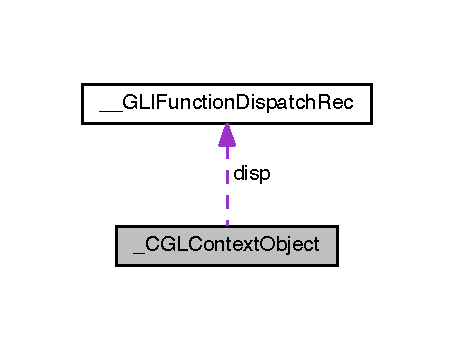
\includegraphics[width=218pt]{struct___c_g_l_context_object__coll__graph}
\end{center}
\end{figure}
\subsection*{Public Attributes}
\begin{DoxyCompactItemize}
\item 
\hyperlink{gli_context_8h_a9243ff8480d2878cd8374328404539de}{G\-L\-I\-Context} \hyperlink{struct___c_g_l_context_object_ac6f613aaaa3bccc159301c77b21c2936}{rend}
\item 
\hyperlink{gli_dispatch_8h_a3a00775396c54c5f50c81ce040d401d8}{G\-L\-I\-Function\-Dispatch} \hyperlink{struct___c_g_l_context_object_aa291770f316f46b4324e2fa46f777a27}{disp}
\item 
\hyperlink{_c_g_l_context_8h_a877227a11fe9df1ad6f947ec22494aee}{C\-G\-L\-Private\-Obj} \hyperlink{struct___c_g_l_context_object_a352c695320144d77502931b57be65140}{priv}
\item 
\hyperlink{glutf90_8h_ac778d6f63f1aaf8ebda0ce6ac821b56e}{void} $\ast$ \hyperlink{struct___c_g_l_context_object_aa676a2022d2d5f49bdb5b4ef41a2cba8}{stak}
\end{DoxyCompactItemize}


\subsection{Detailed Description}


Definition at line 24 of file C\-G\-L\-Context.\-h.



\subsection{Member Data Documentation}
\hypertarget{struct___c_g_l_context_object_aa291770f316f46b4324e2fa46f777a27}{\index{\-\_\-\-C\-G\-L\-Context\-Object@{\-\_\-\-C\-G\-L\-Context\-Object}!disp@{disp}}
\index{disp@{disp}!_CGLContextObject@{\-\_\-\-C\-G\-L\-Context\-Object}}
\subsubsection[{disp}]{\setlength{\rightskip}{0pt plus 5cm}{\bf G\-L\-I\-Function\-Dispatch} \-\_\-\-C\-G\-L\-Context\-Object\-::disp}}\label{struct___c_g_l_context_object_aa291770f316f46b4324e2fa46f777a27}


Definition at line 26 of file C\-G\-L\-Context.\-h.

\hypertarget{struct___c_g_l_context_object_a352c695320144d77502931b57be65140}{\index{\-\_\-\-C\-G\-L\-Context\-Object@{\-\_\-\-C\-G\-L\-Context\-Object}!priv@{priv}}
\index{priv@{priv}!_CGLContextObject@{\-\_\-\-C\-G\-L\-Context\-Object}}
\subsubsection[{priv}]{\setlength{\rightskip}{0pt plus 5cm}{\bf C\-G\-L\-Private\-Obj} \-\_\-\-C\-G\-L\-Context\-Object\-::priv}}\label{struct___c_g_l_context_object_a352c695320144d77502931b57be65140}


Definition at line 27 of file C\-G\-L\-Context.\-h.

\hypertarget{struct___c_g_l_context_object_ac6f613aaaa3bccc159301c77b21c2936}{\index{\-\_\-\-C\-G\-L\-Context\-Object@{\-\_\-\-C\-G\-L\-Context\-Object}!rend@{rend}}
\index{rend@{rend}!_CGLContextObject@{\-\_\-\-C\-G\-L\-Context\-Object}}
\subsubsection[{rend}]{\setlength{\rightskip}{0pt plus 5cm}{\bf G\-L\-I\-Context} \-\_\-\-C\-G\-L\-Context\-Object\-::rend}}\label{struct___c_g_l_context_object_ac6f613aaaa3bccc159301c77b21c2936}


Definition at line 25 of file C\-G\-L\-Context.\-h.

\hypertarget{struct___c_g_l_context_object_aa676a2022d2d5f49bdb5b4ef41a2cba8}{\index{\-\_\-\-C\-G\-L\-Context\-Object@{\-\_\-\-C\-G\-L\-Context\-Object}!stak@{stak}}
\index{stak@{stak}!_CGLContextObject@{\-\_\-\-C\-G\-L\-Context\-Object}}
\subsubsection[{stak}]{\setlength{\rightskip}{0pt plus 5cm}{\bf void}$\ast$ \-\_\-\-C\-G\-L\-Context\-Object\-::stak}}\label{struct___c_g_l_context_object_aa676a2022d2d5f49bdb5b4ef41a2cba8}


Definition at line 28 of file C\-G\-L\-Context.\-h.



The documentation for this struct was generated from the following file\-:\begin{DoxyCompactItemize}
\item 
/\-Users/ira/\-Dropbox/ira\-\_\-dev/protobyte\-\_\-research/other\-\_\-libs/gl/\-Headers/\hyperlink{_c_g_l_context_8h}{C\-G\-L\-Context.\-h}\end{DoxyCompactItemize}

\hypertarget{struct___sphere_map}{\section{\-\_\-\-Sphere\-Map Struct Reference}
\label{struct___sphere_map}\index{\-\_\-\-Sphere\-Map@{\-\_\-\-Sphere\-Map}}
}


{\ttfamily \#include $<$glsmapint.\-h$>$}



Collaboration diagram for \-\_\-\-Sphere\-Map\-:
\nopagebreak
\begin{figure}[H]
\begin{center}
\leavevmode
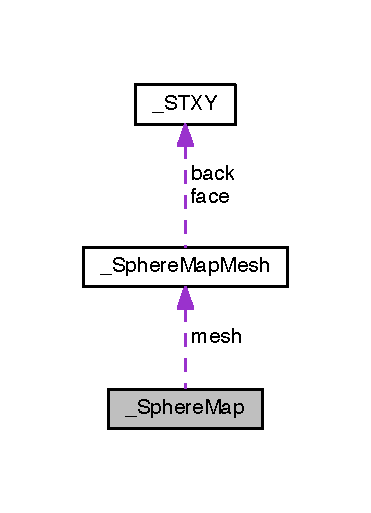
\includegraphics[width=178pt]{struct___sphere_map__coll__graph}
\end{center}
\end{figure}
\subsection*{Public Attributes}
\begin{DoxyCompactItemize}
\item 
\hyperlink{glsmapint_8h_a4965d0c8132b5c0f5a11f1b238d91a7a}{Sphere\-Map\-Mesh} $\ast$ \hyperlink{struct___sphere_map_aadeee07f5f55de1971f98fe89c3c82c7}{mesh}
\item 
\hyperlink{gl_8h_a68c4714e43d8e827d80759f9cb864f3c}{G\-Luint} \hyperlink{struct___sphere_map_a3f4b4ebc84435c496be900cca0103c99}{smap\-Tex\-Obj}
\item 
\hyperlink{gl_8h_a68c4714e43d8e827d80759f9cb864f3c}{G\-Luint} \hyperlink{struct___sphere_map_a34635ed623f295082180f1a6dae69a87}{view\-Tex\-Objs} \mbox{[}6\mbox{]}
\item 
\hyperlink{gl_8h_a68c4714e43d8e827d80759f9cb864f3c}{G\-Luint} \hyperlink{struct___sphere_map_ae13c3fd3977f4de76c99671d3c736f17}{view\-Tex\-Obj}
\item 
\hyperlink{glsmap_8h_a47f0d86b336f12393b51104083f66fd5}{Sphere\-Map\-Flags} \hyperlink{struct___sphere_map_aaedcca05cc381f25caaa216035e61b32}{flags}
\item 
int \hyperlink{struct___sphere_map_a9b58f4b38de6d3925ae1a3795074ddf1}{view\-Tex\-Dim}
\item 
int \hyperlink{struct___sphere_map_a59b4cf016e3fe520652cef083800789f}{smap\-Tex\-Dim}
\item 
int \hyperlink{struct___sphere_map_ae062a12b748d07b243a06554485da9ce}{view\-Origin} \mbox{[}2\mbox{]}
\item 
int \hyperlink{struct___sphere_map_a41758a7953c63d3687e5981b4954bf9a}{smap\-Origin} \mbox{[}2\mbox{]}
\item 
\hyperlink{gl_8h_a31aeedaeef29442c9c015ab355c8f5ab}{G\-Lfloat} \hyperlink{struct___sphere_map_a59f21bb82cae80e5260d98bef2014783}{eye} \mbox{[}3\mbox{]}
\item 
\hyperlink{gl_8h_a31aeedaeef29442c9c015ab355c8f5ab}{G\-Lfloat} \hyperlink{struct___sphere_map_aad20bb4c305d5d233926bd385dc156c5}{up} \mbox{[}3\mbox{]}
\item 
\hyperlink{gl_8h_a31aeedaeef29442c9c015ab355c8f5ab}{G\-Lfloat} \hyperlink{struct___sphere_map_a7a237a3fc3c5315c6db303c4f01ce43b}{obj} \mbox{[}3\mbox{]}
\item 
\hyperlink{gl_8h_a31aeedaeef29442c9c015ab355c8f5ab}{G\-Lfloat} \hyperlink{struct___sphere_map_a421e9bbe724d01a01faf291e6c445c6b}{view\-Near}
\item 
\hyperlink{gl_8h_a31aeedaeef29442c9c015ab355c8f5ab}{G\-Lfloat} \hyperlink{struct___sphere_map_ac3aa620d297a12e05e6005800512a102}{view\-Far}
\item 
\hyperlink{glutf90_8h_ac778d6f63f1aaf8ebda0ce6ac821b56e}{void}($\ast$ \hyperlink{struct___sphere_map_ae696630b2f422031807c44e63b0f55a9}{position\-Lights} )(int view, \hyperlink{glutf90_8h_ac778d6f63f1aaf8ebda0ce6ac821b56e}{void} $\ast$\hyperlink{struct___sphere_map_ae9e17d367aea76564089d8b22c7b30c1}{context})
\item 
\hyperlink{glutf90_8h_ac778d6f63f1aaf8ebda0ce6ac821b56e}{void}($\ast$ \hyperlink{struct___sphere_map_af95cd5ff0a4c9c8c6c3e0445947c0163}{draw\-View} )(int view, \hyperlink{glutf90_8h_ac778d6f63f1aaf8ebda0ce6ac821b56e}{void} $\ast$\hyperlink{struct___sphere_map_ae9e17d367aea76564089d8b22c7b30c1}{context})
\item 
\hyperlink{glutf90_8h_ac778d6f63f1aaf8ebda0ce6ac821b56e}{void} $\ast$ \hyperlink{struct___sphere_map_ae9e17d367aea76564089d8b22c7b30c1}{context}
\end{DoxyCompactItemize}


\subsection{Detailed Description}


Definition at line 58 of file glsmapint.\-h.



\subsection{Member Data Documentation}
\hypertarget{struct___sphere_map_ae9e17d367aea76564089d8b22c7b30c1}{\index{\-\_\-\-Sphere\-Map@{\-\_\-\-Sphere\-Map}!context@{context}}
\index{context@{context}!_SphereMap@{\-\_\-\-Sphere\-Map}}
\subsubsection[{context}]{\setlength{\rightskip}{0pt plus 5cm}{\bf void}$\ast$ \-\_\-\-Sphere\-Map\-::context}}\label{struct___sphere_map_ae9e17d367aea76564089d8b22c7b30c1}


Definition at line 93 of file glsmapint.\-h.

\hypertarget{struct___sphere_map_af95cd5ff0a4c9c8c6c3e0445947c0163}{\index{\-\_\-\-Sphere\-Map@{\-\_\-\-Sphere\-Map}!draw\-View@{draw\-View}}
\index{draw\-View@{draw\-View}!_SphereMap@{\-\_\-\-Sphere\-Map}}
\subsubsection[{draw\-View}]{\setlength{\rightskip}{0pt plus 5cm}{\bf void}($\ast$ \-\_\-\-Sphere\-Map\-::draw\-View)(int view, {\bf void} $\ast${\bf context})}}\label{struct___sphere_map_af95cd5ff0a4c9c8c6c3e0445947c0163}


Definition at line 90 of file glsmapint.\-h.

\hypertarget{struct___sphere_map_a59f21bb82cae80e5260d98bef2014783}{\index{\-\_\-\-Sphere\-Map@{\-\_\-\-Sphere\-Map}!eye@{eye}}
\index{eye@{eye}!_SphereMap@{\-\_\-\-Sphere\-Map}}
\subsubsection[{eye}]{\setlength{\rightskip}{0pt plus 5cm}{\bf G\-Lfloat} \-\_\-\-Sphere\-Map\-::eye\mbox{[}3\mbox{]}}}\label{struct___sphere_map_a59f21bb82cae80e5260d98bef2014783}


Definition at line 80 of file glsmapint.\-h.

\hypertarget{struct___sphere_map_aaedcca05cc381f25caaa216035e61b32}{\index{\-\_\-\-Sphere\-Map@{\-\_\-\-Sphere\-Map}!flags@{flags}}
\index{flags@{flags}!_SphereMap@{\-\_\-\-Sphere\-Map}}
\subsubsection[{flags}]{\setlength{\rightskip}{0pt plus 5cm}{\bf Sphere\-Map\-Flags} \-\_\-\-Sphere\-Map\-::flags}}\label{struct___sphere_map_aaedcca05cc381f25caaa216035e61b32}


Definition at line 69 of file glsmapint.\-h.

\hypertarget{struct___sphere_map_aadeee07f5f55de1971f98fe89c3c82c7}{\index{\-\_\-\-Sphere\-Map@{\-\_\-\-Sphere\-Map}!mesh@{mesh}}
\index{mesh@{mesh}!_SphereMap@{\-\_\-\-Sphere\-Map}}
\subsubsection[{mesh}]{\setlength{\rightskip}{0pt plus 5cm}{\bf Sphere\-Map\-Mesh}$\ast$ \-\_\-\-Sphere\-Map\-::mesh}}\label{struct___sphere_map_aadeee07f5f55de1971f98fe89c3c82c7}


Definition at line 61 of file glsmapint.\-h.

\hypertarget{struct___sphere_map_a7a237a3fc3c5315c6db303c4f01ce43b}{\index{\-\_\-\-Sphere\-Map@{\-\_\-\-Sphere\-Map}!obj@{obj}}
\index{obj@{obj}!_SphereMap@{\-\_\-\-Sphere\-Map}}
\subsubsection[{obj}]{\setlength{\rightskip}{0pt plus 5cm}{\bf G\-Lfloat} \-\_\-\-Sphere\-Map\-::obj\mbox{[}3\mbox{]}}}\label{struct___sphere_map_a7a237a3fc3c5315c6db303c4f01ce43b}


Definition at line 82 of file glsmapint.\-h.

\hypertarget{struct___sphere_map_ae696630b2f422031807c44e63b0f55a9}{\index{\-\_\-\-Sphere\-Map@{\-\_\-\-Sphere\-Map}!position\-Lights@{position\-Lights}}
\index{position\-Lights@{position\-Lights}!_SphereMap@{\-\_\-\-Sphere\-Map}}
\subsubsection[{position\-Lights}]{\setlength{\rightskip}{0pt plus 5cm}{\bf void}($\ast$ \-\_\-\-Sphere\-Map\-::position\-Lights)(int view, {\bf void} $\ast${\bf context})}}\label{struct___sphere_map_ae696630b2f422031807c44e63b0f55a9}


Definition at line 89 of file glsmapint.\-h.

\hypertarget{struct___sphere_map_a41758a7953c63d3687e5981b4954bf9a}{\index{\-\_\-\-Sphere\-Map@{\-\_\-\-Sphere\-Map}!smap\-Origin@{smap\-Origin}}
\index{smap\-Origin@{smap\-Origin}!_SphereMap@{\-\_\-\-Sphere\-Map}}
\subsubsection[{smap\-Origin}]{\setlength{\rightskip}{0pt plus 5cm}int \-\_\-\-Sphere\-Map\-::smap\-Origin\mbox{[}2\mbox{]}}}\label{struct___sphere_map_a41758a7953c63d3687e5981b4954bf9a}


Definition at line 77 of file glsmapint.\-h.

\hypertarget{struct___sphere_map_a59b4cf016e3fe520652cef083800789f}{\index{\-\_\-\-Sphere\-Map@{\-\_\-\-Sphere\-Map}!smap\-Tex\-Dim@{smap\-Tex\-Dim}}
\index{smap\-Tex\-Dim@{smap\-Tex\-Dim}!_SphereMap@{\-\_\-\-Sphere\-Map}}
\subsubsection[{smap\-Tex\-Dim}]{\setlength{\rightskip}{0pt plus 5cm}int \-\_\-\-Sphere\-Map\-::smap\-Tex\-Dim}}\label{struct___sphere_map_a59b4cf016e3fe520652cef083800789f}


Definition at line 73 of file glsmapint.\-h.

\hypertarget{struct___sphere_map_a3f4b4ebc84435c496be900cca0103c99}{\index{\-\_\-\-Sphere\-Map@{\-\_\-\-Sphere\-Map}!smap\-Tex\-Obj@{smap\-Tex\-Obj}}
\index{smap\-Tex\-Obj@{smap\-Tex\-Obj}!_SphereMap@{\-\_\-\-Sphere\-Map}}
\subsubsection[{smap\-Tex\-Obj}]{\setlength{\rightskip}{0pt plus 5cm}{\bf G\-Luint} \-\_\-\-Sphere\-Map\-::smap\-Tex\-Obj}}\label{struct___sphere_map_a3f4b4ebc84435c496be900cca0103c99}


Definition at line 64 of file glsmapint.\-h.

\hypertarget{struct___sphere_map_aad20bb4c305d5d233926bd385dc156c5}{\index{\-\_\-\-Sphere\-Map@{\-\_\-\-Sphere\-Map}!up@{up}}
\index{up@{up}!_SphereMap@{\-\_\-\-Sphere\-Map}}
\subsubsection[{up}]{\setlength{\rightskip}{0pt plus 5cm}{\bf G\-Lfloat} \-\_\-\-Sphere\-Map\-::up\mbox{[}3\mbox{]}}}\label{struct___sphere_map_aad20bb4c305d5d233926bd385dc156c5}


Definition at line 81 of file glsmapint.\-h.

\hypertarget{struct___sphere_map_ac3aa620d297a12e05e6005800512a102}{\index{\-\_\-\-Sphere\-Map@{\-\_\-\-Sphere\-Map}!view\-Far@{view\-Far}}
\index{view\-Far@{view\-Far}!_SphereMap@{\-\_\-\-Sphere\-Map}}
\subsubsection[{view\-Far}]{\setlength{\rightskip}{0pt plus 5cm}{\bf G\-Lfloat} \-\_\-\-Sphere\-Map\-::view\-Far}}\label{struct___sphere_map_ac3aa620d297a12e05e6005800512a102}


Definition at line 86 of file glsmapint.\-h.

\hypertarget{struct___sphere_map_a421e9bbe724d01a01faf291e6c445c6b}{\index{\-\_\-\-Sphere\-Map@{\-\_\-\-Sphere\-Map}!view\-Near@{view\-Near}}
\index{view\-Near@{view\-Near}!_SphereMap@{\-\_\-\-Sphere\-Map}}
\subsubsection[{view\-Near}]{\setlength{\rightskip}{0pt plus 5cm}{\bf G\-Lfloat} \-\_\-\-Sphere\-Map\-::view\-Near}}\label{struct___sphere_map_a421e9bbe724d01a01faf291e6c445c6b}


Definition at line 85 of file glsmapint.\-h.

\hypertarget{struct___sphere_map_ae062a12b748d07b243a06554485da9ce}{\index{\-\_\-\-Sphere\-Map@{\-\_\-\-Sphere\-Map}!view\-Origin@{view\-Origin}}
\index{view\-Origin@{view\-Origin}!_SphereMap@{\-\_\-\-Sphere\-Map}}
\subsubsection[{view\-Origin}]{\setlength{\rightskip}{0pt plus 5cm}int \-\_\-\-Sphere\-Map\-::view\-Origin\mbox{[}2\mbox{]}}}\label{struct___sphere_map_ae062a12b748d07b243a06554485da9ce}


Definition at line 76 of file glsmapint.\-h.

\hypertarget{struct___sphere_map_a9b58f4b38de6d3925ae1a3795074ddf1}{\index{\-\_\-\-Sphere\-Map@{\-\_\-\-Sphere\-Map}!view\-Tex\-Dim@{view\-Tex\-Dim}}
\index{view\-Tex\-Dim@{view\-Tex\-Dim}!_SphereMap@{\-\_\-\-Sphere\-Map}}
\subsubsection[{view\-Tex\-Dim}]{\setlength{\rightskip}{0pt plus 5cm}int \-\_\-\-Sphere\-Map\-::view\-Tex\-Dim}}\label{struct___sphere_map_a9b58f4b38de6d3925ae1a3795074ddf1}


Definition at line 72 of file glsmapint.\-h.

\hypertarget{struct___sphere_map_ae13c3fd3977f4de76c99671d3c736f17}{\index{\-\_\-\-Sphere\-Map@{\-\_\-\-Sphere\-Map}!view\-Tex\-Obj@{view\-Tex\-Obj}}
\index{view\-Tex\-Obj@{view\-Tex\-Obj}!_SphereMap@{\-\_\-\-Sphere\-Map}}
\subsubsection[{view\-Tex\-Obj}]{\setlength{\rightskip}{0pt plus 5cm}{\bf G\-Luint} \-\_\-\-Sphere\-Map\-::view\-Tex\-Obj}}\label{struct___sphere_map_ae13c3fd3977f4de76c99671d3c736f17}


Definition at line 66 of file glsmapint.\-h.

\hypertarget{struct___sphere_map_a34635ed623f295082180f1a6dae69a87}{\index{\-\_\-\-Sphere\-Map@{\-\_\-\-Sphere\-Map}!view\-Tex\-Objs@{view\-Tex\-Objs}}
\index{view\-Tex\-Objs@{view\-Tex\-Objs}!_SphereMap@{\-\_\-\-Sphere\-Map}}
\subsubsection[{view\-Tex\-Objs}]{\setlength{\rightskip}{0pt plus 5cm}{\bf G\-Luint} \-\_\-\-Sphere\-Map\-::view\-Tex\-Objs\mbox{[}6\mbox{]}}}\label{struct___sphere_map_a34635ed623f295082180f1a6dae69a87}


Definition at line 65 of file glsmapint.\-h.



The documentation for this struct was generated from the following file\-:\begin{DoxyCompactItemize}
\item 
/\-Users/ira/\-Dropbox/ira\-\_\-dev/protobyte\-\_\-research/other\-\_\-libs/glut/\-Headers/\hyperlink{glsmapint_8h}{glsmapint.\-h}\end{DoxyCompactItemize}

\hypertarget{struct___sphere_map_mesh}{\section{\-\_\-\-Sphere\-Map\-Mesh Struct Reference}
\label{struct___sphere_map_mesh}\index{\-\_\-\-Sphere\-Map\-Mesh@{\-\_\-\-Sphere\-Map\-Mesh}}
}


{\ttfamily \#include $<$glsmapint.\-h$>$}



Collaboration diagram for \-\_\-\-Sphere\-Map\-Mesh\-:
\nopagebreak
\begin{figure}[H]
\begin{center}
\leavevmode
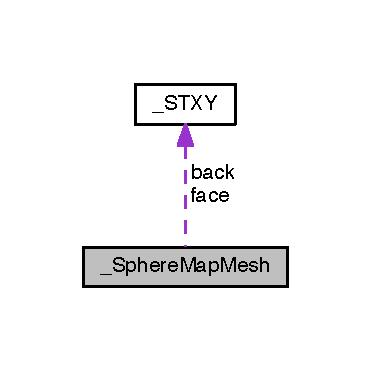
\includegraphics[width=178pt]{struct___sphere_map_mesh__coll__graph}
\end{center}
\end{figure}
\subsection*{Public Attributes}
\begin{DoxyCompactItemize}
\item 
int \hyperlink{struct___sphere_map_mesh_a0c1c34900669d68aaf706a9e17fdeba8}{refcnt}
\item 
int \hyperlink{struct___sphere_map_mesh_aa2fec57e05a2fc00223c07992406fe7b}{steps}
\item 
int \hyperlink{struct___sphere_map_mesh_a4fee7062c54b6850d7400a1a2bd037dc}{rings}
\item 
int \hyperlink{struct___sphere_map_mesh_a9138869c8a44e8877b68bb1154a5a8ae}{edge\-Extend}
\item 
\hyperlink{glsmapint_8h_ac1c4fff4fc00c8cd3d4a318e152fce9e}{S\-T\-X\-Y} $\ast$ \hyperlink{struct___sphere_map_mesh_ab75ee81e8d0d201e0c32cd144de796a5}{face}
\item 
\hyperlink{glsmapint_8h_ac1c4fff4fc00c8cd3d4a318e152fce9e}{S\-T\-X\-Y} $\ast$ \hyperlink{struct___sphere_map_mesh_a2ea363cd5ab2463bc9c2c0de8d7f3811}{back}
\end{DoxyCompactItemize}


\subsection{Detailed Description}


Definition at line 45 of file glsmapint.\-h.



\subsection{Member Data Documentation}
\hypertarget{struct___sphere_map_mesh_a2ea363cd5ab2463bc9c2c0de8d7f3811}{\index{\-\_\-\-Sphere\-Map\-Mesh@{\-\_\-\-Sphere\-Map\-Mesh}!back@{back}}
\index{back@{back}!_SphereMapMesh@{\-\_\-\-Sphere\-Map\-Mesh}}
\subsubsection[{back}]{\setlength{\rightskip}{0pt plus 5cm}{\bf S\-T\-X\-Y}$\ast$ \-\_\-\-Sphere\-Map\-Mesh\-::back}}\label{struct___sphere_map_mesh_a2ea363cd5ab2463bc9c2c0de8d7f3811}


Definition at line 54 of file glsmapint.\-h.

\hypertarget{struct___sphere_map_mesh_a9138869c8a44e8877b68bb1154a5a8ae}{\index{\-\_\-\-Sphere\-Map\-Mesh@{\-\_\-\-Sphere\-Map\-Mesh}!edge\-Extend@{edge\-Extend}}
\index{edge\-Extend@{edge\-Extend}!_SphereMapMesh@{\-\_\-\-Sphere\-Map\-Mesh}}
\subsubsection[{edge\-Extend}]{\setlength{\rightskip}{0pt plus 5cm}int \-\_\-\-Sphere\-Map\-Mesh\-::edge\-Extend}}\label{struct___sphere_map_mesh_a9138869c8a44e8877b68bb1154a5a8ae}


Definition at line 51 of file glsmapint.\-h.

\hypertarget{struct___sphere_map_mesh_ab75ee81e8d0d201e0c32cd144de796a5}{\index{\-\_\-\-Sphere\-Map\-Mesh@{\-\_\-\-Sphere\-Map\-Mesh}!face@{face}}
\index{face@{face}!_SphereMapMesh@{\-\_\-\-Sphere\-Map\-Mesh}}
\subsubsection[{face}]{\setlength{\rightskip}{0pt plus 5cm}{\bf S\-T\-X\-Y}$\ast$ \-\_\-\-Sphere\-Map\-Mesh\-::face}}\label{struct___sphere_map_mesh_ab75ee81e8d0d201e0c32cd144de796a5}


Definition at line 53 of file glsmapint.\-h.

\hypertarget{struct___sphere_map_mesh_a0c1c34900669d68aaf706a9e17fdeba8}{\index{\-\_\-\-Sphere\-Map\-Mesh@{\-\_\-\-Sphere\-Map\-Mesh}!refcnt@{refcnt}}
\index{refcnt@{refcnt}!_SphereMapMesh@{\-\_\-\-Sphere\-Map\-Mesh}}
\subsubsection[{refcnt}]{\setlength{\rightskip}{0pt plus 5cm}int \-\_\-\-Sphere\-Map\-Mesh\-::refcnt}}\label{struct___sphere_map_mesh_a0c1c34900669d68aaf706a9e17fdeba8}


Definition at line 47 of file glsmapint.\-h.

\hypertarget{struct___sphere_map_mesh_a4fee7062c54b6850d7400a1a2bd037dc}{\index{\-\_\-\-Sphere\-Map\-Mesh@{\-\_\-\-Sphere\-Map\-Mesh}!rings@{rings}}
\index{rings@{rings}!_SphereMapMesh@{\-\_\-\-Sphere\-Map\-Mesh}}
\subsubsection[{rings}]{\setlength{\rightskip}{0pt plus 5cm}int \-\_\-\-Sphere\-Map\-Mesh\-::rings}}\label{struct___sphere_map_mesh_a4fee7062c54b6850d7400a1a2bd037dc}


Definition at line 50 of file glsmapint.\-h.

\hypertarget{struct___sphere_map_mesh_aa2fec57e05a2fc00223c07992406fe7b}{\index{\-\_\-\-Sphere\-Map\-Mesh@{\-\_\-\-Sphere\-Map\-Mesh}!steps@{steps}}
\index{steps@{steps}!_SphereMapMesh@{\-\_\-\-Sphere\-Map\-Mesh}}
\subsubsection[{steps}]{\setlength{\rightskip}{0pt plus 5cm}int \-\_\-\-Sphere\-Map\-Mesh\-::steps}}\label{struct___sphere_map_mesh_aa2fec57e05a2fc00223c07992406fe7b}


Definition at line 49 of file glsmapint.\-h.



The documentation for this struct was generated from the following file\-:\begin{DoxyCompactItemize}
\item 
/\-Users/ira/\-Dropbox/ira\-\_\-dev/protobyte\-\_\-research/other\-\_\-libs/glut/\-Headers/\hyperlink{glsmapint_8h}{glsmapint.\-h}\end{DoxyCompactItemize}

\hypertarget{struct___s_t_x_y}{\section{\-\_\-\-S\-T\-X\-Y Struct Reference}
\label{struct___s_t_x_y}\index{\-\_\-\-S\-T\-X\-Y@{\-\_\-\-S\-T\-X\-Y}}
}


{\ttfamily \#include $<$glsmapint.\-h$>$}

\subsection*{Public Attributes}
\begin{DoxyCompactItemize}
\item 
\hyperlink{gl_8h_a31aeedaeef29442c9c015ab355c8f5ab}{G\-Lfloat} \hyperlink{struct___s_t_x_y_abb7cf83c66ed6f8156a98985bef3a8a6}{s}
\item 
\hyperlink{gl_8h_a31aeedaeef29442c9c015ab355c8f5ab}{G\-Lfloat} \hyperlink{struct___s_t_x_y_a4abc729e77d41ab5a407b6b0b6ecb9d7}{t}
\item 
\hyperlink{gl_8h_a31aeedaeef29442c9c015ab355c8f5ab}{G\-Lfloat} \hyperlink{struct___s_t_x_y_a733147b5dc188e788b0903ba1bec7f7e}{x}
\item 
\hyperlink{gl_8h_a31aeedaeef29442c9c015ab355c8f5ab}{G\-Lfloat} \hyperlink{struct___s_t_x_y_a222822654dc08ad4e974daf39a8e4d7e}{y}
\end{DoxyCompactItemize}


\subsection{Detailed Description}


Definition at line 40 of file glsmapint.\-h.



\subsection{Member Data Documentation}
\hypertarget{struct___s_t_x_y_abb7cf83c66ed6f8156a98985bef3a8a6}{\index{\-\_\-\-S\-T\-X\-Y@{\-\_\-\-S\-T\-X\-Y}!s@{s}}
\index{s@{s}!_STXY@{\-\_\-\-S\-T\-X\-Y}}
\subsubsection[{s}]{\setlength{\rightskip}{0pt plus 5cm}{\bf G\-Lfloat} \-\_\-\-S\-T\-X\-Y\-::s}}\label{struct___s_t_x_y_abb7cf83c66ed6f8156a98985bef3a8a6}


Definition at line 41 of file glsmapint.\-h.

\hypertarget{struct___s_t_x_y_a4abc729e77d41ab5a407b6b0b6ecb9d7}{\index{\-\_\-\-S\-T\-X\-Y@{\-\_\-\-S\-T\-X\-Y}!t@{t}}
\index{t@{t}!_STXY@{\-\_\-\-S\-T\-X\-Y}}
\subsubsection[{t}]{\setlength{\rightskip}{0pt plus 5cm}{\bf G\-Lfloat} \-\_\-\-S\-T\-X\-Y\-::t}}\label{struct___s_t_x_y_a4abc729e77d41ab5a407b6b0b6ecb9d7}


Definition at line 41 of file glsmapint.\-h.

\hypertarget{struct___s_t_x_y_a733147b5dc188e788b0903ba1bec7f7e}{\index{\-\_\-\-S\-T\-X\-Y@{\-\_\-\-S\-T\-X\-Y}!x@{x}}
\index{x@{x}!_STXY@{\-\_\-\-S\-T\-X\-Y}}
\subsubsection[{x}]{\setlength{\rightskip}{0pt plus 5cm}{\bf G\-Lfloat} \-\_\-\-S\-T\-X\-Y\-::x}}\label{struct___s_t_x_y_a733147b5dc188e788b0903ba1bec7f7e}


Definition at line 42 of file glsmapint.\-h.

\hypertarget{struct___s_t_x_y_a222822654dc08ad4e974daf39a8e4d7e}{\index{\-\_\-\-S\-T\-X\-Y@{\-\_\-\-S\-T\-X\-Y}!y@{y}}
\index{y@{y}!_STXY@{\-\_\-\-S\-T\-X\-Y}}
\subsubsection[{y}]{\setlength{\rightskip}{0pt plus 5cm}{\bf G\-Lfloat} \-\_\-\-S\-T\-X\-Y\-::y}}\label{struct___s_t_x_y_a222822654dc08ad4e974daf39a8e4d7e}


Definition at line 42 of file glsmapint.\-h.



The documentation for this struct was generated from the following file\-:\begin{DoxyCompactItemize}
\item 
/\-Users/ira/\-Dropbox/ira\-\_\-dev/protobyte\-\_\-research/other\-\_\-libs/glut/\-Headers/\hyperlink{glsmapint_8h}{glsmapint.\-h}\end{DoxyCompactItemize}

\hypertarget{struct_bitmap_char_rec}{\section{Bitmap\-Char\-Rec Struct Reference}
\label{struct_bitmap_char_rec}\index{Bitmap\-Char\-Rec@{Bitmap\-Char\-Rec}}
}


{\ttfamily \#include $<$glutbitmap.\-h$>$}

\subsection*{Public Attributes}
\begin{DoxyCompactItemize}
\item 
const \hyperlink{gl_8h_a9289d5b99dc1f27f01480360f2e18ae0}{G\-Lsizei} \hyperlink{struct_bitmap_char_rec_aec4f640649f028cbd750a29307587d45}{width}
\item 
const \hyperlink{gl_8h_a9289d5b99dc1f27f01480360f2e18ae0}{G\-Lsizei} \hyperlink{struct_bitmap_char_rec_a635c0cdf674896272c549c1ab3d82b21}{height}
\item 
const \hyperlink{gl_8h_a31aeedaeef29442c9c015ab355c8f5ab}{G\-Lfloat} \hyperlink{struct_bitmap_char_rec_a0349720d81a4c62afe6561201997e995}{xorig}
\item 
const \hyperlink{gl_8h_a31aeedaeef29442c9c015ab355c8f5ab}{G\-Lfloat} \hyperlink{struct_bitmap_char_rec_a7351bb7d319ab8e79da4e16e6aacddaf}{yorig}
\item 
const \hyperlink{gl_8h_a31aeedaeef29442c9c015ab355c8f5ab}{G\-Lfloat} \hyperlink{struct_bitmap_char_rec_a829d8afb40c22d832dad5369cfa54aa9}{advance}
\item 
const \hyperlink{gl_8h_a0595908be03a8cff881a23cdc9170e7c}{G\-Lubyte} $\ast$ \hyperlink{struct_bitmap_char_rec_af9859692f6e3089f377788f458dd50bb}{bitmap}
\end{DoxyCompactItemize}


\subsection{Detailed Description}


Definition at line 12 of file glutbitmap.\-h.



\subsection{Member Data Documentation}
\hypertarget{struct_bitmap_char_rec_a829d8afb40c22d832dad5369cfa54aa9}{\index{Bitmap\-Char\-Rec@{Bitmap\-Char\-Rec}!advance@{advance}}
\index{advance@{advance}!BitmapCharRec@{Bitmap\-Char\-Rec}}
\subsubsection[{advance}]{\setlength{\rightskip}{0pt plus 5cm}const {\bf G\-Lfloat} Bitmap\-Char\-Rec\-::advance}}\label{struct_bitmap_char_rec_a829d8afb40c22d832dad5369cfa54aa9}


Definition at line 17 of file glutbitmap.\-h.

\hypertarget{struct_bitmap_char_rec_af9859692f6e3089f377788f458dd50bb}{\index{Bitmap\-Char\-Rec@{Bitmap\-Char\-Rec}!bitmap@{bitmap}}
\index{bitmap@{bitmap}!BitmapCharRec@{Bitmap\-Char\-Rec}}
\subsubsection[{bitmap}]{\setlength{\rightskip}{0pt plus 5cm}const {\bf G\-Lubyte}$\ast$ Bitmap\-Char\-Rec\-::bitmap}}\label{struct_bitmap_char_rec_af9859692f6e3089f377788f458dd50bb}


Definition at line 18 of file glutbitmap.\-h.

\hypertarget{struct_bitmap_char_rec_a635c0cdf674896272c549c1ab3d82b21}{\index{Bitmap\-Char\-Rec@{Bitmap\-Char\-Rec}!height@{height}}
\index{height@{height}!BitmapCharRec@{Bitmap\-Char\-Rec}}
\subsubsection[{height}]{\setlength{\rightskip}{0pt plus 5cm}const {\bf G\-Lsizei} Bitmap\-Char\-Rec\-::height}}\label{struct_bitmap_char_rec_a635c0cdf674896272c549c1ab3d82b21}


Definition at line 14 of file glutbitmap.\-h.

\hypertarget{struct_bitmap_char_rec_aec4f640649f028cbd750a29307587d45}{\index{Bitmap\-Char\-Rec@{Bitmap\-Char\-Rec}!width@{width}}
\index{width@{width}!BitmapCharRec@{Bitmap\-Char\-Rec}}
\subsubsection[{width}]{\setlength{\rightskip}{0pt plus 5cm}const {\bf G\-Lsizei} Bitmap\-Char\-Rec\-::width}}\label{struct_bitmap_char_rec_aec4f640649f028cbd750a29307587d45}


Definition at line 13 of file glutbitmap.\-h.

\hypertarget{struct_bitmap_char_rec_a0349720d81a4c62afe6561201997e995}{\index{Bitmap\-Char\-Rec@{Bitmap\-Char\-Rec}!xorig@{xorig}}
\index{xorig@{xorig}!BitmapCharRec@{Bitmap\-Char\-Rec}}
\subsubsection[{xorig}]{\setlength{\rightskip}{0pt plus 5cm}const {\bf G\-Lfloat} Bitmap\-Char\-Rec\-::xorig}}\label{struct_bitmap_char_rec_a0349720d81a4c62afe6561201997e995}


Definition at line 15 of file glutbitmap.\-h.

\hypertarget{struct_bitmap_char_rec_a7351bb7d319ab8e79da4e16e6aacddaf}{\index{Bitmap\-Char\-Rec@{Bitmap\-Char\-Rec}!yorig@{yorig}}
\index{yorig@{yorig}!BitmapCharRec@{Bitmap\-Char\-Rec}}
\subsubsection[{yorig}]{\setlength{\rightskip}{0pt plus 5cm}const {\bf G\-Lfloat} Bitmap\-Char\-Rec\-::yorig}}\label{struct_bitmap_char_rec_a7351bb7d319ab8e79da4e16e6aacddaf}


Definition at line 16 of file glutbitmap.\-h.



The documentation for this struct was generated from the following file\-:\begin{DoxyCompactItemize}
\item 
/\-Users/ira/\-Dropbox/ira\-\_\-dev/protobyte\-\_\-research/other\-\_\-libs/glut/\-Headers/\hyperlink{glutbitmap_8h}{glutbitmap.\-h}\end{DoxyCompactItemize}

\hypertarget{struct_bitmap_font_rec}{\section{Bitmap\-Font\-Rec Struct Reference}
\label{struct_bitmap_font_rec}\index{Bitmap\-Font\-Rec@{Bitmap\-Font\-Rec}}
}


{\ttfamily \#include $<$glutbitmap.\-h$>$}



Collaboration diagram for Bitmap\-Font\-Rec\-:
\nopagebreak
\begin{figure}[H]
\begin{center}
\leavevmode
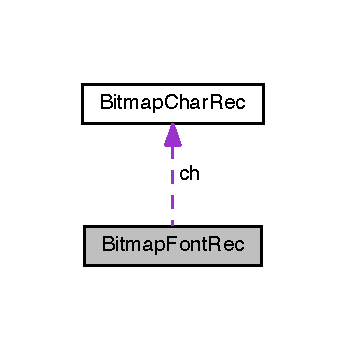
\includegraphics[width=166pt]{struct_bitmap_font_rec__coll__graph}
\end{center}
\end{figure}
\subsection*{Public Attributes}
\begin{DoxyCompactItemize}
\item 
const char $\ast$ \hyperlink{struct_bitmap_font_rec_ad70b2bdb7beb381ac3e6aaab7742a6cf}{name}
\item 
const int \hyperlink{struct_bitmap_font_rec_a02dcce32386981a7860d7eb63e610a6f}{num\-\_\-chars}
\item 
const int \hyperlink{struct_bitmap_font_rec_ae3fa065bd6cb89438656029968f38a37}{first}
\item 
const \hyperlink{struct_bitmap_char_rec}{Bitmap\-Char\-Rec} $\ast$const $\ast$ \hyperlink{struct_bitmap_font_rec_a5dc1989a9be5be061a6fe71affff15be}{ch}
\end{DoxyCompactItemize}


\subsection{Detailed Description}


Definition at line 21 of file glutbitmap.\-h.



\subsection{Member Data Documentation}
\hypertarget{struct_bitmap_font_rec_a5dc1989a9be5be061a6fe71affff15be}{\index{Bitmap\-Font\-Rec@{Bitmap\-Font\-Rec}!ch@{ch}}
\index{ch@{ch}!BitmapFontRec@{Bitmap\-Font\-Rec}}
\subsubsection[{ch}]{\setlength{\rightskip}{0pt plus 5cm}const {\bf Bitmap\-Char\-Rec}$\ast$ const$\ast$ Bitmap\-Font\-Rec\-::ch}}\label{struct_bitmap_font_rec_a5dc1989a9be5be061a6fe71affff15be}


Definition at line 25 of file glutbitmap.\-h.

\hypertarget{struct_bitmap_font_rec_ae3fa065bd6cb89438656029968f38a37}{\index{Bitmap\-Font\-Rec@{Bitmap\-Font\-Rec}!first@{first}}
\index{first@{first}!BitmapFontRec@{Bitmap\-Font\-Rec}}
\subsubsection[{first}]{\setlength{\rightskip}{0pt plus 5cm}const int Bitmap\-Font\-Rec\-::first}}\label{struct_bitmap_font_rec_ae3fa065bd6cb89438656029968f38a37}


Definition at line 24 of file glutbitmap.\-h.

\hypertarget{struct_bitmap_font_rec_ad70b2bdb7beb381ac3e6aaab7742a6cf}{\index{Bitmap\-Font\-Rec@{Bitmap\-Font\-Rec}!name@{name}}
\index{name@{name}!BitmapFontRec@{Bitmap\-Font\-Rec}}
\subsubsection[{name}]{\setlength{\rightskip}{0pt plus 5cm}const char$\ast$ Bitmap\-Font\-Rec\-::name}}\label{struct_bitmap_font_rec_ad70b2bdb7beb381ac3e6aaab7742a6cf}


Definition at line 22 of file glutbitmap.\-h.

\hypertarget{struct_bitmap_font_rec_a02dcce32386981a7860d7eb63e610a6f}{\index{Bitmap\-Font\-Rec@{Bitmap\-Font\-Rec}!num\-\_\-chars@{num\-\_\-chars}}
\index{num\-\_\-chars@{num\-\_\-chars}!BitmapFontRec@{Bitmap\-Font\-Rec}}
\subsubsection[{num\-\_\-chars}]{\setlength{\rightskip}{0pt plus 5cm}const int Bitmap\-Font\-Rec\-::num\-\_\-chars}}\label{struct_bitmap_font_rec_a02dcce32386981a7860d7eb63e610a6f}


Definition at line 23 of file glutbitmap.\-h.



The documentation for this struct was generated from the following file\-:\begin{DoxyCompactItemize}
\item 
/\-Users/ira/\-Dropbox/ira\-\_\-dev/protobyte\-\_\-research/other\-\_\-libs/glut/\-Headers/\hyperlink{glutbitmap_8h}{glutbitmap.\-h}\end{DoxyCompactItemize}

\hypertarget{structsf_1_1_sound_stream_1_1_chunk}{\section{sf\-:\-:Sound\-Stream\-:\-:Chunk Struct Reference}
\label{structsf_1_1_sound_stream_1_1_chunk}\index{sf\-::\-Sound\-Stream\-::\-Chunk@{sf\-::\-Sound\-Stream\-::\-Chunk}}
}


Structure defining a chunk of audio data to stream.  




{\ttfamily \#include $<$Sound\-Stream.\-hpp$>$}

\subsection*{Public Attributes}
\begin{DoxyCompactItemize}
\item 
const \hyperlink{namespacesf_a3c8e10435e2a310a7741755e66b5c94e}{Int16} $\ast$ \hyperlink{structsf_1_1_sound_stream_1_1_chunk_aa3b84d69adbe663a17a7671626076df4}{samples}
\begin{DoxyCompactList}\small\item\em Pointer to the audio samples. \end{DoxyCompactList}\item 
std\-::size\-\_\-t \hyperlink{structsf_1_1_sound_stream_1_1_chunk_af47f5d94012acf8b11f056ba77aff97a}{sample\-Count}
\begin{DoxyCompactList}\small\item\em Number of samples pointed by Samples. \end{DoxyCompactList}\end{DoxyCompactItemize}


\subsection{Detailed Description}
Structure defining a chunk of audio data to stream. 

Definition at line 52 of file Sound\-Stream.\-hpp.



\subsection{Member Data Documentation}
\hypertarget{structsf_1_1_sound_stream_1_1_chunk_af47f5d94012acf8b11f056ba77aff97a}{\index{sf\-::\-Sound\-Stream\-::\-Chunk@{sf\-::\-Sound\-Stream\-::\-Chunk}!sample\-Count@{sample\-Count}}
\index{sample\-Count@{sample\-Count}!sf::SoundStream::Chunk@{sf\-::\-Sound\-Stream\-::\-Chunk}}
\subsubsection[{sample\-Count}]{\setlength{\rightskip}{0pt plus 5cm}std\-::size\-\_\-t sf\-::\-Sound\-Stream\-::\-Chunk\-::sample\-Count}}\label{structsf_1_1_sound_stream_1_1_chunk_af47f5d94012acf8b11f056ba77aff97a}


Number of samples pointed by Samples. 



Definition at line 55 of file Sound\-Stream.\-hpp.

\hypertarget{structsf_1_1_sound_stream_1_1_chunk_aa3b84d69adbe663a17a7671626076df4}{\index{sf\-::\-Sound\-Stream\-::\-Chunk@{sf\-::\-Sound\-Stream\-::\-Chunk}!samples@{samples}}
\index{samples@{samples}!sf::SoundStream::Chunk@{sf\-::\-Sound\-Stream\-::\-Chunk}}
\subsubsection[{samples}]{\setlength{\rightskip}{0pt plus 5cm}const {\bf Int16}$\ast$ sf\-::\-Sound\-Stream\-::\-Chunk\-::samples}}\label{structsf_1_1_sound_stream_1_1_chunk_aa3b84d69adbe663a17a7671626076df4}


Pointer to the audio samples. 



Definition at line 54 of file Sound\-Stream.\-hpp.



The documentation for this struct was generated from the following file\-:\begin{DoxyCompactItemize}
\item 
/\-Users/ira/\-Dropbox/ira\-\_\-dev/protobyte\-\_\-research/other\-\_\-libs/\-S\-F\-M\-L/dylibs/root/usr/local/include/\-S\-F\-M\-L/\-Audio/\hyperlink{_sound_stream_8hpp}{Sound\-Stream.\-hpp}\end{DoxyCompactItemize}

\hypertarget{classsf_1_1_circle_shape}{\section{sf\-:\-:Circle\-Shape Class Reference}
\label{classsf_1_1_circle_shape}\index{sf\-::\-Circle\-Shape@{sf\-::\-Circle\-Shape}}
}


Specialized shape representing a circle.  




{\ttfamily \#include $<$Circle\-Shape.\-hpp$>$}



Inheritance diagram for sf\-:\-:Circle\-Shape\-:
\nopagebreak
\begin{figure}[H]
\begin{center}
\leavevmode
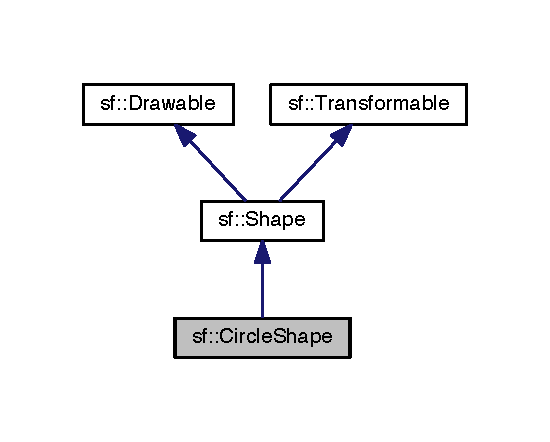
\includegraphics[width=264pt]{classsf_1_1_circle_shape__inherit__graph}
\end{center}
\end{figure}


Collaboration diagram for sf\-:\-:Circle\-Shape\-:
\nopagebreak
\begin{figure}[H]
\begin{center}
\leavevmode
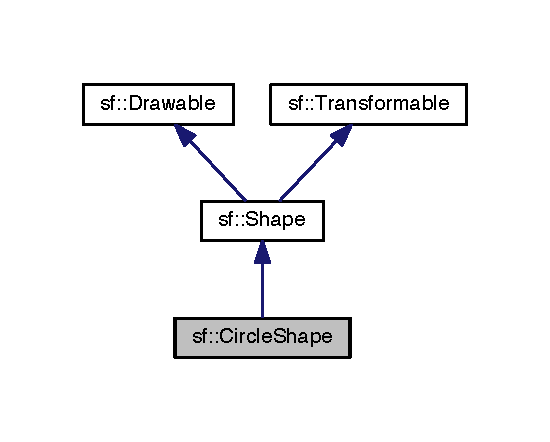
\includegraphics[width=264pt]{classsf_1_1_circle_shape__coll__graph}
\end{center}
\end{figure}
\subsection*{Public Member Functions}
\begin{DoxyCompactItemize}
\item 
\hyperlink{classsf_1_1_circle_shape_a06a5e136da1cfa3bd2a945a5c7f718d3}{Circle\-Shape} (float radius=0, unsigned int point\-Count=30)
\begin{DoxyCompactList}\small\item\em Default constructor. \end{DoxyCompactList}\item 
\hyperlink{glutf90_8h_ac778d6f63f1aaf8ebda0ce6ac821b56e}{void} \hyperlink{classsf_1_1_circle_shape_a21cdf85fc2f201e10222a241af864be0}{set\-Radius} (float radius)
\begin{DoxyCompactList}\small\item\em Set the radius of the circle. \end{DoxyCompactList}\item 
float \hyperlink{classsf_1_1_circle_shape_afaf5175a75b6179cc177b1281027ab00}{get\-Radius} () const 
\begin{DoxyCompactList}\small\item\em Get the radius of the circle. \end{DoxyCompactList}\item 
\hyperlink{glutf90_8h_ac778d6f63f1aaf8ebda0ce6ac821b56e}{void} \hyperlink{classsf_1_1_circle_shape_a84249c4b23b20c24bf6891edde3cf744}{set\-Point\-Count} (unsigned int \hyperlink{gl3_8h_a5b40aca7a9682963dd00a8f5aef0a901}{count})
\begin{DoxyCompactList}\small\item\em Set the number of points of the circle. \end{DoxyCompactList}\item 
virtual unsigned int \hyperlink{classsf_1_1_circle_shape_ae41ed830ca8f459e88ea6f125c240949}{get\-Point\-Count} () const 
\begin{DoxyCompactList}\small\item\em Get the number of points of the shape. \end{DoxyCompactList}\item 
virtual \hyperlink{namespacesf_acf03098c2577b869e2fa6836cc48f1a0}{Vector2f} \hyperlink{classsf_1_1_circle_shape_a05139deaef220ed3d5a3bc4ca9aa9dbe}{get\-Point} (unsigned int \hyperlink{gl3_8h_a57f14e05b1900f16a2da82ade47d0c6d}{index}) const 
\begin{DoxyCompactList}\small\item\em Get a point of the shape. \end{DoxyCompactList}\end{DoxyCompactItemize}
\subsection*{Additional Inherited Members}


\subsection{Detailed Description}
Specialized shape representing a circle. 

This class inherits all the functions of \hyperlink{classsf_1_1_transformable}{sf\-::\-Transformable} (position, rotation, scale, bounds, ...) as well as the functions of \hyperlink{classsf_1_1_shape}{sf\-::\-Shape} (outline, color, texture, ...).

Usage example\-: 
\begin{DoxyCode}
\hyperlink{classsf_1_1_circle_shape}{sf::CircleShape} circle;
circle.\hyperlink{classsf_1_1_circle_shape_a21cdf85fc2f201e10222a241af864be0}{setRadius}(150);
circle.\hyperlink{classsf_1_1_shape_a5978f41ee349ac3c52942996dcb184f7}{setOutlineColor}(\hyperlink{classsf_1_1_color_a127dbf55db9c07d0fa8f4bfcbb97594a}{sf::Color::Red});
circle.\hyperlink{classsf_1_1_shape_a5ad336ad74fc1f567fce3b7e44cf87dc}{setOutlineThickness}(5);
circle.\hyperlink{classsf_1_1_transformable_a4dbfb1a7c80688b0b4c477d706550208}{setPosition}(10, 20);
...
window.draw(circle);
\end{DoxyCode}


Since the graphics card can't draw perfect circles, we have to fake them with multiple triangles connected to each other. The \char`\"{}points count\char`\"{} property of \hyperlink{classsf_1_1_circle_shape}{sf\-::\-Circle\-Shape} defines how many of these triangles to use, and therefore defines the quality of the circle.

The number of points can also be used for another purpose; with small numbers you can create any regular polygon shape\-: equilateral triangle, square, pentagon, hexagon, ...

\begin{DoxySeeAlso}{See Also}
\hyperlink{classsf_1_1_shape}{sf\-::\-Shape}, \hyperlink{classsf_1_1_rectangle_shape}{sf\-::\-Rectangle\-Shape}, \hyperlink{classsf_1_1_convex_shape}{sf\-::\-Convex\-Shape} 
\end{DoxySeeAlso}


Definition at line 41 of file Circle\-Shape.\-hpp.



\subsection{Constructor \& Destructor Documentation}
\hypertarget{classsf_1_1_circle_shape_a06a5e136da1cfa3bd2a945a5c7f718d3}{\index{sf\-::\-Circle\-Shape@{sf\-::\-Circle\-Shape}!Circle\-Shape@{Circle\-Shape}}
\index{Circle\-Shape@{Circle\-Shape}!sf::CircleShape@{sf\-::\-Circle\-Shape}}
\subsubsection[{Circle\-Shape}]{\setlength{\rightskip}{0pt plus 5cm}sf\-::\-Circle\-Shape\-::\-Circle\-Shape (
\begin{DoxyParamCaption}
\item[{float}]{radius = {\ttfamily 0}, }
\item[{unsigned int}]{point\-Count = {\ttfamily 30}}
\end{DoxyParamCaption}
)\hspace{0.3cm}{\ttfamily [explicit]}}}\label{classsf_1_1_circle_shape_a06a5e136da1cfa3bd2a945a5c7f718d3}


Default constructor. 


\begin{DoxyParams}{Parameters}
{\em radius} & Radius of the circle \\
\hline
{\em point\-Count} & Number of points composing the circle \\
\hline
\end{DoxyParams}


\subsection{Member Function Documentation}
\hypertarget{classsf_1_1_circle_shape_a05139deaef220ed3d5a3bc4ca9aa9dbe}{\index{sf\-::\-Circle\-Shape@{sf\-::\-Circle\-Shape}!get\-Point@{get\-Point}}
\index{get\-Point@{get\-Point}!sf::CircleShape@{sf\-::\-Circle\-Shape}}
\subsubsection[{get\-Point}]{\setlength{\rightskip}{0pt plus 5cm}virtual {\bf Vector2f} sf\-::\-Circle\-Shape\-::get\-Point (
\begin{DoxyParamCaption}
\item[{unsigned int}]{index}
\end{DoxyParamCaption}
) const\hspace{0.3cm}{\ttfamily [virtual]}}}\label{classsf_1_1_circle_shape_a05139deaef220ed3d5a3bc4ca9aa9dbe}


Get a point of the shape. 

The result is undefined if {\itshape index} is out of the valid range.


\begin{DoxyParams}{Parameters}
{\em index} & Index of the point to get, in range \mbox{[}0 .. Get\-Point\-Count() -\/ 1\mbox{]}\\
\hline
\end{DoxyParams}
\begin{DoxyReturn}{Returns}
Index-\/th point of the shape 
\end{DoxyReturn}


Implements \hyperlink{classsf_1_1_shape_a397f3b4cdb7ad98cdc6c034816c652d2}{sf\-::\-Shape}.

\hypertarget{classsf_1_1_circle_shape_ae41ed830ca8f459e88ea6f125c240949}{\index{sf\-::\-Circle\-Shape@{sf\-::\-Circle\-Shape}!get\-Point\-Count@{get\-Point\-Count}}
\index{get\-Point\-Count@{get\-Point\-Count}!sf::CircleShape@{sf\-::\-Circle\-Shape}}
\subsubsection[{get\-Point\-Count}]{\setlength{\rightskip}{0pt plus 5cm}virtual unsigned int sf\-::\-Circle\-Shape\-::get\-Point\-Count (
\begin{DoxyParamCaption}
{}
\end{DoxyParamCaption}
) const\hspace{0.3cm}{\ttfamily [virtual]}}}\label{classsf_1_1_circle_shape_ae41ed830ca8f459e88ea6f125c240949}


Get the number of points of the shape. 

\begin{DoxyReturn}{Returns}
Number of points of the shape
\end{DoxyReturn}
\begin{DoxySeeAlso}{See Also}
\hyperlink{classsf_1_1_circle_shape_a84249c4b23b20c24bf6891edde3cf744}{set\-Point\-Count} 
\end{DoxySeeAlso}


Implements \hyperlink{classsf_1_1_shape_ad84e1b675ecd270ad8151aea4e271a78}{sf\-::\-Shape}.

\hypertarget{classsf_1_1_circle_shape_afaf5175a75b6179cc177b1281027ab00}{\index{sf\-::\-Circle\-Shape@{sf\-::\-Circle\-Shape}!get\-Radius@{get\-Radius}}
\index{get\-Radius@{get\-Radius}!sf::CircleShape@{sf\-::\-Circle\-Shape}}
\subsubsection[{get\-Radius}]{\setlength{\rightskip}{0pt plus 5cm}float sf\-::\-Circle\-Shape\-::get\-Radius (
\begin{DoxyParamCaption}
{}
\end{DoxyParamCaption}
) const}}\label{classsf_1_1_circle_shape_afaf5175a75b6179cc177b1281027ab00}


Get the radius of the circle. 

\begin{DoxyReturn}{Returns}
Radius of the circle
\end{DoxyReturn}
\begin{DoxySeeAlso}{See Also}
\hyperlink{classsf_1_1_circle_shape_a21cdf85fc2f201e10222a241af864be0}{set\-Radius} 
\end{DoxySeeAlso}
\hypertarget{classsf_1_1_circle_shape_a84249c4b23b20c24bf6891edde3cf744}{\index{sf\-::\-Circle\-Shape@{sf\-::\-Circle\-Shape}!set\-Point\-Count@{set\-Point\-Count}}
\index{set\-Point\-Count@{set\-Point\-Count}!sf::CircleShape@{sf\-::\-Circle\-Shape}}
\subsubsection[{set\-Point\-Count}]{\setlength{\rightskip}{0pt plus 5cm}{\bf void} sf\-::\-Circle\-Shape\-::set\-Point\-Count (
\begin{DoxyParamCaption}
\item[{unsigned int}]{count}
\end{DoxyParamCaption}
)}}\label{classsf_1_1_circle_shape_a84249c4b23b20c24bf6891edde3cf744}


Set the number of points of the circle. 


\begin{DoxyParams}{Parameters}
{\em count} & New number of points of the circle\\
\hline
\end{DoxyParams}
\begin{DoxySeeAlso}{See Also}
\hyperlink{classsf_1_1_circle_shape_ae41ed830ca8f459e88ea6f125c240949}{get\-Point\-Count} 
\end{DoxySeeAlso}
\hypertarget{classsf_1_1_circle_shape_a21cdf85fc2f201e10222a241af864be0}{\index{sf\-::\-Circle\-Shape@{sf\-::\-Circle\-Shape}!set\-Radius@{set\-Radius}}
\index{set\-Radius@{set\-Radius}!sf::CircleShape@{sf\-::\-Circle\-Shape}}
\subsubsection[{set\-Radius}]{\setlength{\rightskip}{0pt plus 5cm}{\bf void} sf\-::\-Circle\-Shape\-::set\-Radius (
\begin{DoxyParamCaption}
\item[{float}]{radius}
\end{DoxyParamCaption}
)}}\label{classsf_1_1_circle_shape_a21cdf85fc2f201e10222a241af864be0}


Set the radius of the circle. 


\begin{DoxyParams}{Parameters}
{\em radius} & New radius of the circle\\
\hline
\end{DoxyParams}
\begin{DoxySeeAlso}{See Also}
\hyperlink{classsf_1_1_circle_shape_afaf5175a75b6179cc177b1281027ab00}{get\-Radius} 
\end{DoxySeeAlso}


The documentation for this class was generated from the following file\-:\begin{DoxyCompactItemize}
\item 
/\-Users/ira/\-Dropbox/ira\-\_\-dev/protobyte\-\_\-research/other\-\_\-libs/\-S\-F\-M\-L/dylibs/root/usr/local/include/\-S\-F\-M\-L/\-Graphics/\hyperlink{_circle_shape_8hpp}{Circle\-Shape.\-hpp}\end{DoxyCompactItemize}

\hypertarget{classsf_1_1_clock}{\section{sf\-:\-:Clock Class Reference}
\label{classsf_1_1_clock}\index{sf\-::\-Clock@{sf\-::\-Clock}}
}


Utility class that measures the elapsed time.  




{\ttfamily \#include $<$Clock.\-hpp$>$}

\subsection*{Public Member Functions}
\begin{DoxyCompactItemize}
\item 
\hyperlink{classsf_1_1_clock_abbc959c7830ca7c3a4da133cb506d3fd}{Clock} ()
\begin{DoxyCompactList}\small\item\em Default constructor. \end{DoxyCompactList}\item 
\hyperlink{classsf_1_1_time}{Time} \hyperlink{classsf_1_1_clock_a799feb6acb099b57b58d8d20984fce11}{get\-Elapsed\-Time} () const 
\begin{DoxyCompactList}\small\item\em Get the elapsed time. \end{DoxyCompactList}\item 
\hyperlink{classsf_1_1_time}{Time} \hyperlink{classsf_1_1_clock_a123e2627f2943e5ecaa1db0c7df3231b}{restart} ()
\begin{DoxyCompactList}\small\item\em Restart the clock. \end{DoxyCompactList}\end{DoxyCompactItemize}


\subsection{Detailed Description}
Utility class that measures the elapsed time. 

\hyperlink{classsf_1_1_clock}{sf\-::\-Clock} is a lightweight class for measuring time.

Its provides the most precise time that the underlying O\-S can achieve (generally microseconds or nanoseconds). It also ensures monotonicity, which means that the returned time can never go backward, even if the system time is changed.

Usage example\-: 
\begin{DoxyCode}
\hyperlink{classsf_1_1_clock}{sf::Clock} clock;
...
Time time1 = clock.\hyperlink{classsf_1_1_clock_a799feb6acb099b57b58d8d20984fce11}{getElapsedTime}();
...
\hyperlink{classsf_1_1_time_acba0cfbc49e3a09a22a8e079eb67a05c}{Time} time2 = clock.\hyperlink{classsf_1_1_clock_a123e2627f2943e5ecaa1db0c7df3231b}{restart}();
\end{DoxyCode}


The \hyperlink{classsf_1_1_time}{sf\-::\-Time} value returned by the clock can then be converted to a number of seconds, milliseconds or even microseconds.

\begin{DoxySeeAlso}{See Also}
\hyperlink{classsf_1_1_time}{sf\-::\-Time} 
\end{DoxySeeAlso}


Definition at line 41 of file Clock.\-hpp.



\subsection{Constructor \& Destructor Documentation}
\hypertarget{classsf_1_1_clock_abbc959c7830ca7c3a4da133cb506d3fd}{\index{sf\-::\-Clock@{sf\-::\-Clock}!Clock@{Clock}}
\index{Clock@{Clock}!sf::Clock@{sf\-::\-Clock}}
\subsubsection[{Clock}]{\setlength{\rightskip}{0pt plus 5cm}sf\-::\-Clock\-::\-Clock (
\begin{DoxyParamCaption}
{}
\end{DoxyParamCaption}
)}}\label{classsf_1_1_clock_abbc959c7830ca7c3a4da133cb506d3fd}


Default constructor. 

The clock starts automatically after being constructed. 

\subsection{Member Function Documentation}
\hypertarget{classsf_1_1_clock_a799feb6acb099b57b58d8d20984fce11}{\index{sf\-::\-Clock@{sf\-::\-Clock}!get\-Elapsed\-Time@{get\-Elapsed\-Time}}
\index{get\-Elapsed\-Time@{get\-Elapsed\-Time}!sf::Clock@{sf\-::\-Clock}}
\subsubsection[{get\-Elapsed\-Time}]{\setlength{\rightskip}{0pt plus 5cm}{\bf Time} sf\-::\-Clock\-::get\-Elapsed\-Time (
\begin{DoxyParamCaption}
{}
\end{DoxyParamCaption}
) const}}\label{classsf_1_1_clock_a799feb6acb099b57b58d8d20984fce11}


Get the elapsed time. 

This function returns the time elapsed since the last call to \hyperlink{classsf_1_1_clock_a123e2627f2943e5ecaa1db0c7df3231b}{restart()} (or the construction of the instance if \hyperlink{classsf_1_1_clock_a123e2627f2943e5ecaa1db0c7df3231b}{restart()} has not been called).

\begin{DoxyReturn}{Returns}
\hyperlink{classsf_1_1_time}{Time} elapsed 
\end{DoxyReturn}
\hypertarget{classsf_1_1_clock_a123e2627f2943e5ecaa1db0c7df3231b}{\index{sf\-::\-Clock@{sf\-::\-Clock}!restart@{restart}}
\index{restart@{restart}!sf::Clock@{sf\-::\-Clock}}
\subsubsection[{restart}]{\setlength{\rightskip}{0pt plus 5cm}{\bf Time} sf\-::\-Clock\-::restart (
\begin{DoxyParamCaption}
{}
\end{DoxyParamCaption}
)}}\label{classsf_1_1_clock_a123e2627f2943e5ecaa1db0c7df3231b}


Restart the clock. 

This function puts the time counter back to zero. It also returns the time elapsed since the clock was started.

\begin{DoxyReturn}{Returns}
\hyperlink{classsf_1_1_time}{Time} elapsed 
\end{DoxyReturn}


The documentation for this class was generated from the following file\-:\begin{DoxyCompactItemize}
\item 
/\-Users/ira/\-Dropbox/ira\-\_\-dev/protobyte\-\_\-research/other\-\_\-libs/\-S\-F\-M\-L/dylibs/root/usr/local/include/\-S\-F\-M\-L/\-System/\hyperlink{_clock_8hpp}{Clock.\-hpp}\end{DoxyCompactItemize}

\hypertarget{classsf_1_1_color}{\section{sf\-:\-:Color Class Reference}
\label{classsf_1_1_color}\index{sf\-::\-Color@{sf\-::\-Color}}
}


Utility class for manpulating R\-G\-B\-A colors.  




{\ttfamily \#include $<$Color.\-hpp$>$}



Collaboration diagram for sf\-:\-:Color\-:
\nopagebreak
\begin{figure}[H]
\begin{center}
\leavevmode
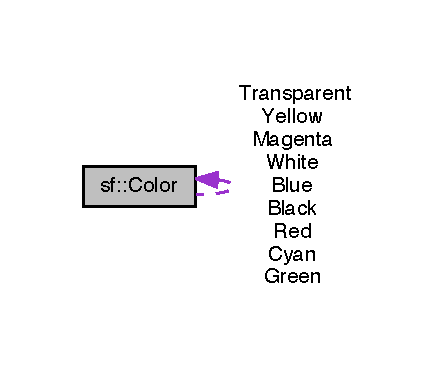
\includegraphics[width=209pt]{classsf_1_1_color__coll__graph}
\end{center}
\end{figure}
\subsection*{Public Member Functions}
\begin{DoxyCompactItemize}
\item 
\hyperlink{classsf_1_1_color_ac2eb4393fb11ad3fa3ccf34e92fe08e4}{Color} ()
\begin{DoxyCompactList}\small\item\em Default constructor. \end{DoxyCompactList}\item 
\hyperlink{classsf_1_1_color_ac791dc61be4c60baac50fe700f1c9850}{Color} (\hyperlink{namespacesf_a4ef3d630785c4f296f9b4f274c33d78e}{Uint8} red, \hyperlink{namespacesf_a4ef3d630785c4f296f9b4f274c33d78e}{Uint8} \hyperlink{gl3_8h_aef30e4e3dccbffce99b7509d5366faef}{green}, \hyperlink{namespacesf_a4ef3d630785c4f296f9b4f274c33d78e}{Uint8} \hyperlink{gl3_8h_ab4fcc6ff520ae4d9de259c8468a5cd93}{blue}, \hyperlink{namespacesf_a4ef3d630785c4f296f9b4f274c33d78e}{Uint8} \hyperlink{gl3_8h_a090ebe65994a3ee4bb60ae3472abffc5}{alpha}=255)
\begin{DoxyCompactList}\small\item\em Construct the color from its 4 R\-G\-B\-A components. \end{DoxyCompactList}\end{DoxyCompactItemize}
\subsection*{Public Attributes}
\begin{DoxyCompactItemize}
\item 
\hyperlink{namespacesf_a4ef3d630785c4f296f9b4f274c33d78e}{Uint8} \hyperlink{classsf_1_1_color_a6a5256ca24a4f9f0e0808f6fc23e01e1}{r}
\begin{DoxyCompactList}\small\item\em Red component. \end{DoxyCompactList}\item 
\hyperlink{namespacesf_a4ef3d630785c4f296f9b4f274c33d78e}{Uint8} \hyperlink{classsf_1_1_color_a591daf9c3c55dea830c76c962d6ba1a5}{g}
\begin{DoxyCompactList}\small\item\em Green component. \end{DoxyCompactList}\item 
\hyperlink{namespacesf_a4ef3d630785c4f296f9b4f274c33d78e}{Uint8} \hyperlink{classsf_1_1_color_a6707aedd0609c8920e12df5d7abc53cb}{b}
\begin{DoxyCompactList}\small\item\em Blue component. \end{DoxyCompactList}\item 
\hyperlink{namespacesf_a4ef3d630785c4f296f9b4f274c33d78e}{Uint8} \hyperlink{classsf_1_1_color_a56dbdb47d5f040d9b78ac6a0b8b3a831}{a}
\begin{DoxyCompactList}\small\item\em Alpha (opacity) component. \end{DoxyCompactList}\end{DoxyCompactItemize}
\subsection*{Static Public Attributes}
\begin{DoxyCompactItemize}
\item 
static const \hyperlink{classsf_1_1_color}{Color} \hyperlink{classsf_1_1_color_a77c688197b981338f0b19dc58bd2facd}{Black}
\begin{DoxyCompactList}\small\item\em Black predefined color. \end{DoxyCompactList}\item 
static const \hyperlink{classsf_1_1_color}{Color} \hyperlink{classsf_1_1_color_a4fd874712178d9e206f53226002aa4ca}{White}
\begin{DoxyCompactList}\small\item\em White predefined color. \end{DoxyCompactList}\item 
static const \hyperlink{classsf_1_1_color}{Color} \hyperlink{classsf_1_1_color_a127dbf55db9c07d0fa8f4bfcbb97594a}{Red}
\begin{DoxyCompactList}\small\item\em Red predefined color. \end{DoxyCompactList}\item 
static const \hyperlink{classsf_1_1_color}{Color} \hyperlink{classsf_1_1_color_a95629b30de8c6856aa7d3afed12eb865}{Green}
\begin{DoxyCompactList}\small\item\em Green predefined color. \end{DoxyCompactList}\item 
static const \hyperlink{classsf_1_1_color}{Color} \hyperlink{classsf_1_1_color_ab03770d4817426b2614cfc33cf0e245c}{Blue}
\begin{DoxyCompactList}\small\item\em Blue predefined color. \end{DoxyCompactList}\item 
static const \hyperlink{classsf_1_1_color}{Color} \hyperlink{classsf_1_1_color_af8896b5f56650935f5b9d72d528802c7}{Yellow}
\begin{DoxyCompactList}\small\item\em Yellow predefined color. \end{DoxyCompactList}\item 
static const \hyperlink{classsf_1_1_color}{Color} \hyperlink{classsf_1_1_color_a6fe70d90b65b2163dd066a84ac00426c}{Magenta}
\begin{DoxyCompactList}\small\item\em Magenta predefined color. \end{DoxyCompactList}\item 
static const \hyperlink{classsf_1_1_color}{Color} \hyperlink{classsf_1_1_color_a64ae9beb0b9a5865dd811cda4bb18340}{Cyan}
\begin{DoxyCompactList}\small\item\em Cyan predefined color. \end{DoxyCompactList}\item 
static const \hyperlink{classsf_1_1_color}{Color} \hyperlink{classsf_1_1_color_a569b45471737f770656f50ae7bbac292}{Transparent}
\begin{DoxyCompactList}\small\item\em Transparent (black) predefined color. \end{DoxyCompactList}\end{DoxyCompactItemize}
\subsection*{Related Functions}
(Note that these are not member functions.) \begin{DoxyCompactItemize}
\item 
\hyperlink{_graphics_2_export_8hpp_ab84c9f1035e146917de3bc0f98d72b35}{S\-F\-M\-L\-\_\-\-G\-R\-A\-P\-H\-I\-C\-S\-\_\-\-A\-P\-I} bool \hyperlink{classsf_1_1_color_a7498d4670c7655e8d4d91ef49cc6064e}{operator==} (const \hyperlink{classsf_1_1_color}{Color} \&left, const \hyperlink{classsf_1_1_color}{Color} \&right)
\begin{DoxyCompactList}\small\item\em Overload of the == operator. \end{DoxyCompactList}\item 
\hyperlink{_graphics_2_export_8hpp_ab84c9f1035e146917de3bc0f98d72b35}{S\-F\-M\-L\-\_\-\-G\-R\-A\-P\-H\-I\-C\-S\-\_\-\-A\-P\-I} bool \hyperlink{classsf_1_1_color_a5d6501b7dd05f481b79f7163899f1d92}{operator!=} (const \hyperlink{classsf_1_1_color}{Color} \&left, const \hyperlink{classsf_1_1_color}{Color} \&right)
\begin{DoxyCompactList}\small\item\em Overload of the != operator. \end{DoxyCompactList}\item 
\hyperlink{_graphics_2_export_8hpp_ab84c9f1035e146917de3bc0f98d72b35}{S\-F\-M\-L\-\_\-\-G\-R\-A\-P\-H\-I\-C\-S\-\_\-\-A\-P\-I} \hyperlink{classsf_1_1_color}{Color} \hyperlink{classsf_1_1_color_a90e79ecc276114cda519a88119ac645b}{operator+} (const \hyperlink{classsf_1_1_color}{Color} \&left, const \hyperlink{classsf_1_1_color}{Color} \&right)
\begin{DoxyCompactList}\small\item\em Overload of the binary + operator. \end{DoxyCompactList}\item 
\hyperlink{_graphics_2_export_8hpp_ab84c9f1035e146917de3bc0f98d72b35}{S\-F\-M\-L\-\_\-\-G\-R\-A\-P\-H\-I\-C\-S\-\_\-\-A\-P\-I} \hyperlink{classsf_1_1_color}{Color} \hyperlink{classsf_1_1_color_aa9de267d831b4ec8ba65b627e51d50c3}{operator$\ast$} (const \hyperlink{classsf_1_1_color}{Color} \&left, const \hyperlink{classsf_1_1_color}{Color} \&right)
\begin{DoxyCompactList}\small\item\em Overload of the binary $\ast$ operator. \end{DoxyCompactList}\item 
\hyperlink{_graphics_2_export_8hpp_ab84c9f1035e146917de3bc0f98d72b35}{S\-F\-M\-L\-\_\-\-G\-R\-A\-P\-H\-I\-C\-S\-\_\-\-A\-P\-I} \hyperlink{classsf_1_1_color}{Color} \& \hyperlink{classsf_1_1_color_a19917f2453a4acfd69de2539bfab8031}{operator+=} (\hyperlink{classsf_1_1_color}{Color} \&left, const \hyperlink{classsf_1_1_color}{Color} \&right)
\begin{DoxyCompactList}\small\item\em Overload of the binary += operator. \end{DoxyCompactList}\item 
\hyperlink{_graphics_2_export_8hpp_ab84c9f1035e146917de3bc0f98d72b35}{S\-F\-M\-L\-\_\-\-G\-R\-A\-P\-H\-I\-C\-S\-\_\-\-A\-P\-I} \hyperlink{classsf_1_1_color}{Color} \& \hyperlink{classsf_1_1_color_a8953be58a47ced92fb25966d6ee90511}{operator$\ast$=} (\hyperlink{classsf_1_1_color}{Color} \&left, const \hyperlink{classsf_1_1_color}{Color} \&right)
\begin{DoxyCompactList}\small\item\em Overload of the binary $\ast$= operator. \end{DoxyCompactList}\end{DoxyCompactItemize}


\subsection{Detailed Description}
Utility class for manpulating R\-G\-B\-A colors. 

\hyperlink{classsf_1_1_color}{sf\-::\-Color} is a simple color class composed of 4 components\-: \begin{DoxyItemize}
\item Red \item Green \item Blue \item Alpha (opacity)\end{DoxyItemize}
Each component is a public member, an unsigned integer in the range \mbox{[}0, 255\mbox{]}. Thus, colors can be constructed and manipulated very easily\-:


\begin{DoxyCode}
\hyperlink{classsf_1_1_color}{sf::Color} \hyperlink{gl3_8h_a3ea846f998d64f079b86052b6c4193a8}{color}(255, 0, 0); \textcolor{comment}{// red}
\hyperlink{gl3_8h_a3ea846f998d64f079b86052b6c4193a8}{color}.red = 0;              \textcolor{comment}{// make it black}
\hyperlink{gl3_8h_a3ea846f998d64f079b86052b6c4193a8}{color}.blue = 128;           \textcolor{comment}{// make it dark blue}
\end{DoxyCode}


The fourth component of colors, named \char`\"{}alpha\char`\"{}, represents the opacity of the color. A color with an alpha value of 255 will be fully opaque, while an alpha value of 0 will make a color fully transparent, whatever the value of the other components is.

The most common colors are already defined as static variables\-: 
\begin{DoxyCode}
\hyperlink{classsf_1_1_color}{sf::Color} black       = \hyperlink{classsf_1_1_color_a77c688197b981338f0b19dc58bd2facd}{sf::Color::Black};
\hyperlink{classsf_1_1_color}{sf::Color} white       = \hyperlink{classsf_1_1_color_a4fd874712178d9e206f53226002aa4ca}{sf::Color::White};
\hyperlink{classsf_1_1_color}{sf::Color} red         = \hyperlink{classsf_1_1_color_a127dbf55db9c07d0fa8f4bfcbb97594a}{sf::Color::Red};
\hyperlink{classsf_1_1_color}{sf::Color} green       = \hyperlink{classsf_1_1_color_a95629b30de8c6856aa7d3afed12eb865}{sf::Color::Green};
\hyperlink{classsf_1_1_color}{sf::Color} blue        = \hyperlink{classsf_1_1_color_ab03770d4817426b2614cfc33cf0e245c}{sf::Color::Blue};
\hyperlink{classsf_1_1_color}{sf::Color} yellow      = \hyperlink{classsf_1_1_color_af8896b5f56650935f5b9d72d528802c7}{sf::Color::Yellow};
\hyperlink{classsf_1_1_color}{sf::Color} magenta     = \hyperlink{classsf_1_1_color_a6fe70d90b65b2163dd066a84ac00426c}{sf::Color::Magenta};
\hyperlink{classsf_1_1_color}{sf::Color} cyan        = \hyperlink{classsf_1_1_color_a64ae9beb0b9a5865dd811cda4bb18340}{sf::Color::Cyan};
\hyperlink{classsf_1_1_color}{sf::Color} transparent = \hyperlink{classsf_1_1_color_a569b45471737f770656f50ae7bbac292}{sf::Color::Transparent};
\end{DoxyCode}


Colors can also be added and modulated (multiplied) using the overloaded operators + and $\ast$. 

Definition at line 40 of file Color.\-hpp.



\subsection{Constructor \& Destructor Documentation}
\hypertarget{classsf_1_1_color_ac2eb4393fb11ad3fa3ccf34e92fe08e4}{\index{sf\-::\-Color@{sf\-::\-Color}!Color@{Color}}
\index{Color@{Color}!sf::Color@{sf\-::\-Color}}
\subsubsection[{Color}]{\setlength{\rightskip}{0pt plus 5cm}sf\-::\-Color\-::\-Color (
\begin{DoxyParamCaption}
{}
\end{DoxyParamCaption}
)}}\label{classsf_1_1_color_ac2eb4393fb11ad3fa3ccf34e92fe08e4}


Default constructor. 

Constructs an opaque black color. It is equivalent to sf\-::\-Color(0, 0, 0, 255). \hypertarget{classsf_1_1_color_ac791dc61be4c60baac50fe700f1c9850}{\index{sf\-::\-Color@{sf\-::\-Color}!Color@{Color}}
\index{Color@{Color}!sf::Color@{sf\-::\-Color}}
\subsubsection[{Color}]{\setlength{\rightskip}{0pt plus 5cm}sf\-::\-Color\-::\-Color (
\begin{DoxyParamCaption}
\item[{{\bf Uint8}}]{red, }
\item[{{\bf Uint8}}]{green, }
\item[{{\bf Uint8}}]{blue, }
\item[{{\bf Uint8}}]{alpha = {\ttfamily 255}}
\end{DoxyParamCaption}
)}}\label{classsf_1_1_color_ac791dc61be4c60baac50fe700f1c9850}


Construct the color from its 4 R\-G\-B\-A components. 


\begin{DoxyParams}{Parameters}
{\em red} & Red component (in the range \mbox{[}0, 255\mbox{]}) \\
\hline
{\em green} & Green component (in the range \mbox{[}0, 255\mbox{]}) \\
\hline
{\em blue} & Blue component (in the range \mbox{[}0, 255\mbox{]}) \\
\hline
{\em alpha} & Alpha (opacity) component (in the range \mbox{[}0, 255\mbox{]}) \\
\hline
\end{DoxyParams}


\subsection{Friends And Related Function Documentation}
\hypertarget{classsf_1_1_color_a5d6501b7dd05f481b79f7163899f1d92}{\index{sf\-::\-Color@{sf\-::\-Color}!operator!=@{operator!=}}
\index{operator!=@{operator!=}!sf::Color@{sf\-::\-Color}}
\subsubsection[{operator!=}]{\setlength{\rightskip}{0pt plus 5cm}{\bf S\-F\-M\-L\-\_\-\-G\-R\-A\-P\-H\-I\-C\-S\-\_\-\-A\-P\-I} bool operator!= (
\begin{DoxyParamCaption}
\item[{const {\bf Color} \&}]{left, }
\item[{const {\bf Color} \&}]{right}
\end{DoxyParamCaption}
)\hspace{0.3cm}{\ttfamily [related]}}}\label{classsf_1_1_color_a5d6501b7dd05f481b79f7163899f1d92}


Overload of the != operator. 

This operator compares two colors and check if they are different.


\begin{DoxyParams}{Parameters}
{\em left} & Left operand \\
\hline
{\em right} & Right operand\\
\hline
\end{DoxyParams}
\begin{DoxyReturn}{Returns}
True if colors are different, false if they are equal 
\end{DoxyReturn}
\hypertarget{classsf_1_1_color_aa9de267d831b4ec8ba65b627e51d50c3}{\index{sf\-::\-Color@{sf\-::\-Color}!operator$\ast$@{operator$\ast$}}
\index{operator$\ast$@{operator$\ast$}!sf::Color@{sf\-::\-Color}}
\subsubsection[{operator$\ast$}]{\setlength{\rightskip}{0pt plus 5cm}{\bf S\-F\-M\-L\-\_\-\-G\-R\-A\-P\-H\-I\-C\-S\-\_\-\-A\-P\-I} {\bf Color} operator$\ast$ (
\begin{DoxyParamCaption}
\item[{const {\bf Color} \&}]{left, }
\item[{const {\bf Color} \&}]{right}
\end{DoxyParamCaption}
)\hspace{0.3cm}{\ttfamily [related]}}}\label{classsf_1_1_color_aa9de267d831b4ec8ba65b627e51d50c3}


Overload of the binary $\ast$ operator. 

This operator returns the component-\/wise multiplication (also called \char`\"{}modulation\char`\"{}) of two colors. Components are then divided by 255 so that the result is still in the range \mbox{[}0, 255\mbox{]}.


\begin{DoxyParams}{Parameters}
{\em left} & Left operand \\
\hline
{\em right} & Right operand\\
\hline
\end{DoxyParams}
\begin{DoxyReturn}{Returns}
Result of {\itshape left} $\ast$ {\itshape right} 
\end{DoxyReturn}
\hypertarget{classsf_1_1_color_a8953be58a47ced92fb25966d6ee90511}{\index{sf\-::\-Color@{sf\-::\-Color}!operator$\ast$=@{operator$\ast$=}}
\index{operator$\ast$=@{operator$\ast$=}!sf::Color@{sf\-::\-Color}}
\subsubsection[{operator$\ast$=}]{\setlength{\rightskip}{0pt plus 5cm}{\bf S\-F\-M\-L\-\_\-\-G\-R\-A\-P\-H\-I\-C\-S\-\_\-\-A\-P\-I} {\bf Color} \& operator$\ast$= (
\begin{DoxyParamCaption}
\item[{{\bf Color} \&}]{left, }
\item[{const {\bf Color} \&}]{right}
\end{DoxyParamCaption}
)\hspace{0.3cm}{\ttfamily [related]}}}\label{classsf_1_1_color_a8953be58a47ced92fb25966d6ee90511}


Overload of the binary $\ast$= operator. 

This operator returns the component-\/wise multiplication (also called \char`\"{}modulation\char`\"{}) of two colors, and assigns the result to the left operand. Components are then divided by 255 so that the result is still in the range \mbox{[}0, 255\mbox{]}.


\begin{DoxyParams}{Parameters}
{\em left} & Left operand \\
\hline
{\em right} & Right operand\\
\hline
\end{DoxyParams}
\begin{DoxyReturn}{Returns}
Reference to {\itshape left} 
\end{DoxyReturn}
\hypertarget{classsf_1_1_color_a90e79ecc276114cda519a88119ac645b}{\index{sf\-::\-Color@{sf\-::\-Color}!operator+@{operator+}}
\index{operator+@{operator+}!sf::Color@{sf\-::\-Color}}
\subsubsection[{operator+}]{\setlength{\rightskip}{0pt plus 5cm}{\bf S\-F\-M\-L\-\_\-\-G\-R\-A\-P\-H\-I\-C\-S\-\_\-\-A\-P\-I} {\bf Color} operator+ (
\begin{DoxyParamCaption}
\item[{const {\bf Color} \&}]{left, }
\item[{const {\bf Color} \&}]{right}
\end{DoxyParamCaption}
)\hspace{0.3cm}{\ttfamily [related]}}}\label{classsf_1_1_color_a90e79ecc276114cda519a88119ac645b}


Overload of the binary + operator. 

This operator returns the component-\/wise sum of two colors. Components that exceed 255 are clamped to 255.


\begin{DoxyParams}{Parameters}
{\em left} & Left operand \\
\hline
{\em right} & Right operand\\
\hline
\end{DoxyParams}
\begin{DoxyReturn}{Returns}
Result of {\itshape left} + {\itshape right} 
\end{DoxyReturn}
\hypertarget{classsf_1_1_color_a19917f2453a4acfd69de2539bfab8031}{\index{sf\-::\-Color@{sf\-::\-Color}!operator+=@{operator+=}}
\index{operator+=@{operator+=}!sf::Color@{sf\-::\-Color}}
\subsubsection[{operator+=}]{\setlength{\rightskip}{0pt plus 5cm}{\bf S\-F\-M\-L\-\_\-\-G\-R\-A\-P\-H\-I\-C\-S\-\_\-\-A\-P\-I} {\bf Color} \& operator+= (
\begin{DoxyParamCaption}
\item[{{\bf Color} \&}]{left, }
\item[{const {\bf Color} \&}]{right}
\end{DoxyParamCaption}
)\hspace{0.3cm}{\ttfamily [related]}}}\label{classsf_1_1_color_a19917f2453a4acfd69de2539bfab8031}


Overload of the binary += operator. 

This operator computes the component-\/wise sum of two colors, and assigns the result to the left operand. Components that exceed 255 are clamped to 255.


\begin{DoxyParams}{Parameters}
{\em left} & Left operand \\
\hline
{\em right} & Right operand\\
\hline
\end{DoxyParams}
\begin{DoxyReturn}{Returns}
Reference to {\itshape left} 
\end{DoxyReturn}
\hypertarget{classsf_1_1_color_a7498d4670c7655e8d4d91ef49cc6064e}{\index{sf\-::\-Color@{sf\-::\-Color}!operator==@{operator==}}
\index{operator==@{operator==}!sf::Color@{sf\-::\-Color}}
\subsubsection[{operator==}]{\setlength{\rightskip}{0pt plus 5cm}{\bf S\-F\-M\-L\-\_\-\-G\-R\-A\-P\-H\-I\-C\-S\-\_\-\-A\-P\-I} bool operator== (
\begin{DoxyParamCaption}
\item[{const {\bf Color} \&}]{left, }
\item[{const {\bf Color} \&}]{right}
\end{DoxyParamCaption}
)\hspace{0.3cm}{\ttfamily [related]}}}\label{classsf_1_1_color_a7498d4670c7655e8d4d91ef49cc6064e}


Overload of the == operator. 

This operator compares two colors and check if they are equal.


\begin{DoxyParams}{Parameters}
{\em left} & Left operand \\
\hline
{\em right} & Right operand\\
\hline
\end{DoxyParams}
\begin{DoxyReturn}{Returns}
True if colors are equal, false if they are different 
\end{DoxyReturn}


\subsection{Member Data Documentation}
\hypertarget{classsf_1_1_color_a56dbdb47d5f040d9b78ac6a0b8b3a831}{\index{sf\-::\-Color@{sf\-::\-Color}!a@{a}}
\index{a@{a}!sf::Color@{sf\-::\-Color}}
\subsubsection[{a}]{\setlength{\rightskip}{0pt plus 5cm}{\bf Uint8} sf\-::\-Color\-::a}}\label{classsf_1_1_color_a56dbdb47d5f040d9b78ac6a0b8b3a831}


Alpha (opacity) component. 



Definition at line 83 of file Color.\-hpp.

\hypertarget{classsf_1_1_color_a6707aedd0609c8920e12df5d7abc53cb}{\index{sf\-::\-Color@{sf\-::\-Color}!b@{b}}
\index{b@{b}!sf::Color@{sf\-::\-Color}}
\subsubsection[{b}]{\setlength{\rightskip}{0pt plus 5cm}{\bf Uint8} sf\-::\-Color\-::b}}\label{classsf_1_1_color_a6707aedd0609c8920e12df5d7abc53cb}


Blue component. 



Definition at line 82 of file Color.\-hpp.

\hypertarget{classsf_1_1_color_a77c688197b981338f0b19dc58bd2facd}{\index{sf\-::\-Color@{sf\-::\-Color}!Black@{Black}}
\index{Black@{Black}!sf::Color@{sf\-::\-Color}}
\subsubsection[{Black}]{\setlength{\rightskip}{0pt plus 5cm}const {\bf Color} sf\-::\-Color\-::\-Black\hspace{0.3cm}{\ttfamily [static]}}}\label{classsf_1_1_color_a77c688197b981338f0b19dc58bd2facd}


Black predefined color. 



Definition at line 67 of file Color.\-hpp.

\hypertarget{classsf_1_1_color_ab03770d4817426b2614cfc33cf0e245c}{\index{sf\-::\-Color@{sf\-::\-Color}!Blue@{Blue}}
\index{Blue@{Blue}!sf::Color@{sf\-::\-Color}}
\subsubsection[{Blue}]{\setlength{\rightskip}{0pt plus 5cm}const {\bf Color} sf\-::\-Color\-::\-Blue\hspace{0.3cm}{\ttfamily [static]}}}\label{classsf_1_1_color_ab03770d4817426b2614cfc33cf0e245c}


Blue predefined color. 



Definition at line 71 of file Color.\-hpp.

\hypertarget{classsf_1_1_color_a64ae9beb0b9a5865dd811cda4bb18340}{\index{sf\-::\-Color@{sf\-::\-Color}!Cyan@{Cyan}}
\index{Cyan@{Cyan}!sf::Color@{sf\-::\-Color}}
\subsubsection[{Cyan}]{\setlength{\rightskip}{0pt plus 5cm}const {\bf Color} sf\-::\-Color\-::\-Cyan\hspace{0.3cm}{\ttfamily [static]}}}\label{classsf_1_1_color_a64ae9beb0b9a5865dd811cda4bb18340}


Cyan predefined color. 



Definition at line 74 of file Color.\-hpp.

\hypertarget{classsf_1_1_color_a591daf9c3c55dea830c76c962d6ba1a5}{\index{sf\-::\-Color@{sf\-::\-Color}!g@{g}}
\index{g@{g}!sf::Color@{sf\-::\-Color}}
\subsubsection[{g}]{\setlength{\rightskip}{0pt plus 5cm}{\bf Uint8} sf\-::\-Color\-::g}}\label{classsf_1_1_color_a591daf9c3c55dea830c76c962d6ba1a5}


Green component. 



Definition at line 81 of file Color.\-hpp.

\hypertarget{classsf_1_1_color_a95629b30de8c6856aa7d3afed12eb865}{\index{sf\-::\-Color@{sf\-::\-Color}!Green@{Green}}
\index{Green@{Green}!sf::Color@{sf\-::\-Color}}
\subsubsection[{Green}]{\setlength{\rightskip}{0pt plus 5cm}const {\bf Color} sf\-::\-Color\-::\-Green\hspace{0.3cm}{\ttfamily [static]}}}\label{classsf_1_1_color_a95629b30de8c6856aa7d3afed12eb865}


Green predefined color. 



Definition at line 70 of file Color.\-hpp.

\hypertarget{classsf_1_1_color_a6fe70d90b65b2163dd066a84ac00426c}{\index{sf\-::\-Color@{sf\-::\-Color}!Magenta@{Magenta}}
\index{Magenta@{Magenta}!sf::Color@{sf\-::\-Color}}
\subsubsection[{Magenta}]{\setlength{\rightskip}{0pt plus 5cm}const {\bf Color} sf\-::\-Color\-::\-Magenta\hspace{0.3cm}{\ttfamily [static]}}}\label{classsf_1_1_color_a6fe70d90b65b2163dd066a84ac00426c}


Magenta predefined color. 



Definition at line 73 of file Color.\-hpp.

\hypertarget{classsf_1_1_color_a6a5256ca24a4f9f0e0808f6fc23e01e1}{\index{sf\-::\-Color@{sf\-::\-Color}!r@{r}}
\index{r@{r}!sf::Color@{sf\-::\-Color}}
\subsubsection[{r}]{\setlength{\rightskip}{0pt plus 5cm}{\bf Uint8} sf\-::\-Color\-::r}}\label{classsf_1_1_color_a6a5256ca24a4f9f0e0808f6fc23e01e1}


Red component. 



Definition at line 80 of file Color.\-hpp.

\hypertarget{classsf_1_1_color_a127dbf55db9c07d0fa8f4bfcbb97594a}{\index{sf\-::\-Color@{sf\-::\-Color}!Red@{Red}}
\index{Red@{Red}!sf::Color@{sf\-::\-Color}}
\subsubsection[{Red}]{\setlength{\rightskip}{0pt plus 5cm}const {\bf Color} sf\-::\-Color\-::\-Red\hspace{0.3cm}{\ttfamily [static]}}}\label{classsf_1_1_color_a127dbf55db9c07d0fa8f4bfcbb97594a}


Red predefined color. 



Definition at line 69 of file Color.\-hpp.

\hypertarget{classsf_1_1_color_a569b45471737f770656f50ae7bbac292}{\index{sf\-::\-Color@{sf\-::\-Color}!Transparent@{Transparent}}
\index{Transparent@{Transparent}!sf::Color@{sf\-::\-Color}}
\subsubsection[{Transparent}]{\setlength{\rightskip}{0pt plus 5cm}const {\bf Color} sf\-::\-Color\-::\-Transparent\hspace{0.3cm}{\ttfamily [static]}}}\label{classsf_1_1_color_a569b45471737f770656f50ae7bbac292}


Transparent (black) predefined color. 



Definition at line 75 of file Color.\-hpp.

\hypertarget{classsf_1_1_color_a4fd874712178d9e206f53226002aa4ca}{\index{sf\-::\-Color@{sf\-::\-Color}!White@{White}}
\index{White@{White}!sf::Color@{sf\-::\-Color}}
\subsubsection[{White}]{\setlength{\rightskip}{0pt plus 5cm}const {\bf Color} sf\-::\-Color\-::\-White\hspace{0.3cm}{\ttfamily [static]}}}\label{classsf_1_1_color_a4fd874712178d9e206f53226002aa4ca}


White predefined color. 



Definition at line 68 of file Color.\-hpp.

\hypertarget{classsf_1_1_color_af8896b5f56650935f5b9d72d528802c7}{\index{sf\-::\-Color@{sf\-::\-Color}!Yellow@{Yellow}}
\index{Yellow@{Yellow}!sf::Color@{sf\-::\-Color}}
\subsubsection[{Yellow}]{\setlength{\rightskip}{0pt plus 5cm}const {\bf Color} sf\-::\-Color\-::\-Yellow\hspace{0.3cm}{\ttfamily [static]}}}\label{classsf_1_1_color_af8896b5f56650935f5b9d72d528802c7}


Yellow predefined color. 



Definition at line 72 of file Color.\-hpp.



The documentation for this class was generated from the following file\-:\begin{DoxyCompactItemize}
\item 
/\-Users/ira/\-Dropbox/ira\-\_\-dev/protobyte\-\_\-research/other\-\_\-libs/\-S\-F\-M\-L/dylibs/root/usr/local/include/\-S\-F\-M\-L/\-Graphics/\hyperlink{_color_8hpp}{Color.\-hpp}\end{DoxyCompactItemize}

\hypertarget{class_color3}{\section{Color3$<$ T $>$ Class Template Reference}
\label{class_color3}\index{Color3$<$ T $>$@{Color3$<$ T $>$}}
}


{\ttfamily \#include $<$Color3.\-h$>$}

\subsection*{Public Member Functions}
\begin{DoxyCompactItemize}
\item 
\hyperlink{class_color3_a57917faf714145bb9a14a735d39440f6}{Color3} (T \hyperlink{gl3_8h_abe08814c2f72843fde4d8df41440d5a0}{r}=0, T \hyperlink{gl3_8h_a9cd653b1648845554169fbc3a3f6d37a}{g}=0, T \hyperlink{gl3_8h_a6eba317e3cf44d6d26c04a5a8f197dcb}{b}=0)
\item 
\hyperlink{glutf90_8h_ac778d6f63f1aaf8ebda0ce6ac821b56e}{void} \hyperlink{class_color3_a84e9bef2029f7fbdef82dbdcdaf0999a}{set\-R} (T \hyperlink{gl3_8h_abe08814c2f72843fde4d8df41440d5a0}{r})
\item 
\hyperlink{glutf90_8h_ac778d6f63f1aaf8ebda0ce6ac821b56e}{void} \hyperlink{class_color3_a2448d21c208b5bfc716f0bac62b5dc4a}{set\-G} (T \hyperlink{gl3_8h_a9cd653b1648845554169fbc3a3f6d37a}{g})
\item 
\hyperlink{glutf90_8h_ac778d6f63f1aaf8ebda0ce6ac821b56e}{void} \hyperlink{class_color3_a57a6c269ee5856587b041270cf1d33a4}{set\-B} (T \hyperlink{gl3_8h_a6eba317e3cf44d6d26c04a5a8f197dcb}{b})
\item 
T \hyperlink{class_color3_a366fbc86fc67ff524454c167b611bb5d}{get\-R} () const 
\item 
T \hyperlink{class_color3_aa452b73c89ba85c3f8377dd62cac9660}{get\-G} () const 
\item 
T \hyperlink{class_color3_a1428c3e15b143f04b3c3a4a352a70e58}{get\-B} () const 
\end{DoxyCompactItemize}
\subsection*{Friends}
\begin{DoxyCompactItemize}
\item 
std\-::ostream \& \hyperlink{class_color3_ac9f30838223a6527f03dbabf268d0888}{operator$<$$<$} (std\-::ostream \&output, const \hyperlink{class_color3}{Color3}$<$ T $>$ \&col3)
\end{DoxyCompactItemize}


\subsection{Detailed Description}
\subsubsection*{template$<$class T$>$class Color3$<$ T $>$}



Definition at line 16 of file Color3.\-h.



\subsection{Constructor \& Destructor Documentation}
\hypertarget{class_color3_a57917faf714145bb9a14a735d39440f6}{\index{Color3@{Color3}!Color3@{Color3}}
\index{Color3@{Color3}!Color3@{Color3}}
\subsubsection[{Color3}]{\setlength{\rightskip}{0pt plus 5cm}template$<$class T $>$ {\bf Color3}$<$ T $>$\-::{\bf Color3} (
\begin{DoxyParamCaption}
\item[{T}]{r = {\ttfamily 0}, }
\item[{T}]{g = {\ttfamily 0}, }
\item[{T}]{b = {\ttfamily 0}}
\end{DoxyParamCaption}
)\hspace{0.3cm}{\ttfamily [inline]}, {\ttfamily [explicit]}}}\label{class_color3_a57917faf714145bb9a14a735d39440f6}


Definition at line 29 of file Color3.\-h.



\subsection{Member Function Documentation}
\hypertarget{class_color3_a1428c3e15b143f04b3c3a4a352a70e58}{\index{Color3@{Color3}!get\-B@{get\-B}}
\index{get\-B@{get\-B}!Color3@{Color3}}
\subsubsection[{get\-B}]{\setlength{\rightskip}{0pt plus 5cm}template$<$class T $>$ T {\bf Color3}$<$ T $>$\-::get\-B (
\begin{DoxyParamCaption}
{}
\end{DoxyParamCaption}
) const\hspace{0.3cm}{\ttfamily [inline]}}}\label{class_color3_a1428c3e15b143f04b3c3a4a352a70e58}


Definition at line 55 of file Color3.\-h.

\hypertarget{class_color3_aa452b73c89ba85c3f8377dd62cac9660}{\index{Color3@{Color3}!get\-G@{get\-G}}
\index{get\-G@{get\-G}!Color3@{Color3}}
\subsubsection[{get\-G}]{\setlength{\rightskip}{0pt plus 5cm}template$<$class T $>$ T {\bf Color3}$<$ T $>$\-::get\-G (
\begin{DoxyParamCaption}
{}
\end{DoxyParamCaption}
) const\hspace{0.3cm}{\ttfamily [inline]}}}\label{class_color3_aa452b73c89ba85c3f8377dd62cac9660}


Definition at line 51 of file Color3.\-h.

\hypertarget{class_color3_a366fbc86fc67ff524454c167b611bb5d}{\index{Color3@{Color3}!get\-R@{get\-R}}
\index{get\-R@{get\-R}!Color3@{Color3}}
\subsubsection[{get\-R}]{\setlength{\rightskip}{0pt plus 5cm}template$<$class T $>$ T {\bf Color3}$<$ T $>$\-::get\-R (
\begin{DoxyParamCaption}
{}
\end{DoxyParamCaption}
) const\hspace{0.3cm}{\ttfamily [inline]}}}\label{class_color3_a366fbc86fc67ff524454c167b611bb5d}


Definition at line 47 of file Color3.\-h.

\hypertarget{class_color3_a57a6c269ee5856587b041270cf1d33a4}{\index{Color3@{Color3}!set\-B@{set\-B}}
\index{set\-B@{set\-B}!Color3@{Color3}}
\subsubsection[{set\-B}]{\setlength{\rightskip}{0pt plus 5cm}template$<$class T $>$ {\bf void} {\bf Color3}$<$ T $>$\-::set\-B (
\begin{DoxyParamCaption}
\item[{T}]{b}
\end{DoxyParamCaption}
)\hspace{0.3cm}{\ttfamily [inline]}}}\label{class_color3_a57a6c269ee5856587b041270cf1d33a4}


Definition at line 41 of file Color3.\-h.

\hypertarget{class_color3_a2448d21c208b5bfc716f0bac62b5dc4a}{\index{Color3@{Color3}!set\-G@{set\-G}}
\index{set\-G@{set\-G}!Color3@{Color3}}
\subsubsection[{set\-G}]{\setlength{\rightskip}{0pt plus 5cm}template$<$class T $>$ {\bf void} {\bf Color3}$<$ T $>$\-::set\-G (
\begin{DoxyParamCaption}
\item[{T}]{g}
\end{DoxyParamCaption}
)\hspace{0.3cm}{\ttfamily [inline]}}}\label{class_color3_a2448d21c208b5bfc716f0bac62b5dc4a}


Definition at line 37 of file Color3.\-h.

\hypertarget{class_color3_a84e9bef2029f7fbdef82dbdcdaf0999a}{\index{Color3@{Color3}!set\-R@{set\-R}}
\index{set\-R@{set\-R}!Color3@{Color3}}
\subsubsection[{set\-R}]{\setlength{\rightskip}{0pt plus 5cm}template$<$class T $>$ {\bf void} {\bf Color3}$<$ T $>$\-::set\-R (
\begin{DoxyParamCaption}
\item[{T}]{r}
\end{DoxyParamCaption}
)\hspace{0.3cm}{\ttfamily [inline]}}}\label{class_color3_a84e9bef2029f7fbdef82dbdcdaf0999a}


Definition at line 33 of file Color3.\-h.



\subsection{Friends And Related Function Documentation}
\hypertarget{class_color3_ac9f30838223a6527f03dbabf268d0888}{\index{Color3@{Color3}!operator$<$$<$@{operator$<$$<$}}
\index{operator$<$$<$@{operator$<$$<$}!Color3@{Color3}}
\subsubsection[{operator$<$$<$}]{\setlength{\rightskip}{0pt plus 5cm}template$<$class T $>$ std\-::ostream\& operator$<$$<$ (
\begin{DoxyParamCaption}
\item[{std\-::ostream \&}]{output, }
\item[{const {\bf Color3}$<$ T $>$ \&}]{col3}
\end{DoxyParamCaption}
)\hspace{0.3cm}{\ttfamily [friend]}}}\label{class_color3_ac9f30838223a6527f03dbabf268d0888}


Definition at line 23 of file Color3.\-h.



The documentation for this class was generated from the following file\-:\begin{DoxyCompactItemize}
\item 
/\-Users/ira/\-Dropbox/ira\-\_\-dev/protobyte\-\_\-research/\-Protobyte/\hyperlink{_color3_8h}{Color3.\-h}\end{DoxyCompactItemize}

\hypertarget{class_color4}{\section{Color4$<$ T $>$ Class Template Reference}
\label{class_color4}\index{Color4$<$ T $>$@{Color4$<$ T $>$}}
}


{\ttfamily \#include $<$Color4.\-h$>$}

\subsection*{Public Member Functions}
\begin{DoxyCompactItemize}
\item 
\hyperlink{class_color4_a0ea6fcc52c1b438dacca912dc0eede9a}{Color4} (T \hyperlink{gl3_8h_abe08814c2f72843fde4d8df41440d5a0}{r}=0, T \hyperlink{gl3_8h_a9cd653b1648845554169fbc3a3f6d37a}{g}=0, T \hyperlink{gl3_8h_a6eba317e3cf44d6d26c04a5a8f197dcb}{b}=0, T \hyperlink{gl3_8h_ac8729153468b5dcf13f971b21d84d4e5}{a}=0)
\item 
\hyperlink{glutf90_8h_ac778d6f63f1aaf8ebda0ce6ac821b56e}{void} \hyperlink{class_color4_aa4292dd29466cfadd868c80cfdb2d65f}{set\-R} (T \hyperlink{gl3_8h_abe08814c2f72843fde4d8df41440d5a0}{r})
\item 
\hyperlink{glutf90_8h_ac778d6f63f1aaf8ebda0ce6ac821b56e}{void} \hyperlink{class_color4_a995d05e738e36e64bacf15d6b43e4d46}{set\-G} (T \hyperlink{gl3_8h_a9cd653b1648845554169fbc3a3f6d37a}{g})
\item 
\hyperlink{glutf90_8h_ac778d6f63f1aaf8ebda0ce6ac821b56e}{void} \hyperlink{class_color4_a4594591b82f7a4e07c1d9ea8e88475dd}{set\-B} (T \hyperlink{gl3_8h_a6eba317e3cf44d6d26c04a5a8f197dcb}{b})
\item 
\hyperlink{glutf90_8h_ac778d6f63f1aaf8ebda0ce6ac821b56e}{void} \hyperlink{class_color4_a40eae4878e30c045175e2844382ebf6b}{set\-A} (T \hyperlink{gl3_8h_ac8729153468b5dcf13f971b21d84d4e5}{a})
\item 
T \hyperlink{class_color4_a78c6e0e5837397123d49b9b69e96b82c}{get\-R} () const 
\item 
T \hyperlink{class_color4_aac32952538c6a6818605eb32f787d4e9}{get\-G} () const 
\item 
T \hyperlink{class_color4_af3ef1ead524a09949357f870481f4127}{get\-B} () const 
\item 
T \hyperlink{class_color4_a3a2f3de17bddc61d2e395db3bd71d306}{get\-A} () const 
\end{DoxyCompactItemize}
\subsection*{Friends}
\begin{DoxyCompactItemize}
\item 
std\-::ostream \& \hyperlink{class_color4_a2aeb6890e4cd6f2a36bd730be95ef111}{operator$<$$<$} (std\-::ostream \&output, const \hyperlink{class_color4}{Color4}$<$ T $>$ \&col4)
\end{DoxyCompactItemize}


\subsection{Detailed Description}
\subsubsection*{template$<$class T$>$class Color4$<$ T $>$}



Definition at line 16 of file Color4.\-h.



\subsection{Constructor \& Destructor Documentation}
\hypertarget{class_color4_a0ea6fcc52c1b438dacca912dc0eede9a}{\index{Color4@{Color4}!Color4@{Color4}}
\index{Color4@{Color4}!Color4@{Color4}}
\subsubsection[{Color4}]{\setlength{\rightskip}{0pt plus 5cm}template$<$class T$>$ {\bf Color4}$<$ T $>$\-::{\bf Color4} (
\begin{DoxyParamCaption}
\item[{T}]{r = {\ttfamily 0}, }
\item[{T}]{g = {\ttfamily 0}, }
\item[{T}]{b = {\ttfamily 0}, }
\item[{T}]{a = {\ttfamily 0}}
\end{DoxyParamCaption}
)\hspace{0.3cm}{\ttfamily [inline]}, {\ttfamily [explicit]}}}\label{class_color4_a0ea6fcc52c1b438dacca912dc0eede9a}


Definition at line 29 of file Color4.\-h.



\subsection{Member Function Documentation}
\hypertarget{class_color4_a3a2f3de17bddc61d2e395db3bd71d306}{\index{Color4@{Color4}!get\-A@{get\-A}}
\index{get\-A@{get\-A}!Color4@{Color4}}
\subsubsection[{get\-A}]{\setlength{\rightskip}{0pt plus 5cm}template$<$class T$>$ T {\bf Color4}$<$ T $>$\-::get\-A (
\begin{DoxyParamCaption}
{}
\end{DoxyParamCaption}
) const\hspace{0.3cm}{\ttfamily [inline]}}}\label{class_color4_a3a2f3de17bddc61d2e395db3bd71d306}


Definition at line 61 of file Color4.\-h.

\hypertarget{class_color4_af3ef1ead524a09949357f870481f4127}{\index{Color4@{Color4}!get\-B@{get\-B}}
\index{get\-B@{get\-B}!Color4@{Color4}}
\subsubsection[{get\-B}]{\setlength{\rightskip}{0pt plus 5cm}template$<$class T$>$ T {\bf Color4}$<$ T $>$\-::get\-B (
\begin{DoxyParamCaption}
{}
\end{DoxyParamCaption}
) const\hspace{0.3cm}{\ttfamily [inline]}}}\label{class_color4_af3ef1ead524a09949357f870481f4127}


Definition at line 57 of file Color4.\-h.

\hypertarget{class_color4_aac32952538c6a6818605eb32f787d4e9}{\index{Color4@{Color4}!get\-G@{get\-G}}
\index{get\-G@{get\-G}!Color4@{Color4}}
\subsubsection[{get\-G}]{\setlength{\rightskip}{0pt plus 5cm}template$<$class T$>$ T {\bf Color4}$<$ T $>$\-::get\-G (
\begin{DoxyParamCaption}
{}
\end{DoxyParamCaption}
) const\hspace{0.3cm}{\ttfamily [inline]}}}\label{class_color4_aac32952538c6a6818605eb32f787d4e9}


Definition at line 53 of file Color4.\-h.

\hypertarget{class_color4_a78c6e0e5837397123d49b9b69e96b82c}{\index{Color4@{Color4}!get\-R@{get\-R}}
\index{get\-R@{get\-R}!Color4@{Color4}}
\subsubsection[{get\-R}]{\setlength{\rightskip}{0pt plus 5cm}template$<$class T$>$ T {\bf Color4}$<$ T $>$\-::get\-R (
\begin{DoxyParamCaption}
{}
\end{DoxyParamCaption}
) const\hspace{0.3cm}{\ttfamily [inline]}}}\label{class_color4_a78c6e0e5837397123d49b9b69e96b82c}


Definition at line 49 of file Color4.\-h.

\hypertarget{class_color4_a40eae4878e30c045175e2844382ebf6b}{\index{Color4@{Color4}!set\-A@{set\-A}}
\index{set\-A@{set\-A}!Color4@{Color4}}
\subsubsection[{set\-A}]{\setlength{\rightskip}{0pt plus 5cm}template$<$class T$>$ {\bf void} {\bf Color4}$<$ T $>$\-::set\-A (
\begin{DoxyParamCaption}
\item[{T}]{a}
\end{DoxyParamCaption}
)\hspace{0.3cm}{\ttfamily [inline]}}}\label{class_color4_a40eae4878e30c045175e2844382ebf6b}


Definition at line 45 of file Color4.\-h.

\hypertarget{class_color4_a4594591b82f7a4e07c1d9ea8e88475dd}{\index{Color4@{Color4}!set\-B@{set\-B}}
\index{set\-B@{set\-B}!Color4@{Color4}}
\subsubsection[{set\-B}]{\setlength{\rightskip}{0pt plus 5cm}template$<$class T$>$ {\bf void} {\bf Color4}$<$ T $>$\-::set\-B (
\begin{DoxyParamCaption}
\item[{T}]{b}
\end{DoxyParamCaption}
)\hspace{0.3cm}{\ttfamily [inline]}}}\label{class_color4_a4594591b82f7a4e07c1d9ea8e88475dd}


Definition at line 41 of file Color4.\-h.

\hypertarget{class_color4_a995d05e738e36e64bacf15d6b43e4d46}{\index{Color4@{Color4}!set\-G@{set\-G}}
\index{set\-G@{set\-G}!Color4@{Color4}}
\subsubsection[{set\-G}]{\setlength{\rightskip}{0pt plus 5cm}template$<$class T$>$ {\bf void} {\bf Color4}$<$ T $>$\-::set\-G (
\begin{DoxyParamCaption}
\item[{T}]{g}
\end{DoxyParamCaption}
)\hspace{0.3cm}{\ttfamily [inline]}}}\label{class_color4_a995d05e738e36e64bacf15d6b43e4d46}


Definition at line 37 of file Color4.\-h.

\hypertarget{class_color4_aa4292dd29466cfadd868c80cfdb2d65f}{\index{Color4@{Color4}!set\-R@{set\-R}}
\index{set\-R@{set\-R}!Color4@{Color4}}
\subsubsection[{set\-R}]{\setlength{\rightskip}{0pt plus 5cm}template$<$class T$>$ {\bf void} {\bf Color4}$<$ T $>$\-::set\-R (
\begin{DoxyParamCaption}
\item[{T}]{r}
\end{DoxyParamCaption}
)\hspace{0.3cm}{\ttfamily [inline]}}}\label{class_color4_aa4292dd29466cfadd868c80cfdb2d65f}


Definition at line 33 of file Color4.\-h.



\subsection{Friends And Related Function Documentation}
\hypertarget{class_color4_a2aeb6890e4cd6f2a36bd730be95ef111}{\index{Color4@{Color4}!operator$<$$<$@{operator$<$$<$}}
\index{operator$<$$<$@{operator$<$$<$}!Color4@{Color4}}
\subsubsection[{operator$<$$<$}]{\setlength{\rightskip}{0pt plus 5cm}template$<$class T$>$ std\-::ostream\& operator$<$$<$ (
\begin{DoxyParamCaption}
\item[{std\-::ostream \&}]{output, }
\item[{const {\bf Color4}$<$ T $>$ \&}]{col4}
\end{DoxyParamCaption}
)\hspace{0.3cm}{\ttfamily [friend]}}}\label{class_color4_a2aeb6890e4cd6f2a36bd730be95ef111}


Definition at line 23 of file Color4.\-h.



The documentation for this class was generated from the following file\-:\begin{DoxyCompactItemize}
\item 
/\-Users/ira/\-Dropbox/ira\-\_\-dev/protobyte\-\_\-research/\-Protobyte/\hyperlink{_color4_8h}{Color4.\-h}\end{DoxyCompactItemize}

\hypertarget{classsf_1_1_context}{\section{sf\-:\-:Context Class Reference}
\label{classsf_1_1_context}\index{sf\-::\-Context@{sf\-::\-Context}}
}


Class holding a valid drawing context.  




{\ttfamily \#include $<$Context.\-hpp$>$}



Inheritance diagram for sf\-:\-:Context\-:
\nopagebreak
\begin{figure}[H]
\begin{center}
\leavevmode
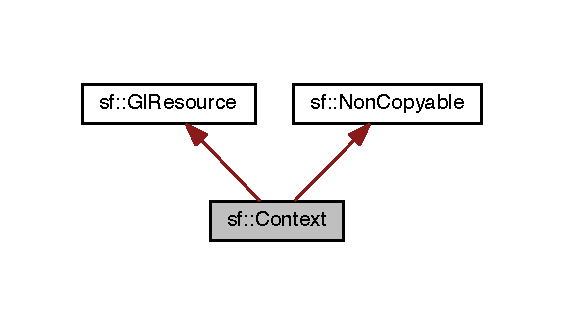
\includegraphics[width=271pt]{classsf_1_1_context__inherit__graph}
\end{center}
\end{figure}


Collaboration diagram for sf\-:\-:Context\-:
\nopagebreak
\begin{figure}[H]
\begin{center}
\leavevmode
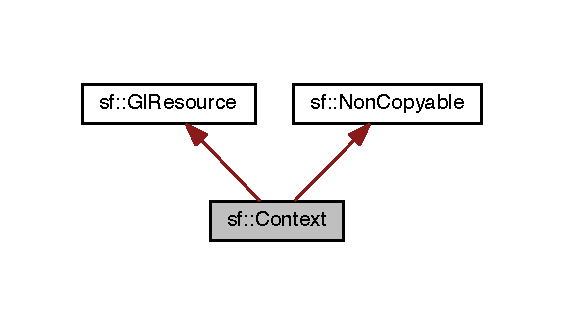
\includegraphics[width=271pt]{classsf_1_1_context__coll__graph}
\end{center}
\end{figure}
\subsection*{Public Member Functions}
\begin{DoxyCompactItemize}
\item 
\hyperlink{classsf_1_1_context_aba22797a790706ca2c5c04ee39f2b555}{Context} ()
\begin{DoxyCompactList}\small\item\em Default constructor. \end{DoxyCompactList}\item 
\hyperlink{classsf_1_1_context_a805b1bbdb3e52b1fda7c9bf2cd6ca86b}{$\sim$\-Context} ()
\begin{DoxyCompactList}\small\item\em Destructor. \end{DoxyCompactList}\item 
bool \hyperlink{classsf_1_1_context_a0806f915ea81ae1f4e8135a7a3696562}{set\-Active} (bool active)
\begin{DoxyCompactList}\small\item\em Activate or deactivate explicitely the context. \end{DoxyCompactList}\item 
\hyperlink{classsf_1_1_context_a2a9e3529e48919120e6b6fc10bad296c}{Context} (const \hyperlink{structsf_1_1_context_settings}{Context\-Settings} \&settings, unsigned int \hyperlink{gl3_8h_a9d14ddc31c6c8b61f3fe3679ab976133}{width}, unsigned int \hyperlink{gl3_8h_a67001679ebf2bb0ba972db4d29c6550c}{height})
\begin{DoxyCompactList}\small\item\em Construct a in-\/memory context. \end{DoxyCompactList}\end{DoxyCompactItemize}
\subsection*{Additional Inherited Members}


\subsection{Detailed Description}
Class holding a valid drawing context. 

If you need to make Open\-G\-L calls without having an active window (like in a thread), you can use an instance of this class to get a valid context.

Having a valid context is necessary for {\itshape every} Open\-G\-L call.

Note that a context is only active in its current thread, if you create a new thread it will have no valid context by default.

To use a \hyperlink{classsf_1_1_context}{sf\-::\-Context} instance, just construct it and let it live as long as you need a valid context. No explicit activation is needed, all it has to do is to exist. Its destructor will take care of deactivating and freeing all the attached resources.

Usage example\-: 
\begin{DoxyCode}
\textcolor{keywordtype}{void} threadFunction(\textcolor{keywordtype}{void}*)
\{
   \hyperlink{classsf_1_1_context}{sf::Context} context;
   \textcolor{comment}{// from now on, you have a valid context}

   \textcolor{comment}{// you can make OpenGL calls}
   \hyperlink{gl_8h_a17b651906e2eed37f6615b50ebb97b98}{glClear}(\hyperlink{gl_8h_aef2a9e9a4b130bc4de57514327847b4f}{GL\_DEPTH\_BUFFER\_BIT});
\}
\textcolor{comment}{// the context is automatically deactivated and destroyed}
\textcolor{comment}{// by the sf::Context destructor}
\end{DoxyCode}
 

Definition at line 48 of file Context.\-hpp.



\subsection{Constructor \& Destructor Documentation}
\hypertarget{classsf_1_1_context_aba22797a790706ca2c5c04ee39f2b555}{\index{sf\-::\-Context@{sf\-::\-Context}!Context@{Context}}
\index{Context@{Context}!sf::Context@{sf\-::\-Context}}
\subsubsection[{Context}]{\setlength{\rightskip}{0pt plus 5cm}sf\-::\-Context\-::\-Context (
\begin{DoxyParamCaption}
{}
\end{DoxyParamCaption}
)}}\label{classsf_1_1_context_aba22797a790706ca2c5c04ee39f2b555}


Default constructor. 

The constructor creates and activates the context \hypertarget{classsf_1_1_context_a805b1bbdb3e52b1fda7c9bf2cd6ca86b}{\index{sf\-::\-Context@{sf\-::\-Context}!$\sim$\-Context@{$\sim$\-Context}}
\index{$\sim$\-Context@{$\sim$\-Context}!sf::Context@{sf\-::\-Context}}
\subsubsection[{$\sim$\-Context}]{\setlength{\rightskip}{0pt plus 5cm}sf\-::\-Context\-::$\sim$\-Context (
\begin{DoxyParamCaption}
{}
\end{DoxyParamCaption}
)}}\label{classsf_1_1_context_a805b1bbdb3e52b1fda7c9bf2cd6ca86b}


Destructor. 

The desctructor deactivates and destroys the context \hypertarget{classsf_1_1_context_a2a9e3529e48919120e6b6fc10bad296c}{\index{sf\-::\-Context@{sf\-::\-Context}!Context@{Context}}
\index{Context@{Context}!sf::Context@{sf\-::\-Context}}
\subsubsection[{Context}]{\setlength{\rightskip}{0pt plus 5cm}sf\-::\-Context\-::\-Context (
\begin{DoxyParamCaption}
\item[{const {\bf Context\-Settings} \&}]{settings, }
\item[{unsigned int}]{width, }
\item[{unsigned int}]{height}
\end{DoxyParamCaption}
)}}\label{classsf_1_1_context_a2a9e3529e48919120e6b6fc10bad296c}


Construct a in-\/memory context. 

This constructor is for internal use, you don't need to bother with it.


\begin{DoxyParams}{Parameters}
{\em settings} & Creation parameters \\
\hline
{\em width} & Back buffer width \\
\hline
{\em height} & Back buffer height \\
\hline
\end{DoxyParams}


\subsection{Member Function Documentation}
\hypertarget{classsf_1_1_context_a0806f915ea81ae1f4e8135a7a3696562}{\index{sf\-::\-Context@{sf\-::\-Context}!set\-Active@{set\-Active}}
\index{set\-Active@{set\-Active}!sf::Context@{sf\-::\-Context}}
\subsubsection[{set\-Active}]{\setlength{\rightskip}{0pt plus 5cm}bool sf\-::\-Context\-::set\-Active (
\begin{DoxyParamCaption}
\item[{bool}]{active}
\end{DoxyParamCaption}
)}}\label{classsf_1_1_context_a0806f915ea81ae1f4e8135a7a3696562}


Activate or deactivate explicitely the context. 


\begin{DoxyParams}{Parameters}
{\em active} & True to activate, false to deactivate\\
\hline
\end{DoxyParams}
\begin{DoxyReturn}{Returns}
True on success, false on failure 
\end{DoxyReturn}


The documentation for this class was generated from the following file\-:\begin{DoxyCompactItemize}
\item 
/\-Users/ira/\-Dropbox/ira\-\_\-dev/protobyte\-\_\-research/other\-\_\-libs/\-S\-F\-M\-L/dylibs/root/usr/local/include/\-S\-F\-M\-L/\-Window/\hyperlink{_context_8hpp}{Context.\-hpp}\end{DoxyCompactItemize}

\hypertarget{structsf_1_1_context_settings}{\section{sf\-:\-:Context\-Settings Class Reference}
\label{structsf_1_1_context_settings}\index{sf\-::\-Context\-Settings@{sf\-::\-Context\-Settings}}
}


Structure defining the settings of the Open\-G\-L context attached to a window.  




{\ttfamily \#include $<$Context\-Settings.\-hpp$>$}

\subsection*{Public Member Functions}
\begin{DoxyCompactItemize}
\item 
\hyperlink{structsf_1_1_context_settings_aafe35f8e257f9d1e496ed64e33e2ee9f}{Context\-Settings} (unsigned int \hyperlink{gl3_8h_a6fe5f09cdb51e330bab7eae97ac343a3}{depth}=0, unsigned int \hyperlink{gl3_8h_aecd18db993a66d833647945966799ca5}{stencil}=0, unsigned int antialiasing=0, unsigned int major=2, unsigned int minor=0)
\begin{DoxyCompactList}\small\item\em Default constructor. \end{DoxyCompactList}\end{DoxyCompactItemize}
\subsection*{Public Attributes}
\begin{DoxyCompactItemize}
\item 
unsigned int \hyperlink{structsf_1_1_context_settings_a4809e22089c2af7276b8809b5aede7bb}{depth\-Bits}
\begin{DoxyCompactList}\small\item\em Bits of the depth buffer. \end{DoxyCompactList}\item 
unsigned int \hyperlink{structsf_1_1_context_settings_ac2e788c201ca20e84fd38a28071abd29}{stencil\-Bits}
\begin{DoxyCompactList}\small\item\em Bits of the stencil buffer. \end{DoxyCompactList}\item 
unsigned int \hyperlink{structsf_1_1_context_settings_ac4a097be18994dba38d73f36b0418bdc}{antialiasing\-Level}
\begin{DoxyCompactList}\small\item\em Level of antialiasing. \end{DoxyCompactList}\item 
unsigned int \hyperlink{structsf_1_1_context_settings_a99a680d5c15a7e34c935654155dd5166}{major\-Version}
\begin{DoxyCompactList}\small\item\em Major number of the context version to create. \end{DoxyCompactList}\item 
unsigned int \hyperlink{structsf_1_1_context_settings_aaeb0efe9d2658b840da93b30554b100f}{minor\-Version}
\begin{DoxyCompactList}\small\item\em Minor number of the context version to create. \end{DoxyCompactList}\end{DoxyCompactItemize}


\subsection{Detailed Description}
Structure defining the settings of the Open\-G\-L context attached to a window. 

\hyperlink{structsf_1_1_context_settings}{Context\-Settings} allows to define several advanced settings of the Open\-G\-L context attached to a window. All these settings have no impact on the regular S\-F\-M\-L rendering (graphics module) -- except the anti-\/aliasing level, so you may need to use this structure only if you're using S\-F\-M\-L as a windowing system for custom Open\-G\-L rendering.

The depth\-Bits and stencil\-Bits members define the number of bits per pixel requested for the (respectively) depth and stencil buffers.

antialiasing\-Level represents the requested number of multisampling levels for anti-\/aliasing.

major\-Version and minor\-Version define the version of the Open\-G\-L context that you want. Only versions greater or equal to 3.\-0 are relevant; versions lesser than 3.\-0 are all handled the same way (i.\-e. you can use any version $<$ 3.\-0 if you don't want an Open\-G\-L 3 context).

Please note that these values are only a hint. No failure will be reported if one or more of these values are not supported by the system; instead, S\-F\-M\-L will try to find the closest valid match. You can then retrieve the settings that the window actually used to create its context, with \hyperlink{classsf_1_1_window_a5a9d5c15facf25ad4d9b2b30caa0a2db}{Window\-::get\-Settings()}. 

Definition at line 36 of file Context\-Settings.\-hpp.



\subsection{Constructor \& Destructor Documentation}
\hypertarget{structsf_1_1_context_settings_aafe35f8e257f9d1e496ed64e33e2ee9f}{\index{sf\-::\-Context\-Settings@{sf\-::\-Context\-Settings}!Context\-Settings@{Context\-Settings}}
\index{Context\-Settings@{Context\-Settings}!sf::ContextSettings@{sf\-::\-Context\-Settings}}
\subsubsection[{Context\-Settings}]{\setlength{\rightskip}{0pt plus 5cm}sf\-::\-Context\-Settings\-::\-Context\-Settings (
\begin{DoxyParamCaption}
\item[{unsigned int}]{depth = {\ttfamily 0}, }
\item[{unsigned int}]{stencil = {\ttfamily 0}, }
\item[{unsigned int}]{antialiasing = {\ttfamily 0}, }
\item[{unsigned int}]{major = {\ttfamily 2}, }
\item[{unsigned int}]{minor = {\ttfamily 0}}
\end{DoxyParamCaption}
)\hspace{0.3cm}{\ttfamily [inline]}, {\ttfamily [explicit]}}}\label{structsf_1_1_context_settings_aafe35f8e257f9d1e496ed64e33e2ee9f}


Default constructor. 


\begin{DoxyParams}{Parameters}
{\em depth} & Depth buffer bits \\
\hline
{\em stencil} & Stencil buffer bits \\
\hline
{\em antialiasing} & Antialiasing level \\
\hline
{\em major} & Major number of the context version \\
\hline
{\em minor} & Minor number of the context version \\
\hline
\end{DoxyParams}


Definition at line 48 of file Context\-Settings.\-hpp.



\subsection{Member Data Documentation}
\hypertarget{structsf_1_1_context_settings_ac4a097be18994dba38d73f36b0418bdc}{\index{sf\-::\-Context\-Settings@{sf\-::\-Context\-Settings}!antialiasing\-Level@{antialiasing\-Level}}
\index{antialiasing\-Level@{antialiasing\-Level}!sf::ContextSettings@{sf\-::\-Context\-Settings}}
\subsubsection[{antialiasing\-Level}]{\setlength{\rightskip}{0pt plus 5cm}unsigned int sf\-::\-Context\-Settings\-::antialiasing\-Level}}\label{structsf_1_1_context_settings_ac4a097be18994dba38d73f36b0418bdc}


Level of antialiasing. 



Definition at line 62 of file Context\-Settings.\-hpp.

\hypertarget{structsf_1_1_context_settings_a4809e22089c2af7276b8809b5aede7bb}{\index{sf\-::\-Context\-Settings@{sf\-::\-Context\-Settings}!depth\-Bits@{depth\-Bits}}
\index{depth\-Bits@{depth\-Bits}!sf::ContextSettings@{sf\-::\-Context\-Settings}}
\subsubsection[{depth\-Bits}]{\setlength{\rightskip}{0pt plus 5cm}unsigned int sf\-::\-Context\-Settings\-::depth\-Bits}}\label{structsf_1_1_context_settings_a4809e22089c2af7276b8809b5aede7bb}


Bits of the depth buffer. 



Definition at line 60 of file Context\-Settings.\-hpp.

\hypertarget{structsf_1_1_context_settings_a99a680d5c15a7e34c935654155dd5166}{\index{sf\-::\-Context\-Settings@{sf\-::\-Context\-Settings}!major\-Version@{major\-Version}}
\index{major\-Version@{major\-Version}!sf::ContextSettings@{sf\-::\-Context\-Settings}}
\subsubsection[{major\-Version}]{\setlength{\rightskip}{0pt plus 5cm}unsigned int sf\-::\-Context\-Settings\-::major\-Version}}\label{structsf_1_1_context_settings_a99a680d5c15a7e34c935654155dd5166}


Major number of the context version to create. 



Definition at line 63 of file Context\-Settings.\-hpp.

\hypertarget{structsf_1_1_context_settings_aaeb0efe9d2658b840da93b30554b100f}{\index{sf\-::\-Context\-Settings@{sf\-::\-Context\-Settings}!minor\-Version@{minor\-Version}}
\index{minor\-Version@{minor\-Version}!sf::ContextSettings@{sf\-::\-Context\-Settings}}
\subsubsection[{minor\-Version}]{\setlength{\rightskip}{0pt plus 5cm}unsigned int sf\-::\-Context\-Settings\-::minor\-Version}}\label{structsf_1_1_context_settings_aaeb0efe9d2658b840da93b30554b100f}


Minor number of the context version to create. 



Definition at line 64 of file Context\-Settings.\-hpp.

\hypertarget{structsf_1_1_context_settings_ac2e788c201ca20e84fd38a28071abd29}{\index{sf\-::\-Context\-Settings@{sf\-::\-Context\-Settings}!stencil\-Bits@{stencil\-Bits}}
\index{stencil\-Bits@{stencil\-Bits}!sf::ContextSettings@{sf\-::\-Context\-Settings}}
\subsubsection[{stencil\-Bits}]{\setlength{\rightskip}{0pt plus 5cm}unsigned int sf\-::\-Context\-Settings\-::stencil\-Bits}}\label{structsf_1_1_context_settings_ac2e788c201ca20e84fd38a28071abd29}


Bits of the stencil buffer. 



Definition at line 61 of file Context\-Settings.\-hpp.



The documentation for this class was generated from the following file\-:\begin{DoxyCompactItemize}
\item 
/\-Users/ira/\-Dropbox/ira\-\_\-dev/protobyte\-\_\-research/other\-\_\-libs/\-S\-F\-M\-L/dylibs/root/usr/local/include/\-S\-F\-M\-L/\-Window/\hyperlink{_context_settings_8hpp}{Context\-Settings.\-hpp}\end{DoxyCompactItemize}

\hypertarget{classsf_1_1_convex_shape}{\section{sf\-:\-:Convex\-Shape Class Reference}
\label{classsf_1_1_convex_shape}\index{sf\-::\-Convex\-Shape@{sf\-::\-Convex\-Shape}}
}


Specialized shape representing a convex polygon.  




{\ttfamily \#include $<$Convex\-Shape.\-hpp$>$}



Inheritance diagram for sf\-:\-:Convex\-Shape\-:
\nopagebreak
\begin{figure}[H]
\begin{center}
\leavevmode
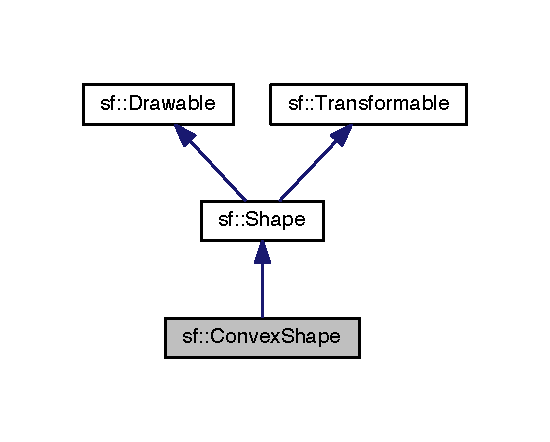
\includegraphics[width=264pt]{classsf_1_1_convex_shape__inherit__graph}
\end{center}
\end{figure}


Collaboration diagram for sf\-:\-:Convex\-Shape\-:
\nopagebreak
\begin{figure}[H]
\begin{center}
\leavevmode
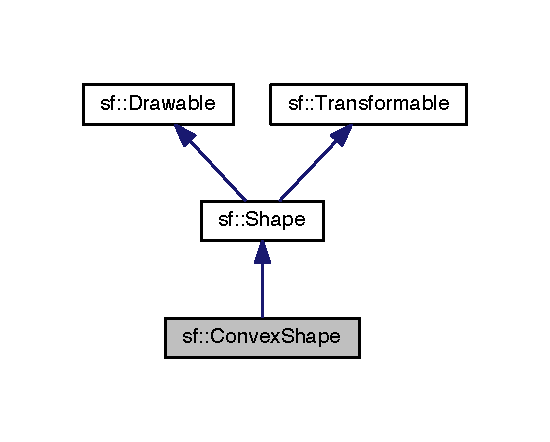
\includegraphics[width=264pt]{classsf_1_1_convex_shape__coll__graph}
\end{center}
\end{figure}
\subsection*{Public Member Functions}
\begin{DoxyCompactItemize}
\item 
\hyperlink{classsf_1_1_convex_shape_a4f4686f57622bfbbe419ac1420b1432a}{Convex\-Shape} (unsigned int point\-Count=0)
\begin{DoxyCompactList}\small\item\em Default constructor. \end{DoxyCompactList}\item 
\hyperlink{glutf90_8h_ac778d6f63f1aaf8ebda0ce6ac821b56e}{void} \hyperlink{classsf_1_1_convex_shape_aea7c3f0f08f5cd457fe128a75b7c1e70}{set\-Point\-Count} (unsigned int \hyperlink{gl3_8h_a5b40aca7a9682963dd00a8f5aef0a901}{count})
\begin{DoxyCompactList}\small\item\em Set the number of points of the polygon. \end{DoxyCompactList}\item 
virtual unsigned int \hyperlink{classsf_1_1_convex_shape_af81b86134fe54f2d50d9fab0db065ef1}{get\-Point\-Count} () const 
\begin{DoxyCompactList}\small\item\em Get the number of points of the polygon. \end{DoxyCompactList}\item 
\hyperlink{glutf90_8h_ac778d6f63f1aaf8ebda0ce6ac821b56e}{void} \hyperlink{classsf_1_1_convex_shape_ae5c7f87d0e776952e2ec6f0aa12ded31}{set\-Point} (unsigned int \hyperlink{gl3_8h_a57f14e05b1900f16a2da82ade47d0c6d}{index}, const \hyperlink{namespacesf_acf03098c2577b869e2fa6836cc48f1a0}{Vector2f} \&point)
\begin{DoxyCompactList}\small\item\em Set the position of a point. \end{DoxyCompactList}\item 
virtual \hyperlink{namespacesf_acf03098c2577b869e2fa6836cc48f1a0}{Vector2f} \hyperlink{classsf_1_1_convex_shape_ae2a18b837cd4454e340599a220c09a34}{get\-Point} (unsigned int \hyperlink{gl3_8h_a57f14e05b1900f16a2da82ade47d0c6d}{index}) const 
\begin{DoxyCompactList}\small\item\em Get the position of a point. \end{DoxyCompactList}\end{DoxyCompactItemize}
\subsection*{Additional Inherited Members}


\subsection{Detailed Description}
Specialized shape representing a convex polygon. 

This class inherits all the functions of \hyperlink{classsf_1_1_transformable}{sf\-::\-Transformable} (position, rotation, scale, bounds, ...) as well as the functions of \hyperlink{classsf_1_1_shape}{sf\-::\-Shape} (outline, color, texture, ...).

It is important to keep in mind that a convex shape must always be... convex, otherwise it may not be drawn correctly. Moreover, the points must be defined in order; using a random order would result in an incorrect shape.

Usage example\-: 
\begin{DoxyCode}
\hyperlink{classsf_1_1_convex_shape}{sf::ConvexShape} polygon;
polygon.\hyperlink{classsf_1_1_convex_shape_aea7c3f0f08f5cd457fe128a75b7c1e70}{setPointCount}(3);
polygon.\hyperlink{classsf_1_1_convex_shape_ae5c7f87d0e776952e2ec6f0aa12ded31}{setPoint}(0, \hyperlink{classsf_1_1_vector2}{sf::Vector2f}(0, 0));
polygon.\hyperlink{classsf_1_1_convex_shape_ae5c7f87d0e776952e2ec6f0aa12ded31}{setPoint}(1, \hyperlink{classsf_1_1_vector2}{sf::Vector2f}(0, 10));
polygon.\hyperlink{classsf_1_1_convex_shape_ae5c7f87d0e776952e2ec6f0aa12ded31}{setPoint}(2, \hyperlink{classsf_1_1_vector2}{sf::Vector2f}(25, 5));
polygon.\hyperlink{classsf_1_1_shape_a5978f41ee349ac3c52942996dcb184f7}{setOutlineColor}(\hyperlink{classsf_1_1_color_a127dbf55db9c07d0fa8f4bfcbb97594a}{sf::Color::Red});
polygon.\hyperlink{classsf_1_1_shape_a5ad336ad74fc1f567fce3b7e44cf87dc}{setOutlineThickness}(5);
polygon.\hyperlink{classsf_1_1_transformable_a4dbfb1a7c80688b0b4c477d706550208}{setPosition}(10, 20);
...
window.draw(polygon);
\end{DoxyCode}


\begin{DoxySeeAlso}{See Also}
\hyperlink{classsf_1_1_shape}{sf\-::\-Shape}, \hyperlink{classsf_1_1_rectangle_shape}{sf\-::\-Rectangle\-Shape}, \hyperlink{classsf_1_1_circle_shape}{sf\-::\-Circle\-Shape} 
\end{DoxySeeAlso}


Definition at line 42 of file Convex\-Shape.\-hpp.



\subsection{Constructor \& Destructor Documentation}
\hypertarget{classsf_1_1_convex_shape_a4f4686f57622bfbbe419ac1420b1432a}{\index{sf\-::\-Convex\-Shape@{sf\-::\-Convex\-Shape}!Convex\-Shape@{Convex\-Shape}}
\index{Convex\-Shape@{Convex\-Shape}!sf::ConvexShape@{sf\-::\-Convex\-Shape}}
\subsubsection[{Convex\-Shape}]{\setlength{\rightskip}{0pt plus 5cm}sf\-::\-Convex\-Shape\-::\-Convex\-Shape (
\begin{DoxyParamCaption}
\item[{unsigned int}]{point\-Count = {\ttfamily 0}}
\end{DoxyParamCaption}
)\hspace{0.3cm}{\ttfamily [explicit]}}}\label{classsf_1_1_convex_shape_a4f4686f57622bfbbe419ac1420b1432a}


Default constructor. 


\begin{DoxyParams}{Parameters}
{\em point\-Count} & Number of points of the polygon \\
\hline
\end{DoxyParams}


\subsection{Member Function Documentation}
\hypertarget{classsf_1_1_convex_shape_ae2a18b837cd4454e340599a220c09a34}{\index{sf\-::\-Convex\-Shape@{sf\-::\-Convex\-Shape}!get\-Point@{get\-Point}}
\index{get\-Point@{get\-Point}!sf::ConvexShape@{sf\-::\-Convex\-Shape}}
\subsubsection[{get\-Point}]{\setlength{\rightskip}{0pt plus 5cm}virtual {\bf Vector2f} sf\-::\-Convex\-Shape\-::get\-Point (
\begin{DoxyParamCaption}
\item[{unsigned int}]{index}
\end{DoxyParamCaption}
) const\hspace{0.3cm}{\ttfamily [virtual]}}}\label{classsf_1_1_convex_shape_ae2a18b837cd4454e340599a220c09a34}


Get the position of a point. 

The result is undefined if {\itshape index} is out of the valid range.


\begin{DoxyParams}{Parameters}
{\em index} & Index of the point to get, in range \mbox{[}0 .. Get\-Point\-Count() -\/ 1\mbox{]}\\
\hline
\end{DoxyParams}
\begin{DoxyReturn}{Returns}
Position of the index-\/th point of the polygon
\end{DoxyReturn}
\begin{DoxySeeAlso}{See Also}
\hyperlink{classsf_1_1_convex_shape_ae5c7f87d0e776952e2ec6f0aa12ded31}{set\-Point} 
\end{DoxySeeAlso}


Implements \hyperlink{classsf_1_1_shape_a397f3b4cdb7ad98cdc6c034816c652d2}{sf\-::\-Shape}.

\hypertarget{classsf_1_1_convex_shape_af81b86134fe54f2d50d9fab0db065ef1}{\index{sf\-::\-Convex\-Shape@{sf\-::\-Convex\-Shape}!get\-Point\-Count@{get\-Point\-Count}}
\index{get\-Point\-Count@{get\-Point\-Count}!sf::ConvexShape@{sf\-::\-Convex\-Shape}}
\subsubsection[{get\-Point\-Count}]{\setlength{\rightskip}{0pt plus 5cm}virtual unsigned int sf\-::\-Convex\-Shape\-::get\-Point\-Count (
\begin{DoxyParamCaption}
{}
\end{DoxyParamCaption}
) const\hspace{0.3cm}{\ttfamily [virtual]}}}\label{classsf_1_1_convex_shape_af81b86134fe54f2d50d9fab0db065ef1}


Get the number of points of the polygon. 

\begin{DoxyReturn}{Returns}
Number of points of the polygon
\end{DoxyReturn}
\begin{DoxySeeAlso}{See Also}
\hyperlink{classsf_1_1_convex_shape_aea7c3f0f08f5cd457fe128a75b7c1e70}{set\-Point\-Count} 
\end{DoxySeeAlso}


Implements \hyperlink{classsf_1_1_shape_ad84e1b675ecd270ad8151aea4e271a78}{sf\-::\-Shape}.

\hypertarget{classsf_1_1_convex_shape_ae5c7f87d0e776952e2ec6f0aa12ded31}{\index{sf\-::\-Convex\-Shape@{sf\-::\-Convex\-Shape}!set\-Point@{set\-Point}}
\index{set\-Point@{set\-Point}!sf::ConvexShape@{sf\-::\-Convex\-Shape}}
\subsubsection[{set\-Point}]{\setlength{\rightskip}{0pt plus 5cm}{\bf void} sf\-::\-Convex\-Shape\-::set\-Point (
\begin{DoxyParamCaption}
\item[{unsigned int}]{index, }
\item[{const {\bf Vector2f} \&}]{point}
\end{DoxyParamCaption}
)}}\label{classsf_1_1_convex_shape_ae5c7f87d0e776952e2ec6f0aa12ded31}


Set the position of a point. 

Don't forget that the polygon must remain convex, and the points need to stay ordered! Set\-Point\-Count must be called first in order to set the total number of points. The result is undefined if {\itshape index} is out of the valid range.


\begin{DoxyParams}{Parameters}
{\em index} & Index of the point to change, in range \mbox{[}0 .. Get\-Point\-Count() -\/ 1\mbox{]} \\
\hline
{\em point} & New position of the point\\
\hline
\end{DoxyParams}
\begin{DoxySeeAlso}{See Also}
\hyperlink{classsf_1_1_convex_shape_ae2a18b837cd4454e340599a220c09a34}{get\-Point} 
\end{DoxySeeAlso}
\hypertarget{classsf_1_1_convex_shape_aea7c3f0f08f5cd457fe128a75b7c1e70}{\index{sf\-::\-Convex\-Shape@{sf\-::\-Convex\-Shape}!set\-Point\-Count@{set\-Point\-Count}}
\index{set\-Point\-Count@{set\-Point\-Count}!sf::ConvexShape@{sf\-::\-Convex\-Shape}}
\subsubsection[{set\-Point\-Count}]{\setlength{\rightskip}{0pt plus 5cm}{\bf void} sf\-::\-Convex\-Shape\-::set\-Point\-Count (
\begin{DoxyParamCaption}
\item[{unsigned int}]{count}
\end{DoxyParamCaption}
)}}\label{classsf_1_1_convex_shape_aea7c3f0f08f5cd457fe128a75b7c1e70}


Set the number of points of the polygon. 

{\itshape count} must be greater than 2 to define a valid shape.


\begin{DoxyParams}{Parameters}
{\em count} & New number of points of the polygon\\
\hline
\end{DoxyParams}
\begin{DoxySeeAlso}{See Also}
\hyperlink{classsf_1_1_convex_shape_af81b86134fe54f2d50d9fab0db065ef1}{get\-Point\-Count} 
\end{DoxySeeAlso}


The documentation for this class was generated from the following file\-:\begin{DoxyCompactItemize}
\item 
/\-Users/ira/\-Dropbox/ira\-\_\-dev/protobyte\-\_\-research/other\-\_\-libs/\-S\-F\-M\-L/dylibs/root/usr/local/include/\-S\-F\-M\-L/\-Graphics/\hyperlink{_convex_shape_8hpp}{Convex\-Shape.\-hpp}\end{DoxyCompactItemize}

\hypertarget{struct_coord_rec}{\section{Coord\-Rec Struct Reference}
\label{struct_coord_rec}\index{Coord\-Rec@{Coord\-Rec}}
}


{\ttfamily \#include $<$glutstroke.\-h$>$}

\subsection*{Public Attributes}
\begin{DoxyCompactItemize}
\item 
float \hyperlink{struct_coord_rec_a81cf49b084c15d2774655d43f67e066f}{x}
\item 
float \hyperlink{struct_coord_rec_a390cc4367e9c463ca11e9a64bdfed671}{y}
\end{DoxyCompactItemize}


\subsection{Detailed Description}


Definition at line 15 of file glutstroke.\-h.



\subsection{Member Data Documentation}
\hypertarget{struct_coord_rec_a81cf49b084c15d2774655d43f67e066f}{\index{Coord\-Rec@{Coord\-Rec}!x@{x}}
\index{x@{x}!CoordRec@{Coord\-Rec}}
\subsubsection[{x}]{\setlength{\rightskip}{0pt plus 5cm}float Coord\-Rec\-::x}}\label{struct_coord_rec_a81cf49b084c15d2774655d43f67e066f}


Definition at line 16 of file glutstroke.\-h.

\hypertarget{struct_coord_rec_a390cc4367e9c463ca11e9a64bdfed671}{\index{Coord\-Rec@{Coord\-Rec}!y@{y}}
\index{y@{y}!CoordRec@{Coord\-Rec}}
\subsubsection[{y}]{\setlength{\rightskip}{0pt plus 5cm}float Coord\-Rec\-::y}}\label{struct_coord_rec_a390cc4367e9c463ca11e9a64bdfed671}


Definition at line 17 of file glutstroke.\-h.



The documentation for this struct was generated from the following file\-:\begin{DoxyCompactItemize}
\item 
/\-Users/ira/\-Dropbox/ira\-\_\-dev/protobyte\-\_\-research/other\-\_\-libs/glut/\-Headers/\hyperlink{glutstroke_8h}{glutstroke.\-h}\end{DoxyCompactItemize}

\hypertarget{structsf_1_1_shader_1_1_current_texture_type}{\section{sf\-:\-:Shader\-:\-:Current\-Texture\-Type Struct Reference}
\label{structsf_1_1_shader_1_1_current_texture_type}\index{sf\-::\-Shader\-::\-Current\-Texture\-Type@{sf\-::\-Shader\-::\-Current\-Texture\-Type}}
}


Special type/value that can be passed to set\-Parameter, and that represents the texture of the object being drawn.  




{\ttfamily \#include $<$Shader.\-hpp$>$}



\subsection{Detailed Description}
Special type/value that can be passed to set\-Parameter, and that represents the texture of the object being drawn. 

Definition at line 70 of file Shader.\-hpp.



The documentation for this struct was generated from the following file\-:\begin{DoxyCompactItemize}
\item 
/\-Users/ira/\-Dropbox/ira\-\_\-dev/protobyte\-\_\-research/other\-\_\-libs/\-S\-F\-M\-L/dylibs/root/usr/local/include/\-S\-F\-M\-L/\-Graphics/\hyperlink{_shader_8hpp}{Shader.\-hpp}\end{DoxyCompactItemize}

\hypertarget{class_curve3}{\section{Curve3 Class Reference}
\label{class_curve3}\index{Curve3@{Curve3}}
}


{\ttfamily \#include $<$Curve3.\-h$>$}



Inheritance diagram for Curve3\-:
\nopagebreak
\begin{figure}[H]
\begin{center}
\leavevmode
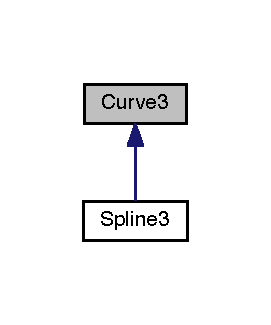
\includegraphics[width=130pt]{class_curve3__inherit__graph}
\end{center}
\end{figure}


Collaboration diagram for Curve3\-:
\nopagebreak
\begin{figure}[H]
\begin{center}
\leavevmode
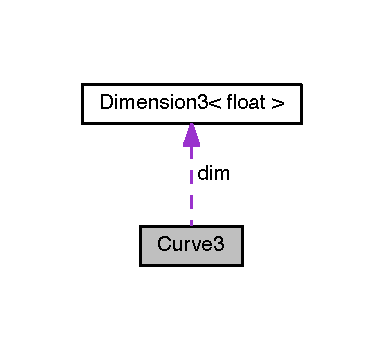
\includegraphics[width=184pt]{class_curve3__coll__graph}
\end{center}
\end{figure}
\subsection*{Public Member Functions}
\begin{DoxyCompactItemize}
\item 
\hyperlink{class_curve3_a547ab0feb6df06069ab395cef6a1694f}{Curve3} ()
\item 
\hyperlink{class_curve3_afb01df0701d99622de0d9e3cb4f15f4a}{Curve3} (const std\-::vector$<$ \hyperlink{class_vector3}{Vector3} $>$ \&\hyperlink{class_curve3_a2e9e6cfb4a03fffea0b4adbec17bba80}{control\-Pts}, int \hyperlink{class_curve3_a5ab0207ec14b339175e0aa9d621d70a7}{interp\-Detail}, bool \hyperlink{class_curve3_a94b01af1a451e35dbcec9ef36c4b4a64}{is\-Curve\-Closed})
\item 
virtual \hyperlink{class_curve3_a71cd69a17bdb9ae83013465377ba6303}{$\sim$\-Curve3} ()
\item 
virtual \hyperlink{glutf90_8h_ac778d6f63f1aaf8ebda0ce6ac821b56e}{void} \hyperlink{class_curve3_a5bffd69c283961491c639c459d2c06d2}{init} ()=0
\item 
virtual \hyperlink{glutf90_8h_ac778d6f63f1aaf8ebda0ce6ac821b56e}{void} \hyperlink{class_curve3_ae566fa302081043360e311be599377c3}{display} ()=0
\item 
virtual \hyperlink{glutf90_8h_ac778d6f63f1aaf8ebda0ce6ac821b56e}{void} \hyperlink{class_curve3_a8183be163e44fd6030ea3831df2fe8f3}{display\-Control\-Pts} ()=0
\item 
virtual \hyperlink{glutf90_8h_ac778d6f63f1aaf8ebda0ce6ac821b56e}{void} \hyperlink{class_curve3_a28ddf803ec40027cc21782467145bf38}{display\-Interp\-Pts} ()=0
\item 
virtual \hyperlink{glutf90_8h_ac778d6f63f1aaf8ebda0ce6ac821b56e}{void} \hyperlink{class_curve3_a5c0803a212a6792c17afd816a15af449}{display\-Frenet\-Frames} (float len=20)=0
\item 
int \hyperlink{class_curve3_ab2a5225d1a8d5b65013a5db64fd25b68}{get\-Control\-Pts\-Length} ()
\item 
int \hyperlink{class_curve3_a3752f730b20002e170a86cf4629b412a}{get\-Interp\-Detail} ()
\item 
\hyperlink{glutf90_8h_ac778d6f63f1aaf8ebda0ce6ac821b56e}{void} \hyperlink{class_curve3_a00a6510f2972f38f54c941ea92de0fc0}{set\-Control\-Pts} (std\-::vector$<$ \hyperlink{class_vector3}{Vector3} $>$ \&\hyperlink{class_curve3_a2e9e6cfb4a03fffea0b4adbec17bba80}{control\-Pts})
\item 
std\-::vector$<$ \hyperlink{class_vector3}{Vector3} $>$ \& \hyperlink{class_curve3_a91703b9049e93bc2c9af527cb5bcc3cb}{get\-Control\-Pts} ()
\item 
int \hyperlink{class_curve3_acbe74bd0e052c765f6e117b930824dae}{get\-Verts\-Length} () const 
\item 
\hyperlink{glutf90_8h_ac778d6f63f1aaf8ebda0ce6ac821b56e}{void} \hyperlink{class_curve3_a8c964fc61855616010a4f89782d2a123}{set\-Verts} (std\-::vector$<$ \hyperlink{class_vector3}{Vector3} $>$ \hyperlink{class_curve3_a9937ea75c1a2467d1dc61605c5b958c8}{verts})
\item 
std\-::vector$<$ \hyperlink{class_vector3}{Vector3} $>$ \& \hyperlink{class_curve3_ab52692d2a2b548f2b9837d04bd70e7fb}{get\-Verts} ()
\item 
std\-::vector$<$ \hyperlink{class_vector3}{Vector3} $>$ \& \hyperlink{class_curve3_a1336793bc5394a7858479910aab1bae6}{get\-Vertices} ()
\item 
\hyperlink{class_dimension3}{Dimension3}$<$ float $>$ \& \hyperlink{class_curve3_ac88900ec63684247812ed7b86b09dd71}{get\-Dimension} ()
\item 
double \hyperlink{class_curve3_a6965f39c1512df70ea5133bc6b21f034}{get\-Vert\-Rad} () const 
\item 
\hyperlink{glutf90_8h_ac778d6f63f1aaf8ebda0ce6ac821b56e}{void} \hyperlink{class_curve3_ab8b300b3ea2e2fc071bacaa1100ebf24}{set\-Vert\-Rad} (double \hyperlink{class_curve3_a404b74eb4ad6ac9796b766ff1a36d823}{vert\-Rad})
\item 
bool \hyperlink{class_curve3_ac78c8815970e831ef0e3d9f51bac0636}{get\-Is\-Curve\-Closed} () const 
\item 
\hyperlink{glutf90_8h_ac778d6f63f1aaf8ebda0ce6ac821b56e}{void} \hyperlink{class_curve3_a656565930a73e9d1cdc03f424ba0d323}{set\-Is\-Curve\-Closed} (bool \hyperlink{class_curve3_a94b01af1a451e35dbcec9ef36c4b4a64}{is\-Curve\-Closed})
\item 
bool \hyperlink{class_curve3_afcd982fd3e0b6eec3d841e570c9beffb}{get\-Is\-Terminal\-Smooth} () const 
\item 
\hyperlink{glutf90_8h_ac778d6f63f1aaf8ebda0ce6ac821b56e}{void} \hyperlink{class_curve3_ad280540e1e732533780a7e92f1c5c171}{set\-Is\-Terminal\-Smooth} (bool \hyperlink{class_curve3_af842d273f3cdbb907f66ffed7b72d2a5}{is\-Terminal\-Smooth})
\item 
const std\-::vector$<$ \hyperlink{class_frenet_frame}{Frenet\-Frame} $>$ \& \hyperlink{class_curve3_a3badf7d24d4afabf44855c69050f06c5}{get\-Frenet\-Frame} () const 
\end{DoxyCompactItemize}
\subsection*{Protected Attributes}
\begin{DoxyCompactItemize}
\item 
std\-::vector$<$ \hyperlink{class_vector3}{Vector3} $>$ \hyperlink{class_curve3_a2e9e6cfb4a03fffea0b4adbec17bba80}{control\-Pts}
\item 
int \hyperlink{class_curve3_a5ab0207ec14b339175e0aa9d621d70a7}{interp\-Detail}
\item 
std\-::vector$<$ \hyperlink{class_vector3}{Vector3} $>$ \hyperlink{class_curve3_a8060ece4544b6c09dfad0ab3b27af00f}{interp\-Pts}
\item 
std\-::vector$<$ \hyperlink{class_vector3}{Vector3} $>$ \hyperlink{class_curve3_a9937ea75c1a2467d1dc61605c5b958c8}{verts}
\item 
std\-::vector$<$ \hyperlink{class_vector3}{Vector3} $>$ \hyperlink{class_curve3_a32046ec84335f78317dab2dccbeb732e}{bi\-Norms}
\item 
std\-::vector$<$ \hyperlink{class_vector3}{Vector3} $>$ \hyperlink{class_curve3_a9464b3b2baa1a520c5cda6ea19147e71}{norms}
\item 
std\-::vector$<$ \hyperlink{class_frenet_frame}{Frenet\-Frame} $>$ \hyperlink{class_curve3_a6dbfbfd7fd486988ca2d08ddd65b7f68}{frenet\-Frames}
\item 
std\-::vector$<$ float $>$ \hyperlink{class_curve3_aa3c9c1b951d6d8d280a00659ced8a503}{parallel\-Transport\-Thetas}
\item 
double \hyperlink{class_curve3_a404b74eb4ad6ac9796b766ff1a36d823}{vert\-Rad}
\item 
bool \hyperlink{class_curve3_a94b01af1a451e35dbcec9ef36c4b4a64}{is\-Curve\-Closed}
\item 
bool \hyperlink{class_curve3_af842d273f3cdbb907f66ffed7b72d2a5}{is\-Terminal\-Smooth}
\item 
std\-::vector$<$ \hyperlink{class_vector3}{Vector3} $>$ \hyperlink{class_curve3_a527d3cb7d51e3896b93cf048920345f2}{temp\-Vecs}
\item 
\hyperlink{class_dimension3}{Dimension3}$<$ float $>$ \hyperlink{class_curve3_ad2c2f60f7e9c11e87353cb9e6653f1e1}{dim}
\end{DoxyCompactItemize}


\subsection{Detailed Description}


Definition at line 27 of file Curve3.\-h.



\subsection{Constructor \& Destructor Documentation}
\hypertarget{class_curve3_a547ab0feb6df06069ab395cef6a1694f}{\index{Curve3@{Curve3}!Curve3@{Curve3}}
\index{Curve3@{Curve3}!Curve3@{Curve3}}
\subsubsection[{Curve3}]{\setlength{\rightskip}{0pt plus 5cm}Curve3\-::\-Curve3 (
\begin{DoxyParamCaption}
{}
\end{DoxyParamCaption}
)}}\label{class_curve3_a547ab0feb6df06069ab395cef6a1694f}


Definition at line 15 of file Curve3.\-cpp.

\hypertarget{class_curve3_afb01df0701d99622de0d9e3cb4f15f4a}{\index{Curve3@{Curve3}!Curve3@{Curve3}}
\index{Curve3@{Curve3}!Curve3@{Curve3}}
\subsubsection[{Curve3}]{\setlength{\rightskip}{0pt plus 5cm}Curve3\-::\-Curve3 (
\begin{DoxyParamCaption}
\item[{const std\-::vector$<$ {\bf Vector3} $>$ \&}]{control\-Pts, }
\item[{int}]{interp\-Detail, }
\item[{bool}]{is\-Curve\-Closed}
\end{DoxyParamCaption}
)}}\label{class_curve3_afb01df0701d99622de0d9e3cb4f15f4a}


Definition at line 18 of file Curve3.\-cpp.

\hypertarget{class_curve3_a71cd69a17bdb9ae83013465377ba6303}{\index{Curve3@{Curve3}!$\sim$\-Curve3@{$\sim$\-Curve3}}
\index{$\sim$\-Curve3@{$\sim$\-Curve3}!Curve3@{Curve3}}
\subsubsection[{$\sim$\-Curve3}]{\setlength{\rightskip}{0pt plus 5cm}Curve3\-::$\sim$\-Curve3 (
\begin{DoxyParamCaption}
{}
\end{DoxyParamCaption}
)\hspace{0.3cm}{\ttfamily [virtual]}}}\label{class_curve3_a71cd69a17bdb9ae83013465377ba6303}


Definition at line 23 of file Curve3.\-cpp.



\subsection{Member Function Documentation}
\hypertarget{class_curve3_ae566fa302081043360e311be599377c3}{\index{Curve3@{Curve3}!display@{display}}
\index{display@{display}!Curve3@{Curve3}}
\subsubsection[{display}]{\setlength{\rightskip}{0pt plus 5cm}virtual {\bf void} Curve3\-::display (
\begin{DoxyParamCaption}
{}
\end{DoxyParamCaption}
)\hspace{0.3cm}{\ttfamily [pure virtual]}}}\label{class_curve3_ae566fa302081043360e311be599377c3}
Draw the curve. 

Implemented in \hyperlink{class_spline3_a503db55ba1523698067210952c2e470d}{Spline3}.

\hypertarget{class_curve3_a8183be163e44fd6030ea3831df2fe8f3}{\index{Curve3@{Curve3}!display\-Control\-Pts@{display\-Control\-Pts}}
\index{display\-Control\-Pts@{display\-Control\-Pts}!Curve3@{Curve3}}
\subsubsection[{display\-Control\-Pts}]{\setlength{\rightskip}{0pt plus 5cm}virtual {\bf void} Curve3\-::display\-Control\-Pts (
\begin{DoxyParamCaption}
{}
\end{DoxyParamCaption}
)\hspace{0.3cm}{\ttfamily [pure virtual]}}}\label{class_curve3_a8183be163e44fd6030ea3831df2fe8f3}
Draw the curve points. 

Implemented in \hyperlink{class_spline3_a303fadd7700a53382145ab961c123cc6}{Spline3}.

\hypertarget{class_curve3_a5c0803a212a6792c17afd816a15af449}{\index{Curve3@{Curve3}!display\-Frenet\-Frames@{display\-Frenet\-Frames}}
\index{display\-Frenet\-Frames@{display\-Frenet\-Frames}!Curve3@{Curve3}}
\subsubsection[{display\-Frenet\-Frames}]{\setlength{\rightskip}{0pt plus 5cm}virtual {\bf void} Curve3\-::display\-Frenet\-Frames (
\begin{DoxyParamCaption}
\item[{float}]{len = {\ttfamily 20}}
\end{DoxyParamCaption}
)\hspace{0.3cm}{\ttfamily [pure virtual]}}}\label{class_curve3_a5c0803a212a6792c17afd816a15af449}
Draw the Frenet Frame. 

Implemented in \hyperlink{class_spline3_ad480f955275c7004b451857db6605ac2}{Spline3}.

\hypertarget{class_curve3_a28ddf803ec40027cc21782467145bf38}{\index{Curve3@{Curve3}!display\-Interp\-Pts@{display\-Interp\-Pts}}
\index{display\-Interp\-Pts@{display\-Interp\-Pts}!Curve3@{Curve3}}
\subsubsection[{display\-Interp\-Pts}]{\setlength{\rightskip}{0pt plus 5cm}virtual {\bf void} Curve3\-::display\-Interp\-Pts (
\begin{DoxyParamCaption}
{}
\end{DoxyParamCaption}
)\hspace{0.3cm}{\ttfamily [pure virtual]}}}\label{class_curve3_a28ddf803ec40027cc21782467145bf38}
Draw the curve points. 

Implemented in \hyperlink{class_spline3_a45cf582905d29565589cebfd12139f0a}{Spline3}.

\hypertarget{class_curve3_a91703b9049e93bc2c9af527cb5bcc3cb}{\index{Curve3@{Curve3}!get\-Control\-Pts@{get\-Control\-Pts}}
\index{get\-Control\-Pts@{get\-Control\-Pts}!Curve3@{Curve3}}
\subsubsection[{get\-Control\-Pts}]{\setlength{\rightskip}{0pt plus 5cm}std\-::vector$<$ {\bf Vector3} $>$ \& Curve3\-::get\-Control\-Pts (
\begin{DoxyParamCaption}
{}
\end{DoxyParamCaption}
)}}\label{class_curve3_a91703b9049e93bc2c9af527cb5bcc3cb}
get a pointer to the control points array, with side effects

Get a pointer to the control points array. with side effects 

Definition at line 53 of file Curve3.\-cpp.

\hypertarget{class_curve3_ab2a5225d1a8d5b65013a5db64fd25b68}{\index{Curve3@{Curve3}!get\-Control\-Pts\-Length@{get\-Control\-Pts\-Length}}
\index{get\-Control\-Pts\-Length@{get\-Control\-Pts\-Length}!Curve3@{Curve3}}
\subsubsection[{get\-Control\-Pts\-Length}]{\setlength{\rightskip}{0pt plus 5cm}int Curve3\-::get\-Control\-Pts\-Length (
\begin{DoxyParamCaption}
{}
\end{DoxyParamCaption}
)}}\label{class_curve3_ab2a5225d1a8d5b65013a5db64fd25b68}
Returns length of the control points array.

Gets control points array length. 

Definition at line 38 of file Curve3.\-cpp.

\hypertarget{class_curve3_ac88900ec63684247812ed7b86b09dd71}{\index{Curve3@{Curve3}!get\-Dimension@{get\-Dimension}}
\index{get\-Dimension@{get\-Dimension}!Curve3@{Curve3}}
\subsubsection[{get\-Dimension}]{\setlength{\rightskip}{0pt plus 5cm}{\bf Dimension3}$<$ float $>$ \& Curve3\-::get\-Dimension (
\begin{DoxyParamCaption}
{}
\end{DoxyParamCaption}
)}}\label{class_curve3_ac88900ec63684247812ed7b86b09dd71}
Get \hyperlink{class_curve3}{Curve3} object dimensions.

\begin{DoxyReturn}{Returns}
\hyperlink{class_dimension3}{Dimension3} object 
\end{DoxyReturn}


Definition at line 105 of file Curve3.\-cpp.

\hypertarget{class_curve3_a3badf7d24d4afabf44855c69050f06c5}{\index{Curve3@{Curve3}!get\-Frenet\-Frame@{get\-Frenet\-Frame}}
\index{get\-Frenet\-Frame@{get\-Frenet\-Frame}!Curve3@{Curve3}}
\subsubsection[{get\-Frenet\-Frame}]{\setlength{\rightskip}{0pt plus 5cm}const std\-::vector$<$ {\bf Frenet\-Frame} $>$ \& Curve3\-::get\-Frenet\-Frame (
\begin{DoxyParamCaption}
{}
\end{DoxyParamCaption}
) const}}\label{class_curve3_a3badf7d24d4afabf44855c69050f06c5}
get Frenet Frame

\begin{DoxyReturn}{Returns}
Frenet Frame 
\end{DoxyReturn}


Definition at line 194 of file Curve3.\-cpp.

\hypertarget{class_curve3_a3752f730b20002e170a86cf4629b412a}{\index{Curve3@{Curve3}!get\-Interp\-Detail@{get\-Interp\-Detail}}
\index{get\-Interp\-Detail@{get\-Interp\-Detail}!Curve3@{Curve3}}
\subsubsection[{get\-Interp\-Detail}]{\setlength{\rightskip}{0pt plus 5cm}int Curve3\-::get\-Interp\-Detail (
\begin{DoxyParamCaption}
{}
\end{DoxyParamCaption}
)}}\label{class_curve3_a3752f730b20002e170a86cf4629b412a}
Returns length of the points std\-::vector (pts between control points).

Gets point count between control points. 

Definition at line 45 of file Curve3.\-cpp.

\hypertarget{class_curve3_ac78c8815970e831ef0e3d9f51bac0636}{\index{Curve3@{Curve3}!get\-Is\-Curve\-Closed@{get\-Is\-Curve\-Closed}}
\index{get\-Is\-Curve\-Closed@{get\-Is\-Curve\-Closed}!Curve3@{Curve3}}
\subsubsection[{get\-Is\-Curve\-Closed}]{\setlength{\rightskip}{0pt plus 5cm}bool Curve3\-::get\-Is\-Curve\-Closed (
\begin{DoxyParamCaption}
{}
\end{DoxyParamCaption}
) const}}\label{class_curve3_ac78c8815970e831ef0e3d9f51bac0636}
Get flag value telling if curve is closed

\begin{DoxyReturn}{Returns}
boolean value
\end{DoxyReturn}
Get flag value telling if curve is closed

\begin{DoxyReturn}{Returns}
bool value 
\end{DoxyReturn}


Definition at line 156 of file Curve3.\-cpp.

\hypertarget{class_curve3_afcd982fd3e0b6eec3d841e570c9beffb}{\index{Curve3@{Curve3}!get\-Is\-Terminal\-Smooth@{get\-Is\-Terminal\-Smooth}}
\index{get\-Is\-Terminal\-Smooth@{get\-Is\-Terminal\-Smooth}!Curve3@{Curve3}}
\subsubsection[{get\-Is\-Terminal\-Smooth}]{\setlength{\rightskip}{0pt plus 5cm}bool Curve3\-::get\-Is\-Terminal\-Smooth (
\begin{DoxyParamCaption}
{}
\end{DoxyParamCaption}
) const}}\label{class_curve3_afcd982fd3e0b6eec3d841e570c9beffb}
Get flag value telling if curve at Terminals is continuous

\begin{DoxyReturn}{Returns}
boolean value
\end{DoxyReturn}
Get flag value telling if curve at Terminals is continuous

\begin{DoxyReturn}{Returns}
bool value 
\end{DoxyReturn}


Definition at line 175 of file Curve3.\-cpp.

\hypertarget{class_curve3_a1336793bc5394a7858479910aab1bae6}{\index{Curve3@{Curve3}!get\-Vertices@{get\-Vertices}}
\index{get\-Vertices@{get\-Vertices}!Curve3@{Curve3}}
\subsubsection[{get\-Vertices}]{\setlength{\rightskip}{0pt plus 5cm}std\-::vector$<$ {\bf Vector3} $>$ \& Curve3\-::get\-Vertices (
\begin{DoxyParamCaption}
{}
\end{DoxyParamCaption}
)}}\label{class_curve3_a1336793bc5394a7858479910aab1bae6}
Get std\-::vector of all vertices

Get a pointer to a vector of all the vertices To D\-O N\-O\-T\-E -\/ switch all verts to vector eventually $\ast$$\ast$$\ast$$\ast$ 

Definition at line 94 of file Curve3.\-cpp.

\hypertarget{class_curve3_a6965f39c1512df70ea5133bc6b21f034}{\index{Curve3@{Curve3}!get\-Vert\-Rad@{get\-Vert\-Rad}}
\index{get\-Vert\-Rad@{get\-Vert\-Rad}!Curve3@{Curve3}}
\subsubsection[{get\-Vert\-Rad}]{\setlength{\rightskip}{0pt plus 5cm}double Curve3\-::get\-Vert\-Rad (
\begin{DoxyParamCaption}
{}
\end{DoxyParamCaption}
) const}}\label{class_curve3_a6965f39c1512df70ea5133bc6b21f034}
Get vertex radius.

\begin{DoxyReturn}{Returns}
double value 
\end{DoxyReturn}


Definition at line 136 of file Curve3.\-cpp.

\hypertarget{class_curve3_ab52692d2a2b548f2b9837d04bd70e7fb}{\index{Curve3@{Curve3}!get\-Verts@{get\-Verts}}
\index{get\-Verts@{get\-Verts}!Curve3@{Curve3}}
\subsubsection[{get\-Verts}]{\setlength{\rightskip}{0pt plus 5cm}std\-::vector$<$ {\bf Vector3} $>$ \& Curve3\-::get\-Verts (
\begin{DoxyParamCaption}
{}
\end{DoxyParamCaption}
)}}\label{class_curve3_ab52692d2a2b548f2b9837d04bd70e7fb}
Get pointer all the curve points


\begin{DoxyParams}{Parameters}
{\em unique\-Verts} & Vector array \\
\hline
\end{DoxyParams}


Definition at line 84 of file Curve3.\-cpp.

\hypertarget{class_curve3_acbe74bd0e052c765f6e117b930824dae}{\index{Curve3@{Curve3}!get\-Verts\-Length@{get\-Verts\-Length}}
\index{get\-Verts\-Length@{get\-Verts\-Length}!Curve3@{Curve3}}
\subsubsection[{get\-Verts\-Length}]{\setlength{\rightskip}{0pt plus 5cm}int Curve3\-::get\-Verts\-Length (
\begin{DoxyParamCaption}
{}
\end{DoxyParamCaption}
) const}}\label{class_curve3_acbe74bd0e052c765f6e117b930824dae}
Get the curve verts\-Buff's length.

\begin{DoxyReturn}{Returns}
int
\end{DoxyReturn}
Get the curve verts\-Buff' length.

\begin{DoxyReturn}{Returns}
int 
\end{DoxyReturn}


Definition at line 63 of file Curve3.\-cpp.

\hypertarget{class_curve3_a5bffd69c283961491c639c459d2c06d2}{\index{Curve3@{Curve3}!init@{init}}
\index{init@{init}!Curve3@{Curve3}}
\subsubsection[{init}]{\setlength{\rightskip}{0pt plus 5cm}virtual {\bf void} Curve3\-::init (
\begin{DoxyParamCaption}
{}
\end{DoxyParamCaption}
)\hspace{0.3cm}{\ttfamily [pure virtual]}}}\label{class_curve3_a5bffd69c283961491c639c459d2c06d2}
Calculate the interpolated curve points populating the vecs array. \hypertarget{class_curve3_a00a6510f2972f38f54c941ea92de0fc0}{\index{Curve3@{Curve3}!set\-Control\-Pts@{set\-Control\-Pts}}
\index{set\-Control\-Pts@{set\-Control\-Pts}!Curve3@{Curve3}}
\subsubsection[{set\-Control\-Pts}]{\setlength{\rightskip}{0pt plus 5cm}{\bf void} Curve3\-::set\-Control\-Pts (
\begin{DoxyParamCaption}
\item[{std\-::vector$<$ {\bf Vector3} $>$ \&}]{control\-Pts}
\end{DoxyParamCaption}
)}}\label{class_curve3_a00a6510f2972f38f54c941ea92de0fc0}
Set the control points, with side effects

Set the control points. with side effects 

Definition at line 31 of file Curve3.\-cpp.

\hypertarget{class_curve3_a656565930a73e9d1cdc03f424ba0d323}{\index{Curve3@{Curve3}!set\-Is\-Curve\-Closed@{set\-Is\-Curve\-Closed}}
\index{set\-Is\-Curve\-Closed@{set\-Is\-Curve\-Closed}!Curve3@{Curve3}}
\subsubsection[{set\-Is\-Curve\-Closed}]{\setlength{\rightskip}{0pt plus 5cm}{\bf void} Curve3\-::set\-Is\-Curve\-Closed (
\begin{DoxyParamCaption}
\item[{bool}]{is\-Curve\-Closed}
\end{DoxyParamCaption}
)}}\label{class_curve3_a656565930a73e9d1cdc03f424ba0d323}
Set flag for Curve to be closed


\begin{DoxyParams}{Parameters}
{\em is\-Curve\-Closed} & boolean value\\
\hline
\end{DoxyParams}
Set flag for Curve to be closed


\begin{DoxyParams}{Parameters}
{\em is\-Curve\-Closed} & bool value \\
\hline
\end{DoxyParams}


Definition at line 166 of file Curve3.\-cpp.

\hypertarget{class_curve3_ad280540e1e732533780a7e92f1c5c171}{\index{Curve3@{Curve3}!set\-Is\-Terminal\-Smooth@{set\-Is\-Terminal\-Smooth}}
\index{set\-Is\-Terminal\-Smooth@{set\-Is\-Terminal\-Smooth}!Curve3@{Curve3}}
\subsubsection[{set\-Is\-Terminal\-Smooth}]{\setlength{\rightskip}{0pt plus 5cm}{\bf void} Curve3\-::set\-Is\-Terminal\-Smooth (
\begin{DoxyParamCaption}
\item[{bool}]{is\-Terminal\-Smooth}
\end{DoxyParamCaption}
)}}\label{class_curve3_ad280540e1e732533780a7e92f1c5c171}
Set flag for Curve at Terminals to be continuous


\begin{DoxyParams}{Parameters}
{\em is\-Terminal\-Smooth} & boolean value\\
\hline
\end{DoxyParams}
Set flag for Curve at Terminals to be continuous


\begin{DoxyParams}{Parameters}
{\em is\-Terminal\-Smooth} & bool value \\
\hline
\end{DoxyParams}


Definition at line 185 of file Curve3.\-cpp.

\hypertarget{class_curve3_ab8b300b3ea2e2fc071bacaa1100ebf24}{\index{Curve3@{Curve3}!set\-Vert\-Rad@{set\-Vert\-Rad}}
\index{set\-Vert\-Rad@{set\-Vert\-Rad}!Curve3@{Curve3}}
\subsubsection[{set\-Vert\-Rad}]{\setlength{\rightskip}{0pt plus 5cm}{\bf void} Curve3\-::set\-Vert\-Rad (
\begin{DoxyParamCaption}
\item[{double}]{vert\-Rad}
\end{DoxyParamCaption}
)}}\label{class_curve3_ab8b300b3ea2e2fc071bacaa1100ebf24}
Set vertex radius


\begin{DoxyParams}{Parameters}
{\em vert\-Rad} & double value \\
\hline
\end{DoxyParams}


Definition at line 146 of file Curve3.\-cpp.

\hypertarget{class_curve3_a8c964fc61855616010a4f89782d2a123}{\index{Curve3@{Curve3}!set\-Verts@{set\-Verts}}
\index{set\-Verts@{set\-Verts}!Curve3@{Curve3}}
\subsubsection[{set\-Verts}]{\setlength{\rightskip}{0pt plus 5cm}{\bf void} Curve3\-::set\-Verts (
\begin{DoxyParamCaption}
\item[{std\-::vector$<$ {\bf Vector3} $>$}]{verts}
\end{DoxyParamCaption}
)}}\label{class_curve3_a8c964fc61855616010a4f89782d2a123}
Set all the curve points


\begin{DoxyParams}{Parameters}
{\em unique\-Verts} & Vector array\\
\hline
\end{DoxyParams}
Set all the curve points


\begin{DoxyParams}{Parameters}
{\em unique\-Verts} & Vector\mbox{[}\mbox{]} array \\
\hline
\end{DoxyParams}


Definition at line 73 of file Curve3.\-cpp.



\subsection{Member Data Documentation}
\hypertarget{class_curve3_a32046ec84335f78317dab2dccbeb732e}{\index{Curve3@{Curve3}!bi\-Norms@{bi\-Norms}}
\index{bi\-Norms@{bi\-Norms}!Curve3@{Curve3}}
\subsubsection[{bi\-Norms}]{\setlength{\rightskip}{0pt plus 5cm}std\-::vector$<${\bf Vector3}$>$ Curve3\-::bi\-Norms\hspace{0.3cm}{\ttfamily [protected]}}}\label{class_curve3_a32046ec84335f78317dab2dccbeb732e}
std\-::vector of all curve vertices (Frenet frame). 

Definition at line 54 of file Curve3.\-h.

\hypertarget{class_curve3_a2e9e6cfb4a03fffea0b4adbec17bba80}{\index{Curve3@{Curve3}!control\-Pts@{control\-Pts}}
\index{control\-Pts@{control\-Pts}!Curve3@{Curve3}}
\subsubsection[{control\-Pts}]{\setlength{\rightskip}{0pt plus 5cm}std\-::vector$<${\bf Vector3}$>$ Curve3\-::control\-Pts\hspace{0.3cm}{\ttfamily [protected]}}}\label{class_curve3_a2e9e6cfb4a03fffea0b4adbec17bba80}
std\-::vector of control points. 

Definition at line 34 of file Curve3.\-h.

\hypertarget{class_curve3_ad2c2f60f7e9c11e87353cb9e6653f1e1}{\index{Curve3@{Curve3}!dim@{dim}}
\index{dim@{dim}!Curve3@{Curve3}}
\subsubsection[{dim}]{\setlength{\rightskip}{0pt plus 5cm}{\bf Dimension3}$<$float$>$ Curve3\-::dim\hspace{0.3cm}{\ttfamily [protected]}}}\label{class_curve3_ad2c2f60f7e9c11e87353cb9e6653f1e1}
Bounding box of entire curve 

Definition at line 96 of file Curve3.\-h.

\hypertarget{class_curve3_a6dbfbfd7fd486988ca2d08ddd65b7f68}{\index{Curve3@{Curve3}!frenet\-Frames@{frenet\-Frames}}
\index{frenet\-Frames@{frenet\-Frames}!Curve3@{Curve3}}
\subsubsection[{frenet\-Frames}]{\setlength{\rightskip}{0pt plus 5cm}std\-::vector$<${\bf Frenet\-Frame}$>$ Curve3\-::frenet\-Frames\hspace{0.3cm}{\ttfamily [protected]}}}\label{class_curve3_a6dbfbfd7fd486988ca2d08ddd65b7f68}
std\-::vector of Frenet frames. 

Definition at line 64 of file Curve3.\-h.

\hypertarget{class_curve3_a5ab0207ec14b339175e0aa9d621d70a7}{\index{Curve3@{Curve3}!interp\-Detail@{interp\-Detail}}
\index{interp\-Detail@{interp\-Detail}!Curve3@{Curve3}}
\subsubsection[{interp\-Detail}]{\setlength{\rightskip}{0pt plus 5cm}int Curve3\-::interp\-Detail\hspace{0.3cm}{\ttfamily [protected]}}}\label{class_curve3_a5ab0207ec14b339175e0aa9d621d70a7}
The number of interpolated points along the curve. 

Definition at line 39 of file Curve3.\-h.

\hypertarget{class_curve3_a8060ece4544b6c09dfad0ab3b27af00f}{\index{Curve3@{Curve3}!interp\-Pts@{interp\-Pts}}
\index{interp\-Pts@{interp\-Pts}!Curve3@{Curve3}}
\subsubsection[{interp\-Pts}]{\setlength{\rightskip}{0pt plus 5cm}std\-::vector$<${\bf Vector3}$>$ Curve3\-::interp\-Pts\hspace{0.3cm}{\ttfamily [protected]}}}\label{class_curve3_a8060ece4544b6c09dfad0ab3b27af00f}
std\-::vector of interpolated points along curve. 

Definition at line 44 of file Curve3.\-h.

\hypertarget{class_curve3_a94b01af1a451e35dbcec9ef36c4b4a64}{\index{Curve3@{Curve3}!is\-Curve\-Closed@{is\-Curve\-Closed}}
\index{is\-Curve\-Closed@{is\-Curve\-Closed}!Curve3@{Curve3}}
\subsubsection[{is\-Curve\-Closed}]{\setlength{\rightskip}{0pt plus 5cm}bool Curve3\-::is\-Curve\-Closed\hspace{0.3cm}{\ttfamily [protected]}}}\label{class_curve3_a94b01af1a451e35dbcec9ef36c4b4a64}
boolean to specify whether the path is closed 

Definition at line 81 of file Curve3.\-h.

\hypertarget{class_curve3_af842d273f3cdbb907f66ffed7b72d2a5}{\index{Curve3@{Curve3}!is\-Terminal\-Smooth@{is\-Terminal\-Smooth}}
\index{is\-Terminal\-Smooth@{is\-Terminal\-Smooth}!Curve3@{Curve3}}
\subsubsection[{is\-Terminal\-Smooth}]{\setlength{\rightskip}{0pt plus 5cm}bool Curve3\-::is\-Terminal\-Smooth\hspace{0.3cm}{\ttfamily [protected]}}}\label{class_curve3_af842d273f3cdbb907f66ffed7b72d2a5}
boolean to specify the curvature at the path terminals 

Definition at line 86 of file Curve3.\-h.

\hypertarget{class_curve3_a9464b3b2baa1a520c5cda6ea19147e71}{\index{Curve3@{Curve3}!norms@{norms}}
\index{norms@{norms}!Curve3@{Curve3}}
\subsubsection[{norms}]{\setlength{\rightskip}{0pt plus 5cm}std\-::vector$<${\bf Vector3}$>$ Curve3\-::norms\hspace{0.3cm}{\ttfamily [protected]}}}\label{class_curve3_a9464b3b2baa1a520c5cda6ea19147e71}
std\-::vector of all curve normals (Frenet frame). 

Definition at line 59 of file Curve3.\-h.

\hypertarget{class_curve3_aa3c9c1b951d6d8d280a00659ced8a503}{\index{Curve3@{Curve3}!parallel\-Transport\-Thetas@{parallel\-Transport\-Thetas}}
\index{parallel\-Transport\-Thetas@{parallel\-Transport\-Thetas}!Curve3@{Curve3}}
\subsubsection[{parallel\-Transport\-Thetas}]{\setlength{\rightskip}{0pt plus 5cm}std\-::vector$<$float$>$ Curve3\-::parallel\-Transport\-Thetas\hspace{0.3cm}{\ttfamily [protected]}}}\label{class_curve3_aa3c9c1b951d6d8d280a00659ced8a503}
std\-::vector of Parallel Transport thetas. 

Definition at line 69 of file Curve3.\-h.

\hypertarget{class_curve3_a527d3cb7d51e3896b93cf048920345f2}{\index{Curve3@{Curve3}!temp\-Vecs@{temp\-Vecs}}
\index{temp\-Vecs@{temp\-Vecs}!Curve3@{Curve3}}
\subsubsection[{temp\-Vecs}]{\setlength{\rightskip}{0pt plus 5cm}std\-::vector$<${\bf Vector3}$>$ Curve3\-::temp\-Vecs\hspace{0.3cm}{\ttfamily [protected]}}}\label{class_curve3_a527d3cb7d51e3896b93cf048920345f2}
std\-::vector temporarily stores vertices during calculations in \hyperlink{class_curve3_a5bffd69c283961491c639c459d2c06d2}{init()}; 

Definition at line 91 of file Curve3.\-h.

\hypertarget{class_curve3_a404b74eb4ad6ac9796b766ff1a36d823}{\index{Curve3@{Curve3}!vert\-Rad@{vert\-Rad}}
\index{vert\-Rad@{vert\-Rad}!Curve3@{Curve3}}
\subsubsection[{vert\-Rad}]{\setlength{\rightskip}{0pt plus 5cm}double Curve3\-::vert\-Rad\hspace{0.3cm}{\ttfamily [protected]}}}\label{class_curve3_a404b74eb4ad6ac9796b766ff1a36d823}
Radius of rectangle used for rendering verts\-Buff (?) 

Definition at line 75 of file Curve3.\-h.

\hypertarget{class_curve3_a9937ea75c1a2467d1dc61605c5b958c8}{\index{Curve3@{Curve3}!verts@{verts}}
\index{verts@{verts}!Curve3@{Curve3}}
\subsubsection[{verts}]{\setlength{\rightskip}{0pt plus 5cm}std\-::vector$<${\bf Vector3}$>$ Curve3\-::verts\hspace{0.3cm}{\ttfamily [protected]}}}\label{class_curve3_a9937ea75c1a2467d1dc61605c5b958c8}
std\-::vector of all curve vertices. 

Definition at line 49 of file Curve3.\-h.



The documentation for this class was generated from the following files\-:\begin{DoxyCompactItemize}
\item 
/\-Users/ira/\-Dropbox/ira\-\_\-dev/protobyte\-\_\-research/\-Protobyte/\hyperlink{_curve3_8h}{Curve3.\-h}\item 
/\-Users/ira/\-Dropbox/ira\-\_\-dev/protobyte\-\_\-research/\-Protobyte/\hyperlink{_curve3_8cpp}{Curve3.\-cpp}\end{DoxyCompactItemize}

\hypertarget{class_dimension3}{\section{Dimension3$<$ T $>$ Class Template Reference}
\label{class_dimension3}\index{Dimension3$<$ T $>$@{Dimension3$<$ T $>$}}
}


{\ttfamily \#include $<$Dimension3.\-h$>$}

\subsection*{Public Member Functions}
\begin{DoxyCompactItemize}
\item 
\hyperlink{class_dimension3_a5e3f43113a7c0be7d5c1c8cf4725c405}{Dimension3} (T \hyperlink{gl3_8h_a1d0296e9e835f2e1ee17634af95fc1ec}{w}=1, T \hyperlink{class_dimension3_a494359bfb95754b21a982dcbbec08081}{h}=1, T \hyperlink{class_dimension3_ab17337b8f1b45b46498768809bdaeacb}{d}=1)
\item 
\hyperlink{glutf90_8h_ac778d6f63f1aaf8ebda0ce6ac821b56e}{void} \hyperlink{class_dimension3_ada80a6460a489762ed26d0b1cf46ee40}{set\-W} (T \hyperlink{gl3_8h_a1d0296e9e835f2e1ee17634af95fc1ec}{w})
\item 
\hyperlink{glutf90_8h_ac778d6f63f1aaf8ebda0ce6ac821b56e}{void} \hyperlink{class_dimension3_a31c892a733db8fa08142f8af8e421f36}{set\-H} (T \hyperlink{class_dimension3_a494359bfb95754b21a982dcbbec08081}{h})
\item 
\hyperlink{glutf90_8h_ac778d6f63f1aaf8ebda0ce6ac821b56e}{void} \hyperlink{class_dimension3_a7fd4e79e62e16c562d60757ff427d896}{set\-D} (T \hyperlink{class_dimension3_ab17337b8f1b45b46498768809bdaeacb}{d})
\item 
const T \hyperlink{class_dimension3_a3e4a4bf84c801ede237299668b794173}{get\-W} (T \hyperlink{gl3_8h_a1d0296e9e835f2e1ee17634af95fc1ec}{w}) const 
\item 
const T \hyperlink{class_dimension3_a46ac66024dfaff3f907400250197b0b0}{get\-H} (T \hyperlink{class_dimension3_a494359bfb95754b21a982dcbbec08081}{h}) const 
\item 
const T \hyperlink{class_dimension3_af201295958148b55bad8efac8d74f725}{get\-D} (T \hyperlink{class_dimension3_ab17337b8f1b45b46498768809bdaeacb}{d}) const 
\item 
\hyperlink{class_dimension3}{Dimension3}$<$ T $>$ \& \hyperlink{class_dimension3_ac0c244df8ae0fceadb05acd680648ede}{operator+=} (const \hyperlink{class_dimension3}{Dimension3}$<$ T $>$ \&s)
\item 
\hyperlink{class_dimension3}{Dimension3}$<$ T $>$ \& \hyperlink{class_dimension3_a739511afcf01196a06af2e18e185de36}{operator+=} (double f)
\item 
\hyperlink{class_dimension3}{Dimension3}$<$ T $>$ \& \hyperlink{class_dimension3_a59ba7e3b967e47bb0ceb09fd3a00ceef}{operator-\/=} (const \hyperlink{class_dimension3}{Dimension3}$<$ T $>$ \&s)
\item 
\hyperlink{class_dimension3}{Dimension3}$<$ T $>$ \& \hyperlink{class_dimension3_a2e2616de0858e7e77fcc99766768cd37}{operator-\/=} (double f)
\item 
\hyperlink{class_dimension3}{Dimension3}$<$ T $>$ \& \hyperlink{class_dimension3_a68038737967d5f020285f01d2ddf342e}{operator$\ast$=} (const \hyperlink{class_dimension3}{Dimension3}$<$ T $>$ \&s)
\item 
\hyperlink{class_dimension3}{Dimension3}$<$ T $>$ \& \hyperlink{class_dimension3_ace804d72191f71ec6b3b37e32d80d008}{operator$\ast$=} (double f)
\item 
\hyperlink{class_dimension3}{Dimension3}$<$ T $>$ \& \hyperlink{class_dimension3_a28bcacfa40976f22f601702304e8ebf4}{operator/=} (const \hyperlink{class_dimension3}{Dimension3}$<$ T $>$ \&s)
\item 
\hyperlink{class_dimension3}{Dimension3}$<$ T $>$ \& \hyperlink{class_dimension3_aefb615bed65e96656c52702ad8f0e945}{operator/=} (double f)
\item 
\hyperlink{class_dimension3}{Dimension3}$<$ T $>$ \& \hyperlink{class_dimension3_a02ad43979fb26fae73a7dffc42bea594}{operator++} ()
\item 
\hyperlink{class_dimension3}{Dimension3}$<$ T $>$ \& \hyperlink{class_dimension3_a9aee60cee88efc67cf18b1113f46b582}{operator++} (int)
\item 
\hyperlink{class_dimension3}{Dimension3}$<$ T $>$ \& \hyperlink{class_dimension3_a1e770436df94c5c667a5a18275f05c48}{operator-\/-\/} ()
\item 
\hyperlink{class_dimension3}{Dimension3}$<$ T $>$ \& \hyperlink{class_dimension3_a78cfa7c1977b12449ea980a9dd4a3aa8}{operator-\/-\/} (int)
\item 
double \hyperlink{class_dimension3_a7194ed21197acb0270ead3179f9628da}{operator\mbox{[}$\,$\mbox{]}} (int \hyperlink{gl3_8h_a57f14e05b1900f16a2da82ade47d0c6d}{index})
\item 
bool \hyperlink{class_dimension3_a237ee21f15304bfb17b2aa7fa9b19c1f}{operator==} (const \hyperlink{class_dimension3}{Dimension3}$<$ T $>$ \&\hyperlink{gl3_8h_a14cfbe2fc2234f5504618905b69d1e06}{v}) const 
\end{DoxyCompactItemize}
\subsection*{Public Attributes}
\begin{DoxyCompactItemize}
\item 
T \hyperlink{class_dimension3_afa75e51cdd48e22ac9c119e4c2956ecf}{w}
\item 
T \hyperlink{class_dimension3_a494359bfb95754b21a982dcbbec08081}{h}
\item 
T \hyperlink{class_dimension3_ab17337b8f1b45b46498768809bdaeacb}{d}
\end{DoxyCompactItemize}


\subsection{Detailed Description}
\subsubsection*{template$<$class T$>$class Dimension3$<$ T $>$}



Definition at line 18 of file Dimension3.\-h.



\subsection{Constructor \& Destructor Documentation}
\hypertarget{class_dimension3_a5e3f43113a7c0be7d5c1c8cf4725c405}{\index{Dimension3@{Dimension3}!Dimension3@{Dimension3}}
\index{Dimension3@{Dimension3}!Dimension3@{Dimension3}}
\subsubsection[{Dimension3}]{\setlength{\rightskip}{0pt plus 5cm}template$<$class T$>$ {\bf Dimension3}$<$ T $>$\-::{\bf Dimension3} (
\begin{DoxyParamCaption}
\item[{T}]{w = {\ttfamily 1}, }
\item[{T}]{h = {\ttfamily 1}, }
\item[{T}]{d = {\ttfamily 1}}
\end{DoxyParamCaption}
)\hspace{0.3cm}{\ttfamily [inline]}, {\ttfamily [explicit]}}}\label{class_dimension3_a5e3f43113a7c0be7d5c1c8cf4725c405}


Definition at line 51 of file Dimension3.\-h.



\subsection{Member Function Documentation}
\hypertarget{class_dimension3_af201295958148b55bad8efac8d74f725}{\index{Dimension3@{Dimension3}!get\-D@{get\-D}}
\index{get\-D@{get\-D}!Dimension3@{Dimension3}}
\subsubsection[{get\-D}]{\setlength{\rightskip}{0pt plus 5cm}template$<$class T$>$ const T {\bf Dimension3}$<$ T $>$\-::get\-D (
\begin{DoxyParamCaption}
\item[{T}]{d}
\end{DoxyParamCaption}
) const\hspace{0.3cm}{\ttfamily [inline]}}}\label{class_dimension3_af201295958148b55bad8efac8d74f725}


Definition at line 75 of file Dimension3.\-h.

\hypertarget{class_dimension3_a46ac66024dfaff3f907400250197b0b0}{\index{Dimension3@{Dimension3}!get\-H@{get\-H}}
\index{get\-H@{get\-H}!Dimension3@{Dimension3}}
\subsubsection[{get\-H}]{\setlength{\rightskip}{0pt plus 5cm}template$<$class T$>$ const T {\bf Dimension3}$<$ T $>$\-::get\-H (
\begin{DoxyParamCaption}
\item[{T}]{h}
\end{DoxyParamCaption}
) const\hspace{0.3cm}{\ttfamily [inline]}}}\label{class_dimension3_a46ac66024dfaff3f907400250197b0b0}


Definition at line 71 of file Dimension3.\-h.

\hypertarget{class_dimension3_a3e4a4bf84c801ede237299668b794173}{\index{Dimension3@{Dimension3}!get\-W@{get\-W}}
\index{get\-W@{get\-W}!Dimension3@{Dimension3}}
\subsubsection[{get\-W}]{\setlength{\rightskip}{0pt plus 5cm}template$<$class T$>$ const T {\bf Dimension3}$<$ T $>$\-::get\-W (
\begin{DoxyParamCaption}
\item[{T}]{w}
\end{DoxyParamCaption}
) const\hspace{0.3cm}{\ttfamily [inline]}}}\label{class_dimension3_a3e4a4bf84c801ede237299668b794173}


Definition at line 67 of file Dimension3.\-h.

\hypertarget{class_dimension3_a68038737967d5f020285f01d2ddf342e}{\index{Dimension3@{Dimension3}!operator$\ast$=@{operator$\ast$=}}
\index{operator$\ast$=@{operator$\ast$=}!Dimension3@{Dimension3}}
\subsubsection[{operator$\ast$=}]{\setlength{\rightskip}{0pt plus 5cm}template$<$class T$>$ {\bf Dimension3}$<$T$>$\& {\bf Dimension3}$<$ T $>$\-::operator$\ast$= (
\begin{DoxyParamCaption}
\item[{const {\bf Dimension3}$<$ T $>$ \&}]{s}
\end{DoxyParamCaption}
)\hspace{0.3cm}{\ttfamily [inline]}}}\label{class_dimension3_a68038737967d5f020285f01d2ddf342e}


Definition at line 107 of file Dimension3.\-h.

\hypertarget{class_dimension3_ace804d72191f71ec6b3b37e32d80d008}{\index{Dimension3@{Dimension3}!operator$\ast$=@{operator$\ast$=}}
\index{operator$\ast$=@{operator$\ast$=}!Dimension3@{Dimension3}}
\subsubsection[{operator$\ast$=}]{\setlength{\rightskip}{0pt plus 5cm}template$<$class T$>$ {\bf Dimension3}$<$T$>$\& {\bf Dimension3}$<$ T $>$\-::operator$\ast$= (
\begin{DoxyParamCaption}
\item[{double}]{f}
\end{DoxyParamCaption}
)\hspace{0.3cm}{\ttfamily [inline]}}}\label{class_dimension3_ace804d72191f71ec6b3b37e32d80d008}


Definition at line 114 of file Dimension3.\-h.

\hypertarget{class_dimension3_a02ad43979fb26fae73a7dffc42bea594}{\index{Dimension3@{Dimension3}!operator++@{operator++}}
\index{operator++@{operator++}!Dimension3@{Dimension3}}
\subsubsection[{operator++}]{\setlength{\rightskip}{0pt plus 5cm}template$<$class T$>$ {\bf Dimension3}$<$T$>$\& {\bf Dimension3}$<$ T $>$\-::operator++ (
\begin{DoxyParamCaption}
{}
\end{DoxyParamCaption}
)\hspace{0.3cm}{\ttfamily [inline]}}}\label{class_dimension3_a02ad43979fb26fae73a7dffc42bea594}


Definition at line 135 of file Dimension3.\-h.

\hypertarget{class_dimension3_a9aee60cee88efc67cf18b1113f46b582}{\index{Dimension3@{Dimension3}!operator++@{operator++}}
\index{operator++@{operator++}!Dimension3@{Dimension3}}
\subsubsection[{operator++}]{\setlength{\rightskip}{0pt plus 5cm}template$<$class T$>$ {\bf Dimension3}$<$T$>$\& {\bf Dimension3}$<$ T $>$\-::operator++ (
\begin{DoxyParamCaption}
\item[{int}]{}
\end{DoxyParamCaption}
)\hspace{0.3cm}{\ttfamily [inline]}}}\label{class_dimension3_a9aee60cee88efc67cf18b1113f46b582}


Definition at line 142 of file Dimension3.\-h.

\hypertarget{class_dimension3_ac0c244df8ae0fceadb05acd680648ede}{\index{Dimension3@{Dimension3}!operator+=@{operator+=}}
\index{operator+=@{operator+=}!Dimension3@{Dimension3}}
\subsubsection[{operator+=}]{\setlength{\rightskip}{0pt plus 5cm}template$<$class T$>$ {\bf Dimension3}$<$T$>$\& {\bf Dimension3}$<$ T $>$\-::operator+= (
\begin{DoxyParamCaption}
\item[{const {\bf Dimension3}$<$ T $>$ \&}]{s}
\end{DoxyParamCaption}
)\hspace{0.3cm}{\ttfamily [inline]}}}\label{class_dimension3_ac0c244df8ae0fceadb05acd680648ede}


Definition at line 79 of file Dimension3.\-h.

\hypertarget{class_dimension3_a739511afcf01196a06af2e18e185de36}{\index{Dimension3@{Dimension3}!operator+=@{operator+=}}
\index{operator+=@{operator+=}!Dimension3@{Dimension3}}
\subsubsection[{operator+=}]{\setlength{\rightskip}{0pt plus 5cm}template$<$class T$>$ {\bf Dimension3}$<$T$>$\& {\bf Dimension3}$<$ T $>$\-::operator+= (
\begin{DoxyParamCaption}
\item[{double}]{f}
\end{DoxyParamCaption}
)\hspace{0.3cm}{\ttfamily [inline]}}}\label{class_dimension3_a739511afcf01196a06af2e18e185de36}


Definition at line 86 of file Dimension3.\-h.

\hypertarget{class_dimension3_a1e770436df94c5c667a5a18275f05c48}{\index{Dimension3@{Dimension3}!operator-\/-\/@{operator-\/-\/}}
\index{operator-\/-\/@{operator-\/-\/}!Dimension3@{Dimension3}}
\subsubsection[{operator-\/-\/}]{\setlength{\rightskip}{0pt plus 5cm}template$<$class T$>$ {\bf Dimension3}$<$T$>$\& {\bf Dimension3}$<$ T $>$\-::operator-\/-\/ (
\begin{DoxyParamCaption}
{}
\end{DoxyParamCaption}
)\hspace{0.3cm}{\ttfamily [inline]}}}\label{class_dimension3_a1e770436df94c5c667a5a18275f05c48}


Definition at line 149 of file Dimension3.\-h.

\hypertarget{class_dimension3_a78cfa7c1977b12449ea980a9dd4a3aa8}{\index{Dimension3@{Dimension3}!operator-\/-\/@{operator-\/-\/}}
\index{operator-\/-\/@{operator-\/-\/}!Dimension3@{Dimension3}}
\subsubsection[{operator-\/-\/}]{\setlength{\rightskip}{0pt plus 5cm}template$<$class T$>$ {\bf Dimension3}$<$T$>$\& {\bf Dimension3}$<$ T $>$\-::operator-\/-\/ (
\begin{DoxyParamCaption}
\item[{int}]{}
\end{DoxyParamCaption}
)\hspace{0.3cm}{\ttfamily [inline]}}}\label{class_dimension3_a78cfa7c1977b12449ea980a9dd4a3aa8}


Definition at line 156 of file Dimension3.\-h.

\hypertarget{class_dimension3_a59ba7e3b967e47bb0ceb09fd3a00ceef}{\index{Dimension3@{Dimension3}!operator-\/=@{operator-\/=}}
\index{operator-\/=@{operator-\/=}!Dimension3@{Dimension3}}
\subsubsection[{operator-\/=}]{\setlength{\rightskip}{0pt plus 5cm}template$<$class T$>$ {\bf Dimension3}$<$T$>$\& {\bf Dimension3}$<$ T $>$\-::operator-\/= (
\begin{DoxyParamCaption}
\item[{const {\bf Dimension3}$<$ T $>$ \&}]{s}
\end{DoxyParamCaption}
)\hspace{0.3cm}{\ttfamily [inline]}}}\label{class_dimension3_a59ba7e3b967e47bb0ceb09fd3a00ceef}


Definition at line 93 of file Dimension3.\-h.

\hypertarget{class_dimension3_a2e2616de0858e7e77fcc99766768cd37}{\index{Dimension3@{Dimension3}!operator-\/=@{operator-\/=}}
\index{operator-\/=@{operator-\/=}!Dimension3@{Dimension3}}
\subsubsection[{operator-\/=}]{\setlength{\rightskip}{0pt plus 5cm}template$<$class T$>$ {\bf Dimension3}$<$T$>$\& {\bf Dimension3}$<$ T $>$\-::operator-\/= (
\begin{DoxyParamCaption}
\item[{double}]{f}
\end{DoxyParamCaption}
)\hspace{0.3cm}{\ttfamily [inline]}}}\label{class_dimension3_a2e2616de0858e7e77fcc99766768cd37}


Definition at line 100 of file Dimension3.\-h.

\hypertarget{class_dimension3_a28bcacfa40976f22f601702304e8ebf4}{\index{Dimension3@{Dimension3}!operator/=@{operator/=}}
\index{operator/=@{operator/=}!Dimension3@{Dimension3}}
\subsubsection[{operator/=}]{\setlength{\rightskip}{0pt plus 5cm}template$<$class T$>$ {\bf Dimension3}$<$T$>$\& {\bf Dimension3}$<$ T $>$\-::operator/= (
\begin{DoxyParamCaption}
\item[{const {\bf Dimension3}$<$ T $>$ \&}]{s}
\end{DoxyParamCaption}
)\hspace{0.3cm}{\ttfamily [inline]}}}\label{class_dimension3_a28bcacfa40976f22f601702304e8ebf4}


Definition at line 121 of file Dimension3.\-h.

\hypertarget{class_dimension3_aefb615bed65e96656c52702ad8f0e945}{\index{Dimension3@{Dimension3}!operator/=@{operator/=}}
\index{operator/=@{operator/=}!Dimension3@{Dimension3}}
\subsubsection[{operator/=}]{\setlength{\rightskip}{0pt plus 5cm}template$<$class T$>$ {\bf Dimension3}$<$T$>$\& {\bf Dimension3}$<$ T $>$\-::operator/= (
\begin{DoxyParamCaption}
\item[{double}]{f}
\end{DoxyParamCaption}
)\hspace{0.3cm}{\ttfamily [inline]}}}\label{class_dimension3_aefb615bed65e96656c52702ad8f0e945}


Definition at line 128 of file Dimension3.\-h.

\hypertarget{class_dimension3_a237ee21f15304bfb17b2aa7fa9b19c1f}{\index{Dimension3@{Dimension3}!operator==@{operator==}}
\index{operator==@{operator==}!Dimension3@{Dimension3}}
\subsubsection[{operator==}]{\setlength{\rightskip}{0pt plus 5cm}template$<$class T$>$ bool {\bf Dimension3}$<$ T $>$\-::operator== (
\begin{DoxyParamCaption}
\item[{const {\bf Dimension3}$<$ T $>$ \&}]{v}
\end{DoxyParamCaption}
) const}}\label{class_dimension3_a237ee21f15304bfb17b2aa7fa9b19c1f}
\hypertarget{class_dimension3_a7194ed21197acb0270ead3179f9628da}{\index{Dimension3@{Dimension3}!operator\mbox{[}$\,$\mbox{]}@{operator[]}}
\index{operator\mbox{[}$\,$\mbox{]}@{operator[]}!Dimension3@{Dimension3}}
\subsubsection[{operator[]}]{\setlength{\rightskip}{0pt plus 5cm}template$<$class T$>$ double {\bf Dimension3}$<$ T $>$\-::operator\mbox{[}$\,$\mbox{]} (
\begin{DoxyParamCaption}
\item[{int}]{index}
\end{DoxyParamCaption}
)}}\label{class_dimension3_a7194ed21197acb0270ead3179f9628da}
\hypertarget{class_dimension3_a7fd4e79e62e16c562d60757ff427d896}{\index{Dimension3@{Dimension3}!set\-D@{set\-D}}
\index{set\-D@{set\-D}!Dimension3@{Dimension3}}
\subsubsection[{set\-D}]{\setlength{\rightskip}{0pt plus 5cm}template$<$class T$>$ {\bf void} {\bf Dimension3}$<$ T $>$\-::set\-D (
\begin{DoxyParamCaption}
\item[{T}]{d}
\end{DoxyParamCaption}
)\hspace{0.3cm}{\ttfamily [inline]}}}\label{class_dimension3_a7fd4e79e62e16c562d60757ff427d896}


Definition at line 63 of file Dimension3.\-h.

\hypertarget{class_dimension3_a31c892a733db8fa08142f8af8e421f36}{\index{Dimension3@{Dimension3}!set\-H@{set\-H}}
\index{set\-H@{set\-H}!Dimension3@{Dimension3}}
\subsubsection[{set\-H}]{\setlength{\rightskip}{0pt plus 5cm}template$<$class T$>$ {\bf void} {\bf Dimension3}$<$ T $>$\-::set\-H (
\begin{DoxyParamCaption}
\item[{T}]{h}
\end{DoxyParamCaption}
)\hspace{0.3cm}{\ttfamily [inline]}}}\label{class_dimension3_a31c892a733db8fa08142f8af8e421f36}


Definition at line 59 of file Dimension3.\-h.

\hypertarget{class_dimension3_ada80a6460a489762ed26d0b1cf46ee40}{\index{Dimension3@{Dimension3}!set\-W@{set\-W}}
\index{set\-W@{set\-W}!Dimension3@{Dimension3}}
\subsubsection[{set\-W}]{\setlength{\rightskip}{0pt plus 5cm}template$<$class T$>$ {\bf void} {\bf Dimension3}$<$ T $>$\-::set\-W (
\begin{DoxyParamCaption}
\item[{T}]{w}
\end{DoxyParamCaption}
)\hspace{0.3cm}{\ttfamily [inline]}}}\label{class_dimension3_ada80a6460a489762ed26d0b1cf46ee40}


Definition at line 55 of file Dimension3.\-h.



\subsection{Member Data Documentation}
\hypertarget{class_dimension3_ab17337b8f1b45b46498768809bdaeacb}{\index{Dimension3@{Dimension3}!d@{d}}
\index{d@{d}!Dimension3@{Dimension3}}
\subsubsection[{d}]{\setlength{\rightskip}{0pt plus 5cm}template$<$class T$>$ T {\bf Dimension3}$<$ T $>$\-::d}}\label{class_dimension3_ab17337b8f1b45b46498768809bdaeacb}


Definition at line 49 of file Dimension3.\-h.

\hypertarget{class_dimension3_a494359bfb95754b21a982dcbbec08081}{\index{Dimension3@{Dimension3}!h@{h}}
\index{h@{h}!Dimension3@{Dimension3}}
\subsubsection[{h}]{\setlength{\rightskip}{0pt plus 5cm}template$<$class T$>$ T {\bf Dimension3}$<$ T $>$\-::h}}\label{class_dimension3_a494359bfb95754b21a982dcbbec08081}


Definition at line 49 of file Dimension3.\-h.

\hypertarget{class_dimension3_afa75e51cdd48e22ac9c119e4c2956ecf}{\index{Dimension3@{Dimension3}!w@{w}}
\index{w@{w}!Dimension3@{Dimension3}}
\subsubsection[{w}]{\setlength{\rightskip}{0pt plus 5cm}template$<$class T$>$ T {\bf Dimension3}$<$ T $>$\-::{\bf w}}}\label{class_dimension3_afa75e51cdd48e22ac9c119e4c2956ecf}


Definition at line 49 of file Dimension3.\-h.



The documentation for this class was generated from the following file\-:\begin{DoxyCompactItemize}
\item 
/\-Users/ira/\-Dropbox/ira\-\_\-dev/protobyte\-\_\-research/\-Protobyte/\hyperlink{_dimension3_8h}{Dimension3.\-h}\end{DoxyCompactItemize}

\hypertarget{classsf_1_1_ftp_1_1_directory_response}{\section{sf\-:\-:Ftp\-:\-:Directory\-Response Class Reference}
\label{classsf_1_1_ftp_1_1_directory_response}\index{sf\-::\-Ftp\-::\-Directory\-Response@{sf\-::\-Ftp\-::\-Directory\-Response}}
}


Specialization of F\-T\-P response returning a directory.  




{\ttfamily \#include $<$Ftp.\-hpp$>$}



Inheritance diagram for sf\-:\-:Ftp\-:\-:Directory\-Response\-:
\nopagebreak
\begin{figure}[H]
\begin{center}
\leavevmode
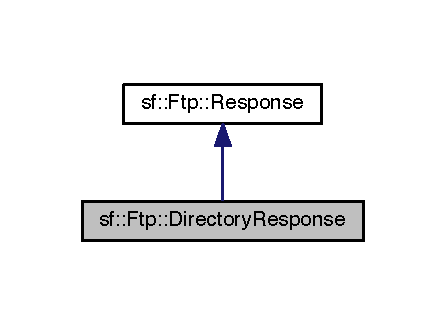
\includegraphics[width=214pt]{classsf_1_1_ftp_1_1_directory_response__inherit__graph}
\end{center}
\end{figure}


Collaboration diagram for sf\-:\-:Ftp\-:\-:Directory\-Response\-:
\nopagebreak
\begin{figure}[H]
\begin{center}
\leavevmode
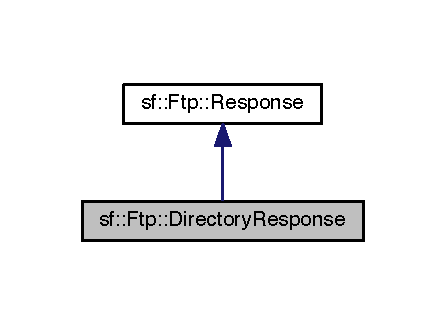
\includegraphics[width=214pt]{classsf_1_1_ftp_1_1_directory_response__coll__graph}
\end{center}
\end{figure}
\subsection*{Public Member Functions}
\begin{DoxyCompactItemize}
\item 
\hyperlink{classsf_1_1_ftp_1_1_directory_response_a36b6d2728fa53c4ad37b7a6307f4d388}{Directory\-Response} (const \hyperlink{classsf_1_1_ftp_1_1_response}{Response} \&response)
\begin{DoxyCompactList}\small\item\em Default constructor. \end{DoxyCompactList}\item 
const \hyperlink{gl3_8h_ac83513893df92266f79a515488701770}{std\-::string} \& \hyperlink{classsf_1_1_ftp_1_1_directory_response_a500793778ad0ed223aa86ed8fbee28a3}{get\-Directory} () const 
\begin{DoxyCompactList}\small\item\em Get the directory returned in the response. \end{DoxyCompactList}\end{DoxyCompactItemize}
\subsection*{Additional Inherited Members}


\subsection{Detailed Description}
Specialization of F\-T\-P response returning a directory. 

Definition at line 188 of file Ftp.\-hpp.



\subsection{Constructor \& Destructor Documentation}
\hypertarget{classsf_1_1_ftp_1_1_directory_response_a36b6d2728fa53c4ad37b7a6307f4d388}{\index{sf\-::\-Ftp\-::\-Directory\-Response@{sf\-::\-Ftp\-::\-Directory\-Response}!Directory\-Response@{Directory\-Response}}
\index{Directory\-Response@{Directory\-Response}!sf::Ftp::DirectoryResponse@{sf\-::\-Ftp\-::\-Directory\-Response}}
\subsubsection[{Directory\-Response}]{\setlength{\rightskip}{0pt plus 5cm}sf\-::\-Ftp\-::\-Directory\-Response\-::\-Directory\-Response (
\begin{DoxyParamCaption}
\item[{const {\bf Response} \&}]{response}
\end{DoxyParamCaption}
)}}\label{classsf_1_1_ftp_1_1_directory_response_a36b6d2728fa53c4ad37b7a6307f4d388}


Default constructor. 


\begin{DoxyParams}{Parameters}
{\em response} & Source response \\
\hline
\end{DoxyParams}


\subsection{Member Function Documentation}
\hypertarget{classsf_1_1_ftp_1_1_directory_response_a500793778ad0ed223aa86ed8fbee28a3}{\index{sf\-::\-Ftp\-::\-Directory\-Response@{sf\-::\-Ftp\-::\-Directory\-Response}!get\-Directory@{get\-Directory}}
\index{get\-Directory@{get\-Directory}!sf::Ftp::DirectoryResponse@{sf\-::\-Ftp\-::\-Directory\-Response}}
\subsubsection[{get\-Directory}]{\setlength{\rightskip}{0pt plus 5cm}const {\bf std\-::string}\& sf\-::\-Ftp\-::\-Directory\-Response\-::get\-Directory (
\begin{DoxyParamCaption}
{}
\end{DoxyParamCaption}
) const}}\label{classsf_1_1_ftp_1_1_directory_response_a500793778ad0ed223aa86ed8fbee28a3}


Get the directory returned in the response. 

\begin{DoxyReturn}{Returns}
Directory name 
\end{DoxyReturn}


The documentation for this class was generated from the following file\-:\begin{DoxyCompactItemize}
\item 
/\-Users/ira/\-Dropbox/ira\-\_\-dev/protobyte\-\_\-research/other\-\_\-libs/\-S\-F\-M\-L/dylibs/root/usr/local/include/\-S\-F\-M\-L/\-Network/\hyperlink{_ftp_8hpp}{Ftp.\-hpp}\end{DoxyCompactItemize}

\hypertarget{classsf_1_1_drawable}{\section{sf\-:\-:Drawable Class Reference}
\label{classsf_1_1_drawable}\index{sf\-::\-Drawable@{sf\-::\-Drawable}}
}


Abstract base class for objects that can be drawn to a render target.  




{\ttfamily \#include $<$Drawable.\-hpp$>$}



Inheritance diagram for sf\-:\-:Drawable\-:
\nopagebreak
\begin{figure}[H]
\begin{center}
\leavevmode
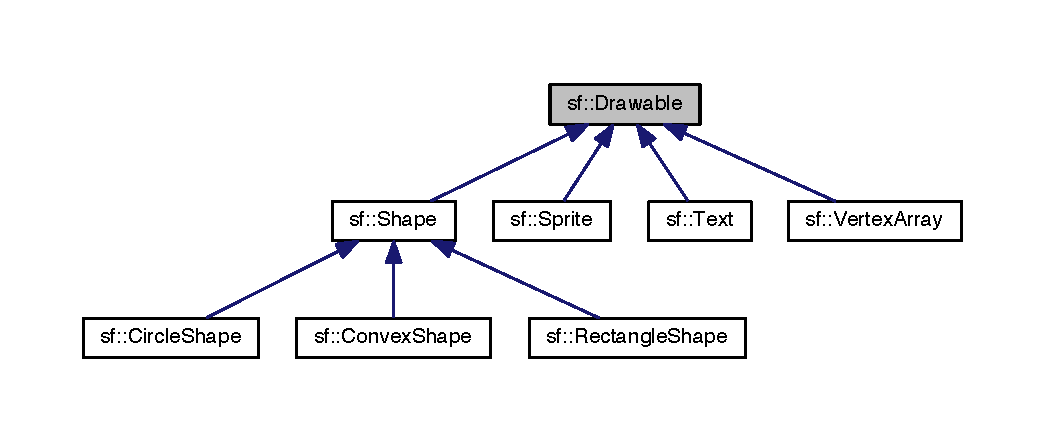
\includegraphics[width=350pt]{classsf_1_1_drawable__inherit__graph}
\end{center}
\end{figure}
\subsection*{Public Member Functions}
\begin{DoxyCompactItemize}
\item 
virtual \hyperlink{classsf_1_1_drawable_a906002f2df7beb5edbddf5bbef96f120}{$\sim$\-Drawable} ()
\begin{DoxyCompactList}\small\item\em Virtual destructor. \end{DoxyCompactList}\end{DoxyCompactItemize}
\subsection*{Protected Member Functions}
\begin{DoxyCompactItemize}
\item 
virtual \hyperlink{glutf90_8h_ac778d6f63f1aaf8ebda0ce6ac821b56e}{void} \hyperlink{classsf_1_1_drawable_a90d2c88bba9b035a0844eccb380ef631}{draw} (\hyperlink{classsf_1_1_render_target}{Render\-Target} \&\hyperlink{gl3ext_8h_af9d0cbbbeb7414e786c41899e5a856d7}{target}, \hyperlink{classsf_1_1_render_states}{Render\-States} states) const =0
\begin{DoxyCompactList}\small\item\em Draw the object to a render target. \end{DoxyCompactList}\end{DoxyCompactItemize}
\subsection*{Friends}
\begin{DoxyCompactItemize}
\item 
class \hyperlink{classsf_1_1_drawable_aa5afc6f82b7b587ed5ada4d227ce32aa}{Render\-Target}
\end{DoxyCompactItemize}


\subsection{Detailed Description}
Abstract base class for objects that can be drawn to a render target. 

\hyperlink{classsf_1_1_drawable}{sf\-::\-Drawable} is a very simple base class that allows objects of derived classes to be drawn to a \hyperlink{classsf_1_1_render_target}{sf\-::\-Render\-Target}.

All you have to do in your derived class is to override the draw virtual function.

Note that inheriting from \hyperlink{classsf_1_1_drawable}{sf\-::\-Drawable} is not mandatory, but it allows this nice syntax \char`\"{}window.\-draw(object)\char`\"{} rather than \char`\"{}object.\-draw(window)\char`\"{}, which is more consistent with other S\-F\-M\-L classes.

Example\-: 
\begin{DoxyCode}
\textcolor{keyword}{class }MyDrawable : \textcolor{keyword}{public} \hyperlink{classsf_1_1_drawable}{sf::Drawable}
\{
\textcolor{keyword}{public} :

   ...

private :

    \textcolor{keyword}{virtual} \textcolor{keywordtype}{void} \hyperlink{classsf_1_1_drawable_a90d2c88bba9b035a0844eccb380ef631}{draw}(\hyperlink{classsf_1_1_render_target}{sf::RenderTarget}& target, RenderStates states)\textcolor{keyword}{ const}
\textcolor{keyword}{    }\{
        \textcolor{comment}{// You can draw other high-level objects}
        target.\hyperlink{classsf_1_1_render_target_a12417a3bcc245c41d957b29583556f39}{draw}(m\_sprite, states);

        \textcolor{comment}{// ... or use the low-level API}
        states.texture = &m\_texture;
        target.\hyperlink{classsf_1_1_render_target_a12417a3bcc245c41d957b29583556f39}{draw}(m\_vertices, states);

        \textcolor{comment}{// ... or draw with OpenGL directly}
        \hyperlink{gl_8h_a78d1cc551d8585ab6aee14f75cd6671f}{glBegin}(\hyperlink{gl_8h_a36b428225d54dd9cf2e564e5ada3ad3d}{GL\_QUADS});
        ...
        \hyperlink{gl_8h_af50123535ec586f448744e0bc5a35923}{glEnd}();
    \}

    \hyperlink{classsf_1_1_sprite}{sf::Sprite} m\_sprite;
    \hyperlink{classsf_1_1_texture}{sf::Texture} m\_texture;
    \hyperlink{classsf_1_1_vertex_array}{sf::VertexArray} m\_vertices;
\};
\end{DoxyCode}


\begin{DoxySeeAlso}{See Also}
\hyperlink{classsf_1_1_render_target}{sf\-::\-Render\-Target} 
\end{DoxySeeAlso}


Definition at line 44 of file Drawable.\-hpp.



\subsection{Constructor \& Destructor Documentation}
\hypertarget{classsf_1_1_drawable_a906002f2df7beb5edbddf5bbef96f120}{\index{sf\-::\-Drawable@{sf\-::\-Drawable}!$\sim$\-Drawable@{$\sim$\-Drawable}}
\index{$\sim$\-Drawable@{$\sim$\-Drawable}!sf::Drawable@{sf\-::\-Drawable}}
\subsubsection[{$\sim$\-Drawable}]{\setlength{\rightskip}{0pt plus 5cm}virtual sf\-::\-Drawable\-::$\sim$\-Drawable (
\begin{DoxyParamCaption}
{}
\end{DoxyParamCaption}
)\hspace{0.3cm}{\ttfamily [inline]}, {\ttfamily [virtual]}}}\label{classsf_1_1_drawable_a906002f2df7beb5edbddf5bbef96f120}


Virtual destructor. 



Definition at line 52 of file Drawable.\-hpp.



\subsection{Member Function Documentation}
\hypertarget{classsf_1_1_drawable_a90d2c88bba9b035a0844eccb380ef631}{\index{sf\-::\-Drawable@{sf\-::\-Drawable}!draw@{draw}}
\index{draw@{draw}!sf::Drawable@{sf\-::\-Drawable}}
\subsubsection[{draw}]{\setlength{\rightskip}{0pt plus 5cm}virtual {\bf void} sf\-::\-Drawable\-::draw (
\begin{DoxyParamCaption}
\item[{{\bf Render\-Target} \&}]{target, }
\item[{{\bf Render\-States}}]{states}
\end{DoxyParamCaption}
) const\hspace{0.3cm}{\ttfamily [protected]}, {\ttfamily [pure virtual]}}}\label{classsf_1_1_drawable_a90d2c88bba9b035a0844eccb380ef631}


Draw the object to a render target. 

This is a pure virtual function that has to be implemented by the derived class to define how the drawable should be drawn.


\begin{DoxyParams}{Parameters}
{\em target} & Render target to draw to \\
\hline
{\em states} & Current render states \\
\hline
\end{DoxyParams}


\subsection{Friends And Related Function Documentation}
\hypertarget{classsf_1_1_drawable_aa5afc6f82b7b587ed5ada4d227ce32aa}{\index{sf\-::\-Drawable@{sf\-::\-Drawable}!Render\-Target@{Render\-Target}}
\index{Render\-Target@{Render\-Target}!sf::Drawable@{sf\-::\-Drawable}}
\subsubsection[{Render\-Target}]{\setlength{\rightskip}{0pt plus 5cm}friend class {\bf Render\-Target}\hspace{0.3cm}{\ttfamily [friend]}}}\label{classsf_1_1_drawable_aa5afc6f82b7b587ed5ada4d227ce32aa}


Definition at line 56 of file Drawable.\-hpp.



The documentation for this class was generated from the following file\-:\begin{DoxyCompactItemize}
\item 
/\-Users/ira/\-Dropbox/ira\-\_\-dev/protobyte\-\_\-research/other\-\_\-libs/\-S\-F\-M\-L/dylibs/root/usr/local/include/\-S\-F\-M\-L/\-Graphics/\hyperlink{_drawable_8hpp}{Drawable.\-hpp}\end{DoxyCompactItemize}

\hypertarget{classsf_1_1_event}{\section{sf\-:\-:Event Class Reference}
\label{classsf_1_1_event}\index{sf\-::\-Event@{sf\-::\-Event}}
}


Defines a system event and its parameters.  




{\ttfamily \#include $<$Event.\-hpp$>$}



Collaboration diagram for sf\-:\-:Event\-:
\nopagebreak
\begin{figure}[H]
\begin{center}
\leavevmode
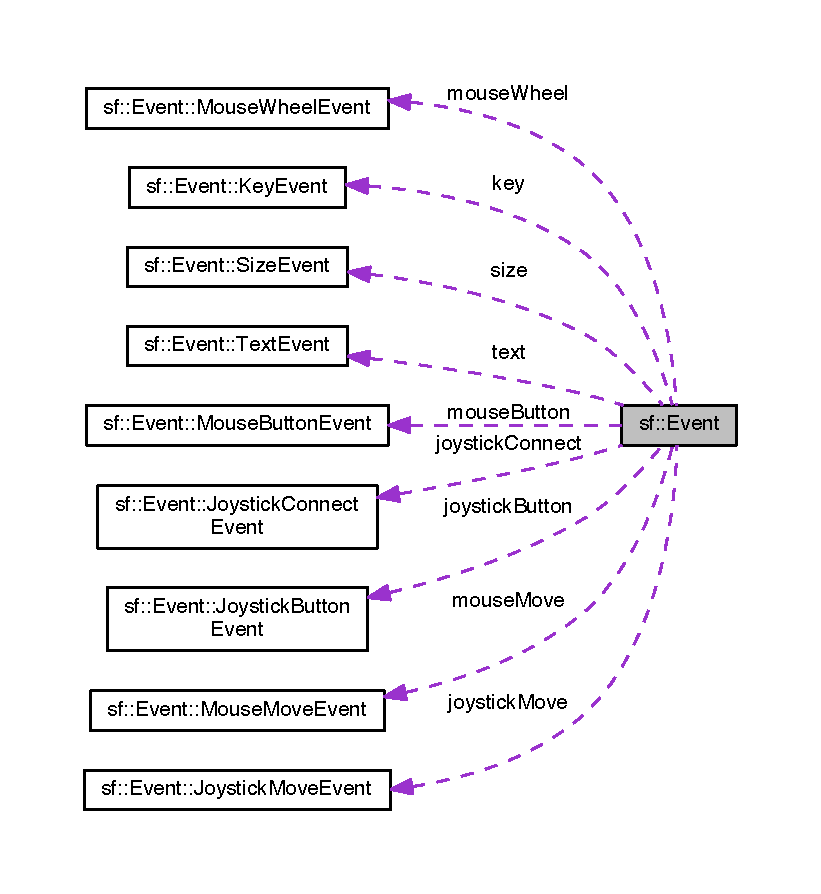
\includegraphics[width=350pt]{classsf_1_1_event__coll__graph}
\end{center}
\end{figure}
\subsection*{Classes}
\begin{DoxyCompactItemize}
\item 
struct \hyperlink{structsf_1_1_event_1_1_joystick_button_event}{Joystick\-Button\-Event}
\begin{DoxyCompactList}\small\item\em \hyperlink{classsf_1_1_joystick}{Joystick} buttons events parameters (Joystick\-Button\-Pressed, Joystick\-Button\-Released) \end{DoxyCompactList}\item 
struct \hyperlink{structsf_1_1_event_1_1_joystick_connect_event}{Joystick\-Connect\-Event}
\begin{DoxyCompactList}\small\item\em \hyperlink{classsf_1_1_joystick}{Joystick} connection events parameters (Joystick\-Connected, Joystick\-Disconnected) \end{DoxyCompactList}\item 
struct \hyperlink{structsf_1_1_event_1_1_joystick_move_event}{Joystick\-Move\-Event}
\begin{DoxyCompactList}\small\item\em \hyperlink{classsf_1_1_joystick}{Joystick} axis move event parameters (Joystick\-Moved) \end{DoxyCompactList}\item 
struct \hyperlink{structsf_1_1_event_1_1_key_event}{Key\-Event}
\begin{DoxyCompactList}\small\item\em \hyperlink{classsf_1_1_keyboard}{Keyboard} event parameters (Key\-Pressed, Key\-Released) \end{DoxyCompactList}\item 
struct \hyperlink{structsf_1_1_event_1_1_mouse_button_event}{Mouse\-Button\-Event}
\begin{DoxyCompactList}\small\item\em \hyperlink{classsf_1_1_mouse}{Mouse} buttons events parameters (Mouse\-Button\-Pressed, Mouse\-Button\-Released) \end{DoxyCompactList}\item 
struct \hyperlink{structsf_1_1_event_1_1_mouse_move_event}{Mouse\-Move\-Event}
\begin{DoxyCompactList}\small\item\em \hyperlink{classsf_1_1_mouse}{Mouse} move event parameters (Mouse\-Moved) \end{DoxyCompactList}\item 
struct \hyperlink{structsf_1_1_event_1_1_mouse_wheel_event}{Mouse\-Wheel\-Event}
\begin{DoxyCompactList}\small\item\em \hyperlink{classsf_1_1_mouse}{Mouse} wheel events parameters (Mouse\-Wheel\-Moved) \end{DoxyCompactList}\item 
struct \hyperlink{structsf_1_1_event_1_1_size_event}{Size\-Event}
\begin{DoxyCompactList}\small\item\em Size events parameters (Resized) \end{DoxyCompactList}\item 
struct \hyperlink{structsf_1_1_event_1_1_text_event}{Text\-Event}
\begin{DoxyCompactList}\small\item\em \hyperlink{classsf_1_1_text}{Text} event parameters (Text\-Entered) \end{DoxyCompactList}\end{DoxyCompactItemize}
\subsection*{Public Types}
\begin{DoxyCompactItemize}
\item 
enum \hyperlink{classsf_1_1_event_af41fa9ed45c02449030699f671331d4a}{Event\-Type} \{ \\*
\hyperlink{classsf_1_1_event_af41fa9ed45c02449030699f671331d4aa316e4212e083f1dce79efd8d9e9c0a95}{Closed}, 
\hyperlink{classsf_1_1_event_af41fa9ed45c02449030699f671331d4aa67fd26d7e520bc6722db3ff47ef24941}{Resized}, 
\hyperlink{classsf_1_1_event_af41fa9ed45c02449030699f671331d4aabd7877b5011a337268357c973e8347bd}{Lost\-Focus}, 
\hyperlink{classsf_1_1_event_af41fa9ed45c02449030699f671331d4aa8c5003ced508499933d540df8a6023ec}{Gained\-Focus}, 
\\*
\hyperlink{classsf_1_1_event_af41fa9ed45c02449030699f671331d4aa7e09871dc984080ff528e4f7e073e874}{Text\-Entered}, 
\hyperlink{classsf_1_1_event_af41fa9ed45c02449030699f671331d4aac3c7abfaa98c73bfe6be0b57df09c71b}{Key\-Pressed}, 
\hyperlink{classsf_1_1_event_af41fa9ed45c02449030699f671331d4aaa5bcc1e603d5a6f4c137af39558bd5d1}{Key\-Released}, 
\hyperlink{classsf_1_1_event_af41fa9ed45c02449030699f671331d4aa5cc9d3941af2a36049f4f9922c934a80}{Mouse\-Wheel\-Moved}, 
\\*
\hyperlink{classsf_1_1_event_af41fa9ed45c02449030699f671331d4aa55a3dcc8bf6c40e37f9ff2cdf606481f}{Mouse\-Button\-Pressed}, 
\hyperlink{classsf_1_1_event_af41fa9ed45c02449030699f671331d4aa9be69ecc07e484467ebbb133182fe5c1}{Mouse\-Button\-Released}, 
\hyperlink{classsf_1_1_event_af41fa9ed45c02449030699f671331d4aa4ff4fc3b3dc857e3617a63feb54be209}{Mouse\-Moved}, 
\hyperlink{classsf_1_1_event_af41fa9ed45c02449030699f671331d4aa50d98590a953e74c7ccf3dabadb22067}{Mouse\-Entered}, 
\\*
\hyperlink{classsf_1_1_event_af41fa9ed45c02449030699f671331d4aaa90b8526b328e0246d04b026de17c6e7}{Mouse\-Left}, 
\hyperlink{classsf_1_1_event_af41fa9ed45c02449030699f671331d4aa6d46855f0253f065689b69cd09437222}{Joystick\-Button\-Pressed}, 
\hyperlink{classsf_1_1_event_af41fa9ed45c02449030699f671331d4aa2246ef5ee33f7fa4b2a53f042ceeac3d}{Joystick\-Button\-Released}, 
\hyperlink{classsf_1_1_event_af41fa9ed45c02449030699f671331d4aa4d6ad228485c135967831be16ec074dd}{Joystick\-Moved}, 
\\*
\hyperlink{classsf_1_1_event_af41fa9ed45c02449030699f671331d4aaabb8877ec2f0c92904170deded09321e}{Joystick\-Connected}, 
\hyperlink{classsf_1_1_event_af41fa9ed45c02449030699f671331d4aab6e161dab7abaf154cc1c7b554558cb6}{Joystick\-Disconnected}, 
\hyperlink{classsf_1_1_event_af41fa9ed45c02449030699f671331d4aae51749211243cab2ab270b29cdc32a70}{Count}
 \}
\begin{DoxyCompactList}\small\item\em Enumeration of the different types of events. \end{DoxyCompactList}\end{DoxyCompactItemize}
\subsection*{Public Attributes}
\begin{DoxyCompactItemize}
\item 
\hyperlink{classsf_1_1_event_af41fa9ed45c02449030699f671331d4a}{Event\-Type} \hyperlink{classsf_1_1_event_adf2f8044f713fd9d6019077b0d1ffe0a}{type}
\begin{DoxyCompactList}\small\item\em Type of the event. \end{DoxyCompactList}\item 
\begin{tabbing}
xx\=xx\=xx\=xx\=xx\=xx\=xx\=xx\=xx\=\kill
union \{\\
\>\hyperlink{structsf_1_1_event_1_1_size_event}{SizeEvent} \hyperlink{classsf_1_1_event_a85dae56a377eeffd39183c3f6fc96cb9}{size}\\
\>\>{\em Size event parameters. }\\
\>\hyperlink{structsf_1_1_event_1_1_key_event}{KeyEvent} \hyperlink{classsf_1_1_event_a45b92fc6757ca7c193f06b302e424ab0}{key}\\
\>\>{\em Key event parameters. }\\
\>\hyperlink{structsf_1_1_event_1_1_text_event}{TextEvent} \hyperlink{classsf_1_1_event_a00c7bba6bee892791847ec22440e0a83}{text}\\
\>\>{\em \hyperlink{classsf_1_1_text}{Text} event parameters. }\\
\>\hyperlink{structsf_1_1_event_1_1_mouse_move_event}{MouseMoveEvent} \hyperlink{classsf_1_1_event_a786620ec4315d40c7c4cf4ddf3a1881f}{mouseMove}\\
\>\>{\em \hyperlink{classsf_1_1_mouse}{Mouse} move event parameters. }\\
\>\hyperlink{structsf_1_1_event_1_1_mouse_button_event}{MouseButtonEvent} \hyperlink{classsf_1_1_event_a20886a16ab7624de070b97145bb1dcac}{mouseButton}\\
\>\>{\em \hyperlink{classsf_1_1_mouse}{Mouse} button event parameters. }\\
\>\hyperlink{structsf_1_1_event_1_1_mouse_wheel_event}{MouseWheelEvent} \hyperlink{classsf_1_1_event_a8758c6d7998757978fd9146099a02a1e}{mouseWheel}\\
\>\>{\em \hyperlink{classsf_1_1_mouse}{Mouse} wheel event parameters. }\\
\>\hyperlink{structsf_1_1_event_1_1_joystick_move_event}{JoystickMoveEvent} \hyperlink{classsf_1_1_event_ac479e8351cc2024d5c1094dc33970f7f}{joystickMove}\\
\>\>{\em \hyperlink{classsf_1_1_joystick}{Joystick} move event parameters. }\\
\>\hyperlink{structsf_1_1_event_1_1_joystick_button_event}{JoystickButtonEvent} \hyperlink{classsf_1_1_event_a42aad27a054c1c05bd5c3d020e1db174}{joystickButton}\\
\>\>{\em \hyperlink{classsf_1_1_joystick}{Joystick} button event parameters. }\\
\>\hyperlink{structsf_1_1_event_1_1_joystick_connect_event}{JoystickConnectEvent} \hyperlink{classsf_1_1_event_aa354335c9ad73362442bc54ffe81118f}{joystickConnect}\\
\>\>{\em \hyperlink{classsf_1_1_joystick}{Joystick} (dis)connect event parameters. }\\
\}; \\

\end{tabbing}\end{DoxyCompactItemize}


\subsection{Detailed Description}
Defines a system event and its parameters. 

\hyperlink{classsf_1_1_event}{sf\-::\-Event} holds all the informations about a system event that just happened. Events are retrieved using the \hyperlink{classsf_1_1_window_a338e996585faf82e93069858e3b531b7}{sf\-::\-Window\-::poll\-Event} and \hyperlink{classsf_1_1_window_aaf02ab64fbc1d374eef3696df54137bc}{sf\-::\-Window\-::wait\-Event} functions.

A \hyperlink{classsf_1_1_event}{sf\-::\-Event} instance contains the type of the event (mouse moved, key pressed, window closed, ...) as well as the details about this particular event. Please note that the event parameters are defined in a union, which means that only the member matching the type of the event will be properly filled; all other members will have undefined values and must not be read if the type of the event doesn't match. For example, if you received a Key\-Pressed event, then you must read the event.\-key member, all other members such as event.\-Mouse\-Move or event.\-text will have undefined values.

Usage example\-: 
\begin{DoxyCode}
\hyperlink{classsf_1_1_event}{sf::Event} event;
\textcolor{keywordflow}{while} (window.\hyperlink{classsf_1_1_window_a338e996585faf82e93069858e3b531b7}{pollEvent}(event))
\{
    \textcolor{comment}{// Request for closing the window}
    \textcolor{keywordflow}{if} (event.\hyperlink{classsf_1_1_event_adf2f8044f713fd9d6019077b0d1ffe0a}{type} == \hyperlink{classsf_1_1_event_af41fa9ed45c02449030699f671331d4aa316e4212e083f1dce79efd8d9e9c0a95}{sf::Event::Closed})
        window.\hyperlink{classsf_1_1_window_a99d1e030387b0c26f5995670504fe7b5}{close}();

    \textcolor{comment}{// The escape key was pressed}
    \textcolor{keywordflow}{if} ((event.\hyperlink{classsf_1_1_event_adf2f8044f713fd9d6019077b0d1ffe0a}{type} == \hyperlink{classsf_1_1_event_af41fa9ed45c02449030699f671331d4aac3c7abfaa98c73bfe6be0b57df09c71b}{sf::Event::KeyPressed}) && (event.
      \hyperlink{classsf_1_1_event_a45b92fc6757ca7c193f06b302e424ab0}{key}.\hyperlink{structsf_1_1_event_1_1_key_event_a2879fdab8a68cb1c6ecc45730a2d0e61}{code} == \hyperlink{classsf_1_1_keyboard_acb4cacd7cc5802dec45724cf3314a142a64b7ecb543c5d03bec8383dde123c95d}{sf::Keyboard::Escape}))
        window.\hyperlink{classsf_1_1_window_a99d1e030387b0c26f5995670504fe7b5}{close}();

    \textcolor{comment}{// The window was resized}
    \textcolor{keywordflow}{if} (event.\hyperlink{classsf_1_1_event_adf2f8044f713fd9d6019077b0d1ffe0a}{type} == \hyperlink{classsf_1_1_event_af41fa9ed45c02449030699f671331d4aa67fd26d7e520bc6722db3ff47ef24941}{sf::Event::Resized})
        doSomethingWithTheNewSize(event.\hyperlink{classsf_1_1_event_a85dae56a377eeffd39183c3f6fc96cb9}{size}.\hyperlink{structsf_1_1_event_1_1_size_event_a20ea1b78c9bb1604432f8f0067bbfd94}{width}, event.\hyperlink{classsf_1_1_event_a85dae56a377eeffd39183c3f6fc96cb9}{size}.
      \hyperlink{structsf_1_1_event_1_1_size_event_af0f76a599d5f48189cb8d78d4e5facdb}{height});

    \textcolor{comment}{// etc ...}
\}
\end{DoxyCode}
 

Definition at line 43 of file Event.\-hpp.



\subsection{Member Enumeration Documentation}
\hypertarget{classsf_1_1_event_af41fa9ed45c02449030699f671331d4a}{\index{sf\-::\-Event@{sf\-::\-Event}!Event\-Type@{Event\-Type}}
\index{Event\-Type@{Event\-Type}!sf::Event@{sf\-::\-Event}}
\subsubsection[{Event\-Type}]{\setlength{\rightskip}{0pt plus 5cm}enum {\bf sf\-::\-Event\-::\-Event\-Type}}}\label{classsf_1_1_event_af41fa9ed45c02449030699f671331d4a}


Enumeration of the different types of events. 

\begin{Desc}
\item[Enumerator]\par
\begin{description}
\index{Closed@{Closed}!sf\-::\-Event@{sf\-::\-Event}}\index{sf\-::\-Event@{sf\-::\-Event}!Closed@{Closed}}\item[{\em 
\hypertarget{classsf_1_1_event_af41fa9ed45c02449030699f671331d4aa316e4212e083f1dce79efd8d9e9c0a95}{Closed}\label{classsf_1_1_event_af41fa9ed45c02449030699f671331d4aa316e4212e083f1dce79efd8d9e9c0a95}
}]The window requested to be closed. \index{Resized@{Resized}!sf\-::\-Event@{sf\-::\-Event}}\index{sf\-::\-Event@{sf\-::\-Event}!Resized@{Resized}}\item[{\em 
\hypertarget{classsf_1_1_event_af41fa9ed45c02449030699f671331d4aa67fd26d7e520bc6722db3ff47ef24941}{Resized}\label{classsf_1_1_event_af41fa9ed45c02449030699f671331d4aa67fd26d7e520bc6722db3ff47ef24941}
}]The window was resized. \index{Lost\-Focus@{Lost\-Focus}!sf\-::\-Event@{sf\-::\-Event}}\index{sf\-::\-Event@{sf\-::\-Event}!Lost\-Focus@{Lost\-Focus}}\item[{\em 
\hypertarget{classsf_1_1_event_af41fa9ed45c02449030699f671331d4aabd7877b5011a337268357c973e8347bd}{Lost\-Focus}\label{classsf_1_1_event_af41fa9ed45c02449030699f671331d4aabd7877b5011a337268357c973e8347bd}
}]The window lost the focus. \index{Gained\-Focus@{Gained\-Focus}!sf\-::\-Event@{sf\-::\-Event}}\index{sf\-::\-Event@{sf\-::\-Event}!Gained\-Focus@{Gained\-Focus}}\item[{\em 
\hypertarget{classsf_1_1_event_af41fa9ed45c02449030699f671331d4aa8c5003ced508499933d540df8a6023ec}{Gained\-Focus}\label{classsf_1_1_event_af41fa9ed45c02449030699f671331d4aa8c5003ced508499933d540df8a6023ec}
}]The window gained the focus. \index{Text\-Entered@{Text\-Entered}!sf\-::\-Event@{sf\-::\-Event}}\index{sf\-::\-Event@{sf\-::\-Event}!Text\-Entered@{Text\-Entered}}\item[{\em 
\hypertarget{classsf_1_1_event_af41fa9ed45c02449030699f671331d4aa7e09871dc984080ff528e4f7e073e874}{Text\-Entered}\label{classsf_1_1_event_af41fa9ed45c02449030699f671331d4aa7e09871dc984080ff528e4f7e073e874}
}]A character was entered. \index{Key\-Pressed@{Key\-Pressed}!sf\-::\-Event@{sf\-::\-Event}}\index{sf\-::\-Event@{sf\-::\-Event}!Key\-Pressed@{Key\-Pressed}}\item[{\em 
\hypertarget{classsf_1_1_event_af41fa9ed45c02449030699f671331d4aac3c7abfaa98c73bfe6be0b57df09c71b}{Key\-Pressed}\label{classsf_1_1_event_af41fa9ed45c02449030699f671331d4aac3c7abfaa98c73bfe6be0b57df09c71b}
}]A key was pressed. \index{Key\-Released@{Key\-Released}!sf\-::\-Event@{sf\-::\-Event}}\index{sf\-::\-Event@{sf\-::\-Event}!Key\-Released@{Key\-Released}}\item[{\em 
\hypertarget{classsf_1_1_event_af41fa9ed45c02449030699f671331d4aaa5bcc1e603d5a6f4c137af39558bd5d1}{Key\-Released}\label{classsf_1_1_event_af41fa9ed45c02449030699f671331d4aaa5bcc1e603d5a6f4c137af39558bd5d1}
}]A key was released. \index{Mouse\-Wheel\-Moved@{Mouse\-Wheel\-Moved}!sf\-::\-Event@{sf\-::\-Event}}\index{sf\-::\-Event@{sf\-::\-Event}!Mouse\-Wheel\-Moved@{Mouse\-Wheel\-Moved}}\item[{\em 
\hypertarget{classsf_1_1_event_af41fa9ed45c02449030699f671331d4aa5cc9d3941af2a36049f4f9922c934a80}{Mouse\-Wheel\-Moved}\label{classsf_1_1_event_af41fa9ed45c02449030699f671331d4aa5cc9d3941af2a36049f4f9922c934a80}
}]The mouse wheel was scrolled. \index{Mouse\-Button\-Pressed@{Mouse\-Button\-Pressed}!sf\-::\-Event@{sf\-::\-Event}}\index{sf\-::\-Event@{sf\-::\-Event}!Mouse\-Button\-Pressed@{Mouse\-Button\-Pressed}}\item[{\em 
\hypertarget{classsf_1_1_event_af41fa9ed45c02449030699f671331d4aa55a3dcc8bf6c40e37f9ff2cdf606481f}{Mouse\-Button\-Pressed}\label{classsf_1_1_event_af41fa9ed45c02449030699f671331d4aa55a3dcc8bf6c40e37f9ff2cdf606481f}
}]A mouse button was pressed. \index{Mouse\-Button\-Released@{Mouse\-Button\-Released}!sf\-::\-Event@{sf\-::\-Event}}\index{sf\-::\-Event@{sf\-::\-Event}!Mouse\-Button\-Released@{Mouse\-Button\-Released}}\item[{\em 
\hypertarget{classsf_1_1_event_af41fa9ed45c02449030699f671331d4aa9be69ecc07e484467ebbb133182fe5c1}{Mouse\-Button\-Released}\label{classsf_1_1_event_af41fa9ed45c02449030699f671331d4aa9be69ecc07e484467ebbb133182fe5c1}
}]A mouse button was released. \index{Mouse\-Moved@{Mouse\-Moved}!sf\-::\-Event@{sf\-::\-Event}}\index{sf\-::\-Event@{sf\-::\-Event}!Mouse\-Moved@{Mouse\-Moved}}\item[{\em 
\hypertarget{classsf_1_1_event_af41fa9ed45c02449030699f671331d4aa4ff4fc3b3dc857e3617a63feb54be209}{Mouse\-Moved}\label{classsf_1_1_event_af41fa9ed45c02449030699f671331d4aa4ff4fc3b3dc857e3617a63feb54be209}
}]The mouse cursor moved. \index{Mouse\-Entered@{Mouse\-Entered}!sf\-::\-Event@{sf\-::\-Event}}\index{sf\-::\-Event@{sf\-::\-Event}!Mouse\-Entered@{Mouse\-Entered}}\item[{\em 
\hypertarget{classsf_1_1_event_af41fa9ed45c02449030699f671331d4aa50d98590a953e74c7ccf3dabadb22067}{Mouse\-Entered}\label{classsf_1_1_event_af41fa9ed45c02449030699f671331d4aa50d98590a953e74c7ccf3dabadb22067}
}]The mouse cursor entered the area of the window. \index{Mouse\-Left@{Mouse\-Left}!sf\-::\-Event@{sf\-::\-Event}}\index{sf\-::\-Event@{sf\-::\-Event}!Mouse\-Left@{Mouse\-Left}}\item[{\em 
\hypertarget{classsf_1_1_event_af41fa9ed45c02449030699f671331d4aaa90b8526b328e0246d04b026de17c6e7}{Mouse\-Left}\label{classsf_1_1_event_af41fa9ed45c02449030699f671331d4aaa90b8526b328e0246d04b026de17c6e7}
}]The mouse cursor left the area of the window. \index{Joystick\-Button\-Pressed@{Joystick\-Button\-Pressed}!sf\-::\-Event@{sf\-::\-Event}}\index{sf\-::\-Event@{sf\-::\-Event}!Joystick\-Button\-Pressed@{Joystick\-Button\-Pressed}}\item[{\em 
\hypertarget{classsf_1_1_event_af41fa9ed45c02449030699f671331d4aa6d46855f0253f065689b69cd09437222}{Joystick\-Button\-Pressed}\label{classsf_1_1_event_af41fa9ed45c02449030699f671331d4aa6d46855f0253f065689b69cd09437222}
}]A joystick button was pressed. \index{Joystick\-Button\-Released@{Joystick\-Button\-Released}!sf\-::\-Event@{sf\-::\-Event}}\index{sf\-::\-Event@{sf\-::\-Event}!Joystick\-Button\-Released@{Joystick\-Button\-Released}}\item[{\em 
\hypertarget{classsf_1_1_event_af41fa9ed45c02449030699f671331d4aa2246ef5ee33f7fa4b2a53f042ceeac3d}{Joystick\-Button\-Released}\label{classsf_1_1_event_af41fa9ed45c02449030699f671331d4aa2246ef5ee33f7fa4b2a53f042ceeac3d}
}]A joystick button was released. \index{Joystick\-Moved@{Joystick\-Moved}!sf\-::\-Event@{sf\-::\-Event}}\index{sf\-::\-Event@{sf\-::\-Event}!Joystick\-Moved@{Joystick\-Moved}}\item[{\em 
\hypertarget{classsf_1_1_event_af41fa9ed45c02449030699f671331d4aa4d6ad228485c135967831be16ec074dd}{Joystick\-Moved}\label{classsf_1_1_event_af41fa9ed45c02449030699f671331d4aa4d6ad228485c135967831be16ec074dd}
}]The joystick moved along an axis. \index{Joystick\-Connected@{Joystick\-Connected}!sf\-::\-Event@{sf\-::\-Event}}\index{sf\-::\-Event@{sf\-::\-Event}!Joystick\-Connected@{Joystick\-Connected}}\item[{\em 
\hypertarget{classsf_1_1_event_af41fa9ed45c02449030699f671331d4aaabb8877ec2f0c92904170deded09321e}{Joystick\-Connected}\label{classsf_1_1_event_af41fa9ed45c02449030699f671331d4aaabb8877ec2f0c92904170deded09321e}
}]A joystick was connected. \index{Joystick\-Disconnected@{Joystick\-Disconnected}!sf\-::\-Event@{sf\-::\-Event}}\index{sf\-::\-Event@{sf\-::\-Event}!Joystick\-Disconnected@{Joystick\-Disconnected}}\item[{\em 
\hypertarget{classsf_1_1_event_af41fa9ed45c02449030699f671331d4aab6e161dab7abaf154cc1c7b554558cb6}{Joystick\-Disconnected}\label{classsf_1_1_event_af41fa9ed45c02449030699f671331d4aab6e161dab7abaf154cc1c7b554558cb6}
}]A joystick was disconnected. \index{Count@{Count}!sf\-::\-Event@{sf\-::\-Event}}\index{sf\-::\-Event@{sf\-::\-Event}!Count@{Count}}\item[{\em 
\hypertarget{classsf_1_1_event_af41fa9ed45c02449030699f671331d4aae51749211243cab2ab270b29cdc32a70}{Count}\label{classsf_1_1_event_af41fa9ed45c02449030699f671331d4aae51749211243cab2ab270b29cdc32a70}
}]Keep last -- the total number of event types. \end{description}
\end{Desc}


Definition at line 148 of file Event.\-hpp.



\subsection{Member Data Documentation}
\hypertarget{classsf_1_1_event_a2bf14023ff24b0ae4d3a3fb263a31845}{\subsubsection[{"@7}]{\setlength{\rightskip}{0pt plus 5cm}union \{ ... \} }}\label{classsf_1_1_event_a2bf14023ff24b0ae4d3a3fb263a31845}
\hypertarget{classsf_1_1_event_a42aad27a054c1c05bd5c3d020e1db174}{\index{sf\-::\-Event@{sf\-::\-Event}!joystick\-Button@{joystick\-Button}}
\index{joystick\-Button@{joystick\-Button}!sf::Event@{sf\-::\-Event}}
\subsubsection[{joystick\-Button}]{\setlength{\rightskip}{0pt plus 5cm}{\bf Joystick\-Button\-Event} sf\-::\-Event\-::joystick\-Button}}\label{classsf_1_1_event_a42aad27a054c1c05bd5c3d020e1db174}


\hyperlink{classsf_1_1_joystick}{Joystick} button event parameters. 



Definition at line 186 of file Event.\-hpp.

\hypertarget{classsf_1_1_event_aa354335c9ad73362442bc54ffe81118f}{\index{sf\-::\-Event@{sf\-::\-Event}!joystick\-Connect@{joystick\-Connect}}
\index{joystick\-Connect@{joystick\-Connect}!sf::Event@{sf\-::\-Event}}
\subsubsection[{joystick\-Connect}]{\setlength{\rightskip}{0pt plus 5cm}{\bf Joystick\-Connect\-Event} sf\-::\-Event\-::joystick\-Connect}}\label{classsf_1_1_event_aa354335c9ad73362442bc54ffe81118f}


\hyperlink{classsf_1_1_joystick}{Joystick} (dis)connect event parameters. 



Definition at line 187 of file Event.\-hpp.

\hypertarget{classsf_1_1_event_ac479e8351cc2024d5c1094dc33970f7f}{\index{sf\-::\-Event@{sf\-::\-Event}!joystick\-Move@{joystick\-Move}}
\index{joystick\-Move@{joystick\-Move}!sf::Event@{sf\-::\-Event}}
\subsubsection[{joystick\-Move}]{\setlength{\rightskip}{0pt plus 5cm}{\bf Joystick\-Move\-Event} sf\-::\-Event\-::joystick\-Move}}\label{classsf_1_1_event_ac479e8351cc2024d5c1094dc33970f7f}


\hyperlink{classsf_1_1_joystick}{Joystick} move event parameters. 



Definition at line 185 of file Event.\-hpp.

\hypertarget{classsf_1_1_event_a45b92fc6757ca7c193f06b302e424ab0}{\index{sf\-::\-Event@{sf\-::\-Event}!key@{key}}
\index{key@{key}!sf::Event@{sf\-::\-Event}}
\subsubsection[{key}]{\setlength{\rightskip}{0pt plus 5cm}{\bf Key\-Event} sf\-::\-Event\-::key}}\label{classsf_1_1_event_a45b92fc6757ca7c193f06b302e424ab0}


Key event parameters. 



Definition at line 180 of file Event.\-hpp.

\hypertarget{classsf_1_1_event_a20886a16ab7624de070b97145bb1dcac}{\index{sf\-::\-Event@{sf\-::\-Event}!mouse\-Button@{mouse\-Button}}
\index{mouse\-Button@{mouse\-Button}!sf::Event@{sf\-::\-Event}}
\subsubsection[{mouse\-Button}]{\setlength{\rightskip}{0pt plus 5cm}{\bf Mouse\-Button\-Event} sf\-::\-Event\-::mouse\-Button}}\label{classsf_1_1_event_a20886a16ab7624de070b97145bb1dcac}


\hyperlink{classsf_1_1_mouse}{Mouse} button event parameters. 



Definition at line 183 of file Event.\-hpp.

\hypertarget{classsf_1_1_event_a786620ec4315d40c7c4cf4ddf3a1881f}{\index{sf\-::\-Event@{sf\-::\-Event}!mouse\-Move@{mouse\-Move}}
\index{mouse\-Move@{mouse\-Move}!sf::Event@{sf\-::\-Event}}
\subsubsection[{mouse\-Move}]{\setlength{\rightskip}{0pt plus 5cm}{\bf Mouse\-Move\-Event} sf\-::\-Event\-::mouse\-Move}}\label{classsf_1_1_event_a786620ec4315d40c7c4cf4ddf3a1881f}


\hyperlink{classsf_1_1_mouse}{Mouse} move event parameters. 



Definition at line 182 of file Event.\-hpp.

\hypertarget{classsf_1_1_event_a8758c6d7998757978fd9146099a02a1e}{\index{sf\-::\-Event@{sf\-::\-Event}!mouse\-Wheel@{mouse\-Wheel}}
\index{mouse\-Wheel@{mouse\-Wheel}!sf::Event@{sf\-::\-Event}}
\subsubsection[{mouse\-Wheel}]{\setlength{\rightskip}{0pt plus 5cm}{\bf Mouse\-Wheel\-Event} sf\-::\-Event\-::mouse\-Wheel}}\label{classsf_1_1_event_a8758c6d7998757978fd9146099a02a1e}


\hyperlink{classsf_1_1_mouse}{Mouse} wheel event parameters. 



Definition at line 184 of file Event.\-hpp.

\hypertarget{classsf_1_1_event_a85dae56a377eeffd39183c3f6fc96cb9}{\index{sf\-::\-Event@{sf\-::\-Event}!size@{size}}
\index{size@{size}!sf::Event@{sf\-::\-Event}}
\subsubsection[{size}]{\setlength{\rightskip}{0pt plus 5cm}{\bf Size\-Event} sf\-::\-Event\-::size}}\label{classsf_1_1_event_a85dae56a377eeffd39183c3f6fc96cb9}


Size event parameters. 



Definition at line 179 of file Event.\-hpp.

\hypertarget{classsf_1_1_event_a00c7bba6bee892791847ec22440e0a83}{\index{sf\-::\-Event@{sf\-::\-Event}!text@{text}}
\index{text@{text}!sf::Event@{sf\-::\-Event}}
\subsubsection[{text}]{\setlength{\rightskip}{0pt plus 5cm}{\bf Text\-Event} sf\-::\-Event\-::text}}\label{classsf_1_1_event_a00c7bba6bee892791847ec22440e0a83}


\hyperlink{classsf_1_1_text}{Text} event parameters. 



Definition at line 181 of file Event.\-hpp.

\hypertarget{classsf_1_1_event_adf2f8044f713fd9d6019077b0d1ffe0a}{\index{sf\-::\-Event@{sf\-::\-Event}!type@{type}}
\index{type@{type}!sf::Event@{sf\-::\-Event}}
\subsubsection[{type}]{\setlength{\rightskip}{0pt plus 5cm}{\bf Event\-Type} sf\-::\-Event\-::type}}\label{classsf_1_1_event_adf2f8044f713fd9d6019077b0d1ffe0a}


Type of the event. 



Definition at line 175 of file Event.\-hpp.



The documentation for this class was generated from the following file\-:\begin{DoxyCompactItemize}
\item 
/\-Users/ira/\-Dropbox/ira\-\_\-dev/protobyte\-\_\-research/other\-\_\-libs/\-S\-F\-M\-L/dylibs/root/usr/local/include/\-S\-F\-M\-L/\-Window/\hyperlink{_event_8hpp}{Event.\-hpp}\end{DoxyCompactItemize}

\hypertarget{class_face3}{\section{Face3 Class Reference}
\label{class_face3}\index{Face3@{Face3}}
}


{\ttfamily \#include $<$Face3.\-h$>$}

\subsection*{Public Member Functions}
\begin{DoxyCompactItemize}
\item 
\hyperlink{class_face3_a0f1498f8fdb47eb15d6f5ad9eb355671}{Face3} (\hyperlink{class_vertex}{Vertex} $\ast$v0\-\_\-p, \hyperlink{class_vertex}{Vertex} $\ast$v1\-\_\-p, \hyperlink{class_vertex}{Vertex} $\ast$v2\-\_\-p)
\item 
\hyperlink{glutf90_8h_ac778d6f63f1aaf8ebda0ce6ac821b56e}{void} \hyperlink{class_face3_ad63869f6950c65a327a6c5bc5d742154}{display} ()
\item 
const \hyperlink{class_vector3}{Vector3} \& \hyperlink{class_face3_a30feef340693ff8f5ea1f732f692d33f}{get\-Norm} () const 
\item 
const \hyperlink{class_vector3}{Vector3} \& \hyperlink{class_face3_a2ef3d1aea90175978c0240589959b762}{get\-Centroid} () const 
\item 
const \hyperlink{class_vertex}{Vertex} $\ast$ \hyperlink{class_face3_a7d1d444d697b588fcee74aa79b0f74eb}{operator\mbox{[}$\,$\mbox{]}} (int \hyperlink{gl3_8h_a57f14e05b1900f16a2da82ade47d0c6d}{index})
\end{DoxyCompactItemize}
\subsection*{Friends}
\begin{DoxyCompactItemize}
\item 
std\-::ostream \& \hyperlink{class_face3_adf81375bd8fe97e6b11413afd6295943}{operator$<$$<$} (std\-::ostream \&output, const \hyperlink{class_face3}{Face3} \&face3)
\end{DoxyCompactItemize}


\subsection{Detailed Description}


Definition at line 18 of file Face3.\-h.



\subsection{Constructor \& Destructor Documentation}
\hypertarget{class_face3_a0f1498f8fdb47eb15d6f5ad9eb355671}{\index{Face3@{Face3}!Face3@{Face3}}
\index{Face3@{Face3}!Face3@{Face3}}
\subsubsection[{Face3}]{\setlength{\rightskip}{0pt plus 5cm}Face3\-::\-Face3 (
\begin{DoxyParamCaption}
\item[{{\bf Vertex} $\ast$}]{v0\-\_\-p, }
\item[{{\bf Vertex} $\ast$}]{v1\-\_\-p, }
\item[{{\bf Vertex} $\ast$}]{v2\-\_\-p}
\end{DoxyParamCaption}
)}}\label{class_face3_a0f1498f8fdb47eb15d6f5ad9eb355671}


Definition at line 19 of file Face3.\-cpp.



\subsection{Member Function Documentation}
\hypertarget{class_face3_ad63869f6950c65a327a6c5bc5d742154}{\index{Face3@{Face3}!display@{display}}
\index{display@{display}!Face3@{Face3}}
\subsubsection[{display}]{\setlength{\rightskip}{0pt plus 5cm}{\bf void} Face3\-::display (
\begin{DoxyParamCaption}
{}
\end{DoxyParamCaption}
)}}\label{class_face3_ad63869f6950c65a327a6c5bc5d742154}


Definition at line 34 of file Face3.\-cpp.

\hypertarget{class_face3_a2ef3d1aea90175978c0240589959b762}{\index{Face3@{Face3}!get\-Centroid@{get\-Centroid}}
\index{get\-Centroid@{get\-Centroid}!Face3@{Face3}}
\subsubsection[{get\-Centroid}]{\setlength{\rightskip}{0pt plus 5cm}const {\bf Vector3} \& Face3\-::get\-Centroid (
\begin{DoxyParamCaption}
{}
\end{DoxyParamCaption}
) const}}\label{class_face3_a2ef3d1aea90175978c0240589959b762}


Definition at line 83 of file Face3.\-cpp.

\hypertarget{class_face3_a30feef340693ff8f5ea1f732f692d33f}{\index{Face3@{Face3}!get\-Norm@{get\-Norm}}
\index{get\-Norm@{get\-Norm}!Face3@{Face3}}
\subsubsection[{get\-Norm}]{\setlength{\rightskip}{0pt plus 5cm}const {\bf Vector3} \& Face3\-::get\-Norm (
\begin{DoxyParamCaption}
{}
\end{DoxyParamCaption}
) const}}\label{class_face3_a30feef340693ff8f5ea1f732f692d33f}


Definition at line 79 of file Face3.\-cpp.

\hypertarget{class_face3_a7d1d444d697b588fcee74aa79b0f74eb}{\index{Face3@{Face3}!operator\mbox{[}$\,$\mbox{]}@{operator[]}}
\index{operator\mbox{[}$\,$\mbox{]}@{operator[]}!Face3@{Face3}}
\subsubsection[{operator[]}]{\setlength{\rightskip}{0pt plus 5cm}const {\bf Vertex} $\ast$ Face3\-::operator\mbox{[}$\,$\mbox{]} (
\begin{DoxyParamCaption}
\item[{int}]{index}
\end{DoxyParamCaption}
)}}\label{class_face3_a7d1d444d697b588fcee74aa79b0f74eb}


Definition at line 87 of file Face3.\-cpp.



\subsection{Friends And Related Function Documentation}
\hypertarget{class_face3_adf81375bd8fe97e6b11413afd6295943}{\index{Face3@{Face3}!operator$<$$<$@{operator$<$$<$}}
\index{operator$<$$<$@{operator$<$$<$}!Face3@{Face3}}
\subsubsection[{operator$<$$<$}]{\setlength{\rightskip}{0pt plus 5cm}std\-::ostream\& operator$<$$<$ (
\begin{DoxyParamCaption}
\item[{std\-::ostream \&}]{output, }
\item[{const {\bf Face3} \&}]{face3}
\end{DoxyParamCaption}
)\hspace{0.3cm}{\ttfamily [friend]}}}\label{class_face3_adf81375bd8fe97e6b11413afd6295943}


Definition at line 14 of file Face3.\-cpp.



The documentation for this class was generated from the following files\-:\begin{DoxyCompactItemize}
\item 
/\-Users/ira/\-Dropbox/ira\-\_\-dev/protobyte\-\_\-research/\-Protobyte/\hyperlink{_face3_8h}{Face3.\-h}\item 
/\-Users/ira/\-Dropbox/ira\-\_\-dev/protobyte\-\_\-research/\-Protobyte/\hyperlink{_face3_8cpp}{Face3.\-cpp}\end{DoxyCompactItemize}

\hypertarget{classsf_1_1_font}{\section{sf\-:\-:Font Class Reference}
\label{classsf_1_1_font}\index{sf\-::\-Font@{sf\-::\-Font}}
}


Class for loading and manipulating character fonts.  




{\ttfamily \#include $<$Font.\-hpp$>$}

\subsection*{Public Member Functions}
\begin{DoxyCompactItemize}
\item 
\hyperlink{classsf_1_1_font_a506404655b8869ed60d1e7709812f583}{Font} ()
\begin{DoxyCompactList}\small\item\em Default constructor. \end{DoxyCompactList}\item 
\hyperlink{classsf_1_1_font_a72d7322b355ee2f1be4500f530e98081}{Font} (const \hyperlink{classsf_1_1_font}{Font} \&copy)
\begin{DoxyCompactList}\small\item\em Copy constructor. \end{DoxyCompactList}\item 
\hyperlink{classsf_1_1_font_aa18a3c62e6e01e9a21c531b5cad4b7f2}{$\sim$\-Font} ()
\begin{DoxyCompactList}\small\item\em Destructor. \end{DoxyCompactList}\item 
bool \hyperlink{classsf_1_1_font_ab020052ef4e01f6c749a85571c0f3fd1}{load\-From\-File} (const \hyperlink{gl3_8h_ac83513893df92266f79a515488701770}{std\-::string} \&filename)
\begin{DoxyCompactList}\small\item\em Load the font from a file. \end{DoxyCompactList}\item 
bool \hyperlink{classsf_1_1_font_abf2f8d6de31eb4e1db02e061c323e346}{load\-From\-Memory} (const \hyperlink{glutf90_8h_ac778d6f63f1aaf8ebda0ce6ac821b56e}{void} $\ast$\hyperlink{gl3_8h_a0f78eecb0891cce3bdfc815b971866a1}{data}, std\-::size\-\_\-t size\-In\-Bytes)
\begin{DoxyCompactList}\small\item\em Load the font from a file in memory. \end{DoxyCompactList}\item 
bool \hyperlink{classsf_1_1_font_abc3f37a354ce8b9a21f8eb93bd9fdafb}{load\-From\-Stream} (\hyperlink{classsf_1_1_input_stream}{Input\-Stream} \&stream)
\begin{DoxyCompactList}\small\item\em Load the font from a custom stream. \end{DoxyCompactList}\item 
const \hyperlink{classsf_1_1_glyph}{Glyph} \& \hyperlink{classsf_1_1_font_a148eb92890113052f12f8a231ad619b9}{get\-Glyph} (\hyperlink{namespacesf_aa746fb1ddef4410bddf198ebb27e727c}{Uint32} code\-Point, unsigned int character\-Size, bool bold) const 
\begin{DoxyCompactList}\small\item\em Retrieve a glyph of the font. \end{DoxyCompactList}\item 
int \hyperlink{classsf_1_1_font_a4093f7d2d195c88ea90b34cf14e003c8}{get\-Kerning} (\hyperlink{namespacesf_aa746fb1ddef4410bddf198ebb27e727c}{Uint32} \hyperlink{gl3_8h_ada771a798be00a696d20928c9a3371e7}{first}, \hyperlink{namespacesf_aa746fb1ddef4410bddf198ebb27e727c}{Uint32} second, unsigned int character\-Size) const 
\begin{DoxyCompactList}\small\item\em Get the kerning offset of two glyphs. \end{DoxyCompactList}\item 
int \hyperlink{classsf_1_1_font_a05f23b88b13bd094083da5b7efc94371}{get\-Line\-Spacing} (unsigned int character\-Size) const 
\begin{DoxyCompactList}\small\item\em Get the line spacing. \end{DoxyCompactList}\item 
const \hyperlink{classsf_1_1_texture}{Texture} \& \hyperlink{classsf_1_1_font_a887368a4e6a3dfa32dea89d2af315951}{get\-Texture} (unsigned int character\-Size) const 
\begin{DoxyCompactList}\small\item\em Retrieve the texture containing the loaded glyphs of a certain size. \end{DoxyCompactList}\item 
\hyperlink{classsf_1_1_font}{Font} \& \hyperlink{classsf_1_1_font_a232515549846e3172a514d0b47918399}{operator=} (const \hyperlink{classsf_1_1_font}{Font} \&right)
\begin{DoxyCompactList}\small\item\em Overload of assignment operator. \end{DoxyCompactList}\end{DoxyCompactItemize}
\subsection*{Static Public Member Functions}
\begin{DoxyCompactItemize}
\item 
static const \hyperlink{classsf_1_1_font}{Font} \& \hyperlink{classsf_1_1_font_a88fc3372800948a1f8655c533cb8a952}{get\-Default\-Font} ()
\begin{DoxyCompactList}\small\item\em Return the default built-\/in font. \end{DoxyCompactList}\end{DoxyCompactItemize}


\subsection{Detailed Description}
Class for loading and manipulating character fonts. 

Fonts can be loaded from a file, from memory or from a custom stream, and supports the most common types of fonts. See the load\-From\-File function for the complete list of supported formats.

Once it is loaded, a \hyperlink{classsf_1_1_font}{sf\-::\-Font} instance provides three types of informations about the font\-: \begin{DoxyItemize}
\item Global metrics, such as the line spacing \item Per-\/glyph metrics, such as bounding box or kerning \item Pixel representation of glyphs\end{DoxyItemize}
Fonts alone are not very useful\-: they hold the font data but cannot make anything useful of it. To do so you need to use the \hyperlink{classsf_1_1_text}{sf\-::\-Text} class, which is able to properly output text with several options such as character size, style, color, position, rotation, etc. This separation allows more flexibility and better performances\-: indeed a \hyperlink{classsf_1_1_font}{sf\-::\-Font} is a heavy resource, and any operation on it is slow (often too slow for real-\/time applications). On the other side, a \hyperlink{classsf_1_1_text}{sf\-::\-Text} is a lightweight object which can combine the glyphs data and metrics of a \hyperlink{classsf_1_1_font}{sf\-::\-Font} to display any text on a render target. Note that it is also possible to bind several \hyperlink{classsf_1_1_text}{sf\-::\-Text} instances to the same \hyperlink{classsf_1_1_font}{sf\-::\-Font}.

It is important to note that the \hyperlink{classsf_1_1_text}{sf\-::\-Text} instance doesn't copy the font that it uses, it only keeps a reference to it. Thus, a \hyperlink{classsf_1_1_font}{sf\-::\-Font} must not be destructed while it is used by a \hyperlink{classsf_1_1_text}{sf\-::\-Text} (i.\-e. never write a function that uses a local \hyperlink{classsf_1_1_font}{sf\-::\-Font} instance for creating a text).

Usage example\-: 
\begin{DoxyCode}
\textcolor{comment}{// Declare a new font}
\hyperlink{classsf_1_1_font}{sf::Font} font;

\textcolor{comment}{// Load it from a file}
\textcolor{keywordflow}{if} (!font.\hyperlink{classsf_1_1_font_ab020052ef4e01f6c749a85571c0f3fd1}{loadFromFile}(\textcolor{stringliteral}{"arial.ttf"}))
\{
    \textcolor{comment}{// error...}
\}

\textcolor{comment}{// Create a text which uses our font}
\hyperlink{classsf_1_1_text}{sf::Text} text1;
text1.\hyperlink{classsf_1_1_text_a2927805d1ae92d57f15034ea34756b81}{setFont}(font);
text1.\hyperlink{classsf_1_1_text_ae96f835fc1bff858f8a23c5b01eaaf7e}{setCharacterSize}(30);
text1.\hyperlink{classsf_1_1_text_ad791702bc2d1b6590a1719aa60635edf}{setStyle}(\hyperlink{classsf_1_1_text_aa8add4aef484c6e6b20faff07452bd82a2af9ae5e1cda126570f744448e0caa32}{sf::Text::Regular});

\textcolor{comment}{// Create another text using the same font, but with different parameters}
\hyperlink{classsf_1_1_text}{sf::Text} text2;
text2.\hyperlink{classsf_1_1_text_a2927805d1ae92d57f15034ea34756b81}{setFont}(font);
text2.\hyperlink{classsf_1_1_text_ae96f835fc1bff858f8a23c5b01eaaf7e}{setCharacterSize}(50);
text1.\hyperlink{classsf_1_1_text_ad791702bc2d1b6590a1719aa60635edf}{setStyle}(\hyperlink{classsf_1_1_text_aa8add4aef484c6e6b20faff07452bd82aee249eb803848723c542c2062ebe69d8}{sf::Text::Italic});
\end{DoxyCode}


Apart from loading font files, and passing them to instances of \hyperlink{classsf_1_1_text}{sf\-::\-Text}, you should normally not have to deal directly with this class. However, it may be useful to access the font metrics or rasterized glyphs for advanced usage.

\begin{DoxySeeAlso}{See Also}
\hyperlink{classsf_1_1_text}{sf\-::\-Text} 
\end{DoxySeeAlso}


Definition at line 50 of file Font.\-hpp.



\subsection{Constructor \& Destructor Documentation}
\hypertarget{classsf_1_1_font_a506404655b8869ed60d1e7709812f583}{\index{sf\-::\-Font@{sf\-::\-Font}!Font@{Font}}
\index{Font@{Font}!sf::Font@{sf\-::\-Font}}
\subsubsection[{Font}]{\setlength{\rightskip}{0pt plus 5cm}sf\-::\-Font\-::\-Font (
\begin{DoxyParamCaption}
{}
\end{DoxyParamCaption}
)}}\label{classsf_1_1_font_a506404655b8869ed60d1e7709812f583}


Default constructor. 

This constructor defines an empty font \hypertarget{classsf_1_1_font_a72d7322b355ee2f1be4500f530e98081}{\index{sf\-::\-Font@{sf\-::\-Font}!Font@{Font}}
\index{Font@{Font}!sf::Font@{sf\-::\-Font}}
\subsubsection[{Font}]{\setlength{\rightskip}{0pt plus 5cm}sf\-::\-Font\-::\-Font (
\begin{DoxyParamCaption}
\item[{const {\bf Font} \&}]{copy}
\end{DoxyParamCaption}
)}}\label{classsf_1_1_font_a72d7322b355ee2f1be4500f530e98081}


Copy constructor. 


\begin{DoxyParams}{Parameters}
{\em copy} & Instance to copy \\
\hline
\end{DoxyParams}
\hypertarget{classsf_1_1_font_aa18a3c62e6e01e9a21c531b5cad4b7f2}{\index{sf\-::\-Font@{sf\-::\-Font}!$\sim$\-Font@{$\sim$\-Font}}
\index{$\sim$\-Font@{$\sim$\-Font}!sf::Font@{sf\-::\-Font}}
\subsubsection[{$\sim$\-Font}]{\setlength{\rightskip}{0pt plus 5cm}sf\-::\-Font\-::$\sim$\-Font (
\begin{DoxyParamCaption}
{}
\end{DoxyParamCaption}
)}}\label{classsf_1_1_font_aa18a3c62e6e01e9a21c531b5cad4b7f2}


Destructor. 

Cleans up all the internal resources used by the font 

\subsection{Member Function Documentation}
\hypertarget{classsf_1_1_font_a88fc3372800948a1f8655c533cb8a952}{\index{sf\-::\-Font@{sf\-::\-Font}!get\-Default\-Font@{get\-Default\-Font}}
\index{get\-Default\-Font@{get\-Default\-Font}!sf::Font@{sf\-::\-Font}}
\subsubsection[{get\-Default\-Font}]{\setlength{\rightskip}{0pt plus 5cm}static const {\bf Font}\& sf\-::\-Font\-::get\-Default\-Font (
\begin{DoxyParamCaption}
{}
\end{DoxyParamCaption}
)\hspace{0.3cm}{\ttfamily [static]}}}\label{classsf_1_1_font_a88fc3372800948a1f8655c533cb8a952}


Return the default built-\/in font. 

This font is provided for convenience, it is used by \hyperlink{classsf_1_1_text}{sf\-::\-Text} instances by default. It is provided so that users don't have to provide and load a font file in order to display text on screen. The font used is Arial.

\begin{DoxyReturn}{Returns}
Reference to the built-\/in default font 
\end{DoxyReturn}
\hypertarget{classsf_1_1_font_a148eb92890113052f12f8a231ad619b9}{\index{sf\-::\-Font@{sf\-::\-Font}!get\-Glyph@{get\-Glyph}}
\index{get\-Glyph@{get\-Glyph}!sf::Font@{sf\-::\-Font}}
\subsubsection[{get\-Glyph}]{\setlength{\rightskip}{0pt plus 5cm}const {\bf Glyph}\& sf\-::\-Font\-::get\-Glyph (
\begin{DoxyParamCaption}
\item[{{\bf Uint32}}]{code\-Point, }
\item[{unsigned int}]{character\-Size, }
\item[{bool}]{bold}
\end{DoxyParamCaption}
) const}}\label{classsf_1_1_font_a148eb92890113052f12f8a231ad619b9}


Retrieve a glyph of the font. 


\begin{DoxyParams}{Parameters}
{\em code\-Point} & Unicode code point of the character to get \\
\hline
{\em character\-Size} & Reference character size \\
\hline
{\em bold} & Retrieve the bold version or the regular one?\\
\hline
\end{DoxyParams}
\begin{DoxyReturn}{Returns}
The glyph corresponding to {\itshape code\-Point} and {\itshape character\-Size} 
\end{DoxyReturn}
\hypertarget{classsf_1_1_font_a4093f7d2d195c88ea90b34cf14e003c8}{\index{sf\-::\-Font@{sf\-::\-Font}!get\-Kerning@{get\-Kerning}}
\index{get\-Kerning@{get\-Kerning}!sf::Font@{sf\-::\-Font}}
\subsubsection[{get\-Kerning}]{\setlength{\rightskip}{0pt plus 5cm}int sf\-::\-Font\-::get\-Kerning (
\begin{DoxyParamCaption}
\item[{{\bf Uint32}}]{first, }
\item[{{\bf Uint32}}]{second, }
\item[{unsigned int}]{character\-Size}
\end{DoxyParamCaption}
) const}}\label{classsf_1_1_font_a4093f7d2d195c88ea90b34cf14e003c8}


Get the kerning offset of two glyphs. 

The kerning is an extra offset (negative) to apply between two glyphs when rendering them, to make the pair look more \char`\"{}natural\char`\"{}. For example, the pair \char`\"{}\-A\-V\char`\"{} have a special kerning to make them closer than other characters. Most of the glyphs pairs have a kerning offset of zero, though.


\begin{DoxyParams}{Parameters}
{\em first} & Unicode code point of the first character \\
\hline
{\em second} & Unicode code point of the second character \\
\hline
{\em character\-Size} & Reference character size\\
\hline
\end{DoxyParams}
\begin{DoxyReturn}{Returns}
Kerning value for {\itshape first} and {\itshape second}, in pixels 
\end{DoxyReturn}
\hypertarget{classsf_1_1_font_a05f23b88b13bd094083da5b7efc94371}{\index{sf\-::\-Font@{sf\-::\-Font}!get\-Line\-Spacing@{get\-Line\-Spacing}}
\index{get\-Line\-Spacing@{get\-Line\-Spacing}!sf::Font@{sf\-::\-Font}}
\subsubsection[{get\-Line\-Spacing}]{\setlength{\rightskip}{0pt plus 5cm}int sf\-::\-Font\-::get\-Line\-Spacing (
\begin{DoxyParamCaption}
\item[{unsigned int}]{character\-Size}
\end{DoxyParamCaption}
) const}}\label{classsf_1_1_font_a05f23b88b13bd094083da5b7efc94371}


Get the line spacing. 

Line spacing is the vertical offset to apply between two consecutive lines of text.


\begin{DoxyParams}{Parameters}
{\em character\-Size} & Reference character size\\
\hline
\end{DoxyParams}
\begin{DoxyReturn}{Returns}
Line spacing, in pixels 
\end{DoxyReturn}
\hypertarget{classsf_1_1_font_a887368a4e6a3dfa32dea89d2af315951}{\index{sf\-::\-Font@{sf\-::\-Font}!get\-Texture@{get\-Texture}}
\index{get\-Texture@{get\-Texture}!sf::Font@{sf\-::\-Font}}
\subsubsection[{get\-Texture}]{\setlength{\rightskip}{0pt plus 5cm}const {\bf Texture}\& sf\-::\-Font\-::get\-Texture (
\begin{DoxyParamCaption}
\item[{unsigned int}]{character\-Size}
\end{DoxyParamCaption}
) const}}\label{classsf_1_1_font_a887368a4e6a3dfa32dea89d2af315951}


Retrieve the texture containing the loaded glyphs of a certain size. 

The contents of the returned texture changes as more glyphs are requested, thus it is not very relevant. It is mainly used internally by \hyperlink{classsf_1_1_text}{sf\-::\-Text}.


\begin{DoxyParams}{Parameters}
{\em character\-Size} & Reference character size\\
\hline
\end{DoxyParams}
\begin{DoxyReturn}{Returns}
\hyperlink{classsf_1_1_texture}{Texture} containing the glyphs of the requested size 
\end{DoxyReturn}
\hypertarget{classsf_1_1_font_ab020052ef4e01f6c749a85571c0f3fd1}{\index{sf\-::\-Font@{sf\-::\-Font}!load\-From\-File@{load\-From\-File}}
\index{load\-From\-File@{load\-From\-File}!sf::Font@{sf\-::\-Font}}
\subsubsection[{load\-From\-File}]{\setlength{\rightskip}{0pt plus 5cm}bool sf\-::\-Font\-::load\-From\-File (
\begin{DoxyParamCaption}
\item[{const {\bf std\-::string} \&}]{filename}
\end{DoxyParamCaption}
)}}\label{classsf_1_1_font_ab020052ef4e01f6c749a85571c0f3fd1}


Load the font from a file. 

The supported font formats are\-: True\-Type, Type 1, C\-F\-F, Open\-Type, S\-F\-N\-T, X11 P\-C\-F, Windows F\-N\-T, B\-D\-F, P\-F\-R and Type 42. Note that this function know nothing about the standard fonts installed on the user's system, thus you can't load them directly.


\begin{DoxyParams}{Parameters}
{\em filename} & Path of the font file to load\\
\hline
\end{DoxyParams}
\begin{DoxyReturn}{Returns}
True if loading succeeded, false if it failed
\end{DoxyReturn}
\begin{DoxySeeAlso}{See Also}
\hyperlink{classsf_1_1_font_abf2f8d6de31eb4e1db02e061c323e346}{load\-From\-Memory}, \hyperlink{classsf_1_1_font_abc3f37a354ce8b9a21f8eb93bd9fdafb}{load\-From\-Stream} 
\end{DoxySeeAlso}
\hypertarget{classsf_1_1_font_abf2f8d6de31eb4e1db02e061c323e346}{\index{sf\-::\-Font@{sf\-::\-Font}!load\-From\-Memory@{load\-From\-Memory}}
\index{load\-From\-Memory@{load\-From\-Memory}!sf::Font@{sf\-::\-Font}}
\subsubsection[{load\-From\-Memory}]{\setlength{\rightskip}{0pt plus 5cm}bool sf\-::\-Font\-::load\-From\-Memory (
\begin{DoxyParamCaption}
\item[{const {\bf void} $\ast$}]{data, }
\item[{std\-::size\-\_\-t}]{size\-In\-Bytes}
\end{DoxyParamCaption}
)}}\label{classsf_1_1_font_abf2f8d6de31eb4e1db02e061c323e346}


Load the font from a file in memory. 

The supported font formats are\-: True\-Type, Type 1, C\-F\-F, Open\-Type, S\-F\-N\-T, X11 P\-C\-F, Windows F\-N\-T, B\-D\-F, P\-F\-R and Type 42. Warning\-: S\-F\-M\-L cannot preload all the font data in this function, so the buffer pointed by {\itshape data} has to remain valid as long as the font is used.


\begin{DoxyParams}{Parameters}
{\em data} & Pointer to the file data in memory \\
\hline
{\em size\-In\-Bytes} & Size of the data to load, in bytes\\
\hline
\end{DoxyParams}
\begin{DoxyReturn}{Returns}
True if loading succeeded, false if it failed
\end{DoxyReturn}
\begin{DoxySeeAlso}{See Also}
\hyperlink{classsf_1_1_font_ab020052ef4e01f6c749a85571c0f3fd1}{load\-From\-File}, \hyperlink{classsf_1_1_font_abc3f37a354ce8b9a21f8eb93bd9fdafb}{load\-From\-Stream} 
\end{DoxySeeAlso}
\hypertarget{classsf_1_1_font_abc3f37a354ce8b9a21f8eb93bd9fdafb}{\index{sf\-::\-Font@{sf\-::\-Font}!load\-From\-Stream@{load\-From\-Stream}}
\index{load\-From\-Stream@{load\-From\-Stream}!sf::Font@{sf\-::\-Font}}
\subsubsection[{load\-From\-Stream}]{\setlength{\rightskip}{0pt plus 5cm}bool sf\-::\-Font\-::load\-From\-Stream (
\begin{DoxyParamCaption}
\item[{{\bf Input\-Stream} \&}]{stream}
\end{DoxyParamCaption}
)}}\label{classsf_1_1_font_abc3f37a354ce8b9a21f8eb93bd9fdafb}


Load the font from a custom stream. 

The supported font formats are\-: True\-Type, Type 1, C\-F\-F, Open\-Type, S\-F\-N\-T, X11 P\-C\-F, Windows F\-N\-T, B\-D\-F, P\-F\-R and Type 42. Warning\-: S\-F\-M\-L cannot preload all the font data in this function, so the contents of {\itshape stream} have to remain valid as long as the font is used.


\begin{DoxyParams}{Parameters}
{\em stream} & Source stream to read from\\
\hline
\end{DoxyParams}
\begin{DoxyReturn}{Returns}
True if loading succeeded, false if it failed
\end{DoxyReturn}
\begin{DoxySeeAlso}{See Also}
\hyperlink{classsf_1_1_font_ab020052ef4e01f6c749a85571c0f3fd1}{load\-From\-File}, \hyperlink{classsf_1_1_font_abf2f8d6de31eb4e1db02e061c323e346}{load\-From\-Memory} 
\end{DoxySeeAlso}
\hypertarget{classsf_1_1_font_a232515549846e3172a514d0b47918399}{\index{sf\-::\-Font@{sf\-::\-Font}!operator=@{operator=}}
\index{operator=@{operator=}!sf::Font@{sf\-::\-Font}}
\subsubsection[{operator=}]{\setlength{\rightskip}{0pt plus 5cm}{\bf Font}\& sf\-::\-Font\-::operator= (
\begin{DoxyParamCaption}
\item[{const {\bf Font} \&}]{right}
\end{DoxyParamCaption}
)}}\label{classsf_1_1_font_a232515549846e3172a514d0b47918399}


Overload of assignment operator. 


\begin{DoxyParams}{Parameters}
{\em right} & Instance to assign\\
\hline
\end{DoxyParams}
\begin{DoxyReturn}{Returns}
Reference to self 
\end{DoxyReturn}


The documentation for this class was generated from the following file\-:\begin{DoxyCompactItemize}
\item 
/\-Users/ira/\-Dropbox/ira\-\_\-dev/protobyte\-\_\-research/other\-\_\-libs/\-S\-F\-M\-L/dylibs/root/usr/local/include/\-S\-F\-M\-L/\-Graphics/\hyperlink{_font_8hpp}{Font.\-hpp}\end{DoxyCompactItemize}

\hypertarget{class_frenet_frame}{\section{Frenet\-Frame Class Reference}
\label{class_frenet_frame}\index{Frenet\-Frame@{Frenet\-Frame}}
}


{\ttfamily \#include $<$Frenet\-Frame.\-h$>$}

\subsection*{Public Member Functions}
\begin{DoxyCompactItemize}
\item 
\hyperlink{class_frenet_frame_a1d0a484ae5e6da177302409869d822e2}{Frenet\-Frame} ()
\item 
\hyperlink{class_frenet_frame_a115c0c67742fbd4147e36f4d5023df5b}{Frenet\-Frame} (const \hyperlink{class_vector3}{Vector3} \&p, const \hyperlink{class_vector3}{Vector3} \&T, const \hyperlink{class_vector3}{Vector3} \&B, const \hyperlink{class_vector3}{Vector3} \&N)
\item 
\hyperlink{class_frenet_frame_a390c635ada812b9298c9df7caf8868ba}{Frenet\-Frame} (const \hyperlink{class_vector3}{Vector3} T\-B\-N\mbox{[}3\mbox{]})
\item 
\hyperlink{glutf90_8h_ac778d6f63f1aaf8ebda0ce6ac821b56e}{void} \hyperlink{class_frenet_frame_a46d6e3b7939b8647ecf376aed9b3b256}{init} ()
\item 
\hyperlink{class_vector3}{Vector3} \hyperlink{class_frenet_frame_aa9aca4050a4f56affa30d5c3f9bccaf0}{get\-T} () const 
\item 
\hyperlink{class_vector3}{Vector3} \hyperlink{class_frenet_frame_a1db49d18fa3426f4ed9ef6f9317384a7}{get\-N} () const 
\item 
\hyperlink{class_vector3}{Vector3} \hyperlink{class_frenet_frame_a57182bc2f128a2ac3f4e3aaf89bd4e1f}{get\-B} () const 
\item 
\hyperlink{glutf90_8h_ac778d6f63f1aaf8ebda0ce6ac821b56e}{void} \hyperlink{class_frenet_frame_a949ed9af9e4aa96d1c69c7b33e0fc316}{display} (float len=10)
\end{DoxyCompactItemize}
\subsection*{Friends}
\begin{DoxyCompactItemize}
\item 
std\-::ostream \& \hyperlink{class_frenet_frame_a111f393ee20140cb0b21bdf92f5d005b}{operator$<$$<$} (std\-::ostream \&out, const \hyperlink{class_frenet_frame}{Frenet\-Frame} \&frame)
\end{DoxyCompactItemize}


\subsection{Detailed Description}


Definition at line 18 of file Frenet\-Frame.\-h.



\subsection{Constructor \& Destructor Documentation}
\hypertarget{class_frenet_frame_a1d0a484ae5e6da177302409869d822e2}{\index{Frenet\-Frame@{Frenet\-Frame}!Frenet\-Frame@{Frenet\-Frame}}
\index{Frenet\-Frame@{Frenet\-Frame}!FrenetFrame@{Frenet\-Frame}}
\subsubsection[{Frenet\-Frame}]{\setlength{\rightskip}{0pt plus 5cm}Frenet\-Frame\-::\-Frenet\-Frame (
\begin{DoxyParamCaption}
{}
\end{DoxyParamCaption}
)}}\label{class_frenet_frame_a1d0a484ae5e6da177302409869d822e2}


Definition at line 25 of file Frenet\-Frame.\-cpp.

\hypertarget{class_frenet_frame_a115c0c67742fbd4147e36f4d5023df5b}{\index{Frenet\-Frame@{Frenet\-Frame}!Frenet\-Frame@{Frenet\-Frame}}
\index{Frenet\-Frame@{Frenet\-Frame}!FrenetFrame@{Frenet\-Frame}}
\subsubsection[{Frenet\-Frame}]{\setlength{\rightskip}{0pt plus 5cm}Frenet\-Frame\-::\-Frenet\-Frame (
\begin{DoxyParamCaption}
\item[{const {\bf Vector3} \&}]{p, }
\item[{const {\bf Vector3} \&}]{T, }
\item[{const {\bf Vector3} \&}]{B, }
\item[{const {\bf Vector3} \&}]{N}
\end{DoxyParamCaption}
)}}\label{class_frenet_frame_a115c0c67742fbd4147e36f4d5023df5b}


Definition at line 30 of file Frenet\-Frame.\-cpp.

\hypertarget{class_frenet_frame_a390c635ada812b9298c9df7caf8868ba}{\index{Frenet\-Frame@{Frenet\-Frame}!Frenet\-Frame@{Frenet\-Frame}}
\index{Frenet\-Frame@{Frenet\-Frame}!FrenetFrame@{Frenet\-Frame}}
\subsubsection[{Frenet\-Frame}]{\setlength{\rightskip}{0pt plus 5cm}Frenet\-Frame\-::\-Frenet\-Frame (
\begin{DoxyParamCaption}
\item[{const {\bf Vector3}}]{T\-B\-N\mbox{[}3\mbox{]}}
\end{DoxyParamCaption}
)}}\label{class_frenet_frame_a390c635ada812b9298c9df7caf8868ba}


Definition at line 34 of file Frenet\-Frame.\-cpp.



\subsection{Member Function Documentation}
\hypertarget{class_frenet_frame_a949ed9af9e4aa96d1c69c7b33e0fc316}{\index{Frenet\-Frame@{Frenet\-Frame}!display@{display}}
\index{display@{display}!FrenetFrame@{Frenet\-Frame}}
\subsubsection[{display}]{\setlength{\rightskip}{0pt plus 5cm}{\bf void} Frenet\-Frame\-::display (
\begin{DoxyParamCaption}
\item[{float}]{len = {\ttfamily 10}}
\end{DoxyParamCaption}
)}}\label{class_frenet_frame_a949ed9af9e4aa96d1c69c7b33e0fc316}


Definition at line 57 of file Frenet\-Frame.\-cpp.

\hypertarget{class_frenet_frame_a57182bc2f128a2ac3f4e3aaf89bd4e1f}{\index{Frenet\-Frame@{Frenet\-Frame}!get\-B@{get\-B}}
\index{get\-B@{get\-B}!FrenetFrame@{Frenet\-Frame}}
\subsubsection[{get\-B}]{\setlength{\rightskip}{0pt plus 5cm}{\bf Vector3} Frenet\-Frame\-::get\-B (
\begin{DoxyParamCaption}
{}
\end{DoxyParamCaption}
) const}}\label{class_frenet_frame_a57182bc2f128a2ac3f4e3aaf89bd4e1f}


Definition at line 52 of file Frenet\-Frame.\-cpp.

\hypertarget{class_frenet_frame_a1db49d18fa3426f4ed9ef6f9317384a7}{\index{Frenet\-Frame@{Frenet\-Frame}!get\-N@{get\-N}}
\index{get\-N@{get\-N}!FrenetFrame@{Frenet\-Frame}}
\subsubsection[{get\-N}]{\setlength{\rightskip}{0pt plus 5cm}{\bf Vector3} Frenet\-Frame\-::get\-N (
\begin{DoxyParamCaption}
{}
\end{DoxyParamCaption}
) const}}\label{class_frenet_frame_a1db49d18fa3426f4ed9ef6f9317384a7}


Definition at line 47 of file Frenet\-Frame.\-cpp.

\hypertarget{class_frenet_frame_aa9aca4050a4f56affa30d5c3f9bccaf0}{\index{Frenet\-Frame@{Frenet\-Frame}!get\-T@{get\-T}}
\index{get\-T@{get\-T}!FrenetFrame@{Frenet\-Frame}}
\subsubsection[{get\-T}]{\setlength{\rightskip}{0pt plus 5cm}{\bf Vector3} Frenet\-Frame\-::get\-T (
\begin{DoxyParamCaption}
{}
\end{DoxyParamCaption}
) const}}\label{class_frenet_frame_aa9aca4050a4f56affa30d5c3f9bccaf0}


Definition at line 42 of file Frenet\-Frame.\-cpp.

\hypertarget{class_frenet_frame_a46d6e3b7939b8647ecf376aed9b3b256}{\index{Frenet\-Frame@{Frenet\-Frame}!init@{init}}
\index{init@{init}!FrenetFrame@{Frenet\-Frame}}
\subsubsection[{init}]{\setlength{\rightskip}{0pt plus 5cm}{\bf void} Frenet\-Frame\-::init (
\begin{DoxyParamCaption}
{}
\end{DoxyParamCaption}
)}}\label{class_frenet_frame_a46d6e3b7939b8647ecf376aed9b3b256}


\subsection{Friends And Related Function Documentation}
\hypertarget{class_frenet_frame_a111f393ee20140cb0b21bdf92f5d005b}{\index{Frenet\-Frame@{Frenet\-Frame}!operator$<$$<$@{operator$<$$<$}}
\index{operator$<$$<$@{operator$<$$<$}!FrenetFrame@{Frenet\-Frame}}
\subsubsection[{operator$<$$<$}]{\setlength{\rightskip}{0pt plus 5cm}std\-::ostream\& operator$<$$<$ (
\begin{DoxyParamCaption}
\item[{std\-::ostream \&}]{out, }
\item[{const {\bf Frenet\-Frame} \&}]{frame}
\end{DoxyParamCaption}
)\hspace{0.3cm}{\ttfamily [friend]}}}\label{class_frenet_frame_a111f393ee20140cb0b21bdf92f5d005b}


Definition at line 16 of file Frenet\-Frame.\-cpp.



The documentation for this class was generated from the following files\-:\begin{DoxyCompactItemize}
\item 
/\-Users/ira/\-Dropbox/ira\-\_\-dev/protobyte\-\_\-research/\-Protobyte/\hyperlink{_frenet_frame_8h}{Frenet\-Frame.\-h}\item 
/\-Users/ira/\-Dropbox/ira\-\_\-dev/protobyte\-\_\-research/\-Protobyte/\hyperlink{_frenet_frame_8cpp}{Frenet\-Frame.\-cpp}\end{DoxyCompactItemize}

\hypertarget{classsf_1_1_ftp}{\section{sf\-:\-:Ftp Class Reference}
\label{classsf_1_1_ftp}\index{sf\-::\-Ftp@{sf\-::\-Ftp}}
}


A F\-T\-P client.  




{\ttfamily \#include $<$Ftp.\-hpp$>$}



Inheritance diagram for sf\-:\-:Ftp\-:
\nopagebreak
\begin{figure}[H]
\begin{center}
\leavevmode
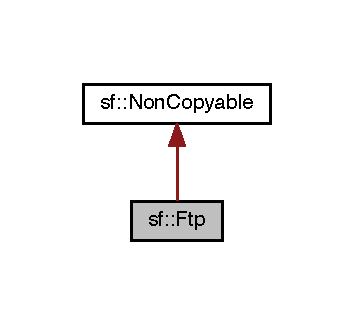
\includegraphics[width=170pt]{classsf_1_1_ftp__inherit__graph}
\end{center}
\end{figure}


Collaboration diagram for sf\-:\-:Ftp\-:
\nopagebreak
\begin{figure}[H]
\begin{center}
\leavevmode
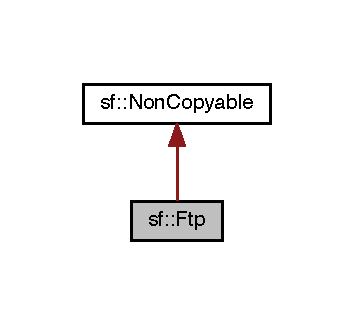
\includegraphics[width=170pt]{classsf_1_1_ftp__coll__graph}
\end{center}
\end{figure}
\subsection*{Classes}
\begin{DoxyCompactItemize}
\item 
class \hyperlink{classsf_1_1_ftp_1_1_directory_response}{Directory\-Response}
\begin{DoxyCompactList}\small\item\em Specialization of F\-T\-P response returning a directory. \end{DoxyCompactList}\item 
class \hyperlink{classsf_1_1_ftp_1_1_listing_response}{Listing\-Response}
\begin{DoxyCompactList}\small\item\em Specialization of F\-T\-P response returning a filename lisiting. \end{DoxyCompactList}\item 
class \hyperlink{classsf_1_1_ftp_1_1_response}{Response}
\begin{DoxyCompactList}\small\item\em Define a F\-T\-P response. \end{DoxyCompactList}\end{DoxyCompactItemize}
\subsection*{Public Types}
\begin{DoxyCompactItemize}
\item 
enum \hyperlink{classsf_1_1_ftp_a1cd6b89ad23253f6d97e6d4ca4d558cb}{Transfer\-Mode} \{ \hyperlink{classsf_1_1_ftp_a1cd6b89ad23253f6d97e6d4ca4d558cba6f253b362639fb5e059dc292762a21ee}{Binary}, 
\hyperlink{classsf_1_1_ftp_a1cd6b89ad23253f6d97e6d4ca4d558cbac9e544a22dce8ef3177449cb235d15c2}{Ascii}, 
\hyperlink{classsf_1_1_ftp_a1cd6b89ad23253f6d97e6d4ca4d558cbabb1e34435231e73c96534c71090be7f4}{Ebcdic}
 \}
\begin{DoxyCompactList}\small\item\em Enumeration of transfer modes. \end{DoxyCompactList}\end{DoxyCompactItemize}
\subsection*{Public Member Functions}
\begin{DoxyCompactItemize}
\item 
\hyperlink{classsf_1_1_ftp_a2edfa8e9009caf27bce74459ae76dc52}{$\sim$\-Ftp} ()
\begin{DoxyCompactList}\small\item\em Destructor. \end{DoxyCompactList}\item 
\hyperlink{classsf_1_1_ftp_1_1_response}{Response} \hyperlink{classsf_1_1_ftp_af02fb3de3f450a50a27981961c69c860}{connect} (const \hyperlink{classsf_1_1_ip_address}{Ip\-Address} \&server, unsigned short port=21, \hyperlink{classsf_1_1_time}{Time} \hyperlink{gl3_8h_ad29bb0d8468b264a4e3d9204366cfaab}{timeout}=\hyperlink{classsf_1_1_time_a8db127b632fa8da21550e7282af11fa0}{Time\-::\-Zero})
\begin{DoxyCompactList}\small\item\em Connect to the specified F\-T\-P server. \end{DoxyCompactList}\item 
\hyperlink{classsf_1_1_ftp_1_1_response}{Response} \hyperlink{classsf_1_1_ftp_acf7459926f3391cd06bf84337ed6a0f4}{disconnect} ()
\begin{DoxyCompactList}\small\item\em Close the connection with the server. \end{DoxyCompactList}\item 
\hyperlink{classsf_1_1_ftp_1_1_response}{Response} \hyperlink{classsf_1_1_ftp_a686262bc377584cd50e52e1576aa3a9b}{login} ()
\begin{DoxyCompactList}\small\item\em Log in using an anonymous account. \end{DoxyCompactList}\item 
\hyperlink{classsf_1_1_ftp_1_1_response}{Response} \hyperlink{classsf_1_1_ftp_a99d8114793c1659e9d51d45cecdcd965}{login} (const \hyperlink{gl3_8h_ac83513893df92266f79a515488701770}{std\-::string} \&\hyperlink{gl3_8h_aaced7cfc21e7d37775d6921bb8177239}{name}, const \hyperlink{gl3_8h_ac83513893df92266f79a515488701770}{std\-::string} \&password)
\begin{DoxyCompactList}\small\item\em Log in using a username and a password. \end{DoxyCompactList}\item 
\hyperlink{classsf_1_1_ftp_1_1_response}{Response} \hyperlink{classsf_1_1_ftp_aa1127d442b4acb2105aa8060a39d04fc}{keep\-Alive} ()
\begin{DoxyCompactList}\small\item\em Send a null command to keep the connection alive. \end{DoxyCompactList}\item 
\hyperlink{classsf_1_1_ftp_1_1_directory_response}{Directory\-Response} \hyperlink{classsf_1_1_ftp_a79c654fcdd0c81e68c4fa29af3b45e0c}{get\-Working\-Directory} ()
\begin{DoxyCompactList}\small\item\em Get the current working directory. \end{DoxyCompactList}\item 
\hyperlink{classsf_1_1_ftp_1_1_listing_response}{Listing\-Response} \hyperlink{classsf_1_1_ftp_a8f37258e461fcb9e2a0655e9df0be4a0}{get\-Directory\-Listing} (const \hyperlink{gl3_8h_ac83513893df92266f79a515488701770}{std\-::string} \&directory=\char`\"{}\char`\"{})
\begin{DoxyCompactList}\small\item\em Get the contents of the given directory. \end{DoxyCompactList}\item 
\hyperlink{classsf_1_1_ftp_1_1_response}{Response} \hyperlink{classsf_1_1_ftp_a7e93488ea6330dd4dd76e428da9bb6d3}{change\-Directory} (const \hyperlink{gl3_8h_ac83513893df92266f79a515488701770}{std\-::string} \&directory)
\begin{DoxyCompactList}\small\item\em Change the current working directory. \end{DoxyCompactList}\item 
\hyperlink{classsf_1_1_ftp_1_1_response}{Response} \hyperlink{classsf_1_1_ftp_ad295cf77f30f9ad07b5c401fd9849189}{parent\-Directory} ()
\begin{DoxyCompactList}\small\item\em Go to the parent directory of the current one. \end{DoxyCompactList}\item 
\hyperlink{classsf_1_1_ftp_1_1_response}{Response} \hyperlink{classsf_1_1_ftp_a247b84c4b25da37804218c2b748c4787}{create\-Directory} (const \hyperlink{gl3_8h_ac83513893df92266f79a515488701770}{std\-::string} \&\hyperlink{gl3_8h_aaced7cfc21e7d37775d6921bb8177239}{name})
\begin{DoxyCompactList}\small\item\em Create a new directory. \end{DoxyCompactList}\item 
\hyperlink{classsf_1_1_ftp_1_1_response}{Response} \hyperlink{classsf_1_1_ftp_a2a8a7ef9144204b5b319c9a4be8806c2}{delete\-Directory} (const \hyperlink{gl3_8h_ac83513893df92266f79a515488701770}{std\-::string} \&\hyperlink{gl3_8h_aaced7cfc21e7d37775d6921bb8177239}{name})
\begin{DoxyCompactList}\small\item\em Remove an existing directory. \end{DoxyCompactList}\item 
\hyperlink{classsf_1_1_ftp_1_1_response}{Response} \hyperlink{classsf_1_1_ftp_a8f99251d7153e1dc26723e4006deb764}{rename\-File} (const \hyperlink{gl3_8h_ac83513893df92266f79a515488701770}{std\-::string} \&file, const \hyperlink{gl3_8h_ac83513893df92266f79a515488701770}{std\-::string} \&new\-Name)
\begin{DoxyCompactList}\small\item\em Rename an existing file. \end{DoxyCompactList}\item 
\hyperlink{classsf_1_1_ftp_1_1_response}{Response} \hyperlink{classsf_1_1_ftp_a8aa272b0eb7769a850006e70fcad370f}{delete\-File} (const \hyperlink{gl3_8h_ac83513893df92266f79a515488701770}{std\-::string} \&\hyperlink{gl3_8h_aaced7cfc21e7d37775d6921bb8177239}{name})
\begin{DoxyCompactList}\small\item\em Remove an existing file. \end{DoxyCompactList}\item 
\hyperlink{classsf_1_1_ftp_1_1_response}{Response} \hyperlink{classsf_1_1_ftp_a20c1600ec5fd6f5a2ad1429ab8aa5df4}{download} (const \hyperlink{gl3_8h_ac83513893df92266f79a515488701770}{std\-::string} \&remote\-File, const \hyperlink{gl3_8h_ac83513893df92266f79a515488701770}{std\-::string} \&local\-Path, \hyperlink{classsf_1_1_ftp_a1cd6b89ad23253f6d97e6d4ca4d558cb}{Transfer\-Mode} \hyperlink{gl3_8h_a1e71d9c196e4683cc06c4b54d53f7ef5}{mode}=\hyperlink{classsf_1_1_ftp_a1cd6b89ad23253f6d97e6d4ca4d558cba6f253b362639fb5e059dc292762a21ee}{Binary})
\begin{DoxyCompactList}\small\item\em Download a file from the server. \end{DoxyCompactList}\item 
\hyperlink{classsf_1_1_ftp_1_1_response}{Response} \hyperlink{classsf_1_1_ftp_a46d6e15cddd719288b5a08b685e11765}{upload} (const \hyperlink{gl3_8h_ac83513893df92266f79a515488701770}{std\-::string} \&local\-File, const \hyperlink{gl3_8h_ac83513893df92266f79a515488701770}{std\-::string} \&remote\-Path, \hyperlink{classsf_1_1_ftp_a1cd6b89ad23253f6d97e6d4ca4d558cb}{Transfer\-Mode} \hyperlink{gl3_8h_a1e71d9c196e4683cc06c4b54d53f7ef5}{mode}=\hyperlink{classsf_1_1_ftp_a1cd6b89ad23253f6d97e6d4ca4d558cba6f253b362639fb5e059dc292762a21ee}{Binary})
\begin{DoxyCompactList}\small\item\em Upload a file to the server. \end{DoxyCompactList}\end{DoxyCompactItemize}
\subsection*{Friends}
\begin{DoxyCompactItemize}
\item 
class \hyperlink{classsf_1_1_ftp_a8dee57337b6a7e183bfe21d178757b0c}{Data\-Channel}
\end{DoxyCompactItemize}
\subsection*{Additional Inherited Members}


\subsection{Detailed Description}
A F\-T\-P client. 

\hyperlink{classsf_1_1_ftp}{sf\-::\-Ftp} is a very simple F\-T\-P client that allows you to communicate with a F\-T\-P server. The F\-T\-P protocol allows you to manipulate a remote file system (list files, upload, download, create, remove, ...).

Using the F\-T\-P client consists of 4 parts\-: \begin{DoxyItemize}
\item Connecting to the F\-T\-P server \item Logging in (either as a registered user or anonymously) \item Sending commands to the server \item Disconnecting (this part can be done implicitely by the destructor)\end{DoxyItemize}
Every command returns a F\-T\-P response, which contains the status code as well as a message from the server. Some commands such as get\-Working\-Directory and get\-Directory\-Listing return additional data, and use a class derived from \hyperlink{classsf_1_1_ftp_1_1_response}{sf\-::\-Ftp\-::\-Response} to provide this data.

All commands, especially upload and download, may take some time to complete. This is important to know if you don't want to block your application while the server is completing the task.

Usage example\-: 
\begin{DoxyCode}
\textcolor{comment}{// Create a new FTP client}
\hyperlink{classsf_1_1_ftp}{sf::Ftp} ftp;

\textcolor{comment}{// Connect to the server}
\hyperlink{classsf_1_1_ftp_1_1_response}{sf::Ftp::Response} response = ftp.\hyperlink{classsf_1_1_ftp_af02fb3de3f450a50a27981961c69c860}{connect}(\textcolor{stringliteral}{"ftp://ftp.myserver.com"});
\textcolor{keywordflow}{if} (response.\hyperlink{classsf_1_1_ftp_1_1_response_a4dadbe0fe0a3ef2d571a017e1645e675}{isOk}())
    std::cout << \textcolor{stringliteral}{"Connected"} << std::endl;

\textcolor{comment}{// Log in}
response = ftp.\hyperlink{classsf_1_1_ftp_a686262bc377584cd50e52e1576aa3a9b}{login}(\textcolor{stringliteral}{"laurent"}, \textcolor{stringliteral}{"dF6Zm89D"});
\textcolor{keywordflow}{if} (response.\hyperlink{classsf_1_1_ftp_1_1_response_a4dadbe0fe0a3ef2d571a017e1645e675}{isOk}())
    std::cout << \textcolor{stringliteral}{"Logged in"} << std::endl;

\textcolor{comment}{// Print the working directory}
\hyperlink{classsf_1_1_ftp_1_1_directory_response}{sf::Ftp::DirectoryResponse} directory = ftp.
      \hyperlink{classsf_1_1_ftp_a79c654fcdd0c81e68c4fa29af3b45e0c}{getWorkingDirectory}();
\textcolor{keywordflow}{if} (directory.\hyperlink{classsf_1_1_ftp_1_1_response_a4dadbe0fe0a3ef2d571a017e1645e675}{isOk}())
    std::cout << \textcolor{stringliteral}{"Working directory: "} << directory.\hyperlink{classsf_1_1_ftp_1_1_directory_response_a500793778ad0ed223aa86ed8fbee28a3}{getDirectory}() << std::endl;

\textcolor{comment}{// Create a new directory}
response = ftp.\hyperlink{classsf_1_1_ftp_a247b84c4b25da37804218c2b748c4787}{createDirectory}(\textcolor{stringliteral}{"files"});
\textcolor{keywordflow}{if} (response.\hyperlink{classsf_1_1_ftp_1_1_response_a4dadbe0fe0a3ef2d571a017e1645e675}{isOk}())
    std::cout << \textcolor{stringliteral}{"Created new directory"} << std::endl;

\textcolor{comment}{// Upload a file to this new directory}
response = ftp.\hyperlink{classsf_1_1_ftp_a46d6e15cddd719288b5a08b685e11765}{upload}(\textcolor{stringliteral}{"local-path/file.txt"}, \textcolor{stringliteral}{"files"}, \hyperlink{classsf_1_1_ftp_a1cd6b89ad23253f6d97e6d4ca4d558cbac9e544a22dce8ef3177449cb235d15c2}{sf::Ftp::Ascii});
\textcolor{keywordflow}{if} (response.\hyperlink{classsf_1_1_ftp_1_1_response_a4dadbe0fe0a3ef2d571a017e1645e675}{isOk}())
    std::cout << \textcolor{stringliteral}{"File uploaded"} << std::endl;

\textcolor{comment}{// Disconnect from the server (optional)}
ftp.\hyperlink{classsf_1_1_ftp_acf7459926f3391cd06bf84337ed6a0f4}{disconnect}();
\end{DoxyCode}
 

Definition at line 47 of file Ftp.\-hpp.



\subsection{Member Enumeration Documentation}
\hypertarget{classsf_1_1_ftp_a1cd6b89ad23253f6d97e6d4ca4d558cb}{\index{sf\-::\-Ftp@{sf\-::\-Ftp}!Transfer\-Mode@{Transfer\-Mode}}
\index{Transfer\-Mode@{Transfer\-Mode}!sf::Ftp@{sf\-::\-Ftp}}
\subsubsection[{Transfer\-Mode}]{\setlength{\rightskip}{0pt plus 5cm}enum {\bf sf\-::\-Ftp\-::\-Transfer\-Mode}}}\label{classsf_1_1_ftp_a1cd6b89ad23253f6d97e6d4ca4d558cb}


Enumeration of transfer modes. 

\begin{Desc}
\item[Enumerator]\par
\begin{description}
\index{Binary@{Binary}!sf\-::\-Ftp@{sf\-::\-Ftp}}\index{sf\-::\-Ftp@{sf\-::\-Ftp}!Binary@{Binary}}\item[{\em 
\hypertarget{classsf_1_1_ftp_a1cd6b89ad23253f6d97e6d4ca4d558cba6f253b362639fb5e059dc292762a21ee}{Binary}\label{classsf_1_1_ftp_a1cd6b89ad23253f6d97e6d4ca4d558cba6f253b362639fb5e059dc292762a21ee}
}]Binary mode (file is transfered as a sequence of bytes) \index{Ascii@{Ascii}!sf\-::\-Ftp@{sf\-::\-Ftp}}\index{sf\-::\-Ftp@{sf\-::\-Ftp}!Ascii@{Ascii}}\item[{\em 
\hypertarget{classsf_1_1_ftp_a1cd6b89ad23253f6d97e6d4ca4d558cbac9e544a22dce8ef3177449cb235d15c2}{Ascii}\label{classsf_1_1_ftp_a1cd6b89ad23253f6d97e6d4ca4d558cbac9e544a22dce8ef3177449cb235d15c2}
}]\hyperlink{classsf_1_1_text}{Text} mode using A\-S\-C\-I\-I encoding. \index{Ebcdic@{Ebcdic}!sf\-::\-Ftp@{sf\-::\-Ftp}}\index{sf\-::\-Ftp@{sf\-::\-Ftp}!Ebcdic@{Ebcdic}}\item[{\em 
\hypertarget{classsf_1_1_ftp_a1cd6b89ad23253f6d97e6d4ca4d558cbabb1e34435231e73c96534c71090be7f4}{Ebcdic}\label{classsf_1_1_ftp_a1cd6b89ad23253f6d97e6d4ca4d558cbabb1e34435231e73c96534c71090be7f4}
}]\hyperlink{classsf_1_1_text}{Text} mode using E\-B\-C\-D\-I\-C encoding. \end{description}
\end{Desc}


Definition at line 55 of file Ftp.\-hpp.



\subsection{Constructor \& Destructor Documentation}
\hypertarget{classsf_1_1_ftp_a2edfa8e9009caf27bce74459ae76dc52}{\index{sf\-::\-Ftp@{sf\-::\-Ftp}!$\sim$\-Ftp@{$\sim$\-Ftp}}
\index{$\sim$\-Ftp@{$\sim$\-Ftp}!sf::Ftp@{sf\-::\-Ftp}}
\subsubsection[{$\sim$\-Ftp}]{\setlength{\rightskip}{0pt plus 5cm}sf\-::\-Ftp\-::$\sim$\-Ftp (
\begin{DoxyParamCaption}
{}
\end{DoxyParamCaption}
)}}\label{classsf_1_1_ftp_a2edfa8e9009caf27bce74459ae76dc52}


Destructor. 

Automatically closes the connection with the server if it is still opened. 

\subsection{Member Function Documentation}
\hypertarget{classsf_1_1_ftp_a7e93488ea6330dd4dd76e428da9bb6d3}{\index{sf\-::\-Ftp@{sf\-::\-Ftp}!change\-Directory@{change\-Directory}}
\index{change\-Directory@{change\-Directory}!sf::Ftp@{sf\-::\-Ftp}}
\subsubsection[{change\-Directory}]{\setlength{\rightskip}{0pt plus 5cm}{\bf Response} sf\-::\-Ftp\-::change\-Directory (
\begin{DoxyParamCaption}
\item[{const {\bf std\-::string} \&}]{directory}
\end{DoxyParamCaption}
)}}\label{classsf_1_1_ftp_a7e93488ea6330dd4dd76e428da9bb6d3}


Change the current working directory. 

The new directory must be relative to the current one.


\begin{DoxyParams}{Parameters}
{\em directory} & New working directory\\
\hline
\end{DoxyParams}
\begin{DoxyReturn}{Returns}
Server response to the request
\end{DoxyReturn}
\begin{DoxySeeAlso}{See Also}
\hyperlink{classsf_1_1_ftp_a79c654fcdd0c81e68c4fa29af3b45e0c}{get\-Working\-Directory}, \hyperlink{classsf_1_1_ftp_a8f37258e461fcb9e2a0655e9df0be4a0}{get\-Directory\-Listing}, \hyperlink{classsf_1_1_ftp_ad295cf77f30f9ad07b5c401fd9849189}{parent\-Directory} 
\end{DoxySeeAlso}
\hypertarget{classsf_1_1_ftp_af02fb3de3f450a50a27981961c69c860}{\index{sf\-::\-Ftp@{sf\-::\-Ftp}!connect@{connect}}
\index{connect@{connect}!sf::Ftp@{sf\-::\-Ftp}}
\subsubsection[{connect}]{\setlength{\rightskip}{0pt plus 5cm}{\bf Response} sf\-::\-Ftp\-::connect (
\begin{DoxyParamCaption}
\item[{const {\bf Ip\-Address} \&}]{server, }
\item[{unsigned short}]{port = {\ttfamily 21}, }
\item[{{\bf Time}}]{timeout = {\ttfamily {\bf Time\-::\-Zero}}}
\end{DoxyParamCaption}
)}}\label{classsf_1_1_ftp_af02fb3de3f450a50a27981961c69c860}


Connect to the specified F\-T\-P server. 

The port has a default value of 21, which is the standard port used by the F\-T\-P protocol. You shouldn't use a different value, unless you really know what you do. This function tries to connect to the server so it may take a while to complete, especially if the server is not reachable. To avoid blocking your application for too long, you can use a timeout. The default value, \hyperlink{classsf_1_1_time_a8db127b632fa8da21550e7282af11fa0}{Time\-::\-Zero}, means that the system timeout will be used (which is usually pretty long).


\begin{DoxyParams}{Parameters}
{\em server} & Name or address of the F\-T\-P server to connect to \\
\hline
{\em port} & Port used for the connection \\
\hline
{\em timeout} & Maximum time to wait\\
\hline
\end{DoxyParams}
\begin{DoxyReturn}{Returns}
Server response to the request
\end{DoxyReturn}
\begin{DoxySeeAlso}{See Also}
\hyperlink{classsf_1_1_ftp_acf7459926f3391cd06bf84337ed6a0f4}{disconnect} 
\end{DoxySeeAlso}
\hypertarget{classsf_1_1_ftp_a247b84c4b25da37804218c2b748c4787}{\index{sf\-::\-Ftp@{sf\-::\-Ftp}!create\-Directory@{create\-Directory}}
\index{create\-Directory@{create\-Directory}!sf::Ftp@{sf\-::\-Ftp}}
\subsubsection[{create\-Directory}]{\setlength{\rightskip}{0pt plus 5cm}{\bf Response} sf\-::\-Ftp\-::create\-Directory (
\begin{DoxyParamCaption}
\item[{const {\bf std\-::string} \&}]{name}
\end{DoxyParamCaption}
)}}\label{classsf_1_1_ftp_a247b84c4b25da37804218c2b748c4787}


Create a new directory. 

The new directory is created as a child of the current working directory.


\begin{DoxyParams}{Parameters}
{\em name} & Name of the directory to create\\
\hline
\end{DoxyParams}
\begin{DoxyReturn}{Returns}
Server response to the request
\end{DoxyReturn}
\begin{DoxySeeAlso}{See Also}
\hyperlink{classsf_1_1_ftp_a2a8a7ef9144204b5b319c9a4be8806c2}{delete\-Directory} 
\end{DoxySeeAlso}
\hypertarget{classsf_1_1_ftp_a2a8a7ef9144204b5b319c9a4be8806c2}{\index{sf\-::\-Ftp@{sf\-::\-Ftp}!delete\-Directory@{delete\-Directory}}
\index{delete\-Directory@{delete\-Directory}!sf::Ftp@{sf\-::\-Ftp}}
\subsubsection[{delete\-Directory}]{\setlength{\rightskip}{0pt plus 5cm}{\bf Response} sf\-::\-Ftp\-::delete\-Directory (
\begin{DoxyParamCaption}
\item[{const {\bf std\-::string} \&}]{name}
\end{DoxyParamCaption}
)}}\label{classsf_1_1_ftp_a2a8a7ef9144204b5b319c9a4be8806c2}


Remove an existing directory. 

The directory to remove must be relative to the current working directory. Use this function with caution, the directory will be removed permanently!


\begin{DoxyParams}{Parameters}
{\em name} & Name of the directory to remove\\
\hline
\end{DoxyParams}
\begin{DoxyReturn}{Returns}
Server response to the request
\end{DoxyReturn}
\begin{DoxySeeAlso}{See Also}
\hyperlink{classsf_1_1_ftp_a247b84c4b25da37804218c2b748c4787}{create\-Directory} 
\end{DoxySeeAlso}
\hypertarget{classsf_1_1_ftp_a8aa272b0eb7769a850006e70fcad370f}{\index{sf\-::\-Ftp@{sf\-::\-Ftp}!delete\-File@{delete\-File}}
\index{delete\-File@{delete\-File}!sf::Ftp@{sf\-::\-Ftp}}
\subsubsection[{delete\-File}]{\setlength{\rightskip}{0pt plus 5cm}{\bf Response} sf\-::\-Ftp\-::delete\-File (
\begin{DoxyParamCaption}
\item[{const {\bf std\-::string} \&}]{name}
\end{DoxyParamCaption}
)}}\label{classsf_1_1_ftp_a8aa272b0eb7769a850006e70fcad370f}


Remove an existing file. 

The file name must be relative to the current working directory. Use this function with caution, the file will be removed permanently!


\begin{DoxyParams}{Parameters}
{\em name} & File to remove\\
\hline
\end{DoxyParams}
\begin{DoxyReturn}{Returns}
Server response to the request
\end{DoxyReturn}
\begin{DoxySeeAlso}{See Also}
\hyperlink{classsf_1_1_ftp_a8f99251d7153e1dc26723e4006deb764}{rename\-File} 
\end{DoxySeeAlso}
\hypertarget{classsf_1_1_ftp_acf7459926f3391cd06bf84337ed6a0f4}{\index{sf\-::\-Ftp@{sf\-::\-Ftp}!disconnect@{disconnect}}
\index{disconnect@{disconnect}!sf::Ftp@{sf\-::\-Ftp}}
\subsubsection[{disconnect}]{\setlength{\rightskip}{0pt plus 5cm}{\bf Response} sf\-::\-Ftp\-::disconnect (
\begin{DoxyParamCaption}
{}
\end{DoxyParamCaption}
)}}\label{classsf_1_1_ftp_acf7459926f3391cd06bf84337ed6a0f4}


Close the connection with the server. 

\begin{DoxyReturn}{Returns}
Server response to the request
\end{DoxyReturn}
\begin{DoxySeeAlso}{See Also}
\hyperlink{classsf_1_1_ftp_af02fb3de3f450a50a27981961c69c860}{connect} 
\end{DoxySeeAlso}
\hypertarget{classsf_1_1_ftp_a20c1600ec5fd6f5a2ad1429ab8aa5df4}{\index{sf\-::\-Ftp@{sf\-::\-Ftp}!download@{download}}
\index{download@{download}!sf::Ftp@{sf\-::\-Ftp}}
\subsubsection[{download}]{\setlength{\rightskip}{0pt plus 5cm}{\bf Response} sf\-::\-Ftp\-::download (
\begin{DoxyParamCaption}
\item[{const {\bf std\-::string} \&}]{remote\-File, }
\item[{const {\bf std\-::string} \&}]{local\-Path, }
\item[{{\bf Transfer\-Mode}}]{mode = {\ttfamily {\bf Binary}}}
\end{DoxyParamCaption}
)}}\label{classsf_1_1_ftp_a20c1600ec5fd6f5a2ad1429ab8aa5df4}


Download a file from the server. 

The filename of the distant file is relative to the current working directory of the server, and the local destination path is relative to the current directory of your application.


\begin{DoxyParams}{Parameters}
{\em remote\-File} & Filename of the distant file to download \\
\hline
{\em local\-Path} & Where to put to file on the local computer \\
\hline
{\em mode} & Transfer mode\\
\hline
\end{DoxyParams}
\begin{DoxyReturn}{Returns}
Server response to the request
\end{DoxyReturn}
\begin{DoxySeeAlso}{See Also}
\hyperlink{classsf_1_1_ftp_a46d6e15cddd719288b5a08b685e11765}{upload} 
\end{DoxySeeAlso}
\hypertarget{classsf_1_1_ftp_a8f37258e461fcb9e2a0655e9df0be4a0}{\index{sf\-::\-Ftp@{sf\-::\-Ftp}!get\-Directory\-Listing@{get\-Directory\-Listing}}
\index{get\-Directory\-Listing@{get\-Directory\-Listing}!sf::Ftp@{sf\-::\-Ftp}}
\subsubsection[{get\-Directory\-Listing}]{\setlength{\rightskip}{0pt plus 5cm}{\bf Listing\-Response} sf\-::\-Ftp\-::get\-Directory\-Listing (
\begin{DoxyParamCaption}
\item[{const {\bf std\-::string} \&}]{directory = {\ttfamily \char`\"{}\char`\"{}}}
\end{DoxyParamCaption}
)}}\label{classsf_1_1_ftp_a8f37258e461fcb9e2a0655e9df0be4a0}


Get the contents of the given directory. 

This function retrieves the sub-\/directories and files contained in the given directory. It is not recursive. The {\itshape directory} parameter is relative to the current working directory.


\begin{DoxyParams}{Parameters}
{\em directory} & Directory to list\\
\hline
\end{DoxyParams}
\begin{DoxyReturn}{Returns}
Server response to the request
\end{DoxyReturn}
\begin{DoxySeeAlso}{See Also}
\hyperlink{classsf_1_1_ftp_a79c654fcdd0c81e68c4fa29af3b45e0c}{get\-Working\-Directory}, \hyperlink{classsf_1_1_ftp_a7e93488ea6330dd4dd76e428da9bb6d3}{change\-Directory}, \hyperlink{classsf_1_1_ftp_ad295cf77f30f9ad07b5c401fd9849189}{parent\-Directory} 
\end{DoxySeeAlso}
\hypertarget{classsf_1_1_ftp_a79c654fcdd0c81e68c4fa29af3b45e0c}{\index{sf\-::\-Ftp@{sf\-::\-Ftp}!get\-Working\-Directory@{get\-Working\-Directory}}
\index{get\-Working\-Directory@{get\-Working\-Directory}!sf::Ftp@{sf\-::\-Ftp}}
\subsubsection[{get\-Working\-Directory}]{\setlength{\rightskip}{0pt plus 5cm}{\bf Directory\-Response} sf\-::\-Ftp\-::get\-Working\-Directory (
\begin{DoxyParamCaption}
{}
\end{DoxyParamCaption}
)}}\label{classsf_1_1_ftp_a79c654fcdd0c81e68c4fa29af3b45e0c}


Get the current working directory. 

The working directory is the root path for subsequent operations involving directories and/or filenames.

\begin{DoxyReturn}{Returns}
Server response to the request
\end{DoxyReturn}
\begin{DoxySeeAlso}{See Also}
\hyperlink{classsf_1_1_ftp_a8f37258e461fcb9e2a0655e9df0be4a0}{get\-Directory\-Listing}, \hyperlink{classsf_1_1_ftp_a7e93488ea6330dd4dd76e428da9bb6d3}{change\-Directory}, \hyperlink{classsf_1_1_ftp_ad295cf77f30f9ad07b5c401fd9849189}{parent\-Directory} 
\end{DoxySeeAlso}
\hypertarget{classsf_1_1_ftp_aa1127d442b4acb2105aa8060a39d04fc}{\index{sf\-::\-Ftp@{sf\-::\-Ftp}!keep\-Alive@{keep\-Alive}}
\index{keep\-Alive@{keep\-Alive}!sf::Ftp@{sf\-::\-Ftp}}
\subsubsection[{keep\-Alive}]{\setlength{\rightskip}{0pt plus 5cm}{\bf Response} sf\-::\-Ftp\-::keep\-Alive (
\begin{DoxyParamCaption}
{}
\end{DoxyParamCaption}
)}}\label{classsf_1_1_ftp_aa1127d442b4acb2105aa8060a39d04fc}


Send a null command to keep the connection alive. 

This command is useful because the server may close the connection automatically if no command is sent.

\begin{DoxyReturn}{Returns}
Server response to the request 
\end{DoxyReturn}
\hypertarget{classsf_1_1_ftp_a686262bc377584cd50e52e1576aa3a9b}{\index{sf\-::\-Ftp@{sf\-::\-Ftp}!login@{login}}
\index{login@{login}!sf::Ftp@{sf\-::\-Ftp}}
\subsubsection[{login}]{\setlength{\rightskip}{0pt plus 5cm}{\bf Response} sf\-::\-Ftp\-::login (
\begin{DoxyParamCaption}
{}
\end{DoxyParamCaption}
)}}\label{classsf_1_1_ftp_a686262bc377584cd50e52e1576aa3a9b}


Log in using an anonymous account. 

Logging in is mandatory after connecting to the server. Users that are not logged in cannot perform any operation.

\begin{DoxyReturn}{Returns}
Server response to the request 
\end{DoxyReturn}
\hypertarget{classsf_1_1_ftp_a99d8114793c1659e9d51d45cecdcd965}{\index{sf\-::\-Ftp@{sf\-::\-Ftp}!login@{login}}
\index{login@{login}!sf::Ftp@{sf\-::\-Ftp}}
\subsubsection[{login}]{\setlength{\rightskip}{0pt plus 5cm}{\bf Response} sf\-::\-Ftp\-::login (
\begin{DoxyParamCaption}
\item[{const {\bf std\-::string} \&}]{name, }
\item[{const {\bf std\-::string} \&}]{password}
\end{DoxyParamCaption}
)}}\label{classsf_1_1_ftp_a99d8114793c1659e9d51d45cecdcd965}


Log in using a username and a password. 

Logging in is mandatory after connecting to the server. Users that are not logged in cannot perform any operation.


\begin{DoxyParams}{Parameters}
{\em name} & User name \\
\hline
{\em password} & Password\\
\hline
\end{DoxyParams}
\begin{DoxyReturn}{Returns}
Server response to the request 
\end{DoxyReturn}
\hypertarget{classsf_1_1_ftp_ad295cf77f30f9ad07b5c401fd9849189}{\index{sf\-::\-Ftp@{sf\-::\-Ftp}!parent\-Directory@{parent\-Directory}}
\index{parent\-Directory@{parent\-Directory}!sf::Ftp@{sf\-::\-Ftp}}
\subsubsection[{parent\-Directory}]{\setlength{\rightskip}{0pt plus 5cm}{\bf Response} sf\-::\-Ftp\-::parent\-Directory (
\begin{DoxyParamCaption}
{}
\end{DoxyParamCaption}
)}}\label{classsf_1_1_ftp_ad295cf77f30f9ad07b5c401fd9849189}


Go to the parent directory of the current one. 

\begin{DoxyReturn}{Returns}
Server response to the request
\end{DoxyReturn}
\begin{DoxySeeAlso}{See Also}
\hyperlink{classsf_1_1_ftp_a79c654fcdd0c81e68c4fa29af3b45e0c}{get\-Working\-Directory}, \hyperlink{classsf_1_1_ftp_a8f37258e461fcb9e2a0655e9df0be4a0}{get\-Directory\-Listing}, \hyperlink{classsf_1_1_ftp_a7e93488ea6330dd4dd76e428da9bb6d3}{change\-Directory} 
\end{DoxySeeAlso}
\hypertarget{classsf_1_1_ftp_a8f99251d7153e1dc26723e4006deb764}{\index{sf\-::\-Ftp@{sf\-::\-Ftp}!rename\-File@{rename\-File}}
\index{rename\-File@{rename\-File}!sf::Ftp@{sf\-::\-Ftp}}
\subsubsection[{rename\-File}]{\setlength{\rightskip}{0pt plus 5cm}{\bf Response} sf\-::\-Ftp\-::rename\-File (
\begin{DoxyParamCaption}
\item[{const {\bf std\-::string} \&}]{file, }
\item[{const {\bf std\-::string} \&}]{new\-Name}
\end{DoxyParamCaption}
)}}\label{classsf_1_1_ftp_a8f99251d7153e1dc26723e4006deb764}


Rename an existing file. 

The filenames must be relative to the current working directory.


\begin{DoxyParams}{Parameters}
{\em file} & File to rename \\
\hline
{\em new\-Name} & New name of the file\\
\hline
\end{DoxyParams}
\begin{DoxyReturn}{Returns}
Server response to the request
\end{DoxyReturn}
\begin{DoxySeeAlso}{See Also}
\hyperlink{classsf_1_1_ftp_a8aa272b0eb7769a850006e70fcad370f}{delete\-File} 
\end{DoxySeeAlso}
\hypertarget{classsf_1_1_ftp_a46d6e15cddd719288b5a08b685e11765}{\index{sf\-::\-Ftp@{sf\-::\-Ftp}!upload@{upload}}
\index{upload@{upload}!sf::Ftp@{sf\-::\-Ftp}}
\subsubsection[{upload}]{\setlength{\rightskip}{0pt plus 5cm}{\bf Response} sf\-::\-Ftp\-::upload (
\begin{DoxyParamCaption}
\item[{const {\bf std\-::string} \&}]{local\-File, }
\item[{const {\bf std\-::string} \&}]{remote\-Path, }
\item[{{\bf Transfer\-Mode}}]{mode = {\ttfamily {\bf Binary}}}
\end{DoxyParamCaption}
)}}\label{classsf_1_1_ftp_a46d6e15cddd719288b5a08b685e11765}


Upload a file to the server. 

The name of the local file is relative to the current working directory of your application, and the remote path is relative to the current directory of the F\-T\-P server.


\begin{DoxyParams}{Parameters}
{\em local\-File} & Path of the local file to upload \\
\hline
{\em remote\-Path} & Where to put to file on the server \\
\hline
{\em mode} & Transfer mode\\
\hline
\end{DoxyParams}
\begin{DoxyReturn}{Returns}
Server response to the request
\end{DoxyReturn}
\begin{DoxySeeAlso}{See Also}
\hyperlink{classsf_1_1_ftp_a20c1600ec5fd6f5a2ad1429ab8aa5df4}{download} 
\end{DoxySeeAlso}


\subsection{Friends And Related Function Documentation}
\hypertarget{classsf_1_1_ftp_a8dee57337b6a7e183bfe21d178757b0c}{\index{sf\-::\-Ftp@{sf\-::\-Ftp}!Data\-Channel@{Data\-Channel}}
\index{Data\-Channel@{Data\-Channel}!sf::Ftp@{sf\-::\-Ftp}}
\subsubsection[{Data\-Channel}]{\setlength{\rightskip}{0pt plus 5cm}friend class Data\-Channel\hspace{0.3cm}{\ttfamily [friend]}}}\label{classsf_1_1_ftp_a8dee57337b6a7e183bfe21d178757b0c}


Definition at line 515 of file Ftp.\-hpp.



The documentation for this class was generated from the following file\-:\begin{DoxyCompactItemize}
\item 
/\-Users/ira/\-Dropbox/ira\-\_\-dev/protobyte\-\_\-research/other\-\_\-libs/\-S\-F\-M\-L/dylibs/root/usr/local/include/\-S\-F\-M\-L/\-Network/\hyperlink{_ftp_8hpp}{Ftp.\-hpp}\end{DoxyCompactItemize}

\hypertarget{class_geom_base}{\section{Geom\-Base Class Reference}
\label{class_geom_base}\index{Geom\-Base@{Geom\-Base}}
}


{\ttfamily \#include $<$Geom\-Base.\-h$>$}



Inheritance diagram for Geom\-Base\-:
\nopagebreak
\begin{figure}[H]
\begin{center}
\leavevmode
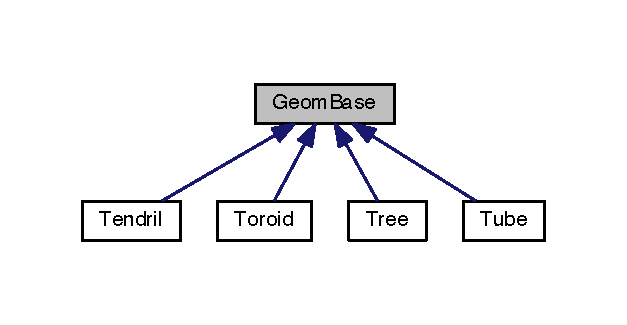
\includegraphics[width=301pt]{class_geom_base__inherit__graph}
\end{center}
\end{figure}


Collaboration diagram for Geom\-Base\-:
\nopagebreak
\begin{figure}[H]
\begin{center}
\leavevmode
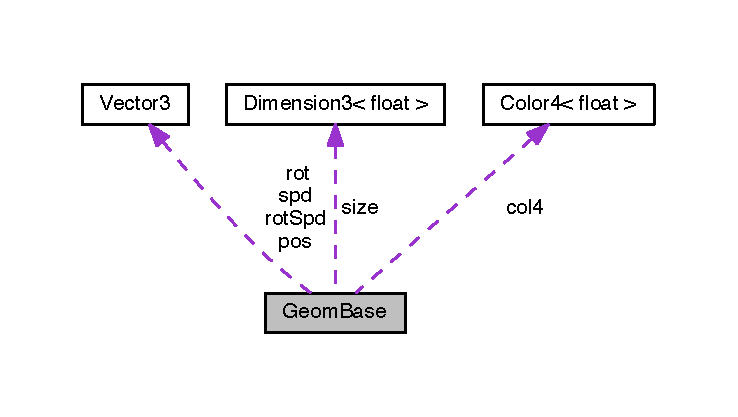
\includegraphics[width=350pt]{class_geom_base__coll__graph}
\end{center}
\end{figure}
\subsection*{Public Types}
\begin{DoxyCompactItemize}
\item 
enum \hyperlink{class_geom_base_a3259d41feab8f1c2b3e93e44ea06c8eb}{display\-Mode} \{ \\*
\hyperlink{class_geom_base_a3259d41feab8f1c2b3e93e44ea06c8eba26366b3d7c1226aaea4c80fa725116e3}{I\-M\-M\-E\-D\-I\-A\-T\-E}, 
\hyperlink{class_geom_base_a3259d41feab8f1c2b3e93e44ea06c8eba68fe3d2e6fab911d713140e124294e9b}{V\-E\-R\-T\-E\-X\-\_\-\-A\-R\-R\-A\-Y}, 
\hyperlink{class_geom_base_a3259d41feab8f1c2b3e93e44ea06c8ebadf4d9f5dab8ef3b7e4870d81a40c733e}{V\-E\-R\-T\-E\-X\-\_\-\-A\-R\-R\-A\-Y\-\_\-\-I\-N\-T\-E\-R\-L\-E\-A\-V\-E\-D}, 
\hyperlink{class_geom_base_a3259d41feab8f1c2b3e93e44ea06c8ebae91981c414821bfab61a65228dc8fc57}{D\-I\-S\-P\-L\-A\-Y\-\_\-\-L\-I\-S\-T}, 
\\*
\hyperlink{class_geom_base_a3259d41feab8f1c2b3e93e44ea06c8eba7431471ddf565855d64c64cb569e10cf}{V\-E\-R\-T\-E\-X\-\_\-\-B\-U\-F\-F\-E\-R\-\_\-\-O\-B\-J\-E\-C\-T}
 \}
\item 
enum \hyperlink{class_geom_base_a5ac81c5c0144bf51c40efc219f1973e2}{render\-Mode} \{ \hyperlink{class_geom_base_a5ac81c5c0144bf51c40efc219f1973e2a8f44b953b7e493103c192eb7c434481f}{W\-I\-R\-E\-F\-R\-A\-M\-E}, 
\hyperlink{class_geom_base_a5ac81c5c0144bf51c40efc219f1973e2a5795acdbf2229751e91ab3bf59fec100}{S\-U\-R\-F\-A\-C\-E}
 \}
\end{DoxyCompactItemize}
\subsection*{Public Member Functions}
\begin{DoxyCompactItemize}
\item 
\hyperlink{class_geom_base_a3321d8df2aabb01e54cebc102051626d}{Geom\-Base} ()
\item 
\hyperlink{class_geom_base_a9ebb09df37f80ec29489710fc3eb8775}{Geom\-Base} (const \hyperlink{class_vector3}{Vector3} \&\hyperlink{class_geom_base_ace2fc0557767dbb702aaf1655a85ed92}{pos}, const \hyperlink{class_vector3}{Vector3} \&\hyperlink{class_geom_base_a7de363bab1e976c73e495cf973a51de7}{rot}, const \hyperlink{class_dimension3}{Dimension3}$<$ float $>$ \hyperlink{gl3_8h_a79ef9eb3e59c4bb34c4b9fbeb8d28ff7}{size}, const \hyperlink{class_color4}{Color4}$<$ float $>$ \hyperlink{class_geom_base_acd58b67fcdac4428f66bea2c58c3aad8}{col4})
\item 
\hyperlink{class_geom_base_ae967f73a791c307df2aa08d00dcf908a}{Geom\-Base} (const \hyperlink{class_vector3}{Vector3} \&\hyperlink{class_geom_base_ace2fc0557767dbb702aaf1655a85ed92}{pos}, const \hyperlink{class_vector3}{Vector3} \&\hyperlink{class_geom_base_a7de363bab1e976c73e495cf973a51de7}{rot}, const \hyperlink{class_dimension3}{Dimension3}$<$ float $>$ \hyperlink{gl3_8h_a79ef9eb3e59c4bb34c4b9fbeb8d28ff7}{size}, const std\-::vector$<$ \hyperlink{class_color4}{Color4}$<$ float $>$ $>$ \hyperlink{class_geom_base_a0a55c12de2788567600e4477017df3fb}{col4s})
\item 
virtual \hyperlink{class_geom_base_acbba0a4d5b9bcdb0564efc8696f52fc6}{$\sim$\-Geom\-Base} ()
\item 
\hyperlink{glutf90_8h_ac778d6f63f1aaf8ebda0ce6ac821b56e}{void} \hyperlink{class_geom_base_aa62a1d16a4b8bc95be85faa4f454ec89}{move} (const \hyperlink{class_vector3}{Vector3} \&\hyperlink{gl3_8h_a14cfbe2fc2234f5504618905b69d1e06}{v})
\item 
\hyperlink{glutf90_8h_ac778d6f63f1aaf8ebda0ce6ac821b56e}{void} \hyperlink{class_geom_base_aaf54ae14260d05c92a915c3736693ee8}{rotate} (const \hyperlink{class_vector3}{Vector3} \&\hyperlink{gl3_8h_abe08814c2f72843fde4d8df41440d5a0}{r})
\item 
\hyperlink{glutf90_8h_ac778d6f63f1aaf8ebda0ce6ac821b56e}{void} \hyperlink{class_geom_base_ac1a2a5b5e8538f0a881eb93acb27d760}{scale} (const \hyperlink{class_dimension3}{Dimension3}$<$ float $>$ \&s)
\item 
virtual \hyperlink{glutf90_8h_ac778d6f63f1aaf8ebda0ce6ac821b56e}{void} \hyperlink{class_geom_base_abdf4aad3e45d3f71bcfa653c5200b9a6}{display} (\hyperlink{class_geom_base_a3259d41feab8f1c2b3e93e44ea06c8eb}{display\-Mode} \hyperlink{gl3_8h_a1e71d9c196e4683cc06c4b54d53f7ef5}{mode}=\hyperlink{class_geom_base_a3259d41feab8f1c2b3e93e44ea06c8eba68fe3d2e6fab911d713140e124294e9b}{V\-E\-R\-T\-E\-X\-\_\-\-A\-R\-R\-A\-Y}, \hyperlink{class_geom_base_a5ac81c5c0144bf51c40efc219f1973e2}{render\-Mode} render=\hyperlink{class_geom_base_a5ac81c5c0144bf51c40efc219f1973e2a5795acdbf2229751e91ab3bf59fec100}{S\-U\-R\-F\-A\-C\-E})
\item 
\hyperlink{glutf90_8h_ac778d6f63f1aaf8ebda0ce6ac821b56e}{void} \hyperlink{class_geom_base_a2f791ec87256e94cfb904ea4781e9067}{set\-Position} (const \hyperlink{class_vector3}{Vector3} \&\hyperlink{class_geom_base_ace2fc0557767dbb702aaf1655a85ed92}{pos})
\item 
\hyperlink{glutf90_8h_ac778d6f63f1aaf8ebda0ce6ac821b56e}{void} \hyperlink{class_geom_base_ace131749842b2d1bc8f84c31b04062fc}{set\-Rotation} (const \hyperlink{class_vector3}{Vector3} \&\hyperlink{class_geom_base_a7de363bab1e976c73e495cf973a51de7}{rot})
\item 
\hyperlink{glutf90_8h_ac778d6f63f1aaf8ebda0ce6ac821b56e}{void} \hyperlink{class_geom_base_a4466237c7798bf2139dae782e48a759f}{set\-Size} (const \hyperlink{class_dimension3}{Dimension3}$<$ float $>$ \hyperlink{gl3_8h_a79ef9eb3e59c4bb34c4b9fbeb8d28ff7}{size})
\item 
\hyperlink{glutf90_8h_ac778d6f63f1aaf8ebda0ce6ac821b56e}{void} \hyperlink{class_geom_base_a8bf68aafc4c2abaabc76ccc25a07b194}{set\-Color} (const \hyperlink{class_color4}{Color4}$<$ float $>$ \hyperlink{class_geom_base_acd58b67fcdac4428f66bea2c58c3aad8}{col4})
\item 
\hyperlink{class_vector3}{Vector3} \& \hyperlink{class_geom_base_acb68ae1ee36f69af0061f513845b1b68}{get\-Position} ()
\item 
\hyperlink{class_vector3}{Vector3} \& \hyperlink{class_geom_base_a099e7104e7ee1fe9d7f6fad94bf1b996}{get\-Rotation} ()
\item 
\hyperlink{class_dimension3}{Dimension3}$<$ float $>$ \& \hyperlink{class_geom_base_a4837a0f2d85a917a61eec1d1cb67f8d9}{get\-Size} ()
\item 
\hyperlink{class_color4}{Color4}$<$ float $>$ \& \hyperlink{class_geom_base_a9b272fc89d2c29c9a64ab573624fa279}{get\-Color} ()
\item 
std\-::vector$<$ \hyperlink{class_face3}{Face3} $>$ \& \hyperlink{class_geom_base_afc2f6a684afc994e627b2d67c79485fd}{get\-Faces} ()
\item 
std\-::vector$<$ \hyperlink{class_vertex}{Vertex} $>$ \& \hyperlink{class_geom_base_aa735fa06a3056ba24fa1dcd3d70b3756}{get\-Vertices} ()
\item 
\hyperlink{glutf90_8h_ac778d6f63f1aaf8ebda0ce6ac821b56e}{void} \hyperlink{class_geom_base_a19dcf3697cebd27060e9389263dd44b7}{sort\-Faces} ()
\end{DoxyCompactItemize}
\subsection*{Protected Member Functions}
\begin{DoxyCompactItemize}
\item 
virtual \hyperlink{glutf90_8h_ac778d6f63f1aaf8ebda0ce6ac821b56e}{void} \hyperlink{class_geom_base_ad5bf288e10ecdb5dbd274a11c77768fc}{init} ()
\item 
virtual \hyperlink{glutf90_8h_ac778d6f63f1aaf8ebda0ce6ac821b56e}{void} \hyperlink{class_geom_base_a2d4e1dd21534e89978ec7f7c8268a20b}{calc\-Verts} ()=0
\item 
virtual \hyperlink{glutf90_8h_ac778d6f63f1aaf8ebda0ce6ac821b56e}{void} \hyperlink{class_geom_base_a7eb4db1216fe90f25387fc20b9d77c8f}{calc\-Inds} ()=0
\item 
virtual \hyperlink{glutf90_8h_ac778d6f63f1aaf8ebda0ce6ac821b56e}{void} \hyperlink{class_geom_base_a659196826d2409ac115cf5ae9ed0b625}{calc\-Faces} ()
\item 
virtual \hyperlink{glutf90_8h_ac778d6f63f1aaf8ebda0ce6ac821b56e}{void} \hyperlink{class_geom_base_ab7d23639ed6d570a373d82fa4726307b}{calc\-Vertex\-Norms} ()
\item 
virtual \hyperlink{glutf90_8h_ac778d6f63f1aaf8ebda0ce6ac821b56e}{void} \hyperlink{class_geom_base_ac3b8d29efc624fe705729b58db87a4ed}{calc\-Primitives} ()
\item 
\hyperlink{glutf90_8h_ac778d6f63f1aaf8ebda0ce6ac821b56e}{void} \hyperlink{class_geom_base_ae282e9f026e7c2cafddbac779917e292}{fill\-Display\-Lists} ()
\end{DoxyCompactItemize}
\subsection*{Protected Attributes}
\begin{DoxyCompactItemize}
\item 
\hyperlink{class_vector3}{Vector3} \hyperlink{class_geom_base_ace2fc0557767dbb702aaf1655a85ed92}{pos}
\item 
\hyperlink{class_vector3}{Vector3} \hyperlink{class_geom_base_a7de363bab1e976c73e495cf973a51de7}{rot}
\item 
\hyperlink{class_vector3}{Vector3} \hyperlink{class_geom_base_a00d3b4512a14c19c818caf93681d36df}{spd}
\item 
\hyperlink{class_vector3}{Vector3} \hyperlink{class_geom_base_a4be21b8e87e34a60ad9a2a38aae69ea1}{rot\-Spd}
\item 
\hyperlink{class_dimension3}{Dimension3}$<$ float $>$ \hyperlink{class_geom_base_a3361cbbc26a1ef9768b1f0216af70bd1}{size}
\item 
\hyperlink{class_color4}{Color4}$<$ float $>$ \hyperlink{class_geom_base_acd58b67fcdac4428f66bea2c58c3aad8}{col4}
\item 
std\-::vector$<$ \hyperlink{class_color4}{Color4}$<$ float $>$ $>$ \hyperlink{class_geom_base_a0a55c12de2788567600e4477017df3fb}{col4s}
\item 
std\-::vector$<$ \hyperlink{class_vertex}{Vertex} $>$ \hyperlink{class_geom_base_ad9a00c1c60c9283b3a5995e8cfc6afb5}{verts}
\item 
std\-::vector$<$ \hyperlink{class_vertex}{Vertex} $\ast$ $>$ \hyperlink{class_geom_base_a345dad26b0f2e40b097546774baed95d}{verts\-\_\-ptrs}
\item 
std\-::vector$<$ \hyperlink{class_face3}{Face3} $>$ \hyperlink{class_geom_base_ac267e0a8d536d8f46d21c886cd809fdb}{faces}
\item 
std\-::vector$<$ \hyperlink{class_tuple3}{Tuple3}$<$ int $>$ $>$ \hyperlink{class_geom_base_ab6559c65d93ef3e006b66a951fa40300}{inds}
\item 
std\-::vector$<$ float $>$ \hyperlink{class_geom_base_abb278debe87d4c0882d946d520e24715}{vert\-Prims}
\item 
std\-::vector$<$ unsigned int $>$ \hyperlink{class_geom_base_a99010b39b4d43e01a899f9c88f64cb28}{ind\-Prims}
\item 
std\-::vector$<$ float $>$ \hyperlink{class_geom_base_ab225e16399ab6264821b49160f0fe437}{norm\-Prims}
\item 
std\-::vector$<$ float $>$ \hyperlink{class_geom_base_a9cbaa9c2f3d392874bdf96dbdf426852}{color\-Prims}
\item 
std\-::vector$<$ float $>$ \hyperlink{class_geom_base_a0800fd85697c8b330d0635a2c80f1c8d}{interleaved\-Prims}
\item 
\hyperlink{gl_8h_a68c4714e43d8e827d80759f9cb864f3c}{G\-Luint} \hyperlink{class_geom_base_ade5e0a77c4a4488cb449406fdaa14524}{display\-List\-Index}
\item 
\hyperlink{gl_8h_a68c4714e43d8e827d80759f9cb864f3c}{G\-Luint} \hyperlink{class_geom_base_a9fd2238f1b31b148d70f22a98c6d30b5}{vbo\-I\-D}
\item 
\hyperlink{gl_8h_a68c4714e43d8e827d80759f9cb864f3c}{G\-Luint} \hyperlink{class_geom_base_ac9801ee653f63ed5d544a237cc485183}{index\-V\-B\-O\-I\-D}
\end{DoxyCompactItemize}


\subsection{Detailed Description}


Definition at line 24 of file Geom\-Base.\-h.



\subsection{Member Enumeration Documentation}
\hypertarget{class_geom_base_a3259d41feab8f1c2b3e93e44ea06c8eb}{\index{Geom\-Base@{Geom\-Base}!display\-Mode@{display\-Mode}}
\index{display\-Mode@{display\-Mode}!GeomBase@{Geom\-Base}}
\subsubsection[{display\-Mode}]{\setlength{\rightskip}{0pt plus 5cm}enum {\bf Geom\-Base\-::display\-Mode}}}\label{class_geom_base_a3259d41feab8f1c2b3e93e44ea06c8eb}
\begin{Desc}
\item[Enumerator]\par
\begin{description}
\index{I\-M\-M\-E\-D\-I\-A\-T\-E@{I\-M\-M\-E\-D\-I\-A\-T\-E}!Geom\-Base@{Geom\-Base}}\index{Geom\-Base@{Geom\-Base}!I\-M\-M\-E\-D\-I\-A\-T\-E@{I\-M\-M\-E\-D\-I\-A\-T\-E}}\item[{\em 
\hypertarget{class_geom_base_a3259d41feab8f1c2b3e93e44ea06c8eba26366b3d7c1226aaea4c80fa725116e3}{I\-M\-M\-E\-D\-I\-A\-T\-E}\label{class_geom_base_a3259d41feab8f1c2b3e93e44ea06c8eba26366b3d7c1226aaea4c80fa725116e3}
}]\index{V\-E\-R\-T\-E\-X\-\_\-\-A\-R\-R\-A\-Y@{V\-E\-R\-T\-E\-X\-\_\-\-A\-R\-R\-A\-Y}!Geom\-Base@{Geom\-Base}}\index{Geom\-Base@{Geom\-Base}!V\-E\-R\-T\-E\-X\-\_\-\-A\-R\-R\-A\-Y@{V\-E\-R\-T\-E\-X\-\_\-\-A\-R\-R\-A\-Y}}\item[{\em 
\hypertarget{class_geom_base_a3259d41feab8f1c2b3e93e44ea06c8eba68fe3d2e6fab911d713140e124294e9b}{V\-E\-R\-T\-E\-X\-\_\-\-A\-R\-R\-A\-Y}\label{class_geom_base_a3259d41feab8f1c2b3e93e44ea06c8eba68fe3d2e6fab911d713140e124294e9b}
}]\index{V\-E\-R\-T\-E\-X\-\_\-\-A\-R\-R\-A\-Y\-\_\-\-I\-N\-T\-E\-R\-L\-E\-A\-V\-E\-D@{V\-E\-R\-T\-E\-X\-\_\-\-A\-R\-R\-A\-Y\-\_\-\-I\-N\-T\-E\-R\-L\-E\-A\-V\-E\-D}!Geom\-Base@{Geom\-Base}}\index{Geom\-Base@{Geom\-Base}!V\-E\-R\-T\-E\-X\-\_\-\-A\-R\-R\-A\-Y\-\_\-\-I\-N\-T\-E\-R\-L\-E\-A\-V\-E\-D@{V\-E\-R\-T\-E\-X\-\_\-\-A\-R\-R\-A\-Y\-\_\-\-I\-N\-T\-E\-R\-L\-E\-A\-V\-E\-D}}\item[{\em 
\hypertarget{class_geom_base_a3259d41feab8f1c2b3e93e44ea06c8ebadf4d9f5dab8ef3b7e4870d81a40c733e}{V\-E\-R\-T\-E\-X\-\_\-\-A\-R\-R\-A\-Y\-\_\-\-I\-N\-T\-E\-R\-L\-E\-A\-V\-E\-D}\label{class_geom_base_a3259d41feab8f1c2b3e93e44ea06c8ebadf4d9f5dab8ef3b7e4870d81a40c733e}
}]\index{D\-I\-S\-P\-L\-A\-Y\-\_\-\-L\-I\-S\-T@{D\-I\-S\-P\-L\-A\-Y\-\_\-\-L\-I\-S\-T}!Geom\-Base@{Geom\-Base}}\index{Geom\-Base@{Geom\-Base}!D\-I\-S\-P\-L\-A\-Y\-\_\-\-L\-I\-S\-T@{D\-I\-S\-P\-L\-A\-Y\-\_\-\-L\-I\-S\-T}}\item[{\em 
\hypertarget{class_geom_base_a3259d41feab8f1c2b3e93e44ea06c8ebae91981c414821bfab61a65228dc8fc57}{D\-I\-S\-P\-L\-A\-Y\-\_\-\-L\-I\-S\-T}\label{class_geom_base_a3259d41feab8f1c2b3e93e44ea06c8ebae91981c414821bfab61a65228dc8fc57}
}]\index{V\-E\-R\-T\-E\-X\-\_\-\-B\-U\-F\-F\-E\-R\-\_\-\-O\-B\-J\-E\-C\-T@{V\-E\-R\-T\-E\-X\-\_\-\-B\-U\-F\-F\-E\-R\-\_\-\-O\-B\-J\-E\-C\-T}!Geom\-Base@{Geom\-Base}}\index{Geom\-Base@{Geom\-Base}!V\-E\-R\-T\-E\-X\-\_\-\-B\-U\-F\-F\-E\-R\-\_\-\-O\-B\-J\-E\-C\-T@{V\-E\-R\-T\-E\-X\-\_\-\-B\-U\-F\-F\-E\-R\-\_\-\-O\-B\-J\-E\-C\-T}}\item[{\em 
\hypertarget{class_geom_base_a3259d41feab8f1c2b3e93e44ea06c8eba7431471ddf565855d64c64cb569e10cf}{V\-E\-R\-T\-E\-X\-\_\-\-B\-U\-F\-F\-E\-R\-\_\-\-O\-B\-J\-E\-C\-T}\label{class_geom_base_a3259d41feab8f1c2b3e93e44ea06c8eba7431471ddf565855d64c64cb569e10cf}
}]\end{description}
\end{Desc}


Definition at line 71 of file Geom\-Base.\-h.

\hypertarget{class_geom_base_a5ac81c5c0144bf51c40efc219f1973e2}{\index{Geom\-Base@{Geom\-Base}!render\-Mode@{render\-Mode}}
\index{render\-Mode@{render\-Mode}!GeomBase@{Geom\-Base}}
\subsubsection[{render\-Mode}]{\setlength{\rightskip}{0pt plus 5cm}enum {\bf Geom\-Base\-::render\-Mode}}}\label{class_geom_base_a5ac81c5c0144bf51c40efc219f1973e2}
\begin{Desc}
\item[Enumerator]\par
\begin{description}
\index{W\-I\-R\-E\-F\-R\-A\-M\-E@{W\-I\-R\-E\-F\-R\-A\-M\-E}!Geom\-Base@{Geom\-Base}}\index{Geom\-Base@{Geom\-Base}!W\-I\-R\-E\-F\-R\-A\-M\-E@{W\-I\-R\-E\-F\-R\-A\-M\-E}}\item[{\em 
\hypertarget{class_geom_base_a5ac81c5c0144bf51c40efc219f1973e2a8f44b953b7e493103c192eb7c434481f}{W\-I\-R\-E\-F\-R\-A\-M\-E}\label{class_geom_base_a5ac81c5c0144bf51c40efc219f1973e2a8f44b953b7e493103c192eb7c434481f}
}]\index{S\-U\-R\-F\-A\-C\-E@{S\-U\-R\-F\-A\-C\-E}!Geom\-Base@{Geom\-Base}}\index{Geom\-Base@{Geom\-Base}!S\-U\-R\-F\-A\-C\-E@{S\-U\-R\-F\-A\-C\-E}}\item[{\em 
\hypertarget{class_geom_base_a5ac81c5c0144bf51c40efc219f1973e2a5795acdbf2229751e91ab3bf59fec100}{S\-U\-R\-F\-A\-C\-E}\label{class_geom_base_a5ac81c5c0144bf51c40efc219f1973e2a5795acdbf2229751e91ab3bf59fec100}
}]\end{description}
\end{Desc}


Definition at line 79 of file Geom\-Base.\-h.



\subsection{Constructor \& Destructor Documentation}
\hypertarget{class_geom_base_a3321d8df2aabb01e54cebc102051626d}{\index{Geom\-Base@{Geom\-Base}!Geom\-Base@{Geom\-Base}}
\index{Geom\-Base@{Geom\-Base}!GeomBase@{Geom\-Base}}
\subsubsection[{Geom\-Base}]{\setlength{\rightskip}{0pt plus 5cm}Geom\-Base\-::\-Geom\-Base (
\begin{DoxyParamCaption}
{}
\end{DoxyParamCaption}
)}}\label{class_geom_base_a3321d8df2aabb01e54cebc102051626d}


Definition at line 11 of file Geom\-Base.\-cpp.

\hypertarget{class_geom_base_a9ebb09df37f80ec29489710fc3eb8775}{\index{Geom\-Base@{Geom\-Base}!Geom\-Base@{Geom\-Base}}
\index{Geom\-Base@{Geom\-Base}!GeomBase@{Geom\-Base}}
\subsubsection[{Geom\-Base}]{\setlength{\rightskip}{0pt plus 5cm}Geom\-Base\-::\-Geom\-Base (
\begin{DoxyParamCaption}
\item[{const {\bf Vector3} \&}]{pos, }
\item[{const {\bf Vector3} \&}]{rot, }
\item[{const {\bf Dimension3}$<$ float $>$}]{size, }
\item[{const {\bf Color4}$<$ float $>$}]{col4}
\end{DoxyParamCaption}
)}}\label{class_geom_base_a9ebb09df37f80ec29489710fc3eb8775}


Definition at line 13 of file Geom\-Base.\-cpp.

\hypertarget{class_geom_base_ae967f73a791c307df2aa08d00dcf908a}{\index{Geom\-Base@{Geom\-Base}!Geom\-Base@{Geom\-Base}}
\index{Geom\-Base@{Geom\-Base}!GeomBase@{Geom\-Base}}
\subsubsection[{Geom\-Base}]{\setlength{\rightskip}{0pt plus 5cm}Geom\-Base\-::\-Geom\-Base (
\begin{DoxyParamCaption}
\item[{const {\bf Vector3} \&}]{pos, }
\item[{const {\bf Vector3} \&}]{rot, }
\item[{const {\bf Dimension3}$<$ float $>$}]{size, }
\item[{const std\-::vector$<$ {\bf Color4}$<$ float $>$ $>$}]{col4s}
\end{DoxyParamCaption}
)}}\label{class_geom_base_ae967f73a791c307df2aa08d00dcf908a}


Definition at line 18 of file Geom\-Base.\-cpp.

\hypertarget{class_geom_base_acbba0a4d5b9bcdb0564efc8696f52fc6}{\index{Geom\-Base@{Geom\-Base}!$\sim$\-Geom\-Base@{$\sim$\-Geom\-Base}}
\index{$\sim$\-Geom\-Base@{$\sim$\-Geom\-Base}!GeomBase@{Geom\-Base}}
\subsubsection[{$\sim$\-Geom\-Base}]{\setlength{\rightskip}{0pt plus 5cm}Geom\-Base\-::$\sim$\-Geom\-Base (
\begin{DoxyParamCaption}
{}
\end{DoxyParamCaption}
)\hspace{0.3cm}{\ttfamily [virtual]}}}\label{class_geom_base_acbba0a4d5b9bcdb0564efc8696f52fc6}


Definition at line 22 of file Geom\-Base.\-cpp.



\subsection{Member Function Documentation}
\hypertarget{class_geom_base_a659196826d2409ac115cf5ae9ed0b625}{\index{Geom\-Base@{Geom\-Base}!calc\-Faces@{calc\-Faces}}
\index{calc\-Faces@{calc\-Faces}!GeomBase@{Geom\-Base}}
\subsubsection[{calc\-Faces}]{\setlength{\rightskip}{0pt plus 5cm}{\bf void} Geom\-Base\-::calc\-Faces (
\begin{DoxyParamCaption}
{}
\end{DoxyParamCaption}
)\hspace{0.3cm}{\ttfamily [protected]}, {\ttfamily [virtual]}}}\label{class_geom_base_a659196826d2409ac115cf5ae9ed0b625}


Definition at line 61 of file Geom\-Base.\-cpp.

\hypertarget{class_geom_base_a7eb4db1216fe90f25387fc20b9d77c8f}{\index{Geom\-Base@{Geom\-Base}!calc\-Inds@{calc\-Inds}}
\index{calc\-Inds@{calc\-Inds}!GeomBase@{Geom\-Base}}
\subsubsection[{calc\-Inds}]{\setlength{\rightskip}{0pt plus 5cm}virtual {\bf void} Geom\-Base\-::calc\-Inds (
\begin{DoxyParamCaption}
{}
\end{DoxyParamCaption}
)\hspace{0.3cm}{\ttfamily [protected]}, {\ttfamily [pure virtual]}}}\label{class_geom_base_a7eb4db1216fe90f25387fc20b9d77c8f}


Implemented in \hyperlink{class_tree_a9a5187e7eb5f8820f0fb2498de13607d}{Tree}, \hyperlink{class_tube_a417a92bd1277cfaa5e1229cd99f151d2}{Tube}, and \hyperlink{class_tendril_a4d9f404ec1246d878c9c381d96157d4a}{Tendril}.

\hypertarget{class_geom_base_ac3b8d29efc624fe705729b58db87a4ed}{\index{Geom\-Base@{Geom\-Base}!calc\-Primitives@{calc\-Primitives}}
\index{calc\-Primitives@{calc\-Primitives}!GeomBase@{Geom\-Base}}
\subsubsection[{calc\-Primitives}]{\setlength{\rightskip}{0pt plus 5cm}{\bf void} Geom\-Base\-::calc\-Primitives (
\begin{DoxyParamCaption}
{}
\end{DoxyParamCaption}
)\hspace{0.3cm}{\ttfamily [protected]}, {\ttfamily [virtual]}}}\label{class_geom_base_ac3b8d29efc624fe705729b58db87a4ed}


Definition at line 102 of file Geom\-Base.\-cpp.

\hypertarget{class_geom_base_ab7d23639ed6d570a373d82fa4726307b}{\index{Geom\-Base@{Geom\-Base}!calc\-Vertex\-Norms@{calc\-Vertex\-Norms}}
\index{calc\-Vertex\-Norms@{calc\-Vertex\-Norms}!GeomBase@{Geom\-Base}}
\subsubsection[{calc\-Vertex\-Norms}]{\setlength{\rightskip}{0pt plus 5cm}{\bf void} Geom\-Base\-::calc\-Vertex\-Norms (
\begin{DoxyParamCaption}
{}
\end{DoxyParamCaption}
)\hspace{0.3cm}{\ttfamily [protected]}, {\ttfamily [virtual]}}}\label{class_geom_base_ab7d23639ed6d570a373d82fa4726307b}


Definition at line 69 of file Geom\-Base.\-cpp.

\hypertarget{class_geom_base_a2d4e1dd21534e89978ec7f7c8268a20b}{\index{Geom\-Base@{Geom\-Base}!calc\-Verts@{calc\-Verts}}
\index{calc\-Verts@{calc\-Verts}!GeomBase@{Geom\-Base}}
\subsubsection[{calc\-Verts}]{\setlength{\rightskip}{0pt plus 5cm}virtual {\bf void} Geom\-Base\-::calc\-Verts (
\begin{DoxyParamCaption}
{}
\end{DoxyParamCaption}
)\hspace{0.3cm}{\ttfamily [protected]}, {\ttfamily [pure virtual]}}}\label{class_geom_base_a2d4e1dd21534e89978ec7f7c8268a20b}


Implemented in \hyperlink{class_tree_a3fb4686854dabed151c413bce40875cd}{Tree}, \hyperlink{class_tube_a8e6846a15da4af900f9b164e0fad04ea}{Tube}, and \hyperlink{class_tendril_a5f5a7e7eb5fa8a0accb30783390ea7fd}{Tendril}.

\hypertarget{class_geom_base_abdf4aad3e45d3f71bcfa653c5200b9a6}{\index{Geom\-Base@{Geom\-Base}!display@{display}}
\index{display@{display}!GeomBase@{Geom\-Base}}
\subsubsection[{display}]{\setlength{\rightskip}{0pt plus 5cm}{\bf void} Geom\-Base\-::display (
\begin{DoxyParamCaption}
\item[{{\bf display\-Mode}}]{mode = {\ttfamily {\bf V\-E\-R\-T\-E\-X\-\_\-\-A\-R\-R\-A\-Y}}, }
\item[{{\bf render\-Mode}}]{render = {\ttfamily {\bf S\-U\-R\-F\-A\-C\-E}}}
\end{DoxyParamCaption}
)\hspace{0.3cm}{\ttfamily [virtual]}}}\label{class_geom_base_abdf4aad3e45d3f71bcfa653c5200b9a6}


Definition at line 156 of file Geom\-Base.\-cpp.

\hypertarget{class_geom_base_ae282e9f026e7c2cafddbac779917e292}{\index{Geom\-Base@{Geom\-Base}!fill\-Display\-Lists@{fill\-Display\-Lists}}
\index{fill\-Display\-Lists@{fill\-Display\-Lists}!GeomBase@{Geom\-Base}}
\subsubsection[{fill\-Display\-Lists}]{\setlength{\rightskip}{0pt plus 5cm}{\bf void} Geom\-Base\-::fill\-Display\-Lists (
\begin{DoxyParamCaption}
{}
\end{DoxyParamCaption}
)\hspace{0.3cm}{\ttfamily [protected]}}}\label{class_geom_base_ae282e9f026e7c2cafddbac779917e292}


Definition at line 144 of file Geom\-Base.\-cpp.

\hypertarget{class_geom_base_a9b272fc89d2c29c9a64ab573624fa279}{\index{Geom\-Base@{Geom\-Base}!get\-Color@{get\-Color}}
\index{get\-Color@{get\-Color}!GeomBase@{Geom\-Base}}
\subsubsection[{get\-Color}]{\setlength{\rightskip}{0pt plus 5cm}{\bf Color4}$<$ float $>$ \& Geom\-Base\-::get\-Color (
\begin{DoxyParamCaption}
{}
\end{DoxyParamCaption}
)}}\label{class_geom_base_a9b272fc89d2c29c9a64ab573624fa279}


Definition at line 337 of file Geom\-Base.\-cpp.

\hypertarget{class_geom_base_afc2f6a684afc994e627b2d67c79485fd}{\index{Geom\-Base@{Geom\-Base}!get\-Faces@{get\-Faces}}
\index{get\-Faces@{get\-Faces}!GeomBase@{Geom\-Base}}
\subsubsection[{get\-Faces}]{\setlength{\rightskip}{0pt plus 5cm}std\-::vector$<$ {\bf Face3} $>$ \& Geom\-Base\-::get\-Faces (
\begin{DoxyParamCaption}
{}
\end{DoxyParamCaption}
)}}\label{class_geom_base_afc2f6a684afc994e627b2d67c79485fd}


Definition at line 341 of file Geom\-Base.\-cpp.

\hypertarget{class_geom_base_acb68ae1ee36f69af0061f513845b1b68}{\index{Geom\-Base@{Geom\-Base}!get\-Position@{get\-Position}}
\index{get\-Position@{get\-Position}!GeomBase@{Geom\-Base}}
\subsubsection[{get\-Position}]{\setlength{\rightskip}{0pt plus 5cm}{\bf Vector3} \& Geom\-Base\-::get\-Position (
\begin{DoxyParamCaption}
{}
\end{DoxyParamCaption}
)}}\label{class_geom_base_acb68ae1ee36f69af0061f513845b1b68}


Definition at line 325 of file Geom\-Base.\-cpp.

\hypertarget{class_geom_base_a099e7104e7ee1fe9d7f6fad94bf1b996}{\index{Geom\-Base@{Geom\-Base}!get\-Rotation@{get\-Rotation}}
\index{get\-Rotation@{get\-Rotation}!GeomBase@{Geom\-Base}}
\subsubsection[{get\-Rotation}]{\setlength{\rightskip}{0pt plus 5cm}{\bf Vector3} \& Geom\-Base\-::get\-Rotation (
\begin{DoxyParamCaption}
{}
\end{DoxyParamCaption}
)}}\label{class_geom_base_a099e7104e7ee1fe9d7f6fad94bf1b996}


Definition at line 329 of file Geom\-Base.\-cpp.

\hypertarget{class_geom_base_a4837a0f2d85a917a61eec1d1cb67f8d9}{\index{Geom\-Base@{Geom\-Base}!get\-Size@{get\-Size}}
\index{get\-Size@{get\-Size}!GeomBase@{Geom\-Base}}
\subsubsection[{get\-Size}]{\setlength{\rightskip}{0pt plus 5cm}{\bf Dimension3}$<$ float $>$ \& Geom\-Base\-::get\-Size (
\begin{DoxyParamCaption}
{}
\end{DoxyParamCaption}
)}}\label{class_geom_base_a4837a0f2d85a917a61eec1d1cb67f8d9}


Definition at line 333 of file Geom\-Base.\-cpp.

\hypertarget{class_geom_base_aa735fa06a3056ba24fa1dcd3d70b3756}{\index{Geom\-Base@{Geom\-Base}!get\-Vertices@{get\-Vertices}}
\index{get\-Vertices@{get\-Vertices}!GeomBase@{Geom\-Base}}
\subsubsection[{get\-Vertices}]{\setlength{\rightskip}{0pt plus 5cm}std\-::vector$<$ {\bf Vertex} $>$ \& Geom\-Base\-::get\-Vertices (
\begin{DoxyParamCaption}
{}
\end{DoxyParamCaption}
)}}\label{class_geom_base_aa735fa06a3056ba24fa1dcd3d70b3756}


Definition at line 345 of file Geom\-Base.\-cpp.

\hypertarget{class_geom_base_ad5bf288e10ecdb5dbd274a11c77768fc}{\index{Geom\-Base@{Geom\-Base}!init@{init}}
\index{init@{init}!GeomBase@{Geom\-Base}}
\subsubsection[{init}]{\setlength{\rightskip}{0pt plus 5cm}{\bf void} Geom\-Base\-::init (
\begin{DoxyParamCaption}
{}
\end{DoxyParamCaption}
)\hspace{0.3cm}{\ttfamily [protected]}, {\ttfamily [virtual]}}}\label{class_geom_base_ad5bf288e10ecdb5dbd274a11c77768fc}


Definition at line 26 of file Geom\-Base.\-cpp.

\hypertarget{class_geom_base_aa62a1d16a4b8bc95be85faa4f454ec89}{\index{Geom\-Base@{Geom\-Base}!move@{move}}
\index{move@{move}!GeomBase@{Geom\-Base}}
\subsubsection[{move}]{\setlength{\rightskip}{0pt plus 5cm}{\bf void} Geom\-Base\-::move (
\begin{DoxyParamCaption}
\item[{const {\bf Vector3} \&}]{v}
\end{DoxyParamCaption}
)}}\label{class_geom_base_aa62a1d16a4b8bc95be85faa4f454ec89}


Definition at line 295 of file Geom\-Base.\-cpp.

\hypertarget{class_geom_base_aaf54ae14260d05c92a915c3736693ee8}{\index{Geom\-Base@{Geom\-Base}!rotate@{rotate}}
\index{rotate@{rotate}!GeomBase@{Geom\-Base}}
\subsubsection[{rotate}]{\setlength{\rightskip}{0pt plus 5cm}{\bf void} Geom\-Base\-::rotate (
\begin{DoxyParamCaption}
\item[{const {\bf Vector3} \&}]{r}
\end{DoxyParamCaption}
)}}\label{class_geom_base_aaf54ae14260d05c92a915c3736693ee8}


Definition at line 299 of file Geom\-Base.\-cpp.

\hypertarget{class_geom_base_ac1a2a5b5e8538f0a881eb93acb27d760}{\index{Geom\-Base@{Geom\-Base}!scale@{scale}}
\index{scale@{scale}!GeomBase@{Geom\-Base}}
\subsubsection[{scale}]{\setlength{\rightskip}{0pt plus 5cm}{\bf void} Geom\-Base\-::scale (
\begin{DoxyParamCaption}
\item[{const {\bf Dimension3}$<$ float $>$ \&}]{s}
\end{DoxyParamCaption}
)}}\label{class_geom_base_ac1a2a5b5e8538f0a881eb93acb27d760}


Definition at line 303 of file Geom\-Base.\-cpp.

\hypertarget{class_geom_base_a8bf68aafc4c2abaabc76ccc25a07b194}{\index{Geom\-Base@{Geom\-Base}!set\-Color@{set\-Color}}
\index{set\-Color@{set\-Color}!GeomBase@{Geom\-Base}}
\subsubsection[{set\-Color}]{\setlength{\rightskip}{0pt plus 5cm}{\bf void} Geom\-Base\-::set\-Color (
\begin{DoxyParamCaption}
\item[{const {\bf Color4}$<$ float $>$}]{col4}
\end{DoxyParamCaption}
)}}\label{class_geom_base_a8bf68aafc4c2abaabc76ccc25a07b194}


Definition at line 321 of file Geom\-Base.\-cpp.

\hypertarget{class_geom_base_a2f791ec87256e94cfb904ea4781e9067}{\index{Geom\-Base@{Geom\-Base}!set\-Position@{set\-Position}}
\index{set\-Position@{set\-Position}!GeomBase@{Geom\-Base}}
\subsubsection[{set\-Position}]{\setlength{\rightskip}{0pt plus 5cm}{\bf void} Geom\-Base\-::set\-Position (
\begin{DoxyParamCaption}
\item[{const {\bf Vector3} \&}]{pos}
\end{DoxyParamCaption}
)}}\label{class_geom_base_a2f791ec87256e94cfb904ea4781e9067}


Definition at line 309 of file Geom\-Base.\-cpp.

\hypertarget{class_geom_base_ace131749842b2d1bc8f84c31b04062fc}{\index{Geom\-Base@{Geom\-Base}!set\-Rotation@{set\-Rotation}}
\index{set\-Rotation@{set\-Rotation}!GeomBase@{Geom\-Base}}
\subsubsection[{set\-Rotation}]{\setlength{\rightskip}{0pt plus 5cm}{\bf void} Geom\-Base\-::set\-Rotation (
\begin{DoxyParamCaption}
\item[{const {\bf Vector3} \&}]{rot}
\end{DoxyParamCaption}
)}}\label{class_geom_base_ace131749842b2d1bc8f84c31b04062fc}


Definition at line 313 of file Geom\-Base.\-cpp.

\hypertarget{class_geom_base_a4466237c7798bf2139dae782e48a759f}{\index{Geom\-Base@{Geom\-Base}!set\-Size@{set\-Size}}
\index{set\-Size@{set\-Size}!GeomBase@{Geom\-Base}}
\subsubsection[{set\-Size}]{\setlength{\rightskip}{0pt plus 5cm}{\bf void} Geom\-Base\-::set\-Size (
\begin{DoxyParamCaption}
\item[{const {\bf Dimension3}$<$ float $>$}]{size}
\end{DoxyParamCaption}
)}}\label{class_geom_base_a4466237c7798bf2139dae782e48a759f}


Definition at line 317 of file Geom\-Base.\-cpp.

\hypertarget{class_geom_base_a19dcf3697cebd27060e9389263dd44b7}{\index{Geom\-Base@{Geom\-Base}!sort\-Faces@{sort\-Faces}}
\index{sort\-Faces@{sort\-Faces}!GeomBase@{Geom\-Base}}
\subsubsection[{sort\-Faces}]{\setlength{\rightskip}{0pt plus 5cm}{\bf void} Geom\-Base\-::sort\-Faces (
\begin{DoxyParamCaption}
{}
\end{DoxyParamCaption}
)}}\label{class_geom_base_a19dcf3697cebd27060e9389263dd44b7}


Definition at line 84 of file Geom\-Base.\-cpp.



\subsection{Member Data Documentation}
\hypertarget{class_geom_base_acd58b67fcdac4428f66bea2c58c3aad8}{\index{Geom\-Base@{Geom\-Base}!col4@{col4}}
\index{col4@{col4}!GeomBase@{Geom\-Base}}
\subsubsection[{col4}]{\setlength{\rightskip}{0pt plus 5cm}{\bf Color4}$<$float$>$ Geom\-Base\-::col4\hspace{0.3cm}{\ttfamily [protected]}}}\label{class_geom_base_acd58b67fcdac4428f66bea2c58c3aad8}


Definition at line 29 of file Geom\-Base.\-h.

\hypertarget{class_geom_base_a0a55c12de2788567600e4477017df3fb}{\index{Geom\-Base@{Geom\-Base}!col4s@{col4s}}
\index{col4s@{col4s}!GeomBase@{Geom\-Base}}
\subsubsection[{col4s}]{\setlength{\rightskip}{0pt plus 5cm}std\-::vector$<$ {\bf Color4}$<$float$>$ $>$ Geom\-Base\-::col4s\hspace{0.3cm}{\ttfamily [protected]}}}\label{class_geom_base_a0a55c12de2788567600e4477017df3fb}


Definition at line 30 of file Geom\-Base.\-h.

\hypertarget{class_geom_base_a9cbaa9c2f3d392874bdf96dbdf426852}{\index{Geom\-Base@{Geom\-Base}!color\-Prims@{color\-Prims}}
\index{color\-Prims@{color\-Prims}!GeomBase@{Geom\-Base}}
\subsubsection[{color\-Prims}]{\setlength{\rightskip}{0pt plus 5cm}std\-::vector$<$float$>$ Geom\-Base\-::color\-Prims\hspace{0.3cm}{\ttfamily [protected]}}}\label{class_geom_base_a9cbaa9c2f3d392874bdf96dbdf426852}


Definition at line 51 of file Geom\-Base.\-h.

\hypertarget{class_geom_base_ade5e0a77c4a4488cb449406fdaa14524}{\index{Geom\-Base@{Geom\-Base}!display\-List\-Index@{display\-List\-Index}}
\index{display\-List\-Index@{display\-List\-Index}!GeomBase@{Geom\-Base}}
\subsubsection[{display\-List\-Index}]{\setlength{\rightskip}{0pt plus 5cm}{\bf G\-Luint} Geom\-Base\-::display\-List\-Index\hspace{0.3cm}{\ttfamily [protected]}}}\label{class_geom_base_ade5e0a77c4a4488cb449406fdaa14524}


Definition at line 55 of file Geom\-Base.\-h.

\hypertarget{class_geom_base_ac267e0a8d536d8f46d21c886cd809fdb}{\index{Geom\-Base@{Geom\-Base}!faces@{faces}}
\index{faces@{faces}!GeomBase@{Geom\-Base}}
\subsubsection[{faces}]{\setlength{\rightskip}{0pt plus 5cm}std\-::vector$<${\bf Face3}$>$ Geom\-Base\-::faces\hspace{0.3cm}{\ttfamily [protected]}}}\label{class_geom_base_ac267e0a8d536d8f46d21c886cd809fdb}


Definition at line 44 of file Geom\-Base.\-h.

\hypertarget{class_geom_base_ac9801ee653f63ed5d544a237cc485183}{\index{Geom\-Base@{Geom\-Base}!index\-V\-B\-O\-I\-D@{index\-V\-B\-O\-I\-D}}
\index{index\-V\-B\-O\-I\-D@{index\-V\-B\-O\-I\-D}!GeomBase@{Geom\-Base}}
\subsubsection[{index\-V\-B\-O\-I\-D}]{\setlength{\rightskip}{0pt plus 5cm}{\bf G\-Luint} Geom\-Base\-::index\-V\-B\-O\-I\-D\hspace{0.3cm}{\ttfamily [protected]}}}\label{class_geom_base_ac9801ee653f63ed5d544a237cc485183}


Definition at line 58 of file Geom\-Base.\-h.

\hypertarget{class_geom_base_a99010b39b4d43e01a899f9c88f64cb28}{\index{Geom\-Base@{Geom\-Base}!ind\-Prims@{ind\-Prims}}
\index{ind\-Prims@{ind\-Prims}!GeomBase@{Geom\-Base}}
\subsubsection[{ind\-Prims}]{\setlength{\rightskip}{0pt plus 5cm}std\-::vector$<$unsigned int$>$ Geom\-Base\-::ind\-Prims\hspace{0.3cm}{\ttfamily [protected]}}}\label{class_geom_base_a99010b39b4d43e01a899f9c88f64cb28}


Definition at line 49 of file Geom\-Base.\-h.

\hypertarget{class_geom_base_ab6559c65d93ef3e006b66a951fa40300}{\index{Geom\-Base@{Geom\-Base}!inds@{inds}}
\index{inds@{inds}!GeomBase@{Geom\-Base}}
\subsubsection[{inds}]{\setlength{\rightskip}{0pt plus 5cm}std\-::vector$<$ {\bf Tuple3}$<$int$>$ $>$ Geom\-Base\-::inds\hspace{0.3cm}{\ttfamily [protected]}}}\label{class_geom_base_ab6559c65d93ef3e006b66a951fa40300}


Definition at line 45 of file Geom\-Base.\-h.

\hypertarget{class_geom_base_a0800fd85697c8b330d0635a2c80f1c8d}{\index{Geom\-Base@{Geom\-Base}!interleaved\-Prims@{interleaved\-Prims}}
\index{interleaved\-Prims@{interleaved\-Prims}!GeomBase@{Geom\-Base}}
\subsubsection[{interleaved\-Prims}]{\setlength{\rightskip}{0pt plus 5cm}std\-::vector$<$float$>$ Geom\-Base\-::interleaved\-Prims\hspace{0.3cm}{\ttfamily [protected]}}}\label{class_geom_base_a0800fd85697c8b330d0635a2c80f1c8d}


Definition at line 52 of file Geom\-Base.\-h.

\hypertarget{class_geom_base_ab225e16399ab6264821b49160f0fe437}{\index{Geom\-Base@{Geom\-Base}!norm\-Prims@{norm\-Prims}}
\index{norm\-Prims@{norm\-Prims}!GeomBase@{Geom\-Base}}
\subsubsection[{norm\-Prims}]{\setlength{\rightskip}{0pt plus 5cm}std\-::vector$<$float$>$ Geom\-Base\-::norm\-Prims\hspace{0.3cm}{\ttfamily [protected]}}}\label{class_geom_base_ab225e16399ab6264821b49160f0fe437}


Definition at line 50 of file Geom\-Base.\-h.

\hypertarget{class_geom_base_ace2fc0557767dbb702aaf1655a85ed92}{\index{Geom\-Base@{Geom\-Base}!pos@{pos}}
\index{pos@{pos}!GeomBase@{Geom\-Base}}
\subsubsection[{pos}]{\setlength{\rightskip}{0pt plus 5cm}{\bf Vector3} Geom\-Base\-::pos\hspace{0.3cm}{\ttfamily [protected]}}}\label{class_geom_base_ace2fc0557767dbb702aaf1655a85ed92}


Definition at line 26 of file Geom\-Base.\-h.

\hypertarget{class_geom_base_a7de363bab1e976c73e495cf973a51de7}{\index{Geom\-Base@{Geom\-Base}!rot@{rot}}
\index{rot@{rot}!GeomBase@{Geom\-Base}}
\subsubsection[{rot}]{\setlength{\rightskip}{0pt plus 5cm}{\bf Vector3} Geom\-Base\-::rot\hspace{0.3cm}{\ttfamily [protected]}}}\label{class_geom_base_a7de363bab1e976c73e495cf973a51de7}


Definition at line 26 of file Geom\-Base.\-h.

\hypertarget{class_geom_base_a4be21b8e87e34a60ad9a2a38aae69ea1}{\index{Geom\-Base@{Geom\-Base}!rot\-Spd@{rot\-Spd}}
\index{rot\-Spd@{rot\-Spd}!GeomBase@{Geom\-Base}}
\subsubsection[{rot\-Spd}]{\setlength{\rightskip}{0pt plus 5cm}{\bf Vector3} Geom\-Base\-::rot\-Spd\hspace{0.3cm}{\ttfamily [protected]}}}\label{class_geom_base_a4be21b8e87e34a60ad9a2a38aae69ea1}


Definition at line 27 of file Geom\-Base.\-h.

\hypertarget{class_geom_base_a3361cbbc26a1ef9768b1f0216af70bd1}{\index{Geom\-Base@{Geom\-Base}!size@{size}}
\index{size@{size}!GeomBase@{Geom\-Base}}
\subsubsection[{size}]{\setlength{\rightskip}{0pt plus 5cm}{\bf Dimension3}$<$float$>$ Geom\-Base\-::size\hspace{0.3cm}{\ttfamily [protected]}}}\label{class_geom_base_a3361cbbc26a1ef9768b1f0216af70bd1}


Definition at line 28 of file Geom\-Base.\-h.

\hypertarget{class_geom_base_a00d3b4512a14c19c818caf93681d36df}{\index{Geom\-Base@{Geom\-Base}!spd@{spd}}
\index{spd@{spd}!GeomBase@{Geom\-Base}}
\subsubsection[{spd}]{\setlength{\rightskip}{0pt plus 5cm}{\bf Vector3} Geom\-Base\-::spd\hspace{0.3cm}{\ttfamily [protected]}}}\label{class_geom_base_a00d3b4512a14c19c818caf93681d36df}


Definition at line 27 of file Geom\-Base.\-h.

\hypertarget{class_geom_base_a9fd2238f1b31b148d70f22a98c6d30b5}{\index{Geom\-Base@{Geom\-Base}!vbo\-I\-D@{vbo\-I\-D}}
\index{vbo\-I\-D@{vbo\-I\-D}!GeomBase@{Geom\-Base}}
\subsubsection[{vbo\-I\-D}]{\setlength{\rightskip}{0pt plus 5cm}{\bf G\-Luint} Geom\-Base\-::vbo\-I\-D\hspace{0.3cm}{\ttfamily [protected]}}}\label{class_geom_base_a9fd2238f1b31b148d70f22a98c6d30b5}


Definition at line 58 of file Geom\-Base.\-h.

\hypertarget{class_geom_base_abb278debe87d4c0882d946d520e24715}{\index{Geom\-Base@{Geom\-Base}!vert\-Prims@{vert\-Prims}}
\index{vert\-Prims@{vert\-Prims}!GeomBase@{Geom\-Base}}
\subsubsection[{vert\-Prims}]{\setlength{\rightskip}{0pt plus 5cm}std\-::vector$<$float$>$ Geom\-Base\-::vert\-Prims\hspace{0.3cm}{\ttfamily [protected]}}}\label{class_geom_base_abb278debe87d4c0882d946d520e24715}


Definition at line 48 of file Geom\-Base.\-h.

\hypertarget{class_geom_base_ad9a00c1c60c9283b3a5995e8cfc6afb5}{\index{Geom\-Base@{Geom\-Base}!verts@{verts}}
\index{verts@{verts}!GeomBase@{Geom\-Base}}
\subsubsection[{verts}]{\setlength{\rightskip}{0pt plus 5cm}std\-::vector$<${\bf Vertex}$>$ Geom\-Base\-::verts\hspace{0.3cm}{\ttfamily [protected]}}}\label{class_geom_base_ad9a00c1c60c9283b3a5995e8cfc6afb5}


Definition at line 42 of file Geom\-Base.\-h.

\hypertarget{class_geom_base_a345dad26b0f2e40b097546774baed95d}{\index{Geom\-Base@{Geom\-Base}!verts\-\_\-ptrs@{verts\-\_\-ptrs}}
\index{verts\-\_\-ptrs@{verts\-\_\-ptrs}!GeomBase@{Geom\-Base}}
\subsubsection[{verts\-\_\-ptrs}]{\setlength{\rightskip}{0pt plus 5cm}std\-::vector$<${\bf Vertex}$\ast$$>$ Geom\-Base\-::verts\-\_\-ptrs\hspace{0.3cm}{\ttfamily [protected]}}}\label{class_geom_base_a345dad26b0f2e40b097546774baed95d}


Definition at line 43 of file Geom\-Base.\-h.



The documentation for this class was generated from the following files\-:\begin{DoxyCompactItemize}
\item 
/\-Users/ira/\-Dropbox/ira\-\_\-dev/protobyte\-\_\-research/\-Protobyte/\hyperlink{_geom_base_8h}{Geom\-Base.\-h}\item 
/\-Users/ira/\-Dropbox/ira\-\_\-dev/protobyte\-\_\-research/\-Protobyte/\hyperlink{_geom_base_8cpp}{Geom\-Base.\-cpp}\end{DoxyCompactItemize}

\hypertarget{structgle_g_c}{\section{gle\-G\-C Struct Reference}
\label{structgle_g_c}\index{gle\-G\-C@{gle\-G\-C}}
}


{\ttfamily \#include $<$tube\-\_\-gc.\-h$>$}

\subsection*{Public Attributes}
\begin{DoxyCompactItemize}
\item 
\hyperlink{glutf90_8h_ac778d6f63f1aaf8ebda0ce6ac821b56e}{void}($\ast$ \hyperlink{structgle_g_c_ac8d73eb4813e98a7e32496f75ea18caf}{bgn\-\_\-gen\-\_\-texture} )(int, double)
\item 
\hyperlink{glutf90_8h_ac778d6f63f1aaf8ebda0ce6ac821b56e}{void}($\ast$ \hyperlink{structgle_g_c_afdf84824006ad343a2bd492f880e0119}{n3f\-\_\-gen\-\_\-texture} )(float $\ast$)
\item 
\hyperlink{glutf90_8h_ac778d6f63f1aaf8ebda0ce6ac821b56e}{void}($\ast$ \hyperlink{structgle_g_c_a575a4e166c64f64c4bf599c9ead24619}{n3d\-\_\-gen\-\_\-texture} )(double $\ast$)
\item 
\hyperlink{glutf90_8h_ac778d6f63f1aaf8ebda0ce6ac821b56e}{void}($\ast$ \hyperlink{structgle_g_c_a579255f413ffa4680f7e098a89d168a7}{v3f\-\_\-gen\-\_\-texture} )(float $\ast$, int, int)
\item 
\hyperlink{glutf90_8h_ac778d6f63f1aaf8ebda0ce6ac821b56e}{void}($\ast$ \hyperlink{structgle_g_c_ae971242533f826008c0bf49ca6c01d6f}{v3d\-\_\-gen\-\_\-texture} )(double $\ast$, int, int)
\item 
\hyperlink{glutf90_8h_ac778d6f63f1aaf8ebda0ce6ac821b56e}{void}($\ast$ \hyperlink{structgle_g_c_a661bd718e7c074d2b17ff0870ec55cbd}{end\-\_\-gen\-\_\-texture} )(\hyperlink{glutf90_8h_ac778d6f63f1aaf8ebda0ce6ac821b56e}{void})
\item 
int \hyperlink{structgle_g_c_a334385e55e758b8988460d251531ea1f}{join\-\_\-style}
\item 
int \hyperlink{structgle_g_c_ae229caf1e12e35810fb0f4e1f4dfe277}{ncp}
\item 
\hyperlink{tube__gc_8h_a013a1690ab892b020d2d0a5939973103}{gle\-Two\-Vec} $\ast$ \hyperlink{structgle_g_c_ac331873a1785cfcfaadc51d6d48faf9f}{contour}
\item 
\hyperlink{tube__gc_8h_a013a1690ab892b020d2d0a5939973103}{gle\-Two\-Vec} $\ast$ \hyperlink{structgle_g_c_ac5f353ce5d2a7be0a37e7334aded8128}{cont\-\_\-normal}
\item 
\hyperlink{other__libs_2glut_2_headers_2tube_8h_a7a5ac253b5bacac0f18a7503390e7604}{gle\-Double} $\ast$ \hyperlink{structgle_g_c_a0588c2d0550bff01586b7e3b3e5b7899}{up}
\item 
int \hyperlink{structgle_g_c_a892b2a8340dc3a90b65de9738f78a0e0}{npoints}
\item 
\hyperlink{port_8h_ad396ab4a6fe9749e1e3db38bdf2e6ece}{gle\-Vector} $\ast$ \hyperlink{structgle_g_c_a6d84429068e9ee35f037659ad465a0bc}{point\-\_\-array}
\item 
\hyperlink{tube__gc_8h_a3a3912e470fecfb3ae9229b9b5505643}{gle\-Color} $\ast$ \hyperlink{structgle_g_c_aede9d35db134a66dc25b879039ac9646}{color\-\_\-array}
\item 
\hyperlink{other__libs_2glut_2_headers_2tube_8h_acbf16062767e3844d21ac8211443aa8f}{gle\-Affine} $\ast$ \hyperlink{structgle_g_c_a4328c949813e476ff496186d437f8fc4}{xform\-\_\-array}
\item 
int \hyperlink{structgle_g_c_a4f2ed6f6f5fee00f9a0151c428dade80}{num\-\_\-vert}
\item 
int \hyperlink{structgle_g_c_a39b855ae551de8c4168faba7dc5002df}{segment\-\_\-number}
\item 
double \hyperlink{structgle_g_c_ab77affaea620610a33143998a4ec350a}{segment\-\_\-length}
\item 
double \hyperlink{structgle_g_c_abbc1d404357bb81195b142b599048c39}{accum\-\_\-seg\-\_\-len}
\item 
double \hyperlink{structgle_g_c_a8af294b0236e6642f4c9306736989f07}{prev\-\_\-x}
\item 
double \hyperlink{structgle_g_c_a568f179a91bdac3ae81bb3c6ce7a9fbe}{prev\-\_\-y}
\item 
\hyperlink{glutf90_8h_ac778d6f63f1aaf8ebda0ce6ac821b56e}{void}($\ast$ \hyperlink{structgle_g_c_aea8e942c9fe91ac4707c9a85123f625a}{save\-\_\-bgn\-\_\-gen\-\_\-texture} )(int, double)
\item 
\hyperlink{glutf90_8h_ac778d6f63f1aaf8ebda0ce6ac821b56e}{void}($\ast$ \hyperlink{structgle_g_c_a8f3eeed0ff13ab6fc655904b0760b733}{save\-\_\-n3f\-\_\-gen\-\_\-texture} )(float $\ast$)
\item 
\hyperlink{glutf90_8h_ac778d6f63f1aaf8ebda0ce6ac821b56e}{void}($\ast$ \hyperlink{structgle_g_c_abe902a1ec7d19b571ab7bf120bca5595}{save\-\_\-n3d\-\_\-gen\-\_\-texture} )(double $\ast$)
\item 
\hyperlink{glutf90_8h_ac778d6f63f1aaf8ebda0ce6ac821b56e}{void}($\ast$ \hyperlink{structgle_g_c_a22259b3789a8e6e15819fa65baf8874d}{save\-\_\-v3f\-\_\-gen\-\_\-texture} )(float $\ast$, int, int)
\item 
\hyperlink{glutf90_8h_ac778d6f63f1aaf8ebda0ce6ac821b56e}{void}($\ast$ \hyperlink{structgle_g_c_a89d72bf9a73ae84cfcdfd5e034011595}{save\-\_\-v3d\-\_\-gen\-\_\-texture} )(double $\ast$, int, int)
\item 
\hyperlink{glutf90_8h_ac778d6f63f1aaf8ebda0ce6ac821b56e}{void}($\ast$ \hyperlink{structgle_g_c_abbf86009d37eda20a1a2415caabccfe1}{save\-\_\-end\-\_\-gen\-\_\-texture} )(\hyperlink{glutf90_8h_ac778d6f63f1aaf8ebda0ce6ac821b56e}{void})
\end{DoxyCompactItemize}


\subsection{Detailed Description}


Definition at line 21 of file tube\-\_\-gc.\-h.



\subsection{Member Data Documentation}
\hypertarget{structgle_g_c_abbc1d404357bb81195b142b599048c39}{\index{gle\-G\-C@{gle\-G\-C}!accum\-\_\-seg\-\_\-len@{accum\-\_\-seg\-\_\-len}}
\index{accum\-\_\-seg\-\_\-len@{accum\-\_\-seg\-\_\-len}!gleGC@{gle\-G\-C}}
\subsubsection[{accum\-\_\-seg\-\_\-len}]{\setlength{\rightskip}{0pt plus 5cm}double gle\-G\-C\-::accum\-\_\-seg\-\_\-len}}\label{structgle_g_c_abbc1d404357bb81195b142b599048c39}


Definition at line 48 of file tube\-\_\-gc.\-h.

\hypertarget{structgle_g_c_ac8d73eb4813e98a7e32496f75ea18caf}{\index{gle\-G\-C@{gle\-G\-C}!bgn\-\_\-gen\-\_\-texture@{bgn\-\_\-gen\-\_\-texture}}
\index{bgn\-\_\-gen\-\_\-texture@{bgn\-\_\-gen\-\_\-texture}!gleGC@{gle\-G\-C}}
\subsubsection[{bgn\-\_\-gen\-\_\-texture}]{\setlength{\rightskip}{0pt plus 5cm}{\bf void}($\ast$ gle\-G\-C\-::bgn\-\_\-gen\-\_\-texture)(int, double)}}\label{structgle_g_c_ac8d73eb4813e98a7e32496f75ea18caf}


Definition at line 24 of file tube\-\_\-gc.\-h.

\hypertarget{structgle_g_c_aede9d35db134a66dc25b879039ac9646}{\index{gle\-G\-C@{gle\-G\-C}!color\-\_\-array@{color\-\_\-array}}
\index{color\-\_\-array@{color\-\_\-array}!gleGC@{gle\-G\-C}}
\subsubsection[{color\-\_\-array}]{\setlength{\rightskip}{0pt plus 5cm}{\bf gle\-Color}$\ast$ gle\-G\-C\-::color\-\_\-array}}\label{structgle_g_c_aede9d35db134a66dc25b879039ac9646}


Definition at line 41 of file tube\-\_\-gc.\-h.

\hypertarget{structgle_g_c_ac5f353ce5d2a7be0a37e7334aded8128}{\index{gle\-G\-C@{gle\-G\-C}!cont\-\_\-normal@{cont\-\_\-normal}}
\index{cont\-\_\-normal@{cont\-\_\-normal}!gleGC@{gle\-G\-C}}
\subsubsection[{cont\-\_\-normal}]{\setlength{\rightskip}{0pt plus 5cm}{\bf gle\-Two\-Vec}$\ast$ gle\-G\-C\-::cont\-\_\-normal}}\label{structgle_g_c_ac5f353ce5d2a7be0a37e7334aded8128}


Definition at line 37 of file tube\-\_\-gc.\-h.

\hypertarget{structgle_g_c_ac331873a1785cfcfaadc51d6d48faf9f}{\index{gle\-G\-C@{gle\-G\-C}!contour@{contour}}
\index{contour@{contour}!gleGC@{gle\-G\-C}}
\subsubsection[{contour}]{\setlength{\rightskip}{0pt plus 5cm}{\bf gle\-Two\-Vec}$\ast$ gle\-G\-C\-::contour}}\label{structgle_g_c_ac331873a1785cfcfaadc51d6d48faf9f}


Definition at line 36 of file tube\-\_\-gc.\-h.

\hypertarget{structgle_g_c_a661bd718e7c074d2b17ff0870ec55cbd}{\index{gle\-G\-C@{gle\-G\-C}!end\-\_\-gen\-\_\-texture@{end\-\_\-gen\-\_\-texture}}
\index{end\-\_\-gen\-\_\-texture@{end\-\_\-gen\-\_\-texture}!gleGC@{gle\-G\-C}}
\subsubsection[{end\-\_\-gen\-\_\-texture}]{\setlength{\rightskip}{0pt plus 5cm}{\bf void}($\ast$ gle\-G\-C\-::end\-\_\-gen\-\_\-texture)({\bf void})}}\label{structgle_g_c_a661bd718e7c074d2b17ff0870ec55cbd}


Definition at line 29 of file tube\-\_\-gc.\-h.

\hypertarget{structgle_g_c_a334385e55e758b8988460d251531ea1f}{\index{gle\-G\-C@{gle\-G\-C}!join\-\_\-style@{join\-\_\-style}}
\index{join\-\_\-style@{join\-\_\-style}!gleGC@{gle\-G\-C}}
\subsubsection[{join\-\_\-style}]{\setlength{\rightskip}{0pt plus 5cm}int gle\-G\-C\-::join\-\_\-style}}\label{structgle_g_c_a334385e55e758b8988460d251531ea1f}


Definition at line 32 of file tube\-\_\-gc.\-h.

\hypertarget{structgle_g_c_a575a4e166c64f64c4bf599c9ead24619}{\index{gle\-G\-C@{gle\-G\-C}!n3d\-\_\-gen\-\_\-texture@{n3d\-\_\-gen\-\_\-texture}}
\index{n3d\-\_\-gen\-\_\-texture@{n3d\-\_\-gen\-\_\-texture}!gleGC@{gle\-G\-C}}
\subsubsection[{n3d\-\_\-gen\-\_\-texture}]{\setlength{\rightskip}{0pt plus 5cm}{\bf void}($\ast$ gle\-G\-C\-::n3d\-\_\-gen\-\_\-texture)(double $\ast$)}}\label{structgle_g_c_a575a4e166c64f64c4bf599c9ead24619}


Definition at line 26 of file tube\-\_\-gc.\-h.

\hypertarget{structgle_g_c_afdf84824006ad343a2bd492f880e0119}{\index{gle\-G\-C@{gle\-G\-C}!n3f\-\_\-gen\-\_\-texture@{n3f\-\_\-gen\-\_\-texture}}
\index{n3f\-\_\-gen\-\_\-texture@{n3f\-\_\-gen\-\_\-texture}!gleGC@{gle\-G\-C}}
\subsubsection[{n3f\-\_\-gen\-\_\-texture}]{\setlength{\rightskip}{0pt plus 5cm}{\bf void}($\ast$ gle\-G\-C\-::n3f\-\_\-gen\-\_\-texture)(float $\ast$)}}\label{structgle_g_c_afdf84824006ad343a2bd492f880e0119}


Definition at line 25 of file tube\-\_\-gc.\-h.

\hypertarget{structgle_g_c_ae229caf1e12e35810fb0f4e1f4dfe277}{\index{gle\-G\-C@{gle\-G\-C}!ncp@{ncp}}
\index{ncp@{ncp}!gleGC@{gle\-G\-C}}
\subsubsection[{ncp}]{\setlength{\rightskip}{0pt plus 5cm}int gle\-G\-C\-::ncp}}\label{structgle_g_c_ae229caf1e12e35810fb0f4e1f4dfe277}


Definition at line 35 of file tube\-\_\-gc.\-h.

\hypertarget{structgle_g_c_a892b2a8340dc3a90b65de9738f78a0e0}{\index{gle\-G\-C@{gle\-G\-C}!npoints@{npoints}}
\index{npoints@{npoints}!gleGC@{gle\-G\-C}}
\subsubsection[{npoints}]{\setlength{\rightskip}{0pt plus 5cm}int gle\-G\-C\-::npoints}}\label{structgle_g_c_a892b2a8340dc3a90b65de9738f78a0e0}


Definition at line 39 of file tube\-\_\-gc.\-h.

\hypertarget{structgle_g_c_a4f2ed6f6f5fee00f9a0151c428dade80}{\index{gle\-G\-C@{gle\-G\-C}!num\-\_\-vert@{num\-\_\-vert}}
\index{num\-\_\-vert@{num\-\_\-vert}!gleGC@{gle\-G\-C}}
\subsubsection[{num\-\_\-vert}]{\setlength{\rightskip}{0pt plus 5cm}int gle\-G\-C\-::num\-\_\-vert}}\label{structgle_g_c_a4f2ed6f6f5fee00f9a0151c428dade80}


Definition at line 45 of file tube\-\_\-gc.\-h.

\hypertarget{structgle_g_c_a6d84429068e9ee35f037659ad465a0bc}{\index{gle\-G\-C@{gle\-G\-C}!point\-\_\-array@{point\-\_\-array}}
\index{point\-\_\-array@{point\-\_\-array}!gleGC@{gle\-G\-C}}
\subsubsection[{point\-\_\-array}]{\setlength{\rightskip}{0pt plus 5cm}{\bf gle\-Vector}$\ast$ gle\-G\-C\-::point\-\_\-array}}\label{structgle_g_c_a6d84429068e9ee35f037659ad465a0bc}


Definition at line 40 of file tube\-\_\-gc.\-h.

\hypertarget{structgle_g_c_a8af294b0236e6642f4c9306736989f07}{\index{gle\-G\-C@{gle\-G\-C}!prev\-\_\-x@{prev\-\_\-x}}
\index{prev\-\_\-x@{prev\-\_\-x}!gleGC@{gle\-G\-C}}
\subsubsection[{prev\-\_\-x}]{\setlength{\rightskip}{0pt plus 5cm}double gle\-G\-C\-::prev\-\_\-x}}\label{structgle_g_c_a8af294b0236e6642f4c9306736989f07}


Definition at line 49 of file tube\-\_\-gc.\-h.

\hypertarget{structgle_g_c_a568f179a91bdac3ae81bb3c6ce7a9fbe}{\index{gle\-G\-C@{gle\-G\-C}!prev\-\_\-y@{prev\-\_\-y}}
\index{prev\-\_\-y@{prev\-\_\-y}!gleGC@{gle\-G\-C}}
\subsubsection[{prev\-\_\-y}]{\setlength{\rightskip}{0pt plus 5cm}double gle\-G\-C\-::prev\-\_\-y}}\label{structgle_g_c_a568f179a91bdac3ae81bb3c6ce7a9fbe}


Definition at line 50 of file tube\-\_\-gc.\-h.

\hypertarget{structgle_g_c_aea8e942c9fe91ac4707c9a85123f625a}{\index{gle\-G\-C@{gle\-G\-C}!save\-\_\-bgn\-\_\-gen\-\_\-texture@{save\-\_\-bgn\-\_\-gen\-\_\-texture}}
\index{save\-\_\-bgn\-\_\-gen\-\_\-texture@{save\-\_\-bgn\-\_\-gen\-\_\-texture}!gleGC@{gle\-G\-C}}
\subsubsection[{save\-\_\-bgn\-\_\-gen\-\_\-texture}]{\setlength{\rightskip}{0pt plus 5cm}{\bf void}($\ast$ gle\-G\-C\-::save\-\_\-bgn\-\_\-gen\-\_\-texture)(int, double)}}\label{structgle_g_c_aea8e942c9fe91ac4707c9a85123f625a}


Definition at line 52 of file tube\-\_\-gc.\-h.

\hypertarget{structgle_g_c_abbf86009d37eda20a1a2415caabccfe1}{\index{gle\-G\-C@{gle\-G\-C}!save\-\_\-end\-\_\-gen\-\_\-texture@{save\-\_\-end\-\_\-gen\-\_\-texture}}
\index{save\-\_\-end\-\_\-gen\-\_\-texture@{save\-\_\-end\-\_\-gen\-\_\-texture}!gleGC@{gle\-G\-C}}
\subsubsection[{save\-\_\-end\-\_\-gen\-\_\-texture}]{\setlength{\rightskip}{0pt plus 5cm}{\bf void}($\ast$ gle\-G\-C\-::save\-\_\-end\-\_\-gen\-\_\-texture)({\bf void})}}\label{structgle_g_c_abbf86009d37eda20a1a2415caabccfe1}


Definition at line 57 of file tube\-\_\-gc.\-h.

\hypertarget{structgle_g_c_abe902a1ec7d19b571ab7bf120bca5595}{\index{gle\-G\-C@{gle\-G\-C}!save\-\_\-n3d\-\_\-gen\-\_\-texture@{save\-\_\-n3d\-\_\-gen\-\_\-texture}}
\index{save\-\_\-n3d\-\_\-gen\-\_\-texture@{save\-\_\-n3d\-\_\-gen\-\_\-texture}!gleGC@{gle\-G\-C}}
\subsubsection[{save\-\_\-n3d\-\_\-gen\-\_\-texture}]{\setlength{\rightskip}{0pt plus 5cm}{\bf void}($\ast$ gle\-G\-C\-::save\-\_\-n3d\-\_\-gen\-\_\-texture)(double $\ast$)}}\label{structgle_g_c_abe902a1ec7d19b571ab7bf120bca5595}


Definition at line 54 of file tube\-\_\-gc.\-h.

\hypertarget{structgle_g_c_a8f3eeed0ff13ab6fc655904b0760b733}{\index{gle\-G\-C@{gle\-G\-C}!save\-\_\-n3f\-\_\-gen\-\_\-texture@{save\-\_\-n3f\-\_\-gen\-\_\-texture}}
\index{save\-\_\-n3f\-\_\-gen\-\_\-texture@{save\-\_\-n3f\-\_\-gen\-\_\-texture}!gleGC@{gle\-G\-C}}
\subsubsection[{save\-\_\-n3f\-\_\-gen\-\_\-texture}]{\setlength{\rightskip}{0pt plus 5cm}{\bf void}($\ast$ gle\-G\-C\-::save\-\_\-n3f\-\_\-gen\-\_\-texture)(float $\ast$)}}\label{structgle_g_c_a8f3eeed0ff13ab6fc655904b0760b733}


Definition at line 53 of file tube\-\_\-gc.\-h.

\hypertarget{structgle_g_c_a89d72bf9a73ae84cfcdfd5e034011595}{\index{gle\-G\-C@{gle\-G\-C}!save\-\_\-v3d\-\_\-gen\-\_\-texture@{save\-\_\-v3d\-\_\-gen\-\_\-texture}}
\index{save\-\_\-v3d\-\_\-gen\-\_\-texture@{save\-\_\-v3d\-\_\-gen\-\_\-texture}!gleGC@{gle\-G\-C}}
\subsubsection[{save\-\_\-v3d\-\_\-gen\-\_\-texture}]{\setlength{\rightskip}{0pt plus 5cm}{\bf void}($\ast$ gle\-G\-C\-::save\-\_\-v3d\-\_\-gen\-\_\-texture)(double $\ast$, int, int)}}\label{structgle_g_c_a89d72bf9a73ae84cfcdfd5e034011595}


Definition at line 56 of file tube\-\_\-gc.\-h.

\hypertarget{structgle_g_c_a22259b3789a8e6e15819fa65baf8874d}{\index{gle\-G\-C@{gle\-G\-C}!save\-\_\-v3f\-\_\-gen\-\_\-texture@{save\-\_\-v3f\-\_\-gen\-\_\-texture}}
\index{save\-\_\-v3f\-\_\-gen\-\_\-texture@{save\-\_\-v3f\-\_\-gen\-\_\-texture}!gleGC@{gle\-G\-C}}
\subsubsection[{save\-\_\-v3f\-\_\-gen\-\_\-texture}]{\setlength{\rightskip}{0pt plus 5cm}{\bf void}($\ast$ gle\-G\-C\-::save\-\_\-v3f\-\_\-gen\-\_\-texture)(float $\ast$, int, int)}}\label{structgle_g_c_a22259b3789a8e6e15819fa65baf8874d}


Definition at line 55 of file tube\-\_\-gc.\-h.

\hypertarget{structgle_g_c_ab77affaea620610a33143998a4ec350a}{\index{gle\-G\-C@{gle\-G\-C}!segment\-\_\-length@{segment\-\_\-length}}
\index{segment\-\_\-length@{segment\-\_\-length}!gleGC@{gle\-G\-C}}
\subsubsection[{segment\-\_\-length}]{\setlength{\rightskip}{0pt plus 5cm}double gle\-G\-C\-::segment\-\_\-length}}\label{structgle_g_c_ab77affaea620610a33143998a4ec350a}


Definition at line 47 of file tube\-\_\-gc.\-h.

\hypertarget{structgle_g_c_a39b855ae551de8c4168faba7dc5002df}{\index{gle\-G\-C@{gle\-G\-C}!segment\-\_\-number@{segment\-\_\-number}}
\index{segment\-\_\-number@{segment\-\_\-number}!gleGC@{gle\-G\-C}}
\subsubsection[{segment\-\_\-number}]{\setlength{\rightskip}{0pt plus 5cm}int gle\-G\-C\-::segment\-\_\-number}}\label{structgle_g_c_a39b855ae551de8c4168faba7dc5002df}


Definition at line 46 of file tube\-\_\-gc.\-h.

\hypertarget{structgle_g_c_a0588c2d0550bff01586b7e3b3e5b7899}{\index{gle\-G\-C@{gle\-G\-C}!up@{up}}
\index{up@{up}!gleGC@{gle\-G\-C}}
\subsubsection[{up}]{\setlength{\rightskip}{0pt plus 5cm}{\bf gle\-Double}$\ast$ gle\-G\-C\-::up}}\label{structgle_g_c_a0588c2d0550bff01586b7e3b3e5b7899}


Definition at line 38 of file tube\-\_\-gc.\-h.

\hypertarget{structgle_g_c_ae971242533f826008c0bf49ca6c01d6f}{\index{gle\-G\-C@{gle\-G\-C}!v3d\-\_\-gen\-\_\-texture@{v3d\-\_\-gen\-\_\-texture}}
\index{v3d\-\_\-gen\-\_\-texture@{v3d\-\_\-gen\-\_\-texture}!gleGC@{gle\-G\-C}}
\subsubsection[{v3d\-\_\-gen\-\_\-texture}]{\setlength{\rightskip}{0pt plus 5cm}{\bf void}($\ast$ gle\-G\-C\-::v3d\-\_\-gen\-\_\-texture)(double $\ast$, int, int)}}\label{structgle_g_c_ae971242533f826008c0bf49ca6c01d6f}


Definition at line 28 of file tube\-\_\-gc.\-h.

\hypertarget{structgle_g_c_a579255f413ffa4680f7e098a89d168a7}{\index{gle\-G\-C@{gle\-G\-C}!v3f\-\_\-gen\-\_\-texture@{v3f\-\_\-gen\-\_\-texture}}
\index{v3f\-\_\-gen\-\_\-texture@{v3f\-\_\-gen\-\_\-texture}!gleGC@{gle\-G\-C}}
\subsubsection[{v3f\-\_\-gen\-\_\-texture}]{\setlength{\rightskip}{0pt plus 5cm}{\bf void}($\ast$ gle\-G\-C\-::v3f\-\_\-gen\-\_\-texture)(float $\ast$, int, int)}}\label{structgle_g_c_a579255f413ffa4680f7e098a89d168a7}


Definition at line 27 of file tube\-\_\-gc.\-h.

\hypertarget{structgle_g_c_a4328c949813e476ff496186d437f8fc4}{\index{gle\-G\-C@{gle\-G\-C}!xform\-\_\-array@{xform\-\_\-array}}
\index{xform\-\_\-array@{xform\-\_\-array}!gleGC@{gle\-G\-C}}
\subsubsection[{xform\-\_\-array}]{\setlength{\rightskip}{0pt plus 5cm}{\bf gle\-Affine}$\ast$ gle\-G\-C\-::xform\-\_\-array}}\label{structgle_g_c_a4328c949813e476ff496186d437f8fc4}


Definition at line 42 of file tube\-\_\-gc.\-h.



The documentation for this struct was generated from the following file\-:\begin{DoxyCompactItemize}
\item 
/\-Users/ira/\-Dropbox/ira\-\_\-dev/protobyte\-\_\-research/other\-\_\-libs/glut/\-Headers/\hyperlink{tube__gc_8h}{tube\-\_\-gc.\-h}\end{DoxyCompactItemize}

\hypertarget{classsf_1_1_gl_resource}{\section{sf\-:\-:Gl\-Resource Class Reference}
\label{classsf_1_1_gl_resource}\index{sf\-::\-Gl\-Resource@{sf\-::\-Gl\-Resource}}
}


Base class for classes that require an Open\-G\-L context.  




{\ttfamily \#include $<$Gl\-Resource.\-hpp$>$}



Inheritance diagram for sf\-:\-:Gl\-Resource\-:
\nopagebreak
\begin{figure}[H]
\begin{center}
\leavevmode
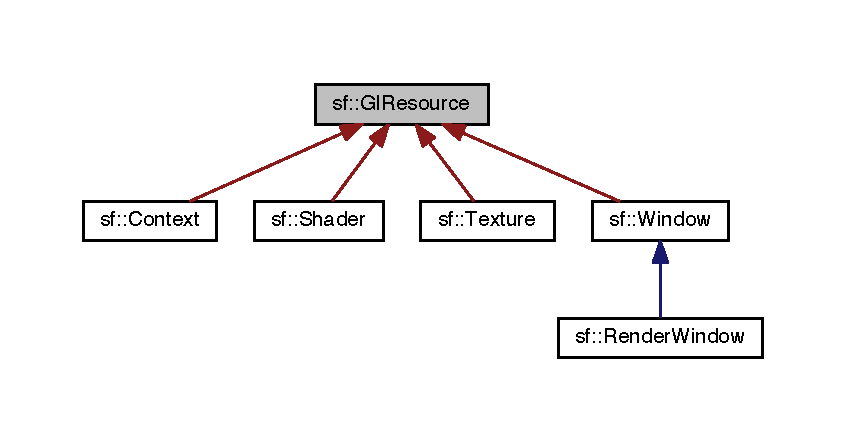
\includegraphics[width=350pt]{classsf_1_1_gl_resource__inherit__graph}
\end{center}
\end{figure}
\subsection*{Protected Member Functions}
\begin{DoxyCompactItemize}
\item 
\hyperlink{classsf_1_1_gl_resource_ad8fb7a0674f0f77e530dacc2a3b0dc6a}{Gl\-Resource} ()
\begin{DoxyCompactList}\small\item\em Default constructor. \end{DoxyCompactList}\item 
\hyperlink{classsf_1_1_gl_resource_ab99035b67052331d1e8cf67abd93de98}{$\sim$\-Gl\-Resource} ()
\begin{DoxyCompactList}\small\item\em Destructor. \end{DoxyCompactList}\end{DoxyCompactItemize}
\subsection*{Static Protected Member Functions}
\begin{DoxyCompactItemize}
\item 
static \hyperlink{glutf90_8h_ac778d6f63f1aaf8ebda0ce6ac821b56e}{void} \hyperlink{classsf_1_1_gl_resource_ae0efa7935241644608ca32ba47b22a33}{ensure\-Gl\-Context} ()
\begin{DoxyCompactList}\small\item\em Make sure that a valid Open\-G\-L context exists in the current thread. \end{DoxyCompactList}\end{DoxyCompactItemize}


\subsection{Detailed Description}
Base class for classes that require an Open\-G\-L context. 

This class is for internal use only, it must be the base of every class that requires a valid Open\-G\-L context in order to work. 

Definition at line 40 of file Gl\-Resource.\-hpp.



\subsection{Constructor \& Destructor Documentation}
\hypertarget{classsf_1_1_gl_resource_ad8fb7a0674f0f77e530dacc2a3b0dc6a}{\index{sf\-::\-Gl\-Resource@{sf\-::\-Gl\-Resource}!Gl\-Resource@{Gl\-Resource}}
\index{Gl\-Resource@{Gl\-Resource}!sf::GlResource@{sf\-::\-Gl\-Resource}}
\subsubsection[{Gl\-Resource}]{\setlength{\rightskip}{0pt plus 5cm}sf\-::\-Gl\-Resource\-::\-Gl\-Resource (
\begin{DoxyParamCaption}
{}
\end{DoxyParamCaption}
)\hspace{0.3cm}{\ttfamily [protected]}}}\label{classsf_1_1_gl_resource_ad8fb7a0674f0f77e530dacc2a3b0dc6a}


Default constructor. 

\hypertarget{classsf_1_1_gl_resource_ab99035b67052331d1e8cf67abd93de98}{\index{sf\-::\-Gl\-Resource@{sf\-::\-Gl\-Resource}!$\sim$\-Gl\-Resource@{$\sim$\-Gl\-Resource}}
\index{$\sim$\-Gl\-Resource@{$\sim$\-Gl\-Resource}!sf::GlResource@{sf\-::\-Gl\-Resource}}
\subsubsection[{$\sim$\-Gl\-Resource}]{\setlength{\rightskip}{0pt plus 5cm}sf\-::\-Gl\-Resource\-::$\sim$\-Gl\-Resource (
\begin{DoxyParamCaption}
{}
\end{DoxyParamCaption}
)\hspace{0.3cm}{\ttfamily [protected]}}}\label{classsf_1_1_gl_resource_ab99035b67052331d1e8cf67abd93de98}


Destructor. 



\subsection{Member Function Documentation}
\hypertarget{classsf_1_1_gl_resource_ae0efa7935241644608ca32ba47b22a33}{\index{sf\-::\-Gl\-Resource@{sf\-::\-Gl\-Resource}!ensure\-Gl\-Context@{ensure\-Gl\-Context}}
\index{ensure\-Gl\-Context@{ensure\-Gl\-Context}!sf::GlResource@{sf\-::\-Gl\-Resource}}
\subsubsection[{ensure\-Gl\-Context}]{\setlength{\rightskip}{0pt plus 5cm}static {\bf void} sf\-::\-Gl\-Resource\-::ensure\-Gl\-Context (
\begin{DoxyParamCaption}
{}
\end{DoxyParamCaption}
)\hspace{0.3cm}{\ttfamily [static]}, {\ttfamily [protected]}}}\label{classsf_1_1_gl_resource_ae0efa7935241644608ca32ba47b22a33}


Make sure that a valid Open\-G\-L context exists in the current thread. 



The documentation for this class was generated from the following file\-:\begin{DoxyCompactItemize}
\item 
/\-Users/ira/\-Dropbox/ira\-\_\-dev/protobyte\-\_\-research/other\-\_\-libs/\-S\-F\-M\-L/dylibs/root/usr/local/include/\-S\-F\-M\-L/\-Window/\hyperlink{_gl_resource_8hpp}{Gl\-Resource.\-hpp}\end{DoxyCompactItemize}

\hypertarget{classsf_1_1_glyph}{\section{sf\-:\-:Glyph Class Reference}
\label{classsf_1_1_glyph}\index{sf\-::\-Glyph@{sf\-::\-Glyph}}
}


Structure describing a glyph.  




{\ttfamily \#include $<$Glyph.\-hpp$>$}



Collaboration diagram for sf\-:\-:Glyph\-:
\nopagebreak
\begin{figure}[H]
\begin{center}
\leavevmode
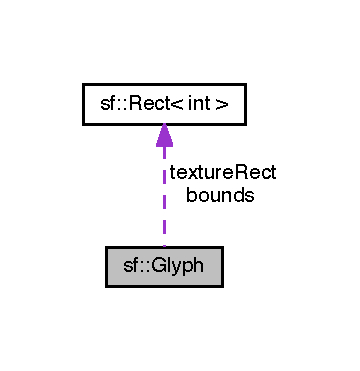
\includegraphics[width=173pt]{classsf_1_1_glyph__coll__graph}
\end{center}
\end{figure}
\subsection*{Public Member Functions}
\begin{DoxyCompactItemize}
\item 
\hyperlink{classsf_1_1_glyph_ab15cfc37eb7b40a94b3b3aedf934010b}{Glyph} ()
\begin{DoxyCompactList}\small\item\em Default constructor. \end{DoxyCompactList}\end{DoxyCompactItemize}
\subsection*{Public Attributes}
\begin{DoxyCompactItemize}
\item 
int \hyperlink{classsf_1_1_glyph_a50b93f441db501d10308007f63382166}{advance}
\begin{DoxyCompactList}\small\item\em Offset to move horizontically to the next character. \end{DoxyCompactList}\item 
\hyperlink{namespacesf_aae67411782674934f78d55fa3af18403}{Int\-Rect} \hyperlink{classsf_1_1_glyph_afe4cd37e5839955d7dd008e178d41f0c}{bounds}
\begin{DoxyCompactList}\small\item\em Bounding rectangle of the glyph, in coordinates relative to the baseline. \end{DoxyCompactList}\item 
\hyperlink{namespacesf_aae67411782674934f78d55fa3af18403}{Int\-Rect} \hyperlink{classsf_1_1_glyph_a0d502d326449f8c49011ed91d2805f5b}{texture\-Rect}
\begin{DoxyCompactList}\small\item\em \hyperlink{classsf_1_1_texture}{Texture} coordinates of the glyph inside the font's texture. \end{DoxyCompactList}\end{DoxyCompactItemize}


\subsection{Detailed Description}
Structure describing a glyph. 

A glyph is the visual representation of a character.

The \hyperlink{classsf_1_1_glyph}{sf\-::\-Glyph} structure provides the information needed to handle the glyph\-: \begin{DoxyItemize}
\item its coordinates in the font's texture \item its bounding rectangle \item the offset to apply to get the starting position of the next glyph\end{DoxyItemize}
\begin{DoxySeeAlso}{See Also}
\hyperlink{classsf_1_1_font}{sf\-::\-Font} 
\end{DoxySeeAlso}


Definition at line 41 of file Glyph.\-hpp.



\subsection{Constructor \& Destructor Documentation}
\hypertarget{classsf_1_1_glyph_ab15cfc37eb7b40a94b3b3aedf934010b}{\index{sf\-::\-Glyph@{sf\-::\-Glyph}!Glyph@{Glyph}}
\index{Glyph@{Glyph}!sf::Glyph@{sf\-::\-Glyph}}
\subsubsection[{Glyph}]{\setlength{\rightskip}{0pt plus 5cm}sf\-::\-Glyph\-::\-Glyph (
\begin{DoxyParamCaption}
{}
\end{DoxyParamCaption}
)\hspace{0.3cm}{\ttfamily [inline]}}}\label{classsf_1_1_glyph_ab15cfc37eb7b40a94b3b3aedf934010b}


Default constructor. 



Definition at line 49 of file Glyph.\-hpp.



\subsection{Member Data Documentation}
\hypertarget{classsf_1_1_glyph_a50b93f441db501d10308007f63382166}{\index{sf\-::\-Glyph@{sf\-::\-Glyph}!advance@{advance}}
\index{advance@{advance}!sf::Glyph@{sf\-::\-Glyph}}
\subsubsection[{advance}]{\setlength{\rightskip}{0pt plus 5cm}int sf\-::\-Glyph\-::advance}}\label{classsf_1_1_glyph_a50b93f441db501d10308007f63382166}


Offset to move horizontically to the next character. 



Definition at line 54 of file Glyph.\-hpp.

\hypertarget{classsf_1_1_glyph_afe4cd37e5839955d7dd008e178d41f0c}{\index{sf\-::\-Glyph@{sf\-::\-Glyph}!bounds@{bounds}}
\index{bounds@{bounds}!sf::Glyph@{sf\-::\-Glyph}}
\subsubsection[{bounds}]{\setlength{\rightskip}{0pt plus 5cm}{\bf Int\-Rect} sf\-::\-Glyph\-::bounds}}\label{classsf_1_1_glyph_afe4cd37e5839955d7dd008e178d41f0c}


Bounding rectangle of the glyph, in coordinates relative to the baseline. 



Definition at line 55 of file Glyph.\-hpp.

\hypertarget{classsf_1_1_glyph_a0d502d326449f8c49011ed91d2805f5b}{\index{sf\-::\-Glyph@{sf\-::\-Glyph}!texture\-Rect@{texture\-Rect}}
\index{texture\-Rect@{texture\-Rect}!sf::Glyph@{sf\-::\-Glyph}}
\subsubsection[{texture\-Rect}]{\setlength{\rightskip}{0pt plus 5cm}{\bf Int\-Rect} sf\-::\-Glyph\-::texture\-Rect}}\label{classsf_1_1_glyph_a0d502d326449f8c49011ed91d2805f5b}


\hyperlink{classsf_1_1_texture}{Texture} coordinates of the glyph inside the font's texture. 



Definition at line 56 of file Glyph.\-hpp.



The documentation for this class was generated from the following file\-:\begin{DoxyCompactItemize}
\item 
/\-Users/ira/\-Dropbox/ira\-\_\-dev/protobyte\-\_\-research/other\-\_\-libs/\-S\-F\-M\-L/dylibs/root/usr/local/include/\-S\-F\-M\-L/\-Graphics/\hyperlink{_glyph_8hpp}{Glyph.\-hpp}\end{DoxyCompactItemize}

\hypertarget{classsf_1_1_http}{\section{sf\-:\-:Http Class Reference}
\label{classsf_1_1_http}\index{sf\-::\-Http@{sf\-::\-Http}}
}


A H\-T\-T\-P client.  




{\ttfamily \#include $<$Http.\-hpp$>$}



Inheritance diagram for sf\-:\-:Http\-:
\nopagebreak
\begin{figure}[H]
\begin{center}
\leavevmode
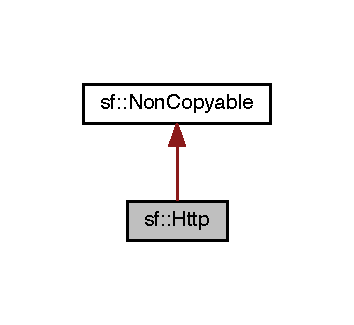
\includegraphics[width=170pt]{classsf_1_1_http__inherit__graph}
\end{center}
\end{figure}


Collaboration diagram for sf\-:\-:Http\-:
\nopagebreak
\begin{figure}[H]
\begin{center}
\leavevmode
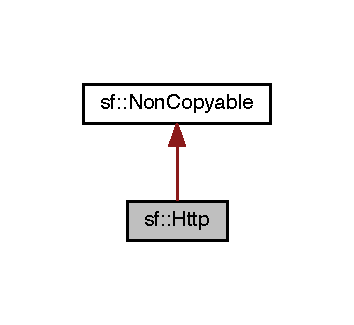
\includegraphics[width=170pt]{classsf_1_1_http__coll__graph}
\end{center}
\end{figure}
\subsection*{Classes}
\begin{DoxyCompactItemize}
\item 
class \hyperlink{classsf_1_1_http_1_1_request}{Request}
\begin{DoxyCompactList}\small\item\em Define a H\-T\-T\-P request. \end{DoxyCompactList}\item 
class \hyperlink{classsf_1_1_http_1_1_response}{Response}
\begin{DoxyCompactList}\small\item\em Define a H\-T\-T\-P response. \end{DoxyCompactList}\end{DoxyCompactItemize}
\subsection*{Public Member Functions}
\begin{DoxyCompactItemize}
\item 
\hyperlink{classsf_1_1_http_abe2360194f99bdde402c9f97a85cf067}{Http} ()
\begin{DoxyCompactList}\small\item\em Default constructor. \end{DoxyCompactList}\item 
\hyperlink{classsf_1_1_http_a79efd844a735f083fcce0edbf1092385}{Http} (const \hyperlink{gl3_8h_ac83513893df92266f79a515488701770}{std\-::string} \&host, unsigned short port=0)
\begin{DoxyCompactList}\small\item\em Construct the H\-T\-T\-P client with the target host. \end{DoxyCompactList}\item 
\hyperlink{glutf90_8h_ac778d6f63f1aaf8ebda0ce6ac821b56e}{void} \hyperlink{classsf_1_1_http_a55121d543b61c41cf20b885a97b04e65}{set\-Host} (const \hyperlink{gl3_8h_ac83513893df92266f79a515488701770}{std\-::string} \&host, unsigned short port=0)
\begin{DoxyCompactList}\small\item\em Set the target host. \end{DoxyCompactList}\item 
\hyperlink{classsf_1_1_http_1_1_response}{Response} \hyperlink{classsf_1_1_http_aaf09ebfb5e00dcc82e0d494d5c6a9e2a}{send\-Request} (const \hyperlink{classsf_1_1_http_1_1_request}{Request} \&request, \hyperlink{classsf_1_1_time}{Time} \hyperlink{gl3_8h_ad29bb0d8468b264a4e3d9204366cfaab}{timeout}=\hyperlink{classsf_1_1_time_a8db127b632fa8da21550e7282af11fa0}{Time\-::\-Zero})
\begin{DoxyCompactList}\small\item\em Send a H\-T\-T\-P request and return the server's response. \end{DoxyCompactList}\end{DoxyCompactItemize}
\subsection*{Additional Inherited Members}


\subsection{Detailed Description}
A H\-T\-T\-P client. 

\hyperlink{classsf_1_1_http}{sf\-::\-Http} is a very simple H\-T\-T\-P client that allows you to communicate with a web server. You can retrieve web pages, send data to an interactive resource, download a remote file, etc.

The H\-T\-T\-P client is split into 3 classes\-: \begin{DoxyItemize}
\item \hyperlink{classsf_1_1_http_1_1_request}{sf\-::\-Http\-::\-Request} \item \hyperlink{classsf_1_1_http_1_1_response}{sf\-::\-Http\-::\-Response} \item \hyperlink{classsf_1_1_http}{sf\-::\-Http}\end{DoxyItemize}
\hyperlink{classsf_1_1_http_1_1_request}{sf\-::\-Http\-::\-Request} builds the request that will be sent to the server. A request is made of\-: \begin{DoxyItemize}
\item a method (what you want to do) \item a target U\-R\-I (usually the name of the web page or file) \item one or more header fields (options that you can pass to the server) \item an optional body (for P\-O\-S\-T requests)\end{DoxyItemize}
\hyperlink{classsf_1_1_http_1_1_response}{sf\-::\-Http\-::\-Response} parse the response from the web server and provides getters to read them. The response contains\-: \begin{DoxyItemize}
\item a status code \item header fields (that may be answers to the ones that you requested) \item a body, which contains the contents of the requested resource\end{DoxyItemize}
\hyperlink{classsf_1_1_http}{sf\-::\-Http} provides a simple function, Send\-Request, to send a \hyperlink{classsf_1_1_http_1_1_request}{sf\-::\-Http\-::\-Request} and return the corresponding \hyperlink{classsf_1_1_http_1_1_response}{sf\-::\-Http\-::\-Response} from the server.

Usage example\-: 
\begin{DoxyCode}
\textcolor{comment}{// Create a new HTTP client}
\hyperlink{classsf_1_1_http}{sf::Http} http;

\textcolor{comment}{// We'll work on http://www.sfml-dev.org}
http.\hyperlink{classsf_1_1_http_a55121d543b61c41cf20b885a97b04e65}{setHost}(\textcolor{stringliteral}{"http://www.sfml-dev.org"});

\textcolor{comment}{// Prepare a request to get the 'features.php' page}
\hyperlink{classsf_1_1_http_1_1_request}{sf::Http::Request} request(\textcolor{stringliteral}{"features.php"});

\textcolor{comment}{// Send the request}
\hyperlink{classsf_1_1_http_1_1_response}{sf::Http::Response} response = http.\hyperlink{classsf_1_1_http_aaf09ebfb5e00dcc82e0d494d5c6a9e2a}{sendRequest}(request);

\textcolor{comment}{// Check the status code and display the result}
\hyperlink{classsf_1_1_http_1_1_response_a663e071978e30fbbeb20ed045be874d8}{sf::Http::Response::Status} status = response.\hyperlink{classsf_1_1_http_1_1_response_a542e9856b1dd260a83940eb982b7f19a}{getStatus}();
\textcolor{keywordflow}{if} (status == \hyperlink{classsf_1_1_http_1_1_response_a663e071978e30fbbeb20ed045be874d8a0158f932254d3f09647dd1f64bd43832}{sf::Http::Response::Ok})
\{
    std::cout << response.\hyperlink{classsf_1_1_http_1_1_response_a6b74ef73051a16ebb20041495c758e22}{getBody}() << std::endl;
\}
\textcolor{keywordflow}{else}
\{
    std::cout << \textcolor{stringliteral}{"Error "} << status << std::endl;
\}
\end{DoxyCode}
 

Definition at line 46 of file Http.\-hpp.



\subsection{Constructor \& Destructor Documentation}
\hypertarget{classsf_1_1_http_abe2360194f99bdde402c9f97a85cf067}{\index{sf\-::\-Http@{sf\-::\-Http}!Http@{Http}}
\index{Http@{Http}!sf::Http@{sf\-::\-Http}}
\subsubsection[{Http}]{\setlength{\rightskip}{0pt plus 5cm}sf\-::\-Http\-::\-Http (
\begin{DoxyParamCaption}
{}
\end{DoxyParamCaption}
)}}\label{classsf_1_1_http_abe2360194f99bdde402c9f97a85cf067}


Default constructor. 

\hypertarget{classsf_1_1_http_a79efd844a735f083fcce0edbf1092385}{\index{sf\-::\-Http@{sf\-::\-Http}!Http@{Http}}
\index{Http@{Http}!sf::Http@{sf\-::\-Http}}
\subsubsection[{Http}]{\setlength{\rightskip}{0pt plus 5cm}sf\-::\-Http\-::\-Http (
\begin{DoxyParamCaption}
\item[{const {\bf std\-::string} \&}]{host, }
\item[{unsigned short}]{port = {\ttfamily 0}}
\end{DoxyParamCaption}
)}}\label{classsf_1_1_http_a79efd844a735f083fcce0edbf1092385}


Construct the H\-T\-T\-P client with the target host. 

This is equivalent to calling Set\-Host(host, port). The port has a default value of 0, which means that the H\-T\-T\-P client will use the right port according to the protocol used (80 for H\-T\-T\-P, 443 for H\-T\-T\-P\-S). You should leave it like this unless you really need a port other than the standard one, or use an unknown protocol.


\begin{DoxyParams}{Parameters}
{\em host} & Web server to connect to \\
\hline
{\em port} & Port to use for connection \\
\hline
\end{DoxyParams}


\subsection{Member Function Documentation}
\hypertarget{classsf_1_1_http_aaf09ebfb5e00dcc82e0d494d5c6a9e2a}{\index{sf\-::\-Http@{sf\-::\-Http}!send\-Request@{send\-Request}}
\index{send\-Request@{send\-Request}!sf::Http@{sf\-::\-Http}}
\subsubsection[{send\-Request}]{\setlength{\rightskip}{0pt plus 5cm}{\bf Response} sf\-::\-Http\-::send\-Request (
\begin{DoxyParamCaption}
\item[{const {\bf Request} \&}]{request, }
\item[{{\bf Time}}]{timeout = {\ttfamily {\bf Time\-::\-Zero}}}
\end{DoxyParamCaption}
)}}\label{classsf_1_1_http_aaf09ebfb5e00dcc82e0d494d5c6a9e2a}


Send a H\-T\-T\-P request and return the server's response. 

You must have a valid host before sending a request (see Set\-Host). Any missing mandatory header field in the request will be added with an appropriate value. Warning\-: this function waits for the server's response and may not return instantly; use a thread if you don't want to block your application, or use a timeout to limit the time to wait. A value of \hyperlink{classsf_1_1_time_a8db127b632fa8da21550e7282af11fa0}{Time\-::\-Zero} means that the client will use the system defaut timeout (which is usually pretty long).


\begin{DoxyParams}{Parameters}
{\em request} & \hyperlink{classsf_1_1_http_1_1_request}{Request} to send \\
\hline
{\em timeout} & Maximum time to wait\\
\hline
\end{DoxyParams}
\begin{DoxyReturn}{Returns}
Server's response 
\end{DoxyReturn}
\hypertarget{classsf_1_1_http_a55121d543b61c41cf20b885a97b04e65}{\index{sf\-::\-Http@{sf\-::\-Http}!set\-Host@{set\-Host}}
\index{set\-Host@{set\-Host}!sf::Http@{sf\-::\-Http}}
\subsubsection[{set\-Host}]{\setlength{\rightskip}{0pt plus 5cm}{\bf void} sf\-::\-Http\-::set\-Host (
\begin{DoxyParamCaption}
\item[{const {\bf std\-::string} \&}]{host, }
\item[{unsigned short}]{port = {\ttfamily 0}}
\end{DoxyParamCaption}
)}}\label{classsf_1_1_http_a55121d543b61c41cf20b885a97b04e65}


Set the target host. 

This function just stores the host address and port, it doesn't actually connect to it until you send a request. The port has a default value of 0, which means that the H\-T\-T\-P client will use the right port according to the protocol used (80 for H\-T\-T\-P, 443 for H\-T\-T\-P\-S). You should leave it like this unless you really need a port other than the standard one, or use an unknown protocol.


\begin{DoxyParams}{Parameters}
{\em host} & Web server to connect to \\
\hline
{\em port} & Port to use for connection \\
\hline
\end{DoxyParams}


The documentation for this class was generated from the following file\-:\begin{DoxyCompactItemize}
\item 
/\-Users/ira/\-Dropbox/ira\-\_\-dev/protobyte\-\_\-research/other\-\_\-libs/\-S\-F\-M\-L/dylibs/root/usr/local/include/\-S\-F\-M\-L/\-Network/\hyperlink{_http_8hpp}{Http.\-hpp}\end{DoxyCompactItemize}

\hypertarget{classsf_1_1_image}{\section{sf\-:\-:Image Class Reference}
\label{classsf_1_1_image}\index{sf\-::\-Image@{sf\-::\-Image}}
}


Class for loading, manipulating and saving images.  




{\ttfamily \#include $<$Image.\-hpp$>$}

\subsection*{Public Member Functions}
\begin{DoxyCompactItemize}
\item 
\hyperlink{classsf_1_1_image_abb4caf3cb167b613345ebe36fc883f12}{Image} ()
\begin{DoxyCompactList}\small\item\em Default constructor. \end{DoxyCompactList}\item 
\hyperlink{glutf90_8h_ac778d6f63f1aaf8ebda0ce6ac821b56e}{void} \hyperlink{classsf_1_1_image_a2a67930e2fd9ad97cf004e918cf5832b}{create} (unsigned int \hyperlink{gl3_8h_a9d14ddc31c6c8b61f3fe3679ab976133}{width}, unsigned int \hyperlink{gl3_8h_a67001679ebf2bb0ba972db4d29c6550c}{height}, const \hyperlink{classsf_1_1_color}{Color} \&\hyperlink{gl3_8h_a3ea846f998d64f079b86052b6c4193a8}{color}=\hyperlink{classsf_1_1_color}{Color}(0, 0, 0))
\begin{DoxyCompactList}\small\item\em Create the image and fill it with a unique color. \end{DoxyCompactList}\item 
\hyperlink{glutf90_8h_ac778d6f63f1aaf8ebda0ce6ac821b56e}{void} \hyperlink{classsf_1_1_image_a1c2b960ea12bdbb29e80934ce5268ebf}{create} (unsigned int \hyperlink{gl3_8h_a9d14ddc31c6c8b61f3fe3679ab976133}{width}, unsigned int \hyperlink{gl3_8h_a67001679ebf2bb0ba972db4d29c6550c}{height}, const \hyperlink{namespacesf_a4ef3d630785c4f296f9b4f274c33d78e}{Uint8} $\ast$\hyperlink{gl3_8h_ada7ad693ea2e311b8103f4693fc35f80}{pixels})
\begin{DoxyCompactList}\small\item\em Create the image from an array of pixels. \end{DoxyCompactList}\item 
bool \hyperlink{classsf_1_1_image_a9e4f2aa8e36d0cabde5ed5a4ef80290b}{load\-From\-File} (const \hyperlink{gl3_8h_ac83513893df92266f79a515488701770}{std\-::string} \&filename)
\begin{DoxyCompactList}\small\item\em Load the image from a file on disk. \end{DoxyCompactList}\item 
bool \hyperlink{classsf_1_1_image_aaa6c7afa5851a51cec6ab438faa7354c}{load\-From\-Memory} (const \hyperlink{glutf90_8h_ac778d6f63f1aaf8ebda0ce6ac821b56e}{void} $\ast$\hyperlink{gl3_8h_a0f78eecb0891cce3bdfc815b971866a1}{data}, std\-::size\-\_\-t \hyperlink{gl3_8h_a79ef9eb3e59c4bb34c4b9fbeb8d28ff7}{size})
\begin{DoxyCompactList}\small\item\em Load the image from a file in memory. \end{DoxyCompactList}\item 
bool \hyperlink{classsf_1_1_image_a21122ded0e8368bb06ed3b9acfbfb501}{load\-From\-Stream} (\hyperlink{classsf_1_1_input_stream}{Input\-Stream} \&stream)
\begin{DoxyCompactList}\small\item\em Load the image from a custom stream. \end{DoxyCompactList}\item 
bool \hyperlink{classsf_1_1_image_aec0ed16b67df7b512aaa5c53388ba14e}{save\-To\-File} (const \hyperlink{gl3_8h_ac83513893df92266f79a515488701770}{std\-::string} \&filename) const 
\begin{DoxyCompactList}\small\item\em Save the image to a file on disk. \end{DoxyCompactList}\item 
\hyperlink{namespacesf_aaa02ba42bf79b001a376fe9d79254cb3}{Vector2u} \hyperlink{classsf_1_1_image_a5c3e9bebdc001c3ebf85ca97039fc86b}{get\-Size} () const 
\begin{DoxyCompactList}\small\item\em Return the size of the image. \end{DoxyCompactList}\item 
\hyperlink{glutf90_8h_ac778d6f63f1aaf8ebda0ce6ac821b56e}{void} \hyperlink{classsf_1_1_image_a22f13f8c242a6b38eb73cc176b37ae34}{create\-Mask\-From\-Color} (const \hyperlink{classsf_1_1_color}{Color} \&\hyperlink{gl3_8h_a3ea846f998d64f079b86052b6c4193a8}{color}, \hyperlink{namespacesf_a4ef3d630785c4f296f9b4f274c33d78e}{Uint8} \hyperlink{gl3_8h_a090ebe65994a3ee4bb60ae3472abffc5}{alpha}=0)
\begin{DoxyCompactList}\small\item\em Create a transparency mask from a specified color-\/key. \end{DoxyCompactList}\item 
\hyperlink{glutf90_8h_ac778d6f63f1aaf8ebda0ce6ac821b56e}{void} \hyperlink{classsf_1_1_image_ab2fa337c956f85f93377dcb52153a45a}{copy} (const \hyperlink{classsf_1_1_image}{Image} \&\hyperlink{gl3_8h_a6ffd2192cbc75d017665e95207ee36a7}{source}, unsigned int dest\-X, unsigned int dest\-Y, const \hyperlink{namespacesf_aae67411782674934f78d55fa3af18403}{Int\-Rect} \&source\-Rect=\hyperlink{namespacesf_aae67411782674934f78d55fa3af18403}{Int\-Rect}(0, 0, 0, 0), bool apply\-Alpha=false)
\begin{DoxyCompactList}\small\item\em Copy pixels from another image onto this one. \end{DoxyCompactList}\item 
\hyperlink{glutf90_8h_ac778d6f63f1aaf8ebda0ce6ac821b56e}{void} \hyperlink{classsf_1_1_image_a9fd329b8cd7d4439e07fb5d3bb2d9744}{set\-Pixel} (unsigned int \hyperlink{gl3_8h_a92d0386e5c19fb81ea88c9f99644ab1d}{x}, unsigned int \hyperlink{gl3_8h_a66ddd433d2cacfe27f5906b7e86faeed}{y}, const \hyperlink{classsf_1_1_color}{Color} \&\hyperlink{gl3_8h_a3ea846f998d64f079b86052b6c4193a8}{color})
\begin{DoxyCompactList}\small\item\em Change the color of a pixel. \end{DoxyCompactList}\item 
\hyperlink{classsf_1_1_color}{Color} \hyperlink{classsf_1_1_image_a8c8460e311dcb00557cb00a81c29163d}{get\-Pixel} (unsigned int \hyperlink{gl3_8h_a92d0386e5c19fb81ea88c9f99644ab1d}{x}, unsigned int \hyperlink{gl3_8h_a66ddd433d2cacfe27f5906b7e86faeed}{y}) const 
\begin{DoxyCompactList}\small\item\em Get the color of a pixel. \end{DoxyCompactList}\item 
const \hyperlink{namespacesf_a4ef3d630785c4f296f9b4f274c33d78e}{Uint8} $\ast$ \hyperlink{classsf_1_1_image_ac6137a608a9efaae2735c13ff259c214}{get\-Pixels\-Ptr} () const 
\begin{DoxyCompactList}\small\item\em Get a read-\/only pointer to the array of pixels. \end{DoxyCompactList}\item 
\hyperlink{glutf90_8h_ac778d6f63f1aaf8ebda0ce6ac821b56e}{void} \hyperlink{classsf_1_1_image_a57168e7bc29190e08bbd6c9c19f4bb2c}{flip\-Horizontally} ()
\begin{DoxyCompactList}\small\item\em Flip the image horizontally (left $<$-\/$>$ right) \end{DoxyCompactList}\item 
\hyperlink{glutf90_8h_ac778d6f63f1aaf8ebda0ce6ac821b56e}{void} \hyperlink{classsf_1_1_image_a78a702a7e49d1de2dec9894da99d279c}{flip\-Vertically} ()
\begin{DoxyCompactList}\small\item\em Flip the image vertically (top $<$-\/$>$ bottom) \end{DoxyCompactList}\end{DoxyCompactItemize}


\subsection{Detailed Description}
Class for loading, manipulating and saving images. 

\hyperlink{classsf_1_1_image}{sf\-::\-Image} is an abstraction to manipulate images as bidimensional arrays of pixels. The class provides functions to load, read, write and save pixels, as well as many other useful functions.

\hyperlink{classsf_1_1_image}{sf\-::\-Image} can handle a unique internal representation of pixels, which is R\-G\-B\-A 32 bits. This means that a pixel must be composed of 8 bits red, green, blue and alpha channels -- just like a \hyperlink{classsf_1_1_color}{sf\-::\-Color}. All the functions that return an array of pixels follow this rule, and all parameters that you pass to \hyperlink{classsf_1_1_image}{sf\-::\-Image} functions (such as load\-From\-Pixels) must use this representation as well.

A \hyperlink{classsf_1_1_image}{sf\-::\-Image} can be copied, but it is a heavy resource and if possible you should always use \mbox{[}const\mbox{]} references to pass or return them to avoid useless copies.

Usage example\-: 
\begin{DoxyCode}
\textcolor{comment}{// Load an image file from a file}
\hyperlink{classsf_1_1_image}{sf::Image} background;
\textcolor{keywordflow}{if} (!background.\hyperlink{classsf_1_1_image_a9e4f2aa8e36d0cabde5ed5a4ef80290b}{loadFromFile}(\textcolor{stringliteral}{"background.jpg"}))
    \textcolor{keywordflow}{return} -1;

\textcolor{comment}{// Create a 20x20 image filled with black color}
\hyperlink{classsf_1_1_image}{sf::Image} image;
\textcolor{keywordflow}{if} (!image.\hyperlink{classsf_1_1_image_a2a67930e2fd9ad97cf004e918cf5832b}{create}(20, 20, \hyperlink{classsf_1_1_color_a77c688197b981338f0b19dc58bd2facd}{sf::Color::Black}))
    \textcolor{keywordflow}{return} -1;

\textcolor{comment}{// Copy image1 on image2 at position (10, 10)}
image.\hyperlink{classsf_1_1_image_ab2fa337c956f85f93377dcb52153a45a}{copy}(background, 10, 10);

\textcolor{comment}{// Make the top-left pixel transparent}
\hyperlink{classsf_1_1_color}{sf::Color} color = image.\hyperlink{classsf_1_1_image_a8c8460e311dcb00557cb00a81c29163d}{getPixel}(0, 0);
color.\hyperlink{classsf_1_1_color_a56dbdb47d5f040d9b78ac6a0b8b3a831}{a} = 0;
image.\hyperlink{classsf_1_1_image_a9fd329b8cd7d4439e07fb5d3bb2d9744}{setPixel}(0, 0, color);

\textcolor{comment}{// Save the image to a file}
\textcolor{keywordflow}{if} (!image.\hyperlink{classsf_1_1_image_aec0ed16b67df7b512aaa5c53388ba14e}{saveToFile}(\textcolor{stringliteral}{"result.png"}))
    \textcolor{keywordflow}{return} -1;
\end{DoxyCode}


\begin{DoxySeeAlso}{See Also}
\hyperlink{classsf_1_1_texture}{sf\-::\-Texture} 
\end{DoxySeeAlso}


Definition at line 46 of file Image.\-hpp.



\subsection{Constructor \& Destructor Documentation}
\hypertarget{classsf_1_1_image_abb4caf3cb167b613345ebe36fc883f12}{\index{sf\-::\-Image@{sf\-::\-Image}!Image@{Image}}
\index{Image@{Image}!sf::Image@{sf\-::\-Image}}
\subsubsection[{Image}]{\setlength{\rightskip}{0pt plus 5cm}sf\-::\-Image\-::\-Image (
\begin{DoxyParamCaption}
{}
\end{DoxyParamCaption}
)}}\label{classsf_1_1_image_abb4caf3cb167b613345ebe36fc883f12}


Default constructor. 

Creates an empty image. 

\subsection{Member Function Documentation}
\hypertarget{classsf_1_1_image_ab2fa337c956f85f93377dcb52153a45a}{\index{sf\-::\-Image@{sf\-::\-Image}!copy@{copy}}
\index{copy@{copy}!sf::Image@{sf\-::\-Image}}
\subsubsection[{copy}]{\setlength{\rightskip}{0pt plus 5cm}{\bf void} sf\-::\-Image\-::copy (
\begin{DoxyParamCaption}
\item[{const {\bf Image} \&}]{source, }
\item[{unsigned int}]{dest\-X, }
\item[{unsigned int}]{dest\-Y, }
\item[{const {\bf Int\-Rect} \&}]{source\-Rect = {\ttfamily {\bf Int\-Rect}(0,~0,~0,~0)}, }
\item[{bool}]{apply\-Alpha = {\ttfamily false}}
\end{DoxyParamCaption}
)}}\label{classsf_1_1_image_ab2fa337c956f85f93377dcb52153a45a}


Copy pixels from another image onto this one. 

This function does a slow pixel copy and should not be used intensively. It can be used to prepare a complex static image from several others, but if you need this kind of feature in real-\/time you'd better use \hyperlink{classsf_1_1_render_texture}{sf\-::\-Render\-Texture}.

If {\itshape source\-Rect} is empty, the whole image is copied. If {\itshape apply\-Alpha} is set to true, the transparency of source pixels is applied. If it is false, the pixels are copied unchanged with their alpha value.


\begin{DoxyParams}{Parameters}
{\em source} & Source image to copy \\
\hline
{\em dest\-X} & X coordinate of the destination position \\
\hline
{\em dest\-Y} & Y coordinate of the destination position \\
\hline
{\em source\-Rect} & Sub-\/rectangle of the source image to copy \\
\hline
{\em apply\-Alpha} & Should the copy take in account the source transparency? \\
\hline
\end{DoxyParams}
\hypertarget{classsf_1_1_image_a2a67930e2fd9ad97cf004e918cf5832b}{\index{sf\-::\-Image@{sf\-::\-Image}!create@{create}}
\index{create@{create}!sf::Image@{sf\-::\-Image}}
\subsubsection[{create}]{\setlength{\rightskip}{0pt plus 5cm}{\bf void} sf\-::\-Image\-::create (
\begin{DoxyParamCaption}
\item[{unsigned int}]{width, }
\item[{unsigned int}]{height, }
\item[{const {\bf Color} \&}]{color = {\ttfamily {\bf Color}(0,~0,~0)}}
\end{DoxyParamCaption}
)}}\label{classsf_1_1_image_a2a67930e2fd9ad97cf004e918cf5832b}


Create the image and fill it with a unique color. 


\begin{DoxyParams}{Parameters}
{\em width} & Width of the image \\
\hline
{\em height} & Height of the image \\
\hline
{\em color} & Fill color \\
\hline
\end{DoxyParams}
\hypertarget{classsf_1_1_image_a1c2b960ea12bdbb29e80934ce5268ebf}{\index{sf\-::\-Image@{sf\-::\-Image}!create@{create}}
\index{create@{create}!sf::Image@{sf\-::\-Image}}
\subsubsection[{create}]{\setlength{\rightskip}{0pt plus 5cm}{\bf void} sf\-::\-Image\-::create (
\begin{DoxyParamCaption}
\item[{unsigned int}]{width, }
\item[{unsigned int}]{height, }
\item[{const {\bf Uint8} $\ast$}]{pixels}
\end{DoxyParamCaption}
)}}\label{classsf_1_1_image_a1c2b960ea12bdbb29e80934ce5268ebf}


Create the image from an array of pixels. 

The {\itshape pixel} array is assumed to contain 32-\/bits R\-G\-B\-A pixels, and have the given {\itshape width} and {\itshape height}. If not, this is an undefined behaviour. If {\itshape pixels} is null, an empty image is created.


\begin{DoxyParams}{Parameters}
{\em width} & Width of the image \\
\hline
{\em height} & Height of the image \\
\hline
{\em pixels} & Array of pixels to copy to the image \\
\hline
\end{DoxyParams}
\hypertarget{classsf_1_1_image_a22f13f8c242a6b38eb73cc176b37ae34}{\index{sf\-::\-Image@{sf\-::\-Image}!create\-Mask\-From\-Color@{create\-Mask\-From\-Color}}
\index{create\-Mask\-From\-Color@{create\-Mask\-From\-Color}!sf::Image@{sf\-::\-Image}}
\subsubsection[{create\-Mask\-From\-Color}]{\setlength{\rightskip}{0pt plus 5cm}{\bf void} sf\-::\-Image\-::create\-Mask\-From\-Color (
\begin{DoxyParamCaption}
\item[{const {\bf Color} \&}]{color, }
\item[{{\bf Uint8}}]{alpha = {\ttfamily 0}}
\end{DoxyParamCaption}
)}}\label{classsf_1_1_image_a22f13f8c242a6b38eb73cc176b37ae34}


Create a transparency mask from a specified color-\/key. 

This function sets the alpha value of every pixel matching the given color to {\itshape alpha} (0 by default), so that they become transparent.


\begin{DoxyParams}{Parameters}
{\em color} & \hyperlink{classsf_1_1_color}{Color} to make transparent \\
\hline
{\em alpha} & Alpha value to assign to transparent pixels \\
\hline
\end{DoxyParams}
\hypertarget{classsf_1_1_image_a57168e7bc29190e08bbd6c9c19f4bb2c}{\index{sf\-::\-Image@{sf\-::\-Image}!flip\-Horizontally@{flip\-Horizontally}}
\index{flip\-Horizontally@{flip\-Horizontally}!sf::Image@{sf\-::\-Image}}
\subsubsection[{flip\-Horizontally}]{\setlength{\rightskip}{0pt plus 5cm}{\bf void} sf\-::\-Image\-::flip\-Horizontally (
\begin{DoxyParamCaption}
{}
\end{DoxyParamCaption}
)}}\label{classsf_1_1_image_a57168e7bc29190e08bbd6c9c19f4bb2c}


Flip the image horizontally (left $<$-\/$>$ right) 

\hypertarget{classsf_1_1_image_a78a702a7e49d1de2dec9894da99d279c}{\index{sf\-::\-Image@{sf\-::\-Image}!flip\-Vertically@{flip\-Vertically}}
\index{flip\-Vertically@{flip\-Vertically}!sf::Image@{sf\-::\-Image}}
\subsubsection[{flip\-Vertically}]{\setlength{\rightskip}{0pt plus 5cm}{\bf void} sf\-::\-Image\-::flip\-Vertically (
\begin{DoxyParamCaption}
{}
\end{DoxyParamCaption}
)}}\label{classsf_1_1_image_a78a702a7e49d1de2dec9894da99d279c}


Flip the image vertically (top $<$-\/$>$ bottom) 

\hypertarget{classsf_1_1_image_a8c8460e311dcb00557cb00a81c29163d}{\index{sf\-::\-Image@{sf\-::\-Image}!get\-Pixel@{get\-Pixel}}
\index{get\-Pixel@{get\-Pixel}!sf::Image@{sf\-::\-Image}}
\subsubsection[{get\-Pixel}]{\setlength{\rightskip}{0pt plus 5cm}{\bf Color} sf\-::\-Image\-::get\-Pixel (
\begin{DoxyParamCaption}
\item[{unsigned int}]{x, }
\item[{unsigned int}]{y}
\end{DoxyParamCaption}
) const}}\label{classsf_1_1_image_a8c8460e311dcb00557cb00a81c29163d}


Get the color of a pixel. 

This function doesn't check the validity of the pixel coordinates, using out-\/of-\/range values will result in an undefined behaviour.


\begin{DoxyParams}{Parameters}
{\em x} & X coordinate of pixel to get \\
\hline
{\em y} & Y coordinate of pixel to get\\
\hline
\end{DoxyParams}
\begin{DoxyReturn}{Returns}
\hyperlink{classsf_1_1_color}{Color} of the pixel at coordinates (x, y)
\end{DoxyReturn}
\begin{DoxySeeAlso}{See Also}
\hyperlink{classsf_1_1_image_a9fd329b8cd7d4439e07fb5d3bb2d9744}{set\-Pixel} 
\end{DoxySeeAlso}
\hypertarget{classsf_1_1_image_ac6137a608a9efaae2735c13ff259c214}{\index{sf\-::\-Image@{sf\-::\-Image}!get\-Pixels\-Ptr@{get\-Pixels\-Ptr}}
\index{get\-Pixels\-Ptr@{get\-Pixels\-Ptr}!sf::Image@{sf\-::\-Image}}
\subsubsection[{get\-Pixels\-Ptr}]{\setlength{\rightskip}{0pt plus 5cm}const {\bf Uint8}$\ast$ sf\-::\-Image\-::get\-Pixels\-Ptr (
\begin{DoxyParamCaption}
{}
\end{DoxyParamCaption}
) const}}\label{classsf_1_1_image_ac6137a608a9efaae2735c13ff259c214}


Get a read-\/only pointer to the array of pixels. 

The returned value points to an array of R\-G\-B\-A pixels made of 8 bits integers components. The size of the array is Get\-Width() $\ast$ Get\-Height() $\ast$ 4. Warning\-: the returned pointer may become invalid if you modify the image, so you should never store it for too long. If the image is empty, a null pointer is returned.

\begin{DoxyReturn}{Returns}
Read-\/only pointer to the array of pixels 
\end{DoxyReturn}
\hypertarget{classsf_1_1_image_a5c3e9bebdc001c3ebf85ca97039fc86b}{\index{sf\-::\-Image@{sf\-::\-Image}!get\-Size@{get\-Size}}
\index{get\-Size@{get\-Size}!sf::Image@{sf\-::\-Image}}
\subsubsection[{get\-Size}]{\setlength{\rightskip}{0pt plus 5cm}{\bf Vector2u} sf\-::\-Image\-::get\-Size (
\begin{DoxyParamCaption}
{}
\end{DoxyParamCaption}
) const}}\label{classsf_1_1_image_a5c3e9bebdc001c3ebf85ca97039fc86b}


Return the size of the image. 

\begin{DoxyReturn}{Returns}
Size in pixels 
\end{DoxyReturn}
\hypertarget{classsf_1_1_image_a9e4f2aa8e36d0cabde5ed5a4ef80290b}{\index{sf\-::\-Image@{sf\-::\-Image}!load\-From\-File@{load\-From\-File}}
\index{load\-From\-File@{load\-From\-File}!sf::Image@{sf\-::\-Image}}
\subsubsection[{load\-From\-File}]{\setlength{\rightskip}{0pt plus 5cm}bool sf\-::\-Image\-::load\-From\-File (
\begin{DoxyParamCaption}
\item[{const {\bf std\-::string} \&}]{filename}
\end{DoxyParamCaption}
)}}\label{classsf_1_1_image_a9e4f2aa8e36d0cabde5ed5a4ef80290b}


Load the image from a file on disk. 

The supported image formats are bmp, png, tga, jpg, gif, psd, hdr and pic. Some format options are not supported, like progressive jpeg. If this function fails, the image is left unchanged.


\begin{DoxyParams}{Parameters}
{\em filename} & Path of the image file to load\\
\hline
\end{DoxyParams}
\begin{DoxyReturn}{Returns}
True if loading was successful
\end{DoxyReturn}
\begin{DoxySeeAlso}{See Also}
\hyperlink{classsf_1_1_image_aaa6c7afa5851a51cec6ab438faa7354c}{load\-From\-Memory}, \hyperlink{classsf_1_1_image_a21122ded0e8368bb06ed3b9acfbfb501}{load\-From\-Stream}, \hyperlink{classsf_1_1_image_aec0ed16b67df7b512aaa5c53388ba14e}{save\-To\-File} 
\end{DoxySeeAlso}
\hypertarget{classsf_1_1_image_aaa6c7afa5851a51cec6ab438faa7354c}{\index{sf\-::\-Image@{sf\-::\-Image}!load\-From\-Memory@{load\-From\-Memory}}
\index{load\-From\-Memory@{load\-From\-Memory}!sf::Image@{sf\-::\-Image}}
\subsubsection[{load\-From\-Memory}]{\setlength{\rightskip}{0pt plus 5cm}bool sf\-::\-Image\-::load\-From\-Memory (
\begin{DoxyParamCaption}
\item[{const {\bf void} $\ast$}]{data, }
\item[{std\-::size\-\_\-t}]{size}
\end{DoxyParamCaption}
)}}\label{classsf_1_1_image_aaa6c7afa5851a51cec6ab438faa7354c}


Load the image from a file in memory. 

The supported image formats are bmp, png, tga, jpg, gif, psd, hdr and pic. Some format options are not supported, like progressive jpeg. If this function fails, the image is left unchanged.


\begin{DoxyParams}{Parameters}
{\em data} & Pointer to the file data in memory \\
\hline
{\em size} & Size of the data to load, in bytes\\
\hline
\end{DoxyParams}
\begin{DoxyReturn}{Returns}
True if loading was successful
\end{DoxyReturn}
\begin{DoxySeeAlso}{See Also}
\hyperlink{classsf_1_1_image_a9e4f2aa8e36d0cabde5ed5a4ef80290b}{load\-From\-File}, \hyperlink{classsf_1_1_image_a21122ded0e8368bb06ed3b9acfbfb501}{load\-From\-Stream} 
\end{DoxySeeAlso}
\hypertarget{classsf_1_1_image_a21122ded0e8368bb06ed3b9acfbfb501}{\index{sf\-::\-Image@{sf\-::\-Image}!load\-From\-Stream@{load\-From\-Stream}}
\index{load\-From\-Stream@{load\-From\-Stream}!sf::Image@{sf\-::\-Image}}
\subsubsection[{load\-From\-Stream}]{\setlength{\rightskip}{0pt plus 5cm}bool sf\-::\-Image\-::load\-From\-Stream (
\begin{DoxyParamCaption}
\item[{{\bf Input\-Stream} \&}]{stream}
\end{DoxyParamCaption}
)}}\label{classsf_1_1_image_a21122ded0e8368bb06ed3b9acfbfb501}


Load the image from a custom stream. 

The supported image formats are bmp, png, tga, jpg, gif, psd, hdr and pic. Some format options are not supported, like progressive jpeg. If this function fails, the image is left unchanged.


\begin{DoxyParams}{Parameters}
{\em stream} & Source stream to read from\\
\hline
\end{DoxyParams}
\begin{DoxyReturn}{Returns}
True if loading was successful
\end{DoxyReturn}
\begin{DoxySeeAlso}{See Also}
\hyperlink{classsf_1_1_image_a9e4f2aa8e36d0cabde5ed5a4ef80290b}{load\-From\-File}, \hyperlink{classsf_1_1_image_aaa6c7afa5851a51cec6ab438faa7354c}{load\-From\-Memory} 
\end{DoxySeeAlso}
\hypertarget{classsf_1_1_image_aec0ed16b67df7b512aaa5c53388ba14e}{\index{sf\-::\-Image@{sf\-::\-Image}!save\-To\-File@{save\-To\-File}}
\index{save\-To\-File@{save\-To\-File}!sf::Image@{sf\-::\-Image}}
\subsubsection[{save\-To\-File}]{\setlength{\rightskip}{0pt plus 5cm}bool sf\-::\-Image\-::save\-To\-File (
\begin{DoxyParamCaption}
\item[{const {\bf std\-::string} \&}]{filename}
\end{DoxyParamCaption}
) const}}\label{classsf_1_1_image_aec0ed16b67df7b512aaa5c53388ba14e}


Save the image to a file on disk. 

The format of the image is automatically deduced from the extension. The supported image formats are bmp, png, tga and jpg. The destination file is overwritten if it already exists. This function fails if the image is empty.


\begin{DoxyParams}{Parameters}
{\em filename} & Path of the file to save\\
\hline
\end{DoxyParams}
\begin{DoxyReturn}{Returns}
True if saving was successful
\end{DoxyReturn}
\begin{DoxySeeAlso}{See Also}
\hyperlink{classsf_1_1_image_a2a67930e2fd9ad97cf004e918cf5832b}{create}, \hyperlink{classsf_1_1_image_a9e4f2aa8e36d0cabde5ed5a4ef80290b}{load\-From\-File}, \hyperlink{classsf_1_1_image_aaa6c7afa5851a51cec6ab438faa7354c}{load\-From\-Memory} 
\end{DoxySeeAlso}
\hypertarget{classsf_1_1_image_a9fd329b8cd7d4439e07fb5d3bb2d9744}{\index{sf\-::\-Image@{sf\-::\-Image}!set\-Pixel@{set\-Pixel}}
\index{set\-Pixel@{set\-Pixel}!sf::Image@{sf\-::\-Image}}
\subsubsection[{set\-Pixel}]{\setlength{\rightskip}{0pt plus 5cm}{\bf void} sf\-::\-Image\-::set\-Pixel (
\begin{DoxyParamCaption}
\item[{unsigned int}]{x, }
\item[{unsigned int}]{y, }
\item[{const {\bf Color} \&}]{color}
\end{DoxyParamCaption}
)}}\label{classsf_1_1_image_a9fd329b8cd7d4439e07fb5d3bb2d9744}


Change the color of a pixel. 

This function doesn't check the validity of the pixel coordinates, using out-\/of-\/range values will result in an undefined behaviour.


\begin{DoxyParams}{Parameters}
{\em x} & X coordinate of pixel to change \\
\hline
{\em y} & Y coordinate of pixel to change \\
\hline
{\em color} & New color of the pixel\\
\hline
\end{DoxyParams}
\begin{DoxySeeAlso}{See Also}
\hyperlink{classsf_1_1_image_a8c8460e311dcb00557cb00a81c29163d}{get\-Pixel} 
\end{DoxySeeAlso}


The documentation for this class was generated from the following file\-:\begin{DoxyCompactItemize}
\item 
/\-Users/ira/\-Dropbox/ira\-\_\-dev/protobyte\-\_\-research/other\-\_\-libs/\-S\-F\-M\-L/dylibs/root/usr/local/include/\-S\-F\-M\-L/\-Graphics/\hyperlink{_image_8hpp}{Image.\-hpp}\end{DoxyCompactItemize}

\hypertarget{classsf_1_1_input_stream}{\section{sf\-:\-:Input\-Stream Class Reference}
\label{classsf_1_1_input_stream}\index{sf\-::\-Input\-Stream@{sf\-::\-Input\-Stream}}
}


Abstract class for custom file input streams.  




{\ttfamily \#include $<$Input\-Stream.\-hpp$>$}

\subsection*{Public Member Functions}
\begin{DoxyCompactItemize}
\item 
virtual \hyperlink{classsf_1_1_input_stream_a4b2eb0f92323e630bd0542bc6191682e}{$\sim$\-Input\-Stream} ()
\begin{DoxyCompactList}\small\item\em Virtual destructor. \end{DoxyCompactList}\item 
virtual \hyperlink{namespacesf_a2840579fed3494d9f330baf7a5a19903}{Int64} \hyperlink{classsf_1_1_input_stream_a8dd89c74c1acb693203f50e750c6ae53}{read} (\hyperlink{glutf90_8h_ac778d6f63f1aaf8ebda0ce6ac821b56e}{void} $\ast$\hyperlink{gl3_8h_a0f78eecb0891cce3bdfc815b971866a1}{data}, \hyperlink{namespacesf_a2840579fed3494d9f330baf7a5a19903}{Int64} \hyperlink{gl3_8h_a79ef9eb3e59c4bb34c4b9fbeb8d28ff7}{size})=0
\begin{DoxyCompactList}\small\item\em Read data from the stream. \end{DoxyCompactList}\item 
virtual \hyperlink{namespacesf_a2840579fed3494d9f330baf7a5a19903}{Int64} \hyperlink{classsf_1_1_input_stream_a76aba8e5d5cf9b1c5902d5e04f7864fc}{seek} (\hyperlink{namespacesf_a2840579fed3494d9f330baf7a5a19903}{Int64} position)=0
\begin{DoxyCompactList}\small\item\em Change the current reading position. \end{DoxyCompactList}\item 
virtual \hyperlink{namespacesf_a2840579fed3494d9f330baf7a5a19903}{Int64} \hyperlink{classsf_1_1_input_stream_a599515b9ccdbddb6fef5a98424fd559c}{tell} ()=0
\begin{DoxyCompactList}\small\item\em Get the current reading position in the stream. \end{DoxyCompactList}\item 
virtual \hyperlink{namespacesf_a2840579fed3494d9f330baf7a5a19903}{Int64} \hyperlink{classsf_1_1_input_stream_a311eaaaa65d636728e5153b574b72d5d}{get\-Size} ()=0
\begin{DoxyCompactList}\small\item\em Return the size of the stream. \end{DoxyCompactList}\end{DoxyCompactItemize}


\subsection{Detailed Description}
Abstract class for custom file input streams. 

This class allows users to define their own file input sources from which S\-F\-M\-L can load resources.

S\-F\-M\-L resource classes like \hyperlink{classsf_1_1_texture}{sf\-::\-Texture} and \hyperlink{classsf_1_1_sound_buffer}{sf\-::\-Sound\-Buffer} provide load\-From\-File and load\-From\-Memory functions, which read data from conventional sources. However, if you have data coming from a different source (over a network, embedded, encrypted, compressed, etc) you can derive your own class from \hyperlink{classsf_1_1_input_stream}{sf\-::\-Input\-Stream} and load S\-F\-M\-L resources with their load\-From\-Stream function.

Usage example\-: 
\begin{DoxyCode}
\textcolor{comment}{// custom stream class that reads from inside a zip file}
\textcolor{keyword}{class }ZipStream : \textcolor{keyword}{public} \hyperlink{classsf_1_1_input_stream}{sf::InputStream}
\{
\textcolor{keyword}{public} :

    ZipStream(\hyperlink{gl3_8h_ac83513893df92266f79a515488701770}{std::string} archive);

    \textcolor{keywordtype}{bool} open(\hyperlink{gl3_8h_ac83513893df92266f79a515488701770}{std::string} filename);

    \hyperlink{namespacesf_a2840579fed3494d9f330baf7a5a19903}{Int64} \hyperlink{classsf_1_1_input_stream_a8dd89c74c1acb693203f50e750c6ae53}{read}(\textcolor{keywordtype}{void}* \hyperlink{gl3_8h_a0f78eecb0891cce3bdfc815b971866a1}{data}, \hyperlink{namespacesf_a2840579fed3494d9f330baf7a5a19903}{Int64} \hyperlink{gl3_8h_a79ef9eb3e59c4bb34c4b9fbeb8d28ff7}{size});

    \hyperlink{namespacesf_a2840579fed3494d9f330baf7a5a19903}{Int64} \hyperlink{classsf_1_1_input_stream_a76aba8e5d5cf9b1c5902d5e04f7864fc}{seek}(\hyperlink{namespacesf_a2840579fed3494d9f330baf7a5a19903}{Int64} position);
    
    \hyperlink{namespacesf_a2840579fed3494d9f330baf7a5a19903}{Int64} \hyperlink{classsf_1_1_input_stream_a599515b9ccdbddb6fef5a98424fd559c}{tell}();

    \hyperlink{namespacesf_a2840579fed3494d9f330baf7a5a19903}{Int64} \hyperlink{classsf_1_1_input_stream_a311eaaaa65d636728e5153b574b72d5d}{getSize}();

\textcolor{keyword}{private} :

    ...
\};

\textcolor{comment}{// now you can load textures...}
\hyperlink{classsf_1_1_texture}{sf::Texture} \hyperlink{gl3_8h_ab21590c4736d1459a5a0674a42b5a655}{texture};
ZipStream stream(\textcolor{stringliteral}{"resources.zip"});
stream.open(\textcolor{stringliteral}{"images/img.png"});
texture.\hyperlink{classsf_1_1_texture_a6803a13465a7113a8964d1081841886d}{loadFromStream}(stream);

\textcolor{comment}{// musics...}
\hyperlink{classsf_1_1_music}{sf::Music} music;
ZipStream stream(\textcolor{stringliteral}{"resources.zip"});
stream.open(\textcolor{stringliteral}{"musics/msc.ogg"});
music.\hyperlink{classsf_1_1_music_a4e55d1910a26858b44778c26b237d673}{openFromStream}(stream);

\textcolor{comment}{// etc.}
\end{DoxyCode}
 

Definition at line 40 of file Input\-Stream.\-hpp.



\subsection{Constructor \& Destructor Documentation}
\hypertarget{classsf_1_1_input_stream_a4b2eb0f92323e630bd0542bc6191682e}{\index{sf\-::\-Input\-Stream@{sf\-::\-Input\-Stream}!$\sim$\-Input\-Stream@{$\sim$\-Input\-Stream}}
\index{$\sim$\-Input\-Stream@{$\sim$\-Input\-Stream}!sf::InputStream@{sf\-::\-Input\-Stream}}
\subsubsection[{$\sim$\-Input\-Stream}]{\setlength{\rightskip}{0pt plus 5cm}virtual sf\-::\-Input\-Stream\-::$\sim$\-Input\-Stream (
\begin{DoxyParamCaption}
{}
\end{DoxyParamCaption}
)\hspace{0.3cm}{\ttfamily [inline]}, {\ttfamily [virtual]}}}\label{classsf_1_1_input_stream_a4b2eb0f92323e630bd0542bc6191682e}


Virtual destructor. 



Definition at line 48 of file Input\-Stream.\-hpp.



\subsection{Member Function Documentation}
\hypertarget{classsf_1_1_input_stream_a311eaaaa65d636728e5153b574b72d5d}{\index{sf\-::\-Input\-Stream@{sf\-::\-Input\-Stream}!get\-Size@{get\-Size}}
\index{get\-Size@{get\-Size}!sf::InputStream@{sf\-::\-Input\-Stream}}
\subsubsection[{get\-Size}]{\setlength{\rightskip}{0pt plus 5cm}virtual {\bf Int64} sf\-::\-Input\-Stream\-::get\-Size (
\begin{DoxyParamCaption}
{}
\end{DoxyParamCaption}
)\hspace{0.3cm}{\ttfamily [pure virtual]}}}\label{classsf_1_1_input_stream_a311eaaaa65d636728e5153b574b72d5d}


Return the size of the stream. 

\begin{DoxyReturn}{Returns}
The total number of bytes available in the stream, or -\/1 on error 
\end{DoxyReturn}
\hypertarget{classsf_1_1_input_stream_a8dd89c74c1acb693203f50e750c6ae53}{\index{sf\-::\-Input\-Stream@{sf\-::\-Input\-Stream}!read@{read}}
\index{read@{read}!sf::InputStream@{sf\-::\-Input\-Stream}}
\subsubsection[{read}]{\setlength{\rightskip}{0pt plus 5cm}virtual {\bf Int64} sf\-::\-Input\-Stream\-::read (
\begin{DoxyParamCaption}
\item[{{\bf void} $\ast$}]{data, }
\item[{{\bf Int64}}]{size}
\end{DoxyParamCaption}
)\hspace{0.3cm}{\ttfamily [pure virtual]}}}\label{classsf_1_1_input_stream_a8dd89c74c1acb693203f50e750c6ae53}


Read data from the stream. 


\begin{DoxyParams}{Parameters}
{\em data} & Buffer where to copy the read data \\
\hline
{\em size} & Desired number of bytes to read\\
\hline
\end{DoxyParams}
\begin{DoxyReturn}{Returns}
The number of bytes actually read 
\end{DoxyReturn}
\hypertarget{classsf_1_1_input_stream_a76aba8e5d5cf9b1c5902d5e04f7864fc}{\index{sf\-::\-Input\-Stream@{sf\-::\-Input\-Stream}!seek@{seek}}
\index{seek@{seek}!sf::InputStream@{sf\-::\-Input\-Stream}}
\subsubsection[{seek}]{\setlength{\rightskip}{0pt plus 5cm}virtual {\bf Int64} sf\-::\-Input\-Stream\-::seek (
\begin{DoxyParamCaption}
\item[{{\bf Int64}}]{position}
\end{DoxyParamCaption}
)\hspace{0.3cm}{\ttfamily [pure virtual]}}}\label{classsf_1_1_input_stream_a76aba8e5d5cf9b1c5902d5e04f7864fc}


Change the current reading position. 


\begin{DoxyParams}{Parameters}
{\em position} & The position to seek to, from the beginning\\
\hline
\end{DoxyParams}
\begin{DoxyReturn}{Returns}
The position actually sought to, or -\/1 on error 
\end{DoxyReturn}
\hypertarget{classsf_1_1_input_stream_a599515b9ccdbddb6fef5a98424fd559c}{\index{sf\-::\-Input\-Stream@{sf\-::\-Input\-Stream}!tell@{tell}}
\index{tell@{tell}!sf::InputStream@{sf\-::\-Input\-Stream}}
\subsubsection[{tell}]{\setlength{\rightskip}{0pt plus 5cm}virtual {\bf Int64} sf\-::\-Input\-Stream\-::tell (
\begin{DoxyParamCaption}
{}
\end{DoxyParamCaption}
)\hspace{0.3cm}{\ttfamily [pure virtual]}}}\label{classsf_1_1_input_stream_a599515b9ccdbddb6fef5a98424fd559c}


Get the current reading position in the stream. 

\begin{DoxyReturn}{Returns}
The current position, or -\/1 on error. 
\end{DoxyReturn}


The documentation for this class was generated from the following file\-:\begin{DoxyCompactItemize}
\item 
/\-Users/ira/\-Dropbox/ira\-\_\-dev/protobyte\-\_\-research/other\-\_\-libs/\-S\-F\-M\-L/dylibs/root/usr/local/include/\-S\-F\-M\-L/\-System/\hyperlink{_input_stream_8hpp}{Input\-Stream.\-hpp}\end{DoxyCompactItemize}

\hypertarget{classsf_1_1_ip_address}{\section{sf\-:\-:Ip\-Address Class Reference}
\label{classsf_1_1_ip_address}\index{sf\-::\-Ip\-Address@{sf\-::\-Ip\-Address}}
}


Encapsulate an I\-Pv4 network address.  




{\ttfamily \#include $<$Ip\-Address.\-hpp$>$}



Collaboration diagram for sf\-:\-:Ip\-Address\-:
\nopagebreak
\begin{figure}[H]
\begin{center}
\leavevmode
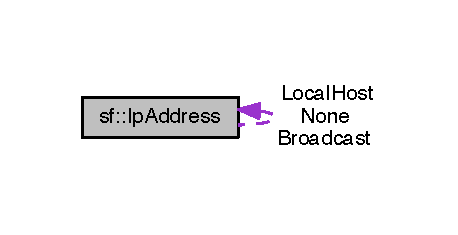
\includegraphics[width=220pt]{classsf_1_1_ip_address__coll__graph}
\end{center}
\end{figure}
\subsection*{Public Member Functions}
\begin{DoxyCompactItemize}
\item 
\hyperlink{classsf_1_1_ip_address_af32a0574baa0f46e48deb2d83ca7658b}{Ip\-Address} ()
\begin{DoxyCompactList}\small\item\em Default constructor. \end{DoxyCompactList}\item 
\hyperlink{classsf_1_1_ip_address_a656b7445ab04cabaa7398685bc09c3f7}{Ip\-Address} (const \hyperlink{gl3_8h_ac83513893df92266f79a515488701770}{std\-::string} \&address)
\begin{DoxyCompactList}\small\item\em Construct the address from a string. \end{DoxyCompactList}\item 
\hyperlink{classsf_1_1_ip_address_a92f2a9be74334a61b96c2fc79fe6eb78}{Ip\-Address} (const char $\ast$address)
\begin{DoxyCompactList}\small\item\em Construct the address from a string. \end{DoxyCompactList}\item 
\hyperlink{classsf_1_1_ip_address_a1d289dcb9ce7a64c600c6f84cba88cc6}{Ip\-Address} (\hyperlink{namespacesf_a4ef3d630785c4f296f9b4f274c33d78e}{Uint8} byte0, \hyperlink{namespacesf_a4ef3d630785c4f296f9b4f274c33d78e}{Uint8} byte1, \hyperlink{namespacesf_a4ef3d630785c4f296f9b4f274c33d78e}{Uint8} byte2, \hyperlink{namespacesf_a4ef3d630785c4f296f9b4f274c33d78e}{Uint8} byte3)
\begin{DoxyCompactList}\small\item\em Construct the address from 4 bytes. \end{DoxyCompactList}\item 
\hyperlink{classsf_1_1_ip_address_a8ed34ba3a40d70eb9f09ac5ae779a162}{Ip\-Address} (\hyperlink{namespacesf_aa746fb1ddef4410bddf198ebb27e727c}{Uint32} address)
\begin{DoxyCompactList}\small\item\em Construct the address from a 32-\/bits integer. \end{DoxyCompactList}\item 
\hyperlink{gl3_8h_ac83513893df92266f79a515488701770}{std\-::string} \hyperlink{classsf_1_1_ip_address_a52f4be92fb0ceb689abc469e4a85fd82}{to\-String} () const 
\begin{DoxyCompactList}\small\item\em Get a string representation of the address. \end{DoxyCompactList}\item 
\hyperlink{namespacesf_aa746fb1ddef4410bddf198ebb27e727c}{Uint32} \hyperlink{classsf_1_1_ip_address_af42678b08b23def2560aed7d98b24d89}{to\-Integer} () const 
\begin{DoxyCompactList}\small\item\em Get an integer representation of the address. \end{DoxyCompactList}\end{DoxyCompactItemize}
\subsection*{Static Public Member Functions}
\begin{DoxyCompactItemize}
\item 
static \hyperlink{classsf_1_1_ip_address}{Ip\-Address} \hyperlink{classsf_1_1_ip_address_a4c31622ad87edca48adbb8e8ed00ee4a}{get\-Local\-Address} ()
\begin{DoxyCompactList}\small\item\em Get the computer's local address. \end{DoxyCompactList}\item 
static \hyperlink{classsf_1_1_ip_address}{Ip\-Address} \hyperlink{classsf_1_1_ip_address_a5c5cbf67e4aacf23c24f2ad991df4c55}{get\-Public\-Address} (\hyperlink{classsf_1_1_time}{Time} \hyperlink{gl3_8h_ad29bb0d8468b264a4e3d9204366cfaab}{timeout}=\hyperlink{classsf_1_1_time_a8db127b632fa8da21550e7282af11fa0}{Time\-::\-Zero})
\begin{DoxyCompactList}\small\item\em Get the computer's public address. \end{DoxyCompactList}\end{DoxyCompactItemize}
\subsection*{Static Public Attributes}
\begin{DoxyCompactItemize}
\item 
static const \hyperlink{classsf_1_1_ip_address}{Ip\-Address} \hyperlink{classsf_1_1_ip_address_a4619b4abbe3c8fef056e7299db967404}{None}
\begin{DoxyCompactList}\small\item\em Value representing an empty/invalid address. \end{DoxyCompactList}\item 
static const \hyperlink{classsf_1_1_ip_address}{Ip\-Address} \hyperlink{classsf_1_1_ip_address_a594d3a8e2559f8fa8ab0a96fa597333b}{Local\-Host}
\begin{DoxyCompactList}\small\item\em The \char`\"{}localhost\char`\"{} address (for connecting a computer to itself locally) \end{DoxyCompactList}\item 
static const \hyperlink{classsf_1_1_ip_address}{Ip\-Address} \hyperlink{classsf_1_1_ip_address_aa93d1d57b65d243f2baf804b6035465c}{Broadcast}
\begin{DoxyCompactList}\small\item\em The \char`\"{}broadcast\char`\"{} address (for sending U\-D\-P messages to everyone on a local network) \end{DoxyCompactList}\end{DoxyCompactItemize}


\subsection{Detailed Description}
Encapsulate an I\-Pv4 network address. 

\hyperlink{classsf_1_1_ip_address}{sf\-::\-Ip\-Address} is a utility class for manipulating network addresses. It provides a set a implicit constructors and conversion functions to easily build or transform an I\-P address from/to various representations.

Usage example\-: 
\begin{DoxyCode}
\hyperlink{classsf_1_1_ip_address}{sf::IpAddress} a0;                                     \textcolor{comment}{// an invalid address}
\hyperlink{classsf_1_1_ip_address}{sf::IpAddress} a1 = \hyperlink{classsf_1_1_ip_address_a4619b4abbe3c8fef056e7299db967404}{sf::IpAddress::None};               \textcolor{comment}{// an invalid address
       (same as a0)}
\hyperlink{classsf_1_1_ip_address}{sf::IpAddress} a2(\textcolor{stringliteral}{"127.0.0.1"});                        \textcolor{comment}{// the local host address}
\hyperlink{classsf_1_1_ip_address}{sf::IpAddress} a3 = \hyperlink{classsf_1_1_ip_address_aa93d1d57b65d243f2baf804b6035465c}{sf::IpAddress::Broadcast};          \textcolor{comment}{// the broadcast
       address}
\hyperlink{classsf_1_1_ip_address}{sf::IpAddress} a4(192, 168, 1, 56);                    \textcolor{comment}{// a local address}
\hyperlink{classsf_1_1_ip_address}{sf::IpAddress} a5(\textcolor{stringliteral}{"my\_computer"});                      \textcolor{comment}{// a local address created from a
       network name}
\hyperlink{classsf_1_1_ip_address}{sf::IpAddress} a6(\textcolor{stringliteral}{"89.54.1.169"});                      \textcolor{comment}{// a distant address}
\hyperlink{classsf_1_1_ip_address}{sf::IpAddress} a7(\textcolor{stringliteral}{"www.google.com"});                   \textcolor{comment}{// a distant address created from a
       network name}
\hyperlink{classsf_1_1_ip_address}{sf::IpAddress} a8 = \hyperlink{classsf_1_1_ip_address_a4c31622ad87edca48adbb8e8ed00ee4a}{sf::IpAddress::getLocalAddress}();  \textcolor{comment}{// my
       address on the local network}
\hyperlink{classsf_1_1_ip_address}{sf::IpAddress} a9 = \hyperlink{classsf_1_1_ip_address_a5c5cbf67e4aacf23c24f2ad991df4c55}{sf::IpAddress::getPublicAddress}(); \textcolor{comment}{// my
       address on the internet}
\end{DoxyCode}


Note that \hyperlink{classsf_1_1_ip_address}{sf\-::\-Ip\-Address} currently doesn't support I\-Pv6 nor other types of network addresses. 

Definition at line 44 of file Ip\-Address.\-hpp.



\subsection{Constructor \& Destructor Documentation}
\hypertarget{classsf_1_1_ip_address_af32a0574baa0f46e48deb2d83ca7658b}{\index{sf\-::\-Ip\-Address@{sf\-::\-Ip\-Address}!Ip\-Address@{Ip\-Address}}
\index{Ip\-Address@{Ip\-Address}!sf::IpAddress@{sf\-::\-Ip\-Address}}
\subsubsection[{Ip\-Address}]{\setlength{\rightskip}{0pt plus 5cm}sf\-::\-Ip\-Address\-::\-Ip\-Address (
\begin{DoxyParamCaption}
{}
\end{DoxyParamCaption}
)}}\label{classsf_1_1_ip_address_af32a0574baa0f46e48deb2d83ca7658b}


Default constructor. 

This constructor creates an empty (invalid) address \hypertarget{classsf_1_1_ip_address_a656b7445ab04cabaa7398685bc09c3f7}{\index{sf\-::\-Ip\-Address@{sf\-::\-Ip\-Address}!Ip\-Address@{Ip\-Address}}
\index{Ip\-Address@{Ip\-Address}!sf::IpAddress@{sf\-::\-Ip\-Address}}
\subsubsection[{Ip\-Address}]{\setlength{\rightskip}{0pt plus 5cm}sf\-::\-Ip\-Address\-::\-Ip\-Address (
\begin{DoxyParamCaption}
\item[{const {\bf std\-::string} \&}]{address}
\end{DoxyParamCaption}
)}}\label{classsf_1_1_ip_address_a656b7445ab04cabaa7398685bc09c3f7}


Construct the address from a string. 

Here {\itshape address} can be either a decimal address (ex\-: \char`\"{}192.\-168.\-1.\-56\char`\"{}) or a network name (ex\-: \char`\"{}localhost\char`\"{}).


\begin{DoxyParams}{Parameters}
{\em address} & I\-P address or network name \\
\hline
\end{DoxyParams}
\hypertarget{classsf_1_1_ip_address_a92f2a9be74334a61b96c2fc79fe6eb78}{\index{sf\-::\-Ip\-Address@{sf\-::\-Ip\-Address}!Ip\-Address@{Ip\-Address}}
\index{Ip\-Address@{Ip\-Address}!sf::IpAddress@{sf\-::\-Ip\-Address}}
\subsubsection[{Ip\-Address}]{\setlength{\rightskip}{0pt plus 5cm}sf\-::\-Ip\-Address\-::\-Ip\-Address (
\begin{DoxyParamCaption}
\item[{const char $\ast$}]{address}
\end{DoxyParamCaption}
)}}\label{classsf_1_1_ip_address_a92f2a9be74334a61b96c2fc79fe6eb78}


Construct the address from a string. 

Here {\itshape address} can be either a decimal address (ex\-: \char`\"{}192.\-168.\-1.\-56\char`\"{}) or a network name (ex\-: \char`\"{}localhost\char`\"{}). This is equivalent to the constructor taking a std\-::string parameter, it is defined for convenience so that the implicit conversions from literal strings to \hyperlink{classsf_1_1_ip_address}{Ip\-Address} work.


\begin{DoxyParams}{Parameters}
{\em address} & I\-P address or network name \\
\hline
\end{DoxyParams}
\hypertarget{classsf_1_1_ip_address_a1d289dcb9ce7a64c600c6f84cba88cc6}{\index{sf\-::\-Ip\-Address@{sf\-::\-Ip\-Address}!Ip\-Address@{Ip\-Address}}
\index{Ip\-Address@{Ip\-Address}!sf::IpAddress@{sf\-::\-Ip\-Address}}
\subsubsection[{Ip\-Address}]{\setlength{\rightskip}{0pt plus 5cm}sf\-::\-Ip\-Address\-::\-Ip\-Address (
\begin{DoxyParamCaption}
\item[{{\bf Uint8}}]{byte0, }
\item[{{\bf Uint8}}]{byte1, }
\item[{{\bf Uint8}}]{byte2, }
\item[{{\bf Uint8}}]{byte3}
\end{DoxyParamCaption}
)}}\label{classsf_1_1_ip_address_a1d289dcb9ce7a64c600c6f84cba88cc6}


Construct the address from 4 bytes. 

Calling Ip\-Address(a, b, c, d) is equivalent to calling \hyperlink{classsf_1_1_ip_address}{Ip\-Address}(\char`\"{}a.\-b.\-c.\-d\char`\"{}), but safer as it doesn't have to parse a string to get the address components.


\begin{DoxyParams}{Parameters}
{\em byte0} & First byte of the address \\
\hline
{\em byte1} & Second byte of the address \\
\hline
{\em byte2} & Third byte of the address \\
\hline
{\em byte3} & Fourth byte of the address \\
\hline
\end{DoxyParams}
\hypertarget{classsf_1_1_ip_address_a8ed34ba3a40d70eb9f09ac5ae779a162}{\index{sf\-::\-Ip\-Address@{sf\-::\-Ip\-Address}!Ip\-Address@{Ip\-Address}}
\index{Ip\-Address@{Ip\-Address}!sf::IpAddress@{sf\-::\-Ip\-Address}}
\subsubsection[{Ip\-Address}]{\setlength{\rightskip}{0pt plus 5cm}sf\-::\-Ip\-Address\-::\-Ip\-Address (
\begin{DoxyParamCaption}
\item[{{\bf Uint32}}]{address}
\end{DoxyParamCaption}
)\hspace{0.3cm}{\ttfamily [explicit]}}}\label{classsf_1_1_ip_address_a8ed34ba3a40d70eb9f09ac5ae779a162}


Construct the address from a 32-\/bits integer. 

This constructor uses the internal representation of the address directly. It should be used for optimization purposes, and only if you got that representation from Ip\-Address\-::\-To\-Integer().


\begin{DoxyParams}{Parameters}
{\em address} & 4 bytes of the address packed into a 32-\/bits integer\\
\hline
\end{DoxyParams}
\begin{DoxySeeAlso}{See Also}
\hyperlink{classsf_1_1_ip_address_af42678b08b23def2560aed7d98b24d89}{to\-Integer} 
\end{DoxySeeAlso}


\subsection{Member Function Documentation}
\hypertarget{classsf_1_1_ip_address_a4c31622ad87edca48adbb8e8ed00ee4a}{\index{sf\-::\-Ip\-Address@{sf\-::\-Ip\-Address}!get\-Local\-Address@{get\-Local\-Address}}
\index{get\-Local\-Address@{get\-Local\-Address}!sf::IpAddress@{sf\-::\-Ip\-Address}}
\subsubsection[{get\-Local\-Address}]{\setlength{\rightskip}{0pt plus 5cm}static {\bf Ip\-Address} sf\-::\-Ip\-Address\-::get\-Local\-Address (
\begin{DoxyParamCaption}
{}
\end{DoxyParamCaption}
)\hspace{0.3cm}{\ttfamily [static]}}}\label{classsf_1_1_ip_address_a4c31622ad87edca48adbb8e8ed00ee4a}


Get the computer's local address. 

The local address is the address of the computer from the L\-A\-N point of view, i.\-e. something like 192.\-168.\-1.\-56. It is meaningful only for communications over the local network. Unlike get\-Public\-Address, this function is fast and may be used safely anywhere.

\begin{DoxyReturn}{Returns}
Local I\-P address of the computer
\end{DoxyReturn}
\begin{DoxySeeAlso}{See Also}
\hyperlink{classsf_1_1_ip_address_a5c5cbf67e4aacf23c24f2ad991df4c55}{get\-Public\-Address} 
\end{DoxySeeAlso}
\hypertarget{classsf_1_1_ip_address_a5c5cbf67e4aacf23c24f2ad991df4c55}{\index{sf\-::\-Ip\-Address@{sf\-::\-Ip\-Address}!get\-Public\-Address@{get\-Public\-Address}}
\index{get\-Public\-Address@{get\-Public\-Address}!sf::IpAddress@{sf\-::\-Ip\-Address}}
\subsubsection[{get\-Public\-Address}]{\setlength{\rightskip}{0pt plus 5cm}static {\bf Ip\-Address} sf\-::\-Ip\-Address\-::get\-Public\-Address (
\begin{DoxyParamCaption}
\item[{{\bf Time}}]{timeout = {\ttfamily {\bf Time\-::\-Zero}}}
\end{DoxyParamCaption}
)\hspace{0.3cm}{\ttfamily [static]}}}\label{classsf_1_1_ip_address_a5c5cbf67e4aacf23c24f2ad991df4c55}


Get the computer's public address. 

The public address is the address of the computer from the internet point of view, i.\-e. something like 89.\-54.\-1.\-169. It is necessary for communications over the world wide web. The only way to get a public address is to ask it to a distant website; as a consequence, this function depends on both your network connection and the server, and may be very slow. You should use it as few as possible. Because this function depends on the network connection and on a distant server, you may use a time limit if you don't want your program to be possibly stuck waiting in case there is a problem; this limit is deactivated by default.


\begin{DoxyParams}{Parameters}
{\em timeout} & Maximum time to wait\\
\hline
\end{DoxyParams}
\begin{DoxyReturn}{Returns}
Public I\-P address of the computer
\end{DoxyReturn}
\begin{DoxySeeAlso}{See Also}
\hyperlink{classsf_1_1_ip_address_a4c31622ad87edca48adbb8e8ed00ee4a}{get\-Local\-Address} 
\end{DoxySeeAlso}
\hypertarget{classsf_1_1_ip_address_af42678b08b23def2560aed7d98b24d89}{\index{sf\-::\-Ip\-Address@{sf\-::\-Ip\-Address}!to\-Integer@{to\-Integer}}
\index{to\-Integer@{to\-Integer}!sf::IpAddress@{sf\-::\-Ip\-Address}}
\subsubsection[{to\-Integer}]{\setlength{\rightskip}{0pt plus 5cm}{\bf Uint32} sf\-::\-Ip\-Address\-::to\-Integer (
\begin{DoxyParamCaption}
{}
\end{DoxyParamCaption}
) const}}\label{classsf_1_1_ip_address_af42678b08b23def2560aed7d98b24d89}


Get an integer representation of the address. 

The returned number is the internal representation of the address, and should be used for optimization purposes only (like sending the address through a socket). The integer produced by this function can then be converted back to a \hyperlink{classsf_1_1_ip_address}{sf\-::\-Ip\-Address} with the proper constructor.

\begin{DoxyReturn}{Returns}
32-\/bits unsigned integer representation of the address
\end{DoxyReturn}
\begin{DoxySeeAlso}{See Also}
\hyperlink{classsf_1_1_ip_address_a52f4be92fb0ceb689abc469e4a85fd82}{to\-String} 
\end{DoxySeeAlso}
\hypertarget{classsf_1_1_ip_address_a52f4be92fb0ceb689abc469e4a85fd82}{\index{sf\-::\-Ip\-Address@{sf\-::\-Ip\-Address}!to\-String@{to\-String}}
\index{to\-String@{to\-String}!sf::IpAddress@{sf\-::\-Ip\-Address}}
\subsubsection[{to\-String}]{\setlength{\rightskip}{0pt plus 5cm}{\bf std\-::string} sf\-::\-Ip\-Address\-::to\-String (
\begin{DoxyParamCaption}
{}
\end{DoxyParamCaption}
) const}}\label{classsf_1_1_ip_address_a52f4be92fb0ceb689abc469e4a85fd82}


Get a string representation of the address. 

The returned string is the decimal representation of the I\-P address (like \char`\"{}192.\-168.\-1.\-56\char`\"{}), even if it was constructed from a host name.

\begin{DoxyReturn}{Returns}
\hyperlink{classsf_1_1_string}{String} representation of the address
\end{DoxyReturn}
\begin{DoxySeeAlso}{See Also}
\hyperlink{classsf_1_1_ip_address_af42678b08b23def2560aed7d98b24d89}{to\-Integer} 
\end{DoxySeeAlso}


\subsection{Member Data Documentation}
\hypertarget{classsf_1_1_ip_address_aa93d1d57b65d243f2baf804b6035465c}{\index{sf\-::\-Ip\-Address@{sf\-::\-Ip\-Address}!Broadcast@{Broadcast}}
\index{Broadcast@{Broadcast}!sf::IpAddress@{sf\-::\-Ip\-Address}}
\subsubsection[{Broadcast}]{\setlength{\rightskip}{0pt plus 5cm}const {\bf Ip\-Address} sf\-::\-Ip\-Address\-::\-Broadcast\hspace{0.3cm}{\ttfamily [static]}}}\label{classsf_1_1_ip_address_aa93d1d57b65d243f2baf804b6035465c}


The \char`\"{}broadcast\char`\"{} address (for sending U\-D\-P messages to everyone on a local network) 



Definition at line 186 of file Ip\-Address.\-hpp.

\hypertarget{classsf_1_1_ip_address_a594d3a8e2559f8fa8ab0a96fa597333b}{\index{sf\-::\-Ip\-Address@{sf\-::\-Ip\-Address}!Local\-Host@{Local\-Host}}
\index{Local\-Host@{Local\-Host}!sf::IpAddress@{sf\-::\-Ip\-Address}}
\subsubsection[{Local\-Host}]{\setlength{\rightskip}{0pt plus 5cm}const {\bf Ip\-Address} sf\-::\-Ip\-Address\-::\-Local\-Host\hspace{0.3cm}{\ttfamily [static]}}}\label{classsf_1_1_ip_address_a594d3a8e2559f8fa8ab0a96fa597333b}


The \char`\"{}localhost\char`\"{} address (for connecting a computer to itself locally) 



Definition at line 185 of file Ip\-Address.\-hpp.

\hypertarget{classsf_1_1_ip_address_a4619b4abbe3c8fef056e7299db967404}{\index{sf\-::\-Ip\-Address@{sf\-::\-Ip\-Address}!None@{None}}
\index{None@{None}!sf::IpAddress@{sf\-::\-Ip\-Address}}
\subsubsection[{None}]{\setlength{\rightskip}{0pt plus 5cm}const {\bf Ip\-Address} sf\-::\-Ip\-Address\-::\-None\hspace{0.3cm}{\ttfamily [static]}}}\label{classsf_1_1_ip_address_a4619b4abbe3c8fef056e7299db967404}


Value representing an empty/invalid address. 



Definition at line 184 of file Ip\-Address.\-hpp.



The documentation for this class was generated from the following file\-:\begin{DoxyCompactItemize}
\item 
/\-Users/ira/\-Dropbox/ira\-\_\-dev/protobyte\-\_\-research/other\-\_\-libs/\-S\-F\-M\-L/dylibs/root/usr/local/include/\-S\-F\-M\-L/\-Network/\hyperlink{_ip_address_8hpp}{Ip\-Address.\-hpp}\end{DoxyCompactItemize}

\hypertarget{classsf_1_1_joystick}{\section{sf\-:\-:Joystick Class Reference}
\label{classsf_1_1_joystick}\index{sf\-::\-Joystick@{sf\-::\-Joystick}}
}


Give access to the real-\/time state of the joysticks.  




{\ttfamily \#include $<$Joystick.\-hpp$>$}

\subsection*{Public Types}
\begin{DoxyCompactItemize}
\item 
enum \{ \hyperlink{classsf_1_1_joystick_ac4ca4ee36e2cf04ecf931316e4463ca6a6e0a2a95bc1da277610c04d80f52715e}{Count} = 8, 
\hyperlink{classsf_1_1_joystick_ac4ca4ee36e2cf04ecf931316e4463ca6a2f1b8a0a59f2c12a4775c0e1e69e1816}{Button\-Count} = 32, 
\hyperlink{classsf_1_1_joystick_ac4ca4ee36e2cf04ecf931316e4463ca6accf3e487c9f6ee2f384351323626a42c}{Axis\-Count} = 8
 \}
\begin{DoxyCompactList}\small\item\em Constants related to joysticks capabilities. \end{DoxyCompactList}\item 
enum \hyperlink{classsf_1_1_joystick_a48db337092c2e263774f94de6d50baa7}{Axis} \{ \\*
\hyperlink{classsf_1_1_joystick_a48db337092c2e263774f94de6d50baa7a95dc8b9bf7b0a2157fc67891c54c401e}{X}, 
\hyperlink{classsf_1_1_joystick_a48db337092c2e263774f94de6d50baa7a51ef1455f7511ad4a78ba241d66593ce}{Y}, 
\hyperlink{classsf_1_1_joystick_a48db337092c2e263774f94de6d50baa7a7c37a1240b2dafbbfc5c1a0e23911315}{Z}, 
\hyperlink{classsf_1_1_joystick_a48db337092c2e263774f94de6d50baa7aeebbcdb0828850f4d69e6a084801fab8}{R}, 
\\*
\hyperlink{classsf_1_1_joystick_a48db337092c2e263774f94de6d50baa7a0a901f61e75292dd2f642b6e4f33a214}{U}, 
\hyperlink{classsf_1_1_joystick_a48db337092c2e263774f94de6d50baa7aa2e2c8ffa1837e7911ee0c7d045bf8f4}{V}, 
\hyperlink{classsf_1_1_joystick_a48db337092c2e263774f94de6d50baa7a06420f7714e4dfd8b841885a0b5f3954}{Pov\-X}, 
\hyperlink{classsf_1_1_joystick_a48db337092c2e263774f94de6d50baa7a0f8ffb2dcddf91b98ab910a4f8327ad9}{Pov\-Y}
 \}
\begin{DoxyCompactList}\small\item\em Axes supported by S\-F\-M\-L joysticks. \end{DoxyCompactList}\end{DoxyCompactItemize}
\subsection*{Static Public Member Functions}
\begin{DoxyCompactItemize}
\item 
static bool \hyperlink{classsf_1_1_joystick_ac7d4e1923e9f9420174f26703ea63d6c}{is\-Connected} (unsigned int joystick)
\begin{DoxyCompactList}\small\item\em Check if a joystick is connected. \end{DoxyCompactList}\item 
static unsigned int \hyperlink{classsf_1_1_joystick_a4de9f445c6582bfe9f0873f695682885}{get\-Button\-Count} (unsigned int joystick)
\begin{DoxyCompactList}\small\item\em Return the number of buttons supported by a joystick. \end{DoxyCompactList}\item 
static bool \hyperlink{classsf_1_1_joystick_a268e8f2a11ae6af4a47c727cb4ab4d95}{has\-Axis} (unsigned int joystick, \hyperlink{classsf_1_1_joystick_a48db337092c2e263774f94de6d50baa7}{Axis} axis)
\begin{DoxyCompactList}\small\item\em Check if a joystick supports a given axis. \end{DoxyCompactList}\item 
static bool \hyperlink{classsf_1_1_joystick_ae0d97a4b84268cbe6a7078e1b2717835}{is\-Button\-Pressed} (unsigned int joystick, unsigned int button)
\begin{DoxyCompactList}\small\item\em Check if a joystick button is pressed. \end{DoxyCompactList}\item 
static float \hyperlink{classsf_1_1_joystick_aea4930193331df1851b709f3060ba58b}{get\-Axis\-Position} (unsigned int joystick, \hyperlink{classsf_1_1_joystick_a48db337092c2e263774f94de6d50baa7}{Axis} axis)
\begin{DoxyCompactList}\small\item\em Get the current position of a joystick axis. \end{DoxyCompactList}\item 
static \hyperlink{glutf90_8h_ac778d6f63f1aaf8ebda0ce6ac821b56e}{void} \hyperlink{classsf_1_1_joystick_ab85fa9175b4edd3e5a07ee3cde0b0f48}{update} ()
\begin{DoxyCompactList}\small\item\em Update the states of all joysticks. \end{DoxyCompactList}\end{DoxyCompactItemize}


\subsection{Detailed Description}
Give access to the real-\/time state of the joysticks. 

\hyperlink{classsf_1_1_joystick}{sf\-::\-Joystick} provides an interface to the state of the joysticks. It only contains static functions, so it's not meant to be instanciated. Instead, each joystick is identified by an index that is passed to the functions of this class.

This class allows users to query the state of joysticks at any time and directly, without having to deal with a window and its events. Compared to the Joystick\-Moved, Joystick\-Button\-Pressed and Joystick\-Button\-Released events, \hyperlink{classsf_1_1_joystick}{sf\-::\-Joystick} can retrieve the state of axes and buttons of joysticks at any time (you don't need to store and update a boolean on your side in order to know if a button is pressed or released), and you always get the real state of joysticks, even if they are moved, pressed or released when your window is out of focus and no event is triggered.

S\-F\-M\-L supports\-: \begin{DoxyItemize}
\item 8 joysticks (\hyperlink{classsf_1_1_joystick_ac4ca4ee36e2cf04ecf931316e4463ca6a6e0a2a95bc1da277610c04d80f52715e}{sf\-::\-Joystick\-::\-Count}) \item 32 buttons per joystick (\hyperlink{classsf_1_1_joystick_ac4ca4ee36e2cf04ecf931316e4463ca6a2f1b8a0a59f2c12a4775c0e1e69e1816}{sf\-::\-Joystick\-::\-Button\-Count}) \item 8 axes per joystick (\hyperlink{classsf_1_1_joystick_ac4ca4ee36e2cf04ecf931316e4463ca6accf3e487c9f6ee2f384351323626a42c}{sf\-::\-Joystick\-::\-Axis\-Count})\end{DoxyItemize}
Unlike the keyboard or mouse, the state of joysticks is sometimes not directly available (depending on the O\-S), therefore an \hyperlink{classsf_1_1_joystick_ab85fa9175b4edd3e5a07ee3cde0b0f48}{update()} function must be called in order to update the current state of joysticks. When you have a window with event handling, this is done automatically, you don't need to call anything. But if you have no window, or if you want to check joysticks state before creating one, you must call \hyperlink{classsf_1_1_joystick_ab85fa9175b4edd3e5a07ee3cde0b0f48}{sf\-::\-Joystick\-::update} explicitely.

Usage example\-: 
\begin{DoxyCode}
\textcolor{comment}{// Is joystick #0 connected?}
\textcolor{keywordtype}{bool} connected = \hyperlink{classsf_1_1_joystick_ac7d4e1923e9f9420174f26703ea63d6c}{sf::Joystick::isConnected}(0);

\textcolor{comment}{// How many buttons does joystick #0 support?}
\textcolor{keywordtype}{unsigned} \textcolor{keywordtype}{int} buttons = \hyperlink{classsf_1_1_joystick_a4de9f445c6582bfe9f0873f695682885}{sf::Joystick::getButtonCount}(0);

\textcolor{comment}{// Does joystick #0 define a X axis?}
\textcolor{keywordtype}{bool} hasX = \hyperlink{classsf_1_1_joystick_a268e8f2a11ae6af4a47c727cb4ab4d95}{sf::Joystick::hasAxis}(0, \hyperlink{classsf_1_1_joystick_a48db337092c2e263774f94de6d50baa7a95dc8b9bf7b0a2157fc67891c54c401e}{sf::Joystick::X});

\textcolor{comment}{// Is button #2 pressed on joystick #0?}
\textcolor{keywordtype}{bool} pressed = \hyperlink{classsf_1_1_joystick_ae0d97a4b84268cbe6a7078e1b2717835}{sf::Joystick::isButtonPressed}(0, 2);

\textcolor{comment}{// What's the current position of the Y axis on joystick #0?}
\textcolor{keywordtype}{float} position = \hyperlink{classsf_1_1_joystick_aea4930193331df1851b709f3060ba58b}{sf::Joystick::getAxisPosition}(0, 
      \hyperlink{classsf_1_1_joystick_a48db337092c2e263774f94de6d50baa7a51ef1455f7511ad4a78ba241d66593ce}{sf::Joystick::Y});
\end{DoxyCode}


\begin{DoxySeeAlso}{See Also}
\hyperlink{classsf_1_1_keyboard}{sf\-::\-Keyboard}, \hyperlink{classsf_1_1_mouse}{sf\-::\-Mouse} 
\end{DoxySeeAlso}


Definition at line 40 of file Joystick.\-hpp.



\subsection{Member Enumeration Documentation}
\hypertarget{classsf_1_1_joystick_ac4ca4ee36e2cf04ecf931316e4463ca6}{\subsubsection[{anonymous enum}]{\setlength{\rightskip}{0pt plus 5cm}anonymous enum}}\label{classsf_1_1_joystick_ac4ca4ee36e2cf04ecf931316e4463ca6}


Constants related to joysticks capabilities. 

\begin{Desc}
\item[Enumerator]\par
\begin{description}
\index{Count@{Count}!sf\-::\-Joystick@{sf\-::\-Joystick}}\index{sf\-::\-Joystick@{sf\-::\-Joystick}!Count@{Count}}\item[{\em 
\hypertarget{classsf_1_1_joystick_ac4ca4ee36e2cf04ecf931316e4463ca6a6e0a2a95bc1da277610c04d80f52715e}{Count}\label{classsf_1_1_joystick_ac4ca4ee36e2cf04ecf931316e4463ca6a6e0a2a95bc1da277610c04d80f52715e}
}]Maximum number of supported joysticks. \index{Button\-Count@{Button\-Count}!sf\-::\-Joystick@{sf\-::\-Joystick}}\index{sf\-::\-Joystick@{sf\-::\-Joystick}!Button\-Count@{Button\-Count}}\item[{\em 
\hypertarget{classsf_1_1_joystick_ac4ca4ee36e2cf04ecf931316e4463ca6a2f1b8a0a59f2c12a4775c0e1e69e1816}{Button\-Count}\label{classsf_1_1_joystick_ac4ca4ee36e2cf04ecf931316e4463ca6a2f1b8a0a59f2c12a4775c0e1e69e1816}
}]Maximum number of supported buttons. \index{Axis\-Count@{Axis\-Count}!sf\-::\-Joystick@{sf\-::\-Joystick}}\index{sf\-::\-Joystick@{sf\-::\-Joystick}!Axis\-Count@{Axis\-Count}}\item[{\em 
\hypertarget{classsf_1_1_joystick_ac4ca4ee36e2cf04ecf931316e4463ca6accf3e487c9f6ee2f384351323626a42c}{Axis\-Count}\label{classsf_1_1_joystick_ac4ca4ee36e2cf04ecf931316e4463ca6accf3e487c9f6ee2f384351323626a42c}
}]Maximum number of supported axes. \end{description}
\end{Desc}


Definition at line 48 of file Joystick.\-hpp.

\hypertarget{classsf_1_1_joystick_a48db337092c2e263774f94de6d50baa7}{\index{sf\-::\-Joystick@{sf\-::\-Joystick}!Axis@{Axis}}
\index{Axis@{Axis}!sf::Joystick@{sf\-::\-Joystick}}
\subsubsection[{Axis}]{\setlength{\rightskip}{0pt plus 5cm}enum {\bf sf\-::\-Joystick\-::\-Axis}}}\label{classsf_1_1_joystick_a48db337092c2e263774f94de6d50baa7}


Axes supported by S\-F\-M\-L joysticks. 

\begin{Desc}
\item[Enumerator]\par
\begin{description}
\index{X@{X}!sf\-::\-Joystick@{sf\-::\-Joystick}}\index{sf\-::\-Joystick@{sf\-::\-Joystick}!X@{X}}\item[{\em 
\hypertarget{classsf_1_1_joystick_a48db337092c2e263774f94de6d50baa7a95dc8b9bf7b0a2157fc67891c54c401e}{X}\label{classsf_1_1_joystick_a48db337092c2e263774f94de6d50baa7a95dc8b9bf7b0a2157fc67891c54c401e}
}]The X axis. \index{Y@{Y}!sf\-::\-Joystick@{sf\-::\-Joystick}}\index{sf\-::\-Joystick@{sf\-::\-Joystick}!Y@{Y}}\item[{\em 
\hypertarget{classsf_1_1_joystick_a48db337092c2e263774f94de6d50baa7a51ef1455f7511ad4a78ba241d66593ce}{Y}\label{classsf_1_1_joystick_a48db337092c2e263774f94de6d50baa7a51ef1455f7511ad4a78ba241d66593ce}
}]The Y axis. \index{Z@{Z}!sf\-::\-Joystick@{sf\-::\-Joystick}}\index{sf\-::\-Joystick@{sf\-::\-Joystick}!Z@{Z}}\item[{\em 
\hypertarget{classsf_1_1_joystick_a48db337092c2e263774f94de6d50baa7a7c37a1240b2dafbbfc5c1a0e23911315}{Z}\label{classsf_1_1_joystick_a48db337092c2e263774f94de6d50baa7a7c37a1240b2dafbbfc5c1a0e23911315}
}]The Z axis. \index{R@{R}!sf\-::\-Joystick@{sf\-::\-Joystick}}\index{sf\-::\-Joystick@{sf\-::\-Joystick}!R@{R}}\item[{\em 
\hypertarget{classsf_1_1_joystick_a48db337092c2e263774f94de6d50baa7aeebbcdb0828850f4d69e6a084801fab8}{R}\label{classsf_1_1_joystick_a48db337092c2e263774f94de6d50baa7aeebbcdb0828850f4d69e6a084801fab8}
}]The R axis. \index{U@{U}!sf\-::\-Joystick@{sf\-::\-Joystick}}\index{sf\-::\-Joystick@{sf\-::\-Joystick}!U@{U}}\item[{\em 
\hypertarget{classsf_1_1_joystick_a48db337092c2e263774f94de6d50baa7a0a901f61e75292dd2f642b6e4f33a214}{U}\label{classsf_1_1_joystick_a48db337092c2e263774f94de6d50baa7a0a901f61e75292dd2f642b6e4f33a214}
}]The U axis. \index{V@{V}!sf\-::\-Joystick@{sf\-::\-Joystick}}\index{sf\-::\-Joystick@{sf\-::\-Joystick}!V@{V}}\item[{\em 
\hypertarget{classsf_1_1_joystick_a48db337092c2e263774f94de6d50baa7aa2e2c8ffa1837e7911ee0c7d045bf8f4}{V}\label{classsf_1_1_joystick_a48db337092c2e263774f94de6d50baa7aa2e2c8ffa1837e7911ee0c7d045bf8f4}
}]The V axis. \index{Pov\-X@{Pov\-X}!sf\-::\-Joystick@{sf\-::\-Joystick}}\index{sf\-::\-Joystick@{sf\-::\-Joystick}!Pov\-X@{Pov\-X}}\item[{\em 
\hypertarget{classsf_1_1_joystick_a48db337092c2e263774f94de6d50baa7a06420f7714e4dfd8b841885a0b5f3954}{Pov\-X}\label{classsf_1_1_joystick_a48db337092c2e263774f94de6d50baa7a06420f7714e4dfd8b841885a0b5f3954}
}]The X axis of the point-\/of-\/view hat. \index{Pov\-Y@{Pov\-Y}!sf\-::\-Joystick@{sf\-::\-Joystick}}\index{sf\-::\-Joystick@{sf\-::\-Joystick}!Pov\-Y@{Pov\-Y}}\item[{\em 
\hypertarget{classsf_1_1_joystick_a48db337092c2e263774f94de6d50baa7a0f8ffb2dcddf91b98ab910a4f8327ad9}{Pov\-Y}\label{classsf_1_1_joystick_a48db337092c2e263774f94de6d50baa7a0f8ffb2dcddf91b98ab910a4f8327ad9}
}]The Y axis of the point-\/of-\/view hat. \end{description}
\end{Desc}


Definition at line 59 of file Joystick.\-hpp.



\subsection{Member Function Documentation}
\hypertarget{classsf_1_1_joystick_aea4930193331df1851b709f3060ba58b}{\index{sf\-::\-Joystick@{sf\-::\-Joystick}!get\-Axis\-Position@{get\-Axis\-Position}}
\index{get\-Axis\-Position@{get\-Axis\-Position}!sf::Joystick@{sf\-::\-Joystick}}
\subsubsection[{get\-Axis\-Position}]{\setlength{\rightskip}{0pt plus 5cm}static float sf\-::\-Joystick\-::get\-Axis\-Position (
\begin{DoxyParamCaption}
\item[{unsigned int}]{joystick, }
\item[{{\bf Axis}}]{axis}
\end{DoxyParamCaption}
)\hspace{0.3cm}{\ttfamily [static]}}}\label{classsf_1_1_joystick_aea4930193331df1851b709f3060ba58b}


Get the current position of a joystick axis. 

If the joystick is not connected, this function returns 0.


\begin{DoxyParams}{Parameters}
{\em joystick} & Index of the joystick \\
\hline
{\em axis} & Axis to check\\
\hline
\end{DoxyParams}
\begin{DoxyReturn}{Returns}
Current position of the axis, in range \mbox{[}-\/100 .. 100\mbox{]} 
\end{DoxyReturn}
\hypertarget{classsf_1_1_joystick_a4de9f445c6582bfe9f0873f695682885}{\index{sf\-::\-Joystick@{sf\-::\-Joystick}!get\-Button\-Count@{get\-Button\-Count}}
\index{get\-Button\-Count@{get\-Button\-Count}!sf::Joystick@{sf\-::\-Joystick}}
\subsubsection[{get\-Button\-Count}]{\setlength{\rightskip}{0pt plus 5cm}static unsigned int sf\-::\-Joystick\-::get\-Button\-Count (
\begin{DoxyParamCaption}
\item[{unsigned int}]{joystick}
\end{DoxyParamCaption}
)\hspace{0.3cm}{\ttfamily [static]}}}\label{classsf_1_1_joystick_a4de9f445c6582bfe9f0873f695682885}


Return the number of buttons supported by a joystick. 

If the joystick is not connected, this function returns 0.


\begin{DoxyParams}{Parameters}
{\em joystick} & Index of the joystick\\
\hline
\end{DoxyParams}
\begin{DoxyReturn}{Returns}
Number of buttons supported by the joystick 
\end{DoxyReturn}
\hypertarget{classsf_1_1_joystick_a268e8f2a11ae6af4a47c727cb4ab4d95}{\index{sf\-::\-Joystick@{sf\-::\-Joystick}!has\-Axis@{has\-Axis}}
\index{has\-Axis@{has\-Axis}!sf::Joystick@{sf\-::\-Joystick}}
\subsubsection[{has\-Axis}]{\setlength{\rightskip}{0pt plus 5cm}static bool sf\-::\-Joystick\-::has\-Axis (
\begin{DoxyParamCaption}
\item[{unsigned int}]{joystick, }
\item[{{\bf Axis}}]{axis}
\end{DoxyParamCaption}
)\hspace{0.3cm}{\ttfamily [static]}}}\label{classsf_1_1_joystick_a268e8f2a11ae6af4a47c727cb4ab4d95}


Check if a joystick supports a given axis. 

If the joystick is not connected, this function returns false.


\begin{DoxyParams}{Parameters}
{\em joystick} & Index of the joystick \\
\hline
{\em axis} & Axis to check\\
\hline
\end{DoxyParams}
\begin{DoxyReturn}{Returns}
True if the joystick supports the axis, false otherwise 
\end{DoxyReturn}
\hypertarget{classsf_1_1_joystick_ae0d97a4b84268cbe6a7078e1b2717835}{\index{sf\-::\-Joystick@{sf\-::\-Joystick}!is\-Button\-Pressed@{is\-Button\-Pressed}}
\index{is\-Button\-Pressed@{is\-Button\-Pressed}!sf::Joystick@{sf\-::\-Joystick}}
\subsubsection[{is\-Button\-Pressed}]{\setlength{\rightskip}{0pt plus 5cm}static bool sf\-::\-Joystick\-::is\-Button\-Pressed (
\begin{DoxyParamCaption}
\item[{unsigned int}]{joystick, }
\item[{unsigned int}]{button}
\end{DoxyParamCaption}
)\hspace{0.3cm}{\ttfamily [static]}}}\label{classsf_1_1_joystick_ae0d97a4b84268cbe6a7078e1b2717835}


Check if a joystick button is pressed. 

If the joystick is not connected, this function returns false.


\begin{DoxyParams}{Parameters}
{\em joystick} & Index of the joystick \\
\hline
{\em button} & Button to check\\
\hline
\end{DoxyParams}
\begin{DoxyReturn}{Returns}
True if the button is pressed, false otherwise 
\end{DoxyReturn}
\hypertarget{classsf_1_1_joystick_ac7d4e1923e9f9420174f26703ea63d6c}{\index{sf\-::\-Joystick@{sf\-::\-Joystick}!is\-Connected@{is\-Connected}}
\index{is\-Connected@{is\-Connected}!sf::Joystick@{sf\-::\-Joystick}}
\subsubsection[{is\-Connected}]{\setlength{\rightskip}{0pt plus 5cm}static bool sf\-::\-Joystick\-::is\-Connected (
\begin{DoxyParamCaption}
\item[{unsigned int}]{joystick}
\end{DoxyParamCaption}
)\hspace{0.3cm}{\ttfamily [static]}}}\label{classsf_1_1_joystick_ac7d4e1923e9f9420174f26703ea63d6c}


Check if a joystick is connected. 


\begin{DoxyParams}{Parameters}
{\em joystick} & Index of the joystick to check\\
\hline
\end{DoxyParams}
\begin{DoxyReturn}{Returns}
True if the joystick is connected, false otherwise 
\end{DoxyReturn}
\hypertarget{classsf_1_1_joystick_ab85fa9175b4edd3e5a07ee3cde0b0f48}{\index{sf\-::\-Joystick@{sf\-::\-Joystick}!update@{update}}
\index{update@{update}!sf::Joystick@{sf\-::\-Joystick}}
\subsubsection[{update}]{\setlength{\rightskip}{0pt plus 5cm}static {\bf void} sf\-::\-Joystick\-::update (
\begin{DoxyParamCaption}
{}
\end{DoxyParamCaption}
)\hspace{0.3cm}{\ttfamily [static]}}}\label{classsf_1_1_joystick_ab85fa9175b4edd3e5a07ee3cde0b0f48}


Update the states of all joysticks. 

This function is used internally by S\-F\-M\-L, so you normally don't have to call it explicitely. However, you may need to call it if you have no window yet (or no window at all)\-: in this case the joysticks states are not updated automatically. 

The documentation for this class was generated from the following file\-:\begin{DoxyCompactItemize}
\item 
/\-Users/ira/\-Dropbox/ira\-\_\-dev/protobyte\-\_\-research/other\-\_\-libs/\-S\-F\-M\-L/dylibs/root/usr/local/include/\-S\-F\-M\-L/\-Window/\hyperlink{_joystick_8hpp}{Joystick.\-hpp}\end{DoxyCompactItemize}

\hypertarget{structsf_1_1_event_1_1_joystick_button_event}{\section{sf\-:\-:Event\-:\-:Joystick\-Button\-Event Struct Reference}
\label{structsf_1_1_event_1_1_joystick_button_event}\index{sf\-::\-Event\-::\-Joystick\-Button\-Event@{sf\-::\-Event\-::\-Joystick\-Button\-Event}}
}


\hyperlink{classsf_1_1_joystick}{Joystick} buttons events parameters (Joystick\-Button\-Pressed, Joystick\-Button\-Released)  




{\ttfamily \#include $<$Event.\-hpp$>$}

\subsection*{Public Attributes}
\begin{DoxyCompactItemize}
\item 
unsigned int \hyperlink{structsf_1_1_event_1_1_joystick_button_event_a2f80ecdb964a5ae0fc30726a404c41ec}{joystick\-Id}
\begin{DoxyCompactList}\small\item\em Index of the joystick (in range \mbox{[}0 .. \hyperlink{classsf_1_1_joystick_ac4ca4ee36e2cf04ecf931316e4463ca6a6e0a2a95bc1da277610c04d80f52715e}{Joystick\-::\-Count} -\/ 1\mbox{]}) \end{DoxyCompactList}\item 
unsigned int \hyperlink{structsf_1_1_event_1_1_joystick_button_event_a6412e698a2f7904c5aa875a0d1b34da4}{button}
\begin{DoxyCompactList}\small\item\em Index of the button that has been pressed (in range \mbox{[}0 .. \hyperlink{classsf_1_1_joystick_ac4ca4ee36e2cf04ecf931316e4463ca6a2f1b8a0a59f2c12a4775c0e1e69e1816}{Joystick\-::\-Button\-Count} -\/ 1\mbox{]}) \end{DoxyCompactList}\end{DoxyCompactItemize}


\subsection{Detailed Description}
\hyperlink{classsf_1_1_joystick}{Joystick} buttons events parameters (Joystick\-Button\-Pressed, Joystick\-Button\-Released) 

Definition at line 138 of file Event.\-hpp.



\subsection{Member Data Documentation}
\hypertarget{structsf_1_1_event_1_1_joystick_button_event_a6412e698a2f7904c5aa875a0d1b34da4}{\index{sf\-::\-Event\-::\-Joystick\-Button\-Event@{sf\-::\-Event\-::\-Joystick\-Button\-Event}!button@{button}}
\index{button@{button}!sf::Event::JoystickButtonEvent@{sf\-::\-Event\-::\-Joystick\-Button\-Event}}
\subsubsection[{button}]{\setlength{\rightskip}{0pt plus 5cm}unsigned int sf\-::\-Event\-::\-Joystick\-Button\-Event\-::button}}\label{structsf_1_1_event_1_1_joystick_button_event_a6412e698a2f7904c5aa875a0d1b34da4}


Index of the button that has been pressed (in range \mbox{[}0 .. \hyperlink{classsf_1_1_joystick_ac4ca4ee36e2cf04ecf931316e4463ca6a2f1b8a0a59f2c12a4775c0e1e69e1816}{Joystick\-::\-Button\-Count} -\/ 1\mbox{]}) 



Definition at line 141 of file Event.\-hpp.

\hypertarget{structsf_1_1_event_1_1_joystick_button_event_a2f80ecdb964a5ae0fc30726a404c41ec}{\index{sf\-::\-Event\-::\-Joystick\-Button\-Event@{sf\-::\-Event\-::\-Joystick\-Button\-Event}!joystick\-Id@{joystick\-Id}}
\index{joystick\-Id@{joystick\-Id}!sf::Event::JoystickButtonEvent@{sf\-::\-Event\-::\-Joystick\-Button\-Event}}
\subsubsection[{joystick\-Id}]{\setlength{\rightskip}{0pt plus 5cm}unsigned int sf\-::\-Event\-::\-Joystick\-Button\-Event\-::joystick\-Id}}\label{structsf_1_1_event_1_1_joystick_button_event_a2f80ecdb964a5ae0fc30726a404c41ec}


Index of the joystick (in range \mbox{[}0 .. \hyperlink{classsf_1_1_joystick_ac4ca4ee36e2cf04ecf931316e4463ca6a6e0a2a95bc1da277610c04d80f52715e}{Joystick\-::\-Count} -\/ 1\mbox{]}) 



Definition at line 140 of file Event.\-hpp.



The documentation for this struct was generated from the following file\-:\begin{DoxyCompactItemize}
\item 
/\-Users/ira/\-Dropbox/ira\-\_\-dev/protobyte\-\_\-research/other\-\_\-libs/\-S\-F\-M\-L/dylibs/root/usr/local/include/\-S\-F\-M\-L/\-Window/\hyperlink{_event_8hpp}{Event.\-hpp}\end{DoxyCompactItemize}

\hypertarget{structsf_1_1_event_1_1_joystick_connect_event}{\section{sf\-:\-:Event\-:\-:Joystick\-Connect\-Event Struct Reference}
\label{structsf_1_1_event_1_1_joystick_connect_event}\index{sf\-::\-Event\-::\-Joystick\-Connect\-Event@{sf\-::\-Event\-::\-Joystick\-Connect\-Event}}
}


\hyperlink{classsf_1_1_joystick}{Joystick} connection events parameters (Joystick\-Connected, Joystick\-Disconnected)  




{\ttfamily \#include $<$Event.\-hpp$>$}

\subsection*{Public Attributes}
\begin{DoxyCompactItemize}
\item 
unsigned int \hyperlink{structsf_1_1_event_1_1_joystick_connect_event_a08e58e8559d3e4fe4654855fec79194b}{joystick\-Id}
\begin{DoxyCompactList}\small\item\em Index of the joystick (in range \mbox{[}0 .. \hyperlink{classsf_1_1_joystick_ac4ca4ee36e2cf04ecf931316e4463ca6a6e0a2a95bc1da277610c04d80f52715e}{Joystick\-::\-Count} -\/ 1\mbox{]}) \end{DoxyCompactList}\end{DoxyCompactItemize}


\subsection{Detailed Description}
\hyperlink{classsf_1_1_joystick}{Joystick} connection events parameters (Joystick\-Connected, Joystick\-Disconnected) 

Definition at line 117 of file Event.\-hpp.



\subsection{Member Data Documentation}
\hypertarget{structsf_1_1_event_1_1_joystick_connect_event_a08e58e8559d3e4fe4654855fec79194b}{\index{sf\-::\-Event\-::\-Joystick\-Connect\-Event@{sf\-::\-Event\-::\-Joystick\-Connect\-Event}!joystick\-Id@{joystick\-Id}}
\index{joystick\-Id@{joystick\-Id}!sf::Event::JoystickConnectEvent@{sf\-::\-Event\-::\-Joystick\-Connect\-Event}}
\subsubsection[{joystick\-Id}]{\setlength{\rightskip}{0pt plus 5cm}unsigned int sf\-::\-Event\-::\-Joystick\-Connect\-Event\-::joystick\-Id}}\label{structsf_1_1_event_1_1_joystick_connect_event_a08e58e8559d3e4fe4654855fec79194b}


Index of the joystick (in range \mbox{[}0 .. \hyperlink{classsf_1_1_joystick_ac4ca4ee36e2cf04ecf931316e4463ca6a6e0a2a95bc1da277610c04d80f52715e}{Joystick\-::\-Count} -\/ 1\mbox{]}) 



Definition at line 119 of file Event.\-hpp.



The documentation for this struct was generated from the following file\-:\begin{DoxyCompactItemize}
\item 
/\-Users/ira/\-Dropbox/ira\-\_\-dev/protobyte\-\_\-research/other\-\_\-libs/\-S\-F\-M\-L/dylibs/root/usr/local/include/\-S\-F\-M\-L/\-Window/\hyperlink{_event_8hpp}{Event.\-hpp}\end{DoxyCompactItemize}

\hypertarget{structsf_1_1_event_1_1_joystick_move_event}{\section{sf\-:\-:Event\-:\-:Joystick\-Move\-Event Struct Reference}
\label{structsf_1_1_event_1_1_joystick_move_event}\index{sf\-::\-Event\-::\-Joystick\-Move\-Event@{sf\-::\-Event\-::\-Joystick\-Move\-Event}}
}


\hyperlink{classsf_1_1_joystick}{Joystick} axis move event parameters (Joystick\-Moved)  




{\ttfamily \#include $<$Event.\-hpp$>$}

\subsection*{Public Attributes}
\begin{DoxyCompactItemize}
\item 
unsigned int \hyperlink{structsf_1_1_event_1_1_joystick_move_event_a7bf2b2f2941a21ed26a67c95f5e4232f}{joystick\-Id}
\begin{DoxyCompactList}\small\item\em Index of the joystick (in range \mbox{[}0 .. \hyperlink{classsf_1_1_joystick_ac4ca4ee36e2cf04ecf931316e4463ca6a6e0a2a95bc1da277610c04d80f52715e}{Joystick\-::\-Count} -\/ 1\mbox{]}) \end{DoxyCompactList}\item 
\hyperlink{classsf_1_1_joystick_a48db337092c2e263774f94de6d50baa7}{Joystick\-::\-Axis} \hyperlink{structsf_1_1_event_1_1_joystick_move_event_add22e8126b7974271991dc6380cbdee3}{axis}
\begin{DoxyCompactList}\small\item\em Axis on which the joystick moved. \end{DoxyCompactList}\item 
float \hyperlink{structsf_1_1_event_1_1_joystick_move_event_aba5a70815420161375fd2e756689c32a}{position}
\begin{DoxyCompactList}\small\item\em New position on the axis (in range \mbox{[}-\/100 .. 100\mbox{]}) \end{DoxyCompactList}\end{DoxyCompactItemize}


\subsection{Detailed Description}
\hyperlink{classsf_1_1_joystick}{Joystick} axis move event parameters (Joystick\-Moved) 

Definition at line 126 of file Event.\-hpp.



\subsection{Member Data Documentation}
\hypertarget{structsf_1_1_event_1_1_joystick_move_event_add22e8126b7974271991dc6380cbdee3}{\index{sf\-::\-Event\-::\-Joystick\-Move\-Event@{sf\-::\-Event\-::\-Joystick\-Move\-Event}!axis@{axis}}
\index{axis@{axis}!sf::Event::JoystickMoveEvent@{sf\-::\-Event\-::\-Joystick\-Move\-Event}}
\subsubsection[{axis}]{\setlength{\rightskip}{0pt plus 5cm}{\bf Joystick\-::\-Axis} sf\-::\-Event\-::\-Joystick\-Move\-Event\-::axis}}\label{structsf_1_1_event_1_1_joystick_move_event_add22e8126b7974271991dc6380cbdee3}


Axis on which the joystick moved. 



Definition at line 129 of file Event.\-hpp.

\hypertarget{structsf_1_1_event_1_1_joystick_move_event_a7bf2b2f2941a21ed26a67c95f5e4232f}{\index{sf\-::\-Event\-::\-Joystick\-Move\-Event@{sf\-::\-Event\-::\-Joystick\-Move\-Event}!joystick\-Id@{joystick\-Id}}
\index{joystick\-Id@{joystick\-Id}!sf::Event::JoystickMoveEvent@{sf\-::\-Event\-::\-Joystick\-Move\-Event}}
\subsubsection[{joystick\-Id}]{\setlength{\rightskip}{0pt plus 5cm}unsigned int sf\-::\-Event\-::\-Joystick\-Move\-Event\-::joystick\-Id}}\label{structsf_1_1_event_1_1_joystick_move_event_a7bf2b2f2941a21ed26a67c95f5e4232f}


Index of the joystick (in range \mbox{[}0 .. \hyperlink{classsf_1_1_joystick_ac4ca4ee36e2cf04ecf931316e4463ca6a6e0a2a95bc1da277610c04d80f52715e}{Joystick\-::\-Count} -\/ 1\mbox{]}) 



Definition at line 128 of file Event.\-hpp.

\hypertarget{structsf_1_1_event_1_1_joystick_move_event_aba5a70815420161375fd2e756689c32a}{\index{sf\-::\-Event\-::\-Joystick\-Move\-Event@{sf\-::\-Event\-::\-Joystick\-Move\-Event}!position@{position}}
\index{position@{position}!sf::Event::JoystickMoveEvent@{sf\-::\-Event\-::\-Joystick\-Move\-Event}}
\subsubsection[{position}]{\setlength{\rightskip}{0pt plus 5cm}float sf\-::\-Event\-::\-Joystick\-Move\-Event\-::position}}\label{structsf_1_1_event_1_1_joystick_move_event_aba5a70815420161375fd2e756689c32a}


New position on the axis (in range \mbox{[}-\/100 .. 100\mbox{]}) 



Definition at line 130 of file Event.\-hpp.



The documentation for this struct was generated from the following file\-:\begin{DoxyCompactItemize}
\item 
/\-Users/ira/\-Dropbox/ira\-\_\-dev/protobyte\-\_\-research/other\-\_\-libs/\-S\-F\-M\-L/dylibs/root/usr/local/include/\-S\-F\-M\-L/\-Window/\hyperlink{_event_8hpp}{Event.\-hpp}\end{DoxyCompactItemize}

\hypertarget{classsf_1_1_keyboard}{\section{sf\-:\-:Keyboard Class Reference}
\label{classsf_1_1_keyboard}\index{sf\-::\-Keyboard@{sf\-::\-Keyboard}}
}


Give access to the real-\/time state of the keyboard.  




{\ttfamily \#include $<$Keyboard.\-hpp$>$}

\subsection*{Public Types}
\begin{DoxyCompactItemize}
\item 
enum \hyperlink{classsf_1_1_keyboard_acb4cacd7cc5802dec45724cf3314a142}{Key} \{ \\*
\hyperlink{classsf_1_1_keyboard_acb4cacd7cc5802dec45724cf3314a142a9d06fa7ac9af597034ea724fb08b991e}{A}, 
\hyperlink{classsf_1_1_keyboard_acb4cacd7cc5802dec45724cf3314a142aca3142235e5c4199f0b8b45d8368ef94}{B}, 
\hyperlink{classsf_1_1_keyboard_acb4cacd7cc5802dec45724cf3314a142a0d586c4ec0cd6b537cb6f49180fedecc}{C}, 
\hyperlink{classsf_1_1_keyboard_acb4cacd7cc5802dec45724cf3314a142ae778600bd3e878b59df1dbdd5877ba7a}{D}, 
\\*
\hyperlink{classsf_1_1_keyboard_acb4cacd7cc5802dec45724cf3314a142a0e027c08438a8bf77e2e1e5d5d75bd84}{E}, 
\hyperlink{classsf_1_1_keyboard_acb4cacd7cc5802dec45724cf3314a142ab8021fbbe5483bc98f124df6f7090002}{F}, 
\hyperlink{classsf_1_1_keyboard_acb4cacd7cc5802dec45724cf3314a142aafb9e3d7679d88d86afc608d79c251f7}{G}, 
\hyperlink{classsf_1_1_keyboard_acb4cacd7cc5802dec45724cf3314a142adfa19328304890e17f4a3f4263eed04d}{H}, 
\\*
\hyperlink{classsf_1_1_keyboard_acb4cacd7cc5802dec45724cf3314a142abaef09665b4d94ebbed50345cab3981e}{I}, 
\hyperlink{classsf_1_1_keyboard_acb4cacd7cc5802dec45724cf3314a142a948c634009beacdab42c3419253a5e85}{J}, 
\hyperlink{classsf_1_1_keyboard_acb4cacd7cc5802dec45724cf3314a142a25beb62393ff666a4bec18ea2a66f3f2}{K}, 
\hyperlink{classsf_1_1_keyboard_acb4cacd7cc5802dec45724cf3314a142a5ef1839ffe19b7e9c24f2ca017614ff9}{L}, 
\\*
\hyperlink{classsf_1_1_keyboard_acb4cacd7cc5802dec45724cf3314a142a9718de9940f723c956587dcb90450a0a}{M}, 
\hyperlink{classsf_1_1_keyboard_acb4cacd7cc5802dec45724cf3314a142ab652ed6b308db95a74dc4ff5229ac9c8}{N}, 
\hyperlink{classsf_1_1_keyboard_acb4cacd7cc5802dec45724cf3314a142a7739288cc628dfa8c50ba712be7c03e1}{O}, 
\hyperlink{classsf_1_1_keyboard_acb4cacd7cc5802dec45724cf3314a142aaeac1db209a64a0221277a835de986e6}{P}, 
\\*
\hyperlink{classsf_1_1_keyboard_acb4cacd7cc5802dec45724cf3314a142a27e3d50587c9789d2592d275d22fbada}{Q}, 
\hyperlink{classsf_1_1_keyboard_acb4cacd7cc5802dec45724cf3314a142add852cadaa6fff2d982bbab3551c31d0}{R}, 
\hyperlink{classsf_1_1_keyboard_acb4cacd7cc5802dec45724cf3314a142aca13014bf9ed5887d347060a0334ea5a}{S}, 
\hyperlink{classsf_1_1_keyboard_acb4cacd7cc5802dec45724cf3314a142a19f59109111fc5271d3581bcd0c43187}{T}, 
\\*
\hyperlink{classsf_1_1_keyboard_acb4cacd7cc5802dec45724cf3314a142ab4f30ae34848ee934dd4f5496a8fb4a1}{U}, 
\hyperlink{classsf_1_1_keyboard_acb4cacd7cc5802dec45724cf3314a142aec9074abd2d41628d1ecdc14e1b2cd96}{V}, 
\hyperlink{classsf_1_1_keyboard_acb4cacd7cc5802dec45724cf3314a142a258aa89e9c6c9aad1ccbaeb41839c5e0}{W}, 
\hyperlink{classsf_1_1_keyboard_acb4cacd7cc5802dec45724cf3314a142a012f5ee9d518e9e24caa087fbddc0594}{X}, 
\\*
\hyperlink{classsf_1_1_keyboard_acb4cacd7cc5802dec45724cf3314a142a5d877e63d1353e0fc0a0757a87a7bd0e}{Y}, 
\hyperlink{classsf_1_1_keyboard_acb4cacd7cc5802dec45724cf3314a142a4e12efd6478a2d174264f29b0b41ab43}{Z}, 
\hyperlink{classsf_1_1_keyboard_acb4cacd7cc5802dec45724cf3314a142af026fd133ee93a0bd8c70762cc3be4bc}{Num0}, 
\hyperlink{classsf_1_1_keyboard_acb4cacd7cc5802dec45724cf3314a142a506bd962cab80722a8c5a4b178912c59}{Num1}, 
\\*
\hyperlink{classsf_1_1_keyboard_acb4cacd7cc5802dec45724cf3314a142a2d6eb5118179bb140fdb3485bb08c182}{Num2}, 
\hyperlink{classsf_1_1_keyboard_acb4cacd7cc5802dec45724cf3314a142aee78e5ed27d31598fc285400166c0dd5}{Num3}, 
\hyperlink{classsf_1_1_keyboard_acb4cacd7cc5802dec45724cf3314a142a5fbd8a089460dc33c22f68b36e1fdc98}{Num4}, 
\hyperlink{classsf_1_1_keyboard_acb4cacd7cc5802dec45724cf3314a142a1dc7e87810b8d4b7039e202b0adcc4ee}{Num5}, 
\\*
\hyperlink{classsf_1_1_keyboard_acb4cacd7cc5802dec45724cf3314a142af86dafb69d922ad2b0f4bd4c37696575}{Num6}, 
\hyperlink{classsf_1_1_keyboard_acb4cacd7cc5802dec45724cf3314a142a8fa0056a0a6f5a7d9fcef3402c9c916d}{Num7}, 
\hyperlink{classsf_1_1_keyboard_acb4cacd7cc5802dec45724cf3314a142adb9f2549fd57bfd99d4713ff1845c530}{Num8}, 
\hyperlink{classsf_1_1_keyboard_acb4cacd7cc5802dec45724cf3314a142a9bc0d0727958bef97e2b6a58e23743db}{Num9}, 
\\*
\hyperlink{classsf_1_1_keyboard_acb4cacd7cc5802dec45724cf3314a142a64b7ecb543c5d03bec8383dde123c95d}{Escape}, 
\hyperlink{classsf_1_1_keyboard_acb4cacd7cc5802dec45724cf3314a142acc76c9dec76d8ae806ae9d6515066e53}{L\-Control}, 
\hyperlink{classsf_1_1_keyboard_acb4cacd7cc5802dec45724cf3314a142a270db49f76cb4dbe72da36153d3aa45c}{L\-Shift}, 
\hyperlink{classsf_1_1_keyboard_acb4cacd7cc5802dec45724cf3314a142a000ecf5145296d7d52b6871c54e6718d}{L\-Alt}, 
\\*
\hyperlink{classsf_1_1_keyboard_acb4cacd7cc5802dec45724cf3314a142a718171426307a0f5f26b4ae82a322b24}{L\-System}, 
\hyperlink{classsf_1_1_keyboard_acb4cacd7cc5802dec45724cf3314a142a275d3fd207a9c0b22ce404012c71dc17}{R\-Control}, 
\hyperlink{classsf_1_1_keyboard_acb4cacd7cc5802dec45724cf3314a142a5be69e3b2f25bd5f4eed75d063f42b90}{R\-Shift}, 
\hyperlink{classsf_1_1_keyboard_acb4cacd7cc5802dec45724cf3314a142a21dcf098233296462bc7c632b93369cc}{R\-Alt}, 
\\*
\hyperlink{classsf_1_1_keyboard_acb4cacd7cc5802dec45724cf3314a142ac1b3fd7424feeda242cedbb64f3f5a7f}{R\-System}, 
\hyperlink{classsf_1_1_keyboard_acb4cacd7cc5802dec45724cf3314a142a4aac50ce7c4923f96323fe84d592b139}{Menu}, 
\hyperlink{classsf_1_1_keyboard_acb4cacd7cc5802dec45724cf3314a142afbe21cad5f264d685cf7f25060004184}{L\-Bracket}, 
\hyperlink{classsf_1_1_keyboard_acb4cacd7cc5802dec45724cf3314a142a578253a70b48e61830aa08292d44680f}{R\-Bracket}, 
\\*
\hyperlink{classsf_1_1_keyboard_acb4cacd7cc5802dec45724cf3314a142a460ab09a36f9ed230504b89b9815de88}{Semi\-Colon}, 
\hyperlink{classsf_1_1_keyboard_acb4cacd7cc5802dec45724cf3314a142ab7374f48cc79e3085739160b8e3ef2f9}{Comma}, 
\hyperlink{classsf_1_1_keyboard_acb4cacd7cc5802dec45724cf3314a142ac72ba959ab1946957e8dfd4f81ea811d}{Period}, 
\hyperlink{classsf_1_1_keyboard_acb4cacd7cc5802dec45724cf3314a142af031edb6bcf319734a6664388958c475}{Quote}, 
\\*
\hyperlink{classsf_1_1_keyboard_acb4cacd7cc5802dec45724cf3314a142a7424bf901434a587a6c202c423e6786c}{Slash}, 
\hyperlink{classsf_1_1_keyboard_acb4cacd7cc5802dec45724cf3314a142a536df84e73859aa44e11e192459470b6}{Back\-Slash}, 
\hyperlink{classsf_1_1_keyboard_acb4cacd7cc5802dec45724cf3314a142a90be0882086bccb516e3afc5c7fb82eb}{Tilde}, 
\hyperlink{classsf_1_1_keyboard_acb4cacd7cc5802dec45724cf3314a142ae55c35f6b6417e1dbbfa351c64dfc743}{Equal}, 
\\*
\hyperlink{classsf_1_1_keyboard_acb4cacd7cc5802dec45724cf3314a142a401a183dcfde0a06cb60fe6c91fa1e39}{Dash}, 
\hyperlink{classsf_1_1_keyboard_acb4cacd7cc5802dec45724cf3314a142a6fdaa93b6b8d1a2b73bc239e9ada94ef}{Space}, 
\hyperlink{classsf_1_1_keyboard_acb4cacd7cc5802dec45724cf3314a142ac291de81bdee518d636bc359f2ca77de}{Return}, 
\hyperlink{classsf_1_1_keyboard_acb4cacd7cc5802dec45724cf3314a142a7fdbaa81e34620710589948ab780560b}{Back}, 
\\*
\hyperlink{classsf_1_1_keyboard_acb4cacd7cc5802dec45724cf3314a142a20c552c39c8356b1078f1cfff7936b4a}{Tab}, 
\hyperlink{classsf_1_1_keyboard_acb4cacd7cc5802dec45724cf3314a142aa24fe33bba1c3639c3aeaa317bd89d7e}{Page\-Up}, 
\hyperlink{classsf_1_1_keyboard_acb4cacd7cc5802dec45724cf3314a142a21c73323d9a8b6017f3bac0cb8c8ac1a}{Page\-Down}, 
\hyperlink{classsf_1_1_keyboard_acb4cacd7cc5802dec45724cf3314a142a4478343b2b7efc310f995fd4251a264d}{End}, 
\\*
\hyperlink{classsf_1_1_keyboard_acb4cacd7cc5802dec45724cf3314a142af41ae7c3927cc5ea8b43ee2fefe890e8}{Home}, 
\hyperlink{classsf_1_1_keyboard_acb4cacd7cc5802dec45724cf3314a142a616c8cae362d229155c5c6e10b969943}{Insert}, 
\hyperlink{classsf_1_1_keyboard_acb4cacd7cc5802dec45724cf3314a142ab66187002fc7f6695ef3d05237b93a38}{Delete}, 
\hyperlink{classsf_1_1_keyboard_acb4cacd7cc5802dec45724cf3314a142a158c586cbe8609031d1a7932e1a8dba2}{Add}, 
\\*
\hyperlink{classsf_1_1_keyboard_acb4cacd7cc5802dec45724cf3314a142a68983f67bd30d27b27c90d6794c78aa2}{Subtract}, 
\hyperlink{classsf_1_1_keyboard_acb4cacd7cc5802dec45724cf3314a142a10623ae71db8a6b5d97189fc21fb91ae}{Multiply}, 
\hyperlink{classsf_1_1_keyboard_acb4cacd7cc5802dec45724cf3314a142afae3dc28752954f0bfe298ac52f58cb6}{Divide}, 
\hyperlink{classsf_1_1_keyboard_acb4cacd7cc5802dec45724cf3314a142ac3fe5df11d15b57317c053a2ae13d9a9}{Left}, 
\\*
\hyperlink{classsf_1_1_keyboard_acb4cacd7cc5802dec45724cf3314a142a2aeb083dea103a8e36b6850b51ef3632}{Right}, 
\hyperlink{classsf_1_1_keyboard_acb4cacd7cc5802dec45724cf3314a142ac4cf6ef2d2632445e9e26c8f2b70e82d}{Up}, 
\hyperlink{classsf_1_1_keyboard_acb4cacd7cc5802dec45724cf3314a142a33dd676edbdf0817d7a65b21df3d0dca}{Down}, 
\hyperlink{classsf_1_1_keyboard_acb4cacd7cc5802dec45724cf3314a142af0b2af83a7a8c358f7b8f7c403089a4e}{Numpad0}, 
\\*
\hyperlink{classsf_1_1_keyboard_acb4cacd7cc5802dec45724cf3314a142a03536d369ae55cc18024f7e4a341a5ac}{Numpad1}, 
\hyperlink{classsf_1_1_keyboard_acb4cacd7cc5802dec45724cf3314a142a8ad9ccf62631d583f44f06aebd662093}{Numpad2}, 
\hyperlink{classsf_1_1_keyboard_acb4cacd7cc5802dec45724cf3314a142ab63ae26e90126b1842bde25d6dedb205}{Numpad3}, 
\hyperlink{classsf_1_1_keyboard_acb4cacd7cc5802dec45724cf3314a142a65336d823bd823a0d246a872ff90e08a}{Numpad4}, 
\\*
\hyperlink{classsf_1_1_keyboard_acb4cacd7cc5802dec45724cf3314a142a8bc5041f12fdfbefba1dbd823c7e1054}{Numpad5}, 
\hyperlink{classsf_1_1_keyboard_acb4cacd7cc5802dec45724cf3314a142aaf28fdf0d3da6a18030e685478e3a713}{Numpad6}, 
\hyperlink{classsf_1_1_keyboard_acb4cacd7cc5802dec45724cf3314a142a3f9bf9835d65a0df5cce2d3842a40541}{Numpad7}, 
\hyperlink{classsf_1_1_keyboard_acb4cacd7cc5802dec45724cf3314a142a25dcd4e4183ceceb3ac06c72995bae49}{Numpad8}, 
\\*
\hyperlink{classsf_1_1_keyboard_acb4cacd7cc5802dec45724cf3314a142a365eb80f54003670a78e3b850c28df21}{Numpad9}, 
\hyperlink{classsf_1_1_keyboard_acb4cacd7cc5802dec45724cf3314a142ae59c7e28858e970c9d4f0e418179b632}{F1}, 
\hyperlink{classsf_1_1_keyboard_acb4cacd7cc5802dec45724cf3314a142a6a2faa5f876a1e75f24a596b658ff413}{F2}, 
\hyperlink{classsf_1_1_keyboard_acb4cacd7cc5802dec45724cf3314a142a1fb58d66f9c0183db3e70b2b0576074e}{F3}, 
\\*
\hyperlink{classsf_1_1_keyboard_acb4cacd7cc5802dec45724cf3314a142a71311e21238cf2c0df1bbf096bba68f2}{F4}, 
\hyperlink{classsf_1_1_keyboard_acb4cacd7cc5802dec45724cf3314a142a01fd2f93eddf2887186ea91180a789a8}{F5}, 
\hyperlink{classsf_1_1_keyboard_acb4cacd7cc5802dec45724cf3314a142ac756a19b31eb28cd2c35c29d8e54ea04}{F6}, 
\hyperlink{classsf_1_1_keyboard_acb4cacd7cc5802dec45724cf3314a142a060d30d36a3e08208b2bc46d0f549b6c}{F7}, 
\\*
\hyperlink{classsf_1_1_keyboard_acb4cacd7cc5802dec45724cf3314a142ade468cd27716b9c2a0d0158afa2f8621}{F8}, 
\hyperlink{classsf_1_1_keyboard_acb4cacd7cc5802dec45724cf3314a142a3c5c2342003a7191de6636b5ef44e1b9}{F9}, 
\hyperlink{classsf_1_1_keyboard_acb4cacd7cc5802dec45724cf3314a142aec695ecf296e7084a8f7f3ec408e16ac}{F10}, 
\hyperlink{classsf_1_1_keyboard_acb4cacd7cc5802dec45724cf3314a142af9a8de90d90a7a7582269bc5c41f5afd}{F11}, 
\\*
\hyperlink{classsf_1_1_keyboard_acb4cacd7cc5802dec45724cf3314a142af9d8807117d946de5e403bcbd4d7161d}{F12}, 
\hyperlink{classsf_1_1_keyboard_acb4cacd7cc5802dec45724cf3314a142a9e28e971941ca2900c1eea17cda50a04}{F13}, 
\hyperlink{classsf_1_1_keyboard_acb4cacd7cc5802dec45724cf3314a142a9a0327a4ef876338d5f3c34c514f190c}{F14}, 
\hyperlink{classsf_1_1_keyboard_acb4cacd7cc5802dec45724cf3314a142a8949ce79077cc8bf64f4fa42bb6a2808}{F15}, 
\\*
\hyperlink{classsf_1_1_keyboard_acb4cacd7cc5802dec45724cf3314a142a95daf340fcc3d5c2846f69d184170d9b}{Pause}, 
\hyperlink{classsf_1_1_keyboard_acb4cacd7cc5802dec45724cf3314a142a93e6ffa0320fe9b2f29aec14a58be36b}{Key\-Count}
 \}
\begin{DoxyCompactList}\small\item\em Key codes. \end{DoxyCompactList}\end{DoxyCompactItemize}
\subsection*{Static Public Member Functions}
\begin{DoxyCompactItemize}
\item 
static bool \hyperlink{classsf_1_1_keyboard_a80a04b2f53005886957f49eee3531599}{is\-Key\-Pressed} (\hyperlink{classsf_1_1_keyboard_acb4cacd7cc5802dec45724cf3314a142}{Key} key)
\begin{DoxyCompactList}\small\item\em Check if a key is pressed. \end{DoxyCompactList}\end{DoxyCompactItemize}


\subsection{Detailed Description}
Give access to the real-\/time state of the keyboard. 

\hyperlink{classsf_1_1_keyboard}{sf\-::\-Keyboard} provides an interface to the state of the keyboard. It only contains static functions (a single keyboard is assumed), so it's not meant to be instanciated.

This class allows users to query the keyboard state at any time and directly, without having to deal with a window and its events. Compared to the Key\-Pressed and Key\-Released events, \hyperlink{classsf_1_1_keyboard}{sf\-::\-Keyboard} can retrieve the state of a key at any time (you don't need to store and update a boolean on your side in order to know if a key is pressed or released), and you always get the real state of the keyboard, even if keys are pressed or released when your window is out of focus and no event is triggered.

Usage example\-: 
\begin{DoxyCode}
\textcolor{keywordflow}{if} (\hyperlink{classsf_1_1_keyboard_a80a04b2f53005886957f49eee3531599}{sf::Keyboard::isKeyPressed}(\hyperlink{classsf_1_1_keyboard_acb4cacd7cc5802dec45724cf3314a142ac3fe5df11d15b57317c053a2ae13d9a9}{sf::Keyboard::Left}))
\{
    \textcolor{comment}{// move left...}
\}
\textcolor{keywordflow}{else} \textcolor{keywordflow}{if} (\hyperlink{classsf_1_1_keyboard_a80a04b2f53005886957f49eee3531599}{sf::Keyboard::isKeyPressed}(
      \hyperlink{classsf_1_1_keyboard_acb4cacd7cc5802dec45724cf3314a142a2aeb083dea103a8e36b6850b51ef3632}{sf::Keyboard::Right}))
\{
    \textcolor{comment}{// move right...}
\}
\textcolor{keywordflow}{else} \textcolor{keywordflow}{if} (\hyperlink{classsf_1_1_keyboard_a80a04b2f53005886957f49eee3531599}{sf::Keyboard::isKeyPressed}(
      \hyperlink{classsf_1_1_keyboard_acb4cacd7cc5802dec45724cf3314a142a64b7ecb543c5d03bec8383dde123c95d}{sf::Keyboard::Escape}))
\{
    \textcolor{comment}{// quit...}
\}
\end{DoxyCode}


\begin{DoxySeeAlso}{See Also}
\hyperlink{classsf_1_1_joystick}{sf\-::\-Joystick}, \hyperlink{classsf_1_1_mouse}{sf\-::\-Mouse} 
\end{DoxySeeAlso}


Definition at line 40 of file Keyboard.\-hpp.



\subsection{Member Enumeration Documentation}
\hypertarget{classsf_1_1_keyboard_acb4cacd7cc5802dec45724cf3314a142}{\index{sf\-::\-Keyboard@{sf\-::\-Keyboard}!Key@{Key}}
\index{Key@{Key}!sf::Keyboard@{sf\-::\-Keyboard}}
\subsubsection[{Key}]{\setlength{\rightskip}{0pt plus 5cm}enum {\bf sf\-::\-Keyboard\-::\-Key}}}\label{classsf_1_1_keyboard_acb4cacd7cc5802dec45724cf3314a142}


Key codes. 

\begin{Desc}
\item[Enumerator]\par
\begin{description}
\index{A@{A}!sf\-::\-Keyboard@{sf\-::\-Keyboard}}\index{sf\-::\-Keyboard@{sf\-::\-Keyboard}!A@{A}}\item[{\em 
\hypertarget{classsf_1_1_keyboard_acb4cacd7cc5802dec45724cf3314a142a9d06fa7ac9af597034ea724fb08b991e}{A}\label{classsf_1_1_keyboard_acb4cacd7cc5802dec45724cf3314a142a9d06fa7ac9af597034ea724fb08b991e}
}]The A key. \index{B@{B}!sf\-::\-Keyboard@{sf\-::\-Keyboard}}\index{sf\-::\-Keyboard@{sf\-::\-Keyboard}!B@{B}}\item[{\em 
\hypertarget{classsf_1_1_keyboard_acb4cacd7cc5802dec45724cf3314a142aca3142235e5c4199f0b8b45d8368ef94}{B}\label{classsf_1_1_keyboard_acb4cacd7cc5802dec45724cf3314a142aca3142235e5c4199f0b8b45d8368ef94}
}]The B key. \index{C@{C}!sf\-::\-Keyboard@{sf\-::\-Keyboard}}\index{sf\-::\-Keyboard@{sf\-::\-Keyboard}!C@{C}}\item[{\em 
\hypertarget{classsf_1_1_keyboard_acb4cacd7cc5802dec45724cf3314a142a0d586c4ec0cd6b537cb6f49180fedecc}{C}\label{classsf_1_1_keyboard_acb4cacd7cc5802dec45724cf3314a142a0d586c4ec0cd6b537cb6f49180fedecc}
}]The C key. \index{D@{D}!sf\-::\-Keyboard@{sf\-::\-Keyboard}}\index{sf\-::\-Keyboard@{sf\-::\-Keyboard}!D@{D}}\item[{\em 
\hypertarget{classsf_1_1_keyboard_acb4cacd7cc5802dec45724cf3314a142ae778600bd3e878b59df1dbdd5877ba7a}{D}\label{classsf_1_1_keyboard_acb4cacd7cc5802dec45724cf3314a142ae778600bd3e878b59df1dbdd5877ba7a}
}]The D key. \index{E@{E}!sf\-::\-Keyboard@{sf\-::\-Keyboard}}\index{sf\-::\-Keyboard@{sf\-::\-Keyboard}!E@{E}}\item[{\em 
\hypertarget{classsf_1_1_keyboard_acb4cacd7cc5802dec45724cf3314a142a0e027c08438a8bf77e2e1e5d5d75bd84}{E}\label{classsf_1_1_keyboard_acb4cacd7cc5802dec45724cf3314a142a0e027c08438a8bf77e2e1e5d5d75bd84}
}]The E key. \index{F@{F}!sf\-::\-Keyboard@{sf\-::\-Keyboard}}\index{sf\-::\-Keyboard@{sf\-::\-Keyboard}!F@{F}}\item[{\em 
\hypertarget{classsf_1_1_keyboard_acb4cacd7cc5802dec45724cf3314a142ab8021fbbe5483bc98f124df6f7090002}{F}\label{classsf_1_1_keyboard_acb4cacd7cc5802dec45724cf3314a142ab8021fbbe5483bc98f124df6f7090002}
}]The F key. \index{G@{G}!sf\-::\-Keyboard@{sf\-::\-Keyboard}}\index{sf\-::\-Keyboard@{sf\-::\-Keyboard}!G@{G}}\item[{\em 
\hypertarget{classsf_1_1_keyboard_acb4cacd7cc5802dec45724cf3314a142aafb9e3d7679d88d86afc608d79c251f7}{G}\label{classsf_1_1_keyboard_acb4cacd7cc5802dec45724cf3314a142aafb9e3d7679d88d86afc608d79c251f7}
}]The G key. \index{H@{H}!sf\-::\-Keyboard@{sf\-::\-Keyboard}}\index{sf\-::\-Keyboard@{sf\-::\-Keyboard}!H@{H}}\item[{\em 
\hypertarget{classsf_1_1_keyboard_acb4cacd7cc5802dec45724cf3314a142adfa19328304890e17f4a3f4263eed04d}{H}\label{classsf_1_1_keyboard_acb4cacd7cc5802dec45724cf3314a142adfa19328304890e17f4a3f4263eed04d}
}]The H key. \index{I@{I}!sf\-::\-Keyboard@{sf\-::\-Keyboard}}\index{sf\-::\-Keyboard@{sf\-::\-Keyboard}!I@{I}}\item[{\em 
\hypertarget{classsf_1_1_keyboard_acb4cacd7cc5802dec45724cf3314a142abaef09665b4d94ebbed50345cab3981e}{I}\label{classsf_1_1_keyboard_acb4cacd7cc5802dec45724cf3314a142abaef09665b4d94ebbed50345cab3981e}
}]The I key. \index{J@{J}!sf\-::\-Keyboard@{sf\-::\-Keyboard}}\index{sf\-::\-Keyboard@{sf\-::\-Keyboard}!J@{J}}\item[{\em 
\hypertarget{classsf_1_1_keyboard_acb4cacd7cc5802dec45724cf3314a142a948c634009beacdab42c3419253a5e85}{J}\label{classsf_1_1_keyboard_acb4cacd7cc5802dec45724cf3314a142a948c634009beacdab42c3419253a5e85}
}]The J key. \index{K@{K}!sf\-::\-Keyboard@{sf\-::\-Keyboard}}\index{sf\-::\-Keyboard@{sf\-::\-Keyboard}!K@{K}}\item[{\em 
\hypertarget{classsf_1_1_keyboard_acb4cacd7cc5802dec45724cf3314a142a25beb62393ff666a4bec18ea2a66f3f2}{K}\label{classsf_1_1_keyboard_acb4cacd7cc5802dec45724cf3314a142a25beb62393ff666a4bec18ea2a66f3f2}
}]The K key. \index{L@{L}!sf\-::\-Keyboard@{sf\-::\-Keyboard}}\index{sf\-::\-Keyboard@{sf\-::\-Keyboard}!L@{L}}\item[{\em 
\hypertarget{classsf_1_1_keyboard_acb4cacd7cc5802dec45724cf3314a142a5ef1839ffe19b7e9c24f2ca017614ff9}{L}\label{classsf_1_1_keyboard_acb4cacd7cc5802dec45724cf3314a142a5ef1839ffe19b7e9c24f2ca017614ff9}
}]The L key. \index{M@{M}!sf\-::\-Keyboard@{sf\-::\-Keyboard}}\index{sf\-::\-Keyboard@{sf\-::\-Keyboard}!M@{M}}\item[{\em 
\hypertarget{classsf_1_1_keyboard_acb4cacd7cc5802dec45724cf3314a142a9718de9940f723c956587dcb90450a0a}{M}\label{classsf_1_1_keyboard_acb4cacd7cc5802dec45724cf3314a142a9718de9940f723c956587dcb90450a0a}
}]The M key. \index{N@{N}!sf\-::\-Keyboard@{sf\-::\-Keyboard}}\index{sf\-::\-Keyboard@{sf\-::\-Keyboard}!N@{N}}\item[{\em 
\hypertarget{classsf_1_1_keyboard_acb4cacd7cc5802dec45724cf3314a142ab652ed6b308db95a74dc4ff5229ac9c8}{N}\label{classsf_1_1_keyboard_acb4cacd7cc5802dec45724cf3314a142ab652ed6b308db95a74dc4ff5229ac9c8}
}]The N key. \index{O@{O}!sf\-::\-Keyboard@{sf\-::\-Keyboard}}\index{sf\-::\-Keyboard@{sf\-::\-Keyboard}!O@{O}}\item[{\em 
\hypertarget{classsf_1_1_keyboard_acb4cacd7cc5802dec45724cf3314a142a7739288cc628dfa8c50ba712be7c03e1}{O}\label{classsf_1_1_keyboard_acb4cacd7cc5802dec45724cf3314a142a7739288cc628dfa8c50ba712be7c03e1}
}]The O key. \index{P@{P}!sf\-::\-Keyboard@{sf\-::\-Keyboard}}\index{sf\-::\-Keyboard@{sf\-::\-Keyboard}!P@{P}}\item[{\em 
\hypertarget{classsf_1_1_keyboard_acb4cacd7cc5802dec45724cf3314a142aaeac1db209a64a0221277a835de986e6}{P}\label{classsf_1_1_keyboard_acb4cacd7cc5802dec45724cf3314a142aaeac1db209a64a0221277a835de986e6}
}]The P key. \index{Q@{Q}!sf\-::\-Keyboard@{sf\-::\-Keyboard}}\index{sf\-::\-Keyboard@{sf\-::\-Keyboard}!Q@{Q}}\item[{\em 
\hypertarget{classsf_1_1_keyboard_acb4cacd7cc5802dec45724cf3314a142a27e3d50587c9789d2592d275d22fbada}{Q}\label{classsf_1_1_keyboard_acb4cacd7cc5802dec45724cf3314a142a27e3d50587c9789d2592d275d22fbada}
}]The Q key. \index{R@{R}!sf\-::\-Keyboard@{sf\-::\-Keyboard}}\index{sf\-::\-Keyboard@{sf\-::\-Keyboard}!R@{R}}\item[{\em 
\hypertarget{classsf_1_1_keyboard_acb4cacd7cc5802dec45724cf3314a142add852cadaa6fff2d982bbab3551c31d0}{R}\label{classsf_1_1_keyboard_acb4cacd7cc5802dec45724cf3314a142add852cadaa6fff2d982bbab3551c31d0}
}]The R key. \index{S@{S}!sf\-::\-Keyboard@{sf\-::\-Keyboard}}\index{sf\-::\-Keyboard@{sf\-::\-Keyboard}!S@{S}}\item[{\em 
\hypertarget{classsf_1_1_keyboard_acb4cacd7cc5802dec45724cf3314a142aca13014bf9ed5887d347060a0334ea5a}{S}\label{classsf_1_1_keyboard_acb4cacd7cc5802dec45724cf3314a142aca13014bf9ed5887d347060a0334ea5a}
}]The S key. \index{T@{T}!sf\-::\-Keyboard@{sf\-::\-Keyboard}}\index{sf\-::\-Keyboard@{sf\-::\-Keyboard}!T@{T}}\item[{\em 
\hypertarget{classsf_1_1_keyboard_acb4cacd7cc5802dec45724cf3314a142a19f59109111fc5271d3581bcd0c43187}{T}\label{classsf_1_1_keyboard_acb4cacd7cc5802dec45724cf3314a142a19f59109111fc5271d3581bcd0c43187}
}]The T key. \index{U@{U}!sf\-::\-Keyboard@{sf\-::\-Keyboard}}\index{sf\-::\-Keyboard@{sf\-::\-Keyboard}!U@{U}}\item[{\em 
\hypertarget{classsf_1_1_keyboard_acb4cacd7cc5802dec45724cf3314a142ab4f30ae34848ee934dd4f5496a8fb4a1}{U}\label{classsf_1_1_keyboard_acb4cacd7cc5802dec45724cf3314a142ab4f30ae34848ee934dd4f5496a8fb4a1}
}]The U key. \index{V@{V}!sf\-::\-Keyboard@{sf\-::\-Keyboard}}\index{sf\-::\-Keyboard@{sf\-::\-Keyboard}!V@{V}}\item[{\em 
\hypertarget{classsf_1_1_keyboard_acb4cacd7cc5802dec45724cf3314a142aec9074abd2d41628d1ecdc14e1b2cd96}{V}\label{classsf_1_1_keyboard_acb4cacd7cc5802dec45724cf3314a142aec9074abd2d41628d1ecdc14e1b2cd96}
}]The V key. \index{W@{W}!sf\-::\-Keyboard@{sf\-::\-Keyboard}}\index{sf\-::\-Keyboard@{sf\-::\-Keyboard}!W@{W}}\item[{\em 
\hypertarget{classsf_1_1_keyboard_acb4cacd7cc5802dec45724cf3314a142a258aa89e9c6c9aad1ccbaeb41839c5e0}{W}\label{classsf_1_1_keyboard_acb4cacd7cc5802dec45724cf3314a142a258aa89e9c6c9aad1ccbaeb41839c5e0}
}]The W key. \index{X@{X}!sf\-::\-Keyboard@{sf\-::\-Keyboard}}\index{sf\-::\-Keyboard@{sf\-::\-Keyboard}!X@{X}}\item[{\em 
\hypertarget{classsf_1_1_keyboard_acb4cacd7cc5802dec45724cf3314a142a012f5ee9d518e9e24caa087fbddc0594}{X}\label{classsf_1_1_keyboard_acb4cacd7cc5802dec45724cf3314a142a012f5ee9d518e9e24caa087fbddc0594}
}]The X key. \index{Y@{Y}!sf\-::\-Keyboard@{sf\-::\-Keyboard}}\index{sf\-::\-Keyboard@{sf\-::\-Keyboard}!Y@{Y}}\item[{\em 
\hypertarget{classsf_1_1_keyboard_acb4cacd7cc5802dec45724cf3314a142a5d877e63d1353e0fc0a0757a87a7bd0e}{Y}\label{classsf_1_1_keyboard_acb4cacd7cc5802dec45724cf3314a142a5d877e63d1353e0fc0a0757a87a7bd0e}
}]The Y key. \index{Z@{Z}!sf\-::\-Keyboard@{sf\-::\-Keyboard}}\index{sf\-::\-Keyboard@{sf\-::\-Keyboard}!Z@{Z}}\item[{\em 
\hypertarget{classsf_1_1_keyboard_acb4cacd7cc5802dec45724cf3314a142a4e12efd6478a2d174264f29b0b41ab43}{Z}\label{classsf_1_1_keyboard_acb4cacd7cc5802dec45724cf3314a142a4e12efd6478a2d174264f29b0b41ab43}
}]The Z key. \index{Num0@{Num0}!sf\-::\-Keyboard@{sf\-::\-Keyboard}}\index{sf\-::\-Keyboard@{sf\-::\-Keyboard}!Num0@{Num0}}\item[{\em 
\hypertarget{classsf_1_1_keyboard_acb4cacd7cc5802dec45724cf3314a142af026fd133ee93a0bd8c70762cc3be4bc}{Num0}\label{classsf_1_1_keyboard_acb4cacd7cc5802dec45724cf3314a142af026fd133ee93a0bd8c70762cc3be4bc}
}]The 0 key. \index{Num1@{Num1}!sf\-::\-Keyboard@{sf\-::\-Keyboard}}\index{sf\-::\-Keyboard@{sf\-::\-Keyboard}!Num1@{Num1}}\item[{\em 
\hypertarget{classsf_1_1_keyboard_acb4cacd7cc5802dec45724cf3314a142a506bd962cab80722a8c5a4b178912c59}{Num1}\label{classsf_1_1_keyboard_acb4cacd7cc5802dec45724cf3314a142a506bd962cab80722a8c5a4b178912c59}
}]The 1 key. \index{Num2@{Num2}!sf\-::\-Keyboard@{sf\-::\-Keyboard}}\index{sf\-::\-Keyboard@{sf\-::\-Keyboard}!Num2@{Num2}}\item[{\em 
\hypertarget{classsf_1_1_keyboard_acb4cacd7cc5802dec45724cf3314a142a2d6eb5118179bb140fdb3485bb08c182}{Num2}\label{classsf_1_1_keyboard_acb4cacd7cc5802dec45724cf3314a142a2d6eb5118179bb140fdb3485bb08c182}
}]The 2 key. \index{Num3@{Num3}!sf\-::\-Keyboard@{sf\-::\-Keyboard}}\index{sf\-::\-Keyboard@{sf\-::\-Keyboard}!Num3@{Num3}}\item[{\em 
\hypertarget{classsf_1_1_keyboard_acb4cacd7cc5802dec45724cf3314a142aee78e5ed27d31598fc285400166c0dd5}{Num3}\label{classsf_1_1_keyboard_acb4cacd7cc5802dec45724cf3314a142aee78e5ed27d31598fc285400166c0dd5}
}]The 3 key. \index{Num4@{Num4}!sf\-::\-Keyboard@{sf\-::\-Keyboard}}\index{sf\-::\-Keyboard@{sf\-::\-Keyboard}!Num4@{Num4}}\item[{\em 
\hypertarget{classsf_1_1_keyboard_acb4cacd7cc5802dec45724cf3314a142a5fbd8a089460dc33c22f68b36e1fdc98}{Num4}\label{classsf_1_1_keyboard_acb4cacd7cc5802dec45724cf3314a142a5fbd8a089460dc33c22f68b36e1fdc98}
}]The 4 key. \index{Num5@{Num5}!sf\-::\-Keyboard@{sf\-::\-Keyboard}}\index{sf\-::\-Keyboard@{sf\-::\-Keyboard}!Num5@{Num5}}\item[{\em 
\hypertarget{classsf_1_1_keyboard_acb4cacd7cc5802dec45724cf3314a142a1dc7e87810b8d4b7039e202b0adcc4ee}{Num5}\label{classsf_1_1_keyboard_acb4cacd7cc5802dec45724cf3314a142a1dc7e87810b8d4b7039e202b0adcc4ee}
}]The 5 key. \index{Num6@{Num6}!sf\-::\-Keyboard@{sf\-::\-Keyboard}}\index{sf\-::\-Keyboard@{sf\-::\-Keyboard}!Num6@{Num6}}\item[{\em 
\hypertarget{classsf_1_1_keyboard_acb4cacd7cc5802dec45724cf3314a142af86dafb69d922ad2b0f4bd4c37696575}{Num6}\label{classsf_1_1_keyboard_acb4cacd7cc5802dec45724cf3314a142af86dafb69d922ad2b0f4bd4c37696575}
}]The 6 key. \index{Num7@{Num7}!sf\-::\-Keyboard@{sf\-::\-Keyboard}}\index{sf\-::\-Keyboard@{sf\-::\-Keyboard}!Num7@{Num7}}\item[{\em 
\hypertarget{classsf_1_1_keyboard_acb4cacd7cc5802dec45724cf3314a142a8fa0056a0a6f5a7d9fcef3402c9c916d}{Num7}\label{classsf_1_1_keyboard_acb4cacd7cc5802dec45724cf3314a142a8fa0056a0a6f5a7d9fcef3402c9c916d}
}]The 7 key. \index{Num8@{Num8}!sf\-::\-Keyboard@{sf\-::\-Keyboard}}\index{sf\-::\-Keyboard@{sf\-::\-Keyboard}!Num8@{Num8}}\item[{\em 
\hypertarget{classsf_1_1_keyboard_acb4cacd7cc5802dec45724cf3314a142adb9f2549fd57bfd99d4713ff1845c530}{Num8}\label{classsf_1_1_keyboard_acb4cacd7cc5802dec45724cf3314a142adb9f2549fd57bfd99d4713ff1845c530}
}]The 8 key. \index{Num9@{Num9}!sf\-::\-Keyboard@{sf\-::\-Keyboard}}\index{sf\-::\-Keyboard@{sf\-::\-Keyboard}!Num9@{Num9}}\item[{\em 
\hypertarget{classsf_1_1_keyboard_acb4cacd7cc5802dec45724cf3314a142a9bc0d0727958bef97e2b6a58e23743db}{Num9}\label{classsf_1_1_keyboard_acb4cacd7cc5802dec45724cf3314a142a9bc0d0727958bef97e2b6a58e23743db}
}]The 9 key. \index{Escape@{Escape}!sf\-::\-Keyboard@{sf\-::\-Keyboard}}\index{sf\-::\-Keyboard@{sf\-::\-Keyboard}!Escape@{Escape}}\item[{\em 
\hypertarget{classsf_1_1_keyboard_acb4cacd7cc5802dec45724cf3314a142a64b7ecb543c5d03bec8383dde123c95d}{Escape}\label{classsf_1_1_keyboard_acb4cacd7cc5802dec45724cf3314a142a64b7ecb543c5d03bec8383dde123c95d}
}]The Escape key. \index{L\-Control@{L\-Control}!sf\-::\-Keyboard@{sf\-::\-Keyboard}}\index{sf\-::\-Keyboard@{sf\-::\-Keyboard}!L\-Control@{L\-Control}}\item[{\em 
\hypertarget{classsf_1_1_keyboard_acb4cacd7cc5802dec45724cf3314a142acc76c9dec76d8ae806ae9d6515066e53}{L\-Control}\label{classsf_1_1_keyboard_acb4cacd7cc5802dec45724cf3314a142acc76c9dec76d8ae806ae9d6515066e53}
}]The left Control key. \index{L\-Shift@{L\-Shift}!sf\-::\-Keyboard@{sf\-::\-Keyboard}}\index{sf\-::\-Keyboard@{sf\-::\-Keyboard}!L\-Shift@{L\-Shift}}\item[{\em 
\hypertarget{classsf_1_1_keyboard_acb4cacd7cc5802dec45724cf3314a142a270db49f76cb4dbe72da36153d3aa45c}{L\-Shift}\label{classsf_1_1_keyboard_acb4cacd7cc5802dec45724cf3314a142a270db49f76cb4dbe72da36153d3aa45c}
}]The left Shift key. \index{L\-Alt@{L\-Alt}!sf\-::\-Keyboard@{sf\-::\-Keyboard}}\index{sf\-::\-Keyboard@{sf\-::\-Keyboard}!L\-Alt@{L\-Alt}}\item[{\em 
\hypertarget{classsf_1_1_keyboard_acb4cacd7cc5802dec45724cf3314a142a000ecf5145296d7d52b6871c54e6718d}{L\-Alt}\label{classsf_1_1_keyboard_acb4cacd7cc5802dec45724cf3314a142a000ecf5145296d7d52b6871c54e6718d}
}]The left Alt key. \index{L\-System@{L\-System}!sf\-::\-Keyboard@{sf\-::\-Keyboard}}\index{sf\-::\-Keyboard@{sf\-::\-Keyboard}!L\-System@{L\-System}}\item[{\em 
\hypertarget{classsf_1_1_keyboard_acb4cacd7cc5802dec45724cf3314a142a718171426307a0f5f26b4ae82a322b24}{L\-System}\label{classsf_1_1_keyboard_acb4cacd7cc5802dec45724cf3314a142a718171426307a0f5f26b4ae82a322b24}
}]The left O\-S specific key\-: window (Windows and Linux), apple (Mac\-O\-S X), ... \index{R\-Control@{R\-Control}!sf\-::\-Keyboard@{sf\-::\-Keyboard}}\index{sf\-::\-Keyboard@{sf\-::\-Keyboard}!R\-Control@{R\-Control}}\item[{\em 
\hypertarget{classsf_1_1_keyboard_acb4cacd7cc5802dec45724cf3314a142a275d3fd207a9c0b22ce404012c71dc17}{R\-Control}\label{classsf_1_1_keyboard_acb4cacd7cc5802dec45724cf3314a142a275d3fd207a9c0b22ce404012c71dc17}
}]The right Control key. \index{R\-Shift@{R\-Shift}!sf\-::\-Keyboard@{sf\-::\-Keyboard}}\index{sf\-::\-Keyboard@{sf\-::\-Keyboard}!R\-Shift@{R\-Shift}}\item[{\em 
\hypertarget{classsf_1_1_keyboard_acb4cacd7cc5802dec45724cf3314a142a5be69e3b2f25bd5f4eed75d063f42b90}{R\-Shift}\label{classsf_1_1_keyboard_acb4cacd7cc5802dec45724cf3314a142a5be69e3b2f25bd5f4eed75d063f42b90}
}]The right Shift key. \index{R\-Alt@{R\-Alt}!sf\-::\-Keyboard@{sf\-::\-Keyboard}}\index{sf\-::\-Keyboard@{sf\-::\-Keyboard}!R\-Alt@{R\-Alt}}\item[{\em 
\hypertarget{classsf_1_1_keyboard_acb4cacd7cc5802dec45724cf3314a142a21dcf098233296462bc7c632b93369cc}{R\-Alt}\label{classsf_1_1_keyboard_acb4cacd7cc5802dec45724cf3314a142a21dcf098233296462bc7c632b93369cc}
}]The right Alt key. \index{R\-System@{R\-System}!sf\-::\-Keyboard@{sf\-::\-Keyboard}}\index{sf\-::\-Keyboard@{sf\-::\-Keyboard}!R\-System@{R\-System}}\item[{\em 
\hypertarget{classsf_1_1_keyboard_acb4cacd7cc5802dec45724cf3314a142ac1b3fd7424feeda242cedbb64f3f5a7f}{R\-System}\label{classsf_1_1_keyboard_acb4cacd7cc5802dec45724cf3314a142ac1b3fd7424feeda242cedbb64f3f5a7f}
}]The right O\-S specific key\-: window (Windows and Linux), apple (Mac\-O\-S X), ... \index{Menu@{Menu}!sf\-::\-Keyboard@{sf\-::\-Keyboard}}\index{sf\-::\-Keyboard@{sf\-::\-Keyboard}!Menu@{Menu}}\item[{\em 
\hypertarget{classsf_1_1_keyboard_acb4cacd7cc5802dec45724cf3314a142a4aac50ce7c4923f96323fe84d592b139}{Menu}\label{classsf_1_1_keyboard_acb4cacd7cc5802dec45724cf3314a142a4aac50ce7c4923f96323fe84d592b139}
}]The Menu key. \index{L\-Bracket@{L\-Bracket}!sf\-::\-Keyboard@{sf\-::\-Keyboard}}\index{sf\-::\-Keyboard@{sf\-::\-Keyboard}!L\-Bracket@{L\-Bracket}}\item[{\em 
\hypertarget{classsf_1_1_keyboard_acb4cacd7cc5802dec45724cf3314a142afbe21cad5f264d685cf7f25060004184}{L\-Bracket}\label{classsf_1_1_keyboard_acb4cacd7cc5802dec45724cf3314a142afbe21cad5f264d685cf7f25060004184}
}]The \mbox{[} key. \index{R\-Bracket@{R\-Bracket}!sf\-::\-Keyboard@{sf\-::\-Keyboard}}\index{sf\-::\-Keyboard@{sf\-::\-Keyboard}!R\-Bracket@{R\-Bracket}}\item[{\em 
\hypertarget{classsf_1_1_keyboard_acb4cacd7cc5802dec45724cf3314a142a578253a70b48e61830aa08292d44680f}{R\-Bracket}\label{classsf_1_1_keyboard_acb4cacd7cc5802dec45724cf3314a142a578253a70b48e61830aa08292d44680f}
}]The \mbox{]} key. \index{Semi\-Colon@{Semi\-Colon}!sf\-::\-Keyboard@{sf\-::\-Keyboard}}\index{sf\-::\-Keyboard@{sf\-::\-Keyboard}!Semi\-Colon@{Semi\-Colon}}\item[{\em 
\hypertarget{classsf_1_1_keyboard_acb4cacd7cc5802dec45724cf3314a142a460ab09a36f9ed230504b89b9815de88}{Semi\-Colon}\label{classsf_1_1_keyboard_acb4cacd7cc5802dec45724cf3314a142a460ab09a36f9ed230504b89b9815de88}
}]The ; key. \index{Comma@{Comma}!sf\-::\-Keyboard@{sf\-::\-Keyboard}}\index{sf\-::\-Keyboard@{sf\-::\-Keyboard}!Comma@{Comma}}\item[{\em 
\hypertarget{classsf_1_1_keyboard_acb4cacd7cc5802dec45724cf3314a142ab7374f48cc79e3085739160b8e3ef2f9}{Comma}\label{classsf_1_1_keyboard_acb4cacd7cc5802dec45724cf3314a142ab7374f48cc79e3085739160b8e3ef2f9}
}]The , key. \index{Period@{Period}!sf\-::\-Keyboard@{sf\-::\-Keyboard}}\index{sf\-::\-Keyboard@{sf\-::\-Keyboard}!Period@{Period}}\item[{\em 
\hypertarget{classsf_1_1_keyboard_acb4cacd7cc5802dec45724cf3314a142ac72ba959ab1946957e8dfd4f81ea811d}{Period}\label{classsf_1_1_keyboard_acb4cacd7cc5802dec45724cf3314a142ac72ba959ab1946957e8dfd4f81ea811d}
}]The . key. \index{Quote@{Quote}!sf\-::\-Keyboard@{sf\-::\-Keyboard}}\index{sf\-::\-Keyboard@{sf\-::\-Keyboard}!Quote@{Quote}}\item[{\em 
\hypertarget{classsf_1_1_keyboard_acb4cacd7cc5802dec45724cf3314a142af031edb6bcf319734a6664388958c475}{Quote}\label{classsf_1_1_keyboard_acb4cacd7cc5802dec45724cf3314a142af031edb6bcf319734a6664388958c475}
}]The ' key. \index{Slash@{Slash}!sf\-::\-Keyboard@{sf\-::\-Keyboard}}\index{sf\-::\-Keyboard@{sf\-::\-Keyboard}!Slash@{Slash}}\item[{\em 
\hypertarget{classsf_1_1_keyboard_acb4cacd7cc5802dec45724cf3314a142a7424bf901434a587a6c202c423e6786c}{Slash}\label{classsf_1_1_keyboard_acb4cacd7cc5802dec45724cf3314a142a7424bf901434a587a6c202c423e6786c}
}]The / key. \index{Back\-Slash@{Back\-Slash}!sf\-::\-Keyboard@{sf\-::\-Keyboard}}\index{sf\-::\-Keyboard@{sf\-::\-Keyboard}!Back\-Slash@{Back\-Slash}}\item[{\em 
\hypertarget{classsf_1_1_keyboard_acb4cacd7cc5802dec45724cf3314a142a536df84e73859aa44e11e192459470b6}{Back\-Slash}\label{classsf_1_1_keyboard_acb4cacd7cc5802dec45724cf3314a142a536df84e73859aa44e11e192459470b6}
}]The \textbackslash{} key. \index{Tilde@{Tilde}!sf\-::\-Keyboard@{sf\-::\-Keyboard}}\index{sf\-::\-Keyboard@{sf\-::\-Keyboard}!Tilde@{Tilde}}\item[{\em 
\hypertarget{classsf_1_1_keyboard_acb4cacd7cc5802dec45724cf3314a142a90be0882086bccb516e3afc5c7fb82eb}{Tilde}\label{classsf_1_1_keyboard_acb4cacd7cc5802dec45724cf3314a142a90be0882086bccb516e3afc5c7fb82eb}
}]The $\sim$ key. \index{Equal@{Equal}!sf\-::\-Keyboard@{sf\-::\-Keyboard}}\index{sf\-::\-Keyboard@{sf\-::\-Keyboard}!Equal@{Equal}}\item[{\em 
\hypertarget{classsf_1_1_keyboard_acb4cacd7cc5802dec45724cf3314a142ae55c35f6b6417e1dbbfa351c64dfc743}{Equal}\label{classsf_1_1_keyboard_acb4cacd7cc5802dec45724cf3314a142ae55c35f6b6417e1dbbfa351c64dfc743}
}]The = key. \index{Dash@{Dash}!sf\-::\-Keyboard@{sf\-::\-Keyboard}}\index{sf\-::\-Keyboard@{sf\-::\-Keyboard}!Dash@{Dash}}\item[{\em 
\hypertarget{classsf_1_1_keyboard_acb4cacd7cc5802dec45724cf3314a142a401a183dcfde0a06cb60fe6c91fa1e39}{Dash}\label{classsf_1_1_keyboard_acb4cacd7cc5802dec45724cf3314a142a401a183dcfde0a06cb60fe6c91fa1e39}
}]The -\/ key. \index{Space@{Space}!sf\-::\-Keyboard@{sf\-::\-Keyboard}}\index{sf\-::\-Keyboard@{sf\-::\-Keyboard}!Space@{Space}}\item[{\em 
\hypertarget{classsf_1_1_keyboard_acb4cacd7cc5802dec45724cf3314a142a6fdaa93b6b8d1a2b73bc239e9ada94ef}{Space}\label{classsf_1_1_keyboard_acb4cacd7cc5802dec45724cf3314a142a6fdaa93b6b8d1a2b73bc239e9ada94ef}
}]The Space key. \index{Return@{Return}!sf\-::\-Keyboard@{sf\-::\-Keyboard}}\index{sf\-::\-Keyboard@{sf\-::\-Keyboard}!Return@{Return}}\item[{\em 
\hypertarget{classsf_1_1_keyboard_acb4cacd7cc5802dec45724cf3314a142ac291de81bdee518d636bc359f2ca77de}{Return}\label{classsf_1_1_keyboard_acb4cacd7cc5802dec45724cf3314a142ac291de81bdee518d636bc359f2ca77de}
}]The Return key. \index{Back@{Back}!sf\-::\-Keyboard@{sf\-::\-Keyboard}}\index{sf\-::\-Keyboard@{sf\-::\-Keyboard}!Back@{Back}}\item[{\em 
\hypertarget{classsf_1_1_keyboard_acb4cacd7cc5802dec45724cf3314a142a7fdbaa81e34620710589948ab780560b}{Back}\label{classsf_1_1_keyboard_acb4cacd7cc5802dec45724cf3314a142a7fdbaa81e34620710589948ab780560b}
}]The Backspace key. \index{Tab@{Tab}!sf\-::\-Keyboard@{sf\-::\-Keyboard}}\index{sf\-::\-Keyboard@{sf\-::\-Keyboard}!Tab@{Tab}}\item[{\em 
\hypertarget{classsf_1_1_keyboard_acb4cacd7cc5802dec45724cf3314a142a20c552c39c8356b1078f1cfff7936b4a}{Tab}\label{classsf_1_1_keyboard_acb4cacd7cc5802dec45724cf3314a142a20c552c39c8356b1078f1cfff7936b4a}
}]The Tabulation key. \index{Page\-Up@{Page\-Up}!sf\-::\-Keyboard@{sf\-::\-Keyboard}}\index{sf\-::\-Keyboard@{sf\-::\-Keyboard}!Page\-Up@{Page\-Up}}\item[{\em 
\hypertarget{classsf_1_1_keyboard_acb4cacd7cc5802dec45724cf3314a142aa24fe33bba1c3639c3aeaa317bd89d7e}{Page\-Up}\label{classsf_1_1_keyboard_acb4cacd7cc5802dec45724cf3314a142aa24fe33bba1c3639c3aeaa317bd89d7e}
}]The Page up key. \index{Page\-Down@{Page\-Down}!sf\-::\-Keyboard@{sf\-::\-Keyboard}}\index{sf\-::\-Keyboard@{sf\-::\-Keyboard}!Page\-Down@{Page\-Down}}\item[{\em 
\hypertarget{classsf_1_1_keyboard_acb4cacd7cc5802dec45724cf3314a142a21c73323d9a8b6017f3bac0cb8c8ac1a}{Page\-Down}\label{classsf_1_1_keyboard_acb4cacd7cc5802dec45724cf3314a142a21c73323d9a8b6017f3bac0cb8c8ac1a}
}]The Page down key. \index{End@{End}!sf\-::\-Keyboard@{sf\-::\-Keyboard}}\index{sf\-::\-Keyboard@{sf\-::\-Keyboard}!End@{End}}\item[{\em 
\hypertarget{classsf_1_1_keyboard_acb4cacd7cc5802dec45724cf3314a142a4478343b2b7efc310f995fd4251a264d}{End}\label{classsf_1_1_keyboard_acb4cacd7cc5802dec45724cf3314a142a4478343b2b7efc310f995fd4251a264d}
}]The End key. \index{Home@{Home}!sf\-::\-Keyboard@{sf\-::\-Keyboard}}\index{sf\-::\-Keyboard@{sf\-::\-Keyboard}!Home@{Home}}\item[{\em 
\hypertarget{classsf_1_1_keyboard_acb4cacd7cc5802dec45724cf3314a142af41ae7c3927cc5ea8b43ee2fefe890e8}{Home}\label{classsf_1_1_keyboard_acb4cacd7cc5802dec45724cf3314a142af41ae7c3927cc5ea8b43ee2fefe890e8}
}]The Home key. \index{Insert@{Insert}!sf\-::\-Keyboard@{sf\-::\-Keyboard}}\index{sf\-::\-Keyboard@{sf\-::\-Keyboard}!Insert@{Insert}}\item[{\em 
\hypertarget{classsf_1_1_keyboard_acb4cacd7cc5802dec45724cf3314a142a616c8cae362d229155c5c6e10b969943}{Insert}\label{classsf_1_1_keyboard_acb4cacd7cc5802dec45724cf3314a142a616c8cae362d229155c5c6e10b969943}
}]The Insert key. \index{Delete@{Delete}!sf\-::\-Keyboard@{sf\-::\-Keyboard}}\index{sf\-::\-Keyboard@{sf\-::\-Keyboard}!Delete@{Delete}}\item[{\em 
\hypertarget{classsf_1_1_keyboard_acb4cacd7cc5802dec45724cf3314a142ab66187002fc7f6695ef3d05237b93a38}{Delete}\label{classsf_1_1_keyboard_acb4cacd7cc5802dec45724cf3314a142ab66187002fc7f6695ef3d05237b93a38}
}]The Delete key. \index{Add@{Add}!sf\-::\-Keyboard@{sf\-::\-Keyboard}}\index{sf\-::\-Keyboard@{sf\-::\-Keyboard}!Add@{Add}}\item[{\em 
\hypertarget{classsf_1_1_keyboard_acb4cacd7cc5802dec45724cf3314a142a158c586cbe8609031d1a7932e1a8dba2}{Add}\label{classsf_1_1_keyboard_acb4cacd7cc5802dec45724cf3314a142a158c586cbe8609031d1a7932e1a8dba2}
}]
\begin{DoxyItemize}
\item 
\end{DoxyItemize}\index{Subtract@{Subtract}!sf\-::\-Keyboard@{sf\-::\-Keyboard}}\index{sf\-::\-Keyboard@{sf\-::\-Keyboard}!Subtract@{Subtract}}\item[{\em 
\hypertarget{classsf_1_1_keyboard_acb4cacd7cc5802dec45724cf3314a142a68983f67bd30d27b27c90d6794c78aa2}{Subtract}\label{classsf_1_1_keyboard_acb4cacd7cc5802dec45724cf3314a142a68983f67bd30d27b27c90d6794c78aa2}
}]
\begin{DoxyItemize}
\item 
\end{DoxyItemize}\index{Multiply@{Multiply}!sf\-::\-Keyboard@{sf\-::\-Keyboard}}\index{sf\-::\-Keyboard@{sf\-::\-Keyboard}!Multiply@{Multiply}}\item[{\em 
\hypertarget{classsf_1_1_keyboard_acb4cacd7cc5802dec45724cf3314a142a10623ae71db8a6b5d97189fc21fb91ae}{Multiply}\label{classsf_1_1_keyboard_acb4cacd7cc5802dec45724cf3314a142a10623ae71db8a6b5d97189fc21fb91ae}
}]
\begin{DoxyItemize}
\item 
\end{DoxyItemize}\index{Divide@{Divide}!sf\-::\-Keyboard@{sf\-::\-Keyboard}}\index{sf\-::\-Keyboard@{sf\-::\-Keyboard}!Divide@{Divide}}\item[{\em 
\hypertarget{classsf_1_1_keyboard_acb4cacd7cc5802dec45724cf3314a142afae3dc28752954f0bfe298ac52f58cb6}{Divide}\label{classsf_1_1_keyboard_acb4cacd7cc5802dec45724cf3314a142afae3dc28752954f0bfe298ac52f58cb6}
}]/ \index{Left@{Left}!sf\-::\-Keyboard@{sf\-::\-Keyboard}}\index{sf\-::\-Keyboard@{sf\-::\-Keyboard}!Left@{Left}}\item[{\em 
\hypertarget{classsf_1_1_keyboard_acb4cacd7cc5802dec45724cf3314a142ac3fe5df11d15b57317c053a2ae13d9a9}{Left}\label{classsf_1_1_keyboard_acb4cacd7cc5802dec45724cf3314a142ac3fe5df11d15b57317c053a2ae13d9a9}
}]Left arrow. \index{Right@{Right}!sf\-::\-Keyboard@{sf\-::\-Keyboard}}\index{sf\-::\-Keyboard@{sf\-::\-Keyboard}!Right@{Right}}\item[{\em 
\hypertarget{classsf_1_1_keyboard_acb4cacd7cc5802dec45724cf3314a142a2aeb083dea103a8e36b6850b51ef3632}{Right}\label{classsf_1_1_keyboard_acb4cacd7cc5802dec45724cf3314a142a2aeb083dea103a8e36b6850b51ef3632}
}]Right arrow. \index{Up@{Up}!sf\-::\-Keyboard@{sf\-::\-Keyboard}}\index{sf\-::\-Keyboard@{sf\-::\-Keyboard}!Up@{Up}}\item[{\em 
\hypertarget{classsf_1_1_keyboard_acb4cacd7cc5802dec45724cf3314a142ac4cf6ef2d2632445e9e26c8f2b70e82d}{Up}\label{classsf_1_1_keyboard_acb4cacd7cc5802dec45724cf3314a142ac4cf6ef2d2632445e9e26c8f2b70e82d}
}]Up arrow. \index{Down@{Down}!sf\-::\-Keyboard@{sf\-::\-Keyboard}}\index{sf\-::\-Keyboard@{sf\-::\-Keyboard}!Down@{Down}}\item[{\em 
\hypertarget{classsf_1_1_keyboard_acb4cacd7cc5802dec45724cf3314a142a33dd676edbdf0817d7a65b21df3d0dca}{Down}\label{classsf_1_1_keyboard_acb4cacd7cc5802dec45724cf3314a142a33dd676edbdf0817d7a65b21df3d0dca}
}]Down arrow. \index{Numpad0@{Numpad0}!sf\-::\-Keyboard@{sf\-::\-Keyboard}}\index{sf\-::\-Keyboard@{sf\-::\-Keyboard}!Numpad0@{Numpad0}}\item[{\em 
\hypertarget{classsf_1_1_keyboard_acb4cacd7cc5802dec45724cf3314a142af0b2af83a7a8c358f7b8f7c403089a4e}{Numpad0}\label{classsf_1_1_keyboard_acb4cacd7cc5802dec45724cf3314a142af0b2af83a7a8c358f7b8f7c403089a4e}
}]The numpad 0 key. \index{Numpad1@{Numpad1}!sf\-::\-Keyboard@{sf\-::\-Keyboard}}\index{sf\-::\-Keyboard@{sf\-::\-Keyboard}!Numpad1@{Numpad1}}\item[{\em 
\hypertarget{classsf_1_1_keyboard_acb4cacd7cc5802dec45724cf3314a142a03536d369ae55cc18024f7e4a341a5ac}{Numpad1}\label{classsf_1_1_keyboard_acb4cacd7cc5802dec45724cf3314a142a03536d369ae55cc18024f7e4a341a5ac}
}]The numpad 1 key. \index{Numpad2@{Numpad2}!sf\-::\-Keyboard@{sf\-::\-Keyboard}}\index{sf\-::\-Keyboard@{sf\-::\-Keyboard}!Numpad2@{Numpad2}}\item[{\em 
\hypertarget{classsf_1_1_keyboard_acb4cacd7cc5802dec45724cf3314a142a8ad9ccf62631d583f44f06aebd662093}{Numpad2}\label{classsf_1_1_keyboard_acb4cacd7cc5802dec45724cf3314a142a8ad9ccf62631d583f44f06aebd662093}
}]The numpad 2 key. \index{Numpad3@{Numpad3}!sf\-::\-Keyboard@{sf\-::\-Keyboard}}\index{sf\-::\-Keyboard@{sf\-::\-Keyboard}!Numpad3@{Numpad3}}\item[{\em 
\hypertarget{classsf_1_1_keyboard_acb4cacd7cc5802dec45724cf3314a142ab63ae26e90126b1842bde25d6dedb205}{Numpad3}\label{classsf_1_1_keyboard_acb4cacd7cc5802dec45724cf3314a142ab63ae26e90126b1842bde25d6dedb205}
}]The numpad 3 key. \index{Numpad4@{Numpad4}!sf\-::\-Keyboard@{sf\-::\-Keyboard}}\index{sf\-::\-Keyboard@{sf\-::\-Keyboard}!Numpad4@{Numpad4}}\item[{\em 
\hypertarget{classsf_1_1_keyboard_acb4cacd7cc5802dec45724cf3314a142a65336d823bd823a0d246a872ff90e08a}{Numpad4}\label{classsf_1_1_keyboard_acb4cacd7cc5802dec45724cf3314a142a65336d823bd823a0d246a872ff90e08a}
}]The numpad 4 key. \index{Numpad5@{Numpad5}!sf\-::\-Keyboard@{sf\-::\-Keyboard}}\index{sf\-::\-Keyboard@{sf\-::\-Keyboard}!Numpad5@{Numpad5}}\item[{\em 
\hypertarget{classsf_1_1_keyboard_acb4cacd7cc5802dec45724cf3314a142a8bc5041f12fdfbefba1dbd823c7e1054}{Numpad5}\label{classsf_1_1_keyboard_acb4cacd7cc5802dec45724cf3314a142a8bc5041f12fdfbefba1dbd823c7e1054}
}]The numpad 5 key. \index{Numpad6@{Numpad6}!sf\-::\-Keyboard@{sf\-::\-Keyboard}}\index{sf\-::\-Keyboard@{sf\-::\-Keyboard}!Numpad6@{Numpad6}}\item[{\em 
\hypertarget{classsf_1_1_keyboard_acb4cacd7cc5802dec45724cf3314a142aaf28fdf0d3da6a18030e685478e3a713}{Numpad6}\label{classsf_1_1_keyboard_acb4cacd7cc5802dec45724cf3314a142aaf28fdf0d3da6a18030e685478e3a713}
}]The numpad 6 key. \index{Numpad7@{Numpad7}!sf\-::\-Keyboard@{sf\-::\-Keyboard}}\index{sf\-::\-Keyboard@{sf\-::\-Keyboard}!Numpad7@{Numpad7}}\item[{\em 
\hypertarget{classsf_1_1_keyboard_acb4cacd7cc5802dec45724cf3314a142a3f9bf9835d65a0df5cce2d3842a40541}{Numpad7}\label{classsf_1_1_keyboard_acb4cacd7cc5802dec45724cf3314a142a3f9bf9835d65a0df5cce2d3842a40541}
}]The numpad 7 key. \index{Numpad8@{Numpad8}!sf\-::\-Keyboard@{sf\-::\-Keyboard}}\index{sf\-::\-Keyboard@{sf\-::\-Keyboard}!Numpad8@{Numpad8}}\item[{\em 
\hypertarget{classsf_1_1_keyboard_acb4cacd7cc5802dec45724cf3314a142a25dcd4e4183ceceb3ac06c72995bae49}{Numpad8}\label{classsf_1_1_keyboard_acb4cacd7cc5802dec45724cf3314a142a25dcd4e4183ceceb3ac06c72995bae49}
}]The numpad 8 key. \index{Numpad9@{Numpad9}!sf\-::\-Keyboard@{sf\-::\-Keyboard}}\index{sf\-::\-Keyboard@{sf\-::\-Keyboard}!Numpad9@{Numpad9}}\item[{\em 
\hypertarget{classsf_1_1_keyboard_acb4cacd7cc5802dec45724cf3314a142a365eb80f54003670a78e3b850c28df21}{Numpad9}\label{classsf_1_1_keyboard_acb4cacd7cc5802dec45724cf3314a142a365eb80f54003670a78e3b850c28df21}
}]The numpad 9 key. \index{F1@{F1}!sf\-::\-Keyboard@{sf\-::\-Keyboard}}\index{sf\-::\-Keyboard@{sf\-::\-Keyboard}!F1@{F1}}\item[{\em 
\hypertarget{classsf_1_1_keyboard_acb4cacd7cc5802dec45724cf3314a142ae59c7e28858e970c9d4f0e418179b632}{F1}\label{classsf_1_1_keyboard_acb4cacd7cc5802dec45724cf3314a142ae59c7e28858e970c9d4f0e418179b632}
}]The F1 key. \index{F2@{F2}!sf\-::\-Keyboard@{sf\-::\-Keyboard}}\index{sf\-::\-Keyboard@{sf\-::\-Keyboard}!F2@{F2}}\item[{\em 
\hypertarget{classsf_1_1_keyboard_acb4cacd7cc5802dec45724cf3314a142a6a2faa5f876a1e75f24a596b658ff413}{F2}\label{classsf_1_1_keyboard_acb4cacd7cc5802dec45724cf3314a142a6a2faa5f876a1e75f24a596b658ff413}
}]The F2 key. \index{F3@{F3}!sf\-::\-Keyboard@{sf\-::\-Keyboard}}\index{sf\-::\-Keyboard@{sf\-::\-Keyboard}!F3@{F3}}\item[{\em 
\hypertarget{classsf_1_1_keyboard_acb4cacd7cc5802dec45724cf3314a142a1fb58d66f9c0183db3e70b2b0576074e}{F3}\label{classsf_1_1_keyboard_acb4cacd7cc5802dec45724cf3314a142a1fb58d66f9c0183db3e70b2b0576074e}
}]The F3 key. \index{F4@{F4}!sf\-::\-Keyboard@{sf\-::\-Keyboard}}\index{sf\-::\-Keyboard@{sf\-::\-Keyboard}!F4@{F4}}\item[{\em 
\hypertarget{classsf_1_1_keyboard_acb4cacd7cc5802dec45724cf3314a142a71311e21238cf2c0df1bbf096bba68f2}{F4}\label{classsf_1_1_keyboard_acb4cacd7cc5802dec45724cf3314a142a71311e21238cf2c0df1bbf096bba68f2}
}]The F4 key. \index{F5@{F5}!sf\-::\-Keyboard@{sf\-::\-Keyboard}}\index{sf\-::\-Keyboard@{sf\-::\-Keyboard}!F5@{F5}}\item[{\em 
\hypertarget{classsf_1_1_keyboard_acb4cacd7cc5802dec45724cf3314a142a01fd2f93eddf2887186ea91180a789a8}{F5}\label{classsf_1_1_keyboard_acb4cacd7cc5802dec45724cf3314a142a01fd2f93eddf2887186ea91180a789a8}
}]The F5 key. \index{F6@{F6}!sf\-::\-Keyboard@{sf\-::\-Keyboard}}\index{sf\-::\-Keyboard@{sf\-::\-Keyboard}!F6@{F6}}\item[{\em 
\hypertarget{classsf_1_1_keyboard_acb4cacd7cc5802dec45724cf3314a142ac756a19b31eb28cd2c35c29d8e54ea04}{F6}\label{classsf_1_1_keyboard_acb4cacd7cc5802dec45724cf3314a142ac756a19b31eb28cd2c35c29d8e54ea04}
}]The F6 key. \index{F7@{F7}!sf\-::\-Keyboard@{sf\-::\-Keyboard}}\index{sf\-::\-Keyboard@{sf\-::\-Keyboard}!F7@{F7}}\item[{\em 
\hypertarget{classsf_1_1_keyboard_acb4cacd7cc5802dec45724cf3314a142a060d30d36a3e08208b2bc46d0f549b6c}{F7}\label{classsf_1_1_keyboard_acb4cacd7cc5802dec45724cf3314a142a060d30d36a3e08208b2bc46d0f549b6c}
}]The F7 key. \index{F8@{F8}!sf\-::\-Keyboard@{sf\-::\-Keyboard}}\index{sf\-::\-Keyboard@{sf\-::\-Keyboard}!F8@{F8}}\item[{\em 
\hypertarget{classsf_1_1_keyboard_acb4cacd7cc5802dec45724cf3314a142ade468cd27716b9c2a0d0158afa2f8621}{F8}\label{classsf_1_1_keyboard_acb4cacd7cc5802dec45724cf3314a142ade468cd27716b9c2a0d0158afa2f8621}
}]The F8 key. \index{F9@{F9}!sf\-::\-Keyboard@{sf\-::\-Keyboard}}\index{sf\-::\-Keyboard@{sf\-::\-Keyboard}!F9@{F9}}\item[{\em 
\hypertarget{classsf_1_1_keyboard_acb4cacd7cc5802dec45724cf3314a142a3c5c2342003a7191de6636b5ef44e1b9}{F9}\label{classsf_1_1_keyboard_acb4cacd7cc5802dec45724cf3314a142a3c5c2342003a7191de6636b5ef44e1b9}
}]The F8 key. \index{F10@{F10}!sf\-::\-Keyboard@{sf\-::\-Keyboard}}\index{sf\-::\-Keyboard@{sf\-::\-Keyboard}!F10@{F10}}\item[{\em 
\hypertarget{classsf_1_1_keyboard_acb4cacd7cc5802dec45724cf3314a142aec695ecf296e7084a8f7f3ec408e16ac}{F10}\label{classsf_1_1_keyboard_acb4cacd7cc5802dec45724cf3314a142aec695ecf296e7084a8f7f3ec408e16ac}
}]The F10 key. \index{F11@{F11}!sf\-::\-Keyboard@{sf\-::\-Keyboard}}\index{sf\-::\-Keyboard@{sf\-::\-Keyboard}!F11@{F11}}\item[{\em 
\hypertarget{classsf_1_1_keyboard_acb4cacd7cc5802dec45724cf3314a142af9a8de90d90a7a7582269bc5c41f5afd}{F11}\label{classsf_1_1_keyboard_acb4cacd7cc5802dec45724cf3314a142af9a8de90d90a7a7582269bc5c41f5afd}
}]The F11 key. \index{F12@{F12}!sf\-::\-Keyboard@{sf\-::\-Keyboard}}\index{sf\-::\-Keyboard@{sf\-::\-Keyboard}!F12@{F12}}\item[{\em 
\hypertarget{classsf_1_1_keyboard_acb4cacd7cc5802dec45724cf3314a142af9d8807117d946de5e403bcbd4d7161d}{F12}\label{classsf_1_1_keyboard_acb4cacd7cc5802dec45724cf3314a142af9d8807117d946de5e403bcbd4d7161d}
}]The F12 key. \index{F13@{F13}!sf\-::\-Keyboard@{sf\-::\-Keyboard}}\index{sf\-::\-Keyboard@{sf\-::\-Keyboard}!F13@{F13}}\item[{\em 
\hypertarget{classsf_1_1_keyboard_acb4cacd7cc5802dec45724cf3314a142a9e28e971941ca2900c1eea17cda50a04}{F13}\label{classsf_1_1_keyboard_acb4cacd7cc5802dec45724cf3314a142a9e28e971941ca2900c1eea17cda50a04}
}]The F13 key. \index{F14@{F14}!sf\-::\-Keyboard@{sf\-::\-Keyboard}}\index{sf\-::\-Keyboard@{sf\-::\-Keyboard}!F14@{F14}}\item[{\em 
\hypertarget{classsf_1_1_keyboard_acb4cacd7cc5802dec45724cf3314a142a9a0327a4ef876338d5f3c34c514f190c}{F14}\label{classsf_1_1_keyboard_acb4cacd7cc5802dec45724cf3314a142a9a0327a4ef876338d5f3c34c514f190c}
}]The F14 key. \index{F15@{F15}!sf\-::\-Keyboard@{sf\-::\-Keyboard}}\index{sf\-::\-Keyboard@{sf\-::\-Keyboard}!F15@{F15}}\item[{\em 
\hypertarget{classsf_1_1_keyboard_acb4cacd7cc5802dec45724cf3314a142a8949ce79077cc8bf64f4fa42bb6a2808}{F15}\label{classsf_1_1_keyboard_acb4cacd7cc5802dec45724cf3314a142a8949ce79077cc8bf64f4fa42bb6a2808}
}]The F15 key. \index{Pause@{Pause}!sf\-::\-Keyboard@{sf\-::\-Keyboard}}\index{sf\-::\-Keyboard@{sf\-::\-Keyboard}!Pause@{Pause}}\item[{\em 
\hypertarget{classsf_1_1_keyboard_acb4cacd7cc5802dec45724cf3314a142a95daf340fcc3d5c2846f69d184170d9b}{Pause}\label{classsf_1_1_keyboard_acb4cacd7cc5802dec45724cf3314a142a95daf340fcc3d5c2846f69d184170d9b}
}]The Pause key. \index{Key\-Count@{Key\-Count}!sf\-::\-Keyboard@{sf\-::\-Keyboard}}\index{sf\-::\-Keyboard@{sf\-::\-Keyboard}!Key\-Count@{Key\-Count}}\item[{\em 
\hypertarget{classsf_1_1_keyboard_acb4cacd7cc5802dec45724cf3314a142a93e6ffa0320fe9b2f29aec14a58be36b}{Key\-Count}\label{classsf_1_1_keyboard_acb4cacd7cc5802dec45724cf3314a142a93e6ffa0320fe9b2f29aec14a58be36b}
}]Keep last -- the total number of keyboard keys. \end{description}
\end{Desc}


Definition at line 48 of file Keyboard.\-hpp.



\subsection{Member Function Documentation}
\hypertarget{classsf_1_1_keyboard_a80a04b2f53005886957f49eee3531599}{\index{sf\-::\-Keyboard@{sf\-::\-Keyboard}!is\-Key\-Pressed@{is\-Key\-Pressed}}
\index{is\-Key\-Pressed@{is\-Key\-Pressed}!sf::Keyboard@{sf\-::\-Keyboard}}
\subsubsection[{is\-Key\-Pressed}]{\setlength{\rightskip}{0pt plus 5cm}static bool sf\-::\-Keyboard\-::is\-Key\-Pressed (
\begin{DoxyParamCaption}
\item[{{\bf Key}}]{key}
\end{DoxyParamCaption}
)\hspace{0.3cm}{\ttfamily [static]}}}\label{classsf_1_1_keyboard_a80a04b2f53005886957f49eee3531599}


Check if a key is pressed. 


\begin{DoxyParams}{Parameters}
{\em key} & Key to check\\
\hline
\end{DoxyParams}
\begin{DoxyReturn}{Returns}
True if the key is pressed, false otherwise 
\end{DoxyReturn}


The documentation for this class was generated from the following file\-:\begin{DoxyCompactItemize}
\item 
/\-Users/ira/\-Dropbox/ira\-\_\-dev/protobyte\-\_\-research/other\-\_\-libs/\-S\-F\-M\-L/dylibs/root/usr/local/include/\-S\-F\-M\-L/\-Window/\hyperlink{_keyboard_8hpp}{Keyboard.\-hpp}\end{DoxyCompactItemize}

\hypertarget{structsf_1_1_event_1_1_key_event}{\section{sf\-:\-:Event\-:\-:Key\-Event Struct Reference}
\label{structsf_1_1_event_1_1_key_event}\index{sf\-::\-Event\-::\-Key\-Event@{sf\-::\-Event\-::\-Key\-Event}}
}


\hyperlink{classsf_1_1_keyboard}{Keyboard} event parameters (Key\-Pressed, Key\-Released)  




{\ttfamily \#include $<$Event.\-hpp$>$}

\subsection*{Public Attributes}
\begin{DoxyCompactItemize}
\item 
\hyperlink{classsf_1_1_keyboard_acb4cacd7cc5802dec45724cf3314a142}{Keyboard\-::\-Key} \hyperlink{structsf_1_1_event_1_1_key_event_a2879fdab8a68cb1c6ecc45730a2d0e61}{code}
\begin{DoxyCompactList}\small\item\em Code of the key that has been pressed. \end{DoxyCompactList}\item 
bool \hyperlink{structsf_1_1_event_1_1_key_event_a915a483317de67d995188a855701fbd7}{alt}
\begin{DoxyCompactList}\small\item\em Is the Alt key pressed? \end{DoxyCompactList}\item 
bool \hyperlink{structsf_1_1_event_1_1_key_event_a9255861c2f88501d80ad6b44a310b62f}{control}
\begin{DoxyCompactList}\small\item\em Is the Control key pressed? \end{DoxyCompactList}\item 
bool \hyperlink{structsf_1_1_event_1_1_key_event_a776af1a3ca79abeeec18ebf1c0065aa9}{shift}
\begin{DoxyCompactList}\small\item\em Is the Shift key pressed? \end{DoxyCompactList}\item 
bool \hyperlink{structsf_1_1_event_1_1_key_event_ac0557f7edc2a608ec65175fdd843afc5}{system}
\begin{DoxyCompactList}\small\item\em Is the System key pressed? \end{DoxyCompactList}\end{DoxyCompactItemize}


\subsection{Detailed Description}
\hyperlink{classsf_1_1_keyboard}{Keyboard} event parameters (Key\-Pressed, Key\-Released) 

Definition at line 61 of file Event.\-hpp.



\subsection{Member Data Documentation}
\hypertarget{structsf_1_1_event_1_1_key_event_a915a483317de67d995188a855701fbd7}{\index{sf\-::\-Event\-::\-Key\-Event@{sf\-::\-Event\-::\-Key\-Event}!alt@{alt}}
\index{alt@{alt}!sf::Event::KeyEvent@{sf\-::\-Event\-::\-Key\-Event}}
\subsubsection[{alt}]{\setlength{\rightskip}{0pt plus 5cm}bool sf\-::\-Event\-::\-Key\-Event\-::alt}}\label{structsf_1_1_event_1_1_key_event_a915a483317de67d995188a855701fbd7}


Is the Alt key pressed? 



Definition at line 64 of file Event.\-hpp.

\hypertarget{structsf_1_1_event_1_1_key_event_a2879fdab8a68cb1c6ecc45730a2d0e61}{\index{sf\-::\-Event\-::\-Key\-Event@{sf\-::\-Event\-::\-Key\-Event}!code@{code}}
\index{code@{code}!sf::Event::KeyEvent@{sf\-::\-Event\-::\-Key\-Event}}
\subsubsection[{code}]{\setlength{\rightskip}{0pt plus 5cm}{\bf Keyboard\-::\-Key} sf\-::\-Event\-::\-Key\-Event\-::code}}\label{structsf_1_1_event_1_1_key_event_a2879fdab8a68cb1c6ecc45730a2d0e61}


Code of the key that has been pressed. 



Definition at line 63 of file Event.\-hpp.

\hypertarget{structsf_1_1_event_1_1_key_event_a9255861c2f88501d80ad6b44a310b62f}{\index{sf\-::\-Event\-::\-Key\-Event@{sf\-::\-Event\-::\-Key\-Event}!control@{control}}
\index{control@{control}!sf::Event::KeyEvent@{sf\-::\-Event\-::\-Key\-Event}}
\subsubsection[{control}]{\setlength{\rightskip}{0pt plus 5cm}bool sf\-::\-Event\-::\-Key\-Event\-::control}}\label{structsf_1_1_event_1_1_key_event_a9255861c2f88501d80ad6b44a310b62f}


Is the Control key pressed? 



Definition at line 65 of file Event.\-hpp.

\hypertarget{structsf_1_1_event_1_1_key_event_a776af1a3ca79abeeec18ebf1c0065aa9}{\index{sf\-::\-Event\-::\-Key\-Event@{sf\-::\-Event\-::\-Key\-Event}!shift@{shift}}
\index{shift@{shift}!sf::Event::KeyEvent@{sf\-::\-Event\-::\-Key\-Event}}
\subsubsection[{shift}]{\setlength{\rightskip}{0pt plus 5cm}bool sf\-::\-Event\-::\-Key\-Event\-::shift}}\label{structsf_1_1_event_1_1_key_event_a776af1a3ca79abeeec18ebf1c0065aa9}


Is the Shift key pressed? 



Definition at line 66 of file Event.\-hpp.

\hypertarget{structsf_1_1_event_1_1_key_event_ac0557f7edc2a608ec65175fdd843afc5}{\index{sf\-::\-Event\-::\-Key\-Event@{sf\-::\-Event\-::\-Key\-Event}!system@{system}}
\index{system@{system}!sf::Event::KeyEvent@{sf\-::\-Event\-::\-Key\-Event}}
\subsubsection[{system}]{\setlength{\rightskip}{0pt plus 5cm}bool sf\-::\-Event\-::\-Key\-Event\-::system}}\label{structsf_1_1_event_1_1_key_event_ac0557f7edc2a608ec65175fdd843afc5}


Is the System key pressed? 



Definition at line 67 of file Event.\-hpp.



The documentation for this struct was generated from the following file\-:\begin{DoxyCompactItemize}
\item 
/\-Users/ira/\-Dropbox/ira\-\_\-dev/protobyte\-\_\-research/other\-\_\-libs/\-S\-F\-M\-L/dylibs/root/usr/local/include/\-S\-F\-M\-L/\-Window/\hyperlink{_event_8hpp}{Event.\-hpp}\end{DoxyCompactItemize}

\hypertarget{classsf_1_1_listener}{\section{sf\-:\-:Listener Class Reference}
\label{classsf_1_1_listener}\index{sf\-::\-Listener@{sf\-::\-Listener}}
}


The audio listener is the point in the scene from where all the sounds are heard.  




{\ttfamily \#include $<$Listener.\-hpp$>$}

\subsection*{Static Public Member Functions}
\begin{DoxyCompactItemize}
\item 
static \hyperlink{glutf90_8h_ac778d6f63f1aaf8ebda0ce6ac821b56e}{void} \hyperlink{classsf_1_1_listener_a803a24a1fc04620cacc9f88c6fbc0e3a}{set\-Global\-Volume} (float volume)
\begin{DoxyCompactList}\small\item\em Change the global volume of all the sounds and musics. \end{DoxyCompactList}\item 
static float \hyperlink{classsf_1_1_listener_a137ea535799bdf70be6ec969673d4d33}{get\-Global\-Volume} ()
\begin{DoxyCompactList}\small\item\em Get the current value of the global volume. \end{DoxyCompactList}\item 
static \hyperlink{glutf90_8h_ac778d6f63f1aaf8ebda0ce6ac821b56e}{void} \hyperlink{classsf_1_1_listener_a5bc2d8d18ea2d8f339d23cbf17678564}{set\-Position} (float \hyperlink{gl3_8h_a92d0386e5c19fb81ea88c9f99644ab1d}{x}, float \hyperlink{gl3_8h_a66ddd433d2cacfe27f5906b7e86faeed}{y}, float \hyperlink{gl3_8h_acb78bf1972d3eaf07da34ff2e0a2f133}{z})
\begin{DoxyCompactList}\small\item\em Set the position of the listener in the scene. \end{DoxyCompactList}\item 
static \hyperlink{glutf90_8h_ac778d6f63f1aaf8ebda0ce6ac821b56e}{void} \hyperlink{classsf_1_1_listener_a28a27d85cfbf8065c535c39176898fcb}{set\-Position} (const \hyperlink{namespacesf_af97357d7d32e7d6a700d03be2f3b4811}{Vector3f} \&position)
\begin{DoxyCompactList}\small\item\em Set the position of the listener in the scene. \end{DoxyCompactList}\item 
static \hyperlink{namespacesf_af97357d7d32e7d6a700d03be2f3b4811}{Vector3f} \hyperlink{classsf_1_1_listener_acd7ee65bc948ca38e1c669aa12340c54}{get\-Position} ()
\begin{DoxyCompactList}\small\item\em Get the current position of the listener in the scene. \end{DoxyCompactList}\item 
static \hyperlink{glutf90_8h_ac778d6f63f1aaf8ebda0ce6ac821b56e}{void} \hyperlink{classsf_1_1_listener_ae479dc15513c6557984d26e32d06d06e}{set\-Direction} (float \hyperlink{gl3_8h_a92d0386e5c19fb81ea88c9f99644ab1d}{x}, float \hyperlink{gl3_8h_a66ddd433d2cacfe27f5906b7e86faeed}{y}, float \hyperlink{gl3_8h_acb78bf1972d3eaf07da34ff2e0a2f133}{z})
\begin{DoxyCompactList}\small\item\em Set the orientation of the listener in the scene. \end{DoxyCompactList}\item 
static \hyperlink{glutf90_8h_ac778d6f63f1aaf8ebda0ce6ac821b56e}{void} \hyperlink{classsf_1_1_listener_a1d99d9457c6ddad93449ecb4f504c2bf}{set\-Direction} (const \hyperlink{namespacesf_af97357d7d32e7d6a700d03be2f3b4811}{Vector3f} \&direction)
\begin{DoxyCompactList}\small\item\em Set the orientation of the listener in the scene. \end{DoxyCompactList}\item 
static \hyperlink{namespacesf_af97357d7d32e7d6a700d03be2f3b4811}{Vector3f} \hyperlink{classsf_1_1_listener_a54e91baba51d4431474f53ff7f9309f9}{get\-Direction} ()
\begin{DoxyCompactList}\small\item\em Get the current orientation of the listener in the scene. \end{DoxyCompactList}\end{DoxyCompactItemize}


\subsection{Detailed Description}
The audio listener is the point in the scene from where all the sounds are heard. 

The audio listener defines the global properties of the audio environment, it defines where and how sounds and musics are heard. If \hyperlink{classsf_1_1_view}{sf\-::\-View} is the eyes of the user, then \hyperlink{classsf_1_1_listener}{sf\-::\-Listener} is his ears (by the way, they are often linked together -- same position, orientation, etc.).

\hyperlink{classsf_1_1_listener}{sf\-::\-Listener} is a simple interface, which allows to setup the listener in the 3\-D audio environment (position and direction), and to adjust the global volume.

Because the listener is unique in the scene, \hyperlink{classsf_1_1_listener}{sf\-::\-Listener} only contains static functions and doesn't have to be instanciated.

Usage example\-: 
\begin{DoxyCode}
\textcolor{comment}{// Move the listener to the position (1, 0, -5)}
\hyperlink{classsf_1_1_listener_a5bc2d8d18ea2d8f339d23cbf17678564}{sf::Listener::setPosition}(1, 0, -5);

\textcolor{comment}{// Make it face the right axis (1, 0, 0)}
sf::Listener::SetDirection(1, 0, 0);

\textcolor{comment}{// Reduce the global volume}
sf::Listener::SetGlobalVolume(50);
\end{DoxyCode}
 

Definition at line 42 of file Listener.\-hpp.



\subsection{Member Function Documentation}
\hypertarget{classsf_1_1_listener_a54e91baba51d4431474f53ff7f9309f9}{\index{sf\-::\-Listener@{sf\-::\-Listener}!get\-Direction@{get\-Direction}}
\index{get\-Direction@{get\-Direction}!sf::Listener@{sf\-::\-Listener}}
\subsubsection[{get\-Direction}]{\setlength{\rightskip}{0pt plus 5cm}static {\bf Vector3f} sf\-::\-Listener\-::get\-Direction (
\begin{DoxyParamCaption}
{}
\end{DoxyParamCaption}
)\hspace{0.3cm}{\ttfamily [static]}}}\label{classsf_1_1_listener_a54e91baba51d4431474f53ff7f9309f9}


Get the current orientation of the listener in the scene. 

\begin{DoxyReturn}{Returns}
\hyperlink{classsf_1_1_listener}{Listener}'s orientation
\end{DoxyReturn}
\begin{DoxySeeAlso}{See Also}
\hyperlink{classsf_1_1_listener_ae479dc15513c6557984d26e32d06d06e}{set\-Direction} 
\end{DoxySeeAlso}
\hypertarget{classsf_1_1_listener_a137ea535799bdf70be6ec969673d4d33}{\index{sf\-::\-Listener@{sf\-::\-Listener}!get\-Global\-Volume@{get\-Global\-Volume}}
\index{get\-Global\-Volume@{get\-Global\-Volume}!sf::Listener@{sf\-::\-Listener}}
\subsubsection[{get\-Global\-Volume}]{\setlength{\rightskip}{0pt plus 5cm}static float sf\-::\-Listener\-::get\-Global\-Volume (
\begin{DoxyParamCaption}
{}
\end{DoxyParamCaption}
)\hspace{0.3cm}{\ttfamily [static]}}}\label{classsf_1_1_listener_a137ea535799bdf70be6ec969673d4d33}


Get the current value of the global volume. 

\begin{DoxyReturn}{Returns}
Current global volume, in the range \mbox{[}0, 100\mbox{]}
\end{DoxyReturn}
\begin{DoxySeeAlso}{See Also}
\hyperlink{classsf_1_1_listener_a803a24a1fc04620cacc9f88c6fbc0e3a}{set\-Global\-Volume} 
\end{DoxySeeAlso}
\hypertarget{classsf_1_1_listener_acd7ee65bc948ca38e1c669aa12340c54}{\index{sf\-::\-Listener@{sf\-::\-Listener}!get\-Position@{get\-Position}}
\index{get\-Position@{get\-Position}!sf::Listener@{sf\-::\-Listener}}
\subsubsection[{get\-Position}]{\setlength{\rightskip}{0pt plus 5cm}static {\bf Vector3f} sf\-::\-Listener\-::get\-Position (
\begin{DoxyParamCaption}
{}
\end{DoxyParamCaption}
)\hspace{0.3cm}{\ttfamily [static]}}}\label{classsf_1_1_listener_acd7ee65bc948ca38e1c669aa12340c54}


Get the current position of the listener in the scene. 

\begin{DoxyReturn}{Returns}
\hyperlink{classsf_1_1_listener}{Listener}'s position
\end{DoxyReturn}
\begin{DoxySeeAlso}{See Also}
\hyperlink{classsf_1_1_listener_a5bc2d8d18ea2d8f339d23cbf17678564}{set\-Position} 
\end{DoxySeeAlso}
\hypertarget{classsf_1_1_listener_ae479dc15513c6557984d26e32d06d06e}{\index{sf\-::\-Listener@{sf\-::\-Listener}!set\-Direction@{set\-Direction}}
\index{set\-Direction@{set\-Direction}!sf::Listener@{sf\-::\-Listener}}
\subsubsection[{set\-Direction}]{\setlength{\rightskip}{0pt plus 5cm}static {\bf void} sf\-::\-Listener\-::set\-Direction (
\begin{DoxyParamCaption}
\item[{float}]{x, }
\item[{float}]{y, }
\item[{float}]{z}
\end{DoxyParamCaption}
)\hspace{0.3cm}{\ttfamily [static]}}}\label{classsf_1_1_listener_ae479dc15513c6557984d26e32d06d06e}


Set the orientation of the listener in the scene. 

The orientation defines the 3\-D axes of the listener (left, up, front) in the scene. The orientation vector doesn't have to be normalized. The default listener's orientation is (0, 0, -\/1).


\begin{DoxyParams}{Parameters}
{\em x} & X coordinate of the listener's orientation \\
\hline
{\em y} & Y coordinate of the listener's orientation \\
\hline
{\em z} & Z coordinate of the listener's orientation\\
\hline
\end{DoxyParams}
\begin{DoxySeeAlso}{See Also}
\hyperlink{classsf_1_1_listener_a54e91baba51d4431474f53ff7f9309f9}{get\-Direction}, \hyperlink{classsf_1_1_listener_a5bc2d8d18ea2d8f339d23cbf17678564}{set\-Position} 
\end{DoxySeeAlso}
\hypertarget{classsf_1_1_listener_a1d99d9457c6ddad93449ecb4f504c2bf}{\index{sf\-::\-Listener@{sf\-::\-Listener}!set\-Direction@{set\-Direction}}
\index{set\-Direction@{set\-Direction}!sf::Listener@{sf\-::\-Listener}}
\subsubsection[{set\-Direction}]{\setlength{\rightskip}{0pt plus 5cm}static {\bf void} sf\-::\-Listener\-::set\-Direction (
\begin{DoxyParamCaption}
\item[{const {\bf Vector3f} \&}]{direction}
\end{DoxyParamCaption}
)\hspace{0.3cm}{\ttfamily [static]}}}\label{classsf_1_1_listener_a1d99d9457c6ddad93449ecb4f504c2bf}


Set the orientation of the listener in the scene. 

The orientation defines the 3\-D axes of the listener (left, up, front) in the scene. The orientation vector doesn't have to be normalized. The default listener's orientation is (0, 0, -\/1).


\begin{DoxyParams}{Parameters}
{\em direction} & New listener's orientation\\
\hline
\end{DoxyParams}
\begin{DoxySeeAlso}{See Also}
\hyperlink{classsf_1_1_listener_a54e91baba51d4431474f53ff7f9309f9}{get\-Direction}, \hyperlink{classsf_1_1_listener_a5bc2d8d18ea2d8f339d23cbf17678564}{set\-Position} 
\end{DoxySeeAlso}
\hypertarget{classsf_1_1_listener_a803a24a1fc04620cacc9f88c6fbc0e3a}{\index{sf\-::\-Listener@{sf\-::\-Listener}!set\-Global\-Volume@{set\-Global\-Volume}}
\index{set\-Global\-Volume@{set\-Global\-Volume}!sf::Listener@{sf\-::\-Listener}}
\subsubsection[{set\-Global\-Volume}]{\setlength{\rightskip}{0pt plus 5cm}static {\bf void} sf\-::\-Listener\-::set\-Global\-Volume (
\begin{DoxyParamCaption}
\item[{float}]{volume}
\end{DoxyParamCaption}
)\hspace{0.3cm}{\ttfamily [static]}}}\label{classsf_1_1_listener_a803a24a1fc04620cacc9f88c6fbc0e3a}


Change the global volume of all the sounds and musics. 

The volume is a number between 0 and 100; it is combined with the individual volume of each sound / music. The default value for the volume is 100 (maximum).


\begin{DoxyParams}{Parameters}
{\em volume} & New global volume, in the range \mbox{[}0, 100\mbox{]}\\
\hline
\end{DoxyParams}
\begin{DoxySeeAlso}{See Also}
\hyperlink{classsf_1_1_listener_a137ea535799bdf70be6ec969673d4d33}{get\-Global\-Volume} 
\end{DoxySeeAlso}
\hypertarget{classsf_1_1_listener_a5bc2d8d18ea2d8f339d23cbf17678564}{\index{sf\-::\-Listener@{sf\-::\-Listener}!set\-Position@{set\-Position}}
\index{set\-Position@{set\-Position}!sf::Listener@{sf\-::\-Listener}}
\subsubsection[{set\-Position}]{\setlength{\rightskip}{0pt plus 5cm}static {\bf void} sf\-::\-Listener\-::set\-Position (
\begin{DoxyParamCaption}
\item[{float}]{x, }
\item[{float}]{y, }
\item[{float}]{z}
\end{DoxyParamCaption}
)\hspace{0.3cm}{\ttfamily [static]}}}\label{classsf_1_1_listener_a5bc2d8d18ea2d8f339d23cbf17678564}


Set the position of the listener in the scene. 

The default listener's position is (0, 0, 0).


\begin{DoxyParams}{Parameters}
{\em x} & X coordinate of the listener's position \\
\hline
{\em y} & Y coordinate of the listener's position \\
\hline
{\em z} & Z coordinate of the listener's position\\
\hline
\end{DoxyParams}
\begin{DoxySeeAlso}{See Also}
\hyperlink{classsf_1_1_listener_acd7ee65bc948ca38e1c669aa12340c54}{get\-Position}, \hyperlink{classsf_1_1_listener_ae479dc15513c6557984d26e32d06d06e}{set\-Direction} 
\end{DoxySeeAlso}
\hypertarget{classsf_1_1_listener_a28a27d85cfbf8065c535c39176898fcb}{\index{sf\-::\-Listener@{sf\-::\-Listener}!set\-Position@{set\-Position}}
\index{set\-Position@{set\-Position}!sf::Listener@{sf\-::\-Listener}}
\subsubsection[{set\-Position}]{\setlength{\rightskip}{0pt plus 5cm}static {\bf void} sf\-::\-Listener\-::set\-Position (
\begin{DoxyParamCaption}
\item[{const {\bf Vector3f} \&}]{position}
\end{DoxyParamCaption}
)\hspace{0.3cm}{\ttfamily [static]}}}\label{classsf_1_1_listener_a28a27d85cfbf8065c535c39176898fcb}


Set the position of the listener in the scene. 

The default listener's position is (0, 0, 0).


\begin{DoxyParams}{Parameters}
{\em position} & New listener's position\\
\hline
\end{DoxyParams}
\begin{DoxySeeAlso}{See Also}
\hyperlink{classsf_1_1_listener_acd7ee65bc948ca38e1c669aa12340c54}{get\-Position}, \hyperlink{classsf_1_1_listener_ae479dc15513c6557984d26e32d06d06e}{set\-Direction} 
\end{DoxySeeAlso}


The documentation for this class was generated from the following file\-:\begin{DoxyCompactItemize}
\item 
/\-Users/ira/\-Dropbox/ira\-\_\-dev/protobyte\-\_\-research/other\-\_\-libs/\-S\-F\-M\-L/dylibs/root/usr/local/include/\-S\-F\-M\-L/\-Audio/\hyperlink{_listener_8hpp}{Listener.\-hpp}\end{DoxyCompactItemize}

\hypertarget{classsf_1_1_ftp_1_1_listing_response}{\section{sf\-:\-:Ftp\-:\-:Listing\-Response Class Reference}
\label{classsf_1_1_ftp_1_1_listing_response}\index{sf\-::\-Ftp\-::\-Listing\-Response@{sf\-::\-Ftp\-::\-Listing\-Response}}
}


Specialization of F\-T\-P response returning a filename lisiting.  




{\ttfamily \#include $<$Ftp.\-hpp$>$}



Inheritance diagram for sf\-:\-:Ftp\-:\-:Listing\-Response\-:
\nopagebreak
\begin{figure}[H]
\begin{center}
\leavevmode
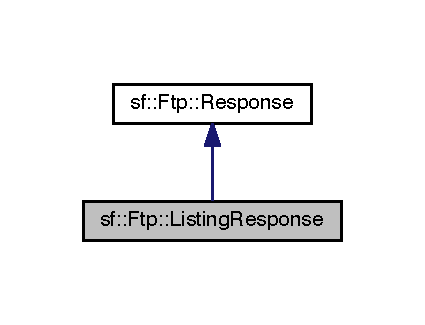
\includegraphics[width=204pt]{classsf_1_1_ftp_1_1_listing_response__inherit__graph}
\end{center}
\end{figure}


Collaboration diagram for sf\-:\-:Ftp\-:\-:Listing\-Response\-:
\nopagebreak
\begin{figure}[H]
\begin{center}
\leavevmode
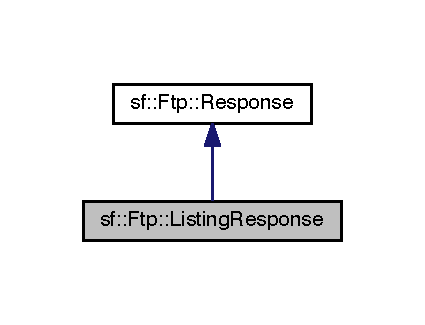
\includegraphics[width=204pt]{classsf_1_1_ftp_1_1_listing_response__coll__graph}
\end{center}
\end{figure}
\subsection*{Public Member Functions}
\begin{DoxyCompactItemize}
\item 
\hyperlink{classsf_1_1_ftp_1_1_listing_response_aefc1b85e59ee0c3ee180666b4a4631e4}{Listing\-Response} (const \hyperlink{classsf_1_1_ftp_1_1_response}{Response} \&response, const std\-::vector$<$ char $>$ \&\hyperlink{gl3_8h_a0f78eecb0891cce3bdfc815b971866a1}{data})
\begin{DoxyCompactList}\small\item\em Default constructor. \end{DoxyCompactList}\item 
const std\-::vector$<$ \hyperlink{gl3_8h_ac83513893df92266f79a515488701770}{std\-::string} $>$ \& \hyperlink{classsf_1_1_ftp_1_1_listing_response_a8196384f8cb4e16171780fb08d456e63}{get\-Filenames} () const 
\begin{DoxyCompactList}\small\item\em Return the array of filenames. \end{DoxyCompactList}\end{DoxyCompactItemize}
\subsection*{Additional Inherited Members}


\subsection{Detailed Description}
Specialization of F\-T\-P response returning a filename lisiting. 

Definition at line 221 of file Ftp.\-hpp.



\subsection{Constructor \& Destructor Documentation}
\hypertarget{classsf_1_1_ftp_1_1_listing_response_aefc1b85e59ee0c3ee180666b4a4631e4}{\index{sf\-::\-Ftp\-::\-Listing\-Response@{sf\-::\-Ftp\-::\-Listing\-Response}!Listing\-Response@{Listing\-Response}}
\index{Listing\-Response@{Listing\-Response}!sf::Ftp::ListingResponse@{sf\-::\-Ftp\-::\-Listing\-Response}}
\subsubsection[{Listing\-Response}]{\setlength{\rightskip}{0pt plus 5cm}sf\-::\-Ftp\-::\-Listing\-Response\-::\-Listing\-Response (
\begin{DoxyParamCaption}
\item[{const {\bf Response} \&}]{response, }
\item[{const std\-::vector$<$ char $>$ \&}]{data}
\end{DoxyParamCaption}
)}}\label{classsf_1_1_ftp_1_1_listing_response_aefc1b85e59ee0c3ee180666b4a4631e4}


Default constructor. 


\begin{DoxyParams}{Parameters}
{\em response} & Source response \\
\hline
{\em data} & Data containing the raw listing \\
\hline
\end{DoxyParams}


\subsection{Member Function Documentation}
\hypertarget{classsf_1_1_ftp_1_1_listing_response_a8196384f8cb4e16171780fb08d456e63}{\index{sf\-::\-Ftp\-::\-Listing\-Response@{sf\-::\-Ftp\-::\-Listing\-Response}!get\-Filenames@{get\-Filenames}}
\index{get\-Filenames@{get\-Filenames}!sf::Ftp::ListingResponse@{sf\-::\-Ftp\-::\-Listing\-Response}}
\subsubsection[{get\-Filenames}]{\setlength{\rightskip}{0pt plus 5cm}const std\-::vector$<${\bf std\-::string}$>$\& sf\-::\-Ftp\-::\-Listing\-Response\-::get\-Filenames (
\begin{DoxyParamCaption}
{}
\end{DoxyParamCaption}
) const}}\label{classsf_1_1_ftp_1_1_listing_response_a8196384f8cb4e16171780fb08d456e63}


Return the array of filenames. 

\begin{DoxyReturn}{Returns}
Array containing the requested filenames 
\end{DoxyReturn}


The documentation for this class was generated from the following file\-:\begin{DoxyCompactItemize}
\item 
/\-Users/ira/\-Dropbox/ira\-\_\-dev/protobyte\-\_\-research/other\-\_\-libs/\-S\-F\-M\-L/dylibs/root/usr/local/include/\-S\-F\-M\-L/\-Network/\hyperlink{_ftp_8hpp}{Ftp.\-hpp}\end{DoxyCompactItemize}

\hypertarget{classsf_1_1_lock}{\section{sf\-:\-:Lock Class Reference}
\label{classsf_1_1_lock}\index{sf\-::\-Lock@{sf\-::\-Lock}}
}


Automatic wrapper for locking and unlocking mutexes.  




{\ttfamily \#include $<$Lock.\-hpp$>$}



Inheritance diagram for sf\-:\-:Lock\-:
\nopagebreak
\begin{figure}[H]
\begin{center}
\leavevmode
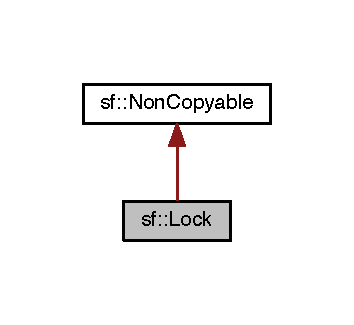
\includegraphics[width=170pt]{classsf_1_1_lock__inherit__graph}
\end{center}
\end{figure}


Collaboration diagram for sf\-:\-:Lock\-:
\nopagebreak
\begin{figure}[H]
\begin{center}
\leavevmode
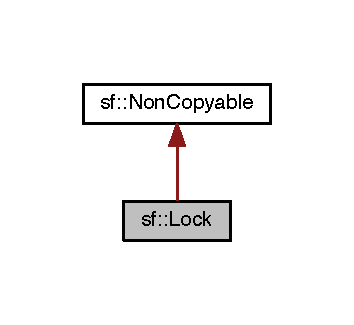
\includegraphics[width=170pt]{classsf_1_1_lock__coll__graph}
\end{center}
\end{figure}
\subsection*{Public Member Functions}
\begin{DoxyCompactItemize}
\item 
\hyperlink{classsf_1_1_lock_a1a4c5d7a15da61103d85c9aa7f118920}{Lock} (\hyperlink{classsf_1_1_mutex}{Mutex} \&mutex)
\begin{DoxyCompactList}\small\item\em Construct the lock with a target mutex. \end{DoxyCompactList}\item 
\hyperlink{classsf_1_1_lock_a8168b36323a18ccf5b6bc531d964aec5}{$\sim$\-Lock} ()
\begin{DoxyCompactList}\small\item\em Destructor. \end{DoxyCompactList}\end{DoxyCompactItemize}
\subsection*{Additional Inherited Members}


\subsection{Detailed Description}
Automatic wrapper for locking and unlocking mutexes. 

\hyperlink{classsf_1_1_lock}{sf\-::\-Lock} is a R\-A\-I\-I wrapper for \hyperlink{classsf_1_1_mutex}{sf\-::\-Mutex}. By unlocking it in its destructor, it ensures that the mutex will always be released when the current scope (most likely a function) ends. This is even more important when an exception or an early return statement can interrupt the execution flow of the function.

For maximum robustness, \hyperlink{classsf_1_1_lock}{sf\-::\-Lock} should always be used to lock/unlock a mutex.

Usage example\-: 
\begin{DoxyCode}
\hyperlink{classsf_1_1_mutex}{sf::Mutex} mutex;

\textcolor{keywordtype}{void} \textcolor{keyword}{function}()
\{
    \hyperlink{classsf_1_1_lock}{sf::Lock} lock(mutex); \textcolor{comment}{// mutex is now locked}

    functionThatMayThrowAnException(); \textcolor{comment}{// mutex is unlocked if this function throws}

    \textcolor{keywordflow}{if} (someCondition)
        \textcolor{keywordflow}{return}; \textcolor{comment}{// mutex is unlocked}

\} \textcolor{comment}{// mutex is unlocked}
\end{DoxyCode}


Because the mutex is not explicitely unlocked in the code, it may remain locked longer than needed. If the region of the code that needs to be protected by the mutex is not the entire function, a good practice is to create a smaller, inner scope so that the lock is limited to this part of the code.


\begin{DoxyCode}
\hyperlink{classsf_1_1_mutex}{sf::Mutex} mutex;

\textcolor{keywordtype}{void} \textcolor{keyword}{function}()
\{
    \{
      \hyperlink{classsf_1_1_lock}{sf::Lock} lock(mutex);
      codeThatRequiresProtection();

    \} \textcolor{comment}{// mutex is unlocked here}

    codeThatDoesntCareAboutTheMutex();
\}
\end{DoxyCode}


Having a mutex locked longer than required is a bad practice which can lead to bad performances. Don't forget that when a mutex is locked, other threads may be waiting doing nothing until it is released.

\begin{DoxySeeAlso}{See Also}
\hyperlink{classsf_1_1_mutex}{sf\-::\-Mutex} 
\end{DoxySeeAlso}


Definition at line 43 of file Lock.\-hpp.



\subsection{Constructor \& Destructor Documentation}
\hypertarget{classsf_1_1_lock_a1a4c5d7a15da61103d85c9aa7f118920}{\index{sf\-::\-Lock@{sf\-::\-Lock}!Lock@{Lock}}
\index{Lock@{Lock}!sf::Lock@{sf\-::\-Lock}}
\subsubsection[{Lock}]{\setlength{\rightskip}{0pt plus 5cm}sf\-::\-Lock\-::\-Lock (
\begin{DoxyParamCaption}
\item[{{\bf Mutex} \&}]{mutex}
\end{DoxyParamCaption}
)\hspace{0.3cm}{\ttfamily [explicit]}}}\label{classsf_1_1_lock_a1a4c5d7a15da61103d85c9aa7f118920}


Construct the lock with a target mutex. 

The mutex passed to \hyperlink{classsf_1_1_lock}{sf\-::\-Lock} is automatically locked.


\begin{DoxyParams}{Parameters}
{\em mutex} & \hyperlink{classsf_1_1_mutex}{Mutex} to lock \\
\hline
\end{DoxyParams}
\hypertarget{classsf_1_1_lock_a8168b36323a18ccf5b6bc531d964aec5}{\index{sf\-::\-Lock@{sf\-::\-Lock}!$\sim$\-Lock@{$\sim$\-Lock}}
\index{$\sim$\-Lock@{$\sim$\-Lock}!sf::Lock@{sf\-::\-Lock}}
\subsubsection[{$\sim$\-Lock}]{\setlength{\rightskip}{0pt plus 5cm}sf\-::\-Lock\-::$\sim$\-Lock (
\begin{DoxyParamCaption}
{}
\end{DoxyParamCaption}
)}}\label{classsf_1_1_lock_a8168b36323a18ccf5b6bc531d964aec5}


Destructor. 

The destructor of \hyperlink{classsf_1_1_lock}{sf\-::\-Lock} automatically unlocks its mutex. 

The documentation for this class was generated from the following file\-:\begin{DoxyCompactItemize}
\item 
/\-Users/ira/\-Dropbox/ira\-\_\-dev/protobyte\-\_\-research/other\-\_\-libs/\-S\-F\-M\-L/dylibs/root/usr/local/include/\-S\-F\-M\-L/\-System/\hyperlink{_lock_8hpp}{Lock.\-hpp}\end{DoxyCompactItemize}

\hypertarget{classproto_1_1_math}{\section{proto\-:\-:Math Class Reference}
\label{classproto_1_1_math}\index{proto\-::\-Math@{proto\-::\-Math}}
}


{\ttfamily \#include $<$Math.\-h$>$}

\subsection*{Static Public Member Functions}
\begin{DoxyCompactItemize}
\item 
static float \hyperlink{classproto_1_1_math_ab1c465d385092669227bd4baef007af6}{random} (float max=1.\-0)
\item 
static float \hyperlink{classproto_1_1_math_a4be5d7a31938460905b1c79ab9027346}{random} (float min, float max)
\end{DoxyCompactItemize}


\subsection{Detailed Description}


Definition at line 15 of file Math.\-h.



\subsection{Member Function Documentation}
\hypertarget{classproto_1_1_math_ab1c465d385092669227bd4baef007af6}{\index{proto\-::\-Math@{proto\-::\-Math}!random@{random}}
\index{random@{random}!proto::Math@{proto\-::\-Math}}
\subsubsection[{random}]{\setlength{\rightskip}{0pt plus 5cm}static float proto\-::\-Math\-::random (
\begin{DoxyParamCaption}
\item[{float}]{max = {\ttfamily 1.0}}
\end{DoxyParamCaption}
)\hspace{0.3cm}{\ttfamily [inline]}, {\ttfamily [static]}}}\label{classproto_1_1_math_ab1c465d385092669227bd4baef007af6}


Definition at line 26 of file Math.\-h.

\hypertarget{classproto_1_1_math_a4be5d7a31938460905b1c79ab9027346}{\index{proto\-::\-Math@{proto\-::\-Math}!random@{random}}
\index{random@{random}!proto::Math@{proto\-::\-Math}}
\subsubsection[{random}]{\setlength{\rightskip}{0pt plus 5cm}static float proto\-::\-Math\-::random (
\begin{DoxyParamCaption}
\item[{float}]{min, }
\item[{float}]{max}
\end{DoxyParamCaption}
)\hspace{0.3cm}{\ttfamily [inline]}, {\ttfamily [static]}}}\label{classproto_1_1_math_a4be5d7a31938460905b1c79ab9027346}


Definition at line 31 of file Math.\-h.



The documentation for this class was generated from the following file\-:\begin{DoxyCompactItemize}
\item 
/\-Users/ira/\-Dropbox/ira\-\_\-dev/protobyte\-\_\-research/\-Protobyte/\hyperlink{_math_8h}{Math.\-h}\end{DoxyCompactItemize}

\hypertarget{class_matrix3}{\section{Matrix3 Class Reference}
\label{class_matrix3}\index{Matrix3@{Matrix3}}
}


{\ttfamily \#include $<$Matrix3.\-h$>$}

\subsection*{Public Member Functions}
\begin{DoxyCompactItemize}
\item 
\hyperlink{class_matrix3_a773fdcf139826ddb39c30e7d08bbdb90}{Matrix3} ()
\item 
\hyperlink{class_matrix3_a054d0d36d98a27b8ca185ee4b374ebfc}{Matrix3} (float mat3\mbox{[}9\mbox{]})
\item 
\hyperlink{glutf90_8h_ac778d6f63f1aaf8ebda0ce6ac821b56e}{void} \hyperlink{class_matrix3_a1a588e856ea84d9f9dd060da9a9cf12e}{rotate} (float theta, const \hyperlink{class_vector3}{Vector3} \&axis, \hyperlink{class_vector3}{Vector3} \&\hyperlink{gl3_8h_a14cfbe2fc2234f5504618905b69d1e06}{v})
\item 
\hyperlink{class_vector3}{Vector3} \hyperlink{class_matrix3_a2aa9f6c49840a56eec111cd4f732f58f}{get\-Rotate} (float theta, const \hyperlink{class_vector3}{Vector3} \&axis, const \hyperlink{class_vector3}{Vector3} \&vec)
\item 
\hyperlink{glutf90_8h_ac778d6f63f1aaf8ebda0ce6ac821b56e}{void} \hyperlink{class_matrix3_a8bcc33f78083797f0c9d56a0e48c2363}{transpose} ()
\item 
\hyperlink{glutf90_8h_ac778d6f63f1aaf8ebda0ce6ac821b56e}{void} \hyperlink{class_matrix3_afd7e77fa940c21813cf9385ffa5f48dc}{determinent} ()
\item 
\hyperlink{glutf90_8h_ac778d6f63f1aaf8ebda0ce6ac821b56e}{void} \hyperlink{class_matrix3_a88dd27bcab250f39e533836496685401}{mult} (const \hyperlink{class_matrix3}{Matrix3} \&m)
\item 
\hyperlink{class_vector3}{Vector3} \hyperlink{class_matrix3_a1cefb3d3ce92aa27c59f6ef74fd65604}{mult} (const \hyperlink{class_vector3}{Vector3} \&vec)
\item 
\hyperlink{glutf90_8h_ac778d6f63f1aaf8ebda0ce6ac821b56e}{void} \hyperlink{class_matrix3_a13fa30e99a7837e19857e4423adfcb61}{add} ()
\item 
\hyperlink{glutf90_8h_ac778d6f63f1aaf8ebda0ce6ac821b56e}{void} \hyperlink{class_matrix3_a3746fa5497e3cd1e5ab6aa4dd6a2021a}{identity} ()
\end{DoxyCompactItemize}


\subsection{Detailed Description}


Definition at line 13 of file Matrix3.\-h.



\subsection{Constructor \& Destructor Documentation}
\hypertarget{class_matrix3_a773fdcf139826ddb39c30e7d08bbdb90}{\index{Matrix3@{Matrix3}!Matrix3@{Matrix3}}
\index{Matrix3@{Matrix3}!Matrix3@{Matrix3}}
\subsubsection[{Matrix3}]{\setlength{\rightskip}{0pt plus 5cm}Matrix3\-::\-Matrix3 (
\begin{DoxyParamCaption}
{}
\end{DoxyParamCaption}
)}}\label{class_matrix3_a773fdcf139826ddb39c30e7d08bbdb90}


Definition at line 16 of file Matrix3.\-cpp.

\hypertarget{class_matrix3_a054d0d36d98a27b8ca185ee4b374ebfc}{\index{Matrix3@{Matrix3}!Matrix3@{Matrix3}}
\index{Matrix3@{Matrix3}!Matrix3@{Matrix3}}
\subsubsection[{Matrix3}]{\setlength{\rightskip}{0pt plus 5cm}Matrix3\-::\-Matrix3 (
\begin{DoxyParamCaption}
\item[{float}]{mat3\mbox{[}9\mbox{]}}
\end{DoxyParamCaption}
)}}\label{class_matrix3_a054d0d36d98a27b8ca185ee4b374ebfc}


Definition at line 20 of file Matrix3.\-cpp.



\subsection{Member Function Documentation}
\hypertarget{class_matrix3_a13fa30e99a7837e19857e4423adfcb61}{\index{Matrix3@{Matrix3}!add@{add}}
\index{add@{add}!Matrix3@{Matrix3}}
\subsubsection[{add}]{\setlength{\rightskip}{0pt plus 5cm}{\bf void} Matrix3\-::add (
\begin{DoxyParamCaption}
{}
\end{DoxyParamCaption}
)}}\label{class_matrix3_a13fa30e99a7837e19857e4423adfcb61}
\hypertarget{class_matrix3_afd7e77fa940c21813cf9385ffa5f48dc}{\index{Matrix3@{Matrix3}!determinent@{determinent}}
\index{determinent@{determinent}!Matrix3@{Matrix3}}
\subsubsection[{determinent}]{\setlength{\rightskip}{0pt plus 5cm}{\bf void} Matrix3\-::determinent (
\begin{DoxyParamCaption}
{}
\end{DoxyParamCaption}
)}}\label{class_matrix3_afd7e77fa940c21813cf9385ffa5f48dc}


Definition at line 38 of file Matrix3.\-cpp.

\hypertarget{class_matrix3_a2aa9f6c49840a56eec111cd4f732f58f}{\index{Matrix3@{Matrix3}!get\-Rotate@{get\-Rotate}}
\index{get\-Rotate@{get\-Rotate}!Matrix3@{Matrix3}}
\subsubsection[{get\-Rotate}]{\setlength{\rightskip}{0pt plus 5cm}{\bf Vector3} Matrix3\-::get\-Rotate (
\begin{DoxyParamCaption}
\item[{float}]{theta, }
\item[{const {\bf Vector3} \&}]{axis, }
\item[{const {\bf Vector3} \&}]{vec}
\end{DoxyParamCaption}
)}}\label{class_matrix3_a2aa9f6c49840a56eec111cd4f732f58f}


Definition at line 52 of file Matrix3.\-cpp.

\hypertarget{class_matrix3_a3746fa5497e3cd1e5ab6aa4dd6a2021a}{\index{Matrix3@{Matrix3}!identity@{identity}}
\index{identity@{identity}!Matrix3@{Matrix3}}
\subsubsection[{identity}]{\setlength{\rightskip}{0pt plus 5cm}{\bf void} Matrix3\-::identity (
\begin{DoxyParamCaption}
{}
\end{DoxyParamCaption}
)}}\label{class_matrix3_a3746fa5497e3cd1e5ab6aa4dd6a2021a}


Definition at line 42 of file Matrix3.\-cpp.

\hypertarget{class_matrix3_a88dd27bcab250f39e533836496685401}{\index{Matrix3@{Matrix3}!mult@{mult}}
\index{mult@{mult}!Matrix3@{Matrix3}}
\subsubsection[{mult}]{\setlength{\rightskip}{0pt plus 5cm}{\bf void} Matrix3\-::mult (
\begin{DoxyParamCaption}
\item[{const {\bf Matrix3} \&}]{m}
\end{DoxyParamCaption}
)}}\label{class_matrix3_a88dd27bcab250f39e533836496685401}
\hypertarget{class_matrix3_a1cefb3d3ce92aa27c59f6ef74fd65604}{\index{Matrix3@{Matrix3}!mult@{mult}}
\index{mult@{mult}!Matrix3@{Matrix3}}
\subsubsection[{mult}]{\setlength{\rightskip}{0pt plus 5cm}{\bf Vector3} Matrix3\-::mult (
\begin{DoxyParamCaption}
\item[{const {\bf Vector3} \&}]{vec}
\end{DoxyParamCaption}
)}}\label{class_matrix3_a1cefb3d3ce92aa27c59f6ef74fd65604}
\hypertarget{class_matrix3_a1a588e856ea84d9f9dd060da9a9cf12e}{\index{Matrix3@{Matrix3}!rotate@{rotate}}
\index{rotate@{rotate}!Matrix3@{Matrix3}}
\subsubsection[{rotate}]{\setlength{\rightskip}{0pt plus 5cm}{\bf void} Matrix3\-::rotate (
\begin{DoxyParamCaption}
\item[{float}]{theta, }
\item[{const {\bf Vector3} \&}]{axis, }
\item[{{\bf Vector3} \&}]{v}
\end{DoxyParamCaption}
)}}\label{class_matrix3_a1a588e856ea84d9f9dd060da9a9cf12e}
\hypertarget{class_matrix3_a8bcc33f78083797f0c9d56a0e48c2363}{\index{Matrix3@{Matrix3}!transpose@{transpose}}
\index{transpose@{transpose}!Matrix3@{Matrix3}}
\subsubsection[{transpose}]{\setlength{\rightskip}{0pt plus 5cm}{\bf void} Matrix3\-::transpose (
\begin{DoxyParamCaption}
{}
\end{DoxyParamCaption}
)}}\label{class_matrix3_a8bcc33f78083797f0c9d56a0e48c2363}


Definition at line 26 of file Matrix3.\-cpp.



The documentation for this class was generated from the following files\-:\begin{DoxyCompactItemize}
\item 
/\-Users/ira/\-Dropbox/ira\-\_\-dev/protobyte\-\_\-research/\-Protobyte/\hyperlink{_matrix3_8h}{Matrix3.\-h}\item 
/\-Users/ira/\-Dropbox/ira\-\_\-dev/protobyte\-\_\-research/\-Protobyte/\hyperlink{_matrix3_8cpp}{Matrix3.\-cpp}\end{DoxyCompactItemize}

\hypertarget{class_matrix4}{\section{Matrix4 Class Reference}
\label{class_matrix4}\index{Matrix4@{Matrix4}}
}


{\ttfamily \#include $<$Matrix4.\-h$>$}

\subsection*{Public Member Functions}
\begin{DoxyCompactItemize}
\item 
\hyperlink{class_matrix4_a21e70a74447b9b05cf9a06400bc9c661}{Matrix4} ()
\item 
\hyperlink{class_matrix4_a95d00cb5d22df1f9d5982de9f9686707}{Matrix4} (float mat4\mbox{[}16\mbox{]})
\item 
\hyperlink{glutf90_8h_ac778d6f63f1aaf8ebda0ce6ac821b56e}{void} \hyperlink{class_matrix4_aafc3ab1288768d0ff18ed7116a8270db}{transpose} ()
\item 
\hyperlink{glutf90_8h_ac778d6f63f1aaf8ebda0ce6ac821b56e}{void} \hyperlink{class_matrix4_a28574cfb21c61eaa6c6d38ffe460921e}{determinent} ()
\item 
\hyperlink{glutf90_8h_ac778d6f63f1aaf8ebda0ce6ac821b56e}{void} \hyperlink{class_matrix4_a80bbae89990f98d581bb22c169770268}{mult} (const \hyperlink{class_matrix4}{Matrix4} \&m)
\item 
\hyperlink{class_vector3}{Vector3} \hyperlink{class_matrix4_a2a6972939ece4b76d163df24e18fc7a5}{mult} (const \hyperlink{class_vector3}{Vector3} \&vec)
\item 
\hyperlink{glutf90_8h_ac778d6f63f1aaf8ebda0ce6ac821b56e}{void} \hyperlink{class_matrix4_adcc51df79c2eb0de2ee2d76e789d8dcb}{add} ()
\item 
\hyperlink{glutf90_8h_ac778d6f63f1aaf8ebda0ce6ac821b56e}{void} \hyperlink{class_matrix4_ab09bc36bf102e3fc6c4506e1bb069aa9}{identity} ()
\end{DoxyCompactItemize}


\subsection{Detailed Description}


Definition at line 18 of file Matrix4.\-h.



\subsection{Constructor \& Destructor Documentation}
\hypertarget{class_matrix4_a21e70a74447b9b05cf9a06400bc9c661}{\index{Matrix4@{Matrix4}!Matrix4@{Matrix4}}
\index{Matrix4@{Matrix4}!Matrix4@{Matrix4}}
\subsubsection[{Matrix4}]{\setlength{\rightskip}{0pt plus 5cm}Matrix4\-::\-Matrix4 (
\begin{DoxyParamCaption}
{}
\end{DoxyParamCaption}
)}}\label{class_matrix4_a21e70a74447b9b05cf9a06400bc9c661}


Definition at line 34 of file Matrix4.\-cpp.

\hypertarget{class_matrix4_a95d00cb5d22df1f9d5982de9f9686707}{\index{Matrix4@{Matrix4}!Matrix4@{Matrix4}}
\index{Matrix4@{Matrix4}!Matrix4@{Matrix4}}
\subsubsection[{Matrix4}]{\setlength{\rightskip}{0pt plus 5cm}Matrix4\-::\-Matrix4 (
\begin{DoxyParamCaption}
\item[{float}]{mat4\mbox{[}16\mbox{]}}
\end{DoxyParamCaption}
)}}\label{class_matrix4_a95d00cb5d22df1f9d5982de9f9686707}


Definition at line 38 of file Matrix4.\-cpp.



\subsection{Member Function Documentation}
\hypertarget{class_matrix4_adcc51df79c2eb0de2ee2d76e789d8dcb}{\index{Matrix4@{Matrix4}!add@{add}}
\index{add@{add}!Matrix4@{Matrix4}}
\subsubsection[{add}]{\setlength{\rightskip}{0pt plus 5cm}{\bf void} Matrix4\-::add (
\begin{DoxyParamCaption}
{}
\end{DoxyParamCaption}
)}}\label{class_matrix4_adcc51df79c2eb0de2ee2d76e789d8dcb}
\hypertarget{class_matrix4_a28574cfb21c61eaa6c6d38ffe460921e}{\index{Matrix4@{Matrix4}!determinent@{determinent}}
\index{determinent@{determinent}!Matrix4@{Matrix4}}
\subsubsection[{determinent}]{\setlength{\rightskip}{0pt plus 5cm}{\bf void} Matrix4\-::determinent (
\begin{DoxyParamCaption}
{}
\end{DoxyParamCaption}
)}}\label{class_matrix4_a28574cfb21c61eaa6c6d38ffe460921e}


Definition at line 56 of file Matrix4.\-cpp.

\hypertarget{class_matrix4_ab09bc36bf102e3fc6c4506e1bb069aa9}{\index{Matrix4@{Matrix4}!identity@{identity}}
\index{identity@{identity}!Matrix4@{Matrix4}}
\subsubsection[{identity}]{\setlength{\rightskip}{0pt plus 5cm}{\bf void} Matrix4\-::identity (
\begin{DoxyParamCaption}
{}
\end{DoxyParamCaption}
)}}\label{class_matrix4_ab09bc36bf102e3fc6c4506e1bb069aa9}


Definition at line 60 of file Matrix4.\-cpp.

\hypertarget{class_matrix4_a80bbae89990f98d581bb22c169770268}{\index{Matrix4@{Matrix4}!mult@{mult}}
\index{mult@{mult}!Matrix4@{Matrix4}}
\subsubsection[{mult}]{\setlength{\rightskip}{0pt plus 5cm}{\bf void} Matrix4\-::mult (
\begin{DoxyParamCaption}
\item[{const {\bf Matrix4} \&}]{m}
\end{DoxyParamCaption}
)}}\label{class_matrix4_a80bbae89990f98d581bb22c169770268}
\hypertarget{class_matrix4_a2a6972939ece4b76d163df24e18fc7a5}{\index{Matrix4@{Matrix4}!mult@{mult}}
\index{mult@{mult}!Matrix4@{Matrix4}}
\subsubsection[{mult}]{\setlength{\rightskip}{0pt plus 5cm}{\bf Vector3} Matrix4\-::mult (
\begin{DoxyParamCaption}
\item[{const {\bf Vector3} \&}]{vec}
\end{DoxyParamCaption}
)}}\label{class_matrix4_a2a6972939ece4b76d163df24e18fc7a5}
\hypertarget{class_matrix4_aafc3ab1288768d0ff18ed7116a8270db}{\index{Matrix4@{Matrix4}!transpose@{transpose}}
\index{transpose@{transpose}!Matrix4@{Matrix4}}
\subsubsection[{transpose}]{\setlength{\rightskip}{0pt plus 5cm}{\bf void} Matrix4\-::transpose (
\begin{DoxyParamCaption}
{}
\end{DoxyParamCaption}
)}}\label{class_matrix4_aafc3ab1288768d0ff18ed7116a8270db}


Definition at line 44 of file Matrix4.\-cpp.



The documentation for this class was generated from the following files\-:\begin{DoxyCompactItemize}
\item 
/\-Users/ira/\-Dropbox/ira\-\_\-dev/protobyte\-\_\-research/\-Protobyte/\hyperlink{_matrix4_8h}{Matrix4.\-h}\item 
/\-Users/ira/\-Dropbox/ira\-\_\-dev/protobyte\-\_\-research/\-Protobyte/\hyperlink{_matrix4_8cpp}{Matrix4.\-cpp}\end{DoxyCompactItemize}

\hypertarget{classsf_1_1_mouse}{\section{sf\-:\-:Mouse Class Reference}
\label{classsf_1_1_mouse}\index{sf\-::\-Mouse@{sf\-::\-Mouse}}
}


Give access to the real-\/time state of the mouse.  




{\ttfamily \#include $<$Mouse.\-hpp$>$}

\subsection*{Public Types}
\begin{DoxyCompactItemize}
\item 
enum \hyperlink{classsf_1_1_mouse_a4fb128be433f9aafe66bc0c605daaa90}{Button} \{ \\*
\hyperlink{classsf_1_1_mouse_a4fb128be433f9aafe66bc0c605daaa90a8bb4856e1ec7f6b6a8605effdfc0eee8}{Left}, 
\hyperlink{classsf_1_1_mouse_a4fb128be433f9aafe66bc0c605daaa90af2cff24ab6c26daf079b11189f982fc4}{Right}, 
\hyperlink{classsf_1_1_mouse_a4fb128be433f9aafe66bc0c605daaa90a2c353189c4b11cf216d7caddafcc609d}{Middle}, 
\hyperlink{classsf_1_1_mouse_a4fb128be433f9aafe66bc0c605daaa90aecc7f3ce9ad6a60b9b0027876446b8d7}{X\-Button1}, 
\\*
\hyperlink{classsf_1_1_mouse_a4fb128be433f9aafe66bc0c605daaa90a03fa056fd0dd9d629c205d91a8ef1b5a}{X\-Button2}, 
\hyperlink{classsf_1_1_mouse_a4fb128be433f9aafe66bc0c605daaa90a52a1d434289774240ddaa22496762402}{Button\-Count}
 \}
\begin{DoxyCompactList}\small\item\em \hyperlink{classsf_1_1_mouse}{Mouse} buttons. \end{DoxyCompactList}\end{DoxyCompactItemize}
\subsection*{Static Public Member Functions}
\begin{DoxyCompactItemize}
\item 
static bool \hyperlink{classsf_1_1_mouse_ab647159eb88e369a0332a9c5a7ba6687}{is\-Button\-Pressed} (\hyperlink{classsf_1_1_mouse_a4fb128be433f9aafe66bc0c605daaa90}{Button} button)
\begin{DoxyCompactList}\small\item\em Check if a mouse button is pressed. \end{DoxyCompactList}\item 
static \hyperlink{namespacesf_ace09dd1447d74c6e9ba56ae874c094e1}{Vector2i} \hyperlink{classsf_1_1_mouse_ac368680f797b7f6e4f50b5b7928c1387}{get\-Position} ()
\begin{DoxyCompactList}\small\item\em Get the current position of the mouse in desktop coordinates. \end{DoxyCompactList}\item 
static \hyperlink{namespacesf_ace09dd1447d74c6e9ba56ae874c094e1}{Vector2i} \hyperlink{classsf_1_1_mouse_a93b4d2ebef728e77a0ec9d83c1e0b0c8}{get\-Position} (const \hyperlink{classsf_1_1_window}{Window} \&relative\-To)
\begin{DoxyCompactList}\small\item\em Get the current position of the mouse in window coordinates. \end{DoxyCompactList}\item 
static \hyperlink{glutf90_8h_ac778d6f63f1aaf8ebda0ce6ac821b56e}{void} \hyperlink{classsf_1_1_mouse_a1222e16c583be9e3d176d86e0b7817d7}{set\-Position} (const \hyperlink{namespacesf_ace09dd1447d74c6e9ba56ae874c094e1}{Vector2i} \&position)
\begin{DoxyCompactList}\small\item\em Set the current position of the mouse in desktop coordinates. \end{DoxyCompactList}\item 
static \hyperlink{glutf90_8h_ac778d6f63f1aaf8ebda0ce6ac821b56e}{void} \hyperlink{classsf_1_1_mouse_ad9b16ec7041531315f06b26b413dfea8}{set\-Position} (const \hyperlink{namespacesf_ace09dd1447d74c6e9ba56ae874c094e1}{Vector2i} \&position, const \hyperlink{classsf_1_1_window}{Window} \&relative\-To)
\begin{DoxyCompactList}\small\item\em Set the current position of the mouse in window coordinates. \end{DoxyCompactList}\end{DoxyCompactItemize}


\subsection{Detailed Description}
Give access to the real-\/time state of the mouse. 

\hyperlink{classsf_1_1_mouse}{sf\-::\-Mouse} provides an interface to the state of the mouse. It only contains static functions (a single mouse is assumed), so it's not meant to be instanciated.

This class allows users to query the mouse state at any time and directly, without having to deal with a window and its events. Compared to the Mouse\-Moved, Mouse\-Button\-Pressed and Mouse\-Button\-Released events, \hyperlink{classsf_1_1_mouse}{sf\-::\-Mouse} can retrieve the state of the cursor and the buttons at any time (you don't need to store and update a boolean on your side in order to know if a button is pressed or released), and you always get the real state of the mouse, even if it is moved, pressed or released when your window is out of focus and no event is triggered.

The Set\-Position and Get\-Position functions can be used to change or retrieve the current position of the mouse pointer. There are two versions\-: one that operates in global coordinates (relative to the desktop) and one that operates in window coordinates (relative to a specific window).

Usage example\-: 
\begin{DoxyCode}
\textcolor{keywordflow}{if} (\hyperlink{classsf_1_1_mouse_ab647159eb88e369a0332a9c5a7ba6687}{sf::Mouse::isButtonPressed}(\hyperlink{classsf_1_1_mouse_a4fb128be433f9aafe66bc0c605daaa90a8bb4856e1ec7f6b6a8605effdfc0eee8}{sf::Mouse::Left}))
\{
    \textcolor{comment}{// left click...}
\}

\textcolor{comment}{// get global mouse position}
\hyperlink{classsf_1_1_vector2}{sf::Vector2i} position = \hyperlink{classsf_1_1_mouse_ac368680f797b7f6e4f50b5b7928c1387}{sf::Mouse::getPosition}();

\textcolor{comment}{// set mouse position relative to a window}
\hyperlink{classsf_1_1_mouse_a1222e16c583be9e3d176d86e0b7817d7}{sf::Mouse::setPosition}(\hyperlink{classsf_1_1_vector2}{sf::Vector2i}(100, 200), window);
\end{DoxyCode}


\begin{DoxySeeAlso}{See Also}
\hyperlink{classsf_1_1_joystick}{sf\-::\-Joystick}, \hyperlink{classsf_1_1_keyboard}{sf\-::\-Keyboard} 
\end{DoxySeeAlso}


Definition at line 43 of file Mouse.\-hpp.



\subsection{Member Enumeration Documentation}
\hypertarget{classsf_1_1_mouse_a4fb128be433f9aafe66bc0c605daaa90}{\index{sf\-::\-Mouse@{sf\-::\-Mouse}!Button@{Button}}
\index{Button@{Button}!sf::Mouse@{sf\-::\-Mouse}}
\subsubsection[{Button}]{\setlength{\rightskip}{0pt plus 5cm}enum {\bf sf\-::\-Mouse\-::\-Button}}}\label{classsf_1_1_mouse_a4fb128be433f9aafe66bc0c605daaa90}


\hyperlink{classsf_1_1_mouse}{Mouse} buttons. 

\begin{Desc}
\item[Enumerator]\par
\begin{description}
\index{Left@{Left}!sf\-::\-Mouse@{sf\-::\-Mouse}}\index{sf\-::\-Mouse@{sf\-::\-Mouse}!Left@{Left}}\item[{\em 
\hypertarget{classsf_1_1_mouse_a4fb128be433f9aafe66bc0c605daaa90a8bb4856e1ec7f6b6a8605effdfc0eee8}{Left}\label{classsf_1_1_mouse_a4fb128be433f9aafe66bc0c605daaa90a8bb4856e1ec7f6b6a8605effdfc0eee8}
}]The left mouse button. \index{Right@{Right}!sf\-::\-Mouse@{sf\-::\-Mouse}}\index{sf\-::\-Mouse@{sf\-::\-Mouse}!Right@{Right}}\item[{\em 
\hypertarget{classsf_1_1_mouse_a4fb128be433f9aafe66bc0c605daaa90af2cff24ab6c26daf079b11189f982fc4}{Right}\label{classsf_1_1_mouse_a4fb128be433f9aafe66bc0c605daaa90af2cff24ab6c26daf079b11189f982fc4}
}]The right mouse button. \index{Middle@{Middle}!sf\-::\-Mouse@{sf\-::\-Mouse}}\index{sf\-::\-Mouse@{sf\-::\-Mouse}!Middle@{Middle}}\item[{\em 
\hypertarget{classsf_1_1_mouse_a4fb128be433f9aafe66bc0c605daaa90a2c353189c4b11cf216d7caddafcc609d}{Middle}\label{classsf_1_1_mouse_a4fb128be433f9aafe66bc0c605daaa90a2c353189c4b11cf216d7caddafcc609d}
}]The middle (wheel) mouse button. \index{X\-Button1@{X\-Button1}!sf\-::\-Mouse@{sf\-::\-Mouse}}\index{sf\-::\-Mouse@{sf\-::\-Mouse}!X\-Button1@{X\-Button1}}\item[{\em 
\hypertarget{classsf_1_1_mouse_a4fb128be433f9aafe66bc0c605daaa90aecc7f3ce9ad6a60b9b0027876446b8d7}{X\-Button1}\label{classsf_1_1_mouse_a4fb128be433f9aafe66bc0c605daaa90aecc7f3ce9ad6a60b9b0027876446b8d7}
}]The first extra mouse button. \index{X\-Button2@{X\-Button2}!sf\-::\-Mouse@{sf\-::\-Mouse}}\index{sf\-::\-Mouse@{sf\-::\-Mouse}!X\-Button2@{X\-Button2}}\item[{\em 
\hypertarget{classsf_1_1_mouse_a4fb128be433f9aafe66bc0c605daaa90a03fa056fd0dd9d629c205d91a8ef1b5a}{X\-Button2}\label{classsf_1_1_mouse_a4fb128be433f9aafe66bc0c605daaa90a03fa056fd0dd9d629c205d91a8ef1b5a}
}]The second extra mouse button. \index{Button\-Count@{Button\-Count}!sf\-::\-Mouse@{sf\-::\-Mouse}}\index{sf\-::\-Mouse@{sf\-::\-Mouse}!Button\-Count@{Button\-Count}}\item[{\em 
\hypertarget{classsf_1_1_mouse_a4fb128be433f9aafe66bc0c605daaa90a52a1d434289774240ddaa22496762402}{Button\-Count}\label{classsf_1_1_mouse_a4fb128be433f9aafe66bc0c605daaa90a52a1d434289774240ddaa22496762402}
}]Keep last -- the total number of mouse buttons. \end{description}
\end{Desc}


Definition at line 51 of file Mouse.\-hpp.



\subsection{Member Function Documentation}
\hypertarget{classsf_1_1_mouse_ac368680f797b7f6e4f50b5b7928c1387}{\index{sf\-::\-Mouse@{sf\-::\-Mouse}!get\-Position@{get\-Position}}
\index{get\-Position@{get\-Position}!sf::Mouse@{sf\-::\-Mouse}}
\subsubsection[{get\-Position}]{\setlength{\rightskip}{0pt plus 5cm}static {\bf Vector2i} sf\-::\-Mouse\-::get\-Position (
\begin{DoxyParamCaption}
{}
\end{DoxyParamCaption}
)\hspace{0.3cm}{\ttfamily [static]}}}\label{classsf_1_1_mouse_ac368680f797b7f6e4f50b5b7928c1387}


Get the current position of the mouse in desktop coordinates. 

This function returns the global position of the mouse cursor on the desktop.

\begin{DoxyReturn}{Returns}
Current position of the mouse 
\end{DoxyReturn}
\hypertarget{classsf_1_1_mouse_a93b4d2ebef728e77a0ec9d83c1e0b0c8}{\index{sf\-::\-Mouse@{sf\-::\-Mouse}!get\-Position@{get\-Position}}
\index{get\-Position@{get\-Position}!sf::Mouse@{sf\-::\-Mouse}}
\subsubsection[{get\-Position}]{\setlength{\rightskip}{0pt plus 5cm}static {\bf Vector2i} sf\-::\-Mouse\-::get\-Position (
\begin{DoxyParamCaption}
\item[{const {\bf Window} \&}]{relative\-To}
\end{DoxyParamCaption}
)\hspace{0.3cm}{\ttfamily [static]}}}\label{classsf_1_1_mouse_a93b4d2ebef728e77a0ec9d83c1e0b0c8}


Get the current position of the mouse in window coordinates. 

This function returns the current position of the mouse cursor, relative to the given window.


\begin{DoxyParams}{Parameters}
{\em relative\-To} & Reference window\\
\hline
\end{DoxyParams}
\begin{DoxyReturn}{Returns}
Current position of the mouse 
\end{DoxyReturn}
\hypertarget{classsf_1_1_mouse_ab647159eb88e369a0332a9c5a7ba6687}{\index{sf\-::\-Mouse@{sf\-::\-Mouse}!is\-Button\-Pressed@{is\-Button\-Pressed}}
\index{is\-Button\-Pressed@{is\-Button\-Pressed}!sf::Mouse@{sf\-::\-Mouse}}
\subsubsection[{is\-Button\-Pressed}]{\setlength{\rightskip}{0pt plus 5cm}static bool sf\-::\-Mouse\-::is\-Button\-Pressed (
\begin{DoxyParamCaption}
\item[{{\bf Button}}]{button}
\end{DoxyParamCaption}
)\hspace{0.3cm}{\ttfamily [static]}}}\label{classsf_1_1_mouse_ab647159eb88e369a0332a9c5a7ba6687}


Check if a mouse button is pressed. 


\begin{DoxyParams}{Parameters}
{\em button} & Button to check\\
\hline
\end{DoxyParams}
\begin{DoxyReturn}{Returns}
True if the button is pressed, false otherwise 
\end{DoxyReturn}
\hypertarget{classsf_1_1_mouse_a1222e16c583be9e3d176d86e0b7817d7}{\index{sf\-::\-Mouse@{sf\-::\-Mouse}!set\-Position@{set\-Position}}
\index{set\-Position@{set\-Position}!sf::Mouse@{sf\-::\-Mouse}}
\subsubsection[{set\-Position}]{\setlength{\rightskip}{0pt plus 5cm}static {\bf void} sf\-::\-Mouse\-::set\-Position (
\begin{DoxyParamCaption}
\item[{const {\bf Vector2i} \&}]{position}
\end{DoxyParamCaption}
)\hspace{0.3cm}{\ttfamily [static]}}}\label{classsf_1_1_mouse_a1222e16c583be9e3d176d86e0b7817d7}


Set the current position of the mouse in desktop coordinates. 

This function sets the global position of the mouse cursor on the desktop.


\begin{DoxyParams}{Parameters}
{\em position} & New position of the mouse \\
\hline
\end{DoxyParams}
\hypertarget{classsf_1_1_mouse_ad9b16ec7041531315f06b26b413dfea8}{\index{sf\-::\-Mouse@{sf\-::\-Mouse}!set\-Position@{set\-Position}}
\index{set\-Position@{set\-Position}!sf::Mouse@{sf\-::\-Mouse}}
\subsubsection[{set\-Position}]{\setlength{\rightskip}{0pt plus 5cm}static {\bf void} sf\-::\-Mouse\-::set\-Position (
\begin{DoxyParamCaption}
\item[{const {\bf Vector2i} \&}]{position, }
\item[{const {\bf Window} \&}]{relative\-To}
\end{DoxyParamCaption}
)\hspace{0.3cm}{\ttfamily [static]}}}\label{classsf_1_1_mouse_ad9b16ec7041531315f06b26b413dfea8}


Set the current position of the mouse in window coordinates. 

This function sets the current position of the mouse cursor, relative to the given window.


\begin{DoxyParams}{Parameters}
{\em position} & New position of the mouse \\
\hline
{\em relative\-To} & Reference window \\
\hline
\end{DoxyParams}


The documentation for this class was generated from the following file\-:\begin{DoxyCompactItemize}
\item 
/\-Users/ira/\-Dropbox/ira\-\_\-dev/protobyte\-\_\-research/other\-\_\-libs/\-S\-F\-M\-L/dylibs/root/usr/local/include/\-S\-F\-M\-L/\-Window/\hyperlink{_mouse_8hpp}{Mouse.\-hpp}\end{DoxyCompactItemize}

\hypertarget{structsf_1_1_event_1_1_mouse_button_event}{\section{sf\-:\-:Event\-:\-:Mouse\-Button\-Event Struct Reference}
\label{structsf_1_1_event_1_1_mouse_button_event}\index{sf\-::\-Event\-::\-Mouse\-Button\-Event@{sf\-::\-Event\-::\-Mouse\-Button\-Event}}
}


\hyperlink{classsf_1_1_mouse}{Mouse} buttons events parameters (Mouse\-Button\-Pressed, Mouse\-Button\-Released)  




{\ttfamily \#include $<$Event.\-hpp$>$}

\subsection*{Public Attributes}
\begin{DoxyCompactItemize}
\item 
\hyperlink{classsf_1_1_mouse_a4fb128be433f9aafe66bc0c605daaa90}{Mouse\-::\-Button} \hyperlink{structsf_1_1_event_1_1_mouse_button_event_a5f53725aa7b647705486eeb95f723024}{button}
\begin{DoxyCompactList}\small\item\em Code of the button that has been pressed. \end{DoxyCompactList}\item 
int \hyperlink{structsf_1_1_event_1_1_mouse_button_event_a49b937b311729174950787781aafcdc7}{x}
\begin{DoxyCompactList}\small\item\em X position of the mouse pointer, relative to the left of the owner window. \end{DoxyCompactList}\item 
int \hyperlink{structsf_1_1_event_1_1_mouse_button_event_aae4735071868d4411d1782bf67619d64}{y}
\begin{DoxyCompactList}\small\item\em Y position of the mouse pointer, relative to the top of the owner window. \end{DoxyCompactList}\end{DoxyCompactItemize}


\subsection{Detailed Description}
\hyperlink{classsf_1_1_mouse}{Mouse} buttons events parameters (Mouse\-Button\-Pressed, Mouse\-Button\-Released) 

Definition at line 94 of file Event.\-hpp.



\subsection{Member Data Documentation}
\hypertarget{structsf_1_1_event_1_1_mouse_button_event_a5f53725aa7b647705486eeb95f723024}{\index{sf\-::\-Event\-::\-Mouse\-Button\-Event@{sf\-::\-Event\-::\-Mouse\-Button\-Event}!button@{button}}
\index{button@{button}!sf::Event::MouseButtonEvent@{sf\-::\-Event\-::\-Mouse\-Button\-Event}}
\subsubsection[{button}]{\setlength{\rightskip}{0pt plus 5cm}{\bf Mouse\-::\-Button} sf\-::\-Event\-::\-Mouse\-Button\-Event\-::button}}\label{structsf_1_1_event_1_1_mouse_button_event_a5f53725aa7b647705486eeb95f723024}


Code of the button that has been pressed. 



Definition at line 96 of file Event.\-hpp.

\hypertarget{structsf_1_1_event_1_1_mouse_button_event_a49b937b311729174950787781aafcdc7}{\index{sf\-::\-Event\-::\-Mouse\-Button\-Event@{sf\-::\-Event\-::\-Mouse\-Button\-Event}!x@{x}}
\index{x@{x}!sf::Event::MouseButtonEvent@{sf\-::\-Event\-::\-Mouse\-Button\-Event}}
\subsubsection[{x}]{\setlength{\rightskip}{0pt plus 5cm}int sf\-::\-Event\-::\-Mouse\-Button\-Event\-::x}}\label{structsf_1_1_event_1_1_mouse_button_event_a49b937b311729174950787781aafcdc7}


X position of the mouse pointer, relative to the left of the owner window. 



Definition at line 97 of file Event.\-hpp.

\hypertarget{structsf_1_1_event_1_1_mouse_button_event_aae4735071868d4411d1782bf67619d64}{\index{sf\-::\-Event\-::\-Mouse\-Button\-Event@{sf\-::\-Event\-::\-Mouse\-Button\-Event}!y@{y}}
\index{y@{y}!sf::Event::MouseButtonEvent@{sf\-::\-Event\-::\-Mouse\-Button\-Event}}
\subsubsection[{y}]{\setlength{\rightskip}{0pt plus 5cm}int sf\-::\-Event\-::\-Mouse\-Button\-Event\-::y}}\label{structsf_1_1_event_1_1_mouse_button_event_aae4735071868d4411d1782bf67619d64}


Y position of the mouse pointer, relative to the top of the owner window. 



Definition at line 98 of file Event.\-hpp.



The documentation for this struct was generated from the following file\-:\begin{DoxyCompactItemize}
\item 
/\-Users/ira/\-Dropbox/ira\-\_\-dev/protobyte\-\_\-research/other\-\_\-libs/\-S\-F\-M\-L/dylibs/root/usr/local/include/\-S\-F\-M\-L/\-Window/\hyperlink{_event_8hpp}{Event.\-hpp}\end{DoxyCompactItemize}

\hypertarget{structsf_1_1_event_1_1_mouse_move_event}{\section{sf\-:\-:Event\-:\-:Mouse\-Move\-Event Struct Reference}
\label{structsf_1_1_event_1_1_mouse_move_event}\index{sf\-::\-Event\-::\-Mouse\-Move\-Event@{sf\-::\-Event\-::\-Mouse\-Move\-Event}}
}


\hyperlink{classsf_1_1_mouse}{Mouse} move event parameters (Mouse\-Moved)  




{\ttfamily \#include $<$Event.\-hpp$>$}

\subsection*{Public Attributes}
\begin{DoxyCompactItemize}
\item 
int \hyperlink{structsf_1_1_event_1_1_mouse_move_event_aa3a23809afb905cbb52c66d8512e21fd}{x}
\begin{DoxyCompactList}\small\item\em X position of the mouse pointer, relative to the left of the owner window. \end{DoxyCompactList}\item 
int \hyperlink{structsf_1_1_event_1_1_mouse_move_event_a86d78a2fba5b3abda16ca059f2392ad4}{y}
\begin{DoxyCompactList}\small\item\em Y position of the mouse pointer, relative to the top of the owner window. \end{DoxyCompactList}\end{DoxyCompactItemize}


\subsection{Detailed Description}
\hyperlink{classsf_1_1_mouse}{Mouse} move event parameters (Mouse\-Moved) 

Definition at line 83 of file Event.\-hpp.



\subsection{Member Data Documentation}
\hypertarget{structsf_1_1_event_1_1_mouse_move_event_aa3a23809afb905cbb52c66d8512e21fd}{\index{sf\-::\-Event\-::\-Mouse\-Move\-Event@{sf\-::\-Event\-::\-Mouse\-Move\-Event}!x@{x}}
\index{x@{x}!sf::Event::MouseMoveEvent@{sf\-::\-Event\-::\-Mouse\-Move\-Event}}
\subsubsection[{x}]{\setlength{\rightskip}{0pt plus 5cm}int sf\-::\-Event\-::\-Mouse\-Move\-Event\-::x}}\label{structsf_1_1_event_1_1_mouse_move_event_aa3a23809afb905cbb52c66d8512e21fd}


X position of the mouse pointer, relative to the left of the owner window. 



Definition at line 85 of file Event.\-hpp.

\hypertarget{structsf_1_1_event_1_1_mouse_move_event_a86d78a2fba5b3abda16ca059f2392ad4}{\index{sf\-::\-Event\-::\-Mouse\-Move\-Event@{sf\-::\-Event\-::\-Mouse\-Move\-Event}!y@{y}}
\index{y@{y}!sf::Event::MouseMoveEvent@{sf\-::\-Event\-::\-Mouse\-Move\-Event}}
\subsubsection[{y}]{\setlength{\rightskip}{0pt plus 5cm}int sf\-::\-Event\-::\-Mouse\-Move\-Event\-::y}}\label{structsf_1_1_event_1_1_mouse_move_event_a86d78a2fba5b3abda16ca059f2392ad4}


Y position of the mouse pointer, relative to the top of the owner window. 



Definition at line 86 of file Event.\-hpp.



The documentation for this struct was generated from the following file\-:\begin{DoxyCompactItemize}
\item 
/\-Users/ira/\-Dropbox/ira\-\_\-dev/protobyte\-\_\-research/other\-\_\-libs/\-S\-F\-M\-L/dylibs/root/usr/local/include/\-S\-F\-M\-L/\-Window/\hyperlink{_event_8hpp}{Event.\-hpp}\end{DoxyCompactItemize}

\hypertarget{structsf_1_1_event_1_1_mouse_wheel_event}{\section{sf\-:\-:Event\-:\-:Mouse\-Wheel\-Event Struct Reference}
\label{structsf_1_1_event_1_1_mouse_wheel_event}\index{sf\-::\-Event\-::\-Mouse\-Wheel\-Event@{sf\-::\-Event\-::\-Mouse\-Wheel\-Event}}
}


\hyperlink{classsf_1_1_mouse}{Mouse} wheel events parameters (Mouse\-Wheel\-Moved)  




{\ttfamily \#include $<$Event.\-hpp$>$}

\subsection*{Public Attributes}
\begin{DoxyCompactItemize}
\item 
int \hyperlink{structsf_1_1_event_1_1_mouse_wheel_event_a4d02b524b5530c7863e7b0f211fa522c}{delta}
\begin{DoxyCompactList}\small\item\em Number of ticks the wheel has moved (positive is up, negative is down) \end{DoxyCompactList}\item 
int \hyperlink{structsf_1_1_event_1_1_mouse_wheel_event_a3079803f836ed7208f43b60332ab053e}{x}
\begin{DoxyCompactList}\small\item\em X position of the mouse pointer, relative to the left of the owner window. \end{DoxyCompactList}\item 
int \hyperlink{structsf_1_1_event_1_1_mouse_wheel_event_a7ea1b8d8c28e2f530c6e9e6d9a5d32d3}{y}
\begin{DoxyCompactList}\small\item\em Y position of the mouse pointer, relative to the top of the owner window. \end{DoxyCompactList}\end{DoxyCompactItemize}


\subsection{Detailed Description}
\hyperlink{classsf_1_1_mouse}{Mouse} wheel events parameters (Mouse\-Wheel\-Moved) 

Definition at line 105 of file Event.\-hpp.



\subsection{Member Data Documentation}
\hypertarget{structsf_1_1_event_1_1_mouse_wheel_event_a4d02b524b5530c7863e7b0f211fa522c}{\index{sf\-::\-Event\-::\-Mouse\-Wheel\-Event@{sf\-::\-Event\-::\-Mouse\-Wheel\-Event}!delta@{delta}}
\index{delta@{delta}!sf::Event::MouseWheelEvent@{sf\-::\-Event\-::\-Mouse\-Wheel\-Event}}
\subsubsection[{delta}]{\setlength{\rightskip}{0pt plus 5cm}int sf\-::\-Event\-::\-Mouse\-Wheel\-Event\-::delta}}\label{structsf_1_1_event_1_1_mouse_wheel_event_a4d02b524b5530c7863e7b0f211fa522c}


Number of ticks the wheel has moved (positive is up, negative is down) 



Definition at line 107 of file Event.\-hpp.

\hypertarget{structsf_1_1_event_1_1_mouse_wheel_event_a3079803f836ed7208f43b60332ab053e}{\index{sf\-::\-Event\-::\-Mouse\-Wheel\-Event@{sf\-::\-Event\-::\-Mouse\-Wheel\-Event}!x@{x}}
\index{x@{x}!sf::Event::MouseWheelEvent@{sf\-::\-Event\-::\-Mouse\-Wheel\-Event}}
\subsubsection[{x}]{\setlength{\rightskip}{0pt plus 5cm}int sf\-::\-Event\-::\-Mouse\-Wheel\-Event\-::x}}\label{structsf_1_1_event_1_1_mouse_wheel_event_a3079803f836ed7208f43b60332ab053e}


X position of the mouse pointer, relative to the left of the owner window. 



Definition at line 108 of file Event.\-hpp.

\hypertarget{structsf_1_1_event_1_1_mouse_wheel_event_a7ea1b8d8c28e2f530c6e9e6d9a5d32d3}{\index{sf\-::\-Event\-::\-Mouse\-Wheel\-Event@{sf\-::\-Event\-::\-Mouse\-Wheel\-Event}!y@{y}}
\index{y@{y}!sf::Event::MouseWheelEvent@{sf\-::\-Event\-::\-Mouse\-Wheel\-Event}}
\subsubsection[{y}]{\setlength{\rightskip}{0pt plus 5cm}int sf\-::\-Event\-::\-Mouse\-Wheel\-Event\-::y}}\label{structsf_1_1_event_1_1_mouse_wheel_event_a7ea1b8d8c28e2f530c6e9e6d9a5d32d3}


Y position of the mouse pointer, relative to the top of the owner window. 



Definition at line 109 of file Event.\-hpp.



The documentation for this struct was generated from the following file\-:\begin{DoxyCompactItemize}
\item 
/\-Users/ira/\-Dropbox/ira\-\_\-dev/protobyte\-\_\-research/other\-\_\-libs/\-S\-F\-M\-L/dylibs/root/usr/local/include/\-S\-F\-M\-L/\-Window/\hyperlink{_event_8hpp}{Event.\-hpp}\end{DoxyCompactItemize}

\hypertarget{classsf_1_1_music}{\section{sf\-:\-:Music Class Reference}
\label{classsf_1_1_music}\index{sf\-::\-Music@{sf\-::\-Music}}
}


Streamed music played from an audio file.  




{\ttfamily \#include $<$Music.\-hpp$>$}



Inheritance diagram for sf\-:\-:Music\-:
\nopagebreak
\begin{figure}[H]
\begin{center}
\leavevmode
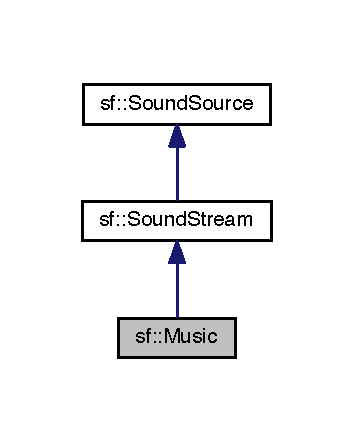
\includegraphics[width=170pt]{classsf_1_1_music__inherit__graph}
\end{center}
\end{figure}


Collaboration diagram for sf\-:\-:Music\-:
\nopagebreak
\begin{figure}[H]
\begin{center}
\leavevmode
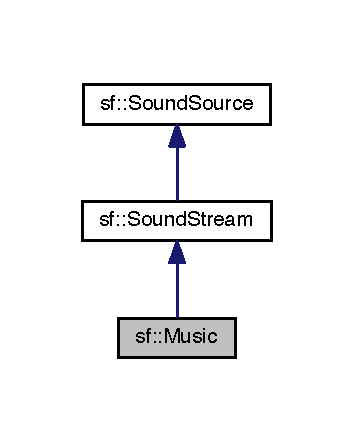
\includegraphics[width=170pt]{classsf_1_1_music__coll__graph}
\end{center}
\end{figure}
\subsection*{Public Member Functions}
\begin{DoxyCompactItemize}
\item 
\hyperlink{classsf_1_1_music_a0bc787d8e022b3a9b89cf2c28befd42e}{Music} ()
\begin{DoxyCompactList}\small\item\em Default constructor. \end{DoxyCompactList}\item 
\hyperlink{classsf_1_1_music_a4c65860fed2f01d0eaa6c4199870414b}{$\sim$\-Music} ()
\begin{DoxyCompactList}\small\item\em Destructor. \end{DoxyCompactList}\item 
bool \hyperlink{classsf_1_1_music_a3edc66e5f5b3f11e84b90eaec9c7d7c0}{open\-From\-File} (const \hyperlink{gl3_8h_ac83513893df92266f79a515488701770}{std\-::string} \&filename)
\begin{DoxyCompactList}\small\item\em Open a music from an audio file. \end{DoxyCompactList}\item 
bool \hyperlink{classsf_1_1_music_ae93b21bcf28ff0b5fec458039111386e}{open\-From\-Memory} (const \hyperlink{glutf90_8h_ac778d6f63f1aaf8ebda0ce6ac821b56e}{void} $\ast$\hyperlink{gl3_8h_a0f78eecb0891cce3bdfc815b971866a1}{data}, std\-::size\-\_\-t size\-In\-Bytes)
\begin{DoxyCompactList}\small\item\em Open a music from an audio file in memory. \end{DoxyCompactList}\item 
bool \hyperlink{classsf_1_1_music_a4e55d1910a26858b44778c26b237d673}{open\-From\-Stream} (\hyperlink{classsf_1_1_input_stream}{Input\-Stream} \&stream)
\begin{DoxyCompactList}\small\item\em Open a music from an audio file in a custom stream. \end{DoxyCompactList}\item 
\hyperlink{classsf_1_1_time}{Time} \hyperlink{classsf_1_1_music_af4738b69c4c5038f71414ad7ffbbdc2b}{get\-Duration} () const 
\begin{DoxyCompactList}\small\item\em Get the total duration of the music. \end{DoxyCompactList}\end{DoxyCompactItemize}
\subsection*{Protected Member Functions}
\begin{DoxyCompactItemize}
\item 
virtual bool \hyperlink{classsf_1_1_music_aca1bcb4e5d56a854133e74bd86374463}{on\-Get\-Data} (\hyperlink{structsf_1_1_sound_stream_1_1_chunk}{Chunk} \&\hyperlink{gl3_8h_a0f78eecb0891cce3bdfc815b971866a1}{data})
\begin{DoxyCompactList}\small\item\em Request a new chunk of audio samples from the stream source. \end{DoxyCompactList}\item 
virtual \hyperlink{glutf90_8h_ac778d6f63f1aaf8ebda0ce6ac821b56e}{void} \hyperlink{classsf_1_1_music_a15119cc0419c16bb334fa0698699c02e}{on\-Seek} (\hyperlink{classsf_1_1_time}{Time} time\-Offset)
\begin{DoxyCompactList}\small\item\em Change the current playing position in the stream source. \end{DoxyCompactList}\end{DoxyCompactItemize}
\subsection*{Additional Inherited Members}


\subsection{Detailed Description}
Streamed music played from an audio file. 

Musics are sounds that are streamed rather than completely loaded in memory. This is especially useful for compressed musics that usually take hundreds of M\-B when they are uncompressed\-: by streaming it instead of loading it entirely, you avoid saturating the memory and have almost no loading delay.

Apart from that, a \hyperlink{classsf_1_1_music}{sf\-::\-Music} has almost the same features as the \hyperlink{classsf_1_1_sound_buffer}{sf\-::\-Sound\-Buffer} / \hyperlink{classsf_1_1_sound}{sf\-::\-Sound} pair\-: you can play/pause/stop it, request its parameters (channels, sample rate), change the way it is played (pitch, volume, 3\-D position, ...), etc.

As a sound stream, a music is played in its own thread in order not to block the rest of the program. This means that you can leave the music alone after calling \hyperlink{classsf_1_1_sound_stream_afdc08b69cab5f243d9324940a85a1144}{play()}, it will manage itself very well.

Usage example\-: 
\begin{DoxyCode}
\textcolor{comment}{// Declare a new music}
\hyperlink{classsf_1_1_music}{sf::Music} music;

\textcolor{comment}{// Open it from an audio file}
\textcolor{keywordflow}{if} (!music.\hyperlink{classsf_1_1_music_a3edc66e5f5b3f11e84b90eaec9c7d7c0}{openFromFile}(\textcolor{stringliteral}{"music.ogg"}))
\{
    \textcolor{comment}{// error...}
\}

\textcolor{comment}{// Change some parameters}
music.\hyperlink{classsf_1_1_sound_source_a0480257ea25d986eba6cc3c1a6f8d7c2}{setPosition}(0, 1, 10); \textcolor{comment}{// change its 3D position}
music.\hyperlink{classsf_1_1_sound_source_a72a13695ed48b7f7b55e7cd4431f4bb6}{setPitch}(2);           \textcolor{comment}{// increase the pitch}
music.\hyperlink{classsf_1_1_sound_source_a2f192f2b49fb8e2b82f3498d3663fcc2}{setVolume}(50);         \textcolor{comment}{// reduce the volume}
music.\hyperlink{classsf_1_1_sound_stream_a43fade018ffba7e4f847a9f00b353f3d}{setLoop}(\textcolor{keyword}{true});         \textcolor{comment}{// make it loop}

\textcolor{comment}{// Play it}
music.\hyperlink{classsf_1_1_sound_stream_afdc08b69cab5f243d9324940a85a1144}{play}();
\end{DoxyCode}


\begin{DoxySeeAlso}{See Also}
\hyperlink{classsf_1_1_sound}{sf\-::\-Sound}, \hyperlink{classsf_1_1_sound_stream}{sf\-::\-Sound\-Stream} 
\end{DoxySeeAlso}


Definition at line 52 of file Music.\-hpp.



\subsection{Constructor \& Destructor Documentation}
\hypertarget{classsf_1_1_music_a0bc787d8e022b3a9b89cf2c28befd42e}{\index{sf\-::\-Music@{sf\-::\-Music}!Music@{Music}}
\index{Music@{Music}!sf::Music@{sf\-::\-Music}}
\subsubsection[{Music}]{\setlength{\rightskip}{0pt plus 5cm}sf\-::\-Music\-::\-Music (
\begin{DoxyParamCaption}
{}
\end{DoxyParamCaption}
)}}\label{classsf_1_1_music_a0bc787d8e022b3a9b89cf2c28befd42e}


Default constructor. 

\hypertarget{classsf_1_1_music_a4c65860fed2f01d0eaa6c4199870414b}{\index{sf\-::\-Music@{sf\-::\-Music}!$\sim$\-Music@{$\sim$\-Music}}
\index{$\sim$\-Music@{$\sim$\-Music}!sf::Music@{sf\-::\-Music}}
\subsubsection[{$\sim$\-Music}]{\setlength{\rightskip}{0pt plus 5cm}sf\-::\-Music\-::$\sim$\-Music (
\begin{DoxyParamCaption}
{}
\end{DoxyParamCaption}
)}}\label{classsf_1_1_music_a4c65860fed2f01d0eaa6c4199870414b}


Destructor. 



\subsection{Member Function Documentation}
\hypertarget{classsf_1_1_music_af4738b69c4c5038f71414ad7ffbbdc2b}{\index{sf\-::\-Music@{sf\-::\-Music}!get\-Duration@{get\-Duration}}
\index{get\-Duration@{get\-Duration}!sf::Music@{sf\-::\-Music}}
\subsubsection[{get\-Duration}]{\setlength{\rightskip}{0pt plus 5cm}{\bf Time} sf\-::\-Music\-::get\-Duration (
\begin{DoxyParamCaption}
{}
\end{DoxyParamCaption}
) const}}\label{classsf_1_1_music_af4738b69c4c5038f71414ad7ffbbdc2b}


Get the total duration of the music. 

\begin{DoxyReturn}{Returns}
\hyperlink{classsf_1_1_music}{Music} duration 
\end{DoxyReturn}
\hypertarget{classsf_1_1_music_aca1bcb4e5d56a854133e74bd86374463}{\index{sf\-::\-Music@{sf\-::\-Music}!on\-Get\-Data@{on\-Get\-Data}}
\index{on\-Get\-Data@{on\-Get\-Data}!sf::Music@{sf\-::\-Music}}
\subsubsection[{on\-Get\-Data}]{\setlength{\rightskip}{0pt plus 5cm}virtual bool sf\-::\-Music\-::on\-Get\-Data (
\begin{DoxyParamCaption}
\item[{{\bf Chunk} \&}]{data}
\end{DoxyParamCaption}
)\hspace{0.3cm}{\ttfamily [protected]}, {\ttfamily [virtual]}}}\label{classsf_1_1_music_aca1bcb4e5d56a854133e74bd86374463}


Request a new chunk of audio samples from the stream source. 

This function fills the chunk from the next samples to read from the audio file.


\begin{DoxyParams}{Parameters}
{\em data} & Chunk of data to fill\\
\hline
\end{DoxyParams}
\begin{DoxyReturn}{Returns}
True to continue playback, false to stop 
\end{DoxyReturn}


Implements \hyperlink{classsf_1_1_sound_stream_a968ec024a6e45490962c8a1121cb7c5f}{sf\-::\-Sound\-Stream}.

\hypertarget{classsf_1_1_music_a15119cc0419c16bb334fa0698699c02e}{\index{sf\-::\-Music@{sf\-::\-Music}!on\-Seek@{on\-Seek}}
\index{on\-Seek@{on\-Seek}!sf::Music@{sf\-::\-Music}}
\subsubsection[{on\-Seek}]{\setlength{\rightskip}{0pt plus 5cm}virtual {\bf void} sf\-::\-Music\-::on\-Seek (
\begin{DoxyParamCaption}
\item[{{\bf Time}}]{time\-Offset}
\end{DoxyParamCaption}
)\hspace{0.3cm}{\ttfamily [protected]}, {\ttfamily [virtual]}}}\label{classsf_1_1_music_a15119cc0419c16bb334fa0698699c02e}


Change the current playing position in the stream source. 


\begin{DoxyParams}{Parameters}
{\em time\-Offset} & New playing position, from the beginning of the music \\
\hline
\end{DoxyParams}


Implements \hyperlink{classsf_1_1_sound_stream_a907036dd2ca7d3af5ead316e54b75997}{sf\-::\-Sound\-Stream}.

\hypertarget{classsf_1_1_music_a3edc66e5f5b3f11e84b90eaec9c7d7c0}{\index{sf\-::\-Music@{sf\-::\-Music}!open\-From\-File@{open\-From\-File}}
\index{open\-From\-File@{open\-From\-File}!sf::Music@{sf\-::\-Music}}
\subsubsection[{open\-From\-File}]{\setlength{\rightskip}{0pt plus 5cm}bool sf\-::\-Music\-::open\-From\-File (
\begin{DoxyParamCaption}
\item[{const {\bf std\-::string} \&}]{filename}
\end{DoxyParamCaption}
)}}\label{classsf_1_1_music_a3edc66e5f5b3f11e84b90eaec9c7d7c0}


Open a music from an audio file. 

This function doesn't start playing the music (call \hyperlink{classsf_1_1_sound_stream_afdc08b69cab5f243d9324940a85a1144}{play()} to do so). Here is a complete list of all the supported audio formats\-: ogg, wav, flac, aiff, au, raw, paf, svx, nist, voc, ircam, w64, mat4, mat5 pvf, htk, sds, avr, sd2, caf, wve, mpc2k, rf64.


\begin{DoxyParams}{Parameters}
{\em filename} & Path of the music file to open\\
\hline
\end{DoxyParams}
\begin{DoxyReturn}{Returns}
True if loading succeeded, false if it failed
\end{DoxyReturn}
\begin{DoxySeeAlso}{See Also}
\hyperlink{classsf_1_1_music_ae93b21bcf28ff0b5fec458039111386e}{open\-From\-Memory}, \hyperlink{classsf_1_1_music_a4e55d1910a26858b44778c26b237d673}{open\-From\-Stream} 
\end{DoxySeeAlso}
\hypertarget{classsf_1_1_music_ae93b21bcf28ff0b5fec458039111386e}{\index{sf\-::\-Music@{sf\-::\-Music}!open\-From\-Memory@{open\-From\-Memory}}
\index{open\-From\-Memory@{open\-From\-Memory}!sf::Music@{sf\-::\-Music}}
\subsubsection[{open\-From\-Memory}]{\setlength{\rightskip}{0pt plus 5cm}bool sf\-::\-Music\-::open\-From\-Memory (
\begin{DoxyParamCaption}
\item[{const {\bf void} $\ast$}]{data, }
\item[{std\-::size\-\_\-t}]{size\-In\-Bytes}
\end{DoxyParamCaption}
)}}\label{classsf_1_1_music_ae93b21bcf28ff0b5fec458039111386e}


Open a music from an audio file in memory. 

This function doesn't start playing the music (call \hyperlink{classsf_1_1_sound_stream_afdc08b69cab5f243d9324940a85a1144}{play()} to do so). Here is a complete list of all the supported audio formats\-: ogg, wav, flac, aiff, au, raw, paf, svx, nist, voc, ircam, w64, mat4, mat5 pvf, htk, sds, avr, sd2, caf, wve, mpc2k, rf64. Since the music is not loaded completely but rather streamed continuously, the {\itshape data} must remain available as long as the music is playing (ie. you can't deallocate it right after calling this function).


\begin{DoxyParams}{Parameters}
{\em data} & Pointer to the file data in memory \\
\hline
{\em size\-In\-Bytes} & Size of the data to load, in bytes\\
\hline
\end{DoxyParams}
\begin{DoxyReturn}{Returns}
True if loading succeeded, false if it failed
\end{DoxyReturn}
\begin{DoxySeeAlso}{See Also}
\hyperlink{classsf_1_1_music_a3edc66e5f5b3f11e84b90eaec9c7d7c0}{open\-From\-File}, \hyperlink{classsf_1_1_music_a4e55d1910a26858b44778c26b237d673}{open\-From\-Stream} 
\end{DoxySeeAlso}
\hypertarget{classsf_1_1_music_a4e55d1910a26858b44778c26b237d673}{\index{sf\-::\-Music@{sf\-::\-Music}!open\-From\-Stream@{open\-From\-Stream}}
\index{open\-From\-Stream@{open\-From\-Stream}!sf::Music@{sf\-::\-Music}}
\subsubsection[{open\-From\-Stream}]{\setlength{\rightskip}{0pt plus 5cm}bool sf\-::\-Music\-::open\-From\-Stream (
\begin{DoxyParamCaption}
\item[{{\bf Input\-Stream} \&}]{stream}
\end{DoxyParamCaption}
)}}\label{classsf_1_1_music_a4e55d1910a26858b44778c26b237d673}


Open a music from an audio file in a custom stream. 

This function doesn't start playing the music (call \hyperlink{classsf_1_1_sound_stream_afdc08b69cab5f243d9324940a85a1144}{play()} to do so). Here is a complete list of all the supported audio formats\-: ogg, wav, flac, aiff, au, raw, paf, svx, nist, voc, ircam, w64, mat4, mat5 pvf, htk, sds, avr, sd2, caf, wve, mpc2k, rf64. Since the music is not loaded completely but rather streamed continuously, the {\itshape stream} must remain alive as long as the music is playing (ie. you can't destroy it right after calling this function).


\begin{DoxyParams}{Parameters}
{\em stream} & Source stream to read from\\
\hline
\end{DoxyParams}
\begin{DoxyReturn}{Returns}
True if loading succeeded, false if it failed
\end{DoxyReturn}
\begin{DoxySeeAlso}{See Also}
\hyperlink{classsf_1_1_music_a3edc66e5f5b3f11e84b90eaec9c7d7c0}{open\-From\-File}, \hyperlink{classsf_1_1_music_ae93b21bcf28ff0b5fec458039111386e}{open\-From\-Memory} 
\end{DoxySeeAlso}


The documentation for this class was generated from the following file\-:\begin{DoxyCompactItemize}
\item 
/\-Users/ira/\-Dropbox/ira\-\_\-dev/protobyte\-\_\-research/other\-\_\-libs/\-S\-F\-M\-L/dylibs/root/usr/local/include/\-S\-F\-M\-L/\-Audio/\hyperlink{_music_8hpp}{Music.\-hpp}\end{DoxyCompactItemize}

\hypertarget{classsf_1_1_mutex}{\section{sf\-:\-:Mutex Class Reference}
\label{classsf_1_1_mutex}\index{sf\-::\-Mutex@{sf\-::\-Mutex}}
}


Blocks concurrent access to shared resources from multiple threads.  




{\ttfamily \#include $<$Mutex.\-hpp$>$}



Inheritance diagram for sf\-:\-:Mutex\-:
\nopagebreak
\begin{figure}[H]
\begin{center}
\leavevmode
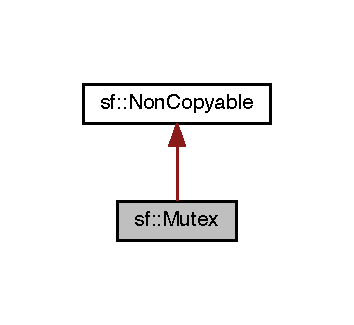
\includegraphics[width=170pt]{classsf_1_1_mutex__inherit__graph}
\end{center}
\end{figure}


Collaboration diagram for sf\-:\-:Mutex\-:
\nopagebreak
\begin{figure}[H]
\begin{center}
\leavevmode
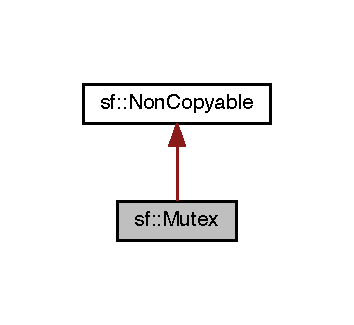
\includegraphics[width=170pt]{classsf_1_1_mutex__coll__graph}
\end{center}
\end{figure}
\subsection*{Public Member Functions}
\begin{DoxyCompactItemize}
\item 
\hyperlink{classsf_1_1_mutex_a9bd52a48320fd7b6db8a78037aad276e}{Mutex} ()
\begin{DoxyCompactList}\small\item\em Default constructor. \end{DoxyCompactList}\item 
\hyperlink{classsf_1_1_mutex_a9f76a67b7b6d3918131a692179b4e3f2}{$\sim$\-Mutex} ()
\begin{DoxyCompactList}\small\item\em Destructor. \end{DoxyCompactList}\item 
\hyperlink{glutf90_8h_ac778d6f63f1aaf8ebda0ce6ac821b56e}{void} \hyperlink{classsf_1_1_mutex_a1a16956a6bbea764480c1b80f2e45763}{lock} ()
\begin{DoxyCompactList}\small\item\em \hyperlink{classsf_1_1_lock}{Lock} the mutex. \end{DoxyCompactList}\item 
\hyperlink{glutf90_8h_ac778d6f63f1aaf8ebda0ce6ac821b56e}{void} \hyperlink{classsf_1_1_mutex_ade71268ffc5e80756652058b01c23c33}{unlock} ()
\begin{DoxyCompactList}\small\item\em Unlock the mutex. \end{DoxyCompactList}\end{DoxyCompactItemize}
\subsection*{Additional Inherited Members}


\subsection{Detailed Description}
Blocks concurrent access to shared resources from multiple threads. 

\hyperlink{classsf_1_1_mutex}{Mutex} stands for \char`\"{}\-M\-U\-Tual E\-Xclusion\char`\"{}. A mutex is a synchronization object, used when multiple threads are involved.

When you want to protect a part of the code from being accessed simultaneously by multiple threads, you typically use a mutex. When a thread is locked by a mutex, any other thread trying to lock it will be blocked until the mutex is released by the thread that locked it. This way, you can allow only one thread at a time to access a critical region of your code.

Usage example\-: 
\begin{DoxyCode}
Database database; \textcolor{comment}{// this is a critical resource that needs some protection}
\hyperlink{classsf_1_1_mutex}{sf::Mutex} mutex;

\textcolor{keywordtype}{void} thread1()
\{
    mutex.\hyperlink{classsf_1_1_mutex_a1a16956a6bbea764480c1b80f2e45763}{lock}(); \textcolor{comment}{// this call will block the thread if the mutex is already locked by thread2}
    database.write(...);
    mutex.\hyperlink{classsf_1_1_mutex_ade71268ffc5e80756652058b01c23c33}{unlock}(); \textcolor{comment}{// if thread2 was waiting, it will now be unblocked}
\}

\textcolor{keywordtype}{void} thread2()
\{
    mutex.\hyperlink{classsf_1_1_mutex_a1a16956a6bbea764480c1b80f2e45763}{lock}(); \textcolor{comment}{// this call will block the thread if the mutex is already locked by thread1}
    database.write(...);
    mutex.\hyperlink{classsf_1_1_mutex_ade71268ffc5e80756652058b01c23c33}{unlock}(); \textcolor{comment}{// if thread1 was waiting, it will now be unblocked}
\}
\end{DoxyCode}


Be very careful with mutexes. A bad usage can lead to bad problems, like deadlocks (two threads are waiting for each other and the application is globally stuck).

To make the usage of mutexes more robust, particularly in environments where exceptions can be thrown, you should use the helper class \hyperlink{classsf_1_1_lock}{sf\-::\-Lock} to lock/unlock mutexes.

S\-F\-M\-L mutexes are recursive, which means that you can lock a mutex multiple times in the same thread without creating a deadlock. In this case, the first call to Lock() behaves as usual, and the following ones have no effect. However, you must call \hyperlink{classsf_1_1_mutex_ade71268ffc5e80756652058b01c23c33}{unlock()} exactly as many times as you called \hyperlink{classsf_1_1_mutex_a1a16956a6bbea764480c1b80f2e45763}{lock()}. If you don't, the mutex won't be released.

\begin{DoxySeeAlso}{See Also}
\hyperlink{classsf_1_1_lock}{sf\-::\-Lock} 
\end{DoxySeeAlso}


Definition at line 47 of file Mutex.\-hpp.



\subsection{Constructor \& Destructor Documentation}
\hypertarget{classsf_1_1_mutex_a9bd52a48320fd7b6db8a78037aad276e}{\index{sf\-::\-Mutex@{sf\-::\-Mutex}!Mutex@{Mutex}}
\index{Mutex@{Mutex}!sf::Mutex@{sf\-::\-Mutex}}
\subsubsection[{Mutex}]{\setlength{\rightskip}{0pt plus 5cm}sf\-::\-Mutex\-::\-Mutex (
\begin{DoxyParamCaption}
{}
\end{DoxyParamCaption}
)}}\label{classsf_1_1_mutex_a9bd52a48320fd7b6db8a78037aad276e}


Default constructor. 

\hypertarget{classsf_1_1_mutex_a9f76a67b7b6d3918131a692179b4e3f2}{\index{sf\-::\-Mutex@{sf\-::\-Mutex}!$\sim$\-Mutex@{$\sim$\-Mutex}}
\index{$\sim$\-Mutex@{$\sim$\-Mutex}!sf::Mutex@{sf\-::\-Mutex}}
\subsubsection[{$\sim$\-Mutex}]{\setlength{\rightskip}{0pt plus 5cm}sf\-::\-Mutex\-::$\sim$\-Mutex (
\begin{DoxyParamCaption}
{}
\end{DoxyParamCaption}
)}}\label{classsf_1_1_mutex_a9f76a67b7b6d3918131a692179b4e3f2}


Destructor. 



\subsection{Member Function Documentation}
\hypertarget{classsf_1_1_mutex_a1a16956a6bbea764480c1b80f2e45763}{\index{sf\-::\-Mutex@{sf\-::\-Mutex}!lock@{lock}}
\index{lock@{lock}!sf::Mutex@{sf\-::\-Mutex}}
\subsubsection[{lock}]{\setlength{\rightskip}{0pt plus 5cm}{\bf void} sf\-::\-Mutex\-::lock (
\begin{DoxyParamCaption}
{}
\end{DoxyParamCaption}
)}}\label{classsf_1_1_mutex_a1a16956a6bbea764480c1b80f2e45763}


\hyperlink{classsf_1_1_lock}{Lock} the mutex. 

If the mutex is already locked in another thread, this call will block the execution until the mutex is released.

\begin{DoxySeeAlso}{See Also}
Unlock 
\end{DoxySeeAlso}
\hypertarget{classsf_1_1_mutex_ade71268ffc5e80756652058b01c23c33}{\index{sf\-::\-Mutex@{sf\-::\-Mutex}!unlock@{unlock}}
\index{unlock@{unlock}!sf::Mutex@{sf\-::\-Mutex}}
\subsubsection[{unlock}]{\setlength{\rightskip}{0pt plus 5cm}{\bf void} sf\-::\-Mutex\-::unlock (
\begin{DoxyParamCaption}
{}
\end{DoxyParamCaption}
)}}\label{classsf_1_1_mutex_ade71268ffc5e80756652058b01c23c33}


Unlock the mutex. 

\begin{DoxySeeAlso}{See Also}
\hyperlink{classsf_1_1_lock}{Lock} 
\end{DoxySeeAlso}


The documentation for this class was generated from the following file\-:\begin{DoxyCompactItemize}
\item 
/\-Users/ira/\-Dropbox/ira\-\_\-dev/protobyte\-\_\-research/other\-\_\-libs/\-S\-F\-M\-L/dylibs/root/usr/local/include/\-S\-F\-M\-L/\-System/\hyperlink{_mutex_8hpp}{Mutex.\-hpp}\end{DoxyCompactItemize}

\hypertarget{classsf_1_1_non_copyable}{\section{sf\-:\-:Non\-Copyable Class Reference}
\label{classsf_1_1_non_copyable}\index{sf\-::\-Non\-Copyable@{sf\-::\-Non\-Copyable}}
}


Utility class that makes any derived class non-\/copyable.  




{\ttfamily \#include $<$Non\-Copyable.\-hpp$>$}



Inheritance diagram for sf\-:\-:Non\-Copyable\-:
\nopagebreak
\begin{figure}[H]
\begin{center}
\leavevmode
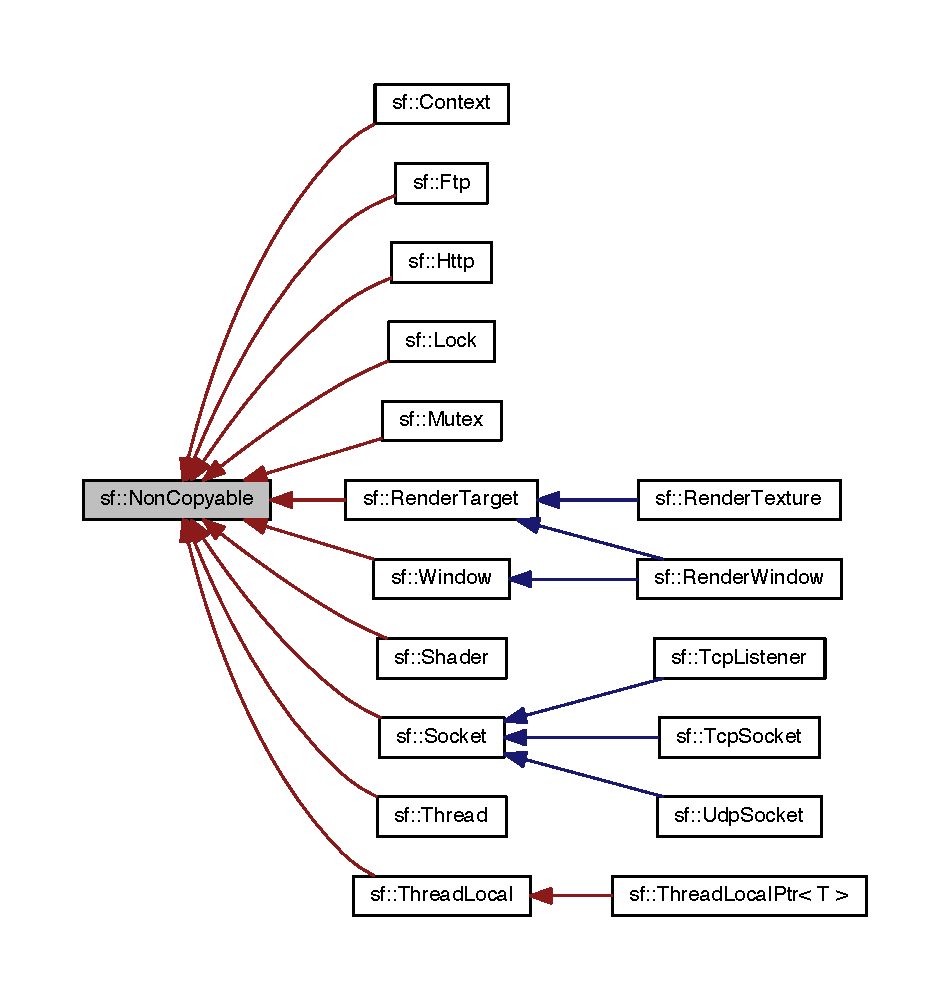
\includegraphics[width=350pt]{classsf_1_1_non_copyable__inherit__graph}
\end{center}
\end{figure}
\subsection*{Protected Member Functions}
\begin{DoxyCompactItemize}
\item 
\hyperlink{classsf_1_1_non_copyable_a2110add170580fdb946f887719da6860}{Non\-Copyable} ()
\begin{DoxyCompactList}\small\item\em Default constructor. \end{DoxyCompactList}\end{DoxyCompactItemize}


\subsection{Detailed Description}
Utility class that makes any derived class non-\/copyable. 

This class makes its instances non-\/copyable, by explicitely disabling its copy constructor and its assignment operator.

To create a non-\/copyable class, simply inherit from \hyperlink{classsf_1_1_non_copyable}{sf\-::\-Non\-Copyable}.

The type of inheritance (public or private) doesn't matter, the copy constructor and assignment operator are declared private in \hyperlink{classsf_1_1_non_copyable}{sf\-::\-Non\-Copyable} so they will end up being inaccessible in both cases. Thus you can use a shorter syntax for inheriting from it see below).

Usage example\-: 
\begin{DoxyCode}
\textcolor{keyword}{class }MyNonCopyableClass : \hyperlink{classsf_1_1_non_copyable}{sf::NonCopyable}
\{
    ...
\};
\end{DoxyCode}


Deciding whether the instances of a class can be copied or not is a very important design choice. You are strongly encouraged to think about it before writing a class, and to use \hyperlink{classsf_1_1_non_copyable}{sf\-::\-Non\-Copyable} when necessary to prevent many potential future errors when using it. This is also a very important indication to users of your class. 

Definition at line 41 of file Non\-Copyable.\-hpp.



\subsection{Constructor \& Destructor Documentation}
\hypertarget{classsf_1_1_non_copyable_a2110add170580fdb946f887719da6860}{\index{sf\-::\-Non\-Copyable@{sf\-::\-Non\-Copyable}!Non\-Copyable@{Non\-Copyable}}
\index{Non\-Copyable@{Non\-Copyable}!sf::NonCopyable@{sf\-::\-Non\-Copyable}}
\subsubsection[{Non\-Copyable}]{\setlength{\rightskip}{0pt plus 5cm}sf\-::\-Non\-Copyable\-::\-Non\-Copyable (
\begin{DoxyParamCaption}
{}
\end{DoxyParamCaption}
)\hspace{0.3cm}{\ttfamily [inline]}, {\ttfamily [protected]}}}\label{classsf_1_1_non_copyable_a2110add170580fdb946f887719da6860}


Default constructor. 

Because this class has a copy constructor, the compiler will not automatically generate the default constructor. That's why we must define it explicitely. 

Definition at line 53 of file Non\-Copyable.\-hpp.



The documentation for this class was generated from the following file\-:\begin{DoxyCompactItemize}
\item 
/\-Users/ira/\-Dropbox/ira\-\_\-dev/protobyte\-\_\-research/other\-\_\-libs/\-S\-F\-M\-L/dylibs/root/usr/local/include/\-S\-F\-M\-L/\-System/\hyperlink{_non_copyable_8hpp}{Non\-Copyable.\-hpp}\end{DoxyCompactItemize}

\hypertarget{classsf_1_1_packet}{\section{sf\-:\-:Packet Class Reference}
\label{classsf_1_1_packet}\index{sf\-::\-Packet@{sf\-::\-Packet}}
}


Utility class to build blocks of data to transfer over the network.  




{\ttfamily \#include $<$Packet.\-hpp$>$}

\subsection*{Public Member Functions}
\begin{DoxyCompactItemize}
\item 
\hyperlink{classsf_1_1_packet_a786e5d4ced83992ceefa1799963ea858}{Packet} ()
\begin{DoxyCompactList}\small\item\em Default constructor. \end{DoxyCompactList}\item 
virtual \hyperlink{classsf_1_1_packet_adc0490ca3c7c3d1e321bd742e5213913}{$\sim$\-Packet} ()
\begin{DoxyCompactList}\small\item\em Virtual destructor. \end{DoxyCompactList}\item 
\hyperlink{glutf90_8h_ac778d6f63f1aaf8ebda0ce6ac821b56e}{void} \hyperlink{classsf_1_1_packet_a7dd6e429b87520008326c4d71f1cf011}{append} (const \hyperlink{glutf90_8h_ac778d6f63f1aaf8ebda0ce6ac821b56e}{void} $\ast$\hyperlink{gl3_8h_a0f78eecb0891cce3bdfc815b971866a1}{data}, std\-::size\-\_\-t size\-In\-Bytes)
\begin{DoxyCompactList}\small\item\em Append data to the end of the packet. \end{DoxyCompactList}\item 
\hyperlink{glutf90_8h_ac778d6f63f1aaf8ebda0ce6ac821b56e}{void} \hyperlink{classsf_1_1_packet_a133ea8b8fe6e93c230f0d79f19a3bf0d}{clear} ()
\begin{DoxyCompactList}\small\item\em Clear the packet. \end{DoxyCompactList}\item 
const \hyperlink{glutf90_8h_ac778d6f63f1aaf8ebda0ce6ac821b56e}{void} $\ast$ \hyperlink{classsf_1_1_packet_a304ba9ec94c992710f4dfff879c6340e}{get\-Data} () const 
\begin{DoxyCompactList}\small\item\em Get a pointer to the data contained in the packet. \end{DoxyCompactList}\item 
std\-::size\-\_\-t \hyperlink{classsf_1_1_packet_a004b62aa5bafa69df8917171a3fe1fa0}{get\-Data\-Size} () const 
\begin{DoxyCompactList}\small\item\em Get the size of the data contained in the packet. \end{DoxyCompactList}\item 
bool \hyperlink{classsf_1_1_packet_aee3adfca6303f1e6bde3c62be392b945}{end\-Of\-Packet} () const 
\begin{DoxyCompactList}\small\item\em Tell if the reading position has reached the end of the packet. \end{DoxyCompactList}\item 
\hyperlink{classsf_1_1_packet_addcb990cde37859c748273d9de55e628}{operator Bool\-Type} () const 
\begin{DoxyCompactList}\small\item\em Test the validity of the packet, for reading. \end{DoxyCompactList}\item 
\hyperlink{classsf_1_1_packet}{Packet} \& \hyperlink{classsf_1_1_packet_af8e26c63ba9bdccd262565ff0d3eeba2}{operator$>$$>$} (bool \&\hyperlink{gl3_8h_a0f78eecb0891cce3bdfc815b971866a1}{data})
\item 
\hyperlink{classsf_1_1_packet}{Packet} \& \hyperlink{classsf_1_1_packet_a70fd5abb9095b5335b79c0cefd17b222}{operator$>$$>$} (\hyperlink{namespacesf_a69b109973eac74e22b97e5339bdb68dd}{Int8} \&\hyperlink{gl3_8h_a0f78eecb0891cce3bdfc815b971866a1}{data})
\item 
\hyperlink{classsf_1_1_packet}{Packet} \& \hyperlink{classsf_1_1_packet_aa67738284a7efc16c7594b358ef35510}{operator$>$$>$} (\hyperlink{namespacesf_a4ef3d630785c4f296f9b4f274c33d78e}{Uint8} \&\hyperlink{gl3_8h_a0f78eecb0891cce3bdfc815b971866a1}{data})
\item 
\hyperlink{classsf_1_1_packet}{Packet} \& \hyperlink{classsf_1_1_packet_af82d6c4e6d74f2ca39732c1e29f30781}{operator$>$$>$} (\hyperlink{namespacesf_a3c8e10435e2a310a7741755e66b5c94e}{Int16} \&\hyperlink{gl3_8h_a0f78eecb0891cce3bdfc815b971866a1}{data})
\item 
\hyperlink{classsf_1_1_packet}{Packet} \& \hyperlink{classsf_1_1_packet_afd8706f092bc830ebb438aeee9271647}{operator$>$$>$} (\hyperlink{namespacesf_a2fcaf787248b0b83dfb6b145ca348246}{Uint16} \&\hyperlink{gl3_8h_a0f78eecb0891cce3bdfc815b971866a1}{data})
\item 
\hyperlink{classsf_1_1_packet}{Packet} \& \hyperlink{classsf_1_1_packet_ae7b44e79f12d500b63f5dc2a10d78d8c}{operator$>$$>$} (\hyperlink{namespacesf_ac2dfd4952377a26dee4750e2e4a30a15}{Int32} \&\hyperlink{gl3_8h_a0f78eecb0891cce3bdfc815b971866a1}{data})
\item 
\hyperlink{classsf_1_1_packet}{Packet} \& \hyperlink{classsf_1_1_packet_a4b57e1953db5bec39a851929df9a339a}{operator$>$$>$} (\hyperlink{namespacesf_aa746fb1ddef4410bddf198ebb27e727c}{Uint32} \&\hyperlink{gl3_8h_a0f78eecb0891cce3bdfc815b971866a1}{data})
\item 
\hyperlink{classsf_1_1_packet}{Packet} \& \hyperlink{classsf_1_1_packet_a6704b4d13d6f798efe6fa836a8b5fa24}{operator$>$$>$} (float \&\hyperlink{gl3_8h_a0f78eecb0891cce3bdfc815b971866a1}{data})
\item 
\hyperlink{classsf_1_1_packet}{Packet} \& \hyperlink{classsf_1_1_packet_ac84239a8ba0a165394805c17b35a88cf}{operator$>$$>$} (double \&\hyperlink{gl3_8h_a0f78eecb0891cce3bdfc815b971866a1}{data})
\item 
\hyperlink{classsf_1_1_packet}{Packet} \& \hyperlink{classsf_1_1_packet_ae9f8d8b0c776204f79f615b1e58bccec}{operator$>$$>$} (char $\ast$\hyperlink{gl3_8h_a0f78eecb0891cce3bdfc815b971866a1}{data})
\item 
\hyperlink{classsf_1_1_packet}{Packet} \& \hyperlink{classsf_1_1_packet_aabace32063c44e1a5cc54af6267c1fab}{operator$>$$>$} (\hyperlink{gl3_8h_ac83513893df92266f79a515488701770}{std\-::string} \&\hyperlink{gl3_8h_a0f78eecb0891cce3bdfc815b971866a1}{data})
\item 
\hyperlink{classsf_1_1_packet}{Packet} \& \hyperlink{classsf_1_1_packet_a1444500d29df0991e630ac78933c6282}{operator$>$$>$} (wchar\-\_\-t $\ast$\hyperlink{gl3_8h_a0f78eecb0891cce3bdfc815b971866a1}{data})
\item 
\hyperlink{classsf_1_1_packet}{Packet} \& \hyperlink{classsf_1_1_packet_ab74c37a290385fd7b1f962bf954a2005}{operator$>$$>$} (std\-::wstring \&\hyperlink{gl3_8h_a0f78eecb0891cce3bdfc815b971866a1}{data})
\item 
\hyperlink{classsf_1_1_packet}{Packet} \& \hyperlink{classsf_1_1_packet_a081233e0cab2182a219b129a1383dc0b}{operator$>$$>$} (\hyperlink{classsf_1_1_string}{String} \&\hyperlink{gl3_8h_a0f78eecb0891cce3bdfc815b971866a1}{data})
\item 
\hyperlink{classsf_1_1_packet}{Packet} \& \hyperlink{classsf_1_1_packet_aa5a465ed02ba29d83ecdafb0ac3fff21}{operator$<$$<$} (bool \hyperlink{gl3_8h_a0f78eecb0891cce3bdfc815b971866a1}{data})
\item 
\hyperlink{classsf_1_1_packet}{Packet} \& \hyperlink{classsf_1_1_packet_a034b68a4281cae0b53a43af7aa4172f6}{operator$<$$<$} (\hyperlink{namespacesf_a69b109973eac74e22b97e5339bdb68dd}{Int8} \hyperlink{gl3_8h_a0f78eecb0891cce3bdfc815b971866a1}{data})
\item 
\hyperlink{classsf_1_1_packet}{Packet} \& \hyperlink{classsf_1_1_packet_af27e4498bf83151b0591d5f04a8b30e1}{operator$<$$<$} (\hyperlink{namespacesf_a4ef3d630785c4f296f9b4f274c33d78e}{Uint8} \hyperlink{gl3_8h_a0f78eecb0891cce3bdfc815b971866a1}{data})
\item 
\hyperlink{classsf_1_1_packet}{Packet} \& \hyperlink{classsf_1_1_packet_afda8754ab4f2a34600f0153ba9ff24fa}{operator$<$$<$} (\hyperlink{namespacesf_a3c8e10435e2a310a7741755e66b5c94e}{Int16} \hyperlink{gl3_8h_a0f78eecb0891cce3bdfc815b971866a1}{data})
\item 
\hyperlink{classsf_1_1_packet}{Packet} \& \hyperlink{classsf_1_1_packet_a557cbc0289135209248aca1aa2117c40}{operator$<$$<$} (\hyperlink{namespacesf_a2fcaf787248b0b83dfb6b145ca348246}{Uint16} \hyperlink{gl3_8h_a0f78eecb0891cce3bdfc815b971866a1}{data})
\item 
\hyperlink{classsf_1_1_packet}{Packet} \& \hyperlink{classsf_1_1_packet_ad60c9ad6e4e92399e2a36938ad122d05}{operator$<$$<$} (\hyperlink{namespacesf_ac2dfd4952377a26dee4750e2e4a30a15}{Int32} \hyperlink{gl3_8h_a0f78eecb0891cce3bdfc815b971866a1}{data})
\item 
\hyperlink{classsf_1_1_packet}{Packet} \& \hyperlink{classsf_1_1_packet_afb113b73749efb662a75deb98257ad34}{operator$<$$<$} (\hyperlink{namespacesf_aa746fb1ddef4410bddf198ebb27e727c}{Uint32} \hyperlink{gl3_8h_a0f78eecb0891cce3bdfc815b971866a1}{data})
\item 
\hyperlink{classsf_1_1_packet}{Packet} \& \hyperlink{classsf_1_1_packet_a76d31c4f864253a7e9b53701b4660fe5}{operator$<$$<$} (float \hyperlink{gl3_8h_a0f78eecb0891cce3bdfc815b971866a1}{data})
\item 
\hyperlink{classsf_1_1_packet}{Packet} \& \hyperlink{classsf_1_1_packet_a3b3077720a486b569ac8e7dec638a3f0}{operator$<$$<$} (double \hyperlink{gl3_8h_a0f78eecb0891cce3bdfc815b971866a1}{data})
\item 
\hyperlink{classsf_1_1_packet}{Packet} \& \hyperlink{classsf_1_1_packet_a67c9985f7b3d6e90886e56e309280a9d}{operator$<$$<$} (const char $\ast$\hyperlink{gl3_8h_a0f78eecb0891cce3bdfc815b971866a1}{data})
\item 
\hyperlink{classsf_1_1_packet}{Packet} \& \hyperlink{classsf_1_1_packet_a59a21671caaa69da5d47c54b50e1eb54}{operator$<$$<$} (const \hyperlink{gl3_8h_ac83513893df92266f79a515488701770}{std\-::string} \&\hyperlink{gl3_8h_a0f78eecb0891cce3bdfc815b971866a1}{data})
\item 
\hyperlink{classsf_1_1_packet}{Packet} \& \hyperlink{classsf_1_1_packet_a6f7c6a9ce795fac342ea937896d98016}{operator$<$$<$} (const wchar\-\_\-t $\ast$\hyperlink{gl3_8h_a0f78eecb0891cce3bdfc815b971866a1}{data})
\item 
\hyperlink{classsf_1_1_packet}{Packet} \& \hyperlink{classsf_1_1_packet_a9f3401d038470f629d0c2c6be928a14b}{operator$<$$<$} (const std\-::wstring \&\hyperlink{gl3_8h_a0f78eecb0891cce3bdfc815b971866a1}{data})
\item 
\hyperlink{classsf_1_1_packet}{Packet} \& \hyperlink{classsf_1_1_packet_abc17272df082a36b202e10045bd9e220}{operator$<$$<$} (const \hyperlink{classsf_1_1_string}{String} \&\hyperlink{gl3_8h_a0f78eecb0891cce3bdfc815b971866a1}{data})
\end{DoxyCompactItemize}
\subsection*{Protected Member Functions}
\begin{DoxyCompactItemize}
\item 
virtual const \hyperlink{glutf90_8h_ac778d6f63f1aaf8ebda0ce6ac821b56e}{void} $\ast$ \hyperlink{classsf_1_1_packet_a052e955906c9bfd671622cb625380edc}{on\-Send} (std\-::size\-\_\-t \&\hyperlink{gl3_8h_a79ef9eb3e59c4bb34c4b9fbeb8d28ff7}{size})
\begin{DoxyCompactList}\small\item\em Called before the packet is sent over the network. \end{DoxyCompactList}\item 
virtual \hyperlink{glutf90_8h_ac778d6f63f1aaf8ebda0ce6ac821b56e}{void} \hyperlink{classsf_1_1_packet_ab71a31ef0f1d5d856de6f9fc75434128}{on\-Receive} (const \hyperlink{glutf90_8h_ac778d6f63f1aaf8ebda0ce6ac821b56e}{void} $\ast$\hyperlink{gl3_8h_a0f78eecb0891cce3bdfc815b971866a1}{data}, std\-::size\-\_\-t \hyperlink{gl3_8h_a79ef9eb3e59c4bb34c4b9fbeb8d28ff7}{size})
\begin{DoxyCompactList}\small\item\em Called after the packet is received over the network. \end{DoxyCompactList}\end{DoxyCompactItemize}
\subsection*{Friends}
\begin{DoxyCompactItemize}
\item 
class \hyperlink{classsf_1_1_packet_aa8b32310b01d4bb702d6bcb969d5f130}{Tcp\-Socket}
\item 
class \hyperlink{classsf_1_1_packet_ae128c6687ced82c6157c5f865f8dec5c}{Udp\-Socket}
\end{DoxyCompactItemize}


\subsection{Detailed Description}
Utility class to build blocks of data to transfer over the network. 

Packets provide a safe and easy way to serialize data, in order to send it over the network using sockets (\hyperlink{classsf_1_1_tcp_socket}{sf\-::\-Tcp\-Socket}, \hyperlink{classsf_1_1_udp_socket}{sf\-::\-Udp\-Socket}).

Packets solve 2 fundamental problems that arise when transfering data over the network\-: \begin{DoxyItemize}
\item data is interpreted correctly according to the endianness \item the bounds of the packet are preserved (one send == one receive)\end{DoxyItemize}
The \hyperlink{classsf_1_1_packet}{sf\-::\-Packet} class provides both input and output modes. It is designed to follow the behaviour of standard C++ streams, using operators $>$$>$ and $<$$<$ to extract and insert data.

It is recommended to use only fixed-\/size types (like \hyperlink{namespacesf_ac2dfd4952377a26dee4750e2e4a30a15}{sf\-::\-Int32}, etc.), to avoid possible differences between the sender and the receiver. Indeed, the native C++ types may have different sizes on two platforms and your data may be corrupted if that happens.

Usage example\-: 
\begin{DoxyCode}
\hyperlink{namespacesf_aa746fb1ddef4410bddf198ebb27e727c}{sf::Uint32} x = 24;
\hyperlink{gl3_8h_ac83513893df92266f79a515488701770}{std::string} s = \textcolor{stringliteral}{"hello"};
\textcolor{keywordtype}{double} d = 5.89;

\textcolor{comment}{// Group the variables to send into a packet}
\hyperlink{classsf_1_1_packet}{sf::Packet} packet;
packet << x << s << d;

\textcolor{comment}{// Send it over the network (socket is a valid sf::TcpSocket)}
socket.send(packet);

-----------------------------------------------------------------

\textcolor{comment}{// Receive the packet at the other end}
\hyperlink{classsf_1_1_packet}{sf::Packet} packet;
socket.receive(packet);

\textcolor{comment}{// Extract the variables contained in the packet}
\hyperlink{namespacesf_aa746fb1ddef4410bddf198ebb27e727c}{sf::Uint32} \hyperlink{gl3_8h_a92d0386e5c19fb81ea88c9f99644ab1d}{x};
\hyperlink{gl3_8h_ac83513893df92266f79a515488701770}{std::string} s;
\textcolor{keywordtype}{double} d;
\textcolor{keywordflow}{if} (packet >> x >> s >> d)
\{
    \textcolor{comment}{// Data extracted successfully...}
\}
\end{DoxyCode}


Packets have built-\/in operator $>$$>$ and $<$$<$ overloads for standard types\-: \begin{DoxyItemize}
\item bool \item fixed-\/size integer types (\hyperlink{namespacesf_a69b109973eac74e22b97e5339bdb68dd}{sf\-::\-Int8}/16/32, \hyperlink{namespacesf_a4ef3d630785c4f296f9b4f274c33d78e}{sf\-::\-Uint8}/16/32) \item floating point numbers (float, double) \item string types (char$\ast$, wchar\-\_\-t$\ast$, std\-::string, std\-::wstring, \hyperlink{classsf_1_1_string}{sf\-::\-String})\end{DoxyItemize}
Like standard streams, it is also possible to define your own overloads of operators $>$$>$ and $<$$<$ in order to handle your custom types.


\begin{DoxyCode}
\textcolor{keyword}{struct }MyStruct
\{
    \textcolor{keywordtype}{float}       number;
    \hyperlink{namespacesf_a69b109973eac74e22b97e5339bdb68dd}{sf::Int8}    integer;
    \hyperlink{gl3_8h_ac83513893df92266f79a515488701770}{std::string} str;
\};

\hyperlink{classsf_1_1_packet}{sf::Packet}& \hyperlink{classsf_1_1_packet_aa5a465ed02ba29d83ecdafb0ac3fff21}{operator <<}(\hyperlink{classsf_1_1_packet}{sf::Packet}& packet, \textcolor{keyword}{const} MyStruct& m)
\{
    \textcolor{keywordflow}{return} packet << m.number << m.integer << m.str;
\}

\hyperlink{classsf_1_1_packet}{sf::Packet}& \hyperlink{classsf_1_1_packet_af8e26c63ba9bdccd262565ff0d3eeba2}{operator >>}(\hyperlink{classsf_1_1_packet}{sf::Packet}& packet, MyStruct& m)
\{
    \textcolor{keywordflow}{return} packet >> m.number >> m.integer >> m.str;
\}
\end{DoxyCode}


Packets also provide an extra feature that allows to apply custom transformations to the data before it is sent, and after it is received. This is typically used to handle automatic compression or encryption of the data. This is achieved by inheriting from \hyperlink{classsf_1_1_packet}{sf\-::\-Packet}, and overriding the on\-Send and on\-Receive functions.

Here is an example\-: 
\begin{DoxyCode}
\textcolor{keyword}{class }ZipPacket : \textcolor{keyword}{public} \hyperlink{classsf_1_1_packet}{sf::Packet}
\{
    \textcolor{keyword}{virtual} \textcolor{keyword}{const} \textcolor{keywordtype}{void}* \hyperlink{classsf_1_1_packet_a052e955906c9bfd671622cb625380edc}{onSend}(std::size\_t& \hyperlink{gl3_8h_a79ef9eb3e59c4bb34c4b9fbeb8d28ff7}{size})
    \{
        \textcolor{keyword}{const} \textcolor{keywordtype}{void}* srcData = \hyperlink{classsf_1_1_packet_a304ba9ec94c992710f4dfff879c6340e}{getData}();
        std::size\_t srcSize = \hyperlink{classsf_1_1_packet_a004b62aa5bafa69df8917171a3fe1fa0}{getDataSize}();

        \textcolor{keywordflow}{return} MySuperZipFunction(srcData, srcSize, &size);
    \}

    \textcolor{keyword}{virtual} \textcolor{keywordtype}{void} \hyperlink{classsf_1_1_packet_ab71a31ef0f1d5d856de6f9fc75434128}{onReceive}(\textcolor{keyword}{const} \textcolor{keywordtype}{void}* \hyperlink{gl3_8h_a0f78eecb0891cce3bdfc815b971866a1}{data}, std::size\_t \hyperlink{gl3_8h_a79ef9eb3e59c4bb34c4b9fbeb8d28ff7}{size})
    \{
        std::size\_t dstSize;
        \textcolor{keyword}{const} \textcolor{keywordtype}{void}* dstData = MySuperUnzipFunction(data, size, &dstSize);

        \hyperlink{classsf_1_1_packet_a7dd6e429b87520008326c4d71f1cf011}{append}(dstData, dstSize);
    \}
\};

\textcolor{comment}{// Use like regular packets:}
ZipPacket packet;
packet << x << s << d;
...
\end{DoxyCode}


\begin{DoxySeeAlso}{See Also}
\hyperlink{classsf_1_1_tcp_socket}{sf\-::\-Tcp\-Socket}, \hyperlink{classsf_1_1_udp_socket}{sf\-::\-Udp\-Socket} 
\end{DoxySeeAlso}


Definition at line 47 of file Packet.\-hpp.



\subsection{Constructor \& Destructor Documentation}
\hypertarget{classsf_1_1_packet_a786e5d4ced83992ceefa1799963ea858}{\index{sf\-::\-Packet@{sf\-::\-Packet}!Packet@{Packet}}
\index{Packet@{Packet}!sf::Packet@{sf\-::\-Packet}}
\subsubsection[{Packet}]{\setlength{\rightskip}{0pt plus 5cm}sf\-::\-Packet\-::\-Packet (
\begin{DoxyParamCaption}
{}
\end{DoxyParamCaption}
)}}\label{classsf_1_1_packet_a786e5d4ced83992ceefa1799963ea858}


Default constructor. 

Creates an empty packet. \hypertarget{classsf_1_1_packet_adc0490ca3c7c3d1e321bd742e5213913}{\index{sf\-::\-Packet@{sf\-::\-Packet}!$\sim$\-Packet@{$\sim$\-Packet}}
\index{$\sim$\-Packet@{$\sim$\-Packet}!sf::Packet@{sf\-::\-Packet}}
\subsubsection[{$\sim$\-Packet}]{\setlength{\rightskip}{0pt plus 5cm}virtual sf\-::\-Packet\-::$\sim$\-Packet (
\begin{DoxyParamCaption}
{}
\end{DoxyParamCaption}
)\hspace{0.3cm}{\ttfamily [virtual]}}}\label{classsf_1_1_packet_adc0490ca3c7c3d1e321bd742e5213913}


Virtual destructor. 



\subsection{Member Function Documentation}
\hypertarget{classsf_1_1_packet_a7dd6e429b87520008326c4d71f1cf011}{\index{sf\-::\-Packet@{sf\-::\-Packet}!append@{append}}
\index{append@{append}!sf::Packet@{sf\-::\-Packet}}
\subsubsection[{append}]{\setlength{\rightskip}{0pt plus 5cm}{\bf void} sf\-::\-Packet\-::append (
\begin{DoxyParamCaption}
\item[{const {\bf void} $\ast$}]{data, }
\item[{std\-::size\-\_\-t}]{size\-In\-Bytes}
\end{DoxyParamCaption}
)}}\label{classsf_1_1_packet_a7dd6e429b87520008326c4d71f1cf011}


Append data to the end of the packet. 


\begin{DoxyParams}{Parameters}
{\em data} & Pointer to the sequence of bytes to append \\
\hline
{\em size\-In\-Bytes} & Number of bytes to append\\
\hline
\end{DoxyParams}
\begin{DoxySeeAlso}{See Also}
\hyperlink{classsf_1_1_packet_a133ea8b8fe6e93c230f0d79f19a3bf0d}{clear} 
\end{DoxySeeAlso}
\hypertarget{classsf_1_1_packet_a133ea8b8fe6e93c230f0d79f19a3bf0d}{\index{sf\-::\-Packet@{sf\-::\-Packet}!clear@{clear}}
\index{clear@{clear}!sf::Packet@{sf\-::\-Packet}}
\subsubsection[{clear}]{\setlength{\rightskip}{0pt plus 5cm}{\bf void} sf\-::\-Packet\-::clear (
\begin{DoxyParamCaption}
{}
\end{DoxyParamCaption}
)}}\label{classsf_1_1_packet_a133ea8b8fe6e93c230f0d79f19a3bf0d}


Clear the packet. 

After calling Clear, the packet is empty.

\begin{DoxySeeAlso}{See Also}
\hyperlink{classsf_1_1_packet_a7dd6e429b87520008326c4d71f1cf011}{append} 
\end{DoxySeeAlso}
\hypertarget{classsf_1_1_packet_aee3adfca6303f1e6bde3c62be392b945}{\index{sf\-::\-Packet@{sf\-::\-Packet}!end\-Of\-Packet@{end\-Of\-Packet}}
\index{end\-Of\-Packet@{end\-Of\-Packet}!sf::Packet@{sf\-::\-Packet}}
\subsubsection[{end\-Of\-Packet}]{\setlength{\rightskip}{0pt plus 5cm}bool sf\-::\-Packet\-::end\-Of\-Packet (
\begin{DoxyParamCaption}
{}
\end{DoxyParamCaption}
) const}}\label{classsf_1_1_packet_aee3adfca6303f1e6bde3c62be392b945}


Tell if the reading position has reached the end of the packet. 

This function is useful to know if there is some data left to be read, without actually reading it.

\begin{DoxyReturn}{Returns}
True if all data was read, false otherwise
\end{DoxyReturn}
\begin{DoxySeeAlso}{See Also}
operator bool 
\end{DoxySeeAlso}
\hypertarget{classsf_1_1_packet_a304ba9ec94c992710f4dfff879c6340e}{\index{sf\-::\-Packet@{sf\-::\-Packet}!get\-Data@{get\-Data}}
\index{get\-Data@{get\-Data}!sf::Packet@{sf\-::\-Packet}}
\subsubsection[{get\-Data}]{\setlength{\rightskip}{0pt plus 5cm}const {\bf void}$\ast$ sf\-::\-Packet\-::get\-Data (
\begin{DoxyParamCaption}
{}
\end{DoxyParamCaption}
) const}}\label{classsf_1_1_packet_a304ba9ec94c992710f4dfff879c6340e}


Get a pointer to the data contained in the packet. 

Warning\-: the returned pointer may become invalid after you append data to the packet, therefore it should never be stored. The return pointer is N\-U\-L\-L if the packet is empty.

\begin{DoxyReturn}{Returns}
Pointer to the data
\end{DoxyReturn}
\begin{DoxySeeAlso}{See Also}
\hyperlink{classsf_1_1_packet_a004b62aa5bafa69df8917171a3fe1fa0}{get\-Data\-Size} 
\end{DoxySeeAlso}
\hypertarget{classsf_1_1_packet_a004b62aa5bafa69df8917171a3fe1fa0}{\index{sf\-::\-Packet@{sf\-::\-Packet}!get\-Data\-Size@{get\-Data\-Size}}
\index{get\-Data\-Size@{get\-Data\-Size}!sf::Packet@{sf\-::\-Packet}}
\subsubsection[{get\-Data\-Size}]{\setlength{\rightskip}{0pt plus 5cm}std\-::size\-\_\-t sf\-::\-Packet\-::get\-Data\-Size (
\begin{DoxyParamCaption}
{}
\end{DoxyParamCaption}
) const}}\label{classsf_1_1_packet_a004b62aa5bafa69df8917171a3fe1fa0}


Get the size of the data contained in the packet. 

This function returns the number of bytes pointed to by what get\-Data returns.

\begin{DoxyReturn}{Returns}
Data size, in bytes
\end{DoxyReturn}
\begin{DoxySeeAlso}{See Also}
\hyperlink{classsf_1_1_packet_a304ba9ec94c992710f4dfff879c6340e}{get\-Data} 
\end{DoxySeeAlso}
\hypertarget{classsf_1_1_packet_ab71a31ef0f1d5d856de6f9fc75434128}{\index{sf\-::\-Packet@{sf\-::\-Packet}!on\-Receive@{on\-Receive}}
\index{on\-Receive@{on\-Receive}!sf::Packet@{sf\-::\-Packet}}
\subsubsection[{on\-Receive}]{\setlength{\rightskip}{0pt plus 5cm}virtual {\bf void} sf\-::\-Packet\-::on\-Receive (
\begin{DoxyParamCaption}
\item[{const {\bf void} $\ast$}]{data, }
\item[{std\-::size\-\_\-t}]{size}
\end{DoxyParamCaption}
)\hspace{0.3cm}{\ttfamily [protected]}, {\ttfamily [virtual]}}}\label{classsf_1_1_packet_ab71a31ef0f1d5d856de6f9fc75434128}


Called after the packet is received over the network. 

This function can be defined by derived classes to transform the data after it is received; this can be used for uncompression, decryption, etc. The function receives a pointer to the received data, and must fill the packet with the transformed bytes. The default implementation fills the packet directly without transforming the data.


\begin{DoxyParams}{Parameters}
{\em data} & Pointer to the received bytes \\
\hline
{\em size} & Number of bytes\\
\hline
\end{DoxyParams}
\begin{DoxySeeAlso}{See Also}
\hyperlink{classsf_1_1_packet_a052e955906c9bfd671622cb625380edc}{on\-Send} 
\end{DoxySeeAlso}
\hypertarget{classsf_1_1_packet_a052e955906c9bfd671622cb625380edc}{\index{sf\-::\-Packet@{sf\-::\-Packet}!on\-Send@{on\-Send}}
\index{on\-Send@{on\-Send}!sf::Packet@{sf\-::\-Packet}}
\subsubsection[{on\-Send}]{\setlength{\rightskip}{0pt plus 5cm}virtual const {\bf void}$\ast$ sf\-::\-Packet\-::on\-Send (
\begin{DoxyParamCaption}
\item[{std\-::size\-\_\-t \&}]{size}
\end{DoxyParamCaption}
)\hspace{0.3cm}{\ttfamily [protected]}, {\ttfamily [virtual]}}}\label{classsf_1_1_packet_a052e955906c9bfd671622cb625380edc}


Called before the packet is sent over the network. 

This function can be defined by derived classes to transform the data before it is sent; this can be used for compression, encryption, etc. The function must return a pointer to the modified data, as well as the number of bytes pointed. The default implementation provides the packet's data without transforming it.


\begin{DoxyParams}{Parameters}
{\em size} & Variable to fill with the size of data to send\\
\hline
\end{DoxyParams}
\begin{DoxyReturn}{Returns}
Pointer to the array of bytes to send
\end{DoxyReturn}
\begin{DoxySeeAlso}{See Also}
\hyperlink{classsf_1_1_packet_ab71a31ef0f1d5d856de6f9fc75434128}{on\-Receive} 
\end{DoxySeeAlso}
\hypertarget{classsf_1_1_packet_addcb990cde37859c748273d9de55e628}{\index{sf\-::\-Packet@{sf\-::\-Packet}!operator Bool\-Type@{operator Bool\-Type}}
\index{operator Bool\-Type@{operator Bool\-Type}!sf::Packet@{sf\-::\-Packet}}
\subsubsection[{operator Bool\-Type}]{\setlength{\rightskip}{0pt plus 5cm}sf\-::\-Packet\-::operator Bool\-Type (
\begin{DoxyParamCaption}
{}
\end{DoxyParamCaption}
) const}}\label{classsf_1_1_packet_addcb990cde37859c748273d9de55e628}


Test the validity of the packet, for reading. 

This operator allows to test the packet as a boolean variable, to check if a reading operation was successful.

A packet will be in an invalid state if it has no more data to read.

This behaviour is the same as standard C++ streams.

Usage example\-: 
\begin{DoxyCode}
\textcolor{keywordtype}{float} \hyperlink{gl3_8h_a92d0386e5c19fb81ea88c9f99644ab1d}{x};
packet >> \hyperlink{gl3_8h_a92d0386e5c19fb81ea88c9f99644ab1d}{x};
\textcolor{keywordflow}{if} (packet)
\{
   \textcolor{comment}{// ok, x was extracted successfully}
\}

\textcolor{comment}{// -- or --}

\textcolor{keywordtype}{float} \hyperlink{gl3_8h_a92d0386e5c19fb81ea88c9f99644ab1d}{x};
\textcolor{keywordflow}{if} (packet >> x)
\{
   \textcolor{comment}{// ok, x was extracted successfully}
\}
\end{DoxyCode}


Don't focus on the return type, it's equivalent to bool but it disallows unwanted implicit conversions to integer or pointer types.

\begin{DoxyReturn}{Returns}
True if last data extraction from packet was successful
\end{DoxyReturn}
\begin{DoxySeeAlso}{See Also}
\hyperlink{classsf_1_1_packet_aee3adfca6303f1e6bde3c62be392b945}{end\-Of\-Packet} 
\end{DoxySeeAlso}
\hypertarget{classsf_1_1_packet_aa5a465ed02ba29d83ecdafb0ac3fff21}{\index{sf\-::\-Packet@{sf\-::\-Packet}!operator$<$$<$@{operator$<$$<$}}
\index{operator$<$$<$@{operator$<$$<$}!sf::Packet@{sf\-::\-Packet}}
\subsubsection[{operator$<$$<$}]{\setlength{\rightskip}{0pt plus 5cm}{\bf Packet}\& sf\-::\-Packet\-::operator$<$$<$ (
\begin{DoxyParamCaption}
\item[{bool}]{data}
\end{DoxyParamCaption}
)}}\label{classsf_1_1_packet_aa5a465ed02ba29d83ecdafb0ac3fff21}
Overloads of operator $<$$<$ to write data into the packet \hypertarget{classsf_1_1_packet_a034b68a4281cae0b53a43af7aa4172f6}{\index{sf\-::\-Packet@{sf\-::\-Packet}!operator$<$$<$@{operator$<$$<$}}
\index{operator$<$$<$@{operator$<$$<$}!sf::Packet@{sf\-::\-Packet}}
\subsubsection[{operator$<$$<$}]{\setlength{\rightskip}{0pt plus 5cm}{\bf Packet}\& sf\-::\-Packet\-::operator$<$$<$ (
\begin{DoxyParamCaption}
\item[{{\bf Int8}}]{data}
\end{DoxyParamCaption}
)}}\label{classsf_1_1_packet_a034b68a4281cae0b53a43af7aa4172f6}
\hypertarget{classsf_1_1_packet_af27e4498bf83151b0591d5f04a8b30e1}{\index{sf\-::\-Packet@{sf\-::\-Packet}!operator$<$$<$@{operator$<$$<$}}
\index{operator$<$$<$@{operator$<$$<$}!sf::Packet@{sf\-::\-Packet}}
\subsubsection[{operator$<$$<$}]{\setlength{\rightskip}{0pt plus 5cm}{\bf Packet}\& sf\-::\-Packet\-::operator$<$$<$ (
\begin{DoxyParamCaption}
\item[{{\bf Uint8}}]{data}
\end{DoxyParamCaption}
)}}\label{classsf_1_1_packet_af27e4498bf83151b0591d5f04a8b30e1}
\hypertarget{classsf_1_1_packet_afda8754ab4f2a34600f0153ba9ff24fa}{\index{sf\-::\-Packet@{sf\-::\-Packet}!operator$<$$<$@{operator$<$$<$}}
\index{operator$<$$<$@{operator$<$$<$}!sf::Packet@{sf\-::\-Packet}}
\subsubsection[{operator$<$$<$}]{\setlength{\rightskip}{0pt plus 5cm}{\bf Packet}\& sf\-::\-Packet\-::operator$<$$<$ (
\begin{DoxyParamCaption}
\item[{{\bf Int16}}]{data}
\end{DoxyParamCaption}
)}}\label{classsf_1_1_packet_afda8754ab4f2a34600f0153ba9ff24fa}
\hypertarget{classsf_1_1_packet_a557cbc0289135209248aca1aa2117c40}{\index{sf\-::\-Packet@{sf\-::\-Packet}!operator$<$$<$@{operator$<$$<$}}
\index{operator$<$$<$@{operator$<$$<$}!sf::Packet@{sf\-::\-Packet}}
\subsubsection[{operator$<$$<$}]{\setlength{\rightskip}{0pt plus 5cm}{\bf Packet}\& sf\-::\-Packet\-::operator$<$$<$ (
\begin{DoxyParamCaption}
\item[{{\bf Uint16}}]{data}
\end{DoxyParamCaption}
)}}\label{classsf_1_1_packet_a557cbc0289135209248aca1aa2117c40}
\hypertarget{classsf_1_1_packet_ad60c9ad6e4e92399e2a36938ad122d05}{\index{sf\-::\-Packet@{sf\-::\-Packet}!operator$<$$<$@{operator$<$$<$}}
\index{operator$<$$<$@{operator$<$$<$}!sf::Packet@{sf\-::\-Packet}}
\subsubsection[{operator$<$$<$}]{\setlength{\rightskip}{0pt plus 5cm}{\bf Packet}\& sf\-::\-Packet\-::operator$<$$<$ (
\begin{DoxyParamCaption}
\item[{{\bf Int32}}]{data}
\end{DoxyParamCaption}
)}}\label{classsf_1_1_packet_ad60c9ad6e4e92399e2a36938ad122d05}
\hypertarget{classsf_1_1_packet_afb113b73749efb662a75deb98257ad34}{\index{sf\-::\-Packet@{sf\-::\-Packet}!operator$<$$<$@{operator$<$$<$}}
\index{operator$<$$<$@{operator$<$$<$}!sf::Packet@{sf\-::\-Packet}}
\subsubsection[{operator$<$$<$}]{\setlength{\rightskip}{0pt plus 5cm}{\bf Packet}\& sf\-::\-Packet\-::operator$<$$<$ (
\begin{DoxyParamCaption}
\item[{{\bf Uint32}}]{data}
\end{DoxyParamCaption}
)}}\label{classsf_1_1_packet_afb113b73749efb662a75deb98257ad34}
\hypertarget{classsf_1_1_packet_a76d31c4f864253a7e9b53701b4660fe5}{\index{sf\-::\-Packet@{sf\-::\-Packet}!operator$<$$<$@{operator$<$$<$}}
\index{operator$<$$<$@{operator$<$$<$}!sf::Packet@{sf\-::\-Packet}}
\subsubsection[{operator$<$$<$}]{\setlength{\rightskip}{0pt plus 5cm}{\bf Packet}\& sf\-::\-Packet\-::operator$<$$<$ (
\begin{DoxyParamCaption}
\item[{float}]{data}
\end{DoxyParamCaption}
)}}\label{classsf_1_1_packet_a76d31c4f864253a7e9b53701b4660fe5}
\hypertarget{classsf_1_1_packet_a3b3077720a486b569ac8e7dec638a3f0}{\index{sf\-::\-Packet@{sf\-::\-Packet}!operator$<$$<$@{operator$<$$<$}}
\index{operator$<$$<$@{operator$<$$<$}!sf::Packet@{sf\-::\-Packet}}
\subsubsection[{operator$<$$<$}]{\setlength{\rightskip}{0pt plus 5cm}{\bf Packet}\& sf\-::\-Packet\-::operator$<$$<$ (
\begin{DoxyParamCaption}
\item[{double}]{data}
\end{DoxyParamCaption}
)}}\label{classsf_1_1_packet_a3b3077720a486b569ac8e7dec638a3f0}
\hypertarget{classsf_1_1_packet_a67c9985f7b3d6e90886e56e309280a9d}{\index{sf\-::\-Packet@{sf\-::\-Packet}!operator$<$$<$@{operator$<$$<$}}
\index{operator$<$$<$@{operator$<$$<$}!sf::Packet@{sf\-::\-Packet}}
\subsubsection[{operator$<$$<$}]{\setlength{\rightskip}{0pt plus 5cm}{\bf Packet}\& sf\-::\-Packet\-::operator$<$$<$ (
\begin{DoxyParamCaption}
\item[{const char $\ast$}]{data}
\end{DoxyParamCaption}
)}}\label{classsf_1_1_packet_a67c9985f7b3d6e90886e56e309280a9d}
\hypertarget{classsf_1_1_packet_a59a21671caaa69da5d47c54b50e1eb54}{\index{sf\-::\-Packet@{sf\-::\-Packet}!operator$<$$<$@{operator$<$$<$}}
\index{operator$<$$<$@{operator$<$$<$}!sf::Packet@{sf\-::\-Packet}}
\subsubsection[{operator$<$$<$}]{\setlength{\rightskip}{0pt plus 5cm}{\bf Packet}\& sf\-::\-Packet\-::operator$<$$<$ (
\begin{DoxyParamCaption}
\item[{const {\bf std\-::string} \&}]{data}
\end{DoxyParamCaption}
)}}\label{classsf_1_1_packet_a59a21671caaa69da5d47c54b50e1eb54}
\hypertarget{classsf_1_1_packet_a6f7c6a9ce795fac342ea937896d98016}{\index{sf\-::\-Packet@{sf\-::\-Packet}!operator$<$$<$@{operator$<$$<$}}
\index{operator$<$$<$@{operator$<$$<$}!sf::Packet@{sf\-::\-Packet}}
\subsubsection[{operator$<$$<$}]{\setlength{\rightskip}{0pt plus 5cm}{\bf Packet}\& sf\-::\-Packet\-::operator$<$$<$ (
\begin{DoxyParamCaption}
\item[{const wchar\-\_\-t $\ast$}]{data}
\end{DoxyParamCaption}
)}}\label{classsf_1_1_packet_a6f7c6a9ce795fac342ea937896d98016}
\hypertarget{classsf_1_1_packet_a9f3401d038470f629d0c2c6be928a14b}{\index{sf\-::\-Packet@{sf\-::\-Packet}!operator$<$$<$@{operator$<$$<$}}
\index{operator$<$$<$@{operator$<$$<$}!sf::Packet@{sf\-::\-Packet}}
\subsubsection[{operator$<$$<$}]{\setlength{\rightskip}{0pt plus 5cm}{\bf Packet}\& sf\-::\-Packet\-::operator$<$$<$ (
\begin{DoxyParamCaption}
\item[{const std\-::wstring \&}]{data}
\end{DoxyParamCaption}
)}}\label{classsf_1_1_packet_a9f3401d038470f629d0c2c6be928a14b}
\hypertarget{classsf_1_1_packet_abc17272df082a36b202e10045bd9e220}{\index{sf\-::\-Packet@{sf\-::\-Packet}!operator$<$$<$@{operator$<$$<$}}
\index{operator$<$$<$@{operator$<$$<$}!sf::Packet@{sf\-::\-Packet}}
\subsubsection[{operator$<$$<$}]{\setlength{\rightskip}{0pt plus 5cm}{\bf Packet}\& sf\-::\-Packet\-::operator$<$$<$ (
\begin{DoxyParamCaption}
\item[{const {\bf String} \&}]{data}
\end{DoxyParamCaption}
)}}\label{classsf_1_1_packet_abc17272df082a36b202e10045bd9e220}
\hypertarget{classsf_1_1_packet_af8e26c63ba9bdccd262565ff0d3eeba2}{\index{sf\-::\-Packet@{sf\-::\-Packet}!operator$>$$>$@{operator$>$$>$}}
\index{operator$>$$>$@{operator$>$$>$}!sf::Packet@{sf\-::\-Packet}}
\subsubsection[{operator$>$$>$}]{\setlength{\rightskip}{0pt plus 5cm}{\bf Packet}\& sf\-::\-Packet\-::operator$>$$>$ (
\begin{DoxyParamCaption}
\item[{bool \&}]{data}
\end{DoxyParamCaption}
)}}\label{classsf_1_1_packet_af8e26c63ba9bdccd262565ff0d3eeba2}
Overloads of operator $>$$>$ to read data from the packet \hypertarget{classsf_1_1_packet_a70fd5abb9095b5335b79c0cefd17b222}{\index{sf\-::\-Packet@{sf\-::\-Packet}!operator$>$$>$@{operator$>$$>$}}
\index{operator$>$$>$@{operator$>$$>$}!sf::Packet@{sf\-::\-Packet}}
\subsubsection[{operator$>$$>$}]{\setlength{\rightskip}{0pt plus 5cm}{\bf Packet}\& sf\-::\-Packet\-::operator$>$$>$ (
\begin{DoxyParamCaption}
\item[{{\bf Int8} \&}]{data}
\end{DoxyParamCaption}
)}}\label{classsf_1_1_packet_a70fd5abb9095b5335b79c0cefd17b222}
\hypertarget{classsf_1_1_packet_aa67738284a7efc16c7594b358ef35510}{\index{sf\-::\-Packet@{sf\-::\-Packet}!operator$>$$>$@{operator$>$$>$}}
\index{operator$>$$>$@{operator$>$$>$}!sf::Packet@{sf\-::\-Packet}}
\subsubsection[{operator$>$$>$}]{\setlength{\rightskip}{0pt plus 5cm}{\bf Packet}\& sf\-::\-Packet\-::operator$>$$>$ (
\begin{DoxyParamCaption}
\item[{{\bf Uint8} \&}]{data}
\end{DoxyParamCaption}
)}}\label{classsf_1_1_packet_aa67738284a7efc16c7594b358ef35510}
\hypertarget{classsf_1_1_packet_af82d6c4e6d74f2ca39732c1e29f30781}{\index{sf\-::\-Packet@{sf\-::\-Packet}!operator$>$$>$@{operator$>$$>$}}
\index{operator$>$$>$@{operator$>$$>$}!sf::Packet@{sf\-::\-Packet}}
\subsubsection[{operator$>$$>$}]{\setlength{\rightskip}{0pt plus 5cm}{\bf Packet}\& sf\-::\-Packet\-::operator$>$$>$ (
\begin{DoxyParamCaption}
\item[{{\bf Int16} \&}]{data}
\end{DoxyParamCaption}
)}}\label{classsf_1_1_packet_af82d6c4e6d74f2ca39732c1e29f30781}
\hypertarget{classsf_1_1_packet_afd8706f092bc830ebb438aeee9271647}{\index{sf\-::\-Packet@{sf\-::\-Packet}!operator$>$$>$@{operator$>$$>$}}
\index{operator$>$$>$@{operator$>$$>$}!sf::Packet@{sf\-::\-Packet}}
\subsubsection[{operator$>$$>$}]{\setlength{\rightskip}{0pt plus 5cm}{\bf Packet}\& sf\-::\-Packet\-::operator$>$$>$ (
\begin{DoxyParamCaption}
\item[{{\bf Uint16} \&}]{data}
\end{DoxyParamCaption}
)}}\label{classsf_1_1_packet_afd8706f092bc830ebb438aeee9271647}
\hypertarget{classsf_1_1_packet_ae7b44e79f12d500b63f5dc2a10d78d8c}{\index{sf\-::\-Packet@{sf\-::\-Packet}!operator$>$$>$@{operator$>$$>$}}
\index{operator$>$$>$@{operator$>$$>$}!sf::Packet@{sf\-::\-Packet}}
\subsubsection[{operator$>$$>$}]{\setlength{\rightskip}{0pt plus 5cm}{\bf Packet}\& sf\-::\-Packet\-::operator$>$$>$ (
\begin{DoxyParamCaption}
\item[{{\bf Int32} \&}]{data}
\end{DoxyParamCaption}
)}}\label{classsf_1_1_packet_ae7b44e79f12d500b63f5dc2a10d78d8c}
\hypertarget{classsf_1_1_packet_a4b57e1953db5bec39a851929df9a339a}{\index{sf\-::\-Packet@{sf\-::\-Packet}!operator$>$$>$@{operator$>$$>$}}
\index{operator$>$$>$@{operator$>$$>$}!sf::Packet@{sf\-::\-Packet}}
\subsubsection[{operator$>$$>$}]{\setlength{\rightskip}{0pt plus 5cm}{\bf Packet}\& sf\-::\-Packet\-::operator$>$$>$ (
\begin{DoxyParamCaption}
\item[{{\bf Uint32} \&}]{data}
\end{DoxyParamCaption}
)}}\label{classsf_1_1_packet_a4b57e1953db5bec39a851929df9a339a}
\hypertarget{classsf_1_1_packet_a6704b4d13d6f798efe6fa836a8b5fa24}{\index{sf\-::\-Packet@{sf\-::\-Packet}!operator$>$$>$@{operator$>$$>$}}
\index{operator$>$$>$@{operator$>$$>$}!sf::Packet@{sf\-::\-Packet}}
\subsubsection[{operator$>$$>$}]{\setlength{\rightskip}{0pt plus 5cm}{\bf Packet}\& sf\-::\-Packet\-::operator$>$$>$ (
\begin{DoxyParamCaption}
\item[{float \&}]{data}
\end{DoxyParamCaption}
)}}\label{classsf_1_1_packet_a6704b4d13d6f798efe6fa836a8b5fa24}
\hypertarget{classsf_1_1_packet_ac84239a8ba0a165394805c17b35a88cf}{\index{sf\-::\-Packet@{sf\-::\-Packet}!operator$>$$>$@{operator$>$$>$}}
\index{operator$>$$>$@{operator$>$$>$}!sf::Packet@{sf\-::\-Packet}}
\subsubsection[{operator$>$$>$}]{\setlength{\rightskip}{0pt plus 5cm}{\bf Packet}\& sf\-::\-Packet\-::operator$>$$>$ (
\begin{DoxyParamCaption}
\item[{double \&}]{data}
\end{DoxyParamCaption}
)}}\label{classsf_1_1_packet_ac84239a8ba0a165394805c17b35a88cf}
\hypertarget{classsf_1_1_packet_ae9f8d8b0c776204f79f615b1e58bccec}{\index{sf\-::\-Packet@{sf\-::\-Packet}!operator$>$$>$@{operator$>$$>$}}
\index{operator$>$$>$@{operator$>$$>$}!sf::Packet@{sf\-::\-Packet}}
\subsubsection[{operator$>$$>$}]{\setlength{\rightskip}{0pt plus 5cm}{\bf Packet}\& sf\-::\-Packet\-::operator$>$$>$ (
\begin{DoxyParamCaption}
\item[{char $\ast$}]{data}
\end{DoxyParamCaption}
)}}\label{classsf_1_1_packet_ae9f8d8b0c776204f79f615b1e58bccec}
\hypertarget{classsf_1_1_packet_aabace32063c44e1a5cc54af6267c1fab}{\index{sf\-::\-Packet@{sf\-::\-Packet}!operator$>$$>$@{operator$>$$>$}}
\index{operator$>$$>$@{operator$>$$>$}!sf::Packet@{sf\-::\-Packet}}
\subsubsection[{operator$>$$>$}]{\setlength{\rightskip}{0pt plus 5cm}{\bf Packet}\& sf\-::\-Packet\-::operator$>$$>$ (
\begin{DoxyParamCaption}
\item[{{\bf std\-::string} \&}]{data}
\end{DoxyParamCaption}
)}}\label{classsf_1_1_packet_aabace32063c44e1a5cc54af6267c1fab}
\hypertarget{classsf_1_1_packet_a1444500d29df0991e630ac78933c6282}{\index{sf\-::\-Packet@{sf\-::\-Packet}!operator$>$$>$@{operator$>$$>$}}
\index{operator$>$$>$@{operator$>$$>$}!sf::Packet@{sf\-::\-Packet}}
\subsubsection[{operator$>$$>$}]{\setlength{\rightskip}{0pt plus 5cm}{\bf Packet}\& sf\-::\-Packet\-::operator$>$$>$ (
\begin{DoxyParamCaption}
\item[{wchar\-\_\-t $\ast$}]{data}
\end{DoxyParamCaption}
)}}\label{classsf_1_1_packet_a1444500d29df0991e630ac78933c6282}
\hypertarget{classsf_1_1_packet_ab74c37a290385fd7b1f962bf954a2005}{\index{sf\-::\-Packet@{sf\-::\-Packet}!operator$>$$>$@{operator$>$$>$}}
\index{operator$>$$>$@{operator$>$$>$}!sf::Packet@{sf\-::\-Packet}}
\subsubsection[{operator$>$$>$}]{\setlength{\rightskip}{0pt plus 5cm}{\bf Packet}\& sf\-::\-Packet\-::operator$>$$>$ (
\begin{DoxyParamCaption}
\item[{std\-::wstring \&}]{data}
\end{DoxyParamCaption}
)}}\label{classsf_1_1_packet_ab74c37a290385fd7b1f962bf954a2005}
\hypertarget{classsf_1_1_packet_a081233e0cab2182a219b129a1383dc0b}{\index{sf\-::\-Packet@{sf\-::\-Packet}!operator$>$$>$@{operator$>$$>$}}
\index{operator$>$$>$@{operator$>$$>$}!sf::Packet@{sf\-::\-Packet}}
\subsubsection[{operator$>$$>$}]{\setlength{\rightskip}{0pt plus 5cm}{\bf Packet}\& sf\-::\-Packet\-::operator$>$$>$ (
\begin{DoxyParamCaption}
\item[{{\bf String} \&}]{data}
\end{DoxyParamCaption}
)}}\label{classsf_1_1_packet_a081233e0cab2182a219b129a1383dc0b}


\subsection{Friends And Related Function Documentation}
\hypertarget{classsf_1_1_packet_aa8b32310b01d4bb702d6bcb969d5f130}{\index{sf\-::\-Packet@{sf\-::\-Packet}!Tcp\-Socket@{Tcp\-Socket}}
\index{Tcp\-Socket@{Tcp\-Socket}!sf::Packet@{sf\-::\-Packet}}
\subsubsection[{Tcp\-Socket}]{\setlength{\rightskip}{0pt plus 5cm}friend class {\bf Tcp\-Socket}\hspace{0.3cm}{\ttfamily [friend]}}}\label{classsf_1_1_packet_aa8b32310b01d4bb702d6bcb969d5f130}


Definition at line 213 of file Packet.\-hpp.

\hypertarget{classsf_1_1_packet_ae128c6687ced82c6157c5f865f8dec5c}{\index{sf\-::\-Packet@{sf\-::\-Packet}!Udp\-Socket@{Udp\-Socket}}
\index{Udp\-Socket@{Udp\-Socket}!sf::Packet@{sf\-::\-Packet}}
\subsubsection[{Udp\-Socket}]{\setlength{\rightskip}{0pt plus 5cm}friend class {\bf Udp\-Socket}\hspace{0.3cm}{\ttfamily [friend]}}}\label{classsf_1_1_packet_ae128c6687ced82c6157c5f865f8dec5c}


Definition at line 214 of file Packet.\-hpp.



The documentation for this class was generated from the following file\-:\begin{DoxyCompactItemize}
\item 
/\-Users/ira/\-Dropbox/ira\-\_\-dev/protobyte\-\_\-research/other\-\_\-libs/\-S\-F\-M\-L/dylibs/root/usr/local/include/\-S\-F\-M\-L/\-Network/\hyperlink{_packet_8hpp}{Packet.\-hpp}\end{DoxyCompactItemize}

\hypertarget{classijg_1_1_quaternion}{\section{ijg\-:\-:Quaternion Class Reference}
\label{classijg_1_1_quaternion}\index{ijg\-::\-Quaternion@{ijg\-::\-Quaternion}}
}


{\ttfamily \#include $<$Quaternion.\-h$>$}

\subsection*{Public Member Functions}
\begin{DoxyCompactItemize}
\item 
\hyperlink{classijg_1_1_quaternion_ae10432deb8607c654e8c0b2991c0c5e8}{Quaternion} (const of\-Vec3f \&axis=of\-Vec3f(0, 0, 1), float theta=0)
\item 
\hyperlink{classijg_1_1_quaternion_af1293ea7f1913326a47270aa3a2092fe}{Quaternion} (float \hyperlink{gl3_8h_a92d0386e5c19fb81ea88c9f99644ab1d}{x}, float \hyperlink{gl3_8h_a66ddd433d2cacfe27f5906b7e86faeed}{y}, float \hyperlink{gl3_8h_acb78bf1972d3eaf07da34ff2e0a2f133}{z}, float \hyperlink{gl3_8h_a1d0296e9e835f2e1ee17634af95fc1ec}{w})
\item 
of\-Vec3f \hyperlink{classijg_1_1_quaternion_adf9e1b2a22b48558081ea4431ecf5b40}{get\-Rotate} (const of\-Vec3f \&\hyperlink{gl3_8h_a14cfbe2fc2234f5504618905b69d1e06}{v})
\item 
\hyperlink{glutf90_8h_ac778d6f63f1aaf8ebda0ce6ac821b56e}{void} \hyperlink{classijg_1_1_quaternion_a94d667fcbac1ced532698a3c55b034a6}{rotate} (of\-Vec3f \&\hyperlink{gl3_8h_a14cfbe2fc2234f5504618905b69d1e06}{v})
\item 
float \hyperlink{classijg_1_1_quaternion_ac5456b45a7eff794fbf2644002695798}{mag} () const 
\item 
\hyperlink{glutf90_8h_ac778d6f63f1aaf8ebda0ce6ac821b56e}{void} \hyperlink{classijg_1_1_quaternion_a48e6bafb249c895ed25f29dc9170e11e}{normalize} ()
\item 
\hyperlink{glutf90_8h_ac778d6f63f1aaf8ebda0ce6ac821b56e}{void} \hyperlink{classijg_1_1_quaternion_aa667e7d9d797a11ac0511226fdf49e58}{operator$\ast$=} (const \hyperlink{classijg_1_1_quaternion}{Quaternion} \&q)
\item 
\hyperlink{glutf90_8h_ac778d6f63f1aaf8ebda0ce6ac821b56e}{void} \hyperlink{classijg_1_1_quaternion_a212e143c26f7c7fe02ec2a9a7ab80726}{set\-Axis} (const of\-Vec3f \&axis)
\item 
const of\-Vec3f \& \hyperlink{classijg_1_1_quaternion_a6b7bd36aa1f92283d482fa8b3c891bcd}{get\-Axis} () const 
\end{DoxyCompactItemize}
\subsection*{Public Attributes}
\begin{DoxyCompactItemize}
\item 
float \hyperlink{classijg_1_1_quaternion_aec41d09c899d038633fcf916ee461526}{x}
\item 
float \hyperlink{classijg_1_1_quaternion_af193eeb8684b68a7ded57fd713d9c7e2}{y}
\item 
float \hyperlink{classijg_1_1_quaternion_a505ee92b39476b32c09f5178114a4b7a}{z}
\item 
float \hyperlink{classijg_1_1_quaternion_a8f59840859527ac9ab7d070c7a03da90}{w}
\end{DoxyCompactItemize}
\subsection*{Friends}
\begin{DoxyCompactItemize}
\item 
\hyperlink{classijg_1_1_quaternion}{Quaternion} \& \hyperlink{classijg_1_1_quaternion_a54dfa82b8709f278958359313c16da95}{operator$\ast$} (const \hyperlink{classijg_1_1_quaternion}{Quaternion} \&q)
\end{DoxyCompactItemize}


\subsection{Detailed Description}


Definition at line 15 of file Quaternion.\-h.



\subsection{Constructor \& Destructor Documentation}
\hypertarget{classijg_1_1_quaternion_ae10432deb8607c654e8c0b2991c0c5e8}{\index{ijg\-::\-Quaternion@{ijg\-::\-Quaternion}!Quaternion@{Quaternion}}
\index{Quaternion@{Quaternion}!ijg::Quaternion@{ijg\-::\-Quaternion}}
\subsubsection[{Quaternion}]{\setlength{\rightskip}{0pt plus 5cm}Quaternion\-::\-Quaternion (
\begin{DoxyParamCaption}
\item[{const of\-Vec3f \&}]{axis = {\ttfamily ofVec3f(0,~0,~1)}, }
\item[{float}]{theta = {\ttfamily 0}}
\end{DoxyParamCaption}
)}}\label{classijg_1_1_quaternion_ae10432deb8607c654e8c0b2991c0c5e8}


Definition at line 12 of file Quaternion.\-cpp.

\hypertarget{classijg_1_1_quaternion_af1293ea7f1913326a47270aa3a2092fe}{\index{ijg\-::\-Quaternion@{ijg\-::\-Quaternion}!Quaternion@{Quaternion}}
\index{Quaternion@{Quaternion}!ijg::Quaternion@{ijg\-::\-Quaternion}}
\subsubsection[{Quaternion}]{\setlength{\rightskip}{0pt plus 5cm}Quaternion\-::\-Quaternion (
\begin{DoxyParamCaption}
\item[{float}]{x, }
\item[{float}]{y, }
\item[{float}]{z, }
\item[{float}]{w}
\end{DoxyParamCaption}
)}}\label{classijg_1_1_quaternion_af1293ea7f1913326a47270aa3a2092fe}


Definition at line 26 of file Quaternion.\-cpp.



\subsection{Member Function Documentation}
\hypertarget{classijg_1_1_quaternion_a6b7bd36aa1f92283d482fa8b3c891bcd}{\index{ijg\-::\-Quaternion@{ijg\-::\-Quaternion}!get\-Axis@{get\-Axis}}
\index{get\-Axis@{get\-Axis}!ijg::Quaternion@{ijg\-::\-Quaternion}}
\subsubsection[{get\-Axis}]{\setlength{\rightskip}{0pt plus 5cm}const of\-Vec3f \& Quaternion\-::get\-Axis (
\begin{DoxyParamCaption}
{}
\end{DoxyParamCaption}
) const}}\label{classijg_1_1_quaternion_a6b7bd36aa1f92283d482fa8b3c891bcd}


Definition at line 89 of file Quaternion.\-cpp.

\hypertarget{classijg_1_1_quaternion_adf9e1b2a22b48558081ea4431ecf5b40}{\index{ijg\-::\-Quaternion@{ijg\-::\-Quaternion}!get\-Rotate@{get\-Rotate}}
\index{get\-Rotate@{get\-Rotate}!ijg::Quaternion@{ijg\-::\-Quaternion}}
\subsubsection[{get\-Rotate}]{\setlength{\rightskip}{0pt plus 5cm}of\-Vec3f Quaternion\-::get\-Rotate (
\begin{DoxyParamCaption}
\item[{const of\-Vec3f \&}]{v}
\end{DoxyParamCaption}
)}}\label{classijg_1_1_quaternion_adf9e1b2a22b48558081ea4431ecf5b40}


Definition at line 51 of file Quaternion.\-cpp.

\hypertarget{classijg_1_1_quaternion_ac5456b45a7eff794fbf2644002695798}{\index{ijg\-::\-Quaternion@{ijg\-::\-Quaternion}!mag@{mag}}
\index{mag@{mag}!ijg::Quaternion@{ijg\-::\-Quaternion}}
\subsubsection[{mag}]{\setlength{\rightskip}{0pt plus 5cm}float Quaternion\-::mag (
\begin{DoxyParamCaption}
{}
\end{DoxyParamCaption}
) const}}\label{classijg_1_1_quaternion_ac5456b45a7eff794fbf2644002695798}


Definition at line 68 of file Quaternion.\-cpp.

\hypertarget{classijg_1_1_quaternion_a48e6bafb249c895ed25f29dc9170e11e}{\index{ijg\-::\-Quaternion@{ijg\-::\-Quaternion}!normalize@{normalize}}
\index{normalize@{normalize}!ijg::Quaternion@{ijg\-::\-Quaternion}}
\subsubsection[{normalize}]{\setlength{\rightskip}{0pt plus 5cm}{\bf void} Quaternion\-::normalize (
\begin{DoxyParamCaption}
{}
\end{DoxyParamCaption}
)}}\label{classijg_1_1_quaternion_a48e6bafb249c895ed25f29dc9170e11e}


Definition at line 72 of file Quaternion.\-cpp.

\hypertarget{classijg_1_1_quaternion_aa667e7d9d797a11ac0511226fdf49e58}{\index{ijg\-::\-Quaternion@{ijg\-::\-Quaternion}!operator$\ast$=@{operator$\ast$=}}
\index{operator$\ast$=@{operator$\ast$=}!ijg::Quaternion@{ijg\-::\-Quaternion}}
\subsubsection[{operator$\ast$=}]{\setlength{\rightskip}{0pt plus 5cm}{\bf void} ijg\-::\-Quaternion\-::operator$\ast$= (
\begin{DoxyParamCaption}
\item[{const {\bf Quaternion} \&}]{q}
\end{DoxyParamCaption}
)}}\label{classijg_1_1_quaternion_aa667e7d9d797a11ac0511226fdf49e58}
\hypertarget{classijg_1_1_quaternion_a94d667fcbac1ced532698a3c55b034a6}{\index{ijg\-::\-Quaternion@{ijg\-::\-Quaternion}!rotate@{rotate}}
\index{rotate@{rotate}!ijg::Quaternion@{ijg\-::\-Quaternion}}
\subsubsection[{rotate}]{\setlength{\rightskip}{0pt plus 5cm}{\bf void} Quaternion\-::rotate (
\begin{DoxyParamCaption}
\item[{of\-Vec3f \&}]{v}
\end{DoxyParamCaption}
)}}\label{classijg_1_1_quaternion_a94d667fcbac1ced532698a3c55b034a6}


Definition at line 59 of file Quaternion.\-cpp.

\hypertarget{classijg_1_1_quaternion_a212e143c26f7c7fe02ec2a9a7ab80726}{\index{ijg\-::\-Quaternion@{ijg\-::\-Quaternion}!set\-Axis@{set\-Axis}}
\index{set\-Axis@{set\-Axis}!ijg::Quaternion@{ijg\-::\-Quaternion}}
\subsubsection[{set\-Axis}]{\setlength{\rightskip}{0pt plus 5cm}{\bf void} Quaternion\-::set\-Axis (
\begin{DoxyParamCaption}
\item[{const of\-Vec3f \&}]{axis}
\end{DoxyParamCaption}
)}}\label{classijg_1_1_quaternion_a212e143c26f7c7fe02ec2a9a7ab80726}


Definition at line 84 of file Quaternion.\-cpp.



\subsection{Friends And Related Function Documentation}
\hypertarget{classijg_1_1_quaternion_a54dfa82b8709f278958359313c16da95}{\index{ijg\-::\-Quaternion@{ijg\-::\-Quaternion}!operator$\ast$@{operator$\ast$}}
\index{operator$\ast$@{operator$\ast$}!ijg::Quaternion@{ijg\-::\-Quaternion}}
\subsubsection[{operator$\ast$}]{\setlength{\rightskip}{0pt plus 5cm}{\bf Quaternion}\& operator$\ast$ (
\begin{DoxyParamCaption}
\item[{const {\bf Quaternion} \&}]{q}
\end{DoxyParamCaption}
)\hspace{0.3cm}{\ttfamily [friend]}}}\label{classijg_1_1_quaternion_a54dfa82b8709f278958359313c16da95}


\subsection{Member Data Documentation}
\hypertarget{classijg_1_1_quaternion_a8f59840859527ac9ab7d070c7a03da90}{\index{ijg\-::\-Quaternion@{ijg\-::\-Quaternion}!w@{w}}
\index{w@{w}!ijg::Quaternion@{ijg\-::\-Quaternion}}
\subsubsection[{w}]{\setlength{\rightskip}{0pt plus 5cm}float ijg\-::\-Quaternion\-::w}}\label{classijg_1_1_quaternion_a8f59840859527ac9ab7d070c7a03da90}


Definition at line 20 of file Quaternion.\-h.

\hypertarget{classijg_1_1_quaternion_aec41d09c899d038633fcf916ee461526}{\index{ijg\-::\-Quaternion@{ijg\-::\-Quaternion}!x@{x}}
\index{x@{x}!ijg::Quaternion@{ijg\-::\-Quaternion}}
\subsubsection[{x}]{\setlength{\rightskip}{0pt plus 5cm}float ijg\-::\-Quaternion\-::x}}\label{classijg_1_1_quaternion_aec41d09c899d038633fcf916ee461526}


Definition at line 20 of file Quaternion.\-h.

\hypertarget{classijg_1_1_quaternion_af193eeb8684b68a7ded57fd713d9c7e2}{\index{ijg\-::\-Quaternion@{ijg\-::\-Quaternion}!y@{y}}
\index{y@{y}!ijg::Quaternion@{ijg\-::\-Quaternion}}
\subsubsection[{y}]{\setlength{\rightskip}{0pt plus 5cm}float ijg\-::\-Quaternion\-::y}}\label{classijg_1_1_quaternion_af193eeb8684b68a7ded57fd713d9c7e2}


Definition at line 20 of file Quaternion.\-h.

\hypertarget{classijg_1_1_quaternion_a505ee92b39476b32c09f5178114a4b7a}{\index{ijg\-::\-Quaternion@{ijg\-::\-Quaternion}!z@{z}}
\index{z@{z}!ijg::Quaternion@{ijg\-::\-Quaternion}}
\subsubsection[{z}]{\setlength{\rightskip}{0pt plus 5cm}float ijg\-::\-Quaternion\-::z}}\label{classijg_1_1_quaternion_a505ee92b39476b32c09f5178114a4b7a}


Definition at line 20 of file Quaternion.\-h.



The documentation for this class was generated from the following files\-:\begin{DoxyCompactItemize}
\item 
/\-Users/ira/\-Dropbox/ira\-\_\-dev/protobyte\-\_\-research/\-Protobyte/\hyperlink{_quaternion_8h}{Quaternion.\-h}\item 
/\-Users/ira/\-Dropbox/ira\-\_\-dev/protobyte\-\_\-research/\-Protobyte/\hyperlink{_quaternion_8cpp}{Quaternion.\-cpp}\end{DoxyCompactItemize}

\hypertarget{classsf_1_1_rect}{\section{sf\-:\-:Rect$<$ T $>$ Class Template Reference}
\label{classsf_1_1_rect}\index{sf\-::\-Rect$<$ T $>$@{sf\-::\-Rect$<$ T $>$}}
}


Utility class for manipulating 2\-D axis aligned rectangles.  




{\ttfamily \#include $<$Rect.\-hpp$>$}



Collaboration diagram for sf\-:\-:Rect$<$ T $>$\-:
\nopagebreak
\begin{figure}[H]
\begin{center}
\leavevmode
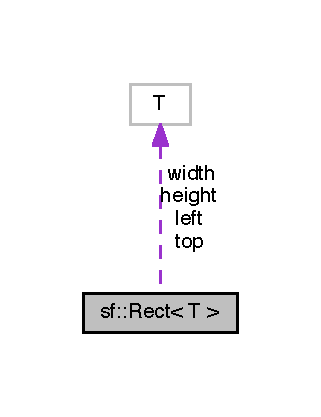
\includegraphics[width=154pt]{classsf_1_1_rect__coll__graph}
\end{center}
\end{figure}
\subsection*{Public Member Functions}
\begin{DoxyCompactItemize}
\item 
\hyperlink{classsf_1_1_rect_a0f87ebaef9722a6222fd2e04ce8efb37}{Rect} ()
\begin{DoxyCompactList}\small\item\em Default constructor. \end{DoxyCompactList}\item 
\hyperlink{classsf_1_1_rect_a15cdbc5a1aed3a8fc7be1bd5004f19f9}{Rect} (T rect\-Left, T rect\-Top, T rect\-Width, T rect\-Height)
\begin{DoxyCompactList}\small\item\em Construct the rectangle from its coordinates. \end{DoxyCompactList}\item 
\hyperlink{classsf_1_1_rect_a27fdf85caa6d12caeeff78913cc59936}{Rect} (const \hyperlink{classsf_1_1_vector2}{Vector2}$<$ T $>$ \&position, const \hyperlink{classsf_1_1_vector2}{Vector2}$<$ T $>$ \&\hyperlink{gl3_8h_a79ef9eb3e59c4bb34c4b9fbeb8d28ff7}{size})
\begin{DoxyCompactList}\small\item\em Construct the rectangle from position and size. \end{DoxyCompactList}\item 
{\footnotesize template$<$typename U $>$ }\\\hyperlink{classsf_1_1_rect_a6fff2bb7e93677839461a66bc2957de0}{Rect} (const \hyperlink{classsf_1_1_rect}{Rect}$<$ U $>$ \&rectangle)
\begin{DoxyCompactList}\small\item\em Construct the rectangle from another type of rectangle. \end{DoxyCompactList}\item 
bool \hyperlink{classsf_1_1_rect_aa8a5364c84de6dd5299f833b54e31ef1}{contains} (T \hyperlink{gl3_8h_a92d0386e5c19fb81ea88c9f99644ab1d}{x}, T \hyperlink{gl3_8h_a66ddd433d2cacfe27f5906b7e86faeed}{y}) const 
\begin{DoxyCompactList}\small\item\em Check if a point is inside the rectangle's area. \end{DoxyCompactList}\item 
bool \hyperlink{classsf_1_1_rect_a24163acdb9b2987c0ea55c201e270d41}{contains} (const \hyperlink{classsf_1_1_vector2}{Vector2}$<$ T $>$ \&point) const 
\begin{DoxyCompactList}\small\item\em Check if a point is inside the rectangle's area. \end{DoxyCompactList}\item 
bool \hyperlink{classsf_1_1_rect_a566740c8f58e01bb052266f47e7e1011}{intersects} (const \hyperlink{classsf_1_1_rect}{Rect}$<$ T $>$ \&rectangle) const 
\begin{DoxyCompactList}\small\item\em Check the intersection between two rectangles. \end{DoxyCompactList}\item 
bool \hyperlink{classsf_1_1_rect_a5f1874792b04c7e221bb786b31f5836e}{intersects} (const \hyperlink{classsf_1_1_rect}{Rect}$<$ T $>$ \&rectangle, \hyperlink{classsf_1_1_rect}{Rect}$<$ T $>$ \&intersection) const 
\begin{DoxyCompactList}\small\item\em Check the intersection between two rectangles. \end{DoxyCompactList}\item 
{\footnotesize template$<$typename T $>$ }\\\hyperlink{classsf_1_1_rect_a8fbc399054de8bbcd979e9062712896d}{Rect} ()
\item 
{\footnotesize template$<$typename T $>$ }\\\hyperlink{classsf_1_1_rect_a53956cee21c818a3355429e3662fe384}{Rect} (T rect\-Left, T rect\-Top, T rect\-Width, T rect\-Height)
\item 
{\footnotesize template$<$typename T $>$ }\\\hyperlink{classsf_1_1_rect_a7e0ea3f83003ac89b11fd45d581059cc}{Rect} (const \hyperlink{classsf_1_1_vector2}{Vector2}$<$ T $>$ \&position, const \hyperlink{classsf_1_1_vector2}{Vector2}$<$ T $>$ \&\hyperlink{gl3_8h_a79ef9eb3e59c4bb34c4b9fbeb8d28ff7}{size})
\item 
{\footnotesize template$<$typename U $>$ }\\\hyperlink{classsf_1_1_rect_a6fff2bb7e93677839461a66bc2957de0}{Rect} (const \hyperlink{classsf_1_1_rect}{Rect}$<$ U $>$ \&rectangle)
\end{DoxyCompactItemize}
\subsection*{Public Attributes}
\begin{DoxyCompactItemize}
\item 
T \hyperlink{classsf_1_1_rect_aa49960fa465103d9cb7069ceb25c7c32}{left}
\begin{DoxyCompactList}\small\item\em Left coordinate of the rectangle. \end{DoxyCompactList}\item 
T \hyperlink{classsf_1_1_rect_abd3d3a2d0ad211ef0082bd0aa1a5c0e3}{top}
\begin{DoxyCompactList}\small\item\em Top coordinate of the rectangle. \end{DoxyCompactList}\item 
T \hyperlink{classsf_1_1_rect_a4dd5b9d4333bebbc51bd309298fd500f}{width}
\begin{DoxyCompactList}\small\item\em Width of the rectangle. \end{DoxyCompactList}\item 
T \hyperlink{classsf_1_1_rect_a6fa0fc7de1636d78cae1a1b54eef95cd}{height}
\begin{DoxyCompactList}\small\item\em Height of the rectangle. \end{DoxyCompactList}\end{DoxyCompactItemize}
\subsection*{Related Functions}
(Note that these are not member functions.) \begin{DoxyCompactItemize}
\item 
{\footnotesize template$<$typename T $>$ }\\bool \hyperlink{classsf_1_1_rect_ab3488b5dbd0e587c4d7cb80605affc46}{operator==} (const \hyperlink{classsf_1_1_rect}{Rect}$<$ T $>$ \&\hyperlink{classsf_1_1_rect_aa49960fa465103d9cb7069ceb25c7c32}{left}, const \hyperlink{classsf_1_1_rect}{Rect}$<$ T $>$ \&right)
\begin{DoxyCompactList}\small\item\em Overload of binary operator ==. \end{DoxyCompactList}\item 
{\footnotesize template$<$typename T $>$ }\\bool \hyperlink{classsf_1_1_rect_a03fc4c105687b7d0f07b6b4ed4b45581}{operator!=} (const \hyperlink{classsf_1_1_rect}{Rect}$<$ T $>$ \&\hyperlink{classsf_1_1_rect_aa49960fa465103d9cb7069ceb25c7c32}{left}, const \hyperlink{classsf_1_1_rect}{Rect}$<$ T $>$ \&right)
\begin{DoxyCompactList}\small\item\em Overload of binary operator !=. \end{DoxyCompactList}\end{DoxyCompactItemize}


\subsection{Detailed Description}
\subsubsection*{template$<$typename T$>$class sf\-::\-Rect$<$ T $>$}

Utility class for manipulating 2\-D axis aligned rectangles. 

A rectangle is defined by its top-\/left corner and its size. It is a very simple class defined for convenience, so its member variables (left, top, width and height) are public and can be accessed directly, just like the vector classes (\hyperlink{classsf_1_1_vector2}{Vector2} and \hyperlink{classsf_1_1_vector3}{Vector3}).

To keep things simple, \hyperlink{classsf_1_1_rect}{sf\-::\-Rect} doesn't define functions to emulate the properties that are not directly members (such as right, bottom, center, etc.), it rather only provides intersection functions.

\hyperlink{classsf_1_1_rect}{sf\-::\-Rect} uses the usual rules for its boundaries\-: \begin{DoxyItemize}
\item The left and top edges are included in the rectangle's area \item The right (left + width) and bottom (top + height) edges are excluded from the rectangle's area\end{DoxyItemize}
This means that sf\-::\-Int\-Rect(0, 0, 1, 1) and sf\-::\-Int\-Rect(1, 1, 1, 1) don't intersect.

\hyperlink{classsf_1_1_rect}{sf\-::\-Rect} is a template and may be used with any numeric type, but for simplicity the instanciations used by S\-F\-M\-L are typedefed\-: \begin{DoxyItemize}
\item sf\-::\-Rect$<$int$>$ is \hyperlink{namespacesf_aae67411782674934f78d55fa3af18403}{sf\-::\-Int\-Rect} \item sf\-::\-Rect$<$float$>$ is \hyperlink{namespacesf_aed4e58f586b2eed2621c0365d0b7554e}{sf\-::\-Float\-Rect}\end{DoxyItemize}
So that you don't have to care about the template syntax.

Usage example\-: 
\begin{DoxyCode}
\textcolor{comment}{// Define a rectangle, located at (0, 0) with a size of 20x5}
\hyperlink{classsf_1_1_rect}{sf::IntRect} r1(0, 0, 20, 5);

\textcolor{comment}{// Define another rectangle, located at (4, 2) with a size of 18x10}
\hyperlink{classsf_1_1_vector2}{sf::Vector2i} position(4, 2);
\hyperlink{classsf_1_1_vector2}{sf::Vector2i} \hyperlink{gl3_8h_a79ef9eb3e59c4bb34c4b9fbeb8d28ff7}{size}(18, 10);
\hyperlink{classsf_1_1_rect}{sf::IntRect} r2(position, \hyperlink{gl3_8h_a79ef9eb3e59c4bb34c4b9fbeb8d28ff7}{size});

\textcolor{comment}{// Test intersections with the point (3, 1)}
\textcolor{keywordtype}{bool} b1 = r1.contains(3, 1); \textcolor{comment}{// true}
\textcolor{keywordtype}{bool} b2 = r2.contains(3, 1); \textcolor{comment}{// false}

\textcolor{comment}{// Test the intersection between r1 and r2}
\hyperlink{classsf_1_1_rect}{sf::IntRect} result;
\textcolor{keywordtype}{bool} b3 = r1.\hyperlink{classsf_1_1_rect_a566740c8f58e01bb052266f47e7e1011}{intersects}(r2, result); \textcolor{comment}{// true}
\textcolor{comment}{// result == (4, 2, 16, 3)}
\end{DoxyCode}
 

Definition at line 42 of file Rect.\-hpp.



\subsection{Constructor \& Destructor Documentation}
\hypertarget{classsf_1_1_rect_a0f87ebaef9722a6222fd2e04ce8efb37}{\index{sf\-::\-Rect@{sf\-::\-Rect}!Rect@{Rect}}
\index{Rect@{Rect}!sf::Rect@{sf\-::\-Rect}}
\subsubsection[{Rect}]{\setlength{\rightskip}{0pt plus 5cm}template$<$typename T$>$ {\bf sf\-::\-Rect}$<$ T $>$\-::{\bf Rect} (
\begin{DoxyParamCaption}
{}
\end{DoxyParamCaption}
)}}\label{classsf_1_1_rect_a0f87ebaef9722a6222fd2e04ce8efb37}


Default constructor. 

Creates an empty rectangle (it is equivalent to calling Rect(0, 0, 0, 0)). \hypertarget{classsf_1_1_rect_a15cdbc5a1aed3a8fc7be1bd5004f19f9}{\index{sf\-::\-Rect@{sf\-::\-Rect}!Rect@{Rect}}
\index{Rect@{Rect}!sf::Rect@{sf\-::\-Rect}}
\subsubsection[{Rect}]{\setlength{\rightskip}{0pt plus 5cm}template$<$typename T$>$ {\bf sf\-::\-Rect}$<$ T $>$\-::{\bf Rect} (
\begin{DoxyParamCaption}
\item[{T}]{rect\-Left, }
\item[{T}]{rect\-Top, }
\item[{T}]{rect\-Width, }
\item[{T}]{rect\-Height}
\end{DoxyParamCaption}
)}}\label{classsf_1_1_rect_a15cdbc5a1aed3a8fc7be1bd5004f19f9}


Construct the rectangle from its coordinates. 

Be careful, the last two parameters are the width and height, not the right and bottom coordinates!


\begin{DoxyParams}{Parameters}
{\em rect\-Left} & Left coordinate of the rectangle \\
\hline
{\em rect\-Top} & Top coordinate of the rectangle \\
\hline
{\em rect\-Width} & Width of the rectangle \\
\hline
{\em rect\-Height} & Height of the rectangle \\
\hline
\end{DoxyParams}
\hypertarget{classsf_1_1_rect_a27fdf85caa6d12caeeff78913cc59936}{\index{sf\-::\-Rect@{sf\-::\-Rect}!Rect@{Rect}}
\index{Rect@{Rect}!sf::Rect@{sf\-::\-Rect}}
\subsubsection[{Rect}]{\setlength{\rightskip}{0pt plus 5cm}template$<$typename T$>$ {\bf sf\-::\-Rect}$<$ T $>$\-::{\bf Rect} (
\begin{DoxyParamCaption}
\item[{const {\bf Vector2}$<$ T $>$ \&}]{position, }
\item[{const {\bf Vector2}$<$ T $>$ \&}]{size}
\end{DoxyParamCaption}
)}}\label{classsf_1_1_rect_a27fdf85caa6d12caeeff78913cc59936}


Construct the rectangle from position and size. 

Be careful, the last parameter is the size, not the bottom-\/right corner!


\begin{DoxyParams}{Parameters}
{\em position} & Position of the top-\/left corner of the rectangle \\
\hline
{\em size} & Size of the rectangle \\
\hline
\end{DoxyParams}
\hypertarget{classsf_1_1_rect_a6fff2bb7e93677839461a66bc2957de0}{\index{sf\-::\-Rect@{sf\-::\-Rect}!Rect@{Rect}}
\index{Rect@{Rect}!sf::Rect@{sf\-::\-Rect}}
\subsubsection[{Rect}]{\setlength{\rightskip}{0pt plus 5cm}template$<$typename T$>$ template$<$typename U $>$ {\bf sf\-::\-Rect}$<$ T $>$\-::{\bf Rect} (
\begin{DoxyParamCaption}
\item[{const {\bf Rect}$<$ U $>$ \&}]{rectangle}
\end{DoxyParamCaption}
)\hspace{0.3cm}{\ttfamily [explicit]}}}\label{classsf_1_1_rect_a6fff2bb7e93677839461a66bc2957de0}


Construct the rectangle from another type of rectangle. 

This constructor doesn't replace the copy constructor, it's called only when U != T. A call to this constructor will fail to compile if U is not convertible to T.


\begin{DoxyParams}{Parameters}
{\em rectangle} & Rectangle to convert \\
\hline
\end{DoxyParams}
\hypertarget{classsf_1_1_rect_a8fbc399054de8bbcd979e9062712896d}{\index{sf\-::\-Rect@{sf\-::\-Rect}!Rect@{Rect}}
\index{Rect@{Rect}!sf::Rect@{sf\-::\-Rect}}
\subsubsection[{Rect}]{\setlength{\rightskip}{0pt plus 5cm}template$<$typename T$>$ template$<$typename T $>$ {\bf sf\-::\-Rect}$<$ T $>$\-::{\bf Rect} (
\begin{DoxyParamCaption}
{}
\end{DoxyParamCaption}
)}}\label{classsf_1_1_rect_a8fbc399054de8bbcd979e9062712896d}


Definition at line 28 of file Rect.\-inl.

\hypertarget{classsf_1_1_rect_a53956cee21c818a3355429e3662fe384}{\index{sf\-::\-Rect@{sf\-::\-Rect}!Rect@{Rect}}
\index{Rect@{Rect}!sf::Rect@{sf\-::\-Rect}}
\subsubsection[{Rect}]{\setlength{\rightskip}{0pt plus 5cm}template$<$typename T$>$ template$<$typename T $>$ {\bf sf\-::\-Rect}$<$ T $>$\-::{\bf Rect} (
\begin{DoxyParamCaption}
\item[{T}]{rect\-Left, }
\item[{T}]{rect\-Top, }
\item[{T}]{rect\-Width, }
\item[{T}]{rect\-Height}
\end{DoxyParamCaption}
)}}\label{classsf_1_1_rect_a53956cee21c818a3355429e3662fe384}


Definition at line 40 of file Rect.\-inl.

\hypertarget{classsf_1_1_rect_a7e0ea3f83003ac89b11fd45d581059cc}{\index{sf\-::\-Rect@{sf\-::\-Rect}!Rect@{Rect}}
\index{Rect@{Rect}!sf::Rect@{sf\-::\-Rect}}
\subsubsection[{Rect}]{\setlength{\rightskip}{0pt plus 5cm}template$<$typename T$>$ template$<$typename T $>$ {\bf sf\-::\-Rect}$<$ T $>$\-::{\bf Rect} (
\begin{DoxyParamCaption}
\item[{const {\bf Vector2}$<$ T $>$ \&}]{position, }
\item[{const {\bf Vector2}$<$ T $>$ \&}]{size}
\end{DoxyParamCaption}
)}}\label{classsf_1_1_rect_a7e0ea3f83003ac89b11fd45d581059cc}


Definition at line 52 of file Rect.\-inl.

\hypertarget{classsf_1_1_rect_a6fff2bb7e93677839461a66bc2957de0}{\index{sf\-::\-Rect@{sf\-::\-Rect}!Rect@{Rect}}
\index{Rect@{Rect}!sf::Rect@{sf\-::\-Rect}}
\subsubsection[{Rect}]{\setlength{\rightskip}{0pt plus 5cm}template$<$typename T$>$ template$<$typename U $>$ {\bf sf\-::\-Rect}$<$ T $>$\-::{\bf Rect} (
\begin{DoxyParamCaption}
\item[{const {\bf Rect}$<$ U $>$ \&}]{rectangle}
\end{DoxyParamCaption}
)}}\label{classsf_1_1_rect_a6fff2bb7e93677839461a66bc2957de0}


Definition at line 65 of file Rect.\-inl.



\subsection{Member Function Documentation}
\hypertarget{classsf_1_1_rect_aa8a5364c84de6dd5299f833b54e31ef1}{\index{sf\-::\-Rect@{sf\-::\-Rect}!contains@{contains}}
\index{contains@{contains}!sf::Rect@{sf\-::\-Rect}}
\subsubsection[{contains}]{\setlength{\rightskip}{0pt plus 5cm}template$<$typename T$>$ bool {\bf sf\-::\-Rect}$<$ T $>$\-::contains (
\begin{DoxyParamCaption}
\item[{T}]{x, }
\item[{T}]{y}
\end{DoxyParamCaption}
) const}}\label{classsf_1_1_rect_aa8a5364c84de6dd5299f833b54e31ef1}


Check if a point is inside the rectangle's area. 


\begin{DoxyParams}{Parameters}
{\em x} & X coordinate of the point to test \\
\hline
{\em y} & Y coordinate of the point to test\\
\hline
\end{DoxyParams}
\begin{DoxyReturn}{Returns}
True if the point is inside, false otherwise
\end{DoxyReturn}
\begin{DoxySeeAlso}{See Also}
\hyperlink{classsf_1_1_rect_a566740c8f58e01bb052266f47e7e1011}{intersects} 
\end{DoxySeeAlso}
\hypertarget{classsf_1_1_rect_a24163acdb9b2987c0ea55c201e270d41}{\index{sf\-::\-Rect@{sf\-::\-Rect}!contains@{contains}}
\index{contains@{contains}!sf::Rect@{sf\-::\-Rect}}
\subsubsection[{contains}]{\setlength{\rightskip}{0pt plus 5cm}template$<$typename T$>$ bool {\bf sf\-::\-Rect}$<$ T $>$\-::contains (
\begin{DoxyParamCaption}
\item[{const {\bf Vector2}$<$ T $>$ \&}]{point}
\end{DoxyParamCaption}
) const}}\label{classsf_1_1_rect_a24163acdb9b2987c0ea55c201e270d41}


Check if a point is inside the rectangle's area. 


\begin{DoxyParams}{Parameters}
{\em point} & Point to test\\
\hline
\end{DoxyParams}
\begin{DoxyReturn}{Returns}
True if the point is inside, false otherwise
\end{DoxyReturn}
\begin{DoxySeeAlso}{See Also}
\hyperlink{classsf_1_1_rect_a566740c8f58e01bb052266f47e7e1011}{intersects} 
\end{DoxySeeAlso}
\hypertarget{classsf_1_1_rect_a566740c8f58e01bb052266f47e7e1011}{\index{sf\-::\-Rect@{sf\-::\-Rect}!intersects@{intersects}}
\index{intersects@{intersects}!sf::Rect@{sf\-::\-Rect}}
\subsubsection[{intersects}]{\setlength{\rightskip}{0pt plus 5cm}template$<$typename T$>$ bool {\bf sf\-::\-Rect}$<$ T $>$\-::intersects (
\begin{DoxyParamCaption}
\item[{const {\bf Rect}$<$ T $>$ \&}]{rectangle}
\end{DoxyParamCaption}
) const}}\label{classsf_1_1_rect_a566740c8f58e01bb052266f47e7e1011}


Check the intersection between two rectangles. 


\begin{DoxyParams}{Parameters}
{\em rectangle} & Rectangle to test\\
\hline
\end{DoxyParams}
\begin{DoxyReturn}{Returns}
True if rectangles overlap, false otherwise
\end{DoxyReturn}
\begin{DoxySeeAlso}{See Also}
\hyperlink{classsf_1_1_rect_aa8a5364c84de6dd5299f833b54e31ef1}{contains} 
\end{DoxySeeAlso}
\hypertarget{classsf_1_1_rect_a5f1874792b04c7e221bb786b31f5836e}{\index{sf\-::\-Rect@{sf\-::\-Rect}!intersects@{intersects}}
\index{intersects@{intersects}!sf::Rect@{sf\-::\-Rect}}
\subsubsection[{intersects}]{\setlength{\rightskip}{0pt plus 5cm}template$<$typename T$>$ bool {\bf sf\-::\-Rect}$<$ T $>$\-::intersects (
\begin{DoxyParamCaption}
\item[{const {\bf Rect}$<$ T $>$ \&}]{rectangle, }
\item[{{\bf Rect}$<$ T $>$ \&}]{intersection}
\end{DoxyParamCaption}
) const}}\label{classsf_1_1_rect_a5f1874792b04c7e221bb786b31f5836e}


Check the intersection between two rectangles. 

This overload returns the overlapped rectangle in the {\itshape intersection} parameter.


\begin{DoxyParams}{Parameters}
{\em rectangle} & Rectangle to test \\
\hline
{\em intersection} & Rectangle to be filled with the intersection\\
\hline
\end{DoxyParams}
\begin{DoxyReturn}{Returns}
True if rectangles overlap, false otherwise
\end{DoxyReturn}
\begin{DoxySeeAlso}{See Also}
\hyperlink{classsf_1_1_rect_aa8a5364c84de6dd5299f833b54e31ef1}{contains} 
\end{DoxySeeAlso}


\subsection{Friends And Related Function Documentation}
\hypertarget{classsf_1_1_rect_a03fc4c105687b7d0f07b6b4ed4b45581}{\index{sf\-::\-Rect@{sf\-::\-Rect}!operator!=@{operator!=}}
\index{operator!=@{operator!=}!sf::Rect@{sf\-::\-Rect}}
\subsubsection[{operator!=}]{\setlength{\rightskip}{0pt plus 5cm}template$<$typename T $>$ bool operator!= (
\begin{DoxyParamCaption}
\item[{const {\bf Rect}$<$ T $>$ \&}]{left, }
\item[{const {\bf Rect}$<$ T $>$ \&}]{right}
\end{DoxyParamCaption}
)\hspace{0.3cm}{\ttfamily [related]}}}\label{classsf_1_1_rect_a03fc4c105687b7d0f07b6b4ed4b45581}


Overload of binary operator !=. 

This operator compares strict difference between two rectangles.


\begin{DoxyParams}{Parameters}
{\em left} & Left operand (a rectangle) \\
\hline
{\em right} & Right operand (a rectangle)\\
\hline
\end{DoxyParams}
\begin{DoxyReturn}{Returns}
True if {\itshape left} is not equal to {\itshape right} 
\end{DoxyReturn}
\hypertarget{classsf_1_1_rect_ab3488b5dbd0e587c4d7cb80605affc46}{\index{sf\-::\-Rect@{sf\-::\-Rect}!operator==@{operator==}}
\index{operator==@{operator==}!sf::Rect@{sf\-::\-Rect}}
\subsubsection[{operator==}]{\setlength{\rightskip}{0pt plus 5cm}template$<$typename T $>$ bool operator== (
\begin{DoxyParamCaption}
\item[{const {\bf Rect}$<$ T $>$ \&}]{left, }
\item[{const {\bf Rect}$<$ T $>$ \&}]{right}
\end{DoxyParamCaption}
)\hspace{0.3cm}{\ttfamily [related]}}}\label{classsf_1_1_rect_ab3488b5dbd0e587c4d7cb80605affc46}


Overload of binary operator ==. 

This operator compares strict equality between two rectangles.


\begin{DoxyParams}{Parameters}
{\em left} & Left operand (a rectangle) \\
\hline
{\em right} & Right operand (a rectangle)\\
\hline
\end{DoxyParams}
\begin{DoxyReturn}{Returns}
True if {\itshape left} is equal to {\itshape right} 
\end{DoxyReturn}


\subsection{Member Data Documentation}
\hypertarget{classsf_1_1_rect_a6fa0fc7de1636d78cae1a1b54eef95cd}{\index{sf\-::\-Rect@{sf\-::\-Rect}!height@{height}}
\index{height@{height}!sf::Rect@{sf\-::\-Rect}}
\subsubsection[{height}]{\setlength{\rightskip}{0pt plus 5cm}template$<$typename T$>$ T {\bf sf\-::\-Rect}$<$ T $>$\-::{\bf height}}}\label{classsf_1_1_rect_a6fa0fc7de1636d78cae1a1b54eef95cd}


Height of the rectangle. 



Definition at line 154 of file Rect.\-hpp.

\hypertarget{classsf_1_1_rect_aa49960fa465103d9cb7069ceb25c7c32}{\index{sf\-::\-Rect@{sf\-::\-Rect}!left@{left}}
\index{left@{left}!sf::Rect@{sf\-::\-Rect}}
\subsubsection[{left}]{\setlength{\rightskip}{0pt plus 5cm}template$<$typename T$>$ T {\bf sf\-::\-Rect}$<$ T $>$\-::left}}\label{classsf_1_1_rect_aa49960fa465103d9cb7069ceb25c7c32}


Left coordinate of the rectangle. 



Definition at line 151 of file Rect.\-hpp.

\hypertarget{classsf_1_1_rect_abd3d3a2d0ad211ef0082bd0aa1a5c0e3}{\index{sf\-::\-Rect@{sf\-::\-Rect}!top@{top}}
\index{top@{top}!sf::Rect@{sf\-::\-Rect}}
\subsubsection[{top}]{\setlength{\rightskip}{0pt plus 5cm}template$<$typename T$>$ T {\bf sf\-::\-Rect}$<$ T $>$\-::top}}\label{classsf_1_1_rect_abd3d3a2d0ad211ef0082bd0aa1a5c0e3}


Top coordinate of the rectangle. 



Definition at line 152 of file Rect.\-hpp.

\hypertarget{classsf_1_1_rect_a4dd5b9d4333bebbc51bd309298fd500f}{\index{sf\-::\-Rect@{sf\-::\-Rect}!width@{width}}
\index{width@{width}!sf::Rect@{sf\-::\-Rect}}
\subsubsection[{width}]{\setlength{\rightskip}{0pt plus 5cm}template$<$typename T$>$ T {\bf sf\-::\-Rect}$<$ T $>$\-::{\bf width}}}\label{classsf_1_1_rect_a4dd5b9d4333bebbc51bd309298fd500f}


Width of the rectangle. 



Definition at line 153 of file Rect.\-hpp.



The documentation for this class was generated from the following files\-:\begin{DoxyCompactItemize}
\item 
/\-Users/ira/\-Dropbox/ira\-\_\-dev/protobyte\-\_\-research/other\-\_\-libs/\-S\-F\-M\-L/dylibs/root/usr/local/include/\-S\-F\-M\-L/\-Graphics/\hyperlink{_rect_8hpp}{Rect.\-hpp}\item 
/\-Users/ira/\-Dropbox/ira\-\_\-dev/protobyte\-\_\-research/other\-\_\-libs/\-S\-F\-M\-L/dylibs/root/usr/local/include/\-S\-F\-M\-L/\-Graphics/\hyperlink{_rect_8inl}{Rect.\-inl}\end{DoxyCompactItemize}

\hypertarget{classsf_1_1_rectangle_shape}{\section{sf\-:\-:Rectangle\-Shape Class Reference}
\label{classsf_1_1_rectangle_shape}\index{sf\-::\-Rectangle\-Shape@{sf\-::\-Rectangle\-Shape}}
}


Specialized shape representing a rectangle.  




{\ttfamily \#include $<$Rectangle\-Shape.\-hpp$>$}



Inheritance diagram for sf\-:\-:Rectangle\-Shape\-:
\nopagebreak
\begin{figure}[H]
\begin{center}
\leavevmode
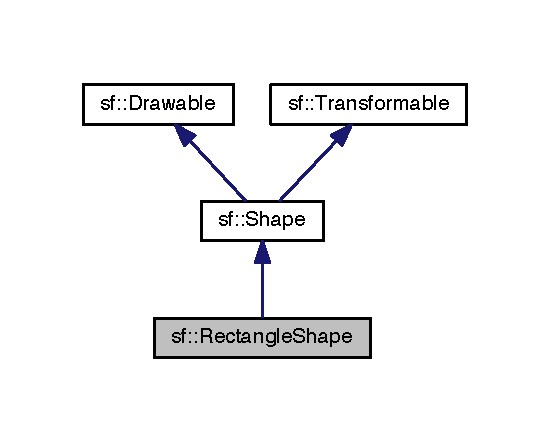
\includegraphics[width=264pt]{classsf_1_1_rectangle_shape__inherit__graph}
\end{center}
\end{figure}


Collaboration diagram for sf\-:\-:Rectangle\-Shape\-:
\nopagebreak
\begin{figure}[H]
\begin{center}
\leavevmode
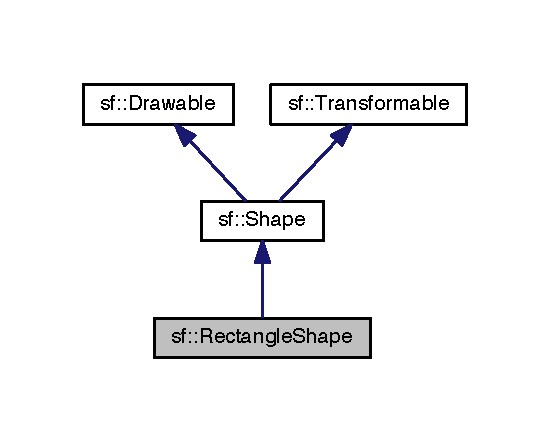
\includegraphics[width=264pt]{classsf_1_1_rectangle_shape__coll__graph}
\end{center}
\end{figure}
\subsection*{Public Member Functions}
\begin{DoxyCompactItemize}
\item 
\hyperlink{classsf_1_1_rectangle_shape_a83a2be157ebee85c95ed491c3e78dd7c}{Rectangle\-Shape} (const \hyperlink{namespacesf_acf03098c2577b869e2fa6836cc48f1a0}{Vector2f} \&\hyperlink{gl3_8h_a79ef9eb3e59c4bb34c4b9fbeb8d28ff7}{size}=\hyperlink{namespacesf_acf03098c2577b869e2fa6836cc48f1a0}{Vector2f}(0, 0))
\begin{DoxyCompactList}\small\item\em Default constructor. \end{DoxyCompactList}\item 
\hyperlink{glutf90_8h_ac778d6f63f1aaf8ebda0ce6ac821b56e}{void} \hyperlink{classsf_1_1_rectangle_shape_a5c65d374d4a259dfdc24efdd24a5dbec}{set\-Size} (const \hyperlink{namespacesf_acf03098c2577b869e2fa6836cc48f1a0}{Vector2f} \&\hyperlink{gl3_8h_a79ef9eb3e59c4bb34c4b9fbeb8d28ff7}{size})
\begin{DoxyCompactList}\small\item\em Set the size of the rectangle. \end{DoxyCompactList}\item 
const \hyperlink{namespacesf_acf03098c2577b869e2fa6836cc48f1a0}{Vector2f} \& \hyperlink{classsf_1_1_rectangle_shape_acaacbaee87c38a526a9d895742faab54}{get\-Size} () const 
\begin{DoxyCompactList}\small\item\em Get the size of the rectangle. \end{DoxyCompactList}\item 
virtual unsigned int \hyperlink{classsf_1_1_rectangle_shape_a439f5a92583baf972878c836b73bf955}{get\-Point\-Count} () const 
\begin{DoxyCompactList}\small\item\em Get the number of points defining the shape. \end{DoxyCompactList}\item 
virtual \hyperlink{namespacesf_acf03098c2577b869e2fa6836cc48f1a0}{Vector2f} \hyperlink{classsf_1_1_rectangle_shape_a3994f7f937d6332fe64b6990d5bc43a1}{get\-Point} (unsigned int \hyperlink{gl3_8h_a57f14e05b1900f16a2da82ade47d0c6d}{index}) const 
\begin{DoxyCompactList}\small\item\em Get a point of the shape. \end{DoxyCompactList}\end{DoxyCompactItemize}
\subsection*{Additional Inherited Members}


\subsection{Detailed Description}
Specialized shape representing a rectangle. 

This class inherits all the functions of \hyperlink{classsf_1_1_transformable}{sf\-::\-Transformable} (position, rotation, scale, bounds, ...) as well as the functions of \hyperlink{classsf_1_1_shape}{sf\-::\-Shape} (outline, color, texture, ...).

Usage example\-: 
\begin{DoxyCode}
\hyperlink{classsf_1_1_rectangle_shape}{sf::RectangleShape} rectangle;
rectangle.\hyperlink{classsf_1_1_rectangle_shape_a5c65d374d4a259dfdc24efdd24a5dbec}{setSize}(\hyperlink{classsf_1_1_vector2}{sf::Vector2f}(100, 50));
rectangle.\hyperlink{classsf_1_1_shape_a5978f41ee349ac3c52942996dcb184f7}{setOutlineColor}(\hyperlink{classsf_1_1_color_a127dbf55db9c07d0fa8f4bfcbb97594a}{sf::Color::Red});
rectangle.\hyperlink{classsf_1_1_shape_a5ad336ad74fc1f567fce3b7e44cf87dc}{setOutlineThickness}(5);
rectangle.\hyperlink{classsf_1_1_transformable_a4dbfb1a7c80688b0b4c477d706550208}{setPosition}(10, 20);
...
window.draw(rectangle);
\end{DoxyCode}


\begin{DoxySeeAlso}{See Also}
\hyperlink{classsf_1_1_shape}{sf\-::\-Shape}, \hyperlink{classsf_1_1_circle_shape}{sf\-::\-Circle\-Shape}, \hyperlink{classsf_1_1_convex_shape}{sf\-::\-Convex\-Shape} 
\end{DoxySeeAlso}


Definition at line 41 of file Rectangle\-Shape.\-hpp.



\subsection{Constructor \& Destructor Documentation}
\hypertarget{classsf_1_1_rectangle_shape_a83a2be157ebee85c95ed491c3e78dd7c}{\index{sf\-::\-Rectangle\-Shape@{sf\-::\-Rectangle\-Shape}!Rectangle\-Shape@{Rectangle\-Shape}}
\index{Rectangle\-Shape@{Rectangle\-Shape}!sf::RectangleShape@{sf\-::\-Rectangle\-Shape}}
\subsubsection[{Rectangle\-Shape}]{\setlength{\rightskip}{0pt plus 5cm}sf\-::\-Rectangle\-Shape\-::\-Rectangle\-Shape (
\begin{DoxyParamCaption}
\item[{const {\bf Vector2f} \&}]{size = {\ttfamily {\bf Vector2f}(0,~0)}}
\end{DoxyParamCaption}
)\hspace{0.3cm}{\ttfamily [explicit]}}}\label{classsf_1_1_rectangle_shape_a83a2be157ebee85c95ed491c3e78dd7c}


Default constructor. 


\begin{DoxyParams}{Parameters}
{\em size} & Size of the rectangle \\
\hline
\end{DoxyParams}


\subsection{Member Function Documentation}
\hypertarget{classsf_1_1_rectangle_shape_a3994f7f937d6332fe64b6990d5bc43a1}{\index{sf\-::\-Rectangle\-Shape@{sf\-::\-Rectangle\-Shape}!get\-Point@{get\-Point}}
\index{get\-Point@{get\-Point}!sf::RectangleShape@{sf\-::\-Rectangle\-Shape}}
\subsubsection[{get\-Point}]{\setlength{\rightskip}{0pt plus 5cm}virtual {\bf Vector2f} sf\-::\-Rectangle\-Shape\-::get\-Point (
\begin{DoxyParamCaption}
\item[{unsigned int}]{index}
\end{DoxyParamCaption}
) const\hspace{0.3cm}{\ttfamily [virtual]}}}\label{classsf_1_1_rectangle_shape_a3994f7f937d6332fe64b6990d5bc43a1}


Get a point of the shape. 

The result is undefined if {\itshape index} is out of the valid range.


\begin{DoxyParams}{Parameters}
{\em index} & Index of the point to get, in range \mbox{[}0 .. Get\-Point\-Count() -\/ 1\mbox{]}\\
\hline
\end{DoxyParams}
\begin{DoxyReturn}{Returns}
Index-\/th point of the shape 
\end{DoxyReturn}


Implements \hyperlink{classsf_1_1_shape_a397f3b4cdb7ad98cdc6c034816c652d2}{sf\-::\-Shape}.

\hypertarget{classsf_1_1_rectangle_shape_a439f5a92583baf972878c836b73bf955}{\index{sf\-::\-Rectangle\-Shape@{sf\-::\-Rectangle\-Shape}!get\-Point\-Count@{get\-Point\-Count}}
\index{get\-Point\-Count@{get\-Point\-Count}!sf::RectangleShape@{sf\-::\-Rectangle\-Shape}}
\subsubsection[{get\-Point\-Count}]{\setlength{\rightskip}{0pt plus 5cm}virtual unsigned int sf\-::\-Rectangle\-Shape\-::get\-Point\-Count (
\begin{DoxyParamCaption}
{}
\end{DoxyParamCaption}
) const\hspace{0.3cm}{\ttfamily [virtual]}}}\label{classsf_1_1_rectangle_shape_a439f5a92583baf972878c836b73bf955}


Get the number of points defining the shape. 

\begin{DoxyReturn}{Returns}
Number of points of the shape 
\end{DoxyReturn}


Implements \hyperlink{classsf_1_1_shape_ad84e1b675ecd270ad8151aea4e271a78}{sf\-::\-Shape}.

\hypertarget{classsf_1_1_rectangle_shape_acaacbaee87c38a526a9d895742faab54}{\index{sf\-::\-Rectangle\-Shape@{sf\-::\-Rectangle\-Shape}!get\-Size@{get\-Size}}
\index{get\-Size@{get\-Size}!sf::RectangleShape@{sf\-::\-Rectangle\-Shape}}
\subsubsection[{get\-Size}]{\setlength{\rightskip}{0pt plus 5cm}const {\bf Vector2f}\& sf\-::\-Rectangle\-Shape\-::get\-Size (
\begin{DoxyParamCaption}
{}
\end{DoxyParamCaption}
) const}}\label{classsf_1_1_rectangle_shape_acaacbaee87c38a526a9d895742faab54}


Get the size of the rectangle. 

\begin{DoxyReturn}{Returns}
Size of the rectangle
\end{DoxyReturn}
\begin{DoxySeeAlso}{See Also}
\hyperlink{classsf_1_1_rectangle_shape_a5c65d374d4a259dfdc24efdd24a5dbec}{set\-Size} 
\end{DoxySeeAlso}
\hypertarget{classsf_1_1_rectangle_shape_a5c65d374d4a259dfdc24efdd24a5dbec}{\index{sf\-::\-Rectangle\-Shape@{sf\-::\-Rectangle\-Shape}!set\-Size@{set\-Size}}
\index{set\-Size@{set\-Size}!sf::RectangleShape@{sf\-::\-Rectangle\-Shape}}
\subsubsection[{set\-Size}]{\setlength{\rightskip}{0pt plus 5cm}{\bf void} sf\-::\-Rectangle\-Shape\-::set\-Size (
\begin{DoxyParamCaption}
\item[{const {\bf Vector2f} \&}]{size}
\end{DoxyParamCaption}
)}}\label{classsf_1_1_rectangle_shape_a5c65d374d4a259dfdc24efdd24a5dbec}


Set the size of the rectangle. 


\begin{DoxyParams}{Parameters}
{\em size} & New size of the rectangle\\
\hline
\end{DoxyParams}
\begin{DoxySeeAlso}{See Also}
\hyperlink{classsf_1_1_rectangle_shape_acaacbaee87c38a526a9d895742faab54}{get\-Size} 
\end{DoxySeeAlso}


The documentation for this class was generated from the following file\-:\begin{DoxyCompactItemize}
\item 
/\-Users/ira/\-Dropbox/ira\-\_\-dev/protobyte\-\_\-research/other\-\_\-libs/\-S\-F\-M\-L/dylibs/root/usr/local/include/\-S\-F\-M\-L/\-Graphics/\hyperlink{_rectangle_shape_8hpp}{Rectangle\-Shape.\-hpp}\end{DoxyCompactItemize}

\hypertarget{classsf_1_1_render_states}{\section{sf\-:\-:Render\-States Class Reference}
\label{classsf_1_1_render_states}\index{sf\-::\-Render\-States@{sf\-::\-Render\-States}}
}


Define the states used for drawing to a \hyperlink{classsf_1_1_render_target}{Render\-Target}.  




{\ttfamily \#include $<$Render\-States.\-hpp$>$}



Collaboration diagram for sf\-:\-:Render\-States\-:
\nopagebreak
\begin{figure}[H]
\begin{center}
\leavevmode
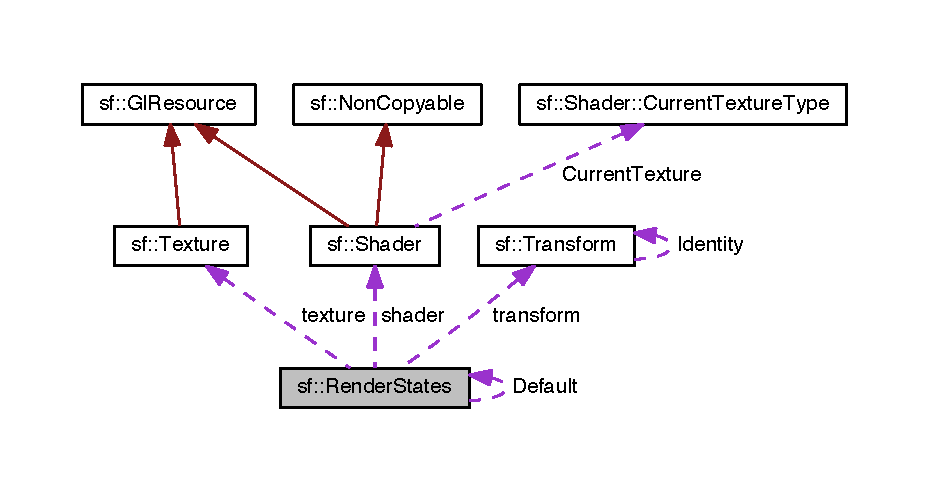
\includegraphics[width=350pt]{classsf_1_1_render_states__coll__graph}
\end{center}
\end{figure}
\subsection*{Public Member Functions}
\begin{DoxyCompactItemize}
\item 
\hyperlink{classsf_1_1_render_states_a885bf14070d0d5391f062f62b270b7d0}{Render\-States} ()
\begin{DoxyCompactList}\small\item\em Default constructor. \end{DoxyCompactList}\item 
\hyperlink{classsf_1_1_render_states_a4e3378a224f67513b95d58184e85210c}{Render\-States} (\hyperlink{group__graphics_ga80c52fe2f7050d7f7573b7ed3c995388}{Blend\-Mode} the\-Blend\-Mode)
\begin{DoxyCompactList}\small\item\em Construct a default set of render states with a custom blend mode. \end{DoxyCompactList}\item 
\hyperlink{classsf_1_1_render_states_a3e99cad6ab05971d40357949930ed890}{Render\-States} (const \hyperlink{classsf_1_1_transform}{Transform} \&the\-Transform)
\begin{DoxyCompactList}\small\item\em Construct a default set of render states with a custom transform. \end{DoxyCompactList}\item 
\hyperlink{classsf_1_1_render_states_a8f4ca3be0e27dafea0c4ab8547439bb1}{Render\-States} (const \hyperlink{classsf_1_1_texture}{Texture} $\ast$the\-Texture)
\begin{DoxyCompactList}\small\item\em Construct a default set of render states with a custom texture. \end{DoxyCompactList}\item 
\hyperlink{classsf_1_1_render_states_a39f94233f464739d8d8522f3aefe97d0}{Render\-States} (const \hyperlink{classsf_1_1_shader}{Shader} $\ast$the\-Shader)
\begin{DoxyCompactList}\small\item\em Construct a default set of render states with a custom shader. \end{DoxyCompactList}\item 
\hyperlink{classsf_1_1_render_states_ae508c91ac7b8992dc22b8d8a4027ad09}{Render\-States} (\hyperlink{group__graphics_ga80c52fe2f7050d7f7573b7ed3c995388}{Blend\-Mode} the\-Blend\-Mode, const \hyperlink{classsf_1_1_transform}{Transform} \&the\-Transform, const \hyperlink{classsf_1_1_texture}{Texture} $\ast$the\-Texture, const \hyperlink{classsf_1_1_shader}{Shader} $\ast$the\-Shader)
\begin{DoxyCompactList}\small\item\em Construct a set of render states with all its attributes. \end{DoxyCompactList}\end{DoxyCompactItemize}
\subsection*{Public Attributes}
\begin{DoxyCompactItemize}
\item 
\hyperlink{group__graphics_ga80c52fe2f7050d7f7573b7ed3c995388}{Blend\-Mode} \hyperlink{classsf_1_1_render_states_ad6ac87f1b5006dae7ebfee4b5d40f5a8}{blend\-Mode}
\begin{DoxyCompactList}\small\item\em Blending mode. \end{DoxyCompactList}\item 
\hyperlink{classsf_1_1_transform}{Transform} \hyperlink{classsf_1_1_render_states_a1f737981a0f2f0d4bb8dac866a8d1149}{transform}
\begin{DoxyCompactList}\small\item\em \hyperlink{classsf_1_1_transform}{Transform}. \end{DoxyCompactList}\item 
const \hyperlink{classsf_1_1_texture}{Texture} $\ast$ \hyperlink{classsf_1_1_render_states_a457fc5a41731889de9cf39cf9b3436c3}{texture}
\begin{DoxyCompactList}\small\item\em \hyperlink{classsf_1_1_texture}{Texture}. \end{DoxyCompactList}\item 
const \hyperlink{classsf_1_1_shader}{Shader} $\ast$ \hyperlink{classsf_1_1_render_states_ad4f79ecdd0c60ed0d24fbe555b221bd8}{shader}
\begin{DoxyCompactList}\small\item\em \hyperlink{classsf_1_1_shader}{Shader}. \end{DoxyCompactList}\end{DoxyCompactItemize}
\subsection*{Static Public Attributes}
\begin{DoxyCompactItemize}
\item 
static const \hyperlink{classsf_1_1_render_states}{Render\-States} \hyperlink{classsf_1_1_render_states_ad29672df29f19ce50c3021d95f2bb062}{Default}
\begin{DoxyCompactList}\small\item\em Special instance holding the default render states. \end{DoxyCompactList}\end{DoxyCompactItemize}


\subsection{Detailed Description}
Define the states used for drawing to a \hyperlink{classsf_1_1_render_target}{Render\-Target}. 

There are four global states that can be applied to the drawn objects\-: \begin{DoxyItemize}
\item the blend mode\-: how pixels of the object are blended with the background \item the transform\-: how the object is positioned/rotated/scaled \item the texture\-: what image is mapped to the object \item the shader\-: what custom effect is applied to the object\end{DoxyItemize}
High-\/level objects such as sprites or text force some of these states when they are drawn. For example, a sprite will set its own texture, so that you don't have to care about it when drawing the sprite.

The transform is a special case\-: sprites, texts and shapes (and it's a good idea to do it with your own drawable classes too) combine their transform with the one that is passed in the \hyperlink{classsf_1_1_render_states}{Render\-States} structure. So that you can use a \char`\"{}global\char`\"{} transform on top of each object's transform.

Most objects, especially high-\/level drawables, can be drawn directly without defining render states explicitely -- the default set of states is ok in most cases. 
\begin{DoxyCode}
window.Draw(sprite);
\end{DoxyCode}


If you want to use a single specific render state, for example a shader, you can pass it directly to the Draw function\-: \hyperlink{classsf_1_1_render_states}{sf\-::\-Render\-States} has an implicit one-\/argument constructor for each state. 
\begin{DoxyCode}
window.draw(sprite, \hyperlink{gl3_8h_a57b2a96adb1d51204909a82d861e395e}{shader});
\end{DoxyCode}


When you're inside the Draw function of a drawable object (inherited from \hyperlink{classsf_1_1_drawable}{sf\-::\-Drawable}), you can either pass the render states unmodified, or change some of them. For example, a transformable object will combine the current transform with its own transform. A sprite will set its texture. Etc.

\begin{DoxySeeAlso}{See Also}
\hyperlink{classsf_1_1_render_target}{sf\-::\-Render\-Target}, \hyperlink{classsf_1_1_drawable}{sf\-::\-Drawable} 
\end{DoxySeeAlso}


Definition at line 45 of file Render\-States.\-hpp.



\subsection{Constructor \& Destructor Documentation}
\hypertarget{classsf_1_1_render_states_a885bf14070d0d5391f062f62b270b7d0}{\index{sf\-::\-Render\-States@{sf\-::\-Render\-States}!Render\-States@{Render\-States}}
\index{Render\-States@{Render\-States}!sf::RenderStates@{sf\-::\-Render\-States}}
\subsubsection[{Render\-States}]{\setlength{\rightskip}{0pt plus 5cm}sf\-::\-Render\-States\-::\-Render\-States (
\begin{DoxyParamCaption}
{}
\end{DoxyParamCaption}
)}}\label{classsf_1_1_render_states_a885bf14070d0d5391f062f62b270b7d0}


Default constructor. 

Constructing a default set of render states is equivalent to using \hyperlink{classsf_1_1_render_states_ad29672df29f19ce50c3021d95f2bb062}{sf\-::\-Render\-States\-::\-Default}. The default set defines\-: \begin{DoxyItemize}
\item the Blend\-Alpha blend mode \item the identity transform \item a null texture \item a null shader \end{DoxyItemize}
\hypertarget{classsf_1_1_render_states_a4e3378a224f67513b95d58184e85210c}{\index{sf\-::\-Render\-States@{sf\-::\-Render\-States}!Render\-States@{Render\-States}}
\index{Render\-States@{Render\-States}!sf::RenderStates@{sf\-::\-Render\-States}}
\subsubsection[{Render\-States}]{\setlength{\rightskip}{0pt plus 5cm}sf\-::\-Render\-States\-::\-Render\-States (
\begin{DoxyParamCaption}
\item[{{\bf Blend\-Mode}}]{the\-Blend\-Mode}
\end{DoxyParamCaption}
)}}\label{classsf_1_1_render_states_a4e3378a224f67513b95d58184e85210c}


Construct a default set of render states with a custom blend mode. 


\begin{DoxyParams}{Parameters}
{\em the\-Blend\-Mode} & Blend mode to use \\
\hline
\end{DoxyParams}
\hypertarget{classsf_1_1_render_states_a3e99cad6ab05971d40357949930ed890}{\index{sf\-::\-Render\-States@{sf\-::\-Render\-States}!Render\-States@{Render\-States}}
\index{Render\-States@{Render\-States}!sf::RenderStates@{sf\-::\-Render\-States}}
\subsubsection[{Render\-States}]{\setlength{\rightskip}{0pt plus 5cm}sf\-::\-Render\-States\-::\-Render\-States (
\begin{DoxyParamCaption}
\item[{const {\bf Transform} \&}]{the\-Transform}
\end{DoxyParamCaption}
)}}\label{classsf_1_1_render_states_a3e99cad6ab05971d40357949930ed890}


Construct a default set of render states with a custom transform. 


\begin{DoxyParams}{Parameters}
{\em the\-Transform} & \hyperlink{classsf_1_1_transform}{Transform} to use \\
\hline
\end{DoxyParams}
\hypertarget{classsf_1_1_render_states_a8f4ca3be0e27dafea0c4ab8547439bb1}{\index{sf\-::\-Render\-States@{sf\-::\-Render\-States}!Render\-States@{Render\-States}}
\index{Render\-States@{Render\-States}!sf::RenderStates@{sf\-::\-Render\-States}}
\subsubsection[{Render\-States}]{\setlength{\rightskip}{0pt plus 5cm}sf\-::\-Render\-States\-::\-Render\-States (
\begin{DoxyParamCaption}
\item[{const {\bf Texture} $\ast$}]{the\-Texture}
\end{DoxyParamCaption}
)}}\label{classsf_1_1_render_states_a8f4ca3be0e27dafea0c4ab8547439bb1}


Construct a default set of render states with a custom texture. 


\begin{DoxyParams}{Parameters}
{\em the\-Texture} & \hyperlink{classsf_1_1_texture}{Texture} to use \\
\hline
\end{DoxyParams}
\hypertarget{classsf_1_1_render_states_a39f94233f464739d8d8522f3aefe97d0}{\index{sf\-::\-Render\-States@{sf\-::\-Render\-States}!Render\-States@{Render\-States}}
\index{Render\-States@{Render\-States}!sf::RenderStates@{sf\-::\-Render\-States}}
\subsubsection[{Render\-States}]{\setlength{\rightskip}{0pt plus 5cm}sf\-::\-Render\-States\-::\-Render\-States (
\begin{DoxyParamCaption}
\item[{const {\bf Shader} $\ast$}]{the\-Shader}
\end{DoxyParamCaption}
)}}\label{classsf_1_1_render_states_a39f94233f464739d8d8522f3aefe97d0}


Construct a default set of render states with a custom shader. 


\begin{DoxyParams}{Parameters}
{\em the\-Shader} & \hyperlink{classsf_1_1_shader}{Shader} to use \\
\hline
\end{DoxyParams}
\hypertarget{classsf_1_1_render_states_ae508c91ac7b8992dc22b8d8a4027ad09}{\index{sf\-::\-Render\-States@{sf\-::\-Render\-States}!Render\-States@{Render\-States}}
\index{Render\-States@{Render\-States}!sf::RenderStates@{sf\-::\-Render\-States}}
\subsubsection[{Render\-States}]{\setlength{\rightskip}{0pt plus 5cm}sf\-::\-Render\-States\-::\-Render\-States (
\begin{DoxyParamCaption}
\item[{{\bf Blend\-Mode}}]{the\-Blend\-Mode, }
\item[{const {\bf Transform} \&}]{the\-Transform, }
\item[{const {\bf Texture} $\ast$}]{the\-Texture, }
\item[{const {\bf Shader} $\ast$}]{the\-Shader}
\end{DoxyParamCaption}
)}}\label{classsf_1_1_render_states_ae508c91ac7b8992dc22b8d8a4027ad09}


Construct a set of render states with all its attributes. 


\begin{DoxyParams}{Parameters}
{\em the\-Blend\-Mode} & Blend mode to use \\
\hline
{\em the\-Transform} & \hyperlink{classsf_1_1_transform}{Transform} to use \\
\hline
{\em the\-Texture} & \hyperlink{classsf_1_1_texture}{Texture} to use \\
\hline
{\em the\-Shader} & \hyperlink{classsf_1_1_shader}{Shader} to use \\
\hline
\end{DoxyParams}


\subsection{Member Data Documentation}
\hypertarget{classsf_1_1_render_states_ad6ac87f1b5006dae7ebfee4b5d40f5a8}{\index{sf\-::\-Render\-States@{sf\-::\-Render\-States}!blend\-Mode@{blend\-Mode}}
\index{blend\-Mode@{blend\-Mode}!sf::RenderStates@{sf\-::\-Render\-States}}
\subsubsection[{blend\-Mode}]{\setlength{\rightskip}{0pt plus 5cm}{\bf Blend\-Mode} sf\-::\-Render\-States\-::blend\-Mode}}\label{classsf_1_1_render_states_ad6ac87f1b5006dae7ebfee4b5d40f5a8}


Blending mode. 



Definition at line 115 of file Render\-States.\-hpp.

\hypertarget{classsf_1_1_render_states_ad29672df29f19ce50c3021d95f2bb062}{\index{sf\-::\-Render\-States@{sf\-::\-Render\-States}!Default@{Default}}
\index{Default@{Default}!sf::RenderStates@{sf\-::\-Render\-States}}
\subsubsection[{Default}]{\setlength{\rightskip}{0pt plus 5cm}const {\bf Render\-States} sf\-::\-Render\-States\-::\-Default\hspace{0.3cm}{\ttfamily [static]}}}\label{classsf_1_1_render_states_ad29672df29f19ce50c3021d95f2bb062}


Special instance holding the default render states. 



Definition at line 110 of file Render\-States.\-hpp.

\hypertarget{classsf_1_1_render_states_ad4f79ecdd0c60ed0d24fbe555b221bd8}{\index{sf\-::\-Render\-States@{sf\-::\-Render\-States}!shader@{shader}}
\index{shader@{shader}!sf::RenderStates@{sf\-::\-Render\-States}}
\subsubsection[{shader}]{\setlength{\rightskip}{0pt plus 5cm}const {\bf Shader}$\ast$ sf\-::\-Render\-States\-::shader}}\label{classsf_1_1_render_states_ad4f79ecdd0c60ed0d24fbe555b221bd8}


\hyperlink{classsf_1_1_shader}{Shader}. 



Definition at line 118 of file Render\-States.\-hpp.

\hypertarget{classsf_1_1_render_states_a457fc5a41731889de9cf39cf9b3436c3}{\index{sf\-::\-Render\-States@{sf\-::\-Render\-States}!texture@{texture}}
\index{texture@{texture}!sf::RenderStates@{sf\-::\-Render\-States}}
\subsubsection[{texture}]{\setlength{\rightskip}{0pt plus 5cm}const {\bf Texture}$\ast$ sf\-::\-Render\-States\-::texture}}\label{classsf_1_1_render_states_a457fc5a41731889de9cf39cf9b3436c3}


\hyperlink{classsf_1_1_texture}{Texture}. 



Definition at line 117 of file Render\-States.\-hpp.

\hypertarget{classsf_1_1_render_states_a1f737981a0f2f0d4bb8dac866a8d1149}{\index{sf\-::\-Render\-States@{sf\-::\-Render\-States}!transform@{transform}}
\index{transform@{transform}!sf::RenderStates@{sf\-::\-Render\-States}}
\subsubsection[{transform}]{\setlength{\rightskip}{0pt plus 5cm}{\bf Transform} sf\-::\-Render\-States\-::transform}}\label{classsf_1_1_render_states_a1f737981a0f2f0d4bb8dac866a8d1149}


\hyperlink{classsf_1_1_transform}{Transform}. 



Definition at line 116 of file Render\-States.\-hpp.



The documentation for this class was generated from the following file\-:\begin{DoxyCompactItemize}
\item 
/\-Users/ira/\-Dropbox/ira\-\_\-dev/protobyte\-\_\-research/other\-\_\-libs/\-S\-F\-M\-L/dylibs/root/usr/local/include/\-S\-F\-M\-L/\-Graphics/\hyperlink{_render_states_8hpp}{Render\-States.\-hpp}\end{DoxyCompactItemize}

\hypertarget{classsf_1_1_render_target}{\section{sf\-:\-:Render\-Target Class Reference}
\label{classsf_1_1_render_target}\index{sf\-::\-Render\-Target@{sf\-::\-Render\-Target}}
}


Base class for all render targets (window, texture, ...)  




{\ttfamily \#include $<$Render\-Target.\-hpp$>$}



Inheritance diagram for sf\-:\-:Render\-Target\-:
\nopagebreak
\begin{figure}[H]
\begin{center}
\leavevmode
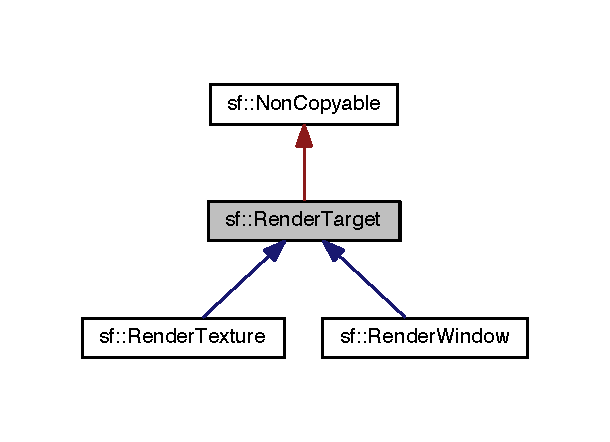
\includegraphics[width=293pt]{classsf_1_1_render_target__inherit__graph}
\end{center}
\end{figure}


Collaboration diagram for sf\-:\-:Render\-Target\-:
\nopagebreak
\begin{figure}[H]
\begin{center}
\leavevmode
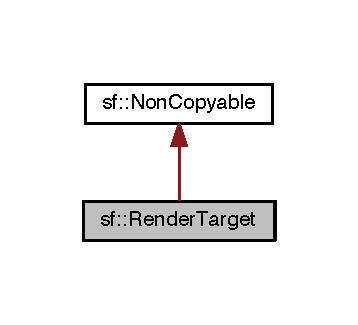
\includegraphics[width=172pt]{classsf_1_1_render_target__coll__graph}
\end{center}
\end{figure}
\subsection*{Public Member Functions}
\begin{DoxyCompactItemize}
\item 
virtual \hyperlink{classsf_1_1_render_target_a9abd1654a99fba46f6887b9c625b9b06}{$\sim$\-Render\-Target} ()
\begin{DoxyCompactList}\small\item\em Destructor. \end{DoxyCompactList}\item 
\hyperlink{glutf90_8h_ac778d6f63f1aaf8ebda0ce6ac821b56e}{void} \hyperlink{classsf_1_1_render_target_a6bb6f0ba348f2b1e2f46114aeaf60f26}{clear} (const \hyperlink{classsf_1_1_color}{Color} \&\hyperlink{gl3_8h_a3ea846f998d64f079b86052b6c4193a8}{color}=\hyperlink{classsf_1_1_color}{Color}(0, 0, 0, 255))
\begin{DoxyCompactList}\small\item\em Clear the entire target with a single color. \end{DoxyCompactList}\item 
\hyperlink{glutf90_8h_ac778d6f63f1aaf8ebda0ce6ac821b56e}{void} \hyperlink{classsf_1_1_render_target_a063db6dd0a14913504af30e50cb6d946}{set\-View} (const \hyperlink{classsf_1_1_view}{View} \&view)
\begin{DoxyCompactList}\small\item\em Change the current active view. \end{DoxyCompactList}\item 
const \hyperlink{classsf_1_1_view}{View} \& \hyperlink{classsf_1_1_render_target_a98f721cc6dc11478922427fedfb2288b}{get\-View} () const 
\begin{DoxyCompactList}\small\item\em Get the view currently in use in the render target. \end{DoxyCompactList}\item 
const \hyperlink{classsf_1_1_view}{View} \& \hyperlink{classsf_1_1_render_target_a718b1aa6296bf855171699cc18251ced}{get\-Default\-View} () const 
\begin{DoxyCompactList}\small\item\em Get the default view of the render target. \end{DoxyCompactList}\item 
\hyperlink{namespacesf_aae67411782674934f78d55fa3af18403}{Int\-Rect} \hyperlink{classsf_1_1_render_target_aae035b0d45f87a0da2a28a0de6ba1086}{get\-Viewport} (const \hyperlink{classsf_1_1_view}{View} \&view) const 
\begin{DoxyCompactList}\small\item\em Get the viewport of a view, applied to this render target. \end{DoxyCompactList}\item 
\hyperlink{namespacesf_acf03098c2577b869e2fa6836cc48f1a0}{Vector2f} \hyperlink{classsf_1_1_render_target_afc047333937f7cb7fe557aec60239233}{convert\-Coords} (const \hyperlink{namespacesf_ace09dd1447d74c6e9ba56ae874c094e1}{Vector2i} \&point) const 
\begin{DoxyCompactList}\small\item\em Convert a point from target coordinates to view coordinates. \end{DoxyCompactList}\item 
\hyperlink{namespacesf_acf03098c2577b869e2fa6836cc48f1a0}{Vector2f} \hyperlink{classsf_1_1_render_target_ae5e7ba65ef73df2778b29b7fdcdb20ee}{convert\-Coords} (const \hyperlink{namespacesf_ace09dd1447d74c6e9ba56ae874c094e1}{Vector2i} \&point, const \hyperlink{classsf_1_1_view}{View} \&view) const 
\begin{DoxyCompactList}\small\item\em Convert a point from target coordinates to view coordinates. \end{DoxyCompactList}\item 
\hyperlink{glutf90_8h_ac778d6f63f1aaf8ebda0ce6ac821b56e}{void} \hyperlink{classsf_1_1_render_target_a12417a3bcc245c41d957b29583556f39}{draw} (const \hyperlink{classsf_1_1_drawable}{Drawable} \&drawable, const \hyperlink{classsf_1_1_render_states}{Render\-States} \&states=\hyperlink{classsf_1_1_render_states_ad29672df29f19ce50c3021d95f2bb062}{Render\-States\-::\-Default})
\begin{DoxyCompactList}\small\item\em Draw a drawable object to the render-\/target. \end{DoxyCompactList}\item 
\hyperlink{glutf90_8h_ac778d6f63f1aaf8ebda0ce6ac821b56e}{void} \hyperlink{classsf_1_1_render_target_ab636d7363f6681077361ee274ba89a8d}{draw} (const \hyperlink{classsf_1_1_vertex}{Vertex} $\ast$vertices, unsigned int vertex\-Count, \hyperlink{group__graphics_ga5ee56ac1339984909610713096283b1b}{Primitive\-Type} \hyperlink{gl3_8h_a984aabed544368e7fe0e566d7cf014a7}{type}, const \hyperlink{classsf_1_1_render_states}{Render\-States} \&states=\hyperlink{classsf_1_1_render_states_ad29672df29f19ce50c3021d95f2bb062}{Render\-States\-::\-Default})
\begin{DoxyCompactList}\small\item\em Draw primitives defined by an array of vertices. \end{DoxyCompactList}\item 
virtual \hyperlink{namespacesf_aaa02ba42bf79b001a376fe9d79254cb3}{Vector2u} \hyperlink{classsf_1_1_render_target_a2e5ade2457d9fb4c4907ae5b3d9e94a5}{get\-Size} () const =0
\begin{DoxyCompactList}\small\item\em Return the size of the rendering region of the target. \end{DoxyCompactList}\item 
\hyperlink{glutf90_8h_ac778d6f63f1aaf8ebda0ce6ac821b56e}{void} \hyperlink{classsf_1_1_render_target_a8d1998464ccc54e789aaf990242b47f7}{push\-G\-L\-States} ()
\begin{DoxyCompactList}\small\item\em Save the current Open\-G\-L render states and matrices. \end{DoxyCompactList}\item 
\hyperlink{glutf90_8h_ac778d6f63f1aaf8ebda0ce6ac821b56e}{void} \hyperlink{classsf_1_1_render_target_ad5a98401113df931ddcd54c080f7aa8e}{pop\-G\-L\-States} ()
\begin{DoxyCompactList}\small\item\em Restore the previously saved Open\-G\-L render states and matrices. \end{DoxyCompactList}\item 
\hyperlink{glutf90_8h_ac778d6f63f1aaf8ebda0ce6ac821b56e}{void} \hyperlink{classsf_1_1_render_target_aac7504990d27dada4bfe3c7866920765}{reset\-G\-L\-States} ()
\begin{DoxyCompactList}\small\item\em Reset the internal Open\-G\-L states so that the target is ready for drawing. \end{DoxyCompactList}\end{DoxyCompactItemize}
\subsection*{Protected Member Functions}
\begin{DoxyCompactItemize}
\item 
\hyperlink{classsf_1_1_render_target_a2997c96cbd93cb8ce0aba2ddae35b86f}{Render\-Target} ()
\begin{DoxyCompactList}\small\item\em Default constructor. \end{DoxyCompactList}\item 
\hyperlink{glutf90_8h_ac778d6f63f1aaf8ebda0ce6ac821b56e}{void} \hyperlink{classsf_1_1_render_target_af530274b34159d644e509b4b4dc43eb7}{initialize} ()
\begin{DoxyCompactList}\small\item\em Performs the common initialization step after creation. \end{DoxyCompactList}\item 
\hyperlink{glutf90_8h_ac778d6f63f1aaf8ebda0ce6ac821b56e}{void} \hyperlink{classsf_1_1_render_target_a3ed439c5445e9c7d7ff786ff37005efa}{apply\-Current\-View} ()
\begin{DoxyCompactList}\small\item\em Apply the current view. \end{DoxyCompactList}\item 
\hyperlink{glutf90_8h_ac778d6f63f1aaf8ebda0ce6ac821b56e}{void} \hyperlink{classsf_1_1_render_target_aefd4b1cc8e264598b94bd70aaac5bc99}{apply\-Blend\-Mode} (\hyperlink{group__graphics_ga80c52fe2f7050d7f7573b7ed3c995388}{Blend\-Mode} \hyperlink{gl3_8h_a1e71d9c196e4683cc06c4b54d53f7ef5}{mode})
\begin{DoxyCompactList}\small\item\em Apply a new blending mode. \end{DoxyCompactList}\item 
\hyperlink{glutf90_8h_ac778d6f63f1aaf8ebda0ce6ac821b56e}{void} \hyperlink{classsf_1_1_render_target_a0b23bd7c287d0fc12b0521b649a0a0e0}{apply\-Transform} (const \hyperlink{classsf_1_1_transform}{Transform} \&transform)
\begin{DoxyCompactList}\small\item\em Apply a new transform. \end{DoxyCompactList}\item 
\hyperlink{glutf90_8h_ac778d6f63f1aaf8ebda0ce6ac821b56e}{void} \hyperlink{classsf_1_1_render_target_afb8a49305171aad158a27e0dfbb03709}{apply\-Texture} (const \hyperlink{classsf_1_1_texture}{Texture} $\ast$\hyperlink{gl3_8h_ab21590c4736d1459a5a0674a42b5a655}{texture})
\begin{DoxyCompactList}\small\item\em Apply a new texture. \end{DoxyCompactList}\item 
\hyperlink{glutf90_8h_ac778d6f63f1aaf8ebda0ce6ac821b56e}{void} \hyperlink{classsf_1_1_render_target_a6f8bc92f07c70ccd57cbf632fe9de0ba}{apply\-Shader} (const \hyperlink{classsf_1_1_shader}{Shader} $\ast$\hyperlink{gl3_8h_a57b2a96adb1d51204909a82d861e395e}{shader})
\begin{DoxyCompactList}\small\item\em Apply a new shader. \end{DoxyCompactList}\end{DoxyCompactItemize}
\subsection*{Additional Inherited Members}


\subsection{Detailed Description}
Base class for all render targets (window, texture, ...) 

\hyperlink{classsf_1_1_render_target}{sf\-::\-Render\-Target} defines the common behaviour of all the 2\-D render targets usable in the graphics module. It makes it possible to draw 2\-D entities like sprites, shapes, text without using any Open\-G\-L command directly.

A \hyperlink{classsf_1_1_render_target}{sf\-::\-Render\-Target} is also able to use views (\hyperlink{classsf_1_1_view}{sf\-::\-View}), which are a kind of 2\-D cameras. With views you can globally scroll, rotate or zoom everything that is drawn, without having to transform every single entity. See the documentation of \hyperlink{classsf_1_1_view}{sf\-::\-View} for more details and sample pieces of code about this class.

On top of that, render targets are still able to render direct Open\-G\-L stuff. It is even possible to mix together Open\-G\-L calls and regular S\-F\-M\-L drawing commands. When doing so, make sure that Open\-G\-L states are not messed up by calling the push\-G\-L\-States/pop\-G\-L\-States functions.

\begin{DoxySeeAlso}{See Also}
\hyperlink{classsf_1_1_render_window}{sf\-::\-Render\-Window}, \hyperlink{classsf_1_1_render_texture}{sf\-::\-Render\-Texture}, \hyperlink{classsf_1_1_view}{sf\-::\-View} 
\end{DoxySeeAlso}


Definition at line 51 of file Render\-Target.\-hpp.



\subsection{Constructor \& Destructor Documentation}
\hypertarget{classsf_1_1_render_target_a9abd1654a99fba46f6887b9c625b9b06}{\index{sf\-::\-Render\-Target@{sf\-::\-Render\-Target}!$\sim$\-Render\-Target@{$\sim$\-Render\-Target}}
\index{$\sim$\-Render\-Target@{$\sim$\-Render\-Target}!sf::RenderTarget@{sf\-::\-Render\-Target}}
\subsubsection[{$\sim$\-Render\-Target}]{\setlength{\rightskip}{0pt plus 5cm}virtual sf\-::\-Render\-Target\-::$\sim$\-Render\-Target (
\begin{DoxyParamCaption}
{}
\end{DoxyParamCaption}
)\hspace{0.3cm}{\ttfamily [virtual]}}}\label{classsf_1_1_render_target_a9abd1654a99fba46f6887b9c625b9b06}


Destructor. 

\hypertarget{classsf_1_1_render_target_a2997c96cbd93cb8ce0aba2ddae35b86f}{\index{sf\-::\-Render\-Target@{sf\-::\-Render\-Target}!Render\-Target@{Render\-Target}}
\index{Render\-Target@{Render\-Target}!sf::RenderTarget@{sf\-::\-Render\-Target}}
\subsubsection[{Render\-Target}]{\setlength{\rightskip}{0pt plus 5cm}sf\-::\-Render\-Target\-::\-Render\-Target (
\begin{DoxyParamCaption}
{}
\end{DoxyParamCaption}
)\hspace{0.3cm}{\ttfamily [protected]}}}\label{classsf_1_1_render_target_a2997c96cbd93cb8ce0aba2ddae35b86f}


Default constructor. 



\subsection{Member Function Documentation}
\hypertarget{classsf_1_1_render_target_aefd4b1cc8e264598b94bd70aaac5bc99}{\index{sf\-::\-Render\-Target@{sf\-::\-Render\-Target}!apply\-Blend\-Mode@{apply\-Blend\-Mode}}
\index{apply\-Blend\-Mode@{apply\-Blend\-Mode}!sf::RenderTarget@{sf\-::\-Render\-Target}}
\subsubsection[{apply\-Blend\-Mode}]{\setlength{\rightskip}{0pt plus 5cm}{\bf void} sf\-::\-Render\-Target\-::apply\-Blend\-Mode (
\begin{DoxyParamCaption}
\item[{{\bf Blend\-Mode}}]{mode}
\end{DoxyParamCaption}
)\hspace{0.3cm}{\ttfamily [protected]}}}\label{classsf_1_1_render_target_aefd4b1cc8e264598b94bd70aaac5bc99}


Apply a new blending mode. 


\begin{DoxyParams}{Parameters}
{\em mode} & Blending mode to apply \\
\hline
\end{DoxyParams}
\hypertarget{classsf_1_1_render_target_a3ed439c5445e9c7d7ff786ff37005efa}{\index{sf\-::\-Render\-Target@{sf\-::\-Render\-Target}!apply\-Current\-View@{apply\-Current\-View}}
\index{apply\-Current\-View@{apply\-Current\-View}!sf::RenderTarget@{sf\-::\-Render\-Target}}
\subsubsection[{apply\-Current\-View}]{\setlength{\rightskip}{0pt plus 5cm}{\bf void} sf\-::\-Render\-Target\-::apply\-Current\-View (
\begin{DoxyParamCaption}
{}
\end{DoxyParamCaption}
)\hspace{0.3cm}{\ttfamily [protected]}}}\label{classsf_1_1_render_target_a3ed439c5445e9c7d7ff786ff37005efa}


Apply the current view. 

\hypertarget{classsf_1_1_render_target_a6f8bc92f07c70ccd57cbf632fe9de0ba}{\index{sf\-::\-Render\-Target@{sf\-::\-Render\-Target}!apply\-Shader@{apply\-Shader}}
\index{apply\-Shader@{apply\-Shader}!sf::RenderTarget@{sf\-::\-Render\-Target}}
\subsubsection[{apply\-Shader}]{\setlength{\rightskip}{0pt plus 5cm}{\bf void} sf\-::\-Render\-Target\-::apply\-Shader (
\begin{DoxyParamCaption}
\item[{const {\bf Shader} $\ast$}]{shader}
\end{DoxyParamCaption}
)\hspace{0.3cm}{\ttfamily [protected]}}}\label{classsf_1_1_render_target_a6f8bc92f07c70ccd57cbf632fe9de0ba}


Apply a new shader. 


\begin{DoxyParams}{Parameters}
{\em shader} & \hyperlink{classsf_1_1_shader}{Shader} to apply \\
\hline
\end{DoxyParams}
\hypertarget{classsf_1_1_render_target_afb8a49305171aad158a27e0dfbb03709}{\index{sf\-::\-Render\-Target@{sf\-::\-Render\-Target}!apply\-Texture@{apply\-Texture}}
\index{apply\-Texture@{apply\-Texture}!sf::RenderTarget@{sf\-::\-Render\-Target}}
\subsubsection[{apply\-Texture}]{\setlength{\rightskip}{0pt plus 5cm}{\bf void} sf\-::\-Render\-Target\-::apply\-Texture (
\begin{DoxyParamCaption}
\item[{const {\bf Texture} $\ast$}]{texture}
\end{DoxyParamCaption}
)\hspace{0.3cm}{\ttfamily [protected]}}}\label{classsf_1_1_render_target_afb8a49305171aad158a27e0dfbb03709}


Apply a new texture. 


\begin{DoxyParams}{Parameters}
{\em texture} & \hyperlink{classsf_1_1_texture}{Texture} to apply \\
\hline
\end{DoxyParams}
\hypertarget{classsf_1_1_render_target_a0b23bd7c287d0fc12b0521b649a0a0e0}{\index{sf\-::\-Render\-Target@{sf\-::\-Render\-Target}!apply\-Transform@{apply\-Transform}}
\index{apply\-Transform@{apply\-Transform}!sf::RenderTarget@{sf\-::\-Render\-Target}}
\subsubsection[{apply\-Transform}]{\setlength{\rightskip}{0pt plus 5cm}{\bf void} sf\-::\-Render\-Target\-::apply\-Transform (
\begin{DoxyParamCaption}
\item[{const {\bf Transform} \&}]{transform}
\end{DoxyParamCaption}
)\hspace{0.3cm}{\ttfamily [protected]}}}\label{classsf_1_1_render_target_a0b23bd7c287d0fc12b0521b649a0a0e0}


Apply a new transform. 


\begin{DoxyParams}{Parameters}
{\em transform} & \hyperlink{classsf_1_1_transform}{Transform} to apply \\
\hline
\end{DoxyParams}
\hypertarget{classsf_1_1_render_target_a6bb6f0ba348f2b1e2f46114aeaf60f26}{\index{sf\-::\-Render\-Target@{sf\-::\-Render\-Target}!clear@{clear}}
\index{clear@{clear}!sf::RenderTarget@{sf\-::\-Render\-Target}}
\subsubsection[{clear}]{\setlength{\rightskip}{0pt plus 5cm}{\bf void} sf\-::\-Render\-Target\-::clear (
\begin{DoxyParamCaption}
\item[{const {\bf Color} \&}]{color = {\ttfamily {\bf Color}(0,~0,~0,~255)}}
\end{DoxyParamCaption}
)}}\label{classsf_1_1_render_target_a6bb6f0ba348f2b1e2f46114aeaf60f26}


Clear the entire target with a single color. 

This function is usually called once every frame, to clear the previous contents of the target.


\begin{DoxyParams}{Parameters}
{\em color} & Fill color to use to clear the render target \\
\hline
\end{DoxyParams}
\hypertarget{classsf_1_1_render_target_afc047333937f7cb7fe557aec60239233}{\index{sf\-::\-Render\-Target@{sf\-::\-Render\-Target}!convert\-Coords@{convert\-Coords}}
\index{convert\-Coords@{convert\-Coords}!sf::RenderTarget@{sf\-::\-Render\-Target}}
\subsubsection[{convert\-Coords}]{\setlength{\rightskip}{0pt plus 5cm}{\bf Vector2f} sf\-::\-Render\-Target\-::convert\-Coords (
\begin{DoxyParamCaption}
\item[{const {\bf Vector2i} \&}]{point}
\end{DoxyParamCaption}
) const}}\label{classsf_1_1_render_target_afc047333937f7cb7fe557aec60239233}


Convert a point from target coordinates to view coordinates. 

Initially, a unit of the 2\-D world matches a pixel of the render target. But if you define a custom view, this assertion is not true anymore, ie. a point located at (10, 50) in your render target (for example a window) may map to the point (150, 75) in your 2\-D world -- for example if the view is translated by (140, 25).

For render windows, this function is typically used to find which point (or object) is located below the mouse cursor.

This version uses the current view of the render target. See the other overload to specify a custom view.


\begin{DoxyParams}{Parameters}
{\em point} & Point to convert, relative to the render target\\
\hline
\end{DoxyParams}
\begin{DoxyReturn}{Returns}
The converted point, in \char`\"{}world\char`\"{} units 
\end{DoxyReturn}
\hypertarget{classsf_1_1_render_target_ae5e7ba65ef73df2778b29b7fdcdb20ee}{\index{sf\-::\-Render\-Target@{sf\-::\-Render\-Target}!convert\-Coords@{convert\-Coords}}
\index{convert\-Coords@{convert\-Coords}!sf::RenderTarget@{sf\-::\-Render\-Target}}
\subsubsection[{convert\-Coords}]{\setlength{\rightskip}{0pt plus 5cm}{\bf Vector2f} sf\-::\-Render\-Target\-::convert\-Coords (
\begin{DoxyParamCaption}
\item[{const {\bf Vector2i} \&}]{point, }
\item[{const {\bf View} \&}]{view}
\end{DoxyParamCaption}
) const}}\label{classsf_1_1_render_target_ae5e7ba65ef73df2778b29b7fdcdb20ee}


Convert a point from target coordinates to view coordinates. 

Initially, a unit of the 2\-D world matches a pixel of the render target. But if you define a custom view, this assertion is not true anymore, ie. a point located at (10, 50) in your render target (for example a window) may map to the point (150, 75) in your 2\-D world -- for example if the view is translated by (140, 25).

For render windows, this function is typically used to find which point (or object) is located below the mouse cursor.

This version uses a custom view for calculations, see the other overload of the function to use the current view of the render target.


\begin{DoxyParams}{Parameters}
{\em point} & Point to convert, relative to the render target \\
\hline
{\em view} & The view to use for converting the point\\
\hline
\end{DoxyParams}
\begin{DoxyReturn}{Returns}
The converted point, in \char`\"{}world\char`\"{} units 
\end{DoxyReturn}
\hypertarget{classsf_1_1_render_target_a12417a3bcc245c41d957b29583556f39}{\index{sf\-::\-Render\-Target@{sf\-::\-Render\-Target}!draw@{draw}}
\index{draw@{draw}!sf::RenderTarget@{sf\-::\-Render\-Target}}
\subsubsection[{draw}]{\setlength{\rightskip}{0pt plus 5cm}{\bf void} sf\-::\-Render\-Target\-::draw (
\begin{DoxyParamCaption}
\item[{const {\bf Drawable} \&}]{drawable, }
\item[{const {\bf Render\-States} \&}]{states = {\ttfamily {\bf Render\-States\-::\-Default}}}
\end{DoxyParamCaption}
)}}\label{classsf_1_1_render_target_a12417a3bcc245c41d957b29583556f39}


Draw a drawable object to the render-\/target. 


\begin{DoxyParams}{Parameters}
{\em drawable} & Object to draw \\
\hline
{\em states} & Render states to use for drawing \\
\hline
\end{DoxyParams}
\hypertarget{classsf_1_1_render_target_ab636d7363f6681077361ee274ba89a8d}{\index{sf\-::\-Render\-Target@{sf\-::\-Render\-Target}!draw@{draw}}
\index{draw@{draw}!sf::RenderTarget@{sf\-::\-Render\-Target}}
\subsubsection[{draw}]{\setlength{\rightskip}{0pt plus 5cm}{\bf void} sf\-::\-Render\-Target\-::draw (
\begin{DoxyParamCaption}
\item[{const {\bf Vertex} $\ast$}]{vertices, }
\item[{unsigned int}]{vertex\-Count, }
\item[{{\bf Primitive\-Type}}]{type, }
\item[{const {\bf Render\-States} \&}]{states = {\ttfamily {\bf Render\-States\-::\-Default}}}
\end{DoxyParamCaption}
)}}\label{classsf_1_1_render_target_ab636d7363f6681077361ee274ba89a8d}


Draw primitives defined by an array of vertices. 


\begin{DoxyParams}{Parameters}
{\em vertices} & Pointer to the vertices \\
\hline
{\em vertex\-Count} & Number of vertices in the array \\
\hline
{\em type} & Type of primitives to draw \\
\hline
{\em states} & Render states to use for drawing \\
\hline
\end{DoxyParams}
\hypertarget{classsf_1_1_render_target_a718b1aa6296bf855171699cc18251ced}{\index{sf\-::\-Render\-Target@{sf\-::\-Render\-Target}!get\-Default\-View@{get\-Default\-View}}
\index{get\-Default\-View@{get\-Default\-View}!sf::RenderTarget@{sf\-::\-Render\-Target}}
\subsubsection[{get\-Default\-View}]{\setlength{\rightskip}{0pt plus 5cm}const {\bf View}\& sf\-::\-Render\-Target\-::get\-Default\-View (
\begin{DoxyParamCaption}
{}
\end{DoxyParamCaption}
) const}}\label{classsf_1_1_render_target_a718b1aa6296bf855171699cc18251ced}


Get the default view of the render target. 

The default view has the initial size of the render target, and never changes after the target has been created.

\begin{DoxyReturn}{Returns}
The default view of the render target
\end{DoxyReturn}
\begin{DoxySeeAlso}{See Also}
\hyperlink{classsf_1_1_render_target_a063db6dd0a14913504af30e50cb6d946}{set\-View}, \hyperlink{classsf_1_1_render_target_a98f721cc6dc11478922427fedfb2288b}{get\-View} 
\end{DoxySeeAlso}
\hypertarget{classsf_1_1_render_target_a2e5ade2457d9fb4c4907ae5b3d9e94a5}{\index{sf\-::\-Render\-Target@{sf\-::\-Render\-Target}!get\-Size@{get\-Size}}
\index{get\-Size@{get\-Size}!sf::RenderTarget@{sf\-::\-Render\-Target}}
\subsubsection[{get\-Size}]{\setlength{\rightskip}{0pt plus 5cm}virtual {\bf Vector2u} sf\-::\-Render\-Target\-::get\-Size (
\begin{DoxyParamCaption}
{}
\end{DoxyParamCaption}
) const\hspace{0.3cm}{\ttfamily [pure virtual]}}}\label{classsf_1_1_render_target_a2e5ade2457d9fb4c4907ae5b3d9e94a5}


Return the size of the rendering region of the target. 

\begin{DoxyReturn}{Returns}
Size in pixels 
\end{DoxyReturn}


Implemented in \hyperlink{classsf_1_1_render_texture_a757ba45ec7a7deefcaef717049b00b8c}{sf\-::\-Render\-Texture}, and \hyperlink{classsf_1_1_render_window_a2c7ff414be32621a453745cf2a0f8a3e}{sf\-::\-Render\-Window}.

\hypertarget{classsf_1_1_render_target_a98f721cc6dc11478922427fedfb2288b}{\index{sf\-::\-Render\-Target@{sf\-::\-Render\-Target}!get\-View@{get\-View}}
\index{get\-View@{get\-View}!sf::RenderTarget@{sf\-::\-Render\-Target}}
\subsubsection[{get\-View}]{\setlength{\rightskip}{0pt plus 5cm}const {\bf View}\& sf\-::\-Render\-Target\-::get\-View (
\begin{DoxyParamCaption}
{}
\end{DoxyParamCaption}
) const}}\label{classsf_1_1_render_target_a98f721cc6dc11478922427fedfb2288b}


Get the view currently in use in the render target. 

\begin{DoxyReturn}{Returns}
The view object that is currently used
\end{DoxyReturn}
\begin{DoxySeeAlso}{See Also}
\hyperlink{classsf_1_1_render_target_a063db6dd0a14913504af30e50cb6d946}{set\-View}, \hyperlink{classsf_1_1_render_target_a718b1aa6296bf855171699cc18251ced}{get\-Default\-View} 
\end{DoxySeeAlso}
\hypertarget{classsf_1_1_render_target_aae035b0d45f87a0da2a28a0de6ba1086}{\index{sf\-::\-Render\-Target@{sf\-::\-Render\-Target}!get\-Viewport@{get\-Viewport}}
\index{get\-Viewport@{get\-Viewport}!sf::RenderTarget@{sf\-::\-Render\-Target}}
\subsubsection[{get\-Viewport}]{\setlength{\rightskip}{0pt plus 5cm}{\bf Int\-Rect} sf\-::\-Render\-Target\-::get\-Viewport (
\begin{DoxyParamCaption}
\item[{const {\bf View} \&}]{view}
\end{DoxyParamCaption}
) const}}\label{classsf_1_1_render_target_aae035b0d45f87a0da2a28a0de6ba1086}


Get the viewport of a view, applied to this render target. 

The viewport is defined in the view as a ratio, this function simply applies this ratio to the current dimensions of the render target to calculate the pixels rectangle that the viewport actually covers in the target.


\begin{DoxyParams}{Parameters}
{\em view} & The view for which we want to compute the viewport\\
\hline
\end{DoxyParams}
\begin{DoxyReturn}{Returns}
Viewport rectangle, expressed in pixels 
\end{DoxyReturn}
\hypertarget{classsf_1_1_render_target_af530274b34159d644e509b4b4dc43eb7}{\index{sf\-::\-Render\-Target@{sf\-::\-Render\-Target}!initialize@{initialize}}
\index{initialize@{initialize}!sf::RenderTarget@{sf\-::\-Render\-Target}}
\subsubsection[{initialize}]{\setlength{\rightskip}{0pt plus 5cm}{\bf void} sf\-::\-Render\-Target\-::initialize (
\begin{DoxyParamCaption}
{}
\end{DoxyParamCaption}
)\hspace{0.3cm}{\ttfamily [protected]}}}\label{classsf_1_1_render_target_af530274b34159d644e509b4b4dc43eb7}


Performs the common initialization step after creation. 

The derived classes must call this function after the target is created and ready for drawing. \hypertarget{classsf_1_1_render_target_ad5a98401113df931ddcd54c080f7aa8e}{\index{sf\-::\-Render\-Target@{sf\-::\-Render\-Target}!pop\-G\-L\-States@{pop\-G\-L\-States}}
\index{pop\-G\-L\-States@{pop\-G\-L\-States}!sf::RenderTarget@{sf\-::\-Render\-Target}}
\subsubsection[{pop\-G\-L\-States}]{\setlength{\rightskip}{0pt plus 5cm}{\bf void} sf\-::\-Render\-Target\-::pop\-G\-L\-States (
\begin{DoxyParamCaption}
{}
\end{DoxyParamCaption}
)}}\label{classsf_1_1_render_target_ad5a98401113df931ddcd54c080f7aa8e}


Restore the previously saved Open\-G\-L render states and matrices. 

See the description of push\-G\-L\-States to get a detailed description of these functions.

\begin{DoxySeeAlso}{See Also}
\hyperlink{classsf_1_1_render_target_a8d1998464ccc54e789aaf990242b47f7}{push\-G\-L\-States} 
\end{DoxySeeAlso}
\hypertarget{classsf_1_1_render_target_a8d1998464ccc54e789aaf990242b47f7}{\index{sf\-::\-Render\-Target@{sf\-::\-Render\-Target}!push\-G\-L\-States@{push\-G\-L\-States}}
\index{push\-G\-L\-States@{push\-G\-L\-States}!sf::RenderTarget@{sf\-::\-Render\-Target}}
\subsubsection[{push\-G\-L\-States}]{\setlength{\rightskip}{0pt plus 5cm}{\bf void} sf\-::\-Render\-Target\-::push\-G\-L\-States (
\begin{DoxyParamCaption}
{}
\end{DoxyParamCaption}
)}}\label{classsf_1_1_render_target_a8d1998464ccc54e789aaf990242b47f7}


Save the current Open\-G\-L render states and matrices. 

This function can be used when you mix S\-F\-M\-L drawing and direct Open\-G\-L rendering. Combined with Pop\-G\-L\-States, it ensures that\-: \begin{DoxyItemize}
\item S\-F\-M\-L's internal states are not messed up by your Open\-G\-L code \item your Open\-G\-L states are not modified by a call to a S\-F\-M\-L function\end{DoxyItemize}
More specifically, it must be used around code that calls Draw functions. Example\-: 
\begin{DoxyCode}
\textcolor{comment}{// OpenGL code here...}
window.pushGLStates();
window.draw(...);
window.draw(...);
window.popGLStates();
\textcolor{comment}{// OpenGL code here...}
\end{DoxyCode}


Note that this function is quite expensive\-: it saves all the possible Open\-G\-L states and matrices, even the ones you don't care about. Therefore it should be used wisely. It is provided for convenience, but the best results will be achieved if you handle Open\-G\-L states yourself (because you know which states have really changed, and need to be saved and restored). Take a look at the Reset\-G\-L\-States function if you do so.

\begin{DoxySeeAlso}{See Also}
\hyperlink{classsf_1_1_render_target_ad5a98401113df931ddcd54c080f7aa8e}{pop\-G\-L\-States} 
\end{DoxySeeAlso}
\hypertarget{classsf_1_1_render_target_aac7504990d27dada4bfe3c7866920765}{\index{sf\-::\-Render\-Target@{sf\-::\-Render\-Target}!reset\-G\-L\-States@{reset\-G\-L\-States}}
\index{reset\-G\-L\-States@{reset\-G\-L\-States}!sf::RenderTarget@{sf\-::\-Render\-Target}}
\subsubsection[{reset\-G\-L\-States}]{\setlength{\rightskip}{0pt plus 5cm}{\bf void} sf\-::\-Render\-Target\-::reset\-G\-L\-States (
\begin{DoxyParamCaption}
{}
\end{DoxyParamCaption}
)}}\label{classsf_1_1_render_target_aac7504990d27dada4bfe3c7866920765}


Reset the internal Open\-G\-L states so that the target is ready for drawing. 

This function can be used when you mix S\-F\-M\-L drawing and direct Open\-G\-L rendering, if you choose not to use push\-G\-L\-States/pop\-G\-L\-States. It makes sure that all Open\-G\-L states needed by S\-F\-M\-L are set, so that subsequent \hyperlink{classsf_1_1_render_target_a12417a3bcc245c41d957b29583556f39}{draw()} calls will work as expected.

Example\-: 
\begin{DoxyCode}
\textcolor{comment}{// OpenGL code here...}
\hyperlink{gl_8h_a1917b00fe1a903f7db1352e308fd3b52}{glPushAttrib}(...);
window.resetGLStates();
window.draw(...);
window.draw(...);
\hyperlink{gl_8h_ad0f886ee4d236c3902c1a2f566eeb8ad}{glPopAttrib}(...);
\textcolor{comment}{// OpenGL code here...}
\end{DoxyCode}
 \hypertarget{classsf_1_1_render_target_a063db6dd0a14913504af30e50cb6d946}{\index{sf\-::\-Render\-Target@{sf\-::\-Render\-Target}!set\-View@{set\-View}}
\index{set\-View@{set\-View}!sf::RenderTarget@{sf\-::\-Render\-Target}}
\subsubsection[{set\-View}]{\setlength{\rightskip}{0pt plus 5cm}{\bf void} sf\-::\-Render\-Target\-::set\-View (
\begin{DoxyParamCaption}
\item[{const {\bf View} \&}]{view}
\end{DoxyParamCaption}
)}}\label{classsf_1_1_render_target_a063db6dd0a14913504af30e50cb6d946}


Change the current active view. 

The view is like a 2\-D camera, it controls which part of the 2\-D scene is visible, and how it is viewed in the render-\/target. The new view will affect everything that is drawn, until another view is set. The render target keeps its own copy of the view object, so it is not necessary to keep the original one alive after calling this function. To restore the original view of the target, you can pass the result of \hyperlink{classsf_1_1_render_target_a718b1aa6296bf855171699cc18251ced}{get\-Default\-View()} to this function.


\begin{DoxyParams}{Parameters}
{\em view} & New view to use\\
\hline
\end{DoxyParams}
\begin{DoxySeeAlso}{See Also}
\hyperlink{classsf_1_1_render_target_a98f721cc6dc11478922427fedfb2288b}{get\-View}, \hyperlink{classsf_1_1_render_target_a718b1aa6296bf855171699cc18251ced}{get\-Default\-View} 
\end{DoxySeeAlso}


The documentation for this class was generated from the following file\-:\begin{DoxyCompactItemize}
\item 
/\-Users/ira/\-Dropbox/ira\-\_\-dev/protobyte\-\_\-research/other\-\_\-libs/\-S\-F\-M\-L/dylibs/root/usr/local/include/\-S\-F\-M\-L/\-Graphics/\hyperlink{_render_target_8hpp}{Render\-Target.\-hpp}\end{DoxyCompactItemize}

\hypertarget{classsf_1_1_render_texture}{\section{sf\-:\-:Render\-Texture Class Reference}
\label{classsf_1_1_render_texture}\index{sf\-::\-Render\-Texture@{sf\-::\-Render\-Texture}}
}


Target for off-\/screen 2\-D rendering into an texture.  




{\ttfamily \#include $<$Render\-Texture.\-hpp$>$}



Inheritance diagram for sf\-:\-:Render\-Texture\-:
\nopagebreak
\begin{figure}[H]
\begin{center}
\leavevmode
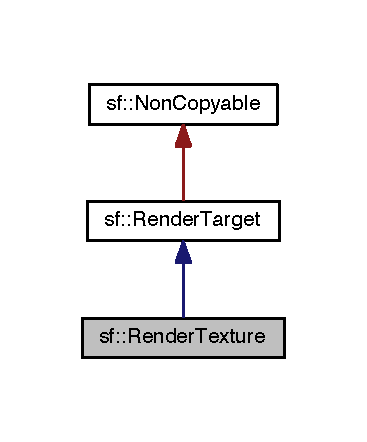
\includegraphics[width=176pt]{classsf_1_1_render_texture__inherit__graph}
\end{center}
\end{figure}


Collaboration diagram for sf\-:\-:Render\-Texture\-:
\nopagebreak
\begin{figure}[H]
\begin{center}
\leavevmode
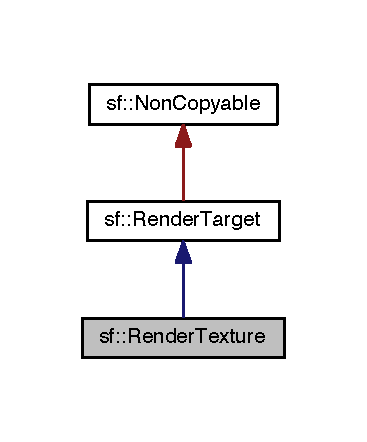
\includegraphics[width=176pt]{classsf_1_1_render_texture__coll__graph}
\end{center}
\end{figure}
\subsection*{Public Member Functions}
\begin{DoxyCompactItemize}
\item 
\hyperlink{classsf_1_1_render_texture_a19ee6e5b4c40ad251803389b3953a9c6}{Render\-Texture} ()
\begin{DoxyCompactList}\small\item\em Default constructor. \end{DoxyCompactList}\item 
virtual \hyperlink{classsf_1_1_render_texture_a94b84ab9335be84d2a014c964d973304}{$\sim$\-Render\-Texture} ()
\begin{DoxyCompactList}\small\item\em Destructor. \end{DoxyCompactList}\item 
bool \hyperlink{classsf_1_1_render_texture_aefbb76eb3b87e368ab974b2660931ccb}{create} (unsigned int \hyperlink{gl3_8h_a9d14ddc31c6c8b61f3fe3679ab976133}{width}, unsigned int \hyperlink{gl3_8h_a67001679ebf2bb0ba972db4d29c6550c}{height}, bool depth\-Buffer=false)
\begin{DoxyCompactList}\small\item\em Create the render-\/texture. \end{DoxyCompactList}\item 
\hyperlink{glutf90_8h_ac778d6f63f1aaf8ebda0ce6ac821b56e}{void} \hyperlink{classsf_1_1_render_texture_af08991e63c6020865dd07b20e27305b6}{set\-Smooth} (bool smooth)
\begin{DoxyCompactList}\small\item\em Enable or disable texture smoothing. \end{DoxyCompactList}\item 
bool \hyperlink{classsf_1_1_render_texture_ae385f4f4dbd2af50fb11947bf0bcb83d}{is\-Smooth} () const 
\begin{DoxyCompactList}\small\item\em Tell whether the smooth filtering is enabled or not. \end{DoxyCompactList}\item 
bool \hyperlink{classsf_1_1_render_texture_a5da95ecdbce615a80bb78399012508cf}{set\-Active} (bool active=true)
\begin{DoxyCompactList}\small\item\em Activate of deactivate the render-\/texture for rendering. \end{DoxyCompactList}\item 
\hyperlink{glutf90_8h_ac778d6f63f1aaf8ebda0ce6ac821b56e}{void} \hyperlink{classsf_1_1_render_texture_af92886d5faef3916caff9fa9ab32c555}{display} ()
\begin{DoxyCompactList}\small\item\em Update the contents of the target texture. \end{DoxyCompactList}\item 
virtual \hyperlink{namespacesf_aaa02ba42bf79b001a376fe9d79254cb3}{Vector2u} \hyperlink{classsf_1_1_render_texture_a757ba45ec7a7deefcaef717049b00b8c}{get\-Size} () const 
\begin{DoxyCompactList}\small\item\em Return the size of the rendering region of the texture. \end{DoxyCompactList}\item 
const \hyperlink{classsf_1_1_texture}{Texture} \& \hyperlink{classsf_1_1_render_texture_a95bc5152c497066d31fdc57da8e17678}{get\-Texture} () const 
\begin{DoxyCompactList}\small\item\em Get a read-\/only reference to the target texture. \end{DoxyCompactList}\end{DoxyCompactItemize}
\subsection*{Additional Inherited Members}


\subsection{Detailed Description}
Target for off-\/screen 2\-D rendering into an texture. 

\hyperlink{classsf_1_1_render_texture}{sf\-::\-Render\-Texture} is the little brother of \hyperlink{classsf_1_1_render_window}{sf\-::\-Render\-Window}. It implements the same 2\-D drawing and Open\-G\-L-\/related functions (see their base class \hyperlink{classsf_1_1_render_target}{sf\-::\-Render\-Target} for more details), the difference is that the result is stored in an off-\/screen texture rather than being show in a window.

Rendering to a texture can be useful in a variety of situations\-: \begin{DoxyItemize}
\item precomputing a complex static texture (like a level's background from multiple tiles) \item applying post-\/effects to the whole scene with shaders \item creating a sprite from a 3\-D object rendered with Open\-G\-L \item etc.\end{DoxyItemize}
Usage example\-:


\begin{DoxyCode}
\textcolor{comment}{// Create a new render-window}
\hyperlink{classsf_1_1_render_window}{sf::RenderWindow} window(\hyperlink{classsf_1_1_video_mode}{sf::VideoMode}(800, 600), \textcolor{stringliteral}{"SFML window"});

\textcolor{comment}{// Create a new render-texture}
\hyperlink{classsf_1_1_render_texture}{sf::RenderTexture} \hyperlink{gl3_8h_ab21590c4736d1459a5a0674a42b5a655}{texture};
\textcolor{keywordflow}{if} (!texture.\hyperlink{classsf_1_1_render_texture_aefbb76eb3b87e368ab974b2660931ccb}{create}(500, 500))
    \textcolor{keywordflow}{return} -1

\textcolor{comment}{// The main loop}
\textcolor{keywordflow}{while} (window.isOpen())
\{
   \textcolor{comment}{// Event processing}
   \textcolor{comment}{// ...}

   \textcolor{comment}{// Clear the whole texture with red color}
   texture.\hyperlink{classsf_1_1_render_target_a6bb6f0ba348f2b1e2f46114aeaf60f26}{clear}(\hyperlink{classsf_1_1_color_a127dbf55db9c07d0fa8f4bfcbb97594a}{sf::Color::Red});

   \textcolor{comment}{// Draw stuff to the texture}
   texture.\hyperlink{classsf_1_1_render_target_a12417a3bcc245c41d957b29583556f39}{draw}(sprite);  \textcolor{comment}{// sprite is a sf::Sprite}
   texture.\hyperlink{classsf_1_1_render_target_a12417a3bcc245c41d957b29583556f39}{draw}(shape);   \textcolor{comment}{// shape is a sf::Shape}
   texture.\hyperlink{classsf_1_1_render_target_a12417a3bcc245c41d957b29583556f39}{draw}(text);    \textcolor{comment}{// text is a sf::Text}

   \textcolor{comment}{// We're done drawing to the texture}
   texture.\hyperlink{classsf_1_1_render_texture_af92886d5faef3916caff9fa9ab32c555}{display}();

   \textcolor{comment}{// Now we start rendering to the window, clear it first}
   window.clear();

   \textcolor{comment}{// Draw the texture}
   \hyperlink{classsf_1_1_sprite}{sf::Sprite} sprite(texture.\hyperlink{classsf_1_1_render_texture_a95bc5152c497066d31fdc57da8e17678}{getTexture}());
   window.draw(sprite);

   \textcolor{comment}{// End the current frame and display its contents on screen}
   window.display();
\}
\end{DoxyCode}


Like \hyperlink{classsf_1_1_render_window}{sf\-::\-Render\-Window}, \hyperlink{classsf_1_1_render_texture}{sf\-::\-Render\-Texture} is still able to render direct Open\-G\-L stuff. It is even possible to mix together Open\-G\-L calls and regular S\-F\-M\-L drawing commands. If you need a depth buffer for 3\-D rendering, don't forget to request it when calling Render\-Texture\-::\-Create.

\begin{DoxySeeAlso}{See Also}
\hyperlink{classsf_1_1_render_target}{sf\-::\-Render\-Target}, \hyperlink{classsf_1_1_render_window}{sf\-::\-Render\-Window}, \hyperlink{classsf_1_1_view}{sf\-::\-View}, \hyperlink{classsf_1_1_texture}{sf\-::\-Texture} 
\end{DoxySeeAlso}


Definition at line 47 of file Render\-Texture.\-hpp.



\subsection{Constructor \& Destructor Documentation}
\hypertarget{classsf_1_1_render_texture_a19ee6e5b4c40ad251803389b3953a9c6}{\index{sf\-::\-Render\-Texture@{sf\-::\-Render\-Texture}!Render\-Texture@{Render\-Texture}}
\index{Render\-Texture@{Render\-Texture}!sf::RenderTexture@{sf\-::\-Render\-Texture}}
\subsubsection[{Render\-Texture}]{\setlength{\rightskip}{0pt plus 5cm}sf\-::\-Render\-Texture\-::\-Render\-Texture (
\begin{DoxyParamCaption}
{}
\end{DoxyParamCaption}
)}}\label{classsf_1_1_render_texture_a19ee6e5b4c40ad251803389b3953a9c6}


Default constructor. 

Constructs an empty, invalid render-\/texture. You must call create to have a valid render-\/texture.

\begin{DoxySeeAlso}{See Also}
\hyperlink{classsf_1_1_render_texture_aefbb76eb3b87e368ab974b2660931ccb}{create} 
\end{DoxySeeAlso}
\hypertarget{classsf_1_1_render_texture_a94b84ab9335be84d2a014c964d973304}{\index{sf\-::\-Render\-Texture@{sf\-::\-Render\-Texture}!$\sim$\-Render\-Texture@{$\sim$\-Render\-Texture}}
\index{$\sim$\-Render\-Texture@{$\sim$\-Render\-Texture}!sf::RenderTexture@{sf\-::\-Render\-Texture}}
\subsubsection[{$\sim$\-Render\-Texture}]{\setlength{\rightskip}{0pt plus 5cm}virtual sf\-::\-Render\-Texture\-::$\sim$\-Render\-Texture (
\begin{DoxyParamCaption}
{}
\end{DoxyParamCaption}
)\hspace{0.3cm}{\ttfamily [virtual]}}}\label{classsf_1_1_render_texture_a94b84ab9335be84d2a014c964d973304}


Destructor. 



\subsection{Member Function Documentation}
\hypertarget{classsf_1_1_render_texture_aefbb76eb3b87e368ab974b2660931ccb}{\index{sf\-::\-Render\-Texture@{sf\-::\-Render\-Texture}!create@{create}}
\index{create@{create}!sf::RenderTexture@{sf\-::\-Render\-Texture}}
\subsubsection[{create}]{\setlength{\rightskip}{0pt plus 5cm}bool sf\-::\-Render\-Texture\-::create (
\begin{DoxyParamCaption}
\item[{unsigned int}]{width, }
\item[{unsigned int}]{height, }
\item[{bool}]{depth\-Buffer = {\ttfamily false}}
\end{DoxyParamCaption}
)}}\label{classsf_1_1_render_texture_aefbb76eb3b87e368ab974b2660931ccb}


Create the render-\/texture. 

Before calling this function, the render-\/texture is in an invalid state, thus it is mandatory to call it before doing anything with the render-\/texture. The last parameter, {\itshape depth\-Buffer}, is useful if you want to use the render-\/texture for 3\-D Open\-G\-L rendering that requires a depth-\/buffer. Otherwise it is unnecessary, and you should leave this parameter to false (which is its default value).


\begin{DoxyParams}{Parameters}
{\em width} & Width of the render-\/texture \\
\hline
{\em height} & Height of the render-\/texture \\
\hline
{\em depth\-Buffer} & Do you want this render-\/texture to have a depth buffer?\\
\hline
\end{DoxyParams}
\begin{DoxyReturn}{Returns}
True if creation has been successful 
\end{DoxyReturn}
\hypertarget{classsf_1_1_render_texture_af92886d5faef3916caff9fa9ab32c555}{\index{sf\-::\-Render\-Texture@{sf\-::\-Render\-Texture}!display@{display}}
\index{display@{display}!sf::RenderTexture@{sf\-::\-Render\-Texture}}
\subsubsection[{display}]{\setlength{\rightskip}{0pt plus 5cm}{\bf void} sf\-::\-Render\-Texture\-::display (
\begin{DoxyParamCaption}
{}
\end{DoxyParamCaption}
)}}\label{classsf_1_1_render_texture_af92886d5faef3916caff9fa9ab32c555}


Update the contents of the target texture. 

This function updates the target texture with what has been drawn so far. Like for windows, calling this function is mandatory at the end of rendering. Not calling it may leave the texture in an undefined state. \hypertarget{classsf_1_1_render_texture_a757ba45ec7a7deefcaef717049b00b8c}{\index{sf\-::\-Render\-Texture@{sf\-::\-Render\-Texture}!get\-Size@{get\-Size}}
\index{get\-Size@{get\-Size}!sf::RenderTexture@{sf\-::\-Render\-Texture}}
\subsubsection[{get\-Size}]{\setlength{\rightskip}{0pt plus 5cm}virtual {\bf Vector2u} sf\-::\-Render\-Texture\-::get\-Size (
\begin{DoxyParamCaption}
{}
\end{DoxyParamCaption}
) const\hspace{0.3cm}{\ttfamily [virtual]}}}\label{classsf_1_1_render_texture_a757ba45ec7a7deefcaef717049b00b8c}


Return the size of the rendering region of the texture. 

The returned value is the size that you passed to the create function.

\begin{DoxyReturn}{Returns}
Size in pixels 
\end{DoxyReturn}


Implements \hyperlink{classsf_1_1_render_target_a2e5ade2457d9fb4c4907ae5b3d9e94a5}{sf\-::\-Render\-Target}.

\hypertarget{classsf_1_1_render_texture_a95bc5152c497066d31fdc57da8e17678}{\index{sf\-::\-Render\-Texture@{sf\-::\-Render\-Texture}!get\-Texture@{get\-Texture}}
\index{get\-Texture@{get\-Texture}!sf::RenderTexture@{sf\-::\-Render\-Texture}}
\subsubsection[{get\-Texture}]{\setlength{\rightskip}{0pt plus 5cm}const {\bf Texture}\& sf\-::\-Render\-Texture\-::get\-Texture (
\begin{DoxyParamCaption}
{}
\end{DoxyParamCaption}
) const}}\label{classsf_1_1_render_texture_a95bc5152c497066d31fdc57da8e17678}


Get a read-\/only reference to the target texture. 

After drawing to the render-\/texture and calling Display, you can retrieve the updated texture using this function, and draw it using a sprite (for example). The internal \hyperlink{classsf_1_1_texture}{sf\-::\-Texture} of a render-\/texture is always the same instance, so that it is possible to call this function once and keep a reference to the texture even after it is modified.

\begin{DoxyReturn}{Returns}
Const reference to the texture 
\end{DoxyReturn}
\hypertarget{classsf_1_1_render_texture_ae385f4f4dbd2af50fb11947bf0bcb83d}{\index{sf\-::\-Render\-Texture@{sf\-::\-Render\-Texture}!is\-Smooth@{is\-Smooth}}
\index{is\-Smooth@{is\-Smooth}!sf::RenderTexture@{sf\-::\-Render\-Texture}}
\subsubsection[{is\-Smooth}]{\setlength{\rightskip}{0pt plus 5cm}bool sf\-::\-Render\-Texture\-::is\-Smooth (
\begin{DoxyParamCaption}
{}
\end{DoxyParamCaption}
) const}}\label{classsf_1_1_render_texture_ae385f4f4dbd2af50fb11947bf0bcb83d}


Tell whether the smooth filtering is enabled or not. 

\begin{DoxyReturn}{Returns}
True if texture smoothing is enabled
\end{DoxyReturn}
\begin{DoxySeeAlso}{See Also}
\hyperlink{classsf_1_1_render_texture_af08991e63c6020865dd07b20e27305b6}{set\-Smooth} 
\end{DoxySeeAlso}
\hypertarget{classsf_1_1_render_texture_a5da95ecdbce615a80bb78399012508cf}{\index{sf\-::\-Render\-Texture@{sf\-::\-Render\-Texture}!set\-Active@{set\-Active}}
\index{set\-Active@{set\-Active}!sf::RenderTexture@{sf\-::\-Render\-Texture}}
\subsubsection[{set\-Active}]{\setlength{\rightskip}{0pt plus 5cm}bool sf\-::\-Render\-Texture\-::set\-Active (
\begin{DoxyParamCaption}
\item[{bool}]{active = {\ttfamily true}}
\end{DoxyParamCaption}
)}}\label{classsf_1_1_render_texture_a5da95ecdbce615a80bb78399012508cf}


Activate of deactivate the render-\/texture for rendering. 

This function makes the render-\/texture's context current for future Open\-G\-L rendering operations (so you shouldn't care about it if you're not doing direct Open\-G\-L stuff). Only one context can be current in a thread, so if you want to draw Open\-G\-L geometry to another render target (like a \hyperlink{classsf_1_1_render_window}{Render\-Window}) don't forget to activate it again.


\begin{DoxyParams}{Parameters}
{\em active} & True to activate, false to deactivate\\
\hline
\end{DoxyParams}
\begin{DoxyReturn}{Returns}
True if operation was successful, false otherwise 
\end{DoxyReturn}
\hypertarget{classsf_1_1_render_texture_af08991e63c6020865dd07b20e27305b6}{\index{sf\-::\-Render\-Texture@{sf\-::\-Render\-Texture}!set\-Smooth@{set\-Smooth}}
\index{set\-Smooth@{set\-Smooth}!sf::RenderTexture@{sf\-::\-Render\-Texture}}
\subsubsection[{set\-Smooth}]{\setlength{\rightskip}{0pt plus 5cm}{\bf void} sf\-::\-Render\-Texture\-::set\-Smooth (
\begin{DoxyParamCaption}
\item[{bool}]{smooth}
\end{DoxyParamCaption}
)}}\label{classsf_1_1_render_texture_af08991e63c6020865dd07b20e27305b6}


Enable or disable texture smoothing. 

This function is similar to \hyperlink{classsf_1_1_texture_a0c3bd6825b9a99714f10d44179d74324}{Texture\-::set\-Smooth}. This parameter is disabled by default.


\begin{DoxyParams}{Parameters}
{\em smooth} & True to enable smoothing, false to disable it\\
\hline
\end{DoxyParams}
\begin{DoxySeeAlso}{See Also}
\hyperlink{classsf_1_1_render_texture_ae385f4f4dbd2af50fb11947bf0bcb83d}{is\-Smooth} 
\end{DoxySeeAlso}


The documentation for this class was generated from the following file\-:\begin{DoxyCompactItemize}
\item 
/\-Users/ira/\-Dropbox/ira\-\_\-dev/protobyte\-\_\-research/other\-\_\-libs/\-S\-F\-M\-L/dylibs/root/usr/local/include/\-S\-F\-M\-L/\-Graphics/\hyperlink{_render_texture_8hpp}{Render\-Texture.\-hpp}\end{DoxyCompactItemize}

\hypertarget{classsf_1_1_render_window}{\section{sf\-:\-:Render\-Window Class Reference}
\label{classsf_1_1_render_window}\index{sf\-::\-Render\-Window@{sf\-::\-Render\-Window}}
}


\hyperlink{classsf_1_1_window}{Window} that can serve as a target for 2\-D drawing.  




{\ttfamily \#include $<$Render\-Window.\-hpp$>$}



Inheritance diagram for sf\-:\-:Render\-Window\-:
\nopagebreak
\begin{figure}[H]
\begin{center}
\leavevmode
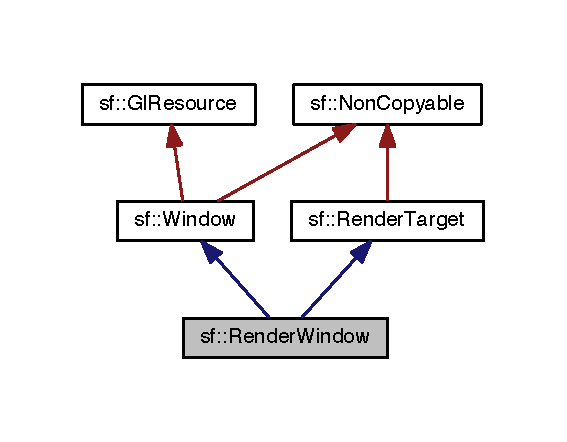
\includegraphics[width=272pt]{classsf_1_1_render_window__inherit__graph}
\end{center}
\end{figure}


Collaboration diagram for sf\-:\-:Render\-Window\-:
\nopagebreak
\begin{figure}[H]
\begin{center}
\leavevmode
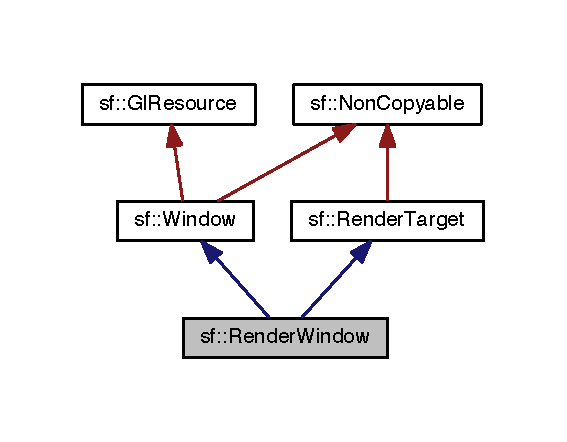
\includegraphics[width=272pt]{classsf_1_1_render_window__coll__graph}
\end{center}
\end{figure}
\subsection*{Public Member Functions}
\begin{DoxyCompactItemize}
\item 
\hyperlink{classsf_1_1_render_window_a839bbf336bdcafb084dafc3076fc9021}{Render\-Window} ()
\begin{DoxyCompactList}\small\item\em Default constructor. \end{DoxyCompactList}\item 
\hyperlink{classsf_1_1_render_window_a828cf38403a246c11ae98a316f271941}{Render\-Window} (\hyperlink{classsf_1_1_video_mode}{Video\-Mode} \hyperlink{gl3_8h_a1e71d9c196e4683cc06c4b54d53f7ef5}{mode}, const \hyperlink{gl3_8h_ac83513893df92266f79a515488701770}{std\-::string} \&title, \hyperlink{namespacesf_aa746fb1ddef4410bddf198ebb27e727c}{Uint32} style=\hyperlink{group__window_ggae1db07091f9745bd223882ba55e7fae2a5597cd420fc461807e4a201c92adea37}{Style\-::\-Default}, const \hyperlink{structsf_1_1_context_settings}{Context\-Settings} \&settings=\hyperlink{structsf_1_1_context_settings}{Context\-Settings}())
\begin{DoxyCompactList}\small\item\em Construct a new window. \end{DoxyCompactList}\item 
\hyperlink{classsf_1_1_render_window_a25c0af7d515e710b6eebc9c6be952aa5}{Render\-Window} (Window\-Handle handle, const \hyperlink{structsf_1_1_context_settings}{Context\-Settings} \&settings=\hyperlink{structsf_1_1_context_settings}{Context\-Settings}())
\begin{DoxyCompactList}\small\item\em Construct the window from an existing control. \end{DoxyCompactList}\item 
virtual \hyperlink{classsf_1_1_render_window_a3407e36bfc1752d723140438a825365c}{$\sim$\-Render\-Window} ()
\begin{DoxyCompactList}\small\item\em Destructor. \end{DoxyCompactList}\item 
virtual \hyperlink{namespacesf_aaa02ba42bf79b001a376fe9d79254cb3}{Vector2u} \hyperlink{classsf_1_1_render_window_a2c7ff414be32621a453745cf2a0f8a3e}{get\-Size} () const 
\begin{DoxyCompactList}\small\item\em Get the size of the rendering region of the window. \end{DoxyCompactList}\item 
\hyperlink{classsf_1_1_image}{Image} \hyperlink{classsf_1_1_render_window_a9bd8655d0bac83145bfc329ea7a6d538}{capture} () const 
\begin{DoxyCompactList}\small\item\em Copy the current contents of the window to an image. \end{DoxyCompactList}\end{DoxyCompactItemize}
\subsection*{Protected Member Functions}
\begin{DoxyCompactItemize}
\item 
virtual \hyperlink{glutf90_8h_ac778d6f63f1aaf8ebda0ce6ac821b56e}{void} \hyperlink{classsf_1_1_render_window_a5bef0040b0fa87bed9fbd459c980d53a}{on\-Create} ()
\begin{DoxyCompactList}\small\item\em Function called after the window has been created. \end{DoxyCompactList}\item 
virtual \hyperlink{glutf90_8h_ac778d6f63f1aaf8ebda0ce6ac821b56e}{void} \hyperlink{classsf_1_1_render_window_a5c85fe482313562d33ffd24a194b6fef}{on\-Resize} ()
\begin{DoxyCompactList}\small\item\em Function called after the window has been resized. \end{DoxyCompactList}\end{DoxyCompactItemize}


\subsection{Detailed Description}
\hyperlink{classsf_1_1_window}{Window} that can serve as a target for 2\-D drawing. 

\hyperlink{classsf_1_1_render_window}{sf\-::\-Render\-Window} is the main class of the Graphics module. It defines an O\-S window that can be painted using the other classes of the graphics module.

\hyperlink{classsf_1_1_render_window}{sf\-::\-Render\-Window} is derived from \hyperlink{classsf_1_1_window}{sf\-::\-Window}, thus it inherits all its features\-: events, window management, Open\-G\-L rendering, etc. See the documentation of \hyperlink{classsf_1_1_window}{sf\-::\-Window} for a more complete description of all these features, as well as code examples.

On top of that, \hyperlink{classsf_1_1_render_window}{sf\-::\-Render\-Window} adds more features related to 2\-D drawing with the graphics module (see its base class \hyperlink{classsf_1_1_render_target}{sf\-::\-Render\-Target} for more details). Here is a typical rendering and event loop with a \hyperlink{classsf_1_1_render_window}{sf\-::\-Render\-Window}\-:


\begin{DoxyCode}
\textcolor{comment}{// Declare and create a new render-window}
\hyperlink{classsf_1_1_render_window}{sf::RenderWindow} window(\hyperlink{classsf_1_1_video_mode}{sf::VideoMode}(800, 600), \textcolor{stringliteral}{"SFML window"});

\textcolor{comment}{// Limit the framerate to 60 frames per second (this step is optional)}
window.setFramerateLimit(60);

\textcolor{comment}{// The main loop - ends as soon as the window is closed}
\textcolor{keywordflow}{while} (window.isOpen())
\{
   \textcolor{comment}{// Event processing}
   \hyperlink{classsf_1_1_event}{sf::Event} event;
   \textcolor{keywordflow}{while} (window.pollEvent(event))
   \{
       \textcolor{comment}{// Request for closing the window}
       \textcolor{keywordflow}{if} (event.\hyperlink{classsf_1_1_event_adf2f8044f713fd9d6019077b0d1ffe0a}{type} == \hyperlink{classsf_1_1_event_af41fa9ed45c02449030699f671331d4aa316e4212e083f1dce79efd8d9e9c0a95}{sf::Event::Closed})
           window.close();
   \}

   \textcolor{comment}{// Clear the whole window before rendering a new frame}
   window.clear();

   \textcolor{comment}{// Draw some graphical entities}
   window.draw(sprite);
   window.draw(circle);
   window.draw(text);

   \textcolor{comment}{// End the current frame and display its contents on screen}
   window.display();
\}
\end{DoxyCode}


Like \hyperlink{classsf_1_1_window}{sf\-::\-Window}, \hyperlink{classsf_1_1_render_window}{sf\-::\-Render\-Window} is still able to render direct Open\-G\-L stuff. It is even possible to mix together Open\-G\-L calls and regular S\-F\-M\-L drawing commands.


\begin{DoxyCode}
\textcolor{comment}{// Create the render window}
\hyperlink{classsf_1_1_render_window}{sf::RenderWindow} window(\hyperlink{classsf_1_1_video_mode}{sf::VideoMode}(800, 600), \textcolor{stringliteral}{"SFML OpenGL"});

\textcolor{comment}{// Create a sprite and a text to display}
\hyperlink{classsf_1_1_sprite}{sf::Sprite} sprite;
\hyperlink{classsf_1_1_text}{sf::Text} text;
...

\textcolor{comment}{// Perform OpenGL initializations}
glMatrixMode(\hyperlink{gl_8h_a85e93b355494186ced027f1a1142fefb}{GL\_PROJECTION});
...

\textcolor{comment}{// Start the rendering loop}
while (window.isOpen())
\{
    \textcolor{comment}{// Process events}
    ...

    \textcolor{comment}{// Draw a background sprite}
    window.pushGLStates();
    window.draw(sprite);
    window.popGLStates();

    \textcolor{comment}{// Draw a 3D object using OpenGL}
    \hyperlink{gl_8h_a78d1cc551d8585ab6aee14f75cd6671f}{glBegin}(\hyperlink{gl_8h_a36b428225d54dd9cf2e564e5ada3ad3d}{GL\_QUADS});
        \hyperlink{gl_8h_a958e3235784668353fe641e7b4fafa83}{glVertex3f}(...);
        ...
    \hyperlink{gl_8h_af50123535ec586f448744e0bc5a35923}{glEnd}();

    \textcolor{comment}{// Draw text on top of the 3D object}
    window.pushGLStates();
    window.draw(text);
    window.popGLStates();

    \textcolor{comment}{// Finally, display the rendered frame on screen}
    window.display();
\}
\end{DoxyCode}


\begin{DoxySeeAlso}{See Also}
\hyperlink{classsf_1_1_window}{sf\-::\-Window}, \hyperlink{classsf_1_1_render_target}{sf\-::\-Render\-Target}, \hyperlink{classsf_1_1_render_texture}{sf\-::\-Render\-Texture}, \hyperlink{classsf_1_1_view}{sf\-::\-View} 
\end{DoxySeeAlso}


Definition at line 44 of file Render\-Window.\-hpp.



\subsection{Constructor \& Destructor Documentation}
\hypertarget{classsf_1_1_render_window_a839bbf336bdcafb084dafc3076fc9021}{\index{sf\-::\-Render\-Window@{sf\-::\-Render\-Window}!Render\-Window@{Render\-Window}}
\index{Render\-Window@{Render\-Window}!sf::RenderWindow@{sf\-::\-Render\-Window}}
\subsubsection[{Render\-Window}]{\setlength{\rightskip}{0pt plus 5cm}sf\-::\-Render\-Window\-::\-Render\-Window (
\begin{DoxyParamCaption}
{}
\end{DoxyParamCaption}
)}}\label{classsf_1_1_render_window_a839bbf336bdcafb084dafc3076fc9021}


Default constructor. 

This constructor doesn't actually create the window, use the other constructors or call Create to do so. \hypertarget{classsf_1_1_render_window_a828cf38403a246c11ae98a316f271941}{\index{sf\-::\-Render\-Window@{sf\-::\-Render\-Window}!Render\-Window@{Render\-Window}}
\index{Render\-Window@{Render\-Window}!sf::RenderWindow@{sf\-::\-Render\-Window}}
\subsubsection[{Render\-Window}]{\setlength{\rightskip}{0pt plus 5cm}sf\-::\-Render\-Window\-::\-Render\-Window (
\begin{DoxyParamCaption}
\item[{{\bf Video\-Mode}}]{mode, }
\item[{const {\bf std\-::string} \&}]{title, }
\item[{{\bf Uint32}}]{style = {\ttfamily {\bf Style\-::\-Default}}, }
\item[{const {\bf Context\-Settings} \&}]{settings = {\ttfamily {\bf Context\-Settings}()}}
\end{DoxyParamCaption}
)}}\label{classsf_1_1_render_window_a828cf38403a246c11ae98a316f271941}


Construct a new window. 

This constructor creates the window with the size and pixel depth defined in {\itshape mode}. An optional style can be passed to customize the look and behaviour of the window (borders, title bar, resizable, closable, ...).

The fourth parameter is an optional structure specifying advanced Open\-G\-L context settings such as antialiasing, depth-\/buffer bits, etc. You shouldn't care about these parameters for a regular usage of the graphics module.


\begin{DoxyParams}{Parameters}
{\em mode} & Video mode to use (defines the width, height and depth of the rendering area of the window) \\
\hline
{\em title} & Title of the window \\
\hline
{\em style} & \hyperlink{classsf_1_1_window}{Window} style \\
\hline
{\em settings} & Additional settings for the underlying Open\-G\-L context \\
\hline
\end{DoxyParams}
\hypertarget{classsf_1_1_render_window_a25c0af7d515e710b6eebc9c6be952aa5}{\index{sf\-::\-Render\-Window@{sf\-::\-Render\-Window}!Render\-Window@{Render\-Window}}
\index{Render\-Window@{Render\-Window}!sf::RenderWindow@{sf\-::\-Render\-Window}}
\subsubsection[{Render\-Window}]{\setlength{\rightskip}{0pt plus 5cm}sf\-::\-Render\-Window\-::\-Render\-Window (
\begin{DoxyParamCaption}
\item[{Window\-Handle}]{handle, }
\item[{const {\bf Context\-Settings} \&}]{settings = {\ttfamily {\bf Context\-Settings}()}}
\end{DoxyParamCaption}
)\hspace{0.3cm}{\ttfamily [explicit]}}}\label{classsf_1_1_render_window_a25c0af7d515e710b6eebc9c6be952aa5}


Construct the window from an existing control. 

Use this constructor if you want to create an S\-F\-M\-L rendering area into an already existing control.

The fourth parameter is an optional structure specifying advanced Open\-G\-L context settings such as antialiasing, depth-\/buffer bits, etc. You shouldn't care about these parameters for a regular usage of the graphics module.


\begin{DoxyParams}{Parameters}
{\em handle} & Platform-\/specific handle of the control \\
\hline
{\em settings} & Additional settings for the underlying Open\-G\-L context \\
\hline
\end{DoxyParams}
\hypertarget{classsf_1_1_render_window_a3407e36bfc1752d723140438a825365c}{\index{sf\-::\-Render\-Window@{sf\-::\-Render\-Window}!$\sim$\-Render\-Window@{$\sim$\-Render\-Window}}
\index{$\sim$\-Render\-Window@{$\sim$\-Render\-Window}!sf::RenderWindow@{sf\-::\-Render\-Window}}
\subsubsection[{$\sim$\-Render\-Window}]{\setlength{\rightskip}{0pt plus 5cm}virtual sf\-::\-Render\-Window\-::$\sim$\-Render\-Window (
\begin{DoxyParamCaption}
{}
\end{DoxyParamCaption}
)\hspace{0.3cm}{\ttfamily [virtual]}}}\label{classsf_1_1_render_window_a3407e36bfc1752d723140438a825365c}


Destructor. 

Closes the window and free all the resources attached to it. 

\subsection{Member Function Documentation}
\hypertarget{classsf_1_1_render_window_a9bd8655d0bac83145bfc329ea7a6d538}{\index{sf\-::\-Render\-Window@{sf\-::\-Render\-Window}!capture@{capture}}
\index{capture@{capture}!sf::RenderWindow@{sf\-::\-Render\-Window}}
\subsubsection[{capture}]{\setlength{\rightskip}{0pt plus 5cm}{\bf Image} sf\-::\-Render\-Window\-::capture (
\begin{DoxyParamCaption}
{}
\end{DoxyParamCaption}
) const}}\label{classsf_1_1_render_window_a9bd8655d0bac83145bfc329ea7a6d538}


Copy the current contents of the window to an image. 

This is a slow operation, whose main purpose is to make screenshots of the application. If you want to update an image with the contents of the window and then use it for drawing, you should rather use a \hyperlink{classsf_1_1_texture}{sf\-::\-Texture} and its update(\-Window\&) function. You can also draw things directly to a texture with the \hyperlink{classsf_1_1_render_texture}{sf\-::\-Render\-Texture} class.

\begin{DoxyReturn}{Returns}
\hyperlink{classsf_1_1_image}{Image} containing the captured contents 
\end{DoxyReturn}
\hypertarget{classsf_1_1_render_window_a2c7ff414be32621a453745cf2a0f8a3e}{\index{sf\-::\-Render\-Window@{sf\-::\-Render\-Window}!get\-Size@{get\-Size}}
\index{get\-Size@{get\-Size}!sf::RenderWindow@{sf\-::\-Render\-Window}}
\subsubsection[{get\-Size}]{\setlength{\rightskip}{0pt plus 5cm}virtual {\bf Vector2u} sf\-::\-Render\-Window\-::get\-Size (
\begin{DoxyParamCaption}
{}
\end{DoxyParamCaption}
) const\hspace{0.3cm}{\ttfamily [virtual]}}}\label{classsf_1_1_render_window_a2c7ff414be32621a453745cf2a0f8a3e}


Get the size of the rendering region of the window. 

The size doesn't include the titlebar and borders of the window.

\begin{DoxyReturn}{Returns}
Size in pixels 
\end{DoxyReturn}


Implements \hyperlink{classsf_1_1_render_target_a2e5ade2457d9fb4c4907ae5b3d9e94a5}{sf\-::\-Render\-Target}.

\hypertarget{classsf_1_1_render_window_a5bef0040b0fa87bed9fbd459c980d53a}{\index{sf\-::\-Render\-Window@{sf\-::\-Render\-Window}!on\-Create@{on\-Create}}
\index{on\-Create@{on\-Create}!sf::RenderWindow@{sf\-::\-Render\-Window}}
\subsubsection[{on\-Create}]{\setlength{\rightskip}{0pt plus 5cm}virtual {\bf void} sf\-::\-Render\-Window\-::on\-Create (
\begin{DoxyParamCaption}
{}
\end{DoxyParamCaption}
)\hspace{0.3cm}{\ttfamily [protected]}, {\ttfamily [virtual]}}}\label{classsf_1_1_render_window_a5bef0040b0fa87bed9fbd459c980d53a}


Function called after the window has been created. 

This function is called so that derived classes can perform their own specific initialization as soon as the window is created. 

Reimplemented from \hyperlink{classsf_1_1_window_a106633b9be49b27f83d4712689b493eb}{sf\-::\-Window}.

\hypertarget{classsf_1_1_render_window_a5c85fe482313562d33ffd24a194b6fef}{\index{sf\-::\-Render\-Window@{sf\-::\-Render\-Window}!on\-Resize@{on\-Resize}}
\index{on\-Resize@{on\-Resize}!sf::RenderWindow@{sf\-::\-Render\-Window}}
\subsubsection[{on\-Resize}]{\setlength{\rightskip}{0pt plus 5cm}virtual {\bf void} sf\-::\-Render\-Window\-::on\-Resize (
\begin{DoxyParamCaption}
{}
\end{DoxyParamCaption}
)\hspace{0.3cm}{\ttfamily [protected]}, {\ttfamily [virtual]}}}\label{classsf_1_1_render_window_a5c85fe482313562d33ffd24a194b6fef}


Function called after the window has been resized. 

This function is called so that derived classes can perform custom actions when the size of the window changes. 

Reimplemented from \hyperlink{classsf_1_1_window_a10f567a387da7b49f417f73321fcf64d}{sf\-::\-Window}.



The documentation for this class was generated from the following file\-:\begin{DoxyCompactItemize}
\item 
/\-Users/ira/\-Dropbox/ira\-\_\-dev/protobyte\-\_\-research/other\-\_\-libs/\-S\-F\-M\-L/dylibs/root/usr/local/include/\-S\-F\-M\-L/\-Graphics/\hyperlink{_render_window_8hpp}{Render\-Window.\-hpp}\end{DoxyCompactItemize}

\hypertarget{classsf_1_1_http_1_1_request}{\section{sf\-:\-:Http\-:\-:Request Class Reference}
\label{classsf_1_1_http_1_1_request}\index{sf\-::\-Http\-::\-Request@{sf\-::\-Http\-::\-Request}}
}


Define a H\-T\-T\-P request.  




{\ttfamily \#include $<$Http.\-hpp$>$}

\subsection*{Public Types}
\begin{DoxyCompactItemize}
\item 
enum \hyperlink{classsf_1_1_http_1_1_request_a620f8bff6f43e1378f321bf53fbf5598}{Method} \{ \hyperlink{classsf_1_1_http_1_1_request_a620f8bff6f43e1378f321bf53fbf5598ab822baed393f3d0353621e5378b9fcb4}{Get}, 
\hyperlink{classsf_1_1_http_1_1_request_a620f8bff6f43e1378f321bf53fbf5598ae8ec4048b9550f8d0747d4199603141a}{Post}, 
\hyperlink{classsf_1_1_http_1_1_request_a620f8bff6f43e1378f321bf53fbf5598a4df23138be7ed60f47aba6548ba65e7b}{Head}
 \}
\begin{DoxyCompactList}\small\item\em Enumerate the available H\-T\-T\-P methods for a request. \end{DoxyCompactList}\end{DoxyCompactItemize}
\subsection*{Public Member Functions}
\begin{DoxyCompactItemize}
\item 
\hyperlink{classsf_1_1_http_1_1_request_a8e89d9e8ffcc1163259b35d79809a61c}{Request} (const \hyperlink{gl3_8h_ac83513893df92266f79a515488701770}{std\-::string} \&uri=\char`\"{}/\char`\"{}, \hyperlink{classsf_1_1_http_1_1_request_a620f8bff6f43e1378f321bf53fbf5598}{Method} method=\hyperlink{classsf_1_1_http_1_1_request_a620f8bff6f43e1378f321bf53fbf5598ab822baed393f3d0353621e5378b9fcb4}{Get}, const \hyperlink{gl3_8h_ac83513893df92266f79a515488701770}{std\-::string} \&body=\char`\"{}\char`\"{})
\begin{DoxyCompactList}\small\item\em Default constructor. \end{DoxyCompactList}\item 
\hyperlink{glutf90_8h_ac778d6f63f1aaf8ebda0ce6ac821b56e}{void} \hyperlink{classsf_1_1_http_1_1_request_aea672fae5dd089f4b6b3745ed46210d2}{set\-Field} (const \hyperlink{gl3_8h_ac83513893df92266f79a515488701770}{std\-::string} \&field, const \hyperlink{gl3_8h_ac83513893df92266f79a515488701770}{std\-::string} \&\hyperlink{gl3_8h_a8ad81492d410ff2ac11f754f4042150f}{value})
\begin{DoxyCompactList}\small\item\em Set the value of a field. \end{DoxyCompactList}\item 
\hyperlink{glutf90_8h_ac778d6f63f1aaf8ebda0ce6ac821b56e}{void} \hyperlink{classsf_1_1_http_1_1_request_abab148554e873e80d2e41376fde1cb62}{set\-Method} (\hyperlink{classsf_1_1_http_1_1_request_a620f8bff6f43e1378f321bf53fbf5598}{Method} method)
\begin{DoxyCompactList}\small\item\em Set the request method. \end{DoxyCompactList}\item 
\hyperlink{glutf90_8h_ac778d6f63f1aaf8ebda0ce6ac821b56e}{void} \hyperlink{classsf_1_1_http_1_1_request_a3723de4b4f1a14b744477841c4ac22e6}{set\-Uri} (const \hyperlink{gl3_8h_ac83513893df92266f79a515488701770}{std\-::string} \&uri)
\begin{DoxyCompactList}\small\item\em Set the requested U\-R\-I. \end{DoxyCompactList}\item 
\hyperlink{glutf90_8h_ac778d6f63f1aaf8ebda0ce6ac821b56e}{void} \hyperlink{classsf_1_1_http_1_1_request_aa683b607b737a6224a91387b4108d3c7}{set\-Http\-Version} (unsigned int major, unsigned int minor)
\begin{DoxyCompactList}\small\item\em Set the H\-T\-T\-P version for the request. \end{DoxyCompactList}\item 
\hyperlink{glutf90_8h_ac778d6f63f1aaf8ebda0ce6ac821b56e}{void} \hyperlink{classsf_1_1_http_1_1_request_ae9f61ec3fa1639c70e9b5780cb35578e}{set\-Body} (const \hyperlink{gl3_8h_ac83513893df92266f79a515488701770}{std\-::string} \&body)
\begin{DoxyCompactList}\small\item\em Set the body of the request. \end{DoxyCompactList}\end{DoxyCompactItemize}
\subsection*{Friends}
\begin{DoxyCompactItemize}
\item 
class \hyperlink{classsf_1_1_http_1_1_request_aba95e2a7762bb5df986048b05d03a22e}{Http}
\end{DoxyCompactItemize}


\subsection{Detailed Description}
Define a H\-T\-T\-P request. 

Definition at line 54 of file Http.\-hpp.



\subsection{Member Enumeration Documentation}
\hypertarget{classsf_1_1_http_1_1_request_a620f8bff6f43e1378f321bf53fbf5598}{\index{sf\-::\-Http\-::\-Request@{sf\-::\-Http\-::\-Request}!Method@{Method}}
\index{Method@{Method}!sf::Http::Request@{sf\-::\-Http\-::\-Request}}
\subsubsection[{Method}]{\setlength{\rightskip}{0pt plus 5cm}enum {\bf sf\-::\-Http\-::\-Request\-::\-Method}}}\label{classsf_1_1_http_1_1_request_a620f8bff6f43e1378f321bf53fbf5598}


Enumerate the available H\-T\-T\-P methods for a request. 

\begin{Desc}
\item[Enumerator]\par
\begin{description}
\index{Get@{Get}!sf\-::\-Http\-::\-Request@{sf\-::\-Http\-::\-Request}}\index{sf\-::\-Http\-::\-Request@{sf\-::\-Http\-::\-Request}!Get@{Get}}\item[{\em 
\hypertarget{classsf_1_1_http_1_1_request_a620f8bff6f43e1378f321bf53fbf5598ab822baed393f3d0353621e5378b9fcb4}{Get}\label{classsf_1_1_http_1_1_request_a620f8bff6f43e1378f321bf53fbf5598ab822baed393f3d0353621e5378b9fcb4}
}]\hyperlink{classsf_1_1_http_1_1_request}{Request} in get mode, standard method to retrieve a page. \index{Post@{Post}!sf\-::\-Http\-::\-Request@{sf\-::\-Http\-::\-Request}}\index{sf\-::\-Http\-::\-Request@{sf\-::\-Http\-::\-Request}!Post@{Post}}\item[{\em 
\hypertarget{classsf_1_1_http_1_1_request_a620f8bff6f43e1378f321bf53fbf5598ae8ec4048b9550f8d0747d4199603141a}{Post}\label{classsf_1_1_http_1_1_request_a620f8bff6f43e1378f321bf53fbf5598ae8ec4048b9550f8d0747d4199603141a}
}]\hyperlink{classsf_1_1_http_1_1_request}{Request} in post mode, usually to send data to a page. \index{Head@{Head}!sf\-::\-Http\-::\-Request@{sf\-::\-Http\-::\-Request}}\index{sf\-::\-Http\-::\-Request@{sf\-::\-Http\-::\-Request}!Head@{Head}}\item[{\em 
\hypertarget{classsf_1_1_http_1_1_request_a620f8bff6f43e1378f321bf53fbf5598a4df23138be7ed60f47aba6548ba65e7b}{Head}\label{classsf_1_1_http_1_1_request_a620f8bff6f43e1378f321bf53fbf5598a4df23138be7ed60f47aba6548ba65e7b}
}]\hyperlink{classsf_1_1_http_1_1_request}{Request} a page's header only. \end{description}
\end{Desc}


Definition at line 62 of file Http.\-hpp.



\subsection{Constructor \& Destructor Documentation}
\hypertarget{classsf_1_1_http_1_1_request_a8e89d9e8ffcc1163259b35d79809a61c}{\index{sf\-::\-Http\-::\-Request@{sf\-::\-Http\-::\-Request}!Request@{Request}}
\index{Request@{Request}!sf::Http::Request@{sf\-::\-Http\-::\-Request}}
\subsubsection[{Request}]{\setlength{\rightskip}{0pt plus 5cm}sf\-::\-Http\-::\-Request\-::\-Request (
\begin{DoxyParamCaption}
\item[{const {\bf std\-::string} \&}]{uri = {\ttfamily \char`\"{}/\char`\"{}}, }
\item[{{\bf Method}}]{method = {\ttfamily {\bf Get}}, }
\item[{const {\bf std\-::string} \&}]{body = {\ttfamily \char`\"{}\char`\"{}}}
\end{DoxyParamCaption}
)}}\label{classsf_1_1_http_1_1_request_a8e89d9e8ffcc1163259b35d79809a61c}


Default constructor. 

This constructor creates a G\-E\-T request, with the root U\-R\-I (\char`\"{}/\char`\"{}) and an empty body.


\begin{DoxyParams}{Parameters}
{\em uri} & Target U\-R\-I \\
\hline
{\em method} & Method to use for the request \\
\hline
{\em body} & Content of the request's body \\
\hline
\end{DoxyParams}


\subsection{Member Function Documentation}
\hypertarget{classsf_1_1_http_1_1_request_ae9f61ec3fa1639c70e9b5780cb35578e}{\index{sf\-::\-Http\-::\-Request@{sf\-::\-Http\-::\-Request}!set\-Body@{set\-Body}}
\index{set\-Body@{set\-Body}!sf::Http::Request@{sf\-::\-Http\-::\-Request}}
\subsubsection[{set\-Body}]{\setlength{\rightskip}{0pt plus 5cm}{\bf void} sf\-::\-Http\-::\-Request\-::set\-Body (
\begin{DoxyParamCaption}
\item[{const {\bf std\-::string} \&}]{body}
\end{DoxyParamCaption}
)}}\label{classsf_1_1_http_1_1_request_ae9f61ec3fa1639c70e9b5780cb35578e}


Set the body of the request. 

The body of a request is optional and only makes sense for P\-O\-S\-T requests. It is ignored for all other methods. The body is empty by default.


\begin{DoxyParams}{Parameters}
{\em body} & Content of the body \\
\hline
\end{DoxyParams}
\hypertarget{classsf_1_1_http_1_1_request_aea672fae5dd089f4b6b3745ed46210d2}{\index{sf\-::\-Http\-::\-Request@{sf\-::\-Http\-::\-Request}!set\-Field@{set\-Field}}
\index{set\-Field@{set\-Field}!sf::Http::Request@{sf\-::\-Http\-::\-Request}}
\subsubsection[{set\-Field}]{\setlength{\rightskip}{0pt plus 5cm}{\bf void} sf\-::\-Http\-::\-Request\-::set\-Field (
\begin{DoxyParamCaption}
\item[{const {\bf std\-::string} \&}]{field, }
\item[{const {\bf std\-::string} \&}]{value}
\end{DoxyParamCaption}
)}}\label{classsf_1_1_http_1_1_request_aea672fae5dd089f4b6b3745ed46210d2}


Set the value of a field. 

The field is created if it doesn't exist. The name of the field is case insensitive. By default, a request doesn't contain any field (but the mandatory fields are added later by the H\-T\-T\-P client when sending the request).


\begin{DoxyParams}{Parameters}
{\em field} & Name of the field to set \\
\hline
{\em value} & Value of the field \\
\hline
\end{DoxyParams}
\hypertarget{classsf_1_1_http_1_1_request_aa683b607b737a6224a91387b4108d3c7}{\index{sf\-::\-Http\-::\-Request@{sf\-::\-Http\-::\-Request}!set\-Http\-Version@{set\-Http\-Version}}
\index{set\-Http\-Version@{set\-Http\-Version}!sf::Http::Request@{sf\-::\-Http\-::\-Request}}
\subsubsection[{set\-Http\-Version}]{\setlength{\rightskip}{0pt plus 5cm}{\bf void} sf\-::\-Http\-::\-Request\-::set\-Http\-Version (
\begin{DoxyParamCaption}
\item[{unsigned int}]{major, }
\item[{unsigned int}]{minor}
\end{DoxyParamCaption}
)}}\label{classsf_1_1_http_1_1_request_aa683b607b737a6224a91387b4108d3c7}


Set the H\-T\-T\-P version for the request. 

The H\-T\-T\-P version is 1.\-0 by default.


\begin{DoxyParams}{Parameters}
{\em major} & Major H\-T\-T\-P version number \\
\hline
{\em minor} & Minor H\-T\-T\-P version number \\
\hline
\end{DoxyParams}
\hypertarget{classsf_1_1_http_1_1_request_abab148554e873e80d2e41376fde1cb62}{\index{sf\-::\-Http\-::\-Request@{sf\-::\-Http\-::\-Request}!set\-Method@{set\-Method}}
\index{set\-Method@{set\-Method}!sf::Http::Request@{sf\-::\-Http\-::\-Request}}
\subsubsection[{set\-Method}]{\setlength{\rightskip}{0pt plus 5cm}{\bf void} sf\-::\-Http\-::\-Request\-::set\-Method (
\begin{DoxyParamCaption}
\item[{{\bf Method}}]{method}
\end{DoxyParamCaption}
)}}\label{classsf_1_1_http_1_1_request_abab148554e873e80d2e41376fde1cb62}


Set the request method. 

See the Method enumeration for a complete list of all the availale methods. The method is \hyperlink{classsf_1_1_http_1_1_request_a620f8bff6f43e1378f321bf53fbf5598ab822baed393f3d0353621e5378b9fcb4}{Http\-::\-Request\-::\-Get} by default.


\begin{DoxyParams}{Parameters}
{\em method} & Method to use for the request \\
\hline
\end{DoxyParams}
\hypertarget{classsf_1_1_http_1_1_request_a3723de4b4f1a14b744477841c4ac22e6}{\index{sf\-::\-Http\-::\-Request@{sf\-::\-Http\-::\-Request}!set\-Uri@{set\-Uri}}
\index{set\-Uri@{set\-Uri}!sf::Http::Request@{sf\-::\-Http\-::\-Request}}
\subsubsection[{set\-Uri}]{\setlength{\rightskip}{0pt plus 5cm}{\bf void} sf\-::\-Http\-::\-Request\-::set\-Uri (
\begin{DoxyParamCaption}
\item[{const {\bf std\-::string} \&}]{uri}
\end{DoxyParamCaption}
)}}\label{classsf_1_1_http_1_1_request_a3723de4b4f1a14b744477841c4ac22e6}


Set the requested U\-R\-I. 

The U\-R\-I is the resource (usually a web page or a file) that you want to get or post. The U\-R\-I is \char`\"{}/\char`\"{} (the root page) by default.


\begin{DoxyParams}{Parameters}
{\em uri} & U\-R\-I to request, relative to the host \\
\hline
\end{DoxyParams}


\subsection{Friends And Related Function Documentation}
\hypertarget{classsf_1_1_http_1_1_request_aba95e2a7762bb5df986048b05d03a22e}{\index{sf\-::\-Http\-::\-Request@{sf\-::\-Http\-::\-Request}!Http@{Http}}
\index{Http@{Http}!sf::Http::Request@{sf\-::\-Http\-::\-Request}}
\subsubsection[{Http}]{\setlength{\rightskip}{0pt plus 5cm}friend class {\bf Http}\hspace{0.3cm}{\ttfamily [friend]}}}\label{classsf_1_1_http_1_1_request_aba95e2a7762bb5df986048b05d03a22e}


Definition at line 146 of file Http.\-hpp.



The documentation for this class was generated from the following file\-:\begin{DoxyCompactItemize}
\item 
/\-Users/ira/\-Dropbox/ira\-\_\-dev/protobyte\-\_\-research/other\-\_\-libs/\-S\-F\-M\-L/dylibs/root/usr/local/include/\-S\-F\-M\-L/\-Network/\hyperlink{_http_8hpp}{Http.\-hpp}\end{DoxyCompactItemize}

\hypertarget{classsf_1_1_http_1_1_response}{\section{sf\-:\-:Http\-:\-:Response Class Reference}
\label{classsf_1_1_http_1_1_response}\index{sf\-::\-Http\-::\-Response@{sf\-::\-Http\-::\-Response}}
}


Define a H\-T\-T\-P response.  




{\ttfamily \#include $<$Http.\-hpp$>$}

\subsection*{Public Types}
\begin{DoxyCompactItemize}
\item 
enum \hyperlink{classsf_1_1_http_1_1_response_a663e071978e30fbbeb20ed045be874d8}{Status} \{ \\*
\hyperlink{classsf_1_1_http_1_1_response_a663e071978e30fbbeb20ed045be874d8a0158f932254d3f09647dd1f64bd43832}{Ok} = 200, 
\hyperlink{classsf_1_1_http_1_1_response_a663e071978e30fbbeb20ed045be874d8a0a6e8bafa9365a0ed10b8a9cbfd0649b}{Created} = 201, 
\hyperlink{classsf_1_1_http_1_1_response_a663e071978e30fbbeb20ed045be874d8ad328945457bd2f0d65107ba6b5ccd443}{Accepted} = 202, 
\hyperlink{classsf_1_1_http_1_1_response_a663e071978e30fbbeb20ed045be874d8aefde9e4abf5682dcd314d63143be42e0}{No\-Content} = 204, 
\\*
\hyperlink{classsf_1_1_http_1_1_response_a663e071978e30fbbeb20ed045be874d8a77327cc2a5e34cc64030b322e61d12a8}{Reset\-Content} = 205, 
\hyperlink{classsf_1_1_http_1_1_response_a663e071978e30fbbeb20ed045be874d8a0cfae3ab0469b73dfddc54312a5e6a8a}{Partial\-Content} = 206, 
\hyperlink{classsf_1_1_http_1_1_response_a663e071978e30fbbeb20ed045be874d8add95cbd8fa27516821f763488557f96b}{Multiple\-Choices} = 300, 
\hyperlink{classsf_1_1_http_1_1_response_a663e071978e30fbbeb20ed045be874d8a2f91651db3a09628faf68cbcefa0810a}{Moved\-Permanently} = 301, 
\\*
\hyperlink{classsf_1_1_http_1_1_response_a663e071978e30fbbeb20ed045be874d8a05c50d7b17c844e0b909e5802d5f1587}{Moved\-Temporarily} = 302, 
\hyperlink{classsf_1_1_http_1_1_response_a663e071978e30fbbeb20ed045be874d8a060ebc3af266e6bfe045b89e298e2545}{Not\-Modified} = 304, 
\hyperlink{classsf_1_1_http_1_1_response_a663e071978e30fbbeb20ed045be874d8a3f88a714cf5483ee22f9051e5a3c080a}{Bad\-Request} = 400, 
\hyperlink{classsf_1_1_http_1_1_response_a663e071978e30fbbeb20ed045be874d8ab7a79b7bff50fb1902c19eecbb4e2a2d}{Unauthorized} = 401, 
\\*
\hyperlink{classsf_1_1_http_1_1_response_a663e071978e30fbbeb20ed045be874d8a64492842e823ebe12a85539b6b454986}{Forbidden} = 403, 
\hyperlink{classsf_1_1_http_1_1_response_a663e071978e30fbbeb20ed045be874d8affca8a8319a62d98bd3ef90ff5cfc030}{Not\-Found} = 404, 
\hyperlink{classsf_1_1_http_1_1_response_a663e071978e30fbbeb20ed045be874d8a12533d00093b190e6d4c0076577e2239}{Range\-Not\-Satisfiable} = 407, 
\hyperlink{classsf_1_1_http_1_1_response_a663e071978e30fbbeb20ed045be874d8adae2b2a936414349d55b4ed8c583fed1}{Internal\-Server\-Error} = 500, 
\\*
\hyperlink{classsf_1_1_http_1_1_response_a663e071978e30fbbeb20ed045be874d8a6920ba06d7e2bcf0b325da23ee95ef68}{Not\-Implemented} = 501, 
\hyperlink{classsf_1_1_http_1_1_response_a663e071978e30fbbeb20ed045be874d8aad0cbad4cdaf448beb763e86bc1f747c}{Bad\-Gateway} = 502, 
\hyperlink{classsf_1_1_http_1_1_response_a663e071978e30fbbeb20ed045be874d8ac4fffba9d5ad4c14171a1bbe4f6adf87}{Service\-Not\-Available} = 503, 
\hyperlink{classsf_1_1_http_1_1_response_a663e071978e30fbbeb20ed045be874d8a215935d823ab44694709a184a71353b0}{Gateway\-Timeout} = 504, 
\\*
\hyperlink{classsf_1_1_http_1_1_response_a663e071978e30fbbeb20ed045be874d8aeb32a1a087d5fcf1a42663eb40c3c305}{Version\-Not\-Supported} = 505, 
\hyperlink{classsf_1_1_http_1_1_response_a663e071978e30fbbeb20ed045be874d8a0af0090420e60bf54da4860749345c95}{Invalid\-Response} = 1000, 
\hyperlink{classsf_1_1_http_1_1_response_a663e071978e30fbbeb20ed045be874d8a7f307376f13bdc06b24fc274ecd2aa60}{Connection\-Failed} = 1001
 \}
\begin{DoxyCompactList}\small\item\em Enumerate all the valid status codes for a response. \end{DoxyCompactList}\end{DoxyCompactItemize}
\subsection*{Public Member Functions}
\begin{DoxyCompactItemize}
\item 
\hyperlink{classsf_1_1_http_1_1_response_a2e51c89356fe6a007c448a841a9ec08c}{Response} ()
\begin{DoxyCompactList}\small\item\em Default constructor. \end{DoxyCompactList}\item 
const \hyperlink{gl3_8h_ac83513893df92266f79a515488701770}{std\-::string} \& \hyperlink{classsf_1_1_http_1_1_response_a25d7cf86538a1045d31e0b601090b8f0}{get\-Field} (const \hyperlink{gl3_8h_ac83513893df92266f79a515488701770}{std\-::string} \&field) const 
\begin{DoxyCompactList}\small\item\em Get the value of a field. \end{DoxyCompactList}\item 
\hyperlink{classsf_1_1_http_1_1_response_a663e071978e30fbbeb20ed045be874d8}{Status} \hyperlink{classsf_1_1_http_1_1_response_a542e9856b1dd260a83940eb982b7f19a}{get\-Status} () const 
\begin{DoxyCompactList}\small\item\em Get the response status code. \end{DoxyCompactList}\item 
unsigned int \hyperlink{classsf_1_1_http_1_1_response_a3da9c689318b945dd12cbe7167161dc6}{get\-Major\-Http\-Version} () const 
\begin{DoxyCompactList}\small\item\em Get the major H\-T\-T\-P version number of the response. \end{DoxyCompactList}\item 
unsigned int \hyperlink{classsf_1_1_http_1_1_response_a1c2217a6a848695875380a70d060b239}{get\-Minor\-Http\-Version} () const 
\begin{DoxyCompactList}\small\item\em Get the minor H\-T\-T\-P version number of the response. \end{DoxyCompactList}\item 
const \hyperlink{gl3_8h_ac83513893df92266f79a515488701770}{std\-::string} \& \hyperlink{classsf_1_1_http_1_1_response_a6b74ef73051a16ebb20041495c758e22}{get\-Body} () const 
\begin{DoxyCompactList}\small\item\em Get the body of the response. \end{DoxyCompactList}\end{DoxyCompactItemize}
\subsection*{Friends}
\begin{DoxyCompactItemize}
\item 
class \hyperlink{classsf_1_1_http_1_1_response_aba95e2a7762bb5df986048b05d03a22e}{Http}
\end{DoxyCompactItemize}


\subsection{Detailed Description}
Define a H\-T\-T\-P response. 

Definition at line 191 of file Http.\-hpp.



\subsection{Member Enumeration Documentation}
\hypertarget{classsf_1_1_http_1_1_response_a663e071978e30fbbeb20ed045be874d8}{\index{sf\-::\-Http\-::\-Response@{sf\-::\-Http\-::\-Response}!Status@{Status}}
\index{Status@{Status}!sf::Http::Response@{sf\-::\-Http\-::\-Response}}
\subsubsection[{Status}]{\setlength{\rightskip}{0pt plus 5cm}enum {\bf sf\-::\-Http\-::\-Response\-::\-Status}}}\label{classsf_1_1_http_1_1_response_a663e071978e30fbbeb20ed045be874d8}


Enumerate all the valid status codes for a response. 

\begin{Desc}
\item[Enumerator]\par
\begin{description}
\index{Ok@{Ok}!sf\-::\-Http\-::\-Response@{sf\-::\-Http\-::\-Response}}\index{sf\-::\-Http\-::\-Response@{sf\-::\-Http\-::\-Response}!Ok@{Ok}}\item[{\em 
\hypertarget{classsf_1_1_http_1_1_response_a663e071978e30fbbeb20ed045be874d8a0158f932254d3f09647dd1f64bd43832}{Ok}\label{classsf_1_1_http_1_1_response_a663e071978e30fbbeb20ed045be874d8a0158f932254d3f09647dd1f64bd43832}
}]Most common code returned when operation was successful. \index{Created@{Created}!sf\-::\-Http\-::\-Response@{sf\-::\-Http\-::\-Response}}\index{sf\-::\-Http\-::\-Response@{sf\-::\-Http\-::\-Response}!Created@{Created}}\item[{\em 
\hypertarget{classsf_1_1_http_1_1_response_a663e071978e30fbbeb20ed045be874d8a0a6e8bafa9365a0ed10b8a9cbfd0649b}{Created}\label{classsf_1_1_http_1_1_response_a663e071978e30fbbeb20ed045be874d8a0a6e8bafa9365a0ed10b8a9cbfd0649b}
}]The resource has successfully been created. \index{Accepted@{Accepted}!sf\-::\-Http\-::\-Response@{sf\-::\-Http\-::\-Response}}\index{sf\-::\-Http\-::\-Response@{sf\-::\-Http\-::\-Response}!Accepted@{Accepted}}\item[{\em 
\hypertarget{classsf_1_1_http_1_1_response_a663e071978e30fbbeb20ed045be874d8ad328945457bd2f0d65107ba6b5ccd443}{Accepted}\label{classsf_1_1_http_1_1_response_a663e071978e30fbbeb20ed045be874d8ad328945457bd2f0d65107ba6b5ccd443}
}]The request has been accepted, but will be processed later by the server. \index{No\-Content@{No\-Content}!sf\-::\-Http\-::\-Response@{sf\-::\-Http\-::\-Response}}\index{sf\-::\-Http\-::\-Response@{sf\-::\-Http\-::\-Response}!No\-Content@{No\-Content}}\item[{\em 
\hypertarget{classsf_1_1_http_1_1_response_a663e071978e30fbbeb20ed045be874d8aefde9e4abf5682dcd314d63143be42e0}{No\-Content}\label{classsf_1_1_http_1_1_response_a663e071978e30fbbeb20ed045be874d8aefde9e4abf5682dcd314d63143be42e0}
}]The server didn't send any data in return. \index{Reset\-Content@{Reset\-Content}!sf\-::\-Http\-::\-Response@{sf\-::\-Http\-::\-Response}}\index{sf\-::\-Http\-::\-Response@{sf\-::\-Http\-::\-Response}!Reset\-Content@{Reset\-Content}}\item[{\em 
\hypertarget{classsf_1_1_http_1_1_response_a663e071978e30fbbeb20ed045be874d8a77327cc2a5e34cc64030b322e61d12a8}{Reset\-Content}\label{classsf_1_1_http_1_1_response_a663e071978e30fbbeb20ed045be874d8a77327cc2a5e34cc64030b322e61d12a8}
}]The server informs the client that it should clear the view (form) that caused the request to be sent. \index{Partial\-Content@{Partial\-Content}!sf\-::\-Http\-::\-Response@{sf\-::\-Http\-::\-Response}}\index{sf\-::\-Http\-::\-Response@{sf\-::\-Http\-::\-Response}!Partial\-Content@{Partial\-Content}}\item[{\em 
\hypertarget{classsf_1_1_http_1_1_response_a663e071978e30fbbeb20ed045be874d8a0cfae3ab0469b73dfddc54312a5e6a8a}{Partial\-Content}\label{classsf_1_1_http_1_1_response_a663e071978e30fbbeb20ed045be874d8a0cfae3ab0469b73dfddc54312a5e6a8a}
}]The server has sent a part of the resource, as a response to a partial G\-E\-T request. \index{Multiple\-Choices@{Multiple\-Choices}!sf\-::\-Http\-::\-Response@{sf\-::\-Http\-::\-Response}}\index{sf\-::\-Http\-::\-Response@{sf\-::\-Http\-::\-Response}!Multiple\-Choices@{Multiple\-Choices}}\item[{\em 
\hypertarget{classsf_1_1_http_1_1_response_a663e071978e30fbbeb20ed045be874d8add95cbd8fa27516821f763488557f96b}{Multiple\-Choices}\label{classsf_1_1_http_1_1_response_a663e071978e30fbbeb20ed045be874d8add95cbd8fa27516821f763488557f96b}
}]The requested page can be accessed from several locations. \index{Moved\-Permanently@{Moved\-Permanently}!sf\-::\-Http\-::\-Response@{sf\-::\-Http\-::\-Response}}\index{sf\-::\-Http\-::\-Response@{sf\-::\-Http\-::\-Response}!Moved\-Permanently@{Moved\-Permanently}}\item[{\em 
\hypertarget{classsf_1_1_http_1_1_response_a663e071978e30fbbeb20ed045be874d8a2f91651db3a09628faf68cbcefa0810a}{Moved\-Permanently}\label{classsf_1_1_http_1_1_response_a663e071978e30fbbeb20ed045be874d8a2f91651db3a09628faf68cbcefa0810a}
}]The requested page has permanently moved to a new location. \index{Moved\-Temporarily@{Moved\-Temporarily}!sf\-::\-Http\-::\-Response@{sf\-::\-Http\-::\-Response}}\index{sf\-::\-Http\-::\-Response@{sf\-::\-Http\-::\-Response}!Moved\-Temporarily@{Moved\-Temporarily}}\item[{\em 
\hypertarget{classsf_1_1_http_1_1_response_a663e071978e30fbbeb20ed045be874d8a05c50d7b17c844e0b909e5802d5f1587}{Moved\-Temporarily}\label{classsf_1_1_http_1_1_response_a663e071978e30fbbeb20ed045be874d8a05c50d7b17c844e0b909e5802d5f1587}
}]The requested page has temporarily moved to a new location. \index{Not\-Modified@{Not\-Modified}!sf\-::\-Http\-::\-Response@{sf\-::\-Http\-::\-Response}}\index{sf\-::\-Http\-::\-Response@{sf\-::\-Http\-::\-Response}!Not\-Modified@{Not\-Modified}}\item[{\em 
\hypertarget{classsf_1_1_http_1_1_response_a663e071978e30fbbeb20ed045be874d8a060ebc3af266e6bfe045b89e298e2545}{Not\-Modified}\label{classsf_1_1_http_1_1_response_a663e071978e30fbbeb20ed045be874d8a060ebc3af266e6bfe045b89e298e2545}
}]For conditionnal requests, means the requested page hasn't changed and doesn't need to be refreshed. \index{Bad\-Request@{Bad\-Request}!sf\-::\-Http\-::\-Response@{sf\-::\-Http\-::\-Response}}\index{sf\-::\-Http\-::\-Response@{sf\-::\-Http\-::\-Response}!Bad\-Request@{Bad\-Request}}\item[{\em 
\hypertarget{classsf_1_1_http_1_1_response_a663e071978e30fbbeb20ed045be874d8a3f88a714cf5483ee22f9051e5a3c080a}{Bad\-Request}\label{classsf_1_1_http_1_1_response_a663e071978e30fbbeb20ed045be874d8a3f88a714cf5483ee22f9051e5a3c080a}
}]The server couldn't understand the request (syntax error) \index{Unauthorized@{Unauthorized}!sf\-::\-Http\-::\-Response@{sf\-::\-Http\-::\-Response}}\index{sf\-::\-Http\-::\-Response@{sf\-::\-Http\-::\-Response}!Unauthorized@{Unauthorized}}\item[{\em 
\hypertarget{classsf_1_1_http_1_1_response_a663e071978e30fbbeb20ed045be874d8ab7a79b7bff50fb1902c19eecbb4e2a2d}{Unauthorized}\label{classsf_1_1_http_1_1_response_a663e071978e30fbbeb20ed045be874d8ab7a79b7bff50fb1902c19eecbb4e2a2d}
}]The requested page needs an authentification to be accessed. \index{Forbidden@{Forbidden}!sf\-::\-Http\-::\-Response@{sf\-::\-Http\-::\-Response}}\index{sf\-::\-Http\-::\-Response@{sf\-::\-Http\-::\-Response}!Forbidden@{Forbidden}}\item[{\em 
\hypertarget{classsf_1_1_http_1_1_response_a663e071978e30fbbeb20ed045be874d8a64492842e823ebe12a85539b6b454986}{Forbidden}\label{classsf_1_1_http_1_1_response_a663e071978e30fbbeb20ed045be874d8a64492842e823ebe12a85539b6b454986}
}]The requested page cannot be accessed at all, even with authentification. \index{Not\-Found@{Not\-Found}!sf\-::\-Http\-::\-Response@{sf\-::\-Http\-::\-Response}}\index{sf\-::\-Http\-::\-Response@{sf\-::\-Http\-::\-Response}!Not\-Found@{Not\-Found}}\item[{\em 
\hypertarget{classsf_1_1_http_1_1_response_a663e071978e30fbbeb20ed045be874d8affca8a8319a62d98bd3ef90ff5cfc030}{Not\-Found}\label{classsf_1_1_http_1_1_response_a663e071978e30fbbeb20ed045be874d8affca8a8319a62d98bd3ef90ff5cfc030}
}]The requested page doesn't exist. \index{Range\-Not\-Satisfiable@{Range\-Not\-Satisfiable}!sf\-::\-Http\-::\-Response@{sf\-::\-Http\-::\-Response}}\index{sf\-::\-Http\-::\-Response@{sf\-::\-Http\-::\-Response}!Range\-Not\-Satisfiable@{Range\-Not\-Satisfiable}}\item[{\em 
\hypertarget{classsf_1_1_http_1_1_response_a663e071978e30fbbeb20ed045be874d8a12533d00093b190e6d4c0076577e2239}{Range\-Not\-Satisfiable}\label{classsf_1_1_http_1_1_response_a663e071978e30fbbeb20ed045be874d8a12533d00093b190e6d4c0076577e2239}
}]The server can't satisfy the partial G\-E\-T request (with a \char`\"{}\-Range\char`\"{} header field) \index{Internal\-Server\-Error@{Internal\-Server\-Error}!sf\-::\-Http\-::\-Response@{sf\-::\-Http\-::\-Response}}\index{sf\-::\-Http\-::\-Response@{sf\-::\-Http\-::\-Response}!Internal\-Server\-Error@{Internal\-Server\-Error}}\item[{\em 
\hypertarget{classsf_1_1_http_1_1_response_a663e071978e30fbbeb20ed045be874d8adae2b2a936414349d55b4ed8c583fed1}{Internal\-Server\-Error}\label{classsf_1_1_http_1_1_response_a663e071978e30fbbeb20ed045be874d8adae2b2a936414349d55b4ed8c583fed1}
}]The server encountered an unexpected error. \index{Not\-Implemented@{Not\-Implemented}!sf\-::\-Http\-::\-Response@{sf\-::\-Http\-::\-Response}}\index{sf\-::\-Http\-::\-Response@{sf\-::\-Http\-::\-Response}!Not\-Implemented@{Not\-Implemented}}\item[{\em 
\hypertarget{classsf_1_1_http_1_1_response_a663e071978e30fbbeb20ed045be874d8a6920ba06d7e2bcf0b325da23ee95ef68}{Not\-Implemented}\label{classsf_1_1_http_1_1_response_a663e071978e30fbbeb20ed045be874d8a6920ba06d7e2bcf0b325da23ee95ef68}
}]The server doesn't implement a requested feature. \index{Bad\-Gateway@{Bad\-Gateway}!sf\-::\-Http\-::\-Response@{sf\-::\-Http\-::\-Response}}\index{sf\-::\-Http\-::\-Response@{sf\-::\-Http\-::\-Response}!Bad\-Gateway@{Bad\-Gateway}}\item[{\em 
\hypertarget{classsf_1_1_http_1_1_response_a663e071978e30fbbeb20ed045be874d8aad0cbad4cdaf448beb763e86bc1f747c}{Bad\-Gateway}\label{classsf_1_1_http_1_1_response_a663e071978e30fbbeb20ed045be874d8aad0cbad4cdaf448beb763e86bc1f747c}
}]The gateway server has received an error from the source server. \index{Service\-Not\-Available@{Service\-Not\-Available}!sf\-::\-Http\-::\-Response@{sf\-::\-Http\-::\-Response}}\index{sf\-::\-Http\-::\-Response@{sf\-::\-Http\-::\-Response}!Service\-Not\-Available@{Service\-Not\-Available}}\item[{\em 
\hypertarget{classsf_1_1_http_1_1_response_a663e071978e30fbbeb20ed045be874d8ac4fffba9d5ad4c14171a1bbe4f6adf87}{Service\-Not\-Available}\label{classsf_1_1_http_1_1_response_a663e071978e30fbbeb20ed045be874d8ac4fffba9d5ad4c14171a1bbe4f6adf87}
}]The server is temporarily unavailable (overloaded, in maintenance, ...) \index{Gateway\-Timeout@{Gateway\-Timeout}!sf\-::\-Http\-::\-Response@{sf\-::\-Http\-::\-Response}}\index{sf\-::\-Http\-::\-Response@{sf\-::\-Http\-::\-Response}!Gateway\-Timeout@{Gateway\-Timeout}}\item[{\em 
\hypertarget{classsf_1_1_http_1_1_response_a663e071978e30fbbeb20ed045be874d8a215935d823ab44694709a184a71353b0}{Gateway\-Timeout}\label{classsf_1_1_http_1_1_response_a663e071978e30fbbeb20ed045be874d8a215935d823ab44694709a184a71353b0}
}]The gateway server couldn't receive a response from the source server. \index{Version\-Not\-Supported@{Version\-Not\-Supported}!sf\-::\-Http\-::\-Response@{sf\-::\-Http\-::\-Response}}\index{sf\-::\-Http\-::\-Response@{sf\-::\-Http\-::\-Response}!Version\-Not\-Supported@{Version\-Not\-Supported}}\item[{\em 
\hypertarget{classsf_1_1_http_1_1_response_a663e071978e30fbbeb20ed045be874d8aeb32a1a087d5fcf1a42663eb40c3c305}{Version\-Not\-Supported}\label{classsf_1_1_http_1_1_response_a663e071978e30fbbeb20ed045be874d8aeb32a1a087d5fcf1a42663eb40c3c305}
}]The server doesn't support the requested H\-T\-T\-P version. \index{Invalid\-Response@{Invalid\-Response}!sf\-::\-Http\-::\-Response@{sf\-::\-Http\-::\-Response}}\index{sf\-::\-Http\-::\-Response@{sf\-::\-Http\-::\-Response}!Invalid\-Response@{Invalid\-Response}}\item[{\em 
\hypertarget{classsf_1_1_http_1_1_response_a663e071978e30fbbeb20ed045be874d8a0af0090420e60bf54da4860749345c95}{Invalid\-Response}\label{classsf_1_1_http_1_1_response_a663e071978e30fbbeb20ed045be874d8a0af0090420e60bf54da4860749345c95}
}]\hyperlink{classsf_1_1_http_1_1_response}{Response} is not a valid H\-T\-T\-P one. \index{Connection\-Failed@{Connection\-Failed}!sf\-::\-Http\-::\-Response@{sf\-::\-Http\-::\-Response}}\index{sf\-::\-Http\-::\-Response@{sf\-::\-Http\-::\-Response}!Connection\-Failed@{Connection\-Failed}}\item[{\em 
\hypertarget{classsf_1_1_http_1_1_response_a663e071978e30fbbeb20ed045be874d8a7f307376f13bdc06b24fc274ecd2aa60}{Connection\-Failed}\label{classsf_1_1_http_1_1_response_a663e071978e30fbbeb20ed045be874d8a7f307376f13bdc06b24fc274ecd2aa60}
}]Connection with server failed. \end{description}
\end{Desc}


Definition at line 199 of file Http.\-hpp.



\subsection{Constructor \& Destructor Documentation}
\hypertarget{classsf_1_1_http_1_1_response_a2e51c89356fe6a007c448a841a9ec08c}{\index{sf\-::\-Http\-::\-Response@{sf\-::\-Http\-::\-Response}!Response@{Response}}
\index{Response@{Response}!sf::Http::Response@{sf\-::\-Http\-::\-Response}}
\subsubsection[{Response}]{\setlength{\rightskip}{0pt plus 5cm}sf\-::\-Http\-::\-Response\-::\-Response (
\begin{DoxyParamCaption}
{}
\end{DoxyParamCaption}
)}}\label{classsf_1_1_http_1_1_response_a2e51c89356fe6a007c448a841a9ec08c}


Default constructor. 

Constructs an empty response. 

\subsection{Member Function Documentation}
\hypertarget{classsf_1_1_http_1_1_response_a6b74ef73051a16ebb20041495c758e22}{\index{sf\-::\-Http\-::\-Response@{sf\-::\-Http\-::\-Response}!get\-Body@{get\-Body}}
\index{get\-Body@{get\-Body}!sf::Http::Response@{sf\-::\-Http\-::\-Response}}
\subsubsection[{get\-Body}]{\setlength{\rightskip}{0pt plus 5cm}const {\bf std\-::string}\& sf\-::\-Http\-::\-Response\-::get\-Body (
\begin{DoxyParamCaption}
{}
\end{DoxyParamCaption}
) const}}\label{classsf_1_1_http_1_1_response_a6b74ef73051a16ebb20041495c758e22}


Get the body of the response. 

The body of a response may contain\-: \begin{DoxyItemize}
\item the requested page (for G\-E\-T requests) \item a response from the server (for P\-O\-S\-T requests) \item nothing (for H\-E\-A\-D requests) \item an error message (in case of an error)\end{DoxyItemize}
\begin{DoxyReturn}{Returns}
The response body 
\end{DoxyReturn}
\hypertarget{classsf_1_1_http_1_1_response_a25d7cf86538a1045d31e0b601090b8f0}{\index{sf\-::\-Http\-::\-Response@{sf\-::\-Http\-::\-Response}!get\-Field@{get\-Field}}
\index{get\-Field@{get\-Field}!sf::Http::Response@{sf\-::\-Http\-::\-Response}}
\subsubsection[{get\-Field}]{\setlength{\rightskip}{0pt plus 5cm}const {\bf std\-::string}\& sf\-::\-Http\-::\-Response\-::get\-Field (
\begin{DoxyParamCaption}
\item[{const {\bf std\-::string} \&}]{field}
\end{DoxyParamCaption}
) const}}\label{classsf_1_1_http_1_1_response_a25d7cf86538a1045d31e0b601090b8f0}


Get the value of a field. 

If the field {\itshape field} is not found in the response header, the empty string is returned. This function uses case-\/insensitive comparisons.


\begin{DoxyParams}{Parameters}
{\em field} & Name of the field to get\\
\hline
\end{DoxyParams}
\begin{DoxyReturn}{Returns}
Value of the field, or empty string if not found 
\end{DoxyReturn}
\hypertarget{classsf_1_1_http_1_1_response_a3da9c689318b945dd12cbe7167161dc6}{\index{sf\-::\-Http\-::\-Response@{sf\-::\-Http\-::\-Response}!get\-Major\-Http\-Version@{get\-Major\-Http\-Version}}
\index{get\-Major\-Http\-Version@{get\-Major\-Http\-Version}!sf::Http::Response@{sf\-::\-Http\-::\-Response}}
\subsubsection[{get\-Major\-Http\-Version}]{\setlength{\rightskip}{0pt plus 5cm}unsigned int sf\-::\-Http\-::\-Response\-::get\-Major\-Http\-Version (
\begin{DoxyParamCaption}
{}
\end{DoxyParamCaption}
) const}}\label{classsf_1_1_http_1_1_response_a3da9c689318b945dd12cbe7167161dc6}


Get the major H\-T\-T\-P version number of the response. 

\begin{DoxyReturn}{Returns}
Major H\-T\-T\-P version number
\end{DoxyReturn}
\begin{DoxySeeAlso}{See Also}
\hyperlink{classsf_1_1_http_1_1_response_a1c2217a6a848695875380a70d060b239}{get\-Minor\-Http\-Version} 
\end{DoxySeeAlso}
\hypertarget{classsf_1_1_http_1_1_response_a1c2217a6a848695875380a70d060b239}{\index{sf\-::\-Http\-::\-Response@{sf\-::\-Http\-::\-Response}!get\-Minor\-Http\-Version@{get\-Minor\-Http\-Version}}
\index{get\-Minor\-Http\-Version@{get\-Minor\-Http\-Version}!sf::Http::Response@{sf\-::\-Http\-::\-Response}}
\subsubsection[{get\-Minor\-Http\-Version}]{\setlength{\rightskip}{0pt plus 5cm}unsigned int sf\-::\-Http\-::\-Response\-::get\-Minor\-Http\-Version (
\begin{DoxyParamCaption}
{}
\end{DoxyParamCaption}
) const}}\label{classsf_1_1_http_1_1_response_a1c2217a6a848695875380a70d060b239}


Get the minor H\-T\-T\-P version number of the response. 

\begin{DoxyReturn}{Returns}
Minor H\-T\-T\-P version number
\end{DoxyReturn}
\begin{DoxySeeAlso}{See Also}
\hyperlink{classsf_1_1_http_1_1_response_a3da9c689318b945dd12cbe7167161dc6}{get\-Major\-Http\-Version} 
\end{DoxySeeAlso}
\hypertarget{classsf_1_1_http_1_1_response_a542e9856b1dd260a83940eb982b7f19a}{\index{sf\-::\-Http\-::\-Response@{sf\-::\-Http\-::\-Response}!get\-Status@{get\-Status}}
\index{get\-Status@{get\-Status}!sf::Http::Response@{sf\-::\-Http\-::\-Response}}
\subsubsection[{get\-Status}]{\setlength{\rightskip}{0pt plus 5cm}{\bf Status} sf\-::\-Http\-::\-Response\-::get\-Status (
\begin{DoxyParamCaption}
{}
\end{DoxyParamCaption}
) const}}\label{classsf_1_1_http_1_1_response_a542e9856b1dd260a83940eb982b7f19a}


Get the response status code. 

The status code should be the first thing to be checked after receiving a response, it defines whether it is a success, a failure or anything else (see the Status enumeration).

\begin{DoxyReturn}{Returns}
Status code of the response 
\end{DoxyReturn}


\subsection{Friends And Related Function Documentation}
\hypertarget{classsf_1_1_http_1_1_response_aba95e2a7762bb5df986048b05d03a22e}{\index{sf\-::\-Http\-::\-Response@{sf\-::\-Http\-::\-Response}!Http@{Http}}
\index{Http@{Http}!sf::Http::Response@{sf\-::\-Http\-::\-Response}}
\subsubsection[{Http}]{\setlength{\rightskip}{0pt plus 5cm}friend class {\bf Http}\hspace{0.3cm}{\ttfamily [friend]}}}\label{classsf_1_1_http_1_1_response_aba95e2a7762bb5df986048b05d03a22e}


Definition at line 306 of file Http.\-hpp.



The documentation for this class was generated from the following file\-:\begin{DoxyCompactItemize}
\item 
/\-Users/ira/\-Dropbox/ira\-\_\-dev/protobyte\-\_\-research/other\-\_\-libs/\-S\-F\-M\-L/dylibs/root/usr/local/include/\-S\-F\-M\-L/\-Network/\hyperlink{_http_8hpp}{Http.\-hpp}\end{DoxyCompactItemize}

\hypertarget{classsf_1_1_ftp_1_1_response}{\section{sf\-:\-:Ftp\-:\-:Response Class Reference}
\label{classsf_1_1_ftp_1_1_response}\index{sf\-::\-Ftp\-::\-Response@{sf\-::\-Ftp\-::\-Response}}
}


Define a F\-T\-P response.  




{\ttfamily \#include $<$Ftp.\-hpp$>$}



Inheritance diagram for sf\-:\-:Ftp\-:\-:Response\-:
\nopagebreak
\begin{figure}[H]
\begin{center}
\leavevmode
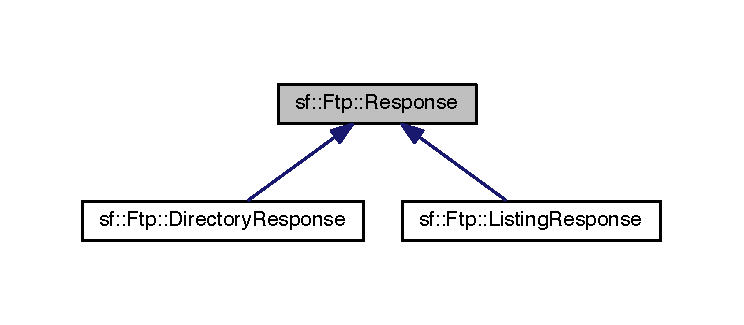
\includegraphics[width=350pt]{classsf_1_1_ftp_1_1_response__inherit__graph}
\end{center}
\end{figure}
\subsection*{Public Types}
\begin{DoxyCompactItemize}
\item 
enum \hyperlink{classsf_1_1_ftp_1_1_response_af81738f06b6f571761696291276acb3b}{Status} \{ \\*
\hyperlink{classsf_1_1_ftp_1_1_response_af81738f06b6f571761696291276acb3ba07e06d3326ba2d078583bef93930d909}{Restart\-Marker\-Reply} = 110, 
\hyperlink{classsf_1_1_ftp_1_1_response_af81738f06b6f571761696291276acb3ba22413357ade6b586f6ceb0d704f35075}{Service\-Ready\-Soon} = 120, 
\hyperlink{classsf_1_1_ftp_1_1_response_af81738f06b6f571761696291276acb3bafa52d19bc813d69055f4cc390d4a76ca}{Data\-Connection\-Already\-Opened} = 125, 
\hyperlink{classsf_1_1_ftp_1_1_response_af81738f06b6f571761696291276acb3ba794ebe743688be611447638bf9e49d86}{Opening\-Data\-Connection} = 150, 
\\*
\hyperlink{classsf_1_1_ftp_1_1_response_af81738f06b6f571761696291276acb3baa956e229ba6c0cdf0d88b0e05b286210}{Ok} = 200, 
\hyperlink{classsf_1_1_ftp_1_1_response_af81738f06b6f571761696291276acb3ba38adc424f1adcd332745de8cd3b7737a}{Pointless\-Command} = 202, 
\hyperlink{classsf_1_1_ftp_1_1_response_af81738f06b6f571761696291276acb3ba9bdd02ae119b8be639e778859ee74060}{System\-Status} = 211, 
\hyperlink{classsf_1_1_ftp_1_1_response_af81738f06b6f571761696291276acb3ba8729460a695013cc96330e2fced0ae1f}{Directory\-Status} = 212, 
\\*
\hyperlink{classsf_1_1_ftp_1_1_response_af81738f06b6f571761696291276acb3baebddfc7997dca289c83068dff3f47dce}{File\-Status} = 213, 
\hyperlink{classsf_1_1_ftp_1_1_response_af81738f06b6f571761696291276acb3ba840fd2a1872fd4310b046541f57fdeb7}{Help\-Message} = 214, 
\hyperlink{classsf_1_1_ftp_1_1_response_af81738f06b6f571761696291276acb3ba78391f73aa11f07f1514c7d070b93c08}{System\-Type} = 215, 
\hyperlink{classsf_1_1_ftp_1_1_response_af81738f06b6f571761696291276acb3baea2ee2007d7843c21108bb686ef03757}{Service\-Ready} = 220, 
\\*
\hyperlink{classsf_1_1_ftp_1_1_response_af81738f06b6f571761696291276acb3bab23931490fc2d1df3081d651fe0f4d6e}{Closing\-Connection} = 221, 
\hyperlink{classsf_1_1_ftp_1_1_response_af81738f06b6f571761696291276acb3badc78ed87d5bddb174fa3c16707ac2f2d}{Data\-Connection\-Opened} = 225, 
\hyperlink{classsf_1_1_ftp_1_1_response_af81738f06b6f571761696291276acb3bac723ebc8a38913bbf0d9504556cbaaa6}{Closing\-Data\-Connection} = 226, 
\hyperlink{classsf_1_1_ftp_1_1_response_af81738f06b6f571761696291276acb3ba48314fc47a72ad0aacdea93b91756f6e}{Entering\-Passive\-Mode} = 227, 
\\*
\hyperlink{classsf_1_1_ftp_1_1_response_af81738f06b6f571761696291276acb3ba54a88210386cb72e35d737813a221754}{Logged\-In} = 230, 
\hyperlink{classsf_1_1_ftp_1_1_response_af81738f06b6f571761696291276acb3baf988b69b0a5f55f8122da5ba001932e0}{File\-Action\-Ok} = 250, 
\hyperlink{classsf_1_1_ftp_1_1_response_af81738f06b6f571761696291276acb3ba06d26e95a170fc422af13def415e0437}{Directory\-Ok} = 257, 
\hyperlink{classsf_1_1_ftp_1_1_response_af81738f06b6f571761696291276acb3ba9249e3fe9818eb93f181fbbf3ae3bc56}{Need\-Password} = 331, 
\\*
\hyperlink{classsf_1_1_ftp_1_1_response_af81738f06b6f571761696291276acb3ba9e048185f253f6eb6f5ff9e063b712fa}{Need\-Account\-To\-Log\-In} = 332, 
\hyperlink{classsf_1_1_ftp_1_1_response_af81738f06b6f571761696291276acb3ba02e6f05964ecb829e9b6fb6020d6528a}{Need\-Information} = 350, 
\hyperlink{classsf_1_1_ftp_1_1_response_af81738f06b6f571761696291276acb3ba43022ddf49b68a4f5aff0bea7e09e89f}{Service\-Unavailable} = 421, 
\hyperlink{classsf_1_1_ftp_1_1_response_af81738f06b6f571761696291276acb3ba757b89ff1f236941f7759b0ed0c28b88}{Data\-Connection\-Unavailable} = 425, 
\\*
\hyperlink{classsf_1_1_ftp_1_1_response_af81738f06b6f571761696291276acb3ba7cfefcc586c12ba70f752353fde7126e}{Transfer\-Aborted} = 426, 
\hyperlink{classsf_1_1_ftp_1_1_response_af81738f06b6f571761696291276acb3baf822d1b0abf3e9ae7dd44684549d512d}{File\-Action\-Aborted} = 450, 
\hyperlink{classsf_1_1_ftp_1_1_response_af81738f06b6f571761696291276acb3bae54e84baaca95a7b36271ca3f3fdb900}{Local\-Error} = 451, 
\hyperlink{classsf_1_1_ftp_1_1_response_af81738f06b6f571761696291276acb3ba5d9f3666222c808553c27e4e099c7c6d}{Insufficient\-Storage\-Space} = 452, 
\\*
\hyperlink{classsf_1_1_ftp_1_1_response_af81738f06b6f571761696291276acb3ba75bdf0b6844fa9c07b3c25647d22c269}{Command\-Unknown} = 500, 
\hyperlink{classsf_1_1_ftp_1_1_response_af81738f06b6f571761696291276acb3baf4c7c88815981bbb7c3a3461f9f48b67}{Parameters\-Unknown} = 501, 
\hyperlink{classsf_1_1_ftp_1_1_response_af81738f06b6f571761696291276acb3ba2ca4834c756c81b924ebed696fcba0a8}{Command\-Not\-Implemented} = 502, 
\hyperlink{classsf_1_1_ftp_1_1_response_af81738f06b6f571761696291276acb3bad0c7ab07f01c1f7af16a1852650d7c47}{Bad\-Command\-Sequence} = 503, 
\\*
\hyperlink{classsf_1_1_ftp_1_1_response_af81738f06b6f571761696291276acb3ba8807473b8590e1debfb3740b7a3d081c}{Parameter\-Not\-Implemented} = 504, 
\hyperlink{classsf_1_1_ftp_1_1_response_af81738f06b6f571761696291276acb3bafcfbaff2c6fed941b6bcbc0999db764e}{Not\-Logged\-In} = 530, 
\hyperlink{classsf_1_1_ftp_1_1_response_af81738f06b6f571761696291276acb3ba1af0f173062a471739b50d8e0f40d5f7}{Need\-Account\-To\-Store} = 532, 
\hyperlink{classsf_1_1_ftp_1_1_response_af81738f06b6f571761696291276acb3ba3f8f931e499936fde6b750d81f5ecfef}{File\-Unavailable} = 550, 
\\*
\hyperlink{classsf_1_1_ftp_1_1_response_af81738f06b6f571761696291276acb3bad220bc12dc45593af6e5079ea6c532c3}{Page\-Type\-Unknown} = 551, 
\hyperlink{classsf_1_1_ftp_1_1_response_af81738f06b6f571761696291276acb3baf418e54753e0b8f9cb0325dd618acd14}{Not\-Enough\-Memory} = 552, 
\hyperlink{classsf_1_1_ftp_1_1_response_af81738f06b6f571761696291276acb3ba03254aba823298179a98056e15568c5b}{Filename\-Not\-Allowed} = 553, 
\hyperlink{classsf_1_1_ftp_1_1_response_af81738f06b6f571761696291276acb3ba59e041e4ef186e8ae8d6035973fc46bd}{Invalid\-Response} = 1000, 
\\*
\hyperlink{classsf_1_1_ftp_1_1_response_af81738f06b6f571761696291276acb3ba51aa367cc1e85a45ea3c7be48730e990}{Connection\-Failed} = 1001, 
\hyperlink{classsf_1_1_ftp_1_1_response_af81738f06b6f571761696291276acb3bad1e5dcf298ce30c528261435f1a2eb53}{Connection\-Closed} = 1002, 
\hyperlink{classsf_1_1_ftp_1_1_response_af81738f06b6f571761696291276acb3baed2c74a9f335dee1463ca1a4f41c6478}{Invalid\-File} = 1003
 \}
\begin{DoxyCompactList}\small\item\em Status codes possibly returned by a F\-T\-P response. \end{DoxyCompactList}\end{DoxyCompactItemize}
\subsection*{Public Member Functions}
\begin{DoxyCompactItemize}
\item 
\hyperlink{classsf_1_1_ftp_1_1_response_af300fffd4862774102f978eb22f85d9b}{Response} (\hyperlink{classsf_1_1_ftp_1_1_response_af81738f06b6f571761696291276acb3b}{Status} code=\hyperlink{classsf_1_1_ftp_1_1_response_af81738f06b6f571761696291276acb3ba59e041e4ef186e8ae8d6035973fc46bd}{Invalid\-Response}, const \hyperlink{gl3_8h_ac83513893df92266f79a515488701770}{std\-::string} \&message=\char`\"{}\char`\"{})
\begin{DoxyCompactList}\small\item\em Default constructor. \end{DoxyCompactList}\item 
bool \hyperlink{classsf_1_1_ftp_1_1_response_a4dadbe0fe0a3ef2d571a017e1645e675}{is\-Ok} () const 
\begin{DoxyCompactList}\small\item\em Check if the status code means a success. \end{DoxyCompactList}\item 
\hyperlink{classsf_1_1_ftp_1_1_response_af81738f06b6f571761696291276acb3b}{Status} \hyperlink{classsf_1_1_ftp_1_1_response_ac7f937b3883d1c4fbc75c003a1786aaa}{get\-Status} () const 
\begin{DoxyCompactList}\small\item\em Get the status code of the response. \end{DoxyCompactList}\item 
const \hyperlink{gl3_8h_ac83513893df92266f79a515488701770}{std\-::string} \& \hyperlink{classsf_1_1_ftp_1_1_response_a0015675c528a4a84a671484b9e5499d6}{get\-Message} () const 
\begin{DoxyCompactList}\small\item\em Get the full message contained in the response. \end{DoxyCompactList}\end{DoxyCompactItemize}


\subsection{Detailed Description}
Define a F\-T\-P response. 

Definition at line 66 of file Ftp.\-hpp.



\subsection{Member Enumeration Documentation}
\hypertarget{classsf_1_1_ftp_1_1_response_af81738f06b6f571761696291276acb3b}{\index{sf\-::\-Ftp\-::\-Response@{sf\-::\-Ftp\-::\-Response}!Status@{Status}}
\index{Status@{Status}!sf::Ftp::Response@{sf\-::\-Ftp\-::\-Response}}
\subsubsection[{Status}]{\setlength{\rightskip}{0pt plus 5cm}enum {\bf sf\-::\-Ftp\-::\-Response\-::\-Status}}}\label{classsf_1_1_ftp_1_1_response_af81738f06b6f571761696291276acb3b}


Status codes possibly returned by a F\-T\-P response. 

\begin{Desc}
\item[Enumerator]\par
\begin{description}
\index{Restart\-Marker\-Reply@{Restart\-Marker\-Reply}!sf\-::\-Ftp\-::\-Response@{sf\-::\-Ftp\-::\-Response}}\index{sf\-::\-Ftp\-::\-Response@{sf\-::\-Ftp\-::\-Response}!Restart\-Marker\-Reply@{Restart\-Marker\-Reply}}\item[{\em 
\hypertarget{classsf_1_1_ftp_1_1_response_af81738f06b6f571761696291276acb3ba07e06d3326ba2d078583bef93930d909}{Restart\-Marker\-Reply}\label{classsf_1_1_ftp_1_1_response_af81738f06b6f571761696291276acb3ba07e06d3326ba2d078583bef93930d909}
}]Restart marker reply. \index{Service\-Ready\-Soon@{Service\-Ready\-Soon}!sf\-::\-Ftp\-::\-Response@{sf\-::\-Ftp\-::\-Response}}\index{sf\-::\-Ftp\-::\-Response@{sf\-::\-Ftp\-::\-Response}!Service\-Ready\-Soon@{Service\-Ready\-Soon}}\item[{\em 
\hypertarget{classsf_1_1_ftp_1_1_response_af81738f06b6f571761696291276acb3ba22413357ade6b586f6ceb0d704f35075}{Service\-Ready\-Soon}\label{classsf_1_1_ftp_1_1_response_af81738f06b6f571761696291276acb3ba22413357ade6b586f6ceb0d704f35075}
}]Service ready in N minutes. \index{Data\-Connection\-Already\-Opened@{Data\-Connection\-Already\-Opened}!sf\-::\-Ftp\-::\-Response@{sf\-::\-Ftp\-::\-Response}}\index{sf\-::\-Ftp\-::\-Response@{sf\-::\-Ftp\-::\-Response}!Data\-Connection\-Already\-Opened@{Data\-Connection\-Already\-Opened}}\item[{\em 
\hypertarget{classsf_1_1_ftp_1_1_response_af81738f06b6f571761696291276acb3bafa52d19bc813d69055f4cc390d4a76ca}{Data\-Connection\-Already\-Opened}\label{classsf_1_1_ftp_1_1_response_af81738f06b6f571761696291276acb3bafa52d19bc813d69055f4cc390d4a76ca}
}]Data connection already opened, transfer starting. \index{Opening\-Data\-Connection@{Opening\-Data\-Connection}!sf\-::\-Ftp\-::\-Response@{sf\-::\-Ftp\-::\-Response}}\index{sf\-::\-Ftp\-::\-Response@{sf\-::\-Ftp\-::\-Response}!Opening\-Data\-Connection@{Opening\-Data\-Connection}}\item[{\em 
\hypertarget{classsf_1_1_ftp_1_1_response_af81738f06b6f571761696291276acb3ba794ebe743688be611447638bf9e49d86}{Opening\-Data\-Connection}\label{classsf_1_1_ftp_1_1_response_af81738f06b6f571761696291276acb3ba794ebe743688be611447638bf9e49d86}
}]File status ok, about to open data connection. \index{Ok@{Ok}!sf\-::\-Ftp\-::\-Response@{sf\-::\-Ftp\-::\-Response}}\index{sf\-::\-Ftp\-::\-Response@{sf\-::\-Ftp\-::\-Response}!Ok@{Ok}}\item[{\em 
\hypertarget{classsf_1_1_ftp_1_1_response_af81738f06b6f571761696291276acb3baa956e229ba6c0cdf0d88b0e05b286210}{Ok}\label{classsf_1_1_ftp_1_1_response_af81738f06b6f571761696291276acb3baa956e229ba6c0cdf0d88b0e05b286210}
}]Command ok. \index{Pointless\-Command@{Pointless\-Command}!sf\-::\-Ftp\-::\-Response@{sf\-::\-Ftp\-::\-Response}}\index{sf\-::\-Ftp\-::\-Response@{sf\-::\-Ftp\-::\-Response}!Pointless\-Command@{Pointless\-Command}}\item[{\em 
\hypertarget{classsf_1_1_ftp_1_1_response_af81738f06b6f571761696291276acb3ba38adc424f1adcd332745de8cd3b7737a}{Pointless\-Command}\label{classsf_1_1_ftp_1_1_response_af81738f06b6f571761696291276acb3ba38adc424f1adcd332745de8cd3b7737a}
}]Command not implemented. \index{System\-Status@{System\-Status}!sf\-::\-Ftp\-::\-Response@{sf\-::\-Ftp\-::\-Response}}\index{sf\-::\-Ftp\-::\-Response@{sf\-::\-Ftp\-::\-Response}!System\-Status@{System\-Status}}\item[{\em 
\hypertarget{classsf_1_1_ftp_1_1_response_af81738f06b6f571761696291276acb3ba9bdd02ae119b8be639e778859ee74060}{System\-Status}\label{classsf_1_1_ftp_1_1_response_af81738f06b6f571761696291276acb3ba9bdd02ae119b8be639e778859ee74060}
}]System status, or system help reply. \index{Directory\-Status@{Directory\-Status}!sf\-::\-Ftp\-::\-Response@{sf\-::\-Ftp\-::\-Response}}\index{sf\-::\-Ftp\-::\-Response@{sf\-::\-Ftp\-::\-Response}!Directory\-Status@{Directory\-Status}}\item[{\em 
\hypertarget{classsf_1_1_ftp_1_1_response_af81738f06b6f571761696291276acb3ba8729460a695013cc96330e2fced0ae1f}{Directory\-Status}\label{classsf_1_1_ftp_1_1_response_af81738f06b6f571761696291276acb3ba8729460a695013cc96330e2fced0ae1f}
}]Directory status. \index{File\-Status@{File\-Status}!sf\-::\-Ftp\-::\-Response@{sf\-::\-Ftp\-::\-Response}}\index{sf\-::\-Ftp\-::\-Response@{sf\-::\-Ftp\-::\-Response}!File\-Status@{File\-Status}}\item[{\em 
\hypertarget{classsf_1_1_ftp_1_1_response_af81738f06b6f571761696291276acb3baebddfc7997dca289c83068dff3f47dce}{File\-Status}\label{classsf_1_1_ftp_1_1_response_af81738f06b6f571761696291276acb3baebddfc7997dca289c83068dff3f47dce}
}]File status. \index{Help\-Message@{Help\-Message}!sf\-::\-Ftp\-::\-Response@{sf\-::\-Ftp\-::\-Response}}\index{sf\-::\-Ftp\-::\-Response@{sf\-::\-Ftp\-::\-Response}!Help\-Message@{Help\-Message}}\item[{\em 
\hypertarget{classsf_1_1_ftp_1_1_response_af81738f06b6f571761696291276acb3ba840fd2a1872fd4310b046541f57fdeb7}{Help\-Message}\label{classsf_1_1_ftp_1_1_response_af81738f06b6f571761696291276acb3ba840fd2a1872fd4310b046541f57fdeb7}
}]Help message. \index{System\-Type@{System\-Type}!sf\-::\-Ftp\-::\-Response@{sf\-::\-Ftp\-::\-Response}}\index{sf\-::\-Ftp\-::\-Response@{sf\-::\-Ftp\-::\-Response}!System\-Type@{System\-Type}}\item[{\em 
\hypertarget{classsf_1_1_ftp_1_1_response_af81738f06b6f571761696291276acb3ba78391f73aa11f07f1514c7d070b93c08}{System\-Type}\label{classsf_1_1_ftp_1_1_response_af81738f06b6f571761696291276acb3ba78391f73aa11f07f1514c7d070b93c08}
}]N\-A\-M\-E system type, where N\-A\-M\-E is an official system name from the list in the Assigned Numbers document. \index{Service\-Ready@{Service\-Ready}!sf\-::\-Ftp\-::\-Response@{sf\-::\-Ftp\-::\-Response}}\index{sf\-::\-Ftp\-::\-Response@{sf\-::\-Ftp\-::\-Response}!Service\-Ready@{Service\-Ready}}\item[{\em 
\hypertarget{classsf_1_1_ftp_1_1_response_af81738f06b6f571761696291276acb3baea2ee2007d7843c21108bb686ef03757}{Service\-Ready}\label{classsf_1_1_ftp_1_1_response_af81738f06b6f571761696291276acb3baea2ee2007d7843c21108bb686ef03757}
}]Service ready for new user. \index{Closing\-Connection@{Closing\-Connection}!sf\-::\-Ftp\-::\-Response@{sf\-::\-Ftp\-::\-Response}}\index{sf\-::\-Ftp\-::\-Response@{sf\-::\-Ftp\-::\-Response}!Closing\-Connection@{Closing\-Connection}}\item[{\em 
\hypertarget{classsf_1_1_ftp_1_1_response_af81738f06b6f571761696291276acb3bab23931490fc2d1df3081d651fe0f4d6e}{Closing\-Connection}\label{classsf_1_1_ftp_1_1_response_af81738f06b6f571761696291276acb3bab23931490fc2d1df3081d651fe0f4d6e}
}]Service closing control connection. \index{Data\-Connection\-Opened@{Data\-Connection\-Opened}!sf\-::\-Ftp\-::\-Response@{sf\-::\-Ftp\-::\-Response}}\index{sf\-::\-Ftp\-::\-Response@{sf\-::\-Ftp\-::\-Response}!Data\-Connection\-Opened@{Data\-Connection\-Opened}}\item[{\em 
\hypertarget{classsf_1_1_ftp_1_1_response_af81738f06b6f571761696291276acb3badc78ed87d5bddb174fa3c16707ac2f2d}{Data\-Connection\-Opened}\label{classsf_1_1_ftp_1_1_response_af81738f06b6f571761696291276acb3badc78ed87d5bddb174fa3c16707ac2f2d}
}]Data connection open, no transfer in progress. \index{Closing\-Data\-Connection@{Closing\-Data\-Connection}!sf\-::\-Ftp\-::\-Response@{sf\-::\-Ftp\-::\-Response}}\index{sf\-::\-Ftp\-::\-Response@{sf\-::\-Ftp\-::\-Response}!Closing\-Data\-Connection@{Closing\-Data\-Connection}}\item[{\em 
\hypertarget{classsf_1_1_ftp_1_1_response_af81738f06b6f571761696291276acb3bac723ebc8a38913bbf0d9504556cbaaa6}{Closing\-Data\-Connection}\label{classsf_1_1_ftp_1_1_response_af81738f06b6f571761696291276acb3bac723ebc8a38913bbf0d9504556cbaaa6}
}]Closing data connection, requested file action successful. \index{Entering\-Passive\-Mode@{Entering\-Passive\-Mode}!sf\-::\-Ftp\-::\-Response@{sf\-::\-Ftp\-::\-Response}}\index{sf\-::\-Ftp\-::\-Response@{sf\-::\-Ftp\-::\-Response}!Entering\-Passive\-Mode@{Entering\-Passive\-Mode}}\item[{\em 
\hypertarget{classsf_1_1_ftp_1_1_response_af81738f06b6f571761696291276acb3ba48314fc47a72ad0aacdea93b91756f6e}{Entering\-Passive\-Mode}\label{classsf_1_1_ftp_1_1_response_af81738f06b6f571761696291276acb3ba48314fc47a72ad0aacdea93b91756f6e}
}]Entering passive mode. \index{Logged\-In@{Logged\-In}!sf\-::\-Ftp\-::\-Response@{sf\-::\-Ftp\-::\-Response}}\index{sf\-::\-Ftp\-::\-Response@{sf\-::\-Ftp\-::\-Response}!Logged\-In@{Logged\-In}}\item[{\em 
\hypertarget{classsf_1_1_ftp_1_1_response_af81738f06b6f571761696291276acb3ba54a88210386cb72e35d737813a221754}{Logged\-In}\label{classsf_1_1_ftp_1_1_response_af81738f06b6f571761696291276acb3ba54a88210386cb72e35d737813a221754}
}]User logged in, proceed. Logged out if appropriate. \index{File\-Action\-Ok@{File\-Action\-Ok}!sf\-::\-Ftp\-::\-Response@{sf\-::\-Ftp\-::\-Response}}\index{sf\-::\-Ftp\-::\-Response@{sf\-::\-Ftp\-::\-Response}!File\-Action\-Ok@{File\-Action\-Ok}}\item[{\em 
\hypertarget{classsf_1_1_ftp_1_1_response_af81738f06b6f571761696291276acb3baf988b69b0a5f55f8122da5ba001932e0}{File\-Action\-Ok}\label{classsf_1_1_ftp_1_1_response_af81738f06b6f571761696291276acb3baf988b69b0a5f55f8122da5ba001932e0}
}]Requested file action ok. \index{Directory\-Ok@{Directory\-Ok}!sf\-::\-Ftp\-::\-Response@{sf\-::\-Ftp\-::\-Response}}\index{sf\-::\-Ftp\-::\-Response@{sf\-::\-Ftp\-::\-Response}!Directory\-Ok@{Directory\-Ok}}\item[{\em 
\hypertarget{classsf_1_1_ftp_1_1_response_af81738f06b6f571761696291276acb3ba06d26e95a170fc422af13def415e0437}{Directory\-Ok}\label{classsf_1_1_ftp_1_1_response_af81738f06b6f571761696291276acb3ba06d26e95a170fc422af13def415e0437}
}]P\-A\-T\-H\-N\-A\-M\-E created. \index{Need\-Password@{Need\-Password}!sf\-::\-Ftp\-::\-Response@{sf\-::\-Ftp\-::\-Response}}\index{sf\-::\-Ftp\-::\-Response@{sf\-::\-Ftp\-::\-Response}!Need\-Password@{Need\-Password}}\item[{\em 
\hypertarget{classsf_1_1_ftp_1_1_response_af81738f06b6f571761696291276acb3ba9249e3fe9818eb93f181fbbf3ae3bc56}{Need\-Password}\label{classsf_1_1_ftp_1_1_response_af81738f06b6f571761696291276acb3ba9249e3fe9818eb93f181fbbf3ae3bc56}
}]User name ok, need password. \index{Need\-Account\-To\-Log\-In@{Need\-Account\-To\-Log\-In}!sf\-::\-Ftp\-::\-Response@{sf\-::\-Ftp\-::\-Response}}\index{sf\-::\-Ftp\-::\-Response@{sf\-::\-Ftp\-::\-Response}!Need\-Account\-To\-Log\-In@{Need\-Account\-To\-Log\-In}}\item[{\em 
\hypertarget{classsf_1_1_ftp_1_1_response_af81738f06b6f571761696291276acb3ba9e048185f253f6eb6f5ff9e063b712fa}{Need\-Account\-To\-Log\-In}\label{classsf_1_1_ftp_1_1_response_af81738f06b6f571761696291276acb3ba9e048185f253f6eb6f5ff9e063b712fa}
}]Need account for login. \index{Need\-Information@{Need\-Information}!sf\-::\-Ftp\-::\-Response@{sf\-::\-Ftp\-::\-Response}}\index{sf\-::\-Ftp\-::\-Response@{sf\-::\-Ftp\-::\-Response}!Need\-Information@{Need\-Information}}\item[{\em 
\hypertarget{classsf_1_1_ftp_1_1_response_af81738f06b6f571761696291276acb3ba02e6f05964ecb829e9b6fb6020d6528a}{Need\-Information}\label{classsf_1_1_ftp_1_1_response_af81738f06b6f571761696291276acb3ba02e6f05964ecb829e9b6fb6020d6528a}
}]Requested file action pending further information. \index{Service\-Unavailable@{Service\-Unavailable}!sf\-::\-Ftp\-::\-Response@{sf\-::\-Ftp\-::\-Response}}\index{sf\-::\-Ftp\-::\-Response@{sf\-::\-Ftp\-::\-Response}!Service\-Unavailable@{Service\-Unavailable}}\item[{\em 
\hypertarget{classsf_1_1_ftp_1_1_response_af81738f06b6f571761696291276acb3ba43022ddf49b68a4f5aff0bea7e09e89f}{Service\-Unavailable}\label{classsf_1_1_ftp_1_1_response_af81738f06b6f571761696291276acb3ba43022ddf49b68a4f5aff0bea7e09e89f}
}]Service not available, closing control connection. \index{Data\-Connection\-Unavailable@{Data\-Connection\-Unavailable}!sf\-::\-Ftp\-::\-Response@{sf\-::\-Ftp\-::\-Response}}\index{sf\-::\-Ftp\-::\-Response@{sf\-::\-Ftp\-::\-Response}!Data\-Connection\-Unavailable@{Data\-Connection\-Unavailable}}\item[{\em 
\hypertarget{classsf_1_1_ftp_1_1_response_af81738f06b6f571761696291276acb3ba757b89ff1f236941f7759b0ed0c28b88}{Data\-Connection\-Unavailable}\label{classsf_1_1_ftp_1_1_response_af81738f06b6f571761696291276acb3ba757b89ff1f236941f7759b0ed0c28b88}
}]Can't open data connection. \index{Transfer\-Aborted@{Transfer\-Aborted}!sf\-::\-Ftp\-::\-Response@{sf\-::\-Ftp\-::\-Response}}\index{sf\-::\-Ftp\-::\-Response@{sf\-::\-Ftp\-::\-Response}!Transfer\-Aborted@{Transfer\-Aborted}}\item[{\em 
\hypertarget{classsf_1_1_ftp_1_1_response_af81738f06b6f571761696291276acb3ba7cfefcc586c12ba70f752353fde7126e}{Transfer\-Aborted}\label{classsf_1_1_ftp_1_1_response_af81738f06b6f571761696291276acb3ba7cfefcc586c12ba70f752353fde7126e}
}]Connection closed, transfer aborted. \index{File\-Action\-Aborted@{File\-Action\-Aborted}!sf\-::\-Ftp\-::\-Response@{sf\-::\-Ftp\-::\-Response}}\index{sf\-::\-Ftp\-::\-Response@{sf\-::\-Ftp\-::\-Response}!File\-Action\-Aborted@{File\-Action\-Aborted}}\item[{\em 
\hypertarget{classsf_1_1_ftp_1_1_response_af81738f06b6f571761696291276acb3baf822d1b0abf3e9ae7dd44684549d512d}{File\-Action\-Aborted}\label{classsf_1_1_ftp_1_1_response_af81738f06b6f571761696291276acb3baf822d1b0abf3e9ae7dd44684549d512d}
}]Requested file action not taken. \index{Local\-Error@{Local\-Error}!sf\-::\-Ftp\-::\-Response@{sf\-::\-Ftp\-::\-Response}}\index{sf\-::\-Ftp\-::\-Response@{sf\-::\-Ftp\-::\-Response}!Local\-Error@{Local\-Error}}\item[{\em 
\hypertarget{classsf_1_1_ftp_1_1_response_af81738f06b6f571761696291276acb3bae54e84baaca95a7b36271ca3f3fdb900}{Local\-Error}\label{classsf_1_1_ftp_1_1_response_af81738f06b6f571761696291276acb3bae54e84baaca95a7b36271ca3f3fdb900}
}]Requested action aborted, local error in processing. \index{Insufficient\-Storage\-Space@{Insufficient\-Storage\-Space}!sf\-::\-Ftp\-::\-Response@{sf\-::\-Ftp\-::\-Response}}\index{sf\-::\-Ftp\-::\-Response@{sf\-::\-Ftp\-::\-Response}!Insufficient\-Storage\-Space@{Insufficient\-Storage\-Space}}\item[{\em 
\hypertarget{classsf_1_1_ftp_1_1_response_af81738f06b6f571761696291276acb3ba5d9f3666222c808553c27e4e099c7c6d}{Insufficient\-Storage\-Space}\label{classsf_1_1_ftp_1_1_response_af81738f06b6f571761696291276acb3ba5d9f3666222c808553c27e4e099c7c6d}
}]Requested action not taken; insufficient storage space in system, file unavailable. \index{Command\-Unknown@{Command\-Unknown}!sf\-::\-Ftp\-::\-Response@{sf\-::\-Ftp\-::\-Response}}\index{sf\-::\-Ftp\-::\-Response@{sf\-::\-Ftp\-::\-Response}!Command\-Unknown@{Command\-Unknown}}\item[{\em 
\hypertarget{classsf_1_1_ftp_1_1_response_af81738f06b6f571761696291276acb3ba75bdf0b6844fa9c07b3c25647d22c269}{Command\-Unknown}\label{classsf_1_1_ftp_1_1_response_af81738f06b6f571761696291276acb3ba75bdf0b6844fa9c07b3c25647d22c269}
}]Syntax error, command unrecognized. \index{Parameters\-Unknown@{Parameters\-Unknown}!sf\-::\-Ftp\-::\-Response@{sf\-::\-Ftp\-::\-Response}}\index{sf\-::\-Ftp\-::\-Response@{sf\-::\-Ftp\-::\-Response}!Parameters\-Unknown@{Parameters\-Unknown}}\item[{\em 
\hypertarget{classsf_1_1_ftp_1_1_response_af81738f06b6f571761696291276acb3baf4c7c88815981bbb7c3a3461f9f48b67}{Parameters\-Unknown}\label{classsf_1_1_ftp_1_1_response_af81738f06b6f571761696291276acb3baf4c7c88815981bbb7c3a3461f9f48b67}
}]Syntax error in parameters or arguments. \index{Command\-Not\-Implemented@{Command\-Not\-Implemented}!sf\-::\-Ftp\-::\-Response@{sf\-::\-Ftp\-::\-Response}}\index{sf\-::\-Ftp\-::\-Response@{sf\-::\-Ftp\-::\-Response}!Command\-Not\-Implemented@{Command\-Not\-Implemented}}\item[{\em 
\hypertarget{classsf_1_1_ftp_1_1_response_af81738f06b6f571761696291276acb3ba2ca4834c756c81b924ebed696fcba0a8}{Command\-Not\-Implemented}\label{classsf_1_1_ftp_1_1_response_af81738f06b6f571761696291276acb3ba2ca4834c756c81b924ebed696fcba0a8}
}]Command not implemented. \index{Bad\-Command\-Sequence@{Bad\-Command\-Sequence}!sf\-::\-Ftp\-::\-Response@{sf\-::\-Ftp\-::\-Response}}\index{sf\-::\-Ftp\-::\-Response@{sf\-::\-Ftp\-::\-Response}!Bad\-Command\-Sequence@{Bad\-Command\-Sequence}}\item[{\em 
\hypertarget{classsf_1_1_ftp_1_1_response_af81738f06b6f571761696291276acb3bad0c7ab07f01c1f7af16a1852650d7c47}{Bad\-Command\-Sequence}\label{classsf_1_1_ftp_1_1_response_af81738f06b6f571761696291276acb3bad0c7ab07f01c1f7af16a1852650d7c47}
}]Bad sequence of commands. \index{Parameter\-Not\-Implemented@{Parameter\-Not\-Implemented}!sf\-::\-Ftp\-::\-Response@{sf\-::\-Ftp\-::\-Response}}\index{sf\-::\-Ftp\-::\-Response@{sf\-::\-Ftp\-::\-Response}!Parameter\-Not\-Implemented@{Parameter\-Not\-Implemented}}\item[{\em 
\hypertarget{classsf_1_1_ftp_1_1_response_af81738f06b6f571761696291276acb3ba8807473b8590e1debfb3740b7a3d081c}{Parameter\-Not\-Implemented}\label{classsf_1_1_ftp_1_1_response_af81738f06b6f571761696291276acb3ba8807473b8590e1debfb3740b7a3d081c}
}]Command not implemented for that parameter. \index{Not\-Logged\-In@{Not\-Logged\-In}!sf\-::\-Ftp\-::\-Response@{sf\-::\-Ftp\-::\-Response}}\index{sf\-::\-Ftp\-::\-Response@{sf\-::\-Ftp\-::\-Response}!Not\-Logged\-In@{Not\-Logged\-In}}\item[{\em 
\hypertarget{classsf_1_1_ftp_1_1_response_af81738f06b6f571761696291276acb3bafcfbaff2c6fed941b6bcbc0999db764e}{Not\-Logged\-In}\label{classsf_1_1_ftp_1_1_response_af81738f06b6f571761696291276acb3bafcfbaff2c6fed941b6bcbc0999db764e}
}]Not logged in. \index{Need\-Account\-To\-Store@{Need\-Account\-To\-Store}!sf\-::\-Ftp\-::\-Response@{sf\-::\-Ftp\-::\-Response}}\index{sf\-::\-Ftp\-::\-Response@{sf\-::\-Ftp\-::\-Response}!Need\-Account\-To\-Store@{Need\-Account\-To\-Store}}\item[{\em 
\hypertarget{classsf_1_1_ftp_1_1_response_af81738f06b6f571761696291276acb3ba1af0f173062a471739b50d8e0f40d5f7}{Need\-Account\-To\-Store}\label{classsf_1_1_ftp_1_1_response_af81738f06b6f571761696291276acb3ba1af0f173062a471739b50d8e0f40d5f7}
}]Need account for storing files. \index{File\-Unavailable@{File\-Unavailable}!sf\-::\-Ftp\-::\-Response@{sf\-::\-Ftp\-::\-Response}}\index{sf\-::\-Ftp\-::\-Response@{sf\-::\-Ftp\-::\-Response}!File\-Unavailable@{File\-Unavailable}}\item[{\em 
\hypertarget{classsf_1_1_ftp_1_1_response_af81738f06b6f571761696291276acb3ba3f8f931e499936fde6b750d81f5ecfef}{File\-Unavailable}\label{classsf_1_1_ftp_1_1_response_af81738f06b6f571761696291276acb3ba3f8f931e499936fde6b750d81f5ecfef}
}]Requested action not taken, file unavailable. \index{Page\-Type\-Unknown@{Page\-Type\-Unknown}!sf\-::\-Ftp\-::\-Response@{sf\-::\-Ftp\-::\-Response}}\index{sf\-::\-Ftp\-::\-Response@{sf\-::\-Ftp\-::\-Response}!Page\-Type\-Unknown@{Page\-Type\-Unknown}}\item[{\em 
\hypertarget{classsf_1_1_ftp_1_1_response_af81738f06b6f571761696291276acb3bad220bc12dc45593af6e5079ea6c532c3}{Page\-Type\-Unknown}\label{classsf_1_1_ftp_1_1_response_af81738f06b6f571761696291276acb3bad220bc12dc45593af6e5079ea6c532c3}
}]Requested action aborted, page type unknown. \index{Not\-Enough\-Memory@{Not\-Enough\-Memory}!sf\-::\-Ftp\-::\-Response@{sf\-::\-Ftp\-::\-Response}}\index{sf\-::\-Ftp\-::\-Response@{sf\-::\-Ftp\-::\-Response}!Not\-Enough\-Memory@{Not\-Enough\-Memory}}\item[{\em 
\hypertarget{classsf_1_1_ftp_1_1_response_af81738f06b6f571761696291276acb3baf418e54753e0b8f9cb0325dd618acd14}{Not\-Enough\-Memory}\label{classsf_1_1_ftp_1_1_response_af81738f06b6f571761696291276acb3baf418e54753e0b8f9cb0325dd618acd14}
}]Requested file action aborted, exceeded storage allocation. \index{Filename\-Not\-Allowed@{Filename\-Not\-Allowed}!sf\-::\-Ftp\-::\-Response@{sf\-::\-Ftp\-::\-Response}}\index{sf\-::\-Ftp\-::\-Response@{sf\-::\-Ftp\-::\-Response}!Filename\-Not\-Allowed@{Filename\-Not\-Allowed}}\item[{\em 
\hypertarget{classsf_1_1_ftp_1_1_response_af81738f06b6f571761696291276acb3ba03254aba823298179a98056e15568c5b}{Filename\-Not\-Allowed}\label{classsf_1_1_ftp_1_1_response_af81738f06b6f571761696291276acb3ba03254aba823298179a98056e15568c5b}
}]Requested action not taken, file name not allowed. \index{Invalid\-Response@{Invalid\-Response}!sf\-::\-Ftp\-::\-Response@{sf\-::\-Ftp\-::\-Response}}\index{sf\-::\-Ftp\-::\-Response@{sf\-::\-Ftp\-::\-Response}!Invalid\-Response@{Invalid\-Response}}\item[{\em 
\hypertarget{classsf_1_1_ftp_1_1_response_af81738f06b6f571761696291276acb3ba59e041e4ef186e8ae8d6035973fc46bd}{Invalid\-Response}\label{classsf_1_1_ftp_1_1_response_af81738f06b6f571761696291276acb3ba59e041e4ef186e8ae8d6035973fc46bd}
}]\hyperlink{classsf_1_1_ftp_1_1_response}{Response} is not a valid F\-T\-P one. \index{Connection\-Failed@{Connection\-Failed}!sf\-::\-Ftp\-::\-Response@{sf\-::\-Ftp\-::\-Response}}\index{sf\-::\-Ftp\-::\-Response@{sf\-::\-Ftp\-::\-Response}!Connection\-Failed@{Connection\-Failed}}\item[{\em 
\hypertarget{classsf_1_1_ftp_1_1_response_af81738f06b6f571761696291276acb3ba51aa367cc1e85a45ea3c7be48730e990}{Connection\-Failed}\label{classsf_1_1_ftp_1_1_response_af81738f06b6f571761696291276acb3ba51aa367cc1e85a45ea3c7be48730e990}
}]Connection with server failed. \index{Connection\-Closed@{Connection\-Closed}!sf\-::\-Ftp\-::\-Response@{sf\-::\-Ftp\-::\-Response}}\index{sf\-::\-Ftp\-::\-Response@{sf\-::\-Ftp\-::\-Response}!Connection\-Closed@{Connection\-Closed}}\item[{\em 
\hypertarget{classsf_1_1_ftp_1_1_response_af81738f06b6f571761696291276acb3bad1e5dcf298ce30c528261435f1a2eb53}{Connection\-Closed}\label{classsf_1_1_ftp_1_1_response_af81738f06b6f571761696291276acb3bad1e5dcf298ce30c528261435f1a2eb53}
}]Connection with server closed. \index{Invalid\-File@{Invalid\-File}!sf\-::\-Ftp\-::\-Response@{sf\-::\-Ftp\-::\-Response}}\index{sf\-::\-Ftp\-::\-Response@{sf\-::\-Ftp\-::\-Response}!Invalid\-File@{Invalid\-File}}\item[{\em 
\hypertarget{classsf_1_1_ftp_1_1_response_af81738f06b6f571761696291276acb3baed2c74a9f335dee1463ca1a4f41c6478}{Invalid\-File}\label{classsf_1_1_ftp_1_1_response_af81738f06b6f571761696291276acb3baed2c74a9f335dee1463ca1a4f41c6478}
}]Invalid file to upload / download. \end{description}
\end{Desc}


Definition at line 74 of file Ftp.\-hpp.



\subsection{Constructor \& Destructor Documentation}
\hypertarget{classsf_1_1_ftp_1_1_response_af300fffd4862774102f978eb22f85d9b}{\index{sf\-::\-Ftp\-::\-Response@{sf\-::\-Ftp\-::\-Response}!Response@{Response}}
\index{Response@{Response}!sf::Ftp::Response@{sf\-::\-Ftp\-::\-Response}}
\subsubsection[{Response}]{\setlength{\rightskip}{0pt plus 5cm}sf\-::\-Ftp\-::\-Response\-::\-Response (
\begin{DoxyParamCaption}
\item[{{\bf Status}}]{code = {\ttfamily {\bf Invalid\-Response}}, }
\item[{const {\bf std\-::string} \&}]{message = {\ttfamily \char`\"{}\char`\"{}}}
\end{DoxyParamCaption}
)\hspace{0.3cm}{\ttfamily [explicit]}}}\label{classsf_1_1_ftp_1_1_response_af300fffd4862774102f978eb22f85d9b}


Default constructor. 

This constructor is used by the F\-T\-P client to build the response.


\begin{DoxyParams}{Parameters}
{\em code} & \hyperlink{classsf_1_1_ftp_1_1_response}{Response} status code \\
\hline
{\em message} & \hyperlink{classsf_1_1_ftp_1_1_response}{Response} message \\
\hline
\end{DoxyParams}


\subsection{Member Function Documentation}
\hypertarget{classsf_1_1_ftp_1_1_response_a0015675c528a4a84a671484b9e5499d6}{\index{sf\-::\-Ftp\-::\-Response@{sf\-::\-Ftp\-::\-Response}!get\-Message@{get\-Message}}
\index{get\-Message@{get\-Message}!sf::Ftp::Response@{sf\-::\-Ftp\-::\-Response}}
\subsubsection[{get\-Message}]{\setlength{\rightskip}{0pt plus 5cm}const {\bf std\-::string}\& sf\-::\-Ftp\-::\-Response\-::get\-Message (
\begin{DoxyParamCaption}
{}
\end{DoxyParamCaption}
) const}}\label{classsf_1_1_ftp_1_1_response_a0015675c528a4a84a671484b9e5499d6}


Get the full message contained in the response. 

\begin{DoxyReturn}{Returns}
The response message 
\end{DoxyReturn}
\hypertarget{classsf_1_1_ftp_1_1_response_ac7f937b3883d1c4fbc75c003a1786aaa}{\index{sf\-::\-Ftp\-::\-Response@{sf\-::\-Ftp\-::\-Response}!get\-Status@{get\-Status}}
\index{get\-Status@{get\-Status}!sf::Ftp::Response@{sf\-::\-Ftp\-::\-Response}}
\subsubsection[{get\-Status}]{\setlength{\rightskip}{0pt plus 5cm}{\bf Status} sf\-::\-Ftp\-::\-Response\-::get\-Status (
\begin{DoxyParamCaption}
{}
\end{DoxyParamCaption}
) const}}\label{classsf_1_1_ftp_1_1_response_ac7f937b3883d1c4fbc75c003a1786aaa}


Get the status code of the response. 

\begin{DoxyReturn}{Returns}
Status code 
\end{DoxyReturn}
\hypertarget{classsf_1_1_ftp_1_1_response_a4dadbe0fe0a3ef2d571a017e1645e675}{\index{sf\-::\-Ftp\-::\-Response@{sf\-::\-Ftp\-::\-Response}!is\-Ok@{is\-Ok}}
\index{is\-Ok@{is\-Ok}!sf::Ftp::Response@{sf\-::\-Ftp\-::\-Response}}
\subsubsection[{is\-Ok}]{\setlength{\rightskip}{0pt plus 5cm}bool sf\-::\-Ftp\-::\-Response\-::is\-Ok (
\begin{DoxyParamCaption}
{}
\end{DoxyParamCaption}
) const}}\label{classsf_1_1_ftp_1_1_response_a4dadbe0fe0a3ef2d571a017e1645e675}


Check if the status code means a success. 

This function is defined for convenience, it is equivalent to testing if the status code is $<$ 400.

\begin{DoxyReturn}{Returns}
True if the status is a success, false if it is a failure 
\end{DoxyReturn}


The documentation for this class was generated from the following file\-:\begin{DoxyCompactItemize}
\item 
/\-Users/ira/\-Dropbox/ira\-\_\-dev/protobyte\-\_\-research/other\-\_\-libs/\-S\-F\-M\-L/dylibs/root/usr/local/include/\-S\-F\-M\-L/\-Network/\hyperlink{_ftp_8hpp}{Ftp.\-hpp}\end{DoxyCompactItemize}

\hypertarget{classsf_1_1_shader}{\section{sf\-:\-:Shader Class Reference}
\label{classsf_1_1_shader}\index{sf\-::\-Shader@{sf\-::\-Shader}}
}


\hyperlink{classsf_1_1_shader}{Shader} class (vertex and fragment)  




{\ttfamily \#include $<$Shader.\-hpp$>$}



Inheritance diagram for sf\-:\-:Shader\-:
\nopagebreak
\begin{figure}[H]
\begin{center}
\leavevmode
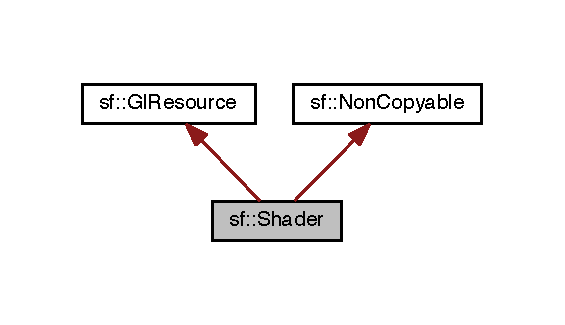
\includegraphics[width=271pt]{classsf_1_1_shader__inherit__graph}
\end{center}
\end{figure}


Collaboration diagram for sf\-:\-:Shader\-:
\nopagebreak
\begin{figure}[H]
\begin{center}
\leavevmode
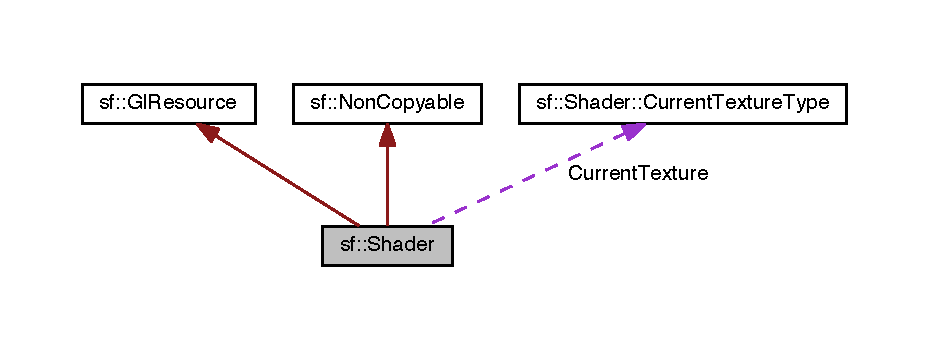
\includegraphics[width=350pt]{classsf_1_1_shader__coll__graph}
\end{center}
\end{figure}
\subsection*{Classes}
\begin{DoxyCompactItemize}
\item 
struct \hyperlink{structsf_1_1_shader_1_1_current_texture_type}{Current\-Texture\-Type}
\begin{DoxyCompactList}\small\item\em Special type/value that can be passed to set\-Parameter, and that represents the texture of the object being drawn. \end{DoxyCompactList}\end{DoxyCompactItemize}
\subsection*{Public Types}
\begin{DoxyCompactItemize}
\item 
enum \hyperlink{classsf_1_1_shader_afaa1aa65e5de37b74d047da9def9f9b3}{Type} \{ \hyperlink{classsf_1_1_shader_afaa1aa65e5de37b74d047da9def9f9b3a8718008f827eb32e29bbdd1791c62dce}{Vertex}, 
\hyperlink{classsf_1_1_shader_afaa1aa65e5de37b74d047da9def9f9b3ace6e88eec3a56b2e55ee3c8e64e9b89a}{Fragment}
 \}
\begin{DoxyCompactList}\small\item\em Types of shaders. \end{DoxyCompactList}\end{DoxyCompactItemize}
\subsection*{Public Member Functions}
\begin{DoxyCompactItemize}
\item 
\hyperlink{classsf_1_1_shader_a1d7f28f26b4122959fcafec871c2c3c5}{Shader} ()
\begin{DoxyCompactList}\small\item\em Default constructor. \end{DoxyCompactList}\item 
\hyperlink{classsf_1_1_shader_a4bac6cc8b046ecd8fb967c145a2380e6}{$\sim$\-Shader} ()
\begin{DoxyCompactList}\small\item\em Destructor. \end{DoxyCompactList}\item 
bool \hyperlink{classsf_1_1_shader_a053a5632848ebaca2fcd8ba29abe9e6e}{load\-From\-File} (const \hyperlink{gl3_8h_ac83513893df92266f79a515488701770}{std\-::string} \&filename, \hyperlink{classsf_1_1_shader_afaa1aa65e5de37b74d047da9def9f9b3}{Type} \hyperlink{gl3_8h_a984aabed544368e7fe0e566d7cf014a7}{type})
\begin{DoxyCompactList}\small\item\em Load either the vertex or fragment shader from a file. \end{DoxyCompactList}\item 
bool \hyperlink{classsf_1_1_shader_ac9d7289966fcef562eeb92271c03e3dc}{load\-From\-File} (const \hyperlink{gl3_8h_ac83513893df92266f79a515488701770}{std\-::string} \&vertex\-Shader\-Filename, const \hyperlink{gl3_8h_ac83513893df92266f79a515488701770}{std\-::string} \&fragment\-Shader\-Filename)
\begin{DoxyCompactList}\small\item\em Load both the vertex and fragment shaders from files. \end{DoxyCompactList}\item 
bool \hyperlink{classsf_1_1_shader_ac92d46bf71dff2d791117e4e472148aa}{load\-From\-Memory} (const \hyperlink{gl3_8h_ac83513893df92266f79a515488701770}{std\-::string} \&\hyperlink{gl3_8h_a57b2a96adb1d51204909a82d861e395e}{shader}, \hyperlink{classsf_1_1_shader_afaa1aa65e5de37b74d047da9def9f9b3}{Type} \hyperlink{gl3_8h_a984aabed544368e7fe0e566d7cf014a7}{type})
\begin{DoxyCompactList}\small\item\em Load either the vertex or fragment shader from a source code in memory. \end{DoxyCompactList}\item 
bool \hyperlink{classsf_1_1_shader_ae34e94070d7547a890166b7993658a9b}{load\-From\-Memory} (const \hyperlink{gl3_8h_ac83513893df92266f79a515488701770}{std\-::string} \&vertex\-Shader, const \hyperlink{gl3_8h_ac83513893df92266f79a515488701770}{std\-::string} \&fragment\-Shader)
\begin{DoxyCompactList}\small\item\em Load both the vertex and fragment shaders from source codes in memory. \end{DoxyCompactList}\item 
bool \hyperlink{classsf_1_1_shader_a2ee1b130c0606e4f8bcdf65c1efc2a53}{load\-From\-Stream} (\hyperlink{classsf_1_1_input_stream}{Input\-Stream} \&stream, \hyperlink{classsf_1_1_shader_afaa1aa65e5de37b74d047da9def9f9b3}{Type} \hyperlink{gl3_8h_a984aabed544368e7fe0e566d7cf014a7}{type})
\begin{DoxyCompactList}\small\item\em Load either the vertex or fragment shader from a custom stream. \end{DoxyCompactList}\item 
bool \hyperlink{classsf_1_1_shader_a3b7958159ffb5596c4babc3052e35465}{load\-From\-Stream} (\hyperlink{classsf_1_1_input_stream}{Input\-Stream} \&vertex\-Shader\-Stream, \hyperlink{classsf_1_1_input_stream}{Input\-Stream} \&fragment\-Shader\-Stream)
\begin{DoxyCompactList}\small\item\em Load both the vertex and fragment shaders from custom streams. \end{DoxyCompactList}\item 
\hyperlink{glutf90_8h_ac778d6f63f1aaf8ebda0ce6ac821b56e}{void} \hyperlink{classsf_1_1_shader_a47e4dd78f0752ae08664b4ee616db1cf}{set\-Parameter} (const \hyperlink{gl3_8h_ac83513893df92266f79a515488701770}{std\-::string} \&\hyperlink{gl3_8h_aaced7cfc21e7d37775d6921bb8177239}{name}, float \hyperlink{gl3_8h_a92d0386e5c19fb81ea88c9f99644ab1d}{x})
\begin{DoxyCompactList}\small\item\em Change a float parameter of the shader. \end{DoxyCompactList}\item 
\hyperlink{glutf90_8h_ac778d6f63f1aaf8ebda0ce6ac821b56e}{void} \hyperlink{classsf_1_1_shader_ab8d379f40810b8e3eadebee81aedd231}{set\-Parameter} (const \hyperlink{gl3_8h_ac83513893df92266f79a515488701770}{std\-::string} \&\hyperlink{gl3_8h_aaced7cfc21e7d37775d6921bb8177239}{name}, float \hyperlink{gl3_8h_a92d0386e5c19fb81ea88c9f99644ab1d}{x}, float \hyperlink{gl3_8h_a66ddd433d2cacfe27f5906b7e86faeed}{y})
\begin{DoxyCompactList}\small\item\em Change a 2-\/components vector parameter of the shader. \end{DoxyCompactList}\item 
\hyperlink{glutf90_8h_ac778d6f63f1aaf8ebda0ce6ac821b56e}{void} \hyperlink{classsf_1_1_shader_a7e36e044d6b8adca8339f40c5a4b1801}{set\-Parameter} (const \hyperlink{gl3_8h_ac83513893df92266f79a515488701770}{std\-::string} \&\hyperlink{gl3_8h_aaced7cfc21e7d37775d6921bb8177239}{name}, float \hyperlink{gl3_8h_a92d0386e5c19fb81ea88c9f99644ab1d}{x}, float \hyperlink{gl3_8h_a66ddd433d2cacfe27f5906b7e86faeed}{y}, float \hyperlink{gl3_8h_acb78bf1972d3eaf07da34ff2e0a2f133}{z})
\begin{DoxyCompactList}\small\item\em Change a 3-\/components vector parameter of the shader. \end{DoxyCompactList}\item 
\hyperlink{glutf90_8h_ac778d6f63f1aaf8ebda0ce6ac821b56e}{void} \hyperlink{classsf_1_1_shader_aeb468f1bc2d26750b96b74f1e19027fb}{set\-Parameter} (const \hyperlink{gl3_8h_ac83513893df92266f79a515488701770}{std\-::string} \&\hyperlink{gl3_8h_aaced7cfc21e7d37775d6921bb8177239}{name}, float \hyperlink{gl3_8h_a92d0386e5c19fb81ea88c9f99644ab1d}{x}, float \hyperlink{gl3_8h_a66ddd433d2cacfe27f5906b7e86faeed}{y}, float \hyperlink{gl3_8h_acb78bf1972d3eaf07da34ff2e0a2f133}{z}, float \hyperlink{gl3_8h_a1d0296e9e835f2e1ee17634af95fc1ec}{w})
\begin{DoxyCompactList}\small\item\em Change a 4-\/components vector parameter of the shader. \end{DoxyCompactList}\item 
\hyperlink{glutf90_8h_ac778d6f63f1aaf8ebda0ce6ac821b56e}{void} \hyperlink{classsf_1_1_shader_a3ac473ece2c6fa26dc5032c07fd7288e}{set\-Parameter} (const \hyperlink{gl3_8h_ac83513893df92266f79a515488701770}{std\-::string} \&\hyperlink{gl3_8h_aaced7cfc21e7d37775d6921bb8177239}{name}, const \hyperlink{namespacesf_acf03098c2577b869e2fa6836cc48f1a0}{Vector2f} \&vector)
\begin{DoxyCompactList}\small\item\em Change a 2-\/components vector parameter of the shader. \end{DoxyCompactList}\item 
\hyperlink{glutf90_8h_ac778d6f63f1aaf8ebda0ce6ac821b56e}{void} \hyperlink{classsf_1_1_shader_a87d4a0c6dc70ae68aecc0dda3f343c07}{set\-Parameter} (const \hyperlink{gl3_8h_ac83513893df92266f79a515488701770}{std\-::string} \&\hyperlink{gl3_8h_aaced7cfc21e7d37775d6921bb8177239}{name}, const \hyperlink{namespacesf_af97357d7d32e7d6a700d03be2f3b4811}{Vector3f} \&vector)
\begin{DoxyCompactList}\small\item\em Change a 3-\/components vector parameter of the shader. \end{DoxyCompactList}\item 
\hyperlink{glutf90_8h_ac778d6f63f1aaf8ebda0ce6ac821b56e}{void} \hyperlink{classsf_1_1_shader_aa8618119ed4399df3fd33e78ee96b4fc}{set\-Parameter} (const \hyperlink{gl3_8h_ac83513893df92266f79a515488701770}{std\-::string} \&\hyperlink{gl3_8h_aaced7cfc21e7d37775d6921bb8177239}{name}, const \hyperlink{classsf_1_1_color}{Color} \&\hyperlink{gl3_8h_a3ea846f998d64f079b86052b6c4193a8}{color})
\begin{DoxyCompactList}\small\item\em Change a color parameter of the shader. \end{DoxyCompactList}\item 
\hyperlink{glutf90_8h_ac778d6f63f1aaf8ebda0ce6ac821b56e}{void} \hyperlink{classsf_1_1_shader_a39c387cc30e249b22a0c478703b8cc9a}{set\-Parameter} (const \hyperlink{gl3_8h_ac83513893df92266f79a515488701770}{std\-::string} \&\hyperlink{gl3_8h_aaced7cfc21e7d37775d6921bb8177239}{name}, const \hyperlink{classsf_1_1_transform}{sf\-::\-Transform} \&transform)
\begin{DoxyCompactList}\small\item\em Change a matrix parameter of the shader. \end{DoxyCompactList}\item 
\hyperlink{glutf90_8h_ac778d6f63f1aaf8ebda0ce6ac821b56e}{void} \hyperlink{classsf_1_1_shader_a7f58ab5c0a1084f238dfcec86602daa1}{set\-Parameter} (const \hyperlink{gl3_8h_ac83513893df92266f79a515488701770}{std\-::string} \&\hyperlink{gl3_8h_aaced7cfc21e7d37775d6921bb8177239}{name}, const \hyperlink{classsf_1_1_texture}{Texture} \&\hyperlink{gl3_8h_ab21590c4736d1459a5a0674a42b5a655}{texture})
\begin{DoxyCompactList}\small\item\em Change a texture parameter of the shader. \end{DoxyCompactList}\item 
\hyperlink{glutf90_8h_ac778d6f63f1aaf8ebda0ce6ac821b56e}{void} \hyperlink{classsf_1_1_shader_af06b4cba0bab915fa01032b063909044}{set\-Parameter} (const \hyperlink{gl3_8h_ac83513893df92266f79a515488701770}{std\-::string} \&\hyperlink{gl3_8h_aaced7cfc21e7d37775d6921bb8177239}{name}, \hyperlink{structsf_1_1_shader_1_1_current_texture_type}{Current\-Texture\-Type})
\begin{DoxyCompactList}\small\item\em Change a texture parameter of the shader. \end{DoxyCompactList}\item 
\hyperlink{glutf90_8h_ac778d6f63f1aaf8ebda0ce6ac821b56e}{void} \hyperlink{classsf_1_1_shader_ab170f43610b4fcc7c69a55575650fb95}{bind} () const 
\begin{DoxyCompactList}\small\item\em Bind the shader for rendering (activate it) \end{DoxyCompactList}\item 
\hyperlink{glutf90_8h_ac778d6f63f1aaf8ebda0ce6ac821b56e}{void} \hyperlink{classsf_1_1_shader_a86f6ce37c2ad74250c9ee9fdd18452a5}{unbind} () const 
\begin{DoxyCompactList}\small\item\em Unbind the shader (deactivate it) \end{DoxyCompactList}\end{DoxyCompactItemize}
\subsection*{Static Public Member Functions}
\begin{DoxyCompactItemize}
\item 
static bool \hyperlink{classsf_1_1_shader_ad22474690bafe4a305c1b9826b1bd86a}{is\-Available} ()
\begin{DoxyCompactList}\small\item\em Tell whether or not the system supports shaders. \end{DoxyCompactList}\end{DoxyCompactItemize}
\subsection*{Static Public Attributes}
\begin{DoxyCompactItemize}
\item 
static \hyperlink{structsf_1_1_shader_1_1_current_texture_type}{Current\-Texture\-Type} \hyperlink{classsf_1_1_shader_ac84c7953eec2e19358ea6e2cc5385b8d}{Current\-Texture}
\end{DoxyCompactItemize}
\subsection*{Additional Inherited Members}


\subsection{Detailed Description}
\hyperlink{classsf_1_1_shader}{Shader} class (vertex and fragment) 

Shaders are programs written using a specific language, executed directly by the graphics card and allowing to apply real-\/time operations to the rendered entities.

There are two kinds of shaders\-: \begin{DoxyItemize}
\item \hyperlink{classsf_1_1_vertex}{Vertex} shaders, that process vertices \item Fragment (pixel) shaders, that process pixels\end{DoxyItemize}
A \hyperlink{classsf_1_1_shader}{sf\-::\-Shader} can be composed of either a vertex shader alone, a fragment shader alone, or both combined (see the variants of the Load functions).

Shaders are written in G\-L\-S\-L, which is a C-\/like language dedicated to Open\-G\-L shaders. You'll probably need to learn its basics before writing your own shaders for S\-F\-M\-L.

Like any C/\-C++ program, a shader has its own variables that you can set from your C++ application. \hyperlink{classsf_1_1_shader}{sf\-::\-Shader} handles 4 different types of variables\-: \begin{DoxyItemize}
\item floats \item vectors (2, 3 or 4 components) \item textures \item transforms (matrices)\end{DoxyItemize}
The value of the variables can be changed at any time with either the various overloads of the set\-Parameter function\-: 
\begin{DoxyCode}
\hyperlink{gl3_8h_a57b2a96adb1d51204909a82d861e395e}{shader}.setParameter(\textcolor{stringliteral}{"offset"}, 2.f);
\hyperlink{gl3_8h_a57b2a96adb1d51204909a82d861e395e}{shader}.setParameter(\textcolor{stringliteral}{"color"}, 0.5f, 0.8f, 0.3f);
\hyperlink{gl3_8h_a57b2a96adb1d51204909a82d861e395e}{shader}.setParameter(\textcolor{stringliteral}{"matrix"}, transform); \textcolor{comment}{// transform is a sf::Transform}
\hyperlink{gl3_8h_a57b2a96adb1d51204909a82d861e395e}{shader}.setParameter(\textcolor{stringliteral}{"overlay"}, texture); \textcolor{comment}{// texture is a sf::Texture}
\hyperlink{gl3_8h_a57b2a96adb1d51204909a82d861e395e}{shader}.setParameter(\textcolor{stringliteral}{"texture"}, \hyperlink{classsf_1_1_shader_ac84c7953eec2e19358ea6e2cc5385b8d}{sf::Shader::CurrentTexture});
\end{DoxyCode}


The special \hyperlink{classsf_1_1_shader_ac84c7953eec2e19358ea6e2cc5385b8d}{Shader\-::\-Current\-Texture} argument maps the given texture variable to the current texture of the object being drawn (which cannot be known in advance).

To apply a shader to a drawable, you must pass it as an additional parameter to the Draw function\-: 
\begin{DoxyCode}
window.draw(sprite, \hyperlink{gl3_8h_a57b2a96adb1d51204909a82d861e395e}{shader});
\end{DoxyCode}


... which is in fact just a shortcut for this\-: 
\begin{DoxyCode}
\hyperlink{classsf_1_1_render_states}{sf::RenderStates} states;
states.\hyperlink{classsf_1_1_render_states_ad4f79ecdd0c60ed0d24fbe555b221bd8}{shader} = \hyperlink{gl3_8h_a57b2a96adb1d51204909a82d861e395e}{shader};
window.draw(sprite, states);
\end{DoxyCode}


Shaders can be used on any drawable, but some combinations are not interesting. For example, using a vertex shader on a \hyperlink{classsf_1_1_sprite}{sf\-::\-Sprite} is limited because there are only 4 vertices, the sprite would have to be subdivided in order to apply wave effects. Another bad example is a fragment shader with \hyperlink{classsf_1_1_text}{sf\-::\-Text}\-: the texture of the text is not the actual text that you see on screen, it is a big texture containing all the characters of the font in an arbitrary order; thus, texture lookups on pixels other than the current one may not give you the expected result.

Shaders can also be used to apply global post-\/effects to the current contents of the target (like the old sf\-::\-Post\-Fx class in S\-F\-M\-L 1). This can be done in two different ways\-: \begin{DoxyItemize}
\item draw everything to a \hyperlink{classsf_1_1_render_texture}{sf\-::\-Render\-Texture}, then draw it to the main target using the shader \item draw everything directly to the main target, then use sf\-::\-Texture\-::update(\-Window\&) to copy its contents to a texture and draw it to the main target using the shader\end{DoxyItemize}
The first technique is more optimized because it doesn't involve retrieving the target's pixels to system memory, but the second one doesn't impact the rendering process and can be easily inserted anywhere without impacting all the code.

Like \hyperlink{classsf_1_1_texture}{sf\-::\-Texture} that can be used as a raw Open\-G\-L texture, \hyperlink{classsf_1_1_shader}{sf\-::\-Shader} can also be used directly as a raw shader for custom Open\-G\-L geometry. 
\begin{DoxyCode}
window.setActive();
\hyperlink{gl3_8h_a57b2a96adb1d51204909a82d861e395e}{shader}.bind();
... render OpenGL geometry ...
shader.unbind();
\end{DoxyCode}
 

Definition at line 51 of file Shader.\-hpp.



\subsection{Member Enumeration Documentation}
\hypertarget{classsf_1_1_shader_afaa1aa65e5de37b74d047da9def9f9b3}{\index{sf\-::\-Shader@{sf\-::\-Shader}!Type@{Type}}
\index{Type@{Type}!sf::Shader@{sf\-::\-Shader}}
\subsubsection[{Type}]{\setlength{\rightskip}{0pt plus 5cm}enum {\bf sf\-::\-Shader\-::\-Type}}}\label{classsf_1_1_shader_afaa1aa65e5de37b74d047da9def9f9b3}


Types of shaders. 

\begin{Desc}
\item[Enumerator]\par
\begin{description}
\index{Vertex@{Vertex}!sf\-::\-Shader@{sf\-::\-Shader}}\index{sf\-::\-Shader@{sf\-::\-Shader}!Vertex@{Vertex}}\item[{\em 
\hypertarget{classsf_1_1_shader_afaa1aa65e5de37b74d047da9def9f9b3a8718008f827eb32e29bbdd1791c62dce}{Vertex}\label{classsf_1_1_shader_afaa1aa65e5de37b74d047da9def9f9b3a8718008f827eb32e29bbdd1791c62dce}
}]\hyperlink{classsf_1_1_vertex}{Vertex} shader. \index{Fragment@{Fragment}!sf\-::\-Shader@{sf\-::\-Shader}}\index{sf\-::\-Shader@{sf\-::\-Shader}!Fragment@{Fragment}}\item[{\em 
\hypertarget{classsf_1_1_shader_afaa1aa65e5de37b74d047da9def9f9b3ace6e88eec3a56b2e55ee3c8e64e9b89a}{Fragment}\label{classsf_1_1_shader_afaa1aa65e5de37b74d047da9def9f9b3ace6e88eec3a56b2e55ee3c8e64e9b89a}
}]Fragment (pixel) shader. \end{description}
\end{Desc}


Definition at line 59 of file Shader.\-hpp.



\subsection{Constructor \& Destructor Documentation}
\hypertarget{classsf_1_1_shader_a1d7f28f26b4122959fcafec871c2c3c5}{\index{sf\-::\-Shader@{sf\-::\-Shader}!Shader@{Shader}}
\index{Shader@{Shader}!sf::Shader@{sf\-::\-Shader}}
\subsubsection[{Shader}]{\setlength{\rightskip}{0pt plus 5cm}sf\-::\-Shader\-::\-Shader (
\begin{DoxyParamCaption}
{}
\end{DoxyParamCaption}
)}}\label{classsf_1_1_shader_a1d7f28f26b4122959fcafec871c2c3c5}


Default constructor. 

This constructor creates an invalid shader. \hypertarget{classsf_1_1_shader_a4bac6cc8b046ecd8fb967c145a2380e6}{\index{sf\-::\-Shader@{sf\-::\-Shader}!$\sim$\-Shader@{$\sim$\-Shader}}
\index{$\sim$\-Shader@{$\sim$\-Shader}!sf::Shader@{sf\-::\-Shader}}
\subsubsection[{$\sim$\-Shader}]{\setlength{\rightskip}{0pt plus 5cm}sf\-::\-Shader\-::$\sim$\-Shader (
\begin{DoxyParamCaption}
{}
\end{DoxyParamCaption}
)}}\label{classsf_1_1_shader_a4bac6cc8b046ecd8fb967c145a2380e6}


Destructor. 



\subsection{Member Function Documentation}
\hypertarget{classsf_1_1_shader_ab170f43610b4fcc7c69a55575650fb95}{\index{sf\-::\-Shader@{sf\-::\-Shader}!bind@{bind}}
\index{bind@{bind}!sf::Shader@{sf\-::\-Shader}}
\subsubsection[{bind}]{\setlength{\rightskip}{0pt plus 5cm}{\bf void} sf\-::\-Shader\-::bind (
\begin{DoxyParamCaption}
{}
\end{DoxyParamCaption}
) const}}\label{classsf_1_1_shader_ab170f43610b4fcc7c69a55575650fb95}


Bind the shader for rendering (activate it) 

This function is normally for internal use only, unless you want to use the shader with a custom Open\-G\-L rendering instead of a S\-F\-M\-L drawable. 
\begin{DoxyCode}
window.setActive();
\hyperlink{gl3_8h_a57b2a96adb1d51204909a82d861e395e}{shader}.bind();
... render OpenGL geometry ...
shader.unbind();
\end{DoxyCode}


\begin{DoxySeeAlso}{See Also}
\hyperlink{classsf_1_1_shader_a86f6ce37c2ad74250c9ee9fdd18452a5}{unbind} 
\end{DoxySeeAlso}
\hypertarget{classsf_1_1_shader_ad22474690bafe4a305c1b9826b1bd86a}{\index{sf\-::\-Shader@{sf\-::\-Shader}!is\-Available@{is\-Available}}
\index{is\-Available@{is\-Available}!sf::Shader@{sf\-::\-Shader}}
\subsubsection[{is\-Available}]{\setlength{\rightskip}{0pt plus 5cm}static bool sf\-::\-Shader\-::is\-Available (
\begin{DoxyParamCaption}
{}
\end{DoxyParamCaption}
)\hspace{0.3cm}{\ttfamily [static]}}}\label{classsf_1_1_shader_ad22474690bafe4a305c1b9826b1bd86a}


Tell whether or not the system supports shaders. 

This function should always be called before using the shader features. If it returns false, then any attempt to use \hyperlink{classsf_1_1_shader}{sf\-::\-Shader} will fail.

\begin{DoxyReturn}{Returns}
True if shaders are supported, false otherwise 
\end{DoxyReturn}
\hypertarget{classsf_1_1_shader_a053a5632848ebaca2fcd8ba29abe9e6e}{\index{sf\-::\-Shader@{sf\-::\-Shader}!load\-From\-File@{load\-From\-File}}
\index{load\-From\-File@{load\-From\-File}!sf::Shader@{sf\-::\-Shader}}
\subsubsection[{load\-From\-File}]{\setlength{\rightskip}{0pt plus 5cm}bool sf\-::\-Shader\-::load\-From\-File (
\begin{DoxyParamCaption}
\item[{const {\bf std\-::string} \&}]{filename, }
\item[{{\bf Type}}]{type}
\end{DoxyParamCaption}
)}}\label{classsf_1_1_shader_a053a5632848ebaca2fcd8ba29abe9e6e}


Load either the vertex or fragment shader from a file. 

This function loads a single shader, either vertex or fragment, identified by the second argument. The source must be a text file containing a valid shader in G\-L\-S\-L language. G\-L\-S\-L is a C-\/like language dedicated to Open\-G\-L shaders; you'll probably need to read a good documentation for it before writing your own shaders.


\begin{DoxyParams}{Parameters}
{\em filename} & Path of the vertex or fragment shader file to load \\
\hline
{\em type} & Type of shader (vertex or fragment)\\
\hline
\end{DoxyParams}
\begin{DoxyReturn}{Returns}
True if loading succeeded, false if it failed
\end{DoxyReturn}
\begin{DoxySeeAlso}{See Also}
\hyperlink{classsf_1_1_shader_ac92d46bf71dff2d791117e4e472148aa}{load\-From\-Memory}, \hyperlink{classsf_1_1_shader_a2ee1b130c0606e4f8bcdf65c1efc2a53}{load\-From\-Stream} 
\end{DoxySeeAlso}
\hypertarget{classsf_1_1_shader_ac9d7289966fcef562eeb92271c03e3dc}{\index{sf\-::\-Shader@{sf\-::\-Shader}!load\-From\-File@{load\-From\-File}}
\index{load\-From\-File@{load\-From\-File}!sf::Shader@{sf\-::\-Shader}}
\subsubsection[{load\-From\-File}]{\setlength{\rightskip}{0pt plus 5cm}bool sf\-::\-Shader\-::load\-From\-File (
\begin{DoxyParamCaption}
\item[{const {\bf std\-::string} \&}]{vertex\-Shader\-Filename, }
\item[{const {\bf std\-::string} \&}]{fragment\-Shader\-Filename}
\end{DoxyParamCaption}
)}}\label{classsf_1_1_shader_ac9d7289966fcef562eeb92271c03e3dc}


Load both the vertex and fragment shaders from files. 

This function loads both the vertex and the fragment shaders. If one of them fails to load, the shader is left empty (the valid shader is unloaded). The sources must be text files containing valid shaders in G\-L\-S\-L language. G\-L\-S\-L is a C-\/like language dedicated to Open\-G\-L shaders; you'll probably need to read a good documentation for it before writing your own shaders.


\begin{DoxyParams}{Parameters}
{\em vertex\-Shader\-Filename} & Path of the vertex shader file to load \\
\hline
{\em fragment\-Shader\-Filename} & Path of the fragment shader file to load\\
\hline
\end{DoxyParams}
\begin{DoxyReturn}{Returns}
True if loading succeeded, false if it failed
\end{DoxyReturn}
\begin{DoxySeeAlso}{See Also}
\hyperlink{classsf_1_1_shader_ac92d46bf71dff2d791117e4e472148aa}{load\-From\-Memory}, \hyperlink{classsf_1_1_shader_a2ee1b130c0606e4f8bcdf65c1efc2a53}{load\-From\-Stream} 
\end{DoxySeeAlso}
\hypertarget{classsf_1_1_shader_ac92d46bf71dff2d791117e4e472148aa}{\index{sf\-::\-Shader@{sf\-::\-Shader}!load\-From\-Memory@{load\-From\-Memory}}
\index{load\-From\-Memory@{load\-From\-Memory}!sf::Shader@{sf\-::\-Shader}}
\subsubsection[{load\-From\-Memory}]{\setlength{\rightskip}{0pt plus 5cm}bool sf\-::\-Shader\-::load\-From\-Memory (
\begin{DoxyParamCaption}
\item[{const {\bf std\-::string} \&}]{shader, }
\item[{{\bf Type}}]{type}
\end{DoxyParamCaption}
)}}\label{classsf_1_1_shader_ac92d46bf71dff2d791117e4e472148aa}


Load either the vertex or fragment shader from a source code in memory. 

This function loads a single shader, either vertex or fragment, identified by the second argument. The source code must be a valid shader in G\-L\-S\-L language. G\-L\-S\-L is a C-\/like language dedicated to Open\-G\-L shaders; you'll probably need to read a good documentation for it before writing your own shaders.


\begin{DoxyParams}{Parameters}
{\em shader} & \hyperlink{classsf_1_1_string}{String} containing the source code of the shader \\
\hline
{\em type} & Type of shader (vertex or fragment)\\
\hline
\end{DoxyParams}
\begin{DoxyReturn}{Returns}
True if loading succeeded, false if it failed
\end{DoxyReturn}
\begin{DoxySeeAlso}{See Also}
\hyperlink{classsf_1_1_shader_a053a5632848ebaca2fcd8ba29abe9e6e}{load\-From\-File}, \hyperlink{classsf_1_1_shader_a2ee1b130c0606e4f8bcdf65c1efc2a53}{load\-From\-Stream} 
\end{DoxySeeAlso}
\hypertarget{classsf_1_1_shader_ae34e94070d7547a890166b7993658a9b}{\index{sf\-::\-Shader@{sf\-::\-Shader}!load\-From\-Memory@{load\-From\-Memory}}
\index{load\-From\-Memory@{load\-From\-Memory}!sf::Shader@{sf\-::\-Shader}}
\subsubsection[{load\-From\-Memory}]{\setlength{\rightskip}{0pt plus 5cm}bool sf\-::\-Shader\-::load\-From\-Memory (
\begin{DoxyParamCaption}
\item[{const {\bf std\-::string} \&}]{vertex\-Shader, }
\item[{const {\bf std\-::string} \&}]{fragment\-Shader}
\end{DoxyParamCaption}
)}}\label{classsf_1_1_shader_ae34e94070d7547a890166b7993658a9b}


Load both the vertex and fragment shaders from source codes in memory. 

This function loads both the vertex and the fragment shaders. If one of them fails to load, the shader is left empty (the valid shader is unloaded). The sources must be valid shaders in G\-L\-S\-L language. G\-L\-S\-L is a C-\/like language dedicated to Open\-G\-L shaders; you'll probably need to read a good documentation for it before writing your own shaders.


\begin{DoxyParams}{Parameters}
{\em vertex\-Shader} & \hyperlink{classsf_1_1_string}{String} containing the source code of the vertex shader \\
\hline
{\em fragment\-Shader} & \hyperlink{classsf_1_1_string}{String} containing the source code of the fragment shader\\
\hline
\end{DoxyParams}
\begin{DoxyReturn}{Returns}
True if loading succeeded, false if it failed
\end{DoxyReturn}
\begin{DoxySeeAlso}{See Also}
\hyperlink{classsf_1_1_shader_a053a5632848ebaca2fcd8ba29abe9e6e}{load\-From\-File}, \hyperlink{classsf_1_1_shader_a2ee1b130c0606e4f8bcdf65c1efc2a53}{load\-From\-Stream} 
\end{DoxySeeAlso}
\hypertarget{classsf_1_1_shader_a2ee1b130c0606e4f8bcdf65c1efc2a53}{\index{sf\-::\-Shader@{sf\-::\-Shader}!load\-From\-Stream@{load\-From\-Stream}}
\index{load\-From\-Stream@{load\-From\-Stream}!sf::Shader@{sf\-::\-Shader}}
\subsubsection[{load\-From\-Stream}]{\setlength{\rightskip}{0pt plus 5cm}bool sf\-::\-Shader\-::load\-From\-Stream (
\begin{DoxyParamCaption}
\item[{{\bf Input\-Stream} \&}]{stream, }
\item[{{\bf Type}}]{type}
\end{DoxyParamCaption}
)}}\label{classsf_1_1_shader_a2ee1b130c0606e4f8bcdf65c1efc2a53}


Load either the vertex or fragment shader from a custom stream. 

This function loads a single shader, either vertex or fragment, identified by the second argument. The source code must be a valid shader in G\-L\-S\-L language. G\-L\-S\-L is a C-\/like language dedicated to Open\-G\-L shaders; you'll probably need to read a good documentation for it before writing your own shaders.


\begin{DoxyParams}{Parameters}
{\em stream} & Source stream to read from \\
\hline
{\em type} & Type of shader (vertex or fragment)\\
\hline
\end{DoxyParams}
\begin{DoxyReturn}{Returns}
True if loading succeeded, false if it failed
\end{DoxyReturn}
\begin{DoxySeeAlso}{See Also}
\hyperlink{classsf_1_1_shader_a053a5632848ebaca2fcd8ba29abe9e6e}{load\-From\-File}, \hyperlink{classsf_1_1_shader_ac92d46bf71dff2d791117e4e472148aa}{load\-From\-Memory} 
\end{DoxySeeAlso}
\hypertarget{classsf_1_1_shader_a3b7958159ffb5596c4babc3052e35465}{\index{sf\-::\-Shader@{sf\-::\-Shader}!load\-From\-Stream@{load\-From\-Stream}}
\index{load\-From\-Stream@{load\-From\-Stream}!sf::Shader@{sf\-::\-Shader}}
\subsubsection[{load\-From\-Stream}]{\setlength{\rightskip}{0pt plus 5cm}bool sf\-::\-Shader\-::load\-From\-Stream (
\begin{DoxyParamCaption}
\item[{{\bf Input\-Stream} \&}]{vertex\-Shader\-Stream, }
\item[{{\bf Input\-Stream} \&}]{fragment\-Shader\-Stream}
\end{DoxyParamCaption}
)}}\label{classsf_1_1_shader_a3b7958159ffb5596c4babc3052e35465}


Load both the vertex and fragment shaders from custom streams. 

This function loads both the vertex and the fragment shaders. If one of them fails to load, the shader is left empty (the valid shader is unloaded). The source codes must be valid shaders in G\-L\-S\-L language. G\-L\-S\-L is a C-\/like language dedicated to Open\-G\-L shaders; you'll probably need to read a good documentation for it before writing your own shaders.


\begin{DoxyParams}{Parameters}
{\em vertex\-Shader\-Stream} & Source stream to read the vertex shader from \\
\hline
{\em fragment\-Shader\-Stream} & Source stream to read the fragment shader from\\
\hline
\end{DoxyParams}
\begin{DoxyReturn}{Returns}
True if loading succeeded, false if it failed
\end{DoxyReturn}
\begin{DoxySeeAlso}{See Also}
\hyperlink{classsf_1_1_shader_a053a5632848ebaca2fcd8ba29abe9e6e}{load\-From\-File}, \hyperlink{classsf_1_1_shader_ac92d46bf71dff2d791117e4e472148aa}{load\-From\-Memory} 
\end{DoxySeeAlso}
\hypertarget{classsf_1_1_shader_a47e4dd78f0752ae08664b4ee616db1cf}{\index{sf\-::\-Shader@{sf\-::\-Shader}!set\-Parameter@{set\-Parameter}}
\index{set\-Parameter@{set\-Parameter}!sf::Shader@{sf\-::\-Shader}}
\subsubsection[{set\-Parameter}]{\setlength{\rightskip}{0pt plus 5cm}{\bf void} sf\-::\-Shader\-::set\-Parameter (
\begin{DoxyParamCaption}
\item[{const {\bf std\-::string} \&}]{name, }
\item[{float}]{x}
\end{DoxyParamCaption}
)}}\label{classsf_1_1_shader_a47e4dd78f0752ae08664b4ee616db1cf}


Change a float parameter of the shader. 

{\itshape name} is the name of the variable to change in the shader. The corresponding parameter in the shader must be a float (float G\-L\-S\-L type).

Example\-: 
\begin{DoxyCode}
uniform \textcolor{keywordtype}{float} myparam; \textcolor{comment}{// this is the variable in the shader}
\end{DoxyCode}
 
\begin{DoxyCode}
\hyperlink{gl3_8h_a57b2a96adb1d51204909a82d861e395e}{shader}.setParameter(\textcolor{stringliteral}{"myparam"}, 5.2f);
\end{DoxyCode}



\begin{DoxyParams}{Parameters}
{\em name} & Name of the parameter in the shader \\
\hline
{\em x} & Value to assign \\
\hline
\end{DoxyParams}
\hypertarget{classsf_1_1_shader_ab8d379f40810b8e3eadebee81aedd231}{\index{sf\-::\-Shader@{sf\-::\-Shader}!set\-Parameter@{set\-Parameter}}
\index{set\-Parameter@{set\-Parameter}!sf::Shader@{sf\-::\-Shader}}
\subsubsection[{set\-Parameter}]{\setlength{\rightskip}{0pt plus 5cm}{\bf void} sf\-::\-Shader\-::set\-Parameter (
\begin{DoxyParamCaption}
\item[{const {\bf std\-::string} \&}]{name, }
\item[{float}]{x, }
\item[{float}]{y}
\end{DoxyParamCaption}
)}}\label{classsf_1_1_shader_ab8d379f40810b8e3eadebee81aedd231}


Change a 2-\/components vector parameter of the shader. 

{\itshape name} is the name of the variable to change in the shader. The corresponding parameter in the shader must be a 2x1 vector (vec2 G\-L\-S\-L type).

Example\-: 
\begin{DoxyCode}
uniform vec2 myparam; \textcolor{comment}{// this is the variable in the shader}
\end{DoxyCode}
 
\begin{DoxyCode}
\hyperlink{gl3_8h_a57b2a96adb1d51204909a82d861e395e}{shader}.setParameter(\textcolor{stringliteral}{"myparam"}, 5.2f, 6.0f);
\end{DoxyCode}



\begin{DoxyParams}{Parameters}
{\em name} & Name of the parameter in the shader \\
\hline
{\em x} & First component of the value to assign \\
\hline
{\em y} & Second component of the value to assign \\
\hline
\end{DoxyParams}
\hypertarget{classsf_1_1_shader_a7e36e044d6b8adca8339f40c5a4b1801}{\index{sf\-::\-Shader@{sf\-::\-Shader}!set\-Parameter@{set\-Parameter}}
\index{set\-Parameter@{set\-Parameter}!sf::Shader@{sf\-::\-Shader}}
\subsubsection[{set\-Parameter}]{\setlength{\rightskip}{0pt plus 5cm}{\bf void} sf\-::\-Shader\-::set\-Parameter (
\begin{DoxyParamCaption}
\item[{const {\bf std\-::string} \&}]{name, }
\item[{float}]{x, }
\item[{float}]{y, }
\item[{float}]{z}
\end{DoxyParamCaption}
)}}\label{classsf_1_1_shader_a7e36e044d6b8adca8339f40c5a4b1801}


Change a 3-\/components vector parameter of the shader. 

{\itshape name} is the name of the variable to change in the shader. The corresponding parameter in the shader must be a 3x1 vector (vec3 G\-L\-S\-L type).

Example\-: 
\begin{DoxyCode}
uniform vec3 myparam; \textcolor{comment}{// this is the variable in the shader}
\end{DoxyCode}
 
\begin{DoxyCode}
\hyperlink{gl3_8h_a57b2a96adb1d51204909a82d861e395e}{shader}.setParameter(\textcolor{stringliteral}{"myparam"}, 5.2f, 6.0f, -8.1f);
\end{DoxyCode}



\begin{DoxyParams}{Parameters}
{\em name} & Name of the parameter in the shader \\
\hline
{\em x} & First component of the value to assign \\
\hline
{\em y} & Second component of the value to assign \\
\hline
{\em z} & Third component of the value to assign \\
\hline
\end{DoxyParams}
\hypertarget{classsf_1_1_shader_aeb468f1bc2d26750b96b74f1e19027fb}{\index{sf\-::\-Shader@{sf\-::\-Shader}!set\-Parameter@{set\-Parameter}}
\index{set\-Parameter@{set\-Parameter}!sf::Shader@{sf\-::\-Shader}}
\subsubsection[{set\-Parameter}]{\setlength{\rightskip}{0pt plus 5cm}{\bf void} sf\-::\-Shader\-::set\-Parameter (
\begin{DoxyParamCaption}
\item[{const {\bf std\-::string} \&}]{name, }
\item[{float}]{x, }
\item[{float}]{y, }
\item[{float}]{z, }
\item[{float}]{w}
\end{DoxyParamCaption}
)}}\label{classsf_1_1_shader_aeb468f1bc2d26750b96b74f1e19027fb}


Change a 4-\/components vector parameter of the shader. 

{\itshape name} is the name of the variable to change in the shader. The corresponding parameter in the shader must be a 4x1 vector (vec4 G\-L\-S\-L type).

Example\-: 
\begin{DoxyCode}
uniform vec4 myparam; \textcolor{comment}{// this is the variable in the shader}
\end{DoxyCode}
 
\begin{DoxyCode}
\hyperlink{gl3_8h_a57b2a96adb1d51204909a82d861e395e}{shader}.setParameter(\textcolor{stringliteral}{"myparam"}, 5.2f, 6.0f, -8.1f, 0.4f);
\end{DoxyCode}



\begin{DoxyParams}{Parameters}
{\em name} & Name of the parameter in the shader \\
\hline
{\em x} & First component of the value to assign \\
\hline
{\em y} & Second component of the value to assign \\
\hline
{\em z} & Third component of the value to assign \\
\hline
{\em w} & Fourth component of the value to assign \\
\hline
\end{DoxyParams}
\hypertarget{classsf_1_1_shader_a3ac473ece2c6fa26dc5032c07fd7288e}{\index{sf\-::\-Shader@{sf\-::\-Shader}!set\-Parameter@{set\-Parameter}}
\index{set\-Parameter@{set\-Parameter}!sf::Shader@{sf\-::\-Shader}}
\subsubsection[{set\-Parameter}]{\setlength{\rightskip}{0pt plus 5cm}{\bf void} sf\-::\-Shader\-::set\-Parameter (
\begin{DoxyParamCaption}
\item[{const {\bf std\-::string} \&}]{name, }
\item[{const {\bf Vector2f} \&}]{vector}
\end{DoxyParamCaption}
)}}\label{classsf_1_1_shader_a3ac473ece2c6fa26dc5032c07fd7288e}


Change a 2-\/components vector parameter of the shader. 

{\itshape name} is the name of the variable to change in the shader. The corresponding parameter in the shader must be a 2x1 vector (vec2 G\-L\-S\-L type).

Example\-: 
\begin{DoxyCode}
uniform vec2 myparam; \textcolor{comment}{// this is the variable in the shader}
\end{DoxyCode}
 
\begin{DoxyCode}
\hyperlink{gl3_8h_a57b2a96adb1d51204909a82d861e395e}{shader}.setParameter(\textcolor{stringliteral}{"myparam"}, \hyperlink{classsf_1_1_vector2}{sf::Vector2f}(5.2f, 6.0f));
\end{DoxyCode}



\begin{DoxyParams}{Parameters}
{\em name} & Name of the parameter in the shader \\
\hline
{\em vector} & Vector to assign \\
\hline
\end{DoxyParams}
\hypertarget{classsf_1_1_shader_a87d4a0c6dc70ae68aecc0dda3f343c07}{\index{sf\-::\-Shader@{sf\-::\-Shader}!set\-Parameter@{set\-Parameter}}
\index{set\-Parameter@{set\-Parameter}!sf::Shader@{sf\-::\-Shader}}
\subsubsection[{set\-Parameter}]{\setlength{\rightskip}{0pt plus 5cm}{\bf void} sf\-::\-Shader\-::set\-Parameter (
\begin{DoxyParamCaption}
\item[{const {\bf std\-::string} \&}]{name, }
\item[{const {\bf Vector3f} \&}]{vector}
\end{DoxyParamCaption}
)}}\label{classsf_1_1_shader_a87d4a0c6dc70ae68aecc0dda3f343c07}


Change a 3-\/components vector parameter of the shader. 

{\itshape name} is the name of the variable to change in the shader. The corresponding parameter in the shader must be a 3x1 vector (vec3 G\-L\-S\-L type).

Example\-: 
\begin{DoxyCode}
uniform vec3 myparam; \textcolor{comment}{// this is the variable in the shader}
\end{DoxyCode}
 
\begin{DoxyCode}
\hyperlink{gl3_8h_a57b2a96adb1d51204909a82d861e395e}{shader}.setParameter(\textcolor{stringliteral}{"myparam"}, \hyperlink{classsf_1_1_vector3}{sf::Vector3f}(5.2f, 6.0f, -8.1f));
\end{DoxyCode}



\begin{DoxyParams}{Parameters}
{\em name} & Name of the parameter in the shader \\
\hline
{\em vector} & Vector to assign \\
\hline
\end{DoxyParams}
\hypertarget{classsf_1_1_shader_aa8618119ed4399df3fd33e78ee96b4fc}{\index{sf\-::\-Shader@{sf\-::\-Shader}!set\-Parameter@{set\-Parameter}}
\index{set\-Parameter@{set\-Parameter}!sf::Shader@{sf\-::\-Shader}}
\subsubsection[{set\-Parameter}]{\setlength{\rightskip}{0pt plus 5cm}{\bf void} sf\-::\-Shader\-::set\-Parameter (
\begin{DoxyParamCaption}
\item[{const {\bf std\-::string} \&}]{name, }
\item[{const {\bf Color} \&}]{color}
\end{DoxyParamCaption}
)}}\label{classsf_1_1_shader_aa8618119ed4399df3fd33e78ee96b4fc}


Change a color parameter of the shader. 

{\itshape name} is the name of the variable to change in the shader. The corresponding parameter in the shader must be a 4x1 vector (vec4 G\-L\-S\-L type).

It is important to note that the components of the color are normalized before being passed to the shader. Therefore, they are converted from range \mbox{[}0 .. 255\mbox{]} to range \mbox{[}0 .. 1\mbox{]}. For example, a sf\-::\-Color(255, 125, 0, 255) will be transformed to a vec4(1.\-0, 0.\-5, 0.\-0, 1.\-0) in the shader.

Example\-: 
\begin{DoxyCode}
uniform vec4 \hyperlink{gl3_8h_a3ea846f998d64f079b86052b6c4193a8}{color}; \textcolor{comment}{// this is the variable in the shader}
\end{DoxyCode}
 
\begin{DoxyCode}
\hyperlink{gl3_8h_a57b2a96adb1d51204909a82d861e395e}{shader}.setParameter(\textcolor{stringliteral}{"color"}, \hyperlink{classsf_1_1_color}{sf::Color}(255, 128, 0, 255));
\end{DoxyCode}



\begin{DoxyParams}{Parameters}
{\em name} & Name of the parameter in the shader \\
\hline
{\em color} & \hyperlink{classsf_1_1_color}{Color} to assign \\
\hline
\end{DoxyParams}
\hypertarget{classsf_1_1_shader_a39c387cc30e249b22a0c478703b8cc9a}{\index{sf\-::\-Shader@{sf\-::\-Shader}!set\-Parameter@{set\-Parameter}}
\index{set\-Parameter@{set\-Parameter}!sf::Shader@{sf\-::\-Shader}}
\subsubsection[{set\-Parameter}]{\setlength{\rightskip}{0pt plus 5cm}{\bf void} sf\-::\-Shader\-::set\-Parameter (
\begin{DoxyParamCaption}
\item[{const {\bf std\-::string} \&}]{name, }
\item[{const {\bf sf\-::\-Transform} \&}]{transform}
\end{DoxyParamCaption}
)}}\label{classsf_1_1_shader_a39c387cc30e249b22a0c478703b8cc9a}


Change a matrix parameter of the shader. 

{\itshape name} is the name of the variable to change in the shader. The corresponding parameter in the shader must be a 4x4 matrix (mat4 G\-L\-S\-L type).

Example\-: 
\begin{DoxyCode}
uniform mat4 matrix; \textcolor{comment}{// this is the variable in the shader}
\end{DoxyCode}
 
\begin{DoxyCode}
\hyperlink{classsf_1_1_transform}{sf::Transform} transform;
transform.Translate(5, 10);
\hyperlink{gl3_8h_a57b2a96adb1d51204909a82d861e395e}{shader}.setParameter(\textcolor{stringliteral}{"matrix"}, transform);
\end{DoxyCode}



\begin{DoxyParams}{Parameters}
{\em name} & Name of the parameter in the shader \\
\hline
{\em transform} & \hyperlink{classsf_1_1_transform}{Transform} to assign \\
\hline
\end{DoxyParams}
\hypertarget{classsf_1_1_shader_a7f58ab5c0a1084f238dfcec86602daa1}{\index{sf\-::\-Shader@{sf\-::\-Shader}!set\-Parameter@{set\-Parameter}}
\index{set\-Parameter@{set\-Parameter}!sf::Shader@{sf\-::\-Shader}}
\subsubsection[{set\-Parameter}]{\setlength{\rightskip}{0pt plus 5cm}{\bf void} sf\-::\-Shader\-::set\-Parameter (
\begin{DoxyParamCaption}
\item[{const {\bf std\-::string} \&}]{name, }
\item[{const {\bf Texture} \&}]{texture}
\end{DoxyParamCaption}
)}}\label{classsf_1_1_shader_a7f58ab5c0a1084f238dfcec86602daa1}


Change a texture parameter of the shader. 

{\itshape name} is the name of the variable to change in the shader. The corresponding parameter in the shader must be a 2\-D texture (sampler2\-D G\-L\-S\-L type).

Example\-: 
\begin{DoxyCode}
uniform sampler2D the\_texture; \textcolor{comment}{// this is the variable in the shader}
\end{DoxyCode}
 
\begin{DoxyCode}
\hyperlink{classsf_1_1_texture}{sf::Texture} \hyperlink{gl3_8h_ab21590c4736d1459a5a0674a42b5a655}{texture};
...
shader.setParameter(\textcolor{stringliteral}{"the\_texture"}, texture);
\end{DoxyCode}
 It is important to note that {\itshape texture} must remain alive as long as the shader uses it, no copy is made internally.

To use the texture of the object being draw, which cannot be known in advance, you can pass the special value \hyperlink{classsf_1_1_shader_ac84c7953eec2e19358ea6e2cc5385b8d}{sf\-::\-Shader\-::\-Current\-Texture}\-: 
\begin{DoxyCode}
\hyperlink{gl3_8h_a57b2a96adb1d51204909a82d861e395e}{shader}.setParameter(\textcolor{stringliteral}{"the\_texture"}, \hyperlink{classsf_1_1_shader_ac84c7953eec2e19358ea6e2cc5385b8d}{sf::Shader::CurrentTexture}).
\end{DoxyCode}



\begin{DoxyParams}{Parameters}
{\em name} & Name of the texture in the shader \\
\hline
{\em texture} & \hyperlink{classsf_1_1_texture}{Texture} to assign \\
\hline
\end{DoxyParams}
\hypertarget{classsf_1_1_shader_af06b4cba0bab915fa01032b063909044}{\index{sf\-::\-Shader@{sf\-::\-Shader}!set\-Parameter@{set\-Parameter}}
\index{set\-Parameter@{set\-Parameter}!sf::Shader@{sf\-::\-Shader}}
\subsubsection[{set\-Parameter}]{\setlength{\rightskip}{0pt plus 5cm}{\bf void} sf\-::\-Shader\-::set\-Parameter (
\begin{DoxyParamCaption}
\item[{const {\bf std\-::string} \&}]{name, }
\item[{{\bf Current\-Texture\-Type}}]{}
\end{DoxyParamCaption}
)}}\label{classsf_1_1_shader_af06b4cba0bab915fa01032b063909044}


Change a texture parameter of the shader. 

This overload maps a shader texture variable to the texture of the object being drawn, which cannot be known in advance. The second argument must be \hyperlink{classsf_1_1_shader_ac84c7953eec2e19358ea6e2cc5385b8d}{sf\-::\-Shader\-::\-Current\-Texture}. The corresponding parameter in the shader must be a 2\-D texture (sampler2\-D G\-L\-S\-L type).

Example\-: 
\begin{DoxyCode}
uniform sampler2D current; \textcolor{comment}{// this is the variable in the shader}
\end{DoxyCode}
 
\begin{DoxyCode}
\hyperlink{gl3_8h_a57b2a96adb1d51204909a82d861e395e}{shader}.setParameter(\textcolor{stringliteral}{"current"}, \hyperlink{classsf_1_1_shader_ac84c7953eec2e19358ea6e2cc5385b8d}{sf::Shader::CurrentTexture});
\end{DoxyCode}



\begin{DoxyParams}{Parameters}
{\em name} & Name of the texture in the shader \\
\hline
\end{DoxyParams}
\hypertarget{classsf_1_1_shader_a86f6ce37c2ad74250c9ee9fdd18452a5}{\index{sf\-::\-Shader@{sf\-::\-Shader}!unbind@{unbind}}
\index{unbind@{unbind}!sf::Shader@{sf\-::\-Shader}}
\subsubsection[{unbind}]{\setlength{\rightskip}{0pt plus 5cm}{\bf void} sf\-::\-Shader\-::unbind (
\begin{DoxyParamCaption}
{}
\end{DoxyParamCaption}
) const}}\label{classsf_1_1_shader_a86f6ce37c2ad74250c9ee9fdd18452a5}


Unbind the shader (deactivate it) 

This function is normally for internal use only, unless you want to use the shader with a custom Open\-G\-L rendering instead of a S\-F\-M\-L drawable.

\begin{DoxySeeAlso}{See Also}
\hyperlink{classsf_1_1_shader_ab170f43610b4fcc7c69a55575650fb95}{bind} 
\end{DoxySeeAlso}


\subsection{Member Data Documentation}
\hypertarget{classsf_1_1_shader_ac84c7953eec2e19358ea6e2cc5385b8d}{\index{sf\-::\-Shader@{sf\-::\-Shader}!Current\-Texture@{Current\-Texture}}
\index{Current\-Texture@{Current\-Texture}!sf::Shader@{sf\-::\-Shader}}
\subsubsection[{Current\-Texture}]{\setlength{\rightskip}{0pt plus 5cm}{\bf Current\-Texture\-Type} sf\-::\-Shader\-::\-Current\-Texture\hspace{0.3cm}{\ttfamily [static]}}}\label{classsf_1_1_shader_ac84c7953eec2e19358ea6e2cc5385b8d}


Definition at line 71 of file Shader.\-hpp.



The documentation for this class was generated from the following file\-:\begin{DoxyCompactItemize}
\item 
/\-Users/ira/\-Dropbox/ira\-\_\-dev/protobyte\-\_\-research/other\-\_\-libs/\-S\-F\-M\-L/dylibs/root/usr/local/include/\-S\-F\-M\-L/\-Graphics/\hyperlink{_shader_8hpp}{Shader.\-hpp}\end{DoxyCompactItemize}

\hypertarget{class_shader}{\section{Shader Class Reference}
\label{class_shader}\index{Shader@{Shader}}
}


{\ttfamily \#include $<$Shader.\-h$>$}

\subsection*{Public Member Functions}
\begin{DoxyCompactItemize}
\item 
\hyperlink{class_shader_a0d654ebaca4e0555197c0724c6d30610}{Shader} ()
\item 
\hyperlink{class_shader_a861700655000c67888ca7da13757bd1a}{Shader} (const char $\ast$vs\-File, const char $\ast$fs\-File)
\item 
\hyperlink{class_shader_aff01df87e8a102f270b5b135a295e59d}{$\sim$\-Shader} ()
\item 
\hyperlink{glutf90_8h_ac778d6f63f1aaf8ebda0ce6ac821b56e}{void} \hyperlink{class_shader_ad164b0a97894676af967820e7c6ea550}{init} (const char $\ast$vs\-File, const char $\ast$fs\-File)
\item 
\hyperlink{glutf90_8h_ac778d6f63f1aaf8ebda0ce6ac821b56e}{void} \hyperlink{class_shader_a6f6e280a343d6c7662909f7dfbc89ad9}{bind} ()
\item 
\hyperlink{glutf90_8h_ac778d6f63f1aaf8ebda0ce6ac821b56e}{void} \hyperlink{class_shader_a227a45de0b25215955560defe26660ff}{unbind} ()
\item 
unsigned int \hyperlink{class_shader_a1f6ec9d3f0bf98f4a8c413211256bf67}{id} ()
\end{DoxyCompactItemize}


\subsection{Detailed Description}


Definition at line 33 of file Shader.\-h.



\subsection{Constructor \& Destructor Documentation}
\hypertarget{class_shader_a0d654ebaca4e0555197c0724c6d30610}{\index{Shader@{Shader}!Shader@{Shader}}
\index{Shader@{Shader}!Shader@{Shader}}
\subsubsection[{Shader}]{\setlength{\rightskip}{0pt plus 5cm}Shader\-::\-Shader (
\begin{DoxyParamCaption}
{}
\end{DoxyParamCaption}
)}}\label{class_shader_a0d654ebaca4e0555197c0724c6d30610}


Definition at line 39 of file Shader.\-cpp.

\hypertarget{class_shader_a861700655000c67888ca7da13757bd1a}{\index{Shader@{Shader}!Shader@{Shader}}
\index{Shader@{Shader}!Shader@{Shader}}
\subsubsection[{Shader}]{\setlength{\rightskip}{0pt plus 5cm}Shader\-::\-Shader (
\begin{DoxyParamCaption}
\item[{const char $\ast$}]{vs\-File, }
\item[{const char $\ast$}]{fs\-File}
\end{DoxyParamCaption}
)}}\label{class_shader_a861700655000c67888ca7da13757bd1a}


Definition at line 42 of file Shader.\-cpp.

\hypertarget{class_shader_aff01df87e8a102f270b5b135a295e59d}{\index{Shader@{Shader}!$\sim$\-Shader@{$\sim$\-Shader}}
\index{$\sim$\-Shader@{$\sim$\-Shader}!Shader@{Shader}}
\subsubsection[{$\sim$\-Shader}]{\setlength{\rightskip}{0pt plus 5cm}Shader\-::$\sim$\-Shader (
\begin{DoxyParamCaption}
{}
\end{DoxyParamCaption}
)}}\label{class_shader_aff01df87e8a102f270b5b135a295e59d}


Definition at line 72 of file Shader.\-cpp.



\subsection{Member Function Documentation}
\hypertarget{class_shader_a6f6e280a343d6c7662909f7dfbc89ad9}{\index{Shader@{Shader}!bind@{bind}}
\index{bind@{bind}!Shader@{Shader}}
\subsubsection[{bind}]{\setlength{\rightskip}{0pt plus 5cm}{\bf void} Shader\-::bind (
\begin{DoxyParamCaption}
{}
\end{DoxyParamCaption}
)}}\label{class_shader_a6f6e280a343d6c7662909f7dfbc89ad9}


Definition at line 85 of file Shader.\-cpp.

\hypertarget{class_shader_a1f6ec9d3f0bf98f4a8c413211256bf67}{\index{Shader@{Shader}!id@{id}}
\index{id@{id}!Shader@{Shader}}
\subsubsection[{id}]{\setlength{\rightskip}{0pt plus 5cm}unsigned int Shader\-::id (
\begin{DoxyParamCaption}
{}
\end{DoxyParamCaption}
)}}\label{class_shader_a1f6ec9d3f0bf98f4a8c413211256bf67}


Definition at line 81 of file Shader.\-cpp.

\hypertarget{class_shader_ad164b0a97894676af967820e7c6ea550}{\index{Shader@{Shader}!init@{init}}
\index{init@{init}!Shader@{Shader}}
\subsubsection[{init}]{\setlength{\rightskip}{0pt plus 5cm}{\bf void} Shader\-::init (
\begin{DoxyParamCaption}
\item[{const char $\ast$}]{vs\-File, }
\item[{const char $\ast$}]{fs\-File}
\end{DoxyParamCaption}
)}}\label{class_shader_ad164b0a97894676af967820e7c6ea550}


Definition at line 46 of file Shader.\-cpp.

\hypertarget{class_shader_a227a45de0b25215955560defe26660ff}{\index{Shader@{Shader}!unbind@{unbind}}
\index{unbind@{unbind}!Shader@{Shader}}
\subsubsection[{unbind}]{\setlength{\rightskip}{0pt plus 5cm}{\bf void} Shader\-::unbind (
\begin{DoxyParamCaption}
{}
\end{DoxyParamCaption}
)}}\label{class_shader_a227a45de0b25215955560defe26660ff}


Definition at line 89 of file Shader.\-cpp.



The documentation for this class was generated from the following files\-:\begin{DoxyCompactItemize}
\item 
/\-Users/ira/\-Dropbox/ira\-\_\-dev/protobyte\-\_\-research/\-Protobyte/\hyperlink{_shader_8h}{Shader.\-h}\item 
/\-Users/ira/\-Dropbox/ira\-\_\-dev/protobyte\-\_\-research/\-Protobyte/\hyperlink{_shader_8cpp}{Shader.\-cpp}\end{DoxyCompactItemize}

\hypertarget{classsf_1_1_shape}{\section{sf\-:\-:Shape Class Reference}
\label{classsf_1_1_shape}\index{sf\-::\-Shape@{sf\-::\-Shape}}
}


Base class for textured shapes with outline.  




{\ttfamily \#include $<$Shape.\-hpp$>$}



Inheritance diagram for sf\-:\-:Shape\-:
\nopagebreak
\begin{figure}[H]
\begin{center}
\leavevmode
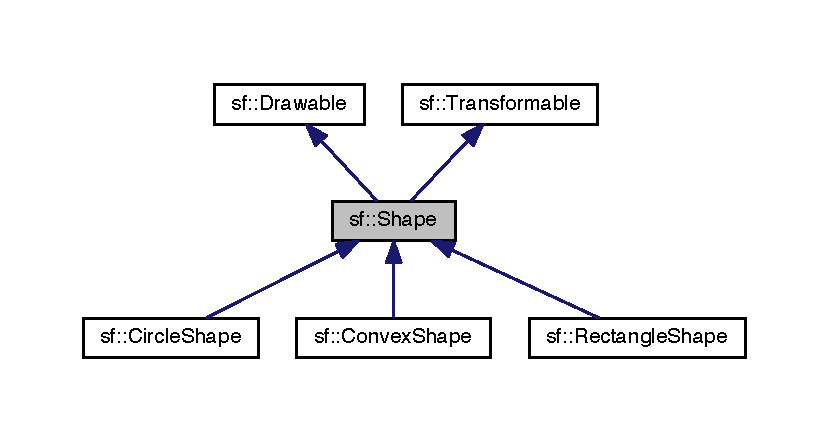
\includegraphics[width=350pt]{classsf_1_1_shape__inherit__graph}
\end{center}
\end{figure}


Collaboration diagram for sf\-:\-:Shape\-:
\nopagebreak
\begin{figure}[H]
\begin{center}
\leavevmode
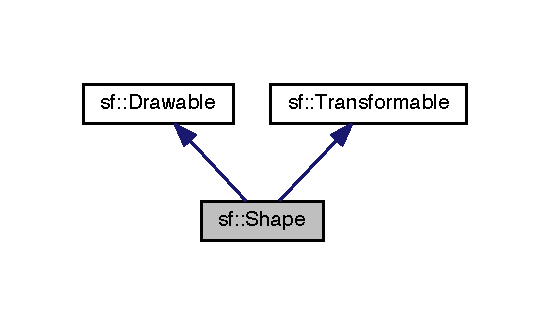
\includegraphics[width=264pt]{classsf_1_1_shape__coll__graph}
\end{center}
\end{figure}
\subsection*{Public Member Functions}
\begin{DoxyCompactItemize}
\item 
virtual \hyperlink{classsf_1_1_shape_a2262aceb9df52d4275c19633592f19bf}{$\sim$\-Shape} ()
\begin{DoxyCompactList}\small\item\em Virtual destructor. \end{DoxyCompactList}\item 
\hyperlink{glutf90_8h_ac778d6f63f1aaf8ebda0ce6ac821b56e}{void} \hyperlink{classsf_1_1_shape_af8fb22bab1956325be5d62282711e3b6}{set\-Texture} (const \hyperlink{classsf_1_1_texture}{Texture} $\ast$\hyperlink{gl3_8h_ab21590c4736d1459a5a0674a42b5a655}{texture}, bool reset\-Rect=false)
\begin{DoxyCompactList}\small\item\em Change the source texture of the shape. \end{DoxyCompactList}\item 
\hyperlink{glutf90_8h_ac778d6f63f1aaf8ebda0ce6ac821b56e}{void} \hyperlink{classsf_1_1_shape_a2029cc820d1740d14ac794b82525e157}{set\-Texture\-Rect} (const \hyperlink{namespacesf_aae67411782674934f78d55fa3af18403}{Int\-Rect} \&rect)
\begin{DoxyCompactList}\small\item\em Set the sub-\/rectangle of the texture that the shape will display. \end{DoxyCompactList}\item 
\hyperlink{glutf90_8h_ac778d6f63f1aaf8ebda0ce6ac821b56e}{void} \hyperlink{classsf_1_1_shape_a3506f9b5d916fec14d583d16f23c2485}{set\-Fill\-Color} (const \hyperlink{classsf_1_1_color}{Color} \&\hyperlink{gl3_8h_a3ea846f998d64f079b86052b6c4193a8}{color})
\begin{DoxyCompactList}\small\item\em Set the fill color of the shape. \end{DoxyCompactList}\item 
\hyperlink{glutf90_8h_ac778d6f63f1aaf8ebda0ce6ac821b56e}{void} \hyperlink{classsf_1_1_shape_a5978f41ee349ac3c52942996dcb184f7}{set\-Outline\-Color} (const \hyperlink{classsf_1_1_color}{Color} \&\hyperlink{gl3_8h_a3ea846f998d64f079b86052b6c4193a8}{color})
\begin{DoxyCompactList}\small\item\em Set the outline color of the shape. \end{DoxyCompactList}\item 
\hyperlink{glutf90_8h_ac778d6f63f1aaf8ebda0ce6ac821b56e}{void} \hyperlink{classsf_1_1_shape_a5ad336ad74fc1f567fce3b7e44cf87dc}{set\-Outline\-Thickness} (float thickness)
\begin{DoxyCompactList}\small\item\em Set the thickness of the shape's outline. \end{DoxyCompactList}\item 
const \hyperlink{classsf_1_1_texture}{Texture} $\ast$ \hyperlink{classsf_1_1_shape_a1bf27ac425fcce36efd0eed67531a403}{get\-Texture} () const 
\begin{DoxyCompactList}\small\item\em Get the source texture of the shape. \end{DoxyCompactList}\item 
const \hyperlink{namespacesf_aae67411782674934f78d55fa3af18403}{Int\-Rect} \& \hyperlink{classsf_1_1_shape_af7c4c80a435b85a622812711cf510439}{get\-Texture\-Rect} () const 
\begin{DoxyCompactList}\small\item\em Get the sub-\/rectangle of the texture displayed by the shape. \end{DoxyCompactList}\item 
const \hyperlink{classsf_1_1_color}{Color} \& \hyperlink{classsf_1_1_shape_ad7f7fe601a8bb24efe9aa77809a35c12}{get\-Fill\-Color} () const 
\begin{DoxyCompactList}\small\item\em Get the fill color of the shape. \end{DoxyCompactList}\item 
const \hyperlink{classsf_1_1_color}{Color} \& \hyperlink{classsf_1_1_shape_a4fa7d3bf5ee2332f6b9d9bebe9b1e2fd}{get\-Outline\-Color} () const 
\begin{DoxyCompactList}\small\item\em Get the outline color of the shape. \end{DoxyCompactList}\item 
float \hyperlink{classsf_1_1_shape_ac66f917b41eda6159a8ba6571d77f2ad}{get\-Outline\-Thickness} () const 
\begin{DoxyCompactList}\small\item\em Get the outline thickness of the shape. \end{DoxyCompactList}\item 
virtual unsigned int \hyperlink{classsf_1_1_shape_ad84e1b675ecd270ad8151aea4e271a78}{get\-Point\-Count} () const =0
\begin{DoxyCompactList}\small\item\em Get the total number of points of the shape. \end{DoxyCompactList}\item 
virtual \hyperlink{namespacesf_acf03098c2577b869e2fa6836cc48f1a0}{Vector2f} \hyperlink{classsf_1_1_shape_a397f3b4cdb7ad98cdc6c034816c652d2}{get\-Point} (unsigned int \hyperlink{gl3_8h_a57f14e05b1900f16a2da82ade47d0c6d}{index}) const =0
\begin{DoxyCompactList}\small\item\em Get a point of the shape. \end{DoxyCompactList}\item 
\hyperlink{namespacesf_aed4e58f586b2eed2621c0365d0b7554e}{Float\-Rect} \hyperlink{classsf_1_1_shape_a5d26a18ccfe850ff8d327ca97edbc34a}{get\-Local\-Bounds} () const 
\begin{DoxyCompactList}\small\item\em Get the local bounding rectangle of the entity. \end{DoxyCompactList}\item 
\hyperlink{namespacesf_aed4e58f586b2eed2621c0365d0b7554e}{Float\-Rect} \hyperlink{classsf_1_1_shape_a5257341fe832884dbba6b9dc855e33cc}{get\-Global\-Bounds} () const 
\begin{DoxyCompactList}\small\item\em Get the global bounding rectangle of the entity. \end{DoxyCompactList}\end{DoxyCompactItemize}
\subsection*{Protected Member Functions}
\begin{DoxyCompactItemize}
\item 
\hyperlink{classsf_1_1_shape_a413a457f720835b9f5d8e97ca8b80960}{Shape} ()
\begin{DoxyCompactList}\small\item\em Default constructor. \end{DoxyCompactList}\item 
\hyperlink{glutf90_8h_ac778d6f63f1aaf8ebda0ce6ac821b56e}{void} \hyperlink{classsf_1_1_shape_adfb2bd966c8edbc5d6c92ebc375e4ac1}{update} ()
\begin{DoxyCompactList}\small\item\em Recompute the internal geometry of the shape. \end{DoxyCompactList}\end{DoxyCompactItemize}


\subsection{Detailed Description}
Base class for textured shapes with outline. 

\hyperlink{classsf_1_1_shape}{sf\-::\-Shape} is a drawable class that allows to define and display a custom convex shape on a render target. It's only an abstract base, it needs to be specialized for concrete types of shapes (circle, rectangle, convex polygon, star, ...).

In addition to the attributes provided by the specialized shape classes, a shape always has the following attributes\-: \begin{DoxyItemize}
\item a texture \item a texture rectangle \item a fill color \item an outline color \item an outline thickness\end{DoxyItemize}
Each feature is optional, and can be disabled easily\-: \begin{DoxyItemize}
\item the texture can be null \item the fill/outline colors can be \hyperlink{classsf_1_1_color_a569b45471737f770656f50ae7bbac292}{sf\-::\-Color\-::\-Transparent} \item the outline thickness can be zero\end{DoxyItemize}
You can write your own derived shape class, there are only two virtual functions to override\-: \begin{DoxyItemize}
\item get\-Point\-Count must return the number of points of the shape \item get\-Point must return the points of the shape\end{DoxyItemize}
\begin{DoxySeeAlso}{See Also}
\hyperlink{classsf_1_1_rectangle_shape}{sf\-::\-Rectangle\-Shape}, \hyperlink{classsf_1_1_circle_shape}{sf\-::\-Circle\-Shape}, \hyperlink{classsf_1_1_convex_shape}{sf\-::\-Convex\-Shape}, \hyperlink{classsf_1_1_transformable}{sf\-::\-Transformable} 
\end{DoxySeeAlso}


Definition at line 44 of file Shape.\-hpp.



\subsection{Constructor \& Destructor Documentation}
\hypertarget{classsf_1_1_shape_a2262aceb9df52d4275c19633592f19bf}{\index{sf\-::\-Shape@{sf\-::\-Shape}!$\sim$\-Shape@{$\sim$\-Shape}}
\index{$\sim$\-Shape@{$\sim$\-Shape}!sf::Shape@{sf\-::\-Shape}}
\subsubsection[{$\sim$\-Shape}]{\setlength{\rightskip}{0pt plus 5cm}virtual sf\-::\-Shape\-::$\sim$\-Shape (
\begin{DoxyParamCaption}
{}
\end{DoxyParamCaption}
)\hspace{0.3cm}{\ttfamily [virtual]}}}\label{classsf_1_1_shape_a2262aceb9df52d4275c19633592f19bf}


Virtual destructor. 

\hypertarget{classsf_1_1_shape_a413a457f720835b9f5d8e97ca8b80960}{\index{sf\-::\-Shape@{sf\-::\-Shape}!Shape@{Shape}}
\index{Shape@{Shape}!sf::Shape@{sf\-::\-Shape}}
\subsubsection[{Shape}]{\setlength{\rightskip}{0pt plus 5cm}sf\-::\-Shape\-::\-Shape (
\begin{DoxyParamCaption}
{}
\end{DoxyParamCaption}
)\hspace{0.3cm}{\ttfamily [protected]}}}\label{classsf_1_1_shape_a413a457f720835b9f5d8e97ca8b80960}


Default constructor. 



\subsection{Member Function Documentation}
\hypertarget{classsf_1_1_shape_ad7f7fe601a8bb24efe9aa77809a35c12}{\index{sf\-::\-Shape@{sf\-::\-Shape}!get\-Fill\-Color@{get\-Fill\-Color}}
\index{get\-Fill\-Color@{get\-Fill\-Color}!sf::Shape@{sf\-::\-Shape}}
\subsubsection[{get\-Fill\-Color}]{\setlength{\rightskip}{0pt plus 5cm}const {\bf Color}\& sf\-::\-Shape\-::get\-Fill\-Color (
\begin{DoxyParamCaption}
{}
\end{DoxyParamCaption}
) const}}\label{classsf_1_1_shape_ad7f7fe601a8bb24efe9aa77809a35c12}


Get the fill color of the shape. 

\begin{DoxyReturn}{Returns}
Fill color of the shape
\end{DoxyReturn}
\begin{DoxySeeAlso}{See Also}
\hyperlink{classsf_1_1_shape_a3506f9b5d916fec14d583d16f23c2485}{set\-Fill\-Color} 
\end{DoxySeeAlso}
\hypertarget{classsf_1_1_shape_a5257341fe832884dbba6b9dc855e33cc}{\index{sf\-::\-Shape@{sf\-::\-Shape}!get\-Global\-Bounds@{get\-Global\-Bounds}}
\index{get\-Global\-Bounds@{get\-Global\-Bounds}!sf::Shape@{sf\-::\-Shape}}
\subsubsection[{get\-Global\-Bounds}]{\setlength{\rightskip}{0pt plus 5cm}{\bf Float\-Rect} sf\-::\-Shape\-::get\-Global\-Bounds (
\begin{DoxyParamCaption}
{}
\end{DoxyParamCaption}
) const}}\label{classsf_1_1_shape_a5257341fe832884dbba6b9dc855e33cc}


Get the global bounding rectangle of the entity. 

The returned rectangle is in global coordinates, which means that it takes in account the transformations (translation, rotation, scale, ...) that are applied to the entity. In other words, this function returns the bounds of the sprite in the global 2\-D world's coordinate system.

\begin{DoxyReturn}{Returns}
Global bounding rectangle of the entity 
\end{DoxyReturn}
\hypertarget{classsf_1_1_shape_a5d26a18ccfe850ff8d327ca97edbc34a}{\index{sf\-::\-Shape@{sf\-::\-Shape}!get\-Local\-Bounds@{get\-Local\-Bounds}}
\index{get\-Local\-Bounds@{get\-Local\-Bounds}!sf::Shape@{sf\-::\-Shape}}
\subsubsection[{get\-Local\-Bounds}]{\setlength{\rightskip}{0pt plus 5cm}{\bf Float\-Rect} sf\-::\-Shape\-::get\-Local\-Bounds (
\begin{DoxyParamCaption}
{}
\end{DoxyParamCaption}
) const}}\label{classsf_1_1_shape_a5d26a18ccfe850ff8d327ca97edbc34a}


Get the local bounding rectangle of the entity. 

The returned rectangle is in local coordinates, which means that it ignores the transformations (translation, rotation, scale, ...) that are applied to the entity. In other words, this function returns the bounds of the entity in the entity's coordinate system.

\begin{DoxyReturn}{Returns}
Local bounding rectangle of the entity 
\end{DoxyReturn}
\hypertarget{classsf_1_1_shape_a4fa7d3bf5ee2332f6b9d9bebe9b1e2fd}{\index{sf\-::\-Shape@{sf\-::\-Shape}!get\-Outline\-Color@{get\-Outline\-Color}}
\index{get\-Outline\-Color@{get\-Outline\-Color}!sf::Shape@{sf\-::\-Shape}}
\subsubsection[{get\-Outline\-Color}]{\setlength{\rightskip}{0pt plus 5cm}const {\bf Color}\& sf\-::\-Shape\-::get\-Outline\-Color (
\begin{DoxyParamCaption}
{}
\end{DoxyParamCaption}
) const}}\label{classsf_1_1_shape_a4fa7d3bf5ee2332f6b9d9bebe9b1e2fd}


Get the outline color of the shape. 

\begin{DoxyReturn}{Returns}
Outline color of the shape
\end{DoxyReturn}
\begin{DoxySeeAlso}{See Also}
\hyperlink{classsf_1_1_shape_a5978f41ee349ac3c52942996dcb184f7}{set\-Outline\-Color} 
\end{DoxySeeAlso}
\hypertarget{classsf_1_1_shape_ac66f917b41eda6159a8ba6571d77f2ad}{\index{sf\-::\-Shape@{sf\-::\-Shape}!get\-Outline\-Thickness@{get\-Outline\-Thickness}}
\index{get\-Outline\-Thickness@{get\-Outline\-Thickness}!sf::Shape@{sf\-::\-Shape}}
\subsubsection[{get\-Outline\-Thickness}]{\setlength{\rightskip}{0pt plus 5cm}float sf\-::\-Shape\-::get\-Outline\-Thickness (
\begin{DoxyParamCaption}
{}
\end{DoxyParamCaption}
) const}}\label{classsf_1_1_shape_ac66f917b41eda6159a8ba6571d77f2ad}


Get the outline thickness of the shape. 

\begin{DoxyReturn}{Returns}
Outline thickness of the shape
\end{DoxyReturn}
\begin{DoxySeeAlso}{See Also}
\hyperlink{classsf_1_1_shape_a5ad336ad74fc1f567fce3b7e44cf87dc}{set\-Outline\-Thickness} 
\end{DoxySeeAlso}
\hypertarget{classsf_1_1_shape_a397f3b4cdb7ad98cdc6c034816c652d2}{\index{sf\-::\-Shape@{sf\-::\-Shape}!get\-Point@{get\-Point}}
\index{get\-Point@{get\-Point}!sf::Shape@{sf\-::\-Shape}}
\subsubsection[{get\-Point}]{\setlength{\rightskip}{0pt plus 5cm}virtual {\bf Vector2f} sf\-::\-Shape\-::get\-Point (
\begin{DoxyParamCaption}
\item[{unsigned int}]{index}
\end{DoxyParamCaption}
) const\hspace{0.3cm}{\ttfamily [pure virtual]}}}\label{classsf_1_1_shape_a397f3b4cdb7ad98cdc6c034816c652d2}


Get a point of the shape. 

The result is undefined if {\itshape index} is out of the valid range.


\begin{DoxyParams}{Parameters}
{\em index} & Index of the point to get, in range \mbox{[}0 .. Get\-Point\-Count() -\/ 1\mbox{]}\\
\hline
\end{DoxyParams}
\begin{DoxyReturn}{Returns}
Index-\/th point of the shape
\end{DoxyReturn}
\begin{DoxySeeAlso}{See Also}
\hyperlink{classsf_1_1_shape_ad84e1b675ecd270ad8151aea4e271a78}{get\-Point\-Count} 
\end{DoxySeeAlso}


Implemented in \hyperlink{classsf_1_1_convex_shape_ae2a18b837cd4454e340599a220c09a34}{sf\-::\-Convex\-Shape}, \hyperlink{classsf_1_1_circle_shape_a05139deaef220ed3d5a3bc4ca9aa9dbe}{sf\-::\-Circle\-Shape}, and \hyperlink{classsf_1_1_rectangle_shape_a3994f7f937d6332fe64b6990d5bc43a1}{sf\-::\-Rectangle\-Shape}.

\hypertarget{classsf_1_1_shape_ad84e1b675ecd270ad8151aea4e271a78}{\index{sf\-::\-Shape@{sf\-::\-Shape}!get\-Point\-Count@{get\-Point\-Count}}
\index{get\-Point\-Count@{get\-Point\-Count}!sf::Shape@{sf\-::\-Shape}}
\subsubsection[{get\-Point\-Count}]{\setlength{\rightskip}{0pt plus 5cm}virtual unsigned int sf\-::\-Shape\-::get\-Point\-Count (
\begin{DoxyParamCaption}
{}
\end{DoxyParamCaption}
) const\hspace{0.3cm}{\ttfamily [pure virtual]}}}\label{classsf_1_1_shape_ad84e1b675ecd270ad8151aea4e271a78}


Get the total number of points of the shape. 

\begin{DoxyReturn}{Returns}
Number of points of the shape
\end{DoxyReturn}
\begin{DoxySeeAlso}{See Also}
\hyperlink{classsf_1_1_shape_a397f3b4cdb7ad98cdc6c034816c652d2}{get\-Point} 
\end{DoxySeeAlso}


Implemented in \hyperlink{classsf_1_1_circle_shape_ae41ed830ca8f459e88ea6f125c240949}{sf\-::\-Circle\-Shape}, \hyperlink{classsf_1_1_rectangle_shape_a439f5a92583baf972878c836b73bf955}{sf\-::\-Rectangle\-Shape}, and \hyperlink{classsf_1_1_convex_shape_af81b86134fe54f2d50d9fab0db065ef1}{sf\-::\-Convex\-Shape}.

\hypertarget{classsf_1_1_shape_a1bf27ac425fcce36efd0eed67531a403}{\index{sf\-::\-Shape@{sf\-::\-Shape}!get\-Texture@{get\-Texture}}
\index{get\-Texture@{get\-Texture}!sf::Shape@{sf\-::\-Shape}}
\subsubsection[{get\-Texture}]{\setlength{\rightskip}{0pt plus 5cm}const {\bf Texture}$\ast$ sf\-::\-Shape\-::get\-Texture (
\begin{DoxyParamCaption}
{}
\end{DoxyParamCaption}
) const}}\label{classsf_1_1_shape_a1bf27ac425fcce36efd0eed67531a403}


Get the source texture of the shape. 

If the shape has no source texture, a N\-U\-L\-L pointer is returned. The returned pointer is const, which means that you can't modify the texture when you retrieve it with this function.

\begin{DoxyReturn}{Returns}
Pointer to the shape's texture
\end{DoxyReturn}
\begin{DoxySeeAlso}{See Also}
\hyperlink{classsf_1_1_shape_af8fb22bab1956325be5d62282711e3b6}{set\-Texture} 
\end{DoxySeeAlso}
\hypertarget{classsf_1_1_shape_af7c4c80a435b85a622812711cf510439}{\index{sf\-::\-Shape@{sf\-::\-Shape}!get\-Texture\-Rect@{get\-Texture\-Rect}}
\index{get\-Texture\-Rect@{get\-Texture\-Rect}!sf::Shape@{sf\-::\-Shape}}
\subsubsection[{get\-Texture\-Rect}]{\setlength{\rightskip}{0pt plus 5cm}const {\bf Int\-Rect}\& sf\-::\-Shape\-::get\-Texture\-Rect (
\begin{DoxyParamCaption}
{}
\end{DoxyParamCaption}
) const}}\label{classsf_1_1_shape_af7c4c80a435b85a622812711cf510439}


Get the sub-\/rectangle of the texture displayed by the shape. 

\begin{DoxyReturn}{Returns}
\hyperlink{classsf_1_1_texture}{Texture} rectangle of the shape
\end{DoxyReturn}
\begin{DoxySeeAlso}{See Also}
\hyperlink{classsf_1_1_shape_a2029cc820d1740d14ac794b82525e157}{set\-Texture\-Rect} 
\end{DoxySeeAlso}
\hypertarget{classsf_1_1_shape_a3506f9b5d916fec14d583d16f23c2485}{\index{sf\-::\-Shape@{sf\-::\-Shape}!set\-Fill\-Color@{set\-Fill\-Color}}
\index{set\-Fill\-Color@{set\-Fill\-Color}!sf::Shape@{sf\-::\-Shape}}
\subsubsection[{set\-Fill\-Color}]{\setlength{\rightskip}{0pt plus 5cm}{\bf void} sf\-::\-Shape\-::set\-Fill\-Color (
\begin{DoxyParamCaption}
\item[{const {\bf Color} \&}]{color}
\end{DoxyParamCaption}
)}}\label{classsf_1_1_shape_a3506f9b5d916fec14d583d16f23c2485}


Set the fill color of the shape. 

This color is modulated (multiplied) with the shape's texture if any. It can be used to colorize the shape, or change its global opacity. You can use \hyperlink{classsf_1_1_color_a569b45471737f770656f50ae7bbac292}{sf\-::\-Color\-::\-Transparent} to make the inside of the shape transparent, and have the outline alone. By default, the shape's fill color is opaque white.


\begin{DoxyParams}{Parameters}
{\em color} & New color of the shape\\
\hline
\end{DoxyParams}
\begin{DoxySeeAlso}{See Also}
\hyperlink{classsf_1_1_shape_ad7f7fe601a8bb24efe9aa77809a35c12}{get\-Fill\-Color}, \hyperlink{classsf_1_1_shape_a5978f41ee349ac3c52942996dcb184f7}{set\-Outline\-Color} 
\end{DoxySeeAlso}
\hypertarget{classsf_1_1_shape_a5978f41ee349ac3c52942996dcb184f7}{\index{sf\-::\-Shape@{sf\-::\-Shape}!set\-Outline\-Color@{set\-Outline\-Color}}
\index{set\-Outline\-Color@{set\-Outline\-Color}!sf::Shape@{sf\-::\-Shape}}
\subsubsection[{set\-Outline\-Color}]{\setlength{\rightskip}{0pt plus 5cm}{\bf void} sf\-::\-Shape\-::set\-Outline\-Color (
\begin{DoxyParamCaption}
\item[{const {\bf Color} \&}]{color}
\end{DoxyParamCaption}
)}}\label{classsf_1_1_shape_a5978f41ee349ac3c52942996dcb184f7}


Set the outline color of the shape. 

You can use \hyperlink{classsf_1_1_color_a569b45471737f770656f50ae7bbac292}{sf\-::\-Color\-::\-Transparent} to disable the outline. By default, the shape's outline color is opaque white.


\begin{DoxyParams}{Parameters}
{\em color} & New outline color of the shape\\
\hline
\end{DoxyParams}
\begin{DoxySeeAlso}{See Also}
\hyperlink{classsf_1_1_shape_a4fa7d3bf5ee2332f6b9d9bebe9b1e2fd}{get\-Outline\-Color}, \hyperlink{classsf_1_1_shape_a3506f9b5d916fec14d583d16f23c2485}{set\-Fill\-Color} 
\end{DoxySeeAlso}
\hypertarget{classsf_1_1_shape_a5ad336ad74fc1f567fce3b7e44cf87dc}{\index{sf\-::\-Shape@{sf\-::\-Shape}!set\-Outline\-Thickness@{set\-Outline\-Thickness}}
\index{set\-Outline\-Thickness@{set\-Outline\-Thickness}!sf::Shape@{sf\-::\-Shape}}
\subsubsection[{set\-Outline\-Thickness}]{\setlength{\rightskip}{0pt plus 5cm}{\bf void} sf\-::\-Shape\-::set\-Outline\-Thickness (
\begin{DoxyParamCaption}
\item[{float}]{thickness}
\end{DoxyParamCaption}
)}}\label{classsf_1_1_shape_a5ad336ad74fc1f567fce3b7e44cf87dc}


Set the thickness of the shape's outline. 

This number cannot be negative. Using zero disables the outline. By default, the outline thickness is 0.


\begin{DoxyParams}{Parameters}
{\em thickness} & New outline thickness\\
\hline
\end{DoxyParams}
\begin{DoxySeeAlso}{See Also}
\hyperlink{classsf_1_1_shape_ac66f917b41eda6159a8ba6571d77f2ad}{get\-Outline\-Thickness} 
\end{DoxySeeAlso}
\hypertarget{classsf_1_1_shape_af8fb22bab1956325be5d62282711e3b6}{\index{sf\-::\-Shape@{sf\-::\-Shape}!set\-Texture@{set\-Texture}}
\index{set\-Texture@{set\-Texture}!sf::Shape@{sf\-::\-Shape}}
\subsubsection[{set\-Texture}]{\setlength{\rightskip}{0pt plus 5cm}{\bf void} sf\-::\-Shape\-::set\-Texture (
\begin{DoxyParamCaption}
\item[{const {\bf Texture} $\ast$}]{texture, }
\item[{bool}]{reset\-Rect = {\ttfamily false}}
\end{DoxyParamCaption}
)}}\label{classsf_1_1_shape_af8fb22bab1956325be5d62282711e3b6}


Change the source texture of the shape. 

The {\itshape texture} argument refers to a texture that must exist as long as the shape uses it. Indeed, the shape doesn't store its own copy of the texture, but rather keeps a pointer to the one that you passed to this function. If the source texture is destroyed and the shape tries to use it, the behaviour is undefined. {\itshape texture} can be N\-U\-L\-L to disable texturing. If {\itshape reset\-Rect} is true, the Texture\-Rect property of the shape is automatically adjusted to the size of the new texture. If it is false, the texture rect is left unchanged.


\begin{DoxyParams}{Parameters}
{\em texture} & New texture \\
\hline
{\em reset\-Rect} & Should the texture rect be reset to the size of the new texture?\\
\hline
\end{DoxyParams}
\begin{DoxySeeAlso}{See Also}
\hyperlink{classsf_1_1_shape_a1bf27ac425fcce36efd0eed67531a403}{get\-Texture}, \hyperlink{classsf_1_1_shape_a2029cc820d1740d14ac794b82525e157}{set\-Texture\-Rect} 
\end{DoxySeeAlso}
\hypertarget{classsf_1_1_shape_a2029cc820d1740d14ac794b82525e157}{\index{sf\-::\-Shape@{sf\-::\-Shape}!set\-Texture\-Rect@{set\-Texture\-Rect}}
\index{set\-Texture\-Rect@{set\-Texture\-Rect}!sf::Shape@{sf\-::\-Shape}}
\subsubsection[{set\-Texture\-Rect}]{\setlength{\rightskip}{0pt plus 5cm}{\bf void} sf\-::\-Shape\-::set\-Texture\-Rect (
\begin{DoxyParamCaption}
\item[{const {\bf Int\-Rect} \&}]{rect}
\end{DoxyParamCaption}
)}}\label{classsf_1_1_shape_a2029cc820d1740d14ac794b82525e157}


Set the sub-\/rectangle of the texture that the shape will display. 

The texture rect is useful when you don't want to display the whole texture, but rather a part of it. By default, the texture rect covers the entire texture.


\begin{DoxyParams}{Parameters}
{\em rect} & Rectangle defining the region of the texture to display\\
\hline
\end{DoxyParams}
\begin{DoxySeeAlso}{See Also}
\hyperlink{classsf_1_1_shape_af7c4c80a435b85a622812711cf510439}{get\-Texture\-Rect}, \hyperlink{classsf_1_1_shape_af8fb22bab1956325be5d62282711e3b6}{set\-Texture} 
\end{DoxySeeAlso}
\hypertarget{classsf_1_1_shape_adfb2bd966c8edbc5d6c92ebc375e4ac1}{\index{sf\-::\-Shape@{sf\-::\-Shape}!update@{update}}
\index{update@{update}!sf::Shape@{sf\-::\-Shape}}
\subsubsection[{update}]{\setlength{\rightskip}{0pt plus 5cm}{\bf void} sf\-::\-Shape\-::update (
\begin{DoxyParamCaption}
{}
\end{DoxyParamCaption}
)\hspace{0.3cm}{\ttfamily [protected]}}}\label{classsf_1_1_shape_adfb2bd966c8edbc5d6c92ebc375e4ac1}


Recompute the internal geometry of the shape. 

This function must be called by the derived class everytime the shape's points change (ie. the result of either get\-Point\-Count or get\-Point is different). 

The documentation for this class was generated from the following file\-:\begin{DoxyCompactItemize}
\item 
/\-Users/ira/\-Dropbox/ira\-\_\-dev/protobyte\-\_\-research/other\-\_\-libs/\-S\-F\-M\-L/dylibs/root/usr/local/include/\-S\-F\-M\-L/\-Graphics/\hyperlink{_shape_8hpp}{Shape.\-hpp}\end{DoxyCompactItemize}

\hypertarget{structsf_1_1_event_1_1_size_event}{\section{sf\-:\-:Event\-:\-:Size\-Event Struct Reference}
\label{structsf_1_1_event_1_1_size_event}\index{sf\-::\-Event\-::\-Size\-Event@{sf\-::\-Event\-::\-Size\-Event}}
}


Size events parameters (Resized)  




{\ttfamily \#include $<$Event.\-hpp$>$}

\subsection*{Public Attributes}
\begin{DoxyCompactItemize}
\item 
unsigned int \hyperlink{structsf_1_1_event_1_1_size_event_a20ea1b78c9bb1604432f8f0067bbfd94}{width}
\begin{DoxyCompactList}\small\item\em New width, in pixels. \end{DoxyCompactList}\item 
unsigned int \hyperlink{structsf_1_1_event_1_1_size_event_af0f76a599d5f48189cb8d78d4e5facdb}{height}
\begin{DoxyCompactList}\small\item\em New height, in pixels. \end{DoxyCompactList}\end{DoxyCompactItemize}


\subsection{Detailed Description}
Size events parameters (Resized) 

Definition at line 51 of file Event.\-hpp.



\subsection{Member Data Documentation}
\hypertarget{structsf_1_1_event_1_1_size_event_af0f76a599d5f48189cb8d78d4e5facdb}{\index{sf\-::\-Event\-::\-Size\-Event@{sf\-::\-Event\-::\-Size\-Event}!height@{height}}
\index{height@{height}!sf::Event::SizeEvent@{sf\-::\-Event\-::\-Size\-Event}}
\subsubsection[{height}]{\setlength{\rightskip}{0pt plus 5cm}unsigned int sf\-::\-Event\-::\-Size\-Event\-::height}}\label{structsf_1_1_event_1_1_size_event_af0f76a599d5f48189cb8d78d4e5facdb}


New height, in pixels. 



Definition at line 54 of file Event.\-hpp.

\hypertarget{structsf_1_1_event_1_1_size_event_a20ea1b78c9bb1604432f8f0067bbfd94}{\index{sf\-::\-Event\-::\-Size\-Event@{sf\-::\-Event\-::\-Size\-Event}!width@{width}}
\index{width@{width}!sf::Event::SizeEvent@{sf\-::\-Event\-::\-Size\-Event}}
\subsubsection[{width}]{\setlength{\rightskip}{0pt plus 5cm}unsigned int sf\-::\-Event\-::\-Size\-Event\-::width}}\label{structsf_1_1_event_1_1_size_event_a20ea1b78c9bb1604432f8f0067bbfd94}


New width, in pixels. 



Definition at line 53 of file Event.\-hpp.



The documentation for this struct was generated from the following file\-:\begin{DoxyCompactItemize}
\item 
/\-Users/ira/\-Dropbox/ira\-\_\-dev/protobyte\-\_\-research/other\-\_\-libs/\-S\-F\-M\-L/dylibs/root/usr/local/include/\-S\-F\-M\-L/\-Window/\hyperlink{_event_8hpp}{Event.\-hpp}\end{DoxyCompactItemize}

\hypertarget{classsf_1_1_socket}{\section{sf\-:\-:Socket Class Reference}
\label{classsf_1_1_socket}\index{sf\-::\-Socket@{sf\-::\-Socket}}
}


Base class for all the socket types.  




{\ttfamily \#include $<$Socket.\-hpp$>$}



Inheritance diagram for sf\-:\-:Socket\-:
\nopagebreak
\begin{figure}[H]
\begin{center}
\leavevmode
\includegraphics[width=350pt]{classsf_1_1_socket__inherit__graph}
\end{center}
\end{figure}


Collaboration diagram for sf\-:\-:Socket\-:
\nopagebreak
\begin{figure}[H]
\begin{center}
\leavevmode
\includegraphics[width=170pt]{classsf_1_1_socket__coll__graph}
\end{center}
\end{figure}
\subsection*{Public Types}
\begin{DoxyCompactItemize}
\item 
enum \hyperlink{classsf_1_1_socket_a51bf0fd51057b98a10fbb866246176dc}{Status} \{ \hyperlink{classsf_1_1_socket_a51bf0fd51057b98a10fbb866246176dca1de3a85bc56d3ae85b3d0f3cfd04ae90}{Done}, 
\hyperlink{classsf_1_1_socket_a51bf0fd51057b98a10fbb866246176dca8554848daae98f996e131bdeed076c09}{Not\-Ready}, 
\hyperlink{classsf_1_1_socket_a51bf0fd51057b98a10fbb866246176dcab215141f756acdc23c67fad149710eb1}{Disconnected}, 
\hyperlink{classsf_1_1_socket_a51bf0fd51057b98a10fbb866246176dca1dc9854433a28c22e192721179a2df5d}{Error}
 \}
\begin{DoxyCompactList}\small\item\em Status codes that may be returned by socket functions. \end{DoxyCompactList}\item 
enum \{ \hyperlink{classsf_1_1_socket_a1b900779ad24d3604a4a000e2e38f372a5a3c30fd128895403afc11076f461b19}{Any\-Port} = 0
 \}
\begin{DoxyCompactList}\small\item\em Some special values used by sockets. \end{DoxyCompactList}\end{DoxyCompactItemize}
\subsection*{Public Member Functions}
\begin{DoxyCompactItemize}
\item 
virtual \hyperlink{classsf_1_1_socket_a79a4b5918f0b34a2f8db449089694788}{$\sim$\-Socket} ()
\begin{DoxyCompactList}\small\item\em Destructor. \end{DoxyCompactList}\item 
\hyperlink{glutf90_8h_ac778d6f63f1aaf8ebda0ce6ac821b56e}{void} \hyperlink{classsf_1_1_socket_a165fc1423e281ea2714c70303d3a9782}{set\-Blocking} (bool blocking)
\begin{DoxyCompactList}\small\item\em Set the blocking state of the socket. \end{DoxyCompactList}\item 
bool \hyperlink{classsf_1_1_socket_a0ec0d831b015e32eb5935fd2a9f8c67c}{is\-Blocking} () const 
\begin{DoxyCompactList}\small\item\em Tell whether the socket is in blocking or non-\/blocking mode. \end{DoxyCompactList}\end{DoxyCompactItemize}
\subsection*{Protected Types}
\begin{DoxyCompactItemize}
\item 
enum \hyperlink{classsf_1_1_socket_a5d3ff44e56e68f02816bb0fabc34adf8}{Type} \{ \hyperlink{classsf_1_1_socket_a5d3ff44e56e68f02816bb0fabc34adf8acc02e97e90234b957eaad4dff7f22214}{Tcp}, 
\hyperlink{classsf_1_1_socket_a5d3ff44e56e68f02816bb0fabc34adf8a6ebf3094830db4820191a327f3cc6ce2}{Udp}
 \}
\begin{DoxyCompactList}\small\item\em Types of protocols that the socket can use. \end{DoxyCompactList}\end{DoxyCompactItemize}
\subsection*{Protected Member Functions}
\begin{DoxyCompactItemize}
\item 
\hyperlink{classsf_1_1_socket_a80ffb47ec0bafc83af019055d3e6a303}{Socket} (\hyperlink{classsf_1_1_socket_a5d3ff44e56e68f02816bb0fabc34adf8}{Type} \hyperlink{gl3_8h_a984aabed544368e7fe0e566d7cf014a7}{type})
\begin{DoxyCompactList}\small\item\em Default constructor. \end{DoxyCompactList}\item 
\hyperlink{namespacesf_aefabb521d8f5eec9e6a9b521271d20d1}{Socket\-Handle} \hyperlink{classsf_1_1_socket_ac0c63b13e61da8294bf54e888e97f9a3}{get\-Handle} () const 
\begin{DoxyCompactList}\small\item\em Return the internal handle of the socket. \end{DoxyCompactList}\item 
\hyperlink{glutf90_8h_ac778d6f63f1aaf8ebda0ce6ac821b56e}{void} \hyperlink{classsf_1_1_socket_aafbe140f4b1921e0d19e88cf7a61dcbc}{create} ()
\begin{DoxyCompactList}\small\item\em Create the internal representation of the socket. \end{DoxyCompactList}\item 
\hyperlink{glutf90_8h_ac778d6f63f1aaf8ebda0ce6ac821b56e}{void} \hyperlink{classsf_1_1_socket_af1dd898f7aa3ead7ff7b2d1c20e97781}{create} (\hyperlink{namespacesf_aefabb521d8f5eec9e6a9b521271d20d1}{Socket\-Handle} handle)
\begin{DoxyCompactList}\small\item\em Create the internal representation of the socket from a socket handle. \end{DoxyCompactList}\item 
\hyperlink{glutf90_8h_ac778d6f63f1aaf8ebda0ce6ac821b56e}{void} \hyperlink{classsf_1_1_socket_a71f2f5c2aa99e01cafe824fee4c573be}{close} ()
\begin{DoxyCompactList}\small\item\em Close the socket gracefully. \end{DoxyCompactList}\end{DoxyCompactItemize}
\subsection*{Friends}
\begin{DoxyCompactItemize}
\item 
class \hyperlink{classsf_1_1_socket_a23fafd48278ea4f8f9c25f1f0f43693c}{Socket\-Selector}
\end{DoxyCompactItemize}
\subsection*{Additional Inherited Members}


\subsection{Detailed Description}
Base class for all the socket types. 

This class mainly defines internal stuff to be used by derived classes.

The only public features that it defines, and which is therefore common to all the socket classes, is the blocking state. All sockets can be set as blocking or non-\/blocking.

In blocking mode, socket functions will hang until the operation completes, which means that the entire program (well, in fact the current thread if you use multiple ones) will be stuck waiting for your socket operation to complete.

In non-\/blocking mode, all the socket functions will return immediately. If the socket is not ready to complete the requested operation, the function simply returns the proper status code (\hyperlink{classsf_1_1_socket_a51bf0fd51057b98a10fbb866246176dca8554848daae98f996e131bdeed076c09}{Socket\-::\-Not\-Ready}).

The default mode, which is blocking, is the one that is generally used, in combination with threads or selectors. The non-\/blocking mode is rather used in real-\/time applications that run an endless loop that can poll the socket often enough, and cannot afford blocking this loop.

\begin{DoxySeeAlso}{See Also}
\hyperlink{classsf_1_1_tcp_listener}{sf\-::\-Tcp\-Listener}, \hyperlink{classsf_1_1_tcp_socket}{sf\-::\-Tcp\-Socket}, \hyperlink{classsf_1_1_udp_socket}{sf\-::\-Udp\-Socket} 
\end{DoxySeeAlso}


Definition at line 45 of file Socket.\-hpp.



\subsection{Member Enumeration Documentation}
\hypertarget{classsf_1_1_socket_a1b900779ad24d3604a4a000e2e38f372}{\subsubsection[{anonymous enum}]{\setlength{\rightskip}{0pt plus 5cm}anonymous enum}}\label{classsf_1_1_socket_a1b900779ad24d3604a4a000e2e38f372}


Some special values used by sockets. 

\begin{Desc}
\item[Enumerator]\par
\begin{description}
\index{Any\-Port@{Any\-Port}!sf\-::\-Socket@{sf\-::\-Socket}}\index{sf\-::\-Socket@{sf\-::\-Socket}!Any\-Port@{Any\-Port}}\item[{\em 
\hypertarget{classsf_1_1_socket_a1b900779ad24d3604a4a000e2e38f372a5a3c30fd128895403afc11076f461b19}{Any\-Port}\label{classsf_1_1_socket_a1b900779ad24d3604a4a000e2e38f372a5a3c30fd128895403afc11076f461b19}
}]Special value that tells the system to pick any available port. \end{description}
\end{Desc}


Definition at line 65 of file Socket.\-hpp.

\hypertarget{classsf_1_1_socket_a51bf0fd51057b98a10fbb866246176dc}{\index{sf\-::\-Socket@{sf\-::\-Socket}!Status@{Status}}
\index{Status@{Status}!sf::Socket@{sf\-::\-Socket}}
\subsubsection[{Status}]{\setlength{\rightskip}{0pt plus 5cm}enum {\bf sf\-::\-Socket\-::\-Status}}}\label{classsf_1_1_socket_a51bf0fd51057b98a10fbb866246176dc}


Status codes that may be returned by socket functions. 

\begin{Desc}
\item[Enumerator]\par
\begin{description}
\index{Done@{Done}!sf\-::\-Socket@{sf\-::\-Socket}}\index{sf\-::\-Socket@{sf\-::\-Socket}!Done@{Done}}\item[{\em 
\hypertarget{classsf_1_1_socket_a51bf0fd51057b98a10fbb866246176dca1de3a85bc56d3ae85b3d0f3cfd04ae90}{Done}\label{classsf_1_1_socket_a51bf0fd51057b98a10fbb866246176dca1de3a85bc56d3ae85b3d0f3cfd04ae90}
}]The socket has sent / received the data. \index{Not\-Ready@{Not\-Ready}!sf\-::\-Socket@{sf\-::\-Socket}}\index{sf\-::\-Socket@{sf\-::\-Socket}!Not\-Ready@{Not\-Ready}}\item[{\em 
\hypertarget{classsf_1_1_socket_a51bf0fd51057b98a10fbb866246176dca8554848daae98f996e131bdeed076c09}{Not\-Ready}\label{classsf_1_1_socket_a51bf0fd51057b98a10fbb866246176dca8554848daae98f996e131bdeed076c09}
}]The socket is not ready to send / receive data yet. \index{Disconnected@{Disconnected}!sf\-::\-Socket@{sf\-::\-Socket}}\index{sf\-::\-Socket@{sf\-::\-Socket}!Disconnected@{Disconnected}}\item[{\em 
\hypertarget{classsf_1_1_socket_a51bf0fd51057b98a10fbb866246176dcab215141f756acdc23c67fad149710eb1}{Disconnected}\label{classsf_1_1_socket_a51bf0fd51057b98a10fbb866246176dcab215141f756acdc23c67fad149710eb1}
}]The T\-C\-P socket has been disconnected. \index{Error@{Error}!sf\-::\-Socket@{sf\-::\-Socket}}\index{sf\-::\-Socket@{sf\-::\-Socket}!Error@{Error}}\item[{\em 
\hypertarget{classsf_1_1_socket_a51bf0fd51057b98a10fbb866246176dca1dc9854433a28c22e192721179a2df5d}{Error}\label{classsf_1_1_socket_a51bf0fd51057b98a10fbb866246176dca1dc9854433a28c22e192721179a2df5d}
}]An unexpected error happened. \end{description}
\end{Desc}


Definition at line 53 of file Socket.\-hpp.

\hypertarget{classsf_1_1_socket_a5d3ff44e56e68f02816bb0fabc34adf8}{\index{sf\-::\-Socket@{sf\-::\-Socket}!Type@{Type}}
\index{Type@{Type}!sf::Socket@{sf\-::\-Socket}}
\subsubsection[{Type}]{\setlength{\rightskip}{0pt plus 5cm}enum {\bf sf\-::\-Socket\-::\-Type}\hspace{0.3cm}{\ttfamily [protected]}}}\label{classsf_1_1_socket_a5d3ff44e56e68f02816bb0fabc34adf8}


Types of protocols that the socket can use. 

\begin{Desc}
\item[Enumerator]\par
\begin{description}
\index{Tcp@{Tcp}!sf\-::\-Socket@{sf\-::\-Socket}}\index{sf\-::\-Socket@{sf\-::\-Socket}!Tcp@{Tcp}}\item[{\em 
\hypertarget{classsf_1_1_socket_a5d3ff44e56e68f02816bb0fabc34adf8acc02e97e90234b957eaad4dff7f22214}{Tcp}\label{classsf_1_1_socket_a5d3ff44e56e68f02816bb0fabc34adf8acc02e97e90234b957eaad4dff7f22214}
}]T\-C\-P protocol. \index{Udp@{Udp}!sf\-::\-Socket@{sf\-::\-Socket}}\index{sf\-::\-Socket@{sf\-::\-Socket}!Udp@{Udp}}\item[{\em 
\hypertarget{classsf_1_1_socket_a5d3ff44e56e68f02816bb0fabc34adf8a6ebf3094830db4820191a327f3cc6ce2}{Udp}\label{classsf_1_1_socket_a5d3ff44e56e68f02816bb0fabc34adf8a6ebf3094830db4820191a327f3cc6ce2}
}]U\-D\-P protocol. \end{description}
\end{Desc}


Definition at line 113 of file Socket.\-hpp.



\subsection{Constructor \& Destructor Documentation}
\hypertarget{classsf_1_1_socket_a79a4b5918f0b34a2f8db449089694788}{\index{sf\-::\-Socket@{sf\-::\-Socket}!$\sim$\-Socket@{$\sim$\-Socket}}
\index{$\sim$\-Socket@{$\sim$\-Socket}!sf::Socket@{sf\-::\-Socket}}
\subsubsection[{$\sim$\-Socket}]{\setlength{\rightskip}{0pt plus 5cm}virtual sf\-::\-Socket\-::$\sim$\-Socket (
\begin{DoxyParamCaption}
{}
\end{DoxyParamCaption}
)\hspace{0.3cm}{\ttfamily [virtual]}}}\label{classsf_1_1_socket_a79a4b5918f0b34a2f8db449089694788}


Destructor. 

\hypertarget{classsf_1_1_socket_a80ffb47ec0bafc83af019055d3e6a303}{\index{sf\-::\-Socket@{sf\-::\-Socket}!Socket@{Socket}}
\index{Socket@{Socket}!sf::Socket@{sf\-::\-Socket}}
\subsubsection[{Socket}]{\setlength{\rightskip}{0pt plus 5cm}sf\-::\-Socket\-::\-Socket (
\begin{DoxyParamCaption}
\item[{{\bf Type}}]{type}
\end{DoxyParamCaption}
)\hspace{0.3cm}{\ttfamily [protected]}}}\label{classsf_1_1_socket_a80ffb47ec0bafc83af019055d3e6a303}


Default constructor. 

This constructor can only be accessed by derived classes.


\begin{DoxyParams}{Parameters}
{\em type} & Type of the socket (T\-C\-P or U\-D\-P) \\
\hline
\end{DoxyParams}


\subsection{Member Function Documentation}
\hypertarget{classsf_1_1_socket_a71f2f5c2aa99e01cafe824fee4c573be}{\index{sf\-::\-Socket@{sf\-::\-Socket}!close@{close}}
\index{close@{close}!sf::Socket@{sf\-::\-Socket}}
\subsubsection[{close}]{\setlength{\rightskip}{0pt plus 5cm}{\bf void} sf\-::\-Socket\-::close (
\begin{DoxyParamCaption}
{}
\end{DoxyParamCaption}
)\hspace{0.3cm}{\ttfamily [protected]}}}\label{classsf_1_1_socket_a71f2f5c2aa99e01cafe824fee4c573be}


Close the socket gracefully. 

This function can only be accessed by derived classes. \hypertarget{classsf_1_1_socket_aafbe140f4b1921e0d19e88cf7a61dcbc}{\index{sf\-::\-Socket@{sf\-::\-Socket}!create@{create}}
\index{create@{create}!sf::Socket@{sf\-::\-Socket}}
\subsubsection[{create}]{\setlength{\rightskip}{0pt plus 5cm}{\bf void} sf\-::\-Socket\-::create (
\begin{DoxyParamCaption}
{}
\end{DoxyParamCaption}
)\hspace{0.3cm}{\ttfamily [protected]}}}\label{classsf_1_1_socket_aafbe140f4b1921e0d19e88cf7a61dcbc}


Create the internal representation of the socket. 

This function can only be accessed by derived classes. \hypertarget{classsf_1_1_socket_af1dd898f7aa3ead7ff7b2d1c20e97781}{\index{sf\-::\-Socket@{sf\-::\-Socket}!create@{create}}
\index{create@{create}!sf::Socket@{sf\-::\-Socket}}
\subsubsection[{create}]{\setlength{\rightskip}{0pt plus 5cm}{\bf void} sf\-::\-Socket\-::create (
\begin{DoxyParamCaption}
\item[{{\bf Socket\-Handle}}]{handle}
\end{DoxyParamCaption}
)\hspace{0.3cm}{\ttfamily [protected]}}}\label{classsf_1_1_socket_af1dd898f7aa3ead7ff7b2d1c20e97781}


Create the internal representation of the socket from a socket handle. 

This function can only be accessed by derived classes.


\begin{DoxyParams}{Parameters}
{\em handle} & O\-S-\/specific handle of the socket to wrap \\
\hline
\end{DoxyParams}
\hypertarget{classsf_1_1_socket_ac0c63b13e61da8294bf54e888e97f9a3}{\index{sf\-::\-Socket@{sf\-::\-Socket}!get\-Handle@{get\-Handle}}
\index{get\-Handle@{get\-Handle}!sf::Socket@{sf\-::\-Socket}}
\subsubsection[{get\-Handle}]{\setlength{\rightskip}{0pt plus 5cm}{\bf Socket\-Handle} sf\-::\-Socket\-::get\-Handle (
\begin{DoxyParamCaption}
{}
\end{DoxyParamCaption}
) const\hspace{0.3cm}{\ttfamily [protected]}}}\label{classsf_1_1_socket_ac0c63b13e61da8294bf54e888e97f9a3}


Return the internal handle of the socket. 

The returned handle may be invalid if the socket was not created yet (or already destroyed). This function can only be accessed by derived classes.

\begin{DoxyReturn}{Returns}
The internal (O\-S-\/specific) handle of the socket 
\end{DoxyReturn}
\hypertarget{classsf_1_1_socket_a0ec0d831b015e32eb5935fd2a9f8c67c}{\index{sf\-::\-Socket@{sf\-::\-Socket}!is\-Blocking@{is\-Blocking}}
\index{is\-Blocking@{is\-Blocking}!sf::Socket@{sf\-::\-Socket}}
\subsubsection[{is\-Blocking}]{\setlength{\rightskip}{0pt plus 5cm}bool sf\-::\-Socket\-::is\-Blocking (
\begin{DoxyParamCaption}
{}
\end{DoxyParamCaption}
) const}}\label{classsf_1_1_socket_a0ec0d831b015e32eb5935fd2a9f8c67c}


Tell whether the socket is in blocking or non-\/blocking mode. 

\begin{DoxyReturn}{Returns}
True if the socket is blocking, false otherwise
\end{DoxyReturn}
\begin{DoxySeeAlso}{See Also}
\hyperlink{classsf_1_1_socket_a165fc1423e281ea2714c70303d3a9782}{set\-Blocking} 
\end{DoxySeeAlso}
\hypertarget{classsf_1_1_socket_a165fc1423e281ea2714c70303d3a9782}{\index{sf\-::\-Socket@{sf\-::\-Socket}!set\-Blocking@{set\-Blocking}}
\index{set\-Blocking@{set\-Blocking}!sf::Socket@{sf\-::\-Socket}}
\subsubsection[{set\-Blocking}]{\setlength{\rightskip}{0pt plus 5cm}{\bf void} sf\-::\-Socket\-::set\-Blocking (
\begin{DoxyParamCaption}
\item[{bool}]{blocking}
\end{DoxyParamCaption}
)}}\label{classsf_1_1_socket_a165fc1423e281ea2714c70303d3a9782}


Set the blocking state of the socket. 

In blocking mode, calls will not return until they have completed their task. For example, a call to Receive in blocking mode won't return until some data was actually received. In non-\/blocking mode, calls will always return immediately, using the return code to signal whether there was data available or not. By default, all sockets are blocking.


\begin{DoxyParams}{Parameters}
{\em blocking} & True to set the socket as blocking, false for non-\/blocking\\
\hline
\end{DoxyParams}
\begin{DoxySeeAlso}{See Also}
\hyperlink{classsf_1_1_socket_a0ec0d831b015e32eb5935fd2a9f8c67c}{is\-Blocking} 
\end{DoxySeeAlso}


\subsection{Friends And Related Function Documentation}
\hypertarget{classsf_1_1_socket_a23fafd48278ea4f8f9c25f1f0f43693c}{\index{sf\-::\-Socket@{sf\-::\-Socket}!Socket\-Selector@{Socket\-Selector}}
\index{Socket\-Selector@{Socket\-Selector}!sf::Socket@{sf\-::\-Socket}}
\subsubsection[{Socket\-Selector}]{\setlength{\rightskip}{0pt plus 5cm}friend class {\bf Socket\-Selector}\hspace{0.3cm}{\ttfamily [friend]}}}\label{classsf_1_1_socket_a23fafd48278ea4f8f9c25f1f0f43693c}


Definition at line 170 of file Socket.\-hpp.



The documentation for this class was generated from the following file\-:\begin{DoxyCompactItemize}
\item 
/\-Users/ira/\-Dropbox/ira\-\_\-dev/protobyte\-\_\-research/other\-\_\-libs/\-S\-F\-M\-L/dylibs/root/usr/local/include/\-S\-F\-M\-L/\-Network/\hyperlink{_socket_8hpp}{Socket.\-hpp}\end{DoxyCompactItemize}

\hypertarget{classsf_1_1_socket_selector}{\section{sf\-:\-:Socket\-Selector Class Reference}
\label{classsf_1_1_socket_selector}\index{sf\-::\-Socket\-Selector@{sf\-::\-Socket\-Selector}}
}


Multiplexer that allows to read from multiple sockets.  




{\ttfamily \#include $<$Socket\-Selector.\-hpp$>$}

\subsection*{Public Member Functions}
\begin{DoxyCompactItemize}
\item 
\hyperlink{classsf_1_1_socket_selector_a741959c5158aeb1e4457cad47d90f76b}{Socket\-Selector} ()
\begin{DoxyCompactList}\small\item\em Default constructor. \end{DoxyCompactList}\item 
\hyperlink{classsf_1_1_socket_selector_a50b1b955eb7ecb2e7c2764f3f4722fbf}{Socket\-Selector} (const \hyperlink{classsf_1_1_socket_selector}{Socket\-Selector} \&copy)
\begin{DoxyCompactList}\small\item\em Copy constructor. \end{DoxyCompactList}\item 
\hyperlink{classsf_1_1_socket_selector_a9069cd61208260b8ed9cf233afa1f73d}{$\sim$\-Socket\-Selector} ()
\begin{DoxyCompactList}\small\item\em Destructor. \end{DoxyCompactList}\item 
\hyperlink{glutf90_8h_ac778d6f63f1aaf8ebda0ce6ac821b56e}{void} \hyperlink{classsf_1_1_socket_selector_ade952013232802ff7b9b33668f8d2096}{add} (\hyperlink{classsf_1_1_socket}{Socket} \&socket)
\begin{DoxyCompactList}\small\item\em Add a new socket to the selector. \end{DoxyCompactList}\item 
\hyperlink{glutf90_8h_ac778d6f63f1aaf8ebda0ce6ac821b56e}{void} \hyperlink{classsf_1_1_socket_selector_a98b6ab693a65b82caa375639232357c1}{remove} (\hyperlink{classsf_1_1_socket}{Socket} \&socket)
\begin{DoxyCompactList}\small\item\em Remove a socket from the selector. \end{DoxyCompactList}\item 
\hyperlink{glutf90_8h_ac778d6f63f1aaf8ebda0ce6ac821b56e}{void} \hyperlink{classsf_1_1_socket_selector_a76e650acb0199d4be91e90a493fbc91a}{clear} ()
\begin{DoxyCompactList}\small\item\em Remove all the sockets stored in the selector. \end{DoxyCompactList}\item 
bool \hyperlink{classsf_1_1_socket_selector_a9cfda5475f17925e65889394d70af702}{wait} (\hyperlink{classsf_1_1_time}{Time} \hyperlink{gl3_8h_ad29bb0d8468b264a4e3d9204366cfaab}{timeout}=\hyperlink{classsf_1_1_time_a8db127b632fa8da21550e7282af11fa0}{Time\-::\-Zero})
\begin{DoxyCompactList}\small\item\em Wait until one or more sockets are ready to receive. \end{DoxyCompactList}\item 
bool \hyperlink{classsf_1_1_socket_selector_a8e67b463db05eadb4d356992c896833c}{is\-Ready} (\hyperlink{classsf_1_1_socket}{Socket} \&socket) const 
\begin{DoxyCompactList}\small\item\em Test a socket to know if it is ready to receive data. \end{DoxyCompactList}\item 
\hyperlink{classsf_1_1_socket_selector}{Socket\-Selector} \& \hyperlink{classsf_1_1_socket_selector_ae6395c7a8d29a9ea14939cc5d1ba3a33}{operator=} (const \hyperlink{classsf_1_1_socket_selector}{Socket\-Selector} \&right)
\begin{DoxyCompactList}\small\item\em Overload of assignment operator. \end{DoxyCompactList}\end{DoxyCompactItemize}


\subsection{Detailed Description}
Multiplexer that allows to read from multiple sockets. 

\hyperlink{classsf_1_1_socket}{Socket} selectors provide a way to wait until some data is available on a set of sockets, instead of just one. This is convenient when you have multiple sockets that may possibly receive data, but you don't know which one will be ready first. In particular, it avoids to use a thread for each socket; with selectors, a single thread can handle all the sockets.

All types of sockets can be used in a selector\-: \begin{DoxyItemize}
\item \hyperlink{classsf_1_1_tcp_listener}{sf\-::\-Tcp\-Listener} \item \hyperlink{classsf_1_1_tcp_socket}{sf\-::\-Tcp\-Socket} \item \hyperlink{classsf_1_1_udp_socket}{sf\-::\-Udp\-Socket}\end{DoxyItemize}
A selector doesn't store its own copies of the sockets (socket classes are not copyable anyway), it simply keeps a reference to the original sockets that you pass to the Add function. Therefore, you can't use the selector as a socket container, you must store them oustide and make sure that they are alive as long as they are used in the selector.

Using a selector is simple\-: \begin{DoxyItemize}
\item populate the selector with all the sockets that you want to observe \item make it wait until there is data available on any of the sockets \item test each socket to find out which ones are ready\end{DoxyItemize}
Usage example\-: 
\begin{DoxyCode}
\textcolor{comment}{// Create a socket to listen to new connections}
\hyperlink{classsf_1_1_tcp_listener}{sf::TcpListener} listener;
listener.\hyperlink{classsf_1_1_tcp_listener_a409d9350d3abfea9636df8cf4a61004e}{listen}(55001);

\textcolor{comment}{// Create a list to store the future clients}
std::list<sf::TcpSocket*> clients;

\textcolor{comment}{// Create a selector}
\hyperlink{classsf_1_1_socket_selector}{sf::SocketSelector} selector;

\textcolor{comment}{// Add the listener to the selector}
selector.\hyperlink{classsf_1_1_socket_selector_ade952013232802ff7b9b33668f8d2096}{add}(listener);

\textcolor{comment}{// Endless loop that waits for new connections}
\textcolor{keywordflow}{while} (running)
\{
    \textcolor{comment}{// Make the selector wait for data on any socket}
    \textcolor{keywordflow}{if} (selector.\hyperlink{classsf_1_1_socket_selector_a9cfda5475f17925e65889394d70af702}{wait}())
    \{
        \textcolor{comment}{// Test the listener}
        \textcolor{keywordflow}{if} (selector.\hyperlink{classsf_1_1_socket_selector_a8e67b463db05eadb4d356992c896833c}{isReady}(listener))
        \{
            \textcolor{comment}{// The listener is ready: there is a pending connection}
            \hyperlink{classsf_1_1_tcp_socket}{sf::TcpSocket}* client = \textcolor{keyword}{new} \hyperlink{classsf_1_1_tcp_socket}{sf::TcpSocket};
            \textcolor{keywordflow}{if} (listener.\hyperlink{classsf_1_1_tcp_listener_ae2c83ce5a64d50b68180c46bef0a7346}{accept}(*client) == \hyperlink{classsf_1_1_socket_a51bf0fd51057b98a10fbb866246176dca1de3a85bc56d3ae85b3d0f3cfd04ae90}{sf::Socket::Done})
            \{
                \textcolor{comment}{// Add the new client to the clients list}
                clients.push\_back(client);

                \textcolor{comment}{// Add the new client to the selector so that we will}
                \textcolor{comment}{// be notified when he sends something}
                selector.\hyperlink{classsf_1_1_socket_selector_ade952013232802ff7b9b33668f8d2096}{add}(*client);
            \}
        \}
        \textcolor{keywordflow}{else}
        \{
            \textcolor{comment}{// The listener socket is not ready, test all other sockets (the clients)}
            \textcolor{keywordflow}{for} (std::list<sf::TcpSocket*>::iterator it = clients.begin(); it != clients.end(); ++it)
            \{
                \hyperlink{classsf_1_1_tcp_socket}{sf::TcpSocket}& client = **it;
                \textcolor{keywordflow}{if} (selector.\hyperlink{classsf_1_1_socket_selector_a8e67b463db05eadb4d356992c896833c}{isReady}(client))
                \{
                    \textcolor{comment}{// The client has sent some data, we can receive it}
                    \hyperlink{classsf_1_1_packet}{sf::Packet} packet;
                    \textcolor{keywordflow}{if} (client.\hyperlink{classsf_1_1_tcp_socket_a90ce50811ea61d4f00efc62bb99ae1af}{receive}(packet) == \hyperlink{classsf_1_1_socket_a51bf0fd51057b98a10fbb866246176dca1de3a85bc56d3ae85b3d0f3cfd04ae90}{sf::Socket::Done})
                    \{
                        ...
                    \}
                \}
            \}
        \}
    \}
\}
\end{DoxyCode}


\begin{DoxySeeAlso}{See Also}
\hyperlink{classsf_1_1_socket}{sf\-::\-Socket} 
\end{DoxySeeAlso}


Definition at line 43 of file Socket\-Selector.\-hpp.



\subsection{Constructor \& Destructor Documentation}
\hypertarget{classsf_1_1_socket_selector_a741959c5158aeb1e4457cad47d90f76b}{\index{sf\-::\-Socket\-Selector@{sf\-::\-Socket\-Selector}!Socket\-Selector@{Socket\-Selector}}
\index{Socket\-Selector@{Socket\-Selector}!sf::SocketSelector@{sf\-::\-Socket\-Selector}}
\subsubsection[{Socket\-Selector}]{\setlength{\rightskip}{0pt plus 5cm}sf\-::\-Socket\-Selector\-::\-Socket\-Selector (
\begin{DoxyParamCaption}
{}
\end{DoxyParamCaption}
)}}\label{classsf_1_1_socket_selector_a741959c5158aeb1e4457cad47d90f76b}


Default constructor. 

\hypertarget{classsf_1_1_socket_selector_a50b1b955eb7ecb2e7c2764f3f4722fbf}{\index{sf\-::\-Socket\-Selector@{sf\-::\-Socket\-Selector}!Socket\-Selector@{Socket\-Selector}}
\index{Socket\-Selector@{Socket\-Selector}!sf::SocketSelector@{sf\-::\-Socket\-Selector}}
\subsubsection[{Socket\-Selector}]{\setlength{\rightskip}{0pt plus 5cm}sf\-::\-Socket\-Selector\-::\-Socket\-Selector (
\begin{DoxyParamCaption}
\item[{const {\bf Socket\-Selector} \&}]{copy}
\end{DoxyParamCaption}
)}}\label{classsf_1_1_socket_selector_a50b1b955eb7ecb2e7c2764f3f4722fbf}


Copy constructor. 


\begin{DoxyParams}{Parameters}
{\em copy} & Instance to copy \\
\hline
\end{DoxyParams}
\hypertarget{classsf_1_1_socket_selector_a9069cd61208260b8ed9cf233afa1f73d}{\index{sf\-::\-Socket\-Selector@{sf\-::\-Socket\-Selector}!$\sim$\-Socket\-Selector@{$\sim$\-Socket\-Selector}}
\index{$\sim$\-Socket\-Selector@{$\sim$\-Socket\-Selector}!sf::SocketSelector@{sf\-::\-Socket\-Selector}}
\subsubsection[{$\sim$\-Socket\-Selector}]{\setlength{\rightskip}{0pt plus 5cm}sf\-::\-Socket\-Selector\-::$\sim$\-Socket\-Selector (
\begin{DoxyParamCaption}
{}
\end{DoxyParamCaption}
)}}\label{classsf_1_1_socket_selector_a9069cd61208260b8ed9cf233afa1f73d}


Destructor. 



\subsection{Member Function Documentation}
\hypertarget{classsf_1_1_socket_selector_ade952013232802ff7b9b33668f8d2096}{\index{sf\-::\-Socket\-Selector@{sf\-::\-Socket\-Selector}!add@{add}}
\index{add@{add}!sf::SocketSelector@{sf\-::\-Socket\-Selector}}
\subsubsection[{add}]{\setlength{\rightskip}{0pt plus 5cm}{\bf void} sf\-::\-Socket\-Selector\-::add (
\begin{DoxyParamCaption}
\item[{{\bf Socket} \&}]{socket}
\end{DoxyParamCaption}
)}}\label{classsf_1_1_socket_selector_ade952013232802ff7b9b33668f8d2096}


Add a new socket to the selector. 

This function keeps a weak reference to the socket, so you have to make sure that the socket is not destroyed while it is stored in the selector.


\begin{DoxyParams}{Parameters}
{\em socket} & Reference to the socket to add\\
\hline
\end{DoxyParams}
\begin{DoxySeeAlso}{See Also}
\hyperlink{classsf_1_1_socket_selector_a98b6ab693a65b82caa375639232357c1}{remove}, \hyperlink{classsf_1_1_socket_selector_a76e650acb0199d4be91e90a493fbc91a}{clear} 
\end{DoxySeeAlso}
\hypertarget{classsf_1_1_socket_selector_a76e650acb0199d4be91e90a493fbc91a}{\index{sf\-::\-Socket\-Selector@{sf\-::\-Socket\-Selector}!clear@{clear}}
\index{clear@{clear}!sf::SocketSelector@{sf\-::\-Socket\-Selector}}
\subsubsection[{clear}]{\setlength{\rightskip}{0pt plus 5cm}{\bf void} sf\-::\-Socket\-Selector\-::clear (
\begin{DoxyParamCaption}
{}
\end{DoxyParamCaption}
)}}\label{classsf_1_1_socket_selector_a76e650acb0199d4be91e90a493fbc91a}


Remove all the sockets stored in the selector. 

This function doesn't destroy any instance, it simply removes all the references that the selector has to external sockets.

\begin{DoxySeeAlso}{See Also}
\hyperlink{classsf_1_1_socket_selector_ade952013232802ff7b9b33668f8d2096}{add}, \hyperlink{classsf_1_1_socket_selector_a98b6ab693a65b82caa375639232357c1}{remove} 
\end{DoxySeeAlso}
\hypertarget{classsf_1_1_socket_selector_a8e67b463db05eadb4d356992c896833c}{\index{sf\-::\-Socket\-Selector@{sf\-::\-Socket\-Selector}!is\-Ready@{is\-Ready}}
\index{is\-Ready@{is\-Ready}!sf::SocketSelector@{sf\-::\-Socket\-Selector}}
\subsubsection[{is\-Ready}]{\setlength{\rightskip}{0pt plus 5cm}bool sf\-::\-Socket\-Selector\-::is\-Ready (
\begin{DoxyParamCaption}
\item[{{\bf Socket} \&}]{socket}
\end{DoxyParamCaption}
) const}}\label{classsf_1_1_socket_selector_a8e67b463db05eadb4d356992c896833c}


Test a socket to know if it is ready to receive data. 

This function must be used after a call to Wait, to know which sockets are ready to receive data. If a socket is ready, a call to receive will never block because we know that there is data available to read. Note that if this function returns true for a \hyperlink{classsf_1_1_tcp_listener}{Tcp\-Listener}, this means that it is ready to accept a new connection.


\begin{DoxyParams}{Parameters}
{\em socket} & \hyperlink{classsf_1_1_socket}{Socket} to test\\
\hline
\end{DoxyParams}
\begin{DoxyReturn}{Returns}
True if the socket is ready to read, false otherwise
\end{DoxyReturn}
\begin{DoxySeeAlso}{See Also}
\hyperlink{classsf_1_1_socket_selector_a8e67b463db05eadb4d356992c896833c}{is\-Ready} 
\end{DoxySeeAlso}
\hypertarget{classsf_1_1_socket_selector_ae6395c7a8d29a9ea14939cc5d1ba3a33}{\index{sf\-::\-Socket\-Selector@{sf\-::\-Socket\-Selector}!operator=@{operator=}}
\index{operator=@{operator=}!sf::SocketSelector@{sf\-::\-Socket\-Selector}}
\subsubsection[{operator=}]{\setlength{\rightskip}{0pt plus 5cm}{\bf Socket\-Selector}\& sf\-::\-Socket\-Selector\-::operator= (
\begin{DoxyParamCaption}
\item[{const {\bf Socket\-Selector} \&}]{right}
\end{DoxyParamCaption}
)}}\label{classsf_1_1_socket_selector_ae6395c7a8d29a9ea14939cc5d1ba3a33}


Overload of assignment operator. 


\begin{DoxyParams}{Parameters}
{\em right} & Instance to assign\\
\hline
\end{DoxyParams}
\begin{DoxyReturn}{Returns}
Reference to self 
\end{DoxyReturn}
\hypertarget{classsf_1_1_socket_selector_a98b6ab693a65b82caa375639232357c1}{\index{sf\-::\-Socket\-Selector@{sf\-::\-Socket\-Selector}!remove@{remove}}
\index{remove@{remove}!sf::SocketSelector@{sf\-::\-Socket\-Selector}}
\subsubsection[{remove}]{\setlength{\rightskip}{0pt plus 5cm}{\bf void} sf\-::\-Socket\-Selector\-::remove (
\begin{DoxyParamCaption}
\item[{{\bf Socket} \&}]{socket}
\end{DoxyParamCaption}
)}}\label{classsf_1_1_socket_selector_a98b6ab693a65b82caa375639232357c1}


Remove a socket from the selector. 

This function doesn't destroy the socket, it simply removes the reference that the selector has to it.


\begin{DoxyParams}{Parameters}
{\em socket} & Reference to the socket to remove\\
\hline
\end{DoxyParams}
\begin{DoxySeeAlso}{See Also}
\hyperlink{classsf_1_1_socket_selector_ade952013232802ff7b9b33668f8d2096}{add}, \hyperlink{classsf_1_1_socket_selector_a76e650acb0199d4be91e90a493fbc91a}{clear} 
\end{DoxySeeAlso}
\hypertarget{classsf_1_1_socket_selector_a9cfda5475f17925e65889394d70af702}{\index{sf\-::\-Socket\-Selector@{sf\-::\-Socket\-Selector}!wait@{wait}}
\index{wait@{wait}!sf::SocketSelector@{sf\-::\-Socket\-Selector}}
\subsubsection[{wait}]{\setlength{\rightskip}{0pt plus 5cm}bool sf\-::\-Socket\-Selector\-::wait (
\begin{DoxyParamCaption}
\item[{{\bf Time}}]{timeout = {\ttfamily {\bf Time\-::\-Zero}}}
\end{DoxyParamCaption}
)}}\label{classsf_1_1_socket_selector_a9cfda5475f17925e65889394d70af702}


Wait until one or more sockets are ready to receive. 

This function returns as soon as at least one socket has some data available to be received. To know which sockets are ready, use the is\-Ready function. If you use a timeout and no socket is ready before the timeout is over, the function returns false.


\begin{DoxyParams}{Parameters}
{\em timeout} & Maximum time to wait, (use \hyperlink{classsf_1_1_time_a8db127b632fa8da21550e7282af11fa0}{Time\-::\-Zero} for infinity)\\
\hline
\end{DoxyParams}
\begin{DoxyReturn}{Returns}
True if there are sockets ready, false otherwise
\end{DoxyReturn}
\begin{DoxySeeAlso}{See Also}
\hyperlink{classsf_1_1_socket_selector_a8e67b463db05eadb4d356992c896833c}{is\-Ready} 
\end{DoxySeeAlso}


The documentation for this class was generated from the following file\-:\begin{DoxyCompactItemize}
\item 
/\-Users/ira/\-Dropbox/ira\-\_\-dev/protobyte\-\_\-research/other\-\_\-libs/\-S\-F\-M\-L/dylibs/root/usr/local/include/\-S\-F\-M\-L/\-Network/\hyperlink{_socket_selector_8hpp}{Socket\-Selector.\-hpp}\end{DoxyCompactItemize}

\hypertarget{classsf_1_1_sound}{\section{sf\-:\-:Sound Class Reference}
\label{classsf_1_1_sound}\index{sf\-::\-Sound@{sf\-::\-Sound}}
}


Regular sound that can be played in the audio environment.  




{\ttfamily \#include $<$Sound.\-hpp$>$}



Inheritance diagram for sf\-:\-:Sound\-:
\nopagebreak
\begin{figure}[H]
\begin{center}
\leavevmode
\includegraphics[width=170pt]{classsf_1_1_sound__inherit__graph}
\end{center}
\end{figure}


Collaboration diagram for sf\-:\-:Sound\-:
\nopagebreak
\begin{figure}[H]
\begin{center}
\leavevmode
\includegraphics[width=170pt]{classsf_1_1_sound__coll__graph}
\end{center}
\end{figure}
\subsection*{Public Member Functions}
\begin{DoxyCompactItemize}
\item 
\hyperlink{classsf_1_1_sound_a36ab74beaaa953d9879c933ddd246282}{Sound} ()
\begin{DoxyCompactList}\small\item\em Default constructor. \end{DoxyCompactList}\item 
\hyperlink{classsf_1_1_sound_a3b1cfc19a856d4ff8c079ee41bb78e69}{Sound} (const \hyperlink{classsf_1_1_sound_buffer}{Sound\-Buffer} \&\hyperlink{gl3_8h_a7fc54503e1a1cf98d128b839ebc0b4d0}{buffer})
\begin{DoxyCompactList}\small\item\em Construct the sound with a buffer. \end{DoxyCompactList}\item 
\hyperlink{classsf_1_1_sound_ae05eeed6377932694d86b3011be366c0}{Sound} (const \hyperlink{classsf_1_1_sound}{Sound} \&copy)
\begin{DoxyCompactList}\small\item\em Copy constructor. \end{DoxyCompactList}\item 
\hyperlink{classsf_1_1_sound_ad0792c35310eba2dffd8489c80fad076}{$\sim$\-Sound} ()
\begin{DoxyCompactList}\small\item\em Destructor. \end{DoxyCompactList}\item 
\hyperlink{glutf90_8h_ac778d6f63f1aaf8ebda0ce6ac821b56e}{void} \hyperlink{classsf_1_1_sound_a2953ffe632536e72e696fd880ced2532}{play} ()
\begin{DoxyCompactList}\small\item\em Start or resume playing the sound. \end{DoxyCompactList}\item 
\hyperlink{glutf90_8h_ac778d6f63f1aaf8ebda0ce6ac821b56e}{void} \hyperlink{classsf_1_1_sound_a5eeb25815bfa8cdc4a6cc000b7b19ad5}{pause} ()
\begin{DoxyCompactList}\small\item\em Pause the sound. \end{DoxyCompactList}\item 
\hyperlink{glutf90_8h_ac778d6f63f1aaf8ebda0ce6ac821b56e}{void} \hyperlink{classsf_1_1_sound_aa9c91c34f7c6d344d5ee9b997511f754}{stop} ()
\begin{DoxyCompactList}\small\item\em Stop playing the sound. \end{DoxyCompactList}\item 
\hyperlink{glutf90_8h_ac778d6f63f1aaf8ebda0ce6ac821b56e}{void} \hyperlink{classsf_1_1_sound_a8b395e9713d0efa48a18628c8ec1972e}{set\-Buffer} (const \hyperlink{classsf_1_1_sound_buffer}{Sound\-Buffer} \&\hyperlink{gl3_8h_a7fc54503e1a1cf98d128b839ebc0b4d0}{buffer})
\begin{DoxyCompactList}\small\item\em Set the source buffer containing the audio data to play. \end{DoxyCompactList}\item 
\hyperlink{glutf90_8h_ac778d6f63f1aaf8ebda0ce6ac821b56e}{void} \hyperlink{classsf_1_1_sound_af23ab4f78f975bbabac031102321612b}{set\-Loop} (bool loop)
\begin{DoxyCompactList}\small\item\em Set whether or not the sound should loop after reaching the end. \end{DoxyCompactList}\item 
\hyperlink{glutf90_8h_ac778d6f63f1aaf8ebda0ce6ac821b56e}{void} \hyperlink{classsf_1_1_sound_ab905677846558042022dd6ab15cddff0}{set\-Playing\-Offset} (\hyperlink{classsf_1_1_time}{Time} time\-Offset)
\begin{DoxyCompactList}\small\item\em Change the current playing position of the sound. \end{DoxyCompactList}\item 
const \hyperlink{classsf_1_1_sound_buffer}{Sound\-Buffer} $\ast$ \hyperlink{classsf_1_1_sound_a5f2f1ec6603f73625f393f0e9ab64476}{get\-Buffer} () const 
\begin{DoxyCompactList}\small\item\em Get the audio buffer attached to the sound. \end{DoxyCompactList}\item 
bool \hyperlink{classsf_1_1_sound_a603fbd32b519ae1680c40d8ddfc7ea51}{get\-Loop} () const 
\begin{DoxyCompactList}\small\item\em Tell whether or not the sound is in loop mode. \end{DoxyCompactList}\item 
\hyperlink{classsf_1_1_time}{Time} \hyperlink{classsf_1_1_sound_aeca741a3442d9934369a986ad40f19c0}{get\-Playing\-Offset} () const 
\begin{DoxyCompactList}\small\item\em Get the current playing position of the sound. \end{DoxyCompactList}\item 
\hyperlink{classsf_1_1_sound_source_ac43af72c98c077500b239bc75b812f03}{Status} \hyperlink{classsf_1_1_sound_ae8b4084ff8f460b7a2bf9d39e846dab9}{get\-Status} () const 
\begin{DoxyCompactList}\small\item\em Get the current status of the sound (stopped, paused, playing) \end{DoxyCompactList}\item 
\hyperlink{classsf_1_1_sound}{Sound} \& \hyperlink{classsf_1_1_sound_a08c64c9c1dabeebc59fbf2540d81d4dd}{operator=} (const \hyperlink{classsf_1_1_sound}{Sound} \&right)
\begin{DoxyCompactList}\small\item\em Overload of assignment operator. \end{DoxyCompactList}\item 
\hyperlink{glutf90_8h_ac778d6f63f1aaf8ebda0ce6ac821b56e}{void} \hyperlink{classsf_1_1_sound_acb7289d45e06fb76b8292ac84beb82a7}{reset\-Buffer} ()
\begin{DoxyCompactList}\small\item\em Reset the internal buffer of the sound. \end{DoxyCompactList}\end{DoxyCompactItemize}
\subsection*{Additional Inherited Members}


\subsection{Detailed Description}
Regular sound that can be played in the audio environment. 

\hyperlink{classsf_1_1_sound}{sf\-::\-Sound} is the class to use to play sounds. It provides\-: \begin{DoxyItemize}
\item Control (play, pause, stop) \item Ability to modify output parameters in real-\/time (pitch, volume, ...) \item 3\-D spatial features (position, attenuation, ...).\end{DoxyItemize}
\hyperlink{classsf_1_1_sound}{sf\-::\-Sound} is perfect for playing short sounds that can fit in memory and require no latency, like foot steps or gun shots. For longer sounds, like background musics or long speeches, rather see \hyperlink{classsf_1_1_music}{sf\-::\-Music} (which is based on streaming).

In order to work, a sound must be given a buffer of audio data to play. Audio data (samples) is stored in \hyperlink{classsf_1_1_sound_buffer}{sf\-::\-Sound\-Buffer}, and attached to a sound with the \hyperlink{classsf_1_1_sound_a8b395e9713d0efa48a18628c8ec1972e}{set\-Buffer()} function. The buffer object attached to a sound must remain alive as long as the sound uses it. Note that multiple sounds can use the same sound buffer at the same time.

Usage example\-: 
\begin{DoxyCode}
\hyperlink{classsf_1_1_sound_buffer}{sf::SoundBuffer} \hyperlink{gl3_8h_a7fc54503e1a1cf98d128b839ebc0b4d0}{buffer};
buffer.\hyperlink{classsf_1_1_sound_buffer_a2be6a8025c97eb622a7dff6cf2594394}{loadFromFile}(\textcolor{stringliteral}{"sound.wav"});

\hyperlink{classsf_1_1_sound}{sf::Sound} sound;
sound.\hyperlink{classsf_1_1_sound_a8b395e9713d0efa48a18628c8ec1972e}{setBuffer}(buffer);
sound.\hyperlink{classsf_1_1_sound_a2953ffe632536e72e696fd880ced2532}{play}();
\end{DoxyCode}


\begin{DoxySeeAlso}{See Also}
\hyperlink{classsf_1_1_sound_buffer}{sf\-::\-Sound\-Buffer}, \hyperlink{classsf_1_1_music}{sf\-::\-Music} 
\end{DoxySeeAlso}


Definition at line 45 of file Sound.\-hpp.



\subsection{Constructor \& Destructor Documentation}
\hypertarget{classsf_1_1_sound_a36ab74beaaa953d9879c933ddd246282}{\index{sf\-::\-Sound@{sf\-::\-Sound}!Sound@{Sound}}
\index{Sound@{Sound}!sf::Sound@{sf\-::\-Sound}}
\subsubsection[{Sound}]{\setlength{\rightskip}{0pt plus 5cm}sf\-::\-Sound\-::\-Sound (
\begin{DoxyParamCaption}
{}
\end{DoxyParamCaption}
)}}\label{classsf_1_1_sound_a36ab74beaaa953d9879c933ddd246282}


Default constructor. 

\hypertarget{classsf_1_1_sound_a3b1cfc19a856d4ff8c079ee41bb78e69}{\index{sf\-::\-Sound@{sf\-::\-Sound}!Sound@{Sound}}
\index{Sound@{Sound}!sf::Sound@{sf\-::\-Sound}}
\subsubsection[{Sound}]{\setlength{\rightskip}{0pt plus 5cm}sf\-::\-Sound\-::\-Sound (
\begin{DoxyParamCaption}
\item[{const {\bf Sound\-Buffer} \&}]{buffer}
\end{DoxyParamCaption}
)\hspace{0.3cm}{\ttfamily [explicit]}}}\label{classsf_1_1_sound_a3b1cfc19a856d4ff8c079ee41bb78e69}


Construct the sound with a buffer. 


\begin{DoxyParams}{Parameters}
{\em buffer} & \hyperlink{classsf_1_1_sound}{Sound} buffer containing the audio data to play with the sound \\
\hline
\end{DoxyParams}
\hypertarget{classsf_1_1_sound_ae05eeed6377932694d86b3011be366c0}{\index{sf\-::\-Sound@{sf\-::\-Sound}!Sound@{Sound}}
\index{Sound@{Sound}!sf::Sound@{sf\-::\-Sound}}
\subsubsection[{Sound}]{\setlength{\rightskip}{0pt plus 5cm}sf\-::\-Sound\-::\-Sound (
\begin{DoxyParamCaption}
\item[{const {\bf Sound} \&}]{copy}
\end{DoxyParamCaption}
)}}\label{classsf_1_1_sound_ae05eeed6377932694d86b3011be366c0}


Copy constructor. 


\begin{DoxyParams}{Parameters}
{\em copy} & Instance to copy \\
\hline
\end{DoxyParams}
\hypertarget{classsf_1_1_sound_ad0792c35310eba2dffd8489c80fad076}{\index{sf\-::\-Sound@{sf\-::\-Sound}!$\sim$\-Sound@{$\sim$\-Sound}}
\index{$\sim$\-Sound@{$\sim$\-Sound}!sf::Sound@{sf\-::\-Sound}}
\subsubsection[{$\sim$\-Sound}]{\setlength{\rightskip}{0pt plus 5cm}sf\-::\-Sound\-::$\sim$\-Sound (
\begin{DoxyParamCaption}
{}
\end{DoxyParamCaption}
)}}\label{classsf_1_1_sound_ad0792c35310eba2dffd8489c80fad076}


Destructor. 



\subsection{Member Function Documentation}
\hypertarget{classsf_1_1_sound_a5f2f1ec6603f73625f393f0e9ab64476}{\index{sf\-::\-Sound@{sf\-::\-Sound}!get\-Buffer@{get\-Buffer}}
\index{get\-Buffer@{get\-Buffer}!sf::Sound@{sf\-::\-Sound}}
\subsubsection[{get\-Buffer}]{\setlength{\rightskip}{0pt plus 5cm}const {\bf Sound\-Buffer}$\ast$ sf\-::\-Sound\-::get\-Buffer (
\begin{DoxyParamCaption}
{}
\end{DoxyParamCaption}
) const}}\label{classsf_1_1_sound_a5f2f1ec6603f73625f393f0e9ab64476}


Get the audio buffer attached to the sound. 

\begin{DoxyReturn}{Returns}
\hyperlink{classsf_1_1_sound}{Sound} buffer attached to the sound (can be N\-U\-L\-L) 
\end{DoxyReturn}
\hypertarget{classsf_1_1_sound_a603fbd32b519ae1680c40d8ddfc7ea51}{\index{sf\-::\-Sound@{sf\-::\-Sound}!get\-Loop@{get\-Loop}}
\index{get\-Loop@{get\-Loop}!sf::Sound@{sf\-::\-Sound}}
\subsubsection[{get\-Loop}]{\setlength{\rightskip}{0pt plus 5cm}bool sf\-::\-Sound\-::get\-Loop (
\begin{DoxyParamCaption}
{}
\end{DoxyParamCaption}
) const}}\label{classsf_1_1_sound_a603fbd32b519ae1680c40d8ddfc7ea51}


Tell whether or not the sound is in loop mode. 

\begin{DoxyReturn}{Returns}
True if the sound is looping, false otherwise
\end{DoxyReturn}
\begin{DoxySeeAlso}{See Also}
\hyperlink{classsf_1_1_sound_af23ab4f78f975bbabac031102321612b}{set\-Loop} 
\end{DoxySeeAlso}
\hypertarget{classsf_1_1_sound_aeca741a3442d9934369a986ad40f19c0}{\index{sf\-::\-Sound@{sf\-::\-Sound}!get\-Playing\-Offset@{get\-Playing\-Offset}}
\index{get\-Playing\-Offset@{get\-Playing\-Offset}!sf::Sound@{sf\-::\-Sound}}
\subsubsection[{get\-Playing\-Offset}]{\setlength{\rightskip}{0pt plus 5cm}{\bf Time} sf\-::\-Sound\-::get\-Playing\-Offset (
\begin{DoxyParamCaption}
{}
\end{DoxyParamCaption}
) const}}\label{classsf_1_1_sound_aeca741a3442d9934369a986ad40f19c0}


Get the current playing position of the sound. 

\begin{DoxyReturn}{Returns}
Current playing position, from the beginning of the sound
\end{DoxyReturn}
\begin{DoxySeeAlso}{See Also}
\hyperlink{classsf_1_1_sound_ab905677846558042022dd6ab15cddff0}{set\-Playing\-Offset} 
\end{DoxySeeAlso}
\hypertarget{classsf_1_1_sound_ae8b4084ff8f460b7a2bf9d39e846dab9}{\index{sf\-::\-Sound@{sf\-::\-Sound}!get\-Status@{get\-Status}}
\index{get\-Status@{get\-Status}!sf::Sound@{sf\-::\-Sound}}
\subsubsection[{get\-Status}]{\setlength{\rightskip}{0pt plus 5cm}{\bf Status} sf\-::\-Sound\-::get\-Status (
\begin{DoxyParamCaption}
{}
\end{DoxyParamCaption}
) const}}\label{classsf_1_1_sound_ae8b4084ff8f460b7a2bf9d39e846dab9}


Get the current status of the sound (stopped, paused, playing) 

\begin{DoxyReturn}{Returns}
Current status of the sound 
\end{DoxyReturn}
\hypertarget{classsf_1_1_sound_a08c64c9c1dabeebc59fbf2540d81d4dd}{\index{sf\-::\-Sound@{sf\-::\-Sound}!operator=@{operator=}}
\index{operator=@{operator=}!sf::Sound@{sf\-::\-Sound}}
\subsubsection[{operator=}]{\setlength{\rightskip}{0pt plus 5cm}{\bf Sound}\& sf\-::\-Sound\-::operator= (
\begin{DoxyParamCaption}
\item[{const {\bf Sound} \&}]{right}
\end{DoxyParamCaption}
)}}\label{classsf_1_1_sound_a08c64c9c1dabeebc59fbf2540d81d4dd}


Overload of assignment operator. 


\begin{DoxyParams}{Parameters}
{\em right} & Instance to assign\\
\hline
\end{DoxyParams}
\begin{DoxyReturn}{Returns}
Reference to self 
\end{DoxyReturn}
\hypertarget{classsf_1_1_sound_a5eeb25815bfa8cdc4a6cc000b7b19ad5}{\index{sf\-::\-Sound@{sf\-::\-Sound}!pause@{pause}}
\index{pause@{pause}!sf::Sound@{sf\-::\-Sound}}
\subsubsection[{pause}]{\setlength{\rightskip}{0pt plus 5cm}{\bf void} sf\-::\-Sound\-::pause (
\begin{DoxyParamCaption}
{}
\end{DoxyParamCaption}
)}}\label{classsf_1_1_sound_a5eeb25815bfa8cdc4a6cc000b7b19ad5}


Pause the sound. 

This function pauses the sound if it was playing, otherwise (sound already paused or stopped) it has no effect.

\begin{DoxySeeAlso}{See Also}
Play, Stop 
\end{DoxySeeAlso}
\hypertarget{classsf_1_1_sound_a2953ffe632536e72e696fd880ced2532}{\index{sf\-::\-Sound@{sf\-::\-Sound}!play@{play}}
\index{play@{play}!sf::Sound@{sf\-::\-Sound}}
\subsubsection[{play}]{\setlength{\rightskip}{0pt plus 5cm}{\bf void} sf\-::\-Sound\-::play (
\begin{DoxyParamCaption}
{}
\end{DoxyParamCaption}
)}}\label{classsf_1_1_sound_a2953ffe632536e72e696fd880ced2532}


Start or resume playing the sound. 

This function starts the stream if it was stopped, resumes it if it was paused, and restarts it from beginning if it was it already playing. This function uses its own thread so that it doesn't block the rest of the program while the sound is played.

\begin{DoxySeeAlso}{See Also}
Pause, Stop 
\end{DoxySeeAlso}
\hypertarget{classsf_1_1_sound_acb7289d45e06fb76b8292ac84beb82a7}{\index{sf\-::\-Sound@{sf\-::\-Sound}!reset\-Buffer@{reset\-Buffer}}
\index{reset\-Buffer@{reset\-Buffer}!sf::Sound@{sf\-::\-Sound}}
\subsubsection[{reset\-Buffer}]{\setlength{\rightskip}{0pt plus 5cm}{\bf void} sf\-::\-Sound\-::reset\-Buffer (
\begin{DoxyParamCaption}
{}
\end{DoxyParamCaption}
)}}\label{classsf_1_1_sound_acb7289d45e06fb76b8292ac84beb82a7}


Reset the internal buffer of the sound. 

This function is for internal use only, you don't have to use it. It is called by the \hyperlink{classsf_1_1_sound_buffer}{sf\-::\-Sound\-Buffer} that this sound uses, when it is destroyed in order to prevent the sound from using a dead buffer. \hypertarget{classsf_1_1_sound_a8b395e9713d0efa48a18628c8ec1972e}{\index{sf\-::\-Sound@{sf\-::\-Sound}!set\-Buffer@{set\-Buffer}}
\index{set\-Buffer@{set\-Buffer}!sf::Sound@{sf\-::\-Sound}}
\subsubsection[{set\-Buffer}]{\setlength{\rightskip}{0pt plus 5cm}{\bf void} sf\-::\-Sound\-::set\-Buffer (
\begin{DoxyParamCaption}
\item[{const {\bf Sound\-Buffer} \&}]{buffer}
\end{DoxyParamCaption}
)}}\label{classsf_1_1_sound_a8b395e9713d0efa48a18628c8ec1972e}


Set the source buffer containing the audio data to play. 

It is important to note that the sound buffer is not copied, thus the \hyperlink{classsf_1_1_sound_buffer}{sf\-::\-Sound\-Buffer} instance must remain alive as long as it is attached to the sound.


\begin{DoxyParams}{Parameters}
{\em buffer} & \hyperlink{classsf_1_1_sound}{Sound} buffer to attach to the sound\\
\hline
\end{DoxyParams}
\begin{DoxySeeAlso}{See Also}
Get\-Buffer 
\end{DoxySeeAlso}
\hypertarget{classsf_1_1_sound_af23ab4f78f975bbabac031102321612b}{\index{sf\-::\-Sound@{sf\-::\-Sound}!set\-Loop@{set\-Loop}}
\index{set\-Loop@{set\-Loop}!sf::Sound@{sf\-::\-Sound}}
\subsubsection[{set\-Loop}]{\setlength{\rightskip}{0pt plus 5cm}{\bf void} sf\-::\-Sound\-::set\-Loop (
\begin{DoxyParamCaption}
\item[{bool}]{loop}
\end{DoxyParamCaption}
)}}\label{classsf_1_1_sound_af23ab4f78f975bbabac031102321612b}


Set whether or not the sound should loop after reaching the end. 

If set, the sound will restart from beginning after reaching the end and so on, until it is stopped or set\-Loop(false) is called. The default looping state for sound is false.


\begin{DoxyParams}{Parameters}
{\em loop} & True to play in loop, false to play once\\
\hline
\end{DoxyParams}
\begin{DoxySeeAlso}{See Also}
\hyperlink{classsf_1_1_sound_a603fbd32b519ae1680c40d8ddfc7ea51}{get\-Loop} 
\end{DoxySeeAlso}
\hypertarget{classsf_1_1_sound_ab905677846558042022dd6ab15cddff0}{\index{sf\-::\-Sound@{sf\-::\-Sound}!set\-Playing\-Offset@{set\-Playing\-Offset}}
\index{set\-Playing\-Offset@{set\-Playing\-Offset}!sf::Sound@{sf\-::\-Sound}}
\subsubsection[{set\-Playing\-Offset}]{\setlength{\rightskip}{0pt plus 5cm}{\bf void} sf\-::\-Sound\-::set\-Playing\-Offset (
\begin{DoxyParamCaption}
\item[{{\bf Time}}]{time\-Offset}
\end{DoxyParamCaption}
)}}\label{classsf_1_1_sound_ab905677846558042022dd6ab15cddff0}


Change the current playing position of the sound. 

The playing position can be changed when the sound is either paused or playing.


\begin{DoxyParams}{Parameters}
{\em time\-Offset} & New playing position, from the beginning of the sound\\
\hline
\end{DoxyParams}
\begin{DoxySeeAlso}{See Also}
\hyperlink{classsf_1_1_sound_aeca741a3442d9934369a986ad40f19c0}{get\-Playing\-Offset} 
\end{DoxySeeAlso}
\hypertarget{classsf_1_1_sound_aa9c91c34f7c6d344d5ee9b997511f754}{\index{sf\-::\-Sound@{sf\-::\-Sound}!stop@{stop}}
\index{stop@{stop}!sf::Sound@{sf\-::\-Sound}}
\subsubsection[{stop}]{\setlength{\rightskip}{0pt plus 5cm}{\bf void} sf\-::\-Sound\-::stop (
\begin{DoxyParamCaption}
{}
\end{DoxyParamCaption}
)}}\label{classsf_1_1_sound_aa9c91c34f7c6d344d5ee9b997511f754}


Stop playing the sound. 

This function stops the sound if it was playing or paused, and does nothing if it was already stopped. It also resets the playing position (unlike \hyperlink{classsf_1_1_sound_a5eeb25815bfa8cdc4a6cc000b7b19ad5}{pause()}).

\begin{DoxySeeAlso}{See Also}
Play, Pause 
\end{DoxySeeAlso}


The documentation for this class was generated from the following file\-:\begin{DoxyCompactItemize}
\item 
/\-Users/ira/\-Dropbox/ira\-\_\-dev/protobyte\-\_\-research/other\-\_\-libs/\-S\-F\-M\-L/dylibs/root/usr/local/include/\-S\-F\-M\-L/\-Audio/\hyperlink{_sound_8hpp}{Sound.\-hpp}\end{DoxyCompactItemize}

\hypertarget{classsf_1_1_sound_buffer}{\section{sf\-:\-:Sound\-Buffer Class Reference}
\label{classsf_1_1_sound_buffer}\index{sf\-::\-Sound\-Buffer@{sf\-::\-Sound\-Buffer}}
}


Storage for audio samples defining a sound.  




{\ttfamily \#include $<$Sound\-Buffer.\-hpp$>$}

\subsection*{Public Member Functions}
\begin{DoxyCompactItemize}
\item 
\hyperlink{classsf_1_1_sound_buffer_a0cabfbfe19b831bf7d5c9592d92ef233}{Sound\-Buffer} ()
\begin{DoxyCompactList}\small\item\em Default constructor. \end{DoxyCompactList}\item 
\hyperlink{classsf_1_1_sound_buffer_aaf000fc741ff27015907e8588263f4a6}{Sound\-Buffer} (const \hyperlink{classsf_1_1_sound_buffer}{Sound\-Buffer} \&copy)
\begin{DoxyCompactList}\small\item\em Copy constructor. \end{DoxyCompactList}\item 
\hyperlink{classsf_1_1_sound_buffer_aea240161724ffba74a0d6a9e277d3cd5}{$\sim$\-Sound\-Buffer} ()
\begin{DoxyCompactList}\small\item\em Destructor. \end{DoxyCompactList}\item 
bool \hyperlink{classsf_1_1_sound_buffer_a2be6a8025c97eb622a7dff6cf2594394}{load\-From\-File} (const \hyperlink{gl3_8h_ac83513893df92266f79a515488701770}{std\-::string} \&filename)
\begin{DoxyCompactList}\small\item\em Load the sound buffer from a file. \end{DoxyCompactList}\item 
bool \hyperlink{classsf_1_1_sound_buffer_af8cfa5599739a7edae69c5cba273d33f}{load\-From\-Memory} (const \hyperlink{glutf90_8h_ac778d6f63f1aaf8ebda0ce6ac821b56e}{void} $\ast$\hyperlink{gl3_8h_a0f78eecb0891cce3bdfc815b971866a1}{data}, std\-::size\-\_\-t size\-In\-Bytes)
\begin{DoxyCompactList}\small\item\em Load the sound buffer from a file in memory. \end{DoxyCompactList}\item 
bool \hyperlink{classsf_1_1_sound_buffer_ad292156b1e01f6dabd4c0c277d5e079e}{load\-From\-Stream} (\hyperlink{classsf_1_1_input_stream}{Input\-Stream} \&stream)
\begin{DoxyCompactList}\small\item\em Load the sound buffer from a custom stream. \end{DoxyCompactList}\item 
bool \hyperlink{classsf_1_1_sound_buffer_a63da986e144b578135edd48e51c565e8}{load\-From\-Samples} (const \hyperlink{namespacesf_a3c8e10435e2a310a7741755e66b5c94e}{Int16} $\ast$\hyperlink{gl3_8h_aba70cd077c2c52c15358c231c6d293aa}{samples}, std\-::size\-\_\-t sample\-Count, unsigned int channel\-Count, unsigned int sample\-Rate)
\begin{DoxyCompactList}\small\item\em Load the sound buffer from an array of audio samples. \end{DoxyCompactList}\item 
bool \hyperlink{classsf_1_1_sound_buffer_ab2083dc1a934c64959d9e3f162328a76}{save\-To\-File} (const \hyperlink{gl3_8h_ac83513893df92266f79a515488701770}{std\-::string} \&filename) const 
\begin{DoxyCompactList}\small\item\em Save the sound buffer to an audio file. \end{DoxyCompactList}\item 
const \hyperlink{namespacesf_a3c8e10435e2a310a7741755e66b5c94e}{Int16} $\ast$ \hyperlink{classsf_1_1_sound_buffer_a4ba0c1e5b5be500af42de30b1360eb2e}{get\-Samples} () const 
\begin{DoxyCompactList}\small\item\em Get the array of audio samples stored in the buffer. \end{DoxyCompactList}\item 
std\-::size\-\_\-t \hyperlink{classsf_1_1_sound_buffer_a2df1f1ae89213adee1494b95bb583f9d}{get\-Sample\-Count} () const 
\begin{DoxyCompactList}\small\item\em Get the number of samples stored in the buffer. \end{DoxyCompactList}\item 
unsigned int \hyperlink{classsf_1_1_sound_buffer_a8cdfaea2ad1d05f81fa67442566c166e}{get\-Sample\-Rate} () const 
\begin{DoxyCompactList}\small\item\em Get the sample rate of the sound. \end{DoxyCompactList}\item 
unsigned int \hyperlink{classsf_1_1_sound_buffer_a0a2890747db3811fb8d969d3e3abd0d1}{get\-Channel\-Count} () const 
\begin{DoxyCompactList}\small\item\em Get the number of channels used by the sound. \end{DoxyCompactList}\item 
\hyperlink{classsf_1_1_time}{Time} \hyperlink{classsf_1_1_sound_buffer_aee681c7a0f3dff4c4d0c9f8bbdb51bb0}{get\-Duration} () const 
\begin{DoxyCompactList}\small\item\em Get the total duration of the sound. \end{DoxyCompactList}\item 
\hyperlink{classsf_1_1_sound_buffer}{Sound\-Buffer} \& \hyperlink{classsf_1_1_sound_buffer_adcc786b60bbd95be1551368fafd274a7}{operator=} (const \hyperlink{classsf_1_1_sound_buffer}{Sound\-Buffer} \&right)
\begin{DoxyCompactList}\small\item\em Overload of assignment operator. \end{DoxyCompactList}\end{DoxyCompactItemize}
\subsection*{Friends}
\begin{DoxyCompactItemize}
\item 
class \hyperlink{classsf_1_1_sound_buffer_a50914f77c7cf4fb97616c898c5291f4b}{Sound}
\end{DoxyCompactItemize}


\subsection{Detailed Description}
Storage for audio samples defining a sound. 

A sound buffer holds the data of a sound, which is an array of audio samples. A sample is a 16 bits signed integer that defines the amplitude of the sound at a given time. The sound is then restituted by playing these samples at a high rate (for example, 44100 samples per second is the standard rate used for playing C\-Ds). In short, audio samples are like texture pixels, and a \hyperlink{classsf_1_1_sound_buffer}{sf\-::\-Sound\-Buffer} is similar to a \hyperlink{classsf_1_1_texture}{sf\-::\-Texture}.

A sound buffer can be loaded from a file (see \hyperlink{classsf_1_1_sound_buffer_a2be6a8025c97eb622a7dff6cf2594394}{load\-From\-File()} for the complete list of supported formats), from memory, from a custom stream (see \hyperlink{classsf_1_1_input_stream}{sf\-::\-Input\-Stream}) or directly from an array of samples. It can also be saved back to a file.

\hyperlink{classsf_1_1_sound}{Sound} buffers alone are not very useful\-: they hold the audio data but cannot be played. To do so, you need to use the \hyperlink{classsf_1_1_sound}{sf\-::\-Sound} class, which provides functions to play/pause/stop the sound as well as changing the way it is outputted (volume, pitch, 3\-D position, ...). This separation allows more flexibility and better performances\-: indeed a \hyperlink{classsf_1_1_sound_buffer}{sf\-::\-Sound\-Buffer} is a heavy resource, and any operation on it is slow (often too slow for real-\/time applications). On the other side, a \hyperlink{classsf_1_1_sound}{sf\-::\-Sound} is a lightweight object, which can use the audio data of a sound buffer and change the way it is played without actually modifying that data. Note that it is also possible to bind several \hyperlink{classsf_1_1_sound}{sf\-::\-Sound} instances to the same \hyperlink{classsf_1_1_sound_buffer}{sf\-::\-Sound\-Buffer}.

It is important to note that the \hyperlink{classsf_1_1_sound}{sf\-::\-Sound} instance doesn't copy the buffer that it uses, it only keeps a reference to it. Thus, a \hyperlink{classsf_1_1_sound_buffer}{sf\-::\-Sound\-Buffer} must not be destructed while it is used by a \hyperlink{classsf_1_1_sound}{sf\-::\-Sound} (i.\-e. never write a function that uses a local \hyperlink{classsf_1_1_sound_buffer}{sf\-::\-Sound\-Buffer} instance for loading a sound).

Usage example\-: 
\begin{DoxyCode}
\textcolor{comment}{// Declare a new sound buffer}
\hyperlink{classsf_1_1_sound_buffer}{sf::SoundBuffer} \hyperlink{gl3_8h_a7fc54503e1a1cf98d128b839ebc0b4d0}{buffer};

\textcolor{comment}{// Load it from a file}
\textcolor{keywordflow}{if} (!buffer.\hyperlink{classsf_1_1_sound_buffer_a2be6a8025c97eb622a7dff6cf2594394}{loadFromFile}(\textcolor{stringliteral}{"sound.wav"}))
\{
    \textcolor{comment}{// error...}
\}

\textcolor{comment}{// Create a sound source and bind it to the buffer}
\hyperlink{classsf_1_1_sound}{sf::Sound} sound1;
sound1.\hyperlink{classsf_1_1_sound_a8b395e9713d0efa48a18628c8ec1972e}{setBuffer}(buffer);

\textcolor{comment}{// Play the sound}
sound1.\hyperlink{classsf_1_1_sound_a2953ffe632536e72e696fd880ced2532}{play}();

\textcolor{comment}{// Create another sound source bound to the same buffer}
\hyperlink{classsf_1_1_sound}{sf::Sound} sound2;
sound2.\hyperlink{classsf_1_1_sound_a8b395e9713d0efa48a18628c8ec1972e}{setBuffer}(buffer);

\textcolor{comment}{// Play it with a higher pitch -- the first sound remains unchanged}
sound2.\hyperlink{classsf_1_1_sound_source_a72a13695ed48b7f7b55e7cd4431f4bb6}{setPitch}(2);
sound2.\hyperlink{classsf_1_1_sound_a2953ffe632536e72e696fd880ced2532}{play}();
\end{DoxyCode}


\begin{DoxySeeAlso}{See Also}
\hyperlink{classsf_1_1_sound}{sf\-::\-Sound}, \hyperlink{classsf_1_1_sound_buffer_recorder}{sf\-::\-Sound\-Buffer\-Recorder} 
\end{DoxySeeAlso}


Definition at line 52 of file Sound\-Buffer.\-hpp.



\subsection{Constructor \& Destructor Documentation}
\hypertarget{classsf_1_1_sound_buffer_a0cabfbfe19b831bf7d5c9592d92ef233}{\index{sf\-::\-Sound\-Buffer@{sf\-::\-Sound\-Buffer}!Sound\-Buffer@{Sound\-Buffer}}
\index{Sound\-Buffer@{Sound\-Buffer}!sf::SoundBuffer@{sf\-::\-Sound\-Buffer}}
\subsubsection[{Sound\-Buffer}]{\setlength{\rightskip}{0pt plus 5cm}sf\-::\-Sound\-Buffer\-::\-Sound\-Buffer (
\begin{DoxyParamCaption}
{}
\end{DoxyParamCaption}
)}}\label{classsf_1_1_sound_buffer_a0cabfbfe19b831bf7d5c9592d92ef233}


Default constructor. 

\hypertarget{classsf_1_1_sound_buffer_aaf000fc741ff27015907e8588263f4a6}{\index{sf\-::\-Sound\-Buffer@{sf\-::\-Sound\-Buffer}!Sound\-Buffer@{Sound\-Buffer}}
\index{Sound\-Buffer@{Sound\-Buffer}!sf::SoundBuffer@{sf\-::\-Sound\-Buffer}}
\subsubsection[{Sound\-Buffer}]{\setlength{\rightskip}{0pt plus 5cm}sf\-::\-Sound\-Buffer\-::\-Sound\-Buffer (
\begin{DoxyParamCaption}
\item[{const {\bf Sound\-Buffer} \&}]{copy}
\end{DoxyParamCaption}
)}}\label{classsf_1_1_sound_buffer_aaf000fc741ff27015907e8588263f4a6}


Copy constructor. 


\begin{DoxyParams}{Parameters}
{\em copy} & Instance to copy \\
\hline
\end{DoxyParams}
\hypertarget{classsf_1_1_sound_buffer_aea240161724ffba74a0d6a9e277d3cd5}{\index{sf\-::\-Sound\-Buffer@{sf\-::\-Sound\-Buffer}!$\sim$\-Sound\-Buffer@{$\sim$\-Sound\-Buffer}}
\index{$\sim$\-Sound\-Buffer@{$\sim$\-Sound\-Buffer}!sf::SoundBuffer@{sf\-::\-Sound\-Buffer}}
\subsubsection[{$\sim$\-Sound\-Buffer}]{\setlength{\rightskip}{0pt plus 5cm}sf\-::\-Sound\-Buffer\-::$\sim$\-Sound\-Buffer (
\begin{DoxyParamCaption}
{}
\end{DoxyParamCaption}
)}}\label{classsf_1_1_sound_buffer_aea240161724ffba74a0d6a9e277d3cd5}


Destructor. 



\subsection{Member Function Documentation}
\hypertarget{classsf_1_1_sound_buffer_a0a2890747db3811fb8d969d3e3abd0d1}{\index{sf\-::\-Sound\-Buffer@{sf\-::\-Sound\-Buffer}!get\-Channel\-Count@{get\-Channel\-Count}}
\index{get\-Channel\-Count@{get\-Channel\-Count}!sf::SoundBuffer@{sf\-::\-Sound\-Buffer}}
\subsubsection[{get\-Channel\-Count}]{\setlength{\rightskip}{0pt plus 5cm}unsigned int sf\-::\-Sound\-Buffer\-::get\-Channel\-Count (
\begin{DoxyParamCaption}
{}
\end{DoxyParamCaption}
) const}}\label{classsf_1_1_sound_buffer_a0a2890747db3811fb8d969d3e3abd0d1}


Get the number of channels used by the sound. 

If the sound is mono then the number of channels will be 1, 2 for stereo, etc.

\begin{DoxyReturn}{Returns}
Number of channels
\end{DoxyReturn}
\begin{DoxySeeAlso}{See Also}
\hyperlink{classsf_1_1_sound_buffer_a8cdfaea2ad1d05f81fa67442566c166e}{get\-Sample\-Rate}, \hyperlink{classsf_1_1_sound_buffer_aee681c7a0f3dff4c4d0c9f8bbdb51bb0}{get\-Duration} 
\end{DoxySeeAlso}
\hypertarget{classsf_1_1_sound_buffer_aee681c7a0f3dff4c4d0c9f8bbdb51bb0}{\index{sf\-::\-Sound\-Buffer@{sf\-::\-Sound\-Buffer}!get\-Duration@{get\-Duration}}
\index{get\-Duration@{get\-Duration}!sf::SoundBuffer@{sf\-::\-Sound\-Buffer}}
\subsubsection[{get\-Duration}]{\setlength{\rightskip}{0pt plus 5cm}{\bf Time} sf\-::\-Sound\-Buffer\-::get\-Duration (
\begin{DoxyParamCaption}
{}
\end{DoxyParamCaption}
) const}}\label{classsf_1_1_sound_buffer_aee681c7a0f3dff4c4d0c9f8bbdb51bb0}


Get the total duration of the sound. 

\begin{DoxyReturn}{Returns}
\hyperlink{classsf_1_1_sound}{Sound} duration
\end{DoxyReturn}
\begin{DoxySeeAlso}{See Also}
\hyperlink{classsf_1_1_sound_buffer_a8cdfaea2ad1d05f81fa67442566c166e}{get\-Sample\-Rate}, \hyperlink{classsf_1_1_sound_buffer_a0a2890747db3811fb8d969d3e3abd0d1}{get\-Channel\-Count} 
\end{DoxySeeAlso}
\hypertarget{classsf_1_1_sound_buffer_a2df1f1ae89213adee1494b95bb583f9d}{\index{sf\-::\-Sound\-Buffer@{sf\-::\-Sound\-Buffer}!get\-Sample\-Count@{get\-Sample\-Count}}
\index{get\-Sample\-Count@{get\-Sample\-Count}!sf::SoundBuffer@{sf\-::\-Sound\-Buffer}}
\subsubsection[{get\-Sample\-Count}]{\setlength{\rightskip}{0pt plus 5cm}std\-::size\-\_\-t sf\-::\-Sound\-Buffer\-::get\-Sample\-Count (
\begin{DoxyParamCaption}
{}
\end{DoxyParamCaption}
) const}}\label{classsf_1_1_sound_buffer_a2df1f1ae89213adee1494b95bb583f9d}


Get the number of samples stored in the buffer. 

The array of samples can be accessed with the \hyperlink{classsf_1_1_sound_buffer_a4ba0c1e5b5be500af42de30b1360eb2e}{get\-Samples()} function.

\begin{DoxyReturn}{Returns}
Number of samples
\end{DoxyReturn}
\begin{DoxySeeAlso}{See Also}
\hyperlink{classsf_1_1_sound_buffer_a4ba0c1e5b5be500af42de30b1360eb2e}{get\-Samples} 
\end{DoxySeeAlso}
\hypertarget{classsf_1_1_sound_buffer_a8cdfaea2ad1d05f81fa67442566c166e}{\index{sf\-::\-Sound\-Buffer@{sf\-::\-Sound\-Buffer}!get\-Sample\-Rate@{get\-Sample\-Rate}}
\index{get\-Sample\-Rate@{get\-Sample\-Rate}!sf::SoundBuffer@{sf\-::\-Sound\-Buffer}}
\subsubsection[{get\-Sample\-Rate}]{\setlength{\rightskip}{0pt plus 5cm}unsigned int sf\-::\-Sound\-Buffer\-::get\-Sample\-Rate (
\begin{DoxyParamCaption}
{}
\end{DoxyParamCaption}
) const}}\label{classsf_1_1_sound_buffer_a8cdfaea2ad1d05f81fa67442566c166e}


Get the sample rate of the sound. 

The sample rate is the number of samples played per second. The higher, the better the quality (for example, 44100 samples/s is C\-D quality).

\begin{DoxyReturn}{Returns}
Sample rate (number of samples per second)
\end{DoxyReturn}
\begin{DoxySeeAlso}{See Also}
\hyperlink{classsf_1_1_sound_buffer_a0a2890747db3811fb8d969d3e3abd0d1}{get\-Channel\-Count}, \hyperlink{classsf_1_1_sound_buffer_aee681c7a0f3dff4c4d0c9f8bbdb51bb0}{get\-Duration} 
\end{DoxySeeAlso}
\hypertarget{classsf_1_1_sound_buffer_a4ba0c1e5b5be500af42de30b1360eb2e}{\index{sf\-::\-Sound\-Buffer@{sf\-::\-Sound\-Buffer}!get\-Samples@{get\-Samples}}
\index{get\-Samples@{get\-Samples}!sf::SoundBuffer@{sf\-::\-Sound\-Buffer}}
\subsubsection[{get\-Samples}]{\setlength{\rightskip}{0pt plus 5cm}const {\bf Int16}$\ast$ sf\-::\-Sound\-Buffer\-::get\-Samples (
\begin{DoxyParamCaption}
{}
\end{DoxyParamCaption}
) const}}\label{classsf_1_1_sound_buffer_a4ba0c1e5b5be500af42de30b1360eb2e}


Get the array of audio samples stored in the buffer. 

The format of the returned samples is 16 bits signed integer (\hyperlink{namespacesf_a3c8e10435e2a310a7741755e66b5c94e}{sf\-::\-Int16}). The total number of samples in this array is given by the \hyperlink{classsf_1_1_sound_buffer_a2df1f1ae89213adee1494b95bb583f9d}{get\-Sample\-Count()} function.

\begin{DoxyReturn}{Returns}
Read-\/only pointer to the array of sound samples
\end{DoxyReturn}
\begin{DoxySeeAlso}{See Also}
\hyperlink{classsf_1_1_sound_buffer_a2df1f1ae89213adee1494b95bb583f9d}{get\-Sample\-Count} 
\end{DoxySeeAlso}
\hypertarget{classsf_1_1_sound_buffer_a2be6a8025c97eb622a7dff6cf2594394}{\index{sf\-::\-Sound\-Buffer@{sf\-::\-Sound\-Buffer}!load\-From\-File@{load\-From\-File}}
\index{load\-From\-File@{load\-From\-File}!sf::SoundBuffer@{sf\-::\-Sound\-Buffer}}
\subsubsection[{load\-From\-File}]{\setlength{\rightskip}{0pt plus 5cm}bool sf\-::\-Sound\-Buffer\-::load\-From\-File (
\begin{DoxyParamCaption}
\item[{const {\bf std\-::string} \&}]{filename}
\end{DoxyParamCaption}
)}}\label{classsf_1_1_sound_buffer_a2be6a8025c97eb622a7dff6cf2594394}


Load the sound buffer from a file. 

Here is a complete list of all the supported audio formats\-: ogg, wav, flac, aiff, au, raw, paf, svx, nist, voc, ircam, w64, mat4, mat5 pvf, htk, sds, avr, sd2, caf, wve, mpc2k, rf64.


\begin{DoxyParams}{Parameters}
{\em filename} & Path of the sound file to load\\
\hline
\end{DoxyParams}
\begin{DoxyReturn}{Returns}
True if loading succeeded, false if it failed
\end{DoxyReturn}
\begin{DoxySeeAlso}{See Also}
\hyperlink{classsf_1_1_sound_buffer_af8cfa5599739a7edae69c5cba273d33f}{load\-From\-Memory}, \hyperlink{classsf_1_1_sound_buffer_ad292156b1e01f6dabd4c0c277d5e079e}{load\-From\-Stream}, \hyperlink{classsf_1_1_sound_buffer_a63da986e144b578135edd48e51c565e8}{load\-From\-Samples}, \hyperlink{classsf_1_1_sound_buffer_ab2083dc1a934c64959d9e3f162328a76}{save\-To\-File} 
\end{DoxySeeAlso}
\hypertarget{classsf_1_1_sound_buffer_af8cfa5599739a7edae69c5cba273d33f}{\index{sf\-::\-Sound\-Buffer@{sf\-::\-Sound\-Buffer}!load\-From\-Memory@{load\-From\-Memory}}
\index{load\-From\-Memory@{load\-From\-Memory}!sf::SoundBuffer@{sf\-::\-Sound\-Buffer}}
\subsubsection[{load\-From\-Memory}]{\setlength{\rightskip}{0pt plus 5cm}bool sf\-::\-Sound\-Buffer\-::load\-From\-Memory (
\begin{DoxyParamCaption}
\item[{const {\bf void} $\ast$}]{data, }
\item[{std\-::size\-\_\-t}]{size\-In\-Bytes}
\end{DoxyParamCaption}
)}}\label{classsf_1_1_sound_buffer_af8cfa5599739a7edae69c5cba273d33f}


Load the sound buffer from a file in memory. 

Here is a complete list of all the supported audio formats\-: ogg, wav, flac, aiff, au, raw, paf, svx, nist, voc, ircam, w64, mat4, mat5 pvf, htk, sds, avr, sd2, caf, wve, mpc2k, rf64.


\begin{DoxyParams}{Parameters}
{\em data} & Pointer to the file data in memory \\
\hline
{\em size\-In\-Bytes} & Size of the data to load, in bytes\\
\hline
\end{DoxyParams}
\begin{DoxyReturn}{Returns}
True if loading succeeded, false if it failed
\end{DoxyReturn}
\begin{DoxySeeAlso}{See Also}
\hyperlink{classsf_1_1_sound_buffer_a2be6a8025c97eb622a7dff6cf2594394}{load\-From\-File}, \hyperlink{classsf_1_1_sound_buffer_ad292156b1e01f6dabd4c0c277d5e079e}{load\-From\-Stream}, \hyperlink{classsf_1_1_sound_buffer_a63da986e144b578135edd48e51c565e8}{load\-From\-Samples} 
\end{DoxySeeAlso}
\hypertarget{classsf_1_1_sound_buffer_a63da986e144b578135edd48e51c565e8}{\index{sf\-::\-Sound\-Buffer@{sf\-::\-Sound\-Buffer}!load\-From\-Samples@{load\-From\-Samples}}
\index{load\-From\-Samples@{load\-From\-Samples}!sf::SoundBuffer@{sf\-::\-Sound\-Buffer}}
\subsubsection[{load\-From\-Samples}]{\setlength{\rightskip}{0pt plus 5cm}bool sf\-::\-Sound\-Buffer\-::load\-From\-Samples (
\begin{DoxyParamCaption}
\item[{const {\bf Int16} $\ast$}]{samples, }
\item[{std\-::size\-\_\-t}]{sample\-Count, }
\item[{unsigned int}]{channel\-Count, }
\item[{unsigned int}]{sample\-Rate}
\end{DoxyParamCaption}
)}}\label{classsf_1_1_sound_buffer_a63da986e144b578135edd48e51c565e8}


Load the sound buffer from an array of audio samples. 

The assumed format of the audio samples is 16 bits signed integer (\hyperlink{namespacesf_a3c8e10435e2a310a7741755e66b5c94e}{sf\-::\-Int16}).


\begin{DoxyParams}{Parameters}
{\em samples} & Pointer to the array of samples in memory \\
\hline
{\em sample\-Count} & Number of samples in the array \\
\hline
{\em channel\-Count} & Number of channels (1 = mono, 2 = stereo, ...) \\
\hline
{\em sample\-Rate} & Sample rate (number of samples to play per second)\\
\hline
\end{DoxyParams}
\begin{DoxyReturn}{Returns}
True if loading succeeded, false if it failed
\end{DoxyReturn}
\begin{DoxySeeAlso}{See Also}
\hyperlink{classsf_1_1_sound_buffer_a2be6a8025c97eb622a7dff6cf2594394}{load\-From\-File}, \hyperlink{classsf_1_1_sound_buffer_af8cfa5599739a7edae69c5cba273d33f}{load\-From\-Memory}, \hyperlink{classsf_1_1_sound_buffer_ab2083dc1a934c64959d9e3f162328a76}{save\-To\-File} 
\end{DoxySeeAlso}
\hypertarget{classsf_1_1_sound_buffer_ad292156b1e01f6dabd4c0c277d5e079e}{\index{sf\-::\-Sound\-Buffer@{sf\-::\-Sound\-Buffer}!load\-From\-Stream@{load\-From\-Stream}}
\index{load\-From\-Stream@{load\-From\-Stream}!sf::SoundBuffer@{sf\-::\-Sound\-Buffer}}
\subsubsection[{load\-From\-Stream}]{\setlength{\rightskip}{0pt plus 5cm}bool sf\-::\-Sound\-Buffer\-::load\-From\-Stream (
\begin{DoxyParamCaption}
\item[{{\bf Input\-Stream} \&}]{stream}
\end{DoxyParamCaption}
)}}\label{classsf_1_1_sound_buffer_ad292156b1e01f6dabd4c0c277d5e079e}


Load the sound buffer from a custom stream. 

Here is a complete list of all the supported audio formats\-: ogg, wav, flac, aiff, au, raw, paf, svx, nist, voc, ircam, w64, mat4, mat5 pvf, htk, sds, avr, sd2, caf, wve, mpc2k, rf64.


\begin{DoxyParams}{Parameters}
{\em stream} & Source stream to read from\\
\hline
\end{DoxyParams}
\begin{DoxyReturn}{Returns}
True if loading succeeded, false if it failed
\end{DoxyReturn}
\begin{DoxySeeAlso}{See Also}
\hyperlink{classsf_1_1_sound_buffer_a2be6a8025c97eb622a7dff6cf2594394}{load\-From\-File}, \hyperlink{classsf_1_1_sound_buffer_af8cfa5599739a7edae69c5cba273d33f}{load\-From\-Memory}, \hyperlink{classsf_1_1_sound_buffer_a63da986e144b578135edd48e51c565e8}{load\-From\-Samples} 
\end{DoxySeeAlso}
\hypertarget{classsf_1_1_sound_buffer_adcc786b60bbd95be1551368fafd274a7}{\index{sf\-::\-Sound\-Buffer@{sf\-::\-Sound\-Buffer}!operator=@{operator=}}
\index{operator=@{operator=}!sf::SoundBuffer@{sf\-::\-Sound\-Buffer}}
\subsubsection[{operator=}]{\setlength{\rightskip}{0pt plus 5cm}{\bf Sound\-Buffer}\& sf\-::\-Sound\-Buffer\-::operator= (
\begin{DoxyParamCaption}
\item[{const {\bf Sound\-Buffer} \&}]{right}
\end{DoxyParamCaption}
)}}\label{classsf_1_1_sound_buffer_adcc786b60bbd95be1551368fafd274a7}


Overload of assignment operator. 


\begin{DoxyParams}{Parameters}
{\em right} & Instance to assign\\
\hline
\end{DoxyParams}
\begin{DoxyReturn}{Returns}
Reference to self 
\end{DoxyReturn}
\hypertarget{classsf_1_1_sound_buffer_ab2083dc1a934c64959d9e3f162328a76}{\index{sf\-::\-Sound\-Buffer@{sf\-::\-Sound\-Buffer}!save\-To\-File@{save\-To\-File}}
\index{save\-To\-File@{save\-To\-File}!sf::SoundBuffer@{sf\-::\-Sound\-Buffer}}
\subsubsection[{save\-To\-File}]{\setlength{\rightskip}{0pt plus 5cm}bool sf\-::\-Sound\-Buffer\-::save\-To\-File (
\begin{DoxyParamCaption}
\item[{const {\bf std\-::string} \&}]{filename}
\end{DoxyParamCaption}
) const}}\label{classsf_1_1_sound_buffer_ab2083dc1a934c64959d9e3f162328a76}


Save the sound buffer to an audio file. 

Here is a complete list of all the supported audio formats\-: ogg, wav, flac, aiff, au, raw, paf, svx, nist, voc, ircam, w64, mat4, mat5 pvf, htk, sds, avr, sd2, caf, wve, mpc2k, rf64.


\begin{DoxyParams}{Parameters}
{\em filename} & Path of the sound file to write\\
\hline
\end{DoxyParams}
\begin{DoxyReturn}{Returns}
True if saving succeeded, false if it failed
\end{DoxyReturn}
\begin{DoxySeeAlso}{See Also}
\hyperlink{classsf_1_1_sound_buffer_a2be6a8025c97eb622a7dff6cf2594394}{load\-From\-File}, \hyperlink{classsf_1_1_sound_buffer_af8cfa5599739a7edae69c5cba273d33f}{load\-From\-Memory}, \hyperlink{classsf_1_1_sound_buffer_a63da986e144b578135edd48e51c565e8}{load\-From\-Samples} 
\end{DoxySeeAlso}


\subsection{Friends And Related Function Documentation}
\hypertarget{classsf_1_1_sound_buffer_a50914f77c7cf4fb97616c898c5291f4b}{\index{sf\-::\-Sound\-Buffer@{sf\-::\-Sound\-Buffer}!Sound@{Sound}}
\index{Sound@{Sound}!sf::SoundBuffer@{sf\-::\-Sound\-Buffer}}
\subsubsection[{Sound}]{\setlength{\rightskip}{0pt plus 5cm}friend class {\bf Sound}\hspace{0.3cm}{\ttfamily [friend]}}}\label{classsf_1_1_sound_buffer_a50914f77c7cf4fb97616c898c5291f4b}


Definition at line 235 of file Sound\-Buffer.\-hpp.



The documentation for this class was generated from the following file\-:\begin{DoxyCompactItemize}
\item 
/\-Users/ira/\-Dropbox/ira\-\_\-dev/protobyte\-\_\-research/other\-\_\-libs/\-S\-F\-M\-L/dylibs/root/usr/local/include/\-S\-F\-M\-L/\-Audio/\hyperlink{_sound_buffer_8hpp}{Sound\-Buffer.\-hpp}\end{DoxyCompactItemize}

\hypertarget{classsf_1_1_sound_buffer_recorder}{\section{sf\-:\-:Sound\-Buffer\-Recorder Class Reference}
\label{classsf_1_1_sound_buffer_recorder}\index{sf\-::\-Sound\-Buffer\-Recorder@{sf\-::\-Sound\-Buffer\-Recorder}}
}


Specialized \hyperlink{classsf_1_1_sound_recorder}{Sound\-Recorder} which stores the captured audio data into a sound buffer.  




{\ttfamily \#include $<$Sound\-Buffer\-Recorder.\-hpp$>$}



Inheritance diagram for sf\-:\-:Sound\-Buffer\-Recorder\-:
\nopagebreak
\begin{figure}[H]
\begin{center}
\leavevmode
\includegraphics[width=206pt]{classsf_1_1_sound_buffer_recorder__inherit__graph}
\end{center}
\end{figure}


Collaboration diagram for sf\-:\-:Sound\-Buffer\-Recorder\-:
\nopagebreak
\begin{figure}[H]
\begin{center}
\leavevmode
\includegraphics[width=206pt]{classsf_1_1_sound_buffer_recorder__coll__graph}
\end{center}
\end{figure}
\subsection*{Public Member Functions}
\begin{DoxyCompactItemize}
\item 
const \hyperlink{classsf_1_1_sound_buffer}{Sound\-Buffer} \& \hyperlink{classsf_1_1_sound_buffer_recorder_a84fd636ad22f434bafe2a7c15a8e5107}{get\-Buffer} () const 
\begin{DoxyCompactList}\small\item\em Get the sound buffer containing the captured audio data. \end{DoxyCompactList}\end{DoxyCompactItemize}
\subsection*{Protected Member Functions}
\begin{DoxyCompactItemize}
\item 
virtual bool \hyperlink{classsf_1_1_sound_buffer_recorder_a531a7445fc8a48eaf9fc039c83f17c6f}{on\-Start} ()
\begin{DoxyCompactList}\small\item\em Start capturing audio data. \end{DoxyCompactList}\item 
virtual bool \hyperlink{classsf_1_1_sound_buffer_recorder_a9ceb94de14632ae8c1b78faf603b4767}{on\-Process\-Samples} (const \hyperlink{namespacesf_a3c8e10435e2a310a7741755e66b5c94e}{Int16} $\ast$\hyperlink{gl3_8h_aba70cd077c2c52c15358c231c6d293aa}{samples}, std\-::size\-\_\-t sample\-Count)
\begin{DoxyCompactList}\small\item\em Process a new chunk of recorded samples. \end{DoxyCompactList}\item 
virtual \hyperlink{glutf90_8h_ac778d6f63f1aaf8ebda0ce6ac821b56e}{void} \hyperlink{classsf_1_1_sound_buffer_recorder_ab8e53849312413431873a5869d509f1e}{on\-Stop} ()
\begin{DoxyCompactList}\small\item\em Stop capturing audio data. \end{DoxyCompactList}\end{DoxyCompactItemize}
\subsection*{Additional Inherited Members}


\subsection{Detailed Description}
Specialized \hyperlink{classsf_1_1_sound_recorder}{Sound\-Recorder} which stores the captured audio data into a sound buffer. 

\hyperlink{classsf_1_1_sound_buffer_recorder}{sf\-::\-Sound\-Buffer\-Recorder} allows to access a recorded sound through a \hyperlink{classsf_1_1_sound_buffer}{sf\-::\-Sound\-Buffer}, so that it can be played, saved to a file, etc.

It has the same simple interface as its base class (\hyperlink{classsf_1_1_sound_recorder_a777e633114f7221cd7554a6ed486259e}{start()}, \hyperlink{classsf_1_1_sound_recorder_a8d9c8346aa9aa409cfed4a1101159c4c}{stop()}) and adds a function to retrieve the recorded sound buffer (\hyperlink{classsf_1_1_sound_buffer_recorder_a84fd636ad22f434bafe2a7c15a8e5107}{get\-Buffer()}).

As usual, don't forget to call the \hyperlink{classsf_1_1_sound_recorder_aab2bd0fee9e48d6cfd449b1cb078ce5a}{is\-Available()} function before using this class (see \hyperlink{classsf_1_1_sound_recorder}{sf\-::\-Sound\-Recorder} for more details about this).

Usage example\-: 
\begin{DoxyCode}
\textcolor{keywordflow}{if} (\hyperlink{classsf_1_1_sound_recorder_aab2bd0fee9e48d6cfd449b1cb078ce5a}{SoundBufferRecorder::isAvailable}())
\{
    \textcolor{comment}{// Record some audio data}
    SoundBufferRecorder recorder;
    recorder.start();
    ...
    recorder.stop();

    \textcolor{comment}{// Get the buffer containing the captured audio data}
    \textcolor{keyword}{const} \hyperlink{classsf_1_1_sound_buffer}{sf::SoundBuffer}& buffer = recorder.getBuffer();

    \textcolor{comment}{// Save it to a file (for example...)}
    buffer.\hyperlink{classsf_1_1_sound_buffer_ab2083dc1a934c64959d9e3f162328a76}{saveToFile}(\textcolor{stringliteral}{"my\_record.ogg"});
\}
\end{DoxyCode}


\begin{DoxySeeAlso}{See Also}
\hyperlink{classsf_1_1_sound_recorder}{sf\-::\-Sound\-Recorder} 
\end{DoxySeeAlso}


Definition at line 44 of file Sound\-Buffer\-Recorder.\-hpp.



\subsection{Member Function Documentation}
\hypertarget{classsf_1_1_sound_buffer_recorder_a84fd636ad22f434bafe2a7c15a8e5107}{\index{sf\-::\-Sound\-Buffer\-Recorder@{sf\-::\-Sound\-Buffer\-Recorder}!get\-Buffer@{get\-Buffer}}
\index{get\-Buffer@{get\-Buffer}!sf::SoundBufferRecorder@{sf\-::\-Sound\-Buffer\-Recorder}}
\subsubsection[{get\-Buffer}]{\setlength{\rightskip}{0pt plus 5cm}const {\bf Sound\-Buffer}\& sf\-::\-Sound\-Buffer\-Recorder\-::get\-Buffer (
\begin{DoxyParamCaption}
{}
\end{DoxyParamCaption}
) const}}\label{classsf_1_1_sound_buffer_recorder_a84fd636ad22f434bafe2a7c15a8e5107}


Get the sound buffer containing the captured audio data. 

The sound buffer is valid only after the capture has ended. This function provides a read-\/only access to the internal sound buffer, but it can be copied if you need to make any modification to it.

\begin{DoxyReturn}{Returns}
Read-\/only access to the sound buffer 
\end{DoxyReturn}
\hypertarget{classsf_1_1_sound_buffer_recorder_a9ceb94de14632ae8c1b78faf603b4767}{\index{sf\-::\-Sound\-Buffer\-Recorder@{sf\-::\-Sound\-Buffer\-Recorder}!on\-Process\-Samples@{on\-Process\-Samples}}
\index{on\-Process\-Samples@{on\-Process\-Samples}!sf::SoundBufferRecorder@{sf\-::\-Sound\-Buffer\-Recorder}}
\subsubsection[{on\-Process\-Samples}]{\setlength{\rightskip}{0pt plus 5cm}virtual bool sf\-::\-Sound\-Buffer\-Recorder\-::on\-Process\-Samples (
\begin{DoxyParamCaption}
\item[{const {\bf Int16} $\ast$}]{samples, }
\item[{std\-::size\-\_\-t}]{sample\-Count}
\end{DoxyParamCaption}
)\hspace{0.3cm}{\ttfamily [protected]}, {\ttfamily [virtual]}}}\label{classsf_1_1_sound_buffer_recorder_a9ceb94de14632ae8c1b78faf603b4767}


Process a new chunk of recorded samples. 


\begin{DoxyParams}{Parameters}
{\em samples} & Pointer to the new chunk of recorded samples \\
\hline
{\em sample\-Count} & Number of samples pointed by {\itshape samples} \\
\hline
\end{DoxyParams}
\begin{DoxyReturn}{Returns}
True to continue the capture, or false to stop it 
\end{DoxyReturn}


Implements \hyperlink{classsf_1_1_sound_recorder_a2670124cbe7a87c7e46b4840807f4fd7}{sf\-::\-Sound\-Recorder}.

\hypertarget{classsf_1_1_sound_buffer_recorder_a531a7445fc8a48eaf9fc039c83f17c6f}{\index{sf\-::\-Sound\-Buffer\-Recorder@{sf\-::\-Sound\-Buffer\-Recorder}!on\-Start@{on\-Start}}
\index{on\-Start@{on\-Start}!sf::SoundBufferRecorder@{sf\-::\-Sound\-Buffer\-Recorder}}
\subsubsection[{on\-Start}]{\setlength{\rightskip}{0pt plus 5cm}virtual bool sf\-::\-Sound\-Buffer\-Recorder\-::on\-Start (
\begin{DoxyParamCaption}
{}
\end{DoxyParamCaption}
)\hspace{0.3cm}{\ttfamily [protected]}, {\ttfamily [virtual]}}}\label{classsf_1_1_sound_buffer_recorder_a531a7445fc8a48eaf9fc039c83f17c6f}


Start capturing audio data. 

\begin{DoxyReturn}{Returns}
True to start the capture, or false to abort it 
\end{DoxyReturn}


Reimplemented from \hyperlink{classsf_1_1_sound_recorder_a7af418fb036201d3f85745bef78ce77f}{sf\-::\-Sound\-Recorder}.

\hypertarget{classsf_1_1_sound_buffer_recorder_ab8e53849312413431873a5869d509f1e}{\index{sf\-::\-Sound\-Buffer\-Recorder@{sf\-::\-Sound\-Buffer\-Recorder}!on\-Stop@{on\-Stop}}
\index{on\-Stop@{on\-Stop}!sf::SoundBufferRecorder@{sf\-::\-Sound\-Buffer\-Recorder}}
\subsubsection[{on\-Stop}]{\setlength{\rightskip}{0pt plus 5cm}virtual {\bf void} sf\-::\-Sound\-Buffer\-Recorder\-::on\-Stop (
\begin{DoxyParamCaption}
{}
\end{DoxyParamCaption}
)\hspace{0.3cm}{\ttfamily [protected]}, {\ttfamily [virtual]}}}\label{classsf_1_1_sound_buffer_recorder_ab8e53849312413431873a5869d509f1e}


Stop capturing audio data. 



Reimplemented from \hyperlink{classsf_1_1_sound_recorder_aefc36138ca1e96c658301280e4a31b64}{sf\-::\-Sound\-Recorder}.



The documentation for this class was generated from the following file\-:\begin{DoxyCompactItemize}
\item 
/\-Users/ira/\-Dropbox/ira\-\_\-dev/protobyte\-\_\-research/other\-\_\-libs/\-S\-F\-M\-L/dylibs/root/usr/local/include/\-S\-F\-M\-L/\-Audio/\hyperlink{_sound_buffer_recorder_8hpp}{Sound\-Buffer\-Recorder.\-hpp}\end{DoxyCompactItemize}

\hypertarget{classsf_1_1_sound_recorder}{\section{sf\-:\-:Sound\-Recorder Class Reference}
\label{classsf_1_1_sound_recorder}\index{sf\-::\-Sound\-Recorder@{sf\-::\-Sound\-Recorder}}
}


Abstract base class for capturing sound data.  




{\ttfamily \#include $<$Sound\-Recorder.\-hpp$>$}



Inheritance diagram for sf\-:\-:Sound\-Recorder\-:
\nopagebreak
\begin{figure}[H]
\begin{center}
\leavevmode
\includegraphics[width=206pt]{classsf_1_1_sound_recorder__inherit__graph}
\end{center}
\end{figure}
\subsection*{Public Member Functions}
\begin{DoxyCompactItemize}
\item 
virtual \hyperlink{classsf_1_1_sound_recorder_acc599e61aaa47edaae88cf43f0a43549}{$\sim$\-Sound\-Recorder} ()
\begin{DoxyCompactList}\small\item\em destructor \end{DoxyCompactList}\item 
\hyperlink{glutf90_8h_ac778d6f63f1aaf8ebda0ce6ac821b56e}{void} \hyperlink{classsf_1_1_sound_recorder_a777e633114f7221cd7554a6ed486259e}{start} (unsigned int sample\-Rate=44100)
\begin{DoxyCompactList}\small\item\em Start the capture. \end{DoxyCompactList}\item 
\hyperlink{glutf90_8h_ac778d6f63f1aaf8ebda0ce6ac821b56e}{void} \hyperlink{classsf_1_1_sound_recorder_a8d9c8346aa9aa409cfed4a1101159c4c}{stop} ()
\begin{DoxyCompactList}\small\item\em Stop the capture. \end{DoxyCompactList}\item 
unsigned int \hyperlink{classsf_1_1_sound_recorder_a1f3726cbe0a2b2b291b36beea57960d7}{get\-Sample\-Rate} () const 
\begin{DoxyCompactList}\small\item\em Get the sample rate. \end{DoxyCompactList}\end{DoxyCompactItemize}
\subsection*{Static Public Member Functions}
\begin{DoxyCompactItemize}
\item 
static bool \hyperlink{classsf_1_1_sound_recorder_aab2bd0fee9e48d6cfd449b1cb078ce5a}{is\-Available} ()
\begin{DoxyCompactList}\small\item\em Check if the system supports audio capture. \end{DoxyCompactList}\end{DoxyCompactItemize}
\subsection*{Protected Member Functions}
\begin{DoxyCompactItemize}
\item 
\hyperlink{classsf_1_1_sound_recorder_a50ebad413c4f157408a0fa49f23212a9}{Sound\-Recorder} ()
\begin{DoxyCompactList}\small\item\em Default constructor. \end{DoxyCompactList}\item 
virtual bool \hyperlink{classsf_1_1_sound_recorder_a7af418fb036201d3f85745bef78ce77f}{on\-Start} ()
\begin{DoxyCompactList}\small\item\em Start capturing audio data. \end{DoxyCompactList}\item 
virtual bool \hyperlink{classsf_1_1_sound_recorder_a2670124cbe7a87c7e46b4840807f4fd7}{on\-Process\-Samples} (const \hyperlink{namespacesf_a3c8e10435e2a310a7741755e66b5c94e}{Int16} $\ast$\hyperlink{gl3_8h_aba70cd077c2c52c15358c231c6d293aa}{samples}, std\-::size\-\_\-t sample\-Count)=0
\begin{DoxyCompactList}\small\item\em Process a new chunk of recorded samples. \end{DoxyCompactList}\item 
virtual \hyperlink{glutf90_8h_ac778d6f63f1aaf8ebda0ce6ac821b56e}{void} \hyperlink{classsf_1_1_sound_recorder_aefc36138ca1e96c658301280e4a31b64}{on\-Stop} ()
\begin{DoxyCompactList}\small\item\em Stop capturing audio data. \end{DoxyCompactList}\end{DoxyCompactItemize}


\subsection{Detailed Description}
Abstract base class for capturing sound data. 

\hyperlink{classsf_1_1_sound_buffer}{sf\-::\-Sound\-Buffer} provides a simple interface to access the audio recording capabilities of the computer (the microphone). As an abstract base class, it only cares about capturing sound samples, the task of making something useful with them is left to the derived class. Note that S\-F\-M\-L provides a built-\/in specialization for saving the captured data to a sound buffer (see \hyperlink{classsf_1_1_sound_buffer_recorder}{sf\-::\-Sound\-Buffer\-Recorder}).

A derived class has only one virtual function to override\-: \begin{DoxyItemize}
\item On\-Process\-Samples provides the new chunks of audio samples while the capture happens\end{DoxyItemize}
Moreover, two additionnal virtual functions can be overriden as well if necessary\-: \begin{DoxyItemize}
\item On\-Start is called before the capture happens, to perform custom initializations \item On\-Stop is called after the capture ends, to perform custom cleanup\end{DoxyItemize}
The audio capture feature may not be supported or activated on every platform, thus it is recommended to check its availability with the Is\-Available() function. If it returns false, then any attempt to use an audio recorder will fail.

It is important to note that the audio capture happens in a separate thread, so that it doesn't block the rest of the program. In particular, the on\-Process\-Samples and on\-Stop virtual functions (but not on\-Start) will be called from this separate thread. It is important to keep this in mind, because you may have to take care of synchronization issues if you share data between threads.

Usage example\-: 
\begin{DoxyCode}
\textcolor{keyword}{class }CustomRecorder : \textcolor{keyword}{public} \hyperlink{classsf_1_1_sound_recorder}{sf::SoundRecorder}
\{
    \textcolor{keyword}{virtual} \textcolor{keywordtype}{bool} \hyperlink{classsf_1_1_sound_recorder_a7af418fb036201d3f85745bef78ce77f}{onStart}() \textcolor{comment}{// optional}
    \{
        \textcolor{comment}{// Initialize whatever has to be done before the capture starts}
        ...

        \textcolor{comment}{// Return true to start playing}
        \textcolor{keywordflow}{return} \textcolor{keyword}{true};
    \}

    \textcolor{keyword}{virtual} \textcolor{keywordtype}{bool} \hyperlink{classsf_1_1_sound_recorder_a2670124cbe7a87c7e46b4840807f4fd7}{onProcessSamples}(\textcolor{keyword}{const} \hyperlink{namespacesf_a3c8e10435e2a310a7741755e66b5c94e}{Int16}* \hyperlink{gl3_8h_aba70cd077c2c52c15358c231c6d293aa}{samples}, std::size\_t sampleCount
      )
    \{
        \textcolor{comment}{// Do something with the new chunk of samples (store them, send them, ...)}
        ...

        \textcolor{comment}{// Return true to continue playing}
        \textcolor{keywordflow}{return} \textcolor{keyword}{true};
    \}

    \textcolor{keyword}{virtual} \textcolor{keywordtype}{void} \hyperlink{classsf_1_1_sound_recorder_aefc36138ca1e96c658301280e4a31b64}{onStop}() \textcolor{comment}{// optional}
    \{
        \textcolor{comment}{// Clean up whatever has to be done after the capture ends}
        ...
    \}
\}

\textcolor{comment}{// Usage}
\textcolor{keywordflow}{if} (CustomRecorder::isAvailable())
\{
    CustomRecorder recorder;
    recorder.start();
    ...
    recorder.stop();
\}
\end{DoxyCode}


\begin{DoxySeeAlso}{See Also}
\hyperlink{classsf_1_1_sound_buffer_recorder}{sf\-::\-Sound\-Buffer\-Recorder} 
\end{DoxySeeAlso}


Definition at line 42 of file Sound\-Recorder.\-hpp.



\subsection{Constructor \& Destructor Documentation}
\hypertarget{classsf_1_1_sound_recorder_acc599e61aaa47edaae88cf43f0a43549}{\index{sf\-::\-Sound\-Recorder@{sf\-::\-Sound\-Recorder}!$\sim$\-Sound\-Recorder@{$\sim$\-Sound\-Recorder}}
\index{$\sim$\-Sound\-Recorder@{$\sim$\-Sound\-Recorder}!sf::SoundRecorder@{sf\-::\-Sound\-Recorder}}
\subsubsection[{$\sim$\-Sound\-Recorder}]{\setlength{\rightskip}{0pt plus 5cm}virtual sf\-::\-Sound\-Recorder\-::$\sim$\-Sound\-Recorder (
\begin{DoxyParamCaption}
{}
\end{DoxyParamCaption}
)\hspace{0.3cm}{\ttfamily [virtual]}}}\label{classsf_1_1_sound_recorder_acc599e61aaa47edaae88cf43f0a43549}


destructor 

\hypertarget{classsf_1_1_sound_recorder_a50ebad413c4f157408a0fa49f23212a9}{\index{sf\-::\-Sound\-Recorder@{sf\-::\-Sound\-Recorder}!Sound\-Recorder@{Sound\-Recorder}}
\index{Sound\-Recorder@{Sound\-Recorder}!sf::SoundRecorder@{sf\-::\-Sound\-Recorder}}
\subsubsection[{Sound\-Recorder}]{\setlength{\rightskip}{0pt plus 5cm}sf\-::\-Sound\-Recorder\-::\-Sound\-Recorder (
\begin{DoxyParamCaption}
{}
\end{DoxyParamCaption}
)\hspace{0.3cm}{\ttfamily [protected]}}}\label{classsf_1_1_sound_recorder_a50ebad413c4f157408a0fa49f23212a9}


Default constructor. 

This constructor is only meant to be called by derived classes. 

\subsection{Member Function Documentation}
\hypertarget{classsf_1_1_sound_recorder_a1f3726cbe0a2b2b291b36beea57960d7}{\index{sf\-::\-Sound\-Recorder@{sf\-::\-Sound\-Recorder}!get\-Sample\-Rate@{get\-Sample\-Rate}}
\index{get\-Sample\-Rate@{get\-Sample\-Rate}!sf::SoundRecorder@{sf\-::\-Sound\-Recorder}}
\subsubsection[{get\-Sample\-Rate}]{\setlength{\rightskip}{0pt plus 5cm}unsigned int sf\-::\-Sound\-Recorder\-::get\-Sample\-Rate (
\begin{DoxyParamCaption}
{}
\end{DoxyParamCaption}
) const}}\label{classsf_1_1_sound_recorder_a1f3726cbe0a2b2b291b36beea57960d7}


Get the sample rate. 

The sample rate defines the number of audio samples captured per second. The higher, the better the quality (for example, 44100 samples/sec is C\-D quality).

\begin{DoxyReturn}{Returns}
Sample rate, in samples per second 
\end{DoxyReturn}
\hypertarget{classsf_1_1_sound_recorder_aab2bd0fee9e48d6cfd449b1cb078ce5a}{\index{sf\-::\-Sound\-Recorder@{sf\-::\-Sound\-Recorder}!is\-Available@{is\-Available}}
\index{is\-Available@{is\-Available}!sf::SoundRecorder@{sf\-::\-Sound\-Recorder}}
\subsubsection[{is\-Available}]{\setlength{\rightskip}{0pt plus 5cm}static bool sf\-::\-Sound\-Recorder\-::is\-Available (
\begin{DoxyParamCaption}
{}
\end{DoxyParamCaption}
)\hspace{0.3cm}{\ttfamily [static]}}}\label{classsf_1_1_sound_recorder_aab2bd0fee9e48d6cfd449b1cb078ce5a}


Check if the system supports audio capture. 

This function should always be called before using the audio capture features. If it returns false, then any attempt to use \hyperlink{classsf_1_1_sound_recorder}{sf\-::\-Sound\-Recorder} or one of its derived classes will fail.

\begin{DoxyReturn}{Returns}
True if audio capture is supported, false otherwise 
\end{DoxyReturn}
\hypertarget{classsf_1_1_sound_recorder_a2670124cbe7a87c7e46b4840807f4fd7}{\index{sf\-::\-Sound\-Recorder@{sf\-::\-Sound\-Recorder}!on\-Process\-Samples@{on\-Process\-Samples}}
\index{on\-Process\-Samples@{on\-Process\-Samples}!sf::SoundRecorder@{sf\-::\-Sound\-Recorder}}
\subsubsection[{on\-Process\-Samples}]{\setlength{\rightskip}{0pt plus 5cm}virtual bool sf\-::\-Sound\-Recorder\-::on\-Process\-Samples (
\begin{DoxyParamCaption}
\item[{const {\bf Int16} $\ast$}]{samples, }
\item[{std\-::size\-\_\-t}]{sample\-Count}
\end{DoxyParamCaption}
)\hspace{0.3cm}{\ttfamily [protected]}, {\ttfamily [pure virtual]}}}\label{classsf_1_1_sound_recorder_a2670124cbe7a87c7e46b4840807f4fd7}


Process a new chunk of recorded samples. 

This virtual function is called every time a new chunk of recorded data is available. The derived class can then do whatever it wants with it (storing it, playing it, sending it over the network, etc.).


\begin{DoxyParams}{Parameters}
{\em samples} & Pointer to the new chunk of recorded samples \\
\hline
{\em sample\-Count} & Number of samples pointed by {\itshape samples} \\
\hline
\end{DoxyParams}
\begin{DoxyReturn}{Returns}
True to continue the capture, or false to stop it 
\end{DoxyReturn}


Implemented in \hyperlink{classsf_1_1_sound_buffer_recorder_a9ceb94de14632ae8c1b78faf603b4767}{sf\-::\-Sound\-Buffer\-Recorder}.

\hypertarget{classsf_1_1_sound_recorder_a7af418fb036201d3f85745bef78ce77f}{\index{sf\-::\-Sound\-Recorder@{sf\-::\-Sound\-Recorder}!on\-Start@{on\-Start}}
\index{on\-Start@{on\-Start}!sf::SoundRecorder@{sf\-::\-Sound\-Recorder}}
\subsubsection[{on\-Start}]{\setlength{\rightskip}{0pt plus 5cm}virtual bool sf\-::\-Sound\-Recorder\-::on\-Start (
\begin{DoxyParamCaption}
{}
\end{DoxyParamCaption}
)\hspace{0.3cm}{\ttfamily [protected]}, {\ttfamily [virtual]}}}\label{classsf_1_1_sound_recorder_a7af418fb036201d3f85745bef78ce77f}


Start capturing audio data. 

This virtual function may be overriden by a derived class if something has to be done every time a new capture starts. If not, this function can be ignored; the default implementation does nothing.

\begin{DoxyReturn}{Returns}
True to start the capture, or false to abort it 
\end{DoxyReturn}


Reimplemented in \hyperlink{classsf_1_1_sound_buffer_recorder_a531a7445fc8a48eaf9fc039c83f17c6f}{sf\-::\-Sound\-Buffer\-Recorder}.

\hypertarget{classsf_1_1_sound_recorder_aefc36138ca1e96c658301280e4a31b64}{\index{sf\-::\-Sound\-Recorder@{sf\-::\-Sound\-Recorder}!on\-Stop@{on\-Stop}}
\index{on\-Stop@{on\-Stop}!sf::SoundRecorder@{sf\-::\-Sound\-Recorder}}
\subsubsection[{on\-Stop}]{\setlength{\rightskip}{0pt plus 5cm}virtual {\bf void} sf\-::\-Sound\-Recorder\-::on\-Stop (
\begin{DoxyParamCaption}
{}
\end{DoxyParamCaption}
)\hspace{0.3cm}{\ttfamily [protected]}, {\ttfamily [virtual]}}}\label{classsf_1_1_sound_recorder_aefc36138ca1e96c658301280e4a31b64}


Stop capturing audio data. 

This virtual function may be overriden by a derived class if something has to be done every time the capture ends. If not, this function can be ignored; the default implementation does nothing. 

Reimplemented in \hyperlink{classsf_1_1_sound_buffer_recorder_ab8e53849312413431873a5869d509f1e}{sf\-::\-Sound\-Buffer\-Recorder}.

\hypertarget{classsf_1_1_sound_recorder_a777e633114f7221cd7554a6ed486259e}{\index{sf\-::\-Sound\-Recorder@{sf\-::\-Sound\-Recorder}!start@{start}}
\index{start@{start}!sf::SoundRecorder@{sf\-::\-Sound\-Recorder}}
\subsubsection[{start}]{\setlength{\rightskip}{0pt plus 5cm}{\bf void} sf\-::\-Sound\-Recorder\-::start (
\begin{DoxyParamCaption}
\item[{unsigned int}]{sample\-Rate = {\ttfamily 44100}}
\end{DoxyParamCaption}
)}}\label{classsf_1_1_sound_recorder_a777e633114f7221cd7554a6ed486259e}


Start the capture. 

The {\itshape sample\-Rate} parameter defines the number of audio samples captured per second. The higher, the better the quality (for example, 44100 samples/sec is C\-D quality). This function uses its own thread so that it doesn't block the rest of the program while the capture runs. Please note that only one capture can happen at the same time.


\begin{DoxyParams}{Parameters}
{\em sample\-Rate} & Desired capture rate, in number of samples per second\\
\hline
\end{DoxyParams}
\begin{DoxySeeAlso}{See Also}
\hyperlink{classsf_1_1_sound_recorder_a8d9c8346aa9aa409cfed4a1101159c4c}{stop} 
\end{DoxySeeAlso}
\hypertarget{classsf_1_1_sound_recorder_a8d9c8346aa9aa409cfed4a1101159c4c}{\index{sf\-::\-Sound\-Recorder@{sf\-::\-Sound\-Recorder}!stop@{stop}}
\index{stop@{stop}!sf::SoundRecorder@{sf\-::\-Sound\-Recorder}}
\subsubsection[{stop}]{\setlength{\rightskip}{0pt plus 5cm}{\bf void} sf\-::\-Sound\-Recorder\-::stop (
\begin{DoxyParamCaption}
{}
\end{DoxyParamCaption}
)}}\label{classsf_1_1_sound_recorder_a8d9c8346aa9aa409cfed4a1101159c4c}


Stop the capture. 

\begin{DoxySeeAlso}{See Also}
\hyperlink{classsf_1_1_sound_recorder_a777e633114f7221cd7554a6ed486259e}{start} 
\end{DoxySeeAlso}


The documentation for this class was generated from the following file\-:\begin{DoxyCompactItemize}
\item 
/\-Users/ira/\-Dropbox/ira\-\_\-dev/protobyte\-\_\-research/other\-\_\-libs/\-S\-F\-M\-L/dylibs/root/usr/local/include/\-S\-F\-M\-L/\-Audio/\hyperlink{_sound_recorder_8hpp}{Sound\-Recorder.\-hpp}\end{DoxyCompactItemize}

\hypertarget{classsf_1_1_sound_source}{\section{sf\-:\-:Sound\-Source Class Reference}
\label{classsf_1_1_sound_source}\index{sf\-::\-Sound\-Source@{sf\-::\-Sound\-Source}}
}


Base class defining a sound's properties.  




{\ttfamily \#include $<$Sound\-Source.\-hpp$>$}



Inheritance diagram for sf\-:\-:Sound\-Source\-:
\nopagebreak
\begin{figure}[H]
\begin{center}
\leavevmode
\includegraphics[width=247pt]{classsf_1_1_sound_source__inherit__graph}
\end{center}
\end{figure}
\subsection*{Public Types}
\begin{DoxyCompactItemize}
\item 
enum \hyperlink{classsf_1_1_sound_source_ac43af72c98c077500b239bc75b812f03}{Status} \{ \hyperlink{classsf_1_1_sound_source_ac43af72c98c077500b239bc75b812f03adabb01e8aa85b2f54b344890addf764a}{Stopped}, 
\hyperlink{classsf_1_1_sound_source_ac43af72c98c077500b239bc75b812f03ac3ca1fcc0394267c9bdbe3dc0a8a7e41}{Paused}, 
\hyperlink{classsf_1_1_sound_source_ac43af72c98c077500b239bc75b812f03af07bdea9f70ef7606dfc9f955beeee18}{Playing}
 \}
\begin{DoxyCompactList}\small\item\em Enumeration of the sound source states. \end{DoxyCompactList}\end{DoxyCompactItemize}
\subsection*{Public Member Functions}
\begin{DoxyCompactItemize}
\item 
\hyperlink{classsf_1_1_sound_source_ae0c7728c1449fdebe65749ab6fcb3170}{Sound\-Source} (const \hyperlink{classsf_1_1_sound_source}{Sound\-Source} \&copy)
\begin{DoxyCompactList}\small\item\em Copy constructor. \end{DoxyCompactList}\item 
virtual \hyperlink{classsf_1_1_sound_source_a77c7c1524f8cb81df2de9375b0f87c5c}{$\sim$\-Sound\-Source} ()
\begin{DoxyCompactList}\small\item\em Destructor. \end{DoxyCompactList}\item 
\hyperlink{glutf90_8h_ac778d6f63f1aaf8ebda0ce6ac821b56e}{void} \hyperlink{classsf_1_1_sound_source_a72a13695ed48b7f7b55e7cd4431f4bb6}{set\-Pitch} (float pitch)
\begin{DoxyCompactList}\small\item\em Set the pitch of the sound. \end{DoxyCompactList}\item 
\hyperlink{glutf90_8h_ac778d6f63f1aaf8ebda0ce6ac821b56e}{void} \hyperlink{classsf_1_1_sound_source_a2f192f2b49fb8e2b82f3498d3663fcc2}{set\-Volume} (float volume)
\begin{DoxyCompactList}\small\item\em Set the volume of the sound. \end{DoxyCompactList}\item 
\hyperlink{glutf90_8h_ac778d6f63f1aaf8ebda0ce6ac821b56e}{void} \hyperlink{classsf_1_1_sound_source_a0480257ea25d986eba6cc3c1a6f8d7c2}{set\-Position} (float \hyperlink{gl3_8h_a92d0386e5c19fb81ea88c9f99644ab1d}{x}, float \hyperlink{gl3_8h_a66ddd433d2cacfe27f5906b7e86faeed}{y}, float \hyperlink{gl3_8h_acb78bf1972d3eaf07da34ff2e0a2f133}{z})
\begin{DoxyCompactList}\small\item\em Set the 3\-D position of the sound in the audio scene. \end{DoxyCompactList}\item 
\hyperlink{glutf90_8h_ac778d6f63f1aaf8ebda0ce6ac821b56e}{void} \hyperlink{classsf_1_1_sound_source_a17ba9ed01925395652181a7b2a7d3aef}{set\-Position} (const \hyperlink{namespacesf_af97357d7d32e7d6a700d03be2f3b4811}{Vector3f} \&position)
\begin{DoxyCompactList}\small\item\em Set the 3\-D position of the sound in the audio scene. \end{DoxyCompactList}\item 
\hyperlink{glutf90_8h_ac778d6f63f1aaf8ebda0ce6ac821b56e}{void} \hyperlink{classsf_1_1_sound_source_ac478a8b813faf7dd575635b102081d0d}{set\-Relative\-To\-Listener} (bool relative)
\begin{DoxyCompactList}\small\item\em Make the sound's position relative to the listener or absolute. \end{DoxyCompactList}\item 
\hyperlink{glutf90_8h_ac778d6f63f1aaf8ebda0ce6ac821b56e}{void} \hyperlink{classsf_1_1_sound_source_a75bbc2c34addc8b25a14edb908508afe}{set\-Min\-Distance} (float distance)
\begin{DoxyCompactList}\small\item\em Set the minimum distance of the sound. \end{DoxyCompactList}\item 
\hyperlink{glutf90_8h_ac778d6f63f1aaf8ebda0ce6ac821b56e}{void} \hyperlink{classsf_1_1_sound_source_aa2adff44cd2f8b4e3c7315d7c2a45626}{set\-Attenuation} (float attenuation)
\begin{DoxyCompactList}\small\item\em Set the attenuation factor of the sound. \end{DoxyCompactList}\item 
float \hyperlink{classsf_1_1_sound_source_aedad6aff442aeb6dcd267befd4fdbb59}{get\-Pitch} () const 
\begin{DoxyCompactList}\small\item\em Get the pitch of the sound. \end{DoxyCompactList}\item 
float \hyperlink{classsf_1_1_sound_source_aafb0558fce9cbebfc6828d932cbcce2f}{get\-Volume} () const 
\begin{DoxyCompactList}\small\item\em Get the volume of the sound. \end{DoxyCompactList}\item 
\hyperlink{namespacesf_af97357d7d32e7d6a700d03be2f3b4811}{Vector3f} \hyperlink{classsf_1_1_sound_source_a4c3bc60286f488aaf2941ab76476eebc}{get\-Position} () const 
\begin{DoxyCompactList}\small\item\em Get the 3\-D position of the sound in the audio scene. \end{DoxyCompactList}\item 
bool \hyperlink{classsf_1_1_sound_source_a5cb9107e1c47f65ab82c4885436061ef}{is\-Relative\-To\-Listener} () const 
\begin{DoxyCompactList}\small\item\em Tell whether the sound's position is relative to the listener or is absolute. \end{DoxyCompactList}\item 
float \hyperlink{classsf_1_1_sound_source_a3379b9f7a0f0e31ab9a4e5fa1762986e}{get\-Min\-Distance} () const 
\begin{DoxyCompactList}\small\item\em Get the minimum distance of the sound. \end{DoxyCompactList}\item 
float \hyperlink{classsf_1_1_sound_source_ac5f5ffef8930bb573f43d47cbc779bf6}{get\-Attenuation} () const 
\begin{DoxyCompactList}\small\item\em Get the attenuation factor of the sound. \end{DoxyCompactList}\end{DoxyCompactItemize}
\subsection*{Protected Member Functions}
\begin{DoxyCompactItemize}
\item 
\hyperlink{classsf_1_1_sound_source_aefa4bd4460f387d81a0637d293979436}{Sound\-Source} ()
\begin{DoxyCompactList}\small\item\em Default constructor. \end{DoxyCompactList}\item 
\hyperlink{classsf_1_1_sound_source_ac43af72c98c077500b239bc75b812f03}{Status} \hyperlink{classsf_1_1_sound_source_ad1995d2888773f47f99b671747609dbb}{get\-Status} () const 
\begin{DoxyCompactList}\small\item\em Get the current status of the sound (stopped, paused, playing) \end{DoxyCompactList}\end{DoxyCompactItemize}
\subsection*{Protected Attributes}
\begin{DoxyCompactItemize}
\item 
unsigned int \hyperlink{classsf_1_1_sound_source_a0223cef4b1c587e6e1e17b4c92c4479c}{m\-\_\-source}
\begin{DoxyCompactList}\small\item\em Open\-A\-L source identifier. \end{DoxyCompactList}\end{DoxyCompactItemize}


\subsection{Detailed Description}
Base class defining a sound's properties. 

\hyperlink{classsf_1_1_sound_source}{sf\-::\-Sound\-Source} is not meant to be used directly, it only serves as a common base for all audio objects that can live in the audio environment.

It defines several properties for the sound\-: pitch, volume, position, attenuation, etc. All of them can be changed at any time with no impact on performances.

\begin{DoxySeeAlso}{See Also}
\hyperlink{classsf_1_1_sound}{sf\-::\-Sound}, \hyperlink{classsf_1_1_sound_stream}{sf\-::\-Sound\-Stream} 
\end{DoxySeeAlso}


Definition at line 41 of file Sound\-Source.\-hpp.



\subsection{Member Enumeration Documentation}
\hypertarget{classsf_1_1_sound_source_ac43af72c98c077500b239bc75b812f03}{\index{sf\-::\-Sound\-Source@{sf\-::\-Sound\-Source}!Status@{Status}}
\index{Status@{Status}!sf::SoundSource@{sf\-::\-Sound\-Source}}
\subsubsection[{Status}]{\setlength{\rightskip}{0pt plus 5cm}enum {\bf sf\-::\-Sound\-Source\-::\-Status}}}\label{classsf_1_1_sound_source_ac43af72c98c077500b239bc75b812f03}


Enumeration of the sound source states. 

\begin{Desc}
\item[Enumerator]\par
\begin{description}
\index{Stopped@{Stopped}!sf\-::\-Sound\-Source@{sf\-::\-Sound\-Source}}\index{sf\-::\-Sound\-Source@{sf\-::\-Sound\-Source}!Stopped@{Stopped}}\item[{\em 
\hypertarget{classsf_1_1_sound_source_ac43af72c98c077500b239bc75b812f03adabb01e8aa85b2f54b344890addf764a}{Stopped}\label{classsf_1_1_sound_source_ac43af72c98c077500b239bc75b812f03adabb01e8aa85b2f54b344890addf764a}
}]\hyperlink{classsf_1_1_sound}{Sound} is not playing. \index{Paused@{Paused}!sf\-::\-Sound\-Source@{sf\-::\-Sound\-Source}}\index{sf\-::\-Sound\-Source@{sf\-::\-Sound\-Source}!Paused@{Paused}}\item[{\em 
\hypertarget{classsf_1_1_sound_source_ac43af72c98c077500b239bc75b812f03ac3ca1fcc0394267c9bdbe3dc0a8a7e41}{Paused}\label{classsf_1_1_sound_source_ac43af72c98c077500b239bc75b812f03ac3ca1fcc0394267c9bdbe3dc0a8a7e41}
}]\hyperlink{classsf_1_1_sound}{Sound} is paused. \index{Playing@{Playing}!sf\-::\-Sound\-Source@{sf\-::\-Sound\-Source}}\index{sf\-::\-Sound\-Source@{sf\-::\-Sound\-Source}!Playing@{Playing}}\item[{\em 
\hypertarget{classsf_1_1_sound_source_ac43af72c98c077500b239bc75b812f03af07bdea9f70ef7606dfc9f955beeee18}{Playing}\label{classsf_1_1_sound_source_ac43af72c98c077500b239bc75b812f03af07bdea9f70ef7606dfc9f955beeee18}
}]\hyperlink{classsf_1_1_sound}{Sound} is playing. \end{description}
\end{Desc}


Definition at line 49 of file Sound\-Source.\-hpp.



\subsection{Constructor \& Destructor Documentation}
\hypertarget{classsf_1_1_sound_source_ae0c7728c1449fdebe65749ab6fcb3170}{\index{sf\-::\-Sound\-Source@{sf\-::\-Sound\-Source}!Sound\-Source@{Sound\-Source}}
\index{Sound\-Source@{Sound\-Source}!sf::SoundSource@{sf\-::\-Sound\-Source}}
\subsubsection[{Sound\-Source}]{\setlength{\rightskip}{0pt plus 5cm}sf\-::\-Sound\-Source\-::\-Sound\-Source (
\begin{DoxyParamCaption}
\item[{const {\bf Sound\-Source} \&}]{copy}
\end{DoxyParamCaption}
)}}\label{classsf_1_1_sound_source_ae0c7728c1449fdebe65749ab6fcb3170}


Copy constructor. 


\begin{DoxyParams}{Parameters}
{\em copy} & Instance to copy \\
\hline
\end{DoxyParams}
\hypertarget{classsf_1_1_sound_source_a77c7c1524f8cb81df2de9375b0f87c5c}{\index{sf\-::\-Sound\-Source@{sf\-::\-Sound\-Source}!$\sim$\-Sound\-Source@{$\sim$\-Sound\-Source}}
\index{$\sim$\-Sound\-Source@{$\sim$\-Sound\-Source}!sf::SoundSource@{sf\-::\-Sound\-Source}}
\subsubsection[{$\sim$\-Sound\-Source}]{\setlength{\rightskip}{0pt plus 5cm}virtual sf\-::\-Sound\-Source\-::$\sim$\-Sound\-Source (
\begin{DoxyParamCaption}
{}
\end{DoxyParamCaption}
)\hspace{0.3cm}{\ttfamily [virtual]}}}\label{classsf_1_1_sound_source_a77c7c1524f8cb81df2de9375b0f87c5c}


Destructor. 

\hypertarget{classsf_1_1_sound_source_aefa4bd4460f387d81a0637d293979436}{\index{sf\-::\-Sound\-Source@{sf\-::\-Sound\-Source}!Sound\-Source@{Sound\-Source}}
\index{Sound\-Source@{Sound\-Source}!sf::SoundSource@{sf\-::\-Sound\-Source}}
\subsubsection[{Sound\-Source}]{\setlength{\rightskip}{0pt plus 5cm}sf\-::\-Sound\-Source\-::\-Sound\-Source (
\begin{DoxyParamCaption}
{}
\end{DoxyParamCaption}
)\hspace{0.3cm}{\ttfamily [protected]}}}\label{classsf_1_1_sound_source_aefa4bd4460f387d81a0637d293979436}


Default constructor. 

This constructor is meant ot be called by derived classes only. 

\subsection{Member Function Documentation}
\hypertarget{classsf_1_1_sound_source_ac5f5ffef8930bb573f43d47cbc779bf6}{\index{sf\-::\-Sound\-Source@{sf\-::\-Sound\-Source}!get\-Attenuation@{get\-Attenuation}}
\index{get\-Attenuation@{get\-Attenuation}!sf::SoundSource@{sf\-::\-Sound\-Source}}
\subsubsection[{get\-Attenuation}]{\setlength{\rightskip}{0pt plus 5cm}float sf\-::\-Sound\-Source\-::get\-Attenuation (
\begin{DoxyParamCaption}
{}
\end{DoxyParamCaption}
) const}}\label{classsf_1_1_sound_source_ac5f5ffef8930bb573f43d47cbc779bf6}


Get the attenuation factor of the sound. 

\begin{DoxyReturn}{Returns}
Attenuation factor of the sound
\end{DoxyReturn}
\begin{DoxySeeAlso}{See Also}
\hyperlink{classsf_1_1_sound_source_aa2adff44cd2f8b4e3c7315d7c2a45626}{set\-Attenuation}, \hyperlink{classsf_1_1_sound_source_a3379b9f7a0f0e31ab9a4e5fa1762986e}{get\-Min\-Distance} 
\end{DoxySeeAlso}
\hypertarget{classsf_1_1_sound_source_a3379b9f7a0f0e31ab9a4e5fa1762986e}{\index{sf\-::\-Sound\-Source@{sf\-::\-Sound\-Source}!get\-Min\-Distance@{get\-Min\-Distance}}
\index{get\-Min\-Distance@{get\-Min\-Distance}!sf::SoundSource@{sf\-::\-Sound\-Source}}
\subsubsection[{get\-Min\-Distance}]{\setlength{\rightskip}{0pt plus 5cm}float sf\-::\-Sound\-Source\-::get\-Min\-Distance (
\begin{DoxyParamCaption}
{}
\end{DoxyParamCaption}
) const}}\label{classsf_1_1_sound_source_a3379b9f7a0f0e31ab9a4e5fa1762986e}


Get the minimum distance of the sound. 

\begin{DoxyReturn}{Returns}
Minimum distance of the sound
\end{DoxyReturn}
\begin{DoxySeeAlso}{See Also}
\hyperlink{classsf_1_1_sound_source_a75bbc2c34addc8b25a14edb908508afe}{set\-Min\-Distance}, \hyperlink{classsf_1_1_sound_source_ac5f5ffef8930bb573f43d47cbc779bf6}{get\-Attenuation} 
\end{DoxySeeAlso}
\hypertarget{classsf_1_1_sound_source_aedad6aff442aeb6dcd267befd4fdbb59}{\index{sf\-::\-Sound\-Source@{sf\-::\-Sound\-Source}!get\-Pitch@{get\-Pitch}}
\index{get\-Pitch@{get\-Pitch}!sf::SoundSource@{sf\-::\-Sound\-Source}}
\subsubsection[{get\-Pitch}]{\setlength{\rightskip}{0pt plus 5cm}float sf\-::\-Sound\-Source\-::get\-Pitch (
\begin{DoxyParamCaption}
{}
\end{DoxyParamCaption}
) const}}\label{classsf_1_1_sound_source_aedad6aff442aeb6dcd267befd4fdbb59}


Get the pitch of the sound. 

\begin{DoxyReturn}{Returns}
Pitch of the sound
\end{DoxyReturn}
\begin{DoxySeeAlso}{See Also}
\hyperlink{classsf_1_1_sound_source_a72a13695ed48b7f7b55e7cd4431f4bb6}{set\-Pitch} 
\end{DoxySeeAlso}
\hypertarget{classsf_1_1_sound_source_a4c3bc60286f488aaf2941ab76476eebc}{\index{sf\-::\-Sound\-Source@{sf\-::\-Sound\-Source}!get\-Position@{get\-Position}}
\index{get\-Position@{get\-Position}!sf::SoundSource@{sf\-::\-Sound\-Source}}
\subsubsection[{get\-Position}]{\setlength{\rightskip}{0pt plus 5cm}{\bf Vector3f} sf\-::\-Sound\-Source\-::get\-Position (
\begin{DoxyParamCaption}
{}
\end{DoxyParamCaption}
) const}}\label{classsf_1_1_sound_source_a4c3bc60286f488aaf2941ab76476eebc}


Get the 3\-D position of the sound in the audio scene. 

\begin{DoxyReturn}{Returns}
Position of the sound
\end{DoxyReturn}
\begin{DoxySeeAlso}{See Also}
\hyperlink{classsf_1_1_sound_source_a0480257ea25d986eba6cc3c1a6f8d7c2}{set\-Position} 
\end{DoxySeeAlso}
\hypertarget{classsf_1_1_sound_source_ad1995d2888773f47f99b671747609dbb}{\index{sf\-::\-Sound\-Source@{sf\-::\-Sound\-Source}!get\-Status@{get\-Status}}
\index{get\-Status@{get\-Status}!sf::SoundSource@{sf\-::\-Sound\-Source}}
\subsubsection[{get\-Status}]{\setlength{\rightskip}{0pt plus 5cm}{\bf Status} sf\-::\-Sound\-Source\-::get\-Status (
\begin{DoxyParamCaption}
{}
\end{DoxyParamCaption}
) const\hspace{0.3cm}{\ttfamily [protected]}}}\label{classsf_1_1_sound_source_ad1995d2888773f47f99b671747609dbb}


Get the current status of the sound (stopped, paused, playing) 

\begin{DoxyReturn}{Returns}
Current status of the sound 
\end{DoxyReturn}
\hypertarget{classsf_1_1_sound_source_aafb0558fce9cbebfc6828d932cbcce2f}{\index{sf\-::\-Sound\-Source@{sf\-::\-Sound\-Source}!get\-Volume@{get\-Volume}}
\index{get\-Volume@{get\-Volume}!sf::SoundSource@{sf\-::\-Sound\-Source}}
\subsubsection[{get\-Volume}]{\setlength{\rightskip}{0pt plus 5cm}float sf\-::\-Sound\-Source\-::get\-Volume (
\begin{DoxyParamCaption}
{}
\end{DoxyParamCaption}
) const}}\label{classsf_1_1_sound_source_aafb0558fce9cbebfc6828d932cbcce2f}


Get the volume of the sound. 

\begin{DoxyReturn}{Returns}
Volume of the sound, in the range \mbox{[}0, 100\mbox{]}
\end{DoxyReturn}
\begin{DoxySeeAlso}{See Also}
\hyperlink{classsf_1_1_sound_source_a2f192f2b49fb8e2b82f3498d3663fcc2}{set\-Volume} 
\end{DoxySeeAlso}
\hypertarget{classsf_1_1_sound_source_a5cb9107e1c47f65ab82c4885436061ef}{\index{sf\-::\-Sound\-Source@{sf\-::\-Sound\-Source}!is\-Relative\-To\-Listener@{is\-Relative\-To\-Listener}}
\index{is\-Relative\-To\-Listener@{is\-Relative\-To\-Listener}!sf::SoundSource@{sf\-::\-Sound\-Source}}
\subsubsection[{is\-Relative\-To\-Listener}]{\setlength{\rightskip}{0pt plus 5cm}bool sf\-::\-Sound\-Source\-::is\-Relative\-To\-Listener (
\begin{DoxyParamCaption}
{}
\end{DoxyParamCaption}
) const}}\label{classsf_1_1_sound_source_a5cb9107e1c47f65ab82c4885436061ef}


Tell whether the sound's position is relative to the listener or is absolute. 

\begin{DoxyReturn}{Returns}
True if the position is relative, false if it's absolute
\end{DoxyReturn}
\begin{DoxySeeAlso}{See Also}
\hyperlink{classsf_1_1_sound_source_ac478a8b813faf7dd575635b102081d0d}{set\-Relative\-To\-Listener} 
\end{DoxySeeAlso}
\hypertarget{classsf_1_1_sound_source_aa2adff44cd2f8b4e3c7315d7c2a45626}{\index{sf\-::\-Sound\-Source@{sf\-::\-Sound\-Source}!set\-Attenuation@{set\-Attenuation}}
\index{set\-Attenuation@{set\-Attenuation}!sf::SoundSource@{sf\-::\-Sound\-Source}}
\subsubsection[{set\-Attenuation}]{\setlength{\rightskip}{0pt plus 5cm}{\bf void} sf\-::\-Sound\-Source\-::set\-Attenuation (
\begin{DoxyParamCaption}
\item[{float}]{attenuation}
\end{DoxyParamCaption}
)}}\label{classsf_1_1_sound_source_aa2adff44cd2f8b4e3c7315d7c2a45626}


Set the attenuation factor of the sound. 

The attenuation is a multiplicative factor which makes the sound more or less loud according to its distance from the listener. An attenuation of 0 will produce a non-\/attenuated sound, i.\-e. its volume will always be the same whether it is heard from near or from far. On the other hand, an attenuation value such as 100 will make the sound fade out very quickly as it gets further from the listener. The default value of the attenuation is 1.


\begin{DoxyParams}{Parameters}
{\em attenuation} & New attenuation factor of the sound\\
\hline
\end{DoxyParams}
\begin{DoxySeeAlso}{See Also}
\hyperlink{classsf_1_1_sound_source_ac5f5ffef8930bb573f43d47cbc779bf6}{get\-Attenuation}, \hyperlink{classsf_1_1_sound_source_a75bbc2c34addc8b25a14edb908508afe}{set\-Min\-Distance} 
\end{DoxySeeAlso}
\hypertarget{classsf_1_1_sound_source_a75bbc2c34addc8b25a14edb908508afe}{\index{sf\-::\-Sound\-Source@{sf\-::\-Sound\-Source}!set\-Min\-Distance@{set\-Min\-Distance}}
\index{set\-Min\-Distance@{set\-Min\-Distance}!sf::SoundSource@{sf\-::\-Sound\-Source}}
\subsubsection[{set\-Min\-Distance}]{\setlength{\rightskip}{0pt plus 5cm}{\bf void} sf\-::\-Sound\-Source\-::set\-Min\-Distance (
\begin{DoxyParamCaption}
\item[{float}]{distance}
\end{DoxyParamCaption}
)}}\label{classsf_1_1_sound_source_a75bbc2c34addc8b25a14edb908508afe}


Set the minimum distance of the sound. 

The \char`\"{}minimum distance\char`\"{} of a sound is the maximum distance at which it is heard at its maximum volume. Further than the minimum distance, it will start to fade out according to its attenuation factor. A value of 0 (\char`\"{}inside the head
of the listener\char`\"{}) is an invalid value and is forbidden. The default value of the minimum distance is 1.


\begin{DoxyParams}{Parameters}
{\em distance} & New minimum distance of the sound\\
\hline
\end{DoxyParams}
\begin{DoxySeeAlso}{See Also}
\hyperlink{classsf_1_1_sound_source_a3379b9f7a0f0e31ab9a4e5fa1762986e}{get\-Min\-Distance}, \hyperlink{classsf_1_1_sound_source_aa2adff44cd2f8b4e3c7315d7c2a45626}{set\-Attenuation} 
\end{DoxySeeAlso}
\hypertarget{classsf_1_1_sound_source_a72a13695ed48b7f7b55e7cd4431f4bb6}{\index{sf\-::\-Sound\-Source@{sf\-::\-Sound\-Source}!set\-Pitch@{set\-Pitch}}
\index{set\-Pitch@{set\-Pitch}!sf::SoundSource@{sf\-::\-Sound\-Source}}
\subsubsection[{set\-Pitch}]{\setlength{\rightskip}{0pt plus 5cm}{\bf void} sf\-::\-Sound\-Source\-::set\-Pitch (
\begin{DoxyParamCaption}
\item[{float}]{pitch}
\end{DoxyParamCaption}
)}}\label{classsf_1_1_sound_source_a72a13695ed48b7f7b55e7cd4431f4bb6}


Set the pitch of the sound. 

The pitch represents the perceived fundamental frequency of a sound; thus you can make a sound more acute or grave by changing its pitch. A side effect of changing the pitch is to modify the playing speed of the sound as well. The default value for the pitch is 1.


\begin{DoxyParams}{Parameters}
{\em pitch} & New pitch to apply to the sound\\
\hline
\end{DoxyParams}
\begin{DoxySeeAlso}{See Also}
\hyperlink{classsf_1_1_sound_source_aedad6aff442aeb6dcd267befd4fdbb59}{get\-Pitch} 
\end{DoxySeeAlso}
\hypertarget{classsf_1_1_sound_source_a0480257ea25d986eba6cc3c1a6f8d7c2}{\index{sf\-::\-Sound\-Source@{sf\-::\-Sound\-Source}!set\-Position@{set\-Position}}
\index{set\-Position@{set\-Position}!sf::SoundSource@{sf\-::\-Sound\-Source}}
\subsubsection[{set\-Position}]{\setlength{\rightskip}{0pt plus 5cm}{\bf void} sf\-::\-Sound\-Source\-::set\-Position (
\begin{DoxyParamCaption}
\item[{float}]{x, }
\item[{float}]{y, }
\item[{float}]{z}
\end{DoxyParamCaption}
)}}\label{classsf_1_1_sound_source_a0480257ea25d986eba6cc3c1a6f8d7c2}


Set the 3\-D position of the sound in the audio scene. 

Only sounds with one channel (mono sounds) can be spatialized. The default position of a sound is (0, 0, 0).


\begin{DoxyParams}{Parameters}
{\em x} & X coordinate of the position of the sound in the scene \\
\hline
{\em y} & Y coordinate of the position of the sound in the scene \\
\hline
{\em z} & Z coordinate of the position of the sound in the scene\\
\hline
\end{DoxyParams}
\begin{DoxySeeAlso}{See Also}
\hyperlink{classsf_1_1_sound_source_a4c3bc60286f488aaf2941ab76476eebc}{get\-Position} 
\end{DoxySeeAlso}
\hypertarget{classsf_1_1_sound_source_a17ba9ed01925395652181a7b2a7d3aef}{\index{sf\-::\-Sound\-Source@{sf\-::\-Sound\-Source}!set\-Position@{set\-Position}}
\index{set\-Position@{set\-Position}!sf::SoundSource@{sf\-::\-Sound\-Source}}
\subsubsection[{set\-Position}]{\setlength{\rightskip}{0pt plus 5cm}{\bf void} sf\-::\-Sound\-Source\-::set\-Position (
\begin{DoxyParamCaption}
\item[{const {\bf Vector3f} \&}]{position}
\end{DoxyParamCaption}
)}}\label{classsf_1_1_sound_source_a17ba9ed01925395652181a7b2a7d3aef}


Set the 3\-D position of the sound in the audio scene. 

Only sounds with one channel (mono sounds) can be spatialized. The default position of a sound is (0, 0, 0).


\begin{DoxyParams}{Parameters}
{\em position} & Position of the sound in the scene\\
\hline
\end{DoxyParams}
\begin{DoxySeeAlso}{See Also}
\hyperlink{classsf_1_1_sound_source_a4c3bc60286f488aaf2941ab76476eebc}{get\-Position} 
\end{DoxySeeAlso}
\hypertarget{classsf_1_1_sound_source_ac478a8b813faf7dd575635b102081d0d}{\index{sf\-::\-Sound\-Source@{sf\-::\-Sound\-Source}!set\-Relative\-To\-Listener@{set\-Relative\-To\-Listener}}
\index{set\-Relative\-To\-Listener@{set\-Relative\-To\-Listener}!sf::SoundSource@{sf\-::\-Sound\-Source}}
\subsubsection[{set\-Relative\-To\-Listener}]{\setlength{\rightskip}{0pt plus 5cm}{\bf void} sf\-::\-Sound\-Source\-::set\-Relative\-To\-Listener (
\begin{DoxyParamCaption}
\item[{bool}]{relative}
\end{DoxyParamCaption}
)}}\label{classsf_1_1_sound_source_ac478a8b813faf7dd575635b102081d0d}


Make the sound's position relative to the listener or absolute. 

Making a sound relative to the listener will ensure that it will always be played the same way regardless the position of the listener. This can be useful for non-\/spatialized sounds, sounds that are produced by the listener, or sounds attached to it. The default value is false (position is absolute).


\begin{DoxyParams}{Parameters}
{\em relative} & True to set the position relative, false to set it absolute\\
\hline
\end{DoxyParams}
\begin{DoxySeeAlso}{See Also}
\hyperlink{classsf_1_1_sound_source_a5cb9107e1c47f65ab82c4885436061ef}{is\-Relative\-To\-Listener} 
\end{DoxySeeAlso}
\hypertarget{classsf_1_1_sound_source_a2f192f2b49fb8e2b82f3498d3663fcc2}{\index{sf\-::\-Sound\-Source@{sf\-::\-Sound\-Source}!set\-Volume@{set\-Volume}}
\index{set\-Volume@{set\-Volume}!sf::SoundSource@{sf\-::\-Sound\-Source}}
\subsubsection[{set\-Volume}]{\setlength{\rightskip}{0pt plus 5cm}{\bf void} sf\-::\-Sound\-Source\-::set\-Volume (
\begin{DoxyParamCaption}
\item[{float}]{volume}
\end{DoxyParamCaption}
)}}\label{classsf_1_1_sound_source_a2f192f2b49fb8e2b82f3498d3663fcc2}


Set the volume of the sound. 

The volume is a value between 0 (mute) and 100 (full volume). The default value for the volume is 100.


\begin{DoxyParams}{Parameters}
{\em volume} & Volume of the sound\\
\hline
\end{DoxyParams}
\begin{DoxySeeAlso}{See Also}
\hyperlink{classsf_1_1_sound_source_aafb0558fce9cbebfc6828d932cbcce2f}{get\-Volume} 
\end{DoxySeeAlso}


\subsection{Member Data Documentation}
\hypertarget{classsf_1_1_sound_source_a0223cef4b1c587e6e1e17b4c92c4479c}{\index{sf\-::\-Sound\-Source@{sf\-::\-Sound\-Source}!m\-\_\-source@{m\-\_\-source}}
\index{m\-\_\-source@{m\-\_\-source}!sf::SoundSource@{sf\-::\-Sound\-Source}}
\subsubsection[{m\-\_\-source}]{\setlength{\rightskip}{0pt plus 5cm}unsigned int sf\-::\-Sound\-Source\-::m\-\_\-source\hspace{0.3cm}{\ttfamily [protected]}}}\label{classsf_1_1_sound_source_a0223cef4b1c587e6e1e17b4c92c4479c}


Open\-A\-L source identifier. 



Definition at line 263 of file Sound\-Source.\-hpp.



The documentation for this class was generated from the following file\-:\begin{DoxyCompactItemize}
\item 
/\-Users/ira/\-Dropbox/ira\-\_\-dev/protobyte\-\_\-research/other\-\_\-libs/\-S\-F\-M\-L/dylibs/root/usr/local/include/\-S\-F\-M\-L/\-Audio/\hyperlink{_sound_source_8hpp}{Sound\-Source.\-hpp}\end{DoxyCompactItemize}

\hypertarget{classsf_1_1_sound_stream}{\section{sf\-:\-:Sound\-Stream Class Reference}
\label{classsf_1_1_sound_stream}\index{sf\-::\-Sound\-Stream@{sf\-::\-Sound\-Stream}}
}


Abstract base class for streamed audio sources.  




{\ttfamily \#include $<$Sound\-Stream.\-hpp$>$}



Inheritance diagram for sf\-:\-:Sound\-Stream\-:
\nopagebreak
\begin{figure}[H]
\begin{center}
\leavevmode
\includegraphics[width=170pt]{classsf_1_1_sound_stream__inherit__graph}
\end{center}
\end{figure}


Collaboration diagram for sf\-:\-:Sound\-Stream\-:
\nopagebreak
\begin{figure}[H]
\begin{center}
\leavevmode
\includegraphics[width=170pt]{classsf_1_1_sound_stream__coll__graph}
\end{center}
\end{figure}
\subsection*{Classes}
\begin{DoxyCompactItemize}
\item 
struct \hyperlink{structsf_1_1_sound_stream_1_1_chunk}{Chunk}
\begin{DoxyCompactList}\small\item\em Structure defining a chunk of audio data to stream. \end{DoxyCompactList}\end{DoxyCompactItemize}
\subsection*{Public Member Functions}
\begin{DoxyCompactItemize}
\item 
virtual \hyperlink{classsf_1_1_sound_stream_a1fafb9f1ca572d23d7d6a17921860d85}{$\sim$\-Sound\-Stream} ()
\begin{DoxyCompactList}\small\item\em Destructor. \end{DoxyCompactList}\item 
\hyperlink{glutf90_8h_ac778d6f63f1aaf8ebda0ce6ac821b56e}{void} \hyperlink{classsf_1_1_sound_stream_afdc08b69cab5f243d9324940a85a1144}{play} ()
\begin{DoxyCompactList}\small\item\em Start or resume playing the audio stream. \end{DoxyCompactList}\item 
\hyperlink{glutf90_8h_ac778d6f63f1aaf8ebda0ce6ac821b56e}{void} \hyperlink{classsf_1_1_sound_stream_a932ff181e661503cad288b4bb6fe45ca}{pause} ()
\begin{DoxyCompactList}\small\item\em Pause the audio stream. \end{DoxyCompactList}\item 
\hyperlink{glutf90_8h_ac778d6f63f1aaf8ebda0ce6ac821b56e}{void} \hyperlink{classsf_1_1_sound_stream_a16cc6a0404b32e42c4dce184bb94d0f4}{stop} ()
\begin{DoxyCompactList}\small\item\em Stop playing the audio stream. \end{DoxyCompactList}\item 
unsigned int \hyperlink{classsf_1_1_sound_stream_a68dedd0a2c26e6937c80fab3d235edea}{get\-Channel\-Count} () const 
\begin{DoxyCompactList}\small\item\em Return the number of channels of the stream. \end{DoxyCompactList}\item 
unsigned int \hyperlink{classsf_1_1_sound_stream_aad1da51c7a752682ca208bf11e3349bb}{get\-Sample\-Rate} () const 
\begin{DoxyCompactList}\small\item\em Get the stream sample rate of the stream. \end{DoxyCompactList}\item 
\hyperlink{classsf_1_1_sound_source_ac43af72c98c077500b239bc75b812f03}{Status} \hyperlink{classsf_1_1_sound_stream_a75f722e7edcfa9952ff0c643966c6858}{get\-Status} () const 
\begin{DoxyCompactList}\small\item\em Get the current status of the stream (stopped, paused, playing) \end{DoxyCompactList}\item 
\hyperlink{glutf90_8h_ac778d6f63f1aaf8ebda0ce6ac821b56e}{void} \hyperlink{classsf_1_1_sound_stream_af416a5f84c8750d2acb9821d78bc8646}{set\-Playing\-Offset} (\hyperlink{classsf_1_1_time}{Time} time\-Offset)
\begin{DoxyCompactList}\small\item\em Change the current playing position of the stream. \end{DoxyCompactList}\item 
\hyperlink{classsf_1_1_time}{Time} \hyperlink{classsf_1_1_sound_stream_a6070416e1e1a11b5915e9314dd6638f7}{get\-Playing\-Offset} () const 
\begin{DoxyCompactList}\small\item\em Get the current playing position of the stream. \end{DoxyCompactList}\item 
\hyperlink{glutf90_8h_ac778d6f63f1aaf8ebda0ce6ac821b56e}{void} \hyperlink{classsf_1_1_sound_stream_a43fade018ffba7e4f847a9f00b353f3d}{set\-Loop} (bool loop)
\begin{DoxyCompactList}\small\item\em Set whether or not the stream should loop after reaching the end. \end{DoxyCompactList}\item 
bool \hyperlink{classsf_1_1_sound_stream_ad8bbf6c0d2ff2d75e19035dea3fd77c3}{get\-Loop} () const 
\begin{DoxyCompactList}\small\item\em Tell whether or not the stream is in loop mode. \end{DoxyCompactList}\end{DoxyCompactItemize}
\subsection*{Protected Member Functions}
\begin{DoxyCompactItemize}
\item 
\hyperlink{classsf_1_1_sound_stream_a769d08f4c3c6b4340ef3a838329d2e5c}{Sound\-Stream} ()
\begin{DoxyCompactList}\small\item\em Default constructor. \end{DoxyCompactList}\item 
\hyperlink{glutf90_8h_ac778d6f63f1aaf8ebda0ce6ac821b56e}{void} \hyperlink{classsf_1_1_sound_stream_a9c351711198ee1aa77c2fefd3ced4d2c}{initialize} (unsigned int channel\-Count, unsigned int sample\-Rate)
\begin{DoxyCompactList}\small\item\em Define the audio stream parameters. \end{DoxyCompactList}\item 
virtual bool \hyperlink{classsf_1_1_sound_stream_a968ec024a6e45490962c8a1121cb7c5f}{on\-Get\-Data} (\hyperlink{structsf_1_1_sound_stream_1_1_chunk}{Chunk} \&\hyperlink{gl3_8h_a0f78eecb0891cce3bdfc815b971866a1}{data})=0
\begin{DoxyCompactList}\small\item\em Request a new chunk of audio samples from the stream source. \end{DoxyCompactList}\item 
virtual \hyperlink{glutf90_8h_ac778d6f63f1aaf8ebda0ce6ac821b56e}{void} \hyperlink{classsf_1_1_sound_stream_a907036dd2ca7d3af5ead316e54b75997}{on\-Seek} (\hyperlink{classsf_1_1_time}{Time} time\-Offset)=0
\begin{DoxyCompactList}\small\item\em Change the current playing position in the stream source. \end{DoxyCompactList}\end{DoxyCompactItemize}
\subsection*{Additional Inherited Members}


\subsection{Detailed Description}
Abstract base class for streamed audio sources. 

Unlike audio buffers (see \hyperlink{classsf_1_1_sound_buffer}{sf\-::\-Sound\-Buffer}), audio streams are never completely loaded in memory. Instead, the audio data is acquired continuously while the stream is playing. This behaviour allows to play a sound with no loading delay, and keeps the memory consumption very low.

\hyperlink{classsf_1_1_sound}{Sound} sources that need to be streamed are usually big files (compressed audio musics that would eat hundreds of M\-B in memory) or files that would take a lot of time to be received (sounds played over the network).

\hyperlink{classsf_1_1_sound_stream}{sf\-::\-Sound\-Stream} is a base class that doesn't care about the stream source, which is left to the derived class. S\-F\-M\-L provides a built-\/in specialization for big files (see \hyperlink{classsf_1_1_music}{sf\-::\-Music}). No network stream source is provided, but you can write your own by combining this class with the network module.

A derived class has to override two virtual functions\-: \begin{DoxyItemize}
\item on\-Get\-Data fills a new chunk of audio data to be played \item on\-Seek changes the current playing position in the source\end{DoxyItemize}
It is important to note that each \hyperlink{classsf_1_1_sound_stream}{Sound\-Stream} is played in its own separate thread, so that the streaming loop doesn't block the rest of the program. In particular, the On\-Get\-Data and On\-Seek virtual functions may sometimes be called from this separate thread. It is important to keep this in mind, because you may have to take care of synchronization issues if you share data between threads.

Usage example\-: 
\begin{DoxyCode}
\textcolor{keyword}{class }CustomStream : \textcolor{keyword}{public} \hyperlink{classsf_1_1_sound_stream}{sf::SoundStream}
\{
\textcolor{keyword}{public} :

    \textcolor{keywordtype}{bool} open(\textcolor{keyword}{const} \hyperlink{gl3_8h_ac83513893df92266f79a515488701770}{std::string}& \hyperlink{gl3_8h_a6f0165ed903f22b8bb600c3e0b628e73}{location})
    \{
        \textcolor{comment}{// Open the source and get audio settings}
        ...
        \textcolor{keywordtype}{unsigned} \textcolor{keywordtype}{int} channelCount = ...;
        \textcolor{keywordtype}{unsigned} \textcolor{keywordtype}{int} sampleRate = ...;

        \textcolor{comment}{// Initialize the stream -- important!}
        \hyperlink{classsf_1_1_sound_stream_a9c351711198ee1aa77c2fefd3ced4d2c}{initialize}(channelCount, sampleRate);
    \}

\textcolor{keyword}{private} :

    \textcolor{keyword}{virtual} \textcolor{keywordtype}{bool} \hyperlink{classsf_1_1_sound_stream_a968ec024a6e45490962c8a1121cb7c5f}{onGetData}(Chunk& \hyperlink{gl3_8h_a0f78eecb0891cce3bdfc815b971866a1}{data})
    \{
        \textcolor{comment}{// Fill the chunk with audio data from the stream source}
        data.samples = ...;
        data.sampleCount = ...;

        \textcolor{comment}{// Return true to continue playing}
        \textcolor{keywordflow}{return} \textcolor{keyword}{true};
    \}

    \textcolor{keyword}{virtual} \textcolor{keywordtype}{void} \hyperlink{classsf_1_1_sound_stream_a907036dd2ca7d3af5ead316e54b75997}{onSeek}(\hyperlink{namespacesf_aa746fb1ddef4410bddf198ebb27e727c}{Uint32} timeOffset)
    \{
        \textcolor{comment}{// Change the current position in the stream source}
        ...
    \}
\}

\textcolor{comment}{// Usage}
CustomStream stream;
stream.open(\textcolor{stringliteral}{"path/to/stream"});
stream.play();
\end{DoxyCode}


\begin{DoxySeeAlso}{See Also}
\hyperlink{classsf_1_1_music}{sf\-::\-Music} 
\end{DoxySeeAlso}


Definition at line 44 of file Sound\-Stream.\-hpp.



\subsection{Constructor \& Destructor Documentation}
\hypertarget{classsf_1_1_sound_stream_a1fafb9f1ca572d23d7d6a17921860d85}{\index{sf\-::\-Sound\-Stream@{sf\-::\-Sound\-Stream}!$\sim$\-Sound\-Stream@{$\sim$\-Sound\-Stream}}
\index{$\sim$\-Sound\-Stream@{$\sim$\-Sound\-Stream}!sf::SoundStream@{sf\-::\-Sound\-Stream}}
\subsubsection[{$\sim$\-Sound\-Stream}]{\setlength{\rightskip}{0pt plus 5cm}virtual sf\-::\-Sound\-Stream\-::$\sim$\-Sound\-Stream (
\begin{DoxyParamCaption}
{}
\end{DoxyParamCaption}
)\hspace{0.3cm}{\ttfamily [virtual]}}}\label{classsf_1_1_sound_stream_a1fafb9f1ca572d23d7d6a17921860d85}


Destructor. 

\hypertarget{classsf_1_1_sound_stream_a769d08f4c3c6b4340ef3a838329d2e5c}{\index{sf\-::\-Sound\-Stream@{sf\-::\-Sound\-Stream}!Sound\-Stream@{Sound\-Stream}}
\index{Sound\-Stream@{Sound\-Stream}!sf::SoundStream@{sf\-::\-Sound\-Stream}}
\subsubsection[{Sound\-Stream}]{\setlength{\rightskip}{0pt plus 5cm}sf\-::\-Sound\-Stream\-::\-Sound\-Stream (
\begin{DoxyParamCaption}
{}
\end{DoxyParamCaption}
)\hspace{0.3cm}{\ttfamily [protected]}}}\label{classsf_1_1_sound_stream_a769d08f4c3c6b4340ef3a838329d2e5c}


Default constructor. 

This constructor is only meant to be called by derived classes. 

\subsection{Member Function Documentation}
\hypertarget{classsf_1_1_sound_stream_a68dedd0a2c26e6937c80fab3d235edea}{\index{sf\-::\-Sound\-Stream@{sf\-::\-Sound\-Stream}!get\-Channel\-Count@{get\-Channel\-Count}}
\index{get\-Channel\-Count@{get\-Channel\-Count}!sf::SoundStream@{sf\-::\-Sound\-Stream}}
\subsubsection[{get\-Channel\-Count}]{\setlength{\rightskip}{0pt plus 5cm}unsigned int sf\-::\-Sound\-Stream\-::get\-Channel\-Count (
\begin{DoxyParamCaption}
{}
\end{DoxyParamCaption}
) const}}\label{classsf_1_1_sound_stream_a68dedd0a2c26e6937c80fab3d235edea}


Return the number of channels of the stream. 

1 channel means a mono sound, 2 means stereo, etc.

\begin{DoxyReturn}{Returns}
Number of channels 
\end{DoxyReturn}
\hypertarget{classsf_1_1_sound_stream_ad8bbf6c0d2ff2d75e19035dea3fd77c3}{\index{sf\-::\-Sound\-Stream@{sf\-::\-Sound\-Stream}!get\-Loop@{get\-Loop}}
\index{get\-Loop@{get\-Loop}!sf::SoundStream@{sf\-::\-Sound\-Stream}}
\subsubsection[{get\-Loop}]{\setlength{\rightskip}{0pt plus 5cm}bool sf\-::\-Sound\-Stream\-::get\-Loop (
\begin{DoxyParamCaption}
{}
\end{DoxyParamCaption}
) const}}\label{classsf_1_1_sound_stream_ad8bbf6c0d2ff2d75e19035dea3fd77c3}


Tell whether or not the stream is in loop mode. 

\begin{DoxyReturn}{Returns}
True if the stream is looping, false otherwise
\end{DoxyReturn}
\begin{DoxySeeAlso}{See Also}
\hyperlink{classsf_1_1_sound_stream_a43fade018ffba7e4f847a9f00b353f3d}{set\-Loop} 
\end{DoxySeeAlso}
\hypertarget{classsf_1_1_sound_stream_a6070416e1e1a11b5915e9314dd6638f7}{\index{sf\-::\-Sound\-Stream@{sf\-::\-Sound\-Stream}!get\-Playing\-Offset@{get\-Playing\-Offset}}
\index{get\-Playing\-Offset@{get\-Playing\-Offset}!sf::SoundStream@{sf\-::\-Sound\-Stream}}
\subsubsection[{get\-Playing\-Offset}]{\setlength{\rightskip}{0pt plus 5cm}{\bf Time} sf\-::\-Sound\-Stream\-::get\-Playing\-Offset (
\begin{DoxyParamCaption}
{}
\end{DoxyParamCaption}
) const}}\label{classsf_1_1_sound_stream_a6070416e1e1a11b5915e9314dd6638f7}


Get the current playing position of the stream. 

\begin{DoxyReturn}{Returns}
Current playing position, from the beginning of the stream
\end{DoxyReturn}
\begin{DoxySeeAlso}{See Also}
\hyperlink{classsf_1_1_sound_stream_af416a5f84c8750d2acb9821d78bc8646}{set\-Playing\-Offset} 
\end{DoxySeeAlso}
\hypertarget{classsf_1_1_sound_stream_aad1da51c7a752682ca208bf11e3349bb}{\index{sf\-::\-Sound\-Stream@{sf\-::\-Sound\-Stream}!get\-Sample\-Rate@{get\-Sample\-Rate}}
\index{get\-Sample\-Rate@{get\-Sample\-Rate}!sf::SoundStream@{sf\-::\-Sound\-Stream}}
\subsubsection[{get\-Sample\-Rate}]{\setlength{\rightskip}{0pt plus 5cm}unsigned int sf\-::\-Sound\-Stream\-::get\-Sample\-Rate (
\begin{DoxyParamCaption}
{}
\end{DoxyParamCaption}
) const}}\label{classsf_1_1_sound_stream_aad1da51c7a752682ca208bf11e3349bb}


Get the stream sample rate of the stream. 

The sample rate is the number of audio samples played per second. The higher, the better the quality.

\begin{DoxyReturn}{Returns}
Sample rate, in number of samples per second 
\end{DoxyReturn}
\hypertarget{classsf_1_1_sound_stream_a75f722e7edcfa9952ff0c643966c6858}{\index{sf\-::\-Sound\-Stream@{sf\-::\-Sound\-Stream}!get\-Status@{get\-Status}}
\index{get\-Status@{get\-Status}!sf::SoundStream@{sf\-::\-Sound\-Stream}}
\subsubsection[{get\-Status}]{\setlength{\rightskip}{0pt plus 5cm}{\bf Status} sf\-::\-Sound\-Stream\-::get\-Status (
\begin{DoxyParamCaption}
{}
\end{DoxyParamCaption}
) const}}\label{classsf_1_1_sound_stream_a75f722e7edcfa9952ff0c643966c6858}


Get the current status of the stream (stopped, paused, playing) 

\begin{DoxyReturn}{Returns}
Current status 
\end{DoxyReturn}
\hypertarget{classsf_1_1_sound_stream_a9c351711198ee1aa77c2fefd3ced4d2c}{\index{sf\-::\-Sound\-Stream@{sf\-::\-Sound\-Stream}!initialize@{initialize}}
\index{initialize@{initialize}!sf::SoundStream@{sf\-::\-Sound\-Stream}}
\subsubsection[{initialize}]{\setlength{\rightskip}{0pt plus 5cm}{\bf void} sf\-::\-Sound\-Stream\-::initialize (
\begin{DoxyParamCaption}
\item[{unsigned int}]{channel\-Count, }
\item[{unsigned int}]{sample\-Rate}
\end{DoxyParamCaption}
)\hspace{0.3cm}{\ttfamily [protected]}}}\label{classsf_1_1_sound_stream_a9c351711198ee1aa77c2fefd3ced4d2c}


Define the audio stream parameters. 

This function must be called by derived classes as soon as they know the audio settings of the stream to play. Any attempt to manipulate the stream (\hyperlink{classsf_1_1_sound_stream_afdc08b69cab5f243d9324940a85a1144}{play()}, ...) before calling this function will fail. It can be called multiple times if the settings of the audio stream change, but only when the stream is stopped.


\begin{DoxyParams}{Parameters}
{\em channel\-Count} & Number of channels of the stream \\
\hline
{\em sample\-Rate} & Sample rate, in samples per second \\
\hline
\end{DoxyParams}
\hypertarget{classsf_1_1_sound_stream_a968ec024a6e45490962c8a1121cb7c5f}{\index{sf\-::\-Sound\-Stream@{sf\-::\-Sound\-Stream}!on\-Get\-Data@{on\-Get\-Data}}
\index{on\-Get\-Data@{on\-Get\-Data}!sf::SoundStream@{sf\-::\-Sound\-Stream}}
\subsubsection[{on\-Get\-Data}]{\setlength{\rightskip}{0pt plus 5cm}virtual bool sf\-::\-Sound\-Stream\-::on\-Get\-Data (
\begin{DoxyParamCaption}
\item[{{\bf Chunk} \&}]{data}
\end{DoxyParamCaption}
)\hspace{0.3cm}{\ttfamily [protected]}, {\ttfamily [pure virtual]}}}\label{classsf_1_1_sound_stream_a968ec024a6e45490962c8a1121cb7c5f}


Request a new chunk of audio samples from the stream source. 

This function must be overriden by derived classes to provide the audio samples to play. It is called continuously by the streaming loop, in a separate thread. The source can choose to stop the streaming loop at any time, by returning false to the caller.


\begin{DoxyParams}{Parameters}
{\em data} & \hyperlink{structsf_1_1_sound_stream_1_1_chunk}{Chunk} of data to fill\\
\hline
\end{DoxyParams}
\begin{DoxyReturn}{Returns}
True to continue playback, false to stop 
\end{DoxyReturn}


Implemented in \hyperlink{classsf_1_1_music_aca1bcb4e5d56a854133e74bd86374463}{sf\-::\-Music}.

\hypertarget{classsf_1_1_sound_stream_a907036dd2ca7d3af5ead316e54b75997}{\index{sf\-::\-Sound\-Stream@{sf\-::\-Sound\-Stream}!on\-Seek@{on\-Seek}}
\index{on\-Seek@{on\-Seek}!sf::SoundStream@{sf\-::\-Sound\-Stream}}
\subsubsection[{on\-Seek}]{\setlength{\rightskip}{0pt plus 5cm}virtual {\bf void} sf\-::\-Sound\-Stream\-::on\-Seek (
\begin{DoxyParamCaption}
\item[{{\bf Time}}]{time\-Offset}
\end{DoxyParamCaption}
)\hspace{0.3cm}{\ttfamily [protected]}, {\ttfamily [pure virtual]}}}\label{classsf_1_1_sound_stream_a907036dd2ca7d3af5ead316e54b75997}


Change the current playing position in the stream source. 

This function must be overriden by derived classes to allow random seeking into the stream source.


\begin{DoxyParams}{Parameters}
{\em time\-Offset} & New playing position, relative to the beginning of the stream \\
\hline
\end{DoxyParams}


Implemented in \hyperlink{classsf_1_1_music_a15119cc0419c16bb334fa0698699c02e}{sf\-::\-Music}.

\hypertarget{classsf_1_1_sound_stream_a932ff181e661503cad288b4bb6fe45ca}{\index{sf\-::\-Sound\-Stream@{sf\-::\-Sound\-Stream}!pause@{pause}}
\index{pause@{pause}!sf::SoundStream@{sf\-::\-Sound\-Stream}}
\subsubsection[{pause}]{\setlength{\rightskip}{0pt plus 5cm}{\bf void} sf\-::\-Sound\-Stream\-::pause (
\begin{DoxyParamCaption}
{}
\end{DoxyParamCaption}
)}}\label{classsf_1_1_sound_stream_a932ff181e661503cad288b4bb6fe45ca}


Pause the audio stream. 

This function pauses the stream if it was playing, otherwise (stream already paused or stopped) it has no effect.

\begin{DoxySeeAlso}{See Also}
\hyperlink{classsf_1_1_sound_stream_afdc08b69cab5f243d9324940a85a1144}{play}, \hyperlink{classsf_1_1_sound_stream_a16cc6a0404b32e42c4dce184bb94d0f4}{stop} 
\end{DoxySeeAlso}
\hypertarget{classsf_1_1_sound_stream_afdc08b69cab5f243d9324940a85a1144}{\index{sf\-::\-Sound\-Stream@{sf\-::\-Sound\-Stream}!play@{play}}
\index{play@{play}!sf::SoundStream@{sf\-::\-Sound\-Stream}}
\subsubsection[{play}]{\setlength{\rightskip}{0pt plus 5cm}{\bf void} sf\-::\-Sound\-Stream\-::play (
\begin{DoxyParamCaption}
{}
\end{DoxyParamCaption}
)}}\label{classsf_1_1_sound_stream_afdc08b69cab5f243d9324940a85a1144}


Start or resume playing the audio stream. 

This function starts the stream if it was stopped, resumes it if it was paused, and restarts it from beginning if it was it already playing. This function uses its own thread so that it doesn't block the rest of the program while the stream is played.

\begin{DoxySeeAlso}{See Also}
\hyperlink{classsf_1_1_sound_stream_a932ff181e661503cad288b4bb6fe45ca}{pause}, \hyperlink{classsf_1_1_sound_stream_a16cc6a0404b32e42c4dce184bb94d0f4}{stop} 
\end{DoxySeeAlso}
\hypertarget{classsf_1_1_sound_stream_a43fade018ffba7e4f847a9f00b353f3d}{\index{sf\-::\-Sound\-Stream@{sf\-::\-Sound\-Stream}!set\-Loop@{set\-Loop}}
\index{set\-Loop@{set\-Loop}!sf::SoundStream@{sf\-::\-Sound\-Stream}}
\subsubsection[{set\-Loop}]{\setlength{\rightskip}{0pt plus 5cm}{\bf void} sf\-::\-Sound\-Stream\-::set\-Loop (
\begin{DoxyParamCaption}
\item[{bool}]{loop}
\end{DoxyParamCaption}
)}}\label{classsf_1_1_sound_stream_a43fade018ffba7e4f847a9f00b353f3d}


Set whether or not the stream should loop after reaching the end. 

If set, the stream will restart from beginning after reaching the end and so on, until it is stopped or set\-Loop(false) is called. The default looping state for streams is false.


\begin{DoxyParams}{Parameters}
{\em loop} & True to play in loop, false to play once\\
\hline
\end{DoxyParams}
\begin{DoxySeeAlso}{See Also}
\hyperlink{classsf_1_1_sound_stream_ad8bbf6c0d2ff2d75e19035dea3fd77c3}{get\-Loop} 
\end{DoxySeeAlso}
\hypertarget{classsf_1_1_sound_stream_af416a5f84c8750d2acb9821d78bc8646}{\index{sf\-::\-Sound\-Stream@{sf\-::\-Sound\-Stream}!set\-Playing\-Offset@{set\-Playing\-Offset}}
\index{set\-Playing\-Offset@{set\-Playing\-Offset}!sf::SoundStream@{sf\-::\-Sound\-Stream}}
\subsubsection[{set\-Playing\-Offset}]{\setlength{\rightskip}{0pt plus 5cm}{\bf void} sf\-::\-Sound\-Stream\-::set\-Playing\-Offset (
\begin{DoxyParamCaption}
\item[{{\bf Time}}]{time\-Offset}
\end{DoxyParamCaption}
)}}\label{classsf_1_1_sound_stream_af416a5f84c8750d2acb9821d78bc8646}


Change the current playing position of the stream. 

The playing position can be changed when the stream is either paused or playing.


\begin{DoxyParams}{Parameters}
{\em time\-Offset} & New playing position, from the beginning of the stream\\
\hline
\end{DoxyParams}
\begin{DoxySeeAlso}{See Also}
\hyperlink{classsf_1_1_sound_stream_a6070416e1e1a11b5915e9314dd6638f7}{get\-Playing\-Offset} 
\end{DoxySeeAlso}
\hypertarget{classsf_1_1_sound_stream_a16cc6a0404b32e42c4dce184bb94d0f4}{\index{sf\-::\-Sound\-Stream@{sf\-::\-Sound\-Stream}!stop@{stop}}
\index{stop@{stop}!sf::SoundStream@{sf\-::\-Sound\-Stream}}
\subsubsection[{stop}]{\setlength{\rightskip}{0pt plus 5cm}{\bf void} sf\-::\-Sound\-Stream\-::stop (
\begin{DoxyParamCaption}
{}
\end{DoxyParamCaption}
)}}\label{classsf_1_1_sound_stream_a16cc6a0404b32e42c4dce184bb94d0f4}


Stop playing the audio stream. 

This function stops the stream if it was playing or paused, and does nothing if it was already stopped. It also resets the playing position (unlike \hyperlink{classsf_1_1_sound_stream_a932ff181e661503cad288b4bb6fe45ca}{pause()}).

\begin{DoxySeeAlso}{See Also}
\hyperlink{classsf_1_1_sound_stream_afdc08b69cab5f243d9324940a85a1144}{play}, \hyperlink{classsf_1_1_sound_stream_a932ff181e661503cad288b4bb6fe45ca}{pause} 
\end{DoxySeeAlso}


The documentation for this class was generated from the following file\-:\begin{DoxyCompactItemize}
\item 
/\-Users/ira/\-Dropbox/ira\-\_\-dev/protobyte\-\_\-research/other\-\_\-libs/\-S\-F\-M\-L/dylibs/root/usr/local/include/\-S\-F\-M\-L/\-Audio/\hyperlink{_sound_stream_8hpp}{Sound\-Stream.\-hpp}\end{DoxyCompactItemize}

\hypertarget{class_spline3}{\section{Spline3 Class Reference}
\label{class_spline3}\index{Spline3@{Spline3}}
}


{\ttfamily \#include $<$Spline3.\-h$>$}



Inheritance diagram for Spline3\-:
\nopagebreak
\begin{figure}[H]
\begin{center}
\leavevmode
\includegraphics[width=130pt]{class_spline3__inherit__graph}
\end{center}
\end{figure}


Collaboration diagram for Spline3\-:
\nopagebreak
\begin{figure}[H]
\begin{center}
\leavevmode
\includegraphics[width=184pt]{class_spline3__coll__graph}
\end{center}
\end{figure}
\subsection*{Public Member Functions}
\begin{DoxyCompactItemize}
\item 
\hyperlink{class_spline3_ab42a566a389afc58c51c3bd647b4677a}{Spline3} ()
\item 
\hyperlink{class_spline3_adc99ac4835977956934ad5ffb59ee625}{Spline3} (const std\-::vector$<$ \hyperlink{class_vector3}{Vector3} $>$ \&\hyperlink{class_curve3_a2e9e6cfb4a03fffea0b4adbec17bba80}{control\-Pts}, int \hyperlink{class_curve3_a5ab0207ec14b339175e0aa9d621d70a7}{interp\-Detail}, bool \hyperlink{class_curve3_a94b01af1a451e35dbcec9ef36c4b4a64}{is\-Curve\-Closed}, float smoothness)
\item 
\hyperlink{glutf90_8h_ac778d6f63f1aaf8ebda0ce6ac821b56e}{void} \hyperlink{class_spline3_a9fc88b7f2b5ede8e7fa345f414cb34d8}{set\-Terminal\-Smooth} (bool \hyperlink{class_curve3_af842d273f3cdbb907f66ffed7b72d2a5}{is\-Terminal\-Smooth})
\item 
\hyperlink{glutf90_8h_ac778d6f63f1aaf8ebda0ce6ac821b56e}{void} \hyperlink{class_spline3_a503db55ba1523698067210952c2e470d}{display} ()
\item 
\hyperlink{glutf90_8h_ac778d6f63f1aaf8ebda0ce6ac821b56e}{void} \hyperlink{class_spline3_a303fadd7700a53382145ab961c123cc6}{display\-Control\-Pts} ()
\item 
\hyperlink{glutf90_8h_ac778d6f63f1aaf8ebda0ce6ac821b56e}{void} \hyperlink{class_spline3_a45cf582905d29565589cebfd12139f0a}{display\-Interp\-Pts} ()
\item 
\hyperlink{glutf90_8h_ac778d6f63f1aaf8ebda0ce6ac821b56e}{void} \hyperlink{class_spline3_ad480f955275c7004b451857db6605ac2}{display\-Frenet\-Frames} (float len=20)
\item 
\hyperlink{glutf90_8h_ac778d6f63f1aaf8ebda0ce6ac821b56e}{void} \hyperlink{class_spline3_a23748fc53b2c6892e8a55abe3c1a3381}{set\-Smoothness} (float smoothness)
\item 
float \hyperlink{class_spline3_a2f42946594cdef0359a3c3d2e05d6cff}{get\-Smoothness} (float smoothness) const 
\item 
\hyperlink{glutf90_8h_ac778d6f63f1aaf8ebda0ce6ac821b56e}{void} \hyperlink{class_spline3_ae664644a1b2435cf6053d09bd0d8ac3b}{set\-Curve\-Closed} (bool \hyperlink{class_curve3_a94b01af1a451e35dbcec9ef36c4b4a64}{is\-Curve\-Closed})
\item 
\hyperlink{glutf90_8h_ac778d6f63f1aaf8ebda0ce6ac821b56e}{void} \hyperlink{class_spline3_a534586484dcff0d7b28c3231ced4e9ab}{draw\-Cross\-Sections} ()
\end{DoxyCompactItemize}
\subsection*{Additional Inherited Members}


\subsection{Detailed Description}
Spline cubic curve class, where curve goes through all points. Curve is specified by 6 points, with a smoothness value specifying tension. 

Definition at line 31 of file Spline3.\-h.



\subsection{Constructor \& Destructor Documentation}
\hypertarget{class_spline3_ab42a566a389afc58c51c3bd647b4677a}{\index{Spline3@{Spline3}!Spline3@{Spline3}}
\index{Spline3@{Spline3}!Spline3@{Spline3}}
\subsubsection[{Spline3}]{\setlength{\rightskip}{0pt plus 5cm}Spline3\-::\-Spline3 (
\begin{DoxyParamCaption}
{}
\end{DoxyParamCaption}
)}}\label{class_spline3_ab42a566a389afc58c51c3bd647b4677a}
Spline cubic curve class, where curve goes through all points. Curve is specified by 6 points, with a constant specifying tension. 

Definition at line 24 of file Spline3.\-cpp.

\hypertarget{class_spline3_adc99ac4835977956934ad5ffb59ee625}{\index{Spline3@{Spline3}!Spline3@{Spline3}}
\index{Spline3@{Spline3}!Spline3@{Spline3}}
\subsubsection[{Spline3}]{\setlength{\rightskip}{0pt plus 5cm}Spline3\-::\-Spline3 (
\begin{DoxyParamCaption}
\item[{const std\-::vector$<$ {\bf Vector3} $>$ \&}]{control\-Pts, }
\item[{int}]{interp\-Detail, }
\item[{bool}]{is\-Curve\-Closed, }
\item[{float}]{smoothness}
\end{DoxyParamCaption}
)}}\label{class_spline3_adc99ac4835977956934ad5ffb59ee625}


Definition at line 26 of file Spline3.\-cpp.



\subsection{Member Function Documentation}
\hypertarget{class_spline3_a503db55ba1523698067210952c2e470d}{\index{Spline3@{Spline3}!display@{display}}
\index{display@{display}!Spline3@{Spline3}}
\subsubsection[{display}]{\setlength{\rightskip}{0pt plus 5cm}{\bf void} Spline3\-::display (
\begin{DoxyParamCaption}
{}
\end{DoxyParamCaption}
)\hspace{0.3cm}{\ttfamily [virtual]}}}\label{class_spline3_a503db55ba1523698067210952c2e470d}
Draw the curve. 

Implements \hyperlink{class_curve3_ae566fa302081043360e311be599377c3}{Curve3}.



Definition at line 116 of file Spline3.\-cpp.

\hypertarget{class_spline3_a303fadd7700a53382145ab961c123cc6}{\index{Spline3@{Spline3}!display\-Control\-Pts@{display\-Control\-Pts}}
\index{display\-Control\-Pts@{display\-Control\-Pts}!Spline3@{Spline3}}
\subsubsection[{display\-Control\-Pts}]{\setlength{\rightskip}{0pt plus 5cm}{\bf void} Spline3\-::display\-Control\-Pts (
\begin{DoxyParamCaption}
{}
\end{DoxyParamCaption}
)\hspace{0.3cm}{\ttfamily [virtual]}}}\label{class_spline3_a303fadd7700a53382145ab961c123cc6}
Draw the control points. 

Implements \hyperlink{class_curve3_a8183be163e44fd6030ea3831df2fe8f3}{Curve3}.



Definition at line 141 of file Spline3.\-cpp.

\hypertarget{class_spline3_ad480f955275c7004b451857db6605ac2}{\index{Spline3@{Spline3}!display\-Frenet\-Frames@{display\-Frenet\-Frames}}
\index{display\-Frenet\-Frames@{display\-Frenet\-Frames}!Spline3@{Spline3}}
\subsubsection[{display\-Frenet\-Frames}]{\setlength{\rightskip}{0pt plus 5cm}{\bf void} Spline3\-::display\-Frenet\-Frames (
\begin{DoxyParamCaption}
\item[{float}]{len = {\ttfamily 20}}
\end{DoxyParamCaption}
)\hspace{0.3cm}{\ttfamily [virtual]}}}\label{class_spline3_ad480f955275c7004b451857db6605ac2}
Draw the Frenet Frames. 

Implements \hyperlink{class_curve3_a5c0803a212a6792c17afd816a15af449}{Curve3}.



Definition at line 179 of file Spline3.\-cpp.

\hypertarget{class_spline3_a45cf582905d29565589cebfd12139f0a}{\index{Spline3@{Spline3}!display\-Interp\-Pts@{display\-Interp\-Pts}}
\index{display\-Interp\-Pts@{display\-Interp\-Pts}!Spline3@{Spline3}}
\subsubsection[{display\-Interp\-Pts}]{\setlength{\rightskip}{0pt plus 5cm}{\bf void} Spline3\-::display\-Interp\-Pts (
\begin{DoxyParamCaption}
{}
\end{DoxyParamCaption}
)\hspace{0.3cm}{\ttfamily [virtual]}}}\label{class_spline3_a45cf582905d29565589cebfd12139f0a}
Draw the interpolated points. 

Implements \hyperlink{class_curve3_a28ddf803ec40027cc21782467145bf38}{Curve3}.



Definition at line 163 of file Spline3.\-cpp.

\hypertarget{class_spline3_a534586484dcff0d7b28c3231ced4e9ab}{\index{Spline3@{Spline3}!draw\-Cross\-Sections@{draw\-Cross\-Sections}}
\index{draw\-Cross\-Sections@{draw\-Cross\-Sections}!Spline3@{Spline3}}
\subsubsection[{draw\-Cross\-Sections}]{\setlength{\rightskip}{0pt plus 5cm}{\bf void} Spline3\-::draw\-Cross\-Sections (
\begin{DoxyParamCaption}
{}
\end{DoxyParamCaption}
)}}\label{class_spline3_a534586484dcff0d7b28c3231ced4e9ab}
Draw cross-\/section extruded along the spline path. Default cross-\/section is an ellipse 

Definition at line 189 of file Spline3.\-cpp.

\hypertarget{class_spline3_a2f42946594cdef0359a3c3d2e05d6cff}{\index{Spline3@{Spline3}!get\-Smoothness@{get\-Smoothness}}
\index{get\-Smoothness@{get\-Smoothness}!Spline3@{Spline3}}
\subsubsection[{get\-Smoothness}]{\setlength{\rightskip}{0pt plus 5cm}float Spline3\-::get\-Smoothness (
\begin{DoxyParamCaption}
\item[{float}]{smoothness}
\end{DoxyParamCaption}
) const}}\label{class_spline3_a2f42946594cdef0359a3c3d2e05d6cff}
get the smoothenss value. 

Definition at line 241 of file Spline3.\-cpp.

\hypertarget{class_spline3_ae664644a1b2435cf6053d09bd0d8ac3b}{\index{Spline3@{Spline3}!set\-Curve\-Closed@{set\-Curve\-Closed}}
\index{set\-Curve\-Closed@{set\-Curve\-Closed}!Spline3@{Spline3}}
\subsubsection[{set\-Curve\-Closed}]{\setlength{\rightskip}{0pt plus 5cm}{\bf void} Spline3\-::set\-Curve\-Closed (
\begin{DoxyParamCaption}
\item[{bool}]{is\-Curve\-Closed}
\end{DoxyParamCaption}
)}}\label{class_spline3_ae664644a1b2435cf6053d09bd0d8ac3b}
sets flag for curve closed

Set flag for Curve to be closed overrides 
\begin{DoxyParams}{Parameters}
{\em is\-Curve\-Closed} & boolean value \\
\hline
\end{DoxyParams}


Definition at line 96 of file Spline3.\-cpp.

\hypertarget{class_spline3_a23748fc53b2c6892e8a55abe3c1a3381}{\index{Spline3@{Spline3}!set\-Smoothness@{set\-Smoothness}}
\index{set\-Smoothness@{set\-Smoothness}!Spline3@{Spline3}}
\subsubsection[{set\-Smoothness}]{\setlength{\rightskip}{0pt plus 5cm}{\bf void} Spline3\-::set\-Smoothness (
\begin{DoxyParamCaption}
\item[{float}]{smoothness}
\end{DoxyParamCaption}
)}}\label{class_spline3_a23748fc53b2c6892e8a55abe3c1a3381}
Set the smoothenss value. 

Definition at line 233 of file Spline3.\-cpp.

\hypertarget{class_spline3_a9fc88b7f2b5ede8e7fa345f414cb34d8}{\index{Spline3@{Spline3}!set\-Terminal\-Smooth@{set\-Terminal\-Smooth}}
\index{set\-Terminal\-Smooth@{set\-Terminal\-Smooth}!Spline3@{Spline3}}
\subsubsection[{set\-Terminal\-Smooth}]{\setlength{\rightskip}{0pt plus 5cm}{\bf void} Spline3\-::set\-Terminal\-Smooth (
\begin{DoxyParamCaption}
\item[{bool}]{is\-Terminal\-Smooth}
\end{DoxyParamCaption}
)}}\label{class_spline3_a9fc88b7f2b5ede8e7fa345f414cb34d8}
Set flag for Curve at Terminals to be continuous


\begin{DoxyParams}{Parameters}
{\em is\-Terminal\-Smooth} & boolean value \\
\hline
\end{DoxyParams}


Definition at line 107 of file Spline3.\-cpp.



The documentation for this class was generated from the following files\-:\begin{DoxyCompactItemize}
\item 
/\-Users/ira/\-Dropbox/ira\-\_\-dev/protobyte\-\_\-research/\-Protobyte/\hyperlink{_spline3_8h}{Spline3.\-h}\item 
/\-Users/ira/\-Dropbox/ira\-\_\-dev/protobyte\-\_\-research/\-Protobyte/\hyperlink{_spline3_8cpp}{Spline3.\-cpp}\end{DoxyCompactItemize}

\hypertarget{classsf_1_1_sprite}{\section{sf\-:\-:Sprite Class Reference}
\label{classsf_1_1_sprite}\index{sf\-::\-Sprite@{sf\-::\-Sprite}}
}


\hyperlink{classsf_1_1_drawable}{Drawable} representation of a texture, with its own transformations, color, etc.  




{\ttfamily \#include $<$Sprite.\-hpp$>$}



Inheritance diagram for sf\-:\-:Sprite\-:
\nopagebreak
\begin{figure}[H]
\begin{center}
\leavevmode
\includegraphics[width=264pt]{classsf_1_1_sprite__inherit__graph}
\end{center}
\end{figure}


Collaboration diagram for sf\-:\-:Sprite\-:
\nopagebreak
\begin{figure}[H]
\begin{center}
\leavevmode
\includegraphics[width=264pt]{classsf_1_1_sprite__coll__graph}
\end{center}
\end{figure}
\subsection*{Public Member Functions}
\begin{DoxyCompactItemize}
\item 
\hyperlink{classsf_1_1_sprite_a92559fbca895a96758abf5eabab96984}{Sprite} ()
\begin{DoxyCompactList}\small\item\em Default constructor. \end{DoxyCompactList}\item 
\hyperlink{classsf_1_1_sprite_a2a9fca374d7abf084bb1c143a879ff4a}{Sprite} (const \hyperlink{classsf_1_1_texture}{Texture} \&\hyperlink{gl3_8h_ab21590c4736d1459a5a0674a42b5a655}{texture})
\begin{DoxyCompactList}\small\item\em Construct the sprite from a source texture. \end{DoxyCompactList}\item 
\hyperlink{classsf_1_1_sprite_a01cfe1402372d243dbaa2ffa96020206}{Sprite} (const \hyperlink{classsf_1_1_texture}{Texture} \&\hyperlink{gl3_8h_ab21590c4736d1459a5a0674a42b5a655}{texture}, const \hyperlink{namespacesf_aae67411782674934f78d55fa3af18403}{Int\-Rect} \&rectangle)
\begin{DoxyCompactList}\small\item\em Construct the sprite from a sub-\/rectangle of a source texture. \end{DoxyCompactList}\item 
\hyperlink{glutf90_8h_ac778d6f63f1aaf8ebda0ce6ac821b56e}{void} \hyperlink{classsf_1_1_sprite_a3729c88d88ac38c19317c18e87242560}{set\-Texture} (const \hyperlink{classsf_1_1_texture}{Texture} \&\hyperlink{gl3_8h_ab21590c4736d1459a5a0674a42b5a655}{texture}, bool reset\-Rect=false)
\begin{DoxyCompactList}\small\item\em Change the source texture of the sprite. \end{DoxyCompactList}\item 
\hyperlink{glutf90_8h_ac778d6f63f1aaf8ebda0ce6ac821b56e}{void} \hyperlink{classsf_1_1_sprite_a3fefec419a4e6a90c0fd54c793d82ec2}{set\-Texture\-Rect} (const \hyperlink{namespacesf_aae67411782674934f78d55fa3af18403}{Int\-Rect} \&rectangle)
\begin{DoxyCompactList}\small\item\em Set the sub-\/rectangle of the texture that the sprite will display. \end{DoxyCompactList}\item 
\hyperlink{glutf90_8h_ac778d6f63f1aaf8ebda0ce6ac821b56e}{void} \hyperlink{classsf_1_1_sprite_a14def44da6437bfea20c4df5e71aba4c}{set\-Color} (const \hyperlink{classsf_1_1_color}{Color} \&\hyperlink{gl3_8h_a3ea846f998d64f079b86052b6c4193a8}{color})
\begin{DoxyCompactList}\small\item\em Set the global color of the sprite. \end{DoxyCompactList}\item 
const \hyperlink{classsf_1_1_texture}{Texture} $\ast$ \hyperlink{classsf_1_1_sprite_a2c4fbb983b29e14f9bb69a3a75feae46}{get\-Texture} () const 
\begin{DoxyCompactList}\small\item\em Get the source texture of the sprite. \end{DoxyCompactList}\item 
const \hyperlink{namespacesf_aae67411782674934f78d55fa3af18403}{Int\-Rect} \& \hyperlink{classsf_1_1_sprite_a89aa58bc39e2072c6afe7c547d27b5a0}{get\-Texture\-Rect} () const 
\begin{DoxyCompactList}\small\item\em Get the sub-\/rectangle of the texture displayed by the sprite. \end{DoxyCompactList}\item 
const \hyperlink{classsf_1_1_color}{Color} \& \hyperlink{classsf_1_1_sprite_ab05fafd4e9999608a5cae4985e7b52df}{get\-Color} () const 
\begin{DoxyCompactList}\small\item\em Get the global color of the sprite. \end{DoxyCompactList}\item 
\hyperlink{namespacesf_aed4e58f586b2eed2621c0365d0b7554e}{Float\-Rect} \hyperlink{classsf_1_1_sprite_a69557a8369bc2e26dd2e2eb2c50f5c90}{get\-Local\-Bounds} () const 
\begin{DoxyCompactList}\small\item\em Get the local bounding rectangle of the entity. \end{DoxyCompactList}\item 
\hyperlink{namespacesf_aed4e58f586b2eed2621c0365d0b7554e}{Float\-Rect} \hyperlink{classsf_1_1_sprite_a203d2d8087bfdca2ebc3c0485cdb7409}{get\-Global\-Bounds} () const 
\begin{DoxyCompactList}\small\item\em Get the global bounding rectangle of the entity. \end{DoxyCompactList}\end{DoxyCompactItemize}


\subsection{Detailed Description}
\hyperlink{classsf_1_1_drawable}{Drawable} representation of a texture, with its own transformations, color, etc. 

\hyperlink{classsf_1_1_sprite}{sf\-::\-Sprite} is a drawable class that allows to easily display a texture (or a part of it) on a render target.

It inherits all the functions from \hyperlink{classsf_1_1_transformable}{sf\-::\-Transformable}\-: position, rotation, scale, origin. It also adds sprite-\/specific properties such as the texture to use, the part of it to display, and some convenience functions to change the overall color of the sprite, or to get its bounding rectangle.

\hyperlink{classsf_1_1_sprite}{sf\-::\-Sprite} works in combination with the \hyperlink{classsf_1_1_texture}{sf\-::\-Texture} class, which loads and provides the pixel data of a given texture.

The separation of \hyperlink{classsf_1_1_sprite}{sf\-::\-Sprite} and \hyperlink{classsf_1_1_texture}{sf\-::\-Texture} allows more flexibility and better performances\-: indeed a \hyperlink{classsf_1_1_texture}{sf\-::\-Texture} is a heavy resource, and any operation on it is slow (often too slow for real-\/time applications). On the other side, a \hyperlink{classsf_1_1_sprite}{sf\-::\-Sprite} is a lightweight object which can use the pixel data of a \hyperlink{classsf_1_1_texture}{sf\-::\-Texture} and draw it with its own transformation/color/blending attributes.

It is important to note that the \hyperlink{classsf_1_1_sprite}{sf\-::\-Sprite} instance doesn't copy the texture that it uses, it only keeps a reference to it. Thus, a \hyperlink{classsf_1_1_texture}{sf\-::\-Texture} must not be destroyed while it is used by a \hyperlink{classsf_1_1_sprite}{sf\-::\-Sprite} (i.\-e. never write a function that uses a local \hyperlink{classsf_1_1_texture}{sf\-::\-Texture} instance for creating a sprite).

Usage example\-: 
\begin{DoxyCode}
\textcolor{comment}{// Declare and load a texture}
\hyperlink{classsf_1_1_texture}{sf::Texture} \hyperlink{gl3_8h_ab21590c4736d1459a5a0674a42b5a655}{texture};
texture.\hyperlink{classsf_1_1_texture_a8e1b56eabfe33e2e0e1cb03712c7fcc7}{loadFromFile}(\textcolor{stringliteral}{"texture.png"});

\textcolor{comment}{// Create a sprite}
\hyperlink{classsf_1_1_sprite}{sf::Sprite} sprite;
sprite.\hyperlink{classsf_1_1_sprite_a3729c88d88ac38c19317c18e87242560}{setTexture}(texture);
sprite.\hyperlink{classsf_1_1_sprite_a3fefec419a4e6a90c0fd54c793d82ec2}{setTextureRect}(\hyperlink{classsf_1_1_rect}{sf::IntRect}(10, 10, 50, 30));
sprite.\hyperlink{classsf_1_1_sprite_a14def44da6437bfea20c4df5e71aba4c}{setColor}(\hyperlink{classsf_1_1_color}{sf::Color}(255, 255, 255, 200));
sprite.\hyperlink{classsf_1_1_transformable_a4dbfb1a7c80688b0b4c477d706550208}{setPosition}(100, 25);

\textcolor{comment}{// Draw it}
window.draw(sprite);
\end{DoxyCode}


\begin{DoxySeeAlso}{See Also}
\hyperlink{classsf_1_1_texture}{sf\-::\-Texture}, \hyperlink{classsf_1_1_transformable}{sf\-::\-Transformable} 
\end{DoxySeeAlso}


Definition at line 47 of file Sprite.\-hpp.



\subsection{Constructor \& Destructor Documentation}
\hypertarget{classsf_1_1_sprite_a92559fbca895a96758abf5eabab96984}{\index{sf\-::\-Sprite@{sf\-::\-Sprite}!Sprite@{Sprite}}
\index{Sprite@{Sprite}!sf::Sprite@{sf\-::\-Sprite}}
\subsubsection[{Sprite}]{\setlength{\rightskip}{0pt plus 5cm}sf\-::\-Sprite\-::\-Sprite (
\begin{DoxyParamCaption}
{}
\end{DoxyParamCaption}
)}}\label{classsf_1_1_sprite_a92559fbca895a96758abf5eabab96984}


Default constructor. 

Creates an empty sprite with no source texture. \hypertarget{classsf_1_1_sprite_a2a9fca374d7abf084bb1c143a879ff4a}{\index{sf\-::\-Sprite@{sf\-::\-Sprite}!Sprite@{Sprite}}
\index{Sprite@{Sprite}!sf::Sprite@{sf\-::\-Sprite}}
\subsubsection[{Sprite}]{\setlength{\rightskip}{0pt plus 5cm}sf\-::\-Sprite\-::\-Sprite (
\begin{DoxyParamCaption}
\item[{const {\bf Texture} \&}]{texture}
\end{DoxyParamCaption}
)\hspace{0.3cm}{\ttfamily [explicit]}}}\label{classsf_1_1_sprite_a2a9fca374d7abf084bb1c143a879ff4a}


Construct the sprite from a source texture. 


\begin{DoxyParams}{Parameters}
{\em texture} & Source texture\\
\hline
\end{DoxyParams}
\begin{DoxySeeAlso}{See Also}
\hyperlink{classsf_1_1_sprite_a3729c88d88ac38c19317c18e87242560}{set\-Texture} 
\end{DoxySeeAlso}
\hypertarget{classsf_1_1_sprite_a01cfe1402372d243dbaa2ffa96020206}{\index{sf\-::\-Sprite@{sf\-::\-Sprite}!Sprite@{Sprite}}
\index{Sprite@{Sprite}!sf::Sprite@{sf\-::\-Sprite}}
\subsubsection[{Sprite}]{\setlength{\rightskip}{0pt plus 5cm}sf\-::\-Sprite\-::\-Sprite (
\begin{DoxyParamCaption}
\item[{const {\bf Texture} \&}]{texture, }
\item[{const {\bf Int\-Rect} \&}]{rectangle}
\end{DoxyParamCaption}
)}}\label{classsf_1_1_sprite_a01cfe1402372d243dbaa2ffa96020206}


Construct the sprite from a sub-\/rectangle of a source texture. 


\begin{DoxyParams}{Parameters}
{\em texture} & Source texture \\
\hline
{\em rectangle} & Sub-\/rectangle of the texture to assign to the sprite\\
\hline
\end{DoxyParams}
\begin{DoxySeeAlso}{See Also}
\hyperlink{classsf_1_1_sprite_a3729c88d88ac38c19317c18e87242560}{set\-Texture}, \hyperlink{classsf_1_1_sprite_a3fefec419a4e6a90c0fd54c793d82ec2}{set\-Texture\-Rect} 
\end{DoxySeeAlso}


\subsection{Member Function Documentation}
\hypertarget{classsf_1_1_sprite_ab05fafd4e9999608a5cae4985e7b52df}{\index{sf\-::\-Sprite@{sf\-::\-Sprite}!get\-Color@{get\-Color}}
\index{get\-Color@{get\-Color}!sf::Sprite@{sf\-::\-Sprite}}
\subsubsection[{get\-Color}]{\setlength{\rightskip}{0pt plus 5cm}const {\bf Color}\& sf\-::\-Sprite\-::get\-Color (
\begin{DoxyParamCaption}
{}
\end{DoxyParamCaption}
) const}}\label{classsf_1_1_sprite_ab05fafd4e9999608a5cae4985e7b52df}


Get the global color of the sprite. 

\begin{DoxyReturn}{Returns}
Global color of the sprite
\end{DoxyReturn}
\begin{DoxySeeAlso}{See Also}
\hyperlink{classsf_1_1_sprite_a14def44da6437bfea20c4df5e71aba4c}{set\-Color} 
\end{DoxySeeAlso}
\hypertarget{classsf_1_1_sprite_a203d2d8087bfdca2ebc3c0485cdb7409}{\index{sf\-::\-Sprite@{sf\-::\-Sprite}!get\-Global\-Bounds@{get\-Global\-Bounds}}
\index{get\-Global\-Bounds@{get\-Global\-Bounds}!sf::Sprite@{sf\-::\-Sprite}}
\subsubsection[{get\-Global\-Bounds}]{\setlength{\rightskip}{0pt plus 5cm}{\bf Float\-Rect} sf\-::\-Sprite\-::get\-Global\-Bounds (
\begin{DoxyParamCaption}
{}
\end{DoxyParamCaption}
) const}}\label{classsf_1_1_sprite_a203d2d8087bfdca2ebc3c0485cdb7409}


Get the global bounding rectangle of the entity. 

The returned rectangle is in global coordinates, which means that it takes in account the transformations (translation, rotation, scale, ...) that are applied to the entity. In other words, this function returns the bounds of the sprite in the global 2\-D world's coordinate system.

\begin{DoxyReturn}{Returns}
Global bounding rectangle of the entity 
\end{DoxyReturn}
\hypertarget{classsf_1_1_sprite_a69557a8369bc2e26dd2e2eb2c50f5c90}{\index{sf\-::\-Sprite@{sf\-::\-Sprite}!get\-Local\-Bounds@{get\-Local\-Bounds}}
\index{get\-Local\-Bounds@{get\-Local\-Bounds}!sf::Sprite@{sf\-::\-Sprite}}
\subsubsection[{get\-Local\-Bounds}]{\setlength{\rightskip}{0pt plus 5cm}{\bf Float\-Rect} sf\-::\-Sprite\-::get\-Local\-Bounds (
\begin{DoxyParamCaption}
{}
\end{DoxyParamCaption}
) const}}\label{classsf_1_1_sprite_a69557a8369bc2e26dd2e2eb2c50f5c90}


Get the local bounding rectangle of the entity. 

The returned rectangle is in local coordinates, which means that it ignores the transformations (translation, rotation, scale, ...) that are applied to the entity. In other words, this function returns the bounds of the entity in the entity's coordinate system.

\begin{DoxyReturn}{Returns}
Local bounding rectangle of the entity 
\end{DoxyReturn}
\hypertarget{classsf_1_1_sprite_a2c4fbb983b29e14f9bb69a3a75feae46}{\index{sf\-::\-Sprite@{sf\-::\-Sprite}!get\-Texture@{get\-Texture}}
\index{get\-Texture@{get\-Texture}!sf::Sprite@{sf\-::\-Sprite}}
\subsubsection[{get\-Texture}]{\setlength{\rightskip}{0pt plus 5cm}const {\bf Texture}$\ast$ sf\-::\-Sprite\-::get\-Texture (
\begin{DoxyParamCaption}
{}
\end{DoxyParamCaption}
) const}}\label{classsf_1_1_sprite_a2c4fbb983b29e14f9bb69a3a75feae46}


Get the source texture of the sprite. 

If the sprite has no source texture, a N\-U\-L\-L pointer is returned. The returned pointer is const, which means that you can't modify the texture when you retrieve it with this function.

\begin{DoxyReturn}{Returns}
Pointer to the sprite's texture
\end{DoxyReturn}
\begin{DoxySeeAlso}{See Also}
\hyperlink{classsf_1_1_sprite_a3729c88d88ac38c19317c18e87242560}{set\-Texture} 
\end{DoxySeeAlso}
\hypertarget{classsf_1_1_sprite_a89aa58bc39e2072c6afe7c547d27b5a0}{\index{sf\-::\-Sprite@{sf\-::\-Sprite}!get\-Texture\-Rect@{get\-Texture\-Rect}}
\index{get\-Texture\-Rect@{get\-Texture\-Rect}!sf::Sprite@{sf\-::\-Sprite}}
\subsubsection[{get\-Texture\-Rect}]{\setlength{\rightskip}{0pt plus 5cm}const {\bf Int\-Rect}\& sf\-::\-Sprite\-::get\-Texture\-Rect (
\begin{DoxyParamCaption}
{}
\end{DoxyParamCaption}
) const}}\label{classsf_1_1_sprite_a89aa58bc39e2072c6afe7c547d27b5a0}


Get the sub-\/rectangle of the texture displayed by the sprite. 

\begin{DoxyReturn}{Returns}
\hyperlink{classsf_1_1_texture}{Texture} rectangle of the sprite
\end{DoxyReturn}
\begin{DoxySeeAlso}{See Also}
\hyperlink{classsf_1_1_sprite_a3fefec419a4e6a90c0fd54c793d82ec2}{set\-Texture\-Rect} 
\end{DoxySeeAlso}
\hypertarget{classsf_1_1_sprite_a14def44da6437bfea20c4df5e71aba4c}{\index{sf\-::\-Sprite@{sf\-::\-Sprite}!set\-Color@{set\-Color}}
\index{set\-Color@{set\-Color}!sf::Sprite@{sf\-::\-Sprite}}
\subsubsection[{set\-Color}]{\setlength{\rightskip}{0pt plus 5cm}{\bf void} sf\-::\-Sprite\-::set\-Color (
\begin{DoxyParamCaption}
\item[{const {\bf Color} \&}]{color}
\end{DoxyParamCaption}
)}}\label{classsf_1_1_sprite_a14def44da6437bfea20c4df5e71aba4c}


Set the global color of the sprite. 

This color is modulated (multiplied) with the sprite's texture. It can be used to colorize the sprite, or change its global opacity. By default, the sprite's color is opaque white.


\begin{DoxyParams}{Parameters}
{\em color} & New color of the sprite\\
\hline
\end{DoxyParams}
\begin{DoxySeeAlso}{See Also}
\hyperlink{classsf_1_1_sprite_ab05fafd4e9999608a5cae4985e7b52df}{get\-Color} 
\end{DoxySeeAlso}
\hypertarget{classsf_1_1_sprite_a3729c88d88ac38c19317c18e87242560}{\index{sf\-::\-Sprite@{sf\-::\-Sprite}!set\-Texture@{set\-Texture}}
\index{set\-Texture@{set\-Texture}!sf::Sprite@{sf\-::\-Sprite}}
\subsubsection[{set\-Texture}]{\setlength{\rightskip}{0pt plus 5cm}{\bf void} sf\-::\-Sprite\-::set\-Texture (
\begin{DoxyParamCaption}
\item[{const {\bf Texture} \&}]{texture, }
\item[{bool}]{reset\-Rect = {\ttfamily false}}
\end{DoxyParamCaption}
)}}\label{classsf_1_1_sprite_a3729c88d88ac38c19317c18e87242560}


Change the source texture of the sprite. 

The {\itshape texture} argument refers to a texture that must exist as long as the sprite uses it. Indeed, the sprite doesn't store its own copy of the texture, but rather keeps a pointer to the one that you passed to this function. If the source texture is destroyed and the sprite tries to use it, the behaviour is undefined. If {\itshape reset\-Rect} is true, the Texture\-Rect property of the sprite is automatically adjusted to the size of the new texture. If it is false, the texture rect is left unchanged.


\begin{DoxyParams}{Parameters}
{\em texture} & New texture \\
\hline
{\em reset\-Rect} & Should the texture rect be reset to the size of the new texture?\\
\hline
\end{DoxyParams}
\begin{DoxySeeAlso}{See Also}
\hyperlink{classsf_1_1_sprite_a2c4fbb983b29e14f9bb69a3a75feae46}{get\-Texture}, \hyperlink{classsf_1_1_sprite_a3fefec419a4e6a90c0fd54c793d82ec2}{set\-Texture\-Rect} 
\end{DoxySeeAlso}
\hypertarget{classsf_1_1_sprite_a3fefec419a4e6a90c0fd54c793d82ec2}{\index{sf\-::\-Sprite@{sf\-::\-Sprite}!set\-Texture\-Rect@{set\-Texture\-Rect}}
\index{set\-Texture\-Rect@{set\-Texture\-Rect}!sf::Sprite@{sf\-::\-Sprite}}
\subsubsection[{set\-Texture\-Rect}]{\setlength{\rightskip}{0pt plus 5cm}{\bf void} sf\-::\-Sprite\-::set\-Texture\-Rect (
\begin{DoxyParamCaption}
\item[{const {\bf Int\-Rect} \&}]{rectangle}
\end{DoxyParamCaption}
)}}\label{classsf_1_1_sprite_a3fefec419a4e6a90c0fd54c793d82ec2}


Set the sub-\/rectangle of the texture that the sprite will display. 

The texture rect is useful when you don't want to display the whole texture, but rather a part of it. By default, the texture rect covers the entire texture.


\begin{DoxyParams}{Parameters}
{\em rectangle} & Rectangle defining the region of the texture to display\\
\hline
\end{DoxyParams}
\begin{DoxySeeAlso}{See Also}
\hyperlink{classsf_1_1_sprite_a89aa58bc39e2072c6afe7c547d27b5a0}{get\-Texture\-Rect}, \hyperlink{classsf_1_1_sprite_a3729c88d88ac38c19317c18e87242560}{set\-Texture} 
\end{DoxySeeAlso}


The documentation for this class was generated from the following file\-:\begin{DoxyCompactItemize}
\item 
/\-Users/ira/\-Dropbox/ira\-\_\-dev/protobyte\-\_\-research/other\-\_\-libs/\-S\-F\-M\-L/dylibs/root/usr/local/include/\-S\-F\-M\-L/\-Graphics/\hyperlink{_sprite_8hpp}{Sprite.\-hpp}\end{DoxyCompactItemize}

\hypertarget{classsf_1_1_string}{\section{sf\-:\-:String Class Reference}
\label{classsf_1_1_string}\index{sf\-::\-String@{sf\-::\-String}}
}


Utility string class that automatically handles conversions between types and encodings.  




{\ttfamily \#include $<$String.\-hpp$>$}

\subsection*{Public Types}
\begin{DoxyCompactItemize}
\item 
typedef std\-::basic\-\_\-string\\*
$<$ \hyperlink{namespacesf_aa746fb1ddef4410bddf198ebb27e727c}{Uint32} $>$\-::iterator \hyperlink{classsf_1_1_string_ac90f2b7b28f703020f8d027e98806235}{Iterator}
\begin{DoxyCompactList}\small\item\em Iterator type. \end{DoxyCompactList}\item 
typedef std\-::basic\-\_\-string\\*
$<$ \hyperlink{namespacesf_aa746fb1ddef4410bddf198ebb27e727c}{Uint32} $>$\-::const\-\_\-iterator \hyperlink{classsf_1_1_string_a8e18efc2e8464f6eb82818902d527efa}{Const\-Iterator}
\begin{DoxyCompactList}\small\item\em Constant iterator type. \end{DoxyCompactList}\end{DoxyCompactItemize}
\subsection*{Public Member Functions}
\begin{DoxyCompactItemize}
\item 
\hyperlink{classsf_1_1_string_a9563a4e93f692e0c8e8702b374ef8692}{String} ()
\begin{DoxyCompactList}\small\item\em Default constructor. \end{DoxyCompactList}\item 
\hyperlink{classsf_1_1_string_ac9df7f7696cff164794e338f3c89ccc5}{String} (char ansi\-Char, const std\-::locale \&locale=std\-::locale())
\begin{DoxyCompactList}\small\item\em Construct from a single A\-N\-S\-I character and a locale. \end{DoxyCompactList}\item 
\hyperlink{classsf_1_1_string_aefaa202d2aa5ff85b4f75a5983367e86}{String} (wchar\-\_\-t wide\-Char)
\begin{DoxyCompactList}\small\item\em Construct from single wide character. \end{DoxyCompactList}\item 
\hyperlink{classsf_1_1_string_a8e1a5027416d121187908e2ed77079ff}{String} (\hyperlink{namespacesf_aa746fb1ddef4410bddf198ebb27e727c}{Uint32} utf32\-Char)
\begin{DoxyCompactList}\small\item\em Construct from single U\-T\-F-\/32 character. \end{DoxyCompactList}\item 
\hyperlink{classsf_1_1_string_a57d2b8c289f9894f859564cad034bfc7}{String} (const char $\ast$ansi\-String, const std\-::locale \&locale=std\-::locale())
\begin{DoxyCompactList}\small\item\em Construct from a null-\/terminated C-\/style A\-N\-S\-I string and a locale. \end{DoxyCompactList}\item 
\hyperlink{classsf_1_1_string_a0aa41dcbd17b0c36c74d03d3b0147f1e}{String} (const \hyperlink{gl3_8h_ac83513893df92266f79a515488701770}{std\-::string} \&ansi\-String, const std\-::locale \&locale=std\-::locale())
\begin{DoxyCompactList}\small\item\em Construct from an A\-N\-S\-I string and a locale. \end{DoxyCompactList}\item 
\hyperlink{classsf_1_1_string_a5742d0a9b0c754f711820c2b5c40fa55}{String} (const wchar\-\_\-t $\ast$wide\-String)
\begin{DoxyCompactList}\small\item\em Construct from null-\/terminated C-\/style wide string. \end{DoxyCompactList}\item 
\hyperlink{classsf_1_1_string_a5e38151340af4f9a5f74ad24c0664074}{String} (const std\-::wstring \&wide\-String)
\begin{DoxyCompactList}\small\item\em Construct from a wide string. \end{DoxyCompactList}\item 
\hyperlink{classsf_1_1_string_aea3629adf19f9fe713d4946f6c75b214}{String} (const \hyperlink{namespacesf_aa746fb1ddef4410bddf198ebb27e727c}{Uint32} $\ast$utf32\-String)
\begin{DoxyCompactList}\small\item\em Construct from a null-\/terminated C-\/style U\-T\-F-\/32 string. \end{DoxyCompactList}\item 
\hyperlink{classsf_1_1_string_a6eee86dbe75d16bbcc26e97416c2e1ca}{String} (const std\-::basic\-\_\-string$<$ \hyperlink{namespacesf_aa746fb1ddef4410bddf198ebb27e727c}{Uint32} $>$ \&utf32\-String)
\begin{DoxyCompactList}\small\item\em Construct from an U\-T\-F-\/32 string. \end{DoxyCompactList}\item 
\hyperlink{classsf_1_1_string_af862594d3c4070d8ddbf08cf8dce4f59}{String} (const \hyperlink{classsf_1_1_string}{String} \&copy)
\begin{DoxyCompactList}\small\item\em Copy constructor. \end{DoxyCompactList}\item 
\hyperlink{classsf_1_1_string_a3664f92c3b488bf9f60f6b8eafe1844d}{operator std\-::string} () const 
\begin{DoxyCompactList}\small\item\em Implicit cast operator to std\-::string (A\-N\-S\-I string) \end{DoxyCompactList}\item 
\hyperlink{classsf_1_1_string_a20d50d45020d1dbe1779dda69ee83732}{operator std\-::wstring} () const 
\begin{DoxyCompactList}\small\item\em Implicit cast operator to std\-::wstring (wide string) \end{DoxyCompactList}\item 
\hyperlink{gl3_8h_ac83513893df92266f79a515488701770}{std\-::string} \hyperlink{classsf_1_1_string_a71d111ccfaf295b8b8be8ca4a3ceb5f4}{to\-Ansi\-String} (const std\-::locale \&locale=std\-::locale()) const 
\begin{DoxyCompactList}\small\item\em Convert the unicode string to an A\-N\-S\-I string. \end{DoxyCompactList}\item 
std\-::wstring \hyperlink{classsf_1_1_string_afd8b085ad7255543e4dc1285389d2d82}{to\-Wide\-String} () const 
\begin{DoxyCompactList}\small\item\em Convert the unicode string to a wide string. \end{DoxyCompactList}\item 
\hyperlink{classsf_1_1_string}{String} \& \hyperlink{classsf_1_1_string_a096255c066e5ef8c31952216b8ce9c42}{operator=} (const \hyperlink{classsf_1_1_string}{String} \&right)
\begin{DoxyCompactList}\small\item\em Overload of assignment operator. \end{DoxyCompactList}\item 
\hyperlink{classsf_1_1_string}{String} \& \hyperlink{classsf_1_1_string_ae6563ce2c243ae2160eea8a354199f4e}{operator+=} (const \hyperlink{classsf_1_1_string}{String} \&right)
\begin{DoxyCompactList}\small\item\em Overload of += operator to append an U\-T\-F-\/32 string. \end{DoxyCompactList}\item 
\hyperlink{namespacesf_aa746fb1ddef4410bddf198ebb27e727c}{Uint32} \hyperlink{classsf_1_1_string_a649b89a65866bf03652f7b5cb6de3bb6}{operator\mbox{[}$\,$\mbox{]}} (std\-::size\-\_\-t \hyperlink{gl3_8h_a57f14e05b1900f16a2da82ade47d0c6d}{index}) const 
\begin{DoxyCompactList}\small\item\em Overload of \mbox{[}\mbox{]} operator to access a character by its position. \end{DoxyCompactList}\item 
\hyperlink{namespacesf_aa746fb1ddef4410bddf198ebb27e727c}{Uint32} \& \hyperlink{classsf_1_1_string_abc989da7f4fb873ab29188d40772ab24}{operator\mbox{[}$\,$\mbox{]}} (std\-::size\-\_\-t \hyperlink{gl3_8h_a57f14e05b1900f16a2da82ade47d0c6d}{index})
\begin{DoxyCompactList}\small\item\em Overload of \mbox{[}\mbox{]} operator to access a character by its position. \end{DoxyCompactList}\item 
\hyperlink{glutf90_8h_ac778d6f63f1aaf8ebda0ce6ac821b56e}{void} \hyperlink{classsf_1_1_string_a391c1b4950cbf3d3f8040cea73af2969}{clear} ()
\begin{DoxyCompactList}\small\item\em Clear the string. \end{DoxyCompactList}\item 
std\-::size\-\_\-t \hyperlink{classsf_1_1_string_a635d75c4cd830d5f639a41815dd0ce23}{get\-Size} () const 
\begin{DoxyCompactList}\small\item\em Get the size of the string. \end{DoxyCompactList}\item 
bool \hyperlink{classsf_1_1_string_a6c43f0cbe84cf17fa6ba93d58b75fcdc}{is\-Empty} () const 
\begin{DoxyCompactList}\small\item\em Check whether the string is empty or not. \end{DoxyCompactList}\item 
\hyperlink{glutf90_8h_ac778d6f63f1aaf8ebda0ce6ac821b56e}{void} \hyperlink{classsf_1_1_string_aaa78a0a46b3fbe200a4ccdedc326eb93}{erase} (std\-::size\-\_\-t position, std\-::size\-\_\-t \hyperlink{gl3_8h_a5b40aca7a9682963dd00a8f5aef0a901}{count}=1)
\begin{DoxyCompactList}\small\item\em Erase one or more characters from the string. \end{DoxyCompactList}\item 
\hyperlink{glutf90_8h_ac778d6f63f1aaf8ebda0ce6ac821b56e}{void} \hyperlink{classsf_1_1_string_ad0b1455deabf07af13ee79812e05fa02}{insert} (std\-::size\-\_\-t position, const \hyperlink{classsf_1_1_string}{String} \&str)
\begin{DoxyCompactList}\small\item\em Insert one or more characters into the string. \end{DoxyCompactList}\item 
std\-::size\-\_\-t \hyperlink{classsf_1_1_string_ae1fc8d6ced3b6082853f8013ea051b5c}{find} (const \hyperlink{classsf_1_1_string}{String} \&str, std\-::size\-\_\-t \hyperlink{gl3_8h_ac55adc720a3098c1b454d2a4647f4361}{start}=0) const 
\begin{DoxyCompactList}\small\item\em Find a sequence of one or more characters in the string. \end{DoxyCompactList}\item 
const \hyperlink{namespacesf_aa746fb1ddef4410bddf198ebb27e727c}{Uint32} $\ast$ \hyperlink{classsf_1_1_string_af2d4e70869ebd38e225c6796e1325ae4}{get\-Data} () const 
\begin{DoxyCompactList}\small\item\em Get a pointer to the C-\/style array of characters. \end{DoxyCompactList}\item 
\hyperlink{classsf_1_1_string_ac90f2b7b28f703020f8d027e98806235}{Iterator} \hyperlink{classsf_1_1_string_a8ec30ddc08e3a6bd11c99aed782f6dfe}{begin} ()
\begin{DoxyCompactList}\small\item\em Return an iterator to the beginning of the string. \end{DoxyCompactList}\item 
\hyperlink{classsf_1_1_string_a8e18efc2e8464f6eb82818902d527efa}{Const\-Iterator} \hyperlink{classsf_1_1_string_a09bbf7704847ed35bf1c18aca6fba2a2}{begin} () const 
\begin{DoxyCompactList}\small\item\em Return an iterator to the beginning of the string. \end{DoxyCompactList}\item 
\hyperlink{classsf_1_1_string_ac90f2b7b28f703020f8d027e98806235}{Iterator} \hyperlink{classsf_1_1_string_ac823012f39cb6f61100418876e99d53b}{end} ()
\begin{DoxyCompactList}\small\item\em Return an iterator to the beginning of the string. \end{DoxyCompactList}\item 
\hyperlink{classsf_1_1_string_a8e18efc2e8464f6eb82818902d527efa}{Const\-Iterator} \hyperlink{classsf_1_1_string_ab6fb6ee1b21bd5dbdc9d6840f035eb79}{end} () const 
\begin{DoxyCompactList}\small\item\em Return an iterator to the beginning of the string. \end{DoxyCompactList}\end{DoxyCompactItemize}
\subsection*{Static Public Attributes}
\begin{DoxyCompactItemize}
\item 
static const std\-::size\-\_\-t \hyperlink{classsf_1_1_string_abaadecaf12a6b41c54d725c75fd28527}{Invalid\-Pos}
\begin{DoxyCompactList}\small\item\em Represents an invalid position in the string. \end{DoxyCompactList}\end{DoxyCompactItemize}
\subsection*{Friends}
\begin{DoxyCompactItemize}
\item 
\hyperlink{_system_2_export_8hpp_a6476c9e422606477a4c23d92b1d79a1f}{S\-F\-M\-L\-\_\-\-S\-Y\-S\-T\-E\-M\-\_\-\-A\-P\-I} bool \hyperlink{classsf_1_1_string_a2a385459fa9a237e61a712fa956d489e}{operator==} (const \hyperlink{classsf_1_1_string}{String} \&left, const \hyperlink{classsf_1_1_string}{String} \&right)
\item 
\hyperlink{_system_2_export_8hpp_a6476c9e422606477a4c23d92b1d79a1f}{S\-F\-M\-L\-\_\-\-S\-Y\-S\-T\-E\-M\-\_\-\-A\-P\-I} bool \hyperlink{classsf_1_1_string_ac2ca5a7703402a2bbafd85eec6d1e846}{operator$<$} (const \hyperlink{classsf_1_1_string}{String} \&left, const \hyperlink{classsf_1_1_string}{String} \&right)
\end{DoxyCompactItemize}
\subsection*{Related Functions}
(Note that these are not member functions.) \begin{DoxyCompactItemize}
\item 
\hyperlink{_system_2_export_8hpp_a6476c9e422606477a4c23d92b1d79a1f}{S\-F\-M\-L\-\_\-\-S\-Y\-S\-T\-E\-M\-\_\-\-A\-P\-I} bool \hyperlink{classsf_1_1_string_a2a385459fa9a237e61a712fa956d489e}{operator==} (const \hyperlink{classsf_1_1_string}{String} \&left, const \hyperlink{classsf_1_1_string}{String} \&right)
\begin{DoxyCompactList}\small\item\em Overload of == operator to compare two U\-T\-F-\/32 strings. \end{DoxyCompactList}\item 
\hyperlink{_system_2_export_8hpp_a6476c9e422606477a4c23d92b1d79a1f}{S\-F\-M\-L\-\_\-\-S\-Y\-S\-T\-E\-M\-\_\-\-A\-P\-I} bool \hyperlink{classsf_1_1_string_a2b592c36be218b4811795fdc84eecc69}{operator!=} (const \hyperlink{classsf_1_1_string}{String} \&left, const \hyperlink{classsf_1_1_string}{String} \&right)
\begin{DoxyCompactList}\small\item\em Overload of != operator to compare two U\-T\-F-\/32 strings. \end{DoxyCompactList}\item 
\hyperlink{_system_2_export_8hpp_a6476c9e422606477a4c23d92b1d79a1f}{S\-F\-M\-L\-\_\-\-S\-Y\-S\-T\-E\-M\-\_\-\-A\-P\-I} bool \hyperlink{classsf_1_1_string_ac2ca5a7703402a2bbafd85eec6d1e846}{operator$<$} (const \hyperlink{classsf_1_1_string}{String} \&left, const \hyperlink{classsf_1_1_string}{String} \&right)
\begin{DoxyCompactList}\small\item\em Overload of $<$ operator to compare two U\-T\-F-\/32 strings. \end{DoxyCompactList}\item 
\hyperlink{_system_2_export_8hpp_a6476c9e422606477a4c23d92b1d79a1f}{S\-F\-M\-L\-\_\-\-S\-Y\-S\-T\-E\-M\-\_\-\-A\-P\-I} bool \hyperlink{classsf_1_1_string_a5efc1eca58cf5c17d01eb8501d303538}{operator$>$} (const \hyperlink{classsf_1_1_string}{String} \&left, const \hyperlink{classsf_1_1_string}{String} \&right)
\begin{DoxyCompactList}\small\item\em Overload of $>$ operator to compare two U\-T\-F-\/32 strings. \end{DoxyCompactList}\item 
\hyperlink{_system_2_export_8hpp_a6476c9e422606477a4c23d92b1d79a1f}{S\-F\-M\-L\-\_\-\-S\-Y\-S\-T\-E\-M\-\_\-\-A\-P\-I} bool \hyperlink{classsf_1_1_string_abd342b6094b81cd086c7929b53b112ae}{operator$<$=} (const \hyperlink{classsf_1_1_string}{String} \&left, const \hyperlink{classsf_1_1_string}{String} \&right)
\begin{DoxyCompactList}\small\item\em Overload of $<$= operator to compare two U\-T\-F-\/32 strings. \end{DoxyCompactList}\item 
\hyperlink{_system_2_export_8hpp_a6476c9e422606477a4c23d92b1d79a1f}{S\-F\-M\-L\-\_\-\-S\-Y\-S\-T\-E\-M\-\_\-\-A\-P\-I} bool \hyperlink{classsf_1_1_string_a8d2979d7829d6616330a768956f251e1}{operator$>$=} (const \hyperlink{classsf_1_1_string}{String} \&left, const \hyperlink{classsf_1_1_string}{String} \&right)
\begin{DoxyCompactList}\small\item\em Overload of $>$= operator to compare two U\-T\-F-\/32 strings. \end{DoxyCompactList}\item 
\hyperlink{_system_2_export_8hpp_a6476c9e422606477a4c23d92b1d79a1f}{S\-F\-M\-L\-\_\-\-S\-Y\-S\-T\-E\-M\-\_\-\-A\-P\-I} \hyperlink{classsf_1_1_string}{String} \hyperlink{classsf_1_1_string_a55ef2bf7dc6b295ef7127b0bc1e58760}{operator+} (const \hyperlink{classsf_1_1_string}{String} \&left, const \hyperlink{classsf_1_1_string}{String} \&right)
\begin{DoxyCompactList}\small\item\em Overload of binary + operator to concatenate two strings. \end{DoxyCompactList}\end{DoxyCompactItemize}


\subsection{Detailed Description}
Utility string class that automatically handles conversions between types and encodings. 

\hyperlink{classsf_1_1_string}{sf\-::\-String} is a utility string class defined mainly for convenience. It is a Unicode string (implemented using U\-T\-F-\/32), thus it can store any character in the world (european, chinese, arabic, hebrew, etc.).

It automatically handles conversions from/to A\-N\-S\-I and wide strings, so that you can work with standard string classes and still be compatible with functions taking a \hyperlink{classsf_1_1_string}{sf\-::\-String}.


\begin{DoxyCode}
\hyperlink{classsf_1_1_string}{sf::String} s;

\hyperlink{gl3_8h_ac83513893df92266f79a515488701770}{std::string} s1 = s;  \textcolor{comment}{// automatically converted to ANSI string}
std::wstring s2 = s; \textcolor{comment}{// automatically converted to wide string}
s = \textcolor{stringliteral}{"hello"};         \textcolor{comment}{// automatically converted from ANSI string}
s = L\textcolor{stringliteral}{"hello"};        \textcolor{comment}{// automatically converted from wide string}
s += \textcolor{charliteral}{'a'};            \textcolor{comment}{// automatically converted from ANSI string}
s += L\textcolor{charliteral}{'a'};           \textcolor{comment}{// automatically converted from wide string}
\end{DoxyCode}


Conversions involving A\-N\-S\-I strings use the default user locale. However it is possible to use a custom locale if necessary\-: 
\begin{DoxyCode}
std::locale locale;
\hyperlink{classsf_1_1_string}{sf::String} s;
...
std::string s1 = s.\hyperlink{classsf_1_1_string_a71d111ccfaf295b8b8be8ca4a3ceb5f4}{toAnsiString}(locale);
s = \hyperlink{classsf_1_1_string}{sf::String}(\textcolor{stringliteral}{"hello"}, locale);
\end{DoxyCode}


\hyperlink{classsf_1_1_string}{sf\-::\-String} defines the most important functions of the standard std\-::string class\-: removing, random access, iterating, appending, comparing, etc. However it is a simple class provided for convenience, and you may have to consider using a more optimized class if your program requires complex string handling. The automatic conversion functions will then take care of converting your string to \hyperlink{classsf_1_1_string}{sf\-::\-String} whenever S\-F\-M\-L requires it.

Please note that S\-F\-M\-L also defines a low-\/level, generic interface for Unicode handling, see the \hyperlink{classsf_1_1_utf}{sf\-::\-Utf} classes. 

Definition at line 43 of file String.\-hpp.



\subsection{Member Typedef Documentation}
\hypertarget{classsf_1_1_string_a8e18efc2e8464f6eb82818902d527efa}{\index{sf\-::\-String@{sf\-::\-String}!Const\-Iterator@{Const\-Iterator}}
\index{Const\-Iterator@{Const\-Iterator}!sf::String@{sf\-::\-String}}
\subsubsection[{Const\-Iterator}]{\setlength{\rightskip}{0pt plus 5cm}typedef std\-::basic\-\_\-string$<${\bf Uint32}$>$\-::const\-\_\-iterator {\bf sf\-::\-String\-::\-Const\-Iterator}}}\label{classsf_1_1_string_a8e18efc2e8464f6eb82818902d527efa}


Constant iterator type. 



Definition at line 51 of file String.\-hpp.

\hypertarget{classsf_1_1_string_ac90f2b7b28f703020f8d027e98806235}{\index{sf\-::\-String@{sf\-::\-String}!Iterator@{Iterator}}
\index{Iterator@{Iterator}!sf::String@{sf\-::\-String}}
\subsubsection[{Iterator}]{\setlength{\rightskip}{0pt plus 5cm}typedef std\-::basic\-\_\-string$<${\bf Uint32}$>$\-::iterator {\bf sf\-::\-String\-::\-Iterator}}}\label{classsf_1_1_string_ac90f2b7b28f703020f8d027e98806235}


Iterator type. 



Definition at line 50 of file String.\-hpp.



\subsection{Constructor \& Destructor Documentation}
\hypertarget{classsf_1_1_string_a9563a4e93f692e0c8e8702b374ef8692}{\index{sf\-::\-String@{sf\-::\-String}!String@{String}}
\index{String@{String}!sf::String@{sf\-::\-String}}
\subsubsection[{String}]{\setlength{\rightskip}{0pt plus 5cm}sf\-::\-String\-::\-String (
\begin{DoxyParamCaption}
{}
\end{DoxyParamCaption}
)}}\label{classsf_1_1_string_a9563a4e93f692e0c8e8702b374ef8692}


Default constructor. 

This constructor creates an empty string. \hypertarget{classsf_1_1_string_ac9df7f7696cff164794e338f3c89ccc5}{\index{sf\-::\-String@{sf\-::\-String}!String@{String}}
\index{String@{String}!sf::String@{sf\-::\-String}}
\subsubsection[{String}]{\setlength{\rightskip}{0pt plus 5cm}sf\-::\-String\-::\-String (
\begin{DoxyParamCaption}
\item[{char}]{ansi\-Char, }
\item[{const std\-::locale \&}]{locale = {\ttfamily std\-:\-:locale()}}
\end{DoxyParamCaption}
)}}\label{classsf_1_1_string_ac9df7f7696cff164794e338f3c89ccc5}


Construct from a single A\-N\-S\-I character and a locale. 

The source character is converted to U\-T\-F-\/32 according to the given locale.


\begin{DoxyParams}{Parameters}
{\em ansi\-Char} & A\-N\-S\-I character to convert \\
\hline
{\em locale} & Locale to use for conversion \\
\hline
\end{DoxyParams}
\hypertarget{classsf_1_1_string_aefaa202d2aa5ff85b4f75a5983367e86}{\index{sf\-::\-String@{sf\-::\-String}!String@{String}}
\index{String@{String}!sf::String@{sf\-::\-String}}
\subsubsection[{String}]{\setlength{\rightskip}{0pt plus 5cm}sf\-::\-String\-::\-String (
\begin{DoxyParamCaption}
\item[{wchar\-\_\-t}]{wide\-Char}
\end{DoxyParamCaption}
)}}\label{classsf_1_1_string_aefaa202d2aa5ff85b4f75a5983367e86}


Construct from single wide character. 


\begin{DoxyParams}{Parameters}
{\em wide\-Char} & Wide character to convert \\
\hline
\end{DoxyParams}
\hypertarget{classsf_1_1_string_a8e1a5027416d121187908e2ed77079ff}{\index{sf\-::\-String@{sf\-::\-String}!String@{String}}
\index{String@{String}!sf::String@{sf\-::\-String}}
\subsubsection[{String}]{\setlength{\rightskip}{0pt plus 5cm}sf\-::\-String\-::\-String (
\begin{DoxyParamCaption}
\item[{{\bf Uint32}}]{utf32\-Char}
\end{DoxyParamCaption}
)}}\label{classsf_1_1_string_a8e1a5027416d121187908e2ed77079ff}


Construct from single U\-T\-F-\/32 character. 


\begin{DoxyParams}{Parameters}
{\em utf32\-Char} & U\-T\-F-\/32 character to convert \\
\hline
\end{DoxyParams}
\hypertarget{classsf_1_1_string_a57d2b8c289f9894f859564cad034bfc7}{\index{sf\-::\-String@{sf\-::\-String}!String@{String}}
\index{String@{String}!sf::String@{sf\-::\-String}}
\subsubsection[{String}]{\setlength{\rightskip}{0pt plus 5cm}sf\-::\-String\-::\-String (
\begin{DoxyParamCaption}
\item[{const char $\ast$}]{ansi\-String, }
\item[{const std\-::locale \&}]{locale = {\ttfamily std\-:\-:locale()}}
\end{DoxyParamCaption}
)}}\label{classsf_1_1_string_a57d2b8c289f9894f859564cad034bfc7}


Construct from a null-\/terminated C-\/style A\-N\-S\-I string and a locale. 

The source string is converted to U\-T\-F-\/32 according to the given locale.


\begin{DoxyParams}{Parameters}
{\em ansi\-String} & A\-N\-S\-I string to convert \\
\hline
{\em locale} & Locale to use for conversion \\
\hline
\end{DoxyParams}
\hypertarget{classsf_1_1_string_a0aa41dcbd17b0c36c74d03d3b0147f1e}{\index{sf\-::\-String@{sf\-::\-String}!String@{String}}
\index{String@{String}!sf::String@{sf\-::\-String}}
\subsubsection[{String}]{\setlength{\rightskip}{0pt plus 5cm}sf\-::\-String\-::\-String (
\begin{DoxyParamCaption}
\item[{const {\bf std\-::string} \&}]{ansi\-String, }
\item[{const std\-::locale \&}]{locale = {\ttfamily std\-:\-:locale()}}
\end{DoxyParamCaption}
)}}\label{classsf_1_1_string_a0aa41dcbd17b0c36c74d03d3b0147f1e}


Construct from an A\-N\-S\-I string and a locale. 

The source string is converted to U\-T\-F-\/32 according to the given locale.


\begin{DoxyParams}{Parameters}
{\em ansi\-String} & A\-N\-S\-I string to convert \\
\hline
{\em locale} & Locale to use for conversion \\
\hline
\end{DoxyParams}
\hypertarget{classsf_1_1_string_a5742d0a9b0c754f711820c2b5c40fa55}{\index{sf\-::\-String@{sf\-::\-String}!String@{String}}
\index{String@{String}!sf::String@{sf\-::\-String}}
\subsubsection[{String}]{\setlength{\rightskip}{0pt plus 5cm}sf\-::\-String\-::\-String (
\begin{DoxyParamCaption}
\item[{const wchar\-\_\-t $\ast$}]{wide\-String}
\end{DoxyParamCaption}
)}}\label{classsf_1_1_string_a5742d0a9b0c754f711820c2b5c40fa55}


Construct from null-\/terminated C-\/style wide string. 


\begin{DoxyParams}{Parameters}
{\em wide\-String} & Wide string to convert \\
\hline
\end{DoxyParams}
\hypertarget{classsf_1_1_string_a5e38151340af4f9a5f74ad24c0664074}{\index{sf\-::\-String@{sf\-::\-String}!String@{String}}
\index{String@{String}!sf::String@{sf\-::\-String}}
\subsubsection[{String}]{\setlength{\rightskip}{0pt plus 5cm}sf\-::\-String\-::\-String (
\begin{DoxyParamCaption}
\item[{const std\-::wstring \&}]{wide\-String}
\end{DoxyParamCaption}
)}}\label{classsf_1_1_string_a5e38151340af4f9a5f74ad24c0664074}


Construct from a wide string. 


\begin{DoxyParams}{Parameters}
{\em wide\-String} & Wide string to convert \\
\hline
\end{DoxyParams}
\hypertarget{classsf_1_1_string_aea3629adf19f9fe713d4946f6c75b214}{\index{sf\-::\-String@{sf\-::\-String}!String@{String}}
\index{String@{String}!sf::String@{sf\-::\-String}}
\subsubsection[{String}]{\setlength{\rightskip}{0pt plus 5cm}sf\-::\-String\-::\-String (
\begin{DoxyParamCaption}
\item[{const {\bf Uint32} $\ast$}]{utf32\-String}
\end{DoxyParamCaption}
)}}\label{classsf_1_1_string_aea3629adf19f9fe713d4946f6c75b214}


Construct from a null-\/terminated C-\/style U\-T\-F-\/32 string. 


\begin{DoxyParams}{Parameters}
{\em utf32\-String} & U\-T\-F-\/32 string to assign \\
\hline
\end{DoxyParams}
\hypertarget{classsf_1_1_string_a6eee86dbe75d16bbcc26e97416c2e1ca}{\index{sf\-::\-String@{sf\-::\-String}!String@{String}}
\index{String@{String}!sf::String@{sf\-::\-String}}
\subsubsection[{String}]{\setlength{\rightskip}{0pt plus 5cm}sf\-::\-String\-::\-String (
\begin{DoxyParamCaption}
\item[{const std\-::basic\-\_\-string$<$ {\bf Uint32} $>$ \&}]{utf32\-String}
\end{DoxyParamCaption}
)}}\label{classsf_1_1_string_a6eee86dbe75d16bbcc26e97416c2e1ca}


Construct from an U\-T\-F-\/32 string. 


\begin{DoxyParams}{Parameters}
{\em utf32\-String} & U\-T\-F-\/32 string to assign \\
\hline
\end{DoxyParams}
\hypertarget{classsf_1_1_string_af862594d3c4070d8ddbf08cf8dce4f59}{\index{sf\-::\-String@{sf\-::\-String}!String@{String}}
\index{String@{String}!sf::String@{sf\-::\-String}}
\subsubsection[{String}]{\setlength{\rightskip}{0pt plus 5cm}sf\-::\-String\-::\-String (
\begin{DoxyParamCaption}
\item[{const {\bf String} \&}]{copy}
\end{DoxyParamCaption}
)}}\label{classsf_1_1_string_af862594d3c4070d8ddbf08cf8dce4f59}


Copy constructor. 


\begin{DoxyParams}{Parameters}
{\em copy} & Instance to copy \\
\hline
\end{DoxyParams}


\subsection{Member Function Documentation}
\hypertarget{classsf_1_1_string_a8ec30ddc08e3a6bd11c99aed782f6dfe}{\index{sf\-::\-String@{sf\-::\-String}!begin@{begin}}
\index{begin@{begin}!sf::String@{sf\-::\-String}}
\subsubsection[{begin}]{\setlength{\rightskip}{0pt plus 5cm}{\bf Iterator} sf\-::\-String\-::begin (
\begin{DoxyParamCaption}
{}
\end{DoxyParamCaption}
)}}\label{classsf_1_1_string_a8ec30ddc08e3a6bd11c99aed782f6dfe}


Return an iterator to the beginning of the string. 

\begin{DoxyReturn}{Returns}
Read-\/write iterator to the beginning of the string characters
\end{DoxyReturn}
\begin{DoxySeeAlso}{See Also}
\hyperlink{classsf_1_1_string_ac823012f39cb6f61100418876e99d53b}{end} 
\end{DoxySeeAlso}
\hypertarget{classsf_1_1_string_a09bbf7704847ed35bf1c18aca6fba2a2}{\index{sf\-::\-String@{sf\-::\-String}!begin@{begin}}
\index{begin@{begin}!sf::String@{sf\-::\-String}}
\subsubsection[{begin}]{\setlength{\rightskip}{0pt plus 5cm}{\bf Const\-Iterator} sf\-::\-String\-::begin (
\begin{DoxyParamCaption}
{}
\end{DoxyParamCaption}
) const}}\label{classsf_1_1_string_a09bbf7704847ed35bf1c18aca6fba2a2}


Return an iterator to the beginning of the string. 

\begin{DoxyReturn}{Returns}
Read-\/only iterator to the beginning of the string characters
\end{DoxyReturn}
\begin{DoxySeeAlso}{See Also}
\hyperlink{classsf_1_1_string_ac823012f39cb6f61100418876e99d53b}{end} 
\end{DoxySeeAlso}
\hypertarget{classsf_1_1_string_a391c1b4950cbf3d3f8040cea73af2969}{\index{sf\-::\-String@{sf\-::\-String}!clear@{clear}}
\index{clear@{clear}!sf::String@{sf\-::\-String}}
\subsubsection[{clear}]{\setlength{\rightskip}{0pt plus 5cm}{\bf void} sf\-::\-String\-::clear (
\begin{DoxyParamCaption}
{}
\end{DoxyParamCaption}
)}}\label{classsf_1_1_string_a391c1b4950cbf3d3f8040cea73af2969}


Clear the string. 

This function removes all the characters from the string.

\begin{DoxySeeAlso}{See Also}
\hyperlink{classsf_1_1_string_a6c43f0cbe84cf17fa6ba93d58b75fcdc}{is\-Empty}, \hyperlink{classsf_1_1_string_aaa78a0a46b3fbe200a4ccdedc326eb93}{erase} 
\end{DoxySeeAlso}
\hypertarget{classsf_1_1_string_ac823012f39cb6f61100418876e99d53b}{\index{sf\-::\-String@{sf\-::\-String}!end@{end}}
\index{end@{end}!sf::String@{sf\-::\-String}}
\subsubsection[{end}]{\setlength{\rightskip}{0pt plus 5cm}{\bf Iterator} sf\-::\-String\-::end (
\begin{DoxyParamCaption}
{}
\end{DoxyParamCaption}
)}}\label{classsf_1_1_string_ac823012f39cb6f61100418876e99d53b}


Return an iterator to the beginning of the string. 

The end iterator refers to 1 position past the last character; thus it represents an invalid character and should never be accessed.

\begin{DoxyReturn}{Returns}
Read-\/write iterator to the end of the string characters
\end{DoxyReturn}
\begin{DoxySeeAlso}{See Also}
\hyperlink{classsf_1_1_string_a8ec30ddc08e3a6bd11c99aed782f6dfe}{begin} 
\end{DoxySeeAlso}
\hypertarget{classsf_1_1_string_ab6fb6ee1b21bd5dbdc9d6840f035eb79}{\index{sf\-::\-String@{sf\-::\-String}!end@{end}}
\index{end@{end}!sf::String@{sf\-::\-String}}
\subsubsection[{end}]{\setlength{\rightskip}{0pt plus 5cm}{\bf Const\-Iterator} sf\-::\-String\-::end (
\begin{DoxyParamCaption}
{}
\end{DoxyParamCaption}
) const}}\label{classsf_1_1_string_ab6fb6ee1b21bd5dbdc9d6840f035eb79}


Return an iterator to the beginning of the string. 

The end iterator refers to 1 position past the last character; thus it represents an invalid character and should never be accessed.

\begin{DoxyReturn}{Returns}
Read-\/only iterator to the end of the string characters
\end{DoxyReturn}
\begin{DoxySeeAlso}{See Also}
\hyperlink{classsf_1_1_string_a8ec30ddc08e3a6bd11c99aed782f6dfe}{begin} 
\end{DoxySeeAlso}
\hypertarget{classsf_1_1_string_aaa78a0a46b3fbe200a4ccdedc326eb93}{\index{sf\-::\-String@{sf\-::\-String}!erase@{erase}}
\index{erase@{erase}!sf::String@{sf\-::\-String}}
\subsubsection[{erase}]{\setlength{\rightskip}{0pt plus 5cm}{\bf void} sf\-::\-String\-::erase (
\begin{DoxyParamCaption}
\item[{std\-::size\-\_\-t}]{position, }
\item[{std\-::size\-\_\-t}]{count = {\ttfamily 1}}
\end{DoxyParamCaption}
)}}\label{classsf_1_1_string_aaa78a0a46b3fbe200a4ccdedc326eb93}


Erase one or more characters from the string. 

This function removes a sequence of {\itshape count} characters starting from {\itshape position}.


\begin{DoxyParams}{Parameters}
{\em position} & Position of the first character to erase \\
\hline
{\em count} & Number of characters to erase \\
\hline
\end{DoxyParams}
\hypertarget{classsf_1_1_string_ae1fc8d6ced3b6082853f8013ea051b5c}{\index{sf\-::\-String@{sf\-::\-String}!find@{find}}
\index{find@{find}!sf::String@{sf\-::\-String}}
\subsubsection[{find}]{\setlength{\rightskip}{0pt plus 5cm}std\-::size\-\_\-t sf\-::\-String\-::find (
\begin{DoxyParamCaption}
\item[{const {\bf String} \&}]{str, }
\item[{std\-::size\-\_\-t}]{start = {\ttfamily 0}}
\end{DoxyParamCaption}
) const}}\label{classsf_1_1_string_ae1fc8d6ced3b6082853f8013ea051b5c}


Find a sequence of one or more characters in the string. 

This function searches for the characters of {\itshape str} into the string, starting from {\itshape start}.


\begin{DoxyParams}{Parameters}
{\em str} & Characters to find \\
\hline
{\em start} & Where to begin searching\\
\hline
\end{DoxyParams}
\begin{DoxyReturn}{Returns}
Position of {\itshape str} in the string, or \hyperlink{classsf_1_1_string_abaadecaf12a6b41c54d725c75fd28527}{String\-::\-Invalid\-Pos} if not found 
\end{DoxyReturn}
\hypertarget{classsf_1_1_string_af2d4e70869ebd38e225c6796e1325ae4}{\index{sf\-::\-String@{sf\-::\-String}!get\-Data@{get\-Data}}
\index{get\-Data@{get\-Data}!sf::String@{sf\-::\-String}}
\subsubsection[{get\-Data}]{\setlength{\rightskip}{0pt plus 5cm}const {\bf Uint32}$\ast$ sf\-::\-String\-::get\-Data (
\begin{DoxyParamCaption}
{}
\end{DoxyParamCaption}
) const}}\label{classsf_1_1_string_af2d4e70869ebd38e225c6796e1325ae4}


Get a pointer to the C-\/style array of characters. 

This functions provides a read-\/only access to a null-\/terminated C-\/style representation of the string. The returned pointer is temporary and is meant only for immediate use, thus it is not recommended to store it.

\begin{DoxyReturn}{Returns}
Read-\/only pointer to the array of characters 
\end{DoxyReturn}
\hypertarget{classsf_1_1_string_a635d75c4cd830d5f639a41815dd0ce23}{\index{sf\-::\-String@{sf\-::\-String}!get\-Size@{get\-Size}}
\index{get\-Size@{get\-Size}!sf::String@{sf\-::\-String}}
\subsubsection[{get\-Size}]{\setlength{\rightskip}{0pt plus 5cm}std\-::size\-\_\-t sf\-::\-String\-::get\-Size (
\begin{DoxyParamCaption}
{}
\end{DoxyParamCaption}
) const}}\label{classsf_1_1_string_a635d75c4cd830d5f639a41815dd0ce23}


Get the size of the string. 

\begin{DoxyReturn}{Returns}
Number of characters in the string
\end{DoxyReturn}
\begin{DoxySeeAlso}{See Also}
\hyperlink{classsf_1_1_string_a6c43f0cbe84cf17fa6ba93d58b75fcdc}{is\-Empty} 
\end{DoxySeeAlso}
\hypertarget{classsf_1_1_string_ad0b1455deabf07af13ee79812e05fa02}{\index{sf\-::\-String@{sf\-::\-String}!insert@{insert}}
\index{insert@{insert}!sf::String@{sf\-::\-String}}
\subsubsection[{insert}]{\setlength{\rightskip}{0pt plus 5cm}{\bf void} sf\-::\-String\-::insert (
\begin{DoxyParamCaption}
\item[{std\-::size\-\_\-t}]{position, }
\item[{const {\bf String} \&}]{str}
\end{DoxyParamCaption}
)}}\label{classsf_1_1_string_ad0b1455deabf07af13ee79812e05fa02}


Insert one or more characters into the string. 

This function inserts the characters of {\itshape str} into the string, starting from {\itshape position}.


\begin{DoxyParams}{Parameters}
{\em position} & Position of insertion \\
\hline
{\em str} & Characters to insert \\
\hline
\end{DoxyParams}
\hypertarget{classsf_1_1_string_a6c43f0cbe84cf17fa6ba93d58b75fcdc}{\index{sf\-::\-String@{sf\-::\-String}!is\-Empty@{is\-Empty}}
\index{is\-Empty@{is\-Empty}!sf::String@{sf\-::\-String}}
\subsubsection[{is\-Empty}]{\setlength{\rightskip}{0pt plus 5cm}bool sf\-::\-String\-::is\-Empty (
\begin{DoxyParamCaption}
{}
\end{DoxyParamCaption}
) const}}\label{classsf_1_1_string_a6c43f0cbe84cf17fa6ba93d58b75fcdc}


Check whether the string is empty or not. 

\begin{DoxyReturn}{Returns}
True if the string is empty (i.\-e. contains no character)
\end{DoxyReturn}
\begin{DoxySeeAlso}{See Also}
\hyperlink{classsf_1_1_string_a391c1b4950cbf3d3f8040cea73af2969}{clear}, \hyperlink{classsf_1_1_string_a635d75c4cd830d5f639a41815dd0ce23}{get\-Size} 
\end{DoxySeeAlso}
\hypertarget{classsf_1_1_string_a3664f92c3b488bf9f60f6b8eafe1844d}{\index{sf\-::\-String@{sf\-::\-String}!operator std\-::string@{operator std\-::string}}
\index{operator std\-::string@{operator std\-::string}!sf::String@{sf\-::\-String}}
\subsubsection[{operator std\-::string}]{\setlength{\rightskip}{0pt plus 5cm}sf\-::\-String\-::operator {\bf std\-::string} (
\begin{DoxyParamCaption}
{}
\end{DoxyParamCaption}
) const}}\label{classsf_1_1_string_a3664f92c3b488bf9f60f6b8eafe1844d}


Implicit cast operator to std\-::string (A\-N\-S\-I string) 

The current global locale is used for conversion. If you want to explicitely specify a locale, see to\-Ansi\-String. Characters that do not fit in the target encoding are discarded from the returned string. This operator is defined for convenience, and is equivalent to calling \hyperlink{classsf_1_1_string_a71d111ccfaf295b8b8be8ca4a3ceb5f4}{to\-Ansi\-String()}.

\begin{DoxyReturn}{Returns}
Converted A\-N\-S\-I string
\end{DoxyReturn}
\begin{DoxySeeAlso}{See Also}
\hyperlink{classsf_1_1_string_a71d111ccfaf295b8b8be8ca4a3ceb5f4}{to\-Ansi\-String}, operator std\-::wstring 
\end{DoxySeeAlso}
\hypertarget{classsf_1_1_string_a20d50d45020d1dbe1779dda69ee83732}{\index{sf\-::\-String@{sf\-::\-String}!operator std\-::wstring@{operator std\-::wstring}}
\index{operator std\-::wstring@{operator std\-::wstring}!sf::String@{sf\-::\-String}}
\subsubsection[{operator std\-::wstring}]{\setlength{\rightskip}{0pt plus 5cm}sf\-::\-String\-::operator std\-::wstring (
\begin{DoxyParamCaption}
{}
\end{DoxyParamCaption}
) const}}\label{classsf_1_1_string_a20d50d45020d1dbe1779dda69ee83732}


Implicit cast operator to std\-::wstring (wide string) 

Characters that do not fit in the target encoding are discarded from the returned string. This operator is defined for convenience, and is equivalent to calling \hyperlink{classsf_1_1_string_afd8b085ad7255543e4dc1285389d2d82}{to\-Wide\-String()}.

\begin{DoxyReturn}{Returns}
Converted wide string
\end{DoxyReturn}
\begin{DoxySeeAlso}{See Also}
\hyperlink{classsf_1_1_string_afd8b085ad7255543e4dc1285389d2d82}{to\-Wide\-String}, operator std\-::string 
\end{DoxySeeAlso}
\hypertarget{classsf_1_1_string_ae6563ce2c243ae2160eea8a354199f4e}{\index{sf\-::\-String@{sf\-::\-String}!operator+=@{operator+=}}
\index{operator+=@{operator+=}!sf::String@{sf\-::\-String}}
\subsubsection[{operator+=}]{\setlength{\rightskip}{0pt plus 5cm}{\bf String}\& sf\-::\-String\-::operator+= (
\begin{DoxyParamCaption}
\item[{const {\bf String} \&}]{right}
\end{DoxyParamCaption}
)}}\label{classsf_1_1_string_ae6563ce2c243ae2160eea8a354199f4e}


Overload of += operator to append an U\-T\-F-\/32 string. 


\begin{DoxyParams}{Parameters}
{\em right} & \hyperlink{classsf_1_1_string}{String} to append\\
\hline
\end{DoxyParams}
\begin{DoxyReturn}{Returns}
Reference to self 
\end{DoxyReturn}
\hypertarget{classsf_1_1_string_a096255c066e5ef8c31952216b8ce9c42}{\index{sf\-::\-String@{sf\-::\-String}!operator=@{operator=}}
\index{operator=@{operator=}!sf::String@{sf\-::\-String}}
\subsubsection[{operator=}]{\setlength{\rightskip}{0pt plus 5cm}{\bf String}\& sf\-::\-String\-::operator= (
\begin{DoxyParamCaption}
\item[{const {\bf String} \&}]{right}
\end{DoxyParamCaption}
)}}\label{classsf_1_1_string_a096255c066e5ef8c31952216b8ce9c42}


Overload of assignment operator. 


\begin{DoxyParams}{Parameters}
{\em right} & Instance to assign\\
\hline
\end{DoxyParams}
\begin{DoxyReturn}{Returns}
Reference to self 
\end{DoxyReturn}
\hypertarget{classsf_1_1_string_a649b89a65866bf03652f7b5cb6de3bb6}{\index{sf\-::\-String@{sf\-::\-String}!operator\mbox{[}$\,$\mbox{]}@{operator[]}}
\index{operator\mbox{[}$\,$\mbox{]}@{operator[]}!sf::String@{sf\-::\-String}}
\subsubsection[{operator[]}]{\setlength{\rightskip}{0pt plus 5cm}{\bf Uint32} sf\-::\-String\-::operator\mbox{[}$\,$\mbox{]} (
\begin{DoxyParamCaption}
\item[{std\-::size\-\_\-t}]{index}
\end{DoxyParamCaption}
) const}}\label{classsf_1_1_string_a649b89a65866bf03652f7b5cb6de3bb6}


Overload of \mbox{[}\mbox{]} operator to access a character by its position. 

This function provides read-\/only access to characters. Note\-: this function doesn't throw if {\itshape index} is out of range.


\begin{DoxyParams}{Parameters}
{\em index} & Index of the character to get\\
\hline
\end{DoxyParams}
\begin{DoxyReturn}{Returns}
Character at position {\itshape index} 
\end{DoxyReturn}
\hypertarget{classsf_1_1_string_abc989da7f4fb873ab29188d40772ab24}{\index{sf\-::\-String@{sf\-::\-String}!operator\mbox{[}$\,$\mbox{]}@{operator[]}}
\index{operator\mbox{[}$\,$\mbox{]}@{operator[]}!sf::String@{sf\-::\-String}}
\subsubsection[{operator[]}]{\setlength{\rightskip}{0pt plus 5cm}{\bf Uint32}\& sf\-::\-String\-::operator\mbox{[}$\,$\mbox{]} (
\begin{DoxyParamCaption}
\item[{std\-::size\-\_\-t}]{index}
\end{DoxyParamCaption}
)}}\label{classsf_1_1_string_abc989da7f4fb873ab29188d40772ab24}


Overload of \mbox{[}\mbox{]} operator to access a character by its position. 

This function provides read and write access to characters. Note\-: this function doesn't throw if {\itshape index} is out of range.


\begin{DoxyParams}{Parameters}
{\em index} & Index of the character to get\\
\hline
\end{DoxyParams}
\begin{DoxyReturn}{Returns}
Reference to the character at position {\itshape index} 
\end{DoxyReturn}
\hypertarget{classsf_1_1_string_a71d111ccfaf295b8b8be8ca4a3ceb5f4}{\index{sf\-::\-String@{sf\-::\-String}!to\-Ansi\-String@{to\-Ansi\-String}}
\index{to\-Ansi\-String@{to\-Ansi\-String}!sf::String@{sf\-::\-String}}
\subsubsection[{to\-Ansi\-String}]{\setlength{\rightskip}{0pt plus 5cm}{\bf std\-::string} sf\-::\-String\-::to\-Ansi\-String (
\begin{DoxyParamCaption}
\item[{const std\-::locale \&}]{locale = {\ttfamily std\-:\-:locale()}}
\end{DoxyParamCaption}
) const}}\label{classsf_1_1_string_a71d111ccfaf295b8b8be8ca4a3ceb5f4}


Convert the unicode string to an A\-N\-S\-I string. 

The U\-T\-F-\/32 string is converted to an A\-N\-S\-I string in the encoding defined by {\itshape locale}. Characters that do not fit in the target encoding are discarded from the returned string.


\begin{DoxyParams}{Parameters}
{\em locale} & Locale to use for conversion\\
\hline
\end{DoxyParams}
\begin{DoxyReturn}{Returns}
Converted A\-N\-S\-I string
\end{DoxyReturn}
\begin{DoxySeeAlso}{See Also}
\hyperlink{classsf_1_1_string_afd8b085ad7255543e4dc1285389d2d82}{to\-Wide\-String}, operator std\-::string 
\end{DoxySeeAlso}
\hypertarget{classsf_1_1_string_afd8b085ad7255543e4dc1285389d2d82}{\index{sf\-::\-String@{sf\-::\-String}!to\-Wide\-String@{to\-Wide\-String}}
\index{to\-Wide\-String@{to\-Wide\-String}!sf::String@{sf\-::\-String}}
\subsubsection[{to\-Wide\-String}]{\setlength{\rightskip}{0pt plus 5cm}std\-::wstring sf\-::\-String\-::to\-Wide\-String (
\begin{DoxyParamCaption}
{}
\end{DoxyParamCaption}
) const}}\label{classsf_1_1_string_afd8b085ad7255543e4dc1285389d2d82}


Convert the unicode string to a wide string. 

Characters that do not fit in the target encoding are discarded from the returned string.

\begin{DoxyReturn}{Returns}
Converted wide string
\end{DoxyReturn}
\begin{DoxySeeAlso}{See Also}
\hyperlink{classsf_1_1_string_a71d111ccfaf295b8b8be8ca4a3ceb5f4}{to\-Ansi\-String}, operator std\-::wstring 
\end{DoxySeeAlso}


\subsection{Friends And Related Function Documentation}
\hypertarget{classsf_1_1_string_a2b592c36be218b4811795fdc84eecc69}{\index{sf\-::\-String@{sf\-::\-String}!operator!=@{operator!=}}
\index{operator!=@{operator!=}!sf::String@{sf\-::\-String}}
\subsubsection[{operator!=}]{\setlength{\rightskip}{0pt plus 5cm}{\bf S\-F\-M\-L\-\_\-\-S\-Y\-S\-T\-E\-M\-\_\-\-A\-P\-I} bool operator!= (
\begin{DoxyParamCaption}
\item[{const {\bf String} \&}]{left, }
\item[{const {\bf String} \&}]{right}
\end{DoxyParamCaption}
)\hspace{0.3cm}{\ttfamily [related]}}}\label{classsf_1_1_string_a2b592c36be218b4811795fdc84eecc69}


Overload of != operator to compare two U\-T\-F-\/32 strings. 


\begin{DoxyParams}{Parameters}
{\em left} & Left operand (a string) \\
\hline
{\em right} & Right operand (a string)\\
\hline
\end{DoxyParams}
\begin{DoxyReturn}{Returns}
True if both strings are different 
\end{DoxyReturn}
\hypertarget{classsf_1_1_string_a55ef2bf7dc6b295ef7127b0bc1e58760}{\index{sf\-::\-String@{sf\-::\-String}!operator+@{operator+}}
\index{operator+@{operator+}!sf::String@{sf\-::\-String}}
\subsubsection[{operator+}]{\setlength{\rightskip}{0pt plus 5cm}{\bf S\-F\-M\-L\-\_\-\-S\-Y\-S\-T\-E\-M\-\_\-\-A\-P\-I} {\bf String} operator+ (
\begin{DoxyParamCaption}
\item[{const {\bf String} \&}]{left, }
\item[{const {\bf String} \&}]{right}
\end{DoxyParamCaption}
)\hspace{0.3cm}{\ttfamily [related]}}}\label{classsf_1_1_string_a55ef2bf7dc6b295ef7127b0bc1e58760}


Overload of binary + operator to concatenate two strings. 


\begin{DoxyParams}{Parameters}
{\em left} & Left operand (a string) \\
\hline
{\em right} & Right operand (a string)\\
\hline
\end{DoxyParams}
\begin{DoxyReturn}{Returns}
Concatenated string 
\end{DoxyReturn}
\hypertarget{classsf_1_1_string_ac2ca5a7703402a2bbafd85eec6d1e846}{\index{sf\-::\-String@{sf\-::\-String}!operator$<$@{operator$<$}}
\index{operator$<$@{operator$<$}!sf::String@{sf\-::\-String}}
\subsubsection[{operator$<$}]{\setlength{\rightskip}{0pt plus 5cm}{\bf S\-F\-M\-L\-\_\-\-S\-Y\-S\-T\-E\-M\-\_\-\-A\-P\-I} bool operator$<$ (
\begin{DoxyParamCaption}
\item[{const {\bf String} \&}]{left, }
\item[{const {\bf String} \&}]{right}
\end{DoxyParamCaption}
)\hspace{0.3cm}{\ttfamily [friend]}}}\label{classsf_1_1_string_ac2ca5a7703402a2bbafd85eec6d1e846}
\hypertarget{classsf_1_1_string_ac2ca5a7703402a2bbafd85eec6d1e846}{\index{sf\-::\-String@{sf\-::\-String}!operator$<$@{operator$<$}}
\index{operator$<$@{operator$<$}!sf::String@{sf\-::\-String}}
\subsubsection[{operator$<$}]{\setlength{\rightskip}{0pt plus 5cm}{\bf S\-F\-M\-L\-\_\-\-S\-Y\-S\-T\-E\-M\-\_\-\-A\-P\-I} bool operator$<$ (
\begin{DoxyParamCaption}
\item[{const {\bf String} \&}]{left, }
\item[{const {\bf String} \&}]{right}
\end{DoxyParamCaption}
)\hspace{0.3cm}{\ttfamily [related]}}}\label{classsf_1_1_string_ac2ca5a7703402a2bbafd85eec6d1e846}


Overload of $<$ operator to compare two U\-T\-F-\/32 strings. 


\begin{DoxyParams}{Parameters}
{\em left} & Left operand (a string) \\
\hline
{\em right} & Right operand (a string)\\
\hline
\end{DoxyParams}
\begin{DoxyReturn}{Returns}
True if {\itshape left} is alphabetically lesser than {\itshape right} 
\end{DoxyReturn}
\hypertarget{classsf_1_1_string_abd342b6094b81cd086c7929b53b112ae}{\index{sf\-::\-String@{sf\-::\-String}!operator$<$=@{operator$<$=}}
\index{operator$<$=@{operator$<$=}!sf::String@{sf\-::\-String}}
\subsubsection[{operator$<$=}]{\setlength{\rightskip}{0pt plus 5cm}{\bf S\-F\-M\-L\-\_\-\-S\-Y\-S\-T\-E\-M\-\_\-\-A\-P\-I} bool operator$<$= (
\begin{DoxyParamCaption}
\item[{const {\bf String} \&}]{left, }
\item[{const {\bf String} \&}]{right}
\end{DoxyParamCaption}
)\hspace{0.3cm}{\ttfamily [related]}}}\label{classsf_1_1_string_abd342b6094b81cd086c7929b53b112ae}


Overload of $<$= operator to compare two U\-T\-F-\/32 strings. 


\begin{DoxyParams}{Parameters}
{\em left} & Left operand (a string) \\
\hline
{\em right} & Right operand (a string)\\
\hline
\end{DoxyParams}
\begin{DoxyReturn}{Returns}
True if {\itshape left} is alphabetically lesser or equal than {\itshape right} 
\end{DoxyReturn}
\hypertarget{classsf_1_1_string_a2a385459fa9a237e61a712fa956d489e}{\index{sf\-::\-String@{sf\-::\-String}!operator==@{operator==}}
\index{operator==@{operator==}!sf::String@{sf\-::\-String}}
\subsubsection[{operator==}]{\setlength{\rightskip}{0pt plus 5cm}{\bf S\-F\-M\-L\-\_\-\-S\-Y\-S\-T\-E\-M\-\_\-\-A\-P\-I} bool operator== (
\begin{DoxyParamCaption}
\item[{const {\bf String} \&}]{left, }
\item[{const {\bf String} \&}]{right}
\end{DoxyParamCaption}
)\hspace{0.3cm}{\ttfamily [friend]}}}\label{classsf_1_1_string_a2a385459fa9a237e61a712fa956d489e}
\hypertarget{classsf_1_1_string_a2a385459fa9a237e61a712fa956d489e}{\index{sf\-::\-String@{sf\-::\-String}!operator==@{operator==}}
\index{operator==@{operator==}!sf::String@{sf\-::\-String}}
\subsubsection[{operator==}]{\setlength{\rightskip}{0pt plus 5cm}{\bf S\-F\-M\-L\-\_\-\-S\-Y\-S\-T\-E\-M\-\_\-\-A\-P\-I} bool operator== (
\begin{DoxyParamCaption}
\item[{const {\bf String} \&}]{left, }
\item[{const {\bf String} \&}]{right}
\end{DoxyParamCaption}
)\hspace{0.3cm}{\ttfamily [related]}}}\label{classsf_1_1_string_a2a385459fa9a237e61a712fa956d489e}


Overload of == operator to compare two U\-T\-F-\/32 strings. 


\begin{DoxyParams}{Parameters}
{\em left} & Left operand (a string) \\
\hline
{\em right} & Right operand (a string)\\
\hline
\end{DoxyParams}
\begin{DoxyReturn}{Returns}
True if both strings are equal 
\end{DoxyReturn}
\hypertarget{classsf_1_1_string_a5efc1eca58cf5c17d01eb8501d303538}{\index{sf\-::\-String@{sf\-::\-String}!operator$>$@{operator$>$}}
\index{operator$>$@{operator$>$}!sf::String@{sf\-::\-String}}
\subsubsection[{operator$>$}]{\setlength{\rightskip}{0pt plus 5cm}{\bf S\-F\-M\-L\-\_\-\-S\-Y\-S\-T\-E\-M\-\_\-\-A\-P\-I} bool operator$>$ (
\begin{DoxyParamCaption}
\item[{const {\bf String} \&}]{left, }
\item[{const {\bf String} \&}]{right}
\end{DoxyParamCaption}
)\hspace{0.3cm}{\ttfamily [related]}}}\label{classsf_1_1_string_a5efc1eca58cf5c17d01eb8501d303538}


Overload of $>$ operator to compare two U\-T\-F-\/32 strings. 


\begin{DoxyParams}{Parameters}
{\em left} & Left operand (a string) \\
\hline
{\em right} & Right operand (a string)\\
\hline
\end{DoxyParams}
\begin{DoxyReturn}{Returns}
True if {\itshape left} is alphabetically greater than {\itshape right} 
\end{DoxyReturn}
\hypertarget{classsf_1_1_string_a8d2979d7829d6616330a768956f251e1}{\index{sf\-::\-String@{sf\-::\-String}!operator$>$=@{operator$>$=}}
\index{operator$>$=@{operator$>$=}!sf::String@{sf\-::\-String}}
\subsubsection[{operator$>$=}]{\setlength{\rightskip}{0pt plus 5cm}{\bf S\-F\-M\-L\-\_\-\-S\-Y\-S\-T\-E\-M\-\_\-\-A\-P\-I} bool operator$>$= (
\begin{DoxyParamCaption}
\item[{const {\bf String} \&}]{left, }
\item[{const {\bf String} \&}]{right}
\end{DoxyParamCaption}
)\hspace{0.3cm}{\ttfamily [related]}}}\label{classsf_1_1_string_a8d2979d7829d6616330a768956f251e1}


Overload of $>$= operator to compare two U\-T\-F-\/32 strings. 


\begin{DoxyParams}{Parameters}
{\em left} & Left operand (a string) \\
\hline
{\em right} & Right operand (a string)\\
\hline
\end{DoxyParams}
\begin{DoxyReturn}{Returns}
True if {\itshape left} is alphabetically greater or equal than {\itshape right} 
\end{DoxyReturn}


\subsection{Member Data Documentation}
\hypertarget{classsf_1_1_string_abaadecaf12a6b41c54d725c75fd28527}{\index{sf\-::\-String@{sf\-::\-String}!Invalid\-Pos@{Invalid\-Pos}}
\index{Invalid\-Pos@{Invalid\-Pos}!sf::String@{sf\-::\-String}}
\subsubsection[{Invalid\-Pos}]{\setlength{\rightskip}{0pt plus 5cm}const std\-::size\-\_\-t sf\-::\-String\-::\-Invalid\-Pos\hspace{0.3cm}{\ttfamily [static]}}}\label{classsf_1_1_string_abaadecaf12a6b41c54d725c75fd28527}


Represents an invalid position in the string. 



Definition at line 56 of file String.\-hpp.



The documentation for this class was generated from the following file\-:\begin{DoxyCompactItemize}
\item 
/\-Users/ira/\-Dropbox/ira\-\_\-dev/protobyte\-\_\-research/other\-\_\-libs/\-S\-F\-M\-L/dylibs/root/usr/local/include/\-S\-F\-M\-L/\-System/\hyperlink{_string_8hpp}{String.\-hpp}\end{DoxyCompactItemize}

\hypertarget{struct_stroke_char_rec}{\section{Stroke\-Char\-Rec Struct Reference}
\label{struct_stroke_char_rec}\index{Stroke\-Char\-Rec@{Stroke\-Char\-Rec}}
}


{\ttfamily \#include $<$glutstroke.\-h$>$}



Collaboration diagram for Stroke\-Char\-Rec\-:
\nopagebreak
\begin{figure}[H]
\begin{center}
\leavevmode
\includegraphics[width=164pt]{struct_stroke_char_rec__coll__graph}
\end{center}
\end{figure}
\subsection*{Public Attributes}
\begin{DoxyCompactItemize}
\item 
int \hyperlink{struct_stroke_char_rec_a4a6ad5b0d9b44913d3b7ee7e903b0672}{num\-\_\-strokes}
\item 
const \hyperlink{struct_stroke_rec}{Stroke\-Rec} $\ast$ \hyperlink{struct_stroke_char_rec_aea565a6727bf8d994de3f44b34a01d24}{stroke}
\item 
float \hyperlink{struct_stroke_char_rec_a174a58be9841b6d0f2dad1a73d5adca6}{center}
\item 
float \hyperlink{struct_stroke_char_rec_aa6cfe683a399f3c7866cc3f01dbe2678}{right}
\end{DoxyCompactItemize}


\subsection{Detailed Description}


Definition at line 25 of file glutstroke.\-h.



\subsection{Member Data Documentation}
\hypertarget{struct_stroke_char_rec_a174a58be9841b6d0f2dad1a73d5adca6}{\index{Stroke\-Char\-Rec@{Stroke\-Char\-Rec}!center@{center}}
\index{center@{center}!StrokeCharRec@{Stroke\-Char\-Rec}}
\subsubsection[{center}]{\setlength{\rightskip}{0pt plus 5cm}float Stroke\-Char\-Rec\-::center}}\label{struct_stroke_char_rec_a174a58be9841b6d0f2dad1a73d5adca6}


Definition at line 28 of file glutstroke.\-h.

\hypertarget{struct_stroke_char_rec_a4a6ad5b0d9b44913d3b7ee7e903b0672}{\index{Stroke\-Char\-Rec@{Stroke\-Char\-Rec}!num\-\_\-strokes@{num\-\_\-strokes}}
\index{num\-\_\-strokes@{num\-\_\-strokes}!StrokeCharRec@{Stroke\-Char\-Rec}}
\subsubsection[{num\-\_\-strokes}]{\setlength{\rightskip}{0pt plus 5cm}int Stroke\-Char\-Rec\-::num\-\_\-strokes}}\label{struct_stroke_char_rec_a4a6ad5b0d9b44913d3b7ee7e903b0672}


Definition at line 26 of file glutstroke.\-h.

\hypertarget{struct_stroke_char_rec_aa6cfe683a399f3c7866cc3f01dbe2678}{\index{Stroke\-Char\-Rec@{Stroke\-Char\-Rec}!right@{right}}
\index{right@{right}!StrokeCharRec@{Stroke\-Char\-Rec}}
\subsubsection[{right}]{\setlength{\rightskip}{0pt plus 5cm}float Stroke\-Char\-Rec\-::right}}\label{struct_stroke_char_rec_aa6cfe683a399f3c7866cc3f01dbe2678}


Definition at line 29 of file glutstroke.\-h.

\hypertarget{struct_stroke_char_rec_aea565a6727bf8d994de3f44b34a01d24}{\index{Stroke\-Char\-Rec@{Stroke\-Char\-Rec}!stroke@{stroke}}
\index{stroke@{stroke}!StrokeCharRec@{Stroke\-Char\-Rec}}
\subsubsection[{stroke}]{\setlength{\rightskip}{0pt plus 5cm}const {\bf Stroke\-Rec}$\ast$ Stroke\-Char\-Rec\-::stroke}}\label{struct_stroke_char_rec_aea565a6727bf8d994de3f44b34a01d24}


Definition at line 27 of file glutstroke.\-h.



The documentation for this struct was generated from the following file\-:\begin{DoxyCompactItemize}
\item 
/\-Users/ira/\-Dropbox/ira\-\_\-dev/protobyte\-\_\-research/other\-\_\-libs/glut/\-Headers/\hyperlink{glutstroke_8h}{glutstroke.\-h}\end{DoxyCompactItemize}

\hypertarget{struct_stroke_font_rec}{\section{Stroke\-Font\-Rec Struct Reference}
\label{struct_stroke_font_rec}\index{Stroke\-Font\-Rec@{Stroke\-Font\-Rec}}
}


{\ttfamily \#include $<$glutstroke.\-h$>$}



Collaboration diagram for Stroke\-Font\-Rec\-:
\nopagebreak
\begin{figure}[H]
\begin{center}
\leavevmode
\includegraphics[width=164pt]{struct_stroke_font_rec__coll__graph}
\end{center}
\end{figure}
\subsection*{Public Attributes}
\begin{DoxyCompactItemize}
\item 
const char $\ast$ \hyperlink{struct_stroke_font_rec_a1fe6bcef9b9e4b7c7391ab657d9cd007}{name}
\item 
int \hyperlink{struct_stroke_font_rec_ab1fcdca4dff8f9ee75380be317b21d04}{num\-\_\-chars}
\item 
const \hyperlink{struct_stroke_char_rec}{Stroke\-Char\-Rec} $\ast$ \hyperlink{struct_stroke_font_rec_a07946756718622d269df344616d77180}{ch}
\item 
float \hyperlink{struct_stroke_font_rec_a279e56b7237add8c30e49c83c1be883a}{top}
\item 
float \hyperlink{struct_stroke_font_rec_a9a33680d3752e89196d184a930a809c3}{bottom}
\end{DoxyCompactItemize}


\subsection{Detailed Description}


Definition at line 32 of file glutstroke.\-h.



\subsection{Member Data Documentation}
\hypertarget{struct_stroke_font_rec_a9a33680d3752e89196d184a930a809c3}{\index{Stroke\-Font\-Rec@{Stroke\-Font\-Rec}!bottom@{bottom}}
\index{bottom@{bottom}!StrokeFontRec@{Stroke\-Font\-Rec}}
\subsubsection[{bottom}]{\setlength{\rightskip}{0pt plus 5cm}float Stroke\-Font\-Rec\-::bottom}}\label{struct_stroke_font_rec_a9a33680d3752e89196d184a930a809c3}


Definition at line 37 of file glutstroke.\-h.

\hypertarget{struct_stroke_font_rec_a07946756718622d269df344616d77180}{\index{Stroke\-Font\-Rec@{Stroke\-Font\-Rec}!ch@{ch}}
\index{ch@{ch}!StrokeFontRec@{Stroke\-Font\-Rec}}
\subsubsection[{ch}]{\setlength{\rightskip}{0pt plus 5cm}const {\bf Stroke\-Char\-Rec}$\ast$ Stroke\-Font\-Rec\-::ch}}\label{struct_stroke_font_rec_a07946756718622d269df344616d77180}


Definition at line 35 of file glutstroke.\-h.

\hypertarget{struct_stroke_font_rec_a1fe6bcef9b9e4b7c7391ab657d9cd007}{\index{Stroke\-Font\-Rec@{Stroke\-Font\-Rec}!name@{name}}
\index{name@{name}!StrokeFontRec@{Stroke\-Font\-Rec}}
\subsubsection[{name}]{\setlength{\rightskip}{0pt plus 5cm}const char$\ast$ Stroke\-Font\-Rec\-::name}}\label{struct_stroke_font_rec_a1fe6bcef9b9e4b7c7391ab657d9cd007}


Definition at line 33 of file glutstroke.\-h.

\hypertarget{struct_stroke_font_rec_ab1fcdca4dff8f9ee75380be317b21d04}{\index{Stroke\-Font\-Rec@{Stroke\-Font\-Rec}!num\-\_\-chars@{num\-\_\-chars}}
\index{num\-\_\-chars@{num\-\_\-chars}!StrokeFontRec@{Stroke\-Font\-Rec}}
\subsubsection[{num\-\_\-chars}]{\setlength{\rightskip}{0pt plus 5cm}int Stroke\-Font\-Rec\-::num\-\_\-chars}}\label{struct_stroke_font_rec_ab1fcdca4dff8f9ee75380be317b21d04}


Definition at line 34 of file glutstroke.\-h.

\hypertarget{struct_stroke_font_rec_a279e56b7237add8c30e49c83c1be883a}{\index{Stroke\-Font\-Rec@{Stroke\-Font\-Rec}!top@{top}}
\index{top@{top}!StrokeFontRec@{Stroke\-Font\-Rec}}
\subsubsection[{top}]{\setlength{\rightskip}{0pt plus 5cm}float Stroke\-Font\-Rec\-::top}}\label{struct_stroke_font_rec_a279e56b7237add8c30e49c83c1be883a}


Definition at line 36 of file glutstroke.\-h.



The documentation for this struct was generated from the following file\-:\begin{DoxyCompactItemize}
\item 
/\-Users/ira/\-Dropbox/ira\-\_\-dev/protobyte\-\_\-research/other\-\_\-libs/glut/\-Headers/\hyperlink{glutstroke_8h}{glutstroke.\-h}\end{DoxyCompactItemize}

\hypertarget{struct_stroke_rec}{\section{Stroke\-Rec Struct Reference}
\label{struct_stroke_rec}\index{Stroke\-Rec@{Stroke\-Rec}}
}


{\ttfamily \#include $<$glutstroke.\-h$>$}



Collaboration diagram for Stroke\-Rec\-:
\nopagebreak
\begin{figure}[H]
\begin{center}
\leavevmode
\includegraphics[width=142pt]{struct_stroke_rec__coll__graph}
\end{center}
\end{figure}
\subsection*{Public Attributes}
\begin{DoxyCompactItemize}
\item 
int \hyperlink{struct_stroke_rec_a04099f831b56c1f4ff6e12e853eb812f}{num\-\_\-coords}
\item 
const \hyperlink{struct_coord_rec}{Coord\-Rec} $\ast$ \hyperlink{struct_stroke_rec_a5894ac98ad9f7553c249abd5b65b2567}{coord}
\end{DoxyCompactItemize}


\subsection{Detailed Description}


Definition at line 20 of file glutstroke.\-h.



\subsection{Member Data Documentation}
\hypertarget{struct_stroke_rec_a5894ac98ad9f7553c249abd5b65b2567}{\index{Stroke\-Rec@{Stroke\-Rec}!coord@{coord}}
\index{coord@{coord}!StrokeRec@{Stroke\-Rec}}
\subsubsection[{coord}]{\setlength{\rightskip}{0pt plus 5cm}const {\bf Coord\-Rec}$\ast$ Stroke\-Rec\-::coord}}\label{struct_stroke_rec_a5894ac98ad9f7553c249abd5b65b2567}


Definition at line 22 of file glutstroke.\-h.

\hypertarget{struct_stroke_rec_a04099f831b56c1f4ff6e12e853eb812f}{\index{Stroke\-Rec@{Stroke\-Rec}!num\-\_\-coords@{num\-\_\-coords}}
\index{num\-\_\-coords@{num\-\_\-coords}!StrokeRec@{Stroke\-Rec}}
\subsubsection[{num\-\_\-coords}]{\setlength{\rightskip}{0pt plus 5cm}int Stroke\-Rec\-::num\-\_\-coords}}\label{struct_stroke_rec_a04099f831b56c1f4ff6e12e853eb812f}


Definition at line 21 of file glutstroke.\-h.



The documentation for this struct was generated from the following file\-:\begin{DoxyCompactItemize}
\item 
/\-Users/ira/\-Dropbox/ira\-\_\-dev/protobyte\-\_\-research/other\-\_\-libs/glut/\-Headers/\hyperlink{glutstroke_8h}{glutstroke.\-h}\end{DoxyCompactItemize}

\hypertarget{classsf_1_1_tcp_listener}{\section{sf\-:\-:Tcp\-Listener Class Reference}
\label{classsf_1_1_tcp_listener}\index{sf\-::\-Tcp\-Listener@{sf\-::\-Tcp\-Listener}}
}


\hyperlink{classsf_1_1_socket}{Socket} that listens to new T\-C\-P connections.  




{\ttfamily \#include $<$Tcp\-Listener.\-hpp$>$}



Inheritance diagram for sf\-:\-:Tcp\-Listener\-:
\nopagebreak
\begin{figure}[H]
\begin{center}
\leavevmode
\includegraphics[width=170pt]{classsf_1_1_tcp_listener__inherit__graph}
\end{center}
\end{figure}


Collaboration diagram for sf\-:\-:Tcp\-Listener\-:
\nopagebreak
\begin{figure}[H]
\begin{center}
\leavevmode
\includegraphics[width=170pt]{classsf_1_1_tcp_listener__coll__graph}
\end{center}
\end{figure}
\subsection*{Public Member Functions}
\begin{DoxyCompactItemize}
\item 
\hyperlink{classsf_1_1_tcp_listener_a59a1db5b6f4711a3e57390da2f8d9630}{Tcp\-Listener} ()
\begin{DoxyCompactList}\small\item\em Default constructor. \end{DoxyCompactList}\item 
unsigned short \hyperlink{classsf_1_1_tcp_listener_a3bb62b92684cd1a14b14efdaf0471440}{get\-Local\-Port} () const 
\begin{DoxyCompactList}\small\item\em Get the port to which the socket is bound locally. \end{DoxyCompactList}\item 
\hyperlink{classsf_1_1_socket_a51bf0fd51057b98a10fbb866246176dc}{Status} \hyperlink{classsf_1_1_tcp_listener_a409d9350d3abfea9636df8cf4a61004e}{listen} (unsigned short port)
\begin{DoxyCompactList}\small\item\em Start listening for connections. \end{DoxyCompactList}\item 
\hyperlink{glutf90_8h_ac778d6f63f1aaf8ebda0ce6ac821b56e}{void} \hyperlink{classsf_1_1_tcp_listener_a3a00a850506bd0f9f48867a0fe59556b}{close} ()
\begin{DoxyCompactList}\small\item\em Stop listening and close the socket. \end{DoxyCompactList}\item 
\hyperlink{classsf_1_1_socket_a51bf0fd51057b98a10fbb866246176dc}{Status} \hyperlink{classsf_1_1_tcp_listener_ae2c83ce5a64d50b68180c46bef0a7346}{accept} (\hyperlink{classsf_1_1_tcp_socket}{Tcp\-Socket} \&socket)
\begin{DoxyCompactList}\small\item\em Accept a new connection. \end{DoxyCompactList}\end{DoxyCompactItemize}
\subsection*{Additional Inherited Members}


\subsection{Detailed Description}
\hyperlink{classsf_1_1_socket}{Socket} that listens to new T\-C\-P connections. 

A listener socket is a special type of socket that listens to a given port and waits for connections on that port. This is all it can do.

When a new connection is received, you must call accept and the listener returns a new instance of \hyperlink{classsf_1_1_tcp_socket}{sf\-::\-Tcp\-Socket} that is properly initialized and can be used to communicate with the new client.

\hyperlink{classsf_1_1_listener}{Listener} sockets are specific to the T\-C\-P protocol, U\-D\-P sockets are connectionless and can therefore communicate directly. As a consequence, a listener socket will always return the new connections as \hyperlink{classsf_1_1_tcp_socket}{sf\-::\-Tcp\-Socket} instances.

A listener is automatically closed on destruction, like all other types of socket. However if you want to stop listening before the socket is destroyed, you can call its \hyperlink{classsf_1_1_tcp_listener_a3a00a850506bd0f9f48867a0fe59556b}{close()} function.

Usage example\-: 
\begin{DoxyCode}
\textcolor{comment}{// Create a listener socket and make it wait for new}
\textcolor{comment}{// connections on port 55001}
\hyperlink{classsf_1_1_tcp_listener}{sf::TcpListener} listener;
listener.\hyperlink{classsf_1_1_tcp_listener_a409d9350d3abfea9636df8cf4a61004e}{listen}(55001);

\textcolor{comment}{// Endless loop that waits for new connections}
\textcolor{keywordflow}{while} (running)
\{
    \hyperlink{classsf_1_1_tcp_socket}{sf::TcpSocket} client;
    \textcolor{keywordflow}{if} (listener.\hyperlink{classsf_1_1_tcp_listener_ae2c83ce5a64d50b68180c46bef0a7346}{accept}(client) == \hyperlink{classsf_1_1_socket_a51bf0fd51057b98a10fbb866246176dca1de3a85bc56d3ae85b3d0f3cfd04ae90}{sf::Socket::Done})
    \{
        \textcolor{comment}{// A new client just connected!}
        std::cout << \textcolor{stringliteral}{"New connection received from "} << client.\hyperlink{classsf_1_1_tcp_socket_a7904ca6ab9e018021e305a3aeb7a1b9a}{getRemoteAddress}() << 
      std::endl;
        doSomethingWith(client);
    \}
\}
\end{DoxyCode}


\begin{DoxySeeAlso}{See Also}
\hyperlink{classsf_1_1_tcp_socket}{sf\-::\-Tcp\-Socket}, \hyperlink{classsf_1_1_socket}{sf\-::\-Socket} 
\end{DoxySeeAlso}


Definition at line 43 of file Tcp\-Listener.\-hpp.



\subsection{Constructor \& Destructor Documentation}
\hypertarget{classsf_1_1_tcp_listener_a59a1db5b6f4711a3e57390da2f8d9630}{\index{sf\-::\-Tcp\-Listener@{sf\-::\-Tcp\-Listener}!Tcp\-Listener@{Tcp\-Listener}}
\index{Tcp\-Listener@{Tcp\-Listener}!sf::TcpListener@{sf\-::\-Tcp\-Listener}}
\subsubsection[{Tcp\-Listener}]{\setlength{\rightskip}{0pt plus 5cm}sf\-::\-Tcp\-Listener\-::\-Tcp\-Listener (
\begin{DoxyParamCaption}
{}
\end{DoxyParamCaption}
)}}\label{classsf_1_1_tcp_listener_a59a1db5b6f4711a3e57390da2f8d9630}


Default constructor. 



\subsection{Member Function Documentation}
\hypertarget{classsf_1_1_tcp_listener_ae2c83ce5a64d50b68180c46bef0a7346}{\index{sf\-::\-Tcp\-Listener@{sf\-::\-Tcp\-Listener}!accept@{accept}}
\index{accept@{accept}!sf::TcpListener@{sf\-::\-Tcp\-Listener}}
\subsubsection[{accept}]{\setlength{\rightskip}{0pt plus 5cm}{\bf Status} sf\-::\-Tcp\-Listener\-::accept (
\begin{DoxyParamCaption}
\item[{{\bf Tcp\-Socket} \&}]{socket}
\end{DoxyParamCaption}
)}}\label{classsf_1_1_tcp_listener_ae2c83ce5a64d50b68180c46bef0a7346}


Accept a new connection. 

If the socket is in blocking mode, this function will not return until a connection is actually received.


\begin{DoxyParams}{Parameters}
{\em socket} & \hyperlink{classsf_1_1_socket}{Socket} that will hold the new connection\\
\hline
\end{DoxyParams}
\begin{DoxyReturn}{Returns}
Status code
\end{DoxyReturn}
\begin{DoxySeeAlso}{See Also}
\hyperlink{classsf_1_1_tcp_listener_a409d9350d3abfea9636df8cf4a61004e}{listen} 
\end{DoxySeeAlso}
\hypertarget{classsf_1_1_tcp_listener_a3a00a850506bd0f9f48867a0fe59556b}{\index{sf\-::\-Tcp\-Listener@{sf\-::\-Tcp\-Listener}!close@{close}}
\index{close@{close}!sf::TcpListener@{sf\-::\-Tcp\-Listener}}
\subsubsection[{close}]{\setlength{\rightskip}{0pt plus 5cm}{\bf void} sf\-::\-Tcp\-Listener\-::close (
\begin{DoxyParamCaption}
{}
\end{DoxyParamCaption}
)}}\label{classsf_1_1_tcp_listener_a3a00a850506bd0f9f48867a0fe59556b}


Stop listening and close the socket. 

This function gracefully stops the listener. If the socket is not listening, this function has no effect.

\begin{DoxySeeAlso}{See Also}
\hyperlink{classsf_1_1_tcp_listener_a409d9350d3abfea9636df8cf4a61004e}{listen} 
\end{DoxySeeAlso}
\hypertarget{classsf_1_1_tcp_listener_a3bb62b92684cd1a14b14efdaf0471440}{\index{sf\-::\-Tcp\-Listener@{sf\-::\-Tcp\-Listener}!get\-Local\-Port@{get\-Local\-Port}}
\index{get\-Local\-Port@{get\-Local\-Port}!sf::TcpListener@{sf\-::\-Tcp\-Listener}}
\subsubsection[{get\-Local\-Port}]{\setlength{\rightskip}{0pt plus 5cm}unsigned short sf\-::\-Tcp\-Listener\-::get\-Local\-Port (
\begin{DoxyParamCaption}
{}
\end{DoxyParamCaption}
) const}}\label{classsf_1_1_tcp_listener_a3bb62b92684cd1a14b14efdaf0471440}


Get the port to which the socket is bound locally. 

If the socket is not listening to a port, this function returns 0.

\begin{DoxyReturn}{Returns}
Port to which the socket is bound
\end{DoxyReturn}
\begin{DoxySeeAlso}{See Also}
\hyperlink{classsf_1_1_tcp_listener_a409d9350d3abfea9636df8cf4a61004e}{listen} 
\end{DoxySeeAlso}
\hypertarget{classsf_1_1_tcp_listener_a409d9350d3abfea9636df8cf4a61004e}{\index{sf\-::\-Tcp\-Listener@{sf\-::\-Tcp\-Listener}!listen@{listen}}
\index{listen@{listen}!sf::TcpListener@{sf\-::\-Tcp\-Listener}}
\subsubsection[{listen}]{\setlength{\rightskip}{0pt plus 5cm}{\bf Status} sf\-::\-Tcp\-Listener\-::listen (
\begin{DoxyParamCaption}
\item[{unsigned short}]{port}
\end{DoxyParamCaption}
)}}\label{classsf_1_1_tcp_listener_a409d9350d3abfea9636df8cf4a61004e}


Start listening for connections. 

This functions makes the socket listen to the specified port, waiting for new connections. If the socket was previously listening to another port, it will be stopped first and bound to the new port.


\begin{DoxyParams}{Parameters}
{\em port} & Port to listen for new connections\\
\hline
\end{DoxyParams}
\begin{DoxyReturn}{Returns}
Status code
\end{DoxyReturn}
\begin{DoxySeeAlso}{See Also}
\hyperlink{classsf_1_1_tcp_listener_ae2c83ce5a64d50b68180c46bef0a7346}{accept}, \hyperlink{classsf_1_1_tcp_listener_a3a00a850506bd0f9f48867a0fe59556b}{close} 
\end{DoxySeeAlso}


The documentation for this class was generated from the following file\-:\begin{DoxyCompactItemize}
\item 
/\-Users/ira/\-Dropbox/ira\-\_\-dev/protobyte\-\_\-research/other\-\_\-libs/\-S\-F\-M\-L/dylibs/root/usr/local/include/\-S\-F\-M\-L/\-Network/\hyperlink{_tcp_listener_8hpp}{Tcp\-Listener.\-hpp}\end{DoxyCompactItemize}

\hypertarget{classsf_1_1_tcp_socket}{\section{sf\-:\-:Tcp\-Socket Class Reference}
\label{classsf_1_1_tcp_socket}\index{sf\-::\-Tcp\-Socket@{sf\-::\-Tcp\-Socket}}
}


Specialized socket using the T\-C\-P protocol.  




{\ttfamily \#include $<$Tcp\-Socket.\-hpp$>$}



Inheritance diagram for sf\-:\-:Tcp\-Socket\-:
\nopagebreak
\begin{figure}[H]
\begin{center}
\leavevmode
\includegraphics[width=170pt]{classsf_1_1_tcp_socket__inherit__graph}
\end{center}
\end{figure}


Collaboration diagram for sf\-:\-:Tcp\-Socket\-:
\nopagebreak
\begin{figure}[H]
\begin{center}
\leavevmode
\includegraphics[width=170pt]{classsf_1_1_tcp_socket__coll__graph}
\end{center}
\end{figure}
\subsection*{Public Member Functions}
\begin{DoxyCompactItemize}
\item 
\hyperlink{classsf_1_1_tcp_socket_a62a9bf81fd7f15fedb29fd1348483236}{Tcp\-Socket} ()
\begin{DoxyCompactList}\small\item\em Default constructor. \end{DoxyCompactList}\item 
unsigned short \hyperlink{classsf_1_1_tcp_socket_ab47eeb1cb71f2f251a83bc823773f1b3}{get\-Local\-Port} () const 
\begin{DoxyCompactList}\small\item\em Get the port to which the socket is bound locally. \end{DoxyCompactList}\item 
\hyperlink{classsf_1_1_ip_address}{Ip\-Address} \hyperlink{classsf_1_1_tcp_socket_a7904ca6ab9e018021e305a3aeb7a1b9a}{get\-Remote\-Address} () const 
\begin{DoxyCompactList}\small\item\em Get the address of the connected peer. \end{DoxyCompactList}\item 
unsigned short \hyperlink{classsf_1_1_tcp_socket_abc05220e06f1522144cecab822e79296}{get\-Remote\-Port} () const 
\begin{DoxyCompactList}\small\item\em Get the port of the connected peer to which the socket is connected. \end{DoxyCompactList}\item 
\hyperlink{classsf_1_1_socket_a51bf0fd51057b98a10fbb866246176dc}{Status} \hyperlink{classsf_1_1_tcp_socket_a68cd42d5ab70ab54b16787f555951c40}{connect} (const \hyperlink{classsf_1_1_ip_address}{Ip\-Address} \&remote\-Address, unsigned short remote\-Port, \hyperlink{classsf_1_1_time}{Time} \hyperlink{gl3_8h_ad29bb0d8468b264a4e3d9204366cfaab}{timeout}=\hyperlink{classsf_1_1_time_a8db127b632fa8da21550e7282af11fa0}{Time\-::\-Zero})
\begin{DoxyCompactList}\small\item\em Connect the socket to a remote peer. \end{DoxyCompactList}\item 
\hyperlink{glutf90_8h_ac778d6f63f1aaf8ebda0ce6ac821b56e}{void} \hyperlink{classsf_1_1_tcp_socket_ac18f518a9be3d6be5e74b9404c253c1e}{disconnect} ()
\begin{DoxyCompactList}\small\item\em Disconnect the socket from its remote peer. \end{DoxyCompactList}\item 
\hyperlink{classsf_1_1_socket_a51bf0fd51057b98a10fbb866246176dc}{Status} \hyperlink{classsf_1_1_tcp_socket_affce26ab3bcc4f5b9269dad79db544c0}{send} (const \hyperlink{glutf90_8h_ac778d6f63f1aaf8ebda0ce6ac821b56e}{void} $\ast$\hyperlink{gl3_8h_a0f78eecb0891cce3bdfc815b971866a1}{data}, std\-::size\-\_\-t \hyperlink{gl3_8h_a79ef9eb3e59c4bb34c4b9fbeb8d28ff7}{size})
\begin{DoxyCompactList}\small\item\em Send raw data to the remote peer. \end{DoxyCompactList}\item 
\hyperlink{classsf_1_1_socket_a51bf0fd51057b98a10fbb866246176dc}{Status} \hyperlink{classsf_1_1_tcp_socket_a90ce50811ea61d4f00efc62bb99ae1af}{receive} (\hyperlink{glutf90_8h_ac778d6f63f1aaf8ebda0ce6ac821b56e}{void} $\ast$\hyperlink{gl3_8h_a0f78eecb0891cce3bdfc815b971866a1}{data}, std\-::size\-\_\-t \hyperlink{gl3_8h_a79ef9eb3e59c4bb34c4b9fbeb8d28ff7}{size}, std\-::size\-\_\-t \&received)
\begin{DoxyCompactList}\small\item\em Receive raw data from the remote peer. \end{DoxyCompactList}\item 
\hyperlink{classsf_1_1_socket_a51bf0fd51057b98a10fbb866246176dc}{Status} \hyperlink{classsf_1_1_tcp_socket_a0f8276e2b1c75aac4a7b0a707b250f44}{send} (\hyperlink{classsf_1_1_packet}{Packet} \&packet)
\begin{DoxyCompactList}\small\item\em Send a formatted packet of data to the remote peer. \end{DoxyCompactList}\item 
\hyperlink{classsf_1_1_socket_a51bf0fd51057b98a10fbb866246176dc}{Status} \hyperlink{classsf_1_1_tcp_socket_aa655352609bc9804f2baa020df3e7331}{receive} (\hyperlink{classsf_1_1_packet}{Packet} \&packet)
\begin{DoxyCompactList}\small\item\em Receive a formatted packet of data from the remote peer. \end{DoxyCompactList}\end{DoxyCompactItemize}
\subsection*{Friends}
\begin{DoxyCompactItemize}
\item 
class \hyperlink{classsf_1_1_tcp_socket_a2b2dd140834917bd44b512236bddea7c}{Tcp\-Listener}
\end{DoxyCompactItemize}
\subsection*{Additional Inherited Members}


\subsection{Detailed Description}
Specialized socket using the T\-C\-P protocol. 

T\-C\-P is a connected protocol, which means that a T\-C\-P socket can only communicate with the host it is connected to. It can't send or receive anything if it is not connected.

The T\-C\-P protocol is reliable but adds a slight overhead. It ensures that your data will always be received in order and without errors (no data corrupted, lost or duplicated).

When a socket is connected to a remote host, you can retrieve informations about this host with the get\-Remote\-Address and Get\-Remote\-Port functions. You can also get the local port to which the socket is bound (which is automatically chosen when the socket is connected), with the get\-Local\-Port function.

Sending and receiving data can use either the low-\/level or the high-\/level functions. The low-\/level functions process a raw sequence of bytes, and cannot ensure that one call to Send will exactly match one call to Receive at the other end of the socket.

The high-\/level interface uses packets (see \hyperlink{classsf_1_1_packet}{sf\-::\-Packet}), which are easier to use and provide more safety regarding the data that is exchanged. You can look at the \hyperlink{classsf_1_1_packet}{sf\-::\-Packet} class to get more details about how they work.

The socket is automatically disconnected when it is destroyed, but if you want to explicitely close the connection while the socket instance is still alive, you can call disconnect.

Usage example\-: 
\begin{DoxyCode}
\textcolor{comment}{// ----- The client -----}

\textcolor{comment}{// Create a socket and connect it to 192.168.1.50 on port 55001}
\hyperlink{classsf_1_1_tcp_socket}{sf::TcpSocket} socket;
socket.\hyperlink{classsf_1_1_tcp_socket_a68cd42d5ab70ab54b16787f555951c40}{connect}(\textcolor{stringliteral}{"192.168.1.50"}, 55001);

\textcolor{comment}{// Send a message to the connected host}
\hyperlink{gl3_8h_ac83513893df92266f79a515488701770}{std::string} message = \textcolor{stringliteral}{"Hi, I am a client"};
socket.\hyperlink{classsf_1_1_tcp_socket_affce26ab3bcc4f5b9269dad79db544c0}{send}(message.c\_str(), message.size() + 1);

\textcolor{comment}{// Receive an answer from the server}
\textcolor{keywordtype}{char} buffer[1024];
std::size\_t received = 0;
socket.\hyperlink{classsf_1_1_tcp_socket_a90ce50811ea61d4f00efc62bb99ae1af}{receive}(buffer, \textcolor{keyword}{sizeof}(buffer), received);
std::cout << \textcolor{stringliteral}{"The server said: "} << buffer << std::endl;

\textcolor{comment}{// ----- The server -----}

\textcolor{comment}{// Create a listener to wait for incoming connections on port 55001}
\hyperlink{classsf_1_1_tcp_listener}{sf::TcpListener} listener;
listener.\hyperlink{classsf_1_1_tcp_listener_a409d9350d3abfea9636df8cf4a61004e}{listen}(55001);

\textcolor{comment}{// Wait for a connection}
\hyperlink{classsf_1_1_tcp_socket}{sf::TcpSocket} socket;
listener.\hyperlink{classsf_1_1_tcp_listener_ae2c83ce5a64d50b68180c46bef0a7346}{accept}(socket);
std::cout << \textcolor{stringliteral}{"New client connected: "} << socket.\hyperlink{classsf_1_1_tcp_socket_a7904ca6ab9e018021e305a3aeb7a1b9a}{getRemoteAddress}() << std::endl;

\textcolor{comment}{// Receive a message from the client}
\textcolor{keywordtype}{char} buffer[1024];
std::size\_t received = 0;
socket.\hyperlink{classsf_1_1_tcp_socket_a90ce50811ea61d4f00efc62bb99ae1af}{receive}(buffer, \textcolor{keyword}{sizeof}(buffer), received);
std::cout << \textcolor{stringliteral}{"The client said: "} << buffer << std::endl;

\textcolor{comment}{// Send an answer}
\hyperlink{gl3_8h_ac83513893df92266f79a515488701770}{std::string} message = \textcolor{stringliteral}{"Welcome, client"};
socket.\hyperlink{classsf_1_1_tcp_socket_affce26ab3bcc4f5b9269dad79db544c0}{send}(message.c\_str(), message.size() + 1);
\end{DoxyCode}


\begin{DoxySeeAlso}{See Also}
\hyperlink{classsf_1_1_socket}{sf\-::\-Socket}, \hyperlink{classsf_1_1_udp_socket}{sf\-::\-Udp\-Socket}, \hyperlink{classsf_1_1_packet}{sf\-::\-Packet} 
\end{DoxySeeAlso}


Definition at line 46 of file Tcp\-Socket.\-hpp.



\subsection{Constructor \& Destructor Documentation}
\hypertarget{classsf_1_1_tcp_socket_a62a9bf81fd7f15fedb29fd1348483236}{\index{sf\-::\-Tcp\-Socket@{sf\-::\-Tcp\-Socket}!Tcp\-Socket@{Tcp\-Socket}}
\index{Tcp\-Socket@{Tcp\-Socket}!sf::TcpSocket@{sf\-::\-Tcp\-Socket}}
\subsubsection[{Tcp\-Socket}]{\setlength{\rightskip}{0pt plus 5cm}sf\-::\-Tcp\-Socket\-::\-Tcp\-Socket (
\begin{DoxyParamCaption}
{}
\end{DoxyParamCaption}
)}}\label{classsf_1_1_tcp_socket_a62a9bf81fd7f15fedb29fd1348483236}


Default constructor. 



\subsection{Member Function Documentation}
\hypertarget{classsf_1_1_tcp_socket_a68cd42d5ab70ab54b16787f555951c40}{\index{sf\-::\-Tcp\-Socket@{sf\-::\-Tcp\-Socket}!connect@{connect}}
\index{connect@{connect}!sf::TcpSocket@{sf\-::\-Tcp\-Socket}}
\subsubsection[{connect}]{\setlength{\rightskip}{0pt plus 5cm}{\bf Status} sf\-::\-Tcp\-Socket\-::connect (
\begin{DoxyParamCaption}
\item[{const {\bf Ip\-Address} \&}]{remote\-Address, }
\item[{unsigned short}]{remote\-Port, }
\item[{{\bf Time}}]{timeout = {\ttfamily {\bf Time\-::\-Zero}}}
\end{DoxyParamCaption}
)}}\label{classsf_1_1_tcp_socket_a68cd42d5ab70ab54b16787f555951c40}


Connect the socket to a remote peer. 

In blocking mode, this function may take a while, especially if the remote peer is not reachable. The last parameter allows you to stop trying to connect after a given timeout. If the socket was previously connected, it is first disconnected.


\begin{DoxyParams}{Parameters}
{\em remote\-Address} & Address of the remote peer \\
\hline
{\em remote\-Port} & Port of the remote peer \\
\hline
{\em timeout} & Optional maximum time to wait\\
\hline
\end{DoxyParams}
\begin{DoxyReturn}{Returns}
Status code
\end{DoxyReturn}
\begin{DoxySeeAlso}{See Also}
\hyperlink{classsf_1_1_tcp_socket_ac18f518a9be3d6be5e74b9404c253c1e}{disconnect} 
\end{DoxySeeAlso}
\hypertarget{classsf_1_1_tcp_socket_ac18f518a9be3d6be5e74b9404c253c1e}{\index{sf\-::\-Tcp\-Socket@{sf\-::\-Tcp\-Socket}!disconnect@{disconnect}}
\index{disconnect@{disconnect}!sf::TcpSocket@{sf\-::\-Tcp\-Socket}}
\subsubsection[{disconnect}]{\setlength{\rightskip}{0pt plus 5cm}{\bf void} sf\-::\-Tcp\-Socket\-::disconnect (
\begin{DoxyParamCaption}
{}
\end{DoxyParamCaption}
)}}\label{classsf_1_1_tcp_socket_ac18f518a9be3d6be5e74b9404c253c1e}


Disconnect the socket from its remote peer. 

This function gracefully closes the connection. If the socket is not connected, this function has no effect.

\begin{DoxySeeAlso}{See Also}
Connect 
\end{DoxySeeAlso}
\hypertarget{classsf_1_1_tcp_socket_ab47eeb1cb71f2f251a83bc823773f1b3}{\index{sf\-::\-Tcp\-Socket@{sf\-::\-Tcp\-Socket}!get\-Local\-Port@{get\-Local\-Port}}
\index{get\-Local\-Port@{get\-Local\-Port}!sf::TcpSocket@{sf\-::\-Tcp\-Socket}}
\subsubsection[{get\-Local\-Port}]{\setlength{\rightskip}{0pt plus 5cm}unsigned short sf\-::\-Tcp\-Socket\-::get\-Local\-Port (
\begin{DoxyParamCaption}
{}
\end{DoxyParamCaption}
) const}}\label{classsf_1_1_tcp_socket_ab47eeb1cb71f2f251a83bc823773f1b3}


Get the port to which the socket is bound locally. 

If the socket is not connected, this function returns 0.

\begin{DoxyReturn}{Returns}
Port to which the socket is bound
\end{DoxyReturn}
\begin{DoxySeeAlso}{See Also}
\hyperlink{classsf_1_1_tcp_socket_a68cd42d5ab70ab54b16787f555951c40}{connect}, \hyperlink{classsf_1_1_tcp_socket_abc05220e06f1522144cecab822e79296}{get\-Remote\-Port} 
\end{DoxySeeAlso}
\hypertarget{classsf_1_1_tcp_socket_a7904ca6ab9e018021e305a3aeb7a1b9a}{\index{sf\-::\-Tcp\-Socket@{sf\-::\-Tcp\-Socket}!get\-Remote\-Address@{get\-Remote\-Address}}
\index{get\-Remote\-Address@{get\-Remote\-Address}!sf::TcpSocket@{sf\-::\-Tcp\-Socket}}
\subsubsection[{get\-Remote\-Address}]{\setlength{\rightskip}{0pt plus 5cm}{\bf Ip\-Address} sf\-::\-Tcp\-Socket\-::get\-Remote\-Address (
\begin{DoxyParamCaption}
{}
\end{DoxyParamCaption}
) const}}\label{classsf_1_1_tcp_socket_a7904ca6ab9e018021e305a3aeb7a1b9a}


Get the address of the connected peer. 

It the socket is not connected, this function returns \hyperlink{classsf_1_1_ip_address_a4619b4abbe3c8fef056e7299db967404}{sf\-::\-Ip\-Address\-::\-None}.

\begin{DoxyReturn}{Returns}
Address of the remote peer
\end{DoxyReturn}
\begin{DoxySeeAlso}{See Also}
\hyperlink{classsf_1_1_tcp_socket_abc05220e06f1522144cecab822e79296}{get\-Remote\-Port} 
\end{DoxySeeAlso}
\hypertarget{classsf_1_1_tcp_socket_abc05220e06f1522144cecab822e79296}{\index{sf\-::\-Tcp\-Socket@{sf\-::\-Tcp\-Socket}!get\-Remote\-Port@{get\-Remote\-Port}}
\index{get\-Remote\-Port@{get\-Remote\-Port}!sf::TcpSocket@{sf\-::\-Tcp\-Socket}}
\subsubsection[{get\-Remote\-Port}]{\setlength{\rightskip}{0pt plus 5cm}unsigned short sf\-::\-Tcp\-Socket\-::get\-Remote\-Port (
\begin{DoxyParamCaption}
{}
\end{DoxyParamCaption}
) const}}\label{classsf_1_1_tcp_socket_abc05220e06f1522144cecab822e79296}


Get the port of the connected peer to which the socket is connected. 

If the socket is not connected, this function returns 0.

\begin{DoxyReturn}{Returns}
Remote port to which the socket is connected
\end{DoxyReturn}
\begin{DoxySeeAlso}{See Also}
\hyperlink{classsf_1_1_tcp_socket_a7904ca6ab9e018021e305a3aeb7a1b9a}{get\-Remote\-Address} 
\end{DoxySeeAlso}
\hypertarget{classsf_1_1_tcp_socket_a90ce50811ea61d4f00efc62bb99ae1af}{\index{sf\-::\-Tcp\-Socket@{sf\-::\-Tcp\-Socket}!receive@{receive}}
\index{receive@{receive}!sf::TcpSocket@{sf\-::\-Tcp\-Socket}}
\subsubsection[{receive}]{\setlength{\rightskip}{0pt plus 5cm}{\bf Status} sf\-::\-Tcp\-Socket\-::receive (
\begin{DoxyParamCaption}
\item[{{\bf void} $\ast$}]{data, }
\item[{std\-::size\-\_\-t}]{size, }
\item[{std\-::size\-\_\-t \&}]{received}
\end{DoxyParamCaption}
)}}\label{classsf_1_1_tcp_socket_a90ce50811ea61d4f00efc62bb99ae1af}


Receive raw data from the remote peer. 

In blocking mode, this function will wait until some bytes are actually received. This function will fail if the socket is not connected.


\begin{DoxyParams}{Parameters}
{\em data} & Pointer to the array to fill with the received bytes \\
\hline
{\em size} & Maximum number of bytes that can be received \\
\hline
{\em received} & This variable is filled with the actual number of bytes received\\
\hline
\end{DoxyParams}
\begin{DoxyReturn}{Returns}
Status code
\end{DoxyReturn}
\begin{DoxySeeAlso}{See Also}
\hyperlink{classsf_1_1_tcp_socket_affce26ab3bcc4f5b9269dad79db544c0}{send} 
\end{DoxySeeAlso}
\hypertarget{classsf_1_1_tcp_socket_aa655352609bc9804f2baa020df3e7331}{\index{sf\-::\-Tcp\-Socket@{sf\-::\-Tcp\-Socket}!receive@{receive}}
\index{receive@{receive}!sf::TcpSocket@{sf\-::\-Tcp\-Socket}}
\subsubsection[{receive}]{\setlength{\rightskip}{0pt plus 5cm}{\bf Status} sf\-::\-Tcp\-Socket\-::receive (
\begin{DoxyParamCaption}
\item[{{\bf Packet} \&}]{packet}
\end{DoxyParamCaption}
)}}\label{classsf_1_1_tcp_socket_aa655352609bc9804f2baa020df3e7331}


Receive a formatted packet of data from the remote peer. 

In blocking mode, this function will wait until the whole packet has been received. This function will fail if the socket is not connected.


\begin{DoxyParams}{Parameters}
{\em packet} & \hyperlink{classsf_1_1_packet}{Packet} to fill with the received data\\
\hline
\end{DoxyParams}
\begin{DoxyReturn}{Returns}
Status code
\end{DoxyReturn}
\begin{DoxySeeAlso}{See Also}
\hyperlink{classsf_1_1_tcp_socket_affce26ab3bcc4f5b9269dad79db544c0}{send} 
\end{DoxySeeAlso}
\hypertarget{classsf_1_1_tcp_socket_affce26ab3bcc4f5b9269dad79db544c0}{\index{sf\-::\-Tcp\-Socket@{sf\-::\-Tcp\-Socket}!send@{send}}
\index{send@{send}!sf::TcpSocket@{sf\-::\-Tcp\-Socket}}
\subsubsection[{send}]{\setlength{\rightskip}{0pt plus 5cm}{\bf Status} sf\-::\-Tcp\-Socket\-::send (
\begin{DoxyParamCaption}
\item[{const {\bf void} $\ast$}]{data, }
\item[{std\-::size\-\_\-t}]{size}
\end{DoxyParamCaption}
)}}\label{classsf_1_1_tcp_socket_affce26ab3bcc4f5b9269dad79db544c0}


Send raw data to the remote peer. 

This function will fail if the socket is not connected.


\begin{DoxyParams}{Parameters}
{\em data} & Pointer to the sequence of bytes to send \\
\hline
{\em size} & Number of bytes to send\\
\hline
\end{DoxyParams}
\begin{DoxyReturn}{Returns}
Status code
\end{DoxyReturn}
\begin{DoxySeeAlso}{See Also}
\hyperlink{classsf_1_1_tcp_socket_a90ce50811ea61d4f00efc62bb99ae1af}{receive} 
\end{DoxySeeAlso}
\hypertarget{classsf_1_1_tcp_socket_a0f8276e2b1c75aac4a7b0a707b250f44}{\index{sf\-::\-Tcp\-Socket@{sf\-::\-Tcp\-Socket}!send@{send}}
\index{send@{send}!sf::TcpSocket@{sf\-::\-Tcp\-Socket}}
\subsubsection[{send}]{\setlength{\rightskip}{0pt plus 5cm}{\bf Status} sf\-::\-Tcp\-Socket\-::send (
\begin{DoxyParamCaption}
\item[{{\bf Packet} \&}]{packet}
\end{DoxyParamCaption}
)}}\label{classsf_1_1_tcp_socket_a0f8276e2b1c75aac4a7b0a707b250f44}


Send a formatted packet of data to the remote peer. 

This function will fail if the socket is not connected.


\begin{DoxyParams}{Parameters}
{\em packet} & \hyperlink{classsf_1_1_packet}{Packet} to send\\
\hline
\end{DoxyParams}
\begin{DoxyReturn}{Returns}
Status code
\end{DoxyReturn}
\begin{DoxySeeAlso}{See Also}
\hyperlink{classsf_1_1_tcp_socket_a90ce50811ea61d4f00efc62bb99ae1af}{receive} 
\end{DoxySeeAlso}


\subsection{Friends And Related Function Documentation}
\hypertarget{classsf_1_1_tcp_socket_a2b2dd140834917bd44b512236bddea7c}{\index{sf\-::\-Tcp\-Socket@{sf\-::\-Tcp\-Socket}!Tcp\-Listener@{Tcp\-Listener}}
\index{Tcp\-Listener@{Tcp\-Listener}!sf::TcpSocket@{sf\-::\-Tcp\-Socket}}
\subsubsection[{Tcp\-Listener}]{\setlength{\rightskip}{0pt plus 5cm}friend class {\bf Tcp\-Listener}\hspace{0.3cm}{\ttfamily [friend]}}}\label{classsf_1_1_tcp_socket_a2b2dd140834917bd44b512236bddea7c}


Definition at line 189 of file Tcp\-Socket.\-hpp.



The documentation for this class was generated from the following file\-:\begin{DoxyCompactItemize}
\item 
/\-Users/ira/\-Dropbox/ira\-\_\-dev/protobyte\-\_\-research/other\-\_\-libs/\-S\-F\-M\-L/dylibs/root/usr/local/include/\-S\-F\-M\-L/\-Network/\hyperlink{_tcp_socket_8hpp}{Tcp\-Socket.\-hpp}\end{DoxyCompactItemize}

\hypertarget{class_tendril}{\section{Tendril Class Reference}
\label{class_tendril}\index{Tendril@{Tendril}}
}


{\ttfamily \#include $<$Tendril.\-h$>$}



Inheritance diagram for Tendril\-:
\nopagebreak
\begin{figure}[H]
\begin{center}
\leavevmode
\includegraphics[width=146pt]{class_tendril__inherit__graph}
\end{center}
\end{figure}


Collaboration diagram for Tendril\-:
\nopagebreak
\begin{figure}[H]
\begin{center}
\leavevmode
\includegraphics[width=350pt]{class_tendril__coll__graph}
\end{center}
\end{figure}
\subsection*{Public Member Functions}
\begin{DoxyCompactItemize}
\item 
\hyperlink{class_tendril_a6552e2dfdf7b36c4e67090549dc7fac4}{Tendril} (const \hyperlink{class_vector3}{Vector3} \&\hyperlink{class_geom_base_ace2fc0557767dbb702aaf1655a85ed92}{pos}, const \hyperlink{class_vector3}{Vector3} \&\hyperlink{class_geom_base_a7de363bab1e976c73e495cf973a51de7}{rot}, const \hyperlink{class_dimension3}{Dimension3}$<$ float $>$ \hyperlink{gl3_8h_a79ef9eb3e59c4bb34c4b9fbeb8d28ff7}{size}, const \hyperlink{class_color4}{Color4}$<$ float $>$ \hyperlink{class_geom_base_acd58b67fcdac4428f66bea2c58c3aad8}{col4}, int recursion\-Level, int max\-Branching\-Level)
\item 
\hyperlink{glutf90_8h_ac778d6f63f1aaf8ebda0ce6ac821b56e}{void} \hyperlink{class_tendril_a5f5a7e7eb5fa8a0accb30783390ea7fd}{calc\-Verts} ()
\item 
\hyperlink{glutf90_8h_ac778d6f63f1aaf8ebda0ce6ac821b56e}{void} \hyperlink{class_tendril_a4d9f404ec1246d878c9c381d96157d4a}{calc\-Inds} ()
\end{DoxyCompactItemize}
\subsection*{Additional Inherited Members}


\subsection{Detailed Description}


Definition at line 15 of file Tendril.\-h.



\subsection{Constructor \& Destructor Documentation}
\hypertarget{class_tendril_a6552e2dfdf7b36c4e67090549dc7fac4}{\index{Tendril@{Tendril}!Tendril@{Tendril}}
\index{Tendril@{Tendril}!Tendril@{Tendril}}
\subsubsection[{Tendril}]{\setlength{\rightskip}{0pt plus 5cm}Tendril\-::\-Tendril (
\begin{DoxyParamCaption}
\item[{const {\bf Vector3} \&}]{pos, }
\item[{const {\bf Vector3} \&}]{rot, }
\item[{const {\bf Dimension3}$<$ float $>$}]{size, }
\item[{const {\bf Color4}$<$ float $>$}]{col4, }
\item[{int}]{recursion\-Level, }
\item[{int}]{max\-Branching\-Level}
\end{DoxyParamCaption}
)}}\label{class_tendril_a6552e2dfdf7b36c4e67090549dc7fac4}


Definition at line 10 of file Tendril.\-cpp.



\subsection{Member Function Documentation}
\hypertarget{class_tendril_a4d9f404ec1246d878c9c381d96157d4a}{\index{Tendril@{Tendril}!calc\-Inds@{calc\-Inds}}
\index{calc\-Inds@{calc\-Inds}!Tendril@{Tendril}}
\subsubsection[{calc\-Inds}]{\setlength{\rightskip}{0pt plus 5cm}{\bf void} Tendril\-::calc\-Inds (
\begin{DoxyParamCaption}
{}
\end{DoxyParamCaption}
)\hspace{0.3cm}{\ttfamily [virtual]}}}\label{class_tendril_a4d9f404ec1246d878c9c381d96157d4a}


Implements \hyperlink{class_geom_base_a7eb4db1216fe90f25387fc20b9d77c8f}{Geom\-Base}.



Definition at line 22 of file Tendril.\-cpp.

\hypertarget{class_tendril_a5f5a7e7eb5fa8a0accb30783390ea7fd}{\index{Tendril@{Tendril}!calc\-Verts@{calc\-Verts}}
\index{calc\-Verts@{calc\-Verts}!Tendril@{Tendril}}
\subsubsection[{calc\-Verts}]{\setlength{\rightskip}{0pt plus 5cm}{\bf void} Tendril\-::calc\-Verts (
\begin{DoxyParamCaption}
{}
\end{DoxyParamCaption}
)\hspace{0.3cm}{\ttfamily [virtual]}}}\label{class_tendril_a5f5a7e7eb5fa8a0accb30783390ea7fd}


Implements \hyperlink{class_geom_base_a2d4e1dd21534e89978ec7f7c8268a20b}{Geom\-Base}.



Definition at line 18 of file Tendril.\-cpp.



The documentation for this class was generated from the following files\-:\begin{DoxyCompactItemize}
\item 
/\-Users/ira/\-Dropbox/ira\-\_\-dev/protobyte\-\_\-research/\-Protobyte/\hyperlink{_tendril_8h}{Tendril.\-h}\item 
/\-Users/ira/\-Dropbox/ira\-\_\-dev/protobyte\-\_\-research/\-Protobyte/\hyperlink{_tendril_8cpp}{Tendril.\-cpp}\end{DoxyCompactItemize}

\hypertarget{classsf_1_1_text}{\section{sf\-:\-:Text Class Reference}
\label{classsf_1_1_text}\index{sf\-::\-Text@{sf\-::\-Text}}
}


Graphical text that can be drawn to a render target.  




{\ttfamily \#include $<$Text.\-hpp$>$}



Inheritance diagram for sf\-:\-:Text\-:
\nopagebreak
\begin{figure}[H]
\begin{center}
\leavevmode
\includegraphics[width=264pt]{classsf_1_1_text__inherit__graph}
\end{center}
\end{figure}


Collaboration diagram for sf\-:\-:Text\-:
\nopagebreak
\begin{figure}[H]
\begin{center}
\leavevmode
\includegraphics[width=264pt]{classsf_1_1_text__coll__graph}
\end{center}
\end{figure}
\subsection*{Public Types}
\begin{DoxyCompactItemize}
\item 
enum \hyperlink{classsf_1_1_text_aa8add4aef484c6e6b20faff07452bd82}{Style} \{ \hyperlink{classsf_1_1_text_aa8add4aef484c6e6b20faff07452bd82a2af9ae5e1cda126570f744448e0caa32}{Regular} = 0, 
\hyperlink{classsf_1_1_text_aa8add4aef484c6e6b20faff07452bd82af1b47f98fb1e10509ba930a596987171}{Bold} = 1 $<$$<$ 0, 
\hyperlink{classsf_1_1_text_aa8add4aef484c6e6b20faff07452bd82aee249eb803848723c542c2062ebe69d8}{Italic} = 1 $<$$<$ 1, 
\hyperlink{classsf_1_1_text_aa8add4aef484c6e6b20faff07452bd82a664bd143f92b6e8c709d7f788e8b20df}{Underlined} = 1 $<$$<$ 2
 \}
\begin{DoxyCompactList}\small\item\em Enumeration of the string drawing styles. \end{DoxyCompactList}\end{DoxyCompactItemize}
\subsection*{Public Member Functions}
\begin{DoxyCompactItemize}
\item 
\hyperlink{classsf_1_1_text_aff7cab6a92e5948c9d1481cb2d87eb84}{Text} ()
\begin{DoxyCompactList}\small\item\em Default constructor. \end{DoxyCompactList}\item 
\hyperlink{classsf_1_1_text_a921ceeb09ced0f92ea7a675020557f61}{Text} (const \hyperlink{classsf_1_1_string}{String} \&\hyperlink{gl3_8h_ac83513893df92266f79a515488701770}{string}, const \hyperlink{classsf_1_1_font}{Font} \&font=\hyperlink{classsf_1_1_font_a88fc3372800948a1f8655c533cb8a952}{Font\-::get\-Default\-Font}(), unsigned int character\-Size=30)
\begin{DoxyCompactList}\small\item\em Construct the string from a string, font and size. \end{DoxyCompactList}\item 
\hyperlink{glutf90_8h_ac778d6f63f1aaf8ebda0ce6ac821b56e}{void} \hyperlink{classsf_1_1_text_a7d3b3359f286fd9503d1ced25b7b6c33}{set\-String} (const \hyperlink{classsf_1_1_string}{String} \&\hyperlink{gl3_8h_ac83513893df92266f79a515488701770}{string})
\begin{DoxyCompactList}\small\item\em Set the text's string. \end{DoxyCompactList}\item 
\hyperlink{glutf90_8h_ac778d6f63f1aaf8ebda0ce6ac821b56e}{void} \hyperlink{classsf_1_1_text_a2927805d1ae92d57f15034ea34756b81}{set\-Font} (const \hyperlink{classsf_1_1_font}{Font} \&font)
\begin{DoxyCompactList}\small\item\em Set the text's font. \end{DoxyCompactList}\item 
\hyperlink{glutf90_8h_ac778d6f63f1aaf8ebda0ce6ac821b56e}{void} \hyperlink{classsf_1_1_text_ae96f835fc1bff858f8a23c5b01eaaf7e}{set\-Character\-Size} (unsigned int \hyperlink{gl3_8h_a79ef9eb3e59c4bb34c4b9fbeb8d28ff7}{size})
\begin{DoxyCompactList}\small\item\em Set the character size. \end{DoxyCompactList}\item 
\hyperlink{glutf90_8h_ac778d6f63f1aaf8ebda0ce6ac821b56e}{void} \hyperlink{classsf_1_1_text_ad791702bc2d1b6590a1719aa60635edf}{set\-Style} (\hyperlink{namespacesf_aa746fb1ddef4410bddf198ebb27e727c}{Uint32} style)
\begin{DoxyCompactList}\small\item\em Set the text's style. \end{DoxyCompactList}\item 
\hyperlink{glutf90_8h_ac778d6f63f1aaf8ebda0ce6ac821b56e}{void} \hyperlink{classsf_1_1_text_afd1742fca1adb6b0ea98357250ffb634}{set\-Color} (const \hyperlink{classsf_1_1_color}{Color} \&\hyperlink{gl3_8h_a3ea846f998d64f079b86052b6c4193a8}{color})
\begin{DoxyCompactList}\small\item\em Set the global color of the text. \end{DoxyCompactList}\item 
const \hyperlink{classsf_1_1_string}{String} \& \hyperlink{classsf_1_1_text_a14d580e8afdd43c210429505310ecc95}{get\-String} () const 
\begin{DoxyCompactList}\small\item\em Get the text's string. \end{DoxyCompactList}\item 
const \hyperlink{classsf_1_1_font}{Font} \& \hyperlink{classsf_1_1_text_a6f9c34aec007f14b2227dd6efff0c5c9}{get\-Font} () const 
\begin{DoxyCompactList}\small\item\em Get the text's font. \end{DoxyCompactList}\item 
unsigned int \hyperlink{classsf_1_1_text_a9abb85c6966c9879f6ba4d6e47be1dd5}{get\-Character\-Size} () const 
\begin{DoxyCompactList}\small\item\em Get the character size. \end{DoxyCompactList}\item 
\hyperlink{namespacesf_aa746fb1ddef4410bddf198ebb27e727c}{Uint32} \hyperlink{classsf_1_1_text_a3f7483a48faf66378da19d36ff6145cf}{get\-Style} () const 
\begin{DoxyCompactList}\small\item\em Get the text's style. \end{DoxyCompactList}\item 
const \hyperlink{classsf_1_1_color}{Color} \& \hyperlink{classsf_1_1_text_ae42818342a74a9d04644e2fbbd4ca29a}{get\-Color} () const 
\begin{DoxyCompactList}\small\item\em Get the global color of the text. \end{DoxyCompactList}\item 
\hyperlink{namespacesf_acf03098c2577b869e2fa6836cc48f1a0}{Vector2f} \hyperlink{classsf_1_1_text_adf120ed4159e43daa782b17fea23ea82}{find\-Character\-Pos} (std\-::size\-\_\-t \hyperlink{gl3_8h_a57f14e05b1900f16a2da82ade47d0c6d}{index}) const 
\begin{DoxyCompactList}\small\item\em Return the position of the {\itshape index-\/th} character. \end{DoxyCompactList}\item 
\hyperlink{namespacesf_aed4e58f586b2eed2621c0365d0b7554e}{Float\-Rect} \hyperlink{classsf_1_1_text_a8a766ea03a1b8899cd1542765771a4ae}{get\-Local\-Bounds} () const 
\begin{DoxyCompactList}\small\item\em Get the local bounding rectangle of the entity. \end{DoxyCompactList}\item 
\hyperlink{namespacesf_aed4e58f586b2eed2621c0365d0b7554e}{Float\-Rect} \hyperlink{classsf_1_1_text_a95d732f58bd12bf7ec388b106f3729ba}{get\-Global\-Bounds} () const 
\begin{DoxyCompactList}\small\item\em Get the global bounding rectangle of the entity. \end{DoxyCompactList}\end{DoxyCompactItemize}


\subsection{Detailed Description}
Graphical text that can be drawn to a render target. 

\hyperlink{classsf_1_1_text}{sf\-::\-Text} is a drawable class that allows to easily display some text with custom style and color on a render target.

It inherits all the functions from \hyperlink{classsf_1_1_transformable}{sf\-::\-Transformable}\-: position, rotation, scale, origin. It also adds text-\/specific properties such as the font to use, the character size, the font style (bold, italic, underlined), the global color and the text to display of course. It also provides convenience functions to calculate the graphical size of the text, or to get the global position of a given character.

\hyperlink{classsf_1_1_text}{sf\-::\-Text} works in combination with the \hyperlink{classsf_1_1_font}{sf\-::\-Font} class, which loads and provides the glyphs (visual characters) of a given font.

The separation of \hyperlink{classsf_1_1_font}{sf\-::\-Font} and \hyperlink{classsf_1_1_text}{sf\-::\-Text} allows more flexibility and better performances\-: indeed a \hyperlink{classsf_1_1_font}{sf\-::\-Font} is a heavy resource, and any operation on it is slow (often too slow for real-\/time applications). On the other side, a \hyperlink{classsf_1_1_text}{sf\-::\-Text} is a lightweight object which can combine the glyphs data and metrics of a \hyperlink{classsf_1_1_font}{sf\-::\-Font} to display any text on a render target.

It is important to note that the \hyperlink{classsf_1_1_text}{sf\-::\-Text} instance doesn't copy the font that it uses, it only keeps a reference to it. Thus, a \hyperlink{classsf_1_1_font}{sf\-::\-Font} must not be destructed while it is used by a \hyperlink{classsf_1_1_text}{sf\-::\-Text} (i.\-e. never write a function that uses a local \hyperlink{classsf_1_1_font}{sf\-::\-Font} instance for creating a text).

Usage example\-: 
\begin{DoxyCode}
\textcolor{comment}{// Declare and load a font}
\hyperlink{classsf_1_1_font}{sf::Font} font;
font.\hyperlink{classsf_1_1_font_ab020052ef4e01f6c749a85571c0f3fd1}{loadFromFile}(\textcolor{stringliteral}{"arial.ttf"});

\textcolor{comment}{// Create a text}
\hyperlink{classsf_1_1_text}{sf::Text} text(\textcolor{stringliteral}{"hello"});
text.\hyperlink{classsf_1_1_text_a2927805d1ae92d57f15034ea34756b81}{setFont}(font);
text.\hyperlink{classsf_1_1_text_ae96f835fc1bff858f8a23c5b01eaaf7e}{setCharacterSize}(30);
text.\hyperlink{classsf_1_1_text_ad791702bc2d1b6590a1719aa60635edf}{setStyle}(\hyperlink{classsf_1_1_text_aa8add4aef484c6e6b20faff07452bd82af1b47f98fb1e10509ba930a596987171}{sf::Text::Bold});
text.\hyperlink{classsf_1_1_text_afd1742fca1adb6b0ea98357250ffb634}{setColor}(\hyperlink{classsf_1_1_color_a127dbf55db9c07d0fa8f4bfcbb97594a}{sf::Color::Red});

\textcolor{comment}{// Draw it}
window.draw(text);
\end{DoxyCode}


Note that you don't need to load a font to draw text, S\-F\-M\-L comes with a built-\/in font that is implicitely used by default.

\begin{DoxySeeAlso}{See Also}
\hyperlink{classsf_1_1_font}{sf\-::\-Font}, \hyperlink{classsf_1_1_transformable}{sf\-::\-Transformable} 
\end{DoxySeeAlso}


Definition at line 48 of file Text.\-hpp.



\subsection{Member Enumeration Documentation}
\hypertarget{classsf_1_1_text_aa8add4aef484c6e6b20faff07452bd82}{\index{sf\-::\-Text@{sf\-::\-Text}!Style@{Style}}
\index{Style@{Style}!sf::Text@{sf\-::\-Text}}
\subsubsection[{Style}]{\setlength{\rightskip}{0pt plus 5cm}enum {\bf sf\-::\-Text\-::\-Style}}}\label{classsf_1_1_text_aa8add4aef484c6e6b20faff07452bd82}


Enumeration of the string drawing styles. 

\begin{Desc}
\item[Enumerator]\par
\begin{description}
\index{Regular@{Regular}!sf\-::\-Text@{sf\-::\-Text}}\index{sf\-::\-Text@{sf\-::\-Text}!Regular@{Regular}}\item[{\em 
\hypertarget{classsf_1_1_text_aa8add4aef484c6e6b20faff07452bd82a2af9ae5e1cda126570f744448e0caa32}{Regular}\label{classsf_1_1_text_aa8add4aef484c6e6b20faff07452bd82a2af9ae5e1cda126570f744448e0caa32}
}]Regular characters, no style. \index{Bold@{Bold}!sf\-::\-Text@{sf\-::\-Text}}\index{sf\-::\-Text@{sf\-::\-Text}!Bold@{Bold}}\item[{\em 
\hypertarget{classsf_1_1_text_aa8add4aef484c6e6b20faff07452bd82af1b47f98fb1e10509ba930a596987171}{Bold}\label{classsf_1_1_text_aa8add4aef484c6e6b20faff07452bd82af1b47f98fb1e10509ba930a596987171}
}]Bold characters. \index{Italic@{Italic}!sf\-::\-Text@{sf\-::\-Text}}\index{sf\-::\-Text@{sf\-::\-Text}!Italic@{Italic}}\item[{\em 
\hypertarget{classsf_1_1_text_aa8add4aef484c6e6b20faff07452bd82aee249eb803848723c542c2062ebe69d8}{Italic}\label{classsf_1_1_text_aa8add4aef484c6e6b20faff07452bd82aee249eb803848723c542c2062ebe69d8}
}]Italic characters. \index{Underlined@{Underlined}!sf\-::\-Text@{sf\-::\-Text}}\index{sf\-::\-Text@{sf\-::\-Text}!Underlined@{Underlined}}\item[{\em 
\hypertarget{classsf_1_1_text_aa8add4aef484c6e6b20faff07452bd82a664bd143f92b6e8c709d7f788e8b20df}{Underlined}\label{classsf_1_1_text_aa8add4aef484c6e6b20faff07452bd82a664bd143f92b6e8c709d7f788e8b20df}
}]Underlined characters. \end{description}
\end{Desc}


Definition at line 56 of file Text.\-hpp.



\subsection{Constructor \& Destructor Documentation}
\hypertarget{classsf_1_1_text_aff7cab6a92e5948c9d1481cb2d87eb84}{\index{sf\-::\-Text@{sf\-::\-Text}!Text@{Text}}
\index{Text@{Text}!sf::Text@{sf\-::\-Text}}
\subsubsection[{Text}]{\setlength{\rightskip}{0pt plus 5cm}sf\-::\-Text\-::\-Text (
\begin{DoxyParamCaption}
{}
\end{DoxyParamCaption}
)}}\label{classsf_1_1_text_aff7cab6a92e5948c9d1481cb2d87eb84}


Default constructor. 

Creates an empty text. \hypertarget{classsf_1_1_text_a921ceeb09ced0f92ea7a675020557f61}{\index{sf\-::\-Text@{sf\-::\-Text}!Text@{Text}}
\index{Text@{Text}!sf::Text@{sf\-::\-Text}}
\subsubsection[{Text}]{\setlength{\rightskip}{0pt plus 5cm}sf\-::\-Text\-::\-Text (
\begin{DoxyParamCaption}
\item[{const {\bf String} \&}]{string, }
\item[{const {\bf Font} \&}]{font = {\ttfamily {\bf Font\-::get\-Default\-Font}()}, }
\item[{unsigned int}]{character\-Size = {\ttfamily 30}}
\end{DoxyParamCaption}
)\hspace{0.3cm}{\ttfamily [explicit]}}}\label{classsf_1_1_text_a921ceeb09ced0f92ea7a675020557f61}


Construct the string from a string, font and size. 


\begin{DoxyParams}{Parameters}
{\em string} & \hyperlink{classsf_1_1_text}{Text} assigned to the string \\
\hline
{\em font} & \hyperlink{classsf_1_1_font}{Font} used to draw the string \\
\hline
{\em character\-Size} & Base size of characters, in pixels \\
\hline
\end{DoxyParams}


\subsection{Member Function Documentation}
\hypertarget{classsf_1_1_text_adf120ed4159e43daa782b17fea23ea82}{\index{sf\-::\-Text@{sf\-::\-Text}!find\-Character\-Pos@{find\-Character\-Pos}}
\index{find\-Character\-Pos@{find\-Character\-Pos}!sf::Text@{sf\-::\-Text}}
\subsubsection[{find\-Character\-Pos}]{\setlength{\rightskip}{0pt plus 5cm}{\bf Vector2f} sf\-::\-Text\-::find\-Character\-Pos (
\begin{DoxyParamCaption}
\item[{std\-::size\-\_\-t}]{index}
\end{DoxyParamCaption}
) const}}\label{classsf_1_1_text_adf120ed4159e43daa782b17fea23ea82}


Return the position of the {\itshape index-\/th} character. 

This function computes the visual position of a character from its index in the string. The returned position is in global coordinates (translation, rotation, scale and origin are applied). If {\itshape index} is out of range, the position of the end of the string is returned.


\begin{DoxyParams}{Parameters}
{\em index} & Index of the character\\
\hline
\end{DoxyParams}
\begin{DoxyReturn}{Returns}
Position of the character 
\end{DoxyReturn}
\hypertarget{classsf_1_1_text_a9abb85c6966c9879f6ba4d6e47be1dd5}{\index{sf\-::\-Text@{sf\-::\-Text}!get\-Character\-Size@{get\-Character\-Size}}
\index{get\-Character\-Size@{get\-Character\-Size}!sf::Text@{sf\-::\-Text}}
\subsubsection[{get\-Character\-Size}]{\setlength{\rightskip}{0pt plus 5cm}unsigned int sf\-::\-Text\-::get\-Character\-Size (
\begin{DoxyParamCaption}
{}
\end{DoxyParamCaption}
) const}}\label{classsf_1_1_text_a9abb85c6966c9879f6ba4d6e47be1dd5}


Get the character size. 

\begin{DoxyReturn}{Returns}
Size of the characters, in pixels
\end{DoxyReturn}
\begin{DoxySeeAlso}{See Also}
\hyperlink{classsf_1_1_text_ae96f835fc1bff858f8a23c5b01eaaf7e}{set\-Character\-Size} 
\end{DoxySeeAlso}
\hypertarget{classsf_1_1_text_ae42818342a74a9d04644e2fbbd4ca29a}{\index{sf\-::\-Text@{sf\-::\-Text}!get\-Color@{get\-Color}}
\index{get\-Color@{get\-Color}!sf::Text@{sf\-::\-Text}}
\subsubsection[{get\-Color}]{\setlength{\rightskip}{0pt plus 5cm}const {\bf Color}\& sf\-::\-Text\-::get\-Color (
\begin{DoxyParamCaption}
{}
\end{DoxyParamCaption}
) const}}\label{classsf_1_1_text_ae42818342a74a9d04644e2fbbd4ca29a}


Get the global color of the text. 

\begin{DoxyReturn}{Returns}
Global color of the text
\end{DoxyReturn}
\begin{DoxySeeAlso}{See Also}
\hyperlink{classsf_1_1_text_afd1742fca1adb6b0ea98357250ffb634}{set\-Color} 
\end{DoxySeeAlso}
\hypertarget{classsf_1_1_text_a6f9c34aec007f14b2227dd6efff0c5c9}{\index{sf\-::\-Text@{sf\-::\-Text}!get\-Font@{get\-Font}}
\index{get\-Font@{get\-Font}!sf::Text@{sf\-::\-Text}}
\subsubsection[{get\-Font}]{\setlength{\rightskip}{0pt plus 5cm}const {\bf Font}\& sf\-::\-Text\-::get\-Font (
\begin{DoxyParamCaption}
{}
\end{DoxyParamCaption}
) const}}\label{classsf_1_1_text_a6f9c34aec007f14b2227dd6efff0c5c9}


Get the text's font. 

The returned reference is const, which means that you cannot modify the font when you get it from this function.

\begin{DoxyReturn}{Returns}
\hyperlink{classsf_1_1_text}{Text}'s font
\end{DoxyReturn}
\begin{DoxySeeAlso}{See Also}
\hyperlink{classsf_1_1_text_a2927805d1ae92d57f15034ea34756b81}{set\-Font} 
\end{DoxySeeAlso}
\hypertarget{classsf_1_1_text_a95d732f58bd12bf7ec388b106f3729ba}{\index{sf\-::\-Text@{sf\-::\-Text}!get\-Global\-Bounds@{get\-Global\-Bounds}}
\index{get\-Global\-Bounds@{get\-Global\-Bounds}!sf::Text@{sf\-::\-Text}}
\subsubsection[{get\-Global\-Bounds}]{\setlength{\rightskip}{0pt plus 5cm}{\bf Float\-Rect} sf\-::\-Text\-::get\-Global\-Bounds (
\begin{DoxyParamCaption}
{}
\end{DoxyParamCaption}
) const}}\label{classsf_1_1_text_a95d732f58bd12bf7ec388b106f3729ba}


Get the global bounding rectangle of the entity. 

The returned rectangle is in global coordinates, which means that it takes in account the transformations (translation, rotation, scale, ...) that are applied to the entity. In other words, this function returns the bounds of the sprite in the global 2\-D world's coordinate system.

\begin{DoxyReturn}{Returns}
Global bounding rectangle of the entity 
\end{DoxyReturn}
\hypertarget{classsf_1_1_text_a8a766ea03a1b8899cd1542765771a4ae}{\index{sf\-::\-Text@{sf\-::\-Text}!get\-Local\-Bounds@{get\-Local\-Bounds}}
\index{get\-Local\-Bounds@{get\-Local\-Bounds}!sf::Text@{sf\-::\-Text}}
\subsubsection[{get\-Local\-Bounds}]{\setlength{\rightskip}{0pt plus 5cm}{\bf Float\-Rect} sf\-::\-Text\-::get\-Local\-Bounds (
\begin{DoxyParamCaption}
{}
\end{DoxyParamCaption}
) const}}\label{classsf_1_1_text_a8a766ea03a1b8899cd1542765771a4ae}


Get the local bounding rectangle of the entity. 

The returned rectangle is in local coordinates, which means that it ignores the transformations (translation, rotation, scale, ...) that are applied to the entity. In other words, this function returns the bounds of the entity in the entity's coordinate system.

\begin{DoxyReturn}{Returns}
Local bounding rectangle of the entity 
\end{DoxyReturn}
\hypertarget{classsf_1_1_text_a14d580e8afdd43c210429505310ecc95}{\index{sf\-::\-Text@{sf\-::\-Text}!get\-String@{get\-String}}
\index{get\-String@{get\-String}!sf::Text@{sf\-::\-Text}}
\subsubsection[{get\-String}]{\setlength{\rightskip}{0pt plus 5cm}const {\bf String}\& sf\-::\-Text\-::get\-String (
\begin{DoxyParamCaption}
{}
\end{DoxyParamCaption}
) const}}\label{classsf_1_1_text_a14d580e8afdd43c210429505310ecc95}


Get the text's string. 

The returned string is a \hyperlink{classsf_1_1_string}{sf\-::\-String}, which can automatically be converted to standard string types. So, the following lines of code are all valid\-: 
\begin{DoxyCode}
\hyperlink{classsf_1_1_string}{sf::String}   s1 = text.\hyperlink{classsf_1_1_text_a14d580e8afdd43c210429505310ecc95}{getString}();
\hyperlink{gl3_8h_ac83513893df92266f79a515488701770}{std::string}  s2 = text.\hyperlink{classsf_1_1_text_a14d580e8afdd43c210429505310ecc95}{getString}();
std::wstring s3 = text.\hyperlink{classsf_1_1_text_a14d580e8afdd43c210429505310ecc95}{getString}();
\end{DoxyCode}


\begin{DoxyReturn}{Returns}
\hyperlink{classsf_1_1_text}{Text}'s string
\end{DoxyReturn}
\begin{DoxySeeAlso}{See Also}
\hyperlink{classsf_1_1_text_a7d3b3359f286fd9503d1ced25b7b6c33}{set\-String} 
\end{DoxySeeAlso}
\hypertarget{classsf_1_1_text_a3f7483a48faf66378da19d36ff6145cf}{\index{sf\-::\-Text@{sf\-::\-Text}!get\-Style@{get\-Style}}
\index{get\-Style@{get\-Style}!sf::Text@{sf\-::\-Text}}
\subsubsection[{get\-Style}]{\setlength{\rightskip}{0pt plus 5cm}{\bf Uint32} sf\-::\-Text\-::get\-Style (
\begin{DoxyParamCaption}
{}
\end{DoxyParamCaption}
) const}}\label{classsf_1_1_text_a3f7483a48faf66378da19d36ff6145cf}


Get the text's style. 

\begin{DoxyReturn}{Returns}
\hyperlink{classsf_1_1_text}{Text}'s style
\end{DoxyReturn}
\begin{DoxySeeAlso}{See Also}
\hyperlink{classsf_1_1_text_ad791702bc2d1b6590a1719aa60635edf}{set\-Style} 
\end{DoxySeeAlso}
\hypertarget{classsf_1_1_text_ae96f835fc1bff858f8a23c5b01eaaf7e}{\index{sf\-::\-Text@{sf\-::\-Text}!set\-Character\-Size@{set\-Character\-Size}}
\index{set\-Character\-Size@{set\-Character\-Size}!sf::Text@{sf\-::\-Text}}
\subsubsection[{set\-Character\-Size}]{\setlength{\rightskip}{0pt plus 5cm}{\bf void} sf\-::\-Text\-::set\-Character\-Size (
\begin{DoxyParamCaption}
\item[{unsigned int}]{size}
\end{DoxyParamCaption}
)}}\label{classsf_1_1_text_ae96f835fc1bff858f8a23c5b01eaaf7e}


Set the character size. 

The default size is 30.


\begin{DoxyParams}{Parameters}
{\em size} & New character size, in pixels\\
\hline
\end{DoxyParams}
\begin{DoxySeeAlso}{See Also}
\hyperlink{classsf_1_1_text_a9abb85c6966c9879f6ba4d6e47be1dd5}{get\-Character\-Size} 
\end{DoxySeeAlso}
\hypertarget{classsf_1_1_text_afd1742fca1adb6b0ea98357250ffb634}{\index{sf\-::\-Text@{sf\-::\-Text}!set\-Color@{set\-Color}}
\index{set\-Color@{set\-Color}!sf::Text@{sf\-::\-Text}}
\subsubsection[{set\-Color}]{\setlength{\rightskip}{0pt plus 5cm}{\bf void} sf\-::\-Text\-::set\-Color (
\begin{DoxyParamCaption}
\item[{const {\bf Color} \&}]{color}
\end{DoxyParamCaption}
)}}\label{classsf_1_1_text_afd1742fca1adb6b0ea98357250ffb634}


Set the global color of the text. 

By default, the text's color is opaque white.


\begin{DoxyParams}{Parameters}
{\em color} & New color of the text\\
\hline
\end{DoxyParams}
\begin{DoxySeeAlso}{See Also}
\hyperlink{classsf_1_1_text_ae42818342a74a9d04644e2fbbd4ca29a}{get\-Color} 
\end{DoxySeeAlso}
\hypertarget{classsf_1_1_text_a2927805d1ae92d57f15034ea34756b81}{\index{sf\-::\-Text@{sf\-::\-Text}!set\-Font@{set\-Font}}
\index{set\-Font@{set\-Font}!sf::Text@{sf\-::\-Text}}
\subsubsection[{set\-Font}]{\setlength{\rightskip}{0pt plus 5cm}{\bf void} sf\-::\-Text\-::set\-Font (
\begin{DoxyParamCaption}
\item[{const {\bf Font} \&}]{font}
\end{DoxyParamCaption}
)}}\label{classsf_1_1_text_a2927805d1ae92d57f15034ea34756b81}


Set the text's font. 

The {\itshape font} argument refers to a font that must exist as long as the text uses it. Indeed, the text doesn't store its own copy of the font, but rather keeps a pointer to the one that you passed to this function. If the font is destroyed and the text tries to use it, the behaviour is undefined. Texts have a valid font by default, which the built-\/in \hyperlink{classsf_1_1_font_a88fc3372800948a1f8655c533cb8a952}{Font\-::get\-Default\-Font()}.


\begin{DoxyParams}{Parameters}
{\em font} & New font\\
\hline
\end{DoxyParams}
\begin{DoxySeeAlso}{See Also}
\hyperlink{classsf_1_1_text_a6f9c34aec007f14b2227dd6efff0c5c9}{get\-Font} 
\end{DoxySeeAlso}
\hypertarget{classsf_1_1_text_a7d3b3359f286fd9503d1ced25b7b6c33}{\index{sf\-::\-Text@{sf\-::\-Text}!set\-String@{set\-String}}
\index{set\-String@{set\-String}!sf::Text@{sf\-::\-Text}}
\subsubsection[{set\-String}]{\setlength{\rightskip}{0pt plus 5cm}{\bf void} sf\-::\-Text\-::set\-String (
\begin{DoxyParamCaption}
\item[{const {\bf String} \&}]{string}
\end{DoxyParamCaption}
)}}\label{classsf_1_1_text_a7d3b3359f286fd9503d1ced25b7b6c33}


Set the text's string. 

The {\itshape string} argument is a \hyperlink{classsf_1_1_string}{sf\-::\-String}, which can automatically be constructed from standard string types. So, the following calls are all valid\-: 
\begin{DoxyCode}
text.SetString(\textcolor{stringliteral}{"hello"});
text.SetString(L\textcolor{stringliteral}{"hello"});
text.SetString(\hyperlink{gl3_8h_ac83513893df92266f79a515488701770}{std::string}(\textcolor{stringliteral}{"hello"}));
text.SetString(std::wstring(L\textcolor{stringliteral}{"hello"}));
\end{DoxyCode}
 A text's string is empty by default.


\begin{DoxyParams}{Parameters}
{\em string} & New string\\
\hline
\end{DoxyParams}
\begin{DoxySeeAlso}{See Also}
\hyperlink{classsf_1_1_text_a14d580e8afdd43c210429505310ecc95}{get\-String} 
\end{DoxySeeAlso}
\hypertarget{classsf_1_1_text_ad791702bc2d1b6590a1719aa60635edf}{\index{sf\-::\-Text@{sf\-::\-Text}!set\-Style@{set\-Style}}
\index{set\-Style@{set\-Style}!sf::Text@{sf\-::\-Text}}
\subsubsection[{set\-Style}]{\setlength{\rightskip}{0pt plus 5cm}{\bf void} sf\-::\-Text\-::set\-Style (
\begin{DoxyParamCaption}
\item[{{\bf Uint32}}]{style}
\end{DoxyParamCaption}
)}}\label{classsf_1_1_text_ad791702bc2d1b6590a1719aa60635edf}


Set the text's style. 

You can pass a combination of one or more styles, for example \hyperlink{classsf_1_1_text_aa8add4aef484c6e6b20faff07452bd82af1b47f98fb1e10509ba930a596987171}{sf\-::\-Text\-::\-Bold} $|$ \hyperlink{classsf_1_1_text_aa8add4aef484c6e6b20faff07452bd82aee249eb803848723c542c2062ebe69d8}{sf\-::\-Text\-::\-Italic}. The default style is \hyperlink{classsf_1_1_text_aa8add4aef484c6e6b20faff07452bd82a2af9ae5e1cda126570f744448e0caa32}{sf\-::\-Text\-::\-Regular}.


\begin{DoxyParams}{Parameters}
{\em style} & New style\\
\hline
\end{DoxyParams}
\begin{DoxySeeAlso}{See Also}
\hyperlink{classsf_1_1_text_a3f7483a48faf66378da19d36ff6145cf}{get\-Style} 
\end{DoxySeeAlso}


The documentation for this class was generated from the following file\-:\begin{DoxyCompactItemize}
\item 
/\-Users/ira/\-Dropbox/ira\-\_\-dev/protobyte\-\_\-research/other\-\_\-libs/\-S\-F\-M\-L/dylibs/root/usr/local/include/\-S\-F\-M\-L/\-Graphics/\hyperlink{_text_8hpp}{Text.\-hpp}\end{DoxyCompactItemize}

\hypertarget{structsf_1_1_event_1_1_text_event}{\section{sf\-:\-:Event\-:\-:Text\-Event Struct Reference}
\label{structsf_1_1_event_1_1_text_event}\index{sf\-::\-Event\-::\-Text\-Event@{sf\-::\-Event\-::\-Text\-Event}}
}


\hyperlink{classsf_1_1_text}{Text} event parameters (Text\-Entered)  




{\ttfamily \#include $<$Event.\-hpp$>$}

\subsection*{Public Attributes}
\begin{DoxyCompactItemize}
\item 
\hyperlink{namespacesf_aa746fb1ddef4410bddf198ebb27e727c}{Uint32} \hyperlink{structsf_1_1_event_1_1_text_event_a00d96b1a5328a1d7cbc276e161befcb0}{unicode}
\begin{DoxyCompactList}\small\item\em U\-T\-F-\/32 unicode value of the character. \end{DoxyCompactList}\end{DoxyCompactItemize}


\subsection{Detailed Description}
\hyperlink{classsf_1_1_text}{Text} event parameters (Text\-Entered) 

Definition at line 74 of file Event.\-hpp.



\subsection{Member Data Documentation}
\hypertarget{structsf_1_1_event_1_1_text_event_a00d96b1a5328a1d7cbc276e161befcb0}{\index{sf\-::\-Event\-::\-Text\-Event@{sf\-::\-Event\-::\-Text\-Event}!unicode@{unicode}}
\index{unicode@{unicode}!sf::Event::TextEvent@{sf\-::\-Event\-::\-Text\-Event}}
\subsubsection[{unicode}]{\setlength{\rightskip}{0pt plus 5cm}{\bf Uint32} sf\-::\-Event\-::\-Text\-Event\-::unicode}}\label{structsf_1_1_event_1_1_text_event_a00d96b1a5328a1d7cbc276e161befcb0}


U\-T\-F-\/32 unicode value of the character. 



Definition at line 76 of file Event.\-hpp.



The documentation for this struct was generated from the following file\-:\begin{DoxyCompactItemize}
\item 
/\-Users/ira/\-Dropbox/ira\-\_\-dev/protobyte\-\_\-research/other\-\_\-libs/\-S\-F\-M\-L/dylibs/root/usr/local/include/\-S\-F\-M\-L/\-Window/\hyperlink{_event_8hpp}{Event.\-hpp}\end{DoxyCompactItemize}

\hypertarget{classsf_1_1_texture}{\section{sf\-:\-:Texture Class Reference}
\label{classsf_1_1_texture}\index{sf\-::\-Texture@{sf\-::\-Texture}}
}


\hyperlink{classsf_1_1_image}{Image} living on the graphics card that can be used for drawing.  




{\ttfamily \#include $<$Texture.\-hpp$>$}



Inheritance diagram for sf\-:\-:Texture\-:
\nopagebreak
\begin{figure}[H]
\begin{center}
\leavevmode
\includegraphics[width=162pt]{classsf_1_1_texture__inherit__graph}
\end{center}
\end{figure}


Collaboration diagram for sf\-:\-:Texture\-:
\nopagebreak
\begin{figure}[H]
\begin{center}
\leavevmode
\includegraphics[width=162pt]{classsf_1_1_texture__coll__graph}
\end{center}
\end{figure}
\subsection*{Public Types}
\begin{DoxyCompactItemize}
\item 
enum \hyperlink{classsf_1_1_texture_aa6fd3bbe3c334b3c4428edfb2765a82e}{Coordinate\-Type} \{ \hyperlink{classsf_1_1_texture_aa6fd3bbe3c334b3c4428edfb2765a82ea69d6228950882e4d68be4ba4dbe7df73}{Normalized}, 
\hyperlink{classsf_1_1_texture_aa6fd3bbe3c334b3c4428edfb2765a82ea6372f9c3a10203a7a69d8d5da59d82ff}{Pixels}
 \}
\begin{DoxyCompactList}\small\item\em Types of texture coordinates that can be used for rendering. \end{DoxyCompactList}\end{DoxyCompactItemize}
\subsection*{Public Member Functions}
\begin{DoxyCompactItemize}
\item 
\hyperlink{classsf_1_1_texture_a3e04674853b8533bf981db3173e3a4a7}{Texture} ()
\begin{DoxyCompactList}\small\item\em Default constructor. \end{DoxyCompactList}\item 
\hyperlink{classsf_1_1_texture_a524855cbf89de3b74be84d385fd229de}{Texture} (const \hyperlink{classsf_1_1_texture}{Texture} \&copy)
\begin{DoxyCompactList}\small\item\em Copy constructor. \end{DoxyCompactList}\item 
\hyperlink{classsf_1_1_texture_a9c5354ad40eb1c5aeeeb21f57ccd7e6c}{$\sim$\-Texture} ()
\begin{DoxyCompactList}\small\item\em Destructor. \end{DoxyCompactList}\item 
bool \hyperlink{classsf_1_1_texture_a89b4c7d204acf1033c3a1b6e0a3ad0a3}{create} (unsigned int \hyperlink{gl3_8h_a9d14ddc31c6c8b61f3fe3679ab976133}{width}, unsigned int \hyperlink{gl3_8h_a67001679ebf2bb0ba972db4d29c6550c}{height})
\begin{DoxyCompactList}\small\item\em Create the texture. \end{DoxyCompactList}\item 
bool \hyperlink{classsf_1_1_texture_a8e1b56eabfe33e2e0e1cb03712c7fcc7}{load\-From\-File} (const \hyperlink{gl3_8h_ac83513893df92266f79a515488701770}{std\-::string} \&filename, const \hyperlink{namespacesf_aae67411782674934f78d55fa3af18403}{Int\-Rect} \&area=\hyperlink{namespacesf_aae67411782674934f78d55fa3af18403}{Int\-Rect}())
\begin{DoxyCompactList}\small\item\em Load the texture from a file on disk. \end{DoxyCompactList}\item 
bool \hyperlink{classsf_1_1_texture_a2c4adb19dd4cbee0a588eeb85e52a249}{load\-From\-Memory} (const \hyperlink{glutf90_8h_ac778d6f63f1aaf8ebda0ce6ac821b56e}{void} $\ast$\hyperlink{gl3_8h_a0f78eecb0891cce3bdfc815b971866a1}{data}, std\-::size\-\_\-t \hyperlink{gl3_8h_a79ef9eb3e59c4bb34c4b9fbeb8d28ff7}{size}, const \hyperlink{namespacesf_aae67411782674934f78d55fa3af18403}{Int\-Rect} \&area=\hyperlink{namespacesf_aae67411782674934f78d55fa3af18403}{Int\-Rect}())
\begin{DoxyCompactList}\small\item\em Load the texture from a file in memory. \end{DoxyCompactList}\item 
bool \hyperlink{classsf_1_1_texture_a6803a13465a7113a8964d1081841886d}{load\-From\-Stream} (\hyperlink{classsf_1_1_input_stream}{sf\-::\-Input\-Stream} \&stream, const \hyperlink{namespacesf_aae67411782674934f78d55fa3af18403}{Int\-Rect} \&area=\hyperlink{namespacesf_aae67411782674934f78d55fa3af18403}{Int\-Rect}())
\begin{DoxyCompactList}\small\item\em Load the texture from a custom stream. \end{DoxyCompactList}\item 
bool \hyperlink{classsf_1_1_texture_abec4567ad9856a3596dc74803f26fba2}{load\-From\-Image} (const \hyperlink{classsf_1_1_image}{Image} \&image, const \hyperlink{namespacesf_aae67411782674934f78d55fa3af18403}{Int\-Rect} \&area=\hyperlink{namespacesf_aae67411782674934f78d55fa3af18403}{Int\-Rect}())
\begin{DoxyCompactList}\small\item\em Load the texture from an image. \end{DoxyCompactList}\item 
\hyperlink{namespacesf_aaa02ba42bf79b001a376fe9d79254cb3}{Vector2u} \hyperlink{classsf_1_1_texture_a0f370acd8f41c8b97a6959389c521c2c}{get\-Size} () const 
\begin{DoxyCompactList}\small\item\em Return the size of the texture. \end{DoxyCompactList}\item 
\hyperlink{classsf_1_1_image}{Image} \hyperlink{classsf_1_1_texture_aefc19bcd95565dd2348fd4cec0facddc}{copy\-To\-Image} () const 
\begin{DoxyCompactList}\small\item\em Copy the texture pixels to an image. \end{DoxyCompactList}\item 
\hyperlink{glutf90_8h_ac778d6f63f1aaf8ebda0ce6ac821b56e}{void} \hyperlink{classsf_1_1_texture_ae4eab5c6781316840b0c50ad08370963}{update} (const \hyperlink{namespacesf_a4ef3d630785c4f296f9b4f274c33d78e}{Uint8} $\ast$\hyperlink{gl3_8h_ada7ad693ea2e311b8103f4693fc35f80}{pixels})
\begin{DoxyCompactList}\small\item\em Update the whole texture from an array of pixels. \end{DoxyCompactList}\item 
\hyperlink{glutf90_8h_ac778d6f63f1aaf8ebda0ce6ac821b56e}{void} \hyperlink{classsf_1_1_texture_a1352d8e16c2aeb4df586ed65dd2c36b9}{update} (const \hyperlink{namespacesf_a4ef3d630785c4f296f9b4f274c33d78e}{Uint8} $\ast$\hyperlink{gl3_8h_ada7ad693ea2e311b8103f4693fc35f80}{pixels}, unsigned int \hyperlink{gl3_8h_a9d14ddc31c6c8b61f3fe3679ab976133}{width}, unsigned int \hyperlink{gl3_8h_a67001679ebf2bb0ba972db4d29c6550c}{height}, unsigned int \hyperlink{gl3_8h_a92d0386e5c19fb81ea88c9f99644ab1d}{x}, unsigned int \hyperlink{gl3_8h_a66ddd433d2cacfe27f5906b7e86faeed}{y})
\begin{DoxyCompactList}\small\item\em Update a part of the texture from an array of pixels. \end{DoxyCompactList}\item 
\hyperlink{glutf90_8h_ac778d6f63f1aaf8ebda0ce6ac821b56e}{void} \hyperlink{classsf_1_1_texture_a037cdf171af0fb392d07626a44a4ea17}{update} (const \hyperlink{classsf_1_1_image}{Image} \&image)
\begin{DoxyCompactList}\small\item\em Update the texture from an image. \end{DoxyCompactList}\item 
\hyperlink{glutf90_8h_ac778d6f63f1aaf8ebda0ce6ac821b56e}{void} \hyperlink{classsf_1_1_texture_a87f916490b757fe900798eedf3abf3ba}{update} (const \hyperlink{classsf_1_1_image}{Image} \&image, unsigned int \hyperlink{gl3_8h_a92d0386e5c19fb81ea88c9f99644ab1d}{x}, unsigned int \hyperlink{gl3_8h_a66ddd433d2cacfe27f5906b7e86faeed}{y})
\begin{DoxyCompactList}\small\item\em Update a part of the texture from an image. \end{DoxyCompactList}\item 
\hyperlink{glutf90_8h_ac778d6f63f1aaf8ebda0ce6ac821b56e}{void} \hyperlink{classsf_1_1_texture_ad3cceef238f7d5d2108a98dd38c17fc5}{update} (const \hyperlink{classsf_1_1_window}{Window} \&window)
\begin{DoxyCompactList}\small\item\em Update the texture from the contents of a window. \end{DoxyCompactList}\item 
\hyperlink{glutf90_8h_ac778d6f63f1aaf8ebda0ce6ac821b56e}{void} \hyperlink{classsf_1_1_texture_a154f246eb8059b602076009ab1cfd175}{update} (const \hyperlink{classsf_1_1_window}{Window} \&window, unsigned int \hyperlink{gl3_8h_a92d0386e5c19fb81ea88c9f99644ab1d}{x}, unsigned int \hyperlink{gl3_8h_a66ddd433d2cacfe27f5906b7e86faeed}{y})
\begin{DoxyCompactList}\small\item\em Update a part of the texture from the contents of a window. \end{DoxyCompactList}\item 
\hyperlink{glutf90_8h_ac778d6f63f1aaf8ebda0ce6ac821b56e}{void} \hyperlink{classsf_1_1_texture_ae4063cbdf35eb24645bf5f267ac5b78d}{bind} (\hyperlink{classsf_1_1_texture_aa6fd3bbe3c334b3c4428edfb2765a82e}{Coordinate\-Type} coordinate\-Type=\hyperlink{classsf_1_1_texture_aa6fd3bbe3c334b3c4428edfb2765a82ea69d6228950882e4d68be4ba4dbe7df73}{Normalized}) const 
\begin{DoxyCompactList}\small\item\em Activate the texture for rendering. \end{DoxyCompactList}\item 
\hyperlink{glutf90_8h_ac778d6f63f1aaf8ebda0ce6ac821b56e}{void} \hyperlink{classsf_1_1_texture_a0c3bd6825b9a99714f10d44179d74324}{set\-Smooth} (bool smooth)
\begin{DoxyCompactList}\small\item\em Enable or disable the smooth filter. \end{DoxyCompactList}\item 
bool \hyperlink{classsf_1_1_texture_a1d6643d3c76f2be29dc401dc22749e16}{is\-Smooth} () const 
\begin{DoxyCompactList}\small\item\em Tell whether the smooth filter is enabled or not. \end{DoxyCompactList}\item 
\hyperlink{glutf90_8h_ac778d6f63f1aaf8ebda0ce6ac821b56e}{void} \hyperlink{classsf_1_1_texture_aaa87d1eff053b9d4d34a24c784a28658}{set\-Repeated} (bool repeated)
\begin{DoxyCompactList}\small\item\em Enable or disable repeating. \end{DoxyCompactList}\item 
bool \hyperlink{classsf_1_1_texture_a007a19b48952b7854120bf423c102150}{is\-Repeated} () const 
\begin{DoxyCompactList}\small\item\em Tell whether the texture is repeated or not. \end{DoxyCompactList}\item 
\hyperlink{classsf_1_1_texture}{Texture} \& \hyperlink{classsf_1_1_texture_a80a089b6b19bb09b83012d5f0e6af9ba}{operator=} (const \hyperlink{classsf_1_1_texture}{Texture} \&right)
\begin{DoxyCompactList}\small\item\em Overload of assignment operator. \end{DoxyCompactList}\end{DoxyCompactItemize}
\subsection*{Static Public Member Functions}
\begin{DoxyCompactItemize}
\item 
static unsigned int \hyperlink{classsf_1_1_texture_a0bf905d487b104b758549c2e9e20a3fb}{get\-Maximum\-Size} ()
\begin{DoxyCompactList}\small\item\em Get the maximum texture size allowed. \end{DoxyCompactList}\end{DoxyCompactItemize}
\subsection*{Friends}
\begin{DoxyCompactItemize}
\item 
class \hyperlink{classsf_1_1_texture_a2548fc9744f5e43e0276d5627ca178de}{Render\-Texture}
\item 
class \hyperlink{classsf_1_1_texture_aa5afc6f82b7b587ed5ada4d227ce32aa}{Render\-Target}
\end{DoxyCompactItemize}
\subsection*{Additional Inherited Members}


\subsection{Detailed Description}
\hyperlink{classsf_1_1_image}{Image} living on the graphics card that can be used for drawing. 

\hyperlink{classsf_1_1_texture}{sf\-::\-Texture} stores pixels that can be drawn, with a sprite for example. A texture lives in the graphics card memory, therefore it is very fast to draw a texture to a render target, or copy a render target to a texture (the graphics card can access both directly).

Being stored in the graphics card memory has some drawbacks. A texture cannot be manipulated as freely as a \hyperlink{classsf_1_1_image}{sf\-::\-Image}, you need to prepare the pixels first and then upload them to the texture in a single operation (see \hyperlink{classsf_1_1_texture_ae4eab5c6781316840b0c50ad08370963}{Texture\-::update}).

\hyperlink{classsf_1_1_texture}{sf\-::\-Texture} makes it easy to convert from/to \hyperlink{classsf_1_1_image}{sf\-::\-Image}, but keep in mind that these calls require transfers between the graphics card and the central memory, therefore they are slow operations.

A texture can be loaded from an image, but also directly from a file/memory/stream. The necessary shortcuts are defined so that you don't need an image first for the most common cases. However, if you want to perform some modifications on the pixels before creating the final texture, you can load your file to a \hyperlink{classsf_1_1_image}{sf\-::\-Image}, do whatever you need with the pixels, and then call \hyperlink{classsf_1_1_texture_abec4567ad9856a3596dc74803f26fba2}{Texture\-::load\-From\-Image}.

Since they live in the graphics card memory, the pixels of a texture cannot be accessed without a slow copy first. And they cannot be accessed individually. Therefore, if you need to read the texture's pixels (like for pixel-\/perfect collisions), it is recommended to store the collision information separately, for example in an array of booleans.

Like \hyperlink{classsf_1_1_image}{sf\-::\-Image}, \hyperlink{classsf_1_1_texture}{sf\-::\-Texture} can handle a unique internal representation of pixels, which is R\-G\-B\-A 32 bits. This means that a pixel must be composed of 8 bits red, green, blue and alpha channels -- just like a \hyperlink{classsf_1_1_color}{sf\-::\-Color}.

Usage example\-: 
\begin{DoxyCode}
\textcolor{comment}{// This example shows the most common use of sf::Texture:}
\textcolor{comment}{// drawing a sprite}

\textcolor{comment}{// Load a texture from a file}
\hyperlink{classsf_1_1_texture}{sf::Texture} \hyperlink{gl3_8h_ab21590c4736d1459a5a0674a42b5a655}{texture};
\textcolor{keywordflow}{if} (!texture.\hyperlink{classsf_1_1_texture_a8e1b56eabfe33e2e0e1cb03712c7fcc7}{loadFromFile}(\textcolor{stringliteral}{"texture.png"}))
    \textcolor{keywordflow}{return} -1;

\textcolor{comment}{// Assign it to a sprite}
\hyperlink{classsf_1_1_sprite}{sf::Sprite} sprite;
sprite.\hyperlink{classsf_1_1_sprite_a3729c88d88ac38c19317c18e87242560}{setTexture}(texture);

\textcolor{comment}{// Draw the textured sprite}
window.draw(sprite);
\end{DoxyCode}



\begin{DoxyCode}
\textcolor{comment}{// This example shows another common use of sf::Texture:}
\textcolor{comment}{// streaming real-time data, like video frames}

\textcolor{comment}{// Create an empty texture}
\hyperlink{classsf_1_1_texture}{sf::Texture} \hyperlink{gl3_8h_ab21590c4736d1459a5a0674a42b5a655}{texture};
\textcolor{keywordflow}{if} (!texture.\hyperlink{classsf_1_1_texture_a89b4c7d204acf1033c3a1b6e0a3ad0a3}{create}(640, 480))
    \textcolor{keywordflow}{return} -1;

\textcolor{comment}{// Create a sprite that will display the texture}
\hyperlink{classsf_1_1_sprite}{sf::Sprite} sprite(texture);

\textcolor{keywordflow}{while} (...) \textcolor{comment}{// the main loop}
\{
    ...

    \textcolor{comment}{// update the texture}
    \hyperlink{namespacesf_a4ef3d630785c4f296f9b4f274c33d78e}{sf::Uint8}* pixels = ...; \textcolor{comment}{// get a fresh chunk of pixels (the next frame of a movie, for
       example)}
    texture.\hyperlink{classsf_1_1_texture_ae4eab5c6781316840b0c50ad08370963}{update}(pixels);

    \textcolor{comment}{// draw it}
    window.draw(sprite);

    ...
\}
\end{DoxyCode}


\begin{DoxySeeAlso}{See Also}
\hyperlink{classsf_1_1_sprite}{sf\-::\-Sprite}, \hyperlink{classsf_1_1_image}{sf\-::\-Image}, \hyperlink{classsf_1_1_render_texture}{sf\-::\-Render\-Texture} 
\end{DoxySeeAlso}


Definition at line 47 of file Texture.\-hpp.



\subsection{Member Enumeration Documentation}
\hypertarget{classsf_1_1_texture_aa6fd3bbe3c334b3c4428edfb2765a82e}{\index{sf\-::\-Texture@{sf\-::\-Texture}!Coordinate\-Type@{Coordinate\-Type}}
\index{Coordinate\-Type@{Coordinate\-Type}!sf::Texture@{sf\-::\-Texture}}
\subsubsection[{Coordinate\-Type}]{\setlength{\rightskip}{0pt plus 5cm}enum {\bf sf\-::\-Texture\-::\-Coordinate\-Type}}}\label{classsf_1_1_texture_aa6fd3bbe3c334b3c4428edfb2765a82e}


Types of texture coordinates that can be used for rendering. 

\begin{Desc}
\item[Enumerator]\par
\begin{description}
\index{Normalized@{Normalized}!sf\-::\-Texture@{sf\-::\-Texture}}\index{sf\-::\-Texture@{sf\-::\-Texture}!Normalized@{Normalized}}\item[{\em 
\hypertarget{classsf_1_1_texture_aa6fd3bbe3c334b3c4428edfb2765a82ea69d6228950882e4d68be4ba4dbe7df73}{Normalized}\label{classsf_1_1_texture_aa6fd3bbe3c334b3c4428edfb2765a82ea69d6228950882e4d68be4ba4dbe7df73}
}]\hyperlink{classsf_1_1_texture}{Texture} coordinates in range \mbox{[}0 .. 1\mbox{]}. \index{Pixels@{Pixels}!sf\-::\-Texture@{sf\-::\-Texture}}\index{sf\-::\-Texture@{sf\-::\-Texture}!Pixels@{Pixels}}\item[{\em 
\hypertarget{classsf_1_1_texture_aa6fd3bbe3c334b3c4428edfb2765a82ea6372f9c3a10203a7a69d8d5da59d82ff}{Pixels}\label{classsf_1_1_texture_aa6fd3bbe3c334b3c4428edfb2765a82ea6372f9c3a10203a7a69d8d5da59d82ff}
}]\hyperlink{classsf_1_1_texture}{Texture} coordinates in range \mbox{[}0 .. size\mbox{]}. \end{description}
\end{Desc}


Definition at line 55 of file Texture.\-hpp.



\subsection{Constructor \& Destructor Documentation}
\hypertarget{classsf_1_1_texture_a3e04674853b8533bf981db3173e3a4a7}{\index{sf\-::\-Texture@{sf\-::\-Texture}!Texture@{Texture}}
\index{Texture@{Texture}!sf::Texture@{sf\-::\-Texture}}
\subsubsection[{Texture}]{\setlength{\rightskip}{0pt plus 5cm}sf\-::\-Texture\-::\-Texture (
\begin{DoxyParamCaption}
{}
\end{DoxyParamCaption}
)}}\label{classsf_1_1_texture_a3e04674853b8533bf981db3173e3a4a7}


Default constructor. 

Creates an empty texture. \hypertarget{classsf_1_1_texture_a524855cbf89de3b74be84d385fd229de}{\index{sf\-::\-Texture@{sf\-::\-Texture}!Texture@{Texture}}
\index{Texture@{Texture}!sf::Texture@{sf\-::\-Texture}}
\subsubsection[{Texture}]{\setlength{\rightskip}{0pt plus 5cm}sf\-::\-Texture\-::\-Texture (
\begin{DoxyParamCaption}
\item[{const {\bf Texture} \&}]{copy}
\end{DoxyParamCaption}
)}}\label{classsf_1_1_texture_a524855cbf89de3b74be84d385fd229de}


Copy constructor. 


\begin{DoxyParams}{Parameters}
{\em copy} & instance to copy \\
\hline
\end{DoxyParams}
\hypertarget{classsf_1_1_texture_a9c5354ad40eb1c5aeeeb21f57ccd7e6c}{\index{sf\-::\-Texture@{sf\-::\-Texture}!$\sim$\-Texture@{$\sim$\-Texture}}
\index{$\sim$\-Texture@{$\sim$\-Texture}!sf::Texture@{sf\-::\-Texture}}
\subsubsection[{$\sim$\-Texture}]{\setlength{\rightskip}{0pt plus 5cm}sf\-::\-Texture\-::$\sim$\-Texture (
\begin{DoxyParamCaption}
{}
\end{DoxyParamCaption}
)}}\label{classsf_1_1_texture_a9c5354ad40eb1c5aeeeb21f57ccd7e6c}


Destructor. 



\subsection{Member Function Documentation}
\hypertarget{classsf_1_1_texture_ae4063cbdf35eb24645bf5f267ac5b78d}{\index{sf\-::\-Texture@{sf\-::\-Texture}!bind@{bind}}
\index{bind@{bind}!sf::Texture@{sf\-::\-Texture}}
\subsubsection[{bind}]{\setlength{\rightskip}{0pt plus 5cm}{\bf void} sf\-::\-Texture\-::bind (
\begin{DoxyParamCaption}
\item[{{\bf Coordinate\-Type}}]{coordinate\-Type = {\ttfamily {\bf Normalized}}}
\end{DoxyParamCaption}
) const}}\label{classsf_1_1_texture_ae4063cbdf35eb24645bf5f267ac5b78d}


Activate the texture for rendering. 

This function is mainly used internally by the S\-F\-M\-L rendering system. However it can be useful when using \hyperlink{classsf_1_1_texture}{sf\-::\-Texture} together with Open\-G\-L code (this function is equivalent to gl\-Bind\-Texture).

The {\itshape coordinate\-Type} argument controls how texture coordinates will be interpreted. If Normalized (the default), they must be in range \mbox{[}0 .. 1\mbox{]}, which is the default way of handling texture coordinates with Open\-G\-L. If Pixels, they must be given in pixels (range \mbox{[}0 .. size\mbox{]}). This mode is used internally by the graphics classes of S\-F\-M\-L, it makes the definition of texture coordinates more intuitive for the high-\/level A\-P\-I, users don't need to compute normalized values.


\begin{DoxyParams}{Parameters}
{\em coordinate\-Type} & Type of texture coordinates to use \\
\hline
\end{DoxyParams}
\hypertarget{classsf_1_1_texture_aefc19bcd95565dd2348fd4cec0facddc}{\index{sf\-::\-Texture@{sf\-::\-Texture}!copy\-To\-Image@{copy\-To\-Image}}
\index{copy\-To\-Image@{copy\-To\-Image}!sf::Texture@{sf\-::\-Texture}}
\subsubsection[{copy\-To\-Image}]{\setlength{\rightskip}{0pt plus 5cm}{\bf Image} sf\-::\-Texture\-::copy\-To\-Image (
\begin{DoxyParamCaption}
{}
\end{DoxyParamCaption}
) const}}\label{classsf_1_1_texture_aefc19bcd95565dd2348fd4cec0facddc}


Copy the texture pixels to an image. 

This function performs a slow operation that downloads the texture's pixels from the graphics card and copies them to a new image, potentially applying transformations to pixels if necessary (texture may be padded or flipped).

\begin{DoxyReturn}{Returns}
\hyperlink{classsf_1_1_image}{Image} containing the texture's pixels
\end{DoxyReturn}
\begin{DoxySeeAlso}{See Also}
\hyperlink{classsf_1_1_texture_abec4567ad9856a3596dc74803f26fba2}{load\-From\-Image} 
\end{DoxySeeAlso}
\hypertarget{classsf_1_1_texture_a89b4c7d204acf1033c3a1b6e0a3ad0a3}{\index{sf\-::\-Texture@{sf\-::\-Texture}!create@{create}}
\index{create@{create}!sf::Texture@{sf\-::\-Texture}}
\subsubsection[{create}]{\setlength{\rightskip}{0pt plus 5cm}bool sf\-::\-Texture\-::create (
\begin{DoxyParamCaption}
\item[{unsigned int}]{width, }
\item[{unsigned int}]{height}
\end{DoxyParamCaption}
)}}\label{classsf_1_1_texture_a89b4c7d204acf1033c3a1b6e0a3ad0a3}


Create the texture. 

If this function fails, the texture is left unchanged.


\begin{DoxyParams}{Parameters}
{\em width} & Width of the texture \\
\hline
{\em height} & Height of the texture\\
\hline
\end{DoxyParams}
\begin{DoxyReturn}{Returns}
True if creation was successful 
\end{DoxyReturn}
\hypertarget{classsf_1_1_texture_a0bf905d487b104b758549c2e9e20a3fb}{\index{sf\-::\-Texture@{sf\-::\-Texture}!get\-Maximum\-Size@{get\-Maximum\-Size}}
\index{get\-Maximum\-Size@{get\-Maximum\-Size}!sf::Texture@{sf\-::\-Texture}}
\subsubsection[{get\-Maximum\-Size}]{\setlength{\rightskip}{0pt plus 5cm}static unsigned int sf\-::\-Texture\-::get\-Maximum\-Size (
\begin{DoxyParamCaption}
{}
\end{DoxyParamCaption}
)\hspace{0.3cm}{\ttfamily [static]}}}\label{classsf_1_1_texture_a0bf905d487b104b758549c2e9e20a3fb}


Get the maximum texture size allowed. 

This maximum size is defined by the graphics driver. You can expect a value of 512 pixels for low-\/end graphics card, and up to 8192 pixels or more for newer hardware.

\begin{DoxyReturn}{Returns}
Maximum size allowed for textures, in pixels 
\end{DoxyReturn}
\hypertarget{classsf_1_1_texture_a0f370acd8f41c8b97a6959389c521c2c}{\index{sf\-::\-Texture@{sf\-::\-Texture}!get\-Size@{get\-Size}}
\index{get\-Size@{get\-Size}!sf::Texture@{sf\-::\-Texture}}
\subsubsection[{get\-Size}]{\setlength{\rightskip}{0pt plus 5cm}{\bf Vector2u} sf\-::\-Texture\-::get\-Size (
\begin{DoxyParamCaption}
{}
\end{DoxyParamCaption}
) const}}\label{classsf_1_1_texture_a0f370acd8f41c8b97a6959389c521c2c}


Return the size of the texture. 

\begin{DoxyReturn}{Returns}
Size in pixels 
\end{DoxyReturn}
\hypertarget{classsf_1_1_texture_a007a19b48952b7854120bf423c102150}{\index{sf\-::\-Texture@{sf\-::\-Texture}!is\-Repeated@{is\-Repeated}}
\index{is\-Repeated@{is\-Repeated}!sf::Texture@{sf\-::\-Texture}}
\subsubsection[{is\-Repeated}]{\setlength{\rightskip}{0pt plus 5cm}bool sf\-::\-Texture\-::is\-Repeated (
\begin{DoxyParamCaption}
{}
\end{DoxyParamCaption}
) const}}\label{classsf_1_1_texture_a007a19b48952b7854120bf423c102150}


Tell whether the texture is repeated or not. 

\begin{DoxyReturn}{Returns}
True if repeat mode is enabled, false if it is disabled
\end{DoxyReturn}
\begin{DoxySeeAlso}{See Also}
\hyperlink{classsf_1_1_texture_aaa87d1eff053b9d4d34a24c784a28658}{set\-Repeated} 
\end{DoxySeeAlso}
\hypertarget{classsf_1_1_texture_a1d6643d3c76f2be29dc401dc22749e16}{\index{sf\-::\-Texture@{sf\-::\-Texture}!is\-Smooth@{is\-Smooth}}
\index{is\-Smooth@{is\-Smooth}!sf::Texture@{sf\-::\-Texture}}
\subsubsection[{is\-Smooth}]{\setlength{\rightskip}{0pt plus 5cm}bool sf\-::\-Texture\-::is\-Smooth (
\begin{DoxyParamCaption}
{}
\end{DoxyParamCaption}
) const}}\label{classsf_1_1_texture_a1d6643d3c76f2be29dc401dc22749e16}


Tell whether the smooth filter is enabled or not. 

\begin{DoxyReturn}{Returns}
True if smoothing is enabled, false if it is disabled
\end{DoxyReturn}
\begin{DoxySeeAlso}{See Also}
\hyperlink{classsf_1_1_texture_a0c3bd6825b9a99714f10d44179d74324}{set\-Smooth} 
\end{DoxySeeAlso}
\hypertarget{classsf_1_1_texture_a8e1b56eabfe33e2e0e1cb03712c7fcc7}{\index{sf\-::\-Texture@{sf\-::\-Texture}!load\-From\-File@{load\-From\-File}}
\index{load\-From\-File@{load\-From\-File}!sf::Texture@{sf\-::\-Texture}}
\subsubsection[{load\-From\-File}]{\setlength{\rightskip}{0pt plus 5cm}bool sf\-::\-Texture\-::load\-From\-File (
\begin{DoxyParamCaption}
\item[{const {\bf std\-::string} \&}]{filename, }
\item[{const {\bf Int\-Rect} \&}]{area = {\ttfamily {\bf Int\-Rect}()}}
\end{DoxyParamCaption}
)}}\label{classsf_1_1_texture_a8e1b56eabfe33e2e0e1cb03712c7fcc7}


Load the texture from a file on disk. 

This function is a shortcut for the following code\-: 
\begin{DoxyCode}
\hyperlink{classsf_1_1_image}{sf::Image} image;
image.\hyperlink{classsf_1_1_image_a9e4f2aa8e36d0cabde5ed5a4ef80290b}{loadFromFile}(filename);
texture.\hyperlink{classsf_1_1_texture_abec4567ad9856a3596dc74803f26fba2}{loadFromImage}(image, area);
\end{DoxyCode}


The {\itshape area} argument can be used to load only a sub-\/rectangle of the whole image. If you want the entire image then leave the default value (which is an empty Int\-Rect). If the {\itshape area} rectangle crosses the bounds of the image, it is adjusted to fit the image size.

The maximum size for a texture depends on the graphics driver and can be retrieved with the get\-Maximum\-Size function.

If this function fails, the texture is left unchanged.


\begin{DoxyParams}{Parameters}
{\em filename} & Path of the image file to load \\
\hline
{\em area} & Area of the image to load\\
\hline
\end{DoxyParams}
\begin{DoxyReturn}{Returns}
True if loading was successful
\end{DoxyReturn}
\begin{DoxySeeAlso}{See Also}
\hyperlink{classsf_1_1_texture_a2c4adb19dd4cbee0a588eeb85e52a249}{load\-From\-Memory}, \hyperlink{classsf_1_1_texture_a6803a13465a7113a8964d1081841886d}{load\-From\-Stream}, \hyperlink{classsf_1_1_texture_abec4567ad9856a3596dc74803f26fba2}{load\-From\-Image} 
\end{DoxySeeAlso}
\hypertarget{classsf_1_1_texture_abec4567ad9856a3596dc74803f26fba2}{\index{sf\-::\-Texture@{sf\-::\-Texture}!load\-From\-Image@{load\-From\-Image}}
\index{load\-From\-Image@{load\-From\-Image}!sf::Texture@{sf\-::\-Texture}}
\subsubsection[{load\-From\-Image}]{\setlength{\rightskip}{0pt plus 5cm}bool sf\-::\-Texture\-::load\-From\-Image (
\begin{DoxyParamCaption}
\item[{const {\bf Image} \&}]{image, }
\item[{const {\bf Int\-Rect} \&}]{area = {\ttfamily {\bf Int\-Rect}()}}
\end{DoxyParamCaption}
)}}\label{classsf_1_1_texture_abec4567ad9856a3596dc74803f26fba2}


Load the texture from an image. 

The {\itshape area} argument can be used to load only a sub-\/rectangle of the whole image. If you want the entire image then leave the default value (which is an empty Int\-Rect). If the {\itshape area} rectangle crosses the bounds of the image, it is adjusted to fit the image size.

The maximum size for a texture depends on the graphics driver and can be retrieved with the get\-Maximum\-Size function.

If this function fails, the texture is left unchanged.


\begin{DoxyParams}{Parameters}
{\em image} & \hyperlink{classsf_1_1_image}{Image} to load into the texture \\
\hline
{\em area} & Area of the image to load\\
\hline
\end{DoxyParams}
\begin{DoxyReturn}{Returns}
True if loading was successful
\end{DoxyReturn}
\begin{DoxySeeAlso}{See Also}
\hyperlink{classsf_1_1_texture_a8e1b56eabfe33e2e0e1cb03712c7fcc7}{load\-From\-File}, \hyperlink{classsf_1_1_texture_a2c4adb19dd4cbee0a588eeb85e52a249}{load\-From\-Memory} 
\end{DoxySeeAlso}
\hypertarget{classsf_1_1_texture_a2c4adb19dd4cbee0a588eeb85e52a249}{\index{sf\-::\-Texture@{sf\-::\-Texture}!load\-From\-Memory@{load\-From\-Memory}}
\index{load\-From\-Memory@{load\-From\-Memory}!sf::Texture@{sf\-::\-Texture}}
\subsubsection[{load\-From\-Memory}]{\setlength{\rightskip}{0pt plus 5cm}bool sf\-::\-Texture\-::load\-From\-Memory (
\begin{DoxyParamCaption}
\item[{const {\bf void} $\ast$}]{data, }
\item[{std\-::size\-\_\-t}]{size, }
\item[{const {\bf Int\-Rect} \&}]{area = {\ttfamily {\bf Int\-Rect}()}}
\end{DoxyParamCaption}
)}}\label{classsf_1_1_texture_a2c4adb19dd4cbee0a588eeb85e52a249}


Load the texture from a file in memory. 

This function is a shortcut for the following code\-: 
\begin{DoxyCode}
\hyperlink{classsf_1_1_image}{sf::Image} image;
image.\hyperlink{classsf_1_1_image_aaa6c7afa5851a51cec6ab438faa7354c}{loadFromMemory}(\hyperlink{gl3_8h_a0f78eecb0891cce3bdfc815b971866a1}{data}, \hyperlink{gl3_8h_a79ef9eb3e59c4bb34c4b9fbeb8d28ff7}{size});
texture.\hyperlink{classsf_1_1_texture_abec4567ad9856a3596dc74803f26fba2}{loadFromImage}(image, area);
\end{DoxyCode}


The {\itshape area} argument can be used to load only a sub-\/rectangle of the whole image. If you want the entire image then leave the default value (which is an empty Int\-Rect). If the {\itshape area} rectangle crosses the bounds of the image, it is adjusted to fit the image size.

The maximum size for a texture depends on the graphics driver and can be retrieved with the get\-Maximum\-Size function.

If this function fails, the texture is left unchanged.


\begin{DoxyParams}{Parameters}
{\em data} & Pointer to the file data in memory \\
\hline
{\em size} & Size of the data to load, in bytes \\
\hline
{\em area} & Area of the image to load\\
\hline
\end{DoxyParams}
\begin{DoxyReturn}{Returns}
True if loading was successful
\end{DoxyReturn}
\begin{DoxySeeAlso}{See Also}
\hyperlink{classsf_1_1_texture_a8e1b56eabfe33e2e0e1cb03712c7fcc7}{load\-From\-File}, \hyperlink{classsf_1_1_texture_a6803a13465a7113a8964d1081841886d}{load\-From\-Stream}, \hyperlink{classsf_1_1_texture_abec4567ad9856a3596dc74803f26fba2}{load\-From\-Image} 
\end{DoxySeeAlso}
\hypertarget{classsf_1_1_texture_a6803a13465a7113a8964d1081841886d}{\index{sf\-::\-Texture@{sf\-::\-Texture}!load\-From\-Stream@{load\-From\-Stream}}
\index{load\-From\-Stream@{load\-From\-Stream}!sf::Texture@{sf\-::\-Texture}}
\subsubsection[{load\-From\-Stream}]{\setlength{\rightskip}{0pt plus 5cm}bool sf\-::\-Texture\-::load\-From\-Stream (
\begin{DoxyParamCaption}
\item[{{\bf sf\-::\-Input\-Stream} \&}]{stream, }
\item[{const {\bf Int\-Rect} \&}]{area = {\ttfamily {\bf Int\-Rect}()}}
\end{DoxyParamCaption}
)}}\label{classsf_1_1_texture_a6803a13465a7113a8964d1081841886d}


Load the texture from a custom stream. 

This function is a shortcut for the following code\-: 
\begin{DoxyCode}
\hyperlink{classsf_1_1_image}{sf::Image} image;
image.\hyperlink{classsf_1_1_image_a21122ded0e8368bb06ed3b9acfbfb501}{loadFromStream}(stream);
texture.\hyperlink{classsf_1_1_texture_abec4567ad9856a3596dc74803f26fba2}{loadFromImage}(image, area);
\end{DoxyCode}


The {\itshape area} argument can be used to load only a sub-\/rectangle of the whole image. If you want the entire image then leave the default value (which is an empty Int\-Rect). If the {\itshape area} rectangle crosses the bounds of the image, it is adjusted to fit the image size.

The maximum size for a texture depends on the graphics driver and can be retrieved with the get\-Maximum\-Size function.

If this function fails, the texture is left unchanged.


\begin{DoxyParams}{Parameters}
{\em stream} & Source stream to read from \\
\hline
{\em area} & Area of the image to load\\
\hline
\end{DoxyParams}
\begin{DoxyReturn}{Returns}
True if loading was successful
\end{DoxyReturn}
\begin{DoxySeeAlso}{See Also}
\hyperlink{classsf_1_1_texture_a8e1b56eabfe33e2e0e1cb03712c7fcc7}{load\-From\-File}, \hyperlink{classsf_1_1_texture_a2c4adb19dd4cbee0a588eeb85e52a249}{load\-From\-Memory}, \hyperlink{classsf_1_1_texture_abec4567ad9856a3596dc74803f26fba2}{load\-From\-Image} 
\end{DoxySeeAlso}
\hypertarget{classsf_1_1_texture_a80a089b6b19bb09b83012d5f0e6af9ba}{\index{sf\-::\-Texture@{sf\-::\-Texture}!operator=@{operator=}}
\index{operator=@{operator=}!sf::Texture@{sf\-::\-Texture}}
\subsubsection[{operator=}]{\setlength{\rightskip}{0pt plus 5cm}{\bf Texture}\& sf\-::\-Texture\-::operator= (
\begin{DoxyParamCaption}
\item[{const {\bf Texture} \&}]{right}
\end{DoxyParamCaption}
)}}\label{classsf_1_1_texture_a80a089b6b19bb09b83012d5f0e6af9ba}


Overload of assignment operator. 


\begin{DoxyParams}{Parameters}
{\em right} & Instance to assign\\
\hline
\end{DoxyParams}
\begin{DoxyReturn}{Returns}
Reference to self 
\end{DoxyReturn}
\hypertarget{classsf_1_1_texture_aaa87d1eff053b9d4d34a24c784a28658}{\index{sf\-::\-Texture@{sf\-::\-Texture}!set\-Repeated@{set\-Repeated}}
\index{set\-Repeated@{set\-Repeated}!sf::Texture@{sf\-::\-Texture}}
\subsubsection[{set\-Repeated}]{\setlength{\rightskip}{0pt plus 5cm}{\bf void} sf\-::\-Texture\-::set\-Repeated (
\begin{DoxyParamCaption}
\item[{bool}]{repeated}
\end{DoxyParamCaption}
)}}\label{classsf_1_1_texture_aaa87d1eff053b9d4d34a24c784a28658}


Enable or disable repeating. 

Repeating is involved when using texture coordinates outside the texture rectangle \mbox{[}0, 0, width, height\mbox{]}. In this case, if repeat mode is enabled, the whole texture will be repeated as many times as needed to reach the coordinate (for example, if the X texture coordinate is 3 $\ast$ width, the texture will be repeated 3 times). If repeat mode is disabled, the \char`\"{}extra space\char`\"{} will instead be filled with border pixels. Warning\-: on very old graphics cards, white pixels may appear when the texture is repeated. With such cards, repeat mode can be used reliably only if the texture has power-\/of-\/two dimensions (such as 256x128). Repeating is disabled by default.


\begin{DoxyParams}{Parameters}
{\em repeated} & True to repeat the texture, false to disable repeating\\
\hline
\end{DoxyParams}
\begin{DoxySeeAlso}{See Also}
\hyperlink{classsf_1_1_texture_a007a19b48952b7854120bf423c102150}{is\-Repeated} 
\end{DoxySeeAlso}
\hypertarget{classsf_1_1_texture_a0c3bd6825b9a99714f10d44179d74324}{\index{sf\-::\-Texture@{sf\-::\-Texture}!set\-Smooth@{set\-Smooth}}
\index{set\-Smooth@{set\-Smooth}!sf::Texture@{sf\-::\-Texture}}
\subsubsection[{set\-Smooth}]{\setlength{\rightskip}{0pt plus 5cm}{\bf void} sf\-::\-Texture\-::set\-Smooth (
\begin{DoxyParamCaption}
\item[{bool}]{smooth}
\end{DoxyParamCaption}
)}}\label{classsf_1_1_texture_a0c3bd6825b9a99714f10d44179d74324}


Enable or disable the smooth filter. 

When the filter is activated, the texture appears smoother so that pixels are less noticeable. However if you want the texture to look exactly the same as its source file, you should leave it disabled. The smooth filter is disabled by default.


\begin{DoxyParams}{Parameters}
{\em smooth} & True to enable smoothing, false to disable it\\
\hline
\end{DoxyParams}
\begin{DoxySeeAlso}{See Also}
\hyperlink{classsf_1_1_texture_a1d6643d3c76f2be29dc401dc22749e16}{is\-Smooth} 
\end{DoxySeeAlso}
\hypertarget{classsf_1_1_texture_ae4eab5c6781316840b0c50ad08370963}{\index{sf\-::\-Texture@{sf\-::\-Texture}!update@{update}}
\index{update@{update}!sf::Texture@{sf\-::\-Texture}}
\subsubsection[{update}]{\setlength{\rightskip}{0pt plus 5cm}{\bf void} sf\-::\-Texture\-::update (
\begin{DoxyParamCaption}
\item[{const {\bf Uint8} $\ast$}]{pixels}
\end{DoxyParamCaption}
)}}\label{classsf_1_1_texture_ae4eab5c6781316840b0c50ad08370963}


Update the whole texture from an array of pixels. 

The {\itshape pixel} array is assumed to have the same size as the {\itshape area} rectangle, and to contain 32-\/bits R\-G\-B\-A pixels.

No additional check is performed on the size of the pixel array, passing invalid arguments will lead to an undefined behaviour.

This function does nothing if {\itshape pixels} is null or if the texture was not previously created.


\begin{DoxyParams}{Parameters}
{\em pixels} & Array of pixels to copy to the texture \\
\hline
\end{DoxyParams}
\hypertarget{classsf_1_1_texture_a1352d8e16c2aeb4df586ed65dd2c36b9}{\index{sf\-::\-Texture@{sf\-::\-Texture}!update@{update}}
\index{update@{update}!sf::Texture@{sf\-::\-Texture}}
\subsubsection[{update}]{\setlength{\rightskip}{0pt plus 5cm}{\bf void} sf\-::\-Texture\-::update (
\begin{DoxyParamCaption}
\item[{const {\bf Uint8} $\ast$}]{pixels, }
\item[{unsigned int}]{width, }
\item[{unsigned int}]{height, }
\item[{unsigned int}]{x, }
\item[{unsigned int}]{y}
\end{DoxyParamCaption}
)}}\label{classsf_1_1_texture_a1352d8e16c2aeb4df586ed65dd2c36b9}


Update a part of the texture from an array of pixels. 

The size of the {\itshape pixel} array must match the {\itshape width} and {\itshape height} arguments, and it must contain 32-\/bits R\-G\-B\-A pixels.

No additional check is performed on the size of the pixel array or the bounds of the area to update, passing invalid arguments will lead to an undefined behaviour.

This function does nothing if {\itshape pixels} is null or if the texture was not previously created.


\begin{DoxyParams}{Parameters}
{\em pixels} & Array of pixels to copy to the texture \\
\hline
{\em width} & Width of the pixel region contained in {\itshape pixels} \\
\hline
{\em height} & Height of the pixel region contained in {\itshape pixels} \\
\hline
{\em x} & X offset in the texture where to copy the source pixels \\
\hline
{\em y} & Y offset in the texture where to copy the source pixels \\
\hline
\end{DoxyParams}
\hypertarget{classsf_1_1_texture_a037cdf171af0fb392d07626a44a4ea17}{\index{sf\-::\-Texture@{sf\-::\-Texture}!update@{update}}
\index{update@{update}!sf::Texture@{sf\-::\-Texture}}
\subsubsection[{update}]{\setlength{\rightskip}{0pt plus 5cm}{\bf void} sf\-::\-Texture\-::update (
\begin{DoxyParamCaption}
\item[{const {\bf Image} \&}]{image}
\end{DoxyParamCaption}
)}}\label{classsf_1_1_texture_a037cdf171af0fb392d07626a44a4ea17}


Update the texture from an image. 

Although the source image can be smaller than the texture, this function is usually used for updating the whole texture. The other overload, which has (x, y) additional arguments, is more convenient for updating a sub-\/area of the texture.

No additional check is performed on the size of the image, passing an image bigger than the texture will lead to an undefined behaviour.

This function does nothing if the texture was not previously created.


\begin{DoxyParams}{Parameters}
{\em image} & \hyperlink{classsf_1_1_image}{Image} to copy to the texture \\
\hline
\end{DoxyParams}
\hypertarget{classsf_1_1_texture_a87f916490b757fe900798eedf3abf3ba}{\index{sf\-::\-Texture@{sf\-::\-Texture}!update@{update}}
\index{update@{update}!sf::Texture@{sf\-::\-Texture}}
\subsubsection[{update}]{\setlength{\rightskip}{0pt plus 5cm}{\bf void} sf\-::\-Texture\-::update (
\begin{DoxyParamCaption}
\item[{const {\bf Image} \&}]{image, }
\item[{unsigned int}]{x, }
\item[{unsigned int}]{y}
\end{DoxyParamCaption}
)}}\label{classsf_1_1_texture_a87f916490b757fe900798eedf3abf3ba}


Update a part of the texture from an image. 

No additional check is performed on the size of the image, passing an invalid combination of image size and offset will lead to an undefined behaviour.

This function does nothing if the texture was not previously created.


\begin{DoxyParams}{Parameters}
{\em image} & \hyperlink{classsf_1_1_image}{Image} to copy to the texture \\
\hline
{\em x} & X offset in the texture where to copy the source image \\
\hline
{\em y} & Y offset in the texture where to copy the source image \\
\hline
\end{DoxyParams}
\hypertarget{classsf_1_1_texture_ad3cceef238f7d5d2108a98dd38c17fc5}{\index{sf\-::\-Texture@{sf\-::\-Texture}!update@{update}}
\index{update@{update}!sf::Texture@{sf\-::\-Texture}}
\subsubsection[{update}]{\setlength{\rightskip}{0pt plus 5cm}{\bf void} sf\-::\-Texture\-::update (
\begin{DoxyParamCaption}
\item[{const {\bf Window} \&}]{window}
\end{DoxyParamCaption}
)}}\label{classsf_1_1_texture_ad3cceef238f7d5d2108a98dd38c17fc5}


Update the texture from the contents of a window. 

Although the source window can be smaller than the texture, this function is usually used for updating the whole texture. The other overload, which has (x, y) additional arguments, is more convenient for updating a sub-\/area of the texture.

No additional check is performed on the size of the window, passing a window bigger than the texture will lead to an undefined behaviour.

This function does nothing if either the texture or the window was not previously created.


\begin{DoxyParams}{Parameters}
{\em window} & \hyperlink{classsf_1_1_window}{Window} to copy to the texture \\
\hline
\end{DoxyParams}
\hypertarget{classsf_1_1_texture_a154f246eb8059b602076009ab1cfd175}{\index{sf\-::\-Texture@{sf\-::\-Texture}!update@{update}}
\index{update@{update}!sf::Texture@{sf\-::\-Texture}}
\subsubsection[{update}]{\setlength{\rightskip}{0pt plus 5cm}{\bf void} sf\-::\-Texture\-::update (
\begin{DoxyParamCaption}
\item[{const {\bf Window} \&}]{window, }
\item[{unsigned int}]{x, }
\item[{unsigned int}]{y}
\end{DoxyParamCaption}
)}}\label{classsf_1_1_texture_a154f246eb8059b602076009ab1cfd175}


Update a part of the texture from the contents of a window. 

No additional check is performed on the size of the window, passing an invalid combination of window size and offset will lead to an undefined behaviour.

This function does nothing if either the texture or the window was not previously created.


\begin{DoxyParams}{Parameters}
{\em window} & \hyperlink{classsf_1_1_window}{Window} to copy to the texture \\
\hline
{\em x} & X offset in the texture where to copy the source window \\
\hline
{\em y} & Y offset in the texture where to copy the source window \\
\hline
\end{DoxyParams}


\subsection{Friends And Related Function Documentation}
\hypertarget{classsf_1_1_texture_aa5afc6f82b7b587ed5ada4d227ce32aa}{\index{sf\-::\-Texture@{sf\-::\-Texture}!Render\-Target@{Render\-Target}}
\index{Render\-Target@{Render\-Target}!sf::Texture@{sf\-::\-Texture}}
\subsubsection[{Render\-Target}]{\setlength{\rightskip}{0pt plus 5cm}friend class {\bf Render\-Target}\hspace{0.3cm}{\ttfamily [friend]}}}\label{classsf_1_1_texture_aa5afc6f82b7b587ed5ada4d227ce32aa}


Definition at line 460 of file Texture.\-hpp.

\hypertarget{classsf_1_1_texture_a2548fc9744f5e43e0276d5627ca178de}{\index{sf\-::\-Texture@{sf\-::\-Texture}!Render\-Texture@{Render\-Texture}}
\index{Render\-Texture@{Render\-Texture}!sf::Texture@{sf\-::\-Texture}}
\subsubsection[{Render\-Texture}]{\setlength{\rightskip}{0pt plus 5cm}friend class {\bf Render\-Texture}\hspace{0.3cm}{\ttfamily [friend]}}}\label{classsf_1_1_texture_a2548fc9744f5e43e0276d5627ca178de}


Definition at line 459 of file Texture.\-hpp.



The documentation for this class was generated from the following file\-:\begin{DoxyCompactItemize}
\item 
/\-Users/ira/\-Dropbox/ira\-\_\-dev/protobyte\-\_\-research/other\-\_\-libs/\-S\-F\-M\-L/dylibs/root/usr/local/include/\-S\-F\-M\-L/\-Graphics/\hyperlink{_texture_8hpp}{Texture.\-hpp}\end{DoxyCompactItemize}

\hypertarget{classsf_1_1_thread}{\section{sf\-:\-:Thread Class Reference}
\label{classsf_1_1_thread}\index{sf\-::\-Thread@{sf\-::\-Thread}}
}


Utility class to manipulate threads.  




{\ttfamily \#include $<$Thread.\-hpp$>$}



Inheritance diagram for sf\-:\-:Thread\-:
\nopagebreak
\begin{figure}[H]
\begin{center}
\leavevmode
\includegraphics[width=170pt]{classsf_1_1_thread__inherit__graph}
\end{center}
\end{figure}


Collaboration diagram for sf\-:\-:Thread\-:
\nopagebreak
\begin{figure}[H]
\begin{center}
\leavevmode
\includegraphics[width=170pt]{classsf_1_1_thread__coll__graph}
\end{center}
\end{figure}
\subsection*{Public Member Functions}
\begin{DoxyCompactItemize}
\item 
{\footnotesize template$<$typename F $>$ }\\\hyperlink{classsf_1_1_thread_a4cc65399bbb111cf8132537783b8e96c}{Thread} (F function)
\begin{DoxyCompactList}\small\item\em Construct the thread from a functor with no argument. \end{DoxyCompactList}\item 
{\footnotesize template$<$typename F , typename A $>$ }\\\hyperlink{classsf_1_1_thread_a719b2cc067d92d52c35064a49d850a53}{Thread} (F function, A argument)
\begin{DoxyCompactList}\small\item\em Construct the thread from a functor with an argument. \end{DoxyCompactList}\item 
{\footnotesize template$<$typename C $>$ }\\\hyperlink{classsf_1_1_thread_aa9f473c8cbb078900c62b1fd14a83a34}{Thread} (\hyperlink{glutf90_8h_ac778d6f63f1aaf8ebda0ce6ac821b56e}{void}(C\-::$\ast$function)(), C $\ast$object)
\begin{DoxyCompactList}\small\item\em Construct the thread from a member function and an object. \end{DoxyCompactList}\item 
\hyperlink{classsf_1_1_thread_af77942fc1730af7c31bc4c3a913a9c1d}{$\sim$\-Thread} ()
\begin{DoxyCompactList}\small\item\em Destructor. \end{DoxyCompactList}\item 
\hyperlink{glutf90_8h_ac778d6f63f1aaf8ebda0ce6ac821b56e}{void} \hyperlink{classsf_1_1_thread_a74f75a9e86e1eb47479496314048b5f6}{launch} ()
\begin{DoxyCompactList}\small\item\em Run the thread. \end{DoxyCompactList}\item 
\hyperlink{glutf90_8h_ac778d6f63f1aaf8ebda0ce6ac821b56e}{void} \hyperlink{classsf_1_1_thread_a724b1f94c2d54f84280f2f78bde95fa0}{wait} ()
\begin{DoxyCompactList}\small\item\em Wait until the thread finishes. \end{DoxyCompactList}\item 
\hyperlink{glutf90_8h_ac778d6f63f1aaf8ebda0ce6ac821b56e}{void} \hyperlink{classsf_1_1_thread_ad6b205d4f1ce38b8d44bba0f5501477c}{terminate} ()
\begin{DoxyCompactList}\small\item\em Terminate the thread. \end{DoxyCompactList}\item 
{\footnotesize template$<$typename F $>$ }\\\hyperlink{classsf_1_1_thread_a00b88f036de66eb63765f4c12ceb6870}{Thread} (F functor)
\item 
{\footnotesize template$<$typename F , typename A $>$ }\\\hyperlink{classsf_1_1_thread_a719b2cc067d92d52c35064a49d850a53}{Thread} (F function, A argument)
\item 
{\footnotesize template$<$typename C $>$ }\\\hyperlink{classsf_1_1_thread_aa9f473c8cbb078900c62b1fd14a83a34}{Thread} (\hyperlink{glutf90_8h_ac778d6f63f1aaf8ebda0ce6ac821b56e}{void}(C\-::$\ast$function)(), C $\ast$object)
\end{DoxyCompactItemize}
\subsection*{Friends}
\begin{DoxyCompactItemize}
\item 
class \hyperlink{classsf_1_1_thread_a5ed4f3acfcb44de47de196437c39f9ef}{priv\-::\-Thread\-Impl}
\end{DoxyCompactItemize}
\subsection*{Additional Inherited Members}


\subsection{Detailed Description}
Utility class to manipulate threads. 

Threads provide a way to run multiple parts of the code in parallel. When you launch a new thread, the execution is split and both the new thread and the caller run in parallel.

To use a \hyperlink{classsf_1_1_thread}{sf\-::\-Thread}, you construct it directly with the function to execute as the entry point of the thread. \hyperlink{classsf_1_1_thread}{sf\-::\-Thread} has multiple template constructors, which means that you can use several types of entry points\-: \begin{DoxyItemize}
\item non-\/member functions with no argument \item non-\/member functions with one argument of any type \item functors with no argument (this one is particularly useful for compatibility with boost/std\-::bind) \item functors with one argument of any type \item member functions from any class with no argument\end{DoxyItemize}
The function argument, if any, is copied in the \hyperlink{classsf_1_1_thread}{sf\-::\-Thread} instance, as well as the functor (if the corresponding constructor is used). Class instances, however, are passed by pointer to you must make sure that the object won't be destroyed while the thread is still using it.

The thread ends when its function is terminated. If the owner \hyperlink{classsf_1_1_thread}{sf\-::\-Thread} instance is destroyed before the thread is finished, the destructor will wait (see \hyperlink{classsf_1_1_thread_a724b1f94c2d54f84280f2f78bde95fa0}{wait()})

Usage examples\-: 
\begin{DoxyCode}
\textcolor{comment}{// example 1: non member function with one argument}

\textcolor{keywordtype}{void} threadFunc(\textcolor{keywordtype}{int} argument)
\{
    ...
\}

\hyperlink{classsf_1_1_thread}{sf::Thread} thread(&threadFunc, 5);
thread.launch(); \textcolor{comment}{// start the thread (internally calls threadFunc(5))}
\end{DoxyCode}



\begin{DoxyCode}
\textcolor{comment}{// example 2: member function}

\textcolor{keyword}{class }Task
\{
\textcolor{keyword}{public} :
    \textcolor{keywordtype}{void} run()
    \{
        ...
    \}
\};

Task task;
\hyperlink{classsf_1_1_thread}{sf::Thread} thread(&Task::run, &task);
thread.launch(); \textcolor{comment}{// start the thread (internally calls task.run())}
\end{DoxyCode}



\begin{DoxyCode}
\textcolor{comment}{// example 3: functor}

\textcolor{keyword}{struct }Task
\{
    \textcolor{keywordtype}{void} operator()()
    \{
        ...
    \}
\};

\hyperlink{classsf_1_1_thread}{sf::Thread} thread(Task());
thread.launch(); \textcolor{comment}{// start the thread (internally calls operator() on the Task instance)}
\end{DoxyCode}


Creating parallel threads of execution can be dangerous\-: all threads inside the same process share the same memory space, which means that you may end up accessing the same variable from multiple threads at the same time. To prevent this kind of situations, you can use mutexes (see \hyperlink{classsf_1_1_mutex}{sf\-::\-Mutex}).

\begin{DoxySeeAlso}{See Also}
\hyperlink{classsf_1_1_mutex}{sf\-::\-Mutex} 
\end{DoxySeeAlso}


Definition at line 48 of file Thread.\-hpp.



\subsection{Constructor \& Destructor Documentation}
\hypertarget{classsf_1_1_thread_a4cc65399bbb111cf8132537783b8e96c}{\index{sf\-::\-Thread@{sf\-::\-Thread}!Thread@{Thread}}
\index{Thread@{Thread}!sf::Thread@{sf\-::\-Thread}}
\subsubsection[{Thread}]{\setlength{\rightskip}{0pt plus 5cm}template$<$typename F $>$ sf\-::\-Thread\-::\-Thread (
\begin{DoxyParamCaption}
\item[{F}]{function}
\end{DoxyParamCaption}
)}}\label{classsf_1_1_thread_a4cc65399bbb111cf8132537783b8e96c}


Construct the thread from a functor with no argument. 

This constructor works for function objects, as well as free function.

Use this constructor for this kind of function\-: 
\begin{DoxyCode}
\textcolor{keywordtype}{void} \textcolor{keyword}{function}();

\textcolor{comment}{// --- or ----}

\textcolor{keyword}{struct }Functor
\{
    \textcolor{keywordtype}{void} operator()();
\};
\end{DoxyCode}
 Note\-: this does {\itshape not} run the thread, use Launch().


\begin{DoxyParams}{Parameters}
{\em function} & Functor or free function to use as the entry point of the thread \\
\hline
\end{DoxyParams}
\hypertarget{classsf_1_1_thread_a719b2cc067d92d52c35064a49d850a53}{\index{sf\-::\-Thread@{sf\-::\-Thread}!Thread@{Thread}}
\index{Thread@{Thread}!sf::Thread@{sf\-::\-Thread}}
\subsubsection[{Thread}]{\setlength{\rightskip}{0pt plus 5cm}template$<$typename F , typename A $>$ sf\-::\-Thread\-::\-Thread (
\begin{DoxyParamCaption}
\item[{F}]{function, }
\item[{A}]{argument}
\end{DoxyParamCaption}
)}}\label{classsf_1_1_thread_a719b2cc067d92d52c35064a49d850a53}


Construct the thread from a functor with an argument. 

This constructor works for function objects, as well as free function. It is a template, which means that the argument can have any type (int, std\-::string, void$\ast$, Toto, ...).

Use this constructor for this kind of function\-: 
\begin{DoxyCode}
\textcolor{keywordtype}{void} \textcolor{keyword}{function}(\textcolor{keywordtype}{int} arg);

\textcolor{comment}{// --- or ----}

\textcolor{keyword}{struct }Functor
\{
    \textcolor{keywordtype}{void} operator()(\hyperlink{gl3_8h_ac83513893df92266f79a515488701770}{std::string} arg);
\};
\end{DoxyCode}
 Note\-: this does {\itshape not} run the thread, use Launch().


\begin{DoxyParams}{Parameters}
{\em function} & Functor or free function to use as the entry point of the thread \\
\hline
{\em argument} & argument to forward to the function \\
\hline
\end{DoxyParams}
\hypertarget{classsf_1_1_thread_aa9f473c8cbb078900c62b1fd14a83a34}{\index{sf\-::\-Thread@{sf\-::\-Thread}!Thread@{Thread}}
\index{Thread@{Thread}!sf::Thread@{sf\-::\-Thread}}
\subsubsection[{Thread}]{\setlength{\rightskip}{0pt plus 5cm}template$<$typename C $>$ sf\-::\-Thread\-::\-Thread (
\begin{DoxyParamCaption}
\item[{{\bf void}(C\-::$\ast$)()}]{function, }
\item[{C $\ast$}]{object}
\end{DoxyParamCaption}
)}}\label{classsf_1_1_thread_aa9f473c8cbb078900c62b1fd14a83a34}


Construct the thread from a member function and an object. 

This constructor is template, which means that you can use it with any class. Use this constructor for this kind of function\-: 
\begin{DoxyCode}
\textcolor{keyword}{class }MyClass
\{
\textcolor{keyword}{public} :

    \textcolor{keywordtype}{void} \textcolor{keyword}{function}();
\};
\end{DoxyCode}
 Note\-: this does {\itshape not} run the thread, use Launch().


\begin{DoxyParams}{Parameters}
{\em function} & Entry point of the thread \\
\hline
{\em object} & Pointer to the object to use \\
\hline
\end{DoxyParams}
\hypertarget{classsf_1_1_thread_af77942fc1730af7c31bc4c3a913a9c1d}{\index{sf\-::\-Thread@{sf\-::\-Thread}!$\sim$\-Thread@{$\sim$\-Thread}}
\index{$\sim$\-Thread@{$\sim$\-Thread}!sf::Thread@{sf\-::\-Thread}}
\subsubsection[{$\sim$\-Thread}]{\setlength{\rightskip}{0pt plus 5cm}sf\-::\-Thread\-::$\sim$\-Thread (
\begin{DoxyParamCaption}
{}
\end{DoxyParamCaption}
)}}\label{classsf_1_1_thread_af77942fc1730af7c31bc4c3a913a9c1d}


Destructor. 

This destructor calls Wait(), so that the internal thread cannot survive after its \hyperlink{classsf_1_1_thread}{sf\-::\-Thread} instance is destroyed. \hypertarget{classsf_1_1_thread_a00b88f036de66eb63765f4c12ceb6870}{\index{sf\-::\-Thread@{sf\-::\-Thread}!Thread@{Thread}}
\index{Thread@{Thread}!sf::Thread@{sf\-::\-Thread}}
\subsubsection[{Thread}]{\setlength{\rightskip}{0pt plus 5cm}template$<$typename F $>$ sf\-::\-Thread\-::\-Thread (
\begin{DoxyParamCaption}
\item[{F}]{functor}
\end{DoxyParamCaption}
)}}\label{classsf_1_1_thread_a00b88f036de66eb63765f4c12ceb6870}


Definition at line 68 of file Thread.\-inl.

\hypertarget{classsf_1_1_thread_a719b2cc067d92d52c35064a49d850a53}{\index{sf\-::\-Thread@{sf\-::\-Thread}!Thread@{Thread}}
\index{Thread@{Thread}!sf::Thread@{sf\-::\-Thread}}
\subsubsection[{Thread}]{\setlength{\rightskip}{0pt plus 5cm}template$<$typename F , typename A $>$ sf\-::\-Thread\-::\-Thread (
\begin{DoxyParamCaption}
\item[{F}]{function, }
\item[{A}]{argument}
\end{DoxyParamCaption}
)}}\label{classsf_1_1_thread_a719b2cc067d92d52c35064a49d850a53}


Definition at line 77 of file Thread.\-inl.

\hypertarget{classsf_1_1_thread_aa9f473c8cbb078900c62b1fd14a83a34}{\index{sf\-::\-Thread@{sf\-::\-Thread}!Thread@{Thread}}
\index{Thread@{Thread}!sf::Thread@{sf\-::\-Thread}}
\subsubsection[{Thread}]{\setlength{\rightskip}{0pt plus 5cm}template$<$typename C $>$ sf\-::\-Thread\-::\-Thread (
\begin{DoxyParamCaption}
\item[{{\bf void}(C\-::$\ast$)()}]{function, }
\item[{C $\ast$}]{object}
\end{DoxyParamCaption}
)}}\label{classsf_1_1_thread_aa9f473c8cbb078900c62b1fd14a83a34}


Definition at line 86 of file Thread.\-inl.



\subsection{Member Function Documentation}
\hypertarget{classsf_1_1_thread_a74f75a9e86e1eb47479496314048b5f6}{\index{sf\-::\-Thread@{sf\-::\-Thread}!launch@{launch}}
\index{launch@{launch}!sf::Thread@{sf\-::\-Thread}}
\subsubsection[{launch}]{\setlength{\rightskip}{0pt plus 5cm}{\bf void} sf\-::\-Thread\-::launch (
\begin{DoxyParamCaption}
{}
\end{DoxyParamCaption}
)}}\label{classsf_1_1_thread_a74f75a9e86e1eb47479496314048b5f6}


Run the thread. 

This function starts the entry point passed to the thread's constructor, and returns immediately. After this function returns, the thread's function is running in parallel to the calling code. \hypertarget{classsf_1_1_thread_ad6b205d4f1ce38b8d44bba0f5501477c}{\index{sf\-::\-Thread@{sf\-::\-Thread}!terminate@{terminate}}
\index{terminate@{terminate}!sf::Thread@{sf\-::\-Thread}}
\subsubsection[{terminate}]{\setlength{\rightskip}{0pt plus 5cm}{\bf void} sf\-::\-Thread\-::terminate (
\begin{DoxyParamCaption}
{}
\end{DoxyParamCaption}
)}}\label{classsf_1_1_thread_ad6b205d4f1ce38b8d44bba0f5501477c}


Terminate the thread. 

This function immediately stops the thread, without waiting for its function to finish. Terminating a thread with this function is not safe, and can lead to local variables not being destroyed on some operating systems. You should rather try to make the thread function terminate by itself. \hypertarget{classsf_1_1_thread_a724b1f94c2d54f84280f2f78bde95fa0}{\index{sf\-::\-Thread@{sf\-::\-Thread}!wait@{wait}}
\index{wait@{wait}!sf::Thread@{sf\-::\-Thread}}
\subsubsection[{wait}]{\setlength{\rightskip}{0pt plus 5cm}{\bf void} sf\-::\-Thread\-::wait (
\begin{DoxyParamCaption}
{}
\end{DoxyParamCaption}
)}}\label{classsf_1_1_thread_a724b1f94c2d54f84280f2f78bde95fa0}


Wait until the thread finishes. 

This function will block the execution until the thread's function ends. Warning\-: if the thread function never ends, the calling thread will block forever. If this function is called from its owner thread, it returns without doing anything. 

\subsection{Friends And Related Function Documentation}
\hypertarget{classsf_1_1_thread_a5ed4f3acfcb44de47de196437c39f9ef}{\index{sf\-::\-Thread@{sf\-::\-Thread}!priv\-::\-Thread\-Impl@{priv\-::\-Thread\-Impl}}
\index{priv\-::\-Thread\-Impl@{priv\-::\-Thread\-Impl}!sf::Thread@{sf\-::\-Thread}}
\subsubsection[{priv\-::\-Thread\-Impl}]{\setlength{\rightskip}{0pt plus 5cm}friend class priv\-::\-Thread\-Impl\hspace{0.3cm}{\ttfamily [friend]}}}\label{classsf_1_1_thread_a5ed4f3acfcb44de47de196437c39f9ef}


Definition at line 176 of file Thread.\-hpp.



The documentation for this class was generated from the following files\-:\begin{DoxyCompactItemize}
\item 
/\-Users/ira/\-Dropbox/ira\-\_\-dev/protobyte\-\_\-research/other\-\_\-libs/\-S\-F\-M\-L/dylibs/root/usr/local/include/\-S\-F\-M\-L/\-System/\hyperlink{_thread_8hpp}{Thread.\-hpp}\item 
/\-Users/ira/\-Dropbox/ira\-\_\-dev/protobyte\-\_\-research/other\-\_\-libs/\-S\-F\-M\-L/dylibs/root/usr/local/include/\-S\-F\-M\-L/\-System/\hyperlink{_thread_8inl}{Thread.\-inl}\end{DoxyCompactItemize}

\hypertarget{structpriv_1_1_thread_func}{\section{priv\-:\-:Thread\-Func Struct Reference}
\label{structpriv_1_1_thread_func}\index{priv\-::\-Thread\-Func@{priv\-::\-Thread\-Func}}
}


Inheritance diagram for priv\-:\-:Thread\-Func\-:
\nopagebreak
\begin{figure}[H]
\begin{center}
\leavevmode
\includegraphics[width=350pt]{structpriv_1_1_thread_func__inherit__graph}
\end{center}
\end{figure}
\subsection*{Public Member Functions}
\begin{DoxyCompactItemize}
\item 
virtual \hyperlink{structpriv_1_1_thread_func_a085d7741b00ad5c8610cc26739d423cb}{$\sim$\-Thread\-Func} ()
\item 
virtual \hyperlink{glutf90_8h_ac778d6f63f1aaf8ebda0ce6ac821b56e}{void} \hyperlink{structpriv_1_1_thread_func_ab5465e714ca4aa92a09bf5e24410a5c3}{run} ()=0
\end{DoxyCompactItemize}


\subsection{Detailed Description}


Definition at line 28 of file Thread.\-inl.



\subsection{Constructor \& Destructor Documentation}
\hypertarget{structpriv_1_1_thread_func_a085d7741b00ad5c8610cc26739d423cb}{\index{priv\-::\-Thread\-Func@{priv\-::\-Thread\-Func}!$\sim$\-Thread\-Func@{$\sim$\-Thread\-Func}}
\index{$\sim$\-Thread\-Func@{$\sim$\-Thread\-Func}!priv::ThreadFunc@{priv\-::\-Thread\-Func}}
\subsubsection[{$\sim$\-Thread\-Func}]{\setlength{\rightskip}{0pt plus 5cm}virtual priv\-::\-Thread\-Func\-::$\sim$\-Thread\-Func (
\begin{DoxyParamCaption}
{}
\end{DoxyParamCaption}
)\hspace{0.3cm}{\ttfamily [inline]}, {\ttfamily [virtual]}}}\label{structpriv_1_1_thread_func_a085d7741b00ad5c8610cc26739d423cb}


Definition at line 30 of file Thread.\-inl.



\subsection{Member Function Documentation}
\hypertarget{structpriv_1_1_thread_func_ab5465e714ca4aa92a09bf5e24410a5c3}{\index{priv\-::\-Thread\-Func@{priv\-::\-Thread\-Func}!run@{run}}
\index{run@{run}!priv::ThreadFunc@{priv\-::\-Thread\-Func}}
\subsubsection[{run}]{\setlength{\rightskip}{0pt plus 5cm}virtual {\bf void} priv\-::\-Thread\-Func\-::run (
\begin{DoxyParamCaption}
{}
\end{DoxyParamCaption}
)\hspace{0.3cm}{\ttfamily [pure virtual]}}}\label{structpriv_1_1_thread_func_ab5465e714ca4aa92a09bf5e24410a5c3}


Implemented in \hyperlink{structpriv_1_1_thread_member_func_abbd440e93edf2747cf9cdde579bc5de0}{priv\-::\-Thread\-Member\-Func$<$ C $>$}, \hyperlink{structpriv_1_1_thread_functor_with_arg_a0f8bb6ba36819e80016528bab8b0bd4f}{priv\-::\-Thread\-Functor\-With\-Arg$<$ F, A $>$}, and \hyperlink{structpriv_1_1_thread_functor_a8bb44b4b46d08d844d070ae3fdb251d7}{priv\-::\-Thread\-Functor$<$ T $>$}.



The documentation for this struct was generated from the following file\-:\begin{DoxyCompactItemize}
\item 
/\-Users/ira/\-Dropbox/ira\-\_\-dev/protobyte\-\_\-research/other\-\_\-libs/\-S\-F\-M\-L/dylibs/root/usr/local/include/\-S\-F\-M\-L/\-System/\hyperlink{_thread_8inl}{Thread.\-inl}\end{DoxyCompactItemize}

\hypertarget{structpriv_1_1_thread_functor}{\section{priv\-:\-:Thread\-Functor$<$ T $>$ Struct Template Reference}
\label{structpriv_1_1_thread_functor}\index{priv\-::\-Thread\-Functor$<$ T $>$@{priv\-::\-Thread\-Functor$<$ T $>$}}
}


Inheritance diagram for priv\-:\-:Thread\-Functor$<$ T $>$\-:
\nopagebreak
\begin{figure}[H]
\begin{center}
\leavevmode
\includegraphics[width=206pt]{structpriv_1_1_thread_functor__inherit__graph}
\end{center}
\end{figure}


Collaboration diagram for priv\-:\-:Thread\-Functor$<$ T $>$\-:
\nopagebreak
\begin{figure}[H]
\begin{center}
\leavevmode
\includegraphics[width=206pt]{structpriv_1_1_thread_functor__coll__graph}
\end{center}
\end{figure}
\subsection*{Public Member Functions}
\begin{DoxyCompactItemize}
\item 
\hyperlink{structpriv_1_1_thread_functor_a2df57df5cd6f7396b033512bb0e01848}{Thread\-Functor} (T functor)
\item 
virtual \hyperlink{glutf90_8h_ac778d6f63f1aaf8ebda0ce6ac821b56e}{void} \hyperlink{structpriv_1_1_thread_functor_a8bb44b4b46d08d844d070ae3fdb251d7}{run} ()
\end{DoxyCompactItemize}
\subsection*{Public Attributes}
\begin{DoxyCompactItemize}
\item 
T \hyperlink{structpriv_1_1_thread_functor_a73254bbde4d3452de1aeda531ca632b2}{m\-\_\-functor}
\end{DoxyCompactItemize}


\subsection{Detailed Description}
\subsubsection*{template$<$typename T$>$struct priv\-::\-Thread\-Functor$<$ T $>$}



Definition at line 36 of file Thread.\-inl.



\subsection{Constructor \& Destructor Documentation}
\hypertarget{structpriv_1_1_thread_functor_a2df57df5cd6f7396b033512bb0e01848}{\index{priv\-::\-Thread\-Functor@{priv\-::\-Thread\-Functor}!Thread\-Functor@{Thread\-Functor}}
\index{Thread\-Functor@{Thread\-Functor}!priv::ThreadFunctor@{priv\-::\-Thread\-Functor}}
\subsubsection[{Thread\-Functor}]{\setlength{\rightskip}{0pt plus 5cm}template$<$typename T $>$ {\bf priv\-::\-Thread\-Functor}$<$ T $>$\-::{\bf Thread\-Functor} (
\begin{DoxyParamCaption}
\item[{T}]{functor}
\end{DoxyParamCaption}
)\hspace{0.3cm}{\ttfamily [inline]}}}\label{structpriv_1_1_thread_functor_a2df57df5cd6f7396b033512bb0e01848}


Definition at line 38 of file Thread.\-inl.



\subsection{Member Function Documentation}
\hypertarget{structpriv_1_1_thread_functor_a8bb44b4b46d08d844d070ae3fdb251d7}{\index{priv\-::\-Thread\-Functor@{priv\-::\-Thread\-Functor}!run@{run}}
\index{run@{run}!priv::ThreadFunctor@{priv\-::\-Thread\-Functor}}
\subsubsection[{run}]{\setlength{\rightskip}{0pt plus 5cm}template$<$typename T $>$ virtual {\bf void} {\bf priv\-::\-Thread\-Functor}$<$ T $>$\-::run (
\begin{DoxyParamCaption}
{}
\end{DoxyParamCaption}
)\hspace{0.3cm}{\ttfamily [inline]}, {\ttfamily [virtual]}}}\label{structpriv_1_1_thread_functor_a8bb44b4b46d08d844d070ae3fdb251d7}


Implements \hyperlink{structpriv_1_1_thread_func_ab5465e714ca4aa92a09bf5e24410a5c3}{priv\-::\-Thread\-Func}.



Definition at line 39 of file Thread.\-inl.



\subsection{Member Data Documentation}
\hypertarget{structpriv_1_1_thread_functor_a73254bbde4d3452de1aeda531ca632b2}{\index{priv\-::\-Thread\-Functor@{priv\-::\-Thread\-Functor}!m\-\_\-functor@{m\-\_\-functor}}
\index{m\-\_\-functor@{m\-\_\-functor}!priv::ThreadFunctor@{priv\-::\-Thread\-Functor}}
\subsubsection[{m\-\_\-functor}]{\setlength{\rightskip}{0pt plus 5cm}template$<$typename T $>$ T {\bf priv\-::\-Thread\-Functor}$<$ T $>$\-::m\-\_\-functor}}\label{structpriv_1_1_thread_functor_a73254bbde4d3452de1aeda531ca632b2}


Definition at line 40 of file Thread.\-inl.



The documentation for this struct was generated from the following file\-:\begin{DoxyCompactItemize}
\item 
/\-Users/ira/\-Dropbox/ira\-\_\-dev/protobyte\-\_\-research/other\-\_\-libs/\-S\-F\-M\-L/dylibs/root/usr/local/include/\-S\-F\-M\-L/\-System/\hyperlink{_thread_8inl}{Thread.\-inl}\end{DoxyCompactItemize}

\hypertarget{structpriv_1_1_thread_functor_with_arg}{\section{priv\-:\-:Thread\-Functor\-With\-Arg$<$ F, A $>$ Struct Template Reference}
\label{structpriv_1_1_thread_functor_with_arg}\index{priv\-::\-Thread\-Functor\-With\-Arg$<$ F, A $>$@{priv\-::\-Thread\-Functor\-With\-Arg$<$ F, A $>$}}
}


Inheritance diagram for priv\-:\-:Thread\-Functor\-With\-Arg$<$ F, A $>$\-:
\nopagebreak
\begin{figure}[H]
\begin{center}
\leavevmode
\includegraphics[width=218pt]{structpriv_1_1_thread_functor_with_arg__inherit__graph}
\end{center}
\end{figure}


Collaboration diagram for priv\-:\-:Thread\-Functor\-With\-Arg$<$ F, A $>$\-:
\nopagebreak
\begin{figure}[H]
\begin{center}
\leavevmode
\includegraphics[width=218pt]{structpriv_1_1_thread_functor_with_arg__coll__graph}
\end{center}
\end{figure}
\subsection*{Public Member Functions}
\begin{DoxyCompactItemize}
\item 
\hyperlink{structpriv_1_1_thread_functor_with_arg_ae3745753b77880cdfda6f10d72748efa}{Thread\-Functor\-With\-Arg} (F function, A arg)
\item 
virtual \hyperlink{glutf90_8h_ac778d6f63f1aaf8ebda0ce6ac821b56e}{void} \hyperlink{structpriv_1_1_thread_functor_with_arg_a0f8bb6ba36819e80016528bab8b0bd4f}{run} ()
\end{DoxyCompactItemize}
\subsection*{Public Attributes}
\begin{DoxyCompactItemize}
\item 
F \hyperlink{structpriv_1_1_thread_functor_with_arg_ab12992af3112f15df4b6f0dbce3137b9}{m\-\_\-function}
\item 
A \hyperlink{structpriv_1_1_thread_functor_with_arg_ac598f7701f976320bc3964733b9ae9ae}{m\-\_\-arg}
\end{DoxyCompactItemize}


\subsection{Detailed Description}
\subsubsection*{template$<$typename F, typename A$>$struct priv\-::\-Thread\-Functor\-With\-Arg$<$ F, A $>$}



Definition at line 45 of file Thread.\-inl.



\subsection{Constructor \& Destructor Documentation}
\hypertarget{structpriv_1_1_thread_functor_with_arg_ae3745753b77880cdfda6f10d72748efa}{\index{priv\-::\-Thread\-Functor\-With\-Arg@{priv\-::\-Thread\-Functor\-With\-Arg}!Thread\-Functor\-With\-Arg@{Thread\-Functor\-With\-Arg}}
\index{Thread\-Functor\-With\-Arg@{Thread\-Functor\-With\-Arg}!priv::ThreadFunctorWithArg@{priv\-::\-Thread\-Functor\-With\-Arg}}
\subsubsection[{Thread\-Functor\-With\-Arg}]{\setlength{\rightskip}{0pt plus 5cm}template$<$typename F , typename A $>$ {\bf priv\-::\-Thread\-Functor\-With\-Arg}$<$ F, A $>$\-::{\bf Thread\-Functor\-With\-Arg} (
\begin{DoxyParamCaption}
\item[{F}]{function, }
\item[{A}]{arg}
\end{DoxyParamCaption}
)\hspace{0.3cm}{\ttfamily [inline]}}}\label{structpriv_1_1_thread_functor_with_arg_ae3745753b77880cdfda6f10d72748efa}


Definition at line 47 of file Thread.\-inl.



\subsection{Member Function Documentation}
\hypertarget{structpriv_1_1_thread_functor_with_arg_a0f8bb6ba36819e80016528bab8b0bd4f}{\index{priv\-::\-Thread\-Functor\-With\-Arg@{priv\-::\-Thread\-Functor\-With\-Arg}!run@{run}}
\index{run@{run}!priv::ThreadFunctorWithArg@{priv\-::\-Thread\-Functor\-With\-Arg}}
\subsubsection[{run}]{\setlength{\rightskip}{0pt plus 5cm}template$<$typename F , typename A $>$ virtual {\bf void} {\bf priv\-::\-Thread\-Functor\-With\-Arg}$<$ F, A $>$\-::run (
\begin{DoxyParamCaption}
{}
\end{DoxyParamCaption}
)\hspace{0.3cm}{\ttfamily [inline]}, {\ttfamily [virtual]}}}\label{structpriv_1_1_thread_functor_with_arg_a0f8bb6ba36819e80016528bab8b0bd4f}


Implements \hyperlink{structpriv_1_1_thread_func_ab5465e714ca4aa92a09bf5e24410a5c3}{priv\-::\-Thread\-Func}.



Definition at line 48 of file Thread.\-inl.



\subsection{Member Data Documentation}
\hypertarget{structpriv_1_1_thread_functor_with_arg_ac598f7701f976320bc3964733b9ae9ae}{\index{priv\-::\-Thread\-Functor\-With\-Arg@{priv\-::\-Thread\-Functor\-With\-Arg}!m\-\_\-arg@{m\-\_\-arg}}
\index{m\-\_\-arg@{m\-\_\-arg}!priv::ThreadFunctorWithArg@{priv\-::\-Thread\-Functor\-With\-Arg}}
\subsubsection[{m\-\_\-arg}]{\setlength{\rightskip}{0pt plus 5cm}template$<$typename F , typename A $>$ A {\bf priv\-::\-Thread\-Functor\-With\-Arg}$<$ F, A $>$\-::m\-\_\-arg}}\label{structpriv_1_1_thread_functor_with_arg_ac598f7701f976320bc3964733b9ae9ae}


Definition at line 50 of file Thread.\-inl.

\hypertarget{structpriv_1_1_thread_functor_with_arg_ab12992af3112f15df4b6f0dbce3137b9}{\index{priv\-::\-Thread\-Functor\-With\-Arg@{priv\-::\-Thread\-Functor\-With\-Arg}!m\-\_\-function@{m\-\_\-function}}
\index{m\-\_\-function@{m\-\_\-function}!priv::ThreadFunctorWithArg@{priv\-::\-Thread\-Functor\-With\-Arg}}
\subsubsection[{m\-\_\-function}]{\setlength{\rightskip}{0pt plus 5cm}template$<$typename F , typename A $>$ F {\bf priv\-::\-Thread\-Functor\-With\-Arg}$<$ F, A $>$\-::m\-\_\-function}}\label{structpriv_1_1_thread_functor_with_arg_ab12992af3112f15df4b6f0dbce3137b9}


Definition at line 49 of file Thread.\-inl.



The documentation for this struct was generated from the following file\-:\begin{DoxyCompactItemize}
\item 
/\-Users/ira/\-Dropbox/ira\-\_\-dev/protobyte\-\_\-research/other\-\_\-libs/\-S\-F\-M\-L/dylibs/root/usr/local/include/\-S\-F\-M\-L/\-System/\hyperlink{_thread_8inl}{Thread.\-inl}\end{DoxyCompactItemize}

\hypertarget{classsf_1_1_thread_local}{\section{sf\-:\-:Thread\-Local Class Reference}
\label{classsf_1_1_thread_local}\index{sf\-::\-Thread\-Local@{sf\-::\-Thread\-Local}}
}


Defines variables with thread-\/local storage.  




{\ttfamily \#include $<$Thread\-Local.\-hpp$>$}



Inheritance diagram for sf\-:\-:Thread\-Local\-:
\nopagebreak
\begin{figure}[H]
\begin{center}
\leavevmode
\includegraphics[width=202pt]{classsf_1_1_thread_local__inherit__graph}
\end{center}
\end{figure}


Collaboration diagram for sf\-:\-:Thread\-Local\-:
\nopagebreak
\begin{figure}[H]
\begin{center}
\leavevmode
\includegraphics[width=170pt]{classsf_1_1_thread_local__coll__graph}
\end{center}
\end{figure}
\subsection*{Public Member Functions}
\begin{DoxyCompactItemize}
\item 
\hyperlink{classsf_1_1_thread_local_a44ea3c4be4eef118080275cbf4cf04cd}{Thread\-Local} (\hyperlink{glutf90_8h_ac778d6f63f1aaf8ebda0ce6ac821b56e}{void} $\ast$\hyperlink{gl3_8h_a8ad81492d410ff2ac11f754f4042150f}{value}=N\-U\-L\-L)
\begin{DoxyCompactList}\small\item\em Default constructor. \end{DoxyCompactList}\item 
\hyperlink{classsf_1_1_thread_local_acc612bddfd0f0507b1c5da8b3b8c75c2}{$\sim$\-Thread\-Local} ()
\begin{DoxyCompactList}\small\item\em Destructor. \end{DoxyCompactList}\item 
\hyperlink{glutf90_8h_ac778d6f63f1aaf8ebda0ce6ac821b56e}{void} \hyperlink{classsf_1_1_thread_local_ab7e334c83d77644a8e67ee31c3230007}{set\-Value} (\hyperlink{glutf90_8h_ac778d6f63f1aaf8ebda0ce6ac821b56e}{void} $\ast$\hyperlink{gl3_8h_a8ad81492d410ff2ac11f754f4042150f}{value})
\begin{DoxyCompactList}\small\item\em Set the thread-\/specific value of the variable. \end{DoxyCompactList}\item 
\hyperlink{glutf90_8h_ac778d6f63f1aaf8ebda0ce6ac821b56e}{void} $\ast$ \hyperlink{classsf_1_1_thread_local_aef35a39686eac4b6634a6e5605aacfd7}{get\-Value} () const 
\begin{DoxyCompactList}\small\item\em Retrieve the thread-\/specific value of the variable. \end{DoxyCompactList}\end{DoxyCompactItemize}
\subsection*{Additional Inherited Members}


\subsection{Detailed Description}
Defines variables with thread-\/local storage. 

This class manipulates void$\ast$ parameters and thus is not appropriate for strongly-\/typed variables. You should rather use the \hyperlink{classsf_1_1_thread_local_ptr}{sf\-::\-Thread\-Local\-Ptr} template class. 

Definition at line 47 of file Thread\-Local.\-hpp.



\subsection{Constructor \& Destructor Documentation}
\hypertarget{classsf_1_1_thread_local_a44ea3c4be4eef118080275cbf4cf04cd}{\index{sf\-::\-Thread\-Local@{sf\-::\-Thread\-Local}!Thread\-Local@{Thread\-Local}}
\index{Thread\-Local@{Thread\-Local}!sf::ThreadLocal@{sf\-::\-Thread\-Local}}
\subsubsection[{Thread\-Local}]{\setlength{\rightskip}{0pt plus 5cm}sf\-::\-Thread\-Local\-::\-Thread\-Local (
\begin{DoxyParamCaption}
\item[{{\bf void} $\ast$}]{value = {\ttfamily NULL}}
\end{DoxyParamCaption}
)}}\label{classsf_1_1_thread_local_a44ea3c4be4eef118080275cbf4cf04cd}


Default constructor. 


\begin{DoxyParams}{Parameters}
{\em value} & Optional value to initalize the variable \\
\hline
\end{DoxyParams}
\hypertarget{classsf_1_1_thread_local_acc612bddfd0f0507b1c5da8b3b8c75c2}{\index{sf\-::\-Thread\-Local@{sf\-::\-Thread\-Local}!$\sim$\-Thread\-Local@{$\sim$\-Thread\-Local}}
\index{$\sim$\-Thread\-Local@{$\sim$\-Thread\-Local}!sf::ThreadLocal@{sf\-::\-Thread\-Local}}
\subsubsection[{$\sim$\-Thread\-Local}]{\setlength{\rightskip}{0pt plus 5cm}sf\-::\-Thread\-Local\-::$\sim$\-Thread\-Local (
\begin{DoxyParamCaption}
{}
\end{DoxyParamCaption}
)}}\label{classsf_1_1_thread_local_acc612bddfd0f0507b1c5da8b3b8c75c2}


Destructor. 



\subsection{Member Function Documentation}
\hypertarget{classsf_1_1_thread_local_aef35a39686eac4b6634a6e5605aacfd7}{\index{sf\-::\-Thread\-Local@{sf\-::\-Thread\-Local}!get\-Value@{get\-Value}}
\index{get\-Value@{get\-Value}!sf::ThreadLocal@{sf\-::\-Thread\-Local}}
\subsubsection[{get\-Value}]{\setlength{\rightskip}{0pt plus 5cm}{\bf void}$\ast$ sf\-::\-Thread\-Local\-::get\-Value (
\begin{DoxyParamCaption}
{}
\end{DoxyParamCaption}
) const}}\label{classsf_1_1_thread_local_aef35a39686eac4b6634a6e5605aacfd7}


Retrieve the thread-\/specific value of the variable. 

\begin{DoxyReturn}{Returns}
Value of the variable for the current thread 
\end{DoxyReturn}
\hypertarget{classsf_1_1_thread_local_ab7e334c83d77644a8e67ee31c3230007}{\index{sf\-::\-Thread\-Local@{sf\-::\-Thread\-Local}!set\-Value@{set\-Value}}
\index{set\-Value@{set\-Value}!sf::ThreadLocal@{sf\-::\-Thread\-Local}}
\subsubsection[{set\-Value}]{\setlength{\rightskip}{0pt plus 5cm}{\bf void} sf\-::\-Thread\-Local\-::set\-Value (
\begin{DoxyParamCaption}
\item[{{\bf void} $\ast$}]{value}
\end{DoxyParamCaption}
)}}\label{classsf_1_1_thread_local_ab7e334c83d77644a8e67ee31c3230007}


Set the thread-\/specific value of the variable. 


\begin{DoxyParams}{Parameters}
{\em value} & Value of the variable for the current thread \\
\hline
\end{DoxyParams}


The documentation for this class was generated from the following file\-:\begin{DoxyCompactItemize}
\item 
/\-Users/ira/\-Dropbox/ira\-\_\-dev/protobyte\-\_\-research/other\-\_\-libs/\-S\-F\-M\-L/dylibs/root/usr/local/include/\-S\-F\-M\-L/\-System/\hyperlink{_thread_local_8hpp}{Thread\-Local.\-hpp}\end{DoxyCompactItemize}

\hypertarget{classsf_1_1_thread_local_ptr}{\section{sf\-:\-:Thread\-Local\-Ptr$<$ T $>$ Class Template Reference}
\label{classsf_1_1_thread_local_ptr}\index{sf\-::\-Thread\-Local\-Ptr$<$ T $>$@{sf\-::\-Thread\-Local\-Ptr$<$ T $>$}}
}


Pointer to a thread-\/local variable.  




{\ttfamily \#include $<$Thread\-Local\-Ptr.\-hpp$>$}



Inheritance diagram for sf\-:\-:Thread\-Local\-Ptr$<$ T $>$\-:
\nopagebreak
\begin{figure}[H]
\begin{center}
\leavevmode
\includegraphics[width=202pt]{classsf_1_1_thread_local_ptr__inherit__graph}
\end{center}
\end{figure}


Collaboration diagram for sf\-:\-:Thread\-Local\-Ptr$<$ T $>$\-:
\nopagebreak
\begin{figure}[H]
\begin{center}
\leavevmode
\includegraphics[width=202pt]{classsf_1_1_thread_local_ptr__coll__graph}
\end{center}
\end{figure}
\subsection*{Public Member Functions}
\begin{DoxyCompactItemize}
\item 
\hyperlink{classsf_1_1_thread_local_ptr_a8c678211d7828d2a8c41cb534422d649}{Thread\-Local\-Ptr} (T $\ast$\hyperlink{gl3_8h_a8ad81492d410ff2ac11f754f4042150f}{value}=N\-U\-L\-L)
\begin{DoxyCompactList}\small\item\em Default constructor. \end{DoxyCompactList}\item 
T \& \hyperlink{classsf_1_1_thread_local_ptr_aa3bac9a08e8739613961659d10e0fadd}{operator$\ast$} () const 
\begin{DoxyCompactList}\small\item\em Overload of unary operator $\ast$. \end{DoxyCompactList}\item 
T $\ast$ \hyperlink{classsf_1_1_thread_local_ptr_aa0b559f78929b22cb2585cb2966edfb2}{operator-\/$>$} () const 
\begin{DoxyCompactList}\small\item\em Overload of operator -\/$>$ \end{DoxyCompactList}\item 
\hyperlink{classsf_1_1_thread_local_ptr_ab4a6a341c26b58f0ed3ef86502bd9572}{operator T $\ast$} () const 
\begin{DoxyCompactList}\small\item\em Cast operator to implicitely convert the pointer to its raw pointer type (T$\ast$) \end{DoxyCompactList}\item 
\hyperlink{classsf_1_1_thread_local_ptr}{Thread\-Local\-Ptr}$<$ T $>$ \& \hyperlink{classsf_1_1_thread_local_ptr_a14dcf1cdf5f6b3bcdd633014b2b671f5}{operator=} (T $\ast$\hyperlink{gl3_8h_a8ad81492d410ff2ac11f754f4042150f}{value})
\begin{DoxyCompactList}\small\item\em Assignment operator for a raw pointer parameter. \end{DoxyCompactList}\item 
\hyperlink{classsf_1_1_thread_local_ptr}{Thread\-Local\-Ptr}$<$ T $>$ \& \hyperlink{classsf_1_1_thread_local_ptr_a6792a6a808af06f0d13e3ceecf2fc947}{operator=} (const \hyperlink{classsf_1_1_thread_local_ptr}{Thread\-Local\-Ptr}$<$ T $>$ \&right)
\begin{DoxyCompactList}\small\item\em Assignment operator for a \hyperlink{classsf_1_1_thread_local_ptr}{Thread\-Local\-Ptr} parameter. \end{DoxyCompactList}\end{DoxyCompactItemize}
\subsection*{Additional Inherited Members}


\subsection{Detailed Description}
\subsubsection*{template$<$typename T$>$class sf\-::\-Thread\-Local\-Ptr$<$ T $>$}

Pointer to a thread-\/local variable. 

\hyperlink{classsf_1_1_thread_local_ptr}{sf\-::\-Thread\-Local\-Ptr} is a type-\/safe wrapper for storing pointers to thread-\/local variables. A thread-\/local variable holds a different value for each different thread, unlike normal variable that are shared.

Its usage is completely transparent, so that it is similar to manipulating the raw pointer directly (like any smart pointer).

Usage example\-: 
\begin{DoxyCode}
MyClass object1;
MyClass object2;
\hyperlink{classsf_1_1_thread_local_ptr}{sf::ThreadLocalPtr<MyClass>} objectPtr;

\textcolor{keywordtype}{void} thread1()
\{
    objectPtr = &object1; \textcolor{comment}{// doesn't impact thread2}
    ...
\}

\textcolor{keywordtype}{void} thread2()
\{
    objectPtr = &object2; \textcolor{comment}{// doesn't impact thread1}
    ...
\}

\textcolor{keywordtype}{int} \hyperlink{main_8cpp_ae66f6b31b5ad750f1fe042a706a4e3d4}{main}()
\{
    \textcolor{comment}{// Create and launch the two threads}
    \hyperlink{classsf_1_1_thread}{sf::Thread} t1(&thread1);
    \hyperlink{classsf_1_1_thread}{sf::Thread} t2(&thread2);
    t1.launch();
    t2.launch();

    \textcolor{keywordflow}{return} 0;
\}
\end{DoxyCode}


\hyperlink{classsf_1_1_thread_local_ptr}{Thread\-Local\-Ptr} is designed for internal use; however you can use it if you feel like it fits well your implementation. 

Definition at line 41 of file Thread\-Local\-Ptr.\-hpp.



\subsection{Constructor \& Destructor Documentation}
\hypertarget{classsf_1_1_thread_local_ptr_a8c678211d7828d2a8c41cb534422d649}{\index{sf\-::\-Thread\-Local\-Ptr@{sf\-::\-Thread\-Local\-Ptr}!Thread\-Local\-Ptr@{Thread\-Local\-Ptr}}
\index{Thread\-Local\-Ptr@{Thread\-Local\-Ptr}!sf::ThreadLocalPtr@{sf\-::\-Thread\-Local\-Ptr}}
\subsubsection[{Thread\-Local\-Ptr}]{\setlength{\rightskip}{0pt plus 5cm}template$<$typename T $>$ {\bf sf\-::\-Thread\-Local\-Ptr}$<$ T $>$\-::{\bf Thread\-Local\-Ptr} (
\begin{DoxyParamCaption}
\item[{T $\ast$}]{value = {\ttfamily NULL}}
\end{DoxyParamCaption}
)}}\label{classsf_1_1_thread_local_ptr_a8c678211d7828d2a8c41cb534422d649}


Default constructor. 


\begin{DoxyParams}{Parameters}
{\em value} & Optional value to initalize the variable \\
\hline
\end{DoxyParams}


Definition at line 30 of file Thread\-Local\-Ptr.\-inl.



\subsection{Member Function Documentation}
\hypertarget{classsf_1_1_thread_local_ptr_ab4a6a341c26b58f0ed3ef86502bd9572}{\index{sf\-::\-Thread\-Local\-Ptr@{sf\-::\-Thread\-Local\-Ptr}!operator T $\ast$@{operator T $\ast$}}
\index{operator T $\ast$@{operator T $\ast$}!sf::ThreadLocalPtr@{sf\-::\-Thread\-Local\-Ptr}}
\subsubsection[{operator T $\ast$}]{\setlength{\rightskip}{0pt plus 5cm}template$<$typename T $>$ {\bf sf\-::\-Thread\-Local\-Ptr}$<$ T $>$\-::operator T $\ast$ (
\begin{DoxyParamCaption}
{}
\end{DoxyParamCaption}
) const}}\label{classsf_1_1_thread_local_ptr_ab4a6a341c26b58f0ed3ef86502bd9572}


Cast operator to implicitely convert the pointer to its raw pointer type (T$\ast$) 

\begin{DoxyReturn}{Returns}
Pointer to the actual object 
\end{DoxyReturn}


Definition at line 54 of file Thread\-Local\-Ptr.\-inl.

\hypertarget{classsf_1_1_thread_local_ptr_aa3bac9a08e8739613961659d10e0fadd}{\index{sf\-::\-Thread\-Local\-Ptr@{sf\-::\-Thread\-Local\-Ptr}!operator$\ast$@{operator$\ast$}}
\index{operator$\ast$@{operator$\ast$}!sf::ThreadLocalPtr@{sf\-::\-Thread\-Local\-Ptr}}
\subsubsection[{operator$\ast$}]{\setlength{\rightskip}{0pt plus 5cm}template$<$typename T $>$ T \& {\bf sf\-::\-Thread\-Local\-Ptr}$<$ T $>$\-::operator$\ast$ (
\begin{DoxyParamCaption}
{}
\end{DoxyParamCaption}
) const}}\label{classsf_1_1_thread_local_ptr_aa3bac9a08e8739613961659d10e0fadd}


Overload of unary operator $\ast$. 

Like raw pointers, applying the $\ast$ operator returns a reference to the pointed object.

\begin{DoxyReturn}{Returns}
Reference to the pointed object 
\end{DoxyReturn}


Definition at line 38 of file Thread\-Local\-Ptr.\-inl.

\hypertarget{classsf_1_1_thread_local_ptr_aa0b559f78929b22cb2585cb2966edfb2}{\index{sf\-::\-Thread\-Local\-Ptr@{sf\-::\-Thread\-Local\-Ptr}!operator-\/$>$@{operator-\/$>$}}
\index{operator-\/$>$@{operator-\/$>$}!sf::ThreadLocalPtr@{sf\-::\-Thread\-Local\-Ptr}}
\subsubsection[{operator-\/$>$}]{\setlength{\rightskip}{0pt plus 5cm}template$<$typename T $>$ T $\ast$ {\bf sf\-::\-Thread\-Local\-Ptr}$<$ T $>$\-::operator-\/$>$ (
\begin{DoxyParamCaption}
{}
\end{DoxyParamCaption}
) const}}\label{classsf_1_1_thread_local_ptr_aa0b559f78929b22cb2585cb2966edfb2}


Overload of operator -\/$>$ 

Like raw pointers, applying the -\/$>$ operator returns the pointed object.

\begin{DoxyReturn}{Returns}
Pointed object 
\end{DoxyReturn}


Definition at line 46 of file Thread\-Local\-Ptr.\-inl.

\hypertarget{classsf_1_1_thread_local_ptr_a14dcf1cdf5f6b3bcdd633014b2b671f5}{\index{sf\-::\-Thread\-Local\-Ptr@{sf\-::\-Thread\-Local\-Ptr}!operator=@{operator=}}
\index{operator=@{operator=}!sf::ThreadLocalPtr@{sf\-::\-Thread\-Local\-Ptr}}
\subsubsection[{operator=}]{\setlength{\rightskip}{0pt plus 5cm}template$<$typename T $>$ {\bf Thread\-Local\-Ptr}$<$ T $>$ \& {\bf sf\-::\-Thread\-Local\-Ptr}$<$ T $>$\-::operator= (
\begin{DoxyParamCaption}
\item[{T $\ast$}]{value}
\end{DoxyParamCaption}
)}}\label{classsf_1_1_thread_local_ptr_a14dcf1cdf5f6b3bcdd633014b2b671f5}


Assignment operator for a raw pointer parameter. 


\begin{DoxyParams}{Parameters}
{\em value} & Pointer to assign\\
\hline
\end{DoxyParams}
\begin{DoxyReturn}{Returns}
Reference to self 
\end{DoxyReturn}


Definition at line 62 of file Thread\-Local\-Ptr.\-inl.

\hypertarget{classsf_1_1_thread_local_ptr_a6792a6a808af06f0d13e3ceecf2fc947}{\index{sf\-::\-Thread\-Local\-Ptr@{sf\-::\-Thread\-Local\-Ptr}!operator=@{operator=}}
\index{operator=@{operator=}!sf::ThreadLocalPtr@{sf\-::\-Thread\-Local\-Ptr}}
\subsubsection[{operator=}]{\setlength{\rightskip}{0pt plus 5cm}template$<$typename T $>$ {\bf Thread\-Local\-Ptr}$<$ T $>$ \& {\bf sf\-::\-Thread\-Local\-Ptr}$<$ T $>$\-::operator= (
\begin{DoxyParamCaption}
\item[{const {\bf Thread\-Local\-Ptr}$<$ T $>$ \&}]{right}
\end{DoxyParamCaption}
)}}\label{classsf_1_1_thread_local_ptr_a6792a6a808af06f0d13e3ceecf2fc947}


Assignment operator for a \hyperlink{classsf_1_1_thread_local_ptr}{Thread\-Local\-Ptr} parameter. 


\begin{DoxyParams}{Parameters}
{\em right} & \hyperlink{classsf_1_1_thread_local_ptr}{Thread\-Local\-Ptr} to assign\\
\hline
\end{DoxyParams}
\begin{DoxyReturn}{Returns}
Reference to self 
\end{DoxyReturn}


Definition at line 71 of file Thread\-Local\-Ptr.\-inl.



The documentation for this class was generated from the following files\-:\begin{DoxyCompactItemize}
\item 
/\-Users/ira/\-Dropbox/ira\-\_\-dev/protobyte\-\_\-research/other\-\_\-libs/\-S\-F\-M\-L/dylibs/root/usr/local/include/\-S\-F\-M\-L/\-System/\hyperlink{_thread_local_ptr_8hpp}{Thread\-Local\-Ptr.\-hpp}\item 
/\-Users/ira/\-Dropbox/ira\-\_\-dev/protobyte\-\_\-research/other\-\_\-libs/\-S\-F\-M\-L/dylibs/root/usr/local/include/\-S\-F\-M\-L/\-System/\hyperlink{_thread_local_ptr_8inl}{Thread\-Local\-Ptr.\-inl}\end{DoxyCompactItemize}

\hypertarget{structpriv_1_1_thread_member_func}{\section{priv\-:\-:Thread\-Member\-Func$<$ C $>$ Struct Template Reference}
\label{structpriv_1_1_thread_member_func}\index{priv\-::\-Thread\-Member\-Func$<$ C $>$@{priv\-::\-Thread\-Member\-Func$<$ C $>$}}
}


Inheritance diagram for priv\-:\-:Thread\-Member\-Func$<$ C $>$\-:
\nopagebreak
\begin{figure}[H]
\begin{center}
\leavevmode
\includegraphics[width=232pt]{structpriv_1_1_thread_member_func__inherit__graph}
\end{center}
\end{figure}


Collaboration diagram for priv\-:\-:Thread\-Member\-Func$<$ C $>$\-:
\nopagebreak
\begin{figure}[H]
\begin{center}
\leavevmode
\includegraphics[width=232pt]{structpriv_1_1_thread_member_func__coll__graph}
\end{center}
\end{figure}
\subsection*{Public Member Functions}
\begin{DoxyCompactItemize}
\item 
\hyperlink{structpriv_1_1_thread_member_func_ae44619c4cf6d886da6f32a1de37d652e}{Thread\-Member\-Func} (\hyperlink{glutf90_8h_ac778d6f63f1aaf8ebda0ce6ac821b56e}{void}(C\-::$\ast$function)(), C $\ast$object)
\item 
virtual \hyperlink{glutf90_8h_ac778d6f63f1aaf8ebda0ce6ac821b56e}{void} \hyperlink{structpriv_1_1_thread_member_func_abbd440e93edf2747cf9cdde579bc5de0}{run} ()
\end{DoxyCompactItemize}
\subsection*{Public Attributes}
\begin{DoxyCompactItemize}
\item 
\hyperlink{glutf90_8h_ac778d6f63f1aaf8ebda0ce6ac821b56e}{void}(C\-::$\ast$ \hyperlink{structpriv_1_1_thread_member_func_a237f80d81258c6553fd18e86880ab6c4}{m\-\_\-function} )()
\item 
C $\ast$ \hyperlink{structpriv_1_1_thread_member_func_a849dd2e31c95e699fb316065d9d75116}{m\-\_\-object}
\end{DoxyCompactItemize}


\subsection{Detailed Description}
\subsubsection*{template$<$typename C$>$struct priv\-::\-Thread\-Member\-Func$<$ C $>$}



Definition at line 55 of file Thread.\-inl.



\subsection{Constructor \& Destructor Documentation}
\hypertarget{structpriv_1_1_thread_member_func_ae44619c4cf6d886da6f32a1de37d652e}{\index{priv\-::\-Thread\-Member\-Func@{priv\-::\-Thread\-Member\-Func}!Thread\-Member\-Func@{Thread\-Member\-Func}}
\index{Thread\-Member\-Func@{Thread\-Member\-Func}!priv::ThreadMemberFunc@{priv\-::\-Thread\-Member\-Func}}
\subsubsection[{Thread\-Member\-Func}]{\setlength{\rightskip}{0pt plus 5cm}template$<$typename C $>$ {\bf priv\-::\-Thread\-Member\-Func}$<$ C $>$\-::{\bf Thread\-Member\-Func} (
\begin{DoxyParamCaption}
\item[{{\bf void}(C\-::$\ast$)()}]{function, }
\item[{C $\ast$}]{object}
\end{DoxyParamCaption}
)\hspace{0.3cm}{\ttfamily [inline]}}}\label{structpriv_1_1_thread_member_func_ae44619c4cf6d886da6f32a1de37d652e}


Definition at line 57 of file Thread.\-inl.



\subsection{Member Function Documentation}
\hypertarget{structpriv_1_1_thread_member_func_abbd440e93edf2747cf9cdde579bc5de0}{\index{priv\-::\-Thread\-Member\-Func@{priv\-::\-Thread\-Member\-Func}!run@{run}}
\index{run@{run}!priv::ThreadMemberFunc@{priv\-::\-Thread\-Member\-Func}}
\subsubsection[{run}]{\setlength{\rightskip}{0pt plus 5cm}template$<$typename C $>$ virtual {\bf void} {\bf priv\-::\-Thread\-Member\-Func}$<$ C $>$\-::run (
\begin{DoxyParamCaption}
{}
\end{DoxyParamCaption}
)\hspace{0.3cm}{\ttfamily [inline]}, {\ttfamily [virtual]}}}\label{structpriv_1_1_thread_member_func_abbd440e93edf2747cf9cdde579bc5de0}


Implements \hyperlink{structpriv_1_1_thread_func_ab5465e714ca4aa92a09bf5e24410a5c3}{priv\-::\-Thread\-Func}.



Definition at line 58 of file Thread.\-inl.



\subsection{Member Data Documentation}
\hypertarget{structpriv_1_1_thread_member_func_a237f80d81258c6553fd18e86880ab6c4}{\index{priv\-::\-Thread\-Member\-Func@{priv\-::\-Thread\-Member\-Func}!m\-\_\-function@{m\-\_\-function}}
\index{m\-\_\-function@{m\-\_\-function}!priv::ThreadMemberFunc@{priv\-::\-Thread\-Member\-Func}}
\subsubsection[{m\-\_\-function}]{\setlength{\rightskip}{0pt plus 5cm}template$<$typename C $>$ {\bf void}(C\-::$\ast$ {\bf priv\-::\-Thread\-Member\-Func}$<$ C $>$\-::m\-\_\-function)()}}\label{structpriv_1_1_thread_member_func_a237f80d81258c6553fd18e86880ab6c4}


Definition at line 59 of file Thread.\-inl.

\hypertarget{structpriv_1_1_thread_member_func_a849dd2e31c95e699fb316065d9d75116}{\index{priv\-::\-Thread\-Member\-Func@{priv\-::\-Thread\-Member\-Func}!m\-\_\-object@{m\-\_\-object}}
\index{m\-\_\-object@{m\-\_\-object}!priv::ThreadMemberFunc@{priv\-::\-Thread\-Member\-Func}}
\subsubsection[{m\-\_\-object}]{\setlength{\rightskip}{0pt plus 5cm}template$<$typename C $>$ C$\ast$ {\bf priv\-::\-Thread\-Member\-Func}$<$ C $>$\-::m\-\_\-object}}\label{structpriv_1_1_thread_member_func_a849dd2e31c95e699fb316065d9d75116}


Definition at line 60 of file Thread.\-inl.



The documentation for this struct was generated from the following file\-:\begin{DoxyCompactItemize}
\item 
/\-Users/ira/\-Dropbox/ira\-\_\-dev/protobyte\-\_\-research/other\-\_\-libs/\-S\-F\-M\-L/dylibs/root/usr/local/include/\-S\-F\-M\-L/\-System/\hyperlink{_thread_8inl}{Thread.\-inl}\end{DoxyCompactItemize}

\hypertarget{classsf_1_1_time}{\section{sf\-:\-:Time Class Reference}
\label{classsf_1_1_time}\index{sf\-::\-Time@{sf\-::\-Time}}
}


Represents a time value.  




{\ttfamily \#include $<$Time.\-hpp$>$}



Collaboration diagram for sf\-:\-:Time\-:
\nopagebreak
\begin{figure}[H]
\begin{center}
\leavevmode
\includegraphics[width=174pt]{classsf_1_1_time__coll__graph}
\end{center}
\end{figure}
\subsection*{Public Member Functions}
\begin{DoxyCompactItemize}
\item 
\hyperlink{classsf_1_1_time_acba0cfbc49e3a09a22a8e079eb67a05c}{Time} ()
\begin{DoxyCompactList}\small\item\em Default constructor. \end{DoxyCompactList}\item 
float \hyperlink{classsf_1_1_time_a7538140d095e48da9d7eee015dd455a9}{as\-Seconds} () const 
\begin{DoxyCompactList}\small\item\em Return the time value as a number of seconds. \end{DoxyCompactList}\item 
\hyperlink{namespacesf_ac2dfd4952377a26dee4750e2e4a30a15}{Int32} \hyperlink{classsf_1_1_time_a85e6deb41fa71896508ce0f64059a6ae}{as\-Milliseconds} () const 
\begin{DoxyCompactList}\small\item\em Return the time value as a number of milliseconds. \end{DoxyCompactList}\item 
\hyperlink{namespacesf_a2840579fed3494d9f330baf7a5a19903}{Int64} \hyperlink{classsf_1_1_time_ae41a7e0ca73ceea771b3c150c12abdd2}{as\-Microseconds} () const 
\begin{DoxyCompactList}\small\item\em Return the time value as a number of microseconds. \end{DoxyCompactList}\end{DoxyCompactItemize}
\subsection*{Static Public Attributes}
\begin{DoxyCompactItemize}
\item 
static const \hyperlink{classsf_1_1_time}{Time} \hyperlink{classsf_1_1_time_a8db127b632fa8da21550e7282af11fa0}{Zero}
\begin{DoxyCompactList}\small\item\em Predefined \char`\"{}zero\char`\"{} time value. \end{DoxyCompactList}\end{DoxyCompactItemize}
\subsection*{Friends}
\begin{DoxyCompactItemize}
\item 
\hyperlink{_system_2_export_8hpp_a6476c9e422606477a4c23d92b1d79a1f}{S\-F\-M\-L\-\_\-\-S\-Y\-S\-T\-E\-M\-\_\-\-A\-P\-I} \hyperlink{classsf_1_1_time}{Time} \hyperlink{classsf_1_1_time_abe757d058fd820b4c84232c1451c1efa}{seconds} (float)
\item 
\hyperlink{_system_2_export_8hpp_a6476c9e422606477a4c23d92b1d79a1f}{S\-F\-M\-L\-\_\-\-S\-Y\-S\-T\-E\-M\-\_\-\-A\-P\-I} \hyperlink{classsf_1_1_time}{Time} \hyperlink{classsf_1_1_time_a8dc1cb5f5fdde2ed2221d5af80cce853}{milliseconds} (\hyperlink{namespacesf_ac2dfd4952377a26dee4750e2e4a30a15}{Int32})
\item 
\hyperlink{_system_2_export_8hpp_a6476c9e422606477a4c23d92b1d79a1f}{S\-F\-M\-L\-\_\-\-S\-Y\-S\-T\-E\-M\-\_\-\-A\-P\-I} \hyperlink{classsf_1_1_time}{Time} \hyperlink{classsf_1_1_time_ab4f5b719ece75ebd11593f935fbe3bcb}{microseconds} (\hyperlink{namespacesf_a2840579fed3494d9f330baf7a5a19903}{Int64})
\end{DoxyCompactItemize}
\subsection*{Related Functions}
(Note that these are not member functions.) \begin{DoxyCompactItemize}
\item 
\hyperlink{_system_2_export_8hpp_a6476c9e422606477a4c23d92b1d79a1f}{S\-F\-M\-L\-\_\-\-S\-Y\-S\-T\-E\-M\-\_\-\-A\-P\-I} \hyperlink{classsf_1_1_time}{Time} \hyperlink{classsf_1_1_time_ae36b9ef700f0ed0516abf0194ceb546b}{seconds} (float amount)
\begin{DoxyCompactList}\small\item\em Construct a time value from a number of seconds. \end{DoxyCompactList}\item 
\hyperlink{_system_2_export_8hpp_a6476c9e422606477a4c23d92b1d79a1f}{S\-F\-M\-L\-\_\-\-S\-Y\-S\-T\-E\-M\-\_\-\-A\-P\-I} \hyperlink{classsf_1_1_time}{Time} \hyperlink{classsf_1_1_time_ae379d420bc07170668f51522023957b9}{milliseconds} (\hyperlink{namespacesf_ac2dfd4952377a26dee4750e2e4a30a15}{Int32} amount)
\begin{DoxyCompactList}\small\item\em Construct a time value from a number of milliseconds. \end{DoxyCompactList}\item 
\hyperlink{_system_2_export_8hpp_a6476c9e422606477a4c23d92b1d79a1f}{S\-F\-M\-L\-\_\-\-S\-Y\-S\-T\-E\-M\-\_\-\-A\-P\-I} \hyperlink{classsf_1_1_time}{Time} \hyperlink{classsf_1_1_time_a951fd7219641f1e8191887f5dfe0dc31}{microseconds} (\hyperlink{namespacesf_a2840579fed3494d9f330baf7a5a19903}{Int64} amount)
\begin{DoxyCompactList}\small\item\em Construct a time value from a number of microseconds. \end{DoxyCompactList}\item 
\hyperlink{_system_2_export_8hpp_a6476c9e422606477a4c23d92b1d79a1f}{S\-F\-M\-L\-\_\-\-S\-Y\-S\-T\-E\-M\-\_\-\-A\-P\-I} bool \hyperlink{classsf_1_1_time_a2b8453227f651e9d5db3663fa08c47e2}{operator==} (\hyperlink{classsf_1_1_time}{Time} left, \hyperlink{classsf_1_1_time}{Time} right)
\begin{DoxyCompactList}\small\item\em Overload of == operator to compare two time values. \end{DoxyCompactList}\item 
\hyperlink{_system_2_export_8hpp_a6476c9e422606477a4c23d92b1d79a1f}{S\-F\-M\-L\-\_\-\-S\-Y\-S\-T\-E\-M\-\_\-\-A\-P\-I} bool \hyperlink{classsf_1_1_time_ae06b561f6422ec8ca414d400efd2cf4b}{operator!=} (\hyperlink{classsf_1_1_time}{Time} left, \hyperlink{classsf_1_1_time}{Time} right)
\begin{DoxyCompactList}\small\item\em Overload of != operator to compare two time values. \end{DoxyCompactList}\item 
\hyperlink{_system_2_export_8hpp_a6476c9e422606477a4c23d92b1d79a1f}{S\-F\-M\-L\-\_\-\-S\-Y\-S\-T\-E\-M\-\_\-\-A\-P\-I} bool \hyperlink{classsf_1_1_time_ac222933174ddcff5d14c3ac7d1020d54}{operator$<$} (\hyperlink{classsf_1_1_time}{Time} left, \hyperlink{classsf_1_1_time}{Time} right)
\begin{DoxyCompactList}\small\item\em Overload of $<$ operator to compare two time values. \end{DoxyCompactList}\item 
\hyperlink{_system_2_export_8hpp_a6476c9e422606477a4c23d92b1d79a1f}{S\-F\-M\-L\-\_\-\-S\-Y\-S\-T\-E\-M\-\_\-\-A\-P\-I} bool \hyperlink{classsf_1_1_time_a23978402846bf3c7ac54a3f2c6b397a2}{operator$>$} (\hyperlink{classsf_1_1_time}{Time} left, \hyperlink{classsf_1_1_time}{Time} right)
\begin{DoxyCompactList}\small\item\em Overload of $>$ operator to compare two time values. \end{DoxyCompactList}\item 
\hyperlink{_system_2_export_8hpp_a6476c9e422606477a4c23d92b1d79a1f}{S\-F\-M\-L\-\_\-\-S\-Y\-S\-T\-E\-M\-\_\-\-A\-P\-I} bool \hyperlink{classsf_1_1_time_a2c22369869bf903578635bc6517c44d4}{operator$<$=} (\hyperlink{classsf_1_1_time}{Time} left, \hyperlink{classsf_1_1_time}{Time} right)
\begin{DoxyCompactList}\small\item\em Overload of $<$= operator to compare two time values. \end{DoxyCompactList}\item 
\hyperlink{_system_2_export_8hpp_a6476c9e422606477a4c23d92b1d79a1f}{S\-F\-M\-L\-\_\-\-S\-Y\-S\-T\-E\-M\-\_\-\-A\-P\-I} bool \hyperlink{classsf_1_1_time_ad69edc80cd01b7a03f5673b4276181eb}{operator$>$=} (\hyperlink{classsf_1_1_time}{Time} left, \hyperlink{classsf_1_1_time}{Time} right)
\begin{DoxyCompactList}\small\item\em Overload of $>$= operator to compare two time values. \end{DoxyCompactList}\item 
\hyperlink{_system_2_export_8hpp_a6476c9e422606477a4c23d92b1d79a1f}{S\-F\-M\-L\-\_\-\-S\-Y\-S\-T\-E\-M\-\_\-\-A\-P\-I} \hyperlink{classsf_1_1_time}{Time} \hyperlink{classsf_1_1_time_a1b23b91cf367764338c2ff922c65da4e}{operator-\/} (\hyperlink{classsf_1_1_time}{Time} right)
\begin{DoxyCompactList}\small\item\em Overload of unary -\/ operator to negate a time value. \end{DoxyCompactList}\item 
\hyperlink{_system_2_export_8hpp_a6476c9e422606477a4c23d92b1d79a1f}{S\-F\-M\-L\-\_\-\-S\-Y\-S\-T\-E\-M\-\_\-\-A\-P\-I} \hyperlink{classsf_1_1_time}{Time} \hyperlink{classsf_1_1_time_a7155e965f238f8c32d63649b0189ef47}{operator+} (\hyperlink{classsf_1_1_time}{Time} left, \hyperlink{classsf_1_1_time}{Time} right)
\begin{DoxyCompactList}\small\item\em Overload of binary + operator to add two time values. \end{DoxyCompactList}\item 
\hyperlink{_system_2_export_8hpp_a6476c9e422606477a4c23d92b1d79a1f}{S\-F\-M\-L\-\_\-\-S\-Y\-S\-T\-E\-M\-\_\-\-A\-P\-I} \hyperlink{classsf_1_1_time}{Time} \& \hyperlink{classsf_1_1_time_a831c8df4b7b9b47eaa0c5a52a1be654c}{operator+=} (\hyperlink{classsf_1_1_time}{Time} \&left, \hyperlink{classsf_1_1_time}{Time} right)
\begin{DoxyCompactList}\small\item\em Overload of binary += operator to add/assign two time values. \end{DoxyCompactList}\item 
\hyperlink{_system_2_export_8hpp_a6476c9e422606477a4c23d92b1d79a1f}{S\-F\-M\-L\-\_\-\-S\-Y\-S\-T\-E\-M\-\_\-\-A\-P\-I} \hyperlink{classsf_1_1_time}{Time} \hyperlink{classsf_1_1_time_ace92ab9bc7aec80239af7218cd89cc80}{operator-\/} (\hyperlink{classsf_1_1_time}{Time} left, \hyperlink{classsf_1_1_time}{Time} right)
\begin{DoxyCompactList}\small\item\em Overload of binary -\/ operator to subtract two time values. \end{DoxyCompactList}\item 
\hyperlink{_system_2_export_8hpp_a6476c9e422606477a4c23d92b1d79a1f}{S\-F\-M\-L\-\_\-\-S\-Y\-S\-T\-E\-M\-\_\-\-A\-P\-I} \hyperlink{classsf_1_1_time}{Time} \& \hyperlink{classsf_1_1_time_aaf7888302cf4847f97cfc26875367b94}{operator-\/=} (\hyperlink{classsf_1_1_time}{Time} \&left, \hyperlink{classsf_1_1_time}{Time} right)
\begin{DoxyCompactList}\small\item\em Overload of binary -\/= operator to subtract/assign two time values. \end{DoxyCompactList}\item 
\hyperlink{_system_2_export_8hpp_a6476c9e422606477a4c23d92b1d79a1f}{S\-F\-M\-L\-\_\-\-S\-Y\-S\-T\-E\-M\-\_\-\-A\-P\-I} \hyperlink{classsf_1_1_time}{Time} \hyperlink{classsf_1_1_time_ac1386c6360872d354b9b59eadcd9778d}{operator$\ast$} (\hyperlink{classsf_1_1_time}{Time} left, float right)
\begin{DoxyCompactList}\small\item\em Overload of binary $\ast$ operator to scale a time value. \end{DoxyCompactList}\item 
\hyperlink{_system_2_export_8hpp_a6476c9e422606477a4c23d92b1d79a1f}{S\-F\-M\-L\-\_\-\-S\-Y\-S\-T\-E\-M\-\_\-\-A\-P\-I} \hyperlink{classsf_1_1_time}{Time} \hyperlink{classsf_1_1_time_acd021b3ebb108053d7dec56869e27385}{operator$\ast$} (\hyperlink{classsf_1_1_time}{Time} left, \hyperlink{namespacesf_a2840579fed3494d9f330baf7a5a19903}{Int64} right)
\begin{DoxyCompactList}\small\item\em Overload of binary $\ast$ operator to scale a time value. \end{DoxyCompactList}\item 
\hyperlink{_system_2_export_8hpp_a6476c9e422606477a4c23d92b1d79a1f}{S\-F\-M\-L\-\_\-\-S\-Y\-S\-T\-E\-M\-\_\-\-A\-P\-I} \hyperlink{classsf_1_1_time}{Time} \hyperlink{classsf_1_1_time_a63723c9e9c5ff6151377ec4350c6f36e}{operator$\ast$} (float left, \hyperlink{classsf_1_1_time}{Time} right)
\begin{DoxyCompactList}\small\item\em Overload of binary $\ast$ operator to scale a time value. \end{DoxyCompactList}\item 
\hyperlink{_system_2_export_8hpp_a6476c9e422606477a4c23d92b1d79a1f}{S\-F\-M\-L\-\_\-\-S\-Y\-S\-T\-E\-M\-\_\-\-A\-P\-I} \hyperlink{classsf_1_1_time}{Time} \hyperlink{classsf_1_1_time_a40a6d0938fb4a43731d54fd90bfc6476}{operator$\ast$} (\hyperlink{namespacesf_a2840579fed3494d9f330baf7a5a19903}{Int64} left, \hyperlink{classsf_1_1_time}{Time} right)
\begin{DoxyCompactList}\small\item\em Overload of binary $\ast$ operator to scale a time value. \end{DoxyCompactList}\item 
\hyperlink{_system_2_export_8hpp_a6476c9e422606477a4c23d92b1d79a1f}{S\-F\-M\-L\-\_\-\-S\-Y\-S\-T\-E\-M\-\_\-\-A\-P\-I} \hyperlink{classsf_1_1_time}{Time} \& \hyperlink{classsf_1_1_time_a8996b6a6fcb8f3854b486b8e43949b50}{operator$\ast$=} (\hyperlink{classsf_1_1_time}{Time} \&left, float right)
\begin{DoxyCompactList}\small\item\em Overload of binary $\ast$= operator to scale/assign a time value. \end{DoxyCompactList}\item 
\hyperlink{_system_2_export_8hpp_a6476c9e422606477a4c23d92b1d79a1f}{S\-F\-M\-L\-\_\-\-S\-Y\-S\-T\-E\-M\-\_\-\-A\-P\-I} \hyperlink{classsf_1_1_time}{Time} \& \hyperlink{classsf_1_1_time_a6656a0a1a1802009a72d93fbba61f24a}{operator$\ast$=} (\hyperlink{classsf_1_1_time}{Time} \&left, \hyperlink{namespacesf_a2840579fed3494d9f330baf7a5a19903}{Int64} right)
\begin{DoxyCompactList}\small\item\em Overload of binary $\ast$= operator to scale/assign a time value. \end{DoxyCompactList}\item 
\hyperlink{_system_2_export_8hpp_a6476c9e422606477a4c23d92b1d79a1f}{S\-F\-M\-L\-\_\-\-S\-Y\-S\-T\-E\-M\-\_\-\-A\-P\-I} \hyperlink{classsf_1_1_time}{Time} \hyperlink{classsf_1_1_time_a3386c392dbc62e51dfa59730854d1ed2}{operator/} (\hyperlink{classsf_1_1_time}{Time} left, float right)
\begin{DoxyCompactList}\small\item\em Overload of binary / operator to scale a time value. \end{DoxyCompactList}\item 
\hyperlink{_system_2_export_8hpp_a6476c9e422606477a4c23d92b1d79a1f}{S\-F\-M\-L\-\_\-\-S\-Y\-S\-T\-E\-M\-\_\-\-A\-P\-I} \hyperlink{classsf_1_1_time}{Time} \hyperlink{classsf_1_1_time_ab72f2de3e2bb592b4b4008dc1ac79056}{operator/} (\hyperlink{classsf_1_1_time}{Time} left, \hyperlink{namespacesf_a2840579fed3494d9f330baf7a5a19903}{Int64} right)
\begin{DoxyCompactList}\small\item\em Overload of binary / operator to scale a time value. \end{DoxyCompactList}\item 
\hyperlink{_system_2_export_8hpp_a6476c9e422606477a4c23d92b1d79a1f}{S\-F\-M\-L\-\_\-\-S\-Y\-S\-T\-E\-M\-\_\-\-A\-P\-I} \hyperlink{classsf_1_1_time}{Time} \& \hyperlink{classsf_1_1_time_a9835490c54cab06492ec3aa9e9275ef9}{operator/=} (\hyperlink{classsf_1_1_time}{Time} \&left, float right)
\begin{DoxyCompactList}\small\item\em Overload of binary /= operator to scale/assign a time value. \end{DoxyCompactList}\item 
\hyperlink{_system_2_export_8hpp_a6476c9e422606477a4c23d92b1d79a1f}{S\-F\-M\-L\-\_\-\-S\-Y\-S\-T\-E\-M\-\_\-\-A\-P\-I} \hyperlink{classsf_1_1_time}{Time} \& \hyperlink{classsf_1_1_time_ad51871e3db77def834ae8688e64504ff}{operator/=} (\hyperlink{classsf_1_1_time}{Time} \&left, \hyperlink{namespacesf_a2840579fed3494d9f330baf7a5a19903}{Int64} right)
\begin{DoxyCompactList}\small\item\em Overload of binary /= operator to scale/assign a time value. \end{DoxyCompactList}\end{DoxyCompactItemize}


\subsection{Detailed Description}
Represents a time value. 

\hyperlink{classsf_1_1_time}{sf\-::\-Time} encapsulates a time value in a flexible way. It allows to define a time value either as a number of seconds, milliseconds or microseconds. It also works the other way round\-: you can read a time value as either a number of seconds, milliseconds or microseconds.

By using such a flexible interface, the A\-P\-I doesn't impose any fixed type or resolution for time values, and let the user choose its own favorite representation.

\hyperlink{classsf_1_1_time}{Time} values support the usual mathematical operations\-: you can add or subtract two times, multiply or divide a time by a number, compare two times, etc.

Since they represent a time span and not an absolute time value, times can also be negative.

Usage example\-: 
\begin{DoxyCode}
\hyperlink{classsf_1_1_time}{sf::Time} t1 = sf::seconds(0.1f);
\hyperlink{namespacesf_ac2dfd4952377a26dee4750e2e4a30a15}{Int32} milli = t1.\hyperlink{classsf_1_1_time_a85e6deb41fa71896508ce0f64059a6ae}{asMilliseconds}(); \textcolor{comment}{// 100}

\hyperlink{classsf_1_1_time}{sf::Time} t2 = sf::milliseconds(30);
\hyperlink{namespacesf_a2840579fed3494d9f330baf7a5a19903}{Int64} micro = t2.\hyperlink{classsf_1_1_time_ae41a7e0ca73ceea771b3c150c12abdd2}{asMicroseconds}(); \textcolor{comment}{// 30000}

\hyperlink{classsf_1_1_time}{sf::Time} t3 = sf::microseconds(-800000);
\textcolor{keywordtype}{float} sec = t3.\hyperlink{classsf_1_1_time_a7538140d095e48da9d7eee015dd455a9}{asSeconds}(); \textcolor{comment}{// -0.8}
\end{DoxyCode}



\begin{DoxyCode}
\textcolor{keywordtype}{void} update(\hyperlink{classsf_1_1_time}{sf::Time} elapsed)
\{
   position += speed * elapsed.\hyperlink{classsf_1_1_time_a7538140d095e48da9d7eee015dd455a9}{asSeconds}();
\}

update(sf::milliseconds(100));
\end{DoxyCode}


\begin{DoxySeeAlso}{See Also}
\hyperlink{classsf_1_1_clock}{sf\-::\-Clock} 
\end{DoxySeeAlso}


Definition at line 40 of file Time.\-hpp.



\subsection{Constructor \& Destructor Documentation}
\hypertarget{classsf_1_1_time_acba0cfbc49e3a09a22a8e079eb67a05c}{\index{sf\-::\-Time@{sf\-::\-Time}!Time@{Time}}
\index{Time@{Time}!sf::Time@{sf\-::\-Time}}
\subsubsection[{Time}]{\setlength{\rightskip}{0pt plus 5cm}sf\-::\-Time\-::\-Time (
\begin{DoxyParamCaption}
{}
\end{DoxyParamCaption}
)}}\label{classsf_1_1_time_acba0cfbc49e3a09a22a8e079eb67a05c}


Default constructor. 

Sets the time value to zero. 

\subsection{Member Function Documentation}
\hypertarget{classsf_1_1_time_ae41a7e0ca73ceea771b3c150c12abdd2}{\index{sf\-::\-Time@{sf\-::\-Time}!as\-Microseconds@{as\-Microseconds}}
\index{as\-Microseconds@{as\-Microseconds}!sf::Time@{sf\-::\-Time}}
\subsubsection[{as\-Microseconds}]{\setlength{\rightskip}{0pt plus 5cm}{\bf Int64} sf\-::\-Time\-::as\-Microseconds (
\begin{DoxyParamCaption}
{}
\end{DoxyParamCaption}
) const}}\label{classsf_1_1_time_ae41a7e0ca73ceea771b3c150c12abdd2}


Return the time value as a number of microseconds. 

\begin{DoxyReturn}{Returns}
\hyperlink{classsf_1_1_time}{Time} in microseconds
\end{DoxyReturn}
\begin{DoxySeeAlso}{See Also}
\hyperlink{classsf_1_1_time_a7538140d095e48da9d7eee015dd455a9}{as\-Seconds}, \hyperlink{classsf_1_1_time_a85e6deb41fa71896508ce0f64059a6ae}{as\-Milliseconds} 
\end{DoxySeeAlso}
\hypertarget{classsf_1_1_time_a85e6deb41fa71896508ce0f64059a6ae}{\index{sf\-::\-Time@{sf\-::\-Time}!as\-Milliseconds@{as\-Milliseconds}}
\index{as\-Milliseconds@{as\-Milliseconds}!sf::Time@{sf\-::\-Time}}
\subsubsection[{as\-Milliseconds}]{\setlength{\rightskip}{0pt plus 5cm}{\bf Int32} sf\-::\-Time\-::as\-Milliseconds (
\begin{DoxyParamCaption}
{}
\end{DoxyParamCaption}
) const}}\label{classsf_1_1_time_a85e6deb41fa71896508ce0f64059a6ae}


Return the time value as a number of milliseconds. 

\begin{DoxyReturn}{Returns}
\hyperlink{classsf_1_1_time}{Time} in milliseconds
\end{DoxyReturn}
\begin{DoxySeeAlso}{See Also}
\hyperlink{classsf_1_1_time_a7538140d095e48da9d7eee015dd455a9}{as\-Seconds}, \hyperlink{classsf_1_1_time_ae41a7e0ca73ceea771b3c150c12abdd2}{as\-Microseconds} 
\end{DoxySeeAlso}
\hypertarget{classsf_1_1_time_a7538140d095e48da9d7eee015dd455a9}{\index{sf\-::\-Time@{sf\-::\-Time}!as\-Seconds@{as\-Seconds}}
\index{as\-Seconds@{as\-Seconds}!sf::Time@{sf\-::\-Time}}
\subsubsection[{as\-Seconds}]{\setlength{\rightskip}{0pt plus 5cm}float sf\-::\-Time\-::as\-Seconds (
\begin{DoxyParamCaption}
{}
\end{DoxyParamCaption}
) const}}\label{classsf_1_1_time_a7538140d095e48da9d7eee015dd455a9}


Return the time value as a number of seconds. 

\begin{DoxyReturn}{Returns}
\hyperlink{classsf_1_1_time}{Time} in seconds
\end{DoxyReturn}
\begin{DoxySeeAlso}{See Also}
\hyperlink{classsf_1_1_time_a85e6deb41fa71896508ce0f64059a6ae}{as\-Milliseconds}, \hyperlink{classsf_1_1_time_ae41a7e0ca73ceea771b3c150c12abdd2}{as\-Microseconds} 
\end{DoxySeeAlso}


\subsection{Friends And Related Function Documentation}
\hypertarget{classsf_1_1_time_ab4f5b719ece75ebd11593f935fbe3bcb}{\index{sf\-::\-Time@{sf\-::\-Time}!microseconds@{microseconds}}
\index{microseconds@{microseconds}!sf::Time@{sf\-::\-Time}}
\subsubsection[{microseconds}]{\setlength{\rightskip}{0pt plus 5cm}{\bf S\-F\-M\-L\-\_\-\-S\-Y\-S\-T\-E\-M\-\_\-\-A\-P\-I} {\bf Time} microseconds (
\begin{DoxyParamCaption}
\item[{{\bf Int64}}]{}
\end{DoxyParamCaption}
)\hspace{0.3cm}{\ttfamily [friend]}}}\label{classsf_1_1_time_ab4f5b719ece75ebd11593f935fbe3bcb}
\hypertarget{classsf_1_1_time_a951fd7219641f1e8191887f5dfe0dc31}{\index{sf\-::\-Time@{sf\-::\-Time}!microseconds@{microseconds}}
\index{microseconds@{microseconds}!sf::Time@{sf\-::\-Time}}
\subsubsection[{microseconds}]{\setlength{\rightskip}{0pt plus 5cm}{\bf S\-F\-M\-L\-\_\-\-S\-Y\-S\-T\-E\-M\-\_\-\-A\-P\-I} {\bf Time} microseconds (
\begin{DoxyParamCaption}
\item[{{\bf Int64}}]{amount}
\end{DoxyParamCaption}
)\hspace{0.3cm}{\ttfamily [related]}}}\label{classsf_1_1_time_a951fd7219641f1e8191887f5dfe0dc31}


Construct a time value from a number of microseconds. 


\begin{DoxyParams}{Parameters}
{\em amount} & Number of microseconds\\
\hline
\end{DoxyParams}
\begin{DoxyReturn}{Returns}
\hyperlink{classsf_1_1_time}{Time} value constructed from the amount of microseconds
\end{DoxyReturn}
\begin{DoxySeeAlso}{See Also}
\hyperlink{classsf_1_1_time_abe757d058fd820b4c84232c1451c1efa}{seconds}, \hyperlink{classsf_1_1_time_a8dc1cb5f5fdde2ed2221d5af80cce853}{milliseconds} 
\end{DoxySeeAlso}
\hypertarget{classsf_1_1_time_a8dc1cb5f5fdde2ed2221d5af80cce853}{\index{sf\-::\-Time@{sf\-::\-Time}!milliseconds@{milliseconds}}
\index{milliseconds@{milliseconds}!sf::Time@{sf\-::\-Time}}
\subsubsection[{milliseconds}]{\setlength{\rightskip}{0pt plus 5cm}{\bf S\-F\-M\-L\-\_\-\-S\-Y\-S\-T\-E\-M\-\_\-\-A\-P\-I} {\bf Time} milliseconds (
\begin{DoxyParamCaption}
\item[{{\bf Int32}}]{}
\end{DoxyParamCaption}
)\hspace{0.3cm}{\ttfamily [friend]}}}\label{classsf_1_1_time_a8dc1cb5f5fdde2ed2221d5af80cce853}
\hypertarget{classsf_1_1_time_ae379d420bc07170668f51522023957b9}{\index{sf\-::\-Time@{sf\-::\-Time}!milliseconds@{milliseconds}}
\index{milliseconds@{milliseconds}!sf::Time@{sf\-::\-Time}}
\subsubsection[{milliseconds}]{\setlength{\rightskip}{0pt plus 5cm}{\bf S\-F\-M\-L\-\_\-\-S\-Y\-S\-T\-E\-M\-\_\-\-A\-P\-I} {\bf Time} milliseconds (
\begin{DoxyParamCaption}
\item[{{\bf Int32}}]{amount}
\end{DoxyParamCaption}
)\hspace{0.3cm}{\ttfamily [related]}}}\label{classsf_1_1_time_ae379d420bc07170668f51522023957b9}


Construct a time value from a number of milliseconds. 


\begin{DoxyParams}{Parameters}
{\em amount} & Number of milliseconds\\
\hline
\end{DoxyParams}
\begin{DoxyReturn}{Returns}
\hyperlink{classsf_1_1_time}{Time} value constructed from the amount of milliseconds
\end{DoxyReturn}
\begin{DoxySeeAlso}{See Also}
\hyperlink{classsf_1_1_time_abe757d058fd820b4c84232c1451c1efa}{seconds}, \hyperlink{classsf_1_1_time_ab4f5b719ece75ebd11593f935fbe3bcb}{microseconds} 
\end{DoxySeeAlso}
\hypertarget{classsf_1_1_time_ae06b561f6422ec8ca414d400efd2cf4b}{\index{sf\-::\-Time@{sf\-::\-Time}!operator!=@{operator!=}}
\index{operator!=@{operator!=}!sf::Time@{sf\-::\-Time}}
\subsubsection[{operator!=}]{\setlength{\rightskip}{0pt plus 5cm}{\bf S\-F\-M\-L\-\_\-\-S\-Y\-S\-T\-E\-M\-\_\-\-A\-P\-I} bool operator!= (
\begin{DoxyParamCaption}
\item[{{\bf Time}}]{left, }
\item[{{\bf Time}}]{right}
\end{DoxyParamCaption}
)\hspace{0.3cm}{\ttfamily [related]}}}\label{classsf_1_1_time_ae06b561f6422ec8ca414d400efd2cf4b}


Overload of != operator to compare two time values. 


\begin{DoxyParams}{Parameters}
{\em left} & Left operand (a time) \\
\hline
{\em right} & Right operand (a time)\\
\hline
\end{DoxyParams}
\begin{DoxyReturn}{Returns}
True if both time values are different 
\end{DoxyReturn}
\hypertarget{classsf_1_1_time_ac1386c6360872d354b9b59eadcd9778d}{\index{sf\-::\-Time@{sf\-::\-Time}!operator$\ast$@{operator$\ast$}}
\index{operator$\ast$@{operator$\ast$}!sf::Time@{sf\-::\-Time}}
\subsubsection[{operator$\ast$}]{\setlength{\rightskip}{0pt plus 5cm}{\bf S\-F\-M\-L\-\_\-\-S\-Y\-S\-T\-E\-M\-\_\-\-A\-P\-I} {\bf Time} operator$\ast$ (
\begin{DoxyParamCaption}
\item[{{\bf Time}}]{left, }
\item[{float}]{right}
\end{DoxyParamCaption}
)\hspace{0.3cm}{\ttfamily [related]}}}\label{classsf_1_1_time_ac1386c6360872d354b9b59eadcd9778d}


Overload of binary $\ast$ operator to scale a time value. 


\begin{DoxyParams}{Parameters}
{\em left} & Left operand (a time) \\
\hline
{\em right} & Right operand (a number)\\
\hline
\end{DoxyParams}
\begin{DoxyReturn}{Returns}
{\itshape left} multiplied by {\itshape right} 
\end{DoxyReturn}
\hypertarget{classsf_1_1_time_acd021b3ebb108053d7dec56869e27385}{\index{sf\-::\-Time@{sf\-::\-Time}!operator$\ast$@{operator$\ast$}}
\index{operator$\ast$@{operator$\ast$}!sf::Time@{sf\-::\-Time}}
\subsubsection[{operator$\ast$}]{\setlength{\rightskip}{0pt plus 5cm}{\bf S\-F\-M\-L\-\_\-\-S\-Y\-S\-T\-E\-M\-\_\-\-A\-P\-I} {\bf Time} operator$\ast$ (
\begin{DoxyParamCaption}
\item[{{\bf Time}}]{left, }
\item[{{\bf Int64}}]{right}
\end{DoxyParamCaption}
)\hspace{0.3cm}{\ttfamily [related]}}}\label{classsf_1_1_time_acd021b3ebb108053d7dec56869e27385}


Overload of binary $\ast$ operator to scale a time value. 


\begin{DoxyParams}{Parameters}
{\em left} & Left operand (a time) \\
\hline
{\em right} & Right operand (a number)\\
\hline
\end{DoxyParams}
\begin{DoxyReturn}{Returns}
{\itshape left} multiplied by {\itshape right} 
\end{DoxyReturn}
\hypertarget{classsf_1_1_time_a63723c9e9c5ff6151377ec4350c6f36e}{\index{sf\-::\-Time@{sf\-::\-Time}!operator$\ast$@{operator$\ast$}}
\index{operator$\ast$@{operator$\ast$}!sf::Time@{sf\-::\-Time}}
\subsubsection[{operator$\ast$}]{\setlength{\rightskip}{0pt plus 5cm}{\bf S\-F\-M\-L\-\_\-\-S\-Y\-S\-T\-E\-M\-\_\-\-A\-P\-I} {\bf Time} operator$\ast$ (
\begin{DoxyParamCaption}
\item[{float}]{left, }
\item[{{\bf Time}}]{right}
\end{DoxyParamCaption}
)\hspace{0.3cm}{\ttfamily [related]}}}\label{classsf_1_1_time_a63723c9e9c5ff6151377ec4350c6f36e}


Overload of binary $\ast$ operator to scale a time value. 


\begin{DoxyParams}{Parameters}
{\em left} & Left operand (a number) \\
\hline
{\em right} & Right operand (a time)\\
\hline
\end{DoxyParams}
\begin{DoxyReturn}{Returns}
{\itshape left} multiplied by {\itshape right} 
\end{DoxyReturn}
\hypertarget{classsf_1_1_time_a40a6d0938fb4a43731d54fd90bfc6476}{\index{sf\-::\-Time@{sf\-::\-Time}!operator$\ast$@{operator$\ast$}}
\index{operator$\ast$@{operator$\ast$}!sf::Time@{sf\-::\-Time}}
\subsubsection[{operator$\ast$}]{\setlength{\rightskip}{0pt plus 5cm}{\bf S\-F\-M\-L\-\_\-\-S\-Y\-S\-T\-E\-M\-\_\-\-A\-P\-I} {\bf Time} operator$\ast$ (
\begin{DoxyParamCaption}
\item[{{\bf Int64}}]{left, }
\item[{{\bf Time}}]{right}
\end{DoxyParamCaption}
)\hspace{0.3cm}{\ttfamily [related]}}}\label{classsf_1_1_time_a40a6d0938fb4a43731d54fd90bfc6476}


Overload of binary $\ast$ operator to scale a time value. 


\begin{DoxyParams}{Parameters}
{\em left} & Left operand (a number) \\
\hline
{\em right} & Right operand (a time)\\
\hline
\end{DoxyParams}
\begin{DoxyReturn}{Returns}
{\itshape left} multiplied by {\itshape right} 
\end{DoxyReturn}
\hypertarget{classsf_1_1_time_a8996b6a6fcb8f3854b486b8e43949b50}{\index{sf\-::\-Time@{sf\-::\-Time}!operator$\ast$=@{operator$\ast$=}}
\index{operator$\ast$=@{operator$\ast$=}!sf::Time@{sf\-::\-Time}}
\subsubsection[{operator$\ast$=}]{\setlength{\rightskip}{0pt plus 5cm}{\bf S\-F\-M\-L\-\_\-\-S\-Y\-S\-T\-E\-M\-\_\-\-A\-P\-I} {\bf Time} \& operator$\ast$= (
\begin{DoxyParamCaption}
\item[{{\bf Time} \&}]{left, }
\item[{float}]{right}
\end{DoxyParamCaption}
)\hspace{0.3cm}{\ttfamily [related]}}}\label{classsf_1_1_time_a8996b6a6fcb8f3854b486b8e43949b50}


Overload of binary $\ast$= operator to scale/assign a time value. 


\begin{DoxyParams}{Parameters}
{\em left} & Left operand (a time) \\
\hline
{\em right} & Right operand (a number)\\
\hline
\end{DoxyParams}
\begin{DoxyReturn}{Returns}
{\itshape left} multiplied by {\itshape right} 
\end{DoxyReturn}
\hypertarget{classsf_1_1_time_a6656a0a1a1802009a72d93fbba61f24a}{\index{sf\-::\-Time@{sf\-::\-Time}!operator$\ast$=@{operator$\ast$=}}
\index{operator$\ast$=@{operator$\ast$=}!sf::Time@{sf\-::\-Time}}
\subsubsection[{operator$\ast$=}]{\setlength{\rightskip}{0pt plus 5cm}{\bf S\-F\-M\-L\-\_\-\-S\-Y\-S\-T\-E\-M\-\_\-\-A\-P\-I} {\bf Time} \& operator$\ast$= (
\begin{DoxyParamCaption}
\item[{{\bf Time} \&}]{left, }
\item[{{\bf Int64}}]{right}
\end{DoxyParamCaption}
)\hspace{0.3cm}{\ttfamily [related]}}}\label{classsf_1_1_time_a6656a0a1a1802009a72d93fbba61f24a}


Overload of binary $\ast$= operator to scale/assign a time value. 


\begin{DoxyParams}{Parameters}
{\em left} & Left operand (a time) \\
\hline
{\em right} & Right operand (a number)\\
\hline
\end{DoxyParams}
\begin{DoxyReturn}{Returns}
{\itshape left} multiplied by {\itshape right} 
\end{DoxyReturn}
\hypertarget{classsf_1_1_time_a7155e965f238f8c32d63649b0189ef47}{\index{sf\-::\-Time@{sf\-::\-Time}!operator+@{operator+}}
\index{operator+@{operator+}!sf::Time@{sf\-::\-Time}}
\subsubsection[{operator+}]{\setlength{\rightskip}{0pt plus 5cm}{\bf S\-F\-M\-L\-\_\-\-S\-Y\-S\-T\-E\-M\-\_\-\-A\-P\-I} {\bf Time} operator+ (
\begin{DoxyParamCaption}
\item[{{\bf Time}}]{left, }
\item[{{\bf Time}}]{right}
\end{DoxyParamCaption}
)\hspace{0.3cm}{\ttfamily [related]}}}\label{classsf_1_1_time_a7155e965f238f8c32d63649b0189ef47}


Overload of binary + operator to add two time values. 


\begin{DoxyParams}{Parameters}
{\em left} & Left operand (a time) \\
\hline
{\em right} & Right operand (a time)\\
\hline
\end{DoxyParams}
\begin{DoxyReturn}{Returns}
Sum of the two times values 
\end{DoxyReturn}
\hypertarget{classsf_1_1_time_a831c8df4b7b9b47eaa0c5a52a1be654c}{\index{sf\-::\-Time@{sf\-::\-Time}!operator+=@{operator+=}}
\index{operator+=@{operator+=}!sf::Time@{sf\-::\-Time}}
\subsubsection[{operator+=}]{\setlength{\rightskip}{0pt plus 5cm}{\bf S\-F\-M\-L\-\_\-\-S\-Y\-S\-T\-E\-M\-\_\-\-A\-P\-I} {\bf Time} \& operator+= (
\begin{DoxyParamCaption}
\item[{{\bf Time} \&}]{left, }
\item[{{\bf Time}}]{right}
\end{DoxyParamCaption}
)\hspace{0.3cm}{\ttfamily [related]}}}\label{classsf_1_1_time_a831c8df4b7b9b47eaa0c5a52a1be654c}


Overload of binary += operator to add/assign two time values. 


\begin{DoxyParams}{Parameters}
{\em left} & Left operand (a time) \\
\hline
{\em right} & Right operand (a time)\\
\hline
\end{DoxyParams}
\begin{DoxyReturn}{Returns}
Sum of the two times values 
\end{DoxyReturn}
\hypertarget{classsf_1_1_time_a1b23b91cf367764338c2ff922c65da4e}{\index{sf\-::\-Time@{sf\-::\-Time}!operator-\/@{operator-\/}}
\index{operator-\/@{operator-\/}!sf::Time@{sf\-::\-Time}}
\subsubsection[{operator-\/}]{\setlength{\rightskip}{0pt plus 5cm}{\bf S\-F\-M\-L\-\_\-\-S\-Y\-S\-T\-E\-M\-\_\-\-A\-P\-I} {\bf Time} operator-\/ (
\begin{DoxyParamCaption}
\item[{{\bf Time}}]{right}
\end{DoxyParamCaption}
)\hspace{0.3cm}{\ttfamily [related]}}}\label{classsf_1_1_time_a1b23b91cf367764338c2ff922c65da4e}


Overload of unary -\/ operator to negate a time value. 


\begin{DoxyParams}{Parameters}
{\em right} & Right operand (a time)\\
\hline
\end{DoxyParams}
\begin{DoxyReturn}{Returns}
Opposite of the time value 
\end{DoxyReturn}
\hypertarget{classsf_1_1_time_ace92ab9bc7aec80239af7218cd89cc80}{\index{sf\-::\-Time@{sf\-::\-Time}!operator-\/@{operator-\/}}
\index{operator-\/@{operator-\/}!sf::Time@{sf\-::\-Time}}
\subsubsection[{operator-\/}]{\setlength{\rightskip}{0pt plus 5cm}{\bf S\-F\-M\-L\-\_\-\-S\-Y\-S\-T\-E\-M\-\_\-\-A\-P\-I} {\bf Time} operator-\/ (
\begin{DoxyParamCaption}
\item[{{\bf Time}}]{left, }
\item[{{\bf Time}}]{right}
\end{DoxyParamCaption}
)\hspace{0.3cm}{\ttfamily [related]}}}\label{classsf_1_1_time_ace92ab9bc7aec80239af7218cd89cc80}


Overload of binary -\/ operator to subtract two time values. 


\begin{DoxyParams}{Parameters}
{\em left} & Left operand (a time) \\
\hline
{\em right} & Right operand (a time)\\
\hline
\end{DoxyParams}
\begin{DoxyReturn}{Returns}
Difference of the two times values 
\end{DoxyReturn}
\hypertarget{classsf_1_1_time_aaf7888302cf4847f97cfc26875367b94}{\index{sf\-::\-Time@{sf\-::\-Time}!operator-\/=@{operator-\/=}}
\index{operator-\/=@{operator-\/=}!sf::Time@{sf\-::\-Time}}
\subsubsection[{operator-\/=}]{\setlength{\rightskip}{0pt plus 5cm}{\bf S\-F\-M\-L\-\_\-\-S\-Y\-S\-T\-E\-M\-\_\-\-A\-P\-I} {\bf Time} \& operator-\/= (
\begin{DoxyParamCaption}
\item[{{\bf Time} \&}]{left, }
\item[{{\bf Time}}]{right}
\end{DoxyParamCaption}
)\hspace{0.3cm}{\ttfamily [related]}}}\label{classsf_1_1_time_aaf7888302cf4847f97cfc26875367b94}


Overload of binary -\/= operator to subtract/assign two time values. 


\begin{DoxyParams}{Parameters}
{\em left} & Left operand (a time) \\
\hline
{\em right} & Right operand (a time)\\
\hline
\end{DoxyParams}
\begin{DoxyReturn}{Returns}
Difference of the two times values 
\end{DoxyReturn}
\hypertarget{classsf_1_1_time_a3386c392dbc62e51dfa59730854d1ed2}{\index{sf\-::\-Time@{sf\-::\-Time}!operator/@{operator/}}
\index{operator/@{operator/}!sf::Time@{sf\-::\-Time}}
\subsubsection[{operator/}]{\setlength{\rightskip}{0pt plus 5cm}{\bf S\-F\-M\-L\-\_\-\-S\-Y\-S\-T\-E\-M\-\_\-\-A\-P\-I} {\bf Time} operator/ (
\begin{DoxyParamCaption}
\item[{{\bf Time}}]{left, }
\item[{float}]{right}
\end{DoxyParamCaption}
)\hspace{0.3cm}{\ttfamily [related]}}}\label{classsf_1_1_time_a3386c392dbc62e51dfa59730854d1ed2}


Overload of binary / operator to scale a time value. 


\begin{DoxyParams}{Parameters}
{\em left} & Left operand (a time) \\
\hline
{\em right} & Right operand (a number)\\
\hline
\end{DoxyParams}
\begin{DoxyReturn}{Returns}
{\itshape left} divided by {\itshape right} 
\end{DoxyReturn}
\hypertarget{classsf_1_1_time_ab72f2de3e2bb592b4b4008dc1ac79056}{\index{sf\-::\-Time@{sf\-::\-Time}!operator/@{operator/}}
\index{operator/@{operator/}!sf::Time@{sf\-::\-Time}}
\subsubsection[{operator/}]{\setlength{\rightskip}{0pt plus 5cm}{\bf S\-F\-M\-L\-\_\-\-S\-Y\-S\-T\-E\-M\-\_\-\-A\-P\-I} {\bf Time} operator/ (
\begin{DoxyParamCaption}
\item[{{\bf Time}}]{left, }
\item[{{\bf Int64}}]{right}
\end{DoxyParamCaption}
)\hspace{0.3cm}{\ttfamily [related]}}}\label{classsf_1_1_time_ab72f2de3e2bb592b4b4008dc1ac79056}


Overload of binary / operator to scale a time value. 


\begin{DoxyParams}{Parameters}
{\em left} & Left operand (a time) \\
\hline
{\em right} & Right operand (a number)\\
\hline
\end{DoxyParams}
\begin{DoxyReturn}{Returns}
{\itshape left} divided by {\itshape right} 
\end{DoxyReturn}
\hypertarget{classsf_1_1_time_a9835490c54cab06492ec3aa9e9275ef9}{\index{sf\-::\-Time@{sf\-::\-Time}!operator/=@{operator/=}}
\index{operator/=@{operator/=}!sf::Time@{sf\-::\-Time}}
\subsubsection[{operator/=}]{\setlength{\rightskip}{0pt plus 5cm}{\bf S\-F\-M\-L\-\_\-\-S\-Y\-S\-T\-E\-M\-\_\-\-A\-P\-I} {\bf Time} \& operator/= (
\begin{DoxyParamCaption}
\item[{{\bf Time} \&}]{left, }
\item[{float}]{right}
\end{DoxyParamCaption}
)\hspace{0.3cm}{\ttfamily [related]}}}\label{classsf_1_1_time_a9835490c54cab06492ec3aa9e9275ef9}


Overload of binary /= operator to scale/assign a time value. 


\begin{DoxyParams}{Parameters}
{\em left} & Left operand (a time) \\
\hline
{\em right} & Right operand (a number)\\
\hline
\end{DoxyParams}
\begin{DoxyReturn}{Returns}
{\itshape left} divided by {\itshape right} 
\end{DoxyReturn}
\hypertarget{classsf_1_1_time_ad51871e3db77def834ae8688e64504ff}{\index{sf\-::\-Time@{sf\-::\-Time}!operator/=@{operator/=}}
\index{operator/=@{operator/=}!sf::Time@{sf\-::\-Time}}
\subsubsection[{operator/=}]{\setlength{\rightskip}{0pt plus 5cm}{\bf S\-F\-M\-L\-\_\-\-S\-Y\-S\-T\-E\-M\-\_\-\-A\-P\-I} {\bf Time} \& operator/= (
\begin{DoxyParamCaption}
\item[{{\bf Time} \&}]{left, }
\item[{{\bf Int64}}]{right}
\end{DoxyParamCaption}
)\hspace{0.3cm}{\ttfamily [related]}}}\label{classsf_1_1_time_ad51871e3db77def834ae8688e64504ff}


Overload of binary /= operator to scale/assign a time value. 


\begin{DoxyParams}{Parameters}
{\em left} & Left operand (a time) \\
\hline
{\em right} & Right operand (a number)\\
\hline
\end{DoxyParams}
\begin{DoxyReturn}{Returns}
{\itshape left} divided by {\itshape right} 
\end{DoxyReturn}
\hypertarget{classsf_1_1_time_ac222933174ddcff5d14c3ac7d1020d54}{\index{sf\-::\-Time@{sf\-::\-Time}!operator$<$@{operator$<$}}
\index{operator$<$@{operator$<$}!sf::Time@{sf\-::\-Time}}
\subsubsection[{operator$<$}]{\setlength{\rightskip}{0pt plus 5cm}{\bf S\-F\-M\-L\-\_\-\-S\-Y\-S\-T\-E\-M\-\_\-\-A\-P\-I} bool operator$<$ (
\begin{DoxyParamCaption}
\item[{{\bf Time}}]{left, }
\item[{{\bf Time}}]{right}
\end{DoxyParamCaption}
)\hspace{0.3cm}{\ttfamily [related]}}}\label{classsf_1_1_time_ac222933174ddcff5d14c3ac7d1020d54}


Overload of $<$ operator to compare two time values. 


\begin{DoxyParams}{Parameters}
{\em left} & Left operand (a time) \\
\hline
{\em right} & Right operand (a time)\\
\hline
\end{DoxyParams}
\begin{DoxyReturn}{Returns}
True if {\itshape left} is lesser than {\itshape right} 
\end{DoxyReturn}
\hypertarget{classsf_1_1_time_a2c22369869bf903578635bc6517c44d4}{\index{sf\-::\-Time@{sf\-::\-Time}!operator$<$=@{operator$<$=}}
\index{operator$<$=@{operator$<$=}!sf::Time@{sf\-::\-Time}}
\subsubsection[{operator$<$=}]{\setlength{\rightskip}{0pt plus 5cm}{\bf S\-F\-M\-L\-\_\-\-S\-Y\-S\-T\-E\-M\-\_\-\-A\-P\-I} bool operator$<$= (
\begin{DoxyParamCaption}
\item[{{\bf Time}}]{left, }
\item[{{\bf Time}}]{right}
\end{DoxyParamCaption}
)\hspace{0.3cm}{\ttfamily [related]}}}\label{classsf_1_1_time_a2c22369869bf903578635bc6517c44d4}


Overload of $<$= operator to compare two time values. 


\begin{DoxyParams}{Parameters}
{\em left} & Left operand (a time) \\
\hline
{\em right} & Right operand (a time)\\
\hline
\end{DoxyParams}
\begin{DoxyReturn}{Returns}
True if {\itshape left} is lesser or equal than {\itshape right} 
\end{DoxyReturn}
\hypertarget{classsf_1_1_time_a2b8453227f651e9d5db3663fa08c47e2}{\index{sf\-::\-Time@{sf\-::\-Time}!operator==@{operator==}}
\index{operator==@{operator==}!sf::Time@{sf\-::\-Time}}
\subsubsection[{operator==}]{\setlength{\rightskip}{0pt plus 5cm}{\bf S\-F\-M\-L\-\_\-\-S\-Y\-S\-T\-E\-M\-\_\-\-A\-P\-I} bool operator== (
\begin{DoxyParamCaption}
\item[{{\bf Time}}]{left, }
\item[{{\bf Time}}]{right}
\end{DoxyParamCaption}
)\hspace{0.3cm}{\ttfamily [related]}}}\label{classsf_1_1_time_a2b8453227f651e9d5db3663fa08c47e2}


Overload of == operator to compare two time values. 


\begin{DoxyParams}{Parameters}
{\em left} & Left operand (a time) \\
\hline
{\em right} & Right operand (a time)\\
\hline
\end{DoxyParams}
\begin{DoxyReturn}{Returns}
True if both time values are equal 
\end{DoxyReturn}
\hypertarget{classsf_1_1_time_a23978402846bf3c7ac54a3f2c6b397a2}{\index{sf\-::\-Time@{sf\-::\-Time}!operator$>$@{operator$>$}}
\index{operator$>$@{operator$>$}!sf::Time@{sf\-::\-Time}}
\subsubsection[{operator$>$}]{\setlength{\rightskip}{0pt plus 5cm}{\bf S\-F\-M\-L\-\_\-\-S\-Y\-S\-T\-E\-M\-\_\-\-A\-P\-I} bool operator$>$ (
\begin{DoxyParamCaption}
\item[{{\bf Time}}]{left, }
\item[{{\bf Time}}]{right}
\end{DoxyParamCaption}
)\hspace{0.3cm}{\ttfamily [related]}}}\label{classsf_1_1_time_a23978402846bf3c7ac54a3f2c6b397a2}


Overload of $>$ operator to compare two time values. 


\begin{DoxyParams}{Parameters}
{\em left} & Left operand (a time) \\
\hline
{\em right} & Right operand (a time)\\
\hline
\end{DoxyParams}
\begin{DoxyReturn}{Returns}
True if {\itshape left} is greater than {\itshape right} 
\end{DoxyReturn}
\hypertarget{classsf_1_1_time_ad69edc80cd01b7a03f5673b4276181eb}{\index{sf\-::\-Time@{sf\-::\-Time}!operator$>$=@{operator$>$=}}
\index{operator$>$=@{operator$>$=}!sf::Time@{sf\-::\-Time}}
\subsubsection[{operator$>$=}]{\setlength{\rightskip}{0pt plus 5cm}{\bf S\-F\-M\-L\-\_\-\-S\-Y\-S\-T\-E\-M\-\_\-\-A\-P\-I} bool operator$>$= (
\begin{DoxyParamCaption}
\item[{{\bf Time}}]{left, }
\item[{{\bf Time}}]{right}
\end{DoxyParamCaption}
)\hspace{0.3cm}{\ttfamily [related]}}}\label{classsf_1_1_time_ad69edc80cd01b7a03f5673b4276181eb}


Overload of $>$= operator to compare two time values. 


\begin{DoxyParams}{Parameters}
{\em left} & Left operand (a time) \\
\hline
{\em right} & Right operand (a time)\\
\hline
\end{DoxyParams}
\begin{DoxyReturn}{Returns}
True if {\itshape left} is greater or equal than {\itshape right} 
\end{DoxyReturn}
\hypertarget{classsf_1_1_time_abe757d058fd820b4c84232c1451c1efa}{\index{sf\-::\-Time@{sf\-::\-Time}!seconds@{seconds}}
\index{seconds@{seconds}!sf::Time@{sf\-::\-Time}}
\subsubsection[{seconds}]{\setlength{\rightskip}{0pt plus 5cm}{\bf S\-F\-M\-L\-\_\-\-S\-Y\-S\-T\-E\-M\-\_\-\-A\-P\-I} {\bf Time} seconds (
\begin{DoxyParamCaption}
\item[{float}]{}
\end{DoxyParamCaption}
)\hspace{0.3cm}{\ttfamily [friend]}}}\label{classsf_1_1_time_abe757d058fd820b4c84232c1451c1efa}
\hypertarget{classsf_1_1_time_ae36b9ef700f0ed0516abf0194ceb546b}{\index{sf\-::\-Time@{sf\-::\-Time}!seconds@{seconds}}
\index{seconds@{seconds}!sf::Time@{sf\-::\-Time}}
\subsubsection[{seconds}]{\setlength{\rightskip}{0pt plus 5cm}{\bf S\-F\-M\-L\-\_\-\-S\-Y\-S\-T\-E\-M\-\_\-\-A\-P\-I} {\bf Time} seconds (
\begin{DoxyParamCaption}
\item[{float}]{amount}
\end{DoxyParamCaption}
)\hspace{0.3cm}{\ttfamily [related]}}}\label{classsf_1_1_time_ae36b9ef700f0ed0516abf0194ceb546b}


Construct a time value from a number of seconds. 


\begin{DoxyParams}{Parameters}
{\em amount} & Number of seconds\\
\hline
\end{DoxyParams}
\begin{DoxyReturn}{Returns}
\hyperlink{classsf_1_1_time}{Time} value constructed from the amount of seconds
\end{DoxyReturn}
\begin{DoxySeeAlso}{See Also}
\hyperlink{classsf_1_1_time_a8dc1cb5f5fdde2ed2221d5af80cce853}{milliseconds}, \hyperlink{classsf_1_1_time_ab4f5b719ece75ebd11593f935fbe3bcb}{microseconds} 
\end{DoxySeeAlso}


\subsection{Member Data Documentation}
\hypertarget{classsf_1_1_time_a8db127b632fa8da21550e7282af11fa0}{\index{sf\-::\-Time@{sf\-::\-Time}!Zero@{Zero}}
\index{Zero@{Zero}!sf::Time@{sf\-::\-Time}}
\subsubsection[{Zero}]{\setlength{\rightskip}{0pt plus 5cm}const {\bf Time} sf\-::\-Time\-::\-Zero\hspace{0.3cm}{\ttfamily [static]}}}\label{classsf_1_1_time_a8db127b632fa8da21550e7282af11fa0}


Predefined \char`\"{}zero\char`\"{} time value. 



Definition at line 85 of file Time.\-hpp.



The documentation for this class was generated from the following file\-:\begin{DoxyCompactItemize}
\item 
/\-Users/ira/\-Dropbox/ira\-\_\-dev/protobyte\-\_\-research/other\-\_\-libs/\-S\-F\-M\-L/dylibs/root/usr/local/include/\-S\-F\-M\-L/\-System/\hyperlink{_time_8hpp}{Time.\-hpp}\end{DoxyCompactItemize}

\hypertarget{class_toroid}{\section{Toroid Class Reference}
\label{class_toroid}\index{Toroid@{Toroid}}
}


{\ttfamily \#include $<$Toroid.\-h$>$}



Inheritance diagram for Toroid\-:
\nopagebreak
\begin{figure}[H]
\begin{center}
\leavevmode
\includegraphics[width=146pt]{class_toroid__inherit__graph}
\end{center}
\end{figure}


Collaboration diagram for Toroid\-:
\nopagebreak
\begin{figure}[H]
\begin{center}
\leavevmode
\includegraphics[width=350pt]{class_toroid__coll__graph}
\end{center}
\end{figure}
\subsection*{Public Member Functions}
\begin{DoxyCompactItemize}
\item 
\hyperlink{class_toroid_a72f8eb10bf54ff1676908153c04a79f9}{Toroid} ()
\item 
\hyperlink{class_toroid_adf397c02a17310e05a7fa08c0f0277fe}{Toroid} (const \hyperlink{class_vector3}{Vector3} \&\hyperlink{class_geom_base_ace2fc0557767dbb702aaf1655a85ed92}{pos}, const \hyperlink{class_vector3}{Vector3} \&\hyperlink{class_geom_base_a7de363bab1e976c73e495cf973a51de7}{rot}, const \hyperlink{class_dimension3}{Dimension3}$<$ float $>$ \&\hyperlink{gl3_8h_a79ef9eb3e59c4bb34c4b9fbeb8d28ff7}{size}, const \hyperlink{class_color4}{Color4}$<$ float $>$ \&\hyperlink{class_geom_base_acd58b67fcdac4428f66bea2c58c3aad8}{col4}, int ring\-Count, int ring\-Detail, float ring\-Radius, float ring\-Thickness)
\item 
\hyperlink{glutf90_8h_ac778d6f63f1aaf8ebda0ce6ac821b56e}{void} \hyperlink{class_toroid_ad9709d873eaff3e16967c3262fdb1b42}{set\-Ring\-Thickness} (float ring\-Thickness)
\item 
float \hyperlink{class_toroid_af82e7d983dfd2edb46b054400ebb3786}{get\-Ring\-Thickness} () const 
\item 
\hyperlink{glutf90_8h_ac778d6f63f1aaf8ebda0ce6ac821b56e}{void} \hyperlink{class_toroid_af673e6d5178ac465d7b231736371f155}{set\-Ring\-Radius} (float ring\-Radius)
\item 
float \hyperlink{class_toroid_a775af2e481d82fdccc596557af2f751a}{get\-Ring\-Radius} () const 
\item 
\hyperlink{glutf90_8h_ac778d6f63f1aaf8ebda0ce6ac821b56e}{void} \hyperlink{class_toroid_ad47379d382aa5ca031c2fb6f077030d9}{set\-Ring\-Detail} (int ring\-Detail)
\item 
int \hyperlink{class_toroid_ae1a62c70d03c1b057fdd8e5967c014a2}{get\-Ring\-Detail} () const 
\item 
\hyperlink{glutf90_8h_ac778d6f63f1aaf8ebda0ce6ac821b56e}{void} \hyperlink{class_toroid_a1480fba61581c56caf04ab00800d5cc1}{set\-Ring\-Count} (int ring\-Count)
\item 
int \hyperlink{class_toroid_a9fc40540a5a59a183f360d004d630979}{get\-Ring\-Count} () const 
\end{DoxyCompactItemize}
\subsection*{Additional Inherited Members}


\subsection{Detailed Description}


Definition at line 13 of file Toroid.\-h.



\subsection{Constructor \& Destructor Documentation}
\hypertarget{class_toroid_a72f8eb10bf54ff1676908153c04a79f9}{\index{Toroid@{Toroid}!Toroid@{Toroid}}
\index{Toroid@{Toroid}!Toroid@{Toroid}}
\subsubsection[{Toroid}]{\setlength{\rightskip}{0pt plus 5cm}Toroid\-::\-Toroid (
\begin{DoxyParamCaption}
{}
\end{DoxyParamCaption}
)}}\label{class_toroid_a72f8eb10bf54ff1676908153c04a79f9}


Definition at line 11 of file Toroid.\-cpp.

\hypertarget{class_toroid_adf397c02a17310e05a7fa08c0f0277fe}{\index{Toroid@{Toroid}!Toroid@{Toroid}}
\index{Toroid@{Toroid}!Toroid@{Toroid}}
\subsubsection[{Toroid}]{\setlength{\rightskip}{0pt plus 5cm}Toroid\-::\-Toroid (
\begin{DoxyParamCaption}
\item[{const {\bf Vector3} \&}]{pos, }
\item[{const {\bf Vector3} \&}]{rot, }
\item[{const {\bf Dimension3}$<$ float $>$ \&}]{size, }
\item[{const {\bf Color4}$<$ float $>$ \&}]{col4, }
\item[{int}]{ring\-Count, }
\item[{int}]{ring\-Detail, }
\item[{float}]{ring\-Radius, }
\item[{float}]{ring\-Thickness}
\end{DoxyParamCaption}
)}}\label{class_toroid_adf397c02a17310e05a7fa08c0f0277fe}


Definition at line 14 of file Toroid.\-cpp.



\subsection{Member Function Documentation}
\hypertarget{class_toroid_a9fc40540a5a59a183f360d004d630979}{\index{Toroid@{Toroid}!get\-Ring\-Count@{get\-Ring\-Count}}
\index{get\-Ring\-Count@{get\-Ring\-Count}!Toroid@{Toroid}}
\subsubsection[{get\-Ring\-Count}]{\setlength{\rightskip}{0pt plus 5cm}int Toroid\-::get\-Ring\-Count (
\begin{DoxyParamCaption}
{}
\end{DoxyParamCaption}
) const\hspace{0.3cm}{\ttfamily [inline]}}}\label{class_toroid_a9fc40540a5a59a183f360d004d630979}


Definition at line 69 of file Toroid.\-h.

\hypertarget{class_toroid_ae1a62c70d03c1b057fdd8e5967c014a2}{\index{Toroid@{Toroid}!get\-Ring\-Detail@{get\-Ring\-Detail}}
\index{get\-Ring\-Detail@{get\-Ring\-Detail}!Toroid@{Toroid}}
\subsubsection[{get\-Ring\-Detail}]{\setlength{\rightskip}{0pt plus 5cm}int Toroid\-::get\-Ring\-Detail (
\begin{DoxyParamCaption}
{}
\end{DoxyParamCaption}
) const\hspace{0.3cm}{\ttfamily [inline]}}}\label{class_toroid_ae1a62c70d03c1b057fdd8e5967c014a2}


Definition at line 61 of file Toroid.\-h.

\hypertarget{class_toroid_a775af2e481d82fdccc596557af2f751a}{\index{Toroid@{Toroid}!get\-Ring\-Radius@{get\-Ring\-Radius}}
\index{get\-Ring\-Radius@{get\-Ring\-Radius}!Toroid@{Toroid}}
\subsubsection[{get\-Ring\-Radius}]{\setlength{\rightskip}{0pt plus 5cm}float Toroid\-::get\-Ring\-Radius (
\begin{DoxyParamCaption}
{}
\end{DoxyParamCaption}
) const\hspace{0.3cm}{\ttfamily [inline]}}}\label{class_toroid_a775af2e481d82fdccc596557af2f751a}


Definition at line 53 of file Toroid.\-h.

\hypertarget{class_toroid_af82e7d983dfd2edb46b054400ebb3786}{\index{Toroid@{Toroid}!get\-Ring\-Thickness@{get\-Ring\-Thickness}}
\index{get\-Ring\-Thickness@{get\-Ring\-Thickness}!Toroid@{Toroid}}
\subsubsection[{get\-Ring\-Thickness}]{\setlength{\rightskip}{0pt plus 5cm}float Toroid\-::get\-Ring\-Thickness (
\begin{DoxyParamCaption}
{}
\end{DoxyParamCaption}
) const\hspace{0.3cm}{\ttfamily [inline]}}}\label{class_toroid_af82e7d983dfd2edb46b054400ebb3786}


Definition at line 45 of file Toroid.\-h.

\hypertarget{class_toroid_a1480fba61581c56caf04ab00800d5cc1}{\index{Toroid@{Toroid}!set\-Ring\-Count@{set\-Ring\-Count}}
\index{set\-Ring\-Count@{set\-Ring\-Count}!Toroid@{Toroid}}
\subsubsection[{set\-Ring\-Count}]{\setlength{\rightskip}{0pt plus 5cm}{\bf void} Toroid\-::set\-Ring\-Count (
\begin{DoxyParamCaption}
\item[{int}]{ring\-Count}
\end{DoxyParamCaption}
)\hspace{0.3cm}{\ttfamily [inline]}}}\label{class_toroid_a1480fba61581c56caf04ab00800d5cc1}


Definition at line 65 of file Toroid.\-h.

\hypertarget{class_toroid_ad47379d382aa5ca031c2fb6f077030d9}{\index{Toroid@{Toroid}!set\-Ring\-Detail@{set\-Ring\-Detail}}
\index{set\-Ring\-Detail@{set\-Ring\-Detail}!Toroid@{Toroid}}
\subsubsection[{set\-Ring\-Detail}]{\setlength{\rightskip}{0pt plus 5cm}{\bf void} Toroid\-::set\-Ring\-Detail (
\begin{DoxyParamCaption}
\item[{int}]{ring\-Detail}
\end{DoxyParamCaption}
)\hspace{0.3cm}{\ttfamily [inline]}}}\label{class_toroid_ad47379d382aa5ca031c2fb6f077030d9}


Definition at line 57 of file Toroid.\-h.

\hypertarget{class_toroid_af673e6d5178ac465d7b231736371f155}{\index{Toroid@{Toroid}!set\-Ring\-Radius@{set\-Ring\-Radius}}
\index{set\-Ring\-Radius@{set\-Ring\-Radius}!Toroid@{Toroid}}
\subsubsection[{set\-Ring\-Radius}]{\setlength{\rightskip}{0pt plus 5cm}{\bf void} Toroid\-::set\-Ring\-Radius (
\begin{DoxyParamCaption}
\item[{float}]{ring\-Radius}
\end{DoxyParamCaption}
)\hspace{0.3cm}{\ttfamily [inline]}}}\label{class_toroid_af673e6d5178ac465d7b231736371f155}


Definition at line 49 of file Toroid.\-h.

\hypertarget{class_toroid_ad9709d873eaff3e16967c3262fdb1b42}{\index{Toroid@{Toroid}!set\-Ring\-Thickness@{set\-Ring\-Thickness}}
\index{set\-Ring\-Thickness@{set\-Ring\-Thickness}!Toroid@{Toroid}}
\subsubsection[{set\-Ring\-Thickness}]{\setlength{\rightskip}{0pt plus 5cm}{\bf void} Toroid\-::set\-Ring\-Thickness (
\begin{DoxyParamCaption}
\item[{float}]{ring\-Thickness}
\end{DoxyParamCaption}
)\hspace{0.3cm}{\ttfamily [inline]}}}\label{class_toroid_ad9709d873eaff3e16967c3262fdb1b42}


Definition at line 41 of file Toroid.\-h.



The documentation for this class was generated from the following files\-:\begin{DoxyCompactItemize}
\item 
/\-Users/ira/\-Dropbox/ira\-\_\-dev/protobyte\-\_\-research/\-Protobyte/\hyperlink{_toroid_8h}{Toroid.\-h}\item 
/\-Users/ira/\-Dropbox/ira\-\_\-dev/protobyte\-\_\-research/\-Protobyte/\hyperlink{_toroid_8cpp}{Toroid.\-cpp}\end{DoxyCompactItemize}

\hypertarget{classsf_1_1_transform}{\section{sf\-:\-:Transform Class Reference}
\label{classsf_1_1_transform}\index{sf\-::\-Transform@{sf\-::\-Transform}}
}


Define a 3x3 transform matrix.  




{\ttfamily \#include $<$Transform.\-hpp$>$}



Collaboration diagram for sf\-:\-:Transform\-:
\nopagebreak
\begin{figure}[H]
\begin{center}
\leavevmode
\includegraphics[width=208pt]{classsf_1_1_transform__coll__graph}
\end{center}
\end{figure}
\subsection*{Public Member Functions}
\begin{DoxyCompactItemize}
\item 
\hyperlink{classsf_1_1_transform_ac32de51bd0b9f3d52fbe0838225ee83b}{Transform} ()
\begin{DoxyCompactList}\small\item\em Default constructor. \end{DoxyCompactList}\item 
\hyperlink{classsf_1_1_transform_a78c48677712fcf41122d02f1301d71a3}{Transform} (float a00, float a01, float a02, float a10, float a11, float a12, float a20, float a21, float a22)
\begin{DoxyCompactList}\small\item\em Construct a transform from a 3x3 matrix. \end{DoxyCompactList}\item 
const float $\ast$ \hyperlink{classsf_1_1_transform_ae4c1969c47533e2b01deb526ff73b37f}{get\-Matrix} () const 
\begin{DoxyCompactList}\small\item\em Return the transform as a 4x4 matrix. \end{DoxyCompactList}\item 
\hyperlink{classsf_1_1_transform}{Transform} \hyperlink{classsf_1_1_transform_ab1c033198b0aae8cdb9daa3d3bef3fc1}{get\-Inverse} () const 
\begin{DoxyCompactList}\small\item\em Return the inverse of the transform. \end{DoxyCompactList}\item 
\hyperlink{namespacesf_acf03098c2577b869e2fa6836cc48f1a0}{Vector2f} \hyperlink{classsf_1_1_transform_af20913c6a27087c26192c116397ab40a}{transform\-Point} (float \hyperlink{gl3_8h_a92d0386e5c19fb81ea88c9f99644ab1d}{x}, float \hyperlink{gl3_8h_a66ddd433d2cacfe27f5906b7e86faeed}{y}) const 
\begin{DoxyCompactList}\small\item\em \hyperlink{classsf_1_1_transform}{Transform} a 2\-D point. \end{DoxyCompactList}\item 
\hyperlink{namespacesf_acf03098c2577b869e2fa6836cc48f1a0}{Vector2f} \hyperlink{classsf_1_1_transform_ac322cd8f6d606598d1aacc4d1d160ad6}{transform\-Point} (const \hyperlink{namespacesf_acf03098c2577b869e2fa6836cc48f1a0}{Vector2f} \&point) const 
\begin{DoxyCompactList}\small\item\em \hyperlink{classsf_1_1_transform}{Transform} a 2\-D point. \end{DoxyCompactList}\item 
\hyperlink{namespacesf_aed4e58f586b2eed2621c0365d0b7554e}{Float\-Rect} \hyperlink{classsf_1_1_transform_a345112559981d988e92b54b7976fca8a}{transform\-Rect} (const \hyperlink{namespacesf_aed4e58f586b2eed2621c0365d0b7554e}{Float\-Rect} \&rectangle) const 
\begin{DoxyCompactList}\small\item\em \hyperlink{classsf_1_1_transform}{Transform} a rectangle. \end{DoxyCompactList}\item 
\hyperlink{classsf_1_1_transform}{Transform} \& \hyperlink{classsf_1_1_transform_acd978f60421a0f839bb9a8263e8877ff}{combine} (const \hyperlink{classsf_1_1_transform}{Transform} \&transform)
\begin{DoxyCompactList}\small\item\em Combine the current transform with another one. \end{DoxyCompactList}\item 
\hyperlink{classsf_1_1_transform}{Transform} \& \hyperlink{classsf_1_1_transform_ab54f6c8070cc05e2afcb3145fbf4395a}{translate} (float \hyperlink{gl3_8h_a92d0386e5c19fb81ea88c9f99644ab1d}{x}, float \hyperlink{gl3_8h_a66ddd433d2cacfe27f5906b7e86faeed}{y})
\begin{DoxyCompactList}\small\item\em Combine the current transform with a translation. \end{DoxyCompactList}\item 
\hyperlink{classsf_1_1_transform}{Transform} \& \hyperlink{classsf_1_1_transform_a452ff6e32d5120fa8c132c1bf0ad83cd}{translate} (const \hyperlink{namespacesf_acf03098c2577b869e2fa6836cc48f1a0}{Vector2f} \&\hyperlink{gl3_8h_ae1b92ae085ddef4b1cdca7d749339fb0}{offset})
\begin{DoxyCompactList}\small\item\em Combine the current transform with a translation. \end{DoxyCompactList}\item 
\hyperlink{classsf_1_1_transform}{Transform} \& \hyperlink{classsf_1_1_transform_a3e548c3c9e3fb9d4bd43cf852669e555}{rotate} (float \hyperlink{_vector3_8h_abd17f37dc7bb5b2bd9a569193ebcdda4}{angle})
\begin{DoxyCompactList}\small\item\em Combine the current transform with a rotation. \end{DoxyCompactList}\item 
\hyperlink{classsf_1_1_transform}{Transform} \& \hyperlink{classsf_1_1_transform_af0b7cc3fed36d0fa22d5d331a779eee2}{rotate} (float \hyperlink{_vector3_8h_abd17f37dc7bb5b2bd9a569193ebcdda4}{angle}, float center\-X, float center\-Y)
\begin{DoxyCompactList}\small\item\em Combine the current transform with a rotation. \end{DoxyCompactList}\item 
\hyperlink{classsf_1_1_transform}{Transform} \& \hyperlink{classsf_1_1_transform_ad2a2520ad81724079d109d4a986f9902}{rotate} (float \hyperlink{_vector3_8h_abd17f37dc7bb5b2bd9a569193ebcdda4}{angle}, const \hyperlink{namespacesf_acf03098c2577b869e2fa6836cc48f1a0}{Vector2f} \&center)
\begin{DoxyCompactList}\small\item\em Combine the current transform with a rotation. \end{DoxyCompactList}\item 
\hyperlink{classsf_1_1_transform}{Transform} \& \hyperlink{classsf_1_1_transform_a3f46af807f69d74120fb836334268671}{scale} (float scale\-X, float scale\-Y)
\begin{DoxyCompactList}\small\item\em Combine the current transform with a scaling. \end{DoxyCompactList}\item 
\hyperlink{classsf_1_1_transform}{Transform} \& \hyperlink{classsf_1_1_transform_a6eaeedd35e289cb17f9bf7f24dc28daa}{scale} (float scale\-X, float scale\-Y, float center\-X, float center\-Y)
\begin{DoxyCompactList}\small\item\em Combine the current transform with a scaling. \end{DoxyCompactList}\item 
\hyperlink{classsf_1_1_transform}{Transform} \& \hyperlink{classsf_1_1_transform_a3d57622a7ab309925c9d9887c99cc720}{scale} (const \hyperlink{namespacesf_acf03098c2577b869e2fa6836cc48f1a0}{Vector2f} \&factors)
\begin{DoxyCompactList}\small\item\em Combine the current transform with a scaling. \end{DoxyCompactList}\item 
\hyperlink{classsf_1_1_transform}{Transform} \& \hyperlink{classsf_1_1_transform_a9198da375173127901f3095e0165ee1b}{scale} (const \hyperlink{namespacesf_acf03098c2577b869e2fa6836cc48f1a0}{Vector2f} \&factors, const \hyperlink{namespacesf_acf03098c2577b869e2fa6836cc48f1a0}{Vector2f} \&center)
\begin{DoxyCompactList}\small\item\em Combine the current transform with a scaling. \end{DoxyCompactList}\end{DoxyCompactItemize}
\subsection*{Static Public Attributes}
\begin{DoxyCompactItemize}
\item 
static const \hyperlink{classsf_1_1_transform}{Transform} \hyperlink{classsf_1_1_transform_aa4eb1eecbcb9979d76e2543b337fdb13}{Identity}
\begin{DoxyCompactList}\small\item\em The identity transform (does nothing) \end{DoxyCompactList}\end{DoxyCompactItemize}
\subsection*{Related Functions}
(Note that these are not member functions.) \begin{DoxyCompactItemize}
\item 
\hyperlink{_graphics_2_export_8hpp_ab84c9f1035e146917de3bc0f98d72b35}{S\-F\-M\-L\-\_\-\-G\-R\-A\-P\-H\-I\-C\-S\-\_\-\-A\-P\-I} \hyperlink{classsf_1_1_transform}{Transform} \hyperlink{classsf_1_1_transform_a423ade8d6aa1378c695f8eb4bfce8981}{operator$\ast$} (const \hyperlink{classsf_1_1_transform}{Transform} \&left, const \hyperlink{classsf_1_1_transform}{Transform} \&right)
\begin{DoxyCompactList}\small\item\em Overload of binary operator $\ast$ to combine two transforms. \end{DoxyCompactList}\item 
\hyperlink{_graphics_2_export_8hpp_ab84c9f1035e146917de3bc0f98d72b35}{S\-F\-M\-L\-\_\-\-G\-R\-A\-P\-H\-I\-C\-S\-\_\-\-A\-P\-I} \hyperlink{classsf_1_1_transform}{Transform} \& \hyperlink{classsf_1_1_transform_a45a9de70a463117f851f1264a6f558ba}{operator$\ast$=} (\hyperlink{classsf_1_1_transform}{Transform} \&left, const \hyperlink{classsf_1_1_transform}{Transform} \&right)
\begin{DoxyCompactList}\small\item\em Overload of binary operator $\ast$= to combine two transforms. \end{DoxyCompactList}\item 
\hyperlink{_graphics_2_export_8hpp_ab84c9f1035e146917de3bc0f98d72b35}{S\-F\-M\-L\-\_\-\-G\-R\-A\-P\-H\-I\-C\-S\-\_\-\-A\-P\-I} \hyperlink{namespacesf_acf03098c2577b869e2fa6836cc48f1a0}{Vector2f} \hyperlink{classsf_1_1_transform_ac729169ec3036f3f3f3024c98efd041d}{operator$\ast$} (const \hyperlink{classsf_1_1_transform}{Transform} \&left, const \hyperlink{namespacesf_acf03098c2577b869e2fa6836cc48f1a0}{Vector2f} \&right)
\begin{DoxyCompactList}\small\item\em Overload of binary operator $\ast$ to transform a point. \end{DoxyCompactList}\end{DoxyCompactItemize}


\subsection{Detailed Description}
Define a 3x3 transform matrix. 

A \hyperlink{classsf_1_1_transform}{sf\-::\-Transform} specifies how to translate, rotate, scale, shear, project, whatever things. In mathematical terms, it defines how to transform a coordinate system into another.

For example, if you apply a rotation transform to a sprite, the result will be a rotated sprite. And anything that is transformed by this rotation transform will be rotated the same way, according to its initial position.

Transforms are typically used for drawing. But they can also be used for any computation that requires to transform points between the local and global coordinate systems of an entity (like collision detection).

Example\-: 
\begin{DoxyCode}
\textcolor{comment}{// define a translation transform}
\hyperlink{classsf_1_1_transform}{sf::Transform} translation;
translation.\hyperlink{classsf_1_1_transform_ab54f6c8070cc05e2afcb3145fbf4395a}{translate}(20, 50);

\textcolor{comment}{// define a rotation transform}
\hyperlink{classsf_1_1_transform}{sf::Transform} rotation;
rotation.\hyperlink{classsf_1_1_transform_a3e548c3c9e3fb9d4bd43cf852669e555}{rotate}(45);

\textcolor{comment}{// combine them}
\hyperlink{classsf_1_1_transform}{sf::Transform} transform = translation * rotation;

\textcolor{comment}{// use the result to transform stuff...}
\hyperlink{classsf_1_1_vector2}{sf::Vector2f} point = transform.\hyperlink{classsf_1_1_transform_af20913c6a27087c26192c116397ab40a}{transformPoint}(10, 20);
\hyperlink{classsf_1_1_rect}{sf::FloatRect} rect = transform.\hyperlink{classsf_1_1_transform_a345112559981d988e92b54b7976fca8a}{transformRect}(
      \hyperlink{classsf_1_1_rect}{sf::FloatRect}(0, 0, 10, 100));
\end{DoxyCode}


\begin{DoxySeeAlso}{See Also}
\hyperlink{classsf_1_1_transformable}{sf\-::\-Transformable}, \hyperlink{classsf_1_1_render_states}{sf\-::\-Render\-States} 
\end{DoxySeeAlso}


Definition at line 42 of file Transform.\-hpp.



\subsection{Constructor \& Destructor Documentation}
\hypertarget{classsf_1_1_transform_ac32de51bd0b9f3d52fbe0838225ee83b}{\index{sf\-::\-Transform@{sf\-::\-Transform}!Transform@{Transform}}
\index{Transform@{Transform}!sf::Transform@{sf\-::\-Transform}}
\subsubsection[{Transform}]{\setlength{\rightskip}{0pt plus 5cm}sf\-::\-Transform\-::\-Transform (
\begin{DoxyParamCaption}
{}
\end{DoxyParamCaption}
)}}\label{classsf_1_1_transform_ac32de51bd0b9f3d52fbe0838225ee83b}


Default constructor. 

Creates an identity transform (a transform that does nothing). \hypertarget{classsf_1_1_transform_a78c48677712fcf41122d02f1301d71a3}{\index{sf\-::\-Transform@{sf\-::\-Transform}!Transform@{Transform}}
\index{Transform@{Transform}!sf::Transform@{sf\-::\-Transform}}
\subsubsection[{Transform}]{\setlength{\rightskip}{0pt plus 5cm}sf\-::\-Transform\-::\-Transform (
\begin{DoxyParamCaption}
\item[{float}]{a00, }
\item[{float}]{a01, }
\item[{float}]{a02, }
\item[{float}]{a10, }
\item[{float}]{a11, }
\item[{float}]{a12, }
\item[{float}]{a20, }
\item[{float}]{a21, }
\item[{float}]{a22}
\end{DoxyParamCaption}
)}}\label{classsf_1_1_transform_a78c48677712fcf41122d02f1301d71a3}


Construct a transform from a 3x3 matrix. 


\begin{DoxyParams}{Parameters}
{\em a00} & Element (0, 0) of the matrix \\
\hline
{\em a01} & Element (0, 1) of the matrix \\
\hline
{\em a02} & Element (0, 2) of the matrix \\
\hline
{\em a10} & Element (1, 0) of the matrix \\
\hline
{\em a11} & Element (1, 1) of the matrix \\
\hline
{\em a12} & Element (1, 2) of the matrix \\
\hline
{\em a20} & Element (2, 0) of the matrix \\
\hline
{\em a21} & Element (2, 1) of the matrix \\
\hline
{\em a22} & Element (2, 2) of the matrix \\
\hline
\end{DoxyParams}


\subsection{Member Function Documentation}
\hypertarget{classsf_1_1_transform_acd978f60421a0f839bb9a8263e8877ff}{\index{sf\-::\-Transform@{sf\-::\-Transform}!combine@{combine}}
\index{combine@{combine}!sf::Transform@{sf\-::\-Transform}}
\subsubsection[{combine}]{\setlength{\rightskip}{0pt plus 5cm}{\bf Transform}\& sf\-::\-Transform\-::combine (
\begin{DoxyParamCaption}
\item[{const {\bf Transform} \&}]{transform}
\end{DoxyParamCaption}
)}}\label{classsf_1_1_transform_acd978f60421a0f839bb9a8263e8877ff}


Combine the current transform with another one. 

The result is a transform that is equivalent to applying $\ast$this followed by {\itshape transform}. Mathematically, it is equivalent to a matrix multiplication.


\begin{DoxyParams}{Parameters}
{\em transform} & \hyperlink{classsf_1_1_transform}{Transform} to combine with this transform\\
\hline
\end{DoxyParams}
\begin{DoxyReturn}{Returns}
Reference to $\ast$this 
\end{DoxyReturn}
\hypertarget{classsf_1_1_transform_ab1c033198b0aae8cdb9daa3d3bef3fc1}{\index{sf\-::\-Transform@{sf\-::\-Transform}!get\-Inverse@{get\-Inverse}}
\index{get\-Inverse@{get\-Inverse}!sf::Transform@{sf\-::\-Transform}}
\subsubsection[{get\-Inverse}]{\setlength{\rightskip}{0pt plus 5cm}{\bf Transform} sf\-::\-Transform\-::get\-Inverse (
\begin{DoxyParamCaption}
{}
\end{DoxyParamCaption}
) const}}\label{classsf_1_1_transform_ab1c033198b0aae8cdb9daa3d3bef3fc1}


Return the inverse of the transform. 

If the inverse cannot be computed, an identity transform is returned.

\begin{DoxyReturn}{Returns}
A new transform which is the inverse of self 
\end{DoxyReturn}
\hypertarget{classsf_1_1_transform_ae4c1969c47533e2b01deb526ff73b37f}{\index{sf\-::\-Transform@{sf\-::\-Transform}!get\-Matrix@{get\-Matrix}}
\index{get\-Matrix@{get\-Matrix}!sf::Transform@{sf\-::\-Transform}}
\subsubsection[{get\-Matrix}]{\setlength{\rightskip}{0pt plus 5cm}const float$\ast$ sf\-::\-Transform\-::get\-Matrix (
\begin{DoxyParamCaption}
{}
\end{DoxyParamCaption}
) const}}\label{classsf_1_1_transform_ae4c1969c47533e2b01deb526ff73b37f}


Return the transform as a 4x4 matrix. 

This function returns a pointer to an array of 16 floats containing the transform elements as a 4x4 matrix, which is directly compatible with Open\-G\-L functions.


\begin{DoxyCode}
\hyperlink{classsf_1_1_transform}{sf::Transform} transform = ...;
\hyperlink{gl_8h_a1f86071917bebae26a9b99fff64b3937}{glLoadMatrixf}(transform.\hyperlink{classsf_1_1_transform_ae4c1969c47533e2b01deb526ff73b37f}{getMatrix}());
\end{DoxyCode}


\begin{DoxyReturn}{Returns}
Pointer to a 4x4 matrix 
\end{DoxyReturn}
\hypertarget{classsf_1_1_transform_a3e548c3c9e3fb9d4bd43cf852669e555}{\index{sf\-::\-Transform@{sf\-::\-Transform}!rotate@{rotate}}
\index{rotate@{rotate}!sf::Transform@{sf\-::\-Transform}}
\subsubsection[{rotate}]{\setlength{\rightskip}{0pt plus 5cm}{\bf Transform}\& sf\-::\-Transform\-::rotate (
\begin{DoxyParamCaption}
\item[{float}]{angle}
\end{DoxyParamCaption}
)}}\label{classsf_1_1_transform_a3e548c3c9e3fb9d4bd43cf852669e555}


Combine the current transform with a rotation. 

This function returns a reference to $\ast$this, so that calls can be chained. 
\begin{DoxyCode}
\hyperlink{classsf_1_1_transform}{sf::Transform} transform;
transform.\hyperlink{classsf_1_1_transform_a3e548c3c9e3fb9d4bd43cf852669e555}{rotate}(90).\hyperlink{classsf_1_1_transform_ab54f6c8070cc05e2afcb3145fbf4395a}{translate}(50, 20);
\end{DoxyCode}



\begin{DoxyParams}{Parameters}
{\em angle} & Rotation angle, in degrees\\
\hline
\end{DoxyParams}
\begin{DoxyReturn}{Returns}
Reference to $\ast$this
\end{DoxyReturn}
\begin{DoxySeeAlso}{See Also}
\hyperlink{classsf_1_1_transform_ab54f6c8070cc05e2afcb3145fbf4395a}{translate}, \hyperlink{classsf_1_1_transform_a3f46af807f69d74120fb836334268671}{scale} 
\end{DoxySeeAlso}
\hypertarget{classsf_1_1_transform_af0b7cc3fed36d0fa22d5d331a779eee2}{\index{sf\-::\-Transform@{sf\-::\-Transform}!rotate@{rotate}}
\index{rotate@{rotate}!sf::Transform@{sf\-::\-Transform}}
\subsubsection[{rotate}]{\setlength{\rightskip}{0pt plus 5cm}{\bf Transform}\& sf\-::\-Transform\-::rotate (
\begin{DoxyParamCaption}
\item[{float}]{angle, }
\item[{float}]{center\-X, }
\item[{float}]{center\-Y}
\end{DoxyParamCaption}
)}}\label{classsf_1_1_transform_af0b7cc3fed36d0fa22d5d331a779eee2}


Combine the current transform with a rotation. 

The center of rotation is provided for convenience as a second argument, so that you can build rotations around arbitrary points more easily (and efficiently) than the usual translate(-\/center).rotate(angle).translate(center).

This function returns a reference to $\ast$this, so that calls can be chained. 
\begin{DoxyCode}
\hyperlink{classsf_1_1_transform}{sf::Transform} transform;
transform.\hyperlink{classsf_1_1_transform_a3e548c3c9e3fb9d4bd43cf852669e555}{rotate}(90, 8, 3).\hyperlink{classsf_1_1_transform_ab54f6c8070cc05e2afcb3145fbf4395a}{translate}(50, 20);
\end{DoxyCode}



\begin{DoxyParams}{Parameters}
{\em angle} & Rotation angle, in degrees \\
\hline
{\em center\-X} & X coordinate of the center of rotation \\
\hline
{\em center\-Y} & Y coordinate of the center of rotation\\
\hline
\end{DoxyParams}
\begin{DoxyReturn}{Returns}
Reference to $\ast$this
\end{DoxyReturn}
\begin{DoxySeeAlso}{See Also}
\hyperlink{classsf_1_1_transform_ab54f6c8070cc05e2afcb3145fbf4395a}{translate}, \hyperlink{classsf_1_1_transform_a3f46af807f69d74120fb836334268671}{scale} 
\end{DoxySeeAlso}
\hypertarget{classsf_1_1_transform_ad2a2520ad81724079d109d4a986f9902}{\index{sf\-::\-Transform@{sf\-::\-Transform}!rotate@{rotate}}
\index{rotate@{rotate}!sf::Transform@{sf\-::\-Transform}}
\subsubsection[{rotate}]{\setlength{\rightskip}{0pt plus 5cm}{\bf Transform}\& sf\-::\-Transform\-::rotate (
\begin{DoxyParamCaption}
\item[{float}]{angle, }
\item[{const {\bf Vector2f} \&}]{center}
\end{DoxyParamCaption}
)}}\label{classsf_1_1_transform_ad2a2520ad81724079d109d4a986f9902}


Combine the current transform with a rotation. 

The center of rotation is provided for convenience as a second argument, so that you can build rotations around arbitrary points more easily (and efficiently) than the usual translate(-\/center).rotate(angle).translate(center).

This function returns a reference to $\ast$this, so that calls can be chained. 
\begin{DoxyCode}
\hyperlink{classsf_1_1_transform}{sf::Transform} transform;
transform.\hyperlink{classsf_1_1_transform_a3e548c3c9e3fb9d4bd43cf852669e555}{rotate}(90, \hyperlink{classsf_1_1_vector2}{sf::Vector2f}(8, 3)).\hyperlink{classsf_1_1_transform_ab54f6c8070cc05e2afcb3145fbf4395a}{translate}(
      \hyperlink{classsf_1_1_vector2}{sf::Vector2f}(50, 20));
\end{DoxyCode}



\begin{DoxyParams}{Parameters}
{\em angle} & Rotation angle, in degrees \\
\hline
{\em center} & Center of rotation\\
\hline
\end{DoxyParams}
\begin{DoxyReturn}{Returns}
Reference to $\ast$this
\end{DoxyReturn}
\begin{DoxySeeAlso}{See Also}
\hyperlink{classsf_1_1_transform_ab54f6c8070cc05e2afcb3145fbf4395a}{translate}, \hyperlink{classsf_1_1_transform_a3f46af807f69d74120fb836334268671}{scale} 
\end{DoxySeeAlso}
\hypertarget{classsf_1_1_transform_a3f46af807f69d74120fb836334268671}{\index{sf\-::\-Transform@{sf\-::\-Transform}!scale@{scale}}
\index{scale@{scale}!sf::Transform@{sf\-::\-Transform}}
\subsubsection[{scale}]{\setlength{\rightskip}{0pt plus 5cm}{\bf Transform}\& sf\-::\-Transform\-::scale (
\begin{DoxyParamCaption}
\item[{float}]{scale\-X, }
\item[{float}]{scale\-Y}
\end{DoxyParamCaption}
)}}\label{classsf_1_1_transform_a3f46af807f69d74120fb836334268671}


Combine the current transform with a scaling. 

This function returns a reference to $\ast$this, so that calls can be chained. 
\begin{DoxyCode}
\hyperlink{classsf_1_1_transform}{sf::Transform} transform;
transform.\hyperlink{classsf_1_1_transform_a3f46af807f69d74120fb836334268671}{scale}(2, 1).\hyperlink{classsf_1_1_transform_a3e548c3c9e3fb9d4bd43cf852669e555}{rotate}(45);
\end{DoxyCode}



\begin{DoxyParams}{Parameters}
{\em scale\-X} & Scaling factor on the X axis \\
\hline
{\em scale\-Y} & Scaling factor on the Y axis\\
\hline
\end{DoxyParams}
\begin{DoxyReturn}{Returns}
Reference to $\ast$this
\end{DoxyReturn}
\begin{DoxySeeAlso}{See Also}
\hyperlink{classsf_1_1_transform_ab54f6c8070cc05e2afcb3145fbf4395a}{translate}, \hyperlink{classsf_1_1_transform_a3e548c3c9e3fb9d4bd43cf852669e555}{rotate} 
\end{DoxySeeAlso}
\hypertarget{classsf_1_1_transform_a6eaeedd35e289cb17f9bf7f24dc28daa}{\index{sf\-::\-Transform@{sf\-::\-Transform}!scale@{scale}}
\index{scale@{scale}!sf::Transform@{sf\-::\-Transform}}
\subsubsection[{scale}]{\setlength{\rightskip}{0pt plus 5cm}{\bf Transform}\& sf\-::\-Transform\-::scale (
\begin{DoxyParamCaption}
\item[{float}]{scale\-X, }
\item[{float}]{scale\-Y, }
\item[{float}]{center\-X, }
\item[{float}]{center\-Y}
\end{DoxyParamCaption}
)}}\label{classsf_1_1_transform_a6eaeedd35e289cb17f9bf7f24dc28daa}


Combine the current transform with a scaling. 

The center of scaling is provided for convenience as a second argument, so that you can build scaling around arbitrary points more easily (and efficiently) than the usual translate(-\/center).scale(factors).translate(center).

This function returns a reference to $\ast$this, so that calls can be chained. 
\begin{DoxyCode}
\hyperlink{classsf_1_1_transform}{sf::Transform} transform;
transform.\hyperlink{classsf_1_1_transform_a3f46af807f69d74120fb836334268671}{scale}(2, 1, 8, 3).\hyperlink{classsf_1_1_transform_a3e548c3c9e3fb9d4bd43cf852669e555}{rotate}(45);
\end{DoxyCode}



\begin{DoxyParams}{Parameters}
{\em scale\-X} & Scaling factor on X axis \\
\hline
{\em scale\-Y} & Scaling factor on Y axis \\
\hline
{\em center\-X} & X coordinate of the center of scaling \\
\hline
{\em center\-Y} & Y coordinate of the center of scaling\\
\hline
\end{DoxyParams}
\begin{DoxyReturn}{Returns}
Reference to $\ast$this
\end{DoxyReturn}
\begin{DoxySeeAlso}{See Also}
\hyperlink{classsf_1_1_transform_ab54f6c8070cc05e2afcb3145fbf4395a}{translate}, \hyperlink{classsf_1_1_transform_a3e548c3c9e3fb9d4bd43cf852669e555}{rotate} 
\end{DoxySeeAlso}
\hypertarget{classsf_1_1_transform_a3d57622a7ab309925c9d9887c99cc720}{\index{sf\-::\-Transform@{sf\-::\-Transform}!scale@{scale}}
\index{scale@{scale}!sf::Transform@{sf\-::\-Transform}}
\subsubsection[{scale}]{\setlength{\rightskip}{0pt plus 5cm}{\bf Transform}\& sf\-::\-Transform\-::scale (
\begin{DoxyParamCaption}
\item[{const {\bf Vector2f} \&}]{factors}
\end{DoxyParamCaption}
)}}\label{classsf_1_1_transform_a3d57622a7ab309925c9d9887c99cc720}


Combine the current transform with a scaling. 

This function returns a reference to $\ast$this, so that calls can be chained. 
\begin{DoxyCode}
\hyperlink{classsf_1_1_transform}{sf::Transform} transform;
transform.\hyperlink{classsf_1_1_transform_a3f46af807f69d74120fb836334268671}{scale}(\hyperlink{classsf_1_1_vector2}{sf::Vector2f}(2, 1)).\hyperlink{classsf_1_1_transform_a3e548c3c9e3fb9d4bd43cf852669e555}{rotate}(45);
\end{DoxyCode}



\begin{DoxyParams}{Parameters}
{\em factors} & Scaling factors\\
\hline
\end{DoxyParams}
\begin{DoxyReturn}{Returns}
Reference to $\ast$this
\end{DoxyReturn}
\begin{DoxySeeAlso}{See Also}
\hyperlink{classsf_1_1_transform_ab54f6c8070cc05e2afcb3145fbf4395a}{translate}, \hyperlink{classsf_1_1_transform_a3e548c3c9e3fb9d4bd43cf852669e555}{rotate} 
\end{DoxySeeAlso}
\hypertarget{classsf_1_1_transform_a9198da375173127901f3095e0165ee1b}{\index{sf\-::\-Transform@{sf\-::\-Transform}!scale@{scale}}
\index{scale@{scale}!sf::Transform@{sf\-::\-Transform}}
\subsubsection[{scale}]{\setlength{\rightskip}{0pt plus 5cm}{\bf Transform}\& sf\-::\-Transform\-::scale (
\begin{DoxyParamCaption}
\item[{const {\bf Vector2f} \&}]{factors, }
\item[{const {\bf Vector2f} \&}]{center}
\end{DoxyParamCaption}
)}}\label{classsf_1_1_transform_a9198da375173127901f3095e0165ee1b}


Combine the current transform with a scaling. 

The center of scaling is provided for convenience as a second argument, so that you can build scaling around arbitrary points more easily (and efficiently) than the usual translate(-\/center).scale(factors).translate(center).

This function returns a reference to $\ast$this, so that calls can be chained. 
\begin{DoxyCode}
\hyperlink{classsf_1_1_transform}{sf::Transform} transform;
transform.\hyperlink{classsf_1_1_transform_a3f46af807f69d74120fb836334268671}{scale}(\hyperlink{classsf_1_1_vector2}{sf::Vector2f}(2, 1), \hyperlink{classsf_1_1_vector2}{sf::Vector2f}(8, 3)).
      \hyperlink{classsf_1_1_transform_a3e548c3c9e3fb9d4bd43cf852669e555}{rotate}(45);
\end{DoxyCode}



\begin{DoxyParams}{Parameters}
{\em factors} & Scaling factors \\
\hline
{\em center} & Center of scaling\\
\hline
\end{DoxyParams}
\begin{DoxyReturn}{Returns}
Reference to $\ast$this
\end{DoxyReturn}
\begin{DoxySeeAlso}{See Also}
\hyperlink{classsf_1_1_transform_ab54f6c8070cc05e2afcb3145fbf4395a}{translate}, \hyperlink{classsf_1_1_transform_a3e548c3c9e3fb9d4bd43cf852669e555}{rotate} 
\end{DoxySeeAlso}
\hypertarget{classsf_1_1_transform_af20913c6a27087c26192c116397ab40a}{\index{sf\-::\-Transform@{sf\-::\-Transform}!transform\-Point@{transform\-Point}}
\index{transform\-Point@{transform\-Point}!sf::Transform@{sf\-::\-Transform}}
\subsubsection[{transform\-Point}]{\setlength{\rightskip}{0pt plus 5cm}{\bf Vector2f} sf\-::\-Transform\-::transform\-Point (
\begin{DoxyParamCaption}
\item[{float}]{x, }
\item[{float}]{y}
\end{DoxyParamCaption}
) const}}\label{classsf_1_1_transform_af20913c6a27087c26192c116397ab40a}


\hyperlink{classsf_1_1_transform}{Transform} a 2\-D point. 


\begin{DoxyParams}{Parameters}
{\em x} & X coordinate of the point to transform \\
\hline
{\em y} & Y coordinate of the point to transform\\
\hline
\end{DoxyParams}
\begin{DoxyReturn}{Returns}
Transformed point 
\end{DoxyReturn}
\hypertarget{classsf_1_1_transform_ac322cd8f6d606598d1aacc4d1d160ad6}{\index{sf\-::\-Transform@{sf\-::\-Transform}!transform\-Point@{transform\-Point}}
\index{transform\-Point@{transform\-Point}!sf::Transform@{sf\-::\-Transform}}
\subsubsection[{transform\-Point}]{\setlength{\rightskip}{0pt plus 5cm}{\bf Vector2f} sf\-::\-Transform\-::transform\-Point (
\begin{DoxyParamCaption}
\item[{const {\bf Vector2f} \&}]{point}
\end{DoxyParamCaption}
) const}}\label{classsf_1_1_transform_ac322cd8f6d606598d1aacc4d1d160ad6}


\hyperlink{classsf_1_1_transform}{Transform} a 2\-D point. 


\begin{DoxyParams}{Parameters}
{\em point} & Point to transform\\
\hline
\end{DoxyParams}
\begin{DoxyReturn}{Returns}
Transformed point 
\end{DoxyReturn}
\hypertarget{classsf_1_1_transform_a345112559981d988e92b54b7976fca8a}{\index{sf\-::\-Transform@{sf\-::\-Transform}!transform\-Rect@{transform\-Rect}}
\index{transform\-Rect@{transform\-Rect}!sf::Transform@{sf\-::\-Transform}}
\subsubsection[{transform\-Rect}]{\setlength{\rightskip}{0pt plus 5cm}{\bf Float\-Rect} sf\-::\-Transform\-::transform\-Rect (
\begin{DoxyParamCaption}
\item[{const {\bf Float\-Rect} \&}]{rectangle}
\end{DoxyParamCaption}
) const}}\label{classsf_1_1_transform_a345112559981d988e92b54b7976fca8a}


\hyperlink{classsf_1_1_transform}{Transform} a rectangle. 

Since S\-F\-M\-L doesn't provide support for oriented rectangles, the result of this function is always an axis-\/aligned rectangle. Which means that if the transform contains a rotation, the bounding rectangle of the transformed rectangle is returned.


\begin{DoxyParams}{Parameters}
{\em rectangle} & Rectangle to transform\\
\hline
\end{DoxyParams}
\begin{DoxyReturn}{Returns}
Transformed rectangle 
\end{DoxyReturn}
\hypertarget{classsf_1_1_transform_ab54f6c8070cc05e2afcb3145fbf4395a}{\index{sf\-::\-Transform@{sf\-::\-Transform}!translate@{translate}}
\index{translate@{translate}!sf::Transform@{sf\-::\-Transform}}
\subsubsection[{translate}]{\setlength{\rightskip}{0pt plus 5cm}{\bf Transform}\& sf\-::\-Transform\-::translate (
\begin{DoxyParamCaption}
\item[{float}]{x, }
\item[{float}]{y}
\end{DoxyParamCaption}
)}}\label{classsf_1_1_transform_ab54f6c8070cc05e2afcb3145fbf4395a}


Combine the current transform with a translation. 

This function returns a reference to $\ast$this, so that calls can be chained. 
\begin{DoxyCode}
\hyperlink{classsf_1_1_transform}{sf::Transform} transform;
transform.\hyperlink{classsf_1_1_transform_ab54f6c8070cc05e2afcb3145fbf4395a}{translate}(100, 200).\hyperlink{classsf_1_1_transform_a3e548c3c9e3fb9d4bd43cf852669e555}{rotate}(45);
\end{DoxyCode}



\begin{DoxyParams}{Parameters}
{\em x} & Offset to apply on X axis \\
\hline
{\em y} & Offset to apply on Y axis\\
\hline
\end{DoxyParams}
\begin{DoxyReturn}{Returns}
Reference to $\ast$this
\end{DoxyReturn}
\begin{DoxySeeAlso}{See Also}
\hyperlink{classsf_1_1_transform_a3e548c3c9e3fb9d4bd43cf852669e555}{rotate}, \hyperlink{classsf_1_1_transform_a3f46af807f69d74120fb836334268671}{scale} 
\end{DoxySeeAlso}
\hypertarget{classsf_1_1_transform_a452ff6e32d5120fa8c132c1bf0ad83cd}{\index{sf\-::\-Transform@{sf\-::\-Transform}!translate@{translate}}
\index{translate@{translate}!sf::Transform@{sf\-::\-Transform}}
\subsubsection[{translate}]{\setlength{\rightskip}{0pt plus 5cm}{\bf Transform}\& sf\-::\-Transform\-::translate (
\begin{DoxyParamCaption}
\item[{const {\bf Vector2f} \&}]{offset}
\end{DoxyParamCaption}
)}}\label{classsf_1_1_transform_a452ff6e32d5120fa8c132c1bf0ad83cd}


Combine the current transform with a translation. 

This function returns a reference to $\ast$this, so that calls can be chained. 
\begin{DoxyCode}
\hyperlink{classsf_1_1_transform}{sf::Transform} transform;
transform.\hyperlink{classsf_1_1_transform_ab54f6c8070cc05e2afcb3145fbf4395a}{translate}(\hyperlink{classsf_1_1_vector2}{sf::Vector2f}(100, 200)).\hyperlink{classsf_1_1_transform_a3e548c3c9e3fb9d4bd43cf852669e555}{rotate}(45);
\end{DoxyCode}



\begin{DoxyParams}{Parameters}
{\em offset} & Translation offset to apply\\
\hline
\end{DoxyParams}
\begin{DoxyReturn}{Returns}
Reference to $\ast$this
\end{DoxyReturn}
\begin{DoxySeeAlso}{See Also}
\hyperlink{classsf_1_1_transform_a3e548c3c9e3fb9d4bd43cf852669e555}{rotate}, \hyperlink{classsf_1_1_transform_a3f46af807f69d74120fb836334268671}{scale} 
\end{DoxySeeAlso}


\subsection{Friends And Related Function Documentation}
\hypertarget{classsf_1_1_transform_a423ade8d6aa1378c695f8eb4bfce8981}{\index{sf\-::\-Transform@{sf\-::\-Transform}!operator$\ast$@{operator$\ast$}}
\index{operator$\ast$@{operator$\ast$}!sf::Transform@{sf\-::\-Transform}}
\subsubsection[{operator$\ast$}]{\setlength{\rightskip}{0pt plus 5cm}{\bf S\-F\-M\-L\-\_\-\-G\-R\-A\-P\-H\-I\-C\-S\-\_\-\-A\-P\-I} {\bf Transform} operator$\ast$ (
\begin{DoxyParamCaption}
\item[{const {\bf Transform} \&}]{left, }
\item[{const {\bf Transform} \&}]{right}
\end{DoxyParamCaption}
)\hspace{0.3cm}{\ttfamily [related]}}}\label{classsf_1_1_transform_a423ade8d6aa1378c695f8eb4bfce8981}


Overload of binary operator $\ast$ to combine two transforms. 

This call is equivalent to calling Transform(left).combine(right).


\begin{DoxyParams}{Parameters}
{\em left} & Left operand (the first transform) \\
\hline
{\em right} & Right operand (the second transform)\\
\hline
\end{DoxyParams}
\begin{DoxyReturn}{Returns}
New combined transform 
\end{DoxyReturn}
\hypertarget{classsf_1_1_transform_ac729169ec3036f3f3f3024c98efd041d}{\index{sf\-::\-Transform@{sf\-::\-Transform}!operator$\ast$@{operator$\ast$}}
\index{operator$\ast$@{operator$\ast$}!sf::Transform@{sf\-::\-Transform}}
\subsubsection[{operator$\ast$}]{\setlength{\rightskip}{0pt plus 5cm}{\bf S\-F\-M\-L\-\_\-\-G\-R\-A\-P\-H\-I\-C\-S\-\_\-\-A\-P\-I} {\bf Vector2f} operator$\ast$ (
\begin{DoxyParamCaption}
\item[{const {\bf Transform} \&}]{left, }
\item[{const {\bf Vector2f} \&}]{right}
\end{DoxyParamCaption}
)\hspace{0.3cm}{\ttfamily [related]}}}\label{classsf_1_1_transform_ac729169ec3036f3f3f3024c98efd041d}


Overload of binary operator $\ast$ to transform a point. 

This call is equivalent to calling left.\-transform\-Point(right).


\begin{DoxyParams}{Parameters}
{\em left} & Left operand (the transform) \\
\hline
{\em right} & Right operand (the point to transform)\\
\hline
\end{DoxyParams}
\begin{DoxyReturn}{Returns}
New transformed point 
\end{DoxyReturn}
\hypertarget{classsf_1_1_transform_a45a9de70a463117f851f1264a6f558ba}{\index{sf\-::\-Transform@{sf\-::\-Transform}!operator$\ast$=@{operator$\ast$=}}
\index{operator$\ast$=@{operator$\ast$=}!sf::Transform@{sf\-::\-Transform}}
\subsubsection[{operator$\ast$=}]{\setlength{\rightskip}{0pt plus 5cm}{\bf S\-F\-M\-L\-\_\-\-G\-R\-A\-P\-H\-I\-C\-S\-\_\-\-A\-P\-I} {\bf Transform} \& operator$\ast$= (
\begin{DoxyParamCaption}
\item[{{\bf Transform} \&}]{left, }
\item[{const {\bf Transform} \&}]{right}
\end{DoxyParamCaption}
)\hspace{0.3cm}{\ttfamily [related]}}}\label{classsf_1_1_transform_a45a9de70a463117f851f1264a6f558ba}


Overload of binary operator $\ast$= to combine two transforms. 

This call is equivalent to calling left.\-combine(right).


\begin{DoxyParams}{Parameters}
{\em left} & Left operand (the first transform) \\
\hline
{\em right} & Right operand (the second transform)\\
\hline
\end{DoxyParams}
\begin{DoxyReturn}{Returns}
The combined transform 
\end{DoxyReturn}


\subsection{Member Data Documentation}
\hypertarget{classsf_1_1_transform_aa4eb1eecbcb9979d76e2543b337fdb13}{\index{sf\-::\-Transform@{sf\-::\-Transform}!Identity@{Identity}}
\index{Identity@{Identity}!sf::Transform@{sf\-::\-Transform}}
\subsubsection[{Identity}]{\setlength{\rightskip}{0pt plus 5cm}const {\bf Transform} sf\-::\-Transform\-::\-Identity\hspace{0.3cm}{\ttfamily [static]}}}\label{classsf_1_1_transform_aa4eb1eecbcb9979d76e2543b337fdb13}


The identity transform (does nothing) 



Definition at line 354 of file Transform.\-hpp.



The documentation for this class was generated from the following file\-:\begin{DoxyCompactItemize}
\item 
/\-Users/ira/\-Dropbox/ira\-\_\-dev/protobyte\-\_\-research/other\-\_\-libs/\-S\-F\-M\-L/dylibs/root/usr/local/include/\-S\-F\-M\-L/\-Graphics/\hyperlink{_transform_8hpp}{Transform.\-hpp}\end{DoxyCompactItemize}

\hypertarget{classsf_1_1_transformable}{\section{sf\-:\-:Transformable Class Reference}
\label{classsf_1_1_transformable}\index{sf\-::\-Transformable@{sf\-::\-Transformable}}
}


Decomposed transform defined by a position, a rotation and a scale.  




{\ttfamily \#include $<$Transformable.\-hpp$>$}



Inheritance diagram for sf\-:\-:Transformable\-:
\nopagebreak
\begin{figure}[H]
\begin{center}
\leavevmode
\includegraphics[width=350pt]{classsf_1_1_transformable__inherit__graph}
\end{center}
\end{figure}
\subsection*{Public Member Functions}
\begin{DoxyCompactItemize}
\item 
\hyperlink{classsf_1_1_transformable_ae71710de0fef423121bab1c684954a2e}{Transformable} ()
\begin{DoxyCompactList}\small\item\em Default constructor. \end{DoxyCompactList}\item 
virtual \hyperlink{classsf_1_1_transformable_a43253abcb863195a673c2a347a7425cc}{$\sim$\-Transformable} ()
\begin{DoxyCompactList}\small\item\em Virtual destructor. \end{DoxyCompactList}\item 
\hyperlink{glutf90_8h_ac778d6f63f1aaf8ebda0ce6ac821b56e}{void} \hyperlink{classsf_1_1_transformable_a4dbfb1a7c80688b0b4c477d706550208}{set\-Position} (float \hyperlink{gl3_8h_a92d0386e5c19fb81ea88c9f99644ab1d}{x}, float \hyperlink{gl3_8h_a66ddd433d2cacfe27f5906b7e86faeed}{y})
\begin{DoxyCompactList}\small\item\em set the position of the object \end{DoxyCompactList}\item 
\hyperlink{glutf90_8h_ac778d6f63f1aaf8ebda0ce6ac821b56e}{void} \hyperlink{classsf_1_1_transformable_af1a42209ce2b5d3f07b00f917bcd8015}{set\-Position} (const \hyperlink{namespacesf_acf03098c2577b869e2fa6836cc48f1a0}{Vector2f} \&position)
\begin{DoxyCompactList}\small\item\em set the position of the object \end{DoxyCompactList}\item 
\hyperlink{glutf90_8h_ac778d6f63f1aaf8ebda0ce6ac821b56e}{void} \hyperlink{classsf_1_1_transformable_a32baf2bf1a74699b03bf8c95030a38ed}{set\-Rotation} (float \hyperlink{_vector3_8h_abd17f37dc7bb5b2bd9a569193ebcdda4}{angle})
\begin{DoxyCompactList}\small\item\em set the orientation of the object \end{DoxyCompactList}\item 
\hyperlink{glutf90_8h_ac778d6f63f1aaf8ebda0ce6ac821b56e}{void} \hyperlink{classsf_1_1_transformable_aaec50b46b3f41b054763304d1e727471}{set\-Scale} (float factor\-X, float factor\-Y)
\begin{DoxyCompactList}\small\item\em set the scale factors of the object \end{DoxyCompactList}\item 
\hyperlink{glutf90_8h_ac778d6f63f1aaf8ebda0ce6ac821b56e}{void} \hyperlink{classsf_1_1_transformable_a4c48a87f1626047e448f9c1a68ff167e}{set\-Scale} (const \hyperlink{namespacesf_acf03098c2577b869e2fa6836cc48f1a0}{Vector2f} \&factors)
\begin{DoxyCompactList}\small\item\em set the scale factors of the object \end{DoxyCompactList}\item 
\hyperlink{glutf90_8h_ac778d6f63f1aaf8ebda0ce6ac821b56e}{void} \hyperlink{classsf_1_1_transformable_a56c67bd80aae8418d13fb96c034d25ec}{set\-Origin} (float \hyperlink{gl3_8h_a92d0386e5c19fb81ea88c9f99644ab1d}{x}, float \hyperlink{gl3_8h_a66ddd433d2cacfe27f5906b7e86faeed}{y})
\begin{DoxyCompactList}\small\item\em set the local origin of the object \end{DoxyCompactList}\item 
\hyperlink{glutf90_8h_ac778d6f63f1aaf8ebda0ce6ac821b56e}{void} \hyperlink{classsf_1_1_transformable_aa93a835ffbf3bee2098dfbbc695a7f05}{set\-Origin} (const \hyperlink{namespacesf_acf03098c2577b869e2fa6836cc48f1a0}{Vector2f} \&origin)
\begin{DoxyCompactList}\small\item\em set the local origin of the object \end{DoxyCompactList}\item 
const \hyperlink{namespacesf_acf03098c2577b869e2fa6836cc48f1a0}{Vector2f} \& \hyperlink{classsf_1_1_transformable_a6a0552d8cf155b7df25f6ceda8ee45a5}{get\-Position} () const 
\begin{DoxyCompactList}\small\item\em get the position of the object \end{DoxyCompactList}\item 
float \hyperlink{classsf_1_1_transformable_ad783a7e9971398ec613d22455252809e}{get\-Rotation} () const 
\begin{DoxyCompactList}\small\item\em get the orientation of the object \end{DoxyCompactList}\item 
const \hyperlink{namespacesf_acf03098c2577b869e2fa6836cc48f1a0}{Vector2f} \& \hyperlink{classsf_1_1_transformable_a3ea9639abd7a430ac99afb0aaf1ea562}{get\-Scale} () const 
\begin{DoxyCompactList}\small\item\em get the current scale of the object \end{DoxyCompactList}\item 
const \hyperlink{namespacesf_acf03098c2577b869e2fa6836cc48f1a0}{Vector2f} \& \hyperlink{classsf_1_1_transformable_a6bddc485d22bb64449d9d2d3a99a778f}{get\-Origin} () const 
\begin{DoxyCompactList}\small\item\em get the local origin of the object \end{DoxyCompactList}\item 
\hyperlink{glutf90_8h_ac778d6f63f1aaf8ebda0ce6ac821b56e}{void} \hyperlink{classsf_1_1_transformable_a86b461d6a941ad390c2ad8b6a4a20391}{move} (float offset\-X, float offset\-Y)
\begin{DoxyCompactList}\small\item\em Move the object by a given offset. \end{DoxyCompactList}\item 
\hyperlink{glutf90_8h_ac778d6f63f1aaf8ebda0ce6ac821b56e}{void} \hyperlink{classsf_1_1_transformable_ab9ca691522f6ddc1a40406849b87c469}{move} (const \hyperlink{namespacesf_acf03098c2577b869e2fa6836cc48f1a0}{Vector2f} \&\hyperlink{gl3_8h_ae1b92ae085ddef4b1cdca7d749339fb0}{offset})
\begin{DoxyCompactList}\small\item\em Move the object by a given offset. \end{DoxyCompactList}\item 
\hyperlink{glutf90_8h_ac778d6f63f1aaf8ebda0ce6ac821b56e}{void} \hyperlink{classsf_1_1_transformable_af8a5ffddc0d93f238fee3bf8efe1ebda}{rotate} (float \hyperlink{_vector3_8h_abd17f37dc7bb5b2bd9a569193ebcdda4}{angle})
\begin{DoxyCompactList}\small\item\em Rotate the object. \end{DoxyCompactList}\item 
\hyperlink{glutf90_8h_ac778d6f63f1aaf8ebda0ce6ac821b56e}{void} \hyperlink{classsf_1_1_transformable_a3de0c6d8957f3cf318092f3f60656391}{scale} (float factor\-X, float factor\-Y)
\begin{DoxyCompactList}\small\item\em Scale the object. \end{DoxyCompactList}\item 
\hyperlink{glutf90_8h_ac778d6f63f1aaf8ebda0ce6ac821b56e}{void} \hyperlink{classsf_1_1_transformable_adecaa6c69b1f27dd5194b067d96bb694}{scale} (const \hyperlink{namespacesf_acf03098c2577b869e2fa6836cc48f1a0}{Vector2f} \&factor)
\begin{DoxyCompactList}\small\item\em Scale the object. \end{DoxyCompactList}\item 
const \hyperlink{classsf_1_1_transform}{Transform} \& \hyperlink{classsf_1_1_transformable_a3b48c3362e3e2c14fef7551252deb7bb}{get\-Transform} () const 
\begin{DoxyCompactList}\small\item\em get the combined transform of the object \end{DoxyCompactList}\item 
const \hyperlink{classsf_1_1_transform}{Transform} \& \hyperlink{classsf_1_1_transformable_ab00de62b5d1efb2ee4cf2566dea98175}{get\-Inverse\-Transform} () const 
\begin{DoxyCompactList}\small\item\em get the inverse of the combined transform of the object \end{DoxyCompactList}\end{DoxyCompactItemize}


\subsection{Detailed Description}
Decomposed transform defined by a position, a rotation and a scale. 

This class is provided for convenience, on top of \hyperlink{classsf_1_1_transform}{sf\-::\-Transform}.

\hyperlink{classsf_1_1_transform}{sf\-::\-Transform}, as a low-\/level class, offers a great level of flexibility but it is not always convenient to manage. Indeed, one can easily combine any kind of operation, such as a translation followed by a rotation followed by a scaling, but once the result transform is built, there's no way to go backward and, let's say, change only the rotation without modifying the translation and scaling. The entire transform must be recomputed, which means that you need to retrieve the initial translation and scale factors as well, and combine them the same way you did before updating the rotation. This is a tedious operation, and it requires to store all the individual components of the final transform.

That's exactly what \hyperlink{classsf_1_1_transformable}{sf\-::\-Transformable} was written for\-: it hides these variables and the composed transform behind an easy to use interface. You can set or get any of the individual components without worrying about the others. It also provides the composed transform (as a \hyperlink{classsf_1_1_transform}{sf\-::\-Transform}), and keeps it up-\/to-\/date.

In addition to the position, rotation and scale, \hyperlink{classsf_1_1_transformable}{sf\-::\-Transformable} provides an \char`\"{}origin\char`\"{} component, which represents the local origin of the three other components. Let's take an example with a 10x10 pixels sprite. By default, the sprite is positionned/rotated/scaled relatively to its top-\/left corner, because it is the local point (0, 0). But if we change the origin to be (5, 5), the sprite will be positionned/rotated/scaled around its center instead. And if we set the origin to (10, 10), it will be transformed around its bottom-\/right corner.

To keep the \hyperlink{classsf_1_1_transformable}{sf\-::\-Transformable} class simple, there's only one origin for all the components. You cannot position the sprite relatively to its top-\/left corner while rotating it around its center, for example. To do such things, use \hyperlink{classsf_1_1_transform}{sf\-::\-Transform} directly.

\hyperlink{classsf_1_1_transformable}{sf\-::\-Transformable} can be used as a base class. It is often combined with \hyperlink{classsf_1_1_drawable}{sf\-::\-Drawable} -- that's what S\-F\-M\-L's sprites, texts and shapes do. 
\begin{DoxyCode}
\textcolor{keyword}{class }MyEntity : \textcolor{keyword}{public} \hyperlink{classsf_1_1_transformable}{sf::Transformable}, \textcolor{keyword}{public} \hyperlink{classsf_1_1_drawable}{sf::Drawable}
\{
    \textcolor{keyword}{virtual} \textcolor{keywordtype}{void} draw(\hyperlink{classsf_1_1_render_target}{sf::RenderTarget}& target, \hyperlink{classsf_1_1_render_states}{sf::RenderStates} states)\textcolor{keyword}{
       const}
\textcolor{keyword}{    }\{
        states.\hyperlink{classsf_1_1_render_states_a1f737981a0f2f0d4bb8dac866a8d1149}{transform} *= \hyperlink{classsf_1_1_transformable_a3b48c3362e3e2c14fef7551252deb7bb}{getTransform}();
        target.\hyperlink{classsf_1_1_render_target_a12417a3bcc245c41d957b29583556f39}{draw}(..., states);
    \}
\};

MyEntity entity;
entity.setPosition(10, 20);
entity.setRotation(45);
window.draw(entity);
\end{DoxyCode}


It can also be used as a member, if you don't want to use its A\-P\-I directly (because you don't need all its functions, or you have different naming conventions for example). 
\begin{DoxyCode}
\textcolor{keyword}{class }MyEntity
\{
\textcolor{keyword}{public} :
    \textcolor{keywordtype}{void} SetPosition(\textcolor{keyword}{const} MyVector& v)
    \{
        myTransform.setPosition(v.x(), v.y());
    \}

    \textcolor{keywordtype}{void} Draw(\hyperlink{classsf_1_1_render_target}{sf::RenderTarget}& target)\textcolor{keyword}{ const}
\textcolor{keyword}{    }\{
        target.\hyperlink{classsf_1_1_render_target_a12417a3bcc245c41d957b29583556f39}{draw}(..., myTransform.getTransform());
    \}

\textcolor{keyword}{private} :
    \hyperlink{classsf_1_1_transformable}{sf::Transformable} myTransform;
\};
\end{DoxyCode}


\begin{DoxySeeAlso}{See Also}
\hyperlink{classsf_1_1_transform}{sf\-::\-Transform} 
\end{DoxySeeAlso}


Definition at line 41 of file Transformable.\-hpp.



\subsection{Constructor \& Destructor Documentation}
\hypertarget{classsf_1_1_transformable_ae71710de0fef423121bab1c684954a2e}{\index{sf\-::\-Transformable@{sf\-::\-Transformable}!Transformable@{Transformable}}
\index{Transformable@{Transformable}!sf::Transformable@{sf\-::\-Transformable}}
\subsubsection[{Transformable}]{\setlength{\rightskip}{0pt plus 5cm}sf\-::\-Transformable\-::\-Transformable (
\begin{DoxyParamCaption}
{}
\end{DoxyParamCaption}
)}}\label{classsf_1_1_transformable_ae71710de0fef423121bab1c684954a2e}


Default constructor. 

\hypertarget{classsf_1_1_transformable_a43253abcb863195a673c2a347a7425cc}{\index{sf\-::\-Transformable@{sf\-::\-Transformable}!$\sim$\-Transformable@{$\sim$\-Transformable}}
\index{$\sim$\-Transformable@{$\sim$\-Transformable}!sf::Transformable@{sf\-::\-Transformable}}
\subsubsection[{$\sim$\-Transformable}]{\setlength{\rightskip}{0pt plus 5cm}virtual sf\-::\-Transformable\-::$\sim$\-Transformable (
\begin{DoxyParamCaption}
{}
\end{DoxyParamCaption}
)\hspace{0.3cm}{\ttfamily [virtual]}}}\label{classsf_1_1_transformable_a43253abcb863195a673c2a347a7425cc}


Virtual destructor. 



\subsection{Member Function Documentation}
\hypertarget{classsf_1_1_transformable_ab00de62b5d1efb2ee4cf2566dea98175}{\index{sf\-::\-Transformable@{sf\-::\-Transformable}!get\-Inverse\-Transform@{get\-Inverse\-Transform}}
\index{get\-Inverse\-Transform@{get\-Inverse\-Transform}!sf::Transformable@{sf\-::\-Transformable}}
\subsubsection[{get\-Inverse\-Transform}]{\setlength{\rightskip}{0pt plus 5cm}const {\bf Transform}\& sf\-::\-Transformable\-::get\-Inverse\-Transform (
\begin{DoxyParamCaption}
{}
\end{DoxyParamCaption}
) const}}\label{classsf_1_1_transformable_ab00de62b5d1efb2ee4cf2566dea98175}


get the inverse of the combined transform of the object 

\begin{DoxyReturn}{Returns}
Inverse of the combined transformations applied to the object
\end{DoxyReturn}
\begin{DoxySeeAlso}{See Also}
\hyperlink{classsf_1_1_transformable_a3b48c3362e3e2c14fef7551252deb7bb}{get\-Transform} 
\end{DoxySeeAlso}
\hypertarget{classsf_1_1_transformable_a6bddc485d22bb64449d9d2d3a99a778f}{\index{sf\-::\-Transformable@{sf\-::\-Transformable}!get\-Origin@{get\-Origin}}
\index{get\-Origin@{get\-Origin}!sf::Transformable@{sf\-::\-Transformable}}
\subsubsection[{get\-Origin}]{\setlength{\rightskip}{0pt plus 5cm}const {\bf Vector2f}\& sf\-::\-Transformable\-::get\-Origin (
\begin{DoxyParamCaption}
{}
\end{DoxyParamCaption}
) const}}\label{classsf_1_1_transformable_a6bddc485d22bb64449d9d2d3a99a778f}


get the local origin of the object 

\begin{DoxyReturn}{Returns}
Current origin
\end{DoxyReturn}
\begin{DoxySeeAlso}{See Also}
\hyperlink{classsf_1_1_transformable_a56c67bd80aae8418d13fb96c034d25ec}{set\-Origin} 
\end{DoxySeeAlso}
\hypertarget{classsf_1_1_transformable_a6a0552d8cf155b7df25f6ceda8ee45a5}{\index{sf\-::\-Transformable@{sf\-::\-Transformable}!get\-Position@{get\-Position}}
\index{get\-Position@{get\-Position}!sf::Transformable@{sf\-::\-Transformable}}
\subsubsection[{get\-Position}]{\setlength{\rightskip}{0pt plus 5cm}const {\bf Vector2f}\& sf\-::\-Transformable\-::get\-Position (
\begin{DoxyParamCaption}
{}
\end{DoxyParamCaption}
) const}}\label{classsf_1_1_transformable_a6a0552d8cf155b7df25f6ceda8ee45a5}


get the position of the object 

\begin{DoxyReturn}{Returns}
Current position
\end{DoxyReturn}
\begin{DoxySeeAlso}{See Also}
\hyperlink{classsf_1_1_transformable_a4dbfb1a7c80688b0b4c477d706550208}{set\-Position} 
\end{DoxySeeAlso}
\hypertarget{classsf_1_1_transformable_ad783a7e9971398ec613d22455252809e}{\index{sf\-::\-Transformable@{sf\-::\-Transformable}!get\-Rotation@{get\-Rotation}}
\index{get\-Rotation@{get\-Rotation}!sf::Transformable@{sf\-::\-Transformable}}
\subsubsection[{get\-Rotation}]{\setlength{\rightskip}{0pt plus 5cm}float sf\-::\-Transformable\-::get\-Rotation (
\begin{DoxyParamCaption}
{}
\end{DoxyParamCaption}
) const}}\label{classsf_1_1_transformable_ad783a7e9971398ec613d22455252809e}


get the orientation of the object 

The rotation is always in the range \mbox{[}0, 360\mbox{]}.

\begin{DoxyReturn}{Returns}
Current rotation, in degrees
\end{DoxyReturn}
\begin{DoxySeeAlso}{See Also}
\hyperlink{classsf_1_1_transformable_a32baf2bf1a74699b03bf8c95030a38ed}{set\-Rotation} 
\end{DoxySeeAlso}
\hypertarget{classsf_1_1_transformable_a3ea9639abd7a430ac99afb0aaf1ea562}{\index{sf\-::\-Transformable@{sf\-::\-Transformable}!get\-Scale@{get\-Scale}}
\index{get\-Scale@{get\-Scale}!sf::Transformable@{sf\-::\-Transformable}}
\subsubsection[{get\-Scale}]{\setlength{\rightskip}{0pt plus 5cm}const {\bf Vector2f}\& sf\-::\-Transformable\-::get\-Scale (
\begin{DoxyParamCaption}
{}
\end{DoxyParamCaption}
) const}}\label{classsf_1_1_transformable_a3ea9639abd7a430ac99afb0aaf1ea562}


get the current scale of the object 

\begin{DoxyReturn}{Returns}
Current scale factors
\end{DoxyReturn}
\begin{DoxySeeAlso}{See Also}
\hyperlink{classsf_1_1_transformable_aaec50b46b3f41b054763304d1e727471}{set\-Scale} 
\end{DoxySeeAlso}
\hypertarget{classsf_1_1_transformable_a3b48c3362e3e2c14fef7551252deb7bb}{\index{sf\-::\-Transformable@{sf\-::\-Transformable}!get\-Transform@{get\-Transform}}
\index{get\-Transform@{get\-Transform}!sf::Transformable@{sf\-::\-Transformable}}
\subsubsection[{get\-Transform}]{\setlength{\rightskip}{0pt plus 5cm}const {\bf Transform}\& sf\-::\-Transformable\-::get\-Transform (
\begin{DoxyParamCaption}
{}
\end{DoxyParamCaption}
) const}}\label{classsf_1_1_transformable_a3b48c3362e3e2c14fef7551252deb7bb}


get the combined transform of the object 

\begin{DoxyReturn}{Returns}
\hyperlink{classsf_1_1_transform}{Transform} combining the position/rotation/scale/origin of the object
\end{DoxyReturn}
\begin{DoxySeeAlso}{See Also}
\hyperlink{classsf_1_1_transformable_ab00de62b5d1efb2ee4cf2566dea98175}{get\-Inverse\-Transform} 
\end{DoxySeeAlso}
\hypertarget{classsf_1_1_transformable_a86b461d6a941ad390c2ad8b6a4a20391}{\index{sf\-::\-Transformable@{sf\-::\-Transformable}!move@{move}}
\index{move@{move}!sf::Transformable@{sf\-::\-Transformable}}
\subsubsection[{move}]{\setlength{\rightskip}{0pt plus 5cm}{\bf void} sf\-::\-Transformable\-::move (
\begin{DoxyParamCaption}
\item[{float}]{offset\-X, }
\item[{float}]{offset\-Y}
\end{DoxyParamCaption}
)}}\label{classsf_1_1_transformable_a86b461d6a941ad390c2ad8b6a4a20391}


Move the object by a given offset. 

This function adds to the current position of the object, unlike set\-Position which overwrites it. Thus, it is equivalent to the following code\-: 
\begin{DoxyCode}
\hyperlink{classsf_1_1_vector2}{sf::Vector2f} pos = \textcolor{keywordtype}{object}.getPosition();
\textcolor{keywordtype}{object}.setPosition(pos.\hyperlink{classsf_1_1_vector2_a1e6ad77fa155f3753bfb92699bd28141}{x} + offsetX, pos.\hyperlink{classsf_1_1_vector2_a420f2481b015f4eb929c75f2af564299}{y} + offsetY);
\end{DoxyCode}



\begin{DoxyParams}{Parameters}
{\em offset\-X} & X offset \\
\hline
{\em offset\-Y} & Y offset\\
\hline
\end{DoxyParams}
\begin{DoxySeeAlso}{See Also}
\hyperlink{classsf_1_1_transformable_a4dbfb1a7c80688b0b4c477d706550208}{set\-Position} 
\end{DoxySeeAlso}
\hypertarget{classsf_1_1_transformable_ab9ca691522f6ddc1a40406849b87c469}{\index{sf\-::\-Transformable@{sf\-::\-Transformable}!move@{move}}
\index{move@{move}!sf::Transformable@{sf\-::\-Transformable}}
\subsubsection[{move}]{\setlength{\rightskip}{0pt plus 5cm}{\bf void} sf\-::\-Transformable\-::move (
\begin{DoxyParamCaption}
\item[{const {\bf Vector2f} \&}]{offset}
\end{DoxyParamCaption}
)}}\label{classsf_1_1_transformable_ab9ca691522f6ddc1a40406849b87c469}


Move the object by a given offset. 

This function adds to the current position of the object, unlike set\-Position which overwrites it. Thus, it is equivalent to the following code\-: 
\begin{DoxyCode}
\textcolor{keywordtype}{object}.setPosition(\textcolor{keywordtype}{object}.\hyperlink{classsf_1_1_transformable_a6a0552d8cf155b7df25f6ceda8ee45a5}{getPosition}() + \hyperlink{gl3_8h_ae1b92ae085ddef4b1cdca7d749339fb0}{offset});
\end{DoxyCode}



\begin{DoxyParams}{Parameters}
{\em offset} & Offset\\
\hline
\end{DoxyParams}
\begin{DoxySeeAlso}{See Also}
\hyperlink{classsf_1_1_transformable_a4dbfb1a7c80688b0b4c477d706550208}{set\-Position} 
\end{DoxySeeAlso}
\hypertarget{classsf_1_1_transformable_af8a5ffddc0d93f238fee3bf8efe1ebda}{\index{sf\-::\-Transformable@{sf\-::\-Transformable}!rotate@{rotate}}
\index{rotate@{rotate}!sf::Transformable@{sf\-::\-Transformable}}
\subsubsection[{rotate}]{\setlength{\rightskip}{0pt plus 5cm}{\bf void} sf\-::\-Transformable\-::rotate (
\begin{DoxyParamCaption}
\item[{float}]{angle}
\end{DoxyParamCaption}
)}}\label{classsf_1_1_transformable_af8a5ffddc0d93f238fee3bf8efe1ebda}


Rotate the object. 

This function adds to the current rotation of the object, unlike set\-Rotation which overwrites it. Thus, it is equivalent to the following code\-: 
\begin{DoxyCode}
\textcolor{keywordtype}{object}.setRotation(\textcolor{keywordtype}{object}.\hyperlink{classsf_1_1_transformable_ad783a7e9971398ec613d22455252809e}{getRotation}() + \hyperlink{_vector3_8cpp_abd17f37dc7bb5b2bd9a569193ebcdda4}{angle});
\end{DoxyCode}



\begin{DoxyParams}{Parameters}
{\em angle} & Angle of rotation, in degrees \\
\hline
\end{DoxyParams}
\hypertarget{classsf_1_1_transformable_a3de0c6d8957f3cf318092f3f60656391}{\index{sf\-::\-Transformable@{sf\-::\-Transformable}!scale@{scale}}
\index{scale@{scale}!sf::Transformable@{sf\-::\-Transformable}}
\subsubsection[{scale}]{\setlength{\rightskip}{0pt plus 5cm}{\bf void} sf\-::\-Transformable\-::scale (
\begin{DoxyParamCaption}
\item[{float}]{factor\-X, }
\item[{float}]{factor\-Y}
\end{DoxyParamCaption}
)}}\label{classsf_1_1_transformable_a3de0c6d8957f3cf318092f3f60656391}


Scale the object. 

This function multiplies the current scale of the object, unlike set\-Scale which overwrites it. Thus, it is equivalent to the following code\-: 
\begin{DoxyCode}
\hyperlink{classsf_1_1_vector2}{sf::Vector2f} scale = \textcolor{keywordtype}{object}.getScale();
\textcolor{keywordtype}{object}.setScale(scale.\hyperlink{classsf_1_1_vector2_a1e6ad77fa155f3753bfb92699bd28141}{x} * factorX, scale.\hyperlink{classsf_1_1_vector2_a420f2481b015f4eb929c75f2af564299}{y} * factorY);
\end{DoxyCode}



\begin{DoxyParams}{Parameters}
{\em factor\-X} & Horizontal scale factor \\
\hline
{\em factor\-Y} & Vertical scale factor\\
\hline
\end{DoxyParams}
\begin{DoxySeeAlso}{See Also}
\hyperlink{classsf_1_1_transformable_aaec50b46b3f41b054763304d1e727471}{set\-Scale} 
\end{DoxySeeAlso}
\hypertarget{classsf_1_1_transformable_adecaa6c69b1f27dd5194b067d96bb694}{\index{sf\-::\-Transformable@{sf\-::\-Transformable}!scale@{scale}}
\index{scale@{scale}!sf::Transformable@{sf\-::\-Transformable}}
\subsubsection[{scale}]{\setlength{\rightskip}{0pt plus 5cm}{\bf void} sf\-::\-Transformable\-::scale (
\begin{DoxyParamCaption}
\item[{const {\bf Vector2f} \&}]{factor}
\end{DoxyParamCaption}
)}}\label{classsf_1_1_transformable_adecaa6c69b1f27dd5194b067d96bb694}


Scale the object. 

This function multiplies the current scale of the object, unlike set\-Scale which overwrites it. Thus, it is equivalent to the following code\-: 
\begin{DoxyCode}
\hyperlink{classsf_1_1_vector2}{sf::Vector2f} scale = \textcolor{keywordtype}{object}.getScale();
\textcolor{keywordtype}{object}.setScale(scale.\hyperlink{classsf_1_1_vector2_a1e6ad77fa155f3753bfb92699bd28141}{x} * factor.x, scale.\hyperlink{classsf_1_1_vector2_a420f2481b015f4eb929c75f2af564299}{y} * factor.y);
\end{DoxyCode}



\begin{DoxyParams}{Parameters}
{\em factor} & Scale factors\\
\hline
\end{DoxyParams}
\begin{DoxySeeAlso}{See Also}
\hyperlink{classsf_1_1_transformable_aaec50b46b3f41b054763304d1e727471}{set\-Scale} 
\end{DoxySeeAlso}
\hypertarget{classsf_1_1_transformable_a56c67bd80aae8418d13fb96c034d25ec}{\index{sf\-::\-Transformable@{sf\-::\-Transformable}!set\-Origin@{set\-Origin}}
\index{set\-Origin@{set\-Origin}!sf::Transformable@{sf\-::\-Transformable}}
\subsubsection[{set\-Origin}]{\setlength{\rightskip}{0pt plus 5cm}{\bf void} sf\-::\-Transformable\-::set\-Origin (
\begin{DoxyParamCaption}
\item[{float}]{x, }
\item[{float}]{y}
\end{DoxyParamCaption}
)}}\label{classsf_1_1_transformable_a56c67bd80aae8418d13fb96c034d25ec}


set the local origin of the object 

The origin of an object defines the center point for all transformations (position, scale, rotation). The coordinates of this point must be relative to the top-\/left corner of the object, and ignore all transformations (position, scale, rotation). The default origin of a transformable object is (0, 0).


\begin{DoxyParams}{Parameters}
{\em x} & X coordinate of the new origin \\
\hline
{\em y} & Y coordinate of the new origin\\
\hline
\end{DoxyParams}
\begin{DoxySeeAlso}{See Also}
\hyperlink{classsf_1_1_transformable_a6bddc485d22bb64449d9d2d3a99a778f}{get\-Origin} 
\end{DoxySeeAlso}
\hypertarget{classsf_1_1_transformable_aa93a835ffbf3bee2098dfbbc695a7f05}{\index{sf\-::\-Transformable@{sf\-::\-Transformable}!set\-Origin@{set\-Origin}}
\index{set\-Origin@{set\-Origin}!sf::Transformable@{sf\-::\-Transformable}}
\subsubsection[{set\-Origin}]{\setlength{\rightskip}{0pt plus 5cm}{\bf void} sf\-::\-Transformable\-::set\-Origin (
\begin{DoxyParamCaption}
\item[{const {\bf Vector2f} \&}]{origin}
\end{DoxyParamCaption}
)}}\label{classsf_1_1_transformable_aa93a835ffbf3bee2098dfbbc695a7f05}


set the local origin of the object 

The origin of an object defines the center point for all transformations (position, scale, rotation). The coordinates of this point must be relative to the top-\/left corner of the object, and ignore all transformations (position, scale, rotation). The default origin of a transformable object is (0, 0).


\begin{DoxyParams}{Parameters}
{\em origin} & New origin\\
\hline
\end{DoxyParams}
\begin{DoxySeeAlso}{See Also}
\hyperlink{classsf_1_1_transformable_a6bddc485d22bb64449d9d2d3a99a778f}{get\-Origin} 
\end{DoxySeeAlso}
\hypertarget{classsf_1_1_transformable_a4dbfb1a7c80688b0b4c477d706550208}{\index{sf\-::\-Transformable@{sf\-::\-Transformable}!set\-Position@{set\-Position}}
\index{set\-Position@{set\-Position}!sf::Transformable@{sf\-::\-Transformable}}
\subsubsection[{set\-Position}]{\setlength{\rightskip}{0pt plus 5cm}{\bf void} sf\-::\-Transformable\-::set\-Position (
\begin{DoxyParamCaption}
\item[{float}]{x, }
\item[{float}]{y}
\end{DoxyParamCaption}
)}}\label{classsf_1_1_transformable_a4dbfb1a7c80688b0b4c477d706550208}


set the position of the object 

This function completely overwrites the previous position. See Move to apply an offset based on the previous position instead. The default position of a transformable object is (0, 0).


\begin{DoxyParams}{Parameters}
{\em x} & X coordinate of the new position \\
\hline
{\em y} & Y coordinate of the new position\\
\hline
\end{DoxyParams}
\begin{DoxySeeAlso}{See Also}
\hyperlink{classsf_1_1_transformable_a86b461d6a941ad390c2ad8b6a4a20391}{move}, \hyperlink{classsf_1_1_transformable_a6a0552d8cf155b7df25f6ceda8ee45a5}{get\-Position} 
\end{DoxySeeAlso}
\hypertarget{classsf_1_1_transformable_af1a42209ce2b5d3f07b00f917bcd8015}{\index{sf\-::\-Transformable@{sf\-::\-Transformable}!set\-Position@{set\-Position}}
\index{set\-Position@{set\-Position}!sf::Transformable@{sf\-::\-Transformable}}
\subsubsection[{set\-Position}]{\setlength{\rightskip}{0pt plus 5cm}{\bf void} sf\-::\-Transformable\-::set\-Position (
\begin{DoxyParamCaption}
\item[{const {\bf Vector2f} \&}]{position}
\end{DoxyParamCaption}
)}}\label{classsf_1_1_transformable_af1a42209ce2b5d3f07b00f917bcd8015}


set the position of the object 

This function completely overwrites the previous position. See Move to apply an offset based on the previous position instead. The default position of a transformable object is (0, 0).


\begin{DoxyParams}{Parameters}
{\em position} & New position\\
\hline
\end{DoxyParams}
\begin{DoxySeeAlso}{See Also}
\hyperlink{classsf_1_1_transformable_a86b461d6a941ad390c2ad8b6a4a20391}{move}, \hyperlink{classsf_1_1_transformable_a6a0552d8cf155b7df25f6ceda8ee45a5}{get\-Position} 
\end{DoxySeeAlso}
\hypertarget{classsf_1_1_transformable_a32baf2bf1a74699b03bf8c95030a38ed}{\index{sf\-::\-Transformable@{sf\-::\-Transformable}!set\-Rotation@{set\-Rotation}}
\index{set\-Rotation@{set\-Rotation}!sf::Transformable@{sf\-::\-Transformable}}
\subsubsection[{set\-Rotation}]{\setlength{\rightskip}{0pt plus 5cm}{\bf void} sf\-::\-Transformable\-::set\-Rotation (
\begin{DoxyParamCaption}
\item[{float}]{angle}
\end{DoxyParamCaption}
)}}\label{classsf_1_1_transformable_a32baf2bf1a74699b03bf8c95030a38ed}


set the orientation of the object 

This function completely overwrites the previous rotation. See Rotate to add an angle based on the previous rotation instead. The default rotation of a transformable object is 0.


\begin{DoxyParams}{Parameters}
{\em angle} & New rotation, in degrees\\
\hline
\end{DoxyParams}
\begin{DoxySeeAlso}{See Also}
\hyperlink{classsf_1_1_transformable_af8a5ffddc0d93f238fee3bf8efe1ebda}{rotate}, \hyperlink{classsf_1_1_transformable_ad783a7e9971398ec613d22455252809e}{get\-Rotation} 
\end{DoxySeeAlso}
\hypertarget{classsf_1_1_transformable_aaec50b46b3f41b054763304d1e727471}{\index{sf\-::\-Transformable@{sf\-::\-Transformable}!set\-Scale@{set\-Scale}}
\index{set\-Scale@{set\-Scale}!sf::Transformable@{sf\-::\-Transformable}}
\subsubsection[{set\-Scale}]{\setlength{\rightskip}{0pt plus 5cm}{\bf void} sf\-::\-Transformable\-::set\-Scale (
\begin{DoxyParamCaption}
\item[{float}]{factor\-X, }
\item[{float}]{factor\-Y}
\end{DoxyParamCaption}
)}}\label{classsf_1_1_transformable_aaec50b46b3f41b054763304d1e727471}


set the scale factors of the object 

This function completely overwrites the previous scale. See Scale to add a factor based on the previous scale instead. The default scale of a transformable object is (1, 1).


\begin{DoxyParams}{Parameters}
{\em factor\-X} & New horizontal scale factor \\
\hline
{\em factor\-Y} & New vertical scale factor\\
\hline
\end{DoxyParams}
\begin{DoxySeeAlso}{See Also}
\hyperlink{classsf_1_1_transformable_a3de0c6d8957f3cf318092f3f60656391}{scale}, \hyperlink{classsf_1_1_transformable_a3ea9639abd7a430ac99afb0aaf1ea562}{get\-Scale} 
\end{DoxySeeAlso}
\hypertarget{classsf_1_1_transformable_a4c48a87f1626047e448f9c1a68ff167e}{\index{sf\-::\-Transformable@{sf\-::\-Transformable}!set\-Scale@{set\-Scale}}
\index{set\-Scale@{set\-Scale}!sf::Transformable@{sf\-::\-Transformable}}
\subsubsection[{set\-Scale}]{\setlength{\rightskip}{0pt plus 5cm}{\bf void} sf\-::\-Transformable\-::set\-Scale (
\begin{DoxyParamCaption}
\item[{const {\bf Vector2f} \&}]{factors}
\end{DoxyParamCaption}
)}}\label{classsf_1_1_transformable_a4c48a87f1626047e448f9c1a68ff167e}


set the scale factors of the object 

This function completely overwrites the previous scale. See Scale to add a factor based on the previous scale instead. The default scale of a transformable object is (1, 1).


\begin{DoxyParams}{Parameters}
{\em factors} & New scale factors\\
\hline
\end{DoxyParams}
\begin{DoxySeeAlso}{See Also}
\hyperlink{classsf_1_1_transformable_a3de0c6d8957f3cf318092f3f60656391}{scale}, \hyperlink{classsf_1_1_transformable_a3ea9639abd7a430ac99afb0aaf1ea562}{get\-Scale} 
\end{DoxySeeAlso}


The documentation for this class was generated from the following file\-:\begin{DoxyCompactItemize}
\item 
/\-Users/ira/\-Dropbox/ira\-\_\-dev/protobyte\-\_\-research/other\-\_\-libs/\-S\-F\-M\-L/dylibs/root/usr/local/include/\-S\-F\-M\-L/\-Graphics/\hyperlink{_transformable_8hpp}{Transformable.\-hpp}\end{DoxyCompactItemize}

\hypertarget{class_tree}{\section{Tree Class Reference}
\label{class_tree}\index{Tree@{Tree}}
}


Class to generate simple tree forms Author\-: Ira Greenberg.  




{\ttfamily \#include $<$Tree.\-h$>$}



Inheritance diagram for Tree\-:
\nopagebreak
\begin{figure}[H]
\begin{center}
\leavevmode
\includegraphics[width=146pt]{class_tree__inherit__graph}
\end{center}
\end{figure}


Collaboration diagram for Tree\-:
\nopagebreak
\begin{figure}[H]
\begin{center}
\leavevmode
\includegraphics[width=350pt]{class_tree__coll__graph}
\end{center}
\end{figure}
\subsection*{Public Member Functions}
\begin{DoxyCompactItemize}
\item 
\hyperlink{class_tree_ad376a7c639d857312f5de2ef47482f68}{Tree} ()
\item 
\hyperlink{class_tree_a0e6d9e18c96a1a4fc22e8085a6e442ec}{Tree} (const \hyperlink{class_vector3}{Vector3} \&\hyperlink{class_geom_base_ace2fc0557767dbb702aaf1655a85ed92}{pos}, const \hyperlink{class_vector3}{Vector3} \&\hyperlink{class_geom_base_a7de363bab1e976c73e495cf973a51de7}{rot}, const \hyperlink{class_dimension3}{Dimension3}$<$ float $>$ \hyperlink{gl3_8h_a79ef9eb3e59c4bb34c4b9fbeb8d28ff7}{size}, const \hyperlink{class_color4}{Color4}$<$ float $>$ \hyperlink{class_geom_base_acd58b67fcdac4428f66bea2c58c3aad8}{col4})
\item 
\hyperlink{class_tree_a6e95be26eea55b8519a7c2330bd91f9b}{Tree} (const \hyperlink{class_vector3}{Vector3} \&\hyperlink{class_geom_base_ace2fc0557767dbb702aaf1655a85ed92}{pos}, const \hyperlink{class_vector3}{Vector3} \&\hyperlink{class_geom_base_a7de363bab1e976c73e495cf973a51de7}{rot}, const \hyperlink{class_dimension3}{Dimension3}$<$ float $>$ \hyperlink{gl3_8h_a79ef9eb3e59c4bb34c4b9fbeb8d28ff7}{size}, const \hyperlink{class_color4}{Color4}$<$ float $>$ \hyperlink{class_geom_base_acd58b67fcdac4428f66bea2c58c3aad8}{col4}, int sprout\-Limit, const \hyperlink{class_tuple2}{Tuple2}$<$ int $>$ \&sub\-Branch\-Count, int branch\-Detail)
\item 
virtual \hyperlink{class_tree_abdc38545cf3f588725b5d8b8075b3866}{$\sim$\-Tree} ()
\item 
\hyperlink{glutf90_8h_ac778d6f63f1aaf8ebda0ce6ac821b56e}{void} \hyperlink{class_tree_a3fb4686854dabed151c413bce40875cd}{calc\-Verts} ()
\item 
\hyperlink{glutf90_8h_ac778d6f63f1aaf8ebda0ce6ac821b56e}{void} \hyperlink{class_tree_a7685c536c875deeecafb9da04ec5173b}{build\-Tree} (const \hyperlink{class_vector3}{Vector3} \&\hyperlink{class_geom_base_ace2fc0557767dbb702aaf1655a85ed92}{pos}, float len)
\item 
\hyperlink{glutf90_8h_ac778d6f63f1aaf8ebda0ce6ac821b56e}{void} \hyperlink{class_tree_a9a5187e7eb5f8820f0fb2498de13607d}{calc\-Inds} ()
\item 
\hyperlink{glutf90_8h_ac778d6f63f1aaf8ebda0ce6ac821b56e}{void} \hyperlink{class_tree_a31e90b11c7ff6012671d2ab8f4181147}{set\-Sprout\-Taper\-Jitter} (\hyperlink{class_tuple2}{Tuple2}$<$ float $>$ sprout\-Taper\-Jitter)
\item 
\hyperlink{class_tuple2}{Tuple2}$<$ float $>$ \hyperlink{class_tree_a9d776009fc0dd77f4e12cbbfba539a7a}{get\-Sprout\-Taper\-Jitter} () const 
\item 
\hyperlink{glutf90_8h_ac778d6f63f1aaf8ebda0ce6ac821b56e}{void} \hyperlink{class_tree_a7d07632f883e80f1c59c59dd81753791}{set\-Sprout\-Taper} (float sprout\-Taper)
\item 
float \hyperlink{class_tree_ae6633bd780ecef9fcf62f33014ca5289}{get\-Sprout\-Taper} () const 
\item 
\hyperlink{glutf90_8h_ac778d6f63f1aaf8ebda0ce6ac821b56e}{void} \hyperlink{class_tree_a1132920d1c79ffbe0cf7bde260c681ea}{set\-Branch\-Jitter} (\hyperlink{class_tuple6}{Tuple6}$<$ float $>$ branch\-Jitter)
\item 
\hyperlink{class_tuple6}{Tuple6}$<$ float $>$ \hyperlink{class_tree_ac25bd9ef029c3e52b37774b88775d50f}{get\-Branch\-Jitter} () const 
\item 
\hyperlink{glutf90_8h_ac778d6f63f1aaf8ebda0ce6ac821b56e}{void} \hyperlink{class_tree_a540b5f868d3faa6bf2e9dad39fce3c9b}{set\-Branch\-Radial\-Jitter} (\hyperlink{class_tuple2}{Tuple2}$<$ float $>$ branch\-Radial\-Jitter)
\item 
\hyperlink{class_tuple2}{Tuple2}$<$ float $>$ \hyperlink{class_tree_a01789c47b05843bd71672cf5b97ee24a}{get\-Branch\-Radial\-Jitter} () const 
\item 
\hyperlink{glutf90_8h_ac778d6f63f1aaf8ebda0ce6ac821b56e}{void} \hyperlink{class_tree_a11bac68ee2ba2f5a3d69520b2cf40022}{set\-Tree\-Spline\-Path} (std\-::vector$<$ \hyperlink{class_spline3}{Spline3} $>$ tree\-Spline\-Path)
\item 
std\-::vector$<$ \hyperlink{class_spline3}{Spline3} $>$ \hyperlink{class_tree_ab13b3a2b754c10594c34cb0b221cda5b}{get\-Tree\-Spline\-Path} () const 
\item 
\hyperlink{glutf90_8h_ac778d6f63f1aaf8ebda0ce6ac821b56e}{void} \hyperlink{class_tree_a4c1e5509eb34a40581e59db8ea61a3b9}{set\-Branch\-Detail} (int branch\-Detail)
\item 
int \hyperlink{class_tree_a7ed8f5af55f33e9ad69cf9dc1388e850}{get\-Branch\-Detail} () const 
\item 
\hyperlink{glutf90_8h_ac778d6f63f1aaf8ebda0ce6ac821b56e}{void} \hyperlink{class_tree_ab6b0388beca15cfbfdf2b092decc4570}{set\-Sub\-Branch\-Count} (\hyperlink{class_tuple2}{Tuple2}$<$ int $>$ sub\-Branch\-Count)
\item 
\hyperlink{class_tuple2}{Tuple2}$<$ int $>$ \hyperlink{class_tree_ad10d3008d8ec5b4bf048dbe83e8448df}{get\-Sub\-Branch\-Count} () const 
\item 
\hyperlink{glutf90_8h_ac778d6f63f1aaf8ebda0ce6ac821b56e}{void} \hyperlink{class_tree_aa436f90177ee5b77717dc0aa1d6fcc27}{set\-Sprout\-Limit} (int sprout\-Limit)
\item 
int \hyperlink{class_tree_aa6eaa981627705e3fab279854f6c7168}{get\-Sprout\-Limit} () const 
\item 
\hyperlink{glutf90_8h_ac778d6f63f1aaf8ebda0ce6ac821b56e}{void} \hyperlink{class_tree_aeaee2154a42020a1ed22455225714759}{set\-Branch\-Attenuator\-Jitter} (\hyperlink{class_tuple2}{Tuple2}$<$ float $>$ branch\-Attenuator\-Jitter)
\item 
\hyperlink{class_tuple2}{Tuple2}$<$ float $>$ \hyperlink{class_tree_ae4cb7e89537ad9a3fc8649b36697eef9}{get\-Branch\-Attenuator\-Jitter} () const 
\item 
\hyperlink{glutf90_8h_ac778d6f63f1aaf8ebda0ce6ac821b56e}{void} \hyperlink{class_tree_a5fd9185ad02d5d3743a5d6fc243f6fba}{set\-Branch\-Attenuator} (float branch\-Attenuator)
\item 
float \hyperlink{class_tree_af29c9b4eb7b2403447db6e31b6e119a4}{get\-Branch\-Attenuator} () const 
\end{DoxyCompactItemize}
\subsection*{Friends}
\begin{DoxyCompactItemize}
\item 
std\-::ostream \& \hyperlink{class_tree_a55b90c79423ef8a57350dd8cd335cfb6}{operator$<$$<$} (std\-::ostream \&out, const \hyperlink{class_tree}{Tree} \&tree)
\end{DoxyCompactItemize}
\subsection*{Additional Inherited Members}


\subsection{Detailed Description}
Class to generate simple tree forms Author\-: Ira Greenberg. 

Created on March 27, 2013, 11\-:51 A\-M 

Definition at line 18 of file Tree.\-h.



\subsection{Constructor \& Destructor Documentation}
\hypertarget{class_tree_ad376a7c639d857312f5de2ef47482f68}{\index{Tree@{Tree}!Tree@{Tree}}
\index{Tree@{Tree}!Tree@{Tree}}
\subsubsection[{Tree}]{\setlength{\rightskip}{0pt plus 5cm}Tree\-::\-Tree (
\begin{DoxyParamCaption}
{}
\end{DoxyParamCaption}
)}}\label{class_tree_ad376a7c639d857312f5de2ef47482f68}
Default Constructor 

Definition at line 10 of file Tree.\-cpp.

\hypertarget{class_tree_a0e6d9e18c96a1a4fc22e8085a6e442ec}{\index{Tree@{Tree}!Tree@{Tree}}
\index{Tree@{Tree}!Tree@{Tree}}
\subsubsection[{Tree}]{\setlength{\rightskip}{0pt plus 5cm}Tree\-::\-Tree (
\begin{DoxyParamCaption}
\item[{const {\bf Vector3} \&}]{pos, }
\item[{const {\bf Vector3} \&}]{rot, }
\item[{const {\bf Dimension3}$<$ float $>$}]{size, }
\item[{const {\bf Color4}$<$ float $>$}]{col4}
\end{DoxyParamCaption}
)}}\label{class_tree_a0e6d9e18c96a1a4fc22e8085a6e442ec}
Constructor 

Definition at line 13 of file Tree.\-cpp.

\hypertarget{class_tree_a6e95be26eea55b8519a7c2330bd91f9b}{\index{Tree@{Tree}!Tree@{Tree}}
\index{Tree@{Tree}!Tree@{Tree}}
\subsubsection[{Tree}]{\setlength{\rightskip}{0pt plus 5cm}Tree\-::\-Tree (
\begin{DoxyParamCaption}
\item[{const {\bf Vector3} \&}]{pos, }
\item[{const {\bf Vector3} \&}]{rot, }
\item[{const {\bf Dimension3}$<$ float $>$}]{size, }
\item[{const {\bf Color4}$<$ float $>$}]{col4, }
\item[{int}]{sprout\-Limit, }
\item[{const {\bf Tuple2}$<$ int $>$ \&}]{sub\-Branch\-Count, }
\item[{int}]{branch\-Detail}
\end{DoxyParamCaption}
)}}\label{class_tree_a6e95be26eea55b8519a7c2330bd91f9b}
Constructor 

Definition at line 22 of file Tree.\-cpp.

\hypertarget{class_tree_abdc38545cf3f588725b5d8b8075b3866}{\index{Tree@{Tree}!$\sim$\-Tree@{$\sim$\-Tree}}
\index{$\sim$\-Tree@{$\sim$\-Tree}!Tree@{Tree}}
\subsubsection[{$\sim$\-Tree}]{\setlength{\rightskip}{0pt plus 5cm}Tree\-::$\sim$\-Tree (
\begin{DoxyParamCaption}
{}
\end{DoxyParamCaption}
)\hspace{0.3cm}{\ttfamily [virtual]}}}\label{class_tree_abdc38545cf3f588725b5d8b8075b3866}
Destructor 

Definition at line 30 of file Tree.\-cpp.



\subsection{Member Function Documentation}
\hypertarget{class_tree_a7685c536c875deeecafb9da04ec5173b}{\index{Tree@{Tree}!build\-Tree@{build\-Tree}}
\index{build\-Tree@{build\-Tree}!Tree@{Tree}}
\subsubsection[{build\-Tree}]{\setlength{\rightskip}{0pt plus 5cm}{\bf void} Tree\-::build\-Tree (
\begin{DoxyParamCaption}
\item[{const {\bf Vector3} \&}]{pos, }
\item[{float}]{len}
\end{DoxyParamCaption}
)}}\label{class_tree_a7685c536c875deeecafb9da04ec5173b}
Recursive function constructs tree.  pos Position of new branch  len Length of new branch 

Definition at line 45 of file Tree.\-cpp.

\hypertarget{class_tree_a9a5187e7eb5f8820f0fb2498de13607d}{\index{Tree@{Tree}!calc\-Inds@{calc\-Inds}}
\index{calc\-Inds@{calc\-Inds}!Tree@{Tree}}
\subsubsection[{calc\-Inds}]{\setlength{\rightskip}{0pt plus 5cm}{\bf void} Tree\-::calc\-Inds (
\begin{DoxyParamCaption}
{}
\end{DoxyParamCaption}
)\hspace{0.3cm}{\ttfamily [virtual]}}}\label{class_tree_a9a5187e7eb5f8820f0fb2498de13607d}
Declared pure virtual in \hyperlink{class_geom_base}{Geom\-Base} base class and must be implemented in all derived classes\-:

Generates indices to group vertices to triangle faces. 

Implements \hyperlink{class_geom_base_a7eb4db1216fe90f25387fc20b9d77c8f}{Geom\-Base}.



Definition at line 41 of file Tree.\-cpp.

\hypertarget{class_tree_a3fb4686854dabed151c413bce40875cd}{\index{Tree@{Tree}!calc\-Verts@{calc\-Verts}}
\index{calc\-Verts@{calc\-Verts}!Tree@{Tree}}
\subsubsection[{calc\-Verts}]{\setlength{\rightskip}{0pt plus 5cm}{\bf void} Tree\-::calc\-Verts (
\begin{DoxyParamCaption}
{}
\end{DoxyParamCaption}
)\hspace{0.3cm}{\ttfamily [virtual]}}}\label{class_tree_a3fb4686854dabed151c413bce40875cd}
Declared pure virtual in \hyperlink{class_geom_base}{Geom\-Base} base class and must be implemented in all derived classes.

Generates all vertices for tree. 

Implements \hyperlink{class_geom_base_a2d4e1dd21534e89978ec7f7c8268a20b}{Geom\-Base}.



Definition at line 34 of file Tree.\-cpp.

\hypertarget{class_tree_af29c9b4eb7b2403447db6e31b6e119a4}{\index{Tree@{Tree}!get\-Branch\-Attenuator@{get\-Branch\-Attenuator}}
\index{get\-Branch\-Attenuator@{get\-Branch\-Attenuator}!Tree@{Tree}}
\subsubsection[{get\-Branch\-Attenuator}]{\setlength{\rightskip}{0pt plus 5cm}float Tree\-::get\-Branch\-Attenuator (
\begin{DoxyParamCaption}
{}
\end{DoxyParamCaption}
) const\hspace{0.3cm}{\ttfamily [inline]}}}\label{class_tree_af29c9b4eb7b2403447db6e31b6e119a4}


Definition at line 196 of file Tree.\-h.

\hypertarget{class_tree_ae4cb7e89537ad9a3fc8649b36697eef9}{\index{Tree@{Tree}!get\-Branch\-Attenuator\-Jitter@{get\-Branch\-Attenuator\-Jitter}}
\index{get\-Branch\-Attenuator\-Jitter@{get\-Branch\-Attenuator\-Jitter}!Tree@{Tree}}
\subsubsection[{get\-Branch\-Attenuator\-Jitter}]{\setlength{\rightskip}{0pt plus 5cm}{\bf Tuple2}$<$ float $>$ Tree\-::get\-Branch\-Attenuator\-Jitter (
\begin{DoxyParamCaption}
{}
\end{DoxyParamCaption}
) const\hspace{0.3cm}{\ttfamily [inline]}}}\label{class_tree_ae4cb7e89537ad9a3fc8649b36697eef9}


Definition at line 188 of file Tree.\-h.

\hypertarget{class_tree_a7ed8f5af55f33e9ad69cf9dc1388e850}{\index{Tree@{Tree}!get\-Branch\-Detail@{get\-Branch\-Detail}}
\index{get\-Branch\-Detail@{get\-Branch\-Detail}!Tree@{Tree}}
\subsubsection[{get\-Branch\-Detail}]{\setlength{\rightskip}{0pt plus 5cm}int Tree\-::get\-Branch\-Detail (
\begin{DoxyParamCaption}
{}
\end{DoxyParamCaption}
) const\hspace{0.3cm}{\ttfamily [inline]}}}\label{class_tree_a7ed8f5af55f33e9ad69cf9dc1388e850}


Definition at line 164 of file Tree.\-h.

\hypertarget{class_tree_ac25bd9ef029c3e52b37774b88775d50f}{\index{Tree@{Tree}!get\-Branch\-Jitter@{get\-Branch\-Jitter}}
\index{get\-Branch\-Jitter@{get\-Branch\-Jitter}!Tree@{Tree}}
\subsubsection[{get\-Branch\-Jitter}]{\setlength{\rightskip}{0pt plus 5cm}{\bf Tuple6}$<$ float $>$ Tree\-::get\-Branch\-Jitter (
\begin{DoxyParamCaption}
{}
\end{DoxyParamCaption}
) const\hspace{0.3cm}{\ttfamily [inline]}}}\label{class_tree_ac25bd9ef029c3e52b37774b88775d50f}


Definition at line 140 of file Tree.\-h.

\hypertarget{class_tree_a01789c47b05843bd71672cf5b97ee24a}{\index{Tree@{Tree}!get\-Branch\-Radial\-Jitter@{get\-Branch\-Radial\-Jitter}}
\index{get\-Branch\-Radial\-Jitter@{get\-Branch\-Radial\-Jitter}!Tree@{Tree}}
\subsubsection[{get\-Branch\-Radial\-Jitter}]{\setlength{\rightskip}{0pt plus 5cm}{\bf Tuple2}$<$ float $>$ Tree\-::get\-Branch\-Radial\-Jitter (
\begin{DoxyParamCaption}
{}
\end{DoxyParamCaption}
) const\hspace{0.3cm}{\ttfamily [inline]}}}\label{class_tree_a01789c47b05843bd71672cf5b97ee24a}


Definition at line 148 of file Tree.\-h.

\hypertarget{class_tree_aa6eaa981627705e3fab279854f6c7168}{\index{Tree@{Tree}!get\-Sprout\-Limit@{get\-Sprout\-Limit}}
\index{get\-Sprout\-Limit@{get\-Sprout\-Limit}!Tree@{Tree}}
\subsubsection[{get\-Sprout\-Limit}]{\setlength{\rightskip}{0pt plus 5cm}int Tree\-::get\-Sprout\-Limit (
\begin{DoxyParamCaption}
{}
\end{DoxyParamCaption}
) const\hspace{0.3cm}{\ttfamily [inline]}}}\label{class_tree_aa6eaa981627705e3fab279854f6c7168}


Definition at line 180 of file Tree.\-h.

\hypertarget{class_tree_ae6633bd780ecef9fcf62f33014ca5289}{\index{Tree@{Tree}!get\-Sprout\-Taper@{get\-Sprout\-Taper}}
\index{get\-Sprout\-Taper@{get\-Sprout\-Taper}!Tree@{Tree}}
\subsubsection[{get\-Sprout\-Taper}]{\setlength{\rightskip}{0pt plus 5cm}float Tree\-::get\-Sprout\-Taper (
\begin{DoxyParamCaption}
{}
\end{DoxyParamCaption}
) const\hspace{0.3cm}{\ttfamily [inline]}}}\label{class_tree_ae6633bd780ecef9fcf62f33014ca5289}


Definition at line 132 of file Tree.\-h.

\hypertarget{class_tree_a9d776009fc0dd77f4e12cbbfba539a7a}{\index{Tree@{Tree}!get\-Sprout\-Taper\-Jitter@{get\-Sprout\-Taper\-Jitter}}
\index{get\-Sprout\-Taper\-Jitter@{get\-Sprout\-Taper\-Jitter}!Tree@{Tree}}
\subsubsection[{get\-Sprout\-Taper\-Jitter}]{\setlength{\rightskip}{0pt plus 5cm}{\bf Tuple2}$<$ float $>$ Tree\-::get\-Sprout\-Taper\-Jitter (
\begin{DoxyParamCaption}
{}
\end{DoxyParamCaption}
) const\hspace{0.3cm}{\ttfamily [inline]}}}\label{class_tree_a9d776009fc0dd77f4e12cbbfba539a7a}


Definition at line 124 of file Tree.\-h.

\hypertarget{class_tree_ad10d3008d8ec5b4bf048dbe83e8448df}{\index{Tree@{Tree}!get\-Sub\-Branch\-Count@{get\-Sub\-Branch\-Count}}
\index{get\-Sub\-Branch\-Count@{get\-Sub\-Branch\-Count}!Tree@{Tree}}
\subsubsection[{get\-Sub\-Branch\-Count}]{\setlength{\rightskip}{0pt plus 5cm}{\bf Tuple2}$<$ int $>$ Tree\-::get\-Sub\-Branch\-Count (
\begin{DoxyParamCaption}
{}
\end{DoxyParamCaption}
) const\hspace{0.3cm}{\ttfamily [inline]}}}\label{class_tree_ad10d3008d8ec5b4bf048dbe83e8448df}


Definition at line 172 of file Tree.\-h.

\hypertarget{class_tree_ab13b3a2b754c10594c34cb0b221cda5b}{\index{Tree@{Tree}!get\-Tree\-Spline\-Path@{get\-Tree\-Spline\-Path}}
\index{get\-Tree\-Spline\-Path@{get\-Tree\-Spline\-Path}!Tree@{Tree}}
\subsubsection[{get\-Tree\-Spline\-Path}]{\setlength{\rightskip}{0pt plus 5cm}std\-::vector$<$ {\bf Spline3} $>$ Tree\-::get\-Tree\-Spline\-Path (
\begin{DoxyParamCaption}
{}
\end{DoxyParamCaption}
) const\hspace{0.3cm}{\ttfamily [inline]}}}\label{class_tree_ab13b3a2b754c10594c34cb0b221cda5b}


Definition at line 156 of file Tree.\-h.

\hypertarget{class_tree_a5fd9185ad02d5d3743a5d6fc243f6fba}{\index{Tree@{Tree}!set\-Branch\-Attenuator@{set\-Branch\-Attenuator}}
\index{set\-Branch\-Attenuator@{set\-Branch\-Attenuator}!Tree@{Tree}}
\subsubsection[{set\-Branch\-Attenuator}]{\setlength{\rightskip}{0pt plus 5cm}{\bf void} Tree\-::set\-Branch\-Attenuator (
\begin{DoxyParamCaption}
\item[{float}]{branch\-Attenuator}
\end{DoxyParamCaption}
)\hspace{0.3cm}{\ttfamily [inline]}}}\label{class_tree_a5fd9185ad02d5d3743a5d6fc243f6fba}


Definition at line 192 of file Tree.\-h.

\hypertarget{class_tree_aeaee2154a42020a1ed22455225714759}{\index{Tree@{Tree}!set\-Branch\-Attenuator\-Jitter@{set\-Branch\-Attenuator\-Jitter}}
\index{set\-Branch\-Attenuator\-Jitter@{set\-Branch\-Attenuator\-Jitter}!Tree@{Tree}}
\subsubsection[{set\-Branch\-Attenuator\-Jitter}]{\setlength{\rightskip}{0pt plus 5cm}{\bf void} Tree\-::set\-Branch\-Attenuator\-Jitter (
\begin{DoxyParamCaption}
\item[{{\bf Tuple2}$<$ float $>$}]{branch\-Attenuator\-Jitter}
\end{DoxyParamCaption}
)\hspace{0.3cm}{\ttfamily [inline]}}}\label{class_tree_aeaee2154a42020a1ed22455225714759}


Definition at line 184 of file Tree.\-h.

\hypertarget{class_tree_a4c1e5509eb34a40581e59db8ea61a3b9}{\index{Tree@{Tree}!set\-Branch\-Detail@{set\-Branch\-Detail}}
\index{set\-Branch\-Detail@{set\-Branch\-Detail}!Tree@{Tree}}
\subsubsection[{set\-Branch\-Detail}]{\setlength{\rightskip}{0pt plus 5cm}{\bf void} Tree\-::set\-Branch\-Detail (
\begin{DoxyParamCaption}
\item[{int}]{branch\-Detail}
\end{DoxyParamCaption}
)\hspace{0.3cm}{\ttfamily [inline]}}}\label{class_tree_a4c1e5509eb34a40581e59db8ea61a3b9}


Definition at line 160 of file Tree.\-h.

\hypertarget{class_tree_a1132920d1c79ffbe0cf7bde260c681ea}{\index{Tree@{Tree}!set\-Branch\-Jitter@{set\-Branch\-Jitter}}
\index{set\-Branch\-Jitter@{set\-Branch\-Jitter}!Tree@{Tree}}
\subsubsection[{set\-Branch\-Jitter}]{\setlength{\rightskip}{0pt plus 5cm}{\bf void} Tree\-::set\-Branch\-Jitter (
\begin{DoxyParamCaption}
\item[{{\bf Tuple6}$<$ float $>$}]{branch\-Jitter}
\end{DoxyParamCaption}
)\hspace{0.3cm}{\ttfamily [inline]}}}\label{class_tree_a1132920d1c79ffbe0cf7bde260c681ea}


Definition at line 136 of file Tree.\-h.

\hypertarget{class_tree_a540b5f868d3faa6bf2e9dad39fce3c9b}{\index{Tree@{Tree}!set\-Branch\-Radial\-Jitter@{set\-Branch\-Radial\-Jitter}}
\index{set\-Branch\-Radial\-Jitter@{set\-Branch\-Radial\-Jitter}!Tree@{Tree}}
\subsubsection[{set\-Branch\-Radial\-Jitter}]{\setlength{\rightskip}{0pt plus 5cm}{\bf void} Tree\-::set\-Branch\-Radial\-Jitter (
\begin{DoxyParamCaption}
\item[{{\bf Tuple2}$<$ float $>$}]{branch\-Radial\-Jitter}
\end{DoxyParamCaption}
)\hspace{0.3cm}{\ttfamily [inline]}}}\label{class_tree_a540b5f868d3faa6bf2e9dad39fce3c9b}


Definition at line 144 of file Tree.\-h.

\hypertarget{class_tree_aa436f90177ee5b77717dc0aa1d6fcc27}{\index{Tree@{Tree}!set\-Sprout\-Limit@{set\-Sprout\-Limit}}
\index{set\-Sprout\-Limit@{set\-Sprout\-Limit}!Tree@{Tree}}
\subsubsection[{set\-Sprout\-Limit}]{\setlength{\rightskip}{0pt plus 5cm}{\bf void} Tree\-::set\-Sprout\-Limit (
\begin{DoxyParamCaption}
\item[{int}]{sprout\-Limit}
\end{DoxyParamCaption}
)\hspace{0.3cm}{\ttfamily [inline]}}}\label{class_tree_aa436f90177ee5b77717dc0aa1d6fcc27}


Definition at line 176 of file Tree.\-h.

\hypertarget{class_tree_a7d07632f883e80f1c59c59dd81753791}{\index{Tree@{Tree}!set\-Sprout\-Taper@{set\-Sprout\-Taper}}
\index{set\-Sprout\-Taper@{set\-Sprout\-Taper}!Tree@{Tree}}
\subsubsection[{set\-Sprout\-Taper}]{\setlength{\rightskip}{0pt plus 5cm}{\bf void} Tree\-::set\-Sprout\-Taper (
\begin{DoxyParamCaption}
\item[{float}]{sprout\-Taper}
\end{DoxyParamCaption}
)\hspace{0.3cm}{\ttfamily [inline]}}}\label{class_tree_a7d07632f883e80f1c59c59dd81753791}


Definition at line 128 of file Tree.\-h.

\hypertarget{class_tree_a31e90b11c7ff6012671d2ab8f4181147}{\index{Tree@{Tree}!set\-Sprout\-Taper\-Jitter@{set\-Sprout\-Taper\-Jitter}}
\index{set\-Sprout\-Taper\-Jitter@{set\-Sprout\-Taper\-Jitter}!Tree@{Tree}}
\subsubsection[{set\-Sprout\-Taper\-Jitter}]{\setlength{\rightskip}{0pt plus 5cm}{\bf void} Tree\-::set\-Sprout\-Taper\-Jitter (
\begin{DoxyParamCaption}
\item[{{\bf Tuple2}$<$ float $>$}]{sprout\-Taper\-Jitter}
\end{DoxyParamCaption}
)\hspace{0.3cm}{\ttfamily [inline]}}}\label{class_tree_a31e90b11c7ff6012671d2ab8f4181147}


Definition at line 120 of file Tree.\-h.

\hypertarget{class_tree_ab6b0388beca15cfbfdf2b092decc4570}{\index{Tree@{Tree}!set\-Sub\-Branch\-Count@{set\-Sub\-Branch\-Count}}
\index{set\-Sub\-Branch\-Count@{set\-Sub\-Branch\-Count}!Tree@{Tree}}
\subsubsection[{set\-Sub\-Branch\-Count}]{\setlength{\rightskip}{0pt plus 5cm}{\bf void} Tree\-::set\-Sub\-Branch\-Count (
\begin{DoxyParamCaption}
\item[{{\bf Tuple2}$<$ int $>$}]{sub\-Branch\-Count}
\end{DoxyParamCaption}
)\hspace{0.3cm}{\ttfamily [inline]}}}\label{class_tree_ab6b0388beca15cfbfdf2b092decc4570}


Definition at line 168 of file Tree.\-h.

\hypertarget{class_tree_a11bac68ee2ba2f5a3d69520b2cf40022}{\index{Tree@{Tree}!set\-Tree\-Spline\-Path@{set\-Tree\-Spline\-Path}}
\index{set\-Tree\-Spline\-Path@{set\-Tree\-Spline\-Path}!Tree@{Tree}}
\subsubsection[{set\-Tree\-Spline\-Path}]{\setlength{\rightskip}{0pt plus 5cm}{\bf void} Tree\-::set\-Tree\-Spline\-Path (
\begin{DoxyParamCaption}
\item[{std\-::vector$<$ {\bf Spline3} $>$}]{tree\-Spline\-Path}
\end{DoxyParamCaption}
)\hspace{0.3cm}{\ttfamily [inline]}}}\label{class_tree_a11bac68ee2ba2f5a3d69520b2cf40022}


Definition at line 152 of file Tree.\-h.



\subsection{Friends And Related Function Documentation}
\hypertarget{class_tree_a55b90c79423ef8a57350dd8cd335cfb6}{\index{Tree@{Tree}!operator$<$$<$@{operator$<$$<$}}
\index{operator$<$$<$@{operator$<$$<$}!Tree@{Tree}}
\subsubsection[{operator$<$$<$}]{\setlength{\rightskip}{0pt plus 5cm}std\-::ostream\& operator$<$$<$ (
\begin{DoxyParamCaption}
\item[{std\-::ostream \&}]{out, }
\item[{const {\bf Tree} \&}]{tree}
\end{DoxyParamCaption}
)\hspace{0.3cm}{\ttfamily [friend]}}}\label{class_tree_a55b90c79423ef8a57350dd8cd335cfb6}


The documentation for this class was generated from the following files\-:\begin{DoxyCompactItemize}
\item 
/\-Users/ira/\-Dropbox/ira\-\_\-dev/protobyte\-\_\-research/\-Protobyte/\hyperlink{_tree_8h}{Tree.\-h}\item 
/\-Users/ira/\-Dropbox/ira\-\_\-dev/protobyte\-\_\-research/\-Protobyte/\hyperlink{_tree_8cpp}{Tree.\-cpp}\end{DoxyCompactItemize}

\hypertarget{class_tube}{\section{Tube Class Reference}
\label{class_tube}\index{Tube@{Tube}}
}


{\ttfamily \#include $<$Tube.\-h$>$}



Inheritance diagram for Tube\-:
\nopagebreak
\begin{figure}[H]
\begin{center}
\leavevmode
\includegraphics[width=146pt]{class_tube__inherit__graph}
\end{center}
\end{figure}


Collaboration diagram for Tube\-:
\nopagebreak
\begin{figure}[H]
\begin{center}
\leavevmode
\includegraphics[width=350pt]{class_tube__coll__graph}
\end{center}
\end{figure}
\subsection*{Public Member Functions}
\begin{DoxyCompactItemize}
\item 
\hyperlink{class_tube_a0c92973d2be8bc65f8f971cbc97c97f1}{Tube} ()
\item 
\hyperlink{class_tube_af7386bb9d7e113e8014fd0bad771592b}{Tube} (const \hyperlink{class_vector3}{Vector3} \&\hyperlink{class_geom_base_ace2fc0557767dbb702aaf1655a85ed92}{pos}, const \hyperlink{class_vector3}{Vector3} \&\hyperlink{class_geom_base_a7de363bab1e976c73e495cf973a51de7}{rot}, const \hyperlink{class_dimension3}{Dimension3}$<$ float $>$ \hyperlink{gl3_8h_a79ef9eb3e59c4bb34c4b9fbeb8d28ff7}{size}, const \hyperlink{class_color4}{Color4}$<$ float $>$ \hyperlink{class_geom_base_acd58b67fcdac4428f66bea2c58c3aad8}{col4}, const \hyperlink{class_spline3}{Spline3} \&path, float radius, int cross\-Section\-Detail)
\item 
\hyperlink{class_tube_a995bae01cb3e2b903440297b767d7f97}{Tube} (const \hyperlink{class_vector3}{Vector3} \&\hyperlink{class_geom_base_ace2fc0557767dbb702aaf1655a85ed92}{pos}, const \hyperlink{class_vector3}{Vector3} \&\hyperlink{class_geom_base_a7de363bab1e976c73e495cf973a51de7}{rot}, const \hyperlink{class_dimension3}{Dimension3}$<$ float $>$ \hyperlink{gl3_8h_a79ef9eb3e59c4bb34c4b9fbeb8d28ff7}{size}, const \hyperlink{class_color4}{Color4}$<$ float $>$ \hyperlink{class_geom_base_acd58b67fcdac4428f66bea2c58c3aad8}{col4}, const \hyperlink{class_spline3}{Spline3} \&path, std\-::vector$<$ float $>$ radii, int cross\-Section\-Detail)
\item 
\hyperlink{class_tube_a36f0bfcdea284cfa54229531937a5d56}{Tube} (const \hyperlink{class_vector3}{Vector3} \&\hyperlink{class_geom_base_ace2fc0557767dbb702aaf1655a85ed92}{pos}, const \hyperlink{class_vector3}{Vector3} \&\hyperlink{class_geom_base_a7de363bab1e976c73e495cf973a51de7}{rot}, const \hyperlink{class_dimension3}{Dimension3}$<$ float $>$ \hyperlink{gl3_8h_a79ef9eb3e59c4bb34c4b9fbeb8d28ff7}{size}, const std\-::vector$<$ \hyperlink{class_color4}{Color4}$<$ float $>$ $>$ \hyperlink{class_geom_base_a0a55c12de2788567600e4477017df3fb}{col4s}, const \hyperlink{class_spline3}{Spline3} \&path, float radius, int cross\-Section\-Detail)
\item 
\hyperlink{class_tube_a7b0677ab3a81f935f5768ceb397e7e00}{Tube} (const \hyperlink{class_vector3}{Vector3} \&\hyperlink{class_geom_base_ace2fc0557767dbb702aaf1655a85ed92}{pos}, const \hyperlink{class_vector3}{Vector3} \&\hyperlink{class_geom_base_a7de363bab1e976c73e495cf973a51de7}{rot}, const \hyperlink{class_dimension3}{Dimension3}$<$ float $>$ \hyperlink{gl3_8h_a79ef9eb3e59c4bb34c4b9fbeb8d28ff7}{size}, const std\-::vector$<$ \hyperlink{class_color4}{Color4}$<$ float $>$ $>$ \hyperlink{class_geom_base_a0a55c12de2788567600e4477017df3fb}{col4s}, const \hyperlink{class_spline3}{Spline3} \&path, std\-::vector$<$ float $>$ radii, int cross\-Section\-Detail)
\item 
\hyperlink{glutf90_8h_ac778d6f63f1aaf8ebda0ce6ac821b56e}{void} \hyperlink{class_tube_a8e6846a15da4af900f9b164e0fad04ea}{calc\-Verts} ()
\item 
\hyperlink{glutf90_8h_ac778d6f63f1aaf8ebda0ce6ac821b56e}{void} \hyperlink{class_tube_a417a92bd1277cfaa5e1229cd99f151d2}{calc\-Inds} ()
\item 
const \hyperlink{class_spline3}{Spline3} \& \hyperlink{class_tube_a7741223d94ae9cb37c8e3948e42dcf23}{get\-Path} () const 
\end{DoxyCompactItemize}
\subsection*{Friends}
\begin{DoxyCompactItemize}
\item 
std\-::ostream \& \hyperlink{class_tube_a65110a6887750ef9dce74b885267429d}{operator$<$$<$} (std\-::ostream \&out, const \hyperlink{class_tube}{Tube} \&tube)
\end{DoxyCompactItemize}
\subsection*{Additional Inherited Members}


\subsection{Detailed Description}


Definition at line 18 of file Tube.\-h.



\subsection{Constructor \& Destructor Documentation}
\hypertarget{class_tube_a0c92973d2be8bc65f8f971cbc97c97f1}{\index{Tube@{Tube}!Tube@{Tube}}
\index{Tube@{Tube}!Tube@{Tube}}
\subsubsection[{Tube}]{\setlength{\rightskip}{0pt plus 5cm}Tube\-::\-Tube (
\begin{DoxyParamCaption}
{}
\end{DoxyParamCaption}
)}}\label{class_tube_a0c92973d2be8bc65f8f971cbc97c97f1}


Definition at line 18 of file Tube.\-cpp.

\hypertarget{class_tube_af7386bb9d7e113e8014fd0bad771592b}{\index{Tube@{Tube}!Tube@{Tube}}
\index{Tube@{Tube}!Tube@{Tube}}
\subsubsection[{Tube}]{\setlength{\rightskip}{0pt plus 5cm}Tube\-::\-Tube (
\begin{DoxyParamCaption}
\item[{const {\bf Vector3} \&}]{pos, }
\item[{const {\bf Vector3} \&}]{rot, }
\item[{const {\bf Dimension3}$<$ float $>$}]{size, }
\item[{const {\bf Color4}$<$ float $>$}]{col4, }
\item[{const {\bf Spline3} \&}]{path, }
\item[{float}]{radius, }
\item[{int}]{cross\-Section\-Detail}
\end{DoxyParamCaption}
)}}\label{class_tube_af7386bb9d7e113e8014fd0bad771592b}


Definition at line 21 of file Tube.\-cpp.

\hypertarget{class_tube_a995bae01cb3e2b903440297b767d7f97}{\index{Tube@{Tube}!Tube@{Tube}}
\index{Tube@{Tube}!Tube@{Tube}}
\subsubsection[{Tube}]{\setlength{\rightskip}{0pt plus 5cm}Tube\-::\-Tube (
\begin{DoxyParamCaption}
\item[{const {\bf Vector3} \&}]{pos, }
\item[{const {\bf Vector3} \&}]{rot, }
\item[{const {\bf Dimension3}$<$ float $>$}]{size, }
\item[{const {\bf Color4}$<$ float $>$}]{col4, }
\item[{const {\bf Spline3} \&}]{path, }
\item[{std\-::vector$<$ float $>$}]{radii, }
\item[{int}]{cross\-Section\-Detail}
\end{DoxyParamCaption}
)}}\label{class_tube_a995bae01cb3e2b903440297b767d7f97}


Definition at line 31 of file Tube.\-cpp.

\hypertarget{class_tube_a36f0bfcdea284cfa54229531937a5d56}{\index{Tube@{Tube}!Tube@{Tube}}
\index{Tube@{Tube}!Tube@{Tube}}
\subsubsection[{Tube}]{\setlength{\rightskip}{0pt plus 5cm}Tube\-::\-Tube (
\begin{DoxyParamCaption}
\item[{const {\bf Vector3} \&}]{pos, }
\item[{const {\bf Vector3} \&}]{rot, }
\item[{const {\bf Dimension3}$<$ float $>$}]{size, }
\item[{const std\-::vector$<$ {\bf Color4}$<$ float $>$ $>$}]{col4s, }
\item[{const {\bf Spline3} \&}]{path, }
\item[{float}]{radius, }
\item[{int}]{cross\-Section\-Detail}
\end{DoxyParamCaption}
)}}\label{class_tube_a36f0bfcdea284cfa54229531937a5d56}


Definition at line 39 of file Tube.\-cpp.

\hypertarget{class_tube_a7b0677ab3a81f935f5768ceb397e7e00}{\index{Tube@{Tube}!Tube@{Tube}}
\index{Tube@{Tube}!Tube@{Tube}}
\subsubsection[{Tube}]{\setlength{\rightskip}{0pt plus 5cm}Tube\-::\-Tube (
\begin{DoxyParamCaption}
\item[{const {\bf Vector3} \&}]{pos, }
\item[{const {\bf Vector3} \&}]{rot, }
\item[{const {\bf Dimension3}$<$ float $>$}]{size, }
\item[{const std\-::vector$<$ {\bf Color4}$<$ float $>$ $>$}]{col4s, }
\item[{const {\bf Spline3} \&}]{path, }
\item[{std\-::vector$<$ float $>$}]{radii, }
\item[{int}]{cross\-Section\-Detail}
\end{DoxyParamCaption}
)}}\label{class_tube_a7b0677ab3a81f935f5768ceb397e7e00}


Definition at line 49 of file Tube.\-cpp.



\subsection{Member Function Documentation}
\hypertarget{class_tube_a417a92bd1277cfaa5e1229cd99f151d2}{\index{Tube@{Tube}!calc\-Inds@{calc\-Inds}}
\index{calc\-Inds@{calc\-Inds}!Tube@{Tube}}
\subsubsection[{calc\-Inds}]{\setlength{\rightskip}{0pt plus 5cm}{\bf void} Tube\-::calc\-Inds (
\begin{DoxyParamCaption}
{}
\end{DoxyParamCaption}
)\hspace{0.3cm}{\ttfamily [virtual]}}}\label{class_tube_a417a92bd1277cfaa5e1229cd99f151d2}


Implements \hyperlink{class_geom_base_a7eb4db1216fe90f25387fc20b9d77c8f}{Geom\-Base}.



Definition at line 96 of file Tube.\-cpp.

\hypertarget{class_tube_a8e6846a15da4af900f9b164e0fad04ea}{\index{Tube@{Tube}!calc\-Verts@{calc\-Verts}}
\index{calc\-Verts@{calc\-Verts}!Tube@{Tube}}
\subsubsection[{calc\-Verts}]{\setlength{\rightskip}{0pt plus 5cm}{\bf void} Tube\-::calc\-Verts (
\begin{DoxyParamCaption}
{}
\end{DoxyParamCaption}
)\hspace{0.3cm}{\ttfamily [virtual]}}}\label{class_tube_a8e6846a15da4af900f9b164e0fad04ea}


Implements \hyperlink{class_geom_base_a2d4e1dd21534e89978ec7f7c8268a20b}{Geom\-Base}.



Definition at line 60 of file Tube.\-cpp.

\hypertarget{class_tube_a7741223d94ae9cb37c8e3948e42dcf23}{\index{Tube@{Tube}!get\-Path@{get\-Path}}
\index{get\-Path@{get\-Path}!Tube@{Tube}}
\subsubsection[{get\-Path}]{\setlength{\rightskip}{0pt plus 5cm}const {\bf Spline3} \& Tube\-::get\-Path (
\begin{DoxyParamCaption}
{}
\end{DoxyParamCaption}
) const}}\label{class_tube_a7741223d94ae9cb37c8e3948e42dcf23}


Definition at line 148 of file Tube.\-cpp.



\subsection{Friends And Related Function Documentation}
\hypertarget{class_tube_a65110a6887750ef9dce74b885267429d}{\index{Tube@{Tube}!operator$<$$<$@{operator$<$$<$}}
\index{operator$<$$<$@{operator$<$$<$}!Tube@{Tube}}
\subsubsection[{operator$<$$<$}]{\setlength{\rightskip}{0pt plus 5cm}std\-::ostream\& operator$<$$<$ (
\begin{DoxyParamCaption}
\item[{std\-::ostream \&}]{out, }
\item[{const {\bf Tube} \&}]{tube}
\end{DoxyParamCaption}
)\hspace{0.3cm}{\ttfamily [friend]}}}\label{class_tube_a65110a6887750ef9dce74b885267429d}


Definition at line 13 of file Tube.\-cpp.



The documentation for this class was generated from the following files\-:\begin{DoxyCompactItemize}
\item 
/\-Users/ira/\-Dropbox/ira\-\_\-dev/protobyte\-\_\-research/\-Protobyte/\hyperlink{_protobyte_2tube_8h}{Tube.\-h}\item 
/\-Users/ira/\-Dropbox/ira\-\_\-dev/protobyte\-\_\-research/\-Protobyte/\hyperlink{_tube_8cpp}{Tube.\-cpp}\end{DoxyCompactItemize}

\hypertarget{class_tuple2}{\section{Tuple2$<$ T $>$ Class Template Reference}
\label{class_tuple2}\index{Tuple2$<$ T $>$@{Tuple2$<$ T $>$}}
}


\hyperlink{class_tuple2}{Tuple2}\-: Templated Tuple \hyperlink{_tuple2_8h}{Tuple2.\-h} Protobyte\-\_\-iig001.  




{\ttfamily \#include $<$Tuple2.\-h$>$}



Collaboration diagram for Tuple2$<$ T $>$\-:
\nopagebreak
\begin{figure}[H]
\begin{center}
\leavevmode
\includegraphics[width=150pt]{class_tuple2__coll__graph}
\end{center}
\end{figure}
\subsection*{Public Member Functions}
\begin{DoxyCompactItemize}
\item 
\hyperlink{class_tuple2_a1e54ff81881b7721221eeb762f02638c}{Tuple2} (T \hyperlink{class_tuple2_a4e0719c8a581b8bb0364ac7844f9595c}{elem0}=0, T \hyperlink{class_tuple2_af54ac08b6fec1928d270c833aa954a25}{elem1}=0)
\end{DoxyCompactItemize}
\subsection*{Public Attributes}
\begin{DoxyCompactItemize}
\item 
T \hyperlink{class_tuple2_a4e0719c8a581b8bb0364ac7844f9595c}{elem0}
\item 
T \hyperlink{class_tuple2_af54ac08b6fec1928d270c833aa954a25}{elem1}
\item 
T \hyperlink{class_tuple2_a8b401e83aad88ad59bfb21f89329c2a0}{elems} \mbox{[}2\mbox{]}
\end{DoxyCompactItemize}


\subsection{Detailed Description}
\subsubsection*{template$<$class T$>$class Tuple2$<$ T $>$}

\hyperlink{class_tuple2}{Tuple2}\-: Templated Tuple \hyperlink{_tuple2_8h}{Tuple2.\-h} Protobyte\-\_\-iig001. 

Created by Ira on 9/5/12. Copyright (c) 2012 {\bfseries My\-Company\-Name}. All rights reserved.

This class is templated to allow for varied single collection types This class is part of the group common (update) \begin{DoxySeeAlso}{See Also}
N\-O L\-I\-N\-K 
\end{DoxySeeAlso}


Definition at line 20 of file Tuple2.\-h.



\subsection{Constructor \& Destructor Documentation}
\hypertarget{class_tuple2_a1e54ff81881b7721221eeb762f02638c}{\index{Tuple2@{Tuple2}!Tuple2@{Tuple2}}
\index{Tuple2@{Tuple2}!Tuple2@{Tuple2}}
\subsubsection[{Tuple2}]{\setlength{\rightskip}{0pt plus 5cm}template$<$class T$>$ {\bf Tuple2}$<$ T $>$\-::{\bf Tuple2} (
\begin{DoxyParamCaption}
\item[{T}]{elem0 = {\ttfamily 0}, }
\item[{T}]{elem1 = {\ttfamily 0}}
\end{DoxyParamCaption}
)\hspace{0.3cm}{\ttfamily [inline]}}}\label{class_tuple2_a1e54ff81881b7721221eeb762f02638c}


Definition at line 27 of file Tuple2.\-h.



\subsection{Member Data Documentation}
\hypertarget{class_tuple2_a4e0719c8a581b8bb0364ac7844f9595c}{\index{Tuple2@{Tuple2}!elem0@{elem0}}
\index{elem0@{elem0}!Tuple2@{Tuple2}}
\subsubsection[{elem0}]{\setlength{\rightskip}{0pt plus 5cm}template$<$class T$>$ T {\bf Tuple2}$<$ T $>$\-::elem0}}\label{class_tuple2_a4e0719c8a581b8bb0364ac7844f9595c}


Definition at line 23 of file Tuple2.\-h.

\hypertarget{class_tuple2_af54ac08b6fec1928d270c833aa954a25}{\index{Tuple2@{Tuple2}!elem1@{elem1}}
\index{elem1@{elem1}!Tuple2@{Tuple2}}
\subsubsection[{elem1}]{\setlength{\rightskip}{0pt plus 5cm}template$<$class T$>$ T {\bf Tuple2}$<$ T $>$\-::elem1}}\label{class_tuple2_af54ac08b6fec1928d270c833aa954a25}


Definition at line 23 of file Tuple2.\-h.

\hypertarget{class_tuple2_a8b401e83aad88ad59bfb21f89329c2a0}{\index{Tuple2@{Tuple2}!elems@{elems}}
\index{elems@{elems}!Tuple2@{Tuple2}}
\subsubsection[{elems}]{\setlength{\rightskip}{0pt plus 5cm}template$<$class T$>$ T {\bf Tuple2}$<$ T $>$\-::elems\mbox{[}2\mbox{]}}}\label{class_tuple2_a8b401e83aad88ad59bfb21f89329c2a0}


Definition at line 24 of file Tuple2.\-h.



The documentation for this class was generated from the following file\-:\begin{DoxyCompactItemize}
\item 
/\-Users/ira/\-Dropbox/ira\-\_\-dev/protobyte\-\_\-research/\-Protobyte/\hyperlink{_tuple2_8h}{Tuple2.\-h}\end{DoxyCompactItemize}

\hypertarget{class_tuple3}{\section{Tuple3$<$ T $>$ Class Template Reference}
\label{class_tuple3}\index{Tuple3$<$ T $>$@{Tuple3$<$ T $>$}}
}


\hyperlink{class_tuple3}{Tuple3}\-: Templated Tuple \hyperlink{_tuple3_8h}{Tuple3.\-h} Protobyte\-\_\-iig001.  




{\ttfamily \#include $<$Tuple3.\-h$>$}



Collaboration diagram for Tuple3$<$ T $>$\-:
\nopagebreak
\begin{figure}[H]
\begin{center}
\leavevmode
\includegraphics[width=150pt]{class_tuple3__coll__graph}
\end{center}
\end{figure}
\subsection*{Public Member Functions}
\begin{DoxyCompactItemize}
\item 
\hyperlink{class_tuple3_af155c6fae9b730c580433df73fdbf9ec}{Tuple3} (T \hyperlink{class_tuple3_a3c6d4529f9a58ca50029496ad7dd6bb9}{elem0}=0, T \hyperlink{class_tuple3_ac4a0bc9d329cd769ee09034011d60129}{elem1}=0, T \hyperlink{class_tuple3_aa75fc6d2c8fcea235466082d4369a8cf}{elem2}=0)
\end{DoxyCompactItemize}
\subsection*{Public Attributes}
\begin{DoxyCompactItemize}
\item 
T \hyperlink{class_tuple3_a3c6d4529f9a58ca50029496ad7dd6bb9}{elem0}
\item 
T \hyperlink{class_tuple3_ac4a0bc9d329cd769ee09034011d60129}{elem1}
\item 
T \hyperlink{class_tuple3_aa75fc6d2c8fcea235466082d4369a8cf}{elem2}
\item 
T \hyperlink{class_tuple3_a43262e27fc9d8fb4cc9fe69a2fa181ed}{elems} \mbox{[}3\mbox{]}
\end{DoxyCompactItemize}


\subsection{Detailed Description}
\subsubsection*{template$<$class T$>$class Tuple3$<$ T $>$}

\hyperlink{class_tuple3}{Tuple3}\-: Templated Tuple \hyperlink{_tuple3_8h}{Tuple3.\-h} Protobyte\-\_\-iig001. 

Created by Ira on 9/5/12. Copyright (c) 2012 {\bfseries My\-Company\-Name}. All rights reserved.

This class is templated to allow for varied single collection types This class is part of the group common (update) \begin{DoxySeeAlso}{See Also}
N\-O L\-I\-N\-K 
\end{DoxySeeAlso}


Definition at line 20 of file Tuple3.\-h.



\subsection{Constructor \& Destructor Documentation}
\hypertarget{class_tuple3_af155c6fae9b730c580433df73fdbf9ec}{\index{Tuple3@{Tuple3}!Tuple3@{Tuple3}}
\index{Tuple3@{Tuple3}!Tuple3@{Tuple3}}
\subsubsection[{Tuple3}]{\setlength{\rightskip}{0pt plus 5cm}template$<$class T $>$ {\bf Tuple3}$<$ T $>$\-::{\bf Tuple3} (
\begin{DoxyParamCaption}
\item[{T}]{elem0 = {\ttfamily 0}, }
\item[{T}]{elem1 = {\ttfamily 0}, }
\item[{T}]{elem2 = {\ttfamily 0}}
\end{DoxyParamCaption}
)\hspace{0.3cm}{\ttfamily [inline]}}}\label{class_tuple3_af155c6fae9b730c580433df73fdbf9ec}


Definition at line 27 of file Tuple3.\-h.



\subsection{Member Data Documentation}
\hypertarget{class_tuple3_a3c6d4529f9a58ca50029496ad7dd6bb9}{\index{Tuple3@{Tuple3}!elem0@{elem0}}
\index{elem0@{elem0}!Tuple3@{Tuple3}}
\subsubsection[{elem0}]{\setlength{\rightskip}{0pt plus 5cm}template$<$class T $>$ T {\bf Tuple3}$<$ T $>$\-::elem0}}\label{class_tuple3_a3c6d4529f9a58ca50029496ad7dd6bb9}


Definition at line 23 of file Tuple3.\-h.

\hypertarget{class_tuple3_ac4a0bc9d329cd769ee09034011d60129}{\index{Tuple3@{Tuple3}!elem1@{elem1}}
\index{elem1@{elem1}!Tuple3@{Tuple3}}
\subsubsection[{elem1}]{\setlength{\rightskip}{0pt plus 5cm}template$<$class T $>$ T {\bf Tuple3}$<$ T $>$\-::elem1}}\label{class_tuple3_ac4a0bc9d329cd769ee09034011d60129}


Definition at line 23 of file Tuple3.\-h.

\hypertarget{class_tuple3_aa75fc6d2c8fcea235466082d4369a8cf}{\index{Tuple3@{Tuple3}!elem2@{elem2}}
\index{elem2@{elem2}!Tuple3@{Tuple3}}
\subsubsection[{elem2}]{\setlength{\rightskip}{0pt plus 5cm}template$<$class T $>$ T {\bf Tuple3}$<$ T $>$\-::elem2}}\label{class_tuple3_aa75fc6d2c8fcea235466082d4369a8cf}


Definition at line 23 of file Tuple3.\-h.

\hypertarget{class_tuple3_a43262e27fc9d8fb4cc9fe69a2fa181ed}{\index{Tuple3@{Tuple3}!elems@{elems}}
\index{elems@{elems}!Tuple3@{Tuple3}}
\subsubsection[{elems}]{\setlength{\rightskip}{0pt plus 5cm}template$<$class T $>$ T {\bf Tuple3}$<$ T $>$\-::elems\mbox{[}3\mbox{]}}}\label{class_tuple3_a43262e27fc9d8fb4cc9fe69a2fa181ed}


Definition at line 24 of file Tuple3.\-h.



The documentation for this class was generated from the following file\-:\begin{DoxyCompactItemize}
\item 
/\-Users/ira/\-Dropbox/ira\-\_\-dev/protobyte\-\_\-research/\-Protobyte/\hyperlink{_tuple3_8h}{Tuple3.\-h}\end{DoxyCompactItemize}

\hypertarget{class_tuple6}{\section{Tuple6$<$ T $>$ Class Template Reference}
\label{class_tuple6}\index{Tuple6$<$ T $>$@{Tuple6$<$ T $>$}}
}


\hyperlink{class_tuple6}{Tuple6}\-: Templated Tuple \hyperlink{_tuple6_8h}{Tuple6.\-h} Protobyte Library.  




{\ttfamily \#include $<$Tuple6.\-h$>$}



Collaboration diagram for Tuple6$<$ T $>$\-:
\nopagebreak
\begin{figure}[H]
\begin{center}
\leavevmode
\includegraphics[width=150pt]{class_tuple6__coll__graph}
\end{center}
\end{figure}
\subsection*{Public Member Functions}
\begin{DoxyCompactItemize}
\item 
\hyperlink{class_tuple6_abc01f7d4027f9c4d1ac862a8bb964dd3}{Tuple6} (T \hyperlink{class_tuple6_a97d05a1b12d13108263a7d4d525005fc}{elem0}=0, T \hyperlink{class_tuple6_a945417738c4f920052c3bca9708228ad}{elem1}=0, T \hyperlink{class_tuple6_a34e39006de023478d27f0ba9a701926a}{elem2}=0, T \hyperlink{class_tuple6_ac032ddcdf705f7f06f920fbf0687aca2}{elem3}=0, T \hyperlink{class_tuple6_aa2cd703b550694d8145b7d6d4db6b78a}{elem4}=0, T \hyperlink{class_tuple6_a6c405e93796d0a78f00def3c528036b0}{elem5}=0)
\end{DoxyCompactItemize}
\subsection*{Public Attributes}
\begin{DoxyCompactItemize}
\item 
T \hyperlink{class_tuple6_a97d05a1b12d13108263a7d4d525005fc}{elem0}
\item 
T \hyperlink{class_tuple6_a945417738c4f920052c3bca9708228ad}{elem1}
\item 
T \hyperlink{class_tuple6_a34e39006de023478d27f0ba9a701926a}{elem2}
\item 
T \hyperlink{class_tuple6_ac032ddcdf705f7f06f920fbf0687aca2}{elem3}
\item 
T \hyperlink{class_tuple6_aa2cd703b550694d8145b7d6d4db6b78a}{elem4}
\item 
T \hyperlink{class_tuple6_a6c405e93796d0a78f00def3c528036b0}{elem5}
\item 
T \hyperlink{class_tuple6_a791a67308e784978d9b235ff55b5cc69}{elems} \mbox{[}6\mbox{]}
\end{DoxyCompactItemize}


\subsection{Detailed Description}
\subsubsection*{template$<$class T$>$class Tuple6$<$ T $>$}

\hyperlink{class_tuple6}{Tuple6}\-: Templated Tuple \hyperlink{_tuple6_8h}{Tuple6.\-h} Protobyte Library. 

Created on 3/27/13. Copyright (c) 2012 Ira Greenberg. All rights reserved.

This class is templated to allow for varied single collection types This class is part of the group common (update) \begin{DoxySeeAlso}{See Also}
N\-O L\-I\-N\-K 
\end{DoxySeeAlso}


Definition at line 20 of file Tuple6.\-h.



\subsection{Constructor \& Destructor Documentation}
\hypertarget{class_tuple6_abc01f7d4027f9c4d1ac862a8bb964dd3}{\index{Tuple6@{Tuple6}!Tuple6@{Tuple6}}
\index{Tuple6@{Tuple6}!Tuple6@{Tuple6}}
\subsubsection[{Tuple6}]{\setlength{\rightskip}{0pt plus 5cm}template$<$class T$>$ {\bf Tuple6}$<$ T $>$\-::{\bf Tuple6} (
\begin{DoxyParamCaption}
\item[{T}]{elem0 = {\ttfamily 0}, }
\item[{T}]{elem1 = {\ttfamily 0}, }
\item[{T}]{elem2 = {\ttfamily 0}, }
\item[{T}]{elem3 = {\ttfamily 0}, }
\item[{T}]{elem4 = {\ttfamily 0}, }
\item[{T}]{elem5 = {\ttfamily 0}}
\end{DoxyParamCaption}
)\hspace{0.3cm}{\ttfamily [inline]}}}\label{class_tuple6_abc01f7d4027f9c4d1ac862a8bb964dd3}


Definition at line 27 of file Tuple6.\-h.



\subsection{Member Data Documentation}
\hypertarget{class_tuple6_a97d05a1b12d13108263a7d4d525005fc}{\index{Tuple6@{Tuple6}!elem0@{elem0}}
\index{elem0@{elem0}!Tuple6@{Tuple6}}
\subsubsection[{elem0}]{\setlength{\rightskip}{0pt plus 5cm}template$<$class T$>$ T {\bf Tuple6}$<$ T $>$\-::elem0}}\label{class_tuple6_a97d05a1b12d13108263a7d4d525005fc}


Definition at line 23 of file Tuple6.\-h.

\hypertarget{class_tuple6_a945417738c4f920052c3bca9708228ad}{\index{Tuple6@{Tuple6}!elem1@{elem1}}
\index{elem1@{elem1}!Tuple6@{Tuple6}}
\subsubsection[{elem1}]{\setlength{\rightskip}{0pt plus 5cm}template$<$class T$>$ T {\bf Tuple6}$<$ T $>$\-::elem1}}\label{class_tuple6_a945417738c4f920052c3bca9708228ad}


Definition at line 23 of file Tuple6.\-h.

\hypertarget{class_tuple6_a34e39006de023478d27f0ba9a701926a}{\index{Tuple6@{Tuple6}!elem2@{elem2}}
\index{elem2@{elem2}!Tuple6@{Tuple6}}
\subsubsection[{elem2}]{\setlength{\rightskip}{0pt plus 5cm}template$<$class T$>$ T {\bf Tuple6}$<$ T $>$\-::elem2}}\label{class_tuple6_a34e39006de023478d27f0ba9a701926a}


Definition at line 23 of file Tuple6.\-h.

\hypertarget{class_tuple6_ac032ddcdf705f7f06f920fbf0687aca2}{\index{Tuple6@{Tuple6}!elem3@{elem3}}
\index{elem3@{elem3}!Tuple6@{Tuple6}}
\subsubsection[{elem3}]{\setlength{\rightskip}{0pt plus 5cm}template$<$class T$>$ T {\bf Tuple6}$<$ T $>$\-::elem3}}\label{class_tuple6_ac032ddcdf705f7f06f920fbf0687aca2}


Definition at line 23 of file Tuple6.\-h.

\hypertarget{class_tuple6_aa2cd703b550694d8145b7d6d4db6b78a}{\index{Tuple6@{Tuple6}!elem4@{elem4}}
\index{elem4@{elem4}!Tuple6@{Tuple6}}
\subsubsection[{elem4}]{\setlength{\rightskip}{0pt plus 5cm}template$<$class T$>$ T {\bf Tuple6}$<$ T $>$\-::elem4}}\label{class_tuple6_aa2cd703b550694d8145b7d6d4db6b78a}


Definition at line 23 of file Tuple6.\-h.

\hypertarget{class_tuple6_a6c405e93796d0a78f00def3c528036b0}{\index{Tuple6@{Tuple6}!elem5@{elem5}}
\index{elem5@{elem5}!Tuple6@{Tuple6}}
\subsubsection[{elem5}]{\setlength{\rightskip}{0pt plus 5cm}template$<$class T$>$ T {\bf Tuple6}$<$ T $>$\-::elem5}}\label{class_tuple6_a6c405e93796d0a78f00def3c528036b0}


Definition at line 23 of file Tuple6.\-h.

\hypertarget{class_tuple6_a791a67308e784978d9b235ff55b5cc69}{\index{Tuple6@{Tuple6}!elems@{elems}}
\index{elems@{elems}!Tuple6@{Tuple6}}
\subsubsection[{elems}]{\setlength{\rightskip}{0pt plus 5cm}template$<$class T$>$ T {\bf Tuple6}$<$ T $>$\-::elems\mbox{[}6\mbox{]}}}\label{class_tuple6_a791a67308e784978d9b235ff55b5cc69}


Definition at line 24 of file Tuple6.\-h.



The documentation for this class was generated from the following file\-:\begin{DoxyCompactItemize}
\item 
/\-Users/ira/\-Dropbox/ira\-\_\-dev/protobyte\-\_\-research/\-Protobyte/\hyperlink{_tuple6_8h}{Tuple6.\-h}\end{DoxyCompactItemize}

\hypertarget{classsf_1_1_udp_socket}{\section{sf\-:\-:Udp\-Socket Class Reference}
\label{classsf_1_1_udp_socket}\index{sf\-::\-Udp\-Socket@{sf\-::\-Udp\-Socket}}
}


Specialized socket using the U\-D\-P protocol.  




{\ttfamily \#include $<$Udp\-Socket.\-hpp$>$}



Inheritance diagram for sf\-:\-:Udp\-Socket\-:
\nopagebreak
\begin{figure}[H]
\begin{center}
\leavevmode
\includegraphics[width=170pt]{classsf_1_1_udp_socket__inherit__graph}
\end{center}
\end{figure}


Collaboration diagram for sf\-:\-:Udp\-Socket\-:
\nopagebreak
\begin{figure}[H]
\begin{center}
\leavevmode
\includegraphics[width=170pt]{classsf_1_1_udp_socket__coll__graph}
\end{center}
\end{figure}
\subsection*{Public Types}
\begin{DoxyCompactItemize}
\item 
enum \{ \hyperlink{classsf_1_1_udp_socket_acd0ca8dca28f171715078d01684ddd73a728a7d33027bee0d65f70f964dd9c9eb}{Max\-Datagram\-Size} = 65507
 \}
\end{DoxyCompactItemize}
\subsection*{Public Member Functions}
\begin{DoxyCompactItemize}
\item 
\hyperlink{classsf_1_1_udp_socket_abb10725e26dee9d3a8165fe87ffb71bb}{Udp\-Socket} ()
\begin{DoxyCompactList}\small\item\em Default constructor. \end{DoxyCompactList}\item 
unsigned short \hyperlink{classsf_1_1_udp_socket_a8ce625debd4b1f885366a69faa270086}{get\-Local\-Port} () const 
\begin{DoxyCompactList}\small\item\em Get the port to which the socket is bound locally. \end{DoxyCompactList}\item 
\hyperlink{classsf_1_1_socket_a51bf0fd51057b98a10fbb866246176dc}{Status} \hyperlink{classsf_1_1_udp_socket_ab0bf8d32849836f92beb2fd734565481}{bind} (unsigned short port)
\begin{DoxyCompactList}\small\item\em Bind the socket to a specific port. \end{DoxyCompactList}\item 
\hyperlink{glutf90_8h_ac778d6f63f1aaf8ebda0ce6ac821b56e}{void} \hyperlink{classsf_1_1_udp_socket_a2c4abb8102a1bd31f51fcfe7f15427a3}{unbind} ()
\begin{DoxyCompactList}\small\item\em Unbind the socket from the local port to which it is bound. \end{DoxyCompactList}\item 
\hyperlink{classsf_1_1_socket_a51bf0fd51057b98a10fbb866246176dc}{Status} \hyperlink{classsf_1_1_udp_socket_a664ab8f26f37c21cc4de1b847c2efcca}{send} (const \hyperlink{glutf90_8h_ac778d6f63f1aaf8ebda0ce6ac821b56e}{void} $\ast$\hyperlink{gl3_8h_a0f78eecb0891cce3bdfc815b971866a1}{data}, std\-::size\-\_\-t \hyperlink{gl3_8h_a79ef9eb3e59c4bb34c4b9fbeb8d28ff7}{size}, const \hyperlink{classsf_1_1_ip_address}{Ip\-Address} \&remote\-Address, unsigned short remote\-Port)
\begin{DoxyCompactList}\small\item\em Send raw data to a remote peer. \end{DoxyCompactList}\item 
\hyperlink{classsf_1_1_socket_a51bf0fd51057b98a10fbb866246176dc}{Status} \hyperlink{classsf_1_1_udp_socket_ade9ca0f7ed7919136917b0b997a9833a}{receive} (\hyperlink{glutf90_8h_ac778d6f63f1aaf8ebda0ce6ac821b56e}{void} $\ast$\hyperlink{gl3_8h_a0f78eecb0891cce3bdfc815b971866a1}{data}, std\-::size\-\_\-t \hyperlink{gl3_8h_a79ef9eb3e59c4bb34c4b9fbeb8d28ff7}{size}, std\-::size\-\_\-t \&received, \hyperlink{classsf_1_1_ip_address}{Ip\-Address} \&remote\-Address, unsigned short \&remote\-Port)
\begin{DoxyCompactList}\small\item\em Receive raw data from a remote peer. \end{DoxyCompactList}\item 
\hyperlink{classsf_1_1_socket_a51bf0fd51057b98a10fbb866246176dc}{Status} \hyperlink{classsf_1_1_udp_socket_a48969a62c80d40fd74293a740798e435}{send} (\hyperlink{classsf_1_1_packet}{Packet} \&packet, const \hyperlink{classsf_1_1_ip_address}{Ip\-Address} \&remote\-Address, unsigned short remote\-Port)
\begin{DoxyCompactList}\small\item\em Send a formatted packet of data to a remote peer. \end{DoxyCompactList}\item 
\hyperlink{classsf_1_1_socket_a51bf0fd51057b98a10fbb866246176dc}{Status} \hyperlink{classsf_1_1_udp_socket_afdd5c655d00c96222d5b477fc057a22b}{receive} (\hyperlink{classsf_1_1_packet}{Packet} \&packet, \hyperlink{classsf_1_1_ip_address}{Ip\-Address} \&remote\-Address, unsigned short \&remote\-Port)
\begin{DoxyCompactList}\small\item\em Receive a formatted packet of data from a remote peer. \end{DoxyCompactList}\end{DoxyCompactItemize}
\subsection*{Additional Inherited Members}


\subsection{Detailed Description}
Specialized socket using the U\-D\-P protocol. 

A U\-D\-P socket is a connectionless socket. Instead of connecting once to a remote host, like T\-C\-P sockets, it can send to and receive from any host at any time.

It is a datagram protocol\-: bounded blocks of data (datagrams) are transfered over the network rather than a continuous stream of data (T\-C\-P). Therefore, one call to send will always match one call to receive (if the datagram is not lost), with the same data that was sent.

The U\-D\-P protocol is lightweight but unreliable. Unreliable means that datagrams may be duplicated, be lost or arrive reordered. However, if a datagram arrives, its data is guaranteed to be valid.

U\-D\-P is generally used for real-\/time communication (audio or video streaming, real-\/time games, etc.) where speed is crucial and lost data doesn't matter much.

Sending and receiving data can use either the low-\/level or the high-\/level functions. The low-\/level functions process a raw sequence of bytes, whereas the high-\/level interface uses packets (see \hyperlink{classsf_1_1_packet}{sf\-::\-Packet}), which are easier to use and provide more safety regarding the data that is exchanged. You can look at the \hyperlink{classsf_1_1_packet}{sf\-::\-Packet} class to get more details about how they work.

It is important to note that \hyperlink{classsf_1_1_udp_socket}{Udp\-Socket} is unable to send datagrams bigger than Max\-Datagram\-Size. In this case, it returns an error and doesn't send anything. This applies to both raw data and packets. Indeed, even packets are unable to split and recompose data, due to the unreliability of the protocol (dropped, mixed or duplicated datagrams may lead to a big mess when trying to recompose a packet).

If the socket is bound to a port, it is automatically unbound from it when the socket is destroyed. However, you can unbind the socket explicitely with the Unbind function if necessary, to stop receiving messages or make the port available for other sockets.

Usage example\-: 
\begin{DoxyCode}
\textcolor{comment}{// ----- The client -----}

\textcolor{comment}{// Create a socket and bind it to the port 55001}
\hyperlink{classsf_1_1_udp_socket}{sf::UdpSocket} socket;
socket.\hyperlink{classsf_1_1_udp_socket_ab0bf8d32849836f92beb2fd734565481}{bind}(55001);

\textcolor{comment}{// Send a message to 192.168.1.50 on port 55002}
\hyperlink{gl3_8h_ac83513893df92266f79a515488701770}{std::string} message = \textcolor{stringliteral}{"Hi, I am "} + \hyperlink{classsf_1_1_ip_address_a4c31622ad87edca48adbb8e8ed00ee4a}{sf::IpAddress::getLocalAddress}
      ().\hyperlink{classsf_1_1_ip_address_a52f4be92fb0ceb689abc469e4a85fd82}{toString}();
socket.\hyperlink{classsf_1_1_udp_socket_a664ab8f26f37c21cc4de1b847c2efcca}{send}(message.c\_str(), message.size() + 1, \textcolor{stringliteral}{"192.168.1.50"}, 55002);

\textcolor{comment}{// Receive an answer (most likely from 192.168.1.50, but could be anyone else)}
\textcolor{keywordtype}{char} buffer[1024];
std::size\_t received = 0;
\hyperlink{classsf_1_1_ip_address}{sf::IpAddress} sender;
\textcolor{keywordtype}{unsigned} \textcolor{keywordtype}{short} port;
socket.\hyperlink{classsf_1_1_udp_socket_ade9ca0f7ed7919136917b0b997a9833a}{receive}(buffer, \textcolor{keyword}{sizeof}(buffer), received, sender, port);
std::cout << sender.ToString() << \textcolor{stringliteral}{" said: "} << buffer << std::endl;

\textcolor{comment}{// ----- The server -----}

\textcolor{comment}{// Create a socket and bind it to the port 55002}
\hyperlink{classsf_1_1_udp_socket}{sf::UdpSocket} socket;
socket.\hyperlink{classsf_1_1_udp_socket_ab0bf8d32849836f92beb2fd734565481}{bind}(55002);

\textcolor{comment}{// Receive a message from anyone}
\textcolor{keywordtype}{char} buffer[1024];
std::size\_t received = 0;
\hyperlink{classsf_1_1_ip_address}{sf::IpAddress} sender;
\textcolor{keywordtype}{unsigned} \textcolor{keywordtype}{short} port;
socket.\hyperlink{classsf_1_1_udp_socket_ade9ca0f7ed7919136917b0b997a9833a}{receive}(buffer, \textcolor{keyword}{sizeof}(buffer), received, sender, port);
std::cout << sender.ToString() << \textcolor{stringliteral}{" said: "} << buffer << std::endl;

\textcolor{comment}{// Send an answer}
\hyperlink{gl3_8h_ac83513893df92266f79a515488701770}{std::string} message = \textcolor{stringliteral}{"Welcome "} + sender.\hyperlink{classsf_1_1_ip_address_a52f4be92fb0ceb689abc469e4a85fd82}{toString}();
socket.\hyperlink{classsf_1_1_udp_socket_a664ab8f26f37c21cc4de1b847c2efcca}{send}(message.c\_str(), message.size() + 1, sender, port);
\end{DoxyCode}


\begin{DoxySeeAlso}{See Also}
\hyperlink{classsf_1_1_socket}{sf\-::\-Socket}, \hyperlink{classsf_1_1_tcp_socket}{sf\-::\-Tcp\-Socket}, \hyperlink{classsf_1_1_packet}{sf\-::\-Packet} 
\end{DoxySeeAlso}


Definition at line 45 of file Udp\-Socket.\-hpp.



\subsection{Member Enumeration Documentation}
\hypertarget{classsf_1_1_udp_socket_acd0ca8dca28f171715078d01684ddd73}{\subsubsection[{anonymous enum}]{\setlength{\rightskip}{0pt plus 5cm}anonymous enum}}\label{classsf_1_1_udp_socket_acd0ca8dca28f171715078d01684ddd73}
\begin{Desc}
\item[Enumerator]\par
\begin{description}
\index{Max\-Datagram\-Size@{Max\-Datagram\-Size}!sf\-::\-Udp\-Socket@{sf\-::\-Udp\-Socket}}\index{sf\-::\-Udp\-Socket@{sf\-::\-Udp\-Socket}!Max\-Datagram\-Size@{Max\-Datagram\-Size}}\item[{\em 
\hypertarget{classsf_1_1_udp_socket_acd0ca8dca28f171715078d01684ddd73a728a7d33027bee0d65f70f964dd9c9eb}{Max\-Datagram\-Size}\label{classsf_1_1_udp_socket_acd0ca8dca28f171715078d01684ddd73a728a7d33027bee0d65f70f964dd9c9eb}
}]The maximum number of bytes that can be sent in a single U\-D\-P datagram. \end{description}
\end{Desc}


Definition at line 52 of file Udp\-Socket.\-hpp.



\subsection{Constructor \& Destructor Documentation}
\hypertarget{classsf_1_1_udp_socket_abb10725e26dee9d3a8165fe87ffb71bb}{\index{sf\-::\-Udp\-Socket@{sf\-::\-Udp\-Socket}!Udp\-Socket@{Udp\-Socket}}
\index{Udp\-Socket@{Udp\-Socket}!sf::UdpSocket@{sf\-::\-Udp\-Socket}}
\subsubsection[{Udp\-Socket}]{\setlength{\rightskip}{0pt plus 5cm}sf\-::\-Udp\-Socket\-::\-Udp\-Socket (
\begin{DoxyParamCaption}
{}
\end{DoxyParamCaption}
)}}\label{classsf_1_1_udp_socket_abb10725e26dee9d3a8165fe87ffb71bb}


Default constructor. 



\subsection{Member Function Documentation}
\hypertarget{classsf_1_1_udp_socket_ab0bf8d32849836f92beb2fd734565481}{\index{sf\-::\-Udp\-Socket@{sf\-::\-Udp\-Socket}!bind@{bind}}
\index{bind@{bind}!sf::UdpSocket@{sf\-::\-Udp\-Socket}}
\subsubsection[{bind}]{\setlength{\rightskip}{0pt plus 5cm}{\bf Status} sf\-::\-Udp\-Socket\-::bind (
\begin{DoxyParamCaption}
\item[{unsigned short}]{port}
\end{DoxyParamCaption}
)}}\label{classsf_1_1_udp_socket_ab0bf8d32849836f92beb2fd734565481}


Bind the socket to a specific port. 

Binding the socket to a port is necessary for being able to receive data on that port. You can use the special value \hyperlink{classsf_1_1_socket_a1b900779ad24d3604a4a000e2e38f372a5a3c30fd128895403afc11076f461b19}{Socket\-::\-Any\-Port} to tell the system to automatically pick an available port, and then call get\-Local\-Port to retrieve the chosen port.


\begin{DoxyParams}{Parameters}
{\em port} & Port to bind the socket to\\
\hline
\end{DoxyParams}
\begin{DoxyReturn}{Returns}
Status code
\end{DoxyReturn}
\begin{DoxySeeAlso}{See Also}
\hyperlink{classsf_1_1_udp_socket_a2c4abb8102a1bd31f51fcfe7f15427a3}{unbind}, \hyperlink{classsf_1_1_udp_socket_a8ce625debd4b1f885366a69faa270086}{get\-Local\-Port} 
\end{DoxySeeAlso}
\hypertarget{classsf_1_1_udp_socket_a8ce625debd4b1f885366a69faa270086}{\index{sf\-::\-Udp\-Socket@{sf\-::\-Udp\-Socket}!get\-Local\-Port@{get\-Local\-Port}}
\index{get\-Local\-Port@{get\-Local\-Port}!sf::UdpSocket@{sf\-::\-Udp\-Socket}}
\subsubsection[{get\-Local\-Port}]{\setlength{\rightskip}{0pt plus 5cm}unsigned short sf\-::\-Udp\-Socket\-::get\-Local\-Port (
\begin{DoxyParamCaption}
{}
\end{DoxyParamCaption}
) const}}\label{classsf_1_1_udp_socket_a8ce625debd4b1f885366a69faa270086}


Get the port to which the socket is bound locally. 

If the socket is not bound to a port, this function returns 0.

\begin{DoxyReturn}{Returns}
Port to which the socket is bound
\end{DoxyReturn}
\begin{DoxySeeAlso}{See Also}
\hyperlink{classsf_1_1_udp_socket_ab0bf8d32849836f92beb2fd734565481}{bind} 
\end{DoxySeeAlso}
\hypertarget{classsf_1_1_udp_socket_ade9ca0f7ed7919136917b0b997a9833a}{\index{sf\-::\-Udp\-Socket@{sf\-::\-Udp\-Socket}!receive@{receive}}
\index{receive@{receive}!sf::UdpSocket@{sf\-::\-Udp\-Socket}}
\subsubsection[{receive}]{\setlength{\rightskip}{0pt plus 5cm}{\bf Status} sf\-::\-Udp\-Socket\-::receive (
\begin{DoxyParamCaption}
\item[{{\bf void} $\ast$}]{data, }
\item[{std\-::size\-\_\-t}]{size, }
\item[{std\-::size\-\_\-t \&}]{received, }
\item[{{\bf Ip\-Address} \&}]{remote\-Address, }
\item[{unsigned short \&}]{remote\-Port}
\end{DoxyParamCaption}
)}}\label{classsf_1_1_udp_socket_ade9ca0f7ed7919136917b0b997a9833a}


Receive raw data from a remote peer. 

In blocking mode, this function will wait until some bytes are actually received. Be careful to use a buffer which is large enough for the data that you intend to receive, if it is too small then an error will be returned and {\itshape all} the data will be lost.


\begin{DoxyParams}{Parameters}
{\em data} & Pointer to the array to fill with the received bytes \\
\hline
{\em size} & Maximum number of bytes that can be received \\
\hline
{\em received} & This variable is filled with the actual number of bytes received \\
\hline
{\em remote\-Address} & Address of the peer that sent the data \\
\hline
{\em remote\-Port} & Port of the peer that sent the data\\
\hline
\end{DoxyParams}
\begin{DoxyReturn}{Returns}
Status code
\end{DoxyReturn}
\begin{DoxySeeAlso}{See Also}
\hyperlink{classsf_1_1_udp_socket_a664ab8f26f37c21cc4de1b847c2efcca}{send} 
\end{DoxySeeAlso}
\hypertarget{classsf_1_1_udp_socket_afdd5c655d00c96222d5b477fc057a22b}{\index{sf\-::\-Udp\-Socket@{sf\-::\-Udp\-Socket}!receive@{receive}}
\index{receive@{receive}!sf::UdpSocket@{sf\-::\-Udp\-Socket}}
\subsubsection[{receive}]{\setlength{\rightskip}{0pt plus 5cm}{\bf Status} sf\-::\-Udp\-Socket\-::receive (
\begin{DoxyParamCaption}
\item[{{\bf Packet} \&}]{packet, }
\item[{{\bf Ip\-Address} \&}]{remote\-Address, }
\item[{unsigned short \&}]{remote\-Port}
\end{DoxyParamCaption}
)}}\label{classsf_1_1_udp_socket_afdd5c655d00c96222d5b477fc057a22b}


Receive a formatted packet of data from a remote peer. 

In blocking mode, this function will wait until the whole packet has been received.


\begin{DoxyParams}{Parameters}
{\em packet} & \hyperlink{classsf_1_1_packet}{Packet} to fill with the received data \\
\hline
{\em remote\-Address} & Address of the peer that sent the data \\
\hline
{\em remote\-Port} & Port of the peer that sent the data\\
\hline
\end{DoxyParams}
\begin{DoxyReturn}{Returns}
Status code
\end{DoxyReturn}
\begin{DoxySeeAlso}{See Also}
\hyperlink{classsf_1_1_udp_socket_a664ab8f26f37c21cc4de1b847c2efcca}{send} 
\end{DoxySeeAlso}
\hypertarget{classsf_1_1_udp_socket_a664ab8f26f37c21cc4de1b847c2efcca}{\index{sf\-::\-Udp\-Socket@{sf\-::\-Udp\-Socket}!send@{send}}
\index{send@{send}!sf::UdpSocket@{sf\-::\-Udp\-Socket}}
\subsubsection[{send}]{\setlength{\rightskip}{0pt plus 5cm}{\bf Status} sf\-::\-Udp\-Socket\-::send (
\begin{DoxyParamCaption}
\item[{const {\bf void} $\ast$}]{data, }
\item[{std\-::size\-\_\-t}]{size, }
\item[{const {\bf Ip\-Address} \&}]{remote\-Address, }
\item[{unsigned short}]{remote\-Port}
\end{DoxyParamCaption}
)}}\label{classsf_1_1_udp_socket_a664ab8f26f37c21cc4de1b847c2efcca}


Send raw data to a remote peer. 

Make sure that {\itshape size} is not greater than \hyperlink{classsf_1_1_udp_socket_acd0ca8dca28f171715078d01684ddd73a728a7d33027bee0d65f70f964dd9c9eb}{Udp\-Socket\-::\-Max\-Datagram\-Size}, otherwise this function will fail and no data will be sent.


\begin{DoxyParams}{Parameters}
{\em data} & Pointer to the sequence of bytes to send \\
\hline
{\em size} & Number of bytes to send \\
\hline
{\em remote\-Address} & Address of the receiver \\
\hline
{\em remote\-Port} & Port of the receiver to send the data to\\
\hline
\end{DoxyParams}
\begin{DoxyReturn}{Returns}
Status code
\end{DoxyReturn}
\begin{DoxySeeAlso}{See Also}
\hyperlink{classsf_1_1_udp_socket_ade9ca0f7ed7919136917b0b997a9833a}{receive} 
\end{DoxySeeAlso}
\hypertarget{classsf_1_1_udp_socket_a48969a62c80d40fd74293a740798e435}{\index{sf\-::\-Udp\-Socket@{sf\-::\-Udp\-Socket}!send@{send}}
\index{send@{send}!sf::UdpSocket@{sf\-::\-Udp\-Socket}}
\subsubsection[{send}]{\setlength{\rightskip}{0pt plus 5cm}{\bf Status} sf\-::\-Udp\-Socket\-::send (
\begin{DoxyParamCaption}
\item[{{\bf Packet} \&}]{packet, }
\item[{const {\bf Ip\-Address} \&}]{remote\-Address, }
\item[{unsigned short}]{remote\-Port}
\end{DoxyParamCaption}
)}}\label{classsf_1_1_udp_socket_a48969a62c80d40fd74293a740798e435}


Send a formatted packet of data to a remote peer. 

Make sure that the packet size is not greater than \hyperlink{classsf_1_1_udp_socket_acd0ca8dca28f171715078d01684ddd73a728a7d33027bee0d65f70f964dd9c9eb}{Udp\-Socket\-::\-Max\-Datagram\-Size}, otherwise this function will fail and no data will be sent.


\begin{DoxyParams}{Parameters}
{\em packet} & \hyperlink{classsf_1_1_packet}{Packet} to send \\
\hline
{\em remote\-Address} & Address of the receiver \\
\hline
{\em remote\-Port} & Port of the receiver to send the data to\\
\hline
\end{DoxyParams}
\begin{DoxyReturn}{Returns}
Status code
\end{DoxyReturn}
\begin{DoxySeeAlso}{See Also}
\hyperlink{classsf_1_1_udp_socket_ade9ca0f7ed7919136917b0b997a9833a}{receive} 
\end{DoxySeeAlso}
\hypertarget{classsf_1_1_udp_socket_a2c4abb8102a1bd31f51fcfe7f15427a3}{\index{sf\-::\-Udp\-Socket@{sf\-::\-Udp\-Socket}!unbind@{unbind}}
\index{unbind@{unbind}!sf::UdpSocket@{sf\-::\-Udp\-Socket}}
\subsubsection[{unbind}]{\setlength{\rightskip}{0pt plus 5cm}{\bf void} sf\-::\-Udp\-Socket\-::unbind (
\begin{DoxyParamCaption}
{}
\end{DoxyParamCaption}
)}}\label{classsf_1_1_udp_socket_a2c4abb8102a1bd31f51fcfe7f15427a3}


Unbind the socket from the local port to which it is bound. 

The port that the socket was previously using is immediately available after this function is called. If the socket is not bound to a port, this function has no effect.

\begin{DoxySeeAlso}{See Also}
\hyperlink{classsf_1_1_udp_socket_ab0bf8d32849836f92beb2fd734565481}{bind} 
\end{DoxySeeAlso}


The documentation for this class was generated from the following file\-:\begin{DoxyCompactItemize}
\item 
/\-Users/ira/\-Dropbox/ira\-\_\-dev/protobyte\-\_\-research/other\-\_\-libs/\-S\-F\-M\-L/dylibs/root/usr/local/include/\-S\-F\-M\-L/\-Network/\hyperlink{_udp_socket_8hpp}{Udp\-Socket.\-hpp}\end{DoxyCompactItemize}

\hypertarget{classsf_1_1_utf}{\section{sf\-:\-:Utf$<$ N $>$ Class Template Reference}
\label{classsf_1_1_utf}\index{sf\-::\-Utf$<$ N $>$@{sf\-::\-Utf$<$ N $>$}}
}


{\ttfamily \#include $<$Utf.\-hpp$>$}



\subsection{Detailed Description}
\subsubsection*{template$<$unsigned int N$>$class sf\-::\-Utf$<$ N $>$}

Utility class providing generic functions for U\-T\-F conversions.

\hyperlink{classsf_1_1_utf}{sf\-::\-Utf} is a low-\/level, generic interface for counting, iterating, encoding and decoding Unicode characters and strings. It is able to handle A\-N\-S\-I, wide, U\-T\-F-\/8, U\-T\-F-\/16 and U\-T\-F-\/32 encodings.

sf\-::\-Utf$<$\-X$>$ functions are all static, these classes are not meant to be instanciated. All the functions are template, so that you can use any character / string type for a given encoding.

It has 3 specializations\-: \begin{DoxyItemize}
\item \hyperlink{classsf_1_1_utf_3_018_01_4}{sf\-::\-Utf$<$8$>$} (typedef'd to \hyperlink{namespacesf_ab78b7f576a82034d14eab92becc15301}{sf\-::\-Utf8}) \item \hyperlink{classsf_1_1_utf_3_0116_01_4}{sf\-::\-Utf$<$16$>$} (typedef'd to \hyperlink{namespacesf_ae30b6ea05a1723d608853ebc3043e53d}{sf\-::\-Utf16}) \item \hyperlink{classsf_1_1_utf_3_0132_01_4}{sf\-::\-Utf$<$32$>$} (typedef'd to \hyperlink{namespacesf_a51a40f697607908d2e9f58e67f4c89a3}{sf\-::\-Utf32}) \end{DoxyItemize}


Definition at line 41 of file Utf.\-hpp.



The documentation for this class was generated from the following file\-:\begin{DoxyCompactItemize}
\item 
/\-Users/ira/\-Dropbox/ira\-\_\-dev/protobyte\-\_\-research/other\-\_\-libs/\-S\-F\-M\-L/dylibs/root/usr/local/include/\-S\-F\-M\-L/\-System/\hyperlink{_utf_8hpp}{Utf.\-hpp}\end{DoxyCompactItemize}

\hypertarget{classsf_1_1_utf_3_0116_01_4}{\section{sf\-:\-:Utf$<$ 16 $>$ Class Template Reference}
\label{classsf_1_1_utf_3_0116_01_4}\index{sf\-::\-Utf$<$ 16 $>$@{sf\-::\-Utf$<$ 16 $>$}}
}


Specialization of the \hyperlink{classsf_1_1_utf}{Utf} template for U\-T\-F-\/16.  




{\ttfamily \#include $<$Utf.\-hpp$>$}

\subsection*{Static Public Member Functions}
\begin{DoxyCompactItemize}
\item 
{\footnotesize template$<$typename In $>$ }\\static In \hyperlink{classsf_1_1_utf_3_0116_01_4_a17be6fc08e51182e7ac8bf9269dfae37}{decode} (In begin, In \hyperlink{gl3_8h_a432111147038972f06e049e18a837002}{end}, \hyperlink{namespacesf_aa746fb1ddef4410bddf198ebb27e727c}{Uint32} \&output, \hyperlink{namespacesf_aa746fb1ddef4410bddf198ebb27e727c}{Uint32} replacement=0)
\begin{DoxyCompactList}\small\item\em Decode a single U\-T\-F-\/16 character. \end{DoxyCompactList}\item 
{\footnotesize template$<$typename Out $>$ }\\static Out \hyperlink{classsf_1_1_utf_3_0116_01_4_a516090c84ceec2cfde0a13b6148363bb}{encode} (\hyperlink{namespacesf_aa746fb1ddef4410bddf198ebb27e727c}{Uint32} input, Out output, \hyperlink{namespacesf_a2fcaf787248b0b83dfb6b145ca348246}{Uint16} replacement=0)
\begin{DoxyCompactList}\small\item\em Encode a single U\-T\-F-\/16 character. \end{DoxyCompactList}\item 
{\footnotesize template$<$typename In $>$ }\\static In \hyperlink{classsf_1_1_utf_3_0116_01_4_ab899108d77ce088eb001588e84d91525}{next} (In begin, In \hyperlink{gl3_8h_a432111147038972f06e049e18a837002}{end})
\begin{DoxyCompactList}\small\item\em Advance to the next U\-T\-F-\/16 character. \end{DoxyCompactList}\item 
{\footnotesize template$<$typename In $>$ }\\static std\-::size\-\_\-t \hyperlink{classsf_1_1_utf_3_0116_01_4_a6df8d9be8211ffe1095b3b82eac83f6f}{count} (In begin, In \hyperlink{gl3_8h_a432111147038972f06e049e18a837002}{end})
\begin{DoxyCompactList}\small\item\em Count the number of characters of a U\-T\-F-\/16 sequence. \end{DoxyCompactList}\item 
{\footnotesize template$<$typename In , typename Out $>$ }\\static Out \hyperlink{classsf_1_1_utf_3_0116_01_4_a8a595dc1ea57ecf7aad944964913f0ff}{from\-Ansi} (In begin, In \hyperlink{gl3_8h_a432111147038972f06e049e18a837002}{end}, Out output, const std\-::locale \&locale=std\-::locale())
\begin{DoxyCompactList}\small\item\em Convert an A\-N\-S\-I characters range to U\-T\-F-\/16. \end{DoxyCompactList}\item 
{\footnotesize template$<$typename In , typename Out $>$ }\\static Out \hyperlink{classsf_1_1_utf_3_0116_01_4_a263423929b6f8e4d3ad09b45ac5cb0a1}{from\-Wide} (In begin, In \hyperlink{gl3_8h_a432111147038972f06e049e18a837002}{end}, Out output)
\begin{DoxyCompactList}\small\item\em Convert a wide characters range to U\-T\-F-\/16. \end{DoxyCompactList}\item 
{\footnotesize template$<$typename In , typename Out $>$ }\\static Out \hyperlink{classsf_1_1_utf_3_0116_01_4_a52293df75893733fe6cf84b8a017cbf7}{from\-Latin1} (In begin, In \hyperlink{gl3_8h_a432111147038972f06e049e18a837002}{end}, Out output)
\begin{DoxyCompactList}\small\item\em Convert a latin-\/1 (I\-S\-O-\/5589-\/1) characters range to U\-T\-F-\/16. \end{DoxyCompactList}\item 
{\footnotesize template$<$typename In , typename Out $>$ }\\static Out \hyperlink{classsf_1_1_utf_3_0116_01_4_a6d2bfbdfe46364bd49bca28a410b18f7}{to\-Ansi} (In begin, In \hyperlink{gl3_8h_a432111147038972f06e049e18a837002}{end}, Out output, char replacement=0, const std\-::locale \&locale=std\-::locale())
\begin{DoxyCompactList}\small\item\em Convert an U\-T\-F-\/16 characters range to A\-N\-S\-I characters. \end{DoxyCompactList}\item 
{\footnotesize template$<$typename In , typename Out $>$ }\\static Out \hyperlink{classsf_1_1_utf_3_0116_01_4_a42bace5988f7f20497cfdd6025c2d7f2}{to\-Wide} (In begin, In \hyperlink{gl3_8h_a432111147038972f06e049e18a837002}{end}, Out output, wchar\-\_\-t replacement=0)
\begin{DoxyCompactList}\small\item\em Convert an U\-T\-F-\/16 characters range to wide characters. \end{DoxyCompactList}\item 
{\footnotesize template$<$typename In , typename Out $>$ }\\static Out \hyperlink{classsf_1_1_utf_3_0116_01_4_ad0cc57ebf48fac584f4d5f3d30a20010}{to\-Latin1} (In begin, In \hyperlink{gl3_8h_a432111147038972f06e049e18a837002}{end}, Out output, char replacement=0)
\begin{DoxyCompactList}\small\item\em Convert an U\-T\-F-\/16 characters range to latin-\/1 (I\-S\-O-\/5589-\/1) characters. \end{DoxyCompactList}\item 
{\footnotesize template$<$typename In , typename Out $>$ }\\static Out \hyperlink{classsf_1_1_utf_3_0116_01_4_afdd2f31536ce3fba4dfb632dfdd6e4b7}{to\-Utf8} (In begin, In \hyperlink{gl3_8h_a432111147038972f06e049e18a837002}{end}, Out output)
\begin{DoxyCompactList}\small\item\em Convert a U\-T\-F-\/16 characters range to U\-T\-F-\/8. \end{DoxyCompactList}\item 
{\footnotesize template$<$typename In , typename Out $>$ }\\static Out \hyperlink{classsf_1_1_utf_3_0116_01_4_a0c9744c8f142360a8afebb24da134b34}{to\-Utf16} (In begin, In \hyperlink{gl3_8h_a432111147038972f06e049e18a837002}{end}, Out output)
\begin{DoxyCompactList}\small\item\em Convert a U\-T\-F-\/16 characters range to U\-T\-F-\/16. \end{DoxyCompactList}\item 
{\footnotesize template$<$typename In , typename Out $>$ }\\static Out \hyperlink{classsf_1_1_utf_3_0116_01_4_a781174f776a3effb96c1ccd9a4513ab1}{to\-Utf32} (In begin, In \hyperlink{gl3_8h_a432111147038972f06e049e18a837002}{end}, Out output)
\begin{DoxyCompactList}\small\item\em Convert a U\-T\-F-\/16 characters range to U\-T\-F-\/32. \end{DoxyCompactList}\end{DoxyCompactItemize}


\subsection{Detailed Description}
\subsubsection*{template$<$$>$class sf\-::\-Utf$<$ 16 $>$}

Specialization of the \hyperlink{classsf_1_1_utf}{Utf} template for U\-T\-F-\/16. 

Definition at line 255 of file Utf.\-hpp.



\subsection{Member Function Documentation}
\hypertarget{classsf_1_1_utf_3_0116_01_4_a6df8d9be8211ffe1095b3b82eac83f6f}{\index{sf\-::\-Utf$<$ 16 $>$@{sf\-::\-Utf$<$ 16 $>$}!count@{count}}
\index{count@{count}!sf::Utf< 16 >@{sf\-::\-Utf$<$ 16 $>$}}
\subsubsection[{count}]{\setlength{\rightskip}{0pt plus 5cm}template$<$typename In $>$ static std\-::size\-\_\-t {\bf sf\-::\-Utf}$<$ 16 $>$\-::{\bf count} (
\begin{DoxyParamCaption}
\item[{In}]{begin, }
\item[{In}]{end}
\end{DoxyParamCaption}
)\hspace{0.3cm}{\ttfamily [static]}}}\label{classsf_1_1_utf_3_0116_01_4_a6df8d9be8211ffe1095b3b82eac83f6f}


Count the number of characters of a U\-T\-F-\/16 sequence. 

This function is necessary for multi-\/elements encodings, as a single character may use more than 1 storage element, thus the total size can be different from (begin -\/ end).


\begin{DoxyParams}{Parameters}
{\em begin} & Iterator pointing to the beginning of the input sequence \\
\hline
{\em end} & Iterator pointing to the end of the input sequence\\
\hline
\end{DoxyParams}
\begin{DoxyReturn}{Returns}
Iterator pointing to one past the last read element of the input sequence 
\end{DoxyReturn}
\hypertarget{classsf_1_1_utf_3_0116_01_4_a17be6fc08e51182e7ac8bf9269dfae37}{\index{sf\-::\-Utf$<$ 16 $>$@{sf\-::\-Utf$<$ 16 $>$}!decode@{decode}}
\index{decode@{decode}!sf::Utf< 16 >@{sf\-::\-Utf$<$ 16 $>$}}
\subsubsection[{decode}]{\setlength{\rightskip}{0pt plus 5cm}template$<$typename In $>$ static In {\bf sf\-::\-Utf}$<$ 16 $>$\-::decode (
\begin{DoxyParamCaption}
\item[{In}]{begin, }
\item[{In}]{end, }
\item[{{\bf Uint32} \&}]{output, }
\item[{{\bf Uint32}}]{replacement = {\ttfamily 0}}
\end{DoxyParamCaption}
)\hspace{0.3cm}{\ttfamily [static]}}}\label{classsf_1_1_utf_3_0116_01_4_a17be6fc08e51182e7ac8bf9269dfae37}


Decode a single U\-T\-F-\/16 character. 

Decoding a character means finding its unique 32-\/bits code (called the codepoint) in the Unicode standard.


\begin{DoxyParams}{Parameters}
{\em begin} & Iterator pointing to the beginning of the input sequence \\
\hline
{\em end} & Iterator pointing to the end of the input sequence \\
\hline
{\em output} & Codepoint of the decoded U\-T\-F-\/16 character \\
\hline
{\em replacement} & Replacement character to use in case the U\-T\-F-\/8 sequence is invalid\\
\hline
\end{DoxyParams}
\begin{DoxyReturn}{Returns}
Iterator pointing to one past the last read element of the input sequence 
\end{DoxyReturn}
\hypertarget{classsf_1_1_utf_3_0116_01_4_a516090c84ceec2cfde0a13b6148363bb}{\index{sf\-::\-Utf$<$ 16 $>$@{sf\-::\-Utf$<$ 16 $>$}!encode@{encode}}
\index{encode@{encode}!sf::Utf< 16 >@{sf\-::\-Utf$<$ 16 $>$}}
\subsubsection[{encode}]{\setlength{\rightskip}{0pt plus 5cm}template$<$typename Out $>$ static Out {\bf sf\-::\-Utf}$<$ 16 $>$\-::encode (
\begin{DoxyParamCaption}
\item[{{\bf Uint32}}]{input, }
\item[{Out}]{output, }
\item[{{\bf Uint16}}]{replacement = {\ttfamily 0}}
\end{DoxyParamCaption}
)\hspace{0.3cm}{\ttfamily [static]}}}\label{classsf_1_1_utf_3_0116_01_4_a516090c84ceec2cfde0a13b6148363bb}


Encode a single U\-T\-F-\/16 character. 

Encoding a character means converting a unique 32-\/bits code (called the codepoint) in the target encoding, U\-T\-F-\/16.


\begin{DoxyParams}{Parameters}
{\em input} & Codepoint to encode as U\-T\-F-\/16 \\
\hline
{\em output} & Iterator pointing to the beginning of the output sequence \\
\hline
{\em replacement} & Replacement for characters not convertible to U\-T\-F-\/16 (use 0 to skip them)\\
\hline
\end{DoxyParams}
\begin{DoxyReturn}{Returns}
Iterator to the end of the output sequence which has been written 
\end{DoxyReturn}
\hypertarget{classsf_1_1_utf_3_0116_01_4_a8a595dc1ea57ecf7aad944964913f0ff}{\index{sf\-::\-Utf$<$ 16 $>$@{sf\-::\-Utf$<$ 16 $>$}!from\-Ansi@{from\-Ansi}}
\index{from\-Ansi@{from\-Ansi}!sf::Utf< 16 >@{sf\-::\-Utf$<$ 16 $>$}}
\subsubsection[{from\-Ansi}]{\setlength{\rightskip}{0pt plus 5cm}template$<$typename In , typename Out $>$ static Out {\bf sf\-::\-Utf}$<$ 16 $>$\-::from\-Ansi (
\begin{DoxyParamCaption}
\item[{In}]{begin, }
\item[{In}]{end, }
\item[{Out}]{output, }
\item[{const std\-::locale \&}]{locale = {\ttfamily std\-:\-:locale()}}
\end{DoxyParamCaption}
)\hspace{0.3cm}{\ttfamily [static]}}}\label{classsf_1_1_utf_3_0116_01_4_a8a595dc1ea57ecf7aad944964913f0ff}


Convert an A\-N\-S\-I characters range to U\-T\-F-\/16. 

The current global locale will be used by default, unless you pass a custom one in the {\itshape locale} parameter.


\begin{DoxyParams}{Parameters}
{\em begin} & Iterator pointing to the beginning of the input sequence \\
\hline
{\em end} & Iterator pointing to the end of the input sequence \\
\hline
{\em output} & Iterator pointing to the beginning of the output sequence \\
\hline
{\em locale} & Locale to use for conversion\\
\hline
\end{DoxyParams}
\begin{DoxyReturn}{Returns}
Iterator to the end of the output sequence which has been written 
\end{DoxyReturn}
\hypertarget{classsf_1_1_utf_3_0116_01_4_a52293df75893733fe6cf84b8a017cbf7}{\index{sf\-::\-Utf$<$ 16 $>$@{sf\-::\-Utf$<$ 16 $>$}!from\-Latin1@{from\-Latin1}}
\index{from\-Latin1@{from\-Latin1}!sf::Utf< 16 >@{sf\-::\-Utf$<$ 16 $>$}}
\subsubsection[{from\-Latin1}]{\setlength{\rightskip}{0pt plus 5cm}template$<$typename In , typename Out $>$ static Out {\bf sf\-::\-Utf}$<$ 16 $>$\-::from\-Latin1 (
\begin{DoxyParamCaption}
\item[{In}]{begin, }
\item[{In}]{end, }
\item[{Out}]{output}
\end{DoxyParamCaption}
)\hspace{0.3cm}{\ttfamily [static]}}}\label{classsf_1_1_utf_3_0116_01_4_a52293df75893733fe6cf84b8a017cbf7}


Convert a latin-\/1 (I\-S\-O-\/5589-\/1) characters range to U\-T\-F-\/16. 


\begin{DoxyParams}{Parameters}
{\em begin} & Iterator pointing to the beginning of the input sequence \\
\hline
{\em end} & Iterator pointing to the end of the input sequence \\
\hline
{\em output} & Iterator pointing to the beginning of the output sequence\\
\hline
\end{DoxyParams}
\begin{DoxyReturn}{Returns}
Iterator to the end of the output sequence which has been written 
\end{DoxyReturn}
\hypertarget{classsf_1_1_utf_3_0116_01_4_a263423929b6f8e4d3ad09b45ac5cb0a1}{\index{sf\-::\-Utf$<$ 16 $>$@{sf\-::\-Utf$<$ 16 $>$}!from\-Wide@{from\-Wide}}
\index{from\-Wide@{from\-Wide}!sf::Utf< 16 >@{sf\-::\-Utf$<$ 16 $>$}}
\subsubsection[{from\-Wide}]{\setlength{\rightskip}{0pt plus 5cm}template$<$typename In , typename Out $>$ static Out {\bf sf\-::\-Utf}$<$ 16 $>$\-::from\-Wide (
\begin{DoxyParamCaption}
\item[{In}]{begin, }
\item[{In}]{end, }
\item[{Out}]{output}
\end{DoxyParamCaption}
)\hspace{0.3cm}{\ttfamily [static]}}}\label{classsf_1_1_utf_3_0116_01_4_a263423929b6f8e4d3ad09b45ac5cb0a1}


Convert a wide characters range to U\-T\-F-\/16. 


\begin{DoxyParams}{Parameters}
{\em begin} & Iterator pointing to the beginning of the input sequence \\
\hline
{\em end} & Iterator pointing to the end of the input sequence \\
\hline
{\em output} & Iterator pointing to the beginning of the output sequence\\
\hline
\end{DoxyParams}
\begin{DoxyReturn}{Returns}
Iterator to the end of the output sequence which has been written 
\end{DoxyReturn}
\hypertarget{classsf_1_1_utf_3_0116_01_4_ab899108d77ce088eb001588e84d91525}{\index{sf\-::\-Utf$<$ 16 $>$@{sf\-::\-Utf$<$ 16 $>$}!next@{next}}
\index{next@{next}!sf::Utf< 16 >@{sf\-::\-Utf$<$ 16 $>$}}
\subsubsection[{next}]{\setlength{\rightskip}{0pt plus 5cm}template$<$typename In $>$ static In {\bf sf\-::\-Utf}$<$ 16 $>$\-::next (
\begin{DoxyParamCaption}
\item[{In}]{begin, }
\item[{In}]{end}
\end{DoxyParamCaption}
)\hspace{0.3cm}{\ttfamily [static]}}}\label{classsf_1_1_utf_3_0116_01_4_ab899108d77ce088eb001588e84d91525}


Advance to the next U\-T\-F-\/16 character. 

This function is necessary for multi-\/elements encodings, as a single character may use more than 1 storage element.


\begin{DoxyParams}{Parameters}
{\em begin} & Iterator pointing to the beginning of the input sequence \\
\hline
{\em end} & Iterator pointing to the end of the input sequence\\
\hline
\end{DoxyParams}
\begin{DoxyReturn}{Returns}
Iterator pointing to one past the last read element of the input sequence 
\end{DoxyReturn}
\hypertarget{classsf_1_1_utf_3_0116_01_4_a6d2bfbdfe46364bd49bca28a410b18f7}{\index{sf\-::\-Utf$<$ 16 $>$@{sf\-::\-Utf$<$ 16 $>$}!to\-Ansi@{to\-Ansi}}
\index{to\-Ansi@{to\-Ansi}!sf::Utf< 16 >@{sf\-::\-Utf$<$ 16 $>$}}
\subsubsection[{to\-Ansi}]{\setlength{\rightskip}{0pt plus 5cm}template$<$typename In , typename Out $>$ static Out {\bf sf\-::\-Utf}$<$ 16 $>$\-::to\-Ansi (
\begin{DoxyParamCaption}
\item[{In}]{begin, }
\item[{In}]{end, }
\item[{Out}]{output, }
\item[{char}]{replacement = {\ttfamily 0}, }
\item[{const std\-::locale \&}]{locale = {\ttfamily std\-:\-:locale()}}
\end{DoxyParamCaption}
)\hspace{0.3cm}{\ttfamily [static]}}}\label{classsf_1_1_utf_3_0116_01_4_a6d2bfbdfe46364bd49bca28a410b18f7}


Convert an U\-T\-F-\/16 characters range to A\-N\-S\-I characters. 

The current global locale will be used by default, unless you pass a custom one in the {\itshape locale} parameter.


\begin{DoxyParams}{Parameters}
{\em begin} & Iterator pointing to the beginning of the input sequence \\
\hline
{\em end} & Iterator pointing to the end of the input sequence \\
\hline
{\em output} & Iterator pointing to the beginning of the output sequence \\
\hline
{\em replacement} & Replacement for characters not convertible to A\-N\-S\-I (use 0 to skip them) \\
\hline
{\em locale} & Locale to use for conversion\\
\hline
\end{DoxyParams}
\begin{DoxyReturn}{Returns}
Iterator to the end of the output sequence which has been written 
\end{DoxyReturn}
\hypertarget{classsf_1_1_utf_3_0116_01_4_ad0cc57ebf48fac584f4d5f3d30a20010}{\index{sf\-::\-Utf$<$ 16 $>$@{sf\-::\-Utf$<$ 16 $>$}!to\-Latin1@{to\-Latin1}}
\index{to\-Latin1@{to\-Latin1}!sf::Utf< 16 >@{sf\-::\-Utf$<$ 16 $>$}}
\subsubsection[{to\-Latin1}]{\setlength{\rightskip}{0pt plus 5cm}template$<$typename In , typename Out $>$ static Out {\bf sf\-::\-Utf}$<$ 16 $>$\-::to\-Latin1 (
\begin{DoxyParamCaption}
\item[{In}]{begin, }
\item[{In}]{end, }
\item[{Out}]{output, }
\item[{char}]{replacement = {\ttfamily 0}}
\end{DoxyParamCaption}
)\hspace{0.3cm}{\ttfamily [static]}}}\label{classsf_1_1_utf_3_0116_01_4_ad0cc57ebf48fac584f4d5f3d30a20010}


Convert an U\-T\-F-\/16 characters range to latin-\/1 (I\-S\-O-\/5589-\/1) characters. 


\begin{DoxyParams}{Parameters}
{\em begin} & Iterator pointing to the beginning of the input sequence \\
\hline
{\em end} & Iterator pointing to the end of the input sequence \\
\hline
{\em output} & Iterator pointing to the beginning of the output sequence \\
\hline
{\em replacement} & Replacement for characters not convertible to wide (use 0 to skip them)\\
\hline
\end{DoxyParams}
\begin{DoxyReturn}{Returns}
Iterator to the end of the output sequence which has been written 
\end{DoxyReturn}
\hypertarget{classsf_1_1_utf_3_0116_01_4_a0c9744c8f142360a8afebb24da134b34}{\index{sf\-::\-Utf$<$ 16 $>$@{sf\-::\-Utf$<$ 16 $>$}!to\-Utf16@{to\-Utf16}}
\index{to\-Utf16@{to\-Utf16}!sf::Utf< 16 >@{sf\-::\-Utf$<$ 16 $>$}}
\subsubsection[{to\-Utf16}]{\setlength{\rightskip}{0pt plus 5cm}template$<$typename In , typename Out $>$ static Out {\bf sf\-::\-Utf}$<$ 16 $>$\-::to\-Utf16 (
\begin{DoxyParamCaption}
\item[{In}]{begin, }
\item[{In}]{end, }
\item[{Out}]{output}
\end{DoxyParamCaption}
)\hspace{0.3cm}{\ttfamily [static]}}}\label{classsf_1_1_utf_3_0116_01_4_a0c9744c8f142360a8afebb24da134b34}


Convert a U\-T\-F-\/16 characters range to U\-T\-F-\/16. 

This functions does nothing more than a direct copy; it is defined only to provide the same interface as other specializations of the sf\-::\-Utf$<$$>$ template, and allow generic code to be written on top of it.


\begin{DoxyParams}{Parameters}
{\em begin} & Iterator pointing to the beginning of the input sequence \\
\hline
{\em end} & Iterator pointing to the end of the input sequence \\
\hline
{\em output} & Iterator pointing to the beginning of the output sequence\\
\hline
\end{DoxyParams}
\begin{DoxyReturn}{Returns}
Iterator to the end of the output sequence which has been written 
\end{DoxyReturn}
\hypertarget{classsf_1_1_utf_3_0116_01_4_a781174f776a3effb96c1ccd9a4513ab1}{\index{sf\-::\-Utf$<$ 16 $>$@{sf\-::\-Utf$<$ 16 $>$}!to\-Utf32@{to\-Utf32}}
\index{to\-Utf32@{to\-Utf32}!sf::Utf< 16 >@{sf\-::\-Utf$<$ 16 $>$}}
\subsubsection[{to\-Utf32}]{\setlength{\rightskip}{0pt plus 5cm}template$<$typename In , typename Out $>$ static Out {\bf sf\-::\-Utf}$<$ 16 $>$\-::to\-Utf32 (
\begin{DoxyParamCaption}
\item[{In}]{begin, }
\item[{In}]{end, }
\item[{Out}]{output}
\end{DoxyParamCaption}
)\hspace{0.3cm}{\ttfamily [static]}}}\label{classsf_1_1_utf_3_0116_01_4_a781174f776a3effb96c1ccd9a4513ab1}


Convert a U\-T\-F-\/16 characters range to U\-T\-F-\/32. 


\begin{DoxyParams}{Parameters}
{\em begin} & Iterator pointing to the beginning of the input sequence \\
\hline
{\em end} & Iterator pointing to the end of the input sequence \\
\hline
{\em output} & Iterator pointing to the beginning of the output sequence\\
\hline
\end{DoxyParams}
\begin{DoxyReturn}{Returns}
Iterator to the end of the output sequence which has been written 
\end{DoxyReturn}
\hypertarget{classsf_1_1_utf_3_0116_01_4_afdd2f31536ce3fba4dfb632dfdd6e4b7}{\index{sf\-::\-Utf$<$ 16 $>$@{sf\-::\-Utf$<$ 16 $>$}!to\-Utf8@{to\-Utf8}}
\index{to\-Utf8@{to\-Utf8}!sf::Utf< 16 >@{sf\-::\-Utf$<$ 16 $>$}}
\subsubsection[{to\-Utf8}]{\setlength{\rightskip}{0pt plus 5cm}template$<$typename In , typename Out $>$ static Out {\bf sf\-::\-Utf}$<$ 16 $>$\-::to\-Utf8 (
\begin{DoxyParamCaption}
\item[{In}]{begin, }
\item[{In}]{end, }
\item[{Out}]{output}
\end{DoxyParamCaption}
)\hspace{0.3cm}{\ttfamily [static]}}}\label{classsf_1_1_utf_3_0116_01_4_afdd2f31536ce3fba4dfb632dfdd6e4b7}


Convert a U\-T\-F-\/16 characters range to U\-T\-F-\/8. 


\begin{DoxyParams}{Parameters}
{\em begin} & Iterator pointing to the beginning of the input sequence \\
\hline
{\em end} & Iterator pointing to the end of the input sequence \\
\hline
{\em output} & Iterator pointing to the beginning of the output sequence\\
\hline
\end{DoxyParams}
\begin{DoxyReturn}{Returns}
Iterator to the end of the output sequence which has been written 
\end{DoxyReturn}
\hypertarget{classsf_1_1_utf_3_0116_01_4_a42bace5988f7f20497cfdd6025c2d7f2}{\index{sf\-::\-Utf$<$ 16 $>$@{sf\-::\-Utf$<$ 16 $>$}!to\-Wide@{to\-Wide}}
\index{to\-Wide@{to\-Wide}!sf::Utf< 16 >@{sf\-::\-Utf$<$ 16 $>$}}
\subsubsection[{to\-Wide}]{\setlength{\rightskip}{0pt plus 5cm}template$<$typename In , typename Out $>$ static Out {\bf sf\-::\-Utf}$<$ 16 $>$\-::to\-Wide (
\begin{DoxyParamCaption}
\item[{In}]{begin, }
\item[{In}]{end, }
\item[{Out}]{output, }
\item[{wchar\-\_\-t}]{replacement = {\ttfamily 0}}
\end{DoxyParamCaption}
)\hspace{0.3cm}{\ttfamily [static]}}}\label{classsf_1_1_utf_3_0116_01_4_a42bace5988f7f20497cfdd6025c2d7f2}


Convert an U\-T\-F-\/16 characters range to wide characters. 


\begin{DoxyParams}{Parameters}
{\em begin} & Iterator pointing to the beginning of the input sequence \\
\hline
{\em end} & Iterator pointing to the end of the input sequence \\
\hline
{\em output} & Iterator pointing to the beginning of the output sequence \\
\hline
{\em replacement} & Replacement for characters not convertible to wide (use 0 to skip them)\\
\hline
\end{DoxyParams}
\begin{DoxyReturn}{Returns}
Iterator to the end of the output sequence which has been written 
\end{DoxyReturn}


The documentation for this class was generated from the following file\-:\begin{DoxyCompactItemize}
\item 
/\-Users/ira/\-Dropbox/ira\-\_\-dev/protobyte\-\_\-research/other\-\_\-libs/\-S\-F\-M\-L/dylibs/root/usr/local/include/\-S\-F\-M\-L/\-System/\hyperlink{_utf_8hpp}{Utf.\-hpp}\end{DoxyCompactItemize}

\hypertarget{classsf_1_1_utf_3_0132_01_4}{\section{sf\-:\-:Utf$<$ 32 $>$ Class Template Reference}
\label{classsf_1_1_utf_3_0132_01_4}\index{sf\-::\-Utf$<$ 32 $>$@{sf\-::\-Utf$<$ 32 $>$}}
}


Specialization of the \hyperlink{classsf_1_1_utf}{Utf} template for U\-T\-F-\/32.  




{\ttfamily \#include $<$Utf.\-hpp$>$}

\subsection*{Static Public Member Functions}
\begin{DoxyCompactItemize}
\item 
{\footnotesize template$<$typename In $>$ }\\static In \hyperlink{classsf_1_1_utf_3_0132_01_4_ad754ce8476f7b80563890dec12cefd46}{decode} (In begin, In \hyperlink{gl3_8h_a432111147038972f06e049e18a837002}{end}, \hyperlink{namespacesf_aa746fb1ddef4410bddf198ebb27e727c}{Uint32} \&output, \hyperlink{namespacesf_aa746fb1ddef4410bddf198ebb27e727c}{Uint32} replacement=0)
\begin{DoxyCompactList}\small\item\em Decode a single U\-T\-F-\/32 character. \end{DoxyCompactList}\item 
{\footnotesize template$<$typename Out $>$ }\\static Out \hyperlink{classsf_1_1_utf_3_0132_01_4_a27b9d3f3fc49a8c88d91966889fcfca1}{encode} (\hyperlink{namespacesf_aa746fb1ddef4410bddf198ebb27e727c}{Uint32} input, Out output, \hyperlink{namespacesf_aa746fb1ddef4410bddf198ebb27e727c}{Uint32} replacement=0)
\begin{DoxyCompactList}\small\item\em Encode a single U\-T\-F-\/32 character. \end{DoxyCompactList}\item 
{\footnotesize template$<$typename In $>$ }\\static In \hyperlink{classsf_1_1_utf_3_0132_01_4_a788b4ebc728dde2aaba38f3605d4867c}{next} (In begin, In \hyperlink{gl3_8h_a432111147038972f06e049e18a837002}{end})
\begin{DoxyCompactList}\small\item\em Advance to the next U\-T\-F-\/32 character. \end{DoxyCompactList}\item 
{\footnotesize template$<$typename In $>$ }\\static std\-::size\-\_\-t \hyperlink{classsf_1_1_utf_3_0132_01_4_a9b18c32b9e6d4b3126e9b4af45988b55}{count} (In begin, In \hyperlink{gl3_8h_a432111147038972f06e049e18a837002}{end})
\begin{DoxyCompactList}\small\item\em Count the number of characters of a U\-T\-F-\/32 sequence. \end{DoxyCompactList}\item 
{\footnotesize template$<$typename In , typename Out $>$ }\\static Out \hyperlink{classsf_1_1_utf_3_0132_01_4_a384a4169287af15876783ad477cac4e3}{from\-Ansi} (In begin, In \hyperlink{gl3_8h_a432111147038972f06e049e18a837002}{end}, Out output, const std\-::locale \&locale=std\-::locale())
\begin{DoxyCompactList}\small\item\em Convert an A\-N\-S\-I characters range to U\-T\-F-\/32. \end{DoxyCompactList}\item 
{\footnotesize template$<$typename In , typename Out $>$ }\\static Out \hyperlink{classsf_1_1_utf_3_0132_01_4_abdf0d41e0c8814a68326688e3b8d187f}{from\-Wide} (In begin, In \hyperlink{gl3_8h_a432111147038972f06e049e18a837002}{end}, Out output)
\begin{DoxyCompactList}\small\item\em Convert a wide characters range to U\-T\-F-\/32. \end{DoxyCompactList}\item 
{\footnotesize template$<$typename In , typename Out $>$ }\\static Out \hyperlink{classsf_1_1_utf_3_0132_01_4_a05741b76b5a26267a72735e40ca61c55}{from\-Latin1} (In begin, In \hyperlink{gl3_8h_a432111147038972f06e049e18a837002}{end}, Out output)
\begin{DoxyCompactList}\small\item\em Convert a latin-\/1 (I\-S\-O-\/5589-\/1) characters range to U\-T\-F-\/32. \end{DoxyCompactList}\item 
{\footnotesize template$<$typename In , typename Out $>$ }\\static Out \hyperlink{classsf_1_1_utf_3_0132_01_4_a768cb205f7f1d20cd900e34fb48f9316}{to\-Ansi} (In begin, In \hyperlink{gl3_8h_a432111147038972f06e049e18a837002}{end}, Out output, char replacement=0, const std\-::locale \&locale=std\-::locale())
\begin{DoxyCompactList}\small\item\em Convert an U\-T\-F-\/32 characters range to A\-N\-S\-I characters. \end{DoxyCompactList}\item 
{\footnotesize template$<$typename In , typename Out $>$ }\\static Out \hyperlink{classsf_1_1_utf_3_0132_01_4_a0d5bf45a9732beb935592da6bed1242c}{to\-Wide} (In begin, In \hyperlink{gl3_8h_a432111147038972f06e049e18a837002}{end}, Out output, wchar\-\_\-t replacement=0)
\begin{DoxyCompactList}\small\item\em Convert an U\-T\-F-\/32 characters range to wide characters. \end{DoxyCompactList}\item 
{\footnotesize template$<$typename In , typename Out $>$ }\\static Out \hyperlink{classsf_1_1_utf_3_0132_01_4_a064ce0ad81768d0d99b6b3e2e980e3ce}{to\-Latin1} (In begin, In \hyperlink{gl3_8h_a432111147038972f06e049e18a837002}{end}, Out output, char replacement=0)
\begin{DoxyCompactList}\small\item\em Convert an U\-T\-F-\/16 characters range to latin-\/1 (I\-S\-O-\/5589-\/1) characters. \end{DoxyCompactList}\item 
{\footnotesize template$<$typename In , typename Out $>$ }\\static Out \hyperlink{classsf_1_1_utf_3_0132_01_4_a193e155964b073c8ba838434f41d5e97}{to\-Utf8} (In begin, In \hyperlink{gl3_8h_a432111147038972f06e049e18a837002}{end}, Out output)
\begin{DoxyCompactList}\small\item\em Convert a U\-T\-F-\/32 characters range to U\-T\-F-\/8. \end{DoxyCompactList}\item 
{\footnotesize template$<$typename In , typename Out $>$ }\\static Out \hyperlink{classsf_1_1_utf_3_0132_01_4_a3f97efb599ad237af06f076f3fcfa354}{to\-Utf16} (In begin, In \hyperlink{gl3_8h_a432111147038972f06e049e18a837002}{end}, Out output)
\begin{DoxyCompactList}\small\item\em Convert a U\-T\-F-\/32 characters range to U\-T\-F-\/16. \end{DoxyCompactList}\item 
{\footnotesize template$<$typename In , typename Out $>$ }\\static Out \hyperlink{classsf_1_1_utf_3_0132_01_4_abd7c1e80791c80c4d78257440de96140}{to\-Utf32} (In begin, In \hyperlink{gl3_8h_a432111147038972f06e049e18a837002}{end}, Out output)
\begin{DoxyCompactList}\small\item\em Convert a U\-T\-F-\/32 characters range to U\-T\-F-\/32. \end{DoxyCompactList}\item 
{\footnotesize template$<$typename In $>$ }\\static \hyperlink{namespacesf_aa746fb1ddef4410bddf198ebb27e727c}{Uint32} \hyperlink{classsf_1_1_utf_3_0132_01_4_a68346ea833f88267a7c739d4d96fb86f}{decode\-Ansi} (In input, const std\-::locale \&locale=std\-::locale())
\begin{DoxyCompactList}\small\item\em Decode a single A\-N\-S\-I character to U\-T\-F-\/32. \end{DoxyCompactList}\item 
{\footnotesize template$<$typename In $>$ }\\static \hyperlink{namespacesf_aa746fb1ddef4410bddf198ebb27e727c}{Uint32} \hyperlink{classsf_1_1_utf_3_0132_01_4_a043fe25f5f4dbc205e78e6f1d99840dc}{decode\-Wide} (In input)
\begin{DoxyCompactList}\small\item\em Decode a single wide character to U\-T\-F-\/32. \end{DoxyCompactList}\item 
{\footnotesize template$<$typename Out $>$ }\\static Out \hyperlink{classsf_1_1_utf_3_0132_01_4_af6590226a071076ca22d818573a16ded}{encode\-Ansi} (\hyperlink{namespacesf_aa746fb1ddef4410bddf198ebb27e727c}{Uint32} codepoint, Out output, char replacement=0, const std\-::locale \&locale=std\-::locale())
\begin{DoxyCompactList}\small\item\em Encode a single U\-T\-F-\/32 character to A\-N\-S\-I. \end{DoxyCompactList}\item 
{\footnotesize template$<$typename Out $>$ }\\static Out \hyperlink{classsf_1_1_utf_3_0132_01_4_a52e511e74ddc5df1bbf18f910193bc47}{encode\-Wide} (\hyperlink{namespacesf_aa746fb1ddef4410bddf198ebb27e727c}{Uint32} codepoint, Out output, wchar\-\_\-t replacement=0)
\begin{DoxyCompactList}\small\item\em Encode a single U\-T\-F-\/32 character to wide. \end{DoxyCompactList}\end{DoxyCompactItemize}


\subsection{Detailed Description}
\subsubsection*{template$<$$>$class sf\-::\-Utf$<$ 32 $>$}

Specialization of the \hyperlink{classsf_1_1_utf}{Utf} template for U\-T\-F-\/32. 

Definition at line 462 of file Utf.\-hpp.



\subsection{Member Function Documentation}
\hypertarget{classsf_1_1_utf_3_0132_01_4_a9b18c32b9e6d4b3126e9b4af45988b55}{\index{sf\-::\-Utf$<$ 32 $>$@{sf\-::\-Utf$<$ 32 $>$}!count@{count}}
\index{count@{count}!sf::Utf< 32 >@{sf\-::\-Utf$<$ 32 $>$}}
\subsubsection[{count}]{\setlength{\rightskip}{0pt plus 5cm}template$<$typename In $>$ static std\-::size\-\_\-t {\bf sf\-::\-Utf}$<$ 32 $>$\-::{\bf count} (
\begin{DoxyParamCaption}
\item[{In}]{begin, }
\item[{In}]{end}
\end{DoxyParamCaption}
)\hspace{0.3cm}{\ttfamily [static]}}}\label{classsf_1_1_utf_3_0132_01_4_a9b18c32b9e6d4b3126e9b4af45988b55}


Count the number of characters of a U\-T\-F-\/32 sequence. 

This function is trivial for U\-T\-F-\/32, which can store every character in a single storage element.


\begin{DoxyParams}{Parameters}
{\em begin} & Iterator pointing to the beginning of the input sequence \\
\hline
{\em end} & Iterator pointing to the end of the input sequence\\
\hline
\end{DoxyParams}
\begin{DoxyReturn}{Returns}
Iterator pointing to one past the last read element of the input sequence 
\end{DoxyReturn}
\hypertarget{classsf_1_1_utf_3_0132_01_4_ad754ce8476f7b80563890dec12cefd46}{\index{sf\-::\-Utf$<$ 32 $>$@{sf\-::\-Utf$<$ 32 $>$}!decode@{decode}}
\index{decode@{decode}!sf::Utf< 32 >@{sf\-::\-Utf$<$ 32 $>$}}
\subsubsection[{decode}]{\setlength{\rightskip}{0pt plus 5cm}template$<$typename In $>$ static In {\bf sf\-::\-Utf}$<$ 32 $>$\-::decode (
\begin{DoxyParamCaption}
\item[{In}]{begin, }
\item[{In}]{end, }
\item[{{\bf Uint32} \&}]{output, }
\item[{{\bf Uint32}}]{replacement = {\ttfamily 0}}
\end{DoxyParamCaption}
)\hspace{0.3cm}{\ttfamily [static]}}}\label{classsf_1_1_utf_3_0132_01_4_ad754ce8476f7b80563890dec12cefd46}


Decode a single U\-T\-F-\/32 character. 

Decoding a character means finding its unique 32-\/bits code (called the codepoint) in the Unicode standard. For U\-T\-F-\/32, the character value is the same as the codepoint.


\begin{DoxyParams}{Parameters}
{\em begin} & Iterator pointing to the beginning of the input sequence \\
\hline
{\em end} & Iterator pointing to the end of the input sequence \\
\hline
{\em output} & Codepoint of the decoded U\-T\-F-\/32 character \\
\hline
{\em replacement} & Replacement character to use in case the U\-T\-F-\/8 sequence is invalid\\
\hline
\end{DoxyParams}
\begin{DoxyReturn}{Returns}
Iterator pointing to one past the last read element of the input sequence 
\end{DoxyReturn}
\hypertarget{classsf_1_1_utf_3_0132_01_4_a68346ea833f88267a7c739d4d96fb86f}{\index{sf\-::\-Utf$<$ 32 $>$@{sf\-::\-Utf$<$ 32 $>$}!decode\-Ansi@{decode\-Ansi}}
\index{decode\-Ansi@{decode\-Ansi}!sf::Utf< 32 >@{sf\-::\-Utf$<$ 32 $>$}}
\subsubsection[{decode\-Ansi}]{\setlength{\rightskip}{0pt plus 5cm}template$<$typename In $>$ static {\bf Uint32} {\bf sf\-::\-Utf}$<$ 32 $>$\-::decode\-Ansi (
\begin{DoxyParamCaption}
\item[{In}]{input, }
\item[{const std\-::locale \&}]{locale = {\ttfamily std\-:\-:locale()}}
\end{DoxyParamCaption}
)\hspace{0.3cm}{\ttfamily [static]}}}\label{classsf_1_1_utf_3_0132_01_4_a68346ea833f88267a7c739d4d96fb86f}


Decode a single A\-N\-S\-I character to U\-T\-F-\/32. 

This function does not exist in other specializations of sf\-::\-Utf$<$$>$, it is defined for convenience (it is used by several other conversion functions).


\begin{DoxyParams}{Parameters}
{\em input} & Input A\-N\-S\-I character \\
\hline
{\em locale} & Locale to use for conversion\\
\hline
\end{DoxyParams}
\begin{DoxyReturn}{Returns}
Converted character 
\end{DoxyReturn}
\hypertarget{classsf_1_1_utf_3_0132_01_4_a043fe25f5f4dbc205e78e6f1d99840dc}{\index{sf\-::\-Utf$<$ 32 $>$@{sf\-::\-Utf$<$ 32 $>$}!decode\-Wide@{decode\-Wide}}
\index{decode\-Wide@{decode\-Wide}!sf::Utf< 32 >@{sf\-::\-Utf$<$ 32 $>$}}
\subsubsection[{decode\-Wide}]{\setlength{\rightskip}{0pt plus 5cm}template$<$typename In $>$ static {\bf Uint32} {\bf sf\-::\-Utf}$<$ 32 $>$\-::decode\-Wide (
\begin{DoxyParamCaption}
\item[{In}]{input}
\end{DoxyParamCaption}
)\hspace{0.3cm}{\ttfamily [static]}}}\label{classsf_1_1_utf_3_0132_01_4_a043fe25f5f4dbc205e78e6f1d99840dc}


Decode a single wide character to U\-T\-F-\/32. 

This function does not exist in other specializations of sf\-::\-Utf$<$$>$, it is defined for convenience (it is used by several other conversion functions).


\begin{DoxyParams}{Parameters}
{\em input} & Input wide character\\
\hline
\end{DoxyParams}
\begin{DoxyReturn}{Returns}
Converted character 
\end{DoxyReturn}
\hypertarget{classsf_1_1_utf_3_0132_01_4_a27b9d3f3fc49a8c88d91966889fcfca1}{\index{sf\-::\-Utf$<$ 32 $>$@{sf\-::\-Utf$<$ 32 $>$}!encode@{encode}}
\index{encode@{encode}!sf::Utf< 32 >@{sf\-::\-Utf$<$ 32 $>$}}
\subsubsection[{encode}]{\setlength{\rightskip}{0pt plus 5cm}template$<$typename Out $>$ static Out {\bf sf\-::\-Utf}$<$ 32 $>$\-::encode (
\begin{DoxyParamCaption}
\item[{{\bf Uint32}}]{input, }
\item[{Out}]{output, }
\item[{{\bf Uint32}}]{replacement = {\ttfamily 0}}
\end{DoxyParamCaption}
)\hspace{0.3cm}{\ttfamily [static]}}}\label{classsf_1_1_utf_3_0132_01_4_a27b9d3f3fc49a8c88d91966889fcfca1}


Encode a single U\-T\-F-\/32 character. 

Encoding a character means converting a unique 32-\/bits code (called the codepoint) in the target encoding, U\-T\-F-\/32. For U\-T\-F-\/32, the codepoint is the same as the character value.


\begin{DoxyParams}{Parameters}
{\em input} & Codepoint to encode as U\-T\-F-\/32 \\
\hline
{\em output} & Iterator pointing to the beginning of the output sequence \\
\hline
{\em replacement} & Replacement for characters not convertible to U\-T\-F-\/32 (use 0 to skip them)\\
\hline
\end{DoxyParams}
\begin{DoxyReturn}{Returns}
Iterator to the end of the output sequence which has been written 
\end{DoxyReturn}
\hypertarget{classsf_1_1_utf_3_0132_01_4_af6590226a071076ca22d818573a16ded}{\index{sf\-::\-Utf$<$ 32 $>$@{sf\-::\-Utf$<$ 32 $>$}!encode\-Ansi@{encode\-Ansi}}
\index{encode\-Ansi@{encode\-Ansi}!sf::Utf< 32 >@{sf\-::\-Utf$<$ 32 $>$}}
\subsubsection[{encode\-Ansi}]{\setlength{\rightskip}{0pt plus 5cm}template$<$typename Out $>$ static Out {\bf sf\-::\-Utf}$<$ 32 $>$\-::encode\-Ansi (
\begin{DoxyParamCaption}
\item[{{\bf Uint32}}]{codepoint, }
\item[{Out}]{output, }
\item[{char}]{replacement = {\ttfamily 0}, }
\item[{const std\-::locale \&}]{locale = {\ttfamily std\-:\-:locale()}}
\end{DoxyParamCaption}
)\hspace{0.3cm}{\ttfamily [static]}}}\label{classsf_1_1_utf_3_0132_01_4_af6590226a071076ca22d818573a16ded}


Encode a single U\-T\-F-\/32 character to A\-N\-S\-I. 

This function does not exist in other specializations of sf\-::\-Utf$<$$>$, it is defined for convenience (it is used by several other conversion functions).


\begin{DoxyParams}{Parameters}
{\em codepoint} & Iterator pointing to the beginning of the input sequence \\
\hline
{\em output} & Iterator pointing to the beginning of the output sequence \\
\hline
{\em replacement} & Replacement if the input character is not convertible to A\-N\-S\-I (use 0 to skip it) \\
\hline
{\em locale} & Locale to use for conversion\\
\hline
\end{DoxyParams}
\begin{DoxyReturn}{Returns}
Iterator to the end of the output sequence which has been written 
\end{DoxyReturn}
\hypertarget{classsf_1_1_utf_3_0132_01_4_a52e511e74ddc5df1bbf18f910193bc47}{\index{sf\-::\-Utf$<$ 32 $>$@{sf\-::\-Utf$<$ 32 $>$}!encode\-Wide@{encode\-Wide}}
\index{encode\-Wide@{encode\-Wide}!sf::Utf< 32 >@{sf\-::\-Utf$<$ 32 $>$}}
\subsubsection[{encode\-Wide}]{\setlength{\rightskip}{0pt plus 5cm}template$<$typename Out $>$ static Out {\bf sf\-::\-Utf}$<$ 32 $>$\-::encode\-Wide (
\begin{DoxyParamCaption}
\item[{{\bf Uint32}}]{codepoint, }
\item[{Out}]{output, }
\item[{wchar\-\_\-t}]{replacement = {\ttfamily 0}}
\end{DoxyParamCaption}
)\hspace{0.3cm}{\ttfamily [static]}}}\label{classsf_1_1_utf_3_0132_01_4_a52e511e74ddc5df1bbf18f910193bc47}


Encode a single U\-T\-F-\/32 character to wide. 

This function does not exist in other specializations of sf\-::\-Utf$<$$>$, it is defined for convenience (it is used by several other conversion functions).


\begin{DoxyParams}{Parameters}
{\em codepoint} & Iterator pointing to the beginning of the input sequence \\
\hline
{\em output} & Iterator pointing to the beginning of the output sequence \\
\hline
{\em replacement} & Replacement if the input character is not convertible to wide (use 0 to skip it)\\
\hline
\end{DoxyParams}
\begin{DoxyReturn}{Returns}
Iterator to the end of the output sequence which has been written 
\end{DoxyReturn}
\hypertarget{classsf_1_1_utf_3_0132_01_4_a384a4169287af15876783ad477cac4e3}{\index{sf\-::\-Utf$<$ 32 $>$@{sf\-::\-Utf$<$ 32 $>$}!from\-Ansi@{from\-Ansi}}
\index{from\-Ansi@{from\-Ansi}!sf::Utf< 32 >@{sf\-::\-Utf$<$ 32 $>$}}
\subsubsection[{from\-Ansi}]{\setlength{\rightskip}{0pt plus 5cm}template$<$typename In , typename Out $>$ static Out {\bf sf\-::\-Utf}$<$ 32 $>$\-::from\-Ansi (
\begin{DoxyParamCaption}
\item[{In}]{begin, }
\item[{In}]{end, }
\item[{Out}]{output, }
\item[{const std\-::locale \&}]{locale = {\ttfamily std\-:\-:locale()}}
\end{DoxyParamCaption}
)\hspace{0.3cm}{\ttfamily [static]}}}\label{classsf_1_1_utf_3_0132_01_4_a384a4169287af15876783ad477cac4e3}


Convert an A\-N\-S\-I characters range to U\-T\-F-\/32. 

The current global locale will be used by default, unless you pass a custom one in the {\itshape locale} parameter.


\begin{DoxyParams}{Parameters}
{\em begin} & Iterator pointing to the beginning of the input sequence \\
\hline
{\em end} & Iterator pointing to the end of the input sequence \\
\hline
{\em output} & Iterator pointing to the beginning of the output sequence \\
\hline
{\em locale} & Locale to use for conversion\\
\hline
\end{DoxyParams}
\begin{DoxyReturn}{Returns}
Iterator to the end of the output sequence which has been written 
\end{DoxyReturn}
\hypertarget{classsf_1_1_utf_3_0132_01_4_a05741b76b5a26267a72735e40ca61c55}{\index{sf\-::\-Utf$<$ 32 $>$@{sf\-::\-Utf$<$ 32 $>$}!from\-Latin1@{from\-Latin1}}
\index{from\-Latin1@{from\-Latin1}!sf::Utf< 32 >@{sf\-::\-Utf$<$ 32 $>$}}
\subsubsection[{from\-Latin1}]{\setlength{\rightskip}{0pt plus 5cm}template$<$typename In , typename Out $>$ static Out {\bf sf\-::\-Utf}$<$ 32 $>$\-::from\-Latin1 (
\begin{DoxyParamCaption}
\item[{In}]{begin, }
\item[{In}]{end, }
\item[{Out}]{output}
\end{DoxyParamCaption}
)\hspace{0.3cm}{\ttfamily [static]}}}\label{classsf_1_1_utf_3_0132_01_4_a05741b76b5a26267a72735e40ca61c55}


Convert a latin-\/1 (I\-S\-O-\/5589-\/1) characters range to U\-T\-F-\/32. 


\begin{DoxyParams}{Parameters}
{\em begin} & Iterator pointing to the beginning of the input sequence \\
\hline
{\em end} & Iterator pointing to the end of the input sequence \\
\hline
{\em output} & Iterator pointing to the beginning of the output sequence\\
\hline
\end{DoxyParams}
\begin{DoxyReturn}{Returns}
Iterator to the end of the output sequence which has been written 
\end{DoxyReturn}
\hypertarget{classsf_1_1_utf_3_0132_01_4_abdf0d41e0c8814a68326688e3b8d187f}{\index{sf\-::\-Utf$<$ 32 $>$@{sf\-::\-Utf$<$ 32 $>$}!from\-Wide@{from\-Wide}}
\index{from\-Wide@{from\-Wide}!sf::Utf< 32 >@{sf\-::\-Utf$<$ 32 $>$}}
\subsubsection[{from\-Wide}]{\setlength{\rightskip}{0pt plus 5cm}template$<$typename In , typename Out $>$ static Out {\bf sf\-::\-Utf}$<$ 32 $>$\-::from\-Wide (
\begin{DoxyParamCaption}
\item[{In}]{begin, }
\item[{In}]{end, }
\item[{Out}]{output}
\end{DoxyParamCaption}
)\hspace{0.3cm}{\ttfamily [static]}}}\label{classsf_1_1_utf_3_0132_01_4_abdf0d41e0c8814a68326688e3b8d187f}


Convert a wide characters range to U\-T\-F-\/32. 


\begin{DoxyParams}{Parameters}
{\em begin} & Iterator pointing to the beginning of the input sequence \\
\hline
{\em end} & Iterator pointing to the end of the input sequence \\
\hline
{\em output} & Iterator pointing to the beginning of the output sequence\\
\hline
\end{DoxyParams}
\begin{DoxyReturn}{Returns}
Iterator to the end of the output sequence which has been written 
\end{DoxyReturn}
\hypertarget{classsf_1_1_utf_3_0132_01_4_a788b4ebc728dde2aaba38f3605d4867c}{\index{sf\-::\-Utf$<$ 32 $>$@{sf\-::\-Utf$<$ 32 $>$}!next@{next}}
\index{next@{next}!sf::Utf< 32 >@{sf\-::\-Utf$<$ 32 $>$}}
\subsubsection[{next}]{\setlength{\rightskip}{0pt plus 5cm}template$<$typename In $>$ static In {\bf sf\-::\-Utf}$<$ 32 $>$\-::next (
\begin{DoxyParamCaption}
\item[{In}]{begin, }
\item[{In}]{end}
\end{DoxyParamCaption}
)\hspace{0.3cm}{\ttfamily [static]}}}\label{classsf_1_1_utf_3_0132_01_4_a788b4ebc728dde2aaba38f3605d4867c}


Advance to the next U\-T\-F-\/32 character. 

This function is trivial for U\-T\-F-\/32, which can store every character in a single storage element.


\begin{DoxyParams}{Parameters}
{\em begin} & Iterator pointing to the beginning of the input sequence \\
\hline
{\em end} & Iterator pointing to the end of the input sequence\\
\hline
\end{DoxyParams}
\begin{DoxyReturn}{Returns}
Iterator pointing to one past the last read element of the input sequence 
\end{DoxyReturn}
\hypertarget{classsf_1_1_utf_3_0132_01_4_a768cb205f7f1d20cd900e34fb48f9316}{\index{sf\-::\-Utf$<$ 32 $>$@{sf\-::\-Utf$<$ 32 $>$}!to\-Ansi@{to\-Ansi}}
\index{to\-Ansi@{to\-Ansi}!sf::Utf< 32 >@{sf\-::\-Utf$<$ 32 $>$}}
\subsubsection[{to\-Ansi}]{\setlength{\rightskip}{0pt plus 5cm}template$<$typename In , typename Out $>$ static Out {\bf sf\-::\-Utf}$<$ 32 $>$\-::to\-Ansi (
\begin{DoxyParamCaption}
\item[{In}]{begin, }
\item[{In}]{end, }
\item[{Out}]{output, }
\item[{char}]{replacement = {\ttfamily 0}, }
\item[{const std\-::locale \&}]{locale = {\ttfamily std\-:\-:locale()}}
\end{DoxyParamCaption}
)\hspace{0.3cm}{\ttfamily [static]}}}\label{classsf_1_1_utf_3_0132_01_4_a768cb205f7f1d20cd900e34fb48f9316}


Convert an U\-T\-F-\/32 characters range to A\-N\-S\-I characters. 

The current global locale will be used by default, unless you pass a custom one in the {\itshape locale} parameter.


\begin{DoxyParams}{Parameters}
{\em begin} & Iterator pointing to the beginning of the input sequence \\
\hline
{\em end} & Iterator pointing to the end of the input sequence \\
\hline
{\em output} & Iterator pointing to the beginning of the output sequence \\
\hline
{\em replacement} & Replacement for characters not convertible to A\-N\-S\-I (use 0 to skip them) \\
\hline
{\em locale} & Locale to use for conversion\\
\hline
\end{DoxyParams}
\begin{DoxyReturn}{Returns}
Iterator to the end of the output sequence which has been written 
\end{DoxyReturn}
\hypertarget{classsf_1_1_utf_3_0132_01_4_a064ce0ad81768d0d99b6b3e2e980e3ce}{\index{sf\-::\-Utf$<$ 32 $>$@{sf\-::\-Utf$<$ 32 $>$}!to\-Latin1@{to\-Latin1}}
\index{to\-Latin1@{to\-Latin1}!sf::Utf< 32 >@{sf\-::\-Utf$<$ 32 $>$}}
\subsubsection[{to\-Latin1}]{\setlength{\rightskip}{0pt plus 5cm}template$<$typename In , typename Out $>$ static Out {\bf sf\-::\-Utf}$<$ 32 $>$\-::to\-Latin1 (
\begin{DoxyParamCaption}
\item[{In}]{begin, }
\item[{In}]{end, }
\item[{Out}]{output, }
\item[{char}]{replacement = {\ttfamily 0}}
\end{DoxyParamCaption}
)\hspace{0.3cm}{\ttfamily [static]}}}\label{classsf_1_1_utf_3_0132_01_4_a064ce0ad81768d0d99b6b3e2e980e3ce}


Convert an U\-T\-F-\/16 characters range to latin-\/1 (I\-S\-O-\/5589-\/1) characters. 


\begin{DoxyParams}{Parameters}
{\em begin} & Iterator pointing to the beginning of the input sequence \\
\hline
{\em end} & Iterator pointing to the end of the input sequence \\
\hline
{\em output} & Iterator pointing to the beginning of the output sequence \\
\hline
{\em replacement} & Replacement for characters not convertible to wide (use 0 to skip them)\\
\hline
\end{DoxyParams}
\begin{DoxyReturn}{Returns}
Iterator to the end of the output sequence which has been written 
\end{DoxyReturn}
\hypertarget{classsf_1_1_utf_3_0132_01_4_a3f97efb599ad237af06f076f3fcfa354}{\index{sf\-::\-Utf$<$ 32 $>$@{sf\-::\-Utf$<$ 32 $>$}!to\-Utf16@{to\-Utf16}}
\index{to\-Utf16@{to\-Utf16}!sf::Utf< 32 >@{sf\-::\-Utf$<$ 32 $>$}}
\subsubsection[{to\-Utf16}]{\setlength{\rightskip}{0pt plus 5cm}template$<$typename In , typename Out $>$ static Out {\bf sf\-::\-Utf}$<$ 32 $>$\-::to\-Utf16 (
\begin{DoxyParamCaption}
\item[{In}]{begin, }
\item[{In}]{end, }
\item[{Out}]{output}
\end{DoxyParamCaption}
)\hspace{0.3cm}{\ttfamily [static]}}}\label{classsf_1_1_utf_3_0132_01_4_a3f97efb599ad237af06f076f3fcfa354}


Convert a U\-T\-F-\/32 characters range to U\-T\-F-\/16. 


\begin{DoxyParams}{Parameters}
{\em begin} & Iterator pointing to the beginning of the input sequence \\
\hline
{\em end} & Iterator pointing to the end of the input sequence \\
\hline
{\em output} & Iterator pointing to the beginning of the output sequence\\
\hline
\end{DoxyParams}
\begin{DoxyReturn}{Returns}
Iterator to the end of the output sequence which has been written 
\end{DoxyReturn}
\hypertarget{classsf_1_1_utf_3_0132_01_4_abd7c1e80791c80c4d78257440de96140}{\index{sf\-::\-Utf$<$ 32 $>$@{sf\-::\-Utf$<$ 32 $>$}!to\-Utf32@{to\-Utf32}}
\index{to\-Utf32@{to\-Utf32}!sf::Utf< 32 >@{sf\-::\-Utf$<$ 32 $>$}}
\subsubsection[{to\-Utf32}]{\setlength{\rightskip}{0pt plus 5cm}template$<$typename In , typename Out $>$ static Out {\bf sf\-::\-Utf}$<$ 32 $>$\-::to\-Utf32 (
\begin{DoxyParamCaption}
\item[{In}]{begin, }
\item[{In}]{end, }
\item[{Out}]{output}
\end{DoxyParamCaption}
)\hspace{0.3cm}{\ttfamily [static]}}}\label{classsf_1_1_utf_3_0132_01_4_abd7c1e80791c80c4d78257440de96140}


Convert a U\-T\-F-\/32 characters range to U\-T\-F-\/32. 

This functions does nothing more than a direct copy; it is defined only to provide the same interface as other specializations of the sf\-::\-Utf$<$$>$ template, and allow generic code to be written on top of it.


\begin{DoxyParams}{Parameters}
{\em begin} & Iterator pointing to the beginning of the input sequence \\
\hline
{\em end} & Iterator pointing to the end of the input sequence \\
\hline
{\em output} & Iterator pointing to the beginning of the output sequence\\
\hline
\end{DoxyParams}
\begin{DoxyReturn}{Returns}
Iterator to the end of the output sequence which has been written 
\end{DoxyReturn}
\hypertarget{classsf_1_1_utf_3_0132_01_4_a193e155964b073c8ba838434f41d5e97}{\index{sf\-::\-Utf$<$ 32 $>$@{sf\-::\-Utf$<$ 32 $>$}!to\-Utf8@{to\-Utf8}}
\index{to\-Utf8@{to\-Utf8}!sf::Utf< 32 >@{sf\-::\-Utf$<$ 32 $>$}}
\subsubsection[{to\-Utf8}]{\setlength{\rightskip}{0pt plus 5cm}template$<$typename In , typename Out $>$ static Out {\bf sf\-::\-Utf}$<$ 32 $>$\-::to\-Utf8 (
\begin{DoxyParamCaption}
\item[{In}]{begin, }
\item[{In}]{end, }
\item[{Out}]{output}
\end{DoxyParamCaption}
)\hspace{0.3cm}{\ttfamily [static]}}}\label{classsf_1_1_utf_3_0132_01_4_a193e155964b073c8ba838434f41d5e97}


Convert a U\-T\-F-\/32 characters range to U\-T\-F-\/8. 


\begin{DoxyParams}{Parameters}
{\em begin} & Iterator pointing to the beginning of the input sequence \\
\hline
{\em end} & Iterator pointing to the end of the input sequence \\
\hline
{\em output} & Iterator pointing to the beginning of the output sequence\\
\hline
\end{DoxyParams}
\begin{DoxyReturn}{Returns}
Iterator to the end of the output sequence which has been written 
\end{DoxyReturn}
\hypertarget{classsf_1_1_utf_3_0132_01_4_a0d5bf45a9732beb935592da6bed1242c}{\index{sf\-::\-Utf$<$ 32 $>$@{sf\-::\-Utf$<$ 32 $>$}!to\-Wide@{to\-Wide}}
\index{to\-Wide@{to\-Wide}!sf::Utf< 32 >@{sf\-::\-Utf$<$ 32 $>$}}
\subsubsection[{to\-Wide}]{\setlength{\rightskip}{0pt plus 5cm}template$<$typename In , typename Out $>$ static Out {\bf sf\-::\-Utf}$<$ 32 $>$\-::to\-Wide (
\begin{DoxyParamCaption}
\item[{In}]{begin, }
\item[{In}]{end, }
\item[{Out}]{output, }
\item[{wchar\-\_\-t}]{replacement = {\ttfamily 0}}
\end{DoxyParamCaption}
)\hspace{0.3cm}{\ttfamily [static]}}}\label{classsf_1_1_utf_3_0132_01_4_a0d5bf45a9732beb935592da6bed1242c}


Convert an U\-T\-F-\/32 characters range to wide characters. 


\begin{DoxyParams}{Parameters}
{\em begin} & Iterator pointing to the beginning of the input sequence \\
\hline
{\em end} & Iterator pointing to the end of the input sequence \\
\hline
{\em output} & Iterator pointing to the beginning of the output sequence \\
\hline
{\em replacement} & Replacement for characters not convertible to wide (use 0 to skip them)\\
\hline
\end{DoxyParams}
\begin{DoxyReturn}{Returns}
Iterator to the end of the output sequence which has been written 
\end{DoxyReturn}


The documentation for this class was generated from the following file\-:\begin{DoxyCompactItemize}
\item 
/\-Users/ira/\-Dropbox/ira\-\_\-dev/protobyte\-\_\-research/other\-\_\-libs/\-S\-F\-M\-L/dylibs/root/usr/local/include/\-S\-F\-M\-L/\-System/\hyperlink{_utf_8hpp}{Utf.\-hpp}\end{DoxyCompactItemize}

\hypertarget{classsf_1_1_utf_3_018_01_4}{\section{sf\-:\-:Utf$<$ 8 $>$ Class Template Reference}
\label{classsf_1_1_utf_3_018_01_4}\index{sf\-::\-Utf$<$ 8 $>$@{sf\-::\-Utf$<$ 8 $>$}}
}


Specialization of the \hyperlink{classsf_1_1_utf}{Utf} template for U\-T\-F-\/8.  




{\ttfamily \#include $<$Utf.\-hpp$>$}

\subsection*{Static Public Member Functions}
\begin{DoxyCompactItemize}
\item 
{\footnotesize template$<$typename In $>$ }\\static In \hyperlink{classsf_1_1_utf_3_018_01_4_a59d4e8d5832961e62b263d308b72bf4b}{decode} (In begin, In \hyperlink{gl3_8h_a432111147038972f06e049e18a837002}{end}, \hyperlink{namespacesf_aa746fb1ddef4410bddf198ebb27e727c}{Uint32} \&output, \hyperlink{namespacesf_aa746fb1ddef4410bddf198ebb27e727c}{Uint32} replacement=0)
\begin{DoxyCompactList}\small\item\em Decode a single U\-T\-F-\/8 character. \end{DoxyCompactList}\item 
{\footnotesize template$<$typename Out $>$ }\\static Out \hyperlink{classsf_1_1_utf_3_018_01_4_a5fbc6b5a996f52e9e4a14633d0d71847}{encode} (\hyperlink{namespacesf_aa746fb1ddef4410bddf198ebb27e727c}{Uint32} input, Out output, \hyperlink{namespacesf_a4ef3d630785c4f296f9b4f274c33d78e}{Uint8} replacement=0)
\begin{DoxyCompactList}\small\item\em Encode a single U\-T\-F-\/8 character. \end{DoxyCompactList}\item 
{\footnotesize template$<$typename In $>$ }\\static In \hyperlink{classsf_1_1_utf_3_018_01_4_a0365a0b38700baa161843563d083edf6}{next} (In begin, In \hyperlink{gl3_8h_a432111147038972f06e049e18a837002}{end})
\begin{DoxyCompactList}\small\item\em Advance to the next U\-T\-F-\/8 character. \end{DoxyCompactList}\item 
{\footnotesize template$<$typename In $>$ }\\static std\-::size\-\_\-t \hyperlink{classsf_1_1_utf_3_018_01_4_af1f15d9a772ee887be39e97431e15d32}{count} (In begin, In \hyperlink{gl3_8h_a432111147038972f06e049e18a837002}{end})
\begin{DoxyCompactList}\small\item\em Count the number of characters of a U\-T\-F-\/8 sequence. \end{DoxyCompactList}\item 
{\footnotesize template$<$typename In , typename Out $>$ }\\static Out \hyperlink{classsf_1_1_utf_3_018_01_4_a1b62ba85ad3c8ce68746e16192b3eef0}{from\-Ansi} (In begin, In \hyperlink{gl3_8h_a432111147038972f06e049e18a837002}{end}, Out output, const std\-::locale \&locale=std\-::locale())
\begin{DoxyCompactList}\small\item\em Convert an A\-N\-S\-I characters range to U\-T\-F-\/8. \end{DoxyCompactList}\item 
{\footnotesize template$<$typename In , typename Out $>$ }\\static Out \hyperlink{classsf_1_1_utf_3_018_01_4_aa99e636a7addc157b425dfc11b008f42}{from\-Wide} (In begin, In \hyperlink{gl3_8h_a432111147038972f06e049e18a837002}{end}, Out output)
\begin{DoxyCompactList}\small\item\em Convert a wide characters range to U\-T\-F-\/8. \end{DoxyCompactList}\item 
{\footnotesize template$<$typename In , typename Out $>$ }\\static Out \hyperlink{classsf_1_1_utf_3_018_01_4_a85dd3643b7109a1a2f802747e55e28e8}{from\-Latin1} (In begin, In \hyperlink{gl3_8h_a432111147038972f06e049e18a837002}{end}, Out output)
\begin{DoxyCompactList}\small\item\em Convert a latin-\/1 (I\-S\-O-\/5589-\/1) characters range to U\-T\-F-\/8. \end{DoxyCompactList}\item 
{\footnotesize template$<$typename In , typename Out $>$ }\\static Out \hyperlink{classsf_1_1_utf_3_018_01_4_a3d8b02f29021bd48831e7706d826f0c5}{to\-Ansi} (In begin, In \hyperlink{gl3_8h_a432111147038972f06e049e18a837002}{end}, Out output, char replacement=0, const std\-::locale \&locale=std\-::locale())
\begin{DoxyCompactList}\small\item\em Convert an U\-T\-F-\/8 characters range to A\-N\-S\-I characters. \end{DoxyCompactList}\item 
{\footnotesize template$<$typename In , typename Out $>$ }\\static Out \hyperlink{classsf_1_1_utf_3_018_01_4_ac6633c64ff1fad6bd1bfe72c37b3a468}{to\-Wide} (In begin, In \hyperlink{gl3_8h_a432111147038972f06e049e18a837002}{end}, Out output, wchar\-\_\-t replacement=0)
\begin{DoxyCompactList}\small\item\em Convert an U\-T\-F-\/8 characters range to wide characters. \end{DoxyCompactList}\item 
{\footnotesize template$<$typename In , typename Out $>$ }\\static Out \hyperlink{classsf_1_1_utf_3_018_01_4_adf6f6e0a8ee0527c8ab390ce5c0b6b13}{to\-Latin1} (In begin, In \hyperlink{gl3_8h_a432111147038972f06e049e18a837002}{end}, Out output, char replacement=0)
\begin{DoxyCompactList}\small\item\em Convert an U\-T\-F-\/8 characters range to latin-\/1 (I\-S\-O-\/5589-\/1) characters. \end{DoxyCompactList}\item 
{\footnotesize template$<$typename In , typename Out $>$ }\\static Out \hyperlink{classsf_1_1_utf_3_018_01_4_aef68054cab6a592c0b04de94e93bb520}{to\-Utf8} (In begin, In \hyperlink{gl3_8h_a432111147038972f06e049e18a837002}{end}, Out output)
\begin{DoxyCompactList}\small\item\em Convert a U\-T\-F-\/8 characters range to U\-T\-F-\/8. \end{DoxyCompactList}\item 
{\footnotesize template$<$typename In , typename Out $>$ }\\static Out \hyperlink{classsf_1_1_utf_3_018_01_4_a925ac9e141dcb6f9b07c7b95f7cfbda2}{to\-Utf16} (In begin, In \hyperlink{gl3_8h_a432111147038972f06e049e18a837002}{end}, Out output)
\begin{DoxyCompactList}\small\item\em Convert a U\-T\-F-\/8 characters range to U\-T\-F-\/16. \end{DoxyCompactList}\item 
{\footnotesize template$<$typename In , typename Out $>$ }\\static Out \hyperlink{classsf_1_1_utf_3_018_01_4_a79395429baba13dd04a8c1fba745ce65}{to\-Utf32} (In begin, In \hyperlink{gl3_8h_a432111147038972f06e049e18a837002}{end}, Out output)
\begin{DoxyCompactList}\small\item\em Convert a U\-T\-F-\/8 characters range to U\-T\-F-\/32. \end{DoxyCompactList}\end{DoxyCompactItemize}


\subsection{Detailed Description}
\subsubsection*{template$<$$>$class sf\-::\-Utf$<$ 8 $>$}

Specialization of the \hyperlink{classsf_1_1_utf}{Utf} template for U\-T\-F-\/8. 

Definition at line 48 of file Utf.\-hpp.



\subsection{Member Function Documentation}
\hypertarget{classsf_1_1_utf_3_018_01_4_af1f15d9a772ee887be39e97431e15d32}{\index{sf\-::\-Utf$<$ 8 $>$@{sf\-::\-Utf$<$ 8 $>$}!count@{count}}
\index{count@{count}!sf::Utf< 8 >@{sf\-::\-Utf$<$ 8 $>$}}
\subsubsection[{count}]{\setlength{\rightskip}{0pt plus 5cm}template$<$typename In $>$ static std\-::size\-\_\-t {\bf sf\-::\-Utf}$<$ 8 $>$\-::{\bf count} (
\begin{DoxyParamCaption}
\item[{In}]{begin, }
\item[{In}]{end}
\end{DoxyParamCaption}
)\hspace{0.3cm}{\ttfamily [static]}}}\label{classsf_1_1_utf_3_018_01_4_af1f15d9a772ee887be39e97431e15d32}


Count the number of characters of a U\-T\-F-\/8 sequence. 

This function is necessary for multi-\/elements encodings, as a single character may use more than 1 storage element, thus the total size can be different from (begin -\/ end).


\begin{DoxyParams}{Parameters}
{\em begin} & Iterator pointing to the beginning of the input sequence \\
\hline
{\em end} & Iterator pointing to the end of the input sequence\\
\hline
\end{DoxyParams}
\begin{DoxyReturn}{Returns}
Iterator pointing to one past the last read element of the input sequence 
\end{DoxyReturn}
\hypertarget{classsf_1_1_utf_3_018_01_4_a59d4e8d5832961e62b263d308b72bf4b}{\index{sf\-::\-Utf$<$ 8 $>$@{sf\-::\-Utf$<$ 8 $>$}!decode@{decode}}
\index{decode@{decode}!sf::Utf< 8 >@{sf\-::\-Utf$<$ 8 $>$}}
\subsubsection[{decode}]{\setlength{\rightskip}{0pt plus 5cm}template$<$typename In $>$ static In {\bf sf\-::\-Utf}$<$ 8 $>$\-::decode (
\begin{DoxyParamCaption}
\item[{In}]{begin, }
\item[{In}]{end, }
\item[{{\bf Uint32} \&}]{output, }
\item[{{\bf Uint32}}]{replacement = {\ttfamily 0}}
\end{DoxyParamCaption}
)\hspace{0.3cm}{\ttfamily [static]}}}\label{classsf_1_1_utf_3_018_01_4_a59d4e8d5832961e62b263d308b72bf4b}


Decode a single U\-T\-F-\/8 character. 

Decoding a character means finding its unique 32-\/bits code (called the codepoint) in the Unicode standard.


\begin{DoxyParams}{Parameters}
{\em begin} & Iterator pointing to the beginning of the input sequence \\
\hline
{\em end} & Iterator pointing to the end of the input sequence \\
\hline
{\em output} & Codepoint of the decoded U\-T\-F-\/8 character \\
\hline
{\em replacement} & Replacement character to use in case the U\-T\-F-\/8 sequence is invalid\\
\hline
\end{DoxyParams}
\begin{DoxyReturn}{Returns}
Iterator pointing to one past the last read element of the input sequence 
\end{DoxyReturn}
\hypertarget{classsf_1_1_utf_3_018_01_4_a5fbc6b5a996f52e9e4a14633d0d71847}{\index{sf\-::\-Utf$<$ 8 $>$@{sf\-::\-Utf$<$ 8 $>$}!encode@{encode}}
\index{encode@{encode}!sf::Utf< 8 >@{sf\-::\-Utf$<$ 8 $>$}}
\subsubsection[{encode}]{\setlength{\rightskip}{0pt plus 5cm}template$<$typename Out $>$ static Out {\bf sf\-::\-Utf}$<$ 8 $>$\-::encode (
\begin{DoxyParamCaption}
\item[{{\bf Uint32}}]{input, }
\item[{Out}]{output, }
\item[{{\bf Uint8}}]{replacement = {\ttfamily 0}}
\end{DoxyParamCaption}
)\hspace{0.3cm}{\ttfamily [static]}}}\label{classsf_1_1_utf_3_018_01_4_a5fbc6b5a996f52e9e4a14633d0d71847}


Encode a single U\-T\-F-\/8 character. 

Encoding a character means converting a unique 32-\/bits code (called the codepoint) in the target encoding, U\-T\-F-\/8.


\begin{DoxyParams}{Parameters}
{\em input} & Codepoint to encode as U\-T\-F-\/8 \\
\hline
{\em output} & Iterator pointing to the beginning of the output sequence \\
\hline
{\em replacement} & Replacement for characters not convertible to U\-T\-F-\/8 (use 0 to skip them)\\
\hline
\end{DoxyParams}
\begin{DoxyReturn}{Returns}
Iterator to the end of the output sequence which has been written 
\end{DoxyReturn}
\hypertarget{classsf_1_1_utf_3_018_01_4_a1b62ba85ad3c8ce68746e16192b3eef0}{\index{sf\-::\-Utf$<$ 8 $>$@{sf\-::\-Utf$<$ 8 $>$}!from\-Ansi@{from\-Ansi}}
\index{from\-Ansi@{from\-Ansi}!sf::Utf< 8 >@{sf\-::\-Utf$<$ 8 $>$}}
\subsubsection[{from\-Ansi}]{\setlength{\rightskip}{0pt plus 5cm}template$<$typename In , typename Out $>$ static Out {\bf sf\-::\-Utf}$<$ 8 $>$\-::from\-Ansi (
\begin{DoxyParamCaption}
\item[{In}]{begin, }
\item[{In}]{end, }
\item[{Out}]{output, }
\item[{const std\-::locale \&}]{locale = {\ttfamily std\-:\-:locale()}}
\end{DoxyParamCaption}
)\hspace{0.3cm}{\ttfamily [static]}}}\label{classsf_1_1_utf_3_018_01_4_a1b62ba85ad3c8ce68746e16192b3eef0}


Convert an A\-N\-S\-I characters range to U\-T\-F-\/8. 

The current global locale will be used by default, unless you pass a custom one in the {\itshape locale} parameter.


\begin{DoxyParams}{Parameters}
{\em begin} & Iterator pointing to the beginning of the input sequence \\
\hline
{\em end} & Iterator pointing to the end of the input sequence \\
\hline
{\em output} & Iterator pointing to the beginning of the output sequence \\
\hline
{\em locale} & Locale to use for conversion\\
\hline
\end{DoxyParams}
\begin{DoxyReturn}{Returns}
Iterator to the end of the output sequence which has been written 
\end{DoxyReturn}
\hypertarget{classsf_1_1_utf_3_018_01_4_a85dd3643b7109a1a2f802747e55e28e8}{\index{sf\-::\-Utf$<$ 8 $>$@{sf\-::\-Utf$<$ 8 $>$}!from\-Latin1@{from\-Latin1}}
\index{from\-Latin1@{from\-Latin1}!sf::Utf< 8 >@{sf\-::\-Utf$<$ 8 $>$}}
\subsubsection[{from\-Latin1}]{\setlength{\rightskip}{0pt plus 5cm}template$<$typename In , typename Out $>$ static Out {\bf sf\-::\-Utf}$<$ 8 $>$\-::from\-Latin1 (
\begin{DoxyParamCaption}
\item[{In}]{begin, }
\item[{In}]{end, }
\item[{Out}]{output}
\end{DoxyParamCaption}
)\hspace{0.3cm}{\ttfamily [static]}}}\label{classsf_1_1_utf_3_018_01_4_a85dd3643b7109a1a2f802747e55e28e8}


Convert a latin-\/1 (I\-S\-O-\/5589-\/1) characters range to U\-T\-F-\/8. 


\begin{DoxyParams}{Parameters}
{\em begin} & Iterator pointing to the beginning of the input sequence \\
\hline
{\em end} & Iterator pointing to the end of the input sequence \\
\hline
{\em output} & Iterator pointing to the beginning of the output sequence\\
\hline
\end{DoxyParams}
\begin{DoxyReturn}{Returns}
Iterator to the end of the output sequence which has been written 
\end{DoxyReturn}
\hypertarget{classsf_1_1_utf_3_018_01_4_aa99e636a7addc157b425dfc11b008f42}{\index{sf\-::\-Utf$<$ 8 $>$@{sf\-::\-Utf$<$ 8 $>$}!from\-Wide@{from\-Wide}}
\index{from\-Wide@{from\-Wide}!sf::Utf< 8 >@{sf\-::\-Utf$<$ 8 $>$}}
\subsubsection[{from\-Wide}]{\setlength{\rightskip}{0pt plus 5cm}template$<$typename In , typename Out $>$ static Out {\bf sf\-::\-Utf}$<$ 8 $>$\-::from\-Wide (
\begin{DoxyParamCaption}
\item[{In}]{begin, }
\item[{In}]{end, }
\item[{Out}]{output}
\end{DoxyParamCaption}
)\hspace{0.3cm}{\ttfamily [static]}}}\label{classsf_1_1_utf_3_018_01_4_aa99e636a7addc157b425dfc11b008f42}


Convert a wide characters range to U\-T\-F-\/8. 


\begin{DoxyParams}{Parameters}
{\em begin} & Iterator pointing to the beginning of the input sequence \\
\hline
{\em end} & Iterator pointing to the end of the input sequence \\
\hline
{\em output} & Iterator pointing to the beginning of the output sequence\\
\hline
\end{DoxyParams}
\begin{DoxyReturn}{Returns}
Iterator to the end of the output sequence which has been written 
\end{DoxyReturn}
\hypertarget{classsf_1_1_utf_3_018_01_4_a0365a0b38700baa161843563d083edf6}{\index{sf\-::\-Utf$<$ 8 $>$@{sf\-::\-Utf$<$ 8 $>$}!next@{next}}
\index{next@{next}!sf::Utf< 8 >@{sf\-::\-Utf$<$ 8 $>$}}
\subsubsection[{next}]{\setlength{\rightskip}{0pt plus 5cm}template$<$typename In $>$ static In {\bf sf\-::\-Utf}$<$ 8 $>$\-::next (
\begin{DoxyParamCaption}
\item[{In}]{begin, }
\item[{In}]{end}
\end{DoxyParamCaption}
)\hspace{0.3cm}{\ttfamily [static]}}}\label{classsf_1_1_utf_3_018_01_4_a0365a0b38700baa161843563d083edf6}


Advance to the next U\-T\-F-\/8 character. 

This function is necessary for multi-\/elements encodings, as a single character may use more than 1 storage element.


\begin{DoxyParams}{Parameters}
{\em begin} & Iterator pointing to the beginning of the input sequence \\
\hline
{\em end} & Iterator pointing to the end of the input sequence\\
\hline
\end{DoxyParams}
\begin{DoxyReturn}{Returns}
Iterator pointing to one past the last read element of the input sequence 
\end{DoxyReturn}
\hypertarget{classsf_1_1_utf_3_018_01_4_a3d8b02f29021bd48831e7706d826f0c5}{\index{sf\-::\-Utf$<$ 8 $>$@{sf\-::\-Utf$<$ 8 $>$}!to\-Ansi@{to\-Ansi}}
\index{to\-Ansi@{to\-Ansi}!sf::Utf< 8 >@{sf\-::\-Utf$<$ 8 $>$}}
\subsubsection[{to\-Ansi}]{\setlength{\rightskip}{0pt plus 5cm}template$<$typename In , typename Out $>$ static Out {\bf sf\-::\-Utf}$<$ 8 $>$\-::to\-Ansi (
\begin{DoxyParamCaption}
\item[{In}]{begin, }
\item[{In}]{end, }
\item[{Out}]{output, }
\item[{char}]{replacement = {\ttfamily 0}, }
\item[{const std\-::locale \&}]{locale = {\ttfamily std\-:\-:locale()}}
\end{DoxyParamCaption}
)\hspace{0.3cm}{\ttfamily [static]}}}\label{classsf_1_1_utf_3_018_01_4_a3d8b02f29021bd48831e7706d826f0c5}


Convert an U\-T\-F-\/8 characters range to A\-N\-S\-I characters. 

The current global locale will be used by default, unless you pass a custom one in the {\itshape locale} parameter.


\begin{DoxyParams}{Parameters}
{\em begin} & Iterator pointing to the beginning of the input sequence \\
\hline
{\em end} & Iterator pointing to the end of the input sequence \\
\hline
{\em output} & Iterator pointing to the beginning of the output sequence \\
\hline
{\em replacement} & Replacement for characters not convertible to A\-N\-S\-I (use 0 to skip them) \\
\hline
{\em locale} & Locale to use for conversion\\
\hline
\end{DoxyParams}
\begin{DoxyReturn}{Returns}
Iterator to the end of the output sequence which has been written 
\end{DoxyReturn}
\hypertarget{classsf_1_1_utf_3_018_01_4_adf6f6e0a8ee0527c8ab390ce5c0b6b13}{\index{sf\-::\-Utf$<$ 8 $>$@{sf\-::\-Utf$<$ 8 $>$}!to\-Latin1@{to\-Latin1}}
\index{to\-Latin1@{to\-Latin1}!sf::Utf< 8 >@{sf\-::\-Utf$<$ 8 $>$}}
\subsubsection[{to\-Latin1}]{\setlength{\rightskip}{0pt plus 5cm}template$<$typename In , typename Out $>$ static Out {\bf sf\-::\-Utf}$<$ 8 $>$\-::to\-Latin1 (
\begin{DoxyParamCaption}
\item[{In}]{begin, }
\item[{In}]{end, }
\item[{Out}]{output, }
\item[{char}]{replacement = {\ttfamily 0}}
\end{DoxyParamCaption}
)\hspace{0.3cm}{\ttfamily [static]}}}\label{classsf_1_1_utf_3_018_01_4_adf6f6e0a8ee0527c8ab390ce5c0b6b13}


Convert an U\-T\-F-\/8 characters range to latin-\/1 (I\-S\-O-\/5589-\/1) characters. 


\begin{DoxyParams}{Parameters}
{\em begin} & Iterator pointing to the beginning of the input sequence \\
\hline
{\em end} & Iterator pointing to the end of the input sequence \\
\hline
{\em output} & Iterator pointing to the beginning of the output sequence \\
\hline
{\em replacement} & Replacement for characters not convertible to wide (use 0 to skip them)\\
\hline
\end{DoxyParams}
\begin{DoxyReturn}{Returns}
Iterator to the end of the output sequence which has been written 
\end{DoxyReturn}
\hypertarget{classsf_1_1_utf_3_018_01_4_a925ac9e141dcb6f9b07c7b95f7cfbda2}{\index{sf\-::\-Utf$<$ 8 $>$@{sf\-::\-Utf$<$ 8 $>$}!to\-Utf16@{to\-Utf16}}
\index{to\-Utf16@{to\-Utf16}!sf::Utf< 8 >@{sf\-::\-Utf$<$ 8 $>$}}
\subsubsection[{to\-Utf16}]{\setlength{\rightskip}{0pt plus 5cm}template$<$typename In , typename Out $>$ static Out {\bf sf\-::\-Utf}$<$ 8 $>$\-::to\-Utf16 (
\begin{DoxyParamCaption}
\item[{In}]{begin, }
\item[{In}]{end, }
\item[{Out}]{output}
\end{DoxyParamCaption}
)\hspace{0.3cm}{\ttfamily [static]}}}\label{classsf_1_1_utf_3_018_01_4_a925ac9e141dcb6f9b07c7b95f7cfbda2}


Convert a U\-T\-F-\/8 characters range to U\-T\-F-\/16. 


\begin{DoxyParams}{Parameters}
{\em begin} & Iterator pointing to the beginning of the input sequence \\
\hline
{\em end} & Iterator pointing to the end of the input sequence \\
\hline
{\em output} & Iterator pointing to the beginning of the output sequence\\
\hline
\end{DoxyParams}
\begin{DoxyReturn}{Returns}
Iterator to the end of the output sequence which has been written 
\end{DoxyReturn}
\hypertarget{classsf_1_1_utf_3_018_01_4_a79395429baba13dd04a8c1fba745ce65}{\index{sf\-::\-Utf$<$ 8 $>$@{sf\-::\-Utf$<$ 8 $>$}!to\-Utf32@{to\-Utf32}}
\index{to\-Utf32@{to\-Utf32}!sf::Utf< 8 >@{sf\-::\-Utf$<$ 8 $>$}}
\subsubsection[{to\-Utf32}]{\setlength{\rightskip}{0pt plus 5cm}template$<$typename In , typename Out $>$ static Out {\bf sf\-::\-Utf}$<$ 8 $>$\-::to\-Utf32 (
\begin{DoxyParamCaption}
\item[{In}]{begin, }
\item[{In}]{end, }
\item[{Out}]{output}
\end{DoxyParamCaption}
)\hspace{0.3cm}{\ttfamily [static]}}}\label{classsf_1_1_utf_3_018_01_4_a79395429baba13dd04a8c1fba745ce65}


Convert a U\-T\-F-\/8 characters range to U\-T\-F-\/32. 


\begin{DoxyParams}{Parameters}
{\em begin} & Iterator pointing to the beginning of the input sequence \\
\hline
{\em end} & Iterator pointing to the end of the input sequence \\
\hline
{\em output} & Iterator pointing to the beginning of the output sequence\\
\hline
\end{DoxyParams}
\begin{DoxyReturn}{Returns}
Iterator to the end of the output sequence which has been written 
\end{DoxyReturn}
\hypertarget{classsf_1_1_utf_3_018_01_4_aef68054cab6a592c0b04de94e93bb520}{\index{sf\-::\-Utf$<$ 8 $>$@{sf\-::\-Utf$<$ 8 $>$}!to\-Utf8@{to\-Utf8}}
\index{to\-Utf8@{to\-Utf8}!sf::Utf< 8 >@{sf\-::\-Utf$<$ 8 $>$}}
\subsubsection[{to\-Utf8}]{\setlength{\rightskip}{0pt plus 5cm}template$<$typename In , typename Out $>$ static Out {\bf sf\-::\-Utf}$<$ 8 $>$\-::to\-Utf8 (
\begin{DoxyParamCaption}
\item[{In}]{begin, }
\item[{In}]{end, }
\item[{Out}]{output}
\end{DoxyParamCaption}
)\hspace{0.3cm}{\ttfamily [static]}}}\label{classsf_1_1_utf_3_018_01_4_aef68054cab6a592c0b04de94e93bb520}


Convert a U\-T\-F-\/8 characters range to U\-T\-F-\/8. 

This functions does nothing more than a direct copy; it is defined only to provide the same interface as other specializations of the sf\-::\-Utf$<$$>$ template, and allow generic code to be written on top of it.


\begin{DoxyParams}{Parameters}
{\em begin} & Iterator pointing to the beginning of the input sequence \\
\hline
{\em end} & Iterator pointing to the end of the input sequence \\
\hline
{\em output} & Iterator pointing to the beginning of the output sequence\\
\hline
\end{DoxyParams}
\begin{DoxyReturn}{Returns}
Iterator to the end of the output sequence which has been written 
\end{DoxyReturn}
\hypertarget{classsf_1_1_utf_3_018_01_4_ac6633c64ff1fad6bd1bfe72c37b3a468}{\index{sf\-::\-Utf$<$ 8 $>$@{sf\-::\-Utf$<$ 8 $>$}!to\-Wide@{to\-Wide}}
\index{to\-Wide@{to\-Wide}!sf::Utf< 8 >@{sf\-::\-Utf$<$ 8 $>$}}
\subsubsection[{to\-Wide}]{\setlength{\rightskip}{0pt plus 5cm}template$<$typename In , typename Out $>$ static Out {\bf sf\-::\-Utf}$<$ 8 $>$\-::to\-Wide (
\begin{DoxyParamCaption}
\item[{In}]{begin, }
\item[{In}]{end, }
\item[{Out}]{output, }
\item[{wchar\-\_\-t}]{replacement = {\ttfamily 0}}
\end{DoxyParamCaption}
)\hspace{0.3cm}{\ttfamily [static]}}}\label{classsf_1_1_utf_3_018_01_4_ac6633c64ff1fad6bd1bfe72c37b3a468}


Convert an U\-T\-F-\/8 characters range to wide characters. 


\begin{DoxyParams}{Parameters}
{\em begin} & Iterator pointing to the beginning of the input sequence \\
\hline
{\em end} & Iterator pointing to the end of the input sequence \\
\hline
{\em output} & Iterator pointing to the beginning of the output sequence \\
\hline
{\em replacement} & Replacement for characters not convertible to wide (use 0 to skip them)\\
\hline
\end{DoxyParams}
\begin{DoxyReturn}{Returns}
Iterator to the end of the output sequence which has been written 
\end{DoxyReturn}


The documentation for this class was generated from the following file\-:\begin{DoxyCompactItemize}
\item 
/\-Users/ira/\-Dropbox/ira\-\_\-dev/protobyte\-\_\-research/other\-\_\-libs/\-S\-F\-M\-L/dylibs/root/usr/local/include/\-S\-F\-M\-L/\-System/\hyperlink{_utf_8hpp}{Utf.\-hpp}\end{DoxyCompactItemize}

\hypertarget{classsf_1_1_vector2}{\section{sf\-:\-:Vector2$<$ T $>$ Class Template Reference}
\label{classsf_1_1_vector2}\index{sf\-::\-Vector2$<$ T $>$@{sf\-::\-Vector2$<$ T $>$}}
}


Utility template class for manipulating 2-\/dimensional vectors.  




{\ttfamily \#include $<$Vector2.\-hpp$>$}



Collaboration diagram for sf\-:\-:Vector2$<$ T $>$\-:
\nopagebreak
\begin{figure}[H]
\begin{center}
\leavevmode
\includegraphics[width=168pt]{classsf_1_1_vector2__coll__graph}
\end{center}
\end{figure}
\subsection*{Public Member Functions}
\begin{DoxyCompactItemize}
\item 
\hyperlink{classsf_1_1_vector2_a58c32383b5291380db4b43a289f75988}{Vector2} ()
\begin{DoxyCompactList}\small\item\em Default constructor. \end{DoxyCompactList}\item 
\hyperlink{classsf_1_1_vector2_aed26a72164e59e8a4a0aeee2049568f1}{Vector2} (T \hyperlink{glsmapint_8h_adf764cbdea00d65edcd07bb9953ad2b7a58833a3110c570fb05130d40c365d1e4}{X}, T \hyperlink{glsmapint_8h_adf764cbdea00d65edcd07bb9953ad2b7a5596231eabd6cf29050967d5ac83ad84}{Y})
\begin{DoxyCompactList}\small\item\em Construct the vector from its coordinates. \end{DoxyCompactList}\item 
{\footnotesize template$<$typename U $>$ }\\\hyperlink{classsf_1_1_vector2_a3da455e0ae3f8ff6d2fe36d10b332d10}{Vector2} (const \hyperlink{classsf_1_1_vector2}{Vector2}$<$ U $>$ \&vector)
\begin{DoxyCompactList}\small\item\em Construct the vector from another type of vector. \end{DoxyCompactList}\item 
{\footnotesize template$<$typename T $>$ }\\\hyperlink{classsf_1_1_vector2_a39e5056d930011fba562ad69679efcb8}{Vector2} ()
\item 
{\footnotesize template$<$typename T $>$ }\\\hyperlink{classsf_1_1_vector2_a18a61144d6839c5658b62ebb49c9eb68}{Vector2} (T \hyperlink{glsmapint_8h_adf764cbdea00d65edcd07bb9953ad2b7a58833a3110c570fb05130d40c365d1e4}{X}, T \hyperlink{glsmapint_8h_adf764cbdea00d65edcd07bb9953ad2b7a5596231eabd6cf29050967d5ac83ad84}{Y})
\item 
{\footnotesize template$<$typename U $>$ }\\\hyperlink{classsf_1_1_vector2_a3da455e0ae3f8ff6d2fe36d10b332d10}{Vector2} (const \hyperlink{classsf_1_1_vector2}{Vector2}$<$ U $>$ \&vector)
\end{DoxyCompactItemize}
\subsection*{Public Attributes}
\begin{DoxyCompactItemize}
\item 
T \hyperlink{classsf_1_1_vector2_a1e6ad77fa155f3753bfb92699bd28141}{x}
\begin{DoxyCompactList}\small\item\em X coordinate of the vector. \end{DoxyCompactList}\item 
T \hyperlink{classsf_1_1_vector2_a420f2481b015f4eb929c75f2af564299}{y}
\begin{DoxyCompactList}\small\item\em Y coordinate of the vector. \end{DoxyCompactList}\end{DoxyCompactItemize}
\subsection*{Related Functions}
(Note that these are not member functions.) \begin{DoxyCompactItemize}
\item 
{\footnotesize template$<$typename T $>$ }\\\hyperlink{classsf_1_1_vector2}{Vector2}$<$ T $>$ \hyperlink{classsf_1_1_vector2_a3885c2e66dc427cec7eaa178d59d8e8b}{operator-\/} (const \hyperlink{classsf_1_1_vector2}{Vector2}$<$ T $>$ \&right)
\begin{DoxyCompactList}\small\item\em Overload of unary operator -\/. \end{DoxyCompactList}\item 
{\footnotesize template$<$typename T $>$ }\\\hyperlink{classsf_1_1_vector2}{Vector2}$<$ T $>$ \& \hyperlink{classsf_1_1_vector2_ad4b7a9d355d57790bfc7df0ade8bb628}{operator+=} (\hyperlink{classsf_1_1_vector2}{Vector2}$<$ T $>$ \&left, const \hyperlink{classsf_1_1_vector2}{Vector2}$<$ T $>$ \&right)
\begin{DoxyCompactList}\small\item\em Overload of binary operator +=. \end{DoxyCompactList}\item 
{\footnotesize template$<$typename T $>$ }\\\hyperlink{classsf_1_1_vector2}{Vector2}$<$ T $>$ \& \hyperlink{classsf_1_1_vector2_a30a5a12ad03c9a3a982a0a313bf84e6f}{operator-\/=} (\hyperlink{classsf_1_1_vector2}{Vector2}$<$ T $>$ \&left, const \hyperlink{classsf_1_1_vector2}{Vector2}$<$ T $>$ \&right)
\begin{DoxyCompactList}\small\item\em Overload of binary operator -\/=. \end{DoxyCompactList}\item 
{\footnotesize template$<$typename T $>$ }\\\hyperlink{classsf_1_1_vector2}{Vector2}$<$ T $>$ \hyperlink{classsf_1_1_vector2_a72421239823c38a6b780c86a710ead07}{operator+} (const \hyperlink{classsf_1_1_vector2}{Vector2}$<$ T $>$ \&left, const \hyperlink{classsf_1_1_vector2}{Vector2}$<$ T $>$ \&right)
\begin{DoxyCompactList}\small\item\em Overload of binary operator +. \end{DoxyCompactList}\item 
{\footnotesize template$<$typename T $>$ }\\\hyperlink{classsf_1_1_vector2}{Vector2}$<$ T $>$ \hyperlink{classsf_1_1_vector2_ad027adae53ec547a86c20deeb05c9e85}{operator-\/} (const \hyperlink{classsf_1_1_vector2}{Vector2}$<$ T $>$ \&left, const \hyperlink{classsf_1_1_vector2}{Vector2}$<$ T $>$ \&right)
\begin{DoxyCompactList}\small\item\em Overload of binary operator -\/. \end{DoxyCompactList}\item 
{\footnotesize template$<$typename T $>$ }\\\hyperlink{classsf_1_1_vector2}{Vector2}$<$ T $>$ \hyperlink{classsf_1_1_vector2_a5f48ca928995b41c89f155afe8d16b02}{operator$\ast$} (const \hyperlink{classsf_1_1_vector2}{Vector2}$<$ T $>$ \&left, T right)
\begin{DoxyCompactList}\small\item\em Overload of binary operator $\ast$. \end{DoxyCompactList}\item 
{\footnotesize template$<$typename T $>$ }\\\hyperlink{classsf_1_1_vector2}{Vector2}$<$ T $>$ \hyperlink{classsf_1_1_vector2_ad8b3e1cf7b156a984bc1427539ca8605}{operator$\ast$} (T left, const \hyperlink{classsf_1_1_vector2}{Vector2}$<$ T $>$ \&right)
\begin{DoxyCompactList}\small\item\em Overload of binary operator $\ast$. \end{DoxyCompactList}\item 
{\footnotesize template$<$typename T $>$ }\\\hyperlink{classsf_1_1_vector2}{Vector2}$<$ T $>$ \& \hyperlink{classsf_1_1_vector2_abea24cb28c0d6e2957e259ba4e65d70e}{operator$\ast$=} (\hyperlink{classsf_1_1_vector2}{Vector2}$<$ T $>$ \&left, T right)
\begin{DoxyCompactList}\small\item\em Overload of binary operator $\ast$=. \end{DoxyCompactList}\item 
{\footnotesize template$<$typename T $>$ }\\\hyperlink{classsf_1_1_vector2}{Vector2}$<$ T $>$ \hyperlink{classsf_1_1_vector2_a7409dd89cb3aad6c3bc6622311107311}{operator/} (const \hyperlink{classsf_1_1_vector2}{Vector2}$<$ T $>$ \&left, T right)
\begin{DoxyCompactList}\small\item\em Overload of binary operator /. \end{DoxyCompactList}\item 
{\footnotesize template$<$typename T $>$ }\\\hyperlink{classsf_1_1_vector2}{Vector2}$<$ T $>$ \& \hyperlink{classsf_1_1_vector2_ac4d293c9dc7954ccfd5e373972f38b03}{operator/=} (\hyperlink{classsf_1_1_vector2}{Vector2}$<$ T $>$ \&left, T right)
\begin{DoxyCompactList}\small\item\em Overload of binary operator /=. \end{DoxyCompactList}\item 
{\footnotesize template$<$typename T $>$ }\\bool \hyperlink{classsf_1_1_vector2_a9a7b2d36c3850828fdb651facfd25136}{operator==} (const \hyperlink{classsf_1_1_vector2}{Vector2}$<$ T $>$ \&left, const \hyperlink{classsf_1_1_vector2}{Vector2}$<$ T $>$ \&right)
\begin{DoxyCompactList}\small\item\em Overload of binary operator ==. \end{DoxyCompactList}\item 
{\footnotesize template$<$typename T $>$ }\\bool \hyperlink{classsf_1_1_vector2_a01673da35ef9c52d0e54b8263549a956}{operator!=} (const \hyperlink{classsf_1_1_vector2}{Vector2}$<$ T $>$ \&left, const \hyperlink{classsf_1_1_vector2}{Vector2}$<$ T $>$ \&right)
\begin{DoxyCompactList}\small\item\em Overload of binary operator !=. \end{DoxyCompactList}\end{DoxyCompactItemize}


\subsection{Detailed Description}
\subsubsection*{template$<$typename T$>$class sf\-::\-Vector2$<$ T $>$}

Utility template class for manipulating 2-\/dimensional vectors. 

\hyperlink{classsf_1_1_vector2}{sf\-::\-Vector2} is a simple class that defines a mathematical vector with two coordinates (x and y). It can be used to represent anything that has two dimensions\-: a size, a point, a velocity, etc.

The template parameter T is the type of the coordinates. It can be any type that supports arithmetic operations (+, -\/, /, $\ast$) and comparisons (==, !=), for example int or float.

You generally don't have to care about the templated form (sf\-::\-Vector2$<$\-T$>$), the two most common specializations have special typedefs\-: \begin{DoxyItemize}
\item sf\-::\-Vector2$<$float$>$ is \hyperlink{namespacesf_acf03098c2577b869e2fa6836cc48f1a0}{sf\-::\-Vector2f} \item sf\-::\-Vector2$<$int$>$ is \hyperlink{namespacesf_ace09dd1447d74c6e9ba56ae874c094e1}{sf\-::\-Vector2i}\end{DoxyItemize}
The \hyperlink{classsf_1_1_vector2}{sf\-::\-Vector2} class has a small and simple interface, its x and y members can be accessed directly (there's no accessor like Set\-X(), Get\-X()) and it contains no mathematical function like dot product, cross product, length, etc.

Usage example\-: 
\begin{DoxyCode}
\hyperlink{classsf_1_1_vector2}{sf::Vector2f} \hyperlink{gl3_8h_aabdd9aabede45fcf97cea04f88d2ad60}{v1}(16.5f, 24.f);
\hyperlink{gl3_8h_aabdd9aabede45fcf97cea04f88d2ad60}{v1}.x = 18.2f;
\textcolor{keywordtype}{float} y = \hyperlink{gl3_8h_aabdd9aabede45fcf97cea04f88d2ad60}{v1}.y;

\hyperlink{classsf_1_1_vector2}{sf::Vector2f} v2 = \hyperlink{gl3_8h_aabdd9aabede45fcf97cea04f88d2ad60}{v1} * 5.f;
\hyperlink{classsf_1_1_vector2}{sf::Vector2f} \hyperlink{gl3_8h_ac2343f93cabb4191bf67057b0d22167c}{v3};
v3 = \hyperlink{gl3_8h_aabdd9aabede45fcf97cea04f88d2ad60}{v1} + \hyperlink{gl3_8h_ae35401c8c2fcdcc48c20ba325ee473ea}{v2};

\textcolor{keywordtype}{bool} different = (v2 != \hyperlink{gl3_8h_ac2343f93cabb4191bf67057b0d22167c}{v3});
\end{DoxyCode}


Note\-: for 3-\/dimensional vectors, see \hyperlink{classsf_1_1_vector3}{sf\-::\-Vector3}. 

Definition at line 37 of file Vector2.\-hpp.



\subsection{Constructor \& Destructor Documentation}
\hypertarget{classsf_1_1_vector2_a58c32383b5291380db4b43a289f75988}{\index{sf\-::\-Vector2@{sf\-::\-Vector2}!Vector2@{Vector2}}
\index{Vector2@{Vector2}!sf::Vector2@{sf\-::\-Vector2}}
\subsubsection[{Vector2}]{\setlength{\rightskip}{0pt plus 5cm}template$<$typename T$>$ {\bf sf\-::\-Vector2}$<$ T $>$\-::{\bf Vector2} (
\begin{DoxyParamCaption}
{}
\end{DoxyParamCaption}
)}}\label{classsf_1_1_vector2_a58c32383b5291380db4b43a289f75988}


Default constructor. 

Creates a Vector2(0, 0). \hypertarget{classsf_1_1_vector2_aed26a72164e59e8a4a0aeee2049568f1}{\index{sf\-::\-Vector2@{sf\-::\-Vector2}!Vector2@{Vector2}}
\index{Vector2@{Vector2}!sf::Vector2@{sf\-::\-Vector2}}
\subsubsection[{Vector2}]{\setlength{\rightskip}{0pt plus 5cm}template$<$typename T$>$ {\bf sf\-::\-Vector2}$<$ T $>$\-::{\bf Vector2} (
\begin{DoxyParamCaption}
\item[{T}]{X, }
\item[{T}]{Y}
\end{DoxyParamCaption}
)}}\label{classsf_1_1_vector2_aed26a72164e59e8a4a0aeee2049568f1}


Construct the vector from its coordinates. 


\begin{DoxyParams}{Parameters}
{\em X} & X coordinate \\
\hline
{\em Y} & Y coordinate \\
\hline
\end{DoxyParams}
\hypertarget{classsf_1_1_vector2_a3da455e0ae3f8ff6d2fe36d10b332d10}{\index{sf\-::\-Vector2@{sf\-::\-Vector2}!Vector2@{Vector2}}
\index{Vector2@{Vector2}!sf::Vector2@{sf\-::\-Vector2}}
\subsubsection[{Vector2}]{\setlength{\rightskip}{0pt plus 5cm}template$<$typename T$>$ template$<$typename U $>$ {\bf sf\-::\-Vector2}$<$ T $>$\-::{\bf Vector2} (
\begin{DoxyParamCaption}
\item[{const {\bf Vector2}$<$ U $>$ \&}]{vector}
\end{DoxyParamCaption}
)\hspace{0.3cm}{\ttfamily [explicit]}}}\label{classsf_1_1_vector2_a3da455e0ae3f8ff6d2fe36d10b332d10}


Construct the vector from another type of vector. 

This constructor doesn't replace the copy constructor, it's called only when U != T. A call to this constructor will fail to compile if U is not convertible to T.


\begin{DoxyParams}{Parameters}
{\em vector} & Vector to convert \\
\hline
\end{DoxyParams}
\hypertarget{classsf_1_1_vector2_a39e5056d930011fba562ad69679efcb8}{\index{sf\-::\-Vector2@{sf\-::\-Vector2}!Vector2@{Vector2}}
\index{Vector2@{Vector2}!sf::Vector2@{sf\-::\-Vector2}}
\subsubsection[{Vector2}]{\setlength{\rightskip}{0pt plus 5cm}template$<$typename T$>$ template$<$typename T $>$ {\bf sf\-::\-Vector2}$<$ T $>$\-::{\bf Vector2} (
\begin{DoxyParamCaption}
{}
\end{DoxyParamCaption}
)\hspace{0.3cm}{\ttfamily [inline]}}}\label{classsf_1_1_vector2_a39e5056d930011fba562ad69679efcb8}


Definition at line 28 of file Vector2.\-inl.

\hypertarget{classsf_1_1_vector2_a18a61144d6839c5658b62ebb49c9eb68}{\index{sf\-::\-Vector2@{sf\-::\-Vector2}!Vector2@{Vector2}}
\index{Vector2@{Vector2}!sf::Vector2@{sf\-::\-Vector2}}
\subsubsection[{Vector2}]{\setlength{\rightskip}{0pt plus 5cm}template$<$typename T$>$ template$<$typename T $>$ {\bf sf\-::\-Vector2}$<$ T $>$\-::{\bf Vector2} (
\begin{DoxyParamCaption}
\item[{T}]{X, }
\item[{T}]{Y}
\end{DoxyParamCaption}
)\hspace{0.3cm}{\ttfamily [inline]}}}\label{classsf_1_1_vector2_a18a61144d6839c5658b62ebb49c9eb68}


Definition at line 38 of file Vector2.\-inl.

\hypertarget{classsf_1_1_vector2_a3da455e0ae3f8ff6d2fe36d10b332d10}{\index{sf\-::\-Vector2@{sf\-::\-Vector2}!Vector2@{Vector2}}
\index{Vector2@{Vector2}!sf::Vector2@{sf\-::\-Vector2}}
\subsubsection[{Vector2}]{\setlength{\rightskip}{0pt plus 5cm}template$<$typename T$>$ template$<$typename U $>$ {\bf sf\-::\-Vector2}$<$ T $>$\-::{\bf Vector2} (
\begin{DoxyParamCaption}
\item[{const {\bf Vector2}$<$ U $>$ \&}]{vector}
\end{DoxyParamCaption}
)\hspace{0.3cm}{\ttfamily [inline]}}}\label{classsf_1_1_vector2_a3da455e0ae3f8ff6d2fe36d10b332d10}


Definition at line 49 of file Vector2.\-inl.



\subsection{Friends And Related Function Documentation}
\hypertarget{classsf_1_1_vector2_a01673da35ef9c52d0e54b8263549a956}{\index{sf\-::\-Vector2@{sf\-::\-Vector2}!operator!=@{operator!=}}
\index{operator!=@{operator!=}!sf::Vector2@{sf\-::\-Vector2}}
\subsubsection[{operator!=}]{\setlength{\rightskip}{0pt plus 5cm}template$<$typename T $>$ bool operator!= (
\begin{DoxyParamCaption}
\item[{const {\bf Vector2}$<$ T $>$ \&}]{left, }
\item[{const {\bf Vector2}$<$ T $>$ \&}]{right}
\end{DoxyParamCaption}
)\hspace{0.3cm}{\ttfamily [related]}}}\label{classsf_1_1_vector2_a01673da35ef9c52d0e54b8263549a956}


Overload of binary operator !=. 

This operator compares strict difference between two vectors.


\begin{DoxyParams}{Parameters}
{\em left} & Left operand (a vector) \\
\hline
{\em right} & Right operand (a vector)\\
\hline
\end{DoxyParams}
\begin{DoxyReturn}{Returns}
True if {\itshape left} is not equal to {\itshape right} 
\end{DoxyReturn}
\hypertarget{classsf_1_1_vector2_a5f48ca928995b41c89f155afe8d16b02}{\index{sf\-::\-Vector2@{sf\-::\-Vector2}!operator$\ast$@{operator$\ast$}}
\index{operator$\ast$@{operator$\ast$}!sf::Vector2@{sf\-::\-Vector2}}
\subsubsection[{operator$\ast$}]{\setlength{\rightskip}{0pt plus 5cm}template$<$typename T $>$ {\bf Vector2}$<$ T $>$ operator$\ast$ (
\begin{DoxyParamCaption}
\item[{const {\bf Vector2}$<$ T $>$ \&}]{left, }
\item[{T}]{right}
\end{DoxyParamCaption}
)\hspace{0.3cm}{\ttfamily [related]}}}\label{classsf_1_1_vector2_a5f48ca928995b41c89f155afe8d16b02}


Overload of binary operator $\ast$. 


\begin{DoxyParams}{Parameters}
{\em left} & Left operand (a vector) \\
\hline
{\em right} & Right operand (a scalar value)\\
\hline
\end{DoxyParams}
\begin{DoxyReturn}{Returns}
Memberwise multiplication by {\itshape right} 
\end{DoxyReturn}
\hypertarget{classsf_1_1_vector2_ad8b3e1cf7b156a984bc1427539ca8605}{\index{sf\-::\-Vector2@{sf\-::\-Vector2}!operator$\ast$@{operator$\ast$}}
\index{operator$\ast$@{operator$\ast$}!sf::Vector2@{sf\-::\-Vector2}}
\subsubsection[{operator$\ast$}]{\setlength{\rightskip}{0pt plus 5cm}template$<$typename T $>$ {\bf Vector2}$<$ T $>$ operator$\ast$ (
\begin{DoxyParamCaption}
\item[{T}]{left, }
\item[{const {\bf Vector2}$<$ T $>$ \&}]{right}
\end{DoxyParamCaption}
)\hspace{0.3cm}{\ttfamily [related]}}}\label{classsf_1_1_vector2_ad8b3e1cf7b156a984bc1427539ca8605}


Overload of binary operator $\ast$. 


\begin{DoxyParams}{Parameters}
{\em left} & Left operand (a scalar value) \\
\hline
{\em right} & Right operand (a vector)\\
\hline
\end{DoxyParams}
\begin{DoxyReturn}{Returns}
Memberwise multiplication by {\itshape left} 
\end{DoxyReturn}
\hypertarget{classsf_1_1_vector2_abea24cb28c0d6e2957e259ba4e65d70e}{\index{sf\-::\-Vector2@{sf\-::\-Vector2}!operator$\ast$=@{operator$\ast$=}}
\index{operator$\ast$=@{operator$\ast$=}!sf::Vector2@{sf\-::\-Vector2}}
\subsubsection[{operator$\ast$=}]{\setlength{\rightskip}{0pt plus 5cm}template$<$typename T $>$ {\bf Vector2}$<$ T $>$ \& operator$\ast$= (
\begin{DoxyParamCaption}
\item[{{\bf Vector2}$<$ T $>$ \&}]{left, }
\item[{T}]{right}
\end{DoxyParamCaption}
)\hspace{0.3cm}{\ttfamily [related]}}}\label{classsf_1_1_vector2_abea24cb28c0d6e2957e259ba4e65d70e}


Overload of binary operator $\ast$=. 

This operator performs a memberwise multiplication by {\itshape right}, and assigns the result to {\itshape left}.


\begin{DoxyParams}{Parameters}
{\em left} & Left operand (a vector) \\
\hline
{\em right} & Right operand (a scalar value)\\
\hline
\end{DoxyParams}
\begin{DoxyReturn}{Returns}
Reference to {\itshape left} 
\end{DoxyReturn}
\hypertarget{classsf_1_1_vector2_a72421239823c38a6b780c86a710ead07}{\index{sf\-::\-Vector2@{sf\-::\-Vector2}!operator+@{operator+}}
\index{operator+@{operator+}!sf::Vector2@{sf\-::\-Vector2}}
\subsubsection[{operator+}]{\setlength{\rightskip}{0pt plus 5cm}template$<$typename T $>$ {\bf Vector2}$<$ T $>$ operator+ (
\begin{DoxyParamCaption}
\item[{const {\bf Vector2}$<$ T $>$ \&}]{left, }
\item[{const {\bf Vector2}$<$ T $>$ \&}]{right}
\end{DoxyParamCaption}
)\hspace{0.3cm}{\ttfamily [related]}}}\label{classsf_1_1_vector2_a72421239823c38a6b780c86a710ead07}


Overload of binary operator +. 


\begin{DoxyParams}{Parameters}
{\em left} & Left operand (a vector) \\
\hline
{\em right} & Right operand (a vector)\\
\hline
\end{DoxyParams}
\begin{DoxyReturn}{Returns}
Memberwise addition of both vectors 
\end{DoxyReturn}
\hypertarget{classsf_1_1_vector2_ad4b7a9d355d57790bfc7df0ade8bb628}{\index{sf\-::\-Vector2@{sf\-::\-Vector2}!operator+=@{operator+=}}
\index{operator+=@{operator+=}!sf::Vector2@{sf\-::\-Vector2}}
\subsubsection[{operator+=}]{\setlength{\rightskip}{0pt plus 5cm}template$<$typename T $>$ {\bf Vector2}$<$ T $>$ \& operator+= (
\begin{DoxyParamCaption}
\item[{{\bf Vector2}$<$ T $>$ \&}]{left, }
\item[{const {\bf Vector2}$<$ T $>$ \&}]{right}
\end{DoxyParamCaption}
)\hspace{0.3cm}{\ttfamily [related]}}}\label{classsf_1_1_vector2_ad4b7a9d355d57790bfc7df0ade8bb628}


Overload of binary operator +=. 

This operator performs a memberwise addition of both vectors, and assigns the result to {\itshape left}.


\begin{DoxyParams}{Parameters}
{\em left} & Left operand (a vector) \\
\hline
{\em right} & Right operand (a vector)\\
\hline
\end{DoxyParams}
\begin{DoxyReturn}{Returns}
Reference to {\itshape left} 
\end{DoxyReturn}
\hypertarget{classsf_1_1_vector2_a3885c2e66dc427cec7eaa178d59d8e8b}{\index{sf\-::\-Vector2@{sf\-::\-Vector2}!operator-\/@{operator-\/}}
\index{operator-\/@{operator-\/}!sf::Vector2@{sf\-::\-Vector2}}
\subsubsection[{operator-\/}]{\setlength{\rightskip}{0pt plus 5cm}template$<$typename T $>$ {\bf Vector2}$<$ T $>$ operator-\/ (
\begin{DoxyParamCaption}
\item[{const {\bf Vector2}$<$ T $>$ \&}]{right}
\end{DoxyParamCaption}
)\hspace{0.3cm}{\ttfamily [related]}}}\label{classsf_1_1_vector2_a3885c2e66dc427cec7eaa178d59d8e8b}


Overload of unary operator -\/. 


\begin{DoxyParams}{Parameters}
{\em right} & Vector to negate\\
\hline
\end{DoxyParams}
\begin{DoxyReturn}{Returns}
Memberwise opposite of the vector 
\end{DoxyReturn}
\hypertarget{classsf_1_1_vector2_ad027adae53ec547a86c20deeb05c9e85}{\index{sf\-::\-Vector2@{sf\-::\-Vector2}!operator-\/@{operator-\/}}
\index{operator-\/@{operator-\/}!sf::Vector2@{sf\-::\-Vector2}}
\subsubsection[{operator-\/}]{\setlength{\rightskip}{0pt plus 5cm}template$<$typename T $>$ {\bf Vector2}$<$ T $>$ operator-\/ (
\begin{DoxyParamCaption}
\item[{const {\bf Vector2}$<$ T $>$ \&}]{left, }
\item[{const {\bf Vector2}$<$ T $>$ \&}]{right}
\end{DoxyParamCaption}
)\hspace{0.3cm}{\ttfamily [related]}}}\label{classsf_1_1_vector2_ad027adae53ec547a86c20deeb05c9e85}


Overload of binary operator -\/. 


\begin{DoxyParams}{Parameters}
{\em left} & Left operand (a vector) \\
\hline
{\em right} & Right operand (a vector)\\
\hline
\end{DoxyParams}
\begin{DoxyReturn}{Returns}
Memberwise subtraction of both vectors 
\end{DoxyReturn}
\hypertarget{classsf_1_1_vector2_a30a5a12ad03c9a3a982a0a313bf84e6f}{\index{sf\-::\-Vector2@{sf\-::\-Vector2}!operator-\/=@{operator-\/=}}
\index{operator-\/=@{operator-\/=}!sf::Vector2@{sf\-::\-Vector2}}
\subsubsection[{operator-\/=}]{\setlength{\rightskip}{0pt plus 5cm}template$<$typename T $>$ {\bf Vector2}$<$ T $>$ \& operator-\/= (
\begin{DoxyParamCaption}
\item[{{\bf Vector2}$<$ T $>$ \&}]{left, }
\item[{const {\bf Vector2}$<$ T $>$ \&}]{right}
\end{DoxyParamCaption}
)\hspace{0.3cm}{\ttfamily [related]}}}\label{classsf_1_1_vector2_a30a5a12ad03c9a3a982a0a313bf84e6f}


Overload of binary operator -\/=. 

This operator performs a memberwise subtraction of both vectors, and assigns the result to {\itshape left}.


\begin{DoxyParams}{Parameters}
{\em left} & Left operand (a vector) \\
\hline
{\em right} & Right operand (a vector)\\
\hline
\end{DoxyParams}
\begin{DoxyReturn}{Returns}
Reference to {\itshape left} 
\end{DoxyReturn}
\hypertarget{classsf_1_1_vector2_a7409dd89cb3aad6c3bc6622311107311}{\index{sf\-::\-Vector2@{sf\-::\-Vector2}!operator/@{operator/}}
\index{operator/@{operator/}!sf::Vector2@{sf\-::\-Vector2}}
\subsubsection[{operator/}]{\setlength{\rightskip}{0pt plus 5cm}template$<$typename T $>$ {\bf Vector2}$<$ T $>$ operator/ (
\begin{DoxyParamCaption}
\item[{const {\bf Vector2}$<$ T $>$ \&}]{left, }
\item[{T}]{right}
\end{DoxyParamCaption}
)\hspace{0.3cm}{\ttfamily [related]}}}\label{classsf_1_1_vector2_a7409dd89cb3aad6c3bc6622311107311}


Overload of binary operator /. 


\begin{DoxyParams}{Parameters}
{\em left} & Left operand (a scalar value) \\
\hline
{\em right} & Right operand (a vector)\\
\hline
\end{DoxyParams}
\begin{DoxyReturn}{Returns}
Memberwise division by {\itshape right} 
\end{DoxyReturn}
\hypertarget{classsf_1_1_vector2_ac4d293c9dc7954ccfd5e373972f38b03}{\index{sf\-::\-Vector2@{sf\-::\-Vector2}!operator/=@{operator/=}}
\index{operator/=@{operator/=}!sf::Vector2@{sf\-::\-Vector2}}
\subsubsection[{operator/=}]{\setlength{\rightskip}{0pt plus 5cm}template$<$typename T $>$ {\bf Vector2}$<$ T $>$ \& operator/= (
\begin{DoxyParamCaption}
\item[{{\bf Vector2}$<$ T $>$ \&}]{left, }
\item[{T}]{right}
\end{DoxyParamCaption}
)\hspace{0.3cm}{\ttfamily [related]}}}\label{classsf_1_1_vector2_ac4d293c9dc7954ccfd5e373972f38b03}


Overload of binary operator /=. 

This operator performs a memberwise division by {\itshape right}, and assigns the result to {\itshape left}.


\begin{DoxyParams}{Parameters}
{\em left} & Left operand (a vector) \\
\hline
{\em right} & Right operand (a scalar value)\\
\hline
\end{DoxyParams}
\begin{DoxyReturn}{Returns}
Reference to {\itshape left} 
\end{DoxyReturn}
\hypertarget{classsf_1_1_vector2_a9a7b2d36c3850828fdb651facfd25136}{\index{sf\-::\-Vector2@{sf\-::\-Vector2}!operator==@{operator==}}
\index{operator==@{operator==}!sf::Vector2@{sf\-::\-Vector2}}
\subsubsection[{operator==}]{\setlength{\rightskip}{0pt plus 5cm}template$<$typename T $>$ bool operator== (
\begin{DoxyParamCaption}
\item[{const {\bf Vector2}$<$ T $>$ \&}]{left, }
\item[{const {\bf Vector2}$<$ T $>$ \&}]{right}
\end{DoxyParamCaption}
)\hspace{0.3cm}{\ttfamily [related]}}}\label{classsf_1_1_vector2_a9a7b2d36c3850828fdb651facfd25136}


Overload of binary operator ==. 

This operator compares strict equality between two vectors.


\begin{DoxyParams}{Parameters}
{\em left} & Left operand (a vector) \\
\hline
{\em right} & Right operand (a vector)\\
\hline
\end{DoxyParams}
\begin{DoxyReturn}{Returns}
True if {\itshape left} is equal to {\itshape right} 
\end{DoxyReturn}


\subsection{Member Data Documentation}
\hypertarget{classsf_1_1_vector2_a1e6ad77fa155f3753bfb92699bd28141}{\index{sf\-::\-Vector2@{sf\-::\-Vector2}!x@{x}}
\index{x@{x}!sf::Vector2@{sf\-::\-Vector2}}
\subsubsection[{x}]{\setlength{\rightskip}{0pt plus 5cm}template$<$typename T$>$ T {\bf sf\-::\-Vector2}$<$ T $>$\-::{\bf x}}}\label{classsf_1_1_vector2_a1e6ad77fa155f3753bfb92699bd28141}


X coordinate of the vector. 



Definition at line 75 of file Vector2.\-hpp.

\hypertarget{classsf_1_1_vector2_a420f2481b015f4eb929c75f2af564299}{\index{sf\-::\-Vector2@{sf\-::\-Vector2}!y@{y}}
\index{y@{y}!sf::Vector2@{sf\-::\-Vector2}}
\subsubsection[{y}]{\setlength{\rightskip}{0pt plus 5cm}template$<$typename T$>$ T {\bf sf\-::\-Vector2}$<$ T $>$\-::{\bf y}}}\label{classsf_1_1_vector2_a420f2481b015f4eb929c75f2af564299}


Y coordinate of the vector. 



Definition at line 76 of file Vector2.\-hpp.



The documentation for this class was generated from the following files\-:\begin{DoxyCompactItemize}
\item 
/\-Users/ira/\-Dropbox/ira\-\_\-dev/protobyte\-\_\-research/other\-\_\-libs/\-S\-F\-M\-L/dylibs/root/usr/local/include/\-S\-F\-M\-L/\-System/\hyperlink{_vector2_8hpp}{Vector2.\-hpp}\item 
/\-Users/ira/\-Dropbox/ira\-\_\-dev/protobyte\-\_\-research/other\-\_\-libs/\-S\-F\-M\-L/dylibs/root/usr/local/include/\-S\-F\-M\-L/\-System/\hyperlink{_vector2_8inl}{Vector2.\-inl}\end{DoxyCompactItemize}

\hypertarget{classsf_1_1_vector3}{\section{sf\-:\-:Vector3$<$ T $>$ Class Template Reference}
\label{classsf_1_1_vector3}\index{sf\-::\-Vector3$<$ T $>$@{sf\-::\-Vector3$<$ T $>$}}
}


Utility template class for manipulating 3-\/dimensional vectors.  




{\ttfamily \#include $<$Vector3.\-hpp$>$}



Collaboration diagram for sf\-:\-:Vector3$<$ T $>$\-:
\nopagebreak
\begin{figure}[H]
\begin{center}
\leavevmode
\includegraphics[width=168pt]{classsf_1_1_vector3__coll__graph}
\end{center}
\end{figure}
\subsection*{Public Member Functions}
\begin{DoxyCompactItemize}
\item 
\hyperlink{classsf_1_1_vector3_aee8be1985c6e45e381ad4071265636f9}{Vector3} ()
\begin{DoxyCompactList}\small\item\em Default constructor. \end{DoxyCompactList}\item 
\hyperlink{classsf_1_1_vector3_a99ed75b68f58adfa3e9fa0561b424bf6}{Vector3} (T \hyperlink{glsmapint_8h_adf764cbdea00d65edcd07bb9953ad2b7a58833a3110c570fb05130d40c365d1e4}{X}, T \hyperlink{glsmapint_8h_adf764cbdea00d65edcd07bb9953ad2b7a5596231eabd6cf29050967d5ac83ad84}{Y}, T \hyperlink{glsmapint_8h_adf764cbdea00d65edcd07bb9953ad2b7aa70478ce277ffc322f8e1e3418e07355}{Z})
\begin{DoxyCompactList}\small\item\em Construct the vector from its coordinates. \end{DoxyCompactList}\item 
{\footnotesize template$<$typename U $>$ }\\\hyperlink{classsf_1_1_vector3_adb2b2e150025e97ccfa96219bbed59d1}{Vector3} (const \hyperlink{classsf_1_1_vector3}{Vector3}$<$ U $>$ \&vector)
\begin{DoxyCompactList}\small\item\em Construct the vector from another type of vector. \end{DoxyCompactList}\item 
{\footnotesize template$<$typename T $>$ }\\\hyperlink{classsf_1_1_vector3_a49536881e57dd6f1bec692bb85b39413}{Vector3} ()
\item 
{\footnotesize template$<$typename T $>$ }\\\hyperlink{classsf_1_1_vector3_a6d71676baa113af029006c01620fd4ca}{Vector3} (T \hyperlink{glsmapint_8h_adf764cbdea00d65edcd07bb9953ad2b7a58833a3110c570fb05130d40c365d1e4}{X}, T \hyperlink{glsmapint_8h_adf764cbdea00d65edcd07bb9953ad2b7a5596231eabd6cf29050967d5ac83ad84}{Y}, T \hyperlink{glsmapint_8h_adf764cbdea00d65edcd07bb9953ad2b7aa70478ce277ffc322f8e1e3418e07355}{Z})
\item 
{\footnotesize template$<$typename U $>$ }\\\hyperlink{classsf_1_1_vector3_adb2b2e150025e97ccfa96219bbed59d1}{Vector3} (const \hyperlink{classsf_1_1_vector3}{Vector3}$<$ U $>$ \&vector)
\end{DoxyCompactItemize}
\subsection*{Public Attributes}
\begin{DoxyCompactItemize}
\item 
T \hyperlink{classsf_1_1_vector3_a3cb0c769390bc37c346bb1a69e510d16}{x}
\begin{DoxyCompactList}\small\item\em X coordinate of the vector. \end{DoxyCompactList}\item 
T \hyperlink{classsf_1_1_vector3_a6590d50ccb862c5efc5512e974e9b794}{y}
\begin{DoxyCompactList}\small\item\em Y coordinate of the vector. \end{DoxyCompactList}\item 
T \hyperlink{classsf_1_1_vector3_a2f36ab4b552c028e3a9734c1ad4df7d1}{z}
\begin{DoxyCompactList}\small\item\em Z coordinate of the vector. \end{DoxyCompactList}\end{DoxyCompactItemize}


\subsection{Detailed Description}
\subsubsection*{template$<$typename T$>$class sf\-::\-Vector3$<$ T $>$}

Utility template class for manipulating 3-\/dimensional vectors. 

\hyperlink{classsf_1_1_vector3}{sf\-::\-Vector3} is a simple class that defines a mathematical vector with three coordinates (x, y and z). It can be used to represent anything that has three dimensions\-: a size, a point, a velocity, etc.

The template parameter T is the type of the coordinates. It can be any type that supports arithmetic operations (+, -\/, /, $\ast$) and comparisons (==, !=), for example int or float.

You generally don't have to care about the templated form (sf\-::\-Vector3$<$\-T$>$), the two most common specializations have special typedefs\-: \begin{DoxyItemize}
\item sf\-::\-Vector3$<$float$>$ is \hyperlink{namespacesf_af97357d7d32e7d6a700d03be2f3b4811}{sf\-::\-Vector3f} \item sf\-::\-Vector3$<$int$>$ is \hyperlink{namespacesf_ad066a8774efaf7b623df8909ba219dc7}{sf\-::\-Vector3i}\end{DoxyItemize}
The \hyperlink{classsf_1_1_vector3}{sf\-::\-Vector3} class has a small and simple interface, its x and y members can be accessed directly (there's no accessor like Set\-X(), Get\-X()) and it contains no mathematical function like dot product, cross product, length, etc.

Usage example\-: 
\begin{DoxyCode}
\hyperlink{classsf_1_1_vector3}{sf::Vector3f} \hyperlink{gl3_8h_aabdd9aabede45fcf97cea04f88d2ad60}{v1}(16.5f, 24.f, -8.2f);
\hyperlink{gl3_8h_aabdd9aabede45fcf97cea04f88d2ad60}{v1}.x = 18.2f;
\textcolor{keywordtype}{float} y = \hyperlink{gl3_8h_aabdd9aabede45fcf97cea04f88d2ad60}{v1}.y;
\textcolor{keywordtype}{float} z = \hyperlink{gl3_8h_aabdd9aabede45fcf97cea04f88d2ad60}{v1}.z;

\hyperlink{classsf_1_1_vector3}{sf::Vector3f} v2 = \hyperlink{gl3_8h_aabdd9aabede45fcf97cea04f88d2ad60}{v1} * 5.f;
\hyperlink{classsf_1_1_vector3}{sf::Vector3f} \hyperlink{gl3_8h_ac2343f93cabb4191bf67057b0d22167c}{v3};
v3 = \hyperlink{gl3_8h_aabdd9aabede45fcf97cea04f88d2ad60}{v1} + \hyperlink{gl3_8h_ae35401c8c2fcdcc48c20ba325ee473ea}{v2};

\textcolor{keywordtype}{bool} different = (v2 != \hyperlink{gl3_8h_ac2343f93cabb4191bf67057b0d22167c}{v3});
\end{DoxyCode}


Note\-: for 2-\/dimensional vectors, see \hyperlink{classsf_1_1_vector2}{sf\-::\-Vector2}. 

Definition at line 37 of file Vector3.\-hpp.



\subsection{Constructor \& Destructor Documentation}
\hypertarget{classsf_1_1_vector3_aee8be1985c6e45e381ad4071265636f9}{\index{sf\-::\-Vector3@{sf\-::\-Vector3}!Vector3@{Vector3}}
\index{Vector3@{Vector3}!sf::Vector3@{sf\-::\-Vector3}}
\subsubsection[{Vector3}]{\setlength{\rightskip}{0pt plus 5cm}template$<$typename T$>$ {\bf sf\-::\-Vector3}$<$ T $>$\-::{\bf Vector3} (
\begin{DoxyParamCaption}
{}
\end{DoxyParamCaption}
)}}\label{classsf_1_1_vector3_aee8be1985c6e45e381ad4071265636f9}


Default constructor. 

Creates a Vector3(0, 0, 0). \hypertarget{classsf_1_1_vector3_a99ed75b68f58adfa3e9fa0561b424bf6}{\index{sf\-::\-Vector3@{sf\-::\-Vector3}!Vector3@{Vector3}}
\index{Vector3@{Vector3}!sf::Vector3@{sf\-::\-Vector3}}
\subsubsection[{Vector3}]{\setlength{\rightskip}{0pt plus 5cm}template$<$typename T$>$ {\bf sf\-::\-Vector3}$<$ T $>$\-::{\bf Vector3} (
\begin{DoxyParamCaption}
\item[{T}]{X, }
\item[{T}]{Y, }
\item[{T}]{Z}
\end{DoxyParamCaption}
)}}\label{classsf_1_1_vector3_a99ed75b68f58adfa3e9fa0561b424bf6}


Construct the vector from its coordinates. 


\begin{DoxyParams}{Parameters}
{\em X} & X coordinate \\
\hline
{\em Y} & Y coordinate \\
\hline
{\em Z} & Z coordinate \\
\hline
\end{DoxyParams}
\hypertarget{classsf_1_1_vector3_adb2b2e150025e97ccfa96219bbed59d1}{\index{sf\-::\-Vector3@{sf\-::\-Vector3}!Vector3@{Vector3}}
\index{Vector3@{Vector3}!sf::Vector3@{sf\-::\-Vector3}}
\subsubsection[{Vector3}]{\setlength{\rightskip}{0pt plus 5cm}template$<$typename T$>$ template$<$typename U $>$ {\bf sf\-::\-Vector3}$<$ T $>$\-::{\bf Vector3} (
\begin{DoxyParamCaption}
\item[{const {\bf Vector3}$<$ U $>$ \&}]{vector}
\end{DoxyParamCaption}
)\hspace{0.3cm}{\ttfamily [explicit]}}}\label{classsf_1_1_vector3_adb2b2e150025e97ccfa96219bbed59d1}


Construct the vector from another type of vector. 

This constructor doesn't replace the copy constructor, it's called only when U != T. A call to this constructor will fail to compile if U is not convertible to T.


\begin{DoxyParams}{Parameters}
{\em vector} & Vector to convert \\
\hline
\end{DoxyParams}
\hypertarget{classsf_1_1_vector3_a49536881e57dd6f1bec692bb85b39413}{\index{sf\-::\-Vector3@{sf\-::\-Vector3}!Vector3@{Vector3}}
\index{Vector3@{Vector3}!sf::Vector3@{sf\-::\-Vector3}}
\subsubsection[{Vector3}]{\setlength{\rightskip}{0pt plus 5cm}template$<$typename T$>$ template$<$typename T $>$ {\bf sf\-::\-Vector3}$<$ T $>$\-::{\bf Vector3} (
\begin{DoxyParamCaption}
{}
\end{DoxyParamCaption}
)\hspace{0.3cm}{\ttfamily [inline]}}}\label{classsf_1_1_vector3_a49536881e57dd6f1bec692bb85b39413}


Definition at line 28 of file Vector3.\-inl.

\hypertarget{classsf_1_1_vector3_a6d71676baa113af029006c01620fd4ca}{\index{sf\-::\-Vector3@{sf\-::\-Vector3}!Vector3@{Vector3}}
\index{Vector3@{Vector3}!sf::Vector3@{sf\-::\-Vector3}}
\subsubsection[{Vector3}]{\setlength{\rightskip}{0pt plus 5cm}template$<$typename T$>$ template$<$typename T $>$ {\bf sf\-::\-Vector3}$<$ T $>$\-::{\bf Vector3} (
\begin{DoxyParamCaption}
\item[{T}]{X, }
\item[{T}]{Y, }
\item[{T}]{Z}
\end{DoxyParamCaption}
)\hspace{0.3cm}{\ttfamily [inline]}}}\label{classsf_1_1_vector3_a6d71676baa113af029006c01620fd4ca}


Definition at line 39 of file Vector3.\-inl.

\hypertarget{classsf_1_1_vector3_adb2b2e150025e97ccfa96219bbed59d1}{\index{sf\-::\-Vector3@{sf\-::\-Vector3}!Vector3@{Vector3}}
\index{Vector3@{Vector3}!sf::Vector3@{sf\-::\-Vector3}}
\subsubsection[{Vector3}]{\setlength{\rightskip}{0pt plus 5cm}template$<$typename T$>$ template$<$typename U $>$ {\bf sf\-::\-Vector3}$<$ T $>$\-::{\bf Vector3} (
\begin{DoxyParamCaption}
\item[{const {\bf Vector3}$<$ U $>$ \&}]{vector}
\end{DoxyParamCaption}
)\hspace{0.3cm}{\ttfamily [inline]}}}\label{classsf_1_1_vector3_adb2b2e150025e97ccfa96219bbed59d1}


Definition at line 51 of file Vector3.\-inl.



\subsection{Member Data Documentation}
\hypertarget{classsf_1_1_vector3_a3cb0c769390bc37c346bb1a69e510d16}{\index{sf\-::\-Vector3@{sf\-::\-Vector3}!x@{x}}
\index{x@{x}!sf::Vector3@{sf\-::\-Vector3}}
\subsubsection[{x}]{\setlength{\rightskip}{0pt plus 5cm}template$<$typename T$>$ T {\bf sf\-::\-Vector3}$<$ T $>$\-::{\bf x}}}\label{classsf_1_1_vector3_a3cb0c769390bc37c346bb1a69e510d16}


X coordinate of the vector. 



Definition at line 76 of file Vector3.\-hpp.

\hypertarget{classsf_1_1_vector3_a6590d50ccb862c5efc5512e974e9b794}{\index{sf\-::\-Vector3@{sf\-::\-Vector3}!y@{y}}
\index{y@{y}!sf::Vector3@{sf\-::\-Vector3}}
\subsubsection[{y}]{\setlength{\rightskip}{0pt plus 5cm}template$<$typename T$>$ T {\bf sf\-::\-Vector3}$<$ T $>$\-::{\bf y}}}\label{classsf_1_1_vector3_a6590d50ccb862c5efc5512e974e9b794}


Y coordinate of the vector. 



Definition at line 77 of file Vector3.\-hpp.

\hypertarget{classsf_1_1_vector3_a2f36ab4b552c028e3a9734c1ad4df7d1}{\index{sf\-::\-Vector3@{sf\-::\-Vector3}!z@{z}}
\index{z@{z}!sf::Vector3@{sf\-::\-Vector3}}
\subsubsection[{z}]{\setlength{\rightskip}{0pt plus 5cm}template$<$typename T$>$ T {\bf sf\-::\-Vector3}$<$ T $>$\-::{\bf z}}}\label{classsf_1_1_vector3_a2f36ab4b552c028e3a9734c1ad4df7d1}


Z coordinate of the vector. 



Definition at line 78 of file Vector3.\-hpp.



The documentation for this class was generated from the following files\-:\begin{DoxyCompactItemize}
\item 
/\-Users/ira/\-Dropbox/ira\-\_\-dev/protobyte\-\_\-research/other\-\_\-libs/\-S\-F\-M\-L/dylibs/root/usr/local/include/\-S\-F\-M\-L/\-System/\hyperlink{_vector3_8hpp}{Vector3.\-hpp}\item 
/\-Users/ira/\-Dropbox/ira\-\_\-dev/protobyte\-\_\-research/other\-\_\-libs/\-S\-F\-M\-L/dylibs/root/usr/local/include/\-S\-F\-M\-L/\-System/\hyperlink{_vector3_8inl}{Vector3.\-inl}\end{DoxyCompactItemize}

\hypertarget{class_vector3}{\section{Vector3 Class Reference}
\label{class_vector3}\index{Vector3@{Vector3}}
}


{\ttfamily \#include $<$Vector3.\-h$>$}

\subsection*{Public Member Functions}
\begin{DoxyCompactItemize}
\item 
\hyperlink{class_vector3_a4fa53cd9ec543e9bd6c8304e87303ce3}{Vector3} (double \hyperlink{gl3_8h_a92d0386e5c19fb81ea88c9f99644ab1d}{x}=0.\-0f, double y=0.\-0f, double z=0.\-0f, float r=0.\-0f, float g=0.\-0f, float b=0.\-0f, float a=0.\-0f)
\item 
\hyperlink{class_vector3_a1116d2e181b0226afb2a68bb54fbdaca}{Vector3} (double xyz\mbox{[}3\mbox{]})
\item 
\hyperlink{class_vector3_a8ecc8e350589010821aef55516765cdf}{Vector3} (double xyz\mbox{[}3\mbox{]}, float R\-G\-B\-A\mbox{[}4\mbox{]})
\item 
\hyperlink{class_vector3}{Vector3} \& \hyperlink{class_vector3_a105b045dd7469eac3c90e8df11a81999}{operator+=} (const \hyperlink{class_vector3}{Vector3} \&\hyperlink{gl3_8h_a14cfbe2fc2234f5504618905b69d1e06}{v})
\item 
\hyperlink{class_vector3}{Vector3} \& \hyperlink{class_vector3_a6ccc84a70e65457505f799a0fdcd46d5}{operator+=} (double f)
\item 
\hyperlink{class_vector3}{Vector3} \& \hyperlink{class_vector3_a76473ea93f630b84e63b2150bd60b201}{operator-\/=} (const \hyperlink{class_vector3}{Vector3} \&\hyperlink{gl3_8h_a14cfbe2fc2234f5504618905b69d1e06}{v})
\item 
\hyperlink{class_vector3}{Vector3} \& \hyperlink{class_vector3_a26ad5830cf0dd55fa3cadb378e2756b3}{operator-\/=} (double f)
\item 
\hyperlink{class_vector3}{Vector3} \& \hyperlink{class_vector3_a48bda2370f2b649018795021c29e679c}{operator$\ast$=} (const \hyperlink{class_vector3}{Vector3} \&\hyperlink{gl3_8h_a14cfbe2fc2234f5504618905b69d1e06}{v})
\item 
\hyperlink{class_vector3}{Vector3} \& \hyperlink{class_vector3_a8b30951eb85503a0aec6b6727a8b32ff}{operator$\ast$=} (double f)
\item 
\hyperlink{class_vector3}{Vector3} \& \hyperlink{class_vector3_ad28b76c61257badf6f9480e294c80e06}{operator/=} (const \hyperlink{class_vector3}{Vector3} \&\hyperlink{gl3_8h_a14cfbe2fc2234f5504618905b69d1e06}{v})
\item 
\hyperlink{class_vector3}{Vector3} \& \hyperlink{class_vector3_ab234b3dcf661eabde1a5368bc6a1e939}{operator/=} (double f)
\item 
\hyperlink{class_vector3}{Vector3} \& \hyperlink{class_vector3_a39803eb3719ea203d828bb26a5c19999}{operator++} ()
\item 
\hyperlink{class_vector3}{Vector3} \& \hyperlink{class_vector3_a2ce8b2c7a59bbc61c2f468b8e5ee8136}{operator-\/-\/} ()
\item 
double \hyperlink{class_vector3_a41371c19335a2b41f565e0dcf5d30aa2}{operator\mbox{[}$\,$\mbox{]}} (int \hyperlink{gl3_8h_a57f14e05b1900f16a2da82ade47d0c6d}{index})
\item 
bool \hyperlink{class_vector3_a684d974559c22f3fffdcc663b670b868}{operator==} (const \hyperlink{class_vector3}{Vector3} \&\hyperlink{gl3_8h_a14cfbe2fc2234f5504618905b69d1e06}{v}) const 
\item 
double \hyperlink{class_vector3_a22fd55d826ef5160851d7188d2f6db9b}{mag} ()
\item 
\hyperlink{glutf90_8h_ac778d6f63f1aaf8ebda0ce6ac821b56e}{void} \hyperlink{class_vector3_a27f9aa009d2bc1bcb04b0ec131808e4e}{normalize} ()
\item 
double \hyperlink{class_vector3_a0f12d551c4d051507ae0c88dc6765198}{angle} (const \hyperlink{class_vector3}{Vector3} \&\hyperlink{gl3_8h_a14cfbe2fc2234f5504618905b69d1e06}{v})
\item 
double \hyperlink{class_vector3_af533d5da2a49df3c19a1046a20565707}{dot} (const \hyperlink{class_vector3}{Vector3} \&\hyperlink{gl3_8h_a14cfbe2fc2234f5504618905b69d1e06}{v})
\item 
\hyperlink{class_vector3}{Vector3} \hyperlink{class_vector3_ad2a9b10b8f2f2781005cd75d0298484e}{cross} (const \hyperlink{class_vector3}{Vector3} \&\hyperlink{gl3_8h_a14cfbe2fc2234f5504618905b69d1e06}{v})
\item 
\hyperlink{glutf90_8h_ac778d6f63f1aaf8ebda0ce6ac821b56e}{void} \hyperlink{class_vector3_ab1567207b84c2f773c949eaf5de7c0c3}{cross\-This} (const \hyperlink{class_vector3}{Vector3} \&\hyperlink{gl3_8h_a14cfbe2fc2234f5504618905b69d1e06}{v})
\item 
double \hyperlink{class_vector3_a2cc9e80bdae8582ebd003fe0d15d2a38}{dist} (const \hyperlink{class_vector3}{Vector3} \&\hyperlink{gl3_8h_a14cfbe2fc2234f5504618905b69d1e06}{v})
\item 
\hyperlink{class_vector3}{Vector3} \& \hyperlink{class_vector3_af9d6bad195eab03996d30bf6635c8b29}{rotate} (double theta, const \hyperlink{class_vector3}{Vector3} \&axis)
\end{DoxyCompactItemize}
\subsection*{Public Attributes}
\begin{DoxyCompactItemize}
\item 
double \hyperlink{class_vector3_a60aa84ebc037dec9faba617f8ddb231d}{x}
\item 
double \hyperlink{class_vector3_ae4965693beffdb6069e0618222cae459}{y}
\item 
double \hyperlink{class_vector3_aa5f4108b2839a110eeaec8606780eaff}{z}
\item 
float \hyperlink{class_vector3_a83d49327a46971813ef59a9d96f99d1a}{r}
\item 
float \hyperlink{class_vector3_a8a37d2d94360d873e5eae2afcebddfdd}{g}
\item 
float \hyperlink{class_vector3_acef6bb205980d2e29d3d781805b84344}{b}
\item 
float \hyperlink{class_vector3_a109d6f958e8b10613c83af9f6d5e196b}{a}
\item 
float \hyperlink{class_vector3_a37a489d4fcc8044f95ae8520fb0974d4}{rgba} \mbox{[}4\mbox{]}
\end{DoxyCompactItemize}
\subsection*{Static Public Attributes}
\begin{DoxyCompactItemize}
\item 
static int \hyperlink{class_vector3_a3142c9bdfeaa6eff51cbd02bf583603b}{totol\-Vector3\-Count} = 0
\end{DoxyCompactItemize}
\subsection*{Friends}
\begin{DoxyCompactItemize}
\item 
std\-::ostream \& \hyperlink{class_vector3_a450dd24aa70715d0db6a773973bae2df}{operator$<$$<$} (std\-::ostream \&output, const \hyperlink{class_vector3}{Vector3} \&vec)
\end{DoxyCompactItemize}
\subsection*{Related Functions}
(Note that these are not member functions.) \begin{DoxyCompactItemize}
\item 
{\footnotesize template$<$typename T $>$ }\\\hyperlink{class_vector3}{Vector3}$<$ T $>$ \hyperlink{class_vector3_a9b75d2fb9b0f2fd9fe33f8f06f9dda75}{operator-\/} (const \hyperlink{class_vector3}{Vector3}$<$ T $>$ \&left)
\begin{DoxyCompactList}\small\item\em Overload of unary operator -\/. \end{DoxyCompactList}\item 
{\footnotesize template$<$typename T $>$ }\\\hyperlink{class_vector3}{Vector3}$<$ T $>$ \& \hyperlink{class_vector3_abc28859af163c63318ea2723b81c5ad9}{operator+=} (\hyperlink{class_vector3}{Vector3}$<$ T $>$ \&left, const \hyperlink{class_vector3}{Vector3}$<$ T $>$ \&right)
\begin{DoxyCompactList}\small\item\em Overload of binary operator +=. \end{DoxyCompactList}\item 
{\footnotesize template$<$typename T $>$ }\\\hyperlink{class_vector3}{Vector3}$<$ T $>$ \& \hyperlink{class_vector3_aa465672d2a4ee5fd354e585cf08d2ab9}{operator-\/=} (\hyperlink{class_vector3}{Vector3}$<$ T $>$ \&left, const \hyperlink{class_vector3}{Vector3}$<$ T $>$ \&right)
\begin{DoxyCompactList}\small\item\em Overload of binary operator -\/=. \end{DoxyCompactList}\item 
{\footnotesize template$<$typename T $>$ }\\\hyperlink{class_vector3}{Vector3}$<$ T $>$ \hyperlink{class_vector3_a6500a0cb00e07801e9e9d7e96852ddd3}{operator+} (const \hyperlink{class_vector3}{Vector3}$<$ T $>$ \&left, const \hyperlink{class_vector3}{Vector3}$<$ T $>$ \&right)
\begin{DoxyCompactList}\small\item\em Overload of binary operator +. \end{DoxyCompactList}\item 
{\footnotesize template$<$typename T $>$ }\\\hyperlink{class_vector3}{Vector3}$<$ T $>$ \hyperlink{class_vector3_abe0b9411c00cf807bf8a5f835874bd2a}{operator-\/} (const \hyperlink{class_vector3}{Vector3}$<$ T $>$ \&left, const \hyperlink{class_vector3}{Vector3}$<$ T $>$ \&right)
\begin{DoxyCompactList}\small\item\em Overload of binary operator -\/. \end{DoxyCompactList}\item 
{\footnotesize template$<$typename T $>$ }\\\hyperlink{class_vector3}{Vector3}$<$ T $>$ \hyperlink{class_vector3_a44ec312b31c1a85dcff4863795f98329}{operator$\ast$} (const \hyperlink{class_vector3}{Vector3}$<$ T $>$ \&left, T right)
\begin{DoxyCompactList}\small\item\em Overload of binary operator $\ast$. \end{DoxyCompactList}\item 
{\footnotesize template$<$typename T $>$ }\\\hyperlink{class_vector3}{Vector3}$<$ T $>$ \hyperlink{class_vector3_aa6f2b0d9f79c1b9774759b7087affbb1}{operator$\ast$} (T left, const \hyperlink{class_vector3}{Vector3}$<$ T $>$ \&right)
\begin{DoxyCompactList}\small\item\em Overload of binary operator $\ast$. \end{DoxyCompactList}\item 
{\footnotesize template$<$typename T $>$ }\\\hyperlink{class_vector3}{Vector3}$<$ T $>$ \& \hyperlink{class_vector3_ad5fb972775ce8ab58cd9670789e806a7}{operator$\ast$=} (\hyperlink{class_vector3}{Vector3}$<$ T $>$ \&left, T right)
\begin{DoxyCompactList}\small\item\em Overload of binary operator $\ast$=. \end{DoxyCompactList}\item 
{\footnotesize template$<$typename T $>$ }\\\hyperlink{class_vector3}{Vector3}$<$ T $>$ \hyperlink{class_vector3_ad4ba4a83de236ddeb92a7b759187e90d}{operator/} (const \hyperlink{class_vector3}{Vector3}$<$ T $>$ \&left, T right)
\begin{DoxyCompactList}\small\item\em Overload of binary operator /. \end{DoxyCompactList}\item 
{\footnotesize template$<$typename T $>$ }\\\hyperlink{class_vector3}{Vector3}$<$ T $>$ \& \hyperlink{class_vector3_a8995a700f9dffccc6dddb3696ae17b64}{operator/=} (\hyperlink{class_vector3}{Vector3}$<$ T $>$ \&left, T right)
\begin{DoxyCompactList}\small\item\em Overload of binary operator /=. \end{DoxyCompactList}\item 
{\footnotesize template$<$typename T $>$ }\\bool \hyperlink{class_vector3_a388d72db973306a35ba467016b3dee30}{operator==} (const \hyperlink{class_vector3}{Vector3}$<$ T $>$ \&left, const \hyperlink{class_vector3}{Vector3}$<$ T $>$ \&right)
\begin{DoxyCompactList}\small\item\em Overload of binary operator ==. \end{DoxyCompactList}\item 
{\footnotesize template$<$typename T $>$ }\\bool \hyperlink{class_vector3_a608500d1ad3b78082cb5bb4356742bd4}{operator!=} (const \hyperlink{class_vector3}{Vector3}$<$ T $>$ \&left, const \hyperlink{class_vector3}{Vector3}$<$ T $>$ \&right)
\begin{DoxyCompactList}\small\item\em Overload of binary operator !=. \end{DoxyCompactList}\end{DoxyCompactItemize}


\subsection{Detailed Description}


Definition at line 45 of file Vector3.\-h.



\subsection{Constructor \& Destructor Documentation}
\hypertarget{class_vector3_a4fa53cd9ec543e9bd6c8304e87303ce3}{\index{Vector3@{Vector3}!Vector3@{Vector3}}
\index{Vector3@{Vector3}!Vector3@{Vector3}}
\subsubsection[{Vector3}]{\setlength{\rightskip}{0pt plus 5cm}Vector3\-::\-Vector3 (
\begin{DoxyParamCaption}
\item[{double}]{x = {\ttfamily 0.0f}, }
\item[{double}]{y = {\ttfamily 0.0f}, }
\item[{double}]{z = {\ttfamily 0.0f}, }
\item[{float}]{r = {\ttfamily 0.0f}, }
\item[{float}]{g = {\ttfamily 0.0f}, }
\item[{float}]{b = {\ttfamily 0.0f}, }
\item[{float}]{a = {\ttfamily 0.0f}}
\end{DoxyParamCaption}
)\hspace{0.3cm}{\ttfamily [explicit]}}}\label{class_vector3_a4fa53cd9ec543e9bd6c8304e87303ce3}


Definition at line 116 of file Vector3.\-cpp.

\hypertarget{class_vector3_a1116d2e181b0226afb2a68bb54fbdaca}{\index{Vector3@{Vector3}!Vector3@{Vector3}}
\index{Vector3@{Vector3}!Vector3@{Vector3}}
\subsubsection[{Vector3}]{\setlength{\rightskip}{0pt plus 5cm}Vector3\-::\-Vector3 (
\begin{DoxyParamCaption}
\item[{double}]{xyz\mbox{[}3\mbox{]}}
\end{DoxyParamCaption}
)\hspace{0.3cm}{\ttfamily [explicit]}}}\label{class_vector3_a1116d2e181b0226afb2a68bb54fbdaca}


Definition at line 122 of file Vector3.\-cpp.

\hypertarget{class_vector3_a8ecc8e350589010821aef55516765cdf}{\index{Vector3@{Vector3}!Vector3@{Vector3}}
\index{Vector3@{Vector3}!Vector3@{Vector3}}
\subsubsection[{Vector3}]{\setlength{\rightskip}{0pt plus 5cm}Vector3\-::\-Vector3 (
\begin{DoxyParamCaption}
\item[{double}]{xyz\mbox{[}3\mbox{]}, }
\item[{float}]{R\-G\-B\-A\mbox{[}4\mbox{]}}
\end{DoxyParamCaption}
)}}\label{class_vector3_a8ecc8e350589010821aef55516765cdf}


Definition at line 131 of file Vector3.\-cpp.



\subsection{Member Function Documentation}
\hypertarget{class_vector3_a0f12d551c4d051507ae0c88dc6765198}{\index{Vector3@{Vector3}!angle@{angle}}
\index{angle@{angle}!Vector3@{Vector3}}
\subsubsection[{angle}]{\setlength{\rightskip}{0pt plus 5cm}double Vector3\-::angle (
\begin{DoxyParamCaption}
\item[{const {\bf Vector3} \&}]{v}
\end{DoxyParamCaption}
)}}\label{class_vector3_a0f12d551c4d051507ae0c88dc6765198}


Definition at line 266 of file Vector3.\-cpp.

\hypertarget{class_vector3_ad2a9b10b8f2f2781005cd75d0298484e}{\index{Vector3@{Vector3}!cross@{cross}}
\index{cross@{cross}!Vector3@{Vector3}}
\subsubsection[{cross}]{\setlength{\rightskip}{0pt plus 5cm}{\bf Vector3} Vector3\-::cross (
\begin{DoxyParamCaption}
\item[{const {\bf Vector3} \&}]{v}
\end{DoxyParamCaption}
)}}\label{class_vector3_ad2a9b10b8f2f2781005cd75d0298484e}


Definition at line 296 of file Vector3.\-cpp.

\hypertarget{class_vector3_ab1567207b84c2f773c949eaf5de7c0c3}{\index{Vector3@{Vector3}!cross\-This@{cross\-This}}
\index{cross\-This@{cross\-This}!Vector3@{Vector3}}
\subsubsection[{cross\-This}]{\setlength{\rightskip}{0pt plus 5cm}{\bf void} Vector3\-::cross\-This (
\begin{DoxyParamCaption}
\item[{const {\bf Vector3} \&}]{v}
\end{DoxyParamCaption}
)}}\label{class_vector3_ab1567207b84c2f773c949eaf5de7c0c3}


Definition at line 304 of file Vector3.\-cpp.

\hypertarget{class_vector3_a2cc9e80bdae8582ebd003fe0d15d2a38}{\index{Vector3@{Vector3}!dist@{dist}}
\index{dist@{dist}!Vector3@{Vector3}}
\subsubsection[{dist}]{\setlength{\rightskip}{0pt plus 5cm}double Vector3\-::dist (
\begin{DoxyParamCaption}
\item[{const {\bf Vector3} \&}]{v}
\end{DoxyParamCaption}
)}}\label{class_vector3_a2cc9e80bdae8582ebd003fe0d15d2a38}


Definition at line 312 of file Vector3.\-cpp.

\hypertarget{class_vector3_af533d5da2a49df3c19a1046a20565707}{\index{Vector3@{Vector3}!dot@{dot}}
\index{dot@{dot}!Vector3@{Vector3}}
\subsubsection[{dot}]{\setlength{\rightskip}{0pt plus 5cm}double Vector3\-::dot (
\begin{DoxyParamCaption}
\item[{const {\bf Vector3} \&}]{v}
\end{DoxyParamCaption}
)}}\label{class_vector3_af533d5da2a49df3c19a1046a20565707}


Definition at line 284 of file Vector3.\-cpp.

\hypertarget{class_vector3_a22fd55d826ef5160851d7188d2f6db9b}{\index{Vector3@{Vector3}!mag@{mag}}
\index{mag@{mag}!Vector3@{Vector3}}
\subsubsection[{mag}]{\setlength{\rightskip}{0pt plus 5cm}double Vector3\-::mag (
\begin{DoxyParamCaption}
{}
\end{DoxyParamCaption}
)}}\label{class_vector3_a22fd55d826ef5160851d7188d2f6db9b}


Definition at line 256 of file Vector3.\-cpp.

\hypertarget{class_vector3_a27f9aa009d2bc1bcb04b0ec131808e4e}{\index{Vector3@{Vector3}!normalize@{normalize}}
\index{normalize@{normalize}!Vector3@{Vector3}}
\subsubsection[{normalize}]{\setlength{\rightskip}{0pt plus 5cm}{\bf void} Vector3\-::normalize (
\begin{DoxyParamCaption}
{}
\end{DoxyParamCaption}
)}}\label{class_vector3_a27f9aa009d2bc1bcb04b0ec131808e4e}


Definition at line 261 of file Vector3.\-cpp.

\hypertarget{class_vector3_a48bda2370f2b649018795021c29e679c}{\index{Vector3@{Vector3}!operator$\ast$=@{operator$\ast$=}}
\index{operator$\ast$=@{operator$\ast$=}!Vector3@{Vector3}}
\subsubsection[{operator$\ast$=}]{\setlength{\rightskip}{0pt plus 5cm}{\bf Vector3} \& Vector3\-::operator$\ast$= (
\begin{DoxyParamCaption}
\item[{const {\bf Vector3} \&}]{v}
\end{DoxyParamCaption}
)}}\label{class_vector3_a48bda2370f2b649018795021c29e679c}


Definition at line 174 of file Vector3.\-cpp.

\hypertarget{class_vector3_a8b30951eb85503a0aec6b6727a8b32ff}{\index{Vector3@{Vector3}!operator$\ast$=@{operator$\ast$=}}
\index{operator$\ast$=@{operator$\ast$=}!Vector3@{Vector3}}
\subsubsection[{operator$\ast$=}]{\setlength{\rightskip}{0pt plus 5cm}{\bf Vector3} \& Vector3\-::operator$\ast$= (
\begin{DoxyParamCaption}
\item[{double}]{f}
\end{DoxyParamCaption}
)}}\label{class_vector3_a8b30951eb85503a0aec6b6727a8b32ff}


Definition at line 181 of file Vector3.\-cpp.

\hypertarget{class_vector3_a39803eb3719ea203d828bb26a5c19999}{\index{Vector3@{Vector3}!operator++@{operator++}}
\index{operator++@{operator++}!Vector3@{Vector3}}
\subsubsection[{operator++}]{\setlength{\rightskip}{0pt plus 5cm}{\bf Vector3} \& Vector3\-::operator++ (
\begin{DoxyParamCaption}
{}
\end{DoxyParamCaption}
)}}\label{class_vector3_a39803eb3719ea203d828bb26a5c19999}


Definition at line 202 of file Vector3.\-cpp.

\hypertarget{class_vector3_a105b045dd7469eac3c90e8df11a81999}{\index{Vector3@{Vector3}!operator+=@{operator+=}}
\index{operator+=@{operator+=}!Vector3@{Vector3}}
\subsubsection[{operator+=}]{\setlength{\rightskip}{0pt plus 5cm}{\bf Vector3} \& Vector3\-::operator+= (
\begin{DoxyParamCaption}
\item[{const {\bf Vector3} \&}]{v}
\end{DoxyParamCaption}
)}}\label{class_vector3_a105b045dd7469eac3c90e8df11a81999}


Definition at line 146 of file Vector3.\-cpp.

\hypertarget{class_vector3_a6ccc84a70e65457505f799a0fdcd46d5}{\index{Vector3@{Vector3}!operator+=@{operator+=}}
\index{operator+=@{operator+=}!Vector3@{Vector3}}
\subsubsection[{operator+=}]{\setlength{\rightskip}{0pt plus 5cm}{\bf Vector3} \& Vector3\-::operator+= (
\begin{DoxyParamCaption}
\item[{double}]{f}
\end{DoxyParamCaption}
)}}\label{class_vector3_a6ccc84a70e65457505f799a0fdcd46d5}


Definition at line 153 of file Vector3.\-cpp.

\hypertarget{class_vector3_a2ce8b2c7a59bbc61c2f468b8e5ee8136}{\index{Vector3@{Vector3}!operator-\/-\/@{operator-\/-\/}}
\index{operator-\/-\/@{operator-\/-\/}!Vector3@{Vector3}}
\subsubsection[{operator-\/-\/}]{\setlength{\rightskip}{0pt plus 5cm}{\bf Vector3} \& Vector3\-::operator-\/-\/ (
\begin{DoxyParamCaption}
{}
\end{DoxyParamCaption}
)}}\label{class_vector3_a2ce8b2c7a59bbc61c2f468b8e5ee8136}


Definition at line 209 of file Vector3.\-cpp.

\hypertarget{class_vector3_a76473ea93f630b84e63b2150bd60b201}{\index{Vector3@{Vector3}!operator-\/=@{operator-\/=}}
\index{operator-\/=@{operator-\/=}!Vector3@{Vector3}}
\subsubsection[{operator-\/=}]{\setlength{\rightskip}{0pt plus 5cm}{\bf Vector3} \& Vector3\-::operator-\/= (
\begin{DoxyParamCaption}
\item[{const {\bf Vector3} \&}]{v}
\end{DoxyParamCaption}
)}}\label{class_vector3_a76473ea93f630b84e63b2150bd60b201}


Definition at line 160 of file Vector3.\-cpp.

\hypertarget{class_vector3_a26ad5830cf0dd55fa3cadb378e2756b3}{\index{Vector3@{Vector3}!operator-\/=@{operator-\/=}}
\index{operator-\/=@{operator-\/=}!Vector3@{Vector3}}
\subsubsection[{operator-\/=}]{\setlength{\rightskip}{0pt plus 5cm}{\bf Vector3} \& Vector3\-::operator-\/= (
\begin{DoxyParamCaption}
\item[{double}]{f}
\end{DoxyParamCaption}
)}}\label{class_vector3_a26ad5830cf0dd55fa3cadb378e2756b3}


Definition at line 167 of file Vector3.\-cpp.

\hypertarget{class_vector3_ad28b76c61257badf6f9480e294c80e06}{\index{Vector3@{Vector3}!operator/=@{operator/=}}
\index{operator/=@{operator/=}!Vector3@{Vector3}}
\subsubsection[{operator/=}]{\setlength{\rightskip}{0pt plus 5cm}{\bf Vector3} \& Vector3\-::operator/= (
\begin{DoxyParamCaption}
\item[{const {\bf Vector3} \&}]{v}
\end{DoxyParamCaption}
)}}\label{class_vector3_ad28b76c61257badf6f9480e294c80e06}


Definition at line 188 of file Vector3.\-cpp.

\hypertarget{class_vector3_ab234b3dcf661eabde1a5368bc6a1e939}{\index{Vector3@{Vector3}!operator/=@{operator/=}}
\index{operator/=@{operator/=}!Vector3@{Vector3}}
\subsubsection[{operator/=}]{\setlength{\rightskip}{0pt plus 5cm}{\bf Vector3} \& Vector3\-::operator/= (
\begin{DoxyParamCaption}
\item[{double}]{f}
\end{DoxyParamCaption}
)}}\label{class_vector3_ab234b3dcf661eabde1a5368bc6a1e939}


Definition at line 195 of file Vector3.\-cpp.

\hypertarget{class_vector3_a684d974559c22f3fffdcc663b670b868}{\index{Vector3@{Vector3}!operator==@{operator==}}
\index{operator==@{operator==}!Vector3@{Vector3}}
\subsubsection[{operator==}]{\setlength{\rightskip}{0pt plus 5cm}bool Vector3\-::operator== (
\begin{DoxyParamCaption}
\item[{const {\bf Vector3} \&}]{v}
\end{DoxyParamCaption}
) const}}\label{class_vector3_a684d974559c22f3fffdcc663b670b868}


Definition at line 238 of file Vector3.\-cpp.

\hypertarget{class_vector3_a41371c19335a2b41f565e0dcf5d30aa2}{\index{Vector3@{Vector3}!operator\mbox{[}$\,$\mbox{]}@{operator[]}}
\index{operator\mbox{[}$\,$\mbox{]}@{operator[]}!Vector3@{Vector3}}
\subsubsection[{operator[]}]{\setlength{\rightskip}{0pt plus 5cm}double Vector3\-::operator\mbox{[}$\,$\mbox{]} (
\begin{DoxyParamCaption}
\item[{int}]{index}
\end{DoxyParamCaption}
)}}\label{class_vector3_a41371c19335a2b41f565e0dcf5d30aa2}


Definition at line 216 of file Vector3.\-cpp.

\hypertarget{class_vector3_af9d6bad195eab03996d30bf6635c8b29}{\index{Vector3@{Vector3}!rotate@{rotate}}
\index{rotate@{rotate}!Vector3@{Vector3}}
\subsubsection[{rotate}]{\setlength{\rightskip}{0pt plus 5cm}{\bf Vector3} \& Vector3\-::rotate (
\begin{DoxyParamCaption}
\item[{double}]{theta, }
\item[{const {\bf Vector3} \&}]{axis}
\end{DoxyParamCaption}
)}}\label{class_vector3_af9d6bad195eab03996d30bf6635c8b29}


Definition at line 321 of file Vector3.\-cpp.



\subsection{Friends And Related Function Documentation}
\hypertarget{class_vector3_a608500d1ad3b78082cb5bb4356742bd4}{\index{Vector3@{Vector3}!operator!=@{operator!=}}
\index{operator!=@{operator!=}!Vector3@{Vector3}}
\subsubsection[{operator!=}]{\setlength{\rightskip}{0pt plus 5cm}template$<$typename T $>$ bool operator!= (
\begin{DoxyParamCaption}
\item[{const {\bf Vector3}$<$ T $>$ \&}]{left, }
\item[{const {\bf Vector3}$<$ T $>$ \&}]{right}
\end{DoxyParamCaption}
)\hspace{0.3cm}{\ttfamily [related]}}}\label{class_vector3_a608500d1ad3b78082cb5bb4356742bd4}


Overload of binary operator !=. 

This operator compares strict difference between two vectors.


\begin{DoxyParams}{Parameters}
{\em left} & Left operand (a vector) \\
\hline
{\em right} & Right operand (a vector)\\
\hline
\end{DoxyParams}
\begin{DoxyReturn}{Returns}
True if {\itshape left} is not equal to {\itshape right} 
\end{DoxyReturn}


Definition at line 165 of file Vector3.\-inl.

\hypertarget{class_vector3_a44ec312b31c1a85dcff4863795f98329}{\index{Vector3@{Vector3}!operator$\ast$@{operator$\ast$}}
\index{operator$\ast$@{operator$\ast$}!Vector3@{Vector3}}
\subsubsection[{operator$\ast$}]{\setlength{\rightskip}{0pt plus 5cm}template$<$typename T $>$ {\bf Vector3}$<$ T $>$ operator$\ast$ (
\begin{DoxyParamCaption}
\item[{const {\bf Vector3}$<$ T $>$ \&}]{left, }
\item[{T}]{right}
\end{DoxyParamCaption}
)\hspace{0.3cm}{\ttfamily [related]}}}\label{class_vector3_a44ec312b31c1a85dcff4863795f98329}


Overload of binary operator $\ast$. 


\begin{DoxyParams}{Parameters}
{\em left} & Left operand (a vector) \\
\hline
{\em right} & Right operand (a scalar value)\\
\hline
\end{DoxyParams}
\begin{DoxyReturn}{Returns}
Memberwise multiplication by {\itshape right} 
\end{DoxyReturn}


Definition at line 109 of file Vector3.\-inl.

\hypertarget{class_vector3_aa6f2b0d9f79c1b9774759b7087affbb1}{\index{Vector3@{Vector3}!operator$\ast$@{operator$\ast$}}
\index{operator$\ast$@{operator$\ast$}!Vector3@{Vector3}}
\subsubsection[{operator$\ast$}]{\setlength{\rightskip}{0pt plus 5cm}template$<$typename T $>$ {\bf Vector3}$<$ T $>$ operator$\ast$ (
\begin{DoxyParamCaption}
\item[{T}]{left, }
\item[{const {\bf Vector3}$<$ T $>$ \&}]{right}
\end{DoxyParamCaption}
)\hspace{0.3cm}{\ttfamily [related]}}}\label{class_vector3_aa6f2b0d9f79c1b9774759b7087affbb1}


Overload of binary operator $\ast$. 


\begin{DoxyParams}{Parameters}
{\em left} & Left operand (a scalar value) \\
\hline
{\em right} & Right operand (a vector)\\
\hline
\end{DoxyParams}
\begin{DoxyReturn}{Returns}
Memberwise multiplication by {\itshape left} 
\end{DoxyReturn}


Definition at line 117 of file Vector3.\-inl.

\hypertarget{class_vector3_ad5fb972775ce8ab58cd9670789e806a7}{\index{Vector3@{Vector3}!operator$\ast$=@{operator$\ast$=}}
\index{operator$\ast$=@{operator$\ast$=}!Vector3@{Vector3}}
\subsubsection[{operator$\ast$=}]{\setlength{\rightskip}{0pt plus 5cm}template$<$typename T $>$ {\bf Vector3}$<$ T $>$ \& operator$\ast$= (
\begin{DoxyParamCaption}
\item[{{\bf Vector3}$<$ T $>$ \&}]{left, }
\item[{T}]{right}
\end{DoxyParamCaption}
)\hspace{0.3cm}{\ttfamily [related]}}}\label{class_vector3_ad5fb972775ce8ab58cd9670789e806a7}


Overload of binary operator $\ast$=. 

This operator performs a memberwise multiplication by {\itshape right}, and assigns the result to {\itshape left}.


\begin{DoxyParams}{Parameters}
{\em left} & Left operand (a vector) \\
\hline
{\em right} & Right operand (a scalar value)\\
\hline
\end{DoxyParams}
\begin{DoxyReturn}{Returns}
Reference to {\itshape left} 
\end{DoxyReturn}


Definition at line 125 of file Vector3.\-inl.

\hypertarget{class_vector3_a6500a0cb00e07801e9e9d7e96852ddd3}{\index{Vector3@{Vector3}!operator+@{operator+}}
\index{operator+@{operator+}!Vector3@{Vector3}}
\subsubsection[{operator+}]{\setlength{\rightskip}{0pt plus 5cm}template$<$typename T $>$ {\bf Vector3}$<$ T $>$ operator+ (
\begin{DoxyParamCaption}
\item[{const {\bf Vector3}$<$ T $>$ \&}]{left, }
\item[{const {\bf Vector3}$<$ T $>$ \&}]{right}
\end{DoxyParamCaption}
)\hspace{0.3cm}{\ttfamily [related]}}}\label{class_vector3_a6500a0cb00e07801e9e9d7e96852ddd3}


Overload of binary operator +. 


\begin{DoxyParams}{Parameters}
{\em left} & Left operand (a vector) \\
\hline
{\em right} & Right operand (a vector)\\
\hline
\end{DoxyParams}
\begin{DoxyReturn}{Returns}
Memberwise addition of both vectors 
\end{DoxyReturn}


Definition at line 93 of file Vector3.\-inl.

\hypertarget{class_vector3_abc28859af163c63318ea2723b81c5ad9}{\index{Vector3@{Vector3}!operator+=@{operator+=}}
\index{operator+=@{operator+=}!Vector3@{Vector3}}
\subsubsection[{operator+=}]{\setlength{\rightskip}{0pt plus 5cm}template$<$typename T $>$ {\bf Vector3}$<$ T $>$ \& operator+= (
\begin{DoxyParamCaption}
\item[{{\bf Vector3}$<$ T $>$ \&}]{left, }
\item[{const {\bf Vector3}$<$ T $>$ \&}]{right}
\end{DoxyParamCaption}
)\hspace{0.3cm}{\ttfamily [related]}}}\label{class_vector3_abc28859af163c63318ea2723b81c5ad9}


Overload of binary operator +=. 

This operator performs a memberwise addition of both vectors, and assigns the result to {\itshape left}.


\begin{DoxyParams}{Parameters}
{\em left} & Left operand (a vector) \\
\hline
{\em right} & Right operand (a vector)\\
\hline
\end{DoxyParams}
\begin{DoxyReturn}{Returns}
Reference to {\itshape left} 
\end{DoxyReturn}


Definition at line 69 of file Vector3.\-inl.

\hypertarget{class_vector3_a9b75d2fb9b0f2fd9fe33f8f06f9dda75}{\index{Vector3@{Vector3}!operator-\/@{operator-\/}}
\index{operator-\/@{operator-\/}!Vector3@{Vector3}}
\subsubsection[{operator-\/}]{\setlength{\rightskip}{0pt plus 5cm}template$<$typename T $>$ {\bf Vector3}$<$ T $>$ operator-\/ (
\begin{DoxyParamCaption}
\item[{const {\bf Vector3}$<$ T $>$ \&}]{left}
\end{DoxyParamCaption}
)\hspace{0.3cm}{\ttfamily [related]}}}\label{class_vector3_a9b75d2fb9b0f2fd9fe33f8f06f9dda75}


Overload of unary operator -\/. 


\begin{DoxyParams}{Parameters}
{\em left} & Vector to negate\\
\hline
\end{DoxyParams}
\begin{DoxyReturn}{Returns}
Memberwise opposite of the vector 
\end{DoxyReturn}


Definition at line 61 of file Vector3.\-inl.

\hypertarget{class_vector3_abe0b9411c00cf807bf8a5f835874bd2a}{\index{Vector3@{Vector3}!operator-\/@{operator-\/}}
\index{operator-\/@{operator-\/}!Vector3@{Vector3}}
\subsubsection[{operator-\/}]{\setlength{\rightskip}{0pt plus 5cm}template$<$typename T $>$ {\bf Vector3}$<$ T $>$ operator-\/ (
\begin{DoxyParamCaption}
\item[{const {\bf Vector3}$<$ T $>$ \&}]{left, }
\item[{const {\bf Vector3}$<$ T $>$ \&}]{right}
\end{DoxyParamCaption}
)\hspace{0.3cm}{\ttfamily [related]}}}\label{class_vector3_abe0b9411c00cf807bf8a5f835874bd2a}


Overload of binary operator -\/. 


\begin{DoxyParams}{Parameters}
{\em left} & Left operand (a vector) \\
\hline
{\em right} & Right operand (a vector)\\
\hline
\end{DoxyParams}
\begin{DoxyReturn}{Returns}
Memberwise subtraction of both vectors 
\end{DoxyReturn}


Definition at line 101 of file Vector3.\-inl.

\hypertarget{class_vector3_aa465672d2a4ee5fd354e585cf08d2ab9}{\index{Vector3@{Vector3}!operator-\/=@{operator-\/=}}
\index{operator-\/=@{operator-\/=}!Vector3@{Vector3}}
\subsubsection[{operator-\/=}]{\setlength{\rightskip}{0pt plus 5cm}template$<$typename T $>$ {\bf Vector3}$<$ T $>$ \& operator-\/= (
\begin{DoxyParamCaption}
\item[{{\bf Vector3}$<$ T $>$ \&}]{left, }
\item[{const {\bf Vector3}$<$ T $>$ \&}]{right}
\end{DoxyParamCaption}
)\hspace{0.3cm}{\ttfamily [related]}}}\label{class_vector3_aa465672d2a4ee5fd354e585cf08d2ab9}


Overload of binary operator -\/=. 

This operator performs a memberwise subtraction of both vectors, and assigns the result to {\itshape left}.


\begin{DoxyParams}{Parameters}
{\em left} & Left operand (a vector) \\
\hline
{\em right} & Right operand (a vector)\\
\hline
\end{DoxyParams}
\begin{DoxyReturn}{Returns}
Reference to {\itshape left} 
\end{DoxyReturn}


Definition at line 81 of file Vector3.\-inl.

\hypertarget{class_vector3_ad4ba4a83de236ddeb92a7b759187e90d}{\index{Vector3@{Vector3}!operator/@{operator/}}
\index{operator/@{operator/}!Vector3@{Vector3}}
\subsubsection[{operator/}]{\setlength{\rightskip}{0pt plus 5cm}template$<$typename T $>$ {\bf Vector3}$<$ T $>$ operator/ (
\begin{DoxyParamCaption}
\item[{const {\bf Vector3}$<$ T $>$ \&}]{left, }
\item[{T}]{right}
\end{DoxyParamCaption}
)\hspace{0.3cm}{\ttfamily [related]}}}\label{class_vector3_ad4ba4a83de236ddeb92a7b759187e90d}


Overload of binary operator /. 


\begin{DoxyParams}{Parameters}
{\em left} & Left operand (a scalar value) \\
\hline
{\em right} & Right operand (a vector)\\
\hline
\end{DoxyParams}
\begin{DoxyReturn}{Returns}
Memberwise division by {\itshape right} 
\end{DoxyReturn}


Definition at line 137 of file Vector3.\-inl.

\hypertarget{class_vector3_a8995a700f9dffccc6dddb3696ae17b64}{\index{Vector3@{Vector3}!operator/=@{operator/=}}
\index{operator/=@{operator/=}!Vector3@{Vector3}}
\subsubsection[{operator/=}]{\setlength{\rightskip}{0pt plus 5cm}template$<$typename T $>$ {\bf Vector3}$<$ T $>$ \& operator/= (
\begin{DoxyParamCaption}
\item[{{\bf Vector3}$<$ T $>$ \&}]{left, }
\item[{T}]{right}
\end{DoxyParamCaption}
)\hspace{0.3cm}{\ttfamily [related]}}}\label{class_vector3_a8995a700f9dffccc6dddb3696ae17b64}


Overload of binary operator /=. 

This operator performs a memberwise division by {\itshape right}, and assigns the result to {\itshape left}.


\begin{DoxyParams}{Parameters}
{\em left} & Left operand (a vector) \\
\hline
{\em right} & Right operand (a scalar value)\\
\hline
\end{DoxyParams}
\begin{DoxyReturn}{Returns}
Reference to {\itshape left} 
\end{DoxyReturn}


Definition at line 145 of file Vector3.\-inl.

\hypertarget{class_vector3_a450dd24aa70715d0db6a773973bae2df}{\index{Vector3@{Vector3}!operator$<$$<$@{operator$<$$<$}}
\index{operator$<$$<$@{operator$<$$<$}!Vector3@{Vector3}}
\subsubsection[{operator$<$$<$}]{\setlength{\rightskip}{0pt plus 5cm}std\-::ostream\& operator$<$$<$ (
\begin{DoxyParamCaption}
\item[{std\-::ostream \&}]{output, }
\item[{const {\bf Vector3} \&}]{vec}
\end{DoxyParamCaption}
)\hspace{0.3cm}{\ttfamily [friend]}}}\label{class_vector3_a450dd24aa70715d0db6a773973bae2df}


Definition at line 247 of file Vector3.\-cpp.

\hypertarget{class_vector3_a388d72db973306a35ba467016b3dee30}{\index{Vector3@{Vector3}!operator==@{operator==}}
\index{operator==@{operator==}!Vector3@{Vector3}}
\subsubsection[{operator==}]{\setlength{\rightskip}{0pt plus 5cm}template$<$typename T $>$ bool operator== (
\begin{DoxyParamCaption}
\item[{const {\bf Vector3}$<$ T $>$ \&}]{left, }
\item[{const {\bf Vector3}$<$ T $>$ \&}]{right}
\end{DoxyParamCaption}
)\hspace{0.3cm}{\ttfamily [related]}}}\label{class_vector3_a388d72db973306a35ba467016b3dee30}


Overload of binary operator ==. 

This operator compares strict equality between two vectors.


\begin{DoxyParams}{Parameters}
{\em left} & Left operand (a vector) \\
\hline
{\em right} & Right operand (a vector)\\
\hline
\end{DoxyParams}
\begin{DoxyReturn}{Returns}
True if {\itshape left} is equal to {\itshape right} 
\end{DoxyReturn}


Definition at line 157 of file Vector3.\-inl.



\subsection{Member Data Documentation}
\hypertarget{class_vector3_a109d6f958e8b10613c83af9f6d5e196b}{\index{Vector3@{Vector3}!a@{a}}
\index{a@{a}!Vector3@{Vector3}}
\subsubsection[{a}]{\setlength{\rightskip}{0pt plus 5cm}float Vector3\-::a}}\label{class_vector3_a109d6f958e8b10613c83af9f6d5e196b}


Definition at line 60 of file Vector3.\-h.

\hypertarget{class_vector3_acef6bb205980d2e29d3d781805b84344}{\index{Vector3@{Vector3}!b@{b}}
\index{b@{b}!Vector3@{Vector3}}
\subsubsection[{b}]{\setlength{\rightskip}{0pt plus 5cm}float Vector3\-::b}}\label{class_vector3_acef6bb205980d2e29d3d781805b84344}


Definition at line 60 of file Vector3.\-h.

\hypertarget{class_vector3_a8a37d2d94360d873e5eae2afcebddfdd}{\index{Vector3@{Vector3}!g@{g}}
\index{g@{g}!Vector3@{Vector3}}
\subsubsection[{g}]{\setlength{\rightskip}{0pt plus 5cm}float Vector3\-::g}}\label{class_vector3_a8a37d2d94360d873e5eae2afcebddfdd}


Definition at line 60 of file Vector3.\-h.

\hypertarget{class_vector3_a83d49327a46971813ef59a9d96f99d1a}{\index{Vector3@{Vector3}!r@{r}}
\index{r@{r}!Vector3@{Vector3}}
\subsubsection[{r}]{\setlength{\rightskip}{0pt plus 5cm}float Vector3\-::r}}\label{class_vector3_a83d49327a46971813ef59a9d96f99d1a}


Definition at line 60 of file Vector3.\-h.

\hypertarget{class_vector3_a37a489d4fcc8044f95ae8520fb0974d4}{\index{Vector3@{Vector3}!rgba@{rgba}}
\index{rgba@{rgba}!Vector3@{Vector3}}
\subsubsection[{rgba}]{\setlength{\rightskip}{0pt plus 5cm}float Vector3\-::rgba\mbox{[}4\mbox{]}}}\label{class_vector3_a37a489d4fcc8044f95ae8520fb0974d4}


Definition at line 61 of file Vector3.\-h.

\hypertarget{class_vector3_a3142c9bdfeaa6eff51cbd02bf583603b}{\index{Vector3@{Vector3}!totol\-Vector3\-Count@{totol\-Vector3\-Count}}
\index{totol\-Vector3\-Count@{totol\-Vector3\-Count}!Vector3@{Vector3}}
\subsubsection[{totol\-Vector3\-Count}]{\setlength{\rightskip}{0pt plus 5cm}int Vector3\-::totol\-Vector3\-Count = 0\hspace{0.3cm}{\ttfamily [static]}}}\label{class_vector3_a3142c9bdfeaa6eff51cbd02bf583603b}


Definition at line 54 of file Vector3.\-h.

\hypertarget{class_vector3_a60aa84ebc037dec9faba617f8ddb231d}{\index{Vector3@{Vector3}!x@{x}}
\index{x@{x}!Vector3@{Vector3}}
\subsubsection[{x}]{\setlength{\rightskip}{0pt plus 5cm}double Vector3\-::x}}\label{class_vector3_a60aa84ebc037dec9faba617f8ddb231d}


Definition at line 57 of file Vector3.\-h.

\hypertarget{class_vector3_ae4965693beffdb6069e0618222cae459}{\index{Vector3@{Vector3}!y@{y}}
\index{y@{y}!Vector3@{Vector3}}
\subsubsection[{y}]{\setlength{\rightskip}{0pt plus 5cm}double Vector3\-::y}}\label{class_vector3_ae4965693beffdb6069e0618222cae459}


Definition at line 57 of file Vector3.\-h.

\hypertarget{class_vector3_aa5f4108b2839a110eeaec8606780eaff}{\index{Vector3@{Vector3}!z@{z}}
\index{z@{z}!Vector3@{Vector3}}
\subsubsection[{z}]{\setlength{\rightskip}{0pt plus 5cm}double Vector3\-::z}}\label{class_vector3_aa5f4108b2839a110eeaec8606780eaff}


Definition at line 57 of file Vector3.\-h.



The documentation for this class was generated from the following files\-:\begin{DoxyCompactItemize}
\item 
/\-Users/ira/\-Dropbox/ira\-\_\-dev/protobyte\-\_\-research/\-Protobyte/\hyperlink{_vector3_8h}{Vector3.\-h}\item 
/\-Users/ira/\-Dropbox/ira\-\_\-dev/protobyte\-\_\-research/other\-\_\-libs/\-S\-F\-M\-L/dylibs/root/usr/local/include/\-S\-F\-M\-L/\-System/\hyperlink{_vector3_8hpp}{Vector3.\-hpp}\item 
/\-Users/ira/\-Dropbox/ira\-\_\-dev/protobyte\-\_\-research/\-Protobyte/\hyperlink{_vector3_8cpp}{Vector3.\-cpp}\end{DoxyCompactItemize}

\hypertarget{classsf_1_1_vertex}{\section{sf\-:\-:Vertex Class Reference}
\label{classsf_1_1_vertex}\index{sf\-::\-Vertex@{sf\-::\-Vertex}}
}


Define a point with color and texture coordinates.  




{\ttfamily \#include $<$Vertex.\-hpp$>$}



Collaboration diagram for sf\-:\-:Vertex\-:
\nopagebreak
\begin{figure}[H]
\begin{center}
\leavevmode
\includegraphics[width=327pt]{classsf_1_1_vertex__coll__graph}
\end{center}
\end{figure}
\subsection*{Public Member Functions}
\begin{DoxyCompactItemize}
\item 
\hyperlink{classsf_1_1_vertex_a6b4c79cd69f7ec1296fede536f39e9c8}{Vertex} ()
\begin{DoxyCompactList}\small\item\em Default constructor. \end{DoxyCompactList}\item 
\hyperlink{classsf_1_1_vertex_a4dccc5c351b73b6fac169fe442535b40}{Vertex} (const \hyperlink{namespacesf_acf03098c2577b869e2fa6836cc48f1a0}{Vector2f} \&the\-Position)
\begin{DoxyCompactList}\small\item\em Construct the vertex from its position. \end{DoxyCompactList}\item 
\hyperlink{classsf_1_1_vertex_a70b0679b4ec531d5bd1a7d0225c7321a}{Vertex} (const \hyperlink{namespacesf_acf03098c2577b869e2fa6836cc48f1a0}{Vector2f} \&the\-Position, const \hyperlink{classsf_1_1_color}{Color} \&the\-Color)
\begin{DoxyCompactList}\small\item\em Construct the vertex from its position and color. \end{DoxyCompactList}\item 
\hyperlink{classsf_1_1_vertex_ab9bf849c4c0d82d09bf5bece23d2456a}{Vertex} (const \hyperlink{namespacesf_acf03098c2577b869e2fa6836cc48f1a0}{Vector2f} \&the\-Position, const \hyperlink{namespacesf_acf03098c2577b869e2fa6836cc48f1a0}{Vector2f} \&the\-Tex\-Coords)
\begin{DoxyCompactList}\small\item\em Construct the vertex from its position and texture coordinates. \end{DoxyCompactList}\item 
\hyperlink{classsf_1_1_vertex_ad5943f2b3cbc64b6e714bb37ccaf4960}{Vertex} (const \hyperlink{namespacesf_acf03098c2577b869e2fa6836cc48f1a0}{Vector2f} \&the\-Position, const \hyperlink{classsf_1_1_color}{Color} \&the\-Color, const \hyperlink{namespacesf_acf03098c2577b869e2fa6836cc48f1a0}{Vector2f} \&the\-Tex\-Coords)
\begin{DoxyCompactList}\small\item\em Construct the vertex from its position, color and texture coordinates. \end{DoxyCompactList}\end{DoxyCompactItemize}
\subsection*{Public Attributes}
\begin{DoxyCompactItemize}
\item 
\hyperlink{namespacesf_acf03098c2577b869e2fa6836cc48f1a0}{Vector2f} \hyperlink{classsf_1_1_vertex_a8a4e0f4dfa7f1eb215c92e93d04f0ac0}{position}
\begin{DoxyCompactList}\small\item\em 2\-D position of the vertex \end{DoxyCompactList}\item 
\hyperlink{classsf_1_1_color}{Color} \hyperlink{classsf_1_1_vertex_a799faa0629442e90f07cd2edb568ff80}{color}
\begin{DoxyCompactList}\small\item\em \hyperlink{classsf_1_1_color}{Color} of the vertex. \end{DoxyCompactList}\item 
\hyperlink{namespacesf_acf03098c2577b869e2fa6836cc48f1a0}{Vector2f} \hyperlink{classsf_1_1_vertex_a9e79bd05818d36c4789751908037097c}{tex\-Coords}
\begin{DoxyCompactList}\small\item\em Coordinates of the texture's pixel to map to the vertex. \end{DoxyCompactList}\end{DoxyCompactItemize}


\subsection{Detailed Description}
Define a point with color and texture coordinates. 

A vertex is an improved point. It has a position and other extra attributes that will be used for drawing\-: in S\-F\-M\-L, vertices also have a color and a pair of texture coordinates.

The vertex is the building block of drawing. Everything which is visible on screen is made of vertices. They are grouped as 2\-D primitives (triangles, quads, ...), and these primitives are grouped to create even more complex 2\-D entities such as sprites, texts, etc.

If you use the graphical entities of S\-F\-M\-L (sprite, text, shape) you won't have to deal with vertices directly. But if you want to define your own 2\-D entities, such as tiled maps or particle systems, using vertices will allow you to get maximum performances.

Example\-: 
\begin{DoxyCode}
\textcolor{comment}{// define a 100x100 square, red, with a 10x10 texture mapped on it}
\hyperlink{classsf_1_1_vertex}{sf::Vertex} vertices[] =
\{
    \hyperlink{classsf_1_1_vertex}{sf::Vertex}(\hyperlink{classsf_1_1_vector2}{sf::Vector2f}(  0,   0), \hyperlink{classsf_1_1_color_a127dbf55db9c07d0fa8f4bfcbb97594a}{sf::Color::Red}, 
      \hyperlink{classsf_1_1_vector2}{sf::Vector2f}( 0,  0)),
    \hyperlink{classsf_1_1_vertex}{sf::Vertex}(\hyperlink{classsf_1_1_vector2}{sf::Vector2f}(  0, 100), \hyperlink{classsf_1_1_color_a127dbf55db9c07d0fa8f4bfcbb97594a}{sf::Color::Red}, 
      \hyperlink{classsf_1_1_vector2}{sf::Vector2f}( 0, 10)),
    \hyperlink{classsf_1_1_vertex}{sf::Vertex}(\hyperlink{classsf_1_1_vector2}{sf::Vector2f}(100, 100), \hyperlink{classsf_1_1_color_a127dbf55db9c07d0fa8f4bfcbb97594a}{sf::Color::Red}, 
      \hyperlink{classsf_1_1_vector2}{sf::Vector2f}(10, 10)),
    \hyperlink{classsf_1_1_vertex}{sf::Vertex}(\hyperlink{classsf_1_1_vector2}{sf::Vector2f}(100,   0), \hyperlink{classsf_1_1_color_a127dbf55db9c07d0fa8f4bfcbb97594a}{sf::Color::Red}, 
      \hyperlink{classsf_1_1_vector2}{sf::Vector2f}(10,  0))
\};

\textcolor{comment}{// draw it}
window.draw(vertices, 4, \hyperlink{group__graphics_gga5ee56ac1339984909610713096283b1ba5041359b76b4bd3d3e6ef738826b8743}{sf::Quads});
\end{DoxyCode}


Note\-: although texture coordinates are supposed to be an integer amount of pixels, their type is float because of some buggy graphics drivers that are not able to process integer coordinates correctly.

\begin{DoxySeeAlso}{See Also}
\hyperlink{classsf_1_1_vertex_array}{sf\-::\-Vertex\-Array} 
\end{DoxySeeAlso}


Definition at line 42 of file Vertex.\-hpp.



\subsection{Constructor \& Destructor Documentation}
\hypertarget{classsf_1_1_vertex_a6b4c79cd69f7ec1296fede536f39e9c8}{\index{sf\-::\-Vertex@{sf\-::\-Vertex}!Vertex@{Vertex}}
\index{Vertex@{Vertex}!sf::Vertex@{sf\-::\-Vertex}}
\subsubsection[{Vertex}]{\setlength{\rightskip}{0pt plus 5cm}sf\-::\-Vertex\-::\-Vertex (
\begin{DoxyParamCaption}
{}
\end{DoxyParamCaption}
)}}\label{classsf_1_1_vertex_a6b4c79cd69f7ec1296fede536f39e9c8}


Default constructor. 

\hypertarget{classsf_1_1_vertex_a4dccc5c351b73b6fac169fe442535b40}{\index{sf\-::\-Vertex@{sf\-::\-Vertex}!Vertex@{Vertex}}
\index{Vertex@{Vertex}!sf::Vertex@{sf\-::\-Vertex}}
\subsubsection[{Vertex}]{\setlength{\rightskip}{0pt plus 5cm}sf\-::\-Vertex\-::\-Vertex (
\begin{DoxyParamCaption}
\item[{const {\bf Vector2f} \&}]{the\-Position}
\end{DoxyParamCaption}
)}}\label{classsf_1_1_vertex_a4dccc5c351b73b6fac169fe442535b40}


Construct the vertex from its position. 

The vertex color is white and texture coordinates are (0, 0).


\begin{DoxyParams}{Parameters}
{\em the\-Position} & \hyperlink{classsf_1_1_vertex}{Vertex} position \\
\hline
\end{DoxyParams}
\hypertarget{classsf_1_1_vertex_a70b0679b4ec531d5bd1a7d0225c7321a}{\index{sf\-::\-Vertex@{sf\-::\-Vertex}!Vertex@{Vertex}}
\index{Vertex@{Vertex}!sf::Vertex@{sf\-::\-Vertex}}
\subsubsection[{Vertex}]{\setlength{\rightskip}{0pt plus 5cm}sf\-::\-Vertex\-::\-Vertex (
\begin{DoxyParamCaption}
\item[{const {\bf Vector2f} \&}]{the\-Position, }
\item[{const {\bf Color} \&}]{the\-Color}
\end{DoxyParamCaption}
)}}\label{classsf_1_1_vertex_a70b0679b4ec531d5bd1a7d0225c7321a}


Construct the vertex from its position and color. 

The texture coordinates are (0, 0).


\begin{DoxyParams}{Parameters}
{\em the\-Position} & \hyperlink{classsf_1_1_vertex}{Vertex} position \\
\hline
{\em the\-Color} & \hyperlink{classsf_1_1_vertex}{Vertex} color \\
\hline
\end{DoxyParams}
\hypertarget{classsf_1_1_vertex_ab9bf849c4c0d82d09bf5bece23d2456a}{\index{sf\-::\-Vertex@{sf\-::\-Vertex}!Vertex@{Vertex}}
\index{Vertex@{Vertex}!sf::Vertex@{sf\-::\-Vertex}}
\subsubsection[{Vertex}]{\setlength{\rightskip}{0pt plus 5cm}sf\-::\-Vertex\-::\-Vertex (
\begin{DoxyParamCaption}
\item[{const {\bf Vector2f} \&}]{the\-Position, }
\item[{const {\bf Vector2f} \&}]{the\-Tex\-Coords}
\end{DoxyParamCaption}
)}}\label{classsf_1_1_vertex_ab9bf849c4c0d82d09bf5bece23d2456a}


Construct the vertex from its position and texture coordinates. 

The vertex color is white.


\begin{DoxyParams}{Parameters}
{\em the\-Position} & \hyperlink{classsf_1_1_vertex}{Vertex} position \\
\hline
{\em the\-Tex\-Coords} & \hyperlink{classsf_1_1_vertex}{Vertex} texture coordinates \\
\hline
\end{DoxyParams}
\hypertarget{classsf_1_1_vertex_ad5943f2b3cbc64b6e714bb37ccaf4960}{\index{sf\-::\-Vertex@{sf\-::\-Vertex}!Vertex@{Vertex}}
\index{Vertex@{Vertex}!sf::Vertex@{sf\-::\-Vertex}}
\subsubsection[{Vertex}]{\setlength{\rightskip}{0pt plus 5cm}sf\-::\-Vertex\-::\-Vertex (
\begin{DoxyParamCaption}
\item[{const {\bf Vector2f} \&}]{the\-Position, }
\item[{const {\bf Color} \&}]{the\-Color, }
\item[{const {\bf Vector2f} \&}]{the\-Tex\-Coords}
\end{DoxyParamCaption}
)}}\label{classsf_1_1_vertex_ad5943f2b3cbc64b6e714bb37ccaf4960}


Construct the vertex from its position, color and texture coordinates. 


\begin{DoxyParams}{Parameters}
{\em the\-Position} & \hyperlink{classsf_1_1_vertex}{Vertex} position \\
\hline
{\em the\-Color} & \hyperlink{classsf_1_1_vertex}{Vertex} color \\
\hline
{\em the\-Tex\-Coords} & \hyperlink{classsf_1_1_vertex}{Vertex} texture coordinates \\
\hline
\end{DoxyParams}


\subsection{Member Data Documentation}
\hypertarget{classsf_1_1_vertex_a799faa0629442e90f07cd2edb568ff80}{\index{sf\-::\-Vertex@{sf\-::\-Vertex}!color@{color}}
\index{color@{color}!sf::Vertex@{sf\-::\-Vertex}}
\subsubsection[{color}]{\setlength{\rightskip}{0pt plus 5cm}{\bf Color} sf\-::\-Vertex\-::color}}\label{classsf_1_1_vertex_a799faa0629442e90f07cd2edb568ff80}


\hyperlink{classsf_1_1_color}{Color} of the vertex. 



Definition at line 98 of file Vertex.\-hpp.

\hypertarget{classsf_1_1_vertex_a8a4e0f4dfa7f1eb215c92e93d04f0ac0}{\index{sf\-::\-Vertex@{sf\-::\-Vertex}!position@{position}}
\index{position@{position}!sf::Vertex@{sf\-::\-Vertex}}
\subsubsection[{position}]{\setlength{\rightskip}{0pt plus 5cm}{\bf Vector2f} sf\-::\-Vertex\-::position}}\label{classsf_1_1_vertex_a8a4e0f4dfa7f1eb215c92e93d04f0ac0}


2\-D position of the vertex 



Definition at line 97 of file Vertex.\-hpp.

\hypertarget{classsf_1_1_vertex_a9e79bd05818d36c4789751908037097c}{\index{sf\-::\-Vertex@{sf\-::\-Vertex}!tex\-Coords@{tex\-Coords}}
\index{tex\-Coords@{tex\-Coords}!sf::Vertex@{sf\-::\-Vertex}}
\subsubsection[{tex\-Coords}]{\setlength{\rightskip}{0pt plus 5cm}{\bf Vector2f} sf\-::\-Vertex\-::tex\-Coords}}\label{classsf_1_1_vertex_a9e79bd05818d36c4789751908037097c}


Coordinates of the texture's pixel to map to the vertex. 



Definition at line 99 of file Vertex.\-hpp.



The documentation for this class was generated from the following file\-:\begin{DoxyCompactItemize}
\item 
/\-Users/ira/\-Dropbox/ira\-\_\-dev/protobyte\-\_\-research/other\-\_\-libs/\-S\-F\-M\-L/dylibs/root/usr/local/include/\-S\-F\-M\-L/\-Graphics/\hyperlink{_vertex_8hpp}{Vertex.\-hpp}\end{DoxyCompactItemize}

\hypertarget{class_vertex}{\section{Vertex Class Reference}
\label{class_vertex}\index{Vertex@{Vertex}}
}


{\ttfamily \#include $<$Vertex.\-h$>$}



Collaboration diagram for Vertex\-:
\nopagebreak
\begin{figure}[H]
\begin{center}
\leavevmode
\includegraphics[width=130pt]{class_vertex__coll__graph}
\end{center}
\end{figure}
\subsection*{Public Member Functions}
\begin{DoxyCompactItemize}
\item 
\hyperlink{class_vertex_a97488994a2482d70da74e1b91d40e169}{Vertex} ()
\item 
\hyperlink{class_vertex_a9c0718ed0acc12c06c4e6626e444e38a}{Vertex} (const \hyperlink{class_vector3}{Vector3} \&\hyperlink{class_vertex_aff9e2cd90a083d800a53100bccb26921}{pos})
\item 
\hyperlink{class_vertex_a2e31b69604b07a7e0bb0c05378ec101d}{Vertex} (const \hyperlink{class_vector3}{Vector3} \&\hyperlink{class_vertex_aff9e2cd90a083d800a53100bccb26921}{pos}, const \hyperlink{class_color4}{Color4}$<$ float $>$ \&col4)
\item 
const \hyperlink{class_vector3}{Vector3} \& \hyperlink{class_vertex_ae234a210ab90326f794b7f31441f8927}{get\-Normal} () const 
\item 
\hyperlink{class_color4}{Color4}$<$ float $>$ \hyperlink{class_vertex_a2155b0a433fcf403f739d9a80a2d8410}{get\-Color} () const 
\item 
\hyperlink{glutf90_8h_ac778d6f63f1aaf8ebda0ce6ac821b56e}{void} \hyperlink{class_vertex_ae80b4ec067262e3604fe396f4f21944b}{set\-Normal} (const \hyperlink{class_vector3}{Vector3} \&norm)
\item 
\hyperlink{glutf90_8h_ac778d6f63f1aaf8ebda0ce6ac821b56e}{void} \hyperlink{class_vertex_ad9b0c13c8fbd3f9254ec1d4f6992e178}{set\-Color} (const \hyperlink{class_color4}{Color4}$<$ float $>$ \&col4)
\end{DoxyCompactItemize}
\subsection*{Public Attributes}
\begin{DoxyCompactItemize}
\item 
\hyperlink{class_vector3}{Vector3} \hyperlink{class_vertex_aff9e2cd90a083d800a53100bccb26921}{pos}
\end{DoxyCompactItemize}
\subsection*{Friends}
\begin{DoxyCompactItemize}
\item 
std\-::ostream \& \hyperlink{class_vertex_ad9b1c2ed8bf154597e8ba34b0ba853f8}{operator$<$$<$} (std\-::ostream \&output, const \hyperlink{class_vertex}{Vertex} \&vertex)
\end{DoxyCompactItemize}


\subsection{Detailed Description}


Definition at line 15 of file Vertex.\-h.



\subsection{Constructor \& Destructor Documentation}
\hypertarget{class_vertex_a97488994a2482d70da74e1b91d40e169}{\index{Vertex@{Vertex}!Vertex@{Vertex}}
\index{Vertex@{Vertex}!Vertex@{Vertex}}
\subsubsection[{Vertex}]{\setlength{\rightskip}{0pt plus 5cm}Vertex\-::\-Vertex (
\begin{DoxyParamCaption}
{}
\end{DoxyParamCaption}
)}}\label{class_vertex_a97488994a2482d70da74e1b91d40e169}


Definition at line 11 of file Vertex.\-cpp.

\hypertarget{class_vertex_a9c0718ed0acc12c06c4e6626e444e38a}{\index{Vertex@{Vertex}!Vertex@{Vertex}}
\index{Vertex@{Vertex}!Vertex@{Vertex}}
\subsubsection[{Vertex}]{\setlength{\rightskip}{0pt plus 5cm}Vertex\-::\-Vertex (
\begin{DoxyParamCaption}
\item[{const {\bf Vector3} \&}]{pos}
\end{DoxyParamCaption}
)}}\label{class_vertex_a9c0718ed0acc12c06c4e6626e444e38a}


Definition at line 22 of file Vertex.\-cpp.

\hypertarget{class_vertex_a2e31b69604b07a7e0bb0c05378ec101d}{\index{Vertex@{Vertex}!Vertex@{Vertex}}
\index{Vertex@{Vertex}!Vertex@{Vertex}}
\subsubsection[{Vertex}]{\setlength{\rightskip}{0pt plus 5cm}Vertex\-::\-Vertex (
\begin{DoxyParamCaption}
\item[{const {\bf Vector3} \&}]{pos, }
\item[{const {\bf Color4}$<$ float $>$ \&}]{col4}
\end{DoxyParamCaption}
)}}\label{class_vertex_a2e31b69604b07a7e0bb0c05378ec101d}


Definition at line 17 of file Vertex.\-cpp.



\subsection{Member Function Documentation}
\hypertarget{class_vertex_a2155b0a433fcf403f739d9a80a2d8410}{\index{Vertex@{Vertex}!get\-Color@{get\-Color}}
\index{get\-Color@{get\-Color}!Vertex@{Vertex}}
\subsubsection[{get\-Color}]{\setlength{\rightskip}{0pt plus 5cm}{\bf Color4}$<$ float $>$ Vertex\-::get\-Color (
\begin{DoxyParamCaption}
{}
\end{DoxyParamCaption}
) const}}\label{class_vertex_a2155b0a433fcf403f739d9a80a2d8410}


Definition at line 36 of file Vertex.\-cpp.

\hypertarget{class_vertex_ae234a210ab90326f794b7f31441f8927}{\index{Vertex@{Vertex}!get\-Normal@{get\-Normal}}
\index{get\-Normal@{get\-Normal}!Vertex@{Vertex}}
\subsubsection[{get\-Normal}]{\setlength{\rightskip}{0pt plus 5cm}const {\bf Vector3} \& Vertex\-::get\-Normal (
\begin{DoxyParamCaption}
{}
\end{DoxyParamCaption}
) const}}\label{class_vertex_ae234a210ab90326f794b7f31441f8927}


Definition at line 28 of file Vertex.\-cpp.

\hypertarget{class_vertex_ad9b0c13c8fbd3f9254ec1d4f6992e178}{\index{Vertex@{Vertex}!set\-Color@{set\-Color}}
\index{set\-Color@{set\-Color}!Vertex@{Vertex}}
\subsubsection[{set\-Color}]{\setlength{\rightskip}{0pt plus 5cm}{\bf void} Vertex\-::set\-Color (
\begin{DoxyParamCaption}
\item[{const {\bf Color4}$<$ float $>$ \&}]{col4}
\end{DoxyParamCaption}
)}}\label{class_vertex_ad9b0c13c8fbd3f9254ec1d4f6992e178}


Definition at line 40 of file Vertex.\-cpp.

\hypertarget{class_vertex_ae80b4ec067262e3604fe396f4f21944b}{\index{Vertex@{Vertex}!set\-Normal@{set\-Normal}}
\index{set\-Normal@{set\-Normal}!Vertex@{Vertex}}
\subsubsection[{set\-Normal}]{\setlength{\rightskip}{0pt plus 5cm}{\bf void} Vertex\-::set\-Normal (
\begin{DoxyParamCaption}
\item[{const {\bf Vector3} \&}]{norm}
\end{DoxyParamCaption}
)}}\label{class_vertex_ae80b4ec067262e3604fe396f4f21944b}


Definition at line 32 of file Vertex.\-cpp.



\subsection{Friends And Related Function Documentation}
\hypertarget{class_vertex_ad9b1c2ed8bf154597e8ba34b0ba853f8}{\index{Vertex@{Vertex}!operator$<$$<$@{operator$<$$<$}}
\index{operator$<$$<$@{operator$<$$<$}!Vertex@{Vertex}}
\subsubsection[{operator$<$$<$}]{\setlength{\rightskip}{0pt plus 5cm}std\-::ostream\& operator$<$$<$ (
\begin{DoxyParamCaption}
\item[{std\-::ostream \&}]{output, }
\item[{const {\bf Vertex} \&}]{vertex}
\end{DoxyParamCaption}
)\hspace{0.3cm}{\ttfamily [friend]}}}\label{class_vertex_ad9b1c2ed8bf154597e8ba34b0ba853f8}


Definition at line 4 of file Vertex.\-cpp.



\subsection{Member Data Documentation}
\hypertarget{class_vertex_aff9e2cd90a083d800a53100bccb26921}{\index{Vertex@{Vertex}!pos@{pos}}
\index{pos@{pos}!Vertex@{Vertex}}
\subsubsection[{pos}]{\setlength{\rightskip}{0pt plus 5cm}{\bf Vector3} Vertex\-::pos}}\label{class_vertex_aff9e2cd90a083d800a53100bccb26921}


Definition at line 24 of file Vertex.\-h.



The documentation for this class was generated from the following files\-:\begin{DoxyCompactItemize}
\item 
/\-Users/ira/\-Dropbox/ira\-\_\-dev/protobyte\-\_\-research/\-Protobyte/\hyperlink{_vertex_8h}{Vertex.\-h}\item 
/\-Users/ira/\-Dropbox/ira\-\_\-dev/protobyte\-\_\-research/\-Protobyte/\hyperlink{_vertex_8cpp}{Vertex.\-cpp}\end{DoxyCompactItemize}

\hypertarget{classsf_1_1_vertex_array}{\section{sf\-:\-:Vertex\-Array Class Reference}
\label{classsf_1_1_vertex_array}\index{sf\-::\-Vertex\-Array@{sf\-::\-Vertex\-Array}}
}


Define a set of one or more 2\-D primitives.  




{\ttfamily \#include $<$Vertex\-Array.\-hpp$>$}



Inheritance diagram for sf\-:\-:Vertex\-Array\-:
\nopagebreak
\begin{figure}[H]
\begin{center}
\leavevmode
\includegraphics[width=162pt]{classsf_1_1_vertex_array__inherit__graph}
\end{center}
\end{figure}


Collaboration diagram for sf\-:\-:Vertex\-Array\-:
\nopagebreak
\begin{figure}[H]
\begin{center}
\leavevmode
\includegraphics[width=162pt]{classsf_1_1_vertex_array__coll__graph}
\end{center}
\end{figure}
\subsection*{Public Member Functions}
\begin{DoxyCompactItemize}
\item 
\hyperlink{classsf_1_1_vertex_array_a15729e01df8fc0021f9774dfb56295c1}{Vertex\-Array} ()
\begin{DoxyCompactList}\small\item\em Default constructor. \end{DoxyCompactList}\item 
\hyperlink{classsf_1_1_vertex_array_abf85f4baff4c282e2d07ea97b5913aad}{Vertex\-Array} (\hyperlink{group__graphics_ga5ee56ac1339984909610713096283b1b}{Primitive\-Type} \hyperlink{gl3_8h_a984aabed544368e7fe0e566d7cf014a7}{type}, unsigned int vertex\-Count=0)
\begin{DoxyCompactList}\small\item\em Construct the vertex array with a type and an initial number of vertices. \end{DoxyCompactList}\item 
unsigned int \hyperlink{classsf_1_1_vertex_array_a683fa176683f3b0343bab164608378f9}{get\-Vertex\-Count} () const 
\begin{DoxyCompactList}\small\item\em Return the vertex count. \end{DoxyCompactList}\item 
\hyperlink{classsf_1_1_vertex}{Vertex} \& \hyperlink{classsf_1_1_vertex_array_a5db1da21b170ecf4c52d49030db385fd}{operator\mbox{[}$\,$\mbox{]}} (unsigned int \hyperlink{gl3_8h_a57f14e05b1900f16a2da82ade47d0c6d}{index})
\begin{DoxyCompactList}\small\item\em Get a read-\/write access to a vertex by its index. \end{DoxyCompactList}\item 
const \hyperlink{classsf_1_1_vertex}{Vertex} \& \hyperlink{classsf_1_1_vertex_array_a0e95bde955c929651b0d9f8f00a354be}{operator\mbox{[}$\,$\mbox{]}} (unsigned int \hyperlink{gl3_8h_a57f14e05b1900f16a2da82ade47d0c6d}{index}) const 
\begin{DoxyCompactList}\small\item\em Get a read-\/only access to a vertex by its index. \end{DoxyCompactList}\item 
\hyperlink{glutf90_8h_ac778d6f63f1aaf8ebda0ce6ac821b56e}{void} \hyperlink{classsf_1_1_vertex_array_a3654c424aca1f9e468f369bc777c839c}{clear} ()
\begin{DoxyCompactList}\small\item\em Clear the vertex array. \end{DoxyCompactList}\item 
\hyperlink{glutf90_8h_ac778d6f63f1aaf8ebda0ce6ac821b56e}{void} \hyperlink{classsf_1_1_vertex_array_a9884c43c4f5ba152046ab3a5c91efb3b}{resize} (unsigned int vertex\-Count)
\begin{DoxyCompactList}\small\item\em Resize the vertex array. \end{DoxyCompactList}\item 
\hyperlink{glutf90_8h_ac778d6f63f1aaf8ebda0ce6ac821b56e}{void} \hyperlink{classsf_1_1_vertex_array_a80c8f6865e53bd21fc6cb10fffa10035}{append} (const \hyperlink{classsf_1_1_vertex}{Vertex} \&vertex)
\begin{DoxyCompactList}\small\item\em Add a vertex to the array. \end{DoxyCompactList}\item 
\hyperlink{glutf90_8h_ac778d6f63f1aaf8ebda0ce6ac821b56e}{void} \hyperlink{classsf_1_1_vertex_array_aa38c10707c28a97f4627ae8b2f3ad969}{set\-Primitive\-Type} (\hyperlink{group__graphics_ga5ee56ac1339984909610713096283b1b}{Primitive\-Type} \hyperlink{gl3_8h_a984aabed544368e7fe0e566d7cf014a7}{type})
\begin{DoxyCompactList}\small\item\em Set the type of primitives to draw. \end{DoxyCompactList}\item 
\hyperlink{group__graphics_ga5ee56ac1339984909610713096283b1b}{Primitive\-Type} \hyperlink{classsf_1_1_vertex_array_af2205f76fe98fb3cf1f303f25d43c045}{get\-Primitive\-Type} () const 
\begin{DoxyCompactList}\small\item\em Get the type of primitives drawn by the vertex array. \end{DoxyCompactList}\item 
\hyperlink{namespacesf_aed4e58f586b2eed2621c0365d0b7554e}{Float\-Rect} \hyperlink{classsf_1_1_vertex_array_a741d1b1acbb175289eab37bbf49cbb24}{get\-Bounds} () const 
\begin{DoxyCompactList}\small\item\em Compute the bounding rectangle of the vertex array. \end{DoxyCompactList}\end{DoxyCompactItemize}


\subsection{Detailed Description}
Define a set of one or more 2\-D primitives. 

\hyperlink{classsf_1_1_vertex_array}{sf\-::\-Vertex\-Array} is a very simple wrapper around a dynamic array of vertices and a primitives type.

It inherits \hyperlink{classsf_1_1_drawable}{sf\-::\-Drawable}, but unlike other drawables it is not transformable.

Example\-: 
\begin{DoxyCode}
\hyperlink{classsf_1_1_vertex_array}{sf::VertexArray} lines(\hyperlink{group__graphics_gga5ee56ac1339984909610713096283b1ba5b09910f5d0f39641342184ccd0d1de3}{sf::LinesStrip}, 4);
lines[0].position = \hyperlink{namespacesf_acf03098c2577b869e2fa6836cc48f1a0}{sf::Vector2f}(10, 0);
lines[1].position = \hyperlink{namespacesf_acf03098c2577b869e2fa6836cc48f1a0}{sf::Vector2f}(20, 0);
lines[2].position = \hyperlink{namespacesf_acf03098c2577b869e2fa6836cc48f1a0}{sf::Vector2f}(30, 5);
lines[3].position = \hyperlink{namespacesf_acf03098c2577b869e2fa6836cc48f1a0}{sf::Vector2f}(40, 2);

window.draw(lines);
\end{DoxyCode}


\begin{DoxySeeAlso}{See Also}
\hyperlink{classsf_1_1_vertex}{sf\-::\-Vertex} 
\end{DoxySeeAlso}


Definition at line 45 of file Vertex\-Array.\-hpp.



\subsection{Constructor \& Destructor Documentation}
\hypertarget{classsf_1_1_vertex_array_a15729e01df8fc0021f9774dfb56295c1}{\index{sf\-::\-Vertex\-Array@{sf\-::\-Vertex\-Array}!Vertex\-Array@{Vertex\-Array}}
\index{Vertex\-Array@{Vertex\-Array}!sf::VertexArray@{sf\-::\-Vertex\-Array}}
\subsubsection[{Vertex\-Array}]{\setlength{\rightskip}{0pt plus 5cm}sf\-::\-Vertex\-Array\-::\-Vertex\-Array (
\begin{DoxyParamCaption}
{}
\end{DoxyParamCaption}
)}}\label{classsf_1_1_vertex_array_a15729e01df8fc0021f9774dfb56295c1}


Default constructor. 

Creates an empty vertex array. \hypertarget{classsf_1_1_vertex_array_abf85f4baff4c282e2d07ea97b5913aad}{\index{sf\-::\-Vertex\-Array@{sf\-::\-Vertex\-Array}!Vertex\-Array@{Vertex\-Array}}
\index{Vertex\-Array@{Vertex\-Array}!sf::VertexArray@{sf\-::\-Vertex\-Array}}
\subsubsection[{Vertex\-Array}]{\setlength{\rightskip}{0pt plus 5cm}sf\-::\-Vertex\-Array\-::\-Vertex\-Array (
\begin{DoxyParamCaption}
\item[{{\bf Primitive\-Type}}]{type, }
\item[{unsigned int}]{vertex\-Count = {\ttfamily 0}}
\end{DoxyParamCaption}
)\hspace{0.3cm}{\ttfamily [explicit]}}}\label{classsf_1_1_vertex_array_abf85f4baff4c282e2d07ea97b5913aad}


Construct the vertex array with a type and an initial number of vertices. 


\begin{DoxyParams}{Parameters}
{\em type} & Type of primitives \\
\hline
{\em vertex\-Count} & Initial number of vertices in the array \\
\hline
\end{DoxyParams}


\subsection{Member Function Documentation}
\hypertarget{classsf_1_1_vertex_array_a80c8f6865e53bd21fc6cb10fffa10035}{\index{sf\-::\-Vertex\-Array@{sf\-::\-Vertex\-Array}!append@{append}}
\index{append@{append}!sf::VertexArray@{sf\-::\-Vertex\-Array}}
\subsubsection[{append}]{\setlength{\rightskip}{0pt plus 5cm}{\bf void} sf\-::\-Vertex\-Array\-::append (
\begin{DoxyParamCaption}
\item[{const {\bf Vertex} \&}]{vertex}
\end{DoxyParamCaption}
)}}\label{classsf_1_1_vertex_array_a80c8f6865e53bd21fc6cb10fffa10035}


Add a vertex to the array. 


\begin{DoxyParams}{Parameters}
{\em vertex} & \hyperlink{classsf_1_1_vertex}{Vertex} to add \\
\hline
\end{DoxyParams}
\hypertarget{classsf_1_1_vertex_array_a3654c424aca1f9e468f369bc777c839c}{\index{sf\-::\-Vertex\-Array@{sf\-::\-Vertex\-Array}!clear@{clear}}
\index{clear@{clear}!sf::VertexArray@{sf\-::\-Vertex\-Array}}
\subsubsection[{clear}]{\setlength{\rightskip}{0pt plus 5cm}{\bf void} sf\-::\-Vertex\-Array\-::clear (
\begin{DoxyParamCaption}
{}
\end{DoxyParamCaption}
)}}\label{classsf_1_1_vertex_array_a3654c424aca1f9e468f369bc777c839c}


Clear the vertex array. 

This function removes all the vertices from the array. It doesn't deallocate the corresponding memory, so that adding new vertices after clearing doesn't involve reallocating all the memory. \hypertarget{classsf_1_1_vertex_array_a741d1b1acbb175289eab37bbf49cbb24}{\index{sf\-::\-Vertex\-Array@{sf\-::\-Vertex\-Array}!get\-Bounds@{get\-Bounds}}
\index{get\-Bounds@{get\-Bounds}!sf::VertexArray@{sf\-::\-Vertex\-Array}}
\subsubsection[{get\-Bounds}]{\setlength{\rightskip}{0pt plus 5cm}{\bf Float\-Rect} sf\-::\-Vertex\-Array\-::get\-Bounds (
\begin{DoxyParamCaption}
{}
\end{DoxyParamCaption}
) const}}\label{classsf_1_1_vertex_array_a741d1b1acbb175289eab37bbf49cbb24}


Compute the bounding rectangle of the vertex array. 

This function returns the axis-\/aligned rectangle that contains all the vertices of the array.

\begin{DoxyReturn}{Returns}
Bounding rectangle of the vertex array 
\end{DoxyReturn}
\hypertarget{classsf_1_1_vertex_array_af2205f76fe98fb3cf1f303f25d43c045}{\index{sf\-::\-Vertex\-Array@{sf\-::\-Vertex\-Array}!get\-Primitive\-Type@{get\-Primitive\-Type}}
\index{get\-Primitive\-Type@{get\-Primitive\-Type}!sf::VertexArray@{sf\-::\-Vertex\-Array}}
\subsubsection[{get\-Primitive\-Type}]{\setlength{\rightskip}{0pt plus 5cm}{\bf Primitive\-Type} sf\-::\-Vertex\-Array\-::get\-Primitive\-Type (
\begin{DoxyParamCaption}
{}
\end{DoxyParamCaption}
) const}}\label{classsf_1_1_vertex_array_af2205f76fe98fb3cf1f303f25d43c045}


Get the type of primitives drawn by the vertex array. 

\begin{DoxyReturn}{Returns}
Primitive type 
\end{DoxyReturn}
\hypertarget{classsf_1_1_vertex_array_a683fa176683f3b0343bab164608378f9}{\index{sf\-::\-Vertex\-Array@{sf\-::\-Vertex\-Array}!get\-Vertex\-Count@{get\-Vertex\-Count}}
\index{get\-Vertex\-Count@{get\-Vertex\-Count}!sf::VertexArray@{sf\-::\-Vertex\-Array}}
\subsubsection[{get\-Vertex\-Count}]{\setlength{\rightskip}{0pt plus 5cm}unsigned int sf\-::\-Vertex\-Array\-::get\-Vertex\-Count (
\begin{DoxyParamCaption}
{}
\end{DoxyParamCaption}
) const}}\label{classsf_1_1_vertex_array_a683fa176683f3b0343bab164608378f9}


Return the vertex count. 

\begin{DoxyReturn}{Returns}
Number of vertices in the array 
\end{DoxyReturn}
\hypertarget{classsf_1_1_vertex_array_a5db1da21b170ecf4c52d49030db385fd}{\index{sf\-::\-Vertex\-Array@{sf\-::\-Vertex\-Array}!operator\mbox{[}$\,$\mbox{]}@{operator[]}}
\index{operator\mbox{[}$\,$\mbox{]}@{operator[]}!sf::VertexArray@{sf\-::\-Vertex\-Array}}
\subsubsection[{operator[]}]{\setlength{\rightskip}{0pt plus 5cm}{\bf Vertex}\& sf\-::\-Vertex\-Array\-::operator\mbox{[}$\,$\mbox{]} (
\begin{DoxyParamCaption}
\item[{unsigned int}]{index}
\end{DoxyParamCaption}
)}}\label{classsf_1_1_vertex_array_a5db1da21b170ecf4c52d49030db385fd}


Get a read-\/write access to a vertex by its index. 

This function doesn't check {\itshape index}, it must be in range \mbox{[}0, Get\-Vertex\-Count() -\/ 1\mbox{]}. The behaviour is undefined otherwise.


\begin{DoxyParams}{Parameters}
{\em index} & Index of the vertex to get\\
\hline
\end{DoxyParams}
\begin{DoxyReturn}{Returns}
Reference to the index-\/th vertex
\end{DoxyReturn}
\begin{DoxySeeAlso}{See Also}
\hyperlink{classsf_1_1_vertex_array_a683fa176683f3b0343bab164608378f9}{get\-Vertex\-Count} 
\end{DoxySeeAlso}
\hypertarget{classsf_1_1_vertex_array_a0e95bde955c929651b0d9f8f00a354be}{\index{sf\-::\-Vertex\-Array@{sf\-::\-Vertex\-Array}!operator\mbox{[}$\,$\mbox{]}@{operator[]}}
\index{operator\mbox{[}$\,$\mbox{]}@{operator[]}!sf::VertexArray@{sf\-::\-Vertex\-Array}}
\subsubsection[{operator[]}]{\setlength{\rightskip}{0pt plus 5cm}const {\bf Vertex}\& sf\-::\-Vertex\-Array\-::operator\mbox{[}$\,$\mbox{]} (
\begin{DoxyParamCaption}
\item[{unsigned int}]{index}
\end{DoxyParamCaption}
) const}}\label{classsf_1_1_vertex_array_a0e95bde955c929651b0d9f8f00a354be}


Get a read-\/only access to a vertex by its index. 

This function doesn't check {\itshape index}, it must be in range \mbox{[}0, Get\-Vertex\-Count() -\/ 1\mbox{]}. The behaviour is undefined otherwise.


\begin{DoxyParams}{Parameters}
{\em index} & Index of the vertex to get\\
\hline
\end{DoxyParams}
\begin{DoxyReturn}{Returns}
Const reference to the index-\/th vertex
\end{DoxyReturn}
\begin{DoxySeeAlso}{See Also}
\hyperlink{classsf_1_1_vertex_array_a683fa176683f3b0343bab164608378f9}{get\-Vertex\-Count} 
\end{DoxySeeAlso}
\hypertarget{classsf_1_1_vertex_array_a9884c43c4f5ba152046ab3a5c91efb3b}{\index{sf\-::\-Vertex\-Array@{sf\-::\-Vertex\-Array}!resize@{resize}}
\index{resize@{resize}!sf::VertexArray@{sf\-::\-Vertex\-Array}}
\subsubsection[{resize}]{\setlength{\rightskip}{0pt plus 5cm}{\bf void} sf\-::\-Vertex\-Array\-::resize (
\begin{DoxyParamCaption}
\item[{unsigned int}]{vertex\-Count}
\end{DoxyParamCaption}
)}}\label{classsf_1_1_vertex_array_a9884c43c4f5ba152046ab3a5c91efb3b}


Resize the vertex array. 

If {\itshape vertex\-Count} is greater than the current size, the previous vertices are kept and new (default-\/constructed) vertices are added. If {\itshape vertex\-Count} is less than the current size, existing vertices are removed from the array.


\begin{DoxyParams}{Parameters}
{\em vertex\-Count} & New size of the array (number of vertices) \\
\hline
\end{DoxyParams}
\hypertarget{classsf_1_1_vertex_array_aa38c10707c28a97f4627ae8b2f3ad969}{\index{sf\-::\-Vertex\-Array@{sf\-::\-Vertex\-Array}!set\-Primitive\-Type@{set\-Primitive\-Type}}
\index{set\-Primitive\-Type@{set\-Primitive\-Type}!sf::VertexArray@{sf\-::\-Vertex\-Array}}
\subsubsection[{set\-Primitive\-Type}]{\setlength{\rightskip}{0pt plus 5cm}{\bf void} sf\-::\-Vertex\-Array\-::set\-Primitive\-Type (
\begin{DoxyParamCaption}
\item[{{\bf Primitive\-Type}}]{type}
\end{DoxyParamCaption}
)}}\label{classsf_1_1_vertex_array_aa38c10707c28a97f4627ae8b2f3ad969}


Set the type of primitives to draw. 

This function defines how the vertices must be interpreted when it's time to draw them\-: \begin{DoxyItemize}
\item As points \item As lines \item As triangles \item As quads The default primitive type is \hyperlink{group__graphics_gga5ee56ac1339984909610713096283b1bac7097d3e01778b9318def1f7ac35a785}{sf\-::\-Points}.\end{DoxyItemize}

\begin{DoxyParams}{Parameters}
{\em type} & Type of primitive \\
\hline
\end{DoxyParams}


The documentation for this class was generated from the following file\-:\begin{DoxyCompactItemize}
\item 
/\-Users/ira/\-Dropbox/ira\-\_\-dev/protobyte\-\_\-research/other\-\_\-libs/\-S\-F\-M\-L/dylibs/root/usr/local/include/\-S\-F\-M\-L/\-Graphics/\hyperlink{_vertex_array_8hpp}{Vertex\-Array.\-hpp}\end{DoxyCompactItemize}

\hypertarget{classsf_1_1_video_mode}{\section{sf\-:\-:Video\-Mode Class Reference}
\label{classsf_1_1_video_mode}\index{sf\-::\-Video\-Mode@{sf\-::\-Video\-Mode}}
}


\hyperlink{classsf_1_1_video_mode}{Video\-Mode} defines a video mode (width, height, bpp)  




{\ttfamily \#include $<$Video\-Mode.\-hpp$>$}

\subsection*{Public Member Functions}
\begin{DoxyCompactItemize}
\item 
\hyperlink{classsf_1_1_video_mode_a04c9417e5c304510bef5f6aeb03f6ce1}{Video\-Mode} ()
\begin{DoxyCompactList}\small\item\em Default constructor. \end{DoxyCompactList}\item 
\hyperlink{classsf_1_1_video_mode_a46c35ed41de9e115661dcd529d64e9d3}{Video\-Mode} (unsigned int mode\-Width, unsigned int mode\-Height, unsigned int mode\-Bits\-Per\-Pixel=32)
\begin{DoxyCompactList}\small\item\em Construct the video mode with its attributes. \end{DoxyCompactList}\item 
bool \hyperlink{classsf_1_1_video_mode_aa64ff5420dde3b31c24b9c4e2be9cd9c}{is\-Valid} () const 
\begin{DoxyCompactList}\small\item\em Tell whether or not the video mode is valid. \end{DoxyCompactList}\end{DoxyCompactItemize}
\subsection*{Static Public Member Functions}
\begin{DoxyCompactItemize}
\item 
static \hyperlink{classsf_1_1_video_mode}{Video\-Mode} \hyperlink{classsf_1_1_video_mode_ac1be160a4342e6eafb2cb0e8c9b18d44}{get\-Desktop\-Mode} ()
\begin{DoxyCompactList}\small\item\em Get the current desktop video mode. \end{DoxyCompactList}\item 
static const std\-::vector\\*
$<$ \hyperlink{classsf_1_1_video_mode}{Video\-Mode} $>$ \& \hyperlink{classsf_1_1_video_mode_a6815b9b3b35767d5b4563fbed4bfc67b}{get\-Fullscreen\-Modes} ()
\begin{DoxyCompactList}\small\item\em Retrieve all the video modes supported in fullscreen mode. \end{DoxyCompactList}\end{DoxyCompactItemize}
\subsection*{Public Attributes}
\begin{DoxyCompactItemize}
\item 
unsigned int \hyperlink{classsf_1_1_video_mode_a9b3b2ad2cac6b9c266823fb5ed506d90}{width}
\begin{DoxyCompactList}\small\item\em Video mode width, in pixels. \end{DoxyCompactList}\item 
unsigned int \hyperlink{classsf_1_1_video_mode_a5a88d44c9470db7474361a42a189342d}{height}
\begin{DoxyCompactList}\small\item\em Video mode height, in pixels. \end{DoxyCompactList}\item 
unsigned int \hyperlink{classsf_1_1_video_mode_aa080f1ef96a1008d58b1920eceb189df}{bits\-Per\-Pixel}
\begin{DoxyCompactList}\small\item\em Video mode pixel depth, in bits per pixels. \end{DoxyCompactList}\end{DoxyCompactItemize}
\subsection*{Related Functions}
(Note that these are not member functions.) \begin{DoxyCompactItemize}
\item 
\hyperlink{_window_2_export_8hpp_a1ab885b7907ee088350359516d68be64}{S\-F\-M\-L\-\_\-\-W\-I\-N\-D\-O\-W\-\_\-\-A\-P\-I} bool \hyperlink{classsf_1_1_video_mode_a03c51c119811ffd4403c6e2bcbd4ceaf}{operator==} (const \hyperlink{classsf_1_1_video_mode}{Video\-Mode} \&left, const \hyperlink{classsf_1_1_video_mode}{Video\-Mode} \&right)
\begin{DoxyCompactList}\small\item\em Overload of == operator to compare two video modes. \end{DoxyCompactList}\item 
\hyperlink{_window_2_export_8hpp_a1ab885b7907ee088350359516d68be64}{S\-F\-M\-L\-\_\-\-W\-I\-N\-D\-O\-W\-\_\-\-A\-P\-I} bool \hyperlink{classsf_1_1_video_mode_abd7bf172d318085ea572b8c10033f7b7}{operator!=} (const \hyperlink{classsf_1_1_video_mode}{Video\-Mode} \&left, const \hyperlink{classsf_1_1_video_mode}{Video\-Mode} \&right)
\begin{DoxyCompactList}\small\item\em Overload of != operator to compare two video modes. \end{DoxyCompactList}\item 
\hyperlink{_window_2_export_8hpp_a1ab885b7907ee088350359516d68be64}{S\-F\-M\-L\-\_\-\-W\-I\-N\-D\-O\-W\-\_\-\-A\-P\-I} bool \hyperlink{classsf_1_1_video_mode_a8e3d8fa57fa10dca05edbc34c4e2f1a8}{operator$<$} (const \hyperlink{classsf_1_1_video_mode}{Video\-Mode} \&left, const \hyperlink{classsf_1_1_video_mode}{Video\-Mode} \&right)
\begin{DoxyCompactList}\small\item\em Overload of $<$ operator to compare video modes. \end{DoxyCompactList}\item 
\hyperlink{_window_2_export_8hpp_a1ab885b7907ee088350359516d68be64}{S\-F\-M\-L\-\_\-\-W\-I\-N\-D\-O\-W\-\_\-\-A\-P\-I} bool \hyperlink{classsf_1_1_video_mode_ab6e5b2c65a428a4b56de8551b3706a36}{operator$>$} (const \hyperlink{classsf_1_1_video_mode}{Video\-Mode} \&left, const \hyperlink{classsf_1_1_video_mode}{Video\-Mode} \&right)
\begin{DoxyCompactList}\small\item\em Overload of $>$ operator to compare video modes. \end{DoxyCompactList}\item 
\hyperlink{_window_2_export_8hpp_a1ab885b7907ee088350359516d68be64}{S\-F\-M\-L\-\_\-\-W\-I\-N\-D\-O\-W\-\_\-\-A\-P\-I} bool \hyperlink{classsf_1_1_video_mode_a09b0a83f9135d934e540800bad12f0ca}{operator$<$=} (const \hyperlink{classsf_1_1_video_mode}{Video\-Mode} \&left, const \hyperlink{classsf_1_1_video_mode}{Video\-Mode} \&right)
\begin{DoxyCompactList}\small\item\em Overload of $<$= operator to compare video modes. \end{DoxyCompactList}\item 
\hyperlink{_window_2_export_8hpp_a1ab885b7907ee088350359516d68be64}{S\-F\-M\-L\-\_\-\-W\-I\-N\-D\-O\-W\-\_\-\-A\-P\-I} bool \hyperlink{classsf_1_1_video_mode_a7f7983e336203d34c9878c77fff60f1f}{operator$>$=} (const \hyperlink{classsf_1_1_video_mode}{Video\-Mode} \&left, const \hyperlink{classsf_1_1_video_mode}{Video\-Mode} \&right)
\begin{DoxyCompactList}\small\item\em Overload of $>$= operator to compare video modes. \end{DoxyCompactList}\end{DoxyCompactItemize}


\subsection{Detailed Description}
\hyperlink{classsf_1_1_video_mode}{Video\-Mode} defines a video mode (width, height, bpp) 

A video mode is defined by a width and a height (in pixels) and a depth (in bits per pixel). Video modes are used to setup windows (\hyperlink{classsf_1_1_window}{sf\-::\-Window}) at creation time.

The main usage of video modes is for fullscreen mode\-: indeed you must use one of the valid video modes allowed by the O\-S (which are defined by what the monitor and the graphics card support), otherwise your window creation will just fail.

\hyperlink{classsf_1_1_video_mode}{sf\-::\-Video\-Mode} provides a static function for retrieving the list of all the video modes supported by the system\-: \hyperlink{classsf_1_1_video_mode_a6815b9b3b35767d5b4563fbed4bfc67b}{get\-Fullscreen\-Modes()}.

A custom video mode can also be checked directly for fullscreen compatibility with its Is\-Valid() function.

Additionnally, \hyperlink{classsf_1_1_video_mode}{sf\-::\-Video\-Mode} provides a static function to get the mode currently used by the desktop\-: \hyperlink{classsf_1_1_video_mode_ac1be160a4342e6eafb2cb0e8c9b18d44}{get\-Desktop\-Mode()}. This allows to build windows with the same size or pixel depth as the current resolution.

Usage example\-: 
\begin{DoxyCode}
\textcolor{comment}{// Display the list of all the video modes available for fullscreen}
std::vector<sf::VideoMode> modes = \hyperlink{classsf_1_1_video_mode_a6815b9b3b35767d5b4563fbed4bfc67b}{sf::VideoMode::getFullscreenModes}();
\textcolor{keywordflow}{for} (std::size\_t i = 0; i < modes.size(); ++i)
\{
    \hyperlink{classsf_1_1_video_mode}{sf::VideoMode} \hyperlink{gl3_8h_a1e71d9c196e4683cc06c4b54d53f7ef5}{mode} = modes[i];
    std::cout << \textcolor{stringliteral}{"Mode #"} << i << \textcolor{stringliteral}{": "}
              << mode.\hyperlink{classsf_1_1_video_mode_a9b3b2ad2cac6b9c266823fb5ed506d90}{width} << \textcolor{stringliteral}{"x"} << mode.\hyperlink{classsf_1_1_video_mode_a5a88d44c9470db7474361a42a189342d}{height} << \textcolor{stringliteral}{" - "}
              << mode.\hyperlink{classsf_1_1_video_mode_aa080f1ef96a1008d58b1920eceb189df}{bitsPerPixel} << \textcolor{stringliteral}{" bpp"} << std::endl;
\}

\textcolor{comment}{// Create a window with the same pixel depth as the desktop}
\hyperlink{classsf_1_1_video_mode}{sf::VideoMode} desktop = \hyperlink{classsf_1_1_video_mode_ac1be160a4342e6eafb2cb0e8c9b18d44}{sf::VideoMode::getDesktopMode}();
window.\hyperlink{classsf_1_1_window_a21c51afab5ae676c9c8b325d453958d5}{create}(\hyperlink{classsf_1_1_video_mode}{sf::VideoMode}(1024, 768, desktop.\hyperlink{classsf_1_1_video_mode_aa080f1ef96a1008d58b1920eceb189df}{bitsPerPixel}), \textcolor{stringliteral}{"SFML window"})
      ;
\end{DoxyCode}
 

Definition at line 41 of file Video\-Mode.\-hpp.



\subsection{Constructor \& Destructor Documentation}
\hypertarget{classsf_1_1_video_mode_a04c9417e5c304510bef5f6aeb03f6ce1}{\index{sf\-::\-Video\-Mode@{sf\-::\-Video\-Mode}!Video\-Mode@{Video\-Mode}}
\index{Video\-Mode@{Video\-Mode}!sf::VideoMode@{sf\-::\-Video\-Mode}}
\subsubsection[{Video\-Mode}]{\setlength{\rightskip}{0pt plus 5cm}sf\-::\-Video\-Mode\-::\-Video\-Mode (
\begin{DoxyParamCaption}
{}
\end{DoxyParamCaption}
)}}\label{classsf_1_1_video_mode_a04c9417e5c304510bef5f6aeb03f6ce1}


Default constructor. 

This constructors initializes all members to 0. \hypertarget{classsf_1_1_video_mode_a46c35ed41de9e115661dcd529d64e9d3}{\index{sf\-::\-Video\-Mode@{sf\-::\-Video\-Mode}!Video\-Mode@{Video\-Mode}}
\index{Video\-Mode@{Video\-Mode}!sf::VideoMode@{sf\-::\-Video\-Mode}}
\subsubsection[{Video\-Mode}]{\setlength{\rightskip}{0pt plus 5cm}sf\-::\-Video\-Mode\-::\-Video\-Mode (
\begin{DoxyParamCaption}
\item[{unsigned int}]{mode\-Width, }
\item[{unsigned int}]{mode\-Height, }
\item[{unsigned int}]{mode\-Bits\-Per\-Pixel = {\ttfamily 32}}
\end{DoxyParamCaption}
)}}\label{classsf_1_1_video_mode_a46c35ed41de9e115661dcd529d64e9d3}


Construct the video mode with its attributes. 


\begin{DoxyParams}{Parameters}
{\em mode\-Width} & Width in pixels \\
\hline
{\em mode\-Height} & Height in pixels \\
\hline
{\em mode\-Bits\-Per\-Pixel} & Pixel depths in bits per pixel \\
\hline
\end{DoxyParams}


\subsection{Member Function Documentation}
\hypertarget{classsf_1_1_video_mode_ac1be160a4342e6eafb2cb0e8c9b18d44}{\index{sf\-::\-Video\-Mode@{sf\-::\-Video\-Mode}!get\-Desktop\-Mode@{get\-Desktop\-Mode}}
\index{get\-Desktop\-Mode@{get\-Desktop\-Mode}!sf::VideoMode@{sf\-::\-Video\-Mode}}
\subsubsection[{get\-Desktop\-Mode}]{\setlength{\rightskip}{0pt plus 5cm}static {\bf Video\-Mode} sf\-::\-Video\-Mode\-::get\-Desktop\-Mode (
\begin{DoxyParamCaption}
{}
\end{DoxyParamCaption}
)\hspace{0.3cm}{\ttfamily [static]}}}\label{classsf_1_1_video_mode_ac1be160a4342e6eafb2cb0e8c9b18d44}


Get the current desktop video mode. 

\begin{DoxyReturn}{Returns}
Current desktop video mode 
\end{DoxyReturn}
\hypertarget{classsf_1_1_video_mode_a6815b9b3b35767d5b4563fbed4bfc67b}{\index{sf\-::\-Video\-Mode@{sf\-::\-Video\-Mode}!get\-Fullscreen\-Modes@{get\-Fullscreen\-Modes}}
\index{get\-Fullscreen\-Modes@{get\-Fullscreen\-Modes}!sf::VideoMode@{sf\-::\-Video\-Mode}}
\subsubsection[{get\-Fullscreen\-Modes}]{\setlength{\rightskip}{0pt plus 5cm}static const std\-::vector$<${\bf Video\-Mode}$>$\& sf\-::\-Video\-Mode\-::get\-Fullscreen\-Modes (
\begin{DoxyParamCaption}
{}
\end{DoxyParamCaption}
)\hspace{0.3cm}{\ttfamily [static]}}}\label{classsf_1_1_video_mode_a6815b9b3b35767d5b4563fbed4bfc67b}


Retrieve all the video modes supported in fullscreen mode. 

When creating a fullscreen window, the video mode is restricted to be compatible with what the graphics driver and monitor support. This function returns the complete list of all video modes that can be used in fullscreen mode. The returned array is sorted from best to worst, so that the first element will always give the best mode (higher width, height and bits-\/per-\/pixel).

\begin{DoxyReturn}{Returns}
Array containing all the supported fullscreen modes 
\end{DoxyReturn}
\hypertarget{classsf_1_1_video_mode_aa64ff5420dde3b31c24b9c4e2be9cd9c}{\index{sf\-::\-Video\-Mode@{sf\-::\-Video\-Mode}!is\-Valid@{is\-Valid}}
\index{is\-Valid@{is\-Valid}!sf::VideoMode@{sf\-::\-Video\-Mode}}
\subsubsection[{is\-Valid}]{\setlength{\rightskip}{0pt plus 5cm}bool sf\-::\-Video\-Mode\-::is\-Valid (
\begin{DoxyParamCaption}
{}
\end{DoxyParamCaption}
) const}}\label{classsf_1_1_video_mode_aa64ff5420dde3b31c24b9c4e2be9cd9c}


Tell whether or not the video mode is valid. 

The validity of video modes is only relevant when using fullscreen windows; otherwise any video mode can be used with no restriction.

\begin{DoxyReturn}{Returns}
True if the video mode is valid for fullscreen mode 
\end{DoxyReturn}


\subsection{Friends And Related Function Documentation}
\hypertarget{classsf_1_1_video_mode_abd7bf172d318085ea572b8c10033f7b7}{\index{sf\-::\-Video\-Mode@{sf\-::\-Video\-Mode}!operator!=@{operator!=}}
\index{operator!=@{operator!=}!sf::VideoMode@{sf\-::\-Video\-Mode}}
\subsubsection[{operator!=}]{\setlength{\rightskip}{0pt plus 5cm}{\bf S\-F\-M\-L\-\_\-\-W\-I\-N\-D\-O\-W\-\_\-\-A\-P\-I} bool operator!= (
\begin{DoxyParamCaption}
\item[{const {\bf Video\-Mode} \&}]{left, }
\item[{const {\bf Video\-Mode} \&}]{right}
\end{DoxyParamCaption}
)\hspace{0.3cm}{\ttfamily [related]}}}\label{classsf_1_1_video_mode_abd7bf172d318085ea572b8c10033f7b7}


Overload of != operator to compare two video modes. 


\begin{DoxyParams}{Parameters}
{\em left} & Left operand (a video mode) \\
\hline
{\em right} & Right operand (a video mode)\\
\hline
\end{DoxyParams}
\begin{DoxyReturn}{Returns}
True if modes are different 
\end{DoxyReturn}
\hypertarget{classsf_1_1_video_mode_a8e3d8fa57fa10dca05edbc34c4e2f1a8}{\index{sf\-::\-Video\-Mode@{sf\-::\-Video\-Mode}!operator$<$@{operator$<$}}
\index{operator$<$@{operator$<$}!sf::VideoMode@{sf\-::\-Video\-Mode}}
\subsubsection[{operator$<$}]{\setlength{\rightskip}{0pt plus 5cm}{\bf S\-F\-M\-L\-\_\-\-W\-I\-N\-D\-O\-W\-\_\-\-A\-P\-I} bool operator$<$ (
\begin{DoxyParamCaption}
\item[{const {\bf Video\-Mode} \&}]{left, }
\item[{const {\bf Video\-Mode} \&}]{right}
\end{DoxyParamCaption}
)\hspace{0.3cm}{\ttfamily [related]}}}\label{classsf_1_1_video_mode_a8e3d8fa57fa10dca05edbc34c4e2f1a8}


Overload of $<$ operator to compare video modes. 


\begin{DoxyParams}{Parameters}
{\em left} & Left operand (a video mode) \\
\hline
{\em right} & Right operand (a video mode)\\
\hline
\end{DoxyParams}
\begin{DoxyReturn}{Returns}
True if {\itshape left} is lesser than {\itshape right} 
\end{DoxyReturn}
\hypertarget{classsf_1_1_video_mode_a09b0a83f9135d934e540800bad12f0ca}{\index{sf\-::\-Video\-Mode@{sf\-::\-Video\-Mode}!operator$<$=@{operator$<$=}}
\index{operator$<$=@{operator$<$=}!sf::VideoMode@{sf\-::\-Video\-Mode}}
\subsubsection[{operator$<$=}]{\setlength{\rightskip}{0pt plus 5cm}{\bf S\-F\-M\-L\-\_\-\-W\-I\-N\-D\-O\-W\-\_\-\-A\-P\-I} bool operator$<$= (
\begin{DoxyParamCaption}
\item[{const {\bf Video\-Mode} \&}]{left, }
\item[{const {\bf Video\-Mode} \&}]{right}
\end{DoxyParamCaption}
)\hspace{0.3cm}{\ttfamily [related]}}}\label{classsf_1_1_video_mode_a09b0a83f9135d934e540800bad12f0ca}


Overload of $<$= operator to compare video modes. 


\begin{DoxyParams}{Parameters}
{\em left} & Left operand (a video mode) \\
\hline
{\em right} & Right operand (a video mode)\\
\hline
\end{DoxyParams}
\begin{DoxyReturn}{Returns}
True if {\itshape left} is lesser or equal than {\itshape right} 
\end{DoxyReturn}
\hypertarget{classsf_1_1_video_mode_a03c51c119811ffd4403c6e2bcbd4ceaf}{\index{sf\-::\-Video\-Mode@{sf\-::\-Video\-Mode}!operator==@{operator==}}
\index{operator==@{operator==}!sf::VideoMode@{sf\-::\-Video\-Mode}}
\subsubsection[{operator==}]{\setlength{\rightskip}{0pt plus 5cm}{\bf S\-F\-M\-L\-\_\-\-W\-I\-N\-D\-O\-W\-\_\-\-A\-P\-I} bool operator== (
\begin{DoxyParamCaption}
\item[{const {\bf Video\-Mode} \&}]{left, }
\item[{const {\bf Video\-Mode} \&}]{right}
\end{DoxyParamCaption}
)\hspace{0.3cm}{\ttfamily [related]}}}\label{classsf_1_1_video_mode_a03c51c119811ffd4403c6e2bcbd4ceaf}


Overload of == operator to compare two video modes. 


\begin{DoxyParams}{Parameters}
{\em left} & Left operand (a video mode) \\
\hline
{\em right} & Right operand (a video mode)\\
\hline
\end{DoxyParams}
\begin{DoxyReturn}{Returns}
True if modes are equal 
\end{DoxyReturn}
\hypertarget{classsf_1_1_video_mode_ab6e5b2c65a428a4b56de8551b3706a36}{\index{sf\-::\-Video\-Mode@{sf\-::\-Video\-Mode}!operator$>$@{operator$>$}}
\index{operator$>$@{operator$>$}!sf::VideoMode@{sf\-::\-Video\-Mode}}
\subsubsection[{operator$>$}]{\setlength{\rightskip}{0pt plus 5cm}{\bf S\-F\-M\-L\-\_\-\-W\-I\-N\-D\-O\-W\-\_\-\-A\-P\-I} bool operator$>$ (
\begin{DoxyParamCaption}
\item[{const {\bf Video\-Mode} \&}]{left, }
\item[{const {\bf Video\-Mode} \&}]{right}
\end{DoxyParamCaption}
)\hspace{0.3cm}{\ttfamily [related]}}}\label{classsf_1_1_video_mode_ab6e5b2c65a428a4b56de8551b3706a36}


Overload of $>$ operator to compare video modes. 


\begin{DoxyParams}{Parameters}
{\em left} & Left operand (a video mode) \\
\hline
{\em right} & Right operand (a video mode)\\
\hline
\end{DoxyParams}
\begin{DoxyReturn}{Returns}
True if {\itshape left} is greater than {\itshape right} 
\end{DoxyReturn}
\hypertarget{classsf_1_1_video_mode_a7f7983e336203d34c9878c77fff60f1f}{\index{sf\-::\-Video\-Mode@{sf\-::\-Video\-Mode}!operator$>$=@{operator$>$=}}
\index{operator$>$=@{operator$>$=}!sf::VideoMode@{sf\-::\-Video\-Mode}}
\subsubsection[{operator$>$=}]{\setlength{\rightskip}{0pt plus 5cm}{\bf S\-F\-M\-L\-\_\-\-W\-I\-N\-D\-O\-W\-\_\-\-A\-P\-I} bool operator$>$= (
\begin{DoxyParamCaption}
\item[{const {\bf Video\-Mode} \&}]{left, }
\item[{const {\bf Video\-Mode} \&}]{right}
\end{DoxyParamCaption}
)\hspace{0.3cm}{\ttfamily [related]}}}\label{classsf_1_1_video_mode_a7f7983e336203d34c9878c77fff60f1f}


Overload of $>$= operator to compare video modes. 


\begin{DoxyParams}{Parameters}
{\em left} & Left operand (a video mode) \\
\hline
{\em right} & Right operand (a video mode)\\
\hline
\end{DoxyParams}
\begin{DoxyReturn}{Returns}
True if {\itshape left} is greater or equal than {\itshape right} 
\end{DoxyReturn}


\subsection{Member Data Documentation}
\hypertarget{classsf_1_1_video_mode_aa080f1ef96a1008d58b1920eceb189df}{\index{sf\-::\-Video\-Mode@{sf\-::\-Video\-Mode}!bits\-Per\-Pixel@{bits\-Per\-Pixel}}
\index{bits\-Per\-Pixel@{bits\-Per\-Pixel}!sf::VideoMode@{sf\-::\-Video\-Mode}}
\subsubsection[{bits\-Per\-Pixel}]{\setlength{\rightskip}{0pt plus 5cm}unsigned int sf\-::\-Video\-Mode\-::bits\-Per\-Pixel}}\label{classsf_1_1_video_mode_aa080f1ef96a1008d58b1920eceb189df}


Video mode pixel depth, in bits per pixels. 



Definition at line 104 of file Video\-Mode.\-hpp.

\hypertarget{classsf_1_1_video_mode_a5a88d44c9470db7474361a42a189342d}{\index{sf\-::\-Video\-Mode@{sf\-::\-Video\-Mode}!height@{height}}
\index{height@{height}!sf::VideoMode@{sf\-::\-Video\-Mode}}
\subsubsection[{height}]{\setlength{\rightskip}{0pt plus 5cm}unsigned int sf\-::\-Video\-Mode\-::height}}\label{classsf_1_1_video_mode_a5a88d44c9470db7474361a42a189342d}


Video mode height, in pixels. 



Definition at line 103 of file Video\-Mode.\-hpp.

\hypertarget{classsf_1_1_video_mode_a9b3b2ad2cac6b9c266823fb5ed506d90}{\index{sf\-::\-Video\-Mode@{sf\-::\-Video\-Mode}!width@{width}}
\index{width@{width}!sf::VideoMode@{sf\-::\-Video\-Mode}}
\subsubsection[{width}]{\setlength{\rightskip}{0pt plus 5cm}unsigned int sf\-::\-Video\-Mode\-::width}}\label{classsf_1_1_video_mode_a9b3b2ad2cac6b9c266823fb5ed506d90}


Video mode width, in pixels. 



Definition at line 102 of file Video\-Mode.\-hpp.



The documentation for this class was generated from the following file\-:\begin{DoxyCompactItemize}
\item 
/\-Users/ira/\-Dropbox/ira\-\_\-dev/protobyte\-\_\-research/other\-\_\-libs/\-S\-F\-M\-L/dylibs/root/usr/local/include/\-S\-F\-M\-L/\-Window/\hyperlink{_video_mode_8hpp}{Video\-Mode.\-hpp}\end{DoxyCompactItemize}

\hypertarget{classsf_1_1_view}{\section{sf\-:\-:View Class Reference}
\label{classsf_1_1_view}\index{sf\-::\-View@{sf\-::\-View}}
}


2\-D camera that defines what region is shown on screen  




{\ttfamily \#include $<$View.\-hpp$>$}

\subsection*{Public Member Functions}
\begin{DoxyCompactItemize}
\item 
\hyperlink{classsf_1_1_view_a28c38308ff089ae5bdacd001d12286d3}{View} ()
\begin{DoxyCompactList}\small\item\em Default constructor. \end{DoxyCompactList}\item 
\hyperlink{classsf_1_1_view_a1d63bc49e041b3b1ff992bb6430e1326}{View} (const \hyperlink{namespacesf_aed4e58f586b2eed2621c0365d0b7554e}{Float\-Rect} \&rectangle)
\begin{DoxyCompactList}\small\item\em Construct the view from a rectangle. \end{DoxyCompactList}\item 
\hyperlink{classsf_1_1_view_afdaf84cfc910ef160450d63603457ea4}{View} (const \hyperlink{namespacesf_acf03098c2577b869e2fa6836cc48f1a0}{Vector2f} \&center, const \hyperlink{namespacesf_acf03098c2577b869e2fa6836cc48f1a0}{Vector2f} \&\hyperlink{gl3_8h_a79ef9eb3e59c4bb34c4b9fbeb8d28ff7}{size})
\begin{DoxyCompactList}\small\item\em Construct the view from its center and size. \end{DoxyCompactList}\item 
\hyperlink{glutf90_8h_ac778d6f63f1aaf8ebda0ce6ac821b56e}{void} \hyperlink{classsf_1_1_view_aa8e3fedb008306ff9811163545fb75f2}{set\-Center} (float \hyperlink{gl3_8h_a92d0386e5c19fb81ea88c9f99644ab1d}{x}, float \hyperlink{gl3_8h_a66ddd433d2cacfe27f5906b7e86faeed}{y})
\begin{DoxyCompactList}\small\item\em Set the center of the view. \end{DoxyCompactList}\item 
\hyperlink{glutf90_8h_ac778d6f63f1aaf8ebda0ce6ac821b56e}{void} \hyperlink{classsf_1_1_view_ab0296b03793e0873e6ae9e15311f3e78}{set\-Center} (const \hyperlink{namespacesf_acf03098c2577b869e2fa6836cc48f1a0}{Vector2f} \&center)
\begin{DoxyCompactList}\small\item\em Set the center of the view. \end{DoxyCompactList}\item 
\hyperlink{glutf90_8h_ac778d6f63f1aaf8ebda0ce6ac821b56e}{void} \hyperlink{classsf_1_1_view_a9525b73fe9fbaceb9568faf56b399dab}{set\-Size} (float \hyperlink{gl3_8h_a9d14ddc31c6c8b61f3fe3679ab976133}{width}, float \hyperlink{gl3_8h_a67001679ebf2bb0ba972db4d29c6550c}{height})
\begin{DoxyCompactList}\small\item\em Set the size of the view. \end{DoxyCompactList}\item 
\hyperlink{glutf90_8h_ac778d6f63f1aaf8ebda0ce6ac821b56e}{void} \hyperlink{classsf_1_1_view_a9e08d471ce21aa0e69ce55ff9de66d29}{set\-Size} (const \hyperlink{namespacesf_acf03098c2577b869e2fa6836cc48f1a0}{Vector2f} \&\hyperlink{gl3_8h_a79ef9eb3e59c4bb34c4b9fbeb8d28ff7}{size})
\begin{DoxyCompactList}\small\item\em Set the size of the view. \end{DoxyCompactList}\item 
\hyperlink{glutf90_8h_ac778d6f63f1aaf8ebda0ce6ac821b56e}{void} \hyperlink{classsf_1_1_view_a24d0503c9c51f5ef5918612786d325c1}{set\-Rotation} (float \hyperlink{_vector3_8h_abd17f37dc7bb5b2bd9a569193ebcdda4}{angle})
\begin{DoxyCompactList}\small\item\em Set the orientation of the view. \end{DoxyCompactList}\item 
\hyperlink{glutf90_8h_ac778d6f63f1aaf8ebda0ce6ac821b56e}{void} \hyperlink{classsf_1_1_view_a8eaec46b7d332fe834f016d0187d4b4a}{set\-Viewport} (const \hyperlink{namespacesf_aed4e58f586b2eed2621c0365d0b7554e}{Float\-Rect} \&viewport)
\begin{DoxyCompactList}\small\item\em Set the target viewport. \end{DoxyCompactList}\item 
\hyperlink{glutf90_8h_ac778d6f63f1aaf8ebda0ce6ac821b56e}{void} \hyperlink{classsf_1_1_view_ac95b636eafab3922b7e8304fb6c00d7d}{reset} (const \hyperlink{namespacesf_aed4e58f586b2eed2621c0365d0b7554e}{Float\-Rect} \&rectangle)
\begin{DoxyCompactList}\small\item\em Reset the view to the given rectangle. \end{DoxyCompactList}\item 
const \hyperlink{namespacesf_acf03098c2577b869e2fa6836cc48f1a0}{Vector2f} \& \hyperlink{classsf_1_1_view_adae81dede405b91bb3c487e28f536fe9}{get\-Center} () const 
\begin{DoxyCompactList}\small\item\em Get the center of the view. \end{DoxyCompactList}\item 
const \hyperlink{namespacesf_acf03098c2577b869e2fa6836cc48f1a0}{Vector2f} \& \hyperlink{classsf_1_1_view_aa130cf34676d715242bee661537a6257}{get\-Size} () const 
\begin{DoxyCompactList}\small\item\em Get the size of the view. \end{DoxyCompactList}\item 
float \hyperlink{classsf_1_1_view_a8ad320469a27f96f6f49de1c14f0978d}{get\-Rotation} () const 
\begin{DoxyCompactList}\small\item\em Get the current orientation of the view. \end{DoxyCompactList}\item 
const \hyperlink{namespacesf_aed4e58f586b2eed2621c0365d0b7554e}{Float\-Rect} \& \hyperlink{classsf_1_1_view_af1db1e4f21d104a9691fd38be9165758}{get\-Viewport} () const 
\begin{DoxyCompactList}\small\item\em Get the target viewport rectangle of the view. \end{DoxyCompactList}\item 
\hyperlink{glutf90_8h_ac778d6f63f1aaf8ebda0ce6ac821b56e}{void} \hyperlink{classsf_1_1_view_a0c82144b837caf812f7cb25a43d80c41}{move} (float offset\-X, float offset\-Y)
\begin{DoxyCompactList}\small\item\em Move the view relatively to its current position. \end{DoxyCompactList}\item 
\hyperlink{glutf90_8h_ac778d6f63f1aaf8ebda0ce6ac821b56e}{void} \hyperlink{classsf_1_1_view_a4c98a6e04fed756dfaff8f629de50862}{move} (const \hyperlink{namespacesf_acf03098c2577b869e2fa6836cc48f1a0}{Vector2f} \&\hyperlink{gl3_8h_ae1b92ae085ddef4b1cdca7d749339fb0}{offset})
\begin{DoxyCompactList}\small\item\em Move the view relatively to its current position. \end{DoxyCompactList}\item 
\hyperlink{glutf90_8h_ac778d6f63f1aaf8ebda0ce6ac821b56e}{void} \hyperlink{classsf_1_1_view_a5fd3901aae1845586ca40add94faa378}{rotate} (float \hyperlink{_vector3_8h_abd17f37dc7bb5b2bd9a569193ebcdda4}{angle})
\begin{DoxyCompactList}\small\item\em Rotate the view relatively to its current orientation. \end{DoxyCompactList}\item 
\hyperlink{glutf90_8h_ac778d6f63f1aaf8ebda0ce6ac821b56e}{void} \hyperlink{classsf_1_1_view_a4a72a360a5792fbe4e99cd6feaf7726e}{zoom} (float factor)
\begin{DoxyCompactList}\small\item\em Resize the view rectangle relatively to its current size. \end{DoxyCompactList}\item 
const \hyperlink{classsf_1_1_transform}{Transform} \& \hyperlink{classsf_1_1_view_a0109dba48aee769126f670a212b3ed7f}{get\-Transform} () const 
\begin{DoxyCompactList}\small\item\em Get the projection transform of the view. \end{DoxyCompactList}\item 
const \hyperlink{classsf_1_1_transform}{Transform} \& \hyperlink{classsf_1_1_view_ae7643324b2d8807cf0d9efe9dadfc8cc}{get\-Inverse\-Transform} () const 
\begin{DoxyCompactList}\small\item\em Get the inverse projection transform of the view. \end{DoxyCompactList}\end{DoxyCompactItemize}


\subsection{Detailed Description}
2\-D camera that defines what region is shown on screen 

\hyperlink{classsf_1_1_view}{sf\-::\-View} defines a camera in the 2\-D scene. This is a very powerful concept\-: you can scroll, rotate or zoom the entire scene without altering the way that your drawable objects are drawn.

A view is composed of a source rectangle, which defines what part of the 2\-D scene is shown, and a target viewport, which defines where the contents of the source rectangle will be displayed on the render target (window or texture).

The viewport allows to map the scene to a custom part of the render target, and can be used for split-\/screen or for displaying a minimap, for example. If the source rectangle has not the same size as the viewport, its contents will be stretched to fit in.

To apply a view, you have to assign it to the render target. Then, every objects drawn in this render target will be affected by the view until you use another view.

Usage example\-: 
\begin{DoxyCode}
\hyperlink{classsf_1_1_render_window}{sf::RenderWindow} window;
\hyperlink{classsf_1_1_view}{sf::View} view;

\textcolor{comment}{// Initialize the view to a rectangle located at (100, 100) and with a size of 400x200}
view.\hyperlink{classsf_1_1_view_ac95b636eafab3922b7e8304fb6c00d7d}{reset}(\hyperlink{classsf_1_1_rect}{sf::FloatRect}(100, 100, 400, 200));

\textcolor{comment}{// Rotate it by 45 degrees}
view.\hyperlink{classsf_1_1_view_a5fd3901aae1845586ca40add94faa378}{rotate}(45);

\textcolor{comment}{// Set its target viewport to be half of the window}
view.\hyperlink{classsf_1_1_view_a8eaec46b7d332fe834f016d0187d4b4a}{setViewport}(\hyperlink{classsf_1_1_rect}{sf::FloatRect}(0.f, 0.f, 0.5f, 1.f));

\textcolor{comment}{// Apply it}
window.\hyperlink{classsf_1_1_render_target_a063db6dd0a14913504af30e50cb6d946}{setView}(view);

\textcolor{comment}{// Render stuff}
window.\hyperlink{classsf_1_1_render_target_a12417a3bcc245c41d957b29583556f39}{draw}(someSprite);

\textcolor{comment}{// Set the default view back}
window.\hyperlink{classsf_1_1_render_target_a063db6dd0a14913504af30e50cb6d946}{setView}(window.\hyperlink{classsf_1_1_render_target_a718b1aa6296bf855171699cc18251ced}{getDefaultView}());

\textcolor{comment}{// Render stuff not affected by the view}
window.\hyperlink{classsf_1_1_render_target_a12417a3bcc245c41d957b29583556f39}{draw}(someText);
\end{DoxyCode}


\begin{DoxySeeAlso}{See Also}
\hyperlink{classsf_1_1_render_window}{sf\-::\-Render\-Window}, \hyperlink{classsf_1_1_render_texture}{sf\-::\-Render\-Texture} 
\end{DoxySeeAlso}


Definition at line 43 of file View.\-hpp.



\subsection{Constructor \& Destructor Documentation}
\hypertarget{classsf_1_1_view_a28c38308ff089ae5bdacd001d12286d3}{\index{sf\-::\-View@{sf\-::\-View}!View@{View}}
\index{View@{View}!sf::View@{sf\-::\-View}}
\subsubsection[{View}]{\setlength{\rightskip}{0pt plus 5cm}sf\-::\-View\-::\-View (
\begin{DoxyParamCaption}
{}
\end{DoxyParamCaption}
)}}\label{classsf_1_1_view_a28c38308ff089ae5bdacd001d12286d3}


Default constructor. 

This constructor creates a default view of (0, 0, 1000, 1000) \hypertarget{classsf_1_1_view_a1d63bc49e041b3b1ff992bb6430e1326}{\index{sf\-::\-View@{sf\-::\-View}!View@{View}}
\index{View@{View}!sf::View@{sf\-::\-View}}
\subsubsection[{View}]{\setlength{\rightskip}{0pt plus 5cm}sf\-::\-View\-::\-View (
\begin{DoxyParamCaption}
\item[{const {\bf Float\-Rect} \&}]{rectangle}
\end{DoxyParamCaption}
)\hspace{0.3cm}{\ttfamily [explicit]}}}\label{classsf_1_1_view_a1d63bc49e041b3b1ff992bb6430e1326}


Construct the view from a rectangle. 


\begin{DoxyParams}{Parameters}
{\em rectangle} & Rectangle defining the zone to display \\
\hline
\end{DoxyParams}
\hypertarget{classsf_1_1_view_afdaf84cfc910ef160450d63603457ea4}{\index{sf\-::\-View@{sf\-::\-View}!View@{View}}
\index{View@{View}!sf::View@{sf\-::\-View}}
\subsubsection[{View}]{\setlength{\rightskip}{0pt plus 5cm}sf\-::\-View\-::\-View (
\begin{DoxyParamCaption}
\item[{const {\bf Vector2f} \&}]{center, }
\item[{const {\bf Vector2f} \&}]{size}
\end{DoxyParamCaption}
)}}\label{classsf_1_1_view_afdaf84cfc910ef160450d63603457ea4}


Construct the view from its center and size. 


\begin{DoxyParams}{Parameters}
{\em center} & Center of the zone to display \\
\hline
{\em size} & Size of zone to display \\
\hline
\end{DoxyParams}


\subsection{Member Function Documentation}
\hypertarget{classsf_1_1_view_adae81dede405b91bb3c487e28f536fe9}{\index{sf\-::\-View@{sf\-::\-View}!get\-Center@{get\-Center}}
\index{get\-Center@{get\-Center}!sf::View@{sf\-::\-View}}
\subsubsection[{get\-Center}]{\setlength{\rightskip}{0pt plus 5cm}const {\bf Vector2f}\& sf\-::\-View\-::get\-Center (
\begin{DoxyParamCaption}
{}
\end{DoxyParamCaption}
) const}}\label{classsf_1_1_view_adae81dede405b91bb3c487e28f536fe9}


Get the center of the view. 

\begin{DoxyReturn}{Returns}
Center of the view
\end{DoxyReturn}
\begin{DoxySeeAlso}{See Also}
\hyperlink{classsf_1_1_view_aa130cf34676d715242bee661537a6257}{get\-Size}, \hyperlink{classsf_1_1_view_aa8e3fedb008306ff9811163545fb75f2}{set\-Center} 
\end{DoxySeeAlso}
\hypertarget{classsf_1_1_view_ae7643324b2d8807cf0d9efe9dadfc8cc}{\index{sf\-::\-View@{sf\-::\-View}!get\-Inverse\-Transform@{get\-Inverse\-Transform}}
\index{get\-Inverse\-Transform@{get\-Inverse\-Transform}!sf::View@{sf\-::\-View}}
\subsubsection[{get\-Inverse\-Transform}]{\setlength{\rightskip}{0pt plus 5cm}const {\bf Transform}\& sf\-::\-View\-::get\-Inverse\-Transform (
\begin{DoxyParamCaption}
{}
\end{DoxyParamCaption}
) const}}\label{classsf_1_1_view_ae7643324b2d8807cf0d9efe9dadfc8cc}


Get the inverse projection transform of the view. 

This function is meant for internal use only.

\begin{DoxyReturn}{Returns}
Inverse of the projection transform defining the view
\end{DoxyReturn}
\begin{DoxySeeAlso}{See Also}
\hyperlink{classsf_1_1_view_a0109dba48aee769126f670a212b3ed7f}{get\-Transform} 
\end{DoxySeeAlso}
\hypertarget{classsf_1_1_view_a8ad320469a27f96f6f49de1c14f0978d}{\index{sf\-::\-View@{sf\-::\-View}!get\-Rotation@{get\-Rotation}}
\index{get\-Rotation@{get\-Rotation}!sf::View@{sf\-::\-View}}
\subsubsection[{get\-Rotation}]{\setlength{\rightskip}{0pt plus 5cm}float sf\-::\-View\-::get\-Rotation (
\begin{DoxyParamCaption}
{}
\end{DoxyParamCaption}
) const}}\label{classsf_1_1_view_a8ad320469a27f96f6f49de1c14f0978d}


Get the current orientation of the view. 

\begin{DoxyReturn}{Returns}
Rotation angle of the view, in degrees
\end{DoxyReturn}
\begin{DoxySeeAlso}{See Also}
\hyperlink{classsf_1_1_view_a24d0503c9c51f5ef5918612786d325c1}{set\-Rotation} 
\end{DoxySeeAlso}
\hypertarget{classsf_1_1_view_aa130cf34676d715242bee661537a6257}{\index{sf\-::\-View@{sf\-::\-View}!get\-Size@{get\-Size}}
\index{get\-Size@{get\-Size}!sf::View@{sf\-::\-View}}
\subsubsection[{get\-Size}]{\setlength{\rightskip}{0pt plus 5cm}const {\bf Vector2f}\& sf\-::\-View\-::get\-Size (
\begin{DoxyParamCaption}
{}
\end{DoxyParamCaption}
) const}}\label{classsf_1_1_view_aa130cf34676d715242bee661537a6257}


Get the size of the view. 

\begin{DoxyReturn}{Returns}
Size of the view
\end{DoxyReturn}
\begin{DoxySeeAlso}{See Also}
\hyperlink{classsf_1_1_view_adae81dede405b91bb3c487e28f536fe9}{get\-Center}, \hyperlink{classsf_1_1_view_a9525b73fe9fbaceb9568faf56b399dab}{set\-Size} 
\end{DoxySeeAlso}
\hypertarget{classsf_1_1_view_a0109dba48aee769126f670a212b3ed7f}{\index{sf\-::\-View@{sf\-::\-View}!get\-Transform@{get\-Transform}}
\index{get\-Transform@{get\-Transform}!sf::View@{sf\-::\-View}}
\subsubsection[{get\-Transform}]{\setlength{\rightskip}{0pt plus 5cm}const {\bf Transform}\& sf\-::\-View\-::get\-Transform (
\begin{DoxyParamCaption}
{}
\end{DoxyParamCaption}
) const}}\label{classsf_1_1_view_a0109dba48aee769126f670a212b3ed7f}


Get the projection transform of the view. 

This function is meant for internal use only.

\begin{DoxyReturn}{Returns}
Projection transform defining the view
\end{DoxyReturn}
\begin{DoxySeeAlso}{See Also}
\hyperlink{classsf_1_1_view_ae7643324b2d8807cf0d9efe9dadfc8cc}{get\-Inverse\-Transform} 
\end{DoxySeeAlso}
\hypertarget{classsf_1_1_view_af1db1e4f21d104a9691fd38be9165758}{\index{sf\-::\-View@{sf\-::\-View}!get\-Viewport@{get\-Viewport}}
\index{get\-Viewport@{get\-Viewport}!sf::View@{sf\-::\-View}}
\subsubsection[{get\-Viewport}]{\setlength{\rightskip}{0pt plus 5cm}const {\bf Float\-Rect}\& sf\-::\-View\-::get\-Viewport (
\begin{DoxyParamCaption}
{}
\end{DoxyParamCaption}
) const}}\label{classsf_1_1_view_af1db1e4f21d104a9691fd38be9165758}


Get the target viewport rectangle of the view. 

\begin{DoxyReturn}{Returns}
Viewport rectangle, expressed as a factor of the target size
\end{DoxyReturn}
\begin{DoxySeeAlso}{See Also}
\hyperlink{classsf_1_1_view_a8eaec46b7d332fe834f016d0187d4b4a}{set\-Viewport} 
\end{DoxySeeAlso}
\hypertarget{classsf_1_1_view_a0c82144b837caf812f7cb25a43d80c41}{\index{sf\-::\-View@{sf\-::\-View}!move@{move}}
\index{move@{move}!sf::View@{sf\-::\-View}}
\subsubsection[{move}]{\setlength{\rightskip}{0pt plus 5cm}{\bf void} sf\-::\-View\-::move (
\begin{DoxyParamCaption}
\item[{float}]{offset\-X, }
\item[{float}]{offset\-Y}
\end{DoxyParamCaption}
)}}\label{classsf_1_1_view_a0c82144b837caf812f7cb25a43d80c41}


Move the view relatively to its current position. 


\begin{DoxyParams}{Parameters}
{\em offset\-X} & X coordinate of the move offset \\
\hline
{\em offset\-Y} & Y coordinate of the move offset\\
\hline
\end{DoxyParams}
\begin{DoxySeeAlso}{See Also}
\hyperlink{classsf_1_1_view_aa8e3fedb008306ff9811163545fb75f2}{set\-Center}, \hyperlink{classsf_1_1_view_a5fd3901aae1845586ca40add94faa378}{rotate}, \hyperlink{classsf_1_1_view_a4a72a360a5792fbe4e99cd6feaf7726e}{zoom} 
\end{DoxySeeAlso}
\hypertarget{classsf_1_1_view_a4c98a6e04fed756dfaff8f629de50862}{\index{sf\-::\-View@{sf\-::\-View}!move@{move}}
\index{move@{move}!sf::View@{sf\-::\-View}}
\subsubsection[{move}]{\setlength{\rightskip}{0pt plus 5cm}{\bf void} sf\-::\-View\-::move (
\begin{DoxyParamCaption}
\item[{const {\bf Vector2f} \&}]{offset}
\end{DoxyParamCaption}
)}}\label{classsf_1_1_view_a4c98a6e04fed756dfaff8f629de50862}


Move the view relatively to its current position. 


\begin{DoxyParams}{Parameters}
{\em offset} & Move offset\\
\hline
\end{DoxyParams}
\begin{DoxySeeAlso}{See Also}
\hyperlink{classsf_1_1_view_aa8e3fedb008306ff9811163545fb75f2}{set\-Center}, \hyperlink{classsf_1_1_view_a5fd3901aae1845586ca40add94faa378}{rotate}, \hyperlink{classsf_1_1_view_a4a72a360a5792fbe4e99cd6feaf7726e}{zoom} 
\end{DoxySeeAlso}
\hypertarget{classsf_1_1_view_ac95b636eafab3922b7e8304fb6c00d7d}{\index{sf\-::\-View@{sf\-::\-View}!reset@{reset}}
\index{reset@{reset}!sf::View@{sf\-::\-View}}
\subsubsection[{reset}]{\setlength{\rightskip}{0pt plus 5cm}{\bf void} sf\-::\-View\-::reset (
\begin{DoxyParamCaption}
\item[{const {\bf Float\-Rect} \&}]{rectangle}
\end{DoxyParamCaption}
)}}\label{classsf_1_1_view_ac95b636eafab3922b7e8304fb6c00d7d}


Reset the view to the given rectangle. 

Note that this function resets the rotation angle to 0.


\begin{DoxyParams}{Parameters}
{\em rectangle} & Rectangle defining the zone to display\\
\hline
\end{DoxyParams}
\begin{DoxySeeAlso}{See Also}
\hyperlink{classsf_1_1_view_aa8e3fedb008306ff9811163545fb75f2}{set\-Center}, \hyperlink{classsf_1_1_view_a9525b73fe9fbaceb9568faf56b399dab}{set\-Size}, \hyperlink{classsf_1_1_view_a24d0503c9c51f5ef5918612786d325c1}{set\-Rotation} 
\end{DoxySeeAlso}
\hypertarget{classsf_1_1_view_a5fd3901aae1845586ca40add94faa378}{\index{sf\-::\-View@{sf\-::\-View}!rotate@{rotate}}
\index{rotate@{rotate}!sf::View@{sf\-::\-View}}
\subsubsection[{rotate}]{\setlength{\rightskip}{0pt plus 5cm}{\bf void} sf\-::\-View\-::rotate (
\begin{DoxyParamCaption}
\item[{float}]{angle}
\end{DoxyParamCaption}
)}}\label{classsf_1_1_view_a5fd3901aae1845586ca40add94faa378}


Rotate the view relatively to its current orientation. 


\begin{DoxyParams}{Parameters}
{\em angle} & Angle to rotate, in degrees\\
\hline
\end{DoxyParams}
\begin{DoxySeeAlso}{See Also}
\hyperlink{classsf_1_1_view_a24d0503c9c51f5ef5918612786d325c1}{set\-Rotation}, \hyperlink{classsf_1_1_view_a0c82144b837caf812f7cb25a43d80c41}{move}, \hyperlink{classsf_1_1_view_a4a72a360a5792fbe4e99cd6feaf7726e}{zoom} 
\end{DoxySeeAlso}
\hypertarget{classsf_1_1_view_aa8e3fedb008306ff9811163545fb75f2}{\index{sf\-::\-View@{sf\-::\-View}!set\-Center@{set\-Center}}
\index{set\-Center@{set\-Center}!sf::View@{sf\-::\-View}}
\subsubsection[{set\-Center}]{\setlength{\rightskip}{0pt plus 5cm}{\bf void} sf\-::\-View\-::set\-Center (
\begin{DoxyParamCaption}
\item[{float}]{x, }
\item[{float}]{y}
\end{DoxyParamCaption}
)}}\label{classsf_1_1_view_aa8e3fedb008306ff9811163545fb75f2}


Set the center of the view. 


\begin{DoxyParams}{Parameters}
{\em x} & X coordinate of the new center \\
\hline
{\em y} & Y coordinate of the new center\\
\hline
\end{DoxyParams}
\begin{DoxySeeAlso}{See Also}
\hyperlink{classsf_1_1_view_a9525b73fe9fbaceb9568faf56b399dab}{set\-Size}, \hyperlink{classsf_1_1_view_adae81dede405b91bb3c487e28f536fe9}{get\-Center} 
\end{DoxySeeAlso}
\hypertarget{classsf_1_1_view_ab0296b03793e0873e6ae9e15311f3e78}{\index{sf\-::\-View@{sf\-::\-View}!set\-Center@{set\-Center}}
\index{set\-Center@{set\-Center}!sf::View@{sf\-::\-View}}
\subsubsection[{set\-Center}]{\setlength{\rightskip}{0pt plus 5cm}{\bf void} sf\-::\-View\-::set\-Center (
\begin{DoxyParamCaption}
\item[{const {\bf Vector2f} \&}]{center}
\end{DoxyParamCaption}
)}}\label{classsf_1_1_view_ab0296b03793e0873e6ae9e15311f3e78}


Set the center of the view. 


\begin{DoxyParams}{Parameters}
{\em center} & New center\\
\hline
\end{DoxyParams}
\begin{DoxySeeAlso}{See Also}
\hyperlink{classsf_1_1_view_a9525b73fe9fbaceb9568faf56b399dab}{set\-Size}, \hyperlink{classsf_1_1_view_adae81dede405b91bb3c487e28f536fe9}{get\-Center} 
\end{DoxySeeAlso}
\hypertarget{classsf_1_1_view_a24d0503c9c51f5ef5918612786d325c1}{\index{sf\-::\-View@{sf\-::\-View}!set\-Rotation@{set\-Rotation}}
\index{set\-Rotation@{set\-Rotation}!sf::View@{sf\-::\-View}}
\subsubsection[{set\-Rotation}]{\setlength{\rightskip}{0pt plus 5cm}{\bf void} sf\-::\-View\-::set\-Rotation (
\begin{DoxyParamCaption}
\item[{float}]{angle}
\end{DoxyParamCaption}
)}}\label{classsf_1_1_view_a24d0503c9c51f5ef5918612786d325c1}


Set the orientation of the view. 

The default rotation of a view is 0 degree.


\begin{DoxyParams}{Parameters}
{\em angle} & New angle, in degrees\\
\hline
\end{DoxyParams}
\begin{DoxySeeAlso}{See Also}
\hyperlink{classsf_1_1_view_a8ad320469a27f96f6f49de1c14f0978d}{get\-Rotation} 
\end{DoxySeeAlso}
\hypertarget{classsf_1_1_view_a9525b73fe9fbaceb9568faf56b399dab}{\index{sf\-::\-View@{sf\-::\-View}!set\-Size@{set\-Size}}
\index{set\-Size@{set\-Size}!sf::View@{sf\-::\-View}}
\subsubsection[{set\-Size}]{\setlength{\rightskip}{0pt plus 5cm}{\bf void} sf\-::\-View\-::set\-Size (
\begin{DoxyParamCaption}
\item[{float}]{width, }
\item[{float}]{height}
\end{DoxyParamCaption}
)}}\label{classsf_1_1_view_a9525b73fe9fbaceb9568faf56b399dab}


Set the size of the view. 


\begin{DoxyParams}{Parameters}
{\em width} & New width of the view \\
\hline
{\em height} & New height of the view\\
\hline
\end{DoxyParams}
\begin{DoxySeeAlso}{See Also}
\hyperlink{classsf_1_1_view_aa8e3fedb008306ff9811163545fb75f2}{set\-Center}, \hyperlink{classsf_1_1_view_adae81dede405b91bb3c487e28f536fe9}{get\-Center} 
\end{DoxySeeAlso}
\hypertarget{classsf_1_1_view_a9e08d471ce21aa0e69ce55ff9de66d29}{\index{sf\-::\-View@{sf\-::\-View}!set\-Size@{set\-Size}}
\index{set\-Size@{set\-Size}!sf::View@{sf\-::\-View}}
\subsubsection[{set\-Size}]{\setlength{\rightskip}{0pt plus 5cm}{\bf void} sf\-::\-View\-::set\-Size (
\begin{DoxyParamCaption}
\item[{const {\bf Vector2f} \&}]{size}
\end{DoxyParamCaption}
)}}\label{classsf_1_1_view_a9e08d471ce21aa0e69ce55ff9de66d29}


Set the size of the view. 


\begin{DoxyParams}{Parameters}
{\em size} & New size\\
\hline
\end{DoxyParams}
\begin{DoxySeeAlso}{See Also}
\hyperlink{classsf_1_1_view_aa8e3fedb008306ff9811163545fb75f2}{set\-Center}, \hyperlink{classsf_1_1_view_adae81dede405b91bb3c487e28f536fe9}{get\-Center} 
\end{DoxySeeAlso}
\hypertarget{classsf_1_1_view_a8eaec46b7d332fe834f016d0187d4b4a}{\index{sf\-::\-View@{sf\-::\-View}!set\-Viewport@{set\-Viewport}}
\index{set\-Viewport@{set\-Viewport}!sf::View@{sf\-::\-View}}
\subsubsection[{set\-Viewport}]{\setlength{\rightskip}{0pt plus 5cm}{\bf void} sf\-::\-View\-::set\-Viewport (
\begin{DoxyParamCaption}
\item[{const {\bf Float\-Rect} \&}]{viewport}
\end{DoxyParamCaption}
)}}\label{classsf_1_1_view_a8eaec46b7d332fe834f016d0187d4b4a}


Set the target viewport. 

The viewport is the rectangle into which the contents of the view are displayed, expressed as a factor (between 0 and 1) of the size of the \hyperlink{classsf_1_1_render_target}{Render\-Target} to which the view is applied. For example, a view which takes the left side of the target would be defined with \hyperlink{classsf_1_1_view_a8eaec46b7d332fe834f016d0187d4b4a}{View.\-set\-Viewport}(\hyperlink{namespacesf_aed4e58f586b2eed2621c0365d0b7554e}{sf\-::\-Float\-Rect}(0, 0, 0.\-5, 1)). By default, a view has a viewport which covers the entire target.


\begin{DoxyParams}{Parameters}
{\em viewport} & New viewport rectangle\\
\hline
\end{DoxyParams}
\begin{DoxySeeAlso}{See Also}
\hyperlink{classsf_1_1_view_af1db1e4f21d104a9691fd38be9165758}{get\-Viewport} 
\end{DoxySeeAlso}
\hypertarget{classsf_1_1_view_a4a72a360a5792fbe4e99cd6feaf7726e}{\index{sf\-::\-View@{sf\-::\-View}!zoom@{zoom}}
\index{zoom@{zoom}!sf::View@{sf\-::\-View}}
\subsubsection[{zoom}]{\setlength{\rightskip}{0pt plus 5cm}{\bf void} sf\-::\-View\-::zoom (
\begin{DoxyParamCaption}
\item[{float}]{factor}
\end{DoxyParamCaption}
)}}\label{classsf_1_1_view_a4a72a360a5792fbe4e99cd6feaf7726e}


Resize the view rectangle relatively to its current size. 

Resizing the view simulates a zoom, as the zone displayed on screen grows or shrinks. {\itshape factor} is a multiplier\-: \begin{DoxyItemize}
\item 1 keeps the size unchanged \item $>$ 1 makes the view bigger (objects appear smaller) \item $<$ 1 makes the view smaller (objects appear bigger)\end{DoxyItemize}

\begin{DoxyParams}{Parameters}
{\em factor} & Zoom factor to apply\\
\hline
\end{DoxyParams}
\begin{DoxySeeAlso}{See Also}
\hyperlink{classsf_1_1_view_a9525b73fe9fbaceb9568faf56b399dab}{set\-Size}, \hyperlink{classsf_1_1_view_a0c82144b837caf812f7cb25a43d80c41}{move}, \hyperlink{classsf_1_1_view_a5fd3901aae1845586ca40add94faa378}{rotate} 
\end{DoxySeeAlso}


The documentation for this class was generated from the following file\-:\begin{DoxyCompactItemize}
\item 
/\-Users/ira/\-Dropbox/ira\-\_\-dev/protobyte\-\_\-research/other\-\_\-libs/\-S\-F\-M\-L/dylibs/root/usr/local/include/\-S\-F\-M\-L/\-Graphics/\hyperlink{_view_8hpp}{View.\-hpp}\end{DoxyCompactItemize}

\hypertarget{classsf_1_1_window}{\section{sf\-:\-:Window Class Reference}
\label{classsf_1_1_window}\index{sf\-::\-Window@{sf\-::\-Window}}
}


\hyperlink{classsf_1_1_window}{Window} that serves as a target for Open\-G\-L rendering.  




{\ttfamily \#include $<$Window.\-hpp$>$}



Inheritance diagram for sf\-:\-:Window\-:
\nopagebreak
\begin{figure}[H]
\begin{center}
\leavevmode
\includegraphics[width=271pt]{classsf_1_1_window__inherit__graph}
\end{center}
\end{figure}


Collaboration diagram for sf\-:\-:Window\-:
\nopagebreak
\begin{figure}[H]
\begin{center}
\leavevmode
\includegraphics[width=271pt]{classsf_1_1_window__coll__graph}
\end{center}
\end{figure}
\subsection*{Public Member Functions}
\begin{DoxyCompactItemize}
\item 
\hyperlink{classsf_1_1_window_a5359122166b4dc492c3d25caf08ccfc4}{Window} ()
\begin{DoxyCompactList}\small\item\em Default constructor. \end{DoxyCompactList}\item 
\hyperlink{classsf_1_1_window_a33341e43c1282a698a39c587f14a2b72}{Window} (\hyperlink{classsf_1_1_video_mode}{Video\-Mode} \hyperlink{gl3_8h_a1e71d9c196e4683cc06c4b54d53f7ef5}{mode}, const \hyperlink{gl3_8h_ac83513893df92266f79a515488701770}{std\-::string} \&title, \hyperlink{namespacesf_aa746fb1ddef4410bddf198ebb27e727c}{Uint32} style=\hyperlink{group__window_ggae1db07091f9745bd223882ba55e7fae2a5597cd420fc461807e4a201c92adea37}{Style\-::\-Default}, const \hyperlink{structsf_1_1_context_settings}{Context\-Settings} \&settings=\hyperlink{structsf_1_1_context_settings}{Context\-Settings}())
\begin{DoxyCompactList}\small\item\em Construct a new window. \end{DoxyCompactList}\item 
\hyperlink{classsf_1_1_window_a6d60912633bff9d33cf3ade4e0201de4}{Window} (Window\-Handle handle, const \hyperlink{structsf_1_1_context_settings}{Context\-Settings} \&settings=\hyperlink{structsf_1_1_context_settings}{Context\-Settings}())
\begin{DoxyCompactList}\small\item\em Construct the window from an existing control. \end{DoxyCompactList}\item 
virtual \hyperlink{classsf_1_1_window_ac30eb6ea5f5594204944d09d4bd69a97}{$\sim$\-Window} ()
\begin{DoxyCompactList}\small\item\em Destructor. \end{DoxyCompactList}\item 
\hyperlink{glutf90_8h_ac778d6f63f1aaf8ebda0ce6ac821b56e}{void} \hyperlink{classsf_1_1_window_a21c51afab5ae676c9c8b325d453958d5}{create} (\hyperlink{classsf_1_1_video_mode}{Video\-Mode} \hyperlink{gl3_8h_a1e71d9c196e4683cc06c4b54d53f7ef5}{mode}, const \hyperlink{gl3_8h_ac83513893df92266f79a515488701770}{std\-::string} \&title, \hyperlink{namespacesf_aa746fb1ddef4410bddf198ebb27e727c}{Uint32} style=\hyperlink{group__window_ggae1db07091f9745bd223882ba55e7fae2a5597cd420fc461807e4a201c92adea37}{Style\-::\-Default}, const \hyperlink{structsf_1_1_context_settings}{Context\-Settings} \&settings=\hyperlink{structsf_1_1_context_settings}{Context\-Settings}())
\begin{DoxyCompactList}\small\item\em Create (or recreate) the window. \end{DoxyCompactList}\item 
\hyperlink{glutf90_8h_ac778d6f63f1aaf8ebda0ce6ac821b56e}{void} \hyperlink{classsf_1_1_window_acf67483dc21f08d65c8835b3889b41b2}{create} (Window\-Handle handle, const \hyperlink{structsf_1_1_context_settings}{Context\-Settings} \&settings=\hyperlink{structsf_1_1_context_settings}{Context\-Settings}())
\begin{DoxyCompactList}\small\item\em Create (or recreate) the window from an existing control. \end{DoxyCompactList}\item 
\hyperlink{glutf90_8h_ac778d6f63f1aaf8ebda0ce6ac821b56e}{void} \hyperlink{classsf_1_1_window_a99d1e030387b0c26f5995670504fe7b5}{close} ()
\begin{DoxyCompactList}\small\item\em Close the window and destroy all the attached resources. \end{DoxyCompactList}\item 
bool \hyperlink{classsf_1_1_window_a5aa9c2b2b0e51d3423c2b66c80253337}{is\-Open} () const 
\begin{DoxyCompactList}\small\item\em Tell whether or not the window is open. \end{DoxyCompactList}\item 
const \hyperlink{structsf_1_1_context_settings}{Context\-Settings} \& \hyperlink{classsf_1_1_window_a5a9d5c15facf25ad4d9b2b30caa0a2db}{get\-Settings} () const 
\begin{DoxyCompactList}\small\item\em Get the settings of the Open\-G\-L context of the window. \end{DoxyCompactList}\item 
bool \hyperlink{classsf_1_1_window_a338e996585faf82e93069858e3b531b7}{poll\-Event} (\hyperlink{classsf_1_1_event}{Event} \&event)
\begin{DoxyCompactList}\small\item\em Pop the event on top of events stack, if any, and return it. \end{DoxyCompactList}\item 
bool \hyperlink{classsf_1_1_window_aaf02ab64fbc1d374eef3696df54137bc}{wait\-Event} (\hyperlink{classsf_1_1_event}{Event} \&event)
\begin{DoxyCompactList}\small\item\em Wait for an event and return it. \end{DoxyCompactList}\item 
\hyperlink{namespacesf_ace09dd1447d74c6e9ba56ae874c094e1}{Vector2i} \hyperlink{classsf_1_1_window_a2e6bc12612ea289afea8268fe37c8678}{get\-Position} () const 
\begin{DoxyCompactList}\small\item\em Get the position of the window. \end{DoxyCompactList}\item 
\hyperlink{glutf90_8h_ac778d6f63f1aaf8ebda0ce6ac821b56e}{void} \hyperlink{classsf_1_1_window_a6c4078bfbf61c29bfc4b4732ce764f17}{set\-Position} (const \hyperlink{namespacesf_ace09dd1447d74c6e9ba56ae874c094e1}{Vector2i} \&position)
\begin{DoxyCompactList}\small\item\em Change the position of the window on screen. \end{DoxyCompactList}\item 
\hyperlink{namespacesf_aaa02ba42bf79b001a376fe9d79254cb3}{Vector2u} \hyperlink{classsf_1_1_window_ad2b55a731ba1680fe67292991ef1610e}{get\-Size} () const 
\begin{DoxyCompactList}\small\item\em Get the size of the rendering region of the window. \end{DoxyCompactList}\item 
\hyperlink{glutf90_8h_ac778d6f63f1aaf8ebda0ce6ac821b56e}{void} \hyperlink{classsf_1_1_window_ad6513418bb2963347cd1819a1810524d}{set\-Size} (const \hyperlink{namespacesf_aaa02ba42bf79b001a376fe9d79254cb3}{Vector2u} \hyperlink{gl3_8h_a79ef9eb3e59c4bb34c4b9fbeb8d28ff7}{size})
\begin{DoxyCompactList}\small\item\em Change the size of the rendering region of the window. \end{DoxyCompactList}\item 
\hyperlink{glutf90_8h_ac778d6f63f1aaf8ebda0ce6ac821b56e}{void} \hyperlink{classsf_1_1_window_a7f419f99a799424376aba838abfbd273}{set\-Title} (const \hyperlink{gl3_8h_ac83513893df92266f79a515488701770}{std\-::string} \&title)
\begin{DoxyCompactList}\small\item\em Change the title of the window. \end{DoxyCompactList}\item 
\hyperlink{glutf90_8h_ac778d6f63f1aaf8ebda0ce6ac821b56e}{void} \hyperlink{classsf_1_1_window_a63af61e026fba08e3153fd013620bcc0}{set\-Icon} (unsigned int \hyperlink{gl3_8h_a9d14ddc31c6c8b61f3fe3679ab976133}{width}, unsigned int \hyperlink{gl3_8h_a67001679ebf2bb0ba972db4d29c6550c}{height}, const \hyperlink{namespacesf_a4ef3d630785c4f296f9b4f274c33d78e}{Uint8} $\ast$\hyperlink{gl3_8h_ada7ad693ea2e311b8103f4693fc35f80}{pixels})
\begin{DoxyCompactList}\small\item\em Change the window's icon. \end{DoxyCompactList}\item 
\hyperlink{glutf90_8h_ac778d6f63f1aaf8ebda0ce6ac821b56e}{void} \hyperlink{classsf_1_1_window_a160f7f11a207603d7e99ce606e749703}{set\-Visible} (bool visible)
\begin{DoxyCompactList}\small\item\em Show or hide the window. \end{DoxyCompactList}\item 
\hyperlink{glutf90_8h_ac778d6f63f1aaf8ebda0ce6ac821b56e}{void} \hyperlink{classsf_1_1_window_a59041c4556e0351048f8aff366034f61}{set\-Vertical\-Sync\-Enabled} (bool enabled)
\begin{DoxyCompactList}\small\item\em Enable or disable vertical synchronization. \end{DoxyCompactList}\item 
\hyperlink{glutf90_8h_ac778d6f63f1aaf8ebda0ce6ac821b56e}{void} \hyperlink{classsf_1_1_window_aad3991c25e0a83afbb4d62febf9b7b14}{set\-Mouse\-Cursor\-Visible} (bool visible)
\begin{DoxyCompactList}\small\item\em Show or hide the mouse cursor. \end{DoxyCompactList}\item 
\hyperlink{glutf90_8h_ac778d6f63f1aaf8ebda0ce6ac821b56e}{void} \hyperlink{classsf_1_1_window_aef9f2b14c10ecba8a8df95dd51c5bb73}{set\-Key\-Repeat\-Enabled} (bool enabled)
\begin{DoxyCompactList}\small\item\em Enable or disable automatic key-\/repeat. \end{DoxyCompactList}\item 
\hyperlink{glutf90_8h_ac778d6f63f1aaf8ebda0ce6ac821b56e}{void} \hyperlink{classsf_1_1_window_af4322d315baf93405bf0d5087ad5e784}{set\-Framerate\-Limit} (unsigned int limit)
\begin{DoxyCompactList}\small\item\em Limit the framerate to a maximum fixed frequency. \end{DoxyCompactList}\item 
\hyperlink{glutf90_8h_ac778d6f63f1aaf8ebda0ce6ac821b56e}{void} \hyperlink{classsf_1_1_window_aa45b8f54e29a6f59f1fc7ee66b2fab68}{set\-Joystick\-Threshold} (float threshold)
\begin{DoxyCompactList}\small\item\em Change the joystick threshold. \end{DoxyCompactList}\item 
bool \hyperlink{classsf_1_1_window_a17ccf8ece0ce0bf2f1e6698bcfa29731}{set\-Active} (bool active=true) const 
\begin{DoxyCompactList}\small\item\em Activate or deactivate the window as the current target for Open\-G\-L rendering. \end{DoxyCompactList}\item 
\hyperlink{glutf90_8h_ac778d6f63f1aaf8ebda0ce6ac821b56e}{void} \hyperlink{classsf_1_1_window_adabf839cb103ac96cfc82f781638772a}{display} ()
\begin{DoxyCompactList}\small\item\em Display on screen what has been rendered to the window so far. \end{DoxyCompactList}\item 
Window\-Handle \hyperlink{classsf_1_1_window_a26368e7162229f8637c34d80ab0f138e}{get\-System\-Handle} () const 
\begin{DoxyCompactList}\small\item\em Get the O\-S-\/specific handle of the window. \end{DoxyCompactList}\end{DoxyCompactItemize}
\subsection*{Protected Member Functions}
\begin{DoxyCompactItemize}
\item 
virtual \hyperlink{glutf90_8h_ac778d6f63f1aaf8ebda0ce6ac821b56e}{void} \hyperlink{classsf_1_1_window_a106633b9be49b27f83d4712689b493eb}{on\-Create} ()
\begin{DoxyCompactList}\small\item\em Function called after the window has been created. \end{DoxyCompactList}\item 
virtual \hyperlink{glutf90_8h_ac778d6f63f1aaf8ebda0ce6ac821b56e}{void} \hyperlink{classsf_1_1_window_a10f567a387da7b49f417f73321fcf64d}{on\-Resize} ()
\begin{DoxyCompactList}\small\item\em Function called after the window has been resized. \end{DoxyCompactList}\end{DoxyCompactItemize}
\subsection*{Additional Inherited Members}


\subsection{Detailed Description}
\hyperlink{classsf_1_1_window}{Window} that serves as a target for Open\-G\-L rendering. 

\hyperlink{classsf_1_1_window}{sf\-::\-Window} is the main class of the \hyperlink{classsf_1_1_window}{Window} module. It defines an O\-S window that is able to receive an Open\-G\-L rendering.

A \hyperlink{classsf_1_1_window}{sf\-::\-Window} can create its own new window, or be embedded into an already existing control using the create(handle) function. This can be useful for embedding an Open\-G\-L rendering area into a view which is part of a bigger G\-U\-I with existing windows, controls, etc. It can also serve as embedding an Open\-G\-L rendering area into a window created by another (probably richer) G\-U\-I library like Qt or wx\-Widgets.

The \hyperlink{classsf_1_1_window}{sf\-::\-Window} class provides a simple interface for manipulating the window\-: move, resize, show/hide, control mouse cursor, etc. It also provides event handling through its \hyperlink{classsf_1_1_window_a338e996585faf82e93069858e3b531b7}{poll\-Event()} and \hyperlink{classsf_1_1_window_aaf02ab64fbc1d374eef3696df54137bc}{wait\-Event()} functions.

Note that Open\-G\-L experts can pass their own parameters (antialiasing level, bits for the depth and stencil buffers, etc.) to the Open\-G\-L context attached to the window, with the \hyperlink{structsf_1_1_context_settings}{sf\-::\-Context\-Settings} structure which is passed as an optional argument when creating the window.

Usage example\-: 
\begin{DoxyCode}
\textcolor{comment}{// Declare and create a new window}
\hyperlink{classsf_1_1_window}{sf::Window} window(\hyperlink{classsf_1_1_video_mode}{sf::VideoMode}(800, 600), \textcolor{stringliteral}{"SFML window"});

\textcolor{comment}{// Limit the framerate to 60 frames per second (this step is optional)}
window.\hyperlink{classsf_1_1_window_af4322d315baf93405bf0d5087ad5e784}{setFramerateLimit}(60);

\textcolor{comment}{// The main loop - ends as soon as the window is closed}
\textcolor{keywordflow}{while} (window.\hyperlink{classsf_1_1_window_a5aa9c2b2b0e51d3423c2b66c80253337}{isOpen}())
\{
   \textcolor{comment}{// Event processing}
   \hyperlink{classsf_1_1_event}{sf::Event} event;
   \textcolor{keywordflow}{while} (window.\hyperlink{classsf_1_1_window_a338e996585faf82e93069858e3b531b7}{pollEvent}(event))
   \{
       \textcolor{comment}{// Request for closing the window}
       \textcolor{keywordflow}{if} (event.\hyperlink{classsf_1_1_event_adf2f8044f713fd9d6019077b0d1ffe0a}{type} == \hyperlink{classsf_1_1_event_af41fa9ed45c02449030699f671331d4aa316e4212e083f1dce79efd8d9e9c0a95}{sf::Event::Closed})
           window.\hyperlink{classsf_1_1_window_a99d1e030387b0c26f5995670504fe7b5}{close}();
   \}

   \textcolor{comment}{// Activate the window for OpenGL rendering}
   window.\hyperlink{classsf_1_1_window_a17ccf8ece0ce0bf2f1e6698bcfa29731}{setActive}();

   \textcolor{comment}{// OpenGL drawing commands go here...}

   \textcolor{comment}{// End the current frame and display its contents on screen}
   window.\hyperlink{classsf_1_1_window_adabf839cb103ac96cfc82f781638772a}{display}();
\}
\end{DoxyCode}
 

Definition at line 57 of file Window.\-hpp.



\subsection{Constructor \& Destructor Documentation}
\hypertarget{classsf_1_1_window_a5359122166b4dc492c3d25caf08ccfc4}{\index{sf\-::\-Window@{sf\-::\-Window}!Window@{Window}}
\index{Window@{Window}!sf::Window@{sf\-::\-Window}}
\subsubsection[{Window}]{\setlength{\rightskip}{0pt plus 5cm}sf\-::\-Window\-::\-Window (
\begin{DoxyParamCaption}
{}
\end{DoxyParamCaption}
)}}\label{classsf_1_1_window_a5359122166b4dc492c3d25caf08ccfc4}


Default constructor. 

This constructor doesn't actually create the window, use the other constructors or call create to do so. \hypertarget{classsf_1_1_window_a33341e43c1282a698a39c587f14a2b72}{\index{sf\-::\-Window@{sf\-::\-Window}!Window@{Window}}
\index{Window@{Window}!sf::Window@{sf\-::\-Window}}
\subsubsection[{Window}]{\setlength{\rightskip}{0pt plus 5cm}sf\-::\-Window\-::\-Window (
\begin{DoxyParamCaption}
\item[{{\bf Video\-Mode}}]{mode, }
\item[{const {\bf std\-::string} \&}]{title, }
\item[{{\bf Uint32}}]{style = {\ttfamily {\bf Style\-::\-Default}}, }
\item[{const {\bf Context\-Settings} \&}]{settings = {\ttfamily {\bf Context\-Settings}()}}
\end{DoxyParamCaption}
)}}\label{classsf_1_1_window_a33341e43c1282a698a39c587f14a2b72}


Construct a new window. 

This constructor creates the window with the size and pixel depth defined in {\itshape mode}. An optional style can be passed to customize the look and behaviour of the window (borders, title bar, resizable, closable, ...). If {\itshape style} contains \hyperlink{group__window_ggae1db07091f9745bd223882ba55e7fae2a6288ec86830245cf957e2d234f79f50d}{Style\-::\-Fullscreen}, then {\itshape mode} must be a valid video mode.

The fourth parameter is an optional structure specifying advanced Open\-G\-L context settings such as antialiasing, depth-\/buffer bits, etc.


\begin{DoxyParams}{Parameters}
{\em mode} & Video mode to use (defines the width, height and depth of the rendering area of the window) \\
\hline
{\em title} & Title of the window \\
\hline
{\em style} & \hyperlink{classsf_1_1_window}{Window} style \\
\hline
{\em settings} & Additional settings for the underlying Open\-G\-L context \\
\hline
\end{DoxyParams}
\hypertarget{classsf_1_1_window_a6d60912633bff9d33cf3ade4e0201de4}{\index{sf\-::\-Window@{sf\-::\-Window}!Window@{Window}}
\index{Window@{Window}!sf::Window@{sf\-::\-Window}}
\subsubsection[{Window}]{\setlength{\rightskip}{0pt plus 5cm}sf\-::\-Window\-::\-Window (
\begin{DoxyParamCaption}
\item[{Window\-Handle}]{handle, }
\item[{const {\bf Context\-Settings} \&}]{settings = {\ttfamily {\bf Context\-Settings}()}}
\end{DoxyParamCaption}
)\hspace{0.3cm}{\ttfamily [explicit]}}}\label{classsf_1_1_window_a6d60912633bff9d33cf3ade4e0201de4}


Construct the window from an existing control. 

Use this constructor if you want to create an Open\-G\-L rendering area into an already existing control.

The second parameter is an optional structure specifying advanced Open\-G\-L context settings such as antialiasing, depth-\/buffer bits, etc.


\begin{DoxyParams}{Parameters}
{\em handle} & Platform-\/specific handle of the control \\
\hline
{\em settings} & Additional settings for the underlying Open\-G\-L context \\
\hline
\end{DoxyParams}
\hypertarget{classsf_1_1_window_ac30eb6ea5f5594204944d09d4bd69a97}{\index{sf\-::\-Window@{sf\-::\-Window}!$\sim$\-Window@{$\sim$\-Window}}
\index{$\sim$\-Window@{$\sim$\-Window}!sf::Window@{sf\-::\-Window}}
\subsubsection[{$\sim$\-Window}]{\setlength{\rightskip}{0pt plus 5cm}virtual sf\-::\-Window\-::$\sim$\-Window (
\begin{DoxyParamCaption}
{}
\end{DoxyParamCaption}
)\hspace{0.3cm}{\ttfamily [virtual]}}}\label{classsf_1_1_window_ac30eb6ea5f5594204944d09d4bd69a97}


Destructor. 

Closes the window and free all the resources attached to it. 

\subsection{Member Function Documentation}
\hypertarget{classsf_1_1_window_a99d1e030387b0c26f5995670504fe7b5}{\index{sf\-::\-Window@{sf\-::\-Window}!close@{close}}
\index{close@{close}!sf::Window@{sf\-::\-Window}}
\subsubsection[{close}]{\setlength{\rightskip}{0pt plus 5cm}{\bf void} sf\-::\-Window\-::close (
\begin{DoxyParamCaption}
{}
\end{DoxyParamCaption}
)}}\label{classsf_1_1_window_a99d1e030387b0c26f5995670504fe7b5}


Close the window and destroy all the attached resources. 

After calling this function, the \hyperlink{classsf_1_1_window}{sf\-::\-Window} instance remains valid and you can call \hyperlink{classsf_1_1_window_a21c51afab5ae676c9c8b325d453958d5}{create()} to recreate the window. All other functions such as \hyperlink{classsf_1_1_window_a338e996585faf82e93069858e3b531b7}{poll\-Event()} or \hyperlink{classsf_1_1_window_adabf839cb103ac96cfc82f781638772a}{display()} will still work (i.\-e. you don't have to test \hyperlink{classsf_1_1_window_a5aa9c2b2b0e51d3423c2b66c80253337}{is\-Open()} every time), and will have no effect on closed windows. \hypertarget{classsf_1_1_window_a21c51afab5ae676c9c8b325d453958d5}{\index{sf\-::\-Window@{sf\-::\-Window}!create@{create}}
\index{create@{create}!sf::Window@{sf\-::\-Window}}
\subsubsection[{create}]{\setlength{\rightskip}{0pt plus 5cm}{\bf void} sf\-::\-Window\-::create (
\begin{DoxyParamCaption}
\item[{{\bf Video\-Mode}}]{mode, }
\item[{const {\bf std\-::string} \&}]{title, }
\item[{{\bf Uint32}}]{style = {\ttfamily {\bf Style\-::\-Default}}, }
\item[{const {\bf Context\-Settings} \&}]{settings = {\ttfamily {\bf Context\-Settings}()}}
\end{DoxyParamCaption}
)}}\label{classsf_1_1_window_a21c51afab5ae676c9c8b325d453958d5}


Create (or recreate) the window. 

If the window was already created, it closes it first. If {\itshape style} contains \hyperlink{group__window_ggae1db07091f9745bd223882ba55e7fae2a6288ec86830245cf957e2d234f79f50d}{Style\-::\-Fullscreen}, then {\itshape mode} must be a valid video mode.


\begin{DoxyParams}{Parameters}
{\em mode} & Video mode to use (defines the width, height and depth of the rendering area of the window) \\
\hline
{\em title} & Title of the window \\
\hline
{\em style} & \hyperlink{classsf_1_1_window}{Window} style \\
\hline
{\em settings} & Additional settings for the underlying Open\-G\-L context \\
\hline
\end{DoxyParams}
\hypertarget{classsf_1_1_window_acf67483dc21f08d65c8835b3889b41b2}{\index{sf\-::\-Window@{sf\-::\-Window}!create@{create}}
\index{create@{create}!sf::Window@{sf\-::\-Window}}
\subsubsection[{create}]{\setlength{\rightskip}{0pt plus 5cm}{\bf void} sf\-::\-Window\-::create (
\begin{DoxyParamCaption}
\item[{Window\-Handle}]{handle, }
\item[{const {\bf Context\-Settings} \&}]{settings = {\ttfamily {\bf Context\-Settings}()}}
\end{DoxyParamCaption}
)}}\label{classsf_1_1_window_acf67483dc21f08d65c8835b3889b41b2}


Create (or recreate) the window from an existing control. 

Use this function if you want to create an Open\-G\-L rendering area into an already existing control. If the window was already created, it closes it first.


\begin{DoxyParams}{Parameters}
{\em handle} & Platform-\/specific handle of the control \\
\hline
{\em settings} & Additional settings for the underlying Open\-G\-L context \\
\hline
\end{DoxyParams}
\hypertarget{classsf_1_1_window_adabf839cb103ac96cfc82f781638772a}{\index{sf\-::\-Window@{sf\-::\-Window}!display@{display}}
\index{display@{display}!sf::Window@{sf\-::\-Window}}
\subsubsection[{display}]{\setlength{\rightskip}{0pt plus 5cm}{\bf void} sf\-::\-Window\-::display (
\begin{DoxyParamCaption}
{}
\end{DoxyParamCaption}
)}}\label{classsf_1_1_window_adabf839cb103ac96cfc82f781638772a}


Display on screen what has been rendered to the window so far. 

This function is typically called after all Open\-G\-L rendering has been done for the current frame, in order to show it on screen. \hypertarget{classsf_1_1_window_a2e6bc12612ea289afea8268fe37c8678}{\index{sf\-::\-Window@{sf\-::\-Window}!get\-Position@{get\-Position}}
\index{get\-Position@{get\-Position}!sf::Window@{sf\-::\-Window}}
\subsubsection[{get\-Position}]{\setlength{\rightskip}{0pt plus 5cm}{\bf Vector2i} sf\-::\-Window\-::get\-Position (
\begin{DoxyParamCaption}
{}
\end{DoxyParamCaption}
) const}}\label{classsf_1_1_window_a2e6bc12612ea289afea8268fe37c8678}


Get the position of the window. 

\begin{DoxyReturn}{Returns}
Position of the window, in pixels
\end{DoxyReturn}
\begin{DoxySeeAlso}{See Also}
\hyperlink{classsf_1_1_window_a6c4078bfbf61c29bfc4b4732ce764f17}{set\-Position} 
\end{DoxySeeAlso}
\hypertarget{classsf_1_1_window_a5a9d5c15facf25ad4d9b2b30caa0a2db}{\index{sf\-::\-Window@{sf\-::\-Window}!get\-Settings@{get\-Settings}}
\index{get\-Settings@{get\-Settings}!sf::Window@{sf\-::\-Window}}
\subsubsection[{get\-Settings}]{\setlength{\rightskip}{0pt plus 5cm}const {\bf Context\-Settings}\& sf\-::\-Window\-::get\-Settings (
\begin{DoxyParamCaption}
{}
\end{DoxyParamCaption}
) const}}\label{classsf_1_1_window_a5a9d5c15facf25ad4d9b2b30caa0a2db}


Get the settings of the Open\-G\-L context of the window. 

Note that these settings may be different from what was passed to the constructor or the \hyperlink{classsf_1_1_window_a21c51afab5ae676c9c8b325d453958d5}{create()} function, if one or more settings were not supported. In this case, S\-F\-M\-L chose the closest match.

\begin{DoxyReturn}{Returns}
Structure containing the Open\-G\-L context settings 
\end{DoxyReturn}
\hypertarget{classsf_1_1_window_ad2b55a731ba1680fe67292991ef1610e}{\index{sf\-::\-Window@{sf\-::\-Window}!get\-Size@{get\-Size}}
\index{get\-Size@{get\-Size}!sf::Window@{sf\-::\-Window}}
\subsubsection[{get\-Size}]{\setlength{\rightskip}{0pt plus 5cm}{\bf Vector2u} sf\-::\-Window\-::get\-Size (
\begin{DoxyParamCaption}
{}
\end{DoxyParamCaption}
) const}}\label{classsf_1_1_window_ad2b55a731ba1680fe67292991ef1610e}


Get the size of the rendering region of the window. 

The size doesn't include the titlebar and borders of the window.

\begin{DoxyReturn}{Returns}
Size in pixels
\end{DoxyReturn}
\begin{DoxySeeAlso}{See Also}
\hyperlink{classsf_1_1_window_ad6513418bb2963347cd1819a1810524d}{set\-Size} 
\end{DoxySeeAlso}
\hypertarget{classsf_1_1_window_a26368e7162229f8637c34d80ab0f138e}{\index{sf\-::\-Window@{sf\-::\-Window}!get\-System\-Handle@{get\-System\-Handle}}
\index{get\-System\-Handle@{get\-System\-Handle}!sf::Window@{sf\-::\-Window}}
\subsubsection[{get\-System\-Handle}]{\setlength{\rightskip}{0pt plus 5cm}Window\-Handle sf\-::\-Window\-::get\-System\-Handle (
\begin{DoxyParamCaption}
{}
\end{DoxyParamCaption}
) const}}\label{classsf_1_1_window_a26368e7162229f8637c34d80ab0f138e}


Get the O\-S-\/specific handle of the window. 

The type of the returned handle is sf\-::\-Window\-Handle, which is a typedef to the handle type defined by the O\-S. You shouldn't need to use this function, unless you have very specific stuff to implement that S\-F\-M\-L doesn't support, or implement a temporary workaround until a bug is fixed.

\begin{DoxyReturn}{Returns}
System handle of the window 
\end{DoxyReturn}
\hypertarget{classsf_1_1_window_a5aa9c2b2b0e51d3423c2b66c80253337}{\index{sf\-::\-Window@{sf\-::\-Window}!is\-Open@{is\-Open}}
\index{is\-Open@{is\-Open}!sf::Window@{sf\-::\-Window}}
\subsubsection[{is\-Open}]{\setlength{\rightskip}{0pt plus 5cm}bool sf\-::\-Window\-::is\-Open (
\begin{DoxyParamCaption}
{}
\end{DoxyParamCaption}
) const}}\label{classsf_1_1_window_a5aa9c2b2b0e51d3423c2b66c80253337}


Tell whether or not the window is open. 

This function returns whether or not the window exists. Note that a hidden window (set\-Visible(false)) is open (therefore this function would return true).

\begin{DoxyReturn}{Returns}
True if the window is open, false if it has been closed 
\end{DoxyReturn}
\hypertarget{classsf_1_1_window_a106633b9be49b27f83d4712689b493eb}{\index{sf\-::\-Window@{sf\-::\-Window}!on\-Create@{on\-Create}}
\index{on\-Create@{on\-Create}!sf::Window@{sf\-::\-Window}}
\subsubsection[{on\-Create}]{\setlength{\rightskip}{0pt plus 5cm}virtual {\bf void} sf\-::\-Window\-::on\-Create (
\begin{DoxyParamCaption}
{}
\end{DoxyParamCaption}
)\hspace{0.3cm}{\ttfamily [protected]}, {\ttfamily [virtual]}}}\label{classsf_1_1_window_a106633b9be49b27f83d4712689b493eb}


Function called after the window has been created. 

This function is called so that derived classes can perform their own specific initialization as soon as the window is created. 

Reimplemented in \hyperlink{classsf_1_1_render_window_a5bef0040b0fa87bed9fbd459c980d53a}{sf\-::\-Render\-Window}.

\hypertarget{classsf_1_1_window_a10f567a387da7b49f417f73321fcf64d}{\index{sf\-::\-Window@{sf\-::\-Window}!on\-Resize@{on\-Resize}}
\index{on\-Resize@{on\-Resize}!sf::Window@{sf\-::\-Window}}
\subsubsection[{on\-Resize}]{\setlength{\rightskip}{0pt plus 5cm}virtual {\bf void} sf\-::\-Window\-::on\-Resize (
\begin{DoxyParamCaption}
{}
\end{DoxyParamCaption}
)\hspace{0.3cm}{\ttfamily [protected]}, {\ttfamily [virtual]}}}\label{classsf_1_1_window_a10f567a387da7b49f417f73321fcf64d}


Function called after the window has been resized. 

This function is called so that derived classes can perform custom actions when the size of the window changes. 

Reimplemented in \hyperlink{classsf_1_1_render_window_a5c85fe482313562d33ffd24a194b6fef}{sf\-::\-Render\-Window}.

\hypertarget{classsf_1_1_window_a338e996585faf82e93069858e3b531b7}{\index{sf\-::\-Window@{sf\-::\-Window}!poll\-Event@{poll\-Event}}
\index{poll\-Event@{poll\-Event}!sf::Window@{sf\-::\-Window}}
\subsubsection[{poll\-Event}]{\setlength{\rightskip}{0pt plus 5cm}bool sf\-::\-Window\-::poll\-Event (
\begin{DoxyParamCaption}
\item[{{\bf Event} \&}]{event}
\end{DoxyParamCaption}
)}}\label{classsf_1_1_window_a338e996585faf82e93069858e3b531b7}


Pop the event on top of events stack, if any, and return it. 

This function is not blocking\-: if there's no pending event then it will return false and leave {\itshape event} unmodified. Note that more than one event may be present in the events stack, thus you should always call this function in a loop to make sure that you process every pending event. 
\begin{DoxyCode}
\hyperlink{classsf_1_1_event}{sf::Event} event;
\textcolor{keywordflow}{while} (window.\hyperlink{classsf_1_1_window_a338e996585faf82e93069858e3b531b7}{pollEvent}(event))
\{
   \textcolor{comment}{// process event...}
\}
\end{DoxyCode}



\begin{DoxyParams}{Parameters}
{\em event} & \hyperlink{classsf_1_1_event}{Event} to be returned\\
\hline
\end{DoxyParams}
\begin{DoxyReturn}{Returns}
True if an event was returned, or false if the events stack was empty
\end{DoxyReturn}
\begin{DoxySeeAlso}{See Also}
\hyperlink{classsf_1_1_window_aaf02ab64fbc1d374eef3696df54137bc}{wait\-Event} 
\end{DoxySeeAlso}
\hypertarget{classsf_1_1_window_a17ccf8ece0ce0bf2f1e6698bcfa29731}{\index{sf\-::\-Window@{sf\-::\-Window}!set\-Active@{set\-Active}}
\index{set\-Active@{set\-Active}!sf::Window@{sf\-::\-Window}}
\subsubsection[{set\-Active}]{\setlength{\rightskip}{0pt plus 5cm}bool sf\-::\-Window\-::set\-Active (
\begin{DoxyParamCaption}
\item[{bool}]{active = {\ttfamily true}}
\end{DoxyParamCaption}
) const}}\label{classsf_1_1_window_a17ccf8ece0ce0bf2f1e6698bcfa29731}


Activate or deactivate the window as the current target for Open\-G\-L rendering. 

A window is active only on the current thread, if you want to make it active on another thread you have to deactivate it on the previous thread first if it was active. Only one window can be active on a thread at a time, thus the window previously active (if any) automatically gets deactivated.


\begin{DoxyParams}{Parameters}
{\em active} & True to activate, false to deactivate\\
\hline
\end{DoxyParams}
\begin{DoxyReturn}{Returns}
True if operation was successful, false otherwise 
\end{DoxyReturn}
\hypertarget{classsf_1_1_window_af4322d315baf93405bf0d5087ad5e784}{\index{sf\-::\-Window@{sf\-::\-Window}!set\-Framerate\-Limit@{set\-Framerate\-Limit}}
\index{set\-Framerate\-Limit@{set\-Framerate\-Limit}!sf::Window@{sf\-::\-Window}}
\subsubsection[{set\-Framerate\-Limit}]{\setlength{\rightskip}{0pt plus 5cm}{\bf void} sf\-::\-Window\-::set\-Framerate\-Limit (
\begin{DoxyParamCaption}
\item[{unsigned int}]{limit}
\end{DoxyParamCaption}
)}}\label{classsf_1_1_window_af4322d315baf93405bf0d5087ad5e784}


Limit the framerate to a maximum fixed frequency. 

If a limit is set, the window will use a small delay after each call to \hyperlink{classsf_1_1_window_adabf839cb103ac96cfc82f781638772a}{display()} to ensure that the current frame lasted long enough to match the framerate limit. S\-F\-M\-L will try to match the given limit as much as it can, but since it internally uses \hyperlink{group__system_ga2f2620831533dee0ed432ed982342e09}{sf\-::sleep}, whose precision depends on the underlying O\-S, the results may be a little unprecise as well (for example, you can get 65 F\-P\-S when requesting 60).


\begin{DoxyParams}{Parameters}
{\em limit} & Framerate limit, in frames per seconds (use 0 to disable limit) \\
\hline
\end{DoxyParams}
\hypertarget{classsf_1_1_window_a63af61e026fba08e3153fd013620bcc0}{\index{sf\-::\-Window@{sf\-::\-Window}!set\-Icon@{set\-Icon}}
\index{set\-Icon@{set\-Icon}!sf::Window@{sf\-::\-Window}}
\subsubsection[{set\-Icon}]{\setlength{\rightskip}{0pt plus 5cm}{\bf void} sf\-::\-Window\-::set\-Icon (
\begin{DoxyParamCaption}
\item[{unsigned int}]{width, }
\item[{unsigned int}]{height, }
\item[{const {\bf Uint8} $\ast$}]{pixels}
\end{DoxyParamCaption}
)}}\label{classsf_1_1_window_a63af61e026fba08e3153fd013620bcc0}


Change the window's icon. 

{\itshape pixels} must be an array of {\itshape width} x {\itshape height} pixels in 32-\/bits R\-G\-B\-A format.

The O\-S default icon is used by default.


\begin{DoxyParams}{Parameters}
{\em width} & Icon's width, in pixels \\
\hline
{\em height} & Icon's height, in pixels \\
\hline
{\em pixels} & Pointer to the array of pixels in memory\\
\hline
\end{DoxyParams}
\begin{DoxySeeAlso}{See Also}
\hyperlink{classsf_1_1_window_a7f419f99a799424376aba838abfbd273}{set\-Title} 
\end{DoxySeeAlso}
\hypertarget{classsf_1_1_window_aa45b8f54e29a6f59f1fc7ee66b2fab68}{\index{sf\-::\-Window@{sf\-::\-Window}!set\-Joystick\-Threshold@{set\-Joystick\-Threshold}}
\index{set\-Joystick\-Threshold@{set\-Joystick\-Threshold}!sf::Window@{sf\-::\-Window}}
\subsubsection[{set\-Joystick\-Threshold}]{\setlength{\rightskip}{0pt plus 5cm}{\bf void} sf\-::\-Window\-::set\-Joystick\-Threshold (
\begin{DoxyParamCaption}
\item[{float}]{threshold}
\end{DoxyParamCaption}
)}}\label{classsf_1_1_window_aa45b8f54e29a6f59f1fc7ee66b2fab68}


Change the joystick threshold. 

The joystick threshold is the value below which no Joystick\-Moved event will be generated.

The threshold value is 0.\-1 by default.


\begin{DoxyParams}{Parameters}
{\em threshold} & New threshold, in the range \mbox{[}0, 100\mbox{]} \\
\hline
\end{DoxyParams}
\hypertarget{classsf_1_1_window_aef9f2b14c10ecba8a8df95dd51c5bb73}{\index{sf\-::\-Window@{sf\-::\-Window}!set\-Key\-Repeat\-Enabled@{set\-Key\-Repeat\-Enabled}}
\index{set\-Key\-Repeat\-Enabled@{set\-Key\-Repeat\-Enabled}!sf::Window@{sf\-::\-Window}}
\subsubsection[{set\-Key\-Repeat\-Enabled}]{\setlength{\rightskip}{0pt plus 5cm}{\bf void} sf\-::\-Window\-::set\-Key\-Repeat\-Enabled (
\begin{DoxyParamCaption}
\item[{bool}]{enabled}
\end{DoxyParamCaption}
)}}\label{classsf_1_1_window_aef9f2b14c10ecba8a8df95dd51c5bb73}


Enable or disable automatic key-\/repeat. 

If key repeat is enabled, you will receive repeated Key\-Pressed events while keeping a key pressed. If it is disabled, you will only get a single event when the key is pressed.

Key repeat is enabled by default.


\begin{DoxyParams}{Parameters}
{\em enabled} & True to enable, false to disable \\
\hline
\end{DoxyParams}
\hypertarget{classsf_1_1_window_aad3991c25e0a83afbb4d62febf9b7b14}{\index{sf\-::\-Window@{sf\-::\-Window}!set\-Mouse\-Cursor\-Visible@{set\-Mouse\-Cursor\-Visible}}
\index{set\-Mouse\-Cursor\-Visible@{set\-Mouse\-Cursor\-Visible}!sf::Window@{sf\-::\-Window}}
\subsubsection[{set\-Mouse\-Cursor\-Visible}]{\setlength{\rightskip}{0pt plus 5cm}{\bf void} sf\-::\-Window\-::set\-Mouse\-Cursor\-Visible (
\begin{DoxyParamCaption}
\item[{bool}]{visible}
\end{DoxyParamCaption}
)}}\label{classsf_1_1_window_aad3991c25e0a83afbb4d62febf9b7b14}


Show or hide the mouse cursor. 

The mouse cursor is visible by default.


\begin{DoxyParams}{Parameters}
{\em visible} & True to show the mouse cursor, false to hide it \\
\hline
\end{DoxyParams}
\hypertarget{classsf_1_1_window_a6c4078bfbf61c29bfc4b4732ce764f17}{\index{sf\-::\-Window@{sf\-::\-Window}!set\-Position@{set\-Position}}
\index{set\-Position@{set\-Position}!sf::Window@{sf\-::\-Window}}
\subsubsection[{set\-Position}]{\setlength{\rightskip}{0pt plus 5cm}{\bf void} sf\-::\-Window\-::set\-Position (
\begin{DoxyParamCaption}
\item[{const {\bf Vector2i} \&}]{position}
\end{DoxyParamCaption}
)}}\label{classsf_1_1_window_a6c4078bfbf61c29bfc4b4732ce764f17}


Change the position of the window on screen. 

This function only works for top-\/level windows (i.\-e. it will be ignored for windows created from the handle of a child window/control).


\begin{DoxyParams}{Parameters}
{\em position} & New position, in pixels\\
\hline
\end{DoxyParams}
\begin{DoxySeeAlso}{See Also}
\hyperlink{classsf_1_1_window_a2e6bc12612ea289afea8268fe37c8678}{get\-Position} 
\end{DoxySeeAlso}
\hypertarget{classsf_1_1_window_ad6513418bb2963347cd1819a1810524d}{\index{sf\-::\-Window@{sf\-::\-Window}!set\-Size@{set\-Size}}
\index{set\-Size@{set\-Size}!sf::Window@{sf\-::\-Window}}
\subsubsection[{set\-Size}]{\setlength{\rightskip}{0pt plus 5cm}{\bf void} sf\-::\-Window\-::set\-Size (
\begin{DoxyParamCaption}
\item[{const {\bf Vector2u}}]{size}
\end{DoxyParamCaption}
)}}\label{classsf_1_1_window_ad6513418bb2963347cd1819a1810524d}


Change the size of the rendering region of the window. 


\begin{DoxyParams}{Parameters}
{\em size} & New size, in pixels\\
\hline
\end{DoxyParams}
\begin{DoxySeeAlso}{See Also}
\hyperlink{classsf_1_1_window_ad2b55a731ba1680fe67292991ef1610e}{get\-Size} 
\end{DoxySeeAlso}
\hypertarget{classsf_1_1_window_a7f419f99a799424376aba838abfbd273}{\index{sf\-::\-Window@{sf\-::\-Window}!set\-Title@{set\-Title}}
\index{set\-Title@{set\-Title}!sf::Window@{sf\-::\-Window}}
\subsubsection[{set\-Title}]{\setlength{\rightskip}{0pt plus 5cm}{\bf void} sf\-::\-Window\-::set\-Title (
\begin{DoxyParamCaption}
\item[{const {\bf std\-::string} \&}]{title}
\end{DoxyParamCaption}
)}}\label{classsf_1_1_window_a7f419f99a799424376aba838abfbd273}


Change the title of the window. 


\begin{DoxyParams}{Parameters}
{\em title} & New title\\
\hline
\end{DoxyParams}
\begin{DoxySeeAlso}{See Also}
\hyperlink{classsf_1_1_window_a63af61e026fba08e3153fd013620bcc0}{set\-Icon} 
\end{DoxySeeAlso}
\hypertarget{classsf_1_1_window_a59041c4556e0351048f8aff366034f61}{\index{sf\-::\-Window@{sf\-::\-Window}!set\-Vertical\-Sync\-Enabled@{set\-Vertical\-Sync\-Enabled}}
\index{set\-Vertical\-Sync\-Enabled@{set\-Vertical\-Sync\-Enabled}!sf::Window@{sf\-::\-Window}}
\subsubsection[{set\-Vertical\-Sync\-Enabled}]{\setlength{\rightskip}{0pt plus 5cm}{\bf void} sf\-::\-Window\-::set\-Vertical\-Sync\-Enabled (
\begin{DoxyParamCaption}
\item[{bool}]{enabled}
\end{DoxyParamCaption}
)}}\label{classsf_1_1_window_a59041c4556e0351048f8aff366034f61}


Enable or disable vertical synchronization. 

Activating vertical synchronization will limit the number of frames displayed to the refresh rate of the monitor. This can avoid some visual artifacts, and limit the framerate to a good value (but not constant across different computers).

Vertical synchronization is disabled by default.


\begin{DoxyParams}{Parameters}
{\em enabled} & True to enable v-\/sync, false to deactivate it \\
\hline
\end{DoxyParams}
\hypertarget{classsf_1_1_window_a160f7f11a207603d7e99ce606e749703}{\index{sf\-::\-Window@{sf\-::\-Window}!set\-Visible@{set\-Visible}}
\index{set\-Visible@{set\-Visible}!sf::Window@{sf\-::\-Window}}
\subsubsection[{set\-Visible}]{\setlength{\rightskip}{0pt plus 5cm}{\bf void} sf\-::\-Window\-::set\-Visible (
\begin{DoxyParamCaption}
\item[{bool}]{visible}
\end{DoxyParamCaption}
)}}\label{classsf_1_1_window_a160f7f11a207603d7e99ce606e749703}


Show or hide the window. 

The window is shown by default.


\begin{DoxyParams}{Parameters}
{\em visible} & True to show the window, false to hide it \\
\hline
\end{DoxyParams}
\hypertarget{classsf_1_1_window_aaf02ab64fbc1d374eef3696df54137bc}{\index{sf\-::\-Window@{sf\-::\-Window}!wait\-Event@{wait\-Event}}
\index{wait\-Event@{wait\-Event}!sf::Window@{sf\-::\-Window}}
\subsubsection[{wait\-Event}]{\setlength{\rightskip}{0pt plus 5cm}bool sf\-::\-Window\-::wait\-Event (
\begin{DoxyParamCaption}
\item[{{\bf Event} \&}]{event}
\end{DoxyParamCaption}
)}}\label{classsf_1_1_window_aaf02ab64fbc1d374eef3696df54137bc}


Wait for an event and return it. 

This function is blocking\-: if there's no pending event then it will wait until an event is received. After this function returns (and no error occured), the {\itshape event} object is always valid and filled properly. This function is typically used when you have a thread that is dedicated to events handling\-: you want to make this thread sleep as long as no new event is received. 
\begin{DoxyCode}
\hyperlink{classsf_1_1_event}{sf::Event} event;
\textcolor{keywordflow}{if} (window.\hyperlink{classsf_1_1_window_aaf02ab64fbc1d374eef3696df54137bc}{waitEvent}(event))
\{
   \textcolor{comment}{// process event...}
\}
\end{DoxyCode}



\begin{DoxyParams}{Parameters}
{\em event} & \hyperlink{classsf_1_1_event}{Event} to be returned\\
\hline
\end{DoxyParams}
\begin{DoxyReturn}{Returns}
False if any error occured
\end{DoxyReturn}
\begin{DoxySeeAlso}{See Also}
\hyperlink{classsf_1_1_window_a338e996585faf82e93069858e3b531b7}{poll\-Event} 
\end{DoxySeeAlso}


The documentation for this class was generated from the following file\-:\begin{DoxyCompactItemize}
\item 
/\-Users/ira/\-Dropbox/ira\-\_\-dev/protobyte\-\_\-research/other\-\_\-libs/\-S\-F\-M\-L/dylibs/root/usr/local/include/\-S\-F\-M\-L/\-Window/\hyperlink{_window_2_window_8hpp}{Window.\-hpp}\end{DoxyCompactItemize}

\chapter{File Documentation}
\hypertarget{_8dep_8inc}{\section{/\-Users/ira/\-Dropbox/ira\-\_\-dev/protobyte\-\_\-research/.dep.\-inc File Reference}
\label{_8dep_8inc}\index{/\-Users/ira/\-Dropbox/ira\-\_\-dev/protobyte\-\_\-research/.\-dep.\-inc@{/\-Users/ira/\-Dropbox/ira\-\_\-dev/protobyte\-\_\-research/.\-dep.\-inc}}
}

\hypertarget{_debug_2_g_n_u-_mac_o_s_x_2main_8o_8d}{\section{/\-Users/ira/\-Dropbox/ira\-\_\-dev/protobyte\-\_\-research/build/\-Debug/\-G\-N\-U-\/\-Mac\-O\-S\-X/main.o.\-d File Reference}
\label{_debug_2_g_n_u-_mac_o_s_x_2main_8o_8d}\index{/\-Users/ira/\-Dropbox/ira\-\_\-dev/protobyte\-\_\-research/build/\-Debug/\-G\-N\-U-\/\-Mac\-O\-S\-X/main.\-o.\-d@{/\-Users/ira/\-Dropbox/ira\-\_\-dev/protobyte\-\_\-research/build/\-Debug/\-G\-N\-U-\/\-Mac\-O\-S\-X/main.\-o.\-d}}
}

\hypertarget{_release_2_g_n_u-_mac_o_s_x_2main_8o_8d}{\section{/\-Users/ira/\-Dropbox/ira\-\_\-dev/protobyte\-\_\-research/build/\-Release/\-G\-N\-U-\/\-Mac\-O\-S\-X/main.o.\-d File Reference}
\label{_release_2_g_n_u-_mac_o_s_x_2main_8o_8d}\index{/\-Users/ira/\-Dropbox/ira\-\_\-dev/protobyte\-\_\-research/build/\-Release/\-G\-N\-U-\/\-Mac\-O\-S\-X/main.\-o.\-d@{/\-Users/ira/\-Dropbox/ira\-\_\-dev/protobyte\-\_\-research/build/\-Release/\-G\-N\-U-\/\-Mac\-O\-S\-X/main.\-o.\-d}}
}

\hypertarget{_debug_2_g_n_u-_mac_o_s_x_2_protobyte_2_curve3_8o_8d}{\section{/\-Users/ira/\-Dropbox/ira\-\_\-dev/protobyte\-\_\-research/build/\-Debug/\-G\-N\-U-\/\-Mac\-O\-S\-X/\-Protobyte/\-Curve3.o.\-d File Reference}
\label{_debug_2_g_n_u-_mac_o_s_x_2_protobyte_2_curve3_8o_8d}\index{/\-Users/ira/\-Dropbox/ira\-\_\-dev/protobyte\-\_\-research/build/\-Debug/\-G\-N\-U-\/\-Mac\-O\-S\-X/\-Protobyte/\-Curve3.\-o.\-d@{/\-Users/ira/\-Dropbox/ira\-\_\-dev/protobyte\-\_\-research/build/\-Debug/\-G\-N\-U-\/\-Mac\-O\-S\-X/\-Protobyte/\-Curve3.\-o.\-d}}
}

\hypertarget{_release_2_g_n_u-_mac_o_s_x_2_protobyte_2_curve3_8o_8d}{\section{/\-Users/ira/\-Dropbox/ira\-\_\-dev/protobyte\-\_\-research/build/\-Release/\-G\-N\-U-\/\-Mac\-O\-S\-X/\-Protobyte/\-Curve3.o.\-d File Reference}
\label{_release_2_g_n_u-_mac_o_s_x_2_protobyte_2_curve3_8o_8d}\index{/\-Users/ira/\-Dropbox/ira\-\_\-dev/protobyte\-\_\-research/build/\-Release/\-G\-N\-U-\/\-Mac\-O\-S\-X/\-Protobyte/\-Curve3.\-o.\-d@{/\-Users/ira/\-Dropbox/ira\-\_\-dev/protobyte\-\_\-research/build/\-Release/\-G\-N\-U-\/\-Mac\-O\-S\-X/\-Protobyte/\-Curve3.\-o.\-d}}
}

\hypertarget{_debug_2_g_n_u-_mac_o_s_x_2_protobyte_2_face3_8o_8d}{\section{/\-Users/ira/\-Dropbox/ira\-\_\-dev/protobyte\-\_\-research/build/\-Debug/\-G\-N\-U-\/\-Mac\-O\-S\-X/\-Protobyte/\-Face3.o.\-d File Reference}
\label{_debug_2_g_n_u-_mac_o_s_x_2_protobyte_2_face3_8o_8d}\index{/\-Users/ira/\-Dropbox/ira\-\_\-dev/protobyte\-\_\-research/build/\-Debug/\-G\-N\-U-\/\-Mac\-O\-S\-X/\-Protobyte/\-Face3.\-o.\-d@{/\-Users/ira/\-Dropbox/ira\-\_\-dev/protobyte\-\_\-research/build/\-Debug/\-G\-N\-U-\/\-Mac\-O\-S\-X/\-Protobyte/\-Face3.\-o.\-d}}
}

\hypertarget{_release_2_g_n_u-_mac_o_s_x_2_protobyte_2_face3_8o_8d}{\section{/\-Users/ira/\-Dropbox/ira\-\_\-dev/protobyte\-\_\-research/build/\-Release/\-G\-N\-U-\/\-Mac\-O\-S\-X/\-Protobyte/\-Face3.o.\-d File Reference}
\label{_release_2_g_n_u-_mac_o_s_x_2_protobyte_2_face3_8o_8d}\index{/\-Users/ira/\-Dropbox/ira\-\_\-dev/protobyte\-\_\-research/build/\-Release/\-G\-N\-U-\/\-Mac\-O\-S\-X/\-Protobyte/\-Face3.\-o.\-d@{/\-Users/ira/\-Dropbox/ira\-\_\-dev/protobyte\-\_\-research/build/\-Release/\-G\-N\-U-\/\-Mac\-O\-S\-X/\-Protobyte/\-Face3.\-o.\-d}}
}

\hypertarget{_debug_2_g_n_u-_mac_o_s_x_2_protobyte_2_frenet_frame_8o_8d}{\section{/\-Users/ira/\-Dropbox/ira\-\_\-dev/protobyte\-\_\-research/build/\-Debug/\-G\-N\-U-\/\-Mac\-O\-S\-X/\-Protobyte/\-Frenet\-Frame.o.\-d File Reference}
\label{_debug_2_g_n_u-_mac_o_s_x_2_protobyte_2_frenet_frame_8o_8d}\index{/\-Users/ira/\-Dropbox/ira\-\_\-dev/protobyte\-\_\-research/build/\-Debug/\-G\-N\-U-\/\-Mac\-O\-S\-X/\-Protobyte/\-Frenet\-Frame.\-o.\-d@{/\-Users/ira/\-Dropbox/ira\-\_\-dev/protobyte\-\_\-research/build/\-Debug/\-G\-N\-U-\/\-Mac\-O\-S\-X/\-Protobyte/\-Frenet\-Frame.\-o.\-d}}
}

\hypertarget{_release_2_g_n_u-_mac_o_s_x_2_protobyte_2_frenet_frame_8o_8d}{\section{/\-Users/ira/\-Dropbox/ira\-\_\-dev/protobyte\-\_\-research/build/\-Release/\-G\-N\-U-\/\-Mac\-O\-S\-X/\-Protobyte/\-Frenet\-Frame.o.\-d File Reference}
\label{_release_2_g_n_u-_mac_o_s_x_2_protobyte_2_frenet_frame_8o_8d}\index{/\-Users/ira/\-Dropbox/ira\-\_\-dev/protobyte\-\_\-research/build/\-Release/\-G\-N\-U-\/\-Mac\-O\-S\-X/\-Protobyte/\-Frenet\-Frame.\-o.\-d@{/\-Users/ira/\-Dropbox/ira\-\_\-dev/protobyte\-\_\-research/build/\-Release/\-G\-N\-U-\/\-Mac\-O\-S\-X/\-Protobyte/\-Frenet\-Frame.\-o.\-d}}
}

\hypertarget{_debug_2_g_n_u-_mac_o_s_x_2_protobyte_2_geom_base_8o_8d}{\section{/\-Users/ira/\-Dropbox/ira\-\_\-dev/protobyte\-\_\-research/build/\-Debug/\-G\-N\-U-\/\-Mac\-O\-S\-X/\-Protobyte/\-Geom\-Base.o.\-d File Reference}
\label{_debug_2_g_n_u-_mac_o_s_x_2_protobyte_2_geom_base_8o_8d}\index{/\-Users/ira/\-Dropbox/ira\-\_\-dev/protobyte\-\_\-research/build/\-Debug/\-G\-N\-U-\/\-Mac\-O\-S\-X/\-Protobyte/\-Geom\-Base.\-o.\-d@{/\-Users/ira/\-Dropbox/ira\-\_\-dev/protobyte\-\_\-research/build/\-Debug/\-G\-N\-U-\/\-Mac\-O\-S\-X/\-Protobyte/\-Geom\-Base.\-o.\-d}}
}

\hypertarget{_release_2_g_n_u-_mac_o_s_x_2_protobyte_2_geom_base_8o_8d}{\section{/\-Users/ira/\-Dropbox/ira\-\_\-dev/protobyte\-\_\-research/build/\-Release/\-G\-N\-U-\/\-Mac\-O\-S\-X/\-Protobyte/\-Geom\-Base.o.\-d File Reference}
\label{_release_2_g_n_u-_mac_o_s_x_2_protobyte_2_geom_base_8o_8d}\index{/\-Users/ira/\-Dropbox/ira\-\_\-dev/protobyte\-\_\-research/build/\-Release/\-G\-N\-U-\/\-Mac\-O\-S\-X/\-Protobyte/\-Geom\-Base.\-o.\-d@{/\-Users/ira/\-Dropbox/ira\-\_\-dev/protobyte\-\_\-research/build/\-Release/\-G\-N\-U-\/\-Mac\-O\-S\-X/\-Protobyte/\-Geom\-Base.\-o.\-d}}
}

\hypertarget{_debug_2_g_n_u-_mac_o_s_x_2_protobyte_2_matrix3_8o_8d}{\section{/\-Users/ira/\-Dropbox/ira\-\_\-dev/protobyte\-\_\-research/build/\-Debug/\-G\-N\-U-\/\-Mac\-O\-S\-X/\-Protobyte/\-Matrix3.o.\-d File Reference}
\label{_debug_2_g_n_u-_mac_o_s_x_2_protobyte_2_matrix3_8o_8d}\index{/\-Users/ira/\-Dropbox/ira\-\_\-dev/protobyte\-\_\-research/build/\-Debug/\-G\-N\-U-\/\-Mac\-O\-S\-X/\-Protobyte/\-Matrix3.\-o.\-d@{/\-Users/ira/\-Dropbox/ira\-\_\-dev/protobyte\-\_\-research/build/\-Debug/\-G\-N\-U-\/\-Mac\-O\-S\-X/\-Protobyte/\-Matrix3.\-o.\-d}}
}

\hypertarget{_release_2_g_n_u-_mac_o_s_x_2_protobyte_2_matrix3_8o_8d}{\section{/\-Users/ira/\-Dropbox/ira\-\_\-dev/protobyte\-\_\-research/build/\-Release/\-G\-N\-U-\/\-Mac\-O\-S\-X/\-Protobyte/\-Matrix3.o.\-d File Reference}
\label{_release_2_g_n_u-_mac_o_s_x_2_protobyte_2_matrix3_8o_8d}\index{/\-Users/ira/\-Dropbox/ira\-\_\-dev/protobyte\-\_\-research/build/\-Release/\-G\-N\-U-\/\-Mac\-O\-S\-X/\-Protobyte/\-Matrix3.\-o.\-d@{/\-Users/ira/\-Dropbox/ira\-\_\-dev/protobyte\-\_\-research/build/\-Release/\-G\-N\-U-\/\-Mac\-O\-S\-X/\-Protobyte/\-Matrix3.\-o.\-d}}
}

\hypertarget{_debug_2_g_n_u-_mac_o_s_x_2_protobyte_2_matrix4_8o_8d}{\section{/\-Users/ira/\-Dropbox/ira\-\_\-dev/protobyte\-\_\-research/build/\-Debug/\-G\-N\-U-\/\-Mac\-O\-S\-X/\-Protobyte/\-Matrix4.o.\-d File Reference}
\label{_debug_2_g_n_u-_mac_o_s_x_2_protobyte_2_matrix4_8o_8d}\index{/\-Users/ira/\-Dropbox/ira\-\_\-dev/protobyte\-\_\-research/build/\-Debug/\-G\-N\-U-\/\-Mac\-O\-S\-X/\-Protobyte/\-Matrix4.\-o.\-d@{/\-Users/ira/\-Dropbox/ira\-\_\-dev/protobyte\-\_\-research/build/\-Debug/\-G\-N\-U-\/\-Mac\-O\-S\-X/\-Protobyte/\-Matrix4.\-o.\-d}}
}

\hypertarget{_release_2_g_n_u-_mac_o_s_x_2_protobyte_2_matrix4_8o_8d}{\section{/\-Users/ira/\-Dropbox/ira\-\_\-dev/protobyte\-\_\-research/build/\-Release/\-G\-N\-U-\/\-Mac\-O\-S\-X/\-Protobyte/\-Matrix4.o.\-d File Reference}
\label{_release_2_g_n_u-_mac_o_s_x_2_protobyte_2_matrix4_8o_8d}\index{/\-Users/ira/\-Dropbox/ira\-\_\-dev/protobyte\-\_\-research/build/\-Release/\-G\-N\-U-\/\-Mac\-O\-S\-X/\-Protobyte/\-Matrix4.\-o.\-d@{/\-Users/ira/\-Dropbox/ira\-\_\-dev/protobyte\-\_\-research/build/\-Release/\-G\-N\-U-\/\-Mac\-O\-S\-X/\-Protobyte/\-Matrix4.\-o.\-d}}
}

\hypertarget{_debug_2_g_n_u-_mac_o_s_x_2_protobyte_2_shader_8o_8d}{\section{/\-Users/ira/\-Dropbox/ira\-\_\-dev/protobyte\-\_\-research/build/\-Debug/\-G\-N\-U-\/\-Mac\-O\-S\-X/\-Protobyte/\-Shader.o.\-d File Reference}
\label{_debug_2_g_n_u-_mac_o_s_x_2_protobyte_2_shader_8o_8d}\index{/\-Users/ira/\-Dropbox/ira\-\_\-dev/protobyte\-\_\-research/build/\-Debug/\-G\-N\-U-\/\-Mac\-O\-S\-X/\-Protobyte/\-Shader.\-o.\-d@{/\-Users/ira/\-Dropbox/ira\-\_\-dev/protobyte\-\_\-research/build/\-Debug/\-G\-N\-U-\/\-Mac\-O\-S\-X/\-Protobyte/\-Shader.\-o.\-d}}
}

\hypertarget{_release_2_g_n_u-_mac_o_s_x_2_protobyte_2_shader_8o_8d}{\section{/\-Users/ira/\-Dropbox/ira\-\_\-dev/protobyte\-\_\-research/build/\-Release/\-G\-N\-U-\/\-Mac\-O\-S\-X/\-Protobyte/\-Shader.o.\-d File Reference}
\label{_release_2_g_n_u-_mac_o_s_x_2_protobyte_2_shader_8o_8d}\index{/\-Users/ira/\-Dropbox/ira\-\_\-dev/protobyte\-\_\-research/build/\-Release/\-G\-N\-U-\/\-Mac\-O\-S\-X/\-Protobyte/\-Shader.\-o.\-d@{/\-Users/ira/\-Dropbox/ira\-\_\-dev/protobyte\-\_\-research/build/\-Release/\-G\-N\-U-\/\-Mac\-O\-S\-X/\-Protobyte/\-Shader.\-o.\-d}}
}

\hypertarget{_debug_2_g_n_u-_mac_o_s_x_2_protobyte_2_spline3_8o_8d}{\section{/\-Users/ira/\-Dropbox/ira\-\_\-dev/protobyte\-\_\-research/build/\-Debug/\-G\-N\-U-\/\-Mac\-O\-S\-X/\-Protobyte/\-Spline3.o.\-d File Reference}
\label{_debug_2_g_n_u-_mac_o_s_x_2_protobyte_2_spline3_8o_8d}\index{/\-Users/ira/\-Dropbox/ira\-\_\-dev/protobyte\-\_\-research/build/\-Debug/\-G\-N\-U-\/\-Mac\-O\-S\-X/\-Protobyte/\-Spline3.\-o.\-d@{/\-Users/ira/\-Dropbox/ira\-\_\-dev/protobyte\-\_\-research/build/\-Debug/\-G\-N\-U-\/\-Mac\-O\-S\-X/\-Protobyte/\-Spline3.\-o.\-d}}
}

\hypertarget{_release_2_g_n_u-_mac_o_s_x_2_protobyte_2_spline3_8o_8d}{\section{/\-Users/ira/\-Dropbox/ira\-\_\-dev/protobyte\-\_\-research/build/\-Release/\-G\-N\-U-\/\-Mac\-O\-S\-X/\-Protobyte/\-Spline3.o.\-d File Reference}
\label{_release_2_g_n_u-_mac_o_s_x_2_protobyte_2_spline3_8o_8d}\index{/\-Users/ira/\-Dropbox/ira\-\_\-dev/protobyte\-\_\-research/build/\-Release/\-G\-N\-U-\/\-Mac\-O\-S\-X/\-Protobyte/\-Spline3.\-o.\-d@{/\-Users/ira/\-Dropbox/ira\-\_\-dev/protobyte\-\_\-research/build/\-Release/\-G\-N\-U-\/\-Mac\-O\-S\-X/\-Protobyte/\-Spline3.\-o.\-d}}
}

\hypertarget{_debug_2_g_n_u-_mac_o_s_x_2_protobyte_2_tendril_8o_8d}{\section{/\-Users/ira/\-Dropbox/ira\-\_\-dev/protobyte\-\_\-research/build/\-Debug/\-G\-N\-U-\/\-Mac\-O\-S\-X/\-Protobyte/\-Tendril.o.\-d File Reference}
\label{_debug_2_g_n_u-_mac_o_s_x_2_protobyte_2_tendril_8o_8d}\index{/\-Users/ira/\-Dropbox/ira\-\_\-dev/protobyte\-\_\-research/build/\-Debug/\-G\-N\-U-\/\-Mac\-O\-S\-X/\-Protobyte/\-Tendril.\-o.\-d@{/\-Users/ira/\-Dropbox/ira\-\_\-dev/protobyte\-\_\-research/build/\-Debug/\-G\-N\-U-\/\-Mac\-O\-S\-X/\-Protobyte/\-Tendril.\-o.\-d}}
}

\hypertarget{_release_2_g_n_u-_mac_o_s_x_2_protobyte_2_tendril_8o_8d}{\section{/\-Users/ira/\-Dropbox/ira\-\_\-dev/protobyte\-\_\-research/build/\-Release/\-G\-N\-U-\/\-Mac\-O\-S\-X/\-Protobyte/\-Tendril.o.\-d File Reference}
\label{_release_2_g_n_u-_mac_o_s_x_2_protobyte_2_tendril_8o_8d}\index{/\-Users/ira/\-Dropbox/ira\-\_\-dev/protobyte\-\_\-research/build/\-Release/\-G\-N\-U-\/\-Mac\-O\-S\-X/\-Protobyte/\-Tendril.\-o.\-d@{/\-Users/ira/\-Dropbox/ira\-\_\-dev/protobyte\-\_\-research/build/\-Release/\-G\-N\-U-\/\-Mac\-O\-S\-X/\-Protobyte/\-Tendril.\-o.\-d}}
}

\hypertarget{_debug_2_g_n_u-_mac_o_s_x_2_protobyte_2_toroid_8o_8d}{\section{/\-Users/ira/\-Dropbox/ira\-\_\-dev/protobyte\-\_\-research/build/\-Debug/\-G\-N\-U-\/\-Mac\-O\-S\-X/\-Protobyte/\-Toroid.o.\-d File Reference}
\label{_debug_2_g_n_u-_mac_o_s_x_2_protobyte_2_toroid_8o_8d}\index{/\-Users/ira/\-Dropbox/ira\-\_\-dev/protobyte\-\_\-research/build/\-Debug/\-G\-N\-U-\/\-Mac\-O\-S\-X/\-Protobyte/\-Toroid.\-o.\-d@{/\-Users/ira/\-Dropbox/ira\-\_\-dev/protobyte\-\_\-research/build/\-Debug/\-G\-N\-U-\/\-Mac\-O\-S\-X/\-Protobyte/\-Toroid.\-o.\-d}}
}

\hypertarget{_release_2_g_n_u-_mac_o_s_x_2_protobyte_2_toroid_8o_8d}{\section{/\-Users/ira/\-Dropbox/ira\-\_\-dev/protobyte\-\_\-research/build/\-Release/\-G\-N\-U-\/\-Mac\-O\-S\-X/\-Protobyte/\-Toroid.o.\-d File Reference}
\label{_release_2_g_n_u-_mac_o_s_x_2_protobyte_2_toroid_8o_8d}\index{/\-Users/ira/\-Dropbox/ira\-\_\-dev/protobyte\-\_\-research/build/\-Release/\-G\-N\-U-\/\-Mac\-O\-S\-X/\-Protobyte/\-Toroid.\-o.\-d@{/\-Users/ira/\-Dropbox/ira\-\_\-dev/protobyte\-\_\-research/build/\-Release/\-G\-N\-U-\/\-Mac\-O\-S\-X/\-Protobyte/\-Toroid.\-o.\-d}}
}

\hypertarget{_tree_8o_8d}{\section{/\-Users/ira/\-Dropbox/ira\-\_\-dev/protobyte\-\_\-research/build/\-Debug/\-G\-N\-U-\/\-Mac\-O\-S\-X/\-Protobyte/\-Tree.o.\-d File Reference}
\label{_tree_8o_8d}\index{/\-Users/ira/\-Dropbox/ira\-\_\-dev/protobyte\-\_\-research/build/\-Debug/\-G\-N\-U-\/\-Mac\-O\-S\-X/\-Protobyte/\-Tree.\-o.\-d@{/\-Users/ira/\-Dropbox/ira\-\_\-dev/protobyte\-\_\-research/build/\-Debug/\-G\-N\-U-\/\-Mac\-O\-S\-X/\-Protobyte/\-Tree.\-o.\-d}}
}

\hypertarget{_debug_2_g_n_u-_mac_o_s_x_2_protobyte_2_tube_8o_8d}{\section{/\-Users/ira/\-Dropbox/ira\-\_\-dev/protobyte\-\_\-research/build/\-Debug/\-G\-N\-U-\/\-Mac\-O\-S\-X/\-Protobyte/\-Tube.o.\-d File Reference}
\label{_debug_2_g_n_u-_mac_o_s_x_2_protobyte_2_tube_8o_8d}\index{/\-Users/ira/\-Dropbox/ira\-\_\-dev/protobyte\-\_\-research/build/\-Debug/\-G\-N\-U-\/\-Mac\-O\-S\-X/\-Protobyte/\-Tube.\-o.\-d@{/\-Users/ira/\-Dropbox/ira\-\_\-dev/protobyte\-\_\-research/build/\-Debug/\-G\-N\-U-\/\-Mac\-O\-S\-X/\-Protobyte/\-Tube.\-o.\-d}}
}

\hypertarget{_release_2_g_n_u-_mac_o_s_x_2_protobyte_2_tube_8o_8d}{\section{/\-Users/ira/\-Dropbox/ira\-\_\-dev/protobyte\-\_\-research/build/\-Release/\-G\-N\-U-\/\-Mac\-O\-S\-X/\-Protobyte/\-Tube.o.\-d File Reference}
\label{_release_2_g_n_u-_mac_o_s_x_2_protobyte_2_tube_8o_8d}\index{/\-Users/ira/\-Dropbox/ira\-\_\-dev/protobyte\-\_\-research/build/\-Release/\-G\-N\-U-\/\-Mac\-O\-S\-X/\-Protobyte/\-Tube.\-o.\-d@{/\-Users/ira/\-Dropbox/ira\-\_\-dev/protobyte\-\_\-research/build/\-Release/\-G\-N\-U-\/\-Mac\-O\-S\-X/\-Protobyte/\-Tube.\-o.\-d}}
}

\hypertarget{_debug_2_g_n_u-_mac_o_s_x_2_protobyte_2_vector3_8o_8d}{\section{/\-Users/ira/\-Dropbox/ira\-\_\-dev/protobyte\-\_\-research/build/\-Debug/\-G\-N\-U-\/\-Mac\-O\-S\-X/\-Protobyte/\-Vector3.o.\-d File Reference}
\label{_debug_2_g_n_u-_mac_o_s_x_2_protobyte_2_vector3_8o_8d}\index{/\-Users/ira/\-Dropbox/ira\-\_\-dev/protobyte\-\_\-research/build/\-Debug/\-G\-N\-U-\/\-Mac\-O\-S\-X/\-Protobyte/\-Vector3.\-o.\-d@{/\-Users/ira/\-Dropbox/ira\-\_\-dev/protobyte\-\_\-research/build/\-Debug/\-G\-N\-U-\/\-Mac\-O\-S\-X/\-Protobyte/\-Vector3.\-o.\-d}}
}

\hypertarget{_release_2_g_n_u-_mac_o_s_x_2_protobyte_2_vector3_8o_8d}{\section{/\-Users/ira/\-Dropbox/ira\-\_\-dev/protobyte\-\_\-research/build/\-Release/\-G\-N\-U-\/\-Mac\-O\-S\-X/\-Protobyte/\-Vector3.o.\-d File Reference}
\label{_release_2_g_n_u-_mac_o_s_x_2_protobyte_2_vector3_8o_8d}\index{/\-Users/ira/\-Dropbox/ira\-\_\-dev/protobyte\-\_\-research/build/\-Release/\-G\-N\-U-\/\-Mac\-O\-S\-X/\-Protobyte/\-Vector3.\-o.\-d@{/\-Users/ira/\-Dropbox/ira\-\_\-dev/protobyte\-\_\-research/build/\-Release/\-G\-N\-U-\/\-Mac\-O\-S\-X/\-Protobyte/\-Vector3.\-o.\-d}}
}

\hypertarget{_debug_2_g_n_u-_mac_o_s_x_2_protobyte_2_vertex_8o_8d}{\section{/\-Users/ira/\-Dropbox/ira\-\_\-dev/protobyte\-\_\-research/build/\-Debug/\-G\-N\-U-\/\-Mac\-O\-S\-X/\-Protobyte/\-Vertex.o.\-d File Reference}
\label{_debug_2_g_n_u-_mac_o_s_x_2_protobyte_2_vertex_8o_8d}\index{/\-Users/ira/\-Dropbox/ira\-\_\-dev/protobyte\-\_\-research/build/\-Debug/\-G\-N\-U-\/\-Mac\-O\-S\-X/\-Protobyte/\-Vertex.\-o.\-d@{/\-Users/ira/\-Dropbox/ira\-\_\-dev/protobyte\-\_\-research/build/\-Debug/\-G\-N\-U-\/\-Mac\-O\-S\-X/\-Protobyte/\-Vertex.\-o.\-d}}
}

\hypertarget{_release_2_g_n_u-_mac_o_s_x_2_protobyte_2_vertex_8o_8d}{\section{/\-Users/ira/\-Dropbox/ira\-\_\-dev/protobyte\-\_\-research/build/\-Release/\-G\-N\-U-\/\-Mac\-O\-S\-X/\-Protobyte/\-Vertex.o.\-d File Reference}
\label{_release_2_g_n_u-_mac_o_s_x_2_protobyte_2_vertex_8o_8d}\index{/\-Users/ira/\-Dropbox/ira\-\_\-dev/protobyte\-\_\-research/build/\-Release/\-G\-N\-U-\/\-Mac\-O\-S\-X/\-Protobyte/\-Vertex.\-o.\-d@{/\-Users/ira/\-Dropbox/ira\-\_\-dev/protobyte\-\_\-research/build/\-Release/\-G\-N\-U-\/\-Mac\-O\-S\-X/\-Protobyte/\-Vertex.\-o.\-d}}
}

\hypertarget{main_8cpp}{\section{/\-Users/ira/\-Dropbox/ira\-\_\-dev/protobyte\-\_\-research/main.cpp File Reference}
\label{main_8cpp}\index{/\-Users/ira/\-Dropbox/ira\-\_\-dev/protobyte\-\_\-research/main.\-cpp@{/\-Users/ira/\-Dropbox/ira\-\_\-dev/protobyte\-\_\-research/main.\-cpp}}
}
{\ttfamily \#include $<$S\-F\-M\-L/\-Window.\-hpp$>$}\\*
{\ttfamily \#include $<$S\-F\-M\-L/\-Open\-G\-L.\-hpp$>$}\\*
{\ttfamily \#include $<$G\-L\-U\-T/glut.\-h$>$}\\*
{\ttfamily \#include $<$cmath$>$}\\*
{\ttfamily \#include \char`\"{}Protobyte/\-Toroid.\-h\char`\"{}}\\*
{\ttfamily \#include \char`\"{}Protobyte/\-Matrix4.\-h\char`\"{}}\\*
{\ttfamily \#include $<$iomanip$>$}\\*
{\ttfamily \#include \char`\"{}Protobyte/\-Spline3.\-h\char`\"{}}\\*
{\ttfamily \#include \char`\"{}Protobyte/\-Tube.\-h\char`\"{}}\\*
{\ttfamily \#include $<$ctime$>$}\\*
{\ttfamily \#include \char`\"{}Protobyte/\-Math.\-h\char`\"{}}\\*
{\ttfamily \#include \char`\"{}Protobyte/\-Shader.\-h\char`\"{}}\\*
Include dependency graph for main.\-cpp\-:
\nopagebreak
\begin{figure}[H]
\begin{center}
\leavevmode
\includegraphics[width=350pt]{main_8cpp__incl}
\end{center}
\end{figure}
\subsection*{Functions}
\begin{DoxyCompactItemize}
\item 
\hyperlink{glutf90_8h_ac778d6f63f1aaf8ebda0ce6ac821b56e}{void} \hyperlink{main_8cpp_a81698de17f9abe25fc53a11539c49490}{print\-Matrices} ()
\item 
\hyperlink{glutf90_8h_ac778d6f63f1aaf8ebda0ce6ac821b56e}{void} \hyperlink{main_8cpp_ac30f7d2cfb360238ed2349dc111478c0}{set\-View} (double fov\-Y, double aspect, double z\-Near, double z\-Far)
\item 
\hyperlink{glutf90_8h_ac778d6f63f1aaf8ebda0ce6ac821b56e}{void} \hyperlink{main_8cpp_a11f63bba0c9bac7bf2aa81ab6f1ec3ca}{set\-Shaders} ()
\item 
\hyperlink{glutf90_8h_ac778d6f63f1aaf8ebda0ce6ac821b56e}{void} \hyperlink{main_8cpp_abbd64f8cf84372fc87aadcc4ad1e2687}{set\-Lights} ()
\item 
\hyperlink{glutf90_8h_ac778d6f63f1aaf8ebda0ce6ac821b56e}{void} \hyperlink{main_8cpp_a12791d9e49a2fd3306290a226864aba4}{init\-G\-L} ()
\item 
int \hyperlink{main_8cpp_ae66f6b31b5ad750f1fe042a706a4e3d4}{main} ()
\end{DoxyCompactItemize}
\subsection*{Variables}
\begin{DoxyCompactItemize}
\item 
\hyperlink{gl_8h_a31aeedaeef29442c9c015ab355c8f5ab}{G\-Lfloat} \hyperlink{main_8cpp_a4595a8e289e871683c0d9ff5cf44642c}{model\-View\-Matrix} \mbox{[}16\mbox{]}
\item 
\hyperlink{gl_8h_a31aeedaeef29442c9c015ab355c8f5ab}{G\-Lfloat} \hyperlink{main_8cpp_a34ea9ce4b2d8cea7b52b3295435f5ef7}{projection\-Matrix} \mbox{[}16\mbox{]}
\item 
\hyperlink{gl_8h_a31aeedaeef29442c9c015ab355c8f5ab}{G\-Lfloat} \hyperlink{main_8cpp_a7ca8a43db132445290dd72c343c2ce86}{light01\-\_\-ambient} \mbox{[}$\,$\mbox{]} = \{0.\-0, 0.\-0, 0.\-0, 1.\-0\}
\item 
\hyperlink{gl_8h_a31aeedaeef29442c9c015ab355c8f5ab}{G\-Lfloat} \hyperlink{main_8cpp_a1f61601c034ae834b3211b0d78d5d473}{light01\-\_\-diffuse} \mbox{[}$\,$\mbox{]} = \{.\-7, .\-2, .\-2, 1.\-0\}
\item 
\hyperlink{gl_8h_a31aeedaeef29442c9c015ab355c8f5ab}{G\-Lfloat} \hyperlink{main_8cpp_a9a49391a53dfe8a27b3dd694fb745b8e}{light01\-\_\-specular} \mbox{[}$\,$\mbox{]} = \{1.\-0, 1.\-0, 1.\-0, 1.\-0\}
\item 
\hyperlink{gl_8h_a31aeedaeef29442c9c015ab355c8f5ab}{G\-Lfloat} \hyperlink{main_8cpp_a10098db8bce51e3d96174fde2bd47efa}{light01\-\_\-position} \mbox{[}$\,$\mbox{]} = \{1.\-0, 10.\-0, 1.\-0, 0.\-0\}
\item 
\hyperlink{gl_8h_a31aeedaeef29442c9c015ab355c8f5ab}{G\-Lfloat} \hyperlink{main_8cpp_a04559fb3c00089cba09888bf237a9087}{light01\-\_\-mat\-\_\-specular} \mbox{[}$\,$\mbox{]} = \{1.\-0, 1.\-0, 1.\-0, 1.\-0\}
\item 
\hyperlink{gl_8h_a31aeedaeef29442c9c015ab355c8f5ab}{G\-Lfloat} \hyperlink{main_8cpp_a997f0f180fb50b8e1ea3dd0cc1006f4b}{light01\-\_\-mat\-\_\-shininess} \mbox{[}$\,$\mbox{]} = \{95\}
\end{DoxyCompactItemize}


\subsection{Function Documentation}
\hypertarget{main_8cpp_a12791d9e49a2fd3306290a226864aba4}{\index{main.\-cpp@{main.\-cpp}!init\-G\-L@{init\-G\-L}}
\index{init\-G\-L@{init\-G\-L}!main.cpp@{main.\-cpp}}
\subsubsection[{init\-G\-L}]{\setlength{\rightskip}{0pt plus 5cm}{\bf void} init\-G\-L (
\begin{DoxyParamCaption}
{}
\end{DoxyParamCaption}
)}}\label{main_8cpp_a12791d9e49a2fd3306290a226864aba4}


Definition at line 294 of file main.\-cpp.

\hypertarget{main_8cpp_ae66f6b31b5ad750f1fe042a706a4e3d4}{\index{main.\-cpp@{main.\-cpp}!main@{main}}
\index{main@{main}!main.cpp@{main.\-cpp}}
\subsubsection[{main}]{\setlength{\rightskip}{0pt plus 5cm}int main (
\begin{DoxyParamCaption}
{}
\end{DoxyParamCaption}
)}}\label{main_8cpp_ae66f6b31b5ad750f1fe042a706a4e3d4}


Definition at line 53 of file main.\-cpp.

\hypertarget{main_8cpp_a81698de17f9abe25fc53a11539c49490}{\index{main.\-cpp@{main.\-cpp}!print\-Matrices@{print\-Matrices}}
\index{print\-Matrices@{print\-Matrices}!main.cpp@{main.\-cpp}}
\subsubsection[{print\-Matrices}]{\setlength{\rightskip}{0pt plus 5cm}{\bf void} print\-Matrices (
\begin{DoxyParamCaption}
{}
\end{DoxyParamCaption}
)}}\label{main_8cpp_a81698de17f9abe25fc53a11539c49490}


Definition at line 326 of file main.\-cpp.

\hypertarget{main_8cpp_abbd64f8cf84372fc87aadcc4ad1e2687}{\index{main.\-cpp@{main.\-cpp}!set\-Lights@{set\-Lights}}
\index{set\-Lights@{set\-Lights}!main.cpp@{main.\-cpp}}
\subsubsection[{set\-Lights}]{\setlength{\rightskip}{0pt plus 5cm}{\bf void} set\-Lights (
\begin{DoxyParamCaption}
{}
\end{DoxyParamCaption}
)}}\label{main_8cpp_abbd64f8cf84372fc87aadcc4ad1e2687}


Definition at line 279 of file main.\-cpp.

\hypertarget{main_8cpp_a11f63bba0c9bac7bf2aa81ab6f1ec3ca}{\index{main.\-cpp@{main.\-cpp}!set\-Shaders@{set\-Shaders}}
\index{set\-Shaders@{set\-Shaders}!main.cpp@{main.\-cpp}}
\subsubsection[{set\-Shaders}]{\setlength{\rightskip}{0pt plus 5cm}{\bf void} set\-Shaders (
\begin{DoxyParamCaption}
{}
\end{DoxyParamCaption}
)}}\label{main_8cpp_a11f63bba0c9bac7bf2aa81ab6f1ec3ca}


Definition at line 319 of file main.\-cpp.

\hypertarget{main_8cpp_ac30f7d2cfb360238ed2349dc111478c0}{\index{main.\-cpp@{main.\-cpp}!set\-View@{set\-View}}
\index{set\-View@{set\-View}!main.cpp@{main.\-cpp}}
\subsubsection[{set\-View}]{\setlength{\rightskip}{0pt plus 5cm}{\bf void} set\-View (
\begin{DoxyParamCaption}
\item[{double}]{fov\-Y, }
\item[{double}]{aspect, }
\item[{double}]{z\-Near, }
\item[{double}]{z\-Far}
\end{DoxyParamCaption}
)}}\label{main_8cpp_ac30f7d2cfb360238ed2349dc111478c0}


Definition at line 268 of file main.\-cpp.



\subsection{Variable Documentation}
\hypertarget{main_8cpp_a7ca8a43db132445290dd72c343c2ce86}{\index{main.\-cpp@{main.\-cpp}!light01\-\_\-ambient@{light01\-\_\-ambient}}
\index{light01\-\_\-ambient@{light01\-\_\-ambient}!main.cpp@{main.\-cpp}}
\subsubsection[{light01\-\_\-ambient}]{\setlength{\rightskip}{0pt plus 5cm}{\bf G\-Lfloat} light01\-\_\-ambient\mbox{[}$\,$\mbox{]} = \{0.\-0, 0.\-0, 0.\-0, 1.\-0\}}}\label{main_8cpp_a7ca8a43db132445290dd72c343c2ce86}


Definition at line 41 of file main.\-cpp.

\hypertarget{main_8cpp_a1f61601c034ae834b3211b0d78d5d473}{\index{main.\-cpp@{main.\-cpp}!light01\-\_\-diffuse@{light01\-\_\-diffuse}}
\index{light01\-\_\-diffuse@{light01\-\_\-diffuse}!main.cpp@{main.\-cpp}}
\subsubsection[{light01\-\_\-diffuse}]{\setlength{\rightskip}{0pt plus 5cm}{\bf G\-Lfloat} light01\-\_\-diffuse\mbox{[}$\,$\mbox{]} = \{.\-7, .\-2, .\-2, 1.\-0\}}}\label{main_8cpp_a1f61601c034ae834b3211b0d78d5d473}


Definition at line 42 of file main.\-cpp.

\hypertarget{main_8cpp_a997f0f180fb50b8e1ea3dd0cc1006f4b}{\index{main.\-cpp@{main.\-cpp}!light01\-\_\-mat\-\_\-shininess@{light01\-\_\-mat\-\_\-shininess}}
\index{light01\-\_\-mat\-\_\-shininess@{light01\-\_\-mat\-\_\-shininess}!main.cpp@{main.\-cpp}}
\subsubsection[{light01\-\_\-mat\-\_\-shininess}]{\setlength{\rightskip}{0pt plus 5cm}{\bf G\-Lfloat} light01\-\_\-mat\-\_\-shininess\mbox{[}$\,$\mbox{]} = \{95\}}}\label{main_8cpp_a997f0f180fb50b8e1ea3dd0cc1006f4b}


Definition at line 48 of file main.\-cpp.

\hypertarget{main_8cpp_a04559fb3c00089cba09888bf237a9087}{\index{main.\-cpp@{main.\-cpp}!light01\-\_\-mat\-\_\-specular@{light01\-\_\-mat\-\_\-specular}}
\index{light01\-\_\-mat\-\_\-specular@{light01\-\_\-mat\-\_\-specular}!main.cpp@{main.\-cpp}}
\subsubsection[{light01\-\_\-mat\-\_\-specular}]{\setlength{\rightskip}{0pt plus 5cm}{\bf G\-Lfloat} light01\-\_\-mat\-\_\-specular\mbox{[}$\,$\mbox{]} = \{1.\-0, 1.\-0, 1.\-0, 1.\-0\}}}\label{main_8cpp_a04559fb3c00089cba09888bf237a9087}


Definition at line 47 of file main.\-cpp.

\hypertarget{main_8cpp_a10098db8bce51e3d96174fde2bd47efa}{\index{main.\-cpp@{main.\-cpp}!light01\-\_\-position@{light01\-\_\-position}}
\index{light01\-\_\-position@{light01\-\_\-position}!main.cpp@{main.\-cpp}}
\subsubsection[{light01\-\_\-position}]{\setlength{\rightskip}{0pt plus 5cm}{\bf G\-Lfloat} light01\-\_\-position\mbox{[}$\,$\mbox{]} = \{1.\-0, 10.\-0, 1.\-0, 0.\-0\}}}\label{main_8cpp_a10098db8bce51e3d96174fde2bd47efa}


Definition at line 44 of file main.\-cpp.

\hypertarget{main_8cpp_a9a49391a53dfe8a27b3dd694fb745b8e}{\index{main.\-cpp@{main.\-cpp}!light01\-\_\-specular@{light01\-\_\-specular}}
\index{light01\-\_\-specular@{light01\-\_\-specular}!main.cpp@{main.\-cpp}}
\subsubsection[{light01\-\_\-specular}]{\setlength{\rightskip}{0pt plus 5cm}{\bf G\-Lfloat} light01\-\_\-specular\mbox{[}$\,$\mbox{]} = \{1.\-0, 1.\-0, 1.\-0, 1.\-0\}}}\label{main_8cpp_a9a49391a53dfe8a27b3dd694fb745b8e}


Definition at line 43 of file main.\-cpp.

\hypertarget{main_8cpp_a4595a8e289e871683c0d9ff5cf44642c}{\index{main.\-cpp@{main.\-cpp}!model\-View\-Matrix@{model\-View\-Matrix}}
\index{model\-View\-Matrix@{model\-View\-Matrix}!main.cpp@{main.\-cpp}}
\subsubsection[{model\-View\-Matrix}]{\setlength{\rightskip}{0pt plus 5cm}{\bf G\-Lfloat} model\-View\-Matrix\mbox{[}16\mbox{]}}}\label{main_8cpp_a4595a8e289e871683c0d9ff5cf44642c}


Definition at line 20 of file main.\-cpp.

\hypertarget{main_8cpp_a34ea9ce4b2d8cea7b52b3295435f5ef7}{\index{main.\-cpp@{main.\-cpp}!projection\-Matrix@{projection\-Matrix}}
\index{projection\-Matrix@{projection\-Matrix}!main.cpp@{main.\-cpp}}
\subsubsection[{projection\-Matrix}]{\setlength{\rightskip}{0pt plus 5cm}{\bf G\-Lfloat} projection\-Matrix\mbox{[}16\mbox{]}}}\label{main_8cpp_a34ea9ce4b2d8cea7b52b3295435f5ef7}


Definition at line 21 of file main.\-cpp.


\hypertarget{_c_g_l_context_8h}{\section{/\-Users/ira/\-Dropbox/ira\-\_\-dev/protobyte\-\_\-research/other\-\_\-libs/gl/\-Headers/\-C\-G\-L\-Context.h File Reference}
\label{_c_g_l_context_8h}\index{/\-Users/ira/\-Dropbox/ira\-\_\-dev/protobyte\-\_\-research/other\-\_\-libs/gl/\-Headers/\-C\-G\-L\-Context.\-h@{/\-Users/ira/\-Dropbox/ira\-\_\-dev/protobyte\-\_\-research/other\-\_\-libs/gl/\-Headers/\-C\-G\-L\-Context.\-h}}
}
{\ttfamily \#include $<$Open\-G\-L/gli\-Context.\-h$>$}\\*
{\ttfamily \#include $<$Open\-G\-L/gli\-Dispatch.\-h$>$}\\*
Include dependency graph for C\-G\-L\-Context.\-h\-:
\nopagebreak
\begin{figure}[H]
\begin{center}
\leavevmode
\includegraphics[width=322pt]{_c_g_l_context_8h__incl}
\end{center}
\end{figure}
\subsection*{Classes}
\begin{DoxyCompactItemize}
\item 
struct \hyperlink{struct___c_g_l_context_object}{\-\_\-\-C\-G\-L\-Context\-Object}
\end{DoxyCompactItemize}
\subsection*{Typedefs}
\begin{DoxyCompactItemize}
\item 
typedef struct \-\_\-\-C\-G\-L\-Private\-Object $\ast$ \hyperlink{_c_g_l_context_8h_a877227a11fe9df1ad6f947ec22494aee}{C\-G\-L\-Private\-Obj}
\end{DoxyCompactItemize}


\subsection{Typedef Documentation}
\hypertarget{_c_g_l_context_8h_a877227a11fe9df1ad6f947ec22494aee}{\index{C\-G\-L\-Context.\-h@{C\-G\-L\-Context.\-h}!C\-G\-L\-Private\-Obj@{C\-G\-L\-Private\-Obj}}
\index{C\-G\-L\-Private\-Obj@{C\-G\-L\-Private\-Obj}!CGLContext.h@{C\-G\-L\-Context.\-h}}
\subsubsection[{C\-G\-L\-Private\-Obj}]{\setlength{\rightskip}{0pt plus 5cm}typedef struct \-\_\-\-C\-G\-L\-Private\-Object$\ast$ {\bf C\-G\-L\-Private\-Obj}}}\label{_c_g_l_context_8h_a877227a11fe9df1ad6f947ec22494aee}


Definition at line 19 of file C\-G\-L\-Context.\-h.


\hypertarget{_c_g_l_current_8h}{\section{/\-Users/ira/\-Dropbox/ira\-\_\-dev/protobyte\-\_\-research/other\-\_\-libs/gl/\-Headers/\-C\-G\-L\-Current.h File Reference}
\label{_c_g_l_current_8h}\index{/\-Users/ira/\-Dropbox/ira\-\_\-dev/protobyte\-\_\-research/other\-\_\-libs/gl/\-Headers/\-C\-G\-L\-Current.\-h@{/\-Users/ira/\-Dropbox/ira\-\_\-dev/protobyte\-\_\-research/other\-\_\-libs/gl/\-Headers/\-C\-G\-L\-Current.\-h}}
}
{\ttfamily \#include $<$Open\-G\-L/\-C\-G\-L\-Types.\-h$>$}\\*
Include dependency graph for C\-G\-L\-Current.\-h\-:
\nopagebreak
\begin{figure}[H]
\begin{center}
\leavevmode
\includegraphics[width=258pt]{_c_g_l_current_8h__incl}
\end{center}
\end{figure}
\subsection*{Functions}
\begin{DoxyCompactItemize}
\item 
\hyperlink{_c_g_l_types_8h_a2399900bd350ab39568218de4a313d6f}{C\-G\-L\-Error} \hyperlink{_c_g_l_current_8h_a77d933a49ef76c8a6226e849fe855894}{C\-G\-L\-Set\-Current\-Context} (\hyperlink{_c_g_l_types_8h_a5b0a3a409f962ed24f2808f44a1e73ab}{C\-G\-L\-Context\-Obj} ctx)
\item 
\hyperlink{_c_g_l_types_8h_a5b0a3a409f962ed24f2808f44a1e73ab}{C\-G\-L\-Context\-Obj} \hyperlink{_c_g_l_current_8h_a2c30791ba5a3a9f5e70ecce98da31ec1}{C\-G\-L\-Get\-Current\-Context} (\hyperlink{glutf90_8h_ac778d6f63f1aaf8ebda0ce6ac821b56e}{void})
\end{DoxyCompactItemize}


\subsection{Function Documentation}
\hypertarget{_c_g_l_current_8h_a2c30791ba5a3a9f5e70ecce98da31ec1}{\index{C\-G\-L\-Current.\-h@{C\-G\-L\-Current.\-h}!C\-G\-L\-Get\-Current\-Context@{C\-G\-L\-Get\-Current\-Context}}
\index{C\-G\-L\-Get\-Current\-Context@{C\-G\-L\-Get\-Current\-Context}!CGLCurrent.h@{C\-G\-L\-Current.\-h}}
\subsubsection[{C\-G\-L\-Get\-Current\-Context}]{\setlength{\rightskip}{0pt plus 5cm}{\bf C\-G\-L\-Context\-Obj} C\-G\-L\-Get\-Current\-Context (
\begin{DoxyParamCaption}
\item[{{\bf void}}]{}
\end{DoxyParamCaption}
)}}\label{_c_g_l_current_8h_a2c30791ba5a3a9f5e70ecce98da31ec1}
\hypertarget{_c_g_l_current_8h_a77d933a49ef76c8a6226e849fe855894}{\index{C\-G\-L\-Current.\-h@{C\-G\-L\-Current.\-h}!C\-G\-L\-Set\-Current\-Context@{C\-G\-L\-Set\-Current\-Context}}
\index{C\-G\-L\-Set\-Current\-Context@{C\-G\-L\-Set\-Current\-Context}!CGLCurrent.h@{C\-G\-L\-Current.\-h}}
\subsubsection[{C\-G\-L\-Set\-Current\-Context}]{\setlength{\rightskip}{0pt plus 5cm}{\bf C\-G\-L\-Error} C\-G\-L\-Set\-Current\-Context (
\begin{DoxyParamCaption}
\item[{{\bf C\-G\-L\-Context\-Obj}}]{ctx}
\end{DoxyParamCaption}
)}}\label{_c_g_l_current_8h_a77d933a49ef76c8a6226e849fe855894}

\hypertarget{_c_g_l_device_8h}{\section{/\-Users/ira/\-Dropbox/ira\-\_\-dev/protobyte\-\_\-research/other\-\_\-libs/gl/\-Headers/\-C\-G\-L\-Device.h File Reference}
\label{_c_g_l_device_8h}\index{/\-Users/ira/\-Dropbox/ira\-\_\-dev/protobyte\-\_\-research/other\-\_\-libs/gl/\-Headers/\-C\-G\-L\-Device.\-h@{/\-Users/ira/\-Dropbox/ira\-\_\-dev/protobyte\-\_\-research/other\-\_\-libs/gl/\-Headers/\-C\-G\-L\-Device.\-h}}
}
{\ttfamily \#include $<$Open\-G\-L/\-C\-G\-L\-Types.\-h$>$}\\*
Include dependency graph for C\-G\-L\-Device.\-h\-:
\nopagebreak
\begin{figure}[H]
\begin{center}
\leavevmode
\includegraphics[width=256pt]{_c_g_l_device_8h__incl}
\end{center}
\end{figure}
\subsection*{Typedefs}
\begin{DoxyCompactItemize}
\item 
typedef struct C\-G\-L\-Share\-Group\-Rec $\ast$ \hyperlink{_c_g_l_device_8h_a1ee2c310c33017e22490d4ab07d86849}{C\-G\-L\-Share\-Group\-Obj}
\end{DoxyCompactItemize}
\subsection*{Functions}
\begin{DoxyCompactItemize}
\item 
\hyperlink{_c_g_l_device_8h_a1ee2c310c33017e22490d4ab07d86849}{C\-G\-L\-Share\-Group\-Obj} \hyperlink{_c_g_l_device_8h_a7f0b34c7e9323d137251e8f20f2a955c}{C\-G\-L\-Get\-Share\-Group} (\hyperlink{_c_g_l_types_8h_a5b0a3a409f962ed24f2808f44a1e73ab}{C\-G\-L\-Context\-Obj} ctx)
\end{DoxyCompactItemize}


\subsection{Typedef Documentation}
\hypertarget{_c_g_l_device_8h_a1ee2c310c33017e22490d4ab07d86849}{\index{C\-G\-L\-Device.\-h@{C\-G\-L\-Device.\-h}!C\-G\-L\-Share\-Group\-Obj@{C\-G\-L\-Share\-Group\-Obj}}
\index{C\-G\-L\-Share\-Group\-Obj@{C\-G\-L\-Share\-Group\-Obj}!CGLDevice.h@{C\-G\-L\-Device.\-h}}
\subsubsection[{C\-G\-L\-Share\-Group\-Obj}]{\setlength{\rightskip}{0pt plus 5cm}typedef struct C\-G\-L\-Share\-Group\-Rec$\ast$ {\bf C\-G\-L\-Share\-Group\-Obj}}}\label{_c_g_l_device_8h_a1ee2c310c33017e22490d4ab07d86849}


Definition at line 14 of file C\-G\-L\-Device.\-h.



\subsection{Function Documentation}
\hypertarget{_c_g_l_device_8h_a7f0b34c7e9323d137251e8f20f2a955c}{\index{C\-G\-L\-Device.\-h@{C\-G\-L\-Device.\-h}!C\-G\-L\-Get\-Share\-Group@{C\-G\-L\-Get\-Share\-Group}}
\index{C\-G\-L\-Get\-Share\-Group@{C\-G\-L\-Get\-Share\-Group}!CGLDevice.h@{C\-G\-L\-Device.\-h}}
\subsubsection[{C\-G\-L\-Get\-Share\-Group}]{\setlength{\rightskip}{0pt plus 5cm}{\bf C\-G\-L\-Share\-Group\-Obj} C\-G\-L\-Get\-Share\-Group (
\begin{DoxyParamCaption}
\item[{{\bf C\-G\-L\-Context\-Obj}}]{ctx}
\end{DoxyParamCaption}
)}}\label{_c_g_l_device_8h_a7f0b34c7e9323d137251e8f20f2a955c}

\hypertarget{_c_g_l_i_o_surface_8h}{\section{/\-Users/ira/\-Dropbox/ira\-\_\-dev/protobyte\-\_\-research/other\-\_\-libs/gl/\-Headers/\-C\-G\-L\-I\-O\-Surface.h File Reference}
\label{_c_g_l_i_o_surface_8h}\index{/\-Users/ira/\-Dropbox/ira\-\_\-dev/protobyte\-\_\-research/other\-\_\-libs/gl/\-Headers/\-C\-G\-L\-I\-O\-Surface.\-h@{/\-Users/ira/\-Dropbox/ira\-\_\-dev/protobyte\-\_\-research/other\-\_\-libs/gl/\-Headers/\-C\-G\-L\-I\-O\-Surface.\-h}}
}
{\ttfamily \#include $<$Availability\-Macros.\-h$>$}\\*
{\ttfamily \#include $<$Open\-G\-L/\-C\-G\-L\-Types.\-h$>$}\\*
{\ttfamily \#include $<$Open\-G\-L/gltypes.\-h$>$}\\*
Include dependency graph for C\-G\-L\-I\-O\-Surface.\-h\-:
\nopagebreak
\begin{figure}[H]
\begin{center}
\leavevmode
\includegraphics[width=350pt]{_c_g_l_i_o_surface_8h__incl}
\end{center}
\end{figure}
\subsection*{Typedefs}
\begin{DoxyCompactItemize}
\item 
typedef struct \-\_\-\-\_\-\-I\-O\-Surface $\ast$ \hyperlink{_c_g_l_i_o_surface_8h_ad208861fd3403603c1dfea8e618782e2}{I\-O\-Surface\-Ref}
\end{DoxyCompactItemize}
\subsection*{Functions}
\begin{DoxyCompactItemize}
\item 
\hyperlink{_c_g_l_types_8h_a2399900bd350ab39568218de4a313d6f}{C\-G\-L\-Error} \hyperlink{_c_g_l_i_o_surface_8h_a3f2eb8f3f78e30155bdc0d11d8201536}{C\-G\-L\-Tex\-Image\-I\-O\-Surface2\-D} (\hyperlink{_c_g_l_types_8h_a5b0a3a409f962ed24f2808f44a1e73ab}{C\-G\-L\-Context\-Obj} ctx, \hyperlink{gl_8h_a5d5233918a454ad3975c620a69ac5f0b}{G\-Lenum} \hyperlink{gl3ext_8h_af9d0cbbbeb7414e786c41899e5a856d7}{target}, \hyperlink{gl_8h_a5d5233918a454ad3975c620a69ac5f0b}{G\-Lenum} internal\-\_\-format, \hyperlink{gl_8h_a9289d5b99dc1f27f01480360f2e18ae0}{G\-Lsizei} \hyperlink{gl3_8h_a9d14ddc31c6c8b61f3fe3679ab976133}{width}, \hyperlink{gl_8h_a9289d5b99dc1f27f01480360f2e18ae0}{G\-Lsizei} \hyperlink{gl3_8h_a67001679ebf2bb0ba972db4d29c6550c}{height}, \hyperlink{gl_8h_a5d5233918a454ad3975c620a69ac5f0b}{G\-Lenum} \hyperlink{gl3_8h_a3f8f226b5004bbc9a172e2bbf28ed102}{format}, \hyperlink{gl_8h_a5d5233918a454ad3975c620a69ac5f0b}{G\-Lenum} \hyperlink{gl3_8h_a984aabed544368e7fe0e566d7cf014a7}{type}, \hyperlink{_c_g_l_i_o_surface_8h_ad208861fd3403603c1dfea8e618782e2}{I\-O\-Surface\-Ref} io\-Surface, \hyperlink{gl_8h_a68c4714e43d8e827d80759f9cb864f3c}{G\-Luint} plane) A\-V\-A\-I\-L\-A\-B\-L\-E\-\_\-\-M\-A\-C\-\_\-\-O\-S\-\_\-\-X\-\_\-\-V\-E\-R\-S\-I\-O\-N\-\_\-10\-\_\-6\-\_\-\-A\-N\-D\-\_\-\-L\-A\-T\-E\-R
\end{DoxyCompactItemize}


\subsection{Typedef Documentation}
\hypertarget{_c_g_l_i_o_surface_8h_ad208861fd3403603c1dfea8e618782e2}{\index{C\-G\-L\-I\-O\-Surface.\-h@{C\-G\-L\-I\-O\-Surface.\-h}!I\-O\-Surface\-Ref@{I\-O\-Surface\-Ref}}
\index{I\-O\-Surface\-Ref@{I\-O\-Surface\-Ref}!CGLIOSurface.h@{C\-G\-L\-I\-O\-Surface.\-h}}
\subsubsection[{I\-O\-Surface\-Ref}]{\setlength{\rightskip}{0pt plus 5cm}typedef struct \-\_\-\-\_\-\-I\-O\-Surface$\ast$ {\bf I\-O\-Surface\-Ref}}}\label{_c_g_l_i_o_surface_8h_ad208861fd3403603c1dfea8e618782e2}


Definition at line 16 of file C\-G\-L\-I\-O\-Surface.\-h.



\subsection{Function Documentation}
\hypertarget{_c_g_l_i_o_surface_8h_a3f2eb8f3f78e30155bdc0d11d8201536}{\index{C\-G\-L\-I\-O\-Surface.\-h@{C\-G\-L\-I\-O\-Surface.\-h}!C\-G\-L\-Tex\-Image\-I\-O\-Surface2\-D@{C\-G\-L\-Tex\-Image\-I\-O\-Surface2\-D}}
\index{C\-G\-L\-Tex\-Image\-I\-O\-Surface2\-D@{C\-G\-L\-Tex\-Image\-I\-O\-Surface2\-D}!CGLIOSurface.h@{C\-G\-L\-I\-O\-Surface.\-h}}
\subsubsection[{C\-G\-L\-Tex\-Image\-I\-O\-Surface2\-D}]{\setlength{\rightskip}{0pt plus 5cm}{\bf C\-G\-L\-Error} C\-G\-L\-Tex\-Image\-I\-O\-Surface2\-D (
\begin{DoxyParamCaption}
\item[{{\bf C\-G\-L\-Context\-Obj}}]{ctx, }
\item[{{\bf G\-Lenum}}]{target, }
\item[{{\bf G\-Lenum}}]{internal\-\_\-format, }
\item[{{\bf G\-Lsizei}}]{width, }
\item[{{\bf G\-Lsizei}}]{height, }
\item[{{\bf G\-Lenum}}]{format, }
\item[{{\bf G\-Lenum}}]{type, }
\item[{{\bf I\-O\-Surface\-Ref}}]{io\-Surface, }
\item[{{\bf G\-Luint}}]{plane}
\end{DoxyParamCaption}
)}}\label{_c_g_l_i_o_surface_8h_a3f2eb8f3f78e30155bdc0d11d8201536}
C\-G\-L\-Tex\-Image\-I\-O\-Surface2\-D

\hyperlink{_c_g_l_i_o_surface_8h_a3f2eb8f3f78e30155bdc0d11d8201536}{C\-G\-L\-Tex\-Image\-I\-O\-Surface2\-D()} allows you to bind a single image plane from an I\-O\-Surface\-Ref to an Open\-G\-L texture object. It is the rough equivalent to \hyperlink{gl_8h_a3d27abf49091d74a00148325089ff314}{gl\-Tex\-Image2\-D()}, except that the underlying source data comes from an I\-O\-Surface rather than from an explicit pointer. Note that unlike \hyperlink{gl_8h_a3d27abf49091d74a00148325089ff314}{gl\-Tex\-Image2\-D()}, the binding is \char`\"{}live\char`\"{}, in that if the contents of the I\-O\-Surface change, the contents become visible to Open\-G\-L without making another call to \hyperlink{_c_g_l_i_o_surface_8h_a3f2eb8f3f78e30155bdc0d11d8201536}{C\-G\-L\-Tex\-Image\-I\-O\-Surface2\-D()}. That being said, there are a few synchronization things to worry about if you are using I\-O\-Surface to pass data between contexts and/or different processes, or between the C\-P\-U and Open\-G\-L.

In general I\-O\-Surface follows Apple's cross-\/context synchronization rules for Open\-G\-L. Put simply, in order for changes done to an I\-O\-Surface on context A to become visible to context B, you must flush context A's command stream (via an explicit call to gl\-Flush, gl\-Flush\-Render\-A\-P\-P\-L\-E, etc.), and then perform a 'bind' (in this case, \hyperlink{gl_8h_afe003e6230fca703d59ec52260f7bdd1}{gl\-Bind\-Texture()}) on context B. Note that in the case of an I\-O\-Surface backed texture used as a color buffer attachment for an F\-B\-O, you are only required to call \hyperlink{glext_8h_aa52356037e3eb3eada0a24fb5f23c220}{gl\-Bind\-Framebuffer()} again. You do not have to call \hyperlink{glext_8h_ae40f56c057bf00620bdb55315ae3c69e}{gl\-Framebuffer\-Texture2\-D()}.

Likewise, if you make changes to an I\-O\-Surface with the C\-P\-U, you {\itshape must} wrap those changes with calls to I\-O\-Surface\-Lock() and I\-O\-Surface\-Unlock(), and call \hyperlink{gl_8h_afe003e6230fca703d59ec52260f7bdd1}{gl\-Bind\-Texture()} again for Open\-G\-L to pick up the changes.

Going in the other direction, if you want changes made with Open\-G\-L to an I\-O\-Surface to become visible to the C\-P\-U, you must also perform an explicit flush of the Open\-G\-L context before calling I\-O\-Surface\-Lock(), or you may not get the most recent data.

I\-O\-Surface and Open\-G\-L make no guarantees about correctness if these rules are not followed.

Because of the way I\-O\-Surface is currently implemented, it does not allow for any kind of automatic format conversion to take place between the data in the I\-O\-Surface and the data seen by the G\-P\-U. This means that Open\-G\-L is going to interpret the data in the I\-O\-Surface exactly as how it is specified by the format and type parameters passed to \hyperlink{_c_g_l_i_o_surface_8h_a3f2eb8f3f78e30155bdc0d11d8201536}{C\-G\-L\-Tex\-Image\-I\-O\-Surface2\-D()}.

The upshot if this is that the only supported format/type combinations are those that have exact matching hardware formats. The table at the bottom of this file lists the format/type/ internal\-Format combinations that are supported in Mac O\-S X 10.\-6.

In cases where a given format/type combination has both an Internal Format and Sized Internal Format, either one may be used.

Note that C\-G\-L\-Tex\-Image\-I\-O\-Surface2\-D for the most part doesn't care what the pixel format or bytes per element of the I\-O\-Surface is. Instead it only enforces the rule that there must be enough data in the plane being bound to cover what is required by the width/height/format/type parameters. However, if you are using the I\-O\-Surface texture as a color buffer attachment to an F\-B\-O, then you must ensure that the bytes per element value of the I\-O\-Surface must match the effective bytes per pixel value for the format and type combination you are passing to Open\-G\-L.


\begin{DoxyParams}{Parameters}
{\em ctx} & The C\-G\-L\-Context\-Obj for the Open\-G\-L context you are using \\
\hline
{\em target} & Must currently be G\-L\-\_\-\-T\-E\-X\-T\-U\-R\-E\-\_\-\-R\-E\-C\-T\-A\-N\-G\-L\-E\-\_\-\-A\-R\-B as of Mac O\-S X 10.\-6.\-0. \\
\hline
{\em internal\-\_\-format} & One of the supported values from the table below that matches the format/type combination. \\
\hline
{\em width} & The width of the texture in pixels. \\
\hline
{\em height} & The height of the texture in pixels. \\
\hline
{\em format} & The Open\-G\-L texture format enum \\
\hline
{\em type} & The Open\-G\-L texture type enum \\
\hline
{\em io\-Surface} & The I\-O\-Surface\-Ref this texture is being bound to \\
\hline
{\em plane} & Which plane of the I\-O\-Surface this texture is being bound to \\
\hline
\end{DoxyParams}

\hypertarget{_c_g_l_macro_8h}{\section{/\-Users/ira/\-Dropbox/ira\-\_\-dev/protobyte\-\_\-research/other\-\_\-libs/gl/\-Headers/\-C\-G\-L\-Macro.h File Reference}
\label{_c_g_l_macro_8h}\index{/\-Users/ira/\-Dropbox/ira\-\_\-dev/protobyte\-\_\-research/other\-\_\-libs/gl/\-Headers/\-C\-G\-L\-Macro.\-h@{/\-Users/ira/\-Dropbox/ira\-\_\-dev/protobyte\-\_\-research/other\-\_\-libs/gl/\-Headers/\-C\-G\-L\-Macro.\-h}}
}
{\ttfamily \#include $<$Open\-G\-L/\-C\-G\-L\-Types.\-h$>$}\\*
{\ttfamily \#include $<$Open\-G\-L/\-C\-G\-L\-Context.\-h$>$}\\*
{\ttfamily \#include $<$Open\-G\-L/gl.\-h$>$}\\*
{\ttfamily \#include $<$Open\-G\-L/glext.\-h$>$}\\*
Include dependency graph for C\-G\-L\-Macro.\-h\-:
\nopagebreak
\begin{figure}[H]
\begin{center}
\leavevmode
\includegraphics[width=350pt]{_c_g_l_macro_8h__incl}
\end{center}
\end{figure}
\subsection*{Macros}
\begin{DoxyCompactItemize}
\item 
\#define \hyperlink{_c_g_l_macro_8h_ade34cea1c1cf7f03325c19834528c491}{C\-G\-L\-\_\-\-M\-A\-C\-R\-O\-\_\-\-C\-O\-N\-T\-E\-X\-T}~cgl\-\_\-ctx
\item 
\#define \hyperlink{_c_g_l_macro_8h_a59a15a72ba65830d63d41282ce81eef7}{C\-G\-L\-\_\-\-M\-A\-C\-R\-O\-\_\-\-R\-E\-N\-D\-E\-R\-E\-R}~cgl\-\_\-rend
\item 
\#define \hyperlink{_c_g_l_macro_8h_a785db18debe40fbdd71ff644e7b5fe02}{C\-G\-L\-\_\-\-M\-A\-C\-R\-O\-\_\-\-D\-E\-C\-L\-A\-R\-E\-\_\-\-C\-O\-N\-T\-E\-X\-T}()~\hyperlink{_c_g_l_types_8h_a5b0a3a409f962ed24f2808f44a1e73ab}{C\-G\-L\-Context\-Obj} \hyperlink{_c_g_l_macro_8h_ade34cea1c1cf7f03325c19834528c491}{C\-G\-L\-\_\-\-M\-A\-C\-R\-O\-\_\-\-C\-O\-N\-T\-E\-X\-T} = \hyperlink{_c_g_l_current_8h_a2c30791ba5a3a9f5e70ecce98da31ec1}{C\-G\-L\-Get\-Current\-Context}();
\item 
\#define \hyperlink{_c_g_l_macro_8h_ad5ce03e5e37abd756f2b8ca9690676c9}{C\-G\-L\-\_\-\-M\-A\-C\-R\-O\-\_\-\-D\-E\-C\-L\-A\-R\-E\-\_\-\-R\-E\-N\-D\-E\-R\-E\-R}()
\item 
\#define \hyperlink{_c_g_l_macro_8h_a49ac93b16e9d2906e08a98bcea7535f5}{C\-G\-L\-\_\-\-M\-A\-C\-R\-O\-\_\-\-C\-O\-N\-T\-E\-X\-T\-\_\-\-R\-E\-N\-D\-E\-R\-E\-R}~\hyperlink{_c_g_l_macro_8h_ade34cea1c1cf7f03325c19834528c491}{C\-G\-L\-\_\-\-M\-A\-C\-R\-O\-\_\-\-C\-O\-N\-T\-E\-X\-T}-\/$>$rend
\item 
\#define \hyperlink{_c_g_l_macro_8h_a687c088bd120e61b75a2369006e17500}{C\-G\-L\-\_\-\-M\-A\-C\-R\-O\-\_\-\-D\-E\-C\-L\-A\-R\-E\-\_\-\-V\-A\-R\-I\-A\-B\-L\-E\-S}()
\item 
\#define \hyperlink{_c_g_l_macro_8h_a6978203e2bb76cc71eada548f19409bf}{C\-G\-L\-\_\-\-H\-A\-N\-D\-L\-E\-\_\-\-A\-R\-B}(handle)~(\hyperlink{glext_8h_a9936b3e63242ff9e357c8bf54b55dcd3}{G\-Lhandle\-A\-R\-B})((unsigned long)handle)
\item 
\#define \hyperlink{_c_g_l_macro_8h_a382a34558908c2309d5d290ecae8554a}{gl\-Accum}(op, \hyperlink{gl3_8h_a8ad81492d410ff2ac11f754f4042150f}{value})~($\ast$(\hyperlink{_c_g_l_macro_8h_ade34cea1c1cf7f03325c19834528c491}{C\-G\-L\-\_\-\-M\-A\-C\-R\-O\-\_\-\-C\-O\-N\-T\-E\-X\-T})-\/$>$disp.\-accum)(\hyperlink{_c_g_l_macro_8h_a49ac93b16e9d2906e08a98bcea7535f5}{C\-G\-L\-\_\-\-M\-A\-C\-R\-O\-\_\-\-C\-O\-N\-T\-E\-X\-T\-\_\-\-R\-E\-N\-D\-E\-R\-E\-R}, op, \hyperlink{gl3_8h_a8ad81492d410ff2ac11f754f4042150f}{value})
\item 
\#define \hyperlink{_c_g_l_macro_8h_a62d1d0f0838baf705dd4ada3beefeba2}{gl\-Alpha\-Func}(\hyperlink{gl3_8h_a18ae3ab36a07e388833b568cfdfa90c8}{func}, \hyperlink{gl3_8h_a083de4c8e32ad3d9059245f26be721de}{ref})~($\ast$(\hyperlink{_c_g_l_macro_8h_ade34cea1c1cf7f03325c19834528c491}{C\-G\-L\-\_\-\-M\-A\-C\-R\-O\-\_\-\-C\-O\-N\-T\-E\-X\-T})-\/$>$disp.\-alpha\-\_\-func)(\hyperlink{_c_g_l_macro_8h_a49ac93b16e9d2906e08a98bcea7535f5}{C\-G\-L\-\_\-\-M\-A\-C\-R\-O\-\_\-\-C\-O\-N\-T\-E\-X\-T\-\_\-\-R\-E\-N\-D\-E\-R\-E\-R}, \hyperlink{gl3_8h_a18ae3ab36a07e388833b568cfdfa90c8}{func}, \hyperlink{gl3_8h_a083de4c8e32ad3d9059245f26be721de}{ref})
\item 
\#define \hyperlink{_c_g_l_macro_8h_a99fc2a2b3188813fcb0a91c30d834546}{gl\-Are\-Textures\-Resident}(n, \hyperlink{gl3_8h_acc6ef2e5deceddd0970c990b9eafea99}{textures}, residences)~($\ast$(\hyperlink{_c_g_l_macro_8h_ade34cea1c1cf7f03325c19834528c491}{C\-G\-L\-\_\-\-M\-A\-C\-R\-O\-\_\-\-C\-O\-N\-T\-E\-X\-T})-\/$>$disp.\-are\-\_\-textures\-\_\-resident)(\hyperlink{_c_g_l_macro_8h_a49ac93b16e9d2906e08a98bcea7535f5}{C\-G\-L\-\_\-\-M\-A\-C\-R\-O\-\_\-\-C\-O\-N\-T\-E\-X\-T\-\_\-\-R\-E\-N\-D\-E\-R\-E\-R}, n, \hyperlink{gl3_8h_acc6ef2e5deceddd0970c990b9eafea99}{textures}, residences)
\item 
\#define \hyperlink{_c_g_l_macro_8h_a26dd5e2b61fdd9ee2a95692ef07ef434}{gl\-Array\-Element}(i)~($\ast$(\hyperlink{_c_g_l_macro_8h_ade34cea1c1cf7f03325c19834528c491}{C\-G\-L\-\_\-\-M\-A\-C\-R\-O\-\_\-\-C\-O\-N\-T\-E\-X\-T})-\/$>$disp.\-array\-\_\-element)(\hyperlink{_c_g_l_macro_8h_a49ac93b16e9d2906e08a98bcea7535f5}{C\-G\-L\-\_\-\-M\-A\-C\-R\-O\-\_\-\-C\-O\-N\-T\-E\-X\-T\-\_\-\-R\-E\-N\-D\-E\-R\-E\-R}, i)
\item 
\#define \hyperlink{_c_g_l_macro_8h_acad5e9fd2fe6b0d95e76ebdd2233dd8c}{gl\-Begin}(\hyperlink{gl3_8h_a1e71d9c196e4683cc06c4b54d53f7ef5}{mode})~($\ast$(\hyperlink{_c_g_l_macro_8h_ade34cea1c1cf7f03325c19834528c491}{C\-G\-L\-\_\-\-M\-A\-C\-R\-O\-\_\-\-C\-O\-N\-T\-E\-X\-T})-\/$>$disp.\-begin)(\hyperlink{_c_g_l_macro_8h_a49ac93b16e9d2906e08a98bcea7535f5}{C\-G\-L\-\_\-\-M\-A\-C\-R\-O\-\_\-\-C\-O\-N\-T\-E\-X\-T\-\_\-\-R\-E\-N\-D\-E\-R\-E\-R}, \hyperlink{gl3_8h_a1e71d9c196e4683cc06c4b54d53f7ef5}{mode})
\item 
\#define \hyperlink{_c_g_l_macro_8h_a52f2175b7b33cb3a43734d6a21ae6813}{gl\-Bind\-Texture}(\hyperlink{gl3ext_8h_af9d0cbbbeb7414e786c41899e5a856d7}{target}, \hyperlink{gl3_8h_ab21590c4736d1459a5a0674a42b5a655}{texture})~($\ast$(\hyperlink{_c_g_l_macro_8h_ade34cea1c1cf7f03325c19834528c491}{C\-G\-L\-\_\-\-M\-A\-C\-R\-O\-\_\-\-C\-O\-N\-T\-E\-X\-T})-\/$>$disp.\-bind\-\_\-texture)(\hyperlink{_c_g_l_macro_8h_a49ac93b16e9d2906e08a98bcea7535f5}{C\-G\-L\-\_\-\-M\-A\-C\-R\-O\-\_\-\-C\-O\-N\-T\-E\-X\-T\-\_\-\-R\-E\-N\-D\-E\-R\-E\-R}, \hyperlink{gl3ext_8h_af9d0cbbbeb7414e786c41899e5a856d7}{target}, \hyperlink{gl3_8h_ab21590c4736d1459a5a0674a42b5a655}{texture})
\item 
\#define \hyperlink{_c_g_l_macro_8h_a86836c06ef08c5210561012542007757}{gl\-Bitmap}(\hyperlink{gl3_8h_a9d14ddc31c6c8b61f3fe3679ab976133}{width}, \hyperlink{gl3_8h_a67001679ebf2bb0ba972db4d29c6550c}{height}, xorig, yorig, xmove, ymove, bmap)~($\ast$(\hyperlink{_c_g_l_macro_8h_ade34cea1c1cf7f03325c19834528c491}{C\-G\-L\-\_\-\-M\-A\-C\-R\-O\-\_\-\-C\-O\-N\-T\-E\-X\-T})-\/$>$disp.\-bitmap)(\hyperlink{_c_g_l_macro_8h_a49ac93b16e9d2906e08a98bcea7535f5}{C\-G\-L\-\_\-\-M\-A\-C\-R\-O\-\_\-\-C\-O\-N\-T\-E\-X\-T\-\_\-\-R\-E\-N\-D\-E\-R\-E\-R}, \hyperlink{gl3_8h_a9d14ddc31c6c8b61f3fe3679ab976133}{width}, \hyperlink{gl3_8h_a67001679ebf2bb0ba972db4d29c6550c}{height}, xorig, yorig, xmove, ymove, bmap)
\item 
\#define \hyperlink{_c_g_l_macro_8h_afd6120117384245b21d53c6203fa08e9}{gl\-Blend\-Func}(sfactor, \hyperlink{gl3_8h_aebd2c34e66ccccee369660a1a750a63e}{dfactor})~($\ast$(\hyperlink{_c_g_l_macro_8h_ade34cea1c1cf7f03325c19834528c491}{C\-G\-L\-\_\-\-M\-A\-C\-R\-O\-\_\-\-C\-O\-N\-T\-E\-X\-T})-\/$>$disp.\-blend\-\_\-func)(\hyperlink{_c_g_l_macro_8h_a49ac93b16e9d2906e08a98bcea7535f5}{C\-G\-L\-\_\-\-M\-A\-C\-R\-O\-\_\-\-C\-O\-N\-T\-E\-X\-T\-\_\-\-R\-E\-N\-D\-E\-R\-E\-R}, sfactor, \hyperlink{gl3_8h_aebd2c34e66ccccee369660a1a750a63e}{dfactor})
\item 
\#define \hyperlink{_c_g_l_macro_8h_a0bc41f55a7ebf03ad80dde309ccc2044}{gl\-Call\-List}(list)~($\ast$(\hyperlink{_c_g_l_macro_8h_ade34cea1c1cf7f03325c19834528c491}{C\-G\-L\-\_\-\-M\-A\-C\-R\-O\-\_\-\-C\-O\-N\-T\-E\-X\-T})-\/$>$disp.\-call\-\_\-list)(\hyperlink{_c_g_l_macro_8h_a49ac93b16e9d2906e08a98bcea7535f5}{C\-G\-L\-\_\-\-M\-A\-C\-R\-O\-\_\-\-C\-O\-N\-T\-E\-X\-T\-\_\-\-R\-E\-N\-D\-E\-R\-E\-R}, list)
\item 
\#define \hyperlink{_c_g_l_macro_8h_a81c470773b9c07838d8cf0d30a875931}{gl\-Call\-Lists}(n, \hyperlink{gl3_8h_a984aabed544368e7fe0e566d7cf014a7}{type}, lists)~($\ast$(\hyperlink{_c_g_l_macro_8h_ade34cea1c1cf7f03325c19834528c491}{C\-G\-L\-\_\-\-M\-A\-C\-R\-O\-\_\-\-C\-O\-N\-T\-E\-X\-T})-\/$>$disp.\-call\-\_\-lists)(\hyperlink{_c_g_l_macro_8h_a49ac93b16e9d2906e08a98bcea7535f5}{C\-G\-L\-\_\-\-M\-A\-C\-R\-O\-\_\-\-C\-O\-N\-T\-E\-X\-T\-\_\-\-R\-E\-N\-D\-E\-R\-E\-R}, n, \hyperlink{gl3_8h_a984aabed544368e7fe0e566d7cf014a7}{type}, lists)
\item 
\#define \hyperlink{_c_g_l_macro_8h_a950d5c8f1452cc906ae6da52e873dc89}{gl\-Clear}(\hyperlink{gl3_8h_abb269dedb7ad104274cc9f5c0c7285bc}{mask})~($\ast$(\hyperlink{_c_g_l_macro_8h_ade34cea1c1cf7f03325c19834528c491}{C\-G\-L\-\_\-\-M\-A\-C\-R\-O\-\_\-\-C\-O\-N\-T\-E\-X\-T})-\/$>$disp.\-clear)(\hyperlink{_c_g_l_macro_8h_a49ac93b16e9d2906e08a98bcea7535f5}{C\-G\-L\-\_\-\-M\-A\-C\-R\-O\-\_\-\-C\-O\-N\-T\-E\-X\-T\-\_\-\-R\-E\-N\-D\-E\-R\-E\-R}, \hyperlink{gl3_8h_abb269dedb7ad104274cc9f5c0c7285bc}{mask})
\item 
\#define \hyperlink{_c_g_l_macro_8h_a195dfa5e5b1fba1a6cd71c94eea71908}{gl\-Clear\-Accum}(red, \hyperlink{gl3_8h_aef30e4e3dccbffce99b7509d5366faef}{green}, \hyperlink{gl3_8h_ab4fcc6ff520ae4d9de259c8468a5cd93}{blue}, \hyperlink{gl3_8h_a090ebe65994a3ee4bb60ae3472abffc5}{alpha})~($\ast$(\hyperlink{_c_g_l_macro_8h_ade34cea1c1cf7f03325c19834528c491}{C\-G\-L\-\_\-\-M\-A\-C\-R\-O\-\_\-\-C\-O\-N\-T\-E\-X\-T})-\/$>$disp.\-clear\-\_\-accum)(\hyperlink{_c_g_l_macro_8h_a49ac93b16e9d2906e08a98bcea7535f5}{C\-G\-L\-\_\-\-M\-A\-C\-R\-O\-\_\-\-C\-O\-N\-T\-E\-X\-T\-\_\-\-R\-E\-N\-D\-E\-R\-E\-R}, red, \hyperlink{gl3_8h_aef30e4e3dccbffce99b7509d5366faef}{green}, \hyperlink{gl3_8h_ab4fcc6ff520ae4d9de259c8468a5cd93}{blue}, \hyperlink{gl3_8h_a090ebe65994a3ee4bb60ae3472abffc5}{alpha})
\item 
\#define \hyperlink{_c_g_l_macro_8h_a496c52ab1a7d476684053ba7ecd4a11c}{gl\-Clear\-Color}(red, \hyperlink{gl3_8h_aef30e4e3dccbffce99b7509d5366faef}{green}, \hyperlink{gl3_8h_ab4fcc6ff520ae4d9de259c8468a5cd93}{blue}, \hyperlink{gl3_8h_a090ebe65994a3ee4bb60ae3472abffc5}{alpha})~($\ast$(\hyperlink{_c_g_l_macro_8h_ade34cea1c1cf7f03325c19834528c491}{C\-G\-L\-\_\-\-M\-A\-C\-R\-O\-\_\-\-C\-O\-N\-T\-E\-X\-T})-\/$>$disp.\-clear\-\_\-color)(\hyperlink{_c_g_l_macro_8h_a49ac93b16e9d2906e08a98bcea7535f5}{C\-G\-L\-\_\-\-M\-A\-C\-R\-O\-\_\-\-C\-O\-N\-T\-E\-X\-T\-\_\-\-R\-E\-N\-D\-E\-R\-E\-R}, red, \hyperlink{gl3_8h_aef30e4e3dccbffce99b7509d5366faef}{green}, \hyperlink{gl3_8h_ab4fcc6ff520ae4d9de259c8468a5cd93}{blue}, \hyperlink{gl3_8h_a090ebe65994a3ee4bb60ae3472abffc5}{alpha})
\item 
\#define \hyperlink{_c_g_l_macro_8h_a7446e3094f17ee52f6bec15f78f7a99f}{gl\-Clear\-Depth}(\hyperlink{gl3_8h_a6fe5f09cdb51e330bab7eae97ac343a3}{depth})~($\ast$(\hyperlink{_c_g_l_macro_8h_ade34cea1c1cf7f03325c19834528c491}{C\-G\-L\-\_\-\-M\-A\-C\-R\-O\-\_\-\-C\-O\-N\-T\-E\-X\-T})-\/$>$disp.\-clear\-\_\-depth)(\hyperlink{_c_g_l_macro_8h_a49ac93b16e9d2906e08a98bcea7535f5}{C\-G\-L\-\_\-\-M\-A\-C\-R\-O\-\_\-\-C\-O\-N\-T\-E\-X\-T\-\_\-\-R\-E\-N\-D\-E\-R\-E\-R}, \hyperlink{gl3_8h_a6fe5f09cdb51e330bab7eae97ac343a3}{depth})
\item 
\#define \hyperlink{_c_g_l_macro_8h_a74ced406f78d9c6126515f306c5b848e}{gl\-Clear\-Index}(c)~($\ast$(\hyperlink{_c_g_l_macro_8h_ade34cea1c1cf7f03325c19834528c491}{C\-G\-L\-\_\-\-M\-A\-C\-R\-O\-\_\-\-C\-O\-N\-T\-E\-X\-T})-\/$>$disp.\-clear\-\_\-index)(\hyperlink{_c_g_l_macro_8h_a49ac93b16e9d2906e08a98bcea7535f5}{C\-G\-L\-\_\-\-M\-A\-C\-R\-O\-\_\-\-C\-O\-N\-T\-E\-X\-T\-\_\-\-R\-E\-N\-D\-E\-R\-E\-R}, c)
\item 
\#define \hyperlink{_c_g_l_macro_8h_a9e543f05e31ebde8c0b8ea6b33929005}{gl\-Clear\-Stencil}(s)~($\ast$(\hyperlink{_c_g_l_macro_8h_ade34cea1c1cf7f03325c19834528c491}{C\-G\-L\-\_\-\-M\-A\-C\-R\-O\-\_\-\-C\-O\-N\-T\-E\-X\-T})-\/$>$disp.\-clear\-\_\-stencil)(\hyperlink{_c_g_l_macro_8h_a49ac93b16e9d2906e08a98bcea7535f5}{C\-G\-L\-\_\-\-M\-A\-C\-R\-O\-\_\-\-C\-O\-N\-T\-E\-X\-T\-\_\-\-R\-E\-N\-D\-E\-R\-E\-R}, s)
\item 
\#define \hyperlink{_c_g_l_macro_8h_a641af75eb4a08aab3cb832957b4d30c2}{gl\-Clip\-Plane}(plane, equation)~($\ast$(\hyperlink{_c_g_l_macro_8h_ade34cea1c1cf7f03325c19834528c491}{C\-G\-L\-\_\-\-M\-A\-C\-R\-O\-\_\-\-C\-O\-N\-T\-E\-X\-T})-\/$>$disp.\-clip\-\_\-plane)(\hyperlink{_c_g_l_macro_8h_a49ac93b16e9d2906e08a98bcea7535f5}{C\-G\-L\-\_\-\-M\-A\-C\-R\-O\-\_\-\-C\-O\-N\-T\-E\-X\-T\-\_\-\-R\-E\-N\-D\-E\-R\-E\-R}, plane, equation)
\item 
\#define \hyperlink{_c_g_l_macro_8h_a80c48cefbd947617294be575eafa7e6e}{gl\-Color3b}(red, \hyperlink{gl3_8h_aef30e4e3dccbffce99b7509d5366faef}{green}, \hyperlink{gl3_8h_ab4fcc6ff520ae4d9de259c8468a5cd93}{blue})~($\ast$(\hyperlink{_c_g_l_macro_8h_ade34cea1c1cf7f03325c19834528c491}{C\-G\-L\-\_\-\-M\-A\-C\-R\-O\-\_\-\-C\-O\-N\-T\-E\-X\-T})-\/$>$disp.\-color3b)(\hyperlink{_c_g_l_macro_8h_a49ac93b16e9d2906e08a98bcea7535f5}{C\-G\-L\-\_\-\-M\-A\-C\-R\-O\-\_\-\-C\-O\-N\-T\-E\-X\-T\-\_\-\-R\-E\-N\-D\-E\-R\-E\-R}, red, \hyperlink{gl3_8h_aef30e4e3dccbffce99b7509d5366faef}{green}, \hyperlink{gl3_8h_ab4fcc6ff520ae4d9de259c8468a5cd93}{blue})
\item 
\#define \hyperlink{_c_g_l_macro_8h_a266e1cd56657d9742c707f557919151e}{gl\-Color3bv}(\hyperlink{gl3_8h_a14cfbe2fc2234f5504618905b69d1e06}{v})~($\ast$(\hyperlink{_c_g_l_macro_8h_ade34cea1c1cf7f03325c19834528c491}{C\-G\-L\-\_\-\-M\-A\-C\-R\-O\-\_\-\-C\-O\-N\-T\-E\-X\-T})-\/$>$disp.\-color3bv)(\hyperlink{_c_g_l_macro_8h_a49ac93b16e9d2906e08a98bcea7535f5}{C\-G\-L\-\_\-\-M\-A\-C\-R\-O\-\_\-\-C\-O\-N\-T\-E\-X\-T\-\_\-\-R\-E\-N\-D\-E\-R\-E\-R}, \hyperlink{gl3_8h_a14cfbe2fc2234f5504618905b69d1e06}{v})
\item 
\#define \hyperlink{_c_g_l_macro_8h_a8d2c87724f808b9620297aa953613012}{gl\-Color3d}(red, \hyperlink{gl3_8h_aef30e4e3dccbffce99b7509d5366faef}{green}, \hyperlink{gl3_8h_ab4fcc6ff520ae4d9de259c8468a5cd93}{blue})~($\ast$(\hyperlink{_c_g_l_macro_8h_ade34cea1c1cf7f03325c19834528c491}{C\-G\-L\-\_\-\-M\-A\-C\-R\-O\-\_\-\-C\-O\-N\-T\-E\-X\-T})-\/$>$disp.\-color3d)(\hyperlink{_c_g_l_macro_8h_a49ac93b16e9d2906e08a98bcea7535f5}{C\-G\-L\-\_\-\-M\-A\-C\-R\-O\-\_\-\-C\-O\-N\-T\-E\-X\-T\-\_\-\-R\-E\-N\-D\-E\-R\-E\-R}, red, \hyperlink{gl3_8h_aef30e4e3dccbffce99b7509d5366faef}{green}, \hyperlink{gl3_8h_ab4fcc6ff520ae4d9de259c8468a5cd93}{blue})
\item 
\#define \hyperlink{_c_g_l_macro_8h_a882cffb0555995d09ece642f15fea163}{gl\-Color3dv}(\hyperlink{gl3_8h_a14cfbe2fc2234f5504618905b69d1e06}{v})~($\ast$(\hyperlink{_c_g_l_macro_8h_ade34cea1c1cf7f03325c19834528c491}{C\-G\-L\-\_\-\-M\-A\-C\-R\-O\-\_\-\-C\-O\-N\-T\-E\-X\-T})-\/$>$disp.\-color3dv)(\hyperlink{_c_g_l_macro_8h_a49ac93b16e9d2906e08a98bcea7535f5}{C\-G\-L\-\_\-\-M\-A\-C\-R\-O\-\_\-\-C\-O\-N\-T\-E\-X\-T\-\_\-\-R\-E\-N\-D\-E\-R\-E\-R}, \hyperlink{gl3_8h_a14cfbe2fc2234f5504618905b69d1e06}{v})
\item 
\#define \hyperlink{_c_g_l_macro_8h_a82dae8779c715bd30234614403df0318}{gl\-Color3f}(red, \hyperlink{gl3_8h_aef30e4e3dccbffce99b7509d5366faef}{green}, \hyperlink{gl3_8h_ab4fcc6ff520ae4d9de259c8468a5cd93}{blue})~($\ast$(\hyperlink{_c_g_l_macro_8h_ade34cea1c1cf7f03325c19834528c491}{C\-G\-L\-\_\-\-M\-A\-C\-R\-O\-\_\-\-C\-O\-N\-T\-E\-X\-T})-\/$>$disp.\-color3f)(\hyperlink{_c_g_l_macro_8h_a49ac93b16e9d2906e08a98bcea7535f5}{C\-G\-L\-\_\-\-M\-A\-C\-R\-O\-\_\-\-C\-O\-N\-T\-E\-X\-T\-\_\-\-R\-E\-N\-D\-E\-R\-E\-R}, red, \hyperlink{gl3_8h_aef30e4e3dccbffce99b7509d5366faef}{green}, \hyperlink{gl3_8h_ab4fcc6ff520ae4d9de259c8468a5cd93}{blue})
\item 
\#define \hyperlink{_c_g_l_macro_8h_acd44ed26aae83d3aea1c114a25d7a9d8}{gl\-Color3fv}(\hyperlink{gl3_8h_a14cfbe2fc2234f5504618905b69d1e06}{v})~($\ast$(\hyperlink{_c_g_l_macro_8h_ade34cea1c1cf7f03325c19834528c491}{C\-G\-L\-\_\-\-M\-A\-C\-R\-O\-\_\-\-C\-O\-N\-T\-E\-X\-T})-\/$>$disp.\-color3fv)(\hyperlink{_c_g_l_macro_8h_a49ac93b16e9d2906e08a98bcea7535f5}{C\-G\-L\-\_\-\-M\-A\-C\-R\-O\-\_\-\-C\-O\-N\-T\-E\-X\-T\-\_\-\-R\-E\-N\-D\-E\-R\-E\-R}, \hyperlink{gl3_8h_a14cfbe2fc2234f5504618905b69d1e06}{v})
\item 
\#define \hyperlink{_c_g_l_macro_8h_ac5f4ebe4d14b6ca08ce6eeb52f6b212e}{gl\-Color3i}(red, \hyperlink{gl3_8h_aef30e4e3dccbffce99b7509d5366faef}{green}, \hyperlink{gl3_8h_ab4fcc6ff520ae4d9de259c8468a5cd93}{blue})~($\ast$(\hyperlink{_c_g_l_macro_8h_ade34cea1c1cf7f03325c19834528c491}{C\-G\-L\-\_\-\-M\-A\-C\-R\-O\-\_\-\-C\-O\-N\-T\-E\-X\-T})-\/$>$disp.\-color3i)(\hyperlink{_c_g_l_macro_8h_a49ac93b16e9d2906e08a98bcea7535f5}{C\-G\-L\-\_\-\-M\-A\-C\-R\-O\-\_\-\-C\-O\-N\-T\-E\-X\-T\-\_\-\-R\-E\-N\-D\-E\-R\-E\-R}, red, \hyperlink{gl3_8h_aef30e4e3dccbffce99b7509d5366faef}{green}, \hyperlink{gl3_8h_ab4fcc6ff520ae4d9de259c8468a5cd93}{blue})
\item 
\#define \hyperlink{_c_g_l_macro_8h_a22e8129b23e6c4408bc659e812549b7d}{gl\-Color3iv}(\hyperlink{gl3_8h_a14cfbe2fc2234f5504618905b69d1e06}{v})~($\ast$(\hyperlink{_c_g_l_macro_8h_ade34cea1c1cf7f03325c19834528c491}{C\-G\-L\-\_\-\-M\-A\-C\-R\-O\-\_\-\-C\-O\-N\-T\-E\-X\-T})-\/$>$disp.\-color3iv)(\hyperlink{_c_g_l_macro_8h_a49ac93b16e9d2906e08a98bcea7535f5}{C\-G\-L\-\_\-\-M\-A\-C\-R\-O\-\_\-\-C\-O\-N\-T\-E\-X\-T\-\_\-\-R\-E\-N\-D\-E\-R\-E\-R}, \hyperlink{gl3_8h_a14cfbe2fc2234f5504618905b69d1e06}{v})
\item 
\#define \hyperlink{_c_g_l_macro_8h_a6d60850d5aed9ee178a7a8d71055cd28}{gl\-Color3s}(red, \hyperlink{gl3_8h_aef30e4e3dccbffce99b7509d5366faef}{green}, \hyperlink{gl3_8h_ab4fcc6ff520ae4d9de259c8468a5cd93}{blue})~($\ast$(\hyperlink{_c_g_l_macro_8h_ade34cea1c1cf7f03325c19834528c491}{C\-G\-L\-\_\-\-M\-A\-C\-R\-O\-\_\-\-C\-O\-N\-T\-E\-X\-T})-\/$>$disp.\-color3s)(\hyperlink{_c_g_l_macro_8h_a49ac93b16e9d2906e08a98bcea7535f5}{C\-G\-L\-\_\-\-M\-A\-C\-R\-O\-\_\-\-C\-O\-N\-T\-E\-X\-T\-\_\-\-R\-E\-N\-D\-E\-R\-E\-R}, red, \hyperlink{gl3_8h_aef30e4e3dccbffce99b7509d5366faef}{green}, \hyperlink{gl3_8h_ab4fcc6ff520ae4d9de259c8468a5cd93}{blue})
\item 
\#define \hyperlink{_c_g_l_macro_8h_ac3b73bb897faedd34fe85fc317d93249}{gl\-Color3sv}(\hyperlink{gl3_8h_a14cfbe2fc2234f5504618905b69d1e06}{v})~($\ast$(\hyperlink{_c_g_l_macro_8h_ade34cea1c1cf7f03325c19834528c491}{C\-G\-L\-\_\-\-M\-A\-C\-R\-O\-\_\-\-C\-O\-N\-T\-E\-X\-T})-\/$>$disp.\-color3sv)(\hyperlink{_c_g_l_macro_8h_a49ac93b16e9d2906e08a98bcea7535f5}{C\-G\-L\-\_\-\-M\-A\-C\-R\-O\-\_\-\-C\-O\-N\-T\-E\-X\-T\-\_\-\-R\-E\-N\-D\-E\-R\-E\-R}, \hyperlink{gl3_8h_a14cfbe2fc2234f5504618905b69d1e06}{v})
\item 
\#define \hyperlink{_c_g_l_macro_8h_a85330efc789c1ebbaaa55faf711ff28a}{gl\-Color3ub}(red, \hyperlink{gl3_8h_aef30e4e3dccbffce99b7509d5366faef}{green}, \hyperlink{gl3_8h_ab4fcc6ff520ae4d9de259c8468a5cd93}{blue})~($\ast$(\hyperlink{_c_g_l_macro_8h_ade34cea1c1cf7f03325c19834528c491}{C\-G\-L\-\_\-\-M\-A\-C\-R\-O\-\_\-\-C\-O\-N\-T\-E\-X\-T})-\/$>$disp.\-color3ub)(\hyperlink{_c_g_l_macro_8h_a49ac93b16e9d2906e08a98bcea7535f5}{C\-G\-L\-\_\-\-M\-A\-C\-R\-O\-\_\-\-C\-O\-N\-T\-E\-X\-T\-\_\-\-R\-E\-N\-D\-E\-R\-E\-R}, red, \hyperlink{gl3_8h_aef30e4e3dccbffce99b7509d5366faef}{green}, \hyperlink{gl3_8h_ab4fcc6ff520ae4d9de259c8468a5cd93}{blue})
\item 
\#define \hyperlink{_c_g_l_macro_8h_a51a3d81cfa04fae04e3521345aae87ba}{gl\-Color3ubv}(\hyperlink{gl3_8h_a14cfbe2fc2234f5504618905b69d1e06}{v})~($\ast$(\hyperlink{_c_g_l_macro_8h_ade34cea1c1cf7f03325c19834528c491}{C\-G\-L\-\_\-\-M\-A\-C\-R\-O\-\_\-\-C\-O\-N\-T\-E\-X\-T})-\/$>$disp.\-color3ubv)(\hyperlink{_c_g_l_macro_8h_a49ac93b16e9d2906e08a98bcea7535f5}{C\-G\-L\-\_\-\-M\-A\-C\-R\-O\-\_\-\-C\-O\-N\-T\-E\-X\-T\-\_\-\-R\-E\-N\-D\-E\-R\-E\-R}, \hyperlink{gl3_8h_a14cfbe2fc2234f5504618905b69d1e06}{v})
\item 
\#define \hyperlink{_c_g_l_macro_8h_aa5e89e44b4c1736a626c266f0facacfd}{gl\-Color3ui}(red, \hyperlink{gl3_8h_aef30e4e3dccbffce99b7509d5366faef}{green}, \hyperlink{gl3_8h_ab4fcc6ff520ae4d9de259c8468a5cd93}{blue})~($\ast$(\hyperlink{_c_g_l_macro_8h_ade34cea1c1cf7f03325c19834528c491}{C\-G\-L\-\_\-\-M\-A\-C\-R\-O\-\_\-\-C\-O\-N\-T\-E\-X\-T})-\/$>$disp.\-color3ui)(\hyperlink{_c_g_l_macro_8h_a49ac93b16e9d2906e08a98bcea7535f5}{C\-G\-L\-\_\-\-M\-A\-C\-R\-O\-\_\-\-C\-O\-N\-T\-E\-X\-T\-\_\-\-R\-E\-N\-D\-E\-R\-E\-R}, red, \hyperlink{gl3_8h_aef30e4e3dccbffce99b7509d5366faef}{green}, \hyperlink{gl3_8h_ab4fcc6ff520ae4d9de259c8468a5cd93}{blue})
\item 
\#define \hyperlink{_c_g_l_macro_8h_a4b74030669d978543347a0d0a81d5c2b}{gl\-Color3uiv}(\hyperlink{gl3_8h_a14cfbe2fc2234f5504618905b69d1e06}{v})~($\ast$(\hyperlink{_c_g_l_macro_8h_ade34cea1c1cf7f03325c19834528c491}{C\-G\-L\-\_\-\-M\-A\-C\-R\-O\-\_\-\-C\-O\-N\-T\-E\-X\-T})-\/$>$disp.\-color3uiv)(\hyperlink{_c_g_l_macro_8h_a49ac93b16e9d2906e08a98bcea7535f5}{C\-G\-L\-\_\-\-M\-A\-C\-R\-O\-\_\-\-C\-O\-N\-T\-E\-X\-T\-\_\-\-R\-E\-N\-D\-E\-R\-E\-R}, \hyperlink{gl3_8h_a14cfbe2fc2234f5504618905b69d1e06}{v})
\item 
\#define \hyperlink{_c_g_l_macro_8h_a5d9182800a89b1e10149dffcf623a178}{gl\-Color3us}(red, \hyperlink{gl3_8h_aef30e4e3dccbffce99b7509d5366faef}{green}, \hyperlink{gl3_8h_ab4fcc6ff520ae4d9de259c8468a5cd93}{blue})~($\ast$(\hyperlink{_c_g_l_macro_8h_ade34cea1c1cf7f03325c19834528c491}{C\-G\-L\-\_\-\-M\-A\-C\-R\-O\-\_\-\-C\-O\-N\-T\-E\-X\-T})-\/$>$disp.\-color3us)(\hyperlink{_c_g_l_macro_8h_a49ac93b16e9d2906e08a98bcea7535f5}{C\-G\-L\-\_\-\-M\-A\-C\-R\-O\-\_\-\-C\-O\-N\-T\-E\-X\-T\-\_\-\-R\-E\-N\-D\-E\-R\-E\-R}, red, \hyperlink{gl3_8h_aef30e4e3dccbffce99b7509d5366faef}{green}, \hyperlink{gl3_8h_ab4fcc6ff520ae4d9de259c8468a5cd93}{blue})
\item 
\#define \hyperlink{_c_g_l_macro_8h_aa5a01965e12a7d92b6b198597cc126cd}{gl\-Color3usv}(\hyperlink{gl3_8h_a14cfbe2fc2234f5504618905b69d1e06}{v})~($\ast$(\hyperlink{_c_g_l_macro_8h_ade34cea1c1cf7f03325c19834528c491}{C\-G\-L\-\_\-\-M\-A\-C\-R\-O\-\_\-\-C\-O\-N\-T\-E\-X\-T})-\/$>$disp.\-color3usv)(\hyperlink{_c_g_l_macro_8h_a49ac93b16e9d2906e08a98bcea7535f5}{C\-G\-L\-\_\-\-M\-A\-C\-R\-O\-\_\-\-C\-O\-N\-T\-E\-X\-T\-\_\-\-R\-E\-N\-D\-E\-R\-E\-R}, \hyperlink{gl3_8h_a14cfbe2fc2234f5504618905b69d1e06}{v})
\item 
\#define \hyperlink{_c_g_l_macro_8h_a7759bdb3ec4c0541fdbfb5237d95650b}{gl\-Color4b}(red, \hyperlink{gl3_8h_aef30e4e3dccbffce99b7509d5366faef}{green}, \hyperlink{gl3_8h_ab4fcc6ff520ae4d9de259c8468a5cd93}{blue}, \hyperlink{gl3_8h_a090ebe65994a3ee4bb60ae3472abffc5}{alpha})~($\ast$(\hyperlink{_c_g_l_macro_8h_ade34cea1c1cf7f03325c19834528c491}{C\-G\-L\-\_\-\-M\-A\-C\-R\-O\-\_\-\-C\-O\-N\-T\-E\-X\-T})-\/$>$disp.\-color4b)(\hyperlink{_c_g_l_macro_8h_a49ac93b16e9d2906e08a98bcea7535f5}{C\-G\-L\-\_\-\-M\-A\-C\-R\-O\-\_\-\-C\-O\-N\-T\-E\-X\-T\-\_\-\-R\-E\-N\-D\-E\-R\-E\-R}, red, \hyperlink{gl3_8h_aef30e4e3dccbffce99b7509d5366faef}{green}, \hyperlink{gl3_8h_ab4fcc6ff520ae4d9de259c8468a5cd93}{blue}, \hyperlink{gl3_8h_a090ebe65994a3ee4bb60ae3472abffc5}{alpha})
\item 
\#define \hyperlink{_c_g_l_macro_8h_ad50c7fcb317834602bd6694053bae6d3}{gl\-Color4bv}(\hyperlink{gl3_8h_a14cfbe2fc2234f5504618905b69d1e06}{v})~($\ast$(\hyperlink{_c_g_l_macro_8h_ade34cea1c1cf7f03325c19834528c491}{C\-G\-L\-\_\-\-M\-A\-C\-R\-O\-\_\-\-C\-O\-N\-T\-E\-X\-T})-\/$>$disp.\-color4bv)(\hyperlink{_c_g_l_macro_8h_a49ac93b16e9d2906e08a98bcea7535f5}{C\-G\-L\-\_\-\-M\-A\-C\-R\-O\-\_\-\-C\-O\-N\-T\-E\-X\-T\-\_\-\-R\-E\-N\-D\-E\-R\-E\-R}, \hyperlink{gl3_8h_a14cfbe2fc2234f5504618905b69d1e06}{v})
\item 
\#define \hyperlink{_c_g_l_macro_8h_a167e790f82862d92dccb145aa822cda0}{gl\-Color4d}(red, \hyperlink{gl3_8h_aef30e4e3dccbffce99b7509d5366faef}{green}, \hyperlink{gl3_8h_ab4fcc6ff520ae4d9de259c8468a5cd93}{blue}, \hyperlink{gl3_8h_a090ebe65994a3ee4bb60ae3472abffc5}{alpha})~($\ast$(\hyperlink{_c_g_l_macro_8h_ade34cea1c1cf7f03325c19834528c491}{C\-G\-L\-\_\-\-M\-A\-C\-R\-O\-\_\-\-C\-O\-N\-T\-E\-X\-T})-\/$>$disp.\-color4d)(\hyperlink{_c_g_l_macro_8h_a49ac93b16e9d2906e08a98bcea7535f5}{C\-G\-L\-\_\-\-M\-A\-C\-R\-O\-\_\-\-C\-O\-N\-T\-E\-X\-T\-\_\-\-R\-E\-N\-D\-E\-R\-E\-R}, red, \hyperlink{gl3_8h_aef30e4e3dccbffce99b7509d5366faef}{green}, \hyperlink{gl3_8h_ab4fcc6ff520ae4d9de259c8468a5cd93}{blue}, \hyperlink{gl3_8h_a090ebe65994a3ee4bb60ae3472abffc5}{alpha})
\item 
\#define \hyperlink{_c_g_l_macro_8h_a491a2eb8d1cd4792d25224a9c66ba5e4}{gl\-Color4dv}(\hyperlink{gl3_8h_a14cfbe2fc2234f5504618905b69d1e06}{v})~($\ast$(\hyperlink{_c_g_l_macro_8h_ade34cea1c1cf7f03325c19834528c491}{C\-G\-L\-\_\-\-M\-A\-C\-R\-O\-\_\-\-C\-O\-N\-T\-E\-X\-T})-\/$>$disp.\-color4dv)(\hyperlink{_c_g_l_macro_8h_a49ac93b16e9d2906e08a98bcea7535f5}{C\-G\-L\-\_\-\-M\-A\-C\-R\-O\-\_\-\-C\-O\-N\-T\-E\-X\-T\-\_\-\-R\-E\-N\-D\-E\-R\-E\-R}, \hyperlink{gl3_8h_a14cfbe2fc2234f5504618905b69d1e06}{v})
\item 
\#define \hyperlink{_c_g_l_macro_8h_a3185d438fcd1abff68700cc7cc0d20fe}{gl\-Color4f}(red, \hyperlink{gl3_8h_aef30e4e3dccbffce99b7509d5366faef}{green}, \hyperlink{gl3_8h_ab4fcc6ff520ae4d9de259c8468a5cd93}{blue}, \hyperlink{gl3_8h_a090ebe65994a3ee4bb60ae3472abffc5}{alpha})~($\ast$(\hyperlink{_c_g_l_macro_8h_ade34cea1c1cf7f03325c19834528c491}{C\-G\-L\-\_\-\-M\-A\-C\-R\-O\-\_\-\-C\-O\-N\-T\-E\-X\-T})-\/$>$disp.\-color4f)(\hyperlink{_c_g_l_macro_8h_a49ac93b16e9d2906e08a98bcea7535f5}{C\-G\-L\-\_\-\-M\-A\-C\-R\-O\-\_\-\-C\-O\-N\-T\-E\-X\-T\-\_\-\-R\-E\-N\-D\-E\-R\-E\-R}, red, \hyperlink{gl3_8h_aef30e4e3dccbffce99b7509d5366faef}{green}, \hyperlink{gl3_8h_ab4fcc6ff520ae4d9de259c8468a5cd93}{blue}, \hyperlink{gl3_8h_a090ebe65994a3ee4bb60ae3472abffc5}{alpha})
\item 
\#define \hyperlink{_c_g_l_macro_8h_a002c3b7d4e9d6ac44ab67b18703e862e}{gl\-Color4fv}(\hyperlink{gl3_8h_a14cfbe2fc2234f5504618905b69d1e06}{v})~($\ast$(\hyperlink{_c_g_l_macro_8h_ade34cea1c1cf7f03325c19834528c491}{C\-G\-L\-\_\-\-M\-A\-C\-R\-O\-\_\-\-C\-O\-N\-T\-E\-X\-T})-\/$>$disp.\-color4fv)(\hyperlink{_c_g_l_macro_8h_a49ac93b16e9d2906e08a98bcea7535f5}{C\-G\-L\-\_\-\-M\-A\-C\-R\-O\-\_\-\-C\-O\-N\-T\-E\-X\-T\-\_\-\-R\-E\-N\-D\-E\-R\-E\-R}, \hyperlink{gl3_8h_a14cfbe2fc2234f5504618905b69d1e06}{v})
\item 
\#define \hyperlink{_c_g_l_macro_8h_a8d6c23c53b98d43ed877304e40486486}{gl\-Color4i}(red, \hyperlink{gl3_8h_aef30e4e3dccbffce99b7509d5366faef}{green}, \hyperlink{gl3_8h_ab4fcc6ff520ae4d9de259c8468a5cd93}{blue}, \hyperlink{gl3_8h_a090ebe65994a3ee4bb60ae3472abffc5}{alpha})~($\ast$(\hyperlink{_c_g_l_macro_8h_ade34cea1c1cf7f03325c19834528c491}{C\-G\-L\-\_\-\-M\-A\-C\-R\-O\-\_\-\-C\-O\-N\-T\-E\-X\-T})-\/$>$disp.\-color4i)(\hyperlink{_c_g_l_macro_8h_a49ac93b16e9d2906e08a98bcea7535f5}{C\-G\-L\-\_\-\-M\-A\-C\-R\-O\-\_\-\-C\-O\-N\-T\-E\-X\-T\-\_\-\-R\-E\-N\-D\-E\-R\-E\-R}, red, \hyperlink{gl3_8h_aef30e4e3dccbffce99b7509d5366faef}{green}, \hyperlink{gl3_8h_ab4fcc6ff520ae4d9de259c8468a5cd93}{blue}, \hyperlink{gl3_8h_a090ebe65994a3ee4bb60ae3472abffc5}{alpha})
\item 
\#define \hyperlink{_c_g_l_macro_8h_a3203a7e2b42ffd7515ce4c5ea956bec3}{gl\-Color4iv}(\hyperlink{gl3_8h_a14cfbe2fc2234f5504618905b69d1e06}{v})~($\ast$(\hyperlink{_c_g_l_macro_8h_ade34cea1c1cf7f03325c19834528c491}{C\-G\-L\-\_\-\-M\-A\-C\-R\-O\-\_\-\-C\-O\-N\-T\-E\-X\-T})-\/$>$disp.\-color4iv)(\hyperlink{_c_g_l_macro_8h_a49ac93b16e9d2906e08a98bcea7535f5}{C\-G\-L\-\_\-\-M\-A\-C\-R\-O\-\_\-\-C\-O\-N\-T\-E\-X\-T\-\_\-\-R\-E\-N\-D\-E\-R\-E\-R}, \hyperlink{gl3_8h_a14cfbe2fc2234f5504618905b69d1e06}{v})
\item 
\#define \hyperlink{_c_g_l_macro_8h_ab0b0eab5e1033dd20d37076d966754f9}{gl\-Color4s}(red, \hyperlink{gl3_8h_aef30e4e3dccbffce99b7509d5366faef}{green}, \hyperlink{gl3_8h_ab4fcc6ff520ae4d9de259c8468a5cd93}{blue}, \hyperlink{gl3_8h_a090ebe65994a3ee4bb60ae3472abffc5}{alpha})~($\ast$(\hyperlink{_c_g_l_macro_8h_ade34cea1c1cf7f03325c19834528c491}{C\-G\-L\-\_\-\-M\-A\-C\-R\-O\-\_\-\-C\-O\-N\-T\-E\-X\-T})-\/$>$disp.\-color4s)(\hyperlink{_c_g_l_macro_8h_a49ac93b16e9d2906e08a98bcea7535f5}{C\-G\-L\-\_\-\-M\-A\-C\-R\-O\-\_\-\-C\-O\-N\-T\-E\-X\-T\-\_\-\-R\-E\-N\-D\-E\-R\-E\-R}, red, \hyperlink{gl3_8h_aef30e4e3dccbffce99b7509d5366faef}{green}, \hyperlink{gl3_8h_ab4fcc6ff520ae4d9de259c8468a5cd93}{blue}, \hyperlink{gl3_8h_a090ebe65994a3ee4bb60ae3472abffc5}{alpha})
\item 
\#define \hyperlink{_c_g_l_macro_8h_a6792ec0f3635fcb05c7edc70b899fbf6}{gl\-Color4sv}(\hyperlink{gl3_8h_a14cfbe2fc2234f5504618905b69d1e06}{v})~($\ast$(\hyperlink{_c_g_l_macro_8h_ade34cea1c1cf7f03325c19834528c491}{C\-G\-L\-\_\-\-M\-A\-C\-R\-O\-\_\-\-C\-O\-N\-T\-E\-X\-T})-\/$>$disp.\-color4sv)(\hyperlink{_c_g_l_macro_8h_a49ac93b16e9d2906e08a98bcea7535f5}{C\-G\-L\-\_\-\-M\-A\-C\-R\-O\-\_\-\-C\-O\-N\-T\-E\-X\-T\-\_\-\-R\-E\-N\-D\-E\-R\-E\-R}, \hyperlink{gl3_8h_a14cfbe2fc2234f5504618905b69d1e06}{v})
\item 
\#define \hyperlink{_c_g_l_macro_8h_a1e8f09ce46bc2847873ac6966a8b15f8}{gl\-Color4ub}(red, \hyperlink{gl3_8h_aef30e4e3dccbffce99b7509d5366faef}{green}, \hyperlink{gl3_8h_ab4fcc6ff520ae4d9de259c8468a5cd93}{blue}, \hyperlink{gl3_8h_a090ebe65994a3ee4bb60ae3472abffc5}{alpha})~($\ast$(\hyperlink{_c_g_l_macro_8h_ade34cea1c1cf7f03325c19834528c491}{C\-G\-L\-\_\-\-M\-A\-C\-R\-O\-\_\-\-C\-O\-N\-T\-E\-X\-T})-\/$>$disp.\-color4ub)(\hyperlink{_c_g_l_macro_8h_a49ac93b16e9d2906e08a98bcea7535f5}{C\-G\-L\-\_\-\-M\-A\-C\-R\-O\-\_\-\-C\-O\-N\-T\-E\-X\-T\-\_\-\-R\-E\-N\-D\-E\-R\-E\-R}, red, \hyperlink{gl3_8h_aef30e4e3dccbffce99b7509d5366faef}{green}, \hyperlink{gl3_8h_ab4fcc6ff520ae4d9de259c8468a5cd93}{blue}, \hyperlink{gl3_8h_a090ebe65994a3ee4bb60ae3472abffc5}{alpha})
\item 
\#define \hyperlink{_c_g_l_macro_8h_a52ae5442c4f30cc3c7f310703e5359bd}{gl\-Color4ubv}(\hyperlink{gl3_8h_a14cfbe2fc2234f5504618905b69d1e06}{v})~($\ast$(\hyperlink{_c_g_l_macro_8h_ade34cea1c1cf7f03325c19834528c491}{C\-G\-L\-\_\-\-M\-A\-C\-R\-O\-\_\-\-C\-O\-N\-T\-E\-X\-T})-\/$>$disp.\-color4ubv)(\hyperlink{_c_g_l_macro_8h_a49ac93b16e9d2906e08a98bcea7535f5}{C\-G\-L\-\_\-\-M\-A\-C\-R\-O\-\_\-\-C\-O\-N\-T\-E\-X\-T\-\_\-\-R\-E\-N\-D\-E\-R\-E\-R}, \hyperlink{gl3_8h_a14cfbe2fc2234f5504618905b69d1e06}{v})
\item 
\#define \hyperlink{_c_g_l_macro_8h_ab746f7ae8fa25921500ee3c15aec7337}{gl\-Color4ui}(red, \hyperlink{gl3_8h_aef30e4e3dccbffce99b7509d5366faef}{green}, \hyperlink{gl3_8h_ab4fcc6ff520ae4d9de259c8468a5cd93}{blue}, \hyperlink{gl3_8h_a090ebe65994a3ee4bb60ae3472abffc5}{alpha})~($\ast$(\hyperlink{_c_g_l_macro_8h_ade34cea1c1cf7f03325c19834528c491}{C\-G\-L\-\_\-\-M\-A\-C\-R\-O\-\_\-\-C\-O\-N\-T\-E\-X\-T})-\/$>$disp.\-color4ui)(\hyperlink{_c_g_l_macro_8h_a49ac93b16e9d2906e08a98bcea7535f5}{C\-G\-L\-\_\-\-M\-A\-C\-R\-O\-\_\-\-C\-O\-N\-T\-E\-X\-T\-\_\-\-R\-E\-N\-D\-E\-R\-E\-R}, red, \hyperlink{gl3_8h_aef30e4e3dccbffce99b7509d5366faef}{green}, \hyperlink{gl3_8h_ab4fcc6ff520ae4d9de259c8468a5cd93}{blue}, \hyperlink{gl3_8h_a090ebe65994a3ee4bb60ae3472abffc5}{alpha})
\item 
\#define \hyperlink{_c_g_l_macro_8h_a63ef6bb7d4b1ecd8a1a9db461452004d}{gl\-Color4uiv}(\hyperlink{gl3_8h_a14cfbe2fc2234f5504618905b69d1e06}{v})~($\ast$(\hyperlink{_c_g_l_macro_8h_ade34cea1c1cf7f03325c19834528c491}{C\-G\-L\-\_\-\-M\-A\-C\-R\-O\-\_\-\-C\-O\-N\-T\-E\-X\-T})-\/$>$disp.\-color4uiv)(\hyperlink{_c_g_l_macro_8h_a49ac93b16e9d2906e08a98bcea7535f5}{C\-G\-L\-\_\-\-M\-A\-C\-R\-O\-\_\-\-C\-O\-N\-T\-E\-X\-T\-\_\-\-R\-E\-N\-D\-E\-R\-E\-R}, \hyperlink{gl3_8h_a14cfbe2fc2234f5504618905b69d1e06}{v})
\item 
\#define \hyperlink{_c_g_l_macro_8h_ad7b07467177f8ccb357f0e2d66f0d279}{gl\-Color4us}(red, \hyperlink{gl3_8h_aef30e4e3dccbffce99b7509d5366faef}{green}, \hyperlink{gl3_8h_ab4fcc6ff520ae4d9de259c8468a5cd93}{blue}, \hyperlink{gl3_8h_a090ebe65994a3ee4bb60ae3472abffc5}{alpha})~($\ast$(\hyperlink{_c_g_l_macro_8h_ade34cea1c1cf7f03325c19834528c491}{C\-G\-L\-\_\-\-M\-A\-C\-R\-O\-\_\-\-C\-O\-N\-T\-E\-X\-T})-\/$>$disp.\-color4us)(\hyperlink{_c_g_l_macro_8h_a49ac93b16e9d2906e08a98bcea7535f5}{C\-G\-L\-\_\-\-M\-A\-C\-R\-O\-\_\-\-C\-O\-N\-T\-E\-X\-T\-\_\-\-R\-E\-N\-D\-E\-R\-E\-R}, red, \hyperlink{gl3_8h_aef30e4e3dccbffce99b7509d5366faef}{green}, \hyperlink{gl3_8h_ab4fcc6ff520ae4d9de259c8468a5cd93}{blue}, \hyperlink{gl3_8h_a090ebe65994a3ee4bb60ae3472abffc5}{alpha})
\item 
\#define \hyperlink{_c_g_l_macro_8h_aad21103a3bc011a3bbc8a52c9a2441a5}{gl\-Color4usv}(\hyperlink{gl3_8h_a14cfbe2fc2234f5504618905b69d1e06}{v})~($\ast$(\hyperlink{_c_g_l_macro_8h_ade34cea1c1cf7f03325c19834528c491}{C\-G\-L\-\_\-\-M\-A\-C\-R\-O\-\_\-\-C\-O\-N\-T\-E\-X\-T})-\/$>$disp.\-color4usv)(\hyperlink{_c_g_l_macro_8h_a49ac93b16e9d2906e08a98bcea7535f5}{C\-G\-L\-\_\-\-M\-A\-C\-R\-O\-\_\-\-C\-O\-N\-T\-E\-X\-T\-\_\-\-R\-E\-N\-D\-E\-R\-E\-R}, \hyperlink{gl3_8h_a14cfbe2fc2234f5504618905b69d1e06}{v})
\item 
\#define \hyperlink{_c_g_l_macro_8h_a57c5acf249dae6bd136a36f01d705ebb}{gl\-Color\-Mask}(red, \hyperlink{gl3_8h_aef30e4e3dccbffce99b7509d5366faef}{green}, \hyperlink{gl3_8h_ab4fcc6ff520ae4d9de259c8468a5cd93}{blue}, \hyperlink{gl3_8h_a090ebe65994a3ee4bb60ae3472abffc5}{alpha})~($\ast$(\hyperlink{_c_g_l_macro_8h_ade34cea1c1cf7f03325c19834528c491}{C\-G\-L\-\_\-\-M\-A\-C\-R\-O\-\_\-\-C\-O\-N\-T\-E\-X\-T})-\/$>$disp.\-color\-\_\-mask)(\hyperlink{_c_g_l_macro_8h_a49ac93b16e9d2906e08a98bcea7535f5}{C\-G\-L\-\_\-\-M\-A\-C\-R\-O\-\_\-\-C\-O\-N\-T\-E\-X\-T\-\_\-\-R\-E\-N\-D\-E\-R\-E\-R}, red, \hyperlink{gl3_8h_aef30e4e3dccbffce99b7509d5366faef}{green}, \hyperlink{gl3_8h_ab4fcc6ff520ae4d9de259c8468a5cd93}{blue}, \hyperlink{gl3_8h_a090ebe65994a3ee4bb60ae3472abffc5}{alpha})
\item 
\#define \hyperlink{_c_g_l_macro_8h_a464b5dab0a75da4c54349b0e37a2a4bc}{gl\-Color\-Material}(face, \hyperlink{gl3_8h_a1e71d9c196e4683cc06c4b54d53f7ef5}{mode})~($\ast$(\hyperlink{_c_g_l_macro_8h_ade34cea1c1cf7f03325c19834528c491}{C\-G\-L\-\_\-\-M\-A\-C\-R\-O\-\_\-\-C\-O\-N\-T\-E\-X\-T})-\/$>$disp.\-color\-\_\-material)(\hyperlink{_c_g_l_macro_8h_a49ac93b16e9d2906e08a98bcea7535f5}{C\-G\-L\-\_\-\-M\-A\-C\-R\-O\-\_\-\-C\-O\-N\-T\-E\-X\-T\-\_\-\-R\-E\-N\-D\-E\-R\-E\-R}, face, \hyperlink{gl3_8h_a1e71d9c196e4683cc06c4b54d53f7ef5}{mode})
\item 
\#define \hyperlink{_c_g_l_macro_8h_ad0616030da2ede32a144f568048198d7}{gl\-Color\-Pointer}(\hyperlink{gl3_8h_a79ef9eb3e59c4bb34c4b9fbeb8d28ff7}{size}, \hyperlink{gl3_8h_a984aabed544368e7fe0e566d7cf014a7}{type}, \hyperlink{gl3_8h_a9d21c1b0530d07b637b5b71b969d7921}{stride}, \hyperlink{gl3_8h_a5229d099e9ac4bec02ec527c371b2d50}{pointer})~($\ast$(\hyperlink{_c_g_l_macro_8h_ade34cea1c1cf7f03325c19834528c491}{C\-G\-L\-\_\-\-M\-A\-C\-R\-O\-\_\-\-C\-O\-N\-T\-E\-X\-T})-\/$>$disp.\-color\-\_\-pointer)(\hyperlink{_c_g_l_macro_8h_a49ac93b16e9d2906e08a98bcea7535f5}{C\-G\-L\-\_\-\-M\-A\-C\-R\-O\-\_\-\-C\-O\-N\-T\-E\-X\-T\-\_\-\-R\-E\-N\-D\-E\-R\-E\-R}, \hyperlink{gl3_8h_a79ef9eb3e59c4bb34c4b9fbeb8d28ff7}{size}, \hyperlink{gl3_8h_a984aabed544368e7fe0e566d7cf014a7}{type}, \hyperlink{gl3_8h_a9d21c1b0530d07b637b5b71b969d7921}{stride}, \hyperlink{gl3_8h_a5229d099e9ac4bec02ec527c371b2d50}{pointer})
\item 
\#define \hyperlink{_c_g_l_macro_8h_acba9f31bc8eb54cf430050c80c4247ae}{gl\-Copy\-Pixels}(\hyperlink{gl3_8h_a92d0386e5c19fb81ea88c9f99644ab1d}{x}, \hyperlink{gl3_8h_a66ddd433d2cacfe27f5906b7e86faeed}{y}, \hyperlink{gl3_8h_a9d14ddc31c6c8b61f3fe3679ab976133}{width}, \hyperlink{gl3_8h_a67001679ebf2bb0ba972db4d29c6550c}{height}, \hyperlink{gl3_8h_a984aabed544368e7fe0e566d7cf014a7}{type})~($\ast$(\hyperlink{_c_g_l_macro_8h_ade34cea1c1cf7f03325c19834528c491}{C\-G\-L\-\_\-\-M\-A\-C\-R\-O\-\_\-\-C\-O\-N\-T\-E\-X\-T})-\/$>$disp.\-copy\-\_\-pixels)(\hyperlink{_c_g_l_macro_8h_a49ac93b16e9d2906e08a98bcea7535f5}{C\-G\-L\-\_\-\-M\-A\-C\-R\-O\-\_\-\-C\-O\-N\-T\-E\-X\-T\-\_\-\-R\-E\-N\-D\-E\-R\-E\-R}, \hyperlink{gl3_8h_a92d0386e5c19fb81ea88c9f99644ab1d}{x}, \hyperlink{gl3_8h_a66ddd433d2cacfe27f5906b7e86faeed}{y}, \hyperlink{gl3_8h_a9d14ddc31c6c8b61f3fe3679ab976133}{width}, \hyperlink{gl3_8h_a67001679ebf2bb0ba972db4d29c6550c}{height}, \hyperlink{gl3_8h_a984aabed544368e7fe0e566d7cf014a7}{type})
\item 
\#define \hyperlink{_c_g_l_macro_8h_a90eca129d0e293b395afa84f76de91ba}{gl\-Copy\-Tex\-Image1\-D}(\hyperlink{gl3ext_8h_af9d0cbbbeb7414e786c41899e5a856d7}{target}, \hyperlink{gl3_8h_abc60a79088789bd61297bf5f9ff500d1}{level}, internal\-Format, \hyperlink{gl3_8h_a92d0386e5c19fb81ea88c9f99644ab1d}{x}, \hyperlink{gl3_8h_a66ddd433d2cacfe27f5906b7e86faeed}{y}, \hyperlink{gl3_8h_a9d14ddc31c6c8b61f3fe3679ab976133}{width}, \hyperlink{gl3_8h_aea5eac1bb7113f5ad5d7c4abb17a8038}{border})~($\ast$(\hyperlink{_c_g_l_macro_8h_ade34cea1c1cf7f03325c19834528c491}{C\-G\-L\-\_\-\-M\-A\-C\-R\-O\-\_\-\-C\-O\-N\-T\-E\-X\-T})-\/$>$disp.\-copy\-\_\-tex\-\_\-image1\-D)(\hyperlink{_c_g_l_macro_8h_a49ac93b16e9d2906e08a98bcea7535f5}{C\-G\-L\-\_\-\-M\-A\-C\-R\-O\-\_\-\-C\-O\-N\-T\-E\-X\-T\-\_\-\-R\-E\-N\-D\-E\-R\-E\-R}, \hyperlink{gl3ext_8h_af9d0cbbbeb7414e786c41899e5a856d7}{target}, \hyperlink{gl3_8h_abc60a79088789bd61297bf5f9ff500d1}{level}, internal\-Format, \hyperlink{gl3_8h_a92d0386e5c19fb81ea88c9f99644ab1d}{x}, \hyperlink{gl3_8h_a66ddd433d2cacfe27f5906b7e86faeed}{y}, \hyperlink{gl3_8h_a9d14ddc31c6c8b61f3fe3679ab976133}{width}, \hyperlink{gl3_8h_aea5eac1bb7113f5ad5d7c4abb17a8038}{border})
\item 
\#define \hyperlink{_c_g_l_macro_8h_aecd67e884704653d78ca2b81bd1a1edc}{gl\-Copy\-Tex\-Image2\-D}(\hyperlink{gl3ext_8h_af9d0cbbbeb7414e786c41899e5a856d7}{target}, \hyperlink{gl3_8h_abc60a79088789bd61297bf5f9ff500d1}{level}, internal\-Format, \hyperlink{gl3_8h_a92d0386e5c19fb81ea88c9f99644ab1d}{x}, \hyperlink{gl3_8h_a66ddd433d2cacfe27f5906b7e86faeed}{y}, \hyperlink{gl3_8h_a9d14ddc31c6c8b61f3fe3679ab976133}{width}, \hyperlink{gl3_8h_a67001679ebf2bb0ba972db4d29c6550c}{height}, \hyperlink{gl3_8h_aea5eac1bb7113f5ad5d7c4abb17a8038}{border})~($\ast$(\hyperlink{_c_g_l_macro_8h_ade34cea1c1cf7f03325c19834528c491}{C\-G\-L\-\_\-\-M\-A\-C\-R\-O\-\_\-\-C\-O\-N\-T\-E\-X\-T})-\/$>$disp.\-copy\-\_\-tex\-\_\-image2\-D)(\hyperlink{_c_g_l_macro_8h_a49ac93b16e9d2906e08a98bcea7535f5}{C\-G\-L\-\_\-\-M\-A\-C\-R\-O\-\_\-\-C\-O\-N\-T\-E\-X\-T\-\_\-\-R\-E\-N\-D\-E\-R\-E\-R}, \hyperlink{gl3ext_8h_af9d0cbbbeb7414e786c41899e5a856d7}{target}, \hyperlink{gl3_8h_abc60a79088789bd61297bf5f9ff500d1}{level}, internal\-Format, \hyperlink{gl3_8h_a92d0386e5c19fb81ea88c9f99644ab1d}{x}, \hyperlink{gl3_8h_a66ddd433d2cacfe27f5906b7e86faeed}{y}, \hyperlink{gl3_8h_a9d14ddc31c6c8b61f3fe3679ab976133}{width}, \hyperlink{gl3_8h_a67001679ebf2bb0ba972db4d29c6550c}{height}, \hyperlink{gl3_8h_aea5eac1bb7113f5ad5d7c4abb17a8038}{border})
\item 
\#define \hyperlink{_c_g_l_macro_8h_a3ee60c5678ce0145bcaa1d2353f52674}{gl\-Copy\-Tex\-Sub\-Image1\-D}(\hyperlink{gl3ext_8h_af9d0cbbbeb7414e786c41899e5a856d7}{target}, \hyperlink{gl3_8h_abc60a79088789bd61297bf5f9ff500d1}{level}, \hyperlink{gl3_8h_ac20a0ffebf4c476650fcfa0633066f0e}{xoffset}, \hyperlink{gl3_8h_a92d0386e5c19fb81ea88c9f99644ab1d}{x}, \hyperlink{gl3_8h_a66ddd433d2cacfe27f5906b7e86faeed}{y}, \hyperlink{gl3_8h_a9d14ddc31c6c8b61f3fe3679ab976133}{width})~($\ast$(\hyperlink{_c_g_l_macro_8h_ade34cea1c1cf7f03325c19834528c491}{C\-G\-L\-\_\-\-M\-A\-C\-R\-O\-\_\-\-C\-O\-N\-T\-E\-X\-T})-\/$>$disp.\-copy\-\_\-tex\-\_\-sub\-\_\-image1\-D)(\hyperlink{_c_g_l_macro_8h_a49ac93b16e9d2906e08a98bcea7535f5}{C\-G\-L\-\_\-\-M\-A\-C\-R\-O\-\_\-\-C\-O\-N\-T\-E\-X\-T\-\_\-\-R\-E\-N\-D\-E\-R\-E\-R}, \hyperlink{gl3ext_8h_af9d0cbbbeb7414e786c41899e5a856d7}{target}, \hyperlink{gl3_8h_abc60a79088789bd61297bf5f9ff500d1}{level}, \hyperlink{gl3_8h_ac20a0ffebf4c476650fcfa0633066f0e}{xoffset}, \hyperlink{gl3_8h_a92d0386e5c19fb81ea88c9f99644ab1d}{x}, \hyperlink{gl3_8h_a66ddd433d2cacfe27f5906b7e86faeed}{y}, \hyperlink{gl3_8h_a9d14ddc31c6c8b61f3fe3679ab976133}{width})
\item 
\#define \hyperlink{_c_g_l_macro_8h_a111b13323ec3db6b5c39fabef6871a09}{gl\-Copy\-Tex\-Sub\-Image2\-D}(\hyperlink{gl3ext_8h_af9d0cbbbeb7414e786c41899e5a856d7}{target}, \hyperlink{gl3_8h_abc60a79088789bd61297bf5f9ff500d1}{level}, \hyperlink{gl3_8h_ac20a0ffebf4c476650fcfa0633066f0e}{xoffset}, \hyperlink{gl3_8h_a76dfb6803dcff61037ba688b7f4242b8}{yoffset}, \hyperlink{gl3_8h_a92d0386e5c19fb81ea88c9f99644ab1d}{x}, \hyperlink{gl3_8h_a66ddd433d2cacfe27f5906b7e86faeed}{y}, \hyperlink{gl3_8h_a9d14ddc31c6c8b61f3fe3679ab976133}{width}, \hyperlink{gl3_8h_a67001679ebf2bb0ba972db4d29c6550c}{height})~($\ast$(\hyperlink{_c_g_l_macro_8h_ade34cea1c1cf7f03325c19834528c491}{C\-G\-L\-\_\-\-M\-A\-C\-R\-O\-\_\-\-C\-O\-N\-T\-E\-X\-T})-\/$>$disp.\-copy\-\_\-tex\-\_\-sub\-\_\-image2\-D)(\hyperlink{_c_g_l_macro_8h_a49ac93b16e9d2906e08a98bcea7535f5}{C\-G\-L\-\_\-\-M\-A\-C\-R\-O\-\_\-\-C\-O\-N\-T\-E\-X\-T\-\_\-\-R\-E\-N\-D\-E\-R\-E\-R}, \hyperlink{gl3ext_8h_af9d0cbbbeb7414e786c41899e5a856d7}{target}, \hyperlink{gl3_8h_abc60a79088789bd61297bf5f9ff500d1}{level}, \hyperlink{gl3_8h_ac20a0ffebf4c476650fcfa0633066f0e}{xoffset}, \hyperlink{gl3_8h_a76dfb6803dcff61037ba688b7f4242b8}{yoffset}, \hyperlink{gl3_8h_a92d0386e5c19fb81ea88c9f99644ab1d}{x}, \hyperlink{gl3_8h_a66ddd433d2cacfe27f5906b7e86faeed}{y}, \hyperlink{gl3_8h_a9d14ddc31c6c8b61f3fe3679ab976133}{width}, \hyperlink{gl3_8h_a67001679ebf2bb0ba972db4d29c6550c}{height})
\item 
\#define \hyperlink{_c_g_l_macro_8h_a6588904313db9a43fcf41b834ac6db17}{gl\-Cull\-Face}(\hyperlink{gl3_8h_a1e71d9c196e4683cc06c4b54d53f7ef5}{mode})~($\ast$(\hyperlink{_c_g_l_macro_8h_ade34cea1c1cf7f03325c19834528c491}{C\-G\-L\-\_\-\-M\-A\-C\-R\-O\-\_\-\-C\-O\-N\-T\-E\-X\-T})-\/$>$disp.\-cull\-\_\-face)(\hyperlink{_c_g_l_macro_8h_a49ac93b16e9d2906e08a98bcea7535f5}{C\-G\-L\-\_\-\-M\-A\-C\-R\-O\-\_\-\-C\-O\-N\-T\-E\-X\-T\-\_\-\-R\-E\-N\-D\-E\-R\-E\-R}, \hyperlink{gl3_8h_a1e71d9c196e4683cc06c4b54d53f7ef5}{mode})
\item 
\#define \hyperlink{_c_g_l_macro_8h_a6f3ea38d7da07bbb97531dcf50d917d2}{gl\-Delete\-Lists}(list, range)~($\ast$(\hyperlink{_c_g_l_macro_8h_ade34cea1c1cf7f03325c19834528c491}{C\-G\-L\-\_\-\-M\-A\-C\-R\-O\-\_\-\-C\-O\-N\-T\-E\-X\-T})-\/$>$disp.\-delete\-\_\-lists)(\hyperlink{_c_g_l_macro_8h_a49ac93b16e9d2906e08a98bcea7535f5}{C\-G\-L\-\_\-\-M\-A\-C\-R\-O\-\_\-\-C\-O\-N\-T\-E\-X\-T\-\_\-\-R\-E\-N\-D\-E\-R\-E\-R}, list, range)
\item 
\#define \hyperlink{_c_g_l_macro_8h_aa12f0fc81a7e16ef787fd0a3a35b0e3a}{gl\-Delete\-Textures}(n, \hyperlink{gl3_8h_acc6ef2e5deceddd0970c990b9eafea99}{textures})~($\ast$(\hyperlink{_c_g_l_macro_8h_ade34cea1c1cf7f03325c19834528c491}{C\-G\-L\-\_\-\-M\-A\-C\-R\-O\-\_\-\-C\-O\-N\-T\-E\-X\-T})-\/$>$disp.\-delete\-\_\-textures)(\hyperlink{_c_g_l_macro_8h_a49ac93b16e9d2906e08a98bcea7535f5}{C\-G\-L\-\_\-\-M\-A\-C\-R\-O\-\_\-\-C\-O\-N\-T\-E\-X\-T\-\_\-\-R\-E\-N\-D\-E\-R\-E\-R}, n, \hyperlink{gl3_8h_acc6ef2e5deceddd0970c990b9eafea99}{textures})
\item 
\#define \hyperlink{_c_g_l_macro_8h_abe1acbeb80386782403477e2854b43ff}{gl\-Depth\-Func}(\hyperlink{gl3_8h_a18ae3ab36a07e388833b568cfdfa90c8}{func})~($\ast$(\hyperlink{_c_g_l_macro_8h_ade34cea1c1cf7f03325c19834528c491}{C\-G\-L\-\_\-\-M\-A\-C\-R\-O\-\_\-\-C\-O\-N\-T\-E\-X\-T})-\/$>$disp.\-depth\-\_\-func)(\hyperlink{_c_g_l_macro_8h_a49ac93b16e9d2906e08a98bcea7535f5}{C\-G\-L\-\_\-\-M\-A\-C\-R\-O\-\_\-\-C\-O\-N\-T\-E\-X\-T\-\_\-\-R\-E\-N\-D\-E\-R\-E\-R}, \hyperlink{gl3_8h_a18ae3ab36a07e388833b568cfdfa90c8}{func})
\item 
\#define \hyperlink{_c_g_l_macro_8h_a3960040ceab67680ebd5f160d048e70b}{gl\-Depth\-Mask}(flag)~($\ast$(\hyperlink{_c_g_l_macro_8h_ade34cea1c1cf7f03325c19834528c491}{C\-G\-L\-\_\-\-M\-A\-C\-R\-O\-\_\-\-C\-O\-N\-T\-E\-X\-T})-\/$>$disp.\-depth\-\_\-mask)(\hyperlink{_c_g_l_macro_8h_a49ac93b16e9d2906e08a98bcea7535f5}{C\-G\-L\-\_\-\-M\-A\-C\-R\-O\-\_\-\-C\-O\-N\-T\-E\-X\-T\-\_\-\-R\-E\-N\-D\-E\-R\-E\-R}, flag)
\item 
\#define \hyperlink{_c_g_l_macro_8h_ac288e214997d8db53605e7dfbb84afb6}{gl\-Depth\-Range}(z\-Near, z\-Far)~($\ast$(\hyperlink{_c_g_l_macro_8h_ade34cea1c1cf7f03325c19834528c491}{C\-G\-L\-\_\-\-M\-A\-C\-R\-O\-\_\-\-C\-O\-N\-T\-E\-X\-T})-\/$>$disp.\-depth\-\_\-range)(\hyperlink{_c_g_l_macro_8h_a49ac93b16e9d2906e08a98bcea7535f5}{C\-G\-L\-\_\-\-M\-A\-C\-R\-O\-\_\-\-C\-O\-N\-T\-E\-X\-T\-\_\-\-R\-E\-N\-D\-E\-R\-E\-R}, z\-Near, z\-Far)
\item 
\#define \hyperlink{_c_g_l_macro_8h_a4559e443dc71889086aa6e20a3ec9cd9}{gl\-Disable}(cap)~($\ast$(\hyperlink{_c_g_l_macro_8h_ade34cea1c1cf7f03325c19834528c491}{C\-G\-L\-\_\-\-M\-A\-C\-R\-O\-\_\-\-C\-O\-N\-T\-E\-X\-T})-\/$>$disp.\-disable)(\hyperlink{_c_g_l_macro_8h_a49ac93b16e9d2906e08a98bcea7535f5}{C\-G\-L\-\_\-\-M\-A\-C\-R\-O\-\_\-\-C\-O\-N\-T\-E\-X\-T\-\_\-\-R\-E\-N\-D\-E\-R\-E\-R}, cap)
\item 
\#define \hyperlink{_c_g_l_macro_8h_aefc9cfcc36e95c51b467e138763528e2}{gl\-Disable\-Client\-State}(array)~($\ast$(\hyperlink{_c_g_l_macro_8h_ade34cea1c1cf7f03325c19834528c491}{C\-G\-L\-\_\-\-M\-A\-C\-R\-O\-\_\-\-C\-O\-N\-T\-E\-X\-T})-\/$>$disp.\-disable\-\_\-client\-\_\-state)(\hyperlink{_c_g_l_macro_8h_a49ac93b16e9d2906e08a98bcea7535f5}{C\-G\-L\-\_\-\-M\-A\-C\-R\-O\-\_\-\-C\-O\-N\-T\-E\-X\-T\-\_\-\-R\-E\-N\-D\-E\-R\-E\-R}, array)
\item 
\#define \hyperlink{_c_g_l_macro_8h_ab450cad1b6e0635d4700efe376665caf}{gl\-Draw\-Arrays}(\hyperlink{gl3_8h_a1e71d9c196e4683cc06c4b54d53f7ef5}{mode}, \hyperlink{gl3_8h_ada771a798be00a696d20928c9a3371e7}{first}, \hyperlink{gl3_8h_a5b40aca7a9682963dd00a8f5aef0a901}{count})~($\ast$(\hyperlink{_c_g_l_macro_8h_ade34cea1c1cf7f03325c19834528c491}{C\-G\-L\-\_\-\-M\-A\-C\-R\-O\-\_\-\-C\-O\-N\-T\-E\-X\-T})-\/$>$disp.\-draw\-\_\-arrays)(\hyperlink{_c_g_l_macro_8h_a49ac93b16e9d2906e08a98bcea7535f5}{C\-G\-L\-\_\-\-M\-A\-C\-R\-O\-\_\-\-C\-O\-N\-T\-E\-X\-T\-\_\-\-R\-E\-N\-D\-E\-R\-E\-R}, \hyperlink{gl3_8h_a1e71d9c196e4683cc06c4b54d53f7ef5}{mode}, \hyperlink{gl3_8h_ada771a798be00a696d20928c9a3371e7}{first}, \hyperlink{gl3_8h_a5b40aca7a9682963dd00a8f5aef0a901}{count})
\item 
\#define \hyperlink{_c_g_l_macro_8h_a064af5fbfe82164a666ba0f8d2291684}{gl\-Draw\-Buffer}(\hyperlink{gl3_8h_a1e71d9c196e4683cc06c4b54d53f7ef5}{mode})~($\ast$(\hyperlink{_c_g_l_macro_8h_ade34cea1c1cf7f03325c19834528c491}{C\-G\-L\-\_\-\-M\-A\-C\-R\-O\-\_\-\-C\-O\-N\-T\-E\-X\-T})-\/$>$disp.\-draw\-\_\-buffer)(\hyperlink{_c_g_l_macro_8h_a49ac93b16e9d2906e08a98bcea7535f5}{C\-G\-L\-\_\-\-M\-A\-C\-R\-O\-\_\-\-C\-O\-N\-T\-E\-X\-T\-\_\-\-R\-E\-N\-D\-E\-R\-E\-R}, \hyperlink{gl3_8h_a1e71d9c196e4683cc06c4b54d53f7ef5}{mode})
\item 
\#define \hyperlink{_c_g_l_macro_8h_aaa0b6bbee0c9e7a320290283fae0a5ba}{gl\-Draw\-Elements}(\hyperlink{gl3_8h_a1e71d9c196e4683cc06c4b54d53f7ef5}{mode}, \hyperlink{gl3_8h_a5b40aca7a9682963dd00a8f5aef0a901}{count}, \hyperlink{gl3_8h_a984aabed544368e7fe0e566d7cf014a7}{type}, \hyperlink{gl3_8h_a0c1a6a349ce1520ca0284e13dcad1f86}{indices})~($\ast$(\hyperlink{_c_g_l_macro_8h_ade34cea1c1cf7f03325c19834528c491}{C\-G\-L\-\_\-\-M\-A\-C\-R\-O\-\_\-\-C\-O\-N\-T\-E\-X\-T})-\/$>$disp.\-draw\-\_\-elements)(\hyperlink{_c_g_l_macro_8h_a49ac93b16e9d2906e08a98bcea7535f5}{C\-G\-L\-\_\-\-M\-A\-C\-R\-O\-\_\-\-C\-O\-N\-T\-E\-X\-T\-\_\-\-R\-E\-N\-D\-E\-R\-E\-R}, \hyperlink{gl3_8h_a1e71d9c196e4683cc06c4b54d53f7ef5}{mode}, \hyperlink{gl3_8h_a5b40aca7a9682963dd00a8f5aef0a901}{count}, \hyperlink{gl3_8h_a984aabed544368e7fe0e566d7cf014a7}{type}, \hyperlink{gl3_8h_a0c1a6a349ce1520ca0284e13dcad1f86}{indices})
\item 
\#define \hyperlink{_c_g_l_macro_8h_a8c1edf7f908f765f554df6abef880643}{gl\-Draw\-Pixels}(\hyperlink{gl3_8h_a9d14ddc31c6c8b61f3fe3679ab976133}{width}, \hyperlink{gl3_8h_a67001679ebf2bb0ba972db4d29c6550c}{height}, \hyperlink{gl3_8h_a3f8f226b5004bbc9a172e2bbf28ed102}{format}, \hyperlink{gl3_8h_a984aabed544368e7fe0e566d7cf014a7}{type}, \hyperlink{gl3_8h_ada7ad693ea2e311b8103f4693fc35f80}{pixels})~($\ast$(\hyperlink{_c_g_l_macro_8h_ade34cea1c1cf7f03325c19834528c491}{C\-G\-L\-\_\-\-M\-A\-C\-R\-O\-\_\-\-C\-O\-N\-T\-E\-X\-T})-\/$>$disp.\-draw\-\_\-pixels)(\hyperlink{_c_g_l_macro_8h_a49ac93b16e9d2906e08a98bcea7535f5}{C\-G\-L\-\_\-\-M\-A\-C\-R\-O\-\_\-\-C\-O\-N\-T\-E\-X\-T\-\_\-\-R\-E\-N\-D\-E\-R\-E\-R}, \hyperlink{gl3_8h_a9d14ddc31c6c8b61f3fe3679ab976133}{width}, \hyperlink{gl3_8h_a67001679ebf2bb0ba972db4d29c6550c}{height}, \hyperlink{gl3_8h_a3f8f226b5004bbc9a172e2bbf28ed102}{format}, \hyperlink{gl3_8h_a984aabed544368e7fe0e566d7cf014a7}{type}, \hyperlink{gl3_8h_ada7ad693ea2e311b8103f4693fc35f80}{pixels})
\item 
\#define \hyperlink{_c_g_l_macro_8h_aed380cd884ebb9b845bb5339d172f7b8}{gl\-Edge\-Flag}(flag)~($\ast$(\hyperlink{_c_g_l_macro_8h_ade34cea1c1cf7f03325c19834528c491}{C\-G\-L\-\_\-\-M\-A\-C\-R\-O\-\_\-\-C\-O\-N\-T\-E\-X\-T})-\/$>$disp.\-edge\-\_\-flag)(\hyperlink{_c_g_l_macro_8h_a49ac93b16e9d2906e08a98bcea7535f5}{C\-G\-L\-\_\-\-M\-A\-C\-R\-O\-\_\-\-C\-O\-N\-T\-E\-X\-T\-\_\-\-R\-E\-N\-D\-E\-R\-E\-R}, flag)
\item 
\#define \hyperlink{_c_g_l_macro_8h_aa0cc6f932746c0ecd4c747733332a151}{gl\-Edge\-Flag\-Pointer}(\hyperlink{gl3_8h_a9d21c1b0530d07b637b5b71b969d7921}{stride}, \hyperlink{gl3_8h_a5229d099e9ac4bec02ec527c371b2d50}{pointer})~($\ast$(\hyperlink{_c_g_l_macro_8h_ade34cea1c1cf7f03325c19834528c491}{C\-G\-L\-\_\-\-M\-A\-C\-R\-O\-\_\-\-C\-O\-N\-T\-E\-X\-T})-\/$>$disp.\-edge\-\_\-flag\-\_\-pointer)(\hyperlink{_c_g_l_macro_8h_a49ac93b16e9d2906e08a98bcea7535f5}{C\-G\-L\-\_\-\-M\-A\-C\-R\-O\-\_\-\-C\-O\-N\-T\-E\-X\-T\-\_\-\-R\-E\-N\-D\-E\-R\-E\-R}, \hyperlink{gl3_8h_a9d21c1b0530d07b637b5b71b969d7921}{stride}, \hyperlink{gl3_8h_a5229d099e9ac4bec02ec527c371b2d50}{pointer})
\item 
\#define \hyperlink{_c_g_l_macro_8h_a02b7936296ae73c1198fdd0aa18a1d60}{gl\-Edge\-Flagv}(flag)~($\ast$(\hyperlink{_c_g_l_macro_8h_ade34cea1c1cf7f03325c19834528c491}{C\-G\-L\-\_\-\-M\-A\-C\-R\-O\-\_\-\-C\-O\-N\-T\-E\-X\-T})-\/$>$disp.\-edge\-\_\-flagv)(\hyperlink{_c_g_l_macro_8h_a49ac93b16e9d2906e08a98bcea7535f5}{C\-G\-L\-\_\-\-M\-A\-C\-R\-O\-\_\-\-C\-O\-N\-T\-E\-X\-T\-\_\-\-R\-E\-N\-D\-E\-R\-E\-R}, flag)
\item 
\#define \hyperlink{_c_g_l_macro_8h_a59eec10618f193cabca043bf4b0cd054}{gl\-Enable}(cap)~($\ast$(\hyperlink{_c_g_l_macro_8h_ade34cea1c1cf7f03325c19834528c491}{C\-G\-L\-\_\-\-M\-A\-C\-R\-O\-\_\-\-C\-O\-N\-T\-E\-X\-T})-\/$>$disp.\-enable)(\hyperlink{_c_g_l_macro_8h_a49ac93b16e9d2906e08a98bcea7535f5}{C\-G\-L\-\_\-\-M\-A\-C\-R\-O\-\_\-\-C\-O\-N\-T\-E\-X\-T\-\_\-\-R\-E\-N\-D\-E\-R\-E\-R}, cap)
\item 
\#define \hyperlink{_c_g_l_macro_8h_a2901662dd209b6870148c2461ca7f09b}{gl\-Enable\-Client\-State}(array)~($\ast$(\hyperlink{_c_g_l_macro_8h_ade34cea1c1cf7f03325c19834528c491}{C\-G\-L\-\_\-\-M\-A\-C\-R\-O\-\_\-\-C\-O\-N\-T\-E\-X\-T})-\/$>$disp.\-enable\-\_\-client\-\_\-state)(\hyperlink{_c_g_l_macro_8h_a49ac93b16e9d2906e08a98bcea7535f5}{C\-G\-L\-\_\-\-M\-A\-C\-R\-O\-\_\-\-C\-O\-N\-T\-E\-X\-T\-\_\-\-R\-E\-N\-D\-E\-R\-E\-R}, array)
\item 
\#define \hyperlink{_c_g_l_macro_8h_ad39740e21d4938761f36145e39197a4b}{gl\-End}()~($\ast$(\hyperlink{_c_g_l_macro_8h_ade34cea1c1cf7f03325c19834528c491}{C\-G\-L\-\_\-\-M\-A\-C\-R\-O\-\_\-\-C\-O\-N\-T\-E\-X\-T})-\/$>$\hyperlink{gl3_8h_a432111147038972f06e049e18a837002}{disp.\-end})(\hyperlink{_c_g_l_macro_8h_a49ac93b16e9d2906e08a98bcea7535f5}{C\-G\-L\-\_\-\-M\-A\-C\-R\-O\-\_\-\-C\-O\-N\-T\-E\-X\-T\-\_\-\-R\-E\-N\-D\-E\-R\-E\-R})
\item 
\#define \hyperlink{_c_g_l_macro_8h_a03d8a916f3ddccbcdd4b1d92ba11ac6d}{gl\-End\-List}()~($\ast$(\hyperlink{_c_g_l_macro_8h_ade34cea1c1cf7f03325c19834528c491}{C\-G\-L\-\_\-\-M\-A\-C\-R\-O\-\_\-\-C\-O\-N\-T\-E\-X\-T})-\/$>$disp.\-end\-\_\-list)(\hyperlink{_c_g_l_macro_8h_a49ac93b16e9d2906e08a98bcea7535f5}{C\-G\-L\-\_\-\-M\-A\-C\-R\-O\-\_\-\-C\-O\-N\-T\-E\-X\-T\-\_\-\-R\-E\-N\-D\-E\-R\-E\-R})
\item 
\#define \hyperlink{_c_g_l_macro_8h_a2de63a0ab061be0cfc26b0e3c20d876b}{gl\-Eval\-Coord1d}(u)~($\ast$(\hyperlink{_c_g_l_macro_8h_ade34cea1c1cf7f03325c19834528c491}{C\-G\-L\-\_\-\-M\-A\-C\-R\-O\-\_\-\-C\-O\-N\-T\-E\-X\-T})-\/$>$disp.\-eval\-\_\-coord1d)(\hyperlink{_c_g_l_macro_8h_a49ac93b16e9d2906e08a98bcea7535f5}{C\-G\-L\-\_\-\-M\-A\-C\-R\-O\-\_\-\-C\-O\-N\-T\-E\-X\-T\-\_\-\-R\-E\-N\-D\-E\-R\-E\-R}, u)
\item 
\#define \hyperlink{_c_g_l_macro_8h_a7a9136b74c6a919630b2401b48269311}{gl\-Eval\-Coord1dv}(u)~($\ast$(\hyperlink{_c_g_l_macro_8h_ade34cea1c1cf7f03325c19834528c491}{C\-G\-L\-\_\-\-M\-A\-C\-R\-O\-\_\-\-C\-O\-N\-T\-E\-X\-T})-\/$>$disp.\-eval\-\_\-coord1dv)(\hyperlink{_c_g_l_macro_8h_a49ac93b16e9d2906e08a98bcea7535f5}{C\-G\-L\-\_\-\-M\-A\-C\-R\-O\-\_\-\-C\-O\-N\-T\-E\-X\-T\-\_\-\-R\-E\-N\-D\-E\-R\-E\-R}, u)
\item 
\#define \hyperlink{_c_g_l_macro_8h_a3bde330bf890a58ed88f50c737d1312d}{gl\-Eval\-Coord1f}(u)~($\ast$(\hyperlink{_c_g_l_macro_8h_ade34cea1c1cf7f03325c19834528c491}{C\-G\-L\-\_\-\-M\-A\-C\-R\-O\-\_\-\-C\-O\-N\-T\-E\-X\-T})-\/$>$disp.\-eval\-\_\-coord1f)(\hyperlink{_c_g_l_macro_8h_a49ac93b16e9d2906e08a98bcea7535f5}{C\-G\-L\-\_\-\-M\-A\-C\-R\-O\-\_\-\-C\-O\-N\-T\-E\-X\-T\-\_\-\-R\-E\-N\-D\-E\-R\-E\-R}, u)
\item 
\#define \hyperlink{_c_g_l_macro_8h_a4cbd9740f385874b8027ed84e78c45fa}{gl\-Eval\-Coord1fv}(u)~($\ast$(\hyperlink{_c_g_l_macro_8h_ade34cea1c1cf7f03325c19834528c491}{C\-G\-L\-\_\-\-M\-A\-C\-R\-O\-\_\-\-C\-O\-N\-T\-E\-X\-T})-\/$>$disp.\-eval\-\_\-coord1fv)(\hyperlink{_c_g_l_macro_8h_a49ac93b16e9d2906e08a98bcea7535f5}{C\-G\-L\-\_\-\-M\-A\-C\-R\-O\-\_\-\-C\-O\-N\-T\-E\-X\-T\-\_\-\-R\-E\-N\-D\-E\-R\-E\-R}, u)
\item 
\#define \hyperlink{_c_g_l_macro_8h_a88be979ebc5e32f773650ca439a9ba5a}{gl\-Eval\-Coord2d}(u, \hyperlink{gl3_8h_a14cfbe2fc2234f5504618905b69d1e06}{v})~($\ast$(\hyperlink{_c_g_l_macro_8h_ade34cea1c1cf7f03325c19834528c491}{C\-G\-L\-\_\-\-M\-A\-C\-R\-O\-\_\-\-C\-O\-N\-T\-E\-X\-T})-\/$>$disp.\-eval\-\_\-coord2d)(\hyperlink{_c_g_l_macro_8h_a49ac93b16e9d2906e08a98bcea7535f5}{C\-G\-L\-\_\-\-M\-A\-C\-R\-O\-\_\-\-C\-O\-N\-T\-E\-X\-T\-\_\-\-R\-E\-N\-D\-E\-R\-E\-R}, u, \hyperlink{gl3_8h_a14cfbe2fc2234f5504618905b69d1e06}{v})
\item 
\#define \hyperlink{_c_g_l_macro_8h_a371d64b7b7df7ae906c56d46341baa73}{gl\-Eval\-Coord2dv}(u)~($\ast$(\hyperlink{_c_g_l_macro_8h_ade34cea1c1cf7f03325c19834528c491}{C\-G\-L\-\_\-\-M\-A\-C\-R\-O\-\_\-\-C\-O\-N\-T\-E\-X\-T})-\/$>$disp.\-eval\-\_\-coord2dv)(\hyperlink{_c_g_l_macro_8h_a49ac93b16e9d2906e08a98bcea7535f5}{C\-G\-L\-\_\-\-M\-A\-C\-R\-O\-\_\-\-C\-O\-N\-T\-E\-X\-T\-\_\-\-R\-E\-N\-D\-E\-R\-E\-R}, u)
\item 
\#define \hyperlink{_c_g_l_macro_8h_aba8e138f07cb5d6570de663431bf5b30}{gl\-Eval\-Coord2f}(u, \hyperlink{gl3_8h_a14cfbe2fc2234f5504618905b69d1e06}{v})~($\ast$(\hyperlink{_c_g_l_macro_8h_ade34cea1c1cf7f03325c19834528c491}{C\-G\-L\-\_\-\-M\-A\-C\-R\-O\-\_\-\-C\-O\-N\-T\-E\-X\-T})-\/$>$disp.\-eval\-\_\-coord2f)(\hyperlink{_c_g_l_macro_8h_a49ac93b16e9d2906e08a98bcea7535f5}{C\-G\-L\-\_\-\-M\-A\-C\-R\-O\-\_\-\-C\-O\-N\-T\-E\-X\-T\-\_\-\-R\-E\-N\-D\-E\-R\-E\-R}, u, \hyperlink{gl3_8h_a14cfbe2fc2234f5504618905b69d1e06}{v})
\item 
\#define \hyperlink{_c_g_l_macro_8h_aa13f644ef352000e82acb08f436aabd7}{gl\-Eval\-Coord2fv}(u)~($\ast$(\hyperlink{_c_g_l_macro_8h_ade34cea1c1cf7f03325c19834528c491}{C\-G\-L\-\_\-\-M\-A\-C\-R\-O\-\_\-\-C\-O\-N\-T\-E\-X\-T})-\/$>$disp.\-eval\-\_\-coord2fv)(\hyperlink{_c_g_l_macro_8h_a49ac93b16e9d2906e08a98bcea7535f5}{C\-G\-L\-\_\-\-M\-A\-C\-R\-O\-\_\-\-C\-O\-N\-T\-E\-X\-T\-\_\-\-R\-E\-N\-D\-E\-R\-E\-R}, u)
\item 
\#define \hyperlink{_c_g_l_macro_8h_abba5f1ba65409ef15fbabbca28f029f8}{gl\-Eval\-Mesh1}(\hyperlink{gl3_8h_a1e71d9c196e4683cc06c4b54d53f7ef5}{mode}, i1, i2)~($\ast$(\hyperlink{_c_g_l_macro_8h_ade34cea1c1cf7f03325c19834528c491}{C\-G\-L\-\_\-\-M\-A\-C\-R\-O\-\_\-\-C\-O\-N\-T\-E\-X\-T})-\/$>$disp.\-eval\-\_\-mesh1)(\hyperlink{_c_g_l_macro_8h_a49ac93b16e9d2906e08a98bcea7535f5}{C\-G\-L\-\_\-\-M\-A\-C\-R\-O\-\_\-\-C\-O\-N\-T\-E\-X\-T\-\_\-\-R\-E\-N\-D\-E\-R\-E\-R}, \hyperlink{gl3_8h_a1e71d9c196e4683cc06c4b54d53f7ef5}{mode}, i1, i2)
\item 
\#define \hyperlink{_c_g_l_macro_8h_adb4a7c3dc1bf87812095ed11b990b448}{gl\-Eval\-Mesh2}(\hyperlink{gl3_8h_a1e71d9c196e4683cc06c4b54d53f7ef5}{mode}, i1, i2, j1, j2)~($\ast$(\hyperlink{_c_g_l_macro_8h_ade34cea1c1cf7f03325c19834528c491}{C\-G\-L\-\_\-\-M\-A\-C\-R\-O\-\_\-\-C\-O\-N\-T\-E\-X\-T})-\/$>$disp.\-eval\-\_\-mesh2)(\hyperlink{_c_g_l_macro_8h_a49ac93b16e9d2906e08a98bcea7535f5}{C\-G\-L\-\_\-\-M\-A\-C\-R\-O\-\_\-\-C\-O\-N\-T\-E\-X\-T\-\_\-\-R\-E\-N\-D\-E\-R\-E\-R}, \hyperlink{gl3_8h_a1e71d9c196e4683cc06c4b54d53f7ef5}{mode}, i1, i2, j1, j2)
\item 
\#define \hyperlink{_c_g_l_macro_8h_a663e2d49de897ddb126688799140b2ad}{gl\-Eval\-Point1}(i)~($\ast$(\hyperlink{_c_g_l_macro_8h_ade34cea1c1cf7f03325c19834528c491}{C\-G\-L\-\_\-\-M\-A\-C\-R\-O\-\_\-\-C\-O\-N\-T\-E\-X\-T})-\/$>$disp.\-eval\-\_\-point1)(\hyperlink{_c_g_l_macro_8h_a49ac93b16e9d2906e08a98bcea7535f5}{C\-G\-L\-\_\-\-M\-A\-C\-R\-O\-\_\-\-C\-O\-N\-T\-E\-X\-T\-\_\-\-R\-E\-N\-D\-E\-R\-E\-R}, i)
\item 
\#define \hyperlink{_c_g_l_macro_8h_ac89c45a21425b03167110d9c9631a8f1}{gl\-Eval\-Point2}(i, j)~($\ast$(\hyperlink{_c_g_l_macro_8h_ade34cea1c1cf7f03325c19834528c491}{C\-G\-L\-\_\-\-M\-A\-C\-R\-O\-\_\-\-C\-O\-N\-T\-E\-X\-T})-\/$>$disp.\-eval\-\_\-point2)(\hyperlink{_c_g_l_macro_8h_a49ac93b16e9d2906e08a98bcea7535f5}{C\-G\-L\-\_\-\-M\-A\-C\-R\-O\-\_\-\-C\-O\-N\-T\-E\-X\-T\-\_\-\-R\-E\-N\-D\-E\-R\-E\-R}, i, j)
\item 
\#define \hyperlink{_c_g_l_macro_8h_a8d3d8a1a9e3e3875fca9403d760c390a}{gl\-Feedback\-Buffer}(\hyperlink{gl3_8h_a79ef9eb3e59c4bb34c4b9fbeb8d28ff7}{size}, \hyperlink{gl3_8h_a984aabed544368e7fe0e566d7cf014a7}{type}, \hyperlink{gl3_8h_a7fc54503e1a1cf98d128b839ebc0b4d0}{buffer})~($\ast$(\hyperlink{_c_g_l_macro_8h_ade34cea1c1cf7f03325c19834528c491}{C\-G\-L\-\_\-\-M\-A\-C\-R\-O\-\_\-\-C\-O\-N\-T\-E\-X\-T})-\/$>$disp.\-feedback\-\_\-buffer)(\hyperlink{_c_g_l_macro_8h_a49ac93b16e9d2906e08a98bcea7535f5}{C\-G\-L\-\_\-\-M\-A\-C\-R\-O\-\_\-\-C\-O\-N\-T\-E\-X\-T\-\_\-\-R\-E\-N\-D\-E\-R\-E\-R}, \hyperlink{gl3_8h_a79ef9eb3e59c4bb34c4b9fbeb8d28ff7}{size}, \hyperlink{gl3_8h_a984aabed544368e7fe0e566d7cf014a7}{type}, \hyperlink{gl3_8h_a7fc54503e1a1cf98d128b839ebc0b4d0}{buffer})
\item 
\#define \hyperlink{_c_g_l_macro_8h_a0ae1ccd82f9a193068c2e30052548c29}{gl\-Finish}()~($\ast$(\hyperlink{_c_g_l_macro_8h_ade34cea1c1cf7f03325c19834528c491}{C\-G\-L\-\_\-\-M\-A\-C\-R\-O\-\_\-\-C\-O\-N\-T\-E\-X\-T})-\/$>$disp.\-finish)(\hyperlink{_c_g_l_macro_8h_a49ac93b16e9d2906e08a98bcea7535f5}{C\-G\-L\-\_\-\-M\-A\-C\-R\-O\-\_\-\-C\-O\-N\-T\-E\-X\-T\-\_\-\-R\-E\-N\-D\-E\-R\-E\-R})
\item 
\#define \hyperlink{_c_g_l_macro_8h_a0d9407f7ae8f370edca7a552e32c86cc}{gl\-Flush}()~($\ast$(\hyperlink{_c_g_l_macro_8h_ade34cea1c1cf7f03325c19834528c491}{C\-G\-L\-\_\-\-M\-A\-C\-R\-O\-\_\-\-C\-O\-N\-T\-E\-X\-T})-\/$>$disp.\-flush)(\hyperlink{_c_g_l_macro_8h_a49ac93b16e9d2906e08a98bcea7535f5}{C\-G\-L\-\_\-\-M\-A\-C\-R\-O\-\_\-\-C\-O\-N\-T\-E\-X\-T\-\_\-\-R\-E\-N\-D\-E\-R\-E\-R})
\item 
\#define \hyperlink{_c_g_l_macro_8h_a787b9d9491d800e3d6a16ccaa60be8c8}{gl\-Fogf}(\hyperlink{gl3_8h_a5f3a1e186f7f277157b8f38b305ff412}{pname}, \hyperlink{gl3_8h_a630cfbd3157b61ef7097600d4b7885b7}{param})~($\ast$(\hyperlink{_c_g_l_macro_8h_ade34cea1c1cf7f03325c19834528c491}{C\-G\-L\-\_\-\-M\-A\-C\-R\-O\-\_\-\-C\-O\-N\-T\-E\-X\-T})-\/$>$disp.\-fogf)(\hyperlink{_c_g_l_macro_8h_a49ac93b16e9d2906e08a98bcea7535f5}{C\-G\-L\-\_\-\-M\-A\-C\-R\-O\-\_\-\-C\-O\-N\-T\-E\-X\-T\-\_\-\-R\-E\-N\-D\-E\-R\-E\-R}, \hyperlink{gl3_8h_a5f3a1e186f7f277157b8f38b305ff412}{pname}, \hyperlink{gl3_8h_a630cfbd3157b61ef7097600d4b7885b7}{param})
\item 
\#define \hyperlink{_c_g_l_macro_8h_a44f1003fa02210583acadb248357d6b8}{gl\-Fogfv}(\hyperlink{gl3_8h_a5f3a1e186f7f277157b8f38b305ff412}{pname}, \hyperlink{gl3_8h_a8ba83fac3a1b7e88d77ff0118adcf387}{params})~($\ast$(\hyperlink{_c_g_l_macro_8h_ade34cea1c1cf7f03325c19834528c491}{C\-G\-L\-\_\-\-M\-A\-C\-R\-O\-\_\-\-C\-O\-N\-T\-E\-X\-T})-\/$>$disp.\-fogfv)(\hyperlink{_c_g_l_macro_8h_a49ac93b16e9d2906e08a98bcea7535f5}{C\-G\-L\-\_\-\-M\-A\-C\-R\-O\-\_\-\-C\-O\-N\-T\-E\-X\-T\-\_\-\-R\-E\-N\-D\-E\-R\-E\-R}, \hyperlink{gl3_8h_a5f3a1e186f7f277157b8f38b305ff412}{pname}, \hyperlink{gl3_8h_a8ba83fac3a1b7e88d77ff0118adcf387}{params})
\item 
\#define \hyperlink{_c_g_l_macro_8h_ab6257b915698b6a252893c4a955f0d0e}{gl\-Fogi}(\hyperlink{gl3_8h_a5f3a1e186f7f277157b8f38b305ff412}{pname}, \hyperlink{gl3_8h_a630cfbd3157b61ef7097600d4b7885b7}{param})~($\ast$(\hyperlink{_c_g_l_macro_8h_ade34cea1c1cf7f03325c19834528c491}{C\-G\-L\-\_\-\-M\-A\-C\-R\-O\-\_\-\-C\-O\-N\-T\-E\-X\-T})-\/$>$disp.\-fogi)(\hyperlink{_c_g_l_macro_8h_a49ac93b16e9d2906e08a98bcea7535f5}{C\-G\-L\-\_\-\-M\-A\-C\-R\-O\-\_\-\-C\-O\-N\-T\-E\-X\-T\-\_\-\-R\-E\-N\-D\-E\-R\-E\-R}, \hyperlink{gl3_8h_a5f3a1e186f7f277157b8f38b305ff412}{pname}, \hyperlink{gl3_8h_a630cfbd3157b61ef7097600d4b7885b7}{param})
\item 
\#define \hyperlink{_c_g_l_macro_8h_a50efeca4ed56d739fa08bc09dcbbb001}{gl\-Fogiv}(\hyperlink{gl3_8h_a5f3a1e186f7f277157b8f38b305ff412}{pname}, \hyperlink{gl3_8h_a8ba83fac3a1b7e88d77ff0118adcf387}{params})~($\ast$(\hyperlink{_c_g_l_macro_8h_ade34cea1c1cf7f03325c19834528c491}{C\-G\-L\-\_\-\-M\-A\-C\-R\-O\-\_\-\-C\-O\-N\-T\-E\-X\-T})-\/$>$disp.\-fogiv)(\hyperlink{_c_g_l_macro_8h_a49ac93b16e9d2906e08a98bcea7535f5}{C\-G\-L\-\_\-\-M\-A\-C\-R\-O\-\_\-\-C\-O\-N\-T\-E\-X\-T\-\_\-\-R\-E\-N\-D\-E\-R\-E\-R}, \hyperlink{gl3_8h_a5f3a1e186f7f277157b8f38b305ff412}{pname}, \hyperlink{gl3_8h_a8ba83fac3a1b7e88d77ff0118adcf387}{params})
\item 
\#define \hyperlink{_c_g_l_macro_8h_a999b68d1ec3930518f118afae1f8c8a4}{gl\-Front\-Face}(\hyperlink{gl3_8h_a1e71d9c196e4683cc06c4b54d53f7ef5}{mode})~($\ast$(\hyperlink{_c_g_l_macro_8h_ade34cea1c1cf7f03325c19834528c491}{C\-G\-L\-\_\-\-M\-A\-C\-R\-O\-\_\-\-C\-O\-N\-T\-E\-X\-T})-\/$>$disp.\-front\-\_\-face)(\hyperlink{_c_g_l_macro_8h_a49ac93b16e9d2906e08a98bcea7535f5}{C\-G\-L\-\_\-\-M\-A\-C\-R\-O\-\_\-\-C\-O\-N\-T\-E\-X\-T\-\_\-\-R\-E\-N\-D\-E\-R\-E\-R}, \hyperlink{gl3_8h_a1e71d9c196e4683cc06c4b54d53f7ef5}{mode})
\item 
\#define \hyperlink{_c_g_l_macro_8h_a27d579ee2032bd2f83e0d09fed04e83e}{gl\-Frustum}(left, right, bottom, top, z\-Near, z\-Far)~($\ast$(\hyperlink{_c_g_l_macro_8h_ade34cea1c1cf7f03325c19834528c491}{C\-G\-L\-\_\-\-M\-A\-C\-R\-O\-\_\-\-C\-O\-N\-T\-E\-X\-T})-\/$>$disp.\-frustum)(\hyperlink{_c_g_l_macro_8h_a49ac93b16e9d2906e08a98bcea7535f5}{C\-G\-L\-\_\-\-M\-A\-C\-R\-O\-\_\-\-C\-O\-N\-T\-E\-X\-T\-\_\-\-R\-E\-N\-D\-E\-R\-E\-R}, left, right, bottom, top, z\-Near, z\-Far)
\item 
\#define \hyperlink{_c_g_l_macro_8h_a5c8b01b07ded2677e0b8f5b7b3d600d7}{gl\-Gen\-Lists}(range)~($\ast$(\hyperlink{_c_g_l_macro_8h_ade34cea1c1cf7f03325c19834528c491}{C\-G\-L\-\_\-\-M\-A\-C\-R\-O\-\_\-\-C\-O\-N\-T\-E\-X\-T})-\/$>$disp.\-gen\-\_\-lists)(\hyperlink{_c_g_l_macro_8h_a49ac93b16e9d2906e08a98bcea7535f5}{C\-G\-L\-\_\-\-M\-A\-C\-R\-O\-\_\-\-C\-O\-N\-T\-E\-X\-T\-\_\-\-R\-E\-N\-D\-E\-R\-E\-R}, range)
\item 
\#define \hyperlink{_c_g_l_macro_8h_a77a00f4930b63bd6323c68da0633e94d}{gl\-Gen\-Textures}(n, \hyperlink{gl3_8h_acc6ef2e5deceddd0970c990b9eafea99}{textures})~($\ast$(\hyperlink{_c_g_l_macro_8h_ade34cea1c1cf7f03325c19834528c491}{C\-G\-L\-\_\-\-M\-A\-C\-R\-O\-\_\-\-C\-O\-N\-T\-E\-X\-T})-\/$>$disp.\-gen\-\_\-textures)(\hyperlink{_c_g_l_macro_8h_a49ac93b16e9d2906e08a98bcea7535f5}{C\-G\-L\-\_\-\-M\-A\-C\-R\-O\-\_\-\-C\-O\-N\-T\-E\-X\-T\-\_\-\-R\-E\-N\-D\-E\-R\-E\-R}, n, \hyperlink{gl3_8h_acc6ef2e5deceddd0970c990b9eafea99}{textures})
\item 
\#define \hyperlink{_c_g_l_macro_8h_a5ada858c4e760a2b4933a19e325ecf11}{gl\-Get\-Booleanv}(\hyperlink{gl3_8h_a5f3a1e186f7f277157b8f38b305ff412}{pname}, \hyperlink{gl3_8h_a8ba83fac3a1b7e88d77ff0118adcf387}{params})~($\ast$(\hyperlink{_c_g_l_macro_8h_ade34cea1c1cf7f03325c19834528c491}{C\-G\-L\-\_\-\-M\-A\-C\-R\-O\-\_\-\-C\-O\-N\-T\-E\-X\-T})-\/$>$disp.\-get\-\_\-booleanv)(\hyperlink{_c_g_l_macro_8h_a49ac93b16e9d2906e08a98bcea7535f5}{C\-G\-L\-\_\-\-M\-A\-C\-R\-O\-\_\-\-C\-O\-N\-T\-E\-X\-T\-\_\-\-R\-E\-N\-D\-E\-R\-E\-R}, \hyperlink{gl3_8h_a5f3a1e186f7f277157b8f38b305ff412}{pname}, \hyperlink{gl3_8h_a8ba83fac3a1b7e88d77ff0118adcf387}{params})
\item 
\#define \hyperlink{_c_g_l_macro_8h_ad94041b8ddafe416528b2e3f8b3b6230}{gl\-Get\-Clip\-Plane}(plane, equation)~($\ast$(\hyperlink{_c_g_l_macro_8h_ade34cea1c1cf7f03325c19834528c491}{C\-G\-L\-\_\-\-M\-A\-C\-R\-O\-\_\-\-C\-O\-N\-T\-E\-X\-T})-\/$>$disp.\-get\-\_\-clip\-\_\-plane)(\hyperlink{_c_g_l_macro_8h_a49ac93b16e9d2906e08a98bcea7535f5}{C\-G\-L\-\_\-\-M\-A\-C\-R\-O\-\_\-\-C\-O\-N\-T\-E\-X\-T\-\_\-\-R\-E\-N\-D\-E\-R\-E\-R}, plane, equation)
\item 
\#define \hyperlink{_c_g_l_macro_8h_afcb8b0ca66e2baeb4ed92031b64c3963}{gl\-Get\-Doublev}(\hyperlink{gl3_8h_a5f3a1e186f7f277157b8f38b305ff412}{pname}, \hyperlink{gl3_8h_a8ba83fac3a1b7e88d77ff0118adcf387}{params})~($\ast$(\hyperlink{_c_g_l_macro_8h_ade34cea1c1cf7f03325c19834528c491}{C\-G\-L\-\_\-\-M\-A\-C\-R\-O\-\_\-\-C\-O\-N\-T\-E\-X\-T})-\/$>$disp.\-get\-\_\-doublev)(\hyperlink{_c_g_l_macro_8h_a49ac93b16e9d2906e08a98bcea7535f5}{C\-G\-L\-\_\-\-M\-A\-C\-R\-O\-\_\-\-C\-O\-N\-T\-E\-X\-T\-\_\-\-R\-E\-N\-D\-E\-R\-E\-R}, \hyperlink{gl3_8h_a5f3a1e186f7f277157b8f38b305ff412}{pname}, \hyperlink{gl3_8h_a8ba83fac3a1b7e88d77ff0118adcf387}{params})
\item 
\#define \hyperlink{_c_g_l_macro_8h_a3a2e6fc99739f753cb8155fdc0e1ff51}{gl\-Get\-Error}()~($\ast$(\hyperlink{_c_g_l_macro_8h_ade34cea1c1cf7f03325c19834528c491}{C\-G\-L\-\_\-\-M\-A\-C\-R\-O\-\_\-\-C\-O\-N\-T\-E\-X\-T})-\/$>$disp.\-get\-\_\-error)(\hyperlink{_c_g_l_macro_8h_a49ac93b16e9d2906e08a98bcea7535f5}{C\-G\-L\-\_\-\-M\-A\-C\-R\-O\-\_\-\-C\-O\-N\-T\-E\-X\-T\-\_\-\-R\-E\-N\-D\-E\-R\-E\-R})
\item 
\#define \hyperlink{_c_g_l_macro_8h_ad7a0397f94c42acbb00dbfc2d5a6611d}{gl\-Get\-Floatv}(\hyperlink{gl3_8h_a5f3a1e186f7f277157b8f38b305ff412}{pname}, \hyperlink{gl3_8h_a8ba83fac3a1b7e88d77ff0118adcf387}{params})~($\ast$(\hyperlink{_c_g_l_macro_8h_ade34cea1c1cf7f03325c19834528c491}{C\-G\-L\-\_\-\-M\-A\-C\-R\-O\-\_\-\-C\-O\-N\-T\-E\-X\-T})-\/$>$disp.\-get\-\_\-floatv)(\hyperlink{_c_g_l_macro_8h_a49ac93b16e9d2906e08a98bcea7535f5}{C\-G\-L\-\_\-\-M\-A\-C\-R\-O\-\_\-\-C\-O\-N\-T\-E\-X\-T\-\_\-\-R\-E\-N\-D\-E\-R\-E\-R}, \hyperlink{gl3_8h_a5f3a1e186f7f277157b8f38b305ff412}{pname}, \hyperlink{gl3_8h_a8ba83fac3a1b7e88d77ff0118adcf387}{params})
\item 
\#define \hyperlink{_c_g_l_macro_8h_a46490d1a72c351550f81a513c863a875}{gl\-Get\-Integerv}(\hyperlink{gl3_8h_a5f3a1e186f7f277157b8f38b305ff412}{pname}, \hyperlink{gl3_8h_a8ba83fac3a1b7e88d77ff0118adcf387}{params})~($\ast$(\hyperlink{_c_g_l_macro_8h_ade34cea1c1cf7f03325c19834528c491}{C\-G\-L\-\_\-\-M\-A\-C\-R\-O\-\_\-\-C\-O\-N\-T\-E\-X\-T})-\/$>$disp.\-get\-\_\-integerv)(\hyperlink{_c_g_l_macro_8h_a49ac93b16e9d2906e08a98bcea7535f5}{C\-G\-L\-\_\-\-M\-A\-C\-R\-O\-\_\-\-C\-O\-N\-T\-E\-X\-T\-\_\-\-R\-E\-N\-D\-E\-R\-E\-R}, \hyperlink{gl3_8h_a5f3a1e186f7f277157b8f38b305ff412}{pname}, \hyperlink{gl3_8h_a8ba83fac3a1b7e88d77ff0118adcf387}{params})
\item 
\#define \hyperlink{_c_g_l_macro_8h_ac459a3ed0b5e68e9e13b995d003e0105}{gl\-Get\-Lightfv}(light, \hyperlink{gl3_8h_a5f3a1e186f7f277157b8f38b305ff412}{pname}, \hyperlink{gl3_8h_a8ba83fac3a1b7e88d77ff0118adcf387}{params})~($\ast$(\hyperlink{_c_g_l_macro_8h_ade34cea1c1cf7f03325c19834528c491}{C\-G\-L\-\_\-\-M\-A\-C\-R\-O\-\_\-\-C\-O\-N\-T\-E\-X\-T})-\/$>$disp.\-get\-\_\-lightfv)(\hyperlink{_c_g_l_macro_8h_a49ac93b16e9d2906e08a98bcea7535f5}{C\-G\-L\-\_\-\-M\-A\-C\-R\-O\-\_\-\-C\-O\-N\-T\-E\-X\-T\-\_\-\-R\-E\-N\-D\-E\-R\-E\-R}, light, \hyperlink{gl3_8h_a5f3a1e186f7f277157b8f38b305ff412}{pname}, \hyperlink{gl3_8h_a8ba83fac3a1b7e88d77ff0118adcf387}{params})
\item 
\#define \hyperlink{_c_g_l_macro_8h_a0a8905181160dfd7b6dae0e0018ff424}{gl\-Get\-Lightiv}(light, \hyperlink{gl3_8h_a5f3a1e186f7f277157b8f38b305ff412}{pname}, \hyperlink{gl3_8h_a8ba83fac3a1b7e88d77ff0118adcf387}{params})~($\ast$(\hyperlink{_c_g_l_macro_8h_ade34cea1c1cf7f03325c19834528c491}{C\-G\-L\-\_\-\-M\-A\-C\-R\-O\-\_\-\-C\-O\-N\-T\-E\-X\-T})-\/$>$disp.\-get\-\_\-lightiv)(\hyperlink{_c_g_l_macro_8h_a49ac93b16e9d2906e08a98bcea7535f5}{C\-G\-L\-\_\-\-M\-A\-C\-R\-O\-\_\-\-C\-O\-N\-T\-E\-X\-T\-\_\-\-R\-E\-N\-D\-E\-R\-E\-R}, light, \hyperlink{gl3_8h_a5f3a1e186f7f277157b8f38b305ff412}{pname}, \hyperlink{gl3_8h_a8ba83fac3a1b7e88d77ff0118adcf387}{params})
\item 
\#define \hyperlink{_c_g_l_macro_8h_a9bfb5559d7ad5e51da19f0c7f9360c4a}{gl\-Get\-Mapdv}(\hyperlink{gl3ext_8h_af9d0cbbbeb7414e786c41899e5a856d7}{target}, query, \hyperlink{gl3_8h_a14cfbe2fc2234f5504618905b69d1e06}{v})~($\ast$(\hyperlink{_c_g_l_macro_8h_ade34cea1c1cf7f03325c19834528c491}{C\-G\-L\-\_\-\-M\-A\-C\-R\-O\-\_\-\-C\-O\-N\-T\-E\-X\-T})-\/$>$disp.\-get\-\_\-mapdv)(\hyperlink{_c_g_l_macro_8h_a49ac93b16e9d2906e08a98bcea7535f5}{C\-G\-L\-\_\-\-M\-A\-C\-R\-O\-\_\-\-C\-O\-N\-T\-E\-X\-T\-\_\-\-R\-E\-N\-D\-E\-R\-E\-R}, \hyperlink{gl3ext_8h_af9d0cbbbeb7414e786c41899e5a856d7}{target}, query, \hyperlink{gl3_8h_a14cfbe2fc2234f5504618905b69d1e06}{v})
\item 
\#define \hyperlink{_c_g_l_macro_8h_a8090aba9af22f5b740d4e8ee9fd15d7c}{gl\-Get\-Mapfv}(\hyperlink{gl3ext_8h_af9d0cbbbeb7414e786c41899e5a856d7}{target}, query, \hyperlink{gl3_8h_a14cfbe2fc2234f5504618905b69d1e06}{v})~($\ast$(\hyperlink{_c_g_l_macro_8h_ade34cea1c1cf7f03325c19834528c491}{C\-G\-L\-\_\-\-M\-A\-C\-R\-O\-\_\-\-C\-O\-N\-T\-E\-X\-T})-\/$>$disp.\-get\-\_\-mapfv)(\hyperlink{_c_g_l_macro_8h_a49ac93b16e9d2906e08a98bcea7535f5}{C\-G\-L\-\_\-\-M\-A\-C\-R\-O\-\_\-\-C\-O\-N\-T\-E\-X\-T\-\_\-\-R\-E\-N\-D\-E\-R\-E\-R}, \hyperlink{gl3ext_8h_af9d0cbbbeb7414e786c41899e5a856d7}{target}, query, \hyperlink{gl3_8h_a14cfbe2fc2234f5504618905b69d1e06}{v})
\item 
\#define \hyperlink{_c_g_l_macro_8h_a78b433d7a36b94581b9a52fcdd353f5a}{gl\-Get\-Mapiv}(\hyperlink{gl3ext_8h_af9d0cbbbeb7414e786c41899e5a856d7}{target}, query, \hyperlink{gl3_8h_a14cfbe2fc2234f5504618905b69d1e06}{v})~($\ast$(\hyperlink{_c_g_l_macro_8h_ade34cea1c1cf7f03325c19834528c491}{C\-G\-L\-\_\-\-M\-A\-C\-R\-O\-\_\-\-C\-O\-N\-T\-E\-X\-T})-\/$>$disp.\-get\-\_\-mapiv)(\hyperlink{_c_g_l_macro_8h_a49ac93b16e9d2906e08a98bcea7535f5}{C\-G\-L\-\_\-\-M\-A\-C\-R\-O\-\_\-\-C\-O\-N\-T\-E\-X\-T\-\_\-\-R\-E\-N\-D\-E\-R\-E\-R}, \hyperlink{gl3ext_8h_af9d0cbbbeb7414e786c41899e5a856d7}{target}, query, \hyperlink{gl3_8h_a14cfbe2fc2234f5504618905b69d1e06}{v})
\item 
\#define \hyperlink{_c_g_l_macro_8h_a8b5bd601de5d9e439894ddbd734ccf50}{gl\-Get\-Materialfv}(face, \hyperlink{gl3_8h_a5f3a1e186f7f277157b8f38b305ff412}{pname}, \hyperlink{gl3_8h_a8ba83fac3a1b7e88d77ff0118adcf387}{params})~($\ast$(\hyperlink{_c_g_l_macro_8h_ade34cea1c1cf7f03325c19834528c491}{C\-G\-L\-\_\-\-M\-A\-C\-R\-O\-\_\-\-C\-O\-N\-T\-E\-X\-T})-\/$>$disp.\-get\-\_\-materialfv)(\hyperlink{_c_g_l_macro_8h_a49ac93b16e9d2906e08a98bcea7535f5}{C\-G\-L\-\_\-\-M\-A\-C\-R\-O\-\_\-\-C\-O\-N\-T\-E\-X\-T\-\_\-\-R\-E\-N\-D\-E\-R\-E\-R}, face, \hyperlink{gl3_8h_a5f3a1e186f7f277157b8f38b305ff412}{pname}, \hyperlink{gl3_8h_a8ba83fac3a1b7e88d77ff0118adcf387}{params})
\item 
\#define \hyperlink{_c_g_l_macro_8h_a6ac516336686cd5751fb8d02836f9b95}{gl\-Get\-Materialiv}(face, \hyperlink{gl3_8h_a5f3a1e186f7f277157b8f38b305ff412}{pname}, \hyperlink{gl3_8h_a8ba83fac3a1b7e88d77ff0118adcf387}{params})~($\ast$(\hyperlink{_c_g_l_macro_8h_ade34cea1c1cf7f03325c19834528c491}{C\-G\-L\-\_\-\-M\-A\-C\-R\-O\-\_\-\-C\-O\-N\-T\-E\-X\-T})-\/$>$disp.\-get\-\_\-materialiv)(\hyperlink{_c_g_l_macro_8h_a49ac93b16e9d2906e08a98bcea7535f5}{C\-G\-L\-\_\-\-M\-A\-C\-R\-O\-\_\-\-C\-O\-N\-T\-E\-X\-T\-\_\-\-R\-E\-N\-D\-E\-R\-E\-R}, face, \hyperlink{gl3_8h_a5f3a1e186f7f277157b8f38b305ff412}{pname}, \hyperlink{gl3_8h_a8ba83fac3a1b7e88d77ff0118adcf387}{params})
\item 
\#define \hyperlink{_c_g_l_macro_8h_a1219e23c46a702fcc7c1c214d18ec067}{gl\-Get\-Pixel\-Mapfv}(map, \hyperlink{gl3_8h_ae545debabe0f0f4d3ca9331981dbaf6b}{values})~($\ast$(\hyperlink{_c_g_l_macro_8h_ade34cea1c1cf7f03325c19834528c491}{C\-G\-L\-\_\-\-M\-A\-C\-R\-O\-\_\-\-C\-O\-N\-T\-E\-X\-T})-\/$>$disp.\-get\-\_\-pixel\-\_\-mapfv)(\hyperlink{_c_g_l_macro_8h_a49ac93b16e9d2906e08a98bcea7535f5}{C\-G\-L\-\_\-\-M\-A\-C\-R\-O\-\_\-\-C\-O\-N\-T\-E\-X\-T\-\_\-\-R\-E\-N\-D\-E\-R\-E\-R}, map, \hyperlink{gl3_8h_ae545debabe0f0f4d3ca9331981dbaf6b}{values})
\item 
\#define \hyperlink{_c_g_l_macro_8h_a99de40b57f83c0490efdefcfe4d43040}{gl\-Get\-Pixel\-Mapuiv}(map, \hyperlink{gl3_8h_ae545debabe0f0f4d3ca9331981dbaf6b}{values})~($\ast$(\hyperlink{_c_g_l_macro_8h_ade34cea1c1cf7f03325c19834528c491}{C\-G\-L\-\_\-\-M\-A\-C\-R\-O\-\_\-\-C\-O\-N\-T\-E\-X\-T})-\/$>$disp.\-get\-\_\-pixel\-\_\-mapuiv)(\hyperlink{_c_g_l_macro_8h_a49ac93b16e9d2906e08a98bcea7535f5}{C\-G\-L\-\_\-\-M\-A\-C\-R\-O\-\_\-\-C\-O\-N\-T\-E\-X\-T\-\_\-\-R\-E\-N\-D\-E\-R\-E\-R}, map, \hyperlink{gl3_8h_ae545debabe0f0f4d3ca9331981dbaf6b}{values})
\item 
\#define \hyperlink{_c_g_l_macro_8h_a9431e5bf247e5a6819348d216ed0f60c}{gl\-Get\-Pixel\-Mapusv}(map, \hyperlink{gl3_8h_ae545debabe0f0f4d3ca9331981dbaf6b}{values})~($\ast$(\hyperlink{_c_g_l_macro_8h_ade34cea1c1cf7f03325c19834528c491}{C\-G\-L\-\_\-\-M\-A\-C\-R\-O\-\_\-\-C\-O\-N\-T\-E\-X\-T})-\/$>$disp.\-get\-\_\-pixel\-\_\-mapusv)(\hyperlink{_c_g_l_macro_8h_a49ac93b16e9d2906e08a98bcea7535f5}{C\-G\-L\-\_\-\-M\-A\-C\-R\-O\-\_\-\-C\-O\-N\-T\-E\-X\-T\-\_\-\-R\-E\-N\-D\-E\-R\-E\-R}, map, \hyperlink{gl3_8h_ae545debabe0f0f4d3ca9331981dbaf6b}{values})
\item 
\#define \hyperlink{_c_g_l_macro_8h_a6751b69078a39b674edbfe2bbfec7cc3}{gl\-Get\-Pointerv}(\hyperlink{gl3_8h_a5f3a1e186f7f277157b8f38b305ff412}{pname}, \hyperlink{gl3_8h_a8ba83fac3a1b7e88d77ff0118adcf387}{params})~($\ast$(\hyperlink{_c_g_l_macro_8h_ade34cea1c1cf7f03325c19834528c491}{C\-G\-L\-\_\-\-M\-A\-C\-R\-O\-\_\-\-C\-O\-N\-T\-E\-X\-T})-\/$>$disp.\-get\-\_\-pointerv)(\hyperlink{_c_g_l_macro_8h_a49ac93b16e9d2906e08a98bcea7535f5}{C\-G\-L\-\_\-\-M\-A\-C\-R\-O\-\_\-\-C\-O\-N\-T\-E\-X\-T\-\_\-\-R\-E\-N\-D\-E\-R\-E\-R}, \hyperlink{gl3_8h_a5f3a1e186f7f277157b8f38b305ff412}{pname}, \hyperlink{gl3_8h_a8ba83fac3a1b7e88d77ff0118adcf387}{params})
\item 
\#define \hyperlink{_c_g_l_macro_8h_ab3490245cbc2c7a09d969a43b20d62e7}{gl\-Get\-Polygon\-Stipple}(\hyperlink{gl3_8h_abb269dedb7ad104274cc9f5c0c7285bc}{mask})~($\ast$(\hyperlink{_c_g_l_macro_8h_ade34cea1c1cf7f03325c19834528c491}{C\-G\-L\-\_\-\-M\-A\-C\-R\-O\-\_\-\-C\-O\-N\-T\-E\-X\-T})-\/$>$disp.\-get\-\_\-polygon\-\_\-stipple)(\hyperlink{_c_g_l_macro_8h_a49ac93b16e9d2906e08a98bcea7535f5}{C\-G\-L\-\_\-\-M\-A\-C\-R\-O\-\_\-\-C\-O\-N\-T\-E\-X\-T\-\_\-\-R\-E\-N\-D\-E\-R\-E\-R}, \hyperlink{gl3_8h_abb269dedb7ad104274cc9f5c0c7285bc}{mask})
\item 
\#define \hyperlink{_c_g_l_macro_8h_a3d6ad2c5f98310efdd74c396d3d44778}{gl\-Get\-String}(\hyperlink{gl3_8h_aaced7cfc21e7d37775d6921bb8177239}{name})~($\ast$(\hyperlink{_c_g_l_macro_8h_ade34cea1c1cf7f03325c19834528c491}{C\-G\-L\-\_\-\-M\-A\-C\-R\-O\-\_\-\-C\-O\-N\-T\-E\-X\-T})-\/$>$disp.\-get\-\_\-string)(\hyperlink{_c_g_l_macro_8h_a49ac93b16e9d2906e08a98bcea7535f5}{C\-G\-L\-\_\-\-M\-A\-C\-R\-O\-\_\-\-C\-O\-N\-T\-E\-X\-T\-\_\-\-R\-E\-N\-D\-E\-R\-E\-R}, \hyperlink{gl3_8h_aaced7cfc21e7d37775d6921bb8177239}{name})
\item 
\#define \hyperlink{_c_g_l_macro_8h_ae344e73d86ac1270c23a93a1e636194e}{gl\-Get\-Tex\-Envfv}(\hyperlink{gl3ext_8h_af9d0cbbbeb7414e786c41899e5a856d7}{target}, \hyperlink{gl3_8h_a5f3a1e186f7f277157b8f38b305ff412}{pname}, \hyperlink{gl3_8h_a8ba83fac3a1b7e88d77ff0118adcf387}{params})~($\ast$(\hyperlink{_c_g_l_macro_8h_ade34cea1c1cf7f03325c19834528c491}{C\-G\-L\-\_\-\-M\-A\-C\-R\-O\-\_\-\-C\-O\-N\-T\-E\-X\-T})-\/$>$disp.\-get\-\_\-tex\-\_\-envfv)(\hyperlink{_c_g_l_macro_8h_a49ac93b16e9d2906e08a98bcea7535f5}{C\-G\-L\-\_\-\-M\-A\-C\-R\-O\-\_\-\-C\-O\-N\-T\-E\-X\-T\-\_\-\-R\-E\-N\-D\-E\-R\-E\-R}, \hyperlink{gl3ext_8h_af9d0cbbbeb7414e786c41899e5a856d7}{target}, \hyperlink{gl3_8h_a5f3a1e186f7f277157b8f38b305ff412}{pname}, \hyperlink{gl3_8h_a8ba83fac3a1b7e88d77ff0118adcf387}{params})
\item 
\#define \hyperlink{_c_g_l_macro_8h_a2c3fb4560d16adb15442cc68fdee8cd3}{gl\-Get\-Tex\-Enviv}(\hyperlink{gl3ext_8h_af9d0cbbbeb7414e786c41899e5a856d7}{target}, \hyperlink{gl3_8h_a5f3a1e186f7f277157b8f38b305ff412}{pname}, \hyperlink{gl3_8h_a8ba83fac3a1b7e88d77ff0118adcf387}{params})~($\ast$(\hyperlink{_c_g_l_macro_8h_ade34cea1c1cf7f03325c19834528c491}{C\-G\-L\-\_\-\-M\-A\-C\-R\-O\-\_\-\-C\-O\-N\-T\-E\-X\-T})-\/$>$disp.\-get\-\_\-tex\-\_\-enviv)(\hyperlink{_c_g_l_macro_8h_a49ac93b16e9d2906e08a98bcea7535f5}{C\-G\-L\-\_\-\-M\-A\-C\-R\-O\-\_\-\-C\-O\-N\-T\-E\-X\-T\-\_\-\-R\-E\-N\-D\-E\-R\-E\-R}, \hyperlink{gl3ext_8h_af9d0cbbbeb7414e786c41899e5a856d7}{target}, \hyperlink{gl3_8h_a5f3a1e186f7f277157b8f38b305ff412}{pname}, \hyperlink{gl3_8h_a8ba83fac3a1b7e88d77ff0118adcf387}{params})
\item 
\#define \hyperlink{_c_g_l_macro_8h_af68c5b9418cbb5daa73206348ff79686}{gl\-Get\-Tex\-Gendv}(coord, \hyperlink{gl3_8h_a5f3a1e186f7f277157b8f38b305ff412}{pname}, \hyperlink{gl3_8h_a8ba83fac3a1b7e88d77ff0118adcf387}{params})~($\ast$(\hyperlink{_c_g_l_macro_8h_ade34cea1c1cf7f03325c19834528c491}{C\-G\-L\-\_\-\-M\-A\-C\-R\-O\-\_\-\-C\-O\-N\-T\-E\-X\-T})-\/$>$disp.\-get\-\_\-tex\-\_\-gendv)(\hyperlink{_c_g_l_macro_8h_a49ac93b16e9d2906e08a98bcea7535f5}{C\-G\-L\-\_\-\-M\-A\-C\-R\-O\-\_\-\-C\-O\-N\-T\-E\-X\-T\-\_\-\-R\-E\-N\-D\-E\-R\-E\-R}, coord, \hyperlink{gl3_8h_a5f3a1e186f7f277157b8f38b305ff412}{pname}, \hyperlink{gl3_8h_a8ba83fac3a1b7e88d77ff0118adcf387}{params})
\item 
\#define \hyperlink{_c_g_l_macro_8h_a3a4235c7daf40ce92bb02973565ab617}{gl\-Get\-Tex\-Genfv}(coord, \hyperlink{gl3_8h_a5f3a1e186f7f277157b8f38b305ff412}{pname}, \hyperlink{gl3_8h_a8ba83fac3a1b7e88d77ff0118adcf387}{params})~($\ast$(\hyperlink{_c_g_l_macro_8h_ade34cea1c1cf7f03325c19834528c491}{C\-G\-L\-\_\-\-M\-A\-C\-R\-O\-\_\-\-C\-O\-N\-T\-E\-X\-T})-\/$>$disp.\-get\-\_\-tex\-\_\-genfv)(\hyperlink{_c_g_l_macro_8h_a49ac93b16e9d2906e08a98bcea7535f5}{C\-G\-L\-\_\-\-M\-A\-C\-R\-O\-\_\-\-C\-O\-N\-T\-E\-X\-T\-\_\-\-R\-E\-N\-D\-E\-R\-E\-R}, coord, \hyperlink{gl3_8h_a5f3a1e186f7f277157b8f38b305ff412}{pname}, \hyperlink{gl3_8h_a8ba83fac3a1b7e88d77ff0118adcf387}{params})
\item 
\#define \hyperlink{_c_g_l_macro_8h_a327d40a0c858dff59902760c2544a6c8}{gl\-Get\-Tex\-Geniv}(coord, \hyperlink{gl3_8h_a5f3a1e186f7f277157b8f38b305ff412}{pname}, \hyperlink{gl3_8h_a8ba83fac3a1b7e88d77ff0118adcf387}{params})~($\ast$(\hyperlink{_c_g_l_macro_8h_ade34cea1c1cf7f03325c19834528c491}{C\-G\-L\-\_\-\-M\-A\-C\-R\-O\-\_\-\-C\-O\-N\-T\-E\-X\-T})-\/$>$disp.\-get\-\_\-tex\-\_\-geniv)(\hyperlink{_c_g_l_macro_8h_a49ac93b16e9d2906e08a98bcea7535f5}{C\-G\-L\-\_\-\-M\-A\-C\-R\-O\-\_\-\-C\-O\-N\-T\-E\-X\-T\-\_\-\-R\-E\-N\-D\-E\-R\-E\-R}, coord, \hyperlink{gl3_8h_a5f3a1e186f7f277157b8f38b305ff412}{pname}, \hyperlink{gl3_8h_a8ba83fac3a1b7e88d77ff0118adcf387}{params})
\item 
\#define \hyperlink{_c_g_l_macro_8h_a184399f1ff34458f3011352a2a56809f}{gl\-Get\-Tex\-Image}(\hyperlink{gl3ext_8h_af9d0cbbbeb7414e786c41899e5a856d7}{target}, \hyperlink{gl3_8h_abc60a79088789bd61297bf5f9ff500d1}{level}, \hyperlink{gl3_8h_a3f8f226b5004bbc9a172e2bbf28ed102}{format}, \hyperlink{gl3_8h_a984aabed544368e7fe0e566d7cf014a7}{type}, \hyperlink{gl3_8h_ada7ad693ea2e311b8103f4693fc35f80}{pixels})~($\ast$(\hyperlink{_c_g_l_macro_8h_ade34cea1c1cf7f03325c19834528c491}{C\-G\-L\-\_\-\-M\-A\-C\-R\-O\-\_\-\-C\-O\-N\-T\-E\-X\-T})-\/$>$disp.\-get\-\_\-tex\-\_\-image)(\hyperlink{_c_g_l_macro_8h_a49ac93b16e9d2906e08a98bcea7535f5}{C\-G\-L\-\_\-\-M\-A\-C\-R\-O\-\_\-\-C\-O\-N\-T\-E\-X\-T\-\_\-\-R\-E\-N\-D\-E\-R\-E\-R}, \hyperlink{gl3ext_8h_af9d0cbbbeb7414e786c41899e5a856d7}{target}, \hyperlink{gl3_8h_abc60a79088789bd61297bf5f9ff500d1}{level}, \hyperlink{gl3_8h_a3f8f226b5004bbc9a172e2bbf28ed102}{format}, \hyperlink{gl3_8h_a984aabed544368e7fe0e566d7cf014a7}{type}, \hyperlink{gl3_8h_ada7ad693ea2e311b8103f4693fc35f80}{pixels})
\item 
\#define \hyperlink{_c_g_l_macro_8h_ae49804e1526c863cfda03bacd7b10120}{gl\-Get\-Tex\-Level\-Parameterfv}(\hyperlink{gl3ext_8h_af9d0cbbbeb7414e786c41899e5a856d7}{target}, \hyperlink{gl3_8h_abc60a79088789bd61297bf5f9ff500d1}{level}, \hyperlink{gl3_8h_a5f3a1e186f7f277157b8f38b305ff412}{pname}, \hyperlink{gl3_8h_a8ba83fac3a1b7e88d77ff0118adcf387}{params})~($\ast$(\hyperlink{_c_g_l_macro_8h_ade34cea1c1cf7f03325c19834528c491}{C\-G\-L\-\_\-\-M\-A\-C\-R\-O\-\_\-\-C\-O\-N\-T\-E\-X\-T})-\/$>$disp.\-get\-\_\-tex\-\_\-level\-\_\-parameterfv)(\hyperlink{_c_g_l_macro_8h_a49ac93b16e9d2906e08a98bcea7535f5}{C\-G\-L\-\_\-\-M\-A\-C\-R\-O\-\_\-\-C\-O\-N\-T\-E\-X\-T\-\_\-\-R\-E\-N\-D\-E\-R\-E\-R}, \hyperlink{gl3ext_8h_af9d0cbbbeb7414e786c41899e5a856d7}{target}, \hyperlink{gl3_8h_abc60a79088789bd61297bf5f9ff500d1}{level}, \hyperlink{gl3_8h_a5f3a1e186f7f277157b8f38b305ff412}{pname}, \hyperlink{gl3_8h_a8ba83fac3a1b7e88d77ff0118adcf387}{params})
\item 
\#define \hyperlink{_c_g_l_macro_8h_a06c321dc8c001b575dd2e093efd9174f}{gl\-Get\-Tex\-Level\-Parameteriv}(\hyperlink{gl3ext_8h_af9d0cbbbeb7414e786c41899e5a856d7}{target}, \hyperlink{gl3_8h_abc60a79088789bd61297bf5f9ff500d1}{level}, \hyperlink{gl3_8h_a5f3a1e186f7f277157b8f38b305ff412}{pname}, \hyperlink{gl3_8h_a8ba83fac3a1b7e88d77ff0118adcf387}{params})~($\ast$(\hyperlink{_c_g_l_macro_8h_ade34cea1c1cf7f03325c19834528c491}{C\-G\-L\-\_\-\-M\-A\-C\-R\-O\-\_\-\-C\-O\-N\-T\-E\-X\-T})-\/$>$disp.\-get\-\_\-tex\-\_\-level\-\_\-parameteriv)(\hyperlink{_c_g_l_macro_8h_a49ac93b16e9d2906e08a98bcea7535f5}{C\-G\-L\-\_\-\-M\-A\-C\-R\-O\-\_\-\-C\-O\-N\-T\-E\-X\-T\-\_\-\-R\-E\-N\-D\-E\-R\-E\-R}, \hyperlink{gl3ext_8h_af9d0cbbbeb7414e786c41899e5a856d7}{target}, \hyperlink{gl3_8h_abc60a79088789bd61297bf5f9ff500d1}{level}, \hyperlink{gl3_8h_a5f3a1e186f7f277157b8f38b305ff412}{pname}, \hyperlink{gl3_8h_a8ba83fac3a1b7e88d77ff0118adcf387}{params})
\item 
\#define \hyperlink{_c_g_l_macro_8h_aa32f9e0a1fbb56af98444ae74b048871}{gl\-Get\-Tex\-Parameterfv}(\hyperlink{gl3ext_8h_af9d0cbbbeb7414e786c41899e5a856d7}{target}, \hyperlink{gl3_8h_a5f3a1e186f7f277157b8f38b305ff412}{pname}, \hyperlink{gl3_8h_a8ba83fac3a1b7e88d77ff0118adcf387}{params})~($\ast$(\hyperlink{_c_g_l_macro_8h_ade34cea1c1cf7f03325c19834528c491}{C\-G\-L\-\_\-\-M\-A\-C\-R\-O\-\_\-\-C\-O\-N\-T\-E\-X\-T})-\/$>$disp.\-get\-\_\-tex\-\_\-parameterfv)(\hyperlink{_c_g_l_macro_8h_a49ac93b16e9d2906e08a98bcea7535f5}{C\-G\-L\-\_\-\-M\-A\-C\-R\-O\-\_\-\-C\-O\-N\-T\-E\-X\-T\-\_\-\-R\-E\-N\-D\-E\-R\-E\-R}, \hyperlink{gl3ext_8h_af9d0cbbbeb7414e786c41899e5a856d7}{target}, \hyperlink{gl3_8h_a5f3a1e186f7f277157b8f38b305ff412}{pname}, \hyperlink{gl3_8h_a8ba83fac3a1b7e88d77ff0118adcf387}{params})
\item 
\#define \hyperlink{_c_g_l_macro_8h_a5da71062c2e2e133efe27ca257136c8f}{gl\-Get\-Tex\-Parameteriv}(\hyperlink{gl3ext_8h_af9d0cbbbeb7414e786c41899e5a856d7}{target}, \hyperlink{gl3_8h_a5f3a1e186f7f277157b8f38b305ff412}{pname}, \hyperlink{gl3_8h_a8ba83fac3a1b7e88d77ff0118adcf387}{params})~($\ast$(\hyperlink{_c_g_l_macro_8h_ade34cea1c1cf7f03325c19834528c491}{C\-G\-L\-\_\-\-M\-A\-C\-R\-O\-\_\-\-C\-O\-N\-T\-E\-X\-T})-\/$>$disp.\-get\-\_\-tex\-\_\-parameteriv)(\hyperlink{_c_g_l_macro_8h_a49ac93b16e9d2906e08a98bcea7535f5}{C\-G\-L\-\_\-\-M\-A\-C\-R\-O\-\_\-\-C\-O\-N\-T\-E\-X\-T\-\_\-\-R\-E\-N\-D\-E\-R\-E\-R}, \hyperlink{gl3ext_8h_af9d0cbbbeb7414e786c41899e5a856d7}{target}, \hyperlink{gl3_8h_a5f3a1e186f7f277157b8f38b305ff412}{pname}, \hyperlink{gl3_8h_a8ba83fac3a1b7e88d77ff0118adcf387}{params})
\item 
\#define \hyperlink{_c_g_l_macro_8h_a78317684e14cd29dba3706c5737165e7}{gl\-Hint}(\hyperlink{gl3ext_8h_af9d0cbbbeb7414e786c41899e5a856d7}{target}, \hyperlink{gl3_8h_a1e71d9c196e4683cc06c4b54d53f7ef5}{mode})~($\ast$(\hyperlink{_c_g_l_macro_8h_ade34cea1c1cf7f03325c19834528c491}{C\-G\-L\-\_\-\-M\-A\-C\-R\-O\-\_\-\-C\-O\-N\-T\-E\-X\-T})-\/$>$disp.\-hint)(\hyperlink{_c_g_l_macro_8h_a49ac93b16e9d2906e08a98bcea7535f5}{C\-G\-L\-\_\-\-M\-A\-C\-R\-O\-\_\-\-C\-O\-N\-T\-E\-X\-T\-\_\-\-R\-E\-N\-D\-E\-R\-E\-R}, \hyperlink{gl3ext_8h_af9d0cbbbeb7414e786c41899e5a856d7}{target}, \hyperlink{gl3_8h_a1e71d9c196e4683cc06c4b54d53f7ef5}{mode})
\item 
\#define \hyperlink{_c_g_l_macro_8h_aafd9cec07f369c56c6f211b2df0f0c38}{gl\-Index\-Mask}(\hyperlink{gl3_8h_abb269dedb7ad104274cc9f5c0c7285bc}{mask})~($\ast$(\hyperlink{_c_g_l_macro_8h_ade34cea1c1cf7f03325c19834528c491}{C\-G\-L\-\_\-\-M\-A\-C\-R\-O\-\_\-\-C\-O\-N\-T\-E\-X\-T})-\/$>$disp.\-index\-\_\-mask)(\hyperlink{_c_g_l_macro_8h_a49ac93b16e9d2906e08a98bcea7535f5}{C\-G\-L\-\_\-\-M\-A\-C\-R\-O\-\_\-\-C\-O\-N\-T\-E\-X\-T\-\_\-\-R\-E\-N\-D\-E\-R\-E\-R}, \hyperlink{gl3_8h_abb269dedb7ad104274cc9f5c0c7285bc}{mask})
\item 
\#define \hyperlink{_c_g_l_macro_8h_a3933368ba508b530e481195f4c4265a1}{gl\-Index\-Pointer}(\hyperlink{gl3_8h_a984aabed544368e7fe0e566d7cf014a7}{type}, \hyperlink{gl3_8h_a9d21c1b0530d07b637b5b71b969d7921}{stride}, \hyperlink{gl3_8h_a5229d099e9ac4bec02ec527c371b2d50}{pointer})~($\ast$(\hyperlink{_c_g_l_macro_8h_ade34cea1c1cf7f03325c19834528c491}{C\-G\-L\-\_\-\-M\-A\-C\-R\-O\-\_\-\-C\-O\-N\-T\-E\-X\-T})-\/$>$disp.\-index\-\_\-pointer)(\hyperlink{_c_g_l_macro_8h_a49ac93b16e9d2906e08a98bcea7535f5}{C\-G\-L\-\_\-\-M\-A\-C\-R\-O\-\_\-\-C\-O\-N\-T\-E\-X\-T\-\_\-\-R\-E\-N\-D\-E\-R\-E\-R}, \hyperlink{gl3_8h_a984aabed544368e7fe0e566d7cf014a7}{type}, \hyperlink{gl3_8h_a9d21c1b0530d07b637b5b71b969d7921}{stride}, \hyperlink{gl3_8h_a5229d099e9ac4bec02ec527c371b2d50}{pointer})
\item 
\#define \hyperlink{_c_g_l_macro_8h_a53d4099bfd448d805b3295605e665e59}{gl\-Indexd}(c)~($\ast$(\hyperlink{_c_g_l_macro_8h_ade34cea1c1cf7f03325c19834528c491}{C\-G\-L\-\_\-\-M\-A\-C\-R\-O\-\_\-\-C\-O\-N\-T\-E\-X\-T})-\/$>$disp.\-indexd)(\hyperlink{_c_g_l_macro_8h_a49ac93b16e9d2906e08a98bcea7535f5}{C\-G\-L\-\_\-\-M\-A\-C\-R\-O\-\_\-\-C\-O\-N\-T\-E\-X\-T\-\_\-\-R\-E\-N\-D\-E\-R\-E\-R}, c)
\item 
\#define \hyperlink{_c_g_l_macro_8h_a3f131e87a6b5d13cacf33ff9c4a33065}{gl\-Indexdv}(c)~($\ast$(\hyperlink{_c_g_l_macro_8h_ade34cea1c1cf7f03325c19834528c491}{C\-G\-L\-\_\-\-M\-A\-C\-R\-O\-\_\-\-C\-O\-N\-T\-E\-X\-T})-\/$>$disp.\-indexdv)(\hyperlink{_c_g_l_macro_8h_a49ac93b16e9d2906e08a98bcea7535f5}{C\-G\-L\-\_\-\-M\-A\-C\-R\-O\-\_\-\-C\-O\-N\-T\-E\-X\-T\-\_\-\-R\-E\-N\-D\-E\-R\-E\-R}, c)
\item 
\#define \hyperlink{_c_g_l_macro_8h_ac87d7ce4f66cebb52c5f79b419bc2df7}{gl\-Indexf}(c)~($\ast$(\hyperlink{_c_g_l_macro_8h_ade34cea1c1cf7f03325c19834528c491}{C\-G\-L\-\_\-\-M\-A\-C\-R\-O\-\_\-\-C\-O\-N\-T\-E\-X\-T})-\/$>$disp.\-indexf)(\hyperlink{_c_g_l_macro_8h_a49ac93b16e9d2906e08a98bcea7535f5}{C\-G\-L\-\_\-\-M\-A\-C\-R\-O\-\_\-\-C\-O\-N\-T\-E\-X\-T\-\_\-\-R\-E\-N\-D\-E\-R\-E\-R}, c)
\item 
\#define \hyperlink{_c_g_l_macro_8h_a4ffe10aec242cc9585e90dceb21272ba}{gl\-Indexfv}(c)~($\ast$(\hyperlink{_c_g_l_macro_8h_ade34cea1c1cf7f03325c19834528c491}{C\-G\-L\-\_\-\-M\-A\-C\-R\-O\-\_\-\-C\-O\-N\-T\-E\-X\-T})-\/$>$disp.\-indexfv)(\hyperlink{_c_g_l_macro_8h_a49ac93b16e9d2906e08a98bcea7535f5}{C\-G\-L\-\_\-\-M\-A\-C\-R\-O\-\_\-\-C\-O\-N\-T\-E\-X\-T\-\_\-\-R\-E\-N\-D\-E\-R\-E\-R}, c)
\item 
\#define \hyperlink{_c_g_l_macro_8h_a24649cce8515ab78a34c8b8713c80da1}{gl\-Indexi}(c)~($\ast$(\hyperlink{_c_g_l_macro_8h_ade34cea1c1cf7f03325c19834528c491}{C\-G\-L\-\_\-\-M\-A\-C\-R\-O\-\_\-\-C\-O\-N\-T\-E\-X\-T})-\/$>$disp.\-indexi)(\hyperlink{_c_g_l_macro_8h_a49ac93b16e9d2906e08a98bcea7535f5}{C\-G\-L\-\_\-\-M\-A\-C\-R\-O\-\_\-\-C\-O\-N\-T\-E\-X\-T\-\_\-\-R\-E\-N\-D\-E\-R\-E\-R}, c)
\item 
\#define \hyperlink{_c_g_l_macro_8h_ae106df780320f3acc9ae70e73baa4708}{gl\-Indexiv}(c)~($\ast$(\hyperlink{_c_g_l_macro_8h_ade34cea1c1cf7f03325c19834528c491}{C\-G\-L\-\_\-\-M\-A\-C\-R\-O\-\_\-\-C\-O\-N\-T\-E\-X\-T})-\/$>$disp.\-indexiv)(\hyperlink{_c_g_l_macro_8h_a49ac93b16e9d2906e08a98bcea7535f5}{C\-G\-L\-\_\-\-M\-A\-C\-R\-O\-\_\-\-C\-O\-N\-T\-E\-X\-T\-\_\-\-R\-E\-N\-D\-E\-R\-E\-R}, c)
\item 
\#define \hyperlink{_c_g_l_macro_8h_a204f83910e2c35e4059fb29cac232f70}{gl\-Indexs}(c)~($\ast$(\hyperlink{_c_g_l_macro_8h_ade34cea1c1cf7f03325c19834528c491}{C\-G\-L\-\_\-\-M\-A\-C\-R\-O\-\_\-\-C\-O\-N\-T\-E\-X\-T})-\/$>$disp.\-indexs)(\hyperlink{_c_g_l_macro_8h_a49ac93b16e9d2906e08a98bcea7535f5}{C\-G\-L\-\_\-\-M\-A\-C\-R\-O\-\_\-\-C\-O\-N\-T\-E\-X\-T\-\_\-\-R\-E\-N\-D\-E\-R\-E\-R}, c)
\item 
\#define \hyperlink{_c_g_l_macro_8h_ada29bdc03f5b668223cb7b11003f6885}{gl\-Indexsv}(c)~($\ast$(\hyperlink{_c_g_l_macro_8h_ade34cea1c1cf7f03325c19834528c491}{C\-G\-L\-\_\-\-M\-A\-C\-R\-O\-\_\-\-C\-O\-N\-T\-E\-X\-T})-\/$>$disp.\-indexsv)(\hyperlink{_c_g_l_macro_8h_a49ac93b16e9d2906e08a98bcea7535f5}{C\-G\-L\-\_\-\-M\-A\-C\-R\-O\-\_\-\-C\-O\-N\-T\-E\-X\-T\-\_\-\-R\-E\-N\-D\-E\-R\-E\-R}, c)
\item 
\#define \hyperlink{_c_g_l_macro_8h_ac6c93eb7305ea4bb1fda5e67f35382f5}{gl\-Indexub}(c)~($\ast$(\hyperlink{_c_g_l_macro_8h_ade34cea1c1cf7f03325c19834528c491}{C\-G\-L\-\_\-\-M\-A\-C\-R\-O\-\_\-\-C\-O\-N\-T\-E\-X\-T})-\/$>$disp.\-indexub)(\hyperlink{_c_g_l_macro_8h_a49ac93b16e9d2906e08a98bcea7535f5}{C\-G\-L\-\_\-\-M\-A\-C\-R\-O\-\_\-\-C\-O\-N\-T\-E\-X\-T\-\_\-\-R\-E\-N\-D\-E\-R\-E\-R}, c)
\item 
\#define \hyperlink{_c_g_l_macro_8h_a17e18622e6f4afcba2d20a4edd84f5fa}{gl\-Indexubv}(c)~($\ast$(\hyperlink{_c_g_l_macro_8h_ade34cea1c1cf7f03325c19834528c491}{C\-G\-L\-\_\-\-M\-A\-C\-R\-O\-\_\-\-C\-O\-N\-T\-E\-X\-T})-\/$>$disp.\-indexubv)(\hyperlink{_c_g_l_macro_8h_a49ac93b16e9d2906e08a98bcea7535f5}{C\-G\-L\-\_\-\-M\-A\-C\-R\-O\-\_\-\-C\-O\-N\-T\-E\-X\-T\-\_\-\-R\-E\-N\-D\-E\-R\-E\-R}, c)
\item 
\#define \hyperlink{_c_g_l_macro_8h_a540a3e38bab61ce6aec080ebbba5c430}{gl\-Init\-Names}()~($\ast$(\hyperlink{_c_g_l_macro_8h_ade34cea1c1cf7f03325c19834528c491}{C\-G\-L\-\_\-\-M\-A\-C\-R\-O\-\_\-\-C\-O\-N\-T\-E\-X\-T})-\/$>$disp.\-init\-\_\-names)(\hyperlink{_c_g_l_macro_8h_a49ac93b16e9d2906e08a98bcea7535f5}{C\-G\-L\-\_\-\-M\-A\-C\-R\-O\-\_\-\-C\-O\-N\-T\-E\-X\-T\-\_\-\-R\-E\-N\-D\-E\-R\-E\-R})
\item 
\#define \hyperlink{_c_g_l_macro_8h_a261e876c73177e41bcdfd5d8e00770c1}{gl\-Interleaved\-Arrays}(\hyperlink{gl3_8h_a3f8f226b5004bbc9a172e2bbf28ed102}{format}, \hyperlink{gl3_8h_a9d21c1b0530d07b637b5b71b969d7921}{stride}, \hyperlink{gl3_8h_a5229d099e9ac4bec02ec527c371b2d50}{pointer})~($\ast$(\hyperlink{_c_g_l_macro_8h_ade34cea1c1cf7f03325c19834528c491}{C\-G\-L\-\_\-\-M\-A\-C\-R\-O\-\_\-\-C\-O\-N\-T\-E\-X\-T})-\/$>$disp.\-interleaved\-\_\-arrays)(\hyperlink{_c_g_l_macro_8h_a49ac93b16e9d2906e08a98bcea7535f5}{C\-G\-L\-\_\-\-M\-A\-C\-R\-O\-\_\-\-C\-O\-N\-T\-E\-X\-T\-\_\-\-R\-E\-N\-D\-E\-R\-E\-R}, \hyperlink{gl3_8h_a3f8f226b5004bbc9a172e2bbf28ed102}{format}, \hyperlink{gl3_8h_a9d21c1b0530d07b637b5b71b969d7921}{stride}, \hyperlink{gl3_8h_a5229d099e9ac4bec02ec527c371b2d50}{pointer})
\item 
\#define \hyperlink{_c_g_l_macro_8h_a55ce00104f3013cd44ffee4482e50015}{gl\-Is\-Enabled}(cap)~($\ast$(\hyperlink{_c_g_l_macro_8h_ade34cea1c1cf7f03325c19834528c491}{C\-G\-L\-\_\-\-M\-A\-C\-R\-O\-\_\-\-C\-O\-N\-T\-E\-X\-T})-\/$>$disp.\-is\-\_\-enabled)(\hyperlink{_c_g_l_macro_8h_a49ac93b16e9d2906e08a98bcea7535f5}{C\-G\-L\-\_\-\-M\-A\-C\-R\-O\-\_\-\-C\-O\-N\-T\-E\-X\-T\-\_\-\-R\-E\-N\-D\-E\-R\-E\-R}, cap)
\item 
\#define \hyperlink{_c_g_l_macro_8h_aecc3b78f5d3ede057f6a24d3c2d149b3}{gl\-Is\-List}(list)~($\ast$(\hyperlink{_c_g_l_macro_8h_ade34cea1c1cf7f03325c19834528c491}{C\-G\-L\-\_\-\-M\-A\-C\-R\-O\-\_\-\-C\-O\-N\-T\-E\-X\-T})-\/$>$disp.\-is\-\_\-list)(\hyperlink{_c_g_l_macro_8h_a49ac93b16e9d2906e08a98bcea7535f5}{C\-G\-L\-\_\-\-M\-A\-C\-R\-O\-\_\-\-C\-O\-N\-T\-E\-X\-T\-\_\-\-R\-E\-N\-D\-E\-R\-E\-R}, list)
\item 
\#define \hyperlink{_c_g_l_macro_8h_a0dda9309ede7b7cf096249371ad610c0}{gl\-Is\-Texture}(\hyperlink{gl3_8h_ab21590c4736d1459a5a0674a42b5a655}{texture})~($\ast$(\hyperlink{_c_g_l_macro_8h_ade34cea1c1cf7f03325c19834528c491}{C\-G\-L\-\_\-\-M\-A\-C\-R\-O\-\_\-\-C\-O\-N\-T\-E\-X\-T})-\/$>$disp.\-is\-\_\-texture)(\hyperlink{_c_g_l_macro_8h_a49ac93b16e9d2906e08a98bcea7535f5}{C\-G\-L\-\_\-\-M\-A\-C\-R\-O\-\_\-\-C\-O\-N\-T\-E\-X\-T\-\_\-\-R\-E\-N\-D\-E\-R\-E\-R}, \hyperlink{gl3_8h_ab21590c4736d1459a5a0674a42b5a655}{texture})
\item 
\#define \hyperlink{_c_g_l_macro_8h_a886489c809fa2c2955dd8968a520c09a}{gl\-Light\-Modelf}(\hyperlink{gl3_8h_a5f3a1e186f7f277157b8f38b305ff412}{pname}, \hyperlink{gl3_8h_a630cfbd3157b61ef7097600d4b7885b7}{param})~($\ast$(\hyperlink{_c_g_l_macro_8h_ade34cea1c1cf7f03325c19834528c491}{C\-G\-L\-\_\-\-M\-A\-C\-R\-O\-\_\-\-C\-O\-N\-T\-E\-X\-T})-\/$>$disp.\-light\-\_\-modelf)(\hyperlink{_c_g_l_macro_8h_a49ac93b16e9d2906e08a98bcea7535f5}{C\-G\-L\-\_\-\-M\-A\-C\-R\-O\-\_\-\-C\-O\-N\-T\-E\-X\-T\-\_\-\-R\-E\-N\-D\-E\-R\-E\-R}, \hyperlink{gl3_8h_a5f3a1e186f7f277157b8f38b305ff412}{pname}, \hyperlink{gl3_8h_a630cfbd3157b61ef7097600d4b7885b7}{param})
\item 
\#define \hyperlink{_c_g_l_macro_8h_afaa616730a7847e1fd06a35b1bd8a347}{gl\-Light\-Modelfv}(\hyperlink{gl3_8h_a5f3a1e186f7f277157b8f38b305ff412}{pname}, \hyperlink{gl3_8h_a8ba83fac3a1b7e88d77ff0118adcf387}{params})~($\ast$(\hyperlink{_c_g_l_macro_8h_ade34cea1c1cf7f03325c19834528c491}{C\-G\-L\-\_\-\-M\-A\-C\-R\-O\-\_\-\-C\-O\-N\-T\-E\-X\-T})-\/$>$disp.\-light\-\_\-modelfv)(\hyperlink{_c_g_l_macro_8h_a49ac93b16e9d2906e08a98bcea7535f5}{C\-G\-L\-\_\-\-M\-A\-C\-R\-O\-\_\-\-C\-O\-N\-T\-E\-X\-T\-\_\-\-R\-E\-N\-D\-E\-R\-E\-R}, \hyperlink{gl3_8h_a5f3a1e186f7f277157b8f38b305ff412}{pname}, \hyperlink{gl3_8h_a8ba83fac3a1b7e88d77ff0118adcf387}{params})
\item 
\#define \hyperlink{_c_g_l_macro_8h_a3ae92211653bd594a159b6ccf377b40e}{gl\-Light\-Modeli}(\hyperlink{gl3_8h_a5f3a1e186f7f277157b8f38b305ff412}{pname}, \hyperlink{gl3_8h_a630cfbd3157b61ef7097600d4b7885b7}{param})~($\ast$(\hyperlink{_c_g_l_macro_8h_ade34cea1c1cf7f03325c19834528c491}{C\-G\-L\-\_\-\-M\-A\-C\-R\-O\-\_\-\-C\-O\-N\-T\-E\-X\-T})-\/$>$disp.\-light\-\_\-modeli)(\hyperlink{_c_g_l_macro_8h_a49ac93b16e9d2906e08a98bcea7535f5}{C\-G\-L\-\_\-\-M\-A\-C\-R\-O\-\_\-\-C\-O\-N\-T\-E\-X\-T\-\_\-\-R\-E\-N\-D\-E\-R\-E\-R}, \hyperlink{gl3_8h_a5f3a1e186f7f277157b8f38b305ff412}{pname}, \hyperlink{gl3_8h_a630cfbd3157b61ef7097600d4b7885b7}{param})
\item 
\#define \hyperlink{_c_g_l_macro_8h_a5a0527aeec35dff017cc1f7419726ad7}{gl\-Light\-Modeliv}(\hyperlink{gl3_8h_a5f3a1e186f7f277157b8f38b305ff412}{pname}, \hyperlink{gl3_8h_a8ba83fac3a1b7e88d77ff0118adcf387}{params})~($\ast$(\hyperlink{_c_g_l_macro_8h_ade34cea1c1cf7f03325c19834528c491}{C\-G\-L\-\_\-\-M\-A\-C\-R\-O\-\_\-\-C\-O\-N\-T\-E\-X\-T})-\/$>$disp.\-light\-\_\-modeliv)(\hyperlink{_c_g_l_macro_8h_a49ac93b16e9d2906e08a98bcea7535f5}{C\-G\-L\-\_\-\-M\-A\-C\-R\-O\-\_\-\-C\-O\-N\-T\-E\-X\-T\-\_\-\-R\-E\-N\-D\-E\-R\-E\-R}, \hyperlink{gl3_8h_a5f3a1e186f7f277157b8f38b305ff412}{pname}, \hyperlink{gl3_8h_a8ba83fac3a1b7e88d77ff0118adcf387}{params})
\item 
\#define \hyperlink{_c_g_l_macro_8h_abed033dbefd17d4376464206309989e2}{gl\-Lightf}(light, \hyperlink{gl3_8h_a5f3a1e186f7f277157b8f38b305ff412}{pname}, \hyperlink{gl3_8h_a630cfbd3157b61ef7097600d4b7885b7}{param})~($\ast$(\hyperlink{_c_g_l_macro_8h_ade34cea1c1cf7f03325c19834528c491}{C\-G\-L\-\_\-\-M\-A\-C\-R\-O\-\_\-\-C\-O\-N\-T\-E\-X\-T})-\/$>$disp.\-lightf)(\hyperlink{_c_g_l_macro_8h_a49ac93b16e9d2906e08a98bcea7535f5}{C\-G\-L\-\_\-\-M\-A\-C\-R\-O\-\_\-\-C\-O\-N\-T\-E\-X\-T\-\_\-\-R\-E\-N\-D\-E\-R\-E\-R}, light, \hyperlink{gl3_8h_a5f3a1e186f7f277157b8f38b305ff412}{pname}, \hyperlink{gl3_8h_a630cfbd3157b61ef7097600d4b7885b7}{param})
\item 
\#define \hyperlink{_c_g_l_macro_8h_a2dd1acfc47b60f50ab72a679089e6b3d}{gl\-Lightfv}(light, \hyperlink{gl3_8h_a5f3a1e186f7f277157b8f38b305ff412}{pname}, \hyperlink{gl3_8h_a8ba83fac3a1b7e88d77ff0118adcf387}{params})~($\ast$(\hyperlink{_c_g_l_macro_8h_ade34cea1c1cf7f03325c19834528c491}{C\-G\-L\-\_\-\-M\-A\-C\-R\-O\-\_\-\-C\-O\-N\-T\-E\-X\-T})-\/$>$disp.\-lightfv)(\hyperlink{_c_g_l_macro_8h_a49ac93b16e9d2906e08a98bcea7535f5}{C\-G\-L\-\_\-\-M\-A\-C\-R\-O\-\_\-\-C\-O\-N\-T\-E\-X\-T\-\_\-\-R\-E\-N\-D\-E\-R\-E\-R}, light, \hyperlink{gl3_8h_a5f3a1e186f7f277157b8f38b305ff412}{pname}, \hyperlink{gl3_8h_a8ba83fac3a1b7e88d77ff0118adcf387}{params})
\item 
\#define \hyperlink{_c_g_l_macro_8h_a39d60f6ae2cdbe91842d72094b54e4df}{gl\-Lighti}(light, \hyperlink{gl3_8h_a5f3a1e186f7f277157b8f38b305ff412}{pname}, \hyperlink{gl3_8h_a630cfbd3157b61ef7097600d4b7885b7}{param})~($\ast$(\hyperlink{_c_g_l_macro_8h_ade34cea1c1cf7f03325c19834528c491}{C\-G\-L\-\_\-\-M\-A\-C\-R\-O\-\_\-\-C\-O\-N\-T\-E\-X\-T})-\/$>$disp.\-lighti)(\hyperlink{_c_g_l_macro_8h_a49ac93b16e9d2906e08a98bcea7535f5}{C\-G\-L\-\_\-\-M\-A\-C\-R\-O\-\_\-\-C\-O\-N\-T\-E\-X\-T\-\_\-\-R\-E\-N\-D\-E\-R\-E\-R}, light, \hyperlink{gl3_8h_a5f3a1e186f7f277157b8f38b305ff412}{pname}, \hyperlink{gl3_8h_a630cfbd3157b61ef7097600d4b7885b7}{param})
\item 
\#define \hyperlink{_c_g_l_macro_8h_a81940de5ef96d6790289b6d7a18ecace}{gl\-Lightiv}(light, \hyperlink{gl3_8h_a5f3a1e186f7f277157b8f38b305ff412}{pname}, \hyperlink{gl3_8h_a8ba83fac3a1b7e88d77ff0118adcf387}{params})~($\ast$(\hyperlink{_c_g_l_macro_8h_ade34cea1c1cf7f03325c19834528c491}{C\-G\-L\-\_\-\-M\-A\-C\-R\-O\-\_\-\-C\-O\-N\-T\-E\-X\-T})-\/$>$disp.\-lightiv)(\hyperlink{_c_g_l_macro_8h_a49ac93b16e9d2906e08a98bcea7535f5}{C\-G\-L\-\_\-\-M\-A\-C\-R\-O\-\_\-\-C\-O\-N\-T\-E\-X\-T\-\_\-\-R\-E\-N\-D\-E\-R\-E\-R}, light, \hyperlink{gl3_8h_a5f3a1e186f7f277157b8f38b305ff412}{pname}, \hyperlink{gl3_8h_a8ba83fac3a1b7e88d77ff0118adcf387}{params})
\item 
\#define \hyperlink{_c_g_l_macro_8h_a6ce2c977f37833f6b1ecc615c9bb1ac5}{gl\-Line\-Stipple}(factor, pattern)~($\ast$(\hyperlink{_c_g_l_macro_8h_ade34cea1c1cf7f03325c19834528c491}{C\-G\-L\-\_\-\-M\-A\-C\-R\-O\-\_\-\-C\-O\-N\-T\-E\-X\-T})-\/$>$disp.\-line\-\_\-stipple)(\hyperlink{_c_g_l_macro_8h_a49ac93b16e9d2906e08a98bcea7535f5}{C\-G\-L\-\_\-\-M\-A\-C\-R\-O\-\_\-\-C\-O\-N\-T\-E\-X\-T\-\_\-\-R\-E\-N\-D\-E\-R\-E\-R}, factor, pattern)
\item 
\#define \hyperlink{_c_g_l_macro_8h_a391707d415b7f14fbbf7d734f35b111b}{gl\-Line\-Width}(\hyperlink{gl3_8h_a9d14ddc31c6c8b61f3fe3679ab976133}{width})~($\ast$(\hyperlink{_c_g_l_macro_8h_ade34cea1c1cf7f03325c19834528c491}{C\-G\-L\-\_\-\-M\-A\-C\-R\-O\-\_\-\-C\-O\-N\-T\-E\-X\-T})-\/$>$disp.\-line\-\_\-width)(\hyperlink{_c_g_l_macro_8h_a49ac93b16e9d2906e08a98bcea7535f5}{C\-G\-L\-\_\-\-M\-A\-C\-R\-O\-\_\-\-C\-O\-N\-T\-E\-X\-T\-\_\-\-R\-E\-N\-D\-E\-R\-E\-R}, \hyperlink{gl3_8h_a9d14ddc31c6c8b61f3fe3679ab976133}{width})
\item 
\#define \hyperlink{_c_g_l_macro_8h_ac180180ec6e0138d12aa2e635b18c6f8}{gl\-List\-Base}(base)~($\ast$(\hyperlink{_c_g_l_macro_8h_ade34cea1c1cf7f03325c19834528c491}{C\-G\-L\-\_\-\-M\-A\-C\-R\-O\-\_\-\-C\-O\-N\-T\-E\-X\-T})-\/$>$disp.\-list\-\_\-base)(\hyperlink{_c_g_l_macro_8h_a49ac93b16e9d2906e08a98bcea7535f5}{C\-G\-L\-\_\-\-M\-A\-C\-R\-O\-\_\-\-C\-O\-N\-T\-E\-X\-T\-\_\-\-R\-E\-N\-D\-E\-R\-E\-R}, base)
\item 
\#define \hyperlink{_c_g_l_macro_8h_a44ecb8bbc6a5d0f7d0f87e7941f279a9}{gl\-Load\-Identity}()~($\ast$(\hyperlink{_c_g_l_macro_8h_ade34cea1c1cf7f03325c19834528c491}{C\-G\-L\-\_\-\-M\-A\-C\-R\-O\-\_\-\-C\-O\-N\-T\-E\-X\-T})-\/$>$disp.\-load\-\_\-identity)(\hyperlink{_c_g_l_macro_8h_a49ac93b16e9d2906e08a98bcea7535f5}{C\-G\-L\-\_\-\-M\-A\-C\-R\-O\-\_\-\-C\-O\-N\-T\-E\-X\-T\-\_\-\-R\-E\-N\-D\-E\-R\-E\-R})
\item 
\#define \hyperlink{_c_g_l_macro_8h_a8f0f36b7d1a41d5e9032b84e7b0f005e}{gl\-Load\-Matrixd}(m)~($\ast$(\hyperlink{_c_g_l_macro_8h_ade34cea1c1cf7f03325c19834528c491}{C\-G\-L\-\_\-\-M\-A\-C\-R\-O\-\_\-\-C\-O\-N\-T\-E\-X\-T})-\/$>$disp.\-load\-\_\-matrixd)(\hyperlink{_c_g_l_macro_8h_a49ac93b16e9d2906e08a98bcea7535f5}{C\-G\-L\-\_\-\-M\-A\-C\-R\-O\-\_\-\-C\-O\-N\-T\-E\-X\-T\-\_\-\-R\-E\-N\-D\-E\-R\-E\-R}, m)
\item 
\#define \hyperlink{_c_g_l_macro_8h_a7f6da614ff335bd2d23d574d79f7cb62}{gl\-Load\-Matrixf}(m)~($\ast$(\hyperlink{_c_g_l_macro_8h_ade34cea1c1cf7f03325c19834528c491}{C\-G\-L\-\_\-\-M\-A\-C\-R\-O\-\_\-\-C\-O\-N\-T\-E\-X\-T})-\/$>$disp.\-load\-\_\-matrixf)(\hyperlink{_c_g_l_macro_8h_a49ac93b16e9d2906e08a98bcea7535f5}{C\-G\-L\-\_\-\-M\-A\-C\-R\-O\-\_\-\-C\-O\-N\-T\-E\-X\-T\-\_\-\-R\-E\-N\-D\-E\-R\-E\-R}, m)
\item 
\#define \hyperlink{_c_g_l_macro_8h_af52c2cd9e60af691765a793e212181b3}{gl\-Load\-Name}(\hyperlink{gl3_8h_aaced7cfc21e7d37775d6921bb8177239}{name})~($\ast$(\hyperlink{_c_g_l_macro_8h_ade34cea1c1cf7f03325c19834528c491}{C\-G\-L\-\_\-\-M\-A\-C\-R\-O\-\_\-\-C\-O\-N\-T\-E\-X\-T})-\/$>$disp.\-load\-\_\-name)(\hyperlink{_c_g_l_macro_8h_a49ac93b16e9d2906e08a98bcea7535f5}{C\-G\-L\-\_\-\-M\-A\-C\-R\-O\-\_\-\-C\-O\-N\-T\-E\-X\-T\-\_\-\-R\-E\-N\-D\-E\-R\-E\-R}, \hyperlink{gl3_8h_aaced7cfc21e7d37775d6921bb8177239}{name})
\item 
\#define \hyperlink{_c_g_l_macro_8h_a94124b1ce546c23a4d3b04bef8a202fc}{gl\-Logic\-Op}(opcode)~($\ast$(\hyperlink{_c_g_l_macro_8h_ade34cea1c1cf7f03325c19834528c491}{C\-G\-L\-\_\-\-M\-A\-C\-R\-O\-\_\-\-C\-O\-N\-T\-E\-X\-T})-\/$>$disp.\-logic\-\_\-op)(\hyperlink{_c_g_l_macro_8h_a49ac93b16e9d2906e08a98bcea7535f5}{C\-G\-L\-\_\-\-M\-A\-C\-R\-O\-\_\-\-C\-O\-N\-T\-E\-X\-T\-\_\-\-R\-E\-N\-D\-E\-R\-E\-R}, opcode)
\item 
\#define \hyperlink{_c_g_l_macro_8h_a77fe43bde8d3c567439c7d2b545ea0a8}{gl\-Map1d}(\hyperlink{gl3ext_8h_af9d0cbbbeb7414e786c41899e5a856d7}{target}, u1, u2, \hyperlink{gl3_8h_a9d21c1b0530d07b637b5b71b969d7921}{stride}, order, points)~($\ast$(\hyperlink{_c_g_l_macro_8h_ade34cea1c1cf7f03325c19834528c491}{C\-G\-L\-\_\-\-M\-A\-C\-R\-O\-\_\-\-C\-O\-N\-T\-E\-X\-T})-\/$>$disp.\-map1d)(\hyperlink{_c_g_l_macro_8h_a49ac93b16e9d2906e08a98bcea7535f5}{C\-G\-L\-\_\-\-M\-A\-C\-R\-O\-\_\-\-C\-O\-N\-T\-E\-X\-T\-\_\-\-R\-E\-N\-D\-E\-R\-E\-R}, \hyperlink{gl3ext_8h_af9d0cbbbeb7414e786c41899e5a856d7}{target}, u1, u2, \hyperlink{gl3_8h_a9d21c1b0530d07b637b5b71b969d7921}{stride}, order, points)
\item 
\#define \hyperlink{_c_g_l_macro_8h_a52780c7a35ec14426cd896b78ecf31a0}{gl\-Map1f}(\hyperlink{gl3ext_8h_af9d0cbbbeb7414e786c41899e5a856d7}{target}, u1, u2, \hyperlink{gl3_8h_a9d21c1b0530d07b637b5b71b969d7921}{stride}, order, points)~($\ast$(\hyperlink{_c_g_l_macro_8h_ade34cea1c1cf7f03325c19834528c491}{C\-G\-L\-\_\-\-M\-A\-C\-R\-O\-\_\-\-C\-O\-N\-T\-E\-X\-T})-\/$>$disp.\-map1f)(\hyperlink{_c_g_l_macro_8h_a49ac93b16e9d2906e08a98bcea7535f5}{C\-G\-L\-\_\-\-M\-A\-C\-R\-O\-\_\-\-C\-O\-N\-T\-E\-X\-T\-\_\-\-R\-E\-N\-D\-E\-R\-E\-R}, \hyperlink{gl3ext_8h_af9d0cbbbeb7414e786c41899e5a856d7}{target}, u1, u2, \hyperlink{gl3_8h_a9d21c1b0530d07b637b5b71b969d7921}{stride}, order, points)
\item 
\#define \hyperlink{_c_g_l_macro_8h_a75fad15bb471e5bbe88bbea5924a94a6}{gl\-Map2d}(\hyperlink{gl3ext_8h_af9d0cbbbeb7414e786c41899e5a856d7}{target}, u1, u2, ustride, uorder, \hyperlink{gl3_8h_aabdd9aabede45fcf97cea04f88d2ad60}{v1}, \hyperlink{gl3_8h_ae35401c8c2fcdcc48c20ba325ee473ea}{v2}, vstride, vorder, points)~($\ast$(\hyperlink{_c_g_l_macro_8h_ade34cea1c1cf7f03325c19834528c491}{C\-G\-L\-\_\-\-M\-A\-C\-R\-O\-\_\-\-C\-O\-N\-T\-E\-X\-T})-\/$>$disp.\-map2d)(\hyperlink{_c_g_l_macro_8h_a49ac93b16e9d2906e08a98bcea7535f5}{C\-G\-L\-\_\-\-M\-A\-C\-R\-O\-\_\-\-C\-O\-N\-T\-E\-X\-T\-\_\-\-R\-E\-N\-D\-E\-R\-E\-R}, \hyperlink{gl3ext_8h_af9d0cbbbeb7414e786c41899e5a856d7}{target}, u1, u2, ustride, uorder, \hyperlink{gl3_8h_aabdd9aabede45fcf97cea04f88d2ad60}{v1}, \hyperlink{gl3_8h_ae35401c8c2fcdcc48c20ba325ee473ea}{v2}, vstride, vorder, points)
\item 
\#define \hyperlink{_c_g_l_macro_8h_a8c067142a3c9bdec232393b4062cbb24}{gl\-Map2f}(\hyperlink{gl3ext_8h_af9d0cbbbeb7414e786c41899e5a856d7}{target}, u1, u2, ustride, uorder, \hyperlink{gl3_8h_aabdd9aabede45fcf97cea04f88d2ad60}{v1}, \hyperlink{gl3_8h_ae35401c8c2fcdcc48c20ba325ee473ea}{v2}, vstride, vorder, points)~($\ast$(\hyperlink{_c_g_l_macro_8h_ade34cea1c1cf7f03325c19834528c491}{C\-G\-L\-\_\-\-M\-A\-C\-R\-O\-\_\-\-C\-O\-N\-T\-E\-X\-T})-\/$>$disp.\-map2f)(\hyperlink{_c_g_l_macro_8h_a49ac93b16e9d2906e08a98bcea7535f5}{C\-G\-L\-\_\-\-M\-A\-C\-R\-O\-\_\-\-C\-O\-N\-T\-E\-X\-T\-\_\-\-R\-E\-N\-D\-E\-R\-E\-R}, \hyperlink{gl3ext_8h_af9d0cbbbeb7414e786c41899e5a856d7}{target}, u1, u2, ustride, uorder, \hyperlink{gl3_8h_aabdd9aabede45fcf97cea04f88d2ad60}{v1}, \hyperlink{gl3_8h_ae35401c8c2fcdcc48c20ba325ee473ea}{v2}, vstride, vorder, points)
\item 
\#define \hyperlink{_c_g_l_macro_8h_abe3c6794648415667ab1b813e32d84a3}{gl\-Map\-Grid1d}(un, u1, u2)~($\ast$(\hyperlink{_c_g_l_macro_8h_ade34cea1c1cf7f03325c19834528c491}{C\-G\-L\-\_\-\-M\-A\-C\-R\-O\-\_\-\-C\-O\-N\-T\-E\-X\-T})-\/$>$disp.\-map\-\_\-grid1d)(\hyperlink{_c_g_l_macro_8h_a49ac93b16e9d2906e08a98bcea7535f5}{C\-G\-L\-\_\-\-M\-A\-C\-R\-O\-\_\-\-C\-O\-N\-T\-E\-X\-T\-\_\-\-R\-E\-N\-D\-E\-R\-E\-R}, un, u1, u2)
\item 
\#define \hyperlink{_c_g_l_macro_8h_aa2fb23a2299fc1e8d1dc42df97fc67ca}{gl\-Map\-Grid1f}(un, u1, u2)~($\ast$(\hyperlink{_c_g_l_macro_8h_ade34cea1c1cf7f03325c19834528c491}{C\-G\-L\-\_\-\-M\-A\-C\-R\-O\-\_\-\-C\-O\-N\-T\-E\-X\-T})-\/$>$disp.\-map\-\_\-grid1f)(\hyperlink{_c_g_l_macro_8h_a49ac93b16e9d2906e08a98bcea7535f5}{C\-G\-L\-\_\-\-M\-A\-C\-R\-O\-\_\-\-C\-O\-N\-T\-E\-X\-T\-\_\-\-R\-E\-N\-D\-E\-R\-E\-R}, un, u1, u2)
\item 
\#define \hyperlink{_c_g_l_macro_8h_a3aabaa8e5fe52c5e7462998790a6e55d}{gl\-Map\-Grid2d}(un, u1, u2, vn, \hyperlink{gl3_8h_aabdd9aabede45fcf97cea04f88d2ad60}{v1}, \hyperlink{gl3_8h_ae35401c8c2fcdcc48c20ba325ee473ea}{v2})~($\ast$(\hyperlink{_c_g_l_macro_8h_ade34cea1c1cf7f03325c19834528c491}{C\-G\-L\-\_\-\-M\-A\-C\-R\-O\-\_\-\-C\-O\-N\-T\-E\-X\-T})-\/$>$disp.\-map\-\_\-grid2d)(\hyperlink{_c_g_l_macro_8h_a49ac93b16e9d2906e08a98bcea7535f5}{C\-G\-L\-\_\-\-M\-A\-C\-R\-O\-\_\-\-C\-O\-N\-T\-E\-X\-T\-\_\-\-R\-E\-N\-D\-E\-R\-E\-R}, un, u1, u2, vn, \hyperlink{gl3_8h_aabdd9aabede45fcf97cea04f88d2ad60}{v1}, \hyperlink{gl3_8h_ae35401c8c2fcdcc48c20ba325ee473ea}{v2})
\item 
\#define \hyperlink{_c_g_l_macro_8h_a1009f2502f7027df93ab9e76545cbc14}{gl\-Map\-Grid2f}(un, u1, u2, vn, \hyperlink{gl3_8h_aabdd9aabede45fcf97cea04f88d2ad60}{v1}, \hyperlink{gl3_8h_ae35401c8c2fcdcc48c20ba325ee473ea}{v2})~($\ast$(\hyperlink{_c_g_l_macro_8h_ade34cea1c1cf7f03325c19834528c491}{C\-G\-L\-\_\-\-M\-A\-C\-R\-O\-\_\-\-C\-O\-N\-T\-E\-X\-T})-\/$>$disp.\-map\-\_\-grid2f)(\hyperlink{_c_g_l_macro_8h_a49ac93b16e9d2906e08a98bcea7535f5}{C\-G\-L\-\_\-\-M\-A\-C\-R\-O\-\_\-\-C\-O\-N\-T\-E\-X\-T\-\_\-\-R\-E\-N\-D\-E\-R\-E\-R}, un, u1, u2, vn, \hyperlink{gl3_8h_aabdd9aabede45fcf97cea04f88d2ad60}{v1}, \hyperlink{gl3_8h_ae35401c8c2fcdcc48c20ba325ee473ea}{v2})
\item 
\#define \hyperlink{_c_g_l_macro_8h_a876928ebb91a5d9449934cca81ee51f1}{gl\-Materialf}(face, \hyperlink{gl3_8h_a5f3a1e186f7f277157b8f38b305ff412}{pname}, \hyperlink{gl3_8h_a630cfbd3157b61ef7097600d4b7885b7}{param})~($\ast$(\hyperlink{_c_g_l_macro_8h_ade34cea1c1cf7f03325c19834528c491}{C\-G\-L\-\_\-\-M\-A\-C\-R\-O\-\_\-\-C\-O\-N\-T\-E\-X\-T})-\/$>$disp.\-materialf)(\hyperlink{_c_g_l_macro_8h_a49ac93b16e9d2906e08a98bcea7535f5}{C\-G\-L\-\_\-\-M\-A\-C\-R\-O\-\_\-\-C\-O\-N\-T\-E\-X\-T\-\_\-\-R\-E\-N\-D\-E\-R\-E\-R}, face, \hyperlink{gl3_8h_a5f3a1e186f7f277157b8f38b305ff412}{pname}, \hyperlink{gl3_8h_a630cfbd3157b61ef7097600d4b7885b7}{param})
\item 
\#define \hyperlink{_c_g_l_macro_8h_a23c6c11c614cb255018bdad52153b59a}{gl\-Materialfv}(face, \hyperlink{gl3_8h_a5f3a1e186f7f277157b8f38b305ff412}{pname}, \hyperlink{gl3_8h_a8ba83fac3a1b7e88d77ff0118adcf387}{params})~($\ast$(\hyperlink{_c_g_l_macro_8h_ade34cea1c1cf7f03325c19834528c491}{C\-G\-L\-\_\-\-M\-A\-C\-R\-O\-\_\-\-C\-O\-N\-T\-E\-X\-T})-\/$>$disp.\-materialfv)(\hyperlink{_c_g_l_macro_8h_a49ac93b16e9d2906e08a98bcea7535f5}{C\-G\-L\-\_\-\-M\-A\-C\-R\-O\-\_\-\-C\-O\-N\-T\-E\-X\-T\-\_\-\-R\-E\-N\-D\-E\-R\-E\-R}, face, \hyperlink{gl3_8h_a5f3a1e186f7f277157b8f38b305ff412}{pname}, \hyperlink{gl3_8h_a8ba83fac3a1b7e88d77ff0118adcf387}{params})
\item 
\#define \hyperlink{_c_g_l_macro_8h_ae8ef628d4fe9034455ac76b955e03fb4}{gl\-Materiali}(face, \hyperlink{gl3_8h_a5f3a1e186f7f277157b8f38b305ff412}{pname}, \hyperlink{gl3_8h_a630cfbd3157b61ef7097600d4b7885b7}{param})~($\ast$(\hyperlink{_c_g_l_macro_8h_ade34cea1c1cf7f03325c19834528c491}{C\-G\-L\-\_\-\-M\-A\-C\-R\-O\-\_\-\-C\-O\-N\-T\-E\-X\-T})-\/$>$disp.\-materiali)(\hyperlink{_c_g_l_macro_8h_a49ac93b16e9d2906e08a98bcea7535f5}{C\-G\-L\-\_\-\-M\-A\-C\-R\-O\-\_\-\-C\-O\-N\-T\-E\-X\-T\-\_\-\-R\-E\-N\-D\-E\-R\-E\-R}, face, \hyperlink{gl3_8h_a5f3a1e186f7f277157b8f38b305ff412}{pname}, \hyperlink{gl3_8h_a630cfbd3157b61ef7097600d4b7885b7}{param})
\item 
\#define \hyperlink{_c_g_l_macro_8h_a3e930c0d686ebcf0e5fd6f656343762b}{gl\-Materialiv}(face, \hyperlink{gl3_8h_a5f3a1e186f7f277157b8f38b305ff412}{pname}, \hyperlink{gl3_8h_a8ba83fac3a1b7e88d77ff0118adcf387}{params})~($\ast$(\hyperlink{_c_g_l_macro_8h_ade34cea1c1cf7f03325c19834528c491}{C\-G\-L\-\_\-\-M\-A\-C\-R\-O\-\_\-\-C\-O\-N\-T\-E\-X\-T})-\/$>$disp.\-materialiv)(\hyperlink{_c_g_l_macro_8h_a49ac93b16e9d2906e08a98bcea7535f5}{C\-G\-L\-\_\-\-M\-A\-C\-R\-O\-\_\-\-C\-O\-N\-T\-E\-X\-T\-\_\-\-R\-E\-N\-D\-E\-R\-E\-R}, face, \hyperlink{gl3_8h_a5f3a1e186f7f277157b8f38b305ff412}{pname}, \hyperlink{gl3_8h_a8ba83fac3a1b7e88d77ff0118adcf387}{params})
\item 
\#define \hyperlink{_c_g_l_macro_8h_a890ad0175d4e40130ebb2e5ed30a5058}{gl\-Matrix\-Mode}(\hyperlink{gl3_8h_a1e71d9c196e4683cc06c4b54d53f7ef5}{mode})~($\ast$(\hyperlink{_c_g_l_macro_8h_ade34cea1c1cf7f03325c19834528c491}{C\-G\-L\-\_\-\-M\-A\-C\-R\-O\-\_\-\-C\-O\-N\-T\-E\-X\-T})-\/$>$disp.\-matrix\-\_\-mode)(\hyperlink{_c_g_l_macro_8h_a49ac93b16e9d2906e08a98bcea7535f5}{C\-G\-L\-\_\-\-M\-A\-C\-R\-O\-\_\-\-C\-O\-N\-T\-E\-X\-T\-\_\-\-R\-E\-N\-D\-E\-R\-E\-R}, \hyperlink{gl3_8h_a1e71d9c196e4683cc06c4b54d53f7ef5}{mode})
\item 
\#define \hyperlink{_c_g_l_macro_8h_abc14c937ee43ca26344b4003a6df6a67}{gl\-Mult\-Matrixd}(m)~($\ast$(\hyperlink{_c_g_l_macro_8h_ade34cea1c1cf7f03325c19834528c491}{C\-G\-L\-\_\-\-M\-A\-C\-R\-O\-\_\-\-C\-O\-N\-T\-E\-X\-T})-\/$>$disp.\-mult\-\_\-matrixd)(\hyperlink{_c_g_l_macro_8h_a49ac93b16e9d2906e08a98bcea7535f5}{C\-G\-L\-\_\-\-M\-A\-C\-R\-O\-\_\-\-C\-O\-N\-T\-E\-X\-T\-\_\-\-R\-E\-N\-D\-E\-R\-E\-R}, m)
\item 
\#define \hyperlink{_c_g_l_macro_8h_a474ff055e653687120af974ffd689b3f}{gl\-Mult\-Matrixf}(m)~($\ast$(\hyperlink{_c_g_l_macro_8h_ade34cea1c1cf7f03325c19834528c491}{C\-G\-L\-\_\-\-M\-A\-C\-R\-O\-\_\-\-C\-O\-N\-T\-E\-X\-T})-\/$>$disp.\-mult\-\_\-matrixf)(\hyperlink{_c_g_l_macro_8h_a49ac93b16e9d2906e08a98bcea7535f5}{C\-G\-L\-\_\-\-M\-A\-C\-R\-O\-\_\-\-C\-O\-N\-T\-E\-X\-T\-\_\-\-R\-E\-N\-D\-E\-R\-E\-R}, m)
\item 
\#define \hyperlink{_c_g_l_macro_8h_aa3dac893efc6410c579bac90aca95341}{gl\-New\-List}(list, \hyperlink{gl3_8h_a1e71d9c196e4683cc06c4b54d53f7ef5}{mode})~($\ast$(\hyperlink{_c_g_l_macro_8h_ade34cea1c1cf7f03325c19834528c491}{C\-G\-L\-\_\-\-M\-A\-C\-R\-O\-\_\-\-C\-O\-N\-T\-E\-X\-T})-\/$>$disp.\-new\-\_\-list)(\hyperlink{_c_g_l_macro_8h_a49ac93b16e9d2906e08a98bcea7535f5}{C\-G\-L\-\_\-\-M\-A\-C\-R\-O\-\_\-\-C\-O\-N\-T\-E\-X\-T\-\_\-\-R\-E\-N\-D\-E\-R\-E\-R}, list, \hyperlink{gl3_8h_a1e71d9c196e4683cc06c4b54d53f7ef5}{mode})
\item 
\#define \hyperlink{_c_g_l_macro_8h_a62c87c26c0dfc92e68372e2b6af3f5df}{gl\-Normal3b}(nx, ny, nz)~($\ast$(\hyperlink{_c_g_l_macro_8h_ade34cea1c1cf7f03325c19834528c491}{C\-G\-L\-\_\-\-M\-A\-C\-R\-O\-\_\-\-C\-O\-N\-T\-E\-X\-T})-\/$>$disp.\-normal3b)(\hyperlink{_c_g_l_macro_8h_a49ac93b16e9d2906e08a98bcea7535f5}{C\-G\-L\-\_\-\-M\-A\-C\-R\-O\-\_\-\-C\-O\-N\-T\-E\-X\-T\-\_\-\-R\-E\-N\-D\-E\-R\-E\-R}, nx, ny, nz)
\item 
\#define \hyperlink{_c_g_l_macro_8h_afb40c74a54f5fea0b5323b310230de78}{gl\-Normal3bv}(\hyperlink{gl3_8h_a14cfbe2fc2234f5504618905b69d1e06}{v})~($\ast$(\hyperlink{_c_g_l_macro_8h_ade34cea1c1cf7f03325c19834528c491}{C\-G\-L\-\_\-\-M\-A\-C\-R\-O\-\_\-\-C\-O\-N\-T\-E\-X\-T})-\/$>$disp.\-normal3bv)(\hyperlink{_c_g_l_macro_8h_a49ac93b16e9d2906e08a98bcea7535f5}{C\-G\-L\-\_\-\-M\-A\-C\-R\-O\-\_\-\-C\-O\-N\-T\-E\-X\-T\-\_\-\-R\-E\-N\-D\-E\-R\-E\-R}, \hyperlink{gl3_8h_a14cfbe2fc2234f5504618905b69d1e06}{v})
\item 
\#define \hyperlink{_c_g_l_macro_8h_a23a5c380fe4a8ab611c7d65574f5ebf8}{gl\-Normal3d}(nx, ny, nz)~($\ast$(\hyperlink{_c_g_l_macro_8h_ade34cea1c1cf7f03325c19834528c491}{C\-G\-L\-\_\-\-M\-A\-C\-R\-O\-\_\-\-C\-O\-N\-T\-E\-X\-T})-\/$>$disp.\-normal3d)(\hyperlink{_c_g_l_macro_8h_a49ac93b16e9d2906e08a98bcea7535f5}{C\-G\-L\-\_\-\-M\-A\-C\-R\-O\-\_\-\-C\-O\-N\-T\-E\-X\-T\-\_\-\-R\-E\-N\-D\-E\-R\-E\-R}, nx, ny, nz)
\item 
\#define \hyperlink{_c_g_l_macro_8h_ab2011e861e5e95c710dc669713d6a1f9}{gl\-Normal3dv}(\hyperlink{gl3_8h_a14cfbe2fc2234f5504618905b69d1e06}{v})~($\ast$(\hyperlink{_c_g_l_macro_8h_ade34cea1c1cf7f03325c19834528c491}{C\-G\-L\-\_\-\-M\-A\-C\-R\-O\-\_\-\-C\-O\-N\-T\-E\-X\-T})-\/$>$disp.\-normal3dv)(\hyperlink{_c_g_l_macro_8h_a49ac93b16e9d2906e08a98bcea7535f5}{C\-G\-L\-\_\-\-M\-A\-C\-R\-O\-\_\-\-C\-O\-N\-T\-E\-X\-T\-\_\-\-R\-E\-N\-D\-E\-R\-E\-R}, \hyperlink{gl3_8h_a14cfbe2fc2234f5504618905b69d1e06}{v})
\item 
\#define \hyperlink{_c_g_l_macro_8h_a2ff1a07cebcf613b7ec0e5d03365e98b}{gl\-Normal3f}(nx, ny, nz)~($\ast$(\hyperlink{_c_g_l_macro_8h_ade34cea1c1cf7f03325c19834528c491}{C\-G\-L\-\_\-\-M\-A\-C\-R\-O\-\_\-\-C\-O\-N\-T\-E\-X\-T})-\/$>$disp.\-normal3f)(\hyperlink{_c_g_l_macro_8h_a49ac93b16e9d2906e08a98bcea7535f5}{C\-G\-L\-\_\-\-M\-A\-C\-R\-O\-\_\-\-C\-O\-N\-T\-E\-X\-T\-\_\-\-R\-E\-N\-D\-E\-R\-E\-R}, nx, ny, nz)
\item 
\#define \hyperlink{_c_g_l_macro_8h_acec1bf77a22d437a36a138f858526356}{gl\-Normal3fv}(\hyperlink{gl3_8h_a14cfbe2fc2234f5504618905b69d1e06}{v})~($\ast$(\hyperlink{_c_g_l_macro_8h_ade34cea1c1cf7f03325c19834528c491}{C\-G\-L\-\_\-\-M\-A\-C\-R\-O\-\_\-\-C\-O\-N\-T\-E\-X\-T})-\/$>$disp.\-normal3fv)(\hyperlink{_c_g_l_macro_8h_a49ac93b16e9d2906e08a98bcea7535f5}{C\-G\-L\-\_\-\-M\-A\-C\-R\-O\-\_\-\-C\-O\-N\-T\-E\-X\-T\-\_\-\-R\-E\-N\-D\-E\-R\-E\-R}, \hyperlink{gl3_8h_a14cfbe2fc2234f5504618905b69d1e06}{v})
\item 
\#define \hyperlink{_c_g_l_macro_8h_a3e63959fb208dc128ea60552e3125d51}{gl\-Normal3i}(nx, ny, nz)~($\ast$(\hyperlink{_c_g_l_macro_8h_ade34cea1c1cf7f03325c19834528c491}{C\-G\-L\-\_\-\-M\-A\-C\-R\-O\-\_\-\-C\-O\-N\-T\-E\-X\-T})-\/$>$disp.\-normal3i)(\hyperlink{_c_g_l_macro_8h_a49ac93b16e9d2906e08a98bcea7535f5}{C\-G\-L\-\_\-\-M\-A\-C\-R\-O\-\_\-\-C\-O\-N\-T\-E\-X\-T\-\_\-\-R\-E\-N\-D\-E\-R\-E\-R}, nx, ny, nz)
\item 
\#define \hyperlink{_c_g_l_macro_8h_af6d31e3c3dc75d7f65fbd532cfcd8903}{gl\-Normal3iv}(\hyperlink{gl3_8h_a14cfbe2fc2234f5504618905b69d1e06}{v})~($\ast$(\hyperlink{_c_g_l_macro_8h_ade34cea1c1cf7f03325c19834528c491}{C\-G\-L\-\_\-\-M\-A\-C\-R\-O\-\_\-\-C\-O\-N\-T\-E\-X\-T})-\/$>$disp.\-normal3iv)(\hyperlink{_c_g_l_macro_8h_a49ac93b16e9d2906e08a98bcea7535f5}{C\-G\-L\-\_\-\-M\-A\-C\-R\-O\-\_\-\-C\-O\-N\-T\-E\-X\-T\-\_\-\-R\-E\-N\-D\-E\-R\-E\-R}, \hyperlink{gl3_8h_a14cfbe2fc2234f5504618905b69d1e06}{v})
\item 
\#define \hyperlink{_c_g_l_macro_8h_af6d01c995b9ce246ace08e3cec777480}{gl\-Normal3s}(nx, ny, nz)~($\ast$(\hyperlink{_c_g_l_macro_8h_ade34cea1c1cf7f03325c19834528c491}{C\-G\-L\-\_\-\-M\-A\-C\-R\-O\-\_\-\-C\-O\-N\-T\-E\-X\-T})-\/$>$disp.\-normal3s)(\hyperlink{_c_g_l_macro_8h_a49ac93b16e9d2906e08a98bcea7535f5}{C\-G\-L\-\_\-\-M\-A\-C\-R\-O\-\_\-\-C\-O\-N\-T\-E\-X\-T\-\_\-\-R\-E\-N\-D\-E\-R\-E\-R}, nx, ny, nz)
\item 
\#define \hyperlink{_c_g_l_macro_8h_a03170136627ee1682b7eaab7c5c58842}{gl\-Normal3sv}(\hyperlink{gl3_8h_a14cfbe2fc2234f5504618905b69d1e06}{v})~($\ast$(\hyperlink{_c_g_l_macro_8h_ade34cea1c1cf7f03325c19834528c491}{C\-G\-L\-\_\-\-M\-A\-C\-R\-O\-\_\-\-C\-O\-N\-T\-E\-X\-T})-\/$>$disp.\-normal3sv)(\hyperlink{_c_g_l_macro_8h_a49ac93b16e9d2906e08a98bcea7535f5}{C\-G\-L\-\_\-\-M\-A\-C\-R\-O\-\_\-\-C\-O\-N\-T\-E\-X\-T\-\_\-\-R\-E\-N\-D\-E\-R\-E\-R}, \hyperlink{gl3_8h_a14cfbe2fc2234f5504618905b69d1e06}{v})
\item 
\#define \hyperlink{_c_g_l_macro_8h_a97a7fe785614a416d930620c60a60770}{gl\-Normal\-Pointer}(\hyperlink{gl3_8h_a984aabed544368e7fe0e566d7cf014a7}{type}, \hyperlink{gl3_8h_a9d21c1b0530d07b637b5b71b969d7921}{stride}, \hyperlink{gl3_8h_a5229d099e9ac4bec02ec527c371b2d50}{pointer})~($\ast$(\hyperlink{_c_g_l_macro_8h_ade34cea1c1cf7f03325c19834528c491}{C\-G\-L\-\_\-\-M\-A\-C\-R\-O\-\_\-\-C\-O\-N\-T\-E\-X\-T})-\/$>$disp.\-normal\-\_\-pointer)(\hyperlink{_c_g_l_macro_8h_a49ac93b16e9d2906e08a98bcea7535f5}{C\-G\-L\-\_\-\-M\-A\-C\-R\-O\-\_\-\-C\-O\-N\-T\-E\-X\-T\-\_\-\-R\-E\-N\-D\-E\-R\-E\-R}, \hyperlink{gl3_8h_a984aabed544368e7fe0e566d7cf014a7}{type}, \hyperlink{gl3_8h_a9d21c1b0530d07b637b5b71b969d7921}{stride}, \hyperlink{gl3_8h_a5229d099e9ac4bec02ec527c371b2d50}{pointer})
\item 
\#define \hyperlink{_c_g_l_macro_8h_a7ae55032e99f853ff05f899e13158d66}{gl\-Ortho}(left, right, bottom, top, z\-Near, z\-Far)~($\ast$(\hyperlink{_c_g_l_macro_8h_ade34cea1c1cf7f03325c19834528c491}{C\-G\-L\-\_\-\-M\-A\-C\-R\-O\-\_\-\-C\-O\-N\-T\-E\-X\-T})-\/$>$disp.\-ortho)(\hyperlink{_c_g_l_macro_8h_a49ac93b16e9d2906e08a98bcea7535f5}{C\-G\-L\-\_\-\-M\-A\-C\-R\-O\-\_\-\-C\-O\-N\-T\-E\-X\-T\-\_\-\-R\-E\-N\-D\-E\-R\-E\-R}, left, right, bottom, top, z\-Near, z\-Far)
\item 
\#define \hyperlink{_c_g_l_macro_8h_ad9a99eb8454c901a7959e334e0b6919f}{gl\-Pass\-Through}(token)~($\ast$(\hyperlink{_c_g_l_macro_8h_ade34cea1c1cf7f03325c19834528c491}{C\-G\-L\-\_\-\-M\-A\-C\-R\-O\-\_\-\-C\-O\-N\-T\-E\-X\-T})-\/$>$disp.\-pass\-\_\-through)(\hyperlink{_c_g_l_macro_8h_a49ac93b16e9d2906e08a98bcea7535f5}{C\-G\-L\-\_\-\-M\-A\-C\-R\-O\-\_\-\-C\-O\-N\-T\-E\-X\-T\-\_\-\-R\-E\-N\-D\-E\-R\-E\-R}, token)
\item 
\#define \hyperlink{_c_g_l_macro_8h_ac8bae0bd8951c9b83f49c4573a08d6da}{gl\-Pixel\-Mapfv}(map, mapsize, \hyperlink{gl3_8h_ae545debabe0f0f4d3ca9331981dbaf6b}{values})~($\ast$(\hyperlink{_c_g_l_macro_8h_ade34cea1c1cf7f03325c19834528c491}{C\-G\-L\-\_\-\-M\-A\-C\-R\-O\-\_\-\-C\-O\-N\-T\-E\-X\-T})-\/$>$disp.\-pixel\-\_\-mapfv)(\hyperlink{_c_g_l_macro_8h_a49ac93b16e9d2906e08a98bcea7535f5}{C\-G\-L\-\_\-\-M\-A\-C\-R\-O\-\_\-\-C\-O\-N\-T\-E\-X\-T\-\_\-\-R\-E\-N\-D\-E\-R\-E\-R}, map, mapsize, \hyperlink{gl3_8h_ae545debabe0f0f4d3ca9331981dbaf6b}{values})
\item 
\#define \hyperlink{_c_g_l_macro_8h_a09b877763410d313d8654a72e1519398}{gl\-Pixel\-Mapuiv}(map, mapsize, \hyperlink{gl3_8h_ae545debabe0f0f4d3ca9331981dbaf6b}{values})~($\ast$(\hyperlink{_c_g_l_macro_8h_ade34cea1c1cf7f03325c19834528c491}{C\-G\-L\-\_\-\-M\-A\-C\-R\-O\-\_\-\-C\-O\-N\-T\-E\-X\-T})-\/$>$disp.\-pixel\-\_\-mapuiv)(\hyperlink{_c_g_l_macro_8h_a49ac93b16e9d2906e08a98bcea7535f5}{C\-G\-L\-\_\-\-M\-A\-C\-R\-O\-\_\-\-C\-O\-N\-T\-E\-X\-T\-\_\-\-R\-E\-N\-D\-E\-R\-E\-R}, map, mapsize, \hyperlink{gl3_8h_ae545debabe0f0f4d3ca9331981dbaf6b}{values})
\item 
\#define \hyperlink{_c_g_l_macro_8h_a47552493c8c3983bab8cc65afe06f174}{gl\-Pixel\-Mapusv}(map, mapsize, \hyperlink{gl3_8h_ae545debabe0f0f4d3ca9331981dbaf6b}{values})~($\ast$(\hyperlink{_c_g_l_macro_8h_ade34cea1c1cf7f03325c19834528c491}{C\-G\-L\-\_\-\-M\-A\-C\-R\-O\-\_\-\-C\-O\-N\-T\-E\-X\-T})-\/$>$disp.\-pixel\-\_\-mapusv)(\hyperlink{_c_g_l_macro_8h_a49ac93b16e9d2906e08a98bcea7535f5}{C\-G\-L\-\_\-\-M\-A\-C\-R\-O\-\_\-\-C\-O\-N\-T\-E\-X\-T\-\_\-\-R\-E\-N\-D\-E\-R\-E\-R}, map, mapsize, \hyperlink{gl3_8h_ae545debabe0f0f4d3ca9331981dbaf6b}{values})
\item 
\#define \hyperlink{_c_g_l_macro_8h_af5a3a8a6ad1583330d4302a7198c4f4d}{gl\-Pixel\-Storef}(\hyperlink{gl3_8h_a5f3a1e186f7f277157b8f38b305ff412}{pname}, \hyperlink{gl3_8h_a630cfbd3157b61ef7097600d4b7885b7}{param})~($\ast$(\hyperlink{_c_g_l_macro_8h_ade34cea1c1cf7f03325c19834528c491}{C\-G\-L\-\_\-\-M\-A\-C\-R\-O\-\_\-\-C\-O\-N\-T\-E\-X\-T})-\/$>$disp.\-pixel\-\_\-storef)(\hyperlink{_c_g_l_macro_8h_a49ac93b16e9d2906e08a98bcea7535f5}{C\-G\-L\-\_\-\-M\-A\-C\-R\-O\-\_\-\-C\-O\-N\-T\-E\-X\-T\-\_\-\-R\-E\-N\-D\-E\-R\-E\-R}, \hyperlink{gl3_8h_a5f3a1e186f7f277157b8f38b305ff412}{pname}, \hyperlink{gl3_8h_a630cfbd3157b61ef7097600d4b7885b7}{param})
\item 
\#define \hyperlink{_c_g_l_macro_8h_a13e8975a01ec02dc61c2ea76169ae969}{gl\-Pixel\-Storei}(\hyperlink{gl3_8h_a5f3a1e186f7f277157b8f38b305ff412}{pname}, \hyperlink{gl3_8h_a630cfbd3157b61ef7097600d4b7885b7}{param})~($\ast$(\hyperlink{_c_g_l_macro_8h_ade34cea1c1cf7f03325c19834528c491}{C\-G\-L\-\_\-\-M\-A\-C\-R\-O\-\_\-\-C\-O\-N\-T\-E\-X\-T})-\/$>$disp.\-pixel\-\_\-storei)(\hyperlink{_c_g_l_macro_8h_a49ac93b16e9d2906e08a98bcea7535f5}{C\-G\-L\-\_\-\-M\-A\-C\-R\-O\-\_\-\-C\-O\-N\-T\-E\-X\-T\-\_\-\-R\-E\-N\-D\-E\-R\-E\-R}, \hyperlink{gl3_8h_a5f3a1e186f7f277157b8f38b305ff412}{pname}, \hyperlink{gl3_8h_a630cfbd3157b61ef7097600d4b7885b7}{param})
\item 
\#define \hyperlink{_c_g_l_macro_8h_a30521bb534045470636de98d98560038}{gl\-Pixel\-Transferf}(\hyperlink{gl3_8h_a5f3a1e186f7f277157b8f38b305ff412}{pname}, \hyperlink{gl3_8h_a630cfbd3157b61ef7097600d4b7885b7}{param})~($\ast$(\hyperlink{_c_g_l_macro_8h_ade34cea1c1cf7f03325c19834528c491}{C\-G\-L\-\_\-\-M\-A\-C\-R\-O\-\_\-\-C\-O\-N\-T\-E\-X\-T})-\/$>$disp.\-pixel\-\_\-transferf)(\hyperlink{_c_g_l_macro_8h_a49ac93b16e9d2906e08a98bcea7535f5}{C\-G\-L\-\_\-\-M\-A\-C\-R\-O\-\_\-\-C\-O\-N\-T\-E\-X\-T\-\_\-\-R\-E\-N\-D\-E\-R\-E\-R}, \hyperlink{gl3_8h_a5f3a1e186f7f277157b8f38b305ff412}{pname}, \hyperlink{gl3_8h_a630cfbd3157b61ef7097600d4b7885b7}{param})
\item 
\#define \hyperlink{_c_g_l_macro_8h_a9b27b17dcd401ae8cb53d3a503cd5ff0}{gl\-Pixel\-Transferi}(\hyperlink{gl3_8h_a5f3a1e186f7f277157b8f38b305ff412}{pname}, \hyperlink{gl3_8h_a630cfbd3157b61ef7097600d4b7885b7}{param})~($\ast$(\hyperlink{_c_g_l_macro_8h_ade34cea1c1cf7f03325c19834528c491}{C\-G\-L\-\_\-\-M\-A\-C\-R\-O\-\_\-\-C\-O\-N\-T\-E\-X\-T})-\/$>$disp.\-pixel\-\_\-transferi)(\hyperlink{_c_g_l_macro_8h_a49ac93b16e9d2906e08a98bcea7535f5}{C\-G\-L\-\_\-\-M\-A\-C\-R\-O\-\_\-\-C\-O\-N\-T\-E\-X\-T\-\_\-\-R\-E\-N\-D\-E\-R\-E\-R}, \hyperlink{gl3_8h_a5f3a1e186f7f277157b8f38b305ff412}{pname}, \hyperlink{gl3_8h_a630cfbd3157b61ef7097600d4b7885b7}{param})
\item 
\#define \hyperlink{_c_g_l_macro_8h_ae95669c5e059a2fb5882c65639062fe9}{gl\-Pixel\-Zoom}(xfactor, yfactor)~($\ast$(\hyperlink{_c_g_l_macro_8h_ade34cea1c1cf7f03325c19834528c491}{C\-G\-L\-\_\-\-M\-A\-C\-R\-O\-\_\-\-C\-O\-N\-T\-E\-X\-T})-\/$>$disp.\-pixel\-\_\-zoom)(\hyperlink{_c_g_l_macro_8h_a49ac93b16e9d2906e08a98bcea7535f5}{C\-G\-L\-\_\-\-M\-A\-C\-R\-O\-\_\-\-C\-O\-N\-T\-E\-X\-T\-\_\-\-R\-E\-N\-D\-E\-R\-E\-R}, xfactor, yfactor)
\item 
\#define \hyperlink{_c_g_l_macro_8h_aa490ec6ce75732a524d464df03997ee4}{gl\-Point\-Size}(\hyperlink{gl3_8h_a79ef9eb3e59c4bb34c4b9fbeb8d28ff7}{size})~($\ast$(\hyperlink{_c_g_l_macro_8h_ade34cea1c1cf7f03325c19834528c491}{C\-G\-L\-\_\-\-M\-A\-C\-R\-O\-\_\-\-C\-O\-N\-T\-E\-X\-T})-\/$>$disp.\-point\-\_\-size)(\hyperlink{_c_g_l_macro_8h_a49ac93b16e9d2906e08a98bcea7535f5}{C\-G\-L\-\_\-\-M\-A\-C\-R\-O\-\_\-\-C\-O\-N\-T\-E\-X\-T\-\_\-\-R\-E\-N\-D\-E\-R\-E\-R}, \hyperlink{gl3_8h_a79ef9eb3e59c4bb34c4b9fbeb8d28ff7}{size})
\item 
\#define \hyperlink{_c_g_l_macro_8h_aee8f98f2d0ab85d9b8bf10cbb094c6b5}{gl\-Polygon\-Mode}(face, \hyperlink{gl3_8h_a1e71d9c196e4683cc06c4b54d53f7ef5}{mode})~($\ast$(\hyperlink{_c_g_l_macro_8h_ade34cea1c1cf7f03325c19834528c491}{C\-G\-L\-\_\-\-M\-A\-C\-R\-O\-\_\-\-C\-O\-N\-T\-E\-X\-T})-\/$>$disp.\-polygon\-\_\-mode)(\hyperlink{_c_g_l_macro_8h_a49ac93b16e9d2906e08a98bcea7535f5}{C\-G\-L\-\_\-\-M\-A\-C\-R\-O\-\_\-\-C\-O\-N\-T\-E\-X\-T\-\_\-\-R\-E\-N\-D\-E\-R\-E\-R}, face, \hyperlink{gl3_8h_a1e71d9c196e4683cc06c4b54d53f7ef5}{mode})
\item 
\#define \hyperlink{_c_g_l_macro_8h_a012a7c7710221ef4703e6f2b1ad37e58}{gl\-Polygon\-Offset}(factor, \hyperlink{gl3_8h_abfa9efe7c13ea1f8f0756f7d74b32958}{units})~($\ast$(\hyperlink{_c_g_l_macro_8h_ade34cea1c1cf7f03325c19834528c491}{C\-G\-L\-\_\-\-M\-A\-C\-R\-O\-\_\-\-C\-O\-N\-T\-E\-X\-T})-\/$>$disp.\-polygon\-\_\-offset)(\hyperlink{_c_g_l_macro_8h_a49ac93b16e9d2906e08a98bcea7535f5}{C\-G\-L\-\_\-\-M\-A\-C\-R\-O\-\_\-\-C\-O\-N\-T\-E\-X\-T\-\_\-\-R\-E\-N\-D\-E\-R\-E\-R}, factor, \hyperlink{gl3_8h_abfa9efe7c13ea1f8f0756f7d74b32958}{units})
\item 
\#define \hyperlink{_c_g_l_macro_8h_a1e20988302509f2653a376f10f4116c5}{gl\-Polygon\-Stipple}(\hyperlink{gl3_8h_abb269dedb7ad104274cc9f5c0c7285bc}{mask})~($\ast$(\hyperlink{_c_g_l_macro_8h_ade34cea1c1cf7f03325c19834528c491}{C\-G\-L\-\_\-\-M\-A\-C\-R\-O\-\_\-\-C\-O\-N\-T\-E\-X\-T})-\/$>$disp.\-polygon\-\_\-stipple)(\hyperlink{_c_g_l_macro_8h_a49ac93b16e9d2906e08a98bcea7535f5}{C\-G\-L\-\_\-\-M\-A\-C\-R\-O\-\_\-\-C\-O\-N\-T\-E\-X\-T\-\_\-\-R\-E\-N\-D\-E\-R\-E\-R}, \hyperlink{gl3_8h_abb269dedb7ad104274cc9f5c0c7285bc}{mask})
\item 
\#define \hyperlink{_c_g_l_macro_8h_a1830513f2237e552e82375173239573a}{gl\-Pop\-Attrib}()~($\ast$(\hyperlink{_c_g_l_macro_8h_ade34cea1c1cf7f03325c19834528c491}{C\-G\-L\-\_\-\-M\-A\-C\-R\-O\-\_\-\-C\-O\-N\-T\-E\-X\-T})-\/$>$disp.\-pop\-\_\-attrib)(\hyperlink{_c_g_l_macro_8h_a49ac93b16e9d2906e08a98bcea7535f5}{C\-G\-L\-\_\-\-M\-A\-C\-R\-O\-\_\-\-C\-O\-N\-T\-E\-X\-T\-\_\-\-R\-E\-N\-D\-E\-R\-E\-R})
\item 
\#define \hyperlink{_c_g_l_macro_8h_ac751c9d1a81f252e985cd989f316facb}{gl\-Pop\-Client\-Attrib}()~($\ast$(\hyperlink{_c_g_l_macro_8h_ade34cea1c1cf7f03325c19834528c491}{C\-G\-L\-\_\-\-M\-A\-C\-R\-O\-\_\-\-C\-O\-N\-T\-E\-X\-T})-\/$>$disp.\-pop\-\_\-client\-\_\-attrib)(\hyperlink{_c_g_l_macro_8h_a49ac93b16e9d2906e08a98bcea7535f5}{C\-G\-L\-\_\-\-M\-A\-C\-R\-O\-\_\-\-C\-O\-N\-T\-E\-X\-T\-\_\-\-R\-E\-N\-D\-E\-R\-E\-R})
\item 
\#define \hyperlink{_c_g_l_macro_8h_ae320f3701e69794e5fb822744cc6e7e5}{gl\-Pop\-Matrix}()~($\ast$(\hyperlink{_c_g_l_macro_8h_ade34cea1c1cf7f03325c19834528c491}{C\-G\-L\-\_\-\-M\-A\-C\-R\-O\-\_\-\-C\-O\-N\-T\-E\-X\-T})-\/$>$disp.\-pop\-\_\-matrix)(\hyperlink{_c_g_l_macro_8h_a49ac93b16e9d2906e08a98bcea7535f5}{C\-G\-L\-\_\-\-M\-A\-C\-R\-O\-\_\-\-C\-O\-N\-T\-E\-X\-T\-\_\-\-R\-E\-N\-D\-E\-R\-E\-R})
\item 
\#define \hyperlink{_c_g_l_macro_8h_a2651a83d8aa8cb25dfe6dc96810e558d}{gl\-Pop\-Name}()~($\ast$(\hyperlink{_c_g_l_macro_8h_ade34cea1c1cf7f03325c19834528c491}{C\-G\-L\-\_\-\-M\-A\-C\-R\-O\-\_\-\-C\-O\-N\-T\-E\-X\-T})-\/$>$disp.\-pop\-\_\-name)(\hyperlink{_c_g_l_macro_8h_a49ac93b16e9d2906e08a98bcea7535f5}{C\-G\-L\-\_\-\-M\-A\-C\-R\-O\-\_\-\-C\-O\-N\-T\-E\-X\-T\-\_\-\-R\-E\-N\-D\-E\-R\-E\-R})
\item 
\#define \hyperlink{_c_g_l_macro_8h_a61fe9b6a41c6f719df2e7064693f9bfe}{gl\-Prioritize\-Textures}(n, \hyperlink{gl3_8h_acc6ef2e5deceddd0970c990b9eafea99}{textures}, priorities)~($\ast$(\hyperlink{_c_g_l_macro_8h_ade34cea1c1cf7f03325c19834528c491}{C\-G\-L\-\_\-\-M\-A\-C\-R\-O\-\_\-\-C\-O\-N\-T\-E\-X\-T})-\/$>$disp.\-prioritize\-\_\-textures)(\hyperlink{_c_g_l_macro_8h_a49ac93b16e9d2906e08a98bcea7535f5}{C\-G\-L\-\_\-\-M\-A\-C\-R\-O\-\_\-\-C\-O\-N\-T\-E\-X\-T\-\_\-\-R\-E\-N\-D\-E\-R\-E\-R}, n, \hyperlink{gl3_8h_acc6ef2e5deceddd0970c990b9eafea99}{textures}, priorities)
\item 
\#define \hyperlink{_c_g_l_macro_8h_af5ba93a982c3e5df81f16e6cdec4295c}{gl\-Push\-Attrib}(\hyperlink{gl3_8h_abb269dedb7ad104274cc9f5c0c7285bc}{mask})~($\ast$(\hyperlink{_c_g_l_macro_8h_ade34cea1c1cf7f03325c19834528c491}{C\-G\-L\-\_\-\-M\-A\-C\-R\-O\-\_\-\-C\-O\-N\-T\-E\-X\-T})-\/$>$disp.\-push\-\_\-attrib)(\hyperlink{_c_g_l_macro_8h_a49ac93b16e9d2906e08a98bcea7535f5}{C\-G\-L\-\_\-\-M\-A\-C\-R\-O\-\_\-\-C\-O\-N\-T\-E\-X\-T\-\_\-\-R\-E\-N\-D\-E\-R\-E\-R}, \hyperlink{gl3_8h_abb269dedb7ad104274cc9f5c0c7285bc}{mask})
\item 
\#define \hyperlink{_c_g_l_macro_8h_acb90e9b5a4bfa064a75d59d8c5bc5681}{gl\-Push\-Client\-Attrib}(\hyperlink{gl3_8h_abb269dedb7ad104274cc9f5c0c7285bc}{mask})~($\ast$(\hyperlink{_c_g_l_macro_8h_ade34cea1c1cf7f03325c19834528c491}{C\-G\-L\-\_\-\-M\-A\-C\-R\-O\-\_\-\-C\-O\-N\-T\-E\-X\-T})-\/$>$disp.\-push\-\_\-client\-\_\-attrib)(\hyperlink{_c_g_l_macro_8h_a49ac93b16e9d2906e08a98bcea7535f5}{C\-G\-L\-\_\-\-M\-A\-C\-R\-O\-\_\-\-C\-O\-N\-T\-E\-X\-T\-\_\-\-R\-E\-N\-D\-E\-R\-E\-R}, \hyperlink{gl3_8h_abb269dedb7ad104274cc9f5c0c7285bc}{mask})
\item 
\#define \hyperlink{_c_g_l_macro_8h_aadc06416be631a70bfd9cc8eebf3359e}{gl\-Push\-Matrix}()~($\ast$(\hyperlink{_c_g_l_macro_8h_ade34cea1c1cf7f03325c19834528c491}{C\-G\-L\-\_\-\-M\-A\-C\-R\-O\-\_\-\-C\-O\-N\-T\-E\-X\-T})-\/$>$disp.\-push\-\_\-matrix)(\hyperlink{_c_g_l_macro_8h_a49ac93b16e9d2906e08a98bcea7535f5}{C\-G\-L\-\_\-\-M\-A\-C\-R\-O\-\_\-\-C\-O\-N\-T\-E\-X\-T\-\_\-\-R\-E\-N\-D\-E\-R\-E\-R})
\item 
\#define \hyperlink{_c_g_l_macro_8h_acfc94f0eb06130881ce6d8cb5830f604}{gl\-Push\-Name}(\hyperlink{gl3_8h_aaced7cfc21e7d37775d6921bb8177239}{name})~($\ast$(\hyperlink{_c_g_l_macro_8h_ade34cea1c1cf7f03325c19834528c491}{C\-G\-L\-\_\-\-M\-A\-C\-R\-O\-\_\-\-C\-O\-N\-T\-E\-X\-T})-\/$>$disp.\-push\-\_\-name)(\hyperlink{_c_g_l_macro_8h_a49ac93b16e9d2906e08a98bcea7535f5}{C\-G\-L\-\_\-\-M\-A\-C\-R\-O\-\_\-\-C\-O\-N\-T\-E\-X\-T\-\_\-\-R\-E\-N\-D\-E\-R\-E\-R}, \hyperlink{gl3_8h_aaced7cfc21e7d37775d6921bb8177239}{name})
\item 
\#define \hyperlink{_c_g_l_macro_8h_a150c78cd42f4d52edfa271cbcf92438d}{gl\-Raster\-Pos2d}(\hyperlink{gl3_8h_a92d0386e5c19fb81ea88c9f99644ab1d}{x}, \hyperlink{gl3_8h_a66ddd433d2cacfe27f5906b7e86faeed}{y})~($\ast$(\hyperlink{_c_g_l_macro_8h_ade34cea1c1cf7f03325c19834528c491}{C\-G\-L\-\_\-\-M\-A\-C\-R\-O\-\_\-\-C\-O\-N\-T\-E\-X\-T})-\/$>$disp.\-raster\-\_\-pos2d)(\hyperlink{_c_g_l_macro_8h_a49ac93b16e9d2906e08a98bcea7535f5}{C\-G\-L\-\_\-\-M\-A\-C\-R\-O\-\_\-\-C\-O\-N\-T\-E\-X\-T\-\_\-\-R\-E\-N\-D\-E\-R\-E\-R}, \hyperlink{gl3_8h_a92d0386e5c19fb81ea88c9f99644ab1d}{x}, \hyperlink{gl3_8h_a66ddd433d2cacfe27f5906b7e86faeed}{y})
\item 
\#define \hyperlink{_c_g_l_macro_8h_a324d2c25a43d4245b53231a5f3b1b86c}{gl\-Raster\-Pos2dv}(\hyperlink{gl3_8h_a14cfbe2fc2234f5504618905b69d1e06}{v})~($\ast$(\hyperlink{_c_g_l_macro_8h_ade34cea1c1cf7f03325c19834528c491}{C\-G\-L\-\_\-\-M\-A\-C\-R\-O\-\_\-\-C\-O\-N\-T\-E\-X\-T})-\/$>$disp.\-raster\-\_\-pos2dv)(\hyperlink{_c_g_l_macro_8h_a49ac93b16e9d2906e08a98bcea7535f5}{C\-G\-L\-\_\-\-M\-A\-C\-R\-O\-\_\-\-C\-O\-N\-T\-E\-X\-T\-\_\-\-R\-E\-N\-D\-E\-R\-E\-R}, \hyperlink{gl3_8h_a14cfbe2fc2234f5504618905b69d1e06}{v})
\item 
\#define \hyperlink{_c_g_l_macro_8h_ad5ef22602501a8117f9ef3936476a6d0}{gl\-Raster\-Pos2f}(\hyperlink{gl3_8h_a92d0386e5c19fb81ea88c9f99644ab1d}{x}, \hyperlink{gl3_8h_a66ddd433d2cacfe27f5906b7e86faeed}{y})~($\ast$(\hyperlink{_c_g_l_macro_8h_ade34cea1c1cf7f03325c19834528c491}{C\-G\-L\-\_\-\-M\-A\-C\-R\-O\-\_\-\-C\-O\-N\-T\-E\-X\-T})-\/$>$disp.\-raster\-\_\-pos2f)(\hyperlink{_c_g_l_macro_8h_a49ac93b16e9d2906e08a98bcea7535f5}{C\-G\-L\-\_\-\-M\-A\-C\-R\-O\-\_\-\-C\-O\-N\-T\-E\-X\-T\-\_\-\-R\-E\-N\-D\-E\-R\-E\-R}, \hyperlink{gl3_8h_a92d0386e5c19fb81ea88c9f99644ab1d}{x}, \hyperlink{gl3_8h_a66ddd433d2cacfe27f5906b7e86faeed}{y})
\item 
\#define \hyperlink{_c_g_l_macro_8h_a035dd045113fa37e912ee5ba343edeb1}{gl\-Raster\-Pos2fv}(\hyperlink{gl3_8h_a14cfbe2fc2234f5504618905b69d1e06}{v})~($\ast$(\hyperlink{_c_g_l_macro_8h_ade34cea1c1cf7f03325c19834528c491}{C\-G\-L\-\_\-\-M\-A\-C\-R\-O\-\_\-\-C\-O\-N\-T\-E\-X\-T})-\/$>$disp.\-raster\-\_\-pos2fv)(\hyperlink{_c_g_l_macro_8h_a49ac93b16e9d2906e08a98bcea7535f5}{C\-G\-L\-\_\-\-M\-A\-C\-R\-O\-\_\-\-C\-O\-N\-T\-E\-X\-T\-\_\-\-R\-E\-N\-D\-E\-R\-E\-R}, \hyperlink{gl3_8h_a14cfbe2fc2234f5504618905b69d1e06}{v})
\item 
\#define \hyperlink{_c_g_l_macro_8h_a6d1e0f8ceff0c91a67dba5ba071f0924}{gl\-Raster\-Pos2i}(\hyperlink{gl3_8h_a92d0386e5c19fb81ea88c9f99644ab1d}{x}, \hyperlink{gl3_8h_a66ddd433d2cacfe27f5906b7e86faeed}{y})~($\ast$(\hyperlink{_c_g_l_macro_8h_ade34cea1c1cf7f03325c19834528c491}{C\-G\-L\-\_\-\-M\-A\-C\-R\-O\-\_\-\-C\-O\-N\-T\-E\-X\-T})-\/$>$disp.\-raster\-\_\-pos2i)(\hyperlink{_c_g_l_macro_8h_a49ac93b16e9d2906e08a98bcea7535f5}{C\-G\-L\-\_\-\-M\-A\-C\-R\-O\-\_\-\-C\-O\-N\-T\-E\-X\-T\-\_\-\-R\-E\-N\-D\-E\-R\-E\-R}, \hyperlink{gl3_8h_a92d0386e5c19fb81ea88c9f99644ab1d}{x}, \hyperlink{gl3_8h_a66ddd433d2cacfe27f5906b7e86faeed}{y})
\item 
\#define \hyperlink{_c_g_l_macro_8h_a1cd053acbf3a1ebd84eee3fb293bfa24}{gl\-Raster\-Pos2iv}(\hyperlink{gl3_8h_a14cfbe2fc2234f5504618905b69d1e06}{v})~($\ast$(\hyperlink{_c_g_l_macro_8h_ade34cea1c1cf7f03325c19834528c491}{C\-G\-L\-\_\-\-M\-A\-C\-R\-O\-\_\-\-C\-O\-N\-T\-E\-X\-T})-\/$>$disp.\-raster\-\_\-pos2iv)(\hyperlink{_c_g_l_macro_8h_a49ac93b16e9d2906e08a98bcea7535f5}{C\-G\-L\-\_\-\-M\-A\-C\-R\-O\-\_\-\-C\-O\-N\-T\-E\-X\-T\-\_\-\-R\-E\-N\-D\-E\-R\-E\-R}, \hyperlink{gl3_8h_a14cfbe2fc2234f5504618905b69d1e06}{v})
\item 
\#define \hyperlink{_c_g_l_macro_8h_a98ad4ee2c9de0ca629d8d95c2890364a}{gl\-Raster\-Pos2s}(\hyperlink{gl3_8h_a92d0386e5c19fb81ea88c9f99644ab1d}{x}, \hyperlink{gl3_8h_a66ddd433d2cacfe27f5906b7e86faeed}{y})~($\ast$(\hyperlink{_c_g_l_macro_8h_ade34cea1c1cf7f03325c19834528c491}{C\-G\-L\-\_\-\-M\-A\-C\-R\-O\-\_\-\-C\-O\-N\-T\-E\-X\-T})-\/$>$disp.\-raster\-\_\-pos2s)(\hyperlink{_c_g_l_macro_8h_a49ac93b16e9d2906e08a98bcea7535f5}{C\-G\-L\-\_\-\-M\-A\-C\-R\-O\-\_\-\-C\-O\-N\-T\-E\-X\-T\-\_\-\-R\-E\-N\-D\-E\-R\-E\-R}, \hyperlink{gl3_8h_a92d0386e5c19fb81ea88c9f99644ab1d}{x}, \hyperlink{gl3_8h_a66ddd433d2cacfe27f5906b7e86faeed}{y})
\item 
\#define \hyperlink{_c_g_l_macro_8h_a758235cb04f9510c915574a0a13995a1}{gl\-Raster\-Pos2sv}(\hyperlink{gl3_8h_a14cfbe2fc2234f5504618905b69d1e06}{v})~($\ast$(\hyperlink{_c_g_l_macro_8h_ade34cea1c1cf7f03325c19834528c491}{C\-G\-L\-\_\-\-M\-A\-C\-R\-O\-\_\-\-C\-O\-N\-T\-E\-X\-T})-\/$>$disp.\-raster\-\_\-pos2sv)(\hyperlink{_c_g_l_macro_8h_a49ac93b16e9d2906e08a98bcea7535f5}{C\-G\-L\-\_\-\-M\-A\-C\-R\-O\-\_\-\-C\-O\-N\-T\-E\-X\-T\-\_\-\-R\-E\-N\-D\-E\-R\-E\-R}, \hyperlink{gl3_8h_a14cfbe2fc2234f5504618905b69d1e06}{v})
\item 
\#define \hyperlink{_c_g_l_macro_8h_a141caa305ed3a4052614d583de27ed04}{gl\-Raster\-Pos3d}(\hyperlink{gl3_8h_a92d0386e5c19fb81ea88c9f99644ab1d}{x}, \hyperlink{gl3_8h_a66ddd433d2cacfe27f5906b7e86faeed}{y}, \hyperlink{gl3_8h_acb78bf1972d3eaf07da34ff2e0a2f133}{z})~($\ast$(\hyperlink{_c_g_l_macro_8h_ade34cea1c1cf7f03325c19834528c491}{C\-G\-L\-\_\-\-M\-A\-C\-R\-O\-\_\-\-C\-O\-N\-T\-E\-X\-T})-\/$>$disp.\-raster\-\_\-pos3d)(\hyperlink{_c_g_l_macro_8h_a49ac93b16e9d2906e08a98bcea7535f5}{C\-G\-L\-\_\-\-M\-A\-C\-R\-O\-\_\-\-C\-O\-N\-T\-E\-X\-T\-\_\-\-R\-E\-N\-D\-E\-R\-E\-R}, \hyperlink{gl3_8h_a92d0386e5c19fb81ea88c9f99644ab1d}{x}, \hyperlink{gl3_8h_a66ddd433d2cacfe27f5906b7e86faeed}{y}, \hyperlink{gl3_8h_acb78bf1972d3eaf07da34ff2e0a2f133}{z})
\item 
\#define \hyperlink{_c_g_l_macro_8h_a6eafd543ba05ba18979bbc8ddcafd6c0}{gl\-Raster\-Pos3dv}(\hyperlink{gl3_8h_a14cfbe2fc2234f5504618905b69d1e06}{v})~($\ast$(\hyperlink{_c_g_l_macro_8h_ade34cea1c1cf7f03325c19834528c491}{C\-G\-L\-\_\-\-M\-A\-C\-R\-O\-\_\-\-C\-O\-N\-T\-E\-X\-T})-\/$>$disp.\-raster\-\_\-pos3dv)(\hyperlink{_c_g_l_macro_8h_a49ac93b16e9d2906e08a98bcea7535f5}{C\-G\-L\-\_\-\-M\-A\-C\-R\-O\-\_\-\-C\-O\-N\-T\-E\-X\-T\-\_\-\-R\-E\-N\-D\-E\-R\-E\-R}, \hyperlink{gl3_8h_a14cfbe2fc2234f5504618905b69d1e06}{v})
\item 
\#define \hyperlink{_c_g_l_macro_8h_a8becdf93e906288c4a908789edaecf44}{gl\-Raster\-Pos3f}(\hyperlink{gl3_8h_a92d0386e5c19fb81ea88c9f99644ab1d}{x}, \hyperlink{gl3_8h_a66ddd433d2cacfe27f5906b7e86faeed}{y}, \hyperlink{gl3_8h_acb78bf1972d3eaf07da34ff2e0a2f133}{z})~($\ast$(\hyperlink{_c_g_l_macro_8h_ade34cea1c1cf7f03325c19834528c491}{C\-G\-L\-\_\-\-M\-A\-C\-R\-O\-\_\-\-C\-O\-N\-T\-E\-X\-T})-\/$>$disp.\-raster\-\_\-pos3f)(\hyperlink{_c_g_l_macro_8h_a49ac93b16e9d2906e08a98bcea7535f5}{C\-G\-L\-\_\-\-M\-A\-C\-R\-O\-\_\-\-C\-O\-N\-T\-E\-X\-T\-\_\-\-R\-E\-N\-D\-E\-R\-E\-R}, \hyperlink{gl3_8h_a92d0386e5c19fb81ea88c9f99644ab1d}{x}, \hyperlink{gl3_8h_a66ddd433d2cacfe27f5906b7e86faeed}{y}, \hyperlink{gl3_8h_acb78bf1972d3eaf07da34ff2e0a2f133}{z})
\item 
\#define \hyperlink{_c_g_l_macro_8h_a4a30dd976b7ea34876f013964cae2d18}{gl\-Raster\-Pos3fv}(\hyperlink{gl3_8h_a14cfbe2fc2234f5504618905b69d1e06}{v})~($\ast$(\hyperlink{_c_g_l_macro_8h_ade34cea1c1cf7f03325c19834528c491}{C\-G\-L\-\_\-\-M\-A\-C\-R\-O\-\_\-\-C\-O\-N\-T\-E\-X\-T})-\/$>$disp.\-raster\-\_\-pos3fv)(\hyperlink{_c_g_l_macro_8h_a49ac93b16e9d2906e08a98bcea7535f5}{C\-G\-L\-\_\-\-M\-A\-C\-R\-O\-\_\-\-C\-O\-N\-T\-E\-X\-T\-\_\-\-R\-E\-N\-D\-E\-R\-E\-R}, \hyperlink{gl3_8h_a14cfbe2fc2234f5504618905b69d1e06}{v})
\item 
\#define \hyperlink{_c_g_l_macro_8h_ad68e85f90fbcb76f46fd2c207d307009}{gl\-Raster\-Pos3i}(\hyperlink{gl3_8h_a92d0386e5c19fb81ea88c9f99644ab1d}{x}, \hyperlink{gl3_8h_a66ddd433d2cacfe27f5906b7e86faeed}{y}, \hyperlink{gl3_8h_acb78bf1972d3eaf07da34ff2e0a2f133}{z})~($\ast$(\hyperlink{_c_g_l_macro_8h_ade34cea1c1cf7f03325c19834528c491}{C\-G\-L\-\_\-\-M\-A\-C\-R\-O\-\_\-\-C\-O\-N\-T\-E\-X\-T})-\/$>$disp.\-raster\-\_\-pos3i)(\hyperlink{_c_g_l_macro_8h_a49ac93b16e9d2906e08a98bcea7535f5}{C\-G\-L\-\_\-\-M\-A\-C\-R\-O\-\_\-\-C\-O\-N\-T\-E\-X\-T\-\_\-\-R\-E\-N\-D\-E\-R\-E\-R}, \hyperlink{gl3_8h_a92d0386e5c19fb81ea88c9f99644ab1d}{x}, \hyperlink{gl3_8h_a66ddd433d2cacfe27f5906b7e86faeed}{y}, \hyperlink{gl3_8h_acb78bf1972d3eaf07da34ff2e0a2f133}{z})
\item 
\#define \hyperlink{_c_g_l_macro_8h_aaa268b0616cc58b5239b708ecd6cf3d2}{gl\-Raster\-Pos3iv}(\hyperlink{gl3_8h_a14cfbe2fc2234f5504618905b69d1e06}{v})~($\ast$(\hyperlink{_c_g_l_macro_8h_ade34cea1c1cf7f03325c19834528c491}{C\-G\-L\-\_\-\-M\-A\-C\-R\-O\-\_\-\-C\-O\-N\-T\-E\-X\-T})-\/$>$disp.\-raster\-\_\-pos3iv)(\hyperlink{_c_g_l_macro_8h_a49ac93b16e9d2906e08a98bcea7535f5}{C\-G\-L\-\_\-\-M\-A\-C\-R\-O\-\_\-\-C\-O\-N\-T\-E\-X\-T\-\_\-\-R\-E\-N\-D\-E\-R\-E\-R}, \hyperlink{gl3_8h_a14cfbe2fc2234f5504618905b69d1e06}{v})
\item 
\#define \hyperlink{_c_g_l_macro_8h_a9d8fb6b6f2b00cd31679f187ef4aee6d}{gl\-Raster\-Pos3s}(\hyperlink{gl3_8h_a92d0386e5c19fb81ea88c9f99644ab1d}{x}, \hyperlink{gl3_8h_a66ddd433d2cacfe27f5906b7e86faeed}{y}, \hyperlink{gl3_8h_acb78bf1972d3eaf07da34ff2e0a2f133}{z})~($\ast$(\hyperlink{_c_g_l_macro_8h_ade34cea1c1cf7f03325c19834528c491}{C\-G\-L\-\_\-\-M\-A\-C\-R\-O\-\_\-\-C\-O\-N\-T\-E\-X\-T})-\/$>$disp.\-raster\-\_\-pos3s)(\hyperlink{_c_g_l_macro_8h_a49ac93b16e9d2906e08a98bcea7535f5}{C\-G\-L\-\_\-\-M\-A\-C\-R\-O\-\_\-\-C\-O\-N\-T\-E\-X\-T\-\_\-\-R\-E\-N\-D\-E\-R\-E\-R}, \hyperlink{gl3_8h_a92d0386e5c19fb81ea88c9f99644ab1d}{x}, \hyperlink{gl3_8h_a66ddd433d2cacfe27f5906b7e86faeed}{y}, \hyperlink{gl3_8h_acb78bf1972d3eaf07da34ff2e0a2f133}{z})
\item 
\#define \hyperlink{_c_g_l_macro_8h_ace1245963c92af0b54374c1715434e73}{gl\-Raster\-Pos3sv}(\hyperlink{gl3_8h_a14cfbe2fc2234f5504618905b69d1e06}{v})~($\ast$(\hyperlink{_c_g_l_macro_8h_ade34cea1c1cf7f03325c19834528c491}{C\-G\-L\-\_\-\-M\-A\-C\-R\-O\-\_\-\-C\-O\-N\-T\-E\-X\-T})-\/$>$disp.\-raster\-\_\-pos3sv)(\hyperlink{_c_g_l_macro_8h_a49ac93b16e9d2906e08a98bcea7535f5}{C\-G\-L\-\_\-\-M\-A\-C\-R\-O\-\_\-\-C\-O\-N\-T\-E\-X\-T\-\_\-\-R\-E\-N\-D\-E\-R\-E\-R}, \hyperlink{gl3_8h_a14cfbe2fc2234f5504618905b69d1e06}{v})
\item 
\#define \hyperlink{_c_g_l_macro_8h_abf2eb0213b707fc143db695f28f69d3a}{gl\-Raster\-Pos4d}(\hyperlink{gl3_8h_a92d0386e5c19fb81ea88c9f99644ab1d}{x}, \hyperlink{gl3_8h_a66ddd433d2cacfe27f5906b7e86faeed}{y}, \hyperlink{gl3_8h_acb78bf1972d3eaf07da34ff2e0a2f133}{z}, \hyperlink{gl3_8h_a1d0296e9e835f2e1ee17634af95fc1ec}{w})~($\ast$(\hyperlink{_c_g_l_macro_8h_ade34cea1c1cf7f03325c19834528c491}{C\-G\-L\-\_\-\-M\-A\-C\-R\-O\-\_\-\-C\-O\-N\-T\-E\-X\-T})-\/$>$disp.\-raster\-\_\-pos4d)(\hyperlink{_c_g_l_macro_8h_a49ac93b16e9d2906e08a98bcea7535f5}{C\-G\-L\-\_\-\-M\-A\-C\-R\-O\-\_\-\-C\-O\-N\-T\-E\-X\-T\-\_\-\-R\-E\-N\-D\-E\-R\-E\-R}, \hyperlink{gl3_8h_a92d0386e5c19fb81ea88c9f99644ab1d}{x}, \hyperlink{gl3_8h_a66ddd433d2cacfe27f5906b7e86faeed}{y}, \hyperlink{gl3_8h_acb78bf1972d3eaf07da34ff2e0a2f133}{z}, \hyperlink{gl3_8h_a1d0296e9e835f2e1ee17634af95fc1ec}{w})
\item 
\#define \hyperlink{_c_g_l_macro_8h_a3d272ff49a8ee7763bcfdc2498554ca1}{gl\-Raster\-Pos4dv}(\hyperlink{gl3_8h_a14cfbe2fc2234f5504618905b69d1e06}{v})~($\ast$(\hyperlink{_c_g_l_macro_8h_ade34cea1c1cf7f03325c19834528c491}{C\-G\-L\-\_\-\-M\-A\-C\-R\-O\-\_\-\-C\-O\-N\-T\-E\-X\-T})-\/$>$disp.\-raster\-\_\-pos4dv)(\hyperlink{_c_g_l_macro_8h_a49ac93b16e9d2906e08a98bcea7535f5}{C\-G\-L\-\_\-\-M\-A\-C\-R\-O\-\_\-\-C\-O\-N\-T\-E\-X\-T\-\_\-\-R\-E\-N\-D\-E\-R\-E\-R}, \hyperlink{gl3_8h_a14cfbe2fc2234f5504618905b69d1e06}{v})
\item 
\#define \hyperlink{_c_g_l_macro_8h_a3254614b9670944f080ed0fffed7d90e}{gl\-Raster\-Pos4f}(\hyperlink{gl3_8h_a92d0386e5c19fb81ea88c9f99644ab1d}{x}, \hyperlink{gl3_8h_a66ddd433d2cacfe27f5906b7e86faeed}{y}, \hyperlink{gl3_8h_acb78bf1972d3eaf07da34ff2e0a2f133}{z}, \hyperlink{gl3_8h_a1d0296e9e835f2e1ee17634af95fc1ec}{w})~($\ast$(\hyperlink{_c_g_l_macro_8h_ade34cea1c1cf7f03325c19834528c491}{C\-G\-L\-\_\-\-M\-A\-C\-R\-O\-\_\-\-C\-O\-N\-T\-E\-X\-T})-\/$>$disp.\-raster\-\_\-pos4f)(\hyperlink{_c_g_l_macro_8h_a49ac93b16e9d2906e08a98bcea7535f5}{C\-G\-L\-\_\-\-M\-A\-C\-R\-O\-\_\-\-C\-O\-N\-T\-E\-X\-T\-\_\-\-R\-E\-N\-D\-E\-R\-E\-R}, \hyperlink{gl3_8h_a92d0386e5c19fb81ea88c9f99644ab1d}{x}, \hyperlink{gl3_8h_a66ddd433d2cacfe27f5906b7e86faeed}{y}, \hyperlink{gl3_8h_acb78bf1972d3eaf07da34ff2e0a2f133}{z}, \hyperlink{gl3_8h_a1d0296e9e835f2e1ee17634af95fc1ec}{w})
\item 
\#define \hyperlink{_c_g_l_macro_8h_a8acd9e1a193dbc99db848098e5b0ccd4}{gl\-Raster\-Pos4fv}(\hyperlink{gl3_8h_a14cfbe2fc2234f5504618905b69d1e06}{v})~($\ast$(\hyperlink{_c_g_l_macro_8h_ade34cea1c1cf7f03325c19834528c491}{C\-G\-L\-\_\-\-M\-A\-C\-R\-O\-\_\-\-C\-O\-N\-T\-E\-X\-T})-\/$>$disp.\-raster\-\_\-pos4fv)(\hyperlink{_c_g_l_macro_8h_a49ac93b16e9d2906e08a98bcea7535f5}{C\-G\-L\-\_\-\-M\-A\-C\-R\-O\-\_\-\-C\-O\-N\-T\-E\-X\-T\-\_\-\-R\-E\-N\-D\-E\-R\-E\-R}, \hyperlink{gl3_8h_a14cfbe2fc2234f5504618905b69d1e06}{v})
\item 
\#define \hyperlink{_c_g_l_macro_8h_a703a02beaad19ee5fd42dd39465a3f1a}{gl\-Raster\-Pos4i}(\hyperlink{gl3_8h_a92d0386e5c19fb81ea88c9f99644ab1d}{x}, \hyperlink{gl3_8h_a66ddd433d2cacfe27f5906b7e86faeed}{y}, \hyperlink{gl3_8h_acb78bf1972d3eaf07da34ff2e0a2f133}{z}, \hyperlink{gl3_8h_a1d0296e9e835f2e1ee17634af95fc1ec}{w})~($\ast$(\hyperlink{_c_g_l_macro_8h_ade34cea1c1cf7f03325c19834528c491}{C\-G\-L\-\_\-\-M\-A\-C\-R\-O\-\_\-\-C\-O\-N\-T\-E\-X\-T})-\/$>$disp.\-raster\-\_\-pos4i)(\hyperlink{_c_g_l_macro_8h_a49ac93b16e9d2906e08a98bcea7535f5}{C\-G\-L\-\_\-\-M\-A\-C\-R\-O\-\_\-\-C\-O\-N\-T\-E\-X\-T\-\_\-\-R\-E\-N\-D\-E\-R\-E\-R}, \hyperlink{gl3_8h_a92d0386e5c19fb81ea88c9f99644ab1d}{x}, \hyperlink{gl3_8h_a66ddd433d2cacfe27f5906b7e86faeed}{y}, \hyperlink{gl3_8h_acb78bf1972d3eaf07da34ff2e0a2f133}{z}, \hyperlink{gl3_8h_a1d0296e9e835f2e1ee17634af95fc1ec}{w})
\item 
\#define \hyperlink{_c_g_l_macro_8h_a5e532302c84d496dbb1807c8e0cfe34f}{gl\-Raster\-Pos4iv}(\hyperlink{gl3_8h_a14cfbe2fc2234f5504618905b69d1e06}{v})~($\ast$(\hyperlink{_c_g_l_macro_8h_ade34cea1c1cf7f03325c19834528c491}{C\-G\-L\-\_\-\-M\-A\-C\-R\-O\-\_\-\-C\-O\-N\-T\-E\-X\-T})-\/$>$disp.\-raster\-\_\-pos4iv)(\hyperlink{_c_g_l_macro_8h_a49ac93b16e9d2906e08a98bcea7535f5}{C\-G\-L\-\_\-\-M\-A\-C\-R\-O\-\_\-\-C\-O\-N\-T\-E\-X\-T\-\_\-\-R\-E\-N\-D\-E\-R\-E\-R}, \hyperlink{gl3_8h_a14cfbe2fc2234f5504618905b69d1e06}{v})
\item 
\#define \hyperlink{_c_g_l_macro_8h_a9f5e3e5179e771b8d72046569e245419}{gl\-Raster\-Pos4s}(\hyperlink{gl3_8h_a92d0386e5c19fb81ea88c9f99644ab1d}{x}, \hyperlink{gl3_8h_a66ddd433d2cacfe27f5906b7e86faeed}{y}, \hyperlink{gl3_8h_acb78bf1972d3eaf07da34ff2e0a2f133}{z}, \hyperlink{gl3_8h_a1d0296e9e835f2e1ee17634af95fc1ec}{w})~($\ast$(\hyperlink{_c_g_l_macro_8h_ade34cea1c1cf7f03325c19834528c491}{C\-G\-L\-\_\-\-M\-A\-C\-R\-O\-\_\-\-C\-O\-N\-T\-E\-X\-T})-\/$>$disp.\-raster\-\_\-pos4s)(\hyperlink{_c_g_l_macro_8h_a49ac93b16e9d2906e08a98bcea7535f5}{C\-G\-L\-\_\-\-M\-A\-C\-R\-O\-\_\-\-C\-O\-N\-T\-E\-X\-T\-\_\-\-R\-E\-N\-D\-E\-R\-E\-R}, \hyperlink{gl3_8h_a92d0386e5c19fb81ea88c9f99644ab1d}{x}, \hyperlink{gl3_8h_a66ddd433d2cacfe27f5906b7e86faeed}{y}, \hyperlink{gl3_8h_acb78bf1972d3eaf07da34ff2e0a2f133}{z}, \hyperlink{gl3_8h_a1d0296e9e835f2e1ee17634af95fc1ec}{w})
\item 
\#define \hyperlink{_c_g_l_macro_8h_aa01586f867dd2a854b93d7741fdfde76}{gl\-Raster\-Pos4sv}(\hyperlink{gl3_8h_a14cfbe2fc2234f5504618905b69d1e06}{v})~($\ast$(\hyperlink{_c_g_l_macro_8h_ade34cea1c1cf7f03325c19834528c491}{C\-G\-L\-\_\-\-M\-A\-C\-R\-O\-\_\-\-C\-O\-N\-T\-E\-X\-T})-\/$>$disp.\-raster\-\_\-pos4sv)(\hyperlink{_c_g_l_macro_8h_a49ac93b16e9d2906e08a98bcea7535f5}{C\-G\-L\-\_\-\-M\-A\-C\-R\-O\-\_\-\-C\-O\-N\-T\-E\-X\-T\-\_\-\-R\-E\-N\-D\-E\-R\-E\-R}, \hyperlink{gl3_8h_a14cfbe2fc2234f5504618905b69d1e06}{v})
\item 
\#define \hyperlink{_c_g_l_macro_8h_ac0354bfde909e8f852279f034ba65124}{gl\-Read\-Buffer}(\hyperlink{gl3_8h_a1e71d9c196e4683cc06c4b54d53f7ef5}{mode})~($\ast$(\hyperlink{_c_g_l_macro_8h_ade34cea1c1cf7f03325c19834528c491}{C\-G\-L\-\_\-\-M\-A\-C\-R\-O\-\_\-\-C\-O\-N\-T\-E\-X\-T})-\/$>$disp.\-read\-\_\-buffer)(\hyperlink{_c_g_l_macro_8h_a49ac93b16e9d2906e08a98bcea7535f5}{C\-G\-L\-\_\-\-M\-A\-C\-R\-O\-\_\-\-C\-O\-N\-T\-E\-X\-T\-\_\-\-R\-E\-N\-D\-E\-R\-E\-R}, \hyperlink{gl3_8h_a1e71d9c196e4683cc06c4b54d53f7ef5}{mode})
\item 
\#define \hyperlink{_c_g_l_macro_8h_a7fce8c1bc882019234a8227e9ad6567f}{gl\-Read\-Pixels}(\hyperlink{gl3_8h_a92d0386e5c19fb81ea88c9f99644ab1d}{x}, \hyperlink{gl3_8h_a66ddd433d2cacfe27f5906b7e86faeed}{y}, \hyperlink{gl3_8h_a9d14ddc31c6c8b61f3fe3679ab976133}{width}, \hyperlink{gl3_8h_a67001679ebf2bb0ba972db4d29c6550c}{height}, \hyperlink{gl3_8h_a3f8f226b5004bbc9a172e2bbf28ed102}{format}, \hyperlink{gl3_8h_a984aabed544368e7fe0e566d7cf014a7}{type}, \hyperlink{gl3_8h_ada7ad693ea2e311b8103f4693fc35f80}{pixels})~($\ast$(\hyperlink{_c_g_l_macro_8h_ade34cea1c1cf7f03325c19834528c491}{C\-G\-L\-\_\-\-M\-A\-C\-R\-O\-\_\-\-C\-O\-N\-T\-E\-X\-T})-\/$>$disp.\-read\-\_\-pixels)(\hyperlink{_c_g_l_macro_8h_a49ac93b16e9d2906e08a98bcea7535f5}{C\-G\-L\-\_\-\-M\-A\-C\-R\-O\-\_\-\-C\-O\-N\-T\-E\-X\-T\-\_\-\-R\-E\-N\-D\-E\-R\-E\-R}, \hyperlink{gl3_8h_a92d0386e5c19fb81ea88c9f99644ab1d}{x}, \hyperlink{gl3_8h_a66ddd433d2cacfe27f5906b7e86faeed}{y}, \hyperlink{gl3_8h_a9d14ddc31c6c8b61f3fe3679ab976133}{width}, \hyperlink{gl3_8h_a67001679ebf2bb0ba972db4d29c6550c}{height}, \hyperlink{gl3_8h_a3f8f226b5004bbc9a172e2bbf28ed102}{format}, \hyperlink{gl3_8h_a984aabed544368e7fe0e566d7cf014a7}{type}, \hyperlink{gl3_8h_ada7ad693ea2e311b8103f4693fc35f80}{pixels})
\item 
\#define \hyperlink{_c_g_l_macro_8h_adbeb1bc6fe49b8390ab3919a347367f3}{gl\-Rectd}(x1, y1, x2, y2)~($\ast$(\hyperlink{_c_g_l_macro_8h_ade34cea1c1cf7f03325c19834528c491}{C\-G\-L\-\_\-\-M\-A\-C\-R\-O\-\_\-\-C\-O\-N\-T\-E\-X\-T})-\/$>$disp.\-rectd)(\hyperlink{_c_g_l_macro_8h_a49ac93b16e9d2906e08a98bcea7535f5}{C\-G\-L\-\_\-\-M\-A\-C\-R\-O\-\_\-\-C\-O\-N\-T\-E\-X\-T\-\_\-\-R\-E\-N\-D\-E\-R\-E\-R}, x1, y1, x2, y2)
\item 
\#define \hyperlink{_c_g_l_macro_8h_ad0babbdd96783dd5d87e0f2034059838}{gl\-Rectdv}(\hyperlink{gl3_8h_aabdd9aabede45fcf97cea04f88d2ad60}{v1}, \hyperlink{gl3_8h_ae35401c8c2fcdcc48c20ba325ee473ea}{v2})~($\ast$(\hyperlink{_c_g_l_macro_8h_ade34cea1c1cf7f03325c19834528c491}{C\-G\-L\-\_\-\-M\-A\-C\-R\-O\-\_\-\-C\-O\-N\-T\-E\-X\-T})-\/$>$disp.\-rectdv)(\hyperlink{_c_g_l_macro_8h_a49ac93b16e9d2906e08a98bcea7535f5}{C\-G\-L\-\_\-\-M\-A\-C\-R\-O\-\_\-\-C\-O\-N\-T\-E\-X\-T\-\_\-\-R\-E\-N\-D\-E\-R\-E\-R}, \hyperlink{gl3_8h_aabdd9aabede45fcf97cea04f88d2ad60}{v1}, \hyperlink{gl3_8h_ae35401c8c2fcdcc48c20ba325ee473ea}{v2})
\item 
\#define \hyperlink{_c_g_l_macro_8h_a423be3955bf728acdbf45906bac41d46}{gl\-Rectf}(x1, y1, x2, y2)~($\ast$(\hyperlink{_c_g_l_macro_8h_ade34cea1c1cf7f03325c19834528c491}{C\-G\-L\-\_\-\-M\-A\-C\-R\-O\-\_\-\-C\-O\-N\-T\-E\-X\-T})-\/$>$disp.\-rectf)(\hyperlink{_c_g_l_macro_8h_a49ac93b16e9d2906e08a98bcea7535f5}{C\-G\-L\-\_\-\-M\-A\-C\-R\-O\-\_\-\-C\-O\-N\-T\-E\-X\-T\-\_\-\-R\-E\-N\-D\-E\-R\-E\-R}, x1, y1, x2, y2)
\item 
\#define \hyperlink{_c_g_l_macro_8h_a37f713f52aa314d4d8aa7a62f6c5ab7c}{gl\-Rectfv}(\hyperlink{gl3_8h_aabdd9aabede45fcf97cea04f88d2ad60}{v1}, \hyperlink{gl3_8h_ae35401c8c2fcdcc48c20ba325ee473ea}{v2})~($\ast$(\hyperlink{_c_g_l_macro_8h_ade34cea1c1cf7f03325c19834528c491}{C\-G\-L\-\_\-\-M\-A\-C\-R\-O\-\_\-\-C\-O\-N\-T\-E\-X\-T})-\/$>$disp.\-rectfv)(\hyperlink{_c_g_l_macro_8h_a49ac93b16e9d2906e08a98bcea7535f5}{C\-G\-L\-\_\-\-M\-A\-C\-R\-O\-\_\-\-C\-O\-N\-T\-E\-X\-T\-\_\-\-R\-E\-N\-D\-E\-R\-E\-R}, \hyperlink{gl3_8h_aabdd9aabede45fcf97cea04f88d2ad60}{v1}, \hyperlink{gl3_8h_ae35401c8c2fcdcc48c20ba325ee473ea}{v2})
\item 
\#define \hyperlink{_c_g_l_macro_8h_a1d3d70464af5d4f8fb0b5e6b7d3e32ac}{gl\-Recti}(x1, y1, x2, y2)~($\ast$(\hyperlink{_c_g_l_macro_8h_ade34cea1c1cf7f03325c19834528c491}{C\-G\-L\-\_\-\-M\-A\-C\-R\-O\-\_\-\-C\-O\-N\-T\-E\-X\-T})-\/$>$disp.\-recti)(\hyperlink{_c_g_l_macro_8h_a49ac93b16e9d2906e08a98bcea7535f5}{C\-G\-L\-\_\-\-M\-A\-C\-R\-O\-\_\-\-C\-O\-N\-T\-E\-X\-T\-\_\-\-R\-E\-N\-D\-E\-R\-E\-R}, x1, y1, x2, y2)
\item 
\#define \hyperlink{_c_g_l_macro_8h_a7690286f40aaaaea0317c310ec8f9e31}{gl\-Rectiv}(\hyperlink{gl3_8h_aabdd9aabede45fcf97cea04f88d2ad60}{v1}, \hyperlink{gl3_8h_ae35401c8c2fcdcc48c20ba325ee473ea}{v2})~($\ast$(\hyperlink{_c_g_l_macro_8h_ade34cea1c1cf7f03325c19834528c491}{C\-G\-L\-\_\-\-M\-A\-C\-R\-O\-\_\-\-C\-O\-N\-T\-E\-X\-T})-\/$>$disp.\-rectiv)(\hyperlink{_c_g_l_macro_8h_a49ac93b16e9d2906e08a98bcea7535f5}{C\-G\-L\-\_\-\-M\-A\-C\-R\-O\-\_\-\-C\-O\-N\-T\-E\-X\-T\-\_\-\-R\-E\-N\-D\-E\-R\-E\-R}, \hyperlink{gl3_8h_aabdd9aabede45fcf97cea04f88d2ad60}{v1}, \hyperlink{gl3_8h_ae35401c8c2fcdcc48c20ba325ee473ea}{v2})
\item 
\#define \hyperlink{_c_g_l_macro_8h_a445cc8f94a9518f0fe39e1787193f6b7}{gl\-Rects}(x1, y1, x2, y2)~($\ast$(\hyperlink{_c_g_l_macro_8h_ade34cea1c1cf7f03325c19834528c491}{C\-G\-L\-\_\-\-M\-A\-C\-R\-O\-\_\-\-C\-O\-N\-T\-E\-X\-T})-\/$>$disp.\-rects)(\hyperlink{_c_g_l_macro_8h_a49ac93b16e9d2906e08a98bcea7535f5}{C\-G\-L\-\_\-\-M\-A\-C\-R\-O\-\_\-\-C\-O\-N\-T\-E\-X\-T\-\_\-\-R\-E\-N\-D\-E\-R\-E\-R}, x1, y1, x2, y2)
\item 
\#define \hyperlink{_c_g_l_macro_8h_a22c172c6ba05f8694f413ad364b11f8c}{gl\-Rectsv}(\hyperlink{gl3_8h_aabdd9aabede45fcf97cea04f88d2ad60}{v1}, \hyperlink{gl3_8h_ae35401c8c2fcdcc48c20ba325ee473ea}{v2})~($\ast$(\hyperlink{_c_g_l_macro_8h_ade34cea1c1cf7f03325c19834528c491}{C\-G\-L\-\_\-\-M\-A\-C\-R\-O\-\_\-\-C\-O\-N\-T\-E\-X\-T})-\/$>$disp.\-rectsv)(\hyperlink{_c_g_l_macro_8h_a49ac93b16e9d2906e08a98bcea7535f5}{C\-G\-L\-\_\-\-M\-A\-C\-R\-O\-\_\-\-C\-O\-N\-T\-E\-X\-T\-\_\-\-R\-E\-N\-D\-E\-R\-E\-R}, \hyperlink{gl3_8h_aabdd9aabede45fcf97cea04f88d2ad60}{v1}, \hyperlink{gl3_8h_ae35401c8c2fcdcc48c20ba325ee473ea}{v2})
\item 
\#define \hyperlink{_c_g_l_macro_8h_ab18c88381c9aa6240700d8912c705e94}{gl\-Render\-Mode}(\hyperlink{gl3_8h_a1e71d9c196e4683cc06c4b54d53f7ef5}{mode})~($\ast$(\hyperlink{_c_g_l_macro_8h_ade34cea1c1cf7f03325c19834528c491}{C\-G\-L\-\_\-\-M\-A\-C\-R\-O\-\_\-\-C\-O\-N\-T\-E\-X\-T})-\/$>$disp.\-render\-\_\-mode)(\hyperlink{_c_g_l_macro_8h_a49ac93b16e9d2906e08a98bcea7535f5}{C\-G\-L\-\_\-\-M\-A\-C\-R\-O\-\_\-\-C\-O\-N\-T\-E\-X\-T\-\_\-\-R\-E\-N\-D\-E\-R\-E\-R}, \hyperlink{gl3_8h_a1e71d9c196e4683cc06c4b54d53f7ef5}{mode})
\item 
\#define \hyperlink{_c_g_l_macro_8h_a402cc52dfde7c905093fcccc880aec71}{gl\-Rotated}(\hyperlink{_vector3_8h_abd17f37dc7bb5b2bd9a569193ebcdda4}{angle}, \hyperlink{gl3_8h_a92d0386e5c19fb81ea88c9f99644ab1d}{x}, \hyperlink{gl3_8h_a66ddd433d2cacfe27f5906b7e86faeed}{y}, \hyperlink{gl3_8h_acb78bf1972d3eaf07da34ff2e0a2f133}{z})~($\ast$(\hyperlink{_c_g_l_macro_8h_ade34cea1c1cf7f03325c19834528c491}{C\-G\-L\-\_\-\-M\-A\-C\-R\-O\-\_\-\-C\-O\-N\-T\-E\-X\-T})-\/$>$disp.\-rotated)(\hyperlink{_c_g_l_macro_8h_a49ac93b16e9d2906e08a98bcea7535f5}{C\-G\-L\-\_\-\-M\-A\-C\-R\-O\-\_\-\-C\-O\-N\-T\-E\-X\-T\-\_\-\-R\-E\-N\-D\-E\-R\-E\-R}, \hyperlink{_vector3_8h_abd17f37dc7bb5b2bd9a569193ebcdda4}{angle}, \hyperlink{gl3_8h_a92d0386e5c19fb81ea88c9f99644ab1d}{x}, \hyperlink{gl3_8h_a66ddd433d2cacfe27f5906b7e86faeed}{y}, \hyperlink{gl3_8h_acb78bf1972d3eaf07da34ff2e0a2f133}{z})
\item 
\#define \hyperlink{_c_g_l_macro_8h_a6036a247ba1aa535a3db66917e6b5e6d}{gl\-Rotatef}(\hyperlink{_vector3_8h_abd17f37dc7bb5b2bd9a569193ebcdda4}{angle}, \hyperlink{gl3_8h_a92d0386e5c19fb81ea88c9f99644ab1d}{x}, \hyperlink{gl3_8h_a66ddd433d2cacfe27f5906b7e86faeed}{y}, \hyperlink{gl3_8h_acb78bf1972d3eaf07da34ff2e0a2f133}{z})~($\ast$(\hyperlink{_c_g_l_macro_8h_ade34cea1c1cf7f03325c19834528c491}{C\-G\-L\-\_\-\-M\-A\-C\-R\-O\-\_\-\-C\-O\-N\-T\-E\-X\-T})-\/$>$disp.\-rotatef)(\hyperlink{_c_g_l_macro_8h_a49ac93b16e9d2906e08a98bcea7535f5}{C\-G\-L\-\_\-\-M\-A\-C\-R\-O\-\_\-\-C\-O\-N\-T\-E\-X\-T\-\_\-\-R\-E\-N\-D\-E\-R\-E\-R}, \hyperlink{_vector3_8h_abd17f37dc7bb5b2bd9a569193ebcdda4}{angle}, \hyperlink{gl3_8h_a92d0386e5c19fb81ea88c9f99644ab1d}{x}, \hyperlink{gl3_8h_a66ddd433d2cacfe27f5906b7e86faeed}{y}, \hyperlink{gl3_8h_acb78bf1972d3eaf07da34ff2e0a2f133}{z})
\item 
\#define \hyperlink{_c_g_l_macro_8h_a77e044c6b72b326c1b221dd3933bb8bf}{gl\-Scaled}(\hyperlink{gl3_8h_a92d0386e5c19fb81ea88c9f99644ab1d}{x}, \hyperlink{gl3_8h_a66ddd433d2cacfe27f5906b7e86faeed}{y}, \hyperlink{gl3_8h_acb78bf1972d3eaf07da34ff2e0a2f133}{z})~($\ast$(\hyperlink{_c_g_l_macro_8h_ade34cea1c1cf7f03325c19834528c491}{C\-G\-L\-\_\-\-M\-A\-C\-R\-O\-\_\-\-C\-O\-N\-T\-E\-X\-T})-\/$>$disp.\-scaled)(\hyperlink{_c_g_l_macro_8h_a49ac93b16e9d2906e08a98bcea7535f5}{C\-G\-L\-\_\-\-M\-A\-C\-R\-O\-\_\-\-C\-O\-N\-T\-E\-X\-T\-\_\-\-R\-E\-N\-D\-E\-R\-E\-R}, \hyperlink{gl3_8h_a92d0386e5c19fb81ea88c9f99644ab1d}{x}, \hyperlink{gl3_8h_a66ddd433d2cacfe27f5906b7e86faeed}{y}, \hyperlink{gl3_8h_acb78bf1972d3eaf07da34ff2e0a2f133}{z})
\item 
\#define \hyperlink{_c_g_l_macro_8h_a2ad2496d362749b75ac045f99e0c3f8b}{gl\-Scalef}(\hyperlink{gl3_8h_a92d0386e5c19fb81ea88c9f99644ab1d}{x}, \hyperlink{gl3_8h_a66ddd433d2cacfe27f5906b7e86faeed}{y}, \hyperlink{gl3_8h_acb78bf1972d3eaf07da34ff2e0a2f133}{z})~($\ast$(\hyperlink{_c_g_l_macro_8h_ade34cea1c1cf7f03325c19834528c491}{C\-G\-L\-\_\-\-M\-A\-C\-R\-O\-\_\-\-C\-O\-N\-T\-E\-X\-T})-\/$>$disp.\-scalef)(\hyperlink{_c_g_l_macro_8h_a49ac93b16e9d2906e08a98bcea7535f5}{C\-G\-L\-\_\-\-M\-A\-C\-R\-O\-\_\-\-C\-O\-N\-T\-E\-X\-T\-\_\-\-R\-E\-N\-D\-E\-R\-E\-R}, \hyperlink{gl3_8h_a92d0386e5c19fb81ea88c9f99644ab1d}{x}, \hyperlink{gl3_8h_a66ddd433d2cacfe27f5906b7e86faeed}{y}, \hyperlink{gl3_8h_acb78bf1972d3eaf07da34ff2e0a2f133}{z})
\item 
\#define \hyperlink{_c_g_l_macro_8h_a340658aee5499eaf964eec7ae7379607}{gl\-Scissor}(\hyperlink{gl3_8h_a92d0386e5c19fb81ea88c9f99644ab1d}{x}, \hyperlink{gl3_8h_a66ddd433d2cacfe27f5906b7e86faeed}{y}, \hyperlink{gl3_8h_a9d14ddc31c6c8b61f3fe3679ab976133}{width}, \hyperlink{gl3_8h_a67001679ebf2bb0ba972db4d29c6550c}{height})~($\ast$(\hyperlink{_c_g_l_macro_8h_ade34cea1c1cf7f03325c19834528c491}{C\-G\-L\-\_\-\-M\-A\-C\-R\-O\-\_\-\-C\-O\-N\-T\-E\-X\-T})-\/$>$disp.\-scissor)(\hyperlink{_c_g_l_macro_8h_a49ac93b16e9d2906e08a98bcea7535f5}{C\-G\-L\-\_\-\-M\-A\-C\-R\-O\-\_\-\-C\-O\-N\-T\-E\-X\-T\-\_\-\-R\-E\-N\-D\-E\-R\-E\-R}, \hyperlink{gl3_8h_a92d0386e5c19fb81ea88c9f99644ab1d}{x}, \hyperlink{gl3_8h_a66ddd433d2cacfe27f5906b7e86faeed}{y}, \hyperlink{gl3_8h_a9d14ddc31c6c8b61f3fe3679ab976133}{width}, \hyperlink{gl3_8h_a67001679ebf2bb0ba972db4d29c6550c}{height})
\item 
\#define \hyperlink{_c_g_l_macro_8h_a2460072bc9dec1fa2e0d720d1cd1580f}{gl\-Select\-Buffer}(\hyperlink{gl3_8h_a79ef9eb3e59c4bb34c4b9fbeb8d28ff7}{size}, \hyperlink{gl3_8h_a7fc54503e1a1cf98d128b839ebc0b4d0}{buffer})~($\ast$(\hyperlink{_c_g_l_macro_8h_ade34cea1c1cf7f03325c19834528c491}{C\-G\-L\-\_\-\-M\-A\-C\-R\-O\-\_\-\-C\-O\-N\-T\-E\-X\-T})-\/$>$disp.\-select\-\_\-buffer)(\hyperlink{_c_g_l_macro_8h_a49ac93b16e9d2906e08a98bcea7535f5}{C\-G\-L\-\_\-\-M\-A\-C\-R\-O\-\_\-\-C\-O\-N\-T\-E\-X\-T\-\_\-\-R\-E\-N\-D\-E\-R\-E\-R}, \hyperlink{gl3_8h_a79ef9eb3e59c4bb34c4b9fbeb8d28ff7}{size}, \hyperlink{gl3_8h_a7fc54503e1a1cf98d128b839ebc0b4d0}{buffer})
\item 
\#define \hyperlink{_c_g_l_macro_8h_a2576bcda8a040641992ea30e64144036}{gl\-Shade\-Model}(\hyperlink{gl3_8h_a1e71d9c196e4683cc06c4b54d53f7ef5}{mode})~($\ast$(\hyperlink{_c_g_l_macro_8h_ade34cea1c1cf7f03325c19834528c491}{C\-G\-L\-\_\-\-M\-A\-C\-R\-O\-\_\-\-C\-O\-N\-T\-E\-X\-T})-\/$>$disp.\-shade\-\_\-model)(\hyperlink{_c_g_l_macro_8h_a49ac93b16e9d2906e08a98bcea7535f5}{C\-G\-L\-\_\-\-M\-A\-C\-R\-O\-\_\-\-C\-O\-N\-T\-E\-X\-T\-\_\-\-R\-E\-N\-D\-E\-R\-E\-R}, \hyperlink{gl3_8h_a1e71d9c196e4683cc06c4b54d53f7ef5}{mode})
\item 
\#define \hyperlink{_c_g_l_macro_8h_a3eeb8d4a74f4bce8de9ddf0bdff222e9}{gl\-Stencil\-Func}(\hyperlink{gl3_8h_a18ae3ab36a07e388833b568cfdfa90c8}{func}, \hyperlink{gl3_8h_a083de4c8e32ad3d9059245f26be721de}{ref}, \hyperlink{gl3_8h_abb269dedb7ad104274cc9f5c0c7285bc}{mask})~($\ast$(\hyperlink{_c_g_l_macro_8h_ade34cea1c1cf7f03325c19834528c491}{C\-G\-L\-\_\-\-M\-A\-C\-R\-O\-\_\-\-C\-O\-N\-T\-E\-X\-T})-\/$>$disp.\-stencil\-\_\-func)(\hyperlink{_c_g_l_macro_8h_a49ac93b16e9d2906e08a98bcea7535f5}{C\-G\-L\-\_\-\-M\-A\-C\-R\-O\-\_\-\-C\-O\-N\-T\-E\-X\-T\-\_\-\-R\-E\-N\-D\-E\-R\-E\-R}, \hyperlink{gl3_8h_a18ae3ab36a07e388833b568cfdfa90c8}{func}, \hyperlink{gl3_8h_a083de4c8e32ad3d9059245f26be721de}{ref}, \hyperlink{gl3_8h_abb269dedb7ad104274cc9f5c0c7285bc}{mask})
\item 
\#define \hyperlink{_c_g_l_macro_8h_a7234cb4900d953751a15b358a23be5d4}{gl\-Stencil\-Mask}(\hyperlink{gl3_8h_abb269dedb7ad104274cc9f5c0c7285bc}{mask})~($\ast$(\hyperlink{_c_g_l_macro_8h_ade34cea1c1cf7f03325c19834528c491}{C\-G\-L\-\_\-\-M\-A\-C\-R\-O\-\_\-\-C\-O\-N\-T\-E\-X\-T})-\/$>$disp.\-stencil\-\_\-mask)(\hyperlink{_c_g_l_macro_8h_a49ac93b16e9d2906e08a98bcea7535f5}{C\-G\-L\-\_\-\-M\-A\-C\-R\-O\-\_\-\-C\-O\-N\-T\-E\-X\-T\-\_\-\-R\-E\-N\-D\-E\-R\-E\-R}, \hyperlink{gl3_8h_abb269dedb7ad104274cc9f5c0c7285bc}{mask})
\item 
\#define \hyperlink{_c_g_l_macro_8h_a1129a921e22c4e3c715cc3ec83c9c5c6}{gl\-Stencil\-Op}(fail, \hyperlink{gl3_8h_a0784d837e1696549a92220c9a838bafd}{zfail}, \hyperlink{gl3_8h_a47fbc9b2f9066297350fc4dcaa1977cc}{zpass})~($\ast$(\hyperlink{_c_g_l_macro_8h_ade34cea1c1cf7f03325c19834528c491}{C\-G\-L\-\_\-\-M\-A\-C\-R\-O\-\_\-\-C\-O\-N\-T\-E\-X\-T})-\/$>$disp.\-stencil\-\_\-op)(\hyperlink{_c_g_l_macro_8h_a49ac93b16e9d2906e08a98bcea7535f5}{C\-G\-L\-\_\-\-M\-A\-C\-R\-O\-\_\-\-C\-O\-N\-T\-E\-X\-T\-\_\-\-R\-E\-N\-D\-E\-R\-E\-R}, fail, \hyperlink{gl3_8h_a0784d837e1696549a92220c9a838bafd}{zfail}, \hyperlink{gl3_8h_a47fbc9b2f9066297350fc4dcaa1977cc}{zpass})
\item 
\#define \hyperlink{_c_g_l_macro_8h_aaca8efd05b0defaf18439da58dd4f4d4}{gl\-Tex\-Coord1d}(s)~($\ast$(\hyperlink{_c_g_l_macro_8h_ade34cea1c1cf7f03325c19834528c491}{C\-G\-L\-\_\-\-M\-A\-C\-R\-O\-\_\-\-C\-O\-N\-T\-E\-X\-T})-\/$>$disp.\-tex\-\_\-coord1d)(\hyperlink{_c_g_l_macro_8h_a49ac93b16e9d2906e08a98bcea7535f5}{C\-G\-L\-\_\-\-M\-A\-C\-R\-O\-\_\-\-C\-O\-N\-T\-E\-X\-T\-\_\-\-R\-E\-N\-D\-E\-R\-E\-R}, s)
\item 
\#define \hyperlink{_c_g_l_macro_8h_a038acaf7a026bb3dced353dc44868306}{gl\-Tex\-Coord1dv}(\hyperlink{gl3_8h_a14cfbe2fc2234f5504618905b69d1e06}{v})~($\ast$(\hyperlink{_c_g_l_macro_8h_ade34cea1c1cf7f03325c19834528c491}{C\-G\-L\-\_\-\-M\-A\-C\-R\-O\-\_\-\-C\-O\-N\-T\-E\-X\-T})-\/$>$disp.\-tex\-\_\-coord1dv)(\hyperlink{_c_g_l_macro_8h_a49ac93b16e9d2906e08a98bcea7535f5}{C\-G\-L\-\_\-\-M\-A\-C\-R\-O\-\_\-\-C\-O\-N\-T\-E\-X\-T\-\_\-\-R\-E\-N\-D\-E\-R\-E\-R}, \hyperlink{gl3_8h_a14cfbe2fc2234f5504618905b69d1e06}{v})
\item 
\#define \hyperlink{_c_g_l_macro_8h_a606e047f5d5aad3461d0aa216ecd2c39}{gl\-Tex\-Coord1f}(s)~($\ast$(\hyperlink{_c_g_l_macro_8h_ade34cea1c1cf7f03325c19834528c491}{C\-G\-L\-\_\-\-M\-A\-C\-R\-O\-\_\-\-C\-O\-N\-T\-E\-X\-T})-\/$>$disp.\-tex\-\_\-coord1f)(\hyperlink{_c_g_l_macro_8h_a49ac93b16e9d2906e08a98bcea7535f5}{C\-G\-L\-\_\-\-M\-A\-C\-R\-O\-\_\-\-C\-O\-N\-T\-E\-X\-T\-\_\-\-R\-E\-N\-D\-E\-R\-E\-R}, s)
\item 
\#define \hyperlink{_c_g_l_macro_8h_af77f345c48616b0ac759f61a31672343}{gl\-Tex\-Coord1fv}(\hyperlink{gl3_8h_a14cfbe2fc2234f5504618905b69d1e06}{v})~($\ast$(\hyperlink{_c_g_l_macro_8h_ade34cea1c1cf7f03325c19834528c491}{C\-G\-L\-\_\-\-M\-A\-C\-R\-O\-\_\-\-C\-O\-N\-T\-E\-X\-T})-\/$>$disp.\-tex\-\_\-coord1fv)(\hyperlink{_c_g_l_macro_8h_a49ac93b16e9d2906e08a98bcea7535f5}{C\-G\-L\-\_\-\-M\-A\-C\-R\-O\-\_\-\-C\-O\-N\-T\-E\-X\-T\-\_\-\-R\-E\-N\-D\-E\-R\-E\-R}, \hyperlink{gl3_8h_a14cfbe2fc2234f5504618905b69d1e06}{v})
\item 
\#define \hyperlink{_c_g_l_macro_8h_a3014764a15defd31e0874e2729116312}{gl\-Tex\-Coord1i}(s)~($\ast$(\hyperlink{_c_g_l_macro_8h_ade34cea1c1cf7f03325c19834528c491}{C\-G\-L\-\_\-\-M\-A\-C\-R\-O\-\_\-\-C\-O\-N\-T\-E\-X\-T})-\/$>$disp.\-tex\-\_\-coord1i)(\hyperlink{_c_g_l_macro_8h_a49ac93b16e9d2906e08a98bcea7535f5}{C\-G\-L\-\_\-\-M\-A\-C\-R\-O\-\_\-\-C\-O\-N\-T\-E\-X\-T\-\_\-\-R\-E\-N\-D\-E\-R\-E\-R}, s)
\item 
\#define \hyperlink{_c_g_l_macro_8h_a2ff76a76ff5b72b3293fab7de2baf6f8}{gl\-Tex\-Coord1iv}(\hyperlink{gl3_8h_a14cfbe2fc2234f5504618905b69d1e06}{v})~($\ast$(\hyperlink{_c_g_l_macro_8h_ade34cea1c1cf7f03325c19834528c491}{C\-G\-L\-\_\-\-M\-A\-C\-R\-O\-\_\-\-C\-O\-N\-T\-E\-X\-T})-\/$>$disp.\-tex\-\_\-coord1iv)(\hyperlink{_c_g_l_macro_8h_a49ac93b16e9d2906e08a98bcea7535f5}{C\-G\-L\-\_\-\-M\-A\-C\-R\-O\-\_\-\-C\-O\-N\-T\-E\-X\-T\-\_\-\-R\-E\-N\-D\-E\-R\-E\-R}, \hyperlink{gl3_8h_a14cfbe2fc2234f5504618905b69d1e06}{v})
\item 
\#define \hyperlink{_c_g_l_macro_8h_af57b189dd92f3af0c9ba554fdfdd82b3}{gl\-Tex\-Coord1s}(s)~($\ast$(\hyperlink{_c_g_l_macro_8h_ade34cea1c1cf7f03325c19834528c491}{C\-G\-L\-\_\-\-M\-A\-C\-R\-O\-\_\-\-C\-O\-N\-T\-E\-X\-T})-\/$>$disp.\-tex\-\_\-coord1s)(\hyperlink{_c_g_l_macro_8h_a49ac93b16e9d2906e08a98bcea7535f5}{C\-G\-L\-\_\-\-M\-A\-C\-R\-O\-\_\-\-C\-O\-N\-T\-E\-X\-T\-\_\-\-R\-E\-N\-D\-E\-R\-E\-R}, s)
\item 
\#define \hyperlink{_c_g_l_macro_8h_a7f933454e2c92f7d778beef2fdc7fb74}{gl\-Tex\-Coord1sv}(\hyperlink{gl3_8h_a14cfbe2fc2234f5504618905b69d1e06}{v})~($\ast$(\hyperlink{_c_g_l_macro_8h_ade34cea1c1cf7f03325c19834528c491}{C\-G\-L\-\_\-\-M\-A\-C\-R\-O\-\_\-\-C\-O\-N\-T\-E\-X\-T})-\/$>$disp.\-tex\-\_\-coord1sv)(\hyperlink{_c_g_l_macro_8h_a49ac93b16e9d2906e08a98bcea7535f5}{C\-G\-L\-\_\-\-M\-A\-C\-R\-O\-\_\-\-C\-O\-N\-T\-E\-X\-T\-\_\-\-R\-E\-N\-D\-E\-R\-E\-R}, \hyperlink{gl3_8h_a14cfbe2fc2234f5504618905b69d1e06}{v})
\item 
\#define \hyperlink{_c_g_l_macro_8h_ae47cab4a314b9ac3de956069fdf9b0b8}{gl\-Tex\-Coord2d}(s, t)~($\ast$(\hyperlink{_c_g_l_macro_8h_ade34cea1c1cf7f03325c19834528c491}{C\-G\-L\-\_\-\-M\-A\-C\-R\-O\-\_\-\-C\-O\-N\-T\-E\-X\-T})-\/$>$disp.\-tex\-\_\-coord2d)(\hyperlink{_c_g_l_macro_8h_a49ac93b16e9d2906e08a98bcea7535f5}{C\-G\-L\-\_\-\-M\-A\-C\-R\-O\-\_\-\-C\-O\-N\-T\-E\-X\-T\-\_\-\-R\-E\-N\-D\-E\-R\-E\-R}, s, t)
\item 
\#define \hyperlink{_c_g_l_macro_8h_ac7c3192efdb50b53b152eff6f7004a89}{gl\-Tex\-Coord2dv}(\hyperlink{gl3_8h_a14cfbe2fc2234f5504618905b69d1e06}{v})~($\ast$(\hyperlink{_c_g_l_macro_8h_ade34cea1c1cf7f03325c19834528c491}{C\-G\-L\-\_\-\-M\-A\-C\-R\-O\-\_\-\-C\-O\-N\-T\-E\-X\-T})-\/$>$disp.\-tex\-\_\-coord2dv)(\hyperlink{_c_g_l_macro_8h_a49ac93b16e9d2906e08a98bcea7535f5}{C\-G\-L\-\_\-\-M\-A\-C\-R\-O\-\_\-\-C\-O\-N\-T\-E\-X\-T\-\_\-\-R\-E\-N\-D\-E\-R\-E\-R}, \hyperlink{gl3_8h_a14cfbe2fc2234f5504618905b69d1e06}{v})
\item 
\#define \hyperlink{_c_g_l_macro_8h_a418795cf9735cee835ddf6d031d94d7a}{gl\-Tex\-Coord2f}(s, t)~($\ast$(\hyperlink{_c_g_l_macro_8h_ade34cea1c1cf7f03325c19834528c491}{C\-G\-L\-\_\-\-M\-A\-C\-R\-O\-\_\-\-C\-O\-N\-T\-E\-X\-T})-\/$>$disp.\-tex\-\_\-coord2f)(\hyperlink{_c_g_l_macro_8h_a49ac93b16e9d2906e08a98bcea7535f5}{C\-G\-L\-\_\-\-M\-A\-C\-R\-O\-\_\-\-C\-O\-N\-T\-E\-X\-T\-\_\-\-R\-E\-N\-D\-E\-R\-E\-R}, s, t)
\item 
\#define \hyperlink{_c_g_l_macro_8h_a3983c5b801482b1fef0dbfe4fa60749f}{gl\-Tex\-Coord2fv}(\hyperlink{gl3_8h_a14cfbe2fc2234f5504618905b69d1e06}{v})~($\ast$(\hyperlink{_c_g_l_macro_8h_ade34cea1c1cf7f03325c19834528c491}{C\-G\-L\-\_\-\-M\-A\-C\-R\-O\-\_\-\-C\-O\-N\-T\-E\-X\-T})-\/$>$disp.\-tex\-\_\-coord2fv)(\hyperlink{_c_g_l_macro_8h_a49ac93b16e9d2906e08a98bcea7535f5}{C\-G\-L\-\_\-\-M\-A\-C\-R\-O\-\_\-\-C\-O\-N\-T\-E\-X\-T\-\_\-\-R\-E\-N\-D\-E\-R\-E\-R}, \hyperlink{gl3_8h_a14cfbe2fc2234f5504618905b69d1e06}{v})
\item 
\#define \hyperlink{_c_g_l_macro_8h_a6a7f4328c5de4027e3c9dece278f0690}{gl\-Tex\-Coord2i}(s, t)~($\ast$(\hyperlink{_c_g_l_macro_8h_ade34cea1c1cf7f03325c19834528c491}{C\-G\-L\-\_\-\-M\-A\-C\-R\-O\-\_\-\-C\-O\-N\-T\-E\-X\-T})-\/$>$disp.\-tex\-\_\-coord2i)(\hyperlink{_c_g_l_macro_8h_a49ac93b16e9d2906e08a98bcea7535f5}{C\-G\-L\-\_\-\-M\-A\-C\-R\-O\-\_\-\-C\-O\-N\-T\-E\-X\-T\-\_\-\-R\-E\-N\-D\-E\-R\-E\-R}, s, t)
\item 
\#define \hyperlink{_c_g_l_macro_8h_aa6b339723be59af82a7ef5d5703e9d2a}{gl\-Tex\-Coord2iv}(\hyperlink{gl3_8h_a14cfbe2fc2234f5504618905b69d1e06}{v})~($\ast$(\hyperlink{_c_g_l_macro_8h_ade34cea1c1cf7f03325c19834528c491}{C\-G\-L\-\_\-\-M\-A\-C\-R\-O\-\_\-\-C\-O\-N\-T\-E\-X\-T})-\/$>$disp.\-tex\-\_\-coord2iv)(\hyperlink{_c_g_l_macro_8h_a49ac93b16e9d2906e08a98bcea7535f5}{C\-G\-L\-\_\-\-M\-A\-C\-R\-O\-\_\-\-C\-O\-N\-T\-E\-X\-T\-\_\-\-R\-E\-N\-D\-E\-R\-E\-R}, \hyperlink{gl3_8h_a14cfbe2fc2234f5504618905b69d1e06}{v})
\item 
\#define \hyperlink{_c_g_l_macro_8h_aa6eef2f2bca738b696617b243e444847}{gl\-Tex\-Coord2s}(s, t)~($\ast$(\hyperlink{_c_g_l_macro_8h_ade34cea1c1cf7f03325c19834528c491}{C\-G\-L\-\_\-\-M\-A\-C\-R\-O\-\_\-\-C\-O\-N\-T\-E\-X\-T})-\/$>$disp.\-tex\-\_\-coord2s)(\hyperlink{_c_g_l_macro_8h_a49ac93b16e9d2906e08a98bcea7535f5}{C\-G\-L\-\_\-\-M\-A\-C\-R\-O\-\_\-\-C\-O\-N\-T\-E\-X\-T\-\_\-\-R\-E\-N\-D\-E\-R\-E\-R}, s, t)
\item 
\#define \hyperlink{_c_g_l_macro_8h_a8b3c0e202c27b63e7657e9fd6b622d69}{gl\-Tex\-Coord2sv}(\hyperlink{gl3_8h_a14cfbe2fc2234f5504618905b69d1e06}{v})~($\ast$(\hyperlink{_c_g_l_macro_8h_ade34cea1c1cf7f03325c19834528c491}{C\-G\-L\-\_\-\-M\-A\-C\-R\-O\-\_\-\-C\-O\-N\-T\-E\-X\-T})-\/$>$disp.\-tex\-\_\-coord2sv)(\hyperlink{_c_g_l_macro_8h_a49ac93b16e9d2906e08a98bcea7535f5}{C\-G\-L\-\_\-\-M\-A\-C\-R\-O\-\_\-\-C\-O\-N\-T\-E\-X\-T\-\_\-\-R\-E\-N\-D\-E\-R\-E\-R}, \hyperlink{gl3_8h_a14cfbe2fc2234f5504618905b69d1e06}{v})
\item 
\#define \hyperlink{_c_g_l_macro_8h_a4e51df287e13032e059a6f092e18bcce}{gl\-Tex\-Coord3d}(s, t, \hyperlink{gl3_8h_abe08814c2f72843fde4d8df41440d5a0}{r})~($\ast$(\hyperlink{_c_g_l_macro_8h_ade34cea1c1cf7f03325c19834528c491}{C\-G\-L\-\_\-\-M\-A\-C\-R\-O\-\_\-\-C\-O\-N\-T\-E\-X\-T})-\/$>$disp.\-tex\-\_\-coord3d)(\hyperlink{_c_g_l_macro_8h_a49ac93b16e9d2906e08a98bcea7535f5}{C\-G\-L\-\_\-\-M\-A\-C\-R\-O\-\_\-\-C\-O\-N\-T\-E\-X\-T\-\_\-\-R\-E\-N\-D\-E\-R\-E\-R}, s, t, \hyperlink{gl3_8h_abe08814c2f72843fde4d8df41440d5a0}{r})
\item 
\#define \hyperlink{_c_g_l_macro_8h_a43201eef8b4ec642609163ad811823e3}{gl\-Tex\-Coord3dv}(\hyperlink{gl3_8h_a14cfbe2fc2234f5504618905b69d1e06}{v})~($\ast$(\hyperlink{_c_g_l_macro_8h_ade34cea1c1cf7f03325c19834528c491}{C\-G\-L\-\_\-\-M\-A\-C\-R\-O\-\_\-\-C\-O\-N\-T\-E\-X\-T})-\/$>$disp.\-tex\-\_\-coord3dv)(\hyperlink{_c_g_l_macro_8h_a49ac93b16e9d2906e08a98bcea7535f5}{C\-G\-L\-\_\-\-M\-A\-C\-R\-O\-\_\-\-C\-O\-N\-T\-E\-X\-T\-\_\-\-R\-E\-N\-D\-E\-R\-E\-R}, \hyperlink{gl3_8h_a14cfbe2fc2234f5504618905b69d1e06}{v})
\item 
\#define \hyperlink{_c_g_l_macro_8h_ae7b57fe00726923274f03c8e85823e52}{gl\-Tex\-Coord3f}(s, t, \hyperlink{gl3_8h_abe08814c2f72843fde4d8df41440d5a0}{r})~($\ast$(\hyperlink{_c_g_l_macro_8h_ade34cea1c1cf7f03325c19834528c491}{C\-G\-L\-\_\-\-M\-A\-C\-R\-O\-\_\-\-C\-O\-N\-T\-E\-X\-T})-\/$>$disp.\-tex\-\_\-coord3f)(\hyperlink{_c_g_l_macro_8h_a49ac93b16e9d2906e08a98bcea7535f5}{C\-G\-L\-\_\-\-M\-A\-C\-R\-O\-\_\-\-C\-O\-N\-T\-E\-X\-T\-\_\-\-R\-E\-N\-D\-E\-R\-E\-R}, s, t, \hyperlink{gl3_8h_abe08814c2f72843fde4d8df41440d5a0}{r})
\item 
\#define \hyperlink{_c_g_l_macro_8h_ad202605ba632cd91c92a9f81faa6d383}{gl\-Tex\-Coord3fv}(\hyperlink{gl3_8h_a14cfbe2fc2234f5504618905b69d1e06}{v})~($\ast$(\hyperlink{_c_g_l_macro_8h_ade34cea1c1cf7f03325c19834528c491}{C\-G\-L\-\_\-\-M\-A\-C\-R\-O\-\_\-\-C\-O\-N\-T\-E\-X\-T})-\/$>$disp.\-tex\-\_\-coord3fv)(\hyperlink{_c_g_l_macro_8h_a49ac93b16e9d2906e08a98bcea7535f5}{C\-G\-L\-\_\-\-M\-A\-C\-R\-O\-\_\-\-C\-O\-N\-T\-E\-X\-T\-\_\-\-R\-E\-N\-D\-E\-R\-E\-R}, \hyperlink{gl3_8h_a14cfbe2fc2234f5504618905b69d1e06}{v})
\item 
\#define \hyperlink{_c_g_l_macro_8h_ac575e5aec3ecd5cfd2134f9fb6c26473}{gl\-Tex\-Coord3i}(s, t, \hyperlink{gl3_8h_abe08814c2f72843fde4d8df41440d5a0}{r})~($\ast$(\hyperlink{_c_g_l_macro_8h_ade34cea1c1cf7f03325c19834528c491}{C\-G\-L\-\_\-\-M\-A\-C\-R\-O\-\_\-\-C\-O\-N\-T\-E\-X\-T})-\/$>$disp.\-tex\-\_\-coord3i)(\hyperlink{_c_g_l_macro_8h_a49ac93b16e9d2906e08a98bcea7535f5}{C\-G\-L\-\_\-\-M\-A\-C\-R\-O\-\_\-\-C\-O\-N\-T\-E\-X\-T\-\_\-\-R\-E\-N\-D\-E\-R\-E\-R}, s, t, \hyperlink{gl3_8h_abe08814c2f72843fde4d8df41440d5a0}{r})
\item 
\#define \hyperlink{_c_g_l_macro_8h_ae078858cf37cd51e5ef9467898edc9bc}{gl\-Tex\-Coord3iv}(\hyperlink{gl3_8h_a14cfbe2fc2234f5504618905b69d1e06}{v})~($\ast$(\hyperlink{_c_g_l_macro_8h_ade34cea1c1cf7f03325c19834528c491}{C\-G\-L\-\_\-\-M\-A\-C\-R\-O\-\_\-\-C\-O\-N\-T\-E\-X\-T})-\/$>$disp.\-tex\-\_\-coord3iv)(\hyperlink{_c_g_l_macro_8h_a49ac93b16e9d2906e08a98bcea7535f5}{C\-G\-L\-\_\-\-M\-A\-C\-R\-O\-\_\-\-C\-O\-N\-T\-E\-X\-T\-\_\-\-R\-E\-N\-D\-E\-R\-E\-R}, \hyperlink{gl3_8h_a14cfbe2fc2234f5504618905b69d1e06}{v})
\item 
\#define \hyperlink{_c_g_l_macro_8h_ad8f579a8b18c8303af1d0561e898573f}{gl\-Tex\-Coord3s}(s, t, \hyperlink{gl3_8h_abe08814c2f72843fde4d8df41440d5a0}{r})~($\ast$(\hyperlink{_c_g_l_macro_8h_ade34cea1c1cf7f03325c19834528c491}{C\-G\-L\-\_\-\-M\-A\-C\-R\-O\-\_\-\-C\-O\-N\-T\-E\-X\-T})-\/$>$disp.\-tex\-\_\-coord3s)(\hyperlink{_c_g_l_macro_8h_a49ac93b16e9d2906e08a98bcea7535f5}{C\-G\-L\-\_\-\-M\-A\-C\-R\-O\-\_\-\-C\-O\-N\-T\-E\-X\-T\-\_\-\-R\-E\-N\-D\-E\-R\-E\-R}, s, t, \hyperlink{gl3_8h_abe08814c2f72843fde4d8df41440d5a0}{r})
\item 
\#define \hyperlink{_c_g_l_macro_8h_adb1ca9d3ba818cbd153c15743d5ed48e}{gl\-Tex\-Coord3sv}(\hyperlink{gl3_8h_a14cfbe2fc2234f5504618905b69d1e06}{v})~($\ast$(\hyperlink{_c_g_l_macro_8h_ade34cea1c1cf7f03325c19834528c491}{C\-G\-L\-\_\-\-M\-A\-C\-R\-O\-\_\-\-C\-O\-N\-T\-E\-X\-T})-\/$>$disp.\-tex\-\_\-coord3sv)(\hyperlink{_c_g_l_macro_8h_a49ac93b16e9d2906e08a98bcea7535f5}{C\-G\-L\-\_\-\-M\-A\-C\-R\-O\-\_\-\-C\-O\-N\-T\-E\-X\-T\-\_\-\-R\-E\-N\-D\-E\-R\-E\-R}, \hyperlink{gl3_8h_a14cfbe2fc2234f5504618905b69d1e06}{v})
\item 
\#define \hyperlink{_c_g_l_macro_8h_ae233f3843c866525bdb148a031bba37e}{gl\-Tex\-Coord4d}(s, t, \hyperlink{gl3_8h_abe08814c2f72843fde4d8df41440d5a0}{r}, q)~($\ast$(\hyperlink{_c_g_l_macro_8h_ade34cea1c1cf7f03325c19834528c491}{C\-G\-L\-\_\-\-M\-A\-C\-R\-O\-\_\-\-C\-O\-N\-T\-E\-X\-T})-\/$>$disp.\-tex\-\_\-coord4d)(\hyperlink{_c_g_l_macro_8h_a49ac93b16e9d2906e08a98bcea7535f5}{C\-G\-L\-\_\-\-M\-A\-C\-R\-O\-\_\-\-C\-O\-N\-T\-E\-X\-T\-\_\-\-R\-E\-N\-D\-E\-R\-E\-R}, s, t, \hyperlink{gl3_8h_abe08814c2f72843fde4d8df41440d5a0}{r}, q)
\item 
\#define \hyperlink{_c_g_l_macro_8h_aca9caad8c2dc9f23ef2f038dcc8ba943}{gl\-Tex\-Coord4dv}(\hyperlink{gl3_8h_a14cfbe2fc2234f5504618905b69d1e06}{v})~($\ast$(\hyperlink{_c_g_l_macro_8h_ade34cea1c1cf7f03325c19834528c491}{C\-G\-L\-\_\-\-M\-A\-C\-R\-O\-\_\-\-C\-O\-N\-T\-E\-X\-T})-\/$>$disp.\-tex\-\_\-coord4dv)(\hyperlink{_c_g_l_macro_8h_a49ac93b16e9d2906e08a98bcea7535f5}{C\-G\-L\-\_\-\-M\-A\-C\-R\-O\-\_\-\-C\-O\-N\-T\-E\-X\-T\-\_\-\-R\-E\-N\-D\-E\-R\-E\-R}, \hyperlink{gl3_8h_a14cfbe2fc2234f5504618905b69d1e06}{v})
\item 
\#define \hyperlink{_c_g_l_macro_8h_a3123ea6289ea8344808c4520e982f12b}{gl\-Tex\-Coord4f}(s, t, \hyperlink{gl3_8h_abe08814c2f72843fde4d8df41440d5a0}{r}, q)~($\ast$(\hyperlink{_c_g_l_macro_8h_ade34cea1c1cf7f03325c19834528c491}{C\-G\-L\-\_\-\-M\-A\-C\-R\-O\-\_\-\-C\-O\-N\-T\-E\-X\-T})-\/$>$disp.\-tex\-\_\-coord4f)(\hyperlink{_c_g_l_macro_8h_a49ac93b16e9d2906e08a98bcea7535f5}{C\-G\-L\-\_\-\-M\-A\-C\-R\-O\-\_\-\-C\-O\-N\-T\-E\-X\-T\-\_\-\-R\-E\-N\-D\-E\-R\-E\-R}, s, t, \hyperlink{gl3_8h_abe08814c2f72843fde4d8df41440d5a0}{r}, q)
\item 
\#define \hyperlink{_c_g_l_macro_8h_a6e881d28f1a6e754966dd9242bb6f4c1}{gl\-Tex\-Coord4fv}(\hyperlink{gl3_8h_a14cfbe2fc2234f5504618905b69d1e06}{v})~($\ast$(\hyperlink{_c_g_l_macro_8h_ade34cea1c1cf7f03325c19834528c491}{C\-G\-L\-\_\-\-M\-A\-C\-R\-O\-\_\-\-C\-O\-N\-T\-E\-X\-T})-\/$>$disp.\-tex\-\_\-coord4fv)(\hyperlink{_c_g_l_macro_8h_a49ac93b16e9d2906e08a98bcea7535f5}{C\-G\-L\-\_\-\-M\-A\-C\-R\-O\-\_\-\-C\-O\-N\-T\-E\-X\-T\-\_\-\-R\-E\-N\-D\-E\-R\-E\-R}, \hyperlink{gl3_8h_a14cfbe2fc2234f5504618905b69d1e06}{v})
\item 
\#define \hyperlink{_c_g_l_macro_8h_a5baedc8dc05b82e9542502ba762a8510}{gl\-Tex\-Coord4i}(s, t, \hyperlink{gl3_8h_abe08814c2f72843fde4d8df41440d5a0}{r}, q)~($\ast$(\hyperlink{_c_g_l_macro_8h_ade34cea1c1cf7f03325c19834528c491}{C\-G\-L\-\_\-\-M\-A\-C\-R\-O\-\_\-\-C\-O\-N\-T\-E\-X\-T})-\/$>$disp.\-tex\-\_\-coord4i)(\hyperlink{_c_g_l_macro_8h_a49ac93b16e9d2906e08a98bcea7535f5}{C\-G\-L\-\_\-\-M\-A\-C\-R\-O\-\_\-\-C\-O\-N\-T\-E\-X\-T\-\_\-\-R\-E\-N\-D\-E\-R\-E\-R}, s, t, \hyperlink{gl3_8h_abe08814c2f72843fde4d8df41440d5a0}{r}, q)
\item 
\#define \hyperlink{_c_g_l_macro_8h_ad904c60309d09408b962d9248fb816a5}{gl\-Tex\-Coord4iv}(\hyperlink{gl3_8h_a14cfbe2fc2234f5504618905b69d1e06}{v})~($\ast$(\hyperlink{_c_g_l_macro_8h_ade34cea1c1cf7f03325c19834528c491}{C\-G\-L\-\_\-\-M\-A\-C\-R\-O\-\_\-\-C\-O\-N\-T\-E\-X\-T})-\/$>$disp.\-tex\-\_\-coord4iv)(\hyperlink{_c_g_l_macro_8h_a49ac93b16e9d2906e08a98bcea7535f5}{C\-G\-L\-\_\-\-M\-A\-C\-R\-O\-\_\-\-C\-O\-N\-T\-E\-X\-T\-\_\-\-R\-E\-N\-D\-E\-R\-E\-R}, \hyperlink{gl3_8h_a14cfbe2fc2234f5504618905b69d1e06}{v})
\item 
\#define \hyperlink{_c_g_l_macro_8h_a5ef89bb4a8d08f25c93f3288aa982cd4}{gl\-Tex\-Coord4s}(s, t, \hyperlink{gl3_8h_abe08814c2f72843fde4d8df41440d5a0}{r}, q)~($\ast$(\hyperlink{_c_g_l_macro_8h_ade34cea1c1cf7f03325c19834528c491}{C\-G\-L\-\_\-\-M\-A\-C\-R\-O\-\_\-\-C\-O\-N\-T\-E\-X\-T})-\/$>$disp.\-tex\-\_\-coord4s)(\hyperlink{_c_g_l_macro_8h_a49ac93b16e9d2906e08a98bcea7535f5}{C\-G\-L\-\_\-\-M\-A\-C\-R\-O\-\_\-\-C\-O\-N\-T\-E\-X\-T\-\_\-\-R\-E\-N\-D\-E\-R\-E\-R}, s, t, \hyperlink{gl3_8h_abe08814c2f72843fde4d8df41440d5a0}{r}, q)
\item 
\#define \hyperlink{_c_g_l_macro_8h_a1ae55a23a3c0acaa6ca978eeae2b3bed}{gl\-Tex\-Coord4sv}(\hyperlink{gl3_8h_a14cfbe2fc2234f5504618905b69d1e06}{v})~($\ast$(\hyperlink{_c_g_l_macro_8h_ade34cea1c1cf7f03325c19834528c491}{C\-G\-L\-\_\-\-M\-A\-C\-R\-O\-\_\-\-C\-O\-N\-T\-E\-X\-T})-\/$>$disp.\-tex\-\_\-coord4sv)(\hyperlink{_c_g_l_macro_8h_a49ac93b16e9d2906e08a98bcea7535f5}{C\-G\-L\-\_\-\-M\-A\-C\-R\-O\-\_\-\-C\-O\-N\-T\-E\-X\-T\-\_\-\-R\-E\-N\-D\-E\-R\-E\-R}, \hyperlink{gl3_8h_a14cfbe2fc2234f5504618905b69d1e06}{v})
\item 
\#define \hyperlink{_c_g_l_macro_8h_a0fbd5c19733095a0e813d7abb8b1489c}{gl\-Tex\-Coord\-Pointer}(\hyperlink{gl3_8h_a79ef9eb3e59c4bb34c4b9fbeb8d28ff7}{size}, \hyperlink{gl3_8h_a984aabed544368e7fe0e566d7cf014a7}{type}, \hyperlink{gl3_8h_a9d21c1b0530d07b637b5b71b969d7921}{stride}, \hyperlink{gl3_8h_a5229d099e9ac4bec02ec527c371b2d50}{pointer})~($\ast$(\hyperlink{_c_g_l_macro_8h_ade34cea1c1cf7f03325c19834528c491}{C\-G\-L\-\_\-\-M\-A\-C\-R\-O\-\_\-\-C\-O\-N\-T\-E\-X\-T})-\/$>$disp.\-tex\-\_\-coord\-\_\-pointer)(\hyperlink{_c_g_l_macro_8h_a49ac93b16e9d2906e08a98bcea7535f5}{C\-G\-L\-\_\-\-M\-A\-C\-R\-O\-\_\-\-C\-O\-N\-T\-E\-X\-T\-\_\-\-R\-E\-N\-D\-E\-R\-E\-R}, \hyperlink{gl3_8h_a79ef9eb3e59c4bb34c4b9fbeb8d28ff7}{size}, \hyperlink{gl3_8h_a984aabed544368e7fe0e566d7cf014a7}{type}, \hyperlink{gl3_8h_a9d21c1b0530d07b637b5b71b969d7921}{stride}, \hyperlink{gl3_8h_a5229d099e9ac4bec02ec527c371b2d50}{pointer})
\item 
\#define \hyperlink{_c_g_l_macro_8h_aae8e6f546aea73b5319ffeab490ff6a3}{gl\-Tex\-Envf}(\hyperlink{gl3ext_8h_af9d0cbbbeb7414e786c41899e5a856d7}{target}, \hyperlink{gl3_8h_a5f3a1e186f7f277157b8f38b305ff412}{pname}, \hyperlink{gl3_8h_a630cfbd3157b61ef7097600d4b7885b7}{param})~($\ast$(\hyperlink{_c_g_l_macro_8h_ade34cea1c1cf7f03325c19834528c491}{C\-G\-L\-\_\-\-M\-A\-C\-R\-O\-\_\-\-C\-O\-N\-T\-E\-X\-T})-\/$>$disp.\-tex\-\_\-envf)(\hyperlink{_c_g_l_macro_8h_a49ac93b16e9d2906e08a98bcea7535f5}{C\-G\-L\-\_\-\-M\-A\-C\-R\-O\-\_\-\-C\-O\-N\-T\-E\-X\-T\-\_\-\-R\-E\-N\-D\-E\-R\-E\-R}, \hyperlink{gl3ext_8h_af9d0cbbbeb7414e786c41899e5a856d7}{target}, \hyperlink{gl3_8h_a5f3a1e186f7f277157b8f38b305ff412}{pname}, \hyperlink{gl3_8h_a630cfbd3157b61ef7097600d4b7885b7}{param})
\item 
\#define \hyperlink{_c_g_l_macro_8h_af8ff06b843f288190773f5c147d49a64}{gl\-Tex\-Envfv}(\hyperlink{gl3ext_8h_af9d0cbbbeb7414e786c41899e5a856d7}{target}, \hyperlink{gl3_8h_a5f3a1e186f7f277157b8f38b305ff412}{pname}, \hyperlink{gl3_8h_a8ba83fac3a1b7e88d77ff0118adcf387}{params})~($\ast$(\hyperlink{_c_g_l_macro_8h_ade34cea1c1cf7f03325c19834528c491}{C\-G\-L\-\_\-\-M\-A\-C\-R\-O\-\_\-\-C\-O\-N\-T\-E\-X\-T})-\/$>$disp.\-tex\-\_\-envfv)(\hyperlink{_c_g_l_macro_8h_a49ac93b16e9d2906e08a98bcea7535f5}{C\-G\-L\-\_\-\-M\-A\-C\-R\-O\-\_\-\-C\-O\-N\-T\-E\-X\-T\-\_\-\-R\-E\-N\-D\-E\-R\-E\-R}, \hyperlink{gl3ext_8h_af9d0cbbbeb7414e786c41899e5a856d7}{target}, \hyperlink{gl3_8h_a5f3a1e186f7f277157b8f38b305ff412}{pname}, \hyperlink{gl3_8h_a8ba83fac3a1b7e88d77ff0118adcf387}{params})
\item 
\#define \hyperlink{_c_g_l_macro_8h_a67f6e0ed527c800a2442a64e9103c0d1}{gl\-Tex\-Envi}(\hyperlink{gl3ext_8h_af9d0cbbbeb7414e786c41899e5a856d7}{target}, \hyperlink{gl3_8h_a5f3a1e186f7f277157b8f38b305ff412}{pname}, \hyperlink{gl3_8h_a630cfbd3157b61ef7097600d4b7885b7}{param})~($\ast$(\hyperlink{_c_g_l_macro_8h_ade34cea1c1cf7f03325c19834528c491}{C\-G\-L\-\_\-\-M\-A\-C\-R\-O\-\_\-\-C\-O\-N\-T\-E\-X\-T})-\/$>$disp.\-tex\-\_\-envi)(\hyperlink{_c_g_l_macro_8h_a49ac93b16e9d2906e08a98bcea7535f5}{C\-G\-L\-\_\-\-M\-A\-C\-R\-O\-\_\-\-C\-O\-N\-T\-E\-X\-T\-\_\-\-R\-E\-N\-D\-E\-R\-E\-R}, \hyperlink{gl3ext_8h_af9d0cbbbeb7414e786c41899e5a856d7}{target}, \hyperlink{gl3_8h_a5f3a1e186f7f277157b8f38b305ff412}{pname}, \hyperlink{gl3_8h_a630cfbd3157b61ef7097600d4b7885b7}{param})
\item 
\#define \hyperlink{_c_g_l_macro_8h_aefeb470230e4e79af4aece4ca5ef2949}{gl\-Tex\-Enviv}(\hyperlink{gl3ext_8h_af9d0cbbbeb7414e786c41899e5a856d7}{target}, \hyperlink{gl3_8h_a5f3a1e186f7f277157b8f38b305ff412}{pname}, \hyperlink{gl3_8h_a8ba83fac3a1b7e88d77ff0118adcf387}{params})~($\ast$(\hyperlink{_c_g_l_macro_8h_ade34cea1c1cf7f03325c19834528c491}{C\-G\-L\-\_\-\-M\-A\-C\-R\-O\-\_\-\-C\-O\-N\-T\-E\-X\-T})-\/$>$disp.\-tex\-\_\-enviv)(\hyperlink{_c_g_l_macro_8h_a49ac93b16e9d2906e08a98bcea7535f5}{C\-G\-L\-\_\-\-M\-A\-C\-R\-O\-\_\-\-C\-O\-N\-T\-E\-X\-T\-\_\-\-R\-E\-N\-D\-E\-R\-E\-R}, \hyperlink{gl3ext_8h_af9d0cbbbeb7414e786c41899e5a856d7}{target}, \hyperlink{gl3_8h_a5f3a1e186f7f277157b8f38b305ff412}{pname}, \hyperlink{gl3_8h_a8ba83fac3a1b7e88d77ff0118adcf387}{params})
\item 
\#define \hyperlink{_c_g_l_macro_8h_a96e68e69a6057eece6d1c3b90bc9075e}{gl\-Tex\-Gend}(coord, \hyperlink{gl3_8h_a5f3a1e186f7f277157b8f38b305ff412}{pname}, \hyperlink{gl3_8h_a630cfbd3157b61ef7097600d4b7885b7}{param})~($\ast$(\hyperlink{_c_g_l_macro_8h_ade34cea1c1cf7f03325c19834528c491}{C\-G\-L\-\_\-\-M\-A\-C\-R\-O\-\_\-\-C\-O\-N\-T\-E\-X\-T})-\/$>$disp.\-tex\-\_\-gend)(\hyperlink{_c_g_l_macro_8h_a49ac93b16e9d2906e08a98bcea7535f5}{C\-G\-L\-\_\-\-M\-A\-C\-R\-O\-\_\-\-C\-O\-N\-T\-E\-X\-T\-\_\-\-R\-E\-N\-D\-E\-R\-E\-R}, coord, \hyperlink{gl3_8h_a5f3a1e186f7f277157b8f38b305ff412}{pname}, \hyperlink{gl3_8h_a630cfbd3157b61ef7097600d4b7885b7}{param})
\item 
\#define \hyperlink{_c_g_l_macro_8h_a210aafa8200e0b9d85499ec5c3f578df}{gl\-Tex\-Gendv}(coord, \hyperlink{gl3_8h_a5f3a1e186f7f277157b8f38b305ff412}{pname}, \hyperlink{gl3_8h_a8ba83fac3a1b7e88d77ff0118adcf387}{params})~($\ast$(\hyperlink{_c_g_l_macro_8h_ade34cea1c1cf7f03325c19834528c491}{C\-G\-L\-\_\-\-M\-A\-C\-R\-O\-\_\-\-C\-O\-N\-T\-E\-X\-T})-\/$>$disp.\-tex\-\_\-gendv)(\hyperlink{_c_g_l_macro_8h_a49ac93b16e9d2906e08a98bcea7535f5}{C\-G\-L\-\_\-\-M\-A\-C\-R\-O\-\_\-\-C\-O\-N\-T\-E\-X\-T\-\_\-\-R\-E\-N\-D\-E\-R\-E\-R}, coord, \hyperlink{gl3_8h_a5f3a1e186f7f277157b8f38b305ff412}{pname}, \hyperlink{gl3_8h_a8ba83fac3a1b7e88d77ff0118adcf387}{params})
\item 
\#define \hyperlink{_c_g_l_macro_8h_a52aebd2e01ddef6916fb067b9889acd5}{gl\-Tex\-Genf}(coord, \hyperlink{gl3_8h_a5f3a1e186f7f277157b8f38b305ff412}{pname}, \hyperlink{gl3_8h_a630cfbd3157b61ef7097600d4b7885b7}{param})~($\ast$(\hyperlink{_c_g_l_macro_8h_ade34cea1c1cf7f03325c19834528c491}{C\-G\-L\-\_\-\-M\-A\-C\-R\-O\-\_\-\-C\-O\-N\-T\-E\-X\-T})-\/$>$disp.\-tex\-\_\-genf)(\hyperlink{_c_g_l_macro_8h_a49ac93b16e9d2906e08a98bcea7535f5}{C\-G\-L\-\_\-\-M\-A\-C\-R\-O\-\_\-\-C\-O\-N\-T\-E\-X\-T\-\_\-\-R\-E\-N\-D\-E\-R\-E\-R}, coord, \hyperlink{gl3_8h_a5f3a1e186f7f277157b8f38b305ff412}{pname}, \hyperlink{gl3_8h_a630cfbd3157b61ef7097600d4b7885b7}{param})
\item 
\#define \hyperlink{_c_g_l_macro_8h_aff2b37f235110c0b0f86273578e74287}{gl\-Tex\-Genfv}(coord, \hyperlink{gl3_8h_a5f3a1e186f7f277157b8f38b305ff412}{pname}, \hyperlink{gl3_8h_a8ba83fac3a1b7e88d77ff0118adcf387}{params})~($\ast$(\hyperlink{_c_g_l_macro_8h_ade34cea1c1cf7f03325c19834528c491}{C\-G\-L\-\_\-\-M\-A\-C\-R\-O\-\_\-\-C\-O\-N\-T\-E\-X\-T})-\/$>$disp.\-tex\-\_\-genfv)(\hyperlink{_c_g_l_macro_8h_a49ac93b16e9d2906e08a98bcea7535f5}{C\-G\-L\-\_\-\-M\-A\-C\-R\-O\-\_\-\-C\-O\-N\-T\-E\-X\-T\-\_\-\-R\-E\-N\-D\-E\-R\-E\-R}, coord, \hyperlink{gl3_8h_a5f3a1e186f7f277157b8f38b305ff412}{pname}, \hyperlink{gl3_8h_a8ba83fac3a1b7e88d77ff0118adcf387}{params})
\item 
\#define \hyperlink{_c_g_l_macro_8h_a8962d9905aeadb471dae8cca51f7540a}{gl\-Tex\-Geni}(coord, \hyperlink{gl3_8h_a5f3a1e186f7f277157b8f38b305ff412}{pname}, \hyperlink{gl3_8h_a630cfbd3157b61ef7097600d4b7885b7}{param})~($\ast$(\hyperlink{_c_g_l_macro_8h_ade34cea1c1cf7f03325c19834528c491}{C\-G\-L\-\_\-\-M\-A\-C\-R\-O\-\_\-\-C\-O\-N\-T\-E\-X\-T})-\/$>$disp.\-tex\-\_\-geni)(\hyperlink{_c_g_l_macro_8h_a49ac93b16e9d2906e08a98bcea7535f5}{C\-G\-L\-\_\-\-M\-A\-C\-R\-O\-\_\-\-C\-O\-N\-T\-E\-X\-T\-\_\-\-R\-E\-N\-D\-E\-R\-E\-R}, coord, \hyperlink{gl3_8h_a5f3a1e186f7f277157b8f38b305ff412}{pname}, \hyperlink{gl3_8h_a630cfbd3157b61ef7097600d4b7885b7}{param})
\item 
\#define \hyperlink{_c_g_l_macro_8h_a91b810104a6209ff641ad028eed3069c}{gl\-Tex\-Geniv}(coord, \hyperlink{gl3_8h_a5f3a1e186f7f277157b8f38b305ff412}{pname}, \hyperlink{gl3_8h_a8ba83fac3a1b7e88d77ff0118adcf387}{params})~($\ast$(\hyperlink{_c_g_l_macro_8h_ade34cea1c1cf7f03325c19834528c491}{C\-G\-L\-\_\-\-M\-A\-C\-R\-O\-\_\-\-C\-O\-N\-T\-E\-X\-T})-\/$>$disp.\-tex\-\_\-geniv)(\hyperlink{_c_g_l_macro_8h_a49ac93b16e9d2906e08a98bcea7535f5}{C\-G\-L\-\_\-\-M\-A\-C\-R\-O\-\_\-\-C\-O\-N\-T\-E\-X\-T\-\_\-\-R\-E\-N\-D\-E\-R\-E\-R}, coord, \hyperlink{gl3_8h_a5f3a1e186f7f277157b8f38b305ff412}{pname}, \hyperlink{gl3_8h_a8ba83fac3a1b7e88d77ff0118adcf387}{params})
\item 
\#define \hyperlink{_c_g_l_macro_8h_a4010f44845d99445e6a5703dc665b145}{gl\-Tex\-Image1\-D}(\hyperlink{gl3ext_8h_af9d0cbbbeb7414e786c41899e5a856d7}{target}, \hyperlink{gl3_8h_abc60a79088789bd61297bf5f9ff500d1}{level}, \hyperlink{gl3_8h_a215cb93cef8945a5900717cf245643c5}{internalformat}, \hyperlink{gl3_8h_a9d14ddc31c6c8b61f3fe3679ab976133}{width}, \hyperlink{gl3_8h_aea5eac1bb7113f5ad5d7c4abb17a8038}{border}, \hyperlink{gl3_8h_a3f8f226b5004bbc9a172e2bbf28ed102}{format}, \hyperlink{gl3_8h_a984aabed544368e7fe0e566d7cf014a7}{type}, \hyperlink{gl3_8h_ada7ad693ea2e311b8103f4693fc35f80}{pixels})~($\ast$(\hyperlink{_c_g_l_macro_8h_ade34cea1c1cf7f03325c19834528c491}{C\-G\-L\-\_\-\-M\-A\-C\-R\-O\-\_\-\-C\-O\-N\-T\-E\-X\-T})-\/$>$disp.\-tex\-\_\-image1\-D)(\hyperlink{_c_g_l_macro_8h_a49ac93b16e9d2906e08a98bcea7535f5}{C\-G\-L\-\_\-\-M\-A\-C\-R\-O\-\_\-\-C\-O\-N\-T\-E\-X\-T\-\_\-\-R\-E\-N\-D\-E\-R\-E\-R}, \hyperlink{gl3ext_8h_af9d0cbbbeb7414e786c41899e5a856d7}{target}, \hyperlink{gl3_8h_abc60a79088789bd61297bf5f9ff500d1}{level}, \hyperlink{gl3_8h_a215cb93cef8945a5900717cf245643c5}{internalformat}, \hyperlink{gl3_8h_a9d14ddc31c6c8b61f3fe3679ab976133}{width}, \hyperlink{gl3_8h_aea5eac1bb7113f5ad5d7c4abb17a8038}{border}, \hyperlink{gl3_8h_a3f8f226b5004bbc9a172e2bbf28ed102}{format}, \hyperlink{gl3_8h_a984aabed544368e7fe0e566d7cf014a7}{type}, \hyperlink{gl3_8h_ada7ad693ea2e311b8103f4693fc35f80}{pixels})
\item 
\#define \hyperlink{_c_g_l_macro_8h_affc55e9f05c9c361a3fb5632135f67e8}{gl\-Tex\-Image2\-D}(\hyperlink{gl3ext_8h_af9d0cbbbeb7414e786c41899e5a856d7}{target}, \hyperlink{gl3_8h_abc60a79088789bd61297bf5f9ff500d1}{level}, \hyperlink{gl3_8h_a215cb93cef8945a5900717cf245643c5}{internalformat}, \hyperlink{gl3_8h_a9d14ddc31c6c8b61f3fe3679ab976133}{width}, \hyperlink{gl3_8h_a67001679ebf2bb0ba972db4d29c6550c}{height}, \hyperlink{gl3_8h_aea5eac1bb7113f5ad5d7c4abb17a8038}{border}, \hyperlink{gl3_8h_a3f8f226b5004bbc9a172e2bbf28ed102}{format}, \hyperlink{gl3_8h_a984aabed544368e7fe0e566d7cf014a7}{type}, \hyperlink{gl3_8h_ada7ad693ea2e311b8103f4693fc35f80}{pixels})~($\ast$(\hyperlink{_c_g_l_macro_8h_ade34cea1c1cf7f03325c19834528c491}{C\-G\-L\-\_\-\-M\-A\-C\-R\-O\-\_\-\-C\-O\-N\-T\-E\-X\-T})-\/$>$disp.\-tex\-\_\-image2\-D)(\hyperlink{_c_g_l_macro_8h_a49ac93b16e9d2906e08a98bcea7535f5}{C\-G\-L\-\_\-\-M\-A\-C\-R\-O\-\_\-\-C\-O\-N\-T\-E\-X\-T\-\_\-\-R\-E\-N\-D\-E\-R\-E\-R}, \hyperlink{gl3ext_8h_af9d0cbbbeb7414e786c41899e5a856d7}{target}, \hyperlink{gl3_8h_abc60a79088789bd61297bf5f9ff500d1}{level}, \hyperlink{gl3_8h_a215cb93cef8945a5900717cf245643c5}{internalformat}, \hyperlink{gl3_8h_a9d14ddc31c6c8b61f3fe3679ab976133}{width}, \hyperlink{gl3_8h_a67001679ebf2bb0ba972db4d29c6550c}{height}, \hyperlink{gl3_8h_aea5eac1bb7113f5ad5d7c4abb17a8038}{border}, \hyperlink{gl3_8h_a3f8f226b5004bbc9a172e2bbf28ed102}{format}, \hyperlink{gl3_8h_a984aabed544368e7fe0e566d7cf014a7}{type}, \hyperlink{gl3_8h_ada7ad693ea2e311b8103f4693fc35f80}{pixels})
\item 
\#define \hyperlink{_c_g_l_macro_8h_a87f5b3c703589e43702fcca69b4176b9}{gl\-Tex\-Parameterf}(\hyperlink{gl3ext_8h_af9d0cbbbeb7414e786c41899e5a856d7}{target}, \hyperlink{gl3_8h_a5f3a1e186f7f277157b8f38b305ff412}{pname}, \hyperlink{gl3_8h_a630cfbd3157b61ef7097600d4b7885b7}{param})~($\ast$(\hyperlink{_c_g_l_macro_8h_ade34cea1c1cf7f03325c19834528c491}{C\-G\-L\-\_\-\-M\-A\-C\-R\-O\-\_\-\-C\-O\-N\-T\-E\-X\-T})-\/$>$disp.\-tex\-\_\-parameterf)(\hyperlink{_c_g_l_macro_8h_a49ac93b16e9d2906e08a98bcea7535f5}{C\-G\-L\-\_\-\-M\-A\-C\-R\-O\-\_\-\-C\-O\-N\-T\-E\-X\-T\-\_\-\-R\-E\-N\-D\-E\-R\-E\-R}, \hyperlink{gl3ext_8h_af9d0cbbbeb7414e786c41899e5a856d7}{target}, \hyperlink{gl3_8h_a5f3a1e186f7f277157b8f38b305ff412}{pname}, \hyperlink{gl3_8h_a630cfbd3157b61ef7097600d4b7885b7}{param})
\item 
\#define \hyperlink{_c_g_l_macro_8h_ae1fa4964bb05b444ae6811cc4a0be5e4}{gl\-Tex\-Parameterfv}(\hyperlink{gl3ext_8h_af9d0cbbbeb7414e786c41899e5a856d7}{target}, \hyperlink{gl3_8h_a5f3a1e186f7f277157b8f38b305ff412}{pname}, \hyperlink{gl3_8h_a8ba83fac3a1b7e88d77ff0118adcf387}{params})~($\ast$(\hyperlink{_c_g_l_macro_8h_ade34cea1c1cf7f03325c19834528c491}{C\-G\-L\-\_\-\-M\-A\-C\-R\-O\-\_\-\-C\-O\-N\-T\-E\-X\-T})-\/$>$disp.\-tex\-\_\-parameterfv)(\hyperlink{_c_g_l_macro_8h_a49ac93b16e9d2906e08a98bcea7535f5}{C\-G\-L\-\_\-\-M\-A\-C\-R\-O\-\_\-\-C\-O\-N\-T\-E\-X\-T\-\_\-\-R\-E\-N\-D\-E\-R\-E\-R}, \hyperlink{gl3ext_8h_af9d0cbbbeb7414e786c41899e5a856d7}{target}, \hyperlink{gl3_8h_a5f3a1e186f7f277157b8f38b305ff412}{pname}, \hyperlink{gl3_8h_a8ba83fac3a1b7e88d77ff0118adcf387}{params})
\item 
\#define \hyperlink{_c_g_l_macro_8h_a9bd43a5ccf5982afce64f6247498133f}{gl\-Tex\-Parameteri}(\hyperlink{gl3ext_8h_af9d0cbbbeb7414e786c41899e5a856d7}{target}, \hyperlink{gl3_8h_a5f3a1e186f7f277157b8f38b305ff412}{pname}, \hyperlink{gl3_8h_a630cfbd3157b61ef7097600d4b7885b7}{param})~($\ast$(\hyperlink{_c_g_l_macro_8h_ade34cea1c1cf7f03325c19834528c491}{C\-G\-L\-\_\-\-M\-A\-C\-R\-O\-\_\-\-C\-O\-N\-T\-E\-X\-T})-\/$>$disp.\-tex\-\_\-parameteri)(\hyperlink{_c_g_l_macro_8h_a49ac93b16e9d2906e08a98bcea7535f5}{C\-G\-L\-\_\-\-M\-A\-C\-R\-O\-\_\-\-C\-O\-N\-T\-E\-X\-T\-\_\-\-R\-E\-N\-D\-E\-R\-E\-R}, \hyperlink{gl3ext_8h_af9d0cbbbeb7414e786c41899e5a856d7}{target}, \hyperlink{gl3_8h_a5f3a1e186f7f277157b8f38b305ff412}{pname}, \hyperlink{gl3_8h_a630cfbd3157b61ef7097600d4b7885b7}{param})
\item 
\#define \hyperlink{_c_g_l_macro_8h_a5b2245ddb11c96458dfcb3de5adb6b75}{gl\-Tex\-Parameteriv}(\hyperlink{gl3ext_8h_af9d0cbbbeb7414e786c41899e5a856d7}{target}, \hyperlink{gl3_8h_a5f3a1e186f7f277157b8f38b305ff412}{pname}, \hyperlink{gl3_8h_a8ba83fac3a1b7e88d77ff0118adcf387}{params})~($\ast$(\hyperlink{_c_g_l_macro_8h_ade34cea1c1cf7f03325c19834528c491}{C\-G\-L\-\_\-\-M\-A\-C\-R\-O\-\_\-\-C\-O\-N\-T\-E\-X\-T})-\/$>$disp.\-tex\-\_\-parameteriv)(\hyperlink{_c_g_l_macro_8h_a49ac93b16e9d2906e08a98bcea7535f5}{C\-G\-L\-\_\-\-M\-A\-C\-R\-O\-\_\-\-C\-O\-N\-T\-E\-X\-T\-\_\-\-R\-E\-N\-D\-E\-R\-E\-R}, \hyperlink{gl3ext_8h_af9d0cbbbeb7414e786c41899e5a856d7}{target}, \hyperlink{gl3_8h_a5f3a1e186f7f277157b8f38b305ff412}{pname}, \hyperlink{gl3_8h_a8ba83fac3a1b7e88d77ff0118adcf387}{params})
\item 
\#define \hyperlink{_c_g_l_macro_8h_a503f64f97b65837244b047cab4e3ff97}{gl\-Tex\-Sub\-Image1\-D}(\hyperlink{gl3ext_8h_af9d0cbbbeb7414e786c41899e5a856d7}{target}, \hyperlink{gl3_8h_abc60a79088789bd61297bf5f9ff500d1}{level}, \hyperlink{gl3_8h_ac20a0ffebf4c476650fcfa0633066f0e}{xoffset}, \hyperlink{gl3_8h_a9d14ddc31c6c8b61f3fe3679ab976133}{width}, \hyperlink{gl3_8h_a3f8f226b5004bbc9a172e2bbf28ed102}{format}, \hyperlink{gl3_8h_a984aabed544368e7fe0e566d7cf014a7}{type}, \hyperlink{gl3_8h_ada7ad693ea2e311b8103f4693fc35f80}{pixels})~($\ast$(\hyperlink{_c_g_l_macro_8h_ade34cea1c1cf7f03325c19834528c491}{C\-G\-L\-\_\-\-M\-A\-C\-R\-O\-\_\-\-C\-O\-N\-T\-E\-X\-T})-\/$>$disp.\-tex\-\_\-sub\-\_\-image1\-D)(\hyperlink{_c_g_l_macro_8h_a49ac93b16e9d2906e08a98bcea7535f5}{C\-G\-L\-\_\-\-M\-A\-C\-R\-O\-\_\-\-C\-O\-N\-T\-E\-X\-T\-\_\-\-R\-E\-N\-D\-E\-R\-E\-R}, \hyperlink{gl3ext_8h_af9d0cbbbeb7414e786c41899e5a856d7}{target}, \hyperlink{gl3_8h_abc60a79088789bd61297bf5f9ff500d1}{level}, \hyperlink{gl3_8h_ac20a0ffebf4c476650fcfa0633066f0e}{xoffset}, \hyperlink{gl3_8h_a9d14ddc31c6c8b61f3fe3679ab976133}{width}, \hyperlink{gl3_8h_a3f8f226b5004bbc9a172e2bbf28ed102}{format}, \hyperlink{gl3_8h_a984aabed544368e7fe0e566d7cf014a7}{type}, \hyperlink{gl3_8h_ada7ad693ea2e311b8103f4693fc35f80}{pixels})
\item 
\#define \hyperlink{_c_g_l_macro_8h_a2d1baad8c417a5c2c32385d2f0c6246c}{gl\-Tex\-Sub\-Image2\-D}(\hyperlink{gl3ext_8h_af9d0cbbbeb7414e786c41899e5a856d7}{target}, \hyperlink{gl3_8h_abc60a79088789bd61297bf5f9ff500d1}{level}, \hyperlink{gl3_8h_ac20a0ffebf4c476650fcfa0633066f0e}{xoffset}, \hyperlink{gl3_8h_a76dfb6803dcff61037ba688b7f4242b8}{yoffset}, \hyperlink{gl3_8h_a9d14ddc31c6c8b61f3fe3679ab976133}{width}, \hyperlink{gl3_8h_a67001679ebf2bb0ba972db4d29c6550c}{height}, \hyperlink{gl3_8h_a3f8f226b5004bbc9a172e2bbf28ed102}{format}, \hyperlink{gl3_8h_a984aabed544368e7fe0e566d7cf014a7}{type}, \hyperlink{gl3_8h_ada7ad693ea2e311b8103f4693fc35f80}{pixels})~($\ast$(\hyperlink{_c_g_l_macro_8h_ade34cea1c1cf7f03325c19834528c491}{C\-G\-L\-\_\-\-M\-A\-C\-R\-O\-\_\-\-C\-O\-N\-T\-E\-X\-T})-\/$>$disp.\-tex\-\_\-sub\-\_\-image2\-D)(\hyperlink{_c_g_l_macro_8h_a49ac93b16e9d2906e08a98bcea7535f5}{C\-G\-L\-\_\-\-M\-A\-C\-R\-O\-\_\-\-C\-O\-N\-T\-E\-X\-T\-\_\-\-R\-E\-N\-D\-E\-R\-E\-R}, \hyperlink{gl3ext_8h_af9d0cbbbeb7414e786c41899e5a856d7}{target}, \hyperlink{gl3_8h_abc60a79088789bd61297bf5f9ff500d1}{level}, \hyperlink{gl3_8h_ac20a0ffebf4c476650fcfa0633066f0e}{xoffset}, \hyperlink{gl3_8h_a76dfb6803dcff61037ba688b7f4242b8}{yoffset}, \hyperlink{gl3_8h_a9d14ddc31c6c8b61f3fe3679ab976133}{width}, \hyperlink{gl3_8h_a67001679ebf2bb0ba972db4d29c6550c}{height}, \hyperlink{gl3_8h_a3f8f226b5004bbc9a172e2bbf28ed102}{format}, \hyperlink{gl3_8h_a984aabed544368e7fe0e566d7cf014a7}{type}, \hyperlink{gl3_8h_ada7ad693ea2e311b8103f4693fc35f80}{pixels})
\item 
\#define \hyperlink{_c_g_l_macro_8h_a472807b125014f521cc97bbed50877bf}{gl\-Translated}(\hyperlink{gl3_8h_a92d0386e5c19fb81ea88c9f99644ab1d}{x}, \hyperlink{gl3_8h_a66ddd433d2cacfe27f5906b7e86faeed}{y}, \hyperlink{gl3_8h_acb78bf1972d3eaf07da34ff2e0a2f133}{z})~($\ast$(\hyperlink{_c_g_l_macro_8h_ade34cea1c1cf7f03325c19834528c491}{C\-G\-L\-\_\-\-M\-A\-C\-R\-O\-\_\-\-C\-O\-N\-T\-E\-X\-T})-\/$>$disp.\-translated)(\hyperlink{_c_g_l_macro_8h_a49ac93b16e9d2906e08a98bcea7535f5}{C\-G\-L\-\_\-\-M\-A\-C\-R\-O\-\_\-\-C\-O\-N\-T\-E\-X\-T\-\_\-\-R\-E\-N\-D\-E\-R\-E\-R}, \hyperlink{gl3_8h_a92d0386e5c19fb81ea88c9f99644ab1d}{x}, \hyperlink{gl3_8h_a66ddd433d2cacfe27f5906b7e86faeed}{y}, \hyperlink{gl3_8h_acb78bf1972d3eaf07da34ff2e0a2f133}{z})
\item 
\#define \hyperlink{_c_g_l_macro_8h_aad2e88ecea627ac3f634c438ab21000c}{gl\-Translatef}(\hyperlink{gl3_8h_a92d0386e5c19fb81ea88c9f99644ab1d}{x}, \hyperlink{gl3_8h_a66ddd433d2cacfe27f5906b7e86faeed}{y}, \hyperlink{gl3_8h_acb78bf1972d3eaf07da34ff2e0a2f133}{z})~($\ast$(\hyperlink{_c_g_l_macro_8h_ade34cea1c1cf7f03325c19834528c491}{C\-G\-L\-\_\-\-M\-A\-C\-R\-O\-\_\-\-C\-O\-N\-T\-E\-X\-T})-\/$>$disp.\-translatef)(\hyperlink{_c_g_l_macro_8h_a49ac93b16e9d2906e08a98bcea7535f5}{C\-G\-L\-\_\-\-M\-A\-C\-R\-O\-\_\-\-C\-O\-N\-T\-E\-X\-T\-\_\-\-R\-E\-N\-D\-E\-R\-E\-R}, \hyperlink{gl3_8h_a92d0386e5c19fb81ea88c9f99644ab1d}{x}, \hyperlink{gl3_8h_a66ddd433d2cacfe27f5906b7e86faeed}{y}, \hyperlink{gl3_8h_acb78bf1972d3eaf07da34ff2e0a2f133}{z})
\item 
\#define \hyperlink{_c_g_l_macro_8h_ae52a9760150da3a24d0f712bb68ca5f1}{gl\-Vertex2d}(\hyperlink{gl3_8h_a92d0386e5c19fb81ea88c9f99644ab1d}{x}, \hyperlink{gl3_8h_a66ddd433d2cacfe27f5906b7e86faeed}{y})~($\ast$(\hyperlink{_c_g_l_macro_8h_ade34cea1c1cf7f03325c19834528c491}{C\-G\-L\-\_\-\-M\-A\-C\-R\-O\-\_\-\-C\-O\-N\-T\-E\-X\-T})-\/$>$disp.\-vertex2d)(\hyperlink{_c_g_l_macro_8h_a49ac93b16e9d2906e08a98bcea7535f5}{C\-G\-L\-\_\-\-M\-A\-C\-R\-O\-\_\-\-C\-O\-N\-T\-E\-X\-T\-\_\-\-R\-E\-N\-D\-E\-R\-E\-R}, \hyperlink{gl3_8h_a92d0386e5c19fb81ea88c9f99644ab1d}{x}, \hyperlink{gl3_8h_a66ddd433d2cacfe27f5906b7e86faeed}{y})
\item 
\#define \hyperlink{_c_g_l_macro_8h_a23ad67851ac736baa5b565d7c6027ef2}{gl\-Vertex2dv}(\hyperlink{gl3_8h_a14cfbe2fc2234f5504618905b69d1e06}{v})~($\ast$(\hyperlink{_c_g_l_macro_8h_ade34cea1c1cf7f03325c19834528c491}{C\-G\-L\-\_\-\-M\-A\-C\-R\-O\-\_\-\-C\-O\-N\-T\-E\-X\-T})-\/$>$disp.\-vertex2dv)(\hyperlink{_c_g_l_macro_8h_a49ac93b16e9d2906e08a98bcea7535f5}{C\-G\-L\-\_\-\-M\-A\-C\-R\-O\-\_\-\-C\-O\-N\-T\-E\-X\-T\-\_\-\-R\-E\-N\-D\-E\-R\-E\-R}, \hyperlink{gl3_8h_a14cfbe2fc2234f5504618905b69d1e06}{v})
\item 
\#define \hyperlink{_c_g_l_macro_8h_ab400452f16f60f5aa37bed18a50b3c82}{gl\-Vertex2f}(\hyperlink{gl3_8h_a92d0386e5c19fb81ea88c9f99644ab1d}{x}, \hyperlink{gl3_8h_a66ddd433d2cacfe27f5906b7e86faeed}{y})~($\ast$(\hyperlink{_c_g_l_macro_8h_ade34cea1c1cf7f03325c19834528c491}{C\-G\-L\-\_\-\-M\-A\-C\-R\-O\-\_\-\-C\-O\-N\-T\-E\-X\-T})-\/$>$disp.\-vertex2f)(\hyperlink{_c_g_l_macro_8h_a49ac93b16e9d2906e08a98bcea7535f5}{C\-G\-L\-\_\-\-M\-A\-C\-R\-O\-\_\-\-C\-O\-N\-T\-E\-X\-T\-\_\-\-R\-E\-N\-D\-E\-R\-E\-R}, \hyperlink{gl3_8h_a92d0386e5c19fb81ea88c9f99644ab1d}{x}, \hyperlink{gl3_8h_a66ddd433d2cacfe27f5906b7e86faeed}{y})
\item 
\#define \hyperlink{_c_g_l_macro_8h_a843e13392afb943c16eef93f9091fdfe}{gl\-Vertex2fv}(\hyperlink{gl3_8h_a14cfbe2fc2234f5504618905b69d1e06}{v})~($\ast$(\hyperlink{_c_g_l_macro_8h_ade34cea1c1cf7f03325c19834528c491}{C\-G\-L\-\_\-\-M\-A\-C\-R\-O\-\_\-\-C\-O\-N\-T\-E\-X\-T})-\/$>$disp.\-vertex2fv)(\hyperlink{_c_g_l_macro_8h_a49ac93b16e9d2906e08a98bcea7535f5}{C\-G\-L\-\_\-\-M\-A\-C\-R\-O\-\_\-\-C\-O\-N\-T\-E\-X\-T\-\_\-\-R\-E\-N\-D\-E\-R\-E\-R}, \hyperlink{gl3_8h_a14cfbe2fc2234f5504618905b69d1e06}{v})
\item 
\#define \hyperlink{_c_g_l_macro_8h_a543ceac7f1c07f9314c7c16e51ac46a9}{gl\-Vertex2i}(\hyperlink{gl3_8h_a92d0386e5c19fb81ea88c9f99644ab1d}{x}, \hyperlink{gl3_8h_a66ddd433d2cacfe27f5906b7e86faeed}{y})~($\ast$(\hyperlink{_c_g_l_macro_8h_ade34cea1c1cf7f03325c19834528c491}{C\-G\-L\-\_\-\-M\-A\-C\-R\-O\-\_\-\-C\-O\-N\-T\-E\-X\-T})-\/$>$disp.\-vertex2i)(\hyperlink{_c_g_l_macro_8h_a49ac93b16e9d2906e08a98bcea7535f5}{C\-G\-L\-\_\-\-M\-A\-C\-R\-O\-\_\-\-C\-O\-N\-T\-E\-X\-T\-\_\-\-R\-E\-N\-D\-E\-R\-E\-R}, \hyperlink{gl3_8h_a92d0386e5c19fb81ea88c9f99644ab1d}{x}, \hyperlink{gl3_8h_a66ddd433d2cacfe27f5906b7e86faeed}{y})
\item 
\#define \hyperlink{_c_g_l_macro_8h_a3a976043c1058a9b79a27fc1e54458ae}{gl\-Vertex2iv}(\hyperlink{gl3_8h_a14cfbe2fc2234f5504618905b69d1e06}{v})~($\ast$(\hyperlink{_c_g_l_macro_8h_ade34cea1c1cf7f03325c19834528c491}{C\-G\-L\-\_\-\-M\-A\-C\-R\-O\-\_\-\-C\-O\-N\-T\-E\-X\-T})-\/$>$disp.\-vertex2iv)(\hyperlink{_c_g_l_macro_8h_a49ac93b16e9d2906e08a98bcea7535f5}{C\-G\-L\-\_\-\-M\-A\-C\-R\-O\-\_\-\-C\-O\-N\-T\-E\-X\-T\-\_\-\-R\-E\-N\-D\-E\-R\-E\-R}, \hyperlink{gl3_8h_a14cfbe2fc2234f5504618905b69d1e06}{v})
\item 
\#define \hyperlink{_c_g_l_macro_8h_a34f21b11e254fed05b4ac9bdaee78769}{gl\-Vertex2s}(\hyperlink{gl3_8h_a92d0386e5c19fb81ea88c9f99644ab1d}{x}, \hyperlink{gl3_8h_a66ddd433d2cacfe27f5906b7e86faeed}{y})~($\ast$(\hyperlink{_c_g_l_macro_8h_ade34cea1c1cf7f03325c19834528c491}{C\-G\-L\-\_\-\-M\-A\-C\-R\-O\-\_\-\-C\-O\-N\-T\-E\-X\-T})-\/$>$disp.\-vertex2s)(\hyperlink{_c_g_l_macro_8h_a49ac93b16e9d2906e08a98bcea7535f5}{C\-G\-L\-\_\-\-M\-A\-C\-R\-O\-\_\-\-C\-O\-N\-T\-E\-X\-T\-\_\-\-R\-E\-N\-D\-E\-R\-E\-R}, \hyperlink{gl3_8h_a92d0386e5c19fb81ea88c9f99644ab1d}{x}, \hyperlink{gl3_8h_a66ddd433d2cacfe27f5906b7e86faeed}{y})
\item 
\#define \hyperlink{_c_g_l_macro_8h_a43805bbea5c8657138056e9ef4250c71}{gl\-Vertex2sv}(\hyperlink{gl3_8h_a14cfbe2fc2234f5504618905b69d1e06}{v})~($\ast$(\hyperlink{_c_g_l_macro_8h_ade34cea1c1cf7f03325c19834528c491}{C\-G\-L\-\_\-\-M\-A\-C\-R\-O\-\_\-\-C\-O\-N\-T\-E\-X\-T})-\/$>$disp.\-vertex2sv)(\hyperlink{_c_g_l_macro_8h_a49ac93b16e9d2906e08a98bcea7535f5}{C\-G\-L\-\_\-\-M\-A\-C\-R\-O\-\_\-\-C\-O\-N\-T\-E\-X\-T\-\_\-\-R\-E\-N\-D\-E\-R\-E\-R}, \hyperlink{gl3_8h_a14cfbe2fc2234f5504618905b69d1e06}{v})
\item 
\#define \hyperlink{_c_g_l_macro_8h_a5f6a49c93af77101786c26a45c9128b1}{gl\-Vertex3d}(\hyperlink{gl3_8h_a92d0386e5c19fb81ea88c9f99644ab1d}{x}, \hyperlink{gl3_8h_a66ddd433d2cacfe27f5906b7e86faeed}{y}, \hyperlink{gl3_8h_acb78bf1972d3eaf07da34ff2e0a2f133}{z})~($\ast$(\hyperlink{_c_g_l_macro_8h_ade34cea1c1cf7f03325c19834528c491}{C\-G\-L\-\_\-\-M\-A\-C\-R\-O\-\_\-\-C\-O\-N\-T\-E\-X\-T})-\/$>$disp.\-vertex3d)(\hyperlink{_c_g_l_macro_8h_a49ac93b16e9d2906e08a98bcea7535f5}{C\-G\-L\-\_\-\-M\-A\-C\-R\-O\-\_\-\-C\-O\-N\-T\-E\-X\-T\-\_\-\-R\-E\-N\-D\-E\-R\-E\-R}, \hyperlink{gl3_8h_a92d0386e5c19fb81ea88c9f99644ab1d}{x}, \hyperlink{gl3_8h_a66ddd433d2cacfe27f5906b7e86faeed}{y}, \hyperlink{gl3_8h_acb78bf1972d3eaf07da34ff2e0a2f133}{z})
\item 
\#define \hyperlink{_c_g_l_macro_8h_a92fe3bbf92e6cfd0915f44b77dc37295}{gl\-Vertex3dv}(\hyperlink{gl3_8h_a14cfbe2fc2234f5504618905b69d1e06}{v})~($\ast$(\hyperlink{_c_g_l_macro_8h_ade34cea1c1cf7f03325c19834528c491}{C\-G\-L\-\_\-\-M\-A\-C\-R\-O\-\_\-\-C\-O\-N\-T\-E\-X\-T})-\/$>$disp.\-vertex3dv)(\hyperlink{_c_g_l_macro_8h_a49ac93b16e9d2906e08a98bcea7535f5}{C\-G\-L\-\_\-\-M\-A\-C\-R\-O\-\_\-\-C\-O\-N\-T\-E\-X\-T\-\_\-\-R\-E\-N\-D\-E\-R\-E\-R}, \hyperlink{gl3_8h_a14cfbe2fc2234f5504618905b69d1e06}{v})
\item 
\#define \hyperlink{_c_g_l_macro_8h_a838495deb1459ac67c11648d2c02cdf5}{gl\-Vertex3f}(\hyperlink{gl3_8h_a92d0386e5c19fb81ea88c9f99644ab1d}{x}, \hyperlink{gl3_8h_a66ddd433d2cacfe27f5906b7e86faeed}{y}, \hyperlink{gl3_8h_acb78bf1972d3eaf07da34ff2e0a2f133}{z})~($\ast$(\hyperlink{_c_g_l_macro_8h_ade34cea1c1cf7f03325c19834528c491}{C\-G\-L\-\_\-\-M\-A\-C\-R\-O\-\_\-\-C\-O\-N\-T\-E\-X\-T})-\/$>$disp.\-vertex3f)(\hyperlink{_c_g_l_macro_8h_a49ac93b16e9d2906e08a98bcea7535f5}{C\-G\-L\-\_\-\-M\-A\-C\-R\-O\-\_\-\-C\-O\-N\-T\-E\-X\-T\-\_\-\-R\-E\-N\-D\-E\-R\-E\-R}, \hyperlink{gl3_8h_a92d0386e5c19fb81ea88c9f99644ab1d}{x}, \hyperlink{gl3_8h_a66ddd433d2cacfe27f5906b7e86faeed}{y}, \hyperlink{gl3_8h_acb78bf1972d3eaf07da34ff2e0a2f133}{z})
\item 
\#define \hyperlink{_c_g_l_macro_8h_ae160ad589d0336c6783f78a377a8a043}{gl\-Vertex3fv}(\hyperlink{gl3_8h_a14cfbe2fc2234f5504618905b69d1e06}{v})~($\ast$(\hyperlink{_c_g_l_macro_8h_ade34cea1c1cf7f03325c19834528c491}{C\-G\-L\-\_\-\-M\-A\-C\-R\-O\-\_\-\-C\-O\-N\-T\-E\-X\-T})-\/$>$disp.\-vertex3fv)(\hyperlink{_c_g_l_macro_8h_a49ac93b16e9d2906e08a98bcea7535f5}{C\-G\-L\-\_\-\-M\-A\-C\-R\-O\-\_\-\-C\-O\-N\-T\-E\-X\-T\-\_\-\-R\-E\-N\-D\-E\-R\-E\-R}, \hyperlink{gl3_8h_a14cfbe2fc2234f5504618905b69d1e06}{v})
\item 
\#define \hyperlink{_c_g_l_macro_8h_a0e4495dfaaf890d150de5b162d7feb50}{gl\-Vertex3i}(\hyperlink{gl3_8h_a92d0386e5c19fb81ea88c9f99644ab1d}{x}, \hyperlink{gl3_8h_a66ddd433d2cacfe27f5906b7e86faeed}{y}, \hyperlink{gl3_8h_acb78bf1972d3eaf07da34ff2e0a2f133}{z})~($\ast$(\hyperlink{_c_g_l_macro_8h_ade34cea1c1cf7f03325c19834528c491}{C\-G\-L\-\_\-\-M\-A\-C\-R\-O\-\_\-\-C\-O\-N\-T\-E\-X\-T})-\/$>$disp.\-vertex3i)(\hyperlink{_c_g_l_macro_8h_a49ac93b16e9d2906e08a98bcea7535f5}{C\-G\-L\-\_\-\-M\-A\-C\-R\-O\-\_\-\-C\-O\-N\-T\-E\-X\-T\-\_\-\-R\-E\-N\-D\-E\-R\-E\-R}, \hyperlink{gl3_8h_a92d0386e5c19fb81ea88c9f99644ab1d}{x}, \hyperlink{gl3_8h_a66ddd433d2cacfe27f5906b7e86faeed}{y}, \hyperlink{gl3_8h_acb78bf1972d3eaf07da34ff2e0a2f133}{z})
\item 
\#define \hyperlink{_c_g_l_macro_8h_adae31316eed415fc72d86544b050eaca}{gl\-Vertex3iv}(\hyperlink{gl3_8h_a14cfbe2fc2234f5504618905b69d1e06}{v})~($\ast$(\hyperlink{_c_g_l_macro_8h_ade34cea1c1cf7f03325c19834528c491}{C\-G\-L\-\_\-\-M\-A\-C\-R\-O\-\_\-\-C\-O\-N\-T\-E\-X\-T})-\/$>$disp.\-vertex3iv)(\hyperlink{_c_g_l_macro_8h_a49ac93b16e9d2906e08a98bcea7535f5}{C\-G\-L\-\_\-\-M\-A\-C\-R\-O\-\_\-\-C\-O\-N\-T\-E\-X\-T\-\_\-\-R\-E\-N\-D\-E\-R\-E\-R}, \hyperlink{gl3_8h_a14cfbe2fc2234f5504618905b69d1e06}{v})
\item 
\#define \hyperlink{_c_g_l_macro_8h_aa608dbe8f20981addfd614470d203621}{gl\-Vertex3s}(\hyperlink{gl3_8h_a92d0386e5c19fb81ea88c9f99644ab1d}{x}, \hyperlink{gl3_8h_a66ddd433d2cacfe27f5906b7e86faeed}{y}, \hyperlink{gl3_8h_acb78bf1972d3eaf07da34ff2e0a2f133}{z})~($\ast$(\hyperlink{_c_g_l_macro_8h_ade34cea1c1cf7f03325c19834528c491}{C\-G\-L\-\_\-\-M\-A\-C\-R\-O\-\_\-\-C\-O\-N\-T\-E\-X\-T})-\/$>$disp.\-vertex3s)(\hyperlink{_c_g_l_macro_8h_a49ac93b16e9d2906e08a98bcea7535f5}{C\-G\-L\-\_\-\-M\-A\-C\-R\-O\-\_\-\-C\-O\-N\-T\-E\-X\-T\-\_\-\-R\-E\-N\-D\-E\-R\-E\-R}, \hyperlink{gl3_8h_a92d0386e5c19fb81ea88c9f99644ab1d}{x}, \hyperlink{gl3_8h_a66ddd433d2cacfe27f5906b7e86faeed}{y}, \hyperlink{gl3_8h_acb78bf1972d3eaf07da34ff2e0a2f133}{z})
\item 
\#define \hyperlink{_c_g_l_macro_8h_aeb19b0c35a45e515c371d88d0769061e}{gl\-Vertex3sv}(\hyperlink{gl3_8h_a14cfbe2fc2234f5504618905b69d1e06}{v})~($\ast$(\hyperlink{_c_g_l_macro_8h_ade34cea1c1cf7f03325c19834528c491}{C\-G\-L\-\_\-\-M\-A\-C\-R\-O\-\_\-\-C\-O\-N\-T\-E\-X\-T})-\/$>$disp.\-vertex3sv)(\hyperlink{_c_g_l_macro_8h_a49ac93b16e9d2906e08a98bcea7535f5}{C\-G\-L\-\_\-\-M\-A\-C\-R\-O\-\_\-\-C\-O\-N\-T\-E\-X\-T\-\_\-\-R\-E\-N\-D\-E\-R\-E\-R}, \hyperlink{gl3_8h_a14cfbe2fc2234f5504618905b69d1e06}{v})
\item 
\#define \hyperlink{_c_g_l_macro_8h_a674a5cd5859a20f0ef9683e8d2ca599a}{gl\-Vertex4d}(\hyperlink{gl3_8h_a92d0386e5c19fb81ea88c9f99644ab1d}{x}, \hyperlink{gl3_8h_a66ddd433d2cacfe27f5906b7e86faeed}{y}, \hyperlink{gl3_8h_acb78bf1972d3eaf07da34ff2e0a2f133}{z}, \hyperlink{gl3_8h_a1d0296e9e835f2e1ee17634af95fc1ec}{w})~($\ast$(\hyperlink{_c_g_l_macro_8h_ade34cea1c1cf7f03325c19834528c491}{C\-G\-L\-\_\-\-M\-A\-C\-R\-O\-\_\-\-C\-O\-N\-T\-E\-X\-T})-\/$>$disp.\-vertex4d)(\hyperlink{_c_g_l_macro_8h_a49ac93b16e9d2906e08a98bcea7535f5}{C\-G\-L\-\_\-\-M\-A\-C\-R\-O\-\_\-\-C\-O\-N\-T\-E\-X\-T\-\_\-\-R\-E\-N\-D\-E\-R\-E\-R}, \hyperlink{gl3_8h_a92d0386e5c19fb81ea88c9f99644ab1d}{x}, \hyperlink{gl3_8h_a66ddd433d2cacfe27f5906b7e86faeed}{y}, \hyperlink{gl3_8h_acb78bf1972d3eaf07da34ff2e0a2f133}{z}, \hyperlink{gl3_8h_a1d0296e9e835f2e1ee17634af95fc1ec}{w})
\item 
\#define \hyperlink{_c_g_l_macro_8h_a157171e4752209b8adbdc04387b7c085}{gl\-Vertex4dv}(\hyperlink{gl3_8h_a14cfbe2fc2234f5504618905b69d1e06}{v})~($\ast$(\hyperlink{_c_g_l_macro_8h_ade34cea1c1cf7f03325c19834528c491}{C\-G\-L\-\_\-\-M\-A\-C\-R\-O\-\_\-\-C\-O\-N\-T\-E\-X\-T})-\/$>$disp.\-vertex4dv)(\hyperlink{_c_g_l_macro_8h_a49ac93b16e9d2906e08a98bcea7535f5}{C\-G\-L\-\_\-\-M\-A\-C\-R\-O\-\_\-\-C\-O\-N\-T\-E\-X\-T\-\_\-\-R\-E\-N\-D\-E\-R\-E\-R}, \hyperlink{gl3_8h_a14cfbe2fc2234f5504618905b69d1e06}{v})
\item 
\#define \hyperlink{_c_g_l_macro_8h_acb782f4fdbab0e9dae4edd6f2010492b}{gl\-Vertex4f}(\hyperlink{gl3_8h_a92d0386e5c19fb81ea88c9f99644ab1d}{x}, \hyperlink{gl3_8h_a66ddd433d2cacfe27f5906b7e86faeed}{y}, \hyperlink{gl3_8h_acb78bf1972d3eaf07da34ff2e0a2f133}{z}, \hyperlink{gl3_8h_a1d0296e9e835f2e1ee17634af95fc1ec}{w})~($\ast$(\hyperlink{_c_g_l_macro_8h_ade34cea1c1cf7f03325c19834528c491}{C\-G\-L\-\_\-\-M\-A\-C\-R\-O\-\_\-\-C\-O\-N\-T\-E\-X\-T})-\/$>$disp.\-vertex4f)(\hyperlink{_c_g_l_macro_8h_a49ac93b16e9d2906e08a98bcea7535f5}{C\-G\-L\-\_\-\-M\-A\-C\-R\-O\-\_\-\-C\-O\-N\-T\-E\-X\-T\-\_\-\-R\-E\-N\-D\-E\-R\-E\-R}, \hyperlink{gl3_8h_a92d0386e5c19fb81ea88c9f99644ab1d}{x}, \hyperlink{gl3_8h_a66ddd433d2cacfe27f5906b7e86faeed}{y}, \hyperlink{gl3_8h_acb78bf1972d3eaf07da34ff2e0a2f133}{z}, \hyperlink{gl3_8h_a1d0296e9e835f2e1ee17634af95fc1ec}{w})
\item 
\#define \hyperlink{_c_g_l_macro_8h_aeeef562608b29a68f483a341f876d286}{gl\-Vertex4fv}(\hyperlink{gl3_8h_a14cfbe2fc2234f5504618905b69d1e06}{v})~($\ast$(\hyperlink{_c_g_l_macro_8h_ade34cea1c1cf7f03325c19834528c491}{C\-G\-L\-\_\-\-M\-A\-C\-R\-O\-\_\-\-C\-O\-N\-T\-E\-X\-T})-\/$>$disp.\-vertex4fv)(\hyperlink{_c_g_l_macro_8h_a49ac93b16e9d2906e08a98bcea7535f5}{C\-G\-L\-\_\-\-M\-A\-C\-R\-O\-\_\-\-C\-O\-N\-T\-E\-X\-T\-\_\-\-R\-E\-N\-D\-E\-R\-E\-R}, \hyperlink{gl3_8h_a14cfbe2fc2234f5504618905b69d1e06}{v})
\item 
\#define \hyperlink{_c_g_l_macro_8h_ae75aff27590b8002977913f03116eea5}{gl\-Vertex4i}(\hyperlink{gl3_8h_a92d0386e5c19fb81ea88c9f99644ab1d}{x}, \hyperlink{gl3_8h_a66ddd433d2cacfe27f5906b7e86faeed}{y}, \hyperlink{gl3_8h_acb78bf1972d3eaf07da34ff2e0a2f133}{z}, \hyperlink{gl3_8h_a1d0296e9e835f2e1ee17634af95fc1ec}{w})~($\ast$(\hyperlink{_c_g_l_macro_8h_ade34cea1c1cf7f03325c19834528c491}{C\-G\-L\-\_\-\-M\-A\-C\-R\-O\-\_\-\-C\-O\-N\-T\-E\-X\-T})-\/$>$disp.\-vertex4i)(\hyperlink{_c_g_l_macro_8h_a49ac93b16e9d2906e08a98bcea7535f5}{C\-G\-L\-\_\-\-M\-A\-C\-R\-O\-\_\-\-C\-O\-N\-T\-E\-X\-T\-\_\-\-R\-E\-N\-D\-E\-R\-E\-R}, \hyperlink{gl3_8h_a92d0386e5c19fb81ea88c9f99644ab1d}{x}, \hyperlink{gl3_8h_a66ddd433d2cacfe27f5906b7e86faeed}{y}, \hyperlink{gl3_8h_acb78bf1972d3eaf07da34ff2e0a2f133}{z}, \hyperlink{gl3_8h_a1d0296e9e835f2e1ee17634af95fc1ec}{w})
\item 
\#define \hyperlink{_c_g_l_macro_8h_a8aeb0b2a8964fc0aa2f717cdad17b318}{gl\-Vertex4iv}(\hyperlink{gl3_8h_a14cfbe2fc2234f5504618905b69d1e06}{v})~($\ast$(\hyperlink{_c_g_l_macro_8h_ade34cea1c1cf7f03325c19834528c491}{C\-G\-L\-\_\-\-M\-A\-C\-R\-O\-\_\-\-C\-O\-N\-T\-E\-X\-T})-\/$>$disp.\-vertex4iv)(\hyperlink{_c_g_l_macro_8h_a49ac93b16e9d2906e08a98bcea7535f5}{C\-G\-L\-\_\-\-M\-A\-C\-R\-O\-\_\-\-C\-O\-N\-T\-E\-X\-T\-\_\-\-R\-E\-N\-D\-E\-R\-E\-R}, \hyperlink{gl3_8h_a14cfbe2fc2234f5504618905b69d1e06}{v})
\item 
\#define \hyperlink{_c_g_l_macro_8h_a4e53e1038c50c6fe2f7f89bf42d78d67}{gl\-Vertex4s}(\hyperlink{gl3_8h_a92d0386e5c19fb81ea88c9f99644ab1d}{x}, \hyperlink{gl3_8h_a66ddd433d2cacfe27f5906b7e86faeed}{y}, \hyperlink{gl3_8h_acb78bf1972d3eaf07da34ff2e0a2f133}{z}, \hyperlink{gl3_8h_a1d0296e9e835f2e1ee17634af95fc1ec}{w})~($\ast$(\hyperlink{_c_g_l_macro_8h_ade34cea1c1cf7f03325c19834528c491}{C\-G\-L\-\_\-\-M\-A\-C\-R\-O\-\_\-\-C\-O\-N\-T\-E\-X\-T})-\/$>$disp.\-vertex4s)(\hyperlink{_c_g_l_macro_8h_a49ac93b16e9d2906e08a98bcea7535f5}{C\-G\-L\-\_\-\-M\-A\-C\-R\-O\-\_\-\-C\-O\-N\-T\-E\-X\-T\-\_\-\-R\-E\-N\-D\-E\-R\-E\-R}, \hyperlink{gl3_8h_a92d0386e5c19fb81ea88c9f99644ab1d}{x}, \hyperlink{gl3_8h_a66ddd433d2cacfe27f5906b7e86faeed}{y}, \hyperlink{gl3_8h_acb78bf1972d3eaf07da34ff2e0a2f133}{z}, \hyperlink{gl3_8h_a1d0296e9e835f2e1ee17634af95fc1ec}{w})
\item 
\#define \hyperlink{_c_g_l_macro_8h_a4f2d4bd08105391e1b54b3c51b229060}{gl\-Vertex4sv}(\hyperlink{gl3_8h_a14cfbe2fc2234f5504618905b69d1e06}{v})~($\ast$(\hyperlink{_c_g_l_macro_8h_ade34cea1c1cf7f03325c19834528c491}{C\-G\-L\-\_\-\-M\-A\-C\-R\-O\-\_\-\-C\-O\-N\-T\-E\-X\-T})-\/$>$disp.\-vertex4sv)(\hyperlink{_c_g_l_macro_8h_a49ac93b16e9d2906e08a98bcea7535f5}{C\-G\-L\-\_\-\-M\-A\-C\-R\-O\-\_\-\-C\-O\-N\-T\-E\-X\-T\-\_\-\-R\-E\-N\-D\-E\-R\-E\-R}, \hyperlink{gl3_8h_a14cfbe2fc2234f5504618905b69d1e06}{v})
\item 
\#define \hyperlink{_c_g_l_macro_8h_ab913340d5a1a27a97b18e02a698ecf8d}{gl\-Vertex\-Pointer}(\hyperlink{gl3_8h_a79ef9eb3e59c4bb34c4b9fbeb8d28ff7}{size}, \hyperlink{gl3_8h_a984aabed544368e7fe0e566d7cf014a7}{type}, \hyperlink{gl3_8h_a9d21c1b0530d07b637b5b71b969d7921}{stride}, \hyperlink{gl3_8h_a5229d099e9ac4bec02ec527c371b2d50}{pointer})~($\ast$(\hyperlink{_c_g_l_macro_8h_ade34cea1c1cf7f03325c19834528c491}{C\-G\-L\-\_\-\-M\-A\-C\-R\-O\-\_\-\-C\-O\-N\-T\-E\-X\-T})-\/$>$disp.\-vertex\-\_\-pointer)(\hyperlink{_c_g_l_macro_8h_a49ac93b16e9d2906e08a98bcea7535f5}{C\-G\-L\-\_\-\-M\-A\-C\-R\-O\-\_\-\-C\-O\-N\-T\-E\-X\-T\-\_\-\-R\-E\-N\-D\-E\-R\-E\-R}, \hyperlink{gl3_8h_a79ef9eb3e59c4bb34c4b9fbeb8d28ff7}{size}, \hyperlink{gl3_8h_a984aabed544368e7fe0e566d7cf014a7}{type}, \hyperlink{gl3_8h_a9d21c1b0530d07b637b5b71b969d7921}{stride}, \hyperlink{gl3_8h_a5229d099e9ac4bec02ec527c371b2d50}{pointer})
\item 
\#define \hyperlink{_c_g_l_macro_8h_a6a005ef491a561826105eef21675bcc6}{gl\-Viewport}(\hyperlink{gl3_8h_a92d0386e5c19fb81ea88c9f99644ab1d}{x}, \hyperlink{gl3_8h_a66ddd433d2cacfe27f5906b7e86faeed}{y}, \hyperlink{gl3_8h_a9d14ddc31c6c8b61f3fe3679ab976133}{width}, \hyperlink{gl3_8h_a67001679ebf2bb0ba972db4d29c6550c}{height})~($\ast$(\hyperlink{_c_g_l_macro_8h_ade34cea1c1cf7f03325c19834528c491}{C\-G\-L\-\_\-\-M\-A\-C\-R\-O\-\_\-\-C\-O\-N\-T\-E\-X\-T})-\/$>$disp.\-viewport)(\hyperlink{_c_g_l_macro_8h_a49ac93b16e9d2906e08a98bcea7535f5}{C\-G\-L\-\_\-\-M\-A\-C\-R\-O\-\_\-\-C\-O\-N\-T\-E\-X\-T\-\_\-\-R\-E\-N\-D\-E\-R\-E\-R}, \hyperlink{gl3_8h_a92d0386e5c19fb81ea88c9f99644ab1d}{x}, \hyperlink{gl3_8h_a66ddd433d2cacfe27f5906b7e86faeed}{y}, \hyperlink{gl3_8h_a9d14ddc31c6c8b61f3fe3679ab976133}{width}, \hyperlink{gl3_8h_a67001679ebf2bb0ba972db4d29c6550c}{height})
\item 
\#define \hyperlink{_c_g_l_macro_8h_a48fae9794c815c5c6362145924432930}{gl\-Blend\-Color}(red, \hyperlink{gl3_8h_aef30e4e3dccbffce99b7509d5366faef}{green}, \hyperlink{gl3_8h_ab4fcc6ff520ae4d9de259c8468a5cd93}{blue}, \hyperlink{gl3_8h_a090ebe65994a3ee4bb60ae3472abffc5}{alpha})~($\ast$(\hyperlink{_c_g_l_macro_8h_ade34cea1c1cf7f03325c19834528c491}{C\-G\-L\-\_\-\-M\-A\-C\-R\-O\-\_\-\-C\-O\-N\-T\-E\-X\-T})-\/$>$disp.\-blend\-\_\-color)(\hyperlink{_c_g_l_macro_8h_a49ac93b16e9d2906e08a98bcea7535f5}{C\-G\-L\-\_\-\-M\-A\-C\-R\-O\-\_\-\-C\-O\-N\-T\-E\-X\-T\-\_\-\-R\-E\-N\-D\-E\-R\-E\-R}, red, \hyperlink{gl3_8h_aef30e4e3dccbffce99b7509d5366faef}{green}, \hyperlink{gl3_8h_ab4fcc6ff520ae4d9de259c8468a5cd93}{blue}, \hyperlink{gl3_8h_a090ebe65994a3ee4bb60ae3472abffc5}{alpha})
\item 
\#define \hyperlink{_c_g_l_macro_8h_a5bd3e5f4fa747d13df2e5524ce0f9f62}{gl\-Blend\-Equation}(\hyperlink{gl3_8h_a1e71d9c196e4683cc06c4b54d53f7ef5}{mode})~($\ast$(\hyperlink{_c_g_l_macro_8h_ade34cea1c1cf7f03325c19834528c491}{C\-G\-L\-\_\-\-M\-A\-C\-R\-O\-\_\-\-C\-O\-N\-T\-E\-X\-T})-\/$>$disp.\-blend\-\_\-equation)(\hyperlink{_c_g_l_macro_8h_a49ac93b16e9d2906e08a98bcea7535f5}{C\-G\-L\-\_\-\-M\-A\-C\-R\-O\-\_\-\-C\-O\-N\-T\-E\-X\-T\-\_\-\-R\-E\-N\-D\-E\-R\-E\-R}, \hyperlink{gl3_8h_a1e71d9c196e4683cc06c4b54d53f7ef5}{mode})
\item 
\#define \hyperlink{_c_g_l_macro_8h_ac9662af6e3e8d96a654e88fcdbd72061}{gl\-Draw\-Range\-Elements}(\hyperlink{gl3_8h_a1e71d9c196e4683cc06c4b54d53f7ef5}{mode}, \hyperlink{gl3_8h_ac55adc720a3098c1b454d2a4647f4361}{start}, \hyperlink{gl3_8h_a432111147038972f06e049e18a837002}{end}, \hyperlink{gl3_8h_a5b40aca7a9682963dd00a8f5aef0a901}{count}, \hyperlink{gl3_8h_a984aabed544368e7fe0e566d7cf014a7}{type}, \hyperlink{gl3_8h_a0c1a6a349ce1520ca0284e13dcad1f86}{indices})~($\ast$(\hyperlink{_c_g_l_macro_8h_ade34cea1c1cf7f03325c19834528c491}{C\-G\-L\-\_\-\-M\-A\-C\-R\-O\-\_\-\-C\-O\-N\-T\-E\-X\-T})-\/$>$disp.\-draw\-\_\-range\-\_\-elements)(\hyperlink{_c_g_l_macro_8h_a49ac93b16e9d2906e08a98bcea7535f5}{C\-G\-L\-\_\-\-M\-A\-C\-R\-O\-\_\-\-C\-O\-N\-T\-E\-X\-T\-\_\-\-R\-E\-N\-D\-E\-R\-E\-R}, \hyperlink{gl3_8h_a1e71d9c196e4683cc06c4b54d53f7ef5}{mode}, \hyperlink{gl3_8h_ac55adc720a3098c1b454d2a4647f4361}{start}, \hyperlink{gl3_8h_a432111147038972f06e049e18a837002}{end}, \hyperlink{gl3_8h_a5b40aca7a9682963dd00a8f5aef0a901}{count}, \hyperlink{gl3_8h_a984aabed544368e7fe0e566d7cf014a7}{type}, \hyperlink{gl3_8h_a0c1a6a349ce1520ca0284e13dcad1f86}{indices})
\item 
\#define \hyperlink{_c_g_l_macro_8h_a10db6f0a525bd10446f77175bf7b8a01}{gl\-Tex\-Image3\-D}(\hyperlink{gl3ext_8h_af9d0cbbbeb7414e786c41899e5a856d7}{target}, \hyperlink{gl3_8h_abc60a79088789bd61297bf5f9ff500d1}{level}, \hyperlink{gl3_8h_a215cb93cef8945a5900717cf245643c5}{internalformat}, \hyperlink{gl3_8h_a9d14ddc31c6c8b61f3fe3679ab976133}{width}, \hyperlink{gl3_8h_a67001679ebf2bb0ba972db4d29c6550c}{height}, \hyperlink{gl3_8h_a6fe5f09cdb51e330bab7eae97ac343a3}{depth}, \hyperlink{gl3_8h_aea5eac1bb7113f5ad5d7c4abb17a8038}{border}, \hyperlink{gl3_8h_a3f8f226b5004bbc9a172e2bbf28ed102}{format}, \hyperlink{gl3_8h_a984aabed544368e7fe0e566d7cf014a7}{type}, \hyperlink{gl3_8h_a0f78eecb0891cce3bdfc815b971866a1}{data})~($\ast$(\hyperlink{_c_g_l_macro_8h_ade34cea1c1cf7f03325c19834528c491}{C\-G\-L\-\_\-\-M\-A\-C\-R\-O\-\_\-\-C\-O\-N\-T\-E\-X\-T})-\/$>$disp.\-tex\-\_\-image3\-D)(\hyperlink{_c_g_l_macro_8h_a49ac93b16e9d2906e08a98bcea7535f5}{C\-G\-L\-\_\-\-M\-A\-C\-R\-O\-\_\-\-C\-O\-N\-T\-E\-X\-T\-\_\-\-R\-E\-N\-D\-E\-R\-E\-R}, \hyperlink{gl3ext_8h_af9d0cbbbeb7414e786c41899e5a856d7}{target}, \hyperlink{gl3_8h_abc60a79088789bd61297bf5f9ff500d1}{level}, \hyperlink{gl3_8h_a215cb93cef8945a5900717cf245643c5}{internalformat}, \hyperlink{gl3_8h_a9d14ddc31c6c8b61f3fe3679ab976133}{width}, \hyperlink{gl3_8h_a67001679ebf2bb0ba972db4d29c6550c}{height}, \hyperlink{gl3_8h_a6fe5f09cdb51e330bab7eae97ac343a3}{depth}, \hyperlink{gl3_8h_aea5eac1bb7113f5ad5d7c4abb17a8038}{border}, \hyperlink{gl3_8h_a3f8f226b5004bbc9a172e2bbf28ed102}{format}, \hyperlink{gl3_8h_a984aabed544368e7fe0e566d7cf014a7}{type}, \hyperlink{gl3_8h_a0f78eecb0891cce3bdfc815b971866a1}{data})
\item 
\#define \hyperlink{_c_g_l_macro_8h_a00c6bee613e4b1fd64cf2b756e950fe8}{gl\-Tex\-Sub\-Image3\-D}(\hyperlink{gl3ext_8h_af9d0cbbbeb7414e786c41899e5a856d7}{target}, \hyperlink{gl3_8h_abc60a79088789bd61297bf5f9ff500d1}{level}, \hyperlink{gl3_8h_ac20a0ffebf4c476650fcfa0633066f0e}{xoffset}, \hyperlink{gl3_8h_a76dfb6803dcff61037ba688b7f4242b8}{yoffset}, \hyperlink{gl3_8h_af04d9b91a10a38749f463a013e14c182}{zoffset}, \hyperlink{gl3_8h_a9d14ddc31c6c8b61f3fe3679ab976133}{width}, \hyperlink{gl3_8h_a67001679ebf2bb0ba972db4d29c6550c}{height}, \hyperlink{gl3_8h_a6fe5f09cdb51e330bab7eae97ac343a3}{depth}, \hyperlink{gl3_8h_a3f8f226b5004bbc9a172e2bbf28ed102}{format}, \hyperlink{gl3_8h_a984aabed544368e7fe0e566d7cf014a7}{type}, \hyperlink{gl3_8h_ada7ad693ea2e311b8103f4693fc35f80}{pixels})~($\ast$(\hyperlink{_c_g_l_macro_8h_ade34cea1c1cf7f03325c19834528c491}{C\-G\-L\-\_\-\-M\-A\-C\-R\-O\-\_\-\-C\-O\-N\-T\-E\-X\-T})-\/$>$disp.\-tex\-\_\-sub\-\_\-image3\-D)(\hyperlink{_c_g_l_macro_8h_a49ac93b16e9d2906e08a98bcea7535f5}{C\-G\-L\-\_\-\-M\-A\-C\-R\-O\-\_\-\-C\-O\-N\-T\-E\-X\-T\-\_\-\-R\-E\-N\-D\-E\-R\-E\-R}, \hyperlink{gl3ext_8h_af9d0cbbbeb7414e786c41899e5a856d7}{target}, \hyperlink{gl3_8h_abc60a79088789bd61297bf5f9ff500d1}{level}, \hyperlink{gl3_8h_ac20a0ffebf4c476650fcfa0633066f0e}{xoffset}, \hyperlink{gl3_8h_a76dfb6803dcff61037ba688b7f4242b8}{yoffset}, \hyperlink{gl3_8h_af04d9b91a10a38749f463a013e14c182}{zoffset}, \hyperlink{gl3_8h_a9d14ddc31c6c8b61f3fe3679ab976133}{width}, \hyperlink{gl3_8h_a67001679ebf2bb0ba972db4d29c6550c}{height}, \hyperlink{gl3_8h_a6fe5f09cdb51e330bab7eae97ac343a3}{depth}, \hyperlink{gl3_8h_a3f8f226b5004bbc9a172e2bbf28ed102}{format}, \hyperlink{gl3_8h_a984aabed544368e7fe0e566d7cf014a7}{type}, \hyperlink{gl3_8h_ada7ad693ea2e311b8103f4693fc35f80}{pixels})
\item 
\#define \hyperlink{_c_g_l_macro_8h_a16ff33bbec926af45abe7fd57e8268bc}{gl\-Copy\-Tex\-Sub\-Image3\-D}(\hyperlink{gl3ext_8h_af9d0cbbbeb7414e786c41899e5a856d7}{target}, \hyperlink{gl3_8h_abc60a79088789bd61297bf5f9ff500d1}{level}, \hyperlink{gl3_8h_ac20a0ffebf4c476650fcfa0633066f0e}{xoffset}, \hyperlink{gl3_8h_a76dfb6803dcff61037ba688b7f4242b8}{yoffset}, \hyperlink{gl3_8h_af04d9b91a10a38749f463a013e14c182}{zoffset}, \hyperlink{gl3_8h_a92d0386e5c19fb81ea88c9f99644ab1d}{x}, \hyperlink{gl3_8h_a66ddd433d2cacfe27f5906b7e86faeed}{y}, \hyperlink{gl3_8h_a9d14ddc31c6c8b61f3fe3679ab976133}{width}, \hyperlink{gl3_8h_a67001679ebf2bb0ba972db4d29c6550c}{height})~($\ast$(\hyperlink{_c_g_l_macro_8h_ade34cea1c1cf7f03325c19834528c491}{C\-G\-L\-\_\-\-M\-A\-C\-R\-O\-\_\-\-C\-O\-N\-T\-E\-X\-T})-\/$>$disp.\-copy\-\_\-tex\-\_\-sub\-\_\-image3\-D)(\hyperlink{_c_g_l_macro_8h_a49ac93b16e9d2906e08a98bcea7535f5}{C\-G\-L\-\_\-\-M\-A\-C\-R\-O\-\_\-\-C\-O\-N\-T\-E\-X\-T\-\_\-\-R\-E\-N\-D\-E\-R\-E\-R}, \hyperlink{gl3ext_8h_af9d0cbbbeb7414e786c41899e5a856d7}{target}, \hyperlink{gl3_8h_abc60a79088789bd61297bf5f9ff500d1}{level}, \hyperlink{gl3_8h_ac20a0ffebf4c476650fcfa0633066f0e}{xoffset}, \hyperlink{gl3_8h_a76dfb6803dcff61037ba688b7f4242b8}{yoffset}, \hyperlink{gl3_8h_af04d9b91a10a38749f463a013e14c182}{zoffset}, \hyperlink{gl3_8h_a92d0386e5c19fb81ea88c9f99644ab1d}{x}, \hyperlink{gl3_8h_a66ddd433d2cacfe27f5906b7e86faeed}{y}, \hyperlink{gl3_8h_a9d14ddc31c6c8b61f3fe3679ab976133}{width}, \hyperlink{gl3_8h_a67001679ebf2bb0ba972db4d29c6550c}{height})
\item 
\#define \hyperlink{_c_g_l_macro_8h_ac17fcd3235f71eca34d5a803bb1ece38}{gl\-Color\-Table}(\hyperlink{gl3ext_8h_af9d0cbbbeb7414e786c41899e5a856d7}{target}, \hyperlink{gl3_8h_a215cb93cef8945a5900717cf245643c5}{internalformat}, \hyperlink{gl3_8h_a9d14ddc31c6c8b61f3fe3679ab976133}{width}, \hyperlink{gl3_8h_a3f8f226b5004bbc9a172e2bbf28ed102}{format}, \hyperlink{gl3_8h_a984aabed544368e7fe0e566d7cf014a7}{type}, table)~($\ast$(\hyperlink{_c_g_l_macro_8h_ade34cea1c1cf7f03325c19834528c491}{C\-G\-L\-\_\-\-M\-A\-C\-R\-O\-\_\-\-C\-O\-N\-T\-E\-X\-T})-\/$>$disp.\-color\-\_\-table)(\hyperlink{_c_g_l_macro_8h_a49ac93b16e9d2906e08a98bcea7535f5}{C\-G\-L\-\_\-\-M\-A\-C\-R\-O\-\_\-\-C\-O\-N\-T\-E\-X\-T\-\_\-\-R\-E\-N\-D\-E\-R\-E\-R}, \hyperlink{gl3ext_8h_af9d0cbbbeb7414e786c41899e5a856d7}{target}, \hyperlink{gl3_8h_a215cb93cef8945a5900717cf245643c5}{internalformat}, \hyperlink{gl3_8h_a9d14ddc31c6c8b61f3fe3679ab976133}{width}, \hyperlink{gl3_8h_a3f8f226b5004bbc9a172e2bbf28ed102}{format}, \hyperlink{gl3_8h_a984aabed544368e7fe0e566d7cf014a7}{type}, table)
\item 
\#define \hyperlink{_c_g_l_macro_8h_a6d9ac6c8f279a9b913d5aafbdec2a98a}{gl\-Color\-Table\-Parameterfv}(\hyperlink{gl3ext_8h_af9d0cbbbeb7414e786c41899e5a856d7}{target}, \hyperlink{gl3_8h_a5f3a1e186f7f277157b8f38b305ff412}{pname}, \hyperlink{gl3_8h_a8ba83fac3a1b7e88d77ff0118adcf387}{params})~($\ast$(\hyperlink{_c_g_l_macro_8h_ade34cea1c1cf7f03325c19834528c491}{C\-G\-L\-\_\-\-M\-A\-C\-R\-O\-\_\-\-C\-O\-N\-T\-E\-X\-T})-\/$>$disp.\-color\-\_\-table\-\_\-parameterfv)(\hyperlink{_c_g_l_macro_8h_a49ac93b16e9d2906e08a98bcea7535f5}{C\-G\-L\-\_\-\-M\-A\-C\-R\-O\-\_\-\-C\-O\-N\-T\-E\-X\-T\-\_\-\-R\-E\-N\-D\-E\-R\-E\-R}, \hyperlink{gl3ext_8h_af9d0cbbbeb7414e786c41899e5a856d7}{target}, \hyperlink{gl3_8h_a5f3a1e186f7f277157b8f38b305ff412}{pname}, \hyperlink{gl3_8h_a8ba83fac3a1b7e88d77ff0118adcf387}{params})
\item 
\#define \hyperlink{_c_g_l_macro_8h_adc3d856817ebd74050773966c834573c}{gl\-Color\-Table\-Parameteriv}(\hyperlink{gl3ext_8h_af9d0cbbbeb7414e786c41899e5a856d7}{target}, \hyperlink{gl3_8h_a5f3a1e186f7f277157b8f38b305ff412}{pname}, \hyperlink{gl3_8h_a8ba83fac3a1b7e88d77ff0118adcf387}{params})~($\ast$(\hyperlink{_c_g_l_macro_8h_ade34cea1c1cf7f03325c19834528c491}{C\-G\-L\-\_\-\-M\-A\-C\-R\-O\-\_\-\-C\-O\-N\-T\-E\-X\-T})-\/$>$disp.\-color\-\_\-table\-\_\-parameteriv)(\hyperlink{_c_g_l_macro_8h_a49ac93b16e9d2906e08a98bcea7535f5}{C\-G\-L\-\_\-\-M\-A\-C\-R\-O\-\_\-\-C\-O\-N\-T\-E\-X\-T\-\_\-\-R\-E\-N\-D\-E\-R\-E\-R}, \hyperlink{gl3ext_8h_af9d0cbbbeb7414e786c41899e5a856d7}{target}, \hyperlink{gl3_8h_a5f3a1e186f7f277157b8f38b305ff412}{pname}, \hyperlink{gl3_8h_a8ba83fac3a1b7e88d77ff0118adcf387}{params})
\item 
\#define \hyperlink{_c_g_l_macro_8h_a3ffb988fcdf20df9b0adc052fbb0b479}{gl\-Copy\-Color\-Table}(\hyperlink{gl3ext_8h_af9d0cbbbeb7414e786c41899e5a856d7}{target}, \hyperlink{gl3_8h_a215cb93cef8945a5900717cf245643c5}{internalformat}, \hyperlink{gl3_8h_a92d0386e5c19fb81ea88c9f99644ab1d}{x}, \hyperlink{gl3_8h_a66ddd433d2cacfe27f5906b7e86faeed}{y}, \hyperlink{gl3_8h_a9d14ddc31c6c8b61f3fe3679ab976133}{width})~($\ast$(\hyperlink{_c_g_l_macro_8h_ade34cea1c1cf7f03325c19834528c491}{C\-G\-L\-\_\-\-M\-A\-C\-R\-O\-\_\-\-C\-O\-N\-T\-E\-X\-T})-\/$>$disp.\-copy\-\_\-color\-\_\-table)(\hyperlink{_c_g_l_macro_8h_a49ac93b16e9d2906e08a98bcea7535f5}{C\-G\-L\-\_\-\-M\-A\-C\-R\-O\-\_\-\-C\-O\-N\-T\-E\-X\-T\-\_\-\-R\-E\-N\-D\-E\-R\-E\-R}, \hyperlink{gl3ext_8h_af9d0cbbbeb7414e786c41899e5a856d7}{target}, \hyperlink{gl3_8h_a215cb93cef8945a5900717cf245643c5}{internalformat}, \hyperlink{gl3_8h_a92d0386e5c19fb81ea88c9f99644ab1d}{x}, \hyperlink{gl3_8h_a66ddd433d2cacfe27f5906b7e86faeed}{y}, \hyperlink{gl3_8h_a9d14ddc31c6c8b61f3fe3679ab976133}{width})
\item 
\#define \hyperlink{_c_g_l_macro_8h_ae0b5b791174a825e7982c68f2dad5d2d}{gl\-Get\-Color\-Table}(\hyperlink{gl3ext_8h_af9d0cbbbeb7414e786c41899e5a856d7}{target}, \hyperlink{gl3_8h_a3f8f226b5004bbc9a172e2bbf28ed102}{format}, \hyperlink{gl3_8h_a984aabed544368e7fe0e566d7cf014a7}{type}, table)~($\ast$(\hyperlink{_c_g_l_macro_8h_ade34cea1c1cf7f03325c19834528c491}{C\-G\-L\-\_\-\-M\-A\-C\-R\-O\-\_\-\-C\-O\-N\-T\-E\-X\-T})-\/$>$disp.\-get\-\_\-color\-\_\-table)(\hyperlink{_c_g_l_macro_8h_a49ac93b16e9d2906e08a98bcea7535f5}{C\-G\-L\-\_\-\-M\-A\-C\-R\-O\-\_\-\-C\-O\-N\-T\-E\-X\-T\-\_\-\-R\-E\-N\-D\-E\-R\-E\-R}, \hyperlink{gl3ext_8h_af9d0cbbbeb7414e786c41899e5a856d7}{target}, \hyperlink{gl3_8h_a3f8f226b5004bbc9a172e2bbf28ed102}{format}, \hyperlink{gl3_8h_a984aabed544368e7fe0e566d7cf014a7}{type}, table)
\item 
\#define \hyperlink{_c_g_l_macro_8h_ade40358460a825ffbcfc0cf4a2271838}{gl\-Get\-Color\-Table\-Parameterfv}(\hyperlink{gl3ext_8h_af9d0cbbbeb7414e786c41899e5a856d7}{target}, \hyperlink{gl3_8h_a5f3a1e186f7f277157b8f38b305ff412}{pname}, \hyperlink{gl3_8h_a8ba83fac3a1b7e88d77ff0118adcf387}{params})~($\ast$(\hyperlink{_c_g_l_macro_8h_ade34cea1c1cf7f03325c19834528c491}{C\-G\-L\-\_\-\-M\-A\-C\-R\-O\-\_\-\-C\-O\-N\-T\-E\-X\-T})-\/$>$disp.\-get\-\_\-color\-\_\-table\-\_\-parameterfv)(\hyperlink{_c_g_l_macro_8h_a49ac93b16e9d2906e08a98bcea7535f5}{C\-G\-L\-\_\-\-M\-A\-C\-R\-O\-\_\-\-C\-O\-N\-T\-E\-X\-T\-\_\-\-R\-E\-N\-D\-E\-R\-E\-R}, \hyperlink{gl3ext_8h_af9d0cbbbeb7414e786c41899e5a856d7}{target}, \hyperlink{gl3_8h_a5f3a1e186f7f277157b8f38b305ff412}{pname}, \hyperlink{gl3_8h_a8ba83fac3a1b7e88d77ff0118adcf387}{params})
\item 
\#define \hyperlink{_c_g_l_macro_8h_ac3e23d60e82c9cec65c3e3d0abb61ffa}{gl\-Get\-Color\-Table\-Parameteriv}(\hyperlink{gl3ext_8h_af9d0cbbbeb7414e786c41899e5a856d7}{target}, \hyperlink{gl3_8h_a5f3a1e186f7f277157b8f38b305ff412}{pname}, \hyperlink{gl3_8h_a8ba83fac3a1b7e88d77ff0118adcf387}{params})~($\ast$(\hyperlink{_c_g_l_macro_8h_ade34cea1c1cf7f03325c19834528c491}{C\-G\-L\-\_\-\-M\-A\-C\-R\-O\-\_\-\-C\-O\-N\-T\-E\-X\-T})-\/$>$disp.\-get\-\_\-color\-\_\-table\-\_\-parameteriv)(\hyperlink{_c_g_l_macro_8h_a49ac93b16e9d2906e08a98bcea7535f5}{C\-G\-L\-\_\-\-M\-A\-C\-R\-O\-\_\-\-C\-O\-N\-T\-E\-X\-T\-\_\-\-R\-E\-N\-D\-E\-R\-E\-R}, \hyperlink{gl3ext_8h_af9d0cbbbeb7414e786c41899e5a856d7}{target}, \hyperlink{gl3_8h_a5f3a1e186f7f277157b8f38b305ff412}{pname}, \hyperlink{gl3_8h_a8ba83fac3a1b7e88d77ff0118adcf387}{params})
\item 
\#define \hyperlink{_c_g_l_macro_8h_a7e61477e8d0fc6c07362588792398eaa}{gl\-Color\-Sub\-Table}(\hyperlink{gl3ext_8h_af9d0cbbbeb7414e786c41899e5a856d7}{target}, \hyperlink{gl3_8h_ac55adc720a3098c1b454d2a4647f4361}{start}, \hyperlink{gl3_8h_a5b40aca7a9682963dd00a8f5aef0a901}{count}, \hyperlink{gl3_8h_a3f8f226b5004bbc9a172e2bbf28ed102}{format}, \hyperlink{gl3_8h_a984aabed544368e7fe0e566d7cf014a7}{type}, \hyperlink{gl3_8h_a0f78eecb0891cce3bdfc815b971866a1}{data})~($\ast$(\hyperlink{_c_g_l_macro_8h_ade34cea1c1cf7f03325c19834528c491}{C\-G\-L\-\_\-\-M\-A\-C\-R\-O\-\_\-\-C\-O\-N\-T\-E\-X\-T})-\/$>$disp.\-color\-\_\-sub\-\_\-table)(\hyperlink{_c_g_l_macro_8h_a49ac93b16e9d2906e08a98bcea7535f5}{C\-G\-L\-\_\-\-M\-A\-C\-R\-O\-\_\-\-C\-O\-N\-T\-E\-X\-T\-\_\-\-R\-E\-N\-D\-E\-R\-E\-R}, \hyperlink{gl3ext_8h_af9d0cbbbeb7414e786c41899e5a856d7}{target}, \hyperlink{gl3_8h_ac55adc720a3098c1b454d2a4647f4361}{start}, \hyperlink{gl3_8h_a5b40aca7a9682963dd00a8f5aef0a901}{count}, \hyperlink{gl3_8h_a3f8f226b5004bbc9a172e2bbf28ed102}{format}, \hyperlink{gl3_8h_a984aabed544368e7fe0e566d7cf014a7}{type}, \hyperlink{gl3_8h_a0f78eecb0891cce3bdfc815b971866a1}{data})
\item 
\#define \hyperlink{_c_g_l_macro_8h_a4cbaa4c9fce3fbee90fc9c982961f029}{gl\-Copy\-Color\-Sub\-Table}(\hyperlink{gl3ext_8h_af9d0cbbbeb7414e786c41899e5a856d7}{target}, \hyperlink{gl3_8h_ac55adc720a3098c1b454d2a4647f4361}{start}, \hyperlink{gl3_8h_a92d0386e5c19fb81ea88c9f99644ab1d}{x}, \hyperlink{gl3_8h_a66ddd433d2cacfe27f5906b7e86faeed}{y}, \hyperlink{gl3_8h_a9d14ddc31c6c8b61f3fe3679ab976133}{width})~($\ast$(\hyperlink{_c_g_l_macro_8h_ade34cea1c1cf7f03325c19834528c491}{C\-G\-L\-\_\-\-M\-A\-C\-R\-O\-\_\-\-C\-O\-N\-T\-E\-X\-T})-\/$>$disp.\-copy\-\_\-color\-\_\-sub\-\_\-table)(\hyperlink{_c_g_l_macro_8h_a49ac93b16e9d2906e08a98bcea7535f5}{C\-G\-L\-\_\-\-M\-A\-C\-R\-O\-\_\-\-C\-O\-N\-T\-E\-X\-T\-\_\-\-R\-E\-N\-D\-E\-R\-E\-R}, \hyperlink{gl3ext_8h_af9d0cbbbeb7414e786c41899e5a856d7}{target}, \hyperlink{gl3_8h_ac55adc720a3098c1b454d2a4647f4361}{start}, \hyperlink{gl3_8h_a92d0386e5c19fb81ea88c9f99644ab1d}{x}, \hyperlink{gl3_8h_a66ddd433d2cacfe27f5906b7e86faeed}{y}, \hyperlink{gl3_8h_a9d14ddc31c6c8b61f3fe3679ab976133}{width})
\item 
\#define \hyperlink{_c_g_l_macro_8h_a8c36010b21eaa1a48c07cd51bf47cc1e}{gl\-Convolution\-Filter1\-D}(\hyperlink{gl3ext_8h_af9d0cbbbeb7414e786c41899e5a856d7}{target}, \hyperlink{gl3_8h_a215cb93cef8945a5900717cf245643c5}{internalformat}, \hyperlink{gl3_8h_a9d14ddc31c6c8b61f3fe3679ab976133}{width}, \hyperlink{gl3_8h_a3f8f226b5004bbc9a172e2bbf28ed102}{format}, \hyperlink{gl3_8h_a984aabed544368e7fe0e566d7cf014a7}{type}, image)~($\ast$(\hyperlink{_c_g_l_macro_8h_ade34cea1c1cf7f03325c19834528c491}{C\-G\-L\-\_\-\-M\-A\-C\-R\-O\-\_\-\-C\-O\-N\-T\-E\-X\-T})-\/$>$disp.\-convolution\-\_\-filter1\-D)(\hyperlink{_c_g_l_macro_8h_a49ac93b16e9d2906e08a98bcea7535f5}{C\-G\-L\-\_\-\-M\-A\-C\-R\-O\-\_\-\-C\-O\-N\-T\-E\-X\-T\-\_\-\-R\-E\-N\-D\-E\-R\-E\-R}, \hyperlink{gl3ext_8h_af9d0cbbbeb7414e786c41899e5a856d7}{target}, \hyperlink{gl3_8h_a215cb93cef8945a5900717cf245643c5}{internalformat}, \hyperlink{gl3_8h_a9d14ddc31c6c8b61f3fe3679ab976133}{width}, \hyperlink{gl3_8h_a3f8f226b5004bbc9a172e2bbf28ed102}{format}, \hyperlink{gl3_8h_a984aabed544368e7fe0e566d7cf014a7}{type}, image)
\item 
\#define \hyperlink{_c_g_l_macro_8h_a61eae00422b1287130859167b3e2c93e}{gl\-Convolution\-Filter2\-D}(\hyperlink{gl3ext_8h_af9d0cbbbeb7414e786c41899e5a856d7}{target}, \hyperlink{gl3_8h_a215cb93cef8945a5900717cf245643c5}{internalformat}, \hyperlink{gl3_8h_a9d14ddc31c6c8b61f3fe3679ab976133}{width}, \hyperlink{gl3_8h_a67001679ebf2bb0ba972db4d29c6550c}{height}, \hyperlink{gl3_8h_a3f8f226b5004bbc9a172e2bbf28ed102}{format}, \hyperlink{gl3_8h_a984aabed544368e7fe0e566d7cf014a7}{type}, image)~($\ast$(\hyperlink{_c_g_l_macro_8h_ade34cea1c1cf7f03325c19834528c491}{C\-G\-L\-\_\-\-M\-A\-C\-R\-O\-\_\-\-C\-O\-N\-T\-E\-X\-T})-\/$>$disp.\-convolution\-\_\-filter2\-D)(\hyperlink{_c_g_l_macro_8h_a49ac93b16e9d2906e08a98bcea7535f5}{C\-G\-L\-\_\-\-M\-A\-C\-R\-O\-\_\-\-C\-O\-N\-T\-E\-X\-T\-\_\-\-R\-E\-N\-D\-E\-R\-E\-R}, \hyperlink{gl3ext_8h_af9d0cbbbeb7414e786c41899e5a856d7}{target}, \hyperlink{gl3_8h_a215cb93cef8945a5900717cf245643c5}{internalformat}, \hyperlink{gl3_8h_a9d14ddc31c6c8b61f3fe3679ab976133}{width}, \hyperlink{gl3_8h_a67001679ebf2bb0ba972db4d29c6550c}{height}, \hyperlink{gl3_8h_a3f8f226b5004bbc9a172e2bbf28ed102}{format}, \hyperlink{gl3_8h_a984aabed544368e7fe0e566d7cf014a7}{type}, image)
\item 
\#define \hyperlink{_c_g_l_macro_8h_a5e4f6b43b0b68c80bc9781d559d8cc08}{gl\-Convolution\-Parameterf}(\hyperlink{gl3ext_8h_af9d0cbbbeb7414e786c41899e5a856d7}{target}, \hyperlink{gl3_8h_a5f3a1e186f7f277157b8f38b305ff412}{pname}, \hyperlink{gl3_8h_a630cfbd3157b61ef7097600d4b7885b7}{param})~($\ast$(\hyperlink{_c_g_l_macro_8h_ade34cea1c1cf7f03325c19834528c491}{C\-G\-L\-\_\-\-M\-A\-C\-R\-O\-\_\-\-C\-O\-N\-T\-E\-X\-T})-\/$>$disp.\-convolution\-\_\-parameterf)(\hyperlink{_c_g_l_macro_8h_a49ac93b16e9d2906e08a98bcea7535f5}{C\-G\-L\-\_\-\-M\-A\-C\-R\-O\-\_\-\-C\-O\-N\-T\-E\-X\-T\-\_\-\-R\-E\-N\-D\-E\-R\-E\-R}, \hyperlink{gl3ext_8h_af9d0cbbbeb7414e786c41899e5a856d7}{target}, \hyperlink{gl3_8h_a5f3a1e186f7f277157b8f38b305ff412}{pname}, \hyperlink{gl3_8h_a630cfbd3157b61ef7097600d4b7885b7}{param})
\item 
\#define \hyperlink{_c_g_l_macro_8h_a1a99650ffdeef45491fcd710631a8f31}{gl\-Convolution\-Parameterfv}(\hyperlink{gl3ext_8h_af9d0cbbbeb7414e786c41899e5a856d7}{target}, \hyperlink{gl3_8h_a5f3a1e186f7f277157b8f38b305ff412}{pname}, \hyperlink{gl3_8h_a8ba83fac3a1b7e88d77ff0118adcf387}{params})~($\ast$(\hyperlink{_c_g_l_macro_8h_ade34cea1c1cf7f03325c19834528c491}{C\-G\-L\-\_\-\-M\-A\-C\-R\-O\-\_\-\-C\-O\-N\-T\-E\-X\-T})-\/$>$disp.\-convolution\-\_\-parameterfv)(\hyperlink{_c_g_l_macro_8h_a49ac93b16e9d2906e08a98bcea7535f5}{C\-G\-L\-\_\-\-M\-A\-C\-R\-O\-\_\-\-C\-O\-N\-T\-E\-X\-T\-\_\-\-R\-E\-N\-D\-E\-R\-E\-R}, \hyperlink{gl3ext_8h_af9d0cbbbeb7414e786c41899e5a856d7}{target}, \hyperlink{gl3_8h_a5f3a1e186f7f277157b8f38b305ff412}{pname}, \hyperlink{gl3_8h_a8ba83fac3a1b7e88d77ff0118adcf387}{params})
\item 
\#define \hyperlink{_c_g_l_macro_8h_aa1f4382083d86750d1f5f0c31705b4a7}{gl\-Convolution\-Parameteri}(\hyperlink{gl3ext_8h_af9d0cbbbeb7414e786c41899e5a856d7}{target}, \hyperlink{gl3_8h_a5f3a1e186f7f277157b8f38b305ff412}{pname}, \hyperlink{gl3_8h_a630cfbd3157b61ef7097600d4b7885b7}{param})~($\ast$(\hyperlink{_c_g_l_macro_8h_ade34cea1c1cf7f03325c19834528c491}{C\-G\-L\-\_\-\-M\-A\-C\-R\-O\-\_\-\-C\-O\-N\-T\-E\-X\-T})-\/$>$disp.\-convolution\-\_\-parameteri)(\hyperlink{_c_g_l_macro_8h_a49ac93b16e9d2906e08a98bcea7535f5}{C\-G\-L\-\_\-\-M\-A\-C\-R\-O\-\_\-\-C\-O\-N\-T\-E\-X\-T\-\_\-\-R\-E\-N\-D\-E\-R\-E\-R}, \hyperlink{gl3ext_8h_af9d0cbbbeb7414e786c41899e5a856d7}{target}, \hyperlink{gl3_8h_a5f3a1e186f7f277157b8f38b305ff412}{pname}, \hyperlink{gl3_8h_a630cfbd3157b61ef7097600d4b7885b7}{param})
\item 
\#define \hyperlink{_c_g_l_macro_8h_aaacd3fd8fb3be61e343993515f9e1bda}{gl\-Convolution\-Parameteriv}(\hyperlink{gl3ext_8h_af9d0cbbbeb7414e786c41899e5a856d7}{target}, \hyperlink{gl3_8h_a5f3a1e186f7f277157b8f38b305ff412}{pname}, \hyperlink{gl3_8h_a8ba83fac3a1b7e88d77ff0118adcf387}{params})~($\ast$(\hyperlink{_c_g_l_macro_8h_ade34cea1c1cf7f03325c19834528c491}{C\-G\-L\-\_\-\-M\-A\-C\-R\-O\-\_\-\-C\-O\-N\-T\-E\-X\-T})-\/$>$disp.\-convolution\-\_\-parameteriv)(\hyperlink{_c_g_l_macro_8h_a49ac93b16e9d2906e08a98bcea7535f5}{C\-G\-L\-\_\-\-M\-A\-C\-R\-O\-\_\-\-C\-O\-N\-T\-E\-X\-T\-\_\-\-R\-E\-N\-D\-E\-R\-E\-R}, \hyperlink{gl3ext_8h_af9d0cbbbeb7414e786c41899e5a856d7}{target}, \hyperlink{gl3_8h_a5f3a1e186f7f277157b8f38b305ff412}{pname}, \hyperlink{gl3_8h_a8ba83fac3a1b7e88d77ff0118adcf387}{params})
\item 
\#define \hyperlink{_c_g_l_macro_8h_afdc4473e69a53545a72ffdea2319a7f1}{gl\-Copy\-Convolution\-Filter1\-D}(\hyperlink{gl3ext_8h_af9d0cbbbeb7414e786c41899e5a856d7}{target}, \hyperlink{gl3_8h_a215cb93cef8945a5900717cf245643c5}{internalformat}, \hyperlink{gl3_8h_a92d0386e5c19fb81ea88c9f99644ab1d}{x}, \hyperlink{gl3_8h_a66ddd433d2cacfe27f5906b7e86faeed}{y}, \hyperlink{gl3_8h_a9d14ddc31c6c8b61f3fe3679ab976133}{width})~($\ast$(\hyperlink{_c_g_l_macro_8h_ade34cea1c1cf7f03325c19834528c491}{C\-G\-L\-\_\-\-M\-A\-C\-R\-O\-\_\-\-C\-O\-N\-T\-E\-X\-T})-\/$>$disp.\-copy\-\_\-convolution\-\_\-filter1\-D)(\hyperlink{_c_g_l_macro_8h_a49ac93b16e9d2906e08a98bcea7535f5}{C\-G\-L\-\_\-\-M\-A\-C\-R\-O\-\_\-\-C\-O\-N\-T\-E\-X\-T\-\_\-\-R\-E\-N\-D\-E\-R\-E\-R}, \hyperlink{gl3ext_8h_af9d0cbbbeb7414e786c41899e5a856d7}{target}, \hyperlink{gl3_8h_a215cb93cef8945a5900717cf245643c5}{internalformat}, \hyperlink{gl3_8h_a92d0386e5c19fb81ea88c9f99644ab1d}{x}, \hyperlink{gl3_8h_a66ddd433d2cacfe27f5906b7e86faeed}{y}, \hyperlink{gl3_8h_a9d14ddc31c6c8b61f3fe3679ab976133}{width})
\item 
\#define \hyperlink{_c_g_l_macro_8h_aea2042a75206eda852a02f360c5f512c}{gl\-Copy\-Convolution\-Filter2\-D}(\hyperlink{gl3ext_8h_af9d0cbbbeb7414e786c41899e5a856d7}{target}, \hyperlink{gl3_8h_a215cb93cef8945a5900717cf245643c5}{internalformat}, \hyperlink{gl3_8h_a92d0386e5c19fb81ea88c9f99644ab1d}{x}, \hyperlink{gl3_8h_a66ddd433d2cacfe27f5906b7e86faeed}{y}, \hyperlink{gl3_8h_a9d14ddc31c6c8b61f3fe3679ab976133}{width}, \hyperlink{gl3_8h_a67001679ebf2bb0ba972db4d29c6550c}{height})~($\ast$(\hyperlink{_c_g_l_macro_8h_ade34cea1c1cf7f03325c19834528c491}{C\-G\-L\-\_\-\-M\-A\-C\-R\-O\-\_\-\-C\-O\-N\-T\-E\-X\-T})-\/$>$disp.\-copy\-\_\-convolution\-\_\-filter2\-D)(\hyperlink{_c_g_l_macro_8h_a49ac93b16e9d2906e08a98bcea7535f5}{C\-G\-L\-\_\-\-M\-A\-C\-R\-O\-\_\-\-C\-O\-N\-T\-E\-X\-T\-\_\-\-R\-E\-N\-D\-E\-R\-E\-R}, \hyperlink{gl3ext_8h_af9d0cbbbeb7414e786c41899e5a856d7}{target}, \hyperlink{gl3_8h_a215cb93cef8945a5900717cf245643c5}{internalformat}, \hyperlink{gl3_8h_a92d0386e5c19fb81ea88c9f99644ab1d}{x}, \hyperlink{gl3_8h_a66ddd433d2cacfe27f5906b7e86faeed}{y}, \hyperlink{gl3_8h_a9d14ddc31c6c8b61f3fe3679ab976133}{width}, \hyperlink{gl3_8h_a67001679ebf2bb0ba972db4d29c6550c}{height})
\item 
\#define \hyperlink{_c_g_l_macro_8h_a385e759a39c3ee5c9be533770f9f4855}{gl\-Get\-Convolution\-Filter}(\hyperlink{gl3ext_8h_af9d0cbbbeb7414e786c41899e5a856d7}{target}, \hyperlink{gl3_8h_a3f8f226b5004bbc9a172e2bbf28ed102}{format}, \hyperlink{gl3_8h_a984aabed544368e7fe0e566d7cf014a7}{type}, image)~($\ast$(\hyperlink{_c_g_l_macro_8h_ade34cea1c1cf7f03325c19834528c491}{C\-G\-L\-\_\-\-M\-A\-C\-R\-O\-\_\-\-C\-O\-N\-T\-E\-X\-T})-\/$>$disp.\-get\-\_\-convolution\-\_\-filter)(\hyperlink{_c_g_l_macro_8h_a49ac93b16e9d2906e08a98bcea7535f5}{C\-G\-L\-\_\-\-M\-A\-C\-R\-O\-\_\-\-C\-O\-N\-T\-E\-X\-T\-\_\-\-R\-E\-N\-D\-E\-R\-E\-R}, \hyperlink{gl3ext_8h_af9d0cbbbeb7414e786c41899e5a856d7}{target}, \hyperlink{gl3_8h_a3f8f226b5004bbc9a172e2bbf28ed102}{format}, \hyperlink{gl3_8h_a984aabed544368e7fe0e566d7cf014a7}{type}, image)
\item 
\#define \hyperlink{_c_g_l_macro_8h_a5838911ada2620e1e589d5da7d30883c}{gl\-Get\-Convolution\-Parameterfv}(\hyperlink{gl3ext_8h_af9d0cbbbeb7414e786c41899e5a856d7}{target}, \hyperlink{gl3_8h_a5f3a1e186f7f277157b8f38b305ff412}{pname}, \hyperlink{gl3_8h_a8ba83fac3a1b7e88d77ff0118adcf387}{params})~($\ast$(\hyperlink{_c_g_l_macro_8h_ade34cea1c1cf7f03325c19834528c491}{C\-G\-L\-\_\-\-M\-A\-C\-R\-O\-\_\-\-C\-O\-N\-T\-E\-X\-T})-\/$>$disp.\-get\-\_\-convolution\-\_\-parameterfv)(\hyperlink{_c_g_l_macro_8h_a49ac93b16e9d2906e08a98bcea7535f5}{C\-G\-L\-\_\-\-M\-A\-C\-R\-O\-\_\-\-C\-O\-N\-T\-E\-X\-T\-\_\-\-R\-E\-N\-D\-E\-R\-E\-R}, \hyperlink{gl3ext_8h_af9d0cbbbeb7414e786c41899e5a856d7}{target}, \hyperlink{gl3_8h_a5f3a1e186f7f277157b8f38b305ff412}{pname}, \hyperlink{gl3_8h_a8ba83fac3a1b7e88d77ff0118adcf387}{params})
\item 
\#define \hyperlink{_c_g_l_macro_8h_a27cdff86c3b73eaf31b360c1f8ca25af}{gl\-Get\-Convolution\-Parameteriv}(\hyperlink{gl3ext_8h_af9d0cbbbeb7414e786c41899e5a856d7}{target}, \hyperlink{gl3_8h_a5f3a1e186f7f277157b8f38b305ff412}{pname}, \hyperlink{gl3_8h_a8ba83fac3a1b7e88d77ff0118adcf387}{params})~($\ast$(\hyperlink{_c_g_l_macro_8h_ade34cea1c1cf7f03325c19834528c491}{C\-G\-L\-\_\-\-M\-A\-C\-R\-O\-\_\-\-C\-O\-N\-T\-E\-X\-T})-\/$>$disp.\-get\-\_\-convolution\-\_\-parameteriv)(\hyperlink{_c_g_l_macro_8h_a49ac93b16e9d2906e08a98bcea7535f5}{C\-G\-L\-\_\-\-M\-A\-C\-R\-O\-\_\-\-C\-O\-N\-T\-E\-X\-T\-\_\-\-R\-E\-N\-D\-E\-R\-E\-R}, \hyperlink{gl3ext_8h_af9d0cbbbeb7414e786c41899e5a856d7}{target}, \hyperlink{gl3_8h_a5f3a1e186f7f277157b8f38b305ff412}{pname}, \hyperlink{gl3_8h_a8ba83fac3a1b7e88d77ff0118adcf387}{params})
\item 
\#define \hyperlink{_c_g_l_macro_8h_ac9ca11991e32c129e75de16b4c9569b6}{gl\-Get\-Separable\-Filter}(\hyperlink{gl3ext_8h_af9d0cbbbeb7414e786c41899e5a856d7}{target}, \hyperlink{gl3_8h_a3f8f226b5004bbc9a172e2bbf28ed102}{format}, \hyperlink{gl3_8h_a984aabed544368e7fe0e566d7cf014a7}{type}, row, column, span)~($\ast$(\hyperlink{_c_g_l_macro_8h_ade34cea1c1cf7f03325c19834528c491}{C\-G\-L\-\_\-\-M\-A\-C\-R\-O\-\_\-\-C\-O\-N\-T\-E\-X\-T})-\/$>$disp.\-get\-\_\-separable\-\_\-filter)(\hyperlink{_c_g_l_macro_8h_a49ac93b16e9d2906e08a98bcea7535f5}{C\-G\-L\-\_\-\-M\-A\-C\-R\-O\-\_\-\-C\-O\-N\-T\-E\-X\-T\-\_\-\-R\-E\-N\-D\-E\-R\-E\-R}, \hyperlink{gl3ext_8h_af9d0cbbbeb7414e786c41899e5a856d7}{target}, \hyperlink{gl3_8h_a3f8f226b5004bbc9a172e2bbf28ed102}{format}, \hyperlink{gl3_8h_a984aabed544368e7fe0e566d7cf014a7}{type}, row, column, span)
\item 
\#define \hyperlink{_c_g_l_macro_8h_a0e9af24ca4e40da085a4bc2e29a40f5b}{gl\-Separable\-Filter2\-D}(\hyperlink{gl3ext_8h_af9d0cbbbeb7414e786c41899e5a856d7}{target}, \hyperlink{gl3_8h_a215cb93cef8945a5900717cf245643c5}{internalformat}, \hyperlink{gl3_8h_a9d14ddc31c6c8b61f3fe3679ab976133}{width}, \hyperlink{gl3_8h_a67001679ebf2bb0ba972db4d29c6550c}{height}, \hyperlink{gl3_8h_a3f8f226b5004bbc9a172e2bbf28ed102}{format}, \hyperlink{gl3_8h_a984aabed544368e7fe0e566d7cf014a7}{type}, row, column)~($\ast$(\hyperlink{_c_g_l_macro_8h_ade34cea1c1cf7f03325c19834528c491}{C\-G\-L\-\_\-\-M\-A\-C\-R\-O\-\_\-\-C\-O\-N\-T\-E\-X\-T})-\/$>$disp.\-separable\-\_\-filter2\-D)(\hyperlink{_c_g_l_macro_8h_a49ac93b16e9d2906e08a98bcea7535f5}{C\-G\-L\-\_\-\-M\-A\-C\-R\-O\-\_\-\-C\-O\-N\-T\-E\-X\-T\-\_\-\-R\-E\-N\-D\-E\-R\-E\-R}, \hyperlink{gl3ext_8h_af9d0cbbbeb7414e786c41899e5a856d7}{target}, \hyperlink{gl3_8h_a215cb93cef8945a5900717cf245643c5}{internalformat}, \hyperlink{gl3_8h_a9d14ddc31c6c8b61f3fe3679ab976133}{width}, \hyperlink{gl3_8h_a67001679ebf2bb0ba972db4d29c6550c}{height}, \hyperlink{gl3_8h_a3f8f226b5004bbc9a172e2bbf28ed102}{format}, \hyperlink{gl3_8h_a984aabed544368e7fe0e566d7cf014a7}{type}, row, column)
\item 
\#define \hyperlink{_c_g_l_macro_8h_af221f70e111729452aed8ac3f1ad1e9d}{gl\-Get\-Histogram}(\hyperlink{gl3ext_8h_af9d0cbbbeb7414e786c41899e5a856d7}{target}, reset, \hyperlink{gl3_8h_a3f8f226b5004bbc9a172e2bbf28ed102}{format}, \hyperlink{gl3_8h_a984aabed544368e7fe0e566d7cf014a7}{type}, \hyperlink{gl3_8h_ae545debabe0f0f4d3ca9331981dbaf6b}{values})~($\ast$(\hyperlink{_c_g_l_macro_8h_ade34cea1c1cf7f03325c19834528c491}{C\-G\-L\-\_\-\-M\-A\-C\-R\-O\-\_\-\-C\-O\-N\-T\-E\-X\-T})-\/$>$disp.\-get\-\_\-histogram)(\hyperlink{_c_g_l_macro_8h_a49ac93b16e9d2906e08a98bcea7535f5}{C\-G\-L\-\_\-\-M\-A\-C\-R\-O\-\_\-\-C\-O\-N\-T\-E\-X\-T\-\_\-\-R\-E\-N\-D\-E\-R\-E\-R}, \hyperlink{gl3ext_8h_af9d0cbbbeb7414e786c41899e5a856d7}{target}, reset, \hyperlink{gl3_8h_a3f8f226b5004bbc9a172e2bbf28ed102}{format}, \hyperlink{gl3_8h_a984aabed544368e7fe0e566d7cf014a7}{type}, \hyperlink{gl3_8h_ae545debabe0f0f4d3ca9331981dbaf6b}{values})
\item 
\#define \hyperlink{_c_g_l_macro_8h_aa7afa70ff94bd32a0f9b52e996e53143}{gl\-Get\-Histogram\-Parameterfv}(\hyperlink{gl3ext_8h_af9d0cbbbeb7414e786c41899e5a856d7}{target}, \hyperlink{gl3_8h_a5f3a1e186f7f277157b8f38b305ff412}{pname}, \hyperlink{gl3_8h_a8ba83fac3a1b7e88d77ff0118adcf387}{params})~($\ast$(\hyperlink{_c_g_l_macro_8h_ade34cea1c1cf7f03325c19834528c491}{C\-G\-L\-\_\-\-M\-A\-C\-R\-O\-\_\-\-C\-O\-N\-T\-E\-X\-T})-\/$>$disp.\-get\-\_\-histogram\-\_\-parameterfv)(\hyperlink{_c_g_l_macro_8h_a49ac93b16e9d2906e08a98bcea7535f5}{C\-G\-L\-\_\-\-M\-A\-C\-R\-O\-\_\-\-C\-O\-N\-T\-E\-X\-T\-\_\-\-R\-E\-N\-D\-E\-R\-E\-R}, \hyperlink{gl3ext_8h_af9d0cbbbeb7414e786c41899e5a856d7}{target}, \hyperlink{gl3_8h_a5f3a1e186f7f277157b8f38b305ff412}{pname}, \hyperlink{gl3_8h_a8ba83fac3a1b7e88d77ff0118adcf387}{params})
\item 
\#define \hyperlink{_c_g_l_macro_8h_a13399927c748876aa76d4251fdd72337}{gl\-Get\-Histogram\-Parameteriv}(\hyperlink{gl3ext_8h_af9d0cbbbeb7414e786c41899e5a856d7}{target}, \hyperlink{gl3_8h_a5f3a1e186f7f277157b8f38b305ff412}{pname}, \hyperlink{gl3_8h_a8ba83fac3a1b7e88d77ff0118adcf387}{params})~($\ast$(\hyperlink{_c_g_l_macro_8h_ade34cea1c1cf7f03325c19834528c491}{C\-G\-L\-\_\-\-M\-A\-C\-R\-O\-\_\-\-C\-O\-N\-T\-E\-X\-T})-\/$>$disp.\-get\-\_\-histogram\-\_\-parameteriv)(\hyperlink{_c_g_l_macro_8h_a49ac93b16e9d2906e08a98bcea7535f5}{C\-G\-L\-\_\-\-M\-A\-C\-R\-O\-\_\-\-C\-O\-N\-T\-E\-X\-T\-\_\-\-R\-E\-N\-D\-E\-R\-E\-R}, \hyperlink{gl3ext_8h_af9d0cbbbeb7414e786c41899e5a856d7}{target}, \hyperlink{gl3_8h_a5f3a1e186f7f277157b8f38b305ff412}{pname}, \hyperlink{gl3_8h_a8ba83fac3a1b7e88d77ff0118adcf387}{params})
\item 
\#define \hyperlink{_c_g_l_macro_8h_af349ebbe1c3d939748466cc997ef6a5f}{gl\-Get\-Minmax}(\hyperlink{gl3ext_8h_af9d0cbbbeb7414e786c41899e5a856d7}{target}, reset, \hyperlink{gl3_8h_a3f8f226b5004bbc9a172e2bbf28ed102}{format}, \hyperlink{gl3_8h_a984aabed544368e7fe0e566d7cf014a7}{type}, \hyperlink{gl3_8h_ae545debabe0f0f4d3ca9331981dbaf6b}{values})~($\ast$(\hyperlink{_c_g_l_macro_8h_ade34cea1c1cf7f03325c19834528c491}{C\-G\-L\-\_\-\-M\-A\-C\-R\-O\-\_\-\-C\-O\-N\-T\-E\-X\-T})-\/$>$disp.\-get\-\_\-minmax)(\hyperlink{_c_g_l_macro_8h_a49ac93b16e9d2906e08a98bcea7535f5}{C\-G\-L\-\_\-\-M\-A\-C\-R\-O\-\_\-\-C\-O\-N\-T\-E\-X\-T\-\_\-\-R\-E\-N\-D\-E\-R\-E\-R}, \hyperlink{gl3ext_8h_af9d0cbbbeb7414e786c41899e5a856d7}{target}, reset, \hyperlink{gl3_8h_a3f8f226b5004bbc9a172e2bbf28ed102}{format}, \hyperlink{gl3_8h_a984aabed544368e7fe0e566d7cf014a7}{type}, \hyperlink{gl3_8h_ae545debabe0f0f4d3ca9331981dbaf6b}{values})
\item 
\#define \hyperlink{_c_g_l_macro_8h_a7a8a21b39990fdf38b4b882f6dd7f47b}{gl\-Get\-Minmax\-Parameterfv}(\hyperlink{gl3ext_8h_af9d0cbbbeb7414e786c41899e5a856d7}{target}, \hyperlink{gl3_8h_a5f3a1e186f7f277157b8f38b305ff412}{pname}, \hyperlink{gl3_8h_a8ba83fac3a1b7e88d77ff0118adcf387}{params})~($\ast$(\hyperlink{_c_g_l_macro_8h_ade34cea1c1cf7f03325c19834528c491}{C\-G\-L\-\_\-\-M\-A\-C\-R\-O\-\_\-\-C\-O\-N\-T\-E\-X\-T})-\/$>$disp.\-get\-\_\-minmax\-\_\-parameterfv)(\hyperlink{_c_g_l_macro_8h_a49ac93b16e9d2906e08a98bcea7535f5}{C\-G\-L\-\_\-\-M\-A\-C\-R\-O\-\_\-\-C\-O\-N\-T\-E\-X\-T\-\_\-\-R\-E\-N\-D\-E\-R\-E\-R}, \hyperlink{gl3ext_8h_af9d0cbbbeb7414e786c41899e5a856d7}{target}, \hyperlink{gl3_8h_a5f3a1e186f7f277157b8f38b305ff412}{pname}, \hyperlink{gl3_8h_a8ba83fac3a1b7e88d77ff0118adcf387}{params})
\item 
\#define \hyperlink{_c_g_l_macro_8h_af0a17f48f85e11aff77db9828717769d}{gl\-Get\-Minmax\-Parameteriv}(\hyperlink{gl3ext_8h_af9d0cbbbeb7414e786c41899e5a856d7}{target}, \hyperlink{gl3_8h_a5f3a1e186f7f277157b8f38b305ff412}{pname}, \hyperlink{gl3_8h_a8ba83fac3a1b7e88d77ff0118adcf387}{params})~($\ast$(\hyperlink{_c_g_l_macro_8h_ade34cea1c1cf7f03325c19834528c491}{C\-G\-L\-\_\-\-M\-A\-C\-R\-O\-\_\-\-C\-O\-N\-T\-E\-X\-T})-\/$>$disp.\-get\-\_\-minmax\-\_\-parameteriv)(\hyperlink{_c_g_l_macro_8h_a49ac93b16e9d2906e08a98bcea7535f5}{C\-G\-L\-\_\-\-M\-A\-C\-R\-O\-\_\-\-C\-O\-N\-T\-E\-X\-T\-\_\-\-R\-E\-N\-D\-E\-R\-E\-R}, \hyperlink{gl3ext_8h_af9d0cbbbeb7414e786c41899e5a856d7}{target}, \hyperlink{gl3_8h_a5f3a1e186f7f277157b8f38b305ff412}{pname}, \hyperlink{gl3_8h_a8ba83fac3a1b7e88d77ff0118adcf387}{params})
\item 
\#define \hyperlink{_c_g_l_macro_8h_ac165a3408e449d231c0a583727655382}{gl\-Histogram}(\hyperlink{gl3ext_8h_af9d0cbbbeb7414e786c41899e5a856d7}{target}, \hyperlink{gl3_8h_a9d14ddc31c6c8b61f3fe3679ab976133}{width}, \hyperlink{gl3_8h_a215cb93cef8945a5900717cf245643c5}{internalformat}, sink)~($\ast$(\hyperlink{_c_g_l_macro_8h_ade34cea1c1cf7f03325c19834528c491}{C\-G\-L\-\_\-\-M\-A\-C\-R\-O\-\_\-\-C\-O\-N\-T\-E\-X\-T})-\/$>$disp.\-histogram)(\hyperlink{_c_g_l_macro_8h_a49ac93b16e9d2906e08a98bcea7535f5}{C\-G\-L\-\_\-\-M\-A\-C\-R\-O\-\_\-\-C\-O\-N\-T\-E\-X\-T\-\_\-\-R\-E\-N\-D\-E\-R\-E\-R}, \hyperlink{gl3ext_8h_af9d0cbbbeb7414e786c41899e5a856d7}{target}, \hyperlink{gl3_8h_a9d14ddc31c6c8b61f3fe3679ab976133}{width}, \hyperlink{gl3_8h_a215cb93cef8945a5900717cf245643c5}{internalformat}, sink)
\item 
\#define \hyperlink{_c_g_l_macro_8h_a7c4fdb8001b7a450e7de2f5b32bc53a5}{gl\-Minmax}(\hyperlink{gl3ext_8h_af9d0cbbbeb7414e786c41899e5a856d7}{target}, \hyperlink{gl3_8h_a215cb93cef8945a5900717cf245643c5}{internalformat}, sink)~($\ast$(\hyperlink{_c_g_l_macro_8h_ade34cea1c1cf7f03325c19834528c491}{C\-G\-L\-\_\-\-M\-A\-C\-R\-O\-\_\-\-C\-O\-N\-T\-E\-X\-T})-\/$>$disp.\-minmax)(\hyperlink{_c_g_l_macro_8h_a49ac93b16e9d2906e08a98bcea7535f5}{C\-G\-L\-\_\-\-M\-A\-C\-R\-O\-\_\-\-C\-O\-N\-T\-E\-X\-T\-\_\-\-R\-E\-N\-D\-E\-R\-E\-R}, \hyperlink{gl3ext_8h_af9d0cbbbeb7414e786c41899e5a856d7}{target}, \hyperlink{gl3_8h_a215cb93cef8945a5900717cf245643c5}{internalformat}, sink)
\item 
\#define \hyperlink{_c_g_l_macro_8h_ab30dfaac500521149ef47eacbd1c3796}{gl\-Reset\-Histogram}(\hyperlink{gl3ext_8h_af9d0cbbbeb7414e786c41899e5a856d7}{target})~($\ast$(\hyperlink{_c_g_l_macro_8h_ade34cea1c1cf7f03325c19834528c491}{C\-G\-L\-\_\-\-M\-A\-C\-R\-O\-\_\-\-C\-O\-N\-T\-E\-X\-T})-\/$>$disp.\-reset\-\_\-histogram)(\hyperlink{_c_g_l_macro_8h_a49ac93b16e9d2906e08a98bcea7535f5}{C\-G\-L\-\_\-\-M\-A\-C\-R\-O\-\_\-\-C\-O\-N\-T\-E\-X\-T\-\_\-\-R\-E\-N\-D\-E\-R\-E\-R}, \hyperlink{gl3ext_8h_af9d0cbbbeb7414e786c41899e5a856d7}{target})
\item 
\#define \hyperlink{_c_g_l_macro_8h_a9c27ed0fa2add1083412e699e04829bd}{gl\-Reset\-Minmax}(\hyperlink{gl3ext_8h_af9d0cbbbeb7414e786c41899e5a856d7}{target})~($\ast$(\hyperlink{_c_g_l_macro_8h_ade34cea1c1cf7f03325c19834528c491}{C\-G\-L\-\_\-\-M\-A\-C\-R\-O\-\_\-\-C\-O\-N\-T\-E\-X\-T})-\/$>$disp.\-reset\-\_\-minmax)(\hyperlink{_c_g_l_macro_8h_a49ac93b16e9d2906e08a98bcea7535f5}{C\-G\-L\-\_\-\-M\-A\-C\-R\-O\-\_\-\-C\-O\-N\-T\-E\-X\-T\-\_\-\-R\-E\-N\-D\-E\-R\-E\-R}, \hyperlink{gl3ext_8h_af9d0cbbbeb7414e786c41899e5a856d7}{target})
\item 
\#define \hyperlink{_c_g_l_macro_8h_a6cfb6119847b9129d56774d3d0ed5c2c}{gl\-Client\-Active\-Texture}(\hyperlink{gl3ext_8h_af9d0cbbbeb7414e786c41899e5a856d7}{target})~($\ast$(\hyperlink{_c_g_l_macro_8h_ade34cea1c1cf7f03325c19834528c491}{C\-G\-L\-\_\-\-M\-A\-C\-R\-O\-\_\-\-C\-O\-N\-T\-E\-X\-T})-\/$>$disp.\-client\-\_\-active\-\_\-texture)(\hyperlink{_c_g_l_macro_8h_a49ac93b16e9d2906e08a98bcea7535f5}{C\-G\-L\-\_\-\-M\-A\-C\-R\-O\-\_\-\-C\-O\-N\-T\-E\-X\-T\-\_\-\-R\-E\-N\-D\-E\-R\-E\-R}, \hyperlink{gl3ext_8h_af9d0cbbbeb7414e786c41899e5a856d7}{target})
\item 
\#define \hyperlink{_c_g_l_macro_8h_a6a72e1ffa7c7deab1d64106fffd6eb74}{gl\-Active\-Texture}(\hyperlink{gl3ext_8h_af9d0cbbbeb7414e786c41899e5a856d7}{target})~($\ast$(\hyperlink{_c_g_l_macro_8h_ade34cea1c1cf7f03325c19834528c491}{C\-G\-L\-\_\-\-M\-A\-C\-R\-O\-\_\-\-C\-O\-N\-T\-E\-X\-T})-\/$>$disp.\-active\-\_\-texture)(\hyperlink{_c_g_l_macro_8h_a49ac93b16e9d2906e08a98bcea7535f5}{C\-G\-L\-\_\-\-M\-A\-C\-R\-O\-\_\-\-C\-O\-N\-T\-E\-X\-T\-\_\-\-R\-E\-N\-D\-E\-R\-E\-R}, \hyperlink{gl3ext_8h_af9d0cbbbeb7414e786c41899e5a856d7}{target})
\item 
\#define \hyperlink{_c_g_l_macro_8h_aa40587c29b85fcace97355002a7aa019}{gl\-Multi\-Tex\-Coord1d}(\hyperlink{gl3ext_8h_af9d0cbbbeb7414e786c41899e5a856d7}{target}, s)~($\ast$(\hyperlink{_c_g_l_macro_8h_ade34cea1c1cf7f03325c19834528c491}{C\-G\-L\-\_\-\-M\-A\-C\-R\-O\-\_\-\-C\-O\-N\-T\-E\-X\-T})-\/$>$disp.\-multi\-\_\-tex\-\_\-coord1d)(\hyperlink{_c_g_l_macro_8h_a49ac93b16e9d2906e08a98bcea7535f5}{C\-G\-L\-\_\-\-M\-A\-C\-R\-O\-\_\-\-C\-O\-N\-T\-E\-X\-T\-\_\-\-R\-E\-N\-D\-E\-R\-E\-R}, \hyperlink{gl3ext_8h_af9d0cbbbeb7414e786c41899e5a856d7}{target}, s)
\item 
\#define \hyperlink{_c_g_l_macro_8h_afcac0dd5d92114109037107ea39c4ba0}{gl\-Multi\-Tex\-Coord1dv}(\hyperlink{gl3ext_8h_af9d0cbbbeb7414e786c41899e5a856d7}{target}, \hyperlink{gl3_8h_a14cfbe2fc2234f5504618905b69d1e06}{v})~($\ast$(\hyperlink{_c_g_l_macro_8h_ade34cea1c1cf7f03325c19834528c491}{C\-G\-L\-\_\-\-M\-A\-C\-R\-O\-\_\-\-C\-O\-N\-T\-E\-X\-T})-\/$>$disp.\-multi\-\_\-tex\-\_\-coord1dv)(\hyperlink{_c_g_l_macro_8h_a49ac93b16e9d2906e08a98bcea7535f5}{C\-G\-L\-\_\-\-M\-A\-C\-R\-O\-\_\-\-C\-O\-N\-T\-E\-X\-T\-\_\-\-R\-E\-N\-D\-E\-R\-E\-R}, \hyperlink{gl3ext_8h_af9d0cbbbeb7414e786c41899e5a856d7}{target}, \hyperlink{gl3_8h_a14cfbe2fc2234f5504618905b69d1e06}{v})
\item 
\#define \hyperlink{_c_g_l_macro_8h_a7addea44b4f7960db0a3acd4327fda49}{gl\-Multi\-Tex\-Coord1f}(\hyperlink{gl3ext_8h_af9d0cbbbeb7414e786c41899e5a856d7}{target}, s)~($\ast$(\hyperlink{_c_g_l_macro_8h_ade34cea1c1cf7f03325c19834528c491}{C\-G\-L\-\_\-\-M\-A\-C\-R\-O\-\_\-\-C\-O\-N\-T\-E\-X\-T})-\/$>$disp.\-multi\-\_\-tex\-\_\-coord1f)(\hyperlink{_c_g_l_macro_8h_a49ac93b16e9d2906e08a98bcea7535f5}{C\-G\-L\-\_\-\-M\-A\-C\-R\-O\-\_\-\-C\-O\-N\-T\-E\-X\-T\-\_\-\-R\-E\-N\-D\-E\-R\-E\-R}, \hyperlink{gl3ext_8h_af9d0cbbbeb7414e786c41899e5a856d7}{target}, s)
\item 
\#define \hyperlink{_c_g_l_macro_8h_a9e6fb3f4ac78089fa05643657936b740}{gl\-Multi\-Tex\-Coord1fv}(\hyperlink{gl3ext_8h_af9d0cbbbeb7414e786c41899e5a856d7}{target}, \hyperlink{gl3_8h_a14cfbe2fc2234f5504618905b69d1e06}{v})~($\ast$(\hyperlink{_c_g_l_macro_8h_ade34cea1c1cf7f03325c19834528c491}{C\-G\-L\-\_\-\-M\-A\-C\-R\-O\-\_\-\-C\-O\-N\-T\-E\-X\-T})-\/$>$disp.\-multi\-\_\-tex\-\_\-coord1fv)(\hyperlink{_c_g_l_macro_8h_a49ac93b16e9d2906e08a98bcea7535f5}{C\-G\-L\-\_\-\-M\-A\-C\-R\-O\-\_\-\-C\-O\-N\-T\-E\-X\-T\-\_\-\-R\-E\-N\-D\-E\-R\-E\-R}, \hyperlink{gl3ext_8h_af9d0cbbbeb7414e786c41899e5a856d7}{target}, \hyperlink{gl3_8h_a14cfbe2fc2234f5504618905b69d1e06}{v})
\item 
\#define \hyperlink{_c_g_l_macro_8h_a8531ceb8c63efb0ea425678746b6e4c5}{gl\-Multi\-Tex\-Coord1i}(\hyperlink{gl3ext_8h_af9d0cbbbeb7414e786c41899e5a856d7}{target}, s)~($\ast$(\hyperlink{_c_g_l_macro_8h_ade34cea1c1cf7f03325c19834528c491}{C\-G\-L\-\_\-\-M\-A\-C\-R\-O\-\_\-\-C\-O\-N\-T\-E\-X\-T})-\/$>$disp.\-multi\-\_\-tex\-\_\-coord1i)(\hyperlink{_c_g_l_macro_8h_a49ac93b16e9d2906e08a98bcea7535f5}{C\-G\-L\-\_\-\-M\-A\-C\-R\-O\-\_\-\-C\-O\-N\-T\-E\-X\-T\-\_\-\-R\-E\-N\-D\-E\-R\-E\-R}, \hyperlink{gl3ext_8h_af9d0cbbbeb7414e786c41899e5a856d7}{target}, s)
\item 
\#define \hyperlink{_c_g_l_macro_8h_a988d3b4198f0fc02c933a4d82962cf01}{gl\-Multi\-Tex\-Coord1iv}(\hyperlink{gl3ext_8h_af9d0cbbbeb7414e786c41899e5a856d7}{target}, \hyperlink{gl3_8h_a14cfbe2fc2234f5504618905b69d1e06}{v})~($\ast$(\hyperlink{_c_g_l_macro_8h_ade34cea1c1cf7f03325c19834528c491}{C\-G\-L\-\_\-\-M\-A\-C\-R\-O\-\_\-\-C\-O\-N\-T\-E\-X\-T})-\/$>$disp.\-multi\-\_\-tex\-\_\-coord1iv)(\hyperlink{_c_g_l_macro_8h_a49ac93b16e9d2906e08a98bcea7535f5}{C\-G\-L\-\_\-\-M\-A\-C\-R\-O\-\_\-\-C\-O\-N\-T\-E\-X\-T\-\_\-\-R\-E\-N\-D\-E\-R\-E\-R}, \hyperlink{gl3ext_8h_af9d0cbbbeb7414e786c41899e5a856d7}{target}, \hyperlink{gl3_8h_a14cfbe2fc2234f5504618905b69d1e06}{v})
\item 
\#define \hyperlink{_c_g_l_macro_8h_ab44820925e7ab502c691bdd80c373b96}{gl\-Multi\-Tex\-Coord1s}(\hyperlink{gl3ext_8h_af9d0cbbbeb7414e786c41899e5a856d7}{target}, s)~($\ast$(\hyperlink{_c_g_l_macro_8h_ade34cea1c1cf7f03325c19834528c491}{C\-G\-L\-\_\-\-M\-A\-C\-R\-O\-\_\-\-C\-O\-N\-T\-E\-X\-T})-\/$>$disp.\-multi\-\_\-tex\-\_\-coord1s)(\hyperlink{_c_g_l_macro_8h_a49ac93b16e9d2906e08a98bcea7535f5}{C\-G\-L\-\_\-\-M\-A\-C\-R\-O\-\_\-\-C\-O\-N\-T\-E\-X\-T\-\_\-\-R\-E\-N\-D\-E\-R\-E\-R}, \hyperlink{gl3ext_8h_af9d0cbbbeb7414e786c41899e5a856d7}{target}, s)
\item 
\#define \hyperlink{_c_g_l_macro_8h_aa0f0ad98bfba72a554eba0281bd0ab43}{gl\-Multi\-Tex\-Coord1sv}(\hyperlink{gl3ext_8h_af9d0cbbbeb7414e786c41899e5a856d7}{target}, \hyperlink{gl3_8h_a14cfbe2fc2234f5504618905b69d1e06}{v})~($\ast$(\hyperlink{_c_g_l_macro_8h_ade34cea1c1cf7f03325c19834528c491}{C\-G\-L\-\_\-\-M\-A\-C\-R\-O\-\_\-\-C\-O\-N\-T\-E\-X\-T})-\/$>$disp.\-multi\-\_\-tex\-\_\-coord1sv)(\hyperlink{_c_g_l_macro_8h_a49ac93b16e9d2906e08a98bcea7535f5}{C\-G\-L\-\_\-\-M\-A\-C\-R\-O\-\_\-\-C\-O\-N\-T\-E\-X\-T\-\_\-\-R\-E\-N\-D\-E\-R\-E\-R}, \hyperlink{gl3ext_8h_af9d0cbbbeb7414e786c41899e5a856d7}{target}, \hyperlink{gl3_8h_a14cfbe2fc2234f5504618905b69d1e06}{v})
\item 
\#define \hyperlink{_c_g_l_macro_8h_a6abe0a27fa9cb8b9e8e293f2fd38541f}{gl\-Multi\-Tex\-Coord2d}(\hyperlink{gl3ext_8h_af9d0cbbbeb7414e786c41899e5a856d7}{target}, s, t)~($\ast$(\hyperlink{_c_g_l_macro_8h_ade34cea1c1cf7f03325c19834528c491}{C\-G\-L\-\_\-\-M\-A\-C\-R\-O\-\_\-\-C\-O\-N\-T\-E\-X\-T})-\/$>$disp.\-multi\-\_\-tex\-\_\-coord2d)(\hyperlink{_c_g_l_macro_8h_a49ac93b16e9d2906e08a98bcea7535f5}{C\-G\-L\-\_\-\-M\-A\-C\-R\-O\-\_\-\-C\-O\-N\-T\-E\-X\-T\-\_\-\-R\-E\-N\-D\-E\-R\-E\-R}, \hyperlink{gl3ext_8h_af9d0cbbbeb7414e786c41899e5a856d7}{target}, s, t)
\item 
\#define \hyperlink{_c_g_l_macro_8h_a06f2604a578a52545d01c89aa442d7cb}{gl\-Multi\-Tex\-Coord2dv}(\hyperlink{gl3ext_8h_af9d0cbbbeb7414e786c41899e5a856d7}{target}, \hyperlink{gl3_8h_a14cfbe2fc2234f5504618905b69d1e06}{v})~($\ast$(\hyperlink{_c_g_l_macro_8h_ade34cea1c1cf7f03325c19834528c491}{C\-G\-L\-\_\-\-M\-A\-C\-R\-O\-\_\-\-C\-O\-N\-T\-E\-X\-T})-\/$>$disp.\-multi\-\_\-tex\-\_\-coord2dv)(\hyperlink{_c_g_l_macro_8h_a49ac93b16e9d2906e08a98bcea7535f5}{C\-G\-L\-\_\-\-M\-A\-C\-R\-O\-\_\-\-C\-O\-N\-T\-E\-X\-T\-\_\-\-R\-E\-N\-D\-E\-R\-E\-R}, \hyperlink{gl3ext_8h_af9d0cbbbeb7414e786c41899e5a856d7}{target}, \hyperlink{gl3_8h_a14cfbe2fc2234f5504618905b69d1e06}{v})
\item 
\#define \hyperlink{_c_g_l_macro_8h_aa5c0c17c91030f62a2af0f558f1d3d06}{gl\-Multi\-Tex\-Coord2f}(\hyperlink{gl3ext_8h_af9d0cbbbeb7414e786c41899e5a856d7}{target}, s, t)~($\ast$(\hyperlink{_c_g_l_macro_8h_ade34cea1c1cf7f03325c19834528c491}{C\-G\-L\-\_\-\-M\-A\-C\-R\-O\-\_\-\-C\-O\-N\-T\-E\-X\-T})-\/$>$disp.\-multi\-\_\-tex\-\_\-coord2f)(\hyperlink{_c_g_l_macro_8h_a49ac93b16e9d2906e08a98bcea7535f5}{C\-G\-L\-\_\-\-M\-A\-C\-R\-O\-\_\-\-C\-O\-N\-T\-E\-X\-T\-\_\-\-R\-E\-N\-D\-E\-R\-E\-R}, \hyperlink{gl3ext_8h_af9d0cbbbeb7414e786c41899e5a856d7}{target}, s, t)
\item 
\#define \hyperlink{_c_g_l_macro_8h_a73507d3e767f1c64ca0f3fc0c1c8b6d0}{gl\-Multi\-Tex\-Coord2fv}(\hyperlink{gl3ext_8h_af9d0cbbbeb7414e786c41899e5a856d7}{target}, \hyperlink{gl3_8h_a14cfbe2fc2234f5504618905b69d1e06}{v})~($\ast$(\hyperlink{_c_g_l_macro_8h_ade34cea1c1cf7f03325c19834528c491}{C\-G\-L\-\_\-\-M\-A\-C\-R\-O\-\_\-\-C\-O\-N\-T\-E\-X\-T})-\/$>$disp.\-multi\-\_\-tex\-\_\-coord2fv)(\hyperlink{_c_g_l_macro_8h_a49ac93b16e9d2906e08a98bcea7535f5}{C\-G\-L\-\_\-\-M\-A\-C\-R\-O\-\_\-\-C\-O\-N\-T\-E\-X\-T\-\_\-\-R\-E\-N\-D\-E\-R\-E\-R}, \hyperlink{gl3ext_8h_af9d0cbbbeb7414e786c41899e5a856d7}{target}, \hyperlink{gl3_8h_a14cfbe2fc2234f5504618905b69d1e06}{v})
\item 
\#define \hyperlink{_c_g_l_macro_8h_ad3e5d4123d2624cacd3d13b4b6bc4ed9}{gl\-Multi\-Tex\-Coord2i}(\hyperlink{gl3ext_8h_af9d0cbbbeb7414e786c41899e5a856d7}{target}, s, t)~($\ast$(\hyperlink{_c_g_l_macro_8h_ade34cea1c1cf7f03325c19834528c491}{C\-G\-L\-\_\-\-M\-A\-C\-R\-O\-\_\-\-C\-O\-N\-T\-E\-X\-T})-\/$>$disp.\-multi\-\_\-tex\-\_\-coord2i)(\hyperlink{_c_g_l_macro_8h_a49ac93b16e9d2906e08a98bcea7535f5}{C\-G\-L\-\_\-\-M\-A\-C\-R\-O\-\_\-\-C\-O\-N\-T\-E\-X\-T\-\_\-\-R\-E\-N\-D\-E\-R\-E\-R}, \hyperlink{gl3ext_8h_af9d0cbbbeb7414e786c41899e5a856d7}{target}, s, t)
\item 
\#define \hyperlink{_c_g_l_macro_8h_a66ed9a35499bf78560519a7155b1b681}{gl\-Multi\-Tex\-Coord2iv}(\hyperlink{gl3ext_8h_af9d0cbbbeb7414e786c41899e5a856d7}{target}, \hyperlink{gl3_8h_a14cfbe2fc2234f5504618905b69d1e06}{v})~($\ast$(\hyperlink{_c_g_l_macro_8h_ade34cea1c1cf7f03325c19834528c491}{C\-G\-L\-\_\-\-M\-A\-C\-R\-O\-\_\-\-C\-O\-N\-T\-E\-X\-T})-\/$>$disp.\-multi\-\_\-tex\-\_\-coord2iv)(\hyperlink{_c_g_l_macro_8h_a49ac93b16e9d2906e08a98bcea7535f5}{C\-G\-L\-\_\-\-M\-A\-C\-R\-O\-\_\-\-C\-O\-N\-T\-E\-X\-T\-\_\-\-R\-E\-N\-D\-E\-R\-E\-R}, \hyperlink{gl3ext_8h_af9d0cbbbeb7414e786c41899e5a856d7}{target}, \hyperlink{gl3_8h_a14cfbe2fc2234f5504618905b69d1e06}{v})
\item 
\#define \hyperlink{_c_g_l_macro_8h_a53175b30d4ee30be36b9df642e263e6c}{gl\-Multi\-Tex\-Coord2s}(\hyperlink{gl3ext_8h_af9d0cbbbeb7414e786c41899e5a856d7}{target}, s, t)~($\ast$(\hyperlink{_c_g_l_macro_8h_ade34cea1c1cf7f03325c19834528c491}{C\-G\-L\-\_\-\-M\-A\-C\-R\-O\-\_\-\-C\-O\-N\-T\-E\-X\-T})-\/$>$disp.\-multi\-\_\-tex\-\_\-coord2s)(\hyperlink{_c_g_l_macro_8h_a49ac93b16e9d2906e08a98bcea7535f5}{C\-G\-L\-\_\-\-M\-A\-C\-R\-O\-\_\-\-C\-O\-N\-T\-E\-X\-T\-\_\-\-R\-E\-N\-D\-E\-R\-E\-R}, \hyperlink{gl3ext_8h_af9d0cbbbeb7414e786c41899e5a856d7}{target}, s, t)
\item 
\#define \hyperlink{_c_g_l_macro_8h_a61a2dd59b2326991930e36b5f2f44353}{gl\-Multi\-Tex\-Coord2sv}(\hyperlink{gl3ext_8h_af9d0cbbbeb7414e786c41899e5a856d7}{target}, \hyperlink{gl3_8h_a14cfbe2fc2234f5504618905b69d1e06}{v})~($\ast$(\hyperlink{_c_g_l_macro_8h_ade34cea1c1cf7f03325c19834528c491}{C\-G\-L\-\_\-\-M\-A\-C\-R\-O\-\_\-\-C\-O\-N\-T\-E\-X\-T})-\/$>$disp.\-multi\-\_\-tex\-\_\-coord2sv)(\hyperlink{_c_g_l_macro_8h_a49ac93b16e9d2906e08a98bcea7535f5}{C\-G\-L\-\_\-\-M\-A\-C\-R\-O\-\_\-\-C\-O\-N\-T\-E\-X\-T\-\_\-\-R\-E\-N\-D\-E\-R\-E\-R}, \hyperlink{gl3ext_8h_af9d0cbbbeb7414e786c41899e5a856d7}{target}, \hyperlink{gl3_8h_a14cfbe2fc2234f5504618905b69d1e06}{v})
\item 
\#define \hyperlink{_c_g_l_macro_8h_a977e344ac212482c1277a8a05f979364}{gl\-Multi\-Tex\-Coord3d}(\hyperlink{gl3ext_8h_af9d0cbbbeb7414e786c41899e5a856d7}{target}, s, t, \hyperlink{gl3_8h_abe08814c2f72843fde4d8df41440d5a0}{r})~($\ast$(\hyperlink{_c_g_l_macro_8h_ade34cea1c1cf7f03325c19834528c491}{C\-G\-L\-\_\-\-M\-A\-C\-R\-O\-\_\-\-C\-O\-N\-T\-E\-X\-T})-\/$>$disp.\-multi\-\_\-tex\-\_\-coord3d)(\hyperlink{_c_g_l_macro_8h_a49ac93b16e9d2906e08a98bcea7535f5}{C\-G\-L\-\_\-\-M\-A\-C\-R\-O\-\_\-\-C\-O\-N\-T\-E\-X\-T\-\_\-\-R\-E\-N\-D\-E\-R\-E\-R}, \hyperlink{gl3ext_8h_af9d0cbbbeb7414e786c41899e5a856d7}{target}, s, t, \hyperlink{gl3_8h_abe08814c2f72843fde4d8df41440d5a0}{r})
\item 
\#define \hyperlink{_c_g_l_macro_8h_a219e17a16f17edf4b2b35de2a5397b7d}{gl\-Multi\-Tex\-Coord3dv}(\hyperlink{gl3ext_8h_af9d0cbbbeb7414e786c41899e5a856d7}{target}, \hyperlink{gl3_8h_a14cfbe2fc2234f5504618905b69d1e06}{v})~($\ast$(\hyperlink{_c_g_l_macro_8h_ade34cea1c1cf7f03325c19834528c491}{C\-G\-L\-\_\-\-M\-A\-C\-R\-O\-\_\-\-C\-O\-N\-T\-E\-X\-T})-\/$>$disp.\-multi\-\_\-tex\-\_\-coord3dv)(\hyperlink{_c_g_l_macro_8h_a49ac93b16e9d2906e08a98bcea7535f5}{C\-G\-L\-\_\-\-M\-A\-C\-R\-O\-\_\-\-C\-O\-N\-T\-E\-X\-T\-\_\-\-R\-E\-N\-D\-E\-R\-E\-R}, \hyperlink{gl3ext_8h_af9d0cbbbeb7414e786c41899e5a856d7}{target}, \hyperlink{gl3_8h_a14cfbe2fc2234f5504618905b69d1e06}{v})
\item 
\#define \hyperlink{_c_g_l_macro_8h_a2ddbb69f76b058a7cf155452a090f935}{gl\-Multi\-Tex\-Coord3f}(\hyperlink{gl3ext_8h_af9d0cbbbeb7414e786c41899e5a856d7}{target}, s, t, \hyperlink{gl3_8h_abe08814c2f72843fde4d8df41440d5a0}{r})~($\ast$(\hyperlink{_c_g_l_macro_8h_ade34cea1c1cf7f03325c19834528c491}{C\-G\-L\-\_\-\-M\-A\-C\-R\-O\-\_\-\-C\-O\-N\-T\-E\-X\-T})-\/$>$disp.\-multi\-\_\-tex\-\_\-coord3f)(\hyperlink{_c_g_l_macro_8h_a49ac93b16e9d2906e08a98bcea7535f5}{C\-G\-L\-\_\-\-M\-A\-C\-R\-O\-\_\-\-C\-O\-N\-T\-E\-X\-T\-\_\-\-R\-E\-N\-D\-E\-R\-E\-R}, \hyperlink{gl3ext_8h_af9d0cbbbeb7414e786c41899e5a856d7}{target}, s, t, \hyperlink{gl3_8h_abe08814c2f72843fde4d8df41440d5a0}{r})
\item 
\#define \hyperlink{_c_g_l_macro_8h_a5a9d5782b68b024aed89dc7a642c23dd}{gl\-Multi\-Tex\-Coord3fv}(\hyperlink{gl3ext_8h_af9d0cbbbeb7414e786c41899e5a856d7}{target}, \hyperlink{gl3_8h_a14cfbe2fc2234f5504618905b69d1e06}{v})~($\ast$(\hyperlink{_c_g_l_macro_8h_ade34cea1c1cf7f03325c19834528c491}{C\-G\-L\-\_\-\-M\-A\-C\-R\-O\-\_\-\-C\-O\-N\-T\-E\-X\-T})-\/$>$disp.\-multi\-\_\-tex\-\_\-coord3fv)(\hyperlink{_c_g_l_macro_8h_a49ac93b16e9d2906e08a98bcea7535f5}{C\-G\-L\-\_\-\-M\-A\-C\-R\-O\-\_\-\-C\-O\-N\-T\-E\-X\-T\-\_\-\-R\-E\-N\-D\-E\-R\-E\-R}, \hyperlink{gl3ext_8h_af9d0cbbbeb7414e786c41899e5a856d7}{target}, \hyperlink{gl3_8h_a14cfbe2fc2234f5504618905b69d1e06}{v})
\item 
\#define \hyperlink{_c_g_l_macro_8h_a08dbd6c5bde5fc56a9d5968ddef438c9}{gl\-Multi\-Tex\-Coord3i}(\hyperlink{gl3ext_8h_af9d0cbbbeb7414e786c41899e5a856d7}{target}, s, t, \hyperlink{gl3_8h_abe08814c2f72843fde4d8df41440d5a0}{r})~($\ast$(\hyperlink{_c_g_l_macro_8h_ade34cea1c1cf7f03325c19834528c491}{C\-G\-L\-\_\-\-M\-A\-C\-R\-O\-\_\-\-C\-O\-N\-T\-E\-X\-T})-\/$>$disp.\-multi\-\_\-tex\-\_\-coord3i)(\hyperlink{_c_g_l_macro_8h_a49ac93b16e9d2906e08a98bcea7535f5}{C\-G\-L\-\_\-\-M\-A\-C\-R\-O\-\_\-\-C\-O\-N\-T\-E\-X\-T\-\_\-\-R\-E\-N\-D\-E\-R\-E\-R}, \hyperlink{gl3ext_8h_af9d0cbbbeb7414e786c41899e5a856d7}{target}, s, t, \hyperlink{gl3_8h_abe08814c2f72843fde4d8df41440d5a0}{r})
\item 
\#define \hyperlink{_c_g_l_macro_8h_a21916b0f0b8c7da94720ce1062b8fb58}{gl\-Multi\-Tex\-Coord3iv}(\hyperlink{gl3ext_8h_af9d0cbbbeb7414e786c41899e5a856d7}{target}, \hyperlink{gl3_8h_a14cfbe2fc2234f5504618905b69d1e06}{v})~($\ast$(\hyperlink{_c_g_l_macro_8h_ade34cea1c1cf7f03325c19834528c491}{C\-G\-L\-\_\-\-M\-A\-C\-R\-O\-\_\-\-C\-O\-N\-T\-E\-X\-T})-\/$>$disp.\-multi\-\_\-tex\-\_\-coord3iv)(\hyperlink{_c_g_l_macro_8h_a49ac93b16e9d2906e08a98bcea7535f5}{C\-G\-L\-\_\-\-M\-A\-C\-R\-O\-\_\-\-C\-O\-N\-T\-E\-X\-T\-\_\-\-R\-E\-N\-D\-E\-R\-E\-R}, \hyperlink{gl3ext_8h_af9d0cbbbeb7414e786c41899e5a856d7}{target}, \hyperlink{gl3_8h_a14cfbe2fc2234f5504618905b69d1e06}{v})
\item 
\#define \hyperlink{_c_g_l_macro_8h_a6d8e07328e3680beb7e7f9ed4b8d04fa}{gl\-Multi\-Tex\-Coord3s}(\hyperlink{gl3ext_8h_af9d0cbbbeb7414e786c41899e5a856d7}{target}, s, t, \hyperlink{gl3_8h_abe08814c2f72843fde4d8df41440d5a0}{r})~($\ast$(\hyperlink{_c_g_l_macro_8h_ade34cea1c1cf7f03325c19834528c491}{C\-G\-L\-\_\-\-M\-A\-C\-R\-O\-\_\-\-C\-O\-N\-T\-E\-X\-T})-\/$>$disp.\-multi\-\_\-tex\-\_\-coord3s)(\hyperlink{_c_g_l_macro_8h_a49ac93b16e9d2906e08a98bcea7535f5}{C\-G\-L\-\_\-\-M\-A\-C\-R\-O\-\_\-\-C\-O\-N\-T\-E\-X\-T\-\_\-\-R\-E\-N\-D\-E\-R\-E\-R}, \hyperlink{gl3ext_8h_af9d0cbbbeb7414e786c41899e5a856d7}{target}, s, t, \hyperlink{gl3_8h_abe08814c2f72843fde4d8df41440d5a0}{r})
\item 
\#define \hyperlink{_c_g_l_macro_8h_abc43941cd2999459db99e83701704d0b}{gl\-Multi\-Tex\-Coord3sv}(\hyperlink{gl3ext_8h_af9d0cbbbeb7414e786c41899e5a856d7}{target}, \hyperlink{gl3_8h_a14cfbe2fc2234f5504618905b69d1e06}{v})~($\ast$(\hyperlink{_c_g_l_macro_8h_ade34cea1c1cf7f03325c19834528c491}{C\-G\-L\-\_\-\-M\-A\-C\-R\-O\-\_\-\-C\-O\-N\-T\-E\-X\-T})-\/$>$disp.\-multi\-\_\-tex\-\_\-coord3sv)(\hyperlink{_c_g_l_macro_8h_a49ac93b16e9d2906e08a98bcea7535f5}{C\-G\-L\-\_\-\-M\-A\-C\-R\-O\-\_\-\-C\-O\-N\-T\-E\-X\-T\-\_\-\-R\-E\-N\-D\-E\-R\-E\-R}, \hyperlink{gl3ext_8h_af9d0cbbbeb7414e786c41899e5a856d7}{target}, \hyperlink{gl3_8h_a14cfbe2fc2234f5504618905b69d1e06}{v})
\item 
\#define \hyperlink{_c_g_l_macro_8h_a8edaa5520efefac03930c108ddd78098}{gl\-Multi\-Tex\-Coord4d}(\hyperlink{gl3ext_8h_af9d0cbbbeb7414e786c41899e5a856d7}{target}, s, t, \hyperlink{gl3_8h_abe08814c2f72843fde4d8df41440d5a0}{r}, q)~($\ast$(\hyperlink{_c_g_l_macro_8h_ade34cea1c1cf7f03325c19834528c491}{C\-G\-L\-\_\-\-M\-A\-C\-R\-O\-\_\-\-C\-O\-N\-T\-E\-X\-T})-\/$>$disp.\-multi\-\_\-tex\-\_\-coord4d)(\hyperlink{_c_g_l_macro_8h_a49ac93b16e9d2906e08a98bcea7535f5}{C\-G\-L\-\_\-\-M\-A\-C\-R\-O\-\_\-\-C\-O\-N\-T\-E\-X\-T\-\_\-\-R\-E\-N\-D\-E\-R\-E\-R}, \hyperlink{gl3ext_8h_af9d0cbbbeb7414e786c41899e5a856d7}{target}, s, t, \hyperlink{gl3_8h_abe08814c2f72843fde4d8df41440d5a0}{r}, q)
\item 
\#define \hyperlink{_c_g_l_macro_8h_a6eb24fe5d40921da89d507d69744b8d8}{gl\-Multi\-Tex\-Coord4dv}(\hyperlink{gl3ext_8h_af9d0cbbbeb7414e786c41899e5a856d7}{target}, \hyperlink{gl3_8h_a14cfbe2fc2234f5504618905b69d1e06}{v})~($\ast$(\hyperlink{_c_g_l_macro_8h_ade34cea1c1cf7f03325c19834528c491}{C\-G\-L\-\_\-\-M\-A\-C\-R\-O\-\_\-\-C\-O\-N\-T\-E\-X\-T})-\/$>$disp.\-multi\-\_\-tex\-\_\-coord4dv)(\hyperlink{_c_g_l_macro_8h_a49ac93b16e9d2906e08a98bcea7535f5}{C\-G\-L\-\_\-\-M\-A\-C\-R\-O\-\_\-\-C\-O\-N\-T\-E\-X\-T\-\_\-\-R\-E\-N\-D\-E\-R\-E\-R}, \hyperlink{gl3ext_8h_af9d0cbbbeb7414e786c41899e5a856d7}{target}, \hyperlink{gl3_8h_a14cfbe2fc2234f5504618905b69d1e06}{v})
\item 
\#define \hyperlink{_c_g_l_macro_8h_a5f3091eeee644632b9b94170c51f36d8}{gl\-Multi\-Tex\-Coord4f}(\hyperlink{gl3ext_8h_af9d0cbbbeb7414e786c41899e5a856d7}{target}, s, t, \hyperlink{gl3_8h_abe08814c2f72843fde4d8df41440d5a0}{r}, q)~($\ast$(\hyperlink{_c_g_l_macro_8h_ade34cea1c1cf7f03325c19834528c491}{C\-G\-L\-\_\-\-M\-A\-C\-R\-O\-\_\-\-C\-O\-N\-T\-E\-X\-T})-\/$>$disp.\-multi\-\_\-tex\-\_\-coord4f)(\hyperlink{_c_g_l_macro_8h_a49ac93b16e9d2906e08a98bcea7535f5}{C\-G\-L\-\_\-\-M\-A\-C\-R\-O\-\_\-\-C\-O\-N\-T\-E\-X\-T\-\_\-\-R\-E\-N\-D\-E\-R\-E\-R}, \hyperlink{gl3ext_8h_af9d0cbbbeb7414e786c41899e5a856d7}{target}, s, t, \hyperlink{gl3_8h_abe08814c2f72843fde4d8df41440d5a0}{r}, q)
\item 
\#define \hyperlink{_c_g_l_macro_8h_a978e4879f391b51062c14d08820216cf}{gl\-Multi\-Tex\-Coord4fv}(\hyperlink{gl3ext_8h_af9d0cbbbeb7414e786c41899e5a856d7}{target}, \hyperlink{gl3_8h_a14cfbe2fc2234f5504618905b69d1e06}{v})~($\ast$(\hyperlink{_c_g_l_macro_8h_ade34cea1c1cf7f03325c19834528c491}{C\-G\-L\-\_\-\-M\-A\-C\-R\-O\-\_\-\-C\-O\-N\-T\-E\-X\-T})-\/$>$disp.\-multi\-\_\-tex\-\_\-coord4fv)(\hyperlink{_c_g_l_macro_8h_a49ac93b16e9d2906e08a98bcea7535f5}{C\-G\-L\-\_\-\-M\-A\-C\-R\-O\-\_\-\-C\-O\-N\-T\-E\-X\-T\-\_\-\-R\-E\-N\-D\-E\-R\-E\-R}, \hyperlink{gl3ext_8h_af9d0cbbbeb7414e786c41899e5a856d7}{target}, \hyperlink{gl3_8h_a14cfbe2fc2234f5504618905b69d1e06}{v})
\item 
\#define \hyperlink{_c_g_l_macro_8h_ad4f4e42c3a80284ce435c9e329d0783b}{gl\-Multi\-Tex\-Coord4i}(\hyperlink{gl3ext_8h_af9d0cbbbeb7414e786c41899e5a856d7}{target}, s, t, \hyperlink{gl3_8h_abe08814c2f72843fde4d8df41440d5a0}{r}, q)~($\ast$(\hyperlink{_c_g_l_macro_8h_ade34cea1c1cf7f03325c19834528c491}{C\-G\-L\-\_\-\-M\-A\-C\-R\-O\-\_\-\-C\-O\-N\-T\-E\-X\-T})-\/$>$disp.\-multi\-\_\-tex\-\_\-coord4i)(\hyperlink{_c_g_l_macro_8h_a49ac93b16e9d2906e08a98bcea7535f5}{C\-G\-L\-\_\-\-M\-A\-C\-R\-O\-\_\-\-C\-O\-N\-T\-E\-X\-T\-\_\-\-R\-E\-N\-D\-E\-R\-E\-R}, \hyperlink{gl3ext_8h_af9d0cbbbeb7414e786c41899e5a856d7}{target}, s, t, \hyperlink{gl3_8h_abe08814c2f72843fde4d8df41440d5a0}{r}, q)
\item 
\#define \hyperlink{_c_g_l_macro_8h_a56f4b96dc4a9b3cb90fb2dfa8e7c5eeb}{gl\-Multi\-Tex\-Coord4iv}(\hyperlink{gl3ext_8h_af9d0cbbbeb7414e786c41899e5a856d7}{target}, \hyperlink{gl3_8h_a14cfbe2fc2234f5504618905b69d1e06}{v})~($\ast$(\hyperlink{_c_g_l_macro_8h_ade34cea1c1cf7f03325c19834528c491}{C\-G\-L\-\_\-\-M\-A\-C\-R\-O\-\_\-\-C\-O\-N\-T\-E\-X\-T})-\/$>$disp.\-multi\-\_\-tex\-\_\-coord4iv)(\hyperlink{_c_g_l_macro_8h_a49ac93b16e9d2906e08a98bcea7535f5}{C\-G\-L\-\_\-\-M\-A\-C\-R\-O\-\_\-\-C\-O\-N\-T\-E\-X\-T\-\_\-\-R\-E\-N\-D\-E\-R\-E\-R}, \hyperlink{gl3ext_8h_af9d0cbbbeb7414e786c41899e5a856d7}{target}, \hyperlink{gl3_8h_a14cfbe2fc2234f5504618905b69d1e06}{v})
\item 
\#define \hyperlink{_c_g_l_macro_8h_ad1b6d0a24170e31bb5429687f6d28a31}{gl\-Multi\-Tex\-Coord4s}(\hyperlink{gl3ext_8h_af9d0cbbbeb7414e786c41899e5a856d7}{target}, s, t, \hyperlink{gl3_8h_abe08814c2f72843fde4d8df41440d5a0}{r}, q)~($\ast$(\hyperlink{_c_g_l_macro_8h_ade34cea1c1cf7f03325c19834528c491}{C\-G\-L\-\_\-\-M\-A\-C\-R\-O\-\_\-\-C\-O\-N\-T\-E\-X\-T})-\/$>$disp.\-multi\-\_\-tex\-\_\-coord4s)(\hyperlink{_c_g_l_macro_8h_a49ac93b16e9d2906e08a98bcea7535f5}{C\-G\-L\-\_\-\-M\-A\-C\-R\-O\-\_\-\-C\-O\-N\-T\-E\-X\-T\-\_\-\-R\-E\-N\-D\-E\-R\-E\-R}, \hyperlink{gl3ext_8h_af9d0cbbbeb7414e786c41899e5a856d7}{target}, s, t, \hyperlink{gl3_8h_abe08814c2f72843fde4d8df41440d5a0}{r}, q)
\item 
\#define \hyperlink{_c_g_l_macro_8h_ad4ebab121523994bfe2200f2c44d3f35}{gl\-Multi\-Tex\-Coord4sv}(\hyperlink{gl3ext_8h_af9d0cbbbeb7414e786c41899e5a856d7}{target}, \hyperlink{gl3_8h_a14cfbe2fc2234f5504618905b69d1e06}{v})~($\ast$(\hyperlink{_c_g_l_macro_8h_ade34cea1c1cf7f03325c19834528c491}{C\-G\-L\-\_\-\-M\-A\-C\-R\-O\-\_\-\-C\-O\-N\-T\-E\-X\-T})-\/$>$disp.\-multi\-\_\-tex\-\_\-coord4sv)(\hyperlink{_c_g_l_macro_8h_a49ac93b16e9d2906e08a98bcea7535f5}{C\-G\-L\-\_\-\-M\-A\-C\-R\-O\-\_\-\-C\-O\-N\-T\-E\-X\-T\-\_\-\-R\-E\-N\-D\-E\-R\-E\-R}, \hyperlink{gl3ext_8h_af9d0cbbbeb7414e786c41899e5a856d7}{target}, \hyperlink{gl3_8h_a14cfbe2fc2234f5504618905b69d1e06}{v})
\item 
\#define \hyperlink{_c_g_l_macro_8h_a176723bb924908732e5605637a3494d9}{gl\-Sample\-Coverage}(\hyperlink{gl3_8h_a8ad81492d410ff2ac11f754f4042150f}{value}, \hyperlink{gl3_8h_afcc4054e54dc14717dc9df064f152b6b}{invert})~($\ast$(\hyperlink{_c_g_l_macro_8h_ade34cea1c1cf7f03325c19834528c491}{C\-G\-L\-\_\-\-M\-A\-C\-R\-O\-\_\-\-C\-O\-N\-T\-E\-X\-T})-\/$>$disp.\-sample\-\_\-coverage)(\hyperlink{_c_g_l_macro_8h_a49ac93b16e9d2906e08a98bcea7535f5}{C\-G\-L\-\_\-\-M\-A\-C\-R\-O\-\_\-\-C\-O\-N\-T\-E\-X\-T\-\_\-\-R\-E\-N\-D\-E\-R\-E\-R}, \hyperlink{gl3_8h_a8ad81492d410ff2ac11f754f4042150f}{value}, \hyperlink{gl3_8h_afcc4054e54dc14717dc9df064f152b6b}{invert})
\item 
\#define \hyperlink{_c_g_l_macro_8h_ae15579effbdf704e65fb798f634dd54d}{gl\-Load\-Transpose\-Matrixf}(m)~($\ast$(\hyperlink{_c_g_l_macro_8h_ade34cea1c1cf7f03325c19834528c491}{C\-G\-L\-\_\-\-M\-A\-C\-R\-O\-\_\-\-C\-O\-N\-T\-E\-X\-T})-\/$>$disp.\-load\-\_\-transpose\-\_\-matrixf)(\hyperlink{_c_g_l_macro_8h_a49ac93b16e9d2906e08a98bcea7535f5}{C\-G\-L\-\_\-\-M\-A\-C\-R\-O\-\_\-\-C\-O\-N\-T\-E\-X\-T\-\_\-\-R\-E\-N\-D\-E\-R\-E\-R}, m)
\item 
\#define \hyperlink{_c_g_l_macro_8h_a0cdd58f953ba491b8818897906d66a32}{gl\-Load\-Transpose\-Matrixd}(m)~($\ast$(\hyperlink{_c_g_l_macro_8h_ade34cea1c1cf7f03325c19834528c491}{C\-G\-L\-\_\-\-M\-A\-C\-R\-O\-\_\-\-C\-O\-N\-T\-E\-X\-T})-\/$>$disp.\-load\-\_\-transpose\-\_\-matrixd)(\hyperlink{_c_g_l_macro_8h_a49ac93b16e9d2906e08a98bcea7535f5}{C\-G\-L\-\_\-\-M\-A\-C\-R\-O\-\_\-\-C\-O\-N\-T\-E\-X\-T\-\_\-\-R\-E\-N\-D\-E\-R\-E\-R}, m)
\item 
\#define \hyperlink{_c_g_l_macro_8h_ae235714e4aa003a26a0cabfeb6a31a69}{gl\-Mult\-Transpose\-Matrixf}(m)~($\ast$(\hyperlink{_c_g_l_macro_8h_ade34cea1c1cf7f03325c19834528c491}{C\-G\-L\-\_\-\-M\-A\-C\-R\-O\-\_\-\-C\-O\-N\-T\-E\-X\-T})-\/$>$disp.\-mult\-\_\-transpose\-\_\-matrixf)(\hyperlink{_c_g_l_macro_8h_a49ac93b16e9d2906e08a98bcea7535f5}{C\-G\-L\-\_\-\-M\-A\-C\-R\-O\-\_\-\-C\-O\-N\-T\-E\-X\-T\-\_\-\-R\-E\-N\-D\-E\-R\-E\-R}, m)
\item 
\#define \hyperlink{_c_g_l_macro_8h_a2a978a25cf6affb9cbf15efa0f523537}{gl\-Mult\-Transpose\-Matrixd}(m)~($\ast$(\hyperlink{_c_g_l_macro_8h_ade34cea1c1cf7f03325c19834528c491}{C\-G\-L\-\_\-\-M\-A\-C\-R\-O\-\_\-\-C\-O\-N\-T\-E\-X\-T})-\/$>$disp.\-mult\-\_\-transpose\-\_\-matrixd)(\hyperlink{_c_g_l_macro_8h_a49ac93b16e9d2906e08a98bcea7535f5}{C\-G\-L\-\_\-\-M\-A\-C\-R\-O\-\_\-\-C\-O\-N\-T\-E\-X\-T\-\_\-\-R\-E\-N\-D\-E\-R\-E\-R}, m)
\item 
\#define \hyperlink{_c_g_l_macro_8h_a57bdf5894e75dccc8f8670d4ff135d0c}{gl\-Compressed\-Tex\-Image3\-D}(\hyperlink{gl3ext_8h_af9d0cbbbeb7414e786c41899e5a856d7}{target}, \hyperlink{gl3_8h_abc60a79088789bd61297bf5f9ff500d1}{level}, \hyperlink{gl3_8h_a215cb93cef8945a5900717cf245643c5}{internalformat}, \hyperlink{gl3_8h_a9d14ddc31c6c8b61f3fe3679ab976133}{width}, \hyperlink{gl3_8h_a67001679ebf2bb0ba972db4d29c6550c}{height}, \hyperlink{gl3_8h_a6fe5f09cdb51e330bab7eae97ac343a3}{depth}, \hyperlink{gl3_8h_aea5eac1bb7113f5ad5d7c4abb17a8038}{border}, \hyperlink{gl3_8h_a2f5934b61dbd601db8002b6a7bd2d13f}{image\-Size}, \hyperlink{gl3_8h_a0f78eecb0891cce3bdfc815b971866a1}{data})~($\ast$(\hyperlink{_c_g_l_macro_8h_ade34cea1c1cf7f03325c19834528c491}{C\-G\-L\-\_\-\-M\-A\-C\-R\-O\-\_\-\-C\-O\-N\-T\-E\-X\-T})-\/$>$disp.\-compressed\-\_\-tex\-\_\-image3\-D)(\hyperlink{_c_g_l_macro_8h_a49ac93b16e9d2906e08a98bcea7535f5}{C\-G\-L\-\_\-\-M\-A\-C\-R\-O\-\_\-\-C\-O\-N\-T\-E\-X\-T\-\_\-\-R\-E\-N\-D\-E\-R\-E\-R}, \hyperlink{gl3ext_8h_af9d0cbbbeb7414e786c41899e5a856d7}{target}, \hyperlink{gl3_8h_abc60a79088789bd61297bf5f9ff500d1}{level}, \hyperlink{gl3_8h_a215cb93cef8945a5900717cf245643c5}{internalformat}, \hyperlink{gl3_8h_a9d14ddc31c6c8b61f3fe3679ab976133}{width}, \hyperlink{gl3_8h_a67001679ebf2bb0ba972db4d29c6550c}{height}, \hyperlink{gl3_8h_a6fe5f09cdb51e330bab7eae97ac343a3}{depth}, \hyperlink{gl3_8h_aea5eac1bb7113f5ad5d7c4abb17a8038}{border}, \hyperlink{gl3_8h_a2f5934b61dbd601db8002b6a7bd2d13f}{image\-Size}, \hyperlink{gl3_8h_a0f78eecb0891cce3bdfc815b971866a1}{data})
\item 
\#define \hyperlink{_c_g_l_macro_8h_a3851c3ae5b852cb873eb9b659351cad8}{gl\-Compressed\-Tex\-Image2\-D}(\hyperlink{gl3ext_8h_af9d0cbbbeb7414e786c41899e5a856d7}{target}, \hyperlink{gl3_8h_abc60a79088789bd61297bf5f9ff500d1}{level}, \hyperlink{gl3_8h_a215cb93cef8945a5900717cf245643c5}{internalformat}, \hyperlink{gl3_8h_a9d14ddc31c6c8b61f3fe3679ab976133}{width}, \hyperlink{gl3_8h_a67001679ebf2bb0ba972db4d29c6550c}{height}, \hyperlink{gl3_8h_aea5eac1bb7113f5ad5d7c4abb17a8038}{border}, \hyperlink{gl3_8h_a2f5934b61dbd601db8002b6a7bd2d13f}{image\-Size}, \hyperlink{gl3_8h_a0f78eecb0891cce3bdfc815b971866a1}{data})~($\ast$(\hyperlink{_c_g_l_macro_8h_ade34cea1c1cf7f03325c19834528c491}{C\-G\-L\-\_\-\-M\-A\-C\-R\-O\-\_\-\-C\-O\-N\-T\-E\-X\-T})-\/$>$disp.\-compressed\-\_\-tex\-\_\-image2\-D)(\hyperlink{_c_g_l_macro_8h_a49ac93b16e9d2906e08a98bcea7535f5}{C\-G\-L\-\_\-\-M\-A\-C\-R\-O\-\_\-\-C\-O\-N\-T\-E\-X\-T\-\_\-\-R\-E\-N\-D\-E\-R\-E\-R}, \hyperlink{gl3ext_8h_af9d0cbbbeb7414e786c41899e5a856d7}{target}, \hyperlink{gl3_8h_abc60a79088789bd61297bf5f9ff500d1}{level}, \hyperlink{gl3_8h_a215cb93cef8945a5900717cf245643c5}{internalformat}, \hyperlink{gl3_8h_a9d14ddc31c6c8b61f3fe3679ab976133}{width}, \hyperlink{gl3_8h_a67001679ebf2bb0ba972db4d29c6550c}{height}, \hyperlink{gl3_8h_aea5eac1bb7113f5ad5d7c4abb17a8038}{border}, \hyperlink{gl3_8h_a2f5934b61dbd601db8002b6a7bd2d13f}{image\-Size}, \hyperlink{gl3_8h_a0f78eecb0891cce3bdfc815b971866a1}{data})
\item 
\#define \hyperlink{_c_g_l_macro_8h_a94245ed3c421c557c880d10ba84ab353}{gl\-Compressed\-Tex\-Image1\-D}(\hyperlink{gl3ext_8h_af9d0cbbbeb7414e786c41899e5a856d7}{target}, \hyperlink{gl3_8h_abc60a79088789bd61297bf5f9ff500d1}{level}, \hyperlink{gl3_8h_a215cb93cef8945a5900717cf245643c5}{internalformat}, \hyperlink{gl3_8h_a9d14ddc31c6c8b61f3fe3679ab976133}{width}, \hyperlink{gl3_8h_aea5eac1bb7113f5ad5d7c4abb17a8038}{border}, \hyperlink{gl3_8h_a2f5934b61dbd601db8002b6a7bd2d13f}{image\-Size}, \hyperlink{gl3_8h_a0f78eecb0891cce3bdfc815b971866a1}{data})~($\ast$(\hyperlink{_c_g_l_macro_8h_ade34cea1c1cf7f03325c19834528c491}{C\-G\-L\-\_\-\-M\-A\-C\-R\-O\-\_\-\-C\-O\-N\-T\-E\-X\-T})-\/$>$disp.\-compressed\-\_\-tex\-\_\-image1\-D)(\hyperlink{_c_g_l_macro_8h_a49ac93b16e9d2906e08a98bcea7535f5}{C\-G\-L\-\_\-\-M\-A\-C\-R\-O\-\_\-\-C\-O\-N\-T\-E\-X\-T\-\_\-\-R\-E\-N\-D\-E\-R\-E\-R}, \hyperlink{gl3ext_8h_af9d0cbbbeb7414e786c41899e5a856d7}{target}, \hyperlink{gl3_8h_abc60a79088789bd61297bf5f9ff500d1}{level}, \hyperlink{gl3_8h_a215cb93cef8945a5900717cf245643c5}{internalformat}, \hyperlink{gl3_8h_a9d14ddc31c6c8b61f3fe3679ab976133}{width}, \hyperlink{gl3_8h_aea5eac1bb7113f5ad5d7c4abb17a8038}{border}, \hyperlink{gl3_8h_a2f5934b61dbd601db8002b6a7bd2d13f}{image\-Size}, \hyperlink{gl3_8h_a0f78eecb0891cce3bdfc815b971866a1}{data})
\item 
\#define \hyperlink{_c_g_l_macro_8h_afadd108e55a3d23b15fe08ad72a57a48}{gl\-Compressed\-Tex\-Sub\-Image3\-D}(\hyperlink{gl3ext_8h_af9d0cbbbeb7414e786c41899e5a856d7}{target}, \hyperlink{gl3_8h_abc60a79088789bd61297bf5f9ff500d1}{level}, \hyperlink{gl3_8h_ac20a0ffebf4c476650fcfa0633066f0e}{xoffset}, \hyperlink{gl3_8h_a76dfb6803dcff61037ba688b7f4242b8}{yoffset}, \hyperlink{gl3_8h_af04d9b91a10a38749f463a013e14c182}{zoffset}, \hyperlink{gl3_8h_a9d14ddc31c6c8b61f3fe3679ab976133}{width}, \hyperlink{gl3_8h_a67001679ebf2bb0ba972db4d29c6550c}{height}, \hyperlink{gl3_8h_a6fe5f09cdb51e330bab7eae97ac343a3}{depth}, \hyperlink{gl3_8h_a3f8f226b5004bbc9a172e2bbf28ed102}{format}, \hyperlink{gl3_8h_a2f5934b61dbd601db8002b6a7bd2d13f}{image\-Size}, \hyperlink{gl3_8h_a0f78eecb0891cce3bdfc815b971866a1}{data})~($\ast$(\hyperlink{_c_g_l_macro_8h_ade34cea1c1cf7f03325c19834528c491}{C\-G\-L\-\_\-\-M\-A\-C\-R\-O\-\_\-\-C\-O\-N\-T\-E\-X\-T})-\/$>$disp.\-compressed\-\_\-tex\-\_\-sub\-\_\-image3\-D)(\hyperlink{_c_g_l_macro_8h_a49ac93b16e9d2906e08a98bcea7535f5}{C\-G\-L\-\_\-\-M\-A\-C\-R\-O\-\_\-\-C\-O\-N\-T\-E\-X\-T\-\_\-\-R\-E\-N\-D\-E\-R\-E\-R}, \hyperlink{gl3ext_8h_af9d0cbbbeb7414e786c41899e5a856d7}{target}, \hyperlink{gl3_8h_abc60a79088789bd61297bf5f9ff500d1}{level}, \hyperlink{gl3_8h_ac20a0ffebf4c476650fcfa0633066f0e}{xoffset}, \hyperlink{gl3_8h_a76dfb6803dcff61037ba688b7f4242b8}{yoffset}, \hyperlink{gl3_8h_af04d9b91a10a38749f463a013e14c182}{zoffset}, \hyperlink{gl3_8h_a9d14ddc31c6c8b61f3fe3679ab976133}{width}, \hyperlink{gl3_8h_a67001679ebf2bb0ba972db4d29c6550c}{height}, \hyperlink{gl3_8h_a6fe5f09cdb51e330bab7eae97ac343a3}{depth}, \hyperlink{gl3_8h_a3f8f226b5004bbc9a172e2bbf28ed102}{format}, \hyperlink{gl3_8h_a2f5934b61dbd601db8002b6a7bd2d13f}{image\-Size}, \hyperlink{gl3_8h_a0f78eecb0891cce3bdfc815b971866a1}{data})
\item 
\#define \hyperlink{_c_g_l_macro_8h_a7a8b297b3c64eab749c808bd97d1faeb}{gl\-Compressed\-Tex\-Sub\-Image2\-D}(\hyperlink{gl3ext_8h_af9d0cbbbeb7414e786c41899e5a856d7}{target}, \hyperlink{gl3_8h_abc60a79088789bd61297bf5f9ff500d1}{level}, \hyperlink{gl3_8h_ac20a0ffebf4c476650fcfa0633066f0e}{xoffset}, \hyperlink{gl3_8h_a76dfb6803dcff61037ba688b7f4242b8}{yoffset}, \hyperlink{gl3_8h_a9d14ddc31c6c8b61f3fe3679ab976133}{width}, \hyperlink{gl3_8h_a67001679ebf2bb0ba972db4d29c6550c}{height}, \hyperlink{gl3_8h_a3f8f226b5004bbc9a172e2bbf28ed102}{format}, \hyperlink{gl3_8h_a2f5934b61dbd601db8002b6a7bd2d13f}{image\-Size}, \hyperlink{gl3_8h_a0f78eecb0891cce3bdfc815b971866a1}{data})~($\ast$(\hyperlink{_c_g_l_macro_8h_ade34cea1c1cf7f03325c19834528c491}{C\-G\-L\-\_\-\-M\-A\-C\-R\-O\-\_\-\-C\-O\-N\-T\-E\-X\-T})-\/$>$disp.\-compressed\-\_\-tex\-\_\-sub\-\_\-image2\-D)(\hyperlink{_c_g_l_macro_8h_a49ac93b16e9d2906e08a98bcea7535f5}{C\-G\-L\-\_\-\-M\-A\-C\-R\-O\-\_\-\-C\-O\-N\-T\-E\-X\-T\-\_\-\-R\-E\-N\-D\-E\-R\-E\-R}, \hyperlink{gl3ext_8h_af9d0cbbbeb7414e786c41899e5a856d7}{target}, \hyperlink{gl3_8h_abc60a79088789bd61297bf5f9ff500d1}{level}, \hyperlink{gl3_8h_ac20a0ffebf4c476650fcfa0633066f0e}{xoffset}, \hyperlink{gl3_8h_a76dfb6803dcff61037ba688b7f4242b8}{yoffset}, \hyperlink{gl3_8h_a9d14ddc31c6c8b61f3fe3679ab976133}{width}, \hyperlink{gl3_8h_a67001679ebf2bb0ba972db4d29c6550c}{height}, \hyperlink{gl3_8h_a3f8f226b5004bbc9a172e2bbf28ed102}{format}, \hyperlink{gl3_8h_a2f5934b61dbd601db8002b6a7bd2d13f}{image\-Size}, \hyperlink{gl3_8h_a0f78eecb0891cce3bdfc815b971866a1}{data})
\item 
\#define \hyperlink{_c_g_l_macro_8h_af5ed972c9368d520ec781de8af3cadc0}{gl\-Compressed\-Tex\-Sub\-Image1\-D}(\hyperlink{gl3ext_8h_af9d0cbbbeb7414e786c41899e5a856d7}{target}, \hyperlink{gl3_8h_abc60a79088789bd61297bf5f9ff500d1}{level}, \hyperlink{gl3_8h_ac20a0ffebf4c476650fcfa0633066f0e}{xoffset}, \hyperlink{gl3_8h_a9d14ddc31c6c8b61f3fe3679ab976133}{width}, \hyperlink{gl3_8h_a3f8f226b5004bbc9a172e2bbf28ed102}{format}, \hyperlink{gl3_8h_a2f5934b61dbd601db8002b6a7bd2d13f}{image\-Size}, \hyperlink{gl3_8h_a0f78eecb0891cce3bdfc815b971866a1}{data})~($\ast$(\hyperlink{_c_g_l_macro_8h_ade34cea1c1cf7f03325c19834528c491}{C\-G\-L\-\_\-\-M\-A\-C\-R\-O\-\_\-\-C\-O\-N\-T\-E\-X\-T})-\/$>$disp.\-compressed\-\_\-tex\-\_\-sub\-\_\-image1\-D)(\hyperlink{_c_g_l_macro_8h_a49ac93b16e9d2906e08a98bcea7535f5}{C\-G\-L\-\_\-\-M\-A\-C\-R\-O\-\_\-\-C\-O\-N\-T\-E\-X\-T\-\_\-\-R\-E\-N\-D\-E\-R\-E\-R}, \hyperlink{gl3ext_8h_af9d0cbbbeb7414e786c41899e5a856d7}{target}, \hyperlink{gl3_8h_abc60a79088789bd61297bf5f9ff500d1}{level}, \hyperlink{gl3_8h_ac20a0ffebf4c476650fcfa0633066f0e}{xoffset}, \hyperlink{gl3_8h_a9d14ddc31c6c8b61f3fe3679ab976133}{width}, \hyperlink{gl3_8h_a3f8f226b5004bbc9a172e2bbf28ed102}{format}, \hyperlink{gl3_8h_a2f5934b61dbd601db8002b6a7bd2d13f}{image\-Size}, \hyperlink{gl3_8h_a0f78eecb0891cce3bdfc815b971866a1}{data})
\item 
\#define \hyperlink{_c_g_l_macro_8h_a70023d96ca75a075f8bc30a285a95d67}{gl\-Get\-Compressed\-Tex\-Image}(\hyperlink{gl3ext_8h_af9d0cbbbeb7414e786c41899e5a856d7}{target}, \hyperlink{gl3_8h_abc60a79088789bd61297bf5f9ff500d1}{level}, \hyperlink{gl3_8h_a015a55d8a731c3e216d2d558ea2698b0}{img})~($\ast$(\hyperlink{_c_g_l_macro_8h_ade34cea1c1cf7f03325c19834528c491}{C\-G\-L\-\_\-\-M\-A\-C\-R\-O\-\_\-\-C\-O\-N\-T\-E\-X\-T})-\/$>$disp.\-get\-\_\-compressed\-\_\-tex\-\_\-image)(\hyperlink{_c_g_l_macro_8h_a49ac93b16e9d2906e08a98bcea7535f5}{C\-G\-L\-\_\-\-M\-A\-C\-R\-O\-\_\-\-C\-O\-N\-T\-E\-X\-T\-\_\-\-R\-E\-N\-D\-E\-R\-E\-R}, \hyperlink{gl3ext_8h_af9d0cbbbeb7414e786c41899e5a856d7}{target}, \hyperlink{gl3_8h_abc60a79088789bd61297bf5f9ff500d1}{level}, \hyperlink{gl3_8h_a015a55d8a731c3e216d2d558ea2698b0}{img})
\item 
\#define \hyperlink{_c_g_l_macro_8h_af6ead8eb0f6f8eaf4a7814718377455d}{gl\-Fog\-Coordf}(coord)~($\ast$(\hyperlink{_c_g_l_macro_8h_ade34cea1c1cf7f03325c19834528c491}{C\-G\-L\-\_\-\-M\-A\-C\-R\-O\-\_\-\-C\-O\-N\-T\-E\-X\-T})-\/$>$disp.\-fog\-\_\-coordf)(\hyperlink{_c_g_l_macro_8h_a49ac93b16e9d2906e08a98bcea7535f5}{C\-G\-L\-\_\-\-M\-A\-C\-R\-O\-\_\-\-C\-O\-N\-T\-E\-X\-T\-\_\-\-R\-E\-N\-D\-E\-R\-E\-R}, coord)
\item 
\#define \hyperlink{_c_g_l_macro_8h_a2f56a950bc72ce56186d3b054af129a2}{gl\-Fog\-Coordfv}(coord)~($\ast$(\hyperlink{_c_g_l_macro_8h_ade34cea1c1cf7f03325c19834528c491}{C\-G\-L\-\_\-\-M\-A\-C\-R\-O\-\_\-\-C\-O\-N\-T\-E\-X\-T})-\/$>$disp.\-fog\-\_\-coordfv)(\hyperlink{_c_g_l_macro_8h_a49ac93b16e9d2906e08a98bcea7535f5}{C\-G\-L\-\_\-\-M\-A\-C\-R\-O\-\_\-\-C\-O\-N\-T\-E\-X\-T\-\_\-\-R\-E\-N\-D\-E\-R\-E\-R}, coord)
\item 
\#define \hyperlink{_c_g_l_macro_8h_a284a160dedb934602c3a638cfa7b0f09}{gl\-Fog\-Coordd}(coord)~($\ast$(\hyperlink{_c_g_l_macro_8h_ade34cea1c1cf7f03325c19834528c491}{C\-G\-L\-\_\-\-M\-A\-C\-R\-O\-\_\-\-C\-O\-N\-T\-E\-X\-T})-\/$>$disp.\-fog\-\_\-coordd)(\hyperlink{_c_g_l_macro_8h_a49ac93b16e9d2906e08a98bcea7535f5}{C\-G\-L\-\_\-\-M\-A\-C\-R\-O\-\_\-\-C\-O\-N\-T\-E\-X\-T\-\_\-\-R\-E\-N\-D\-E\-R\-E\-R}, coord)
\item 
\#define \hyperlink{_c_g_l_macro_8h_a29a248107e9fa2b03da75723e9691818}{gl\-Fog\-Coorddv}(coord)~($\ast$(\hyperlink{_c_g_l_macro_8h_ade34cea1c1cf7f03325c19834528c491}{C\-G\-L\-\_\-\-M\-A\-C\-R\-O\-\_\-\-C\-O\-N\-T\-E\-X\-T})-\/$>$disp.\-fog\-\_\-coorddv)(\hyperlink{_c_g_l_macro_8h_a49ac93b16e9d2906e08a98bcea7535f5}{C\-G\-L\-\_\-\-M\-A\-C\-R\-O\-\_\-\-C\-O\-N\-T\-E\-X\-T\-\_\-\-R\-E\-N\-D\-E\-R\-E\-R},coord)
\item 
\#define \hyperlink{_c_g_l_macro_8h_ae958be0dd6a6c8a965d28f5cc464b65f}{gl\-Fog\-Coord\-Pointer}(\hyperlink{gl3_8h_a984aabed544368e7fe0e566d7cf014a7}{type}, \hyperlink{gl3_8h_a9d21c1b0530d07b637b5b71b969d7921}{stride}, \hyperlink{gl3_8h_a5229d099e9ac4bec02ec527c371b2d50}{pointer})~($\ast$(\hyperlink{_c_g_l_macro_8h_ade34cea1c1cf7f03325c19834528c491}{C\-G\-L\-\_\-\-M\-A\-C\-R\-O\-\_\-\-C\-O\-N\-T\-E\-X\-T})-\/$>$disp.\-fog\-\_\-coord\-\_\-pointer)(\hyperlink{_c_g_l_macro_8h_a49ac93b16e9d2906e08a98bcea7535f5}{C\-G\-L\-\_\-\-M\-A\-C\-R\-O\-\_\-\-C\-O\-N\-T\-E\-X\-T\-\_\-\-R\-E\-N\-D\-E\-R\-E\-R}, \hyperlink{gl3_8h_a984aabed544368e7fe0e566d7cf014a7}{type}, \hyperlink{gl3_8h_a9d21c1b0530d07b637b5b71b969d7921}{stride}, \hyperlink{gl3_8h_a5229d099e9ac4bec02ec527c371b2d50}{pointer})
\item 
\#define \hyperlink{_c_g_l_macro_8h_a8e420a4160ea544fa6bcf5ff80884e6e}{gl\-Secondary\-Color3b}(red, \hyperlink{gl3_8h_aef30e4e3dccbffce99b7509d5366faef}{green}, \hyperlink{gl3_8h_ab4fcc6ff520ae4d9de259c8468a5cd93}{blue})~($\ast$(\hyperlink{_c_g_l_macro_8h_ade34cea1c1cf7f03325c19834528c491}{C\-G\-L\-\_\-\-M\-A\-C\-R\-O\-\_\-\-C\-O\-N\-T\-E\-X\-T})-\/$>$disp.\-secondary\-\_\-color3b)(\hyperlink{_c_g_l_macro_8h_a49ac93b16e9d2906e08a98bcea7535f5}{C\-G\-L\-\_\-\-M\-A\-C\-R\-O\-\_\-\-C\-O\-N\-T\-E\-X\-T\-\_\-\-R\-E\-N\-D\-E\-R\-E\-R}, red, \hyperlink{gl3_8h_aef30e4e3dccbffce99b7509d5366faef}{green}, \hyperlink{gl3_8h_ab4fcc6ff520ae4d9de259c8468a5cd93}{blue})
\item 
\#define \hyperlink{_c_g_l_macro_8h_a44a100ae4451eb3aa11cc1944a6a4523}{gl\-Secondary\-Color3bv}(components)~($\ast$(\hyperlink{_c_g_l_macro_8h_ade34cea1c1cf7f03325c19834528c491}{C\-G\-L\-\_\-\-M\-A\-C\-R\-O\-\_\-\-C\-O\-N\-T\-E\-X\-T})-\/$>$disp.\-secondary\-\_\-color3bv)(\hyperlink{_c_g_l_macro_8h_a49ac93b16e9d2906e08a98bcea7535f5}{C\-G\-L\-\_\-\-M\-A\-C\-R\-O\-\_\-\-C\-O\-N\-T\-E\-X\-T\-\_\-\-R\-E\-N\-D\-E\-R\-E\-R}, components)
\item 
\#define \hyperlink{_c_g_l_macro_8h_a0c6dc3ef46c3b1e332a19aee9aeb20cb}{gl\-Secondary\-Color3d}(red, \hyperlink{gl3_8h_aef30e4e3dccbffce99b7509d5366faef}{green}, \hyperlink{gl3_8h_ab4fcc6ff520ae4d9de259c8468a5cd93}{blue})~($\ast$(\hyperlink{_c_g_l_macro_8h_ade34cea1c1cf7f03325c19834528c491}{C\-G\-L\-\_\-\-M\-A\-C\-R\-O\-\_\-\-C\-O\-N\-T\-E\-X\-T})-\/$>$disp.\-secondary\-\_\-color3d)(\hyperlink{_c_g_l_macro_8h_a49ac93b16e9d2906e08a98bcea7535f5}{C\-G\-L\-\_\-\-M\-A\-C\-R\-O\-\_\-\-C\-O\-N\-T\-E\-X\-T\-\_\-\-R\-E\-N\-D\-E\-R\-E\-R}, red, \hyperlink{gl3_8h_aef30e4e3dccbffce99b7509d5366faef}{green}, \hyperlink{gl3_8h_ab4fcc6ff520ae4d9de259c8468a5cd93}{blue})
\item 
\#define \hyperlink{_c_g_l_macro_8h_a1fe5efccbf4d17661cbdfdeb1cdcb0f9}{gl\-Secondary\-Color3dv}(components)~($\ast$(\hyperlink{_c_g_l_macro_8h_ade34cea1c1cf7f03325c19834528c491}{C\-G\-L\-\_\-\-M\-A\-C\-R\-O\-\_\-\-C\-O\-N\-T\-E\-X\-T})-\/$>$disp.\-secondary\-\_\-color3dv)(\hyperlink{_c_g_l_macro_8h_a49ac93b16e9d2906e08a98bcea7535f5}{C\-G\-L\-\_\-\-M\-A\-C\-R\-O\-\_\-\-C\-O\-N\-T\-E\-X\-T\-\_\-\-R\-E\-N\-D\-E\-R\-E\-R}, components)
\item 
\#define \hyperlink{_c_g_l_macro_8h_af18eddae806a0f59cd29372c394947c2}{gl\-Secondary\-Color3f}(red, \hyperlink{gl3_8h_aef30e4e3dccbffce99b7509d5366faef}{green}, \hyperlink{gl3_8h_ab4fcc6ff520ae4d9de259c8468a5cd93}{blue})~($\ast$(\hyperlink{_c_g_l_macro_8h_ade34cea1c1cf7f03325c19834528c491}{C\-G\-L\-\_\-\-M\-A\-C\-R\-O\-\_\-\-C\-O\-N\-T\-E\-X\-T})-\/$>$disp.\-secondary\-\_\-color3f)(\hyperlink{_c_g_l_macro_8h_a49ac93b16e9d2906e08a98bcea7535f5}{C\-G\-L\-\_\-\-M\-A\-C\-R\-O\-\_\-\-C\-O\-N\-T\-E\-X\-T\-\_\-\-R\-E\-N\-D\-E\-R\-E\-R}, red, \hyperlink{gl3_8h_aef30e4e3dccbffce99b7509d5366faef}{green}, \hyperlink{gl3_8h_ab4fcc6ff520ae4d9de259c8468a5cd93}{blue})
\item 
\#define \hyperlink{_c_g_l_macro_8h_a0ec2ccc9e517501e42d856a9ad592246}{gl\-Secondary\-Color3fv}(components)~($\ast$(\hyperlink{_c_g_l_macro_8h_ade34cea1c1cf7f03325c19834528c491}{C\-G\-L\-\_\-\-M\-A\-C\-R\-O\-\_\-\-C\-O\-N\-T\-E\-X\-T})-\/$>$disp.\-secondary\-\_\-color3fv)(\hyperlink{_c_g_l_macro_8h_a49ac93b16e9d2906e08a98bcea7535f5}{C\-G\-L\-\_\-\-M\-A\-C\-R\-O\-\_\-\-C\-O\-N\-T\-E\-X\-T\-\_\-\-R\-E\-N\-D\-E\-R\-E\-R}, components)
\item 
\#define \hyperlink{_c_g_l_macro_8h_a5d63135e8eecfb8fc964048e8e9004a8}{gl\-Secondary\-Color3i}(red, \hyperlink{gl3_8h_aef30e4e3dccbffce99b7509d5366faef}{green}, \hyperlink{gl3_8h_ab4fcc6ff520ae4d9de259c8468a5cd93}{blue})~($\ast$(\hyperlink{_c_g_l_macro_8h_ade34cea1c1cf7f03325c19834528c491}{C\-G\-L\-\_\-\-M\-A\-C\-R\-O\-\_\-\-C\-O\-N\-T\-E\-X\-T})-\/$>$disp.\-secondary\-\_\-color3i)(\hyperlink{_c_g_l_macro_8h_a49ac93b16e9d2906e08a98bcea7535f5}{C\-G\-L\-\_\-\-M\-A\-C\-R\-O\-\_\-\-C\-O\-N\-T\-E\-X\-T\-\_\-\-R\-E\-N\-D\-E\-R\-E\-R}, red, \hyperlink{gl3_8h_aef30e4e3dccbffce99b7509d5366faef}{green}, \hyperlink{gl3_8h_ab4fcc6ff520ae4d9de259c8468a5cd93}{blue})
\item 
\#define \hyperlink{_c_g_l_macro_8h_a12ab58492f089880c886e1dace1079d4}{gl\-Secondary\-Color3iv}(components)~($\ast$(\hyperlink{_c_g_l_macro_8h_ade34cea1c1cf7f03325c19834528c491}{C\-G\-L\-\_\-\-M\-A\-C\-R\-O\-\_\-\-C\-O\-N\-T\-E\-X\-T})-\/$>$disp.\-secondary\-\_\-color3iv)(\hyperlink{_c_g_l_macro_8h_a49ac93b16e9d2906e08a98bcea7535f5}{C\-G\-L\-\_\-\-M\-A\-C\-R\-O\-\_\-\-C\-O\-N\-T\-E\-X\-T\-\_\-\-R\-E\-N\-D\-E\-R\-E\-R}, components)
\item 
\#define \hyperlink{_c_g_l_macro_8h_aa5868f7023aca0547653a35e68d24105}{gl\-Secondary\-Color3s}(red, \hyperlink{gl3_8h_aef30e4e3dccbffce99b7509d5366faef}{green}, \hyperlink{gl3_8h_ab4fcc6ff520ae4d9de259c8468a5cd93}{blue})~($\ast$(\hyperlink{_c_g_l_macro_8h_ade34cea1c1cf7f03325c19834528c491}{C\-G\-L\-\_\-\-M\-A\-C\-R\-O\-\_\-\-C\-O\-N\-T\-E\-X\-T})-\/$>$disp.\-secondary\-\_\-color3s)(\hyperlink{_c_g_l_macro_8h_a49ac93b16e9d2906e08a98bcea7535f5}{C\-G\-L\-\_\-\-M\-A\-C\-R\-O\-\_\-\-C\-O\-N\-T\-E\-X\-T\-\_\-\-R\-E\-N\-D\-E\-R\-E\-R}, red, \hyperlink{gl3_8h_aef30e4e3dccbffce99b7509d5366faef}{green}, \hyperlink{gl3_8h_ab4fcc6ff520ae4d9de259c8468a5cd93}{blue})
\item 
\#define \hyperlink{_c_g_l_macro_8h_a945c3cd5529f0b57be9908daf4cfdb65}{gl\-Secondary\-Color3sv}(components)~($\ast$(\hyperlink{_c_g_l_macro_8h_ade34cea1c1cf7f03325c19834528c491}{C\-G\-L\-\_\-\-M\-A\-C\-R\-O\-\_\-\-C\-O\-N\-T\-E\-X\-T})-\/$>$disp.\-secondary\-\_\-color3sv)(\hyperlink{_c_g_l_macro_8h_a49ac93b16e9d2906e08a98bcea7535f5}{C\-G\-L\-\_\-\-M\-A\-C\-R\-O\-\_\-\-C\-O\-N\-T\-E\-X\-T\-\_\-\-R\-E\-N\-D\-E\-R\-E\-R}, components)
\item 
\#define \hyperlink{_c_g_l_macro_8h_ab976f3379fa46419e4826600fbe48b6a}{gl\-Secondary\-Color3ub}(red, \hyperlink{gl3_8h_aef30e4e3dccbffce99b7509d5366faef}{green}, \hyperlink{gl3_8h_ab4fcc6ff520ae4d9de259c8468a5cd93}{blue})~($\ast$(\hyperlink{_c_g_l_macro_8h_ade34cea1c1cf7f03325c19834528c491}{C\-G\-L\-\_\-\-M\-A\-C\-R\-O\-\_\-\-C\-O\-N\-T\-E\-X\-T})-\/$>$disp.\-secondary\-\_\-color3ub)(\hyperlink{_c_g_l_macro_8h_a49ac93b16e9d2906e08a98bcea7535f5}{C\-G\-L\-\_\-\-M\-A\-C\-R\-O\-\_\-\-C\-O\-N\-T\-E\-X\-T\-\_\-\-R\-E\-N\-D\-E\-R\-E\-R}, red, \hyperlink{gl3_8h_aef30e4e3dccbffce99b7509d5366faef}{green}, \hyperlink{gl3_8h_ab4fcc6ff520ae4d9de259c8468a5cd93}{blue})
\item 
\#define \hyperlink{_c_g_l_macro_8h_ac50a2b6d48117c7ae907d1c409e0a2a3}{gl\-Secondary\-Color3ubv}(components)~($\ast$(\hyperlink{_c_g_l_macro_8h_ade34cea1c1cf7f03325c19834528c491}{C\-G\-L\-\_\-\-M\-A\-C\-R\-O\-\_\-\-C\-O\-N\-T\-E\-X\-T})-\/$>$disp.\-secondary\-\_\-color3ubv)(\hyperlink{_c_g_l_macro_8h_a49ac93b16e9d2906e08a98bcea7535f5}{C\-G\-L\-\_\-\-M\-A\-C\-R\-O\-\_\-\-C\-O\-N\-T\-E\-X\-T\-\_\-\-R\-E\-N\-D\-E\-R\-E\-R}, components)
\item 
\#define \hyperlink{_c_g_l_macro_8h_a241ce078a906eec417e543e4e97b7fa5}{gl\-Secondary\-Color3ui}(red, \hyperlink{gl3_8h_aef30e4e3dccbffce99b7509d5366faef}{green}, \hyperlink{gl3_8h_ab4fcc6ff520ae4d9de259c8468a5cd93}{blue})~($\ast$(\hyperlink{_c_g_l_macro_8h_ade34cea1c1cf7f03325c19834528c491}{C\-G\-L\-\_\-\-M\-A\-C\-R\-O\-\_\-\-C\-O\-N\-T\-E\-X\-T})-\/$>$disp.\-secondary\-\_\-color3ui)(\hyperlink{_c_g_l_macro_8h_a49ac93b16e9d2906e08a98bcea7535f5}{C\-G\-L\-\_\-\-M\-A\-C\-R\-O\-\_\-\-C\-O\-N\-T\-E\-X\-T\-\_\-\-R\-E\-N\-D\-E\-R\-E\-R}, red, \hyperlink{gl3_8h_aef30e4e3dccbffce99b7509d5366faef}{green}, \hyperlink{gl3_8h_ab4fcc6ff520ae4d9de259c8468a5cd93}{blue})
\item 
\#define \hyperlink{_c_g_l_macro_8h_ad6721c0ecd109659fcc99071132ac95e}{gl\-Secondary\-Color3uiv}(components)~($\ast$(\hyperlink{_c_g_l_macro_8h_ade34cea1c1cf7f03325c19834528c491}{C\-G\-L\-\_\-\-M\-A\-C\-R\-O\-\_\-\-C\-O\-N\-T\-E\-X\-T})-\/$>$disp.\-secondary\-\_\-color3uiv)(\hyperlink{_c_g_l_macro_8h_a49ac93b16e9d2906e08a98bcea7535f5}{C\-G\-L\-\_\-\-M\-A\-C\-R\-O\-\_\-\-C\-O\-N\-T\-E\-X\-T\-\_\-\-R\-E\-N\-D\-E\-R\-E\-R}, components)
\item 
\#define \hyperlink{_c_g_l_macro_8h_ad8691cf98541d18af003cf434221a2b9}{gl\-Secondary\-Color3us}(red, \hyperlink{gl3_8h_aef30e4e3dccbffce99b7509d5366faef}{green}, \hyperlink{gl3_8h_ab4fcc6ff520ae4d9de259c8468a5cd93}{blue})~($\ast$(\hyperlink{_c_g_l_macro_8h_ade34cea1c1cf7f03325c19834528c491}{C\-G\-L\-\_\-\-M\-A\-C\-R\-O\-\_\-\-C\-O\-N\-T\-E\-X\-T})-\/$>$disp.\-secondary\-\_\-color3us)(\hyperlink{_c_g_l_macro_8h_a49ac93b16e9d2906e08a98bcea7535f5}{C\-G\-L\-\_\-\-M\-A\-C\-R\-O\-\_\-\-C\-O\-N\-T\-E\-X\-T\-\_\-\-R\-E\-N\-D\-E\-R\-E\-R}, red, \hyperlink{gl3_8h_aef30e4e3dccbffce99b7509d5366faef}{green}, \hyperlink{gl3_8h_ab4fcc6ff520ae4d9de259c8468a5cd93}{blue})
\item 
\#define \hyperlink{_c_g_l_macro_8h_ad2153605c6fd705cb60d2bf0424838ab}{gl\-Secondary\-Color3usv}(components)~($\ast$(\hyperlink{_c_g_l_macro_8h_ade34cea1c1cf7f03325c19834528c491}{C\-G\-L\-\_\-\-M\-A\-C\-R\-O\-\_\-\-C\-O\-N\-T\-E\-X\-T})-\/$>$disp.\-secondary\-\_\-color3usv)(\hyperlink{_c_g_l_macro_8h_a49ac93b16e9d2906e08a98bcea7535f5}{C\-G\-L\-\_\-\-M\-A\-C\-R\-O\-\_\-\-C\-O\-N\-T\-E\-X\-T\-\_\-\-R\-E\-N\-D\-E\-R\-E\-R}, components)
\item 
\#define \hyperlink{_c_g_l_macro_8h_a73bc99326d58d892c2b8b82a4b6901c7}{gl\-Secondary\-Color\-Pointer}(\hyperlink{gl3_8h_a79ef9eb3e59c4bb34c4b9fbeb8d28ff7}{size}, \hyperlink{gl3_8h_a984aabed544368e7fe0e566d7cf014a7}{type}, \hyperlink{gl3_8h_a9d21c1b0530d07b637b5b71b969d7921}{stride}, \hyperlink{gl3_8h_a5229d099e9ac4bec02ec527c371b2d50}{pointer})~($\ast$(\hyperlink{_c_g_l_macro_8h_ade34cea1c1cf7f03325c19834528c491}{C\-G\-L\-\_\-\-M\-A\-C\-R\-O\-\_\-\-C\-O\-N\-T\-E\-X\-T})-\/$>$disp.\-secondary\-\_\-color\-\_\-pointer)(\hyperlink{_c_g_l_macro_8h_a49ac93b16e9d2906e08a98bcea7535f5}{C\-G\-L\-\_\-\-M\-A\-C\-R\-O\-\_\-\-C\-O\-N\-T\-E\-X\-T\-\_\-\-R\-E\-N\-D\-E\-R\-E\-R}, \hyperlink{gl3_8h_a79ef9eb3e59c4bb34c4b9fbeb8d28ff7}{size}, \hyperlink{gl3_8h_a984aabed544368e7fe0e566d7cf014a7}{type}, \hyperlink{gl3_8h_a9d21c1b0530d07b637b5b71b969d7921}{stride}, \hyperlink{gl3_8h_a5229d099e9ac4bec02ec527c371b2d50}{pointer})
\item 
\#define \hyperlink{_c_g_l_macro_8h_a77ee74a447b64c55e6888be907ee2fbe}{gl\-Point\-Parameterf}(\hyperlink{gl3_8h_a5f3a1e186f7f277157b8f38b305ff412}{pname}, \hyperlink{gl3_8h_a630cfbd3157b61ef7097600d4b7885b7}{param})~($\ast$(\hyperlink{_c_g_l_macro_8h_ade34cea1c1cf7f03325c19834528c491}{C\-G\-L\-\_\-\-M\-A\-C\-R\-O\-\_\-\-C\-O\-N\-T\-E\-X\-T})-\/$>$disp.\-point\-\_\-parameterf)(\hyperlink{_c_g_l_macro_8h_a49ac93b16e9d2906e08a98bcea7535f5}{C\-G\-L\-\_\-\-M\-A\-C\-R\-O\-\_\-\-C\-O\-N\-T\-E\-X\-T\-\_\-\-R\-E\-N\-D\-E\-R\-E\-R}, \hyperlink{gl3_8h_a5f3a1e186f7f277157b8f38b305ff412}{pname}, \hyperlink{gl3_8h_a630cfbd3157b61ef7097600d4b7885b7}{param})
\item 
\#define \hyperlink{_c_g_l_macro_8h_a2867729e3efdefa06efd9d4f2ad07e67}{gl\-Point\-Parameterfv}(\hyperlink{gl3_8h_a5f3a1e186f7f277157b8f38b305ff412}{pname}, \hyperlink{gl3_8h_a8ba83fac3a1b7e88d77ff0118adcf387}{params})~($\ast$(\hyperlink{_c_g_l_macro_8h_ade34cea1c1cf7f03325c19834528c491}{C\-G\-L\-\_\-\-M\-A\-C\-R\-O\-\_\-\-C\-O\-N\-T\-E\-X\-T})-\/$>$disp.\-point\-\_\-parameterfv)(\hyperlink{_c_g_l_macro_8h_a49ac93b16e9d2906e08a98bcea7535f5}{C\-G\-L\-\_\-\-M\-A\-C\-R\-O\-\_\-\-C\-O\-N\-T\-E\-X\-T\-\_\-\-R\-E\-N\-D\-E\-R\-E\-R}, \hyperlink{gl3_8h_a5f3a1e186f7f277157b8f38b305ff412}{pname}, \hyperlink{gl3_8h_a8ba83fac3a1b7e88d77ff0118adcf387}{params})
\item 
\#define \hyperlink{_c_g_l_macro_8h_ac020fc54af07d37bf2361fe218b7293d}{gl\-Point\-Parameteri}(\hyperlink{gl3_8h_a5f3a1e186f7f277157b8f38b305ff412}{pname}, \hyperlink{gl3_8h_a630cfbd3157b61ef7097600d4b7885b7}{param})~($\ast$(\hyperlink{_c_g_l_macro_8h_ade34cea1c1cf7f03325c19834528c491}{C\-G\-L\-\_\-\-M\-A\-C\-R\-O\-\_\-\-C\-O\-N\-T\-E\-X\-T})-\/$>$disp.\-point\-\_\-parameteri)(\hyperlink{_c_g_l_macro_8h_a49ac93b16e9d2906e08a98bcea7535f5}{C\-G\-L\-\_\-\-M\-A\-C\-R\-O\-\_\-\-C\-O\-N\-T\-E\-X\-T\-\_\-\-R\-E\-N\-D\-E\-R\-E\-R}, \hyperlink{gl3_8h_a5f3a1e186f7f277157b8f38b305ff412}{pname}, \hyperlink{gl3_8h_a630cfbd3157b61ef7097600d4b7885b7}{param})
\item 
\#define \hyperlink{_c_g_l_macro_8h_a37957c5f65bb2ca668c3c3ac399f0e06}{gl\-Point\-Parameteriv}(\hyperlink{gl3_8h_a5f3a1e186f7f277157b8f38b305ff412}{pname}, \hyperlink{gl3_8h_a8ba83fac3a1b7e88d77ff0118adcf387}{params})~($\ast$(\hyperlink{_c_g_l_macro_8h_ade34cea1c1cf7f03325c19834528c491}{C\-G\-L\-\_\-\-M\-A\-C\-R\-O\-\_\-\-C\-O\-N\-T\-E\-X\-T})-\/$>$disp.\-point\-\_\-parameteriv)(\hyperlink{_c_g_l_macro_8h_a49ac93b16e9d2906e08a98bcea7535f5}{C\-G\-L\-\_\-\-M\-A\-C\-R\-O\-\_\-\-C\-O\-N\-T\-E\-X\-T\-\_\-\-R\-E\-N\-D\-E\-R\-E\-R}, \hyperlink{gl3_8h_a5f3a1e186f7f277157b8f38b305ff412}{pname}, \hyperlink{gl3_8h_a8ba83fac3a1b7e88d77ff0118adcf387}{params})
\item 
\#define \hyperlink{_c_g_l_macro_8h_a9a8d8c559d5b79c3d1dbf62a5cbea942}{gl\-Blend\-Func\-Separate}(sfactor\-R\-G\-B, \hyperlink{gl3_8h_ace6fa1d73128e6b24233f54f0beac9cc}{dfactor\-R\-G\-B}, \hyperlink{gl3_8h_a147716336d55f4ee3ec628f7bec7a6b1}{sfactor\-Alpha}, \hyperlink{gl3_8h_a0529a4b173595ca2f8b5a42830266f10}{dfactor\-Alpha})~($\ast$(\hyperlink{_c_g_l_macro_8h_ade34cea1c1cf7f03325c19834528c491}{C\-G\-L\-\_\-\-M\-A\-C\-R\-O\-\_\-\-C\-O\-N\-T\-E\-X\-T})-\/$>$disp.\-blend\-\_\-func\-\_\-separate)(\hyperlink{_c_g_l_macro_8h_a49ac93b16e9d2906e08a98bcea7535f5}{C\-G\-L\-\_\-\-M\-A\-C\-R\-O\-\_\-\-C\-O\-N\-T\-E\-X\-T\-\_\-\-R\-E\-N\-D\-E\-R\-E\-R}, sfactor\-R\-G\-B, \hyperlink{gl3_8h_ace6fa1d73128e6b24233f54f0beac9cc}{dfactor\-R\-G\-B}, \hyperlink{gl3_8h_a147716336d55f4ee3ec628f7bec7a6b1}{sfactor\-Alpha}, \hyperlink{gl3_8h_a0529a4b173595ca2f8b5a42830266f10}{dfactor\-Alpha})
\item 
\#define \hyperlink{_c_g_l_macro_8h_a410383eb55409221c72211334c3c44b9}{gl\-Multi\-Draw\-Arrays}(\hyperlink{gl3_8h_a1e71d9c196e4683cc06c4b54d53f7ef5}{mode}, \hyperlink{gl3_8h_ada771a798be00a696d20928c9a3371e7}{first}, \hyperlink{gl3_8h_a5b40aca7a9682963dd00a8f5aef0a901}{count}, \hyperlink{gl3_8h_a478ef0c658ab7a68934f09f347861f82}{primcount})~($\ast$(\hyperlink{_c_g_l_macro_8h_ade34cea1c1cf7f03325c19834528c491}{C\-G\-L\-\_\-\-M\-A\-C\-R\-O\-\_\-\-C\-O\-N\-T\-E\-X\-T})-\/$>$disp.\-multi\-\_\-draw\-\_\-arrays)(\hyperlink{_c_g_l_macro_8h_a49ac93b16e9d2906e08a98bcea7535f5}{C\-G\-L\-\_\-\-M\-A\-C\-R\-O\-\_\-\-C\-O\-N\-T\-E\-X\-T\-\_\-\-R\-E\-N\-D\-E\-R\-E\-R}, \hyperlink{gl3_8h_a1e71d9c196e4683cc06c4b54d53f7ef5}{mode}, \hyperlink{gl3_8h_ada771a798be00a696d20928c9a3371e7}{first}, \hyperlink{gl3_8h_a5b40aca7a9682963dd00a8f5aef0a901}{count}, \hyperlink{gl3_8h_a478ef0c658ab7a68934f09f347861f82}{primcount})
\item 
\#define \hyperlink{_c_g_l_macro_8h_a210e2e617f0a60e5b06f3a6e0200c0fe}{gl\-Multi\-Draw\-Elements}(\hyperlink{gl3_8h_a1e71d9c196e4683cc06c4b54d53f7ef5}{mode}, \hyperlink{gl3_8h_a5b40aca7a9682963dd00a8f5aef0a901}{count}, \hyperlink{gl3_8h_a984aabed544368e7fe0e566d7cf014a7}{type}, \hyperlink{gl3_8h_a0c1a6a349ce1520ca0284e13dcad1f86}{indices}, \hyperlink{gl3_8h_a478ef0c658ab7a68934f09f347861f82}{primcount})~($\ast$(\hyperlink{_c_g_l_macro_8h_ade34cea1c1cf7f03325c19834528c491}{C\-G\-L\-\_\-\-M\-A\-C\-R\-O\-\_\-\-C\-O\-N\-T\-E\-X\-T})-\/$>$disp.\-multi\-\_\-draw\-\_\-elements)(\hyperlink{_c_g_l_macro_8h_a49ac93b16e9d2906e08a98bcea7535f5}{C\-G\-L\-\_\-\-M\-A\-C\-R\-O\-\_\-\-C\-O\-N\-T\-E\-X\-T\-\_\-\-R\-E\-N\-D\-E\-R\-E\-R}, \hyperlink{gl3_8h_a1e71d9c196e4683cc06c4b54d53f7ef5}{mode}, \hyperlink{gl3_8h_a5b40aca7a9682963dd00a8f5aef0a901}{count}, \hyperlink{gl3_8h_a984aabed544368e7fe0e566d7cf014a7}{type}, \hyperlink{gl3_8h_a0c1a6a349ce1520ca0284e13dcad1f86}{indices}, \hyperlink{gl3_8h_a478ef0c658ab7a68934f09f347861f82}{primcount})
\item 
\#define \hyperlink{_c_g_l_macro_8h_ae491a06a4f937bedb28993963f8a7ad3}{gl\-Window\-Pos2d}(\hyperlink{gl3_8h_a92d0386e5c19fb81ea88c9f99644ab1d}{x}, \hyperlink{gl3_8h_a66ddd433d2cacfe27f5906b7e86faeed}{y})~($\ast$(\hyperlink{_c_g_l_macro_8h_ade34cea1c1cf7f03325c19834528c491}{C\-G\-L\-\_\-\-M\-A\-C\-R\-O\-\_\-\-C\-O\-N\-T\-E\-X\-T})-\/$>$disp.\-window\-\_\-pos2d)(\hyperlink{_c_g_l_macro_8h_a49ac93b16e9d2906e08a98bcea7535f5}{C\-G\-L\-\_\-\-M\-A\-C\-R\-O\-\_\-\-C\-O\-N\-T\-E\-X\-T\-\_\-\-R\-E\-N\-D\-E\-R\-E\-R}, \hyperlink{gl3_8h_a92d0386e5c19fb81ea88c9f99644ab1d}{x}, \hyperlink{gl3_8h_a66ddd433d2cacfe27f5906b7e86faeed}{y})
\item 
\#define \hyperlink{_c_g_l_macro_8h_ad0f2d8b8891f6d67818b3e78e7023cfb}{gl\-Window\-Pos2dv}(\hyperlink{gl3_8h_a14cfbe2fc2234f5504618905b69d1e06}{v})~($\ast$(\hyperlink{_c_g_l_macro_8h_ade34cea1c1cf7f03325c19834528c491}{C\-G\-L\-\_\-\-M\-A\-C\-R\-O\-\_\-\-C\-O\-N\-T\-E\-X\-T})-\/$>$disp.\-window\-\_\-pos2dv)(\hyperlink{_c_g_l_macro_8h_a49ac93b16e9d2906e08a98bcea7535f5}{C\-G\-L\-\_\-\-M\-A\-C\-R\-O\-\_\-\-C\-O\-N\-T\-E\-X\-T\-\_\-\-R\-E\-N\-D\-E\-R\-E\-R}, \hyperlink{gl3_8h_a14cfbe2fc2234f5504618905b69d1e06}{v})
\item 
\#define \hyperlink{_c_g_l_macro_8h_aa967b307cc3c38f214f5c889a1f848b7}{gl\-Window\-Pos2f}(\hyperlink{gl3_8h_a92d0386e5c19fb81ea88c9f99644ab1d}{x}, \hyperlink{gl3_8h_a66ddd433d2cacfe27f5906b7e86faeed}{y})~($\ast$(\hyperlink{_c_g_l_macro_8h_ade34cea1c1cf7f03325c19834528c491}{C\-G\-L\-\_\-\-M\-A\-C\-R\-O\-\_\-\-C\-O\-N\-T\-E\-X\-T})-\/$>$disp.\-window\-\_\-pos2f)(\hyperlink{_c_g_l_macro_8h_a49ac93b16e9d2906e08a98bcea7535f5}{C\-G\-L\-\_\-\-M\-A\-C\-R\-O\-\_\-\-C\-O\-N\-T\-E\-X\-T\-\_\-\-R\-E\-N\-D\-E\-R\-E\-R}, \hyperlink{gl3_8h_a92d0386e5c19fb81ea88c9f99644ab1d}{x}, \hyperlink{gl3_8h_a66ddd433d2cacfe27f5906b7e86faeed}{y})
\item 
\#define \hyperlink{_c_g_l_macro_8h_a701dc11db9db4514b42a2316bd15ba98}{gl\-Window\-Pos2fv}(\hyperlink{gl3_8h_a14cfbe2fc2234f5504618905b69d1e06}{v})~($\ast$(\hyperlink{_c_g_l_macro_8h_ade34cea1c1cf7f03325c19834528c491}{C\-G\-L\-\_\-\-M\-A\-C\-R\-O\-\_\-\-C\-O\-N\-T\-E\-X\-T})-\/$>$disp.\-window\-\_\-pos2fv)(\hyperlink{_c_g_l_macro_8h_a49ac93b16e9d2906e08a98bcea7535f5}{C\-G\-L\-\_\-\-M\-A\-C\-R\-O\-\_\-\-C\-O\-N\-T\-E\-X\-T\-\_\-\-R\-E\-N\-D\-E\-R\-E\-R}, \hyperlink{gl3_8h_a14cfbe2fc2234f5504618905b69d1e06}{v})
\item 
\#define \hyperlink{_c_g_l_macro_8h_acb3a3039b7e4db68078679123a39d57e}{gl\-Window\-Pos2i}(\hyperlink{gl3_8h_a92d0386e5c19fb81ea88c9f99644ab1d}{x}, \hyperlink{gl3_8h_a66ddd433d2cacfe27f5906b7e86faeed}{y})~($\ast$(\hyperlink{_c_g_l_macro_8h_ade34cea1c1cf7f03325c19834528c491}{C\-G\-L\-\_\-\-M\-A\-C\-R\-O\-\_\-\-C\-O\-N\-T\-E\-X\-T})-\/$>$disp.\-window\-\_\-pos2i)(\hyperlink{_c_g_l_macro_8h_a49ac93b16e9d2906e08a98bcea7535f5}{C\-G\-L\-\_\-\-M\-A\-C\-R\-O\-\_\-\-C\-O\-N\-T\-E\-X\-T\-\_\-\-R\-E\-N\-D\-E\-R\-E\-R}, \hyperlink{gl3_8h_a92d0386e5c19fb81ea88c9f99644ab1d}{x}, \hyperlink{gl3_8h_a66ddd433d2cacfe27f5906b7e86faeed}{y})
\item 
\#define \hyperlink{_c_g_l_macro_8h_abcb2c0f91d435fcc06fb5364ae1e414d}{gl\-Window\-Pos2iv}(\hyperlink{gl3_8h_a14cfbe2fc2234f5504618905b69d1e06}{v})~($\ast$(\hyperlink{_c_g_l_macro_8h_ade34cea1c1cf7f03325c19834528c491}{C\-G\-L\-\_\-\-M\-A\-C\-R\-O\-\_\-\-C\-O\-N\-T\-E\-X\-T})-\/$>$disp.\-window\-\_\-pos2iv)(\hyperlink{_c_g_l_macro_8h_a49ac93b16e9d2906e08a98bcea7535f5}{C\-G\-L\-\_\-\-M\-A\-C\-R\-O\-\_\-\-C\-O\-N\-T\-E\-X\-T\-\_\-\-R\-E\-N\-D\-E\-R\-E\-R}, \hyperlink{gl3_8h_a14cfbe2fc2234f5504618905b69d1e06}{v})
\item 
\#define \hyperlink{_c_g_l_macro_8h_abe12e7aa8c18a6560488d939bfb033b6}{gl\-Window\-Pos2s}(\hyperlink{gl3_8h_a92d0386e5c19fb81ea88c9f99644ab1d}{x}, \hyperlink{gl3_8h_a66ddd433d2cacfe27f5906b7e86faeed}{y})~($\ast$(\hyperlink{_c_g_l_macro_8h_ade34cea1c1cf7f03325c19834528c491}{C\-G\-L\-\_\-\-M\-A\-C\-R\-O\-\_\-\-C\-O\-N\-T\-E\-X\-T})-\/$>$disp.\-window\-\_\-pos2s)(\hyperlink{_c_g_l_macro_8h_a49ac93b16e9d2906e08a98bcea7535f5}{C\-G\-L\-\_\-\-M\-A\-C\-R\-O\-\_\-\-C\-O\-N\-T\-E\-X\-T\-\_\-\-R\-E\-N\-D\-E\-R\-E\-R}, \hyperlink{gl3_8h_a92d0386e5c19fb81ea88c9f99644ab1d}{x}, \hyperlink{gl3_8h_a66ddd433d2cacfe27f5906b7e86faeed}{y})
\item 
\#define \hyperlink{_c_g_l_macro_8h_ae78233bda14f8daec5dd009551a2ac04}{gl\-Window\-Pos2sv}(\hyperlink{gl3_8h_a14cfbe2fc2234f5504618905b69d1e06}{v})~($\ast$(\hyperlink{_c_g_l_macro_8h_ade34cea1c1cf7f03325c19834528c491}{C\-G\-L\-\_\-\-M\-A\-C\-R\-O\-\_\-\-C\-O\-N\-T\-E\-X\-T})-\/$>$disp.\-window\-\_\-pos2sv)(\hyperlink{_c_g_l_macro_8h_a49ac93b16e9d2906e08a98bcea7535f5}{C\-G\-L\-\_\-\-M\-A\-C\-R\-O\-\_\-\-C\-O\-N\-T\-E\-X\-T\-\_\-\-R\-E\-N\-D\-E\-R\-E\-R}, \hyperlink{gl3_8h_a14cfbe2fc2234f5504618905b69d1e06}{v})
\item 
\#define \hyperlink{_c_g_l_macro_8h_a8d31f462f3f6cb7d4717f177453f38cc}{gl\-Window\-Pos3d}(\hyperlink{gl3_8h_a92d0386e5c19fb81ea88c9f99644ab1d}{x}, \hyperlink{gl3_8h_a66ddd433d2cacfe27f5906b7e86faeed}{y}, \hyperlink{gl3_8h_acb78bf1972d3eaf07da34ff2e0a2f133}{z})~($\ast$(\hyperlink{_c_g_l_macro_8h_ade34cea1c1cf7f03325c19834528c491}{C\-G\-L\-\_\-\-M\-A\-C\-R\-O\-\_\-\-C\-O\-N\-T\-E\-X\-T})-\/$>$disp.\-window\-\_\-pos3d)(\hyperlink{_c_g_l_macro_8h_a49ac93b16e9d2906e08a98bcea7535f5}{C\-G\-L\-\_\-\-M\-A\-C\-R\-O\-\_\-\-C\-O\-N\-T\-E\-X\-T\-\_\-\-R\-E\-N\-D\-E\-R\-E\-R}, \hyperlink{gl3_8h_a92d0386e5c19fb81ea88c9f99644ab1d}{x}, \hyperlink{gl3_8h_a66ddd433d2cacfe27f5906b7e86faeed}{y}, \hyperlink{gl3_8h_acb78bf1972d3eaf07da34ff2e0a2f133}{z})
\item 
\#define \hyperlink{_c_g_l_macro_8h_abdf85b890a7f73c8e0668b7b550e0f77}{gl\-Window\-Pos3dv}(\hyperlink{gl3_8h_a14cfbe2fc2234f5504618905b69d1e06}{v})~($\ast$(\hyperlink{_c_g_l_macro_8h_ade34cea1c1cf7f03325c19834528c491}{C\-G\-L\-\_\-\-M\-A\-C\-R\-O\-\_\-\-C\-O\-N\-T\-E\-X\-T})-\/$>$disp.\-window\-\_\-pos3dv)(\hyperlink{_c_g_l_macro_8h_a49ac93b16e9d2906e08a98bcea7535f5}{C\-G\-L\-\_\-\-M\-A\-C\-R\-O\-\_\-\-C\-O\-N\-T\-E\-X\-T\-\_\-\-R\-E\-N\-D\-E\-R\-E\-R}, \hyperlink{gl3_8h_a14cfbe2fc2234f5504618905b69d1e06}{v})
\item 
\#define \hyperlink{_c_g_l_macro_8h_aad7583331ec1cd113ee79d641f9bcac1}{gl\-Window\-Pos3f}(\hyperlink{gl3_8h_a92d0386e5c19fb81ea88c9f99644ab1d}{x}, \hyperlink{gl3_8h_a66ddd433d2cacfe27f5906b7e86faeed}{y}, \hyperlink{gl3_8h_acb78bf1972d3eaf07da34ff2e0a2f133}{z})~($\ast$(\hyperlink{_c_g_l_macro_8h_ade34cea1c1cf7f03325c19834528c491}{C\-G\-L\-\_\-\-M\-A\-C\-R\-O\-\_\-\-C\-O\-N\-T\-E\-X\-T})-\/$>$disp.\-window\-\_\-pos3f)(\hyperlink{_c_g_l_macro_8h_a49ac93b16e9d2906e08a98bcea7535f5}{C\-G\-L\-\_\-\-M\-A\-C\-R\-O\-\_\-\-C\-O\-N\-T\-E\-X\-T\-\_\-\-R\-E\-N\-D\-E\-R\-E\-R}, \hyperlink{gl3_8h_a92d0386e5c19fb81ea88c9f99644ab1d}{x}, \hyperlink{gl3_8h_a66ddd433d2cacfe27f5906b7e86faeed}{y}, \hyperlink{gl3_8h_acb78bf1972d3eaf07da34ff2e0a2f133}{z})
\item 
\#define \hyperlink{_c_g_l_macro_8h_a51eca03cbe9675ca57b2e48d3bc93b19}{gl\-Window\-Pos3fv}(\hyperlink{gl3_8h_a14cfbe2fc2234f5504618905b69d1e06}{v})~($\ast$(\hyperlink{_c_g_l_macro_8h_ade34cea1c1cf7f03325c19834528c491}{C\-G\-L\-\_\-\-M\-A\-C\-R\-O\-\_\-\-C\-O\-N\-T\-E\-X\-T})-\/$>$disp.\-window\-\_\-pos3fv)(\hyperlink{_c_g_l_macro_8h_a49ac93b16e9d2906e08a98bcea7535f5}{C\-G\-L\-\_\-\-M\-A\-C\-R\-O\-\_\-\-C\-O\-N\-T\-E\-X\-T\-\_\-\-R\-E\-N\-D\-E\-R\-E\-R}, \hyperlink{gl3_8h_a14cfbe2fc2234f5504618905b69d1e06}{v})
\item 
\#define \hyperlink{_c_g_l_macro_8h_ab2e275b33756fd487d6483c8f94c9270}{gl\-Window\-Pos3i}(\hyperlink{gl3_8h_a92d0386e5c19fb81ea88c9f99644ab1d}{x}, \hyperlink{gl3_8h_a66ddd433d2cacfe27f5906b7e86faeed}{y}, \hyperlink{gl3_8h_acb78bf1972d3eaf07da34ff2e0a2f133}{z})~($\ast$(\hyperlink{_c_g_l_macro_8h_ade34cea1c1cf7f03325c19834528c491}{C\-G\-L\-\_\-\-M\-A\-C\-R\-O\-\_\-\-C\-O\-N\-T\-E\-X\-T})-\/$>$disp.\-window\-\_\-pos3i)(\hyperlink{_c_g_l_macro_8h_a49ac93b16e9d2906e08a98bcea7535f5}{C\-G\-L\-\_\-\-M\-A\-C\-R\-O\-\_\-\-C\-O\-N\-T\-E\-X\-T\-\_\-\-R\-E\-N\-D\-E\-R\-E\-R}, \hyperlink{gl3_8h_a92d0386e5c19fb81ea88c9f99644ab1d}{x}, \hyperlink{gl3_8h_a66ddd433d2cacfe27f5906b7e86faeed}{y}, \hyperlink{gl3_8h_acb78bf1972d3eaf07da34ff2e0a2f133}{z})
\item 
\#define \hyperlink{_c_g_l_macro_8h_a1763cd1648c752d2e65bf50649bd288c}{gl\-Window\-Pos3iv}(\hyperlink{gl3_8h_a14cfbe2fc2234f5504618905b69d1e06}{v})~($\ast$(\hyperlink{_c_g_l_macro_8h_ade34cea1c1cf7f03325c19834528c491}{C\-G\-L\-\_\-\-M\-A\-C\-R\-O\-\_\-\-C\-O\-N\-T\-E\-X\-T})-\/$>$disp.\-window\-\_\-pos3iv)(\hyperlink{_c_g_l_macro_8h_a49ac93b16e9d2906e08a98bcea7535f5}{C\-G\-L\-\_\-\-M\-A\-C\-R\-O\-\_\-\-C\-O\-N\-T\-E\-X\-T\-\_\-\-R\-E\-N\-D\-E\-R\-E\-R}, \hyperlink{gl3_8h_a14cfbe2fc2234f5504618905b69d1e06}{v})
\item 
\#define \hyperlink{_c_g_l_macro_8h_acd71d20c7cdcce24f1500ce9f2cede3b}{gl\-Window\-Pos3s}(\hyperlink{gl3_8h_a92d0386e5c19fb81ea88c9f99644ab1d}{x}, \hyperlink{gl3_8h_a66ddd433d2cacfe27f5906b7e86faeed}{y}, \hyperlink{gl3_8h_acb78bf1972d3eaf07da34ff2e0a2f133}{z})~($\ast$(\hyperlink{_c_g_l_macro_8h_ade34cea1c1cf7f03325c19834528c491}{C\-G\-L\-\_\-\-M\-A\-C\-R\-O\-\_\-\-C\-O\-N\-T\-E\-X\-T})-\/$>$disp.\-window\-\_\-pos3s)(\hyperlink{_c_g_l_macro_8h_a49ac93b16e9d2906e08a98bcea7535f5}{C\-G\-L\-\_\-\-M\-A\-C\-R\-O\-\_\-\-C\-O\-N\-T\-E\-X\-T\-\_\-\-R\-E\-N\-D\-E\-R\-E\-R}, \hyperlink{gl3_8h_a92d0386e5c19fb81ea88c9f99644ab1d}{x}, \hyperlink{gl3_8h_a66ddd433d2cacfe27f5906b7e86faeed}{y}, \hyperlink{gl3_8h_acb78bf1972d3eaf07da34ff2e0a2f133}{z})
\item 
\#define \hyperlink{_c_g_l_macro_8h_a728c64e6a4ff4de65f940755470c827e}{gl\-Window\-Pos3sv}(\hyperlink{gl3_8h_a14cfbe2fc2234f5504618905b69d1e06}{v})~($\ast$(\hyperlink{_c_g_l_macro_8h_ade34cea1c1cf7f03325c19834528c491}{C\-G\-L\-\_\-\-M\-A\-C\-R\-O\-\_\-\-C\-O\-N\-T\-E\-X\-T})-\/$>$disp.\-window\-\_\-pos3sv)(\hyperlink{_c_g_l_macro_8h_a49ac93b16e9d2906e08a98bcea7535f5}{C\-G\-L\-\_\-\-M\-A\-C\-R\-O\-\_\-\-C\-O\-N\-T\-E\-X\-T\-\_\-\-R\-E\-N\-D\-E\-R\-E\-R}, \hyperlink{gl3_8h_a14cfbe2fc2234f5504618905b69d1e06}{v})
\item 
\#define \hyperlink{_c_g_l_macro_8h_ae77c383530165e37ffd0ab2672aef54f}{gl\-Gen\-Queries}(n, \hyperlink{gl3_8h_a9d87e17a2e32dd2a7b881c7b1ca24a98}{ids})~($\ast$(\hyperlink{_c_g_l_macro_8h_ade34cea1c1cf7f03325c19834528c491}{C\-G\-L\-\_\-\-M\-A\-C\-R\-O\-\_\-\-C\-O\-N\-T\-E\-X\-T})-\/$>$disp.\-gen\-\_\-queries)(\hyperlink{_c_g_l_macro_8h_a49ac93b16e9d2906e08a98bcea7535f5}{C\-G\-L\-\_\-\-M\-A\-C\-R\-O\-\_\-\-C\-O\-N\-T\-E\-X\-T\-\_\-\-R\-E\-N\-D\-E\-R\-E\-R}, n, \hyperlink{gl3_8h_a9d87e17a2e32dd2a7b881c7b1ca24a98}{ids})
\item 
\#define \hyperlink{_c_g_l_macro_8h_a66f1135eaf1bf9561380c8da9fcfe89a}{gl\-Delete\-Queries}(n, \hyperlink{gl3_8h_a9d87e17a2e32dd2a7b881c7b1ca24a98}{ids})~($\ast$(\hyperlink{_c_g_l_macro_8h_ade34cea1c1cf7f03325c19834528c491}{C\-G\-L\-\_\-\-M\-A\-C\-R\-O\-\_\-\-C\-O\-N\-T\-E\-X\-T})-\/$>$disp.\-delete\-\_\-queries)(\hyperlink{_c_g_l_macro_8h_a49ac93b16e9d2906e08a98bcea7535f5}{C\-G\-L\-\_\-\-M\-A\-C\-R\-O\-\_\-\-C\-O\-N\-T\-E\-X\-T\-\_\-\-R\-E\-N\-D\-E\-R\-E\-R}, n, \hyperlink{gl3_8h_a9d87e17a2e32dd2a7b881c7b1ca24a98}{ids})
\item 
\#define \hyperlink{_c_g_l_macro_8h_a4ffa3f2b9b9f97f26c3782ad14714f49}{gl\-Is\-Query}(\hyperlink{gl3_8h_a58c2a664503e14ffb8f21012aabff3e9}{id})~($\ast$(\hyperlink{_c_g_l_macro_8h_ade34cea1c1cf7f03325c19834528c491}{C\-G\-L\-\_\-\-M\-A\-C\-R\-O\-\_\-\-C\-O\-N\-T\-E\-X\-T})-\/$>$disp.\-is\-\_\-query)(\hyperlink{_c_g_l_macro_8h_a49ac93b16e9d2906e08a98bcea7535f5}{C\-G\-L\-\_\-\-M\-A\-C\-R\-O\-\_\-\-C\-O\-N\-T\-E\-X\-T\-\_\-\-R\-E\-N\-D\-E\-R\-E\-R}, \hyperlink{gl3_8h_a58c2a664503e14ffb8f21012aabff3e9}{id})
\item 
\#define \hyperlink{_c_g_l_macro_8h_a347008e35a5a10261d7a3205f6ef5956}{gl\-Begin\-Query}(\hyperlink{gl3ext_8h_af9d0cbbbeb7414e786c41899e5a856d7}{target}, \hyperlink{gl3_8h_a58c2a664503e14ffb8f21012aabff3e9}{id})~($\ast$(\hyperlink{_c_g_l_macro_8h_ade34cea1c1cf7f03325c19834528c491}{C\-G\-L\-\_\-\-M\-A\-C\-R\-O\-\_\-\-C\-O\-N\-T\-E\-X\-T})-\/$>$disp.\-begin\-\_\-query)(\hyperlink{_c_g_l_macro_8h_a49ac93b16e9d2906e08a98bcea7535f5}{C\-G\-L\-\_\-\-M\-A\-C\-R\-O\-\_\-\-C\-O\-N\-T\-E\-X\-T\-\_\-\-R\-E\-N\-D\-E\-R\-E\-R}, \hyperlink{gl3ext_8h_af9d0cbbbeb7414e786c41899e5a856d7}{target}, \hyperlink{gl3_8h_a58c2a664503e14ffb8f21012aabff3e9}{id})
\item 
\#define \hyperlink{_c_g_l_macro_8h_a7b7f8f03ee3ee2ac61c7be4785740847}{gl\-End\-Query}(\hyperlink{gl3ext_8h_af9d0cbbbeb7414e786c41899e5a856d7}{target})~($\ast$(\hyperlink{_c_g_l_macro_8h_ade34cea1c1cf7f03325c19834528c491}{C\-G\-L\-\_\-\-M\-A\-C\-R\-O\-\_\-\-C\-O\-N\-T\-E\-X\-T})-\/$>$disp.\-end\-\_\-query)(\hyperlink{_c_g_l_macro_8h_a49ac93b16e9d2906e08a98bcea7535f5}{C\-G\-L\-\_\-\-M\-A\-C\-R\-O\-\_\-\-C\-O\-N\-T\-E\-X\-T\-\_\-\-R\-E\-N\-D\-E\-R\-E\-R}, \hyperlink{gl3ext_8h_af9d0cbbbeb7414e786c41899e5a856d7}{target})
\item 
\#define \hyperlink{_c_g_l_macro_8h_ac693d9d27d3bc575ed54c80249bc5eac}{gl\-Get\-Queryiv}(\hyperlink{gl3ext_8h_af9d0cbbbeb7414e786c41899e5a856d7}{target}, \hyperlink{gl3_8h_a5f3a1e186f7f277157b8f38b305ff412}{pname}, \hyperlink{gl3_8h_a8ba83fac3a1b7e88d77ff0118adcf387}{params})~($\ast$(\hyperlink{_c_g_l_macro_8h_ade34cea1c1cf7f03325c19834528c491}{C\-G\-L\-\_\-\-M\-A\-C\-R\-O\-\_\-\-C\-O\-N\-T\-E\-X\-T})-\/$>$disp.\-get\-\_\-queryiv)(\hyperlink{_c_g_l_macro_8h_a49ac93b16e9d2906e08a98bcea7535f5}{C\-G\-L\-\_\-\-M\-A\-C\-R\-O\-\_\-\-C\-O\-N\-T\-E\-X\-T\-\_\-\-R\-E\-N\-D\-E\-R\-E\-R}, \hyperlink{gl3ext_8h_af9d0cbbbeb7414e786c41899e5a856d7}{target}, \hyperlink{gl3_8h_a5f3a1e186f7f277157b8f38b305ff412}{pname}, \hyperlink{gl3_8h_a8ba83fac3a1b7e88d77ff0118adcf387}{params})
\item 
\#define \hyperlink{_c_g_l_macro_8h_a38c58b709e954f1e6f99f816ad767336}{gl\-Get\-Query\-Objectiv}(\hyperlink{gl3_8h_a58c2a664503e14ffb8f21012aabff3e9}{id}, \hyperlink{gl3_8h_a5f3a1e186f7f277157b8f38b305ff412}{pname}, \hyperlink{gl3_8h_a8ba83fac3a1b7e88d77ff0118adcf387}{params})~($\ast$(\hyperlink{_c_g_l_macro_8h_ade34cea1c1cf7f03325c19834528c491}{C\-G\-L\-\_\-\-M\-A\-C\-R\-O\-\_\-\-C\-O\-N\-T\-E\-X\-T})-\/$>$disp.\-get\-\_\-query\-\_\-objectiv)(\hyperlink{_c_g_l_macro_8h_a49ac93b16e9d2906e08a98bcea7535f5}{C\-G\-L\-\_\-\-M\-A\-C\-R\-O\-\_\-\-C\-O\-N\-T\-E\-X\-T\-\_\-\-R\-E\-N\-D\-E\-R\-E\-R}, \hyperlink{gl3_8h_a58c2a664503e14ffb8f21012aabff3e9}{id}, \hyperlink{gl3_8h_a5f3a1e186f7f277157b8f38b305ff412}{pname}, \hyperlink{gl3_8h_a8ba83fac3a1b7e88d77ff0118adcf387}{params})
\item 
\#define \hyperlink{_c_g_l_macro_8h_ac72b47725a8198cebe920628249b79c8}{gl\-Get\-Query\-Objectuiv}(\hyperlink{gl3_8h_a58c2a664503e14ffb8f21012aabff3e9}{id}, \hyperlink{gl3_8h_a5f3a1e186f7f277157b8f38b305ff412}{pname}, \hyperlink{gl3_8h_a8ba83fac3a1b7e88d77ff0118adcf387}{params})~($\ast$(\hyperlink{_c_g_l_macro_8h_ade34cea1c1cf7f03325c19834528c491}{C\-G\-L\-\_\-\-M\-A\-C\-R\-O\-\_\-\-C\-O\-N\-T\-E\-X\-T})-\/$>$disp.\-get\-\_\-query\-\_\-objectuiv)(\hyperlink{_c_g_l_macro_8h_a49ac93b16e9d2906e08a98bcea7535f5}{C\-G\-L\-\_\-\-M\-A\-C\-R\-O\-\_\-\-C\-O\-N\-T\-E\-X\-T\-\_\-\-R\-E\-N\-D\-E\-R\-E\-R}, \hyperlink{gl3_8h_a58c2a664503e14ffb8f21012aabff3e9}{id}, \hyperlink{gl3_8h_a5f3a1e186f7f277157b8f38b305ff412}{pname}, \hyperlink{gl3_8h_a8ba83fac3a1b7e88d77ff0118adcf387}{params})
\item 
\#define \hyperlink{_c_g_l_macro_8h_ade43fcd94e84d7950c9a56f434c37ee4}{gl\-Bind\-Buffer}(\hyperlink{gl3ext_8h_af9d0cbbbeb7414e786c41899e5a856d7}{target}, \hyperlink{gl3_8h_a7fc54503e1a1cf98d128b839ebc0b4d0}{buffer})~($\ast$(\hyperlink{_c_g_l_macro_8h_ade34cea1c1cf7f03325c19834528c491}{C\-G\-L\-\_\-\-M\-A\-C\-R\-O\-\_\-\-C\-O\-N\-T\-E\-X\-T})-\/$>$disp.\-bind\-\_\-buffer)(\hyperlink{_c_g_l_macro_8h_a49ac93b16e9d2906e08a98bcea7535f5}{C\-G\-L\-\_\-\-M\-A\-C\-R\-O\-\_\-\-C\-O\-N\-T\-E\-X\-T\-\_\-\-R\-E\-N\-D\-E\-R\-E\-R}, \hyperlink{gl3ext_8h_af9d0cbbbeb7414e786c41899e5a856d7}{target}, \hyperlink{gl3_8h_a7fc54503e1a1cf98d128b839ebc0b4d0}{buffer})
\item 
\#define \hyperlink{_c_g_l_macro_8h_a5e8191c5bb8b8c7c4fca4ab5f63ecc4d}{gl\-Delete\-Buffers}(n, \hyperlink{gl3_8h_acaf3212fc88caa23745613e709a3e869}{buffers})~($\ast$(\hyperlink{_c_g_l_macro_8h_ade34cea1c1cf7f03325c19834528c491}{C\-G\-L\-\_\-\-M\-A\-C\-R\-O\-\_\-\-C\-O\-N\-T\-E\-X\-T})-\/$>$disp.\-delete\-\_\-buffers)(\hyperlink{_c_g_l_macro_8h_a49ac93b16e9d2906e08a98bcea7535f5}{C\-G\-L\-\_\-\-M\-A\-C\-R\-O\-\_\-\-C\-O\-N\-T\-E\-X\-T\-\_\-\-R\-E\-N\-D\-E\-R\-E\-R}, n, \hyperlink{gl3_8h_acaf3212fc88caa23745613e709a3e869}{buffers})
\item 
\#define \hyperlink{_c_g_l_macro_8h_aeb438d4b035b9a9382bccf47f95f94f2}{gl\-Gen\-Buffers}(n, \hyperlink{gl3_8h_acaf3212fc88caa23745613e709a3e869}{buffers})~($\ast$(\hyperlink{_c_g_l_macro_8h_ade34cea1c1cf7f03325c19834528c491}{C\-G\-L\-\_\-\-M\-A\-C\-R\-O\-\_\-\-C\-O\-N\-T\-E\-X\-T})-\/$>$disp.\-gen\-\_\-buffers)(\hyperlink{_c_g_l_macro_8h_a49ac93b16e9d2906e08a98bcea7535f5}{C\-G\-L\-\_\-\-M\-A\-C\-R\-O\-\_\-\-C\-O\-N\-T\-E\-X\-T\-\_\-\-R\-E\-N\-D\-E\-R\-E\-R}, n, \hyperlink{gl3_8h_acaf3212fc88caa23745613e709a3e869}{buffers})
\item 
\#define \hyperlink{_c_g_l_macro_8h_aed0895d4ccb3f9e1be4d74df28a78fc9}{gl\-Is\-Buffer}(\hyperlink{gl3_8h_a7fc54503e1a1cf98d128b839ebc0b4d0}{buffer})~($\ast$(\hyperlink{_c_g_l_macro_8h_ade34cea1c1cf7f03325c19834528c491}{C\-G\-L\-\_\-\-M\-A\-C\-R\-O\-\_\-\-C\-O\-N\-T\-E\-X\-T})-\/$>$disp.\-is\-\_\-buffer)(\hyperlink{_c_g_l_macro_8h_a49ac93b16e9d2906e08a98bcea7535f5}{C\-G\-L\-\_\-\-M\-A\-C\-R\-O\-\_\-\-C\-O\-N\-T\-E\-X\-T\-\_\-\-R\-E\-N\-D\-E\-R\-E\-R}, \hyperlink{gl3_8h_a7fc54503e1a1cf98d128b839ebc0b4d0}{buffer})
\item 
\#define \hyperlink{_c_g_l_macro_8h_a75251a27ac7ac44aa3323489f29b5336}{gl\-Buffer\-Data}(\hyperlink{gl3ext_8h_af9d0cbbbeb7414e786c41899e5a856d7}{target}, \hyperlink{gl3_8h_a79ef9eb3e59c4bb34c4b9fbeb8d28ff7}{size}, \hyperlink{gl3_8h_a0f78eecb0891cce3bdfc815b971866a1}{data}, \hyperlink{gl3_8h_ae759ed0394ed5353d8bef2fb755305da}{usage})~($\ast$(\hyperlink{_c_g_l_macro_8h_ade34cea1c1cf7f03325c19834528c491}{C\-G\-L\-\_\-\-M\-A\-C\-R\-O\-\_\-\-C\-O\-N\-T\-E\-X\-T})-\/$>$disp.\-buffer\-\_\-data)(\hyperlink{_c_g_l_macro_8h_a49ac93b16e9d2906e08a98bcea7535f5}{C\-G\-L\-\_\-\-M\-A\-C\-R\-O\-\_\-\-C\-O\-N\-T\-E\-X\-T\-\_\-\-R\-E\-N\-D\-E\-R\-E\-R}, \hyperlink{gl3ext_8h_af9d0cbbbeb7414e786c41899e5a856d7}{target}, \hyperlink{gl3_8h_a79ef9eb3e59c4bb34c4b9fbeb8d28ff7}{size}, \hyperlink{gl3_8h_a0f78eecb0891cce3bdfc815b971866a1}{data}, \hyperlink{gl3_8h_ae759ed0394ed5353d8bef2fb755305da}{usage})
\item 
\#define \hyperlink{_c_g_l_macro_8h_a0ac2cf31b248fc87fd7079a1307cf554}{gl\-Buffer\-Sub\-Data}(\hyperlink{gl3ext_8h_af9d0cbbbeb7414e786c41899e5a856d7}{target}, \hyperlink{gl3_8h_ae1b92ae085ddef4b1cdca7d749339fb0}{offset}, \hyperlink{gl3_8h_a79ef9eb3e59c4bb34c4b9fbeb8d28ff7}{size}, \hyperlink{gl3_8h_a0f78eecb0891cce3bdfc815b971866a1}{data})~($\ast$(\hyperlink{_c_g_l_macro_8h_ade34cea1c1cf7f03325c19834528c491}{C\-G\-L\-\_\-\-M\-A\-C\-R\-O\-\_\-\-C\-O\-N\-T\-E\-X\-T})-\/$>$disp.\-buffer\-\_\-sub\-\_\-data)(\hyperlink{_c_g_l_macro_8h_a49ac93b16e9d2906e08a98bcea7535f5}{C\-G\-L\-\_\-\-M\-A\-C\-R\-O\-\_\-\-C\-O\-N\-T\-E\-X\-T\-\_\-\-R\-E\-N\-D\-E\-R\-E\-R}, \hyperlink{gl3ext_8h_af9d0cbbbeb7414e786c41899e5a856d7}{target}, \hyperlink{gl3_8h_ae1b92ae085ddef4b1cdca7d749339fb0}{offset}, \hyperlink{gl3_8h_a79ef9eb3e59c4bb34c4b9fbeb8d28ff7}{size}, \hyperlink{gl3_8h_a0f78eecb0891cce3bdfc815b971866a1}{data})
\item 
\#define \hyperlink{_c_g_l_macro_8h_a7381b5a6f40a86ebb35f8eca93b0429d}{gl\-Get\-Buffer\-Sub\-Data}(\hyperlink{gl3ext_8h_af9d0cbbbeb7414e786c41899e5a856d7}{target}, \hyperlink{gl3_8h_ae1b92ae085ddef4b1cdca7d749339fb0}{offset}, \hyperlink{gl3_8h_a79ef9eb3e59c4bb34c4b9fbeb8d28ff7}{size}, \hyperlink{gl3_8h_a0f78eecb0891cce3bdfc815b971866a1}{data})~($\ast$(\hyperlink{_c_g_l_macro_8h_ade34cea1c1cf7f03325c19834528c491}{C\-G\-L\-\_\-\-M\-A\-C\-R\-O\-\_\-\-C\-O\-N\-T\-E\-X\-T})-\/$>$disp.\-get\-\_\-buffer\-\_\-sub\-\_\-data)(\hyperlink{_c_g_l_macro_8h_a49ac93b16e9d2906e08a98bcea7535f5}{C\-G\-L\-\_\-\-M\-A\-C\-R\-O\-\_\-\-C\-O\-N\-T\-E\-X\-T\-\_\-\-R\-E\-N\-D\-E\-R\-E\-R}, \hyperlink{gl3ext_8h_af9d0cbbbeb7414e786c41899e5a856d7}{target}, \hyperlink{gl3_8h_ae1b92ae085ddef4b1cdca7d749339fb0}{offset}, \hyperlink{gl3_8h_a79ef9eb3e59c4bb34c4b9fbeb8d28ff7}{size}, \hyperlink{gl3_8h_a0f78eecb0891cce3bdfc815b971866a1}{data})
\item 
\#define \hyperlink{_c_g_l_macro_8h_ad4d15727178d6dbc50fbd7480cc2b865}{gl\-Map\-Buffer}(\hyperlink{gl3ext_8h_af9d0cbbbeb7414e786c41899e5a856d7}{target}, access)~($\ast$(\hyperlink{_c_g_l_macro_8h_ade34cea1c1cf7f03325c19834528c491}{C\-G\-L\-\_\-\-M\-A\-C\-R\-O\-\_\-\-C\-O\-N\-T\-E\-X\-T})-\/$>$disp.\-map\-\_\-buffer)(\hyperlink{_c_g_l_macro_8h_a49ac93b16e9d2906e08a98bcea7535f5}{C\-G\-L\-\_\-\-M\-A\-C\-R\-O\-\_\-\-C\-O\-N\-T\-E\-X\-T\-\_\-\-R\-E\-N\-D\-E\-R\-E\-R}, \hyperlink{gl3ext_8h_af9d0cbbbeb7414e786c41899e5a856d7}{target}, access)
\item 
\#define \hyperlink{_c_g_l_macro_8h_a8125553bb0beb2912beb1ad498a540c0}{gl\-Unmap\-Buffer}(\hyperlink{gl3ext_8h_af9d0cbbbeb7414e786c41899e5a856d7}{target})~($\ast$(\hyperlink{_c_g_l_macro_8h_ade34cea1c1cf7f03325c19834528c491}{C\-G\-L\-\_\-\-M\-A\-C\-R\-O\-\_\-\-C\-O\-N\-T\-E\-X\-T})-\/$>$disp.\-unmap\-\_\-buffer)(\hyperlink{_c_g_l_macro_8h_a49ac93b16e9d2906e08a98bcea7535f5}{C\-G\-L\-\_\-\-M\-A\-C\-R\-O\-\_\-\-C\-O\-N\-T\-E\-X\-T\-\_\-\-R\-E\-N\-D\-E\-R\-E\-R}, \hyperlink{gl3ext_8h_af9d0cbbbeb7414e786c41899e5a856d7}{target})
\item 
\#define \hyperlink{_c_g_l_macro_8h_ac5f9a1ad952d34c2f48d4607959b80cb}{gl\-Get\-Buffer\-Parameteriv}(\hyperlink{gl3ext_8h_af9d0cbbbeb7414e786c41899e5a856d7}{target}, \hyperlink{gl3_8h_a5f3a1e186f7f277157b8f38b305ff412}{pname}, \hyperlink{gl3_8h_a8ba83fac3a1b7e88d77ff0118adcf387}{params})~($\ast$(\hyperlink{_c_g_l_macro_8h_ade34cea1c1cf7f03325c19834528c491}{C\-G\-L\-\_\-\-M\-A\-C\-R\-O\-\_\-\-C\-O\-N\-T\-E\-X\-T})-\/$>$disp.\-get\-\_\-buffer\-\_\-parameteriv)(\hyperlink{_c_g_l_macro_8h_a49ac93b16e9d2906e08a98bcea7535f5}{C\-G\-L\-\_\-\-M\-A\-C\-R\-O\-\_\-\-C\-O\-N\-T\-E\-X\-T\-\_\-\-R\-E\-N\-D\-E\-R\-E\-R}, \hyperlink{gl3ext_8h_af9d0cbbbeb7414e786c41899e5a856d7}{target}, \hyperlink{gl3_8h_a5f3a1e186f7f277157b8f38b305ff412}{pname}, \hyperlink{gl3_8h_a8ba83fac3a1b7e88d77ff0118adcf387}{params})
\item 
\#define \hyperlink{_c_g_l_macro_8h_a0a7fc11b68bc92abf65f61dbe6954c2c}{gl\-Get\-Buffer\-Pointerv}(\hyperlink{gl3ext_8h_af9d0cbbbeb7414e786c41899e5a856d7}{target}, \hyperlink{gl3_8h_a5f3a1e186f7f277157b8f38b305ff412}{pname}, \hyperlink{gl3_8h_a8ba83fac3a1b7e88d77ff0118adcf387}{params})~($\ast$(\hyperlink{_c_g_l_macro_8h_ade34cea1c1cf7f03325c19834528c491}{C\-G\-L\-\_\-\-M\-A\-C\-R\-O\-\_\-\-C\-O\-N\-T\-E\-X\-T})-\/$>$disp.\-get\-\_\-buffer\-\_\-pointerv)(\hyperlink{_c_g_l_macro_8h_a49ac93b16e9d2906e08a98bcea7535f5}{C\-G\-L\-\_\-\-M\-A\-C\-R\-O\-\_\-\-C\-O\-N\-T\-E\-X\-T\-\_\-\-R\-E\-N\-D\-E\-R\-E\-R}, \hyperlink{gl3ext_8h_af9d0cbbbeb7414e786c41899e5a856d7}{target}, \hyperlink{gl3_8h_a5f3a1e186f7f277157b8f38b305ff412}{pname}, \hyperlink{gl3_8h_a8ba83fac3a1b7e88d77ff0118adcf387}{params})
\item 
\#define \hyperlink{_c_g_l_macro_8h_a7e2b8bb4d8a8a03a8893cb3efa059277}{gl\-Draw\-Buffers}(n, \hyperlink{gl3_8h_abd460bd7a6c3013f5b44a791038b6754}{bufs})~($\ast$(\hyperlink{_c_g_l_macro_8h_ade34cea1c1cf7f03325c19834528c491}{C\-G\-L\-\_\-\-M\-A\-C\-R\-O\-\_\-\-C\-O\-N\-T\-E\-X\-T})-\/$>$disp.\-draw\-\_\-buffers\-\_\-\-A\-R\-B)(\hyperlink{_c_g_l_macro_8h_a49ac93b16e9d2906e08a98bcea7535f5}{C\-G\-L\-\_\-\-M\-A\-C\-R\-O\-\_\-\-C\-O\-N\-T\-E\-X\-T\-\_\-\-R\-E\-N\-D\-E\-R\-E\-R}, n, \hyperlink{gl3_8h_abd460bd7a6c3013f5b44a791038b6754}{bufs})
\item 
\#define \hyperlink{_c_g_l_macro_8h_a599209d3f3030df85a8ca86cc7c5b9f4}{gl\-Vertex\-Attrib1d}(\hyperlink{gl3_8h_a57f14e05b1900f16a2da82ade47d0c6d}{index}, \hyperlink{gl3_8h_a92d0386e5c19fb81ea88c9f99644ab1d}{x})~($\ast$(\hyperlink{_c_g_l_macro_8h_ade34cea1c1cf7f03325c19834528c491}{C\-G\-L\-\_\-\-M\-A\-C\-R\-O\-\_\-\-C\-O\-N\-T\-E\-X\-T})-\/$>$disp.\-vertex\-\_\-attrib1d\-\_\-\-A\-R\-B)(\hyperlink{_c_g_l_macro_8h_a49ac93b16e9d2906e08a98bcea7535f5}{C\-G\-L\-\_\-\-M\-A\-C\-R\-O\-\_\-\-C\-O\-N\-T\-E\-X\-T\-\_\-\-R\-E\-N\-D\-E\-R\-E\-R}, \hyperlink{gl3_8h_a57f14e05b1900f16a2da82ade47d0c6d}{index}, \hyperlink{gl3_8h_a92d0386e5c19fb81ea88c9f99644ab1d}{x})
\item 
\#define \hyperlink{_c_g_l_macro_8h_a255527c2e71473285c2e2c93d2c4ee21}{gl\-Vertex\-Attrib1dv}(\hyperlink{gl3_8h_a57f14e05b1900f16a2da82ade47d0c6d}{index}, \hyperlink{gl3_8h_a14cfbe2fc2234f5504618905b69d1e06}{v})~($\ast$(\hyperlink{_c_g_l_macro_8h_ade34cea1c1cf7f03325c19834528c491}{C\-G\-L\-\_\-\-M\-A\-C\-R\-O\-\_\-\-C\-O\-N\-T\-E\-X\-T})-\/$>$disp.\-vertex\-\_\-attrib1dv\-\_\-\-A\-R\-B)(\hyperlink{_c_g_l_macro_8h_a49ac93b16e9d2906e08a98bcea7535f5}{C\-G\-L\-\_\-\-M\-A\-C\-R\-O\-\_\-\-C\-O\-N\-T\-E\-X\-T\-\_\-\-R\-E\-N\-D\-E\-R\-E\-R}, \hyperlink{gl3_8h_a57f14e05b1900f16a2da82ade47d0c6d}{index}, \hyperlink{gl3_8h_a14cfbe2fc2234f5504618905b69d1e06}{v})
\item 
\#define \hyperlink{_c_g_l_macro_8h_af43257c6579bae5ccc06d1eadf9ac31c}{gl\-Vertex\-Attrib1f}(\hyperlink{gl3_8h_a57f14e05b1900f16a2da82ade47d0c6d}{index}, \hyperlink{gl3_8h_a92d0386e5c19fb81ea88c9f99644ab1d}{x})~($\ast$(\hyperlink{_c_g_l_macro_8h_ade34cea1c1cf7f03325c19834528c491}{C\-G\-L\-\_\-\-M\-A\-C\-R\-O\-\_\-\-C\-O\-N\-T\-E\-X\-T})-\/$>$disp.\-vertex\-\_\-attrib1f\-\_\-\-A\-R\-B)(\hyperlink{_c_g_l_macro_8h_a49ac93b16e9d2906e08a98bcea7535f5}{C\-G\-L\-\_\-\-M\-A\-C\-R\-O\-\_\-\-C\-O\-N\-T\-E\-X\-T\-\_\-\-R\-E\-N\-D\-E\-R\-E\-R}, \hyperlink{gl3_8h_a57f14e05b1900f16a2da82ade47d0c6d}{index}, \hyperlink{gl3_8h_a92d0386e5c19fb81ea88c9f99644ab1d}{x})
\item 
\#define \hyperlink{_c_g_l_macro_8h_a58e0964272720975c5091882f345ad1f}{gl\-Vertex\-Attrib1fv}(\hyperlink{gl3_8h_a57f14e05b1900f16a2da82ade47d0c6d}{index}, \hyperlink{gl3_8h_a14cfbe2fc2234f5504618905b69d1e06}{v})~($\ast$(\hyperlink{_c_g_l_macro_8h_ade34cea1c1cf7f03325c19834528c491}{C\-G\-L\-\_\-\-M\-A\-C\-R\-O\-\_\-\-C\-O\-N\-T\-E\-X\-T})-\/$>$disp.\-vertex\-\_\-attrib1fv\-\_\-\-A\-R\-B)(\hyperlink{_c_g_l_macro_8h_a49ac93b16e9d2906e08a98bcea7535f5}{C\-G\-L\-\_\-\-M\-A\-C\-R\-O\-\_\-\-C\-O\-N\-T\-E\-X\-T\-\_\-\-R\-E\-N\-D\-E\-R\-E\-R}, \hyperlink{gl3_8h_a57f14e05b1900f16a2da82ade47d0c6d}{index}, \hyperlink{gl3_8h_a14cfbe2fc2234f5504618905b69d1e06}{v})
\item 
\#define \hyperlink{_c_g_l_macro_8h_a08abf6bd3a6f3b72a0cc0b0230266885}{gl\-Vertex\-Attrib1s}(\hyperlink{gl3_8h_a57f14e05b1900f16a2da82ade47d0c6d}{index}, \hyperlink{gl3_8h_a92d0386e5c19fb81ea88c9f99644ab1d}{x})~($\ast$(\hyperlink{_c_g_l_macro_8h_ade34cea1c1cf7f03325c19834528c491}{C\-G\-L\-\_\-\-M\-A\-C\-R\-O\-\_\-\-C\-O\-N\-T\-E\-X\-T})-\/$>$disp.\-vertex\-\_\-attrib1s\-\_\-\-A\-R\-B)(\hyperlink{_c_g_l_macro_8h_a49ac93b16e9d2906e08a98bcea7535f5}{C\-G\-L\-\_\-\-M\-A\-C\-R\-O\-\_\-\-C\-O\-N\-T\-E\-X\-T\-\_\-\-R\-E\-N\-D\-E\-R\-E\-R}, \hyperlink{gl3_8h_a57f14e05b1900f16a2da82ade47d0c6d}{index}, \hyperlink{gl3_8h_a92d0386e5c19fb81ea88c9f99644ab1d}{x})
\item 
\#define \hyperlink{_c_g_l_macro_8h_a7dd83b61185036cd1e483d20692914ec}{gl\-Vertex\-Attrib1sv}(\hyperlink{gl3_8h_a57f14e05b1900f16a2da82ade47d0c6d}{index}, \hyperlink{gl3_8h_a14cfbe2fc2234f5504618905b69d1e06}{v})~($\ast$(\hyperlink{_c_g_l_macro_8h_ade34cea1c1cf7f03325c19834528c491}{C\-G\-L\-\_\-\-M\-A\-C\-R\-O\-\_\-\-C\-O\-N\-T\-E\-X\-T})-\/$>$disp.\-vertex\-\_\-attrib1sv\-\_\-\-A\-R\-B)(\hyperlink{_c_g_l_macro_8h_a49ac93b16e9d2906e08a98bcea7535f5}{C\-G\-L\-\_\-\-M\-A\-C\-R\-O\-\_\-\-C\-O\-N\-T\-E\-X\-T\-\_\-\-R\-E\-N\-D\-E\-R\-E\-R}, \hyperlink{gl3_8h_a57f14e05b1900f16a2da82ade47d0c6d}{index}, \hyperlink{gl3_8h_a14cfbe2fc2234f5504618905b69d1e06}{v})
\item 
\#define \hyperlink{_c_g_l_macro_8h_a0b28b88b7a9cb47e27a48520d418cfed}{gl\-Vertex\-Attrib2d}(\hyperlink{gl3_8h_a57f14e05b1900f16a2da82ade47d0c6d}{index}, \hyperlink{gl3_8h_a92d0386e5c19fb81ea88c9f99644ab1d}{x}, \hyperlink{gl3_8h_a66ddd433d2cacfe27f5906b7e86faeed}{y})~($\ast$(\hyperlink{_c_g_l_macro_8h_ade34cea1c1cf7f03325c19834528c491}{C\-G\-L\-\_\-\-M\-A\-C\-R\-O\-\_\-\-C\-O\-N\-T\-E\-X\-T})-\/$>$disp.\-vertex\-\_\-attrib2d\-\_\-\-A\-R\-B)(\hyperlink{_c_g_l_macro_8h_a49ac93b16e9d2906e08a98bcea7535f5}{C\-G\-L\-\_\-\-M\-A\-C\-R\-O\-\_\-\-C\-O\-N\-T\-E\-X\-T\-\_\-\-R\-E\-N\-D\-E\-R\-E\-R}, \hyperlink{gl3_8h_a57f14e05b1900f16a2da82ade47d0c6d}{index}, \hyperlink{gl3_8h_a92d0386e5c19fb81ea88c9f99644ab1d}{x}, \hyperlink{gl3_8h_a66ddd433d2cacfe27f5906b7e86faeed}{y})
\item 
\#define \hyperlink{_c_g_l_macro_8h_a8d9dda8649df31dd8ade72383f788267}{gl\-Vertex\-Attrib2dv}(\hyperlink{gl3_8h_a57f14e05b1900f16a2da82ade47d0c6d}{index}, \hyperlink{gl3_8h_a14cfbe2fc2234f5504618905b69d1e06}{v})~($\ast$(\hyperlink{_c_g_l_macro_8h_ade34cea1c1cf7f03325c19834528c491}{C\-G\-L\-\_\-\-M\-A\-C\-R\-O\-\_\-\-C\-O\-N\-T\-E\-X\-T})-\/$>$disp.\-vertex\-\_\-attrib2dv\-\_\-\-A\-R\-B)(\hyperlink{_c_g_l_macro_8h_a49ac93b16e9d2906e08a98bcea7535f5}{C\-G\-L\-\_\-\-M\-A\-C\-R\-O\-\_\-\-C\-O\-N\-T\-E\-X\-T\-\_\-\-R\-E\-N\-D\-E\-R\-E\-R}, \hyperlink{gl3_8h_a57f14e05b1900f16a2da82ade47d0c6d}{index}, \hyperlink{gl3_8h_a14cfbe2fc2234f5504618905b69d1e06}{v})
\item 
\#define \hyperlink{_c_g_l_macro_8h_a4eeb54fe900a74aca8b48e5f32e5d256}{gl\-Vertex\-Attrib2f}(\hyperlink{gl3_8h_a57f14e05b1900f16a2da82ade47d0c6d}{index}, \hyperlink{gl3_8h_a92d0386e5c19fb81ea88c9f99644ab1d}{x}, \hyperlink{gl3_8h_a66ddd433d2cacfe27f5906b7e86faeed}{y})~($\ast$(\hyperlink{_c_g_l_macro_8h_ade34cea1c1cf7f03325c19834528c491}{C\-G\-L\-\_\-\-M\-A\-C\-R\-O\-\_\-\-C\-O\-N\-T\-E\-X\-T})-\/$>$disp.\-vertex\-\_\-attrib2f\-\_\-\-A\-R\-B)(\hyperlink{_c_g_l_macro_8h_a49ac93b16e9d2906e08a98bcea7535f5}{C\-G\-L\-\_\-\-M\-A\-C\-R\-O\-\_\-\-C\-O\-N\-T\-E\-X\-T\-\_\-\-R\-E\-N\-D\-E\-R\-E\-R}, \hyperlink{gl3_8h_a57f14e05b1900f16a2da82ade47d0c6d}{index}, \hyperlink{gl3_8h_a92d0386e5c19fb81ea88c9f99644ab1d}{x}, \hyperlink{gl3_8h_a66ddd433d2cacfe27f5906b7e86faeed}{y})
\item 
\#define \hyperlink{_c_g_l_macro_8h_a4a48923a51833eb62911c553fda28cd2}{gl\-Vertex\-Attrib2fv}(\hyperlink{gl3_8h_a57f14e05b1900f16a2da82ade47d0c6d}{index}, \hyperlink{gl3_8h_a14cfbe2fc2234f5504618905b69d1e06}{v})~($\ast$(\hyperlink{_c_g_l_macro_8h_ade34cea1c1cf7f03325c19834528c491}{C\-G\-L\-\_\-\-M\-A\-C\-R\-O\-\_\-\-C\-O\-N\-T\-E\-X\-T})-\/$>$disp.\-vertex\-\_\-attrib2fv\-\_\-\-A\-R\-B)(\hyperlink{_c_g_l_macro_8h_a49ac93b16e9d2906e08a98bcea7535f5}{C\-G\-L\-\_\-\-M\-A\-C\-R\-O\-\_\-\-C\-O\-N\-T\-E\-X\-T\-\_\-\-R\-E\-N\-D\-E\-R\-E\-R}, \hyperlink{gl3_8h_a57f14e05b1900f16a2da82ade47d0c6d}{index}, \hyperlink{gl3_8h_a14cfbe2fc2234f5504618905b69d1e06}{v})
\item 
\#define \hyperlink{_c_g_l_macro_8h_aac80e18adcc3d75faed0ed69390a19b1}{gl\-Vertex\-Attrib2s}(\hyperlink{gl3_8h_a57f14e05b1900f16a2da82ade47d0c6d}{index}, \hyperlink{gl3_8h_a92d0386e5c19fb81ea88c9f99644ab1d}{x}, \hyperlink{gl3_8h_a66ddd433d2cacfe27f5906b7e86faeed}{y})~($\ast$(\hyperlink{_c_g_l_macro_8h_ade34cea1c1cf7f03325c19834528c491}{C\-G\-L\-\_\-\-M\-A\-C\-R\-O\-\_\-\-C\-O\-N\-T\-E\-X\-T})-\/$>$disp.\-vertex\-\_\-attrib2s\-\_\-\-A\-R\-B)(\hyperlink{_c_g_l_macro_8h_a49ac93b16e9d2906e08a98bcea7535f5}{C\-G\-L\-\_\-\-M\-A\-C\-R\-O\-\_\-\-C\-O\-N\-T\-E\-X\-T\-\_\-\-R\-E\-N\-D\-E\-R\-E\-R}, \hyperlink{gl3_8h_a57f14e05b1900f16a2da82ade47d0c6d}{index}, \hyperlink{gl3_8h_a92d0386e5c19fb81ea88c9f99644ab1d}{x}, \hyperlink{gl3_8h_a66ddd433d2cacfe27f5906b7e86faeed}{y})
\item 
\#define \hyperlink{_c_g_l_macro_8h_af1377c4e285d7e016d7542a6601f9450}{gl\-Vertex\-Attrib2sv}(\hyperlink{gl3_8h_a57f14e05b1900f16a2da82ade47d0c6d}{index}, \hyperlink{gl3_8h_a14cfbe2fc2234f5504618905b69d1e06}{v})~($\ast$(\hyperlink{_c_g_l_macro_8h_ade34cea1c1cf7f03325c19834528c491}{C\-G\-L\-\_\-\-M\-A\-C\-R\-O\-\_\-\-C\-O\-N\-T\-E\-X\-T})-\/$>$disp.\-vertex\-\_\-attrib2sv\-\_\-\-A\-R\-B)(\hyperlink{_c_g_l_macro_8h_a49ac93b16e9d2906e08a98bcea7535f5}{C\-G\-L\-\_\-\-M\-A\-C\-R\-O\-\_\-\-C\-O\-N\-T\-E\-X\-T\-\_\-\-R\-E\-N\-D\-E\-R\-E\-R}, \hyperlink{gl3_8h_a57f14e05b1900f16a2da82ade47d0c6d}{index}, \hyperlink{gl3_8h_a14cfbe2fc2234f5504618905b69d1e06}{v})
\item 
\#define \hyperlink{_c_g_l_macro_8h_a1a78b3d3b5579facd2034057c5a2e18e}{gl\-Vertex\-Attrib3d}(\hyperlink{gl3_8h_a57f14e05b1900f16a2da82ade47d0c6d}{index}, \hyperlink{gl3_8h_a92d0386e5c19fb81ea88c9f99644ab1d}{x}, \hyperlink{gl3_8h_a66ddd433d2cacfe27f5906b7e86faeed}{y}, \hyperlink{gl3_8h_acb78bf1972d3eaf07da34ff2e0a2f133}{z})~($\ast$(\hyperlink{_c_g_l_macro_8h_ade34cea1c1cf7f03325c19834528c491}{C\-G\-L\-\_\-\-M\-A\-C\-R\-O\-\_\-\-C\-O\-N\-T\-E\-X\-T})-\/$>$disp.\-vertex\-\_\-attrib3d\-\_\-\-A\-R\-B)(\hyperlink{_c_g_l_macro_8h_a49ac93b16e9d2906e08a98bcea7535f5}{C\-G\-L\-\_\-\-M\-A\-C\-R\-O\-\_\-\-C\-O\-N\-T\-E\-X\-T\-\_\-\-R\-E\-N\-D\-E\-R\-E\-R}, \hyperlink{gl3_8h_a57f14e05b1900f16a2da82ade47d0c6d}{index}, \hyperlink{gl3_8h_a92d0386e5c19fb81ea88c9f99644ab1d}{x}, \hyperlink{gl3_8h_a66ddd433d2cacfe27f5906b7e86faeed}{y}, \hyperlink{gl3_8h_acb78bf1972d3eaf07da34ff2e0a2f133}{z})
\item 
\#define \hyperlink{_c_g_l_macro_8h_a0fb506d78ccf5c138309ef17917d3860}{gl\-Vertex\-Attrib3dv}(\hyperlink{gl3_8h_a57f14e05b1900f16a2da82ade47d0c6d}{index}, \hyperlink{gl3_8h_a14cfbe2fc2234f5504618905b69d1e06}{v})~($\ast$(\hyperlink{_c_g_l_macro_8h_ade34cea1c1cf7f03325c19834528c491}{C\-G\-L\-\_\-\-M\-A\-C\-R\-O\-\_\-\-C\-O\-N\-T\-E\-X\-T})-\/$>$disp.\-vertex\-\_\-attrib3dv\-\_\-\-A\-R\-B)(\hyperlink{_c_g_l_macro_8h_a49ac93b16e9d2906e08a98bcea7535f5}{C\-G\-L\-\_\-\-M\-A\-C\-R\-O\-\_\-\-C\-O\-N\-T\-E\-X\-T\-\_\-\-R\-E\-N\-D\-E\-R\-E\-R}, \hyperlink{gl3_8h_a57f14e05b1900f16a2da82ade47d0c6d}{index}, \hyperlink{gl3_8h_a14cfbe2fc2234f5504618905b69d1e06}{v})
\item 
\#define \hyperlink{_c_g_l_macro_8h_aacb7813329a378c2eeab2b3b9999d75e}{gl\-Vertex\-Attrib3f}(\hyperlink{gl3_8h_a57f14e05b1900f16a2da82ade47d0c6d}{index}, \hyperlink{gl3_8h_a92d0386e5c19fb81ea88c9f99644ab1d}{x}, \hyperlink{gl3_8h_a66ddd433d2cacfe27f5906b7e86faeed}{y}, \hyperlink{gl3_8h_acb78bf1972d3eaf07da34ff2e0a2f133}{z})~($\ast$(\hyperlink{_c_g_l_macro_8h_ade34cea1c1cf7f03325c19834528c491}{C\-G\-L\-\_\-\-M\-A\-C\-R\-O\-\_\-\-C\-O\-N\-T\-E\-X\-T})-\/$>$disp.\-vertex\-\_\-attrib3f\-\_\-\-A\-R\-B)(\hyperlink{_c_g_l_macro_8h_a49ac93b16e9d2906e08a98bcea7535f5}{C\-G\-L\-\_\-\-M\-A\-C\-R\-O\-\_\-\-C\-O\-N\-T\-E\-X\-T\-\_\-\-R\-E\-N\-D\-E\-R\-E\-R}, \hyperlink{gl3_8h_a57f14e05b1900f16a2da82ade47d0c6d}{index}, \hyperlink{gl3_8h_a92d0386e5c19fb81ea88c9f99644ab1d}{x}, \hyperlink{gl3_8h_a66ddd433d2cacfe27f5906b7e86faeed}{y}, \hyperlink{gl3_8h_acb78bf1972d3eaf07da34ff2e0a2f133}{z})
\item 
\#define \hyperlink{_c_g_l_macro_8h_a87e46fac069d0c6b79677a41ef18295c}{gl\-Vertex\-Attrib3fv}(\hyperlink{gl3_8h_a57f14e05b1900f16a2da82ade47d0c6d}{index}, \hyperlink{gl3_8h_a14cfbe2fc2234f5504618905b69d1e06}{v})~($\ast$(\hyperlink{_c_g_l_macro_8h_ade34cea1c1cf7f03325c19834528c491}{C\-G\-L\-\_\-\-M\-A\-C\-R\-O\-\_\-\-C\-O\-N\-T\-E\-X\-T})-\/$>$disp.\-vertex\-\_\-attrib3fv\-\_\-\-A\-R\-B)(\hyperlink{_c_g_l_macro_8h_a49ac93b16e9d2906e08a98bcea7535f5}{C\-G\-L\-\_\-\-M\-A\-C\-R\-O\-\_\-\-C\-O\-N\-T\-E\-X\-T\-\_\-\-R\-E\-N\-D\-E\-R\-E\-R}, \hyperlink{gl3_8h_a57f14e05b1900f16a2da82ade47d0c6d}{index}, \hyperlink{gl3_8h_a14cfbe2fc2234f5504618905b69d1e06}{v})
\item 
\#define \hyperlink{_c_g_l_macro_8h_a0d472e5bd0fa62447522fecb78dbfec9}{gl\-Vertex\-Attrib3s}(\hyperlink{gl3_8h_a57f14e05b1900f16a2da82ade47d0c6d}{index}, \hyperlink{gl3_8h_a92d0386e5c19fb81ea88c9f99644ab1d}{x}, \hyperlink{gl3_8h_a66ddd433d2cacfe27f5906b7e86faeed}{y}, \hyperlink{gl3_8h_acb78bf1972d3eaf07da34ff2e0a2f133}{z})~($\ast$(\hyperlink{_c_g_l_macro_8h_ade34cea1c1cf7f03325c19834528c491}{C\-G\-L\-\_\-\-M\-A\-C\-R\-O\-\_\-\-C\-O\-N\-T\-E\-X\-T})-\/$>$disp.\-vertex\-\_\-attrib3s\-\_\-\-A\-R\-B)(\hyperlink{_c_g_l_macro_8h_a49ac93b16e9d2906e08a98bcea7535f5}{C\-G\-L\-\_\-\-M\-A\-C\-R\-O\-\_\-\-C\-O\-N\-T\-E\-X\-T\-\_\-\-R\-E\-N\-D\-E\-R\-E\-R}, \hyperlink{gl3_8h_a57f14e05b1900f16a2da82ade47d0c6d}{index}, \hyperlink{gl3_8h_a92d0386e5c19fb81ea88c9f99644ab1d}{x}, \hyperlink{gl3_8h_a66ddd433d2cacfe27f5906b7e86faeed}{y}, \hyperlink{gl3_8h_acb78bf1972d3eaf07da34ff2e0a2f133}{z})
\item 
\#define \hyperlink{_c_g_l_macro_8h_ae649a75073a652a638072015d708d742}{gl\-Vertex\-Attrib3sv}(\hyperlink{gl3_8h_a57f14e05b1900f16a2da82ade47d0c6d}{index}, \hyperlink{gl3_8h_a14cfbe2fc2234f5504618905b69d1e06}{v})~($\ast$(\hyperlink{_c_g_l_macro_8h_ade34cea1c1cf7f03325c19834528c491}{C\-G\-L\-\_\-\-M\-A\-C\-R\-O\-\_\-\-C\-O\-N\-T\-E\-X\-T})-\/$>$disp.\-vertex\-\_\-attrib3sv\-\_\-\-A\-R\-B)(\hyperlink{_c_g_l_macro_8h_a49ac93b16e9d2906e08a98bcea7535f5}{C\-G\-L\-\_\-\-M\-A\-C\-R\-O\-\_\-\-C\-O\-N\-T\-E\-X\-T\-\_\-\-R\-E\-N\-D\-E\-R\-E\-R}, \hyperlink{gl3_8h_a57f14e05b1900f16a2da82ade47d0c6d}{index}, \hyperlink{gl3_8h_a14cfbe2fc2234f5504618905b69d1e06}{v})
\item 
\#define \hyperlink{_c_g_l_macro_8h_a434fd3fe66be307e5fcff01d2fddd833}{gl\-Vertex\-Attrib4\-Nbv}(\hyperlink{gl3_8h_a57f14e05b1900f16a2da82ade47d0c6d}{index}, \hyperlink{gl3_8h_a14cfbe2fc2234f5504618905b69d1e06}{v})~($\ast$(\hyperlink{_c_g_l_macro_8h_ade34cea1c1cf7f03325c19834528c491}{C\-G\-L\-\_\-\-M\-A\-C\-R\-O\-\_\-\-C\-O\-N\-T\-E\-X\-T})-\/$>$disp.\-vertex\-\_\-attrib4\-Nbv\-\_\-\-A\-R\-B)(\hyperlink{_c_g_l_macro_8h_a49ac93b16e9d2906e08a98bcea7535f5}{C\-G\-L\-\_\-\-M\-A\-C\-R\-O\-\_\-\-C\-O\-N\-T\-E\-X\-T\-\_\-\-R\-E\-N\-D\-E\-R\-E\-R}, \hyperlink{gl3_8h_a57f14e05b1900f16a2da82ade47d0c6d}{index}, \hyperlink{gl3_8h_a14cfbe2fc2234f5504618905b69d1e06}{v})
\item 
\#define \hyperlink{_c_g_l_macro_8h_aaed3674519b9b11c024c804e50363201}{gl\-Vertex\-Attrib4\-Niv}(\hyperlink{gl3_8h_a57f14e05b1900f16a2da82ade47d0c6d}{index}, \hyperlink{gl3_8h_a14cfbe2fc2234f5504618905b69d1e06}{v})~($\ast$(\hyperlink{_c_g_l_macro_8h_ade34cea1c1cf7f03325c19834528c491}{C\-G\-L\-\_\-\-M\-A\-C\-R\-O\-\_\-\-C\-O\-N\-T\-E\-X\-T})-\/$>$disp.\-vertex\-\_\-attrib4\-Niv\-\_\-\-A\-R\-B)(\hyperlink{_c_g_l_macro_8h_a49ac93b16e9d2906e08a98bcea7535f5}{C\-G\-L\-\_\-\-M\-A\-C\-R\-O\-\_\-\-C\-O\-N\-T\-E\-X\-T\-\_\-\-R\-E\-N\-D\-E\-R\-E\-R}, \hyperlink{gl3_8h_a57f14e05b1900f16a2da82ade47d0c6d}{index}, \hyperlink{gl3_8h_a14cfbe2fc2234f5504618905b69d1e06}{v})
\item 
\#define \hyperlink{_c_g_l_macro_8h_ab3e26c78ea7440aca7cb5c0eb8552111}{gl\-Vertex\-Attrib4\-Nsv}(\hyperlink{gl3_8h_a57f14e05b1900f16a2da82ade47d0c6d}{index}, \hyperlink{gl3_8h_a14cfbe2fc2234f5504618905b69d1e06}{v})~($\ast$(\hyperlink{_c_g_l_macro_8h_ade34cea1c1cf7f03325c19834528c491}{C\-G\-L\-\_\-\-M\-A\-C\-R\-O\-\_\-\-C\-O\-N\-T\-E\-X\-T})-\/$>$disp.\-vertex\-\_\-attrib4\-Nsv\-\_\-\-A\-R\-B)(\hyperlink{_c_g_l_macro_8h_a49ac93b16e9d2906e08a98bcea7535f5}{C\-G\-L\-\_\-\-M\-A\-C\-R\-O\-\_\-\-C\-O\-N\-T\-E\-X\-T\-\_\-\-R\-E\-N\-D\-E\-R\-E\-R}, \hyperlink{gl3_8h_a57f14e05b1900f16a2da82ade47d0c6d}{index}, \hyperlink{gl3_8h_a14cfbe2fc2234f5504618905b69d1e06}{v})
\item 
\#define \hyperlink{_c_g_l_macro_8h_aa11e1fbce44dc3d455e9b97e55dcf0ce}{gl\-Vertex\-Attrib4\-Nub}(\hyperlink{gl3_8h_a57f14e05b1900f16a2da82ade47d0c6d}{index}, \hyperlink{gl3_8h_a92d0386e5c19fb81ea88c9f99644ab1d}{x}, \hyperlink{gl3_8h_a66ddd433d2cacfe27f5906b7e86faeed}{y}, \hyperlink{gl3_8h_acb78bf1972d3eaf07da34ff2e0a2f133}{z}, \hyperlink{gl3_8h_a1d0296e9e835f2e1ee17634af95fc1ec}{w})~($\ast$(\hyperlink{_c_g_l_macro_8h_ade34cea1c1cf7f03325c19834528c491}{C\-G\-L\-\_\-\-M\-A\-C\-R\-O\-\_\-\-C\-O\-N\-T\-E\-X\-T})-\/$>$disp.\-vertex\-\_\-attrib4\-Nub\-\_\-\-A\-R\-B)(\hyperlink{_c_g_l_macro_8h_a49ac93b16e9d2906e08a98bcea7535f5}{C\-G\-L\-\_\-\-M\-A\-C\-R\-O\-\_\-\-C\-O\-N\-T\-E\-X\-T\-\_\-\-R\-E\-N\-D\-E\-R\-E\-R}, \hyperlink{gl3_8h_a57f14e05b1900f16a2da82ade47d0c6d}{index}, \hyperlink{gl3_8h_a92d0386e5c19fb81ea88c9f99644ab1d}{x}, \hyperlink{gl3_8h_a66ddd433d2cacfe27f5906b7e86faeed}{y}, \hyperlink{gl3_8h_a92d0386e5c19fb81ea88c9f99644ab1d}{x}, \hyperlink{gl3_8h_a1d0296e9e835f2e1ee17634af95fc1ec}{w})
\item 
\#define \hyperlink{_c_g_l_macro_8h_ac535bdb4d3e85adb459f81ea06aca152}{gl\-Vertex\-Attrib4\-Nubv}(\hyperlink{gl3_8h_a57f14e05b1900f16a2da82ade47d0c6d}{index}, \hyperlink{gl3_8h_a14cfbe2fc2234f5504618905b69d1e06}{v})~($\ast$(\hyperlink{_c_g_l_macro_8h_ade34cea1c1cf7f03325c19834528c491}{C\-G\-L\-\_\-\-M\-A\-C\-R\-O\-\_\-\-C\-O\-N\-T\-E\-X\-T})-\/$>$disp.\-vertex\-\_\-attrib4ubv\-\_\-\-A\-R\-B)(\hyperlink{_c_g_l_macro_8h_a49ac93b16e9d2906e08a98bcea7535f5}{C\-G\-L\-\_\-\-M\-A\-C\-R\-O\-\_\-\-C\-O\-N\-T\-E\-X\-T\-\_\-\-R\-E\-N\-D\-E\-R\-E\-R}, \hyperlink{gl3_8h_a57f14e05b1900f16a2da82ade47d0c6d}{index}, \hyperlink{gl3_8h_a14cfbe2fc2234f5504618905b69d1e06}{v})
\item 
\#define \hyperlink{_c_g_l_macro_8h_a20a322ff616e7a6a0633c605ccaf3db0}{gl\-Vertex\-Attrib4\-Nuiv}(\hyperlink{gl3_8h_a57f14e05b1900f16a2da82ade47d0c6d}{index}, \hyperlink{gl3_8h_a14cfbe2fc2234f5504618905b69d1e06}{v})~($\ast$(\hyperlink{_c_g_l_macro_8h_ade34cea1c1cf7f03325c19834528c491}{C\-G\-L\-\_\-\-M\-A\-C\-R\-O\-\_\-\-C\-O\-N\-T\-E\-X\-T})-\/$>$disp.\-vertex\-\_\-attrib4\-Nuiv\-\_\-\-A\-R\-B)(\hyperlink{_c_g_l_macro_8h_a49ac93b16e9d2906e08a98bcea7535f5}{C\-G\-L\-\_\-\-M\-A\-C\-R\-O\-\_\-\-C\-O\-N\-T\-E\-X\-T\-\_\-\-R\-E\-N\-D\-E\-R\-E\-R}, \hyperlink{gl3_8h_a57f14e05b1900f16a2da82ade47d0c6d}{index}, \hyperlink{gl3_8h_a14cfbe2fc2234f5504618905b69d1e06}{v})
\item 
\#define \hyperlink{_c_g_l_macro_8h_abb9c501abcc7a05b38bee39810140992}{gl\-Vertex\-Attrib4\-Nusv}(\hyperlink{gl3_8h_a57f14e05b1900f16a2da82ade47d0c6d}{index}, \hyperlink{gl3_8h_a14cfbe2fc2234f5504618905b69d1e06}{v})~($\ast$(\hyperlink{_c_g_l_macro_8h_ade34cea1c1cf7f03325c19834528c491}{C\-G\-L\-\_\-\-M\-A\-C\-R\-O\-\_\-\-C\-O\-N\-T\-E\-X\-T})-\/$>$disp.\-vertex\-\_\-attrib4\-Nusv\-\_\-\-A\-R\-B)(\hyperlink{_c_g_l_macro_8h_a49ac93b16e9d2906e08a98bcea7535f5}{C\-G\-L\-\_\-\-M\-A\-C\-R\-O\-\_\-\-C\-O\-N\-T\-E\-X\-T\-\_\-\-R\-E\-N\-D\-E\-R\-E\-R}, \hyperlink{gl3_8h_a57f14e05b1900f16a2da82ade47d0c6d}{index}, \hyperlink{gl3_8h_a14cfbe2fc2234f5504618905b69d1e06}{v})
\item 
\#define \hyperlink{_c_g_l_macro_8h_ad4d316a5ed4f1ce06856d557a01c6dbc}{gl\-Vertex\-Attrib4bv}(\hyperlink{gl3_8h_a57f14e05b1900f16a2da82ade47d0c6d}{index}, \hyperlink{gl3_8h_a14cfbe2fc2234f5504618905b69d1e06}{v})~($\ast$(\hyperlink{_c_g_l_macro_8h_ade34cea1c1cf7f03325c19834528c491}{C\-G\-L\-\_\-\-M\-A\-C\-R\-O\-\_\-\-C\-O\-N\-T\-E\-X\-T})-\/$>$disp.\-vertex\-\_\-attrib4bv\-\_\-\-A\-R\-B)(\hyperlink{_c_g_l_macro_8h_a49ac93b16e9d2906e08a98bcea7535f5}{C\-G\-L\-\_\-\-M\-A\-C\-R\-O\-\_\-\-C\-O\-N\-T\-E\-X\-T\-\_\-\-R\-E\-N\-D\-E\-R\-E\-R}, \hyperlink{gl3_8h_a57f14e05b1900f16a2da82ade47d0c6d}{index}, \hyperlink{gl3_8h_a14cfbe2fc2234f5504618905b69d1e06}{v})
\item 
\#define \hyperlink{_c_g_l_macro_8h_a3a3ff49f228c2419e133e4be11c3aacb}{gl\-Vertex\-Attrib4d}(\hyperlink{gl3_8h_a57f14e05b1900f16a2da82ade47d0c6d}{index}, \hyperlink{gl3_8h_a92d0386e5c19fb81ea88c9f99644ab1d}{x}, \hyperlink{gl3_8h_a66ddd433d2cacfe27f5906b7e86faeed}{y}, \hyperlink{gl3_8h_acb78bf1972d3eaf07da34ff2e0a2f133}{z}, \hyperlink{gl3_8h_a1d0296e9e835f2e1ee17634af95fc1ec}{w})~($\ast$(\hyperlink{_c_g_l_macro_8h_ade34cea1c1cf7f03325c19834528c491}{C\-G\-L\-\_\-\-M\-A\-C\-R\-O\-\_\-\-C\-O\-N\-T\-E\-X\-T})-\/$>$disp.\-vertex\-\_\-attrib4d\-\_\-\-A\-R\-B)(\hyperlink{_c_g_l_macro_8h_a49ac93b16e9d2906e08a98bcea7535f5}{C\-G\-L\-\_\-\-M\-A\-C\-R\-O\-\_\-\-C\-O\-N\-T\-E\-X\-T\-\_\-\-R\-E\-N\-D\-E\-R\-E\-R}, \hyperlink{gl3_8h_a57f14e05b1900f16a2da82ade47d0c6d}{index}, \hyperlink{gl3_8h_a92d0386e5c19fb81ea88c9f99644ab1d}{x}, \hyperlink{gl3_8h_a66ddd433d2cacfe27f5906b7e86faeed}{y}, \hyperlink{gl3_8h_acb78bf1972d3eaf07da34ff2e0a2f133}{z}, \hyperlink{gl3_8h_a1d0296e9e835f2e1ee17634af95fc1ec}{w})
\item 
\#define \hyperlink{_c_g_l_macro_8h_a1878a4001acb811c54853b0879e3075e}{gl\-Vertex\-Attrib4dv}(\hyperlink{gl3_8h_a57f14e05b1900f16a2da82ade47d0c6d}{index}, \hyperlink{gl3_8h_a14cfbe2fc2234f5504618905b69d1e06}{v})~($\ast$(\hyperlink{_c_g_l_macro_8h_ade34cea1c1cf7f03325c19834528c491}{C\-G\-L\-\_\-\-M\-A\-C\-R\-O\-\_\-\-C\-O\-N\-T\-E\-X\-T})-\/$>$disp.\-vertex\-\_\-attrib4dv\-\_\-\-A\-R\-B)(\hyperlink{_c_g_l_macro_8h_a49ac93b16e9d2906e08a98bcea7535f5}{C\-G\-L\-\_\-\-M\-A\-C\-R\-O\-\_\-\-C\-O\-N\-T\-E\-X\-T\-\_\-\-R\-E\-N\-D\-E\-R\-E\-R}, \hyperlink{gl3_8h_a57f14e05b1900f16a2da82ade47d0c6d}{index}, \hyperlink{gl3_8h_a14cfbe2fc2234f5504618905b69d1e06}{v})
\item 
\#define \hyperlink{_c_g_l_macro_8h_af43eec573be3d96e7d73ef4d6642b4e5}{gl\-Vertex\-Attrib4f}(\hyperlink{gl3_8h_a57f14e05b1900f16a2da82ade47d0c6d}{index}, \hyperlink{gl3_8h_a92d0386e5c19fb81ea88c9f99644ab1d}{x}, \hyperlink{gl3_8h_a66ddd433d2cacfe27f5906b7e86faeed}{y}, \hyperlink{gl3_8h_acb78bf1972d3eaf07da34ff2e0a2f133}{z}, \hyperlink{gl3_8h_a1d0296e9e835f2e1ee17634af95fc1ec}{w})~($\ast$(\hyperlink{_c_g_l_macro_8h_ade34cea1c1cf7f03325c19834528c491}{C\-G\-L\-\_\-\-M\-A\-C\-R\-O\-\_\-\-C\-O\-N\-T\-E\-X\-T})-\/$>$disp.\-vertex\-\_\-attrib4f\-\_\-\-A\-R\-B)(\hyperlink{_c_g_l_macro_8h_a49ac93b16e9d2906e08a98bcea7535f5}{C\-G\-L\-\_\-\-M\-A\-C\-R\-O\-\_\-\-C\-O\-N\-T\-E\-X\-T\-\_\-\-R\-E\-N\-D\-E\-R\-E\-R}, \hyperlink{gl3_8h_a57f14e05b1900f16a2da82ade47d0c6d}{index}, \hyperlink{gl3_8h_a92d0386e5c19fb81ea88c9f99644ab1d}{x}, \hyperlink{gl3_8h_a66ddd433d2cacfe27f5906b7e86faeed}{y}, \hyperlink{gl3_8h_acb78bf1972d3eaf07da34ff2e0a2f133}{z}, \hyperlink{gl3_8h_a1d0296e9e835f2e1ee17634af95fc1ec}{w})
\item 
\#define \hyperlink{_c_g_l_macro_8h_a7b3829306249890e6ee62e2fdcbcc77f}{gl\-Vertex\-Attrib4fv}(\hyperlink{gl3_8h_a57f14e05b1900f16a2da82ade47d0c6d}{index}, \hyperlink{gl3_8h_a14cfbe2fc2234f5504618905b69d1e06}{v})~($\ast$(\hyperlink{_c_g_l_macro_8h_ade34cea1c1cf7f03325c19834528c491}{C\-G\-L\-\_\-\-M\-A\-C\-R\-O\-\_\-\-C\-O\-N\-T\-E\-X\-T})-\/$>$disp.\-vertex\-\_\-attrib4fv\-\_\-\-A\-R\-B)(\hyperlink{_c_g_l_macro_8h_a49ac93b16e9d2906e08a98bcea7535f5}{C\-G\-L\-\_\-\-M\-A\-C\-R\-O\-\_\-\-C\-O\-N\-T\-E\-X\-T\-\_\-\-R\-E\-N\-D\-E\-R\-E\-R}, \hyperlink{gl3_8h_a57f14e05b1900f16a2da82ade47d0c6d}{index}, \hyperlink{gl3_8h_a14cfbe2fc2234f5504618905b69d1e06}{v})
\item 
\#define \hyperlink{_c_g_l_macro_8h_a2e40afd4d5164ba0393c4ed9878fce04}{gl\-Vertex\-Attrib4iv}(\hyperlink{gl3_8h_a57f14e05b1900f16a2da82ade47d0c6d}{index}, \hyperlink{gl3_8h_a14cfbe2fc2234f5504618905b69d1e06}{v})~($\ast$(\hyperlink{_c_g_l_macro_8h_ade34cea1c1cf7f03325c19834528c491}{C\-G\-L\-\_\-\-M\-A\-C\-R\-O\-\_\-\-C\-O\-N\-T\-E\-X\-T})-\/$>$disp.\-vertex\-\_\-attrib4iv\-\_\-\-A\-R\-B)(\hyperlink{_c_g_l_macro_8h_a49ac93b16e9d2906e08a98bcea7535f5}{C\-G\-L\-\_\-\-M\-A\-C\-R\-O\-\_\-\-C\-O\-N\-T\-E\-X\-T\-\_\-\-R\-E\-N\-D\-E\-R\-E\-R}, \hyperlink{gl3_8h_a57f14e05b1900f16a2da82ade47d0c6d}{index}, \hyperlink{gl3_8h_a14cfbe2fc2234f5504618905b69d1e06}{v})
\item 
\#define \hyperlink{_c_g_l_macro_8h_a8d1aff12a89dbdf960180bef42acab3c}{gl\-Vertex\-Attrib4s}(\hyperlink{gl3_8h_a57f14e05b1900f16a2da82ade47d0c6d}{index}, \hyperlink{gl3_8h_a92d0386e5c19fb81ea88c9f99644ab1d}{x}, \hyperlink{gl3_8h_a66ddd433d2cacfe27f5906b7e86faeed}{y}, \hyperlink{gl3_8h_acb78bf1972d3eaf07da34ff2e0a2f133}{z}, \hyperlink{gl3_8h_a1d0296e9e835f2e1ee17634af95fc1ec}{w})~($\ast$(\hyperlink{_c_g_l_macro_8h_ade34cea1c1cf7f03325c19834528c491}{C\-G\-L\-\_\-\-M\-A\-C\-R\-O\-\_\-\-C\-O\-N\-T\-E\-X\-T})-\/$>$disp.\-vertex\-\_\-attrib4s\-\_\-\-A\-R\-B)(\hyperlink{_c_g_l_macro_8h_a49ac93b16e9d2906e08a98bcea7535f5}{C\-G\-L\-\_\-\-M\-A\-C\-R\-O\-\_\-\-C\-O\-N\-T\-E\-X\-T\-\_\-\-R\-E\-N\-D\-E\-R\-E\-R}, \hyperlink{gl3_8h_a57f14e05b1900f16a2da82ade47d0c6d}{index}, \hyperlink{gl3_8h_a92d0386e5c19fb81ea88c9f99644ab1d}{x}, \hyperlink{gl3_8h_a66ddd433d2cacfe27f5906b7e86faeed}{y}, \hyperlink{gl3_8h_acb78bf1972d3eaf07da34ff2e0a2f133}{z}, \hyperlink{gl3_8h_a1d0296e9e835f2e1ee17634af95fc1ec}{w})
\item 
\#define \hyperlink{_c_g_l_macro_8h_ab53655bd399315d23c920c2ac276a1bb}{gl\-Vertex\-Attrib4sv}(\hyperlink{gl3_8h_a57f14e05b1900f16a2da82ade47d0c6d}{index}, \hyperlink{gl3_8h_a14cfbe2fc2234f5504618905b69d1e06}{v})~($\ast$(\hyperlink{_c_g_l_macro_8h_ade34cea1c1cf7f03325c19834528c491}{C\-G\-L\-\_\-\-M\-A\-C\-R\-O\-\_\-\-C\-O\-N\-T\-E\-X\-T})-\/$>$disp.\-vertex\-\_\-attrib4sv\-\_\-\-A\-R\-B)(\hyperlink{_c_g_l_macro_8h_a49ac93b16e9d2906e08a98bcea7535f5}{C\-G\-L\-\_\-\-M\-A\-C\-R\-O\-\_\-\-C\-O\-N\-T\-E\-X\-T\-\_\-\-R\-E\-N\-D\-E\-R\-E\-R}, \hyperlink{gl3_8h_a57f14e05b1900f16a2da82ade47d0c6d}{index}, \hyperlink{gl3_8h_a14cfbe2fc2234f5504618905b69d1e06}{v})
\item 
\#define \hyperlink{_c_g_l_macro_8h_a2da73947d4551f7e235dfbb6446e01a9}{gl\-Vertex\-Attrib4ubv}(\hyperlink{gl3_8h_a57f14e05b1900f16a2da82ade47d0c6d}{index}, \hyperlink{gl3_8h_a14cfbe2fc2234f5504618905b69d1e06}{v})~($\ast$(\hyperlink{_c_g_l_macro_8h_ade34cea1c1cf7f03325c19834528c491}{C\-G\-L\-\_\-\-M\-A\-C\-R\-O\-\_\-\-C\-O\-N\-T\-E\-X\-T})-\/$>$disp.\-vertex\-\_\-attrib4ubv\-\_\-\-A\-R\-B)(\hyperlink{_c_g_l_macro_8h_a49ac93b16e9d2906e08a98bcea7535f5}{C\-G\-L\-\_\-\-M\-A\-C\-R\-O\-\_\-\-C\-O\-N\-T\-E\-X\-T\-\_\-\-R\-E\-N\-D\-E\-R\-E\-R}, \hyperlink{gl3_8h_a57f14e05b1900f16a2da82ade47d0c6d}{index}, \hyperlink{gl3_8h_a14cfbe2fc2234f5504618905b69d1e06}{v})
\item 
\#define \hyperlink{_c_g_l_macro_8h_ab3a60443299f0efb84293e86b7e78472}{gl\-Vertex\-Attrib4uiv}(\hyperlink{gl3_8h_a57f14e05b1900f16a2da82ade47d0c6d}{index}, \hyperlink{gl3_8h_a14cfbe2fc2234f5504618905b69d1e06}{v})~($\ast$(\hyperlink{_c_g_l_macro_8h_ade34cea1c1cf7f03325c19834528c491}{C\-G\-L\-\_\-\-M\-A\-C\-R\-O\-\_\-\-C\-O\-N\-T\-E\-X\-T})-\/$>$disp.\-vertex\-\_\-attrib4uiv\-\_\-\-A\-R\-B)(\hyperlink{_c_g_l_macro_8h_a49ac93b16e9d2906e08a98bcea7535f5}{C\-G\-L\-\_\-\-M\-A\-C\-R\-O\-\_\-\-C\-O\-N\-T\-E\-X\-T\-\_\-\-R\-E\-N\-D\-E\-R\-E\-R}, \hyperlink{gl3_8h_a57f14e05b1900f16a2da82ade47d0c6d}{index}, \hyperlink{gl3_8h_a14cfbe2fc2234f5504618905b69d1e06}{v})
\item 
\#define \hyperlink{_c_g_l_macro_8h_a2b7e29a8edc27dac6befbcb21316fb4f}{gl\-Vertex\-Attrib4usv}(\hyperlink{gl3_8h_a57f14e05b1900f16a2da82ade47d0c6d}{index}, \hyperlink{gl3_8h_a14cfbe2fc2234f5504618905b69d1e06}{v})~($\ast$(\hyperlink{_c_g_l_macro_8h_ade34cea1c1cf7f03325c19834528c491}{C\-G\-L\-\_\-\-M\-A\-C\-R\-O\-\_\-\-C\-O\-N\-T\-E\-X\-T})-\/$>$disp.\-vertex\-\_\-attrib4usv\-\_\-\-A\-R\-B)(\hyperlink{_c_g_l_macro_8h_a49ac93b16e9d2906e08a98bcea7535f5}{C\-G\-L\-\_\-\-M\-A\-C\-R\-O\-\_\-\-C\-O\-N\-T\-E\-X\-T\-\_\-\-R\-E\-N\-D\-E\-R\-E\-R}, \hyperlink{gl3_8h_a57f14e05b1900f16a2da82ade47d0c6d}{index}, \hyperlink{gl3_8h_a14cfbe2fc2234f5504618905b69d1e06}{v})
\item 
\#define \hyperlink{_c_g_l_macro_8h_a327cfade0ead2cb255d9562b98ebc45c}{gl\-Vertex\-Attrib\-Pointer}(\hyperlink{gl3_8h_a57f14e05b1900f16a2da82ade47d0c6d}{index}, \hyperlink{gl3_8h_a79ef9eb3e59c4bb34c4b9fbeb8d28ff7}{size}, \hyperlink{gl3_8h_a984aabed544368e7fe0e566d7cf014a7}{type}, \hyperlink{gl3_8h_a991495bc19f64c176dd83a350b8b1c88}{normalized}, \hyperlink{gl3_8h_a9d21c1b0530d07b637b5b71b969d7921}{stride}, \hyperlink{gl3_8h_a5229d099e9ac4bec02ec527c371b2d50}{pointer})~($\ast$(\hyperlink{_c_g_l_macro_8h_ade34cea1c1cf7f03325c19834528c491}{C\-G\-L\-\_\-\-M\-A\-C\-R\-O\-\_\-\-C\-O\-N\-T\-E\-X\-T})-\/$>$disp.\-vertex\-\_\-attrib\-\_\-pointer\-\_\-\-A\-R\-B)(\hyperlink{_c_g_l_macro_8h_a49ac93b16e9d2906e08a98bcea7535f5}{C\-G\-L\-\_\-\-M\-A\-C\-R\-O\-\_\-\-C\-O\-N\-T\-E\-X\-T\-\_\-\-R\-E\-N\-D\-E\-R\-E\-R}, \hyperlink{gl3_8h_a57f14e05b1900f16a2da82ade47d0c6d}{index}, \hyperlink{gl3_8h_a79ef9eb3e59c4bb34c4b9fbeb8d28ff7}{size}, \hyperlink{gl3_8h_a984aabed544368e7fe0e566d7cf014a7}{type}, \hyperlink{gl3_8h_a991495bc19f64c176dd83a350b8b1c88}{normalized}, \hyperlink{gl3_8h_a9d21c1b0530d07b637b5b71b969d7921}{stride}, \hyperlink{gl3_8h_a5229d099e9ac4bec02ec527c371b2d50}{pointer})
\item 
\#define \hyperlink{_c_g_l_macro_8h_a4157ce41747b011173a6fdb8363f8221}{gl\-Enable\-Vertex\-Attrib\-Array}(\hyperlink{gl3_8h_a57f14e05b1900f16a2da82ade47d0c6d}{index})~($\ast$(\hyperlink{_c_g_l_macro_8h_ade34cea1c1cf7f03325c19834528c491}{C\-G\-L\-\_\-\-M\-A\-C\-R\-O\-\_\-\-C\-O\-N\-T\-E\-X\-T})-\/$>$disp.\-enable\-\_\-vertex\-\_\-attrib\-\_\-array\-\_\-\-A\-R\-B)(\hyperlink{_c_g_l_macro_8h_a49ac93b16e9d2906e08a98bcea7535f5}{C\-G\-L\-\_\-\-M\-A\-C\-R\-O\-\_\-\-C\-O\-N\-T\-E\-X\-T\-\_\-\-R\-E\-N\-D\-E\-R\-E\-R}, \hyperlink{gl3_8h_a57f14e05b1900f16a2da82ade47d0c6d}{index})
\item 
\#define \hyperlink{_c_g_l_macro_8h_a115e912a3cb130fd53bc663321c1c551}{gl\-Disable\-Vertex\-Attrib\-Array}(\hyperlink{gl3_8h_a57f14e05b1900f16a2da82ade47d0c6d}{index})~($\ast$(\hyperlink{_c_g_l_macro_8h_ade34cea1c1cf7f03325c19834528c491}{C\-G\-L\-\_\-\-M\-A\-C\-R\-O\-\_\-\-C\-O\-N\-T\-E\-X\-T})-\/$>$disp.\-disable\-\_\-vertex\-\_\-attrib\-\_\-array\-\_\-\-A\-R\-B)(\hyperlink{_c_g_l_macro_8h_a49ac93b16e9d2906e08a98bcea7535f5}{C\-G\-L\-\_\-\-M\-A\-C\-R\-O\-\_\-\-C\-O\-N\-T\-E\-X\-T\-\_\-\-R\-E\-N\-D\-E\-R\-E\-R}, \hyperlink{gl3_8h_a57f14e05b1900f16a2da82ade47d0c6d}{index})
\item 
\#define \hyperlink{_c_g_l_macro_8h_a0f42baa95fef3580ef5f22aa007ce774}{gl\-Get\-Vertex\-Attribdv}(\hyperlink{gl3_8h_a57f14e05b1900f16a2da82ade47d0c6d}{index}, \hyperlink{gl3_8h_a5f3a1e186f7f277157b8f38b305ff412}{pname}, \hyperlink{gl3_8h_a8ba83fac3a1b7e88d77ff0118adcf387}{params})~($\ast$(\hyperlink{_c_g_l_macro_8h_ade34cea1c1cf7f03325c19834528c491}{C\-G\-L\-\_\-\-M\-A\-C\-R\-O\-\_\-\-C\-O\-N\-T\-E\-X\-T})-\/$>$disp.\-get\-\_\-vertex\-\_\-attribdv\-\_\-\-A\-R\-B)(\hyperlink{_c_g_l_macro_8h_a49ac93b16e9d2906e08a98bcea7535f5}{C\-G\-L\-\_\-\-M\-A\-C\-R\-O\-\_\-\-C\-O\-N\-T\-E\-X\-T\-\_\-\-R\-E\-N\-D\-E\-R\-E\-R}, \hyperlink{gl3_8h_a57f14e05b1900f16a2da82ade47d0c6d}{index}, \hyperlink{gl3_8h_a5f3a1e186f7f277157b8f38b305ff412}{pname}, \hyperlink{gl3_8h_a8ba83fac3a1b7e88d77ff0118adcf387}{params})
\item 
\#define \hyperlink{_c_g_l_macro_8h_a0af827b388b0f0b6d65cd4e39ac91edb}{gl\-Get\-Vertex\-Attribfv}(\hyperlink{gl3_8h_a57f14e05b1900f16a2da82ade47d0c6d}{index}, \hyperlink{gl3_8h_a5f3a1e186f7f277157b8f38b305ff412}{pname}, \hyperlink{gl3_8h_a8ba83fac3a1b7e88d77ff0118adcf387}{params})~($\ast$(\hyperlink{_c_g_l_macro_8h_ade34cea1c1cf7f03325c19834528c491}{C\-G\-L\-\_\-\-M\-A\-C\-R\-O\-\_\-\-C\-O\-N\-T\-E\-X\-T})-\/$>$disp.\-get\-\_\-vertex\-\_\-attribfv\-\_\-\-A\-R\-B)(\hyperlink{_c_g_l_macro_8h_a49ac93b16e9d2906e08a98bcea7535f5}{C\-G\-L\-\_\-\-M\-A\-C\-R\-O\-\_\-\-C\-O\-N\-T\-E\-X\-T\-\_\-\-R\-E\-N\-D\-E\-R\-E\-R}, \hyperlink{gl3_8h_a57f14e05b1900f16a2da82ade47d0c6d}{index}, \hyperlink{gl3_8h_a5f3a1e186f7f277157b8f38b305ff412}{pname}, \hyperlink{gl3_8h_a8ba83fac3a1b7e88d77ff0118adcf387}{params})
\item 
\#define \hyperlink{_c_g_l_macro_8h_a1b5dae2a23609dc390cc23a735b4b0c7}{gl\-Get\-Vertex\-Attribiv}(\hyperlink{gl3_8h_a57f14e05b1900f16a2da82ade47d0c6d}{index}, \hyperlink{gl3_8h_a5f3a1e186f7f277157b8f38b305ff412}{pname}, \hyperlink{gl3_8h_a8ba83fac3a1b7e88d77ff0118adcf387}{params})~($\ast$(\hyperlink{_c_g_l_macro_8h_ade34cea1c1cf7f03325c19834528c491}{C\-G\-L\-\_\-\-M\-A\-C\-R\-O\-\_\-\-C\-O\-N\-T\-E\-X\-T})-\/$>$disp.\-get\-\_\-vertex\-\_\-attribiv\-\_\-\-A\-R\-B)(\hyperlink{_c_g_l_macro_8h_a49ac93b16e9d2906e08a98bcea7535f5}{C\-G\-L\-\_\-\-M\-A\-C\-R\-O\-\_\-\-C\-O\-N\-T\-E\-X\-T\-\_\-\-R\-E\-N\-D\-E\-R\-E\-R}, \hyperlink{gl3_8h_a57f14e05b1900f16a2da82ade47d0c6d}{index}, \hyperlink{gl3_8h_a5f3a1e186f7f277157b8f38b305ff412}{pname}, \hyperlink{gl3_8h_a8ba83fac3a1b7e88d77ff0118adcf387}{params})
\item 
\#define \hyperlink{_c_g_l_macro_8h_acf1174cb81051dec947930e70079a401}{gl\-Get\-Vertex\-Attrib\-Pointerv}(\hyperlink{gl3_8h_a57f14e05b1900f16a2da82ade47d0c6d}{index}, \hyperlink{gl3_8h_a5f3a1e186f7f277157b8f38b305ff412}{pname}, \hyperlink{gl3_8h_a5229d099e9ac4bec02ec527c371b2d50}{pointer})~($\ast$(\hyperlink{_c_g_l_macro_8h_ade34cea1c1cf7f03325c19834528c491}{C\-G\-L\-\_\-\-M\-A\-C\-R\-O\-\_\-\-C\-O\-N\-T\-E\-X\-T})-\/$>$disp.\-get\-\_\-vertex\-\_\-attrib\-\_\-pointerv\-\_\-\-A\-R\-B)(\hyperlink{_c_g_l_macro_8h_a49ac93b16e9d2906e08a98bcea7535f5}{C\-G\-L\-\_\-\-M\-A\-C\-R\-O\-\_\-\-C\-O\-N\-T\-E\-X\-T\-\_\-\-R\-E\-N\-D\-E\-R\-E\-R}, \hyperlink{gl3_8h_a57f14e05b1900f16a2da82ade47d0c6d}{index}, \hyperlink{gl3_8h_a5f3a1e186f7f277157b8f38b305ff412}{pname}, \hyperlink{gl3_8h_a5229d099e9ac4bec02ec527c371b2d50}{pointer})
\item 
\#define \hyperlink{_c_g_l_macro_8h_abe4ca1e94b11a61718f292f0c8dc69bf}{gl\-Delete\-Shader}(\hyperlink{gl3_8h_a57b2a96adb1d51204909a82d861e395e}{shader})~($\ast$(\hyperlink{_c_g_l_macro_8h_ade34cea1c1cf7f03325c19834528c491}{C\-G\-L\-\_\-\-M\-A\-C\-R\-O\-\_\-\-C\-O\-N\-T\-E\-X\-T})-\/$>$disp.\-delete\-\_\-object\-\_\-\-A\-R\-B)(\hyperlink{_c_g_l_macro_8h_a49ac93b16e9d2906e08a98bcea7535f5}{C\-G\-L\-\_\-\-M\-A\-C\-R\-O\-\_\-\-C\-O\-N\-T\-E\-X\-T\-\_\-\-R\-E\-N\-D\-E\-R\-E\-R}, \hyperlink{_c_g_l_macro_8h_a6978203e2bb76cc71eada548f19409bf}{C\-G\-L\-\_\-\-H\-A\-N\-D\-L\-E\-\_\-\-A\-R\-B}(\hyperlink{gl3_8h_a57b2a96adb1d51204909a82d861e395e}{shader}))
\item 
\#define \hyperlink{_c_g_l_macro_8h_ae827207906cb61e5941933fef96f2b0f}{gl\-Detach\-Shader}(\hyperlink{gl3ext_8h_a5d503ac2e8a859fe5ec03de21c8b6a3b}{program}, \hyperlink{gl3_8h_a57b2a96adb1d51204909a82d861e395e}{shader})~($\ast$(\hyperlink{_c_g_l_macro_8h_ade34cea1c1cf7f03325c19834528c491}{C\-G\-L\-\_\-\-M\-A\-C\-R\-O\-\_\-\-C\-O\-N\-T\-E\-X\-T})-\/$>$disp.\-detach\-\_\-object\-\_\-\-A\-R\-B)(\hyperlink{_c_g_l_macro_8h_a49ac93b16e9d2906e08a98bcea7535f5}{C\-G\-L\-\_\-\-M\-A\-C\-R\-O\-\_\-\-C\-O\-N\-T\-E\-X\-T\-\_\-\-R\-E\-N\-D\-E\-R\-E\-R}, \hyperlink{_c_g_l_macro_8h_a6978203e2bb76cc71eada548f19409bf}{C\-G\-L\-\_\-\-H\-A\-N\-D\-L\-E\-\_\-\-A\-R\-B}(\hyperlink{gl3ext_8h_a5d503ac2e8a859fe5ec03de21c8b6a3b}{program}), \hyperlink{_c_g_l_macro_8h_a6978203e2bb76cc71eada548f19409bf}{C\-G\-L\-\_\-\-H\-A\-N\-D\-L\-E\-\_\-\-A\-R\-B}(\hyperlink{gl3_8h_a57b2a96adb1d51204909a82d861e395e}{shader}))
\item 
\#define \hyperlink{_c_g_l_macro_8h_a7a75031c71e379ee6bb08e2477ac4ee1}{gl\-Create\-Shader}(\hyperlink{gl3_8h_a984aabed544368e7fe0e566d7cf014a7}{type})~(\hyperlink{gl_8h_a68c4714e43d8e827d80759f9cb864f3c}{G\-Luint})((unsigned long)($\ast$(\hyperlink{_c_g_l_macro_8h_ade34cea1c1cf7f03325c19834528c491}{C\-G\-L\-\_\-\-M\-A\-C\-R\-O\-\_\-\-C\-O\-N\-T\-E\-X\-T})-\/$>$disp.\-create\-\_\-shader\-\_\-object\-\_\-\-A\-R\-B)(\hyperlink{_c_g_l_macro_8h_a49ac93b16e9d2906e08a98bcea7535f5}{C\-G\-L\-\_\-\-M\-A\-C\-R\-O\-\_\-\-C\-O\-N\-T\-E\-X\-T\-\_\-\-R\-E\-N\-D\-E\-R\-E\-R}, \hyperlink{gl3_8h_a984aabed544368e7fe0e566d7cf014a7}{type}))
\item 
\#define \hyperlink{_c_g_l_macro_8h_a2f49973dee5be43273c8a1a9ecc36aeb}{gl\-Shader\-Source}(\hyperlink{gl3_8h_a57b2a96adb1d51204909a82d861e395e}{shader}, \hyperlink{gl3_8h_a5b40aca7a9682963dd00a8f5aef0a901}{count}, \hyperlink{gl3_8h_ac83513893df92266f79a515488701770}{string}, \hyperlink{gl3_8h_a78c5c8710130a1a634d6a81d52be8db8}{length})~($\ast$(\hyperlink{_c_g_l_macro_8h_ade34cea1c1cf7f03325c19834528c491}{C\-G\-L\-\_\-\-M\-A\-C\-R\-O\-\_\-\-C\-O\-N\-T\-E\-X\-T})-\/$>$disp.\-shader\-\_\-source\-\_\-\-A\-R\-B)(\hyperlink{_c_g_l_macro_8h_a49ac93b16e9d2906e08a98bcea7535f5}{C\-G\-L\-\_\-\-M\-A\-C\-R\-O\-\_\-\-C\-O\-N\-T\-E\-X\-T\-\_\-\-R\-E\-N\-D\-E\-R\-E\-R}, \hyperlink{_c_g_l_macro_8h_a6978203e2bb76cc71eada548f19409bf}{C\-G\-L\-\_\-\-H\-A\-N\-D\-L\-E\-\_\-\-A\-R\-B}(\hyperlink{gl3_8h_a57b2a96adb1d51204909a82d861e395e}{shader}), \hyperlink{gl3_8h_a5b40aca7a9682963dd00a8f5aef0a901}{count}, \hyperlink{gl3_8h_ac83513893df92266f79a515488701770}{string}, \hyperlink{gl3_8h_a78c5c8710130a1a634d6a81d52be8db8}{length})
\item 
\#define \hyperlink{_c_g_l_macro_8h_aa0b06e26e2ec4c2f8e456e404774ef33}{gl\-Compile\-Shader}(\hyperlink{gl3_8h_a57b2a96adb1d51204909a82d861e395e}{shader})~($\ast$(\hyperlink{_c_g_l_macro_8h_ade34cea1c1cf7f03325c19834528c491}{C\-G\-L\-\_\-\-M\-A\-C\-R\-O\-\_\-\-C\-O\-N\-T\-E\-X\-T})-\/$>$disp.\-compile\-\_\-shader\-\_\-\-A\-R\-B)(\hyperlink{_c_g_l_macro_8h_a49ac93b16e9d2906e08a98bcea7535f5}{C\-G\-L\-\_\-\-M\-A\-C\-R\-O\-\_\-\-C\-O\-N\-T\-E\-X\-T\-\_\-\-R\-E\-N\-D\-E\-R\-E\-R}, \hyperlink{_c_g_l_macro_8h_a6978203e2bb76cc71eada548f19409bf}{C\-G\-L\-\_\-\-H\-A\-N\-D\-L\-E\-\_\-\-A\-R\-B}(\hyperlink{gl3_8h_a57b2a96adb1d51204909a82d861e395e}{shader}))
\item 
\#define \hyperlink{_c_g_l_macro_8h_a1ad0fc2541151732c240687d25498ed5}{gl\-Create\-Program}()~(\hyperlink{gl_8h_a68c4714e43d8e827d80759f9cb864f3c}{G\-Luint})((unsigned long)($\ast$(\hyperlink{_c_g_l_macro_8h_ade34cea1c1cf7f03325c19834528c491}{C\-G\-L\-\_\-\-M\-A\-C\-R\-O\-\_\-\-C\-O\-N\-T\-E\-X\-T})-\/$>$disp.\-create\-\_\-program\-\_\-object\-\_\-\-A\-R\-B)(\hyperlink{_c_g_l_macro_8h_a49ac93b16e9d2906e08a98bcea7535f5}{C\-G\-L\-\_\-\-M\-A\-C\-R\-O\-\_\-\-C\-O\-N\-T\-E\-X\-T\-\_\-\-R\-E\-N\-D\-E\-R\-E\-R}))
\item 
\#define \hyperlink{_c_g_l_macro_8h_abaa137637761fdb9a8a58d2de8f25cdd}{gl\-Attach\-Shader}(\hyperlink{gl3ext_8h_a5d503ac2e8a859fe5ec03de21c8b6a3b}{program}, \hyperlink{gl3_8h_a57b2a96adb1d51204909a82d861e395e}{shader})~($\ast$(\hyperlink{_c_g_l_macro_8h_ade34cea1c1cf7f03325c19834528c491}{C\-G\-L\-\_\-\-M\-A\-C\-R\-O\-\_\-\-C\-O\-N\-T\-E\-X\-T})-\/$>$disp.\-attach\-\_\-object\-\_\-\-A\-R\-B)(\hyperlink{_c_g_l_macro_8h_a49ac93b16e9d2906e08a98bcea7535f5}{C\-G\-L\-\_\-\-M\-A\-C\-R\-O\-\_\-\-C\-O\-N\-T\-E\-X\-T\-\_\-\-R\-E\-N\-D\-E\-R\-E\-R}, \hyperlink{_c_g_l_macro_8h_a6978203e2bb76cc71eada548f19409bf}{C\-G\-L\-\_\-\-H\-A\-N\-D\-L\-E\-\_\-\-A\-R\-B}(\hyperlink{gl3ext_8h_a5d503ac2e8a859fe5ec03de21c8b6a3b}{program}), \hyperlink{_c_g_l_macro_8h_a6978203e2bb76cc71eada548f19409bf}{C\-G\-L\-\_\-\-H\-A\-N\-D\-L\-E\-\_\-\-A\-R\-B}(\hyperlink{gl3_8h_a57b2a96adb1d51204909a82d861e395e}{shader}))
\item 
\#define \hyperlink{_c_g_l_macro_8h_a3f05d5e8b7734b49a66eed6399936945}{gl\-Link\-Program}(\hyperlink{gl3ext_8h_a5d503ac2e8a859fe5ec03de21c8b6a3b}{program})~($\ast$(\hyperlink{_c_g_l_macro_8h_ade34cea1c1cf7f03325c19834528c491}{C\-G\-L\-\_\-\-M\-A\-C\-R\-O\-\_\-\-C\-O\-N\-T\-E\-X\-T})-\/$>$disp.\-link\-\_\-program\-\_\-\-A\-R\-B)(\hyperlink{_c_g_l_macro_8h_a49ac93b16e9d2906e08a98bcea7535f5}{C\-G\-L\-\_\-\-M\-A\-C\-R\-O\-\_\-\-C\-O\-N\-T\-E\-X\-T\-\_\-\-R\-E\-N\-D\-E\-R\-E\-R}, \hyperlink{_c_g_l_macro_8h_a6978203e2bb76cc71eada548f19409bf}{C\-G\-L\-\_\-\-H\-A\-N\-D\-L\-E\-\_\-\-A\-R\-B}(\hyperlink{gl3ext_8h_a5d503ac2e8a859fe5ec03de21c8b6a3b}{program}))
\item 
\#define \hyperlink{_c_g_l_macro_8h_a4927bbfaf343ab3a2c56b5d55c55efc4}{gl\-Use\-Program}(\hyperlink{gl3ext_8h_a5d503ac2e8a859fe5ec03de21c8b6a3b}{program})~($\ast$(\hyperlink{_c_g_l_macro_8h_ade34cea1c1cf7f03325c19834528c491}{C\-G\-L\-\_\-\-M\-A\-C\-R\-O\-\_\-\-C\-O\-N\-T\-E\-X\-T})-\/$>$disp.\-use\-\_\-program\-\_\-object\-\_\-\-A\-R\-B)(\hyperlink{_c_g_l_macro_8h_a49ac93b16e9d2906e08a98bcea7535f5}{C\-G\-L\-\_\-\-M\-A\-C\-R\-O\-\_\-\-C\-O\-N\-T\-E\-X\-T\-\_\-\-R\-E\-N\-D\-E\-R\-E\-R}, \hyperlink{_c_g_l_macro_8h_a6978203e2bb76cc71eada548f19409bf}{C\-G\-L\-\_\-\-H\-A\-N\-D\-L\-E\-\_\-\-A\-R\-B}(\hyperlink{gl3ext_8h_a5d503ac2e8a859fe5ec03de21c8b6a3b}{program}))
\item 
\#define \hyperlink{_c_g_l_macro_8h_a9c0d274223a2376d72c22cab265ae5e4}{gl\-Delete\-Program}(\hyperlink{gl3ext_8h_a5d503ac2e8a859fe5ec03de21c8b6a3b}{program})~($\ast$(\hyperlink{_c_g_l_macro_8h_ade34cea1c1cf7f03325c19834528c491}{C\-G\-L\-\_\-\-M\-A\-C\-R\-O\-\_\-\-C\-O\-N\-T\-E\-X\-T})-\/$>$disp.\-delete\-\_\-object\-\_\-\-A\-R\-B)(\hyperlink{_c_g_l_macro_8h_a49ac93b16e9d2906e08a98bcea7535f5}{C\-G\-L\-\_\-\-M\-A\-C\-R\-O\-\_\-\-C\-O\-N\-T\-E\-X\-T\-\_\-\-R\-E\-N\-D\-E\-R\-E\-R}, \hyperlink{_c_g_l_macro_8h_a6978203e2bb76cc71eada548f19409bf}{C\-G\-L\-\_\-\-H\-A\-N\-D\-L\-E\-\_\-\-A\-R\-B}(\hyperlink{gl3ext_8h_a5d503ac2e8a859fe5ec03de21c8b6a3b}{program}))
\item 
\#define \hyperlink{_c_g_l_macro_8h_ace51f6124365c0006b606054a8812d8c}{gl\-Validate\-Program}(\hyperlink{gl3ext_8h_a5d503ac2e8a859fe5ec03de21c8b6a3b}{program})~($\ast$(\hyperlink{_c_g_l_macro_8h_ade34cea1c1cf7f03325c19834528c491}{C\-G\-L\-\_\-\-M\-A\-C\-R\-O\-\_\-\-C\-O\-N\-T\-E\-X\-T})-\/$>$disp.\-validate\-\_\-program\-\_\-\-A\-R\-B)(\hyperlink{_c_g_l_macro_8h_a49ac93b16e9d2906e08a98bcea7535f5}{C\-G\-L\-\_\-\-M\-A\-C\-R\-O\-\_\-\-C\-O\-N\-T\-E\-X\-T\-\_\-\-R\-E\-N\-D\-E\-R\-E\-R}, \hyperlink{_c_g_l_macro_8h_a6978203e2bb76cc71eada548f19409bf}{C\-G\-L\-\_\-\-H\-A\-N\-D\-L\-E\-\_\-\-A\-R\-B}(\hyperlink{gl3ext_8h_a5d503ac2e8a859fe5ec03de21c8b6a3b}{program}))
\item 
\#define \hyperlink{_c_g_l_macro_8h_ac1c210b8fc9ffdf590f87d29add00a9e}{gl\-Uniform1f}(\hyperlink{gl3_8h_a6f0165ed903f22b8bb600c3e0b628e73}{location}, \hyperlink{gl3_8h_aa13d73852e3d050fbad707978af4ce40}{v0})~($\ast$(\hyperlink{_c_g_l_macro_8h_ade34cea1c1cf7f03325c19834528c491}{C\-G\-L\-\_\-\-M\-A\-C\-R\-O\-\_\-\-C\-O\-N\-T\-E\-X\-T})-\/$>$disp.\-uniform1f\-\_\-\-A\-R\-B)(\hyperlink{_c_g_l_macro_8h_a49ac93b16e9d2906e08a98bcea7535f5}{C\-G\-L\-\_\-\-M\-A\-C\-R\-O\-\_\-\-C\-O\-N\-T\-E\-X\-T\-\_\-\-R\-E\-N\-D\-E\-R\-E\-R}, \hyperlink{gl3_8h_a6f0165ed903f22b8bb600c3e0b628e73}{location}, \hyperlink{gl3_8h_aa13d73852e3d050fbad707978af4ce40}{v0})
\item 
\#define \hyperlink{_c_g_l_macro_8h_ad073ecb55a46b638bd1179e0546071f3}{gl\-Uniform2f}(\hyperlink{gl3_8h_a6f0165ed903f22b8bb600c3e0b628e73}{location}, \hyperlink{gl3_8h_aa13d73852e3d050fbad707978af4ce40}{v0}, \hyperlink{gl3_8h_aabdd9aabede45fcf97cea04f88d2ad60}{v1})~($\ast$(\hyperlink{_c_g_l_macro_8h_ade34cea1c1cf7f03325c19834528c491}{C\-G\-L\-\_\-\-M\-A\-C\-R\-O\-\_\-\-C\-O\-N\-T\-E\-X\-T})-\/$>$disp.\-uniform2f\-\_\-\-A\-R\-B)(\hyperlink{_c_g_l_macro_8h_a49ac93b16e9d2906e08a98bcea7535f5}{C\-G\-L\-\_\-\-M\-A\-C\-R\-O\-\_\-\-C\-O\-N\-T\-E\-X\-T\-\_\-\-R\-E\-N\-D\-E\-R\-E\-R}, \hyperlink{gl3_8h_a6f0165ed903f22b8bb600c3e0b628e73}{location}, \hyperlink{gl3_8h_aa13d73852e3d050fbad707978af4ce40}{v0}, \hyperlink{gl3_8h_aabdd9aabede45fcf97cea04f88d2ad60}{v1})
\item 
\#define \hyperlink{_c_g_l_macro_8h_a5bcb141ef4d97fdded1f2eac06b8ee26}{gl\-Uniform3f}(\hyperlink{gl3_8h_a6f0165ed903f22b8bb600c3e0b628e73}{location}, \hyperlink{gl3_8h_aa13d73852e3d050fbad707978af4ce40}{v0}, \hyperlink{gl3_8h_aabdd9aabede45fcf97cea04f88d2ad60}{v1}, \hyperlink{gl3_8h_ae35401c8c2fcdcc48c20ba325ee473ea}{v2})~($\ast$(\hyperlink{_c_g_l_macro_8h_ade34cea1c1cf7f03325c19834528c491}{C\-G\-L\-\_\-\-M\-A\-C\-R\-O\-\_\-\-C\-O\-N\-T\-E\-X\-T})-\/$>$disp.\-uniform3f\-\_\-\-A\-R\-B)(\hyperlink{_c_g_l_macro_8h_a49ac93b16e9d2906e08a98bcea7535f5}{C\-G\-L\-\_\-\-M\-A\-C\-R\-O\-\_\-\-C\-O\-N\-T\-E\-X\-T\-\_\-\-R\-E\-N\-D\-E\-R\-E\-R}, \hyperlink{gl3_8h_a6f0165ed903f22b8bb600c3e0b628e73}{location}, \hyperlink{gl3_8h_aa13d73852e3d050fbad707978af4ce40}{v0}, \hyperlink{gl3_8h_aabdd9aabede45fcf97cea04f88d2ad60}{v1}, \hyperlink{gl3_8h_ae35401c8c2fcdcc48c20ba325ee473ea}{v2})
\item 
\#define \hyperlink{_c_g_l_macro_8h_abcc72dd927ebebc13ebfbec3b9541e71}{gl\-Uniform4f}(\hyperlink{gl3_8h_a6f0165ed903f22b8bb600c3e0b628e73}{location}, \hyperlink{gl3_8h_aa13d73852e3d050fbad707978af4ce40}{v0}, \hyperlink{gl3_8h_aabdd9aabede45fcf97cea04f88d2ad60}{v1}, \hyperlink{gl3_8h_ae35401c8c2fcdcc48c20ba325ee473ea}{v2}, \hyperlink{gl3_8h_ac2343f93cabb4191bf67057b0d22167c}{v3})~($\ast$(\hyperlink{_c_g_l_macro_8h_ade34cea1c1cf7f03325c19834528c491}{C\-G\-L\-\_\-\-M\-A\-C\-R\-O\-\_\-\-C\-O\-N\-T\-E\-X\-T})-\/$>$disp.\-uniform4f\-\_\-\-A\-R\-B)(\hyperlink{_c_g_l_macro_8h_a49ac93b16e9d2906e08a98bcea7535f5}{C\-G\-L\-\_\-\-M\-A\-C\-R\-O\-\_\-\-C\-O\-N\-T\-E\-X\-T\-\_\-\-R\-E\-N\-D\-E\-R\-E\-R}, \hyperlink{gl3_8h_a6f0165ed903f22b8bb600c3e0b628e73}{location}, \hyperlink{gl3_8h_aa13d73852e3d050fbad707978af4ce40}{v0}, \hyperlink{gl3_8h_aabdd9aabede45fcf97cea04f88d2ad60}{v1}, \hyperlink{gl3_8h_ae35401c8c2fcdcc48c20ba325ee473ea}{v2}, \hyperlink{gl3_8h_ac2343f93cabb4191bf67057b0d22167c}{v3})
\item 
\#define \hyperlink{_c_g_l_macro_8h_adf615be8a861b9757dd7419590f57eaf}{gl\-Uniform1i}(\hyperlink{gl3_8h_a6f0165ed903f22b8bb600c3e0b628e73}{location}, \hyperlink{gl3_8h_aa13d73852e3d050fbad707978af4ce40}{v0})~($\ast$(\hyperlink{_c_g_l_macro_8h_ade34cea1c1cf7f03325c19834528c491}{C\-G\-L\-\_\-\-M\-A\-C\-R\-O\-\_\-\-C\-O\-N\-T\-E\-X\-T})-\/$>$disp.\-uniform1i\-\_\-\-A\-R\-B)(\hyperlink{_c_g_l_macro_8h_a49ac93b16e9d2906e08a98bcea7535f5}{C\-G\-L\-\_\-\-M\-A\-C\-R\-O\-\_\-\-C\-O\-N\-T\-E\-X\-T\-\_\-\-R\-E\-N\-D\-E\-R\-E\-R}, \hyperlink{gl3_8h_a6f0165ed903f22b8bb600c3e0b628e73}{location}, \hyperlink{gl3_8h_aa13d73852e3d050fbad707978af4ce40}{v0})
\item 
\#define \hyperlink{_c_g_l_macro_8h_a7b6201198a607fee3c48fc775cabdd15}{gl\-Uniform2i}(\hyperlink{gl3_8h_a6f0165ed903f22b8bb600c3e0b628e73}{location}, \hyperlink{gl3_8h_aa13d73852e3d050fbad707978af4ce40}{v0}, \hyperlink{gl3_8h_aabdd9aabede45fcf97cea04f88d2ad60}{v1})~($\ast$(\hyperlink{_c_g_l_macro_8h_ade34cea1c1cf7f03325c19834528c491}{C\-G\-L\-\_\-\-M\-A\-C\-R\-O\-\_\-\-C\-O\-N\-T\-E\-X\-T})-\/$>$disp.\-uniform2i\-\_\-\-A\-R\-B)(\hyperlink{_c_g_l_macro_8h_a49ac93b16e9d2906e08a98bcea7535f5}{C\-G\-L\-\_\-\-M\-A\-C\-R\-O\-\_\-\-C\-O\-N\-T\-E\-X\-T\-\_\-\-R\-E\-N\-D\-E\-R\-E\-R}, \hyperlink{gl3_8h_a6f0165ed903f22b8bb600c3e0b628e73}{location}, \hyperlink{gl3_8h_aa13d73852e3d050fbad707978af4ce40}{v0}, \hyperlink{gl3_8h_aabdd9aabede45fcf97cea04f88d2ad60}{v1})
\item 
\#define \hyperlink{_c_g_l_macro_8h_a35e4a41094fc8f9d908e7553fbeaad33}{gl\-Uniform3i}(\hyperlink{gl3_8h_a6f0165ed903f22b8bb600c3e0b628e73}{location}, \hyperlink{gl3_8h_aa13d73852e3d050fbad707978af4ce40}{v0}, \hyperlink{gl3_8h_aabdd9aabede45fcf97cea04f88d2ad60}{v1}, \hyperlink{gl3_8h_ae35401c8c2fcdcc48c20ba325ee473ea}{v2})~($\ast$(\hyperlink{_c_g_l_macro_8h_ade34cea1c1cf7f03325c19834528c491}{C\-G\-L\-\_\-\-M\-A\-C\-R\-O\-\_\-\-C\-O\-N\-T\-E\-X\-T})-\/$>$disp.\-uniform3i\-\_\-\-A\-R\-B)(\hyperlink{_c_g_l_macro_8h_a49ac93b16e9d2906e08a98bcea7535f5}{C\-G\-L\-\_\-\-M\-A\-C\-R\-O\-\_\-\-C\-O\-N\-T\-E\-X\-T\-\_\-\-R\-E\-N\-D\-E\-R\-E\-R}, \hyperlink{gl3_8h_a6f0165ed903f22b8bb600c3e0b628e73}{location}, \hyperlink{gl3_8h_aa13d73852e3d050fbad707978af4ce40}{v0}, \hyperlink{gl3_8h_aabdd9aabede45fcf97cea04f88d2ad60}{v1}, \hyperlink{gl3_8h_ae35401c8c2fcdcc48c20ba325ee473ea}{v2})
\item 
\#define \hyperlink{_c_g_l_macro_8h_a927320ef0880cb86f4fd928b9f6ae0e2}{gl\-Uniform4i}(\hyperlink{gl3_8h_a6f0165ed903f22b8bb600c3e0b628e73}{location}, \hyperlink{gl3_8h_aa13d73852e3d050fbad707978af4ce40}{v0}, \hyperlink{gl3_8h_aabdd9aabede45fcf97cea04f88d2ad60}{v1}, \hyperlink{gl3_8h_ae35401c8c2fcdcc48c20ba325ee473ea}{v2}, \hyperlink{gl3_8h_ac2343f93cabb4191bf67057b0d22167c}{v3})~($\ast$(\hyperlink{_c_g_l_macro_8h_ade34cea1c1cf7f03325c19834528c491}{C\-G\-L\-\_\-\-M\-A\-C\-R\-O\-\_\-\-C\-O\-N\-T\-E\-X\-T})-\/$>$disp.\-uniform4i\-\_\-\-A\-R\-B)(\hyperlink{_c_g_l_macro_8h_a49ac93b16e9d2906e08a98bcea7535f5}{C\-G\-L\-\_\-\-M\-A\-C\-R\-O\-\_\-\-C\-O\-N\-T\-E\-X\-T\-\_\-\-R\-E\-N\-D\-E\-R\-E\-R}, \hyperlink{gl3_8h_a6f0165ed903f22b8bb600c3e0b628e73}{location}, \hyperlink{gl3_8h_aa13d73852e3d050fbad707978af4ce40}{v0}, \hyperlink{gl3_8h_aabdd9aabede45fcf97cea04f88d2ad60}{v1}, \hyperlink{gl3_8h_ae35401c8c2fcdcc48c20ba325ee473ea}{v2}, \hyperlink{gl3_8h_ac2343f93cabb4191bf67057b0d22167c}{v3})
\item 
\#define \hyperlink{_c_g_l_macro_8h_ae291087eef1ee7879c8e1aeb97c55e08}{gl\-Uniform1fv}(\hyperlink{gl3_8h_a6f0165ed903f22b8bb600c3e0b628e73}{location}, \hyperlink{gl3_8h_a5b40aca7a9682963dd00a8f5aef0a901}{count}, \hyperlink{gl3_8h_a8ad81492d410ff2ac11f754f4042150f}{value})~($\ast$(\hyperlink{_c_g_l_macro_8h_ade34cea1c1cf7f03325c19834528c491}{C\-G\-L\-\_\-\-M\-A\-C\-R\-O\-\_\-\-C\-O\-N\-T\-E\-X\-T})-\/$>$disp.\-uniform1fv\-\_\-\-A\-R\-B)(\hyperlink{_c_g_l_macro_8h_a49ac93b16e9d2906e08a98bcea7535f5}{C\-G\-L\-\_\-\-M\-A\-C\-R\-O\-\_\-\-C\-O\-N\-T\-E\-X\-T\-\_\-\-R\-E\-N\-D\-E\-R\-E\-R}, \hyperlink{gl3_8h_a6f0165ed903f22b8bb600c3e0b628e73}{location}, \hyperlink{gl3_8h_a5b40aca7a9682963dd00a8f5aef0a901}{count}, \hyperlink{gl3_8h_a8ad81492d410ff2ac11f754f4042150f}{value})
\item 
\#define \hyperlink{_c_g_l_macro_8h_a9a8684e5a3ce60b910a5b25e046f146e}{gl\-Uniform2fv}(\hyperlink{gl3_8h_a6f0165ed903f22b8bb600c3e0b628e73}{location}, \hyperlink{gl3_8h_a5b40aca7a9682963dd00a8f5aef0a901}{count}, \hyperlink{gl3_8h_a8ad81492d410ff2ac11f754f4042150f}{value})~($\ast$(\hyperlink{_c_g_l_macro_8h_ade34cea1c1cf7f03325c19834528c491}{C\-G\-L\-\_\-\-M\-A\-C\-R\-O\-\_\-\-C\-O\-N\-T\-E\-X\-T})-\/$>$disp.\-uniform2fv\-\_\-\-A\-R\-B)(\hyperlink{_c_g_l_macro_8h_a49ac93b16e9d2906e08a98bcea7535f5}{C\-G\-L\-\_\-\-M\-A\-C\-R\-O\-\_\-\-C\-O\-N\-T\-E\-X\-T\-\_\-\-R\-E\-N\-D\-E\-R\-E\-R}, \hyperlink{gl3_8h_a6f0165ed903f22b8bb600c3e0b628e73}{location}, \hyperlink{gl3_8h_a5b40aca7a9682963dd00a8f5aef0a901}{count}, \hyperlink{gl3_8h_a8ad81492d410ff2ac11f754f4042150f}{value})
\item 
\#define \hyperlink{_c_g_l_macro_8h_af5680aa9869ea57aff3b3f7e6ba6739d}{gl\-Uniform3fv}(\hyperlink{gl3_8h_a6f0165ed903f22b8bb600c3e0b628e73}{location}, \hyperlink{gl3_8h_a5b40aca7a9682963dd00a8f5aef0a901}{count}, \hyperlink{gl3_8h_a8ad81492d410ff2ac11f754f4042150f}{value})~($\ast$(\hyperlink{_c_g_l_macro_8h_ade34cea1c1cf7f03325c19834528c491}{C\-G\-L\-\_\-\-M\-A\-C\-R\-O\-\_\-\-C\-O\-N\-T\-E\-X\-T})-\/$>$disp.\-uniform3fv\-\_\-\-A\-R\-B)(\hyperlink{_c_g_l_macro_8h_a49ac93b16e9d2906e08a98bcea7535f5}{C\-G\-L\-\_\-\-M\-A\-C\-R\-O\-\_\-\-C\-O\-N\-T\-E\-X\-T\-\_\-\-R\-E\-N\-D\-E\-R\-E\-R}, \hyperlink{gl3_8h_a6f0165ed903f22b8bb600c3e0b628e73}{location}, \hyperlink{gl3_8h_a5b40aca7a9682963dd00a8f5aef0a901}{count}, \hyperlink{gl3_8h_a8ad81492d410ff2ac11f754f4042150f}{value})
\item 
\#define \hyperlink{_c_g_l_macro_8h_aa45f555f0249ad5ebab7dc6394cae42e}{gl\-Uniform4fv}(\hyperlink{gl3_8h_a6f0165ed903f22b8bb600c3e0b628e73}{location}, \hyperlink{gl3_8h_a5b40aca7a9682963dd00a8f5aef0a901}{count}, \hyperlink{gl3_8h_a8ad81492d410ff2ac11f754f4042150f}{value})~($\ast$(\hyperlink{_c_g_l_macro_8h_ade34cea1c1cf7f03325c19834528c491}{C\-G\-L\-\_\-\-M\-A\-C\-R\-O\-\_\-\-C\-O\-N\-T\-E\-X\-T})-\/$>$disp.\-uniform4fv\-\_\-\-A\-R\-B)(\hyperlink{_c_g_l_macro_8h_a49ac93b16e9d2906e08a98bcea7535f5}{C\-G\-L\-\_\-\-M\-A\-C\-R\-O\-\_\-\-C\-O\-N\-T\-E\-X\-T\-\_\-\-R\-E\-N\-D\-E\-R\-E\-R}, \hyperlink{gl3_8h_a6f0165ed903f22b8bb600c3e0b628e73}{location}, \hyperlink{gl3_8h_a5b40aca7a9682963dd00a8f5aef0a901}{count}, \hyperlink{gl3_8h_a8ad81492d410ff2ac11f754f4042150f}{value})
\item 
\#define \hyperlink{_c_g_l_macro_8h_a1202936e7e5d1faead9d38b0cd9c6128}{gl\-Uniform1iv}(\hyperlink{gl3_8h_a6f0165ed903f22b8bb600c3e0b628e73}{location}, \hyperlink{gl3_8h_a5b40aca7a9682963dd00a8f5aef0a901}{count}, \hyperlink{gl3_8h_a8ad81492d410ff2ac11f754f4042150f}{value})~($\ast$(\hyperlink{_c_g_l_macro_8h_ade34cea1c1cf7f03325c19834528c491}{C\-G\-L\-\_\-\-M\-A\-C\-R\-O\-\_\-\-C\-O\-N\-T\-E\-X\-T})-\/$>$disp.\-uniform1iv\-\_\-\-A\-R\-B)(\hyperlink{_c_g_l_macro_8h_a49ac93b16e9d2906e08a98bcea7535f5}{C\-G\-L\-\_\-\-M\-A\-C\-R\-O\-\_\-\-C\-O\-N\-T\-E\-X\-T\-\_\-\-R\-E\-N\-D\-E\-R\-E\-R}, \hyperlink{gl3_8h_a6f0165ed903f22b8bb600c3e0b628e73}{location}, \hyperlink{gl3_8h_a5b40aca7a9682963dd00a8f5aef0a901}{count}, \hyperlink{gl3_8h_a8ad81492d410ff2ac11f754f4042150f}{value})
\item 
\#define \hyperlink{_c_g_l_macro_8h_a58b597ea8a7109ea415f7e432024e47f}{gl\-Uniform2iv}(\hyperlink{gl3_8h_a6f0165ed903f22b8bb600c3e0b628e73}{location}, \hyperlink{gl3_8h_a5b40aca7a9682963dd00a8f5aef0a901}{count}, \hyperlink{gl3_8h_a8ad81492d410ff2ac11f754f4042150f}{value})~($\ast$(\hyperlink{_c_g_l_macro_8h_ade34cea1c1cf7f03325c19834528c491}{C\-G\-L\-\_\-\-M\-A\-C\-R\-O\-\_\-\-C\-O\-N\-T\-E\-X\-T})-\/$>$disp.\-uniform2iv\-\_\-\-A\-R\-B)(\hyperlink{_c_g_l_macro_8h_a49ac93b16e9d2906e08a98bcea7535f5}{C\-G\-L\-\_\-\-M\-A\-C\-R\-O\-\_\-\-C\-O\-N\-T\-E\-X\-T\-\_\-\-R\-E\-N\-D\-E\-R\-E\-R}, \hyperlink{gl3_8h_a6f0165ed903f22b8bb600c3e0b628e73}{location}, \hyperlink{gl3_8h_a5b40aca7a9682963dd00a8f5aef0a901}{count}, \hyperlink{gl3_8h_a8ad81492d410ff2ac11f754f4042150f}{value})
\item 
\#define \hyperlink{_c_g_l_macro_8h_a32b4c2129a7f9cf21de29621905dab7f}{gl\-Uniform3iv}(\hyperlink{gl3_8h_a6f0165ed903f22b8bb600c3e0b628e73}{location}, \hyperlink{gl3_8h_a5b40aca7a9682963dd00a8f5aef0a901}{count}, \hyperlink{gl3_8h_a8ad81492d410ff2ac11f754f4042150f}{value})~($\ast$(\hyperlink{_c_g_l_macro_8h_ade34cea1c1cf7f03325c19834528c491}{C\-G\-L\-\_\-\-M\-A\-C\-R\-O\-\_\-\-C\-O\-N\-T\-E\-X\-T})-\/$>$disp.\-uniform3iv\-\_\-\-A\-R\-B)(\hyperlink{_c_g_l_macro_8h_a49ac93b16e9d2906e08a98bcea7535f5}{C\-G\-L\-\_\-\-M\-A\-C\-R\-O\-\_\-\-C\-O\-N\-T\-E\-X\-T\-\_\-\-R\-E\-N\-D\-E\-R\-E\-R}, \hyperlink{gl3_8h_a6f0165ed903f22b8bb600c3e0b628e73}{location}, \hyperlink{gl3_8h_a5b40aca7a9682963dd00a8f5aef0a901}{count}, \hyperlink{gl3_8h_a8ad81492d410ff2ac11f754f4042150f}{value})
\item 
\#define \hyperlink{_c_g_l_macro_8h_aeab10bc358d61f42eb4cdb3f287a897c}{gl\-Uniform4iv}(\hyperlink{gl3_8h_a6f0165ed903f22b8bb600c3e0b628e73}{location}, \hyperlink{gl3_8h_a5b40aca7a9682963dd00a8f5aef0a901}{count}, \hyperlink{gl3_8h_a8ad81492d410ff2ac11f754f4042150f}{value})~($\ast$(\hyperlink{_c_g_l_macro_8h_ade34cea1c1cf7f03325c19834528c491}{C\-G\-L\-\_\-\-M\-A\-C\-R\-O\-\_\-\-C\-O\-N\-T\-E\-X\-T})-\/$>$disp.\-uniform4iv\-\_\-\-A\-R\-B)(\hyperlink{_c_g_l_macro_8h_a49ac93b16e9d2906e08a98bcea7535f5}{C\-G\-L\-\_\-\-M\-A\-C\-R\-O\-\_\-\-C\-O\-N\-T\-E\-X\-T\-\_\-\-R\-E\-N\-D\-E\-R\-E\-R}, \hyperlink{gl3_8h_a6f0165ed903f22b8bb600c3e0b628e73}{location}, \hyperlink{gl3_8h_a5b40aca7a9682963dd00a8f5aef0a901}{count}, \hyperlink{gl3_8h_a8ad81492d410ff2ac11f754f4042150f}{value})
\item 
\#define \hyperlink{_c_g_l_macro_8h_a3e3db44bd5ea132cd71d409f6be6bd66}{gl\-Uniform\-Matrix2fv}(\hyperlink{gl3_8h_a6f0165ed903f22b8bb600c3e0b628e73}{location}, \hyperlink{gl3_8h_a5b40aca7a9682963dd00a8f5aef0a901}{count}, \hyperlink{gl3_8h_a7ad291818ab127e386dec37f7e1bdb97}{transpose}, \hyperlink{gl3_8h_a8ad81492d410ff2ac11f754f4042150f}{value})~($\ast$(\hyperlink{_c_g_l_macro_8h_ade34cea1c1cf7f03325c19834528c491}{C\-G\-L\-\_\-\-M\-A\-C\-R\-O\-\_\-\-C\-O\-N\-T\-E\-X\-T})-\/$>$disp.\-uniform\-\_\-matrix2fv\-\_\-\-A\-R\-B)(\hyperlink{_c_g_l_macro_8h_a49ac93b16e9d2906e08a98bcea7535f5}{C\-G\-L\-\_\-\-M\-A\-C\-R\-O\-\_\-\-C\-O\-N\-T\-E\-X\-T\-\_\-\-R\-E\-N\-D\-E\-R\-E\-R}, \hyperlink{gl3_8h_a6f0165ed903f22b8bb600c3e0b628e73}{location}, \hyperlink{gl3_8h_a5b40aca7a9682963dd00a8f5aef0a901}{count}, \hyperlink{gl3_8h_a7ad291818ab127e386dec37f7e1bdb97}{transpose}, \hyperlink{gl3_8h_a8ad81492d410ff2ac11f754f4042150f}{value})
\item 
\#define \hyperlink{_c_g_l_macro_8h_a82923bf5f714b81cbba78cb41deebe5f}{gl\-Uniform\-Matrix3fv}(\hyperlink{gl3_8h_a6f0165ed903f22b8bb600c3e0b628e73}{location}, \hyperlink{gl3_8h_a5b40aca7a9682963dd00a8f5aef0a901}{count}, \hyperlink{gl3_8h_a7ad291818ab127e386dec37f7e1bdb97}{transpose}, \hyperlink{gl3_8h_a8ad81492d410ff2ac11f754f4042150f}{value})~($\ast$(\hyperlink{_c_g_l_macro_8h_ade34cea1c1cf7f03325c19834528c491}{C\-G\-L\-\_\-\-M\-A\-C\-R\-O\-\_\-\-C\-O\-N\-T\-E\-X\-T})-\/$>$disp.\-uniform\-\_\-matrix3fv\-\_\-\-A\-R\-B)(\hyperlink{_c_g_l_macro_8h_a49ac93b16e9d2906e08a98bcea7535f5}{C\-G\-L\-\_\-\-M\-A\-C\-R\-O\-\_\-\-C\-O\-N\-T\-E\-X\-T\-\_\-\-R\-E\-N\-D\-E\-R\-E\-R}, \hyperlink{gl3_8h_a6f0165ed903f22b8bb600c3e0b628e73}{location}, \hyperlink{gl3_8h_a5b40aca7a9682963dd00a8f5aef0a901}{count}, \hyperlink{gl3_8h_a7ad291818ab127e386dec37f7e1bdb97}{transpose}, \hyperlink{gl3_8h_a8ad81492d410ff2ac11f754f4042150f}{value})
\item 
\#define \hyperlink{_c_g_l_macro_8h_ae19ddcf4114a30e1a4ad8820cc76cd96}{gl\-Uniform\-Matrix4fv}(\hyperlink{gl3_8h_a6f0165ed903f22b8bb600c3e0b628e73}{location}, \hyperlink{gl3_8h_a5b40aca7a9682963dd00a8f5aef0a901}{count}, \hyperlink{gl3_8h_a7ad291818ab127e386dec37f7e1bdb97}{transpose}, \hyperlink{gl3_8h_a8ad81492d410ff2ac11f754f4042150f}{value})~($\ast$(\hyperlink{_c_g_l_macro_8h_ade34cea1c1cf7f03325c19834528c491}{C\-G\-L\-\_\-\-M\-A\-C\-R\-O\-\_\-\-C\-O\-N\-T\-E\-X\-T})-\/$>$disp.\-uniform\-\_\-matrix4fv\-\_\-\-A\-R\-B)(\hyperlink{_c_g_l_macro_8h_a49ac93b16e9d2906e08a98bcea7535f5}{C\-G\-L\-\_\-\-M\-A\-C\-R\-O\-\_\-\-C\-O\-N\-T\-E\-X\-T\-\_\-\-R\-E\-N\-D\-E\-R\-E\-R}, \hyperlink{gl3_8h_a6f0165ed903f22b8bb600c3e0b628e73}{location}, \hyperlink{gl3_8h_a5b40aca7a9682963dd00a8f5aef0a901}{count}, \hyperlink{gl3_8h_a7ad291818ab127e386dec37f7e1bdb97}{transpose}, \hyperlink{gl3_8h_a8ad81492d410ff2ac11f754f4042150f}{value})
\item 
\#define \hyperlink{_c_g_l_macro_8h_ab6488808319920a0893403a95601f72a}{gl\-Is\-Shader}(\hyperlink{gl3_8h_a57b2a96adb1d51204909a82d861e395e}{shader})~($\ast$(\hyperlink{_c_g_l_macro_8h_ade34cea1c1cf7f03325c19834528c491}{C\-G\-L\-\_\-\-M\-A\-C\-R\-O\-\_\-\-C\-O\-N\-T\-E\-X\-T})-\/$>$disp.\-is\-\_\-shader)(\hyperlink{_c_g_l_macro_8h_a49ac93b16e9d2906e08a98bcea7535f5}{C\-G\-L\-\_\-\-M\-A\-C\-R\-O\-\_\-\-C\-O\-N\-T\-E\-X\-T\-\_\-\-R\-E\-N\-D\-E\-R\-E\-R}, \hyperlink{gl3_8h_a57b2a96adb1d51204909a82d861e395e}{shader})
\item 
\#define \hyperlink{_c_g_l_macro_8h_ad6c15d5275cfa717394778dd73fb4495}{gl\-Is\-Program}(\hyperlink{gl3ext_8h_a5d503ac2e8a859fe5ec03de21c8b6a3b}{program})~($\ast$(\hyperlink{_c_g_l_macro_8h_ade34cea1c1cf7f03325c19834528c491}{C\-G\-L\-\_\-\-M\-A\-C\-R\-O\-\_\-\-C\-O\-N\-T\-E\-X\-T})-\/$>$disp.\-is\-\_\-program)(\hyperlink{_c_g_l_macro_8h_a49ac93b16e9d2906e08a98bcea7535f5}{C\-G\-L\-\_\-\-M\-A\-C\-R\-O\-\_\-\-C\-O\-N\-T\-E\-X\-T\-\_\-\-R\-E\-N\-D\-E\-R\-E\-R}, \hyperlink{gl3ext_8h_a5d503ac2e8a859fe5ec03de21c8b6a3b}{program})
\item 
\#define \hyperlink{_c_g_l_macro_8h_a4ed1044ad9dade24097a33194ae3c5be}{gl\-Get\-Shaderiv}(\hyperlink{gl3_8h_a57b2a96adb1d51204909a82d861e395e}{shader}, \hyperlink{gl3_8h_a5f3a1e186f7f277157b8f38b305ff412}{pname}, \hyperlink{gl3_8h_a8ba83fac3a1b7e88d77ff0118adcf387}{params})~($\ast$(\hyperlink{_c_g_l_macro_8h_ade34cea1c1cf7f03325c19834528c491}{C\-G\-L\-\_\-\-M\-A\-C\-R\-O\-\_\-\-C\-O\-N\-T\-E\-X\-T})-\/$>$disp.\-get\-\_\-shaderiv)(\hyperlink{_c_g_l_macro_8h_a49ac93b16e9d2906e08a98bcea7535f5}{C\-G\-L\-\_\-\-M\-A\-C\-R\-O\-\_\-\-C\-O\-N\-T\-E\-X\-T\-\_\-\-R\-E\-N\-D\-E\-R\-E\-R}, \hyperlink{gl3_8h_a57b2a96adb1d51204909a82d861e395e}{shader}, \hyperlink{gl3_8h_a5f3a1e186f7f277157b8f38b305ff412}{pname}, \hyperlink{gl3_8h_a8ba83fac3a1b7e88d77ff0118adcf387}{params})
\item 
\#define \hyperlink{_c_g_l_macro_8h_ac7941a68921ecdf6d85e69d3b6749fb1}{gl\-Get\-Programiv}(\hyperlink{gl3ext_8h_a5d503ac2e8a859fe5ec03de21c8b6a3b}{program}, \hyperlink{gl3_8h_a5f3a1e186f7f277157b8f38b305ff412}{pname}, \hyperlink{gl3_8h_a8ba83fac3a1b7e88d77ff0118adcf387}{params})~($\ast$(\hyperlink{_c_g_l_macro_8h_ade34cea1c1cf7f03325c19834528c491}{C\-G\-L\-\_\-\-M\-A\-C\-R\-O\-\_\-\-C\-O\-N\-T\-E\-X\-T})-\/$>$disp.\-get\-\_\-programiv)(\hyperlink{_c_g_l_macro_8h_a49ac93b16e9d2906e08a98bcea7535f5}{C\-G\-L\-\_\-\-M\-A\-C\-R\-O\-\_\-\-C\-O\-N\-T\-E\-X\-T\-\_\-\-R\-E\-N\-D\-E\-R\-E\-R}, \hyperlink{gl3ext_8h_a5d503ac2e8a859fe5ec03de21c8b6a3b}{program}, \hyperlink{gl3_8h_a5f3a1e186f7f277157b8f38b305ff412}{pname}, \hyperlink{gl3_8h_a8ba83fac3a1b7e88d77ff0118adcf387}{params})
\item 
\#define \hyperlink{_c_g_l_macro_8h_a8b8564680137a3c46c3f35d4a99c740b}{gl\-Get\-Attached\-Shaders}(\hyperlink{gl3ext_8h_a5d503ac2e8a859fe5ec03de21c8b6a3b}{program}, \hyperlink{gl3_8h_a76b486a23d5da07752f89495cdaedcf4}{max\-Count}, \hyperlink{gl3_8h_a5b40aca7a9682963dd00a8f5aef0a901}{count}, \hyperlink{gl3_8h_a197b23bd13288ec042d2c144b5ca3526}{shaders})~($\ast$(\hyperlink{_c_g_l_macro_8h_ade34cea1c1cf7f03325c19834528c491}{C\-G\-L\-\_\-\-M\-A\-C\-R\-O\-\_\-\-C\-O\-N\-T\-E\-X\-T})-\/$>$disp.\-get\-\_\-attached\-\_\-shaders)(\hyperlink{_c_g_l_macro_8h_a49ac93b16e9d2906e08a98bcea7535f5}{C\-G\-L\-\_\-\-M\-A\-C\-R\-O\-\_\-\-C\-O\-N\-T\-E\-X\-T\-\_\-\-R\-E\-N\-D\-E\-R\-E\-R}, \hyperlink{gl3ext_8h_a5d503ac2e8a859fe5ec03de21c8b6a3b}{program}, \hyperlink{gl3_8h_a76b486a23d5da07752f89495cdaedcf4}{max\-Count}, \hyperlink{gl3_8h_a5b40aca7a9682963dd00a8f5aef0a901}{count}, \hyperlink{gl3_8h_a197b23bd13288ec042d2c144b5ca3526}{shaders})
\item 
\#define \hyperlink{_c_g_l_macro_8h_ade354220fabe6d9a40c9bfbd0a07f23c}{gl\-Get\-Shader\-Info\-Log}(\hyperlink{gl3_8h_a57b2a96adb1d51204909a82d861e395e}{shader}, \hyperlink{gl3_8h_adbd8042d80dfe4a3bebe68162d8641a1}{buf\-Size}, \hyperlink{gl3_8h_a78c5c8710130a1a634d6a81d52be8db8}{length}, \hyperlink{gl3_8h_abddeee16b32cce1d384c6a8e7228df92}{info\-Log})~($\ast$(\hyperlink{_c_g_l_macro_8h_ade34cea1c1cf7f03325c19834528c491}{C\-G\-L\-\_\-\-M\-A\-C\-R\-O\-\_\-\-C\-O\-N\-T\-E\-X\-T})-\/$>$disp.\-get\-\_\-shader\-\_\-info\-\_\-log)(\hyperlink{_c_g_l_macro_8h_a49ac93b16e9d2906e08a98bcea7535f5}{C\-G\-L\-\_\-\-M\-A\-C\-R\-O\-\_\-\-C\-O\-N\-T\-E\-X\-T\-\_\-\-R\-E\-N\-D\-E\-R\-E\-R}, \hyperlink{gl3_8h_a57b2a96adb1d51204909a82d861e395e}{shader}, \hyperlink{gl3_8h_adbd8042d80dfe4a3bebe68162d8641a1}{buf\-Size}, \hyperlink{gl3_8h_a78c5c8710130a1a634d6a81d52be8db8}{length}, \hyperlink{gl3_8h_abddeee16b32cce1d384c6a8e7228df92}{info\-Log})
\item 
\#define \hyperlink{_c_g_l_macro_8h_afc27fd8b9e5919b8e61efacfce67aa89}{gl\-Get\-Program\-Info\-Log}(\hyperlink{gl3ext_8h_a5d503ac2e8a859fe5ec03de21c8b6a3b}{program}, \hyperlink{gl3_8h_adbd8042d80dfe4a3bebe68162d8641a1}{buf\-Size}, \hyperlink{gl3_8h_a78c5c8710130a1a634d6a81d52be8db8}{length}, \hyperlink{gl3_8h_abddeee16b32cce1d384c6a8e7228df92}{info\-Log})~($\ast$(\hyperlink{_c_g_l_macro_8h_ade34cea1c1cf7f03325c19834528c491}{C\-G\-L\-\_\-\-M\-A\-C\-R\-O\-\_\-\-C\-O\-N\-T\-E\-X\-T})-\/$>$disp.\-get\-\_\-program\-\_\-info\-\_\-log)(\hyperlink{_c_g_l_macro_8h_a49ac93b16e9d2906e08a98bcea7535f5}{C\-G\-L\-\_\-\-M\-A\-C\-R\-O\-\_\-\-C\-O\-N\-T\-E\-X\-T\-\_\-\-R\-E\-N\-D\-E\-R\-E\-R}, \hyperlink{gl3ext_8h_a5d503ac2e8a859fe5ec03de21c8b6a3b}{program}, \hyperlink{gl3_8h_adbd8042d80dfe4a3bebe68162d8641a1}{buf\-Size}, \hyperlink{gl3_8h_a78c5c8710130a1a634d6a81d52be8db8}{length}, \hyperlink{gl3_8h_abddeee16b32cce1d384c6a8e7228df92}{info\-Log})
\item 
\#define \hyperlink{_c_g_l_macro_8h_a852404d65a509a33fa01d100460cc2d2}{gl\-Get\-Uniform\-Location}(\hyperlink{gl3ext_8h_a5d503ac2e8a859fe5ec03de21c8b6a3b}{program}, \hyperlink{gl3_8h_aaced7cfc21e7d37775d6921bb8177239}{name})~($\ast$(\hyperlink{_c_g_l_macro_8h_ade34cea1c1cf7f03325c19834528c491}{C\-G\-L\-\_\-\-M\-A\-C\-R\-O\-\_\-\-C\-O\-N\-T\-E\-X\-T})-\/$>$disp.\-get\-\_\-uniform\-\_\-location\-\_\-\-A\-R\-B)(\hyperlink{_c_g_l_macro_8h_a49ac93b16e9d2906e08a98bcea7535f5}{C\-G\-L\-\_\-\-M\-A\-C\-R\-O\-\_\-\-C\-O\-N\-T\-E\-X\-T\-\_\-\-R\-E\-N\-D\-E\-R\-E\-R}, \hyperlink{_c_g_l_macro_8h_a6978203e2bb76cc71eada548f19409bf}{C\-G\-L\-\_\-\-H\-A\-N\-D\-L\-E\-\_\-\-A\-R\-B}(\hyperlink{gl3ext_8h_a5d503ac2e8a859fe5ec03de21c8b6a3b}{program}), \hyperlink{gl3_8h_aaced7cfc21e7d37775d6921bb8177239}{name})
\item 
\#define \hyperlink{_c_g_l_macro_8h_a03d41f590c88ef234cdb9cb1cfcf5ebc}{gl\-Get\-Active\-Uniform}(\hyperlink{gl3ext_8h_a5d503ac2e8a859fe5ec03de21c8b6a3b}{program}, \hyperlink{gl3_8h_a57f14e05b1900f16a2da82ade47d0c6d}{index}, \hyperlink{gl3_8h_adbd8042d80dfe4a3bebe68162d8641a1}{buf\-Size}, \hyperlink{gl3_8h_a78c5c8710130a1a634d6a81d52be8db8}{length}, \hyperlink{gl3_8h_a79ef9eb3e59c4bb34c4b9fbeb8d28ff7}{size}, \hyperlink{gl3_8h_a984aabed544368e7fe0e566d7cf014a7}{type}, \hyperlink{gl3_8h_aaced7cfc21e7d37775d6921bb8177239}{name})~($\ast$(\hyperlink{_c_g_l_macro_8h_ade34cea1c1cf7f03325c19834528c491}{C\-G\-L\-\_\-\-M\-A\-C\-R\-O\-\_\-\-C\-O\-N\-T\-E\-X\-T})-\/$>$disp.\-get\-\_\-active\-\_\-uniform\-\_\-\-A\-R\-B)(\hyperlink{_c_g_l_macro_8h_a49ac93b16e9d2906e08a98bcea7535f5}{C\-G\-L\-\_\-\-M\-A\-C\-R\-O\-\_\-\-C\-O\-N\-T\-E\-X\-T\-\_\-\-R\-E\-N\-D\-E\-R\-E\-R}, \hyperlink{_c_g_l_macro_8h_a6978203e2bb76cc71eada548f19409bf}{C\-G\-L\-\_\-\-H\-A\-N\-D\-L\-E\-\_\-\-A\-R\-B}(\hyperlink{gl3ext_8h_a5d503ac2e8a859fe5ec03de21c8b6a3b}{program}), \hyperlink{gl3_8h_a57f14e05b1900f16a2da82ade47d0c6d}{index}, \hyperlink{gl3_8h_adbd8042d80dfe4a3bebe68162d8641a1}{buf\-Size}, \hyperlink{gl3_8h_a78c5c8710130a1a634d6a81d52be8db8}{length}, \hyperlink{gl3_8h_a79ef9eb3e59c4bb34c4b9fbeb8d28ff7}{size}, \hyperlink{gl3_8h_a984aabed544368e7fe0e566d7cf014a7}{type}, \hyperlink{gl3_8h_aaced7cfc21e7d37775d6921bb8177239}{name})
\item 
\#define \hyperlink{_c_g_l_macro_8h_a5e0b9d90e25012f2a8dfd6985d6bef63}{gl\-Get\-Uniformfv}(\hyperlink{gl3ext_8h_a5d503ac2e8a859fe5ec03de21c8b6a3b}{program}, \hyperlink{gl3_8h_a6f0165ed903f22b8bb600c3e0b628e73}{location}, \hyperlink{gl3_8h_a8ba83fac3a1b7e88d77ff0118adcf387}{params})~($\ast$(\hyperlink{_c_g_l_macro_8h_ade34cea1c1cf7f03325c19834528c491}{C\-G\-L\-\_\-\-M\-A\-C\-R\-O\-\_\-\-C\-O\-N\-T\-E\-X\-T})-\/$>$disp.\-get\-\_\-uniformfv\-\_\-\-A\-R\-B)(\hyperlink{_c_g_l_macro_8h_a49ac93b16e9d2906e08a98bcea7535f5}{C\-G\-L\-\_\-\-M\-A\-C\-R\-O\-\_\-\-C\-O\-N\-T\-E\-X\-T\-\_\-\-R\-E\-N\-D\-E\-R\-E\-R}, \hyperlink{_c_g_l_macro_8h_a6978203e2bb76cc71eada548f19409bf}{C\-G\-L\-\_\-\-H\-A\-N\-D\-L\-E\-\_\-\-A\-R\-B}(\hyperlink{gl3ext_8h_a5d503ac2e8a859fe5ec03de21c8b6a3b}{program}), \hyperlink{gl3_8h_a6f0165ed903f22b8bb600c3e0b628e73}{location}, \hyperlink{gl3_8h_a8ba83fac3a1b7e88d77ff0118adcf387}{params})
\item 
\#define \hyperlink{_c_g_l_macro_8h_ab4e0903481b11d6ec2b0978d9e158b66}{gl\-Get\-Uniformiv}(\hyperlink{gl3ext_8h_a5d503ac2e8a859fe5ec03de21c8b6a3b}{program}, \hyperlink{gl3_8h_a6f0165ed903f22b8bb600c3e0b628e73}{location}, \hyperlink{gl3_8h_a8ba83fac3a1b7e88d77ff0118adcf387}{params})~($\ast$(\hyperlink{_c_g_l_macro_8h_ade34cea1c1cf7f03325c19834528c491}{C\-G\-L\-\_\-\-M\-A\-C\-R\-O\-\_\-\-C\-O\-N\-T\-E\-X\-T})-\/$>$disp.\-get\-\_\-uniformiv\-\_\-\-A\-R\-B)(\hyperlink{_c_g_l_macro_8h_a49ac93b16e9d2906e08a98bcea7535f5}{C\-G\-L\-\_\-\-M\-A\-C\-R\-O\-\_\-\-C\-O\-N\-T\-E\-X\-T\-\_\-\-R\-E\-N\-D\-E\-R\-E\-R}, \hyperlink{_c_g_l_macro_8h_a6978203e2bb76cc71eada548f19409bf}{C\-G\-L\-\_\-\-H\-A\-N\-D\-L\-E\-\_\-\-A\-R\-B}(\hyperlink{gl3ext_8h_a5d503ac2e8a859fe5ec03de21c8b6a3b}{program}), \hyperlink{gl3_8h_a6f0165ed903f22b8bb600c3e0b628e73}{location}, \hyperlink{gl3_8h_a8ba83fac3a1b7e88d77ff0118adcf387}{params})
\item 
\#define \hyperlink{_c_g_l_macro_8h_acb67895c5f4411e22359457e1eca9708}{gl\-Get\-Shader\-Source}(\hyperlink{gl3_8h_a57b2a96adb1d51204909a82d861e395e}{shader}, \hyperlink{gl3_8h_adbd8042d80dfe4a3bebe68162d8641a1}{buf\-Size}, \hyperlink{gl3_8h_a78c5c8710130a1a634d6a81d52be8db8}{length}, \hyperlink{gl3_8h_a6ffd2192cbc75d017665e95207ee36a7}{source})~($\ast$(\hyperlink{_c_g_l_macro_8h_ade34cea1c1cf7f03325c19834528c491}{C\-G\-L\-\_\-\-M\-A\-C\-R\-O\-\_\-\-C\-O\-N\-T\-E\-X\-T})-\/$>$disp.\-get\-\_\-shader\-\_\-source\-\_\-\-A\-R\-B)(\hyperlink{_c_g_l_macro_8h_a49ac93b16e9d2906e08a98bcea7535f5}{C\-G\-L\-\_\-\-M\-A\-C\-R\-O\-\_\-\-C\-O\-N\-T\-E\-X\-T\-\_\-\-R\-E\-N\-D\-E\-R\-E\-R}, \hyperlink{_c_g_l_macro_8h_a6978203e2bb76cc71eada548f19409bf}{C\-G\-L\-\_\-\-H\-A\-N\-D\-L\-E\-\_\-\-A\-R\-B}(\hyperlink{gl3_8h_a57b2a96adb1d51204909a82d861e395e}{shader}), \hyperlink{gl3_8h_adbd8042d80dfe4a3bebe68162d8641a1}{buf\-Size}, \hyperlink{gl3_8h_a78c5c8710130a1a634d6a81d52be8db8}{length}, \hyperlink{gl3_8h_a6ffd2192cbc75d017665e95207ee36a7}{source})
\item 
\#define \hyperlink{_c_g_l_macro_8h_ad22f5b6cb6bbce1dfd9230163760162d}{gl\-Bind\-Attrib\-Location}(\hyperlink{gl3ext_8h_a5d503ac2e8a859fe5ec03de21c8b6a3b}{program}, \hyperlink{gl3_8h_a57f14e05b1900f16a2da82ade47d0c6d}{index}, \hyperlink{gl3_8h_aaced7cfc21e7d37775d6921bb8177239}{name})~($\ast$(\hyperlink{_c_g_l_macro_8h_ade34cea1c1cf7f03325c19834528c491}{C\-G\-L\-\_\-\-M\-A\-C\-R\-O\-\_\-\-C\-O\-N\-T\-E\-X\-T})-\/$>$disp.\-bind\-\_\-attrib\-\_\-location\-\_\-\-A\-R\-B)(\hyperlink{_c_g_l_macro_8h_a49ac93b16e9d2906e08a98bcea7535f5}{C\-G\-L\-\_\-\-M\-A\-C\-R\-O\-\_\-\-C\-O\-N\-T\-E\-X\-T\-\_\-\-R\-E\-N\-D\-E\-R\-E\-R}, \hyperlink{_c_g_l_macro_8h_a6978203e2bb76cc71eada548f19409bf}{C\-G\-L\-\_\-\-H\-A\-N\-D\-L\-E\-\_\-\-A\-R\-B}(\hyperlink{gl3ext_8h_a5d503ac2e8a859fe5ec03de21c8b6a3b}{program}), \hyperlink{gl3_8h_a57f14e05b1900f16a2da82ade47d0c6d}{index}, \hyperlink{gl3_8h_aaced7cfc21e7d37775d6921bb8177239}{name})
\item 
\#define \hyperlink{_c_g_l_macro_8h_a7f6b026c4b0901dc69c0d6323c5b98c6}{gl\-Get\-Active\-Attrib}(\hyperlink{gl3ext_8h_a5d503ac2e8a859fe5ec03de21c8b6a3b}{program}, \hyperlink{gl3_8h_a57f14e05b1900f16a2da82ade47d0c6d}{index}, \hyperlink{gl3_8h_adbd8042d80dfe4a3bebe68162d8641a1}{buf\-Size}, \hyperlink{gl3_8h_a78c5c8710130a1a634d6a81d52be8db8}{length}, \hyperlink{gl3_8h_a79ef9eb3e59c4bb34c4b9fbeb8d28ff7}{size}, \hyperlink{gl3_8h_a984aabed544368e7fe0e566d7cf014a7}{type}, \hyperlink{gl3_8h_aaced7cfc21e7d37775d6921bb8177239}{name})~($\ast$(\hyperlink{_c_g_l_macro_8h_ade34cea1c1cf7f03325c19834528c491}{C\-G\-L\-\_\-\-M\-A\-C\-R\-O\-\_\-\-C\-O\-N\-T\-E\-X\-T})-\/$>$disp.\-get\-\_\-active\-\_\-attrib\-\_\-\-A\-R\-B)(\hyperlink{_c_g_l_macro_8h_a49ac93b16e9d2906e08a98bcea7535f5}{C\-G\-L\-\_\-\-M\-A\-C\-R\-O\-\_\-\-C\-O\-N\-T\-E\-X\-T\-\_\-\-R\-E\-N\-D\-E\-R\-E\-R}, \hyperlink{_c_g_l_macro_8h_a6978203e2bb76cc71eada548f19409bf}{C\-G\-L\-\_\-\-H\-A\-N\-D\-L\-E\-\_\-\-A\-R\-B}(\hyperlink{gl3ext_8h_a5d503ac2e8a859fe5ec03de21c8b6a3b}{program}), \hyperlink{gl3_8h_a57f14e05b1900f16a2da82ade47d0c6d}{index}, \hyperlink{gl3_8h_adbd8042d80dfe4a3bebe68162d8641a1}{buf\-Size}, \hyperlink{gl3_8h_a78c5c8710130a1a634d6a81d52be8db8}{length}, \hyperlink{gl3_8h_a79ef9eb3e59c4bb34c4b9fbeb8d28ff7}{size}, \hyperlink{gl3_8h_a984aabed544368e7fe0e566d7cf014a7}{type}, \hyperlink{gl3_8h_aaced7cfc21e7d37775d6921bb8177239}{name})
\item 
\#define \hyperlink{_c_g_l_macro_8h_ab6004f7a62af88b767c5b6fa55e54260}{gl\-Get\-Attrib\-Location}(\hyperlink{gl3ext_8h_a5d503ac2e8a859fe5ec03de21c8b6a3b}{program}, \hyperlink{gl3_8h_aaced7cfc21e7d37775d6921bb8177239}{name})~($\ast$(\hyperlink{_c_g_l_macro_8h_ade34cea1c1cf7f03325c19834528c491}{C\-G\-L\-\_\-\-M\-A\-C\-R\-O\-\_\-\-C\-O\-N\-T\-E\-X\-T})-\/$>$disp.\-get\-\_\-attrib\-\_\-location\-\_\-\-A\-R\-B)(\hyperlink{_c_g_l_macro_8h_a49ac93b16e9d2906e08a98bcea7535f5}{C\-G\-L\-\_\-\-M\-A\-C\-R\-O\-\_\-\-C\-O\-N\-T\-E\-X\-T\-\_\-\-R\-E\-N\-D\-E\-R\-E\-R}, \hyperlink{_c_g_l_macro_8h_a6978203e2bb76cc71eada548f19409bf}{C\-G\-L\-\_\-\-H\-A\-N\-D\-L\-E\-\_\-\-A\-R\-B}(\hyperlink{gl3ext_8h_a5d503ac2e8a859fe5ec03de21c8b6a3b}{program}), \hyperlink{gl3_8h_aaced7cfc21e7d37775d6921bb8177239}{name})
\item 
\#define \hyperlink{_c_g_l_macro_8h_ab17c49caaad8fef2b77b9d36bb13d0c7}{gl\-Stencil\-Func\-Separate}(face, \hyperlink{gl3_8h_a18ae3ab36a07e388833b568cfdfa90c8}{func}, \hyperlink{gl3_8h_a083de4c8e32ad3d9059245f26be721de}{ref}, \hyperlink{gl3_8h_abb269dedb7ad104274cc9f5c0c7285bc}{mask})~($\ast$(\hyperlink{_c_g_l_macro_8h_ade34cea1c1cf7f03325c19834528c491}{C\-G\-L\-\_\-\-M\-A\-C\-R\-O\-\_\-\-C\-O\-N\-T\-E\-X\-T})-\/$>$disp.\-stencil\-\_\-func\-\_\-separate)(\hyperlink{_c_g_l_macro_8h_a49ac93b16e9d2906e08a98bcea7535f5}{C\-G\-L\-\_\-\-M\-A\-C\-R\-O\-\_\-\-C\-O\-N\-T\-E\-X\-T\-\_\-\-R\-E\-N\-D\-E\-R\-E\-R}, face, \hyperlink{gl3_8h_a18ae3ab36a07e388833b568cfdfa90c8}{func}, \hyperlink{gl3_8h_a083de4c8e32ad3d9059245f26be721de}{ref}, \hyperlink{gl3_8h_abb269dedb7ad104274cc9f5c0c7285bc}{mask})
\item 
\#define \hyperlink{_c_g_l_macro_8h_a088ccc6a408964021c30fce3867e5b48}{gl\-Stencil\-Op\-Separate}(face, fail, \hyperlink{gl3_8h_a0784d837e1696549a92220c9a838bafd}{zfail}, \hyperlink{gl3_8h_a47fbc9b2f9066297350fc4dcaa1977cc}{zpass})~($\ast$(\hyperlink{_c_g_l_macro_8h_ade34cea1c1cf7f03325c19834528c491}{C\-G\-L\-\_\-\-M\-A\-C\-R\-O\-\_\-\-C\-O\-N\-T\-E\-X\-T})-\/$>$disp.\-stencil\-\_\-op\-\_\-separate\-\_\-\-A\-T\-I)(\hyperlink{_c_g_l_macro_8h_a49ac93b16e9d2906e08a98bcea7535f5}{C\-G\-L\-\_\-\-M\-A\-C\-R\-O\-\_\-\-C\-O\-N\-T\-E\-X\-T\-\_\-\-R\-E\-N\-D\-E\-R\-E\-R}, face, fail, \hyperlink{gl3_8h_a0784d837e1696549a92220c9a838bafd}{zfail}, \hyperlink{gl3_8h_a47fbc9b2f9066297350fc4dcaa1977cc}{zpass})
\item 
\#define \hyperlink{_c_g_l_macro_8h_ae1826a083ddd36082e26009c5fb2bd15}{gl\-Stencil\-Mask\-Separate}(face, \hyperlink{gl3_8h_abb269dedb7ad104274cc9f5c0c7285bc}{mask})~($\ast$(\hyperlink{_c_g_l_macro_8h_ade34cea1c1cf7f03325c19834528c491}{C\-G\-L\-\_\-\-M\-A\-C\-R\-O\-\_\-\-C\-O\-N\-T\-E\-X\-T})-\/$>$disp.\-stencil\-\_\-mask\-\_\-separate)(\hyperlink{_c_g_l_macro_8h_a49ac93b16e9d2906e08a98bcea7535f5}{C\-G\-L\-\_\-\-M\-A\-C\-R\-O\-\_\-\-C\-O\-N\-T\-E\-X\-T\-\_\-\-R\-E\-N\-D\-E\-R\-E\-R}, face, \hyperlink{gl3_8h_abb269dedb7ad104274cc9f5c0c7285bc}{mask})
\item 
\#define \hyperlink{_c_g_l_macro_8h_af07e9596f4c8bb748c5e64d1cff6ca35}{gl\-Blend\-Equation\-Separate}~\hyperlink{glext_8h_a147626e69b4f215ce185fbd29ce94377}{gl\-Blend\-Equation\-Separate\-E\-X\-T}
\item 
\#define \hyperlink{_c_g_l_macro_8h_af839bd945b463886573709cbe7b3dfa5}{gl\-Uniform\-Matrix2x3fv}(\hyperlink{gl3_8h_a6f0165ed903f22b8bb600c3e0b628e73}{location}, \hyperlink{gl3_8h_a5b40aca7a9682963dd00a8f5aef0a901}{count}, \hyperlink{gl3_8h_a7ad291818ab127e386dec37f7e1bdb97}{transpose}, \hyperlink{gl3_8h_a8ad81492d410ff2ac11f754f4042150f}{value})~($\ast$(\hyperlink{_c_g_l_macro_8h_ade34cea1c1cf7f03325c19834528c491}{C\-G\-L\-\_\-\-M\-A\-C\-R\-O\-\_\-\-C\-O\-N\-T\-E\-X\-T})-\/$>$disp.\-uniform\-\_\-matrix2x3fv)(\hyperlink{_c_g_l_macro_8h_a49ac93b16e9d2906e08a98bcea7535f5}{C\-G\-L\-\_\-\-M\-A\-C\-R\-O\-\_\-\-C\-O\-N\-T\-E\-X\-T\-\_\-\-R\-E\-N\-D\-E\-R\-E\-R}, \hyperlink{gl3_8h_a6f0165ed903f22b8bb600c3e0b628e73}{location}, \hyperlink{gl3_8h_a5b40aca7a9682963dd00a8f5aef0a901}{count}, \hyperlink{gl3_8h_a7ad291818ab127e386dec37f7e1bdb97}{transpose}, \hyperlink{gl3_8h_a8ad81492d410ff2ac11f754f4042150f}{value})
\item 
\#define \hyperlink{_c_g_l_macro_8h_ae63985007bbcaaf45da70f9a4228e403}{gl\-Uniform\-Matrix3x2fv}(\hyperlink{gl3_8h_a6f0165ed903f22b8bb600c3e0b628e73}{location}, \hyperlink{gl3_8h_a5b40aca7a9682963dd00a8f5aef0a901}{count}, \hyperlink{gl3_8h_a7ad291818ab127e386dec37f7e1bdb97}{transpose}, \hyperlink{gl3_8h_a8ad81492d410ff2ac11f754f4042150f}{value})~($\ast$(\hyperlink{_c_g_l_macro_8h_ade34cea1c1cf7f03325c19834528c491}{C\-G\-L\-\_\-\-M\-A\-C\-R\-O\-\_\-\-C\-O\-N\-T\-E\-X\-T})-\/$>$disp.\-uniform\-\_\-matrix3x2fv)(\hyperlink{_c_g_l_macro_8h_a49ac93b16e9d2906e08a98bcea7535f5}{C\-G\-L\-\_\-\-M\-A\-C\-R\-O\-\_\-\-C\-O\-N\-T\-E\-X\-T\-\_\-\-R\-E\-N\-D\-E\-R\-E\-R}, \hyperlink{gl3_8h_a6f0165ed903f22b8bb600c3e0b628e73}{location}, \hyperlink{gl3_8h_a5b40aca7a9682963dd00a8f5aef0a901}{count}, \hyperlink{gl3_8h_a7ad291818ab127e386dec37f7e1bdb97}{transpose}, \hyperlink{gl3_8h_a8ad81492d410ff2ac11f754f4042150f}{value})
\item 
\#define \hyperlink{_c_g_l_macro_8h_a4fc504796b2c725f1ade4c3019cb30ed}{gl\-Uniform\-Matrix2x4fv}(\hyperlink{gl3_8h_a6f0165ed903f22b8bb600c3e0b628e73}{location}, \hyperlink{gl3_8h_a5b40aca7a9682963dd00a8f5aef0a901}{count}, \hyperlink{gl3_8h_a7ad291818ab127e386dec37f7e1bdb97}{transpose}, \hyperlink{gl3_8h_a8ad81492d410ff2ac11f754f4042150f}{value})~($\ast$(\hyperlink{_c_g_l_macro_8h_ade34cea1c1cf7f03325c19834528c491}{C\-G\-L\-\_\-\-M\-A\-C\-R\-O\-\_\-\-C\-O\-N\-T\-E\-X\-T})-\/$>$disp.\-uniform\-\_\-matrix2x4fv)(\hyperlink{_c_g_l_macro_8h_a49ac93b16e9d2906e08a98bcea7535f5}{C\-G\-L\-\_\-\-M\-A\-C\-R\-O\-\_\-\-C\-O\-N\-T\-E\-X\-T\-\_\-\-R\-E\-N\-D\-E\-R\-E\-R}, \hyperlink{gl3_8h_a6f0165ed903f22b8bb600c3e0b628e73}{location}, \hyperlink{gl3_8h_a5b40aca7a9682963dd00a8f5aef0a901}{count}, \hyperlink{gl3_8h_a7ad291818ab127e386dec37f7e1bdb97}{transpose}, \hyperlink{gl3_8h_a8ad81492d410ff2ac11f754f4042150f}{value})
\item 
\#define \hyperlink{_c_g_l_macro_8h_ab1acd1a4955173dc39220d2a428da15d}{gl\-Uniform\-Matrix4x2fv}(\hyperlink{gl3_8h_a6f0165ed903f22b8bb600c3e0b628e73}{location}, \hyperlink{gl3_8h_a5b40aca7a9682963dd00a8f5aef0a901}{count}, \hyperlink{gl3_8h_a7ad291818ab127e386dec37f7e1bdb97}{transpose}, \hyperlink{gl3_8h_a8ad81492d410ff2ac11f754f4042150f}{value})~($\ast$(\hyperlink{_c_g_l_macro_8h_ade34cea1c1cf7f03325c19834528c491}{C\-G\-L\-\_\-\-M\-A\-C\-R\-O\-\_\-\-C\-O\-N\-T\-E\-X\-T})-\/$>$disp.\-uniform\-\_\-matrix4x2fv)(\hyperlink{_c_g_l_macro_8h_a49ac93b16e9d2906e08a98bcea7535f5}{C\-G\-L\-\_\-\-M\-A\-C\-R\-O\-\_\-\-C\-O\-N\-T\-E\-X\-T\-\_\-\-R\-E\-N\-D\-E\-R\-E\-R}, \hyperlink{gl3_8h_a6f0165ed903f22b8bb600c3e0b628e73}{location}, \hyperlink{gl3_8h_a5b40aca7a9682963dd00a8f5aef0a901}{count}, \hyperlink{gl3_8h_a7ad291818ab127e386dec37f7e1bdb97}{transpose}, \hyperlink{gl3_8h_a8ad81492d410ff2ac11f754f4042150f}{value})
\item 
\#define \hyperlink{_c_g_l_macro_8h_aca5850f430896d95d2415891c6b4f082}{gl\-Uniform\-Matrix3x4fv}(\hyperlink{gl3_8h_a6f0165ed903f22b8bb600c3e0b628e73}{location}, \hyperlink{gl3_8h_a5b40aca7a9682963dd00a8f5aef0a901}{count}, \hyperlink{gl3_8h_a7ad291818ab127e386dec37f7e1bdb97}{transpose}, \hyperlink{gl3_8h_a8ad81492d410ff2ac11f754f4042150f}{value})~($\ast$(\hyperlink{_c_g_l_macro_8h_ade34cea1c1cf7f03325c19834528c491}{C\-G\-L\-\_\-\-M\-A\-C\-R\-O\-\_\-\-C\-O\-N\-T\-E\-X\-T})-\/$>$disp.\-uniform\-\_\-matrix3x4fv)(\hyperlink{_c_g_l_macro_8h_a49ac93b16e9d2906e08a98bcea7535f5}{C\-G\-L\-\_\-\-M\-A\-C\-R\-O\-\_\-\-C\-O\-N\-T\-E\-X\-T\-\_\-\-R\-E\-N\-D\-E\-R\-E\-R}, \hyperlink{gl3_8h_a6f0165ed903f22b8bb600c3e0b628e73}{location}, \hyperlink{gl3_8h_a5b40aca7a9682963dd00a8f5aef0a901}{count}, \hyperlink{gl3_8h_a7ad291818ab127e386dec37f7e1bdb97}{transpose}, \hyperlink{gl3_8h_a8ad81492d410ff2ac11f754f4042150f}{value})
\item 
\#define \hyperlink{_c_g_l_macro_8h_abbfe2d7a80bf8e8fd44a43c0f334adb5}{gl\-Uniform\-Matrix4x3fv}(\hyperlink{gl3_8h_a6f0165ed903f22b8bb600c3e0b628e73}{location}, \hyperlink{gl3_8h_a5b40aca7a9682963dd00a8f5aef0a901}{count}, \hyperlink{gl3_8h_a7ad291818ab127e386dec37f7e1bdb97}{transpose}, \hyperlink{gl3_8h_a8ad81492d410ff2ac11f754f4042150f}{value})~($\ast$(\hyperlink{_c_g_l_macro_8h_ade34cea1c1cf7f03325c19834528c491}{C\-G\-L\-\_\-\-M\-A\-C\-R\-O\-\_\-\-C\-O\-N\-T\-E\-X\-T})-\/$>$disp.\-uniform\-\_\-matrix4x3fv)(\hyperlink{_c_g_l_macro_8h_a49ac93b16e9d2906e08a98bcea7535f5}{C\-G\-L\-\_\-\-M\-A\-C\-R\-O\-\_\-\-C\-O\-N\-T\-E\-X\-T\-\_\-\-R\-E\-N\-D\-E\-R\-E\-R}, \hyperlink{gl3_8h_a6f0165ed903f22b8bb600c3e0b628e73}{location}, \hyperlink{gl3_8h_a5b40aca7a9682963dd00a8f5aef0a901}{count}, \hyperlink{gl3_8h_a7ad291818ab127e386dec37f7e1bdb97}{transpose}, \hyperlink{gl3_8h_a8ad81492d410ff2ac11f754f4042150f}{value})
\item 
\#define \hyperlink{_c_g_l_macro_8h_ac5c54a5e6602c8ee09fa0f97675f9b62}{gl\-Color\-Maski}~\hyperlink{glext_8h_abbf71905538b7cb106ddb50762a9d110}{gl\-Color\-Mask\-Indexed\-E\-X\-T}
\item 
\#define \hyperlink{_c_g_l_macro_8h_a5963189a2046aa970871ddb8a76844b6}{gl\-Get\-Booleani\-\_\-v}~\hyperlink{glext_8h_aa895bdda080c1a7844db0b87c8a2d075}{gl\-Get\-Boolean\-Indexedv\-E\-X\-T}
\item 
\#define \hyperlink{_c_g_l_macro_8h_a094f75f901beaf220244e68f44a13ddf}{gl\-Get\-Integeri\-\_\-v}~\hyperlink{glext_8h_a982662f5821a23e6f5c9306c7043f2db}{gl\-Get\-Integer\-Indexedv\-E\-X\-T}
\item 
\#define \hyperlink{_c_g_l_macro_8h_a38f4fd18e69ce40f1c82b4bc2d7e3072}{gl\-Enablei}~\hyperlink{glext_8h_aa18af77acf276d48e8cb3db20c8dd028}{gl\-Enable\-Indexed\-E\-X\-T}
\item 
\#define \hyperlink{_c_g_l_macro_8h_abd585f3332c38150fb4dfc574d90332e}{gl\-Disablei}~\hyperlink{glext_8h_af17076e778b79d40b7fb1c92c3231a75}{gl\-Disable\-Indexed\-E\-X\-T}
\item 
\#define \hyperlink{_c_g_l_macro_8h_a13e94779c3268bb7acfacabf60c9bae3}{gl\-Is\-Enabledi}~\hyperlink{glext_8h_a815f7a559db8019ba561192ae931806e}{gl\-Is\-Enabled\-Indexed\-E\-X\-T}
\item 
\#define \hyperlink{_c_g_l_macro_8h_a02f6ba4d902cbced78bbe860dea4bf18}{gl\-Begin\-Transform\-Feedback}~\hyperlink{glext_8h_a8abaac193ea7e1ade34d9693a10d3315}{gl\-Begin\-Transform\-Feedback\-E\-X\-T}
\item 
\#define \hyperlink{_c_g_l_macro_8h_a6ee3da23ea5979032639cd185b9433be}{gl\-End\-Transform\-Feedback}~\hyperlink{glext_8h_a289b0e783d6ff4ce4e4c798518250938}{gl\-End\-Transform\-Feedback\-E\-X\-T}
\item 
\#define \hyperlink{_c_g_l_macro_8h_a236255e8cb6fedb01f0231d66febfb4f}{gl\-Bind\-Buffer\-Range}~\hyperlink{glext_8h_a2ac756322f39df96f6e16c2b4415fd97}{gl\-Bind\-Buffer\-Range\-E\-X\-T}
\item 
\#define \hyperlink{_c_g_l_macro_8h_a87beb9f2662d36078b82e78f2f5af209}{gl\-Bind\-Buffer\-Base}~\hyperlink{glext_8h_af06a0286a37252ec489f55933a081040}{gl\-Bind\-Buffer\-Base\-E\-X\-T}
\item 
\#define \hyperlink{_c_g_l_macro_8h_a27ccffca3b54695db0da52a26461ea51}{gl\-Transform\-Feedback\-Varyings}~\hyperlink{glext_8h_a1387b7981107b04455a04baac16344be}{gl\-Transform\-Feedback\-Varyings\-E\-X\-T}
\item 
\#define \hyperlink{_c_g_l_macro_8h_a508aacda642fe5b9ba21464ef2dbce43}{gl\-Get\-Transform\-Feedback\-Varying}~\hyperlink{glext_8h_a3c96573847fe5a1b90110242072e5570}{gl\-Get\-Transform\-Feedback\-Varying\-E\-X\-T}
\item 
\#define \hyperlink{_c_g_l_macro_8h_aa6973ba0d9a3594209d2c37618cf9ef7}{gl\-Clamp\-Color}~\hyperlink{glext_8h_aba25256dff74d2a5f025d375602acb89}{gl\-Clamp\-Color\-A\-R\-B}
\item 
\#define \hyperlink{_c_g_l_macro_8h_a83ef60e3b957fedaaa2fc4c07ef5c3d8}{gl\-Begin\-Conditional\-Render}~\hyperlink{glext_8h_a054c812a7faa6530f825a890a6bb0cb2}{gl\-Begin\-Conditional\-Render\-N\-V}
\item 
\#define \hyperlink{_c_g_l_macro_8h_af5746ff64bb73f2bb47dbef97c36bab6}{gl\-End\-Conditional\-Render}~\hyperlink{glext_8h_a18716fb5a91d96c91f89d93258484657}{gl\-End\-Conditional\-Render\-N\-V}
\item 
\#define \hyperlink{_c_g_l_macro_8h_a4c19069a22ebd709443b65a9c170be49}{gl\-Vertex\-Attrib\-I\-Pointer}~\hyperlink{glext_8h_a7a393b3e1cd589a113d291cf1c0cd51a}{gl\-Vertex\-Attrib\-I\-Pointer\-E\-X\-T}
\item 
\#define \hyperlink{_c_g_l_macro_8h_ac009acf9601c13f88cd9a27e659e37da}{gl\-Get\-Vertex\-Attrib\-Iiv}~\hyperlink{glext_8h_a923bdd4e5904219001c1c48ba92dde65}{gl\-Get\-Vertex\-Attrib\-Iiv\-E\-X\-T}
\item 
\#define \hyperlink{_c_g_l_macro_8h_ab504c05bac572a0fc5a6431a4af28c72}{gl\-Get\-Vertex\-Attrib\-Iuiv}~\hyperlink{glext_8h_a9f475473423dbcf2126593df12b10685}{gl\-Get\-Vertex\-Attrib\-Iuiv\-E\-X\-T}
\item 
\#define \hyperlink{_c_g_l_macro_8h_a99e228705056112915f445fe3865b53c}{gl\-Vertex\-Attrib\-I1i}~\hyperlink{glext_8h_ab4f3400757a5a16adeeb13a21fe4714e}{gl\-Vertex\-Attrib\-I1i\-E\-X\-T}
\item 
\#define \hyperlink{_c_g_l_macro_8h_ac194683c1a19682351d915d244a47499}{gl\-Vertex\-Attrib\-I2i}~\hyperlink{glext_8h_a45f2bb7444bbab4ac4e3285dff3a1975}{gl\-Vertex\-Attrib\-I2i\-E\-X\-T}
\item 
\#define \hyperlink{_c_g_l_macro_8h_a417269731fbb483680d4930ee6334240}{gl\-Vertex\-Attrib\-I3i}~\hyperlink{glext_8h_ad30185cbb2a3d4cf9e6d5fc0e25a718a}{gl\-Vertex\-Attrib\-I3i\-E\-X\-T}
\item 
\#define \hyperlink{_c_g_l_macro_8h_a915a214c99e74dd0af71d93eb6aacfa2}{gl\-Vertex\-Attrib\-I4i}~\hyperlink{glext_8h_a0498af480497828565ab798161a39a7a}{gl\-Vertex\-Attrib\-I4i\-E\-X\-T}
\item 
\#define \hyperlink{_c_g_l_macro_8h_ae9650c3322646dada89c6f8d4729f36f}{gl\-Vertex\-Attrib\-I1ui}~\hyperlink{glext_8h_a3b9fa73d74d696d86822a745e822be09}{gl\-Vertex\-Attrib\-I1ui\-E\-X\-T}
\item 
\#define \hyperlink{_c_g_l_macro_8h_a53c11296ce705e51a123339117fbd163}{gl\-Vertex\-Attrib\-I2ui}~\hyperlink{glext_8h_aa9ffe7eaf63ceef7b241bbe5d5a0641e}{gl\-Vertex\-Attrib\-I2ui\-E\-X\-T}
\item 
\#define \hyperlink{_c_g_l_macro_8h_a55510ec365eb8c16faa7aaf1058fab5b}{gl\-Vertex\-Attrib\-I3ui}~\hyperlink{glext_8h_a9117d50a02fc5f9436747056bb5cc0f6}{gl\-Vertex\-Attrib\-I3ui\-E\-X\-T}
\item 
\#define \hyperlink{_c_g_l_macro_8h_a88e8a836f0d1ffdb20288a04ddd08a2d}{gl\-Vertex\-Attrib\-I4ui}~\hyperlink{glext_8h_a1d2767db3cab85dd7075857436bd6f4b}{gl\-Vertex\-Attrib\-I4ui\-E\-X\-T}
\item 
\#define \hyperlink{_c_g_l_macro_8h_aaca407a76c5f5b11189c3b12f6e7c34e}{gl\-Vertex\-Attrib\-I1iv}~\hyperlink{glext_8h_aa5f37018032208459042ea5f5c2b37a4}{gl\-Vertex\-Attrib\-I1iv\-E\-X\-T}
\item 
\#define \hyperlink{_c_g_l_macro_8h_a78145be983b065a44320c2e994c47931}{gl\-Vertex\-Attrib\-I2iv}~\hyperlink{glext_8h_aa21595385852a2f41a03aa956caaf859}{gl\-Vertex\-Attrib\-I2iv\-E\-X\-T}
\item 
\#define \hyperlink{_c_g_l_macro_8h_a93321ecadb6af31bd72edb90afcc096e}{gl\-Vertex\-Attrib\-I3iv}~\hyperlink{glext_8h_a12f10c1366ad63de6134ba705bb0923e}{gl\-Vertex\-Attrib\-I3iv\-E\-X\-T}
\item 
\#define \hyperlink{_c_g_l_macro_8h_a2904adab9406077192537c282fbfaa77}{gl\-Vertex\-Attrib\-I4iv}~\hyperlink{glext_8h_a29a4da21b1e9e41be4b532d0c9d781a6}{gl\-Vertex\-Attrib\-I4iv\-E\-X\-T}
\item 
\#define \hyperlink{_c_g_l_macro_8h_a4281b023e1e9e76d6cb8c49ca541bd8c}{gl\-Vertex\-Attrib\-I1uiv}~\hyperlink{glext_8h_a026f0d7ab2d107af7e2062841272d933}{gl\-Vertex\-Attrib\-I1uiv\-E\-X\-T}
\item 
\#define \hyperlink{_c_g_l_macro_8h_aa324db512fc4ca4035f8100877905472}{gl\-Vertex\-Attrib\-I2uiv}~\hyperlink{glext_8h_a22ec05790dc927e9a1a8beb535efd860}{gl\-Vertex\-Attrib\-I2uiv\-E\-X\-T}
\item 
\#define \hyperlink{_c_g_l_macro_8h_a21a9bbbf7f156f7b86a6e60735d18ce7}{gl\-Vertex\-Attrib\-I3uiv}~\hyperlink{glext_8h_a0c1bdfde35e5c2cfc3fa9755699018cc}{gl\-Vertex\-Attrib\-I3uiv\-E\-X\-T}
\item 
\#define \hyperlink{_c_g_l_macro_8h_a6f754a88a81ecaca45fb7749b80a1296}{gl\-Vertex\-Attrib\-I4uiv}~\hyperlink{glext_8h_a8892a3dd4fab2d9286d6cacc65fb9d4f}{gl\-Vertex\-Attrib\-I4uiv\-E\-X\-T}
\item 
\#define \hyperlink{_c_g_l_macro_8h_a8a6333cff9f9ed403db518fb6eb471f2}{gl\-Vertex\-Attrib\-I4bv}~\hyperlink{glext_8h_a5a6cd3a0b2f0bc409f0cd865b0907349}{gl\-Vertex\-Attrib\-I4bv\-E\-X\-T}
\item 
\#define \hyperlink{_c_g_l_macro_8h_a80c17e1e2dcb64af7530da37ba812218}{gl\-Vertex\-Attrib\-I4sv}~\hyperlink{glext_8h_a0dfd4accd0740a2df066ea3bd3c5a06d}{gl\-Vertex\-Attrib\-I4sv\-E\-X\-T}
\item 
\#define \hyperlink{_c_g_l_macro_8h_a1165f57d5bb03caf1339cd080744624b}{gl\-Vertex\-Attrib\-I4ubv}~\hyperlink{glext_8h_af210de3fd5fa9a949bb6a794ccca19b5}{gl\-Vertex\-Attrib\-I4ubv\-E\-X\-T}
\item 
\#define \hyperlink{_c_g_l_macro_8h_a56c3271d4463de6fe9fc2c41ca4030a1}{gl\-Vertex\-Attrib\-I4usv}~\hyperlink{glext_8h_a0a535895ba37164ef9649932186dcae9}{gl\-Vertex\-Attrib\-I4usv\-E\-X\-T}
\item 
\#define \hyperlink{_c_g_l_macro_8h_ab74db1645e5a358ee6bc362219fc9d50}{gl\-Get\-Uniformuiv}~\hyperlink{glext_8h_a41c678c9cc0c16af99043811dd6d398d}{gl\-Get\-Uniformuiv\-E\-X\-T}
\item 
\#define \hyperlink{_c_g_l_macro_8h_a536b449e1e7b4d3d7f1399b9e7c9ae7f}{gl\-Bind\-Frag\-Data\-Location}~\hyperlink{glext_8h_ab533fccd61f349d63efa8be05a75400d}{gl\-Bind\-Frag\-Data\-Location\-E\-X\-T}
\item 
\#define \hyperlink{_c_g_l_macro_8h_afe65699a67d4d6b1f66a0df15b415be0}{gl\-Get\-Frag\-Data\-Location}~\hyperlink{glext_8h_a0158f8cb7d0f82add1aaaaebb0fd3cdb}{gl\-Get\-Frag\-Data\-Location\-E\-X\-T}
\item 
\#define \hyperlink{_c_g_l_macro_8h_af0093e3509bfedce6680c22abe31fa35}{gl\-Uniform1ui}~\hyperlink{glext_8h_a57948e077ee30d77990fe2d0137f571c}{gl\-Uniform1ui\-E\-X\-T}
\item 
\#define \hyperlink{_c_g_l_macro_8h_a4dea6e90fc04a494155f19ca486f68c3}{gl\-Uniform2ui}~\hyperlink{glext_8h_a1311a06094b771b7fca48243a82060fc}{gl\-Uniform2ui\-E\-X\-T}
\item 
\#define \hyperlink{_c_g_l_macro_8h_aa488d034cdf16da9ec88f01b5c8fbaf2}{gl\-Uniform3ui}~\hyperlink{glext_8h_a93c1828dbbb7122cba90fdca1157bede}{gl\-Uniform3ui\-E\-X\-T}
\item 
\#define \hyperlink{_c_g_l_macro_8h_ab2bb570d3beff30fc59a79abe0bd0f38}{gl\-Uniform4ui}~\hyperlink{glext_8h_a77cdff2cdbff7d76224437bec736b026}{gl\-Uniform4ui\-E\-X\-T}
\item 
\#define \hyperlink{_c_g_l_macro_8h_a56020237914cf97fde72ef50b0e03a24}{gl\-Uniform1uiv}~\hyperlink{glext_8h_ac2d1c5c9c4054b5945dd4009814811c9}{gl\-Uniform1uiv\-E\-X\-T}
\item 
\#define \hyperlink{_c_g_l_macro_8h_a71b2323f36b02e99442ef7ae2f73e2f0}{gl\-Uniform2uiv}~\hyperlink{glext_8h_aa6b7072334118f616aedc51d94c316b0}{gl\-Uniform2uiv\-E\-X\-T}
\item 
\#define \hyperlink{_c_g_l_macro_8h_a7f99de40b3c7dc88f6098bb088c3be92}{gl\-Uniform3uiv}~\hyperlink{glext_8h_a4406c64092f4ad1445e797e38a156dc2}{gl\-Uniform3uiv\-E\-X\-T}
\item 
\#define \hyperlink{_c_g_l_macro_8h_a3a7b56a8a96de5d39a067f592f8471bf}{gl\-Uniform4uiv}~\hyperlink{glext_8h_ad1b2263322cff2b8724fe17a89cf3a91}{gl\-Uniform4uiv\-E\-X\-T}
\item 
\#define \hyperlink{_c_g_l_macro_8h_ad3e708352a87cdfef90b0c1140335be7}{gl\-Tex\-Parameter\-Iiv}~\hyperlink{glext_8h_a5b46ed35bc7f618709dc1618a47ef1a8}{gl\-Tex\-Parameter\-Iiv\-E\-X\-T}
\item 
\#define \hyperlink{_c_g_l_macro_8h_ab2f86b6a4d71355a330ab4b98ffec725}{gl\-Tex\-Parameter\-Iuiv}~\hyperlink{glext_8h_a804411b3478011b56a81de4aaefe5af8}{gl\-Tex\-Parameter\-Iuiv\-E\-X\-T}
\item 
\#define \hyperlink{_c_g_l_macro_8h_a0a30368407fba9b3cacdb4e802ba1e9e}{gl\-Get\-Tex\-Parameter\-Iiv}~\hyperlink{glext_8h_ac9edd1130415642c51ca1fa68e2ae05d}{gl\-Get\-Tex\-Parameter\-Iiv\-E\-X\-T}
\item 
\#define \hyperlink{_c_g_l_macro_8h_a45e4ed19713485a941b06e6d4fb9fed1}{gl\-Get\-Tex\-Parameter\-Iuiv}~\hyperlink{glext_8h_ac56032877868815450dc8ff3f136d1cb}{gl\-Get\-Tex\-Parameter\-Iuiv\-E\-X\-T}
\item 
\#define \hyperlink{_c_g_l_macro_8h_acb2b283bcb0af114d7bfc1222f879d84}{gl\-Clear\-Bufferiv}(\hyperlink{gl3_8h_a7fc54503e1a1cf98d128b839ebc0b4d0}{buffer}, \hyperlink{gl3_8h_a1930b9f69a989b3c108304a7a1a21d38}{drawbuffer}, \hyperlink{gl3_8h_a8ad81492d410ff2ac11f754f4042150f}{value})~($\ast$(\hyperlink{_c_g_l_macro_8h_ade34cea1c1cf7f03325c19834528c491}{C\-G\-L\-\_\-\-M\-A\-C\-R\-O\-\_\-\-C\-O\-N\-T\-E\-X\-T})-\/$>$disp.\-clear\-\_\-bufferiv)(\hyperlink{_c_g_l_macro_8h_a49ac93b16e9d2906e08a98bcea7535f5}{C\-G\-L\-\_\-\-M\-A\-C\-R\-O\-\_\-\-C\-O\-N\-T\-E\-X\-T\-\_\-\-R\-E\-N\-D\-E\-R\-E\-R}, \hyperlink{gl3_8h_a7fc54503e1a1cf98d128b839ebc0b4d0}{buffer}, \hyperlink{gl3_8h_a1930b9f69a989b3c108304a7a1a21d38}{drawbuffer}, \hyperlink{gl3_8h_a8ad81492d410ff2ac11f754f4042150f}{value})
\item 
\#define \hyperlink{_c_g_l_macro_8h_ad08ddde27bebaa745189d9ba57532fae}{gl\-Clear\-Bufferuiv}(\hyperlink{gl3_8h_a7fc54503e1a1cf98d128b839ebc0b4d0}{buffer}, \hyperlink{gl3_8h_a1930b9f69a989b3c108304a7a1a21d38}{drawbuffer}, \hyperlink{gl3_8h_a8ad81492d410ff2ac11f754f4042150f}{value})~($\ast$(\hyperlink{_c_g_l_macro_8h_ade34cea1c1cf7f03325c19834528c491}{C\-G\-L\-\_\-\-M\-A\-C\-R\-O\-\_\-\-C\-O\-N\-T\-E\-X\-T})-\/$>$disp.\-clear\-\_\-bufferuiv)(\hyperlink{_c_g_l_macro_8h_a49ac93b16e9d2906e08a98bcea7535f5}{C\-G\-L\-\_\-\-M\-A\-C\-R\-O\-\_\-\-C\-O\-N\-T\-E\-X\-T\-\_\-\-R\-E\-N\-D\-E\-R\-E\-R}, \hyperlink{gl3_8h_a7fc54503e1a1cf98d128b839ebc0b4d0}{buffer}, \hyperlink{gl3_8h_a1930b9f69a989b3c108304a7a1a21d38}{drawbuffer}, \hyperlink{gl3_8h_a8ad81492d410ff2ac11f754f4042150f}{value})
\item 
\#define \hyperlink{_c_g_l_macro_8h_aa0f0d4b9f1f381b0e2793e4d439bf724}{gl\-Clear\-Bufferfv}(\hyperlink{gl3_8h_a7fc54503e1a1cf98d128b839ebc0b4d0}{buffer}, \hyperlink{gl3_8h_a1930b9f69a989b3c108304a7a1a21d38}{drawbuffer}, \hyperlink{gl3_8h_a8ad81492d410ff2ac11f754f4042150f}{value})~($\ast$(\hyperlink{_c_g_l_macro_8h_ade34cea1c1cf7f03325c19834528c491}{C\-G\-L\-\_\-\-M\-A\-C\-R\-O\-\_\-\-C\-O\-N\-T\-E\-X\-T})-\/$>$disp.\-clear\-\_\-bufferfv)(\hyperlink{_c_g_l_macro_8h_a49ac93b16e9d2906e08a98bcea7535f5}{C\-G\-L\-\_\-\-M\-A\-C\-R\-O\-\_\-\-C\-O\-N\-T\-E\-X\-T\-\_\-\-R\-E\-N\-D\-E\-R\-E\-R}, \hyperlink{gl3_8h_a7fc54503e1a1cf98d128b839ebc0b4d0}{buffer}, \hyperlink{gl3_8h_a1930b9f69a989b3c108304a7a1a21d38}{drawbuffer}, \hyperlink{gl3_8h_a8ad81492d410ff2ac11f754f4042150f}{value})
\item 
\#define \hyperlink{_c_g_l_macro_8h_a539db58b9de09f5fe3a91cdf2f6175b9}{gl\-Clear\-Bufferfi}(\hyperlink{gl3_8h_a7fc54503e1a1cf98d128b839ebc0b4d0}{buffer}, \hyperlink{gl3_8h_a1930b9f69a989b3c108304a7a1a21d38}{drawbuffer}, \hyperlink{gl3_8h_a6fe5f09cdb51e330bab7eae97ac343a3}{depth}, \hyperlink{gl3_8h_aecd18db993a66d833647945966799ca5}{stencil})~($\ast$(\hyperlink{_c_g_l_macro_8h_ade34cea1c1cf7f03325c19834528c491}{C\-G\-L\-\_\-\-M\-A\-C\-R\-O\-\_\-\-C\-O\-N\-T\-E\-X\-T})-\/$>$disp.\-clear\-\_\-bufferfi)(\hyperlink{_c_g_l_macro_8h_a49ac93b16e9d2906e08a98bcea7535f5}{C\-G\-L\-\_\-\-M\-A\-C\-R\-O\-\_\-\-C\-O\-N\-T\-E\-X\-T\-\_\-\-R\-E\-N\-D\-E\-R\-E\-R}, \hyperlink{gl3_8h_a7fc54503e1a1cf98d128b839ebc0b4d0}{buffer}, \hyperlink{gl3_8h_a1930b9f69a989b3c108304a7a1a21d38}{drawbuffer}, \hyperlink{gl3_8h_a6fe5f09cdb51e330bab7eae97ac343a3}{depth}, \hyperlink{gl3_8h_aecd18db993a66d833647945966799ca5}{stencil})
\item 
\#define \hyperlink{_c_g_l_macro_8h_ae7f4afa60c15cb9b7ea482a92baead60}{gl\-Get\-Stringi}(\hyperlink{gl3_8h_aaced7cfc21e7d37775d6921bb8177239}{name}, \hyperlink{gl3_8h_a57f14e05b1900f16a2da82ade47d0c6d}{index})~($\ast$(\hyperlink{_c_g_l_macro_8h_ade34cea1c1cf7f03325c19834528c491}{C\-G\-L\-\_\-\-M\-A\-C\-R\-O\-\_\-\-C\-O\-N\-T\-E\-X\-T})-\/$>$disp.\-get\-\_\-stringi)(\hyperlink{_c_g_l_macro_8h_a49ac93b16e9d2906e08a98bcea7535f5}{C\-G\-L\-\_\-\-M\-A\-C\-R\-O\-\_\-\-C\-O\-N\-T\-E\-X\-T\-\_\-\-R\-E\-N\-D\-E\-R\-E\-R}, \hyperlink{gl3_8h_aaced7cfc21e7d37775d6921bb8177239}{name}, \hyperlink{gl3_8h_a57f14e05b1900f16a2da82ade47d0c6d}{index})
\item 
\#define \hyperlink{_c_g_l_macro_8h_a74e0c3f07baddc8bdccf7bc1f8ae5c86}{gl\-Bind\-Program\-A\-R\-B}(\hyperlink{gl3ext_8h_af9d0cbbbeb7414e786c41899e5a856d7}{target}, \hyperlink{gl3_8h_a58c2a664503e14ffb8f21012aabff3e9}{id})~($\ast$(\hyperlink{_c_g_l_macro_8h_ade34cea1c1cf7f03325c19834528c491}{C\-G\-L\-\_\-\-M\-A\-C\-R\-O\-\_\-\-C\-O\-N\-T\-E\-X\-T})-\/$>$disp.\-bind\-\_\-program\-\_\-\-A\-R\-B)(\hyperlink{_c_g_l_macro_8h_a49ac93b16e9d2906e08a98bcea7535f5}{C\-G\-L\-\_\-\-M\-A\-C\-R\-O\-\_\-\-C\-O\-N\-T\-E\-X\-T\-\_\-\-R\-E\-N\-D\-E\-R\-E\-R}, \hyperlink{gl3ext_8h_af9d0cbbbeb7414e786c41899e5a856d7}{target}, \hyperlink{gl3_8h_a58c2a664503e14ffb8f21012aabff3e9}{id})
\item 
\#define \hyperlink{_c_g_l_macro_8h_ab17f3d6f7a5f4acbb10ab50df4fcf860}{gl\-Delete\-Programs\-A\-R\-B}(n, programs)~($\ast$(\hyperlink{_c_g_l_macro_8h_ade34cea1c1cf7f03325c19834528c491}{C\-G\-L\-\_\-\-M\-A\-C\-R\-O\-\_\-\-C\-O\-N\-T\-E\-X\-T})-\/$>$disp.\-delete\-\_\-programs\-\_\-\-A\-R\-B)(\hyperlink{_c_g_l_macro_8h_a49ac93b16e9d2906e08a98bcea7535f5}{C\-G\-L\-\_\-\-M\-A\-C\-R\-O\-\_\-\-C\-O\-N\-T\-E\-X\-T\-\_\-\-R\-E\-N\-D\-E\-R\-E\-R}, n, programs)
\item 
\#define \hyperlink{_c_g_l_macro_8h_a6f7726cb21dd92f15a2875b861f64e65}{gl\-Gen\-Programs\-A\-R\-B}(n, programs)~($\ast$(\hyperlink{_c_g_l_macro_8h_ade34cea1c1cf7f03325c19834528c491}{C\-G\-L\-\_\-\-M\-A\-C\-R\-O\-\_\-\-C\-O\-N\-T\-E\-X\-T})-\/$>$disp.\-gen\-\_\-programs\-\_\-\-A\-R\-B)(\hyperlink{_c_g_l_macro_8h_a49ac93b16e9d2906e08a98bcea7535f5}{C\-G\-L\-\_\-\-M\-A\-C\-R\-O\-\_\-\-C\-O\-N\-T\-E\-X\-T\-\_\-\-R\-E\-N\-D\-E\-R\-E\-R}, n, programs)
\item 
\#define \hyperlink{_c_g_l_macro_8h_a320a994d95cbe6033a383843cd592680}{gl\-Is\-Program\-A\-R\-B}(\hyperlink{gl3_8h_a58c2a664503e14ffb8f21012aabff3e9}{id})~($\ast$(\hyperlink{_c_g_l_macro_8h_ade34cea1c1cf7f03325c19834528c491}{C\-G\-L\-\_\-\-M\-A\-C\-R\-O\-\_\-\-C\-O\-N\-T\-E\-X\-T})-\/$>$disp.\-is\-\_\-program\-\_\-\-A\-R\-B)(\hyperlink{_c_g_l_macro_8h_a49ac93b16e9d2906e08a98bcea7535f5}{C\-G\-L\-\_\-\-M\-A\-C\-R\-O\-\_\-\-C\-O\-N\-T\-E\-X\-T\-\_\-\-R\-E\-N\-D\-E\-R\-E\-R}, \hyperlink{gl3_8h_a58c2a664503e14ffb8f21012aabff3e9}{id})
\item 
\#define \hyperlink{_c_g_l_macro_8h_a4bea974792542c073bdffadbac0cab72}{gl\-Vertex\-Attrib1s\-A\-R\-B}(\hyperlink{gl3_8h_a57f14e05b1900f16a2da82ade47d0c6d}{index}, \hyperlink{gl3_8h_a92d0386e5c19fb81ea88c9f99644ab1d}{x})~($\ast$(\hyperlink{_c_g_l_macro_8h_ade34cea1c1cf7f03325c19834528c491}{C\-G\-L\-\_\-\-M\-A\-C\-R\-O\-\_\-\-C\-O\-N\-T\-E\-X\-T})-\/$>$disp.\-vertex\-\_\-attrib1s\-\_\-\-A\-R\-B)(\hyperlink{_c_g_l_macro_8h_a49ac93b16e9d2906e08a98bcea7535f5}{C\-G\-L\-\_\-\-M\-A\-C\-R\-O\-\_\-\-C\-O\-N\-T\-E\-X\-T\-\_\-\-R\-E\-N\-D\-E\-R\-E\-R}, \hyperlink{gl3_8h_a57f14e05b1900f16a2da82ade47d0c6d}{index}, \hyperlink{gl3_8h_a92d0386e5c19fb81ea88c9f99644ab1d}{x})
\item 
\#define \hyperlink{_c_g_l_macro_8h_a1f7d99bedaa5da0e14623508d84a3649}{gl\-Vertex\-Attrib1f\-A\-R\-B}(\hyperlink{gl3_8h_a57f14e05b1900f16a2da82ade47d0c6d}{index}, \hyperlink{gl3_8h_a92d0386e5c19fb81ea88c9f99644ab1d}{x})~($\ast$(\hyperlink{_c_g_l_macro_8h_ade34cea1c1cf7f03325c19834528c491}{C\-G\-L\-\_\-\-M\-A\-C\-R\-O\-\_\-\-C\-O\-N\-T\-E\-X\-T})-\/$>$disp.\-vertex\-\_\-attrib1f\-\_\-\-A\-R\-B)(\hyperlink{_c_g_l_macro_8h_a49ac93b16e9d2906e08a98bcea7535f5}{C\-G\-L\-\_\-\-M\-A\-C\-R\-O\-\_\-\-C\-O\-N\-T\-E\-X\-T\-\_\-\-R\-E\-N\-D\-E\-R\-E\-R}, \hyperlink{gl3_8h_a57f14e05b1900f16a2da82ade47d0c6d}{index}, \hyperlink{gl3_8h_a92d0386e5c19fb81ea88c9f99644ab1d}{x})
\item 
\#define \hyperlink{_c_g_l_macro_8h_ab179bb250d4223ecabc2cd0aea5d1c45}{gl\-Vertex\-Attrib1d\-A\-R\-B}(\hyperlink{gl3_8h_a57f14e05b1900f16a2da82ade47d0c6d}{index}, \hyperlink{gl3_8h_a92d0386e5c19fb81ea88c9f99644ab1d}{x})~($\ast$(\hyperlink{_c_g_l_macro_8h_ade34cea1c1cf7f03325c19834528c491}{C\-G\-L\-\_\-\-M\-A\-C\-R\-O\-\_\-\-C\-O\-N\-T\-E\-X\-T})-\/$>$disp.\-vertex\-\_\-attrib1d\-\_\-\-A\-R\-B)(\hyperlink{_c_g_l_macro_8h_a49ac93b16e9d2906e08a98bcea7535f5}{C\-G\-L\-\_\-\-M\-A\-C\-R\-O\-\_\-\-C\-O\-N\-T\-E\-X\-T\-\_\-\-R\-E\-N\-D\-E\-R\-E\-R}, \hyperlink{gl3_8h_a57f14e05b1900f16a2da82ade47d0c6d}{index}, \hyperlink{gl3_8h_a92d0386e5c19fb81ea88c9f99644ab1d}{x})
\item 
\#define \hyperlink{_c_g_l_macro_8h_ae85d4f06354c56a5f120bf18625bdc91}{gl\-Vertex\-Attrib2s\-A\-R\-B}(\hyperlink{gl3_8h_a57f14e05b1900f16a2da82ade47d0c6d}{index}, \hyperlink{gl3_8h_a92d0386e5c19fb81ea88c9f99644ab1d}{x}, \hyperlink{gl3_8h_a66ddd433d2cacfe27f5906b7e86faeed}{y})~($\ast$(\hyperlink{_c_g_l_macro_8h_ade34cea1c1cf7f03325c19834528c491}{C\-G\-L\-\_\-\-M\-A\-C\-R\-O\-\_\-\-C\-O\-N\-T\-E\-X\-T})-\/$>$disp.\-vertex\-\_\-attrib2s\-\_\-\-A\-R\-B)(\hyperlink{_c_g_l_macro_8h_a49ac93b16e9d2906e08a98bcea7535f5}{C\-G\-L\-\_\-\-M\-A\-C\-R\-O\-\_\-\-C\-O\-N\-T\-E\-X\-T\-\_\-\-R\-E\-N\-D\-E\-R\-E\-R}, \hyperlink{gl3_8h_a57f14e05b1900f16a2da82ade47d0c6d}{index}, \hyperlink{gl3_8h_a92d0386e5c19fb81ea88c9f99644ab1d}{x}, \hyperlink{gl3_8h_a66ddd433d2cacfe27f5906b7e86faeed}{y})
\item 
\#define \hyperlink{_c_g_l_macro_8h_a3a8b54076a5013635fef30f0407f3847}{gl\-Vertex\-Attrib2f\-A\-R\-B}(\hyperlink{gl3_8h_a57f14e05b1900f16a2da82ade47d0c6d}{index}, \hyperlink{gl3_8h_a92d0386e5c19fb81ea88c9f99644ab1d}{x}, \hyperlink{gl3_8h_a66ddd433d2cacfe27f5906b7e86faeed}{y})~($\ast$(\hyperlink{_c_g_l_macro_8h_ade34cea1c1cf7f03325c19834528c491}{C\-G\-L\-\_\-\-M\-A\-C\-R\-O\-\_\-\-C\-O\-N\-T\-E\-X\-T})-\/$>$disp.\-vertex\-\_\-attrib2f\-\_\-\-A\-R\-B)(\hyperlink{_c_g_l_macro_8h_a49ac93b16e9d2906e08a98bcea7535f5}{C\-G\-L\-\_\-\-M\-A\-C\-R\-O\-\_\-\-C\-O\-N\-T\-E\-X\-T\-\_\-\-R\-E\-N\-D\-E\-R\-E\-R}, \hyperlink{gl3_8h_a57f14e05b1900f16a2da82ade47d0c6d}{index}, \hyperlink{gl3_8h_a92d0386e5c19fb81ea88c9f99644ab1d}{x}, \hyperlink{gl3_8h_a66ddd433d2cacfe27f5906b7e86faeed}{y})
\item 
\#define \hyperlink{_c_g_l_macro_8h_a4cec0c3ebc5a3110870af0f192b2c4e4}{gl\-Vertex\-Attrib2d\-A\-R\-B}(\hyperlink{gl3_8h_a57f14e05b1900f16a2da82ade47d0c6d}{index}, \hyperlink{gl3_8h_a92d0386e5c19fb81ea88c9f99644ab1d}{x}, \hyperlink{gl3_8h_a66ddd433d2cacfe27f5906b7e86faeed}{y})~($\ast$(\hyperlink{_c_g_l_macro_8h_ade34cea1c1cf7f03325c19834528c491}{C\-G\-L\-\_\-\-M\-A\-C\-R\-O\-\_\-\-C\-O\-N\-T\-E\-X\-T})-\/$>$disp.\-vertex\-\_\-attrib2d\-\_\-\-A\-R\-B)(\hyperlink{_c_g_l_macro_8h_a49ac93b16e9d2906e08a98bcea7535f5}{C\-G\-L\-\_\-\-M\-A\-C\-R\-O\-\_\-\-C\-O\-N\-T\-E\-X\-T\-\_\-\-R\-E\-N\-D\-E\-R\-E\-R}, \hyperlink{gl3_8h_a57f14e05b1900f16a2da82ade47d0c6d}{index}, \hyperlink{gl3_8h_a92d0386e5c19fb81ea88c9f99644ab1d}{x}, \hyperlink{gl3_8h_a66ddd433d2cacfe27f5906b7e86faeed}{y})
\item 
\#define \hyperlink{_c_g_l_macro_8h_a7a7dbb814360c3ba44c2b39b40f0940f}{gl\-Vertex\-Attrib3s\-A\-R\-B}(\hyperlink{gl3_8h_a57f14e05b1900f16a2da82ade47d0c6d}{index}, \hyperlink{gl3_8h_a92d0386e5c19fb81ea88c9f99644ab1d}{x}, \hyperlink{gl3_8h_a66ddd433d2cacfe27f5906b7e86faeed}{y}, \hyperlink{gl3_8h_acb78bf1972d3eaf07da34ff2e0a2f133}{z})~($\ast$(\hyperlink{_c_g_l_macro_8h_ade34cea1c1cf7f03325c19834528c491}{C\-G\-L\-\_\-\-M\-A\-C\-R\-O\-\_\-\-C\-O\-N\-T\-E\-X\-T})-\/$>$disp.\-vertex\-\_\-attrib3s\-\_\-\-A\-R\-B)(\hyperlink{_c_g_l_macro_8h_a49ac93b16e9d2906e08a98bcea7535f5}{C\-G\-L\-\_\-\-M\-A\-C\-R\-O\-\_\-\-C\-O\-N\-T\-E\-X\-T\-\_\-\-R\-E\-N\-D\-E\-R\-E\-R}, \hyperlink{gl3_8h_a57f14e05b1900f16a2da82ade47d0c6d}{index}, \hyperlink{gl3_8h_a92d0386e5c19fb81ea88c9f99644ab1d}{x}, \hyperlink{gl3_8h_a66ddd433d2cacfe27f5906b7e86faeed}{y}, \hyperlink{gl3_8h_acb78bf1972d3eaf07da34ff2e0a2f133}{z})
\item 
\#define \hyperlink{_c_g_l_macro_8h_ae4b2a9f992c72cf35251fd568f699268}{gl\-Vertex\-Attrib3f\-A\-R\-B}(\hyperlink{gl3_8h_a57f14e05b1900f16a2da82ade47d0c6d}{index}, \hyperlink{gl3_8h_a92d0386e5c19fb81ea88c9f99644ab1d}{x}, \hyperlink{gl3_8h_a66ddd433d2cacfe27f5906b7e86faeed}{y}, \hyperlink{gl3_8h_acb78bf1972d3eaf07da34ff2e0a2f133}{z})~($\ast$(\hyperlink{_c_g_l_macro_8h_ade34cea1c1cf7f03325c19834528c491}{C\-G\-L\-\_\-\-M\-A\-C\-R\-O\-\_\-\-C\-O\-N\-T\-E\-X\-T})-\/$>$disp.\-vertex\-\_\-attrib3f\-\_\-\-A\-R\-B)(\hyperlink{_c_g_l_macro_8h_a49ac93b16e9d2906e08a98bcea7535f5}{C\-G\-L\-\_\-\-M\-A\-C\-R\-O\-\_\-\-C\-O\-N\-T\-E\-X\-T\-\_\-\-R\-E\-N\-D\-E\-R\-E\-R}, \hyperlink{gl3_8h_a57f14e05b1900f16a2da82ade47d0c6d}{index}, \hyperlink{gl3_8h_a92d0386e5c19fb81ea88c9f99644ab1d}{x}, \hyperlink{gl3_8h_a66ddd433d2cacfe27f5906b7e86faeed}{y}, \hyperlink{gl3_8h_acb78bf1972d3eaf07da34ff2e0a2f133}{z})
\item 
\#define \hyperlink{_c_g_l_macro_8h_a09f04edbe141285d8bc46be119e4dd83}{gl\-Vertex\-Attrib3d\-A\-R\-B}(\hyperlink{gl3_8h_a57f14e05b1900f16a2da82ade47d0c6d}{index}, \hyperlink{gl3_8h_a92d0386e5c19fb81ea88c9f99644ab1d}{x}, \hyperlink{gl3_8h_a66ddd433d2cacfe27f5906b7e86faeed}{y}, \hyperlink{gl3_8h_acb78bf1972d3eaf07da34ff2e0a2f133}{z})~($\ast$(\hyperlink{_c_g_l_macro_8h_ade34cea1c1cf7f03325c19834528c491}{C\-G\-L\-\_\-\-M\-A\-C\-R\-O\-\_\-\-C\-O\-N\-T\-E\-X\-T})-\/$>$disp.\-vertex\-\_\-attrib3d\-\_\-\-A\-R\-B)(\hyperlink{_c_g_l_macro_8h_a49ac93b16e9d2906e08a98bcea7535f5}{C\-G\-L\-\_\-\-M\-A\-C\-R\-O\-\_\-\-C\-O\-N\-T\-E\-X\-T\-\_\-\-R\-E\-N\-D\-E\-R\-E\-R}, \hyperlink{gl3_8h_a57f14e05b1900f16a2da82ade47d0c6d}{index}, \hyperlink{gl3_8h_a92d0386e5c19fb81ea88c9f99644ab1d}{x}, \hyperlink{gl3_8h_a66ddd433d2cacfe27f5906b7e86faeed}{y}, \hyperlink{gl3_8h_acb78bf1972d3eaf07da34ff2e0a2f133}{z})
\item 
\#define \hyperlink{_c_g_l_macro_8h_ae8e8c7ae5790165e1ad52326af67e7c1}{gl\-Vertex\-Attrib4s\-A\-R\-B}(\hyperlink{gl3_8h_a57f14e05b1900f16a2da82ade47d0c6d}{index}, \hyperlink{gl3_8h_a92d0386e5c19fb81ea88c9f99644ab1d}{x}, \hyperlink{gl3_8h_a66ddd433d2cacfe27f5906b7e86faeed}{y}, \hyperlink{gl3_8h_acb78bf1972d3eaf07da34ff2e0a2f133}{z}, \hyperlink{gl3_8h_a1d0296e9e835f2e1ee17634af95fc1ec}{w})~($\ast$(\hyperlink{_c_g_l_macro_8h_ade34cea1c1cf7f03325c19834528c491}{C\-G\-L\-\_\-\-M\-A\-C\-R\-O\-\_\-\-C\-O\-N\-T\-E\-X\-T})-\/$>$disp.\-vertex\-\_\-attrib4s\-\_\-\-A\-R\-B)(\hyperlink{_c_g_l_macro_8h_a49ac93b16e9d2906e08a98bcea7535f5}{C\-G\-L\-\_\-\-M\-A\-C\-R\-O\-\_\-\-C\-O\-N\-T\-E\-X\-T\-\_\-\-R\-E\-N\-D\-E\-R\-E\-R}, \hyperlink{gl3_8h_a57f14e05b1900f16a2da82ade47d0c6d}{index}, \hyperlink{gl3_8h_a92d0386e5c19fb81ea88c9f99644ab1d}{x}, \hyperlink{gl3_8h_a66ddd433d2cacfe27f5906b7e86faeed}{y}, \hyperlink{gl3_8h_acb78bf1972d3eaf07da34ff2e0a2f133}{z}, \hyperlink{gl3_8h_a1d0296e9e835f2e1ee17634af95fc1ec}{w})
\item 
\#define \hyperlink{_c_g_l_macro_8h_a590d76c89f6f8834a455b6113dbc91d4}{gl\-Vertex\-Attrib4f\-A\-R\-B}(\hyperlink{gl3_8h_a57f14e05b1900f16a2da82ade47d0c6d}{index}, \hyperlink{gl3_8h_a92d0386e5c19fb81ea88c9f99644ab1d}{x}, \hyperlink{gl3_8h_a66ddd433d2cacfe27f5906b7e86faeed}{y}, \hyperlink{gl3_8h_acb78bf1972d3eaf07da34ff2e0a2f133}{z}, \hyperlink{gl3_8h_a1d0296e9e835f2e1ee17634af95fc1ec}{w})~($\ast$(\hyperlink{_c_g_l_macro_8h_ade34cea1c1cf7f03325c19834528c491}{C\-G\-L\-\_\-\-M\-A\-C\-R\-O\-\_\-\-C\-O\-N\-T\-E\-X\-T})-\/$>$disp.\-vertex\-\_\-attrib4f\-\_\-\-A\-R\-B)(\hyperlink{_c_g_l_macro_8h_a49ac93b16e9d2906e08a98bcea7535f5}{C\-G\-L\-\_\-\-M\-A\-C\-R\-O\-\_\-\-C\-O\-N\-T\-E\-X\-T\-\_\-\-R\-E\-N\-D\-E\-R\-E\-R}, \hyperlink{gl3_8h_a57f14e05b1900f16a2da82ade47d0c6d}{index}, \hyperlink{gl3_8h_a92d0386e5c19fb81ea88c9f99644ab1d}{x}, \hyperlink{gl3_8h_a66ddd433d2cacfe27f5906b7e86faeed}{y}, \hyperlink{gl3_8h_acb78bf1972d3eaf07da34ff2e0a2f133}{z}, \hyperlink{gl3_8h_a1d0296e9e835f2e1ee17634af95fc1ec}{w})
\item 
\#define \hyperlink{_c_g_l_macro_8h_a83b096e25b7e35086c55a21f340041c5}{gl\-Vertex\-Attrib4d\-A\-R\-B}(\hyperlink{gl3_8h_a57f14e05b1900f16a2da82ade47d0c6d}{index}, \hyperlink{gl3_8h_a92d0386e5c19fb81ea88c9f99644ab1d}{x}, \hyperlink{gl3_8h_a66ddd433d2cacfe27f5906b7e86faeed}{y}, \hyperlink{gl3_8h_acb78bf1972d3eaf07da34ff2e0a2f133}{z}, \hyperlink{gl3_8h_a1d0296e9e835f2e1ee17634af95fc1ec}{w})~($\ast$(\hyperlink{_c_g_l_macro_8h_ade34cea1c1cf7f03325c19834528c491}{C\-G\-L\-\_\-\-M\-A\-C\-R\-O\-\_\-\-C\-O\-N\-T\-E\-X\-T})-\/$>$disp.\-vertex\-\_\-attrib4d\-\_\-\-A\-R\-B)(\hyperlink{_c_g_l_macro_8h_a49ac93b16e9d2906e08a98bcea7535f5}{C\-G\-L\-\_\-\-M\-A\-C\-R\-O\-\_\-\-C\-O\-N\-T\-E\-X\-T\-\_\-\-R\-E\-N\-D\-E\-R\-E\-R}, \hyperlink{gl3_8h_a57f14e05b1900f16a2da82ade47d0c6d}{index}, \hyperlink{gl3_8h_a92d0386e5c19fb81ea88c9f99644ab1d}{x}, \hyperlink{gl3_8h_a66ddd433d2cacfe27f5906b7e86faeed}{y}, \hyperlink{gl3_8h_acb78bf1972d3eaf07da34ff2e0a2f133}{z}, \hyperlink{gl3_8h_a1d0296e9e835f2e1ee17634af95fc1ec}{w})
\item 
\#define \hyperlink{_c_g_l_macro_8h_a30769fd7d7fa4a3913e66c110f0b8b89}{gl\-Vertex\-Attrib4\-Nub\-A\-R\-B}(\hyperlink{gl3_8h_a57f14e05b1900f16a2da82ade47d0c6d}{index}, \hyperlink{gl3_8h_a92d0386e5c19fb81ea88c9f99644ab1d}{x}, \hyperlink{gl3_8h_a66ddd433d2cacfe27f5906b7e86faeed}{y}, \hyperlink{gl3_8h_acb78bf1972d3eaf07da34ff2e0a2f133}{z}, \hyperlink{gl3_8h_a1d0296e9e835f2e1ee17634af95fc1ec}{w})~($\ast$(\hyperlink{_c_g_l_macro_8h_ade34cea1c1cf7f03325c19834528c491}{C\-G\-L\-\_\-\-M\-A\-C\-R\-O\-\_\-\-C\-O\-N\-T\-E\-X\-T})-\/$>$disp.\-vertex\-\_\-attrib4\-Nub\-\_\-\-A\-R\-B)(\hyperlink{_c_g_l_macro_8h_a49ac93b16e9d2906e08a98bcea7535f5}{C\-G\-L\-\_\-\-M\-A\-C\-R\-O\-\_\-\-C\-O\-N\-T\-E\-X\-T\-\_\-\-R\-E\-N\-D\-E\-R\-E\-R}, \hyperlink{gl3_8h_a57f14e05b1900f16a2da82ade47d0c6d}{index}, \hyperlink{gl3_8h_a92d0386e5c19fb81ea88c9f99644ab1d}{x}, \hyperlink{gl3_8h_a66ddd433d2cacfe27f5906b7e86faeed}{y}, \hyperlink{gl3_8h_acb78bf1972d3eaf07da34ff2e0a2f133}{z}, \hyperlink{gl3_8h_a1d0296e9e835f2e1ee17634af95fc1ec}{w})
\item 
\#define \hyperlink{_c_g_l_macro_8h_a431971669e6aef7d82f4bce597d7c996}{gl\-Vertex\-Attrib1sv\-A\-R\-B}(\hyperlink{gl3_8h_a57f14e05b1900f16a2da82ade47d0c6d}{index}, addr)~($\ast$(\hyperlink{_c_g_l_macro_8h_ade34cea1c1cf7f03325c19834528c491}{C\-G\-L\-\_\-\-M\-A\-C\-R\-O\-\_\-\-C\-O\-N\-T\-E\-X\-T})-\/$>$disp.\-vertex\-\_\-attrib1sv\-\_\-\-A\-R\-B)(\hyperlink{_c_g_l_macro_8h_a49ac93b16e9d2906e08a98bcea7535f5}{C\-G\-L\-\_\-\-M\-A\-C\-R\-O\-\_\-\-C\-O\-N\-T\-E\-X\-T\-\_\-\-R\-E\-N\-D\-E\-R\-E\-R}, \hyperlink{gl3_8h_a57f14e05b1900f16a2da82ade47d0c6d}{index}, addr)
\item 
\#define \hyperlink{_c_g_l_macro_8h_a46528c529540ff8f93f7d622e1055fce}{gl\-Vertex\-Attrib1fv\-A\-R\-B}(\hyperlink{gl3_8h_a57f14e05b1900f16a2da82ade47d0c6d}{index}, addr)~($\ast$(\hyperlink{_c_g_l_macro_8h_ade34cea1c1cf7f03325c19834528c491}{C\-G\-L\-\_\-\-M\-A\-C\-R\-O\-\_\-\-C\-O\-N\-T\-E\-X\-T})-\/$>$disp.\-vertex\-\_\-attrib1fv\-\_\-\-A\-R\-B)(\hyperlink{_c_g_l_macro_8h_a49ac93b16e9d2906e08a98bcea7535f5}{C\-G\-L\-\_\-\-M\-A\-C\-R\-O\-\_\-\-C\-O\-N\-T\-E\-X\-T\-\_\-\-R\-E\-N\-D\-E\-R\-E\-R}, \hyperlink{gl3_8h_a57f14e05b1900f16a2da82ade47d0c6d}{index}, addr)
\item 
\#define \hyperlink{_c_g_l_macro_8h_a1617c603090c358e85cbf84645c4cb53}{gl\-Vertex\-Attrib1dv\-A\-R\-B}(\hyperlink{gl3_8h_a57f14e05b1900f16a2da82ade47d0c6d}{index}, addr)~($\ast$(\hyperlink{_c_g_l_macro_8h_ade34cea1c1cf7f03325c19834528c491}{C\-G\-L\-\_\-\-M\-A\-C\-R\-O\-\_\-\-C\-O\-N\-T\-E\-X\-T})-\/$>$disp.\-vertex\-\_\-attrib1dv\-\_\-\-A\-R\-B)(\hyperlink{_c_g_l_macro_8h_a49ac93b16e9d2906e08a98bcea7535f5}{C\-G\-L\-\_\-\-M\-A\-C\-R\-O\-\_\-\-C\-O\-N\-T\-E\-X\-T\-\_\-\-R\-E\-N\-D\-E\-R\-E\-R}, \hyperlink{gl3_8h_a57f14e05b1900f16a2da82ade47d0c6d}{index}, addr)
\item 
\#define \hyperlink{_c_g_l_macro_8h_abf10d331db08068cbfe7c2273133d89c}{gl\-Vertex\-Attrib2sv\-A\-R\-B}(\hyperlink{gl3_8h_a57f14e05b1900f16a2da82ade47d0c6d}{index}, addr)~($\ast$(\hyperlink{_c_g_l_macro_8h_ade34cea1c1cf7f03325c19834528c491}{C\-G\-L\-\_\-\-M\-A\-C\-R\-O\-\_\-\-C\-O\-N\-T\-E\-X\-T})-\/$>$disp.\-vertex\-\_\-attrib2sv\-\_\-\-A\-R\-B)(\hyperlink{_c_g_l_macro_8h_a49ac93b16e9d2906e08a98bcea7535f5}{C\-G\-L\-\_\-\-M\-A\-C\-R\-O\-\_\-\-C\-O\-N\-T\-E\-X\-T\-\_\-\-R\-E\-N\-D\-E\-R\-E\-R}, \hyperlink{gl3_8h_a57f14e05b1900f16a2da82ade47d0c6d}{index}, addr)
\item 
\#define \hyperlink{_c_g_l_macro_8h_a4c81f57f241c3420c0057d0bdcd3450c}{gl\-Vertex\-Attrib2fv\-A\-R\-B}(\hyperlink{gl3_8h_a57f14e05b1900f16a2da82ade47d0c6d}{index}, addr)~($\ast$(\hyperlink{_c_g_l_macro_8h_ade34cea1c1cf7f03325c19834528c491}{C\-G\-L\-\_\-\-M\-A\-C\-R\-O\-\_\-\-C\-O\-N\-T\-E\-X\-T})-\/$>$disp.\-vertex\-\_\-attrib2fv\-\_\-\-A\-R\-B)(\hyperlink{_c_g_l_macro_8h_a49ac93b16e9d2906e08a98bcea7535f5}{C\-G\-L\-\_\-\-M\-A\-C\-R\-O\-\_\-\-C\-O\-N\-T\-E\-X\-T\-\_\-\-R\-E\-N\-D\-E\-R\-E\-R}, \hyperlink{gl3_8h_a57f14e05b1900f16a2da82ade47d0c6d}{index}, addr)
\item 
\#define \hyperlink{_c_g_l_macro_8h_a75d3e1d5139bf40bbc25fbaf76236e4b}{gl\-Vertex\-Attrib2dv\-A\-R\-B}(\hyperlink{gl3_8h_a57f14e05b1900f16a2da82ade47d0c6d}{index}, addr)~($\ast$(\hyperlink{_c_g_l_macro_8h_ade34cea1c1cf7f03325c19834528c491}{C\-G\-L\-\_\-\-M\-A\-C\-R\-O\-\_\-\-C\-O\-N\-T\-E\-X\-T})-\/$>$disp.\-vertex\-\_\-attrib2dv\-\_\-\-A\-R\-B)(\hyperlink{_c_g_l_macro_8h_a49ac93b16e9d2906e08a98bcea7535f5}{C\-G\-L\-\_\-\-M\-A\-C\-R\-O\-\_\-\-C\-O\-N\-T\-E\-X\-T\-\_\-\-R\-E\-N\-D\-E\-R\-E\-R}, \hyperlink{gl3_8h_a57f14e05b1900f16a2da82ade47d0c6d}{index}, addr)
\item 
\#define \hyperlink{_c_g_l_macro_8h_a1714954af75466be913e7d58879e615c}{gl\-Vertex\-Attrib3sv\-A\-R\-B}(\hyperlink{gl3_8h_a57f14e05b1900f16a2da82ade47d0c6d}{index}, addr)~($\ast$(\hyperlink{_c_g_l_macro_8h_ade34cea1c1cf7f03325c19834528c491}{C\-G\-L\-\_\-\-M\-A\-C\-R\-O\-\_\-\-C\-O\-N\-T\-E\-X\-T})-\/$>$disp.\-vertex\-\_\-attrib3sv\-\_\-\-A\-R\-B)(\hyperlink{_c_g_l_macro_8h_a49ac93b16e9d2906e08a98bcea7535f5}{C\-G\-L\-\_\-\-M\-A\-C\-R\-O\-\_\-\-C\-O\-N\-T\-E\-X\-T\-\_\-\-R\-E\-N\-D\-E\-R\-E\-R}, \hyperlink{gl3_8h_a57f14e05b1900f16a2da82ade47d0c6d}{index}, addr)
\item 
\#define \hyperlink{_c_g_l_macro_8h_a4e4a87202ecadbafd756c1f09f27f77e}{gl\-Vertex\-Attrib3fv\-A\-R\-B}(\hyperlink{gl3_8h_a57f14e05b1900f16a2da82ade47d0c6d}{index}, addr)~($\ast$(\hyperlink{_c_g_l_macro_8h_ade34cea1c1cf7f03325c19834528c491}{C\-G\-L\-\_\-\-M\-A\-C\-R\-O\-\_\-\-C\-O\-N\-T\-E\-X\-T})-\/$>$disp.\-vertex\-\_\-attrib3fv\-\_\-\-A\-R\-B)(\hyperlink{_c_g_l_macro_8h_a49ac93b16e9d2906e08a98bcea7535f5}{C\-G\-L\-\_\-\-M\-A\-C\-R\-O\-\_\-\-C\-O\-N\-T\-E\-X\-T\-\_\-\-R\-E\-N\-D\-E\-R\-E\-R}, \hyperlink{gl3_8h_a57f14e05b1900f16a2da82ade47d0c6d}{index}, addr)
\item 
\#define \hyperlink{_c_g_l_macro_8h_a1dd45e11065bf1fb2a48e6c9ccfe9bce}{gl\-Vertex\-Attrib3dv\-A\-R\-B}(\hyperlink{gl3_8h_a57f14e05b1900f16a2da82ade47d0c6d}{index}, addr)~($\ast$(\hyperlink{_c_g_l_macro_8h_ade34cea1c1cf7f03325c19834528c491}{C\-G\-L\-\_\-\-M\-A\-C\-R\-O\-\_\-\-C\-O\-N\-T\-E\-X\-T})-\/$>$disp.\-vertex\-\_\-attrib3dv\-\_\-\-A\-R\-B)(\hyperlink{_c_g_l_macro_8h_a49ac93b16e9d2906e08a98bcea7535f5}{C\-G\-L\-\_\-\-M\-A\-C\-R\-O\-\_\-\-C\-O\-N\-T\-E\-X\-T\-\_\-\-R\-E\-N\-D\-E\-R\-E\-R}, \hyperlink{gl3_8h_a57f14e05b1900f16a2da82ade47d0c6d}{index}, addr)
\item 
\#define \hyperlink{_c_g_l_macro_8h_a406f246e86ac08cba0768ccba1681ad5}{gl\-Vertex\-Attrib4bv\-A\-R\-B}(\hyperlink{gl3_8h_a57f14e05b1900f16a2da82ade47d0c6d}{index}, addr)~($\ast$(\hyperlink{_c_g_l_macro_8h_ade34cea1c1cf7f03325c19834528c491}{C\-G\-L\-\_\-\-M\-A\-C\-R\-O\-\_\-\-C\-O\-N\-T\-E\-X\-T})-\/$>$disp.\-vertex\-\_\-attrib4bv\-\_\-\-A\-R\-B)(\hyperlink{_c_g_l_macro_8h_a49ac93b16e9d2906e08a98bcea7535f5}{C\-G\-L\-\_\-\-M\-A\-C\-R\-O\-\_\-\-C\-O\-N\-T\-E\-X\-T\-\_\-\-R\-E\-N\-D\-E\-R\-E\-R}, \hyperlink{gl3_8h_a57f14e05b1900f16a2da82ade47d0c6d}{index}, addr)
\item 
\#define \hyperlink{_c_g_l_macro_8h_ac76ed9abbc3688479d9b740d513bc280}{gl\-Vertex\-Attrib4ubv\-A\-R\-B}(\hyperlink{gl3_8h_a57f14e05b1900f16a2da82ade47d0c6d}{index}, addr)~($\ast$(\hyperlink{_c_g_l_macro_8h_ade34cea1c1cf7f03325c19834528c491}{C\-G\-L\-\_\-\-M\-A\-C\-R\-O\-\_\-\-C\-O\-N\-T\-E\-X\-T})-\/$>$disp.\-vertex\-\_\-attrib4ubv\-\_\-\-A\-R\-B)(\hyperlink{_c_g_l_macro_8h_a49ac93b16e9d2906e08a98bcea7535f5}{C\-G\-L\-\_\-\-M\-A\-C\-R\-O\-\_\-\-C\-O\-N\-T\-E\-X\-T\-\_\-\-R\-E\-N\-D\-E\-R\-E\-R}, \hyperlink{gl3_8h_a57f14e05b1900f16a2da82ade47d0c6d}{index}, addr)
\item 
\#define \hyperlink{_c_g_l_macro_8h_ab393fb6cb8540e00783e156b4c9ecaa0}{gl\-Vertex\-Attrib4sv\-A\-R\-B}(\hyperlink{gl3_8h_a57f14e05b1900f16a2da82ade47d0c6d}{index}, addr)~($\ast$(\hyperlink{_c_g_l_macro_8h_ade34cea1c1cf7f03325c19834528c491}{C\-G\-L\-\_\-\-M\-A\-C\-R\-O\-\_\-\-C\-O\-N\-T\-E\-X\-T})-\/$>$disp.\-vertex\-\_\-attrib4sv\-\_\-\-A\-R\-B)(\hyperlink{_c_g_l_macro_8h_a49ac93b16e9d2906e08a98bcea7535f5}{C\-G\-L\-\_\-\-M\-A\-C\-R\-O\-\_\-\-C\-O\-N\-T\-E\-X\-T\-\_\-\-R\-E\-N\-D\-E\-R\-E\-R}, \hyperlink{gl3_8h_a57f14e05b1900f16a2da82ade47d0c6d}{index}, addr)
\item 
\#define \hyperlink{_c_g_l_macro_8h_ab85f7ff4df4b78e6453718707402dda3}{gl\-Vertex\-Attrib4usv\-A\-R\-B}(\hyperlink{gl3_8h_a57f14e05b1900f16a2da82ade47d0c6d}{index}, addr)~($\ast$(\hyperlink{_c_g_l_macro_8h_ade34cea1c1cf7f03325c19834528c491}{C\-G\-L\-\_\-\-M\-A\-C\-R\-O\-\_\-\-C\-O\-N\-T\-E\-X\-T})-\/$>$disp.\-vertex\-\_\-attrib4usv\-\_\-\-A\-R\-B)(\hyperlink{_c_g_l_macro_8h_a49ac93b16e9d2906e08a98bcea7535f5}{C\-G\-L\-\_\-\-M\-A\-C\-R\-O\-\_\-\-C\-O\-N\-T\-E\-X\-T\-\_\-\-R\-E\-N\-D\-E\-R\-E\-R}, \hyperlink{gl3_8h_a57f14e05b1900f16a2da82ade47d0c6d}{index}, addr)
\item 
\#define \hyperlink{_c_g_l_macro_8h_a7c9f916449cfc64a2ea491b2033a1fb2}{gl\-Vertex\-Attrib4iv\-A\-R\-B}(\hyperlink{gl3_8h_a57f14e05b1900f16a2da82ade47d0c6d}{index}, addr)~($\ast$(\hyperlink{_c_g_l_macro_8h_ade34cea1c1cf7f03325c19834528c491}{C\-G\-L\-\_\-\-M\-A\-C\-R\-O\-\_\-\-C\-O\-N\-T\-E\-X\-T})-\/$>$disp.\-vertex\-\_\-attrib4iv\-\_\-\-A\-R\-B)(\hyperlink{_c_g_l_macro_8h_a49ac93b16e9d2906e08a98bcea7535f5}{C\-G\-L\-\_\-\-M\-A\-C\-R\-O\-\_\-\-C\-O\-N\-T\-E\-X\-T\-\_\-\-R\-E\-N\-D\-E\-R\-E\-R}, \hyperlink{gl3_8h_a57f14e05b1900f16a2da82ade47d0c6d}{index}, addr)
\item 
\#define \hyperlink{_c_g_l_macro_8h_a72353822a2819fc8352df8e0e0b8543e}{gl\-Vertex\-Attrib4uiv\-A\-R\-B}(\hyperlink{gl3_8h_a57f14e05b1900f16a2da82ade47d0c6d}{index}, addr)~($\ast$(\hyperlink{_c_g_l_macro_8h_ade34cea1c1cf7f03325c19834528c491}{C\-G\-L\-\_\-\-M\-A\-C\-R\-O\-\_\-\-C\-O\-N\-T\-E\-X\-T})-\/$>$disp.\-vertex\-\_\-attrib4uiv\-\_\-\-A\-R\-B)(\hyperlink{_c_g_l_macro_8h_a49ac93b16e9d2906e08a98bcea7535f5}{C\-G\-L\-\_\-\-M\-A\-C\-R\-O\-\_\-\-C\-O\-N\-T\-E\-X\-T\-\_\-\-R\-E\-N\-D\-E\-R\-E\-R}, \hyperlink{gl3_8h_a57f14e05b1900f16a2da82ade47d0c6d}{index}, addr)
\item 
\#define \hyperlink{_c_g_l_macro_8h_ad53268ae89a16055836106e3bfd41c95}{gl\-Vertex\-Attrib4fv\-A\-R\-B}(\hyperlink{gl3_8h_a57f14e05b1900f16a2da82ade47d0c6d}{index}, addr)~($\ast$(\hyperlink{_c_g_l_macro_8h_ade34cea1c1cf7f03325c19834528c491}{C\-G\-L\-\_\-\-M\-A\-C\-R\-O\-\_\-\-C\-O\-N\-T\-E\-X\-T})-\/$>$disp.\-vertex\-\_\-attrib4fv\-\_\-\-A\-R\-B)(\hyperlink{_c_g_l_macro_8h_a49ac93b16e9d2906e08a98bcea7535f5}{C\-G\-L\-\_\-\-M\-A\-C\-R\-O\-\_\-\-C\-O\-N\-T\-E\-X\-T\-\_\-\-R\-E\-N\-D\-E\-R\-E\-R}, \hyperlink{gl3_8h_a57f14e05b1900f16a2da82ade47d0c6d}{index}, addr)
\item 
\#define \hyperlink{_c_g_l_macro_8h_a6d6b79a07dbc7159dd815e58dbc92daa}{gl\-Vertex\-Attrib4dv\-A\-R\-B}(\hyperlink{gl3_8h_a57f14e05b1900f16a2da82ade47d0c6d}{index}, addr)~($\ast$(\hyperlink{_c_g_l_macro_8h_ade34cea1c1cf7f03325c19834528c491}{C\-G\-L\-\_\-\-M\-A\-C\-R\-O\-\_\-\-C\-O\-N\-T\-E\-X\-T})-\/$>$disp.\-vertex\-\_\-attrib4dv\-\_\-\-A\-R\-B)(\hyperlink{_c_g_l_macro_8h_a49ac93b16e9d2906e08a98bcea7535f5}{C\-G\-L\-\_\-\-M\-A\-C\-R\-O\-\_\-\-C\-O\-N\-T\-E\-X\-T\-\_\-\-R\-E\-N\-D\-E\-R\-E\-R}, \hyperlink{gl3_8h_a57f14e05b1900f16a2da82ade47d0c6d}{index}, addr)
\item 
\#define \hyperlink{_c_g_l_macro_8h_a7bc680be25da5146b4c86933d2fec145}{gl\-Vertex\-Attrib4\-Nbv\-A\-R\-B}(\hyperlink{gl3_8h_a57f14e05b1900f16a2da82ade47d0c6d}{index}, addr)~($\ast$(\hyperlink{_c_g_l_macro_8h_ade34cea1c1cf7f03325c19834528c491}{C\-G\-L\-\_\-\-M\-A\-C\-R\-O\-\_\-\-C\-O\-N\-T\-E\-X\-T})-\/$>$disp.\-vertex\-\_\-attrib4\-Nbv\-\_\-\-A\-R\-B)(\hyperlink{_c_g_l_macro_8h_a49ac93b16e9d2906e08a98bcea7535f5}{C\-G\-L\-\_\-\-M\-A\-C\-R\-O\-\_\-\-C\-O\-N\-T\-E\-X\-T\-\_\-\-R\-E\-N\-D\-E\-R\-E\-R}, \hyperlink{gl3_8h_a57f14e05b1900f16a2da82ade47d0c6d}{index}, addr)
\item 
\#define \hyperlink{_c_g_l_macro_8h_aa90a632bff8fec8653364148b4344af9}{gl\-Vertex\-Attrib4\-Nubv\-A\-R\-B}(\hyperlink{gl3_8h_a57f14e05b1900f16a2da82ade47d0c6d}{index}, addr)~($\ast$(\hyperlink{_c_g_l_macro_8h_ade34cea1c1cf7f03325c19834528c491}{C\-G\-L\-\_\-\-M\-A\-C\-R\-O\-\_\-\-C\-O\-N\-T\-E\-X\-T})-\/$>$disp.\-vertex\-\_\-attrib4\-Nubv\-\_\-\-A\-R\-B)(\hyperlink{_c_g_l_macro_8h_a49ac93b16e9d2906e08a98bcea7535f5}{C\-G\-L\-\_\-\-M\-A\-C\-R\-O\-\_\-\-C\-O\-N\-T\-E\-X\-T\-\_\-\-R\-E\-N\-D\-E\-R\-E\-R}, \hyperlink{gl3_8h_a57f14e05b1900f16a2da82ade47d0c6d}{index}, addr)
\item 
\#define \hyperlink{_c_g_l_macro_8h_a8c9f1f0ac86d79b0aa2f33f0bd21951c}{gl\-Vertex\-Attrib4\-Nsv\-A\-R\-B}(\hyperlink{gl3_8h_a57f14e05b1900f16a2da82ade47d0c6d}{index}, addr)~($\ast$(\hyperlink{_c_g_l_macro_8h_ade34cea1c1cf7f03325c19834528c491}{C\-G\-L\-\_\-\-M\-A\-C\-R\-O\-\_\-\-C\-O\-N\-T\-E\-X\-T})-\/$>$disp.\-vertex\-\_\-attrib4\-Nsv\-\_\-\-A\-R\-B)(\hyperlink{_c_g_l_macro_8h_a49ac93b16e9d2906e08a98bcea7535f5}{C\-G\-L\-\_\-\-M\-A\-C\-R\-O\-\_\-\-C\-O\-N\-T\-E\-X\-T\-\_\-\-R\-E\-N\-D\-E\-R\-E\-R}, \hyperlink{gl3_8h_a57f14e05b1900f16a2da82ade47d0c6d}{index}, addr)
\item 
\#define \hyperlink{_c_g_l_macro_8h_a3b3c84f2fd5ef2fd6ee41e9a55eb9eef}{gl\-Vertex\-Attrib4\-Nusv\-A\-R\-B}(\hyperlink{gl3_8h_a57f14e05b1900f16a2da82ade47d0c6d}{index}, addr)~($\ast$(\hyperlink{_c_g_l_macro_8h_ade34cea1c1cf7f03325c19834528c491}{C\-G\-L\-\_\-\-M\-A\-C\-R\-O\-\_\-\-C\-O\-N\-T\-E\-X\-T})-\/$>$disp.\-vertex\-\_\-attrib4\-Nusv\-\_\-\-A\-R\-B)(\hyperlink{_c_g_l_macro_8h_a49ac93b16e9d2906e08a98bcea7535f5}{C\-G\-L\-\_\-\-M\-A\-C\-R\-O\-\_\-\-C\-O\-N\-T\-E\-X\-T\-\_\-\-R\-E\-N\-D\-E\-R\-E\-R}, \hyperlink{gl3_8h_a57f14e05b1900f16a2da82ade47d0c6d}{index}, addr)
\item 
\#define \hyperlink{_c_g_l_macro_8h_a1ca23e128d395e3ecb7d991bcdf6cab0}{gl\-Vertex\-Attrib4\-Niv\-A\-R\-B}(\hyperlink{gl3_8h_a57f14e05b1900f16a2da82ade47d0c6d}{index}, addr)~($\ast$(\hyperlink{_c_g_l_macro_8h_ade34cea1c1cf7f03325c19834528c491}{C\-G\-L\-\_\-\-M\-A\-C\-R\-O\-\_\-\-C\-O\-N\-T\-E\-X\-T})-\/$>$disp.\-vertex\-\_\-attrib4\-Niv\-\_\-\-A\-R\-B)(\hyperlink{_c_g_l_macro_8h_a49ac93b16e9d2906e08a98bcea7535f5}{C\-G\-L\-\_\-\-M\-A\-C\-R\-O\-\_\-\-C\-O\-N\-T\-E\-X\-T\-\_\-\-R\-E\-N\-D\-E\-R\-E\-R}, \hyperlink{gl3_8h_a57f14e05b1900f16a2da82ade47d0c6d}{index}, addr)
\item 
\#define \hyperlink{_c_g_l_macro_8h_a8535f3c91f267acf168a57f3b5fb6a27}{gl\-Vertex\-Attrib4\-Nuiv\-A\-R\-B}(\hyperlink{gl3_8h_a57f14e05b1900f16a2da82ade47d0c6d}{index}, addr)~($\ast$(\hyperlink{_c_g_l_macro_8h_ade34cea1c1cf7f03325c19834528c491}{C\-G\-L\-\_\-\-M\-A\-C\-R\-O\-\_\-\-C\-O\-N\-T\-E\-X\-T})-\/$>$disp.\-vertex\-\_\-attrib4\-Nuiv\-\_\-\-A\-R\-B)(\hyperlink{_c_g_l_macro_8h_a49ac93b16e9d2906e08a98bcea7535f5}{C\-G\-L\-\_\-\-M\-A\-C\-R\-O\-\_\-\-C\-O\-N\-T\-E\-X\-T\-\_\-\-R\-E\-N\-D\-E\-R\-E\-R}, \hyperlink{gl3_8h_a57f14e05b1900f16a2da82ade47d0c6d}{index}, addr)
\item 
\#define \hyperlink{_c_g_l_macro_8h_addb625e806cecb94e0e0d473caba7f36}{gl\-Vertex\-Attrib\-Pointer\-A\-R\-B}(\hyperlink{gl3_8h_a57f14e05b1900f16a2da82ade47d0c6d}{index}, \hyperlink{gl3_8h_a79ef9eb3e59c4bb34c4b9fbeb8d28ff7}{size}, \hyperlink{gl3_8h_a984aabed544368e7fe0e566d7cf014a7}{type}, \hyperlink{gl3_8h_a991495bc19f64c176dd83a350b8b1c88}{normalized}, \hyperlink{gl3_8h_a9d21c1b0530d07b637b5b71b969d7921}{stride}, addr)~($\ast$(\hyperlink{_c_g_l_macro_8h_ade34cea1c1cf7f03325c19834528c491}{C\-G\-L\-\_\-\-M\-A\-C\-R\-O\-\_\-\-C\-O\-N\-T\-E\-X\-T})-\/$>$disp.\-vertex\-\_\-attrib\-\_\-pointer\-\_\-\-A\-R\-B)(\hyperlink{_c_g_l_macro_8h_a49ac93b16e9d2906e08a98bcea7535f5}{C\-G\-L\-\_\-\-M\-A\-C\-R\-O\-\_\-\-C\-O\-N\-T\-E\-X\-T\-\_\-\-R\-E\-N\-D\-E\-R\-E\-R}, \hyperlink{gl3_8h_a57f14e05b1900f16a2da82ade47d0c6d}{index}, \hyperlink{gl3_8h_a79ef9eb3e59c4bb34c4b9fbeb8d28ff7}{size}, \hyperlink{gl3_8h_a984aabed544368e7fe0e566d7cf014a7}{type}, \hyperlink{gl3_8h_a991495bc19f64c176dd83a350b8b1c88}{normalized}, \hyperlink{gl3_8h_a9d21c1b0530d07b637b5b71b969d7921}{stride}, addr)
\item 
\#define \hyperlink{_c_g_l_macro_8h_a1fb97e66ad2fae5083e1969f6ece54f0}{gl\-Enable\-Vertex\-Attrib\-Array\-A\-R\-B}(\hyperlink{gl3_8h_a57f14e05b1900f16a2da82ade47d0c6d}{index})~($\ast$(\hyperlink{_c_g_l_macro_8h_ade34cea1c1cf7f03325c19834528c491}{C\-G\-L\-\_\-\-M\-A\-C\-R\-O\-\_\-\-C\-O\-N\-T\-E\-X\-T})-\/$>$disp.\-enable\-\_\-vertex\-\_\-attrib\-\_\-array\-\_\-\-A\-R\-B)(\hyperlink{_c_g_l_macro_8h_a49ac93b16e9d2906e08a98bcea7535f5}{C\-G\-L\-\_\-\-M\-A\-C\-R\-O\-\_\-\-C\-O\-N\-T\-E\-X\-T\-\_\-\-R\-E\-N\-D\-E\-R\-E\-R}, \hyperlink{gl3_8h_a57f14e05b1900f16a2da82ade47d0c6d}{index})
\item 
\#define \hyperlink{_c_g_l_macro_8h_afc93b744b861b20ddd81e41f50d519f5}{gl\-Disable\-Vertex\-Attrib\-Array\-A\-R\-B}(\hyperlink{gl3_8h_a57f14e05b1900f16a2da82ade47d0c6d}{index})~($\ast$(\hyperlink{_c_g_l_macro_8h_ade34cea1c1cf7f03325c19834528c491}{C\-G\-L\-\_\-\-M\-A\-C\-R\-O\-\_\-\-C\-O\-N\-T\-E\-X\-T})-\/$>$disp.\-disable\-\_\-vertex\-\_\-attrib\-\_\-array\-\_\-\-A\-R\-B)(\hyperlink{_c_g_l_macro_8h_a49ac93b16e9d2906e08a98bcea7535f5}{C\-G\-L\-\_\-\-M\-A\-C\-R\-O\-\_\-\-C\-O\-N\-T\-E\-X\-T\-\_\-\-R\-E\-N\-D\-E\-R\-E\-R}, \hyperlink{gl3_8h_a57f14e05b1900f16a2da82ade47d0c6d}{index})
\item 
\#define \hyperlink{_c_g_l_macro_8h_a37037f638e26650cce528e1cc9f0a94d}{gl\-Get\-Vertex\-Attribdv\-A\-R\-B}(\hyperlink{gl3_8h_a57f14e05b1900f16a2da82ade47d0c6d}{index}, \hyperlink{gl3_8h_a5f3a1e186f7f277157b8f38b305ff412}{pname}, \hyperlink{gl3_8h_a8ba83fac3a1b7e88d77ff0118adcf387}{params})~($\ast$(\hyperlink{_c_g_l_macro_8h_ade34cea1c1cf7f03325c19834528c491}{C\-G\-L\-\_\-\-M\-A\-C\-R\-O\-\_\-\-C\-O\-N\-T\-E\-X\-T})-\/$>$disp.\-get\-\_\-vertex\-\_\-attribdv\-\_\-\-A\-R\-B)(\hyperlink{_c_g_l_macro_8h_a49ac93b16e9d2906e08a98bcea7535f5}{C\-G\-L\-\_\-\-M\-A\-C\-R\-O\-\_\-\-C\-O\-N\-T\-E\-X\-T\-\_\-\-R\-E\-N\-D\-E\-R\-E\-R}, \hyperlink{gl3_8h_a57f14e05b1900f16a2da82ade47d0c6d}{index}, \hyperlink{gl3_8h_a5f3a1e186f7f277157b8f38b305ff412}{pname}, \hyperlink{gl3_8h_a8ba83fac3a1b7e88d77ff0118adcf387}{params})
\item 
\#define \hyperlink{_c_g_l_macro_8h_a2ef49e9c496f491aa347814c966bbe49}{gl\-Get\-Vertex\-Attribfv\-A\-R\-B}(\hyperlink{gl3_8h_a57f14e05b1900f16a2da82ade47d0c6d}{index}, \hyperlink{gl3_8h_a5f3a1e186f7f277157b8f38b305ff412}{pname}, \hyperlink{gl3_8h_a8ba83fac3a1b7e88d77ff0118adcf387}{params})~($\ast$(\hyperlink{_c_g_l_macro_8h_ade34cea1c1cf7f03325c19834528c491}{C\-G\-L\-\_\-\-M\-A\-C\-R\-O\-\_\-\-C\-O\-N\-T\-E\-X\-T})-\/$>$disp.\-get\-\_\-vertex\-\_\-attribfv\-\_\-\-A\-R\-B)(\hyperlink{_c_g_l_macro_8h_a49ac93b16e9d2906e08a98bcea7535f5}{C\-G\-L\-\_\-\-M\-A\-C\-R\-O\-\_\-\-C\-O\-N\-T\-E\-X\-T\-\_\-\-R\-E\-N\-D\-E\-R\-E\-R}, \hyperlink{gl3_8h_a57f14e05b1900f16a2da82ade47d0c6d}{index}, \hyperlink{gl3_8h_a5f3a1e186f7f277157b8f38b305ff412}{pname}, \hyperlink{gl3_8h_a8ba83fac3a1b7e88d77ff0118adcf387}{params})
\item 
\#define \hyperlink{_c_g_l_macro_8h_a77c9b2214b1821d36913d4ab6b23c537}{gl\-Get\-Vertex\-Attribiv\-A\-R\-B}(\hyperlink{gl3_8h_a57f14e05b1900f16a2da82ade47d0c6d}{index}, \hyperlink{gl3_8h_a5f3a1e186f7f277157b8f38b305ff412}{pname}, \hyperlink{gl3_8h_a8ba83fac3a1b7e88d77ff0118adcf387}{params})~($\ast$(\hyperlink{_c_g_l_macro_8h_ade34cea1c1cf7f03325c19834528c491}{C\-G\-L\-\_\-\-M\-A\-C\-R\-O\-\_\-\-C\-O\-N\-T\-E\-X\-T})-\/$>$disp.\-get\-\_\-vertex\-\_\-attribiv\-\_\-\-A\-R\-B)(\hyperlink{_c_g_l_macro_8h_a49ac93b16e9d2906e08a98bcea7535f5}{C\-G\-L\-\_\-\-M\-A\-C\-R\-O\-\_\-\-C\-O\-N\-T\-E\-X\-T\-\_\-\-R\-E\-N\-D\-E\-R\-E\-R}, \hyperlink{gl3_8h_a57f14e05b1900f16a2da82ade47d0c6d}{index}, \hyperlink{gl3_8h_a5f3a1e186f7f277157b8f38b305ff412}{pname}, \hyperlink{gl3_8h_a8ba83fac3a1b7e88d77ff0118adcf387}{params})
\item 
\#define \hyperlink{_c_g_l_macro_8h_a8f59afe9eeb6a77dd67d9e18eed89d3c}{gl\-Get\-Vertex\-Attrib\-Pointerv\-A\-R\-B}(\hyperlink{gl3_8h_a57f14e05b1900f16a2da82ade47d0c6d}{index}, \hyperlink{gl3_8h_a5f3a1e186f7f277157b8f38b305ff412}{pname}, \hyperlink{gl3_8h_a5229d099e9ac4bec02ec527c371b2d50}{pointer})~($\ast$(\hyperlink{_c_g_l_macro_8h_ade34cea1c1cf7f03325c19834528c491}{C\-G\-L\-\_\-\-M\-A\-C\-R\-O\-\_\-\-C\-O\-N\-T\-E\-X\-T})-\/$>$disp.\-get\-\_\-vertex\-\_\-attrib\-\_\-pointerv\-\_\-\-A\-R\-B)(\hyperlink{_c_g_l_macro_8h_a49ac93b16e9d2906e08a98bcea7535f5}{C\-G\-L\-\_\-\-M\-A\-C\-R\-O\-\_\-\-C\-O\-N\-T\-E\-X\-T\-\_\-\-R\-E\-N\-D\-E\-R\-E\-R}, \hyperlink{gl3_8h_a57f14e05b1900f16a2da82ade47d0c6d}{index}, \hyperlink{gl3_8h_a5f3a1e186f7f277157b8f38b305ff412}{pname}, \hyperlink{gl3_8h_a5229d099e9ac4bec02ec527c371b2d50}{pointer})
\item 
\#define \hyperlink{_c_g_l_macro_8h_ac89f016e36fa3bac89f175d83e1c3e4c}{gl\-Program\-Env\-Parameter4d\-A\-R\-B}(\hyperlink{gl3ext_8h_af9d0cbbbeb7414e786c41899e5a856d7}{target}, \hyperlink{gl3_8h_a57f14e05b1900f16a2da82ade47d0c6d}{index}, \hyperlink{gl3_8h_a92d0386e5c19fb81ea88c9f99644ab1d}{x}, \hyperlink{gl3_8h_a66ddd433d2cacfe27f5906b7e86faeed}{y}, \hyperlink{gl3_8h_acb78bf1972d3eaf07da34ff2e0a2f133}{z}, \hyperlink{gl3_8h_a1d0296e9e835f2e1ee17634af95fc1ec}{w})~($\ast$(\hyperlink{_c_g_l_macro_8h_ade34cea1c1cf7f03325c19834528c491}{C\-G\-L\-\_\-\-M\-A\-C\-R\-O\-\_\-\-C\-O\-N\-T\-E\-X\-T})-\/$>$disp.\-program\-\_\-env\-\_\-parameter4d\-\_\-\-A\-R\-B)(\hyperlink{_c_g_l_macro_8h_a49ac93b16e9d2906e08a98bcea7535f5}{C\-G\-L\-\_\-\-M\-A\-C\-R\-O\-\_\-\-C\-O\-N\-T\-E\-X\-T\-\_\-\-R\-E\-N\-D\-E\-R\-E\-R}, \hyperlink{gl3ext_8h_af9d0cbbbeb7414e786c41899e5a856d7}{target}, \hyperlink{gl3_8h_a57f14e05b1900f16a2da82ade47d0c6d}{index}, \hyperlink{gl3_8h_a92d0386e5c19fb81ea88c9f99644ab1d}{x}, \hyperlink{gl3_8h_a66ddd433d2cacfe27f5906b7e86faeed}{y}, \hyperlink{gl3_8h_acb78bf1972d3eaf07da34ff2e0a2f133}{z}, \hyperlink{gl3_8h_a1d0296e9e835f2e1ee17634af95fc1ec}{w})
\item 
\#define \hyperlink{_c_g_l_macro_8h_ab9971f63fab3a764c839e4fe97822f06}{gl\-Program\-Env\-Parameter4dv\-A\-R\-B}(\hyperlink{gl3ext_8h_af9d0cbbbeb7414e786c41899e5a856d7}{target}, \hyperlink{gl3_8h_a57f14e05b1900f16a2da82ade47d0c6d}{index}, \hyperlink{gl3_8h_a8ba83fac3a1b7e88d77ff0118adcf387}{params})~($\ast$(\hyperlink{_c_g_l_macro_8h_ade34cea1c1cf7f03325c19834528c491}{C\-G\-L\-\_\-\-M\-A\-C\-R\-O\-\_\-\-C\-O\-N\-T\-E\-X\-T})-\/$>$disp.\-program\-\_\-env\-\_\-parameter4dv\-\_\-\-A\-R\-B)(\hyperlink{_c_g_l_macro_8h_a49ac93b16e9d2906e08a98bcea7535f5}{C\-G\-L\-\_\-\-M\-A\-C\-R\-O\-\_\-\-C\-O\-N\-T\-E\-X\-T\-\_\-\-R\-E\-N\-D\-E\-R\-E\-R}, \hyperlink{gl3ext_8h_af9d0cbbbeb7414e786c41899e5a856d7}{target}, \hyperlink{gl3_8h_a57f14e05b1900f16a2da82ade47d0c6d}{index}, \hyperlink{gl3_8h_a8ba83fac3a1b7e88d77ff0118adcf387}{params})
\item 
\#define \hyperlink{_c_g_l_macro_8h_aec71826ec5fa48d09c6c369063e2ae3c}{gl\-Program\-Env\-Parameter4f\-A\-R\-B}(\hyperlink{gl3ext_8h_af9d0cbbbeb7414e786c41899e5a856d7}{target}, \hyperlink{gl3_8h_a57f14e05b1900f16a2da82ade47d0c6d}{index}, \hyperlink{gl3_8h_a92d0386e5c19fb81ea88c9f99644ab1d}{x}, \hyperlink{gl3_8h_a66ddd433d2cacfe27f5906b7e86faeed}{y}, \hyperlink{gl3_8h_acb78bf1972d3eaf07da34ff2e0a2f133}{z}, \hyperlink{gl3_8h_a1d0296e9e835f2e1ee17634af95fc1ec}{w})~($\ast$(\hyperlink{_c_g_l_macro_8h_ade34cea1c1cf7f03325c19834528c491}{C\-G\-L\-\_\-\-M\-A\-C\-R\-O\-\_\-\-C\-O\-N\-T\-E\-X\-T})-\/$>$disp.\-program\-\_\-env\-\_\-parameter4f\-\_\-\-A\-R\-B)(\hyperlink{_c_g_l_macro_8h_a49ac93b16e9d2906e08a98bcea7535f5}{C\-G\-L\-\_\-\-M\-A\-C\-R\-O\-\_\-\-C\-O\-N\-T\-E\-X\-T\-\_\-\-R\-E\-N\-D\-E\-R\-E\-R}, \hyperlink{gl3ext_8h_af9d0cbbbeb7414e786c41899e5a856d7}{target}, \hyperlink{gl3_8h_a57f14e05b1900f16a2da82ade47d0c6d}{index}, \hyperlink{gl3_8h_a92d0386e5c19fb81ea88c9f99644ab1d}{x}, \hyperlink{gl3_8h_a66ddd433d2cacfe27f5906b7e86faeed}{y}, \hyperlink{gl3_8h_acb78bf1972d3eaf07da34ff2e0a2f133}{z}, \hyperlink{gl3_8h_a1d0296e9e835f2e1ee17634af95fc1ec}{w})
\item 
\#define \hyperlink{_c_g_l_macro_8h_a4abdbbf541a1e4c4df5b3aceb1a009c4}{gl\-Program\-Env\-Parameter4fv\-A\-R\-B}(\hyperlink{gl3ext_8h_af9d0cbbbeb7414e786c41899e5a856d7}{target}, \hyperlink{gl3_8h_a57f14e05b1900f16a2da82ade47d0c6d}{index}, \hyperlink{gl3_8h_a8ba83fac3a1b7e88d77ff0118adcf387}{params})~($\ast$(\hyperlink{_c_g_l_macro_8h_ade34cea1c1cf7f03325c19834528c491}{C\-G\-L\-\_\-\-M\-A\-C\-R\-O\-\_\-\-C\-O\-N\-T\-E\-X\-T})-\/$>$disp.\-program\-\_\-env\-\_\-parameter4fv\-\_\-\-A\-R\-B)(\hyperlink{_c_g_l_macro_8h_a49ac93b16e9d2906e08a98bcea7535f5}{C\-G\-L\-\_\-\-M\-A\-C\-R\-O\-\_\-\-C\-O\-N\-T\-E\-X\-T\-\_\-\-R\-E\-N\-D\-E\-R\-E\-R}, \hyperlink{gl3ext_8h_af9d0cbbbeb7414e786c41899e5a856d7}{target}, \hyperlink{gl3_8h_a57f14e05b1900f16a2da82ade47d0c6d}{index}, \hyperlink{gl3_8h_a8ba83fac3a1b7e88d77ff0118adcf387}{params})
\item 
\#define \hyperlink{_c_g_l_macro_8h_a7a21d87b01ad080901f5cd8b99f694d7}{gl\-Program\-Local\-Parameter4d\-A\-R\-B}(\hyperlink{gl3ext_8h_af9d0cbbbeb7414e786c41899e5a856d7}{target}, \hyperlink{gl3_8h_a57f14e05b1900f16a2da82ade47d0c6d}{index}, \hyperlink{gl3_8h_a92d0386e5c19fb81ea88c9f99644ab1d}{x}, \hyperlink{gl3_8h_a66ddd433d2cacfe27f5906b7e86faeed}{y}, \hyperlink{gl3_8h_acb78bf1972d3eaf07da34ff2e0a2f133}{z}, \hyperlink{gl3_8h_a1d0296e9e835f2e1ee17634af95fc1ec}{w})~($\ast$(\hyperlink{_c_g_l_macro_8h_ade34cea1c1cf7f03325c19834528c491}{C\-G\-L\-\_\-\-M\-A\-C\-R\-O\-\_\-\-C\-O\-N\-T\-E\-X\-T})-\/$>$disp.\-program\-\_\-local\-\_\-parameter4d\-\_\-\-A\-R\-B)(\hyperlink{_c_g_l_macro_8h_a49ac93b16e9d2906e08a98bcea7535f5}{C\-G\-L\-\_\-\-M\-A\-C\-R\-O\-\_\-\-C\-O\-N\-T\-E\-X\-T\-\_\-\-R\-E\-N\-D\-E\-R\-E\-R}, \hyperlink{gl3ext_8h_af9d0cbbbeb7414e786c41899e5a856d7}{target}, \hyperlink{gl3_8h_a57f14e05b1900f16a2da82ade47d0c6d}{index}, \hyperlink{gl3_8h_a92d0386e5c19fb81ea88c9f99644ab1d}{x}, \hyperlink{gl3_8h_a66ddd433d2cacfe27f5906b7e86faeed}{y}, \hyperlink{gl3_8h_acb78bf1972d3eaf07da34ff2e0a2f133}{z}, \hyperlink{gl3_8h_a1d0296e9e835f2e1ee17634af95fc1ec}{w})
\item 
\#define \hyperlink{_c_g_l_macro_8h_af7eb8484d41ed8ad312e0aba50108f90}{gl\-Program\-Local\-Parameter4dv\-A\-R\-B}(\hyperlink{gl3ext_8h_af9d0cbbbeb7414e786c41899e5a856d7}{target}, \hyperlink{gl3_8h_a57f14e05b1900f16a2da82ade47d0c6d}{index}, \hyperlink{gl3_8h_a8ba83fac3a1b7e88d77ff0118adcf387}{params})~($\ast$(\hyperlink{_c_g_l_macro_8h_ade34cea1c1cf7f03325c19834528c491}{C\-G\-L\-\_\-\-M\-A\-C\-R\-O\-\_\-\-C\-O\-N\-T\-E\-X\-T})-\/$>$disp.\-program\-\_\-local\-\_\-parameter4dv\-\_\-\-A\-R\-B)(\hyperlink{_c_g_l_macro_8h_a49ac93b16e9d2906e08a98bcea7535f5}{C\-G\-L\-\_\-\-M\-A\-C\-R\-O\-\_\-\-C\-O\-N\-T\-E\-X\-T\-\_\-\-R\-E\-N\-D\-E\-R\-E\-R}, \hyperlink{gl3ext_8h_af9d0cbbbeb7414e786c41899e5a856d7}{target}, \hyperlink{gl3_8h_a57f14e05b1900f16a2da82ade47d0c6d}{index}, \hyperlink{gl3_8h_a8ba83fac3a1b7e88d77ff0118adcf387}{params})
\item 
\#define \hyperlink{_c_g_l_macro_8h_a87ee97f05735bf7bbd376c9dd09330ce}{gl\-Program\-Local\-Parameter4f\-A\-R\-B}(\hyperlink{gl3ext_8h_af9d0cbbbeb7414e786c41899e5a856d7}{target}, \hyperlink{gl3_8h_a57f14e05b1900f16a2da82ade47d0c6d}{index}, \hyperlink{gl3_8h_a92d0386e5c19fb81ea88c9f99644ab1d}{x}, \hyperlink{gl3_8h_a66ddd433d2cacfe27f5906b7e86faeed}{y}, \hyperlink{gl3_8h_acb78bf1972d3eaf07da34ff2e0a2f133}{z}, \hyperlink{gl3_8h_a1d0296e9e835f2e1ee17634af95fc1ec}{w})~($\ast$(\hyperlink{_c_g_l_macro_8h_ade34cea1c1cf7f03325c19834528c491}{C\-G\-L\-\_\-\-M\-A\-C\-R\-O\-\_\-\-C\-O\-N\-T\-E\-X\-T})-\/$>$disp.\-program\-\_\-local\-\_\-parameter4f\-\_\-\-A\-R\-B)(\hyperlink{_c_g_l_macro_8h_a49ac93b16e9d2906e08a98bcea7535f5}{C\-G\-L\-\_\-\-M\-A\-C\-R\-O\-\_\-\-C\-O\-N\-T\-E\-X\-T\-\_\-\-R\-E\-N\-D\-E\-R\-E\-R}, \hyperlink{gl3ext_8h_af9d0cbbbeb7414e786c41899e5a856d7}{target}, \hyperlink{gl3_8h_a57f14e05b1900f16a2da82ade47d0c6d}{index}, \hyperlink{gl3_8h_a92d0386e5c19fb81ea88c9f99644ab1d}{x}, \hyperlink{gl3_8h_a66ddd433d2cacfe27f5906b7e86faeed}{y}, \hyperlink{gl3_8h_acb78bf1972d3eaf07da34ff2e0a2f133}{z}, \hyperlink{gl3_8h_a1d0296e9e835f2e1ee17634af95fc1ec}{w})
\item 
\#define \hyperlink{_c_g_l_macro_8h_a508ca87febc412b6d841eb5cf430c987}{gl\-Program\-Local\-Parameter4fv\-A\-R\-B}(\hyperlink{gl3ext_8h_af9d0cbbbeb7414e786c41899e5a856d7}{target}, \hyperlink{gl3_8h_a57f14e05b1900f16a2da82ade47d0c6d}{index}, \hyperlink{gl3_8h_a8ba83fac3a1b7e88d77ff0118adcf387}{params})~($\ast$(\hyperlink{_c_g_l_macro_8h_ade34cea1c1cf7f03325c19834528c491}{C\-G\-L\-\_\-\-M\-A\-C\-R\-O\-\_\-\-C\-O\-N\-T\-E\-X\-T})-\/$>$disp.\-program\-\_\-local\-\_\-parameter4fv\-\_\-\-A\-R\-B)(\hyperlink{_c_g_l_macro_8h_a49ac93b16e9d2906e08a98bcea7535f5}{C\-G\-L\-\_\-\-M\-A\-C\-R\-O\-\_\-\-C\-O\-N\-T\-E\-X\-T\-\_\-\-R\-E\-N\-D\-E\-R\-E\-R}, \hyperlink{gl3ext_8h_af9d0cbbbeb7414e786c41899e5a856d7}{target}, \hyperlink{gl3_8h_a57f14e05b1900f16a2da82ade47d0c6d}{index}, \hyperlink{gl3_8h_a8ba83fac3a1b7e88d77ff0118adcf387}{params})
\item 
\#define \hyperlink{_c_g_l_macro_8h_a7841bccc277dececffe9eeeadc2d51ad}{gl\-Get\-Program\-Env\-Parameterdv\-A\-R\-B}(\hyperlink{gl3ext_8h_af9d0cbbbeb7414e786c41899e5a856d7}{target}, \hyperlink{gl3_8h_a57f14e05b1900f16a2da82ade47d0c6d}{index}, \hyperlink{gl3_8h_a8ba83fac3a1b7e88d77ff0118adcf387}{params})~($\ast$(\hyperlink{_c_g_l_macro_8h_ade34cea1c1cf7f03325c19834528c491}{C\-G\-L\-\_\-\-M\-A\-C\-R\-O\-\_\-\-C\-O\-N\-T\-E\-X\-T})-\/$>$disp.\-get\-\_\-program\-\_\-env\-\_\-parameterdv\-\_\-\-A\-R\-B)(\hyperlink{_c_g_l_macro_8h_a49ac93b16e9d2906e08a98bcea7535f5}{C\-G\-L\-\_\-\-M\-A\-C\-R\-O\-\_\-\-C\-O\-N\-T\-E\-X\-T\-\_\-\-R\-E\-N\-D\-E\-R\-E\-R}, \hyperlink{gl3ext_8h_af9d0cbbbeb7414e786c41899e5a856d7}{target}, \hyperlink{gl3_8h_a57f14e05b1900f16a2da82ade47d0c6d}{index}, \hyperlink{gl3_8h_a8ba83fac3a1b7e88d77ff0118adcf387}{params})
\item 
\#define \hyperlink{_c_g_l_macro_8h_a3200621d2cb13500d9bf44f224762482}{gl\-Get\-Program\-Env\-Parameterfv\-A\-R\-B}(\hyperlink{gl3ext_8h_af9d0cbbbeb7414e786c41899e5a856d7}{target}, \hyperlink{gl3_8h_a57f14e05b1900f16a2da82ade47d0c6d}{index}, \hyperlink{gl3_8h_a8ba83fac3a1b7e88d77ff0118adcf387}{params})~($\ast$(\hyperlink{_c_g_l_macro_8h_ade34cea1c1cf7f03325c19834528c491}{C\-G\-L\-\_\-\-M\-A\-C\-R\-O\-\_\-\-C\-O\-N\-T\-E\-X\-T})-\/$>$disp.\-get\-\_\-program\-\_\-env\-\_\-parameterfv\-\_\-\-A\-R\-B)(\hyperlink{_c_g_l_macro_8h_a49ac93b16e9d2906e08a98bcea7535f5}{C\-G\-L\-\_\-\-M\-A\-C\-R\-O\-\_\-\-C\-O\-N\-T\-E\-X\-T\-\_\-\-R\-E\-N\-D\-E\-R\-E\-R}, \hyperlink{gl3ext_8h_af9d0cbbbeb7414e786c41899e5a856d7}{target}, \hyperlink{gl3_8h_a57f14e05b1900f16a2da82ade47d0c6d}{index}, \hyperlink{gl3_8h_a8ba83fac3a1b7e88d77ff0118adcf387}{params})
\item 
\#define \hyperlink{_c_g_l_macro_8h_af0ed3c20a3dcbcd488f4e41bf7ef1a79}{gl\-Get\-Program\-Local\-Parameterdv\-A\-R\-B}(\hyperlink{gl3ext_8h_af9d0cbbbeb7414e786c41899e5a856d7}{target}, \hyperlink{gl3_8h_a57f14e05b1900f16a2da82ade47d0c6d}{index}, \hyperlink{gl3_8h_a8ba83fac3a1b7e88d77ff0118adcf387}{params})~($\ast$(\hyperlink{_c_g_l_macro_8h_ade34cea1c1cf7f03325c19834528c491}{C\-G\-L\-\_\-\-M\-A\-C\-R\-O\-\_\-\-C\-O\-N\-T\-E\-X\-T})-\/$>$disp.\-get\-\_\-program\-\_\-local\-\_\-parameterdv\-\_\-\-A\-R\-B)(\hyperlink{_c_g_l_macro_8h_a49ac93b16e9d2906e08a98bcea7535f5}{C\-G\-L\-\_\-\-M\-A\-C\-R\-O\-\_\-\-C\-O\-N\-T\-E\-X\-T\-\_\-\-R\-E\-N\-D\-E\-R\-E\-R}, \hyperlink{gl3ext_8h_af9d0cbbbeb7414e786c41899e5a856d7}{target}, \hyperlink{gl3_8h_a57f14e05b1900f16a2da82ade47d0c6d}{index}, \hyperlink{gl3_8h_a8ba83fac3a1b7e88d77ff0118adcf387}{params})
\item 
\#define \hyperlink{_c_g_l_macro_8h_a5aa9b26fedabeb971a8bc14aea7f75d0}{gl\-Get\-Program\-Local\-Parameterfv\-A\-R\-B}(\hyperlink{gl3ext_8h_af9d0cbbbeb7414e786c41899e5a856d7}{target}, \hyperlink{gl3_8h_a57f14e05b1900f16a2da82ade47d0c6d}{index}, \hyperlink{gl3_8h_a8ba83fac3a1b7e88d77ff0118adcf387}{params})~($\ast$(\hyperlink{_c_g_l_macro_8h_ade34cea1c1cf7f03325c19834528c491}{C\-G\-L\-\_\-\-M\-A\-C\-R\-O\-\_\-\-C\-O\-N\-T\-E\-X\-T})-\/$>$disp.\-get\-\_\-program\-\_\-local\-\_\-parameterfv\-\_\-\-A\-R\-B)(\hyperlink{_c_g_l_macro_8h_a49ac93b16e9d2906e08a98bcea7535f5}{C\-G\-L\-\_\-\-M\-A\-C\-R\-O\-\_\-\-C\-O\-N\-T\-E\-X\-T\-\_\-\-R\-E\-N\-D\-E\-R\-E\-R}, \hyperlink{gl3ext_8h_af9d0cbbbeb7414e786c41899e5a856d7}{target}, \hyperlink{gl3_8h_a57f14e05b1900f16a2da82ade47d0c6d}{index}, \hyperlink{gl3_8h_a8ba83fac3a1b7e88d77ff0118adcf387}{params})
\item 
\#define \hyperlink{_c_g_l_macro_8h_a3055b5e3b9cb06931282ccb0b1488f6b}{gl\-Program\-String\-A\-R\-B}(\hyperlink{gl3ext_8h_af9d0cbbbeb7414e786c41899e5a856d7}{target}, \hyperlink{gl3_8h_a3f8f226b5004bbc9a172e2bbf28ed102}{format}, \hyperlink{gl3_8h_a78c5c8710130a1a634d6a81d52be8db8}{length}, \hyperlink{gl3_8h_ac83513893df92266f79a515488701770}{string})~($\ast$(\hyperlink{_c_g_l_macro_8h_ade34cea1c1cf7f03325c19834528c491}{C\-G\-L\-\_\-\-M\-A\-C\-R\-O\-\_\-\-C\-O\-N\-T\-E\-X\-T})-\/$>$disp.\-program\-\_\-string\-\_\-\-A\-R\-B)(\hyperlink{_c_g_l_macro_8h_a49ac93b16e9d2906e08a98bcea7535f5}{C\-G\-L\-\_\-\-M\-A\-C\-R\-O\-\_\-\-C\-O\-N\-T\-E\-X\-T\-\_\-\-R\-E\-N\-D\-E\-R\-E\-R}, \hyperlink{gl3ext_8h_af9d0cbbbeb7414e786c41899e5a856d7}{target}, \hyperlink{gl3_8h_a3f8f226b5004bbc9a172e2bbf28ed102}{format}, \hyperlink{gl3_8h_a78c5c8710130a1a634d6a81d52be8db8}{length}, \hyperlink{gl3_8h_ac83513893df92266f79a515488701770}{string})
\item 
\#define \hyperlink{_c_g_l_macro_8h_a9d91cf6bcfc9af10c084d1c9e897e1d4}{gl\-Get\-Program\-String\-A\-R\-B}(\hyperlink{gl3ext_8h_af9d0cbbbeb7414e786c41899e5a856d7}{target}, \hyperlink{gl3_8h_a5f3a1e186f7f277157b8f38b305ff412}{pname}, \hyperlink{gl3_8h_ac83513893df92266f79a515488701770}{string})~($\ast$(\hyperlink{_c_g_l_macro_8h_ade34cea1c1cf7f03325c19834528c491}{C\-G\-L\-\_\-\-M\-A\-C\-R\-O\-\_\-\-C\-O\-N\-T\-E\-X\-T})-\/$>$disp.\-get\-\_\-program\-\_\-string\-\_\-\-A\-R\-B)(\hyperlink{_c_g_l_macro_8h_a49ac93b16e9d2906e08a98bcea7535f5}{C\-G\-L\-\_\-\-M\-A\-C\-R\-O\-\_\-\-C\-O\-N\-T\-E\-X\-T\-\_\-\-R\-E\-N\-D\-E\-R\-E\-R}, \hyperlink{gl3ext_8h_af9d0cbbbeb7414e786c41899e5a856d7}{target}, \hyperlink{gl3_8h_a5f3a1e186f7f277157b8f38b305ff412}{pname}, \hyperlink{gl3_8h_ac83513893df92266f79a515488701770}{string})
\item 
\#define \hyperlink{_c_g_l_macro_8h_a17a1e56057c178b0b8bcfd8538d5cc53}{gl\-Get\-Programiv\-A\-R\-B}(\hyperlink{gl3ext_8h_af9d0cbbbeb7414e786c41899e5a856d7}{target}, \hyperlink{gl3_8h_a5f3a1e186f7f277157b8f38b305ff412}{pname}, \hyperlink{gl3_8h_a8ba83fac3a1b7e88d77ff0118adcf387}{params})~($\ast$(\hyperlink{_c_g_l_macro_8h_ade34cea1c1cf7f03325c19834528c491}{C\-G\-L\-\_\-\-M\-A\-C\-R\-O\-\_\-\-C\-O\-N\-T\-E\-X\-T})-\/$>$disp.\-get\-\_\-programiv\-\_\-\-A\-R\-B)(\hyperlink{_c_g_l_macro_8h_a49ac93b16e9d2906e08a98bcea7535f5}{C\-G\-L\-\_\-\-M\-A\-C\-R\-O\-\_\-\-C\-O\-N\-T\-E\-X\-T\-\_\-\-R\-E\-N\-D\-E\-R\-E\-R}, \hyperlink{gl3ext_8h_af9d0cbbbeb7414e786c41899e5a856d7}{target}, \hyperlink{gl3_8h_a5f3a1e186f7f277157b8f38b305ff412}{pname}, \hyperlink{gl3_8h_a8ba83fac3a1b7e88d77ff0118adcf387}{params})
\item 
\#define \hyperlink{_c_g_l_macro_8h_a07e39e648a05012ccb593a333a35ad71}{gl\-Program\-Env\-Parameters4fv\-E\-X\-T}(\hyperlink{gl3ext_8h_af9d0cbbbeb7414e786c41899e5a856d7}{target}, \hyperlink{gl3_8h_a57f14e05b1900f16a2da82ade47d0c6d}{index}, \hyperlink{gl3_8h_a5b40aca7a9682963dd00a8f5aef0a901}{count}, \hyperlink{gl3_8h_a8ba83fac3a1b7e88d77ff0118adcf387}{params})~($\ast$(\hyperlink{_c_g_l_macro_8h_ade34cea1c1cf7f03325c19834528c491}{C\-G\-L\-\_\-\-M\-A\-C\-R\-O\-\_\-\-C\-O\-N\-T\-E\-X\-T})-\/$>$disp.\-program\-\_\-env\-\_\-parameters4fv\-\_\-\-E\-X\-T)(\hyperlink{_c_g_l_macro_8h_a49ac93b16e9d2906e08a98bcea7535f5}{C\-G\-L\-\_\-\-M\-A\-C\-R\-O\-\_\-\-C\-O\-N\-T\-E\-X\-T\-\_\-\-R\-E\-N\-D\-E\-R\-E\-R}, \hyperlink{gl3ext_8h_af9d0cbbbeb7414e786c41899e5a856d7}{target}, \hyperlink{gl3_8h_a57f14e05b1900f16a2da82ade47d0c6d}{index}, \hyperlink{gl3_8h_a5b40aca7a9682963dd00a8f5aef0a901}{count}, \hyperlink{gl3_8h_a8ba83fac3a1b7e88d77ff0118adcf387}{params})
\item 
\#define \hyperlink{_c_g_l_macro_8h_afc0988570d5217e2c9a85763a7d4746d}{gl\-Program\-Local\-Parameters4fv\-E\-X\-T}(\hyperlink{gl3ext_8h_af9d0cbbbeb7414e786c41899e5a856d7}{target}, \hyperlink{gl3_8h_a57f14e05b1900f16a2da82ade47d0c6d}{index}, \hyperlink{gl3_8h_a5b40aca7a9682963dd00a8f5aef0a901}{count}, \hyperlink{gl3_8h_a8ba83fac3a1b7e88d77ff0118adcf387}{params})~($\ast$(\hyperlink{_c_g_l_macro_8h_ade34cea1c1cf7f03325c19834528c491}{C\-G\-L\-\_\-\-M\-A\-C\-R\-O\-\_\-\-C\-O\-N\-T\-E\-X\-T})-\/$>$disp.\-program\-\_\-local\-\_\-parameters4fv\-\_\-\-E\-X\-T)(\hyperlink{_c_g_l_macro_8h_a49ac93b16e9d2906e08a98bcea7535f5}{C\-G\-L\-\_\-\-M\-A\-C\-R\-O\-\_\-\-C\-O\-N\-T\-E\-X\-T\-\_\-\-R\-E\-N\-D\-E\-R\-E\-R}, \hyperlink{gl3ext_8h_af9d0cbbbeb7414e786c41899e5a856d7}{target}, \hyperlink{gl3_8h_a57f14e05b1900f16a2da82ade47d0c6d}{index}, \hyperlink{gl3_8h_a5b40aca7a9682963dd00a8f5aef0a901}{count}, \hyperlink{gl3_8h_a8ba83fac3a1b7e88d77ff0118adcf387}{params})
\item 
\#define \hyperlink{_c_g_l_macro_8h_ae9f11efbfa8adac7d44fc88b62ccd435}{gl\-Weightbv\-A\-R\-B}(\hyperlink{gl3_8h_a79ef9eb3e59c4bb34c4b9fbeb8d28ff7}{size}, weights)~($\ast$(\hyperlink{_c_g_l_macro_8h_ade34cea1c1cf7f03325c19834528c491}{C\-G\-L\-\_\-\-M\-A\-C\-R\-O\-\_\-\-C\-O\-N\-T\-E\-X\-T})-\/$>$disp.\-weightbv\-\_\-\-A\-R\-B)(\hyperlink{_c_g_l_macro_8h_a49ac93b16e9d2906e08a98bcea7535f5}{C\-G\-L\-\_\-\-M\-A\-C\-R\-O\-\_\-\-C\-O\-N\-T\-E\-X\-T\-\_\-\-R\-E\-N\-D\-E\-R\-E\-R}, \hyperlink{gl3_8h_a79ef9eb3e59c4bb34c4b9fbeb8d28ff7}{size}, weights)
\item 
\#define \hyperlink{_c_g_l_macro_8h_acd047106a82972301b42b9123246d534}{gl\-Weightsv\-A\-R\-B}(\hyperlink{gl3_8h_a79ef9eb3e59c4bb34c4b9fbeb8d28ff7}{size}, weights)~($\ast$(\hyperlink{_c_g_l_macro_8h_ade34cea1c1cf7f03325c19834528c491}{C\-G\-L\-\_\-\-M\-A\-C\-R\-O\-\_\-\-C\-O\-N\-T\-E\-X\-T})-\/$>$disp.\-weightsv\-\_\-\-A\-R\-B)(\hyperlink{_c_g_l_macro_8h_a49ac93b16e9d2906e08a98bcea7535f5}{C\-G\-L\-\_\-\-M\-A\-C\-R\-O\-\_\-\-C\-O\-N\-T\-E\-X\-T\-\_\-\-R\-E\-N\-D\-E\-R\-E\-R}, \hyperlink{gl3_8h_a79ef9eb3e59c4bb34c4b9fbeb8d28ff7}{size}, weights)
\item 
\#define \hyperlink{_c_g_l_macro_8h_a5fe406b26ddbf18ad5bfb48a7d733c98}{gl\-Weightiv\-A\-R\-B}(\hyperlink{gl3_8h_a79ef9eb3e59c4bb34c4b9fbeb8d28ff7}{size}, weights)~($\ast$(\hyperlink{_c_g_l_macro_8h_ade34cea1c1cf7f03325c19834528c491}{C\-G\-L\-\_\-\-M\-A\-C\-R\-O\-\_\-\-C\-O\-N\-T\-E\-X\-T})-\/$>$disp.\-weightiv\-\_\-\-A\-R\-B)(\hyperlink{_c_g_l_macro_8h_a49ac93b16e9d2906e08a98bcea7535f5}{C\-G\-L\-\_\-\-M\-A\-C\-R\-O\-\_\-\-C\-O\-N\-T\-E\-X\-T\-\_\-\-R\-E\-N\-D\-E\-R\-E\-R}, \hyperlink{gl3_8h_a79ef9eb3e59c4bb34c4b9fbeb8d28ff7}{size}, weights)
\item 
\#define \hyperlink{_c_g_l_macro_8h_a9bbc337db4172c242645820974c6a7a6}{gl\-Weightfv\-A\-R\-B}(\hyperlink{gl3_8h_a79ef9eb3e59c4bb34c4b9fbeb8d28ff7}{size}, weights)~($\ast$(\hyperlink{_c_g_l_macro_8h_ade34cea1c1cf7f03325c19834528c491}{C\-G\-L\-\_\-\-M\-A\-C\-R\-O\-\_\-\-C\-O\-N\-T\-E\-X\-T})-\/$>$disp.\-weightfv\-\_\-\-A\-R\-B)(\hyperlink{_c_g_l_macro_8h_a49ac93b16e9d2906e08a98bcea7535f5}{C\-G\-L\-\_\-\-M\-A\-C\-R\-O\-\_\-\-C\-O\-N\-T\-E\-X\-T\-\_\-\-R\-E\-N\-D\-E\-R\-E\-R}, \hyperlink{gl3_8h_a79ef9eb3e59c4bb34c4b9fbeb8d28ff7}{size}, weights)
\item 
\#define \hyperlink{_c_g_l_macro_8h_a1a5450b4d4888188e2b424d5d849cf70}{gl\-Weightdv\-A\-R\-B}(\hyperlink{gl3_8h_a79ef9eb3e59c4bb34c4b9fbeb8d28ff7}{size}, weights)~($\ast$(\hyperlink{_c_g_l_macro_8h_ade34cea1c1cf7f03325c19834528c491}{C\-G\-L\-\_\-\-M\-A\-C\-R\-O\-\_\-\-C\-O\-N\-T\-E\-X\-T})-\/$>$disp.\-weightdv\-\_\-\-A\-R\-B)(\hyperlink{_c_g_l_macro_8h_a49ac93b16e9d2906e08a98bcea7535f5}{C\-G\-L\-\_\-\-M\-A\-C\-R\-O\-\_\-\-C\-O\-N\-T\-E\-X\-T\-\_\-\-R\-E\-N\-D\-E\-R\-E\-R}, \hyperlink{gl3_8h_a79ef9eb3e59c4bb34c4b9fbeb8d28ff7}{size}, weights)
\item 
\#define \hyperlink{_c_g_l_macro_8h_ad9aafc7901a69580b036764e732f320a}{gl\-Weightubv\-A\-R\-B}(\hyperlink{gl3_8h_a79ef9eb3e59c4bb34c4b9fbeb8d28ff7}{size}, weights)~($\ast$(\hyperlink{_c_g_l_macro_8h_ade34cea1c1cf7f03325c19834528c491}{C\-G\-L\-\_\-\-M\-A\-C\-R\-O\-\_\-\-C\-O\-N\-T\-E\-X\-T})-\/$>$disp.\-weightubv\-\_\-\-A\-R\-B)(\hyperlink{_c_g_l_macro_8h_a49ac93b16e9d2906e08a98bcea7535f5}{C\-G\-L\-\_\-\-M\-A\-C\-R\-O\-\_\-\-C\-O\-N\-T\-E\-X\-T\-\_\-\-R\-E\-N\-D\-E\-R\-E\-R}, \hyperlink{gl3_8h_a79ef9eb3e59c4bb34c4b9fbeb8d28ff7}{size}, weights)
\item 
\#define \hyperlink{_c_g_l_macro_8h_a651a5cfcffabdfad8db6d9c6c5f587ef}{gl\-Weightusv\-A\-R\-B}(\hyperlink{gl3_8h_a79ef9eb3e59c4bb34c4b9fbeb8d28ff7}{size}, weights)~($\ast$(\hyperlink{_c_g_l_macro_8h_ade34cea1c1cf7f03325c19834528c491}{C\-G\-L\-\_\-\-M\-A\-C\-R\-O\-\_\-\-C\-O\-N\-T\-E\-X\-T})-\/$>$disp.\-weightusv\-\_\-\-A\-R\-B)(\hyperlink{_c_g_l_macro_8h_a49ac93b16e9d2906e08a98bcea7535f5}{C\-G\-L\-\_\-\-M\-A\-C\-R\-O\-\_\-\-C\-O\-N\-T\-E\-X\-T\-\_\-\-R\-E\-N\-D\-E\-R\-E\-R}, \hyperlink{gl3_8h_a79ef9eb3e59c4bb34c4b9fbeb8d28ff7}{size}, weights)
\item 
\#define \hyperlink{_c_g_l_macro_8h_ab0e3797616e406592214b91f70d1677d}{gl\-Weightuiv\-A\-R\-B}(\hyperlink{gl3_8h_a79ef9eb3e59c4bb34c4b9fbeb8d28ff7}{size}, weights)~($\ast$(\hyperlink{_c_g_l_macro_8h_ade34cea1c1cf7f03325c19834528c491}{C\-G\-L\-\_\-\-M\-A\-C\-R\-O\-\_\-\-C\-O\-N\-T\-E\-X\-T})-\/$>$disp.\-weightuiv\-\_\-\-A\-R\-B)(\hyperlink{_c_g_l_macro_8h_a49ac93b16e9d2906e08a98bcea7535f5}{C\-G\-L\-\_\-\-M\-A\-C\-R\-O\-\_\-\-C\-O\-N\-T\-E\-X\-T\-\_\-\-R\-E\-N\-D\-E\-R\-E\-R}, \hyperlink{gl3_8h_a79ef9eb3e59c4bb34c4b9fbeb8d28ff7}{size}, weights)
\item 
\#define \hyperlink{_c_g_l_macro_8h_ad5d829523948d22dbaac3895905fa52b}{gl\-Weight\-Pointer\-A\-R\-B}(\hyperlink{gl3_8h_a79ef9eb3e59c4bb34c4b9fbeb8d28ff7}{size}, \hyperlink{gl3_8h_a984aabed544368e7fe0e566d7cf014a7}{type}, \hyperlink{gl3_8h_a9d21c1b0530d07b637b5b71b969d7921}{stride}, \hyperlink{gl3_8h_a5229d099e9ac4bec02ec527c371b2d50}{pointer})~($\ast$(\hyperlink{_c_g_l_macro_8h_ade34cea1c1cf7f03325c19834528c491}{C\-G\-L\-\_\-\-M\-A\-C\-R\-O\-\_\-\-C\-O\-N\-T\-E\-X\-T})-\/$>$disp.\-weight\-\_\-pointer\-\_\-\-A\-R\-B)(\hyperlink{_c_g_l_macro_8h_a49ac93b16e9d2906e08a98bcea7535f5}{C\-G\-L\-\_\-\-M\-A\-C\-R\-O\-\_\-\-C\-O\-N\-T\-E\-X\-T\-\_\-\-R\-E\-N\-D\-E\-R\-E\-R}, \hyperlink{gl3_8h_a79ef9eb3e59c4bb34c4b9fbeb8d28ff7}{size}, \hyperlink{gl3_8h_a984aabed544368e7fe0e566d7cf014a7}{type}, \hyperlink{gl3_8h_a9d21c1b0530d07b637b5b71b969d7921}{stride}, \hyperlink{gl3_8h_a5229d099e9ac4bec02ec527c371b2d50}{pointer})
\item 
\#define \hyperlink{_c_g_l_macro_8h_a4e2c49dfc508094447ee20e666b64e86}{gl\-Vertex\-Blend\-A\-R\-B}(\hyperlink{gl3_8h_a5b40aca7a9682963dd00a8f5aef0a901}{count})~($\ast$(\hyperlink{_c_g_l_macro_8h_ade34cea1c1cf7f03325c19834528c491}{C\-G\-L\-\_\-\-M\-A\-C\-R\-O\-\_\-\-C\-O\-N\-T\-E\-X\-T})-\/$>$disp.\-vertex\-\_\-blend\-\_\-\-A\-R\-B)(\hyperlink{_c_g_l_macro_8h_a49ac93b16e9d2906e08a98bcea7535f5}{C\-G\-L\-\_\-\-M\-A\-C\-R\-O\-\_\-\-C\-O\-N\-T\-E\-X\-T\-\_\-\-R\-E\-N\-D\-E\-R\-E\-R}, \hyperlink{gl3_8h_a5b40aca7a9682963dd00a8f5aef0a901}{count})
\item 
\#define \hyperlink{_c_g_l_macro_8h_a42681035e207f1c325f2eb65f359dfff}{gl\-Client\-Active\-Texture\-A\-R\-B}~\hyperlink{gl_8h_ab868b142728c245a22e6dbaff398fdcb}{gl\-Client\-Active\-Texture}
\item 
\#define \hyperlink{_c_g_l_macro_8h_a9c9fca931ce6bd44f446a0d48c509947}{gl\-Active\-Texture\-A\-R\-B}~\hyperlink{gl_8h_af3340138926d430273a1e2f06d7a4d44}{gl\-Active\-Texture}
\item 
\#define \hyperlink{_c_g_l_macro_8h_a1d2306d0ec724cbaf3c2cc1ec6921720}{gl\-Multi\-Tex\-Coord1d\-A\-R\-B}~\hyperlink{gl_8h_a41448474dfb47af874a5091569c7c61e}{gl\-Multi\-Tex\-Coord1d}
\item 
\#define \hyperlink{_c_g_l_macro_8h_a1f2e8a0be9bcb9167ca059912757e38c}{gl\-Multi\-Tex\-Coord1dv\-A\-R\-B}~\hyperlink{gl_8h_a68ed19e72e46a030e2e26fb474503892}{gl\-Multi\-Tex\-Coord1dv}
\item 
\#define \hyperlink{_c_g_l_macro_8h_a8d907fb54adcfd6951cb5e7425c40e28}{gl\-Multi\-Tex\-Coord1f\-A\-R\-B}~\hyperlink{gl_8h_aa50a73b8e22048cf0ed779c170c006ce}{gl\-Multi\-Tex\-Coord1f}
\item 
\#define \hyperlink{_c_g_l_macro_8h_a0769b6fe2f265578629c486752bcad19}{gl\-Multi\-Tex\-Coord1fv\-A\-R\-B}~\hyperlink{gl_8h_abc3ea5002b2d0090dee84dfef45ed324}{gl\-Multi\-Tex\-Coord1fv}
\item 
\#define \hyperlink{_c_g_l_macro_8h_a29815a1b07b900728c43ab6eecdc6d1c}{gl\-Multi\-Tex\-Coord1i\-A\-R\-B}~\hyperlink{gl_8h_adb87d2183f67148d2c51dbb32c8e63cd}{gl\-Multi\-Tex\-Coord1i}
\item 
\#define \hyperlink{_c_g_l_macro_8h_a44e69087a78eed4e25adf0428572305a}{gl\-Multi\-Tex\-Coord1iv\-A\-R\-B}~\hyperlink{gl_8h_a16b5b75d770603a4d87765dd5ce8e401}{gl\-Multi\-Tex\-Coord1iv}
\item 
\#define \hyperlink{_c_g_l_macro_8h_a519a558c7ee3f86591ba7e7b964a54c2}{gl\-Multi\-Tex\-Coord1s\-A\-R\-B}~\hyperlink{gl_8h_a61f7b6996b616081d4ab5a01235096d7}{gl\-Multi\-Tex\-Coord1s}
\item 
\#define \hyperlink{_c_g_l_macro_8h_a2b27f698c6ce0e725ab233cf7796a4e4}{gl\-Multi\-Tex\-Coord1sv\-A\-R\-B}~\hyperlink{gl_8h_a1dd9a29fbc2ec21587d1a54de745f196}{gl\-Multi\-Tex\-Coord1sv}
\item 
\#define \hyperlink{_c_g_l_macro_8h_acbc75064457c36d19e6eb84c26e67287}{gl\-Multi\-Tex\-Coord2d\-A\-R\-B}~\hyperlink{gl_8h_ac09477f4283bda1565bb3f79a3d99ee3}{gl\-Multi\-Tex\-Coord2d}
\item 
\#define \hyperlink{_c_g_l_macro_8h_a1a9933e82ae193064688940e8a74d60b}{gl\-Multi\-Tex\-Coord2dv\-A\-R\-B}~\hyperlink{gl_8h_a9e7ffb973775290cd99cd6e413362787}{gl\-Multi\-Tex\-Coord2dv}
\item 
\#define \hyperlink{_c_g_l_macro_8h_a2a40cbc2e456b4cd535b0a51e705762c}{gl\-Multi\-Tex\-Coord2f\-A\-R\-B}~\hyperlink{gl_8h_a695aa8ad418fc76b70d4cf1329f1637d}{gl\-Multi\-Tex\-Coord2f}
\item 
\#define \hyperlink{_c_g_l_macro_8h_ab60cb5b334abddd6fe0ef937cdec359e}{gl\-Multi\-Tex\-Coord2fv\-A\-R\-B}~\hyperlink{gl_8h_add5f9e33f041cb99b233b562868e7016}{gl\-Multi\-Tex\-Coord2fv}
\item 
\#define \hyperlink{_c_g_l_macro_8h_a6b88cefab7c6164a4f46e3762696da24}{gl\-Multi\-Tex\-Coord2i\-A\-R\-B}~\hyperlink{gl_8h_a16b7f92004c1cbeff071f8dda2aef68a}{gl\-Multi\-Tex\-Coord2i}
\item 
\#define \hyperlink{_c_g_l_macro_8h_a882294246c87701cb1003d07ae4743c7}{gl\-Multi\-Tex\-Coord2iv\-A\-R\-B}~\hyperlink{gl_8h_a029627aec782f4e7261606611eaac9f2}{gl\-Multi\-Tex\-Coord2iv}
\item 
\#define \hyperlink{_c_g_l_macro_8h_a2120e9258e1e4c2b6144df64a1bd8423}{gl\-Multi\-Tex\-Coord2s\-A\-R\-B}~\hyperlink{gl_8h_a3aacea2729656be1592327fb8007d1b8}{gl\-Multi\-Tex\-Coord2s}
\item 
\#define \hyperlink{_c_g_l_macro_8h_ae17f8a378a271ab6236f1484450e76e0}{gl\-Multi\-Tex\-Coord2sv\-A\-R\-B}~\hyperlink{gl_8h_a9494f5af5aaf0281ddc72f08ff3a4d10}{gl\-Multi\-Tex\-Coord2sv}
\item 
\#define \hyperlink{_c_g_l_macro_8h_a3a017e0fe1d5f3b22c3417c99cdb9c51}{gl\-Multi\-Tex\-Coord3d\-A\-R\-B}~\hyperlink{gl_8h_a2248a2f85d4e0458882aff5dfca2c2ff}{gl\-Multi\-Tex\-Coord3d}
\item 
\#define \hyperlink{_c_g_l_macro_8h_aa73a626fa872e8b5390ea8c3cfbb9fcf}{gl\-Multi\-Tex\-Coord3dv\-A\-R\-B}~\hyperlink{gl_8h_aab82c0f9e715aacb4b237e36d7bef32c}{gl\-Multi\-Tex\-Coord3dv}
\item 
\#define \hyperlink{_c_g_l_macro_8h_aea2bc0101ec15b0d8e720f18cbaa60bf}{gl\-Multi\-Tex\-Coord3f\-A\-R\-B}~\hyperlink{gl_8h_ac315b79aeb8e2431a8f92d361844b68a}{gl\-Multi\-Tex\-Coord3f}
\item 
\#define \hyperlink{_c_g_l_macro_8h_a81224f7eab49cecd352dfcf179f83d2f}{gl\-Multi\-Tex\-Coord3fv\-A\-R\-B}~\hyperlink{gl_8h_a3f8fe3523edab5744217391096d69962}{gl\-Multi\-Tex\-Coord3fv}
\item 
\#define \hyperlink{_c_g_l_macro_8h_acb8f4aa993932aba807e9a970e878232}{gl\-Multi\-Tex\-Coord3i\-A\-R\-B}~\hyperlink{gl_8h_aacac355fb8e43da70529a6e4267c4db6}{gl\-Multi\-Tex\-Coord3i}
\item 
\#define \hyperlink{_c_g_l_macro_8h_ab6ffde693ab56e69d47b6b6232601efe}{gl\-Multi\-Tex\-Coord3iv\-A\-R\-B}~\hyperlink{gl_8h_a03573e8699833a5e5bbafe92c5ae9ffa}{gl\-Multi\-Tex\-Coord3iv}
\item 
\#define \hyperlink{_c_g_l_macro_8h_a0f3d920e3464327aef4eecc2fd131e62}{gl\-Multi\-Tex\-Coord3s\-A\-R\-B}~\hyperlink{gl_8h_a09256edc12cbadd3a1e17ce78c259782}{gl\-Multi\-Tex\-Coord3s}
\item 
\#define \hyperlink{_c_g_l_macro_8h_a13d394045dd9155d745cca137710447c}{gl\-Multi\-Tex\-Coord3sv\-A\-R\-B}~\hyperlink{gl_8h_a06c078e7d1f6f35411461471a12e6cd5}{gl\-Multi\-Tex\-Coord3sv}
\item 
\#define \hyperlink{_c_g_l_macro_8h_a4adb734d475f1d8b27c80fa7f6559699}{gl\-Multi\-Tex\-Coord4d\-A\-R\-B}~\hyperlink{gl_8h_a5401ba092ccda4a749ab5b74cf67aade}{gl\-Multi\-Tex\-Coord4d}
\item 
\#define \hyperlink{_c_g_l_macro_8h_a65b37143f3725e191f674ff0e9edae91}{gl\-Multi\-Tex\-Coord4dv\-A\-R\-B}~\hyperlink{gl_8h_a5ae5f7eb34c52cbe0e66cfe44b10fdf6}{gl\-Multi\-Tex\-Coord4dv}
\item 
\#define \hyperlink{_c_g_l_macro_8h_aaa2f945111cfaa6300b106ad6e6ab22e}{gl\-Multi\-Tex\-Coord4f\-A\-R\-B}~\hyperlink{gl_8h_a79fb2d0026a5380ea9abdf792cf75e69}{gl\-Multi\-Tex\-Coord4f}
\item 
\#define \hyperlink{_c_g_l_macro_8h_a996bafb444efdfa8793ef1dbc75d21d9}{gl\-Multi\-Tex\-Coord4fv\-A\-R\-B}~\hyperlink{gl_8h_accab156b94fed977df329781625376cc}{gl\-Multi\-Tex\-Coord4fv}
\item 
\#define \hyperlink{_c_g_l_macro_8h_a4aeb7eca40fd079d52f5ece0643f538b}{gl\-Multi\-Tex\-Coord4i\-A\-R\-B}~\hyperlink{gl_8h_a2a5dc2198226620c29481d920fe51870}{gl\-Multi\-Tex\-Coord4i}
\item 
\#define \hyperlink{_c_g_l_macro_8h_a06599a85c4e67e08b03495d07ef90c90}{gl\-Multi\-Tex\-Coord4iv\-A\-R\-B}~\hyperlink{gl_8h_ab066dffc8a178348465e1eafce87aef3}{gl\-Multi\-Tex\-Coord4iv}
\item 
\#define \hyperlink{_c_g_l_macro_8h_a7e14fcdd077c3387ccb8f7efb313697f}{gl\-Multi\-Tex\-Coord4s\-A\-R\-B}~\hyperlink{gl_8h_a4946c4bb4d4d1e4144b9062b1e9db802}{gl\-Multi\-Tex\-Coord4s}
\item 
\#define \hyperlink{_c_g_l_macro_8h_aaf29078e30212742496f3ddc8c15524d}{gl\-Multi\-Tex\-Coord4sv\-A\-R\-B}~\hyperlink{gl_8h_ab27a2230e7ae2d8e2be79b43dfd3143e}{gl\-Multi\-Tex\-Coord4sv}
\item 
\#define \hyperlink{_c_g_l_macro_8h_a9b122a04714f23f37d85f53528260058}{gl\-Load\-Transpose\-Matrixf\-A\-R\-B}~\hyperlink{gl_8h_a5bc736e4cb7459692b48bdd921d393aa}{gl\-Load\-Transpose\-Matrixf}
\item 
\#define \hyperlink{_c_g_l_macro_8h_a425293d4d8fc9f7278d7796019a6a706}{gl\-Load\-Transpose\-Matrixd\-A\-R\-B}~\hyperlink{gl_8h_a784a4de9c8383a9fed430982b783c0a3}{gl\-Load\-Transpose\-Matrixd}
\item 
\#define \hyperlink{_c_g_l_macro_8h_a108062a45d84f46df4f07a852eb96cb0}{gl\-Mult\-Transpose\-Matrixf\-A\-R\-B}~\hyperlink{gl_8h_aed58e8c7a871ada0f415ace30caa9f40}{gl\-Mult\-Transpose\-Matrixf}
\item 
\#define \hyperlink{_c_g_l_macro_8h_afa61382aaa5fc1aa90d89eacce48235d}{gl\-Mult\-Transpose\-Matrixd\-A\-R\-B}~\hyperlink{gl_8h_a9a36c2e346386f5f96a3b375a3f59c46}{gl\-Mult\-Transpose\-Matrixd}
\item 
\#define \hyperlink{_c_g_l_macro_8h_a47aba8d46377a6d7a44c9da9fc268d72}{gl\-Compressed\-Tex\-Image3\-D\-A\-R\-B}~\hyperlink{gl_8h_ad3b150fe0c47c23866975ebbb557bd38}{gl\-Compressed\-Tex\-Image3\-D}
\item 
\#define \hyperlink{_c_g_l_macro_8h_a422a8e06064312c49a03471797b68a87}{gl\-Compressed\-Tex\-Image2\-D\-A\-R\-B}~\hyperlink{gl_8h_a5858ce918f702903268ab197cbf0fde9}{gl\-Compressed\-Tex\-Image2\-D}
\item 
\#define \hyperlink{_c_g_l_macro_8h_a3fb1aa40cb553b2b82fae798299388f0}{gl\-Compressed\-Tex\-Image1\-D\-A\-R\-B}~\hyperlink{gl_8h_a13bb482c7c2cf4a36ac680a27f6d5ecc}{gl\-Compressed\-Tex\-Image1\-D}
\item 
\#define \hyperlink{_c_g_l_macro_8h_a5c15dcd4ed954820e6734dca60c92dbc}{gl\-Compressed\-Tex\-Sub\-Image3\-D\-A\-R\-B}~\hyperlink{gl_8h_a2badd21c24601f1a7c7802bee11f83bc}{gl\-Compressed\-Tex\-Sub\-Image3\-D}
\item 
\#define \hyperlink{_c_g_l_macro_8h_a4bc4f589c61328129e954cfe7bfc427f}{gl\-Compressed\-Tex\-Sub\-Image2\-D\-A\-R\-B}~\hyperlink{gl_8h_a4a3def27b0b6dd3b69f7d885f97759a6}{gl\-Compressed\-Tex\-Sub\-Image2\-D}
\item 
\#define \hyperlink{_c_g_l_macro_8h_acaaebb38ae87c46e6e19e93e31d4e1a1}{gl\-Compressed\-Tex\-Sub\-Image1\-D\-A\-R\-B}~\hyperlink{gl_8h_af57a474c8e7a6138b22e3d102409d9df}{gl\-Compressed\-Tex\-Sub\-Image1\-D}
\item 
\#define \hyperlink{_c_g_l_macro_8h_a453395b41cb83ccf0c015fa25cfc452a}{gl\-Get\-Compressed\-Tex\-Image\-A\-R\-B}~\hyperlink{gl_8h_a09158c8de241f032b9be92ce6f5fdd99}{gl\-Get\-Compressed\-Tex\-Image}
\item 
\#define \hyperlink{_c_g_l_macro_8h_ad9ef89969535e010c8f683465d81d7be}{gl\-Sample\-Coverage\-A\-R\-B}~\hyperlink{gl_8h_adc3840220568c5df8baa68e0ba031a12}{gl\-Sample\-Coverage}
\item 
\#define \hyperlink{_c_g_l_macro_8h_a028fcff1f343b0b9cd1fdaf35256dc6c}{gl\-Point\-Parameterf\-A\-R\-B}~\hyperlink{gl_8h_ae977be7d63fabb0cb47db9b4b9d2c661}{gl\-Point\-Parameterf}
\item 
\#define \hyperlink{_c_g_l_macro_8h_af694ba25f2216bcf76308a30eef1bb4d}{gl\-Point\-Parameterfv\-A\-R\-B}~\hyperlink{gl_8h_af1e6c40b1cafba045dba0b4c69e7e291}{gl\-Point\-Parameterfv}
\item 
\#define \hyperlink{_c_g_l_macro_8h_ac5e5e8e5f832eb27ecafa44c0c663a22}{gl\-Window\-Pos2d\-A\-R\-B}~\hyperlink{gl_8h_a1a08a37efc9de7370a9284e56d3a6384}{gl\-Window\-Pos2d}
\item 
\#define \hyperlink{_c_g_l_macro_8h_a1bf431cbe1a42eb888b1712e3d77453f}{gl\-Window\-Pos2dv\-A\-R\-B}~\hyperlink{gl_8h_a7f15c66652b84e1f5acc6e6d58897c42}{gl\-Window\-Pos2dv}
\item 
\#define \hyperlink{_c_g_l_macro_8h_afb20795fc7c70a91b8002bba8fa851b8}{gl\-Window\-Pos2f\-A\-R\-B}~\hyperlink{gl_8h_a9c254a470aadf6596aeb54d565f9097f}{gl\-Window\-Pos2f}
\item 
\#define \hyperlink{_c_g_l_macro_8h_a2d5fd671670eddcdbdd6783bd160eacf}{gl\-Window\-Pos2fv\-A\-R\-B}~\hyperlink{gl_8h_a5ed33d638f09379a6e1a24fe8244e79e}{gl\-Window\-Pos2fv}
\item 
\#define \hyperlink{_c_g_l_macro_8h_a1d09273791e85e22ba3d899fd9f3ca67}{gl\-Window\-Pos2i\-A\-R\-B}~\hyperlink{gl_8h_a4249201dd05d986eea8caf762c2f18f9}{gl\-Window\-Pos2i}
\item 
\#define \hyperlink{_c_g_l_macro_8h_ad9db39309391dddff1578ebdc47a80f0}{gl\-Window\-Pos2iv\-A\-R\-B}~\hyperlink{gl_8h_a1ee692e58ebd856d0973d3e844156523}{gl\-Window\-Pos2iv}
\item 
\#define \hyperlink{_c_g_l_macro_8h_a8e488d1718fd592a48b5397bff998b0d}{gl\-Window\-Pos2s\-A\-R\-B}~\hyperlink{gl_8h_a97825552a143a538d71e480e340a49eb}{gl\-Window\-Pos2s}
\item 
\#define \hyperlink{_c_g_l_macro_8h_a71bd5c491447f1454de49b03753b60e7}{gl\-Window\-Pos2sv\-A\-R\-B}~\hyperlink{gl_8h_a235cf37c98800625d733e40ea454e739}{gl\-Window\-Pos2sv}
\item 
\#define \hyperlink{_c_g_l_macro_8h_a339c830934ff82854657fcb9fa4bbd4f}{gl\-Window\-Pos3d\-A\-R\-B}~\hyperlink{gl_8h_a724395da9b18f00449fa176ff986895a}{gl\-Window\-Pos3d}
\item 
\#define \hyperlink{_c_g_l_macro_8h_abc7cfe62a27fb72800f680f6010c228b}{gl\-Window\-Pos3dv\-A\-R\-B}~\hyperlink{gl_8h_a03689b2cefe7fad040050882cfa2b093}{gl\-Window\-Pos3dv}
\item 
\#define \hyperlink{_c_g_l_macro_8h_a367d9312bee0fe907a90a82b1a8b091a}{gl\-Window\-Pos3f\-A\-R\-B}~\hyperlink{gl_8h_a06da2f23b2583ff6ceb1e46a381a3e23}{gl\-Window\-Pos3f}
\item 
\#define \hyperlink{_c_g_l_macro_8h_a99ec21d4b69a198fc2c42e069ec3a19b}{gl\-Window\-Pos3fv\-A\-R\-B}~\hyperlink{gl_8h_ac3106023618334769f3a3f47600546dc}{gl\-Window\-Pos3fv}
\item 
\#define \hyperlink{_c_g_l_macro_8h_aab7b792e0781eb46ff5cd1c81bfe53d3}{gl\-Window\-Pos3i\-A\-R\-B}~\hyperlink{gl_8h_adb7751c5474ecd82447e3bcdd0cae4a7}{gl\-Window\-Pos3i}
\item 
\#define \hyperlink{_c_g_l_macro_8h_a8293eaa6690553276304749ead46bade}{gl\-Window\-Pos3iv\-A\-R\-B}~\hyperlink{gl_8h_a3d67a6e7f17717958eb4aae5ab8f7525}{gl\-Window\-Pos3iv}
\item 
\#define \hyperlink{_c_g_l_macro_8h_a87a1fd25e8bbe1d8c83f0ee5892f7812}{gl\-Window\-Pos3s\-A\-R\-B}~\hyperlink{gl_8h_aab3fde6681556eca4e1c3143d328613c}{gl\-Window\-Pos3s}
\item 
\#define \hyperlink{_c_g_l_macro_8h_acc0fefe0036cad94dbe34563c5d1f9cb}{gl\-Window\-Pos3sv\-A\-R\-B}~\hyperlink{gl_8h_a06dd0d8b969871f98b654644d05d7b28}{gl\-Window\-Pos3sv}
\item 
\#define \hyperlink{_c_g_l_macro_8h_a4b1e4e5f3ee44b89646180184db9866c}{gl\-Gen\-Queries\-A\-R\-B}~\hyperlink{gl_8h_ad3653638303904d33ee635738baa792b}{gl\-Gen\-Queries}
\item 
\#define \hyperlink{_c_g_l_macro_8h_a39aa959ad0a2e3e05e0325f654e31444}{gl\-Delete\-Queries\-A\-R\-B}~\hyperlink{gl_8h_a908bb241772e6cbf51d12affd090baa2}{gl\-Delete\-Queries}
\item 
\#define \hyperlink{_c_g_l_macro_8h_a8b3798714ddbda0f738257d69d762949}{gl\-Is\-Query\-A\-R\-B}~\hyperlink{gl_8h_a87a0b13e1bf63b02158bbc2361e25445}{gl\-Is\-Query}
\item 
\#define \hyperlink{_c_g_l_macro_8h_ac1a5faa41b095bddc502d44f75a89d51}{gl\-Begin\-Query\-A\-R\-B}~\hyperlink{gl_8h_adec801e6810b587e21551cd435f2e644}{gl\-Begin\-Query}
\item 
\#define \hyperlink{_c_g_l_macro_8h_a215202843b44380f433dd04d08c51291}{gl\-End\-Query\-A\-R\-B}~\hyperlink{gl_8h_ad1698f3a28a9a05cc43af8c83a87f3a5}{gl\-End\-Query}
\item 
\#define \hyperlink{_c_g_l_macro_8h_a4d0fecc4038106154dc7864672eb4466}{gl\-Get\-Queryiv\-A\-R\-B}~\hyperlink{gl_8h_a1cabe440f6451d7e537dc1b11dee444d}{gl\-Get\-Queryiv}
\item 
\#define \hyperlink{_c_g_l_macro_8h_a027c6910beee2c0b0f8eb43582914ae5}{gl\-Get\-Query\-Objectiv\-A\-R\-B}~\hyperlink{gl_8h_a0657d688b032b4a588325566e0c64d98}{gl\-Get\-Query\-Objectiv}
\item 
\#define \hyperlink{_c_g_l_macro_8h_ae4d6d20b5cadc3c42752a372e0f2cb54}{gl\-Get\-Query\-Objectuiv\-A\-R\-B}~\hyperlink{gl_8h_a85223279a4baa69601b01aa262fc8f25}{gl\-Get\-Query\-Objectuiv}
\item 
\#define \hyperlink{_c_g_l_macro_8h_a238ee52bb2bb90c88f6162c0f4714032}{gl\-Bind\-Buffer\-A\-R\-B}~\hyperlink{gl_8h_a357db2ccd0387cfb21c6573f8b62aedf}{gl\-Bind\-Buffer}
\item 
\#define \hyperlink{_c_g_l_macro_8h_a5160489c713c3c29f4d3ed56dc9a6aa4}{gl\-Delete\-Buffers\-A\-R\-B}~\hyperlink{gl_8h_a6e02c55936b163c285b8e67680cec647}{gl\-Delete\-Buffers}
\item 
\#define \hyperlink{_c_g_l_macro_8h_a2c2cfa7a29d01c769ddc75eba52962e9}{gl\-Gen\-Buffers\-A\-R\-B}~\hyperlink{gl_8h_a7f0f698317ffe350bc0f2bb79473442d}{gl\-Gen\-Buffers}
\item 
\#define \hyperlink{_c_g_l_macro_8h_ad103aeb506aa2c7e1365d6ca608eabcf}{gl\-Is\-Buffer\-A\-R\-B}~\hyperlink{gl_8h_ab6dd7d36de085d425d491eef9d193191}{gl\-Is\-Buffer}
\item 
\#define \hyperlink{_c_g_l_macro_8h_aee50594bd74ff4a82ed2dd2362a72ddc}{gl\-Buffer\-Data\-A\-R\-B}~\hyperlink{gl_8h_a26c19c9cc7d224f7aeda48f97b247bfd}{gl\-Buffer\-Data}
\item 
\#define \hyperlink{_c_g_l_macro_8h_a156324ed525ce6215edf6387e9bcc4db}{gl\-Buffer\-Sub\-Data\-A\-R\-B}~\hyperlink{gl_8h_ae9cc76217b93c060d9beec519f28721b}{gl\-Buffer\-Sub\-Data}
\item 
\#define \hyperlink{_c_g_l_macro_8h_acecf62b94f467203e815a94a9a6f6bf4}{gl\-Get\-Buffer\-Sub\-Data\-A\-R\-B}~\hyperlink{gl_8h_a1fd05545b3cc2848a7bed36bf289a704}{gl\-Get\-Buffer\-Sub\-Data}
\item 
\#define \hyperlink{_c_g_l_macro_8h_a982b3da3c2f72a7e29a78a3ed87fe655}{gl\-Map\-Buffer\-A\-R\-B}~\hyperlink{gl_8h_a496a22d1a85ad9cae7fe8b0ac2a08399}{gl\-Map\-Buffer}
\item 
\#define \hyperlink{_c_g_l_macro_8h_af46ad77bdb4dda43a0c7f81f9a541ccf}{gl\-Unmap\-Buffer\-A\-R\-B}~\hyperlink{gl_8h_ae2a87b4752481f931d8dac13832c7891}{gl\-Unmap\-Buffer}
\item 
\#define \hyperlink{_c_g_l_macro_8h_a3932a8bd1a5df193e0ea83541f7bb8ae}{gl\-Get\-Buffer\-Parameteriv\-A\-R\-B}~\hyperlink{gl_8h_a18168f654c6148c44a33b5bc64658ade}{gl\-Get\-Buffer\-Parameteriv}
\item 
\#define \hyperlink{_c_g_l_macro_8h_af6de15db4a1ccdb52edc619621240b4f}{gl\-Get\-Buffer\-Pointerv\-A\-R\-B}~\hyperlink{gl_8h_a898a7aa669e4b7f511610f3d1f6eba8b}{gl\-Get\-Buffer\-Pointerv}
\item 
\#define \hyperlink{_c_g_l_macro_8h_af78a27fedbf86c91bc99d51a28df6e76}{gl\-Delete\-Object\-A\-R\-B}(obj)~($\ast$(\hyperlink{_c_g_l_macro_8h_ade34cea1c1cf7f03325c19834528c491}{C\-G\-L\-\_\-\-M\-A\-C\-R\-O\-\_\-\-C\-O\-N\-T\-E\-X\-T})-\/$>$disp.\-delete\-\_\-object\-\_\-\-A\-R\-B)(\hyperlink{_c_g_l_macro_8h_a49ac93b16e9d2906e08a98bcea7535f5}{C\-G\-L\-\_\-\-M\-A\-C\-R\-O\-\_\-\-C\-O\-N\-T\-E\-X\-T\-\_\-\-R\-E\-N\-D\-E\-R\-E\-R}, obj)
\item 
\#define \hyperlink{_c_g_l_macro_8h_ad840928a7da6bb49db8baf9b69c9fd73}{gl\-Get\-Handle\-A\-R\-B}(\hyperlink{gl3_8h_a5f3a1e186f7f277157b8f38b305ff412}{pname})~($\ast$(\hyperlink{_c_g_l_macro_8h_ade34cea1c1cf7f03325c19834528c491}{C\-G\-L\-\_\-\-M\-A\-C\-R\-O\-\_\-\-C\-O\-N\-T\-E\-X\-T})-\/$>$disp.\-get\-\_\-handle\-\_\-\-A\-R\-B)(\hyperlink{_c_g_l_macro_8h_a49ac93b16e9d2906e08a98bcea7535f5}{C\-G\-L\-\_\-\-M\-A\-C\-R\-O\-\_\-\-C\-O\-N\-T\-E\-X\-T\-\_\-\-R\-E\-N\-D\-E\-R\-E\-R}, \hyperlink{gl3_8h_a5f3a1e186f7f277157b8f38b305ff412}{pname})
\item 
\#define \hyperlink{_c_g_l_macro_8h_a84fdf4f422213a0c63413ad55f951964}{gl\-Detach\-Object\-A\-R\-B}(container, attached)~($\ast$(\hyperlink{_c_g_l_macro_8h_ade34cea1c1cf7f03325c19834528c491}{C\-G\-L\-\_\-\-M\-A\-C\-R\-O\-\_\-\-C\-O\-N\-T\-E\-X\-T})-\/$>$disp.\-detach\-\_\-object\-\_\-\-A\-R\-B)(\hyperlink{_c_g_l_macro_8h_a49ac93b16e9d2906e08a98bcea7535f5}{C\-G\-L\-\_\-\-M\-A\-C\-R\-O\-\_\-\-C\-O\-N\-T\-E\-X\-T\-\_\-\-R\-E\-N\-D\-E\-R\-E\-R}, container, attached)
\item 
\#define \hyperlink{_c_g_l_macro_8h_ae2fafd5cb362fbe1767381015299b4b0}{gl\-Create\-Shader\-Object\-A\-R\-B}(\hyperlink{gl3_8h_a57b2a96adb1d51204909a82d861e395e}{shader})~($\ast$(\hyperlink{_c_g_l_macro_8h_ade34cea1c1cf7f03325c19834528c491}{C\-G\-L\-\_\-\-M\-A\-C\-R\-O\-\_\-\-C\-O\-N\-T\-E\-X\-T})-\/$>$disp.\-create\-\_\-shader\-\_\-object\-\_\-\-A\-R\-B)(\hyperlink{_c_g_l_macro_8h_a49ac93b16e9d2906e08a98bcea7535f5}{C\-G\-L\-\_\-\-M\-A\-C\-R\-O\-\_\-\-C\-O\-N\-T\-E\-X\-T\-\_\-\-R\-E\-N\-D\-E\-R\-E\-R}, \hyperlink{gl3_8h_a57b2a96adb1d51204909a82d861e395e}{shader})
\item 
\#define \hyperlink{_c_g_l_macro_8h_acb083c2a2f0f3f704cfa8c405ec21667}{gl\-Shader\-Source\-A\-R\-B}(\hyperlink{gl3_8h_a57b2a96adb1d51204909a82d861e395e}{shader}, \hyperlink{gl3_8h_a5b40aca7a9682963dd00a8f5aef0a901}{count}, \hyperlink{gl3_8h_ac83513893df92266f79a515488701770}{string}, \hyperlink{gl3_8h_a78c5c8710130a1a634d6a81d52be8db8}{length})~($\ast$(\hyperlink{_c_g_l_macro_8h_ade34cea1c1cf7f03325c19834528c491}{C\-G\-L\-\_\-\-M\-A\-C\-R\-O\-\_\-\-C\-O\-N\-T\-E\-X\-T})-\/$>$disp.\-shader\-\_\-source\-\_\-\-A\-R\-B)(\hyperlink{_c_g_l_macro_8h_a49ac93b16e9d2906e08a98bcea7535f5}{C\-G\-L\-\_\-\-M\-A\-C\-R\-O\-\_\-\-C\-O\-N\-T\-E\-X\-T\-\_\-\-R\-E\-N\-D\-E\-R\-E\-R}, \hyperlink{gl3_8h_a57b2a96adb1d51204909a82d861e395e}{shader}, \hyperlink{gl3_8h_a5b40aca7a9682963dd00a8f5aef0a901}{count}, \hyperlink{gl3_8h_ac83513893df92266f79a515488701770}{string}, \hyperlink{gl3_8h_a78c5c8710130a1a634d6a81d52be8db8}{length})
\item 
\#define \hyperlink{_c_g_l_macro_8h_a5dd087b71cbaf067c688979e448869b1}{gl\-Compile\-Shader\-A\-R\-B}(\hyperlink{gl3_8h_a57b2a96adb1d51204909a82d861e395e}{shader})~($\ast$(\hyperlink{_c_g_l_macro_8h_ade34cea1c1cf7f03325c19834528c491}{C\-G\-L\-\_\-\-M\-A\-C\-R\-O\-\_\-\-C\-O\-N\-T\-E\-X\-T})-\/$>$disp.\-compile\-\_\-shader\-\_\-\-A\-R\-B)(\hyperlink{_c_g_l_macro_8h_a49ac93b16e9d2906e08a98bcea7535f5}{C\-G\-L\-\_\-\-M\-A\-C\-R\-O\-\_\-\-C\-O\-N\-T\-E\-X\-T\-\_\-\-R\-E\-N\-D\-E\-R\-E\-R}, \hyperlink{gl3_8h_a57b2a96adb1d51204909a82d861e395e}{shader})
\item 
\#define \hyperlink{_c_g_l_macro_8h_a4e36c952f464e1edce5fa02484ba8077}{gl\-Create\-Program\-Object\-A\-R\-B}()~($\ast$(\hyperlink{_c_g_l_macro_8h_ade34cea1c1cf7f03325c19834528c491}{C\-G\-L\-\_\-\-M\-A\-C\-R\-O\-\_\-\-C\-O\-N\-T\-E\-X\-T})-\/$>$disp.\-create\-\_\-program\-\_\-object\-\_\-\-A\-R\-B)(\hyperlink{_c_g_l_macro_8h_a49ac93b16e9d2906e08a98bcea7535f5}{C\-G\-L\-\_\-\-M\-A\-C\-R\-O\-\_\-\-C\-O\-N\-T\-E\-X\-T\-\_\-\-R\-E\-N\-D\-E\-R\-E\-R})
\item 
\#define \hyperlink{_c_g_l_macro_8h_afd8eef2ef87a715544dfca0d4b189006}{gl\-Attach\-Object\-A\-R\-B}(container, object)~($\ast$(\hyperlink{_c_g_l_macro_8h_ade34cea1c1cf7f03325c19834528c491}{C\-G\-L\-\_\-\-M\-A\-C\-R\-O\-\_\-\-C\-O\-N\-T\-E\-X\-T})-\/$>$disp.\-attach\-\_\-object\-\_\-\-A\-R\-B)(\hyperlink{_c_g_l_macro_8h_a49ac93b16e9d2906e08a98bcea7535f5}{C\-G\-L\-\_\-\-M\-A\-C\-R\-O\-\_\-\-C\-O\-N\-T\-E\-X\-T\-\_\-\-R\-E\-N\-D\-E\-R\-E\-R}, container, object)
\item 
\#define \hyperlink{_c_g_l_macro_8h_aee84c314e226119094d6bb67f93ed1c6}{gl\-Link\-Program\-A\-R\-B}(\hyperlink{gl3ext_8h_a5d503ac2e8a859fe5ec03de21c8b6a3b}{program})~($\ast$(\hyperlink{_c_g_l_macro_8h_ade34cea1c1cf7f03325c19834528c491}{C\-G\-L\-\_\-\-M\-A\-C\-R\-O\-\_\-\-C\-O\-N\-T\-E\-X\-T})-\/$>$disp.\-link\-\_\-program\-\_\-\-A\-R\-B)(\hyperlink{_c_g_l_macro_8h_a49ac93b16e9d2906e08a98bcea7535f5}{C\-G\-L\-\_\-\-M\-A\-C\-R\-O\-\_\-\-C\-O\-N\-T\-E\-X\-T\-\_\-\-R\-E\-N\-D\-E\-R\-E\-R}, \hyperlink{gl3ext_8h_a5d503ac2e8a859fe5ec03de21c8b6a3b}{program})
\item 
\#define \hyperlink{_c_g_l_macro_8h_afa1f1039d2211b5f993863e5f19c753f}{gl\-Use\-Program\-Object\-A\-R\-B}(\hyperlink{gl3ext_8h_a5d503ac2e8a859fe5ec03de21c8b6a3b}{program})~($\ast$(\hyperlink{_c_g_l_macro_8h_ade34cea1c1cf7f03325c19834528c491}{C\-G\-L\-\_\-\-M\-A\-C\-R\-O\-\_\-\-C\-O\-N\-T\-E\-X\-T})-\/$>$disp.\-use\-\_\-program\-\_\-object\-\_\-\-A\-R\-B)(\hyperlink{_c_g_l_macro_8h_a49ac93b16e9d2906e08a98bcea7535f5}{C\-G\-L\-\_\-\-M\-A\-C\-R\-O\-\_\-\-C\-O\-N\-T\-E\-X\-T\-\_\-\-R\-E\-N\-D\-E\-R\-E\-R}, \hyperlink{gl3ext_8h_a5d503ac2e8a859fe5ec03de21c8b6a3b}{program})
\item 
\#define \hyperlink{_c_g_l_macro_8h_a75b25d8a78a0f4015feee761ea7a91a3}{gl\-Validate\-Program\-A\-R\-B}(\hyperlink{gl3ext_8h_a5d503ac2e8a859fe5ec03de21c8b6a3b}{program})~($\ast$(\hyperlink{_c_g_l_macro_8h_ade34cea1c1cf7f03325c19834528c491}{C\-G\-L\-\_\-\-M\-A\-C\-R\-O\-\_\-\-C\-O\-N\-T\-E\-X\-T})-\/$>$disp.\-validate\-\_\-program\-\_\-\-A\-R\-B)(\hyperlink{_c_g_l_macro_8h_a49ac93b16e9d2906e08a98bcea7535f5}{C\-G\-L\-\_\-\-M\-A\-C\-R\-O\-\_\-\-C\-O\-N\-T\-E\-X\-T\-\_\-\-R\-E\-N\-D\-E\-R\-E\-R}, \hyperlink{gl3ext_8h_a5d503ac2e8a859fe5ec03de21c8b6a3b}{program})
\item 
\#define \hyperlink{_c_g_l_macro_8h_a3a1ca12dcfa97312ec49292609c77972}{gl\-Uniform1f\-A\-R\-B}(\hyperlink{gl3_8h_a6f0165ed903f22b8bb600c3e0b628e73}{location}, \hyperlink{gl3_8h_aa13d73852e3d050fbad707978af4ce40}{v0})~($\ast$(\hyperlink{_c_g_l_macro_8h_ade34cea1c1cf7f03325c19834528c491}{C\-G\-L\-\_\-\-M\-A\-C\-R\-O\-\_\-\-C\-O\-N\-T\-E\-X\-T})-\/$>$disp.\-uniform1f\-\_\-\-A\-R\-B)(\hyperlink{_c_g_l_macro_8h_a49ac93b16e9d2906e08a98bcea7535f5}{C\-G\-L\-\_\-\-M\-A\-C\-R\-O\-\_\-\-C\-O\-N\-T\-E\-X\-T\-\_\-\-R\-E\-N\-D\-E\-R\-E\-R}, \hyperlink{gl3_8h_a6f0165ed903f22b8bb600c3e0b628e73}{location}, \hyperlink{gl3_8h_aa13d73852e3d050fbad707978af4ce40}{v0})
\item 
\#define \hyperlink{_c_g_l_macro_8h_ab7eb08dc653352093ffaffccaa678742}{gl\-Uniform2f\-A\-R\-B}(\hyperlink{gl3_8h_a6f0165ed903f22b8bb600c3e0b628e73}{location}, \hyperlink{gl3_8h_aa13d73852e3d050fbad707978af4ce40}{v0}, \hyperlink{gl3_8h_aabdd9aabede45fcf97cea04f88d2ad60}{v1})~($\ast$(\hyperlink{_c_g_l_macro_8h_ade34cea1c1cf7f03325c19834528c491}{C\-G\-L\-\_\-\-M\-A\-C\-R\-O\-\_\-\-C\-O\-N\-T\-E\-X\-T})-\/$>$disp.\-uniform2f\-\_\-\-A\-R\-B)(\hyperlink{_c_g_l_macro_8h_a49ac93b16e9d2906e08a98bcea7535f5}{C\-G\-L\-\_\-\-M\-A\-C\-R\-O\-\_\-\-C\-O\-N\-T\-E\-X\-T\-\_\-\-R\-E\-N\-D\-E\-R\-E\-R}, \hyperlink{gl3_8h_a6f0165ed903f22b8bb600c3e0b628e73}{location}, \hyperlink{gl3_8h_aa13d73852e3d050fbad707978af4ce40}{v0}, \hyperlink{gl3_8h_aabdd9aabede45fcf97cea04f88d2ad60}{v1})
\item 
\#define \hyperlink{_c_g_l_macro_8h_ad6c32318da2fb98e40b3519bc7749cf7}{gl\-Uniform3f\-A\-R\-B}(\hyperlink{gl3_8h_a6f0165ed903f22b8bb600c3e0b628e73}{location}, \hyperlink{gl3_8h_aa13d73852e3d050fbad707978af4ce40}{v0}, \hyperlink{gl3_8h_aabdd9aabede45fcf97cea04f88d2ad60}{v1}, \hyperlink{gl3_8h_ae35401c8c2fcdcc48c20ba325ee473ea}{v2})~($\ast$(\hyperlink{_c_g_l_macro_8h_ade34cea1c1cf7f03325c19834528c491}{C\-G\-L\-\_\-\-M\-A\-C\-R\-O\-\_\-\-C\-O\-N\-T\-E\-X\-T})-\/$>$disp.\-uniform3f\-\_\-\-A\-R\-B)(\hyperlink{_c_g_l_macro_8h_a49ac93b16e9d2906e08a98bcea7535f5}{C\-G\-L\-\_\-\-M\-A\-C\-R\-O\-\_\-\-C\-O\-N\-T\-E\-X\-T\-\_\-\-R\-E\-N\-D\-E\-R\-E\-R}, \hyperlink{gl3_8h_a6f0165ed903f22b8bb600c3e0b628e73}{location}, \hyperlink{gl3_8h_aa13d73852e3d050fbad707978af4ce40}{v0}, \hyperlink{gl3_8h_aabdd9aabede45fcf97cea04f88d2ad60}{v1}, \hyperlink{gl3_8h_ae35401c8c2fcdcc48c20ba325ee473ea}{v2})
\item 
\#define \hyperlink{_c_g_l_macro_8h_a0bd6a1a552e81fd520a838712555d152}{gl\-Uniform4f\-A\-R\-B}(\hyperlink{gl3_8h_a6f0165ed903f22b8bb600c3e0b628e73}{location}, \hyperlink{gl3_8h_aa13d73852e3d050fbad707978af4ce40}{v0}, \hyperlink{gl3_8h_aabdd9aabede45fcf97cea04f88d2ad60}{v1}, \hyperlink{gl3_8h_ae35401c8c2fcdcc48c20ba325ee473ea}{v2}, \hyperlink{gl3_8h_ac2343f93cabb4191bf67057b0d22167c}{v3})~($\ast$(\hyperlink{_c_g_l_macro_8h_ade34cea1c1cf7f03325c19834528c491}{C\-G\-L\-\_\-\-M\-A\-C\-R\-O\-\_\-\-C\-O\-N\-T\-E\-X\-T})-\/$>$disp.\-uniform4f\-\_\-\-A\-R\-B)(\hyperlink{_c_g_l_macro_8h_a49ac93b16e9d2906e08a98bcea7535f5}{C\-G\-L\-\_\-\-M\-A\-C\-R\-O\-\_\-\-C\-O\-N\-T\-E\-X\-T\-\_\-\-R\-E\-N\-D\-E\-R\-E\-R}, \hyperlink{gl3_8h_a6f0165ed903f22b8bb600c3e0b628e73}{location}, \hyperlink{gl3_8h_aa13d73852e3d050fbad707978af4ce40}{v0}, \hyperlink{gl3_8h_aabdd9aabede45fcf97cea04f88d2ad60}{v1}, \hyperlink{gl3_8h_ae35401c8c2fcdcc48c20ba325ee473ea}{v2}, \hyperlink{gl3_8h_ac2343f93cabb4191bf67057b0d22167c}{v3})
\item 
\#define \hyperlink{_c_g_l_macro_8h_a541776639f0e1b812354cc20323bf096}{gl\-Uniform1i\-A\-R\-B}(\hyperlink{gl3_8h_a6f0165ed903f22b8bb600c3e0b628e73}{location}, \hyperlink{gl3_8h_aa13d73852e3d050fbad707978af4ce40}{v0})~($\ast$(\hyperlink{_c_g_l_macro_8h_ade34cea1c1cf7f03325c19834528c491}{C\-G\-L\-\_\-\-M\-A\-C\-R\-O\-\_\-\-C\-O\-N\-T\-E\-X\-T})-\/$>$disp.\-uniform1i\-\_\-\-A\-R\-B)(\hyperlink{_c_g_l_macro_8h_a49ac93b16e9d2906e08a98bcea7535f5}{C\-G\-L\-\_\-\-M\-A\-C\-R\-O\-\_\-\-C\-O\-N\-T\-E\-X\-T\-\_\-\-R\-E\-N\-D\-E\-R\-E\-R}, \hyperlink{gl3_8h_a6f0165ed903f22b8bb600c3e0b628e73}{location}, \hyperlink{gl3_8h_aa13d73852e3d050fbad707978af4ce40}{v0})
\item 
\#define \hyperlink{_c_g_l_macro_8h_a9960277db80c94db28ee59900eb55ce9}{gl\-Uniform2i\-A\-R\-B}(\hyperlink{gl3_8h_a6f0165ed903f22b8bb600c3e0b628e73}{location}, \hyperlink{gl3_8h_aa13d73852e3d050fbad707978af4ce40}{v0}, \hyperlink{gl3_8h_aabdd9aabede45fcf97cea04f88d2ad60}{v1})~($\ast$(\hyperlink{_c_g_l_macro_8h_ade34cea1c1cf7f03325c19834528c491}{C\-G\-L\-\_\-\-M\-A\-C\-R\-O\-\_\-\-C\-O\-N\-T\-E\-X\-T})-\/$>$disp.\-uniform2i\-\_\-\-A\-R\-B)(\hyperlink{_c_g_l_macro_8h_a49ac93b16e9d2906e08a98bcea7535f5}{C\-G\-L\-\_\-\-M\-A\-C\-R\-O\-\_\-\-C\-O\-N\-T\-E\-X\-T\-\_\-\-R\-E\-N\-D\-E\-R\-E\-R}, \hyperlink{gl3_8h_a6f0165ed903f22b8bb600c3e0b628e73}{location}, \hyperlink{gl3_8h_aa13d73852e3d050fbad707978af4ce40}{v0}, \hyperlink{gl3_8h_aabdd9aabede45fcf97cea04f88d2ad60}{v1})
\item 
\#define \hyperlink{_c_g_l_macro_8h_a755af8fb1f8678b16aa1ae75a9344304}{gl\-Uniform3i\-A\-R\-B}(\hyperlink{gl3_8h_a6f0165ed903f22b8bb600c3e0b628e73}{location}, \hyperlink{gl3_8h_aa13d73852e3d050fbad707978af4ce40}{v0}, \hyperlink{gl3_8h_aabdd9aabede45fcf97cea04f88d2ad60}{v1}, \hyperlink{gl3_8h_ae35401c8c2fcdcc48c20ba325ee473ea}{v2})~($\ast$(\hyperlink{_c_g_l_macro_8h_ade34cea1c1cf7f03325c19834528c491}{C\-G\-L\-\_\-\-M\-A\-C\-R\-O\-\_\-\-C\-O\-N\-T\-E\-X\-T})-\/$>$disp.\-uniform3i\-\_\-\-A\-R\-B)(\hyperlink{_c_g_l_macro_8h_a49ac93b16e9d2906e08a98bcea7535f5}{C\-G\-L\-\_\-\-M\-A\-C\-R\-O\-\_\-\-C\-O\-N\-T\-E\-X\-T\-\_\-\-R\-E\-N\-D\-E\-R\-E\-R}, \hyperlink{gl3_8h_a6f0165ed903f22b8bb600c3e0b628e73}{location}, \hyperlink{gl3_8h_aa13d73852e3d050fbad707978af4ce40}{v0}, \hyperlink{gl3_8h_aabdd9aabede45fcf97cea04f88d2ad60}{v1}, \hyperlink{gl3_8h_ae35401c8c2fcdcc48c20ba325ee473ea}{v2})
\item 
\#define \hyperlink{_c_g_l_macro_8h_a22a62c2e7f295778b3098368af93e15f}{gl\-Uniform4i\-A\-R\-B}(\hyperlink{gl3_8h_a6f0165ed903f22b8bb600c3e0b628e73}{location}, \hyperlink{gl3_8h_aa13d73852e3d050fbad707978af4ce40}{v0}, \hyperlink{gl3_8h_aabdd9aabede45fcf97cea04f88d2ad60}{v1}, \hyperlink{gl3_8h_ae35401c8c2fcdcc48c20ba325ee473ea}{v2}, \hyperlink{gl3_8h_ac2343f93cabb4191bf67057b0d22167c}{v3})~($\ast$(\hyperlink{_c_g_l_macro_8h_ade34cea1c1cf7f03325c19834528c491}{C\-G\-L\-\_\-\-M\-A\-C\-R\-O\-\_\-\-C\-O\-N\-T\-E\-X\-T})-\/$>$disp.\-uniform4i\-\_\-\-A\-R\-B)(\hyperlink{_c_g_l_macro_8h_a49ac93b16e9d2906e08a98bcea7535f5}{C\-G\-L\-\_\-\-M\-A\-C\-R\-O\-\_\-\-C\-O\-N\-T\-E\-X\-T\-\_\-\-R\-E\-N\-D\-E\-R\-E\-R}, \hyperlink{gl3_8h_a6f0165ed903f22b8bb600c3e0b628e73}{location}, \hyperlink{gl3_8h_aa13d73852e3d050fbad707978af4ce40}{v0}, \hyperlink{gl3_8h_aabdd9aabede45fcf97cea04f88d2ad60}{v1}, \hyperlink{gl3_8h_ae35401c8c2fcdcc48c20ba325ee473ea}{v2}, \hyperlink{gl3_8h_ac2343f93cabb4191bf67057b0d22167c}{v3})
\item 
\#define \hyperlink{_c_g_l_macro_8h_a6239c23d042c1d41e02d9b6b7ced7c80}{gl\-Uniform1fv\-A\-R\-B}(\hyperlink{gl3_8h_a6f0165ed903f22b8bb600c3e0b628e73}{location}, \hyperlink{gl3_8h_a5b40aca7a9682963dd00a8f5aef0a901}{count}, \hyperlink{gl3_8h_a8ad81492d410ff2ac11f754f4042150f}{value})~($\ast$(\hyperlink{_c_g_l_macro_8h_ade34cea1c1cf7f03325c19834528c491}{C\-G\-L\-\_\-\-M\-A\-C\-R\-O\-\_\-\-C\-O\-N\-T\-E\-X\-T})-\/$>$disp.\-uniform1fv\-\_\-\-A\-R\-B)(\hyperlink{_c_g_l_macro_8h_a49ac93b16e9d2906e08a98bcea7535f5}{C\-G\-L\-\_\-\-M\-A\-C\-R\-O\-\_\-\-C\-O\-N\-T\-E\-X\-T\-\_\-\-R\-E\-N\-D\-E\-R\-E\-R}, \hyperlink{gl3_8h_a6f0165ed903f22b8bb600c3e0b628e73}{location}, \hyperlink{gl3_8h_a5b40aca7a9682963dd00a8f5aef0a901}{count}, \hyperlink{gl3_8h_a8ad81492d410ff2ac11f754f4042150f}{value})
\item 
\#define \hyperlink{_c_g_l_macro_8h_ad0a7465966f62693a622a46f462bb99b}{gl\-Uniform2fv\-A\-R\-B}(\hyperlink{gl3_8h_a6f0165ed903f22b8bb600c3e0b628e73}{location}, \hyperlink{gl3_8h_a5b40aca7a9682963dd00a8f5aef0a901}{count}, \hyperlink{gl3_8h_a8ad81492d410ff2ac11f754f4042150f}{value})~($\ast$(\hyperlink{_c_g_l_macro_8h_ade34cea1c1cf7f03325c19834528c491}{C\-G\-L\-\_\-\-M\-A\-C\-R\-O\-\_\-\-C\-O\-N\-T\-E\-X\-T})-\/$>$disp.\-uniform2fv\-\_\-\-A\-R\-B)(\hyperlink{_c_g_l_macro_8h_a49ac93b16e9d2906e08a98bcea7535f5}{C\-G\-L\-\_\-\-M\-A\-C\-R\-O\-\_\-\-C\-O\-N\-T\-E\-X\-T\-\_\-\-R\-E\-N\-D\-E\-R\-E\-R}, \hyperlink{gl3_8h_a6f0165ed903f22b8bb600c3e0b628e73}{location}, \hyperlink{gl3_8h_a5b40aca7a9682963dd00a8f5aef0a901}{count}, \hyperlink{gl3_8h_a8ad81492d410ff2ac11f754f4042150f}{value})
\item 
\#define \hyperlink{_c_g_l_macro_8h_a7c66180d149241aef0f01202f92d6fcd}{gl\-Uniform3fv\-A\-R\-B}(\hyperlink{gl3_8h_a6f0165ed903f22b8bb600c3e0b628e73}{location}, \hyperlink{gl3_8h_a5b40aca7a9682963dd00a8f5aef0a901}{count}, \hyperlink{gl3_8h_a8ad81492d410ff2ac11f754f4042150f}{value})~($\ast$(\hyperlink{_c_g_l_macro_8h_ade34cea1c1cf7f03325c19834528c491}{C\-G\-L\-\_\-\-M\-A\-C\-R\-O\-\_\-\-C\-O\-N\-T\-E\-X\-T})-\/$>$disp.\-uniform3fv\-\_\-\-A\-R\-B)(\hyperlink{_c_g_l_macro_8h_a49ac93b16e9d2906e08a98bcea7535f5}{C\-G\-L\-\_\-\-M\-A\-C\-R\-O\-\_\-\-C\-O\-N\-T\-E\-X\-T\-\_\-\-R\-E\-N\-D\-E\-R\-E\-R}, \hyperlink{gl3_8h_a6f0165ed903f22b8bb600c3e0b628e73}{location}, \hyperlink{gl3_8h_a5b40aca7a9682963dd00a8f5aef0a901}{count}, \hyperlink{gl3_8h_a8ad81492d410ff2ac11f754f4042150f}{value})
\item 
\#define \hyperlink{_c_g_l_macro_8h_a5f6224484036fea6a3e7ff1de50018c8}{gl\-Uniform4fv\-A\-R\-B}(\hyperlink{gl3_8h_a6f0165ed903f22b8bb600c3e0b628e73}{location}, \hyperlink{gl3_8h_a5b40aca7a9682963dd00a8f5aef0a901}{count}, \hyperlink{gl3_8h_a8ad81492d410ff2ac11f754f4042150f}{value})~($\ast$(\hyperlink{_c_g_l_macro_8h_ade34cea1c1cf7f03325c19834528c491}{C\-G\-L\-\_\-\-M\-A\-C\-R\-O\-\_\-\-C\-O\-N\-T\-E\-X\-T})-\/$>$disp.\-uniform4fv\-\_\-\-A\-R\-B)(\hyperlink{_c_g_l_macro_8h_a49ac93b16e9d2906e08a98bcea7535f5}{C\-G\-L\-\_\-\-M\-A\-C\-R\-O\-\_\-\-C\-O\-N\-T\-E\-X\-T\-\_\-\-R\-E\-N\-D\-E\-R\-E\-R}, \hyperlink{gl3_8h_a6f0165ed903f22b8bb600c3e0b628e73}{location}, \hyperlink{gl3_8h_a5b40aca7a9682963dd00a8f5aef0a901}{count}, \hyperlink{gl3_8h_a8ad81492d410ff2ac11f754f4042150f}{value})
\item 
\#define \hyperlink{_c_g_l_macro_8h_a657c4e19ac70ba14e4dcef72f42b4f29}{gl\-Uniform1iv\-A\-R\-B}(\hyperlink{gl3_8h_a6f0165ed903f22b8bb600c3e0b628e73}{location}, \hyperlink{gl3_8h_a5b40aca7a9682963dd00a8f5aef0a901}{count}, \hyperlink{gl3_8h_a8ad81492d410ff2ac11f754f4042150f}{value})~($\ast$(\hyperlink{_c_g_l_macro_8h_ade34cea1c1cf7f03325c19834528c491}{C\-G\-L\-\_\-\-M\-A\-C\-R\-O\-\_\-\-C\-O\-N\-T\-E\-X\-T})-\/$>$disp.\-uniform1iv\-\_\-\-A\-R\-B)(\hyperlink{_c_g_l_macro_8h_a49ac93b16e9d2906e08a98bcea7535f5}{C\-G\-L\-\_\-\-M\-A\-C\-R\-O\-\_\-\-C\-O\-N\-T\-E\-X\-T\-\_\-\-R\-E\-N\-D\-E\-R\-E\-R}, \hyperlink{gl3_8h_a6f0165ed903f22b8bb600c3e0b628e73}{location}, \hyperlink{gl3_8h_a5b40aca7a9682963dd00a8f5aef0a901}{count}, \hyperlink{gl3_8h_a8ad81492d410ff2ac11f754f4042150f}{value})
\item 
\#define \hyperlink{_c_g_l_macro_8h_a0577dab286b3f64dc9cae41578fab166}{gl\-Uniform2iv\-A\-R\-B}(\hyperlink{gl3_8h_a6f0165ed903f22b8bb600c3e0b628e73}{location}, \hyperlink{gl3_8h_a5b40aca7a9682963dd00a8f5aef0a901}{count}, \hyperlink{gl3_8h_a8ad81492d410ff2ac11f754f4042150f}{value})~($\ast$(\hyperlink{_c_g_l_macro_8h_ade34cea1c1cf7f03325c19834528c491}{C\-G\-L\-\_\-\-M\-A\-C\-R\-O\-\_\-\-C\-O\-N\-T\-E\-X\-T})-\/$>$disp.\-uniform2iv\-\_\-\-A\-R\-B)(\hyperlink{_c_g_l_macro_8h_a49ac93b16e9d2906e08a98bcea7535f5}{C\-G\-L\-\_\-\-M\-A\-C\-R\-O\-\_\-\-C\-O\-N\-T\-E\-X\-T\-\_\-\-R\-E\-N\-D\-E\-R\-E\-R}, \hyperlink{gl3_8h_a6f0165ed903f22b8bb600c3e0b628e73}{location}, \hyperlink{gl3_8h_a5b40aca7a9682963dd00a8f5aef0a901}{count}, \hyperlink{gl3_8h_a8ad81492d410ff2ac11f754f4042150f}{value})
\item 
\#define \hyperlink{_c_g_l_macro_8h_ad3abb25e081d4185441bc5d2ece9a27a}{gl\-Uniform3iv\-A\-R\-B}(\hyperlink{gl3_8h_a6f0165ed903f22b8bb600c3e0b628e73}{location}, \hyperlink{gl3_8h_a5b40aca7a9682963dd00a8f5aef0a901}{count}, \hyperlink{gl3_8h_a8ad81492d410ff2ac11f754f4042150f}{value})~($\ast$(\hyperlink{_c_g_l_macro_8h_ade34cea1c1cf7f03325c19834528c491}{C\-G\-L\-\_\-\-M\-A\-C\-R\-O\-\_\-\-C\-O\-N\-T\-E\-X\-T})-\/$>$disp.\-uniform3iv\-\_\-\-A\-R\-B)(\hyperlink{_c_g_l_macro_8h_a49ac93b16e9d2906e08a98bcea7535f5}{C\-G\-L\-\_\-\-M\-A\-C\-R\-O\-\_\-\-C\-O\-N\-T\-E\-X\-T\-\_\-\-R\-E\-N\-D\-E\-R\-E\-R}, \hyperlink{gl3_8h_a6f0165ed903f22b8bb600c3e0b628e73}{location}, \hyperlink{gl3_8h_a5b40aca7a9682963dd00a8f5aef0a901}{count}, \hyperlink{gl3_8h_a8ad81492d410ff2ac11f754f4042150f}{value})
\item 
\#define \hyperlink{_c_g_l_macro_8h_a13cf348aea0f0f198162f5e672f6453b}{gl\-Uniform4iv\-A\-R\-B}(\hyperlink{gl3_8h_a6f0165ed903f22b8bb600c3e0b628e73}{location}, \hyperlink{gl3_8h_a5b40aca7a9682963dd00a8f5aef0a901}{count}, \hyperlink{gl3_8h_a8ad81492d410ff2ac11f754f4042150f}{value})~($\ast$(\hyperlink{_c_g_l_macro_8h_ade34cea1c1cf7f03325c19834528c491}{C\-G\-L\-\_\-\-M\-A\-C\-R\-O\-\_\-\-C\-O\-N\-T\-E\-X\-T})-\/$>$disp.\-uniform4iv\-\_\-\-A\-R\-B)(\hyperlink{_c_g_l_macro_8h_a49ac93b16e9d2906e08a98bcea7535f5}{C\-G\-L\-\_\-\-M\-A\-C\-R\-O\-\_\-\-C\-O\-N\-T\-E\-X\-T\-\_\-\-R\-E\-N\-D\-E\-R\-E\-R}, \hyperlink{gl3_8h_a6f0165ed903f22b8bb600c3e0b628e73}{location}, \hyperlink{gl3_8h_a5b40aca7a9682963dd00a8f5aef0a901}{count}, \hyperlink{gl3_8h_a8ad81492d410ff2ac11f754f4042150f}{value})
\item 
\#define \hyperlink{_c_g_l_macro_8h_abfe636107724efdf093806aa75c85cfb}{gl\-Uniform\-Matrix2fv\-A\-R\-B}(\hyperlink{gl3_8h_a6f0165ed903f22b8bb600c3e0b628e73}{location}, \hyperlink{gl3_8h_a5b40aca7a9682963dd00a8f5aef0a901}{count}, \hyperlink{gl3_8h_a7ad291818ab127e386dec37f7e1bdb97}{transpose}, \hyperlink{gl3_8h_a8ad81492d410ff2ac11f754f4042150f}{value})~($\ast$(\hyperlink{_c_g_l_macro_8h_ade34cea1c1cf7f03325c19834528c491}{C\-G\-L\-\_\-\-M\-A\-C\-R\-O\-\_\-\-C\-O\-N\-T\-E\-X\-T})-\/$>$disp.\-uniform\-\_\-matrix2fv\-\_\-\-A\-R\-B)(\hyperlink{_c_g_l_macro_8h_a49ac93b16e9d2906e08a98bcea7535f5}{C\-G\-L\-\_\-\-M\-A\-C\-R\-O\-\_\-\-C\-O\-N\-T\-E\-X\-T\-\_\-\-R\-E\-N\-D\-E\-R\-E\-R}, \hyperlink{gl3_8h_a6f0165ed903f22b8bb600c3e0b628e73}{location}, \hyperlink{gl3_8h_a5b40aca7a9682963dd00a8f5aef0a901}{count}, \hyperlink{gl3_8h_a7ad291818ab127e386dec37f7e1bdb97}{transpose}, \hyperlink{gl3_8h_a8ad81492d410ff2ac11f754f4042150f}{value})
\item 
\#define \hyperlink{_c_g_l_macro_8h_ae4723cbc19333194be4a0eed3e371c1b}{gl\-Uniform\-Matrix3fv\-A\-R\-B}(\hyperlink{gl3_8h_a6f0165ed903f22b8bb600c3e0b628e73}{location}, \hyperlink{gl3_8h_a5b40aca7a9682963dd00a8f5aef0a901}{count}, \hyperlink{gl3_8h_a7ad291818ab127e386dec37f7e1bdb97}{transpose}, \hyperlink{gl3_8h_a8ad81492d410ff2ac11f754f4042150f}{value})~($\ast$(\hyperlink{_c_g_l_macro_8h_ade34cea1c1cf7f03325c19834528c491}{C\-G\-L\-\_\-\-M\-A\-C\-R\-O\-\_\-\-C\-O\-N\-T\-E\-X\-T})-\/$>$disp.\-uniform\-\_\-matrix3fv\-\_\-\-A\-R\-B)(\hyperlink{_c_g_l_macro_8h_a49ac93b16e9d2906e08a98bcea7535f5}{C\-G\-L\-\_\-\-M\-A\-C\-R\-O\-\_\-\-C\-O\-N\-T\-E\-X\-T\-\_\-\-R\-E\-N\-D\-E\-R\-E\-R}, \hyperlink{gl3_8h_a6f0165ed903f22b8bb600c3e0b628e73}{location}, \hyperlink{gl3_8h_a5b40aca7a9682963dd00a8f5aef0a901}{count}, \hyperlink{gl3_8h_a7ad291818ab127e386dec37f7e1bdb97}{transpose}, \hyperlink{gl3_8h_a8ad81492d410ff2ac11f754f4042150f}{value})
\item 
\#define \hyperlink{_c_g_l_macro_8h_af9c42aeb07c6fc8f13424a74ccc42817}{gl\-Uniform\-Matrix4fv\-A\-R\-B}(\hyperlink{gl3_8h_a6f0165ed903f22b8bb600c3e0b628e73}{location}, \hyperlink{gl3_8h_a5b40aca7a9682963dd00a8f5aef0a901}{count}, \hyperlink{gl3_8h_a7ad291818ab127e386dec37f7e1bdb97}{transpose}, \hyperlink{gl3_8h_a8ad81492d410ff2ac11f754f4042150f}{value})~($\ast$(\hyperlink{_c_g_l_macro_8h_ade34cea1c1cf7f03325c19834528c491}{C\-G\-L\-\_\-\-M\-A\-C\-R\-O\-\_\-\-C\-O\-N\-T\-E\-X\-T})-\/$>$disp.\-uniform\-\_\-matrix4fv\-\_\-\-A\-R\-B)(\hyperlink{_c_g_l_macro_8h_a49ac93b16e9d2906e08a98bcea7535f5}{C\-G\-L\-\_\-\-M\-A\-C\-R\-O\-\_\-\-C\-O\-N\-T\-E\-X\-T\-\_\-\-R\-E\-N\-D\-E\-R\-E\-R}, \hyperlink{gl3_8h_a6f0165ed903f22b8bb600c3e0b628e73}{location}, \hyperlink{gl3_8h_a5b40aca7a9682963dd00a8f5aef0a901}{count}, \hyperlink{gl3_8h_a7ad291818ab127e386dec37f7e1bdb97}{transpose}, \hyperlink{gl3_8h_a8ad81492d410ff2ac11f754f4042150f}{value})
\item 
\#define \hyperlink{_c_g_l_macro_8h_a326451068165fc2df88460becbab40a9}{gl\-Get\-Object\-Parameterfv\-A\-R\-B}(obj, \hyperlink{gl3_8h_a5f3a1e186f7f277157b8f38b305ff412}{pname}, \hyperlink{gl3_8h_a8ba83fac3a1b7e88d77ff0118adcf387}{params})~($\ast$(\hyperlink{_c_g_l_macro_8h_ade34cea1c1cf7f03325c19834528c491}{C\-G\-L\-\_\-\-M\-A\-C\-R\-O\-\_\-\-C\-O\-N\-T\-E\-X\-T})-\/$>$disp.\-get\-\_\-object\-\_\-parameterfv\-\_\-\-A\-R\-B)(\hyperlink{_c_g_l_macro_8h_a49ac93b16e9d2906e08a98bcea7535f5}{C\-G\-L\-\_\-\-M\-A\-C\-R\-O\-\_\-\-C\-O\-N\-T\-E\-X\-T\-\_\-\-R\-E\-N\-D\-E\-R\-E\-R}, obj, \hyperlink{gl3_8h_a5f3a1e186f7f277157b8f38b305ff412}{pname}, \hyperlink{gl3_8h_a8ba83fac3a1b7e88d77ff0118adcf387}{params})
\item 
\#define \hyperlink{_c_g_l_macro_8h_a31ca39459b069bf58a976ffdefdd4126}{gl\-Get\-Object\-Parameteriv\-A\-R\-B}(obj, \hyperlink{gl3_8h_a5f3a1e186f7f277157b8f38b305ff412}{pname}, \hyperlink{gl3_8h_a8ba83fac3a1b7e88d77ff0118adcf387}{params})~($\ast$(\hyperlink{_c_g_l_macro_8h_ade34cea1c1cf7f03325c19834528c491}{C\-G\-L\-\_\-\-M\-A\-C\-R\-O\-\_\-\-C\-O\-N\-T\-E\-X\-T})-\/$>$disp.\-get\-\_\-object\-\_\-parameteriv\-\_\-\-A\-R\-B)(\hyperlink{_c_g_l_macro_8h_a49ac93b16e9d2906e08a98bcea7535f5}{C\-G\-L\-\_\-\-M\-A\-C\-R\-O\-\_\-\-C\-O\-N\-T\-E\-X\-T\-\_\-\-R\-E\-N\-D\-E\-R\-E\-R}, obj, \hyperlink{gl3_8h_a5f3a1e186f7f277157b8f38b305ff412}{pname}, \hyperlink{gl3_8h_a8ba83fac3a1b7e88d77ff0118adcf387}{params})
\item 
\#define \hyperlink{_c_g_l_macro_8h_aad38e24f5ebe0a6e98e6fe830344e8a1}{gl\-Get\-Info\-Log\-A\-R\-B}(obj, max, \hyperlink{gl3_8h_a78c5c8710130a1a634d6a81d52be8db8}{length}, info)~($\ast$(\hyperlink{_c_g_l_macro_8h_ade34cea1c1cf7f03325c19834528c491}{C\-G\-L\-\_\-\-M\-A\-C\-R\-O\-\_\-\-C\-O\-N\-T\-E\-X\-T})-\/$>$disp.\-get\-\_\-info\-\_\-log\-\_\-\-A\-R\-B)(\hyperlink{_c_g_l_macro_8h_a49ac93b16e9d2906e08a98bcea7535f5}{C\-G\-L\-\_\-\-M\-A\-C\-R\-O\-\_\-\-C\-O\-N\-T\-E\-X\-T\-\_\-\-R\-E\-N\-D\-E\-R\-E\-R}, obj, max, \hyperlink{gl3_8h_a78c5c8710130a1a634d6a81d52be8db8}{length}, info)
\item 
\#define \hyperlink{_c_g_l_macro_8h_aa217d19e7f084268418a9a9f596d8c7c}{gl\-Get\-Attached\-Objects\-A\-R\-B}(container, max, \hyperlink{gl3_8h_a5b40aca7a9682963dd00a8f5aef0a901}{count}, obj)~($\ast$(\hyperlink{_c_g_l_macro_8h_ade34cea1c1cf7f03325c19834528c491}{C\-G\-L\-\_\-\-M\-A\-C\-R\-O\-\_\-\-C\-O\-N\-T\-E\-X\-T})-\/$>$disp.\-get\-\_\-attached\-\_\-objects\-\_\-\-A\-R\-B)(\hyperlink{_c_g_l_macro_8h_a49ac93b16e9d2906e08a98bcea7535f5}{C\-G\-L\-\_\-\-M\-A\-C\-R\-O\-\_\-\-C\-O\-N\-T\-E\-X\-T\-\_\-\-R\-E\-N\-D\-E\-R\-E\-R}, container, max, \hyperlink{gl3_8h_a5b40aca7a9682963dd00a8f5aef0a901}{count}, obj)
\item 
\#define \hyperlink{_c_g_l_macro_8h_a24cc93d4f2ec3db62b9ebced038453ba}{gl\-Get\-Uniform\-Location\-A\-R\-B}(\hyperlink{gl3ext_8h_a5d503ac2e8a859fe5ec03de21c8b6a3b}{program}, \hyperlink{gl3_8h_aaced7cfc21e7d37775d6921bb8177239}{name})~($\ast$(\hyperlink{_c_g_l_macro_8h_ade34cea1c1cf7f03325c19834528c491}{C\-G\-L\-\_\-\-M\-A\-C\-R\-O\-\_\-\-C\-O\-N\-T\-E\-X\-T})-\/$>$disp.\-get\-\_\-uniform\-\_\-location\-\_\-\-A\-R\-B)(\hyperlink{_c_g_l_macro_8h_a49ac93b16e9d2906e08a98bcea7535f5}{C\-G\-L\-\_\-\-M\-A\-C\-R\-O\-\_\-\-C\-O\-N\-T\-E\-X\-T\-\_\-\-R\-E\-N\-D\-E\-R\-E\-R}, \hyperlink{gl3ext_8h_a5d503ac2e8a859fe5ec03de21c8b6a3b}{program}, \hyperlink{gl3_8h_aaced7cfc21e7d37775d6921bb8177239}{name})
\item 
\#define \hyperlink{_c_g_l_macro_8h_ae78ad5efbb234372016aaf2679024d06}{gl\-Get\-Active\-Uniform\-A\-R\-B}(\hyperlink{gl3ext_8h_a5d503ac2e8a859fe5ec03de21c8b6a3b}{program}, \hyperlink{gl3_8h_a57f14e05b1900f16a2da82ade47d0c6d}{index}, max, \hyperlink{gl3_8h_a78c5c8710130a1a634d6a81d52be8db8}{length}, \hyperlink{gl3_8h_a79ef9eb3e59c4bb34c4b9fbeb8d28ff7}{size}, \hyperlink{gl3_8h_a984aabed544368e7fe0e566d7cf014a7}{type}, \hyperlink{gl3_8h_aaced7cfc21e7d37775d6921bb8177239}{name})~($\ast$(\hyperlink{_c_g_l_macro_8h_ade34cea1c1cf7f03325c19834528c491}{C\-G\-L\-\_\-\-M\-A\-C\-R\-O\-\_\-\-C\-O\-N\-T\-E\-X\-T})-\/$>$disp.\-get\-\_\-active\-\_\-uniform\-\_\-\-A\-R\-B)(\hyperlink{_c_g_l_macro_8h_a49ac93b16e9d2906e08a98bcea7535f5}{C\-G\-L\-\_\-\-M\-A\-C\-R\-O\-\_\-\-C\-O\-N\-T\-E\-X\-T\-\_\-\-R\-E\-N\-D\-E\-R\-E\-R}, \hyperlink{gl3ext_8h_a5d503ac2e8a859fe5ec03de21c8b6a3b}{program}, \hyperlink{gl3_8h_a57f14e05b1900f16a2da82ade47d0c6d}{index}, max, \hyperlink{gl3_8h_a78c5c8710130a1a634d6a81d52be8db8}{length}, \hyperlink{gl3_8h_a79ef9eb3e59c4bb34c4b9fbeb8d28ff7}{size}, \hyperlink{gl3_8h_a984aabed544368e7fe0e566d7cf014a7}{type}, \hyperlink{gl3_8h_aaced7cfc21e7d37775d6921bb8177239}{name})
\item 
\#define \hyperlink{_c_g_l_macro_8h_ae037e7d6def42b7e59d1d1ff1e71eacc}{gl\-Get\-Uniformfv\-A\-R\-B}(\hyperlink{gl3ext_8h_a5d503ac2e8a859fe5ec03de21c8b6a3b}{program}, \hyperlink{gl3_8h_a6f0165ed903f22b8bb600c3e0b628e73}{location}, \hyperlink{gl3_8h_a8ba83fac3a1b7e88d77ff0118adcf387}{params})~($\ast$(\hyperlink{_c_g_l_macro_8h_ade34cea1c1cf7f03325c19834528c491}{C\-G\-L\-\_\-\-M\-A\-C\-R\-O\-\_\-\-C\-O\-N\-T\-E\-X\-T})-\/$>$disp.\-get\-\_\-uniformfv\-\_\-\-A\-R\-B)(\hyperlink{_c_g_l_macro_8h_a49ac93b16e9d2906e08a98bcea7535f5}{C\-G\-L\-\_\-\-M\-A\-C\-R\-O\-\_\-\-C\-O\-N\-T\-E\-X\-T\-\_\-\-R\-E\-N\-D\-E\-R\-E\-R}, \hyperlink{gl3ext_8h_a5d503ac2e8a859fe5ec03de21c8b6a3b}{program}, \hyperlink{gl3_8h_a6f0165ed903f22b8bb600c3e0b628e73}{location}, \hyperlink{gl3_8h_a8ba83fac3a1b7e88d77ff0118adcf387}{params})
\item 
\#define \hyperlink{_c_g_l_macro_8h_a8c27db1640f2452cfe78dcf7fdbf0af8}{gl\-Get\-Uniformiv\-A\-R\-B}(\hyperlink{gl3ext_8h_a5d503ac2e8a859fe5ec03de21c8b6a3b}{program}, \hyperlink{gl3_8h_a6f0165ed903f22b8bb600c3e0b628e73}{location}, \hyperlink{gl3_8h_a8ba83fac3a1b7e88d77ff0118adcf387}{params})~($\ast$(\hyperlink{_c_g_l_macro_8h_ade34cea1c1cf7f03325c19834528c491}{C\-G\-L\-\_\-\-M\-A\-C\-R\-O\-\_\-\-C\-O\-N\-T\-E\-X\-T})-\/$>$disp.\-get\-\_\-uniformiv\-\_\-\-A\-R\-B)(\hyperlink{_c_g_l_macro_8h_a49ac93b16e9d2906e08a98bcea7535f5}{C\-G\-L\-\_\-\-M\-A\-C\-R\-O\-\_\-\-C\-O\-N\-T\-E\-X\-T\-\_\-\-R\-E\-N\-D\-E\-R\-E\-R}, \hyperlink{gl3ext_8h_a5d503ac2e8a859fe5ec03de21c8b6a3b}{program}, \hyperlink{gl3_8h_a6f0165ed903f22b8bb600c3e0b628e73}{location}, \hyperlink{gl3_8h_a8ba83fac3a1b7e88d77ff0118adcf387}{params})
\item 
\#define \hyperlink{_c_g_l_macro_8h_ae8c8d4830bbef64abc09624081545fdd}{gl\-Get\-Shader\-Source\-A\-R\-B}(obj, max, \hyperlink{gl3_8h_a78c5c8710130a1a634d6a81d52be8db8}{length}, \hyperlink{gl3_8h_a6ffd2192cbc75d017665e95207ee36a7}{source})~($\ast$(\hyperlink{_c_g_l_macro_8h_ade34cea1c1cf7f03325c19834528c491}{C\-G\-L\-\_\-\-M\-A\-C\-R\-O\-\_\-\-C\-O\-N\-T\-E\-X\-T})-\/$>$disp.\-get\-\_\-shader\-\_\-source\-\_\-\-A\-R\-B)(\hyperlink{_c_g_l_macro_8h_a49ac93b16e9d2906e08a98bcea7535f5}{C\-G\-L\-\_\-\-M\-A\-C\-R\-O\-\_\-\-C\-O\-N\-T\-E\-X\-T\-\_\-\-R\-E\-N\-D\-E\-R\-E\-R}, obj, max, \hyperlink{gl3_8h_a78c5c8710130a1a634d6a81d52be8db8}{length}, \hyperlink{gl3_8h_a6ffd2192cbc75d017665e95207ee36a7}{source})
\item 
\#define \hyperlink{_c_g_l_macro_8h_acc248dfb16d43a2db9ba4f44f59b410c}{gl\-Bind\-Attrib\-Location\-A\-R\-B}(\hyperlink{gl3ext_8h_a5d503ac2e8a859fe5ec03de21c8b6a3b}{program}, \hyperlink{gl3_8h_a57f14e05b1900f16a2da82ade47d0c6d}{index}, \hyperlink{gl3_8h_aaced7cfc21e7d37775d6921bb8177239}{name})~($\ast$(\hyperlink{_c_g_l_macro_8h_ade34cea1c1cf7f03325c19834528c491}{C\-G\-L\-\_\-\-M\-A\-C\-R\-O\-\_\-\-C\-O\-N\-T\-E\-X\-T})-\/$>$disp.\-bind\-\_\-attrib\-\_\-location\-\_\-\-A\-R\-B)(\hyperlink{_c_g_l_macro_8h_a49ac93b16e9d2906e08a98bcea7535f5}{C\-G\-L\-\_\-\-M\-A\-C\-R\-O\-\_\-\-C\-O\-N\-T\-E\-X\-T\-\_\-\-R\-E\-N\-D\-E\-R\-E\-R}, \hyperlink{gl3ext_8h_a5d503ac2e8a859fe5ec03de21c8b6a3b}{program}, \hyperlink{gl3_8h_a57f14e05b1900f16a2da82ade47d0c6d}{index}, \hyperlink{gl3_8h_aaced7cfc21e7d37775d6921bb8177239}{name})
\item 
\#define \hyperlink{_c_g_l_macro_8h_a2f7450ee97de39eec20ab9cfa573d99a}{gl\-Get\-Active\-Attrib\-A\-R\-B}(\hyperlink{gl3ext_8h_a5d503ac2e8a859fe5ec03de21c8b6a3b}{program}, \hyperlink{gl3_8h_a57f14e05b1900f16a2da82ade47d0c6d}{index}, max, \hyperlink{gl3_8h_a78c5c8710130a1a634d6a81d52be8db8}{length}, \hyperlink{gl3_8h_a79ef9eb3e59c4bb34c4b9fbeb8d28ff7}{size}, \hyperlink{gl3_8h_a984aabed544368e7fe0e566d7cf014a7}{type}, \hyperlink{gl3_8h_aaced7cfc21e7d37775d6921bb8177239}{name})~($\ast$(\hyperlink{_c_g_l_macro_8h_ade34cea1c1cf7f03325c19834528c491}{C\-G\-L\-\_\-\-M\-A\-C\-R\-O\-\_\-\-C\-O\-N\-T\-E\-X\-T})-\/$>$disp.\-get\-\_\-active\-\_\-attrib\-\_\-\-A\-R\-B)(\hyperlink{_c_g_l_macro_8h_a49ac93b16e9d2906e08a98bcea7535f5}{C\-G\-L\-\_\-\-M\-A\-C\-R\-O\-\_\-\-C\-O\-N\-T\-E\-X\-T\-\_\-\-R\-E\-N\-D\-E\-R\-E\-R}, \hyperlink{gl3ext_8h_a5d503ac2e8a859fe5ec03de21c8b6a3b}{program}, \hyperlink{gl3_8h_a57f14e05b1900f16a2da82ade47d0c6d}{index}, max, \hyperlink{gl3_8h_a78c5c8710130a1a634d6a81d52be8db8}{length}, \hyperlink{gl3_8h_a79ef9eb3e59c4bb34c4b9fbeb8d28ff7}{size}, \hyperlink{gl3_8h_a984aabed544368e7fe0e566d7cf014a7}{type}, \hyperlink{gl3_8h_aaced7cfc21e7d37775d6921bb8177239}{name})
\item 
\#define \hyperlink{_c_g_l_macro_8h_a71e1ac9d2a7219dbbd5493765bd4a879}{gl\-Get\-Attrib\-Location\-A\-R\-B}(\hyperlink{gl3ext_8h_a5d503ac2e8a859fe5ec03de21c8b6a3b}{program}, \hyperlink{gl3_8h_aaced7cfc21e7d37775d6921bb8177239}{name})~($\ast$(\hyperlink{_c_g_l_macro_8h_ade34cea1c1cf7f03325c19834528c491}{C\-G\-L\-\_\-\-M\-A\-C\-R\-O\-\_\-\-C\-O\-N\-T\-E\-X\-T})-\/$>$disp.\-get\-\_\-attrib\-\_\-location\-\_\-\-A\-R\-B)(\hyperlink{_c_g_l_macro_8h_a49ac93b16e9d2906e08a98bcea7535f5}{C\-G\-L\-\_\-\-M\-A\-C\-R\-O\-\_\-\-C\-O\-N\-T\-E\-X\-T\-\_\-\-R\-E\-N\-D\-E\-R\-E\-R}, \hyperlink{gl3ext_8h_a5d503ac2e8a859fe5ec03de21c8b6a3b}{program}, \hyperlink{gl3_8h_aaced7cfc21e7d37775d6921bb8177239}{name})
\item 
\#define \hyperlink{_c_g_l_macro_8h_a417185c7f07becbca01ad5f67d33767f}{gl\-Draw\-Buffers\-A\-R\-B}(n, \hyperlink{gl3_8h_abd460bd7a6c3013f5b44a791038b6754}{bufs})~($\ast$(\hyperlink{_c_g_l_macro_8h_ade34cea1c1cf7f03325c19834528c491}{C\-G\-L\-\_\-\-M\-A\-C\-R\-O\-\_\-\-C\-O\-N\-T\-E\-X\-T})-\/$>$disp.\-draw\-\_\-buffers\-\_\-\-A\-R\-B)(\hyperlink{_c_g_l_macro_8h_a49ac93b16e9d2906e08a98bcea7535f5}{C\-G\-L\-\_\-\-M\-A\-C\-R\-O\-\_\-\-C\-O\-N\-T\-E\-X\-T\-\_\-\-R\-E\-N\-D\-E\-R\-E\-R}, n, \hyperlink{gl3_8h_abd460bd7a6c3013f5b44a791038b6754}{bufs})
\item 
\#define \hyperlink{_c_g_l_macro_8h_af858c700b51d7c195fc69b18731a3f08}{gl\-Clamp\-Color\-A\-R\-B}(\hyperlink{gl3ext_8h_af9d0cbbbeb7414e786c41899e5a856d7}{target}, \hyperlink{gl3_8h_a3878d3005eeb2d2ef414abc752ba3c9b}{clamp})~($\ast$(\hyperlink{_c_g_l_macro_8h_ade34cea1c1cf7f03325c19834528c491}{C\-G\-L\-\_\-\-M\-A\-C\-R\-O\-\_\-\-C\-O\-N\-T\-E\-X\-T})-\/$>$disp.\-clamp\-\_\-color\-\_\-\-A\-R\-B)(\hyperlink{_c_g_l_macro_8h_a49ac93b16e9d2906e08a98bcea7535f5}{C\-G\-L\-\_\-\-M\-A\-C\-R\-O\-\_\-\-C\-O\-N\-T\-E\-X\-T\-\_\-\-R\-E\-N\-D\-E\-R\-E\-R}, \hyperlink{gl3ext_8h_af9d0cbbbeb7414e786c41899e5a856d7}{target}, \hyperlink{gl3_8h_a3878d3005eeb2d2ef414abc752ba3c9b}{clamp})
\item 
\#define \hyperlink{_c_g_l_macro_8h_a1ffbc3b181f9bf916519a69bc57980b4}{gl\-Is\-Renderbuffer}(\hyperlink{gl3_8h_a065ecbf0bfaaefcafcc191ff33481bec}{renderbuffer})~($\ast$(\hyperlink{_c_g_l_macro_8h_ade34cea1c1cf7f03325c19834528c491}{C\-G\-L\-\_\-\-M\-A\-C\-R\-O\-\_\-\-C\-O\-N\-T\-E\-X\-T})-\/$>$disp.\-is\-\_\-renderbuffer\-\_\-\-E\-X\-T)(\hyperlink{_c_g_l_macro_8h_a49ac93b16e9d2906e08a98bcea7535f5}{C\-G\-L\-\_\-\-M\-A\-C\-R\-O\-\_\-\-C\-O\-N\-T\-E\-X\-T\-\_\-\-R\-E\-N\-D\-E\-R\-E\-R}, \hyperlink{gl3_8h_a065ecbf0bfaaefcafcc191ff33481bec}{renderbuffer})
\item 
\#define \hyperlink{_c_g_l_macro_8h_a10441a2d40ba5fed48a2868545277c87}{gl\-Bind\-Renderbuffer}(\hyperlink{gl3ext_8h_af9d0cbbbeb7414e786c41899e5a856d7}{target}, \hyperlink{gl3_8h_a065ecbf0bfaaefcafcc191ff33481bec}{renderbuffer})~($\ast$(\hyperlink{_c_g_l_macro_8h_ade34cea1c1cf7f03325c19834528c491}{C\-G\-L\-\_\-\-M\-A\-C\-R\-O\-\_\-\-C\-O\-N\-T\-E\-X\-T})-\/$>$disp.\-bind\-\_\-renderbuffer\-\_\-\-E\-X\-T)(\hyperlink{_c_g_l_macro_8h_a49ac93b16e9d2906e08a98bcea7535f5}{C\-G\-L\-\_\-\-M\-A\-C\-R\-O\-\_\-\-C\-O\-N\-T\-E\-X\-T\-\_\-\-R\-E\-N\-D\-E\-R\-E\-R}, \hyperlink{gl3ext_8h_af9d0cbbbeb7414e786c41899e5a856d7}{target}, \hyperlink{gl3_8h_a065ecbf0bfaaefcafcc191ff33481bec}{renderbuffer})
\item 
\#define \hyperlink{_c_g_l_macro_8h_a1726c56aec01a259315235d2986b3576}{gl\-Delete\-Renderbuffers}(n, \hyperlink{gl3_8h_aa17b802a0d8dde64cb30f5d887be5a22}{renderbuffers})~($\ast$(\hyperlink{_c_g_l_macro_8h_ade34cea1c1cf7f03325c19834528c491}{C\-G\-L\-\_\-\-M\-A\-C\-R\-O\-\_\-\-C\-O\-N\-T\-E\-X\-T})-\/$>$disp.\-delete\-\_\-renderbuffers\-\_\-\-E\-X\-T)(\hyperlink{_c_g_l_macro_8h_a49ac93b16e9d2906e08a98bcea7535f5}{C\-G\-L\-\_\-\-M\-A\-C\-R\-O\-\_\-\-C\-O\-N\-T\-E\-X\-T\-\_\-\-R\-E\-N\-D\-E\-R\-E\-R}, n, \hyperlink{gl3_8h_aa17b802a0d8dde64cb30f5d887be5a22}{renderbuffers})
\item 
\#define \hyperlink{_c_g_l_macro_8h_af2bd59d4d7018e34f4be982489a45e7c}{gl\-Gen\-Renderbuffers}(n, \hyperlink{gl3_8h_aa17b802a0d8dde64cb30f5d887be5a22}{renderbuffers})~($\ast$(\hyperlink{_c_g_l_macro_8h_ade34cea1c1cf7f03325c19834528c491}{C\-G\-L\-\_\-\-M\-A\-C\-R\-O\-\_\-\-C\-O\-N\-T\-E\-X\-T})-\/$>$disp.\-gen\-\_\-renderbuffers\-\_\-\-E\-X\-T)(\hyperlink{_c_g_l_macro_8h_a49ac93b16e9d2906e08a98bcea7535f5}{C\-G\-L\-\_\-\-M\-A\-C\-R\-O\-\_\-\-C\-O\-N\-T\-E\-X\-T\-\_\-\-R\-E\-N\-D\-E\-R\-E\-R}, n, \hyperlink{gl3_8h_aa17b802a0d8dde64cb30f5d887be5a22}{renderbuffers})
\item 
\#define \hyperlink{_c_g_l_macro_8h_a86b52dd199fd7babed660e3fe11527e1}{gl\-Renderbuffer\-Storage}(\hyperlink{gl3ext_8h_af9d0cbbbeb7414e786c41899e5a856d7}{target}, \hyperlink{gl3_8h_a215cb93cef8945a5900717cf245643c5}{internalformat}, \hyperlink{gl3_8h_a9d14ddc31c6c8b61f3fe3679ab976133}{width}, \hyperlink{gl3_8h_a67001679ebf2bb0ba972db4d29c6550c}{height})~($\ast$(\hyperlink{_c_g_l_macro_8h_ade34cea1c1cf7f03325c19834528c491}{C\-G\-L\-\_\-\-M\-A\-C\-R\-O\-\_\-\-C\-O\-N\-T\-E\-X\-T})-\/$>$disp.\-renderbuffer\-\_\-storage\-\_\-\-E\-X\-T)(\hyperlink{_c_g_l_macro_8h_a49ac93b16e9d2906e08a98bcea7535f5}{C\-G\-L\-\_\-\-M\-A\-C\-R\-O\-\_\-\-C\-O\-N\-T\-E\-X\-T\-\_\-\-R\-E\-N\-D\-E\-R\-E\-R}, \hyperlink{gl3ext_8h_af9d0cbbbeb7414e786c41899e5a856d7}{target}, \hyperlink{gl3_8h_a215cb93cef8945a5900717cf245643c5}{internalformat}, \hyperlink{gl3_8h_a9d14ddc31c6c8b61f3fe3679ab976133}{width}, \hyperlink{gl3_8h_a67001679ebf2bb0ba972db4d29c6550c}{height})
\item 
\#define \hyperlink{_c_g_l_macro_8h_a95a8302baf928f3ea744f9cb2266113a}{gl\-Get\-Renderbuffer\-Parameteriv}(\hyperlink{gl3ext_8h_af9d0cbbbeb7414e786c41899e5a856d7}{target}, \hyperlink{gl3_8h_a5f3a1e186f7f277157b8f38b305ff412}{pname}, \hyperlink{gl3_8h_a8ba83fac3a1b7e88d77ff0118adcf387}{params})~($\ast$(\hyperlink{_c_g_l_macro_8h_ade34cea1c1cf7f03325c19834528c491}{C\-G\-L\-\_\-\-M\-A\-C\-R\-O\-\_\-\-C\-O\-N\-T\-E\-X\-T})-\/$>$disp.\-get\-\_\-renderbuffer\-\_\-parameteriv\-\_\-\-E\-X\-T)(\hyperlink{_c_g_l_macro_8h_a49ac93b16e9d2906e08a98bcea7535f5}{C\-G\-L\-\_\-\-M\-A\-C\-R\-O\-\_\-\-C\-O\-N\-T\-E\-X\-T\-\_\-\-R\-E\-N\-D\-E\-R\-E\-R}, \hyperlink{gl3ext_8h_af9d0cbbbeb7414e786c41899e5a856d7}{target}, \hyperlink{gl3_8h_a5f3a1e186f7f277157b8f38b305ff412}{pname}, \hyperlink{gl3_8h_a8ba83fac3a1b7e88d77ff0118adcf387}{params})
\item 
\#define \hyperlink{_c_g_l_macro_8h_a4f2ec09a20dee46fd06653dff3cea312}{gl\-Is\-Framebuffer}(\hyperlink{gl3_8h_a9e7d0e14703de01d15e0861b7210b7f8}{framebuffer})~($\ast$(\hyperlink{_c_g_l_macro_8h_ade34cea1c1cf7f03325c19834528c491}{C\-G\-L\-\_\-\-M\-A\-C\-R\-O\-\_\-\-C\-O\-N\-T\-E\-X\-T})-\/$>$disp.\-is\-\_\-framebuffer\-\_\-\-E\-X\-T)(\hyperlink{_c_g_l_macro_8h_a49ac93b16e9d2906e08a98bcea7535f5}{C\-G\-L\-\_\-\-M\-A\-C\-R\-O\-\_\-\-C\-O\-N\-T\-E\-X\-T\-\_\-\-R\-E\-N\-D\-E\-R\-E\-R}, \hyperlink{gl3_8h_a9e7d0e14703de01d15e0861b7210b7f8}{framebuffer})
\item 
\#define \hyperlink{_c_g_l_macro_8h_aed48ac1eb86bf9e8a18e9cfadb036486}{gl\-Bind\-Framebuffer}(\hyperlink{gl3ext_8h_af9d0cbbbeb7414e786c41899e5a856d7}{target}, \hyperlink{gl3_8h_a9e7d0e14703de01d15e0861b7210b7f8}{framebuffer})~($\ast$(\hyperlink{_c_g_l_macro_8h_ade34cea1c1cf7f03325c19834528c491}{C\-G\-L\-\_\-\-M\-A\-C\-R\-O\-\_\-\-C\-O\-N\-T\-E\-X\-T})-\/$>$disp.\-bind\-\_\-framebuffer\-\_\-\-E\-X\-T)(\hyperlink{_c_g_l_macro_8h_a49ac93b16e9d2906e08a98bcea7535f5}{C\-G\-L\-\_\-\-M\-A\-C\-R\-O\-\_\-\-C\-O\-N\-T\-E\-X\-T\-\_\-\-R\-E\-N\-D\-E\-R\-E\-R}, \hyperlink{gl3ext_8h_af9d0cbbbeb7414e786c41899e5a856d7}{target}, \hyperlink{gl3_8h_a9e7d0e14703de01d15e0861b7210b7f8}{framebuffer})
\item 
\#define \hyperlink{_c_g_l_macro_8h_a7c5f2b3dcf34e73b406411d473990490}{gl\-Delete\-Framebuffers}(n, \hyperlink{gl3_8h_a8e03c10ccdf2060ea88469f578a9cc06}{framebuffers})~($\ast$(\hyperlink{_c_g_l_macro_8h_ade34cea1c1cf7f03325c19834528c491}{C\-G\-L\-\_\-\-M\-A\-C\-R\-O\-\_\-\-C\-O\-N\-T\-E\-X\-T})-\/$>$disp.\-delete\-\_\-framebuffers\-\_\-\-E\-X\-T)(\hyperlink{_c_g_l_macro_8h_a49ac93b16e9d2906e08a98bcea7535f5}{C\-G\-L\-\_\-\-M\-A\-C\-R\-O\-\_\-\-C\-O\-N\-T\-E\-X\-T\-\_\-\-R\-E\-N\-D\-E\-R\-E\-R}, n, \hyperlink{gl3_8h_a8e03c10ccdf2060ea88469f578a9cc06}{framebuffers})
\item 
\#define \hyperlink{_c_g_l_macro_8h_a010c2c30ca5c27f047f3f7b092441bfd}{gl\-Gen\-Framebuffers}(n, \hyperlink{gl3_8h_a8e03c10ccdf2060ea88469f578a9cc06}{framebuffers})~($\ast$(\hyperlink{_c_g_l_macro_8h_ade34cea1c1cf7f03325c19834528c491}{C\-G\-L\-\_\-\-M\-A\-C\-R\-O\-\_\-\-C\-O\-N\-T\-E\-X\-T})-\/$>$disp.\-gen\-\_\-framebuffers\-\_\-\-E\-X\-T)(\hyperlink{_c_g_l_macro_8h_a49ac93b16e9d2906e08a98bcea7535f5}{C\-G\-L\-\_\-\-M\-A\-C\-R\-O\-\_\-\-C\-O\-N\-T\-E\-X\-T\-\_\-\-R\-E\-N\-D\-E\-R\-E\-R}, n, \hyperlink{gl3_8h_a8e03c10ccdf2060ea88469f578a9cc06}{framebuffers})
\item 
\#define \hyperlink{_c_g_l_macro_8h_a762364b6bd859f6552f21ce93b9951db}{gl\-Check\-Framebuffer\-Status}(\hyperlink{gl3ext_8h_af9d0cbbbeb7414e786c41899e5a856d7}{target})~($\ast$(\hyperlink{_c_g_l_macro_8h_ade34cea1c1cf7f03325c19834528c491}{C\-G\-L\-\_\-\-M\-A\-C\-R\-O\-\_\-\-C\-O\-N\-T\-E\-X\-T})-\/$>$disp.\-check\-\_\-framebuffer\-\_\-status\-\_\-\-E\-X\-T)(\hyperlink{_c_g_l_macro_8h_a49ac93b16e9d2906e08a98bcea7535f5}{C\-G\-L\-\_\-\-M\-A\-C\-R\-O\-\_\-\-C\-O\-N\-T\-E\-X\-T\-\_\-\-R\-E\-N\-D\-E\-R\-E\-R}, \hyperlink{gl3ext_8h_af9d0cbbbeb7414e786c41899e5a856d7}{target})
\item 
\#define \hyperlink{_c_g_l_macro_8h_aa76bac14c4957083e84dbaf63b34828b}{gl\-Framebuffer\-Texture1\-D}(\hyperlink{gl3ext_8h_af9d0cbbbeb7414e786c41899e5a856d7}{target}, \hyperlink{gl3_8h_ad8f97111cc6514af5f352219d1cceb40}{attachment}, \hyperlink{gl3_8h_aa2b93e62bdaaf32ad646f8df1e87cfdb}{textarget}, \hyperlink{gl3_8h_ab21590c4736d1459a5a0674a42b5a655}{texture}, \hyperlink{gl3_8h_abc60a79088789bd61297bf5f9ff500d1}{level})~($\ast$(\hyperlink{_c_g_l_macro_8h_ade34cea1c1cf7f03325c19834528c491}{C\-G\-L\-\_\-\-M\-A\-C\-R\-O\-\_\-\-C\-O\-N\-T\-E\-X\-T})-\/$>$disp.\-framebuffer\-\_\-texture1\-D\-\_\-\-E\-X\-T)(\hyperlink{_c_g_l_macro_8h_a49ac93b16e9d2906e08a98bcea7535f5}{C\-G\-L\-\_\-\-M\-A\-C\-R\-O\-\_\-\-C\-O\-N\-T\-E\-X\-T\-\_\-\-R\-E\-N\-D\-E\-R\-E\-R}, \hyperlink{gl3ext_8h_af9d0cbbbeb7414e786c41899e5a856d7}{target}, \hyperlink{gl3_8h_ad8f97111cc6514af5f352219d1cceb40}{attachment}, \hyperlink{gl3_8h_aa2b93e62bdaaf32ad646f8df1e87cfdb}{textarget}, \hyperlink{gl3_8h_ab21590c4736d1459a5a0674a42b5a655}{texture}, \hyperlink{gl3_8h_abc60a79088789bd61297bf5f9ff500d1}{level})
\item 
\#define \hyperlink{_c_g_l_macro_8h_a0458177838ce1599ce88c97c3c7b3dc6}{gl\-Framebuffer\-Texture2\-D}(\hyperlink{gl3ext_8h_af9d0cbbbeb7414e786c41899e5a856d7}{target}, \hyperlink{gl3_8h_ad8f97111cc6514af5f352219d1cceb40}{attachment}, \hyperlink{gl3_8h_aa2b93e62bdaaf32ad646f8df1e87cfdb}{textarget}, \hyperlink{gl3_8h_ab21590c4736d1459a5a0674a42b5a655}{texture}, \hyperlink{gl3_8h_abc60a79088789bd61297bf5f9ff500d1}{level})~($\ast$(\hyperlink{_c_g_l_macro_8h_ade34cea1c1cf7f03325c19834528c491}{C\-G\-L\-\_\-\-M\-A\-C\-R\-O\-\_\-\-C\-O\-N\-T\-E\-X\-T})-\/$>$disp.\-framebuffer\-\_\-texture2\-D\-\_\-\-E\-X\-T)(\hyperlink{_c_g_l_macro_8h_a49ac93b16e9d2906e08a98bcea7535f5}{C\-G\-L\-\_\-\-M\-A\-C\-R\-O\-\_\-\-C\-O\-N\-T\-E\-X\-T\-\_\-\-R\-E\-N\-D\-E\-R\-E\-R}, \hyperlink{gl3ext_8h_af9d0cbbbeb7414e786c41899e5a856d7}{target}, \hyperlink{gl3_8h_ad8f97111cc6514af5f352219d1cceb40}{attachment}, \hyperlink{gl3_8h_aa2b93e62bdaaf32ad646f8df1e87cfdb}{textarget}, \hyperlink{gl3_8h_ab21590c4736d1459a5a0674a42b5a655}{texture}, \hyperlink{gl3_8h_abc60a79088789bd61297bf5f9ff500d1}{level})
\item 
\#define \hyperlink{_c_g_l_macro_8h_ae86518693ff374b25069a3fc702e5f46}{gl\-Framebuffer\-Texture3\-D}(\hyperlink{gl3ext_8h_af9d0cbbbeb7414e786c41899e5a856d7}{target}, \hyperlink{gl3_8h_ad8f97111cc6514af5f352219d1cceb40}{attachment}, \hyperlink{gl3_8h_aa2b93e62bdaaf32ad646f8df1e87cfdb}{textarget}, \hyperlink{gl3_8h_ab21590c4736d1459a5a0674a42b5a655}{texture}, \hyperlink{gl3_8h_abc60a79088789bd61297bf5f9ff500d1}{level}, \hyperlink{gl3_8h_af04d9b91a10a38749f463a013e14c182}{zoffset})~($\ast$(\hyperlink{_c_g_l_macro_8h_ade34cea1c1cf7f03325c19834528c491}{C\-G\-L\-\_\-\-M\-A\-C\-R\-O\-\_\-\-C\-O\-N\-T\-E\-X\-T})-\/$>$disp.\-framebuffer\-\_\-texture3\-D\-\_\-\-E\-X\-T)(\hyperlink{_c_g_l_macro_8h_a49ac93b16e9d2906e08a98bcea7535f5}{C\-G\-L\-\_\-\-M\-A\-C\-R\-O\-\_\-\-C\-O\-N\-T\-E\-X\-T\-\_\-\-R\-E\-N\-D\-E\-R\-E\-R}, \hyperlink{gl3ext_8h_af9d0cbbbeb7414e786c41899e5a856d7}{target}, \hyperlink{gl3_8h_ad8f97111cc6514af5f352219d1cceb40}{attachment}, \hyperlink{gl3_8h_aa2b93e62bdaaf32ad646f8df1e87cfdb}{textarget}, \hyperlink{gl3_8h_ab21590c4736d1459a5a0674a42b5a655}{texture}, \hyperlink{gl3_8h_abc60a79088789bd61297bf5f9ff500d1}{level}, \hyperlink{gl3_8h_af04d9b91a10a38749f463a013e14c182}{zoffset})
\item 
\#define \hyperlink{_c_g_l_macro_8h_acb049023b98d01667515061defa7a82d}{gl\-Framebuffer\-Renderbuffer}(\hyperlink{gl3ext_8h_af9d0cbbbeb7414e786c41899e5a856d7}{target}, \hyperlink{gl3_8h_ad8f97111cc6514af5f352219d1cceb40}{attachment}, \hyperlink{gl3_8h_ad4ca76f1378b4a8be4243761c8df68e6}{renderbuffertarget}, \hyperlink{gl3_8h_a065ecbf0bfaaefcafcc191ff33481bec}{renderbuffer})~($\ast$(\hyperlink{_c_g_l_macro_8h_ade34cea1c1cf7f03325c19834528c491}{C\-G\-L\-\_\-\-M\-A\-C\-R\-O\-\_\-\-C\-O\-N\-T\-E\-X\-T})-\/$>$disp.\-framebuffer\-\_\-renderbuffer\-\_\-\-E\-X\-T)(\hyperlink{_c_g_l_macro_8h_a49ac93b16e9d2906e08a98bcea7535f5}{C\-G\-L\-\_\-\-M\-A\-C\-R\-O\-\_\-\-C\-O\-N\-T\-E\-X\-T\-\_\-\-R\-E\-N\-D\-E\-R\-E\-R}, \hyperlink{gl3ext_8h_af9d0cbbbeb7414e786c41899e5a856d7}{target}, \hyperlink{gl3_8h_ad8f97111cc6514af5f352219d1cceb40}{attachment}, \hyperlink{gl3_8h_ad4ca76f1378b4a8be4243761c8df68e6}{renderbuffertarget}, \hyperlink{gl3_8h_a065ecbf0bfaaefcafcc191ff33481bec}{renderbuffer})
\item 
\#define \hyperlink{_c_g_l_macro_8h_a90eff46dcb481b0ea9cd25319ed26f3e}{gl\-Get\-Framebuffer\-Attachment\-Parameteriv}(\hyperlink{gl3ext_8h_af9d0cbbbeb7414e786c41899e5a856d7}{target}, \hyperlink{gl3_8h_ad8f97111cc6514af5f352219d1cceb40}{attachment}, \hyperlink{gl3_8h_a5f3a1e186f7f277157b8f38b305ff412}{pname}, \hyperlink{gl3_8h_a8ba83fac3a1b7e88d77ff0118adcf387}{params})~($\ast$(\hyperlink{_c_g_l_macro_8h_ade34cea1c1cf7f03325c19834528c491}{C\-G\-L\-\_\-\-M\-A\-C\-R\-O\-\_\-\-C\-O\-N\-T\-E\-X\-T})-\/$>$disp.\-get\-\_\-framebuffer\-\_\-attachment\-\_\-parameteriv\-\_\-\-E\-X\-T)(\hyperlink{_c_g_l_macro_8h_a49ac93b16e9d2906e08a98bcea7535f5}{C\-G\-L\-\_\-\-M\-A\-C\-R\-O\-\_\-\-C\-O\-N\-T\-E\-X\-T\-\_\-\-R\-E\-N\-D\-E\-R\-E\-R}, \hyperlink{gl3ext_8h_af9d0cbbbeb7414e786c41899e5a856d7}{target}, \hyperlink{gl3_8h_ad8f97111cc6514af5f352219d1cceb40}{attachment}, \hyperlink{gl3_8h_a5f3a1e186f7f277157b8f38b305ff412}{pname}, \hyperlink{gl3_8h_a8ba83fac3a1b7e88d77ff0118adcf387}{params})
\item 
\#define \hyperlink{_c_g_l_macro_8h_a310b658adb1c91fa373b21319a7c2019}{gl\-Generate\-Mipmap}(\hyperlink{gl3ext_8h_af9d0cbbbeb7414e786c41899e5a856d7}{target})~($\ast$(\hyperlink{_c_g_l_macro_8h_ade34cea1c1cf7f03325c19834528c491}{C\-G\-L\-\_\-\-M\-A\-C\-R\-O\-\_\-\-C\-O\-N\-T\-E\-X\-T})-\/$>$disp.\-generate\-\_\-mipmap\-\_\-\-E\-X\-T)(\hyperlink{_c_g_l_macro_8h_a49ac93b16e9d2906e08a98bcea7535f5}{C\-G\-L\-\_\-\-M\-A\-C\-R\-O\-\_\-\-C\-O\-N\-T\-E\-X\-T\-\_\-\-R\-E\-N\-D\-E\-R\-E\-R}, \hyperlink{gl3ext_8h_af9d0cbbbeb7414e786c41899e5a856d7}{target})
\item 
\#define \hyperlink{_c_g_l_macro_8h_a739a3a5a9f204ce8e86808925aef28ef}{gl\-Blit\-Framebuffer}(src\-X0, \hyperlink{gl3_8h_a274444303b2daeb586bf930200812d14}{src\-Y0}, \hyperlink{gl3_8h_ab31358d0f5e2a6f39f8a2dcfdb5e0820}{src\-X1}, \hyperlink{gl3_8h_a8821e9a95bf0c186ac57d2c3f35b4448}{src\-Y1}, \hyperlink{gl3_8h_af088612058ae25aaefd76210fcdb480e}{dst\-X0}, \hyperlink{gl3_8h_a828a0708c8e3ebe901aba9022b72d904}{dst\-Y0}, \hyperlink{gl3_8h_a67695e2103461680c794506cd17ac2e2}{dst\-X1}, \hyperlink{gl3_8h_a164758878d9314363398e6f128dd9fbe}{dst\-Y1}, \hyperlink{gl3_8h_abb269dedb7ad104274cc9f5c0c7285bc}{mask}, \hyperlink{gl3_8h_a8bed50656d87c3eeed9d8f5e539c6b3e}{filter})~($\ast$(\hyperlink{_c_g_l_macro_8h_ade34cea1c1cf7f03325c19834528c491}{C\-G\-L\-\_\-\-M\-A\-C\-R\-O\-\_\-\-C\-O\-N\-T\-E\-X\-T})-\/$>$disp.\-blit\-\_\-framebuffer\-\_\-\-E\-X\-T)(\hyperlink{_c_g_l_macro_8h_a49ac93b16e9d2906e08a98bcea7535f5}{C\-G\-L\-\_\-\-M\-A\-C\-R\-O\-\_\-\-C\-O\-N\-T\-E\-X\-T\-\_\-\-R\-E\-N\-D\-E\-R\-E\-R}, src\-X0, \hyperlink{gl3_8h_a274444303b2daeb586bf930200812d14}{src\-Y0}, \hyperlink{gl3_8h_ab31358d0f5e2a6f39f8a2dcfdb5e0820}{src\-X1}, \hyperlink{gl3_8h_a8821e9a95bf0c186ac57d2c3f35b4448}{src\-Y1}, \hyperlink{gl3_8h_af088612058ae25aaefd76210fcdb480e}{dst\-X0}, \hyperlink{gl3_8h_a828a0708c8e3ebe901aba9022b72d904}{dst\-Y0}, \hyperlink{gl3_8h_a67695e2103461680c794506cd17ac2e2}{dst\-X1}, \hyperlink{gl3_8h_a164758878d9314363398e6f128dd9fbe}{dst\-Y1}, \hyperlink{gl3_8h_abb269dedb7ad104274cc9f5c0c7285bc}{mask}, \hyperlink{gl3_8h_a8bed50656d87c3eeed9d8f5e539c6b3e}{filter})
\item 
\#define \hyperlink{_c_g_l_macro_8h_aa2a79b41f003660afdbac224ebedf81b}{gl\-Renderbuffer\-Storage\-Multisample}(\hyperlink{gl3ext_8h_af9d0cbbbeb7414e786c41899e5a856d7}{target}, \hyperlink{gl3_8h_aba70cd077c2c52c15358c231c6d293aa}{samples}, \hyperlink{gl3_8h_a215cb93cef8945a5900717cf245643c5}{internalformat}, \hyperlink{gl3_8h_a9d14ddc31c6c8b61f3fe3679ab976133}{width}, \hyperlink{gl3_8h_a67001679ebf2bb0ba972db4d29c6550c}{height})~($\ast$(\hyperlink{_c_g_l_macro_8h_ade34cea1c1cf7f03325c19834528c491}{C\-G\-L\-\_\-\-M\-A\-C\-R\-O\-\_\-\-C\-O\-N\-T\-E\-X\-T})-\/$>$disp.\-renderbuffer\-\_\-storage\-\_\-multisample\-\_\-\-E\-X\-T)(\hyperlink{_c_g_l_macro_8h_a49ac93b16e9d2906e08a98bcea7535f5}{C\-G\-L\-\_\-\-M\-A\-C\-R\-O\-\_\-\-C\-O\-N\-T\-E\-X\-T\-\_\-\-R\-E\-N\-D\-E\-R\-E\-R}, \hyperlink{gl3ext_8h_af9d0cbbbeb7414e786c41899e5a856d7}{target}, \hyperlink{gl3_8h_aba70cd077c2c52c15358c231c6d293aa}{samples}, \hyperlink{gl3_8h_a215cb93cef8945a5900717cf245643c5}{internalformat}, \hyperlink{gl3_8h_a9d14ddc31c6c8b61f3fe3679ab976133}{width}, \hyperlink{gl3_8h_a67001679ebf2bb0ba972db4d29c6550c}{height})
\item 
\#define \hyperlink{_c_g_l_macro_8h_a9644705d71861e29753e41a6d020d7b3}{gl\-Framebuffer\-Texture\-Layer}(\hyperlink{gl3ext_8h_af9d0cbbbeb7414e786c41899e5a856d7}{target}, \hyperlink{gl3_8h_ad8f97111cc6514af5f352219d1cceb40}{attachment}, \hyperlink{gl3_8h_ab21590c4736d1459a5a0674a42b5a655}{texture}, \hyperlink{gl3_8h_abc60a79088789bd61297bf5f9ff500d1}{level}, \hyperlink{gl3_8h_ae7bc0cdc2d90da1b600d6cc916c2772e}{layer})~($\ast$(\hyperlink{_c_g_l_macro_8h_ade34cea1c1cf7f03325c19834528c491}{C\-G\-L\-\_\-\-M\-A\-C\-R\-O\-\_\-\-C\-O\-N\-T\-E\-X\-T})-\/$>$disp.\-framebuffer\-\_\-texture\-\_\-layer\-\_\-\-E\-X\-T)(\hyperlink{_c_g_l_macro_8h_a49ac93b16e9d2906e08a98bcea7535f5}{C\-G\-L\-\_\-\-M\-A\-C\-R\-O\-\_\-\-C\-O\-N\-T\-E\-X\-T\-\_\-\-R\-E\-N\-D\-E\-R\-E\-R}, \hyperlink{gl3ext_8h_af9d0cbbbeb7414e786c41899e5a856d7}{target}, \hyperlink{gl3_8h_ad8f97111cc6514af5f352219d1cceb40}{attachment}, \hyperlink{gl3_8h_ab21590c4736d1459a5a0674a42b5a655}{texture}, \hyperlink{gl3_8h_abc60a79088789bd61297bf5f9ff500d1}{level}, \hyperlink{gl3_8h_ae7bc0cdc2d90da1b600d6cc916c2772e}{layer})
\item 
\#define \hyperlink{_c_g_l_macro_8h_a63c34fc5857093b7291d153fac425ece}{gl\-Vertex\-Attrib\-Divisor\-A\-R\-B}(\hyperlink{gl3_8h_a57f14e05b1900f16a2da82ade47d0c6d}{index}, \hyperlink{gl3ext_8h_a8663d897b5393d6facc1df40530f841d}{divisor})~($\ast$(\hyperlink{_c_g_l_macro_8h_ade34cea1c1cf7f03325c19834528c491}{C\-G\-L\-\_\-\-M\-A\-C\-R\-O\-\_\-\-C\-O\-N\-T\-E\-X\-T})-\/$>$disp.\-vertex\-\_\-attrib\-\_\-divisor)(\hyperlink{_c_g_l_macro_8h_a49ac93b16e9d2906e08a98bcea7535f5}{C\-G\-L\-\_\-\-M\-A\-C\-R\-O\-\_\-\-C\-O\-N\-T\-E\-X\-T\-\_\-\-R\-E\-N\-D\-E\-R\-E\-R}, \hyperlink{gl3_8h_a57f14e05b1900f16a2da82ade47d0c6d}{index}, \hyperlink{gl3ext_8h_a8663d897b5393d6facc1df40530f841d}{divisor})
\item 
\#define \hyperlink{_c_g_l_macro_8h_a5b357c69cb8f333051b8db2162d84314}{gl\-Draw\-Arrays\-Instanced\-A\-R\-B}(\hyperlink{gl3_8h_a1e71d9c196e4683cc06c4b54d53f7ef5}{mode}, \hyperlink{gl3_8h_ada771a798be00a696d20928c9a3371e7}{first}, \hyperlink{gl3_8h_a5b40aca7a9682963dd00a8f5aef0a901}{count}, \hyperlink{gl3_8h_a478ef0c658ab7a68934f09f347861f82}{primcount})~($\ast$(\hyperlink{_c_g_l_macro_8h_ade34cea1c1cf7f03325c19834528c491}{C\-G\-L\-\_\-\-M\-A\-C\-R\-O\-\_\-\-C\-O\-N\-T\-E\-X\-T})-\/$>$disp.\-draw\-\_\-arrays\-\_\-instanced)(\hyperlink{_c_g_l_macro_8h_a49ac93b16e9d2906e08a98bcea7535f5}{C\-G\-L\-\_\-\-M\-A\-C\-R\-O\-\_\-\-C\-O\-N\-T\-E\-X\-T\-\_\-\-R\-E\-N\-D\-E\-R\-E\-R}, \hyperlink{gl3_8h_a1e71d9c196e4683cc06c4b54d53f7ef5}{mode}, \hyperlink{gl3_8h_ada771a798be00a696d20928c9a3371e7}{first}, \hyperlink{gl3_8h_a5b40aca7a9682963dd00a8f5aef0a901}{count}, \hyperlink{gl3_8h_a478ef0c658ab7a68934f09f347861f82}{primcount})
\item 
\#define \hyperlink{_c_g_l_macro_8h_a4a0ac124ada60732f72f36ea9a088125}{gl\-Draw\-Elements\-Instanced\-A\-R\-B}(\hyperlink{gl3_8h_a1e71d9c196e4683cc06c4b54d53f7ef5}{mode}, \hyperlink{gl3_8h_a5b40aca7a9682963dd00a8f5aef0a901}{count}, \hyperlink{gl3_8h_a984aabed544368e7fe0e566d7cf014a7}{type}, \hyperlink{gl3_8h_a0c1a6a349ce1520ca0284e13dcad1f86}{indices}, \hyperlink{gl3_8h_a478ef0c658ab7a68934f09f347861f82}{primcount})~($\ast$(\hyperlink{_c_g_l_macro_8h_ade34cea1c1cf7f03325c19834528c491}{C\-G\-L\-\_\-\-M\-A\-C\-R\-O\-\_\-\-C\-O\-N\-T\-E\-X\-T})-\/$>$disp.\-draw\-\_\-elements\-\_\-instanced)(\hyperlink{_c_g_l_macro_8h_a49ac93b16e9d2906e08a98bcea7535f5}{C\-G\-L\-\_\-\-M\-A\-C\-R\-O\-\_\-\-C\-O\-N\-T\-E\-X\-T\-\_\-\-R\-E\-N\-D\-E\-R\-E\-R}, \hyperlink{gl3_8h_a1e71d9c196e4683cc06c4b54d53f7ef5}{mode}, \hyperlink{gl3_8h_a5b40aca7a9682963dd00a8f5aef0a901}{count}, \hyperlink{gl3_8h_a984aabed544368e7fe0e566d7cf014a7}{type}, \hyperlink{gl3_8h_a0c1a6a349ce1520ca0284e13dcad1f86}{indices}, \hyperlink{gl3_8h_a478ef0c658ab7a68934f09f347861f82}{primcount})
\item 
\#define \hyperlink{_c_g_l_macro_8h_a5448c3eb7d94f54c3cf4219faca9f869}{gl\-Draw\-Elements\-Base\-Vertex}(\hyperlink{gl3_8h_a1e71d9c196e4683cc06c4b54d53f7ef5}{mode}, \hyperlink{gl3_8h_a5b40aca7a9682963dd00a8f5aef0a901}{count}, \hyperlink{gl3_8h_a984aabed544368e7fe0e566d7cf014a7}{type}, \hyperlink{gl3_8h_a0c1a6a349ce1520ca0284e13dcad1f86}{indices}, basev)~($\ast$(\hyperlink{_c_g_l_macro_8h_ade34cea1c1cf7f03325c19834528c491}{C\-G\-L\-\_\-\-M\-A\-C\-R\-O\-\_\-\-C\-O\-N\-T\-E\-X\-T})-\/$>$disp.\-draw\-\_\-elements\-\_\-base\-\_\-vertex)(\hyperlink{_c_g_l_macro_8h_a49ac93b16e9d2906e08a98bcea7535f5}{C\-G\-L\-\_\-\-M\-A\-C\-R\-O\-\_\-\-C\-O\-N\-T\-E\-X\-T\-\_\-\-R\-E\-N\-D\-E\-R\-E\-R}, \hyperlink{gl3_8h_a1e71d9c196e4683cc06c4b54d53f7ef5}{mode}, \hyperlink{gl3_8h_a5b40aca7a9682963dd00a8f5aef0a901}{count}, \hyperlink{gl3_8h_a984aabed544368e7fe0e566d7cf014a7}{type}, \hyperlink{gl3_8h_a0c1a6a349ce1520ca0284e13dcad1f86}{indices}, basev)
\item 
\#define \hyperlink{_c_g_l_macro_8h_af4eabdfd062b1d5bad03e8d22255433a}{gl\-Draw\-Range\-Elements\-Base\-Vertex}(\hyperlink{gl3_8h_a1e71d9c196e4683cc06c4b54d53f7ef5}{mode}, \hyperlink{gl3_8h_ac55adc720a3098c1b454d2a4647f4361}{start}, \hyperlink{gl3_8h_a432111147038972f06e049e18a837002}{end}, \hyperlink{gl3_8h_a5b40aca7a9682963dd00a8f5aef0a901}{count}, \hyperlink{gl3_8h_a984aabed544368e7fe0e566d7cf014a7}{type}, \hyperlink{gl3_8h_a0c1a6a349ce1520ca0284e13dcad1f86}{indices}, basev)~($\ast$(\hyperlink{_c_g_l_macro_8h_ade34cea1c1cf7f03325c19834528c491}{C\-G\-L\-\_\-\-M\-A\-C\-R\-O\-\_\-\-C\-O\-N\-T\-E\-X\-T})-\/$>$disp.\-draw\-\_\-range\-\_\-elements\-\_\-base\-\_\-vertex)(\hyperlink{_c_g_l_macro_8h_a49ac93b16e9d2906e08a98bcea7535f5}{C\-G\-L\-\_\-\-M\-A\-C\-R\-O\-\_\-\-C\-O\-N\-T\-E\-X\-T\-\_\-\-R\-E\-N\-D\-E\-R\-E\-R}, \hyperlink{gl3_8h_a1e71d9c196e4683cc06c4b54d53f7ef5}{mode}, \hyperlink{gl3_8h_ac55adc720a3098c1b454d2a4647f4361}{start}, \hyperlink{gl3_8h_a432111147038972f06e049e18a837002}{end}, \hyperlink{gl3_8h_a5b40aca7a9682963dd00a8f5aef0a901}{count}, \hyperlink{gl3_8h_a984aabed544368e7fe0e566d7cf014a7}{type}, \hyperlink{gl3_8h_a0c1a6a349ce1520ca0284e13dcad1f86}{indices}, basev)
\item 
\#define \hyperlink{_c_g_l_macro_8h_aa8abccfc81cd420b635e9d6ba25475f9}{gl\-Draw\-Elements\-Instanced\-Base\-Vertex}(\hyperlink{gl3_8h_a1e71d9c196e4683cc06c4b54d53f7ef5}{mode}, \hyperlink{gl3_8h_a5b40aca7a9682963dd00a8f5aef0a901}{count}, \hyperlink{gl3_8h_a984aabed544368e7fe0e566d7cf014a7}{type}, \hyperlink{gl3_8h_a0c1a6a349ce1520ca0284e13dcad1f86}{indices}, \hyperlink{gl3_8h_a478ef0c658ab7a68934f09f347861f82}{primcount}, basev)~($\ast$(\hyperlink{_c_g_l_macro_8h_ade34cea1c1cf7f03325c19834528c491}{C\-G\-L\-\_\-\-M\-A\-C\-R\-O\-\_\-\-C\-O\-N\-T\-E\-X\-T})-\/$>$disp.\-draw\-\_\-elements\-\_\-instanced\-\_\-base\-\_\-vertex)(\hyperlink{_c_g_l_macro_8h_a49ac93b16e9d2906e08a98bcea7535f5}{C\-G\-L\-\_\-\-M\-A\-C\-R\-O\-\_\-\-C\-O\-N\-T\-E\-X\-T\-\_\-\-R\-E\-N\-D\-E\-R\-E\-R}, \hyperlink{gl3_8h_a1e71d9c196e4683cc06c4b54d53f7ef5}{mode}, \hyperlink{gl3_8h_a5b40aca7a9682963dd00a8f5aef0a901}{count}, \hyperlink{gl3_8h_a984aabed544368e7fe0e566d7cf014a7}{type}, \hyperlink{gl3_8h_a0c1a6a349ce1520ca0284e13dcad1f86}{indices}, \hyperlink{gl3_8h_a478ef0c658ab7a68934f09f347861f82}{primcount}, basev)
\item 
\#define \hyperlink{_c_g_l_macro_8h_a5c957f695f277f433cf057e189fcf5d3}{gl\-Multi\-Draw\-Elements\-Base\-Vertex}(\hyperlink{gl3_8h_a1e71d9c196e4683cc06c4b54d53f7ef5}{mode}, \hyperlink{gl3_8h_a5b40aca7a9682963dd00a8f5aef0a901}{count}, \hyperlink{gl3_8h_a984aabed544368e7fe0e566d7cf014a7}{type}, \hyperlink{gl3_8h_a0c1a6a349ce1520ca0284e13dcad1f86}{indices}, \hyperlink{gl3_8h_a478ef0c658ab7a68934f09f347861f82}{primcount}, basev)~($\ast$(\hyperlink{_c_g_l_macro_8h_ade34cea1c1cf7f03325c19834528c491}{C\-G\-L\-\_\-\-M\-A\-C\-R\-O\-\_\-\-C\-O\-N\-T\-E\-X\-T})-\/$>$disp.\-multi\-\_\-draw\-\_\-elements\-\_\-base\-\_\-vertex)(\hyperlink{_c_g_l_macro_8h_a49ac93b16e9d2906e08a98bcea7535f5}{C\-G\-L\-\_\-\-M\-A\-C\-R\-O\-\_\-\-C\-O\-N\-T\-E\-X\-T\-\_\-\-R\-E\-N\-D\-E\-R\-E\-R}, \hyperlink{gl3_8h_a1e71d9c196e4683cc06c4b54d53f7ef5}{mode}, \hyperlink{gl3_8h_a5b40aca7a9682963dd00a8f5aef0a901}{count}, \hyperlink{gl3_8h_a984aabed544368e7fe0e566d7cf014a7}{type}, \hyperlink{gl3_8h_a0c1a6a349ce1520ca0284e13dcad1f86}{indices}, \hyperlink{gl3_8h_a478ef0c658ab7a68934f09f347861f82}{primcount}, basev)
\item 
\#define \hyperlink{_c_g_l_macro_8h_a81b1bbe6c607e7bfb8c7271165d9c311}{gl\-Fence\-Sync}(condition, \hyperlink{gl3_8h_ac7ba7d3cce3d19ca020e056b37231289}{flags})~($\ast$(\hyperlink{_c_g_l_macro_8h_ade34cea1c1cf7f03325c19834528c491}{C\-G\-L\-\_\-\-M\-A\-C\-R\-O\-\_\-\-C\-O\-N\-T\-E\-X\-T})-\/$>$disp.\-fence\-\_\-sync)(\hyperlink{_c_g_l_macro_8h_a49ac93b16e9d2906e08a98bcea7535f5}{C\-G\-L\-\_\-\-M\-A\-C\-R\-O\-\_\-\-C\-O\-N\-T\-E\-X\-T\-\_\-\-R\-E\-N\-D\-E\-R\-E\-R}, condition, \hyperlink{gl3_8h_ac7ba7d3cce3d19ca020e056b37231289}{flags})
\item 
\#define \hyperlink{_c_g_l_macro_8h_a35f8b5699fa52b3ae16d75978c9463c8}{gl\-Is\-Sync}(sync)~($\ast$(\hyperlink{_c_g_l_macro_8h_ade34cea1c1cf7f03325c19834528c491}{C\-G\-L\-\_\-\-M\-A\-C\-R\-O\-\_\-\-C\-O\-N\-T\-E\-X\-T})-\/$>$disp.\-is\-\_\-sync)(\hyperlink{_c_g_l_macro_8h_a49ac93b16e9d2906e08a98bcea7535f5}{C\-G\-L\-\_\-\-M\-A\-C\-R\-O\-\_\-\-C\-O\-N\-T\-E\-X\-T\-\_\-\-R\-E\-N\-D\-E\-R\-E\-R}, sync)
\item 
\#define \hyperlink{_c_g_l_macro_8h_a9386139d6a48db8ca42dd633220d25c5}{gl\-Delete\-Sync}(sync)~($\ast$(\hyperlink{_c_g_l_macro_8h_ade34cea1c1cf7f03325c19834528c491}{C\-G\-L\-\_\-\-M\-A\-C\-R\-O\-\_\-\-C\-O\-N\-T\-E\-X\-T})-\/$>$disp.\-delete\-\_\-sync)(\hyperlink{_c_g_l_macro_8h_a49ac93b16e9d2906e08a98bcea7535f5}{C\-G\-L\-\_\-\-M\-A\-C\-R\-O\-\_\-\-C\-O\-N\-T\-E\-X\-T\-\_\-\-R\-E\-N\-D\-E\-R\-E\-R}, sync)
\item 
\#define \hyperlink{_c_g_l_macro_8h_abb8c6e55d4cae51714569fd2ed31a70e}{gl\-Client\-Wait\-Sync}(sync, \hyperlink{gl3_8h_ac7ba7d3cce3d19ca020e056b37231289}{flags}, \hyperlink{gl3_8h_ad29bb0d8468b264a4e3d9204366cfaab}{timeout})~($\ast$(\hyperlink{_c_g_l_macro_8h_ade34cea1c1cf7f03325c19834528c491}{C\-G\-L\-\_\-\-M\-A\-C\-R\-O\-\_\-\-C\-O\-N\-T\-E\-X\-T})-\/$>$disp.\-client\-\_\-wait\-\_\-sync)(\hyperlink{_c_g_l_macro_8h_a49ac93b16e9d2906e08a98bcea7535f5}{C\-G\-L\-\_\-\-M\-A\-C\-R\-O\-\_\-\-C\-O\-N\-T\-E\-X\-T\-\_\-\-R\-E\-N\-D\-E\-R\-E\-R}, sync, \hyperlink{gl3_8h_ac7ba7d3cce3d19ca020e056b37231289}{flags}, \hyperlink{gl3_8h_ad29bb0d8468b264a4e3d9204366cfaab}{timeout})
\item 
\#define \hyperlink{_c_g_l_macro_8h_a53e4df190da8e944ed2150010185bfea}{gl\-Wait\-Sync}(sync, \hyperlink{gl3_8h_ac7ba7d3cce3d19ca020e056b37231289}{flags}, \hyperlink{gl3_8h_ad29bb0d8468b264a4e3d9204366cfaab}{timeout})~($\ast$(\hyperlink{_c_g_l_macro_8h_ade34cea1c1cf7f03325c19834528c491}{C\-G\-L\-\_\-\-M\-A\-C\-R\-O\-\_\-\-C\-O\-N\-T\-E\-X\-T})-\/$>$disp.\-wait\-\_\-sync)(\hyperlink{_c_g_l_macro_8h_a49ac93b16e9d2906e08a98bcea7535f5}{C\-G\-L\-\_\-\-M\-A\-C\-R\-O\-\_\-\-C\-O\-N\-T\-E\-X\-T\-\_\-\-R\-E\-N\-D\-E\-R\-E\-R}, sync, \hyperlink{gl3_8h_ac7ba7d3cce3d19ca020e056b37231289}{flags}, \hyperlink{gl3_8h_ad29bb0d8468b264a4e3d9204366cfaab}{timeout})
\item 
\#define \hyperlink{_c_g_l_macro_8h_a5eb8a7a505e9e99b79352f9238190ded}{gl\-Get\-Integer64v}(\hyperlink{gl3_8h_a5f3a1e186f7f277157b8f38b305ff412}{pname}, \hyperlink{gl3_8h_a8ba83fac3a1b7e88d77ff0118adcf387}{params})~($\ast$(\hyperlink{_c_g_l_macro_8h_ade34cea1c1cf7f03325c19834528c491}{C\-G\-L\-\_\-\-M\-A\-C\-R\-O\-\_\-\-C\-O\-N\-T\-E\-X\-T})-\/$>$disp.\-get\-\_\-integer64v\-\_\-sync)(\hyperlink{_c_g_l_macro_8h_a49ac93b16e9d2906e08a98bcea7535f5}{C\-G\-L\-\_\-\-M\-A\-C\-R\-O\-\_\-\-C\-O\-N\-T\-E\-X\-T\-\_\-\-R\-E\-N\-D\-E\-R\-E\-R}, \hyperlink{gl3_8h_a5f3a1e186f7f277157b8f38b305ff412}{pname}, \hyperlink{gl3_8h_a8ba83fac3a1b7e88d77ff0118adcf387}{params})
\item 
\#define \hyperlink{_c_g_l_macro_8h_a84fdc9a871973c3f13dea0ad2d98faae}{gl\-Get\-Synciv}(sync, \hyperlink{gl3_8h_a5f3a1e186f7f277157b8f38b305ff412}{pname}, \hyperlink{gl3_8h_adbd8042d80dfe4a3bebe68162d8641a1}{buf\-Size}, \hyperlink{gl3_8h_a78c5c8710130a1a634d6a81d52be8db8}{length}, \hyperlink{gl3_8h_ae545debabe0f0f4d3ca9331981dbaf6b}{values})~($\ast$(\hyperlink{_c_g_l_macro_8h_ade34cea1c1cf7f03325c19834528c491}{C\-G\-L\-\_\-\-M\-A\-C\-R\-O\-\_\-\-C\-O\-N\-T\-E\-X\-T})-\/$>$disp.\-get\-\_\-synciv)(\hyperlink{_c_g_l_macro_8h_a49ac93b16e9d2906e08a98bcea7535f5}{C\-G\-L\-\_\-\-M\-A\-C\-R\-O\-\_\-\-C\-O\-N\-T\-E\-X\-T\-\_\-\-R\-E\-N\-D\-E\-R\-E\-R}, sync, \hyperlink{gl3_8h_a5f3a1e186f7f277157b8f38b305ff412}{pname}, \hyperlink{gl3_8h_adbd8042d80dfe4a3bebe68162d8641a1}{buf\-Size}, \hyperlink{gl3_8h_a78c5c8710130a1a634d6a81d52be8db8}{length}, \hyperlink{gl3_8h_ae545debabe0f0f4d3ca9331981dbaf6b}{values})
\item 
\#define \hyperlink{_c_g_l_macro_8h_ab323f1174c26ec4c5873e208db66607f}{gl\-Active\-Stencil\-Face\-E\-X\-T}(face)~($\ast$(\hyperlink{_c_g_l_macro_8h_ade34cea1c1cf7f03325c19834528c491}{C\-G\-L\-\_\-\-M\-A\-C\-R\-O\-\_\-\-C\-O\-N\-T\-E\-X\-T})-\/$>$disp.\-active\-\_\-stencil\-\_\-face\-\_\-\-E\-X\-T)(\hyperlink{_c_g_l_macro_8h_a49ac93b16e9d2906e08a98bcea7535f5}{C\-G\-L\-\_\-\-M\-A\-C\-R\-O\-\_\-\-C\-O\-N\-T\-E\-X\-T\-\_\-\-R\-E\-N\-D\-E\-R\-E\-R}, face)
\item 
\#define \hyperlink{_c_g_l_macro_8h_a12a0dc59c10f129cb61bb925c21ab017}{gl\-Depth\-Bounds\-E\-X\-T}(zmin, \hyperlink{gl3ext_8h_af5dc250cf9d7bbba8240af55dff813fe}{zmax})~($\ast$(\hyperlink{_c_g_l_macro_8h_ade34cea1c1cf7f03325c19834528c491}{C\-G\-L\-\_\-\-M\-A\-C\-R\-O\-\_\-\-C\-O\-N\-T\-E\-X\-T})-\/$>$disp.\-depth\-\_\-bounds\-\_\-\-E\-X\-T)(\hyperlink{_c_g_l_macro_8h_a49ac93b16e9d2906e08a98bcea7535f5}{C\-G\-L\-\_\-\-M\-A\-C\-R\-O\-\_\-\-C\-O\-N\-T\-E\-X\-T\-\_\-\-R\-E\-N\-D\-E\-R\-E\-R}, zmin, \hyperlink{gl3ext_8h_af5dc250cf9d7bbba8240af55dff813fe}{zmax})
\item 
\#define \hyperlink{_c_g_l_macro_8h_a43cba0996148c6afdde5aa5ae26a1e6e}{gl\-Blend\-Equation\-Separate\-E\-X\-T}(mode\-R\-G\-B, \hyperlink{gl3_8h_a08966b5acb82a4208c175a6fbb064430}{mode\-Alpha})~($\ast$(\hyperlink{_c_g_l_macro_8h_ade34cea1c1cf7f03325c19834528c491}{C\-G\-L\-\_\-\-M\-A\-C\-R\-O\-\_\-\-C\-O\-N\-T\-E\-X\-T})-\/$>$disp.\-blend\-\_\-equation\-\_\-separate\-\_\-\-E\-X\-T)(\hyperlink{_c_g_l_macro_8h_a49ac93b16e9d2906e08a98bcea7535f5}{C\-G\-L\-\_\-\-M\-A\-C\-R\-O\-\_\-\-C\-O\-N\-T\-E\-X\-T\-\_\-\-R\-E\-N\-D\-E\-R\-E\-R}, mode\-R\-G\-B, \hyperlink{gl3_8h_a08966b5acb82a4208c175a6fbb064430}{mode\-Alpha})
\item 
\#define \hyperlink{_c_g_l_macro_8h_ad7c6baffe80d0ec208e8ebcaee65d963}{gl\-Color\-Table\-E\-X\-T}~\hyperlink{gl_8h_a325ec64f2429a4370e06fa2acf95d067}{gl\-Color\-Table}
\item 
\#define \hyperlink{_c_g_l_macro_8h_ade222149b2119ac922fb3d63d0f68ba5}{gl\-Color\-Sub\-Table\-E\-X\-T}~\hyperlink{gl_8h_ad6333ab1a5f3f288b4cb4bbc7b99c46e}{gl\-Color\-Sub\-Table}
\item 
\#define \hyperlink{_c_g_l_macro_8h_a3aaa654bb7734f508af1de23ee7fd5d3}{gl\-Get\-Color\-Table\-E\-X\-T}~\hyperlink{gl_8h_a70cd1780112d171babb48daaaf2ad675}{gl\-Get\-Color\-Table}
\item 
\#define \hyperlink{_c_g_l_macro_8h_a9f299e4d2db3d9570cbdf2650840dc30}{gl\-Get\-Color\-Table\-Parameteriv\-E\-X\-T}~\hyperlink{gl_8h_a53518d3fe96f5b6a2f26c9de68c80232}{gl\-Get\-Color\-Table\-Parameteriv}
\item 
\#define \hyperlink{_c_g_l_macro_8h_a047c692fc4b3c0074853ee573cd3d11f}{gl\-Get\-Color\-Table\-Parameterfv\-E\-X\-T}~\hyperlink{gl_8h_a5fdcfb551a9f1c052bb90383f160be6f}{gl\-Get\-Color\-Table\-Parameterfv}
\item 
\#define \hyperlink{_c_g_l_macro_8h_a1275906ddfbde34c06ef0c72dad932c4}{gl\-Secondary\-Color3b\-E\-X\-T}~\hyperlink{gl_8h_adc38cc0de44c3535d11bd67db52225b0}{gl\-Secondary\-Color3b}
\item 
\#define \hyperlink{_c_g_l_macro_8h_a7d528e66fa80719991a0170805174937}{gl\-Secondary\-Color3bv\-E\-X\-T}~\hyperlink{gl_8h_a53b7dd7495607101e6607cdd67f50a2b}{gl\-Secondary\-Color3bv}
\item 
\#define \hyperlink{_c_g_l_macro_8h_a4373ef1bbce505a3691e12ab0f3682df}{gl\-Secondary\-Color3d\-E\-X\-T}~\hyperlink{gl_8h_a9418964689bbfc1166a989094a7400e0}{gl\-Secondary\-Color3d}
\item 
\#define \hyperlink{_c_g_l_macro_8h_a956a20c4d32034ce5537be39e89d2638}{gl\-Secondary\-Color3dv\-E\-X\-T}~\hyperlink{gl_8h_aa564f9fa6cd7c75cbec830f1c02f1d83}{gl\-Secondary\-Color3dv}
\item 
\#define \hyperlink{_c_g_l_macro_8h_a4ab9eb7b48eda125c787b202b54bf3d3}{gl\-Secondary\-Color3f\-E\-X\-T}~\hyperlink{gl_8h_abaf20f539c6617bcb3ddc49a70ce0108}{gl\-Secondary\-Color3f}
\item 
\#define \hyperlink{_c_g_l_macro_8h_aeb3baeed3cc0aeec6266a4613b669a0c}{gl\-Secondary\-Color3fv\-E\-X\-T}~\hyperlink{gl_8h_ab73a1fded7346251910cbda60f2297d1}{gl\-Secondary\-Color3fv}
\item 
\#define \hyperlink{_c_g_l_macro_8h_a1ebde5526156353c12a37368b184916c}{gl\-Secondary\-Color3i\-E\-X\-T}~\hyperlink{gl_8h_a61805101ed531ef6eb749438ddefdd23}{gl\-Secondary\-Color3i}
\item 
\#define \hyperlink{_c_g_l_macro_8h_af2ec7aff4b55909f354acbfc04e69e6b}{gl\-Secondary\-Color3iv\-E\-X\-T}~\hyperlink{gl_8h_a47326df0d3a9a02139b1e08e6f1eca9c}{gl\-Secondary\-Color3iv}
\item 
\#define \hyperlink{_c_g_l_macro_8h_acef2cc2bbe0b79d357043dca84777d19}{gl\-Secondary\-Color3s\-E\-X\-T}~\hyperlink{gl_8h_af997224c15bf1cc58ca3cfc1477c6e4e}{gl\-Secondary\-Color3s}
\item 
\#define \hyperlink{_c_g_l_macro_8h_a3de97ea865c2c655899dc4171a9a058c}{gl\-Secondary\-Color3sv\-E\-X\-T}~\hyperlink{gl_8h_affe29514c1dc15bc7db50845b98a6f88}{gl\-Secondary\-Color3sv}
\item 
\#define \hyperlink{_c_g_l_macro_8h_af2c740e50e040b11a9abbac3e7f25490}{gl\-Secondary\-Color3ub\-E\-X\-T}~\hyperlink{gl_8h_abc6256b64af0508250e54f04693ffc9d}{gl\-Secondary\-Color3ub}
\item 
\#define \hyperlink{_c_g_l_macro_8h_aa62ad3847803fe318cc4ef8d3dd1344c}{gl\-Secondary\-Color3ubv\-E\-X\-T}~\hyperlink{gl_8h_a03dcb2d8fc05a6a7fb6417fe75eb4682}{gl\-Secondary\-Color3ubv}
\item 
\#define \hyperlink{_c_g_l_macro_8h_a30393d043216543dfac3383ef5245cbd}{gl\-Secondary\-Color3ui\-E\-X\-T}~\hyperlink{gl_8h_aeeffd12526516ea0f65ded90d95e67b8}{gl\-Secondary\-Color3ui}
\item 
\#define \hyperlink{_c_g_l_macro_8h_aad21c21d2461a89f71e7005a97f9a37a}{gl\-Secondary\-Color3uiv\-E\-X\-T}~\hyperlink{gl_8h_aa3960761e716940f61fb38e68040a0f4}{gl\-Secondary\-Color3uiv}
\item 
\#define \hyperlink{_c_g_l_macro_8h_aa1aacae7b55e485a03f3057f1d91f39e}{gl\-Secondary\-Color3us\-E\-X\-T}~\hyperlink{gl_8h_a833ed5d12e7f3c020d283eebebb26bd6}{gl\-Secondary\-Color3us}
\item 
\#define \hyperlink{_c_g_l_macro_8h_a25af8add02d74a37cffab1e067f3fdae}{gl\-Secondary\-Color3usv\-E\-X\-T}~\hyperlink{gl_8h_a6ebb94f1ef91e8e564686169c9c9277c}{gl\-Secondary\-Color3usv}
\item 
\#define \hyperlink{_c_g_l_macro_8h_a63e8f6a0c07181698ba20f3abf12382e}{gl\-Secondary\-Color\-Pointer\-E\-X\-T}~\hyperlink{gl_8h_a33ee5f6225d089ea28d1a8879ede586d}{gl\-Secondary\-Color\-Pointer}
\item 
\#define \hyperlink{_c_g_l_macro_8h_a30f39b4d4e825bf2e0a4bfb61b938b09}{gl\-Fog\-Coordf\-E\-X\-T}~\hyperlink{gl_8h_a0661a617cc35cf05f51c86024c48a3d0}{gl\-Fog\-Coordf}
\item 
\#define \hyperlink{_c_g_l_macro_8h_ac4635b7a5403674b451a0970084b3585}{gl\-Fog\-Coordfv\-E\-X\-T}~\hyperlink{gl_8h_a3291ace34070bf1b8e546fada5870e6a}{gl\-Fog\-Coordfv}
\item 
\#define \hyperlink{_c_g_l_macro_8h_acf16049014d7cb3bfaff9007f4a29443}{gl\-Fog\-Coordd\-E\-X\-T}~\hyperlink{gl_8h_acf9d511fd049e66524cd807c87ab53ca}{gl\-Fog\-Coordd}
\item 
\#define \hyperlink{_c_g_l_macro_8h_a45eb22a25116b81b845028f191955033}{gl\-Fog\-Coorddv\-E\-X\-T}~\hyperlink{gl_8h_aaa26b5b6a56e3e16d416547dc2cc47b4}{gl\-Fog\-Coorddv}
\item 
\#define \hyperlink{_c_g_l_macro_8h_ae66fdc59c7b93ca86fb14f3853a88fc4}{gl\-Fog\-Coord\-Pointer\-E\-X\-T}~\hyperlink{gl_8h_a5c2669ab3890a1dc42cbc271f5456a49}{gl\-Fog\-Coord\-Pointer}
\item 
\#define \hyperlink{_c_g_l_macro_8h_a764a106187eb534bb596bebea767819a}{gl\-Draw\-Range\-Elements\-E\-X\-T}~\hyperlink{gl_8h_a0db4b7f8b297873934f20239192f990b}{gl\-Draw\-Range\-Elements}
\item 
\#define \hyperlink{_c_g_l_macro_8h_a550d3fbed75eab9e0c2f21c251c900af}{gl\-Blend\-Func\-Separate\-E\-X\-T}~\hyperlink{gl_8h_a75aca591b0b333230669bfb91cb4397e}{gl\-Blend\-Func\-Separate}
\item 
\#define \hyperlink{_c_g_l_macro_8h_a6b4fc5e86078e1ac84ed882613fe15d3}{gl\-Multi\-Draw\-Arrays\-E\-X\-T}~\hyperlink{gl_8h_addc2425f62f2755d6dd5cf5d1f5166bb}{gl\-Multi\-Draw\-Arrays}
\item 
\#define \hyperlink{_c_g_l_macro_8h_a5109a17817ece1921a488464bdb2e675}{gl\-Multi\-Draw\-Elements\-E\-X\-T}~\hyperlink{gl_8h_a24b391789a1a18d71d21ede4c20f5586}{gl\-Multi\-Draw\-Elements}
\item 
\#define \hyperlink{_c_g_l_macro_8h_a5629bab0652123a3a0f27c0d236a66ab}{gl\-Blend\-Color\-E\-X\-T}~\hyperlink{gl_8h_afa963821c4ee5aa5e67489581ee32856}{gl\-Blend\-Color}
\item 
\#define \hyperlink{_c_g_l_macro_8h_ae38506a7bbf462c96fdd67e6d8bb0241}{gl\-Blend\-Equation\-E\-X\-T}~\hyperlink{gl_8h_aadc78162c0f0af8564fc6a9115aec89c}{gl\-Blend\-Equation}
\item 
\#define \hyperlink{_c_g_l_macro_8h_ab72955fa239f4bbd971123d434976515}{gl\-Is\-Renderbuffer\-E\-X\-T}(\hyperlink{gl3_8h_a065ecbf0bfaaefcafcc191ff33481bec}{renderbuffer})~($\ast$(\hyperlink{_c_g_l_macro_8h_ade34cea1c1cf7f03325c19834528c491}{C\-G\-L\-\_\-\-M\-A\-C\-R\-O\-\_\-\-C\-O\-N\-T\-E\-X\-T})-\/$>$disp.\-is\-\_\-renderbuffer\-\_\-\-E\-X\-T)(\hyperlink{_c_g_l_macro_8h_a49ac93b16e9d2906e08a98bcea7535f5}{C\-G\-L\-\_\-\-M\-A\-C\-R\-O\-\_\-\-C\-O\-N\-T\-E\-X\-T\-\_\-\-R\-E\-N\-D\-E\-R\-E\-R}, \hyperlink{gl3_8h_a065ecbf0bfaaefcafcc191ff33481bec}{renderbuffer})
\item 
\#define \hyperlink{_c_g_l_macro_8h_af57fa48c008af316b35638e9e3aa655c}{gl\-Bind\-Renderbuffer\-E\-X\-T}(\hyperlink{gl3ext_8h_af9d0cbbbeb7414e786c41899e5a856d7}{target}, \hyperlink{gl3_8h_a065ecbf0bfaaefcafcc191ff33481bec}{renderbuffer})~($\ast$(\hyperlink{_c_g_l_macro_8h_ade34cea1c1cf7f03325c19834528c491}{C\-G\-L\-\_\-\-M\-A\-C\-R\-O\-\_\-\-C\-O\-N\-T\-E\-X\-T})-\/$>$disp.\-bind\-\_\-renderbuffer\-\_\-\-E\-X\-T)(\hyperlink{_c_g_l_macro_8h_a49ac93b16e9d2906e08a98bcea7535f5}{C\-G\-L\-\_\-\-M\-A\-C\-R\-O\-\_\-\-C\-O\-N\-T\-E\-X\-T\-\_\-\-R\-E\-N\-D\-E\-R\-E\-R}, \hyperlink{gl3ext_8h_af9d0cbbbeb7414e786c41899e5a856d7}{target}, \hyperlink{gl3_8h_a065ecbf0bfaaefcafcc191ff33481bec}{renderbuffer})
\item 
\#define \hyperlink{_c_g_l_macro_8h_a8711a02e822f9ff9794ce6bde05bc765}{gl\-Delete\-Renderbuffers\-E\-X\-T}(n, \hyperlink{gl3_8h_aa17b802a0d8dde64cb30f5d887be5a22}{renderbuffers})~($\ast$(\hyperlink{_c_g_l_macro_8h_ade34cea1c1cf7f03325c19834528c491}{C\-G\-L\-\_\-\-M\-A\-C\-R\-O\-\_\-\-C\-O\-N\-T\-E\-X\-T})-\/$>$disp.\-delete\-\_\-renderbuffers\-\_\-\-E\-X\-T)(\hyperlink{_c_g_l_macro_8h_a49ac93b16e9d2906e08a98bcea7535f5}{C\-G\-L\-\_\-\-M\-A\-C\-R\-O\-\_\-\-C\-O\-N\-T\-E\-X\-T\-\_\-\-R\-E\-N\-D\-E\-R\-E\-R}, n, \hyperlink{gl3_8h_aa17b802a0d8dde64cb30f5d887be5a22}{renderbuffers})
\item 
\#define \hyperlink{_c_g_l_macro_8h_af03d028fea98612c27bc2c2e23d76674}{gl\-Gen\-Renderbuffers\-E\-X\-T}(n, \hyperlink{gl3_8h_aa17b802a0d8dde64cb30f5d887be5a22}{renderbuffers})~($\ast$(\hyperlink{_c_g_l_macro_8h_ade34cea1c1cf7f03325c19834528c491}{C\-G\-L\-\_\-\-M\-A\-C\-R\-O\-\_\-\-C\-O\-N\-T\-E\-X\-T})-\/$>$disp.\-gen\-\_\-renderbuffers\-\_\-\-E\-X\-T)(\hyperlink{_c_g_l_macro_8h_a49ac93b16e9d2906e08a98bcea7535f5}{C\-G\-L\-\_\-\-M\-A\-C\-R\-O\-\_\-\-C\-O\-N\-T\-E\-X\-T\-\_\-\-R\-E\-N\-D\-E\-R\-E\-R}, n, \hyperlink{gl3_8h_aa17b802a0d8dde64cb30f5d887be5a22}{renderbuffers})
\item 
\#define \hyperlink{_c_g_l_macro_8h_afde0395bf8f0d7416a76c860f54e7f7b}{gl\-Renderbuffer\-Storage\-E\-X\-T}(\hyperlink{gl3ext_8h_af9d0cbbbeb7414e786c41899e5a856d7}{target}, \hyperlink{gl3_8h_a215cb93cef8945a5900717cf245643c5}{internalformat}, \hyperlink{gl3_8h_a9d14ddc31c6c8b61f3fe3679ab976133}{width}, \hyperlink{gl3_8h_a67001679ebf2bb0ba972db4d29c6550c}{height})~($\ast$(\hyperlink{_c_g_l_macro_8h_ade34cea1c1cf7f03325c19834528c491}{C\-G\-L\-\_\-\-M\-A\-C\-R\-O\-\_\-\-C\-O\-N\-T\-E\-X\-T})-\/$>$disp.\-renderbuffer\-\_\-storage\-\_\-\-E\-X\-T)(\hyperlink{_c_g_l_macro_8h_a49ac93b16e9d2906e08a98bcea7535f5}{C\-G\-L\-\_\-\-M\-A\-C\-R\-O\-\_\-\-C\-O\-N\-T\-E\-X\-T\-\_\-\-R\-E\-N\-D\-E\-R\-E\-R}, \hyperlink{gl3ext_8h_af9d0cbbbeb7414e786c41899e5a856d7}{target}, \hyperlink{gl3_8h_a215cb93cef8945a5900717cf245643c5}{internalformat}, \hyperlink{gl3_8h_a9d14ddc31c6c8b61f3fe3679ab976133}{width}, \hyperlink{gl3_8h_a67001679ebf2bb0ba972db4d29c6550c}{height})
\item 
\#define \hyperlink{_c_g_l_macro_8h_ab92fdff0673b1cdbfa6c909f6a35f26c}{gl\-Get\-Renderbuffer\-Parameteriv\-E\-X\-T}(\hyperlink{gl3ext_8h_af9d0cbbbeb7414e786c41899e5a856d7}{target}, \hyperlink{gl3_8h_a5f3a1e186f7f277157b8f38b305ff412}{pname}, \hyperlink{gl3_8h_a8ba83fac3a1b7e88d77ff0118adcf387}{params})~($\ast$(\hyperlink{_c_g_l_macro_8h_ade34cea1c1cf7f03325c19834528c491}{C\-G\-L\-\_\-\-M\-A\-C\-R\-O\-\_\-\-C\-O\-N\-T\-E\-X\-T})-\/$>$disp.\-get\-\_\-renderbuffer\-\_\-parameteriv\-\_\-\-E\-X\-T)(\hyperlink{_c_g_l_macro_8h_a49ac93b16e9d2906e08a98bcea7535f5}{C\-G\-L\-\_\-\-M\-A\-C\-R\-O\-\_\-\-C\-O\-N\-T\-E\-X\-T\-\_\-\-R\-E\-N\-D\-E\-R\-E\-R}, \hyperlink{gl3ext_8h_af9d0cbbbeb7414e786c41899e5a856d7}{target}, \hyperlink{gl3_8h_a5f3a1e186f7f277157b8f38b305ff412}{pname}, \hyperlink{gl3_8h_a8ba83fac3a1b7e88d77ff0118adcf387}{params})
\item 
\#define \hyperlink{_c_g_l_macro_8h_aa1013537244e4d2a23178c946bafd6b9}{gl\-Is\-Framebuffer\-E\-X\-T}(\hyperlink{gl3_8h_a9e7d0e14703de01d15e0861b7210b7f8}{framebuffer})~($\ast$(\hyperlink{_c_g_l_macro_8h_ade34cea1c1cf7f03325c19834528c491}{C\-G\-L\-\_\-\-M\-A\-C\-R\-O\-\_\-\-C\-O\-N\-T\-E\-X\-T})-\/$>$disp.\-is\-\_\-framebuffer\-\_\-\-E\-X\-T)(\hyperlink{_c_g_l_macro_8h_a49ac93b16e9d2906e08a98bcea7535f5}{C\-G\-L\-\_\-\-M\-A\-C\-R\-O\-\_\-\-C\-O\-N\-T\-E\-X\-T\-\_\-\-R\-E\-N\-D\-E\-R\-E\-R}, \hyperlink{gl3_8h_a9e7d0e14703de01d15e0861b7210b7f8}{framebuffer})
\item 
\#define \hyperlink{_c_g_l_macro_8h_a7d88588b705c730e85de9dfc5057a24e}{gl\-Bind\-Framebuffer\-E\-X\-T}(\hyperlink{gl3ext_8h_af9d0cbbbeb7414e786c41899e5a856d7}{target}, \hyperlink{gl3_8h_a9e7d0e14703de01d15e0861b7210b7f8}{framebuffer})~($\ast$(\hyperlink{_c_g_l_macro_8h_ade34cea1c1cf7f03325c19834528c491}{C\-G\-L\-\_\-\-M\-A\-C\-R\-O\-\_\-\-C\-O\-N\-T\-E\-X\-T})-\/$>$disp.\-bind\-\_\-framebuffer\-\_\-\-E\-X\-T)(\hyperlink{_c_g_l_macro_8h_a49ac93b16e9d2906e08a98bcea7535f5}{C\-G\-L\-\_\-\-M\-A\-C\-R\-O\-\_\-\-C\-O\-N\-T\-E\-X\-T\-\_\-\-R\-E\-N\-D\-E\-R\-E\-R}, \hyperlink{gl3ext_8h_af9d0cbbbeb7414e786c41899e5a856d7}{target}, \hyperlink{gl3_8h_a9e7d0e14703de01d15e0861b7210b7f8}{framebuffer})
\item 
\#define \hyperlink{_c_g_l_macro_8h_a1dd8a4c5281b7af9d6602e7b8fcd1965}{gl\-Delete\-Framebuffers\-E\-X\-T}(n, \hyperlink{gl3_8h_a8e03c10ccdf2060ea88469f578a9cc06}{framebuffers})~($\ast$(\hyperlink{_c_g_l_macro_8h_ade34cea1c1cf7f03325c19834528c491}{C\-G\-L\-\_\-\-M\-A\-C\-R\-O\-\_\-\-C\-O\-N\-T\-E\-X\-T})-\/$>$disp.\-delete\-\_\-framebuffers\-\_\-\-E\-X\-T)(\hyperlink{_c_g_l_macro_8h_a49ac93b16e9d2906e08a98bcea7535f5}{C\-G\-L\-\_\-\-M\-A\-C\-R\-O\-\_\-\-C\-O\-N\-T\-E\-X\-T\-\_\-\-R\-E\-N\-D\-E\-R\-E\-R}, n, \hyperlink{gl3_8h_a8e03c10ccdf2060ea88469f578a9cc06}{framebuffers})
\item 
\#define \hyperlink{_c_g_l_macro_8h_ae8adb2b3423ed962f366386ae641a6c0}{gl\-Gen\-Framebuffers\-E\-X\-T}(n, \hyperlink{gl3_8h_a8e03c10ccdf2060ea88469f578a9cc06}{framebuffers})~($\ast$(\hyperlink{_c_g_l_macro_8h_ade34cea1c1cf7f03325c19834528c491}{C\-G\-L\-\_\-\-M\-A\-C\-R\-O\-\_\-\-C\-O\-N\-T\-E\-X\-T})-\/$>$disp.\-gen\-\_\-framebuffers\-\_\-\-E\-X\-T)(\hyperlink{_c_g_l_macro_8h_a49ac93b16e9d2906e08a98bcea7535f5}{C\-G\-L\-\_\-\-M\-A\-C\-R\-O\-\_\-\-C\-O\-N\-T\-E\-X\-T\-\_\-\-R\-E\-N\-D\-E\-R\-E\-R}, n, \hyperlink{gl3_8h_a8e03c10ccdf2060ea88469f578a9cc06}{framebuffers})
\item 
\#define \hyperlink{_c_g_l_macro_8h_a9869c08f4ae1e6242c7897b60359f9d7}{gl\-Check\-Framebuffer\-Status\-E\-X\-T}(\hyperlink{gl3ext_8h_af9d0cbbbeb7414e786c41899e5a856d7}{target})~($\ast$(\hyperlink{_c_g_l_macro_8h_ade34cea1c1cf7f03325c19834528c491}{C\-G\-L\-\_\-\-M\-A\-C\-R\-O\-\_\-\-C\-O\-N\-T\-E\-X\-T})-\/$>$disp.\-check\-\_\-framebuffer\-\_\-status\-\_\-\-E\-X\-T)(\hyperlink{_c_g_l_macro_8h_a49ac93b16e9d2906e08a98bcea7535f5}{C\-G\-L\-\_\-\-M\-A\-C\-R\-O\-\_\-\-C\-O\-N\-T\-E\-X\-T\-\_\-\-R\-E\-N\-D\-E\-R\-E\-R}, \hyperlink{gl3ext_8h_af9d0cbbbeb7414e786c41899e5a856d7}{target})
\item 
\#define \hyperlink{_c_g_l_macro_8h_a9449646140c4a4d929dd990035c4e309}{gl\-Framebuffer\-Texture1\-D\-E\-X\-T}(\hyperlink{gl3ext_8h_af9d0cbbbeb7414e786c41899e5a856d7}{target}, \hyperlink{gl3_8h_ad8f97111cc6514af5f352219d1cceb40}{attachment}, \hyperlink{gl3_8h_aa2b93e62bdaaf32ad646f8df1e87cfdb}{textarget}, \hyperlink{gl3_8h_ab21590c4736d1459a5a0674a42b5a655}{texture}, \hyperlink{gl3_8h_abc60a79088789bd61297bf5f9ff500d1}{level})~($\ast$(\hyperlink{_c_g_l_macro_8h_ade34cea1c1cf7f03325c19834528c491}{C\-G\-L\-\_\-\-M\-A\-C\-R\-O\-\_\-\-C\-O\-N\-T\-E\-X\-T})-\/$>$disp.\-framebuffer\-\_\-texture1\-D\-\_\-\-E\-X\-T)(\hyperlink{_c_g_l_macro_8h_a49ac93b16e9d2906e08a98bcea7535f5}{C\-G\-L\-\_\-\-M\-A\-C\-R\-O\-\_\-\-C\-O\-N\-T\-E\-X\-T\-\_\-\-R\-E\-N\-D\-E\-R\-E\-R}, \hyperlink{gl3ext_8h_af9d0cbbbeb7414e786c41899e5a856d7}{target}, \hyperlink{gl3_8h_ad8f97111cc6514af5f352219d1cceb40}{attachment}, \hyperlink{gl3_8h_aa2b93e62bdaaf32ad646f8df1e87cfdb}{textarget}, \hyperlink{gl3_8h_ab21590c4736d1459a5a0674a42b5a655}{texture}, \hyperlink{gl3_8h_abc60a79088789bd61297bf5f9ff500d1}{level})
\item 
\#define \hyperlink{_c_g_l_macro_8h_ad1e4e63a594fe338b9080396df205f79}{gl\-Framebuffer\-Texture2\-D\-E\-X\-T}(\hyperlink{gl3ext_8h_af9d0cbbbeb7414e786c41899e5a856d7}{target}, \hyperlink{gl3_8h_ad8f97111cc6514af5f352219d1cceb40}{attachment}, \hyperlink{gl3_8h_aa2b93e62bdaaf32ad646f8df1e87cfdb}{textarget}, \hyperlink{gl3_8h_ab21590c4736d1459a5a0674a42b5a655}{texture}, \hyperlink{gl3_8h_abc60a79088789bd61297bf5f9ff500d1}{level})~($\ast$(\hyperlink{_c_g_l_macro_8h_ade34cea1c1cf7f03325c19834528c491}{C\-G\-L\-\_\-\-M\-A\-C\-R\-O\-\_\-\-C\-O\-N\-T\-E\-X\-T})-\/$>$disp.\-framebuffer\-\_\-texture2\-D\-\_\-\-E\-X\-T)(\hyperlink{_c_g_l_macro_8h_a49ac93b16e9d2906e08a98bcea7535f5}{C\-G\-L\-\_\-\-M\-A\-C\-R\-O\-\_\-\-C\-O\-N\-T\-E\-X\-T\-\_\-\-R\-E\-N\-D\-E\-R\-E\-R}, \hyperlink{gl3ext_8h_af9d0cbbbeb7414e786c41899e5a856d7}{target}, \hyperlink{gl3_8h_ad8f97111cc6514af5f352219d1cceb40}{attachment}, \hyperlink{gl3_8h_aa2b93e62bdaaf32ad646f8df1e87cfdb}{textarget}, \hyperlink{gl3_8h_ab21590c4736d1459a5a0674a42b5a655}{texture}, \hyperlink{gl3_8h_abc60a79088789bd61297bf5f9ff500d1}{level})
\item 
\#define \hyperlink{_c_g_l_macro_8h_a5cd35a74445c4c1a6b26ed60d1f028f2}{gl\-Framebuffer\-Texture3\-D\-E\-X\-T}(\hyperlink{gl3ext_8h_af9d0cbbbeb7414e786c41899e5a856d7}{target}, \hyperlink{gl3_8h_ad8f97111cc6514af5f352219d1cceb40}{attachment}, \hyperlink{gl3_8h_aa2b93e62bdaaf32ad646f8df1e87cfdb}{textarget}, \hyperlink{gl3_8h_ab21590c4736d1459a5a0674a42b5a655}{texture}, \hyperlink{gl3_8h_abc60a79088789bd61297bf5f9ff500d1}{level}, \hyperlink{gl3_8h_af04d9b91a10a38749f463a013e14c182}{zoffset})~($\ast$(\hyperlink{_c_g_l_macro_8h_ade34cea1c1cf7f03325c19834528c491}{C\-G\-L\-\_\-\-M\-A\-C\-R\-O\-\_\-\-C\-O\-N\-T\-E\-X\-T})-\/$>$disp.\-framebuffer\-\_\-texture3\-D\-\_\-\-E\-X\-T)(\hyperlink{_c_g_l_macro_8h_a49ac93b16e9d2906e08a98bcea7535f5}{C\-G\-L\-\_\-\-M\-A\-C\-R\-O\-\_\-\-C\-O\-N\-T\-E\-X\-T\-\_\-\-R\-E\-N\-D\-E\-R\-E\-R}, \hyperlink{gl3ext_8h_af9d0cbbbeb7414e786c41899e5a856d7}{target}, \hyperlink{gl3_8h_ad8f97111cc6514af5f352219d1cceb40}{attachment}, \hyperlink{gl3_8h_aa2b93e62bdaaf32ad646f8df1e87cfdb}{textarget}, \hyperlink{gl3_8h_ab21590c4736d1459a5a0674a42b5a655}{texture}, \hyperlink{gl3_8h_abc60a79088789bd61297bf5f9ff500d1}{level}, \hyperlink{gl3_8h_af04d9b91a10a38749f463a013e14c182}{zoffset})
\item 
\#define \hyperlink{_c_g_l_macro_8h_a236892b1a03e4ff626cd709916232141}{gl\-Framebuffer\-Renderbuffer\-E\-X\-T}(\hyperlink{gl3ext_8h_af9d0cbbbeb7414e786c41899e5a856d7}{target}, \hyperlink{gl3_8h_ad8f97111cc6514af5f352219d1cceb40}{attachment}, \hyperlink{gl3_8h_ad4ca76f1378b4a8be4243761c8df68e6}{renderbuffertarget}, \hyperlink{gl3_8h_a065ecbf0bfaaefcafcc191ff33481bec}{renderbuffer})~($\ast$(\hyperlink{_c_g_l_macro_8h_ade34cea1c1cf7f03325c19834528c491}{C\-G\-L\-\_\-\-M\-A\-C\-R\-O\-\_\-\-C\-O\-N\-T\-E\-X\-T})-\/$>$disp.\-framebuffer\-\_\-renderbuffer\-\_\-\-E\-X\-T)(\hyperlink{_c_g_l_macro_8h_a49ac93b16e9d2906e08a98bcea7535f5}{C\-G\-L\-\_\-\-M\-A\-C\-R\-O\-\_\-\-C\-O\-N\-T\-E\-X\-T\-\_\-\-R\-E\-N\-D\-E\-R\-E\-R}, \hyperlink{gl3ext_8h_af9d0cbbbeb7414e786c41899e5a856d7}{target}, \hyperlink{gl3_8h_ad8f97111cc6514af5f352219d1cceb40}{attachment}, \hyperlink{gl3_8h_ad4ca76f1378b4a8be4243761c8df68e6}{renderbuffertarget}, \hyperlink{gl3_8h_a065ecbf0bfaaefcafcc191ff33481bec}{renderbuffer})
\item 
\#define \hyperlink{_c_g_l_macro_8h_a89db8884ee2d10a24e18c2a34ae1493b}{gl\-Get\-Framebuffer\-Attachment\-Parameteriv\-E\-X\-T}(\hyperlink{gl3ext_8h_af9d0cbbbeb7414e786c41899e5a856d7}{target}, \hyperlink{gl3_8h_ad8f97111cc6514af5f352219d1cceb40}{attachment}, \hyperlink{gl3_8h_a5f3a1e186f7f277157b8f38b305ff412}{pname}, \hyperlink{gl3_8h_a8ba83fac3a1b7e88d77ff0118adcf387}{params})~($\ast$(\hyperlink{_c_g_l_macro_8h_ade34cea1c1cf7f03325c19834528c491}{C\-G\-L\-\_\-\-M\-A\-C\-R\-O\-\_\-\-C\-O\-N\-T\-E\-X\-T})-\/$>$disp.\-get\-\_\-framebuffer\-\_\-attachment\-\_\-parameteriv\-\_\-\-E\-X\-T)(\hyperlink{_c_g_l_macro_8h_a49ac93b16e9d2906e08a98bcea7535f5}{C\-G\-L\-\_\-\-M\-A\-C\-R\-O\-\_\-\-C\-O\-N\-T\-E\-X\-T\-\_\-\-R\-E\-N\-D\-E\-R\-E\-R}, \hyperlink{gl3ext_8h_af9d0cbbbeb7414e786c41899e5a856d7}{target}, \hyperlink{gl3_8h_ad8f97111cc6514af5f352219d1cceb40}{attachment}, \hyperlink{gl3_8h_a5f3a1e186f7f277157b8f38b305ff412}{pname}, \hyperlink{gl3_8h_a8ba83fac3a1b7e88d77ff0118adcf387}{params})
\item 
\#define \hyperlink{_c_g_l_macro_8h_afa8aa75e5fc20386dd2d8cd6c25a5213}{gl\-Generate\-Mipmap\-E\-X\-T}(\hyperlink{gl3ext_8h_af9d0cbbbeb7414e786c41899e5a856d7}{target})~($\ast$(\hyperlink{_c_g_l_macro_8h_ade34cea1c1cf7f03325c19834528c491}{C\-G\-L\-\_\-\-M\-A\-C\-R\-O\-\_\-\-C\-O\-N\-T\-E\-X\-T})-\/$>$disp.\-generate\-\_\-mipmap\-\_\-\-E\-X\-T)(\hyperlink{_c_g_l_macro_8h_a49ac93b16e9d2906e08a98bcea7535f5}{C\-G\-L\-\_\-\-M\-A\-C\-R\-O\-\_\-\-C\-O\-N\-T\-E\-X\-T\-\_\-\-R\-E\-N\-D\-E\-R\-E\-R}, \hyperlink{gl3ext_8h_af9d0cbbbeb7414e786c41899e5a856d7}{target})
\item 
\#define \hyperlink{_c_g_l_macro_8h_aa12fbfd4ab22fbf8d224b41fc468a548}{gl\-Blit\-Framebuffer\-E\-X\-T}(src\-X0, \hyperlink{gl3_8h_a274444303b2daeb586bf930200812d14}{src\-Y0}, \hyperlink{gl3_8h_ab31358d0f5e2a6f39f8a2dcfdb5e0820}{src\-X1}, \hyperlink{gl3_8h_a8821e9a95bf0c186ac57d2c3f35b4448}{src\-Y1}, \hyperlink{gl3_8h_af088612058ae25aaefd76210fcdb480e}{dst\-X0}, \hyperlink{gl3_8h_a828a0708c8e3ebe901aba9022b72d904}{dst\-Y0}, \hyperlink{gl3_8h_a67695e2103461680c794506cd17ac2e2}{dst\-X1}, \hyperlink{gl3_8h_a164758878d9314363398e6f128dd9fbe}{dst\-Y1}, \hyperlink{gl3_8h_abb269dedb7ad104274cc9f5c0c7285bc}{mask}, \hyperlink{gl3_8h_a8bed50656d87c3eeed9d8f5e539c6b3e}{filter})~($\ast$(\hyperlink{_c_g_l_macro_8h_ade34cea1c1cf7f03325c19834528c491}{C\-G\-L\-\_\-\-M\-A\-C\-R\-O\-\_\-\-C\-O\-N\-T\-E\-X\-T})-\/$>$disp.\-blit\-\_\-framebuffer\-\_\-\-E\-X\-T)(\hyperlink{_c_g_l_macro_8h_a49ac93b16e9d2906e08a98bcea7535f5}{C\-G\-L\-\_\-\-M\-A\-C\-R\-O\-\_\-\-C\-O\-N\-T\-E\-X\-T\-\_\-\-R\-E\-N\-D\-E\-R\-E\-R}, src\-X0, \hyperlink{gl3_8h_a274444303b2daeb586bf930200812d14}{src\-Y0}, \hyperlink{gl3_8h_ab31358d0f5e2a6f39f8a2dcfdb5e0820}{src\-X1}, \hyperlink{gl3_8h_a8821e9a95bf0c186ac57d2c3f35b4448}{src\-Y1}, \hyperlink{gl3_8h_af088612058ae25aaefd76210fcdb480e}{dst\-X0}, \hyperlink{gl3_8h_a828a0708c8e3ebe901aba9022b72d904}{dst\-Y0}, \hyperlink{gl3_8h_a67695e2103461680c794506cd17ac2e2}{dst\-X1}, \hyperlink{gl3_8h_a164758878d9314363398e6f128dd9fbe}{dst\-Y1}, \hyperlink{gl3_8h_abb269dedb7ad104274cc9f5c0c7285bc}{mask}, \hyperlink{gl3_8h_a8bed50656d87c3eeed9d8f5e539c6b3e}{filter})
\item 
\#define \hyperlink{_c_g_l_macro_8h_a444e5524249b0537d876635e64742587}{gl\-Renderbuffer\-Storage\-Multisample\-E\-X\-T}(\hyperlink{gl3ext_8h_af9d0cbbbeb7414e786c41899e5a856d7}{target}, \hyperlink{gl3_8h_aba70cd077c2c52c15358c231c6d293aa}{samples}, \hyperlink{gl3_8h_a215cb93cef8945a5900717cf245643c5}{internalformat}, \hyperlink{gl3_8h_a9d14ddc31c6c8b61f3fe3679ab976133}{width}, \hyperlink{gl3_8h_a67001679ebf2bb0ba972db4d29c6550c}{height})~($\ast$(\hyperlink{_c_g_l_macro_8h_ade34cea1c1cf7f03325c19834528c491}{C\-G\-L\-\_\-\-M\-A\-C\-R\-O\-\_\-\-C\-O\-N\-T\-E\-X\-T})-\/$>$disp.\-renderbuffer\-\_\-storage\-\_\-multisample\-\_\-\-E\-X\-T)(\hyperlink{_c_g_l_macro_8h_a49ac93b16e9d2906e08a98bcea7535f5}{C\-G\-L\-\_\-\-M\-A\-C\-R\-O\-\_\-\-C\-O\-N\-T\-E\-X\-T\-\_\-\-R\-E\-N\-D\-E\-R\-E\-R}, \hyperlink{gl3ext_8h_af9d0cbbbeb7414e786c41899e5a856d7}{target}, \hyperlink{gl3_8h_aba70cd077c2c52c15358c231c6d293aa}{samples}, \hyperlink{gl3_8h_a215cb93cef8945a5900717cf245643c5}{internalformat}, \hyperlink{gl3_8h_a9d14ddc31c6c8b61f3fe3679ab976133}{width}, \hyperlink{gl3_8h_a67001679ebf2bb0ba972db4d29c6550c}{height})
\item 
\#define \hyperlink{_c_g_l_macro_8h_a790a9451fcf8462350c8deb6430d9919}{gl\-Program\-Parameteri\-E\-X\-T}(\hyperlink{gl3ext_8h_a5d503ac2e8a859fe5ec03de21c8b6a3b}{program}, \hyperlink{gl3_8h_a5f3a1e186f7f277157b8f38b305ff412}{pname}, \hyperlink{gl3_8h_a8ad81492d410ff2ac11f754f4042150f}{value})~($\ast$(\hyperlink{_c_g_l_macro_8h_ade34cea1c1cf7f03325c19834528c491}{C\-G\-L\-\_\-\-M\-A\-C\-R\-O\-\_\-\-C\-O\-N\-T\-E\-X\-T})-\/$>$disp.\-program\-\_\-parameteri\-\_\-\-E\-X\-T)(\hyperlink{_c_g_l_macro_8h_a49ac93b16e9d2906e08a98bcea7535f5}{C\-G\-L\-\_\-\-M\-A\-C\-R\-O\-\_\-\-C\-O\-N\-T\-E\-X\-T\-\_\-\-R\-E\-N\-D\-E\-R\-E\-R}, \hyperlink{gl3ext_8h_a5d503ac2e8a859fe5ec03de21c8b6a3b}{program}, \hyperlink{gl3_8h_a5f3a1e186f7f277157b8f38b305ff412}{pname}, \hyperlink{gl3_8h_a8ad81492d410ff2ac11f754f4042150f}{value})
\item 
\#define \hyperlink{_c_g_l_macro_8h_abb47da9fa608d7d5f689cef2004a0412}{gl\-Framebuffer\-Texture\-E\-X\-T}(\hyperlink{gl3ext_8h_af9d0cbbbeb7414e786c41899e5a856d7}{target}, \hyperlink{gl3_8h_ad8f97111cc6514af5f352219d1cceb40}{attachment}, \hyperlink{gl3_8h_ab21590c4736d1459a5a0674a42b5a655}{texture}, \hyperlink{gl3_8h_abc60a79088789bd61297bf5f9ff500d1}{level})~($\ast$(\hyperlink{_c_g_l_macro_8h_ade34cea1c1cf7f03325c19834528c491}{C\-G\-L\-\_\-\-M\-A\-C\-R\-O\-\_\-\-C\-O\-N\-T\-E\-X\-T})-\/$>$disp.\-framebuffer\-\_\-texture\-\_\-\-E\-X\-T)(\hyperlink{_c_g_l_macro_8h_a49ac93b16e9d2906e08a98bcea7535f5}{C\-G\-L\-\_\-\-M\-A\-C\-R\-O\-\_\-\-C\-O\-N\-T\-E\-X\-T\-\_\-\-R\-E\-N\-D\-E\-R\-E\-R}, \hyperlink{gl3ext_8h_af9d0cbbbeb7414e786c41899e5a856d7}{target}, \hyperlink{gl3_8h_ad8f97111cc6514af5f352219d1cceb40}{attachment}, \hyperlink{gl3_8h_ab21590c4736d1459a5a0674a42b5a655}{texture}, \hyperlink{gl3_8h_abc60a79088789bd61297bf5f9ff500d1}{level})
\item 
\#define \hyperlink{_c_g_l_macro_8h_a3323741efcf71741cf0c1a160b873988}{gl\-Framebuffer\-Texture\-Layer\-E\-X\-T}(\hyperlink{gl3ext_8h_af9d0cbbbeb7414e786c41899e5a856d7}{target}, \hyperlink{gl3_8h_ad8f97111cc6514af5f352219d1cceb40}{attachment}, \hyperlink{gl3_8h_ab21590c4736d1459a5a0674a42b5a655}{texture}, \hyperlink{gl3_8h_abc60a79088789bd61297bf5f9ff500d1}{level}, \hyperlink{gl3_8h_ae7bc0cdc2d90da1b600d6cc916c2772e}{layer})~($\ast$(\hyperlink{_c_g_l_macro_8h_ade34cea1c1cf7f03325c19834528c491}{C\-G\-L\-\_\-\-M\-A\-C\-R\-O\-\_\-\-C\-O\-N\-T\-E\-X\-T})-\/$>$disp.\-framebuffer\-\_\-texture\-\_\-layer\-\_\-\-E\-X\-T)(\hyperlink{_c_g_l_macro_8h_a49ac93b16e9d2906e08a98bcea7535f5}{C\-G\-L\-\_\-\-M\-A\-C\-R\-O\-\_\-\-C\-O\-N\-T\-E\-X\-T\-\_\-\-R\-E\-N\-D\-E\-R\-E\-R}, \hyperlink{gl3ext_8h_af9d0cbbbeb7414e786c41899e5a856d7}{target}, \hyperlink{gl3_8h_ad8f97111cc6514af5f352219d1cceb40}{attachment}, \hyperlink{gl3_8h_ab21590c4736d1459a5a0674a42b5a655}{texture}, \hyperlink{gl3_8h_abc60a79088789bd61297bf5f9ff500d1}{level}, \hyperlink{gl3_8h_ae7bc0cdc2d90da1b600d6cc916c2772e}{layer})
\item 
\#define \hyperlink{_c_g_l_macro_8h_a521d923629d292cc061c0b5d2f294771}{gl\-Framebuffer\-Texture\-Face\-E\-X\-T}(\hyperlink{gl3ext_8h_af9d0cbbbeb7414e786c41899e5a856d7}{target}, \hyperlink{gl3_8h_ad8f97111cc6514af5f352219d1cceb40}{attachment}, \hyperlink{gl3_8h_ab21590c4736d1459a5a0674a42b5a655}{texture}, \hyperlink{gl3_8h_abc60a79088789bd61297bf5f9ff500d1}{level}, face)~($\ast$(\hyperlink{_c_g_l_macro_8h_ade34cea1c1cf7f03325c19834528c491}{C\-G\-L\-\_\-\-M\-A\-C\-R\-O\-\_\-\-C\-O\-N\-T\-E\-X\-T})-\/$>$disp.\-framebuffer\-\_\-texture\-\_\-face\-\_\-\-E\-X\-T)(\hyperlink{_c_g_l_macro_8h_a49ac93b16e9d2906e08a98bcea7535f5}{C\-G\-L\-\_\-\-M\-A\-C\-R\-O\-\_\-\-C\-O\-N\-T\-E\-X\-T\-\_\-\-R\-E\-N\-D\-E\-R\-E\-R}, \hyperlink{gl3ext_8h_af9d0cbbbeb7414e786c41899e5a856d7}{target}, \hyperlink{gl3_8h_ad8f97111cc6514af5f352219d1cceb40}{attachment}, \hyperlink{gl3_8h_ab21590c4736d1459a5a0674a42b5a655}{texture}, \hyperlink{gl3_8h_abc60a79088789bd61297bf5f9ff500d1}{level}, face)
\item 
\#define \hyperlink{_c_g_l_macro_8h_a4e4a5454d26ea6ba4f4c170c75542574}{gl\-Bind\-Buffer\-Range\-E\-X\-T}(\hyperlink{gl3ext_8h_af9d0cbbbeb7414e786c41899e5a856d7}{target}, \hyperlink{gl3_8h_a57f14e05b1900f16a2da82ade47d0c6d}{index}, \hyperlink{gl3_8h_a7fc54503e1a1cf98d128b839ebc0b4d0}{buffer}, \hyperlink{gl3_8h_ae1b92ae085ddef4b1cdca7d749339fb0}{offset}, \hyperlink{gl3_8h_a79ef9eb3e59c4bb34c4b9fbeb8d28ff7}{size})~($\ast$(\hyperlink{_c_g_l_macro_8h_ade34cea1c1cf7f03325c19834528c491}{C\-G\-L\-\_\-\-M\-A\-C\-R\-O\-\_\-\-C\-O\-N\-T\-E\-X\-T})-\/$>$disp.\-bind\-\_\-buffer\-\_\-range\-\_\-\-E\-X\-T)(\hyperlink{_c_g_l_macro_8h_a49ac93b16e9d2906e08a98bcea7535f5}{C\-G\-L\-\_\-\-M\-A\-C\-R\-O\-\_\-\-C\-O\-N\-T\-E\-X\-T\-\_\-\-R\-E\-N\-D\-E\-R\-E\-R}, \hyperlink{gl3ext_8h_af9d0cbbbeb7414e786c41899e5a856d7}{target}, \hyperlink{gl3_8h_a57f14e05b1900f16a2da82ade47d0c6d}{index}, \hyperlink{gl3_8h_a7fc54503e1a1cf98d128b839ebc0b4d0}{buffer}, \hyperlink{gl3_8h_ae1b92ae085ddef4b1cdca7d749339fb0}{offset}, \hyperlink{gl3_8h_a79ef9eb3e59c4bb34c4b9fbeb8d28ff7}{size})
\item 
\#define \hyperlink{_c_g_l_macro_8h_a875b428e054003c7425810cb20a4d2df}{gl\-Bind\-Buffer\-Offset\-E\-X\-T}(\hyperlink{gl3ext_8h_af9d0cbbbeb7414e786c41899e5a856d7}{target}, \hyperlink{gl3_8h_a57f14e05b1900f16a2da82ade47d0c6d}{index}, \hyperlink{gl3_8h_a7fc54503e1a1cf98d128b839ebc0b4d0}{buffer}, \hyperlink{gl3_8h_ae1b92ae085ddef4b1cdca7d749339fb0}{offset})~($\ast$(\hyperlink{_c_g_l_macro_8h_ade34cea1c1cf7f03325c19834528c491}{C\-G\-L\-\_\-\-M\-A\-C\-R\-O\-\_\-\-C\-O\-N\-T\-E\-X\-T})-\/$>$disp.\-bind\-\_\-buffer\-\_\-offset\-\_\-\-E\-X\-T)(\hyperlink{_c_g_l_macro_8h_a49ac93b16e9d2906e08a98bcea7535f5}{C\-G\-L\-\_\-\-M\-A\-C\-R\-O\-\_\-\-C\-O\-N\-T\-E\-X\-T\-\_\-\-R\-E\-N\-D\-E\-R\-E\-R}, \hyperlink{gl3ext_8h_af9d0cbbbeb7414e786c41899e5a856d7}{target}, \hyperlink{gl3_8h_a57f14e05b1900f16a2da82ade47d0c6d}{index}, \hyperlink{gl3_8h_a7fc54503e1a1cf98d128b839ebc0b4d0}{buffer}, \hyperlink{gl3_8h_ae1b92ae085ddef4b1cdca7d749339fb0}{offset})
\item 
\#define \hyperlink{_c_g_l_macro_8h_aa5b5ec0fea6c5200f82feffc14d06a9b}{gl\-Bind\-Buffer\-Base\-E\-X\-T}(\hyperlink{gl3ext_8h_af9d0cbbbeb7414e786c41899e5a856d7}{target}, \hyperlink{gl3_8h_a57f14e05b1900f16a2da82ade47d0c6d}{index}, \hyperlink{gl3_8h_a7fc54503e1a1cf98d128b839ebc0b4d0}{buffer})~($\ast$(\hyperlink{_c_g_l_macro_8h_ade34cea1c1cf7f03325c19834528c491}{C\-G\-L\-\_\-\-M\-A\-C\-R\-O\-\_\-\-C\-O\-N\-T\-E\-X\-T})-\/$>$disp.\-bind\-\_\-buffer\-\_\-base\-\_\-\-E\-X\-T)(\hyperlink{_c_g_l_macro_8h_a49ac93b16e9d2906e08a98bcea7535f5}{C\-G\-L\-\_\-\-M\-A\-C\-R\-O\-\_\-\-C\-O\-N\-T\-E\-X\-T\-\_\-\-R\-E\-N\-D\-E\-R\-E\-R}, \hyperlink{gl3ext_8h_af9d0cbbbeb7414e786c41899e5a856d7}{target}, \hyperlink{gl3_8h_a57f14e05b1900f16a2da82ade47d0c6d}{index}, \hyperlink{gl3_8h_a7fc54503e1a1cf98d128b839ebc0b4d0}{buffer})
\item 
\#define \hyperlink{_c_g_l_macro_8h_a7a1a36dc55c5c9a3eb7a009ec3fa9939}{gl\-Begin\-Transform\-Feedback\-E\-X\-T}(primitive\-Mode)~($\ast$(\hyperlink{_c_g_l_macro_8h_ade34cea1c1cf7f03325c19834528c491}{C\-G\-L\-\_\-\-M\-A\-C\-R\-O\-\_\-\-C\-O\-N\-T\-E\-X\-T})-\/$>$disp.\-begin\-\_\-transform\-\_\-feedback\-\_\-\-E\-X\-T)(\hyperlink{_c_g_l_macro_8h_a49ac93b16e9d2906e08a98bcea7535f5}{C\-G\-L\-\_\-\-M\-A\-C\-R\-O\-\_\-\-C\-O\-N\-T\-E\-X\-T\-\_\-\-R\-E\-N\-D\-E\-R\-E\-R}, primitive\-Mode)
\item 
\#define \hyperlink{_c_g_l_macro_8h_a9b916edec5752153e3ad5ea018da6320}{gl\-End\-Transform\-Feedback\-E\-X\-T}()~($\ast$(\hyperlink{_c_g_l_macro_8h_ade34cea1c1cf7f03325c19834528c491}{C\-G\-L\-\_\-\-M\-A\-C\-R\-O\-\_\-\-C\-O\-N\-T\-E\-X\-T})-\/$>$disp.\-end\-\_\-transform\-\_\-feedback\-\_\-\-E\-X\-T)(\hyperlink{_c_g_l_macro_8h_a49ac93b16e9d2906e08a98bcea7535f5}{C\-G\-L\-\_\-\-M\-A\-C\-R\-O\-\_\-\-C\-O\-N\-T\-E\-X\-T\-\_\-\-R\-E\-N\-D\-E\-R\-E\-R})
\item 
\#define \hyperlink{_c_g_l_macro_8h_afea9bf33ffcf8502f3b5d17ee02f90c6}{gl\-Transform\-Feedback\-Varyings\-E\-X\-T}(\hyperlink{gl3ext_8h_a5d503ac2e8a859fe5ec03de21c8b6a3b}{program}, \hyperlink{gl3_8h_a5b40aca7a9682963dd00a8f5aef0a901}{count}, \hyperlink{gl3_8h_ac4fabc39fa378495cbce6b1b367fc687}{varyings}, \hyperlink{gl3_8h_af61376d43b79f3241f0cb5cba9b60b39}{buffer\-Mode})~($\ast$(\hyperlink{_c_g_l_macro_8h_ade34cea1c1cf7f03325c19834528c491}{C\-G\-L\-\_\-\-M\-A\-C\-R\-O\-\_\-\-C\-O\-N\-T\-E\-X\-T})-\/$>$disp.\-transform\-\_\-feedback\-\_\-varyings\-\_\-\-E\-X\-T)(\hyperlink{_c_g_l_macro_8h_a49ac93b16e9d2906e08a98bcea7535f5}{C\-G\-L\-\_\-\-M\-A\-C\-R\-O\-\_\-\-C\-O\-N\-T\-E\-X\-T\-\_\-\-R\-E\-N\-D\-E\-R\-E\-R}, \hyperlink{gl3ext_8h_a5d503ac2e8a859fe5ec03de21c8b6a3b}{program}, \hyperlink{gl3_8h_a5b40aca7a9682963dd00a8f5aef0a901}{count}, \hyperlink{gl3_8h_ac4fabc39fa378495cbce6b1b367fc687}{varyings}, \hyperlink{gl3_8h_af61376d43b79f3241f0cb5cba9b60b39}{buffer\-Mode})
\item 
\#define \hyperlink{_c_g_l_macro_8h_a7fc6750d24dc45e8ddc52956dc5a4d63}{gl\-Get\-Transform\-Feedback\-Varying\-E\-X\-T}(\hyperlink{gl3ext_8h_a5d503ac2e8a859fe5ec03de21c8b6a3b}{program}, \hyperlink{gl3_8h_a57f14e05b1900f16a2da82ade47d0c6d}{index}, \hyperlink{gl3_8h_adbd8042d80dfe4a3bebe68162d8641a1}{buf\-Size}, \hyperlink{gl3_8h_a78c5c8710130a1a634d6a81d52be8db8}{length}, \hyperlink{gl3_8h_a79ef9eb3e59c4bb34c4b9fbeb8d28ff7}{size}, \hyperlink{gl3_8h_a984aabed544368e7fe0e566d7cf014a7}{type}, \hyperlink{gl3_8h_aaced7cfc21e7d37775d6921bb8177239}{name})~($\ast$(\hyperlink{_c_g_l_macro_8h_ade34cea1c1cf7f03325c19834528c491}{C\-G\-L\-\_\-\-M\-A\-C\-R\-O\-\_\-\-C\-O\-N\-T\-E\-X\-T})-\/$>$disp.\-get\-\_\-transform\-\_\-feedback\-\_\-varying\-\_\-\-E\-X\-T)(\hyperlink{_c_g_l_macro_8h_a49ac93b16e9d2906e08a98bcea7535f5}{C\-G\-L\-\_\-\-M\-A\-C\-R\-O\-\_\-\-C\-O\-N\-T\-E\-X\-T\-\_\-\-R\-E\-N\-D\-E\-R\-E\-R}, \hyperlink{gl3ext_8h_a5d503ac2e8a859fe5ec03de21c8b6a3b}{program}, \hyperlink{gl3_8h_a57f14e05b1900f16a2da82ade47d0c6d}{index}, \hyperlink{gl3_8h_adbd8042d80dfe4a3bebe68162d8641a1}{buf\-Size}, \hyperlink{gl3_8h_a78c5c8710130a1a634d6a81d52be8db8}{length}, \hyperlink{gl3_8h_a79ef9eb3e59c4bb34c4b9fbeb8d28ff7}{size}, \hyperlink{gl3_8h_a984aabed544368e7fe0e566d7cf014a7}{type}, \hyperlink{gl3_8h_aaced7cfc21e7d37775d6921bb8177239}{name})
\item 
\#define \hyperlink{_c_g_l_macro_8h_a5718a10d7c48aaeeed24f14c531effcd}{gl\-Get\-Integer\-Indexedv\-E\-X\-T}(\hyperlink{gl3_8h_a630cfbd3157b61ef7097600d4b7885b7}{param}, \hyperlink{gl3_8h_a57f14e05b1900f16a2da82ade47d0c6d}{index}, \hyperlink{gl3_8h_ae545debabe0f0f4d3ca9331981dbaf6b}{values})~($\ast$(\hyperlink{_c_g_l_macro_8h_ade34cea1c1cf7f03325c19834528c491}{C\-G\-L\-\_\-\-M\-A\-C\-R\-O\-\_\-\-C\-O\-N\-T\-E\-X\-T})-\/$>$disp.\-get\-\_\-integer\-\_\-indexedv\-\_\-\-E\-X\-T)(\hyperlink{_c_g_l_macro_8h_a49ac93b16e9d2906e08a98bcea7535f5}{C\-G\-L\-\_\-\-M\-A\-C\-R\-O\-\_\-\-C\-O\-N\-T\-E\-X\-T\-\_\-\-R\-E\-N\-D\-E\-R\-E\-R}, \hyperlink{gl3_8h_a630cfbd3157b61ef7097600d4b7885b7}{param}, \hyperlink{gl3_8h_a57f14e05b1900f16a2da82ade47d0c6d}{index}, \hyperlink{gl3_8h_ae545debabe0f0f4d3ca9331981dbaf6b}{values})
\item 
\#define \hyperlink{_c_g_l_macro_8h_abbb911ca22c47147602121a0628519dc}{gl\-Get\-Boolean\-Indexedv\-E\-X\-T}(\hyperlink{gl3_8h_a630cfbd3157b61ef7097600d4b7885b7}{param}, \hyperlink{gl3_8h_a57f14e05b1900f16a2da82ade47d0c6d}{index}, \hyperlink{gl3_8h_ae545debabe0f0f4d3ca9331981dbaf6b}{values})~($\ast$(\hyperlink{_c_g_l_macro_8h_ade34cea1c1cf7f03325c19834528c491}{C\-G\-L\-\_\-\-M\-A\-C\-R\-O\-\_\-\-C\-O\-N\-T\-E\-X\-T})-\/$>$disp.\-get\-\_\-boolean\-\_\-indexedv\-\_\-\-E\-X\-T)(\hyperlink{_c_g_l_macro_8h_a49ac93b16e9d2906e08a98bcea7535f5}{C\-G\-L\-\_\-\-M\-A\-C\-R\-O\-\_\-\-C\-O\-N\-T\-E\-X\-T\-\_\-\-R\-E\-N\-D\-E\-R\-E\-R}, \hyperlink{gl3_8h_a630cfbd3157b61ef7097600d4b7885b7}{param}, \hyperlink{gl3_8h_a57f14e05b1900f16a2da82ade47d0c6d}{index}, \hyperlink{gl3_8h_ae545debabe0f0f4d3ca9331981dbaf6b}{values})
\item 
\#define \hyperlink{_c_g_l_macro_8h_a469666f93f4b1a9ee4f5ca7f95908cd9}{gl\-Uniform\-Buffer\-E\-X\-T}(\hyperlink{gl3ext_8h_a5d503ac2e8a859fe5ec03de21c8b6a3b}{program}, \hyperlink{gl3_8h_a6f0165ed903f22b8bb600c3e0b628e73}{location}, \hyperlink{gl3_8h_a7fc54503e1a1cf98d128b839ebc0b4d0}{buffer})~($\ast$(\hyperlink{_c_g_l_macro_8h_ade34cea1c1cf7f03325c19834528c491}{C\-G\-L\-\_\-\-M\-A\-C\-R\-O\-\_\-\-C\-O\-N\-T\-E\-X\-T})-\/$>$disp.\-uniform\-\_\-buffer\-\_\-\-E\-X\-T)(\hyperlink{_c_g_l_macro_8h_a49ac93b16e9d2906e08a98bcea7535f5}{C\-G\-L\-\_\-\-M\-A\-C\-R\-O\-\_\-\-C\-O\-N\-T\-E\-X\-T\-\_\-\-R\-E\-N\-D\-E\-R\-E\-R}, \hyperlink{gl3ext_8h_a5d503ac2e8a859fe5ec03de21c8b6a3b}{program}, \hyperlink{gl3_8h_a6f0165ed903f22b8bb600c3e0b628e73}{location}, \hyperlink{gl3_8h_a7fc54503e1a1cf98d128b839ebc0b4d0}{buffer})
\item 
\#define \hyperlink{_c_g_l_macro_8h_a2d9e9118f982bc2ec765d6ed7044af47}{gl\-Get\-Uniform\-Buffer\-Size\-E\-X\-T}(\hyperlink{gl3ext_8h_a5d503ac2e8a859fe5ec03de21c8b6a3b}{program}, \hyperlink{gl3_8h_a6f0165ed903f22b8bb600c3e0b628e73}{location})~($\ast$(\hyperlink{_c_g_l_macro_8h_ade34cea1c1cf7f03325c19834528c491}{C\-G\-L\-\_\-\-M\-A\-C\-R\-O\-\_\-\-C\-O\-N\-T\-E\-X\-T})-\/$>$disp.\-get\-\_\-uniform\-\_\-buffer\-\_\-size\-\_\-\-E\-X\-T)(\hyperlink{_c_g_l_macro_8h_a49ac93b16e9d2906e08a98bcea7535f5}{C\-G\-L\-\_\-\-M\-A\-C\-R\-O\-\_\-\-C\-O\-N\-T\-E\-X\-T\-\_\-\-R\-E\-N\-D\-E\-R\-E\-R}, \hyperlink{gl3ext_8h_a5d503ac2e8a859fe5ec03de21c8b6a3b}{program}, \hyperlink{gl3_8h_a6f0165ed903f22b8bb600c3e0b628e73}{location})
\item 
\#define \hyperlink{_c_g_l_macro_8h_ab415642be370cbd8ce322a64cc5f5bb9}{gl\-Get\-Uniform\-Offset\-E\-X\-T}(\hyperlink{gl3ext_8h_a5d503ac2e8a859fe5ec03de21c8b6a3b}{program}, \hyperlink{gl3_8h_a6f0165ed903f22b8bb600c3e0b628e73}{location})~($\ast$(\hyperlink{_c_g_l_macro_8h_ade34cea1c1cf7f03325c19834528c491}{C\-G\-L\-\_\-\-M\-A\-C\-R\-O\-\_\-\-C\-O\-N\-T\-E\-X\-T})-\/$>$disp.\-get\-\_\-uniform\-\_\-buffer\-\_\-offset\-\_\-\-E\-X\-T)(\hyperlink{_c_g_l_macro_8h_a49ac93b16e9d2906e08a98bcea7535f5}{C\-G\-L\-\_\-\-M\-A\-C\-R\-O\-\_\-\-C\-O\-N\-T\-E\-X\-T\-\_\-\-R\-E\-N\-D\-E\-R\-E\-R}, \hyperlink{gl3ext_8h_a5d503ac2e8a859fe5ec03de21c8b6a3b}{program}, \hyperlink{gl3_8h_a6f0165ed903f22b8bb600c3e0b628e73}{location})
\item 
\#define \hyperlink{_c_g_l_macro_8h_af5556c99a636d44fc29782a518d907c5}{gl\-Clear\-Color\-Ii\-E\-X\-T}(\hyperlink{gl3_8h_abe08814c2f72843fde4d8df41440d5a0}{r}, \hyperlink{gl3_8h_a9cd653b1648845554169fbc3a3f6d37a}{g}, \hyperlink{gl3_8h_a6eba317e3cf44d6d26c04a5a8f197dcb}{b}, \hyperlink{gl3_8h_ac8729153468b5dcf13f971b21d84d4e5}{a})~($\ast$(\hyperlink{_c_g_l_macro_8h_ade34cea1c1cf7f03325c19834528c491}{C\-G\-L\-\_\-\-M\-A\-C\-R\-O\-\_\-\-C\-O\-N\-T\-E\-X\-T})-\/$>$disp.\-clear\-\_\-color\-Ii\-\_\-\-E\-X\-T)(\hyperlink{_c_g_l_macro_8h_a49ac93b16e9d2906e08a98bcea7535f5}{C\-G\-L\-\_\-\-M\-A\-C\-R\-O\-\_\-\-C\-O\-N\-T\-E\-X\-T\-\_\-\-R\-E\-N\-D\-E\-R\-E\-R}, \hyperlink{gl3_8h_abe08814c2f72843fde4d8df41440d5a0}{r}, \hyperlink{gl3_8h_a9cd653b1648845554169fbc3a3f6d37a}{g}, \hyperlink{gl3_8h_a6eba317e3cf44d6d26c04a5a8f197dcb}{b}, \hyperlink{gl3_8h_ac8729153468b5dcf13f971b21d84d4e5}{a})
\item 
\#define \hyperlink{_c_g_l_macro_8h_abcd28794d4f08127e66d5ea65048fb1d}{gl\-Clear\-Color\-Iui\-E\-X\-T}(\hyperlink{gl3_8h_abe08814c2f72843fde4d8df41440d5a0}{r}, \hyperlink{gl3_8h_a9cd653b1648845554169fbc3a3f6d37a}{g}, \hyperlink{gl3_8h_a6eba317e3cf44d6d26c04a5a8f197dcb}{b}, \hyperlink{gl3_8h_ac8729153468b5dcf13f971b21d84d4e5}{a})~($\ast$(\hyperlink{_c_g_l_macro_8h_ade34cea1c1cf7f03325c19834528c491}{C\-G\-L\-\_\-\-M\-A\-C\-R\-O\-\_\-\-C\-O\-N\-T\-E\-X\-T})-\/$>$disp.\-clear\-\_\-color\-Iui\-\_\-\-E\-X\-T)(\hyperlink{_c_g_l_macro_8h_a49ac93b16e9d2906e08a98bcea7535f5}{C\-G\-L\-\_\-\-M\-A\-C\-R\-O\-\_\-\-C\-O\-N\-T\-E\-X\-T\-\_\-\-R\-E\-N\-D\-E\-R\-E\-R}, \hyperlink{gl3_8h_abe08814c2f72843fde4d8df41440d5a0}{r}, \hyperlink{gl3_8h_a9cd653b1648845554169fbc3a3f6d37a}{g}, \hyperlink{gl3_8h_a6eba317e3cf44d6d26c04a5a8f197dcb}{b}, \hyperlink{gl3_8h_ac8729153468b5dcf13f971b21d84d4e5}{a})
\item 
\#define \hyperlink{_c_g_l_macro_8h_a0d07ccf46f7027fce4ddc70eb2ada7d8}{gl\-Tex\-Parameter\-Iiv\-E\-X\-T}(\hyperlink{gl3ext_8h_af9d0cbbbeb7414e786c41899e5a856d7}{target}, \hyperlink{gl3_8h_a5f3a1e186f7f277157b8f38b305ff412}{pname}, \hyperlink{gl3_8h_a8ba83fac3a1b7e88d77ff0118adcf387}{params})~($\ast$(\hyperlink{_c_g_l_macro_8h_ade34cea1c1cf7f03325c19834528c491}{C\-G\-L\-\_\-\-M\-A\-C\-R\-O\-\_\-\-C\-O\-N\-T\-E\-X\-T})-\/$>$disp.\-tex\-\_\-parameter\-Iiv\-\_\-\-E\-X\-T)(\hyperlink{_c_g_l_macro_8h_a49ac93b16e9d2906e08a98bcea7535f5}{C\-G\-L\-\_\-\-M\-A\-C\-R\-O\-\_\-\-C\-O\-N\-T\-E\-X\-T\-\_\-\-R\-E\-N\-D\-E\-R\-E\-R}, \hyperlink{gl3ext_8h_af9d0cbbbeb7414e786c41899e5a856d7}{target}, \hyperlink{gl3_8h_a5f3a1e186f7f277157b8f38b305ff412}{pname}, \hyperlink{gl3_8h_a8ba83fac3a1b7e88d77ff0118adcf387}{params})
\item 
\#define \hyperlink{_c_g_l_macro_8h_a81fb03ca77e0ccaed226c60152a40dfd}{gl\-Tex\-Parameter\-Iuiv\-E\-X\-T}(\hyperlink{gl3ext_8h_af9d0cbbbeb7414e786c41899e5a856d7}{target}, \hyperlink{gl3_8h_a5f3a1e186f7f277157b8f38b305ff412}{pname}, \hyperlink{gl3_8h_a8ba83fac3a1b7e88d77ff0118adcf387}{params})~($\ast$(\hyperlink{_c_g_l_macro_8h_ade34cea1c1cf7f03325c19834528c491}{C\-G\-L\-\_\-\-M\-A\-C\-R\-O\-\_\-\-C\-O\-N\-T\-E\-X\-T})-\/$>$disp.\-tex\-\_\-parameter\-Iuiv\-\_\-\-E\-X\-T)(\hyperlink{_c_g_l_macro_8h_a49ac93b16e9d2906e08a98bcea7535f5}{C\-G\-L\-\_\-\-M\-A\-C\-R\-O\-\_\-\-C\-O\-N\-T\-E\-X\-T\-\_\-\-R\-E\-N\-D\-E\-R\-E\-R}, \hyperlink{gl3ext_8h_af9d0cbbbeb7414e786c41899e5a856d7}{target}, \hyperlink{gl3_8h_a5f3a1e186f7f277157b8f38b305ff412}{pname}, \hyperlink{gl3_8h_a8ba83fac3a1b7e88d77ff0118adcf387}{params})
\item 
\#define \hyperlink{_c_g_l_macro_8h_a063c692a1b87f3fe19e51e02d5dd68ed}{gl\-Get\-Tex\-Parameter\-Iiv\-E\-X\-T}(\hyperlink{gl3ext_8h_af9d0cbbbeb7414e786c41899e5a856d7}{target}, \hyperlink{gl3_8h_a5f3a1e186f7f277157b8f38b305ff412}{pname}, \hyperlink{gl3_8h_a8ba83fac3a1b7e88d77ff0118adcf387}{params})~($\ast$(\hyperlink{_c_g_l_macro_8h_ade34cea1c1cf7f03325c19834528c491}{C\-G\-L\-\_\-\-M\-A\-C\-R\-O\-\_\-\-C\-O\-N\-T\-E\-X\-T})-\/$>$disp.\-get\-\_\-tex\-\_\-parameter\-Iiv\-\_\-\-E\-X\-T)(\hyperlink{_c_g_l_macro_8h_a49ac93b16e9d2906e08a98bcea7535f5}{C\-G\-L\-\_\-\-M\-A\-C\-R\-O\-\_\-\-C\-O\-N\-T\-E\-X\-T\-\_\-\-R\-E\-N\-D\-E\-R\-E\-R}, \hyperlink{gl3ext_8h_af9d0cbbbeb7414e786c41899e5a856d7}{target}, \hyperlink{gl3_8h_a5f3a1e186f7f277157b8f38b305ff412}{pname}, \hyperlink{gl3_8h_a8ba83fac3a1b7e88d77ff0118adcf387}{params})
\item 
\#define \hyperlink{_c_g_l_macro_8h_a11772ef4c1f301fa37db5148fcbcb6ca}{gl\-Get\-Tex\-Parameter\-Iuiv\-E\-X\-T}(\hyperlink{gl3ext_8h_af9d0cbbbeb7414e786c41899e5a856d7}{target}, \hyperlink{gl3_8h_a5f3a1e186f7f277157b8f38b305ff412}{pname}, \hyperlink{gl3_8h_a8ba83fac3a1b7e88d77ff0118adcf387}{params})~($\ast$(\hyperlink{_c_g_l_macro_8h_ade34cea1c1cf7f03325c19834528c491}{C\-G\-L\-\_\-\-M\-A\-C\-R\-O\-\_\-\-C\-O\-N\-T\-E\-X\-T})-\/$>$disp.\-get\-\_\-tex\-\_\-parameter\-Iuiv\-\_\-\-E\-X\-T)(\hyperlink{_c_g_l_macro_8h_a49ac93b16e9d2906e08a98bcea7535f5}{C\-G\-L\-\_\-\-M\-A\-C\-R\-O\-\_\-\-C\-O\-N\-T\-E\-X\-T\-\_\-\-R\-E\-N\-D\-E\-R\-E\-R}, \hyperlink{gl3ext_8h_af9d0cbbbeb7414e786c41899e5a856d7}{target}, \hyperlink{gl3_8h_a5f3a1e186f7f277157b8f38b305ff412}{pname}, \hyperlink{gl3_8h_a8ba83fac3a1b7e88d77ff0118adcf387}{params})
\item 
\#define \hyperlink{_c_g_l_macro_8h_aa07e42c9f25a5b9554aaafb378023c27}{gl\-Vertex\-Attrib\-I1i\-E\-X\-T}(\hyperlink{gl3_8h_a57f14e05b1900f16a2da82ade47d0c6d}{index}, \hyperlink{gl3_8h_a92d0386e5c19fb81ea88c9f99644ab1d}{x})~($\ast$(\hyperlink{_c_g_l_macro_8h_ade34cea1c1cf7f03325c19834528c491}{C\-G\-L\-\_\-\-M\-A\-C\-R\-O\-\_\-\-C\-O\-N\-T\-E\-X\-T})-\/$>$disp.\-vertex\-\_\-attrib\-I1i\-\_\-\-E\-X\-T)(\hyperlink{_c_g_l_macro_8h_a49ac93b16e9d2906e08a98bcea7535f5}{C\-G\-L\-\_\-\-M\-A\-C\-R\-O\-\_\-\-C\-O\-N\-T\-E\-X\-T\-\_\-\-R\-E\-N\-D\-E\-R\-E\-R}, \hyperlink{gl3_8h_a57f14e05b1900f16a2da82ade47d0c6d}{index}, \hyperlink{gl3_8h_a92d0386e5c19fb81ea88c9f99644ab1d}{x})
\item 
\#define \hyperlink{_c_g_l_macro_8h_a2486b700752674aab7090afb521e3dff}{gl\-Vertex\-Attrib\-I2i\-E\-X\-T}(\hyperlink{gl3_8h_a57f14e05b1900f16a2da82ade47d0c6d}{index}, \hyperlink{gl3_8h_a92d0386e5c19fb81ea88c9f99644ab1d}{x}, \hyperlink{gl3_8h_a66ddd433d2cacfe27f5906b7e86faeed}{y})~($\ast$(\hyperlink{_c_g_l_macro_8h_ade34cea1c1cf7f03325c19834528c491}{C\-G\-L\-\_\-\-M\-A\-C\-R\-O\-\_\-\-C\-O\-N\-T\-E\-X\-T})-\/$>$disp.\-vertex\-\_\-attrib\-I2i\-\_\-\-E\-X\-T)(\hyperlink{_c_g_l_macro_8h_a49ac93b16e9d2906e08a98bcea7535f5}{C\-G\-L\-\_\-\-M\-A\-C\-R\-O\-\_\-\-C\-O\-N\-T\-E\-X\-T\-\_\-\-R\-E\-N\-D\-E\-R\-E\-R}, \hyperlink{gl3_8h_a57f14e05b1900f16a2da82ade47d0c6d}{index}, \hyperlink{gl3_8h_a92d0386e5c19fb81ea88c9f99644ab1d}{x}, \hyperlink{gl3_8h_a66ddd433d2cacfe27f5906b7e86faeed}{y})
\item 
\#define \hyperlink{_c_g_l_macro_8h_a304b8957dcd5334a3406cb5ef70b7feb}{gl\-Vertex\-Attrib\-I3i\-E\-X\-T}(\hyperlink{gl3_8h_a57f14e05b1900f16a2da82ade47d0c6d}{index}, \hyperlink{gl3_8h_a92d0386e5c19fb81ea88c9f99644ab1d}{x}, \hyperlink{gl3_8h_a66ddd433d2cacfe27f5906b7e86faeed}{y}, \hyperlink{gl3_8h_acb78bf1972d3eaf07da34ff2e0a2f133}{z})~($\ast$(\hyperlink{_c_g_l_macro_8h_ade34cea1c1cf7f03325c19834528c491}{C\-G\-L\-\_\-\-M\-A\-C\-R\-O\-\_\-\-C\-O\-N\-T\-E\-X\-T})-\/$>$disp.\-vertex\-\_\-attrib\-I3i\-\_\-\-E\-X\-T)(\hyperlink{_c_g_l_macro_8h_a49ac93b16e9d2906e08a98bcea7535f5}{C\-G\-L\-\_\-\-M\-A\-C\-R\-O\-\_\-\-C\-O\-N\-T\-E\-X\-T\-\_\-\-R\-E\-N\-D\-E\-R\-E\-R}, \hyperlink{gl3_8h_a57f14e05b1900f16a2da82ade47d0c6d}{index}, \hyperlink{gl3_8h_a92d0386e5c19fb81ea88c9f99644ab1d}{x}, \hyperlink{gl3_8h_a66ddd433d2cacfe27f5906b7e86faeed}{y}, \hyperlink{gl3_8h_acb78bf1972d3eaf07da34ff2e0a2f133}{z})
\item 
\#define \hyperlink{_c_g_l_macro_8h_a65b2be3fb63bc549fac649b51e8fa84b}{gl\-Vertex\-Attrib\-I4i\-E\-X\-T}(\hyperlink{gl3_8h_a57f14e05b1900f16a2da82ade47d0c6d}{index}, \hyperlink{gl3_8h_a92d0386e5c19fb81ea88c9f99644ab1d}{x}, \hyperlink{gl3_8h_a66ddd433d2cacfe27f5906b7e86faeed}{y}, \hyperlink{gl3_8h_acb78bf1972d3eaf07da34ff2e0a2f133}{z}, \hyperlink{gl3_8h_a1d0296e9e835f2e1ee17634af95fc1ec}{w})~($\ast$(\hyperlink{_c_g_l_macro_8h_ade34cea1c1cf7f03325c19834528c491}{C\-G\-L\-\_\-\-M\-A\-C\-R\-O\-\_\-\-C\-O\-N\-T\-E\-X\-T})-\/$>$disp.\-vertex\-\_\-attrib\-I4i\-\_\-\-E\-X\-T)(\hyperlink{_c_g_l_macro_8h_a49ac93b16e9d2906e08a98bcea7535f5}{C\-G\-L\-\_\-\-M\-A\-C\-R\-O\-\_\-\-C\-O\-N\-T\-E\-X\-T\-\_\-\-R\-E\-N\-D\-E\-R\-E\-R}, \hyperlink{gl3_8h_a57f14e05b1900f16a2da82ade47d0c6d}{index}, \hyperlink{gl3_8h_a92d0386e5c19fb81ea88c9f99644ab1d}{x}, \hyperlink{gl3_8h_a66ddd433d2cacfe27f5906b7e86faeed}{y}, \hyperlink{gl3_8h_acb78bf1972d3eaf07da34ff2e0a2f133}{z}, \hyperlink{gl3_8h_a1d0296e9e835f2e1ee17634af95fc1ec}{w})
\item 
\#define \hyperlink{_c_g_l_macro_8h_a7627a42d622e0a2284ae849f4a2b3f5a}{gl\-Vertex\-Attrib\-I1ui\-E\-X\-T}(\hyperlink{gl3_8h_a57f14e05b1900f16a2da82ade47d0c6d}{index}, \hyperlink{gl3_8h_a92d0386e5c19fb81ea88c9f99644ab1d}{x})~($\ast$(\hyperlink{_c_g_l_macro_8h_ade34cea1c1cf7f03325c19834528c491}{C\-G\-L\-\_\-\-M\-A\-C\-R\-O\-\_\-\-C\-O\-N\-T\-E\-X\-T})-\/$>$disp.\-vertex\-\_\-attrib\-I1ui\-\_\-\-E\-X\-T)(\hyperlink{_c_g_l_macro_8h_a49ac93b16e9d2906e08a98bcea7535f5}{C\-G\-L\-\_\-\-M\-A\-C\-R\-O\-\_\-\-C\-O\-N\-T\-E\-X\-T\-\_\-\-R\-E\-N\-D\-E\-R\-E\-R}, \hyperlink{gl3_8h_a57f14e05b1900f16a2da82ade47d0c6d}{index}, \hyperlink{gl3_8h_a92d0386e5c19fb81ea88c9f99644ab1d}{x})
\item 
\#define \hyperlink{_c_g_l_macro_8h_aea46d2b04db9451f0cd75e6cede2eaf7}{gl\-Vertex\-Attrib\-I2ui\-E\-X\-T}(\hyperlink{gl3_8h_a57f14e05b1900f16a2da82ade47d0c6d}{index}, \hyperlink{gl3_8h_a92d0386e5c19fb81ea88c9f99644ab1d}{x}, \hyperlink{gl3_8h_a66ddd433d2cacfe27f5906b7e86faeed}{y})~($\ast$(\hyperlink{_c_g_l_macro_8h_ade34cea1c1cf7f03325c19834528c491}{C\-G\-L\-\_\-\-M\-A\-C\-R\-O\-\_\-\-C\-O\-N\-T\-E\-X\-T})-\/$>$disp.\-vertex\-\_\-attrib\-I2ui\-\_\-\-E\-X\-T)(\hyperlink{_c_g_l_macro_8h_a49ac93b16e9d2906e08a98bcea7535f5}{C\-G\-L\-\_\-\-M\-A\-C\-R\-O\-\_\-\-C\-O\-N\-T\-E\-X\-T\-\_\-\-R\-E\-N\-D\-E\-R\-E\-R}, \hyperlink{gl3_8h_a57f14e05b1900f16a2da82ade47d0c6d}{index}, \hyperlink{gl3_8h_a92d0386e5c19fb81ea88c9f99644ab1d}{x}, \hyperlink{gl3_8h_a66ddd433d2cacfe27f5906b7e86faeed}{y})
\item 
\#define \hyperlink{_c_g_l_macro_8h_a1251122c98edc939467fdff5d38e679d}{gl\-Vertex\-Attrib\-I3ui\-E\-X\-T}(\hyperlink{gl3_8h_a57f14e05b1900f16a2da82ade47d0c6d}{index}, \hyperlink{gl3_8h_a92d0386e5c19fb81ea88c9f99644ab1d}{x}, \hyperlink{gl3_8h_a66ddd433d2cacfe27f5906b7e86faeed}{y}, \hyperlink{gl3_8h_acb78bf1972d3eaf07da34ff2e0a2f133}{z})~($\ast$(\hyperlink{_c_g_l_macro_8h_ade34cea1c1cf7f03325c19834528c491}{C\-G\-L\-\_\-\-M\-A\-C\-R\-O\-\_\-\-C\-O\-N\-T\-E\-X\-T})-\/$>$disp.\-vertex\-\_\-attrib\-I3ui\-\_\-\-E\-X\-T)(\hyperlink{_c_g_l_macro_8h_a49ac93b16e9d2906e08a98bcea7535f5}{C\-G\-L\-\_\-\-M\-A\-C\-R\-O\-\_\-\-C\-O\-N\-T\-E\-X\-T\-\_\-\-R\-E\-N\-D\-E\-R\-E\-R}, \hyperlink{gl3_8h_a57f14e05b1900f16a2da82ade47d0c6d}{index}, \hyperlink{gl3_8h_a92d0386e5c19fb81ea88c9f99644ab1d}{x}, \hyperlink{gl3_8h_a66ddd433d2cacfe27f5906b7e86faeed}{y}, \hyperlink{gl3_8h_acb78bf1972d3eaf07da34ff2e0a2f133}{z})
\item 
\#define \hyperlink{_c_g_l_macro_8h_aa9e77a609a7cf18189056d8d532b9b53}{gl\-Vertex\-Attrib\-I4ui\-E\-X\-T}(\hyperlink{gl3_8h_a57f14e05b1900f16a2da82ade47d0c6d}{index}, \hyperlink{gl3_8h_a92d0386e5c19fb81ea88c9f99644ab1d}{x}, \hyperlink{gl3_8h_a66ddd433d2cacfe27f5906b7e86faeed}{y}, \hyperlink{gl3_8h_acb78bf1972d3eaf07da34ff2e0a2f133}{z}, \hyperlink{gl3_8h_a1d0296e9e835f2e1ee17634af95fc1ec}{w})~($\ast$(\hyperlink{_c_g_l_macro_8h_ade34cea1c1cf7f03325c19834528c491}{C\-G\-L\-\_\-\-M\-A\-C\-R\-O\-\_\-\-C\-O\-N\-T\-E\-X\-T})-\/$>$disp.\-vertex\-\_\-attrib\-I4ui\-\_\-\-E\-X\-T)(\hyperlink{_c_g_l_macro_8h_a49ac93b16e9d2906e08a98bcea7535f5}{C\-G\-L\-\_\-\-M\-A\-C\-R\-O\-\_\-\-C\-O\-N\-T\-E\-X\-T\-\_\-\-R\-E\-N\-D\-E\-R\-E\-R}, \hyperlink{gl3_8h_a57f14e05b1900f16a2da82ade47d0c6d}{index}, \hyperlink{gl3_8h_a92d0386e5c19fb81ea88c9f99644ab1d}{x}, \hyperlink{gl3_8h_a66ddd433d2cacfe27f5906b7e86faeed}{y}, \hyperlink{gl3_8h_acb78bf1972d3eaf07da34ff2e0a2f133}{z}, \hyperlink{gl3_8h_a1d0296e9e835f2e1ee17634af95fc1ec}{w})
\item 
\#define \hyperlink{_c_g_l_macro_8h_a178a014116a52640c2cac03c9fdc22a7}{gl\-Vertex\-Attrib\-I1iv\-E\-X\-T}(\hyperlink{gl3_8h_a57f14e05b1900f16a2da82ade47d0c6d}{index}, \hyperlink{gl3_8h_a14cfbe2fc2234f5504618905b69d1e06}{v})~($\ast$(\hyperlink{_c_g_l_macro_8h_ade34cea1c1cf7f03325c19834528c491}{C\-G\-L\-\_\-\-M\-A\-C\-R\-O\-\_\-\-C\-O\-N\-T\-E\-X\-T})-\/$>$disp.\-vertex\-\_\-attrib\-I1iv\-\_\-\-E\-X\-T)(\hyperlink{_c_g_l_macro_8h_a49ac93b16e9d2906e08a98bcea7535f5}{C\-G\-L\-\_\-\-M\-A\-C\-R\-O\-\_\-\-C\-O\-N\-T\-E\-X\-T\-\_\-\-R\-E\-N\-D\-E\-R\-E\-R}, \hyperlink{gl3_8h_a57f14e05b1900f16a2da82ade47d0c6d}{index}, \hyperlink{gl3_8h_a14cfbe2fc2234f5504618905b69d1e06}{v})
\item 
\#define \hyperlink{_c_g_l_macro_8h_ada8cfed1c0e6064be3cab26a95f5a9de}{gl\-Vertex\-Attrib\-I2iv\-E\-X\-T}(\hyperlink{gl3_8h_a57f14e05b1900f16a2da82ade47d0c6d}{index}, \hyperlink{gl3_8h_a14cfbe2fc2234f5504618905b69d1e06}{v})~($\ast$(\hyperlink{_c_g_l_macro_8h_ade34cea1c1cf7f03325c19834528c491}{C\-G\-L\-\_\-\-M\-A\-C\-R\-O\-\_\-\-C\-O\-N\-T\-E\-X\-T})-\/$>$disp.\-vertex\-\_\-attrib\-I2iv\-\_\-\-E\-X\-T)(\hyperlink{_c_g_l_macro_8h_a49ac93b16e9d2906e08a98bcea7535f5}{C\-G\-L\-\_\-\-M\-A\-C\-R\-O\-\_\-\-C\-O\-N\-T\-E\-X\-T\-\_\-\-R\-E\-N\-D\-E\-R\-E\-R}, \hyperlink{gl3_8h_a57f14e05b1900f16a2da82ade47d0c6d}{index}, \hyperlink{gl3_8h_a14cfbe2fc2234f5504618905b69d1e06}{v})
\item 
\#define \hyperlink{_c_g_l_macro_8h_a5c383c66e69c8f1858e6b354d8d6ef8b}{gl\-Vertex\-Attrib\-I3iv\-E\-X\-T}(\hyperlink{gl3_8h_a57f14e05b1900f16a2da82ade47d0c6d}{index}, \hyperlink{gl3_8h_a14cfbe2fc2234f5504618905b69d1e06}{v})~($\ast$(\hyperlink{_c_g_l_macro_8h_ade34cea1c1cf7f03325c19834528c491}{C\-G\-L\-\_\-\-M\-A\-C\-R\-O\-\_\-\-C\-O\-N\-T\-E\-X\-T})-\/$>$disp.\-vertex\-\_\-attrib\-I3iv\-\_\-\-E\-X\-T)(\hyperlink{_c_g_l_macro_8h_a49ac93b16e9d2906e08a98bcea7535f5}{C\-G\-L\-\_\-\-M\-A\-C\-R\-O\-\_\-\-C\-O\-N\-T\-E\-X\-T\-\_\-\-R\-E\-N\-D\-E\-R\-E\-R}, \hyperlink{gl3_8h_a57f14e05b1900f16a2da82ade47d0c6d}{index}, \hyperlink{gl3_8h_a14cfbe2fc2234f5504618905b69d1e06}{v})
\item 
\#define \hyperlink{_c_g_l_macro_8h_aef0386747ac83f314b9a839dfb7f1208}{gl\-Vertex\-Attrib\-I4iv\-E\-X\-T}(\hyperlink{gl3_8h_a57f14e05b1900f16a2da82ade47d0c6d}{index}, \hyperlink{gl3_8h_a14cfbe2fc2234f5504618905b69d1e06}{v})~($\ast$(\hyperlink{_c_g_l_macro_8h_ade34cea1c1cf7f03325c19834528c491}{C\-G\-L\-\_\-\-M\-A\-C\-R\-O\-\_\-\-C\-O\-N\-T\-E\-X\-T})-\/$>$disp.\-vertex\-\_\-attrib\-I4iv\-\_\-\-E\-X\-T)(\hyperlink{_c_g_l_macro_8h_a49ac93b16e9d2906e08a98bcea7535f5}{C\-G\-L\-\_\-\-M\-A\-C\-R\-O\-\_\-\-C\-O\-N\-T\-E\-X\-T\-\_\-\-R\-E\-N\-D\-E\-R\-E\-R}, \hyperlink{gl3_8h_a57f14e05b1900f16a2da82ade47d0c6d}{index}, \hyperlink{gl3_8h_a14cfbe2fc2234f5504618905b69d1e06}{v})
\item 
\#define \hyperlink{_c_g_l_macro_8h_a10a8e8a2ed1348cce00cfbbefecd3d8c}{gl\-Vertex\-Attrib\-I1uiv\-E\-X\-T}(\hyperlink{gl3_8h_a57f14e05b1900f16a2da82ade47d0c6d}{index}, \hyperlink{gl3_8h_a14cfbe2fc2234f5504618905b69d1e06}{v})~($\ast$(\hyperlink{_c_g_l_macro_8h_ade34cea1c1cf7f03325c19834528c491}{C\-G\-L\-\_\-\-M\-A\-C\-R\-O\-\_\-\-C\-O\-N\-T\-E\-X\-T})-\/$>$disp.\-vertex\-\_\-attrib\-I1uiv\-\_\-\-E\-X\-T)(\hyperlink{_c_g_l_macro_8h_a49ac93b16e9d2906e08a98bcea7535f5}{C\-G\-L\-\_\-\-M\-A\-C\-R\-O\-\_\-\-C\-O\-N\-T\-E\-X\-T\-\_\-\-R\-E\-N\-D\-E\-R\-E\-R}, \hyperlink{gl3_8h_a57f14e05b1900f16a2da82ade47d0c6d}{index}, \hyperlink{gl3_8h_a14cfbe2fc2234f5504618905b69d1e06}{v})
\item 
\#define \hyperlink{_c_g_l_macro_8h_a36299e1aeec5c59affa4392fa38d86c8}{gl\-Vertex\-Attrib\-I2uiv\-E\-X\-T}(\hyperlink{gl3_8h_a57f14e05b1900f16a2da82ade47d0c6d}{index}, \hyperlink{gl3_8h_a14cfbe2fc2234f5504618905b69d1e06}{v})~($\ast$(\hyperlink{_c_g_l_macro_8h_ade34cea1c1cf7f03325c19834528c491}{C\-G\-L\-\_\-\-M\-A\-C\-R\-O\-\_\-\-C\-O\-N\-T\-E\-X\-T})-\/$>$disp.\-vertex\-\_\-attrib\-I2uiv\-\_\-\-E\-X\-T)(\hyperlink{_c_g_l_macro_8h_a49ac93b16e9d2906e08a98bcea7535f5}{C\-G\-L\-\_\-\-M\-A\-C\-R\-O\-\_\-\-C\-O\-N\-T\-E\-X\-T\-\_\-\-R\-E\-N\-D\-E\-R\-E\-R}, \hyperlink{gl3_8h_a57f14e05b1900f16a2da82ade47d0c6d}{index}, \hyperlink{gl3_8h_a14cfbe2fc2234f5504618905b69d1e06}{v})
\item 
\#define \hyperlink{_c_g_l_macro_8h_a8fc05bc839a40d4cd1c59c163328cea8}{gl\-Vertex\-Attrib\-I3uiv\-E\-X\-T}(\hyperlink{gl3_8h_a57f14e05b1900f16a2da82ade47d0c6d}{index}, \hyperlink{gl3_8h_a14cfbe2fc2234f5504618905b69d1e06}{v})~($\ast$(\hyperlink{_c_g_l_macro_8h_ade34cea1c1cf7f03325c19834528c491}{C\-G\-L\-\_\-\-M\-A\-C\-R\-O\-\_\-\-C\-O\-N\-T\-E\-X\-T})-\/$>$disp.\-vertex\-\_\-attrib\-I3uiv\-\_\-\-E\-X\-T)(\hyperlink{_c_g_l_macro_8h_a49ac93b16e9d2906e08a98bcea7535f5}{C\-G\-L\-\_\-\-M\-A\-C\-R\-O\-\_\-\-C\-O\-N\-T\-E\-X\-T\-\_\-\-R\-E\-N\-D\-E\-R\-E\-R}, \hyperlink{gl3_8h_a57f14e05b1900f16a2da82ade47d0c6d}{index}, \hyperlink{gl3_8h_a14cfbe2fc2234f5504618905b69d1e06}{v})
\item 
\#define \hyperlink{_c_g_l_macro_8h_ab5423514289bec8912eb5474628b4b9c}{gl\-Vertex\-Attrib\-I4uiv\-E\-X\-T}(\hyperlink{gl3_8h_a57f14e05b1900f16a2da82ade47d0c6d}{index}, \hyperlink{gl3_8h_a14cfbe2fc2234f5504618905b69d1e06}{v})~($\ast$(\hyperlink{_c_g_l_macro_8h_ade34cea1c1cf7f03325c19834528c491}{C\-G\-L\-\_\-\-M\-A\-C\-R\-O\-\_\-\-C\-O\-N\-T\-E\-X\-T})-\/$>$disp.\-vertex\-\_\-attrib\-I4uiv\-\_\-\-E\-X\-T)(\hyperlink{_c_g_l_macro_8h_a49ac93b16e9d2906e08a98bcea7535f5}{C\-G\-L\-\_\-\-M\-A\-C\-R\-O\-\_\-\-C\-O\-N\-T\-E\-X\-T\-\_\-\-R\-E\-N\-D\-E\-R\-E\-R}, \hyperlink{gl3_8h_a57f14e05b1900f16a2da82ade47d0c6d}{index}, \hyperlink{gl3_8h_a14cfbe2fc2234f5504618905b69d1e06}{v})
\item 
\#define \hyperlink{_c_g_l_macro_8h_a11887e735625615832a6e11a021eabd8}{gl\-Vertex\-Attrib\-I4bv\-E\-X\-T}(\hyperlink{gl3_8h_a57f14e05b1900f16a2da82ade47d0c6d}{index}, \hyperlink{gl3_8h_a14cfbe2fc2234f5504618905b69d1e06}{v})~($\ast$(\hyperlink{_c_g_l_macro_8h_ade34cea1c1cf7f03325c19834528c491}{C\-G\-L\-\_\-\-M\-A\-C\-R\-O\-\_\-\-C\-O\-N\-T\-E\-X\-T})-\/$>$disp.\-vertex\-\_\-attrib\-I4bv\-\_\-\-E\-X\-T)(\hyperlink{_c_g_l_macro_8h_a49ac93b16e9d2906e08a98bcea7535f5}{C\-G\-L\-\_\-\-M\-A\-C\-R\-O\-\_\-\-C\-O\-N\-T\-E\-X\-T\-\_\-\-R\-E\-N\-D\-E\-R\-E\-R}, \hyperlink{gl3_8h_a57f14e05b1900f16a2da82ade47d0c6d}{index}, \hyperlink{gl3_8h_a14cfbe2fc2234f5504618905b69d1e06}{v})
\item 
\#define \hyperlink{_c_g_l_macro_8h_afca11bf0d4493dc1fd29514768f0caa2}{gl\-Vertex\-Attrib\-I4sv\-E\-X\-T}(\hyperlink{gl3_8h_a57f14e05b1900f16a2da82ade47d0c6d}{index}, \hyperlink{gl3_8h_a14cfbe2fc2234f5504618905b69d1e06}{v})~($\ast$(\hyperlink{_c_g_l_macro_8h_ade34cea1c1cf7f03325c19834528c491}{C\-G\-L\-\_\-\-M\-A\-C\-R\-O\-\_\-\-C\-O\-N\-T\-E\-X\-T})-\/$>$disp.\-vertex\-\_\-attrib\-I4sv\-\_\-\-E\-X\-T)(\hyperlink{_c_g_l_macro_8h_a49ac93b16e9d2906e08a98bcea7535f5}{C\-G\-L\-\_\-\-M\-A\-C\-R\-O\-\_\-\-C\-O\-N\-T\-E\-X\-T\-\_\-\-R\-E\-N\-D\-E\-R\-E\-R}, \hyperlink{gl3_8h_a57f14e05b1900f16a2da82ade47d0c6d}{index}, \hyperlink{gl3_8h_a14cfbe2fc2234f5504618905b69d1e06}{v})
\item 
\#define \hyperlink{_c_g_l_macro_8h_a1f731afabc8c5593f2e7235f38e983f5}{gl\-Vertex\-Attrib\-I4ubv\-E\-X\-T}(\hyperlink{gl3_8h_a57f14e05b1900f16a2da82ade47d0c6d}{index}, \hyperlink{gl3_8h_a14cfbe2fc2234f5504618905b69d1e06}{v})~($\ast$(\hyperlink{_c_g_l_macro_8h_ade34cea1c1cf7f03325c19834528c491}{C\-G\-L\-\_\-\-M\-A\-C\-R\-O\-\_\-\-C\-O\-N\-T\-E\-X\-T})-\/$>$disp.\-vertex\-\_\-attrib\-I4ubv\-\_\-\-E\-X\-T)(\hyperlink{_c_g_l_macro_8h_a49ac93b16e9d2906e08a98bcea7535f5}{C\-G\-L\-\_\-\-M\-A\-C\-R\-O\-\_\-\-C\-O\-N\-T\-E\-X\-T\-\_\-\-R\-E\-N\-D\-E\-R\-E\-R}, \hyperlink{gl3_8h_a57f14e05b1900f16a2da82ade47d0c6d}{index}, \hyperlink{gl3_8h_a14cfbe2fc2234f5504618905b69d1e06}{v})
\item 
\#define \hyperlink{_c_g_l_macro_8h_ab0b42d86241c2f9d07388d65d190a3da}{gl\-Vertex\-Attrib\-I4usv\-E\-X\-T}(\hyperlink{gl3_8h_a57f14e05b1900f16a2da82ade47d0c6d}{index}, \hyperlink{gl3_8h_a14cfbe2fc2234f5504618905b69d1e06}{v})~($\ast$(\hyperlink{_c_g_l_macro_8h_ade34cea1c1cf7f03325c19834528c491}{C\-G\-L\-\_\-\-M\-A\-C\-R\-O\-\_\-\-C\-O\-N\-T\-E\-X\-T})-\/$>$disp.\-vertex\-\_\-attrib\-I4usv\-\_\-\-E\-X\-T)(\hyperlink{_c_g_l_macro_8h_a49ac93b16e9d2906e08a98bcea7535f5}{C\-G\-L\-\_\-\-M\-A\-C\-R\-O\-\_\-\-C\-O\-N\-T\-E\-X\-T\-\_\-\-R\-E\-N\-D\-E\-R\-E\-R}, \hyperlink{gl3_8h_a57f14e05b1900f16a2da82ade47d0c6d}{index}, \hyperlink{gl3_8h_a14cfbe2fc2234f5504618905b69d1e06}{v})
\item 
\#define \hyperlink{_c_g_l_macro_8h_ac760a14bd93bc4b046b16ecd9bf7db2f}{gl\-Vertex\-Attrib\-I\-Pointer\-E\-X\-T}(\hyperlink{gl3_8h_a57f14e05b1900f16a2da82ade47d0c6d}{index}, \hyperlink{gl3_8h_a79ef9eb3e59c4bb34c4b9fbeb8d28ff7}{size}, \hyperlink{gl3_8h_a984aabed544368e7fe0e566d7cf014a7}{type}, \hyperlink{gl3_8h_a9d21c1b0530d07b637b5b71b969d7921}{stride}, \hyperlink{gl3_8h_a5229d099e9ac4bec02ec527c371b2d50}{pointer})~($\ast$(\hyperlink{_c_g_l_macro_8h_ade34cea1c1cf7f03325c19834528c491}{C\-G\-L\-\_\-\-M\-A\-C\-R\-O\-\_\-\-C\-O\-N\-T\-E\-X\-T})-\/$>$disp.\-vertex\-\_\-attrib\-I\-\_\-pointer\-\_\-\-E\-X\-T)(\hyperlink{_c_g_l_macro_8h_a49ac93b16e9d2906e08a98bcea7535f5}{C\-G\-L\-\_\-\-M\-A\-C\-R\-O\-\_\-\-C\-O\-N\-T\-E\-X\-T\-\_\-\-R\-E\-N\-D\-E\-R\-E\-R}, \hyperlink{gl3_8h_a57f14e05b1900f16a2da82ade47d0c6d}{index}, \hyperlink{gl3_8h_a79ef9eb3e59c4bb34c4b9fbeb8d28ff7}{size}, \hyperlink{gl3_8h_a984aabed544368e7fe0e566d7cf014a7}{type}, \hyperlink{gl3_8h_a9d21c1b0530d07b637b5b71b969d7921}{stride}, \hyperlink{gl3_8h_a5229d099e9ac4bec02ec527c371b2d50}{pointer})
\item 
\#define \hyperlink{_c_g_l_macro_8h_ad67d7df1b5692cb4a5da7cb57232ada5}{gl\-Get\-Vertex\-Attrib\-Iiv\-E\-X\-T}(\hyperlink{gl3_8h_a57f14e05b1900f16a2da82ade47d0c6d}{index}, \hyperlink{gl3_8h_a5f3a1e186f7f277157b8f38b305ff412}{pname}, \hyperlink{gl3_8h_a8ba83fac3a1b7e88d77ff0118adcf387}{params})~($\ast$(\hyperlink{_c_g_l_macro_8h_ade34cea1c1cf7f03325c19834528c491}{C\-G\-L\-\_\-\-M\-A\-C\-R\-O\-\_\-\-C\-O\-N\-T\-E\-X\-T})-\/$>$disp.\-get\-\_\-vertex\-\_\-attrib\-Iiv\-\_\-\-E\-X\-T)(\hyperlink{_c_g_l_macro_8h_a49ac93b16e9d2906e08a98bcea7535f5}{C\-G\-L\-\_\-\-M\-A\-C\-R\-O\-\_\-\-C\-O\-N\-T\-E\-X\-T\-\_\-\-R\-E\-N\-D\-E\-R\-E\-R}, \hyperlink{gl3_8h_a57f14e05b1900f16a2da82ade47d0c6d}{index}, \hyperlink{gl3_8h_a5f3a1e186f7f277157b8f38b305ff412}{pname}, \hyperlink{gl3_8h_a8ba83fac3a1b7e88d77ff0118adcf387}{params})
\item 
\#define \hyperlink{_c_g_l_macro_8h_a473de0d4ce7068669615491887c2c8de}{gl\-Get\-Vertex\-Attrib\-Iuiv\-E\-X\-T}(\hyperlink{gl3_8h_a57f14e05b1900f16a2da82ade47d0c6d}{index}, \hyperlink{gl3_8h_a5f3a1e186f7f277157b8f38b305ff412}{pname}, \hyperlink{gl3_8h_a8ba83fac3a1b7e88d77ff0118adcf387}{params})~($\ast$(\hyperlink{_c_g_l_macro_8h_ade34cea1c1cf7f03325c19834528c491}{C\-G\-L\-\_\-\-M\-A\-C\-R\-O\-\_\-\-C\-O\-N\-T\-E\-X\-T})-\/$>$disp.\-get\-\_\-vertex\-\_\-attrib\-Iuiv\-\_\-\-E\-X\-T)(\hyperlink{_c_g_l_macro_8h_a49ac93b16e9d2906e08a98bcea7535f5}{C\-G\-L\-\_\-\-M\-A\-C\-R\-O\-\_\-\-C\-O\-N\-T\-E\-X\-T\-\_\-\-R\-E\-N\-D\-E\-R\-E\-R}, \hyperlink{gl3_8h_a57f14e05b1900f16a2da82ade47d0c6d}{index}, \hyperlink{gl3_8h_a5f3a1e186f7f277157b8f38b305ff412}{pname}, \hyperlink{gl3_8h_a8ba83fac3a1b7e88d77ff0118adcf387}{params})
\item 
\#define \hyperlink{_c_g_l_macro_8h_aa38705870f82f9ddfee6e81b04074752}{gl\-Uniform1ui\-E\-X\-T}(\hyperlink{gl3_8h_a6f0165ed903f22b8bb600c3e0b628e73}{location}, \hyperlink{gl3_8h_aa13d73852e3d050fbad707978af4ce40}{v0})~($\ast$(\hyperlink{_c_g_l_macro_8h_ade34cea1c1cf7f03325c19834528c491}{C\-G\-L\-\_\-\-M\-A\-C\-R\-O\-\_\-\-C\-O\-N\-T\-E\-X\-T})-\/$>$disp.\-uniform1ui\-\_\-\-E\-X\-T)(\hyperlink{_c_g_l_macro_8h_a49ac93b16e9d2906e08a98bcea7535f5}{C\-G\-L\-\_\-\-M\-A\-C\-R\-O\-\_\-\-C\-O\-N\-T\-E\-X\-T\-\_\-\-R\-E\-N\-D\-E\-R\-E\-R}, \hyperlink{gl3_8h_a6f0165ed903f22b8bb600c3e0b628e73}{location}, \hyperlink{gl3_8h_aa13d73852e3d050fbad707978af4ce40}{v0})
\item 
\#define \hyperlink{_c_g_l_macro_8h_abc3d73706e17c131fb950ebc9ec30f9a}{gl\-Uniform2ui\-E\-X\-T}(\hyperlink{gl3_8h_a6f0165ed903f22b8bb600c3e0b628e73}{location}, \hyperlink{gl3_8h_aa13d73852e3d050fbad707978af4ce40}{v0}, \hyperlink{gl3_8h_aabdd9aabede45fcf97cea04f88d2ad60}{v1})~($\ast$(\hyperlink{_c_g_l_macro_8h_ade34cea1c1cf7f03325c19834528c491}{C\-G\-L\-\_\-\-M\-A\-C\-R\-O\-\_\-\-C\-O\-N\-T\-E\-X\-T})-\/$>$disp.\-uniform2ui\-\_\-\-E\-X\-T)(\hyperlink{_c_g_l_macro_8h_a49ac93b16e9d2906e08a98bcea7535f5}{C\-G\-L\-\_\-\-M\-A\-C\-R\-O\-\_\-\-C\-O\-N\-T\-E\-X\-T\-\_\-\-R\-E\-N\-D\-E\-R\-E\-R}, \hyperlink{gl3_8h_a6f0165ed903f22b8bb600c3e0b628e73}{location}, \hyperlink{gl3_8h_aa13d73852e3d050fbad707978af4ce40}{v0}, \hyperlink{gl3_8h_aabdd9aabede45fcf97cea04f88d2ad60}{v1})
\item 
\#define \hyperlink{_c_g_l_macro_8h_a98f39aedaaefb826f2ec1eb476393a69}{gl\-Uniform3ui\-E\-X\-T}(\hyperlink{gl3_8h_a6f0165ed903f22b8bb600c3e0b628e73}{location}, \hyperlink{gl3_8h_aa13d73852e3d050fbad707978af4ce40}{v0}, \hyperlink{gl3_8h_aabdd9aabede45fcf97cea04f88d2ad60}{v1}, \hyperlink{gl3_8h_ae35401c8c2fcdcc48c20ba325ee473ea}{v2})~($\ast$(\hyperlink{_c_g_l_macro_8h_ade34cea1c1cf7f03325c19834528c491}{C\-G\-L\-\_\-\-M\-A\-C\-R\-O\-\_\-\-C\-O\-N\-T\-E\-X\-T})-\/$>$disp.\-uniform3ui\-\_\-\-E\-X\-T)(\hyperlink{_c_g_l_macro_8h_a49ac93b16e9d2906e08a98bcea7535f5}{C\-G\-L\-\_\-\-M\-A\-C\-R\-O\-\_\-\-C\-O\-N\-T\-E\-X\-T\-\_\-\-R\-E\-N\-D\-E\-R\-E\-R}, \hyperlink{gl3_8h_a6f0165ed903f22b8bb600c3e0b628e73}{location}, \hyperlink{gl3_8h_aa13d73852e3d050fbad707978af4ce40}{v0}, \hyperlink{gl3_8h_aabdd9aabede45fcf97cea04f88d2ad60}{v1}, \hyperlink{gl3_8h_ae35401c8c2fcdcc48c20ba325ee473ea}{v2})
\item 
\#define \hyperlink{_c_g_l_macro_8h_a259ac27a6361a69a0c382293fcaa7f84}{gl\-Uniform4ui\-E\-X\-T}(\hyperlink{gl3_8h_a6f0165ed903f22b8bb600c3e0b628e73}{location}, \hyperlink{gl3_8h_aa13d73852e3d050fbad707978af4ce40}{v0}, \hyperlink{gl3_8h_aabdd9aabede45fcf97cea04f88d2ad60}{v1}, \hyperlink{gl3_8h_ae35401c8c2fcdcc48c20ba325ee473ea}{v2}, \hyperlink{gl3_8h_ac2343f93cabb4191bf67057b0d22167c}{v3})~($\ast$(\hyperlink{_c_g_l_macro_8h_ade34cea1c1cf7f03325c19834528c491}{C\-G\-L\-\_\-\-M\-A\-C\-R\-O\-\_\-\-C\-O\-N\-T\-E\-X\-T})-\/$>$disp.\-uniform4ui\-\_\-\-E\-X\-T)(\hyperlink{_c_g_l_macro_8h_a49ac93b16e9d2906e08a98bcea7535f5}{C\-G\-L\-\_\-\-M\-A\-C\-R\-O\-\_\-\-C\-O\-N\-T\-E\-X\-T\-\_\-\-R\-E\-N\-D\-E\-R\-E\-R}, \hyperlink{gl3_8h_a6f0165ed903f22b8bb600c3e0b628e73}{location}, \hyperlink{gl3_8h_aa13d73852e3d050fbad707978af4ce40}{v0}, \hyperlink{gl3_8h_aabdd9aabede45fcf97cea04f88d2ad60}{v1}, \hyperlink{gl3_8h_ae35401c8c2fcdcc48c20ba325ee473ea}{v2}, \hyperlink{gl3_8h_ac2343f93cabb4191bf67057b0d22167c}{v3})
\item 
\#define \hyperlink{_c_g_l_macro_8h_adb640f3d9229ce9eaab3c6cac45fb7ec}{gl\-Uniform1uiv\-E\-X\-T}(\hyperlink{gl3_8h_a6f0165ed903f22b8bb600c3e0b628e73}{location}, \hyperlink{gl3_8h_a5b40aca7a9682963dd00a8f5aef0a901}{count}, \hyperlink{gl3_8h_a8ad81492d410ff2ac11f754f4042150f}{value})~($\ast$(\hyperlink{_c_g_l_macro_8h_ade34cea1c1cf7f03325c19834528c491}{C\-G\-L\-\_\-\-M\-A\-C\-R\-O\-\_\-\-C\-O\-N\-T\-E\-X\-T})-\/$>$disp.\-uniform1uiv\-\_\-\-E\-X\-T)(\hyperlink{_c_g_l_macro_8h_a49ac93b16e9d2906e08a98bcea7535f5}{C\-G\-L\-\_\-\-M\-A\-C\-R\-O\-\_\-\-C\-O\-N\-T\-E\-X\-T\-\_\-\-R\-E\-N\-D\-E\-R\-E\-R}, \hyperlink{gl3_8h_a6f0165ed903f22b8bb600c3e0b628e73}{location}, \hyperlink{gl3_8h_a5b40aca7a9682963dd00a8f5aef0a901}{count}, \hyperlink{gl3_8h_a8ad81492d410ff2ac11f754f4042150f}{value})
\item 
\#define \hyperlink{_c_g_l_macro_8h_a6e1f2c704eec59d513654be75ca0cd28}{gl\-Uniform2uiv\-E\-X\-T}(\hyperlink{gl3_8h_a6f0165ed903f22b8bb600c3e0b628e73}{location}, \hyperlink{gl3_8h_a5b40aca7a9682963dd00a8f5aef0a901}{count}, \hyperlink{gl3_8h_a8ad81492d410ff2ac11f754f4042150f}{value})~($\ast$(\hyperlink{_c_g_l_macro_8h_ade34cea1c1cf7f03325c19834528c491}{C\-G\-L\-\_\-\-M\-A\-C\-R\-O\-\_\-\-C\-O\-N\-T\-E\-X\-T})-\/$>$disp.\-uniform2uiv\-\_\-\-E\-X\-T)(\hyperlink{_c_g_l_macro_8h_a49ac93b16e9d2906e08a98bcea7535f5}{C\-G\-L\-\_\-\-M\-A\-C\-R\-O\-\_\-\-C\-O\-N\-T\-E\-X\-T\-\_\-\-R\-E\-N\-D\-E\-R\-E\-R}, \hyperlink{gl3_8h_a6f0165ed903f22b8bb600c3e0b628e73}{location}, \hyperlink{gl3_8h_a5b40aca7a9682963dd00a8f5aef0a901}{count}, \hyperlink{gl3_8h_a8ad81492d410ff2ac11f754f4042150f}{value})
\item 
\#define \hyperlink{_c_g_l_macro_8h_a0e21c038ac276863a1d32e72140e2a9d}{gl\-Uniform3uiv\-E\-X\-T}(\hyperlink{gl3_8h_a6f0165ed903f22b8bb600c3e0b628e73}{location}, \hyperlink{gl3_8h_a5b40aca7a9682963dd00a8f5aef0a901}{count}, \hyperlink{gl3_8h_a8ad81492d410ff2ac11f754f4042150f}{value})~($\ast$(\hyperlink{_c_g_l_macro_8h_ade34cea1c1cf7f03325c19834528c491}{C\-G\-L\-\_\-\-M\-A\-C\-R\-O\-\_\-\-C\-O\-N\-T\-E\-X\-T})-\/$>$disp.\-uniform3uiv\-\_\-\-E\-X\-T)(\hyperlink{_c_g_l_macro_8h_a49ac93b16e9d2906e08a98bcea7535f5}{C\-G\-L\-\_\-\-M\-A\-C\-R\-O\-\_\-\-C\-O\-N\-T\-E\-X\-T\-\_\-\-R\-E\-N\-D\-E\-R\-E\-R}, \hyperlink{gl3_8h_a6f0165ed903f22b8bb600c3e0b628e73}{location}, \hyperlink{gl3_8h_a5b40aca7a9682963dd00a8f5aef0a901}{count}, \hyperlink{gl3_8h_a8ad81492d410ff2ac11f754f4042150f}{value})
\item 
\#define \hyperlink{_c_g_l_macro_8h_ab4e6f6e935c410b37f5fb841d5cbafaa}{gl\-Uniform4uiv\-E\-X\-T}(\hyperlink{gl3_8h_a6f0165ed903f22b8bb600c3e0b628e73}{location}, \hyperlink{gl3_8h_a5b40aca7a9682963dd00a8f5aef0a901}{count}, \hyperlink{gl3_8h_a8ad81492d410ff2ac11f754f4042150f}{value})~($\ast$(\hyperlink{_c_g_l_macro_8h_ade34cea1c1cf7f03325c19834528c491}{C\-G\-L\-\_\-\-M\-A\-C\-R\-O\-\_\-\-C\-O\-N\-T\-E\-X\-T})-\/$>$disp.\-uniform4uiv\-\_\-\-E\-X\-T)(\hyperlink{_c_g_l_macro_8h_a49ac93b16e9d2906e08a98bcea7535f5}{C\-G\-L\-\_\-\-M\-A\-C\-R\-O\-\_\-\-C\-O\-N\-T\-E\-X\-T\-\_\-\-R\-E\-N\-D\-E\-R\-E\-R}, \hyperlink{gl3_8h_a6f0165ed903f22b8bb600c3e0b628e73}{location}, \hyperlink{gl3_8h_a5b40aca7a9682963dd00a8f5aef0a901}{count}, \hyperlink{gl3_8h_a8ad81492d410ff2ac11f754f4042150f}{value})
\item 
\#define \hyperlink{_c_g_l_macro_8h_acf9a3885cfd2df7fe9000ec602d3e940}{gl\-Get\-Uniformuiv\-E\-X\-T}(\hyperlink{gl3ext_8h_a5d503ac2e8a859fe5ec03de21c8b6a3b}{program}, \hyperlink{gl3_8h_a6f0165ed903f22b8bb600c3e0b628e73}{location}, \hyperlink{gl3_8h_a8ba83fac3a1b7e88d77ff0118adcf387}{params})~($\ast$(\hyperlink{_c_g_l_macro_8h_ade34cea1c1cf7f03325c19834528c491}{C\-G\-L\-\_\-\-M\-A\-C\-R\-O\-\_\-\-C\-O\-N\-T\-E\-X\-T})-\/$>$disp.\-get\-\_\-uniformuiv\-\_\-\-E\-X\-T)(\hyperlink{_c_g_l_macro_8h_a49ac93b16e9d2906e08a98bcea7535f5}{C\-G\-L\-\_\-\-M\-A\-C\-R\-O\-\_\-\-C\-O\-N\-T\-E\-X\-T\-\_\-\-R\-E\-N\-D\-E\-R\-E\-R}, \hyperlink{gl3ext_8h_a5d503ac2e8a859fe5ec03de21c8b6a3b}{program}, \hyperlink{gl3_8h_a6f0165ed903f22b8bb600c3e0b628e73}{location}, \hyperlink{gl3_8h_a8ba83fac3a1b7e88d77ff0118adcf387}{params})
\item 
\#define \hyperlink{_c_g_l_macro_8h_ab00829caee8e7e51d2f6bc1dec9210ec}{gl\-Bind\-Frag\-Data\-Location\-E\-X\-T}(\hyperlink{gl3ext_8h_a5d503ac2e8a859fe5ec03de21c8b6a3b}{program}, color\-Number, \hyperlink{gl3_8h_aaced7cfc21e7d37775d6921bb8177239}{name})~($\ast$(\hyperlink{_c_g_l_macro_8h_ade34cea1c1cf7f03325c19834528c491}{C\-G\-L\-\_\-\-M\-A\-C\-R\-O\-\_\-\-C\-O\-N\-T\-E\-X\-T})-\/$>$disp.\-bind\-\_\-frag\-\_\-data\-\_\-location\-\_\-\-E\-X\-T)(\hyperlink{_c_g_l_macro_8h_a49ac93b16e9d2906e08a98bcea7535f5}{C\-G\-L\-\_\-\-M\-A\-C\-R\-O\-\_\-\-C\-O\-N\-T\-E\-X\-T\-\_\-\-R\-E\-N\-D\-E\-R\-E\-R}, \hyperlink{gl3ext_8h_a5d503ac2e8a859fe5ec03de21c8b6a3b}{program}, color\-Number, \hyperlink{gl3_8h_aaced7cfc21e7d37775d6921bb8177239}{name})
\item 
\#define \hyperlink{_c_g_l_macro_8h_a327bbe57f43347fb36973de47636d44a}{gl\-Get\-Frag\-Data\-Location\-E\-X\-T}(\hyperlink{gl3ext_8h_a5d503ac2e8a859fe5ec03de21c8b6a3b}{program}, \hyperlink{gl3_8h_aaced7cfc21e7d37775d6921bb8177239}{name})~($\ast$(\hyperlink{_c_g_l_macro_8h_ade34cea1c1cf7f03325c19834528c491}{C\-G\-L\-\_\-\-M\-A\-C\-R\-O\-\_\-\-C\-O\-N\-T\-E\-X\-T})-\/$>$disp.\-get\-\_\-frag\-\_\-data\-\_\-location\-\_\-\-E\-X\-T)(\hyperlink{_c_g_l_macro_8h_a49ac93b16e9d2906e08a98bcea7535f5}{C\-G\-L\-\_\-\-M\-A\-C\-R\-O\-\_\-\-C\-O\-N\-T\-E\-X\-T\-\_\-\-R\-E\-N\-D\-E\-R\-E\-R}, \hyperlink{gl3ext_8h_a5d503ac2e8a859fe5ec03de21c8b6a3b}{program}, \hyperlink{gl3_8h_aaced7cfc21e7d37775d6921bb8177239}{name})
\item 
\#define \hyperlink{_c_g_l_macro_8h_a246a9e27fd16e857d64629ed5367617b}{gl\-Color\-Mask\-Indexed\-E\-X\-T}(\hyperlink{gl3_8h_a57f14e05b1900f16a2da82ade47d0c6d}{index}, \hyperlink{gl3_8h_abe08814c2f72843fde4d8df41440d5a0}{r}, \hyperlink{gl3_8h_a9cd653b1648845554169fbc3a3f6d37a}{g}, \hyperlink{gl3_8h_a6eba317e3cf44d6d26c04a5a8f197dcb}{b}, \hyperlink{gl3_8h_ac8729153468b5dcf13f971b21d84d4e5}{a})~($\ast$(\hyperlink{_c_g_l_macro_8h_ade34cea1c1cf7f03325c19834528c491}{C\-G\-L\-\_\-\-M\-A\-C\-R\-O\-\_\-\-C\-O\-N\-T\-E\-X\-T})-\/$>$disp.\-color\-\_\-mask\-\_\-indexed\-\_\-\-E\-X\-T)(\hyperlink{_c_g_l_macro_8h_a49ac93b16e9d2906e08a98bcea7535f5}{C\-G\-L\-\_\-\-M\-A\-C\-R\-O\-\_\-\-C\-O\-N\-T\-E\-X\-T\-\_\-\-R\-E\-N\-D\-E\-R\-E\-R}, \hyperlink{gl3_8h_a57f14e05b1900f16a2da82ade47d0c6d}{index}, \hyperlink{gl3_8h_abe08814c2f72843fde4d8df41440d5a0}{r}, \hyperlink{gl3_8h_a9cd653b1648845554169fbc3a3f6d37a}{g}, \hyperlink{gl3_8h_a6eba317e3cf44d6d26c04a5a8f197dcb}{b}, \hyperlink{gl3_8h_ac8729153468b5dcf13f971b21d84d4e5}{a})
\item 
\#define \hyperlink{_c_g_l_macro_8h_ae5acc1cb96dcfb36095da8721fc038ea}{gl\-Enable\-Indexed\-E\-X\-T}(\hyperlink{gl3ext_8h_af9d0cbbbeb7414e786c41899e5a856d7}{target}, \hyperlink{gl3_8h_a57f14e05b1900f16a2da82ade47d0c6d}{index})~($\ast$(\hyperlink{_c_g_l_macro_8h_ade34cea1c1cf7f03325c19834528c491}{C\-G\-L\-\_\-\-M\-A\-C\-R\-O\-\_\-\-C\-O\-N\-T\-E\-X\-T})-\/$>$disp.\-enable\-\_\-indexed\-\_\-\-E\-X\-T)(\hyperlink{_c_g_l_macro_8h_a49ac93b16e9d2906e08a98bcea7535f5}{C\-G\-L\-\_\-\-M\-A\-C\-R\-O\-\_\-\-C\-O\-N\-T\-E\-X\-T\-\_\-\-R\-E\-N\-D\-E\-R\-E\-R}, \hyperlink{gl3ext_8h_af9d0cbbbeb7414e786c41899e5a856d7}{target}, \hyperlink{gl3_8h_a57f14e05b1900f16a2da82ade47d0c6d}{index})
\item 
\#define \hyperlink{_c_g_l_macro_8h_a67ac69d3b7195cb41444841946054387}{gl\-Disable\-Indexed\-E\-X\-T}(\hyperlink{gl3ext_8h_af9d0cbbbeb7414e786c41899e5a856d7}{target}, \hyperlink{gl3_8h_a57f14e05b1900f16a2da82ade47d0c6d}{index})~($\ast$(\hyperlink{_c_g_l_macro_8h_ade34cea1c1cf7f03325c19834528c491}{C\-G\-L\-\_\-\-M\-A\-C\-R\-O\-\_\-\-C\-O\-N\-T\-E\-X\-T})-\/$>$disp.\-disable\-\_\-indexed\-\_\-\-E\-X\-T)(\hyperlink{_c_g_l_macro_8h_a49ac93b16e9d2906e08a98bcea7535f5}{C\-G\-L\-\_\-\-M\-A\-C\-R\-O\-\_\-\-C\-O\-N\-T\-E\-X\-T\-\_\-\-R\-E\-N\-D\-E\-R\-E\-R}, \hyperlink{gl3ext_8h_af9d0cbbbeb7414e786c41899e5a856d7}{target}, \hyperlink{gl3_8h_a57f14e05b1900f16a2da82ade47d0c6d}{index})
\item 
\#define \hyperlink{_c_g_l_macro_8h_a6a4c5e565a21adaa6e3a0e1d42bf1b44}{gl\-Is\-Enabled\-Indexed\-E\-X\-T}(\hyperlink{gl3ext_8h_af9d0cbbbeb7414e786c41899e5a856d7}{target}, \hyperlink{gl3_8h_a57f14e05b1900f16a2da82ade47d0c6d}{index})~($\ast$(\hyperlink{_c_g_l_macro_8h_ade34cea1c1cf7f03325c19834528c491}{C\-G\-L\-\_\-\-M\-A\-C\-R\-O\-\_\-\-C\-O\-N\-T\-E\-X\-T})-\/$>$disp.\-is\-\_\-enabled\-\_\-indexed\-\_\-\-E\-X\-T)(\hyperlink{_c_g_l_macro_8h_a49ac93b16e9d2906e08a98bcea7535f5}{C\-G\-L\-\_\-\-M\-A\-C\-R\-O\-\_\-\-C\-O\-N\-T\-E\-X\-T\-\_\-\-R\-E\-N\-D\-E\-R\-E\-R}, \hyperlink{gl3ext_8h_af9d0cbbbeb7414e786c41899e5a856d7}{target}, \hyperlink{gl3_8h_a57f14e05b1900f16a2da82ade47d0c6d}{index})
\item 
\#define \hyperlink{_c_g_l_macro_8h_a0f76180a29ea80abbf36581cdeeeba43}{gl\-Provoking\-Vertex}(\hyperlink{gl3_8h_a1e71d9c196e4683cc06c4b54d53f7ef5}{mode})~($\ast$(\hyperlink{_c_g_l_macro_8h_ade34cea1c1cf7f03325c19834528c491}{C\-G\-L\-\_\-\-M\-A\-C\-R\-O\-\_\-\-C\-O\-N\-T\-E\-X\-T})-\/$>$disp.\-provoking\-\_\-vertex\-\_\-\-E\-X\-T)(\hyperlink{_c_g_l_macro_8h_a49ac93b16e9d2906e08a98bcea7535f5}{C\-G\-L\-\_\-\-M\-A\-C\-R\-O\-\_\-\-C\-O\-N\-T\-E\-X\-T\-\_\-\-R\-E\-N\-D\-E\-R\-E\-R}, \hyperlink{gl3_8h_a1e71d9c196e4683cc06c4b54d53f7ef5}{mode})
\item 
\#define \hyperlink{_c_g_l_macro_8h_ab35ef7f47216d68f2e429ca35a314023}{gl\-Provoking\-Vertex\-E\-X\-T}~\hyperlink{glext_8h_ae066edd837704664f5408c32027325cc}{gl\-Provoking\-Vertex}
\item 
\#define \hyperlink{_c_g_l_macro_8h_ae7543d0d60d1c5f4853c7f336ceebfcd}{gl\-Get\-Query\-Objecti64v\-E\-X\-T}(\hyperlink{gl3_8h_a58c2a664503e14ffb8f21012aabff3e9}{id}, \hyperlink{gl3_8h_a5f3a1e186f7f277157b8f38b305ff412}{pname}, \hyperlink{gl3_8h_a8ba83fac3a1b7e88d77ff0118adcf387}{params})~($\ast$(\hyperlink{_c_g_l_macro_8h_ade34cea1c1cf7f03325c19834528c491}{C\-G\-L\-\_\-\-M\-A\-C\-R\-O\-\_\-\-C\-O\-N\-T\-E\-X\-T})-\/$>$disp.\-get\-\_\-query\-\_\-objecti64v)(\hyperlink{_c_g_l_macro_8h_a49ac93b16e9d2906e08a98bcea7535f5}{C\-G\-L\-\_\-\-M\-A\-C\-R\-O\-\_\-\-C\-O\-N\-T\-E\-X\-T\-\_\-\-R\-E\-N\-D\-E\-R\-E\-R}, \hyperlink{gl3_8h_a58c2a664503e14ffb8f21012aabff3e9}{id}, \hyperlink{gl3_8h_a5f3a1e186f7f277157b8f38b305ff412}{pname}, \hyperlink{gl3_8h_a8ba83fac3a1b7e88d77ff0118adcf387}{params})
\item 
\#define \hyperlink{_c_g_l_macro_8h_a5e55d65c7b2d020c5967ee695e5fd083}{gl\-Get\-Query\-Objectui64v\-E\-X\-T}(\hyperlink{gl3_8h_a58c2a664503e14ffb8f21012aabff3e9}{id}, \hyperlink{gl3_8h_a5f3a1e186f7f277157b8f38b305ff412}{pname}, \hyperlink{gl3_8h_a8ba83fac3a1b7e88d77ff0118adcf387}{params})~($\ast$(\hyperlink{_c_g_l_macro_8h_ade34cea1c1cf7f03325c19834528c491}{C\-G\-L\-\_\-\-M\-A\-C\-R\-O\-\_\-\-C\-O\-N\-T\-E\-X\-T})-\/$>$disp.\-get\-\_\-query\-\_\-objectui64v)(\hyperlink{_c_g_l_macro_8h_a49ac93b16e9d2906e08a98bcea7535f5}{C\-G\-L\-\_\-\-M\-A\-C\-R\-O\-\_\-\-C\-O\-N\-T\-E\-X\-T\-\_\-\-R\-E\-N\-D\-E\-R\-E\-R}, \hyperlink{gl3_8h_a58c2a664503e14ffb8f21012aabff3e9}{id}, \hyperlink{gl3_8h_a5f3a1e186f7f277157b8f38b305ff412}{pname}, \hyperlink{gl3_8h_a8ba83fac3a1b7e88d77ff0118adcf387}{params})
\item 
\#define \hyperlink{_c_g_l_macro_8h_af009a0f6046da589ea090ca8e199ca4e}{gl\-Enable\-Vertex\-Attrib\-A\-P\-P\-L\-E}(\hyperlink{gl3_8h_a57f14e05b1900f16a2da82ade47d0c6d}{index}, \hyperlink{gl3_8h_a5f3a1e186f7f277157b8f38b305ff412}{pname})~($\ast$(\hyperlink{_c_g_l_macro_8h_ade34cea1c1cf7f03325c19834528c491}{C\-G\-L\-\_\-\-M\-A\-C\-R\-O\-\_\-\-C\-O\-N\-T\-E\-X\-T})-\/$>$disp.\-enable\-\_\-vertex\-\_\-attrib\-\_\-\-A\-R\-B)(\hyperlink{_c_g_l_macro_8h_a49ac93b16e9d2906e08a98bcea7535f5}{C\-G\-L\-\_\-\-M\-A\-C\-R\-O\-\_\-\-C\-O\-N\-T\-E\-X\-T\-\_\-\-R\-E\-N\-D\-E\-R\-E\-R}, \hyperlink{gl3_8h_a57f14e05b1900f16a2da82ade47d0c6d}{index}, \hyperlink{gl3_8h_a5f3a1e186f7f277157b8f38b305ff412}{pname})
\item 
\#define \hyperlink{_c_g_l_macro_8h_a8c8578c5897816d71063357ea0d2412e}{gl\-Disable\-Vertex\-Attrib\-A\-P\-P\-L\-E}(\hyperlink{gl3_8h_a57f14e05b1900f16a2da82ade47d0c6d}{index}, \hyperlink{gl3_8h_a5f3a1e186f7f277157b8f38b305ff412}{pname})~($\ast$(\hyperlink{_c_g_l_macro_8h_ade34cea1c1cf7f03325c19834528c491}{C\-G\-L\-\_\-\-M\-A\-C\-R\-O\-\_\-\-C\-O\-N\-T\-E\-X\-T})-\/$>$disp.\-disable\-\_\-vertex\-\_\-attrib\-\_\-\-A\-R\-B)(\hyperlink{_c_g_l_macro_8h_a49ac93b16e9d2906e08a98bcea7535f5}{C\-G\-L\-\_\-\-M\-A\-C\-R\-O\-\_\-\-C\-O\-N\-T\-E\-X\-T\-\_\-\-R\-E\-N\-D\-E\-R\-E\-R}, \hyperlink{gl3_8h_a57f14e05b1900f16a2da82ade47d0c6d}{index}, \hyperlink{gl3_8h_a5f3a1e186f7f277157b8f38b305ff412}{pname})
\item 
\#define \hyperlink{_c_g_l_macro_8h_ae3f0b1a025fd603a1fd5ece71562683d}{gl\-Is\-Vertex\-Attrib\-Enabled\-A\-P\-P\-L\-E}(\hyperlink{gl3_8h_a57f14e05b1900f16a2da82ade47d0c6d}{index}, \hyperlink{gl3_8h_a5f3a1e186f7f277157b8f38b305ff412}{pname})~($\ast$(\hyperlink{_c_g_l_macro_8h_ade34cea1c1cf7f03325c19834528c491}{C\-G\-L\-\_\-\-M\-A\-C\-R\-O\-\_\-\-C\-O\-N\-T\-E\-X\-T})-\/$>$disp.\-is\-\_\-vertex\-\_\-attrib\-\_\-enabled\-\_\-\-A\-R\-B)(\hyperlink{_c_g_l_macro_8h_a49ac93b16e9d2906e08a98bcea7535f5}{C\-G\-L\-\_\-\-M\-A\-C\-R\-O\-\_\-\-C\-O\-N\-T\-E\-X\-T\-\_\-\-R\-E\-N\-D\-E\-R\-E\-R}, \hyperlink{gl3_8h_a57f14e05b1900f16a2da82ade47d0c6d}{index}, \hyperlink{gl3_8h_a5f3a1e186f7f277157b8f38b305ff412}{pname})
\item 
\#define \hyperlink{_c_g_l_macro_8h_a4c58e62ea2fc03dedf165d461c12ca9e}{gl\-Map\-Vertex\-Attrib1d\-A\-P\-P\-L\-E}(\hyperlink{gl3_8h_a57f14e05b1900f16a2da82ade47d0c6d}{index}, \hyperlink{gl3_8h_a79ef9eb3e59c4bb34c4b9fbeb8d28ff7}{size}, u1, u2, \hyperlink{gl3_8h_a9d21c1b0530d07b637b5b71b969d7921}{stride}, order, points)~($\ast$(\hyperlink{_c_g_l_macro_8h_ade34cea1c1cf7f03325c19834528c491}{C\-G\-L\-\_\-\-M\-A\-C\-R\-O\-\_\-\-C\-O\-N\-T\-E\-X\-T})-\/$>$disp.\-map\-\_\-vertex\-\_\-attrib1d\-\_\-\-A\-R\-B)(\hyperlink{_c_g_l_macro_8h_a49ac93b16e9d2906e08a98bcea7535f5}{C\-G\-L\-\_\-\-M\-A\-C\-R\-O\-\_\-\-C\-O\-N\-T\-E\-X\-T\-\_\-\-R\-E\-N\-D\-E\-R\-E\-R}, \hyperlink{gl3_8h_a57f14e05b1900f16a2da82ade47d0c6d}{index}, \hyperlink{gl3_8h_a79ef9eb3e59c4bb34c4b9fbeb8d28ff7}{size}, u1, u2, \hyperlink{gl3_8h_a9d21c1b0530d07b637b5b71b969d7921}{stride}, order, points)
\item 
\#define \hyperlink{_c_g_l_macro_8h_a1d3db69bd0617115e96d5b28ebbe3d33}{gl\-Map\-Vertex\-Attrib1f\-A\-P\-P\-L\-E}(\hyperlink{gl3_8h_a57f14e05b1900f16a2da82ade47d0c6d}{index}, \hyperlink{gl3_8h_a79ef9eb3e59c4bb34c4b9fbeb8d28ff7}{size}, u1, u2, \hyperlink{gl3_8h_a9d21c1b0530d07b637b5b71b969d7921}{stride}, order, points)~($\ast$(\hyperlink{_c_g_l_macro_8h_ade34cea1c1cf7f03325c19834528c491}{C\-G\-L\-\_\-\-M\-A\-C\-R\-O\-\_\-\-C\-O\-N\-T\-E\-X\-T})-\/$>$disp.\-map\-\_\-vertex\-\_\-attrib1f\-\_\-\-A\-R\-B)(\hyperlink{_c_g_l_macro_8h_a49ac93b16e9d2906e08a98bcea7535f5}{C\-G\-L\-\_\-\-M\-A\-C\-R\-O\-\_\-\-C\-O\-N\-T\-E\-X\-T\-\_\-\-R\-E\-N\-D\-E\-R\-E\-R}, \hyperlink{gl3_8h_a57f14e05b1900f16a2da82ade47d0c6d}{index}, \hyperlink{gl3_8h_a79ef9eb3e59c4bb34c4b9fbeb8d28ff7}{size}, u1, u2, \hyperlink{gl3_8h_a9d21c1b0530d07b637b5b71b969d7921}{stride}, order, points)
\item 
\#define \hyperlink{_c_g_l_macro_8h_a810a8e62f399e8f4b06593a2a26de0ff}{gl\-Map\-Vertex\-Attrib2d\-A\-P\-P\-L\-E}(\hyperlink{gl3_8h_a57f14e05b1900f16a2da82ade47d0c6d}{index}, \hyperlink{gl3_8h_a79ef9eb3e59c4bb34c4b9fbeb8d28ff7}{size}, u1, u2, ustride, uorder, \hyperlink{gl3_8h_aabdd9aabede45fcf97cea04f88d2ad60}{v1}, \hyperlink{gl3_8h_ae35401c8c2fcdcc48c20ba325ee473ea}{v2}, vstride, vorder, points)~($\ast$(\hyperlink{_c_g_l_macro_8h_ade34cea1c1cf7f03325c19834528c491}{C\-G\-L\-\_\-\-M\-A\-C\-R\-O\-\_\-\-C\-O\-N\-T\-E\-X\-T})-\/$>$disp.\-map\-\_\-vertex\-\_\-attrib2d\-\_\-\-A\-R\-B)(\hyperlink{_c_g_l_macro_8h_a49ac93b16e9d2906e08a98bcea7535f5}{C\-G\-L\-\_\-\-M\-A\-C\-R\-O\-\_\-\-C\-O\-N\-T\-E\-X\-T\-\_\-\-R\-E\-N\-D\-E\-R\-E\-R}, \hyperlink{gl3_8h_a57f14e05b1900f16a2da82ade47d0c6d}{index}, \hyperlink{gl3_8h_a79ef9eb3e59c4bb34c4b9fbeb8d28ff7}{size}, u1, u2, ustride, uorder, \hyperlink{gl3_8h_aabdd9aabede45fcf97cea04f88d2ad60}{v1}, \hyperlink{gl3_8h_ae35401c8c2fcdcc48c20ba325ee473ea}{v2}, vstride, vorder, points)
\item 
\#define \hyperlink{_c_g_l_macro_8h_a8273859d3e5c9578b7da4400966de3ff}{gl\-Map\-Vertex\-Attrib2f\-A\-P\-P\-L\-E}(\hyperlink{gl3_8h_a57f14e05b1900f16a2da82ade47d0c6d}{index}, \hyperlink{gl3_8h_a79ef9eb3e59c4bb34c4b9fbeb8d28ff7}{size}, u1, u2, ustride, uorder, \hyperlink{gl3_8h_aabdd9aabede45fcf97cea04f88d2ad60}{v1}, \hyperlink{gl3_8h_ae35401c8c2fcdcc48c20ba325ee473ea}{v2}, vstride, vorder, points)~($\ast$(\hyperlink{_c_g_l_macro_8h_ade34cea1c1cf7f03325c19834528c491}{C\-G\-L\-\_\-\-M\-A\-C\-R\-O\-\_\-\-C\-O\-N\-T\-E\-X\-T})-\/$>$disp.\-map\-\_\-vertex\-\_\-attrib2f\-\_\-\-A\-R\-B)(\hyperlink{_c_g_l_macro_8h_a49ac93b16e9d2906e08a98bcea7535f5}{C\-G\-L\-\_\-\-M\-A\-C\-R\-O\-\_\-\-C\-O\-N\-T\-E\-X\-T\-\_\-\-R\-E\-N\-D\-E\-R\-E\-R}, \hyperlink{gl3_8h_a57f14e05b1900f16a2da82ade47d0c6d}{index}, \hyperlink{gl3_8h_a79ef9eb3e59c4bb34c4b9fbeb8d28ff7}{size}, u1, u2, ustride, uorder, \hyperlink{gl3_8h_aabdd9aabede45fcf97cea04f88d2ad60}{v1}, \hyperlink{gl3_8h_ae35401c8c2fcdcc48c20ba325ee473ea}{v2}, vstride, vorder, points)
\item 
\#define \hyperlink{_c_g_l_macro_8h_adc05da1c63f46134f3e02e9107bfa4f7}{gl\-Texture\-Range\-A\-P\-P\-L\-E}(\hyperlink{gl3ext_8h_af9d0cbbbeb7414e786c41899e5a856d7}{target}, \hyperlink{gl3_8h_a78c5c8710130a1a634d6a81d52be8db8}{length}, \hyperlink{gl3_8h_a5229d099e9ac4bec02ec527c371b2d50}{pointer})~($\ast$(\hyperlink{_c_g_l_macro_8h_ade34cea1c1cf7f03325c19834528c491}{C\-G\-L\-\_\-\-M\-A\-C\-R\-O\-\_\-\-C\-O\-N\-T\-E\-X\-T})-\/$>$disp.\-texture\-\_\-range\-\_\-\-A\-P\-P\-L\-E)(\hyperlink{_c_g_l_macro_8h_a49ac93b16e9d2906e08a98bcea7535f5}{C\-G\-L\-\_\-\-M\-A\-C\-R\-O\-\_\-\-C\-O\-N\-T\-E\-X\-T\-\_\-\-R\-E\-N\-D\-E\-R\-E\-R}, \hyperlink{gl3ext_8h_af9d0cbbbeb7414e786c41899e5a856d7}{target}, \hyperlink{gl3_8h_a78c5c8710130a1a634d6a81d52be8db8}{length}, \hyperlink{gl3_8h_a5229d099e9ac4bec02ec527c371b2d50}{pointer})
\item 
\#define \hyperlink{_c_g_l_macro_8h_a0e70ab4507ab96a7b4d6df500ce86fed}{gl\-Get\-Tex\-Parameter\-Pointerv\-A\-P\-P\-L\-E}(\hyperlink{gl3ext_8h_af9d0cbbbeb7414e786c41899e5a856d7}{target}, \hyperlink{gl3_8h_a5f3a1e186f7f277157b8f38b305ff412}{pname}, \hyperlink{gl3_8h_a8ba83fac3a1b7e88d77ff0118adcf387}{params})~($\ast$(\hyperlink{_c_g_l_macro_8h_ade34cea1c1cf7f03325c19834528c491}{C\-G\-L\-\_\-\-M\-A\-C\-R\-O\-\_\-\-C\-O\-N\-T\-E\-X\-T})-\/$>$disp.\-get\-\_\-tex\-\_\-parameter\-\_\-pointerv\-\_\-\-A\-P\-P\-L\-E)(\hyperlink{_c_g_l_macro_8h_a49ac93b16e9d2906e08a98bcea7535f5}{C\-G\-L\-\_\-\-M\-A\-C\-R\-O\-\_\-\-C\-O\-N\-T\-E\-X\-T\-\_\-\-R\-E\-N\-D\-E\-R\-E\-R}, \hyperlink{gl3ext_8h_af9d0cbbbeb7414e786c41899e5a856d7}{target}, \hyperlink{gl3_8h_a5f3a1e186f7f277157b8f38b305ff412}{pname}, \hyperlink{gl3_8h_a8ba83fac3a1b7e88d77ff0118adcf387}{params})
\item 
\#define \hyperlink{_c_g_l_macro_8h_a778cc2556296cf4cd6415fd748ad6239}{gl\-Gen\-Fences\-A\-P\-P\-L\-E}(n, fences)~($\ast$(\hyperlink{_c_g_l_macro_8h_ade34cea1c1cf7f03325c19834528c491}{C\-G\-L\-\_\-\-M\-A\-C\-R\-O\-\_\-\-C\-O\-N\-T\-E\-X\-T})-\/$>$disp.\-gen\-\_\-fences\-\_\-\-A\-P\-P\-L\-E)(\hyperlink{_c_g_l_macro_8h_a49ac93b16e9d2906e08a98bcea7535f5}{C\-G\-L\-\_\-\-M\-A\-C\-R\-O\-\_\-\-C\-O\-N\-T\-E\-X\-T\-\_\-\-R\-E\-N\-D\-E\-R\-E\-R}, n, fences)
\item 
\#define \hyperlink{_c_g_l_macro_8h_a1955c9a6ddc96e5c87719516911a5438}{gl\-Delete\-Fences\-A\-P\-P\-L\-E}(n, fences)~($\ast$(\hyperlink{_c_g_l_macro_8h_ade34cea1c1cf7f03325c19834528c491}{C\-G\-L\-\_\-\-M\-A\-C\-R\-O\-\_\-\-C\-O\-N\-T\-E\-X\-T})-\/$>$disp.\-delete\-\_\-fences\-\_\-\-A\-P\-P\-L\-E)(\hyperlink{_c_g_l_macro_8h_a49ac93b16e9d2906e08a98bcea7535f5}{C\-G\-L\-\_\-\-M\-A\-C\-R\-O\-\_\-\-C\-O\-N\-T\-E\-X\-T\-\_\-\-R\-E\-N\-D\-E\-R\-E\-R}, n, fences)
\item 
\#define \hyperlink{_c_g_l_macro_8h_aa39887b44195aaf008183bd5563564ab}{gl\-Set\-Fence\-A\-P\-P\-L\-E}(fence)~($\ast$(\hyperlink{_c_g_l_macro_8h_ade34cea1c1cf7f03325c19834528c491}{C\-G\-L\-\_\-\-M\-A\-C\-R\-O\-\_\-\-C\-O\-N\-T\-E\-X\-T})-\/$>$disp.\-set\-\_\-fence\-\_\-\-A\-P\-P\-L\-E)(\hyperlink{_c_g_l_macro_8h_a49ac93b16e9d2906e08a98bcea7535f5}{C\-G\-L\-\_\-\-M\-A\-C\-R\-O\-\_\-\-C\-O\-N\-T\-E\-X\-T\-\_\-\-R\-E\-N\-D\-E\-R\-E\-R}, fence)
\item 
\#define \hyperlink{_c_g_l_macro_8h_ae04df13eb6d5d41627cb1994e548981b}{gl\-Is\-Fence\-A\-P\-P\-L\-E}(fence)~($\ast$(\hyperlink{_c_g_l_macro_8h_ade34cea1c1cf7f03325c19834528c491}{C\-G\-L\-\_\-\-M\-A\-C\-R\-O\-\_\-\-C\-O\-N\-T\-E\-X\-T})-\/$>$disp.\-is\-\_\-fence\-\_\-\-A\-P\-P\-L\-E)(\hyperlink{_c_g_l_macro_8h_a49ac93b16e9d2906e08a98bcea7535f5}{C\-G\-L\-\_\-\-M\-A\-C\-R\-O\-\_\-\-C\-O\-N\-T\-E\-X\-T\-\_\-\-R\-E\-N\-D\-E\-R\-E\-R}, fence)
\item 
\#define \hyperlink{_c_g_l_macro_8h_af5515d9d6ec5e2efd9442b3ded2ef484}{gl\-Test\-Fence\-A\-P\-P\-L\-E}(fence)~($\ast$(\hyperlink{_c_g_l_macro_8h_ade34cea1c1cf7f03325c19834528c491}{C\-G\-L\-\_\-\-M\-A\-C\-R\-O\-\_\-\-C\-O\-N\-T\-E\-X\-T})-\/$>$disp.\-test\-\_\-fence\-\_\-\-A\-P\-P\-L\-E)(\hyperlink{_c_g_l_macro_8h_a49ac93b16e9d2906e08a98bcea7535f5}{C\-G\-L\-\_\-\-M\-A\-C\-R\-O\-\_\-\-C\-O\-N\-T\-E\-X\-T\-\_\-\-R\-E\-N\-D\-E\-R\-E\-R}, fence)
\item 
\#define \hyperlink{_c_g_l_macro_8h_a663bc9573dab2f2df8814358f1984e27}{gl\-Finish\-Fence\-A\-P\-P\-L\-E}(fence)~($\ast$(\hyperlink{_c_g_l_macro_8h_ade34cea1c1cf7f03325c19834528c491}{C\-G\-L\-\_\-\-M\-A\-C\-R\-O\-\_\-\-C\-O\-N\-T\-E\-X\-T})-\/$>$disp.\-finish\-\_\-fence\-\_\-\-A\-P\-P\-L\-E)(\hyperlink{_c_g_l_macro_8h_a49ac93b16e9d2906e08a98bcea7535f5}{C\-G\-L\-\_\-\-M\-A\-C\-R\-O\-\_\-\-C\-O\-N\-T\-E\-X\-T\-\_\-\-R\-E\-N\-D\-E\-R\-E\-R}, fence)
\item 
\#define \hyperlink{_c_g_l_macro_8h_ab6c961c8106a3bc36c711123f32369ab}{gl\-Test\-Object\-A\-P\-P\-L\-E}(object, \hyperlink{gl3_8h_aaced7cfc21e7d37775d6921bb8177239}{name})~($\ast$(\hyperlink{_c_g_l_macro_8h_ade34cea1c1cf7f03325c19834528c491}{C\-G\-L\-\_\-\-M\-A\-C\-R\-O\-\_\-\-C\-O\-N\-T\-E\-X\-T})-\/$>$disp.\-test\-\_\-object\-\_\-\-A\-P\-P\-L\-E)(\hyperlink{_c_g_l_macro_8h_a49ac93b16e9d2906e08a98bcea7535f5}{C\-G\-L\-\_\-\-M\-A\-C\-R\-O\-\_\-\-C\-O\-N\-T\-E\-X\-T\-\_\-\-R\-E\-N\-D\-E\-R\-E\-R}, object, \hyperlink{gl3_8h_aaced7cfc21e7d37775d6921bb8177239}{name})
\item 
\#define \hyperlink{_c_g_l_macro_8h_a837d2f8373ebf694e3a3632fb6f0d287}{gl\-Finish\-Object\-A\-P\-P\-L\-E}(object, \hyperlink{gl3_8h_aaced7cfc21e7d37775d6921bb8177239}{name})~($\ast$(\hyperlink{_c_g_l_macro_8h_ade34cea1c1cf7f03325c19834528c491}{C\-G\-L\-\_\-\-M\-A\-C\-R\-O\-\_\-\-C\-O\-N\-T\-E\-X\-T})-\/$>$disp.\-finish\-\_\-object\-\_\-\-A\-P\-P\-L\-E)(\hyperlink{_c_g_l_macro_8h_a49ac93b16e9d2906e08a98bcea7535f5}{C\-G\-L\-\_\-\-M\-A\-C\-R\-O\-\_\-\-C\-O\-N\-T\-E\-X\-T\-\_\-\-R\-E\-N\-D\-E\-R\-E\-R}, object, \hyperlink{gl3_8h_aaced7cfc21e7d37775d6921bb8177239}{name})
\item 
\#define \hyperlink{_c_g_l_macro_8h_a9f73fa691a17d37fbbda93574f849562}{gl\-Vertex\-Array\-Range\-A\-P\-P\-L\-E}(\hyperlink{gl3_8h_a78c5c8710130a1a634d6a81d52be8db8}{length}, \hyperlink{gl3_8h_a5229d099e9ac4bec02ec527c371b2d50}{pointer})~($\ast$(\hyperlink{_c_g_l_macro_8h_ade34cea1c1cf7f03325c19834528c491}{C\-G\-L\-\_\-\-M\-A\-C\-R\-O\-\_\-\-C\-O\-N\-T\-E\-X\-T})-\/$>$disp.\-vertex\-\_\-array\-\_\-range\-\_\-\-E\-X\-T)(\hyperlink{_c_g_l_macro_8h_a49ac93b16e9d2906e08a98bcea7535f5}{C\-G\-L\-\_\-\-M\-A\-C\-R\-O\-\_\-\-C\-O\-N\-T\-E\-X\-T\-\_\-\-R\-E\-N\-D\-E\-R\-E\-R}, \hyperlink{gl3_8h_a78c5c8710130a1a634d6a81d52be8db8}{length}, \hyperlink{gl3_8h_a5229d099e9ac4bec02ec527c371b2d50}{pointer})
\item 
\#define \hyperlink{_c_g_l_macro_8h_ab484dd1d5448158d08d29133ffb955bb}{gl\-Flush\-Vertex\-Array\-Range\-A\-P\-P\-L\-E}(\hyperlink{gl3_8h_a78c5c8710130a1a634d6a81d52be8db8}{length}, \hyperlink{gl3_8h_a5229d099e9ac4bec02ec527c371b2d50}{pointer})~($\ast$(\hyperlink{_c_g_l_macro_8h_ade34cea1c1cf7f03325c19834528c491}{C\-G\-L\-\_\-\-M\-A\-C\-R\-O\-\_\-\-C\-O\-N\-T\-E\-X\-T})-\/$>$disp.\-flush\-\_\-vertex\-\_\-array\-\_\-range\-\_\-\-E\-X\-T)(\hyperlink{_c_g_l_macro_8h_a49ac93b16e9d2906e08a98bcea7535f5}{C\-G\-L\-\_\-\-M\-A\-C\-R\-O\-\_\-\-C\-O\-N\-T\-E\-X\-T\-\_\-\-R\-E\-N\-D\-E\-R\-E\-R}, \hyperlink{gl3_8h_a78c5c8710130a1a634d6a81d52be8db8}{length}, \hyperlink{gl3_8h_a5229d099e9ac4bec02ec527c371b2d50}{pointer})
\item 
\#define \hyperlink{_c_g_l_macro_8h_a6218f673a3bfe12f94999fdd24757fa1}{gl\-Vertex\-Array\-Parameteri\-A\-P\-P\-L\-E}(\hyperlink{gl3_8h_a5f3a1e186f7f277157b8f38b305ff412}{pname}, \hyperlink{gl3_8h_a630cfbd3157b61ef7097600d4b7885b7}{param})~($\ast$(\hyperlink{_c_g_l_macro_8h_ade34cea1c1cf7f03325c19834528c491}{C\-G\-L\-\_\-\-M\-A\-C\-R\-O\-\_\-\-C\-O\-N\-T\-E\-X\-T})-\/$>$disp.\-vertex\-\_\-array\-\_\-parameteri\-\_\-\-E\-X\-T)(\hyperlink{_c_g_l_macro_8h_a49ac93b16e9d2906e08a98bcea7535f5}{C\-G\-L\-\_\-\-M\-A\-C\-R\-O\-\_\-\-C\-O\-N\-T\-E\-X\-T\-\_\-\-R\-E\-N\-D\-E\-R\-E\-R}, \hyperlink{gl3_8h_a5f3a1e186f7f277157b8f38b305ff412}{pname}, \hyperlink{gl3_8h_a630cfbd3157b61ef7097600d4b7885b7}{param})
\item 
\#define \hyperlink{_c_g_l_macro_8h_a1d212330773553294a59b1062d5341c9}{gl\-Bind\-Vertex\-Array\-A\-P\-P\-L\-E}(\hyperlink{gl3_8h_a58c2a664503e14ffb8f21012aabff3e9}{id})~($\ast$(\hyperlink{_c_g_l_macro_8h_ade34cea1c1cf7f03325c19834528c491}{C\-G\-L\-\_\-\-M\-A\-C\-R\-O\-\_\-\-C\-O\-N\-T\-E\-X\-T})-\/$>$disp.\-bind\-\_\-vertex\-\_\-array\-\_\-\-E\-X\-T)(\hyperlink{_c_g_l_macro_8h_a49ac93b16e9d2906e08a98bcea7535f5}{C\-G\-L\-\_\-\-M\-A\-C\-R\-O\-\_\-\-C\-O\-N\-T\-E\-X\-T\-\_\-\-R\-E\-N\-D\-E\-R\-E\-R}, \hyperlink{gl3_8h_a58c2a664503e14ffb8f21012aabff3e9}{id})
\item 
\#define \hyperlink{_c_g_l_macro_8h_a32dc05e01f0904a7d6b68472f79d809d}{gl\-Delete\-Vertex\-Arrays\-A\-P\-P\-L\-E}(n, \hyperlink{gl3_8h_a9d87e17a2e32dd2a7b881c7b1ca24a98}{ids})~($\ast$(\hyperlink{_c_g_l_macro_8h_ade34cea1c1cf7f03325c19834528c491}{C\-G\-L\-\_\-\-M\-A\-C\-R\-O\-\_\-\-C\-O\-N\-T\-E\-X\-T})-\/$>$disp.\-delete\-\_\-vertex\-\_\-arrays\-\_\-\-E\-X\-T)(\hyperlink{_c_g_l_macro_8h_a49ac93b16e9d2906e08a98bcea7535f5}{C\-G\-L\-\_\-\-M\-A\-C\-R\-O\-\_\-\-C\-O\-N\-T\-E\-X\-T\-\_\-\-R\-E\-N\-D\-E\-R\-E\-R}, n, \hyperlink{gl3_8h_a9d87e17a2e32dd2a7b881c7b1ca24a98}{ids})
\item 
\#define \hyperlink{_c_g_l_macro_8h_aecdb20f30624535817f2cf77e3cef686}{gl\-Gen\-Vertex\-Arrays\-A\-P\-P\-L\-E}(n, \hyperlink{gl3_8h_a9d87e17a2e32dd2a7b881c7b1ca24a98}{ids})~($\ast$(\hyperlink{_c_g_l_macro_8h_ade34cea1c1cf7f03325c19834528c491}{C\-G\-L\-\_\-\-M\-A\-C\-R\-O\-\_\-\-C\-O\-N\-T\-E\-X\-T})-\/$>$disp.\-gen\-\_\-vertex\-\_\-arrays\-\_\-\-E\-X\-T)(\hyperlink{_c_g_l_macro_8h_a49ac93b16e9d2906e08a98bcea7535f5}{C\-G\-L\-\_\-\-M\-A\-C\-R\-O\-\_\-\-C\-O\-N\-T\-E\-X\-T\-\_\-\-R\-E\-N\-D\-E\-R\-E\-R}, n, \hyperlink{gl3_8h_a9d87e17a2e32dd2a7b881c7b1ca24a98}{ids})
\item 
\#define \hyperlink{_c_g_l_macro_8h_af3ac86fa6ea71faf0afa4797823b44e0}{gl\-Is\-Vertex\-Array\-A\-P\-P\-L\-E}(\hyperlink{gl3_8h_a58c2a664503e14ffb8f21012aabff3e9}{id})~($\ast$(\hyperlink{_c_g_l_macro_8h_ade34cea1c1cf7f03325c19834528c491}{C\-G\-L\-\_\-\-M\-A\-C\-R\-O\-\_\-\-C\-O\-N\-T\-E\-X\-T})-\/$>$disp.\-is\-\_\-vertex\-\_\-array\-\_\-\-E\-X\-T)(\hyperlink{_c_g_l_macro_8h_a49ac93b16e9d2906e08a98bcea7535f5}{C\-G\-L\-\_\-\-M\-A\-C\-R\-O\-\_\-\-C\-O\-N\-T\-E\-X\-T\-\_\-\-R\-E\-N\-D\-E\-R\-E\-R}, \hyperlink{gl3_8h_a58c2a664503e14ffb8f21012aabff3e9}{id})
\item 
\#define \hyperlink{_c_g_l_macro_8h_a9ce6da5ec96cc842fa23b6e21731976e}{gl\-Element\-Pointer\-A\-P\-P\-L\-E}(\hyperlink{gl3_8h_a984aabed544368e7fe0e566d7cf014a7}{type}, \hyperlink{gl3_8h_a5229d099e9ac4bec02ec527c371b2d50}{pointer})~($\ast$(\hyperlink{_c_g_l_macro_8h_ade34cea1c1cf7f03325c19834528c491}{C\-G\-L\-\_\-\-M\-A\-C\-R\-O\-\_\-\-C\-O\-N\-T\-E\-X\-T})-\/$>$disp.\-element\-\_\-pointer\-\_\-\-A\-P\-P\-L\-E)(\hyperlink{_c_g_l_macro_8h_a49ac93b16e9d2906e08a98bcea7535f5}{C\-G\-L\-\_\-\-M\-A\-C\-R\-O\-\_\-\-C\-O\-N\-T\-E\-X\-T\-\_\-\-R\-E\-N\-D\-E\-R\-E\-R}, \hyperlink{gl3_8h_a984aabed544368e7fe0e566d7cf014a7}{type}, \hyperlink{gl3_8h_a5229d099e9ac4bec02ec527c371b2d50}{pointer})
\item 
\#define \hyperlink{_c_g_l_macro_8h_a5d38181375a1bef143f1312768ca337d}{gl\-Draw\-Element\-Array\-A\-P\-P\-L\-E}(\hyperlink{gl3_8h_a1e71d9c196e4683cc06c4b54d53f7ef5}{mode}, \hyperlink{gl3_8h_ada771a798be00a696d20928c9a3371e7}{first}, \hyperlink{gl3_8h_a5b40aca7a9682963dd00a8f5aef0a901}{count})~($\ast$(\hyperlink{_c_g_l_macro_8h_ade34cea1c1cf7f03325c19834528c491}{C\-G\-L\-\_\-\-M\-A\-C\-R\-O\-\_\-\-C\-O\-N\-T\-E\-X\-T})-\/$>$disp.\-draw\-\_\-element\-\_\-array\-\_\-\-A\-P\-P\-L\-E)(\hyperlink{_c_g_l_macro_8h_a49ac93b16e9d2906e08a98bcea7535f5}{C\-G\-L\-\_\-\-M\-A\-C\-R\-O\-\_\-\-C\-O\-N\-T\-E\-X\-T\-\_\-\-R\-E\-N\-D\-E\-R\-E\-R}, \hyperlink{gl3_8h_a1e71d9c196e4683cc06c4b54d53f7ef5}{mode}, \hyperlink{gl3_8h_ada771a798be00a696d20928c9a3371e7}{first}, \hyperlink{gl3_8h_a5b40aca7a9682963dd00a8f5aef0a901}{count})
\item 
\#define \hyperlink{_c_g_l_macro_8h_acef87c4262604c1112e0774fd4b1ed9c}{gl\-Draw\-Range\-Element\-Array\-A\-P\-P\-L\-E}(\hyperlink{gl3_8h_a1e71d9c196e4683cc06c4b54d53f7ef5}{mode}, \hyperlink{gl3_8h_ac55adc720a3098c1b454d2a4647f4361}{start}, \hyperlink{gl3_8h_a432111147038972f06e049e18a837002}{end}, \hyperlink{gl3_8h_ada771a798be00a696d20928c9a3371e7}{first}, \hyperlink{gl3_8h_a5b40aca7a9682963dd00a8f5aef0a901}{count})~($\ast$(\hyperlink{_c_g_l_macro_8h_ade34cea1c1cf7f03325c19834528c491}{C\-G\-L\-\_\-\-M\-A\-C\-R\-O\-\_\-\-C\-O\-N\-T\-E\-X\-T})-\/$>$disp.\-draw\-\_\-range\-\_\-element\-\_\-array\-\_\-\-A\-P\-P\-L\-E)(\hyperlink{_c_g_l_macro_8h_a49ac93b16e9d2906e08a98bcea7535f5}{C\-G\-L\-\_\-\-M\-A\-C\-R\-O\-\_\-\-C\-O\-N\-T\-E\-X\-T\-\_\-\-R\-E\-N\-D\-E\-R\-E\-R}, \hyperlink{gl3_8h_a1e71d9c196e4683cc06c4b54d53f7ef5}{mode}, \hyperlink{gl3_8h_ac55adc720a3098c1b454d2a4647f4361}{start}, \hyperlink{gl3_8h_a432111147038972f06e049e18a837002}{end}, \hyperlink{gl3_8h_ada771a798be00a696d20928c9a3371e7}{first}, \hyperlink{gl3_8h_a5b40aca7a9682963dd00a8f5aef0a901}{count})
\item 
\#define \hyperlink{_c_g_l_macro_8h_a79629b074281220daa3b5222e3a52fe7}{gl\-Multi\-Draw\-Element\-Array\-A\-P\-P\-L\-E}(\hyperlink{gl3_8h_a1e71d9c196e4683cc06c4b54d53f7ef5}{mode}, \hyperlink{gl3_8h_ada771a798be00a696d20928c9a3371e7}{first}, \hyperlink{gl3_8h_a5b40aca7a9682963dd00a8f5aef0a901}{count}, \hyperlink{gl3_8h_a478ef0c658ab7a68934f09f347861f82}{primcount})~($\ast$(\hyperlink{_c_g_l_macro_8h_ade34cea1c1cf7f03325c19834528c491}{C\-G\-L\-\_\-\-M\-A\-C\-R\-O\-\_\-\-C\-O\-N\-T\-E\-X\-T})-\/$>$disp.\-multi\-\_\-draw\-\_\-element\-\_\-array\-\_\-\-A\-P\-P\-L\-E)(\hyperlink{_c_g_l_macro_8h_a49ac93b16e9d2906e08a98bcea7535f5}{C\-G\-L\-\_\-\-M\-A\-C\-R\-O\-\_\-\-C\-O\-N\-T\-E\-X\-T\-\_\-\-R\-E\-N\-D\-E\-R\-E\-R}, \hyperlink{gl3_8h_a1e71d9c196e4683cc06c4b54d53f7ef5}{mode}, \hyperlink{gl3_8h_ada771a798be00a696d20928c9a3371e7}{first}, \hyperlink{gl3_8h_a5b40aca7a9682963dd00a8f5aef0a901}{count}, \hyperlink{gl3_8h_a478ef0c658ab7a68934f09f347861f82}{primcount})
\item 
\#define \hyperlink{_c_g_l_macro_8h_a6f90144a7221e7a76ab40be1303df473}{gl\-Multi\-Draw\-Range\-Element\-Array\-A\-P\-P\-L\-E}(\hyperlink{gl3_8h_a1e71d9c196e4683cc06c4b54d53f7ef5}{mode}, \hyperlink{gl3_8h_ac55adc720a3098c1b454d2a4647f4361}{start}, \hyperlink{gl3_8h_a432111147038972f06e049e18a837002}{end}, \hyperlink{gl3_8h_ada771a798be00a696d20928c9a3371e7}{first}, \hyperlink{gl3_8h_a5b40aca7a9682963dd00a8f5aef0a901}{count}, \hyperlink{gl3_8h_a478ef0c658ab7a68934f09f347861f82}{primcount})~($\ast$(\hyperlink{_c_g_l_macro_8h_ade34cea1c1cf7f03325c19834528c491}{C\-G\-L\-\_\-\-M\-A\-C\-R\-O\-\_\-\-C\-O\-N\-T\-E\-X\-T})-\/$>$disp.\-multi\-\_\-draw\-\_\-range\-\_\-element\-\_\-array\-\_\-\-A\-P\-P\-L\-E)(\hyperlink{_c_g_l_macro_8h_a49ac93b16e9d2906e08a98bcea7535f5}{C\-G\-L\-\_\-\-M\-A\-C\-R\-O\-\_\-\-C\-O\-N\-T\-E\-X\-T\-\_\-\-R\-E\-N\-D\-E\-R\-E\-R}, \hyperlink{gl3_8h_a1e71d9c196e4683cc06c4b54d53f7ef5}{mode}, \hyperlink{gl3_8h_ac55adc720a3098c1b454d2a4647f4361}{start}, \hyperlink{gl3_8h_a432111147038972f06e049e18a837002}{end}, \hyperlink{gl3_8h_ada771a798be00a696d20928c9a3371e7}{first}, \hyperlink{gl3_8h_a5b40aca7a9682963dd00a8f5aef0a901}{count}, \hyperlink{gl3_8h_a478ef0c658ab7a68934f09f347861f82}{primcount})
\item 
\#define \hyperlink{_c_g_l_macro_8h_a281f2c0423a3bae358c971ce3fed0634}{gl\-Flush\-Render\-A\-P\-P\-L\-E}()~($\ast$(\hyperlink{_c_g_l_macro_8h_ade34cea1c1cf7f03325c19834528c491}{C\-G\-L\-\_\-\-M\-A\-C\-R\-O\-\_\-\-C\-O\-N\-T\-E\-X\-T})-\/$>$disp.\-flush\-\_\-render\-\_\-\-A\-P\-P\-L\-E)(\hyperlink{_c_g_l_macro_8h_a49ac93b16e9d2906e08a98bcea7535f5}{C\-G\-L\-\_\-\-M\-A\-C\-R\-O\-\_\-\-C\-O\-N\-T\-E\-X\-T\-\_\-\-R\-E\-N\-D\-E\-R\-E\-R})
\item 
\#define \hyperlink{_c_g_l_macro_8h_aa83928063e30f51670ab802fef131429}{gl\-Finish\-Render\-A\-P\-P\-L\-E}()~($\ast$(\hyperlink{_c_g_l_macro_8h_ade34cea1c1cf7f03325c19834528c491}{C\-G\-L\-\_\-\-M\-A\-C\-R\-O\-\_\-\-C\-O\-N\-T\-E\-X\-T})-\/$>$disp.\-finish\-\_\-render\-\_\-\-A\-P\-P\-L\-E)(\hyperlink{_c_g_l_macro_8h_a49ac93b16e9d2906e08a98bcea7535f5}{C\-G\-L\-\_\-\-M\-A\-C\-R\-O\-\_\-\-C\-O\-N\-T\-E\-X\-T\-\_\-\-R\-E\-N\-D\-E\-R\-E\-R})
\item 
\#define \hyperlink{_c_g_l_macro_8h_a759fc945d6acb646290fb95e7a724aa0}{gl\-Swap\-A\-P\-P\-L\-E}()~($\ast$(\hyperlink{_c_g_l_macro_8h_ade34cea1c1cf7f03325c19834528c491}{C\-G\-L\-\_\-\-M\-A\-C\-R\-O\-\_\-\-C\-O\-N\-T\-E\-X\-T})-\/$>$disp.\-swap\-\_\-\-A\-P\-P\-L\-E)(\hyperlink{_c_g_l_macro_8h_a49ac93b16e9d2906e08a98bcea7535f5}{C\-G\-L\-\_\-\-M\-A\-C\-R\-O\-\_\-\-C\-O\-N\-T\-E\-X\-T\-\_\-\-R\-E\-N\-D\-E\-R\-E\-R})
\item 
\#define \hyperlink{_c_g_l_macro_8h_a304677326d917e50065a23bf6c6778ff}{gl\-Buffer\-Parameteri\-A\-P\-P\-L\-E}(\hyperlink{gl3ext_8h_af9d0cbbbeb7414e786c41899e5a856d7}{target}, \hyperlink{gl3_8h_a5f3a1e186f7f277157b8f38b305ff412}{pname}, \hyperlink{gl3_8h_a630cfbd3157b61ef7097600d4b7885b7}{param})~($\ast$(\hyperlink{_c_g_l_macro_8h_ade34cea1c1cf7f03325c19834528c491}{C\-G\-L\-\_\-\-M\-A\-C\-R\-O\-\_\-\-C\-O\-N\-T\-E\-X\-T})-\/$>$disp.\-buffer\-\_\-parameteri\-\_\-\-A\-P\-P\-L\-E)(\hyperlink{_c_g_l_macro_8h_a49ac93b16e9d2906e08a98bcea7535f5}{C\-G\-L\-\_\-\-M\-A\-C\-R\-O\-\_\-\-C\-O\-N\-T\-E\-X\-T\-\_\-\-R\-E\-N\-D\-E\-R\-E\-R}, \hyperlink{gl3ext_8h_af9d0cbbbeb7414e786c41899e5a856d7}{target}, \hyperlink{gl3_8h_a5f3a1e186f7f277157b8f38b305ff412}{pname}, \hyperlink{gl3_8h_a630cfbd3157b61ef7097600d4b7885b7}{param})
\item 
\#define \hyperlink{_c_g_l_macro_8h_a5f8791767735562675b6ad9c62e81a4c}{gl\-Flush\-Mapped\-Buffer\-Range\-A\-P\-P\-L\-E}(\hyperlink{gl3ext_8h_af9d0cbbbeb7414e786c41899e5a856d7}{target}, \hyperlink{gl3_8h_ae1b92ae085ddef4b1cdca7d749339fb0}{offset}, \hyperlink{gl3_8h_a79ef9eb3e59c4bb34c4b9fbeb8d28ff7}{size})~($\ast$(\hyperlink{_c_g_l_macro_8h_ade34cea1c1cf7f03325c19834528c491}{C\-G\-L\-\_\-\-M\-A\-C\-R\-O\-\_\-\-C\-O\-N\-T\-E\-X\-T})-\/$>$disp.\-flush\-\_\-mapped\-\_\-buffer\-\_\-range\-\_\-\-A\-P\-P\-L\-E)(\hyperlink{_c_g_l_macro_8h_a49ac93b16e9d2906e08a98bcea7535f5}{C\-G\-L\-\_\-\-M\-A\-C\-R\-O\-\_\-\-C\-O\-N\-T\-E\-X\-T\-\_\-\-R\-E\-N\-D\-E\-R\-E\-R}, \hyperlink{gl3ext_8h_af9d0cbbbeb7414e786c41899e5a856d7}{target}, \hyperlink{gl3_8h_ae1b92ae085ddef4b1cdca7d749339fb0}{offset}, \hyperlink{gl3_8h_a79ef9eb3e59c4bb34c4b9fbeb8d28ff7}{size})
\item 
\#define \hyperlink{_c_g_l_macro_8h_a5eb34054c6c4322679a269d271895f05}{gl\-Object\-Purgeable\-A\-P\-P\-L\-E}(object\-Type, \hyperlink{gl3_8h_aaced7cfc21e7d37775d6921bb8177239}{name}, \hyperlink{gl3ext_8h_aa81e523833231a1d6fec95e93a118b42}{option})~($\ast$(\hyperlink{_c_g_l_macro_8h_ade34cea1c1cf7f03325c19834528c491}{C\-G\-L\-\_\-\-M\-A\-C\-R\-O\-\_\-\-C\-O\-N\-T\-E\-X\-T})-\/$>$disp.\-object\-\_\-purgeable\-\_\-\-A\-P\-P\-L\-E)(\hyperlink{_c_g_l_macro_8h_a49ac93b16e9d2906e08a98bcea7535f5}{C\-G\-L\-\_\-\-M\-A\-C\-R\-O\-\_\-\-C\-O\-N\-T\-E\-X\-T\-\_\-\-R\-E\-N\-D\-E\-R\-E\-R}, object\-Type, \hyperlink{gl3_8h_aaced7cfc21e7d37775d6921bb8177239}{name}, \hyperlink{gl3ext_8h_aa81e523833231a1d6fec95e93a118b42}{option})
\item 
\#define \hyperlink{_c_g_l_macro_8h_a913ff572feb80458508067cfe2e6eb3a}{gl\-Object\-Unpurgeable\-A\-P\-P\-L\-E}(object\-Type, \hyperlink{gl3_8h_aaced7cfc21e7d37775d6921bb8177239}{name}, \hyperlink{gl3ext_8h_aa81e523833231a1d6fec95e93a118b42}{option})~($\ast$(\hyperlink{_c_g_l_macro_8h_ade34cea1c1cf7f03325c19834528c491}{C\-G\-L\-\_\-\-M\-A\-C\-R\-O\-\_\-\-C\-O\-N\-T\-E\-X\-T})-\/$>$disp.\-object\-\_\-unpurgeable\-\_\-\-A\-P\-P\-L\-E)(\hyperlink{_c_g_l_macro_8h_a49ac93b16e9d2906e08a98bcea7535f5}{C\-G\-L\-\_\-\-M\-A\-C\-R\-O\-\_\-\-C\-O\-N\-T\-E\-X\-T\-\_\-\-R\-E\-N\-D\-E\-R\-E\-R}, object\-Type, \hyperlink{gl3_8h_aaced7cfc21e7d37775d6921bb8177239}{name}, \hyperlink{gl3ext_8h_aa81e523833231a1d6fec95e93a118b42}{option})
\item 
\#define \hyperlink{_c_g_l_macro_8h_ab52d217ad1e18c56bcc524f92de98c3b}{gl\-Get\-Object\-Parameteriv\-A\-P\-P\-L\-E}(object\-Type, \hyperlink{gl3_8h_aaced7cfc21e7d37775d6921bb8177239}{name}, \hyperlink{gl3_8h_a5f3a1e186f7f277157b8f38b305ff412}{pname}, \hyperlink{gl3_8h_a8ba83fac3a1b7e88d77ff0118adcf387}{params})~($\ast$(\hyperlink{_c_g_l_macro_8h_ade34cea1c1cf7f03325c19834528c491}{C\-G\-L\-\_\-\-M\-A\-C\-R\-O\-\_\-\-C\-O\-N\-T\-E\-X\-T})-\/$>$disp.\-get\-\_\-object\-\_\-parameteriv\-\_\-\-A\-P\-P\-L\-E)(\hyperlink{_c_g_l_macro_8h_a49ac93b16e9d2906e08a98bcea7535f5}{C\-G\-L\-\_\-\-M\-A\-C\-R\-O\-\_\-\-C\-O\-N\-T\-E\-X\-T\-\_\-\-R\-E\-N\-D\-E\-R\-E\-R}, object\-Type, \hyperlink{gl3_8h_aaced7cfc21e7d37775d6921bb8177239}{name}, \hyperlink{gl3_8h_a5f3a1e186f7f277157b8f38b305ff412}{pname}, \hyperlink{gl3_8h_a8ba83fac3a1b7e88d77ff0118adcf387}{params})
\item 
\#define \hyperlink{_c_g_l_macro_8h_a2ca0a48098733594d2ebf91f636a19d1}{gl\-Point\-Size\-Pointer\-A\-P\-P\-L\-E}(\hyperlink{gl3_8h_a984aabed544368e7fe0e566d7cf014a7}{type}, \hyperlink{gl3_8h_a9d21c1b0530d07b637b5b71b969d7921}{stride}, \hyperlink{gl3_8h_a5229d099e9ac4bec02ec527c371b2d50}{pointer})~($\ast$(\hyperlink{_c_g_l_macro_8h_ade34cea1c1cf7f03325c19834528c491}{C\-G\-L\-\_\-\-M\-A\-C\-R\-O\-\_\-\-C\-O\-N\-T\-E\-X\-T})-\/$>$disp.\-point\-\_\-size\-\_\-pointer)(\hyperlink{_c_g_l_macro_8h_a49ac93b16e9d2906e08a98bcea7535f5}{C\-G\-L\-\_\-\-M\-A\-C\-R\-O\-\_\-\-C\-O\-N\-T\-E\-X\-T\-\_\-\-R\-E\-N\-D\-E\-R\-E\-R}, \hyperlink{gl3_8h_a984aabed544368e7fe0e566d7cf014a7}{type}, \hyperlink{gl3_8h_a9d21c1b0530d07b637b5b71b969d7921}{stride}, \hyperlink{gl3_8h_a5229d099e9ac4bec02ec527c371b2d50}{pointer})
\item 
\#define \hyperlink{_c_g_l_macro_8h_a43a6e5ea210ccc3205ce5ccb3aa1221a}{gl\-Vertex\-Point\-Sizef\-A\-P\-P\-L\-E}(\hyperlink{gl3_8h_a79ef9eb3e59c4bb34c4b9fbeb8d28ff7}{size})~($\ast$(\hyperlink{_c_g_l_macro_8h_ade34cea1c1cf7f03325c19834528c491}{C\-G\-L\-\_\-\-M\-A\-C\-R\-O\-\_\-\-C\-O\-N\-T\-E\-X\-T})-\/$>$disp.\-vertex\-\_\-point\-\_\-sizef\-\_\-\-A\-P\-P\-L\-E)(\hyperlink{_c_g_l_macro_8h_a49ac93b16e9d2906e08a98bcea7535f5}{C\-G\-L\-\_\-\-M\-A\-C\-R\-O\-\_\-\-C\-O\-N\-T\-E\-X\-T\-\_\-\-R\-E\-N\-D\-E\-R\-E\-R}, \hyperlink{gl3_8h_a79ef9eb3e59c4bb34c4b9fbeb8d28ff7}{size})
\item 
\#define \hyperlink{_c_g_l_macro_8h_a34332cd6fb57c1f9d9561071fa14e0f0}{gl\-Stencil\-Op\-Separate\-A\-T\-I}(face, \hyperlink{gl3_8h_a6114b7cdfde5ff0225f7f47480d099c6}{sfail}, \hyperlink{gl3_8h_afb5ba0587287e9f41ad8ba8ba3813267}{dpfail}, \hyperlink{gl3_8h_ac34ccc579f21686a5802750e270e8326}{dppass})~($\ast$(\hyperlink{_c_g_l_macro_8h_ade34cea1c1cf7f03325c19834528c491}{C\-G\-L\-\_\-\-M\-A\-C\-R\-O\-\_\-\-C\-O\-N\-T\-E\-X\-T})-\/$>$disp.\-stencil\-\_\-op\-\_\-separate\-\_\-\-A\-T\-I)(\hyperlink{_c_g_l_macro_8h_a49ac93b16e9d2906e08a98bcea7535f5}{C\-G\-L\-\_\-\-M\-A\-C\-R\-O\-\_\-\-C\-O\-N\-T\-E\-X\-T\-\_\-\-R\-E\-N\-D\-E\-R\-E\-R}, face, \hyperlink{gl3_8h_a6114b7cdfde5ff0225f7f47480d099c6}{sfail}, \hyperlink{gl3_8h_afb5ba0587287e9f41ad8ba8ba3813267}{dpfail}, \hyperlink{gl3_8h_ac34ccc579f21686a5802750e270e8326}{dppass})
\item 
\#define \hyperlink{_c_g_l_macro_8h_a0ced304e9c762af0e33e7b9ba8058df9}{gl\-Stencil\-Func\-Separate\-A\-T\-I}(frontfunc, backfunc, \hyperlink{gl3_8h_a083de4c8e32ad3d9059245f26be721de}{ref}, \hyperlink{gl3_8h_abb269dedb7ad104274cc9f5c0c7285bc}{mask})~($\ast$(\hyperlink{_c_g_l_macro_8h_ade34cea1c1cf7f03325c19834528c491}{C\-G\-L\-\_\-\-M\-A\-C\-R\-O\-\_\-\-C\-O\-N\-T\-E\-X\-T})-\/$>$disp.\-stencil\-\_\-func\-\_\-separate\-\_\-\-A\-T\-I)(\hyperlink{_c_g_l_macro_8h_a49ac93b16e9d2906e08a98bcea7535f5}{C\-G\-L\-\_\-\-M\-A\-C\-R\-O\-\_\-\-C\-O\-N\-T\-E\-X\-T\-\_\-\-R\-E\-N\-D\-E\-R\-E\-R}, frontfunc, backfunc, \hyperlink{gl3_8h_a083de4c8e32ad3d9059245f26be721de}{ref}, \hyperlink{gl3_8h_abb269dedb7ad104274cc9f5c0c7285bc}{mask})
\item 
\#define \hyperlink{_c_g_l_macro_8h_a02352771acd5e7c05c5cf4f30bc4ec90}{gl\-Blend\-Equation\-Separate\-A\-T\-I}~\hyperlink{glext_8h_a147626e69b4f215ce185fbd29ce94377}{gl\-Blend\-Equation\-Separate\-E\-X\-T}
\item 
\#define \hyperlink{_c_g_l_macro_8h_a4fdf8e7b847bae2a884af7151b036caa}{gl\-Point\-Parameteri\-N\-V}(\hyperlink{gl3_8h_a5f3a1e186f7f277157b8f38b305ff412}{pname}, \hyperlink{gl3_8h_a630cfbd3157b61ef7097600d4b7885b7}{param})~($\ast$(\hyperlink{_c_g_l_macro_8h_ade34cea1c1cf7f03325c19834528c491}{C\-G\-L\-\_\-\-M\-A\-C\-R\-O\-\_\-\-C\-O\-N\-T\-E\-X\-T})-\/$>$disp.\-point\-\_\-parameteri)(\hyperlink{_c_g_l_macro_8h_a49ac93b16e9d2906e08a98bcea7535f5}{C\-G\-L\-\_\-\-M\-A\-C\-R\-O\-\_\-\-C\-O\-N\-T\-E\-X\-T\-\_\-\-R\-E\-N\-D\-E\-R\-E\-R}, \hyperlink{gl3_8h_a5f3a1e186f7f277157b8f38b305ff412}{pname}, \hyperlink{gl3_8h_a630cfbd3157b61ef7097600d4b7885b7}{param})
\item 
\#define \hyperlink{_c_g_l_macro_8h_ad7045c2af667ee6b1afc83a94b288d06}{gl\-Point\-Parameteriv\-N\-V}(\hyperlink{gl3_8h_a5f3a1e186f7f277157b8f38b305ff412}{pname}, \hyperlink{gl3_8h_a8ba83fac3a1b7e88d77ff0118adcf387}{params})~($\ast$(\hyperlink{_c_g_l_macro_8h_ade34cea1c1cf7f03325c19834528c491}{C\-G\-L\-\_\-\-M\-A\-C\-R\-O\-\_\-\-C\-O\-N\-T\-E\-X\-T})-\/$>$disp.\-point\-\_\-parameteriv)(\hyperlink{_c_g_l_macro_8h_a49ac93b16e9d2906e08a98bcea7535f5}{C\-G\-L\-\_\-\-M\-A\-C\-R\-O\-\_\-\-C\-O\-N\-T\-E\-X\-T\-\_\-\-R\-E\-N\-D\-E\-R\-E\-R}, \hyperlink{gl3_8h_a5f3a1e186f7f277157b8f38b305ff412}{pname}, \hyperlink{gl3_8h_a8ba83fac3a1b7e88d77ff0118adcf387}{params})
\item 
\#define \hyperlink{_c_g_l_macro_8h_ae5473d8e69b5dee4e7eb98d0dffba7d4}{gl\-Begin\-Conditional\-Render\-N\-V}(\hyperlink{gl3_8h_a58c2a664503e14ffb8f21012aabff3e9}{id}, \hyperlink{gl3_8h_a1e71d9c196e4683cc06c4b54d53f7ef5}{mode})~($\ast$(\hyperlink{_c_g_l_macro_8h_ade34cea1c1cf7f03325c19834528c491}{C\-G\-L\-\_\-\-M\-A\-C\-R\-O\-\_\-\-C\-O\-N\-T\-E\-X\-T})-\/$>$disp.\-begin\-\_\-conditional\-\_\-render\-\_\-\-N\-V)(\hyperlink{_c_g_l_macro_8h_a49ac93b16e9d2906e08a98bcea7535f5}{C\-G\-L\-\_\-\-M\-A\-C\-R\-O\-\_\-\-C\-O\-N\-T\-E\-X\-T\-\_\-\-R\-E\-N\-D\-E\-R\-E\-R}, \hyperlink{gl3_8h_a58c2a664503e14ffb8f21012aabff3e9}{id}, \hyperlink{gl3_8h_a1e71d9c196e4683cc06c4b54d53f7ef5}{mode})
\item 
\#define \hyperlink{_c_g_l_macro_8h_a34644e542d85a8f5d381887e0ea1734b}{gl\-End\-Conditional\-Render\-N\-V}()~($\ast$(\hyperlink{_c_g_l_macro_8h_ade34cea1c1cf7f03325c19834528c491}{C\-G\-L\-\_\-\-M\-A\-C\-R\-O\-\_\-\-C\-O\-N\-T\-E\-X\-T})-\/$>$disp.\-end\-\_\-conditional\-\_\-render\-\_\-\-N\-V)(\hyperlink{_c_g_l_macro_8h_a49ac93b16e9d2906e08a98bcea7535f5}{C\-G\-L\-\_\-\-M\-A\-C\-R\-O\-\_\-\-C\-O\-N\-T\-E\-X\-T\-\_\-\-R\-E\-N\-D\-E\-R\-E\-R})
\end{DoxyCompactItemize}


\subsection{Macro Definition Documentation}
\hypertarget{_c_g_l_macro_8h_a6978203e2bb76cc71eada548f19409bf}{\index{C\-G\-L\-Macro.\-h@{C\-G\-L\-Macro.\-h}!C\-G\-L\-\_\-\-H\-A\-N\-D\-L\-E\-\_\-\-A\-R\-B@{C\-G\-L\-\_\-\-H\-A\-N\-D\-L\-E\-\_\-\-A\-R\-B}}
\index{C\-G\-L\-\_\-\-H\-A\-N\-D\-L\-E\-\_\-\-A\-R\-B@{C\-G\-L\-\_\-\-H\-A\-N\-D\-L\-E\-\_\-\-A\-R\-B}!CGLMacro.h@{C\-G\-L\-Macro.\-h}}
\subsubsection[{C\-G\-L\-\_\-\-H\-A\-N\-D\-L\-E\-\_\-\-A\-R\-B}]{\setlength{\rightskip}{0pt plus 5cm}\#define C\-G\-L\-\_\-\-H\-A\-N\-D\-L\-E\-\_\-\-A\-R\-B(
\begin{DoxyParamCaption}
\item[{}]{handle}
\end{DoxyParamCaption}
)~({\bf G\-Lhandle\-A\-R\-B})((unsigned long)handle)}}\label{_c_g_l_macro_8h_a6978203e2bb76cc71eada548f19409bf}


Definition at line 46 of file C\-G\-L\-Macro.\-h.

\hypertarget{_c_g_l_macro_8h_ade34cea1c1cf7f03325c19834528c491}{\index{C\-G\-L\-Macro.\-h@{C\-G\-L\-Macro.\-h}!C\-G\-L\-\_\-\-M\-A\-C\-R\-O\-\_\-\-C\-O\-N\-T\-E\-X\-T@{C\-G\-L\-\_\-\-M\-A\-C\-R\-O\-\_\-\-C\-O\-N\-T\-E\-X\-T}}
\index{C\-G\-L\-\_\-\-M\-A\-C\-R\-O\-\_\-\-C\-O\-N\-T\-E\-X\-T@{C\-G\-L\-\_\-\-M\-A\-C\-R\-O\-\_\-\-C\-O\-N\-T\-E\-X\-T}!CGLMacro.h@{C\-G\-L\-Macro.\-h}}
\subsubsection[{C\-G\-L\-\_\-\-M\-A\-C\-R\-O\-\_\-\-C\-O\-N\-T\-E\-X\-T}]{\setlength{\rightskip}{0pt plus 5cm}\#define C\-G\-L\-\_\-\-M\-A\-C\-R\-O\-\_\-\-C\-O\-N\-T\-E\-X\-T~cgl\-\_\-ctx}}\label{_c_g_l_macro_8h_ade34cea1c1cf7f03325c19834528c491}


Definition at line 19 of file C\-G\-L\-Macro.\-h.

\hypertarget{_c_g_l_macro_8h_a49ac93b16e9d2906e08a98bcea7535f5}{\index{C\-G\-L\-Macro.\-h@{C\-G\-L\-Macro.\-h}!C\-G\-L\-\_\-\-M\-A\-C\-R\-O\-\_\-\-C\-O\-N\-T\-E\-X\-T\-\_\-\-R\-E\-N\-D\-E\-R\-E\-R@{C\-G\-L\-\_\-\-M\-A\-C\-R\-O\-\_\-\-C\-O\-N\-T\-E\-X\-T\-\_\-\-R\-E\-N\-D\-E\-R\-E\-R}}
\index{C\-G\-L\-\_\-\-M\-A\-C\-R\-O\-\_\-\-C\-O\-N\-T\-E\-X\-T\-\_\-\-R\-E\-N\-D\-E\-R\-E\-R@{C\-G\-L\-\_\-\-M\-A\-C\-R\-O\-\_\-\-C\-O\-N\-T\-E\-X\-T\-\_\-\-R\-E\-N\-D\-E\-R\-E\-R}!CGLMacro.h@{C\-G\-L\-Macro.\-h}}
\subsubsection[{C\-G\-L\-\_\-\-M\-A\-C\-R\-O\-\_\-\-C\-O\-N\-T\-E\-X\-T\-\_\-\-R\-E\-N\-D\-E\-R\-E\-R}]{\setlength{\rightskip}{0pt plus 5cm}\#define C\-G\-L\-\_\-\-M\-A\-C\-R\-O\-\_\-\-C\-O\-N\-T\-E\-X\-T\-\_\-\-R\-E\-N\-D\-E\-R\-E\-R~{\bf C\-G\-L\-\_\-\-M\-A\-C\-R\-O\-\_\-\-C\-O\-N\-T\-E\-X\-T}-\/$>$rend}}\label{_c_g_l_macro_8h_a49ac93b16e9d2906e08a98bcea7535f5}


Definition at line 37 of file C\-G\-L\-Macro.\-h.

\hypertarget{_c_g_l_macro_8h_a785db18debe40fbdd71ff644e7b5fe02}{\index{C\-G\-L\-Macro.\-h@{C\-G\-L\-Macro.\-h}!C\-G\-L\-\_\-\-M\-A\-C\-R\-O\-\_\-\-D\-E\-C\-L\-A\-R\-E\-\_\-\-C\-O\-N\-T\-E\-X\-T@{C\-G\-L\-\_\-\-M\-A\-C\-R\-O\-\_\-\-D\-E\-C\-L\-A\-R\-E\-\_\-\-C\-O\-N\-T\-E\-X\-T}}
\index{C\-G\-L\-\_\-\-M\-A\-C\-R\-O\-\_\-\-D\-E\-C\-L\-A\-R\-E\-\_\-\-C\-O\-N\-T\-E\-X\-T@{C\-G\-L\-\_\-\-M\-A\-C\-R\-O\-\_\-\-D\-E\-C\-L\-A\-R\-E\-\_\-\-C\-O\-N\-T\-E\-X\-T}!CGLMacro.h@{C\-G\-L\-Macro.\-h}}
\subsubsection[{C\-G\-L\-\_\-\-M\-A\-C\-R\-O\-\_\-\-D\-E\-C\-L\-A\-R\-E\-\_\-\-C\-O\-N\-T\-E\-X\-T}]{\setlength{\rightskip}{0pt plus 5cm}\#define C\-G\-L\-\_\-\-M\-A\-C\-R\-O\-\_\-\-D\-E\-C\-L\-A\-R\-E\-\_\-\-C\-O\-N\-T\-E\-X\-T(
\begin{DoxyParamCaption}
{}
\end{DoxyParamCaption}
)~{\bf C\-G\-L\-Context\-Obj} {\bf C\-G\-L\-\_\-\-M\-A\-C\-R\-O\-\_\-\-C\-O\-N\-T\-E\-X\-T} = {\bf C\-G\-L\-Get\-Current\-Context}();}}\label{_c_g_l_macro_8h_a785db18debe40fbdd71ff644e7b5fe02}


Definition at line 27 of file C\-G\-L\-Macro.\-h.

\hypertarget{_c_g_l_macro_8h_ad5ce03e5e37abd756f2b8ca9690676c9}{\index{C\-G\-L\-Macro.\-h@{C\-G\-L\-Macro.\-h}!C\-G\-L\-\_\-\-M\-A\-C\-R\-O\-\_\-\-D\-E\-C\-L\-A\-R\-E\-\_\-\-R\-E\-N\-D\-E\-R\-E\-R@{C\-G\-L\-\_\-\-M\-A\-C\-R\-O\-\_\-\-D\-E\-C\-L\-A\-R\-E\-\_\-\-R\-E\-N\-D\-E\-R\-E\-R}}
\index{C\-G\-L\-\_\-\-M\-A\-C\-R\-O\-\_\-\-D\-E\-C\-L\-A\-R\-E\-\_\-\-R\-E\-N\-D\-E\-R\-E\-R@{C\-G\-L\-\_\-\-M\-A\-C\-R\-O\-\_\-\-D\-E\-C\-L\-A\-R\-E\-\_\-\-R\-E\-N\-D\-E\-R\-E\-R}!CGLMacro.h@{C\-G\-L\-Macro.\-h}}
\subsubsection[{C\-G\-L\-\_\-\-M\-A\-C\-R\-O\-\_\-\-D\-E\-C\-L\-A\-R\-E\-\_\-\-R\-E\-N\-D\-E\-R\-E\-R}]{\setlength{\rightskip}{0pt plus 5cm}\#define C\-G\-L\-\_\-\-M\-A\-C\-R\-O\-\_\-\-D\-E\-C\-L\-A\-R\-E\-\_\-\-R\-E\-N\-D\-E\-R\-E\-R(
\begin{DoxyParamCaption}
{}
\end{DoxyParamCaption}
)}}\label{_c_g_l_macro_8h_ad5ce03e5e37abd756f2b8ca9690676c9}


Definition at line 36 of file C\-G\-L\-Macro.\-h.

\hypertarget{_c_g_l_macro_8h_a687c088bd120e61b75a2369006e17500}{\index{C\-G\-L\-Macro.\-h@{C\-G\-L\-Macro.\-h}!C\-G\-L\-\_\-\-M\-A\-C\-R\-O\-\_\-\-D\-E\-C\-L\-A\-R\-E\-\_\-\-V\-A\-R\-I\-A\-B\-L\-E\-S@{C\-G\-L\-\_\-\-M\-A\-C\-R\-O\-\_\-\-D\-E\-C\-L\-A\-R\-E\-\_\-\-V\-A\-R\-I\-A\-B\-L\-E\-S}}
\index{C\-G\-L\-\_\-\-M\-A\-C\-R\-O\-\_\-\-D\-E\-C\-L\-A\-R\-E\-\_\-\-V\-A\-R\-I\-A\-B\-L\-E\-S@{C\-G\-L\-\_\-\-M\-A\-C\-R\-O\-\_\-\-D\-E\-C\-L\-A\-R\-E\-\_\-\-V\-A\-R\-I\-A\-B\-L\-E\-S}!CGLMacro.h@{C\-G\-L\-Macro.\-h}}
\subsubsection[{C\-G\-L\-\_\-\-M\-A\-C\-R\-O\-\_\-\-D\-E\-C\-L\-A\-R\-E\-\_\-\-V\-A\-R\-I\-A\-B\-L\-E\-S}]{\setlength{\rightskip}{0pt plus 5cm}\#define C\-G\-L\-\_\-\-M\-A\-C\-R\-O\-\_\-\-D\-E\-C\-L\-A\-R\-E\-\_\-\-V\-A\-R\-I\-A\-B\-L\-E\-S(
\begin{DoxyParamCaption}
{}
\end{DoxyParamCaption}
)}}\label{_c_g_l_macro_8h_a687c088bd120e61b75a2369006e17500}
{\bfseries Value\-:}
\begin{DoxyCode}
\hyperlink{_c_g_l_macro_8h_a785db18debe40fbdd71ff644e7b5fe02}{CGL\_MACRO\_DECLARE\_CONTEXT}(); \(\backslash\)
    CGL\_MACRO\_DECLARE\_RENDERER();
\end{DoxyCode}


Definition at line 41 of file C\-G\-L\-Macro.\-h.

\hypertarget{_c_g_l_macro_8h_a59a15a72ba65830d63d41282ce81eef7}{\index{C\-G\-L\-Macro.\-h@{C\-G\-L\-Macro.\-h}!C\-G\-L\-\_\-\-M\-A\-C\-R\-O\-\_\-\-R\-E\-N\-D\-E\-R\-E\-R@{C\-G\-L\-\_\-\-M\-A\-C\-R\-O\-\_\-\-R\-E\-N\-D\-E\-R\-E\-R}}
\index{C\-G\-L\-\_\-\-M\-A\-C\-R\-O\-\_\-\-R\-E\-N\-D\-E\-R\-E\-R@{C\-G\-L\-\_\-\-M\-A\-C\-R\-O\-\_\-\-R\-E\-N\-D\-E\-R\-E\-R}!CGLMacro.h@{C\-G\-L\-Macro.\-h}}
\subsubsection[{C\-G\-L\-\_\-\-M\-A\-C\-R\-O\-\_\-\-R\-E\-N\-D\-E\-R\-E\-R}]{\setlength{\rightskip}{0pt plus 5cm}\#define C\-G\-L\-\_\-\-M\-A\-C\-R\-O\-\_\-\-R\-E\-N\-D\-E\-R\-E\-R~cgl\-\_\-rend}}\label{_c_g_l_macro_8h_a59a15a72ba65830d63d41282ce81eef7}


Definition at line 24 of file C\-G\-L\-Macro.\-h.

\hypertarget{_c_g_l_macro_8h_a382a34558908c2309d5d290ecae8554a}{\index{C\-G\-L\-Macro.\-h@{C\-G\-L\-Macro.\-h}!gl\-Accum@{gl\-Accum}}
\index{gl\-Accum@{gl\-Accum}!CGLMacro.h@{C\-G\-L\-Macro.\-h}}
\subsubsection[{gl\-Accum}]{\setlength{\rightskip}{0pt plus 5cm}\#define gl\-Accum(
\begin{DoxyParamCaption}
\item[{}]{op, }
\item[{}]{{\bf value}}
\end{DoxyParamCaption}
)~($\ast$({\bf C\-G\-L\-\_\-\-M\-A\-C\-R\-O\-\_\-\-C\-O\-N\-T\-E\-X\-T})-\/$>$disp.\-accum)({\bf C\-G\-L\-\_\-\-M\-A\-C\-R\-O\-\_\-\-C\-O\-N\-T\-E\-X\-T\-\_\-\-R\-E\-N\-D\-E\-R\-E\-R}, op, {\bf value})}}\label{_c_g_l_macro_8h_a382a34558908c2309d5d290ecae8554a}


Definition at line 50 of file C\-G\-L\-Macro.\-h.

\hypertarget{_c_g_l_macro_8h_ab323f1174c26ec4c5873e208db66607f}{\index{C\-G\-L\-Macro.\-h@{C\-G\-L\-Macro.\-h}!gl\-Active\-Stencil\-Face\-E\-X\-T@{gl\-Active\-Stencil\-Face\-E\-X\-T}}
\index{gl\-Active\-Stencil\-Face\-E\-X\-T@{gl\-Active\-Stencil\-Face\-E\-X\-T}!CGLMacro.h@{C\-G\-L\-Macro.\-h}}
\subsubsection[{gl\-Active\-Stencil\-Face\-E\-X\-T}]{\setlength{\rightskip}{0pt plus 5cm}\#define gl\-Active\-Stencil\-Face\-E\-X\-T(
\begin{DoxyParamCaption}
\item[{}]{face}
\end{DoxyParamCaption}
)~($\ast$({\bf C\-G\-L\-\_\-\-M\-A\-C\-R\-O\-\_\-\-C\-O\-N\-T\-E\-X\-T})-\/$>$disp.\-active\-\_\-stencil\-\_\-face\-\_\-\-E\-X\-T)({\bf C\-G\-L\-\_\-\-M\-A\-C\-R\-O\-\_\-\-C\-O\-N\-T\-E\-X\-T\-\_\-\-R\-E\-N\-D\-E\-R\-E\-R}, face)}}\label{_c_g_l_macro_8h_ab323f1174c26ec4c5873e208db66607f}


Definition at line 2461 of file C\-G\-L\-Macro.\-h.

\hypertarget{_c_g_l_macro_8h_a6a72e1ffa7c7deab1d64106fffd6eb74}{\index{C\-G\-L\-Macro.\-h@{C\-G\-L\-Macro.\-h}!gl\-Active\-Texture@{gl\-Active\-Texture}}
\index{gl\-Active\-Texture@{gl\-Active\-Texture}!CGLMacro.h@{C\-G\-L\-Macro.\-h}}
\subsubsection[{gl\-Active\-Texture}]{\setlength{\rightskip}{0pt plus 5cm}\#define gl\-Active\-Texture(
\begin{DoxyParamCaption}
\item[{}]{{\bf target}}
\end{DoxyParamCaption}
)~($\ast$({\bf C\-G\-L\-\_\-\-M\-A\-C\-R\-O\-\_\-\-C\-O\-N\-T\-E\-X\-T})-\/$>$disp.\-active\-\_\-texture)({\bf C\-G\-L\-\_\-\-M\-A\-C\-R\-O\-\_\-\-C\-O\-N\-T\-E\-X\-T\-\_\-\-R\-E\-N\-D\-E\-R\-E\-R}, {\bf target})}}\label{_c_g_l_macro_8h_a6a72e1ffa7c7deab1d64106fffd6eb74}


Definition at line 1181 of file C\-G\-L\-Macro.\-h.

\hypertarget{_c_g_l_macro_8h_a9c9fca931ce6bd44f446a0d48c509947}{\index{C\-G\-L\-Macro.\-h@{C\-G\-L\-Macro.\-h}!gl\-Active\-Texture\-A\-R\-B@{gl\-Active\-Texture\-A\-R\-B}}
\index{gl\-Active\-Texture\-A\-R\-B@{gl\-Active\-Texture\-A\-R\-B}!CGLMacro.h@{C\-G\-L\-Macro.\-h}}
\subsubsection[{gl\-Active\-Texture\-A\-R\-B}]{\setlength{\rightskip}{0pt plus 5cm}\#define gl\-Active\-Texture\-A\-R\-B~{\bf gl\-Active\-Texture}}}\label{_c_g_l_macro_8h_a9c9fca931ce6bd44f446a0d48c509947}


Definition at line 2119 of file C\-G\-L\-Macro.\-h.

\hypertarget{_c_g_l_macro_8h_a62d1d0f0838baf705dd4ada3beefeba2}{\index{C\-G\-L\-Macro.\-h@{C\-G\-L\-Macro.\-h}!gl\-Alpha\-Func@{gl\-Alpha\-Func}}
\index{gl\-Alpha\-Func@{gl\-Alpha\-Func}!CGLMacro.h@{C\-G\-L\-Macro.\-h}}
\subsubsection[{gl\-Alpha\-Func}]{\setlength{\rightskip}{0pt plus 5cm}\#define gl\-Alpha\-Func(
\begin{DoxyParamCaption}
\item[{}]{{\bf func}, }
\item[{}]{{\bf ref}}
\end{DoxyParamCaption}
)~($\ast$({\bf C\-G\-L\-\_\-\-M\-A\-C\-R\-O\-\_\-\-C\-O\-N\-T\-E\-X\-T})-\/$>$disp.\-alpha\-\_\-func)({\bf C\-G\-L\-\_\-\-M\-A\-C\-R\-O\-\_\-\-C\-O\-N\-T\-E\-X\-T\-\_\-\-R\-E\-N\-D\-E\-R\-E\-R}, {\bf func}, {\bf ref})}}\label{_c_g_l_macro_8h_a62d1d0f0838baf705dd4ada3beefeba2}


Definition at line 53 of file C\-G\-L\-Macro.\-h.

\hypertarget{_c_g_l_macro_8h_a99fc2a2b3188813fcb0a91c30d834546}{\index{C\-G\-L\-Macro.\-h@{C\-G\-L\-Macro.\-h}!gl\-Are\-Textures\-Resident@{gl\-Are\-Textures\-Resident}}
\index{gl\-Are\-Textures\-Resident@{gl\-Are\-Textures\-Resident}!CGLMacro.h@{C\-G\-L\-Macro.\-h}}
\subsubsection[{gl\-Are\-Textures\-Resident}]{\setlength{\rightskip}{0pt plus 5cm}\#define gl\-Are\-Textures\-Resident(
\begin{DoxyParamCaption}
\item[{}]{n, }
\item[{}]{{\bf textures}, }
\item[{}]{residences}
\end{DoxyParamCaption}
)~($\ast$({\bf C\-G\-L\-\_\-\-M\-A\-C\-R\-O\-\_\-\-C\-O\-N\-T\-E\-X\-T})-\/$>$disp.\-are\-\_\-textures\-\_\-resident)({\bf C\-G\-L\-\_\-\-M\-A\-C\-R\-O\-\_\-\-C\-O\-N\-T\-E\-X\-T\-\_\-\-R\-E\-N\-D\-E\-R\-E\-R}, n, {\bf textures}, residences)}}\label{_c_g_l_macro_8h_a99fc2a2b3188813fcb0a91c30d834546}


Definition at line 56 of file C\-G\-L\-Macro.\-h.

\hypertarget{_c_g_l_macro_8h_a26dd5e2b61fdd9ee2a95692ef07ef434}{\index{C\-G\-L\-Macro.\-h@{C\-G\-L\-Macro.\-h}!gl\-Array\-Element@{gl\-Array\-Element}}
\index{gl\-Array\-Element@{gl\-Array\-Element}!CGLMacro.h@{C\-G\-L\-Macro.\-h}}
\subsubsection[{gl\-Array\-Element}]{\setlength{\rightskip}{0pt plus 5cm}\#define gl\-Array\-Element(
\begin{DoxyParamCaption}
\item[{}]{i}
\end{DoxyParamCaption}
)~($\ast$({\bf C\-G\-L\-\_\-\-M\-A\-C\-R\-O\-\_\-\-C\-O\-N\-T\-E\-X\-T})-\/$>$disp.\-array\-\_\-element)({\bf C\-G\-L\-\_\-\-M\-A\-C\-R\-O\-\_\-\-C\-O\-N\-T\-E\-X\-T\-\_\-\-R\-E\-N\-D\-E\-R\-E\-R}, i)}}\label{_c_g_l_macro_8h_a26dd5e2b61fdd9ee2a95692ef07ef434}


Definition at line 59 of file C\-G\-L\-Macro.\-h.

\hypertarget{_c_g_l_macro_8h_afd8eef2ef87a715544dfca0d4b189006}{\index{C\-G\-L\-Macro.\-h@{C\-G\-L\-Macro.\-h}!gl\-Attach\-Object\-A\-R\-B@{gl\-Attach\-Object\-A\-R\-B}}
\index{gl\-Attach\-Object\-A\-R\-B@{gl\-Attach\-Object\-A\-R\-B}!CGLMacro.h@{C\-G\-L\-Macro.\-h}}
\subsubsection[{gl\-Attach\-Object\-A\-R\-B}]{\setlength{\rightskip}{0pt plus 5cm}\#define gl\-Attach\-Object\-A\-R\-B(
\begin{DoxyParamCaption}
\item[{}]{container, }
\item[{}]{object}
\end{DoxyParamCaption}
)~($\ast$({\bf C\-G\-L\-\_\-\-M\-A\-C\-R\-O\-\_\-\-C\-O\-N\-T\-E\-X\-T})-\/$>$disp.\-attach\-\_\-object\-\_\-\-A\-R\-B)({\bf C\-G\-L\-\_\-\-M\-A\-C\-R\-O\-\_\-\-C\-O\-N\-T\-E\-X\-T\-\_\-\-R\-E\-N\-D\-E\-R\-E\-R}, container, object)}}\label{_c_g_l_macro_8h_afd8eef2ef87a715544dfca0d4b189006}


Definition at line 2238 of file C\-G\-L\-Macro.\-h.

\hypertarget{_c_g_l_macro_8h_abaa137637761fdb9a8a58d2de8f25cdd}{\index{C\-G\-L\-Macro.\-h@{C\-G\-L\-Macro.\-h}!gl\-Attach\-Shader@{gl\-Attach\-Shader}}
\index{gl\-Attach\-Shader@{gl\-Attach\-Shader}!CGLMacro.h@{C\-G\-L\-Macro.\-h}}
\subsubsection[{gl\-Attach\-Shader}]{\setlength{\rightskip}{0pt plus 5cm}\#define gl\-Attach\-Shader(
\begin{DoxyParamCaption}
\item[{}]{{\bf program}, }
\item[{}]{{\bf shader}}
\end{DoxyParamCaption}
)~($\ast$({\bf C\-G\-L\-\_\-\-M\-A\-C\-R\-O\-\_\-\-C\-O\-N\-T\-E\-X\-T})-\/$>$disp.\-attach\-\_\-object\-\_\-\-A\-R\-B)({\bf C\-G\-L\-\_\-\-M\-A\-C\-R\-O\-\_\-\-C\-O\-N\-T\-E\-X\-T\-\_\-\-R\-E\-N\-D\-E\-R\-E\-R}, {\bf C\-G\-L\-\_\-\-H\-A\-N\-D\-L\-E\-\_\-\-A\-R\-B}({\bf program}), {\bf C\-G\-L\-\_\-\-H\-A\-N\-D\-L\-E\-\_\-\-A\-R\-B}({\bf shader}))}}\label{_c_g_l_macro_8h_abaa137637761fdb9a8a58d2de8f25cdd}


Definition at line 1664 of file C\-G\-L\-Macro.\-h.

\hypertarget{_c_g_l_macro_8h_acad5e9fd2fe6b0d95e76ebdd2233dd8c}{\index{C\-G\-L\-Macro.\-h@{C\-G\-L\-Macro.\-h}!gl\-Begin@{gl\-Begin}}
\index{gl\-Begin@{gl\-Begin}!CGLMacro.h@{C\-G\-L\-Macro.\-h}}
\subsubsection[{gl\-Begin}]{\setlength{\rightskip}{0pt plus 5cm}\#define gl\-Begin(
\begin{DoxyParamCaption}
\item[{}]{{\bf mode}}
\end{DoxyParamCaption}
)~($\ast$({\bf C\-G\-L\-\_\-\-M\-A\-C\-R\-O\-\_\-\-C\-O\-N\-T\-E\-X\-T})-\/$>$disp.\-begin)({\bf C\-G\-L\-\_\-\-M\-A\-C\-R\-O\-\_\-\-C\-O\-N\-T\-E\-X\-T\-\_\-\-R\-E\-N\-D\-E\-R\-E\-R}, {\bf mode})}}\label{_c_g_l_macro_8h_acad5e9fd2fe6b0d95e76ebdd2233dd8c}


Definition at line 62 of file C\-G\-L\-Macro.\-h.

\hypertarget{_c_g_l_macro_8h_a83ef60e3b957fedaaa2fc4c07ef5c3d8}{\index{C\-G\-L\-Macro.\-h@{C\-G\-L\-Macro.\-h}!gl\-Begin\-Conditional\-Render@{gl\-Begin\-Conditional\-Render}}
\index{gl\-Begin\-Conditional\-Render@{gl\-Begin\-Conditional\-Render}!CGLMacro.h@{C\-G\-L\-Macro.\-h}}
\subsubsection[{gl\-Begin\-Conditional\-Render}]{\setlength{\rightskip}{0pt plus 5cm}\#define gl\-Begin\-Conditional\-Render~{\bf gl\-Begin\-Conditional\-Render\-N\-V}}}\label{_c_g_l_macro_8h_a83ef60e3b957fedaaa2fc4c07ef5c3d8}


Definition at line 1830 of file C\-G\-L\-Macro.\-h.

\hypertarget{_c_g_l_macro_8h_ae5473d8e69b5dee4e7eb98d0dffba7d4}{\index{C\-G\-L\-Macro.\-h@{C\-G\-L\-Macro.\-h}!gl\-Begin\-Conditional\-Render\-N\-V@{gl\-Begin\-Conditional\-Render\-N\-V}}
\index{gl\-Begin\-Conditional\-Render\-N\-V@{gl\-Begin\-Conditional\-Render\-N\-V}!CGLMacro.h@{C\-G\-L\-Macro.\-h}}
\subsubsection[{gl\-Begin\-Conditional\-Render\-N\-V}]{\setlength{\rightskip}{0pt plus 5cm}\#define gl\-Begin\-Conditional\-Render\-N\-V(
\begin{DoxyParamCaption}
\item[{}]{{\bf id}, }
\item[{}]{{\bf mode}}
\end{DoxyParamCaption}
)~($\ast$({\bf C\-G\-L\-\_\-\-M\-A\-C\-R\-O\-\_\-\-C\-O\-N\-T\-E\-X\-T})-\/$>$disp.\-begin\-\_\-conditional\-\_\-render\-\_\-\-N\-V)({\bf C\-G\-L\-\_\-\-M\-A\-C\-R\-O\-\_\-\-C\-O\-N\-T\-E\-X\-T\-\_\-\-R\-E\-N\-D\-E\-R\-E\-R}, {\bf id}, {\bf mode})}}\label{_c_g_l_macro_8h_ae5473d8e69b5dee4e7eb98d0dffba7d4}


Definition at line 2882 of file C\-G\-L\-Macro.\-h.

\hypertarget{_c_g_l_macro_8h_a347008e35a5a10261d7a3205f6ef5956}{\index{C\-G\-L\-Macro.\-h@{C\-G\-L\-Macro.\-h}!gl\-Begin\-Query@{gl\-Begin\-Query}}
\index{gl\-Begin\-Query@{gl\-Begin\-Query}!CGLMacro.h@{C\-G\-L\-Macro.\-h}}
\subsubsection[{gl\-Begin\-Query}]{\setlength{\rightskip}{0pt plus 5cm}\#define gl\-Begin\-Query(
\begin{DoxyParamCaption}
\item[{}]{{\bf target}, }
\item[{}]{{\bf id}}
\end{DoxyParamCaption}
)~($\ast$({\bf C\-G\-L\-\_\-\-M\-A\-C\-R\-O\-\_\-\-C\-O\-N\-T\-E\-X\-T})-\/$>$disp.\-begin\-\_\-query)({\bf C\-G\-L\-\_\-\-M\-A\-C\-R\-O\-\_\-\-C\-O\-N\-T\-E\-X\-T\-\_\-\-R\-E\-N\-D\-E\-R\-E\-R}, {\bf target}, {\bf id})}}\label{_c_g_l_macro_8h_a347008e35a5a10261d7a3205f6ef5956}


Definition at line 1464 of file C\-G\-L\-Macro.\-h.

\hypertarget{_c_g_l_macro_8h_ac1a5faa41b095bddc502d44f75a89d51}{\index{C\-G\-L\-Macro.\-h@{C\-G\-L\-Macro.\-h}!gl\-Begin\-Query\-A\-R\-B@{gl\-Begin\-Query\-A\-R\-B}}
\index{gl\-Begin\-Query\-A\-R\-B@{gl\-Begin\-Query\-A\-R\-B}!CGLMacro.h@{C\-G\-L\-Macro.\-h}}
\subsubsection[{gl\-Begin\-Query\-A\-R\-B}]{\setlength{\rightskip}{0pt plus 5cm}\#define gl\-Begin\-Query\-A\-R\-B~{\bf gl\-Begin\-Query}}}\label{_c_g_l_macro_8h_ac1a5faa41b095bddc502d44f75a89d51}


Definition at line 2197 of file C\-G\-L\-Macro.\-h.

\hypertarget{_c_g_l_macro_8h_a02f6ba4d902cbced78bbe860dea4bf18}{\index{C\-G\-L\-Macro.\-h@{C\-G\-L\-Macro.\-h}!gl\-Begin\-Transform\-Feedback@{gl\-Begin\-Transform\-Feedback}}
\index{gl\-Begin\-Transform\-Feedback@{gl\-Begin\-Transform\-Feedback}!CGLMacro.h@{C\-G\-L\-Macro.\-h}}
\subsubsection[{gl\-Begin\-Transform\-Feedback}]{\setlength{\rightskip}{0pt plus 5cm}\#define gl\-Begin\-Transform\-Feedback~{\bf gl\-Begin\-Transform\-Feedback\-E\-X\-T}}}\label{_c_g_l_macro_8h_a02f6ba4d902cbced78bbe860dea4bf18}


Definition at line 1821 of file C\-G\-L\-Macro.\-h.

\hypertarget{_c_g_l_macro_8h_a7a1a36dc55c5c9a3eb7a009ec3fa9939}{\index{C\-G\-L\-Macro.\-h@{C\-G\-L\-Macro.\-h}!gl\-Begin\-Transform\-Feedback\-E\-X\-T@{gl\-Begin\-Transform\-Feedback\-E\-X\-T}}
\index{gl\-Begin\-Transform\-Feedback\-E\-X\-T@{gl\-Begin\-Transform\-Feedback\-E\-X\-T}!CGLMacro.h@{C\-G\-L\-Macro.\-h}}
\subsubsection[{gl\-Begin\-Transform\-Feedback\-E\-X\-T}]{\setlength{\rightskip}{0pt plus 5cm}\#define gl\-Begin\-Transform\-Feedback\-E\-X\-T(
\begin{DoxyParamCaption}
\item[{}]{primitive\-Mode}
\end{DoxyParamCaption}
)~($\ast$({\bf C\-G\-L\-\_\-\-M\-A\-C\-R\-O\-\_\-\-C\-O\-N\-T\-E\-X\-T})-\/$>$disp.\-begin\-\_\-transform\-\_\-feedback\-\_\-\-E\-X\-T)({\bf C\-G\-L\-\_\-\-M\-A\-C\-R\-O\-\_\-\-C\-O\-N\-T\-E\-X\-T\-\_\-\-R\-E\-N\-D\-E\-R\-E\-R}, primitive\-Mode)}}\label{_c_g_l_macro_8h_a7a1a36dc55c5c9a3eb7a009ec3fa9939}


Definition at line 2600 of file C\-G\-L\-Macro.\-h.

\hypertarget{_c_g_l_macro_8h_ad22f5b6cb6bbce1dfd9230163760162d}{\index{C\-G\-L\-Macro.\-h@{C\-G\-L\-Macro.\-h}!gl\-Bind\-Attrib\-Location@{gl\-Bind\-Attrib\-Location}}
\index{gl\-Bind\-Attrib\-Location@{gl\-Bind\-Attrib\-Location}!CGLMacro.h@{C\-G\-L\-Macro.\-h}}
\subsubsection[{gl\-Bind\-Attrib\-Location}]{\setlength{\rightskip}{0pt plus 5cm}\#define gl\-Bind\-Attrib\-Location(
\begin{DoxyParamCaption}
\item[{}]{{\bf program}, }
\item[{}]{{\bf index}, }
\item[{}]{{\bf name}}
\end{DoxyParamCaption}
)~($\ast$({\bf C\-G\-L\-\_\-\-M\-A\-C\-R\-O\-\_\-\-C\-O\-N\-T\-E\-X\-T})-\/$>$disp.\-bind\-\_\-attrib\-\_\-location\-\_\-\-A\-R\-B)({\bf C\-G\-L\-\_\-\-M\-A\-C\-R\-O\-\_\-\-C\-O\-N\-T\-E\-X\-T\-\_\-\-R\-E\-N\-D\-E\-R\-E\-R}, {\bf C\-G\-L\-\_\-\-H\-A\-N\-D\-L\-E\-\_\-\-A\-R\-B}({\bf program}), {\bf index}, {\bf name})}}\label{_c_g_l_macro_8h_ad22f5b6cb6bbce1dfd9230163760162d}


Definition at line 1772 of file C\-G\-L\-Macro.\-h.

\hypertarget{_c_g_l_macro_8h_acc248dfb16d43a2db9ba4f44f59b410c}{\index{C\-G\-L\-Macro.\-h@{C\-G\-L\-Macro.\-h}!gl\-Bind\-Attrib\-Location\-A\-R\-B@{gl\-Bind\-Attrib\-Location\-A\-R\-B}}
\index{gl\-Bind\-Attrib\-Location\-A\-R\-B@{gl\-Bind\-Attrib\-Location\-A\-R\-B}!CGLMacro.h@{C\-G\-L\-Macro.\-h}}
\subsubsection[{gl\-Bind\-Attrib\-Location\-A\-R\-B}]{\setlength{\rightskip}{0pt plus 5cm}\#define gl\-Bind\-Attrib\-Location\-A\-R\-B(
\begin{DoxyParamCaption}
\item[{}]{{\bf program}, }
\item[{}]{{\bf index}, }
\item[{}]{{\bf name}}
\end{DoxyParamCaption}
)~($\ast$({\bf C\-G\-L\-\_\-\-M\-A\-C\-R\-O\-\_\-\-C\-O\-N\-T\-E\-X\-T})-\/$>$disp.\-bind\-\_\-attrib\-\_\-location\-\_\-\-A\-R\-B)({\bf C\-G\-L\-\_\-\-M\-A\-C\-R\-O\-\_\-\-C\-O\-N\-T\-E\-X\-T\-\_\-\-R\-E\-N\-D\-E\-R\-E\-R}, {\bf program}, {\bf index}, {\bf name})}}\label{_c_g_l_macro_8h_acc248dfb16d43a2db9ba4f44f59b410c}


Definition at line 2335 of file C\-G\-L\-Macro.\-h.

\hypertarget{_c_g_l_macro_8h_ade43fcd94e84d7950c9a56f434c37ee4}{\index{C\-G\-L\-Macro.\-h@{C\-G\-L\-Macro.\-h}!gl\-Bind\-Buffer@{gl\-Bind\-Buffer}}
\index{gl\-Bind\-Buffer@{gl\-Bind\-Buffer}!CGLMacro.h@{C\-G\-L\-Macro.\-h}}
\subsubsection[{gl\-Bind\-Buffer}]{\setlength{\rightskip}{0pt plus 5cm}\#define gl\-Bind\-Buffer(
\begin{DoxyParamCaption}
\item[{}]{{\bf target}, }
\item[{}]{{\bf buffer}}
\end{DoxyParamCaption}
)~($\ast$({\bf C\-G\-L\-\_\-\-M\-A\-C\-R\-O\-\_\-\-C\-O\-N\-T\-E\-X\-T})-\/$>$disp.\-bind\-\_\-buffer)({\bf C\-G\-L\-\_\-\-M\-A\-C\-R\-O\-\_\-\-C\-O\-N\-T\-E\-X\-T\-\_\-\-R\-E\-N\-D\-E\-R\-E\-R}, {\bf target}, {\bf buffer})}}\label{_c_g_l_macro_8h_ade43fcd94e84d7950c9a56f434c37ee4}


Definition at line 1479 of file C\-G\-L\-Macro.\-h.

\hypertarget{_c_g_l_macro_8h_a238ee52bb2bb90c88f6162c0f4714032}{\index{C\-G\-L\-Macro.\-h@{C\-G\-L\-Macro.\-h}!gl\-Bind\-Buffer\-A\-R\-B@{gl\-Bind\-Buffer\-A\-R\-B}}
\index{gl\-Bind\-Buffer\-A\-R\-B@{gl\-Bind\-Buffer\-A\-R\-B}!CGLMacro.h@{C\-G\-L\-Macro.\-h}}
\subsubsection[{gl\-Bind\-Buffer\-A\-R\-B}]{\setlength{\rightskip}{0pt plus 5cm}\#define gl\-Bind\-Buffer\-A\-R\-B~{\bf gl\-Bind\-Buffer}}}\label{_c_g_l_macro_8h_a238ee52bb2bb90c88f6162c0f4714032}


Definition at line 2204 of file C\-G\-L\-Macro.\-h.

\hypertarget{_c_g_l_macro_8h_a87beb9f2662d36078b82e78f2f5af209}{\index{C\-G\-L\-Macro.\-h@{C\-G\-L\-Macro.\-h}!gl\-Bind\-Buffer\-Base@{gl\-Bind\-Buffer\-Base}}
\index{gl\-Bind\-Buffer\-Base@{gl\-Bind\-Buffer\-Base}!CGLMacro.h@{C\-G\-L\-Macro.\-h}}
\subsubsection[{gl\-Bind\-Buffer\-Base}]{\setlength{\rightskip}{0pt plus 5cm}\#define gl\-Bind\-Buffer\-Base~{\bf gl\-Bind\-Buffer\-Base\-E\-X\-T}}}\label{_c_g_l_macro_8h_a87beb9f2662d36078b82e78f2f5af209}


Definition at line 1824 of file C\-G\-L\-Macro.\-h.

\hypertarget{_c_g_l_macro_8h_aa5b5ec0fea6c5200f82feffc14d06a9b}{\index{C\-G\-L\-Macro.\-h@{C\-G\-L\-Macro.\-h}!gl\-Bind\-Buffer\-Base\-E\-X\-T@{gl\-Bind\-Buffer\-Base\-E\-X\-T}}
\index{gl\-Bind\-Buffer\-Base\-E\-X\-T@{gl\-Bind\-Buffer\-Base\-E\-X\-T}!CGLMacro.h@{C\-G\-L\-Macro.\-h}}
\subsubsection[{gl\-Bind\-Buffer\-Base\-E\-X\-T}]{\setlength{\rightskip}{0pt plus 5cm}\#define gl\-Bind\-Buffer\-Base\-E\-X\-T(
\begin{DoxyParamCaption}
\item[{}]{{\bf target}, }
\item[{}]{{\bf index}, }
\item[{}]{{\bf buffer}}
\end{DoxyParamCaption}
)~($\ast$({\bf C\-G\-L\-\_\-\-M\-A\-C\-R\-O\-\_\-\-C\-O\-N\-T\-E\-X\-T})-\/$>$disp.\-bind\-\_\-buffer\-\_\-base\-\_\-\-E\-X\-T)({\bf C\-G\-L\-\_\-\-M\-A\-C\-R\-O\-\_\-\-C\-O\-N\-T\-E\-X\-T\-\_\-\-R\-E\-N\-D\-E\-R\-E\-R}, {\bf target}, {\bf index}, {\bf buffer})}}\label{_c_g_l_macro_8h_aa5b5ec0fea6c5200f82feffc14d06a9b}


Definition at line 2598 of file C\-G\-L\-Macro.\-h.

\hypertarget{_c_g_l_macro_8h_a875b428e054003c7425810cb20a4d2df}{\index{C\-G\-L\-Macro.\-h@{C\-G\-L\-Macro.\-h}!gl\-Bind\-Buffer\-Offset\-E\-X\-T@{gl\-Bind\-Buffer\-Offset\-E\-X\-T}}
\index{gl\-Bind\-Buffer\-Offset\-E\-X\-T@{gl\-Bind\-Buffer\-Offset\-E\-X\-T}!CGLMacro.h@{C\-G\-L\-Macro.\-h}}
\subsubsection[{gl\-Bind\-Buffer\-Offset\-E\-X\-T}]{\setlength{\rightskip}{0pt plus 5cm}\#define gl\-Bind\-Buffer\-Offset\-E\-X\-T(
\begin{DoxyParamCaption}
\item[{}]{{\bf target}, }
\item[{}]{{\bf index}, }
\item[{}]{{\bf buffer}, }
\item[{}]{{\bf offset}}
\end{DoxyParamCaption}
)~($\ast$({\bf C\-G\-L\-\_\-\-M\-A\-C\-R\-O\-\_\-\-C\-O\-N\-T\-E\-X\-T})-\/$>$disp.\-bind\-\_\-buffer\-\_\-offset\-\_\-\-E\-X\-T)({\bf C\-G\-L\-\_\-\-M\-A\-C\-R\-O\-\_\-\-C\-O\-N\-T\-E\-X\-T\-\_\-\-R\-E\-N\-D\-E\-R\-E\-R}, {\bf target}, {\bf index}, {\bf buffer}, {\bf offset})}}\label{_c_g_l_macro_8h_a875b428e054003c7425810cb20a4d2df}


Definition at line 2596 of file C\-G\-L\-Macro.\-h.

\hypertarget{_c_g_l_macro_8h_a236255e8cb6fedb01f0231d66febfb4f}{\index{C\-G\-L\-Macro.\-h@{C\-G\-L\-Macro.\-h}!gl\-Bind\-Buffer\-Range@{gl\-Bind\-Buffer\-Range}}
\index{gl\-Bind\-Buffer\-Range@{gl\-Bind\-Buffer\-Range}!CGLMacro.h@{C\-G\-L\-Macro.\-h}}
\subsubsection[{gl\-Bind\-Buffer\-Range}]{\setlength{\rightskip}{0pt plus 5cm}\#define gl\-Bind\-Buffer\-Range~{\bf gl\-Bind\-Buffer\-Range\-E\-X\-T}}}\label{_c_g_l_macro_8h_a236255e8cb6fedb01f0231d66febfb4f}


Definition at line 1823 of file C\-G\-L\-Macro.\-h.

\hypertarget{_c_g_l_macro_8h_a4e4a5454d26ea6ba4f4c170c75542574}{\index{C\-G\-L\-Macro.\-h@{C\-G\-L\-Macro.\-h}!gl\-Bind\-Buffer\-Range\-E\-X\-T@{gl\-Bind\-Buffer\-Range\-E\-X\-T}}
\index{gl\-Bind\-Buffer\-Range\-E\-X\-T@{gl\-Bind\-Buffer\-Range\-E\-X\-T}!CGLMacro.h@{C\-G\-L\-Macro.\-h}}
\subsubsection[{gl\-Bind\-Buffer\-Range\-E\-X\-T}]{\setlength{\rightskip}{0pt plus 5cm}\#define gl\-Bind\-Buffer\-Range\-E\-X\-T(
\begin{DoxyParamCaption}
\item[{}]{{\bf target}, }
\item[{}]{{\bf index}, }
\item[{}]{{\bf buffer}, }
\item[{}]{{\bf offset}, }
\item[{}]{{\bf size}}
\end{DoxyParamCaption}
)~($\ast$({\bf C\-G\-L\-\_\-\-M\-A\-C\-R\-O\-\_\-\-C\-O\-N\-T\-E\-X\-T})-\/$>$disp.\-bind\-\_\-buffer\-\_\-range\-\_\-\-E\-X\-T)({\bf C\-G\-L\-\_\-\-M\-A\-C\-R\-O\-\_\-\-C\-O\-N\-T\-E\-X\-T\-\_\-\-R\-E\-N\-D\-E\-R\-E\-R}, {\bf target}, {\bf index}, {\bf buffer}, {\bf offset}, {\bf size})}}\label{_c_g_l_macro_8h_a4e4a5454d26ea6ba4f4c170c75542574}


Definition at line 2594 of file C\-G\-L\-Macro.\-h.

\hypertarget{_c_g_l_macro_8h_a536b449e1e7b4d3d7f1399b9e7c9ae7f}{\index{C\-G\-L\-Macro.\-h@{C\-G\-L\-Macro.\-h}!gl\-Bind\-Frag\-Data\-Location@{gl\-Bind\-Frag\-Data\-Location}}
\index{gl\-Bind\-Frag\-Data\-Location@{gl\-Bind\-Frag\-Data\-Location}!CGLMacro.h@{C\-G\-L\-Macro.\-h}}
\subsubsection[{gl\-Bind\-Frag\-Data\-Location}]{\setlength{\rightskip}{0pt plus 5cm}\#define gl\-Bind\-Frag\-Data\-Location~{\bf gl\-Bind\-Frag\-Data\-Location\-E\-X\-T}}}\label{_c_g_l_macro_8h_a536b449e1e7b4d3d7f1399b9e7c9ae7f}


Definition at line 1857 of file C\-G\-L\-Macro.\-h.

\hypertarget{_c_g_l_macro_8h_ab00829caee8e7e51d2f6bc1dec9210ec}{\index{C\-G\-L\-Macro.\-h@{C\-G\-L\-Macro.\-h}!gl\-Bind\-Frag\-Data\-Location\-E\-X\-T@{gl\-Bind\-Frag\-Data\-Location\-E\-X\-T}}
\index{gl\-Bind\-Frag\-Data\-Location\-E\-X\-T@{gl\-Bind\-Frag\-Data\-Location\-E\-X\-T}!CGLMacro.h@{C\-G\-L\-Macro.\-h}}
\subsubsection[{gl\-Bind\-Frag\-Data\-Location\-E\-X\-T}]{\setlength{\rightskip}{0pt plus 5cm}\#define gl\-Bind\-Frag\-Data\-Location\-E\-X\-T(
\begin{DoxyParamCaption}
\item[{}]{{\bf program}, }
\item[{}]{color\-Number, }
\item[{}]{{\bf name}}
\end{DoxyParamCaption}
)~($\ast$({\bf C\-G\-L\-\_\-\-M\-A\-C\-R\-O\-\_\-\-C\-O\-N\-T\-E\-X\-T})-\/$>$disp.\-bind\-\_\-frag\-\_\-data\-\_\-location\-\_\-\-E\-X\-T)({\bf C\-G\-L\-\_\-\-M\-A\-C\-R\-O\-\_\-\-C\-O\-N\-T\-E\-X\-T\-\_\-\-R\-E\-N\-D\-E\-R\-E\-R}, {\bf program}, color\-Number, {\bf name})}}\label{_c_g_l_macro_8h_ab00829caee8e7e51d2f6bc1dec9210ec}


Definition at line 2702 of file C\-G\-L\-Macro.\-h.

\hypertarget{_c_g_l_macro_8h_aed48ac1eb86bf9e8a18e9cfadb036486}{\index{C\-G\-L\-Macro.\-h@{C\-G\-L\-Macro.\-h}!gl\-Bind\-Framebuffer@{gl\-Bind\-Framebuffer}}
\index{gl\-Bind\-Framebuffer@{gl\-Bind\-Framebuffer}!CGLMacro.h@{C\-G\-L\-Macro.\-h}}
\subsubsection[{gl\-Bind\-Framebuffer}]{\setlength{\rightskip}{0pt plus 5cm}\#define gl\-Bind\-Framebuffer(
\begin{DoxyParamCaption}
\item[{}]{{\bf target}, }
\item[{}]{{\bf framebuffer}}
\end{DoxyParamCaption}
)~($\ast$({\bf C\-G\-L\-\_\-\-M\-A\-C\-R\-O\-\_\-\-C\-O\-N\-T\-E\-X\-T})-\/$>$disp.\-bind\-\_\-framebuffer\-\_\-\-E\-X\-T)({\bf C\-G\-L\-\_\-\-M\-A\-C\-R\-O\-\_\-\-C\-O\-N\-T\-E\-X\-T\-\_\-\-R\-E\-N\-D\-E\-R\-E\-R}, {\bf target}, {\bf framebuffer})}}\label{_c_g_l_macro_8h_aed48ac1eb86bf9e8a18e9cfadb036486}


Definition at line 2373 of file C\-G\-L\-Macro.\-h.

\hypertarget{_c_g_l_macro_8h_a7d88588b705c730e85de9dfc5057a24e}{\index{C\-G\-L\-Macro.\-h@{C\-G\-L\-Macro.\-h}!gl\-Bind\-Framebuffer\-E\-X\-T@{gl\-Bind\-Framebuffer\-E\-X\-T}}
\index{gl\-Bind\-Framebuffer\-E\-X\-T@{gl\-Bind\-Framebuffer\-E\-X\-T}!CGLMacro.h@{C\-G\-L\-Macro.\-h}}
\subsubsection[{gl\-Bind\-Framebuffer\-E\-X\-T}]{\setlength{\rightskip}{0pt plus 5cm}\#define gl\-Bind\-Framebuffer\-E\-X\-T(
\begin{DoxyParamCaption}
\item[{}]{{\bf target}, }
\item[{}]{{\bf framebuffer}}
\end{DoxyParamCaption}
)~($\ast$({\bf C\-G\-L\-\_\-\-M\-A\-C\-R\-O\-\_\-\-C\-O\-N\-T\-E\-X\-T})-\/$>$disp.\-bind\-\_\-framebuffer\-\_\-\-E\-X\-T)({\bf C\-G\-L\-\_\-\-M\-A\-C\-R\-O\-\_\-\-C\-O\-N\-T\-E\-X\-T\-\_\-\-R\-E\-N\-D\-E\-R\-E\-R}, {\bf target}, {\bf framebuffer})}}\label{_c_g_l_macro_8h_a7d88588b705c730e85de9dfc5057a24e}


Definition at line 2543 of file C\-G\-L\-Macro.\-h.

\hypertarget{_c_g_l_macro_8h_a74e0c3f07baddc8bdccf7bc1f8ae5c86}{\index{C\-G\-L\-Macro.\-h@{C\-G\-L\-Macro.\-h}!gl\-Bind\-Program\-A\-R\-B@{gl\-Bind\-Program\-A\-R\-B}}
\index{gl\-Bind\-Program\-A\-R\-B@{gl\-Bind\-Program\-A\-R\-B}!CGLMacro.h@{C\-G\-L\-Macro.\-h}}
\subsubsection[{gl\-Bind\-Program\-A\-R\-B}]{\setlength{\rightskip}{0pt plus 5cm}\#define gl\-Bind\-Program\-A\-R\-B(
\begin{DoxyParamCaption}
\item[{}]{{\bf target}, }
\item[{}]{{\bf id}}
\end{DoxyParamCaption}
)~($\ast$({\bf C\-G\-L\-\_\-\-M\-A\-C\-R\-O\-\_\-\-C\-O\-N\-T\-E\-X\-T})-\/$>$disp.\-bind\-\_\-program\-\_\-\-A\-R\-B)({\bf C\-G\-L\-\_\-\-M\-A\-C\-R\-O\-\_\-\-C\-O\-N\-T\-E\-X\-T\-\_\-\-R\-E\-N\-D\-E\-R\-E\-R}, {\bf target}, {\bf id})}}\label{_c_g_l_macro_8h_a74e0c3f07baddc8bdccf7bc1f8ae5c86}


Definition at line 1893 of file C\-G\-L\-Macro.\-h.

\hypertarget{_c_g_l_macro_8h_a10441a2d40ba5fed48a2868545277c87}{\index{C\-G\-L\-Macro.\-h@{C\-G\-L\-Macro.\-h}!gl\-Bind\-Renderbuffer@{gl\-Bind\-Renderbuffer}}
\index{gl\-Bind\-Renderbuffer@{gl\-Bind\-Renderbuffer}!CGLMacro.h@{C\-G\-L\-Macro.\-h}}
\subsubsection[{gl\-Bind\-Renderbuffer}]{\setlength{\rightskip}{0pt plus 5cm}\#define gl\-Bind\-Renderbuffer(
\begin{DoxyParamCaption}
\item[{}]{{\bf target}, }
\item[{}]{{\bf renderbuffer}}
\end{DoxyParamCaption}
)~($\ast$({\bf C\-G\-L\-\_\-\-M\-A\-C\-R\-O\-\_\-\-C\-O\-N\-T\-E\-X\-T})-\/$>$disp.\-bind\-\_\-renderbuffer\-\_\-\-E\-X\-T)({\bf C\-G\-L\-\_\-\-M\-A\-C\-R\-O\-\_\-\-C\-O\-N\-T\-E\-X\-T\-\_\-\-R\-E\-N\-D\-E\-R\-E\-R}, {\bf target}, {\bf renderbuffer})}}\label{_c_g_l_macro_8h_a10441a2d40ba5fed48a2868545277c87}


Definition at line 2355 of file C\-G\-L\-Macro.\-h.

\hypertarget{_c_g_l_macro_8h_af57fa48c008af316b35638e9e3aa655c}{\index{C\-G\-L\-Macro.\-h@{C\-G\-L\-Macro.\-h}!gl\-Bind\-Renderbuffer\-E\-X\-T@{gl\-Bind\-Renderbuffer\-E\-X\-T}}
\index{gl\-Bind\-Renderbuffer\-E\-X\-T@{gl\-Bind\-Renderbuffer\-E\-X\-T}!CGLMacro.h@{C\-G\-L\-Macro.\-h}}
\subsubsection[{gl\-Bind\-Renderbuffer\-E\-X\-T}]{\setlength{\rightskip}{0pt plus 5cm}\#define gl\-Bind\-Renderbuffer\-E\-X\-T(
\begin{DoxyParamCaption}
\item[{}]{{\bf target}, }
\item[{}]{{\bf renderbuffer}}
\end{DoxyParamCaption}
)~($\ast$({\bf C\-G\-L\-\_\-\-M\-A\-C\-R\-O\-\_\-\-C\-O\-N\-T\-E\-X\-T})-\/$>$disp.\-bind\-\_\-renderbuffer\-\_\-\-E\-X\-T)({\bf C\-G\-L\-\_\-\-M\-A\-C\-R\-O\-\_\-\-C\-O\-N\-T\-E\-X\-T\-\_\-\-R\-E\-N\-D\-E\-R\-E\-R}, {\bf target}, {\bf renderbuffer})}}\label{_c_g_l_macro_8h_af57fa48c008af316b35638e9e3aa655c}


Definition at line 2525 of file C\-G\-L\-Macro.\-h.

\hypertarget{_c_g_l_macro_8h_a52f2175b7b33cb3a43734d6a21ae6813}{\index{C\-G\-L\-Macro.\-h@{C\-G\-L\-Macro.\-h}!gl\-Bind\-Texture@{gl\-Bind\-Texture}}
\index{gl\-Bind\-Texture@{gl\-Bind\-Texture}!CGLMacro.h@{C\-G\-L\-Macro.\-h}}
\subsubsection[{gl\-Bind\-Texture}]{\setlength{\rightskip}{0pt plus 5cm}\#define gl\-Bind\-Texture(
\begin{DoxyParamCaption}
\item[{}]{{\bf target}, }
\item[{}]{{\bf texture}}
\end{DoxyParamCaption}
)~($\ast$({\bf C\-G\-L\-\_\-\-M\-A\-C\-R\-O\-\_\-\-C\-O\-N\-T\-E\-X\-T})-\/$>$disp.\-bind\-\_\-texture)({\bf C\-G\-L\-\_\-\-M\-A\-C\-R\-O\-\_\-\-C\-O\-N\-T\-E\-X\-T\-\_\-\-R\-E\-N\-D\-E\-R\-E\-R}, {\bf target}, {\bf texture})}}\label{_c_g_l_macro_8h_a52f2175b7b33cb3a43734d6a21ae6813}


Definition at line 65 of file C\-G\-L\-Macro.\-h.

\hypertarget{_c_g_l_macro_8h_a1d212330773553294a59b1062d5341c9}{\index{C\-G\-L\-Macro.\-h@{C\-G\-L\-Macro.\-h}!gl\-Bind\-Vertex\-Array\-A\-P\-P\-L\-E@{gl\-Bind\-Vertex\-Array\-A\-P\-P\-L\-E}}
\index{gl\-Bind\-Vertex\-Array\-A\-P\-P\-L\-E@{gl\-Bind\-Vertex\-Array\-A\-P\-P\-L\-E}!CGLMacro.h@{C\-G\-L\-Macro.\-h}}
\subsubsection[{gl\-Bind\-Vertex\-Array\-A\-P\-P\-L\-E}]{\setlength{\rightskip}{0pt plus 5cm}\#define gl\-Bind\-Vertex\-Array\-A\-P\-P\-L\-E(
\begin{DoxyParamCaption}
\item[{}]{{\bf id}}
\end{DoxyParamCaption}
)~($\ast$({\bf C\-G\-L\-\_\-\-M\-A\-C\-R\-O\-\_\-\-C\-O\-N\-T\-E\-X\-T})-\/$>$disp.\-bind\-\_\-vertex\-\_\-array\-\_\-\-E\-X\-T)({\bf C\-G\-L\-\_\-\-M\-A\-C\-R\-O\-\_\-\-C\-O\-N\-T\-E\-X\-T\-\_\-\-R\-E\-N\-D\-E\-R\-E\-R}, {\bf id})}}\label{_c_g_l_macro_8h_a1d212330773553294a59b1062d5341c9}


Definition at line 2798 of file C\-G\-L\-Macro.\-h.

\hypertarget{_c_g_l_macro_8h_a86836c06ef08c5210561012542007757}{\index{C\-G\-L\-Macro.\-h@{C\-G\-L\-Macro.\-h}!gl\-Bitmap@{gl\-Bitmap}}
\index{gl\-Bitmap@{gl\-Bitmap}!CGLMacro.h@{C\-G\-L\-Macro.\-h}}
\subsubsection[{gl\-Bitmap}]{\setlength{\rightskip}{0pt plus 5cm}\#define gl\-Bitmap(
\begin{DoxyParamCaption}
\item[{}]{{\bf width}, }
\item[{}]{{\bf height}, }
\item[{}]{xorig, }
\item[{}]{yorig, }
\item[{}]{xmove, }
\item[{}]{ymove, }
\item[{}]{bmap}
\end{DoxyParamCaption}
)~($\ast$({\bf C\-G\-L\-\_\-\-M\-A\-C\-R\-O\-\_\-\-C\-O\-N\-T\-E\-X\-T})-\/$>$disp.\-bitmap)({\bf C\-G\-L\-\_\-\-M\-A\-C\-R\-O\-\_\-\-C\-O\-N\-T\-E\-X\-T\-\_\-\-R\-E\-N\-D\-E\-R\-E\-R}, {\bf width}, {\bf height}, xorig, yorig, xmove, ymove, bmap)}}\label{_c_g_l_macro_8h_a86836c06ef08c5210561012542007757}


Definition at line 68 of file C\-G\-L\-Macro.\-h.

\hypertarget{_c_g_l_macro_8h_a48fae9794c815c5c6362145924432930}{\index{C\-G\-L\-Macro.\-h@{C\-G\-L\-Macro.\-h}!gl\-Blend\-Color@{gl\-Blend\-Color}}
\index{gl\-Blend\-Color@{gl\-Blend\-Color}!CGLMacro.h@{C\-G\-L\-Macro.\-h}}
\subsubsection[{gl\-Blend\-Color}]{\setlength{\rightskip}{0pt plus 5cm}\#define gl\-Blend\-Color(
\begin{DoxyParamCaption}
\item[{}]{red, }
\item[{}]{{\bf green}, }
\item[{}]{{\bf blue}, }
\item[{}]{{\bf alpha}}
\end{DoxyParamCaption}
)~($\ast$({\bf C\-G\-L\-\_\-\-M\-A\-C\-R\-O\-\_\-\-C\-O\-N\-T\-E\-X\-T})-\/$>$disp.\-blend\-\_\-color)({\bf C\-G\-L\-\_\-\-M\-A\-C\-R\-O\-\_\-\-C\-O\-N\-T\-E\-X\-T\-\_\-\-R\-E\-N\-D\-E\-R\-E\-R}, red, {\bf green}, {\bf blue}, {\bf alpha})}}\label{_c_g_l_macro_8h_a48fae9794c815c5c6362145924432930}


Definition at line 1060 of file C\-G\-L\-Macro.\-h.

\hypertarget{_c_g_l_macro_8h_a5629bab0652123a3a0f27c0d236a66ab}{\index{C\-G\-L\-Macro.\-h@{C\-G\-L\-Macro.\-h}!gl\-Blend\-Color\-E\-X\-T@{gl\-Blend\-Color\-E\-X\-T}}
\index{gl\-Blend\-Color\-E\-X\-T@{gl\-Blend\-Color\-E\-X\-T}!CGLMacro.h@{C\-G\-L\-Macro.\-h}}
\subsubsection[{gl\-Blend\-Color\-E\-X\-T}]{\setlength{\rightskip}{0pt plus 5cm}\#define gl\-Blend\-Color\-E\-X\-T~{\bf gl\-Blend\-Color}}}\label{_c_g_l_macro_8h_a5629bab0652123a3a0f27c0d236a66ab}


Definition at line 2516 of file C\-G\-L\-Macro.\-h.

\hypertarget{_c_g_l_macro_8h_a5bd3e5f4fa747d13df2e5524ce0f9f62}{\index{C\-G\-L\-Macro.\-h@{C\-G\-L\-Macro.\-h}!gl\-Blend\-Equation@{gl\-Blend\-Equation}}
\index{gl\-Blend\-Equation@{gl\-Blend\-Equation}!CGLMacro.h@{C\-G\-L\-Macro.\-h}}
\subsubsection[{gl\-Blend\-Equation}]{\setlength{\rightskip}{0pt plus 5cm}\#define gl\-Blend\-Equation(
\begin{DoxyParamCaption}
\item[{}]{{\bf mode}}
\end{DoxyParamCaption}
)~($\ast$({\bf C\-G\-L\-\_\-\-M\-A\-C\-R\-O\-\_\-\-C\-O\-N\-T\-E\-X\-T})-\/$>$disp.\-blend\-\_\-equation)({\bf C\-G\-L\-\_\-\-M\-A\-C\-R\-O\-\_\-\-C\-O\-N\-T\-E\-X\-T\-\_\-\-R\-E\-N\-D\-E\-R\-E\-R}, {\bf mode})}}\label{_c_g_l_macro_8h_a5bd3e5f4fa747d13df2e5524ce0f9f62}


Definition at line 1063 of file C\-G\-L\-Macro.\-h.

\hypertarget{_c_g_l_macro_8h_ae38506a7bbf462c96fdd67e6d8bb0241}{\index{C\-G\-L\-Macro.\-h@{C\-G\-L\-Macro.\-h}!gl\-Blend\-Equation\-E\-X\-T@{gl\-Blend\-Equation\-E\-X\-T}}
\index{gl\-Blend\-Equation\-E\-X\-T@{gl\-Blend\-Equation\-E\-X\-T}!CGLMacro.h@{C\-G\-L\-Macro.\-h}}
\subsubsection[{gl\-Blend\-Equation\-E\-X\-T}]{\setlength{\rightskip}{0pt plus 5cm}\#define gl\-Blend\-Equation\-E\-X\-T~{\bf gl\-Blend\-Equation}}}\label{_c_g_l_macro_8h_ae38506a7bbf462c96fdd67e6d8bb0241}


Definition at line 2519 of file C\-G\-L\-Macro.\-h.

\hypertarget{_c_g_l_macro_8h_af07e9596f4c8bb748c5e64d1cff6ca35}{\index{C\-G\-L\-Macro.\-h@{C\-G\-L\-Macro.\-h}!gl\-Blend\-Equation\-Separate@{gl\-Blend\-Equation\-Separate}}
\index{gl\-Blend\-Equation\-Separate@{gl\-Blend\-Equation\-Separate}!CGLMacro.h@{C\-G\-L\-Macro.\-h}}
\subsubsection[{gl\-Blend\-Equation\-Separate}]{\setlength{\rightskip}{0pt plus 5cm}\#define gl\-Blend\-Equation\-Separate~{\bf gl\-Blend\-Equation\-Separate\-E\-X\-T}}}\label{_c_g_l_macro_8h_af07e9596f4c8bb748c5e64d1cff6ca35}


Definition at line 1790 of file C\-G\-L\-Macro.\-h.

\hypertarget{_c_g_l_macro_8h_a02352771acd5e7c05c5cf4f30bc4ec90}{\index{C\-G\-L\-Macro.\-h@{C\-G\-L\-Macro.\-h}!gl\-Blend\-Equation\-Separate\-A\-T\-I@{gl\-Blend\-Equation\-Separate\-A\-T\-I}}
\index{gl\-Blend\-Equation\-Separate\-A\-T\-I@{gl\-Blend\-Equation\-Separate\-A\-T\-I}!CGLMacro.h@{C\-G\-L\-Macro.\-h}}
\subsubsection[{gl\-Blend\-Equation\-Separate\-A\-T\-I}]{\setlength{\rightskip}{0pt plus 5cm}\#define gl\-Blend\-Equation\-Separate\-A\-T\-I~{\bf gl\-Blend\-Equation\-Separate\-E\-X\-T}}}\label{_c_g_l_macro_8h_a02352771acd5e7c05c5cf4f30bc4ec90}


Definition at line 2870 of file C\-G\-L\-Macro.\-h.

\hypertarget{_c_g_l_macro_8h_a43cba0996148c6afdde5aa5ae26a1e6e}{\index{C\-G\-L\-Macro.\-h@{C\-G\-L\-Macro.\-h}!gl\-Blend\-Equation\-Separate\-E\-X\-T@{gl\-Blend\-Equation\-Separate\-E\-X\-T}}
\index{gl\-Blend\-Equation\-Separate\-E\-X\-T@{gl\-Blend\-Equation\-Separate\-E\-X\-T}!CGLMacro.h@{C\-G\-L\-Macro.\-h}}
\subsubsection[{gl\-Blend\-Equation\-Separate\-E\-X\-T}]{\setlength{\rightskip}{0pt plus 5cm}\#define gl\-Blend\-Equation\-Separate\-E\-X\-T(
\begin{DoxyParamCaption}
\item[{}]{mode\-R\-G\-B, }
\item[{}]{{\bf mode\-Alpha}}
\end{DoxyParamCaption}
)~($\ast$({\bf C\-G\-L\-\_\-\-M\-A\-C\-R\-O\-\_\-\-C\-O\-N\-T\-E\-X\-T})-\/$>$disp.\-blend\-\_\-equation\-\_\-separate\-\_\-\-E\-X\-T)({\bf C\-G\-L\-\_\-\-M\-A\-C\-R\-O\-\_\-\-C\-O\-N\-T\-E\-X\-T\-\_\-\-R\-E\-N\-D\-E\-R\-E\-R}, mode\-R\-G\-B, {\bf mode\-Alpha})}}\label{_c_g_l_macro_8h_a43cba0996148c6afdde5aa5ae26a1e6e}


Definition at line 2469 of file C\-G\-L\-Macro.\-h.

\hypertarget{_c_g_l_macro_8h_afd6120117384245b21d53c6203fa08e9}{\index{C\-G\-L\-Macro.\-h@{C\-G\-L\-Macro.\-h}!gl\-Blend\-Func@{gl\-Blend\-Func}}
\index{gl\-Blend\-Func@{gl\-Blend\-Func}!CGLMacro.h@{C\-G\-L\-Macro.\-h}}
\subsubsection[{gl\-Blend\-Func}]{\setlength{\rightskip}{0pt plus 5cm}\#define gl\-Blend\-Func(
\begin{DoxyParamCaption}
\item[{}]{sfactor, }
\item[{}]{{\bf dfactor}}
\end{DoxyParamCaption}
)~($\ast$({\bf C\-G\-L\-\_\-\-M\-A\-C\-R\-O\-\_\-\-C\-O\-N\-T\-E\-X\-T})-\/$>$disp.\-blend\-\_\-func)({\bf C\-G\-L\-\_\-\-M\-A\-C\-R\-O\-\_\-\-C\-O\-N\-T\-E\-X\-T\-\_\-\-R\-E\-N\-D\-E\-R\-E\-R}, sfactor, {\bf dfactor})}}\label{_c_g_l_macro_8h_afd6120117384245b21d53c6203fa08e9}


Definition at line 71 of file C\-G\-L\-Macro.\-h.

\hypertarget{_c_g_l_macro_8h_a9a8d8c559d5b79c3d1dbf62a5cbea942}{\index{C\-G\-L\-Macro.\-h@{C\-G\-L\-Macro.\-h}!gl\-Blend\-Func\-Separate@{gl\-Blend\-Func\-Separate}}
\index{gl\-Blend\-Func\-Separate@{gl\-Blend\-Func\-Separate}!CGLMacro.h@{C\-G\-L\-Macro.\-h}}
\subsubsection[{gl\-Blend\-Func\-Separate}]{\setlength{\rightskip}{0pt plus 5cm}\#define gl\-Blend\-Func\-Separate(
\begin{DoxyParamCaption}
\item[{}]{sfactor\-R\-G\-B, }
\item[{}]{{\bf dfactor\-R\-G\-B}, }
\item[{}]{{\bf sfactor\-Alpha}, }
\item[{}]{{\bf dfactor\-Alpha}}
\end{DoxyParamCaption}
)~($\ast$({\bf C\-G\-L\-\_\-\-M\-A\-C\-R\-O\-\_\-\-C\-O\-N\-T\-E\-X\-T})-\/$>$disp.\-blend\-\_\-func\-\_\-separate)({\bf C\-G\-L\-\_\-\-M\-A\-C\-R\-O\-\_\-\-C\-O\-N\-T\-E\-X\-T\-\_\-\-R\-E\-N\-D\-E\-R\-E\-R}, sfactor\-R\-G\-B, {\bf dfactor\-R\-G\-B}, {\bf sfactor\-Alpha}, {\bf dfactor\-Alpha})}}\label{_c_g_l_macro_8h_a9a8d8c559d5b79c3d1dbf62a5cbea942}


Definition at line 1396 of file C\-G\-L\-Macro.\-h.

\hypertarget{_c_g_l_macro_8h_a550d3fbed75eab9e0c2f21c251c900af}{\index{C\-G\-L\-Macro.\-h@{C\-G\-L\-Macro.\-h}!gl\-Blend\-Func\-Separate\-E\-X\-T@{gl\-Blend\-Func\-Separate\-E\-X\-T}}
\index{gl\-Blend\-Func\-Separate\-E\-X\-T@{gl\-Blend\-Func\-Separate\-E\-X\-T}!CGLMacro.h@{C\-G\-L\-Macro.\-h}}
\subsubsection[{gl\-Blend\-Func\-Separate\-E\-X\-T}]{\setlength{\rightskip}{0pt plus 5cm}\#define gl\-Blend\-Func\-Separate\-E\-X\-T~{\bf gl\-Blend\-Func\-Separate}}}\label{_c_g_l_macro_8h_a550d3fbed75eab9e0c2f21c251c900af}


Definition at line 2509 of file C\-G\-L\-Macro.\-h.

\hypertarget{_c_g_l_macro_8h_a739a3a5a9f204ce8e86808925aef28ef}{\index{C\-G\-L\-Macro.\-h@{C\-G\-L\-Macro.\-h}!gl\-Blit\-Framebuffer@{gl\-Blit\-Framebuffer}}
\index{gl\-Blit\-Framebuffer@{gl\-Blit\-Framebuffer}!CGLMacro.h@{C\-G\-L\-Macro.\-h}}
\subsubsection[{gl\-Blit\-Framebuffer}]{\setlength{\rightskip}{0pt plus 5cm}\#define gl\-Blit\-Framebuffer(
\begin{DoxyParamCaption}
\item[{}]{src\-X0, }
\item[{}]{{\bf src\-Y0}, }
\item[{}]{{\bf src\-X1}, }
\item[{}]{{\bf src\-Y1}, }
\item[{}]{{\bf dst\-X0}, }
\item[{}]{{\bf dst\-Y0}, }
\item[{}]{{\bf dst\-X1}, }
\item[{}]{{\bf dst\-Y1}, }
\item[{}]{{\bf mask}, }
\item[{}]{{\bf filter}}
\end{DoxyParamCaption}
)~($\ast$({\bf C\-G\-L\-\_\-\-M\-A\-C\-R\-O\-\_\-\-C\-O\-N\-T\-E\-X\-T})-\/$>$disp.\-blit\-\_\-framebuffer\-\_\-\-E\-X\-T)({\bf C\-G\-L\-\_\-\-M\-A\-C\-R\-O\-\_\-\-C\-O\-N\-T\-E\-X\-T\-\_\-\-R\-E\-N\-D\-E\-R\-E\-R}, src\-X0, {\bf src\-Y0}, {\bf src\-X1}, {\bf src\-Y1}, {\bf dst\-X0}, {\bf dst\-Y0}, {\bf dst\-X1}, {\bf dst\-Y1}, {\bf mask}, {\bf filter})}}\label{_c_g_l_macro_8h_a739a3a5a9f204ce8e86808925aef28ef}


Definition at line 2403 of file C\-G\-L\-Macro.\-h.

\hypertarget{_c_g_l_macro_8h_aa12fbfd4ab22fbf8d224b41fc468a548}{\index{C\-G\-L\-Macro.\-h@{C\-G\-L\-Macro.\-h}!gl\-Blit\-Framebuffer\-E\-X\-T@{gl\-Blit\-Framebuffer\-E\-X\-T}}
\index{gl\-Blit\-Framebuffer\-E\-X\-T@{gl\-Blit\-Framebuffer\-E\-X\-T}!CGLMacro.h@{C\-G\-L\-Macro.\-h}}
\subsubsection[{gl\-Blit\-Framebuffer\-E\-X\-T}]{\setlength{\rightskip}{0pt plus 5cm}\#define gl\-Blit\-Framebuffer\-E\-X\-T(
\begin{DoxyParamCaption}
\item[{}]{src\-X0, }
\item[{}]{{\bf src\-Y0}, }
\item[{}]{{\bf src\-X1}, }
\item[{}]{{\bf src\-Y1}, }
\item[{}]{{\bf dst\-X0}, }
\item[{}]{{\bf dst\-Y0}, }
\item[{}]{{\bf dst\-X1}, }
\item[{}]{{\bf dst\-Y1}, }
\item[{}]{{\bf mask}, }
\item[{}]{{\bf filter}}
\end{DoxyParamCaption}
)~($\ast$({\bf C\-G\-L\-\_\-\-M\-A\-C\-R\-O\-\_\-\-C\-O\-N\-T\-E\-X\-T})-\/$>$disp.\-blit\-\_\-framebuffer\-\_\-\-E\-X\-T)({\bf C\-G\-L\-\_\-\-M\-A\-C\-R\-O\-\_\-\-C\-O\-N\-T\-E\-X\-T\-\_\-\-R\-E\-N\-D\-E\-R\-E\-R}, src\-X0, {\bf src\-Y0}, {\bf src\-X1}, {\bf src\-Y1}, {\bf dst\-X0}, {\bf dst\-Y0}, {\bf dst\-X1}, {\bf dst\-Y1}, {\bf mask}, {\bf filter})}}\label{_c_g_l_macro_8h_aa12fbfd4ab22fbf8d224b41fc468a548}


Definition at line 2574 of file C\-G\-L\-Macro.\-h.

\hypertarget{_c_g_l_macro_8h_a75251a27ac7ac44aa3323489f29b5336}{\index{C\-G\-L\-Macro.\-h@{C\-G\-L\-Macro.\-h}!gl\-Buffer\-Data@{gl\-Buffer\-Data}}
\index{gl\-Buffer\-Data@{gl\-Buffer\-Data}!CGLMacro.h@{C\-G\-L\-Macro.\-h}}
\subsubsection[{gl\-Buffer\-Data}]{\setlength{\rightskip}{0pt plus 5cm}\#define gl\-Buffer\-Data(
\begin{DoxyParamCaption}
\item[{}]{{\bf target}, }
\item[{}]{{\bf size}, }
\item[{}]{{\bf data}, }
\item[{}]{{\bf usage}}
\end{DoxyParamCaption}
)~($\ast$({\bf C\-G\-L\-\_\-\-M\-A\-C\-R\-O\-\_\-\-C\-O\-N\-T\-E\-X\-T})-\/$>$disp.\-buffer\-\_\-data)({\bf C\-G\-L\-\_\-\-M\-A\-C\-R\-O\-\_\-\-C\-O\-N\-T\-E\-X\-T\-\_\-\-R\-E\-N\-D\-E\-R\-E\-R}, {\bf target}, {\bf size}, {\bf data}, {\bf usage})}}\label{_c_g_l_macro_8h_a75251a27ac7ac44aa3323489f29b5336}


Definition at line 1491 of file C\-G\-L\-Macro.\-h.

\hypertarget{_c_g_l_macro_8h_aee50594bd74ff4a82ed2dd2362a72ddc}{\index{C\-G\-L\-Macro.\-h@{C\-G\-L\-Macro.\-h}!gl\-Buffer\-Data\-A\-R\-B@{gl\-Buffer\-Data\-A\-R\-B}}
\index{gl\-Buffer\-Data\-A\-R\-B@{gl\-Buffer\-Data\-A\-R\-B}!CGLMacro.h@{C\-G\-L\-Macro.\-h}}
\subsubsection[{gl\-Buffer\-Data\-A\-R\-B}]{\setlength{\rightskip}{0pt plus 5cm}\#define gl\-Buffer\-Data\-A\-R\-B~{\bf gl\-Buffer\-Data}}}\label{_c_g_l_macro_8h_aee50594bd74ff4a82ed2dd2362a72ddc}


Definition at line 2208 of file C\-G\-L\-Macro.\-h.

\hypertarget{_c_g_l_macro_8h_a304677326d917e50065a23bf6c6778ff}{\index{C\-G\-L\-Macro.\-h@{C\-G\-L\-Macro.\-h}!gl\-Buffer\-Parameteri\-A\-P\-P\-L\-E@{gl\-Buffer\-Parameteri\-A\-P\-P\-L\-E}}
\index{gl\-Buffer\-Parameteri\-A\-P\-P\-L\-E@{gl\-Buffer\-Parameteri\-A\-P\-P\-L\-E}!CGLMacro.h@{C\-G\-L\-Macro.\-h}}
\subsubsection[{gl\-Buffer\-Parameteri\-A\-P\-P\-L\-E}]{\setlength{\rightskip}{0pt plus 5cm}\#define gl\-Buffer\-Parameteri\-A\-P\-P\-L\-E(
\begin{DoxyParamCaption}
\item[{}]{{\bf target}, }
\item[{}]{{\bf pname}, }
\item[{}]{{\bf param}}
\end{DoxyParamCaption}
)~($\ast$({\bf C\-G\-L\-\_\-\-M\-A\-C\-R\-O\-\_\-\-C\-O\-N\-T\-E\-X\-T})-\/$>$disp.\-buffer\-\_\-parameteri\-\_\-\-A\-P\-P\-L\-E)({\bf C\-G\-L\-\_\-\-M\-A\-C\-R\-O\-\_\-\-C\-O\-N\-T\-E\-X\-T\-\_\-\-R\-E\-N\-D\-E\-R\-E\-R}, {\bf target}, {\bf pname}, {\bf param})}}\label{_c_g_l_macro_8h_a304677326d917e50065a23bf6c6778ff}


Definition at line 2837 of file C\-G\-L\-Macro.\-h.

\hypertarget{_c_g_l_macro_8h_a0ac2cf31b248fc87fd7079a1307cf554}{\index{C\-G\-L\-Macro.\-h@{C\-G\-L\-Macro.\-h}!gl\-Buffer\-Sub\-Data@{gl\-Buffer\-Sub\-Data}}
\index{gl\-Buffer\-Sub\-Data@{gl\-Buffer\-Sub\-Data}!CGLMacro.h@{C\-G\-L\-Macro.\-h}}
\subsubsection[{gl\-Buffer\-Sub\-Data}]{\setlength{\rightskip}{0pt plus 5cm}\#define gl\-Buffer\-Sub\-Data(
\begin{DoxyParamCaption}
\item[{}]{{\bf target}, }
\item[{}]{{\bf offset}, }
\item[{}]{{\bf size}, }
\item[{}]{{\bf data}}
\end{DoxyParamCaption}
)~($\ast$({\bf C\-G\-L\-\_\-\-M\-A\-C\-R\-O\-\_\-\-C\-O\-N\-T\-E\-X\-T})-\/$>$disp.\-buffer\-\_\-sub\-\_\-data)({\bf C\-G\-L\-\_\-\-M\-A\-C\-R\-O\-\_\-\-C\-O\-N\-T\-E\-X\-T\-\_\-\-R\-E\-N\-D\-E\-R\-E\-R}, {\bf target}, {\bf offset}, {\bf size}, {\bf data})}}\label{_c_g_l_macro_8h_a0ac2cf31b248fc87fd7079a1307cf554}


Definition at line 1494 of file C\-G\-L\-Macro.\-h.

\hypertarget{_c_g_l_macro_8h_a156324ed525ce6215edf6387e9bcc4db}{\index{C\-G\-L\-Macro.\-h@{C\-G\-L\-Macro.\-h}!gl\-Buffer\-Sub\-Data\-A\-R\-B@{gl\-Buffer\-Sub\-Data\-A\-R\-B}}
\index{gl\-Buffer\-Sub\-Data\-A\-R\-B@{gl\-Buffer\-Sub\-Data\-A\-R\-B}!CGLMacro.h@{C\-G\-L\-Macro.\-h}}
\subsubsection[{gl\-Buffer\-Sub\-Data\-A\-R\-B}]{\setlength{\rightskip}{0pt plus 5cm}\#define gl\-Buffer\-Sub\-Data\-A\-R\-B~{\bf gl\-Buffer\-Sub\-Data}}}\label{_c_g_l_macro_8h_a156324ed525ce6215edf6387e9bcc4db}


Definition at line 2209 of file C\-G\-L\-Macro.\-h.

\hypertarget{_c_g_l_macro_8h_a0bc41f55a7ebf03ad80dde309ccc2044}{\index{C\-G\-L\-Macro.\-h@{C\-G\-L\-Macro.\-h}!gl\-Call\-List@{gl\-Call\-List}}
\index{gl\-Call\-List@{gl\-Call\-List}!CGLMacro.h@{C\-G\-L\-Macro.\-h}}
\subsubsection[{gl\-Call\-List}]{\setlength{\rightskip}{0pt plus 5cm}\#define gl\-Call\-List(
\begin{DoxyParamCaption}
\item[{}]{list}
\end{DoxyParamCaption}
)~($\ast$({\bf C\-G\-L\-\_\-\-M\-A\-C\-R\-O\-\_\-\-C\-O\-N\-T\-E\-X\-T})-\/$>$disp.\-call\-\_\-list)({\bf C\-G\-L\-\_\-\-M\-A\-C\-R\-O\-\_\-\-C\-O\-N\-T\-E\-X\-T\-\_\-\-R\-E\-N\-D\-E\-R\-E\-R}, list)}}\label{_c_g_l_macro_8h_a0bc41f55a7ebf03ad80dde309ccc2044}


Definition at line 74 of file C\-G\-L\-Macro.\-h.

\hypertarget{_c_g_l_macro_8h_a81c470773b9c07838d8cf0d30a875931}{\index{C\-G\-L\-Macro.\-h@{C\-G\-L\-Macro.\-h}!gl\-Call\-Lists@{gl\-Call\-Lists}}
\index{gl\-Call\-Lists@{gl\-Call\-Lists}!CGLMacro.h@{C\-G\-L\-Macro.\-h}}
\subsubsection[{gl\-Call\-Lists}]{\setlength{\rightskip}{0pt plus 5cm}\#define gl\-Call\-Lists(
\begin{DoxyParamCaption}
\item[{}]{n, }
\item[{}]{{\bf type}, }
\item[{}]{lists}
\end{DoxyParamCaption}
)~($\ast$({\bf C\-G\-L\-\_\-\-M\-A\-C\-R\-O\-\_\-\-C\-O\-N\-T\-E\-X\-T})-\/$>$disp.\-call\-\_\-lists)({\bf C\-G\-L\-\_\-\-M\-A\-C\-R\-O\-\_\-\-C\-O\-N\-T\-E\-X\-T\-\_\-\-R\-E\-N\-D\-E\-R\-E\-R}, n, {\bf type}, lists)}}\label{_c_g_l_macro_8h_a81c470773b9c07838d8cf0d30a875931}


Definition at line 77 of file C\-G\-L\-Macro.\-h.

\hypertarget{_c_g_l_macro_8h_a762364b6bd859f6552f21ce93b9951db}{\index{C\-G\-L\-Macro.\-h@{C\-G\-L\-Macro.\-h}!gl\-Check\-Framebuffer\-Status@{gl\-Check\-Framebuffer\-Status}}
\index{gl\-Check\-Framebuffer\-Status@{gl\-Check\-Framebuffer\-Status}!CGLMacro.h@{C\-G\-L\-Macro.\-h}}
\subsubsection[{gl\-Check\-Framebuffer\-Status}]{\setlength{\rightskip}{0pt plus 5cm}\#define gl\-Check\-Framebuffer\-Status(
\begin{DoxyParamCaption}
\item[{}]{{\bf target}}
\end{DoxyParamCaption}
)~($\ast$({\bf C\-G\-L\-\_\-\-M\-A\-C\-R\-O\-\_\-\-C\-O\-N\-T\-E\-X\-T})-\/$>$disp.\-check\-\_\-framebuffer\-\_\-status\-\_\-\-E\-X\-T)({\bf C\-G\-L\-\_\-\-M\-A\-C\-R\-O\-\_\-\-C\-O\-N\-T\-E\-X\-T\-\_\-\-R\-E\-N\-D\-E\-R\-E\-R}, {\bf target})}}\label{_c_g_l_macro_8h_a762364b6bd859f6552f21ce93b9951db}


Definition at line 2382 of file C\-G\-L\-Macro.\-h.

\hypertarget{_c_g_l_macro_8h_a9869c08f4ae1e6242c7897b60359f9d7}{\index{C\-G\-L\-Macro.\-h@{C\-G\-L\-Macro.\-h}!gl\-Check\-Framebuffer\-Status\-E\-X\-T@{gl\-Check\-Framebuffer\-Status\-E\-X\-T}}
\index{gl\-Check\-Framebuffer\-Status\-E\-X\-T@{gl\-Check\-Framebuffer\-Status\-E\-X\-T}!CGLMacro.h@{C\-G\-L\-Macro.\-h}}
\subsubsection[{gl\-Check\-Framebuffer\-Status\-E\-X\-T}]{\setlength{\rightskip}{0pt plus 5cm}\#define gl\-Check\-Framebuffer\-Status\-E\-X\-T(
\begin{DoxyParamCaption}
\item[{}]{{\bf target}}
\end{DoxyParamCaption}
)~($\ast$({\bf C\-G\-L\-\_\-\-M\-A\-C\-R\-O\-\_\-\-C\-O\-N\-T\-E\-X\-T})-\/$>$disp.\-check\-\_\-framebuffer\-\_\-status\-\_\-\-E\-X\-T)({\bf C\-G\-L\-\_\-\-M\-A\-C\-R\-O\-\_\-\-C\-O\-N\-T\-E\-X\-T\-\_\-\-R\-E\-N\-D\-E\-R\-E\-R}, {\bf target})}}\label{_c_g_l_macro_8h_a9869c08f4ae1e6242c7897b60359f9d7}


Definition at line 2552 of file C\-G\-L\-Macro.\-h.

\hypertarget{_c_g_l_macro_8h_aa6973ba0d9a3594209d2c37618cf9ef7}{\index{C\-G\-L\-Macro.\-h@{C\-G\-L\-Macro.\-h}!gl\-Clamp\-Color@{gl\-Clamp\-Color}}
\index{gl\-Clamp\-Color@{gl\-Clamp\-Color}!CGLMacro.h@{C\-G\-L\-Macro.\-h}}
\subsubsection[{gl\-Clamp\-Color}]{\setlength{\rightskip}{0pt plus 5cm}\#define gl\-Clamp\-Color~{\bf gl\-Clamp\-Color\-A\-R\-B}}}\label{_c_g_l_macro_8h_aa6973ba0d9a3594209d2c37618cf9ef7}


Definition at line 1828 of file C\-G\-L\-Macro.\-h.

\hypertarget{_c_g_l_macro_8h_af858c700b51d7c195fc69b18731a3f08}{\index{C\-G\-L\-Macro.\-h@{C\-G\-L\-Macro.\-h}!gl\-Clamp\-Color\-A\-R\-B@{gl\-Clamp\-Color\-A\-R\-B}}
\index{gl\-Clamp\-Color\-A\-R\-B@{gl\-Clamp\-Color\-A\-R\-B}!CGLMacro.h@{C\-G\-L\-Macro.\-h}}
\subsubsection[{gl\-Clamp\-Color\-A\-R\-B}]{\setlength{\rightskip}{0pt plus 5cm}\#define gl\-Clamp\-Color\-A\-R\-B(
\begin{DoxyParamCaption}
\item[{}]{{\bf target}, }
\item[{}]{{\bf clamp}}
\end{DoxyParamCaption}
)~($\ast$({\bf C\-G\-L\-\_\-\-M\-A\-C\-R\-O\-\_\-\-C\-O\-N\-T\-E\-X\-T})-\/$>$disp.\-clamp\-\_\-color\-\_\-\-A\-R\-B)({\bf C\-G\-L\-\_\-\-M\-A\-C\-R\-O\-\_\-\-C\-O\-N\-T\-E\-X\-T\-\_\-\-R\-E\-N\-D\-E\-R\-E\-R}, {\bf target}, {\bf clamp})}}\label{_c_g_l_macro_8h_af858c700b51d7c195fc69b18731a3f08}


Definition at line 2348 of file C\-G\-L\-Macro.\-h.

\hypertarget{_c_g_l_macro_8h_a950d5c8f1452cc906ae6da52e873dc89}{\index{C\-G\-L\-Macro.\-h@{C\-G\-L\-Macro.\-h}!gl\-Clear@{gl\-Clear}}
\index{gl\-Clear@{gl\-Clear}!CGLMacro.h@{C\-G\-L\-Macro.\-h}}
\subsubsection[{gl\-Clear}]{\setlength{\rightskip}{0pt plus 5cm}\#define gl\-Clear(
\begin{DoxyParamCaption}
\item[{}]{{\bf mask}}
\end{DoxyParamCaption}
)~($\ast$({\bf C\-G\-L\-\_\-\-M\-A\-C\-R\-O\-\_\-\-C\-O\-N\-T\-E\-X\-T})-\/$>$disp.\-clear)({\bf C\-G\-L\-\_\-\-M\-A\-C\-R\-O\-\_\-\-C\-O\-N\-T\-E\-X\-T\-\_\-\-R\-E\-N\-D\-E\-R\-E\-R}, {\bf mask})}}\label{_c_g_l_macro_8h_a950d5c8f1452cc906ae6da52e873dc89}


Definition at line 80 of file C\-G\-L\-Macro.\-h.

\hypertarget{_c_g_l_macro_8h_a195dfa5e5b1fba1a6cd71c94eea71908}{\index{C\-G\-L\-Macro.\-h@{C\-G\-L\-Macro.\-h}!gl\-Clear\-Accum@{gl\-Clear\-Accum}}
\index{gl\-Clear\-Accum@{gl\-Clear\-Accum}!CGLMacro.h@{C\-G\-L\-Macro.\-h}}
\subsubsection[{gl\-Clear\-Accum}]{\setlength{\rightskip}{0pt plus 5cm}\#define gl\-Clear\-Accum(
\begin{DoxyParamCaption}
\item[{}]{red, }
\item[{}]{{\bf green}, }
\item[{}]{{\bf blue}, }
\item[{}]{{\bf alpha}}
\end{DoxyParamCaption}
)~($\ast$({\bf C\-G\-L\-\_\-\-M\-A\-C\-R\-O\-\_\-\-C\-O\-N\-T\-E\-X\-T})-\/$>$disp.\-clear\-\_\-accum)({\bf C\-G\-L\-\_\-\-M\-A\-C\-R\-O\-\_\-\-C\-O\-N\-T\-E\-X\-T\-\_\-\-R\-E\-N\-D\-E\-R\-E\-R}, red, {\bf green}, {\bf blue}, {\bf alpha})}}\label{_c_g_l_macro_8h_a195dfa5e5b1fba1a6cd71c94eea71908}


Definition at line 83 of file C\-G\-L\-Macro.\-h.

\hypertarget{_c_g_l_macro_8h_a539db58b9de09f5fe3a91cdf2f6175b9}{\index{C\-G\-L\-Macro.\-h@{C\-G\-L\-Macro.\-h}!gl\-Clear\-Bufferfi@{gl\-Clear\-Bufferfi}}
\index{gl\-Clear\-Bufferfi@{gl\-Clear\-Bufferfi}!CGLMacro.h@{C\-G\-L\-Macro.\-h}}
\subsubsection[{gl\-Clear\-Bufferfi}]{\setlength{\rightskip}{0pt plus 5cm}\#define gl\-Clear\-Bufferfi(
\begin{DoxyParamCaption}
\item[{}]{{\bf buffer}, }
\item[{}]{{\bf drawbuffer}, }
\item[{}]{{\bf depth}, }
\item[{}]{{\bf stencil}}
\end{DoxyParamCaption}
)~($\ast$({\bf C\-G\-L\-\_\-\-M\-A\-C\-R\-O\-\_\-\-C\-O\-N\-T\-E\-X\-T})-\/$>$disp.\-clear\-\_\-bufferfi)({\bf C\-G\-L\-\_\-\-M\-A\-C\-R\-O\-\_\-\-C\-O\-N\-T\-E\-X\-T\-\_\-\-R\-E\-N\-D\-E\-R\-E\-R}, {\bf buffer}, {\bf drawbuffer}, {\bf depth}, {\bf stencil})}}\label{_c_g_l_macro_8h_a539db58b9de09f5fe3a91cdf2f6175b9}


Definition at line 1882 of file C\-G\-L\-Macro.\-h.

\hypertarget{_c_g_l_macro_8h_aa0f0d4b9f1f381b0e2793e4d439bf724}{\index{C\-G\-L\-Macro.\-h@{C\-G\-L\-Macro.\-h}!gl\-Clear\-Bufferfv@{gl\-Clear\-Bufferfv}}
\index{gl\-Clear\-Bufferfv@{gl\-Clear\-Bufferfv}!CGLMacro.h@{C\-G\-L\-Macro.\-h}}
\subsubsection[{gl\-Clear\-Bufferfv}]{\setlength{\rightskip}{0pt plus 5cm}\#define gl\-Clear\-Bufferfv(
\begin{DoxyParamCaption}
\item[{}]{{\bf buffer}, }
\item[{}]{{\bf drawbuffer}, }
\item[{}]{{\bf value}}
\end{DoxyParamCaption}
)~($\ast$({\bf C\-G\-L\-\_\-\-M\-A\-C\-R\-O\-\_\-\-C\-O\-N\-T\-E\-X\-T})-\/$>$disp.\-clear\-\_\-bufferfv)({\bf C\-G\-L\-\_\-\-M\-A\-C\-R\-O\-\_\-\-C\-O\-N\-T\-E\-X\-T\-\_\-\-R\-E\-N\-D\-E\-R\-E\-R}, {\bf buffer}, {\bf drawbuffer}, {\bf value})}}\label{_c_g_l_macro_8h_aa0f0d4b9f1f381b0e2793e4d439bf724}


Definition at line 1879 of file C\-G\-L\-Macro.\-h.

\hypertarget{_c_g_l_macro_8h_acb2b283bcb0af114d7bfc1222f879d84}{\index{C\-G\-L\-Macro.\-h@{C\-G\-L\-Macro.\-h}!gl\-Clear\-Bufferiv@{gl\-Clear\-Bufferiv}}
\index{gl\-Clear\-Bufferiv@{gl\-Clear\-Bufferiv}!CGLMacro.h@{C\-G\-L\-Macro.\-h}}
\subsubsection[{gl\-Clear\-Bufferiv}]{\setlength{\rightskip}{0pt plus 5cm}\#define gl\-Clear\-Bufferiv(
\begin{DoxyParamCaption}
\item[{}]{{\bf buffer}, }
\item[{}]{{\bf drawbuffer}, }
\item[{}]{{\bf value}}
\end{DoxyParamCaption}
)~($\ast$({\bf C\-G\-L\-\_\-\-M\-A\-C\-R\-O\-\_\-\-C\-O\-N\-T\-E\-X\-T})-\/$>$disp.\-clear\-\_\-bufferiv)({\bf C\-G\-L\-\_\-\-M\-A\-C\-R\-O\-\_\-\-C\-O\-N\-T\-E\-X\-T\-\_\-\-R\-E\-N\-D\-E\-R\-E\-R}, {\bf buffer}, {\bf drawbuffer}, {\bf value})}}\label{_c_g_l_macro_8h_acb2b283bcb0af114d7bfc1222f879d84}


Definition at line 1873 of file C\-G\-L\-Macro.\-h.

\hypertarget{_c_g_l_macro_8h_ad08ddde27bebaa745189d9ba57532fae}{\index{C\-G\-L\-Macro.\-h@{C\-G\-L\-Macro.\-h}!gl\-Clear\-Bufferuiv@{gl\-Clear\-Bufferuiv}}
\index{gl\-Clear\-Bufferuiv@{gl\-Clear\-Bufferuiv}!CGLMacro.h@{C\-G\-L\-Macro.\-h}}
\subsubsection[{gl\-Clear\-Bufferuiv}]{\setlength{\rightskip}{0pt plus 5cm}\#define gl\-Clear\-Bufferuiv(
\begin{DoxyParamCaption}
\item[{}]{{\bf buffer}, }
\item[{}]{{\bf drawbuffer}, }
\item[{}]{{\bf value}}
\end{DoxyParamCaption}
)~($\ast$({\bf C\-G\-L\-\_\-\-M\-A\-C\-R\-O\-\_\-\-C\-O\-N\-T\-E\-X\-T})-\/$>$disp.\-clear\-\_\-bufferuiv)({\bf C\-G\-L\-\_\-\-M\-A\-C\-R\-O\-\_\-\-C\-O\-N\-T\-E\-X\-T\-\_\-\-R\-E\-N\-D\-E\-R\-E\-R}, {\bf buffer}, {\bf drawbuffer}, {\bf value})}}\label{_c_g_l_macro_8h_ad08ddde27bebaa745189d9ba57532fae}


Definition at line 1876 of file C\-G\-L\-Macro.\-h.

\hypertarget{_c_g_l_macro_8h_a496c52ab1a7d476684053ba7ecd4a11c}{\index{C\-G\-L\-Macro.\-h@{C\-G\-L\-Macro.\-h}!gl\-Clear\-Color@{gl\-Clear\-Color}}
\index{gl\-Clear\-Color@{gl\-Clear\-Color}!CGLMacro.h@{C\-G\-L\-Macro.\-h}}
\subsubsection[{gl\-Clear\-Color}]{\setlength{\rightskip}{0pt plus 5cm}\#define gl\-Clear\-Color(
\begin{DoxyParamCaption}
\item[{}]{red, }
\item[{}]{{\bf green}, }
\item[{}]{{\bf blue}, }
\item[{}]{{\bf alpha}}
\end{DoxyParamCaption}
)~($\ast$({\bf C\-G\-L\-\_\-\-M\-A\-C\-R\-O\-\_\-\-C\-O\-N\-T\-E\-X\-T})-\/$>$disp.\-clear\-\_\-color)({\bf C\-G\-L\-\_\-\-M\-A\-C\-R\-O\-\_\-\-C\-O\-N\-T\-E\-X\-T\-\_\-\-R\-E\-N\-D\-E\-R\-E\-R}, red, {\bf green}, {\bf blue}, {\bf alpha})}}\label{_c_g_l_macro_8h_a496c52ab1a7d476684053ba7ecd4a11c}


Definition at line 86 of file C\-G\-L\-Macro.\-h.

\hypertarget{_c_g_l_macro_8h_af5556c99a636d44fc29782a518d907c5}{\index{C\-G\-L\-Macro.\-h@{C\-G\-L\-Macro.\-h}!gl\-Clear\-Color\-Ii\-E\-X\-T@{gl\-Clear\-Color\-Ii\-E\-X\-T}}
\index{gl\-Clear\-Color\-Ii\-E\-X\-T@{gl\-Clear\-Color\-Ii\-E\-X\-T}!CGLMacro.h@{C\-G\-L\-Macro.\-h}}
\subsubsection[{gl\-Clear\-Color\-Ii\-E\-X\-T}]{\setlength{\rightskip}{0pt plus 5cm}\#define gl\-Clear\-Color\-Ii\-E\-X\-T(
\begin{DoxyParamCaption}
\item[{}]{{\bf r}, }
\item[{}]{{\bf g}, }
\item[{}]{{\bf b}, }
\item[{}]{{\bf a}}
\end{DoxyParamCaption}
)~($\ast$({\bf C\-G\-L\-\_\-\-M\-A\-C\-R\-O\-\_\-\-C\-O\-N\-T\-E\-X\-T})-\/$>$disp.\-clear\-\_\-color\-Ii\-\_\-\-E\-X\-T)({\bf C\-G\-L\-\_\-\-M\-A\-C\-R\-O\-\_\-\-C\-O\-N\-T\-E\-X\-T\-\_\-\-R\-E\-N\-D\-E\-R\-E\-R}, {\bf r}, {\bf g}, {\bf b}, {\bf a})}}\label{_c_g_l_macro_8h_af5556c99a636d44fc29782a518d907c5}


Definition at line 2624 of file C\-G\-L\-Macro.\-h.

\hypertarget{_c_g_l_macro_8h_abcd28794d4f08127e66d5ea65048fb1d}{\index{C\-G\-L\-Macro.\-h@{C\-G\-L\-Macro.\-h}!gl\-Clear\-Color\-Iui\-E\-X\-T@{gl\-Clear\-Color\-Iui\-E\-X\-T}}
\index{gl\-Clear\-Color\-Iui\-E\-X\-T@{gl\-Clear\-Color\-Iui\-E\-X\-T}!CGLMacro.h@{C\-G\-L\-Macro.\-h}}
\subsubsection[{gl\-Clear\-Color\-Iui\-E\-X\-T}]{\setlength{\rightskip}{0pt plus 5cm}\#define gl\-Clear\-Color\-Iui\-E\-X\-T(
\begin{DoxyParamCaption}
\item[{}]{{\bf r}, }
\item[{}]{{\bf g}, }
\item[{}]{{\bf b}, }
\item[{}]{{\bf a}}
\end{DoxyParamCaption}
)~($\ast$({\bf C\-G\-L\-\_\-\-M\-A\-C\-R\-O\-\_\-\-C\-O\-N\-T\-E\-X\-T})-\/$>$disp.\-clear\-\_\-color\-Iui\-\_\-\-E\-X\-T)({\bf C\-G\-L\-\_\-\-M\-A\-C\-R\-O\-\_\-\-C\-O\-N\-T\-E\-X\-T\-\_\-\-R\-E\-N\-D\-E\-R\-E\-R}, {\bf r}, {\bf g}, {\bf b}, {\bf a})}}\label{_c_g_l_macro_8h_abcd28794d4f08127e66d5ea65048fb1d}


Definition at line 2626 of file C\-G\-L\-Macro.\-h.

\hypertarget{_c_g_l_macro_8h_a7446e3094f17ee52f6bec15f78f7a99f}{\index{C\-G\-L\-Macro.\-h@{C\-G\-L\-Macro.\-h}!gl\-Clear\-Depth@{gl\-Clear\-Depth}}
\index{gl\-Clear\-Depth@{gl\-Clear\-Depth}!CGLMacro.h@{C\-G\-L\-Macro.\-h}}
\subsubsection[{gl\-Clear\-Depth}]{\setlength{\rightskip}{0pt plus 5cm}\#define gl\-Clear\-Depth(
\begin{DoxyParamCaption}
\item[{}]{{\bf depth}}
\end{DoxyParamCaption}
)~($\ast$({\bf C\-G\-L\-\_\-\-M\-A\-C\-R\-O\-\_\-\-C\-O\-N\-T\-E\-X\-T})-\/$>$disp.\-clear\-\_\-depth)({\bf C\-G\-L\-\_\-\-M\-A\-C\-R\-O\-\_\-\-C\-O\-N\-T\-E\-X\-T\-\_\-\-R\-E\-N\-D\-E\-R\-E\-R}, {\bf depth})}}\label{_c_g_l_macro_8h_a7446e3094f17ee52f6bec15f78f7a99f}


Definition at line 89 of file C\-G\-L\-Macro.\-h.

\hypertarget{_c_g_l_macro_8h_a74ced406f78d9c6126515f306c5b848e}{\index{C\-G\-L\-Macro.\-h@{C\-G\-L\-Macro.\-h}!gl\-Clear\-Index@{gl\-Clear\-Index}}
\index{gl\-Clear\-Index@{gl\-Clear\-Index}!CGLMacro.h@{C\-G\-L\-Macro.\-h}}
\subsubsection[{gl\-Clear\-Index}]{\setlength{\rightskip}{0pt plus 5cm}\#define gl\-Clear\-Index(
\begin{DoxyParamCaption}
\item[{}]{c}
\end{DoxyParamCaption}
)~($\ast$({\bf C\-G\-L\-\_\-\-M\-A\-C\-R\-O\-\_\-\-C\-O\-N\-T\-E\-X\-T})-\/$>$disp.\-clear\-\_\-index)({\bf C\-G\-L\-\_\-\-M\-A\-C\-R\-O\-\_\-\-C\-O\-N\-T\-E\-X\-T\-\_\-\-R\-E\-N\-D\-E\-R\-E\-R}, c)}}\label{_c_g_l_macro_8h_a74ced406f78d9c6126515f306c5b848e}


Definition at line 92 of file C\-G\-L\-Macro.\-h.

\hypertarget{_c_g_l_macro_8h_a9e543f05e31ebde8c0b8ea6b33929005}{\index{C\-G\-L\-Macro.\-h@{C\-G\-L\-Macro.\-h}!gl\-Clear\-Stencil@{gl\-Clear\-Stencil}}
\index{gl\-Clear\-Stencil@{gl\-Clear\-Stencil}!CGLMacro.h@{C\-G\-L\-Macro.\-h}}
\subsubsection[{gl\-Clear\-Stencil}]{\setlength{\rightskip}{0pt plus 5cm}\#define gl\-Clear\-Stencil(
\begin{DoxyParamCaption}
\item[{}]{s}
\end{DoxyParamCaption}
)~($\ast$({\bf C\-G\-L\-\_\-\-M\-A\-C\-R\-O\-\_\-\-C\-O\-N\-T\-E\-X\-T})-\/$>$disp.\-clear\-\_\-stencil)({\bf C\-G\-L\-\_\-\-M\-A\-C\-R\-O\-\_\-\-C\-O\-N\-T\-E\-X\-T\-\_\-\-R\-E\-N\-D\-E\-R\-E\-R}, s)}}\label{_c_g_l_macro_8h_a9e543f05e31ebde8c0b8ea6b33929005}


Definition at line 95 of file C\-G\-L\-Macro.\-h.

\hypertarget{_c_g_l_macro_8h_a6cfb6119847b9129d56774d3d0ed5c2c}{\index{C\-G\-L\-Macro.\-h@{C\-G\-L\-Macro.\-h}!gl\-Client\-Active\-Texture@{gl\-Client\-Active\-Texture}}
\index{gl\-Client\-Active\-Texture@{gl\-Client\-Active\-Texture}!CGLMacro.h@{C\-G\-L\-Macro.\-h}}
\subsubsection[{gl\-Client\-Active\-Texture}]{\setlength{\rightskip}{0pt plus 5cm}\#define gl\-Client\-Active\-Texture(
\begin{DoxyParamCaption}
\item[{}]{{\bf target}}
\end{DoxyParamCaption}
)~($\ast$({\bf C\-G\-L\-\_\-\-M\-A\-C\-R\-O\-\_\-\-C\-O\-N\-T\-E\-X\-T})-\/$>$disp.\-client\-\_\-active\-\_\-texture)({\bf C\-G\-L\-\_\-\-M\-A\-C\-R\-O\-\_\-\-C\-O\-N\-T\-E\-X\-T\-\_\-\-R\-E\-N\-D\-E\-R\-E\-R}, {\bf target})}}\label{_c_g_l_macro_8h_a6cfb6119847b9129d56774d3d0ed5c2c}


Definition at line 1178 of file C\-G\-L\-Macro.\-h.

\hypertarget{_c_g_l_macro_8h_a42681035e207f1c325f2eb65f359dfff}{\index{C\-G\-L\-Macro.\-h@{C\-G\-L\-Macro.\-h}!gl\-Client\-Active\-Texture\-A\-R\-B@{gl\-Client\-Active\-Texture\-A\-R\-B}}
\index{gl\-Client\-Active\-Texture\-A\-R\-B@{gl\-Client\-Active\-Texture\-A\-R\-B}!CGLMacro.h@{C\-G\-L\-Macro.\-h}}
\subsubsection[{gl\-Client\-Active\-Texture\-A\-R\-B}]{\setlength{\rightskip}{0pt plus 5cm}\#define gl\-Client\-Active\-Texture\-A\-R\-B~{\bf gl\-Client\-Active\-Texture}}}\label{_c_g_l_macro_8h_a42681035e207f1c325f2eb65f359dfff}


Definition at line 2118 of file C\-G\-L\-Macro.\-h.

\hypertarget{_c_g_l_macro_8h_abb8c6e55d4cae51714569fd2ed31a70e}{\index{C\-G\-L\-Macro.\-h@{C\-G\-L\-Macro.\-h}!gl\-Client\-Wait\-Sync@{gl\-Client\-Wait\-Sync}}
\index{gl\-Client\-Wait\-Sync@{gl\-Client\-Wait\-Sync}!CGLMacro.h@{C\-G\-L\-Macro.\-h}}
\subsubsection[{gl\-Client\-Wait\-Sync}]{\setlength{\rightskip}{0pt plus 5cm}\#define gl\-Client\-Wait\-Sync(
\begin{DoxyParamCaption}
\item[{}]{sync, }
\item[{}]{{\bf flags}, }
\item[{}]{{\bf timeout}}
\end{DoxyParamCaption}
)~($\ast$({\bf C\-G\-L\-\_\-\-M\-A\-C\-R\-O\-\_\-\-C\-O\-N\-T\-E\-X\-T})-\/$>$disp.\-client\-\_\-wait\-\_\-sync)({\bf C\-G\-L\-\_\-\-M\-A\-C\-R\-O\-\_\-\-C\-O\-N\-T\-E\-X\-T\-\_\-\-R\-E\-N\-D\-E\-R\-E\-R}, sync, {\bf flags}, {\bf timeout})}}\label{_c_g_l_macro_8h_abb8c6e55d4cae51714569fd2ed31a70e}


Definition at line 2446 of file C\-G\-L\-Macro.\-h.

\hypertarget{_c_g_l_macro_8h_a641af75eb4a08aab3cb832957b4d30c2}{\index{C\-G\-L\-Macro.\-h@{C\-G\-L\-Macro.\-h}!gl\-Clip\-Plane@{gl\-Clip\-Plane}}
\index{gl\-Clip\-Plane@{gl\-Clip\-Plane}!CGLMacro.h@{C\-G\-L\-Macro.\-h}}
\subsubsection[{gl\-Clip\-Plane}]{\setlength{\rightskip}{0pt plus 5cm}\#define gl\-Clip\-Plane(
\begin{DoxyParamCaption}
\item[{}]{plane, }
\item[{}]{equation}
\end{DoxyParamCaption}
)~($\ast$({\bf C\-G\-L\-\_\-\-M\-A\-C\-R\-O\-\_\-\-C\-O\-N\-T\-E\-X\-T})-\/$>$disp.\-clip\-\_\-plane)({\bf C\-G\-L\-\_\-\-M\-A\-C\-R\-O\-\_\-\-C\-O\-N\-T\-E\-X\-T\-\_\-\-R\-E\-N\-D\-E\-R\-E\-R}, plane, equation)}}\label{_c_g_l_macro_8h_a641af75eb4a08aab3cb832957b4d30c2}


Definition at line 98 of file C\-G\-L\-Macro.\-h.

\hypertarget{_c_g_l_macro_8h_a80c48cefbd947617294be575eafa7e6e}{\index{C\-G\-L\-Macro.\-h@{C\-G\-L\-Macro.\-h}!gl\-Color3b@{gl\-Color3b}}
\index{gl\-Color3b@{gl\-Color3b}!CGLMacro.h@{C\-G\-L\-Macro.\-h}}
\subsubsection[{gl\-Color3b}]{\setlength{\rightskip}{0pt plus 5cm}\#define gl\-Color3b(
\begin{DoxyParamCaption}
\item[{}]{red, }
\item[{}]{{\bf green}, }
\item[{}]{{\bf blue}}
\end{DoxyParamCaption}
)~($\ast$({\bf C\-G\-L\-\_\-\-M\-A\-C\-R\-O\-\_\-\-C\-O\-N\-T\-E\-X\-T})-\/$>$disp.\-color3b)({\bf C\-G\-L\-\_\-\-M\-A\-C\-R\-O\-\_\-\-C\-O\-N\-T\-E\-X\-T\-\_\-\-R\-E\-N\-D\-E\-R\-E\-R}, red, {\bf green}, {\bf blue})}}\label{_c_g_l_macro_8h_a80c48cefbd947617294be575eafa7e6e}


Definition at line 101 of file C\-G\-L\-Macro.\-h.

\hypertarget{_c_g_l_macro_8h_a266e1cd56657d9742c707f557919151e}{\index{C\-G\-L\-Macro.\-h@{C\-G\-L\-Macro.\-h}!gl\-Color3bv@{gl\-Color3bv}}
\index{gl\-Color3bv@{gl\-Color3bv}!CGLMacro.h@{C\-G\-L\-Macro.\-h}}
\subsubsection[{gl\-Color3bv}]{\setlength{\rightskip}{0pt plus 5cm}\#define gl\-Color3bv(
\begin{DoxyParamCaption}
\item[{}]{{\bf v}}
\end{DoxyParamCaption}
)~($\ast$({\bf C\-G\-L\-\_\-\-M\-A\-C\-R\-O\-\_\-\-C\-O\-N\-T\-E\-X\-T})-\/$>$disp.\-color3bv)({\bf C\-G\-L\-\_\-\-M\-A\-C\-R\-O\-\_\-\-C\-O\-N\-T\-E\-X\-T\-\_\-\-R\-E\-N\-D\-E\-R\-E\-R}, {\bf v})}}\label{_c_g_l_macro_8h_a266e1cd56657d9742c707f557919151e}


Definition at line 104 of file C\-G\-L\-Macro.\-h.

\hypertarget{_c_g_l_macro_8h_a8d2c87724f808b9620297aa953613012}{\index{C\-G\-L\-Macro.\-h@{C\-G\-L\-Macro.\-h}!gl\-Color3d@{gl\-Color3d}}
\index{gl\-Color3d@{gl\-Color3d}!CGLMacro.h@{C\-G\-L\-Macro.\-h}}
\subsubsection[{gl\-Color3d}]{\setlength{\rightskip}{0pt plus 5cm}\#define gl\-Color3d(
\begin{DoxyParamCaption}
\item[{}]{red, }
\item[{}]{{\bf green}, }
\item[{}]{{\bf blue}}
\end{DoxyParamCaption}
)~($\ast$({\bf C\-G\-L\-\_\-\-M\-A\-C\-R\-O\-\_\-\-C\-O\-N\-T\-E\-X\-T})-\/$>$disp.\-color3d)({\bf C\-G\-L\-\_\-\-M\-A\-C\-R\-O\-\_\-\-C\-O\-N\-T\-E\-X\-T\-\_\-\-R\-E\-N\-D\-E\-R\-E\-R}, red, {\bf green}, {\bf blue})}}\label{_c_g_l_macro_8h_a8d2c87724f808b9620297aa953613012}


Definition at line 107 of file C\-G\-L\-Macro.\-h.

\hypertarget{_c_g_l_macro_8h_a882cffb0555995d09ece642f15fea163}{\index{C\-G\-L\-Macro.\-h@{C\-G\-L\-Macro.\-h}!gl\-Color3dv@{gl\-Color3dv}}
\index{gl\-Color3dv@{gl\-Color3dv}!CGLMacro.h@{C\-G\-L\-Macro.\-h}}
\subsubsection[{gl\-Color3dv}]{\setlength{\rightskip}{0pt plus 5cm}\#define gl\-Color3dv(
\begin{DoxyParamCaption}
\item[{}]{{\bf v}}
\end{DoxyParamCaption}
)~($\ast$({\bf C\-G\-L\-\_\-\-M\-A\-C\-R\-O\-\_\-\-C\-O\-N\-T\-E\-X\-T})-\/$>$disp.\-color3dv)({\bf C\-G\-L\-\_\-\-M\-A\-C\-R\-O\-\_\-\-C\-O\-N\-T\-E\-X\-T\-\_\-\-R\-E\-N\-D\-E\-R\-E\-R}, {\bf v})}}\label{_c_g_l_macro_8h_a882cffb0555995d09ece642f15fea163}


Definition at line 110 of file C\-G\-L\-Macro.\-h.

\hypertarget{_c_g_l_macro_8h_a82dae8779c715bd30234614403df0318}{\index{C\-G\-L\-Macro.\-h@{C\-G\-L\-Macro.\-h}!gl\-Color3f@{gl\-Color3f}}
\index{gl\-Color3f@{gl\-Color3f}!CGLMacro.h@{C\-G\-L\-Macro.\-h}}
\subsubsection[{gl\-Color3f}]{\setlength{\rightskip}{0pt plus 5cm}\#define gl\-Color3f(
\begin{DoxyParamCaption}
\item[{}]{red, }
\item[{}]{{\bf green}, }
\item[{}]{{\bf blue}}
\end{DoxyParamCaption}
)~($\ast$({\bf C\-G\-L\-\_\-\-M\-A\-C\-R\-O\-\_\-\-C\-O\-N\-T\-E\-X\-T})-\/$>$disp.\-color3f)({\bf C\-G\-L\-\_\-\-M\-A\-C\-R\-O\-\_\-\-C\-O\-N\-T\-E\-X\-T\-\_\-\-R\-E\-N\-D\-E\-R\-E\-R}, red, {\bf green}, {\bf blue})}}\label{_c_g_l_macro_8h_a82dae8779c715bd30234614403df0318}


Definition at line 113 of file C\-G\-L\-Macro.\-h.

\hypertarget{_c_g_l_macro_8h_acd44ed26aae83d3aea1c114a25d7a9d8}{\index{C\-G\-L\-Macro.\-h@{C\-G\-L\-Macro.\-h}!gl\-Color3fv@{gl\-Color3fv}}
\index{gl\-Color3fv@{gl\-Color3fv}!CGLMacro.h@{C\-G\-L\-Macro.\-h}}
\subsubsection[{gl\-Color3fv}]{\setlength{\rightskip}{0pt plus 5cm}\#define gl\-Color3fv(
\begin{DoxyParamCaption}
\item[{}]{{\bf v}}
\end{DoxyParamCaption}
)~($\ast$({\bf C\-G\-L\-\_\-\-M\-A\-C\-R\-O\-\_\-\-C\-O\-N\-T\-E\-X\-T})-\/$>$disp.\-color3fv)({\bf C\-G\-L\-\_\-\-M\-A\-C\-R\-O\-\_\-\-C\-O\-N\-T\-E\-X\-T\-\_\-\-R\-E\-N\-D\-E\-R\-E\-R}, {\bf v})}}\label{_c_g_l_macro_8h_acd44ed26aae83d3aea1c114a25d7a9d8}


Definition at line 116 of file C\-G\-L\-Macro.\-h.

\hypertarget{_c_g_l_macro_8h_ac5f4ebe4d14b6ca08ce6eeb52f6b212e}{\index{C\-G\-L\-Macro.\-h@{C\-G\-L\-Macro.\-h}!gl\-Color3i@{gl\-Color3i}}
\index{gl\-Color3i@{gl\-Color3i}!CGLMacro.h@{C\-G\-L\-Macro.\-h}}
\subsubsection[{gl\-Color3i}]{\setlength{\rightskip}{0pt plus 5cm}\#define gl\-Color3i(
\begin{DoxyParamCaption}
\item[{}]{red, }
\item[{}]{{\bf green}, }
\item[{}]{{\bf blue}}
\end{DoxyParamCaption}
)~($\ast$({\bf C\-G\-L\-\_\-\-M\-A\-C\-R\-O\-\_\-\-C\-O\-N\-T\-E\-X\-T})-\/$>$disp.\-color3i)({\bf C\-G\-L\-\_\-\-M\-A\-C\-R\-O\-\_\-\-C\-O\-N\-T\-E\-X\-T\-\_\-\-R\-E\-N\-D\-E\-R\-E\-R}, red, {\bf green}, {\bf blue})}}\label{_c_g_l_macro_8h_ac5f4ebe4d14b6ca08ce6eeb52f6b212e}


Definition at line 119 of file C\-G\-L\-Macro.\-h.

\hypertarget{_c_g_l_macro_8h_a22e8129b23e6c4408bc659e812549b7d}{\index{C\-G\-L\-Macro.\-h@{C\-G\-L\-Macro.\-h}!gl\-Color3iv@{gl\-Color3iv}}
\index{gl\-Color3iv@{gl\-Color3iv}!CGLMacro.h@{C\-G\-L\-Macro.\-h}}
\subsubsection[{gl\-Color3iv}]{\setlength{\rightskip}{0pt plus 5cm}\#define gl\-Color3iv(
\begin{DoxyParamCaption}
\item[{}]{{\bf v}}
\end{DoxyParamCaption}
)~($\ast$({\bf C\-G\-L\-\_\-\-M\-A\-C\-R\-O\-\_\-\-C\-O\-N\-T\-E\-X\-T})-\/$>$disp.\-color3iv)({\bf C\-G\-L\-\_\-\-M\-A\-C\-R\-O\-\_\-\-C\-O\-N\-T\-E\-X\-T\-\_\-\-R\-E\-N\-D\-E\-R\-E\-R}, {\bf v})}}\label{_c_g_l_macro_8h_a22e8129b23e6c4408bc659e812549b7d}


Definition at line 122 of file C\-G\-L\-Macro.\-h.

\hypertarget{_c_g_l_macro_8h_a6d60850d5aed9ee178a7a8d71055cd28}{\index{C\-G\-L\-Macro.\-h@{C\-G\-L\-Macro.\-h}!gl\-Color3s@{gl\-Color3s}}
\index{gl\-Color3s@{gl\-Color3s}!CGLMacro.h@{C\-G\-L\-Macro.\-h}}
\subsubsection[{gl\-Color3s}]{\setlength{\rightskip}{0pt plus 5cm}\#define gl\-Color3s(
\begin{DoxyParamCaption}
\item[{}]{red, }
\item[{}]{{\bf green}, }
\item[{}]{{\bf blue}}
\end{DoxyParamCaption}
)~($\ast$({\bf C\-G\-L\-\_\-\-M\-A\-C\-R\-O\-\_\-\-C\-O\-N\-T\-E\-X\-T})-\/$>$disp.\-color3s)({\bf C\-G\-L\-\_\-\-M\-A\-C\-R\-O\-\_\-\-C\-O\-N\-T\-E\-X\-T\-\_\-\-R\-E\-N\-D\-E\-R\-E\-R}, red, {\bf green}, {\bf blue})}}\label{_c_g_l_macro_8h_a6d60850d5aed9ee178a7a8d71055cd28}


Definition at line 125 of file C\-G\-L\-Macro.\-h.

\hypertarget{_c_g_l_macro_8h_ac3b73bb897faedd34fe85fc317d93249}{\index{C\-G\-L\-Macro.\-h@{C\-G\-L\-Macro.\-h}!gl\-Color3sv@{gl\-Color3sv}}
\index{gl\-Color3sv@{gl\-Color3sv}!CGLMacro.h@{C\-G\-L\-Macro.\-h}}
\subsubsection[{gl\-Color3sv}]{\setlength{\rightskip}{0pt plus 5cm}\#define gl\-Color3sv(
\begin{DoxyParamCaption}
\item[{}]{{\bf v}}
\end{DoxyParamCaption}
)~($\ast$({\bf C\-G\-L\-\_\-\-M\-A\-C\-R\-O\-\_\-\-C\-O\-N\-T\-E\-X\-T})-\/$>$disp.\-color3sv)({\bf C\-G\-L\-\_\-\-M\-A\-C\-R\-O\-\_\-\-C\-O\-N\-T\-E\-X\-T\-\_\-\-R\-E\-N\-D\-E\-R\-E\-R}, {\bf v})}}\label{_c_g_l_macro_8h_ac3b73bb897faedd34fe85fc317d93249}


Definition at line 128 of file C\-G\-L\-Macro.\-h.

\hypertarget{_c_g_l_macro_8h_a85330efc789c1ebbaaa55faf711ff28a}{\index{C\-G\-L\-Macro.\-h@{C\-G\-L\-Macro.\-h}!gl\-Color3ub@{gl\-Color3ub}}
\index{gl\-Color3ub@{gl\-Color3ub}!CGLMacro.h@{C\-G\-L\-Macro.\-h}}
\subsubsection[{gl\-Color3ub}]{\setlength{\rightskip}{0pt plus 5cm}\#define gl\-Color3ub(
\begin{DoxyParamCaption}
\item[{}]{red, }
\item[{}]{{\bf green}, }
\item[{}]{{\bf blue}}
\end{DoxyParamCaption}
)~($\ast$({\bf C\-G\-L\-\_\-\-M\-A\-C\-R\-O\-\_\-\-C\-O\-N\-T\-E\-X\-T})-\/$>$disp.\-color3ub)({\bf C\-G\-L\-\_\-\-M\-A\-C\-R\-O\-\_\-\-C\-O\-N\-T\-E\-X\-T\-\_\-\-R\-E\-N\-D\-E\-R\-E\-R}, red, {\bf green}, {\bf blue})}}\label{_c_g_l_macro_8h_a85330efc789c1ebbaaa55faf711ff28a}


Definition at line 131 of file C\-G\-L\-Macro.\-h.

\hypertarget{_c_g_l_macro_8h_a51a3d81cfa04fae04e3521345aae87ba}{\index{C\-G\-L\-Macro.\-h@{C\-G\-L\-Macro.\-h}!gl\-Color3ubv@{gl\-Color3ubv}}
\index{gl\-Color3ubv@{gl\-Color3ubv}!CGLMacro.h@{C\-G\-L\-Macro.\-h}}
\subsubsection[{gl\-Color3ubv}]{\setlength{\rightskip}{0pt plus 5cm}\#define gl\-Color3ubv(
\begin{DoxyParamCaption}
\item[{}]{{\bf v}}
\end{DoxyParamCaption}
)~($\ast$({\bf C\-G\-L\-\_\-\-M\-A\-C\-R\-O\-\_\-\-C\-O\-N\-T\-E\-X\-T})-\/$>$disp.\-color3ubv)({\bf C\-G\-L\-\_\-\-M\-A\-C\-R\-O\-\_\-\-C\-O\-N\-T\-E\-X\-T\-\_\-\-R\-E\-N\-D\-E\-R\-E\-R}, {\bf v})}}\label{_c_g_l_macro_8h_a51a3d81cfa04fae04e3521345aae87ba}


Definition at line 134 of file C\-G\-L\-Macro.\-h.

\hypertarget{_c_g_l_macro_8h_aa5e89e44b4c1736a626c266f0facacfd}{\index{C\-G\-L\-Macro.\-h@{C\-G\-L\-Macro.\-h}!gl\-Color3ui@{gl\-Color3ui}}
\index{gl\-Color3ui@{gl\-Color3ui}!CGLMacro.h@{C\-G\-L\-Macro.\-h}}
\subsubsection[{gl\-Color3ui}]{\setlength{\rightskip}{0pt plus 5cm}\#define gl\-Color3ui(
\begin{DoxyParamCaption}
\item[{}]{red, }
\item[{}]{{\bf green}, }
\item[{}]{{\bf blue}}
\end{DoxyParamCaption}
)~($\ast$({\bf C\-G\-L\-\_\-\-M\-A\-C\-R\-O\-\_\-\-C\-O\-N\-T\-E\-X\-T})-\/$>$disp.\-color3ui)({\bf C\-G\-L\-\_\-\-M\-A\-C\-R\-O\-\_\-\-C\-O\-N\-T\-E\-X\-T\-\_\-\-R\-E\-N\-D\-E\-R\-E\-R}, red, {\bf green}, {\bf blue})}}\label{_c_g_l_macro_8h_aa5e89e44b4c1736a626c266f0facacfd}


Definition at line 137 of file C\-G\-L\-Macro.\-h.

\hypertarget{_c_g_l_macro_8h_a4b74030669d978543347a0d0a81d5c2b}{\index{C\-G\-L\-Macro.\-h@{C\-G\-L\-Macro.\-h}!gl\-Color3uiv@{gl\-Color3uiv}}
\index{gl\-Color3uiv@{gl\-Color3uiv}!CGLMacro.h@{C\-G\-L\-Macro.\-h}}
\subsubsection[{gl\-Color3uiv}]{\setlength{\rightskip}{0pt plus 5cm}\#define gl\-Color3uiv(
\begin{DoxyParamCaption}
\item[{}]{{\bf v}}
\end{DoxyParamCaption}
)~($\ast$({\bf C\-G\-L\-\_\-\-M\-A\-C\-R\-O\-\_\-\-C\-O\-N\-T\-E\-X\-T})-\/$>$disp.\-color3uiv)({\bf C\-G\-L\-\_\-\-M\-A\-C\-R\-O\-\_\-\-C\-O\-N\-T\-E\-X\-T\-\_\-\-R\-E\-N\-D\-E\-R\-E\-R}, {\bf v})}}\label{_c_g_l_macro_8h_a4b74030669d978543347a0d0a81d5c2b}


Definition at line 140 of file C\-G\-L\-Macro.\-h.

\hypertarget{_c_g_l_macro_8h_a5d9182800a89b1e10149dffcf623a178}{\index{C\-G\-L\-Macro.\-h@{C\-G\-L\-Macro.\-h}!gl\-Color3us@{gl\-Color3us}}
\index{gl\-Color3us@{gl\-Color3us}!CGLMacro.h@{C\-G\-L\-Macro.\-h}}
\subsubsection[{gl\-Color3us}]{\setlength{\rightskip}{0pt plus 5cm}\#define gl\-Color3us(
\begin{DoxyParamCaption}
\item[{}]{red, }
\item[{}]{{\bf green}, }
\item[{}]{{\bf blue}}
\end{DoxyParamCaption}
)~($\ast$({\bf C\-G\-L\-\_\-\-M\-A\-C\-R\-O\-\_\-\-C\-O\-N\-T\-E\-X\-T})-\/$>$disp.\-color3us)({\bf C\-G\-L\-\_\-\-M\-A\-C\-R\-O\-\_\-\-C\-O\-N\-T\-E\-X\-T\-\_\-\-R\-E\-N\-D\-E\-R\-E\-R}, red, {\bf green}, {\bf blue})}}\label{_c_g_l_macro_8h_a5d9182800a89b1e10149dffcf623a178}


Definition at line 143 of file C\-G\-L\-Macro.\-h.

\hypertarget{_c_g_l_macro_8h_aa5a01965e12a7d92b6b198597cc126cd}{\index{C\-G\-L\-Macro.\-h@{C\-G\-L\-Macro.\-h}!gl\-Color3usv@{gl\-Color3usv}}
\index{gl\-Color3usv@{gl\-Color3usv}!CGLMacro.h@{C\-G\-L\-Macro.\-h}}
\subsubsection[{gl\-Color3usv}]{\setlength{\rightskip}{0pt plus 5cm}\#define gl\-Color3usv(
\begin{DoxyParamCaption}
\item[{}]{{\bf v}}
\end{DoxyParamCaption}
)~($\ast$({\bf C\-G\-L\-\_\-\-M\-A\-C\-R\-O\-\_\-\-C\-O\-N\-T\-E\-X\-T})-\/$>$disp.\-color3usv)({\bf C\-G\-L\-\_\-\-M\-A\-C\-R\-O\-\_\-\-C\-O\-N\-T\-E\-X\-T\-\_\-\-R\-E\-N\-D\-E\-R\-E\-R}, {\bf v})}}\label{_c_g_l_macro_8h_aa5a01965e12a7d92b6b198597cc126cd}


Definition at line 146 of file C\-G\-L\-Macro.\-h.

\hypertarget{_c_g_l_macro_8h_a7759bdb3ec4c0541fdbfb5237d95650b}{\index{C\-G\-L\-Macro.\-h@{C\-G\-L\-Macro.\-h}!gl\-Color4b@{gl\-Color4b}}
\index{gl\-Color4b@{gl\-Color4b}!CGLMacro.h@{C\-G\-L\-Macro.\-h}}
\subsubsection[{gl\-Color4b}]{\setlength{\rightskip}{0pt plus 5cm}\#define gl\-Color4b(
\begin{DoxyParamCaption}
\item[{}]{red, }
\item[{}]{{\bf green}, }
\item[{}]{{\bf blue}, }
\item[{}]{{\bf alpha}}
\end{DoxyParamCaption}
)~($\ast$({\bf C\-G\-L\-\_\-\-M\-A\-C\-R\-O\-\_\-\-C\-O\-N\-T\-E\-X\-T})-\/$>$disp.\-color4b)({\bf C\-G\-L\-\_\-\-M\-A\-C\-R\-O\-\_\-\-C\-O\-N\-T\-E\-X\-T\-\_\-\-R\-E\-N\-D\-E\-R\-E\-R}, red, {\bf green}, {\bf blue}, {\bf alpha})}}\label{_c_g_l_macro_8h_a7759bdb3ec4c0541fdbfb5237d95650b}


Definition at line 149 of file C\-G\-L\-Macro.\-h.

\hypertarget{_c_g_l_macro_8h_ad50c7fcb317834602bd6694053bae6d3}{\index{C\-G\-L\-Macro.\-h@{C\-G\-L\-Macro.\-h}!gl\-Color4bv@{gl\-Color4bv}}
\index{gl\-Color4bv@{gl\-Color4bv}!CGLMacro.h@{C\-G\-L\-Macro.\-h}}
\subsubsection[{gl\-Color4bv}]{\setlength{\rightskip}{0pt plus 5cm}\#define gl\-Color4bv(
\begin{DoxyParamCaption}
\item[{}]{{\bf v}}
\end{DoxyParamCaption}
)~($\ast$({\bf C\-G\-L\-\_\-\-M\-A\-C\-R\-O\-\_\-\-C\-O\-N\-T\-E\-X\-T})-\/$>$disp.\-color4bv)({\bf C\-G\-L\-\_\-\-M\-A\-C\-R\-O\-\_\-\-C\-O\-N\-T\-E\-X\-T\-\_\-\-R\-E\-N\-D\-E\-R\-E\-R}, {\bf v})}}\label{_c_g_l_macro_8h_ad50c7fcb317834602bd6694053bae6d3}


Definition at line 152 of file C\-G\-L\-Macro.\-h.

\hypertarget{_c_g_l_macro_8h_a167e790f82862d92dccb145aa822cda0}{\index{C\-G\-L\-Macro.\-h@{C\-G\-L\-Macro.\-h}!gl\-Color4d@{gl\-Color4d}}
\index{gl\-Color4d@{gl\-Color4d}!CGLMacro.h@{C\-G\-L\-Macro.\-h}}
\subsubsection[{gl\-Color4d}]{\setlength{\rightskip}{0pt plus 5cm}\#define gl\-Color4d(
\begin{DoxyParamCaption}
\item[{}]{red, }
\item[{}]{{\bf green}, }
\item[{}]{{\bf blue}, }
\item[{}]{{\bf alpha}}
\end{DoxyParamCaption}
)~($\ast$({\bf C\-G\-L\-\_\-\-M\-A\-C\-R\-O\-\_\-\-C\-O\-N\-T\-E\-X\-T})-\/$>$disp.\-color4d)({\bf C\-G\-L\-\_\-\-M\-A\-C\-R\-O\-\_\-\-C\-O\-N\-T\-E\-X\-T\-\_\-\-R\-E\-N\-D\-E\-R\-E\-R}, red, {\bf green}, {\bf blue}, {\bf alpha})}}\label{_c_g_l_macro_8h_a167e790f82862d92dccb145aa822cda0}


Definition at line 155 of file C\-G\-L\-Macro.\-h.

\hypertarget{_c_g_l_macro_8h_a491a2eb8d1cd4792d25224a9c66ba5e4}{\index{C\-G\-L\-Macro.\-h@{C\-G\-L\-Macro.\-h}!gl\-Color4dv@{gl\-Color4dv}}
\index{gl\-Color4dv@{gl\-Color4dv}!CGLMacro.h@{C\-G\-L\-Macro.\-h}}
\subsubsection[{gl\-Color4dv}]{\setlength{\rightskip}{0pt plus 5cm}\#define gl\-Color4dv(
\begin{DoxyParamCaption}
\item[{}]{{\bf v}}
\end{DoxyParamCaption}
)~($\ast$({\bf C\-G\-L\-\_\-\-M\-A\-C\-R\-O\-\_\-\-C\-O\-N\-T\-E\-X\-T})-\/$>$disp.\-color4dv)({\bf C\-G\-L\-\_\-\-M\-A\-C\-R\-O\-\_\-\-C\-O\-N\-T\-E\-X\-T\-\_\-\-R\-E\-N\-D\-E\-R\-E\-R}, {\bf v})}}\label{_c_g_l_macro_8h_a491a2eb8d1cd4792d25224a9c66ba5e4}


Definition at line 158 of file C\-G\-L\-Macro.\-h.

\hypertarget{_c_g_l_macro_8h_a3185d438fcd1abff68700cc7cc0d20fe}{\index{C\-G\-L\-Macro.\-h@{C\-G\-L\-Macro.\-h}!gl\-Color4f@{gl\-Color4f}}
\index{gl\-Color4f@{gl\-Color4f}!CGLMacro.h@{C\-G\-L\-Macro.\-h}}
\subsubsection[{gl\-Color4f}]{\setlength{\rightskip}{0pt plus 5cm}\#define gl\-Color4f(
\begin{DoxyParamCaption}
\item[{}]{red, }
\item[{}]{{\bf green}, }
\item[{}]{{\bf blue}, }
\item[{}]{{\bf alpha}}
\end{DoxyParamCaption}
)~($\ast$({\bf C\-G\-L\-\_\-\-M\-A\-C\-R\-O\-\_\-\-C\-O\-N\-T\-E\-X\-T})-\/$>$disp.\-color4f)({\bf C\-G\-L\-\_\-\-M\-A\-C\-R\-O\-\_\-\-C\-O\-N\-T\-E\-X\-T\-\_\-\-R\-E\-N\-D\-E\-R\-E\-R}, red, {\bf green}, {\bf blue}, {\bf alpha})}}\label{_c_g_l_macro_8h_a3185d438fcd1abff68700cc7cc0d20fe}


Definition at line 161 of file C\-G\-L\-Macro.\-h.

\hypertarget{_c_g_l_macro_8h_a002c3b7d4e9d6ac44ab67b18703e862e}{\index{C\-G\-L\-Macro.\-h@{C\-G\-L\-Macro.\-h}!gl\-Color4fv@{gl\-Color4fv}}
\index{gl\-Color4fv@{gl\-Color4fv}!CGLMacro.h@{C\-G\-L\-Macro.\-h}}
\subsubsection[{gl\-Color4fv}]{\setlength{\rightskip}{0pt plus 5cm}\#define gl\-Color4fv(
\begin{DoxyParamCaption}
\item[{}]{{\bf v}}
\end{DoxyParamCaption}
)~($\ast$({\bf C\-G\-L\-\_\-\-M\-A\-C\-R\-O\-\_\-\-C\-O\-N\-T\-E\-X\-T})-\/$>$disp.\-color4fv)({\bf C\-G\-L\-\_\-\-M\-A\-C\-R\-O\-\_\-\-C\-O\-N\-T\-E\-X\-T\-\_\-\-R\-E\-N\-D\-E\-R\-E\-R}, {\bf v})}}\label{_c_g_l_macro_8h_a002c3b7d4e9d6ac44ab67b18703e862e}


Definition at line 164 of file C\-G\-L\-Macro.\-h.

\hypertarget{_c_g_l_macro_8h_a8d6c23c53b98d43ed877304e40486486}{\index{C\-G\-L\-Macro.\-h@{C\-G\-L\-Macro.\-h}!gl\-Color4i@{gl\-Color4i}}
\index{gl\-Color4i@{gl\-Color4i}!CGLMacro.h@{C\-G\-L\-Macro.\-h}}
\subsubsection[{gl\-Color4i}]{\setlength{\rightskip}{0pt plus 5cm}\#define gl\-Color4i(
\begin{DoxyParamCaption}
\item[{}]{red, }
\item[{}]{{\bf green}, }
\item[{}]{{\bf blue}, }
\item[{}]{{\bf alpha}}
\end{DoxyParamCaption}
)~($\ast$({\bf C\-G\-L\-\_\-\-M\-A\-C\-R\-O\-\_\-\-C\-O\-N\-T\-E\-X\-T})-\/$>$disp.\-color4i)({\bf C\-G\-L\-\_\-\-M\-A\-C\-R\-O\-\_\-\-C\-O\-N\-T\-E\-X\-T\-\_\-\-R\-E\-N\-D\-E\-R\-E\-R}, red, {\bf green}, {\bf blue}, {\bf alpha})}}\label{_c_g_l_macro_8h_a8d6c23c53b98d43ed877304e40486486}


Definition at line 167 of file C\-G\-L\-Macro.\-h.

\hypertarget{_c_g_l_macro_8h_a3203a7e2b42ffd7515ce4c5ea956bec3}{\index{C\-G\-L\-Macro.\-h@{C\-G\-L\-Macro.\-h}!gl\-Color4iv@{gl\-Color4iv}}
\index{gl\-Color4iv@{gl\-Color4iv}!CGLMacro.h@{C\-G\-L\-Macro.\-h}}
\subsubsection[{gl\-Color4iv}]{\setlength{\rightskip}{0pt plus 5cm}\#define gl\-Color4iv(
\begin{DoxyParamCaption}
\item[{}]{{\bf v}}
\end{DoxyParamCaption}
)~($\ast$({\bf C\-G\-L\-\_\-\-M\-A\-C\-R\-O\-\_\-\-C\-O\-N\-T\-E\-X\-T})-\/$>$disp.\-color4iv)({\bf C\-G\-L\-\_\-\-M\-A\-C\-R\-O\-\_\-\-C\-O\-N\-T\-E\-X\-T\-\_\-\-R\-E\-N\-D\-E\-R\-E\-R}, {\bf v})}}\label{_c_g_l_macro_8h_a3203a7e2b42ffd7515ce4c5ea956bec3}


Definition at line 170 of file C\-G\-L\-Macro.\-h.

\hypertarget{_c_g_l_macro_8h_ab0b0eab5e1033dd20d37076d966754f9}{\index{C\-G\-L\-Macro.\-h@{C\-G\-L\-Macro.\-h}!gl\-Color4s@{gl\-Color4s}}
\index{gl\-Color4s@{gl\-Color4s}!CGLMacro.h@{C\-G\-L\-Macro.\-h}}
\subsubsection[{gl\-Color4s}]{\setlength{\rightskip}{0pt plus 5cm}\#define gl\-Color4s(
\begin{DoxyParamCaption}
\item[{}]{red, }
\item[{}]{{\bf green}, }
\item[{}]{{\bf blue}, }
\item[{}]{{\bf alpha}}
\end{DoxyParamCaption}
)~($\ast$({\bf C\-G\-L\-\_\-\-M\-A\-C\-R\-O\-\_\-\-C\-O\-N\-T\-E\-X\-T})-\/$>$disp.\-color4s)({\bf C\-G\-L\-\_\-\-M\-A\-C\-R\-O\-\_\-\-C\-O\-N\-T\-E\-X\-T\-\_\-\-R\-E\-N\-D\-E\-R\-E\-R}, red, {\bf green}, {\bf blue}, {\bf alpha})}}\label{_c_g_l_macro_8h_ab0b0eab5e1033dd20d37076d966754f9}


Definition at line 173 of file C\-G\-L\-Macro.\-h.

\hypertarget{_c_g_l_macro_8h_a6792ec0f3635fcb05c7edc70b899fbf6}{\index{C\-G\-L\-Macro.\-h@{C\-G\-L\-Macro.\-h}!gl\-Color4sv@{gl\-Color4sv}}
\index{gl\-Color4sv@{gl\-Color4sv}!CGLMacro.h@{C\-G\-L\-Macro.\-h}}
\subsubsection[{gl\-Color4sv}]{\setlength{\rightskip}{0pt plus 5cm}\#define gl\-Color4sv(
\begin{DoxyParamCaption}
\item[{}]{{\bf v}}
\end{DoxyParamCaption}
)~($\ast$({\bf C\-G\-L\-\_\-\-M\-A\-C\-R\-O\-\_\-\-C\-O\-N\-T\-E\-X\-T})-\/$>$disp.\-color4sv)({\bf C\-G\-L\-\_\-\-M\-A\-C\-R\-O\-\_\-\-C\-O\-N\-T\-E\-X\-T\-\_\-\-R\-E\-N\-D\-E\-R\-E\-R}, {\bf v})}}\label{_c_g_l_macro_8h_a6792ec0f3635fcb05c7edc70b899fbf6}


Definition at line 176 of file C\-G\-L\-Macro.\-h.

\hypertarget{_c_g_l_macro_8h_a1e8f09ce46bc2847873ac6966a8b15f8}{\index{C\-G\-L\-Macro.\-h@{C\-G\-L\-Macro.\-h}!gl\-Color4ub@{gl\-Color4ub}}
\index{gl\-Color4ub@{gl\-Color4ub}!CGLMacro.h@{C\-G\-L\-Macro.\-h}}
\subsubsection[{gl\-Color4ub}]{\setlength{\rightskip}{0pt plus 5cm}\#define gl\-Color4ub(
\begin{DoxyParamCaption}
\item[{}]{red, }
\item[{}]{{\bf green}, }
\item[{}]{{\bf blue}, }
\item[{}]{{\bf alpha}}
\end{DoxyParamCaption}
)~($\ast$({\bf C\-G\-L\-\_\-\-M\-A\-C\-R\-O\-\_\-\-C\-O\-N\-T\-E\-X\-T})-\/$>$disp.\-color4ub)({\bf C\-G\-L\-\_\-\-M\-A\-C\-R\-O\-\_\-\-C\-O\-N\-T\-E\-X\-T\-\_\-\-R\-E\-N\-D\-E\-R\-E\-R}, red, {\bf green}, {\bf blue}, {\bf alpha})}}\label{_c_g_l_macro_8h_a1e8f09ce46bc2847873ac6966a8b15f8}


Definition at line 179 of file C\-G\-L\-Macro.\-h.

\hypertarget{_c_g_l_macro_8h_a52ae5442c4f30cc3c7f310703e5359bd}{\index{C\-G\-L\-Macro.\-h@{C\-G\-L\-Macro.\-h}!gl\-Color4ubv@{gl\-Color4ubv}}
\index{gl\-Color4ubv@{gl\-Color4ubv}!CGLMacro.h@{C\-G\-L\-Macro.\-h}}
\subsubsection[{gl\-Color4ubv}]{\setlength{\rightskip}{0pt plus 5cm}\#define gl\-Color4ubv(
\begin{DoxyParamCaption}
\item[{}]{{\bf v}}
\end{DoxyParamCaption}
)~($\ast$({\bf C\-G\-L\-\_\-\-M\-A\-C\-R\-O\-\_\-\-C\-O\-N\-T\-E\-X\-T})-\/$>$disp.\-color4ubv)({\bf C\-G\-L\-\_\-\-M\-A\-C\-R\-O\-\_\-\-C\-O\-N\-T\-E\-X\-T\-\_\-\-R\-E\-N\-D\-E\-R\-E\-R}, {\bf v})}}\label{_c_g_l_macro_8h_a52ae5442c4f30cc3c7f310703e5359bd}


Definition at line 182 of file C\-G\-L\-Macro.\-h.

\hypertarget{_c_g_l_macro_8h_ab746f7ae8fa25921500ee3c15aec7337}{\index{C\-G\-L\-Macro.\-h@{C\-G\-L\-Macro.\-h}!gl\-Color4ui@{gl\-Color4ui}}
\index{gl\-Color4ui@{gl\-Color4ui}!CGLMacro.h@{C\-G\-L\-Macro.\-h}}
\subsubsection[{gl\-Color4ui}]{\setlength{\rightskip}{0pt plus 5cm}\#define gl\-Color4ui(
\begin{DoxyParamCaption}
\item[{}]{red, }
\item[{}]{{\bf green}, }
\item[{}]{{\bf blue}, }
\item[{}]{{\bf alpha}}
\end{DoxyParamCaption}
)~($\ast$({\bf C\-G\-L\-\_\-\-M\-A\-C\-R\-O\-\_\-\-C\-O\-N\-T\-E\-X\-T})-\/$>$disp.\-color4ui)({\bf C\-G\-L\-\_\-\-M\-A\-C\-R\-O\-\_\-\-C\-O\-N\-T\-E\-X\-T\-\_\-\-R\-E\-N\-D\-E\-R\-E\-R}, red, {\bf green}, {\bf blue}, {\bf alpha})}}\label{_c_g_l_macro_8h_ab746f7ae8fa25921500ee3c15aec7337}


Definition at line 185 of file C\-G\-L\-Macro.\-h.

\hypertarget{_c_g_l_macro_8h_a63ef6bb7d4b1ecd8a1a9db461452004d}{\index{C\-G\-L\-Macro.\-h@{C\-G\-L\-Macro.\-h}!gl\-Color4uiv@{gl\-Color4uiv}}
\index{gl\-Color4uiv@{gl\-Color4uiv}!CGLMacro.h@{C\-G\-L\-Macro.\-h}}
\subsubsection[{gl\-Color4uiv}]{\setlength{\rightskip}{0pt plus 5cm}\#define gl\-Color4uiv(
\begin{DoxyParamCaption}
\item[{}]{{\bf v}}
\end{DoxyParamCaption}
)~($\ast$({\bf C\-G\-L\-\_\-\-M\-A\-C\-R\-O\-\_\-\-C\-O\-N\-T\-E\-X\-T})-\/$>$disp.\-color4uiv)({\bf C\-G\-L\-\_\-\-M\-A\-C\-R\-O\-\_\-\-C\-O\-N\-T\-E\-X\-T\-\_\-\-R\-E\-N\-D\-E\-R\-E\-R}, {\bf v})}}\label{_c_g_l_macro_8h_a63ef6bb7d4b1ecd8a1a9db461452004d}


Definition at line 188 of file C\-G\-L\-Macro.\-h.

\hypertarget{_c_g_l_macro_8h_ad7b07467177f8ccb357f0e2d66f0d279}{\index{C\-G\-L\-Macro.\-h@{C\-G\-L\-Macro.\-h}!gl\-Color4us@{gl\-Color4us}}
\index{gl\-Color4us@{gl\-Color4us}!CGLMacro.h@{C\-G\-L\-Macro.\-h}}
\subsubsection[{gl\-Color4us}]{\setlength{\rightskip}{0pt plus 5cm}\#define gl\-Color4us(
\begin{DoxyParamCaption}
\item[{}]{red, }
\item[{}]{{\bf green}, }
\item[{}]{{\bf blue}, }
\item[{}]{{\bf alpha}}
\end{DoxyParamCaption}
)~($\ast$({\bf C\-G\-L\-\_\-\-M\-A\-C\-R\-O\-\_\-\-C\-O\-N\-T\-E\-X\-T})-\/$>$disp.\-color4us)({\bf C\-G\-L\-\_\-\-M\-A\-C\-R\-O\-\_\-\-C\-O\-N\-T\-E\-X\-T\-\_\-\-R\-E\-N\-D\-E\-R\-E\-R}, red, {\bf green}, {\bf blue}, {\bf alpha})}}\label{_c_g_l_macro_8h_ad7b07467177f8ccb357f0e2d66f0d279}


Definition at line 191 of file C\-G\-L\-Macro.\-h.

\hypertarget{_c_g_l_macro_8h_aad21103a3bc011a3bbc8a52c9a2441a5}{\index{C\-G\-L\-Macro.\-h@{C\-G\-L\-Macro.\-h}!gl\-Color4usv@{gl\-Color4usv}}
\index{gl\-Color4usv@{gl\-Color4usv}!CGLMacro.h@{C\-G\-L\-Macro.\-h}}
\subsubsection[{gl\-Color4usv}]{\setlength{\rightskip}{0pt plus 5cm}\#define gl\-Color4usv(
\begin{DoxyParamCaption}
\item[{}]{{\bf v}}
\end{DoxyParamCaption}
)~($\ast$({\bf C\-G\-L\-\_\-\-M\-A\-C\-R\-O\-\_\-\-C\-O\-N\-T\-E\-X\-T})-\/$>$disp.\-color4usv)({\bf C\-G\-L\-\_\-\-M\-A\-C\-R\-O\-\_\-\-C\-O\-N\-T\-E\-X\-T\-\_\-\-R\-E\-N\-D\-E\-R\-E\-R}, {\bf v})}}\label{_c_g_l_macro_8h_aad21103a3bc011a3bbc8a52c9a2441a5}


Definition at line 194 of file C\-G\-L\-Macro.\-h.

\hypertarget{_c_g_l_macro_8h_a57c5acf249dae6bd136a36f01d705ebb}{\index{C\-G\-L\-Macro.\-h@{C\-G\-L\-Macro.\-h}!gl\-Color\-Mask@{gl\-Color\-Mask}}
\index{gl\-Color\-Mask@{gl\-Color\-Mask}!CGLMacro.h@{C\-G\-L\-Macro.\-h}}
\subsubsection[{gl\-Color\-Mask}]{\setlength{\rightskip}{0pt plus 5cm}\#define gl\-Color\-Mask(
\begin{DoxyParamCaption}
\item[{}]{red, }
\item[{}]{{\bf green}, }
\item[{}]{{\bf blue}, }
\item[{}]{{\bf alpha}}
\end{DoxyParamCaption}
)~($\ast$({\bf C\-G\-L\-\_\-\-M\-A\-C\-R\-O\-\_\-\-C\-O\-N\-T\-E\-X\-T})-\/$>$disp.\-color\-\_\-mask)({\bf C\-G\-L\-\_\-\-M\-A\-C\-R\-O\-\_\-\-C\-O\-N\-T\-E\-X\-T\-\_\-\-R\-E\-N\-D\-E\-R\-E\-R}, red, {\bf green}, {\bf blue}, {\bf alpha})}}\label{_c_g_l_macro_8h_a57c5acf249dae6bd136a36f01d705ebb}


Definition at line 197 of file C\-G\-L\-Macro.\-h.

\hypertarget{_c_g_l_macro_8h_ac5c54a5e6602c8ee09fa0f97675f9b62}{\index{C\-G\-L\-Macro.\-h@{C\-G\-L\-Macro.\-h}!gl\-Color\-Maski@{gl\-Color\-Maski}}
\index{gl\-Color\-Maski@{gl\-Color\-Maski}!CGLMacro.h@{C\-G\-L\-Macro.\-h}}
\subsubsection[{gl\-Color\-Maski}]{\setlength{\rightskip}{0pt plus 5cm}\#define gl\-Color\-Maski~{\bf gl\-Color\-Mask\-Indexed\-E\-X\-T}}}\label{_c_g_l_macro_8h_ac5c54a5e6602c8ee09fa0f97675f9b62}


Definition at line 1814 of file C\-G\-L\-Macro.\-h.

\hypertarget{_c_g_l_macro_8h_a246a9e27fd16e857d64629ed5367617b}{\index{C\-G\-L\-Macro.\-h@{C\-G\-L\-Macro.\-h}!gl\-Color\-Mask\-Indexed\-E\-X\-T@{gl\-Color\-Mask\-Indexed\-E\-X\-T}}
\index{gl\-Color\-Mask\-Indexed\-E\-X\-T@{gl\-Color\-Mask\-Indexed\-E\-X\-T}!CGLMacro.h@{C\-G\-L\-Macro.\-h}}
\subsubsection[{gl\-Color\-Mask\-Indexed\-E\-X\-T}]{\setlength{\rightskip}{0pt plus 5cm}\#define gl\-Color\-Mask\-Indexed\-E\-X\-T(
\begin{DoxyParamCaption}
\item[{}]{{\bf index}, }
\item[{}]{{\bf r}, }
\item[{}]{{\bf g}, }
\item[{}]{{\bf b}, }
\item[{}]{{\bf a}}
\end{DoxyParamCaption}
)~($\ast$({\bf C\-G\-L\-\_\-\-M\-A\-C\-R\-O\-\_\-\-C\-O\-N\-T\-E\-X\-T})-\/$>$disp.\-color\-\_\-mask\-\_\-indexed\-\_\-\-E\-X\-T)({\bf C\-G\-L\-\_\-\-M\-A\-C\-R\-O\-\_\-\-C\-O\-N\-T\-E\-X\-T\-\_\-\-R\-E\-N\-D\-E\-R\-E\-R}, {\bf index}, {\bf r}, {\bf g}, {\bf b}, {\bf a})}}\label{_c_g_l_macro_8h_a246a9e27fd16e857d64629ed5367617b}


Definition at line 2708 of file C\-G\-L\-Macro.\-h.

\hypertarget{_c_g_l_macro_8h_a464b5dab0a75da4c54349b0e37a2a4bc}{\index{C\-G\-L\-Macro.\-h@{C\-G\-L\-Macro.\-h}!gl\-Color\-Material@{gl\-Color\-Material}}
\index{gl\-Color\-Material@{gl\-Color\-Material}!CGLMacro.h@{C\-G\-L\-Macro.\-h}}
\subsubsection[{gl\-Color\-Material}]{\setlength{\rightskip}{0pt plus 5cm}\#define gl\-Color\-Material(
\begin{DoxyParamCaption}
\item[{}]{face, }
\item[{}]{{\bf mode}}
\end{DoxyParamCaption}
)~($\ast$({\bf C\-G\-L\-\_\-\-M\-A\-C\-R\-O\-\_\-\-C\-O\-N\-T\-E\-X\-T})-\/$>$disp.\-color\-\_\-material)({\bf C\-G\-L\-\_\-\-M\-A\-C\-R\-O\-\_\-\-C\-O\-N\-T\-E\-X\-T\-\_\-\-R\-E\-N\-D\-E\-R\-E\-R}, face, {\bf mode})}}\label{_c_g_l_macro_8h_a464b5dab0a75da4c54349b0e37a2a4bc}


Definition at line 200 of file C\-G\-L\-Macro.\-h.

\hypertarget{_c_g_l_macro_8h_ad0616030da2ede32a144f568048198d7}{\index{C\-G\-L\-Macro.\-h@{C\-G\-L\-Macro.\-h}!gl\-Color\-Pointer@{gl\-Color\-Pointer}}
\index{gl\-Color\-Pointer@{gl\-Color\-Pointer}!CGLMacro.h@{C\-G\-L\-Macro.\-h}}
\subsubsection[{gl\-Color\-Pointer}]{\setlength{\rightskip}{0pt plus 5cm}\#define gl\-Color\-Pointer(
\begin{DoxyParamCaption}
\item[{}]{{\bf size}, }
\item[{}]{{\bf type}, }
\item[{}]{{\bf stride}, }
\item[{}]{{\bf pointer}}
\end{DoxyParamCaption}
)~($\ast$({\bf C\-G\-L\-\_\-\-M\-A\-C\-R\-O\-\_\-\-C\-O\-N\-T\-E\-X\-T})-\/$>$disp.\-color\-\_\-pointer)({\bf C\-G\-L\-\_\-\-M\-A\-C\-R\-O\-\_\-\-C\-O\-N\-T\-E\-X\-T\-\_\-\-R\-E\-N\-D\-E\-R\-E\-R}, {\bf size}, {\bf type}, {\bf stride}, {\bf pointer})}}\label{_c_g_l_macro_8h_ad0616030da2ede32a144f568048198d7}


Definition at line 203 of file C\-G\-L\-Macro.\-h.

\hypertarget{_c_g_l_macro_8h_a7e61477e8d0fc6c07362588792398eaa}{\index{C\-G\-L\-Macro.\-h@{C\-G\-L\-Macro.\-h}!gl\-Color\-Sub\-Table@{gl\-Color\-Sub\-Table}}
\index{gl\-Color\-Sub\-Table@{gl\-Color\-Sub\-Table}!CGLMacro.h@{C\-G\-L\-Macro.\-h}}
\subsubsection[{gl\-Color\-Sub\-Table}]{\setlength{\rightskip}{0pt plus 5cm}\#define gl\-Color\-Sub\-Table(
\begin{DoxyParamCaption}
\item[{}]{{\bf target}, }
\item[{}]{{\bf start}, }
\item[{}]{{\bf count}, }
\item[{}]{{\bf format}, }
\item[{}]{{\bf type}, }
\item[{}]{{\bf data}}
\end{DoxyParamCaption}
)~($\ast$({\bf C\-G\-L\-\_\-\-M\-A\-C\-R\-O\-\_\-\-C\-O\-N\-T\-E\-X\-T})-\/$>$disp.\-color\-\_\-sub\-\_\-table)({\bf C\-G\-L\-\_\-\-M\-A\-C\-R\-O\-\_\-\-C\-O\-N\-T\-E\-X\-T\-\_\-\-R\-E\-N\-D\-E\-R\-E\-R}, {\bf target}, {\bf start}, {\bf count}, {\bf format}, {\bf type}, {\bf data})}}\label{_c_g_l_macro_8h_a7e61477e8d0fc6c07362588792398eaa}


Definition at line 1101 of file C\-G\-L\-Macro.\-h.

\hypertarget{_c_g_l_macro_8h_ade222149b2119ac922fb3d63d0f68ba5}{\index{C\-G\-L\-Macro.\-h@{C\-G\-L\-Macro.\-h}!gl\-Color\-Sub\-Table\-E\-X\-T@{gl\-Color\-Sub\-Table\-E\-X\-T}}
\index{gl\-Color\-Sub\-Table\-E\-X\-T@{gl\-Color\-Sub\-Table\-E\-X\-T}!CGLMacro.h@{C\-G\-L\-Macro.\-h}}
\subsubsection[{gl\-Color\-Sub\-Table\-E\-X\-T}]{\setlength{\rightskip}{0pt plus 5cm}\#define gl\-Color\-Sub\-Table\-E\-X\-T~{\bf gl\-Color\-Sub\-Table}}}\label{_c_g_l_macro_8h_ade222149b2119ac922fb3d63d0f68ba5}


Definition at line 2474 of file C\-G\-L\-Macro.\-h.

\hypertarget{_c_g_l_macro_8h_ac17fcd3235f71eca34d5a803bb1ece38}{\index{C\-G\-L\-Macro.\-h@{C\-G\-L\-Macro.\-h}!gl\-Color\-Table@{gl\-Color\-Table}}
\index{gl\-Color\-Table@{gl\-Color\-Table}!CGLMacro.h@{C\-G\-L\-Macro.\-h}}
\subsubsection[{gl\-Color\-Table}]{\setlength{\rightskip}{0pt plus 5cm}\#define gl\-Color\-Table(
\begin{DoxyParamCaption}
\item[{}]{{\bf target}, }
\item[{}]{{\bf internalformat}, }
\item[{}]{{\bf width}, }
\item[{}]{{\bf format}, }
\item[{}]{{\bf type}, }
\item[{}]{table}
\end{DoxyParamCaption}
)~($\ast$({\bf C\-G\-L\-\_\-\-M\-A\-C\-R\-O\-\_\-\-C\-O\-N\-T\-E\-X\-T})-\/$>$disp.\-color\-\_\-table)({\bf C\-G\-L\-\_\-\-M\-A\-C\-R\-O\-\_\-\-C\-O\-N\-T\-E\-X\-T\-\_\-\-R\-E\-N\-D\-E\-R\-E\-R}, {\bf target}, {\bf internalformat}, {\bf width}, {\bf format}, {\bf type}, table)}}\label{_c_g_l_macro_8h_ac17fcd3235f71eca34d5a803bb1ece38}


Definition at line 1080 of file C\-G\-L\-Macro.\-h.

\hypertarget{_c_g_l_macro_8h_ad7c6baffe80d0ec208e8ebcaee65d963}{\index{C\-G\-L\-Macro.\-h@{C\-G\-L\-Macro.\-h}!gl\-Color\-Table\-E\-X\-T@{gl\-Color\-Table\-E\-X\-T}}
\index{gl\-Color\-Table\-E\-X\-T@{gl\-Color\-Table\-E\-X\-T}!CGLMacro.h@{C\-G\-L\-Macro.\-h}}
\subsubsection[{gl\-Color\-Table\-E\-X\-T}]{\setlength{\rightskip}{0pt plus 5cm}\#define gl\-Color\-Table\-E\-X\-T~{\bf gl\-Color\-Table}}}\label{_c_g_l_macro_8h_ad7c6baffe80d0ec208e8ebcaee65d963}


Definition at line 2473 of file C\-G\-L\-Macro.\-h.

\hypertarget{_c_g_l_macro_8h_a6d9ac6c8f279a9b913d5aafbdec2a98a}{\index{C\-G\-L\-Macro.\-h@{C\-G\-L\-Macro.\-h}!gl\-Color\-Table\-Parameterfv@{gl\-Color\-Table\-Parameterfv}}
\index{gl\-Color\-Table\-Parameterfv@{gl\-Color\-Table\-Parameterfv}!CGLMacro.h@{C\-G\-L\-Macro.\-h}}
\subsubsection[{gl\-Color\-Table\-Parameterfv}]{\setlength{\rightskip}{0pt plus 5cm}\#define gl\-Color\-Table\-Parameterfv(
\begin{DoxyParamCaption}
\item[{}]{{\bf target}, }
\item[{}]{{\bf pname}, }
\item[{}]{{\bf params}}
\end{DoxyParamCaption}
)~($\ast$({\bf C\-G\-L\-\_\-\-M\-A\-C\-R\-O\-\_\-\-C\-O\-N\-T\-E\-X\-T})-\/$>$disp.\-color\-\_\-table\-\_\-parameterfv)({\bf C\-G\-L\-\_\-\-M\-A\-C\-R\-O\-\_\-\-C\-O\-N\-T\-E\-X\-T\-\_\-\-R\-E\-N\-D\-E\-R\-E\-R}, {\bf target}, {\bf pname}, {\bf params})}}\label{_c_g_l_macro_8h_a6d9ac6c8f279a9b913d5aafbdec2a98a}


Definition at line 1083 of file C\-G\-L\-Macro.\-h.

\hypertarget{_c_g_l_macro_8h_adc3d856817ebd74050773966c834573c}{\index{C\-G\-L\-Macro.\-h@{C\-G\-L\-Macro.\-h}!gl\-Color\-Table\-Parameteriv@{gl\-Color\-Table\-Parameteriv}}
\index{gl\-Color\-Table\-Parameteriv@{gl\-Color\-Table\-Parameteriv}!CGLMacro.h@{C\-G\-L\-Macro.\-h}}
\subsubsection[{gl\-Color\-Table\-Parameteriv}]{\setlength{\rightskip}{0pt plus 5cm}\#define gl\-Color\-Table\-Parameteriv(
\begin{DoxyParamCaption}
\item[{}]{{\bf target}, }
\item[{}]{{\bf pname}, }
\item[{}]{{\bf params}}
\end{DoxyParamCaption}
)~($\ast$({\bf C\-G\-L\-\_\-\-M\-A\-C\-R\-O\-\_\-\-C\-O\-N\-T\-E\-X\-T})-\/$>$disp.\-color\-\_\-table\-\_\-parameteriv)({\bf C\-G\-L\-\_\-\-M\-A\-C\-R\-O\-\_\-\-C\-O\-N\-T\-E\-X\-T\-\_\-\-R\-E\-N\-D\-E\-R\-E\-R}, {\bf target}, {\bf pname}, {\bf params})}}\label{_c_g_l_macro_8h_adc3d856817ebd74050773966c834573c}


Definition at line 1086 of file C\-G\-L\-Macro.\-h.

\hypertarget{_c_g_l_macro_8h_aa0b06e26e2ec4c2f8e456e404774ef33}{\index{C\-G\-L\-Macro.\-h@{C\-G\-L\-Macro.\-h}!gl\-Compile\-Shader@{gl\-Compile\-Shader}}
\index{gl\-Compile\-Shader@{gl\-Compile\-Shader}!CGLMacro.h@{C\-G\-L\-Macro.\-h}}
\subsubsection[{gl\-Compile\-Shader}]{\setlength{\rightskip}{0pt plus 5cm}\#define gl\-Compile\-Shader(
\begin{DoxyParamCaption}
\item[{}]{{\bf shader}}
\end{DoxyParamCaption}
)~($\ast$({\bf C\-G\-L\-\_\-\-M\-A\-C\-R\-O\-\_\-\-C\-O\-N\-T\-E\-X\-T})-\/$>$disp.\-compile\-\_\-shader\-\_\-\-A\-R\-B)({\bf C\-G\-L\-\_\-\-M\-A\-C\-R\-O\-\_\-\-C\-O\-N\-T\-E\-X\-T\-\_\-\-R\-E\-N\-D\-E\-R\-E\-R}, {\bf C\-G\-L\-\_\-\-H\-A\-N\-D\-L\-E\-\_\-\-A\-R\-B}({\bf shader}))}}\label{_c_g_l_macro_8h_aa0b06e26e2ec4c2f8e456e404774ef33}


Definition at line 1658 of file C\-G\-L\-Macro.\-h.

\hypertarget{_c_g_l_macro_8h_a5dd087b71cbaf067c688979e448869b1}{\index{C\-G\-L\-Macro.\-h@{C\-G\-L\-Macro.\-h}!gl\-Compile\-Shader\-A\-R\-B@{gl\-Compile\-Shader\-A\-R\-B}}
\index{gl\-Compile\-Shader\-A\-R\-B@{gl\-Compile\-Shader\-A\-R\-B}!CGLMacro.h@{C\-G\-L\-Macro.\-h}}
\subsubsection[{gl\-Compile\-Shader\-A\-R\-B}]{\setlength{\rightskip}{0pt plus 5cm}\#define gl\-Compile\-Shader\-A\-R\-B(
\begin{DoxyParamCaption}
\item[{}]{{\bf shader}}
\end{DoxyParamCaption}
)~($\ast$({\bf C\-G\-L\-\_\-\-M\-A\-C\-R\-O\-\_\-\-C\-O\-N\-T\-E\-X\-T})-\/$>$disp.\-compile\-\_\-shader\-\_\-\-A\-R\-B)({\bf C\-G\-L\-\_\-\-M\-A\-C\-R\-O\-\_\-\-C\-O\-N\-T\-E\-X\-T\-\_\-\-R\-E\-N\-D\-E\-R\-E\-R}, {\bf shader})}}\label{_c_g_l_macro_8h_a5dd087b71cbaf067c688979e448869b1}


Definition at line 2232 of file C\-G\-L\-Macro.\-h.

\hypertarget{_c_g_l_macro_8h_a94245ed3c421c557c880d10ba84ab353}{\index{C\-G\-L\-Macro.\-h@{C\-G\-L\-Macro.\-h}!gl\-Compressed\-Tex\-Image1\-D@{gl\-Compressed\-Tex\-Image1\-D}}
\index{gl\-Compressed\-Tex\-Image1\-D@{gl\-Compressed\-Tex\-Image1\-D}!CGLMacro.h@{C\-G\-L\-Macro.\-h}}
\subsubsection[{gl\-Compressed\-Tex\-Image1\-D}]{\setlength{\rightskip}{0pt plus 5cm}\#define gl\-Compressed\-Tex\-Image1\-D(
\begin{DoxyParamCaption}
\item[{}]{{\bf target}, }
\item[{}]{{\bf level}, }
\item[{}]{{\bf internalformat}, }
\item[{}]{{\bf width}, }
\item[{}]{{\bf border}, }
\item[{}]{{\bf image\-Size}, }
\item[{}]{{\bf data}}
\end{DoxyParamCaption}
)~($\ast$({\bf C\-G\-L\-\_\-\-M\-A\-C\-R\-O\-\_\-\-C\-O\-N\-T\-E\-X\-T})-\/$>$disp.\-compressed\-\_\-tex\-\_\-image1\-D)({\bf C\-G\-L\-\_\-\-M\-A\-C\-R\-O\-\_\-\-C\-O\-N\-T\-E\-X\-T\-\_\-\-R\-E\-N\-D\-E\-R\-E\-R}, {\bf target}, {\bf level}, {\bf internalformat}, {\bf width}, {\bf border}, {\bf image\-Size}, {\bf data})}}\label{_c_g_l_macro_8h_a94245ed3c421c557c880d10ba84ab353}


Definition at line 1301 of file C\-G\-L\-Macro.\-h.

\hypertarget{_c_g_l_macro_8h_a3fb1aa40cb553b2b82fae798299388f0}{\index{C\-G\-L\-Macro.\-h@{C\-G\-L\-Macro.\-h}!gl\-Compressed\-Tex\-Image1\-D\-A\-R\-B@{gl\-Compressed\-Tex\-Image1\-D\-A\-R\-B}}
\index{gl\-Compressed\-Tex\-Image1\-D\-A\-R\-B@{gl\-Compressed\-Tex\-Image1\-D\-A\-R\-B}!CGLMacro.h@{C\-G\-L\-Macro.\-h}}
\subsubsection[{gl\-Compressed\-Tex\-Image1\-D\-A\-R\-B}]{\setlength{\rightskip}{0pt plus 5cm}\#define gl\-Compressed\-Tex\-Image1\-D\-A\-R\-B~{\bf gl\-Compressed\-Tex\-Image1\-D}}}\label{_c_g_l_macro_8h_a3fb1aa40cb553b2b82fae798299388f0}


Definition at line 2162 of file C\-G\-L\-Macro.\-h.

\hypertarget{_c_g_l_macro_8h_a3851c3ae5b852cb873eb9b659351cad8}{\index{C\-G\-L\-Macro.\-h@{C\-G\-L\-Macro.\-h}!gl\-Compressed\-Tex\-Image2\-D@{gl\-Compressed\-Tex\-Image2\-D}}
\index{gl\-Compressed\-Tex\-Image2\-D@{gl\-Compressed\-Tex\-Image2\-D}!CGLMacro.h@{C\-G\-L\-Macro.\-h}}
\subsubsection[{gl\-Compressed\-Tex\-Image2\-D}]{\setlength{\rightskip}{0pt plus 5cm}\#define gl\-Compressed\-Tex\-Image2\-D(
\begin{DoxyParamCaption}
\item[{}]{{\bf target}, }
\item[{}]{{\bf level}, }
\item[{}]{{\bf internalformat}, }
\item[{}]{{\bf width}, }
\item[{}]{{\bf height}, }
\item[{}]{{\bf border}, }
\item[{}]{{\bf image\-Size}, }
\item[{}]{{\bf data}}
\end{DoxyParamCaption}
)~($\ast$({\bf C\-G\-L\-\_\-\-M\-A\-C\-R\-O\-\_\-\-C\-O\-N\-T\-E\-X\-T})-\/$>$disp.\-compressed\-\_\-tex\-\_\-image2\-D)({\bf C\-G\-L\-\_\-\-M\-A\-C\-R\-O\-\_\-\-C\-O\-N\-T\-E\-X\-T\-\_\-\-R\-E\-N\-D\-E\-R\-E\-R}, {\bf target}, {\bf level}, {\bf internalformat}, {\bf width}, {\bf height}, {\bf border}, {\bf image\-Size}, {\bf data})}}\label{_c_g_l_macro_8h_a3851c3ae5b852cb873eb9b659351cad8}


Definition at line 1298 of file C\-G\-L\-Macro.\-h.

\hypertarget{_c_g_l_macro_8h_a422a8e06064312c49a03471797b68a87}{\index{C\-G\-L\-Macro.\-h@{C\-G\-L\-Macro.\-h}!gl\-Compressed\-Tex\-Image2\-D\-A\-R\-B@{gl\-Compressed\-Tex\-Image2\-D\-A\-R\-B}}
\index{gl\-Compressed\-Tex\-Image2\-D\-A\-R\-B@{gl\-Compressed\-Tex\-Image2\-D\-A\-R\-B}!CGLMacro.h@{C\-G\-L\-Macro.\-h}}
\subsubsection[{gl\-Compressed\-Tex\-Image2\-D\-A\-R\-B}]{\setlength{\rightskip}{0pt plus 5cm}\#define gl\-Compressed\-Tex\-Image2\-D\-A\-R\-B~{\bf gl\-Compressed\-Tex\-Image2\-D}}}\label{_c_g_l_macro_8h_a422a8e06064312c49a03471797b68a87}


Definition at line 2161 of file C\-G\-L\-Macro.\-h.

\hypertarget{_c_g_l_macro_8h_a57bdf5894e75dccc8f8670d4ff135d0c}{\index{C\-G\-L\-Macro.\-h@{C\-G\-L\-Macro.\-h}!gl\-Compressed\-Tex\-Image3\-D@{gl\-Compressed\-Tex\-Image3\-D}}
\index{gl\-Compressed\-Tex\-Image3\-D@{gl\-Compressed\-Tex\-Image3\-D}!CGLMacro.h@{C\-G\-L\-Macro.\-h}}
\subsubsection[{gl\-Compressed\-Tex\-Image3\-D}]{\setlength{\rightskip}{0pt plus 5cm}\#define gl\-Compressed\-Tex\-Image3\-D(
\begin{DoxyParamCaption}
\item[{}]{{\bf target}, }
\item[{}]{{\bf level}, }
\item[{}]{{\bf internalformat}, }
\item[{}]{{\bf width}, }
\item[{}]{{\bf height}, }
\item[{}]{{\bf depth}, }
\item[{}]{{\bf border}, }
\item[{}]{{\bf image\-Size}, }
\item[{}]{{\bf data}}
\end{DoxyParamCaption}
)~($\ast$({\bf C\-G\-L\-\_\-\-M\-A\-C\-R\-O\-\_\-\-C\-O\-N\-T\-E\-X\-T})-\/$>$disp.\-compressed\-\_\-tex\-\_\-image3\-D)({\bf C\-G\-L\-\_\-\-M\-A\-C\-R\-O\-\_\-\-C\-O\-N\-T\-E\-X\-T\-\_\-\-R\-E\-N\-D\-E\-R\-E\-R}, {\bf target}, {\bf level}, {\bf internalformat}, {\bf width}, {\bf height}, {\bf depth}, {\bf border}, {\bf image\-Size}, {\bf data})}}\label{_c_g_l_macro_8h_a57bdf5894e75dccc8f8670d4ff135d0c}


Definition at line 1295 of file C\-G\-L\-Macro.\-h.

\hypertarget{_c_g_l_macro_8h_a47aba8d46377a6d7a44c9da9fc268d72}{\index{C\-G\-L\-Macro.\-h@{C\-G\-L\-Macro.\-h}!gl\-Compressed\-Tex\-Image3\-D\-A\-R\-B@{gl\-Compressed\-Tex\-Image3\-D\-A\-R\-B}}
\index{gl\-Compressed\-Tex\-Image3\-D\-A\-R\-B@{gl\-Compressed\-Tex\-Image3\-D\-A\-R\-B}!CGLMacro.h@{C\-G\-L\-Macro.\-h}}
\subsubsection[{gl\-Compressed\-Tex\-Image3\-D\-A\-R\-B}]{\setlength{\rightskip}{0pt plus 5cm}\#define gl\-Compressed\-Tex\-Image3\-D\-A\-R\-B~{\bf gl\-Compressed\-Tex\-Image3\-D}}}\label{_c_g_l_macro_8h_a47aba8d46377a6d7a44c9da9fc268d72}


Definition at line 2160 of file C\-G\-L\-Macro.\-h.

\hypertarget{_c_g_l_macro_8h_af5ed972c9368d520ec781de8af3cadc0}{\index{C\-G\-L\-Macro.\-h@{C\-G\-L\-Macro.\-h}!gl\-Compressed\-Tex\-Sub\-Image1\-D@{gl\-Compressed\-Tex\-Sub\-Image1\-D}}
\index{gl\-Compressed\-Tex\-Sub\-Image1\-D@{gl\-Compressed\-Tex\-Sub\-Image1\-D}!CGLMacro.h@{C\-G\-L\-Macro.\-h}}
\subsubsection[{gl\-Compressed\-Tex\-Sub\-Image1\-D}]{\setlength{\rightskip}{0pt plus 5cm}\#define gl\-Compressed\-Tex\-Sub\-Image1\-D(
\begin{DoxyParamCaption}
\item[{}]{{\bf target}, }
\item[{}]{{\bf level}, }
\item[{}]{{\bf xoffset}, }
\item[{}]{{\bf width}, }
\item[{}]{{\bf format}, }
\item[{}]{{\bf image\-Size}, }
\item[{}]{{\bf data}}
\end{DoxyParamCaption}
)~($\ast$({\bf C\-G\-L\-\_\-\-M\-A\-C\-R\-O\-\_\-\-C\-O\-N\-T\-E\-X\-T})-\/$>$disp.\-compressed\-\_\-tex\-\_\-sub\-\_\-image1\-D)({\bf C\-G\-L\-\_\-\-M\-A\-C\-R\-O\-\_\-\-C\-O\-N\-T\-E\-X\-T\-\_\-\-R\-E\-N\-D\-E\-R\-E\-R}, {\bf target}, {\bf level}, {\bf xoffset}, {\bf width}, {\bf format}, {\bf image\-Size}, {\bf data})}}\label{_c_g_l_macro_8h_af5ed972c9368d520ec781de8af3cadc0}


Definition at line 1310 of file C\-G\-L\-Macro.\-h.

\hypertarget{_c_g_l_macro_8h_acaaebb38ae87c46e6e19e93e31d4e1a1}{\index{C\-G\-L\-Macro.\-h@{C\-G\-L\-Macro.\-h}!gl\-Compressed\-Tex\-Sub\-Image1\-D\-A\-R\-B@{gl\-Compressed\-Tex\-Sub\-Image1\-D\-A\-R\-B}}
\index{gl\-Compressed\-Tex\-Sub\-Image1\-D\-A\-R\-B@{gl\-Compressed\-Tex\-Sub\-Image1\-D\-A\-R\-B}!CGLMacro.h@{C\-G\-L\-Macro.\-h}}
\subsubsection[{gl\-Compressed\-Tex\-Sub\-Image1\-D\-A\-R\-B}]{\setlength{\rightskip}{0pt plus 5cm}\#define gl\-Compressed\-Tex\-Sub\-Image1\-D\-A\-R\-B~{\bf gl\-Compressed\-Tex\-Sub\-Image1\-D}}}\label{_c_g_l_macro_8h_acaaebb38ae87c46e6e19e93e31d4e1a1}


Definition at line 2165 of file C\-G\-L\-Macro.\-h.

\hypertarget{_c_g_l_macro_8h_a7a8b297b3c64eab749c808bd97d1faeb}{\index{C\-G\-L\-Macro.\-h@{C\-G\-L\-Macro.\-h}!gl\-Compressed\-Tex\-Sub\-Image2\-D@{gl\-Compressed\-Tex\-Sub\-Image2\-D}}
\index{gl\-Compressed\-Tex\-Sub\-Image2\-D@{gl\-Compressed\-Tex\-Sub\-Image2\-D}!CGLMacro.h@{C\-G\-L\-Macro.\-h}}
\subsubsection[{gl\-Compressed\-Tex\-Sub\-Image2\-D}]{\setlength{\rightskip}{0pt plus 5cm}\#define gl\-Compressed\-Tex\-Sub\-Image2\-D(
\begin{DoxyParamCaption}
\item[{}]{{\bf target}, }
\item[{}]{{\bf level}, }
\item[{}]{{\bf xoffset}, }
\item[{}]{{\bf yoffset}, }
\item[{}]{{\bf width}, }
\item[{}]{{\bf height}, }
\item[{}]{{\bf format}, }
\item[{}]{{\bf image\-Size}, }
\item[{}]{{\bf data}}
\end{DoxyParamCaption}
)~($\ast$({\bf C\-G\-L\-\_\-\-M\-A\-C\-R\-O\-\_\-\-C\-O\-N\-T\-E\-X\-T})-\/$>$disp.\-compressed\-\_\-tex\-\_\-sub\-\_\-image2\-D)({\bf C\-G\-L\-\_\-\-M\-A\-C\-R\-O\-\_\-\-C\-O\-N\-T\-E\-X\-T\-\_\-\-R\-E\-N\-D\-E\-R\-E\-R}, {\bf target}, {\bf level}, {\bf xoffset}, {\bf yoffset}, {\bf width}, {\bf height}, {\bf format}, {\bf image\-Size}, {\bf data})}}\label{_c_g_l_macro_8h_a7a8b297b3c64eab749c808bd97d1faeb}


Definition at line 1307 of file C\-G\-L\-Macro.\-h.

\hypertarget{_c_g_l_macro_8h_a4bc4f589c61328129e954cfe7bfc427f}{\index{C\-G\-L\-Macro.\-h@{C\-G\-L\-Macro.\-h}!gl\-Compressed\-Tex\-Sub\-Image2\-D\-A\-R\-B@{gl\-Compressed\-Tex\-Sub\-Image2\-D\-A\-R\-B}}
\index{gl\-Compressed\-Tex\-Sub\-Image2\-D\-A\-R\-B@{gl\-Compressed\-Tex\-Sub\-Image2\-D\-A\-R\-B}!CGLMacro.h@{C\-G\-L\-Macro.\-h}}
\subsubsection[{gl\-Compressed\-Tex\-Sub\-Image2\-D\-A\-R\-B}]{\setlength{\rightskip}{0pt plus 5cm}\#define gl\-Compressed\-Tex\-Sub\-Image2\-D\-A\-R\-B~{\bf gl\-Compressed\-Tex\-Sub\-Image2\-D}}}\label{_c_g_l_macro_8h_a4bc4f589c61328129e954cfe7bfc427f}


Definition at line 2164 of file C\-G\-L\-Macro.\-h.

\hypertarget{_c_g_l_macro_8h_afadd108e55a3d23b15fe08ad72a57a48}{\index{C\-G\-L\-Macro.\-h@{C\-G\-L\-Macro.\-h}!gl\-Compressed\-Tex\-Sub\-Image3\-D@{gl\-Compressed\-Tex\-Sub\-Image3\-D}}
\index{gl\-Compressed\-Tex\-Sub\-Image3\-D@{gl\-Compressed\-Tex\-Sub\-Image3\-D}!CGLMacro.h@{C\-G\-L\-Macro.\-h}}
\subsubsection[{gl\-Compressed\-Tex\-Sub\-Image3\-D}]{\setlength{\rightskip}{0pt plus 5cm}\#define gl\-Compressed\-Tex\-Sub\-Image3\-D(
\begin{DoxyParamCaption}
\item[{}]{{\bf target}, }
\item[{}]{{\bf level}, }
\item[{}]{{\bf xoffset}, }
\item[{}]{{\bf yoffset}, }
\item[{}]{{\bf zoffset}, }
\item[{}]{{\bf width}, }
\item[{}]{{\bf height}, }
\item[{}]{{\bf depth}, }
\item[{}]{{\bf format}, }
\item[{}]{{\bf image\-Size}, }
\item[{}]{{\bf data}}
\end{DoxyParamCaption}
)~($\ast$({\bf C\-G\-L\-\_\-\-M\-A\-C\-R\-O\-\_\-\-C\-O\-N\-T\-E\-X\-T})-\/$>$disp.\-compressed\-\_\-tex\-\_\-sub\-\_\-image3\-D)({\bf C\-G\-L\-\_\-\-M\-A\-C\-R\-O\-\_\-\-C\-O\-N\-T\-E\-X\-T\-\_\-\-R\-E\-N\-D\-E\-R\-E\-R}, {\bf target}, {\bf level}, {\bf xoffset}, {\bf yoffset}, {\bf zoffset}, {\bf width}, {\bf height}, {\bf depth}, {\bf format}, {\bf image\-Size}, {\bf data})}}\label{_c_g_l_macro_8h_afadd108e55a3d23b15fe08ad72a57a48}


Definition at line 1304 of file C\-G\-L\-Macro.\-h.

\hypertarget{_c_g_l_macro_8h_a5c15dcd4ed954820e6734dca60c92dbc}{\index{C\-G\-L\-Macro.\-h@{C\-G\-L\-Macro.\-h}!gl\-Compressed\-Tex\-Sub\-Image3\-D\-A\-R\-B@{gl\-Compressed\-Tex\-Sub\-Image3\-D\-A\-R\-B}}
\index{gl\-Compressed\-Tex\-Sub\-Image3\-D\-A\-R\-B@{gl\-Compressed\-Tex\-Sub\-Image3\-D\-A\-R\-B}!CGLMacro.h@{C\-G\-L\-Macro.\-h}}
\subsubsection[{gl\-Compressed\-Tex\-Sub\-Image3\-D\-A\-R\-B}]{\setlength{\rightskip}{0pt plus 5cm}\#define gl\-Compressed\-Tex\-Sub\-Image3\-D\-A\-R\-B~{\bf gl\-Compressed\-Tex\-Sub\-Image3\-D}}}\label{_c_g_l_macro_8h_a5c15dcd4ed954820e6734dca60c92dbc}


Definition at line 2163 of file C\-G\-L\-Macro.\-h.

\hypertarget{_c_g_l_macro_8h_a8c36010b21eaa1a48c07cd51bf47cc1e}{\index{C\-G\-L\-Macro.\-h@{C\-G\-L\-Macro.\-h}!gl\-Convolution\-Filter1\-D@{gl\-Convolution\-Filter1\-D}}
\index{gl\-Convolution\-Filter1\-D@{gl\-Convolution\-Filter1\-D}!CGLMacro.h@{C\-G\-L\-Macro.\-h}}
\subsubsection[{gl\-Convolution\-Filter1\-D}]{\setlength{\rightskip}{0pt plus 5cm}\#define gl\-Convolution\-Filter1\-D(
\begin{DoxyParamCaption}
\item[{}]{{\bf target}, }
\item[{}]{{\bf internalformat}, }
\item[{}]{{\bf width}, }
\item[{}]{{\bf format}, }
\item[{}]{{\bf type}, }
\item[{}]{image}
\end{DoxyParamCaption}
)~($\ast$({\bf C\-G\-L\-\_\-\-M\-A\-C\-R\-O\-\_\-\-C\-O\-N\-T\-E\-X\-T})-\/$>$disp.\-convolution\-\_\-filter1\-D)({\bf C\-G\-L\-\_\-\-M\-A\-C\-R\-O\-\_\-\-C\-O\-N\-T\-E\-X\-T\-\_\-\-R\-E\-N\-D\-E\-R\-E\-R}, {\bf target}, {\bf internalformat}, {\bf width}, {\bf format}, {\bf type}, image)}}\label{_c_g_l_macro_8h_a8c36010b21eaa1a48c07cd51bf47cc1e}


Definition at line 1107 of file C\-G\-L\-Macro.\-h.

\hypertarget{_c_g_l_macro_8h_a61eae00422b1287130859167b3e2c93e}{\index{C\-G\-L\-Macro.\-h@{C\-G\-L\-Macro.\-h}!gl\-Convolution\-Filter2\-D@{gl\-Convolution\-Filter2\-D}}
\index{gl\-Convolution\-Filter2\-D@{gl\-Convolution\-Filter2\-D}!CGLMacro.h@{C\-G\-L\-Macro.\-h}}
\subsubsection[{gl\-Convolution\-Filter2\-D}]{\setlength{\rightskip}{0pt plus 5cm}\#define gl\-Convolution\-Filter2\-D(
\begin{DoxyParamCaption}
\item[{}]{{\bf target}, }
\item[{}]{{\bf internalformat}, }
\item[{}]{{\bf width}, }
\item[{}]{{\bf height}, }
\item[{}]{{\bf format}, }
\item[{}]{{\bf type}, }
\item[{}]{image}
\end{DoxyParamCaption}
)~($\ast$({\bf C\-G\-L\-\_\-\-M\-A\-C\-R\-O\-\_\-\-C\-O\-N\-T\-E\-X\-T})-\/$>$disp.\-convolution\-\_\-filter2\-D)({\bf C\-G\-L\-\_\-\-M\-A\-C\-R\-O\-\_\-\-C\-O\-N\-T\-E\-X\-T\-\_\-\-R\-E\-N\-D\-E\-R\-E\-R}, {\bf target}, {\bf internalformat}, {\bf width}, {\bf height}, {\bf format}, {\bf type}, image)}}\label{_c_g_l_macro_8h_a61eae00422b1287130859167b3e2c93e}


Definition at line 1110 of file C\-G\-L\-Macro.\-h.

\hypertarget{_c_g_l_macro_8h_a5e4f6b43b0b68c80bc9781d559d8cc08}{\index{C\-G\-L\-Macro.\-h@{C\-G\-L\-Macro.\-h}!gl\-Convolution\-Parameterf@{gl\-Convolution\-Parameterf}}
\index{gl\-Convolution\-Parameterf@{gl\-Convolution\-Parameterf}!CGLMacro.h@{C\-G\-L\-Macro.\-h}}
\subsubsection[{gl\-Convolution\-Parameterf}]{\setlength{\rightskip}{0pt plus 5cm}\#define gl\-Convolution\-Parameterf(
\begin{DoxyParamCaption}
\item[{}]{{\bf target}, }
\item[{}]{{\bf pname}, }
\item[{}]{{\bf param}}
\end{DoxyParamCaption}
)~($\ast$({\bf C\-G\-L\-\_\-\-M\-A\-C\-R\-O\-\_\-\-C\-O\-N\-T\-E\-X\-T})-\/$>$disp.\-convolution\-\_\-parameterf)({\bf C\-G\-L\-\_\-\-M\-A\-C\-R\-O\-\_\-\-C\-O\-N\-T\-E\-X\-T\-\_\-\-R\-E\-N\-D\-E\-R\-E\-R}, {\bf target}, {\bf pname}, {\bf param})}}\label{_c_g_l_macro_8h_a5e4f6b43b0b68c80bc9781d559d8cc08}


Definition at line 1113 of file C\-G\-L\-Macro.\-h.

\hypertarget{_c_g_l_macro_8h_a1a99650ffdeef45491fcd710631a8f31}{\index{C\-G\-L\-Macro.\-h@{C\-G\-L\-Macro.\-h}!gl\-Convolution\-Parameterfv@{gl\-Convolution\-Parameterfv}}
\index{gl\-Convolution\-Parameterfv@{gl\-Convolution\-Parameterfv}!CGLMacro.h@{C\-G\-L\-Macro.\-h}}
\subsubsection[{gl\-Convolution\-Parameterfv}]{\setlength{\rightskip}{0pt plus 5cm}\#define gl\-Convolution\-Parameterfv(
\begin{DoxyParamCaption}
\item[{}]{{\bf target}, }
\item[{}]{{\bf pname}, }
\item[{}]{{\bf params}}
\end{DoxyParamCaption}
)~($\ast$({\bf C\-G\-L\-\_\-\-M\-A\-C\-R\-O\-\_\-\-C\-O\-N\-T\-E\-X\-T})-\/$>$disp.\-convolution\-\_\-parameterfv)({\bf C\-G\-L\-\_\-\-M\-A\-C\-R\-O\-\_\-\-C\-O\-N\-T\-E\-X\-T\-\_\-\-R\-E\-N\-D\-E\-R\-E\-R}, {\bf target}, {\bf pname}, {\bf params})}}\label{_c_g_l_macro_8h_a1a99650ffdeef45491fcd710631a8f31}


Definition at line 1116 of file C\-G\-L\-Macro.\-h.

\hypertarget{_c_g_l_macro_8h_aa1f4382083d86750d1f5f0c31705b4a7}{\index{C\-G\-L\-Macro.\-h@{C\-G\-L\-Macro.\-h}!gl\-Convolution\-Parameteri@{gl\-Convolution\-Parameteri}}
\index{gl\-Convolution\-Parameteri@{gl\-Convolution\-Parameteri}!CGLMacro.h@{C\-G\-L\-Macro.\-h}}
\subsubsection[{gl\-Convolution\-Parameteri}]{\setlength{\rightskip}{0pt plus 5cm}\#define gl\-Convolution\-Parameteri(
\begin{DoxyParamCaption}
\item[{}]{{\bf target}, }
\item[{}]{{\bf pname}, }
\item[{}]{{\bf param}}
\end{DoxyParamCaption}
)~($\ast$({\bf C\-G\-L\-\_\-\-M\-A\-C\-R\-O\-\_\-\-C\-O\-N\-T\-E\-X\-T})-\/$>$disp.\-convolution\-\_\-parameteri)({\bf C\-G\-L\-\_\-\-M\-A\-C\-R\-O\-\_\-\-C\-O\-N\-T\-E\-X\-T\-\_\-\-R\-E\-N\-D\-E\-R\-E\-R}, {\bf target}, {\bf pname}, {\bf param})}}\label{_c_g_l_macro_8h_aa1f4382083d86750d1f5f0c31705b4a7}


Definition at line 1119 of file C\-G\-L\-Macro.\-h.

\hypertarget{_c_g_l_macro_8h_aaacd3fd8fb3be61e343993515f9e1bda}{\index{C\-G\-L\-Macro.\-h@{C\-G\-L\-Macro.\-h}!gl\-Convolution\-Parameteriv@{gl\-Convolution\-Parameteriv}}
\index{gl\-Convolution\-Parameteriv@{gl\-Convolution\-Parameteriv}!CGLMacro.h@{C\-G\-L\-Macro.\-h}}
\subsubsection[{gl\-Convolution\-Parameteriv}]{\setlength{\rightskip}{0pt plus 5cm}\#define gl\-Convolution\-Parameteriv(
\begin{DoxyParamCaption}
\item[{}]{{\bf target}, }
\item[{}]{{\bf pname}, }
\item[{}]{{\bf params}}
\end{DoxyParamCaption}
)~($\ast$({\bf C\-G\-L\-\_\-\-M\-A\-C\-R\-O\-\_\-\-C\-O\-N\-T\-E\-X\-T})-\/$>$disp.\-convolution\-\_\-parameteriv)({\bf C\-G\-L\-\_\-\-M\-A\-C\-R\-O\-\_\-\-C\-O\-N\-T\-E\-X\-T\-\_\-\-R\-E\-N\-D\-E\-R\-E\-R}, {\bf target}, {\bf pname}, {\bf params})}}\label{_c_g_l_macro_8h_aaacd3fd8fb3be61e343993515f9e1bda}


Definition at line 1122 of file C\-G\-L\-Macro.\-h.

\hypertarget{_c_g_l_macro_8h_a4cbaa4c9fce3fbee90fc9c982961f029}{\index{C\-G\-L\-Macro.\-h@{C\-G\-L\-Macro.\-h}!gl\-Copy\-Color\-Sub\-Table@{gl\-Copy\-Color\-Sub\-Table}}
\index{gl\-Copy\-Color\-Sub\-Table@{gl\-Copy\-Color\-Sub\-Table}!CGLMacro.h@{C\-G\-L\-Macro.\-h}}
\subsubsection[{gl\-Copy\-Color\-Sub\-Table}]{\setlength{\rightskip}{0pt plus 5cm}\#define gl\-Copy\-Color\-Sub\-Table(
\begin{DoxyParamCaption}
\item[{}]{{\bf target}, }
\item[{}]{{\bf start}, }
\item[{}]{{\bf x}, }
\item[{}]{{\bf y}, }
\item[{}]{{\bf width}}
\end{DoxyParamCaption}
)~($\ast$({\bf C\-G\-L\-\_\-\-M\-A\-C\-R\-O\-\_\-\-C\-O\-N\-T\-E\-X\-T})-\/$>$disp.\-copy\-\_\-color\-\_\-sub\-\_\-table)({\bf C\-G\-L\-\_\-\-M\-A\-C\-R\-O\-\_\-\-C\-O\-N\-T\-E\-X\-T\-\_\-\-R\-E\-N\-D\-E\-R\-E\-R}, {\bf target}, {\bf start}, {\bf x}, {\bf y}, {\bf width})}}\label{_c_g_l_macro_8h_a4cbaa4c9fce3fbee90fc9c982961f029}


Definition at line 1104 of file C\-G\-L\-Macro.\-h.

\hypertarget{_c_g_l_macro_8h_a3ffb988fcdf20df9b0adc052fbb0b479}{\index{C\-G\-L\-Macro.\-h@{C\-G\-L\-Macro.\-h}!gl\-Copy\-Color\-Table@{gl\-Copy\-Color\-Table}}
\index{gl\-Copy\-Color\-Table@{gl\-Copy\-Color\-Table}!CGLMacro.h@{C\-G\-L\-Macro.\-h}}
\subsubsection[{gl\-Copy\-Color\-Table}]{\setlength{\rightskip}{0pt plus 5cm}\#define gl\-Copy\-Color\-Table(
\begin{DoxyParamCaption}
\item[{}]{{\bf target}, }
\item[{}]{{\bf internalformat}, }
\item[{}]{{\bf x}, }
\item[{}]{{\bf y}, }
\item[{}]{{\bf width}}
\end{DoxyParamCaption}
)~($\ast$({\bf C\-G\-L\-\_\-\-M\-A\-C\-R\-O\-\_\-\-C\-O\-N\-T\-E\-X\-T})-\/$>$disp.\-copy\-\_\-color\-\_\-table)({\bf C\-G\-L\-\_\-\-M\-A\-C\-R\-O\-\_\-\-C\-O\-N\-T\-E\-X\-T\-\_\-\-R\-E\-N\-D\-E\-R\-E\-R}, {\bf target}, {\bf internalformat}, {\bf x}, {\bf y}, {\bf width})}}\label{_c_g_l_macro_8h_a3ffb988fcdf20df9b0adc052fbb0b479}


Definition at line 1089 of file C\-G\-L\-Macro.\-h.

\hypertarget{_c_g_l_macro_8h_afdc4473e69a53545a72ffdea2319a7f1}{\index{C\-G\-L\-Macro.\-h@{C\-G\-L\-Macro.\-h}!gl\-Copy\-Convolution\-Filter1\-D@{gl\-Copy\-Convolution\-Filter1\-D}}
\index{gl\-Copy\-Convolution\-Filter1\-D@{gl\-Copy\-Convolution\-Filter1\-D}!CGLMacro.h@{C\-G\-L\-Macro.\-h}}
\subsubsection[{gl\-Copy\-Convolution\-Filter1\-D}]{\setlength{\rightskip}{0pt plus 5cm}\#define gl\-Copy\-Convolution\-Filter1\-D(
\begin{DoxyParamCaption}
\item[{}]{{\bf target}, }
\item[{}]{{\bf internalformat}, }
\item[{}]{{\bf x}, }
\item[{}]{{\bf y}, }
\item[{}]{{\bf width}}
\end{DoxyParamCaption}
)~($\ast$({\bf C\-G\-L\-\_\-\-M\-A\-C\-R\-O\-\_\-\-C\-O\-N\-T\-E\-X\-T})-\/$>$disp.\-copy\-\_\-convolution\-\_\-filter1\-D)({\bf C\-G\-L\-\_\-\-M\-A\-C\-R\-O\-\_\-\-C\-O\-N\-T\-E\-X\-T\-\_\-\-R\-E\-N\-D\-E\-R\-E\-R}, {\bf target}, {\bf internalformat}, {\bf x}, {\bf y}, {\bf width})}}\label{_c_g_l_macro_8h_afdc4473e69a53545a72ffdea2319a7f1}


Definition at line 1125 of file C\-G\-L\-Macro.\-h.

\hypertarget{_c_g_l_macro_8h_aea2042a75206eda852a02f360c5f512c}{\index{C\-G\-L\-Macro.\-h@{C\-G\-L\-Macro.\-h}!gl\-Copy\-Convolution\-Filter2\-D@{gl\-Copy\-Convolution\-Filter2\-D}}
\index{gl\-Copy\-Convolution\-Filter2\-D@{gl\-Copy\-Convolution\-Filter2\-D}!CGLMacro.h@{C\-G\-L\-Macro.\-h}}
\subsubsection[{gl\-Copy\-Convolution\-Filter2\-D}]{\setlength{\rightskip}{0pt plus 5cm}\#define gl\-Copy\-Convolution\-Filter2\-D(
\begin{DoxyParamCaption}
\item[{}]{{\bf target}, }
\item[{}]{{\bf internalformat}, }
\item[{}]{{\bf x}, }
\item[{}]{{\bf y}, }
\item[{}]{{\bf width}, }
\item[{}]{{\bf height}}
\end{DoxyParamCaption}
)~($\ast$({\bf C\-G\-L\-\_\-\-M\-A\-C\-R\-O\-\_\-\-C\-O\-N\-T\-E\-X\-T})-\/$>$disp.\-copy\-\_\-convolution\-\_\-filter2\-D)({\bf C\-G\-L\-\_\-\-M\-A\-C\-R\-O\-\_\-\-C\-O\-N\-T\-E\-X\-T\-\_\-\-R\-E\-N\-D\-E\-R\-E\-R}, {\bf target}, {\bf internalformat}, {\bf x}, {\bf y}, {\bf width}, {\bf height})}}\label{_c_g_l_macro_8h_aea2042a75206eda852a02f360c5f512c}


Definition at line 1128 of file C\-G\-L\-Macro.\-h.

\hypertarget{_c_g_l_macro_8h_acba9f31bc8eb54cf430050c80c4247ae}{\index{C\-G\-L\-Macro.\-h@{C\-G\-L\-Macro.\-h}!gl\-Copy\-Pixels@{gl\-Copy\-Pixels}}
\index{gl\-Copy\-Pixels@{gl\-Copy\-Pixels}!CGLMacro.h@{C\-G\-L\-Macro.\-h}}
\subsubsection[{gl\-Copy\-Pixels}]{\setlength{\rightskip}{0pt plus 5cm}\#define gl\-Copy\-Pixels(
\begin{DoxyParamCaption}
\item[{}]{{\bf x}, }
\item[{}]{{\bf y}, }
\item[{}]{{\bf width}, }
\item[{}]{{\bf height}, }
\item[{}]{{\bf type}}
\end{DoxyParamCaption}
)~($\ast$({\bf C\-G\-L\-\_\-\-M\-A\-C\-R\-O\-\_\-\-C\-O\-N\-T\-E\-X\-T})-\/$>$disp.\-copy\-\_\-pixels)({\bf C\-G\-L\-\_\-\-M\-A\-C\-R\-O\-\_\-\-C\-O\-N\-T\-E\-X\-T\-\_\-\-R\-E\-N\-D\-E\-R\-E\-R}, {\bf x}, {\bf y}, {\bf width}, {\bf height}, {\bf type})}}\label{_c_g_l_macro_8h_acba9f31bc8eb54cf430050c80c4247ae}


Definition at line 206 of file C\-G\-L\-Macro.\-h.

\hypertarget{_c_g_l_macro_8h_a90eca129d0e293b395afa84f76de91ba}{\index{C\-G\-L\-Macro.\-h@{C\-G\-L\-Macro.\-h}!gl\-Copy\-Tex\-Image1\-D@{gl\-Copy\-Tex\-Image1\-D}}
\index{gl\-Copy\-Tex\-Image1\-D@{gl\-Copy\-Tex\-Image1\-D}!CGLMacro.h@{C\-G\-L\-Macro.\-h}}
\subsubsection[{gl\-Copy\-Tex\-Image1\-D}]{\setlength{\rightskip}{0pt plus 5cm}\#define gl\-Copy\-Tex\-Image1\-D(
\begin{DoxyParamCaption}
\item[{}]{{\bf target}, }
\item[{}]{{\bf level}, }
\item[{}]{internal\-Format, }
\item[{}]{{\bf x}, }
\item[{}]{{\bf y}, }
\item[{}]{{\bf width}, }
\item[{}]{{\bf border}}
\end{DoxyParamCaption}
)~($\ast$({\bf C\-G\-L\-\_\-\-M\-A\-C\-R\-O\-\_\-\-C\-O\-N\-T\-E\-X\-T})-\/$>$disp.\-copy\-\_\-tex\-\_\-image1\-D)({\bf C\-G\-L\-\_\-\-M\-A\-C\-R\-O\-\_\-\-C\-O\-N\-T\-E\-X\-T\-\_\-\-R\-E\-N\-D\-E\-R\-E\-R}, {\bf target}, {\bf level}, internal\-Format, {\bf x}, {\bf y}, {\bf width}, {\bf border})}}\label{_c_g_l_macro_8h_a90eca129d0e293b395afa84f76de91ba}


Definition at line 209 of file C\-G\-L\-Macro.\-h.

\hypertarget{_c_g_l_macro_8h_aecd67e884704653d78ca2b81bd1a1edc}{\index{C\-G\-L\-Macro.\-h@{C\-G\-L\-Macro.\-h}!gl\-Copy\-Tex\-Image2\-D@{gl\-Copy\-Tex\-Image2\-D}}
\index{gl\-Copy\-Tex\-Image2\-D@{gl\-Copy\-Tex\-Image2\-D}!CGLMacro.h@{C\-G\-L\-Macro.\-h}}
\subsubsection[{gl\-Copy\-Tex\-Image2\-D}]{\setlength{\rightskip}{0pt plus 5cm}\#define gl\-Copy\-Tex\-Image2\-D(
\begin{DoxyParamCaption}
\item[{}]{{\bf target}, }
\item[{}]{{\bf level}, }
\item[{}]{internal\-Format, }
\item[{}]{{\bf x}, }
\item[{}]{{\bf y}, }
\item[{}]{{\bf width}, }
\item[{}]{{\bf height}, }
\item[{}]{{\bf border}}
\end{DoxyParamCaption}
)~($\ast$({\bf C\-G\-L\-\_\-\-M\-A\-C\-R\-O\-\_\-\-C\-O\-N\-T\-E\-X\-T})-\/$>$disp.\-copy\-\_\-tex\-\_\-image2\-D)({\bf C\-G\-L\-\_\-\-M\-A\-C\-R\-O\-\_\-\-C\-O\-N\-T\-E\-X\-T\-\_\-\-R\-E\-N\-D\-E\-R\-E\-R}, {\bf target}, {\bf level}, internal\-Format, {\bf x}, {\bf y}, {\bf width}, {\bf height}, {\bf border})}}\label{_c_g_l_macro_8h_aecd67e884704653d78ca2b81bd1a1edc}


Definition at line 212 of file C\-G\-L\-Macro.\-h.

\hypertarget{_c_g_l_macro_8h_a3ee60c5678ce0145bcaa1d2353f52674}{\index{C\-G\-L\-Macro.\-h@{C\-G\-L\-Macro.\-h}!gl\-Copy\-Tex\-Sub\-Image1\-D@{gl\-Copy\-Tex\-Sub\-Image1\-D}}
\index{gl\-Copy\-Tex\-Sub\-Image1\-D@{gl\-Copy\-Tex\-Sub\-Image1\-D}!CGLMacro.h@{C\-G\-L\-Macro.\-h}}
\subsubsection[{gl\-Copy\-Tex\-Sub\-Image1\-D}]{\setlength{\rightskip}{0pt plus 5cm}\#define gl\-Copy\-Tex\-Sub\-Image1\-D(
\begin{DoxyParamCaption}
\item[{}]{{\bf target}, }
\item[{}]{{\bf level}, }
\item[{}]{{\bf xoffset}, }
\item[{}]{{\bf x}, }
\item[{}]{{\bf y}, }
\item[{}]{{\bf width}}
\end{DoxyParamCaption}
)~($\ast$({\bf C\-G\-L\-\_\-\-M\-A\-C\-R\-O\-\_\-\-C\-O\-N\-T\-E\-X\-T})-\/$>$disp.\-copy\-\_\-tex\-\_\-sub\-\_\-image1\-D)({\bf C\-G\-L\-\_\-\-M\-A\-C\-R\-O\-\_\-\-C\-O\-N\-T\-E\-X\-T\-\_\-\-R\-E\-N\-D\-E\-R\-E\-R}, {\bf target}, {\bf level}, {\bf xoffset}, {\bf x}, {\bf y}, {\bf width})}}\label{_c_g_l_macro_8h_a3ee60c5678ce0145bcaa1d2353f52674}


Definition at line 215 of file C\-G\-L\-Macro.\-h.

\hypertarget{_c_g_l_macro_8h_a111b13323ec3db6b5c39fabef6871a09}{\index{C\-G\-L\-Macro.\-h@{C\-G\-L\-Macro.\-h}!gl\-Copy\-Tex\-Sub\-Image2\-D@{gl\-Copy\-Tex\-Sub\-Image2\-D}}
\index{gl\-Copy\-Tex\-Sub\-Image2\-D@{gl\-Copy\-Tex\-Sub\-Image2\-D}!CGLMacro.h@{C\-G\-L\-Macro.\-h}}
\subsubsection[{gl\-Copy\-Tex\-Sub\-Image2\-D}]{\setlength{\rightskip}{0pt plus 5cm}\#define gl\-Copy\-Tex\-Sub\-Image2\-D(
\begin{DoxyParamCaption}
\item[{}]{{\bf target}, }
\item[{}]{{\bf level}, }
\item[{}]{{\bf xoffset}, }
\item[{}]{{\bf yoffset}, }
\item[{}]{{\bf x}, }
\item[{}]{{\bf y}, }
\item[{}]{{\bf width}, }
\item[{}]{{\bf height}}
\end{DoxyParamCaption}
)~($\ast$({\bf C\-G\-L\-\_\-\-M\-A\-C\-R\-O\-\_\-\-C\-O\-N\-T\-E\-X\-T})-\/$>$disp.\-copy\-\_\-tex\-\_\-sub\-\_\-image2\-D)({\bf C\-G\-L\-\_\-\-M\-A\-C\-R\-O\-\_\-\-C\-O\-N\-T\-E\-X\-T\-\_\-\-R\-E\-N\-D\-E\-R\-E\-R}, {\bf target}, {\bf level}, {\bf xoffset}, {\bf yoffset}, {\bf x}, {\bf y}, {\bf width}, {\bf height})}}\label{_c_g_l_macro_8h_a111b13323ec3db6b5c39fabef6871a09}


Definition at line 218 of file C\-G\-L\-Macro.\-h.

\hypertarget{_c_g_l_macro_8h_a16ff33bbec926af45abe7fd57e8268bc}{\index{C\-G\-L\-Macro.\-h@{C\-G\-L\-Macro.\-h}!gl\-Copy\-Tex\-Sub\-Image3\-D@{gl\-Copy\-Tex\-Sub\-Image3\-D}}
\index{gl\-Copy\-Tex\-Sub\-Image3\-D@{gl\-Copy\-Tex\-Sub\-Image3\-D}!CGLMacro.h@{C\-G\-L\-Macro.\-h}}
\subsubsection[{gl\-Copy\-Tex\-Sub\-Image3\-D}]{\setlength{\rightskip}{0pt plus 5cm}\#define gl\-Copy\-Tex\-Sub\-Image3\-D(
\begin{DoxyParamCaption}
\item[{}]{{\bf target}, }
\item[{}]{{\bf level}, }
\item[{}]{{\bf xoffset}, }
\item[{}]{{\bf yoffset}, }
\item[{}]{{\bf zoffset}, }
\item[{}]{{\bf x}, }
\item[{}]{{\bf y}, }
\item[{}]{{\bf width}, }
\item[{}]{{\bf height}}
\end{DoxyParamCaption}
)~($\ast$({\bf C\-G\-L\-\_\-\-M\-A\-C\-R\-O\-\_\-\-C\-O\-N\-T\-E\-X\-T})-\/$>$disp.\-copy\-\_\-tex\-\_\-sub\-\_\-image3\-D)({\bf C\-G\-L\-\_\-\-M\-A\-C\-R\-O\-\_\-\-C\-O\-N\-T\-E\-X\-T\-\_\-\-R\-E\-N\-D\-E\-R\-E\-R}, {\bf target}, {\bf level}, {\bf xoffset}, {\bf yoffset}, {\bf zoffset}, {\bf x}, {\bf y}, {\bf width}, {\bf height})}}\label{_c_g_l_macro_8h_a16ff33bbec926af45abe7fd57e8268bc}


Definition at line 1075 of file C\-G\-L\-Macro.\-h.

\hypertarget{_c_g_l_macro_8h_a1ad0fc2541151732c240687d25498ed5}{\index{C\-G\-L\-Macro.\-h@{C\-G\-L\-Macro.\-h}!gl\-Create\-Program@{gl\-Create\-Program}}
\index{gl\-Create\-Program@{gl\-Create\-Program}!CGLMacro.h@{C\-G\-L\-Macro.\-h}}
\subsubsection[{gl\-Create\-Program}]{\setlength{\rightskip}{0pt plus 5cm}\#define gl\-Create\-Program(
\begin{DoxyParamCaption}
\item[{}]{{\bf void}}
\end{DoxyParamCaption}
)~({\bf G\-Luint})((unsigned long)($\ast$({\bf C\-G\-L\-\_\-\-M\-A\-C\-R\-O\-\_\-\-C\-O\-N\-T\-E\-X\-T})-\/$>$disp.\-create\-\_\-program\-\_\-object\-\_\-\-A\-R\-B)({\bf C\-G\-L\-\_\-\-M\-A\-C\-R\-O\-\_\-\-C\-O\-N\-T\-E\-X\-T\-\_\-\-R\-E\-N\-D\-E\-R\-E\-R}))}}\label{_c_g_l_macro_8h_a1ad0fc2541151732c240687d25498ed5}


Definition at line 1661 of file C\-G\-L\-Macro.\-h.

\hypertarget{_c_g_l_macro_8h_a4e36c952f464e1edce5fa02484ba8077}{\index{C\-G\-L\-Macro.\-h@{C\-G\-L\-Macro.\-h}!gl\-Create\-Program\-Object\-A\-R\-B@{gl\-Create\-Program\-Object\-A\-R\-B}}
\index{gl\-Create\-Program\-Object\-A\-R\-B@{gl\-Create\-Program\-Object\-A\-R\-B}!CGLMacro.h@{C\-G\-L\-Macro.\-h}}
\subsubsection[{gl\-Create\-Program\-Object\-A\-R\-B}]{\setlength{\rightskip}{0pt plus 5cm}\#define gl\-Create\-Program\-Object\-A\-R\-B(
\begin{DoxyParamCaption}
\item[{}]{{\bf void}}
\end{DoxyParamCaption}
)~($\ast$({\bf C\-G\-L\-\_\-\-M\-A\-C\-R\-O\-\_\-\-C\-O\-N\-T\-E\-X\-T})-\/$>$disp.\-create\-\_\-program\-\_\-object\-\_\-\-A\-R\-B)({\bf C\-G\-L\-\_\-\-M\-A\-C\-R\-O\-\_\-\-C\-O\-N\-T\-E\-X\-T\-\_\-\-R\-E\-N\-D\-E\-R\-E\-R})}}\label{_c_g_l_macro_8h_a4e36c952f464e1edce5fa02484ba8077}


Definition at line 2235 of file C\-G\-L\-Macro.\-h.

\hypertarget{_c_g_l_macro_8h_a7a75031c71e379ee6bb08e2477ac4ee1}{\index{C\-G\-L\-Macro.\-h@{C\-G\-L\-Macro.\-h}!gl\-Create\-Shader@{gl\-Create\-Shader}}
\index{gl\-Create\-Shader@{gl\-Create\-Shader}!CGLMacro.h@{C\-G\-L\-Macro.\-h}}
\subsubsection[{gl\-Create\-Shader}]{\setlength{\rightskip}{0pt plus 5cm}\#define gl\-Create\-Shader(
\begin{DoxyParamCaption}
\item[{}]{{\bf type}}
\end{DoxyParamCaption}
)~({\bf G\-Luint})((unsigned long)($\ast$({\bf C\-G\-L\-\_\-\-M\-A\-C\-R\-O\-\_\-\-C\-O\-N\-T\-E\-X\-T})-\/$>$disp.\-create\-\_\-shader\-\_\-object\-\_\-\-A\-R\-B)({\bf C\-G\-L\-\_\-\-M\-A\-C\-R\-O\-\_\-\-C\-O\-N\-T\-E\-X\-T\-\_\-\-R\-E\-N\-D\-E\-R\-E\-R}, {\bf type}))}}\label{_c_g_l_macro_8h_a7a75031c71e379ee6bb08e2477ac4ee1}


Definition at line 1652 of file C\-G\-L\-Macro.\-h.

\hypertarget{_c_g_l_macro_8h_ae2fafd5cb362fbe1767381015299b4b0}{\index{C\-G\-L\-Macro.\-h@{C\-G\-L\-Macro.\-h}!gl\-Create\-Shader\-Object\-A\-R\-B@{gl\-Create\-Shader\-Object\-A\-R\-B}}
\index{gl\-Create\-Shader\-Object\-A\-R\-B@{gl\-Create\-Shader\-Object\-A\-R\-B}!CGLMacro.h@{C\-G\-L\-Macro.\-h}}
\subsubsection[{gl\-Create\-Shader\-Object\-A\-R\-B}]{\setlength{\rightskip}{0pt plus 5cm}\#define gl\-Create\-Shader\-Object\-A\-R\-B(
\begin{DoxyParamCaption}
\item[{}]{{\bf shader}}
\end{DoxyParamCaption}
)~($\ast$({\bf C\-G\-L\-\_\-\-M\-A\-C\-R\-O\-\_\-\-C\-O\-N\-T\-E\-X\-T})-\/$>$disp.\-create\-\_\-shader\-\_\-object\-\_\-\-A\-R\-B)({\bf C\-G\-L\-\_\-\-M\-A\-C\-R\-O\-\_\-\-C\-O\-N\-T\-E\-X\-T\-\_\-\-R\-E\-N\-D\-E\-R\-E\-R}, {\bf shader})}}\label{_c_g_l_macro_8h_ae2fafd5cb362fbe1767381015299b4b0}


Definition at line 2226 of file C\-G\-L\-Macro.\-h.

\hypertarget{_c_g_l_macro_8h_a6588904313db9a43fcf41b834ac6db17}{\index{C\-G\-L\-Macro.\-h@{C\-G\-L\-Macro.\-h}!gl\-Cull\-Face@{gl\-Cull\-Face}}
\index{gl\-Cull\-Face@{gl\-Cull\-Face}!CGLMacro.h@{C\-G\-L\-Macro.\-h}}
\subsubsection[{gl\-Cull\-Face}]{\setlength{\rightskip}{0pt plus 5cm}\#define gl\-Cull\-Face(
\begin{DoxyParamCaption}
\item[{}]{{\bf mode}}
\end{DoxyParamCaption}
)~($\ast$({\bf C\-G\-L\-\_\-\-M\-A\-C\-R\-O\-\_\-\-C\-O\-N\-T\-E\-X\-T})-\/$>$disp.\-cull\-\_\-face)({\bf C\-G\-L\-\_\-\-M\-A\-C\-R\-O\-\_\-\-C\-O\-N\-T\-E\-X\-T\-\_\-\-R\-E\-N\-D\-E\-R\-E\-R}, {\bf mode})}}\label{_c_g_l_macro_8h_a6588904313db9a43fcf41b834ac6db17}


Definition at line 221 of file C\-G\-L\-Macro.\-h.

\hypertarget{_c_g_l_macro_8h_a5e8191c5bb8b8c7c4fca4ab5f63ecc4d}{\index{C\-G\-L\-Macro.\-h@{C\-G\-L\-Macro.\-h}!gl\-Delete\-Buffers@{gl\-Delete\-Buffers}}
\index{gl\-Delete\-Buffers@{gl\-Delete\-Buffers}!CGLMacro.h@{C\-G\-L\-Macro.\-h}}
\subsubsection[{gl\-Delete\-Buffers}]{\setlength{\rightskip}{0pt plus 5cm}\#define gl\-Delete\-Buffers(
\begin{DoxyParamCaption}
\item[{}]{n, }
\item[{}]{{\bf buffers}}
\end{DoxyParamCaption}
)~($\ast$({\bf C\-G\-L\-\_\-\-M\-A\-C\-R\-O\-\_\-\-C\-O\-N\-T\-E\-X\-T})-\/$>$disp.\-delete\-\_\-buffers)({\bf C\-G\-L\-\_\-\-M\-A\-C\-R\-O\-\_\-\-C\-O\-N\-T\-E\-X\-T\-\_\-\-R\-E\-N\-D\-E\-R\-E\-R}, n, {\bf buffers})}}\label{_c_g_l_macro_8h_a5e8191c5bb8b8c7c4fca4ab5f63ecc4d}


Definition at line 1482 of file C\-G\-L\-Macro.\-h.

\hypertarget{_c_g_l_macro_8h_a5160489c713c3c29f4d3ed56dc9a6aa4}{\index{C\-G\-L\-Macro.\-h@{C\-G\-L\-Macro.\-h}!gl\-Delete\-Buffers\-A\-R\-B@{gl\-Delete\-Buffers\-A\-R\-B}}
\index{gl\-Delete\-Buffers\-A\-R\-B@{gl\-Delete\-Buffers\-A\-R\-B}!CGLMacro.h@{C\-G\-L\-Macro.\-h}}
\subsubsection[{gl\-Delete\-Buffers\-A\-R\-B}]{\setlength{\rightskip}{0pt plus 5cm}\#define gl\-Delete\-Buffers\-A\-R\-B~{\bf gl\-Delete\-Buffers}}}\label{_c_g_l_macro_8h_a5160489c713c3c29f4d3ed56dc9a6aa4}


Definition at line 2205 of file C\-G\-L\-Macro.\-h.

\hypertarget{_c_g_l_macro_8h_a1955c9a6ddc96e5c87719516911a5438}{\index{C\-G\-L\-Macro.\-h@{C\-G\-L\-Macro.\-h}!gl\-Delete\-Fences\-A\-P\-P\-L\-E@{gl\-Delete\-Fences\-A\-P\-P\-L\-E}}
\index{gl\-Delete\-Fences\-A\-P\-P\-L\-E@{gl\-Delete\-Fences\-A\-P\-P\-L\-E}!CGLMacro.h@{C\-G\-L\-Macro.\-h}}
\subsubsection[{gl\-Delete\-Fences\-A\-P\-P\-L\-E}]{\setlength{\rightskip}{0pt plus 5cm}\#define gl\-Delete\-Fences\-A\-P\-P\-L\-E(
\begin{DoxyParamCaption}
\item[{}]{n, }
\item[{}]{fences}
\end{DoxyParamCaption}
)~($\ast$({\bf C\-G\-L\-\_\-\-M\-A\-C\-R\-O\-\_\-\-C\-O\-N\-T\-E\-X\-T})-\/$>$disp.\-delete\-\_\-fences\-\_\-\-A\-P\-P\-L\-E)({\bf C\-G\-L\-\_\-\-M\-A\-C\-R\-O\-\_\-\-C\-O\-N\-T\-E\-X\-T\-\_\-\-R\-E\-N\-D\-E\-R\-E\-R}, n, fences)}}\label{_c_g_l_macro_8h_a1955c9a6ddc96e5c87719516911a5438}


Definition at line 2766 of file C\-G\-L\-Macro.\-h.

\hypertarget{_c_g_l_macro_8h_a7c5f2b3dcf34e73b406411d473990490}{\index{C\-G\-L\-Macro.\-h@{C\-G\-L\-Macro.\-h}!gl\-Delete\-Framebuffers@{gl\-Delete\-Framebuffers}}
\index{gl\-Delete\-Framebuffers@{gl\-Delete\-Framebuffers}!CGLMacro.h@{C\-G\-L\-Macro.\-h}}
\subsubsection[{gl\-Delete\-Framebuffers}]{\setlength{\rightskip}{0pt plus 5cm}\#define gl\-Delete\-Framebuffers(
\begin{DoxyParamCaption}
\item[{}]{n, }
\item[{}]{{\bf framebuffers}}
\end{DoxyParamCaption}
)~($\ast$({\bf C\-G\-L\-\_\-\-M\-A\-C\-R\-O\-\_\-\-C\-O\-N\-T\-E\-X\-T})-\/$>$disp.\-delete\-\_\-framebuffers\-\_\-\-E\-X\-T)({\bf C\-G\-L\-\_\-\-M\-A\-C\-R\-O\-\_\-\-C\-O\-N\-T\-E\-X\-T\-\_\-\-R\-E\-N\-D\-E\-R\-E\-R}, n, {\bf framebuffers})}}\label{_c_g_l_macro_8h_a7c5f2b3dcf34e73b406411d473990490}


Definition at line 2376 of file C\-G\-L\-Macro.\-h.

\hypertarget{_c_g_l_macro_8h_a1dd8a4c5281b7af9d6602e7b8fcd1965}{\index{C\-G\-L\-Macro.\-h@{C\-G\-L\-Macro.\-h}!gl\-Delete\-Framebuffers\-E\-X\-T@{gl\-Delete\-Framebuffers\-E\-X\-T}}
\index{gl\-Delete\-Framebuffers\-E\-X\-T@{gl\-Delete\-Framebuffers\-E\-X\-T}!CGLMacro.h@{C\-G\-L\-Macro.\-h}}
\subsubsection[{gl\-Delete\-Framebuffers\-E\-X\-T}]{\setlength{\rightskip}{0pt plus 5cm}\#define gl\-Delete\-Framebuffers\-E\-X\-T(
\begin{DoxyParamCaption}
\item[{}]{n, }
\item[{}]{{\bf framebuffers}}
\end{DoxyParamCaption}
)~($\ast$({\bf C\-G\-L\-\_\-\-M\-A\-C\-R\-O\-\_\-\-C\-O\-N\-T\-E\-X\-T})-\/$>$disp.\-delete\-\_\-framebuffers\-\_\-\-E\-X\-T)({\bf C\-G\-L\-\_\-\-M\-A\-C\-R\-O\-\_\-\-C\-O\-N\-T\-E\-X\-T\-\_\-\-R\-E\-N\-D\-E\-R\-E\-R}, n, {\bf framebuffers})}}\label{_c_g_l_macro_8h_a1dd8a4c5281b7af9d6602e7b8fcd1965}


Definition at line 2546 of file C\-G\-L\-Macro.\-h.

\hypertarget{_c_g_l_macro_8h_a6f3ea38d7da07bbb97531dcf50d917d2}{\index{C\-G\-L\-Macro.\-h@{C\-G\-L\-Macro.\-h}!gl\-Delete\-Lists@{gl\-Delete\-Lists}}
\index{gl\-Delete\-Lists@{gl\-Delete\-Lists}!CGLMacro.h@{C\-G\-L\-Macro.\-h}}
\subsubsection[{gl\-Delete\-Lists}]{\setlength{\rightskip}{0pt plus 5cm}\#define gl\-Delete\-Lists(
\begin{DoxyParamCaption}
\item[{}]{list, }
\item[{}]{range}
\end{DoxyParamCaption}
)~($\ast$({\bf C\-G\-L\-\_\-\-M\-A\-C\-R\-O\-\_\-\-C\-O\-N\-T\-E\-X\-T})-\/$>$disp.\-delete\-\_\-lists)({\bf C\-G\-L\-\_\-\-M\-A\-C\-R\-O\-\_\-\-C\-O\-N\-T\-E\-X\-T\-\_\-\-R\-E\-N\-D\-E\-R\-E\-R}, list, range)}}\label{_c_g_l_macro_8h_a6f3ea38d7da07bbb97531dcf50d917d2}


Definition at line 224 of file C\-G\-L\-Macro.\-h.

\hypertarget{_c_g_l_macro_8h_af78a27fedbf86c91bc99d51a28df6e76}{\index{C\-G\-L\-Macro.\-h@{C\-G\-L\-Macro.\-h}!gl\-Delete\-Object\-A\-R\-B@{gl\-Delete\-Object\-A\-R\-B}}
\index{gl\-Delete\-Object\-A\-R\-B@{gl\-Delete\-Object\-A\-R\-B}!CGLMacro.h@{C\-G\-L\-Macro.\-h}}
\subsubsection[{gl\-Delete\-Object\-A\-R\-B}]{\setlength{\rightskip}{0pt plus 5cm}\#define gl\-Delete\-Object\-A\-R\-B(
\begin{DoxyParamCaption}
\item[{}]{obj}
\end{DoxyParamCaption}
)~($\ast$({\bf C\-G\-L\-\_\-\-M\-A\-C\-R\-O\-\_\-\-C\-O\-N\-T\-E\-X\-T})-\/$>$disp.\-delete\-\_\-object\-\_\-\-A\-R\-B)({\bf C\-G\-L\-\_\-\-M\-A\-C\-R\-O\-\_\-\-C\-O\-N\-T\-E\-X\-T\-\_\-\-R\-E\-N\-D\-E\-R\-E\-R}, obj)}}\label{_c_g_l_macro_8h_af78a27fedbf86c91bc99d51a28df6e76}


Definition at line 2217 of file C\-G\-L\-Macro.\-h.

\hypertarget{_c_g_l_macro_8h_a9c0d274223a2376d72c22cab265ae5e4}{\index{C\-G\-L\-Macro.\-h@{C\-G\-L\-Macro.\-h}!gl\-Delete\-Program@{gl\-Delete\-Program}}
\index{gl\-Delete\-Program@{gl\-Delete\-Program}!CGLMacro.h@{C\-G\-L\-Macro.\-h}}
\subsubsection[{gl\-Delete\-Program}]{\setlength{\rightskip}{0pt plus 5cm}\#define gl\-Delete\-Program(
\begin{DoxyParamCaption}
\item[{}]{{\bf program}}
\end{DoxyParamCaption}
)~($\ast$({\bf C\-G\-L\-\_\-\-M\-A\-C\-R\-O\-\_\-\-C\-O\-N\-T\-E\-X\-T})-\/$>$disp.\-delete\-\_\-object\-\_\-\-A\-R\-B)({\bf C\-G\-L\-\_\-\-M\-A\-C\-R\-O\-\_\-\-C\-O\-N\-T\-E\-X\-T\-\_\-\-R\-E\-N\-D\-E\-R\-E\-R}, {\bf C\-G\-L\-\_\-\-H\-A\-N\-D\-L\-E\-\_\-\-A\-R\-B}({\bf program}))}}\label{_c_g_l_macro_8h_a9c0d274223a2376d72c22cab265ae5e4}


Definition at line 1673 of file C\-G\-L\-Macro.\-h.

\hypertarget{_c_g_l_macro_8h_ab17f3d6f7a5f4acbb10ab50df4fcf860}{\index{C\-G\-L\-Macro.\-h@{C\-G\-L\-Macro.\-h}!gl\-Delete\-Programs\-A\-R\-B@{gl\-Delete\-Programs\-A\-R\-B}}
\index{gl\-Delete\-Programs\-A\-R\-B@{gl\-Delete\-Programs\-A\-R\-B}!CGLMacro.h@{C\-G\-L\-Macro.\-h}}
\subsubsection[{gl\-Delete\-Programs\-A\-R\-B}]{\setlength{\rightskip}{0pt plus 5cm}\#define gl\-Delete\-Programs\-A\-R\-B(
\begin{DoxyParamCaption}
\item[{}]{n, }
\item[{}]{programs}
\end{DoxyParamCaption}
)~($\ast$({\bf C\-G\-L\-\_\-\-M\-A\-C\-R\-O\-\_\-\-C\-O\-N\-T\-E\-X\-T})-\/$>$disp.\-delete\-\_\-programs\-\_\-\-A\-R\-B)({\bf C\-G\-L\-\_\-\-M\-A\-C\-R\-O\-\_\-\-C\-O\-N\-T\-E\-X\-T\-\_\-\-R\-E\-N\-D\-E\-R\-E\-R}, n, programs)}}\label{_c_g_l_macro_8h_ab17f3d6f7a5f4acbb10ab50df4fcf860}


Definition at line 1896 of file C\-G\-L\-Macro.\-h.

\hypertarget{_c_g_l_macro_8h_a66f1135eaf1bf9561380c8da9fcfe89a}{\index{C\-G\-L\-Macro.\-h@{C\-G\-L\-Macro.\-h}!gl\-Delete\-Queries@{gl\-Delete\-Queries}}
\index{gl\-Delete\-Queries@{gl\-Delete\-Queries}!CGLMacro.h@{C\-G\-L\-Macro.\-h}}
\subsubsection[{gl\-Delete\-Queries}]{\setlength{\rightskip}{0pt plus 5cm}\#define gl\-Delete\-Queries(
\begin{DoxyParamCaption}
\item[{}]{n, }
\item[{}]{{\bf ids}}
\end{DoxyParamCaption}
)~($\ast$({\bf C\-G\-L\-\_\-\-M\-A\-C\-R\-O\-\_\-\-C\-O\-N\-T\-E\-X\-T})-\/$>$disp.\-delete\-\_\-queries)({\bf C\-G\-L\-\_\-\-M\-A\-C\-R\-O\-\_\-\-C\-O\-N\-T\-E\-X\-T\-\_\-\-R\-E\-N\-D\-E\-R\-E\-R}, n, {\bf ids})}}\label{_c_g_l_macro_8h_a66f1135eaf1bf9561380c8da9fcfe89a}


Definition at line 1458 of file C\-G\-L\-Macro.\-h.

\hypertarget{_c_g_l_macro_8h_a39aa959ad0a2e3e05e0325f654e31444}{\index{C\-G\-L\-Macro.\-h@{C\-G\-L\-Macro.\-h}!gl\-Delete\-Queries\-A\-R\-B@{gl\-Delete\-Queries\-A\-R\-B}}
\index{gl\-Delete\-Queries\-A\-R\-B@{gl\-Delete\-Queries\-A\-R\-B}!CGLMacro.h@{C\-G\-L\-Macro.\-h}}
\subsubsection[{gl\-Delete\-Queries\-A\-R\-B}]{\setlength{\rightskip}{0pt plus 5cm}\#define gl\-Delete\-Queries\-A\-R\-B~{\bf gl\-Delete\-Queries}}}\label{_c_g_l_macro_8h_a39aa959ad0a2e3e05e0325f654e31444}


Definition at line 2195 of file C\-G\-L\-Macro.\-h.

\hypertarget{_c_g_l_macro_8h_a1726c56aec01a259315235d2986b3576}{\index{C\-G\-L\-Macro.\-h@{C\-G\-L\-Macro.\-h}!gl\-Delete\-Renderbuffers@{gl\-Delete\-Renderbuffers}}
\index{gl\-Delete\-Renderbuffers@{gl\-Delete\-Renderbuffers}!CGLMacro.h@{C\-G\-L\-Macro.\-h}}
\subsubsection[{gl\-Delete\-Renderbuffers}]{\setlength{\rightskip}{0pt plus 5cm}\#define gl\-Delete\-Renderbuffers(
\begin{DoxyParamCaption}
\item[{}]{n, }
\item[{}]{{\bf renderbuffers}}
\end{DoxyParamCaption}
)~($\ast$({\bf C\-G\-L\-\_\-\-M\-A\-C\-R\-O\-\_\-\-C\-O\-N\-T\-E\-X\-T})-\/$>$disp.\-delete\-\_\-renderbuffers\-\_\-\-E\-X\-T)({\bf C\-G\-L\-\_\-\-M\-A\-C\-R\-O\-\_\-\-C\-O\-N\-T\-E\-X\-T\-\_\-\-R\-E\-N\-D\-E\-R\-E\-R}, n, {\bf renderbuffers})}}\label{_c_g_l_macro_8h_a1726c56aec01a259315235d2986b3576}


Definition at line 2358 of file C\-G\-L\-Macro.\-h.

\hypertarget{_c_g_l_macro_8h_a8711a02e822f9ff9794ce6bde05bc765}{\index{C\-G\-L\-Macro.\-h@{C\-G\-L\-Macro.\-h}!gl\-Delete\-Renderbuffers\-E\-X\-T@{gl\-Delete\-Renderbuffers\-E\-X\-T}}
\index{gl\-Delete\-Renderbuffers\-E\-X\-T@{gl\-Delete\-Renderbuffers\-E\-X\-T}!CGLMacro.h@{C\-G\-L\-Macro.\-h}}
\subsubsection[{gl\-Delete\-Renderbuffers\-E\-X\-T}]{\setlength{\rightskip}{0pt plus 5cm}\#define gl\-Delete\-Renderbuffers\-E\-X\-T(
\begin{DoxyParamCaption}
\item[{}]{n, }
\item[{}]{{\bf renderbuffers}}
\end{DoxyParamCaption}
)~($\ast$({\bf C\-G\-L\-\_\-\-M\-A\-C\-R\-O\-\_\-\-C\-O\-N\-T\-E\-X\-T})-\/$>$disp.\-delete\-\_\-renderbuffers\-\_\-\-E\-X\-T)({\bf C\-G\-L\-\_\-\-M\-A\-C\-R\-O\-\_\-\-C\-O\-N\-T\-E\-X\-T\-\_\-\-R\-E\-N\-D\-E\-R\-E\-R}, n, {\bf renderbuffers})}}\label{_c_g_l_macro_8h_a8711a02e822f9ff9794ce6bde05bc765}


Definition at line 2528 of file C\-G\-L\-Macro.\-h.

\hypertarget{_c_g_l_macro_8h_abe4ca1e94b11a61718f292f0c8dc69bf}{\index{C\-G\-L\-Macro.\-h@{C\-G\-L\-Macro.\-h}!gl\-Delete\-Shader@{gl\-Delete\-Shader}}
\index{gl\-Delete\-Shader@{gl\-Delete\-Shader}!CGLMacro.h@{C\-G\-L\-Macro.\-h}}
\subsubsection[{gl\-Delete\-Shader}]{\setlength{\rightskip}{0pt plus 5cm}\#define gl\-Delete\-Shader(
\begin{DoxyParamCaption}
\item[{}]{{\bf shader}}
\end{DoxyParamCaption}
)~($\ast$({\bf C\-G\-L\-\_\-\-M\-A\-C\-R\-O\-\_\-\-C\-O\-N\-T\-E\-X\-T})-\/$>$disp.\-delete\-\_\-object\-\_\-\-A\-R\-B)({\bf C\-G\-L\-\_\-\-M\-A\-C\-R\-O\-\_\-\-C\-O\-N\-T\-E\-X\-T\-\_\-\-R\-E\-N\-D\-E\-R\-E\-R}, {\bf C\-G\-L\-\_\-\-H\-A\-N\-D\-L\-E\-\_\-\-A\-R\-B}({\bf shader}))}}\label{_c_g_l_macro_8h_abe4ca1e94b11a61718f292f0c8dc69bf}


Definition at line 1646 of file C\-G\-L\-Macro.\-h.

\hypertarget{_c_g_l_macro_8h_a9386139d6a48db8ca42dd633220d25c5}{\index{C\-G\-L\-Macro.\-h@{C\-G\-L\-Macro.\-h}!gl\-Delete\-Sync@{gl\-Delete\-Sync}}
\index{gl\-Delete\-Sync@{gl\-Delete\-Sync}!CGLMacro.h@{C\-G\-L\-Macro.\-h}}
\subsubsection[{gl\-Delete\-Sync}]{\setlength{\rightskip}{0pt plus 5cm}\#define gl\-Delete\-Sync(
\begin{DoxyParamCaption}
\item[{}]{sync}
\end{DoxyParamCaption}
)~($\ast$({\bf C\-G\-L\-\_\-\-M\-A\-C\-R\-O\-\_\-\-C\-O\-N\-T\-E\-X\-T})-\/$>$disp.\-delete\-\_\-sync)({\bf C\-G\-L\-\_\-\-M\-A\-C\-R\-O\-\_\-\-C\-O\-N\-T\-E\-X\-T\-\_\-\-R\-E\-N\-D\-E\-R\-E\-R}, sync)}}\label{_c_g_l_macro_8h_a9386139d6a48db8ca42dd633220d25c5}


Definition at line 2443 of file C\-G\-L\-Macro.\-h.

\hypertarget{_c_g_l_macro_8h_aa12f0fc81a7e16ef787fd0a3a35b0e3a}{\index{C\-G\-L\-Macro.\-h@{C\-G\-L\-Macro.\-h}!gl\-Delete\-Textures@{gl\-Delete\-Textures}}
\index{gl\-Delete\-Textures@{gl\-Delete\-Textures}!CGLMacro.h@{C\-G\-L\-Macro.\-h}}
\subsubsection[{gl\-Delete\-Textures}]{\setlength{\rightskip}{0pt plus 5cm}\#define gl\-Delete\-Textures(
\begin{DoxyParamCaption}
\item[{}]{n, }
\item[{}]{{\bf textures}}
\end{DoxyParamCaption}
)~($\ast$({\bf C\-G\-L\-\_\-\-M\-A\-C\-R\-O\-\_\-\-C\-O\-N\-T\-E\-X\-T})-\/$>$disp.\-delete\-\_\-textures)({\bf C\-G\-L\-\_\-\-M\-A\-C\-R\-O\-\_\-\-C\-O\-N\-T\-E\-X\-T\-\_\-\-R\-E\-N\-D\-E\-R\-E\-R}, n, {\bf textures})}}\label{_c_g_l_macro_8h_aa12f0fc81a7e16ef787fd0a3a35b0e3a}


Definition at line 227 of file C\-G\-L\-Macro.\-h.

\hypertarget{_c_g_l_macro_8h_a32dc05e01f0904a7d6b68472f79d809d}{\index{C\-G\-L\-Macro.\-h@{C\-G\-L\-Macro.\-h}!gl\-Delete\-Vertex\-Arrays\-A\-P\-P\-L\-E@{gl\-Delete\-Vertex\-Arrays\-A\-P\-P\-L\-E}}
\index{gl\-Delete\-Vertex\-Arrays\-A\-P\-P\-L\-E@{gl\-Delete\-Vertex\-Arrays\-A\-P\-P\-L\-E}!CGLMacro.h@{C\-G\-L\-Macro.\-h}}
\subsubsection[{gl\-Delete\-Vertex\-Arrays\-A\-P\-P\-L\-E}]{\setlength{\rightskip}{0pt plus 5cm}\#define gl\-Delete\-Vertex\-Arrays\-A\-P\-P\-L\-E(
\begin{DoxyParamCaption}
\item[{}]{n, }
\item[{}]{{\bf ids}}
\end{DoxyParamCaption}
)~($\ast$({\bf C\-G\-L\-\_\-\-M\-A\-C\-R\-O\-\_\-\-C\-O\-N\-T\-E\-X\-T})-\/$>$disp.\-delete\-\_\-vertex\-\_\-arrays\-\_\-\-E\-X\-T)({\bf C\-G\-L\-\_\-\-M\-A\-C\-R\-O\-\_\-\-C\-O\-N\-T\-E\-X\-T\-\_\-\-R\-E\-N\-D\-E\-R\-E\-R}, n, {\bf ids})}}\label{_c_g_l_macro_8h_a32dc05e01f0904a7d6b68472f79d809d}


Definition at line 2801 of file C\-G\-L\-Macro.\-h.

\hypertarget{_c_g_l_macro_8h_a12a0dc59c10f129cb61bb925c21ab017}{\index{C\-G\-L\-Macro.\-h@{C\-G\-L\-Macro.\-h}!gl\-Depth\-Bounds\-E\-X\-T@{gl\-Depth\-Bounds\-E\-X\-T}}
\index{gl\-Depth\-Bounds\-E\-X\-T@{gl\-Depth\-Bounds\-E\-X\-T}!CGLMacro.h@{C\-G\-L\-Macro.\-h}}
\subsubsection[{gl\-Depth\-Bounds\-E\-X\-T}]{\setlength{\rightskip}{0pt plus 5cm}\#define gl\-Depth\-Bounds\-E\-X\-T(
\begin{DoxyParamCaption}
\item[{}]{zmin, }
\item[{}]{{\bf zmax}}
\end{DoxyParamCaption}
)~($\ast$({\bf C\-G\-L\-\_\-\-M\-A\-C\-R\-O\-\_\-\-C\-O\-N\-T\-E\-X\-T})-\/$>$disp.\-depth\-\_\-bounds\-\_\-\-E\-X\-T)({\bf C\-G\-L\-\_\-\-M\-A\-C\-R\-O\-\_\-\-C\-O\-N\-T\-E\-X\-T\-\_\-\-R\-E\-N\-D\-E\-R\-E\-R}, zmin, {\bf zmax})}}\label{_c_g_l_macro_8h_a12a0dc59c10f129cb61bb925c21ab017}


Definition at line 2465 of file C\-G\-L\-Macro.\-h.

\hypertarget{_c_g_l_macro_8h_abe1acbeb80386782403477e2854b43ff}{\index{C\-G\-L\-Macro.\-h@{C\-G\-L\-Macro.\-h}!gl\-Depth\-Func@{gl\-Depth\-Func}}
\index{gl\-Depth\-Func@{gl\-Depth\-Func}!CGLMacro.h@{C\-G\-L\-Macro.\-h}}
\subsubsection[{gl\-Depth\-Func}]{\setlength{\rightskip}{0pt plus 5cm}\#define gl\-Depth\-Func(
\begin{DoxyParamCaption}
\item[{}]{{\bf func}}
\end{DoxyParamCaption}
)~($\ast$({\bf C\-G\-L\-\_\-\-M\-A\-C\-R\-O\-\_\-\-C\-O\-N\-T\-E\-X\-T})-\/$>$disp.\-depth\-\_\-func)({\bf C\-G\-L\-\_\-\-M\-A\-C\-R\-O\-\_\-\-C\-O\-N\-T\-E\-X\-T\-\_\-\-R\-E\-N\-D\-E\-R\-E\-R}, {\bf func})}}\label{_c_g_l_macro_8h_abe1acbeb80386782403477e2854b43ff}


Definition at line 230 of file C\-G\-L\-Macro.\-h.

\hypertarget{_c_g_l_macro_8h_a3960040ceab67680ebd5f160d048e70b}{\index{C\-G\-L\-Macro.\-h@{C\-G\-L\-Macro.\-h}!gl\-Depth\-Mask@{gl\-Depth\-Mask}}
\index{gl\-Depth\-Mask@{gl\-Depth\-Mask}!CGLMacro.h@{C\-G\-L\-Macro.\-h}}
\subsubsection[{gl\-Depth\-Mask}]{\setlength{\rightskip}{0pt plus 5cm}\#define gl\-Depth\-Mask(
\begin{DoxyParamCaption}
\item[{}]{flag}
\end{DoxyParamCaption}
)~($\ast$({\bf C\-G\-L\-\_\-\-M\-A\-C\-R\-O\-\_\-\-C\-O\-N\-T\-E\-X\-T})-\/$>$disp.\-depth\-\_\-mask)({\bf C\-G\-L\-\_\-\-M\-A\-C\-R\-O\-\_\-\-C\-O\-N\-T\-E\-X\-T\-\_\-\-R\-E\-N\-D\-E\-R\-E\-R}, flag)}}\label{_c_g_l_macro_8h_a3960040ceab67680ebd5f160d048e70b}


Definition at line 233 of file C\-G\-L\-Macro.\-h.

\hypertarget{_c_g_l_macro_8h_ac288e214997d8db53605e7dfbb84afb6}{\index{C\-G\-L\-Macro.\-h@{C\-G\-L\-Macro.\-h}!gl\-Depth\-Range@{gl\-Depth\-Range}}
\index{gl\-Depth\-Range@{gl\-Depth\-Range}!CGLMacro.h@{C\-G\-L\-Macro.\-h}}
\subsubsection[{gl\-Depth\-Range}]{\setlength{\rightskip}{0pt plus 5cm}\#define gl\-Depth\-Range(
\begin{DoxyParamCaption}
\item[{}]{z\-Near, }
\item[{}]{z\-Far}
\end{DoxyParamCaption}
)~($\ast$({\bf C\-G\-L\-\_\-\-M\-A\-C\-R\-O\-\_\-\-C\-O\-N\-T\-E\-X\-T})-\/$>$disp.\-depth\-\_\-range)({\bf C\-G\-L\-\_\-\-M\-A\-C\-R\-O\-\_\-\-C\-O\-N\-T\-E\-X\-T\-\_\-\-R\-E\-N\-D\-E\-R\-E\-R}, z\-Near, z\-Far)}}\label{_c_g_l_macro_8h_ac288e214997d8db53605e7dfbb84afb6}


Definition at line 236 of file C\-G\-L\-Macro.\-h.

\hypertarget{_c_g_l_macro_8h_a84fdf4f422213a0c63413ad55f951964}{\index{C\-G\-L\-Macro.\-h@{C\-G\-L\-Macro.\-h}!gl\-Detach\-Object\-A\-R\-B@{gl\-Detach\-Object\-A\-R\-B}}
\index{gl\-Detach\-Object\-A\-R\-B@{gl\-Detach\-Object\-A\-R\-B}!CGLMacro.h@{C\-G\-L\-Macro.\-h}}
\subsubsection[{gl\-Detach\-Object\-A\-R\-B}]{\setlength{\rightskip}{0pt plus 5cm}\#define gl\-Detach\-Object\-A\-R\-B(
\begin{DoxyParamCaption}
\item[{}]{container, }
\item[{}]{attached}
\end{DoxyParamCaption}
)~($\ast$({\bf C\-G\-L\-\_\-\-M\-A\-C\-R\-O\-\_\-\-C\-O\-N\-T\-E\-X\-T})-\/$>$disp.\-detach\-\_\-object\-\_\-\-A\-R\-B)({\bf C\-G\-L\-\_\-\-M\-A\-C\-R\-O\-\_\-\-C\-O\-N\-T\-E\-X\-T\-\_\-\-R\-E\-N\-D\-E\-R\-E\-R}, container, attached)}}\label{_c_g_l_macro_8h_a84fdf4f422213a0c63413ad55f951964}


Definition at line 2223 of file C\-G\-L\-Macro.\-h.

\hypertarget{_c_g_l_macro_8h_ae827207906cb61e5941933fef96f2b0f}{\index{C\-G\-L\-Macro.\-h@{C\-G\-L\-Macro.\-h}!gl\-Detach\-Shader@{gl\-Detach\-Shader}}
\index{gl\-Detach\-Shader@{gl\-Detach\-Shader}!CGLMacro.h@{C\-G\-L\-Macro.\-h}}
\subsubsection[{gl\-Detach\-Shader}]{\setlength{\rightskip}{0pt plus 5cm}\#define gl\-Detach\-Shader(
\begin{DoxyParamCaption}
\item[{}]{{\bf program}, }
\item[{}]{{\bf shader}}
\end{DoxyParamCaption}
)~($\ast$({\bf C\-G\-L\-\_\-\-M\-A\-C\-R\-O\-\_\-\-C\-O\-N\-T\-E\-X\-T})-\/$>$disp.\-detach\-\_\-object\-\_\-\-A\-R\-B)({\bf C\-G\-L\-\_\-\-M\-A\-C\-R\-O\-\_\-\-C\-O\-N\-T\-E\-X\-T\-\_\-\-R\-E\-N\-D\-E\-R\-E\-R}, {\bf C\-G\-L\-\_\-\-H\-A\-N\-D\-L\-E\-\_\-\-A\-R\-B}({\bf program}), {\bf C\-G\-L\-\_\-\-H\-A\-N\-D\-L\-E\-\_\-\-A\-R\-B}({\bf shader}))}}\label{_c_g_l_macro_8h_ae827207906cb61e5941933fef96f2b0f}


Definition at line 1649 of file C\-G\-L\-Macro.\-h.

\hypertarget{_c_g_l_macro_8h_a4559e443dc71889086aa6e20a3ec9cd9}{\index{C\-G\-L\-Macro.\-h@{C\-G\-L\-Macro.\-h}!gl\-Disable@{gl\-Disable}}
\index{gl\-Disable@{gl\-Disable}!CGLMacro.h@{C\-G\-L\-Macro.\-h}}
\subsubsection[{gl\-Disable}]{\setlength{\rightskip}{0pt plus 5cm}\#define gl\-Disable(
\begin{DoxyParamCaption}
\item[{}]{cap}
\end{DoxyParamCaption}
)~($\ast$({\bf C\-G\-L\-\_\-\-M\-A\-C\-R\-O\-\_\-\-C\-O\-N\-T\-E\-X\-T})-\/$>$disp.\-disable)({\bf C\-G\-L\-\_\-\-M\-A\-C\-R\-O\-\_\-\-C\-O\-N\-T\-E\-X\-T\-\_\-\-R\-E\-N\-D\-E\-R\-E\-R}, cap)}}\label{_c_g_l_macro_8h_a4559e443dc71889086aa6e20a3ec9cd9}


Definition at line 239 of file C\-G\-L\-Macro.\-h.

\hypertarget{_c_g_l_macro_8h_aefc9cfcc36e95c51b467e138763528e2}{\index{C\-G\-L\-Macro.\-h@{C\-G\-L\-Macro.\-h}!gl\-Disable\-Client\-State@{gl\-Disable\-Client\-State}}
\index{gl\-Disable\-Client\-State@{gl\-Disable\-Client\-State}!CGLMacro.h@{C\-G\-L\-Macro.\-h}}
\subsubsection[{gl\-Disable\-Client\-State}]{\setlength{\rightskip}{0pt plus 5cm}\#define gl\-Disable\-Client\-State(
\begin{DoxyParamCaption}
\item[{}]{array}
\end{DoxyParamCaption}
)~($\ast$({\bf C\-G\-L\-\_\-\-M\-A\-C\-R\-O\-\_\-\-C\-O\-N\-T\-E\-X\-T})-\/$>$disp.\-disable\-\_\-client\-\_\-state)({\bf C\-G\-L\-\_\-\-M\-A\-C\-R\-O\-\_\-\-C\-O\-N\-T\-E\-X\-T\-\_\-\-R\-E\-N\-D\-E\-R\-E\-R}, array)}}\label{_c_g_l_macro_8h_aefc9cfcc36e95c51b467e138763528e2}


Definition at line 242 of file C\-G\-L\-Macro.\-h.

\hypertarget{_c_g_l_macro_8h_abd585f3332c38150fb4dfc574d90332e}{\index{C\-G\-L\-Macro.\-h@{C\-G\-L\-Macro.\-h}!gl\-Disablei@{gl\-Disablei}}
\index{gl\-Disablei@{gl\-Disablei}!CGLMacro.h@{C\-G\-L\-Macro.\-h}}
\subsubsection[{gl\-Disablei}]{\setlength{\rightskip}{0pt plus 5cm}\#define gl\-Disablei~{\bf gl\-Disable\-Indexed\-E\-X\-T}}}\label{_c_g_l_macro_8h_abd585f3332c38150fb4dfc574d90332e}


Definition at line 1818 of file C\-G\-L\-Macro.\-h.

\hypertarget{_c_g_l_macro_8h_a67ac69d3b7195cb41444841946054387}{\index{C\-G\-L\-Macro.\-h@{C\-G\-L\-Macro.\-h}!gl\-Disable\-Indexed\-E\-X\-T@{gl\-Disable\-Indexed\-E\-X\-T}}
\index{gl\-Disable\-Indexed\-E\-X\-T@{gl\-Disable\-Indexed\-E\-X\-T}!CGLMacro.h@{C\-G\-L\-Macro.\-h}}
\subsubsection[{gl\-Disable\-Indexed\-E\-X\-T}]{\setlength{\rightskip}{0pt plus 5cm}\#define gl\-Disable\-Indexed\-E\-X\-T(
\begin{DoxyParamCaption}
\item[{}]{{\bf target}, }
\item[{}]{{\bf index}}
\end{DoxyParamCaption}
)~($\ast$({\bf C\-G\-L\-\_\-\-M\-A\-C\-R\-O\-\_\-\-C\-O\-N\-T\-E\-X\-T})-\/$>$disp.\-disable\-\_\-indexed\-\_\-\-E\-X\-T)({\bf C\-G\-L\-\_\-\-M\-A\-C\-R\-O\-\_\-\-C\-O\-N\-T\-E\-X\-T\-\_\-\-R\-E\-N\-D\-E\-R\-E\-R}, {\bf target}, {\bf index})}}\label{_c_g_l_macro_8h_a67ac69d3b7195cb41444841946054387}


Definition at line 2712 of file C\-G\-L\-Macro.\-h.

\hypertarget{_c_g_l_macro_8h_a8c8578c5897816d71063357ea0d2412e}{\index{C\-G\-L\-Macro.\-h@{C\-G\-L\-Macro.\-h}!gl\-Disable\-Vertex\-Attrib\-A\-P\-P\-L\-E@{gl\-Disable\-Vertex\-Attrib\-A\-P\-P\-L\-E}}
\index{gl\-Disable\-Vertex\-Attrib\-A\-P\-P\-L\-E@{gl\-Disable\-Vertex\-Attrib\-A\-P\-P\-L\-E}!CGLMacro.h@{C\-G\-L\-Macro.\-h}}
\subsubsection[{gl\-Disable\-Vertex\-Attrib\-A\-P\-P\-L\-E}]{\setlength{\rightskip}{0pt plus 5cm}\#define gl\-Disable\-Vertex\-Attrib\-A\-P\-P\-L\-E(
\begin{DoxyParamCaption}
\item[{}]{{\bf index}, }
\item[{}]{{\bf pname}}
\end{DoxyParamCaption}
)~($\ast$({\bf C\-G\-L\-\_\-\-M\-A\-C\-R\-O\-\_\-\-C\-O\-N\-T\-E\-X\-T})-\/$>$disp.\-disable\-\_\-vertex\-\_\-attrib\-\_\-\-A\-R\-B)({\bf C\-G\-L\-\_\-\-M\-A\-C\-R\-O\-\_\-\-C\-O\-N\-T\-E\-X\-T\-\_\-\-R\-E\-N\-D\-E\-R\-E\-R}, {\bf index}, {\bf pname})}}\label{_c_g_l_macro_8h_a8c8578c5897816d71063357ea0d2412e}


Definition at line 2737 of file C\-G\-L\-Macro.\-h.

\hypertarget{_c_g_l_macro_8h_a115e912a3cb130fd53bc663321c1c551}{\index{C\-G\-L\-Macro.\-h@{C\-G\-L\-Macro.\-h}!gl\-Disable\-Vertex\-Attrib\-Array@{gl\-Disable\-Vertex\-Attrib\-Array}}
\index{gl\-Disable\-Vertex\-Attrib\-Array@{gl\-Disable\-Vertex\-Attrib\-Array}!CGLMacro.h@{C\-G\-L\-Macro.\-h}}
\subsubsection[{gl\-Disable\-Vertex\-Attrib\-Array}]{\setlength{\rightskip}{0pt plus 5cm}\#define gl\-Disable\-Vertex\-Attrib\-Array(
\begin{DoxyParamCaption}
\item[{}]{{\bf index}}
\end{DoxyParamCaption}
)~($\ast$({\bf C\-G\-L\-\_\-\-M\-A\-C\-R\-O\-\_\-\-C\-O\-N\-T\-E\-X\-T})-\/$>$disp.\-disable\-\_\-vertex\-\_\-attrib\-\_\-array\-\_\-\-A\-R\-B)({\bf C\-G\-L\-\_\-\-M\-A\-C\-R\-O\-\_\-\-C\-O\-N\-T\-E\-X\-T\-\_\-\-R\-E\-N\-D\-E\-R\-E\-R}, {\bf index})}}\label{_c_g_l_macro_8h_a115e912a3cb130fd53bc663321c1c551}


Definition at line 1631 of file C\-G\-L\-Macro.\-h.

\hypertarget{_c_g_l_macro_8h_afc93b744b861b20ddd81e41f50d519f5}{\index{C\-G\-L\-Macro.\-h@{C\-G\-L\-Macro.\-h}!gl\-Disable\-Vertex\-Attrib\-Array\-A\-R\-B@{gl\-Disable\-Vertex\-Attrib\-Array\-A\-R\-B}}
\index{gl\-Disable\-Vertex\-Attrib\-Array\-A\-R\-B@{gl\-Disable\-Vertex\-Attrib\-Array\-A\-R\-B}!CGLMacro.h@{C\-G\-L\-Macro.\-h}}
\subsubsection[{gl\-Disable\-Vertex\-Attrib\-Array\-A\-R\-B}]{\setlength{\rightskip}{0pt plus 5cm}\#define gl\-Disable\-Vertex\-Attrib\-Array\-A\-R\-B(
\begin{DoxyParamCaption}
\item[{}]{{\bf index}}
\end{DoxyParamCaption}
)~($\ast$({\bf C\-G\-L\-\_\-\-M\-A\-C\-R\-O\-\_\-\-C\-O\-N\-T\-E\-X\-T})-\/$>$disp.\-disable\-\_\-vertex\-\_\-attrib\-\_\-array\-\_\-\-A\-R\-B)({\bf C\-G\-L\-\_\-\-M\-A\-C\-R\-O\-\_\-\-C\-O\-N\-T\-E\-X\-T\-\_\-\-R\-E\-N\-D\-E\-R\-E\-R}, {\bf index})}}\label{_c_g_l_macro_8h_afc93b744b861b20ddd81e41f50d519f5}


Definition at line 2019 of file C\-G\-L\-Macro.\-h.

\hypertarget{_c_g_l_macro_8h_ab450cad1b6e0635d4700efe376665caf}{\index{C\-G\-L\-Macro.\-h@{C\-G\-L\-Macro.\-h}!gl\-Draw\-Arrays@{gl\-Draw\-Arrays}}
\index{gl\-Draw\-Arrays@{gl\-Draw\-Arrays}!CGLMacro.h@{C\-G\-L\-Macro.\-h}}
\subsubsection[{gl\-Draw\-Arrays}]{\setlength{\rightskip}{0pt plus 5cm}\#define gl\-Draw\-Arrays(
\begin{DoxyParamCaption}
\item[{}]{{\bf mode}, }
\item[{}]{{\bf first}, }
\item[{}]{{\bf count}}
\end{DoxyParamCaption}
)~($\ast$({\bf C\-G\-L\-\_\-\-M\-A\-C\-R\-O\-\_\-\-C\-O\-N\-T\-E\-X\-T})-\/$>$disp.\-draw\-\_\-arrays)({\bf C\-G\-L\-\_\-\-M\-A\-C\-R\-O\-\_\-\-C\-O\-N\-T\-E\-X\-T\-\_\-\-R\-E\-N\-D\-E\-R\-E\-R}, {\bf mode}, {\bf first}, {\bf count})}}\label{_c_g_l_macro_8h_ab450cad1b6e0635d4700efe376665caf}


Definition at line 245 of file C\-G\-L\-Macro.\-h.

\hypertarget{_c_g_l_macro_8h_a5b357c69cb8f333051b8db2162d84314}{\index{C\-G\-L\-Macro.\-h@{C\-G\-L\-Macro.\-h}!gl\-Draw\-Arrays\-Instanced\-A\-R\-B@{gl\-Draw\-Arrays\-Instanced\-A\-R\-B}}
\index{gl\-Draw\-Arrays\-Instanced\-A\-R\-B@{gl\-Draw\-Arrays\-Instanced\-A\-R\-B}!CGLMacro.h@{C\-G\-L\-Macro.\-h}}
\subsubsection[{gl\-Draw\-Arrays\-Instanced\-A\-R\-B}]{\setlength{\rightskip}{0pt plus 5cm}\#define gl\-Draw\-Arrays\-Instanced\-A\-R\-B(
\begin{DoxyParamCaption}
\item[{}]{{\bf mode}, }
\item[{}]{{\bf first}, }
\item[{}]{{\bf count}, }
\item[{}]{{\bf primcount}}
\end{DoxyParamCaption}
)~($\ast$({\bf C\-G\-L\-\_\-\-M\-A\-C\-R\-O\-\_\-\-C\-O\-N\-T\-E\-X\-T})-\/$>$disp.\-draw\-\_\-arrays\-\_\-instanced)({\bf C\-G\-L\-\_\-\-M\-A\-C\-R\-O\-\_\-\-C\-O\-N\-T\-E\-X\-T\-\_\-\-R\-E\-N\-D\-E\-R\-E\-R}, {\bf mode}, {\bf first}, {\bf count}, {\bf primcount})}}\label{_c_g_l_macro_8h_a5b357c69cb8f333051b8db2162d84314}


Definition at line 2417 of file C\-G\-L\-Macro.\-h.

\hypertarget{_c_g_l_macro_8h_a064af5fbfe82164a666ba0f8d2291684}{\index{C\-G\-L\-Macro.\-h@{C\-G\-L\-Macro.\-h}!gl\-Draw\-Buffer@{gl\-Draw\-Buffer}}
\index{gl\-Draw\-Buffer@{gl\-Draw\-Buffer}!CGLMacro.h@{C\-G\-L\-Macro.\-h}}
\subsubsection[{gl\-Draw\-Buffer}]{\setlength{\rightskip}{0pt plus 5cm}\#define gl\-Draw\-Buffer(
\begin{DoxyParamCaption}
\item[{}]{{\bf mode}}
\end{DoxyParamCaption}
)~($\ast$({\bf C\-G\-L\-\_\-\-M\-A\-C\-R\-O\-\_\-\-C\-O\-N\-T\-E\-X\-T})-\/$>$disp.\-draw\-\_\-buffer)({\bf C\-G\-L\-\_\-\-M\-A\-C\-R\-O\-\_\-\-C\-O\-N\-T\-E\-X\-T\-\_\-\-R\-E\-N\-D\-E\-R\-E\-R}, {\bf mode})}}\label{_c_g_l_macro_8h_a064af5fbfe82164a666ba0f8d2291684}


Definition at line 248 of file C\-G\-L\-Macro.\-h.

\hypertarget{_c_g_l_macro_8h_a7e2b8bb4d8a8a03a8893cb3efa059277}{\index{C\-G\-L\-Macro.\-h@{C\-G\-L\-Macro.\-h}!gl\-Draw\-Buffers@{gl\-Draw\-Buffers}}
\index{gl\-Draw\-Buffers@{gl\-Draw\-Buffers}!CGLMacro.h@{C\-G\-L\-Macro.\-h}}
\subsubsection[{gl\-Draw\-Buffers}]{\setlength{\rightskip}{0pt plus 5cm}\#define gl\-Draw\-Buffers(
\begin{DoxyParamCaption}
\item[{}]{n, }
\item[{}]{{\bf bufs}}
\end{DoxyParamCaption}
)~($\ast$({\bf C\-G\-L\-\_\-\-M\-A\-C\-R\-O\-\_\-\-C\-O\-N\-T\-E\-X\-T})-\/$>$disp.\-draw\-\_\-buffers\-\_\-\-A\-R\-B)({\bf C\-G\-L\-\_\-\-M\-A\-C\-R\-O\-\_\-\-C\-O\-N\-T\-E\-X\-T\-\_\-\-R\-E\-N\-D\-E\-R\-E\-R}, n, {\bf bufs})}}\label{_c_g_l_macro_8h_a7e2b8bb4d8a8a03a8893cb3efa059277}


Definition at line 1514 of file C\-G\-L\-Macro.\-h.

\hypertarget{_c_g_l_macro_8h_a417185c7f07becbca01ad5f67d33767f}{\index{C\-G\-L\-Macro.\-h@{C\-G\-L\-Macro.\-h}!gl\-Draw\-Buffers\-A\-R\-B@{gl\-Draw\-Buffers\-A\-R\-B}}
\index{gl\-Draw\-Buffers\-A\-R\-B@{gl\-Draw\-Buffers\-A\-R\-B}!CGLMacro.h@{C\-G\-L\-Macro.\-h}}
\subsubsection[{gl\-Draw\-Buffers\-A\-R\-B}]{\setlength{\rightskip}{0pt plus 5cm}\#define gl\-Draw\-Buffers\-A\-R\-B(
\begin{DoxyParamCaption}
\item[{}]{n, }
\item[{}]{{\bf bufs}}
\end{DoxyParamCaption}
)~($\ast$({\bf C\-G\-L\-\_\-\-M\-A\-C\-R\-O\-\_\-\-C\-O\-N\-T\-E\-X\-T})-\/$>$disp.\-draw\-\_\-buffers\-\_\-\-A\-R\-B)({\bf C\-G\-L\-\_\-\-M\-A\-C\-R\-O\-\_\-\-C\-O\-N\-T\-E\-X\-T\-\_\-\-R\-E\-N\-D\-E\-R\-E\-R}, n, {\bf bufs})}}\label{_c_g_l_macro_8h_a417185c7f07becbca01ad5f67d33767f}


Definition at line 2344 of file C\-G\-L\-Macro.\-h.

\hypertarget{_c_g_l_macro_8h_a5d38181375a1bef143f1312768ca337d}{\index{C\-G\-L\-Macro.\-h@{C\-G\-L\-Macro.\-h}!gl\-Draw\-Element\-Array\-A\-P\-P\-L\-E@{gl\-Draw\-Element\-Array\-A\-P\-P\-L\-E}}
\index{gl\-Draw\-Element\-Array\-A\-P\-P\-L\-E@{gl\-Draw\-Element\-Array\-A\-P\-P\-L\-E}!CGLMacro.h@{C\-G\-L\-Macro.\-h}}
\subsubsection[{gl\-Draw\-Element\-Array\-A\-P\-P\-L\-E}]{\setlength{\rightskip}{0pt plus 5cm}\#define gl\-Draw\-Element\-Array\-A\-P\-P\-L\-E(
\begin{DoxyParamCaption}
\item[{}]{{\bf mode}, }
\item[{}]{{\bf first}, }
\item[{}]{{\bf count}}
\end{DoxyParamCaption}
)~($\ast$({\bf C\-G\-L\-\_\-\-M\-A\-C\-R\-O\-\_\-\-C\-O\-N\-T\-E\-X\-T})-\/$>$disp.\-draw\-\_\-element\-\_\-array\-\_\-\-A\-P\-P\-L\-E)({\bf C\-G\-L\-\_\-\-M\-A\-C\-R\-O\-\_\-\-C\-O\-N\-T\-E\-X\-T\-\_\-\-R\-E\-N\-D\-E\-R\-E\-R}, {\bf mode}, {\bf first}, {\bf count})}}\label{_c_g_l_macro_8h_a5d38181375a1bef143f1312768ca337d}


Definition at line 2814 of file C\-G\-L\-Macro.\-h.

\hypertarget{_c_g_l_macro_8h_aaa0b6bbee0c9e7a320290283fae0a5ba}{\index{C\-G\-L\-Macro.\-h@{C\-G\-L\-Macro.\-h}!gl\-Draw\-Elements@{gl\-Draw\-Elements}}
\index{gl\-Draw\-Elements@{gl\-Draw\-Elements}!CGLMacro.h@{C\-G\-L\-Macro.\-h}}
\subsubsection[{gl\-Draw\-Elements}]{\setlength{\rightskip}{0pt plus 5cm}\#define gl\-Draw\-Elements(
\begin{DoxyParamCaption}
\item[{}]{{\bf mode}, }
\item[{}]{{\bf count}, }
\item[{}]{{\bf type}, }
\item[{}]{{\bf indices}}
\end{DoxyParamCaption}
)~($\ast$({\bf C\-G\-L\-\_\-\-M\-A\-C\-R\-O\-\_\-\-C\-O\-N\-T\-E\-X\-T})-\/$>$disp.\-draw\-\_\-elements)({\bf C\-G\-L\-\_\-\-M\-A\-C\-R\-O\-\_\-\-C\-O\-N\-T\-E\-X\-T\-\_\-\-R\-E\-N\-D\-E\-R\-E\-R}, {\bf mode}, {\bf count}, {\bf type}, {\bf indices})}}\label{_c_g_l_macro_8h_aaa0b6bbee0c9e7a320290283fae0a5ba}


Definition at line 251 of file C\-G\-L\-Macro.\-h.

\hypertarget{_c_g_l_macro_8h_a5448c3eb7d94f54c3cf4219faca9f869}{\index{C\-G\-L\-Macro.\-h@{C\-G\-L\-Macro.\-h}!gl\-Draw\-Elements\-Base\-Vertex@{gl\-Draw\-Elements\-Base\-Vertex}}
\index{gl\-Draw\-Elements\-Base\-Vertex@{gl\-Draw\-Elements\-Base\-Vertex}!CGLMacro.h@{C\-G\-L\-Macro.\-h}}
\subsubsection[{gl\-Draw\-Elements\-Base\-Vertex}]{\setlength{\rightskip}{0pt plus 5cm}\#define gl\-Draw\-Elements\-Base\-Vertex(
\begin{DoxyParamCaption}
\item[{}]{{\bf mode}, }
\item[{}]{{\bf count}, }
\item[{}]{{\bf type}, }
\item[{}]{{\bf indices}, }
\item[{}]{basev}
\end{DoxyParamCaption}
)~($\ast$({\bf C\-G\-L\-\_\-\-M\-A\-C\-R\-O\-\_\-\-C\-O\-N\-T\-E\-X\-T})-\/$>$disp.\-draw\-\_\-elements\-\_\-base\-\_\-vertex)({\bf C\-G\-L\-\_\-\-M\-A\-C\-R\-O\-\_\-\-C\-O\-N\-T\-E\-X\-T\-\_\-\-R\-E\-N\-D\-E\-R\-E\-R}, {\bf mode}, {\bf count}, {\bf type}, {\bf indices}, basev)}}\label{_c_g_l_macro_8h_a5448c3eb7d94f54c3cf4219faca9f869}


Definition at line 2424 of file C\-G\-L\-Macro.\-h.

\hypertarget{_c_g_l_macro_8h_a4a0ac124ada60732f72f36ea9a088125}{\index{C\-G\-L\-Macro.\-h@{C\-G\-L\-Macro.\-h}!gl\-Draw\-Elements\-Instanced\-A\-R\-B@{gl\-Draw\-Elements\-Instanced\-A\-R\-B}}
\index{gl\-Draw\-Elements\-Instanced\-A\-R\-B@{gl\-Draw\-Elements\-Instanced\-A\-R\-B}!CGLMacro.h@{C\-G\-L\-Macro.\-h}}
\subsubsection[{gl\-Draw\-Elements\-Instanced\-A\-R\-B}]{\setlength{\rightskip}{0pt plus 5cm}\#define gl\-Draw\-Elements\-Instanced\-A\-R\-B(
\begin{DoxyParamCaption}
\item[{}]{{\bf mode}, }
\item[{}]{{\bf count}, }
\item[{}]{{\bf type}, }
\item[{}]{{\bf indices}, }
\item[{}]{{\bf primcount}}
\end{DoxyParamCaption}
)~($\ast$({\bf C\-G\-L\-\_\-\-M\-A\-C\-R\-O\-\_\-\-C\-O\-N\-T\-E\-X\-T})-\/$>$disp.\-draw\-\_\-elements\-\_\-instanced)({\bf C\-G\-L\-\_\-\-M\-A\-C\-R\-O\-\_\-\-C\-O\-N\-T\-E\-X\-T\-\_\-\-R\-E\-N\-D\-E\-R\-E\-R}, {\bf mode}, {\bf count}, {\bf type}, {\bf indices}, {\bf primcount})}}\label{_c_g_l_macro_8h_a4a0ac124ada60732f72f36ea9a088125}


Definition at line 2420 of file C\-G\-L\-Macro.\-h.

\hypertarget{_c_g_l_macro_8h_aa8abccfc81cd420b635e9d6ba25475f9}{\index{C\-G\-L\-Macro.\-h@{C\-G\-L\-Macro.\-h}!gl\-Draw\-Elements\-Instanced\-Base\-Vertex@{gl\-Draw\-Elements\-Instanced\-Base\-Vertex}}
\index{gl\-Draw\-Elements\-Instanced\-Base\-Vertex@{gl\-Draw\-Elements\-Instanced\-Base\-Vertex}!CGLMacro.h@{C\-G\-L\-Macro.\-h}}
\subsubsection[{gl\-Draw\-Elements\-Instanced\-Base\-Vertex}]{\setlength{\rightskip}{0pt plus 5cm}\#define gl\-Draw\-Elements\-Instanced\-Base\-Vertex(
\begin{DoxyParamCaption}
\item[{}]{{\bf mode}, }
\item[{}]{{\bf count}, }
\item[{}]{{\bf type}, }
\item[{}]{{\bf indices}, }
\item[{}]{{\bf primcount}, }
\item[{}]{basev}
\end{DoxyParamCaption}
)~($\ast$({\bf C\-G\-L\-\_\-\-M\-A\-C\-R\-O\-\_\-\-C\-O\-N\-T\-E\-X\-T})-\/$>$disp.\-draw\-\_\-elements\-\_\-instanced\-\_\-base\-\_\-vertex)({\bf C\-G\-L\-\_\-\-M\-A\-C\-R\-O\-\_\-\-C\-O\-N\-T\-E\-X\-T\-\_\-\-R\-E\-N\-D\-E\-R\-E\-R}, {\bf mode}, {\bf count}, {\bf type}, {\bf indices}, {\bf primcount}, basev)}}\label{_c_g_l_macro_8h_aa8abccfc81cd420b635e9d6ba25475f9}


Definition at line 2430 of file C\-G\-L\-Macro.\-h.

\hypertarget{_c_g_l_macro_8h_a8c1edf7f908f765f554df6abef880643}{\index{C\-G\-L\-Macro.\-h@{C\-G\-L\-Macro.\-h}!gl\-Draw\-Pixels@{gl\-Draw\-Pixels}}
\index{gl\-Draw\-Pixels@{gl\-Draw\-Pixels}!CGLMacro.h@{C\-G\-L\-Macro.\-h}}
\subsubsection[{gl\-Draw\-Pixels}]{\setlength{\rightskip}{0pt plus 5cm}\#define gl\-Draw\-Pixels(
\begin{DoxyParamCaption}
\item[{}]{{\bf width}, }
\item[{}]{{\bf height}, }
\item[{}]{{\bf format}, }
\item[{}]{{\bf type}, }
\item[{}]{{\bf pixels}}
\end{DoxyParamCaption}
)~($\ast$({\bf C\-G\-L\-\_\-\-M\-A\-C\-R\-O\-\_\-\-C\-O\-N\-T\-E\-X\-T})-\/$>$disp.\-draw\-\_\-pixels)({\bf C\-G\-L\-\_\-\-M\-A\-C\-R\-O\-\_\-\-C\-O\-N\-T\-E\-X\-T\-\_\-\-R\-E\-N\-D\-E\-R\-E\-R}, {\bf width}, {\bf height}, {\bf format}, {\bf type}, {\bf pixels})}}\label{_c_g_l_macro_8h_a8c1edf7f908f765f554df6abef880643}


Definition at line 254 of file C\-G\-L\-Macro.\-h.

\hypertarget{_c_g_l_macro_8h_acef87c4262604c1112e0774fd4b1ed9c}{\index{C\-G\-L\-Macro.\-h@{C\-G\-L\-Macro.\-h}!gl\-Draw\-Range\-Element\-Array\-A\-P\-P\-L\-E@{gl\-Draw\-Range\-Element\-Array\-A\-P\-P\-L\-E}}
\index{gl\-Draw\-Range\-Element\-Array\-A\-P\-P\-L\-E@{gl\-Draw\-Range\-Element\-Array\-A\-P\-P\-L\-E}!CGLMacro.h@{C\-G\-L\-Macro.\-h}}
\subsubsection[{gl\-Draw\-Range\-Element\-Array\-A\-P\-P\-L\-E}]{\setlength{\rightskip}{0pt plus 5cm}\#define gl\-Draw\-Range\-Element\-Array\-A\-P\-P\-L\-E(
\begin{DoxyParamCaption}
\item[{}]{{\bf mode}, }
\item[{}]{{\bf start}, }
\item[{}]{{\bf end}, }
\item[{}]{{\bf first}, }
\item[{}]{{\bf count}}
\end{DoxyParamCaption}
)~($\ast$({\bf C\-G\-L\-\_\-\-M\-A\-C\-R\-O\-\_\-\-C\-O\-N\-T\-E\-X\-T})-\/$>$disp.\-draw\-\_\-range\-\_\-element\-\_\-array\-\_\-\-A\-P\-P\-L\-E)({\bf C\-G\-L\-\_\-\-M\-A\-C\-R\-O\-\_\-\-C\-O\-N\-T\-E\-X\-T\-\_\-\-R\-E\-N\-D\-E\-R\-E\-R}, {\bf mode}, {\bf start}, {\bf end}, {\bf first}, {\bf count})}}\label{_c_g_l_macro_8h_acef87c4262604c1112e0774fd4b1ed9c}


Definition at line 2817 of file C\-G\-L\-Macro.\-h.

\hypertarget{_c_g_l_macro_8h_ac9662af6e3e8d96a654e88fcdbd72061}{\index{C\-G\-L\-Macro.\-h@{C\-G\-L\-Macro.\-h}!gl\-Draw\-Range\-Elements@{gl\-Draw\-Range\-Elements}}
\index{gl\-Draw\-Range\-Elements@{gl\-Draw\-Range\-Elements}!CGLMacro.h@{C\-G\-L\-Macro.\-h}}
\subsubsection[{gl\-Draw\-Range\-Elements}]{\setlength{\rightskip}{0pt plus 5cm}\#define gl\-Draw\-Range\-Elements(
\begin{DoxyParamCaption}
\item[{}]{{\bf mode}, }
\item[{}]{{\bf start}, }
\item[{}]{{\bf end}, }
\item[{}]{{\bf count}, }
\item[{}]{{\bf type}, }
\item[{}]{{\bf indices}}
\end{DoxyParamCaption}
)~($\ast$({\bf C\-G\-L\-\_\-\-M\-A\-C\-R\-O\-\_\-\-C\-O\-N\-T\-E\-X\-T})-\/$>$disp.\-draw\-\_\-range\-\_\-elements)({\bf C\-G\-L\-\_\-\-M\-A\-C\-R\-O\-\_\-\-C\-O\-N\-T\-E\-X\-T\-\_\-\-R\-E\-N\-D\-E\-R\-E\-R}, {\bf mode}, {\bf start}, {\bf end}, {\bf count}, {\bf type}, {\bf indices})}}\label{_c_g_l_macro_8h_ac9662af6e3e8d96a654e88fcdbd72061}


Definition at line 1066 of file C\-G\-L\-Macro.\-h.

\hypertarget{_c_g_l_macro_8h_af4eabdfd062b1d5bad03e8d22255433a}{\index{C\-G\-L\-Macro.\-h@{C\-G\-L\-Macro.\-h}!gl\-Draw\-Range\-Elements\-Base\-Vertex@{gl\-Draw\-Range\-Elements\-Base\-Vertex}}
\index{gl\-Draw\-Range\-Elements\-Base\-Vertex@{gl\-Draw\-Range\-Elements\-Base\-Vertex}!CGLMacro.h@{C\-G\-L\-Macro.\-h}}
\subsubsection[{gl\-Draw\-Range\-Elements\-Base\-Vertex}]{\setlength{\rightskip}{0pt plus 5cm}\#define gl\-Draw\-Range\-Elements\-Base\-Vertex(
\begin{DoxyParamCaption}
\item[{}]{{\bf mode}, }
\item[{}]{{\bf start}, }
\item[{}]{{\bf end}, }
\item[{}]{{\bf count}, }
\item[{}]{{\bf type}, }
\item[{}]{{\bf indices}, }
\item[{}]{basev}
\end{DoxyParamCaption}
)~($\ast$({\bf C\-G\-L\-\_\-\-M\-A\-C\-R\-O\-\_\-\-C\-O\-N\-T\-E\-X\-T})-\/$>$disp.\-draw\-\_\-range\-\_\-elements\-\_\-base\-\_\-vertex)({\bf C\-G\-L\-\_\-\-M\-A\-C\-R\-O\-\_\-\-C\-O\-N\-T\-E\-X\-T\-\_\-\-R\-E\-N\-D\-E\-R\-E\-R}, {\bf mode}, {\bf start}, {\bf end}, {\bf count}, {\bf type}, {\bf indices}, basev)}}\label{_c_g_l_macro_8h_af4eabdfd062b1d5bad03e8d22255433a}


Definition at line 2427 of file C\-G\-L\-Macro.\-h.

\hypertarget{_c_g_l_macro_8h_a764a106187eb534bb596bebea767819a}{\index{C\-G\-L\-Macro.\-h@{C\-G\-L\-Macro.\-h}!gl\-Draw\-Range\-Elements\-E\-X\-T@{gl\-Draw\-Range\-Elements\-E\-X\-T}}
\index{gl\-Draw\-Range\-Elements\-E\-X\-T@{gl\-Draw\-Range\-Elements\-E\-X\-T}!CGLMacro.h@{C\-G\-L\-Macro.\-h}}
\subsubsection[{gl\-Draw\-Range\-Elements\-E\-X\-T}]{\setlength{\rightskip}{0pt plus 5cm}\#define gl\-Draw\-Range\-Elements\-E\-X\-T~{\bf gl\-Draw\-Range\-Elements}}}\label{_c_g_l_macro_8h_a764a106187eb534bb596bebea767819a}


Definition at line 2506 of file C\-G\-L\-Macro.\-h.

\hypertarget{_c_g_l_macro_8h_aed380cd884ebb9b845bb5339d172f7b8}{\index{C\-G\-L\-Macro.\-h@{C\-G\-L\-Macro.\-h}!gl\-Edge\-Flag@{gl\-Edge\-Flag}}
\index{gl\-Edge\-Flag@{gl\-Edge\-Flag}!CGLMacro.h@{C\-G\-L\-Macro.\-h}}
\subsubsection[{gl\-Edge\-Flag}]{\setlength{\rightskip}{0pt plus 5cm}\#define gl\-Edge\-Flag(
\begin{DoxyParamCaption}
\item[{}]{flag}
\end{DoxyParamCaption}
)~($\ast$({\bf C\-G\-L\-\_\-\-M\-A\-C\-R\-O\-\_\-\-C\-O\-N\-T\-E\-X\-T})-\/$>$disp.\-edge\-\_\-flag)({\bf C\-G\-L\-\_\-\-M\-A\-C\-R\-O\-\_\-\-C\-O\-N\-T\-E\-X\-T\-\_\-\-R\-E\-N\-D\-E\-R\-E\-R}, flag)}}\label{_c_g_l_macro_8h_aed380cd884ebb9b845bb5339d172f7b8}


Definition at line 257 of file C\-G\-L\-Macro.\-h.

\hypertarget{_c_g_l_macro_8h_aa0cc6f932746c0ecd4c747733332a151}{\index{C\-G\-L\-Macro.\-h@{C\-G\-L\-Macro.\-h}!gl\-Edge\-Flag\-Pointer@{gl\-Edge\-Flag\-Pointer}}
\index{gl\-Edge\-Flag\-Pointer@{gl\-Edge\-Flag\-Pointer}!CGLMacro.h@{C\-G\-L\-Macro.\-h}}
\subsubsection[{gl\-Edge\-Flag\-Pointer}]{\setlength{\rightskip}{0pt plus 5cm}\#define gl\-Edge\-Flag\-Pointer(
\begin{DoxyParamCaption}
\item[{}]{{\bf stride}, }
\item[{}]{{\bf pointer}}
\end{DoxyParamCaption}
)~($\ast$({\bf C\-G\-L\-\_\-\-M\-A\-C\-R\-O\-\_\-\-C\-O\-N\-T\-E\-X\-T})-\/$>$disp.\-edge\-\_\-flag\-\_\-pointer)({\bf C\-G\-L\-\_\-\-M\-A\-C\-R\-O\-\_\-\-C\-O\-N\-T\-E\-X\-T\-\_\-\-R\-E\-N\-D\-E\-R\-E\-R}, {\bf stride}, {\bf pointer})}}\label{_c_g_l_macro_8h_aa0cc6f932746c0ecd4c747733332a151}


Definition at line 260 of file C\-G\-L\-Macro.\-h.

\hypertarget{_c_g_l_macro_8h_a02b7936296ae73c1198fdd0aa18a1d60}{\index{C\-G\-L\-Macro.\-h@{C\-G\-L\-Macro.\-h}!gl\-Edge\-Flagv@{gl\-Edge\-Flagv}}
\index{gl\-Edge\-Flagv@{gl\-Edge\-Flagv}!CGLMacro.h@{C\-G\-L\-Macro.\-h}}
\subsubsection[{gl\-Edge\-Flagv}]{\setlength{\rightskip}{0pt plus 5cm}\#define gl\-Edge\-Flagv(
\begin{DoxyParamCaption}
\item[{}]{flag}
\end{DoxyParamCaption}
)~($\ast$({\bf C\-G\-L\-\_\-\-M\-A\-C\-R\-O\-\_\-\-C\-O\-N\-T\-E\-X\-T})-\/$>$disp.\-edge\-\_\-flagv)({\bf C\-G\-L\-\_\-\-M\-A\-C\-R\-O\-\_\-\-C\-O\-N\-T\-E\-X\-T\-\_\-\-R\-E\-N\-D\-E\-R\-E\-R}, flag)}}\label{_c_g_l_macro_8h_a02b7936296ae73c1198fdd0aa18a1d60}


Definition at line 263 of file C\-G\-L\-Macro.\-h.

\hypertarget{_c_g_l_macro_8h_a9ce6da5ec96cc842fa23b6e21731976e}{\index{C\-G\-L\-Macro.\-h@{C\-G\-L\-Macro.\-h}!gl\-Element\-Pointer\-A\-P\-P\-L\-E@{gl\-Element\-Pointer\-A\-P\-P\-L\-E}}
\index{gl\-Element\-Pointer\-A\-P\-P\-L\-E@{gl\-Element\-Pointer\-A\-P\-P\-L\-E}!CGLMacro.h@{C\-G\-L\-Macro.\-h}}
\subsubsection[{gl\-Element\-Pointer\-A\-P\-P\-L\-E}]{\setlength{\rightskip}{0pt plus 5cm}\#define gl\-Element\-Pointer\-A\-P\-P\-L\-E(
\begin{DoxyParamCaption}
\item[{}]{{\bf type}, }
\item[{}]{{\bf pointer}}
\end{DoxyParamCaption}
)~($\ast$({\bf C\-G\-L\-\_\-\-M\-A\-C\-R\-O\-\_\-\-C\-O\-N\-T\-E\-X\-T})-\/$>$disp.\-element\-\_\-pointer\-\_\-\-A\-P\-P\-L\-E)({\bf C\-G\-L\-\_\-\-M\-A\-C\-R\-O\-\_\-\-C\-O\-N\-T\-E\-X\-T\-\_\-\-R\-E\-N\-D\-E\-R\-E\-R}, {\bf type}, {\bf pointer})}}\label{_c_g_l_macro_8h_a9ce6da5ec96cc842fa23b6e21731976e}


Definition at line 2811 of file C\-G\-L\-Macro.\-h.

\hypertarget{_c_g_l_macro_8h_a59eec10618f193cabca043bf4b0cd054}{\index{C\-G\-L\-Macro.\-h@{C\-G\-L\-Macro.\-h}!gl\-Enable@{gl\-Enable}}
\index{gl\-Enable@{gl\-Enable}!CGLMacro.h@{C\-G\-L\-Macro.\-h}}
\subsubsection[{gl\-Enable}]{\setlength{\rightskip}{0pt plus 5cm}\#define gl\-Enable(
\begin{DoxyParamCaption}
\item[{}]{cap}
\end{DoxyParamCaption}
)~($\ast$({\bf C\-G\-L\-\_\-\-M\-A\-C\-R\-O\-\_\-\-C\-O\-N\-T\-E\-X\-T})-\/$>$disp.\-enable)({\bf C\-G\-L\-\_\-\-M\-A\-C\-R\-O\-\_\-\-C\-O\-N\-T\-E\-X\-T\-\_\-\-R\-E\-N\-D\-E\-R\-E\-R}, cap)}}\label{_c_g_l_macro_8h_a59eec10618f193cabca043bf4b0cd054}


Definition at line 266 of file C\-G\-L\-Macro.\-h.

\hypertarget{_c_g_l_macro_8h_a2901662dd209b6870148c2461ca7f09b}{\index{C\-G\-L\-Macro.\-h@{C\-G\-L\-Macro.\-h}!gl\-Enable\-Client\-State@{gl\-Enable\-Client\-State}}
\index{gl\-Enable\-Client\-State@{gl\-Enable\-Client\-State}!CGLMacro.h@{C\-G\-L\-Macro.\-h}}
\subsubsection[{gl\-Enable\-Client\-State}]{\setlength{\rightskip}{0pt plus 5cm}\#define gl\-Enable\-Client\-State(
\begin{DoxyParamCaption}
\item[{}]{array}
\end{DoxyParamCaption}
)~($\ast$({\bf C\-G\-L\-\_\-\-M\-A\-C\-R\-O\-\_\-\-C\-O\-N\-T\-E\-X\-T})-\/$>$disp.\-enable\-\_\-client\-\_\-state)({\bf C\-G\-L\-\_\-\-M\-A\-C\-R\-O\-\_\-\-C\-O\-N\-T\-E\-X\-T\-\_\-\-R\-E\-N\-D\-E\-R\-E\-R}, array)}}\label{_c_g_l_macro_8h_a2901662dd209b6870148c2461ca7f09b}


Definition at line 269 of file C\-G\-L\-Macro.\-h.

\hypertarget{_c_g_l_macro_8h_a38f4fd18e69ce40f1c82b4bc2d7e3072}{\index{C\-G\-L\-Macro.\-h@{C\-G\-L\-Macro.\-h}!gl\-Enablei@{gl\-Enablei}}
\index{gl\-Enablei@{gl\-Enablei}!CGLMacro.h@{C\-G\-L\-Macro.\-h}}
\subsubsection[{gl\-Enablei}]{\setlength{\rightskip}{0pt plus 5cm}\#define gl\-Enablei~{\bf gl\-Enable\-Indexed\-E\-X\-T}}}\label{_c_g_l_macro_8h_a38f4fd18e69ce40f1c82b4bc2d7e3072}


Definition at line 1817 of file C\-G\-L\-Macro.\-h.

\hypertarget{_c_g_l_macro_8h_ae5acc1cb96dcfb36095da8721fc038ea}{\index{C\-G\-L\-Macro.\-h@{C\-G\-L\-Macro.\-h}!gl\-Enable\-Indexed\-E\-X\-T@{gl\-Enable\-Indexed\-E\-X\-T}}
\index{gl\-Enable\-Indexed\-E\-X\-T@{gl\-Enable\-Indexed\-E\-X\-T}!CGLMacro.h@{C\-G\-L\-Macro.\-h}}
\subsubsection[{gl\-Enable\-Indexed\-E\-X\-T}]{\setlength{\rightskip}{0pt plus 5cm}\#define gl\-Enable\-Indexed\-E\-X\-T(
\begin{DoxyParamCaption}
\item[{}]{{\bf target}, }
\item[{}]{{\bf index}}
\end{DoxyParamCaption}
)~($\ast$({\bf C\-G\-L\-\_\-\-M\-A\-C\-R\-O\-\_\-\-C\-O\-N\-T\-E\-X\-T})-\/$>$disp.\-enable\-\_\-indexed\-\_\-\-E\-X\-T)({\bf C\-G\-L\-\_\-\-M\-A\-C\-R\-O\-\_\-\-C\-O\-N\-T\-E\-X\-T\-\_\-\-R\-E\-N\-D\-E\-R\-E\-R}, {\bf target}, {\bf index})}}\label{_c_g_l_macro_8h_ae5acc1cb96dcfb36095da8721fc038ea}


Definition at line 2710 of file C\-G\-L\-Macro.\-h.

\hypertarget{_c_g_l_macro_8h_af009a0f6046da589ea090ca8e199ca4e}{\index{C\-G\-L\-Macro.\-h@{C\-G\-L\-Macro.\-h}!gl\-Enable\-Vertex\-Attrib\-A\-P\-P\-L\-E@{gl\-Enable\-Vertex\-Attrib\-A\-P\-P\-L\-E}}
\index{gl\-Enable\-Vertex\-Attrib\-A\-P\-P\-L\-E@{gl\-Enable\-Vertex\-Attrib\-A\-P\-P\-L\-E}!CGLMacro.h@{C\-G\-L\-Macro.\-h}}
\subsubsection[{gl\-Enable\-Vertex\-Attrib\-A\-P\-P\-L\-E}]{\setlength{\rightskip}{0pt plus 5cm}\#define gl\-Enable\-Vertex\-Attrib\-A\-P\-P\-L\-E(
\begin{DoxyParamCaption}
\item[{}]{{\bf index}, }
\item[{}]{{\bf pname}}
\end{DoxyParamCaption}
)~($\ast$({\bf C\-G\-L\-\_\-\-M\-A\-C\-R\-O\-\_\-\-C\-O\-N\-T\-E\-X\-T})-\/$>$disp.\-enable\-\_\-vertex\-\_\-attrib\-\_\-\-A\-R\-B)({\bf C\-G\-L\-\_\-\-M\-A\-C\-R\-O\-\_\-\-C\-O\-N\-T\-E\-X\-T\-\_\-\-R\-E\-N\-D\-E\-R\-E\-R}, {\bf index}, {\bf pname})}}\label{_c_g_l_macro_8h_af009a0f6046da589ea090ca8e199ca4e}


Definition at line 2734 of file C\-G\-L\-Macro.\-h.

\hypertarget{_c_g_l_macro_8h_a4157ce41747b011173a6fdb8363f8221}{\index{C\-G\-L\-Macro.\-h@{C\-G\-L\-Macro.\-h}!gl\-Enable\-Vertex\-Attrib\-Array@{gl\-Enable\-Vertex\-Attrib\-Array}}
\index{gl\-Enable\-Vertex\-Attrib\-Array@{gl\-Enable\-Vertex\-Attrib\-Array}!CGLMacro.h@{C\-G\-L\-Macro.\-h}}
\subsubsection[{gl\-Enable\-Vertex\-Attrib\-Array}]{\setlength{\rightskip}{0pt plus 5cm}\#define gl\-Enable\-Vertex\-Attrib\-Array(
\begin{DoxyParamCaption}
\item[{}]{{\bf index}}
\end{DoxyParamCaption}
)~($\ast$({\bf C\-G\-L\-\_\-\-M\-A\-C\-R\-O\-\_\-\-C\-O\-N\-T\-E\-X\-T})-\/$>$disp.\-enable\-\_\-vertex\-\_\-attrib\-\_\-array\-\_\-\-A\-R\-B)({\bf C\-G\-L\-\_\-\-M\-A\-C\-R\-O\-\_\-\-C\-O\-N\-T\-E\-X\-T\-\_\-\-R\-E\-N\-D\-E\-R\-E\-R}, {\bf index})}}\label{_c_g_l_macro_8h_a4157ce41747b011173a6fdb8363f8221}


Definition at line 1628 of file C\-G\-L\-Macro.\-h.

\hypertarget{_c_g_l_macro_8h_a1fb97e66ad2fae5083e1969f6ece54f0}{\index{C\-G\-L\-Macro.\-h@{C\-G\-L\-Macro.\-h}!gl\-Enable\-Vertex\-Attrib\-Array\-A\-R\-B@{gl\-Enable\-Vertex\-Attrib\-Array\-A\-R\-B}}
\index{gl\-Enable\-Vertex\-Attrib\-Array\-A\-R\-B@{gl\-Enable\-Vertex\-Attrib\-Array\-A\-R\-B}!CGLMacro.h@{C\-G\-L\-Macro.\-h}}
\subsubsection[{gl\-Enable\-Vertex\-Attrib\-Array\-A\-R\-B}]{\setlength{\rightskip}{0pt plus 5cm}\#define gl\-Enable\-Vertex\-Attrib\-Array\-A\-R\-B(
\begin{DoxyParamCaption}
\item[{}]{{\bf index}}
\end{DoxyParamCaption}
)~($\ast$({\bf C\-G\-L\-\_\-\-M\-A\-C\-R\-O\-\_\-\-C\-O\-N\-T\-E\-X\-T})-\/$>$disp.\-enable\-\_\-vertex\-\_\-attrib\-\_\-array\-\_\-\-A\-R\-B)({\bf C\-G\-L\-\_\-\-M\-A\-C\-R\-O\-\_\-\-C\-O\-N\-T\-E\-X\-T\-\_\-\-R\-E\-N\-D\-E\-R\-E\-R}, {\bf index})}}\label{_c_g_l_macro_8h_a1fb97e66ad2fae5083e1969f6ece54f0}


Definition at line 2016 of file C\-G\-L\-Macro.\-h.

\hypertarget{_c_g_l_macro_8h_ad39740e21d4938761f36145e39197a4b}{\index{C\-G\-L\-Macro.\-h@{C\-G\-L\-Macro.\-h}!gl\-End@{gl\-End}}
\index{gl\-End@{gl\-End}!CGLMacro.h@{C\-G\-L\-Macro.\-h}}
\subsubsection[{gl\-End}]{\setlength{\rightskip}{0pt plus 5cm}\#define gl\-End(
\begin{DoxyParamCaption}
\item[{}]{{\bf void}}
\end{DoxyParamCaption}
)~($\ast$({\bf C\-G\-L\-\_\-\-M\-A\-C\-R\-O\-\_\-\-C\-O\-N\-T\-E\-X\-T})-\/$>${\bf disp.\-end})({\bf C\-G\-L\-\_\-\-M\-A\-C\-R\-O\-\_\-\-C\-O\-N\-T\-E\-X\-T\-\_\-\-R\-E\-N\-D\-E\-R\-E\-R})}}\label{_c_g_l_macro_8h_ad39740e21d4938761f36145e39197a4b}


Definition at line 272 of file C\-G\-L\-Macro.\-h.

\hypertarget{_c_g_l_macro_8h_af5746ff64bb73f2bb47dbef97c36bab6}{\index{C\-G\-L\-Macro.\-h@{C\-G\-L\-Macro.\-h}!gl\-End\-Conditional\-Render@{gl\-End\-Conditional\-Render}}
\index{gl\-End\-Conditional\-Render@{gl\-End\-Conditional\-Render}!CGLMacro.h@{C\-G\-L\-Macro.\-h}}
\subsubsection[{gl\-End\-Conditional\-Render}]{\setlength{\rightskip}{0pt plus 5cm}\#define gl\-End\-Conditional\-Render~{\bf gl\-End\-Conditional\-Render\-N\-V}}}\label{_c_g_l_macro_8h_af5746ff64bb73f2bb47dbef97c36bab6}


Definition at line 1831 of file C\-G\-L\-Macro.\-h.

\hypertarget{_c_g_l_macro_8h_a34644e542d85a8f5d381887e0ea1734b}{\index{C\-G\-L\-Macro.\-h@{C\-G\-L\-Macro.\-h}!gl\-End\-Conditional\-Render\-N\-V@{gl\-End\-Conditional\-Render\-N\-V}}
\index{gl\-End\-Conditional\-Render\-N\-V@{gl\-End\-Conditional\-Render\-N\-V}!CGLMacro.h@{C\-G\-L\-Macro.\-h}}
\subsubsection[{gl\-End\-Conditional\-Render\-N\-V}]{\setlength{\rightskip}{0pt plus 5cm}\#define gl\-End\-Conditional\-Render\-N\-V(
\begin{DoxyParamCaption}
\item[{}]{{\bf void}}
\end{DoxyParamCaption}
)~($\ast$({\bf C\-G\-L\-\_\-\-M\-A\-C\-R\-O\-\_\-\-C\-O\-N\-T\-E\-X\-T})-\/$>$disp.\-end\-\_\-conditional\-\_\-render\-\_\-\-N\-V)({\bf C\-G\-L\-\_\-\-M\-A\-C\-R\-O\-\_\-\-C\-O\-N\-T\-E\-X\-T\-\_\-\-R\-E\-N\-D\-E\-R\-E\-R})}}\label{_c_g_l_macro_8h_a34644e542d85a8f5d381887e0ea1734b}


Definition at line 2885 of file C\-G\-L\-Macro.\-h.

\hypertarget{_c_g_l_macro_8h_a03d8a916f3ddccbcdd4b1d92ba11ac6d}{\index{C\-G\-L\-Macro.\-h@{C\-G\-L\-Macro.\-h}!gl\-End\-List@{gl\-End\-List}}
\index{gl\-End\-List@{gl\-End\-List}!CGLMacro.h@{C\-G\-L\-Macro.\-h}}
\subsubsection[{gl\-End\-List}]{\setlength{\rightskip}{0pt plus 5cm}\#define gl\-End\-List(
\begin{DoxyParamCaption}
\item[{}]{{\bf void}}
\end{DoxyParamCaption}
)~($\ast$({\bf C\-G\-L\-\_\-\-M\-A\-C\-R\-O\-\_\-\-C\-O\-N\-T\-E\-X\-T})-\/$>$disp.\-end\-\_\-list)({\bf C\-G\-L\-\_\-\-M\-A\-C\-R\-O\-\_\-\-C\-O\-N\-T\-E\-X\-T\-\_\-\-R\-E\-N\-D\-E\-R\-E\-R})}}\label{_c_g_l_macro_8h_a03d8a916f3ddccbcdd4b1d92ba11ac6d}


Definition at line 275 of file C\-G\-L\-Macro.\-h.

\hypertarget{_c_g_l_macro_8h_a7b7f8f03ee3ee2ac61c7be4785740847}{\index{C\-G\-L\-Macro.\-h@{C\-G\-L\-Macro.\-h}!gl\-End\-Query@{gl\-End\-Query}}
\index{gl\-End\-Query@{gl\-End\-Query}!CGLMacro.h@{C\-G\-L\-Macro.\-h}}
\subsubsection[{gl\-End\-Query}]{\setlength{\rightskip}{0pt plus 5cm}\#define gl\-End\-Query(
\begin{DoxyParamCaption}
\item[{}]{{\bf target}}
\end{DoxyParamCaption}
)~($\ast$({\bf C\-G\-L\-\_\-\-M\-A\-C\-R\-O\-\_\-\-C\-O\-N\-T\-E\-X\-T})-\/$>$disp.\-end\-\_\-query)({\bf C\-G\-L\-\_\-\-M\-A\-C\-R\-O\-\_\-\-C\-O\-N\-T\-E\-X\-T\-\_\-\-R\-E\-N\-D\-E\-R\-E\-R}, {\bf target})}}\label{_c_g_l_macro_8h_a7b7f8f03ee3ee2ac61c7be4785740847}


Definition at line 1467 of file C\-G\-L\-Macro.\-h.

\hypertarget{_c_g_l_macro_8h_a215202843b44380f433dd04d08c51291}{\index{C\-G\-L\-Macro.\-h@{C\-G\-L\-Macro.\-h}!gl\-End\-Query\-A\-R\-B@{gl\-End\-Query\-A\-R\-B}}
\index{gl\-End\-Query\-A\-R\-B@{gl\-End\-Query\-A\-R\-B}!CGLMacro.h@{C\-G\-L\-Macro.\-h}}
\subsubsection[{gl\-End\-Query\-A\-R\-B}]{\setlength{\rightskip}{0pt plus 5cm}\#define gl\-End\-Query\-A\-R\-B~{\bf gl\-End\-Query}}}\label{_c_g_l_macro_8h_a215202843b44380f433dd04d08c51291}


Definition at line 2198 of file C\-G\-L\-Macro.\-h.

\hypertarget{_c_g_l_macro_8h_a6ee3da23ea5979032639cd185b9433be}{\index{C\-G\-L\-Macro.\-h@{C\-G\-L\-Macro.\-h}!gl\-End\-Transform\-Feedback@{gl\-End\-Transform\-Feedback}}
\index{gl\-End\-Transform\-Feedback@{gl\-End\-Transform\-Feedback}!CGLMacro.h@{C\-G\-L\-Macro.\-h}}
\subsubsection[{gl\-End\-Transform\-Feedback}]{\setlength{\rightskip}{0pt plus 5cm}\#define gl\-End\-Transform\-Feedback~{\bf gl\-End\-Transform\-Feedback\-E\-X\-T}}}\label{_c_g_l_macro_8h_a6ee3da23ea5979032639cd185b9433be}


Definition at line 1822 of file C\-G\-L\-Macro.\-h.

\hypertarget{_c_g_l_macro_8h_a9b916edec5752153e3ad5ea018da6320}{\index{C\-G\-L\-Macro.\-h@{C\-G\-L\-Macro.\-h}!gl\-End\-Transform\-Feedback\-E\-X\-T@{gl\-End\-Transform\-Feedback\-E\-X\-T}}
\index{gl\-End\-Transform\-Feedback\-E\-X\-T@{gl\-End\-Transform\-Feedback\-E\-X\-T}!CGLMacro.h@{C\-G\-L\-Macro.\-h}}
\subsubsection[{gl\-End\-Transform\-Feedback\-E\-X\-T}]{\setlength{\rightskip}{0pt plus 5cm}\#define gl\-End\-Transform\-Feedback\-E\-X\-T(
\begin{DoxyParamCaption}
\item[{}]{{\bf void}}
\end{DoxyParamCaption}
)~($\ast$({\bf C\-G\-L\-\_\-\-M\-A\-C\-R\-O\-\_\-\-C\-O\-N\-T\-E\-X\-T})-\/$>$disp.\-end\-\_\-transform\-\_\-feedback\-\_\-\-E\-X\-T)({\bf C\-G\-L\-\_\-\-M\-A\-C\-R\-O\-\_\-\-C\-O\-N\-T\-E\-X\-T\-\_\-\-R\-E\-N\-D\-E\-R\-E\-R})}}\label{_c_g_l_macro_8h_a9b916edec5752153e3ad5ea018da6320}


Definition at line 2602 of file C\-G\-L\-Macro.\-h.

\hypertarget{_c_g_l_macro_8h_a2de63a0ab061be0cfc26b0e3c20d876b}{\index{C\-G\-L\-Macro.\-h@{C\-G\-L\-Macro.\-h}!gl\-Eval\-Coord1d@{gl\-Eval\-Coord1d}}
\index{gl\-Eval\-Coord1d@{gl\-Eval\-Coord1d}!CGLMacro.h@{C\-G\-L\-Macro.\-h}}
\subsubsection[{gl\-Eval\-Coord1d}]{\setlength{\rightskip}{0pt plus 5cm}\#define gl\-Eval\-Coord1d(
\begin{DoxyParamCaption}
\item[{}]{u}
\end{DoxyParamCaption}
)~($\ast$({\bf C\-G\-L\-\_\-\-M\-A\-C\-R\-O\-\_\-\-C\-O\-N\-T\-E\-X\-T})-\/$>$disp.\-eval\-\_\-coord1d)({\bf C\-G\-L\-\_\-\-M\-A\-C\-R\-O\-\_\-\-C\-O\-N\-T\-E\-X\-T\-\_\-\-R\-E\-N\-D\-E\-R\-E\-R}, u)}}\label{_c_g_l_macro_8h_a2de63a0ab061be0cfc26b0e3c20d876b}


Definition at line 278 of file C\-G\-L\-Macro.\-h.

\hypertarget{_c_g_l_macro_8h_a7a9136b74c6a919630b2401b48269311}{\index{C\-G\-L\-Macro.\-h@{C\-G\-L\-Macro.\-h}!gl\-Eval\-Coord1dv@{gl\-Eval\-Coord1dv}}
\index{gl\-Eval\-Coord1dv@{gl\-Eval\-Coord1dv}!CGLMacro.h@{C\-G\-L\-Macro.\-h}}
\subsubsection[{gl\-Eval\-Coord1dv}]{\setlength{\rightskip}{0pt plus 5cm}\#define gl\-Eval\-Coord1dv(
\begin{DoxyParamCaption}
\item[{}]{u}
\end{DoxyParamCaption}
)~($\ast$({\bf C\-G\-L\-\_\-\-M\-A\-C\-R\-O\-\_\-\-C\-O\-N\-T\-E\-X\-T})-\/$>$disp.\-eval\-\_\-coord1dv)({\bf C\-G\-L\-\_\-\-M\-A\-C\-R\-O\-\_\-\-C\-O\-N\-T\-E\-X\-T\-\_\-\-R\-E\-N\-D\-E\-R\-E\-R}, u)}}\label{_c_g_l_macro_8h_a7a9136b74c6a919630b2401b48269311}


Definition at line 281 of file C\-G\-L\-Macro.\-h.

\hypertarget{_c_g_l_macro_8h_a3bde330bf890a58ed88f50c737d1312d}{\index{C\-G\-L\-Macro.\-h@{C\-G\-L\-Macro.\-h}!gl\-Eval\-Coord1f@{gl\-Eval\-Coord1f}}
\index{gl\-Eval\-Coord1f@{gl\-Eval\-Coord1f}!CGLMacro.h@{C\-G\-L\-Macro.\-h}}
\subsubsection[{gl\-Eval\-Coord1f}]{\setlength{\rightskip}{0pt plus 5cm}\#define gl\-Eval\-Coord1f(
\begin{DoxyParamCaption}
\item[{}]{u}
\end{DoxyParamCaption}
)~($\ast$({\bf C\-G\-L\-\_\-\-M\-A\-C\-R\-O\-\_\-\-C\-O\-N\-T\-E\-X\-T})-\/$>$disp.\-eval\-\_\-coord1f)({\bf C\-G\-L\-\_\-\-M\-A\-C\-R\-O\-\_\-\-C\-O\-N\-T\-E\-X\-T\-\_\-\-R\-E\-N\-D\-E\-R\-E\-R}, u)}}\label{_c_g_l_macro_8h_a3bde330bf890a58ed88f50c737d1312d}


Definition at line 284 of file C\-G\-L\-Macro.\-h.

\hypertarget{_c_g_l_macro_8h_a4cbd9740f385874b8027ed84e78c45fa}{\index{C\-G\-L\-Macro.\-h@{C\-G\-L\-Macro.\-h}!gl\-Eval\-Coord1fv@{gl\-Eval\-Coord1fv}}
\index{gl\-Eval\-Coord1fv@{gl\-Eval\-Coord1fv}!CGLMacro.h@{C\-G\-L\-Macro.\-h}}
\subsubsection[{gl\-Eval\-Coord1fv}]{\setlength{\rightskip}{0pt plus 5cm}\#define gl\-Eval\-Coord1fv(
\begin{DoxyParamCaption}
\item[{}]{u}
\end{DoxyParamCaption}
)~($\ast$({\bf C\-G\-L\-\_\-\-M\-A\-C\-R\-O\-\_\-\-C\-O\-N\-T\-E\-X\-T})-\/$>$disp.\-eval\-\_\-coord1fv)({\bf C\-G\-L\-\_\-\-M\-A\-C\-R\-O\-\_\-\-C\-O\-N\-T\-E\-X\-T\-\_\-\-R\-E\-N\-D\-E\-R\-E\-R}, u)}}\label{_c_g_l_macro_8h_a4cbd9740f385874b8027ed84e78c45fa}


Definition at line 287 of file C\-G\-L\-Macro.\-h.

\hypertarget{_c_g_l_macro_8h_a88be979ebc5e32f773650ca439a9ba5a}{\index{C\-G\-L\-Macro.\-h@{C\-G\-L\-Macro.\-h}!gl\-Eval\-Coord2d@{gl\-Eval\-Coord2d}}
\index{gl\-Eval\-Coord2d@{gl\-Eval\-Coord2d}!CGLMacro.h@{C\-G\-L\-Macro.\-h}}
\subsubsection[{gl\-Eval\-Coord2d}]{\setlength{\rightskip}{0pt plus 5cm}\#define gl\-Eval\-Coord2d(
\begin{DoxyParamCaption}
\item[{}]{u, }
\item[{}]{{\bf v}}
\end{DoxyParamCaption}
)~($\ast$({\bf C\-G\-L\-\_\-\-M\-A\-C\-R\-O\-\_\-\-C\-O\-N\-T\-E\-X\-T})-\/$>$disp.\-eval\-\_\-coord2d)({\bf C\-G\-L\-\_\-\-M\-A\-C\-R\-O\-\_\-\-C\-O\-N\-T\-E\-X\-T\-\_\-\-R\-E\-N\-D\-E\-R\-E\-R}, u, {\bf v})}}\label{_c_g_l_macro_8h_a88be979ebc5e32f773650ca439a9ba5a}


Definition at line 290 of file C\-G\-L\-Macro.\-h.

\hypertarget{_c_g_l_macro_8h_a371d64b7b7df7ae906c56d46341baa73}{\index{C\-G\-L\-Macro.\-h@{C\-G\-L\-Macro.\-h}!gl\-Eval\-Coord2dv@{gl\-Eval\-Coord2dv}}
\index{gl\-Eval\-Coord2dv@{gl\-Eval\-Coord2dv}!CGLMacro.h@{C\-G\-L\-Macro.\-h}}
\subsubsection[{gl\-Eval\-Coord2dv}]{\setlength{\rightskip}{0pt plus 5cm}\#define gl\-Eval\-Coord2dv(
\begin{DoxyParamCaption}
\item[{}]{u}
\end{DoxyParamCaption}
)~($\ast$({\bf C\-G\-L\-\_\-\-M\-A\-C\-R\-O\-\_\-\-C\-O\-N\-T\-E\-X\-T})-\/$>$disp.\-eval\-\_\-coord2dv)({\bf C\-G\-L\-\_\-\-M\-A\-C\-R\-O\-\_\-\-C\-O\-N\-T\-E\-X\-T\-\_\-\-R\-E\-N\-D\-E\-R\-E\-R}, u)}}\label{_c_g_l_macro_8h_a371d64b7b7df7ae906c56d46341baa73}


Definition at line 293 of file C\-G\-L\-Macro.\-h.

\hypertarget{_c_g_l_macro_8h_aba8e138f07cb5d6570de663431bf5b30}{\index{C\-G\-L\-Macro.\-h@{C\-G\-L\-Macro.\-h}!gl\-Eval\-Coord2f@{gl\-Eval\-Coord2f}}
\index{gl\-Eval\-Coord2f@{gl\-Eval\-Coord2f}!CGLMacro.h@{C\-G\-L\-Macro.\-h}}
\subsubsection[{gl\-Eval\-Coord2f}]{\setlength{\rightskip}{0pt plus 5cm}\#define gl\-Eval\-Coord2f(
\begin{DoxyParamCaption}
\item[{}]{u, }
\item[{}]{{\bf v}}
\end{DoxyParamCaption}
)~($\ast$({\bf C\-G\-L\-\_\-\-M\-A\-C\-R\-O\-\_\-\-C\-O\-N\-T\-E\-X\-T})-\/$>$disp.\-eval\-\_\-coord2f)({\bf C\-G\-L\-\_\-\-M\-A\-C\-R\-O\-\_\-\-C\-O\-N\-T\-E\-X\-T\-\_\-\-R\-E\-N\-D\-E\-R\-E\-R}, u, {\bf v})}}\label{_c_g_l_macro_8h_aba8e138f07cb5d6570de663431bf5b30}


Definition at line 296 of file C\-G\-L\-Macro.\-h.

\hypertarget{_c_g_l_macro_8h_aa13f644ef352000e82acb08f436aabd7}{\index{C\-G\-L\-Macro.\-h@{C\-G\-L\-Macro.\-h}!gl\-Eval\-Coord2fv@{gl\-Eval\-Coord2fv}}
\index{gl\-Eval\-Coord2fv@{gl\-Eval\-Coord2fv}!CGLMacro.h@{C\-G\-L\-Macro.\-h}}
\subsubsection[{gl\-Eval\-Coord2fv}]{\setlength{\rightskip}{0pt plus 5cm}\#define gl\-Eval\-Coord2fv(
\begin{DoxyParamCaption}
\item[{}]{u}
\end{DoxyParamCaption}
)~($\ast$({\bf C\-G\-L\-\_\-\-M\-A\-C\-R\-O\-\_\-\-C\-O\-N\-T\-E\-X\-T})-\/$>$disp.\-eval\-\_\-coord2fv)({\bf C\-G\-L\-\_\-\-M\-A\-C\-R\-O\-\_\-\-C\-O\-N\-T\-E\-X\-T\-\_\-\-R\-E\-N\-D\-E\-R\-E\-R}, u)}}\label{_c_g_l_macro_8h_aa13f644ef352000e82acb08f436aabd7}


Definition at line 299 of file C\-G\-L\-Macro.\-h.

\hypertarget{_c_g_l_macro_8h_abba5f1ba65409ef15fbabbca28f029f8}{\index{C\-G\-L\-Macro.\-h@{C\-G\-L\-Macro.\-h}!gl\-Eval\-Mesh1@{gl\-Eval\-Mesh1}}
\index{gl\-Eval\-Mesh1@{gl\-Eval\-Mesh1}!CGLMacro.h@{C\-G\-L\-Macro.\-h}}
\subsubsection[{gl\-Eval\-Mesh1}]{\setlength{\rightskip}{0pt plus 5cm}\#define gl\-Eval\-Mesh1(
\begin{DoxyParamCaption}
\item[{}]{{\bf mode}, }
\item[{}]{i1, }
\item[{}]{i2}
\end{DoxyParamCaption}
)~($\ast$({\bf C\-G\-L\-\_\-\-M\-A\-C\-R\-O\-\_\-\-C\-O\-N\-T\-E\-X\-T})-\/$>$disp.\-eval\-\_\-mesh1)({\bf C\-G\-L\-\_\-\-M\-A\-C\-R\-O\-\_\-\-C\-O\-N\-T\-E\-X\-T\-\_\-\-R\-E\-N\-D\-E\-R\-E\-R}, {\bf mode}, i1, i2)}}\label{_c_g_l_macro_8h_abba5f1ba65409ef15fbabbca28f029f8}


Definition at line 302 of file C\-G\-L\-Macro.\-h.

\hypertarget{_c_g_l_macro_8h_adb4a7c3dc1bf87812095ed11b990b448}{\index{C\-G\-L\-Macro.\-h@{C\-G\-L\-Macro.\-h}!gl\-Eval\-Mesh2@{gl\-Eval\-Mesh2}}
\index{gl\-Eval\-Mesh2@{gl\-Eval\-Mesh2}!CGLMacro.h@{C\-G\-L\-Macro.\-h}}
\subsubsection[{gl\-Eval\-Mesh2}]{\setlength{\rightskip}{0pt plus 5cm}\#define gl\-Eval\-Mesh2(
\begin{DoxyParamCaption}
\item[{}]{{\bf mode}, }
\item[{}]{i1, }
\item[{}]{i2, }
\item[{}]{j1, }
\item[{}]{j2}
\end{DoxyParamCaption}
)~($\ast$({\bf C\-G\-L\-\_\-\-M\-A\-C\-R\-O\-\_\-\-C\-O\-N\-T\-E\-X\-T})-\/$>$disp.\-eval\-\_\-mesh2)({\bf C\-G\-L\-\_\-\-M\-A\-C\-R\-O\-\_\-\-C\-O\-N\-T\-E\-X\-T\-\_\-\-R\-E\-N\-D\-E\-R\-E\-R}, {\bf mode}, i1, i2, j1, j2)}}\label{_c_g_l_macro_8h_adb4a7c3dc1bf87812095ed11b990b448}


Definition at line 305 of file C\-G\-L\-Macro.\-h.

\hypertarget{_c_g_l_macro_8h_a663e2d49de897ddb126688799140b2ad}{\index{C\-G\-L\-Macro.\-h@{C\-G\-L\-Macro.\-h}!gl\-Eval\-Point1@{gl\-Eval\-Point1}}
\index{gl\-Eval\-Point1@{gl\-Eval\-Point1}!CGLMacro.h@{C\-G\-L\-Macro.\-h}}
\subsubsection[{gl\-Eval\-Point1}]{\setlength{\rightskip}{0pt plus 5cm}\#define gl\-Eval\-Point1(
\begin{DoxyParamCaption}
\item[{}]{i}
\end{DoxyParamCaption}
)~($\ast$({\bf C\-G\-L\-\_\-\-M\-A\-C\-R\-O\-\_\-\-C\-O\-N\-T\-E\-X\-T})-\/$>$disp.\-eval\-\_\-point1)({\bf C\-G\-L\-\_\-\-M\-A\-C\-R\-O\-\_\-\-C\-O\-N\-T\-E\-X\-T\-\_\-\-R\-E\-N\-D\-E\-R\-E\-R}, i)}}\label{_c_g_l_macro_8h_a663e2d49de897ddb126688799140b2ad}


Definition at line 308 of file C\-G\-L\-Macro.\-h.

\hypertarget{_c_g_l_macro_8h_ac89c45a21425b03167110d9c9631a8f1}{\index{C\-G\-L\-Macro.\-h@{C\-G\-L\-Macro.\-h}!gl\-Eval\-Point2@{gl\-Eval\-Point2}}
\index{gl\-Eval\-Point2@{gl\-Eval\-Point2}!CGLMacro.h@{C\-G\-L\-Macro.\-h}}
\subsubsection[{gl\-Eval\-Point2}]{\setlength{\rightskip}{0pt plus 5cm}\#define gl\-Eval\-Point2(
\begin{DoxyParamCaption}
\item[{}]{i, }
\item[{}]{j}
\end{DoxyParamCaption}
)~($\ast$({\bf C\-G\-L\-\_\-\-M\-A\-C\-R\-O\-\_\-\-C\-O\-N\-T\-E\-X\-T})-\/$>$disp.\-eval\-\_\-point2)({\bf C\-G\-L\-\_\-\-M\-A\-C\-R\-O\-\_\-\-C\-O\-N\-T\-E\-X\-T\-\_\-\-R\-E\-N\-D\-E\-R\-E\-R}, i, j)}}\label{_c_g_l_macro_8h_ac89c45a21425b03167110d9c9631a8f1}


Definition at line 311 of file C\-G\-L\-Macro.\-h.

\hypertarget{_c_g_l_macro_8h_a8d3d8a1a9e3e3875fca9403d760c390a}{\index{C\-G\-L\-Macro.\-h@{C\-G\-L\-Macro.\-h}!gl\-Feedback\-Buffer@{gl\-Feedback\-Buffer}}
\index{gl\-Feedback\-Buffer@{gl\-Feedback\-Buffer}!CGLMacro.h@{C\-G\-L\-Macro.\-h}}
\subsubsection[{gl\-Feedback\-Buffer}]{\setlength{\rightskip}{0pt plus 5cm}\#define gl\-Feedback\-Buffer(
\begin{DoxyParamCaption}
\item[{}]{{\bf size}, }
\item[{}]{{\bf type}, }
\item[{}]{{\bf buffer}}
\end{DoxyParamCaption}
)~($\ast$({\bf C\-G\-L\-\_\-\-M\-A\-C\-R\-O\-\_\-\-C\-O\-N\-T\-E\-X\-T})-\/$>$disp.\-feedback\-\_\-buffer)({\bf C\-G\-L\-\_\-\-M\-A\-C\-R\-O\-\_\-\-C\-O\-N\-T\-E\-X\-T\-\_\-\-R\-E\-N\-D\-E\-R\-E\-R}, {\bf size}, {\bf type}, {\bf buffer})}}\label{_c_g_l_macro_8h_a8d3d8a1a9e3e3875fca9403d760c390a}


Definition at line 314 of file C\-G\-L\-Macro.\-h.

\hypertarget{_c_g_l_macro_8h_a81b1bbe6c607e7bfb8c7271165d9c311}{\index{C\-G\-L\-Macro.\-h@{C\-G\-L\-Macro.\-h}!gl\-Fence\-Sync@{gl\-Fence\-Sync}}
\index{gl\-Fence\-Sync@{gl\-Fence\-Sync}!CGLMacro.h@{C\-G\-L\-Macro.\-h}}
\subsubsection[{gl\-Fence\-Sync}]{\setlength{\rightskip}{0pt plus 5cm}\#define gl\-Fence\-Sync(
\begin{DoxyParamCaption}
\item[{}]{condition, }
\item[{}]{{\bf flags}}
\end{DoxyParamCaption}
)~($\ast$({\bf C\-G\-L\-\_\-\-M\-A\-C\-R\-O\-\_\-\-C\-O\-N\-T\-E\-X\-T})-\/$>$disp.\-fence\-\_\-sync)({\bf C\-G\-L\-\_\-\-M\-A\-C\-R\-O\-\_\-\-C\-O\-N\-T\-E\-X\-T\-\_\-\-R\-E\-N\-D\-E\-R\-E\-R}, condition, {\bf flags})}}\label{_c_g_l_macro_8h_a81b1bbe6c607e7bfb8c7271165d9c311}


Definition at line 2437 of file C\-G\-L\-Macro.\-h.

\hypertarget{_c_g_l_macro_8h_a0ae1ccd82f9a193068c2e30052548c29}{\index{C\-G\-L\-Macro.\-h@{C\-G\-L\-Macro.\-h}!gl\-Finish@{gl\-Finish}}
\index{gl\-Finish@{gl\-Finish}!CGLMacro.h@{C\-G\-L\-Macro.\-h}}
\subsubsection[{gl\-Finish}]{\setlength{\rightskip}{0pt plus 5cm}\#define gl\-Finish(
\begin{DoxyParamCaption}
\item[{}]{{\bf void}}
\end{DoxyParamCaption}
)~($\ast$({\bf C\-G\-L\-\_\-\-M\-A\-C\-R\-O\-\_\-\-C\-O\-N\-T\-E\-X\-T})-\/$>$disp.\-finish)({\bf C\-G\-L\-\_\-\-M\-A\-C\-R\-O\-\_\-\-C\-O\-N\-T\-E\-X\-T\-\_\-\-R\-E\-N\-D\-E\-R\-E\-R})}}\label{_c_g_l_macro_8h_a0ae1ccd82f9a193068c2e30052548c29}


Definition at line 317 of file C\-G\-L\-Macro.\-h.

\hypertarget{_c_g_l_macro_8h_a663bc9573dab2f2df8814358f1984e27}{\index{C\-G\-L\-Macro.\-h@{C\-G\-L\-Macro.\-h}!gl\-Finish\-Fence\-A\-P\-P\-L\-E@{gl\-Finish\-Fence\-A\-P\-P\-L\-E}}
\index{gl\-Finish\-Fence\-A\-P\-P\-L\-E@{gl\-Finish\-Fence\-A\-P\-P\-L\-E}!CGLMacro.h@{C\-G\-L\-Macro.\-h}}
\subsubsection[{gl\-Finish\-Fence\-A\-P\-P\-L\-E}]{\setlength{\rightskip}{0pt plus 5cm}\#define gl\-Finish\-Fence\-A\-P\-P\-L\-E(
\begin{DoxyParamCaption}
\item[{}]{fence}
\end{DoxyParamCaption}
)~($\ast$({\bf C\-G\-L\-\_\-\-M\-A\-C\-R\-O\-\_\-\-C\-O\-N\-T\-E\-X\-T})-\/$>$disp.\-finish\-\_\-fence\-\_\-\-A\-P\-P\-L\-E)({\bf C\-G\-L\-\_\-\-M\-A\-C\-R\-O\-\_\-\-C\-O\-N\-T\-E\-X\-T\-\_\-\-R\-E\-N\-D\-E\-R\-E\-R}, fence)}}\label{_c_g_l_macro_8h_a663bc9573dab2f2df8814358f1984e27}


Definition at line 2778 of file C\-G\-L\-Macro.\-h.

\hypertarget{_c_g_l_macro_8h_a837d2f8373ebf694e3a3632fb6f0d287}{\index{C\-G\-L\-Macro.\-h@{C\-G\-L\-Macro.\-h}!gl\-Finish\-Object\-A\-P\-P\-L\-E@{gl\-Finish\-Object\-A\-P\-P\-L\-E}}
\index{gl\-Finish\-Object\-A\-P\-P\-L\-E@{gl\-Finish\-Object\-A\-P\-P\-L\-E}!CGLMacro.h@{C\-G\-L\-Macro.\-h}}
\subsubsection[{gl\-Finish\-Object\-A\-P\-P\-L\-E}]{\setlength{\rightskip}{0pt plus 5cm}\#define gl\-Finish\-Object\-A\-P\-P\-L\-E(
\begin{DoxyParamCaption}
\item[{}]{object, }
\item[{}]{{\bf name}}
\end{DoxyParamCaption}
)~($\ast$({\bf C\-G\-L\-\_\-\-M\-A\-C\-R\-O\-\_\-\-C\-O\-N\-T\-E\-X\-T})-\/$>$disp.\-finish\-\_\-object\-\_\-\-A\-P\-P\-L\-E)({\bf C\-G\-L\-\_\-\-M\-A\-C\-R\-O\-\_\-\-C\-O\-N\-T\-E\-X\-T\-\_\-\-R\-E\-N\-D\-E\-R\-E\-R}, object, {\bf name})}}\label{_c_g_l_macro_8h_a837d2f8373ebf694e3a3632fb6f0d287}


Definition at line 2784 of file C\-G\-L\-Macro.\-h.

\hypertarget{_c_g_l_macro_8h_aa83928063e30f51670ab802fef131429}{\index{C\-G\-L\-Macro.\-h@{C\-G\-L\-Macro.\-h}!gl\-Finish\-Render\-A\-P\-P\-L\-E@{gl\-Finish\-Render\-A\-P\-P\-L\-E}}
\index{gl\-Finish\-Render\-A\-P\-P\-L\-E@{gl\-Finish\-Render\-A\-P\-P\-L\-E}!CGLMacro.h@{C\-G\-L\-Macro.\-h}}
\subsubsection[{gl\-Finish\-Render\-A\-P\-P\-L\-E}]{\setlength{\rightskip}{0pt plus 5cm}\#define gl\-Finish\-Render\-A\-P\-P\-L\-E(
\begin{DoxyParamCaption}
\item[{}]{{\bf void}}
\end{DoxyParamCaption}
)~($\ast$({\bf C\-G\-L\-\_\-\-M\-A\-C\-R\-O\-\_\-\-C\-O\-N\-T\-E\-X\-T})-\/$>$disp.\-finish\-\_\-render\-\_\-\-A\-P\-P\-L\-E)({\bf C\-G\-L\-\_\-\-M\-A\-C\-R\-O\-\_\-\-C\-O\-N\-T\-E\-X\-T\-\_\-\-R\-E\-N\-D\-E\-R\-E\-R})}}\label{_c_g_l_macro_8h_aa83928063e30f51670ab802fef131429}


Definition at line 2830 of file C\-G\-L\-Macro.\-h.

\hypertarget{_c_g_l_macro_8h_a0d9407f7ae8f370edca7a552e32c86cc}{\index{C\-G\-L\-Macro.\-h@{C\-G\-L\-Macro.\-h}!gl\-Flush@{gl\-Flush}}
\index{gl\-Flush@{gl\-Flush}!CGLMacro.h@{C\-G\-L\-Macro.\-h}}
\subsubsection[{gl\-Flush}]{\setlength{\rightskip}{0pt plus 5cm}\#define gl\-Flush(
\begin{DoxyParamCaption}
\item[{}]{{\bf void}}
\end{DoxyParamCaption}
)~($\ast$({\bf C\-G\-L\-\_\-\-M\-A\-C\-R\-O\-\_\-\-C\-O\-N\-T\-E\-X\-T})-\/$>$disp.\-flush)({\bf C\-G\-L\-\_\-\-M\-A\-C\-R\-O\-\_\-\-C\-O\-N\-T\-E\-X\-T\-\_\-\-R\-E\-N\-D\-E\-R\-E\-R})}}\label{_c_g_l_macro_8h_a0d9407f7ae8f370edca7a552e32c86cc}


Definition at line 320 of file C\-G\-L\-Macro.\-h.

\hypertarget{_c_g_l_macro_8h_a5f8791767735562675b6ad9c62e81a4c}{\index{C\-G\-L\-Macro.\-h@{C\-G\-L\-Macro.\-h}!gl\-Flush\-Mapped\-Buffer\-Range\-A\-P\-P\-L\-E@{gl\-Flush\-Mapped\-Buffer\-Range\-A\-P\-P\-L\-E}}
\index{gl\-Flush\-Mapped\-Buffer\-Range\-A\-P\-P\-L\-E@{gl\-Flush\-Mapped\-Buffer\-Range\-A\-P\-P\-L\-E}!CGLMacro.h@{C\-G\-L\-Macro.\-h}}
\subsubsection[{gl\-Flush\-Mapped\-Buffer\-Range\-A\-P\-P\-L\-E}]{\setlength{\rightskip}{0pt plus 5cm}\#define gl\-Flush\-Mapped\-Buffer\-Range\-A\-P\-P\-L\-E(
\begin{DoxyParamCaption}
\item[{}]{{\bf target}, }
\item[{}]{{\bf offset}, }
\item[{}]{{\bf size}}
\end{DoxyParamCaption}
)~($\ast$({\bf C\-G\-L\-\_\-\-M\-A\-C\-R\-O\-\_\-\-C\-O\-N\-T\-E\-X\-T})-\/$>$disp.\-flush\-\_\-mapped\-\_\-buffer\-\_\-range\-\_\-\-A\-P\-P\-L\-E)({\bf C\-G\-L\-\_\-\-M\-A\-C\-R\-O\-\_\-\-C\-O\-N\-T\-E\-X\-T\-\_\-\-R\-E\-N\-D\-E\-R\-E\-R}, {\bf target}, {\bf offset}, {\bf size})}}\label{_c_g_l_macro_8h_a5f8791767735562675b6ad9c62e81a4c}


Definition at line 2840 of file C\-G\-L\-Macro.\-h.

\hypertarget{_c_g_l_macro_8h_a281f2c0423a3bae358c971ce3fed0634}{\index{C\-G\-L\-Macro.\-h@{C\-G\-L\-Macro.\-h}!gl\-Flush\-Render\-A\-P\-P\-L\-E@{gl\-Flush\-Render\-A\-P\-P\-L\-E}}
\index{gl\-Flush\-Render\-A\-P\-P\-L\-E@{gl\-Flush\-Render\-A\-P\-P\-L\-E}!CGLMacro.h@{C\-G\-L\-Macro.\-h}}
\subsubsection[{gl\-Flush\-Render\-A\-P\-P\-L\-E}]{\setlength{\rightskip}{0pt plus 5cm}\#define gl\-Flush\-Render\-A\-P\-P\-L\-E(
\begin{DoxyParamCaption}
\item[{}]{{\bf void}}
\end{DoxyParamCaption}
)~($\ast$({\bf C\-G\-L\-\_\-\-M\-A\-C\-R\-O\-\_\-\-C\-O\-N\-T\-E\-X\-T})-\/$>$disp.\-flush\-\_\-render\-\_\-\-A\-P\-P\-L\-E)({\bf C\-G\-L\-\_\-\-M\-A\-C\-R\-O\-\_\-\-C\-O\-N\-T\-E\-X\-T\-\_\-\-R\-E\-N\-D\-E\-R\-E\-R})}}\label{_c_g_l_macro_8h_a281f2c0423a3bae358c971ce3fed0634}


Definition at line 2827 of file C\-G\-L\-Macro.\-h.

\hypertarget{_c_g_l_macro_8h_ab484dd1d5448158d08d29133ffb955bb}{\index{C\-G\-L\-Macro.\-h@{C\-G\-L\-Macro.\-h}!gl\-Flush\-Vertex\-Array\-Range\-A\-P\-P\-L\-E@{gl\-Flush\-Vertex\-Array\-Range\-A\-P\-P\-L\-E}}
\index{gl\-Flush\-Vertex\-Array\-Range\-A\-P\-P\-L\-E@{gl\-Flush\-Vertex\-Array\-Range\-A\-P\-P\-L\-E}!CGLMacro.h@{C\-G\-L\-Macro.\-h}}
\subsubsection[{gl\-Flush\-Vertex\-Array\-Range\-A\-P\-P\-L\-E}]{\setlength{\rightskip}{0pt plus 5cm}\#define gl\-Flush\-Vertex\-Array\-Range\-A\-P\-P\-L\-E(
\begin{DoxyParamCaption}
\item[{}]{{\bf length}, }
\item[{}]{{\bf pointer}}
\end{DoxyParamCaption}
)~($\ast$({\bf C\-G\-L\-\_\-\-M\-A\-C\-R\-O\-\_\-\-C\-O\-N\-T\-E\-X\-T})-\/$>$disp.\-flush\-\_\-vertex\-\_\-array\-\_\-range\-\_\-\-E\-X\-T)({\bf C\-G\-L\-\_\-\-M\-A\-C\-R\-O\-\_\-\-C\-O\-N\-T\-E\-X\-T\-\_\-\-R\-E\-N\-D\-E\-R\-E\-R}, {\bf length}, {\bf pointer})}}\label{_c_g_l_macro_8h_ab484dd1d5448158d08d29133ffb955bb}


Definition at line 2791 of file C\-G\-L\-Macro.\-h.

\hypertarget{_c_g_l_macro_8h_a284a160dedb934602c3a638cfa7b0f09}{\index{C\-G\-L\-Macro.\-h@{C\-G\-L\-Macro.\-h}!gl\-Fog\-Coordd@{gl\-Fog\-Coordd}}
\index{gl\-Fog\-Coordd@{gl\-Fog\-Coordd}!CGLMacro.h@{C\-G\-L\-Macro.\-h}}
\subsubsection[{gl\-Fog\-Coordd}]{\setlength{\rightskip}{0pt plus 5cm}\#define gl\-Fog\-Coordd(
\begin{DoxyParamCaption}
\item[{}]{coord}
\end{DoxyParamCaption}
)~($\ast$({\bf C\-G\-L\-\_\-\-M\-A\-C\-R\-O\-\_\-\-C\-O\-N\-T\-E\-X\-T})-\/$>$disp.\-fog\-\_\-coordd)({\bf C\-G\-L\-\_\-\-M\-A\-C\-R\-O\-\_\-\-C\-O\-N\-T\-E\-X\-T\-\_\-\-R\-E\-N\-D\-E\-R\-E\-R}, coord)}}\label{_c_g_l_macro_8h_a284a160dedb934602c3a638cfa7b0f09}


Definition at line 1324 of file C\-G\-L\-Macro.\-h.

\hypertarget{_c_g_l_macro_8h_acf16049014d7cb3bfaff9007f4a29443}{\index{C\-G\-L\-Macro.\-h@{C\-G\-L\-Macro.\-h}!gl\-Fog\-Coordd\-E\-X\-T@{gl\-Fog\-Coordd\-E\-X\-T}}
\index{gl\-Fog\-Coordd\-E\-X\-T@{gl\-Fog\-Coordd\-E\-X\-T}!CGLMacro.h@{C\-G\-L\-Macro.\-h}}
\subsubsection[{gl\-Fog\-Coordd\-E\-X\-T}]{\setlength{\rightskip}{0pt plus 5cm}\#define gl\-Fog\-Coordd\-E\-X\-T~{\bf gl\-Fog\-Coordd}}}\label{_c_g_l_macro_8h_acf16049014d7cb3bfaff9007f4a29443}


Definition at line 2501 of file C\-G\-L\-Macro.\-h.

\hypertarget{_c_g_l_macro_8h_a29a248107e9fa2b03da75723e9691818}{\index{C\-G\-L\-Macro.\-h@{C\-G\-L\-Macro.\-h}!gl\-Fog\-Coorddv@{gl\-Fog\-Coorddv}}
\index{gl\-Fog\-Coorddv@{gl\-Fog\-Coorddv}!CGLMacro.h@{C\-G\-L\-Macro.\-h}}
\subsubsection[{gl\-Fog\-Coorddv}]{\setlength{\rightskip}{0pt plus 5cm}\#define gl\-Fog\-Coorddv(
\begin{DoxyParamCaption}
\item[{}]{coord}
\end{DoxyParamCaption}
)~($\ast$({\bf C\-G\-L\-\_\-\-M\-A\-C\-R\-O\-\_\-\-C\-O\-N\-T\-E\-X\-T})-\/$>$disp.\-fog\-\_\-coorddv)({\bf C\-G\-L\-\_\-\-M\-A\-C\-R\-O\-\_\-\-C\-O\-N\-T\-E\-X\-T\-\_\-\-R\-E\-N\-D\-E\-R\-E\-R},coord)}}\label{_c_g_l_macro_8h_a29a248107e9fa2b03da75723e9691818}


Definition at line 1327 of file C\-G\-L\-Macro.\-h.

\hypertarget{_c_g_l_macro_8h_a45eb22a25116b81b845028f191955033}{\index{C\-G\-L\-Macro.\-h@{C\-G\-L\-Macro.\-h}!gl\-Fog\-Coorddv\-E\-X\-T@{gl\-Fog\-Coorddv\-E\-X\-T}}
\index{gl\-Fog\-Coorddv\-E\-X\-T@{gl\-Fog\-Coorddv\-E\-X\-T}!CGLMacro.h@{C\-G\-L\-Macro.\-h}}
\subsubsection[{gl\-Fog\-Coorddv\-E\-X\-T}]{\setlength{\rightskip}{0pt plus 5cm}\#define gl\-Fog\-Coorddv\-E\-X\-T~{\bf gl\-Fog\-Coorddv}}}\label{_c_g_l_macro_8h_a45eb22a25116b81b845028f191955033}


Definition at line 2502 of file C\-G\-L\-Macro.\-h.

\hypertarget{_c_g_l_macro_8h_af6ead8eb0f6f8eaf4a7814718377455d}{\index{C\-G\-L\-Macro.\-h@{C\-G\-L\-Macro.\-h}!gl\-Fog\-Coordf@{gl\-Fog\-Coordf}}
\index{gl\-Fog\-Coordf@{gl\-Fog\-Coordf}!CGLMacro.h@{C\-G\-L\-Macro.\-h}}
\subsubsection[{gl\-Fog\-Coordf}]{\setlength{\rightskip}{0pt plus 5cm}\#define gl\-Fog\-Coordf(
\begin{DoxyParamCaption}
\item[{}]{coord}
\end{DoxyParamCaption}
)~($\ast$({\bf C\-G\-L\-\_\-\-M\-A\-C\-R\-O\-\_\-\-C\-O\-N\-T\-E\-X\-T})-\/$>$disp.\-fog\-\_\-coordf)({\bf C\-G\-L\-\_\-\-M\-A\-C\-R\-O\-\_\-\-C\-O\-N\-T\-E\-X\-T\-\_\-\-R\-E\-N\-D\-E\-R\-E\-R}, coord)}}\label{_c_g_l_macro_8h_af6ead8eb0f6f8eaf4a7814718377455d}


Definition at line 1318 of file C\-G\-L\-Macro.\-h.

\hypertarget{_c_g_l_macro_8h_a30f39b4d4e825bf2e0a4bfb61b938b09}{\index{C\-G\-L\-Macro.\-h@{C\-G\-L\-Macro.\-h}!gl\-Fog\-Coordf\-E\-X\-T@{gl\-Fog\-Coordf\-E\-X\-T}}
\index{gl\-Fog\-Coordf\-E\-X\-T@{gl\-Fog\-Coordf\-E\-X\-T}!CGLMacro.h@{C\-G\-L\-Macro.\-h}}
\subsubsection[{gl\-Fog\-Coordf\-E\-X\-T}]{\setlength{\rightskip}{0pt plus 5cm}\#define gl\-Fog\-Coordf\-E\-X\-T~{\bf gl\-Fog\-Coordf}}}\label{_c_g_l_macro_8h_a30f39b4d4e825bf2e0a4bfb61b938b09}


Definition at line 2499 of file C\-G\-L\-Macro.\-h.

\hypertarget{_c_g_l_macro_8h_a2f56a950bc72ce56186d3b054af129a2}{\index{C\-G\-L\-Macro.\-h@{C\-G\-L\-Macro.\-h}!gl\-Fog\-Coordfv@{gl\-Fog\-Coordfv}}
\index{gl\-Fog\-Coordfv@{gl\-Fog\-Coordfv}!CGLMacro.h@{C\-G\-L\-Macro.\-h}}
\subsubsection[{gl\-Fog\-Coordfv}]{\setlength{\rightskip}{0pt plus 5cm}\#define gl\-Fog\-Coordfv(
\begin{DoxyParamCaption}
\item[{}]{coord}
\end{DoxyParamCaption}
)~($\ast$({\bf C\-G\-L\-\_\-\-M\-A\-C\-R\-O\-\_\-\-C\-O\-N\-T\-E\-X\-T})-\/$>$disp.\-fog\-\_\-coordfv)({\bf C\-G\-L\-\_\-\-M\-A\-C\-R\-O\-\_\-\-C\-O\-N\-T\-E\-X\-T\-\_\-\-R\-E\-N\-D\-E\-R\-E\-R}, coord)}}\label{_c_g_l_macro_8h_a2f56a950bc72ce56186d3b054af129a2}


Definition at line 1321 of file C\-G\-L\-Macro.\-h.

\hypertarget{_c_g_l_macro_8h_ac4635b7a5403674b451a0970084b3585}{\index{C\-G\-L\-Macro.\-h@{C\-G\-L\-Macro.\-h}!gl\-Fog\-Coordfv\-E\-X\-T@{gl\-Fog\-Coordfv\-E\-X\-T}}
\index{gl\-Fog\-Coordfv\-E\-X\-T@{gl\-Fog\-Coordfv\-E\-X\-T}!CGLMacro.h@{C\-G\-L\-Macro.\-h}}
\subsubsection[{gl\-Fog\-Coordfv\-E\-X\-T}]{\setlength{\rightskip}{0pt plus 5cm}\#define gl\-Fog\-Coordfv\-E\-X\-T~{\bf gl\-Fog\-Coordfv}}}\label{_c_g_l_macro_8h_ac4635b7a5403674b451a0970084b3585}


Definition at line 2500 of file C\-G\-L\-Macro.\-h.

\hypertarget{_c_g_l_macro_8h_ae958be0dd6a6c8a965d28f5cc464b65f}{\index{C\-G\-L\-Macro.\-h@{C\-G\-L\-Macro.\-h}!gl\-Fog\-Coord\-Pointer@{gl\-Fog\-Coord\-Pointer}}
\index{gl\-Fog\-Coord\-Pointer@{gl\-Fog\-Coord\-Pointer}!CGLMacro.h@{C\-G\-L\-Macro.\-h}}
\subsubsection[{gl\-Fog\-Coord\-Pointer}]{\setlength{\rightskip}{0pt plus 5cm}\#define gl\-Fog\-Coord\-Pointer(
\begin{DoxyParamCaption}
\item[{}]{{\bf type}, }
\item[{}]{{\bf stride}, }
\item[{}]{{\bf pointer}}
\end{DoxyParamCaption}
)~($\ast$({\bf C\-G\-L\-\_\-\-M\-A\-C\-R\-O\-\_\-\-C\-O\-N\-T\-E\-X\-T})-\/$>$disp.\-fog\-\_\-coord\-\_\-pointer)({\bf C\-G\-L\-\_\-\-M\-A\-C\-R\-O\-\_\-\-C\-O\-N\-T\-E\-X\-T\-\_\-\-R\-E\-N\-D\-E\-R\-E\-R}, {\bf type}, {\bf stride}, {\bf pointer})}}\label{_c_g_l_macro_8h_ae958be0dd6a6c8a965d28f5cc464b65f}


Definition at line 1330 of file C\-G\-L\-Macro.\-h.

\hypertarget{_c_g_l_macro_8h_ae66fdc59c7b93ca86fb14f3853a88fc4}{\index{C\-G\-L\-Macro.\-h@{C\-G\-L\-Macro.\-h}!gl\-Fog\-Coord\-Pointer\-E\-X\-T@{gl\-Fog\-Coord\-Pointer\-E\-X\-T}}
\index{gl\-Fog\-Coord\-Pointer\-E\-X\-T@{gl\-Fog\-Coord\-Pointer\-E\-X\-T}!CGLMacro.h@{C\-G\-L\-Macro.\-h}}
\subsubsection[{gl\-Fog\-Coord\-Pointer\-E\-X\-T}]{\setlength{\rightskip}{0pt plus 5cm}\#define gl\-Fog\-Coord\-Pointer\-E\-X\-T~{\bf gl\-Fog\-Coord\-Pointer}}}\label{_c_g_l_macro_8h_ae66fdc59c7b93ca86fb14f3853a88fc4}


Definition at line 2503 of file C\-G\-L\-Macro.\-h.

\hypertarget{_c_g_l_macro_8h_a787b9d9491d800e3d6a16ccaa60be8c8}{\index{C\-G\-L\-Macro.\-h@{C\-G\-L\-Macro.\-h}!gl\-Fogf@{gl\-Fogf}}
\index{gl\-Fogf@{gl\-Fogf}!CGLMacro.h@{C\-G\-L\-Macro.\-h}}
\subsubsection[{gl\-Fogf}]{\setlength{\rightskip}{0pt plus 5cm}\#define gl\-Fogf(
\begin{DoxyParamCaption}
\item[{}]{{\bf pname}, }
\item[{}]{{\bf param}}
\end{DoxyParamCaption}
)~($\ast$({\bf C\-G\-L\-\_\-\-M\-A\-C\-R\-O\-\_\-\-C\-O\-N\-T\-E\-X\-T})-\/$>$disp.\-fogf)({\bf C\-G\-L\-\_\-\-M\-A\-C\-R\-O\-\_\-\-C\-O\-N\-T\-E\-X\-T\-\_\-\-R\-E\-N\-D\-E\-R\-E\-R}, {\bf pname}, {\bf param})}}\label{_c_g_l_macro_8h_a787b9d9491d800e3d6a16ccaa60be8c8}


Definition at line 323 of file C\-G\-L\-Macro.\-h.

\hypertarget{_c_g_l_macro_8h_a44f1003fa02210583acadb248357d6b8}{\index{C\-G\-L\-Macro.\-h@{C\-G\-L\-Macro.\-h}!gl\-Fogfv@{gl\-Fogfv}}
\index{gl\-Fogfv@{gl\-Fogfv}!CGLMacro.h@{C\-G\-L\-Macro.\-h}}
\subsubsection[{gl\-Fogfv}]{\setlength{\rightskip}{0pt plus 5cm}\#define gl\-Fogfv(
\begin{DoxyParamCaption}
\item[{}]{{\bf pname}, }
\item[{}]{{\bf params}}
\end{DoxyParamCaption}
)~($\ast$({\bf C\-G\-L\-\_\-\-M\-A\-C\-R\-O\-\_\-\-C\-O\-N\-T\-E\-X\-T})-\/$>$disp.\-fogfv)({\bf C\-G\-L\-\_\-\-M\-A\-C\-R\-O\-\_\-\-C\-O\-N\-T\-E\-X\-T\-\_\-\-R\-E\-N\-D\-E\-R\-E\-R}, {\bf pname}, {\bf params})}}\label{_c_g_l_macro_8h_a44f1003fa02210583acadb248357d6b8}


Definition at line 326 of file C\-G\-L\-Macro.\-h.

\hypertarget{_c_g_l_macro_8h_ab6257b915698b6a252893c4a955f0d0e}{\index{C\-G\-L\-Macro.\-h@{C\-G\-L\-Macro.\-h}!gl\-Fogi@{gl\-Fogi}}
\index{gl\-Fogi@{gl\-Fogi}!CGLMacro.h@{C\-G\-L\-Macro.\-h}}
\subsubsection[{gl\-Fogi}]{\setlength{\rightskip}{0pt plus 5cm}\#define gl\-Fogi(
\begin{DoxyParamCaption}
\item[{}]{{\bf pname}, }
\item[{}]{{\bf param}}
\end{DoxyParamCaption}
)~($\ast$({\bf C\-G\-L\-\_\-\-M\-A\-C\-R\-O\-\_\-\-C\-O\-N\-T\-E\-X\-T})-\/$>$disp.\-fogi)({\bf C\-G\-L\-\_\-\-M\-A\-C\-R\-O\-\_\-\-C\-O\-N\-T\-E\-X\-T\-\_\-\-R\-E\-N\-D\-E\-R\-E\-R}, {\bf pname}, {\bf param})}}\label{_c_g_l_macro_8h_ab6257b915698b6a252893c4a955f0d0e}


Definition at line 329 of file C\-G\-L\-Macro.\-h.

\hypertarget{_c_g_l_macro_8h_a50efeca4ed56d739fa08bc09dcbbb001}{\index{C\-G\-L\-Macro.\-h@{C\-G\-L\-Macro.\-h}!gl\-Fogiv@{gl\-Fogiv}}
\index{gl\-Fogiv@{gl\-Fogiv}!CGLMacro.h@{C\-G\-L\-Macro.\-h}}
\subsubsection[{gl\-Fogiv}]{\setlength{\rightskip}{0pt plus 5cm}\#define gl\-Fogiv(
\begin{DoxyParamCaption}
\item[{}]{{\bf pname}, }
\item[{}]{{\bf params}}
\end{DoxyParamCaption}
)~($\ast$({\bf C\-G\-L\-\_\-\-M\-A\-C\-R\-O\-\_\-\-C\-O\-N\-T\-E\-X\-T})-\/$>$disp.\-fogiv)({\bf C\-G\-L\-\_\-\-M\-A\-C\-R\-O\-\_\-\-C\-O\-N\-T\-E\-X\-T\-\_\-\-R\-E\-N\-D\-E\-R\-E\-R}, {\bf pname}, {\bf params})}}\label{_c_g_l_macro_8h_a50efeca4ed56d739fa08bc09dcbbb001}


Definition at line 332 of file C\-G\-L\-Macro.\-h.

\hypertarget{_c_g_l_macro_8h_acb049023b98d01667515061defa7a82d}{\index{C\-G\-L\-Macro.\-h@{C\-G\-L\-Macro.\-h}!gl\-Framebuffer\-Renderbuffer@{gl\-Framebuffer\-Renderbuffer}}
\index{gl\-Framebuffer\-Renderbuffer@{gl\-Framebuffer\-Renderbuffer}!CGLMacro.h@{C\-G\-L\-Macro.\-h}}
\subsubsection[{gl\-Framebuffer\-Renderbuffer}]{\setlength{\rightskip}{0pt plus 5cm}\#define gl\-Framebuffer\-Renderbuffer(
\begin{DoxyParamCaption}
\item[{}]{{\bf target}, }
\item[{}]{{\bf attachment}, }
\item[{}]{{\bf renderbuffertarget}, }
\item[{}]{{\bf renderbuffer}}
\end{DoxyParamCaption}
)~($\ast$({\bf C\-G\-L\-\_\-\-M\-A\-C\-R\-O\-\_\-\-C\-O\-N\-T\-E\-X\-T})-\/$>$disp.\-framebuffer\-\_\-renderbuffer\-\_\-\-E\-X\-T)({\bf C\-G\-L\-\_\-\-M\-A\-C\-R\-O\-\_\-\-C\-O\-N\-T\-E\-X\-T\-\_\-\-R\-E\-N\-D\-E\-R\-E\-R}, {\bf target}, {\bf attachment}, {\bf renderbuffertarget}, {\bf renderbuffer})}}\label{_c_g_l_macro_8h_acb049023b98d01667515061defa7a82d}


Definition at line 2394 of file C\-G\-L\-Macro.\-h.

\hypertarget{_c_g_l_macro_8h_a236892b1a03e4ff626cd709916232141}{\index{C\-G\-L\-Macro.\-h@{C\-G\-L\-Macro.\-h}!gl\-Framebuffer\-Renderbuffer\-E\-X\-T@{gl\-Framebuffer\-Renderbuffer\-E\-X\-T}}
\index{gl\-Framebuffer\-Renderbuffer\-E\-X\-T@{gl\-Framebuffer\-Renderbuffer\-E\-X\-T}!CGLMacro.h@{C\-G\-L\-Macro.\-h}}
\subsubsection[{gl\-Framebuffer\-Renderbuffer\-E\-X\-T}]{\setlength{\rightskip}{0pt plus 5cm}\#define gl\-Framebuffer\-Renderbuffer\-E\-X\-T(
\begin{DoxyParamCaption}
\item[{}]{{\bf target}, }
\item[{}]{{\bf attachment}, }
\item[{}]{{\bf renderbuffertarget}, }
\item[{}]{{\bf renderbuffer}}
\end{DoxyParamCaption}
)~($\ast$({\bf C\-G\-L\-\_\-\-M\-A\-C\-R\-O\-\_\-\-C\-O\-N\-T\-E\-X\-T})-\/$>$disp.\-framebuffer\-\_\-renderbuffer\-\_\-\-E\-X\-T)({\bf C\-G\-L\-\_\-\-M\-A\-C\-R\-O\-\_\-\-C\-O\-N\-T\-E\-X\-T\-\_\-\-R\-E\-N\-D\-E\-R\-E\-R}, {\bf target}, {\bf attachment}, {\bf renderbuffertarget}, {\bf renderbuffer})}}\label{_c_g_l_macro_8h_a236892b1a03e4ff626cd709916232141}


Definition at line 2564 of file C\-G\-L\-Macro.\-h.

\hypertarget{_c_g_l_macro_8h_aa76bac14c4957083e84dbaf63b34828b}{\index{C\-G\-L\-Macro.\-h@{C\-G\-L\-Macro.\-h}!gl\-Framebuffer\-Texture1\-D@{gl\-Framebuffer\-Texture1\-D}}
\index{gl\-Framebuffer\-Texture1\-D@{gl\-Framebuffer\-Texture1\-D}!CGLMacro.h@{C\-G\-L\-Macro.\-h}}
\subsubsection[{gl\-Framebuffer\-Texture1\-D}]{\setlength{\rightskip}{0pt plus 5cm}\#define gl\-Framebuffer\-Texture1\-D(
\begin{DoxyParamCaption}
\item[{}]{{\bf target}, }
\item[{}]{{\bf attachment}, }
\item[{}]{{\bf textarget}, }
\item[{}]{{\bf texture}, }
\item[{}]{{\bf level}}
\end{DoxyParamCaption}
)~($\ast$({\bf C\-G\-L\-\_\-\-M\-A\-C\-R\-O\-\_\-\-C\-O\-N\-T\-E\-X\-T})-\/$>$disp.\-framebuffer\-\_\-texture1\-D\-\_\-\-E\-X\-T)({\bf C\-G\-L\-\_\-\-M\-A\-C\-R\-O\-\_\-\-C\-O\-N\-T\-E\-X\-T\-\_\-\-R\-E\-N\-D\-E\-R\-E\-R}, {\bf target}, {\bf attachment}, {\bf textarget}, {\bf texture}, {\bf level})}}\label{_c_g_l_macro_8h_aa76bac14c4957083e84dbaf63b34828b}


Definition at line 2385 of file C\-G\-L\-Macro.\-h.

\hypertarget{_c_g_l_macro_8h_a9449646140c4a4d929dd990035c4e309}{\index{C\-G\-L\-Macro.\-h@{C\-G\-L\-Macro.\-h}!gl\-Framebuffer\-Texture1\-D\-E\-X\-T@{gl\-Framebuffer\-Texture1\-D\-E\-X\-T}}
\index{gl\-Framebuffer\-Texture1\-D\-E\-X\-T@{gl\-Framebuffer\-Texture1\-D\-E\-X\-T}!CGLMacro.h@{C\-G\-L\-Macro.\-h}}
\subsubsection[{gl\-Framebuffer\-Texture1\-D\-E\-X\-T}]{\setlength{\rightskip}{0pt plus 5cm}\#define gl\-Framebuffer\-Texture1\-D\-E\-X\-T(
\begin{DoxyParamCaption}
\item[{}]{{\bf target}, }
\item[{}]{{\bf attachment}, }
\item[{}]{{\bf textarget}, }
\item[{}]{{\bf texture}, }
\item[{}]{{\bf level}}
\end{DoxyParamCaption}
)~($\ast$({\bf C\-G\-L\-\_\-\-M\-A\-C\-R\-O\-\_\-\-C\-O\-N\-T\-E\-X\-T})-\/$>$disp.\-framebuffer\-\_\-texture1\-D\-\_\-\-E\-X\-T)({\bf C\-G\-L\-\_\-\-M\-A\-C\-R\-O\-\_\-\-C\-O\-N\-T\-E\-X\-T\-\_\-\-R\-E\-N\-D\-E\-R\-E\-R}, {\bf target}, {\bf attachment}, {\bf textarget}, {\bf texture}, {\bf level})}}\label{_c_g_l_macro_8h_a9449646140c4a4d929dd990035c4e309}


Definition at line 2555 of file C\-G\-L\-Macro.\-h.

\hypertarget{_c_g_l_macro_8h_a0458177838ce1599ce88c97c3c7b3dc6}{\index{C\-G\-L\-Macro.\-h@{C\-G\-L\-Macro.\-h}!gl\-Framebuffer\-Texture2\-D@{gl\-Framebuffer\-Texture2\-D}}
\index{gl\-Framebuffer\-Texture2\-D@{gl\-Framebuffer\-Texture2\-D}!CGLMacro.h@{C\-G\-L\-Macro.\-h}}
\subsubsection[{gl\-Framebuffer\-Texture2\-D}]{\setlength{\rightskip}{0pt plus 5cm}\#define gl\-Framebuffer\-Texture2\-D(
\begin{DoxyParamCaption}
\item[{}]{{\bf target}, }
\item[{}]{{\bf attachment}, }
\item[{}]{{\bf textarget}, }
\item[{}]{{\bf texture}, }
\item[{}]{{\bf level}}
\end{DoxyParamCaption}
)~($\ast$({\bf C\-G\-L\-\_\-\-M\-A\-C\-R\-O\-\_\-\-C\-O\-N\-T\-E\-X\-T})-\/$>$disp.\-framebuffer\-\_\-texture2\-D\-\_\-\-E\-X\-T)({\bf C\-G\-L\-\_\-\-M\-A\-C\-R\-O\-\_\-\-C\-O\-N\-T\-E\-X\-T\-\_\-\-R\-E\-N\-D\-E\-R\-E\-R}, {\bf target}, {\bf attachment}, {\bf textarget}, {\bf texture}, {\bf level})}}\label{_c_g_l_macro_8h_a0458177838ce1599ce88c97c3c7b3dc6}


Definition at line 2388 of file C\-G\-L\-Macro.\-h.

\hypertarget{_c_g_l_macro_8h_ad1e4e63a594fe338b9080396df205f79}{\index{C\-G\-L\-Macro.\-h@{C\-G\-L\-Macro.\-h}!gl\-Framebuffer\-Texture2\-D\-E\-X\-T@{gl\-Framebuffer\-Texture2\-D\-E\-X\-T}}
\index{gl\-Framebuffer\-Texture2\-D\-E\-X\-T@{gl\-Framebuffer\-Texture2\-D\-E\-X\-T}!CGLMacro.h@{C\-G\-L\-Macro.\-h}}
\subsubsection[{gl\-Framebuffer\-Texture2\-D\-E\-X\-T}]{\setlength{\rightskip}{0pt plus 5cm}\#define gl\-Framebuffer\-Texture2\-D\-E\-X\-T(
\begin{DoxyParamCaption}
\item[{}]{{\bf target}, }
\item[{}]{{\bf attachment}, }
\item[{}]{{\bf textarget}, }
\item[{}]{{\bf texture}, }
\item[{}]{{\bf level}}
\end{DoxyParamCaption}
)~($\ast$({\bf C\-G\-L\-\_\-\-M\-A\-C\-R\-O\-\_\-\-C\-O\-N\-T\-E\-X\-T})-\/$>$disp.\-framebuffer\-\_\-texture2\-D\-\_\-\-E\-X\-T)({\bf C\-G\-L\-\_\-\-M\-A\-C\-R\-O\-\_\-\-C\-O\-N\-T\-E\-X\-T\-\_\-\-R\-E\-N\-D\-E\-R\-E\-R}, {\bf target}, {\bf attachment}, {\bf textarget}, {\bf texture}, {\bf level})}}\label{_c_g_l_macro_8h_ad1e4e63a594fe338b9080396df205f79}


Definition at line 2558 of file C\-G\-L\-Macro.\-h.

\hypertarget{_c_g_l_macro_8h_ae86518693ff374b25069a3fc702e5f46}{\index{C\-G\-L\-Macro.\-h@{C\-G\-L\-Macro.\-h}!gl\-Framebuffer\-Texture3\-D@{gl\-Framebuffer\-Texture3\-D}}
\index{gl\-Framebuffer\-Texture3\-D@{gl\-Framebuffer\-Texture3\-D}!CGLMacro.h@{C\-G\-L\-Macro.\-h}}
\subsubsection[{gl\-Framebuffer\-Texture3\-D}]{\setlength{\rightskip}{0pt plus 5cm}\#define gl\-Framebuffer\-Texture3\-D(
\begin{DoxyParamCaption}
\item[{}]{{\bf target}, }
\item[{}]{{\bf attachment}, }
\item[{}]{{\bf textarget}, }
\item[{}]{{\bf texture}, }
\item[{}]{{\bf level}, }
\item[{}]{{\bf zoffset}}
\end{DoxyParamCaption}
)~($\ast$({\bf C\-G\-L\-\_\-\-M\-A\-C\-R\-O\-\_\-\-C\-O\-N\-T\-E\-X\-T})-\/$>$disp.\-framebuffer\-\_\-texture3\-D\-\_\-\-E\-X\-T)({\bf C\-G\-L\-\_\-\-M\-A\-C\-R\-O\-\_\-\-C\-O\-N\-T\-E\-X\-T\-\_\-\-R\-E\-N\-D\-E\-R\-E\-R}, {\bf target}, {\bf attachment}, {\bf textarget}, {\bf texture}, {\bf level}, {\bf zoffset})}}\label{_c_g_l_macro_8h_ae86518693ff374b25069a3fc702e5f46}


Definition at line 2391 of file C\-G\-L\-Macro.\-h.

\hypertarget{_c_g_l_macro_8h_a5cd35a74445c4c1a6b26ed60d1f028f2}{\index{C\-G\-L\-Macro.\-h@{C\-G\-L\-Macro.\-h}!gl\-Framebuffer\-Texture3\-D\-E\-X\-T@{gl\-Framebuffer\-Texture3\-D\-E\-X\-T}}
\index{gl\-Framebuffer\-Texture3\-D\-E\-X\-T@{gl\-Framebuffer\-Texture3\-D\-E\-X\-T}!CGLMacro.h@{C\-G\-L\-Macro.\-h}}
\subsubsection[{gl\-Framebuffer\-Texture3\-D\-E\-X\-T}]{\setlength{\rightskip}{0pt plus 5cm}\#define gl\-Framebuffer\-Texture3\-D\-E\-X\-T(
\begin{DoxyParamCaption}
\item[{}]{{\bf target}, }
\item[{}]{{\bf attachment}, }
\item[{}]{{\bf textarget}, }
\item[{}]{{\bf texture}, }
\item[{}]{{\bf level}, }
\item[{}]{{\bf zoffset}}
\end{DoxyParamCaption}
)~($\ast$({\bf C\-G\-L\-\_\-\-M\-A\-C\-R\-O\-\_\-\-C\-O\-N\-T\-E\-X\-T})-\/$>$disp.\-framebuffer\-\_\-texture3\-D\-\_\-\-E\-X\-T)({\bf C\-G\-L\-\_\-\-M\-A\-C\-R\-O\-\_\-\-C\-O\-N\-T\-E\-X\-T\-\_\-\-R\-E\-N\-D\-E\-R\-E\-R}, {\bf target}, {\bf attachment}, {\bf textarget}, {\bf texture}, {\bf level}, {\bf zoffset})}}\label{_c_g_l_macro_8h_a5cd35a74445c4c1a6b26ed60d1f028f2}


Definition at line 2561 of file C\-G\-L\-Macro.\-h.

\hypertarget{_c_g_l_macro_8h_abb47da9fa608d7d5f689cef2004a0412}{\index{C\-G\-L\-Macro.\-h@{C\-G\-L\-Macro.\-h}!gl\-Framebuffer\-Texture\-E\-X\-T@{gl\-Framebuffer\-Texture\-E\-X\-T}}
\index{gl\-Framebuffer\-Texture\-E\-X\-T@{gl\-Framebuffer\-Texture\-E\-X\-T}!CGLMacro.h@{C\-G\-L\-Macro.\-h}}
\subsubsection[{gl\-Framebuffer\-Texture\-E\-X\-T}]{\setlength{\rightskip}{0pt plus 5cm}\#define gl\-Framebuffer\-Texture\-E\-X\-T(
\begin{DoxyParamCaption}
\item[{}]{{\bf target}, }
\item[{}]{{\bf attachment}, }
\item[{}]{{\bf texture}, }
\item[{}]{{\bf level}}
\end{DoxyParamCaption}
)~($\ast$({\bf C\-G\-L\-\_\-\-M\-A\-C\-R\-O\-\_\-\-C\-O\-N\-T\-E\-X\-T})-\/$>$disp.\-framebuffer\-\_\-texture\-\_\-\-E\-X\-T)({\bf C\-G\-L\-\_\-\-M\-A\-C\-R\-O\-\_\-\-C\-O\-N\-T\-E\-X\-T\-\_\-\-R\-E\-N\-D\-E\-R\-E\-R}, {\bf target}, {\bf attachment}, {\bf texture}, {\bf level})}}\label{_c_g_l_macro_8h_abb47da9fa608d7d5f689cef2004a0412}


Definition at line 2584 of file C\-G\-L\-Macro.\-h.

\hypertarget{_c_g_l_macro_8h_a521d923629d292cc061c0b5d2f294771}{\index{C\-G\-L\-Macro.\-h@{C\-G\-L\-Macro.\-h}!gl\-Framebuffer\-Texture\-Face\-E\-X\-T@{gl\-Framebuffer\-Texture\-Face\-E\-X\-T}}
\index{gl\-Framebuffer\-Texture\-Face\-E\-X\-T@{gl\-Framebuffer\-Texture\-Face\-E\-X\-T}!CGLMacro.h@{C\-G\-L\-Macro.\-h}}
\subsubsection[{gl\-Framebuffer\-Texture\-Face\-E\-X\-T}]{\setlength{\rightskip}{0pt plus 5cm}\#define gl\-Framebuffer\-Texture\-Face\-E\-X\-T(
\begin{DoxyParamCaption}
\item[{}]{{\bf target}, }
\item[{}]{{\bf attachment}, }
\item[{}]{{\bf texture}, }
\item[{}]{{\bf level}, }
\item[{}]{face}
\end{DoxyParamCaption}
)~($\ast$({\bf C\-G\-L\-\_\-\-M\-A\-C\-R\-O\-\_\-\-C\-O\-N\-T\-E\-X\-T})-\/$>$disp.\-framebuffer\-\_\-texture\-\_\-face\-\_\-\-E\-X\-T)({\bf C\-G\-L\-\_\-\-M\-A\-C\-R\-O\-\_\-\-C\-O\-N\-T\-E\-X\-T\-\_\-\-R\-E\-N\-D\-E\-R\-E\-R}, {\bf target}, {\bf attachment}, {\bf texture}, {\bf level}, face)}}\label{_c_g_l_macro_8h_a521d923629d292cc061c0b5d2f294771}


Definition at line 2590 of file C\-G\-L\-Macro.\-h.

\hypertarget{_c_g_l_macro_8h_a9644705d71861e29753e41a6d020d7b3}{\index{C\-G\-L\-Macro.\-h@{C\-G\-L\-Macro.\-h}!gl\-Framebuffer\-Texture\-Layer@{gl\-Framebuffer\-Texture\-Layer}}
\index{gl\-Framebuffer\-Texture\-Layer@{gl\-Framebuffer\-Texture\-Layer}!CGLMacro.h@{C\-G\-L\-Macro.\-h}}
\subsubsection[{gl\-Framebuffer\-Texture\-Layer}]{\setlength{\rightskip}{0pt plus 5cm}\#define gl\-Framebuffer\-Texture\-Layer(
\begin{DoxyParamCaption}
\item[{}]{{\bf target}, }
\item[{}]{{\bf attachment}, }
\item[{}]{{\bf texture}, }
\item[{}]{{\bf level}, }
\item[{}]{{\bf layer}}
\end{DoxyParamCaption}
)~($\ast$({\bf C\-G\-L\-\_\-\-M\-A\-C\-R\-O\-\_\-\-C\-O\-N\-T\-E\-X\-T})-\/$>$disp.\-framebuffer\-\_\-texture\-\_\-layer\-\_\-\-E\-X\-T)({\bf C\-G\-L\-\_\-\-M\-A\-C\-R\-O\-\_\-\-C\-O\-N\-T\-E\-X\-T\-\_\-\-R\-E\-N\-D\-E\-R\-E\-R}, {\bf target}, {\bf attachment}, {\bf texture}, {\bf level}, {\bf layer})}}\label{_c_g_l_macro_8h_a9644705d71861e29753e41a6d020d7b3}


Definition at line 2409 of file C\-G\-L\-Macro.\-h.

\hypertarget{_c_g_l_macro_8h_a3323741efcf71741cf0c1a160b873988}{\index{C\-G\-L\-Macro.\-h@{C\-G\-L\-Macro.\-h}!gl\-Framebuffer\-Texture\-Layer\-E\-X\-T@{gl\-Framebuffer\-Texture\-Layer\-E\-X\-T}}
\index{gl\-Framebuffer\-Texture\-Layer\-E\-X\-T@{gl\-Framebuffer\-Texture\-Layer\-E\-X\-T}!CGLMacro.h@{C\-G\-L\-Macro.\-h}}
\subsubsection[{gl\-Framebuffer\-Texture\-Layer\-E\-X\-T}]{\setlength{\rightskip}{0pt plus 5cm}\#define gl\-Framebuffer\-Texture\-Layer\-E\-X\-T(
\begin{DoxyParamCaption}
\item[{}]{{\bf target}, }
\item[{}]{{\bf attachment}, }
\item[{}]{{\bf texture}, }
\item[{}]{{\bf level}, }
\item[{}]{{\bf layer}}
\end{DoxyParamCaption}
)~($\ast$({\bf C\-G\-L\-\_\-\-M\-A\-C\-R\-O\-\_\-\-C\-O\-N\-T\-E\-X\-T})-\/$>$disp.\-framebuffer\-\_\-texture\-\_\-layer\-\_\-\-E\-X\-T)({\bf C\-G\-L\-\_\-\-M\-A\-C\-R\-O\-\_\-\-C\-O\-N\-T\-E\-X\-T\-\_\-\-R\-E\-N\-D\-E\-R\-E\-R}, {\bf target}, {\bf attachment}, {\bf texture}, {\bf level}, {\bf layer})}}\label{_c_g_l_macro_8h_a3323741efcf71741cf0c1a160b873988}


Definition at line 2587 of file C\-G\-L\-Macro.\-h.

\hypertarget{_c_g_l_macro_8h_a999b68d1ec3930518f118afae1f8c8a4}{\index{C\-G\-L\-Macro.\-h@{C\-G\-L\-Macro.\-h}!gl\-Front\-Face@{gl\-Front\-Face}}
\index{gl\-Front\-Face@{gl\-Front\-Face}!CGLMacro.h@{C\-G\-L\-Macro.\-h}}
\subsubsection[{gl\-Front\-Face}]{\setlength{\rightskip}{0pt plus 5cm}\#define gl\-Front\-Face(
\begin{DoxyParamCaption}
\item[{}]{{\bf mode}}
\end{DoxyParamCaption}
)~($\ast$({\bf C\-G\-L\-\_\-\-M\-A\-C\-R\-O\-\_\-\-C\-O\-N\-T\-E\-X\-T})-\/$>$disp.\-front\-\_\-face)({\bf C\-G\-L\-\_\-\-M\-A\-C\-R\-O\-\_\-\-C\-O\-N\-T\-E\-X\-T\-\_\-\-R\-E\-N\-D\-E\-R\-E\-R}, {\bf mode})}}\label{_c_g_l_macro_8h_a999b68d1ec3930518f118afae1f8c8a4}


Definition at line 335 of file C\-G\-L\-Macro.\-h.

\hypertarget{_c_g_l_macro_8h_a27d579ee2032bd2f83e0d09fed04e83e}{\index{C\-G\-L\-Macro.\-h@{C\-G\-L\-Macro.\-h}!gl\-Frustum@{gl\-Frustum}}
\index{gl\-Frustum@{gl\-Frustum}!CGLMacro.h@{C\-G\-L\-Macro.\-h}}
\subsubsection[{gl\-Frustum}]{\setlength{\rightskip}{0pt plus 5cm}\#define gl\-Frustum(
\begin{DoxyParamCaption}
\item[{}]{left, }
\item[{}]{right, }
\item[{}]{bottom, }
\item[{}]{top, }
\item[{}]{z\-Near, }
\item[{}]{z\-Far}
\end{DoxyParamCaption}
)~($\ast$({\bf C\-G\-L\-\_\-\-M\-A\-C\-R\-O\-\_\-\-C\-O\-N\-T\-E\-X\-T})-\/$>$disp.\-frustum)({\bf C\-G\-L\-\_\-\-M\-A\-C\-R\-O\-\_\-\-C\-O\-N\-T\-E\-X\-T\-\_\-\-R\-E\-N\-D\-E\-R\-E\-R}, left, right, bottom, top, z\-Near, z\-Far)}}\label{_c_g_l_macro_8h_a27d579ee2032bd2f83e0d09fed04e83e}


Definition at line 338 of file C\-G\-L\-Macro.\-h.

\hypertarget{_c_g_l_macro_8h_aeb438d4b035b9a9382bccf47f95f94f2}{\index{C\-G\-L\-Macro.\-h@{C\-G\-L\-Macro.\-h}!gl\-Gen\-Buffers@{gl\-Gen\-Buffers}}
\index{gl\-Gen\-Buffers@{gl\-Gen\-Buffers}!CGLMacro.h@{C\-G\-L\-Macro.\-h}}
\subsubsection[{gl\-Gen\-Buffers}]{\setlength{\rightskip}{0pt plus 5cm}\#define gl\-Gen\-Buffers(
\begin{DoxyParamCaption}
\item[{}]{n, }
\item[{}]{{\bf buffers}}
\end{DoxyParamCaption}
)~($\ast$({\bf C\-G\-L\-\_\-\-M\-A\-C\-R\-O\-\_\-\-C\-O\-N\-T\-E\-X\-T})-\/$>$disp.\-gen\-\_\-buffers)({\bf C\-G\-L\-\_\-\-M\-A\-C\-R\-O\-\_\-\-C\-O\-N\-T\-E\-X\-T\-\_\-\-R\-E\-N\-D\-E\-R\-E\-R}, n, {\bf buffers})}}\label{_c_g_l_macro_8h_aeb438d4b035b9a9382bccf47f95f94f2}


Definition at line 1485 of file C\-G\-L\-Macro.\-h.

\hypertarget{_c_g_l_macro_8h_a2c2cfa7a29d01c769ddc75eba52962e9}{\index{C\-G\-L\-Macro.\-h@{C\-G\-L\-Macro.\-h}!gl\-Gen\-Buffers\-A\-R\-B@{gl\-Gen\-Buffers\-A\-R\-B}}
\index{gl\-Gen\-Buffers\-A\-R\-B@{gl\-Gen\-Buffers\-A\-R\-B}!CGLMacro.h@{C\-G\-L\-Macro.\-h}}
\subsubsection[{gl\-Gen\-Buffers\-A\-R\-B}]{\setlength{\rightskip}{0pt plus 5cm}\#define gl\-Gen\-Buffers\-A\-R\-B~{\bf gl\-Gen\-Buffers}}}\label{_c_g_l_macro_8h_a2c2cfa7a29d01c769ddc75eba52962e9}


Definition at line 2206 of file C\-G\-L\-Macro.\-h.

\hypertarget{_c_g_l_macro_8h_a310b658adb1c91fa373b21319a7c2019}{\index{C\-G\-L\-Macro.\-h@{C\-G\-L\-Macro.\-h}!gl\-Generate\-Mipmap@{gl\-Generate\-Mipmap}}
\index{gl\-Generate\-Mipmap@{gl\-Generate\-Mipmap}!CGLMacro.h@{C\-G\-L\-Macro.\-h}}
\subsubsection[{gl\-Generate\-Mipmap}]{\setlength{\rightskip}{0pt plus 5cm}\#define gl\-Generate\-Mipmap(
\begin{DoxyParamCaption}
\item[{}]{{\bf target}}
\end{DoxyParamCaption}
)~($\ast$({\bf C\-G\-L\-\_\-\-M\-A\-C\-R\-O\-\_\-\-C\-O\-N\-T\-E\-X\-T})-\/$>$disp.\-generate\-\_\-mipmap\-\_\-\-E\-X\-T)({\bf C\-G\-L\-\_\-\-M\-A\-C\-R\-O\-\_\-\-C\-O\-N\-T\-E\-X\-T\-\_\-\-R\-E\-N\-D\-E\-R\-E\-R}, {\bf target})}}\label{_c_g_l_macro_8h_a310b658adb1c91fa373b21319a7c2019}


Definition at line 2400 of file C\-G\-L\-Macro.\-h.

\hypertarget{_c_g_l_macro_8h_afa8aa75e5fc20386dd2d8cd6c25a5213}{\index{C\-G\-L\-Macro.\-h@{C\-G\-L\-Macro.\-h}!gl\-Generate\-Mipmap\-E\-X\-T@{gl\-Generate\-Mipmap\-E\-X\-T}}
\index{gl\-Generate\-Mipmap\-E\-X\-T@{gl\-Generate\-Mipmap\-E\-X\-T}!CGLMacro.h@{C\-G\-L\-Macro.\-h}}
\subsubsection[{gl\-Generate\-Mipmap\-E\-X\-T}]{\setlength{\rightskip}{0pt plus 5cm}\#define gl\-Generate\-Mipmap\-E\-X\-T(
\begin{DoxyParamCaption}
\item[{}]{{\bf target}}
\end{DoxyParamCaption}
)~($\ast$({\bf C\-G\-L\-\_\-\-M\-A\-C\-R\-O\-\_\-\-C\-O\-N\-T\-E\-X\-T})-\/$>$disp.\-generate\-\_\-mipmap\-\_\-\-E\-X\-T)({\bf C\-G\-L\-\_\-\-M\-A\-C\-R\-O\-\_\-\-C\-O\-N\-T\-E\-X\-T\-\_\-\-R\-E\-N\-D\-E\-R\-E\-R}, {\bf target})}}\label{_c_g_l_macro_8h_afa8aa75e5fc20386dd2d8cd6c25a5213}


Definition at line 2570 of file C\-G\-L\-Macro.\-h.

\hypertarget{_c_g_l_macro_8h_a778cc2556296cf4cd6415fd748ad6239}{\index{C\-G\-L\-Macro.\-h@{C\-G\-L\-Macro.\-h}!gl\-Gen\-Fences\-A\-P\-P\-L\-E@{gl\-Gen\-Fences\-A\-P\-P\-L\-E}}
\index{gl\-Gen\-Fences\-A\-P\-P\-L\-E@{gl\-Gen\-Fences\-A\-P\-P\-L\-E}!CGLMacro.h@{C\-G\-L\-Macro.\-h}}
\subsubsection[{gl\-Gen\-Fences\-A\-P\-P\-L\-E}]{\setlength{\rightskip}{0pt plus 5cm}\#define gl\-Gen\-Fences\-A\-P\-P\-L\-E(
\begin{DoxyParamCaption}
\item[{}]{n, }
\item[{}]{fences}
\end{DoxyParamCaption}
)~($\ast$({\bf C\-G\-L\-\_\-\-M\-A\-C\-R\-O\-\_\-\-C\-O\-N\-T\-E\-X\-T})-\/$>$disp.\-gen\-\_\-fences\-\_\-\-A\-P\-P\-L\-E)({\bf C\-G\-L\-\_\-\-M\-A\-C\-R\-O\-\_\-\-C\-O\-N\-T\-E\-X\-T\-\_\-\-R\-E\-N\-D\-E\-R\-E\-R}, n, fences)}}\label{_c_g_l_macro_8h_a778cc2556296cf4cd6415fd748ad6239}


Definition at line 2763 of file C\-G\-L\-Macro.\-h.

\hypertarget{_c_g_l_macro_8h_a010c2c30ca5c27f047f3f7b092441bfd}{\index{C\-G\-L\-Macro.\-h@{C\-G\-L\-Macro.\-h}!gl\-Gen\-Framebuffers@{gl\-Gen\-Framebuffers}}
\index{gl\-Gen\-Framebuffers@{gl\-Gen\-Framebuffers}!CGLMacro.h@{C\-G\-L\-Macro.\-h}}
\subsubsection[{gl\-Gen\-Framebuffers}]{\setlength{\rightskip}{0pt plus 5cm}\#define gl\-Gen\-Framebuffers(
\begin{DoxyParamCaption}
\item[{}]{n, }
\item[{}]{{\bf framebuffers}}
\end{DoxyParamCaption}
)~($\ast$({\bf C\-G\-L\-\_\-\-M\-A\-C\-R\-O\-\_\-\-C\-O\-N\-T\-E\-X\-T})-\/$>$disp.\-gen\-\_\-framebuffers\-\_\-\-E\-X\-T)({\bf C\-G\-L\-\_\-\-M\-A\-C\-R\-O\-\_\-\-C\-O\-N\-T\-E\-X\-T\-\_\-\-R\-E\-N\-D\-E\-R\-E\-R}, n, {\bf framebuffers})}}\label{_c_g_l_macro_8h_a010c2c30ca5c27f047f3f7b092441bfd}


Definition at line 2379 of file C\-G\-L\-Macro.\-h.

\hypertarget{_c_g_l_macro_8h_ae8adb2b3423ed962f366386ae641a6c0}{\index{C\-G\-L\-Macro.\-h@{C\-G\-L\-Macro.\-h}!gl\-Gen\-Framebuffers\-E\-X\-T@{gl\-Gen\-Framebuffers\-E\-X\-T}}
\index{gl\-Gen\-Framebuffers\-E\-X\-T@{gl\-Gen\-Framebuffers\-E\-X\-T}!CGLMacro.h@{C\-G\-L\-Macro.\-h}}
\subsubsection[{gl\-Gen\-Framebuffers\-E\-X\-T}]{\setlength{\rightskip}{0pt plus 5cm}\#define gl\-Gen\-Framebuffers\-E\-X\-T(
\begin{DoxyParamCaption}
\item[{}]{n, }
\item[{}]{{\bf framebuffers}}
\end{DoxyParamCaption}
)~($\ast$({\bf C\-G\-L\-\_\-\-M\-A\-C\-R\-O\-\_\-\-C\-O\-N\-T\-E\-X\-T})-\/$>$disp.\-gen\-\_\-framebuffers\-\_\-\-E\-X\-T)({\bf C\-G\-L\-\_\-\-M\-A\-C\-R\-O\-\_\-\-C\-O\-N\-T\-E\-X\-T\-\_\-\-R\-E\-N\-D\-E\-R\-E\-R}, n, {\bf framebuffers})}}\label{_c_g_l_macro_8h_ae8adb2b3423ed962f366386ae641a6c0}


Definition at line 2549 of file C\-G\-L\-Macro.\-h.

\hypertarget{_c_g_l_macro_8h_a5c8b01b07ded2677e0b8f5b7b3d600d7}{\index{C\-G\-L\-Macro.\-h@{C\-G\-L\-Macro.\-h}!gl\-Gen\-Lists@{gl\-Gen\-Lists}}
\index{gl\-Gen\-Lists@{gl\-Gen\-Lists}!CGLMacro.h@{C\-G\-L\-Macro.\-h}}
\subsubsection[{gl\-Gen\-Lists}]{\setlength{\rightskip}{0pt plus 5cm}\#define gl\-Gen\-Lists(
\begin{DoxyParamCaption}
\item[{}]{range}
\end{DoxyParamCaption}
)~($\ast$({\bf C\-G\-L\-\_\-\-M\-A\-C\-R\-O\-\_\-\-C\-O\-N\-T\-E\-X\-T})-\/$>$disp.\-gen\-\_\-lists)({\bf C\-G\-L\-\_\-\-M\-A\-C\-R\-O\-\_\-\-C\-O\-N\-T\-E\-X\-T\-\_\-\-R\-E\-N\-D\-E\-R\-E\-R}, range)}}\label{_c_g_l_macro_8h_a5c8b01b07ded2677e0b8f5b7b3d600d7}


Definition at line 341 of file C\-G\-L\-Macro.\-h.

\hypertarget{_c_g_l_macro_8h_a6f7726cb21dd92f15a2875b861f64e65}{\index{C\-G\-L\-Macro.\-h@{C\-G\-L\-Macro.\-h}!gl\-Gen\-Programs\-A\-R\-B@{gl\-Gen\-Programs\-A\-R\-B}}
\index{gl\-Gen\-Programs\-A\-R\-B@{gl\-Gen\-Programs\-A\-R\-B}!CGLMacro.h@{C\-G\-L\-Macro.\-h}}
\subsubsection[{gl\-Gen\-Programs\-A\-R\-B}]{\setlength{\rightskip}{0pt plus 5cm}\#define gl\-Gen\-Programs\-A\-R\-B(
\begin{DoxyParamCaption}
\item[{}]{n, }
\item[{}]{programs}
\end{DoxyParamCaption}
)~($\ast$({\bf C\-G\-L\-\_\-\-M\-A\-C\-R\-O\-\_\-\-C\-O\-N\-T\-E\-X\-T})-\/$>$disp.\-gen\-\_\-programs\-\_\-\-A\-R\-B)({\bf C\-G\-L\-\_\-\-M\-A\-C\-R\-O\-\_\-\-C\-O\-N\-T\-E\-X\-T\-\_\-\-R\-E\-N\-D\-E\-R\-E\-R}, n, programs)}}\label{_c_g_l_macro_8h_a6f7726cb21dd92f15a2875b861f64e65}


Definition at line 1899 of file C\-G\-L\-Macro.\-h.

\hypertarget{_c_g_l_macro_8h_ae77c383530165e37ffd0ab2672aef54f}{\index{C\-G\-L\-Macro.\-h@{C\-G\-L\-Macro.\-h}!gl\-Gen\-Queries@{gl\-Gen\-Queries}}
\index{gl\-Gen\-Queries@{gl\-Gen\-Queries}!CGLMacro.h@{C\-G\-L\-Macro.\-h}}
\subsubsection[{gl\-Gen\-Queries}]{\setlength{\rightskip}{0pt plus 5cm}\#define gl\-Gen\-Queries(
\begin{DoxyParamCaption}
\item[{}]{n, }
\item[{}]{{\bf ids}}
\end{DoxyParamCaption}
)~($\ast$({\bf C\-G\-L\-\_\-\-M\-A\-C\-R\-O\-\_\-\-C\-O\-N\-T\-E\-X\-T})-\/$>$disp.\-gen\-\_\-queries)({\bf C\-G\-L\-\_\-\-M\-A\-C\-R\-O\-\_\-\-C\-O\-N\-T\-E\-X\-T\-\_\-\-R\-E\-N\-D\-E\-R\-E\-R}, n, {\bf ids})}}\label{_c_g_l_macro_8h_ae77c383530165e37ffd0ab2672aef54f}


Definition at line 1455 of file C\-G\-L\-Macro.\-h.

\hypertarget{_c_g_l_macro_8h_a4b1e4e5f3ee44b89646180184db9866c}{\index{C\-G\-L\-Macro.\-h@{C\-G\-L\-Macro.\-h}!gl\-Gen\-Queries\-A\-R\-B@{gl\-Gen\-Queries\-A\-R\-B}}
\index{gl\-Gen\-Queries\-A\-R\-B@{gl\-Gen\-Queries\-A\-R\-B}!CGLMacro.h@{C\-G\-L\-Macro.\-h}}
\subsubsection[{gl\-Gen\-Queries\-A\-R\-B}]{\setlength{\rightskip}{0pt plus 5cm}\#define gl\-Gen\-Queries\-A\-R\-B~{\bf gl\-Gen\-Queries}}}\label{_c_g_l_macro_8h_a4b1e4e5f3ee44b89646180184db9866c}


Definition at line 2194 of file C\-G\-L\-Macro.\-h.

\hypertarget{_c_g_l_macro_8h_af2bd59d4d7018e34f4be982489a45e7c}{\index{C\-G\-L\-Macro.\-h@{C\-G\-L\-Macro.\-h}!gl\-Gen\-Renderbuffers@{gl\-Gen\-Renderbuffers}}
\index{gl\-Gen\-Renderbuffers@{gl\-Gen\-Renderbuffers}!CGLMacro.h@{C\-G\-L\-Macro.\-h}}
\subsubsection[{gl\-Gen\-Renderbuffers}]{\setlength{\rightskip}{0pt plus 5cm}\#define gl\-Gen\-Renderbuffers(
\begin{DoxyParamCaption}
\item[{}]{n, }
\item[{}]{{\bf renderbuffers}}
\end{DoxyParamCaption}
)~($\ast$({\bf C\-G\-L\-\_\-\-M\-A\-C\-R\-O\-\_\-\-C\-O\-N\-T\-E\-X\-T})-\/$>$disp.\-gen\-\_\-renderbuffers\-\_\-\-E\-X\-T)({\bf C\-G\-L\-\_\-\-M\-A\-C\-R\-O\-\_\-\-C\-O\-N\-T\-E\-X\-T\-\_\-\-R\-E\-N\-D\-E\-R\-E\-R}, n, {\bf renderbuffers})}}\label{_c_g_l_macro_8h_af2bd59d4d7018e34f4be982489a45e7c}


Definition at line 2361 of file C\-G\-L\-Macro.\-h.

\hypertarget{_c_g_l_macro_8h_af03d028fea98612c27bc2c2e23d76674}{\index{C\-G\-L\-Macro.\-h@{C\-G\-L\-Macro.\-h}!gl\-Gen\-Renderbuffers\-E\-X\-T@{gl\-Gen\-Renderbuffers\-E\-X\-T}}
\index{gl\-Gen\-Renderbuffers\-E\-X\-T@{gl\-Gen\-Renderbuffers\-E\-X\-T}!CGLMacro.h@{C\-G\-L\-Macro.\-h}}
\subsubsection[{gl\-Gen\-Renderbuffers\-E\-X\-T}]{\setlength{\rightskip}{0pt plus 5cm}\#define gl\-Gen\-Renderbuffers\-E\-X\-T(
\begin{DoxyParamCaption}
\item[{}]{n, }
\item[{}]{{\bf renderbuffers}}
\end{DoxyParamCaption}
)~($\ast$({\bf C\-G\-L\-\_\-\-M\-A\-C\-R\-O\-\_\-\-C\-O\-N\-T\-E\-X\-T})-\/$>$disp.\-gen\-\_\-renderbuffers\-\_\-\-E\-X\-T)({\bf C\-G\-L\-\_\-\-M\-A\-C\-R\-O\-\_\-\-C\-O\-N\-T\-E\-X\-T\-\_\-\-R\-E\-N\-D\-E\-R\-E\-R}, n, {\bf renderbuffers})}}\label{_c_g_l_macro_8h_af03d028fea98612c27bc2c2e23d76674}


Definition at line 2531 of file C\-G\-L\-Macro.\-h.

\hypertarget{_c_g_l_macro_8h_a77a00f4930b63bd6323c68da0633e94d}{\index{C\-G\-L\-Macro.\-h@{C\-G\-L\-Macro.\-h}!gl\-Gen\-Textures@{gl\-Gen\-Textures}}
\index{gl\-Gen\-Textures@{gl\-Gen\-Textures}!CGLMacro.h@{C\-G\-L\-Macro.\-h}}
\subsubsection[{gl\-Gen\-Textures}]{\setlength{\rightskip}{0pt plus 5cm}\#define gl\-Gen\-Textures(
\begin{DoxyParamCaption}
\item[{}]{n, }
\item[{}]{{\bf textures}}
\end{DoxyParamCaption}
)~($\ast$({\bf C\-G\-L\-\_\-\-M\-A\-C\-R\-O\-\_\-\-C\-O\-N\-T\-E\-X\-T})-\/$>$disp.\-gen\-\_\-textures)({\bf C\-G\-L\-\_\-\-M\-A\-C\-R\-O\-\_\-\-C\-O\-N\-T\-E\-X\-T\-\_\-\-R\-E\-N\-D\-E\-R\-E\-R}, n, {\bf textures})}}\label{_c_g_l_macro_8h_a77a00f4930b63bd6323c68da0633e94d}


Definition at line 344 of file C\-G\-L\-Macro.\-h.

\hypertarget{_c_g_l_macro_8h_aecdb20f30624535817f2cf77e3cef686}{\index{C\-G\-L\-Macro.\-h@{C\-G\-L\-Macro.\-h}!gl\-Gen\-Vertex\-Arrays\-A\-P\-P\-L\-E@{gl\-Gen\-Vertex\-Arrays\-A\-P\-P\-L\-E}}
\index{gl\-Gen\-Vertex\-Arrays\-A\-P\-P\-L\-E@{gl\-Gen\-Vertex\-Arrays\-A\-P\-P\-L\-E}!CGLMacro.h@{C\-G\-L\-Macro.\-h}}
\subsubsection[{gl\-Gen\-Vertex\-Arrays\-A\-P\-P\-L\-E}]{\setlength{\rightskip}{0pt plus 5cm}\#define gl\-Gen\-Vertex\-Arrays\-A\-P\-P\-L\-E(
\begin{DoxyParamCaption}
\item[{}]{n, }
\item[{}]{{\bf ids}}
\end{DoxyParamCaption}
)~($\ast$({\bf C\-G\-L\-\_\-\-M\-A\-C\-R\-O\-\_\-\-C\-O\-N\-T\-E\-X\-T})-\/$>$disp.\-gen\-\_\-vertex\-\_\-arrays\-\_\-\-E\-X\-T)({\bf C\-G\-L\-\_\-\-M\-A\-C\-R\-O\-\_\-\-C\-O\-N\-T\-E\-X\-T\-\_\-\-R\-E\-N\-D\-E\-R\-E\-R}, n, {\bf ids})}}\label{_c_g_l_macro_8h_aecdb20f30624535817f2cf77e3cef686}


Definition at line 2804 of file C\-G\-L\-Macro.\-h.

\hypertarget{_c_g_l_macro_8h_a7f6b026c4b0901dc69c0d6323c5b98c6}{\index{C\-G\-L\-Macro.\-h@{C\-G\-L\-Macro.\-h}!gl\-Get\-Active\-Attrib@{gl\-Get\-Active\-Attrib}}
\index{gl\-Get\-Active\-Attrib@{gl\-Get\-Active\-Attrib}!CGLMacro.h@{C\-G\-L\-Macro.\-h}}
\subsubsection[{gl\-Get\-Active\-Attrib}]{\setlength{\rightskip}{0pt plus 5cm}\#define gl\-Get\-Active\-Attrib(
\begin{DoxyParamCaption}
\item[{}]{{\bf program}, }
\item[{}]{{\bf index}, }
\item[{}]{{\bf buf\-Size}, }
\item[{}]{{\bf length}, }
\item[{}]{{\bf size}, }
\item[{}]{{\bf type}, }
\item[{}]{{\bf name}}
\end{DoxyParamCaption}
)~($\ast$({\bf C\-G\-L\-\_\-\-M\-A\-C\-R\-O\-\_\-\-C\-O\-N\-T\-E\-X\-T})-\/$>$disp.\-get\-\_\-active\-\_\-attrib\-\_\-\-A\-R\-B)({\bf C\-G\-L\-\_\-\-M\-A\-C\-R\-O\-\_\-\-C\-O\-N\-T\-E\-X\-T\-\_\-\-R\-E\-N\-D\-E\-R\-E\-R}, {\bf C\-G\-L\-\_\-\-H\-A\-N\-D\-L\-E\-\_\-\-A\-R\-B}({\bf program}), {\bf index}, {\bf buf\-Size}, {\bf length}, {\bf size}, {\bf type}, {\bf name})}}\label{_c_g_l_macro_8h_a7f6b026c4b0901dc69c0d6323c5b98c6}


Definition at line 1775 of file C\-G\-L\-Macro.\-h.

\hypertarget{_c_g_l_macro_8h_a2f7450ee97de39eec20ab9cfa573d99a}{\index{C\-G\-L\-Macro.\-h@{C\-G\-L\-Macro.\-h}!gl\-Get\-Active\-Attrib\-A\-R\-B@{gl\-Get\-Active\-Attrib\-A\-R\-B}}
\index{gl\-Get\-Active\-Attrib\-A\-R\-B@{gl\-Get\-Active\-Attrib\-A\-R\-B}!CGLMacro.h@{C\-G\-L\-Macro.\-h}}
\subsubsection[{gl\-Get\-Active\-Attrib\-A\-R\-B}]{\setlength{\rightskip}{0pt plus 5cm}\#define gl\-Get\-Active\-Attrib\-A\-R\-B(
\begin{DoxyParamCaption}
\item[{}]{{\bf program}, }
\item[{}]{{\bf index}, }
\item[{}]{max, }
\item[{}]{{\bf length}, }
\item[{}]{{\bf size}, }
\item[{}]{{\bf type}, }
\item[{}]{{\bf name}}
\end{DoxyParamCaption}
)~($\ast$({\bf C\-G\-L\-\_\-\-M\-A\-C\-R\-O\-\_\-\-C\-O\-N\-T\-E\-X\-T})-\/$>$disp.\-get\-\_\-active\-\_\-attrib\-\_\-\-A\-R\-B)({\bf C\-G\-L\-\_\-\-M\-A\-C\-R\-O\-\_\-\-C\-O\-N\-T\-E\-X\-T\-\_\-\-R\-E\-N\-D\-E\-R\-E\-R}, {\bf program}, {\bf index}, max, {\bf length}, {\bf size}, {\bf type}, {\bf name})}}\label{_c_g_l_macro_8h_a2f7450ee97de39eec20ab9cfa573d99a}


Definition at line 2338 of file C\-G\-L\-Macro.\-h.

\hypertarget{_c_g_l_macro_8h_a03d41f590c88ef234cdb9cb1cfcf5ebc}{\index{C\-G\-L\-Macro.\-h@{C\-G\-L\-Macro.\-h}!gl\-Get\-Active\-Uniform@{gl\-Get\-Active\-Uniform}}
\index{gl\-Get\-Active\-Uniform@{gl\-Get\-Active\-Uniform}!CGLMacro.h@{C\-G\-L\-Macro.\-h}}
\subsubsection[{gl\-Get\-Active\-Uniform}]{\setlength{\rightskip}{0pt plus 5cm}\#define gl\-Get\-Active\-Uniform(
\begin{DoxyParamCaption}
\item[{}]{{\bf program}, }
\item[{}]{{\bf index}, }
\item[{}]{{\bf buf\-Size}, }
\item[{}]{{\bf length}, }
\item[{}]{{\bf size}, }
\item[{}]{{\bf type}, }
\item[{}]{{\bf name}}
\end{DoxyParamCaption}
)~($\ast$({\bf C\-G\-L\-\_\-\-M\-A\-C\-R\-O\-\_\-\-C\-O\-N\-T\-E\-X\-T})-\/$>$disp.\-get\-\_\-active\-\_\-uniform\-\_\-\-A\-R\-B)({\bf C\-G\-L\-\_\-\-M\-A\-C\-R\-O\-\_\-\-C\-O\-N\-T\-E\-X\-T\-\_\-\-R\-E\-N\-D\-E\-R\-E\-R}, {\bf C\-G\-L\-\_\-\-H\-A\-N\-D\-L\-E\-\_\-\-A\-R\-B}({\bf program}), {\bf index}, {\bf buf\-Size}, {\bf length}, {\bf size}, {\bf type}, {\bf name})}}\label{_c_g_l_macro_8h_a03d41f590c88ef234cdb9cb1cfcf5ebc}


Definition at line 1760 of file C\-G\-L\-Macro.\-h.

\hypertarget{_c_g_l_macro_8h_ae78ad5efbb234372016aaf2679024d06}{\index{C\-G\-L\-Macro.\-h@{C\-G\-L\-Macro.\-h}!gl\-Get\-Active\-Uniform\-A\-R\-B@{gl\-Get\-Active\-Uniform\-A\-R\-B}}
\index{gl\-Get\-Active\-Uniform\-A\-R\-B@{gl\-Get\-Active\-Uniform\-A\-R\-B}!CGLMacro.h@{C\-G\-L\-Macro.\-h}}
\subsubsection[{gl\-Get\-Active\-Uniform\-A\-R\-B}]{\setlength{\rightskip}{0pt plus 5cm}\#define gl\-Get\-Active\-Uniform\-A\-R\-B(
\begin{DoxyParamCaption}
\item[{}]{{\bf program}, }
\item[{}]{{\bf index}, }
\item[{}]{max, }
\item[{}]{{\bf length}, }
\item[{}]{{\bf size}, }
\item[{}]{{\bf type}, }
\item[{}]{{\bf name}}
\end{DoxyParamCaption}
)~($\ast$({\bf C\-G\-L\-\_\-\-M\-A\-C\-R\-O\-\_\-\-C\-O\-N\-T\-E\-X\-T})-\/$>$disp.\-get\-\_\-active\-\_\-uniform\-\_\-\-A\-R\-B)({\bf C\-G\-L\-\_\-\-M\-A\-C\-R\-O\-\_\-\-C\-O\-N\-T\-E\-X\-T\-\_\-\-R\-E\-N\-D\-E\-R\-E\-R}, {\bf program}, {\bf index}, max, {\bf length}, {\bf size}, {\bf type}, {\bf name})}}\label{_c_g_l_macro_8h_ae78ad5efbb234372016aaf2679024d06}


Definition at line 2322 of file C\-G\-L\-Macro.\-h.

\hypertarget{_c_g_l_macro_8h_aa217d19e7f084268418a9a9f596d8c7c}{\index{C\-G\-L\-Macro.\-h@{C\-G\-L\-Macro.\-h}!gl\-Get\-Attached\-Objects\-A\-R\-B@{gl\-Get\-Attached\-Objects\-A\-R\-B}}
\index{gl\-Get\-Attached\-Objects\-A\-R\-B@{gl\-Get\-Attached\-Objects\-A\-R\-B}!CGLMacro.h@{C\-G\-L\-Macro.\-h}}
\subsubsection[{gl\-Get\-Attached\-Objects\-A\-R\-B}]{\setlength{\rightskip}{0pt plus 5cm}\#define gl\-Get\-Attached\-Objects\-A\-R\-B(
\begin{DoxyParamCaption}
\item[{}]{container, }
\item[{}]{max, }
\item[{}]{{\bf count}, }
\item[{}]{obj}
\end{DoxyParamCaption}
)~($\ast$({\bf C\-G\-L\-\_\-\-M\-A\-C\-R\-O\-\_\-\-C\-O\-N\-T\-E\-X\-T})-\/$>$disp.\-get\-\_\-attached\-\_\-objects\-\_\-\-A\-R\-B)({\bf C\-G\-L\-\_\-\-M\-A\-C\-R\-O\-\_\-\-C\-O\-N\-T\-E\-X\-T\-\_\-\-R\-E\-N\-D\-E\-R\-E\-R}, container, max, {\bf count}, obj)}}\label{_c_g_l_macro_8h_aa217d19e7f084268418a9a9f596d8c7c}


Definition at line 2316 of file C\-G\-L\-Macro.\-h.

\hypertarget{_c_g_l_macro_8h_a8b8564680137a3c46c3f35d4a99c740b}{\index{C\-G\-L\-Macro.\-h@{C\-G\-L\-Macro.\-h}!gl\-Get\-Attached\-Shaders@{gl\-Get\-Attached\-Shaders}}
\index{gl\-Get\-Attached\-Shaders@{gl\-Get\-Attached\-Shaders}!CGLMacro.h@{C\-G\-L\-Macro.\-h}}
\subsubsection[{gl\-Get\-Attached\-Shaders}]{\setlength{\rightskip}{0pt plus 5cm}\#define gl\-Get\-Attached\-Shaders(
\begin{DoxyParamCaption}
\item[{}]{{\bf program}, }
\item[{}]{{\bf max\-Count}, }
\item[{}]{{\bf count}, }
\item[{}]{{\bf shaders}}
\end{DoxyParamCaption}
)~($\ast$({\bf C\-G\-L\-\_\-\-M\-A\-C\-R\-O\-\_\-\-C\-O\-N\-T\-E\-X\-T})-\/$>$disp.\-get\-\_\-attached\-\_\-shaders)({\bf C\-G\-L\-\_\-\-M\-A\-C\-R\-O\-\_\-\-C\-O\-N\-T\-E\-X\-T\-\_\-\-R\-E\-N\-D\-E\-R\-E\-R}, {\bf program}, {\bf max\-Count}, {\bf count}, {\bf shaders})}}\label{_c_g_l_macro_8h_a8b8564680137a3c46c3f35d4a99c740b}


Definition at line 1748 of file C\-G\-L\-Macro.\-h.

\hypertarget{_c_g_l_macro_8h_ab6004f7a62af88b767c5b6fa55e54260}{\index{C\-G\-L\-Macro.\-h@{C\-G\-L\-Macro.\-h}!gl\-Get\-Attrib\-Location@{gl\-Get\-Attrib\-Location}}
\index{gl\-Get\-Attrib\-Location@{gl\-Get\-Attrib\-Location}!CGLMacro.h@{C\-G\-L\-Macro.\-h}}
\subsubsection[{gl\-Get\-Attrib\-Location}]{\setlength{\rightskip}{0pt plus 5cm}\#define gl\-Get\-Attrib\-Location(
\begin{DoxyParamCaption}
\item[{}]{{\bf program}, }
\item[{}]{{\bf name}}
\end{DoxyParamCaption}
)~($\ast$({\bf C\-G\-L\-\_\-\-M\-A\-C\-R\-O\-\_\-\-C\-O\-N\-T\-E\-X\-T})-\/$>$disp.\-get\-\_\-attrib\-\_\-location\-\_\-\-A\-R\-B)({\bf C\-G\-L\-\_\-\-M\-A\-C\-R\-O\-\_\-\-C\-O\-N\-T\-E\-X\-T\-\_\-\-R\-E\-N\-D\-E\-R\-E\-R}, {\bf C\-G\-L\-\_\-\-H\-A\-N\-D\-L\-E\-\_\-\-A\-R\-B}({\bf program}), {\bf name})}}\label{_c_g_l_macro_8h_ab6004f7a62af88b767c5b6fa55e54260}


Definition at line 1778 of file C\-G\-L\-Macro.\-h.

\hypertarget{_c_g_l_macro_8h_a71e1ac9d2a7219dbbd5493765bd4a879}{\index{C\-G\-L\-Macro.\-h@{C\-G\-L\-Macro.\-h}!gl\-Get\-Attrib\-Location\-A\-R\-B@{gl\-Get\-Attrib\-Location\-A\-R\-B}}
\index{gl\-Get\-Attrib\-Location\-A\-R\-B@{gl\-Get\-Attrib\-Location\-A\-R\-B}!CGLMacro.h@{C\-G\-L\-Macro.\-h}}
\subsubsection[{gl\-Get\-Attrib\-Location\-A\-R\-B}]{\setlength{\rightskip}{0pt plus 5cm}\#define gl\-Get\-Attrib\-Location\-A\-R\-B(
\begin{DoxyParamCaption}
\item[{}]{{\bf program}, }
\item[{}]{{\bf name}}
\end{DoxyParamCaption}
)~($\ast$({\bf C\-G\-L\-\_\-\-M\-A\-C\-R\-O\-\_\-\-C\-O\-N\-T\-E\-X\-T})-\/$>$disp.\-get\-\_\-attrib\-\_\-location\-\_\-\-A\-R\-B)({\bf C\-G\-L\-\_\-\-M\-A\-C\-R\-O\-\_\-\-C\-O\-N\-T\-E\-X\-T\-\_\-\-R\-E\-N\-D\-E\-R\-E\-R}, {\bf program}, {\bf name})}}\label{_c_g_l_macro_8h_a71e1ac9d2a7219dbbd5493765bd4a879}


Definition at line 2341 of file C\-G\-L\-Macro.\-h.

\hypertarget{_c_g_l_macro_8h_a5963189a2046aa970871ddb8a76844b6}{\index{C\-G\-L\-Macro.\-h@{C\-G\-L\-Macro.\-h}!gl\-Get\-Booleani\-\_\-v@{gl\-Get\-Booleani\-\_\-v}}
\index{gl\-Get\-Booleani\-\_\-v@{gl\-Get\-Booleani\-\_\-v}!CGLMacro.h@{C\-G\-L\-Macro.\-h}}
\subsubsection[{gl\-Get\-Booleani\-\_\-v}]{\setlength{\rightskip}{0pt plus 5cm}\#define gl\-Get\-Booleani\-\_\-v~{\bf gl\-Get\-Boolean\-Indexedv\-E\-X\-T}}}\label{_c_g_l_macro_8h_a5963189a2046aa970871ddb8a76844b6}


Definition at line 1815 of file C\-G\-L\-Macro.\-h.

\hypertarget{_c_g_l_macro_8h_abbb911ca22c47147602121a0628519dc}{\index{C\-G\-L\-Macro.\-h@{C\-G\-L\-Macro.\-h}!gl\-Get\-Boolean\-Indexedv\-E\-X\-T@{gl\-Get\-Boolean\-Indexedv\-E\-X\-T}}
\index{gl\-Get\-Boolean\-Indexedv\-E\-X\-T@{gl\-Get\-Boolean\-Indexedv\-E\-X\-T}!CGLMacro.h@{C\-G\-L\-Macro.\-h}}
\subsubsection[{gl\-Get\-Boolean\-Indexedv\-E\-X\-T}]{\setlength{\rightskip}{0pt plus 5cm}\#define gl\-Get\-Boolean\-Indexedv\-E\-X\-T(
\begin{DoxyParamCaption}
\item[{}]{{\bf param}, }
\item[{}]{{\bf index}, }
\item[{}]{{\bf values}}
\end{DoxyParamCaption}
)~($\ast$({\bf C\-G\-L\-\_\-\-M\-A\-C\-R\-O\-\_\-\-C\-O\-N\-T\-E\-X\-T})-\/$>$disp.\-get\-\_\-boolean\-\_\-indexedv\-\_\-\-E\-X\-T)({\bf C\-G\-L\-\_\-\-M\-A\-C\-R\-O\-\_\-\-C\-O\-N\-T\-E\-X\-T\-\_\-\-R\-E\-N\-D\-E\-R\-E\-R}, {\bf param}, {\bf index}, {\bf values})}}\label{_c_g_l_macro_8h_abbb911ca22c47147602121a0628519dc}


Definition at line 2612 of file C\-G\-L\-Macro.\-h.

\hypertarget{_c_g_l_macro_8h_a5ada858c4e760a2b4933a19e325ecf11}{\index{C\-G\-L\-Macro.\-h@{C\-G\-L\-Macro.\-h}!gl\-Get\-Booleanv@{gl\-Get\-Booleanv}}
\index{gl\-Get\-Booleanv@{gl\-Get\-Booleanv}!CGLMacro.h@{C\-G\-L\-Macro.\-h}}
\subsubsection[{gl\-Get\-Booleanv}]{\setlength{\rightskip}{0pt plus 5cm}\#define gl\-Get\-Booleanv(
\begin{DoxyParamCaption}
\item[{}]{{\bf pname}, }
\item[{}]{{\bf params}}
\end{DoxyParamCaption}
)~($\ast$({\bf C\-G\-L\-\_\-\-M\-A\-C\-R\-O\-\_\-\-C\-O\-N\-T\-E\-X\-T})-\/$>$disp.\-get\-\_\-booleanv)({\bf C\-G\-L\-\_\-\-M\-A\-C\-R\-O\-\_\-\-C\-O\-N\-T\-E\-X\-T\-\_\-\-R\-E\-N\-D\-E\-R\-E\-R}, {\bf pname}, {\bf params})}}\label{_c_g_l_macro_8h_a5ada858c4e760a2b4933a19e325ecf11}


Definition at line 347 of file C\-G\-L\-Macro.\-h.

\hypertarget{_c_g_l_macro_8h_ac5f9a1ad952d34c2f48d4607959b80cb}{\index{C\-G\-L\-Macro.\-h@{C\-G\-L\-Macro.\-h}!gl\-Get\-Buffer\-Parameteriv@{gl\-Get\-Buffer\-Parameteriv}}
\index{gl\-Get\-Buffer\-Parameteriv@{gl\-Get\-Buffer\-Parameteriv}!CGLMacro.h@{C\-G\-L\-Macro.\-h}}
\subsubsection[{gl\-Get\-Buffer\-Parameteriv}]{\setlength{\rightskip}{0pt plus 5cm}\#define gl\-Get\-Buffer\-Parameteriv(
\begin{DoxyParamCaption}
\item[{}]{{\bf target}, }
\item[{}]{{\bf pname}, }
\item[{}]{{\bf params}}
\end{DoxyParamCaption}
)~($\ast$({\bf C\-G\-L\-\_\-\-M\-A\-C\-R\-O\-\_\-\-C\-O\-N\-T\-E\-X\-T})-\/$>$disp.\-get\-\_\-buffer\-\_\-parameteriv)({\bf C\-G\-L\-\_\-\-M\-A\-C\-R\-O\-\_\-\-C\-O\-N\-T\-E\-X\-T\-\_\-\-R\-E\-N\-D\-E\-R\-E\-R}, {\bf target}, {\bf pname}, {\bf params})}}\label{_c_g_l_macro_8h_ac5f9a1ad952d34c2f48d4607959b80cb}


Definition at line 1506 of file C\-G\-L\-Macro.\-h.

\hypertarget{_c_g_l_macro_8h_a3932a8bd1a5df193e0ea83541f7bb8ae}{\index{C\-G\-L\-Macro.\-h@{C\-G\-L\-Macro.\-h}!gl\-Get\-Buffer\-Parameteriv\-A\-R\-B@{gl\-Get\-Buffer\-Parameteriv\-A\-R\-B}}
\index{gl\-Get\-Buffer\-Parameteriv\-A\-R\-B@{gl\-Get\-Buffer\-Parameteriv\-A\-R\-B}!CGLMacro.h@{C\-G\-L\-Macro.\-h}}
\subsubsection[{gl\-Get\-Buffer\-Parameteriv\-A\-R\-B}]{\setlength{\rightskip}{0pt plus 5cm}\#define gl\-Get\-Buffer\-Parameteriv\-A\-R\-B~{\bf gl\-Get\-Buffer\-Parameteriv}}}\label{_c_g_l_macro_8h_a3932a8bd1a5df193e0ea83541f7bb8ae}


Definition at line 2213 of file C\-G\-L\-Macro.\-h.

\hypertarget{_c_g_l_macro_8h_a0a7fc11b68bc92abf65f61dbe6954c2c}{\index{C\-G\-L\-Macro.\-h@{C\-G\-L\-Macro.\-h}!gl\-Get\-Buffer\-Pointerv@{gl\-Get\-Buffer\-Pointerv}}
\index{gl\-Get\-Buffer\-Pointerv@{gl\-Get\-Buffer\-Pointerv}!CGLMacro.h@{C\-G\-L\-Macro.\-h}}
\subsubsection[{gl\-Get\-Buffer\-Pointerv}]{\setlength{\rightskip}{0pt plus 5cm}\#define gl\-Get\-Buffer\-Pointerv(
\begin{DoxyParamCaption}
\item[{}]{{\bf target}, }
\item[{}]{{\bf pname}, }
\item[{}]{{\bf params}}
\end{DoxyParamCaption}
)~($\ast$({\bf C\-G\-L\-\_\-\-M\-A\-C\-R\-O\-\_\-\-C\-O\-N\-T\-E\-X\-T})-\/$>$disp.\-get\-\_\-buffer\-\_\-pointerv)({\bf C\-G\-L\-\_\-\-M\-A\-C\-R\-O\-\_\-\-C\-O\-N\-T\-E\-X\-T\-\_\-\-R\-E\-N\-D\-E\-R\-E\-R}, {\bf target}, {\bf pname}, {\bf params})}}\label{_c_g_l_macro_8h_a0a7fc11b68bc92abf65f61dbe6954c2c}


Definition at line 1509 of file C\-G\-L\-Macro.\-h.

\hypertarget{_c_g_l_macro_8h_af6de15db4a1ccdb52edc619621240b4f}{\index{C\-G\-L\-Macro.\-h@{C\-G\-L\-Macro.\-h}!gl\-Get\-Buffer\-Pointerv\-A\-R\-B@{gl\-Get\-Buffer\-Pointerv\-A\-R\-B}}
\index{gl\-Get\-Buffer\-Pointerv\-A\-R\-B@{gl\-Get\-Buffer\-Pointerv\-A\-R\-B}!CGLMacro.h@{C\-G\-L\-Macro.\-h}}
\subsubsection[{gl\-Get\-Buffer\-Pointerv\-A\-R\-B}]{\setlength{\rightskip}{0pt plus 5cm}\#define gl\-Get\-Buffer\-Pointerv\-A\-R\-B~{\bf gl\-Get\-Buffer\-Pointerv}}}\label{_c_g_l_macro_8h_af6de15db4a1ccdb52edc619621240b4f}


Definition at line 2214 of file C\-G\-L\-Macro.\-h.

\hypertarget{_c_g_l_macro_8h_a7381b5a6f40a86ebb35f8eca93b0429d}{\index{C\-G\-L\-Macro.\-h@{C\-G\-L\-Macro.\-h}!gl\-Get\-Buffer\-Sub\-Data@{gl\-Get\-Buffer\-Sub\-Data}}
\index{gl\-Get\-Buffer\-Sub\-Data@{gl\-Get\-Buffer\-Sub\-Data}!CGLMacro.h@{C\-G\-L\-Macro.\-h}}
\subsubsection[{gl\-Get\-Buffer\-Sub\-Data}]{\setlength{\rightskip}{0pt plus 5cm}\#define gl\-Get\-Buffer\-Sub\-Data(
\begin{DoxyParamCaption}
\item[{}]{{\bf target}, }
\item[{}]{{\bf offset}, }
\item[{}]{{\bf size}, }
\item[{}]{{\bf data}}
\end{DoxyParamCaption}
)~($\ast$({\bf C\-G\-L\-\_\-\-M\-A\-C\-R\-O\-\_\-\-C\-O\-N\-T\-E\-X\-T})-\/$>$disp.\-get\-\_\-buffer\-\_\-sub\-\_\-data)({\bf C\-G\-L\-\_\-\-M\-A\-C\-R\-O\-\_\-\-C\-O\-N\-T\-E\-X\-T\-\_\-\-R\-E\-N\-D\-E\-R\-E\-R}, {\bf target}, {\bf offset}, {\bf size}, {\bf data})}}\label{_c_g_l_macro_8h_a7381b5a6f40a86ebb35f8eca93b0429d}


Definition at line 1497 of file C\-G\-L\-Macro.\-h.

\hypertarget{_c_g_l_macro_8h_acecf62b94f467203e815a94a9a6f6bf4}{\index{C\-G\-L\-Macro.\-h@{C\-G\-L\-Macro.\-h}!gl\-Get\-Buffer\-Sub\-Data\-A\-R\-B@{gl\-Get\-Buffer\-Sub\-Data\-A\-R\-B}}
\index{gl\-Get\-Buffer\-Sub\-Data\-A\-R\-B@{gl\-Get\-Buffer\-Sub\-Data\-A\-R\-B}!CGLMacro.h@{C\-G\-L\-Macro.\-h}}
\subsubsection[{gl\-Get\-Buffer\-Sub\-Data\-A\-R\-B}]{\setlength{\rightskip}{0pt plus 5cm}\#define gl\-Get\-Buffer\-Sub\-Data\-A\-R\-B~{\bf gl\-Get\-Buffer\-Sub\-Data}}}\label{_c_g_l_macro_8h_acecf62b94f467203e815a94a9a6f6bf4}


Definition at line 2210 of file C\-G\-L\-Macro.\-h.

\hypertarget{_c_g_l_macro_8h_ad94041b8ddafe416528b2e3f8b3b6230}{\index{C\-G\-L\-Macro.\-h@{C\-G\-L\-Macro.\-h}!gl\-Get\-Clip\-Plane@{gl\-Get\-Clip\-Plane}}
\index{gl\-Get\-Clip\-Plane@{gl\-Get\-Clip\-Plane}!CGLMacro.h@{C\-G\-L\-Macro.\-h}}
\subsubsection[{gl\-Get\-Clip\-Plane}]{\setlength{\rightskip}{0pt plus 5cm}\#define gl\-Get\-Clip\-Plane(
\begin{DoxyParamCaption}
\item[{}]{plane, }
\item[{}]{equation}
\end{DoxyParamCaption}
)~($\ast$({\bf C\-G\-L\-\_\-\-M\-A\-C\-R\-O\-\_\-\-C\-O\-N\-T\-E\-X\-T})-\/$>$disp.\-get\-\_\-clip\-\_\-plane)({\bf C\-G\-L\-\_\-\-M\-A\-C\-R\-O\-\_\-\-C\-O\-N\-T\-E\-X\-T\-\_\-\-R\-E\-N\-D\-E\-R\-E\-R}, plane, equation)}}\label{_c_g_l_macro_8h_ad94041b8ddafe416528b2e3f8b3b6230}


Definition at line 350 of file C\-G\-L\-Macro.\-h.

\hypertarget{_c_g_l_macro_8h_ae0b5b791174a825e7982c68f2dad5d2d}{\index{C\-G\-L\-Macro.\-h@{C\-G\-L\-Macro.\-h}!gl\-Get\-Color\-Table@{gl\-Get\-Color\-Table}}
\index{gl\-Get\-Color\-Table@{gl\-Get\-Color\-Table}!CGLMacro.h@{C\-G\-L\-Macro.\-h}}
\subsubsection[{gl\-Get\-Color\-Table}]{\setlength{\rightskip}{0pt plus 5cm}\#define gl\-Get\-Color\-Table(
\begin{DoxyParamCaption}
\item[{}]{{\bf target}, }
\item[{}]{{\bf format}, }
\item[{}]{{\bf type}, }
\item[{}]{table}
\end{DoxyParamCaption}
)~($\ast$({\bf C\-G\-L\-\_\-\-M\-A\-C\-R\-O\-\_\-\-C\-O\-N\-T\-E\-X\-T})-\/$>$disp.\-get\-\_\-color\-\_\-table)({\bf C\-G\-L\-\_\-\-M\-A\-C\-R\-O\-\_\-\-C\-O\-N\-T\-E\-X\-T\-\_\-\-R\-E\-N\-D\-E\-R\-E\-R}, {\bf target}, {\bf format}, {\bf type}, table)}}\label{_c_g_l_macro_8h_ae0b5b791174a825e7982c68f2dad5d2d}


Definition at line 1092 of file C\-G\-L\-Macro.\-h.

\hypertarget{_c_g_l_macro_8h_a3aaa654bb7734f508af1de23ee7fd5d3}{\index{C\-G\-L\-Macro.\-h@{C\-G\-L\-Macro.\-h}!gl\-Get\-Color\-Table\-E\-X\-T@{gl\-Get\-Color\-Table\-E\-X\-T}}
\index{gl\-Get\-Color\-Table\-E\-X\-T@{gl\-Get\-Color\-Table\-E\-X\-T}!CGLMacro.h@{C\-G\-L\-Macro.\-h}}
\subsubsection[{gl\-Get\-Color\-Table\-E\-X\-T}]{\setlength{\rightskip}{0pt plus 5cm}\#define gl\-Get\-Color\-Table\-E\-X\-T~{\bf gl\-Get\-Color\-Table}}}\label{_c_g_l_macro_8h_a3aaa654bb7734f508af1de23ee7fd5d3}


Definition at line 2475 of file C\-G\-L\-Macro.\-h.

\hypertarget{_c_g_l_macro_8h_ade40358460a825ffbcfc0cf4a2271838}{\index{C\-G\-L\-Macro.\-h@{C\-G\-L\-Macro.\-h}!gl\-Get\-Color\-Table\-Parameterfv@{gl\-Get\-Color\-Table\-Parameterfv}}
\index{gl\-Get\-Color\-Table\-Parameterfv@{gl\-Get\-Color\-Table\-Parameterfv}!CGLMacro.h@{C\-G\-L\-Macro.\-h}}
\subsubsection[{gl\-Get\-Color\-Table\-Parameterfv}]{\setlength{\rightskip}{0pt plus 5cm}\#define gl\-Get\-Color\-Table\-Parameterfv(
\begin{DoxyParamCaption}
\item[{}]{{\bf target}, }
\item[{}]{{\bf pname}, }
\item[{}]{{\bf params}}
\end{DoxyParamCaption}
)~($\ast$({\bf C\-G\-L\-\_\-\-M\-A\-C\-R\-O\-\_\-\-C\-O\-N\-T\-E\-X\-T})-\/$>$disp.\-get\-\_\-color\-\_\-table\-\_\-parameterfv)({\bf C\-G\-L\-\_\-\-M\-A\-C\-R\-O\-\_\-\-C\-O\-N\-T\-E\-X\-T\-\_\-\-R\-E\-N\-D\-E\-R\-E\-R}, {\bf target}, {\bf pname}, {\bf params})}}\label{_c_g_l_macro_8h_ade40358460a825ffbcfc0cf4a2271838}


Definition at line 1095 of file C\-G\-L\-Macro.\-h.

\hypertarget{_c_g_l_macro_8h_a047c692fc4b3c0074853ee573cd3d11f}{\index{C\-G\-L\-Macro.\-h@{C\-G\-L\-Macro.\-h}!gl\-Get\-Color\-Table\-Parameterfv\-E\-X\-T@{gl\-Get\-Color\-Table\-Parameterfv\-E\-X\-T}}
\index{gl\-Get\-Color\-Table\-Parameterfv\-E\-X\-T@{gl\-Get\-Color\-Table\-Parameterfv\-E\-X\-T}!CGLMacro.h@{C\-G\-L\-Macro.\-h}}
\subsubsection[{gl\-Get\-Color\-Table\-Parameterfv\-E\-X\-T}]{\setlength{\rightskip}{0pt plus 5cm}\#define gl\-Get\-Color\-Table\-Parameterfv\-E\-X\-T~{\bf gl\-Get\-Color\-Table\-Parameterfv}}}\label{_c_g_l_macro_8h_a047c692fc4b3c0074853ee573cd3d11f}


Definition at line 2477 of file C\-G\-L\-Macro.\-h.

\hypertarget{_c_g_l_macro_8h_ac3e23d60e82c9cec65c3e3d0abb61ffa}{\index{C\-G\-L\-Macro.\-h@{C\-G\-L\-Macro.\-h}!gl\-Get\-Color\-Table\-Parameteriv@{gl\-Get\-Color\-Table\-Parameteriv}}
\index{gl\-Get\-Color\-Table\-Parameteriv@{gl\-Get\-Color\-Table\-Parameteriv}!CGLMacro.h@{C\-G\-L\-Macro.\-h}}
\subsubsection[{gl\-Get\-Color\-Table\-Parameteriv}]{\setlength{\rightskip}{0pt plus 5cm}\#define gl\-Get\-Color\-Table\-Parameteriv(
\begin{DoxyParamCaption}
\item[{}]{{\bf target}, }
\item[{}]{{\bf pname}, }
\item[{}]{{\bf params}}
\end{DoxyParamCaption}
)~($\ast$({\bf C\-G\-L\-\_\-\-M\-A\-C\-R\-O\-\_\-\-C\-O\-N\-T\-E\-X\-T})-\/$>$disp.\-get\-\_\-color\-\_\-table\-\_\-parameteriv)({\bf C\-G\-L\-\_\-\-M\-A\-C\-R\-O\-\_\-\-C\-O\-N\-T\-E\-X\-T\-\_\-\-R\-E\-N\-D\-E\-R\-E\-R}, {\bf target}, {\bf pname}, {\bf params})}}\label{_c_g_l_macro_8h_ac3e23d60e82c9cec65c3e3d0abb61ffa}


Definition at line 1098 of file C\-G\-L\-Macro.\-h.

\hypertarget{_c_g_l_macro_8h_a9f299e4d2db3d9570cbdf2650840dc30}{\index{C\-G\-L\-Macro.\-h@{C\-G\-L\-Macro.\-h}!gl\-Get\-Color\-Table\-Parameteriv\-E\-X\-T@{gl\-Get\-Color\-Table\-Parameteriv\-E\-X\-T}}
\index{gl\-Get\-Color\-Table\-Parameteriv\-E\-X\-T@{gl\-Get\-Color\-Table\-Parameteriv\-E\-X\-T}!CGLMacro.h@{C\-G\-L\-Macro.\-h}}
\subsubsection[{gl\-Get\-Color\-Table\-Parameteriv\-E\-X\-T}]{\setlength{\rightskip}{0pt plus 5cm}\#define gl\-Get\-Color\-Table\-Parameteriv\-E\-X\-T~{\bf gl\-Get\-Color\-Table\-Parameteriv}}}\label{_c_g_l_macro_8h_a9f299e4d2db3d9570cbdf2650840dc30}


Definition at line 2476 of file C\-G\-L\-Macro.\-h.

\hypertarget{_c_g_l_macro_8h_a70023d96ca75a075f8bc30a285a95d67}{\index{C\-G\-L\-Macro.\-h@{C\-G\-L\-Macro.\-h}!gl\-Get\-Compressed\-Tex\-Image@{gl\-Get\-Compressed\-Tex\-Image}}
\index{gl\-Get\-Compressed\-Tex\-Image@{gl\-Get\-Compressed\-Tex\-Image}!CGLMacro.h@{C\-G\-L\-Macro.\-h}}
\subsubsection[{gl\-Get\-Compressed\-Tex\-Image}]{\setlength{\rightskip}{0pt plus 5cm}\#define gl\-Get\-Compressed\-Tex\-Image(
\begin{DoxyParamCaption}
\item[{}]{{\bf target}, }
\item[{}]{{\bf level}, }
\item[{}]{{\bf img}}
\end{DoxyParamCaption}
)~($\ast$({\bf C\-G\-L\-\_\-\-M\-A\-C\-R\-O\-\_\-\-C\-O\-N\-T\-E\-X\-T})-\/$>$disp.\-get\-\_\-compressed\-\_\-tex\-\_\-image)({\bf C\-G\-L\-\_\-\-M\-A\-C\-R\-O\-\_\-\-C\-O\-N\-T\-E\-X\-T\-\_\-\-R\-E\-N\-D\-E\-R\-E\-R}, {\bf target}, {\bf level}, {\bf img})}}\label{_c_g_l_macro_8h_a70023d96ca75a075f8bc30a285a95d67}


Definition at line 1313 of file C\-G\-L\-Macro.\-h.

\hypertarget{_c_g_l_macro_8h_a453395b41cb83ccf0c015fa25cfc452a}{\index{C\-G\-L\-Macro.\-h@{C\-G\-L\-Macro.\-h}!gl\-Get\-Compressed\-Tex\-Image\-A\-R\-B@{gl\-Get\-Compressed\-Tex\-Image\-A\-R\-B}}
\index{gl\-Get\-Compressed\-Tex\-Image\-A\-R\-B@{gl\-Get\-Compressed\-Tex\-Image\-A\-R\-B}!CGLMacro.h@{C\-G\-L\-Macro.\-h}}
\subsubsection[{gl\-Get\-Compressed\-Tex\-Image\-A\-R\-B}]{\setlength{\rightskip}{0pt plus 5cm}\#define gl\-Get\-Compressed\-Tex\-Image\-A\-R\-B~{\bf gl\-Get\-Compressed\-Tex\-Image}}}\label{_c_g_l_macro_8h_a453395b41cb83ccf0c015fa25cfc452a}


Definition at line 2166 of file C\-G\-L\-Macro.\-h.

\hypertarget{_c_g_l_macro_8h_a385e759a39c3ee5c9be533770f9f4855}{\index{C\-G\-L\-Macro.\-h@{C\-G\-L\-Macro.\-h}!gl\-Get\-Convolution\-Filter@{gl\-Get\-Convolution\-Filter}}
\index{gl\-Get\-Convolution\-Filter@{gl\-Get\-Convolution\-Filter}!CGLMacro.h@{C\-G\-L\-Macro.\-h}}
\subsubsection[{gl\-Get\-Convolution\-Filter}]{\setlength{\rightskip}{0pt plus 5cm}\#define gl\-Get\-Convolution\-Filter(
\begin{DoxyParamCaption}
\item[{}]{{\bf target}, }
\item[{}]{{\bf format}, }
\item[{}]{{\bf type}, }
\item[{}]{image}
\end{DoxyParamCaption}
)~($\ast$({\bf C\-G\-L\-\_\-\-M\-A\-C\-R\-O\-\_\-\-C\-O\-N\-T\-E\-X\-T})-\/$>$disp.\-get\-\_\-convolution\-\_\-filter)({\bf C\-G\-L\-\_\-\-M\-A\-C\-R\-O\-\_\-\-C\-O\-N\-T\-E\-X\-T\-\_\-\-R\-E\-N\-D\-E\-R\-E\-R}, {\bf target}, {\bf format}, {\bf type}, image)}}\label{_c_g_l_macro_8h_a385e759a39c3ee5c9be533770f9f4855}


Definition at line 1131 of file C\-G\-L\-Macro.\-h.

\hypertarget{_c_g_l_macro_8h_a5838911ada2620e1e589d5da7d30883c}{\index{C\-G\-L\-Macro.\-h@{C\-G\-L\-Macro.\-h}!gl\-Get\-Convolution\-Parameterfv@{gl\-Get\-Convolution\-Parameterfv}}
\index{gl\-Get\-Convolution\-Parameterfv@{gl\-Get\-Convolution\-Parameterfv}!CGLMacro.h@{C\-G\-L\-Macro.\-h}}
\subsubsection[{gl\-Get\-Convolution\-Parameterfv}]{\setlength{\rightskip}{0pt plus 5cm}\#define gl\-Get\-Convolution\-Parameterfv(
\begin{DoxyParamCaption}
\item[{}]{{\bf target}, }
\item[{}]{{\bf pname}, }
\item[{}]{{\bf params}}
\end{DoxyParamCaption}
)~($\ast$({\bf C\-G\-L\-\_\-\-M\-A\-C\-R\-O\-\_\-\-C\-O\-N\-T\-E\-X\-T})-\/$>$disp.\-get\-\_\-convolution\-\_\-parameterfv)({\bf C\-G\-L\-\_\-\-M\-A\-C\-R\-O\-\_\-\-C\-O\-N\-T\-E\-X\-T\-\_\-\-R\-E\-N\-D\-E\-R\-E\-R}, {\bf target}, {\bf pname}, {\bf params})}}\label{_c_g_l_macro_8h_a5838911ada2620e1e589d5da7d30883c}


Definition at line 1134 of file C\-G\-L\-Macro.\-h.

\hypertarget{_c_g_l_macro_8h_a27cdff86c3b73eaf31b360c1f8ca25af}{\index{C\-G\-L\-Macro.\-h@{C\-G\-L\-Macro.\-h}!gl\-Get\-Convolution\-Parameteriv@{gl\-Get\-Convolution\-Parameteriv}}
\index{gl\-Get\-Convolution\-Parameteriv@{gl\-Get\-Convolution\-Parameteriv}!CGLMacro.h@{C\-G\-L\-Macro.\-h}}
\subsubsection[{gl\-Get\-Convolution\-Parameteriv}]{\setlength{\rightskip}{0pt plus 5cm}\#define gl\-Get\-Convolution\-Parameteriv(
\begin{DoxyParamCaption}
\item[{}]{{\bf target}, }
\item[{}]{{\bf pname}, }
\item[{}]{{\bf params}}
\end{DoxyParamCaption}
)~($\ast$({\bf C\-G\-L\-\_\-\-M\-A\-C\-R\-O\-\_\-\-C\-O\-N\-T\-E\-X\-T})-\/$>$disp.\-get\-\_\-convolution\-\_\-parameteriv)({\bf C\-G\-L\-\_\-\-M\-A\-C\-R\-O\-\_\-\-C\-O\-N\-T\-E\-X\-T\-\_\-\-R\-E\-N\-D\-E\-R\-E\-R}, {\bf target}, {\bf pname}, {\bf params})}}\label{_c_g_l_macro_8h_a27cdff86c3b73eaf31b360c1f8ca25af}


Definition at line 1137 of file C\-G\-L\-Macro.\-h.

\hypertarget{_c_g_l_macro_8h_afcb8b0ca66e2baeb4ed92031b64c3963}{\index{C\-G\-L\-Macro.\-h@{C\-G\-L\-Macro.\-h}!gl\-Get\-Doublev@{gl\-Get\-Doublev}}
\index{gl\-Get\-Doublev@{gl\-Get\-Doublev}!CGLMacro.h@{C\-G\-L\-Macro.\-h}}
\subsubsection[{gl\-Get\-Doublev}]{\setlength{\rightskip}{0pt plus 5cm}\#define gl\-Get\-Doublev(
\begin{DoxyParamCaption}
\item[{}]{{\bf pname}, }
\item[{}]{{\bf params}}
\end{DoxyParamCaption}
)~($\ast$({\bf C\-G\-L\-\_\-\-M\-A\-C\-R\-O\-\_\-\-C\-O\-N\-T\-E\-X\-T})-\/$>$disp.\-get\-\_\-doublev)({\bf C\-G\-L\-\_\-\-M\-A\-C\-R\-O\-\_\-\-C\-O\-N\-T\-E\-X\-T\-\_\-\-R\-E\-N\-D\-E\-R\-E\-R}, {\bf pname}, {\bf params})}}\label{_c_g_l_macro_8h_afcb8b0ca66e2baeb4ed92031b64c3963}


Definition at line 353 of file C\-G\-L\-Macro.\-h.

\hypertarget{_c_g_l_macro_8h_a3a2e6fc99739f753cb8155fdc0e1ff51}{\index{C\-G\-L\-Macro.\-h@{C\-G\-L\-Macro.\-h}!gl\-Get\-Error@{gl\-Get\-Error}}
\index{gl\-Get\-Error@{gl\-Get\-Error}!CGLMacro.h@{C\-G\-L\-Macro.\-h}}
\subsubsection[{gl\-Get\-Error}]{\setlength{\rightskip}{0pt plus 5cm}\#define gl\-Get\-Error(
\begin{DoxyParamCaption}
\item[{}]{{\bf void}}
\end{DoxyParamCaption}
)~($\ast$({\bf C\-G\-L\-\_\-\-M\-A\-C\-R\-O\-\_\-\-C\-O\-N\-T\-E\-X\-T})-\/$>$disp.\-get\-\_\-error)({\bf C\-G\-L\-\_\-\-M\-A\-C\-R\-O\-\_\-\-C\-O\-N\-T\-E\-X\-T\-\_\-\-R\-E\-N\-D\-E\-R\-E\-R})}}\label{_c_g_l_macro_8h_a3a2e6fc99739f753cb8155fdc0e1ff51}


Definition at line 356 of file C\-G\-L\-Macro.\-h.

\hypertarget{_c_g_l_macro_8h_ad7a0397f94c42acbb00dbfc2d5a6611d}{\index{C\-G\-L\-Macro.\-h@{C\-G\-L\-Macro.\-h}!gl\-Get\-Floatv@{gl\-Get\-Floatv}}
\index{gl\-Get\-Floatv@{gl\-Get\-Floatv}!CGLMacro.h@{C\-G\-L\-Macro.\-h}}
\subsubsection[{gl\-Get\-Floatv}]{\setlength{\rightskip}{0pt plus 5cm}\#define gl\-Get\-Floatv(
\begin{DoxyParamCaption}
\item[{}]{{\bf pname}, }
\item[{}]{{\bf params}}
\end{DoxyParamCaption}
)~($\ast$({\bf C\-G\-L\-\_\-\-M\-A\-C\-R\-O\-\_\-\-C\-O\-N\-T\-E\-X\-T})-\/$>$disp.\-get\-\_\-floatv)({\bf C\-G\-L\-\_\-\-M\-A\-C\-R\-O\-\_\-\-C\-O\-N\-T\-E\-X\-T\-\_\-\-R\-E\-N\-D\-E\-R\-E\-R}, {\bf pname}, {\bf params})}}\label{_c_g_l_macro_8h_ad7a0397f94c42acbb00dbfc2d5a6611d}


Definition at line 359 of file C\-G\-L\-Macro.\-h.

\hypertarget{_c_g_l_macro_8h_afe65699a67d4d6b1f66a0df15b415be0}{\index{C\-G\-L\-Macro.\-h@{C\-G\-L\-Macro.\-h}!gl\-Get\-Frag\-Data\-Location@{gl\-Get\-Frag\-Data\-Location}}
\index{gl\-Get\-Frag\-Data\-Location@{gl\-Get\-Frag\-Data\-Location}!CGLMacro.h@{C\-G\-L\-Macro.\-h}}
\subsubsection[{gl\-Get\-Frag\-Data\-Location}]{\setlength{\rightskip}{0pt plus 5cm}\#define gl\-Get\-Frag\-Data\-Location~{\bf gl\-Get\-Frag\-Data\-Location\-E\-X\-T}}}\label{_c_g_l_macro_8h_afe65699a67d4d6b1f66a0df15b415be0}


Definition at line 1858 of file C\-G\-L\-Macro.\-h.

\hypertarget{_c_g_l_macro_8h_a327bbe57f43347fb36973de47636d44a}{\index{C\-G\-L\-Macro.\-h@{C\-G\-L\-Macro.\-h}!gl\-Get\-Frag\-Data\-Location\-E\-X\-T@{gl\-Get\-Frag\-Data\-Location\-E\-X\-T}}
\index{gl\-Get\-Frag\-Data\-Location\-E\-X\-T@{gl\-Get\-Frag\-Data\-Location\-E\-X\-T}!CGLMacro.h@{C\-G\-L\-Macro.\-h}}
\subsubsection[{gl\-Get\-Frag\-Data\-Location\-E\-X\-T}]{\setlength{\rightskip}{0pt plus 5cm}\#define gl\-Get\-Frag\-Data\-Location\-E\-X\-T(
\begin{DoxyParamCaption}
\item[{}]{{\bf program}, }
\item[{}]{{\bf name}}
\end{DoxyParamCaption}
)~($\ast$({\bf C\-G\-L\-\_\-\-M\-A\-C\-R\-O\-\_\-\-C\-O\-N\-T\-E\-X\-T})-\/$>$disp.\-get\-\_\-frag\-\_\-data\-\_\-location\-\_\-\-E\-X\-T)({\bf C\-G\-L\-\_\-\-M\-A\-C\-R\-O\-\_\-\-C\-O\-N\-T\-E\-X\-T\-\_\-\-R\-E\-N\-D\-E\-R\-E\-R}, {\bf program}, {\bf name})}}\label{_c_g_l_macro_8h_a327bbe57f43347fb36973de47636d44a}


Definition at line 2704 of file C\-G\-L\-Macro.\-h.

\hypertarget{_c_g_l_macro_8h_a90eff46dcb481b0ea9cd25319ed26f3e}{\index{C\-G\-L\-Macro.\-h@{C\-G\-L\-Macro.\-h}!gl\-Get\-Framebuffer\-Attachment\-Parameteriv@{gl\-Get\-Framebuffer\-Attachment\-Parameteriv}}
\index{gl\-Get\-Framebuffer\-Attachment\-Parameteriv@{gl\-Get\-Framebuffer\-Attachment\-Parameteriv}!CGLMacro.h@{C\-G\-L\-Macro.\-h}}
\subsubsection[{gl\-Get\-Framebuffer\-Attachment\-Parameteriv}]{\setlength{\rightskip}{0pt plus 5cm}\#define gl\-Get\-Framebuffer\-Attachment\-Parameteriv(
\begin{DoxyParamCaption}
\item[{}]{{\bf target}, }
\item[{}]{{\bf attachment}, }
\item[{}]{{\bf pname}, }
\item[{}]{{\bf params}}
\end{DoxyParamCaption}
)~($\ast$({\bf C\-G\-L\-\_\-\-M\-A\-C\-R\-O\-\_\-\-C\-O\-N\-T\-E\-X\-T})-\/$>$disp.\-get\-\_\-framebuffer\-\_\-attachment\-\_\-parameteriv\-\_\-\-E\-X\-T)({\bf C\-G\-L\-\_\-\-M\-A\-C\-R\-O\-\_\-\-C\-O\-N\-T\-E\-X\-T\-\_\-\-R\-E\-N\-D\-E\-R\-E\-R}, {\bf target}, {\bf attachment}, {\bf pname}, {\bf params})}}\label{_c_g_l_macro_8h_a90eff46dcb481b0ea9cd25319ed26f3e}


Definition at line 2397 of file C\-G\-L\-Macro.\-h.

\hypertarget{_c_g_l_macro_8h_a89db8884ee2d10a24e18c2a34ae1493b}{\index{C\-G\-L\-Macro.\-h@{C\-G\-L\-Macro.\-h}!gl\-Get\-Framebuffer\-Attachment\-Parameteriv\-E\-X\-T@{gl\-Get\-Framebuffer\-Attachment\-Parameteriv\-E\-X\-T}}
\index{gl\-Get\-Framebuffer\-Attachment\-Parameteriv\-E\-X\-T@{gl\-Get\-Framebuffer\-Attachment\-Parameteriv\-E\-X\-T}!CGLMacro.h@{C\-G\-L\-Macro.\-h}}
\subsubsection[{gl\-Get\-Framebuffer\-Attachment\-Parameteriv\-E\-X\-T}]{\setlength{\rightskip}{0pt plus 5cm}\#define gl\-Get\-Framebuffer\-Attachment\-Parameteriv\-E\-X\-T(
\begin{DoxyParamCaption}
\item[{}]{{\bf target}, }
\item[{}]{{\bf attachment}, }
\item[{}]{{\bf pname}, }
\item[{}]{{\bf params}}
\end{DoxyParamCaption}
)~($\ast$({\bf C\-G\-L\-\_\-\-M\-A\-C\-R\-O\-\_\-\-C\-O\-N\-T\-E\-X\-T})-\/$>$disp.\-get\-\_\-framebuffer\-\_\-attachment\-\_\-parameteriv\-\_\-\-E\-X\-T)({\bf C\-G\-L\-\_\-\-M\-A\-C\-R\-O\-\_\-\-C\-O\-N\-T\-E\-X\-T\-\_\-\-R\-E\-N\-D\-E\-R\-E\-R}, {\bf target}, {\bf attachment}, {\bf pname}, {\bf params})}}\label{_c_g_l_macro_8h_a89db8884ee2d10a24e18c2a34ae1493b}


Definition at line 2567 of file C\-G\-L\-Macro.\-h.

\hypertarget{_c_g_l_macro_8h_ad840928a7da6bb49db8baf9b69c9fd73}{\index{C\-G\-L\-Macro.\-h@{C\-G\-L\-Macro.\-h}!gl\-Get\-Handle\-A\-R\-B@{gl\-Get\-Handle\-A\-R\-B}}
\index{gl\-Get\-Handle\-A\-R\-B@{gl\-Get\-Handle\-A\-R\-B}!CGLMacro.h@{C\-G\-L\-Macro.\-h}}
\subsubsection[{gl\-Get\-Handle\-A\-R\-B}]{\setlength{\rightskip}{0pt plus 5cm}\#define gl\-Get\-Handle\-A\-R\-B(
\begin{DoxyParamCaption}
\item[{}]{{\bf pname}}
\end{DoxyParamCaption}
)~($\ast$({\bf C\-G\-L\-\_\-\-M\-A\-C\-R\-O\-\_\-\-C\-O\-N\-T\-E\-X\-T})-\/$>$disp.\-get\-\_\-handle\-\_\-\-A\-R\-B)({\bf C\-G\-L\-\_\-\-M\-A\-C\-R\-O\-\_\-\-C\-O\-N\-T\-E\-X\-T\-\_\-\-R\-E\-N\-D\-E\-R\-E\-R}, {\bf pname})}}\label{_c_g_l_macro_8h_ad840928a7da6bb49db8baf9b69c9fd73}


Definition at line 2220 of file C\-G\-L\-Macro.\-h.

\hypertarget{_c_g_l_macro_8h_af221f70e111729452aed8ac3f1ad1e9d}{\index{C\-G\-L\-Macro.\-h@{C\-G\-L\-Macro.\-h}!gl\-Get\-Histogram@{gl\-Get\-Histogram}}
\index{gl\-Get\-Histogram@{gl\-Get\-Histogram}!CGLMacro.h@{C\-G\-L\-Macro.\-h}}
\subsubsection[{gl\-Get\-Histogram}]{\setlength{\rightskip}{0pt plus 5cm}\#define gl\-Get\-Histogram(
\begin{DoxyParamCaption}
\item[{}]{{\bf target}, }
\item[{}]{reset, }
\item[{}]{{\bf format}, }
\item[{}]{{\bf type}, }
\item[{}]{{\bf values}}
\end{DoxyParamCaption}
)~($\ast$({\bf C\-G\-L\-\_\-\-M\-A\-C\-R\-O\-\_\-\-C\-O\-N\-T\-E\-X\-T})-\/$>$disp.\-get\-\_\-histogram)({\bf C\-G\-L\-\_\-\-M\-A\-C\-R\-O\-\_\-\-C\-O\-N\-T\-E\-X\-T\-\_\-\-R\-E\-N\-D\-E\-R\-E\-R}, {\bf target}, reset, {\bf format}, {\bf type}, {\bf values})}}\label{_c_g_l_macro_8h_af221f70e111729452aed8ac3f1ad1e9d}


Definition at line 1146 of file C\-G\-L\-Macro.\-h.

\hypertarget{_c_g_l_macro_8h_aa7afa70ff94bd32a0f9b52e996e53143}{\index{C\-G\-L\-Macro.\-h@{C\-G\-L\-Macro.\-h}!gl\-Get\-Histogram\-Parameterfv@{gl\-Get\-Histogram\-Parameterfv}}
\index{gl\-Get\-Histogram\-Parameterfv@{gl\-Get\-Histogram\-Parameterfv}!CGLMacro.h@{C\-G\-L\-Macro.\-h}}
\subsubsection[{gl\-Get\-Histogram\-Parameterfv}]{\setlength{\rightskip}{0pt plus 5cm}\#define gl\-Get\-Histogram\-Parameterfv(
\begin{DoxyParamCaption}
\item[{}]{{\bf target}, }
\item[{}]{{\bf pname}, }
\item[{}]{{\bf params}}
\end{DoxyParamCaption}
)~($\ast$({\bf C\-G\-L\-\_\-\-M\-A\-C\-R\-O\-\_\-\-C\-O\-N\-T\-E\-X\-T})-\/$>$disp.\-get\-\_\-histogram\-\_\-parameterfv)({\bf C\-G\-L\-\_\-\-M\-A\-C\-R\-O\-\_\-\-C\-O\-N\-T\-E\-X\-T\-\_\-\-R\-E\-N\-D\-E\-R\-E\-R}, {\bf target}, {\bf pname}, {\bf params})}}\label{_c_g_l_macro_8h_aa7afa70ff94bd32a0f9b52e996e53143}


Definition at line 1149 of file C\-G\-L\-Macro.\-h.

\hypertarget{_c_g_l_macro_8h_a13399927c748876aa76d4251fdd72337}{\index{C\-G\-L\-Macro.\-h@{C\-G\-L\-Macro.\-h}!gl\-Get\-Histogram\-Parameteriv@{gl\-Get\-Histogram\-Parameteriv}}
\index{gl\-Get\-Histogram\-Parameteriv@{gl\-Get\-Histogram\-Parameteriv}!CGLMacro.h@{C\-G\-L\-Macro.\-h}}
\subsubsection[{gl\-Get\-Histogram\-Parameteriv}]{\setlength{\rightskip}{0pt plus 5cm}\#define gl\-Get\-Histogram\-Parameteriv(
\begin{DoxyParamCaption}
\item[{}]{{\bf target}, }
\item[{}]{{\bf pname}, }
\item[{}]{{\bf params}}
\end{DoxyParamCaption}
)~($\ast$({\bf C\-G\-L\-\_\-\-M\-A\-C\-R\-O\-\_\-\-C\-O\-N\-T\-E\-X\-T})-\/$>$disp.\-get\-\_\-histogram\-\_\-parameteriv)({\bf C\-G\-L\-\_\-\-M\-A\-C\-R\-O\-\_\-\-C\-O\-N\-T\-E\-X\-T\-\_\-\-R\-E\-N\-D\-E\-R\-E\-R}, {\bf target}, {\bf pname}, {\bf params})}}\label{_c_g_l_macro_8h_a13399927c748876aa76d4251fdd72337}


Definition at line 1152 of file C\-G\-L\-Macro.\-h.

\hypertarget{_c_g_l_macro_8h_aad38e24f5ebe0a6e98e6fe830344e8a1}{\index{C\-G\-L\-Macro.\-h@{C\-G\-L\-Macro.\-h}!gl\-Get\-Info\-Log\-A\-R\-B@{gl\-Get\-Info\-Log\-A\-R\-B}}
\index{gl\-Get\-Info\-Log\-A\-R\-B@{gl\-Get\-Info\-Log\-A\-R\-B}!CGLMacro.h@{C\-G\-L\-Macro.\-h}}
\subsubsection[{gl\-Get\-Info\-Log\-A\-R\-B}]{\setlength{\rightskip}{0pt plus 5cm}\#define gl\-Get\-Info\-Log\-A\-R\-B(
\begin{DoxyParamCaption}
\item[{}]{obj, }
\item[{}]{max, }
\item[{}]{{\bf length}, }
\item[{}]{info}
\end{DoxyParamCaption}
)~($\ast$({\bf C\-G\-L\-\_\-\-M\-A\-C\-R\-O\-\_\-\-C\-O\-N\-T\-E\-X\-T})-\/$>$disp.\-get\-\_\-info\-\_\-log\-\_\-\-A\-R\-B)({\bf C\-G\-L\-\_\-\-M\-A\-C\-R\-O\-\_\-\-C\-O\-N\-T\-E\-X\-T\-\_\-\-R\-E\-N\-D\-E\-R\-E\-R}, obj, max, {\bf length}, info)}}\label{_c_g_l_macro_8h_aad38e24f5ebe0a6e98e6fe830344e8a1}


Definition at line 2313 of file C\-G\-L\-Macro.\-h.

\hypertarget{_c_g_l_macro_8h_a5eb8a7a505e9e99b79352f9238190ded}{\index{C\-G\-L\-Macro.\-h@{C\-G\-L\-Macro.\-h}!gl\-Get\-Integer64v@{gl\-Get\-Integer64v}}
\index{gl\-Get\-Integer64v@{gl\-Get\-Integer64v}!CGLMacro.h@{C\-G\-L\-Macro.\-h}}
\subsubsection[{gl\-Get\-Integer64v}]{\setlength{\rightskip}{0pt plus 5cm}\#define gl\-Get\-Integer64v(
\begin{DoxyParamCaption}
\item[{}]{{\bf pname}, }
\item[{}]{{\bf params}}
\end{DoxyParamCaption}
)~($\ast$({\bf C\-G\-L\-\_\-\-M\-A\-C\-R\-O\-\_\-\-C\-O\-N\-T\-E\-X\-T})-\/$>$disp.\-get\-\_\-integer64v\-\_\-sync)({\bf C\-G\-L\-\_\-\-M\-A\-C\-R\-O\-\_\-\-C\-O\-N\-T\-E\-X\-T\-\_\-\-R\-E\-N\-D\-E\-R\-E\-R}, {\bf pname}, {\bf params})}}\label{_c_g_l_macro_8h_a5eb8a7a505e9e99b79352f9238190ded}


Definition at line 2452 of file C\-G\-L\-Macro.\-h.

\hypertarget{_c_g_l_macro_8h_a094f75f901beaf220244e68f44a13ddf}{\index{C\-G\-L\-Macro.\-h@{C\-G\-L\-Macro.\-h}!gl\-Get\-Integeri\-\_\-v@{gl\-Get\-Integeri\-\_\-v}}
\index{gl\-Get\-Integeri\-\_\-v@{gl\-Get\-Integeri\-\_\-v}!CGLMacro.h@{C\-G\-L\-Macro.\-h}}
\subsubsection[{gl\-Get\-Integeri\-\_\-v}]{\setlength{\rightskip}{0pt plus 5cm}\#define gl\-Get\-Integeri\-\_\-v~{\bf gl\-Get\-Integer\-Indexedv\-E\-X\-T}}}\label{_c_g_l_macro_8h_a094f75f901beaf220244e68f44a13ddf}


Definition at line 1816 of file C\-G\-L\-Macro.\-h.

\hypertarget{_c_g_l_macro_8h_a5718a10d7c48aaeeed24f14c531effcd}{\index{C\-G\-L\-Macro.\-h@{C\-G\-L\-Macro.\-h}!gl\-Get\-Integer\-Indexedv\-E\-X\-T@{gl\-Get\-Integer\-Indexedv\-E\-X\-T}}
\index{gl\-Get\-Integer\-Indexedv\-E\-X\-T@{gl\-Get\-Integer\-Indexedv\-E\-X\-T}!CGLMacro.h@{C\-G\-L\-Macro.\-h}}
\subsubsection[{gl\-Get\-Integer\-Indexedv\-E\-X\-T}]{\setlength{\rightskip}{0pt plus 5cm}\#define gl\-Get\-Integer\-Indexedv\-E\-X\-T(
\begin{DoxyParamCaption}
\item[{}]{{\bf param}, }
\item[{}]{{\bf index}, }
\item[{}]{{\bf values}}
\end{DoxyParamCaption}
)~($\ast$({\bf C\-G\-L\-\_\-\-M\-A\-C\-R\-O\-\_\-\-C\-O\-N\-T\-E\-X\-T})-\/$>$disp.\-get\-\_\-integer\-\_\-indexedv\-\_\-\-E\-X\-T)({\bf C\-G\-L\-\_\-\-M\-A\-C\-R\-O\-\_\-\-C\-O\-N\-T\-E\-X\-T\-\_\-\-R\-E\-N\-D\-E\-R\-E\-R}, {\bf param}, {\bf index}, {\bf values})}}\label{_c_g_l_macro_8h_a5718a10d7c48aaeeed24f14c531effcd}


Definition at line 2610 of file C\-G\-L\-Macro.\-h.

\hypertarget{_c_g_l_macro_8h_a46490d1a72c351550f81a513c863a875}{\index{C\-G\-L\-Macro.\-h@{C\-G\-L\-Macro.\-h}!gl\-Get\-Integerv@{gl\-Get\-Integerv}}
\index{gl\-Get\-Integerv@{gl\-Get\-Integerv}!CGLMacro.h@{C\-G\-L\-Macro.\-h}}
\subsubsection[{gl\-Get\-Integerv}]{\setlength{\rightskip}{0pt plus 5cm}\#define gl\-Get\-Integerv(
\begin{DoxyParamCaption}
\item[{}]{{\bf pname}, }
\item[{}]{{\bf params}}
\end{DoxyParamCaption}
)~($\ast$({\bf C\-G\-L\-\_\-\-M\-A\-C\-R\-O\-\_\-\-C\-O\-N\-T\-E\-X\-T})-\/$>$disp.\-get\-\_\-integerv)({\bf C\-G\-L\-\_\-\-M\-A\-C\-R\-O\-\_\-\-C\-O\-N\-T\-E\-X\-T\-\_\-\-R\-E\-N\-D\-E\-R\-E\-R}, {\bf pname}, {\bf params})}}\label{_c_g_l_macro_8h_a46490d1a72c351550f81a513c863a875}


Definition at line 362 of file C\-G\-L\-Macro.\-h.

\hypertarget{_c_g_l_macro_8h_ac459a3ed0b5e68e9e13b995d003e0105}{\index{C\-G\-L\-Macro.\-h@{C\-G\-L\-Macro.\-h}!gl\-Get\-Lightfv@{gl\-Get\-Lightfv}}
\index{gl\-Get\-Lightfv@{gl\-Get\-Lightfv}!CGLMacro.h@{C\-G\-L\-Macro.\-h}}
\subsubsection[{gl\-Get\-Lightfv}]{\setlength{\rightskip}{0pt plus 5cm}\#define gl\-Get\-Lightfv(
\begin{DoxyParamCaption}
\item[{}]{light, }
\item[{}]{{\bf pname}, }
\item[{}]{{\bf params}}
\end{DoxyParamCaption}
)~($\ast$({\bf C\-G\-L\-\_\-\-M\-A\-C\-R\-O\-\_\-\-C\-O\-N\-T\-E\-X\-T})-\/$>$disp.\-get\-\_\-lightfv)({\bf C\-G\-L\-\_\-\-M\-A\-C\-R\-O\-\_\-\-C\-O\-N\-T\-E\-X\-T\-\_\-\-R\-E\-N\-D\-E\-R\-E\-R}, light, {\bf pname}, {\bf params})}}\label{_c_g_l_macro_8h_ac459a3ed0b5e68e9e13b995d003e0105}


Definition at line 365 of file C\-G\-L\-Macro.\-h.

\hypertarget{_c_g_l_macro_8h_a0a8905181160dfd7b6dae0e0018ff424}{\index{C\-G\-L\-Macro.\-h@{C\-G\-L\-Macro.\-h}!gl\-Get\-Lightiv@{gl\-Get\-Lightiv}}
\index{gl\-Get\-Lightiv@{gl\-Get\-Lightiv}!CGLMacro.h@{C\-G\-L\-Macro.\-h}}
\subsubsection[{gl\-Get\-Lightiv}]{\setlength{\rightskip}{0pt plus 5cm}\#define gl\-Get\-Lightiv(
\begin{DoxyParamCaption}
\item[{}]{light, }
\item[{}]{{\bf pname}, }
\item[{}]{{\bf params}}
\end{DoxyParamCaption}
)~($\ast$({\bf C\-G\-L\-\_\-\-M\-A\-C\-R\-O\-\_\-\-C\-O\-N\-T\-E\-X\-T})-\/$>$disp.\-get\-\_\-lightiv)({\bf C\-G\-L\-\_\-\-M\-A\-C\-R\-O\-\_\-\-C\-O\-N\-T\-E\-X\-T\-\_\-\-R\-E\-N\-D\-E\-R\-E\-R}, light, {\bf pname}, {\bf params})}}\label{_c_g_l_macro_8h_a0a8905181160dfd7b6dae0e0018ff424}


Definition at line 368 of file C\-G\-L\-Macro.\-h.

\hypertarget{_c_g_l_macro_8h_a9bfb5559d7ad5e51da19f0c7f9360c4a}{\index{C\-G\-L\-Macro.\-h@{C\-G\-L\-Macro.\-h}!gl\-Get\-Mapdv@{gl\-Get\-Mapdv}}
\index{gl\-Get\-Mapdv@{gl\-Get\-Mapdv}!CGLMacro.h@{C\-G\-L\-Macro.\-h}}
\subsubsection[{gl\-Get\-Mapdv}]{\setlength{\rightskip}{0pt plus 5cm}\#define gl\-Get\-Mapdv(
\begin{DoxyParamCaption}
\item[{}]{{\bf target}, }
\item[{}]{query, }
\item[{}]{{\bf v}}
\end{DoxyParamCaption}
)~($\ast$({\bf C\-G\-L\-\_\-\-M\-A\-C\-R\-O\-\_\-\-C\-O\-N\-T\-E\-X\-T})-\/$>$disp.\-get\-\_\-mapdv)({\bf C\-G\-L\-\_\-\-M\-A\-C\-R\-O\-\_\-\-C\-O\-N\-T\-E\-X\-T\-\_\-\-R\-E\-N\-D\-E\-R\-E\-R}, {\bf target}, query, {\bf v})}}\label{_c_g_l_macro_8h_a9bfb5559d7ad5e51da19f0c7f9360c4a}


Definition at line 371 of file C\-G\-L\-Macro.\-h.

\hypertarget{_c_g_l_macro_8h_a8090aba9af22f5b740d4e8ee9fd15d7c}{\index{C\-G\-L\-Macro.\-h@{C\-G\-L\-Macro.\-h}!gl\-Get\-Mapfv@{gl\-Get\-Mapfv}}
\index{gl\-Get\-Mapfv@{gl\-Get\-Mapfv}!CGLMacro.h@{C\-G\-L\-Macro.\-h}}
\subsubsection[{gl\-Get\-Mapfv}]{\setlength{\rightskip}{0pt plus 5cm}\#define gl\-Get\-Mapfv(
\begin{DoxyParamCaption}
\item[{}]{{\bf target}, }
\item[{}]{query, }
\item[{}]{{\bf v}}
\end{DoxyParamCaption}
)~($\ast$({\bf C\-G\-L\-\_\-\-M\-A\-C\-R\-O\-\_\-\-C\-O\-N\-T\-E\-X\-T})-\/$>$disp.\-get\-\_\-mapfv)({\bf C\-G\-L\-\_\-\-M\-A\-C\-R\-O\-\_\-\-C\-O\-N\-T\-E\-X\-T\-\_\-\-R\-E\-N\-D\-E\-R\-E\-R}, {\bf target}, query, {\bf v})}}\label{_c_g_l_macro_8h_a8090aba9af22f5b740d4e8ee9fd15d7c}


Definition at line 374 of file C\-G\-L\-Macro.\-h.

\hypertarget{_c_g_l_macro_8h_a78b433d7a36b94581b9a52fcdd353f5a}{\index{C\-G\-L\-Macro.\-h@{C\-G\-L\-Macro.\-h}!gl\-Get\-Mapiv@{gl\-Get\-Mapiv}}
\index{gl\-Get\-Mapiv@{gl\-Get\-Mapiv}!CGLMacro.h@{C\-G\-L\-Macro.\-h}}
\subsubsection[{gl\-Get\-Mapiv}]{\setlength{\rightskip}{0pt plus 5cm}\#define gl\-Get\-Mapiv(
\begin{DoxyParamCaption}
\item[{}]{{\bf target}, }
\item[{}]{query, }
\item[{}]{{\bf v}}
\end{DoxyParamCaption}
)~($\ast$({\bf C\-G\-L\-\_\-\-M\-A\-C\-R\-O\-\_\-\-C\-O\-N\-T\-E\-X\-T})-\/$>$disp.\-get\-\_\-mapiv)({\bf C\-G\-L\-\_\-\-M\-A\-C\-R\-O\-\_\-\-C\-O\-N\-T\-E\-X\-T\-\_\-\-R\-E\-N\-D\-E\-R\-E\-R}, {\bf target}, query, {\bf v})}}\label{_c_g_l_macro_8h_a78b433d7a36b94581b9a52fcdd353f5a}


Definition at line 377 of file C\-G\-L\-Macro.\-h.

\hypertarget{_c_g_l_macro_8h_a8b5bd601de5d9e439894ddbd734ccf50}{\index{C\-G\-L\-Macro.\-h@{C\-G\-L\-Macro.\-h}!gl\-Get\-Materialfv@{gl\-Get\-Materialfv}}
\index{gl\-Get\-Materialfv@{gl\-Get\-Materialfv}!CGLMacro.h@{C\-G\-L\-Macro.\-h}}
\subsubsection[{gl\-Get\-Materialfv}]{\setlength{\rightskip}{0pt plus 5cm}\#define gl\-Get\-Materialfv(
\begin{DoxyParamCaption}
\item[{}]{face, }
\item[{}]{{\bf pname}, }
\item[{}]{{\bf params}}
\end{DoxyParamCaption}
)~($\ast$({\bf C\-G\-L\-\_\-\-M\-A\-C\-R\-O\-\_\-\-C\-O\-N\-T\-E\-X\-T})-\/$>$disp.\-get\-\_\-materialfv)({\bf C\-G\-L\-\_\-\-M\-A\-C\-R\-O\-\_\-\-C\-O\-N\-T\-E\-X\-T\-\_\-\-R\-E\-N\-D\-E\-R\-E\-R}, face, {\bf pname}, {\bf params})}}\label{_c_g_l_macro_8h_a8b5bd601de5d9e439894ddbd734ccf50}


Definition at line 380 of file C\-G\-L\-Macro.\-h.

\hypertarget{_c_g_l_macro_8h_a6ac516336686cd5751fb8d02836f9b95}{\index{C\-G\-L\-Macro.\-h@{C\-G\-L\-Macro.\-h}!gl\-Get\-Materialiv@{gl\-Get\-Materialiv}}
\index{gl\-Get\-Materialiv@{gl\-Get\-Materialiv}!CGLMacro.h@{C\-G\-L\-Macro.\-h}}
\subsubsection[{gl\-Get\-Materialiv}]{\setlength{\rightskip}{0pt plus 5cm}\#define gl\-Get\-Materialiv(
\begin{DoxyParamCaption}
\item[{}]{face, }
\item[{}]{{\bf pname}, }
\item[{}]{{\bf params}}
\end{DoxyParamCaption}
)~($\ast$({\bf C\-G\-L\-\_\-\-M\-A\-C\-R\-O\-\_\-\-C\-O\-N\-T\-E\-X\-T})-\/$>$disp.\-get\-\_\-materialiv)({\bf C\-G\-L\-\_\-\-M\-A\-C\-R\-O\-\_\-\-C\-O\-N\-T\-E\-X\-T\-\_\-\-R\-E\-N\-D\-E\-R\-E\-R}, face, {\bf pname}, {\bf params})}}\label{_c_g_l_macro_8h_a6ac516336686cd5751fb8d02836f9b95}


Definition at line 383 of file C\-G\-L\-Macro.\-h.

\hypertarget{_c_g_l_macro_8h_af349ebbe1c3d939748466cc997ef6a5f}{\index{C\-G\-L\-Macro.\-h@{C\-G\-L\-Macro.\-h}!gl\-Get\-Minmax@{gl\-Get\-Minmax}}
\index{gl\-Get\-Minmax@{gl\-Get\-Minmax}!CGLMacro.h@{C\-G\-L\-Macro.\-h}}
\subsubsection[{gl\-Get\-Minmax}]{\setlength{\rightskip}{0pt plus 5cm}\#define gl\-Get\-Minmax(
\begin{DoxyParamCaption}
\item[{}]{{\bf target}, }
\item[{}]{reset, }
\item[{}]{{\bf format}, }
\item[{}]{{\bf type}, }
\item[{}]{{\bf values}}
\end{DoxyParamCaption}
)~($\ast$({\bf C\-G\-L\-\_\-\-M\-A\-C\-R\-O\-\_\-\-C\-O\-N\-T\-E\-X\-T})-\/$>$disp.\-get\-\_\-minmax)({\bf C\-G\-L\-\_\-\-M\-A\-C\-R\-O\-\_\-\-C\-O\-N\-T\-E\-X\-T\-\_\-\-R\-E\-N\-D\-E\-R\-E\-R}, {\bf target}, reset, {\bf format}, {\bf type}, {\bf values})}}\label{_c_g_l_macro_8h_af349ebbe1c3d939748466cc997ef6a5f}


Definition at line 1155 of file C\-G\-L\-Macro.\-h.

\hypertarget{_c_g_l_macro_8h_a7a8a21b39990fdf38b4b882f6dd7f47b}{\index{C\-G\-L\-Macro.\-h@{C\-G\-L\-Macro.\-h}!gl\-Get\-Minmax\-Parameterfv@{gl\-Get\-Minmax\-Parameterfv}}
\index{gl\-Get\-Minmax\-Parameterfv@{gl\-Get\-Minmax\-Parameterfv}!CGLMacro.h@{C\-G\-L\-Macro.\-h}}
\subsubsection[{gl\-Get\-Minmax\-Parameterfv}]{\setlength{\rightskip}{0pt plus 5cm}\#define gl\-Get\-Minmax\-Parameterfv(
\begin{DoxyParamCaption}
\item[{}]{{\bf target}, }
\item[{}]{{\bf pname}, }
\item[{}]{{\bf params}}
\end{DoxyParamCaption}
)~($\ast$({\bf C\-G\-L\-\_\-\-M\-A\-C\-R\-O\-\_\-\-C\-O\-N\-T\-E\-X\-T})-\/$>$disp.\-get\-\_\-minmax\-\_\-parameterfv)({\bf C\-G\-L\-\_\-\-M\-A\-C\-R\-O\-\_\-\-C\-O\-N\-T\-E\-X\-T\-\_\-\-R\-E\-N\-D\-E\-R\-E\-R}, {\bf target}, {\bf pname}, {\bf params})}}\label{_c_g_l_macro_8h_a7a8a21b39990fdf38b4b882f6dd7f47b}


Definition at line 1158 of file C\-G\-L\-Macro.\-h.

\hypertarget{_c_g_l_macro_8h_af0a17f48f85e11aff77db9828717769d}{\index{C\-G\-L\-Macro.\-h@{C\-G\-L\-Macro.\-h}!gl\-Get\-Minmax\-Parameteriv@{gl\-Get\-Minmax\-Parameteriv}}
\index{gl\-Get\-Minmax\-Parameteriv@{gl\-Get\-Minmax\-Parameteriv}!CGLMacro.h@{C\-G\-L\-Macro.\-h}}
\subsubsection[{gl\-Get\-Minmax\-Parameteriv}]{\setlength{\rightskip}{0pt plus 5cm}\#define gl\-Get\-Minmax\-Parameteriv(
\begin{DoxyParamCaption}
\item[{}]{{\bf target}, }
\item[{}]{{\bf pname}, }
\item[{}]{{\bf params}}
\end{DoxyParamCaption}
)~($\ast$({\bf C\-G\-L\-\_\-\-M\-A\-C\-R\-O\-\_\-\-C\-O\-N\-T\-E\-X\-T})-\/$>$disp.\-get\-\_\-minmax\-\_\-parameteriv)({\bf C\-G\-L\-\_\-\-M\-A\-C\-R\-O\-\_\-\-C\-O\-N\-T\-E\-X\-T\-\_\-\-R\-E\-N\-D\-E\-R\-E\-R}, {\bf target}, {\bf pname}, {\bf params})}}\label{_c_g_l_macro_8h_af0a17f48f85e11aff77db9828717769d}


Definition at line 1161 of file C\-G\-L\-Macro.\-h.

\hypertarget{_c_g_l_macro_8h_a326451068165fc2df88460becbab40a9}{\index{C\-G\-L\-Macro.\-h@{C\-G\-L\-Macro.\-h}!gl\-Get\-Object\-Parameterfv\-A\-R\-B@{gl\-Get\-Object\-Parameterfv\-A\-R\-B}}
\index{gl\-Get\-Object\-Parameterfv\-A\-R\-B@{gl\-Get\-Object\-Parameterfv\-A\-R\-B}!CGLMacro.h@{C\-G\-L\-Macro.\-h}}
\subsubsection[{gl\-Get\-Object\-Parameterfv\-A\-R\-B}]{\setlength{\rightskip}{0pt plus 5cm}\#define gl\-Get\-Object\-Parameterfv\-A\-R\-B(
\begin{DoxyParamCaption}
\item[{}]{obj, }
\item[{}]{{\bf pname}, }
\item[{}]{{\bf params}}
\end{DoxyParamCaption}
)~($\ast$({\bf C\-G\-L\-\_\-\-M\-A\-C\-R\-O\-\_\-\-C\-O\-N\-T\-E\-X\-T})-\/$>$disp.\-get\-\_\-object\-\_\-parameterfv\-\_\-\-A\-R\-B)({\bf C\-G\-L\-\_\-\-M\-A\-C\-R\-O\-\_\-\-C\-O\-N\-T\-E\-X\-T\-\_\-\-R\-E\-N\-D\-E\-R\-E\-R}, obj, {\bf pname}, {\bf params})}}\label{_c_g_l_macro_8h_a326451068165fc2df88460becbab40a9}


Definition at line 2307 of file C\-G\-L\-Macro.\-h.

\hypertarget{_c_g_l_macro_8h_ab52d217ad1e18c56bcc524f92de98c3b}{\index{C\-G\-L\-Macro.\-h@{C\-G\-L\-Macro.\-h}!gl\-Get\-Object\-Parameteriv\-A\-P\-P\-L\-E@{gl\-Get\-Object\-Parameteriv\-A\-P\-P\-L\-E}}
\index{gl\-Get\-Object\-Parameteriv\-A\-P\-P\-L\-E@{gl\-Get\-Object\-Parameteriv\-A\-P\-P\-L\-E}!CGLMacro.h@{C\-G\-L\-Macro.\-h}}
\subsubsection[{gl\-Get\-Object\-Parameteriv\-A\-P\-P\-L\-E}]{\setlength{\rightskip}{0pt plus 5cm}\#define gl\-Get\-Object\-Parameteriv\-A\-P\-P\-L\-E(
\begin{DoxyParamCaption}
\item[{}]{object\-Type, }
\item[{}]{{\bf name}, }
\item[{}]{{\bf pname}, }
\item[{}]{{\bf params}}
\end{DoxyParamCaption}
)~($\ast$({\bf C\-G\-L\-\_\-\-M\-A\-C\-R\-O\-\_\-\-C\-O\-N\-T\-E\-X\-T})-\/$>$disp.\-get\-\_\-object\-\_\-parameteriv\-\_\-\-A\-P\-P\-L\-E)({\bf C\-G\-L\-\_\-\-M\-A\-C\-R\-O\-\_\-\-C\-O\-N\-T\-E\-X\-T\-\_\-\-R\-E\-N\-D\-E\-R\-E\-R}, object\-Type, {\bf name}, {\bf pname}, {\bf params})}}\label{_c_g_l_macro_8h_ab52d217ad1e18c56bcc524f92de98c3b}


Definition at line 2850 of file C\-G\-L\-Macro.\-h.

\hypertarget{_c_g_l_macro_8h_a31ca39459b069bf58a976ffdefdd4126}{\index{C\-G\-L\-Macro.\-h@{C\-G\-L\-Macro.\-h}!gl\-Get\-Object\-Parameteriv\-A\-R\-B@{gl\-Get\-Object\-Parameteriv\-A\-R\-B}}
\index{gl\-Get\-Object\-Parameteriv\-A\-R\-B@{gl\-Get\-Object\-Parameteriv\-A\-R\-B}!CGLMacro.h@{C\-G\-L\-Macro.\-h}}
\subsubsection[{gl\-Get\-Object\-Parameteriv\-A\-R\-B}]{\setlength{\rightskip}{0pt plus 5cm}\#define gl\-Get\-Object\-Parameteriv\-A\-R\-B(
\begin{DoxyParamCaption}
\item[{}]{obj, }
\item[{}]{{\bf pname}, }
\item[{}]{{\bf params}}
\end{DoxyParamCaption}
)~($\ast$({\bf C\-G\-L\-\_\-\-M\-A\-C\-R\-O\-\_\-\-C\-O\-N\-T\-E\-X\-T})-\/$>$disp.\-get\-\_\-object\-\_\-parameteriv\-\_\-\-A\-R\-B)({\bf C\-G\-L\-\_\-\-M\-A\-C\-R\-O\-\_\-\-C\-O\-N\-T\-E\-X\-T\-\_\-\-R\-E\-N\-D\-E\-R\-E\-R}, obj, {\bf pname}, {\bf params})}}\label{_c_g_l_macro_8h_a31ca39459b069bf58a976ffdefdd4126}


Definition at line 2310 of file C\-G\-L\-Macro.\-h.

\hypertarget{_c_g_l_macro_8h_a1219e23c46a702fcc7c1c214d18ec067}{\index{C\-G\-L\-Macro.\-h@{C\-G\-L\-Macro.\-h}!gl\-Get\-Pixel\-Mapfv@{gl\-Get\-Pixel\-Mapfv}}
\index{gl\-Get\-Pixel\-Mapfv@{gl\-Get\-Pixel\-Mapfv}!CGLMacro.h@{C\-G\-L\-Macro.\-h}}
\subsubsection[{gl\-Get\-Pixel\-Mapfv}]{\setlength{\rightskip}{0pt plus 5cm}\#define gl\-Get\-Pixel\-Mapfv(
\begin{DoxyParamCaption}
\item[{}]{map, }
\item[{}]{{\bf values}}
\end{DoxyParamCaption}
)~($\ast$({\bf C\-G\-L\-\_\-\-M\-A\-C\-R\-O\-\_\-\-C\-O\-N\-T\-E\-X\-T})-\/$>$disp.\-get\-\_\-pixel\-\_\-mapfv)({\bf C\-G\-L\-\_\-\-M\-A\-C\-R\-O\-\_\-\-C\-O\-N\-T\-E\-X\-T\-\_\-\-R\-E\-N\-D\-E\-R\-E\-R}, map, {\bf values})}}\label{_c_g_l_macro_8h_a1219e23c46a702fcc7c1c214d18ec067}


Definition at line 386 of file C\-G\-L\-Macro.\-h.

\hypertarget{_c_g_l_macro_8h_a99de40b57f83c0490efdefcfe4d43040}{\index{C\-G\-L\-Macro.\-h@{C\-G\-L\-Macro.\-h}!gl\-Get\-Pixel\-Mapuiv@{gl\-Get\-Pixel\-Mapuiv}}
\index{gl\-Get\-Pixel\-Mapuiv@{gl\-Get\-Pixel\-Mapuiv}!CGLMacro.h@{C\-G\-L\-Macro.\-h}}
\subsubsection[{gl\-Get\-Pixel\-Mapuiv}]{\setlength{\rightskip}{0pt plus 5cm}\#define gl\-Get\-Pixel\-Mapuiv(
\begin{DoxyParamCaption}
\item[{}]{map, }
\item[{}]{{\bf values}}
\end{DoxyParamCaption}
)~($\ast$({\bf C\-G\-L\-\_\-\-M\-A\-C\-R\-O\-\_\-\-C\-O\-N\-T\-E\-X\-T})-\/$>$disp.\-get\-\_\-pixel\-\_\-mapuiv)({\bf C\-G\-L\-\_\-\-M\-A\-C\-R\-O\-\_\-\-C\-O\-N\-T\-E\-X\-T\-\_\-\-R\-E\-N\-D\-E\-R\-E\-R}, map, {\bf values})}}\label{_c_g_l_macro_8h_a99de40b57f83c0490efdefcfe4d43040}


Definition at line 389 of file C\-G\-L\-Macro.\-h.

\hypertarget{_c_g_l_macro_8h_a9431e5bf247e5a6819348d216ed0f60c}{\index{C\-G\-L\-Macro.\-h@{C\-G\-L\-Macro.\-h}!gl\-Get\-Pixel\-Mapusv@{gl\-Get\-Pixel\-Mapusv}}
\index{gl\-Get\-Pixel\-Mapusv@{gl\-Get\-Pixel\-Mapusv}!CGLMacro.h@{C\-G\-L\-Macro.\-h}}
\subsubsection[{gl\-Get\-Pixel\-Mapusv}]{\setlength{\rightskip}{0pt plus 5cm}\#define gl\-Get\-Pixel\-Mapusv(
\begin{DoxyParamCaption}
\item[{}]{map, }
\item[{}]{{\bf values}}
\end{DoxyParamCaption}
)~($\ast$({\bf C\-G\-L\-\_\-\-M\-A\-C\-R\-O\-\_\-\-C\-O\-N\-T\-E\-X\-T})-\/$>$disp.\-get\-\_\-pixel\-\_\-mapusv)({\bf C\-G\-L\-\_\-\-M\-A\-C\-R\-O\-\_\-\-C\-O\-N\-T\-E\-X\-T\-\_\-\-R\-E\-N\-D\-E\-R\-E\-R}, map, {\bf values})}}\label{_c_g_l_macro_8h_a9431e5bf247e5a6819348d216ed0f60c}


Definition at line 392 of file C\-G\-L\-Macro.\-h.

\hypertarget{_c_g_l_macro_8h_a6751b69078a39b674edbfe2bbfec7cc3}{\index{C\-G\-L\-Macro.\-h@{C\-G\-L\-Macro.\-h}!gl\-Get\-Pointerv@{gl\-Get\-Pointerv}}
\index{gl\-Get\-Pointerv@{gl\-Get\-Pointerv}!CGLMacro.h@{C\-G\-L\-Macro.\-h}}
\subsubsection[{gl\-Get\-Pointerv}]{\setlength{\rightskip}{0pt plus 5cm}\#define gl\-Get\-Pointerv(
\begin{DoxyParamCaption}
\item[{}]{{\bf pname}, }
\item[{}]{{\bf params}}
\end{DoxyParamCaption}
)~($\ast$({\bf C\-G\-L\-\_\-\-M\-A\-C\-R\-O\-\_\-\-C\-O\-N\-T\-E\-X\-T})-\/$>$disp.\-get\-\_\-pointerv)({\bf C\-G\-L\-\_\-\-M\-A\-C\-R\-O\-\_\-\-C\-O\-N\-T\-E\-X\-T\-\_\-\-R\-E\-N\-D\-E\-R\-E\-R}, {\bf pname}, {\bf params})}}\label{_c_g_l_macro_8h_a6751b69078a39b674edbfe2bbfec7cc3}


Definition at line 395 of file C\-G\-L\-Macro.\-h.

\hypertarget{_c_g_l_macro_8h_ab3490245cbc2c7a09d969a43b20d62e7}{\index{C\-G\-L\-Macro.\-h@{C\-G\-L\-Macro.\-h}!gl\-Get\-Polygon\-Stipple@{gl\-Get\-Polygon\-Stipple}}
\index{gl\-Get\-Polygon\-Stipple@{gl\-Get\-Polygon\-Stipple}!CGLMacro.h@{C\-G\-L\-Macro.\-h}}
\subsubsection[{gl\-Get\-Polygon\-Stipple}]{\setlength{\rightskip}{0pt plus 5cm}\#define gl\-Get\-Polygon\-Stipple(
\begin{DoxyParamCaption}
\item[{}]{{\bf mask}}
\end{DoxyParamCaption}
)~($\ast$({\bf C\-G\-L\-\_\-\-M\-A\-C\-R\-O\-\_\-\-C\-O\-N\-T\-E\-X\-T})-\/$>$disp.\-get\-\_\-polygon\-\_\-stipple)({\bf C\-G\-L\-\_\-\-M\-A\-C\-R\-O\-\_\-\-C\-O\-N\-T\-E\-X\-T\-\_\-\-R\-E\-N\-D\-E\-R\-E\-R}, {\bf mask})}}\label{_c_g_l_macro_8h_ab3490245cbc2c7a09d969a43b20d62e7}


Definition at line 398 of file C\-G\-L\-Macro.\-h.

\hypertarget{_c_g_l_macro_8h_a7841bccc277dececffe9eeeadc2d51ad}{\index{C\-G\-L\-Macro.\-h@{C\-G\-L\-Macro.\-h}!gl\-Get\-Program\-Env\-Parameterdv\-A\-R\-B@{gl\-Get\-Program\-Env\-Parameterdv\-A\-R\-B}}
\index{gl\-Get\-Program\-Env\-Parameterdv\-A\-R\-B@{gl\-Get\-Program\-Env\-Parameterdv\-A\-R\-B}!CGLMacro.h@{C\-G\-L\-Macro.\-h}}
\subsubsection[{gl\-Get\-Program\-Env\-Parameterdv\-A\-R\-B}]{\setlength{\rightskip}{0pt plus 5cm}\#define gl\-Get\-Program\-Env\-Parameterdv\-A\-R\-B(
\begin{DoxyParamCaption}
\item[{}]{{\bf target}, }
\item[{}]{{\bf index}, }
\item[{}]{{\bf params}}
\end{DoxyParamCaption}
)~($\ast$({\bf C\-G\-L\-\_\-\-M\-A\-C\-R\-O\-\_\-\-C\-O\-N\-T\-E\-X\-T})-\/$>$disp.\-get\-\_\-program\-\_\-env\-\_\-parameterdv\-\_\-\-A\-R\-B)({\bf C\-G\-L\-\_\-\-M\-A\-C\-R\-O\-\_\-\-C\-O\-N\-T\-E\-X\-T\-\_\-\-R\-E\-N\-D\-E\-R\-E\-R}, {\bf target}, {\bf index}, {\bf params})}}\label{_c_g_l_macro_8h_a7841bccc277dececffe9eeeadc2d51ad}


Definition at line 2058 of file C\-G\-L\-Macro.\-h.

\hypertarget{_c_g_l_macro_8h_a3200621d2cb13500d9bf44f224762482}{\index{C\-G\-L\-Macro.\-h@{C\-G\-L\-Macro.\-h}!gl\-Get\-Program\-Env\-Parameterfv\-A\-R\-B@{gl\-Get\-Program\-Env\-Parameterfv\-A\-R\-B}}
\index{gl\-Get\-Program\-Env\-Parameterfv\-A\-R\-B@{gl\-Get\-Program\-Env\-Parameterfv\-A\-R\-B}!CGLMacro.h@{C\-G\-L\-Macro.\-h}}
\subsubsection[{gl\-Get\-Program\-Env\-Parameterfv\-A\-R\-B}]{\setlength{\rightskip}{0pt plus 5cm}\#define gl\-Get\-Program\-Env\-Parameterfv\-A\-R\-B(
\begin{DoxyParamCaption}
\item[{}]{{\bf target}, }
\item[{}]{{\bf index}, }
\item[{}]{{\bf params}}
\end{DoxyParamCaption}
)~($\ast$({\bf C\-G\-L\-\_\-\-M\-A\-C\-R\-O\-\_\-\-C\-O\-N\-T\-E\-X\-T})-\/$>$disp.\-get\-\_\-program\-\_\-env\-\_\-parameterfv\-\_\-\-A\-R\-B)({\bf C\-G\-L\-\_\-\-M\-A\-C\-R\-O\-\_\-\-C\-O\-N\-T\-E\-X\-T\-\_\-\-R\-E\-N\-D\-E\-R\-E\-R}, {\bf target}, {\bf index}, {\bf params})}}\label{_c_g_l_macro_8h_a3200621d2cb13500d9bf44f224762482}


Definition at line 2061 of file C\-G\-L\-Macro.\-h.

\hypertarget{_c_g_l_macro_8h_afc27fd8b9e5919b8e61efacfce67aa89}{\index{C\-G\-L\-Macro.\-h@{C\-G\-L\-Macro.\-h}!gl\-Get\-Program\-Info\-Log@{gl\-Get\-Program\-Info\-Log}}
\index{gl\-Get\-Program\-Info\-Log@{gl\-Get\-Program\-Info\-Log}!CGLMacro.h@{C\-G\-L\-Macro.\-h}}
\subsubsection[{gl\-Get\-Program\-Info\-Log}]{\setlength{\rightskip}{0pt plus 5cm}\#define gl\-Get\-Program\-Info\-Log(
\begin{DoxyParamCaption}
\item[{}]{{\bf program}, }
\item[{}]{{\bf buf\-Size}, }
\item[{}]{{\bf length}, }
\item[{}]{{\bf info\-Log}}
\end{DoxyParamCaption}
)~($\ast$({\bf C\-G\-L\-\_\-\-M\-A\-C\-R\-O\-\_\-\-C\-O\-N\-T\-E\-X\-T})-\/$>$disp.\-get\-\_\-program\-\_\-info\-\_\-log)({\bf C\-G\-L\-\_\-\-M\-A\-C\-R\-O\-\_\-\-C\-O\-N\-T\-E\-X\-T\-\_\-\-R\-E\-N\-D\-E\-R\-E\-R}, {\bf program}, {\bf buf\-Size}, {\bf length}, {\bf info\-Log})}}\label{_c_g_l_macro_8h_afc27fd8b9e5919b8e61efacfce67aa89}


Definition at line 1754 of file C\-G\-L\-Macro.\-h.

\hypertarget{_c_g_l_macro_8h_ac7941a68921ecdf6d85e69d3b6749fb1}{\index{C\-G\-L\-Macro.\-h@{C\-G\-L\-Macro.\-h}!gl\-Get\-Programiv@{gl\-Get\-Programiv}}
\index{gl\-Get\-Programiv@{gl\-Get\-Programiv}!CGLMacro.h@{C\-G\-L\-Macro.\-h}}
\subsubsection[{gl\-Get\-Programiv}]{\setlength{\rightskip}{0pt plus 5cm}\#define gl\-Get\-Programiv(
\begin{DoxyParamCaption}
\item[{}]{{\bf program}, }
\item[{}]{{\bf pname}, }
\item[{}]{{\bf params}}
\end{DoxyParamCaption}
)~($\ast$({\bf C\-G\-L\-\_\-\-M\-A\-C\-R\-O\-\_\-\-C\-O\-N\-T\-E\-X\-T})-\/$>$disp.\-get\-\_\-programiv)({\bf C\-G\-L\-\_\-\-M\-A\-C\-R\-O\-\_\-\-C\-O\-N\-T\-E\-X\-T\-\_\-\-R\-E\-N\-D\-E\-R\-E\-R}, {\bf program}, {\bf pname}, {\bf params})}}\label{_c_g_l_macro_8h_ac7941a68921ecdf6d85e69d3b6749fb1}


Definition at line 1745 of file C\-G\-L\-Macro.\-h.

\hypertarget{_c_g_l_macro_8h_a17a1e56057c178b0b8bcfd8538d5cc53}{\index{C\-G\-L\-Macro.\-h@{C\-G\-L\-Macro.\-h}!gl\-Get\-Programiv\-A\-R\-B@{gl\-Get\-Programiv\-A\-R\-B}}
\index{gl\-Get\-Programiv\-A\-R\-B@{gl\-Get\-Programiv\-A\-R\-B}!CGLMacro.h@{C\-G\-L\-Macro.\-h}}
\subsubsection[{gl\-Get\-Programiv\-A\-R\-B}]{\setlength{\rightskip}{0pt plus 5cm}\#define gl\-Get\-Programiv\-A\-R\-B(
\begin{DoxyParamCaption}
\item[{}]{{\bf target}, }
\item[{}]{{\bf pname}, }
\item[{}]{{\bf params}}
\end{DoxyParamCaption}
)~($\ast$({\bf C\-G\-L\-\_\-\-M\-A\-C\-R\-O\-\_\-\-C\-O\-N\-T\-E\-X\-T})-\/$>$disp.\-get\-\_\-programiv\-\_\-\-A\-R\-B)({\bf C\-G\-L\-\_\-\-M\-A\-C\-R\-O\-\_\-\-C\-O\-N\-T\-E\-X\-T\-\_\-\-R\-E\-N\-D\-E\-R\-E\-R}, {\bf target}, {\bf pname}, {\bf params})}}\label{_c_g_l_macro_8h_a17a1e56057c178b0b8bcfd8538d5cc53}


Definition at line 2076 of file C\-G\-L\-Macro.\-h.

\hypertarget{_c_g_l_macro_8h_af0ed3c20a3dcbcd488f4e41bf7ef1a79}{\index{C\-G\-L\-Macro.\-h@{C\-G\-L\-Macro.\-h}!gl\-Get\-Program\-Local\-Parameterdv\-A\-R\-B@{gl\-Get\-Program\-Local\-Parameterdv\-A\-R\-B}}
\index{gl\-Get\-Program\-Local\-Parameterdv\-A\-R\-B@{gl\-Get\-Program\-Local\-Parameterdv\-A\-R\-B}!CGLMacro.h@{C\-G\-L\-Macro.\-h}}
\subsubsection[{gl\-Get\-Program\-Local\-Parameterdv\-A\-R\-B}]{\setlength{\rightskip}{0pt plus 5cm}\#define gl\-Get\-Program\-Local\-Parameterdv\-A\-R\-B(
\begin{DoxyParamCaption}
\item[{}]{{\bf target}, }
\item[{}]{{\bf index}, }
\item[{}]{{\bf params}}
\end{DoxyParamCaption}
)~($\ast$({\bf C\-G\-L\-\_\-\-M\-A\-C\-R\-O\-\_\-\-C\-O\-N\-T\-E\-X\-T})-\/$>$disp.\-get\-\_\-program\-\_\-local\-\_\-parameterdv\-\_\-\-A\-R\-B)({\bf C\-G\-L\-\_\-\-M\-A\-C\-R\-O\-\_\-\-C\-O\-N\-T\-E\-X\-T\-\_\-\-R\-E\-N\-D\-E\-R\-E\-R}, {\bf target}, {\bf index}, {\bf params})}}\label{_c_g_l_macro_8h_af0ed3c20a3dcbcd488f4e41bf7ef1a79}


Definition at line 2064 of file C\-G\-L\-Macro.\-h.

\hypertarget{_c_g_l_macro_8h_a5aa9b26fedabeb971a8bc14aea7f75d0}{\index{C\-G\-L\-Macro.\-h@{C\-G\-L\-Macro.\-h}!gl\-Get\-Program\-Local\-Parameterfv\-A\-R\-B@{gl\-Get\-Program\-Local\-Parameterfv\-A\-R\-B}}
\index{gl\-Get\-Program\-Local\-Parameterfv\-A\-R\-B@{gl\-Get\-Program\-Local\-Parameterfv\-A\-R\-B}!CGLMacro.h@{C\-G\-L\-Macro.\-h}}
\subsubsection[{gl\-Get\-Program\-Local\-Parameterfv\-A\-R\-B}]{\setlength{\rightskip}{0pt plus 5cm}\#define gl\-Get\-Program\-Local\-Parameterfv\-A\-R\-B(
\begin{DoxyParamCaption}
\item[{}]{{\bf target}, }
\item[{}]{{\bf index}, }
\item[{}]{{\bf params}}
\end{DoxyParamCaption}
)~($\ast$({\bf C\-G\-L\-\_\-\-M\-A\-C\-R\-O\-\_\-\-C\-O\-N\-T\-E\-X\-T})-\/$>$disp.\-get\-\_\-program\-\_\-local\-\_\-parameterfv\-\_\-\-A\-R\-B)({\bf C\-G\-L\-\_\-\-M\-A\-C\-R\-O\-\_\-\-C\-O\-N\-T\-E\-X\-T\-\_\-\-R\-E\-N\-D\-E\-R\-E\-R}, {\bf target}, {\bf index}, {\bf params})}}\label{_c_g_l_macro_8h_a5aa9b26fedabeb971a8bc14aea7f75d0}


Definition at line 2067 of file C\-G\-L\-Macro.\-h.

\hypertarget{_c_g_l_macro_8h_a9d91cf6bcfc9af10c084d1c9e897e1d4}{\index{C\-G\-L\-Macro.\-h@{C\-G\-L\-Macro.\-h}!gl\-Get\-Program\-String\-A\-R\-B@{gl\-Get\-Program\-String\-A\-R\-B}}
\index{gl\-Get\-Program\-String\-A\-R\-B@{gl\-Get\-Program\-String\-A\-R\-B}!CGLMacro.h@{C\-G\-L\-Macro.\-h}}
\subsubsection[{gl\-Get\-Program\-String\-A\-R\-B}]{\setlength{\rightskip}{0pt plus 5cm}\#define gl\-Get\-Program\-String\-A\-R\-B(
\begin{DoxyParamCaption}
\item[{}]{{\bf target}, }
\item[{}]{{\bf pname}, }
\item[{}]{{\bf string}}
\end{DoxyParamCaption}
)~($\ast$({\bf C\-G\-L\-\_\-\-M\-A\-C\-R\-O\-\_\-\-C\-O\-N\-T\-E\-X\-T})-\/$>$disp.\-get\-\_\-program\-\_\-string\-\_\-\-A\-R\-B)({\bf C\-G\-L\-\_\-\-M\-A\-C\-R\-O\-\_\-\-C\-O\-N\-T\-E\-X\-T\-\_\-\-R\-E\-N\-D\-E\-R\-E\-R}, {\bf target}, {\bf pname}, {\bf string})}}\label{_c_g_l_macro_8h_a9d91cf6bcfc9af10c084d1c9e897e1d4}


Definition at line 2073 of file C\-G\-L\-Macro.\-h.

\hypertarget{_c_g_l_macro_8h_ac693d9d27d3bc575ed54c80249bc5eac}{\index{C\-G\-L\-Macro.\-h@{C\-G\-L\-Macro.\-h}!gl\-Get\-Queryiv@{gl\-Get\-Queryiv}}
\index{gl\-Get\-Queryiv@{gl\-Get\-Queryiv}!CGLMacro.h@{C\-G\-L\-Macro.\-h}}
\subsubsection[{gl\-Get\-Queryiv}]{\setlength{\rightskip}{0pt plus 5cm}\#define gl\-Get\-Queryiv(
\begin{DoxyParamCaption}
\item[{}]{{\bf target}, }
\item[{}]{{\bf pname}, }
\item[{}]{{\bf params}}
\end{DoxyParamCaption}
)~($\ast$({\bf C\-G\-L\-\_\-\-M\-A\-C\-R\-O\-\_\-\-C\-O\-N\-T\-E\-X\-T})-\/$>$disp.\-get\-\_\-queryiv)({\bf C\-G\-L\-\_\-\-M\-A\-C\-R\-O\-\_\-\-C\-O\-N\-T\-E\-X\-T\-\_\-\-R\-E\-N\-D\-E\-R\-E\-R}, {\bf target}, {\bf pname}, {\bf params})}}\label{_c_g_l_macro_8h_ac693d9d27d3bc575ed54c80249bc5eac}


Definition at line 1470 of file C\-G\-L\-Macro.\-h.

\hypertarget{_c_g_l_macro_8h_a4d0fecc4038106154dc7864672eb4466}{\index{C\-G\-L\-Macro.\-h@{C\-G\-L\-Macro.\-h}!gl\-Get\-Queryiv\-A\-R\-B@{gl\-Get\-Queryiv\-A\-R\-B}}
\index{gl\-Get\-Queryiv\-A\-R\-B@{gl\-Get\-Queryiv\-A\-R\-B}!CGLMacro.h@{C\-G\-L\-Macro.\-h}}
\subsubsection[{gl\-Get\-Queryiv\-A\-R\-B}]{\setlength{\rightskip}{0pt plus 5cm}\#define gl\-Get\-Queryiv\-A\-R\-B~{\bf gl\-Get\-Queryiv}}}\label{_c_g_l_macro_8h_a4d0fecc4038106154dc7864672eb4466}


Definition at line 2199 of file C\-G\-L\-Macro.\-h.

\hypertarget{_c_g_l_macro_8h_ae7543d0d60d1c5f4853c7f336ceebfcd}{\index{C\-G\-L\-Macro.\-h@{C\-G\-L\-Macro.\-h}!gl\-Get\-Query\-Objecti64v\-E\-X\-T@{gl\-Get\-Query\-Objecti64v\-E\-X\-T}}
\index{gl\-Get\-Query\-Objecti64v\-E\-X\-T@{gl\-Get\-Query\-Objecti64v\-E\-X\-T}!CGLMacro.h@{C\-G\-L\-Macro.\-h}}
\subsubsection[{gl\-Get\-Query\-Objecti64v\-E\-X\-T}]{\setlength{\rightskip}{0pt plus 5cm}\#define gl\-Get\-Query\-Objecti64v\-E\-X\-T(
\begin{DoxyParamCaption}
\item[{}]{{\bf id}, }
\item[{}]{{\bf pname}, }
\item[{}]{{\bf params}}
\end{DoxyParamCaption}
)~($\ast$({\bf C\-G\-L\-\_\-\-M\-A\-C\-R\-O\-\_\-\-C\-O\-N\-T\-E\-X\-T})-\/$>$disp.\-get\-\_\-query\-\_\-objecti64v)({\bf C\-G\-L\-\_\-\-M\-A\-C\-R\-O\-\_\-\-C\-O\-N\-T\-E\-X\-T\-\_\-\-R\-E\-N\-D\-E\-R\-E\-R}, {\bf id}, {\bf pname}, {\bf params})}}\label{_c_g_l_macro_8h_ae7543d0d60d1c5f4853c7f336ceebfcd}


Definition at line 2725 of file C\-G\-L\-Macro.\-h.

\hypertarget{_c_g_l_macro_8h_a38c58b709e954f1e6f99f816ad767336}{\index{C\-G\-L\-Macro.\-h@{C\-G\-L\-Macro.\-h}!gl\-Get\-Query\-Objectiv@{gl\-Get\-Query\-Objectiv}}
\index{gl\-Get\-Query\-Objectiv@{gl\-Get\-Query\-Objectiv}!CGLMacro.h@{C\-G\-L\-Macro.\-h}}
\subsubsection[{gl\-Get\-Query\-Objectiv}]{\setlength{\rightskip}{0pt plus 5cm}\#define gl\-Get\-Query\-Objectiv(
\begin{DoxyParamCaption}
\item[{}]{{\bf id}, }
\item[{}]{{\bf pname}, }
\item[{}]{{\bf params}}
\end{DoxyParamCaption}
)~($\ast$({\bf C\-G\-L\-\_\-\-M\-A\-C\-R\-O\-\_\-\-C\-O\-N\-T\-E\-X\-T})-\/$>$disp.\-get\-\_\-query\-\_\-objectiv)({\bf C\-G\-L\-\_\-\-M\-A\-C\-R\-O\-\_\-\-C\-O\-N\-T\-E\-X\-T\-\_\-\-R\-E\-N\-D\-E\-R\-E\-R}, {\bf id}, {\bf pname}, {\bf params})}}\label{_c_g_l_macro_8h_a38c58b709e954f1e6f99f816ad767336}


Definition at line 1473 of file C\-G\-L\-Macro.\-h.

\hypertarget{_c_g_l_macro_8h_a027c6910beee2c0b0f8eb43582914ae5}{\index{C\-G\-L\-Macro.\-h@{C\-G\-L\-Macro.\-h}!gl\-Get\-Query\-Objectiv\-A\-R\-B@{gl\-Get\-Query\-Objectiv\-A\-R\-B}}
\index{gl\-Get\-Query\-Objectiv\-A\-R\-B@{gl\-Get\-Query\-Objectiv\-A\-R\-B}!CGLMacro.h@{C\-G\-L\-Macro.\-h}}
\subsubsection[{gl\-Get\-Query\-Objectiv\-A\-R\-B}]{\setlength{\rightskip}{0pt plus 5cm}\#define gl\-Get\-Query\-Objectiv\-A\-R\-B~{\bf gl\-Get\-Query\-Objectiv}}}\label{_c_g_l_macro_8h_a027c6910beee2c0b0f8eb43582914ae5}


Definition at line 2200 of file C\-G\-L\-Macro.\-h.

\hypertarget{_c_g_l_macro_8h_a5e55d65c7b2d020c5967ee695e5fd083}{\index{C\-G\-L\-Macro.\-h@{C\-G\-L\-Macro.\-h}!gl\-Get\-Query\-Objectui64v\-E\-X\-T@{gl\-Get\-Query\-Objectui64v\-E\-X\-T}}
\index{gl\-Get\-Query\-Objectui64v\-E\-X\-T@{gl\-Get\-Query\-Objectui64v\-E\-X\-T}!CGLMacro.h@{C\-G\-L\-Macro.\-h}}
\subsubsection[{gl\-Get\-Query\-Objectui64v\-E\-X\-T}]{\setlength{\rightskip}{0pt plus 5cm}\#define gl\-Get\-Query\-Objectui64v\-E\-X\-T(
\begin{DoxyParamCaption}
\item[{}]{{\bf id}, }
\item[{}]{{\bf pname}, }
\item[{}]{{\bf params}}
\end{DoxyParamCaption}
)~($\ast$({\bf C\-G\-L\-\_\-\-M\-A\-C\-R\-O\-\_\-\-C\-O\-N\-T\-E\-X\-T})-\/$>$disp.\-get\-\_\-query\-\_\-objectui64v)({\bf C\-G\-L\-\_\-\-M\-A\-C\-R\-O\-\_\-\-C\-O\-N\-T\-E\-X\-T\-\_\-\-R\-E\-N\-D\-E\-R\-E\-R}, {\bf id}, {\bf pname}, {\bf params})}}\label{_c_g_l_macro_8h_a5e55d65c7b2d020c5967ee695e5fd083}


Definition at line 2728 of file C\-G\-L\-Macro.\-h.

\hypertarget{_c_g_l_macro_8h_ac72b47725a8198cebe920628249b79c8}{\index{C\-G\-L\-Macro.\-h@{C\-G\-L\-Macro.\-h}!gl\-Get\-Query\-Objectuiv@{gl\-Get\-Query\-Objectuiv}}
\index{gl\-Get\-Query\-Objectuiv@{gl\-Get\-Query\-Objectuiv}!CGLMacro.h@{C\-G\-L\-Macro.\-h}}
\subsubsection[{gl\-Get\-Query\-Objectuiv}]{\setlength{\rightskip}{0pt plus 5cm}\#define gl\-Get\-Query\-Objectuiv(
\begin{DoxyParamCaption}
\item[{}]{{\bf id}, }
\item[{}]{{\bf pname}, }
\item[{}]{{\bf params}}
\end{DoxyParamCaption}
)~($\ast$({\bf C\-G\-L\-\_\-\-M\-A\-C\-R\-O\-\_\-\-C\-O\-N\-T\-E\-X\-T})-\/$>$disp.\-get\-\_\-query\-\_\-objectuiv)({\bf C\-G\-L\-\_\-\-M\-A\-C\-R\-O\-\_\-\-C\-O\-N\-T\-E\-X\-T\-\_\-\-R\-E\-N\-D\-E\-R\-E\-R}, {\bf id}, {\bf pname}, {\bf params})}}\label{_c_g_l_macro_8h_ac72b47725a8198cebe920628249b79c8}


Definition at line 1476 of file C\-G\-L\-Macro.\-h.

\hypertarget{_c_g_l_macro_8h_ae4d6d20b5cadc3c42752a372e0f2cb54}{\index{C\-G\-L\-Macro.\-h@{C\-G\-L\-Macro.\-h}!gl\-Get\-Query\-Objectuiv\-A\-R\-B@{gl\-Get\-Query\-Objectuiv\-A\-R\-B}}
\index{gl\-Get\-Query\-Objectuiv\-A\-R\-B@{gl\-Get\-Query\-Objectuiv\-A\-R\-B}!CGLMacro.h@{C\-G\-L\-Macro.\-h}}
\subsubsection[{gl\-Get\-Query\-Objectuiv\-A\-R\-B}]{\setlength{\rightskip}{0pt plus 5cm}\#define gl\-Get\-Query\-Objectuiv\-A\-R\-B~{\bf gl\-Get\-Query\-Objectuiv}}}\label{_c_g_l_macro_8h_ae4d6d20b5cadc3c42752a372e0f2cb54}


Definition at line 2201 of file C\-G\-L\-Macro.\-h.

\hypertarget{_c_g_l_macro_8h_a95a8302baf928f3ea744f9cb2266113a}{\index{C\-G\-L\-Macro.\-h@{C\-G\-L\-Macro.\-h}!gl\-Get\-Renderbuffer\-Parameteriv@{gl\-Get\-Renderbuffer\-Parameteriv}}
\index{gl\-Get\-Renderbuffer\-Parameteriv@{gl\-Get\-Renderbuffer\-Parameteriv}!CGLMacro.h@{C\-G\-L\-Macro.\-h}}
\subsubsection[{gl\-Get\-Renderbuffer\-Parameteriv}]{\setlength{\rightskip}{0pt plus 5cm}\#define gl\-Get\-Renderbuffer\-Parameteriv(
\begin{DoxyParamCaption}
\item[{}]{{\bf target}, }
\item[{}]{{\bf pname}, }
\item[{}]{{\bf params}}
\end{DoxyParamCaption}
)~($\ast$({\bf C\-G\-L\-\_\-\-M\-A\-C\-R\-O\-\_\-\-C\-O\-N\-T\-E\-X\-T})-\/$>$disp.\-get\-\_\-renderbuffer\-\_\-parameteriv\-\_\-\-E\-X\-T)({\bf C\-G\-L\-\_\-\-M\-A\-C\-R\-O\-\_\-\-C\-O\-N\-T\-E\-X\-T\-\_\-\-R\-E\-N\-D\-E\-R\-E\-R}, {\bf target}, {\bf pname}, {\bf params})}}\label{_c_g_l_macro_8h_a95a8302baf928f3ea744f9cb2266113a}


Definition at line 2367 of file C\-G\-L\-Macro.\-h.

\hypertarget{_c_g_l_macro_8h_ab92fdff0673b1cdbfa6c909f6a35f26c}{\index{C\-G\-L\-Macro.\-h@{C\-G\-L\-Macro.\-h}!gl\-Get\-Renderbuffer\-Parameteriv\-E\-X\-T@{gl\-Get\-Renderbuffer\-Parameteriv\-E\-X\-T}}
\index{gl\-Get\-Renderbuffer\-Parameteriv\-E\-X\-T@{gl\-Get\-Renderbuffer\-Parameteriv\-E\-X\-T}!CGLMacro.h@{C\-G\-L\-Macro.\-h}}
\subsubsection[{gl\-Get\-Renderbuffer\-Parameteriv\-E\-X\-T}]{\setlength{\rightskip}{0pt plus 5cm}\#define gl\-Get\-Renderbuffer\-Parameteriv\-E\-X\-T(
\begin{DoxyParamCaption}
\item[{}]{{\bf target}, }
\item[{}]{{\bf pname}, }
\item[{}]{{\bf params}}
\end{DoxyParamCaption}
)~($\ast$({\bf C\-G\-L\-\_\-\-M\-A\-C\-R\-O\-\_\-\-C\-O\-N\-T\-E\-X\-T})-\/$>$disp.\-get\-\_\-renderbuffer\-\_\-parameteriv\-\_\-\-E\-X\-T)({\bf C\-G\-L\-\_\-\-M\-A\-C\-R\-O\-\_\-\-C\-O\-N\-T\-E\-X\-T\-\_\-\-R\-E\-N\-D\-E\-R\-E\-R}, {\bf target}, {\bf pname}, {\bf params})}}\label{_c_g_l_macro_8h_ab92fdff0673b1cdbfa6c909f6a35f26c}


Definition at line 2537 of file C\-G\-L\-Macro.\-h.

\hypertarget{_c_g_l_macro_8h_ac9ca11991e32c129e75de16b4c9569b6}{\index{C\-G\-L\-Macro.\-h@{C\-G\-L\-Macro.\-h}!gl\-Get\-Separable\-Filter@{gl\-Get\-Separable\-Filter}}
\index{gl\-Get\-Separable\-Filter@{gl\-Get\-Separable\-Filter}!CGLMacro.h@{C\-G\-L\-Macro.\-h}}
\subsubsection[{gl\-Get\-Separable\-Filter}]{\setlength{\rightskip}{0pt plus 5cm}\#define gl\-Get\-Separable\-Filter(
\begin{DoxyParamCaption}
\item[{}]{{\bf target}, }
\item[{}]{{\bf format}, }
\item[{}]{{\bf type}, }
\item[{}]{row, }
\item[{}]{column, }
\item[{}]{span}
\end{DoxyParamCaption}
)~($\ast$({\bf C\-G\-L\-\_\-\-M\-A\-C\-R\-O\-\_\-\-C\-O\-N\-T\-E\-X\-T})-\/$>$disp.\-get\-\_\-separable\-\_\-filter)({\bf C\-G\-L\-\_\-\-M\-A\-C\-R\-O\-\_\-\-C\-O\-N\-T\-E\-X\-T\-\_\-\-R\-E\-N\-D\-E\-R\-E\-R}, {\bf target}, {\bf format}, {\bf type}, row, column, span)}}\label{_c_g_l_macro_8h_ac9ca11991e32c129e75de16b4c9569b6}


Definition at line 1140 of file C\-G\-L\-Macro.\-h.

\hypertarget{_c_g_l_macro_8h_ade354220fabe6d9a40c9bfbd0a07f23c}{\index{C\-G\-L\-Macro.\-h@{C\-G\-L\-Macro.\-h}!gl\-Get\-Shader\-Info\-Log@{gl\-Get\-Shader\-Info\-Log}}
\index{gl\-Get\-Shader\-Info\-Log@{gl\-Get\-Shader\-Info\-Log}!CGLMacro.h@{C\-G\-L\-Macro.\-h}}
\subsubsection[{gl\-Get\-Shader\-Info\-Log}]{\setlength{\rightskip}{0pt plus 5cm}\#define gl\-Get\-Shader\-Info\-Log(
\begin{DoxyParamCaption}
\item[{}]{{\bf shader}, }
\item[{}]{{\bf buf\-Size}, }
\item[{}]{{\bf length}, }
\item[{}]{{\bf info\-Log}}
\end{DoxyParamCaption}
)~($\ast$({\bf C\-G\-L\-\_\-\-M\-A\-C\-R\-O\-\_\-\-C\-O\-N\-T\-E\-X\-T})-\/$>$disp.\-get\-\_\-shader\-\_\-info\-\_\-log)({\bf C\-G\-L\-\_\-\-M\-A\-C\-R\-O\-\_\-\-C\-O\-N\-T\-E\-X\-T\-\_\-\-R\-E\-N\-D\-E\-R\-E\-R}, {\bf shader}, {\bf buf\-Size}, {\bf length}, {\bf info\-Log})}}\label{_c_g_l_macro_8h_ade354220fabe6d9a40c9bfbd0a07f23c}


Definition at line 1751 of file C\-G\-L\-Macro.\-h.

\hypertarget{_c_g_l_macro_8h_a4ed1044ad9dade24097a33194ae3c5be}{\index{C\-G\-L\-Macro.\-h@{C\-G\-L\-Macro.\-h}!gl\-Get\-Shaderiv@{gl\-Get\-Shaderiv}}
\index{gl\-Get\-Shaderiv@{gl\-Get\-Shaderiv}!CGLMacro.h@{C\-G\-L\-Macro.\-h}}
\subsubsection[{gl\-Get\-Shaderiv}]{\setlength{\rightskip}{0pt plus 5cm}\#define gl\-Get\-Shaderiv(
\begin{DoxyParamCaption}
\item[{}]{{\bf shader}, }
\item[{}]{{\bf pname}, }
\item[{}]{{\bf params}}
\end{DoxyParamCaption}
)~($\ast$({\bf C\-G\-L\-\_\-\-M\-A\-C\-R\-O\-\_\-\-C\-O\-N\-T\-E\-X\-T})-\/$>$disp.\-get\-\_\-shaderiv)({\bf C\-G\-L\-\_\-\-M\-A\-C\-R\-O\-\_\-\-C\-O\-N\-T\-E\-X\-T\-\_\-\-R\-E\-N\-D\-E\-R\-E\-R}, {\bf shader}, {\bf pname}, {\bf params})}}\label{_c_g_l_macro_8h_a4ed1044ad9dade24097a33194ae3c5be}


Definition at line 1742 of file C\-G\-L\-Macro.\-h.

\hypertarget{_c_g_l_macro_8h_acb67895c5f4411e22359457e1eca9708}{\index{C\-G\-L\-Macro.\-h@{C\-G\-L\-Macro.\-h}!gl\-Get\-Shader\-Source@{gl\-Get\-Shader\-Source}}
\index{gl\-Get\-Shader\-Source@{gl\-Get\-Shader\-Source}!CGLMacro.h@{C\-G\-L\-Macro.\-h}}
\subsubsection[{gl\-Get\-Shader\-Source}]{\setlength{\rightskip}{0pt plus 5cm}\#define gl\-Get\-Shader\-Source(
\begin{DoxyParamCaption}
\item[{}]{{\bf shader}, }
\item[{}]{{\bf buf\-Size}, }
\item[{}]{{\bf length}, }
\item[{}]{{\bf source}}
\end{DoxyParamCaption}
)~($\ast$({\bf C\-G\-L\-\_\-\-M\-A\-C\-R\-O\-\_\-\-C\-O\-N\-T\-E\-X\-T})-\/$>$disp.\-get\-\_\-shader\-\_\-source\-\_\-\-A\-R\-B)({\bf C\-G\-L\-\_\-\-M\-A\-C\-R\-O\-\_\-\-C\-O\-N\-T\-E\-X\-T\-\_\-\-R\-E\-N\-D\-E\-R\-E\-R}, {\bf C\-G\-L\-\_\-\-H\-A\-N\-D\-L\-E\-\_\-\-A\-R\-B}({\bf shader}), {\bf buf\-Size}, {\bf length}, {\bf source})}}\label{_c_g_l_macro_8h_acb67895c5f4411e22359457e1eca9708}


Definition at line 1769 of file C\-G\-L\-Macro.\-h.

\hypertarget{_c_g_l_macro_8h_ae8c8d4830bbef64abc09624081545fdd}{\index{C\-G\-L\-Macro.\-h@{C\-G\-L\-Macro.\-h}!gl\-Get\-Shader\-Source\-A\-R\-B@{gl\-Get\-Shader\-Source\-A\-R\-B}}
\index{gl\-Get\-Shader\-Source\-A\-R\-B@{gl\-Get\-Shader\-Source\-A\-R\-B}!CGLMacro.h@{C\-G\-L\-Macro.\-h}}
\subsubsection[{gl\-Get\-Shader\-Source\-A\-R\-B}]{\setlength{\rightskip}{0pt plus 5cm}\#define gl\-Get\-Shader\-Source\-A\-R\-B(
\begin{DoxyParamCaption}
\item[{}]{obj, }
\item[{}]{max, }
\item[{}]{{\bf length}, }
\item[{}]{{\bf source}}
\end{DoxyParamCaption}
)~($\ast$({\bf C\-G\-L\-\_\-\-M\-A\-C\-R\-O\-\_\-\-C\-O\-N\-T\-E\-X\-T})-\/$>$disp.\-get\-\_\-shader\-\_\-source\-\_\-\-A\-R\-B)({\bf C\-G\-L\-\_\-\-M\-A\-C\-R\-O\-\_\-\-C\-O\-N\-T\-E\-X\-T\-\_\-\-R\-E\-N\-D\-E\-R\-E\-R}, obj, max, {\bf length}, {\bf source})}}\label{_c_g_l_macro_8h_ae8c8d4830bbef64abc09624081545fdd}


Definition at line 2331 of file C\-G\-L\-Macro.\-h.

\hypertarget{_c_g_l_macro_8h_a3d6ad2c5f98310efdd74c396d3d44778}{\index{C\-G\-L\-Macro.\-h@{C\-G\-L\-Macro.\-h}!gl\-Get\-String@{gl\-Get\-String}}
\index{gl\-Get\-String@{gl\-Get\-String}!CGLMacro.h@{C\-G\-L\-Macro.\-h}}
\subsubsection[{gl\-Get\-String}]{\setlength{\rightskip}{0pt plus 5cm}\#define gl\-Get\-String(
\begin{DoxyParamCaption}
\item[{}]{{\bf name}}
\end{DoxyParamCaption}
)~($\ast$({\bf C\-G\-L\-\_\-\-M\-A\-C\-R\-O\-\_\-\-C\-O\-N\-T\-E\-X\-T})-\/$>$disp.\-get\-\_\-string)({\bf C\-G\-L\-\_\-\-M\-A\-C\-R\-O\-\_\-\-C\-O\-N\-T\-E\-X\-T\-\_\-\-R\-E\-N\-D\-E\-R\-E\-R}, {\bf name})}}\label{_c_g_l_macro_8h_a3d6ad2c5f98310efdd74c396d3d44778}


Definition at line 401 of file C\-G\-L\-Macro.\-h.

\hypertarget{_c_g_l_macro_8h_ae7f4afa60c15cb9b7ea482a92baead60}{\index{C\-G\-L\-Macro.\-h@{C\-G\-L\-Macro.\-h}!gl\-Get\-Stringi@{gl\-Get\-Stringi}}
\index{gl\-Get\-Stringi@{gl\-Get\-Stringi}!CGLMacro.h@{C\-G\-L\-Macro.\-h}}
\subsubsection[{gl\-Get\-Stringi}]{\setlength{\rightskip}{0pt plus 5cm}\#define gl\-Get\-Stringi(
\begin{DoxyParamCaption}
\item[{}]{{\bf name}, }
\item[{}]{{\bf index}}
\end{DoxyParamCaption}
)~($\ast$({\bf C\-G\-L\-\_\-\-M\-A\-C\-R\-O\-\_\-\-C\-O\-N\-T\-E\-X\-T})-\/$>$disp.\-get\-\_\-stringi)({\bf C\-G\-L\-\_\-\-M\-A\-C\-R\-O\-\_\-\-C\-O\-N\-T\-E\-X\-T\-\_\-\-R\-E\-N\-D\-E\-R\-E\-R}, {\bf name}, {\bf index})}}\label{_c_g_l_macro_8h_ae7f4afa60c15cb9b7ea482a92baead60}


Definition at line 1885 of file C\-G\-L\-Macro.\-h.

\hypertarget{_c_g_l_macro_8h_a84fdc9a871973c3f13dea0ad2d98faae}{\index{C\-G\-L\-Macro.\-h@{C\-G\-L\-Macro.\-h}!gl\-Get\-Synciv@{gl\-Get\-Synciv}}
\index{gl\-Get\-Synciv@{gl\-Get\-Synciv}!CGLMacro.h@{C\-G\-L\-Macro.\-h}}
\subsubsection[{gl\-Get\-Synciv}]{\setlength{\rightskip}{0pt plus 5cm}\#define gl\-Get\-Synciv(
\begin{DoxyParamCaption}
\item[{}]{sync, }
\item[{}]{{\bf pname}, }
\item[{}]{{\bf buf\-Size}, }
\item[{}]{{\bf length}, }
\item[{}]{{\bf values}}
\end{DoxyParamCaption}
)~($\ast$({\bf C\-G\-L\-\_\-\-M\-A\-C\-R\-O\-\_\-\-C\-O\-N\-T\-E\-X\-T})-\/$>$disp.\-get\-\_\-synciv)({\bf C\-G\-L\-\_\-\-M\-A\-C\-R\-O\-\_\-\-C\-O\-N\-T\-E\-X\-T\-\_\-\-R\-E\-N\-D\-E\-R\-E\-R}, sync, {\bf pname}, {\bf buf\-Size}, {\bf length}, {\bf values})}}\label{_c_g_l_macro_8h_a84fdc9a871973c3f13dea0ad2d98faae}


Definition at line 2455 of file C\-G\-L\-Macro.\-h.

\hypertarget{_c_g_l_macro_8h_ae344e73d86ac1270c23a93a1e636194e}{\index{C\-G\-L\-Macro.\-h@{C\-G\-L\-Macro.\-h}!gl\-Get\-Tex\-Envfv@{gl\-Get\-Tex\-Envfv}}
\index{gl\-Get\-Tex\-Envfv@{gl\-Get\-Tex\-Envfv}!CGLMacro.h@{C\-G\-L\-Macro.\-h}}
\subsubsection[{gl\-Get\-Tex\-Envfv}]{\setlength{\rightskip}{0pt plus 5cm}\#define gl\-Get\-Tex\-Envfv(
\begin{DoxyParamCaption}
\item[{}]{{\bf target}, }
\item[{}]{{\bf pname}, }
\item[{}]{{\bf params}}
\end{DoxyParamCaption}
)~($\ast$({\bf C\-G\-L\-\_\-\-M\-A\-C\-R\-O\-\_\-\-C\-O\-N\-T\-E\-X\-T})-\/$>$disp.\-get\-\_\-tex\-\_\-envfv)({\bf C\-G\-L\-\_\-\-M\-A\-C\-R\-O\-\_\-\-C\-O\-N\-T\-E\-X\-T\-\_\-\-R\-E\-N\-D\-E\-R\-E\-R}, {\bf target}, {\bf pname}, {\bf params})}}\label{_c_g_l_macro_8h_ae344e73d86ac1270c23a93a1e636194e}


Definition at line 404 of file C\-G\-L\-Macro.\-h.

\hypertarget{_c_g_l_macro_8h_a2c3fb4560d16adb15442cc68fdee8cd3}{\index{C\-G\-L\-Macro.\-h@{C\-G\-L\-Macro.\-h}!gl\-Get\-Tex\-Enviv@{gl\-Get\-Tex\-Enviv}}
\index{gl\-Get\-Tex\-Enviv@{gl\-Get\-Tex\-Enviv}!CGLMacro.h@{C\-G\-L\-Macro.\-h}}
\subsubsection[{gl\-Get\-Tex\-Enviv}]{\setlength{\rightskip}{0pt plus 5cm}\#define gl\-Get\-Tex\-Enviv(
\begin{DoxyParamCaption}
\item[{}]{{\bf target}, }
\item[{}]{{\bf pname}, }
\item[{}]{{\bf params}}
\end{DoxyParamCaption}
)~($\ast$({\bf C\-G\-L\-\_\-\-M\-A\-C\-R\-O\-\_\-\-C\-O\-N\-T\-E\-X\-T})-\/$>$disp.\-get\-\_\-tex\-\_\-enviv)({\bf C\-G\-L\-\_\-\-M\-A\-C\-R\-O\-\_\-\-C\-O\-N\-T\-E\-X\-T\-\_\-\-R\-E\-N\-D\-E\-R\-E\-R}, {\bf target}, {\bf pname}, {\bf params})}}\label{_c_g_l_macro_8h_a2c3fb4560d16adb15442cc68fdee8cd3}


Definition at line 407 of file C\-G\-L\-Macro.\-h.

\hypertarget{_c_g_l_macro_8h_af68c5b9418cbb5daa73206348ff79686}{\index{C\-G\-L\-Macro.\-h@{C\-G\-L\-Macro.\-h}!gl\-Get\-Tex\-Gendv@{gl\-Get\-Tex\-Gendv}}
\index{gl\-Get\-Tex\-Gendv@{gl\-Get\-Tex\-Gendv}!CGLMacro.h@{C\-G\-L\-Macro.\-h}}
\subsubsection[{gl\-Get\-Tex\-Gendv}]{\setlength{\rightskip}{0pt plus 5cm}\#define gl\-Get\-Tex\-Gendv(
\begin{DoxyParamCaption}
\item[{}]{coord, }
\item[{}]{{\bf pname}, }
\item[{}]{{\bf params}}
\end{DoxyParamCaption}
)~($\ast$({\bf C\-G\-L\-\_\-\-M\-A\-C\-R\-O\-\_\-\-C\-O\-N\-T\-E\-X\-T})-\/$>$disp.\-get\-\_\-tex\-\_\-gendv)({\bf C\-G\-L\-\_\-\-M\-A\-C\-R\-O\-\_\-\-C\-O\-N\-T\-E\-X\-T\-\_\-\-R\-E\-N\-D\-E\-R\-E\-R}, coord, {\bf pname}, {\bf params})}}\label{_c_g_l_macro_8h_af68c5b9418cbb5daa73206348ff79686}


Definition at line 410 of file C\-G\-L\-Macro.\-h.

\hypertarget{_c_g_l_macro_8h_a3a4235c7daf40ce92bb02973565ab617}{\index{C\-G\-L\-Macro.\-h@{C\-G\-L\-Macro.\-h}!gl\-Get\-Tex\-Genfv@{gl\-Get\-Tex\-Genfv}}
\index{gl\-Get\-Tex\-Genfv@{gl\-Get\-Tex\-Genfv}!CGLMacro.h@{C\-G\-L\-Macro.\-h}}
\subsubsection[{gl\-Get\-Tex\-Genfv}]{\setlength{\rightskip}{0pt plus 5cm}\#define gl\-Get\-Tex\-Genfv(
\begin{DoxyParamCaption}
\item[{}]{coord, }
\item[{}]{{\bf pname}, }
\item[{}]{{\bf params}}
\end{DoxyParamCaption}
)~($\ast$({\bf C\-G\-L\-\_\-\-M\-A\-C\-R\-O\-\_\-\-C\-O\-N\-T\-E\-X\-T})-\/$>$disp.\-get\-\_\-tex\-\_\-genfv)({\bf C\-G\-L\-\_\-\-M\-A\-C\-R\-O\-\_\-\-C\-O\-N\-T\-E\-X\-T\-\_\-\-R\-E\-N\-D\-E\-R\-E\-R}, coord, {\bf pname}, {\bf params})}}\label{_c_g_l_macro_8h_a3a4235c7daf40ce92bb02973565ab617}


Definition at line 413 of file C\-G\-L\-Macro.\-h.

\hypertarget{_c_g_l_macro_8h_a327d40a0c858dff59902760c2544a6c8}{\index{C\-G\-L\-Macro.\-h@{C\-G\-L\-Macro.\-h}!gl\-Get\-Tex\-Geniv@{gl\-Get\-Tex\-Geniv}}
\index{gl\-Get\-Tex\-Geniv@{gl\-Get\-Tex\-Geniv}!CGLMacro.h@{C\-G\-L\-Macro.\-h}}
\subsubsection[{gl\-Get\-Tex\-Geniv}]{\setlength{\rightskip}{0pt plus 5cm}\#define gl\-Get\-Tex\-Geniv(
\begin{DoxyParamCaption}
\item[{}]{coord, }
\item[{}]{{\bf pname}, }
\item[{}]{{\bf params}}
\end{DoxyParamCaption}
)~($\ast$({\bf C\-G\-L\-\_\-\-M\-A\-C\-R\-O\-\_\-\-C\-O\-N\-T\-E\-X\-T})-\/$>$disp.\-get\-\_\-tex\-\_\-geniv)({\bf C\-G\-L\-\_\-\-M\-A\-C\-R\-O\-\_\-\-C\-O\-N\-T\-E\-X\-T\-\_\-\-R\-E\-N\-D\-E\-R\-E\-R}, coord, {\bf pname}, {\bf params})}}\label{_c_g_l_macro_8h_a327d40a0c858dff59902760c2544a6c8}


Definition at line 416 of file C\-G\-L\-Macro.\-h.

\hypertarget{_c_g_l_macro_8h_a184399f1ff34458f3011352a2a56809f}{\index{C\-G\-L\-Macro.\-h@{C\-G\-L\-Macro.\-h}!gl\-Get\-Tex\-Image@{gl\-Get\-Tex\-Image}}
\index{gl\-Get\-Tex\-Image@{gl\-Get\-Tex\-Image}!CGLMacro.h@{C\-G\-L\-Macro.\-h}}
\subsubsection[{gl\-Get\-Tex\-Image}]{\setlength{\rightskip}{0pt plus 5cm}\#define gl\-Get\-Tex\-Image(
\begin{DoxyParamCaption}
\item[{}]{{\bf target}, }
\item[{}]{{\bf level}, }
\item[{}]{{\bf format}, }
\item[{}]{{\bf type}, }
\item[{}]{{\bf pixels}}
\end{DoxyParamCaption}
)~($\ast$({\bf C\-G\-L\-\_\-\-M\-A\-C\-R\-O\-\_\-\-C\-O\-N\-T\-E\-X\-T})-\/$>$disp.\-get\-\_\-tex\-\_\-image)({\bf C\-G\-L\-\_\-\-M\-A\-C\-R\-O\-\_\-\-C\-O\-N\-T\-E\-X\-T\-\_\-\-R\-E\-N\-D\-E\-R\-E\-R}, {\bf target}, {\bf level}, {\bf format}, {\bf type}, {\bf pixels})}}\label{_c_g_l_macro_8h_a184399f1ff34458f3011352a2a56809f}


Definition at line 419 of file C\-G\-L\-Macro.\-h.

\hypertarget{_c_g_l_macro_8h_ae49804e1526c863cfda03bacd7b10120}{\index{C\-G\-L\-Macro.\-h@{C\-G\-L\-Macro.\-h}!gl\-Get\-Tex\-Level\-Parameterfv@{gl\-Get\-Tex\-Level\-Parameterfv}}
\index{gl\-Get\-Tex\-Level\-Parameterfv@{gl\-Get\-Tex\-Level\-Parameterfv}!CGLMacro.h@{C\-G\-L\-Macro.\-h}}
\subsubsection[{gl\-Get\-Tex\-Level\-Parameterfv}]{\setlength{\rightskip}{0pt plus 5cm}\#define gl\-Get\-Tex\-Level\-Parameterfv(
\begin{DoxyParamCaption}
\item[{}]{{\bf target}, }
\item[{}]{{\bf level}, }
\item[{}]{{\bf pname}, }
\item[{}]{{\bf params}}
\end{DoxyParamCaption}
)~($\ast$({\bf C\-G\-L\-\_\-\-M\-A\-C\-R\-O\-\_\-\-C\-O\-N\-T\-E\-X\-T})-\/$>$disp.\-get\-\_\-tex\-\_\-level\-\_\-parameterfv)({\bf C\-G\-L\-\_\-\-M\-A\-C\-R\-O\-\_\-\-C\-O\-N\-T\-E\-X\-T\-\_\-\-R\-E\-N\-D\-E\-R\-E\-R}, {\bf target}, {\bf level}, {\bf pname}, {\bf params})}}\label{_c_g_l_macro_8h_ae49804e1526c863cfda03bacd7b10120}


Definition at line 422 of file C\-G\-L\-Macro.\-h.

\hypertarget{_c_g_l_macro_8h_a06c321dc8c001b575dd2e093efd9174f}{\index{C\-G\-L\-Macro.\-h@{C\-G\-L\-Macro.\-h}!gl\-Get\-Tex\-Level\-Parameteriv@{gl\-Get\-Tex\-Level\-Parameteriv}}
\index{gl\-Get\-Tex\-Level\-Parameteriv@{gl\-Get\-Tex\-Level\-Parameteriv}!CGLMacro.h@{C\-G\-L\-Macro.\-h}}
\subsubsection[{gl\-Get\-Tex\-Level\-Parameteriv}]{\setlength{\rightskip}{0pt plus 5cm}\#define gl\-Get\-Tex\-Level\-Parameteriv(
\begin{DoxyParamCaption}
\item[{}]{{\bf target}, }
\item[{}]{{\bf level}, }
\item[{}]{{\bf pname}, }
\item[{}]{{\bf params}}
\end{DoxyParamCaption}
)~($\ast$({\bf C\-G\-L\-\_\-\-M\-A\-C\-R\-O\-\_\-\-C\-O\-N\-T\-E\-X\-T})-\/$>$disp.\-get\-\_\-tex\-\_\-level\-\_\-parameteriv)({\bf C\-G\-L\-\_\-\-M\-A\-C\-R\-O\-\_\-\-C\-O\-N\-T\-E\-X\-T\-\_\-\-R\-E\-N\-D\-E\-R\-E\-R}, {\bf target}, {\bf level}, {\bf pname}, {\bf params})}}\label{_c_g_l_macro_8h_a06c321dc8c001b575dd2e093efd9174f}


Definition at line 425 of file C\-G\-L\-Macro.\-h.

\hypertarget{_c_g_l_macro_8h_aa32f9e0a1fbb56af98444ae74b048871}{\index{C\-G\-L\-Macro.\-h@{C\-G\-L\-Macro.\-h}!gl\-Get\-Tex\-Parameterfv@{gl\-Get\-Tex\-Parameterfv}}
\index{gl\-Get\-Tex\-Parameterfv@{gl\-Get\-Tex\-Parameterfv}!CGLMacro.h@{C\-G\-L\-Macro.\-h}}
\subsubsection[{gl\-Get\-Tex\-Parameterfv}]{\setlength{\rightskip}{0pt plus 5cm}\#define gl\-Get\-Tex\-Parameterfv(
\begin{DoxyParamCaption}
\item[{}]{{\bf target}, }
\item[{}]{{\bf pname}, }
\item[{}]{{\bf params}}
\end{DoxyParamCaption}
)~($\ast$({\bf C\-G\-L\-\_\-\-M\-A\-C\-R\-O\-\_\-\-C\-O\-N\-T\-E\-X\-T})-\/$>$disp.\-get\-\_\-tex\-\_\-parameterfv)({\bf C\-G\-L\-\_\-\-M\-A\-C\-R\-O\-\_\-\-C\-O\-N\-T\-E\-X\-T\-\_\-\-R\-E\-N\-D\-E\-R\-E\-R}, {\bf target}, {\bf pname}, {\bf params})}}\label{_c_g_l_macro_8h_aa32f9e0a1fbb56af98444ae74b048871}


Definition at line 428 of file C\-G\-L\-Macro.\-h.

\hypertarget{_c_g_l_macro_8h_a0a30368407fba9b3cacdb4e802ba1e9e}{\index{C\-G\-L\-Macro.\-h@{C\-G\-L\-Macro.\-h}!gl\-Get\-Tex\-Parameter\-Iiv@{gl\-Get\-Tex\-Parameter\-Iiv}}
\index{gl\-Get\-Tex\-Parameter\-Iiv@{gl\-Get\-Tex\-Parameter\-Iiv}!CGLMacro.h@{C\-G\-L\-Macro.\-h}}
\subsubsection[{gl\-Get\-Tex\-Parameter\-Iiv}]{\setlength{\rightskip}{0pt plus 5cm}\#define gl\-Get\-Tex\-Parameter\-Iiv~{\bf gl\-Get\-Tex\-Parameter\-Iiv\-E\-X\-T}}}\label{_c_g_l_macro_8h_a0a30368407fba9b3cacdb4e802ba1e9e}


Definition at line 1870 of file C\-G\-L\-Macro.\-h.

\hypertarget{_c_g_l_macro_8h_a063c692a1b87f3fe19e51e02d5dd68ed}{\index{C\-G\-L\-Macro.\-h@{C\-G\-L\-Macro.\-h}!gl\-Get\-Tex\-Parameter\-Iiv\-E\-X\-T@{gl\-Get\-Tex\-Parameter\-Iiv\-E\-X\-T}}
\index{gl\-Get\-Tex\-Parameter\-Iiv\-E\-X\-T@{gl\-Get\-Tex\-Parameter\-Iiv\-E\-X\-T}!CGLMacro.h@{C\-G\-L\-Macro.\-h}}
\subsubsection[{gl\-Get\-Tex\-Parameter\-Iiv\-E\-X\-T}]{\setlength{\rightskip}{0pt plus 5cm}\#define gl\-Get\-Tex\-Parameter\-Iiv\-E\-X\-T(
\begin{DoxyParamCaption}
\item[{}]{{\bf target}, }
\item[{}]{{\bf pname}, }
\item[{}]{{\bf params}}
\end{DoxyParamCaption}
)~($\ast$({\bf C\-G\-L\-\_\-\-M\-A\-C\-R\-O\-\_\-\-C\-O\-N\-T\-E\-X\-T})-\/$>$disp.\-get\-\_\-tex\-\_\-parameter\-Iiv\-\_\-\-E\-X\-T)({\bf C\-G\-L\-\_\-\-M\-A\-C\-R\-O\-\_\-\-C\-O\-N\-T\-E\-X\-T\-\_\-\-R\-E\-N\-D\-E\-R\-E\-R}, {\bf target}, {\bf pname}, {\bf params})}}\label{_c_g_l_macro_8h_a063c692a1b87f3fe19e51e02d5dd68ed}


Definition at line 2632 of file C\-G\-L\-Macro.\-h.

\hypertarget{_c_g_l_macro_8h_a45e4ed19713485a941b06e6d4fb9fed1}{\index{C\-G\-L\-Macro.\-h@{C\-G\-L\-Macro.\-h}!gl\-Get\-Tex\-Parameter\-Iuiv@{gl\-Get\-Tex\-Parameter\-Iuiv}}
\index{gl\-Get\-Tex\-Parameter\-Iuiv@{gl\-Get\-Tex\-Parameter\-Iuiv}!CGLMacro.h@{C\-G\-L\-Macro.\-h}}
\subsubsection[{gl\-Get\-Tex\-Parameter\-Iuiv}]{\setlength{\rightskip}{0pt plus 5cm}\#define gl\-Get\-Tex\-Parameter\-Iuiv~{\bf gl\-Get\-Tex\-Parameter\-Iuiv\-E\-X\-T}}}\label{_c_g_l_macro_8h_a45e4ed19713485a941b06e6d4fb9fed1}


Definition at line 1871 of file C\-G\-L\-Macro.\-h.

\hypertarget{_c_g_l_macro_8h_a11772ef4c1f301fa37db5148fcbcb6ca}{\index{C\-G\-L\-Macro.\-h@{C\-G\-L\-Macro.\-h}!gl\-Get\-Tex\-Parameter\-Iuiv\-E\-X\-T@{gl\-Get\-Tex\-Parameter\-Iuiv\-E\-X\-T}}
\index{gl\-Get\-Tex\-Parameter\-Iuiv\-E\-X\-T@{gl\-Get\-Tex\-Parameter\-Iuiv\-E\-X\-T}!CGLMacro.h@{C\-G\-L\-Macro.\-h}}
\subsubsection[{gl\-Get\-Tex\-Parameter\-Iuiv\-E\-X\-T}]{\setlength{\rightskip}{0pt plus 5cm}\#define gl\-Get\-Tex\-Parameter\-Iuiv\-E\-X\-T(
\begin{DoxyParamCaption}
\item[{}]{{\bf target}, }
\item[{}]{{\bf pname}, }
\item[{}]{{\bf params}}
\end{DoxyParamCaption}
)~($\ast$({\bf C\-G\-L\-\_\-\-M\-A\-C\-R\-O\-\_\-\-C\-O\-N\-T\-E\-X\-T})-\/$>$disp.\-get\-\_\-tex\-\_\-parameter\-Iuiv\-\_\-\-E\-X\-T)({\bf C\-G\-L\-\_\-\-M\-A\-C\-R\-O\-\_\-\-C\-O\-N\-T\-E\-X\-T\-\_\-\-R\-E\-N\-D\-E\-R\-E\-R}, {\bf target}, {\bf pname}, {\bf params})}}\label{_c_g_l_macro_8h_a11772ef4c1f301fa37db5148fcbcb6ca}


Definition at line 2634 of file C\-G\-L\-Macro.\-h.

\hypertarget{_c_g_l_macro_8h_a5da71062c2e2e133efe27ca257136c8f}{\index{C\-G\-L\-Macro.\-h@{C\-G\-L\-Macro.\-h}!gl\-Get\-Tex\-Parameteriv@{gl\-Get\-Tex\-Parameteriv}}
\index{gl\-Get\-Tex\-Parameteriv@{gl\-Get\-Tex\-Parameteriv}!CGLMacro.h@{C\-G\-L\-Macro.\-h}}
\subsubsection[{gl\-Get\-Tex\-Parameteriv}]{\setlength{\rightskip}{0pt plus 5cm}\#define gl\-Get\-Tex\-Parameteriv(
\begin{DoxyParamCaption}
\item[{}]{{\bf target}, }
\item[{}]{{\bf pname}, }
\item[{}]{{\bf params}}
\end{DoxyParamCaption}
)~($\ast$({\bf C\-G\-L\-\_\-\-M\-A\-C\-R\-O\-\_\-\-C\-O\-N\-T\-E\-X\-T})-\/$>$disp.\-get\-\_\-tex\-\_\-parameteriv)({\bf C\-G\-L\-\_\-\-M\-A\-C\-R\-O\-\_\-\-C\-O\-N\-T\-E\-X\-T\-\_\-\-R\-E\-N\-D\-E\-R\-E\-R}, {\bf target}, {\bf pname}, {\bf params})}}\label{_c_g_l_macro_8h_a5da71062c2e2e133efe27ca257136c8f}


Definition at line 431 of file C\-G\-L\-Macro.\-h.

\hypertarget{_c_g_l_macro_8h_a0e70ab4507ab96a7b4d6df500ce86fed}{\index{C\-G\-L\-Macro.\-h@{C\-G\-L\-Macro.\-h}!gl\-Get\-Tex\-Parameter\-Pointerv\-A\-P\-P\-L\-E@{gl\-Get\-Tex\-Parameter\-Pointerv\-A\-P\-P\-L\-E}}
\index{gl\-Get\-Tex\-Parameter\-Pointerv\-A\-P\-P\-L\-E@{gl\-Get\-Tex\-Parameter\-Pointerv\-A\-P\-P\-L\-E}!CGLMacro.h@{C\-G\-L\-Macro.\-h}}
\subsubsection[{gl\-Get\-Tex\-Parameter\-Pointerv\-A\-P\-P\-L\-E}]{\setlength{\rightskip}{0pt plus 5cm}\#define gl\-Get\-Tex\-Parameter\-Pointerv\-A\-P\-P\-L\-E(
\begin{DoxyParamCaption}
\item[{}]{{\bf target}, }
\item[{}]{{\bf pname}, }
\item[{}]{{\bf params}}
\end{DoxyParamCaption}
)~($\ast$({\bf C\-G\-L\-\_\-\-M\-A\-C\-R\-O\-\_\-\-C\-O\-N\-T\-E\-X\-T})-\/$>$disp.\-get\-\_\-tex\-\_\-parameter\-\_\-pointerv\-\_\-\-A\-P\-P\-L\-E)({\bf C\-G\-L\-\_\-\-M\-A\-C\-R\-O\-\_\-\-C\-O\-N\-T\-E\-X\-T\-\_\-\-R\-E\-N\-D\-E\-R\-E\-R}, {\bf target}, {\bf pname}, {\bf params})}}\label{_c_g_l_macro_8h_a0e70ab4507ab96a7b4d6df500ce86fed}


Definition at line 2759 of file C\-G\-L\-Macro.\-h.

\hypertarget{_c_g_l_macro_8h_a508aacda642fe5b9ba21464ef2dbce43}{\index{C\-G\-L\-Macro.\-h@{C\-G\-L\-Macro.\-h}!gl\-Get\-Transform\-Feedback\-Varying@{gl\-Get\-Transform\-Feedback\-Varying}}
\index{gl\-Get\-Transform\-Feedback\-Varying@{gl\-Get\-Transform\-Feedback\-Varying}!CGLMacro.h@{C\-G\-L\-Macro.\-h}}
\subsubsection[{gl\-Get\-Transform\-Feedback\-Varying}]{\setlength{\rightskip}{0pt plus 5cm}\#define gl\-Get\-Transform\-Feedback\-Varying~{\bf gl\-Get\-Transform\-Feedback\-Varying\-E\-X\-T}}}\label{_c_g_l_macro_8h_a508aacda642fe5b9ba21464ef2dbce43}


Definition at line 1826 of file C\-G\-L\-Macro.\-h.

\hypertarget{_c_g_l_macro_8h_a7fc6750d24dc45e8ddc52956dc5a4d63}{\index{C\-G\-L\-Macro.\-h@{C\-G\-L\-Macro.\-h}!gl\-Get\-Transform\-Feedback\-Varying\-E\-X\-T@{gl\-Get\-Transform\-Feedback\-Varying\-E\-X\-T}}
\index{gl\-Get\-Transform\-Feedback\-Varying\-E\-X\-T@{gl\-Get\-Transform\-Feedback\-Varying\-E\-X\-T}!CGLMacro.h@{C\-G\-L\-Macro.\-h}}
\subsubsection[{gl\-Get\-Transform\-Feedback\-Varying\-E\-X\-T}]{\setlength{\rightskip}{0pt plus 5cm}\#define gl\-Get\-Transform\-Feedback\-Varying\-E\-X\-T(
\begin{DoxyParamCaption}
\item[{}]{{\bf program}, }
\item[{}]{{\bf index}, }
\item[{}]{{\bf buf\-Size}, }
\item[{}]{{\bf length}, }
\item[{}]{{\bf size}, }
\item[{}]{{\bf type}, }
\item[{}]{{\bf name}}
\end{DoxyParamCaption}
)~($\ast$({\bf C\-G\-L\-\_\-\-M\-A\-C\-R\-O\-\_\-\-C\-O\-N\-T\-E\-X\-T})-\/$>$disp.\-get\-\_\-transform\-\_\-feedback\-\_\-varying\-\_\-\-E\-X\-T)({\bf C\-G\-L\-\_\-\-M\-A\-C\-R\-O\-\_\-\-C\-O\-N\-T\-E\-X\-T\-\_\-\-R\-E\-N\-D\-E\-R\-E\-R}, {\bf program}, {\bf index}, {\bf buf\-Size}, {\bf length}, {\bf size}, {\bf type}, {\bf name})}}\label{_c_g_l_macro_8h_a7fc6750d24dc45e8ddc52956dc5a4d63}


Definition at line 2606 of file C\-G\-L\-Macro.\-h.

\hypertarget{_c_g_l_macro_8h_a2d9e9118f982bc2ec765d6ed7044af47}{\index{C\-G\-L\-Macro.\-h@{C\-G\-L\-Macro.\-h}!gl\-Get\-Uniform\-Buffer\-Size\-E\-X\-T@{gl\-Get\-Uniform\-Buffer\-Size\-E\-X\-T}}
\index{gl\-Get\-Uniform\-Buffer\-Size\-E\-X\-T@{gl\-Get\-Uniform\-Buffer\-Size\-E\-X\-T}!CGLMacro.h@{C\-G\-L\-Macro.\-h}}
\subsubsection[{gl\-Get\-Uniform\-Buffer\-Size\-E\-X\-T}]{\setlength{\rightskip}{0pt plus 5cm}\#define gl\-Get\-Uniform\-Buffer\-Size\-E\-X\-T(
\begin{DoxyParamCaption}
\item[{}]{{\bf program}, }
\item[{}]{{\bf location}}
\end{DoxyParamCaption}
)~($\ast$({\bf C\-G\-L\-\_\-\-M\-A\-C\-R\-O\-\_\-\-C\-O\-N\-T\-E\-X\-T})-\/$>$disp.\-get\-\_\-uniform\-\_\-buffer\-\_\-size\-\_\-\-E\-X\-T)({\bf C\-G\-L\-\_\-\-M\-A\-C\-R\-O\-\_\-\-C\-O\-N\-T\-E\-X\-T\-\_\-\-R\-E\-N\-D\-E\-R\-E\-R}, {\bf program}, {\bf location})}}\label{_c_g_l_macro_8h_a2d9e9118f982bc2ec765d6ed7044af47}


Definition at line 2618 of file C\-G\-L\-Macro.\-h.

\hypertarget{_c_g_l_macro_8h_a5e0b9d90e25012f2a8dfd6985d6bef63}{\index{C\-G\-L\-Macro.\-h@{C\-G\-L\-Macro.\-h}!gl\-Get\-Uniformfv@{gl\-Get\-Uniformfv}}
\index{gl\-Get\-Uniformfv@{gl\-Get\-Uniformfv}!CGLMacro.h@{C\-G\-L\-Macro.\-h}}
\subsubsection[{gl\-Get\-Uniformfv}]{\setlength{\rightskip}{0pt plus 5cm}\#define gl\-Get\-Uniformfv(
\begin{DoxyParamCaption}
\item[{}]{{\bf program}, }
\item[{}]{{\bf location}, }
\item[{}]{{\bf params}}
\end{DoxyParamCaption}
)~($\ast$({\bf C\-G\-L\-\_\-\-M\-A\-C\-R\-O\-\_\-\-C\-O\-N\-T\-E\-X\-T})-\/$>$disp.\-get\-\_\-uniformfv\-\_\-\-A\-R\-B)({\bf C\-G\-L\-\_\-\-M\-A\-C\-R\-O\-\_\-\-C\-O\-N\-T\-E\-X\-T\-\_\-\-R\-E\-N\-D\-E\-R\-E\-R}, {\bf C\-G\-L\-\_\-\-H\-A\-N\-D\-L\-E\-\_\-\-A\-R\-B}({\bf program}), {\bf location}, {\bf params})}}\label{_c_g_l_macro_8h_a5e0b9d90e25012f2a8dfd6985d6bef63}


Definition at line 1763 of file C\-G\-L\-Macro.\-h.

\hypertarget{_c_g_l_macro_8h_ae037e7d6def42b7e59d1d1ff1e71eacc}{\index{C\-G\-L\-Macro.\-h@{C\-G\-L\-Macro.\-h}!gl\-Get\-Uniformfv\-A\-R\-B@{gl\-Get\-Uniformfv\-A\-R\-B}}
\index{gl\-Get\-Uniformfv\-A\-R\-B@{gl\-Get\-Uniformfv\-A\-R\-B}!CGLMacro.h@{C\-G\-L\-Macro.\-h}}
\subsubsection[{gl\-Get\-Uniformfv\-A\-R\-B}]{\setlength{\rightskip}{0pt plus 5cm}\#define gl\-Get\-Uniformfv\-A\-R\-B(
\begin{DoxyParamCaption}
\item[{}]{{\bf program}, }
\item[{}]{{\bf location}, }
\item[{}]{{\bf params}}
\end{DoxyParamCaption}
)~($\ast$({\bf C\-G\-L\-\_\-\-M\-A\-C\-R\-O\-\_\-\-C\-O\-N\-T\-E\-X\-T})-\/$>$disp.\-get\-\_\-uniformfv\-\_\-\-A\-R\-B)({\bf C\-G\-L\-\_\-\-M\-A\-C\-R\-O\-\_\-\-C\-O\-N\-T\-E\-X\-T\-\_\-\-R\-E\-N\-D\-E\-R\-E\-R}, {\bf program}, {\bf location}, {\bf params})}}\label{_c_g_l_macro_8h_ae037e7d6def42b7e59d1d1ff1e71eacc}


Definition at line 2325 of file C\-G\-L\-Macro.\-h.

\hypertarget{_c_g_l_macro_8h_ab4e0903481b11d6ec2b0978d9e158b66}{\index{C\-G\-L\-Macro.\-h@{C\-G\-L\-Macro.\-h}!gl\-Get\-Uniformiv@{gl\-Get\-Uniformiv}}
\index{gl\-Get\-Uniformiv@{gl\-Get\-Uniformiv}!CGLMacro.h@{C\-G\-L\-Macro.\-h}}
\subsubsection[{gl\-Get\-Uniformiv}]{\setlength{\rightskip}{0pt plus 5cm}\#define gl\-Get\-Uniformiv(
\begin{DoxyParamCaption}
\item[{}]{{\bf program}, }
\item[{}]{{\bf location}, }
\item[{}]{{\bf params}}
\end{DoxyParamCaption}
)~($\ast$({\bf C\-G\-L\-\_\-\-M\-A\-C\-R\-O\-\_\-\-C\-O\-N\-T\-E\-X\-T})-\/$>$disp.\-get\-\_\-uniformiv\-\_\-\-A\-R\-B)({\bf C\-G\-L\-\_\-\-M\-A\-C\-R\-O\-\_\-\-C\-O\-N\-T\-E\-X\-T\-\_\-\-R\-E\-N\-D\-E\-R\-E\-R}, {\bf C\-G\-L\-\_\-\-H\-A\-N\-D\-L\-E\-\_\-\-A\-R\-B}({\bf program}), {\bf location}, {\bf params})}}\label{_c_g_l_macro_8h_ab4e0903481b11d6ec2b0978d9e158b66}


Definition at line 1766 of file C\-G\-L\-Macro.\-h.

\hypertarget{_c_g_l_macro_8h_a8c27db1640f2452cfe78dcf7fdbf0af8}{\index{C\-G\-L\-Macro.\-h@{C\-G\-L\-Macro.\-h}!gl\-Get\-Uniformiv\-A\-R\-B@{gl\-Get\-Uniformiv\-A\-R\-B}}
\index{gl\-Get\-Uniformiv\-A\-R\-B@{gl\-Get\-Uniformiv\-A\-R\-B}!CGLMacro.h@{C\-G\-L\-Macro.\-h}}
\subsubsection[{gl\-Get\-Uniformiv\-A\-R\-B}]{\setlength{\rightskip}{0pt plus 5cm}\#define gl\-Get\-Uniformiv\-A\-R\-B(
\begin{DoxyParamCaption}
\item[{}]{{\bf program}, }
\item[{}]{{\bf location}, }
\item[{}]{{\bf params}}
\end{DoxyParamCaption}
)~($\ast$({\bf C\-G\-L\-\_\-\-M\-A\-C\-R\-O\-\_\-\-C\-O\-N\-T\-E\-X\-T})-\/$>$disp.\-get\-\_\-uniformiv\-\_\-\-A\-R\-B)({\bf C\-G\-L\-\_\-\-M\-A\-C\-R\-O\-\_\-\-C\-O\-N\-T\-E\-X\-T\-\_\-\-R\-E\-N\-D\-E\-R\-E\-R}, {\bf program}, {\bf location}, {\bf params})}}\label{_c_g_l_macro_8h_a8c27db1640f2452cfe78dcf7fdbf0af8}


Definition at line 2328 of file C\-G\-L\-Macro.\-h.

\hypertarget{_c_g_l_macro_8h_a852404d65a509a33fa01d100460cc2d2}{\index{C\-G\-L\-Macro.\-h@{C\-G\-L\-Macro.\-h}!gl\-Get\-Uniform\-Location@{gl\-Get\-Uniform\-Location}}
\index{gl\-Get\-Uniform\-Location@{gl\-Get\-Uniform\-Location}!CGLMacro.h@{C\-G\-L\-Macro.\-h}}
\subsubsection[{gl\-Get\-Uniform\-Location}]{\setlength{\rightskip}{0pt plus 5cm}\#define gl\-Get\-Uniform\-Location(
\begin{DoxyParamCaption}
\item[{}]{{\bf program}, }
\item[{}]{{\bf name}}
\end{DoxyParamCaption}
)~($\ast$({\bf C\-G\-L\-\_\-\-M\-A\-C\-R\-O\-\_\-\-C\-O\-N\-T\-E\-X\-T})-\/$>$disp.\-get\-\_\-uniform\-\_\-location\-\_\-\-A\-R\-B)({\bf C\-G\-L\-\_\-\-M\-A\-C\-R\-O\-\_\-\-C\-O\-N\-T\-E\-X\-T\-\_\-\-R\-E\-N\-D\-E\-R\-E\-R}, {\bf C\-G\-L\-\_\-\-H\-A\-N\-D\-L\-E\-\_\-\-A\-R\-B}({\bf program}), {\bf name})}}\label{_c_g_l_macro_8h_a852404d65a509a33fa01d100460cc2d2}


Definition at line 1757 of file C\-G\-L\-Macro.\-h.

\hypertarget{_c_g_l_macro_8h_a24cc93d4f2ec3db62b9ebced038453ba}{\index{C\-G\-L\-Macro.\-h@{C\-G\-L\-Macro.\-h}!gl\-Get\-Uniform\-Location\-A\-R\-B@{gl\-Get\-Uniform\-Location\-A\-R\-B}}
\index{gl\-Get\-Uniform\-Location\-A\-R\-B@{gl\-Get\-Uniform\-Location\-A\-R\-B}!CGLMacro.h@{C\-G\-L\-Macro.\-h}}
\subsubsection[{gl\-Get\-Uniform\-Location\-A\-R\-B}]{\setlength{\rightskip}{0pt plus 5cm}\#define gl\-Get\-Uniform\-Location\-A\-R\-B(
\begin{DoxyParamCaption}
\item[{}]{{\bf program}, }
\item[{}]{{\bf name}}
\end{DoxyParamCaption}
)~($\ast$({\bf C\-G\-L\-\_\-\-M\-A\-C\-R\-O\-\_\-\-C\-O\-N\-T\-E\-X\-T})-\/$>$disp.\-get\-\_\-uniform\-\_\-location\-\_\-\-A\-R\-B)({\bf C\-G\-L\-\_\-\-M\-A\-C\-R\-O\-\_\-\-C\-O\-N\-T\-E\-X\-T\-\_\-\-R\-E\-N\-D\-E\-R\-E\-R}, {\bf program}, {\bf name})}}\label{_c_g_l_macro_8h_a24cc93d4f2ec3db62b9ebced038453ba}


Definition at line 2319 of file C\-G\-L\-Macro.\-h.

\hypertarget{_c_g_l_macro_8h_ab415642be370cbd8ce322a64cc5f5bb9}{\index{C\-G\-L\-Macro.\-h@{C\-G\-L\-Macro.\-h}!gl\-Get\-Uniform\-Offset\-E\-X\-T@{gl\-Get\-Uniform\-Offset\-E\-X\-T}}
\index{gl\-Get\-Uniform\-Offset\-E\-X\-T@{gl\-Get\-Uniform\-Offset\-E\-X\-T}!CGLMacro.h@{C\-G\-L\-Macro.\-h}}
\subsubsection[{gl\-Get\-Uniform\-Offset\-E\-X\-T}]{\setlength{\rightskip}{0pt plus 5cm}\#define gl\-Get\-Uniform\-Offset\-E\-X\-T(
\begin{DoxyParamCaption}
\item[{}]{{\bf program}, }
\item[{}]{{\bf location}}
\end{DoxyParamCaption}
)~($\ast$({\bf C\-G\-L\-\_\-\-M\-A\-C\-R\-O\-\_\-\-C\-O\-N\-T\-E\-X\-T})-\/$>$disp.\-get\-\_\-uniform\-\_\-buffer\-\_\-offset\-\_\-\-E\-X\-T)({\bf C\-G\-L\-\_\-\-M\-A\-C\-R\-O\-\_\-\-C\-O\-N\-T\-E\-X\-T\-\_\-\-R\-E\-N\-D\-E\-R\-E\-R}, {\bf program}, {\bf location})}}\label{_c_g_l_macro_8h_ab415642be370cbd8ce322a64cc5f5bb9}


Definition at line 2620 of file C\-G\-L\-Macro.\-h.

\hypertarget{_c_g_l_macro_8h_ab74db1645e5a358ee6bc362219fc9d50}{\index{C\-G\-L\-Macro.\-h@{C\-G\-L\-Macro.\-h}!gl\-Get\-Uniformuiv@{gl\-Get\-Uniformuiv}}
\index{gl\-Get\-Uniformuiv@{gl\-Get\-Uniformuiv}!CGLMacro.h@{C\-G\-L\-Macro.\-h}}
\subsubsection[{gl\-Get\-Uniformuiv}]{\setlength{\rightskip}{0pt plus 5cm}\#define gl\-Get\-Uniformuiv~{\bf gl\-Get\-Uniformuiv\-E\-X\-T}}}\label{_c_g_l_macro_8h_ab74db1645e5a358ee6bc362219fc9d50}


Definition at line 1856 of file C\-G\-L\-Macro.\-h.

\hypertarget{_c_g_l_macro_8h_acf9a3885cfd2df7fe9000ec602d3e940}{\index{C\-G\-L\-Macro.\-h@{C\-G\-L\-Macro.\-h}!gl\-Get\-Uniformuiv\-E\-X\-T@{gl\-Get\-Uniformuiv\-E\-X\-T}}
\index{gl\-Get\-Uniformuiv\-E\-X\-T@{gl\-Get\-Uniformuiv\-E\-X\-T}!CGLMacro.h@{C\-G\-L\-Macro.\-h}}
\subsubsection[{gl\-Get\-Uniformuiv\-E\-X\-T}]{\setlength{\rightskip}{0pt plus 5cm}\#define gl\-Get\-Uniformuiv\-E\-X\-T(
\begin{DoxyParamCaption}
\item[{}]{{\bf program}, }
\item[{}]{{\bf location}, }
\item[{}]{{\bf params}}
\end{DoxyParamCaption}
)~($\ast$({\bf C\-G\-L\-\_\-\-M\-A\-C\-R\-O\-\_\-\-C\-O\-N\-T\-E\-X\-T})-\/$>$disp.\-get\-\_\-uniformuiv\-\_\-\-E\-X\-T)({\bf C\-G\-L\-\_\-\-M\-A\-C\-R\-O\-\_\-\-C\-O\-N\-T\-E\-X\-T\-\_\-\-R\-E\-N\-D\-E\-R\-E\-R}, {\bf program}, {\bf location}, {\bf params})}}\label{_c_g_l_macro_8h_acf9a3885cfd2df7fe9000ec602d3e940}


Definition at line 2700 of file C\-G\-L\-Macro.\-h.

\hypertarget{_c_g_l_macro_8h_a0f42baa95fef3580ef5f22aa007ce774}{\index{C\-G\-L\-Macro.\-h@{C\-G\-L\-Macro.\-h}!gl\-Get\-Vertex\-Attribdv@{gl\-Get\-Vertex\-Attribdv}}
\index{gl\-Get\-Vertex\-Attribdv@{gl\-Get\-Vertex\-Attribdv}!CGLMacro.h@{C\-G\-L\-Macro.\-h}}
\subsubsection[{gl\-Get\-Vertex\-Attribdv}]{\setlength{\rightskip}{0pt plus 5cm}\#define gl\-Get\-Vertex\-Attribdv(
\begin{DoxyParamCaption}
\item[{}]{{\bf index}, }
\item[{}]{{\bf pname}, }
\item[{}]{{\bf params}}
\end{DoxyParamCaption}
)~($\ast$({\bf C\-G\-L\-\_\-\-M\-A\-C\-R\-O\-\_\-\-C\-O\-N\-T\-E\-X\-T})-\/$>$disp.\-get\-\_\-vertex\-\_\-attribdv\-\_\-\-A\-R\-B)({\bf C\-G\-L\-\_\-\-M\-A\-C\-R\-O\-\_\-\-C\-O\-N\-T\-E\-X\-T\-\_\-\-R\-E\-N\-D\-E\-R\-E\-R}, {\bf index}, {\bf pname}, {\bf params})}}\label{_c_g_l_macro_8h_a0f42baa95fef3580ef5f22aa007ce774}


Definition at line 1634 of file C\-G\-L\-Macro.\-h.

\hypertarget{_c_g_l_macro_8h_a37037f638e26650cce528e1cc9f0a94d}{\index{C\-G\-L\-Macro.\-h@{C\-G\-L\-Macro.\-h}!gl\-Get\-Vertex\-Attribdv\-A\-R\-B@{gl\-Get\-Vertex\-Attribdv\-A\-R\-B}}
\index{gl\-Get\-Vertex\-Attribdv\-A\-R\-B@{gl\-Get\-Vertex\-Attribdv\-A\-R\-B}!CGLMacro.h@{C\-G\-L\-Macro.\-h}}
\subsubsection[{gl\-Get\-Vertex\-Attribdv\-A\-R\-B}]{\setlength{\rightskip}{0pt plus 5cm}\#define gl\-Get\-Vertex\-Attribdv\-A\-R\-B(
\begin{DoxyParamCaption}
\item[{}]{{\bf index}, }
\item[{}]{{\bf pname}, }
\item[{}]{{\bf params}}
\end{DoxyParamCaption}
)~($\ast$({\bf C\-G\-L\-\_\-\-M\-A\-C\-R\-O\-\_\-\-C\-O\-N\-T\-E\-X\-T})-\/$>$disp.\-get\-\_\-vertex\-\_\-attribdv\-\_\-\-A\-R\-B)({\bf C\-G\-L\-\_\-\-M\-A\-C\-R\-O\-\_\-\-C\-O\-N\-T\-E\-X\-T\-\_\-\-R\-E\-N\-D\-E\-R\-E\-R}, {\bf index}, {\bf pname}, {\bf params})}}\label{_c_g_l_macro_8h_a37037f638e26650cce528e1cc9f0a94d}


Definition at line 2022 of file C\-G\-L\-Macro.\-h.

\hypertarget{_c_g_l_macro_8h_a0af827b388b0f0b6d65cd4e39ac91edb}{\index{C\-G\-L\-Macro.\-h@{C\-G\-L\-Macro.\-h}!gl\-Get\-Vertex\-Attribfv@{gl\-Get\-Vertex\-Attribfv}}
\index{gl\-Get\-Vertex\-Attribfv@{gl\-Get\-Vertex\-Attribfv}!CGLMacro.h@{C\-G\-L\-Macro.\-h}}
\subsubsection[{gl\-Get\-Vertex\-Attribfv}]{\setlength{\rightskip}{0pt plus 5cm}\#define gl\-Get\-Vertex\-Attribfv(
\begin{DoxyParamCaption}
\item[{}]{{\bf index}, }
\item[{}]{{\bf pname}, }
\item[{}]{{\bf params}}
\end{DoxyParamCaption}
)~($\ast$({\bf C\-G\-L\-\_\-\-M\-A\-C\-R\-O\-\_\-\-C\-O\-N\-T\-E\-X\-T})-\/$>$disp.\-get\-\_\-vertex\-\_\-attribfv\-\_\-\-A\-R\-B)({\bf C\-G\-L\-\_\-\-M\-A\-C\-R\-O\-\_\-\-C\-O\-N\-T\-E\-X\-T\-\_\-\-R\-E\-N\-D\-E\-R\-E\-R}, {\bf index}, {\bf pname}, {\bf params})}}\label{_c_g_l_macro_8h_a0af827b388b0f0b6d65cd4e39ac91edb}


Definition at line 1637 of file C\-G\-L\-Macro.\-h.

\hypertarget{_c_g_l_macro_8h_a2ef49e9c496f491aa347814c966bbe49}{\index{C\-G\-L\-Macro.\-h@{C\-G\-L\-Macro.\-h}!gl\-Get\-Vertex\-Attribfv\-A\-R\-B@{gl\-Get\-Vertex\-Attribfv\-A\-R\-B}}
\index{gl\-Get\-Vertex\-Attribfv\-A\-R\-B@{gl\-Get\-Vertex\-Attribfv\-A\-R\-B}!CGLMacro.h@{C\-G\-L\-Macro.\-h}}
\subsubsection[{gl\-Get\-Vertex\-Attribfv\-A\-R\-B}]{\setlength{\rightskip}{0pt plus 5cm}\#define gl\-Get\-Vertex\-Attribfv\-A\-R\-B(
\begin{DoxyParamCaption}
\item[{}]{{\bf index}, }
\item[{}]{{\bf pname}, }
\item[{}]{{\bf params}}
\end{DoxyParamCaption}
)~($\ast$({\bf C\-G\-L\-\_\-\-M\-A\-C\-R\-O\-\_\-\-C\-O\-N\-T\-E\-X\-T})-\/$>$disp.\-get\-\_\-vertex\-\_\-attribfv\-\_\-\-A\-R\-B)({\bf C\-G\-L\-\_\-\-M\-A\-C\-R\-O\-\_\-\-C\-O\-N\-T\-E\-X\-T\-\_\-\-R\-E\-N\-D\-E\-R\-E\-R}, {\bf index}, {\bf pname}, {\bf params})}}\label{_c_g_l_macro_8h_a2ef49e9c496f491aa347814c966bbe49}


Definition at line 2025 of file C\-G\-L\-Macro.\-h.

\hypertarget{_c_g_l_macro_8h_ac009acf9601c13f88cd9a27e659e37da}{\index{C\-G\-L\-Macro.\-h@{C\-G\-L\-Macro.\-h}!gl\-Get\-Vertex\-Attrib\-Iiv@{gl\-Get\-Vertex\-Attrib\-Iiv}}
\index{gl\-Get\-Vertex\-Attrib\-Iiv@{gl\-Get\-Vertex\-Attrib\-Iiv}!CGLMacro.h@{C\-G\-L\-Macro.\-h}}
\subsubsection[{gl\-Get\-Vertex\-Attrib\-Iiv}]{\setlength{\rightskip}{0pt plus 5cm}\#define gl\-Get\-Vertex\-Attrib\-Iiv~{\bf gl\-Get\-Vertex\-Attrib\-Iiv\-E\-X\-T}}}\label{_c_g_l_macro_8h_ac009acf9601c13f88cd9a27e659e37da}


Definition at line 1834 of file C\-G\-L\-Macro.\-h.

\hypertarget{_c_g_l_macro_8h_ad67d7df1b5692cb4a5da7cb57232ada5}{\index{C\-G\-L\-Macro.\-h@{C\-G\-L\-Macro.\-h}!gl\-Get\-Vertex\-Attrib\-Iiv\-E\-X\-T@{gl\-Get\-Vertex\-Attrib\-Iiv\-E\-X\-T}}
\index{gl\-Get\-Vertex\-Attrib\-Iiv\-E\-X\-T@{gl\-Get\-Vertex\-Attrib\-Iiv\-E\-X\-T}!CGLMacro.h@{C\-G\-L\-Macro.\-h}}
\subsubsection[{gl\-Get\-Vertex\-Attrib\-Iiv\-E\-X\-T}]{\setlength{\rightskip}{0pt plus 5cm}\#define gl\-Get\-Vertex\-Attrib\-Iiv\-E\-X\-T(
\begin{DoxyParamCaption}
\item[{}]{{\bf index}, }
\item[{}]{{\bf pname}, }
\item[{}]{{\bf params}}
\end{DoxyParamCaption}
)~($\ast$({\bf C\-G\-L\-\_\-\-M\-A\-C\-R\-O\-\_\-\-C\-O\-N\-T\-E\-X\-T})-\/$>$disp.\-get\-\_\-vertex\-\_\-attrib\-Iiv\-\_\-\-E\-X\-T)({\bf C\-G\-L\-\_\-\-M\-A\-C\-R\-O\-\_\-\-C\-O\-N\-T\-E\-X\-T\-\_\-\-R\-E\-N\-D\-E\-R\-E\-R}, {\bf index}, {\bf pname}, {\bf params})}}\label{_c_g_l_macro_8h_ad67d7df1b5692cb4a5da7cb57232ada5}


Definition at line 2680 of file C\-G\-L\-Macro.\-h.

\hypertarget{_c_g_l_macro_8h_ab504c05bac572a0fc5a6431a4af28c72}{\index{C\-G\-L\-Macro.\-h@{C\-G\-L\-Macro.\-h}!gl\-Get\-Vertex\-Attrib\-Iuiv@{gl\-Get\-Vertex\-Attrib\-Iuiv}}
\index{gl\-Get\-Vertex\-Attrib\-Iuiv@{gl\-Get\-Vertex\-Attrib\-Iuiv}!CGLMacro.h@{C\-G\-L\-Macro.\-h}}
\subsubsection[{gl\-Get\-Vertex\-Attrib\-Iuiv}]{\setlength{\rightskip}{0pt plus 5cm}\#define gl\-Get\-Vertex\-Attrib\-Iuiv~{\bf gl\-Get\-Vertex\-Attrib\-Iuiv\-E\-X\-T}}}\label{_c_g_l_macro_8h_ab504c05bac572a0fc5a6431a4af28c72}


Definition at line 1835 of file C\-G\-L\-Macro.\-h.

\hypertarget{_c_g_l_macro_8h_a473de0d4ce7068669615491887c2c8de}{\index{C\-G\-L\-Macro.\-h@{C\-G\-L\-Macro.\-h}!gl\-Get\-Vertex\-Attrib\-Iuiv\-E\-X\-T@{gl\-Get\-Vertex\-Attrib\-Iuiv\-E\-X\-T}}
\index{gl\-Get\-Vertex\-Attrib\-Iuiv\-E\-X\-T@{gl\-Get\-Vertex\-Attrib\-Iuiv\-E\-X\-T}!CGLMacro.h@{C\-G\-L\-Macro.\-h}}
\subsubsection[{gl\-Get\-Vertex\-Attrib\-Iuiv\-E\-X\-T}]{\setlength{\rightskip}{0pt plus 5cm}\#define gl\-Get\-Vertex\-Attrib\-Iuiv\-E\-X\-T(
\begin{DoxyParamCaption}
\item[{}]{{\bf index}, }
\item[{}]{{\bf pname}, }
\item[{}]{{\bf params}}
\end{DoxyParamCaption}
)~($\ast$({\bf C\-G\-L\-\_\-\-M\-A\-C\-R\-O\-\_\-\-C\-O\-N\-T\-E\-X\-T})-\/$>$disp.\-get\-\_\-vertex\-\_\-attrib\-Iuiv\-\_\-\-E\-X\-T)({\bf C\-G\-L\-\_\-\-M\-A\-C\-R\-O\-\_\-\-C\-O\-N\-T\-E\-X\-T\-\_\-\-R\-E\-N\-D\-E\-R\-E\-R}, {\bf index}, {\bf pname}, {\bf params})}}\label{_c_g_l_macro_8h_a473de0d4ce7068669615491887c2c8de}


Definition at line 2682 of file C\-G\-L\-Macro.\-h.

\hypertarget{_c_g_l_macro_8h_a1b5dae2a23609dc390cc23a735b4b0c7}{\index{C\-G\-L\-Macro.\-h@{C\-G\-L\-Macro.\-h}!gl\-Get\-Vertex\-Attribiv@{gl\-Get\-Vertex\-Attribiv}}
\index{gl\-Get\-Vertex\-Attribiv@{gl\-Get\-Vertex\-Attribiv}!CGLMacro.h@{C\-G\-L\-Macro.\-h}}
\subsubsection[{gl\-Get\-Vertex\-Attribiv}]{\setlength{\rightskip}{0pt plus 5cm}\#define gl\-Get\-Vertex\-Attribiv(
\begin{DoxyParamCaption}
\item[{}]{{\bf index}, }
\item[{}]{{\bf pname}, }
\item[{}]{{\bf params}}
\end{DoxyParamCaption}
)~($\ast$({\bf C\-G\-L\-\_\-\-M\-A\-C\-R\-O\-\_\-\-C\-O\-N\-T\-E\-X\-T})-\/$>$disp.\-get\-\_\-vertex\-\_\-attribiv\-\_\-\-A\-R\-B)({\bf C\-G\-L\-\_\-\-M\-A\-C\-R\-O\-\_\-\-C\-O\-N\-T\-E\-X\-T\-\_\-\-R\-E\-N\-D\-E\-R\-E\-R}, {\bf index}, {\bf pname}, {\bf params})}}\label{_c_g_l_macro_8h_a1b5dae2a23609dc390cc23a735b4b0c7}


Definition at line 1640 of file C\-G\-L\-Macro.\-h.

\hypertarget{_c_g_l_macro_8h_a77c9b2214b1821d36913d4ab6b23c537}{\index{C\-G\-L\-Macro.\-h@{C\-G\-L\-Macro.\-h}!gl\-Get\-Vertex\-Attribiv\-A\-R\-B@{gl\-Get\-Vertex\-Attribiv\-A\-R\-B}}
\index{gl\-Get\-Vertex\-Attribiv\-A\-R\-B@{gl\-Get\-Vertex\-Attribiv\-A\-R\-B}!CGLMacro.h@{C\-G\-L\-Macro.\-h}}
\subsubsection[{gl\-Get\-Vertex\-Attribiv\-A\-R\-B}]{\setlength{\rightskip}{0pt plus 5cm}\#define gl\-Get\-Vertex\-Attribiv\-A\-R\-B(
\begin{DoxyParamCaption}
\item[{}]{{\bf index}, }
\item[{}]{{\bf pname}, }
\item[{}]{{\bf params}}
\end{DoxyParamCaption}
)~($\ast$({\bf C\-G\-L\-\_\-\-M\-A\-C\-R\-O\-\_\-\-C\-O\-N\-T\-E\-X\-T})-\/$>$disp.\-get\-\_\-vertex\-\_\-attribiv\-\_\-\-A\-R\-B)({\bf C\-G\-L\-\_\-\-M\-A\-C\-R\-O\-\_\-\-C\-O\-N\-T\-E\-X\-T\-\_\-\-R\-E\-N\-D\-E\-R\-E\-R}, {\bf index}, {\bf pname}, {\bf params})}}\label{_c_g_l_macro_8h_a77c9b2214b1821d36913d4ab6b23c537}


Definition at line 2028 of file C\-G\-L\-Macro.\-h.

\hypertarget{_c_g_l_macro_8h_acf1174cb81051dec947930e70079a401}{\index{C\-G\-L\-Macro.\-h@{C\-G\-L\-Macro.\-h}!gl\-Get\-Vertex\-Attrib\-Pointerv@{gl\-Get\-Vertex\-Attrib\-Pointerv}}
\index{gl\-Get\-Vertex\-Attrib\-Pointerv@{gl\-Get\-Vertex\-Attrib\-Pointerv}!CGLMacro.h@{C\-G\-L\-Macro.\-h}}
\subsubsection[{gl\-Get\-Vertex\-Attrib\-Pointerv}]{\setlength{\rightskip}{0pt plus 5cm}\#define gl\-Get\-Vertex\-Attrib\-Pointerv(
\begin{DoxyParamCaption}
\item[{}]{{\bf index}, }
\item[{}]{{\bf pname}, }
\item[{}]{{\bf pointer}}
\end{DoxyParamCaption}
)~($\ast$({\bf C\-G\-L\-\_\-\-M\-A\-C\-R\-O\-\_\-\-C\-O\-N\-T\-E\-X\-T})-\/$>$disp.\-get\-\_\-vertex\-\_\-attrib\-\_\-pointerv\-\_\-\-A\-R\-B)({\bf C\-G\-L\-\_\-\-M\-A\-C\-R\-O\-\_\-\-C\-O\-N\-T\-E\-X\-T\-\_\-\-R\-E\-N\-D\-E\-R\-E\-R}, {\bf index}, {\bf pname}, {\bf pointer})}}\label{_c_g_l_macro_8h_acf1174cb81051dec947930e70079a401}


Definition at line 1643 of file C\-G\-L\-Macro.\-h.

\hypertarget{_c_g_l_macro_8h_a8f59afe9eeb6a77dd67d9e18eed89d3c}{\index{C\-G\-L\-Macro.\-h@{C\-G\-L\-Macro.\-h}!gl\-Get\-Vertex\-Attrib\-Pointerv\-A\-R\-B@{gl\-Get\-Vertex\-Attrib\-Pointerv\-A\-R\-B}}
\index{gl\-Get\-Vertex\-Attrib\-Pointerv\-A\-R\-B@{gl\-Get\-Vertex\-Attrib\-Pointerv\-A\-R\-B}!CGLMacro.h@{C\-G\-L\-Macro.\-h}}
\subsubsection[{gl\-Get\-Vertex\-Attrib\-Pointerv\-A\-R\-B}]{\setlength{\rightskip}{0pt plus 5cm}\#define gl\-Get\-Vertex\-Attrib\-Pointerv\-A\-R\-B(
\begin{DoxyParamCaption}
\item[{}]{{\bf index}, }
\item[{}]{{\bf pname}, }
\item[{}]{{\bf pointer}}
\end{DoxyParamCaption}
)~($\ast$({\bf C\-G\-L\-\_\-\-M\-A\-C\-R\-O\-\_\-\-C\-O\-N\-T\-E\-X\-T})-\/$>$disp.\-get\-\_\-vertex\-\_\-attrib\-\_\-pointerv\-\_\-\-A\-R\-B)({\bf C\-G\-L\-\_\-\-M\-A\-C\-R\-O\-\_\-\-C\-O\-N\-T\-E\-X\-T\-\_\-\-R\-E\-N\-D\-E\-R\-E\-R}, {\bf index}, {\bf pname}, {\bf pointer})}}\label{_c_g_l_macro_8h_a8f59afe9eeb6a77dd67d9e18eed89d3c}


Definition at line 2031 of file C\-G\-L\-Macro.\-h.

\hypertarget{_c_g_l_macro_8h_a78317684e14cd29dba3706c5737165e7}{\index{C\-G\-L\-Macro.\-h@{C\-G\-L\-Macro.\-h}!gl\-Hint@{gl\-Hint}}
\index{gl\-Hint@{gl\-Hint}!CGLMacro.h@{C\-G\-L\-Macro.\-h}}
\subsubsection[{gl\-Hint}]{\setlength{\rightskip}{0pt plus 5cm}\#define gl\-Hint(
\begin{DoxyParamCaption}
\item[{}]{{\bf target}, }
\item[{}]{{\bf mode}}
\end{DoxyParamCaption}
)~($\ast$({\bf C\-G\-L\-\_\-\-M\-A\-C\-R\-O\-\_\-\-C\-O\-N\-T\-E\-X\-T})-\/$>$disp.\-hint)({\bf C\-G\-L\-\_\-\-M\-A\-C\-R\-O\-\_\-\-C\-O\-N\-T\-E\-X\-T\-\_\-\-R\-E\-N\-D\-E\-R\-E\-R}, {\bf target}, {\bf mode})}}\label{_c_g_l_macro_8h_a78317684e14cd29dba3706c5737165e7}


Definition at line 434 of file C\-G\-L\-Macro.\-h.

\hypertarget{_c_g_l_macro_8h_ac165a3408e449d231c0a583727655382}{\index{C\-G\-L\-Macro.\-h@{C\-G\-L\-Macro.\-h}!gl\-Histogram@{gl\-Histogram}}
\index{gl\-Histogram@{gl\-Histogram}!CGLMacro.h@{C\-G\-L\-Macro.\-h}}
\subsubsection[{gl\-Histogram}]{\setlength{\rightskip}{0pt plus 5cm}\#define gl\-Histogram(
\begin{DoxyParamCaption}
\item[{}]{{\bf target}, }
\item[{}]{{\bf width}, }
\item[{}]{{\bf internalformat}, }
\item[{}]{sink}
\end{DoxyParamCaption}
)~($\ast$({\bf C\-G\-L\-\_\-\-M\-A\-C\-R\-O\-\_\-\-C\-O\-N\-T\-E\-X\-T})-\/$>$disp.\-histogram)({\bf C\-G\-L\-\_\-\-M\-A\-C\-R\-O\-\_\-\-C\-O\-N\-T\-E\-X\-T\-\_\-\-R\-E\-N\-D\-E\-R\-E\-R}, {\bf target}, {\bf width}, {\bf internalformat}, sink)}}\label{_c_g_l_macro_8h_ac165a3408e449d231c0a583727655382}


Definition at line 1164 of file C\-G\-L\-Macro.\-h.

\hypertarget{_c_g_l_macro_8h_a53d4099bfd448d805b3295605e665e59}{\index{C\-G\-L\-Macro.\-h@{C\-G\-L\-Macro.\-h}!gl\-Indexd@{gl\-Indexd}}
\index{gl\-Indexd@{gl\-Indexd}!CGLMacro.h@{C\-G\-L\-Macro.\-h}}
\subsubsection[{gl\-Indexd}]{\setlength{\rightskip}{0pt plus 5cm}\#define gl\-Indexd(
\begin{DoxyParamCaption}
\item[{}]{c}
\end{DoxyParamCaption}
)~($\ast$({\bf C\-G\-L\-\_\-\-M\-A\-C\-R\-O\-\_\-\-C\-O\-N\-T\-E\-X\-T})-\/$>$disp.\-indexd)({\bf C\-G\-L\-\_\-\-M\-A\-C\-R\-O\-\_\-\-C\-O\-N\-T\-E\-X\-T\-\_\-\-R\-E\-N\-D\-E\-R\-E\-R}, c)}}\label{_c_g_l_macro_8h_a53d4099bfd448d805b3295605e665e59}


Definition at line 443 of file C\-G\-L\-Macro.\-h.

\hypertarget{_c_g_l_macro_8h_a3f131e87a6b5d13cacf33ff9c4a33065}{\index{C\-G\-L\-Macro.\-h@{C\-G\-L\-Macro.\-h}!gl\-Indexdv@{gl\-Indexdv}}
\index{gl\-Indexdv@{gl\-Indexdv}!CGLMacro.h@{C\-G\-L\-Macro.\-h}}
\subsubsection[{gl\-Indexdv}]{\setlength{\rightskip}{0pt plus 5cm}\#define gl\-Indexdv(
\begin{DoxyParamCaption}
\item[{}]{c}
\end{DoxyParamCaption}
)~($\ast$({\bf C\-G\-L\-\_\-\-M\-A\-C\-R\-O\-\_\-\-C\-O\-N\-T\-E\-X\-T})-\/$>$disp.\-indexdv)({\bf C\-G\-L\-\_\-\-M\-A\-C\-R\-O\-\_\-\-C\-O\-N\-T\-E\-X\-T\-\_\-\-R\-E\-N\-D\-E\-R\-E\-R}, c)}}\label{_c_g_l_macro_8h_a3f131e87a6b5d13cacf33ff9c4a33065}


Definition at line 446 of file C\-G\-L\-Macro.\-h.

\hypertarget{_c_g_l_macro_8h_ac87d7ce4f66cebb52c5f79b419bc2df7}{\index{C\-G\-L\-Macro.\-h@{C\-G\-L\-Macro.\-h}!gl\-Indexf@{gl\-Indexf}}
\index{gl\-Indexf@{gl\-Indexf}!CGLMacro.h@{C\-G\-L\-Macro.\-h}}
\subsubsection[{gl\-Indexf}]{\setlength{\rightskip}{0pt plus 5cm}\#define gl\-Indexf(
\begin{DoxyParamCaption}
\item[{}]{c}
\end{DoxyParamCaption}
)~($\ast$({\bf C\-G\-L\-\_\-\-M\-A\-C\-R\-O\-\_\-\-C\-O\-N\-T\-E\-X\-T})-\/$>$disp.\-indexf)({\bf C\-G\-L\-\_\-\-M\-A\-C\-R\-O\-\_\-\-C\-O\-N\-T\-E\-X\-T\-\_\-\-R\-E\-N\-D\-E\-R\-E\-R}, c)}}\label{_c_g_l_macro_8h_ac87d7ce4f66cebb52c5f79b419bc2df7}


Definition at line 449 of file C\-G\-L\-Macro.\-h.

\hypertarget{_c_g_l_macro_8h_a4ffe10aec242cc9585e90dceb21272ba}{\index{C\-G\-L\-Macro.\-h@{C\-G\-L\-Macro.\-h}!gl\-Indexfv@{gl\-Indexfv}}
\index{gl\-Indexfv@{gl\-Indexfv}!CGLMacro.h@{C\-G\-L\-Macro.\-h}}
\subsubsection[{gl\-Indexfv}]{\setlength{\rightskip}{0pt plus 5cm}\#define gl\-Indexfv(
\begin{DoxyParamCaption}
\item[{}]{c}
\end{DoxyParamCaption}
)~($\ast$({\bf C\-G\-L\-\_\-\-M\-A\-C\-R\-O\-\_\-\-C\-O\-N\-T\-E\-X\-T})-\/$>$disp.\-indexfv)({\bf C\-G\-L\-\_\-\-M\-A\-C\-R\-O\-\_\-\-C\-O\-N\-T\-E\-X\-T\-\_\-\-R\-E\-N\-D\-E\-R\-E\-R}, c)}}\label{_c_g_l_macro_8h_a4ffe10aec242cc9585e90dceb21272ba}


Definition at line 452 of file C\-G\-L\-Macro.\-h.

\hypertarget{_c_g_l_macro_8h_a24649cce8515ab78a34c8b8713c80da1}{\index{C\-G\-L\-Macro.\-h@{C\-G\-L\-Macro.\-h}!gl\-Indexi@{gl\-Indexi}}
\index{gl\-Indexi@{gl\-Indexi}!CGLMacro.h@{C\-G\-L\-Macro.\-h}}
\subsubsection[{gl\-Indexi}]{\setlength{\rightskip}{0pt plus 5cm}\#define gl\-Indexi(
\begin{DoxyParamCaption}
\item[{}]{c}
\end{DoxyParamCaption}
)~($\ast$({\bf C\-G\-L\-\_\-\-M\-A\-C\-R\-O\-\_\-\-C\-O\-N\-T\-E\-X\-T})-\/$>$disp.\-indexi)({\bf C\-G\-L\-\_\-\-M\-A\-C\-R\-O\-\_\-\-C\-O\-N\-T\-E\-X\-T\-\_\-\-R\-E\-N\-D\-E\-R\-E\-R}, c)}}\label{_c_g_l_macro_8h_a24649cce8515ab78a34c8b8713c80da1}


Definition at line 455 of file C\-G\-L\-Macro.\-h.

\hypertarget{_c_g_l_macro_8h_ae106df780320f3acc9ae70e73baa4708}{\index{C\-G\-L\-Macro.\-h@{C\-G\-L\-Macro.\-h}!gl\-Indexiv@{gl\-Indexiv}}
\index{gl\-Indexiv@{gl\-Indexiv}!CGLMacro.h@{C\-G\-L\-Macro.\-h}}
\subsubsection[{gl\-Indexiv}]{\setlength{\rightskip}{0pt plus 5cm}\#define gl\-Indexiv(
\begin{DoxyParamCaption}
\item[{}]{c}
\end{DoxyParamCaption}
)~($\ast$({\bf C\-G\-L\-\_\-\-M\-A\-C\-R\-O\-\_\-\-C\-O\-N\-T\-E\-X\-T})-\/$>$disp.\-indexiv)({\bf C\-G\-L\-\_\-\-M\-A\-C\-R\-O\-\_\-\-C\-O\-N\-T\-E\-X\-T\-\_\-\-R\-E\-N\-D\-E\-R\-E\-R}, c)}}\label{_c_g_l_macro_8h_ae106df780320f3acc9ae70e73baa4708}


Definition at line 458 of file C\-G\-L\-Macro.\-h.

\hypertarget{_c_g_l_macro_8h_aafd9cec07f369c56c6f211b2df0f0c38}{\index{C\-G\-L\-Macro.\-h@{C\-G\-L\-Macro.\-h}!gl\-Index\-Mask@{gl\-Index\-Mask}}
\index{gl\-Index\-Mask@{gl\-Index\-Mask}!CGLMacro.h@{C\-G\-L\-Macro.\-h}}
\subsubsection[{gl\-Index\-Mask}]{\setlength{\rightskip}{0pt plus 5cm}\#define gl\-Index\-Mask(
\begin{DoxyParamCaption}
\item[{}]{{\bf mask}}
\end{DoxyParamCaption}
)~($\ast$({\bf C\-G\-L\-\_\-\-M\-A\-C\-R\-O\-\_\-\-C\-O\-N\-T\-E\-X\-T})-\/$>$disp.\-index\-\_\-mask)({\bf C\-G\-L\-\_\-\-M\-A\-C\-R\-O\-\_\-\-C\-O\-N\-T\-E\-X\-T\-\_\-\-R\-E\-N\-D\-E\-R\-E\-R}, {\bf mask})}}\label{_c_g_l_macro_8h_aafd9cec07f369c56c6f211b2df0f0c38}


Definition at line 437 of file C\-G\-L\-Macro.\-h.

\hypertarget{_c_g_l_macro_8h_a3933368ba508b530e481195f4c4265a1}{\index{C\-G\-L\-Macro.\-h@{C\-G\-L\-Macro.\-h}!gl\-Index\-Pointer@{gl\-Index\-Pointer}}
\index{gl\-Index\-Pointer@{gl\-Index\-Pointer}!CGLMacro.h@{C\-G\-L\-Macro.\-h}}
\subsubsection[{gl\-Index\-Pointer}]{\setlength{\rightskip}{0pt plus 5cm}\#define gl\-Index\-Pointer(
\begin{DoxyParamCaption}
\item[{}]{{\bf type}, }
\item[{}]{{\bf stride}, }
\item[{}]{{\bf pointer}}
\end{DoxyParamCaption}
)~($\ast$({\bf C\-G\-L\-\_\-\-M\-A\-C\-R\-O\-\_\-\-C\-O\-N\-T\-E\-X\-T})-\/$>$disp.\-index\-\_\-pointer)({\bf C\-G\-L\-\_\-\-M\-A\-C\-R\-O\-\_\-\-C\-O\-N\-T\-E\-X\-T\-\_\-\-R\-E\-N\-D\-E\-R\-E\-R}, {\bf type}, {\bf stride}, {\bf pointer})}}\label{_c_g_l_macro_8h_a3933368ba508b530e481195f4c4265a1}


Definition at line 440 of file C\-G\-L\-Macro.\-h.

\hypertarget{_c_g_l_macro_8h_a204f83910e2c35e4059fb29cac232f70}{\index{C\-G\-L\-Macro.\-h@{C\-G\-L\-Macro.\-h}!gl\-Indexs@{gl\-Indexs}}
\index{gl\-Indexs@{gl\-Indexs}!CGLMacro.h@{C\-G\-L\-Macro.\-h}}
\subsubsection[{gl\-Indexs}]{\setlength{\rightskip}{0pt plus 5cm}\#define gl\-Indexs(
\begin{DoxyParamCaption}
\item[{}]{c}
\end{DoxyParamCaption}
)~($\ast$({\bf C\-G\-L\-\_\-\-M\-A\-C\-R\-O\-\_\-\-C\-O\-N\-T\-E\-X\-T})-\/$>$disp.\-indexs)({\bf C\-G\-L\-\_\-\-M\-A\-C\-R\-O\-\_\-\-C\-O\-N\-T\-E\-X\-T\-\_\-\-R\-E\-N\-D\-E\-R\-E\-R}, c)}}\label{_c_g_l_macro_8h_a204f83910e2c35e4059fb29cac232f70}


Definition at line 461 of file C\-G\-L\-Macro.\-h.

\hypertarget{_c_g_l_macro_8h_ada29bdc03f5b668223cb7b11003f6885}{\index{C\-G\-L\-Macro.\-h@{C\-G\-L\-Macro.\-h}!gl\-Indexsv@{gl\-Indexsv}}
\index{gl\-Indexsv@{gl\-Indexsv}!CGLMacro.h@{C\-G\-L\-Macro.\-h}}
\subsubsection[{gl\-Indexsv}]{\setlength{\rightskip}{0pt plus 5cm}\#define gl\-Indexsv(
\begin{DoxyParamCaption}
\item[{}]{c}
\end{DoxyParamCaption}
)~($\ast$({\bf C\-G\-L\-\_\-\-M\-A\-C\-R\-O\-\_\-\-C\-O\-N\-T\-E\-X\-T})-\/$>$disp.\-indexsv)({\bf C\-G\-L\-\_\-\-M\-A\-C\-R\-O\-\_\-\-C\-O\-N\-T\-E\-X\-T\-\_\-\-R\-E\-N\-D\-E\-R\-E\-R}, c)}}\label{_c_g_l_macro_8h_ada29bdc03f5b668223cb7b11003f6885}


Definition at line 464 of file C\-G\-L\-Macro.\-h.

\hypertarget{_c_g_l_macro_8h_ac6c93eb7305ea4bb1fda5e67f35382f5}{\index{C\-G\-L\-Macro.\-h@{C\-G\-L\-Macro.\-h}!gl\-Indexub@{gl\-Indexub}}
\index{gl\-Indexub@{gl\-Indexub}!CGLMacro.h@{C\-G\-L\-Macro.\-h}}
\subsubsection[{gl\-Indexub}]{\setlength{\rightskip}{0pt plus 5cm}\#define gl\-Indexub(
\begin{DoxyParamCaption}
\item[{}]{c}
\end{DoxyParamCaption}
)~($\ast$({\bf C\-G\-L\-\_\-\-M\-A\-C\-R\-O\-\_\-\-C\-O\-N\-T\-E\-X\-T})-\/$>$disp.\-indexub)({\bf C\-G\-L\-\_\-\-M\-A\-C\-R\-O\-\_\-\-C\-O\-N\-T\-E\-X\-T\-\_\-\-R\-E\-N\-D\-E\-R\-E\-R}, c)}}\label{_c_g_l_macro_8h_ac6c93eb7305ea4bb1fda5e67f35382f5}


Definition at line 467 of file C\-G\-L\-Macro.\-h.

\hypertarget{_c_g_l_macro_8h_a17e18622e6f4afcba2d20a4edd84f5fa}{\index{C\-G\-L\-Macro.\-h@{C\-G\-L\-Macro.\-h}!gl\-Indexubv@{gl\-Indexubv}}
\index{gl\-Indexubv@{gl\-Indexubv}!CGLMacro.h@{C\-G\-L\-Macro.\-h}}
\subsubsection[{gl\-Indexubv}]{\setlength{\rightskip}{0pt plus 5cm}\#define gl\-Indexubv(
\begin{DoxyParamCaption}
\item[{}]{c}
\end{DoxyParamCaption}
)~($\ast$({\bf C\-G\-L\-\_\-\-M\-A\-C\-R\-O\-\_\-\-C\-O\-N\-T\-E\-X\-T})-\/$>$disp.\-indexubv)({\bf C\-G\-L\-\_\-\-M\-A\-C\-R\-O\-\_\-\-C\-O\-N\-T\-E\-X\-T\-\_\-\-R\-E\-N\-D\-E\-R\-E\-R}, c)}}\label{_c_g_l_macro_8h_a17e18622e6f4afcba2d20a4edd84f5fa}


Definition at line 470 of file C\-G\-L\-Macro.\-h.

\hypertarget{_c_g_l_macro_8h_a540a3e38bab61ce6aec080ebbba5c430}{\index{C\-G\-L\-Macro.\-h@{C\-G\-L\-Macro.\-h}!gl\-Init\-Names@{gl\-Init\-Names}}
\index{gl\-Init\-Names@{gl\-Init\-Names}!CGLMacro.h@{C\-G\-L\-Macro.\-h}}
\subsubsection[{gl\-Init\-Names}]{\setlength{\rightskip}{0pt plus 5cm}\#define gl\-Init\-Names(
\begin{DoxyParamCaption}
\item[{}]{{\bf void}}
\end{DoxyParamCaption}
)~($\ast$({\bf C\-G\-L\-\_\-\-M\-A\-C\-R\-O\-\_\-\-C\-O\-N\-T\-E\-X\-T})-\/$>$disp.\-init\-\_\-names)({\bf C\-G\-L\-\_\-\-M\-A\-C\-R\-O\-\_\-\-C\-O\-N\-T\-E\-X\-T\-\_\-\-R\-E\-N\-D\-E\-R\-E\-R})}}\label{_c_g_l_macro_8h_a540a3e38bab61ce6aec080ebbba5c430}


Definition at line 473 of file C\-G\-L\-Macro.\-h.

\hypertarget{_c_g_l_macro_8h_a261e876c73177e41bcdfd5d8e00770c1}{\index{C\-G\-L\-Macro.\-h@{C\-G\-L\-Macro.\-h}!gl\-Interleaved\-Arrays@{gl\-Interleaved\-Arrays}}
\index{gl\-Interleaved\-Arrays@{gl\-Interleaved\-Arrays}!CGLMacro.h@{C\-G\-L\-Macro.\-h}}
\subsubsection[{gl\-Interleaved\-Arrays}]{\setlength{\rightskip}{0pt plus 5cm}\#define gl\-Interleaved\-Arrays(
\begin{DoxyParamCaption}
\item[{}]{{\bf format}, }
\item[{}]{{\bf stride}, }
\item[{}]{{\bf pointer}}
\end{DoxyParamCaption}
)~($\ast$({\bf C\-G\-L\-\_\-\-M\-A\-C\-R\-O\-\_\-\-C\-O\-N\-T\-E\-X\-T})-\/$>$disp.\-interleaved\-\_\-arrays)({\bf C\-G\-L\-\_\-\-M\-A\-C\-R\-O\-\_\-\-C\-O\-N\-T\-E\-X\-T\-\_\-\-R\-E\-N\-D\-E\-R\-E\-R}, {\bf format}, {\bf stride}, {\bf pointer})}}\label{_c_g_l_macro_8h_a261e876c73177e41bcdfd5d8e00770c1}


Definition at line 476 of file C\-G\-L\-Macro.\-h.

\hypertarget{_c_g_l_macro_8h_aed0895d4ccb3f9e1be4d74df28a78fc9}{\index{C\-G\-L\-Macro.\-h@{C\-G\-L\-Macro.\-h}!gl\-Is\-Buffer@{gl\-Is\-Buffer}}
\index{gl\-Is\-Buffer@{gl\-Is\-Buffer}!CGLMacro.h@{C\-G\-L\-Macro.\-h}}
\subsubsection[{gl\-Is\-Buffer}]{\setlength{\rightskip}{0pt plus 5cm}\#define gl\-Is\-Buffer(
\begin{DoxyParamCaption}
\item[{}]{{\bf buffer}}
\end{DoxyParamCaption}
)~($\ast$({\bf C\-G\-L\-\_\-\-M\-A\-C\-R\-O\-\_\-\-C\-O\-N\-T\-E\-X\-T})-\/$>$disp.\-is\-\_\-buffer)({\bf C\-G\-L\-\_\-\-M\-A\-C\-R\-O\-\_\-\-C\-O\-N\-T\-E\-X\-T\-\_\-\-R\-E\-N\-D\-E\-R\-E\-R}, {\bf buffer})}}\label{_c_g_l_macro_8h_aed0895d4ccb3f9e1be4d74df28a78fc9}


Definition at line 1488 of file C\-G\-L\-Macro.\-h.

\hypertarget{_c_g_l_macro_8h_ad103aeb506aa2c7e1365d6ca608eabcf}{\index{C\-G\-L\-Macro.\-h@{C\-G\-L\-Macro.\-h}!gl\-Is\-Buffer\-A\-R\-B@{gl\-Is\-Buffer\-A\-R\-B}}
\index{gl\-Is\-Buffer\-A\-R\-B@{gl\-Is\-Buffer\-A\-R\-B}!CGLMacro.h@{C\-G\-L\-Macro.\-h}}
\subsubsection[{gl\-Is\-Buffer\-A\-R\-B}]{\setlength{\rightskip}{0pt plus 5cm}\#define gl\-Is\-Buffer\-A\-R\-B~{\bf gl\-Is\-Buffer}}}\label{_c_g_l_macro_8h_ad103aeb506aa2c7e1365d6ca608eabcf}


Definition at line 2207 of file C\-G\-L\-Macro.\-h.

\hypertarget{_c_g_l_macro_8h_a55ce00104f3013cd44ffee4482e50015}{\index{C\-G\-L\-Macro.\-h@{C\-G\-L\-Macro.\-h}!gl\-Is\-Enabled@{gl\-Is\-Enabled}}
\index{gl\-Is\-Enabled@{gl\-Is\-Enabled}!CGLMacro.h@{C\-G\-L\-Macro.\-h}}
\subsubsection[{gl\-Is\-Enabled}]{\setlength{\rightskip}{0pt plus 5cm}\#define gl\-Is\-Enabled(
\begin{DoxyParamCaption}
\item[{}]{cap}
\end{DoxyParamCaption}
)~($\ast$({\bf C\-G\-L\-\_\-\-M\-A\-C\-R\-O\-\_\-\-C\-O\-N\-T\-E\-X\-T})-\/$>$disp.\-is\-\_\-enabled)({\bf C\-G\-L\-\_\-\-M\-A\-C\-R\-O\-\_\-\-C\-O\-N\-T\-E\-X\-T\-\_\-\-R\-E\-N\-D\-E\-R\-E\-R}, cap)}}\label{_c_g_l_macro_8h_a55ce00104f3013cd44ffee4482e50015}


Definition at line 479 of file C\-G\-L\-Macro.\-h.

\hypertarget{_c_g_l_macro_8h_a13e94779c3268bb7acfacabf60c9bae3}{\index{C\-G\-L\-Macro.\-h@{C\-G\-L\-Macro.\-h}!gl\-Is\-Enabledi@{gl\-Is\-Enabledi}}
\index{gl\-Is\-Enabledi@{gl\-Is\-Enabledi}!CGLMacro.h@{C\-G\-L\-Macro.\-h}}
\subsubsection[{gl\-Is\-Enabledi}]{\setlength{\rightskip}{0pt plus 5cm}\#define gl\-Is\-Enabledi~{\bf gl\-Is\-Enabled\-Indexed\-E\-X\-T}}}\label{_c_g_l_macro_8h_a13e94779c3268bb7acfacabf60c9bae3}


Definition at line 1819 of file C\-G\-L\-Macro.\-h.

\hypertarget{_c_g_l_macro_8h_a6a4c5e565a21adaa6e3a0e1d42bf1b44}{\index{C\-G\-L\-Macro.\-h@{C\-G\-L\-Macro.\-h}!gl\-Is\-Enabled\-Indexed\-E\-X\-T@{gl\-Is\-Enabled\-Indexed\-E\-X\-T}}
\index{gl\-Is\-Enabled\-Indexed\-E\-X\-T@{gl\-Is\-Enabled\-Indexed\-E\-X\-T}!CGLMacro.h@{C\-G\-L\-Macro.\-h}}
\subsubsection[{gl\-Is\-Enabled\-Indexed\-E\-X\-T}]{\setlength{\rightskip}{0pt plus 5cm}\#define gl\-Is\-Enabled\-Indexed\-E\-X\-T(
\begin{DoxyParamCaption}
\item[{}]{{\bf target}, }
\item[{}]{{\bf index}}
\end{DoxyParamCaption}
)~($\ast$({\bf C\-G\-L\-\_\-\-M\-A\-C\-R\-O\-\_\-\-C\-O\-N\-T\-E\-X\-T})-\/$>$disp.\-is\-\_\-enabled\-\_\-indexed\-\_\-\-E\-X\-T)({\bf C\-G\-L\-\_\-\-M\-A\-C\-R\-O\-\_\-\-C\-O\-N\-T\-E\-X\-T\-\_\-\-R\-E\-N\-D\-E\-R\-E\-R}, {\bf target}, {\bf index})}}\label{_c_g_l_macro_8h_a6a4c5e565a21adaa6e3a0e1d42bf1b44}


Definition at line 2714 of file C\-G\-L\-Macro.\-h.

\hypertarget{_c_g_l_macro_8h_ae04df13eb6d5d41627cb1994e548981b}{\index{C\-G\-L\-Macro.\-h@{C\-G\-L\-Macro.\-h}!gl\-Is\-Fence\-A\-P\-P\-L\-E@{gl\-Is\-Fence\-A\-P\-P\-L\-E}}
\index{gl\-Is\-Fence\-A\-P\-P\-L\-E@{gl\-Is\-Fence\-A\-P\-P\-L\-E}!CGLMacro.h@{C\-G\-L\-Macro.\-h}}
\subsubsection[{gl\-Is\-Fence\-A\-P\-P\-L\-E}]{\setlength{\rightskip}{0pt plus 5cm}\#define gl\-Is\-Fence\-A\-P\-P\-L\-E(
\begin{DoxyParamCaption}
\item[{}]{fence}
\end{DoxyParamCaption}
)~($\ast$({\bf C\-G\-L\-\_\-\-M\-A\-C\-R\-O\-\_\-\-C\-O\-N\-T\-E\-X\-T})-\/$>$disp.\-is\-\_\-fence\-\_\-\-A\-P\-P\-L\-E)({\bf C\-G\-L\-\_\-\-M\-A\-C\-R\-O\-\_\-\-C\-O\-N\-T\-E\-X\-T\-\_\-\-R\-E\-N\-D\-E\-R\-E\-R}, fence)}}\label{_c_g_l_macro_8h_ae04df13eb6d5d41627cb1994e548981b}


Definition at line 2772 of file C\-G\-L\-Macro.\-h.

\hypertarget{_c_g_l_macro_8h_a4f2ec09a20dee46fd06653dff3cea312}{\index{C\-G\-L\-Macro.\-h@{C\-G\-L\-Macro.\-h}!gl\-Is\-Framebuffer@{gl\-Is\-Framebuffer}}
\index{gl\-Is\-Framebuffer@{gl\-Is\-Framebuffer}!CGLMacro.h@{C\-G\-L\-Macro.\-h}}
\subsubsection[{gl\-Is\-Framebuffer}]{\setlength{\rightskip}{0pt plus 5cm}\#define gl\-Is\-Framebuffer(
\begin{DoxyParamCaption}
\item[{}]{{\bf framebuffer}}
\end{DoxyParamCaption}
)~($\ast$({\bf C\-G\-L\-\_\-\-M\-A\-C\-R\-O\-\_\-\-C\-O\-N\-T\-E\-X\-T})-\/$>$disp.\-is\-\_\-framebuffer\-\_\-\-E\-X\-T)({\bf C\-G\-L\-\_\-\-M\-A\-C\-R\-O\-\_\-\-C\-O\-N\-T\-E\-X\-T\-\_\-\-R\-E\-N\-D\-E\-R\-E\-R}, {\bf framebuffer})}}\label{_c_g_l_macro_8h_a4f2ec09a20dee46fd06653dff3cea312}


Definition at line 2370 of file C\-G\-L\-Macro.\-h.

\hypertarget{_c_g_l_macro_8h_aa1013537244e4d2a23178c946bafd6b9}{\index{C\-G\-L\-Macro.\-h@{C\-G\-L\-Macro.\-h}!gl\-Is\-Framebuffer\-E\-X\-T@{gl\-Is\-Framebuffer\-E\-X\-T}}
\index{gl\-Is\-Framebuffer\-E\-X\-T@{gl\-Is\-Framebuffer\-E\-X\-T}!CGLMacro.h@{C\-G\-L\-Macro.\-h}}
\subsubsection[{gl\-Is\-Framebuffer\-E\-X\-T}]{\setlength{\rightskip}{0pt plus 5cm}\#define gl\-Is\-Framebuffer\-E\-X\-T(
\begin{DoxyParamCaption}
\item[{}]{{\bf framebuffer}}
\end{DoxyParamCaption}
)~($\ast$({\bf C\-G\-L\-\_\-\-M\-A\-C\-R\-O\-\_\-\-C\-O\-N\-T\-E\-X\-T})-\/$>$disp.\-is\-\_\-framebuffer\-\_\-\-E\-X\-T)({\bf C\-G\-L\-\_\-\-M\-A\-C\-R\-O\-\_\-\-C\-O\-N\-T\-E\-X\-T\-\_\-\-R\-E\-N\-D\-E\-R\-E\-R}, {\bf framebuffer})}}\label{_c_g_l_macro_8h_aa1013537244e4d2a23178c946bafd6b9}


Definition at line 2540 of file C\-G\-L\-Macro.\-h.

\hypertarget{_c_g_l_macro_8h_aecc3b78f5d3ede057f6a24d3c2d149b3}{\index{C\-G\-L\-Macro.\-h@{C\-G\-L\-Macro.\-h}!gl\-Is\-List@{gl\-Is\-List}}
\index{gl\-Is\-List@{gl\-Is\-List}!CGLMacro.h@{C\-G\-L\-Macro.\-h}}
\subsubsection[{gl\-Is\-List}]{\setlength{\rightskip}{0pt plus 5cm}\#define gl\-Is\-List(
\begin{DoxyParamCaption}
\item[{}]{list}
\end{DoxyParamCaption}
)~($\ast$({\bf C\-G\-L\-\_\-\-M\-A\-C\-R\-O\-\_\-\-C\-O\-N\-T\-E\-X\-T})-\/$>$disp.\-is\-\_\-list)({\bf C\-G\-L\-\_\-\-M\-A\-C\-R\-O\-\_\-\-C\-O\-N\-T\-E\-X\-T\-\_\-\-R\-E\-N\-D\-E\-R\-E\-R}, list)}}\label{_c_g_l_macro_8h_aecc3b78f5d3ede057f6a24d3c2d149b3}


Definition at line 482 of file C\-G\-L\-Macro.\-h.

\hypertarget{_c_g_l_macro_8h_ad6c15d5275cfa717394778dd73fb4495}{\index{C\-G\-L\-Macro.\-h@{C\-G\-L\-Macro.\-h}!gl\-Is\-Program@{gl\-Is\-Program}}
\index{gl\-Is\-Program@{gl\-Is\-Program}!CGLMacro.h@{C\-G\-L\-Macro.\-h}}
\subsubsection[{gl\-Is\-Program}]{\setlength{\rightskip}{0pt plus 5cm}\#define gl\-Is\-Program(
\begin{DoxyParamCaption}
\item[{}]{{\bf program}}
\end{DoxyParamCaption}
)~($\ast$({\bf C\-G\-L\-\_\-\-M\-A\-C\-R\-O\-\_\-\-C\-O\-N\-T\-E\-X\-T})-\/$>$disp.\-is\-\_\-program)({\bf C\-G\-L\-\_\-\-M\-A\-C\-R\-O\-\_\-\-C\-O\-N\-T\-E\-X\-T\-\_\-\-R\-E\-N\-D\-E\-R\-E\-R}, {\bf program})}}\label{_c_g_l_macro_8h_ad6c15d5275cfa717394778dd73fb4495}


Definition at line 1739 of file C\-G\-L\-Macro.\-h.

\hypertarget{_c_g_l_macro_8h_a320a994d95cbe6033a383843cd592680}{\index{C\-G\-L\-Macro.\-h@{C\-G\-L\-Macro.\-h}!gl\-Is\-Program\-A\-R\-B@{gl\-Is\-Program\-A\-R\-B}}
\index{gl\-Is\-Program\-A\-R\-B@{gl\-Is\-Program\-A\-R\-B}!CGLMacro.h@{C\-G\-L\-Macro.\-h}}
\subsubsection[{gl\-Is\-Program\-A\-R\-B}]{\setlength{\rightskip}{0pt plus 5cm}\#define gl\-Is\-Program\-A\-R\-B(
\begin{DoxyParamCaption}
\item[{}]{{\bf id}}
\end{DoxyParamCaption}
)~($\ast$({\bf C\-G\-L\-\_\-\-M\-A\-C\-R\-O\-\_\-\-C\-O\-N\-T\-E\-X\-T})-\/$>$disp.\-is\-\_\-program\-\_\-\-A\-R\-B)({\bf C\-G\-L\-\_\-\-M\-A\-C\-R\-O\-\_\-\-C\-O\-N\-T\-E\-X\-T\-\_\-\-R\-E\-N\-D\-E\-R\-E\-R}, {\bf id})}}\label{_c_g_l_macro_8h_a320a994d95cbe6033a383843cd592680}


Definition at line 1902 of file C\-G\-L\-Macro.\-h.

\hypertarget{_c_g_l_macro_8h_a4ffa3f2b9b9f97f26c3782ad14714f49}{\index{C\-G\-L\-Macro.\-h@{C\-G\-L\-Macro.\-h}!gl\-Is\-Query@{gl\-Is\-Query}}
\index{gl\-Is\-Query@{gl\-Is\-Query}!CGLMacro.h@{C\-G\-L\-Macro.\-h}}
\subsubsection[{gl\-Is\-Query}]{\setlength{\rightskip}{0pt plus 5cm}\#define gl\-Is\-Query(
\begin{DoxyParamCaption}
\item[{}]{{\bf id}}
\end{DoxyParamCaption}
)~($\ast$({\bf C\-G\-L\-\_\-\-M\-A\-C\-R\-O\-\_\-\-C\-O\-N\-T\-E\-X\-T})-\/$>$disp.\-is\-\_\-query)({\bf C\-G\-L\-\_\-\-M\-A\-C\-R\-O\-\_\-\-C\-O\-N\-T\-E\-X\-T\-\_\-\-R\-E\-N\-D\-E\-R\-E\-R}, {\bf id})}}\label{_c_g_l_macro_8h_a4ffa3f2b9b9f97f26c3782ad14714f49}


Definition at line 1461 of file C\-G\-L\-Macro.\-h.

\hypertarget{_c_g_l_macro_8h_a8b3798714ddbda0f738257d69d762949}{\index{C\-G\-L\-Macro.\-h@{C\-G\-L\-Macro.\-h}!gl\-Is\-Query\-A\-R\-B@{gl\-Is\-Query\-A\-R\-B}}
\index{gl\-Is\-Query\-A\-R\-B@{gl\-Is\-Query\-A\-R\-B}!CGLMacro.h@{C\-G\-L\-Macro.\-h}}
\subsubsection[{gl\-Is\-Query\-A\-R\-B}]{\setlength{\rightskip}{0pt plus 5cm}\#define gl\-Is\-Query\-A\-R\-B~{\bf gl\-Is\-Query}}}\label{_c_g_l_macro_8h_a8b3798714ddbda0f738257d69d762949}


Definition at line 2196 of file C\-G\-L\-Macro.\-h.

\hypertarget{_c_g_l_macro_8h_a1ffbc3b181f9bf916519a69bc57980b4}{\index{C\-G\-L\-Macro.\-h@{C\-G\-L\-Macro.\-h}!gl\-Is\-Renderbuffer@{gl\-Is\-Renderbuffer}}
\index{gl\-Is\-Renderbuffer@{gl\-Is\-Renderbuffer}!CGLMacro.h@{C\-G\-L\-Macro.\-h}}
\subsubsection[{gl\-Is\-Renderbuffer}]{\setlength{\rightskip}{0pt plus 5cm}\#define gl\-Is\-Renderbuffer(
\begin{DoxyParamCaption}
\item[{}]{{\bf renderbuffer}}
\end{DoxyParamCaption}
)~($\ast$({\bf C\-G\-L\-\_\-\-M\-A\-C\-R\-O\-\_\-\-C\-O\-N\-T\-E\-X\-T})-\/$>$disp.\-is\-\_\-renderbuffer\-\_\-\-E\-X\-T)({\bf C\-G\-L\-\_\-\-M\-A\-C\-R\-O\-\_\-\-C\-O\-N\-T\-E\-X\-T\-\_\-\-R\-E\-N\-D\-E\-R\-E\-R}, {\bf renderbuffer})}}\label{_c_g_l_macro_8h_a1ffbc3b181f9bf916519a69bc57980b4}


Definition at line 2352 of file C\-G\-L\-Macro.\-h.

\hypertarget{_c_g_l_macro_8h_ab72955fa239f4bbd971123d434976515}{\index{C\-G\-L\-Macro.\-h@{C\-G\-L\-Macro.\-h}!gl\-Is\-Renderbuffer\-E\-X\-T@{gl\-Is\-Renderbuffer\-E\-X\-T}}
\index{gl\-Is\-Renderbuffer\-E\-X\-T@{gl\-Is\-Renderbuffer\-E\-X\-T}!CGLMacro.h@{C\-G\-L\-Macro.\-h}}
\subsubsection[{gl\-Is\-Renderbuffer\-E\-X\-T}]{\setlength{\rightskip}{0pt plus 5cm}\#define gl\-Is\-Renderbuffer\-E\-X\-T(
\begin{DoxyParamCaption}
\item[{}]{{\bf renderbuffer}}
\end{DoxyParamCaption}
)~($\ast$({\bf C\-G\-L\-\_\-\-M\-A\-C\-R\-O\-\_\-\-C\-O\-N\-T\-E\-X\-T})-\/$>$disp.\-is\-\_\-renderbuffer\-\_\-\-E\-X\-T)({\bf C\-G\-L\-\_\-\-M\-A\-C\-R\-O\-\_\-\-C\-O\-N\-T\-E\-X\-T\-\_\-\-R\-E\-N\-D\-E\-R\-E\-R}, {\bf renderbuffer})}}\label{_c_g_l_macro_8h_ab72955fa239f4bbd971123d434976515}


Definition at line 2522 of file C\-G\-L\-Macro.\-h.

\hypertarget{_c_g_l_macro_8h_ab6488808319920a0893403a95601f72a}{\index{C\-G\-L\-Macro.\-h@{C\-G\-L\-Macro.\-h}!gl\-Is\-Shader@{gl\-Is\-Shader}}
\index{gl\-Is\-Shader@{gl\-Is\-Shader}!CGLMacro.h@{C\-G\-L\-Macro.\-h}}
\subsubsection[{gl\-Is\-Shader}]{\setlength{\rightskip}{0pt plus 5cm}\#define gl\-Is\-Shader(
\begin{DoxyParamCaption}
\item[{}]{{\bf shader}}
\end{DoxyParamCaption}
)~($\ast$({\bf C\-G\-L\-\_\-\-M\-A\-C\-R\-O\-\_\-\-C\-O\-N\-T\-E\-X\-T})-\/$>$disp.\-is\-\_\-shader)({\bf C\-G\-L\-\_\-\-M\-A\-C\-R\-O\-\_\-\-C\-O\-N\-T\-E\-X\-T\-\_\-\-R\-E\-N\-D\-E\-R\-E\-R}, {\bf shader})}}\label{_c_g_l_macro_8h_ab6488808319920a0893403a95601f72a}


Definition at line 1736 of file C\-G\-L\-Macro.\-h.

\hypertarget{_c_g_l_macro_8h_a35f8b5699fa52b3ae16d75978c9463c8}{\index{C\-G\-L\-Macro.\-h@{C\-G\-L\-Macro.\-h}!gl\-Is\-Sync@{gl\-Is\-Sync}}
\index{gl\-Is\-Sync@{gl\-Is\-Sync}!CGLMacro.h@{C\-G\-L\-Macro.\-h}}
\subsubsection[{gl\-Is\-Sync}]{\setlength{\rightskip}{0pt plus 5cm}\#define gl\-Is\-Sync(
\begin{DoxyParamCaption}
\item[{}]{sync}
\end{DoxyParamCaption}
)~($\ast$({\bf C\-G\-L\-\_\-\-M\-A\-C\-R\-O\-\_\-\-C\-O\-N\-T\-E\-X\-T})-\/$>$disp.\-is\-\_\-sync)({\bf C\-G\-L\-\_\-\-M\-A\-C\-R\-O\-\_\-\-C\-O\-N\-T\-E\-X\-T\-\_\-\-R\-E\-N\-D\-E\-R\-E\-R}, sync)}}\label{_c_g_l_macro_8h_a35f8b5699fa52b3ae16d75978c9463c8}


Definition at line 2440 of file C\-G\-L\-Macro.\-h.

\hypertarget{_c_g_l_macro_8h_a0dda9309ede7b7cf096249371ad610c0}{\index{C\-G\-L\-Macro.\-h@{C\-G\-L\-Macro.\-h}!gl\-Is\-Texture@{gl\-Is\-Texture}}
\index{gl\-Is\-Texture@{gl\-Is\-Texture}!CGLMacro.h@{C\-G\-L\-Macro.\-h}}
\subsubsection[{gl\-Is\-Texture}]{\setlength{\rightskip}{0pt plus 5cm}\#define gl\-Is\-Texture(
\begin{DoxyParamCaption}
\item[{}]{{\bf texture}}
\end{DoxyParamCaption}
)~($\ast$({\bf C\-G\-L\-\_\-\-M\-A\-C\-R\-O\-\_\-\-C\-O\-N\-T\-E\-X\-T})-\/$>$disp.\-is\-\_\-texture)({\bf C\-G\-L\-\_\-\-M\-A\-C\-R\-O\-\_\-\-C\-O\-N\-T\-E\-X\-T\-\_\-\-R\-E\-N\-D\-E\-R\-E\-R}, {\bf texture})}}\label{_c_g_l_macro_8h_a0dda9309ede7b7cf096249371ad610c0}


Definition at line 485 of file C\-G\-L\-Macro.\-h.

\hypertarget{_c_g_l_macro_8h_af3ac86fa6ea71faf0afa4797823b44e0}{\index{C\-G\-L\-Macro.\-h@{C\-G\-L\-Macro.\-h}!gl\-Is\-Vertex\-Array\-A\-P\-P\-L\-E@{gl\-Is\-Vertex\-Array\-A\-P\-P\-L\-E}}
\index{gl\-Is\-Vertex\-Array\-A\-P\-P\-L\-E@{gl\-Is\-Vertex\-Array\-A\-P\-P\-L\-E}!CGLMacro.h@{C\-G\-L\-Macro.\-h}}
\subsubsection[{gl\-Is\-Vertex\-Array\-A\-P\-P\-L\-E}]{\setlength{\rightskip}{0pt plus 5cm}\#define gl\-Is\-Vertex\-Array\-A\-P\-P\-L\-E(
\begin{DoxyParamCaption}
\item[{}]{{\bf id}}
\end{DoxyParamCaption}
)~($\ast$({\bf C\-G\-L\-\_\-\-M\-A\-C\-R\-O\-\_\-\-C\-O\-N\-T\-E\-X\-T})-\/$>$disp.\-is\-\_\-vertex\-\_\-array\-\_\-\-E\-X\-T)({\bf C\-G\-L\-\_\-\-M\-A\-C\-R\-O\-\_\-\-C\-O\-N\-T\-E\-X\-T\-\_\-\-R\-E\-N\-D\-E\-R\-E\-R}, {\bf id})}}\label{_c_g_l_macro_8h_af3ac86fa6ea71faf0afa4797823b44e0}


Definition at line 2807 of file C\-G\-L\-Macro.\-h.

\hypertarget{_c_g_l_macro_8h_ae3f0b1a025fd603a1fd5ece71562683d}{\index{C\-G\-L\-Macro.\-h@{C\-G\-L\-Macro.\-h}!gl\-Is\-Vertex\-Attrib\-Enabled\-A\-P\-P\-L\-E@{gl\-Is\-Vertex\-Attrib\-Enabled\-A\-P\-P\-L\-E}}
\index{gl\-Is\-Vertex\-Attrib\-Enabled\-A\-P\-P\-L\-E@{gl\-Is\-Vertex\-Attrib\-Enabled\-A\-P\-P\-L\-E}!CGLMacro.h@{C\-G\-L\-Macro.\-h}}
\subsubsection[{gl\-Is\-Vertex\-Attrib\-Enabled\-A\-P\-P\-L\-E}]{\setlength{\rightskip}{0pt plus 5cm}\#define gl\-Is\-Vertex\-Attrib\-Enabled\-A\-P\-P\-L\-E(
\begin{DoxyParamCaption}
\item[{}]{{\bf index}, }
\item[{}]{{\bf pname}}
\end{DoxyParamCaption}
)~($\ast$({\bf C\-G\-L\-\_\-\-M\-A\-C\-R\-O\-\_\-\-C\-O\-N\-T\-E\-X\-T})-\/$>$disp.\-is\-\_\-vertex\-\_\-attrib\-\_\-enabled\-\_\-\-A\-R\-B)({\bf C\-G\-L\-\_\-\-M\-A\-C\-R\-O\-\_\-\-C\-O\-N\-T\-E\-X\-T\-\_\-\-R\-E\-N\-D\-E\-R\-E\-R}, {\bf index}, {\bf pname})}}\label{_c_g_l_macro_8h_ae3f0b1a025fd603a1fd5ece71562683d}


Definition at line 2740 of file C\-G\-L\-Macro.\-h.

\hypertarget{_c_g_l_macro_8h_abed033dbefd17d4376464206309989e2}{\index{C\-G\-L\-Macro.\-h@{C\-G\-L\-Macro.\-h}!gl\-Lightf@{gl\-Lightf}}
\index{gl\-Lightf@{gl\-Lightf}!CGLMacro.h@{C\-G\-L\-Macro.\-h}}
\subsubsection[{gl\-Lightf}]{\setlength{\rightskip}{0pt plus 5cm}\#define gl\-Lightf(
\begin{DoxyParamCaption}
\item[{}]{light, }
\item[{}]{{\bf pname}, }
\item[{}]{{\bf param}}
\end{DoxyParamCaption}
)~($\ast$({\bf C\-G\-L\-\_\-\-M\-A\-C\-R\-O\-\_\-\-C\-O\-N\-T\-E\-X\-T})-\/$>$disp.\-lightf)({\bf C\-G\-L\-\_\-\-M\-A\-C\-R\-O\-\_\-\-C\-O\-N\-T\-E\-X\-T\-\_\-\-R\-E\-N\-D\-E\-R\-E\-R}, light, {\bf pname}, {\bf param})}}\label{_c_g_l_macro_8h_abed033dbefd17d4376464206309989e2}


Definition at line 500 of file C\-G\-L\-Macro.\-h.

\hypertarget{_c_g_l_macro_8h_a2dd1acfc47b60f50ab72a679089e6b3d}{\index{C\-G\-L\-Macro.\-h@{C\-G\-L\-Macro.\-h}!gl\-Lightfv@{gl\-Lightfv}}
\index{gl\-Lightfv@{gl\-Lightfv}!CGLMacro.h@{C\-G\-L\-Macro.\-h}}
\subsubsection[{gl\-Lightfv}]{\setlength{\rightskip}{0pt plus 5cm}\#define gl\-Lightfv(
\begin{DoxyParamCaption}
\item[{}]{light, }
\item[{}]{{\bf pname}, }
\item[{}]{{\bf params}}
\end{DoxyParamCaption}
)~($\ast$({\bf C\-G\-L\-\_\-\-M\-A\-C\-R\-O\-\_\-\-C\-O\-N\-T\-E\-X\-T})-\/$>$disp.\-lightfv)({\bf C\-G\-L\-\_\-\-M\-A\-C\-R\-O\-\_\-\-C\-O\-N\-T\-E\-X\-T\-\_\-\-R\-E\-N\-D\-E\-R\-E\-R}, light, {\bf pname}, {\bf params})}}\label{_c_g_l_macro_8h_a2dd1acfc47b60f50ab72a679089e6b3d}


Definition at line 503 of file C\-G\-L\-Macro.\-h.

\hypertarget{_c_g_l_macro_8h_a39d60f6ae2cdbe91842d72094b54e4df}{\index{C\-G\-L\-Macro.\-h@{C\-G\-L\-Macro.\-h}!gl\-Lighti@{gl\-Lighti}}
\index{gl\-Lighti@{gl\-Lighti}!CGLMacro.h@{C\-G\-L\-Macro.\-h}}
\subsubsection[{gl\-Lighti}]{\setlength{\rightskip}{0pt plus 5cm}\#define gl\-Lighti(
\begin{DoxyParamCaption}
\item[{}]{light, }
\item[{}]{{\bf pname}, }
\item[{}]{{\bf param}}
\end{DoxyParamCaption}
)~($\ast$({\bf C\-G\-L\-\_\-\-M\-A\-C\-R\-O\-\_\-\-C\-O\-N\-T\-E\-X\-T})-\/$>$disp.\-lighti)({\bf C\-G\-L\-\_\-\-M\-A\-C\-R\-O\-\_\-\-C\-O\-N\-T\-E\-X\-T\-\_\-\-R\-E\-N\-D\-E\-R\-E\-R}, light, {\bf pname}, {\bf param})}}\label{_c_g_l_macro_8h_a39d60f6ae2cdbe91842d72094b54e4df}


Definition at line 506 of file C\-G\-L\-Macro.\-h.

\hypertarget{_c_g_l_macro_8h_a81940de5ef96d6790289b6d7a18ecace}{\index{C\-G\-L\-Macro.\-h@{C\-G\-L\-Macro.\-h}!gl\-Lightiv@{gl\-Lightiv}}
\index{gl\-Lightiv@{gl\-Lightiv}!CGLMacro.h@{C\-G\-L\-Macro.\-h}}
\subsubsection[{gl\-Lightiv}]{\setlength{\rightskip}{0pt plus 5cm}\#define gl\-Lightiv(
\begin{DoxyParamCaption}
\item[{}]{light, }
\item[{}]{{\bf pname}, }
\item[{}]{{\bf params}}
\end{DoxyParamCaption}
)~($\ast$({\bf C\-G\-L\-\_\-\-M\-A\-C\-R\-O\-\_\-\-C\-O\-N\-T\-E\-X\-T})-\/$>$disp.\-lightiv)({\bf C\-G\-L\-\_\-\-M\-A\-C\-R\-O\-\_\-\-C\-O\-N\-T\-E\-X\-T\-\_\-\-R\-E\-N\-D\-E\-R\-E\-R}, light, {\bf pname}, {\bf params})}}\label{_c_g_l_macro_8h_a81940de5ef96d6790289b6d7a18ecace}


Definition at line 509 of file C\-G\-L\-Macro.\-h.

\hypertarget{_c_g_l_macro_8h_a886489c809fa2c2955dd8968a520c09a}{\index{C\-G\-L\-Macro.\-h@{C\-G\-L\-Macro.\-h}!gl\-Light\-Modelf@{gl\-Light\-Modelf}}
\index{gl\-Light\-Modelf@{gl\-Light\-Modelf}!CGLMacro.h@{C\-G\-L\-Macro.\-h}}
\subsubsection[{gl\-Light\-Modelf}]{\setlength{\rightskip}{0pt plus 5cm}\#define gl\-Light\-Modelf(
\begin{DoxyParamCaption}
\item[{}]{{\bf pname}, }
\item[{}]{{\bf param}}
\end{DoxyParamCaption}
)~($\ast$({\bf C\-G\-L\-\_\-\-M\-A\-C\-R\-O\-\_\-\-C\-O\-N\-T\-E\-X\-T})-\/$>$disp.\-light\-\_\-modelf)({\bf C\-G\-L\-\_\-\-M\-A\-C\-R\-O\-\_\-\-C\-O\-N\-T\-E\-X\-T\-\_\-\-R\-E\-N\-D\-E\-R\-E\-R}, {\bf pname}, {\bf param})}}\label{_c_g_l_macro_8h_a886489c809fa2c2955dd8968a520c09a}


Definition at line 488 of file C\-G\-L\-Macro.\-h.

\hypertarget{_c_g_l_macro_8h_afaa616730a7847e1fd06a35b1bd8a347}{\index{C\-G\-L\-Macro.\-h@{C\-G\-L\-Macro.\-h}!gl\-Light\-Modelfv@{gl\-Light\-Modelfv}}
\index{gl\-Light\-Modelfv@{gl\-Light\-Modelfv}!CGLMacro.h@{C\-G\-L\-Macro.\-h}}
\subsubsection[{gl\-Light\-Modelfv}]{\setlength{\rightskip}{0pt plus 5cm}\#define gl\-Light\-Modelfv(
\begin{DoxyParamCaption}
\item[{}]{{\bf pname}, }
\item[{}]{{\bf params}}
\end{DoxyParamCaption}
)~($\ast$({\bf C\-G\-L\-\_\-\-M\-A\-C\-R\-O\-\_\-\-C\-O\-N\-T\-E\-X\-T})-\/$>$disp.\-light\-\_\-modelfv)({\bf C\-G\-L\-\_\-\-M\-A\-C\-R\-O\-\_\-\-C\-O\-N\-T\-E\-X\-T\-\_\-\-R\-E\-N\-D\-E\-R\-E\-R}, {\bf pname}, {\bf params})}}\label{_c_g_l_macro_8h_afaa616730a7847e1fd06a35b1bd8a347}


Definition at line 491 of file C\-G\-L\-Macro.\-h.

\hypertarget{_c_g_l_macro_8h_a3ae92211653bd594a159b6ccf377b40e}{\index{C\-G\-L\-Macro.\-h@{C\-G\-L\-Macro.\-h}!gl\-Light\-Modeli@{gl\-Light\-Modeli}}
\index{gl\-Light\-Modeli@{gl\-Light\-Modeli}!CGLMacro.h@{C\-G\-L\-Macro.\-h}}
\subsubsection[{gl\-Light\-Modeli}]{\setlength{\rightskip}{0pt plus 5cm}\#define gl\-Light\-Modeli(
\begin{DoxyParamCaption}
\item[{}]{{\bf pname}, }
\item[{}]{{\bf param}}
\end{DoxyParamCaption}
)~($\ast$({\bf C\-G\-L\-\_\-\-M\-A\-C\-R\-O\-\_\-\-C\-O\-N\-T\-E\-X\-T})-\/$>$disp.\-light\-\_\-modeli)({\bf C\-G\-L\-\_\-\-M\-A\-C\-R\-O\-\_\-\-C\-O\-N\-T\-E\-X\-T\-\_\-\-R\-E\-N\-D\-E\-R\-E\-R}, {\bf pname}, {\bf param})}}\label{_c_g_l_macro_8h_a3ae92211653bd594a159b6ccf377b40e}


Definition at line 494 of file C\-G\-L\-Macro.\-h.

\hypertarget{_c_g_l_macro_8h_a5a0527aeec35dff017cc1f7419726ad7}{\index{C\-G\-L\-Macro.\-h@{C\-G\-L\-Macro.\-h}!gl\-Light\-Modeliv@{gl\-Light\-Modeliv}}
\index{gl\-Light\-Modeliv@{gl\-Light\-Modeliv}!CGLMacro.h@{C\-G\-L\-Macro.\-h}}
\subsubsection[{gl\-Light\-Modeliv}]{\setlength{\rightskip}{0pt plus 5cm}\#define gl\-Light\-Modeliv(
\begin{DoxyParamCaption}
\item[{}]{{\bf pname}, }
\item[{}]{{\bf params}}
\end{DoxyParamCaption}
)~($\ast$({\bf C\-G\-L\-\_\-\-M\-A\-C\-R\-O\-\_\-\-C\-O\-N\-T\-E\-X\-T})-\/$>$disp.\-light\-\_\-modeliv)({\bf C\-G\-L\-\_\-\-M\-A\-C\-R\-O\-\_\-\-C\-O\-N\-T\-E\-X\-T\-\_\-\-R\-E\-N\-D\-E\-R\-E\-R}, {\bf pname}, {\bf params})}}\label{_c_g_l_macro_8h_a5a0527aeec35dff017cc1f7419726ad7}


Definition at line 497 of file C\-G\-L\-Macro.\-h.

\hypertarget{_c_g_l_macro_8h_a6ce2c977f37833f6b1ecc615c9bb1ac5}{\index{C\-G\-L\-Macro.\-h@{C\-G\-L\-Macro.\-h}!gl\-Line\-Stipple@{gl\-Line\-Stipple}}
\index{gl\-Line\-Stipple@{gl\-Line\-Stipple}!CGLMacro.h@{C\-G\-L\-Macro.\-h}}
\subsubsection[{gl\-Line\-Stipple}]{\setlength{\rightskip}{0pt plus 5cm}\#define gl\-Line\-Stipple(
\begin{DoxyParamCaption}
\item[{}]{factor, }
\item[{}]{pattern}
\end{DoxyParamCaption}
)~($\ast$({\bf C\-G\-L\-\_\-\-M\-A\-C\-R\-O\-\_\-\-C\-O\-N\-T\-E\-X\-T})-\/$>$disp.\-line\-\_\-stipple)({\bf C\-G\-L\-\_\-\-M\-A\-C\-R\-O\-\_\-\-C\-O\-N\-T\-E\-X\-T\-\_\-\-R\-E\-N\-D\-E\-R\-E\-R}, factor, pattern)}}\label{_c_g_l_macro_8h_a6ce2c977f37833f6b1ecc615c9bb1ac5}


Definition at line 512 of file C\-G\-L\-Macro.\-h.

\hypertarget{_c_g_l_macro_8h_a391707d415b7f14fbbf7d734f35b111b}{\index{C\-G\-L\-Macro.\-h@{C\-G\-L\-Macro.\-h}!gl\-Line\-Width@{gl\-Line\-Width}}
\index{gl\-Line\-Width@{gl\-Line\-Width}!CGLMacro.h@{C\-G\-L\-Macro.\-h}}
\subsubsection[{gl\-Line\-Width}]{\setlength{\rightskip}{0pt plus 5cm}\#define gl\-Line\-Width(
\begin{DoxyParamCaption}
\item[{}]{{\bf width}}
\end{DoxyParamCaption}
)~($\ast$({\bf C\-G\-L\-\_\-\-M\-A\-C\-R\-O\-\_\-\-C\-O\-N\-T\-E\-X\-T})-\/$>$disp.\-line\-\_\-width)({\bf C\-G\-L\-\_\-\-M\-A\-C\-R\-O\-\_\-\-C\-O\-N\-T\-E\-X\-T\-\_\-\-R\-E\-N\-D\-E\-R\-E\-R}, {\bf width})}}\label{_c_g_l_macro_8h_a391707d415b7f14fbbf7d734f35b111b}


Definition at line 515 of file C\-G\-L\-Macro.\-h.

\hypertarget{_c_g_l_macro_8h_a3f05d5e8b7734b49a66eed6399936945}{\index{C\-G\-L\-Macro.\-h@{C\-G\-L\-Macro.\-h}!gl\-Link\-Program@{gl\-Link\-Program}}
\index{gl\-Link\-Program@{gl\-Link\-Program}!CGLMacro.h@{C\-G\-L\-Macro.\-h}}
\subsubsection[{gl\-Link\-Program}]{\setlength{\rightskip}{0pt plus 5cm}\#define gl\-Link\-Program(
\begin{DoxyParamCaption}
\item[{}]{{\bf program}}
\end{DoxyParamCaption}
)~($\ast$({\bf C\-G\-L\-\_\-\-M\-A\-C\-R\-O\-\_\-\-C\-O\-N\-T\-E\-X\-T})-\/$>$disp.\-link\-\_\-program\-\_\-\-A\-R\-B)({\bf C\-G\-L\-\_\-\-M\-A\-C\-R\-O\-\_\-\-C\-O\-N\-T\-E\-X\-T\-\_\-\-R\-E\-N\-D\-E\-R\-E\-R}, {\bf C\-G\-L\-\_\-\-H\-A\-N\-D\-L\-E\-\_\-\-A\-R\-B}({\bf program}))}}\label{_c_g_l_macro_8h_a3f05d5e8b7734b49a66eed6399936945}


Definition at line 1667 of file C\-G\-L\-Macro.\-h.

\hypertarget{_c_g_l_macro_8h_aee84c314e226119094d6bb67f93ed1c6}{\index{C\-G\-L\-Macro.\-h@{C\-G\-L\-Macro.\-h}!gl\-Link\-Program\-A\-R\-B@{gl\-Link\-Program\-A\-R\-B}}
\index{gl\-Link\-Program\-A\-R\-B@{gl\-Link\-Program\-A\-R\-B}!CGLMacro.h@{C\-G\-L\-Macro.\-h}}
\subsubsection[{gl\-Link\-Program\-A\-R\-B}]{\setlength{\rightskip}{0pt plus 5cm}\#define gl\-Link\-Program\-A\-R\-B(
\begin{DoxyParamCaption}
\item[{}]{{\bf program}}
\end{DoxyParamCaption}
)~($\ast$({\bf C\-G\-L\-\_\-\-M\-A\-C\-R\-O\-\_\-\-C\-O\-N\-T\-E\-X\-T})-\/$>$disp.\-link\-\_\-program\-\_\-\-A\-R\-B)({\bf C\-G\-L\-\_\-\-M\-A\-C\-R\-O\-\_\-\-C\-O\-N\-T\-E\-X\-T\-\_\-\-R\-E\-N\-D\-E\-R\-E\-R}, {\bf program})}}\label{_c_g_l_macro_8h_aee84c314e226119094d6bb67f93ed1c6}


Definition at line 2241 of file C\-G\-L\-Macro.\-h.

\hypertarget{_c_g_l_macro_8h_ac180180ec6e0138d12aa2e635b18c6f8}{\index{C\-G\-L\-Macro.\-h@{C\-G\-L\-Macro.\-h}!gl\-List\-Base@{gl\-List\-Base}}
\index{gl\-List\-Base@{gl\-List\-Base}!CGLMacro.h@{C\-G\-L\-Macro.\-h}}
\subsubsection[{gl\-List\-Base}]{\setlength{\rightskip}{0pt plus 5cm}\#define gl\-List\-Base(
\begin{DoxyParamCaption}
\item[{}]{base}
\end{DoxyParamCaption}
)~($\ast$({\bf C\-G\-L\-\_\-\-M\-A\-C\-R\-O\-\_\-\-C\-O\-N\-T\-E\-X\-T})-\/$>$disp.\-list\-\_\-base)({\bf C\-G\-L\-\_\-\-M\-A\-C\-R\-O\-\_\-\-C\-O\-N\-T\-E\-X\-T\-\_\-\-R\-E\-N\-D\-E\-R\-E\-R}, base)}}\label{_c_g_l_macro_8h_ac180180ec6e0138d12aa2e635b18c6f8}


Definition at line 518 of file C\-G\-L\-Macro.\-h.

\hypertarget{_c_g_l_macro_8h_a44ecb8bbc6a5d0f7d0f87e7941f279a9}{\index{C\-G\-L\-Macro.\-h@{C\-G\-L\-Macro.\-h}!gl\-Load\-Identity@{gl\-Load\-Identity}}
\index{gl\-Load\-Identity@{gl\-Load\-Identity}!CGLMacro.h@{C\-G\-L\-Macro.\-h}}
\subsubsection[{gl\-Load\-Identity}]{\setlength{\rightskip}{0pt plus 5cm}\#define gl\-Load\-Identity(
\begin{DoxyParamCaption}
\item[{}]{{\bf void}}
\end{DoxyParamCaption}
)~($\ast$({\bf C\-G\-L\-\_\-\-M\-A\-C\-R\-O\-\_\-\-C\-O\-N\-T\-E\-X\-T})-\/$>$disp.\-load\-\_\-identity)({\bf C\-G\-L\-\_\-\-M\-A\-C\-R\-O\-\_\-\-C\-O\-N\-T\-E\-X\-T\-\_\-\-R\-E\-N\-D\-E\-R\-E\-R})}}\label{_c_g_l_macro_8h_a44ecb8bbc6a5d0f7d0f87e7941f279a9}


Definition at line 521 of file C\-G\-L\-Macro.\-h.

\hypertarget{_c_g_l_macro_8h_a8f0f36b7d1a41d5e9032b84e7b0f005e}{\index{C\-G\-L\-Macro.\-h@{C\-G\-L\-Macro.\-h}!gl\-Load\-Matrixd@{gl\-Load\-Matrixd}}
\index{gl\-Load\-Matrixd@{gl\-Load\-Matrixd}!CGLMacro.h@{C\-G\-L\-Macro.\-h}}
\subsubsection[{gl\-Load\-Matrixd}]{\setlength{\rightskip}{0pt plus 5cm}\#define gl\-Load\-Matrixd(
\begin{DoxyParamCaption}
\item[{}]{m}
\end{DoxyParamCaption}
)~($\ast$({\bf C\-G\-L\-\_\-\-M\-A\-C\-R\-O\-\_\-\-C\-O\-N\-T\-E\-X\-T})-\/$>$disp.\-load\-\_\-matrixd)({\bf C\-G\-L\-\_\-\-M\-A\-C\-R\-O\-\_\-\-C\-O\-N\-T\-E\-X\-T\-\_\-\-R\-E\-N\-D\-E\-R\-E\-R}, m)}}\label{_c_g_l_macro_8h_a8f0f36b7d1a41d5e9032b84e7b0f005e}


Definition at line 524 of file C\-G\-L\-Macro.\-h.

\hypertarget{_c_g_l_macro_8h_a7f6da614ff335bd2d23d574d79f7cb62}{\index{C\-G\-L\-Macro.\-h@{C\-G\-L\-Macro.\-h}!gl\-Load\-Matrixf@{gl\-Load\-Matrixf}}
\index{gl\-Load\-Matrixf@{gl\-Load\-Matrixf}!CGLMacro.h@{C\-G\-L\-Macro.\-h}}
\subsubsection[{gl\-Load\-Matrixf}]{\setlength{\rightskip}{0pt plus 5cm}\#define gl\-Load\-Matrixf(
\begin{DoxyParamCaption}
\item[{}]{m}
\end{DoxyParamCaption}
)~($\ast$({\bf C\-G\-L\-\_\-\-M\-A\-C\-R\-O\-\_\-\-C\-O\-N\-T\-E\-X\-T})-\/$>$disp.\-load\-\_\-matrixf)({\bf C\-G\-L\-\_\-\-M\-A\-C\-R\-O\-\_\-\-C\-O\-N\-T\-E\-X\-T\-\_\-\-R\-E\-N\-D\-E\-R\-E\-R}, m)}}\label{_c_g_l_macro_8h_a7f6da614ff335bd2d23d574d79f7cb62}


Definition at line 527 of file C\-G\-L\-Macro.\-h.

\hypertarget{_c_g_l_macro_8h_af52c2cd9e60af691765a793e212181b3}{\index{C\-G\-L\-Macro.\-h@{C\-G\-L\-Macro.\-h}!gl\-Load\-Name@{gl\-Load\-Name}}
\index{gl\-Load\-Name@{gl\-Load\-Name}!CGLMacro.h@{C\-G\-L\-Macro.\-h}}
\subsubsection[{gl\-Load\-Name}]{\setlength{\rightskip}{0pt plus 5cm}\#define gl\-Load\-Name(
\begin{DoxyParamCaption}
\item[{}]{{\bf name}}
\end{DoxyParamCaption}
)~($\ast$({\bf C\-G\-L\-\_\-\-M\-A\-C\-R\-O\-\_\-\-C\-O\-N\-T\-E\-X\-T})-\/$>$disp.\-load\-\_\-name)({\bf C\-G\-L\-\_\-\-M\-A\-C\-R\-O\-\_\-\-C\-O\-N\-T\-E\-X\-T\-\_\-\-R\-E\-N\-D\-E\-R\-E\-R}, {\bf name})}}\label{_c_g_l_macro_8h_af52c2cd9e60af691765a793e212181b3}


Definition at line 530 of file C\-G\-L\-Macro.\-h.

\hypertarget{_c_g_l_macro_8h_a0cdd58f953ba491b8818897906d66a32}{\index{C\-G\-L\-Macro.\-h@{C\-G\-L\-Macro.\-h}!gl\-Load\-Transpose\-Matrixd@{gl\-Load\-Transpose\-Matrixd}}
\index{gl\-Load\-Transpose\-Matrixd@{gl\-Load\-Transpose\-Matrixd}!CGLMacro.h@{C\-G\-L\-Macro.\-h}}
\subsubsection[{gl\-Load\-Transpose\-Matrixd}]{\setlength{\rightskip}{0pt plus 5cm}\#define gl\-Load\-Transpose\-Matrixd(
\begin{DoxyParamCaption}
\item[{}]{m}
\end{DoxyParamCaption}
)~($\ast$({\bf C\-G\-L\-\_\-\-M\-A\-C\-R\-O\-\_\-\-C\-O\-N\-T\-E\-X\-T})-\/$>$disp.\-load\-\_\-transpose\-\_\-matrixd)({\bf C\-G\-L\-\_\-\-M\-A\-C\-R\-O\-\_\-\-C\-O\-N\-T\-E\-X\-T\-\_\-\-R\-E\-N\-D\-E\-R\-E\-R}, m)}}\label{_c_g_l_macro_8h_a0cdd58f953ba491b8818897906d66a32}


Definition at line 1286 of file C\-G\-L\-Macro.\-h.

\hypertarget{_c_g_l_macro_8h_a425293d4d8fc9f7278d7796019a6a706}{\index{C\-G\-L\-Macro.\-h@{C\-G\-L\-Macro.\-h}!gl\-Load\-Transpose\-Matrixd\-A\-R\-B@{gl\-Load\-Transpose\-Matrixd\-A\-R\-B}}
\index{gl\-Load\-Transpose\-Matrixd\-A\-R\-B@{gl\-Load\-Transpose\-Matrixd\-A\-R\-B}!CGLMacro.h@{C\-G\-L\-Macro.\-h}}
\subsubsection[{gl\-Load\-Transpose\-Matrixd\-A\-R\-B}]{\setlength{\rightskip}{0pt plus 5cm}\#define gl\-Load\-Transpose\-Matrixd\-A\-R\-B~{\bf gl\-Load\-Transpose\-Matrixd}}}\label{_c_g_l_macro_8h_a425293d4d8fc9f7278d7796019a6a706}


Definition at line 2155 of file C\-G\-L\-Macro.\-h.

\hypertarget{_c_g_l_macro_8h_ae15579effbdf704e65fb798f634dd54d}{\index{C\-G\-L\-Macro.\-h@{C\-G\-L\-Macro.\-h}!gl\-Load\-Transpose\-Matrixf@{gl\-Load\-Transpose\-Matrixf}}
\index{gl\-Load\-Transpose\-Matrixf@{gl\-Load\-Transpose\-Matrixf}!CGLMacro.h@{C\-G\-L\-Macro.\-h}}
\subsubsection[{gl\-Load\-Transpose\-Matrixf}]{\setlength{\rightskip}{0pt plus 5cm}\#define gl\-Load\-Transpose\-Matrixf(
\begin{DoxyParamCaption}
\item[{}]{m}
\end{DoxyParamCaption}
)~($\ast$({\bf C\-G\-L\-\_\-\-M\-A\-C\-R\-O\-\_\-\-C\-O\-N\-T\-E\-X\-T})-\/$>$disp.\-load\-\_\-transpose\-\_\-matrixf)({\bf C\-G\-L\-\_\-\-M\-A\-C\-R\-O\-\_\-\-C\-O\-N\-T\-E\-X\-T\-\_\-\-R\-E\-N\-D\-E\-R\-E\-R}, m)}}\label{_c_g_l_macro_8h_ae15579effbdf704e65fb798f634dd54d}


Definition at line 1283 of file C\-G\-L\-Macro.\-h.

\hypertarget{_c_g_l_macro_8h_a9b122a04714f23f37d85f53528260058}{\index{C\-G\-L\-Macro.\-h@{C\-G\-L\-Macro.\-h}!gl\-Load\-Transpose\-Matrixf\-A\-R\-B@{gl\-Load\-Transpose\-Matrixf\-A\-R\-B}}
\index{gl\-Load\-Transpose\-Matrixf\-A\-R\-B@{gl\-Load\-Transpose\-Matrixf\-A\-R\-B}!CGLMacro.h@{C\-G\-L\-Macro.\-h}}
\subsubsection[{gl\-Load\-Transpose\-Matrixf\-A\-R\-B}]{\setlength{\rightskip}{0pt plus 5cm}\#define gl\-Load\-Transpose\-Matrixf\-A\-R\-B~{\bf gl\-Load\-Transpose\-Matrixf}}}\label{_c_g_l_macro_8h_a9b122a04714f23f37d85f53528260058}


Definition at line 2154 of file C\-G\-L\-Macro.\-h.

\hypertarget{_c_g_l_macro_8h_a94124b1ce546c23a4d3b04bef8a202fc}{\index{C\-G\-L\-Macro.\-h@{C\-G\-L\-Macro.\-h}!gl\-Logic\-Op@{gl\-Logic\-Op}}
\index{gl\-Logic\-Op@{gl\-Logic\-Op}!CGLMacro.h@{C\-G\-L\-Macro.\-h}}
\subsubsection[{gl\-Logic\-Op}]{\setlength{\rightskip}{0pt plus 5cm}\#define gl\-Logic\-Op(
\begin{DoxyParamCaption}
\item[{}]{opcode}
\end{DoxyParamCaption}
)~($\ast$({\bf C\-G\-L\-\_\-\-M\-A\-C\-R\-O\-\_\-\-C\-O\-N\-T\-E\-X\-T})-\/$>$disp.\-logic\-\_\-op)({\bf C\-G\-L\-\_\-\-M\-A\-C\-R\-O\-\_\-\-C\-O\-N\-T\-E\-X\-T\-\_\-\-R\-E\-N\-D\-E\-R\-E\-R}, opcode)}}\label{_c_g_l_macro_8h_a94124b1ce546c23a4d3b04bef8a202fc}


Definition at line 533 of file C\-G\-L\-Macro.\-h.

\hypertarget{_c_g_l_macro_8h_a77fe43bde8d3c567439c7d2b545ea0a8}{\index{C\-G\-L\-Macro.\-h@{C\-G\-L\-Macro.\-h}!gl\-Map1d@{gl\-Map1d}}
\index{gl\-Map1d@{gl\-Map1d}!CGLMacro.h@{C\-G\-L\-Macro.\-h}}
\subsubsection[{gl\-Map1d}]{\setlength{\rightskip}{0pt plus 5cm}\#define gl\-Map1d(
\begin{DoxyParamCaption}
\item[{}]{{\bf target}, }
\item[{}]{u1, }
\item[{}]{u2, }
\item[{}]{{\bf stride}, }
\item[{}]{order, }
\item[{}]{points}
\end{DoxyParamCaption}
)~($\ast$({\bf C\-G\-L\-\_\-\-M\-A\-C\-R\-O\-\_\-\-C\-O\-N\-T\-E\-X\-T})-\/$>$disp.\-map1d)({\bf C\-G\-L\-\_\-\-M\-A\-C\-R\-O\-\_\-\-C\-O\-N\-T\-E\-X\-T\-\_\-\-R\-E\-N\-D\-E\-R\-E\-R}, {\bf target}, u1, u2, {\bf stride}, order, points)}}\label{_c_g_l_macro_8h_a77fe43bde8d3c567439c7d2b545ea0a8}


Definition at line 536 of file C\-G\-L\-Macro.\-h.

\hypertarget{_c_g_l_macro_8h_a52780c7a35ec14426cd896b78ecf31a0}{\index{C\-G\-L\-Macro.\-h@{C\-G\-L\-Macro.\-h}!gl\-Map1f@{gl\-Map1f}}
\index{gl\-Map1f@{gl\-Map1f}!CGLMacro.h@{C\-G\-L\-Macro.\-h}}
\subsubsection[{gl\-Map1f}]{\setlength{\rightskip}{0pt plus 5cm}\#define gl\-Map1f(
\begin{DoxyParamCaption}
\item[{}]{{\bf target}, }
\item[{}]{u1, }
\item[{}]{u2, }
\item[{}]{{\bf stride}, }
\item[{}]{order, }
\item[{}]{points}
\end{DoxyParamCaption}
)~($\ast$({\bf C\-G\-L\-\_\-\-M\-A\-C\-R\-O\-\_\-\-C\-O\-N\-T\-E\-X\-T})-\/$>$disp.\-map1f)({\bf C\-G\-L\-\_\-\-M\-A\-C\-R\-O\-\_\-\-C\-O\-N\-T\-E\-X\-T\-\_\-\-R\-E\-N\-D\-E\-R\-E\-R}, {\bf target}, u1, u2, {\bf stride}, order, points)}}\label{_c_g_l_macro_8h_a52780c7a35ec14426cd896b78ecf31a0}


Definition at line 539 of file C\-G\-L\-Macro.\-h.

\hypertarget{_c_g_l_macro_8h_a75fad15bb471e5bbe88bbea5924a94a6}{\index{C\-G\-L\-Macro.\-h@{C\-G\-L\-Macro.\-h}!gl\-Map2d@{gl\-Map2d}}
\index{gl\-Map2d@{gl\-Map2d}!CGLMacro.h@{C\-G\-L\-Macro.\-h}}
\subsubsection[{gl\-Map2d}]{\setlength{\rightskip}{0pt plus 5cm}\#define gl\-Map2d(
\begin{DoxyParamCaption}
\item[{}]{{\bf target}, }
\item[{}]{u1, }
\item[{}]{u2, }
\item[{}]{ustride, }
\item[{}]{uorder, }
\item[{}]{{\bf v1}, }
\item[{}]{{\bf v2}, }
\item[{}]{vstride, }
\item[{}]{vorder, }
\item[{}]{points}
\end{DoxyParamCaption}
)~($\ast$({\bf C\-G\-L\-\_\-\-M\-A\-C\-R\-O\-\_\-\-C\-O\-N\-T\-E\-X\-T})-\/$>$disp.\-map2d)({\bf C\-G\-L\-\_\-\-M\-A\-C\-R\-O\-\_\-\-C\-O\-N\-T\-E\-X\-T\-\_\-\-R\-E\-N\-D\-E\-R\-E\-R}, {\bf target}, u1, u2, ustride, uorder, {\bf v1}, {\bf v2}, vstride, vorder, points)}}\label{_c_g_l_macro_8h_a75fad15bb471e5bbe88bbea5924a94a6}


Definition at line 542 of file C\-G\-L\-Macro.\-h.

\hypertarget{_c_g_l_macro_8h_a8c067142a3c9bdec232393b4062cbb24}{\index{C\-G\-L\-Macro.\-h@{C\-G\-L\-Macro.\-h}!gl\-Map2f@{gl\-Map2f}}
\index{gl\-Map2f@{gl\-Map2f}!CGLMacro.h@{C\-G\-L\-Macro.\-h}}
\subsubsection[{gl\-Map2f}]{\setlength{\rightskip}{0pt plus 5cm}\#define gl\-Map2f(
\begin{DoxyParamCaption}
\item[{}]{{\bf target}, }
\item[{}]{u1, }
\item[{}]{u2, }
\item[{}]{ustride, }
\item[{}]{uorder, }
\item[{}]{{\bf v1}, }
\item[{}]{{\bf v2}, }
\item[{}]{vstride, }
\item[{}]{vorder, }
\item[{}]{points}
\end{DoxyParamCaption}
)~($\ast$({\bf C\-G\-L\-\_\-\-M\-A\-C\-R\-O\-\_\-\-C\-O\-N\-T\-E\-X\-T})-\/$>$disp.\-map2f)({\bf C\-G\-L\-\_\-\-M\-A\-C\-R\-O\-\_\-\-C\-O\-N\-T\-E\-X\-T\-\_\-\-R\-E\-N\-D\-E\-R\-E\-R}, {\bf target}, u1, u2, ustride, uorder, {\bf v1}, {\bf v2}, vstride, vorder, points)}}\label{_c_g_l_macro_8h_a8c067142a3c9bdec232393b4062cbb24}


Definition at line 545 of file C\-G\-L\-Macro.\-h.

\hypertarget{_c_g_l_macro_8h_ad4d15727178d6dbc50fbd7480cc2b865}{\index{C\-G\-L\-Macro.\-h@{C\-G\-L\-Macro.\-h}!gl\-Map\-Buffer@{gl\-Map\-Buffer}}
\index{gl\-Map\-Buffer@{gl\-Map\-Buffer}!CGLMacro.h@{C\-G\-L\-Macro.\-h}}
\subsubsection[{gl\-Map\-Buffer}]{\setlength{\rightskip}{0pt plus 5cm}\#define gl\-Map\-Buffer(
\begin{DoxyParamCaption}
\item[{}]{{\bf target}, }
\item[{}]{access}
\end{DoxyParamCaption}
)~($\ast$({\bf C\-G\-L\-\_\-\-M\-A\-C\-R\-O\-\_\-\-C\-O\-N\-T\-E\-X\-T})-\/$>$disp.\-map\-\_\-buffer)({\bf C\-G\-L\-\_\-\-M\-A\-C\-R\-O\-\_\-\-C\-O\-N\-T\-E\-X\-T\-\_\-\-R\-E\-N\-D\-E\-R\-E\-R}, {\bf target}, access)}}\label{_c_g_l_macro_8h_ad4d15727178d6dbc50fbd7480cc2b865}


Definition at line 1500 of file C\-G\-L\-Macro.\-h.

\hypertarget{_c_g_l_macro_8h_a982b3da3c2f72a7e29a78a3ed87fe655}{\index{C\-G\-L\-Macro.\-h@{C\-G\-L\-Macro.\-h}!gl\-Map\-Buffer\-A\-R\-B@{gl\-Map\-Buffer\-A\-R\-B}}
\index{gl\-Map\-Buffer\-A\-R\-B@{gl\-Map\-Buffer\-A\-R\-B}!CGLMacro.h@{C\-G\-L\-Macro.\-h}}
\subsubsection[{gl\-Map\-Buffer\-A\-R\-B}]{\setlength{\rightskip}{0pt plus 5cm}\#define gl\-Map\-Buffer\-A\-R\-B~{\bf gl\-Map\-Buffer}}}\label{_c_g_l_macro_8h_a982b3da3c2f72a7e29a78a3ed87fe655}


Definition at line 2211 of file C\-G\-L\-Macro.\-h.

\hypertarget{_c_g_l_macro_8h_abe3c6794648415667ab1b813e32d84a3}{\index{C\-G\-L\-Macro.\-h@{C\-G\-L\-Macro.\-h}!gl\-Map\-Grid1d@{gl\-Map\-Grid1d}}
\index{gl\-Map\-Grid1d@{gl\-Map\-Grid1d}!CGLMacro.h@{C\-G\-L\-Macro.\-h}}
\subsubsection[{gl\-Map\-Grid1d}]{\setlength{\rightskip}{0pt plus 5cm}\#define gl\-Map\-Grid1d(
\begin{DoxyParamCaption}
\item[{}]{un, }
\item[{}]{u1, }
\item[{}]{u2}
\end{DoxyParamCaption}
)~($\ast$({\bf C\-G\-L\-\_\-\-M\-A\-C\-R\-O\-\_\-\-C\-O\-N\-T\-E\-X\-T})-\/$>$disp.\-map\-\_\-grid1d)({\bf C\-G\-L\-\_\-\-M\-A\-C\-R\-O\-\_\-\-C\-O\-N\-T\-E\-X\-T\-\_\-\-R\-E\-N\-D\-E\-R\-E\-R}, un, u1, u2)}}\label{_c_g_l_macro_8h_abe3c6794648415667ab1b813e32d84a3}


Definition at line 548 of file C\-G\-L\-Macro.\-h.

\hypertarget{_c_g_l_macro_8h_aa2fb23a2299fc1e8d1dc42df97fc67ca}{\index{C\-G\-L\-Macro.\-h@{C\-G\-L\-Macro.\-h}!gl\-Map\-Grid1f@{gl\-Map\-Grid1f}}
\index{gl\-Map\-Grid1f@{gl\-Map\-Grid1f}!CGLMacro.h@{C\-G\-L\-Macro.\-h}}
\subsubsection[{gl\-Map\-Grid1f}]{\setlength{\rightskip}{0pt plus 5cm}\#define gl\-Map\-Grid1f(
\begin{DoxyParamCaption}
\item[{}]{un, }
\item[{}]{u1, }
\item[{}]{u2}
\end{DoxyParamCaption}
)~($\ast$({\bf C\-G\-L\-\_\-\-M\-A\-C\-R\-O\-\_\-\-C\-O\-N\-T\-E\-X\-T})-\/$>$disp.\-map\-\_\-grid1f)({\bf C\-G\-L\-\_\-\-M\-A\-C\-R\-O\-\_\-\-C\-O\-N\-T\-E\-X\-T\-\_\-\-R\-E\-N\-D\-E\-R\-E\-R}, un, u1, u2)}}\label{_c_g_l_macro_8h_aa2fb23a2299fc1e8d1dc42df97fc67ca}


Definition at line 551 of file C\-G\-L\-Macro.\-h.

\hypertarget{_c_g_l_macro_8h_a3aabaa8e5fe52c5e7462998790a6e55d}{\index{C\-G\-L\-Macro.\-h@{C\-G\-L\-Macro.\-h}!gl\-Map\-Grid2d@{gl\-Map\-Grid2d}}
\index{gl\-Map\-Grid2d@{gl\-Map\-Grid2d}!CGLMacro.h@{C\-G\-L\-Macro.\-h}}
\subsubsection[{gl\-Map\-Grid2d}]{\setlength{\rightskip}{0pt plus 5cm}\#define gl\-Map\-Grid2d(
\begin{DoxyParamCaption}
\item[{}]{un, }
\item[{}]{u1, }
\item[{}]{u2, }
\item[{}]{vn, }
\item[{}]{{\bf v1}, }
\item[{}]{{\bf v2}}
\end{DoxyParamCaption}
)~($\ast$({\bf C\-G\-L\-\_\-\-M\-A\-C\-R\-O\-\_\-\-C\-O\-N\-T\-E\-X\-T})-\/$>$disp.\-map\-\_\-grid2d)({\bf C\-G\-L\-\_\-\-M\-A\-C\-R\-O\-\_\-\-C\-O\-N\-T\-E\-X\-T\-\_\-\-R\-E\-N\-D\-E\-R\-E\-R}, un, u1, u2, vn, {\bf v1}, {\bf v2})}}\label{_c_g_l_macro_8h_a3aabaa8e5fe52c5e7462998790a6e55d}


Definition at line 554 of file C\-G\-L\-Macro.\-h.

\hypertarget{_c_g_l_macro_8h_a1009f2502f7027df93ab9e76545cbc14}{\index{C\-G\-L\-Macro.\-h@{C\-G\-L\-Macro.\-h}!gl\-Map\-Grid2f@{gl\-Map\-Grid2f}}
\index{gl\-Map\-Grid2f@{gl\-Map\-Grid2f}!CGLMacro.h@{C\-G\-L\-Macro.\-h}}
\subsubsection[{gl\-Map\-Grid2f}]{\setlength{\rightskip}{0pt plus 5cm}\#define gl\-Map\-Grid2f(
\begin{DoxyParamCaption}
\item[{}]{un, }
\item[{}]{u1, }
\item[{}]{u2, }
\item[{}]{vn, }
\item[{}]{{\bf v1}, }
\item[{}]{{\bf v2}}
\end{DoxyParamCaption}
)~($\ast$({\bf C\-G\-L\-\_\-\-M\-A\-C\-R\-O\-\_\-\-C\-O\-N\-T\-E\-X\-T})-\/$>$disp.\-map\-\_\-grid2f)({\bf C\-G\-L\-\_\-\-M\-A\-C\-R\-O\-\_\-\-C\-O\-N\-T\-E\-X\-T\-\_\-\-R\-E\-N\-D\-E\-R\-E\-R}, un, u1, u2, vn, {\bf v1}, {\bf v2})}}\label{_c_g_l_macro_8h_a1009f2502f7027df93ab9e76545cbc14}


Definition at line 557 of file C\-G\-L\-Macro.\-h.

\hypertarget{_c_g_l_macro_8h_a4c58e62ea2fc03dedf165d461c12ca9e}{\index{C\-G\-L\-Macro.\-h@{C\-G\-L\-Macro.\-h}!gl\-Map\-Vertex\-Attrib1d\-A\-P\-P\-L\-E@{gl\-Map\-Vertex\-Attrib1d\-A\-P\-P\-L\-E}}
\index{gl\-Map\-Vertex\-Attrib1d\-A\-P\-P\-L\-E@{gl\-Map\-Vertex\-Attrib1d\-A\-P\-P\-L\-E}!CGLMacro.h@{C\-G\-L\-Macro.\-h}}
\subsubsection[{gl\-Map\-Vertex\-Attrib1d\-A\-P\-P\-L\-E}]{\setlength{\rightskip}{0pt plus 5cm}\#define gl\-Map\-Vertex\-Attrib1d\-A\-P\-P\-L\-E(
\begin{DoxyParamCaption}
\item[{}]{{\bf index}, }
\item[{}]{{\bf size}, }
\item[{}]{u1, }
\item[{}]{u2, }
\item[{}]{{\bf stride}, }
\item[{}]{order, }
\item[{}]{points}
\end{DoxyParamCaption}
)~($\ast$({\bf C\-G\-L\-\_\-\-M\-A\-C\-R\-O\-\_\-\-C\-O\-N\-T\-E\-X\-T})-\/$>$disp.\-map\-\_\-vertex\-\_\-attrib1d\-\_\-\-A\-R\-B)({\bf C\-G\-L\-\_\-\-M\-A\-C\-R\-O\-\_\-\-C\-O\-N\-T\-E\-X\-T\-\_\-\-R\-E\-N\-D\-E\-R\-E\-R}, {\bf index}, {\bf size}, u1, u2, {\bf stride}, order, points)}}\label{_c_g_l_macro_8h_a4c58e62ea2fc03dedf165d461c12ca9e}


Definition at line 2743 of file C\-G\-L\-Macro.\-h.

\hypertarget{_c_g_l_macro_8h_a1d3db69bd0617115e96d5b28ebbe3d33}{\index{C\-G\-L\-Macro.\-h@{C\-G\-L\-Macro.\-h}!gl\-Map\-Vertex\-Attrib1f\-A\-P\-P\-L\-E@{gl\-Map\-Vertex\-Attrib1f\-A\-P\-P\-L\-E}}
\index{gl\-Map\-Vertex\-Attrib1f\-A\-P\-P\-L\-E@{gl\-Map\-Vertex\-Attrib1f\-A\-P\-P\-L\-E}!CGLMacro.h@{C\-G\-L\-Macro.\-h}}
\subsubsection[{gl\-Map\-Vertex\-Attrib1f\-A\-P\-P\-L\-E}]{\setlength{\rightskip}{0pt plus 5cm}\#define gl\-Map\-Vertex\-Attrib1f\-A\-P\-P\-L\-E(
\begin{DoxyParamCaption}
\item[{}]{{\bf index}, }
\item[{}]{{\bf size}, }
\item[{}]{u1, }
\item[{}]{u2, }
\item[{}]{{\bf stride}, }
\item[{}]{order, }
\item[{}]{points}
\end{DoxyParamCaption}
)~($\ast$({\bf C\-G\-L\-\_\-\-M\-A\-C\-R\-O\-\_\-\-C\-O\-N\-T\-E\-X\-T})-\/$>$disp.\-map\-\_\-vertex\-\_\-attrib1f\-\_\-\-A\-R\-B)({\bf C\-G\-L\-\_\-\-M\-A\-C\-R\-O\-\_\-\-C\-O\-N\-T\-E\-X\-T\-\_\-\-R\-E\-N\-D\-E\-R\-E\-R}, {\bf index}, {\bf size}, u1, u2, {\bf stride}, order, points)}}\label{_c_g_l_macro_8h_a1d3db69bd0617115e96d5b28ebbe3d33}


Definition at line 2746 of file C\-G\-L\-Macro.\-h.

\hypertarget{_c_g_l_macro_8h_a810a8e62f399e8f4b06593a2a26de0ff}{\index{C\-G\-L\-Macro.\-h@{C\-G\-L\-Macro.\-h}!gl\-Map\-Vertex\-Attrib2d\-A\-P\-P\-L\-E@{gl\-Map\-Vertex\-Attrib2d\-A\-P\-P\-L\-E}}
\index{gl\-Map\-Vertex\-Attrib2d\-A\-P\-P\-L\-E@{gl\-Map\-Vertex\-Attrib2d\-A\-P\-P\-L\-E}!CGLMacro.h@{C\-G\-L\-Macro.\-h}}
\subsubsection[{gl\-Map\-Vertex\-Attrib2d\-A\-P\-P\-L\-E}]{\setlength{\rightskip}{0pt plus 5cm}\#define gl\-Map\-Vertex\-Attrib2d\-A\-P\-P\-L\-E(
\begin{DoxyParamCaption}
\item[{}]{{\bf index}, }
\item[{}]{{\bf size}, }
\item[{}]{u1, }
\item[{}]{u2, }
\item[{}]{ustride, }
\item[{}]{uorder, }
\item[{}]{{\bf v1}, }
\item[{}]{{\bf v2}, }
\item[{}]{vstride, }
\item[{}]{vorder, }
\item[{}]{points}
\end{DoxyParamCaption}
)~($\ast$({\bf C\-G\-L\-\_\-\-M\-A\-C\-R\-O\-\_\-\-C\-O\-N\-T\-E\-X\-T})-\/$>$disp.\-map\-\_\-vertex\-\_\-attrib2d\-\_\-\-A\-R\-B)({\bf C\-G\-L\-\_\-\-M\-A\-C\-R\-O\-\_\-\-C\-O\-N\-T\-E\-X\-T\-\_\-\-R\-E\-N\-D\-E\-R\-E\-R}, {\bf index}, {\bf size}, u1, u2, ustride, uorder, {\bf v1}, {\bf v2}, vstride, vorder, points)}}\label{_c_g_l_macro_8h_a810a8e62f399e8f4b06593a2a26de0ff}


Definition at line 2749 of file C\-G\-L\-Macro.\-h.

\hypertarget{_c_g_l_macro_8h_a8273859d3e5c9578b7da4400966de3ff}{\index{C\-G\-L\-Macro.\-h@{C\-G\-L\-Macro.\-h}!gl\-Map\-Vertex\-Attrib2f\-A\-P\-P\-L\-E@{gl\-Map\-Vertex\-Attrib2f\-A\-P\-P\-L\-E}}
\index{gl\-Map\-Vertex\-Attrib2f\-A\-P\-P\-L\-E@{gl\-Map\-Vertex\-Attrib2f\-A\-P\-P\-L\-E}!CGLMacro.h@{C\-G\-L\-Macro.\-h}}
\subsubsection[{gl\-Map\-Vertex\-Attrib2f\-A\-P\-P\-L\-E}]{\setlength{\rightskip}{0pt plus 5cm}\#define gl\-Map\-Vertex\-Attrib2f\-A\-P\-P\-L\-E(
\begin{DoxyParamCaption}
\item[{}]{{\bf index}, }
\item[{}]{{\bf size}, }
\item[{}]{u1, }
\item[{}]{u2, }
\item[{}]{ustride, }
\item[{}]{uorder, }
\item[{}]{{\bf v1}, }
\item[{}]{{\bf v2}, }
\item[{}]{vstride, }
\item[{}]{vorder, }
\item[{}]{points}
\end{DoxyParamCaption}
)~($\ast$({\bf C\-G\-L\-\_\-\-M\-A\-C\-R\-O\-\_\-\-C\-O\-N\-T\-E\-X\-T})-\/$>$disp.\-map\-\_\-vertex\-\_\-attrib2f\-\_\-\-A\-R\-B)({\bf C\-G\-L\-\_\-\-M\-A\-C\-R\-O\-\_\-\-C\-O\-N\-T\-E\-X\-T\-\_\-\-R\-E\-N\-D\-E\-R\-E\-R}, {\bf index}, {\bf size}, u1, u2, ustride, uorder, {\bf v1}, {\bf v2}, vstride, vorder, points)}}\label{_c_g_l_macro_8h_a8273859d3e5c9578b7da4400966de3ff}


Definition at line 2752 of file C\-G\-L\-Macro.\-h.

\hypertarget{_c_g_l_macro_8h_a876928ebb91a5d9449934cca81ee51f1}{\index{C\-G\-L\-Macro.\-h@{C\-G\-L\-Macro.\-h}!gl\-Materialf@{gl\-Materialf}}
\index{gl\-Materialf@{gl\-Materialf}!CGLMacro.h@{C\-G\-L\-Macro.\-h}}
\subsubsection[{gl\-Materialf}]{\setlength{\rightskip}{0pt plus 5cm}\#define gl\-Materialf(
\begin{DoxyParamCaption}
\item[{}]{face, }
\item[{}]{{\bf pname}, }
\item[{}]{{\bf param}}
\end{DoxyParamCaption}
)~($\ast$({\bf C\-G\-L\-\_\-\-M\-A\-C\-R\-O\-\_\-\-C\-O\-N\-T\-E\-X\-T})-\/$>$disp.\-materialf)({\bf C\-G\-L\-\_\-\-M\-A\-C\-R\-O\-\_\-\-C\-O\-N\-T\-E\-X\-T\-\_\-\-R\-E\-N\-D\-E\-R\-E\-R}, face, {\bf pname}, {\bf param})}}\label{_c_g_l_macro_8h_a876928ebb91a5d9449934cca81ee51f1}


Definition at line 560 of file C\-G\-L\-Macro.\-h.

\hypertarget{_c_g_l_macro_8h_a23c6c11c614cb255018bdad52153b59a}{\index{C\-G\-L\-Macro.\-h@{C\-G\-L\-Macro.\-h}!gl\-Materialfv@{gl\-Materialfv}}
\index{gl\-Materialfv@{gl\-Materialfv}!CGLMacro.h@{C\-G\-L\-Macro.\-h}}
\subsubsection[{gl\-Materialfv}]{\setlength{\rightskip}{0pt plus 5cm}\#define gl\-Materialfv(
\begin{DoxyParamCaption}
\item[{}]{face, }
\item[{}]{{\bf pname}, }
\item[{}]{{\bf params}}
\end{DoxyParamCaption}
)~($\ast$({\bf C\-G\-L\-\_\-\-M\-A\-C\-R\-O\-\_\-\-C\-O\-N\-T\-E\-X\-T})-\/$>$disp.\-materialfv)({\bf C\-G\-L\-\_\-\-M\-A\-C\-R\-O\-\_\-\-C\-O\-N\-T\-E\-X\-T\-\_\-\-R\-E\-N\-D\-E\-R\-E\-R}, face, {\bf pname}, {\bf params})}}\label{_c_g_l_macro_8h_a23c6c11c614cb255018bdad52153b59a}


Definition at line 563 of file C\-G\-L\-Macro.\-h.

\hypertarget{_c_g_l_macro_8h_ae8ef628d4fe9034455ac76b955e03fb4}{\index{C\-G\-L\-Macro.\-h@{C\-G\-L\-Macro.\-h}!gl\-Materiali@{gl\-Materiali}}
\index{gl\-Materiali@{gl\-Materiali}!CGLMacro.h@{C\-G\-L\-Macro.\-h}}
\subsubsection[{gl\-Materiali}]{\setlength{\rightskip}{0pt plus 5cm}\#define gl\-Materiali(
\begin{DoxyParamCaption}
\item[{}]{face, }
\item[{}]{{\bf pname}, }
\item[{}]{{\bf param}}
\end{DoxyParamCaption}
)~($\ast$({\bf C\-G\-L\-\_\-\-M\-A\-C\-R\-O\-\_\-\-C\-O\-N\-T\-E\-X\-T})-\/$>$disp.\-materiali)({\bf C\-G\-L\-\_\-\-M\-A\-C\-R\-O\-\_\-\-C\-O\-N\-T\-E\-X\-T\-\_\-\-R\-E\-N\-D\-E\-R\-E\-R}, face, {\bf pname}, {\bf param})}}\label{_c_g_l_macro_8h_ae8ef628d4fe9034455ac76b955e03fb4}


Definition at line 566 of file C\-G\-L\-Macro.\-h.

\hypertarget{_c_g_l_macro_8h_a3e930c0d686ebcf0e5fd6f656343762b}{\index{C\-G\-L\-Macro.\-h@{C\-G\-L\-Macro.\-h}!gl\-Materialiv@{gl\-Materialiv}}
\index{gl\-Materialiv@{gl\-Materialiv}!CGLMacro.h@{C\-G\-L\-Macro.\-h}}
\subsubsection[{gl\-Materialiv}]{\setlength{\rightskip}{0pt plus 5cm}\#define gl\-Materialiv(
\begin{DoxyParamCaption}
\item[{}]{face, }
\item[{}]{{\bf pname}, }
\item[{}]{{\bf params}}
\end{DoxyParamCaption}
)~($\ast$({\bf C\-G\-L\-\_\-\-M\-A\-C\-R\-O\-\_\-\-C\-O\-N\-T\-E\-X\-T})-\/$>$disp.\-materialiv)({\bf C\-G\-L\-\_\-\-M\-A\-C\-R\-O\-\_\-\-C\-O\-N\-T\-E\-X\-T\-\_\-\-R\-E\-N\-D\-E\-R\-E\-R}, face, {\bf pname}, {\bf params})}}\label{_c_g_l_macro_8h_a3e930c0d686ebcf0e5fd6f656343762b}


Definition at line 569 of file C\-G\-L\-Macro.\-h.

\hypertarget{_c_g_l_macro_8h_a890ad0175d4e40130ebb2e5ed30a5058}{\index{C\-G\-L\-Macro.\-h@{C\-G\-L\-Macro.\-h}!gl\-Matrix\-Mode@{gl\-Matrix\-Mode}}
\index{gl\-Matrix\-Mode@{gl\-Matrix\-Mode}!CGLMacro.h@{C\-G\-L\-Macro.\-h}}
\subsubsection[{gl\-Matrix\-Mode}]{\setlength{\rightskip}{0pt plus 5cm}\#define gl\-Matrix\-Mode(
\begin{DoxyParamCaption}
\item[{}]{{\bf mode}}
\end{DoxyParamCaption}
)~($\ast$({\bf C\-G\-L\-\_\-\-M\-A\-C\-R\-O\-\_\-\-C\-O\-N\-T\-E\-X\-T})-\/$>$disp.\-matrix\-\_\-mode)({\bf C\-G\-L\-\_\-\-M\-A\-C\-R\-O\-\_\-\-C\-O\-N\-T\-E\-X\-T\-\_\-\-R\-E\-N\-D\-E\-R\-E\-R}, {\bf mode})}}\label{_c_g_l_macro_8h_a890ad0175d4e40130ebb2e5ed30a5058}


Definition at line 572 of file C\-G\-L\-Macro.\-h.

\hypertarget{_c_g_l_macro_8h_a7c4fdb8001b7a450e7de2f5b32bc53a5}{\index{C\-G\-L\-Macro.\-h@{C\-G\-L\-Macro.\-h}!gl\-Minmax@{gl\-Minmax}}
\index{gl\-Minmax@{gl\-Minmax}!CGLMacro.h@{C\-G\-L\-Macro.\-h}}
\subsubsection[{gl\-Minmax}]{\setlength{\rightskip}{0pt plus 5cm}\#define gl\-Minmax(
\begin{DoxyParamCaption}
\item[{}]{{\bf target}, }
\item[{}]{{\bf internalformat}, }
\item[{}]{sink}
\end{DoxyParamCaption}
)~($\ast$({\bf C\-G\-L\-\_\-\-M\-A\-C\-R\-O\-\_\-\-C\-O\-N\-T\-E\-X\-T})-\/$>$disp.\-minmax)({\bf C\-G\-L\-\_\-\-M\-A\-C\-R\-O\-\_\-\-C\-O\-N\-T\-E\-X\-T\-\_\-\-R\-E\-N\-D\-E\-R\-E\-R}, {\bf target}, {\bf internalformat}, sink)}}\label{_c_g_l_macro_8h_a7c4fdb8001b7a450e7de2f5b32bc53a5}


Definition at line 1167 of file C\-G\-L\-Macro.\-h.

\hypertarget{_c_g_l_macro_8h_a410383eb55409221c72211334c3c44b9}{\index{C\-G\-L\-Macro.\-h@{C\-G\-L\-Macro.\-h}!gl\-Multi\-Draw\-Arrays@{gl\-Multi\-Draw\-Arrays}}
\index{gl\-Multi\-Draw\-Arrays@{gl\-Multi\-Draw\-Arrays}!CGLMacro.h@{C\-G\-L\-Macro.\-h}}
\subsubsection[{gl\-Multi\-Draw\-Arrays}]{\setlength{\rightskip}{0pt plus 5cm}\#define gl\-Multi\-Draw\-Arrays(
\begin{DoxyParamCaption}
\item[{}]{{\bf mode}, }
\item[{}]{{\bf first}, }
\item[{}]{{\bf count}, }
\item[{}]{{\bf primcount}}
\end{DoxyParamCaption}
)~($\ast$({\bf C\-G\-L\-\_\-\-M\-A\-C\-R\-O\-\_\-\-C\-O\-N\-T\-E\-X\-T})-\/$>$disp.\-multi\-\_\-draw\-\_\-arrays)({\bf C\-G\-L\-\_\-\-M\-A\-C\-R\-O\-\_\-\-C\-O\-N\-T\-E\-X\-T\-\_\-\-R\-E\-N\-D\-E\-R\-E\-R}, {\bf mode}, {\bf first}, {\bf count}, {\bf primcount})}}\label{_c_g_l_macro_8h_a410383eb55409221c72211334c3c44b9}


Definition at line 1399 of file C\-G\-L\-Macro.\-h.

\hypertarget{_c_g_l_macro_8h_a6b4fc5e86078e1ac84ed882613fe15d3}{\index{C\-G\-L\-Macro.\-h@{C\-G\-L\-Macro.\-h}!gl\-Multi\-Draw\-Arrays\-E\-X\-T@{gl\-Multi\-Draw\-Arrays\-E\-X\-T}}
\index{gl\-Multi\-Draw\-Arrays\-E\-X\-T@{gl\-Multi\-Draw\-Arrays\-E\-X\-T}!CGLMacro.h@{C\-G\-L\-Macro.\-h}}
\subsubsection[{gl\-Multi\-Draw\-Arrays\-E\-X\-T}]{\setlength{\rightskip}{0pt plus 5cm}\#define gl\-Multi\-Draw\-Arrays\-E\-X\-T~{\bf gl\-Multi\-Draw\-Arrays}}}\label{_c_g_l_macro_8h_a6b4fc5e86078e1ac84ed882613fe15d3}


Definition at line 2512 of file C\-G\-L\-Macro.\-h.

\hypertarget{_c_g_l_macro_8h_a79629b074281220daa3b5222e3a52fe7}{\index{C\-G\-L\-Macro.\-h@{C\-G\-L\-Macro.\-h}!gl\-Multi\-Draw\-Element\-Array\-A\-P\-P\-L\-E@{gl\-Multi\-Draw\-Element\-Array\-A\-P\-P\-L\-E}}
\index{gl\-Multi\-Draw\-Element\-Array\-A\-P\-P\-L\-E@{gl\-Multi\-Draw\-Element\-Array\-A\-P\-P\-L\-E}!CGLMacro.h@{C\-G\-L\-Macro.\-h}}
\subsubsection[{gl\-Multi\-Draw\-Element\-Array\-A\-P\-P\-L\-E}]{\setlength{\rightskip}{0pt plus 5cm}\#define gl\-Multi\-Draw\-Element\-Array\-A\-P\-P\-L\-E(
\begin{DoxyParamCaption}
\item[{}]{{\bf mode}, }
\item[{}]{{\bf first}, }
\item[{}]{{\bf count}, }
\item[{}]{{\bf primcount}}
\end{DoxyParamCaption}
)~($\ast$({\bf C\-G\-L\-\_\-\-M\-A\-C\-R\-O\-\_\-\-C\-O\-N\-T\-E\-X\-T})-\/$>$disp.\-multi\-\_\-draw\-\_\-element\-\_\-array\-\_\-\-A\-P\-P\-L\-E)({\bf C\-G\-L\-\_\-\-M\-A\-C\-R\-O\-\_\-\-C\-O\-N\-T\-E\-X\-T\-\_\-\-R\-E\-N\-D\-E\-R\-E\-R}, {\bf mode}, {\bf first}, {\bf count}, {\bf primcount})}}\label{_c_g_l_macro_8h_a79629b074281220daa3b5222e3a52fe7}


Definition at line 2820 of file C\-G\-L\-Macro.\-h.

\hypertarget{_c_g_l_macro_8h_a210e2e617f0a60e5b06f3a6e0200c0fe}{\index{C\-G\-L\-Macro.\-h@{C\-G\-L\-Macro.\-h}!gl\-Multi\-Draw\-Elements@{gl\-Multi\-Draw\-Elements}}
\index{gl\-Multi\-Draw\-Elements@{gl\-Multi\-Draw\-Elements}!CGLMacro.h@{C\-G\-L\-Macro.\-h}}
\subsubsection[{gl\-Multi\-Draw\-Elements}]{\setlength{\rightskip}{0pt plus 5cm}\#define gl\-Multi\-Draw\-Elements(
\begin{DoxyParamCaption}
\item[{}]{{\bf mode}, }
\item[{}]{{\bf count}, }
\item[{}]{{\bf type}, }
\item[{}]{{\bf indices}, }
\item[{}]{{\bf primcount}}
\end{DoxyParamCaption}
)~($\ast$({\bf C\-G\-L\-\_\-\-M\-A\-C\-R\-O\-\_\-\-C\-O\-N\-T\-E\-X\-T})-\/$>$disp.\-multi\-\_\-draw\-\_\-elements)({\bf C\-G\-L\-\_\-\-M\-A\-C\-R\-O\-\_\-\-C\-O\-N\-T\-E\-X\-T\-\_\-\-R\-E\-N\-D\-E\-R\-E\-R}, {\bf mode}, {\bf count}, {\bf type}, {\bf indices}, {\bf primcount})}}\label{_c_g_l_macro_8h_a210e2e617f0a60e5b06f3a6e0200c0fe}


Definition at line 1402 of file C\-G\-L\-Macro.\-h.

\hypertarget{_c_g_l_macro_8h_a5c957f695f277f433cf057e189fcf5d3}{\index{C\-G\-L\-Macro.\-h@{C\-G\-L\-Macro.\-h}!gl\-Multi\-Draw\-Elements\-Base\-Vertex@{gl\-Multi\-Draw\-Elements\-Base\-Vertex}}
\index{gl\-Multi\-Draw\-Elements\-Base\-Vertex@{gl\-Multi\-Draw\-Elements\-Base\-Vertex}!CGLMacro.h@{C\-G\-L\-Macro.\-h}}
\subsubsection[{gl\-Multi\-Draw\-Elements\-Base\-Vertex}]{\setlength{\rightskip}{0pt plus 5cm}\#define gl\-Multi\-Draw\-Elements\-Base\-Vertex(
\begin{DoxyParamCaption}
\item[{}]{{\bf mode}, }
\item[{}]{{\bf count}, }
\item[{}]{{\bf type}, }
\item[{}]{{\bf indices}, }
\item[{}]{{\bf primcount}, }
\item[{}]{basev}
\end{DoxyParamCaption}
)~($\ast$({\bf C\-G\-L\-\_\-\-M\-A\-C\-R\-O\-\_\-\-C\-O\-N\-T\-E\-X\-T})-\/$>$disp.\-multi\-\_\-draw\-\_\-elements\-\_\-base\-\_\-vertex)({\bf C\-G\-L\-\_\-\-M\-A\-C\-R\-O\-\_\-\-C\-O\-N\-T\-E\-X\-T\-\_\-\-R\-E\-N\-D\-E\-R\-E\-R}, {\bf mode}, {\bf count}, {\bf type}, {\bf indices}, {\bf primcount}, basev)}}\label{_c_g_l_macro_8h_a5c957f695f277f433cf057e189fcf5d3}


Definition at line 2433 of file C\-G\-L\-Macro.\-h.

\hypertarget{_c_g_l_macro_8h_a5109a17817ece1921a488464bdb2e675}{\index{C\-G\-L\-Macro.\-h@{C\-G\-L\-Macro.\-h}!gl\-Multi\-Draw\-Elements\-E\-X\-T@{gl\-Multi\-Draw\-Elements\-E\-X\-T}}
\index{gl\-Multi\-Draw\-Elements\-E\-X\-T@{gl\-Multi\-Draw\-Elements\-E\-X\-T}!CGLMacro.h@{C\-G\-L\-Macro.\-h}}
\subsubsection[{gl\-Multi\-Draw\-Elements\-E\-X\-T}]{\setlength{\rightskip}{0pt plus 5cm}\#define gl\-Multi\-Draw\-Elements\-E\-X\-T~{\bf gl\-Multi\-Draw\-Elements}}}\label{_c_g_l_macro_8h_a5109a17817ece1921a488464bdb2e675}


Definition at line 2513 of file C\-G\-L\-Macro.\-h.

\hypertarget{_c_g_l_macro_8h_a6f90144a7221e7a76ab40be1303df473}{\index{C\-G\-L\-Macro.\-h@{C\-G\-L\-Macro.\-h}!gl\-Multi\-Draw\-Range\-Element\-Array\-A\-P\-P\-L\-E@{gl\-Multi\-Draw\-Range\-Element\-Array\-A\-P\-P\-L\-E}}
\index{gl\-Multi\-Draw\-Range\-Element\-Array\-A\-P\-P\-L\-E@{gl\-Multi\-Draw\-Range\-Element\-Array\-A\-P\-P\-L\-E}!CGLMacro.h@{C\-G\-L\-Macro.\-h}}
\subsubsection[{gl\-Multi\-Draw\-Range\-Element\-Array\-A\-P\-P\-L\-E}]{\setlength{\rightskip}{0pt plus 5cm}\#define gl\-Multi\-Draw\-Range\-Element\-Array\-A\-P\-P\-L\-E(
\begin{DoxyParamCaption}
\item[{}]{{\bf mode}, }
\item[{}]{{\bf start}, }
\item[{}]{{\bf end}, }
\item[{}]{{\bf first}, }
\item[{}]{{\bf count}, }
\item[{}]{{\bf primcount}}
\end{DoxyParamCaption}
)~($\ast$({\bf C\-G\-L\-\_\-\-M\-A\-C\-R\-O\-\_\-\-C\-O\-N\-T\-E\-X\-T})-\/$>$disp.\-multi\-\_\-draw\-\_\-range\-\_\-element\-\_\-array\-\_\-\-A\-P\-P\-L\-E)({\bf C\-G\-L\-\_\-\-M\-A\-C\-R\-O\-\_\-\-C\-O\-N\-T\-E\-X\-T\-\_\-\-R\-E\-N\-D\-E\-R\-E\-R}, {\bf mode}, {\bf start}, {\bf end}, {\bf first}, {\bf count}, {\bf primcount})}}\label{_c_g_l_macro_8h_a6f90144a7221e7a76ab40be1303df473}


Definition at line 2823 of file C\-G\-L\-Macro.\-h.

\hypertarget{_c_g_l_macro_8h_aa40587c29b85fcace97355002a7aa019}{\index{C\-G\-L\-Macro.\-h@{C\-G\-L\-Macro.\-h}!gl\-Multi\-Tex\-Coord1d@{gl\-Multi\-Tex\-Coord1d}}
\index{gl\-Multi\-Tex\-Coord1d@{gl\-Multi\-Tex\-Coord1d}!CGLMacro.h@{C\-G\-L\-Macro.\-h}}
\subsubsection[{gl\-Multi\-Tex\-Coord1d}]{\setlength{\rightskip}{0pt plus 5cm}\#define gl\-Multi\-Tex\-Coord1d(
\begin{DoxyParamCaption}
\item[{}]{{\bf target}, }
\item[{}]{s}
\end{DoxyParamCaption}
)~($\ast$({\bf C\-G\-L\-\_\-\-M\-A\-C\-R\-O\-\_\-\-C\-O\-N\-T\-E\-X\-T})-\/$>$disp.\-multi\-\_\-tex\-\_\-coord1d)({\bf C\-G\-L\-\_\-\-M\-A\-C\-R\-O\-\_\-\-C\-O\-N\-T\-E\-X\-T\-\_\-\-R\-E\-N\-D\-E\-R\-E\-R}, {\bf target}, s)}}\label{_c_g_l_macro_8h_aa40587c29b85fcace97355002a7aa019}


Definition at line 1184 of file C\-G\-L\-Macro.\-h.

\hypertarget{_c_g_l_macro_8h_a1d2306d0ec724cbaf3c2cc1ec6921720}{\index{C\-G\-L\-Macro.\-h@{C\-G\-L\-Macro.\-h}!gl\-Multi\-Tex\-Coord1d\-A\-R\-B@{gl\-Multi\-Tex\-Coord1d\-A\-R\-B}}
\index{gl\-Multi\-Tex\-Coord1d\-A\-R\-B@{gl\-Multi\-Tex\-Coord1d\-A\-R\-B}!CGLMacro.h@{C\-G\-L\-Macro.\-h}}
\subsubsection[{gl\-Multi\-Tex\-Coord1d\-A\-R\-B}]{\setlength{\rightskip}{0pt plus 5cm}\#define gl\-Multi\-Tex\-Coord1d\-A\-R\-B~{\bf gl\-Multi\-Tex\-Coord1d}}}\label{_c_g_l_macro_8h_a1d2306d0ec724cbaf3c2cc1ec6921720}


Definition at line 2120 of file C\-G\-L\-Macro.\-h.

\hypertarget{_c_g_l_macro_8h_afcac0dd5d92114109037107ea39c4ba0}{\index{C\-G\-L\-Macro.\-h@{C\-G\-L\-Macro.\-h}!gl\-Multi\-Tex\-Coord1dv@{gl\-Multi\-Tex\-Coord1dv}}
\index{gl\-Multi\-Tex\-Coord1dv@{gl\-Multi\-Tex\-Coord1dv}!CGLMacro.h@{C\-G\-L\-Macro.\-h}}
\subsubsection[{gl\-Multi\-Tex\-Coord1dv}]{\setlength{\rightskip}{0pt plus 5cm}\#define gl\-Multi\-Tex\-Coord1dv(
\begin{DoxyParamCaption}
\item[{}]{{\bf target}, }
\item[{}]{{\bf v}}
\end{DoxyParamCaption}
)~($\ast$({\bf C\-G\-L\-\_\-\-M\-A\-C\-R\-O\-\_\-\-C\-O\-N\-T\-E\-X\-T})-\/$>$disp.\-multi\-\_\-tex\-\_\-coord1dv)({\bf C\-G\-L\-\_\-\-M\-A\-C\-R\-O\-\_\-\-C\-O\-N\-T\-E\-X\-T\-\_\-\-R\-E\-N\-D\-E\-R\-E\-R}, {\bf target}, {\bf v})}}\label{_c_g_l_macro_8h_afcac0dd5d92114109037107ea39c4ba0}


Definition at line 1187 of file C\-G\-L\-Macro.\-h.

\hypertarget{_c_g_l_macro_8h_a1f2e8a0be9bcb9167ca059912757e38c}{\index{C\-G\-L\-Macro.\-h@{C\-G\-L\-Macro.\-h}!gl\-Multi\-Tex\-Coord1dv\-A\-R\-B@{gl\-Multi\-Tex\-Coord1dv\-A\-R\-B}}
\index{gl\-Multi\-Tex\-Coord1dv\-A\-R\-B@{gl\-Multi\-Tex\-Coord1dv\-A\-R\-B}!CGLMacro.h@{C\-G\-L\-Macro.\-h}}
\subsubsection[{gl\-Multi\-Tex\-Coord1dv\-A\-R\-B}]{\setlength{\rightskip}{0pt plus 5cm}\#define gl\-Multi\-Tex\-Coord1dv\-A\-R\-B~{\bf gl\-Multi\-Tex\-Coord1dv}}}\label{_c_g_l_macro_8h_a1f2e8a0be9bcb9167ca059912757e38c}


Definition at line 2121 of file C\-G\-L\-Macro.\-h.

\hypertarget{_c_g_l_macro_8h_a7addea44b4f7960db0a3acd4327fda49}{\index{C\-G\-L\-Macro.\-h@{C\-G\-L\-Macro.\-h}!gl\-Multi\-Tex\-Coord1f@{gl\-Multi\-Tex\-Coord1f}}
\index{gl\-Multi\-Tex\-Coord1f@{gl\-Multi\-Tex\-Coord1f}!CGLMacro.h@{C\-G\-L\-Macro.\-h}}
\subsubsection[{gl\-Multi\-Tex\-Coord1f}]{\setlength{\rightskip}{0pt plus 5cm}\#define gl\-Multi\-Tex\-Coord1f(
\begin{DoxyParamCaption}
\item[{}]{{\bf target}, }
\item[{}]{s}
\end{DoxyParamCaption}
)~($\ast$({\bf C\-G\-L\-\_\-\-M\-A\-C\-R\-O\-\_\-\-C\-O\-N\-T\-E\-X\-T})-\/$>$disp.\-multi\-\_\-tex\-\_\-coord1f)({\bf C\-G\-L\-\_\-\-M\-A\-C\-R\-O\-\_\-\-C\-O\-N\-T\-E\-X\-T\-\_\-\-R\-E\-N\-D\-E\-R\-E\-R}, {\bf target}, s)}}\label{_c_g_l_macro_8h_a7addea44b4f7960db0a3acd4327fda49}


Definition at line 1190 of file C\-G\-L\-Macro.\-h.

\hypertarget{_c_g_l_macro_8h_a8d907fb54adcfd6951cb5e7425c40e28}{\index{C\-G\-L\-Macro.\-h@{C\-G\-L\-Macro.\-h}!gl\-Multi\-Tex\-Coord1f\-A\-R\-B@{gl\-Multi\-Tex\-Coord1f\-A\-R\-B}}
\index{gl\-Multi\-Tex\-Coord1f\-A\-R\-B@{gl\-Multi\-Tex\-Coord1f\-A\-R\-B}!CGLMacro.h@{C\-G\-L\-Macro.\-h}}
\subsubsection[{gl\-Multi\-Tex\-Coord1f\-A\-R\-B}]{\setlength{\rightskip}{0pt plus 5cm}\#define gl\-Multi\-Tex\-Coord1f\-A\-R\-B~{\bf gl\-Multi\-Tex\-Coord1f}}}\label{_c_g_l_macro_8h_a8d907fb54adcfd6951cb5e7425c40e28}


Definition at line 2122 of file C\-G\-L\-Macro.\-h.

\hypertarget{_c_g_l_macro_8h_a9e6fb3f4ac78089fa05643657936b740}{\index{C\-G\-L\-Macro.\-h@{C\-G\-L\-Macro.\-h}!gl\-Multi\-Tex\-Coord1fv@{gl\-Multi\-Tex\-Coord1fv}}
\index{gl\-Multi\-Tex\-Coord1fv@{gl\-Multi\-Tex\-Coord1fv}!CGLMacro.h@{C\-G\-L\-Macro.\-h}}
\subsubsection[{gl\-Multi\-Tex\-Coord1fv}]{\setlength{\rightskip}{0pt plus 5cm}\#define gl\-Multi\-Tex\-Coord1fv(
\begin{DoxyParamCaption}
\item[{}]{{\bf target}, }
\item[{}]{{\bf v}}
\end{DoxyParamCaption}
)~($\ast$({\bf C\-G\-L\-\_\-\-M\-A\-C\-R\-O\-\_\-\-C\-O\-N\-T\-E\-X\-T})-\/$>$disp.\-multi\-\_\-tex\-\_\-coord1fv)({\bf C\-G\-L\-\_\-\-M\-A\-C\-R\-O\-\_\-\-C\-O\-N\-T\-E\-X\-T\-\_\-\-R\-E\-N\-D\-E\-R\-E\-R}, {\bf target}, {\bf v})}}\label{_c_g_l_macro_8h_a9e6fb3f4ac78089fa05643657936b740}


Definition at line 1193 of file C\-G\-L\-Macro.\-h.

\hypertarget{_c_g_l_macro_8h_a0769b6fe2f265578629c486752bcad19}{\index{C\-G\-L\-Macro.\-h@{C\-G\-L\-Macro.\-h}!gl\-Multi\-Tex\-Coord1fv\-A\-R\-B@{gl\-Multi\-Tex\-Coord1fv\-A\-R\-B}}
\index{gl\-Multi\-Tex\-Coord1fv\-A\-R\-B@{gl\-Multi\-Tex\-Coord1fv\-A\-R\-B}!CGLMacro.h@{C\-G\-L\-Macro.\-h}}
\subsubsection[{gl\-Multi\-Tex\-Coord1fv\-A\-R\-B}]{\setlength{\rightskip}{0pt plus 5cm}\#define gl\-Multi\-Tex\-Coord1fv\-A\-R\-B~{\bf gl\-Multi\-Tex\-Coord1fv}}}\label{_c_g_l_macro_8h_a0769b6fe2f265578629c486752bcad19}


Definition at line 2123 of file C\-G\-L\-Macro.\-h.

\hypertarget{_c_g_l_macro_8h_a8531ceb8c63efb0ea425678746b6e4c5}{\index{C\-G\-L\-Macro.\-h@{C\-G\-L\-Macro.\-h}!gl\-Multi\-Tex\-Coord1i@{gl\-Multi\-Tex\-Coord1i}}
\index{gl\-Multi\-Tex\-Coord1i@{gl\-Multi\-Tex\-Coord1i}!CGLMacro.h@{C\-G\-L\-Macro.\-h}}
\subsubsection[{gl\-Multi\-Tex\-Coord1i}]{\setlength{\rightskip}{0pt plus 5cm}\#define gl\-Multi\-Tex\-Coord1i(
\begin{DoxyParamCaption}
\item[{}]{{\bf target}, }
\item[{}]{s}
\end{DoxyParamCaption}
)~($\ast$({\bf C\-G\-L\-\_\-\-M\-A\-C\-R\-O\-\_\-\-C\-O\-N\-T\-E\-X\-T})-\/$>$disp.\-multi\-\_\-tex\-\_\-coord1i)({\bf C\-G\-L\-\_\-\-M\-A\-C\-R\-O\-\_\-\-C\-O\-N\-T\-E\-X\-T\-\_\-\-R\-E\-N\-D\-E\-R\-E\-R}, {\bf target}, s)}}\label{_c_g_l_macro_8h_a8531ceb8c63efb0ea425678746b6e4c5}


Definition at line 1196 of file C\-G\-L\-Macro.\-h.

\hypertarget{_c_g_l_macro_8h_a29815a1b07b900728c43ab6eecdc6d1c}{\index{C\-G\-L\-Macro.\-h@{C\-G\-L\-Macro.\-h}!gl\-Multi\-Tex\-Coord1i\-A\-R\-B@{gl\-Multi\-Tex\-Coord1i\-A\-R\-B}}
\index{gl\-Multi\-Tex\-Coord1i\-A\-R\-B@{gl\-Multi\-Tex\-Coord1i\-A\-R\-B}!CGLMacro.h@{C\-G\-L\-Macro.\-h}}
\subsubsection[{gl\-Multi\-Tex\-Coord1i\-A\-R\-B}]{\setlength{\rightskip}{0pt plus 5cm}\#define gl\-Multi\-Tex\-Coord1i\-A\-R\-B~{\bf gl\-Multi\-Tex\-Coord1i}}}\label{_c_g_l_macro_8h_a29815a1b07b900728c43ab6eecdc6d1c}


Definition at line 2124 of file C\-G\-L\-Macro.\-h.

\hypertarget{_c_g_l_macro_8h_a988d3b4198f0fc02c933a4d82962cf01}{\index{C\-G\-L\-Macro.\-h@{C\-G\-L\-Macro.\-h}!gl\-Multi\-Tex\-Coord1iv@{gl\-Multi\-Tex\-Coord1iv}}
\index{gl\-Multi\-Tex\-Coord1iv@{gl\-Multi\-Tex\-Coord1iv}!CGLMacro.h@{C\-G\-L\-Macro.\-h}}
\subsubsection[{gl\-Multi\-Tex\-Coord1iv}]{\setlength{\rightskip}{0pt plus 5cm}\#define gl\-Multi\-Tex\-Coord1iv(
\begin{DoxyParamCaption}
\item[{}]{{\bf target}, }
\item[{}]{{\bf v}}
\end{DoxyParamCaption}
)~($\ast$({\bf C\-G\-L\-\_\-\-M\-A\-C\-R\-O\-\_\-\-C\-O\-N\-T\-E\-X\-T})-\/$>$disp.\-multi\-\_\-tex\-\_\-coord1iv)({\bf C\-G\-L\-\_\-\-M\-A\-C\-R\-O\-\_\-\-C\-O\-N\-T\-E\-X\-T\-\_\-\-R\-E\-N\-D\-E\-R\-E\-R}, {\bf target}, {\bf v})}}\label{_c_g_l_macro_8h_a988d3b4198f0fc02c933a4d82962cf01}


Definition at line 1199 of file C\-G\-L\-Macro.\-h.

\hypertarget{_c_g_l_macro_8h_a44e69087a78eed4e25adf0428572305a}{\index{C\-G\-L\-Macro.\-h@{C\-G\-L\-Macro.\-h}!gl\-Multi\-Tex\-Coord1iv\-A\-R\-B@{gl\-Multi\-Tex\-Coord1iv\-A\-R\-B}}
\index{gl\-Multi\-Tex\-Coord1iv\-A\-R\-B@{gl\-Multi\-Tex\-Coord1iv\-A\-R\-B}!CGLMacro.h@{C\-G\-L\-Macro.\-h}}
\subsubsection[{gl\-Multi\-Tex\-Coord1iv\-A\-R\-B}]{\setlength{\rightskip}{0pt plus 5cm}\#define gl\-Multi\-Tex\-Coord1iv\-A\-R\-B~{\bf gl\-Multi\-Tex\-Coord1iv}}}\label{_c_g_l_macro_8h_a44e69087a78eed4e25adf0428572305a}


Definition at line 2125 of file C\-G\-L\-Macro.\-h.

\hypertarget{_c_g_l_macro_8h_ab44820925e7ab502c691bdd80c373b96}{\index{C\-G\-L\-Macro.\-h@{C\-G\-L\-Macro.\-h}!gl\-Multi\-Tex\-Coord1s@{gl\-Multi\-Tex\-Coord1s}}
\index{gl\-Multi\-Tex\-Coord1s@{gl\-Multi\-Tex\-Coord1s}!CGLMacro.h@{C\-G\-L\-Macro.\-h}}
\subsubsection[{gl\-Multi\-Tex\-Coord1s}]{\setlength{\rightskip}{0pt plus 5cm}\#define gl\-Multi\-Tex\-Coord1s(
\begin{DoxyParamCaption}
\item[{}]{{\bf target}, }
\item[{}]{s}
\end{DoxyParamCaption}
)~($\ast$({\bf C\-G\-L\-\_\-\-M\-A\-C\-R\-O\-\_\-\-C\-O\-N\-T\-E\-X\-T})-\/$>$disp.\-multi\-\_\-tex\-\_\-coord1s)({\bf C\-G\-L\-\_\-\-M\-A\-C\-R\-O\-\_\-\-C\-O\-N\-T\-E\-X\-T\-\_\-\-R\-E\-N\-D\-E\-R\-E\-R}, {\bf target}, s)}}\label{_c_g_l_macro_8h_ab44820925e7ab502c691bdd80c373b96}


Definition at line 1202 of file C\-G\-L\-Macro.\-h.

\hypertarget{_c_g_l_macro_8h_a519a558c7ee3f86591ba7e7b964a54c2}{\index{C\-G\-L\-Macro.\-h@{C\-G\-L\-Macro.\-h}!gl\-Multi\-Tex\-Coord1s\-A\-R\-B@{gl\-Multi\-Tex\-Coord1s\-A\-R\-B}}
\index{gl\-Multi\-Tex\-Coord1s\-A\-R\-B@{gl\-Multi\-Tex\-Coord1s\-A\-R\-B}!CGLMacro.h@{C\-G\-L\-Macro.\-h}}
\subsubsection[{gl\-Multi\-Tex\-Coord1s\-A\-R\-B}]{\setlength{\rightskip}{0pt plus 5cm}\#define gl\-Multi\-Tex\-Coord1s\-A\-R\-B~{\bf gl\-Multi\-Tex\-Coord1s}}}\label{_c_g_l_macro_8h_a519a558c7ee3f86591ba7e7b964a54c2}


Definition at line 2126 of file C\-G\-L\-Macro.\-h.

\hypertarget{_c_g_l_macro_8h_aa0f0ad98bfba72a554eba0281bd0ab43}{\index{C\-G\-L\-Macro.\-h@{C\-G\-L\-Macro.\-h}!gl\-Multi\-Tex\-Coord1sv@{gl\-Multi\-Tex\-Coord1sv}}
\index{gl\-Multi\-Tex\-Coord1sv@{gl\-Multi\-Tex\-Coord1sv}!CGLMacro.h@{C\-G\-L\-Macro.\-h}}
\subsubsection[{gl\-Multi\-Tex\-Coord1sv}]{\setlength{\rightskip}{0pt plus 5cm}\#define gl\-Multi\-Tex\-Coord1sv(
\begin{DoxyParamCaption}
\item[{}]{{\bf target}, }
\item[{}]{{\bf v}}
\end{DoxyParamCaption}
)~($\ast$({\bf C\-G\-L\-\_\-\-M\-A\-C\-R\-O\-\_\-\-C\-O\-N\-T\-E\-X\-T})-\/$>$disp.\-multi\-\_\-tex\-\_\-coord1sv)({\bf C\-G\-L\-\_\-\-M\-A\-C\-R\-O\-\_\-\-C\-O\-N\-T\-E\-X\-T\-\_\-\-R\-E\-N\-D\-E\-R\-E\-R}, {\bf target}, {\bf v})}}\label{_c_g_l_macro_8h_aa0f0ad98bfba72a554eba0281bd0ab43}


Definition at line 1205 of file C\-G\-L\-Macro.\-h.

\hypertarget{_c_g_l_macro_8h_a2b27f698c6ce0e725ab233cf7796a4e4}{\index{C\-G\-L\-Macro.\-h@{C\-G\-L\-Macro.\-h}!gl\-Multi\-Tex\-Coord1sv\-A\-R\-B@{gl\-Multi\-Tex\-Coord1sv\-A\-R\-B}}
\index{gl\-Multi\-Tex\-Coord1sv\-A\-R\-B@{gl\-Multi\-Tex\-Coord1sv\-A\-R\-B}!CGLMacro.h@{C\-G\-L\-Macro.\-h}}
\subsubsection[{gl\-Multi\-Tex\-Coord1sv\-A\-R\-B}]{\setlength{\rightskip}{0pt plus 5cm}\#define gl\-Multi\-Tex\-Coord1sv\-A\-R\-B~{\bf gl\-Multi\-Tex\-Coord1sv}}}\label{_c_g_l_macro_8h_a2b27f698c6ce0e725ab233cf7796a4e4}


Definition at line 2127 of file C\-G\-L\-Macro.\-h.

\hypertarget{_c_g_l_macro_8h_a6abe0a27fa9cb8b9e8e293f2fd38541f}{\index{C\-G\-L\-Macro.\-h@{C\-G\-L\-Macro.\-h}!gl\-Multi\-Tex\-Coord2d@{gl\-Multi\-Tex\-Coord2d}}
\index{gl\-Multi\-Tex\-Coord2d@{gl\-Multi\-Tex\-Coord2d}!CGLMacro.h@{C\-G\-L\-Macro.\-h}}
\subsubsection[{gl\-Multi\-Tex\-Coord2d}]{\setlength{\rightskip}{0pt plus 5cm}\#define gl\-Multi\-Tex\-Coord2d(
\begin{DoxyParamCaption}
\item[{}]{{\bf target}, }
\item[{}]{s, }
\item[{}]{t}
\end{DoxyParamCaption}
)~($\ast$({\bf C\-G\-L\-\_\-\-M\-A\-C\-R\-O\-\_\-\-C\-O\-N\-T\-E\-X\-T})-\/$>$disp.\-multi\-\_\-tex\-\_\-coord2d)({\bf C\-G\-L\-\_\-\-M\-A\-C\-R\-O\-\_\-\-C\-O\-N\-T\-E\-X\-T\-\_\-\-R\-E\-N\-D\-E\-R\-E\-R}, {\bf target}, s, t)}}\label{_c_g_l_macro_8h_a6abe0a27fa9cb8b9e8e293f2fd38541f}


Definition at line 1208 of file C\-G\-L\-Macro.\-h.

\hypertarget{_c_g_l_macro_8h_acbc75064457c36d19e6eb84c26e67287}{\index{C\-G\-L\-Macro.\-h@{C\-G\-L\-Macro.\-h}!gl\-Multi\-Tex\-Coord2d\-A\-R\-B@{gl\-Multi\-Tex\-Coord2d\-A\-R\-B}}
\index{gl\-Multi\-Tex\-Coord2d\-A\-R\-B@{gl\-Multi\-Tex\-Coord2d\-A\-R\-B}!CGLMacro.h@{C\-G\-L\-Macro.\-h}}
\subsubsection[{gl\-Multi\-Tex\-Coord2d\-A\-R\-B}]{\setlength{\rightskip}{0pt plus 5cm}\#define gl\-Multi\-Tex\-Coord2d\-A\-R\-B~{\bf gl\-Multi\-Tex\-Coord2d}}}\label{_c_g_l_macro_8h_acbc75064457c36d19e6eb84c26e67287}


Definition at line 2128 of file C\-G\-L\-Macro.\-h.

\hypertarget{_c_g_l_macro_8h_a06f2604a578a52545d01c89aa442d7cb}{\index{C\-G\-L\-Macro.\-h@{C\-G\-L\-Macro.\-h}!gl\-Multi\-Tex\-Coord2dv@{gl\-Multi\-Tex\-Coord2dv}}
\index{gl\-Multi\-Tex\-Coord2dv@{gl\-Multi\-Tex\-Coord2dv}!CGLMacro.h@{C\-G\-L\-Macro.\-h}}
\subsubsection[{gl\-Multi\-Tex\-Coord2dv}]{\setlength{\rightskip}{0pt plus 5cm}\#define gl\-Multi\-Tex\-Coord2dv(
\begin{DoxyParamCaption}
\item[{}]{{\bf target}, }
\item[{}]{{\bf v}}
\end{DoxyParamCaption}
)~($\ast$({\bf C\-G\-L\-\_\-\-M\-A\-C\-R\-O\-\_\-\-C\-O\-N\-T\-E\-X\-T})-\/$>$disp.\-multi\-\_\-tex\-\_\-coord2dv)({\bf C\-G\-L\-\_\-\-M\-A\-C\-R\-O\-\_\-\-C\-O\-N\-T\-E\-X\-T\-\_\-\-R\-E\-N\-D\-E\-R\-E\-R}, {\bf target}, {\bf v})}}\label{_c_g_l_macro_8h_a06f2604a578a52545d01c89aa442d7cb}


Definition at line 1211 of file C\-G\-L\-Macro.\-h.

\hypertarget{_c_g_l_macro_8h_a1a9933e82ae193064688940e8a74d60b}{\index{C\-G\-L\-Macro.\-h@{C\-G\-L\-Macro.\-h}!gl\-Multi\-Tex\-Coord2dv\-A\-R\-B@{gl\-Multi\-Tex\-Coord2dv\-A\-R\-B}}
\index{gl\-Multi\-Tex\-Coord2dv\-A\-R\-B@{gl\-Multi\-Tex\-Coord2dv\-A\-R\-B}!CGLMacro.h@{C\-G\-L\-Macro.\-h}}
\subsubsection[{gl\-Multi\-Tex\-Coord2dv\-A\-R\-B}]{\setlength{\rightskip}{0pt plus 5cm}\#define gl\-Multi\-Tex\-Coord2dv\-A\-R\-B~{\bf gl\-Multi\-Tex\-Coord2dv}}}\label{_c_g_l_macro_8h_a1a9933e82ae193064688940e8a74d60b}


Definition at line 2129 of file C\-G\-L\-Macro.\-h.

\hypertarget{_c_g_l_macro_8h_aa5c0c17c91030f62a2af0f558f1d3d06}{\index{C\-G\-L\-Macro.\-h@{C\-G\-L\-Macro.\-h}!gl\-Multi\-Tex\-Coord2f@{gl\-Multi\-Tex\-Coord2f}}
\index{gl\-Multi\-Tex\-Coord2f@{gl\-Multi\-Tex\-Coord2f}!CGLMacro.h@{C\-G\-L\-Macro.\-h}}
\subsubsection[{gl\-Multi\-Tex\-Coord2f}]{\setlength{\rightskip}{0pt plus 5cm}\#define gl\-Multi\-Tex\-Coord2f(
\begin{DoxyParamCaption}
\item[{}]{{\bf target}, }
\item[{}]{s, }
\item[{}]{t}
\end{DoxyParamCaption}
)~($\ast$({\bf C\-G\-L\-\_\-\-M\-A\-C\-R\-O\-\_\-\-C\-O\-N\-T\-E\-X\-T})-\/$>$disp.\-multi\-\_\-tex\-\_\-coord2f)({\bf C\-G\-L\-\_\-\-M\-A\-C\-R\-O\-\_\-\-C\-O\-N\-T\-E\-X\-T\-\_\-\-R\-E\-N\-D\-E\-R\-E\-R}, {\bf target}, s, t)}}\label{_c_g_l_macro_8h_aa5c0c17c91030f62a2af0f558f1d3d06}


Definition at line 1214 of file C\-G\-L\-Macro.\-h.

\hypertarget{_c_g_l_macro_8h_a2a40cbc2e456b4cd535b0a51e705762c}{\index{C\-G\-L\-Macro.\-h@{C\-G\-L\-Macro.\-h}!gl\-Multi\-Tex\-Coord2f\-A\-R\-B@{gl\-Multi\-Tex\-Coord2f\-A\-R\-B}}
\index{gl\-Multi\-Tex\-Coord2f\-A\-R\-B@{gl\-Multi\-Tex\-Coord2f\-A\-R\-B}!CGLMacro.h@{C\-G\-L\-Macro.\-h}}
\subsubsection[{gl\-Multi\-Tex\-Coord2f\-A\-R\-B}]{\setlength{\rightskip}{0pt plus 5cm}\#define gl\-Multi\-Tex\-Coord2f\-A\-R\-B~{\bf gl\-Multi\-Tex\-Coord2f}}}\label{_c_g_l_macro_8h_a2a40cbc2e456b4cd535b0a51e705762c}


Definition at line 2130 of file C\-G\-L\-Macro.\-h.

\hypertarget{_c_g_l_macro_8h_a73507d3e767f1c64ca0f3fc0c1c8b6d0}{\index{C\-G\-L\-Macro.\-h@{C\-G\-L\-Macro.\-h}!gl\-Multi\-Tex\-Coord2fv@{gl\-Multi\-Tex\-Coord2fv}}
\index{gl\-Multi\-Tex\-Coord2fv@{gl\-Multi\-Tex\-Coord2fv}!CGLMacro.h@{C\-G\-L\-Macro.\-h}}
\subsubsection[{gl\-Multi\-Tex\-Coord2fv}]{\setlength{\rightskip}{0pt plus 5cm}\#define gl\-Multi\-Tex\-Coord2fv(
\begin{DoxyParamCaption}
\item[{}]{{\bf target}, }
\item[{}]{{\bf v}}
\end{DoxyParamCaption}
)~($\ast$({\bf C\-G\-L\-\_\-\-M\-A\-C\-R\-O\-\_\-\-C\-O\-N\-T\-E\-X\-T})-\/$>$disp.\-multi\-\_\-tex\-\_\-coord2fv)({\bf C\-G\-L\-\_\-\-M\-A\-C\-R\-O\-\_\-\-C\-O\-N\-T\-E\-X\-T\-\_\-\-R\-E\-N\-D\-E\-R\-E\-R}, {\bf target}, {\bf v})}}\label{_c_g_l_macro_8h_a73507d3e767f1c64ca0f3fc0c1c8b6d0}


Definition at line 1217 of file C\-G\-L\-Macro.\-h.

\hypertarget{_c_g_l_macro_8h_ab60cb5b334abddd6fe0ef937cdec359e}{\index{C\-G\-L\-Macro.\-h@{C\-G\-L\-Macro.\-h}!gl\-Multi\-Tex\-Coord2fv\-A\-R\-B@{gl\-Multi\-Tex\-Coord2fv\-A\-R\-B}}
\index{gl\-Multi\-Tex\-Coord2fv\-A\-R\-B@{gl\-Multi\-Tex\-Coord2fv\-A\-R\-B}!CGLMacro.h@{C\-G\-L\-Macro.\-h}}
\subsubsection[{gl\-Multi\-Tex\-Coord2fv\-A\-R\-B}]{\setlength{\rightskip}{0pt plus 5cm}\#define gl\-Multi\-Tex\-Coord2fv\-A\-R\-B~{\bf gl\-Multi\-Tex\-Coord2fv}}}\label{_c_g_l_macro_8h_ab60cb5b334abddd6fe0ef937cdec359e}


Definition at line 2131 of file C\-G\-L\-Macro.\-h.

\hypertarget{_c_g_l_macro_8h_ad3e5d4123d2624cacd3d13b4b6bc4ed9}{\index{C\-G\-L\-Macro.\-h@{C\-G\-L\-Macro.\-h}!gl\-Multi\-Tex\-Coord2i@{gl\-Multi\-Tex\-Coord2i}}
\index{gl\-Multi\-Tex\-Coord2i@{gl\-Multi\-Tex\-Coord2i}!CGLMacro.h@{C\-G\-L\-Macro.\-h}}
\subsubsection[{gl\-Multi\-Tex\-Coord2i}]{\setlength{\rightskip}{0pt plus 5cm}\#define gl\-Multi\-Tex\-Coord2i(
\begin{DoxyParamCaption}
\item[{}]{{\bf target}, }
\item[{}]{s, }
\item[{}]{t}
\end{DoxyParamCaption}
)~($\ast$({\bf C\-G\-L\-\_\-\-M\-A\-C\-R\-O\-\_\-\-C\-O\-N\-T\-E\-X\-T})-\/$>$disp.\-multi\-\_\-tex\-\_\-coord2i)({\bf C\-G\-L\-\_\-\-M\-A\-C\-R\-O\-\_\-\-C\-O\-N\-T\-E\-X\-T\-\_\-\-R\-E\-N\-D\-E\-R\-E\-R}, {\bf target}, s, t)}}\label{_c_g_l_macro_8h_ad3e5d4123d2624cacd3d13b4b6bc4ed9}


Definition at line 1220 of file C\-G\-L\-Macro.\-h.

\hypertarget{_c_g_l_macro_8h_a6b88cefab7c6164a4f46e3762696da24}{\index{C\-G\-L\-Macro.\-h@{C\-G\-L\-Macro.\-h}!gl\-Multi\-Tex\-Coord2i\-A\-R\-B@{gl\-Multi\-Tex\-Coord2i\-A\-R\-B}}
\index{gl\-Multi\-Tex\-Coord2i\-A\-R\-B@{gl\-Multi\-Tex\-Coord2i\-A\-R\-B}!CGLMacro.h@{C\-G\-L\-Macro.\-h}}
\subsubsection[{gl\-Multi\-Tex\-Coord2i\-A\-R\-B}]{\setlength{\rightskip}{0pt plus 5cm}\#define gl\-Multi\-Tex\-Coord2i\-A\-R\-B~{\bf gl\-Multi\-Tex\-Coord2i}}}\label{_c_g_l_macro_8h_a6b88cefab7c6164a4f46e3762696da24}


Definition at line 2132 of file C\-G\-L\-Macro.\-h.

\hypertarget{_c_g_l_macro_8h_a66ed9a35499bf78560519a7155b1b681}{\index{C\-G\-L\-Macro.\-h@{C\-G\-L\-Macro.\-h}!gl\-Multi\-Tex\-Coord2iv@{gl\-Multi\-Tex\-Coord2iv}}
\index{gl\-Multi\-Tex\-Coord2iv@{gl\-Multi\-Tex\-Coord2iv}!CGLMacro.h@{C\-G\-L\-Macro.\-h}}
\subsubsection[{gl\-Multi\-Tex\-Coord2iv}]{\setlength{\rightskip}{0pt plus 5cm}\#define gl\-Multi\-Tex\-Coord2iv(
\begin{DoxyParamCaption}
\item[{}]{{\bf target}, }
\item[{}]{{\bf v}}
\end{DoxyParamCaption}
)~($\ast$({\bf C\-G\-L\-\_\-\-M\-A\-C\-R\-O\-\_\-\-C\-O\-N\-T\-E\-X\-T})-\/$>$disp.\-multi\-\_\-tex\-\_\-coord2iv)({\bf C\-G\-L\-\_\-\-M\-A\-C\-R\-O\-\_\-\-C\-O\-N\-T\-E\-X\-T\-\_\-\-R\-E\-N\-D\-E\-R\-E\-R}, {\bf target}, {\bf v})}}\label{_c_g_l_macro_8h_a66ed9a35499bf78560519a7155b1b681}


Definition at line 1223 of file C\-G\-L\-Macro.\-h.

\hypertarget{_c_g_l_macro_8h_a882294246c87701cb1003d07ae4743c7}{\index{C\-G\-L\-Macro.\-h@{C\-G\-L\-Macro.\-h}!gl\-Multi\-Tex\-Coord2iv\-A\-R\-B@{gl\-Multi\-Tex\-Coord2iv\-A\-R\-B}}
\index{gl\-Multi\-Tex\-Coord2iv\-A\-R\-B@{gl\-Multi\-Tex\-Coord2iv\-A\-R\-B}!CGLMacro.h@{C\-G\-L\-Macro.\-h}}
\subsubsection[{gl\-Multi\-Tex\-Coord2iv\-A\-R\-B}]{\setlength{\rightskip}{0pt plus 5cm}\#define gl\-Multi\-Tex\-Coord2iv\-A\-R\-B~{\bf gl\-Multi\-Tex\-Coord2iv}}}\label{_c_g_l_macro_8h_a882294246c87701cb1003d07ae4743c7}


Definition at line 2133 of file C\-G\-L\-Macro.\-h.

\hypertarget{_c_g_l_macro_8h_a53175b30d4ee30be36b9df642e263e6c}{\index{C\-G\-L\-Macro.\-h@{C\-G\-L\-Macro.\-h}!gl\-Multi\-Tex\-Coord2s@{gl\-Multi\-Tex\-Coord2s}}
\index{gl\-Multi\-Tex\-Coord2s@{gl\-Multi\-Tex\-Coord2s}!CGLMacro.h@{C\-G\-L\-Macro.\-h}}
\subsubsection[{gl\-Multi\-Tex\-Coord2s}]{\setlength{\rightskip}{0pt plus 5cm}\#define gl\-Multi\-Tex\-Coord2s(
\begin{DoxyParamCaption}
\item[{}]{{\bf target}, }
\item[{}]{s, }
\item[{}]{t}
\end{DoxyParamCaption}
)~($\ast$({\bf C\-G\-L\-\_\-\-M\-A\-C\-R\-O\-\_\-\-C\-O\-N\-T\-E\-X\-T})-\/$>$disp.\-multi\-\_\-tex\-\_\-coord2s)({\bf C\-G\-L\-\_\-\-M\-A\-C\-R\-O\-\_\-\-C\-O\-N\-T\-E\-X\-T\-\_\-\-R\-E\-N\-D\-E\-R\-E\-R}, {\bf target}, s, t)}}\label{_c_g_l_macro_8h_a53175b30d4ee30be36b9df642e263e6c}


Definition at line 1226 of file C\-G\-L\-Macro.\-h.

\hypertarget{_c_g_l_macro_8h_a2120e9258e1e4c2b6144df64a1bd8423}{\index{C\-G\-L\-Macro.\-h@{C\-G\-L\-Macro.\-h}!gl\-Multi\-Tex\-Coord2s\-A\-R\-B@{gl\-Multi\-Tex\-Coord2s\-A\-R\-B}}
\index{gl\-Multi\-Tex\-Coord2s\-A\-R\-B@{gl\-Multi\-Tex\-Coord2s\-A\-R\-B}!CGLMacro.h@{C\-G\-L\-Macro.\-h}}
\subsubsection[{gl\-Multi\-Tex\-Coord2s\-A\-R\-B}]{\setlength{\rightskip}{0pt plus 5cm}\#define gl\-Multi\-Tex\-Coord2s\-A\-R\-B~{\bf gl\-Multi\-Tex\-Coord2s}}}\label{_c_g_l_macro_8h_a2120e9258e1e4c2b6144df64a1bd8423}


Definition at line 2134 of file C\-G\-L\-Macro.\-h.

\hypertarget{_c_g_l_macro_8h_a61a2dd59b2326991930e36b5f2f44353}{\index{C\-G\-L\-Macro.\-h@{C\-G\-L\-Macro.\-h}!gl\-Multi\-Tex\-Coord2sv@{gl\-Multi\-Tex\-Coord2sv}}
\index{gl\-Multi\-Tex\-Coord2sv@{gl\-Multi\-Tex\-Coord2sv}!CGLMacro.h@{C\-G\-L\-Macro.\-h}}
\subsubsection[{gl\-Multi\-Tex\-Coord2sv}]{\setlength{\rightskip}{0pt plus 5cm}\#define gl\-Multi\-Tex\-Coord2sv(
\begin{DoxyParamCaption}
\item[{}]{{\bf target}, }
\item[{}]{{\bf v}}
\end{DoxyParamCaption}
)~($\ast$({\bf C\-G\-L\-\_\-\-M\-A\-C\-R\-O\-\_\-\-C\-O\-N\-T\-E\-X\-T})-\/$>$disp.\-multi\-\_\-tex\-\_\-coord2sv)({\bf C\-G\-L\-\_\-\-M\-A\-C\-R\-O\-\_\-\-C\-O\-N\-T\-E\-X\-T\-\_\-\-R\-E\-N\-D\-E\-R\-E\-R}, {\bf target}, {\bf v})}}\label{_c_g_l_macro_8h_a61a2dd59b2326991930e36b5f2f44353}


Definition at line 1229 of file C\-G\-L\-Macro.\-h.

\hypertarget{_c_g_l_macro_8h_ae17f8a378a271ab6236f1484450e76e0}{\index{C\-G\-L\-Macro.\-h@{C\-G\-L\-Macro.\-h}!gl\-Multi\-Tex\-Coord2sv\-A\-R\-B@{gl\-Multi\-Tex\-Coord2sv\-A\-R\-B}}
\index{gl\-Multi\-Tex\-Coord2sv\-A\-R\-B@{gl\-Multi\-Tex\-Coord2sv\-A\-R\-B}!CGLMacro.h@{C\-G\-L\-Macro.\-h}}
\subsubsection[{gl\-Multi\-Tex\-Coord2sv\-A\-R\-B}]{\setlength{\rightskip}{0pt plus 5cm}\#define gl\-Multi\-Tex\-Coord2sv\-A\-R\-B~{\bf gl\-Multi\-Tex\-Coord2sv}}}\label{_c_g_l_macro_8h_ae17f8a378a271ab6236f1484450e76e0}


Definition at line 2135 of file C\-G\-L\-Macro.\-h.

\hypertarget{_c_g_l_macro_8h_a977e344ac212482c1277a8a05f979364}{\index{C\-G\-L\-Macro.\-h@{C\-G\-L\-Macro.\-h}!gl\-Multi\-Tex\-Coord3d@{gl\-Multi\-Tex\-Coord3d}}
\index{gl\-Multi\-Tex\-Coord3d@{gl\-Multi\-Tex\-Coord3d}!CGLMacro.h@{C\-G\-L\-Macro.\-h}}
\subsubsection[{gl\-Multi\-Tex\-Coord3d}]{\setlength{\rightskip}{0pt plus 5cm}\#define gl\-Multi\-Tex\-Coord3d(
\begin{DoxyParamCaption}
\item[{}]{{\bf target}, }
\item[{}]{s, }
\item[{}]{t, }
\item[{}]{{\bf r}}
\end{DoxyParamCaption}
)~($\ast$({\bf C\-G\-L\-\_\-\-M\-A\-C\-R\-O\-\_\-\-C\-O\-N\-T\-E\-X\-T})-\/$>$disp.\-multi\-\_\-tex\-\_\-coord3d)({\bf C\-G\-L\-\_\-\-M\-A\-C\-R\-O\-\_\-\-C\-O\-N\-T\-E\-X\-T\-\_\-\-R\-E\-N\-D\-E\-R\-E\-R}, {\bf target}, s, t, {\bf r})}}\label{_c_g_l_macro_8h_a977e344ac212482c1277a8a05f979364}


Definition at line 1232 of file C\-G\-L\-Macro.\-h.

\hypertarget{_c_g_l_macro_8h_a3a017e0fe1d5f3b22c3417c99cdb9c51}{\index{C\-G\-L\-Macro.\-h@{C\-G\-L\-Macro.\-h}!gl\-Multi\-Tex\-Coord3d\-A\-R\-B@{gl\-Multi\-Tex\-Coord3d\-A\-R\-B}}
\index{gl\-Multi\-Tex\-Coord3d\-A\-R\-B@{gl\-Multi\-Tex\-Coord3d\-A\-R\-B}!CGLMacro.h@{C\-G\-L\-Macro.\-h}}
\subsubsection[{gl\-Multi\-Tex\-Coord3d\-A\-R\-B}]{\setlength{\rightskip}{0pt plus 5cm}\#define gl\-Multi\-Tex\-Coord3d\-A\-R\-B~{\bf gl\-Multi\-Tex\-Coord3d}}}\label{_c_g_l_macro_8h_a3a017e0fe1d5f3b22c3417c99cdb9c51}


Definition at line 2136 of file C\-G\-L\-Macro.\-h.

\hypertarget{_c_g_l_macro_8h_a219e17a16f17edf4b2b35de2a5397b7d}{\index{C\-G\-L\-Macro.\-h@{C\-G\-L\-Macro.\-h}!gl\-Multi\-Tex\-Coord3dv@{gl\-Multi\-Tex\-Coord3dv}}
\index{gl\-Multi\-Tex\-Coord3dv@{gl\-Multi\-Tex\-Coord3dv}!CGLMacro.h@{C\-G\-L\-Macro.\-h}}
\subsubsection[{gl\-Multi\-Tex\-Coord3dv}]{\setlength{\rightskip}{0pt plus 5cm}\#define gl\-Multi\-Tex\-Coord3dv(
\begin{DoxyParamCaption}
\item[{}]{{\bf target}, }
\item[{}]{{\bf v}}
\end{DoxyParamCaption}
)~($\ast$({\bf C\-G\-L\-\_\-\-M\-A\-C\-R\-O\-\_\-\-C\-O\-N\-T\-E\-X\-T})-\/$>$disp.\-multi\-\_\-tex\-\_\-coord3dv)({\bf C\-G\-L\-\_\-\-M\-A\-C\-R\-O\-\_\-\-C\-O\-N\-T\-E\-X\-T\-\_\-\-R\-E\-N\-D\-E\-R\-E\-R}, {\bf target}, {\bf v})}}\label{_c_g_l_macro_8h_a219e17a16f17edf4b2b35de2a5397b7d}


Definition at line 1235 of file C\-G\-L\-Macro.\-h.

\hypertarget{_c_g_l_macro_8h_aa73a626fa872e8b5390ea8c3cfbb9fcf}{\index{C\-G\-L\-Macro.\-h@{C\-G\-L\-Macro.\-h}!gl\-Multi\-Tex\-Coord3dv\-A\-R\-B@{gl\-Multi\-Tex\-Coord3dv\-A\-R\-B}}
\index{gl\-Multi\-Tex\-Coord3dv\-A\-R\-B@{gl\-Multi\-Tex\-Coord3dv\-A\-R\-B}!CGLMacro.h@{C\-G\-L\-Macro.\-h}}
\subsubsection[{gl\-Multi\-Tex\-Coord3dv\-A\-R\-B}]{\setlength{\rightskip}{0pt plus 5cm}\#define gl\-Multi\-Tex\-Coord3dv\-A\-R\-B~{\bf gl\-Multi\-Tex\-Coord3dv}}}\label{_c_g_l_macro_8h_aa73a626fa872e8b5390ea8c3cfbb9fcf}


Definition at line 2137 of file C\-G\-L\-Macro.\-h.

\hypertarget{_c_g_l_macro_8h_a2ddbb69f76b058a7cf155452a090f935}{\index{C\-G\-L\-Macro.\-h@{C\-G\-L\-Macro.\-h}!gl\-Multi\-Tex\-Coord3f@{gl\-Multi\-Tex\-Coord3f}}
\index{gl\-Multi\-Tex\-Coord3f@{gl\-Multi\-Tex\-Coord3f}!CGLMacro.h@{C\-G\-L\-Macro.\-h}}
\subsubsection[{gl\-Multi\-Tex\-Coord3f}]{\setlength{\rightskip}{0pt plus 5cm}\#define gl\-Multi\-Tex\-Coord3f(
\begin{DoxyParamCaption}
\item[{}]{{\bf target}, }
\item[{}]{s, }
\item[{}]{t, }
\item[{}]{{\bf r}}
\end{DoxyParamCaption}
)~($\ast$({\bf C\-G\-L\-\_\-\-M\-A\-C\-R\-O\-\_\-\-C\-O\-N\-T\-E\-X\-T})-\/$>$disp.\-multi\-\_\-tex\-\_\-coord3f)({\bf C\-G\-L\-\_\-\-M\-A\-C\-R\-O\-\_\-\-C\-O\-N\-T\-E\-X\-T\-\_\-\-R\-E\-N\-D\-E\-R\-E\-R}, {\bf target}, s, t, {\bf r})}}\label{_c_g_l_macro_8h_a2ddbb69f76b058a7cf155452a090f935}


Definition at line 1238 of file C\-G\-L\-Macro.\-h.

\hypertarget{_c_g_l_macro_8h_aea2bc0101ec15b0d8e720f18cbaa60bf}{\index{C\-G\-L\-Macro.\-h@{C\-G\-L\-Macro.\-h}!gl\-Multi\-Tex\-Coord3f\-A\-R\-B@{gl\-Multi\-Tex\-Coord3f\-A\-R\-B}}
\index{gl\-Multi\-Tex\-Coord3f\-A\-R\-B@{gl\-Multi\-Tex\-Coord3f\-A\-R\-B}!CGLMacro.h@{C\-G\-L\-Macro.\-h}}
\subsubsection[{gl\-Multi\-Tex\-Coord3f\-A\-R\-B}]{\setlength{\rightskip}{0pt plus 5cm}\#define gl\-Multi\-Tex\-Coord3f\-A\-R\-B~{\bf gl\-Multi\-Tex\-Coord3f}}}\label{_c_g_l_macro_8h_aea2bc0101ec15b0d8e720f18cbaa60bf}


Definition at line 2138 of file C\-G\-L\-Macro.\-h.

\hypertarget{_c_g_l_macro_8h_a5a9d5782b68b024aed89dc7a642c23dd}{\index{C\-G\-L\-Macro.\-h@{C\-G\-L\-Macro.\-h}!gl\-Multi\-Tex\-Coord3fv@{gl\-Multi\-Tex\-Coord3fv}}
\index{gl\-Multi\-Tex\-Coord3fv@{gl\-Multi\-Tex\-Coord3fv}!CGLMacro.h@{C\-G\-L\-Macro.\-h}}
\subsubsection[{gl\-Multi\-Tex\-Coord3fv}]{\setlength{\rightskip}{0pt plus 5cm}\#define gl\-Multi\-Tex\-Coord3fv(
\begin{DoxyParamCaption}
\item[{}]{{\bf target}, }
\item[{}]{{\bf v}}
\end{DoxyParamCaption}
)~($\ast$({\bf C\-G\-L\-\_\-\-M\-A\-C\-R\-O\-\_\-\-C\-O\-N\-T\-E\-X\-T})-\/$>$disp.\-multi\-\_\-tex\-\_\-coord3fv)({\bf C\-G\-L\-\_\-\-M\-A\-C\-R\-O\-\_\-\-C\-O\-N\-T\-E\-X\-T\-\_\-\-R\-E\-N\-D\-E\-R\-E\-R}, {\bf target}, {\bf v})}}\label{_c_g_l_macro_8h_a5a9d5782b68b024aed89dc7a642c23dd}


Definition at line 1241 of file C\-G\-L\-Macro.\-h.

\hypertarget{_c_g_l_macro_8h_a81224f7eab49cecd352dfcf179f83d2f}{\index{C\-G\-L\-Macro.\-h@{C\-G\-L\-Macro.\-h}!gl\-Multi\-Tex\-Coord3fv\-A\-R\-B@{gl\-Multi\-Tex\-Coord3fv\-A\-R\-B}}
\index{gl\-Multi\-Tex\-Coord3fv\-A\-R\-B@{gl\-Multi\-Tex\-Coord3fv\-A\-R\-B}!CGLMacro.h@{C\-G\-L\-Macro.\-h}}
\subsubsection[{gl\-Multi\-Tex\-Coord3fv\-A\-R\-B}]{\setlength{\rightskip}{0pt plus 5cm}\#define gl\-Multi\-Tex\-Coord3fv\-A\-R\-B~{\bf gl\-Multi\-Tex\-Coord3fv}}}\label{_c_g_l_macro_8h_a81224f7eab49cecd352dfcf179f83d2f}


Definition at line 2139 of file C\-G\-L\-Macro.\-h.

\hypertarget{_c_g_l_macro_8h_a08dbd6c5bde5fc56a9d5968ddef438c9}{\index{C\-G\-L\-Macro.\-h@{C\-G\-L\-Macro.\-h}!gl\-Multi\-Tex\-Coord3i@{gl\-Multi\-Tex\-Coord3i}}
\index{gl\-Multi\-Tex\-Coord3i@{gl\-Multi\-Tex\-Coord3i}!CGLMacro.h@{C\-G\-L\-Macro.\-h}}
\subsubsection[{gl\-Multi\-Tex\-Coord3i}]{\setlength{\rightskip}{0pt plus 5cm}\#define gl\-Multi\-Tex\-Coord3i(
\begin{DoxyParamCaption}
\item[{}]{{\bf target}, }
\item[{}]{s, }
\item[{}]{t, }
\item[{}]{{\bf r}}
\end{DoxyParamCaption}
)~($\ast$({\bf C\-G\-L\-\_\-\-M\-A\-C\-R\-O\-\_\-\-C\-O\-N\-T\-E\-X\-T})-\/$>$disp.\-multi\-\_\-tex\-\_\-coord3i)({\bf C\-G\-L\-\_\-\-M\-A\-C\-R\-O\-\_\-\-C\-O\-N\-T\-E\-X\-T\-\_\-\-R\-E\-N\-D\-E\-R\-E\-R}, {\bf target}, s, t, {\bf r})}}\label{_c_g_l_macro_8h_a08dbd6c5bde5fc56a9d5968ddef438c9}


Definition at line 1244 of file C\-G\-L\-Macro.\-h.

\hypertarget{_c_g_l_macro_8h_acb8f4aa993932aba807e9a970e878232}{\index{C\-G\-L\-Macro.\-h@{C\-G\-L\-Macro.\-h}!gl\-Multi\-Tex\-Coord3i\-A\-R\-B@{gl\-Multi\-Tex\-Coord3i\-A\-R\-B}}
\index{gl\-Multi\-Tex\-Coord3i\-A\-R\-B@{gl\-Multi\-Tex\-Coord3i\-A\-R\-B}!CGLMacro.h@{C\-G\-L\-Macro.\-h}}
\subsubsection[{gl\-Multi\-Tex\-Coord3i\-A\-R\-B}]{\setlength{\rightskip}{0pt plus 5cm}\#define gl\-Multi\-Tex\-Coord3i\-A\-R\-B~{\bf gl\-Multi\-Tex\-Coord3i}}}\label{_c_g_l_macro_8h_acb8f4aa993932aba807e9a970e878232}


Definition at line 2140 of file C\-G\-L\-Macro.\-h.

\hypertarget{_c_g_l_macro_8h_a21916b0f0b8c7da94720ce1062b8fb58}{\index{C\-G\-L\-Macro.\-h@{C\-G\-L\-Macro.\-h}!gl\-Multi\-Tex\-Coord3iv@{gl\-Multi\-Tex\-Coord3iv}}
\index{gl\-Multi\-Tex\-Coord3iv@{gl\-Multi\-Tex\-Coord3iv}!CGLMacro.h@{C\-G\-L\-Macro.\-h}}
\subsubsection[{gl\-Multi\-Tex\-Coord3iv}]{\setlength{\rightskip}{0pt plus 5cm}\#define gl\-Multi\-Tex\-Coord3iv(
\begin{DoxyParamCaption}
\item[{}]{{\bf target}, }
\item[{}]{{\bf v}}
\end{DoxyParamCaption}
)~($\ast$({\bf C\-G\-L\-\_\-\-M\-A\-C\-R\-O\-\_\-\-C\-O\-N\-T\-E\-X\-T})-\/$>$disp.\-multi\-\_\-tex\-\_\-coord3iv)({\bf C\-G\-L\-\_\-\-M\-A\-C\-R\-O\-\_\-\-C\-O\-N\-T\-E\-X\-T\-\_\-\-R\-E\-N\-D\-E\-R\-E\-R}, {\bf target}, {\bf v})}}\label{_c_g_l_macro_8h_a21916b0f0b8c7da94720ce1062b8fb58}


Definition at line 1247 of file C\-G\-L\-Macro.\-h.

\hypertarget{_c_g_l_macro_8h_ab6ffde693ab56e69d47b6b6232601efe}{\index{C\-G\-L\-Macro.\-h@{C\-G\-L\-Macro.\-h}!gl\-Multi\-Tex\-Coord3iv\-A\-R\-B@{gl\-Multi\-Tex\-Coord3iv\-A\-R\-B}}
\index{gl\-Multi\-Tex\-Coord3iv\-A\-R\-B@{gl\-Multi\-Tex\-Coord3iv\-A\-R\-B}!CGLMacro.h@{C\-G\-L\-Macro.\-h}}
\subsubsection[{gl\-Multi\-Tex\-Coord3iv\-A\-R\-B}]{\setlength{\rightskip}{0pt plus 5cm}\#define gl\-Multi\-Tex\-Coord3iv\-A\-R\-B~{\bf gl\-Multi\-Tex\-Coord3iv}}}\label{_c_g_l_macro_8h_ab6ffde693ab56e69d47b6b6232601efe}


Definition at line 2141 of file C\-G\-L\-Macro.\-h.

\hypertarget{_c_g_l_macro_8h_a6d8e07328e3680beb7e7f9ed4b8d04fa}{\index{C\-G\-L\-Macro.\-h@{C\-G\-L\-Macro.\-h}!gl\-Multi\-Tex\-Coord3s@{gl\-Multi\-Tex\-Coord3s}}
\index{gl\-Multi\-Tex\-Coord3s@{gl\-Multi\-Tex\-Coord3s}!CGLMacro.h@{C\-G\-L\-Macro.\-h}}
\subsubsection[{gl\-Multi\-Tex\-Coord3s}]{\setlength{\rightskip}{0pt plus 5cm}\#define gl\-Multi\-Tex\-Coord3s(
\begin{DoxyParamCaption}
\item[{}]{{\bf target}, }
\item[{}]{s, }
\item[{}]{t, }
\item[{}]{{\bf r}}
\end{DoxyParamCaption}
)~($\ast$({\bf C\-G\-L\-\_\-\-M\-A\-C\-R\-O\-\_\-\-C\-O\-N\-T\-E\-X\-T})-\/$>$disp.\-multi\-\_\-tex\-\_\-coord3s)({\bf C\-G\-L\-\_\-\-M\-A\-C\-R\-O\-\_\-\-C\-O\-N\-T\-E\-X\-T\-\_\-\-R\-E\-N\-D\-E\-R\-E\-R}, {\bf target}, s, t, {\bf r})}}\label{_c_g_l_macro_8h_a6d8e07328e3680beb7e7f9ed4b8d04fa}


Definition at line 1250 of file C\-G\-L\-Macro.\-h.

\hypertarget{_c_g_l_macro_8h_a0f3d920e3464327aef4eecc2fd131e62}{\index{C\-G\-L\-Macro.\-h@{C\-G\-L\-Macro.\-h}!gl\-Multi\-Tex\-Coord3s\-A\-R\-B@{gl\-Multi\-Tex\-Coord3s\-A\-R\-B}}
\index{gl\-Multi\-Tex\-Coord3s\-A\-R\-B@{gl\-Multi\-Tex\-Coord3s\-A\-R\-B}!CGLMacro.h@{C\-G\-L\-Macro.\-h}}
\subsubsection[{gl\-Multi\-Tex\-Coord3s\-A\-R\-B}]{\setlength{\rightskip}{0pt plus 5cm}\#define gl\-Multi\-Tex\-Coord3s\-A\-R\-B~{\bf gl\-Multi\-Tex\-Coord3s}}}\label{_c_g_l_macro_8h_a0f3d920e3464327aef4eecc2fd131e62}


Definition at line 2142 of file C\-G\-L\-Macro.\-h.

\hypertarget{_c_g_l_macro_8h_abc43941cd2999459db99e83701704d0b}{\index{C\-G\-L\-Macro.\-h@{C\-G\-L\-Macro.\-h}!gl\-Multi\-Tex\-Coord3sv@{gl\-Multi\-Tex\-Coord3sv}}
\index{gl\-Multi\-Tex\-Coord3sv@{gl\-Multi\-Tex\-Coord3sv}!CGLMacro.h@{C\-G\-L\-Macro.\-h}}
\subsubsection[{gl\-Multi\-Tex\-Coord3sv}]{\setlength{\rightskip}{0pt plus 5cm}\#define gl\-Multi\-Tex\-Coord3sv(
\begin{DoxyParamCaption}
\item[{}]{{\bf target}, }
\item[{}]{{\bf v}}
\end{DoxyParamCaption}
)~($\ast$({\bf C\-G\-L\-\_\-\-M\-A\-C\-R\-O\-\_\-\-C\-O\-N\-T\-E\-X\-T})-\/$>$disp.\-multi\-\_\-tex\-\_\-coord3sv)({\bf C\-G\-L\-\_\-\-M\-A\-C\-R\-O\-\_\-\-C\-O\-N\-T\-E\-X\-T\-\_\-\-R\-E\-N\-D\-E\-R\-E\-R}, {\bf target}, {\bf v})}}\label{_c_g_l_macro_8h_abc43941cd2999459db99e83701704d0b}


Definition at line 1253 of file C\-G\-L\-Macro.\-h.

\hypertarget{_c_g_l_macro_8h_a13d394045dd9155d745cca137710447c}{\index{C\-G\-L\-Macro.\-h@{C\-G\-L\-Macro.\-h}!gl\-Multi\-Tex\-Coord3sv\-A\-R\-B@{gl\-Multi\-Tex\-Coord3sv\-A\-R\-B}}
\index{gl\-Multi\-Tex\-Coord3sv\-A\-R\-B@{gl\-Multi\-Tex\-Coord3sv\-A\-R\-B}!CGLMacro.h@{C\-G\-L\-Macro.\-h}}
\subsubsection[{gl\-Multi\-Tex\-Coord3sv\-A\-R\-B}]{\setlength{\rightskip}{0pt plus 5cm}\#define gl\-Multi\-Tex\-Coord3sv\-A\-R\-B~{\bf gl\-Multi\-Tex\-Coord3sv}}}\label{_c_g_l_macro_8h_a13d394045dd9155d745cca137710447c}


Definition at line 2143 of file C\-G\-L\-Macro.\-h.

\hypertarget{_c_g_l_macro_8h_a8edaa5520efefac03930c108ddd78098}{\index{C\-G\-L\-Macro.\-h@{C\-G\-L\-Macro.\-h}!gl\-Multi\-Tex\-Coord4d@{gl\-Multi\-Tex\-Coord4d}}
\index{gl\-Multi\-Tex\-Coord4d@{gl\-Multi\-Tex\-Coord4d}!CGLMacro.h@{C\-G\-L\-Macro.\-h}}
\subsubsection[{gl\-Multi\-Tex\-Coord4d}]{\setlength{\rightskip}{0pt plus 5cm}\#define gl\-Multi\-Tex\-Coord4d(
\begin{DoxyParamCaption}
\item[{}]{{\bf target}, }
\item[{}]{s, }
\item[{}]{t, }
\item[{}]{{\bf r}, }
\item[{}]{q}
\end{DoxyParamCaption}
)~($\ast$({\bf C\-G\-L\-\_\-\-M\-A\-C\-R\-O\-\_\-\-C\-O\-N\-T\-E\-X\-T})-\/$>$disp.\-multi\-\_\-tex\-\_\-coord4d)({\bf C\-G\-L\-\_\-\-M\-A\-C\-R\-O\-\_\-\-C\-O\-N\-T\-E\-X\-T\-\_\-\-R\-E\-N\-D\-E\-R\-E\-R}, {\bf target}, s, t, {\bf r}, q)}}\label{_c_g_l_macro_8h_a8edaa5520efefac03930c108ddd78098}


Definition at line 1256 of file C\-G\-L\-Macro.\-h.

\hypertarget{_c_g_l_macro_8h_a4adb734d475f1d8b27c80fa7f6559699}{\index{C\-G\-L\-Macro.\-h@{C\-G\-L\-Macro.\-h}!gl\-Multi\-Tex\-Coord4d\-A\-R\-B@{gl\-Multi\-Tex\-Coord4d\-A\-R\-B}}
\index{gl\-Multi\-Tex\-Coord4d\-A\-R\-B@{gl\-Multi\-Tex\-Coord4d\-A\-R\-B}!CGLMacro.h@{C\-G\-L\-Macro.\-h}}
\subsubsection[{gl\-Multi\-Tex\-Coord4d\-A\-R\-B}]{\setlength{\rightskip}{0pt plus 5cm}\#define gl\-Multi\-Tex\-Coord4d\-A\-R\-B~{\bf gl\-Multi\-Tex\-Coord4d}}}\label{_c_g_l_macro_8h_a4adb734d475f1d8b27c80fa7f6559699}


Definition at line 2144 of file C\-G\-L\-Macro.\-h.

\hypertarget{_c_g_l_macro_8h_a6eb24fe5d40921da89d507d69744b8d8}{\index{C\-G\-L\-Macro.\-h@{C\-G\-L\-Macro.\-h}!gl\-Multi\-Tex\-Coord4dv@{gl\-Multi\-Tex\-Coord4dv}}
\index{gl\-Multi\-Tex\-Coord4dv@{gl\-Multi\-Tex\-Coord4dv}!CGLMacro.h@{C\-G\-L\-Macro.\-h}}
\subsubsection[{gl\-Multi\-Tex\-Coord4dv}]{\setlength{\rightskip}{0pt plus 5cm}\#define gl\-Multi\-Tex\-Coord4dv(
\begin{DoxyParamCaption}
\item[{}]{{\bf target}, }
\item[{}]{{\bf v}}
\end{DoxyParamCaption}
)~($\ast$({\bf C\-G\-L\-\_\-\-M\-A\-C\-R\-O\-\_\-\-C\-O\-N\-T\-E\-X\-T})-\/$>$disp.\-multi\-\_\-tex\-\_\-coord4dv)({\bf C\-G\-L\-\_\-\-M\-A\-C\-R\-O\-\_\-\-C\-O\-N\-T\-E\-X\-T\-\_\-\-R\-E\-N\-D\-E\-R\-E\-R}, {\bf target}, {\bf v})}}\label{_c_g_l_macro_8h_a6eb24fe5d40921da89d507d69744b8d8}


Definition at line 1259 of file C\-G\-L\-Macro.\-h.

\hypertarget{_c_g_l_macro_8h_a65b37143f3725e191f674ff0e9edae91}{\index{C\-G\-L\-Macro.\-h@{C\-G\-L\-Macro.\-h}!gl\-Multi\-Tex\-Coord4dv\-A\-R\-B@{gl\-Multi\-Tex\-Coord4dv\-A\-R\-B}}
\index{gl\-Multi\-Tex\-Coord4dv\-A\-R\-B@{gl\-Multi\-Tex\-Coord4dv\-A\-R\-B}!CGLMacro.h@{C\-G\-L\-Macro.\-h}}
\subsubsection[{gl\-Multi\-Tex\-Coord4dv\-A\-R\-B}]{\setlength{\rightskip}{0pt plus 5cm}\#define gl\-Multi\-Tex\-Coord4dv\-A\-R\-B~{\bf gl\-Multi\-Tex\-Coord4dv}}}\label{_c_g_l_macro_8h_a65b37143f3725e191f674ff0e9edae91}


Definition at line 2145 of file C\-G\-L\-Macro.\-h.

\hypertarget{_c_g_l_macro_8h_a5f3091eeee644632b9b94170c51f36d8}{\index{C\-G\-L\-Macro.\-h@{C\-G\-L\-Macro.\-h}!gl\-Multi\-Tex\-Coord4f@{gl\-Multi\-Tex\-Coord4f}}
\index{gl\-Multi\-Tex\-Coord4f@{gl\-Multi\-Tex\-Coord4f}!CGLMacro.h@{C\-G\-L\-Macro.\-h}}
\subsubsection[{gl\-Multi\-Tex\-Coord4f}]{\setlength{\rightskip}{0pt plus 5cm}\#define gl\-Multi\-Tex\-Coord4f(
\begin{DoxyParamCaption}
\item[{}]{{\bf target}, }
\item[{}]{s, }
\item[{}]{t, }
\item[{}]{{\bf r}, }
\item[{}]{q}
\end{DoxyParamCaption}
)~($\ast$({\bf C\-G\-L\-\_\-\-M\-A\-C\-R\-O\-\_\-\-C\-O\-N\-T\-E\-X\-T})-\/$>$disp.\-multi\-\_\-tex\-\_\-coord4f)({\bf C\-G\-L\-\_\-\-M\-A\-C\-R\-O\-\_\-\-C\-O\-N\-T\-E\-X\-T\-\_\-\-R\-E\-N\-D\-E\-R\-E\-R}, {\bf target}, s, t, {\bf r}, q)}}\label{_c_g_l_macro_8h_a5f3091eeee644632b9b94170c51f36d8}


Definition at line 1262 of file C\-G\-L\-Macro.\-h.

\hypertarget{_c_g_l_macro_8h_aaa2f945111cfaa6300b106ad6e6ab22e}{\index{C\-G\-L\-Macro.\-h@{C\-G\-L\-Macro.\-h}!gl\-Multi\-Tex\-Coord4f\-A\-R\-B@{gl\-Multi\-Tex\-Coord4f\-A\-R\-B}}
\index{gl\-Multi\-Tex\-Coord4f\-A\-R\-B@{gl\-Multi\-Tex\-Coord4f\-A\-R\-B}!CGLMacro.h@{C\-G\-L\-Macro.\-h}}
\subsubsection[{gl\-Multi\-Tex\-Coord4f\-A\-R\-B}]{\setlength{\rightskip}{0pt plus 5cm}\#define gl\-Multi\-Tex\-Coord4f\-A\-R\-B~{\bf gl\-Multi\-Tex\-Coord4f}}}\label{_c_g_l_macro_8h_aaa2f945111cfaa6300b106ad6e6ab22e}


Definition at line 2146 of file C\-G\-L\-Macro.\-h.

\hypertarget{_c_g_l_macro_8h_a978e4879f391b51062c14d08820216cf}{\index{C\-G\-L\-Macro.\-h@{C\-G\-L\-Macro.\-h}!gl\-Multi\-Tex\-Coord4fv@{gl\-Multi\-Tex\-Coord4fv}}
\index{gl\-Multi\-Tex\-Coord4fv@{gl\-Multi\-Tex\-Coord4fv}!CGLMacro.h@{C\-G\-L\-Macro.\-h}}
\subsubsection[{gl\-Multi\-Tex\-Coord4fv}]{\setlength{\rightskip}{0pt plus 5cm}\#define gl\-Multi\-Tex\-Coord4fv(
\begin{DoxyParamCaption}
\item[{}]{{\bf target}, }
\item[{}]{{\bf v}}
\end{DoxyParamCaption}
)~($\ast$({\bf C\-G\-L\-\_\-\-M\-A\-C\-R\-O\-\_\-\-C\-O\-N\-T\-E\-X\-T})-\/$>$disp.\-multi\-\_\-tex\-\_\-coord4fv)({\bf C\-G\-L\-\_\-\-M\-A\-C\-R\-O\-\_\-\-C\-O\-N\-T\-E\-X\-T\-\_\-\-R\-E\-N\-D\-E\-R\-E\-R}, {\bf target}, {\bf v})}}\label{_c_g_l_macro_8h_a978e4879f391b51062c14d08820216cf}


Definition at line 1265 of file C\-G\-L\-Macro.\-h.

\hypertarget{_c_g_l_macro_8h_a996bafb444efdfa8793ef1dbc75d21d9}{\index{C\-G\-L\-Macro.\-h@{C\-G\-L\-Macro.\-h}!gl\-Multi\-Tex\-Coord4fv\-A\-R\-B@{gl\-Multi\-Tex\-Coord4fv\-A\-R\-B}}
\index{gl\-Multi\-Tex\-Coord4fv\-A\-R\-B@{gl\-Multi\-Tex\-Coord4fv\-A\-R\-B}!CGLMacro.h@{C\-G\-L\-Macro.\-h}}
\subsubsection[{gl\-Multi\-Tex\-Coord4fv\-A\-R\-B}]{\setlength{\rightskip}{0pt plus 5cm}\#define gl\-Multi\-Tex\-Coord4fv\-A\-R\-B~{\bf gl\-Multi\-Tex\-Coord4fv}}}\label{_c_g_l_macro_8h_a996bafb444efdfa8793ef1dbc75d21d9}


Definition at line 2147 of file C\-G\-L\-Macro.\-h.

\hypertarget{_c_g_l_macro_8h_ad4f4e42c3a80284ce435c9e329d0783b}{\index{C\-G\-L\-Macro.\-h@{C\-G\-L\-Macro.\-h}!gl\-Multi\-Tex\-Coord4i@{gl\-Multi\-Tex\-Coord4i}}
\index{gl\-Multi\-Tex\-Coord4i@{gl\-Multi\-Tex\-Coord4i}!CGLMacro.h@{C\-G\-L\-Macro.\-h}}
\subsubsection[{gl\-Multi\-Tex\-Coord4i}]{\setlength{\rightskip}{0pt plus 5cm}\#define gl\-Multi\-Tex\-Coord4i(
\begin{DoxyParamCaption}
\item[{}]{{\bf target}, }
\item[{}]{s, }
\item[{}]{t, }
\item[{}]{{\bf r}, }
\item[{}]{q}
\end{DoxyParamCaption}
)~($\ast$({\bf C\-G\-L\-\_\-\-M\-A\-C\-R\-O\-\_\-\-C\-O\-N\-T\-E\-X\-T})-\/$>$disp.\-multi\-\_\-tex\-\_\-coord4i)({\bf C\-G\-L\-\_\-\-M\-A\-C\-R\-O\-\_\-\-C\-O\-N\-T\-E\-X\-T\-\_\-\-R\-E\-N\-D\-E\-R\-E\-R}, {\bf target}, s, t, {\bf r}, q)}}\label{_c_g_l_macro_8h_ad4f4e42c3a80284ce435c9e329d0783b}


Definition at line 1268 of file C\-G\-L\-Macro.\-h.

\hypertarget{_c_g_l_macro_8h_a4aeb7eca40fd079d52f5ece0643f538b}{\index{C\-G\-L\-Macro.\-h@{C\-G\-L\-Macro.\-h}!gl\-Multi\-Tex\-Coord4i\-A\-R\-B@{gl\-Multi\-Tex\-Coord4i\-A\-R\-B}}
\index{gl\-Multi\-Tex\-Coord4i\-A\-R\-B@{gl\-Multi\-Tex\-Coord4i\-A\-R\-B}!CGLMacro.h@{C\-G\-L\-Macro.\-h}}
\subsubsection[{gl\-Multi\-Tex\-Coord4i\-A\-R\-B}]{\setlength{\rightskip}{0pt plus 5cm}\#define gl\-Multi\-Tex\-Coord4i\-A\-R\-B~{\bf gl\-Multi\-Tex\-Coord4i}}}\label{_c_g_l_macro_8h_a4aeb7eca40fd079d52f5ece0643f538b}


Definition at line 2148 of file C\-G\-L\-Macro.\-h.

\hypertarget{_c_g_l_macro_8h_a56f4b96dc4a9b3cb90fb2dfa8e7c5eeb}{\index{C\-G\-L\-Macro.\-h@{C\-G\-L\-Macro.\-h}!gl\-Multi\-Tex\-Coord4iv@{gl\-Multi\-Tex\-Coord4iv}}
\index{gl\-Multi\-Tex\-Coord4iv@{gl\-Multi\-Tex\-Coord4iv}!CGLMacro.h@{C\-G\-L\-Macro.\-h}}
\subsubsection[{gl\-Multi\-Tex\-Coord4iv}]{\setlength{\rightskip}{0pt plus 5cm}\#define gl\-Multi\-Tex\-Coord4iv(
\begin{DoxyParamCaption}
\item[{}]{{\bf target}, }
\item[{}]{{\bf v}}
\end{DoxyParamCaption}
)~($\ast$({\bf C\-G\-L\-\_\-\-M\-A\-C\-R\-O\-\_\-\-C\-O\-N\-T\-E\-X\-T})-\/$>$disp.\-multi\-\_\-tex\-\_\-coord4iv)({\bf C\-G\-L\-\_\-\-M\-A\-C\-R\-O\-\_\-\-C\-O\-N\-T\-E\-X\-T\-\_\-\-R\-E\-N\-D\-E\-R\-E\-R}, {\bf target}, {\bf v})}}\label{_c_g_l_macro_8h_a56f4b96dc4a9b3cb90fb2dfa8e7c5eeb}


Definition at line 1271 of file C\-G\-L\-Macro.\-h.

\hypertarget{_c_g_l_macro_8h_a06599a85c4e67e08b03495d07ef90c90}{\index{C\-G\-L\-Macro.\-h@{C\-G\-L\-Macro.\-h}!gl\-Multi\-Tex\-Coord4iv\-A\-R\-B@{gl\-Multi\-Tex\-Coord4iv\-A\-R\-B}}
\index{gl\-Multi\-Tex\-Coord4iv\-A\-R\-B@{gl\-Multi\-Tex\-Coord4iv\-A\-R\-B}!CGLMacro.h@{C\-G\-L\-Macro.\-h}}
\subsubsection[{gl\-Multi\-Tex\-Coord4iv\-A\-R\-B}]{\setlength{\rightskip}{0pt plus 5cm}\#define gl\-Multi\-Tex\-Coord4iv\-A\-R\-B~{\bf gl\-Multi\-Tex\-Coord4iv}}}\label{_c_g_l_macro_8h_a06599a85c4e67e08b03495d07ef90c90}


Definition at line 2149 of file C\-G\-L\-Macro.\-h.

\hypertarget{_c_g_l_macro_8h_ad1b6d0a24170e31bb5429687f6d28a31}{\index{C\-G\-L\-Macro.\-h@{C\-G\-L\-Macro.\-h}!gl\-Multi\-Tex\-Coord4s@{gl\-Multi\-Tex\-Coord4s}}
\index{gl\-Multi\-Tex\-Coord4s@{gl\-Multi\-Tex\-Coord4s}!CGLMacro.h@{C\-G\-L\-Macro.\-h}}
\subsubsection[{gl\-Multi\-Tex\-Coord4s}]{\setlength{\rightskip}{0pt plus 5cm}\#define gl\-Multi\-Tex\-Coord4s(
\begin{DoxyParamCaption}
\item[{}]{{\bf target}, }
\item[{}]{s, }
\item[{}]{t, }
\item[{}]{{\bf r}, }
\item[{}]{q}
\end{DoxyParamCaption}
)~($\ast$({\bf C\-G\-L\-\_\-\-M\-A\-C\-R\-O\-\_\-\-C\-O\-N\-T\-E\-X\-T})-\/$>$disp.\-multi\-\_\-tex\-\_\-coord4s)({\bf C\-G\-L\-\_\-\-M\-A\-C\-R\-O\-\_\-\-C\-O\-N\-T\-E\-X\-T\-\_\-\-R\-E\-N\-D\-E\-R\-E\-R}, {\bf target}, s, t, {\bf r}, q)}}\label{_c_g_l_macro_8h_ad1b6d0a24170e31bb5429687f6d28a31}


Definition at line 1274 of file C\-G\-L\-Macro.\-h.

\hypertarget{_c_g_l_macro_8h_a7e14fcdd077c3387ccb8f7efb313697f}{\index{C\-G\-L\-Macro.\-h@{C\-G\-L\-Macro.\-h}!gl\-Multi\-Tex\-Coord4s\-A\-R\-B@{gl\-Multi\-Tex\-Coord4s\-A\-R\-B}}
\index{gl\-Multi\-Tex\-Coord4s\-A\-R\-B@{gl\-Multi\-Tex\-Coord4s\-A\-R\-B}!CGLMacro.h@{C\-G\-L\-Macro.\-h}}
\subsubsection[{gl\-Multi\-Tex\-Coord4s\-A\-R\-B}]{\setlength{\rightskip}{0pt plus 5cm}\#define gl\-Multi\-Tex\-Coord4s\-A\-R\-B~{\bf gl\-Multi\-Tex\-Coord4s}}}\label{_c_g_l_macro_8h_a7e14fcdd077c3387ccb8f7efb313697f}


Definition at line 2150 of file C\-G\-L\-Macro.\-h.

\hypertarget{_c_g_l_macro_8h_ad4ebab121523994bfe2200f2c44d3f35}{\index{C\-G\-L\-Macro.\-h@{C\-G\-L\-Macro.\-h}!gl\-Multi\-Tex\-Coord4sv@{gl\-Multi\-Tex\-Coord4sv}}
\index{gl\-Multi\-Tex\-Coord4sv@{gl\-Multi\-Tex\-Coord4sv}!CGLMacro.h@{C\-G\-L\-Macro.\-h}}
\subsubsection[{gl\-Multi\-Tex\-Coord4sv}]{\setlength{\rightskip}{0pt plus 5cm}\#define gl\-Multi\-Tex\-Coord4sv(
\begin{DoxyParamCaption}
\item[{}]{{\bf target}, }
\item[{}]{{\bf v}}
\end{DoxyParamCaption}
)~($\ast$({\bf C\-G\-L\-\_\-\-M\-A\-C\-R\-O\-\_\-\-C\-O\-N\-T\-E\-X\-T})-\/$>$disp.\-multi\-\_\-tex\-\_\-coord4sv)({\bf C\-G\-L\-\_\-\-M\-A\-C\-R\-O\-\_\-\-C\-O\-N\-T\-E\-X\-T\-\_\-\-R\-E\-N\-D\-E\-R\-E\-R}, {\bf target}, {\bf v})}}\label{_c_g_l_macro_8h_ad4ebab121523994bfe2200f2c44d3f35}


Definition at line 1277 of file C\-G\-L\-Macro.\-h.

\hypertarget{_c_g_l_macro_8h_aaf29078e30212742496f3ddc8c15524d}{\index{C\-G\-L\-Macro.\-h@{C\-G\-L\-Macro.\-h}!gl\-Multi\-Tex\-Coord4sv\-A\-R\-B@{gl\-Multi\-Tex\-Coord4sv\-A\-R\-B}}
\index{gl\-Multi\-Tex\-Coord4sv\-A\-R\-B@{gl\-Multi\-Tex\-Coord4sv\-A\-R\-B}!CGLMacro.h@{C\-G\-L\-Macro.\-h}}
\subsubsection[{gl\-Multi\-Tex\-Coord4sv\-A\-R\-B}]{\setlength{\rightskip}{0pt plus 5cm}\#define gl\-Multi\-Tex\-Coord4sv\-A\-R\-B~{\bf gl\-Multi\-Tex\-Coord4sv}}}\label{_c_g_l_macro_8h_aaf29078e30212742496f3ddc8c15524d}


Definition at line 2151 of file C\-G\-L\-Macro.\-h.

\hypertarget{_c_g_l_macro_8h_abc14c937ee43ca26344b4003a6df6a67}{\index{C\-G\-L\-Macro.\-h@{C\-G\-L\-Macro.\-h}!gl\-Mult\-Matrixd@{gl\-Mult\-Matrixd}}
\index{gl\-Mult\-Matrixd@{gl\-Mult\-Matrixd}!CGLMacro.h@{C\-G\-L\-Macro.\-h}}
\subsubsection[{gl\-Mult\-Matrixd}]{\setlength{\rightskip}{0pt plus 5cm}\#define gl\-Mult\-Matrixd(
\begin{DoxyParamCaption}
\item[{}]{m}
\end{DoxyParamCaption}
)~($\ast$({\bf C\-G\-L\-\_\-\-M\-A\-C\-R\-O\-\_\-\-C\-O\-N\-T\-E\-X\-T})-\/$>$disp.\-mult\-\_\-matrixd)({\bf C\-G\-L\-\_\-\-M\-A\-C\-R\-O\-\_\-\-C\-O\-N\-T\-E\-X\-T\-\_\-\-R\-E\-N\-D\-E\-R\-E\-R}, m)}}\label{_c_g_l_macro_8h_abc14c937ee43ca26344b4003a6df6a67}


Definition at line 575 of file C\-G\-L\-Macro.\-h.

\hypertarget{_c_g_l_macro_8h_a474ff055e653687120af974ffd689b3f}{\index{C\-G\-L\-Macro.\-h@{C\-G\-L\-Macro.\-h}!gl\-Mult\-Matrixf@{gl\-Mult\-Matrixf}}
\index{gl\-Mult\-Matrixf@{gl\-Mult\-Matrixf}!CGLMacro.h@{C\-G\-L\-Macro.\-h}}
\subsubsection[{gl\-Mult\-Matrixf}]{\setlength{\rightskip}{0pt plus 5cm}\#define gl\-Mult\-Matrixf(
\begin{DoxyParamCaption}
\item[{}]{m}
\end{DoxyParamCaption}
)~($\ast$({\bf C\-G\-L\-\_\-\-M\-A\-C\-R\-O\-\_\-\-C\-O\-N\-T\-E\-X\-T})-\/$>$disp.\-mult\-\_\-matrixf)({\bf C\-G\-L\-\_\-\-M\-A\-C\-R\-O\-\_\-\-C\-O\-N\-T\-E\-X\-T\-\_\-\-R\-E\-N\-D\-E\-R\-E\-R}, m)}}\label{_c_g_l_macro_8h_a474ff055e653687120af974ffd689b3f}


Definition at line 578 of file C\-G\-L\-Macro.\-h.

\hypertarget{_c_g_l_macro_8h_a2a978a25cf6affb9cbf15efa0f523537}{\index{C\-G\-L\-Macro.\-h@{C\-G\-L\-Macro.\-h}!gl\-Mult\-Transpose\-Matrixd@{gl\-Mult\-Transpose\-Matrixd}}
\index{gl\-Mult\-Transpose\-Matrixd@{gl\-Mult\-Transpose\-Matrixd}!CGLMacro.h@{C\-G\-L\-Macro.\-h}}
\subsubsection[{gl\-Mult\-Transpose\-Matrixd}]{\setlength{\rightskip}{0pt plus 5cm}\#define gl\-Mult\-Transpose\-Matrixd(
\begin{DoxyParamCaption}
\item[{}]{m}
\end{DoxyParamCaption}
)~($\ast$({\bf C\-G\-L\-\_\-\-M\-A\-C\-R\-O\-\_\-\-C\-O\-N\-T\-E\-X\-T})-\/$>$disp.\-mult\-\_\-transpose\-\_\-matrixd)({\bf C\-G\-L\-\_\-\-M\-A\-C\-R\-O\-\_\-\-C\-O\-N\-T\-E\-X\-T\-\_\-\-R\-E\-N\-D\-E\-R\-E\-R}, m)}}\label{_c_g_l_macro_8h_a2a978a25cf6affb9cbf15efa0f523537}


Definition at line 1292 of file C\-G\-L\-Macro.\-h.

\hypertarget{_c_g_l_macro_8h_afa61382aaa5fc1aa90d89eacce48235d}{\index{C\-G\-L\-Macro.\-h@{C\-G\-L\-Macro.\-h}!gl\-Mult\-Transpose\-Matrixd\-A\-R\-B@{gl\-Mult\-Transpose\-Matrixd\-A\-R\-B}}
\index{gl\-Mult\-Transpose\-Matrixd\-A\-R\-B@{gl\-Mult\-Transpose\-Matrixd\-A\-R\-B}!CGLMacro.h@{C\-G\-L\-Macro.\-h}}
\subsubsection[{gl\-Mult\-Transpose\-Matrixd\-A\-R\-B}]{\setlength{\rightskip}{0pt plus 5cm}\#define gl\-Mult\-Transpose\-Matrixd\-A\-R\-B~{\bf gl\-Mult\-Transpose\-Matrixd}}}\label{_c_g_l_macro_8h_afa61382aaa5fc1aa90d89eacce48235d}


Definition at line 2157 of file C\-G\-L\-Macro.\-h.

\hypertarget{_c_g_l_macro_8h_ae235714e4aa003a26a0cabfeb6a31a69}{\index{C\-G\-L\-Macro.\-h@{C\-G\-L\-Macro.\-h}!gl\-Mult\-Transpose\-Matrixf@{gl\-Mult\-Transpose\-Matrixf}}
\index{gl\-Mult\-Transpose\-Matrixf@{gl\-Mult\-Transpose\-Matrixf}!CGLMacro.h@{C\-G\-L\-Macro.\-h}}
\subsubsection[{gl\-Mult\-Transpose\-Matrixf}]{\setlength{\rightskip}{0pt plus 5cm}\#define gl\-Mult\-Transpose\-Matrixf(
\begin{DoxyParamCaption}
\item[{}]{m}
\end{DoxyParamCaption}
)~($\ast$({\bf C\-G\-L\-\_\-\-M\-A\-C\-R\-O\-\_\-\-C\-O\-N\-T\-E\-X\-T})-\/$>$disp.\-mult\-\_\-transpose\-\_\-matrixf)({\bf C\-G\-L\-\_\-\-M\-A\-C\-R\-O\-\_\-\-C\-O\-N\-T\-E\-X\-T\-\_\-\-R\-E\-N\-D\-E\-R\-E\-R}, m)}}\label{_c_g_l_macro_8h_ae235714e4aa003a26a0cabfeb6a31a69}


Definition at line 1289 of file C\-G\-L\-Macro.\-h.

\hypertarget{_c_g_l_macro_8h_a108062a45d84f46df4f07a852eb96cb0}{\index{C\-G\-L\-Macro.\-h@{C\-G\-L\-Macro.\-h}!gl\-Mult\-Transpose\-Matrixf\-A\-R\-B@{gl\-Mult\-Transpose\-Matrixf\-A\-R\-B}}
\index{gl\-Mult\-Transpose\-Matrixf\-A\-R\-B@{gl\-Mult\-Transpose\-Matrixf\-A\-R\-B}!CGLMacro.h@{C\-G\-L\-Macro.\-h}}
\subsubsection[{gl\-Mult\-Transpose\-Matrixf\-A\-R\-B}]{\setlength{\rightskip}{0pt plus 5cm}\#define gl\-Mult\-Transpose\-Matrixf\-A\-R\-B~{\bf gl\-Mult\-Transpose\-Matrixf}}}\label{_c_g_l_macro_8h_a108062a45d84f46df4f07a852eb96cb0}


Definition at line 2156 of file C\-G\-L\-Macro.\-h.

\hypertarget{_c_g_l_macro_8h_aa3dac893efc6410c579bac90aca95341}{\index{C\-G\-L\-Macro.\-h@{C\-G\-L\-Macro.\-h}!gl\-New\-List@{gl\-New\-List}}
\index{gl\-New\-List@{gl\-New\-List}!CGLMacro.h@{C\-G\-L\-Macro.\-h}}
\subsubsection[{gl\-New\-List}]{\setlength{\rightskip}{0pt plus 5cm}\#define gl\-New\-List(
\begin{DoxyParamCaption}
\item[{}]{list, }
\item[{}]{{\bf mode}}
\end{DoxyParamCaption}
)~($\ast$({\bf C\-G\-L\-\_\-\-M\-A\-C\-R\-O\-\_\-\-C\-O\-N\-T\-E\-X\-T})-\/$>$disp.\-new\-\_\-list)({\bf C\-G\-L\-\_\-\-M\-A\-C\-R\-O\-\_\-\-C\-O\-N\-T\-E\-X\-T\-\_\-\-R\-E\-N\-D\-E\-R\-E\-R}, list, {\bf mode})}}\label{_c_g_l_macro_8h_aa3dac893efc6410c579bac90aca95341}


Definition at line 581 of file C\-G\-L\-Macro.\-h.

\hypertarget{_c_g_l_macro_8h_a62c87c26c0dfc92e68372e2b6af3f5df}{\index{C\-G\-L\-Macro.\-h@{C\-G\-L\-Macro.\-h}!gl\-Normal3b@{gl\-Normal3b}}
\index{gl\-Normal3b@{gl\-Normal3b}!CGLMacro.h@{C\-G\-L\-Macro.\-h}}
\subsubsection[{gl\-Normal3b}]{\setlength{\rightskip}{0pt plus 5cm}\#define gl\-Normal3b(
\begin{DoxyParamCaption}
\item[{}]{nx, }
\item[{}]{ny, }
\item[{}]{nz}
\end{DoxyParamCaption}
)~($\ast$({\bf C\-G\-L\-\_\-\-M\-A\-C\-R\-O\-\_\-\-C\-O\-N\-T\-E\-X\-T})-\/$>$disp.\-normal3b)({\bf C\-G\-L\-\_\-\-M\-A\-C\-R\-O\-\_\-\-C\-O\-N\-T\-E\-X\-T\-\_\-\-R\-E\-N\-D\-E\-R\-E\-R}, nx, ny, nz)}}\label{_c_g_l_macro_8h_a62c87c26c0dfc92e68372e2b6af3f5df}


Definition at line 584 of file C\-G\-L\-Macro.\-h.

\hypertarget{_c_g_l_macro_8h_afb40c74a54f5fea0b5323b310230de78}{\index{C\-G\-L\-Macro.\-h@{C\-G\-L\-Macro.\-h}!gl\-Normal3bv@{gl\-Normal3bv}}
\index{gl\-Normal3bv@{gl\-Normal3bv}!CGLMacro.h@{C\-G\-L\-Macro.\-h}}
\subsubsection[{gl\-Normal3bv}]{\setlength{\rightskip}{0pt plus 5cm}\#define gl\-Normal3bv(
\begin{DoxyParamCaption}
\item[{}]{{\bf v}}
\end{DoxyParamCaption}
)~($\ast$({\bf C\-G\-L\-\_\-\-M\-A\-C\-R\-O\-\_\-\-C\-O\-N\-T\-E\-X\-T})-\/$>$disp.\-normal3bv)({\bf C\-G\-L\-\_\-\-M\-A\-C\-R\-O\-\_\-\-C\-O\-N\-T\-E\-X\-T\-\_\-\-R\-E\-N\-D\-E\-R\-E\-R}, {\bf v})}}\label{_c_g_l_macro_8h_afb40c74a54f5fea0b5323b310230de78}


Definition at line 587 of file C\-G\-L\-Macro.\-h.

\hypertarget{_c_g_l_macro_8h_a23a5c380fe4a8ab611c7d65574f5ebf8}{\index{C\-G\-L\-Macro.\-h@{C\-G\-L\-Macro.\-h}!gl\-Normal3d@{gl\-Normal3d}}
\index{gl\-Normal3d@{gl\-Normal3d}!CGLMacro.h@{C\-G\-L\-Macro.\-h}}
\subsubsection[{gl\-Normal3d}]{\setlength{\rightskip}{0pt plus 5cm}\#define gl\-Normal3d(
\begin{DoxyParamCaption}
\item[{}]{nx, }
\item[{}]{ny, }
\item[{}]{nz}
\end{DoxyParamCaption}
)~($\ast$({\bf C\-G\-L\-\_\-\-M\-A\-C\-R\-O\-\_\-\-C\-O\-N\-T\-E\-X\-T})-\/$>$disp.\-normal3d)({\bf C\-G\-L\-\_\-\-M\-A\-C\-R\-O\-\_\-\-C\-O\-N\-T\-E\-X\-T\-\_\-\-R\-E\-N\-D\-E\-R\-E\-R}, nx, ny, nz)}}\label{_c_g_l_macro_8h_a23a5c380fe4a8ab611c7d65574f5ebf8}


Definition at line 590 of file C\-G\-L\-Macro.\-h.

\hypertarget{_c_g_l_macro_8h_ab2011e861e5e95c710dc669713d6a1f9}{\index{C\-G\-L\-Macro.\-h@{C\-G\-L\-Macro.\-h}!gl\-Normal3dv@{gl\-Normal3dv}}
\index{gl\-Normal3dv@{gl\-Normal3dv}!CGLMacro.h@{C\-G\-L\-Macro.\-h}}
\subsubsection[{gl\-Normal3dv}]{\setlength{\rightskip}{0pt plus 5cm}\#define gl\-Normal3dv(
\begin{DoxyParamCaption}
\item[{}]{{\bf v}}
\end{DoxyParamCaption}
)~($\ast$({\bf C\-G\-L\-\_\-\-M\-A\-C\-R\-O\-\_\-\-C\-O\-N\-T\-E\-X\-T})-\/$>$disp.\-normal3dv)({\bf C\-G\-L\-\_\-\-M\-A\-C\-R\-O\-\_\-\-C\-O\-N\-T\-E\-X\-T\-\_\-\-R\-E\-N\-D\-E\-R\-E\-R}, {\bf v})}}\label{_c_g_l_macro_8h_ab2011e861e5e95c710dc669713d6a1f9}


Definition at line 593 of file C\-G\-L\-Macro.\-h.

\hypertarget{_c_g_l_macro_8h_a2ff1a07cebcf613b7ec0e5d03365e98b}{\index{C\-G\-L\-Macro.\-h@{C\-G\-L\-Macro.\-h}!gl\-Normal3f@{gl\-Normal3f}}
\index{gl\-Normal3f@{gl\-Normal3f}!CGLMacro.h@{C\-G\-L\-Macro.\-h}}
\subsubsection[{gl\-Normal3f}]{\setlength{\rightskip}{0pt plus 5cm}\#define gl\-Normal3f(
\begin{DoxyParamCaption}
\item[{}]{nx, }
\item[{}]{ny, }
\item[{}]{nz}
\end{DoxyParamCaption}
)~($\ast$({\bf C\-G\-L\-\_\-\-M\-A\-C\-R\-O\-\_\-\-C\-O\-N\-T\-E\-X\-T})-\/$>$disp.\-normal3f)({\bf C\-G\-L\-\_\-\-M\-A\-C\-R\-O\-\_\-\-C\-O\-N\-T\-E\-X\-T\-\_\-\-R\-E\-N\-D\-E\-R\-E\-R}, nx, ny, nz)}}\label{_c_g_l_macro_8h_a2ff1a07cebcf613b7ec0e5d03365e98b}


Definition at line 596 of file C\-G\-L\-Macro.\-h.

\hypertarget{_c_g_l_macro_8h_acec1bf77a22d437a36a138f858526356}{\index{C\-G\-L\-Macro.\-h@{C\-G\-L\-Macro.\-h}!gl\-Normal3fv@{gl\-Normal3fv}}
\index{gl\-Normal3fv@{gl\-Normal3fv}!CGLMacro.h@{C\-G\-L\-Macro.\-h}}
\subsubsection[{gl\-Normal3fv}]{\setlength{\rightskip}{0pt plus 5cm}\#define gl\-Normal3fv(
\begin{DoxyParamCaption}
\item[{}]{{\bf v}}
\end{DoxyParamCaption}
)~($\ast$({\bf C\-G\-L\-\_\-\-M\-A\-C\-R\-O\-\_\-\-C\-O\-N\-T\-E\-X\-T})-\/$>$disp.\-normal3fv)({\bf C\-G\-L\-\_\-\-M\-A\-C\-R\-O\-\_\-\-C\-O\-N\-T\-E\-X\-T\-\_\-\-R\-E\-N\-D\-E\-R\-E\-R}, {\bf v})}}\label{_c_g_l_macro_8h_acec1bf77a22d437a36a138f858526356}


Definition at line 599 of file C\-G\-L\-Macro.\-h.

\hypertarget{_c_g_l_macro_8h_a3e63959fb208dc128ea60552e3125d51}{\index{C\-G\-L\-Macro.\-h@{C\-G\-L\-Macro.\-h}!gl\-Normal3i@{gl\-Normal3i}}
\index{gl\-Normal3i@{gl\-Normal3i}!CGLMacro.h@{C\-G\-L\-Macro.\-h}}
\subsubsection[{gl\-Normal3i}]{\setlength{\rightskip}{0pt plus 5cm}\#define gl\-Normal3i(
\begin{DoxyParamCaption}
\item[{}]{nx, }
\item[{}]{ny, }
\item[{}]{nz}
\end{DoxyParamCaption}
)~($\ast$({\bf C\-G\-L\-\_\-\-M\-A\-C\-R\-O\-\_\-\-C\-O\-N\-T\-E\-X\-T})-\/$>$disp.\-normal3i)({\bf C\-G\-L\-\_\-\-M\-A\-C\-R\-O\-\_\-\-C\-O\-N\-T\-E\-X\-T\-\_\-\-R\-E\-N\-D\-E\-R\-E\-R}, nx, ny, nz)}}\label{_c_g_l_macro_8h_a3e63959fb208dc128ea60552e3125d51}


Definition at line 602 of file C\-G\-L\-Macro.\-h.

\hypertarget{_c_g_l_macro_8h_af6d31e3c3dc75d7f65fbd532cfcd8903}{\index{C\-G\-L\-Macro.\-h@{C\-G\-L\-Macro.\-h}!gl\-Normal3iv@{gl\-Normal3iv}}
\index{gl\-Normal3iv@{gl\-Normal3iv}!CGLMacro.h@{C\-G\-L\-Macro.\-h}}
\subsubsection[{gl\-Normal3iv}]{\setlength{\rightskip}{0pt plus 5cm}\#define gl\-Normal3iv(
\begin{DoxyParamCaption}
\item[{}]{{\bf v}}
\end{DoxyParamCaption}
)~($\ast$({\bf C\-G\-L\-\_\-\-M\-A\-C\-R\-O\-\_\-\-C\-O\-N\-T\-E\-X\-T})-\/$>$disp.\-normal3iv)({\bf C\-G\-L\-\_\-\-M\-A\-C\-R\-O\-\_\-\-C\-O\-N\-T\-E\-X\-T\-\_\-\-R\-E\-N\-D\-E\-R\-E\-R}, {\bf v})}}\label{_c_g_l_macro_8h_af6d31e3c3dc75d7f65fbd532cfcd8903}


Definition at line 605 of file C\-G\-L\-Macro.\-h.

\hypertarget{_c_g_l_macro_8h_af6d01c995b9ce246ace08e3cec777480}{\index{C\-G\-L\-Macro.\-h@{C\-G\-L\-Macro.\-h}!gl\-Normal3s@{gl\-Normal3s}}
\index{gl\-Normal3s@{gl\-Normal3s}!CGLMacro.h@{C\-G\-L\-Macro.\-h}}
\subsubsection[{gl\-Normal3s}]{\setlength{\rightskip}{0pt plus 5cm}\#define gl\-Normal3s(
\begin{DoxyParamCaption}
\item[{}]{nx, }
\item[{}]{ny, }
\item[{}]{nz}
\end{DoxyParamCaption}
)~($\ast$({\bf C\-G\-L\-\_\-\-M\-A\-C\-R\-O\-\_\-\-C\-O\-N\-T\-E\-X\-T})-\/$>$disp.\-normal3s)({\bf C\-G\-L\-\_\-\-M\-A\-C\-R\-O\-\_\-\-C\-O\-N\-T\-E\-X\-T\-\_\-\-R\-E\-N\-D\-E\-R\-E\-R}, nx, ny, nz)}}\label{_c_g_l_macro_8h_af6d01c995b9ce246ace08e3cec777480}


Definition at line 608 of file C\-G\-L\-Macro.\-h.

\hypertarget{_c_g_l_macro_8h_a03170136627ee1682b7eaab7c5c58842}{\index{C\-G\-L\-Macro.\-h@{C\-G\-L\-Macro.\-h}!gl\-Normal3sv@{gl\-Normal3sv}}
\index{gl\-Normal3sv@{gl\-Normal3sv}!CGLMacro.h@{C\-G\-L\-Macro.\-h}}
\subsubsection[{gl\-Normal3sv}]{\setlength{\rightskip}{0pt plus 5cm}\#define gl\-Normal3sv(
\begin{DoxyParamCaption}
\item[{}]{{\bf v}}
\end{DoxyParamCaption}
)~($\ast$({\bf C\-G\-L\-\_\-\-M\-A\-C\-R\-O\-\_\-\-C\-O\-N\-T\-E\-X\-T})-\/$>$disp.\-normal3sv)({\bf C\-G\-L\-\_\-\-M\-A\-C\-R\-O\-\_\-\-C\-O\-N\-T\-E\-X\-T\-\_\-\-R\-E\-N\-D\-E\-R\-E\-R}, {\bf v})}}\label{_c_g_l_macro_8h_a03170136627ee1682b7eaab7c5c58842}


Definition at line 611 of file C\-G\-L\-Macro.\-h.

\hypertarget{_c_g_l_macro_8h_a97a7fe785614a416d930620c60a60770}{\index{C\-G\-L\-Macro.\-h@{C\-G\-L\-Macro.\-h}!gl\-Normal\-Pointer@{gl\-Normal\-Pointer}}
\index{gl\-Normal\-Pointer@{gl\-Normal\-Pointer}!CGLMacro.h@{C\-G\-L\-Macro.\-h}}
\subsubsection[{gl\-Normal\-Pointer}]{\setlength{\rightskip}{0pt plus 5cm}\#define gl\-Normal\-Pointer(
\begin{DoxyParamCaption}
\item[{}]{{\bf type}, }
\item[{}]{{\bf stride}, }
\item[{}]{{\bf pointer}}
\end{DoxyParamCaption}
)~($\ast$({\bf C\-G\-L\-\_\-\-M\-A\-C\-R\-O\-\_\-\-C\-O\-N\-T\-E\-X\-T})-\/$>$disp.\-normal\-\_\-pointer)({\bf C\-G\-L\-\_\-\-M\-A\-C\-R\-O\-\_\-\-C\-O\-N\-T\-E\-X\-T\-\_\-\-R\-E\-N\-D\-E\-R\-E\-R}, {\bf type}, {\bf stride}, {\bf pointer})}}\label{_c_g_l_macro_8h_a97a7fe785614a416d930620c60a60770}


Definition at line 614 of file C\-G\-L\-Macro.\-h.

\hypertarget{_c_g_l_macro_8h_a5eb34054c6c4322679a269d271895f05}{\index{C\-G\-L\-Macro.\-h@{C\-G\-L\-Macro.\-h}!gl\-Object\-Purgeable\-A\-P\-P\-L\-E@{gl\-Object\-Purgeable\-A\-P\-P\-L\-E}}
\index{gl\-Object\-Purgeable\-A\-P\-P\-L\-E@{gl\-Object\-Purgeable\-A\-P\-P\-L\-E}!CGLMacro.h@{C\-G\-L\-Macro.\-h}}
\subsubsection[{gl\-Object\-Purgeable\-A\-P\-P\-L\-E}]{\setlength{\rightskip}{0pt plus 5cm}\#define gl\-Object\-Purgeable\-A\-P\-P\-L\-E(
\begin{DoxyParamCaption}
\item[{}]{object\-Type, }
\item[{}]{{\bf name}, }
\item[{}]{{\bf option}}
\end{DoxyParamCaption}
)~($\ast$({\bf C\-G\-L\-\_\-\-M\-A\-C\-R\-O\-\_\-\-C\-O\-N\-T\-E\-X\-T})-\/$>$disp.\-object\-\_\-purgeable\-\_\-\-A\-P\-P\-L\-E)({\bf C\-G\-L\-\_\-\-M\-A\-C\-R\-O\-\_\-\-C\-O\-N\-T\-E\-X\-T\-\_\-\-R\-E\-N\-D\-E\-R\-E\-R}, object\-Type, {\bf name}, {\bf option})}}\label{_c_g_l_macro_8h_a5eb34054c6c4322679a269d271895f05}


Definition at line 2844 of file C\-G\-L\-Macro.\-h.

\hypertarget{_c_g_l_macro_8h_a913ff572feb80458508067cfe2e6eb3a}{\index{C\-G\-L\-Macro.\-h@{C\-G\-L\-Macro.\-h}!gl\-Object\-Unpurgeable\-A\-P\-P\-L\-E@{gl\-Object\-Unpurgeable\-A\-P\-P\-L\-E}}
\index{gl\-Object\-Unpurgeable\-A\-P\-P\-L\-E@{gl\-Object\-Unpurgeable\-A\-P\-P\-L\-E}!CGLMacro.h@{C\-G\-L\-Macro.\-h}}
\subsubsection[{gl\-Object\-Unpurgeable\-A\-P\-P\-L\-E}]{\setlength{\rightskip}{0pt plus 5cm}\#define gl\-Object\-Unpurgeable\-A\-P\-P\-L\-E(
\begin{DoxyParamCaption}
\item[{}]{object\-Type, }
\item[{}]{{\bf name}, }
\item[{}]{{\bf option}}
\end{DoxyParamCaption}
)~($\ast$({\bf C\-G\-L\-\_\-\-M\-A\-C\-R\-O\-\_\-\-C\-O\-N\-T\-E\-X\-T})-\/$>$disp.\-object\-\_\-unpurgeable\-\_\-\-A\-P\-P\-L\-E)({\bf C\-G\-L\-\_\-\-M\-A\-C\-R\-O\-\_\-\-C\-O\-N\-T\-E\-X\-T\-\_\-\-R\-E\-N\-D\-E\-R\-E\-R}, object\-Type, {\bf name}, {\bf option})}}\label{_c_g_l_macro_8h_a913ff572feb80458508067cfe2e6eb3a}


Definition at line 2847 of file C\-G\-L\-Macro.\-h.

\hypertarget{_c_g_l_macro_8h_a7ae55032e99f853ff05f899e13158d66}{\index{C\-G\-L\-Macro.\-h@{C\-G\-L\-Macro.\-h}!gl\-Ortho@{gl\-Ortho}}
\index{gl\-Ortho@{gl\-Ortho}!CGLMacro.h@{C\-G\-L\-Macro.\-h}}
\subsubsection[{gl\-Ortho}]{\setlength{\rightskip}{0pt plus 5cm}\#define gl\-Ortho(
\begin{DoxyParamCaption}
\item[{}]{left, }
\item[{}]{right, }
\item[{}]{bottom, }
\item[{}]{top, }
\item[{}]{z\-Near, }
\item[{}]{z\-Far}
\end{DoxyParamCaption}
)~($\ast$({\bf C\-G\-L\-\_\-\-M\-A\-C\-R\-O\-\_\-\-C\-O\-N\-T\-E\-X\-T})-\/$>$disp.\-ortho)({\bf C\-G\-L\-\_\-\-M\-A\-C\-R\-O\-\_\-\-C\-O\-N\-T\-E\-X\-T\-\_\-\-R\-E\-N\-D\-E\-R\-E\-R}, left, right, bottom, top, z\-Near, z\-Far)}}\label{_c_g_l_macro_8h_a7ae55032e99f853ff05f899e13158d66}


Definition at line 617 of file C\-G\-L\-Macro.\-h.

\hypertarget{_c_g_l_macro_8h_ad9a99eb8454c901a7959e334e0b6919f}{\index{C\-G\-L\-Macro.\-h@{C\-G\-L\-Macro.\-h}!gl\-Pass\-Through@{gl\-Pass\-Through}}
\index{gl\-Pass\-Through@{gl\-Pass\-Through}!CGLMacro.h@{C\-G\-L\-Macro.\-h}}
\subsubsection[{gl\-Pass\-Through}]{\setlength{\rightskip}{0pt plus 5cm}\#define gl\-Pass\-Through(
\begin{DoxyParamCaption}
\item[{}]{token}
\end{DoxyParamCaption}
)~($\ast$({\bf C\-G\-L\-\_\-\-M\-A\-C\-R\-O\-\_\-\-C\-O\-N\-T\-E\-X\-T})-\/$>$disp.\-pass\-\_\-through)({\bf C\-G\-L\-\_\-\-M\-A\-C\-R\-O\-\_\-\-C\-O\-N\-T\-E\-X\-T\-\_\-\-R\-E\-N\-D\-E\-R\-E\-R}, token)}}\label{_c_g_l_macro_8h_ad9a99eb8454c901a7959e334e0b6919f}


Definition at line 620 of file C\-G\-L\-Macro.\-h.

\hypertarget{_c_g_l_macro_8h_ac8bae0bd8951c9b83f49c4573a08d6da}{\index{C\-G\-L\-Macro.\-h@{C\-G\-L\-Macro.\-h}!gl\-Pixel\-Mapfv@{gl\-Pixel\-Mapfv}}
\index{gl\-Pixel\-Mapfv@{gl\-Pixel\-Mapfv}!CGLMacro.h@{C\-G\-L\-Macro.\-h}}
\subsubsection[{gl\-Pixel\-Mapfv}]{\setlength{\rightskip}{0pt plus 5cm}\#define gl\-Pixel\-Mapfv(
\begin{DoxyParamCaption}
\item[{}]{map, }
\item[{}]{mapsize, }
\item[{}]{{\bf values}}
\end{DoxyParamCaption}
)~($\ast$({\bf C\-G\-L\-\_\-\-M\-A\-C\-R\-O\-\_\-\-C\-O\-N\-T\-E\-X\-T})-\/$>$disp.\-pixel\-\_\-mapfv)({\bf C\-G\-L\-\_\-\-M\-A\-C\-R\-O\-\_\-\-C\-O\-N\-T\-E\-X\-T\-\_\-\-R\-E\-N\-D\-E\-R\-E\-R}, map, mapsize, {\bf values})}}\label{_c_g_l_macro_8h_ac8bae0bd8951c9b83f49c4573a08d6da}


Definition at line 623 of file C\-G\-L\-Macro.\-h.

\hypertarget{_c_g_l_macro_8h_a09b877763410d313d8654a72e1519398}{\index{C\-G\-L\-Macro.\-h@{C\-G\-L\-Macro.\-h}!gl\-Pixel\-Mapuiv@{gl\-Pixel\-Mapuiv}}
\index{gl\-Pixel\-Mapuiv@{gl\-Pixel\-Mapuiv}!CGLMacro.h@{C\-G\-L\-Macro.\-h}}
\subsubsection[{gl\-Pixel\-Mapuiv}]{\setlength{\rightskip}{0pt plus 5cm}\#define gl\-Pixel\-Mapuiv(
\begin{DoxyParamCaption}
\item[{}]{map, }
\item[{}]{mapsize, }
\item[{}]{{\bf values}}
\end{DoxyParamCaption}
)~($\ast$({\bf C\-G\-L\-\_\-\-M\-A\-C\-R\-O\-\_\-\-C\-O\-N\-T\-E\-X\-T})-\/$>$disp.\-pixel\-\_\-mapuiv)({\bf C\-G\-L\-\_\-\-M\-A\-C\-R\-O\-\_\-\-C\-O\-N\-T\-E\-X\-T\-\_\-\-R\-E\-N\-D\-E\-R\-E\-R}, map, mapsize, {\bf values})}}\label{_c_g_l_macro_8h_a09b877763410d313d8654a72e1519398}


Definition at line 626 of file C\-G\-L\-Macro.\-h.

\hypertarget{_c_g_l_macro_8h_a47552493c8c3983bab8cc65afe06f174}{\index{C\-G\-L\-Macro.\-h@{C\-G\-L\-Macro.\-h}!gl\-Pixel\-Mapusv@{gl\-Pixel\-Mapusv}}
\index{gl\-Pixel\-Mapusv@{gl\-Pixel\-Mapusv}!CGLMacro.h@{C\-G\-L\-Macro.\-h}}
\subsubsection[{gl\-Pixel\-Mapusv}]{\setlength{\rightskip}{0pt plus 5cm}\#define gl\-Pixel\-Mapusv(
\begin{DoxyParamCaption}
\item[{}]{map, }
\item[{}]{mapsize, }
\item[{}]{{\bf values}}
\end{DoxyParamCaption}
)~($\ast$({\bf C\-G\-L\-\_\-\-M\-A\-C\-R\-O\-\_\-\-C\-O\-N\-T\-E\-X\-T})-\/$>$disp.\-pixel\-\_\-mapusv)({\bf C\-G\-L\-\_\-\-M\-A\-C\-R\-O\-\_\-\-C\-O\-N\-T\-E\-X\-T\-\_\-\-R\-E\-N\-D\-E\-R\-E\-R}, map, mapsize, {\bf values})}}\label{_c_g_l_macro_8h_a47552493c8c3983bab8cc65afe06f174}


Definition at line 629 of file C\-G\-L\-Macro.\-h.

\hypertarget{_c_g_l_macro_8h_af5a3a8a6ad1583330d4302a7198c4f4d}{\index{C\-G\-L\-Macro.\-h@{C\-G\-L\-Macro.\-h}!gl\-Pixel\-Storef@{gl\-Pixel\-Storef}}
\index{gl\-Pixel\-Storef@{gl\-Pixel\-Storef}!CGLMacro.h@{C\-G\-L\-Macro.\-h}}
\subsubsection[{gl\-Pixel\-Storef}]{\setlength{\rightskip}{0pt plus 5cm}\#define gl\-Pixel\-Storef(
\begin{DoxyParamCaption}
\item[{}]{{\bf pname}, }
\item[{}]{{\bf param}}
\end{DoxyParamCaption}
)~($\ast$({\bf C\-G\-L\-\_\-\-M\-A\-C\-R\-O\-\_\-\-C\-O\-N\-T\-E\-X\-T})-\/$>$disp.\-pixel\-\_\-storef)({\bf C\-G\-L\-\_\-\-M\-A\-C\-R\-O\-\_\-\-C\-O\-N\-T\-E\-X\-T\-\_\-\-R\-E\-N\-D\-E\-R\-E\-R}, {\bf pname}, {\bf param})}}\label{_c_g_l_macro_8h_af5a3a8a6ad1583330d4302a7198c4f4d}


Definition at line 632 of file C\-G\-L\-Macro.\-h.

\hypertarget{_c_g_l_macro_8h_a13e8975a01ec02dc61c2ea76169ae969}{\index{C\-G\-L\-Macro.\-h@{C\-G\-L\-Macro.\-h}!gl\-Pixel\-Storei@{gl\-Pixel\-Storei}}
\index{gl\-Pixel\-Storei@{gl\-Pixel\-Storei}!CGLMacro.h@{C\-G\-L\-Macro.\-h}}
\subsubsection[{gl\-Pixel\-Storei}]{\setlength{\rightskip}{0pt plus 5cm}\#define gl\-Pixel\-Storei(
\begin{DoxyParamCaption}
\item[{}]{{\bf pname}, }
\item[{}]{{\bf param}}
\end{DoxyParamCaption}
)~($\ast$({\bf C\-G\-L\-\_\-\-M\-A\-C\-R\-O\-\_\-\-C\-O\-N\-T\-E\-X\-T})-\/$>$disp.\-pixel\-\_\-storei)({\bf C\-G\-L\-\_\-\-M\-A\-C\-R\-O\-\_\-\-C\-O\-N\-T\-E\-X\-T\-\_\-\-R\-E\-N\-D\-E\-R\-E\-R}, {\bf pname}, {\bf param})}}\label{_c_g_l_macro_8h_a13e8975a01ec02dc61c2ea76169ae969}


Definition at line 635 of file C\-G\-L\-Macro.\-h.

\hypertarget{_c_g_l_macro_8h_a30521bb534045470636de98d98560038}{\index{C\-G\-L\-Macro.\-h@{C\-G\-L\-Macro.\-h}!gl\-Pixel\-Transferf@{gl\-Pixel\-Transferf}}
\index{gl\-Pixel\-Transferf@{gl\-Pixel\-Transferf}!CGLMacro.h@{C\-G\-L\-Macro.\-h}}
\subsubsection[{gl\-Pixel\-Transferf}]{\setlength{\rightskip}{0pt plus 5cm}\#define gl\-Pixel\-Transferf(
\begin{DoxyParamCaption}
\item[{}]{{\bf pname}, }
\item[{}]{{\bf param}}
\end{DoxyParamCaption}
)~($\ast$({\bf C\-G\-L\-\_\-\-M\-A\-C\-R\-O\-\_\-\-C\-O\-N\-T\-E\-X\-T})-\/$>$disp.\-pixel\-\_\-transferf)({\bf C\-G\-L\-\_\-\-M\-A\-C\-R\-O\-\_\-\-C\-O\-N\-T\-E\-X\-T\-\_\-\-R\-E\-N\-D\-E\-R\-E\-R}, {\bf pname}, {\bf param})}}\label{_c_g_l_macro_8h_a30521bb534045470636de98d98560038}


Definition at line 638 of file C\-G\-L\-Macro.\-h.

\hypertarget{_c_g_l_macro_8h_a9b27b17dcd401ae8cb53d3a503cd5ff0}{\index{C\-G\-L\-Macro.\-h@{C\-G\-L\-Macro.\-h}!gl\-Pixel\-Transferi@{gl\-Pixel\-Transferi}}
\index{gl\-Pixel\-Transferi@{gl\-Pixel\-Transferi}!CGLMacro.h@{C\-G\-L\-Macro.\-h}}
\subsubsection[{gl\-Pixel\-Transferi}]{\setlength{\rightskip}{0pt plus 5cm}\#define gl\-Pixel\-Transferi(
\begin{DoxyParamCaption}
\item[{}]{{\bf pname}, }
\item[{}]{{\bf param}}
\end{DoxyParamCaption}
)~($\ast$({\bf C\-G\-L\-\_\-\-M\-A\-C\-R\-O\-\_\-\-C\-O\-N\-T\-E\-X\-T})-\/$>$disp.\-pixel\-\_\-transferi)({\bf C\-G\-L\-\_\-\-M\-A\-C\-R\-O\-\_\-\-C\-O\-N\-T\-E\-X\-T\-\_\-\-R\-E\-N\-D\-E\-R\-E\-R}, {\bf pname}, {\bf param})}}\label{_c_g_l_macro_8h_a9b27b17dcd401ae8cb53d3a503cd5ff0}


Definition at line 641 of file C\-G\-L\-Macro.\-h.

\hypertarget{_c_g_l_macro_8h_ae95669c5e059a2fb5882c65639062fe9}{\index{C\-G\-L\-Macro.\-h@{C\-G\-L\-Macro.\-h}!gl\-Pixel\-Zoom@{gl\-Pixel\-Zoom}}
\index{gl\-Pixel\-Zoom@{gl\-Pixel\-Zoom}!CGLMacro.h@{C\-G\-L\-Macro.\-h}}
\subsubsection[{gl\-Pixel\-Zoom}]{\setlength{\rightskip}{0pt plus 5cm}\#define gl\-Pixel\-Zoom(
\begin{DoxyParamCaption}
\item[{}]{xfactor, }
\item[{}]{yfactor}
\end{DoxyParamCaption}
)~($\ast$({\bf C\-G\-L\-\_\-\-M\-A\-C\-R\-O\-\_\-\-C\-O\-N\-T\-E\-X\-T})-\/$>$disp.\-pixel\-\_\-zoom)({\bf C\-G\-L\-\_\-\-M\-A\-C\-R\-O\-\_\-\-C\-O\-N\-T\-E\-X\-T\-\_\-\-R\-E\-N\-D\-E\-R\-E\-R}, xfactor, yfactor)}}\label{_c_g_l_macro_8h_ae95669c5e059a2fb5882c65639062fe9}


Definition at line 644 of file C\-G\-L\-Macro.\-h.

\hypertarget{_c_g_l_macro_8h_a77ee74a447b64c55e6888be907ee2fbe}{\index{C\-G\-L\-Macro.\-h@{C\-G\-L\-Macro.\-h}!gl\-Point\-Parameterf@{gl\-Point\-Parameterf}}
\index{gl\-Point\-Parameterf@{gl\-Point\-Parameterf}!CGLMacro.h@{C\-G\-L\-Macro.\-h}}
\subsubsection[{gl\-Point\-Parameterf}]{\setlength{\rightskip}{0pt plus 5cm}\#define gl\-Point\-Parameterf(
\begin{DoxyParamCaption}
\item[{}]{{\bf pname}, }
\item[{}]{{\bf param}}
\end{DoxyParamCaption}
)~($\ast$({\bf C\-G\-L\-\_\-\-M\-A\-C\-R\-O\-\_\-\-C\-O\-N\-T\-E\-X\-T})-\/$>$disp.\-point\-\_\-parameterf)({\bf C\-G\-L\-\_\-\-M\-A\-C\-R\-O\-\_\-\-C\-O\-N\-T\-E\-X\-T\-\_\-\-R\-E\-N\-D\-E\-R\-E\-R}, {\bf pname}, {\bf param})}}\label{_c_g_l_macro_8h_a77ee74a447b64c55e6888be907ee2fbe}


Definition at line 1384 of file C\-G\-L\-Macro.\-h.

\hypertarget{_c_g_l_macro_8h_a028fcff1f343b0b9cd1fdaf35256dc6c}{\index{C\-G\-L\-Macro.\-h@{C\-G\-L\-Macro.\-h}!gl\-Point\-Parameterf\-A\-R\-B@{gl\-Point\-Parameterf\-A\-R\-B}}
\index{gl\-Point\-Parameterf\-A\-R\-B@{gl\-Point\-Parameterf\-A\-R\-B}!CGLMacro.h@{C\-G\-L\-Macro.\-h}}
\subsubsection[{gl\-Point\-Parameterf\-A\-R\-B}]{\setlength{\rightskip}{0pt plus 5cm}\#define gl\-Point\-Parameterf\-A\-R\-B~{\bf gl\-Point\-Parameterf}}}\label{_c_g_l_macro_8h_a028fcff1f343b0b9cd1fdaf35256dc6c}


Definition at line 2172 of file C\-G\-L\-Macro.\-h.

\hypertarget{_c_g_l_macro_8h_a2867729e3efdefa06efd9d4f2ad07e67}{\index{C\-G\-L\-Macro.\-h@{C\-G\-L\-Macro.\-h}!gl\-Point\-Parameterfv@{gl\-Point\-Parameterfv}}
\index{gl\-Point\-Parameterfv@{gl\-Point\-Parameterfv}!CGLMacro.h@{C\-G\-L\-Macro.\-h}}
\subsubsection[{gl\-Point\-Parameterfv}]{\setlength{\rightskip}{0pt plus 5cm}\#define gl\-Point\-Parameterfv(
\begin{DoxyParamCaption}
\item[{}]{{\bf pname}, }
\item[{}]{{\bf params}}
\end{DoxyParamCaption}
)~($\ast$({\bf C\-G\-L\-\_\-\-M\-A\-C\-R\-O\-\_\-\-C\-O\-N\-T\-E\-X\-T})-\/$>$disp.\-point\-\_\-parameterfv)({\bf C\-G\-L\-\_\-\-M\-A\-C\-R\-O\-\_\-\-C\-O\-N\-T\-E\-X\-T\-\_\-\-R\-E\-N\-D\-E\-R\-E\-R}, {\bf pname}, {\bf params})}}\label{_c_g_l_macro_8h_a2867729e3efdefa06efd9d4f2ad07e67}


Definition at line 1387 of file C\-G\-L\-Macro.\-h.

\hypertarget{_c_g_l_macro_8h_af694ba25f2216bcf76308a30eef1bb4d}{\index{C\-G\-L\-Macro.\-h@{C\-G\-L\-Macro.\-h}!gl\-Point\-Parameterfv\-A\-R\-B@{gl\-Point\-Parameterfv\-A\-R\-B}}
\index{gl\-Point\-Parameterfv\-A\-R\-B@{gl\-Point\-Parameterfv\-A\-R\-B}!CGLMacro.h@{C\-G\-L\-Macro.\-h}}
\subsubsection[{gl\-Point\-Parameterfv\-A\-R\-B}]{\setlength{\rightskip}{0pt plus 5cm}\#define gl\-Point\-Parameterfv\-A\-R\-B~{\bf gl\-Point\-Parameterfv}}}\label{_c_g_l_macro_8h_af694ba25f2216bcf76308a30eef1bb4d}


Definition at line 2173 of file C\-G\-L\-Macro.\-h.

\hypertarget{_c_g_l_macro_8h_ac020fc54af07d37bf2361fe218b7293d}{\index{C\-G\-L\-Macro.\-h@{C\-G\-L\-Macro.\-h}!gl\-Point\-Parameteri@{gl\-Point\-Parameteri}}
\index{gl\-Point\-Parameteri@{gl\-Point\-Parameteri}!CGLMacro.h@{C\-G\-L\-Macro.\-h}}
\subsubsection[{gl\-Point\-Parameteri}]{\setlength{\rightskip}{0pt plus 5cm}\#define gl\-Point\-Parameteri(
\begin{DoxyParamCaption}
\item[{}]{{\bf pname}, }
\item[{}]{{\bf param}}
\end{DoxyParamCaption}
)~($\ast$({\bf C\-G\-L\-\_\-\-M\-A\-C\-R\-O\-\_\-\-C\-O\-N\-T\-E\-X\-T})-\/$>$disp.\-point\-\_\-parameteri)({\bf C\-G\-L\-\_\-\-M\-A\-C\-R\-O\-\_\-\-C\-O\-N\-T\-E\-X\-T\-\_\-\-R\-E\-N\-D\-E\-R\-E\-R}, {\bf pname}, {\bf param})}}\label{_c_g_l_macro_8h_ac020fc54af07d37bf2361fe218b7293d}


Definition at line 1390 of file C\-G\-L\-Macro.\-h.

\hypertarget{_c_g_l_macro_8h_a4fdf8e7b847bae2a884af7151b036caa}{\index{C\-G\-L\-Macro.\-h@{C\-G\-L\-Macro.\-h}!gl\-Point\-Parameteri\-N\-V@{gl\-Point\-Parameteri\-N\-V}}
\index{gl\-Point\-Parameteri\-N\-V@{gl\-Point\-Parameteri\-N\-V}!CGLMacro.h@{C\-G\-L\-Macro.\-h}}
\subsubsection[{gl\-Point\-Parameteri\-N\-V}]{\setlength{\rightskip}{0pt plus 5cm}\#define gl\-Point\-Parameteri\-N\-V(
\begin{DoxyParamCaption}
\item[{}]{{\bf pname}, }
\item[{}]{{\bf param}}
\end{DoxyParamCaption}
)~($\ast$({\bf C\-G\-L\-\_\-\-M\-A\-C\-R\-O\-\_\-\-C\-O\-N\-T\-E\-X\-T})-\/$>$disp.\-point\-\_\-parameteri)({\bf C\-G\-L\-\_\-\-M\-A\-C\-R\-O\-\_\-\-C\-O\-N\-T\-E\-X\-T\-\_\-\-R\-E\-N\-D\-E\-R\-E\-R}, {\bf pname}, {\bf param})}}\label{_c_g_l_macro_8h_a4fdf8e7b847bae2a884af7151b036caa}


Definition at line 2875 of file C\-G\-L\-Macro.\-h.

\hypertarget{_c_g_l_macro_8h_a37957c5f65bb2ca668c3c3ac399f0e06}{\index{C\-G\-L\-Macro.\-h@{C\-G\-L\-Macro.\-h}!gl\-Point\-Parameteriv@{gl\-Point\-Parameteriv}}
\index{gl\-Point\-Parameteriv@{gl\-Point\-Parameteriv}!CGLMacro.h@{C\-G\-L\-Macro.\-h}}
\subsubsection[{gl\-Point\-Parameteriv}]{\setlength{\rightskip}{0pt plus 5cm}\#define gl\-Point\-Parameteriv(
\begin{DoxyParamCaption}
\item[{}]{{\bf pname}, }
\item[{}]{{\bf params}}
\end{DoxyParamCaption}
)~($\ast$({\bf C\-G\-L\-\_\-\-M\-A\-C\-R\-O\-\_\-\-C\-O\-N\-T\-E\-X\-T})-\/$>$disp.\-point\-\_\-parameteriv)({\bf C\-G\-L\-\_\-\-M\-A\-C\-R\-O\-\_\-\-C\-O\-N\-T\-E\-X\-T\-\_\-\-R\-E\-N\-D\-E\-R\-E\-R}, {\bf pname}, {\bf params})}}\label{_c_g_l_macro_8h_a37957c5f65bb2ca668c3c3ac399f0e06}


Definition at line 1393 of file C\-G\-L\-Macro.\-h.

\hypertarget{_c_g_l_macro_8h_ad7045c2af667ee6b1afc83a94b288d06}{\index{C\-G\-L\-Macro.\-h@{C\-G\-L\-Macro.\-h}!gl\-Point\-Parameteriv\-N\-V@{gl\-Point\-Parameteriv\-N\-V}}
\index{gl\-Point\-Parameteriv\-N\-V@{gl\-Point\-Parameteriv\-N\-V}!CGLMacro.h@{C\-G\-L\-Macro.\-h}}
\subsubsection[{gl\-Point\-Parameteriv\-N\-V}]{\setlength{\rightskip}{0pt plus 5cm}\#define gl\-Point\-Parameteriv\-N\-V(
\begin{DoxyParamCaption}
\item[{}]{{\bf pname}, }
\item[{}]{{\bf params}}
\end{DoxyParamCaption}
)~($\ast$({\bf C\-G\-L\-\_\-\-M\-A\-C\-R\-O\-\_\-\-C\-O\-N\-T\-E\-X\-T})-\/$>$disp.\-point\-\_\-parameteriv)({\bf C\-G\-L\-\_\-\-M\-A\-C\-R\-O\-\_\-\-C\-O\-N\-T\-E\-X\-T\-\_\-\-R\-E\-N\-D\-E\-R\-E\-R}, {\bf pname}, {\bf params})}}\label{_c_g_l_macro_8h_ad7045c2af667ee6b1afc83a94b288d06}


Definition at line 2878 of file C\-G\-L\-Macro.\-h.

\hypertarget{_c_g_l_macro_8h_aa490ec6ce75732a524d464df03997ee4}{\index{C\-G\-L\-Macro.\-h@{C\-G\-L\-Macro.\-h}!gl\-Point\-Size@{gl\-Point\-Size}}
\index{gl\-Point\-Size@{gl\-Point\-Size}!CGLMacro.h@{C\-G\-L\-Macro.\-h}}
\subsubsection[{gl\-Point\-Size}]{\setlength{\rightskip}{0pt plus 5cm}\#define gl\-Point\-Size(
\begin{DoxyParamCaption}
\item[{}]{{\bf size}}
\end{DoxyParamCaption}
)~($\ast$({\bf C\-G\-L\-\_\-\-M\-A\-C\-R\-O\-\_\-\-C\-O\-N\-T\-E\-X\-T})-\/$>$disp.\-point\-\_\-size)({\bf C\-G\-L\-\_\-\-M\-A\-C\-R\-O\-\_\-\-C\-O\-N\-T\-E\-X\-T\-\_\-\-R\-E\-N\-D\-E\-R\-E\-R}, {\bf size})}}\label{_c_g_l_macro_8h_aa490ec6ce75732a524d464df03997ee4}


Definition at line 647 of file C\-G\-L\-Macro.\-h.

\hypertarget{_c_g_l_macro_8h_a2ca0a48098733594d2ebf91f636a19d1}{\index{C\-G\-L\-Macro.\-h@{C\-G\-L\-Macro.\-h}!gl\-Point\-Size\-Pointer\-A\-P\-P\-L\-E@{gl\-Point\-Size\-Pointer\-A\-P\-P\-L\-E}}
\index{gl\-Point\-Size\-Pointer\-A\-P\-P\-L\-E@{gl\-Point\-Size\-Pointer\-A\-P\-P\-L\-E}!CGLMacro.h@{C\-G\-L\-Macro.\-h}}
\subsubsection[{gl\-Point\-Size\-Pointer\-A\-P\-P\-L\-E}]{\setlength{\rightskip}{0pt plus 5cm}\#define gl\-Point\-Size\-Pointer\-A\-P\-P\-L\-E(
\begin{DoxyParamCaption}
\item[{}]{{\bf type}, }
\item[{}]{{\bf stride}, }
\item[{}]{{\bf pointer}}
\end{DoxyParamCaption}
)~($\ast$({\bf C\-G\-L\-\_\-\-M\-A\-C\-R\-O\-\_\-\-C\-O\-N\-T\-E\-X\-T})-\/$>$disp.\-point\-\_\-size\-\_\-pointer)({\bf C\-G\-L\-\_\-\-M\-A\-C\-R\-O\-\_\-\-C\-O\-N\-T\-E\-X\-T\-\_\-\-R\-E\-N\-D\-E\-R\-E\-R}, {\bf type}, {\bf stride}, {\bf pointer})}}\label{_c_g_l_macro_8h_a2ca0a48098733594d2ebf91f636a19d1}


Definition at line 2854 of file C\-G\-L\-Macro.\-h.

\hypertarget{_c_g_l_macro_8h_aee8f98f2d0ab85d9b8bf10cbb094c6b5}{\index{C\-G\-L\-Macro.\-h@{C\-G\-L\-Macro.\-h}!gl\-Polygon\-Mode@{gl\-Polygon\-Mode}}
\index{gl\-Polygon\-Mode@{gl\-Polygon\-Mode}!CGLMacro.h@{C\-G\-L\-Macro.\-h}}
\subsubsection[{gl\-Polygon\-Mode}]{\setlength{\rightskip}{0pt plus 5cm}\#define gl\-Polygon\-Mode(
\begin{DoxyParamCaption}
\item[{}]{face, }
\item[{}]{{\bf mode}}
\end{DoxyParamCaption}
)~($\ast$({\bf C\-G\-L\-\_\-\-M\-A\-C\-R\-O\-\_\-\-C\-O\-N\-T\-E\-X\-T})-\/$>$disp.\-polygon\-\_\-mode)({\bf C\-G\-L\-\_\-\-M\-A\-C\-R\-O\-\_\-\-C\-O\-N\-T\-E\-X\-T\-\_\-\-R\-E\-N\-D\-E\-R\-E\-R}, face, {\bf mode})}}\label{_c_g_l_macro_8h_aee8f98f2d0ab85d9b8bf10cbb094c6b5}


Definition at line 650 of file C\-G\-L\-Macro.\-h.

\hypertarget{_c_g_l_macro_8h_a012a7c7710221ef4703e6f2b1ad37e58}{\index{C\-G\-L\-Macro.\-h@{C\-G\-L\-Macro.\-h}!gl\-Polygon\-Offset@{gl\-Polygon\-Offset}}
\index{gl\-Polygon\-Offset@{gl\-Polygon\-Offset}!CGLMacro.h@{C\-G\-L\-Macro.\-h}}
\subsubsection[{gl\-Polygon\-Offset}]{\setlength{\rightskip}{0pt plus 5cm}\#define gl\-Polygon\-Offset(
\begin{DoxyParamCaption}
\item[{}]{factor, }
\item[{}]{{\bf units}}
\end{DoxyParamCaption}
)~($\ast$({\bf C\-G\-L\-\_\-\-M\-A\-C\-R\-O\-\_\-\-C\-O\-N\-T\-E\-X\-T})-\/$>$disp.\-polygon\-\_\-offset)({\bf C\-G\-L\-\_\-\-M\-A\-C\-R\-O\-\_\-\-C\-O\-N\-T\-E\-X\-T\-\_\-\-R\-E\-N\-D\-E\-R\-E\-R}, factor, {\bf units})}}\label{_c_g_l_macro_8h_a012a7c7710221ef4703e6f2b1ad37e58}


Definition at line 653 of file C\-G\-L\-Macro.\-h.

\hypertarget{_c_g_l_macro_8h_a1e20988302509f2653a376f10f4116c5}{\index{C\-G\-L\-Macro.\-h@{C\-G\-L\-Macro.\-h}!gl\-Polygon\-Stipple@{gl\-Polygon\-Stipple}}
\index{gl\-Polygon\-Stipple@{gl\-Polygon\-Stipple}!CGLMacro.h@{C\-G\-L\-Macro.\-h}}
\subsubsection[{gl\-Polygon\-Stipple}]{\setlength{\rightskip}{0pt plus 5cm}\#define gl\-Polygon\-Stipple(
\begin{DoxyParamCaption}
\item[{}]{{\bf mask}}
\end{DoxyParamCaption}
)~($\ast$({\bf C\-G\-L\-\_\-\-M\-A\-C\-R\-O\-\_\-\-C\-O\-N\-T\-E\-X\-T})-\/$>$disp.\-polygon\-\_\-stipple)({\bf C\-G\-L\-\_\-\-M\-A\-C\-R\-O\-\_\-\-C\-O\-N\-T\-E\-X\-T\-\_\-\-R\-E\-N\-D\-E\-R\-E\-R}, {\bf mask})}}\label{_c_g_l_macro_8h_a1e20988302509f2653a376f10f4116c5}


Definition at line 656 of file C\-G\-L\-Macro.\-h.

\hypertarget{_c_g_l_macro_8h_a1830513f2237e552e82375173239573a}{\index{C\-G\-L\-Macro.\-h@{C\-G\-L\-Macro.\-h}!gl\-Pop\-Attrib@{gl\-Pop\-Attrib}}
\index{gl\-Pop\-Attrib@{gl\-Pop\-Attrib}!CGLMacro.h@{C\-G\-L\-Macro.\-h}}
\subsubsection[{gl\-Pop\-Attrib}]{\setlength{\rightskip}{0pt plus 5cm}\#define gl\-Pop\-Attrib(
\begin{DoxyParamCaption}
\item[{}]{{\bf void}}
\end{DoxyParamCaption}
)~($\ast$({\bf C\-G\-L\-\_\-\-M\-A\-C\-R\-O\-\_\-\-C\-O\-N\-T\-E\-X\-T})-\/$>$disp.\-pop\-\_\-attrib)({\bf C\-G\-L\-\_\-\-M\-A\-C\-R\-O\-\_\-\-C\-O\-N\-T\-E\-X\-T\-\_\-\-R\-E\-N\-D\-E\-R\-E\-R})}}\label{_c_g_l_macro_8h_a1830513f2237e552e82375173239573a}


Definition at line 659 of file C\-G\-L\-Macro.\-h.

\hypertarget{_c_g_l_macro_8h_ac751c9d1a81f252e985cd989f316facb}{\index{C\-G\-L\-Macro.\-h@{C\-G\-L\-Macro.\-h}!gl\-Pop\-Client\-Attrib@{gl\-Pop\-Client\-Attrib}}
\index{gl\-Pop\-Client\-Attrib@{gl\-Pop\-Client\-Attrib}!CGLMacro.h@{C\-G\-L\-Macro.\-h}}
\subsubsection[{gl\-Pop\-Client\-Attrib}]{\setlength{\rightskip}{0pt plus 5cm}\#define gl\-Pop\-Client\-Attrib(
\begin{DoxyParamCaption}
\item[{}]{{\bf void}}
\end{DoxyParamCaption}
)~($\ast$({\bf C\-G\-L\-\_\-\-M\-A\-C\-R\-O\-\_\-\-C\-O\-N\-T\-E\-X\-T})-\/$>$disp.\-pop\-\_\-client\-\_\-attrib)({\bf C\-G\-L\-\_\-\-M\-A\-C\-R\-O\-\_\-\-C\-O\-N\-T\-E\-X\-T\-\_\-\-R\-E\-N\-D\-E\-R\-E\-R})}}\label{_c_g_l_macro_8h_ac751c9d1a81f252e985cd989f316facb}


Definition at line 662 of file C\-G\-L\-Macro.\-h.

\hypertarget{_c_g_l_macro_8h_ae320f3701e69794e5fb822744cc6e7e5}{\index{C\-G\-L\-Macro.\-h@{C\-G\-L\-Macro.\-h}!gl\-Pop\-Matrix@{gl\-Pop\-Matrix}}
\index{gl\-Pop\-Matrix@{gl\-Pop\-Matrix}!CGLMacro.h@{C\-G\-L\-Macro.\-h}}
\subsubsection[{gl\-Pop\-Matrix}]{\setlength{\rightskip}{0pt plus 5cm}\#define gl\-Pop\-Matrix(
\begin{DoxyParamCaption}
\item[{}]{{\bf void}}
\end{DoxyParamCaption}
)~($\ast$({\bf C\-G\-L\-\_\-\-M\-A\-C\-R\-O\-\_\-\-C\-O\-N\-T\-E\-X\-T})-\/$>$disp.\-pop\-\_\-matrix)({\bf C\-G\-L\-\_\-\-M\-A\-C\-R\-O\-\_\-\-C\-O\-N\-T\-E\-X\-T\-\_\-\-R\-E\-N\-D\-E\-R\-E\-R})}}\label{_c_g_l_macro_8h_ae320f3701e69794e5fb822744cc6e7e5}


Definition at line 665 of file C\-G\-L\-Macro.\-h.

\hypertarget{_c_g_l_macro_8h_a2651a83d8aa8cb25dfe6dc96810e558d}{\index{C\-G\-L\-Macro.\-h@{C\-G\-L\-Macro.\-h}!gl\-Pop\-Name@{gl\-Pop\-Name}}
\index{gl\-Pop\-Name@{gl\-Pop\-Name}!CGLMacro.h@{C\-G\-L\-Macro.\-h}}
\subsubsection[{gl\-Pop\-Name}]{\setlength{\rightskip}{0pt plus 5cm}\#define gl\-Pop\-Name(
\begin{DoxyParamCaption}
\item[{}]{{\bf void}}
\end{DoxyParamCaption}
)~($\ast$({\bf C\-G\-L\-\_\-\-M\-A\-C\-R\-O\-\_\-\-C\-O\-N\-T\-E\-X\-T})-\/$>$disp.\-pop\-\_\-name)({\bf C\-G\-L\-\_\-\-M\-A\-C\-R\-O\-\_\-\-C\-O\-N\-T\-E\-X\-T\-\_\-\-R\-E\-N\-D\-E\-R\-E\-R})}}\label{_c_g_l_macro_8h_a2651a83d8aa8cb25dfe6dc96810e558d}


Definition at line 668 of file C\-G\-L\-Macro.\-h.

\hypertarget{_c_g_l_macro_8h_a61fe9b6a41c6f719df2e7064693f9bfe}{\index{C\-G\-L\-Macro.\-h@{C\-G\-L\-Macro.\-h}!gl\-Prioritize\-Textures@{gl\-Prioritize\-Textures}}
\index{gl\-Prioritize\-Textures@{gl\-Prioritize\-Textures}!CGLMacro.h@{C\-G\-L\-Macro.\-h}}
\subsubsection[{gl\-Prioritize\-Textures}]{\setlength{\rightskip}{0pt plus 5cm}\#define gl\-Prioritize\-Textures(
\begin{DoxyParamCaption}
\item[{}]{n, }
\item[{}]{{\bf textures}, }
\item[{}]{priorities}
\end{DoxyParamCaption}
)~($\ast$({\bf C\-G\-L\-\_\-\-M\-A\-C\-R\-O\-\_\-\-C\-O\-N\-T\-E\-X\-T})-\/$>$disp.\-prioritize\-\_\-textures)({\bf C\-G\-L\-\_\-\-M\-A\-C\-R\-O\-\_\-\-C\-O\-N\-T\-E\-X\-T\-\_\-\-R\-E\-N\-D\-E\-R\-E\-R}, n, {\bf textures}, priorities)}}\label{_c_g_l_macro_8h_a61fe9b6a41c6f719df2e7064693f9bfe}


Definition at line 671 of file C\-G\-L\-Macro.\-h.

\hypertarget{_c_g_l_macro_8h_ac89f016e36fa3bac89f175d83e1c3e4c}{\index{C\-G\-L\-Macro.\-h@{C\-G\-L\-Macro.\-h}!gl\-Program\-Env\-Parameter4d\-A\-R\-B@{gl\-Program\-Env\-Parameter4d\-A\-R\-B}}
\index{gl\-Program\-Env\-Parameter4d\-A\-R\-B@{gl\-Program\-Env\-Parameter4d\-A\-R\-B}!CGLMacro.h@{C\-G\-L\-Macro.\-h}}
\subsubsection[{gl\-Program\-Env\-Parameter4d\-A\-R\-B}]{\setlength{\rightskip}{0pt plus 5cm}\#define gl\-Program\-Env\-Parameter4d\-A\-R\-B(
\begin{DoxyParamCaption}
\item[{}]{{\bf target}, }
\item[{}]{{\bf index}, }
\item[{}]{{\bf x}, }
\item[{}]{{\bf y}, }
\item[{}]{{\bf z}, }
\item[{}]{{\bf w}}
\end{DoxyParamCaption}
)~($\ast$({\bf C\-G\-L\-\_\-\-M\-A\-C\-R\-O\-\_\-\-C\-O\-N\-T\-E\-X\-T})-\/$>$disp.\-program\-\_\-env\-\_\-parameter4d\-\_\-\-A\-R\-B)({\bf C\-G\-L\-\_\-\-M\-A\-C\-R\-O\-\_\-\-C\-O\-N\-T\-E\-X\-T\-\_\-\-R\-E\-N\-D\-E\-R\-E\-R}, {\bf target}, {\bf index}, {\bf x}, {\bf y}, {\bf z}, {\bf w})}}\label{_c_g_l_macro_8h_ac89f016e36fa3bac89f175d83e1c3e4c}


Definition at line 2034 of file C\-G\-L\-Macro.\-h.

\hypertarget{_c_g_l_macro_8h_ab9971f63fab3a764c839e4fe97822f06}{\index{C\-G\-L\-Macro.\-h@{C\-G\-L\-Macro.\-h}!gl\-Program\-Env\-Parameter4dv\-A\-R\-B@{gl\-Program\-Env\-Parameter4dv\-A\-R\-B}}
\index{gl\-Program\-Env\-Parameter4dv\-A\-R\-B@{gl\-Program\-Env\-Parameter4dv\-A\-R\-B}!CGLMacro.h@{C\-G\-L\-Macro.\-h}}
\subsubsection[{gl\-Program\-Env\-Parameter4dv\-A\-R\-B}]{\setlength{\rightskip}{0pt plus 5cm}\#define gl\-Program\-Env\-Parameter4dv\-A\-R\-B(
\begin{DoxyParamCaption}
\item[{}]{{\bf target}, }
\item[{}]{{\bf index}, }
\item[{}]{{\bf params}}
\end{DoxyParamCaption}
)~($\ast$({\bf C\-G\-L\-\_\-\-M\-A\-C\-R\-O\-\_\-\-C\-O\-N\-T\-E\-X\-T})-\/$>$disp.\-program\-\_\-env\-\_\-parameter4dv\-\_\-\-A\-R\-B)({\bf C\-G\-L\-\_\-\-M\-A\-C\-R\-O\-\_\-\-C\-O\-N\-T\-E\-X\-T\-\_\-\-R\-E\-N\-D\-E\-R\-E\-R}, {\bf target}, {\bf index}, {\bf params})}}\label{_c_g_l_macro_8h_ab9971f63fab3a764c839e4fe97822f06}


Definition at line 2037 of file C\-G\-L\-Macro.\-h.

\hypertarget{_c_g_l_macro_8h_aec71826ec5fa48d09c6c369063e2ae3c}{\index{C\-G\-L\-Macro.\-h@{C\-G\-L\-Macro.\-h}!gl\-Program\-Env\-Parameter4f\-A\-R\-B@{gl\-Program\-Env\-Parameter4f\-A\-R\-B}}
\index{gl\-Program\-Env\-Parameter4f\-A\-R\-B@{gl\-Program\-Env\-Parameter4f\-A\-R\-B}!CGLMacro.h@{C\-G\-L\-Macro.\-h}}
\subsubsection[{gl\-Program\-Env\-Parameter4f\-A\-R\-B}]{\setlength{\rightskip}{0pt plus 5cm}\#define gl\-Program\-Env\-Parameter4f\-A\-R\-B(
\begin{DoxyParamCaption}
\item[{}]{{\bf target}, }
\item[{}]{{\bf index}, }
\item[{}]{{\bf x}, }
\item[{}]{{\bf y}, }
\item[{}]{{\bf z}, }
\item[{}]{{\bf w}}
\end{DoxyParamCaption}
)~($\ast$({\bf C\-G\-L\-\_\-\-M\-A\-C\-R\-O\-\_\-\-C\-O\-N\-T\-E\-X\-T})-\/$>$disp.\-program\-\_\-env\-\_\-parameter4f\-\_\-\-A\-R\-B)({\bf C\-G\-L\-\_\-\-M\-A\-C\-R\-O\-\_\-\-C\-O\-N\-T\-E\-X\-T\-\_\-\-R\-E\-N\-D\-E\-R\-E\-R}, {\bf target}, {\bf index}, {\bf x}, {\bf y}, {\bf z}, {\bf w})}}\label{_c_g_l_macro_8h_aec71826ec5fa48d09c6c369063e2ae3c}


Definition at line 2040 of file C\-G\-L\-Macro.\-h.

\hypertarget{_c_g_l_macro_8h_a4abdbbf541a1e4c4df5b3aceb1a009c4}{\index{C\-G\-L\-Macro.\-h@{C\-G\-L\-Macro.\-h}!gl\-Program\-Env\-Parameter4fv\-A\-R\-B@{gl\-Program\-Env\-Parameter4fv\-A\-R\-B}}
\index{gl\-Program\-Env\-Parameter4fv\-A\-R\-B@{gl\-Program\-Env\-Parameter4fv\-A\-R\-B}!CGLMacro.h@{C\-G\-L\-Macro.\-h}}
\subsubsection[{gl\-Program\-Env\-Parameter4fv\-A\-R\-B}]{\setlength{\rightskip}{0pt plus 5cm}\#define gl\-Program\-Env\-Parameter4fv\-A\-R\-B(
\begin{DoxyParamCaption}
\item[{}]{{\bf target}, }
\item[{}]{{\bf index}, }
\item[{}]{{\bf params}}
\end{DoxyParamCaption}
)~($\ast$({\bf C\-G\-L\-\_\-\-M\-A\-C\-R\-O\-\_\-\-C\-O\-N\-T\-E\-X\-T})-\/$>$disp.\-program\-\_\-env\-\_\-parameter4fv\-\_\-\-A\-R\-B)({\bf C\-G\-L\-\_\-\-M\-A\-C\-R\-O\-\_\-\-C\-O\-N\-T\-E\-X\-T\-\_\-\-R\-E\-N\-D\-E\-R\-E\-R}, {\bf target}, {\bf index}, {\bf params})}}\label{_c_g_l_macro_8h_a4abdbbf541a1e4c4df5b3aceb1a009c4}


Definition at line 2043 of file C\-G\-L\-Macro.\-h.

\hypertarget{_c_g_l_macro_8h_a07e39e648a05012ccb593a333a35ad71}{\index{C\-G\-L\-Macro.\-h@{C\-G\-L\-Macro.\-h}!gl\-Program\-Env\-Parameters4fv\-E\-X\-T@{gl\-Program\-Env\-Parameters4fv\-E\-X\-T}}
\index{gl\-Program\-Env\-Parameters4fv\-E\-X\-T@{gl\-Program\-Env\-Parameters4fv\-E\-X\-T}!CGLMacro.h@{C\-G\-L\-Macro.\-h}}
\subsubsection[{gl\-Program\-Env\-Parameters4fv\-E\-X\-T}]{\setlength{\rightskip}{0pt plus 5cm}\#define gl\-Program\-Env\-Parameters4fv\-E\-X\-T(
\begin{DoxyParamCaption}
\item[{}]{{\bf target}, }
\item[{}]{{\bf index}, }
\item[{}]{{\bf count}, }
\item[{}]{{\bf params}}
\end{DoxyParamCaption}
)~($\ast$({\bf C\-G\-L\-\_\-\-M\-A\-C\-R\-O\-\_\-\-C\-O\-N\-T\-E\-X\-T})-\/$>$disp.\-program\-\_\-env\-\_\-parameters4fv\-\_\-\-E\-X\-T)({\bf C\-G\-L\-\_\-\-M\-A\-C\-R\-O\-\_\-\-C\-O\-N\-T\-E\-X\-T\-\_\-\-R\-E\-N\-D\-E\-R\-E\-R}, {\bf target}, {\bf index}, {\bf count}, {\bf params})}}\label{_c_g_l_macro_8h_a07e39e648a05012ccb593a333a35ad71}


Definition at line 2080 of file C\-G\-L\-Macro.\-h.

\hypertarget{_c_g_l_macro_8h_a7a21d87b01ad080901f5cd8b99f694d7}{\index{C\-G\-L\-Macro.\-h@{C\-G\-L\-Macro.\-h}!gl\-Program\-Local\-Parameter4d\-A\-R\-B@{gl\-Program\-Local\-Parameter4d\-A\-R\-B}}
\index{gl\-Program\-Local\-Parameter4d\-A\-R\-B@{gl\-Program\-Local\-Parameter4d\-A\-R\-B}!CGLMacro.h@{C\-G\-L\-Macro.\-h}}
\subsubsection[{gl\-Program\-Local\-Parameter4d\-A\-R\-B}]{\setlength{\rightskip}{0pt plus 5cm}\#define gl\-Program\-Local\-Parameter4d\-A\-R\-B(
\begin{DoxyParamCaption}
\item[{}]{{\bf target}, }
\item[{}]{{\bf index}, }
\item[{}]{{\bf x}, }
\item[{}]{{\bf y}, }
\item[{}]{{\bf z}, }
\item[{}]{{\bf w}}
\end{DoxyParamCaption}
)~($\ast$({\bf C\-G\-L\-\_\-\-M\-A\-C\-R\-O\-\_\-\-C\-O\-N\-T\-E\-X\-T})-\/$>$disp.\-program\-\_\-local\-\_\-parameter4d\-\_\-\-A\-R\-B)({\bf C\-G\-L\-\_\-\-M\-A\-C\-R\-O\-\_\-\-C\-O\-N\-T\-E\-X\-T\-\_\-\-R\-E\-N\-D\-E\-R\-E\-R}, {\bf target}, {\bf index}, {\bf x}, {\bf y}, {\bf z}, {\bf w})}}\label{_c_g_l_macro_8h_a7a21d87b01ad080901f5cd8b99f694d7}


Definition at line 2046 of file C\-G\-L\-Macro.\-h.

\hypertarget{_c_g_l_macro_8h_af7eb8484d41ed8ad312e0aba50108f90}{\index{C\-G\-L\-Macro.\-h@{C\-G\-L\-Macro.\-h}!gl\-Program\-Local\-Parameter4dv\-A\-R\-B@{gl\-Program\-Local\-Parameter4dv\-A\-R\-B}}
\index{gl\-Program\-Local\-Parameter4dv\-A\-R\-B@{gl\-Program\-Local\-Parameter4dv\-A\-R\-B}!CGLMacro.h@{C\-G\-L\-Macro.\-h}}
\subsubsection[{gl\-Program\-Local\-Parameter4dv\-A\-R\-B}]{\setlength{\rightskip}{0pt plus 5cm}\#define gl\-Program\-Local\-Parameter4dv\-A\-R\-B(
\begin{DoxyParamCaption}
\item[{}]{{\bf target}, }
\item[{}]{{\bf index}, }
\item[{}]{{\bf params}}
\end{DoxyParamCaption}
)~($\ast$({\bf C\-G\-L\-\_\-\-M\-A\-C\-R\-O\-\_\-\-C\-O\-N\-T\-E\-X\-T})-\/$>$disp.\-program\-\_\-local\-\_\-parameter4dv\-\_\-\-A\-R\-B)({\bf C\-G\-L\-\_\-\-M\-A\-C\-R\-O\-\_\-\-C\-O\-N\-T\-E\-X\-T\-\_\-\-R\-E\-N\-D\-E\-R\-E\-R}, {\bf target}, {\bf index}, {\bf params})}}\label{_c_g_l_macro_8h_af7eb8484d41ed8ad312e0aba50108f90}


Definition at line 2049 of file C\-G\-L\-Macro.\-h.

\hypertarget{_c_g_l_macro_8h_a87ee97f05735bf7bbd376c9dd09330ce}{\index{C\-G\-L\-Macro.\-h@{C\-G\-L\-Macro.\-h}!gl\-Program\-Local\-Parameter4f\-A\-R\-B@{gl\-Program\-Local\-Parameter4f\-A\-R\-B}}
\index{gl\-Program\-Local\-Parameter4f\-A\-R\-B@{gl\-Program\-Local\-Parameter4f\-A\-R\-B}!CGLMacro.h@{C\-G\-L\-Macro.\-h}}
\subsubsection[{gl\-Program\-Local\-Parameter4f\-A\-R\-B}]{\setlength{\rightskip}{0pt plus 5cm}\#define gl\-Program\-Local\-Parameter4f\-A\-R\-B(
\begin{DoxyParamCaption}
\item[{}]{{\bf target}, }
\item[{}]{{\bf index}, }
\item[{}]{{\bf x}, }
\item[{}]{{\bf y}, }
\item[{}]{{\bf z}, }
\item[{}]{{\bf w}}
\end{DoxyParamCaption}
)~($\ast$({\bf C\-G\-L\-\_\-\-M\-A\-C\-R\-O\-\_\-\-C\-O\-N\-T\-E\-X\-T})-\/$>$disp.\-program\-\_\-local\-\_\-parameter4f\-\_\-\-A\-R\-B)({\bf C\-G\-L\-\_\-\-M\-A\-C\-R\-O\-\_\-\-C\-O\-N\-T\-E\-X\-T\-\_\-\-R\-E\-N\-D\-E\-R\-E\-R}, {\bf target}, {\bf index}, {\bf x}, {\bf y}, {\bf z}, {\bf w})}}\label{_c_g_l_macro_8h_a87ee97f05735bf7bbd376c9dd09330ce}


Definition at line 2052 of file C\-G\-L\-Macro.\-h.

\hypertarget{_c_g_l_macro_8h_a508ca87febc412b6d841eb5cf430c987}{\index{C\-G\-L\-Macro.\-h@{C\-G\-L\-Macro.\-h}!gl\-Program\-Local\-Parameter4fv\-A\-R\-B@{gl\-Program\-Local\-Parameter4fv\-A\-R\-B}}
\index{gl\-Program\-Local\-Parameter4fv\-A\-R\-B@{gl\-Program\-Local\-Parameter4fv\-A\-R\-B}!CGLMacro.h@{C\-G\-L\-Macro.\-h}}
\subsubsection[{gl\-Program\-Local\-Parameter4fv\-A\-R\-B}]{\setlength{\rightskip}{0pt plus 5cm}\#define gl\-Program\-Local\-Parameter4fv\-A\-R\-B(
\begin{DoxyParamCaption}
\item[{}]{{\bf target}, }
\item[{}]{{\bf index}, }
\item[{}]{{\bf params}}
\end{DoxyParamCaption}
)~($\ast$({\bf C\-G\-L\-\_\-\-M\-A\-C\-R\-O\-\_\-\-C\-O\-N\-T\-E\-X\-T})-\/$>$disp.\-program\-\_\-local\-\_\-parameter4fv\-\_\-\-A\-R\-B)({\bf C\-G\-L\-\_\-\-M\-A\-C\-R\-O\-\_\-\-C\-O\-N\-T\-E\-X\-T\-\_\-\-R\-E\-N\-D\-E\-R\-E\-R}, {\bf target}, {\bf index}, {\bf params})}}\label{_c_g_l_macro_8h_a508ca87febc412b6d841eb5cf430c987}


Definition at line 2055 of file C\-G\-L\-Macro.\-h.

\hypertarget{_c_g_l_macro_8h_afc0988570d5217e2c9a85763a7d4746d}{\index{C\-G\-L\-Macro.\-h@{C\-G\-L\-Macro.\-h}!gl\-Program\-Local\-Parameters4fv\-E\-X\-T@{gl\-Program\-Local\-Parameters4fv\-E\-X\-T}}
\index{gl\-Program\-Local\-Parameters4fv\-E\-X\-T@{gl\-Program\-Local\-Parameters4fv\-E\-X\-T}!CGLMacro.h@{C\-G\-L\-Macro.\-h}}
\subsubsection[{gl\-Program\-Local\-Parameters4fv\-E\-X\-T}]{\setlength{\rightskip}{0pt plus 5cm}\#define gl\-Program\-Local\-Parameters4fv\-E\-X\-T(
\begin{DoxyParamCaption}
\item[{}]{{\bf target}, }
\item[{}]{{\bf index}, }
\item[{}]{{\bf count}, }
\item[{}]{{\bf params}}
\end{DoxyParamCaption}
)~($\ast$({\bf C\-G\-L\-\_\-\-M\-A\-C\-R\-O\-\_\-\-C\-O\-N\-T\-E\-X\-T})-\/$>$disp.\-program\-\_\-local\-\_\-parameters4fv\-\_\-\-E\-X\-T)({\bf C\-G\-L\-\_\-\-M\-A\-C\-R\-O\-\_\-\-C\-O\-N\-T\-E\-X\-T\-\_\-\-R\-E\-N\-D\-E\-R\-E\-R}, {\bf target}, {\bf index}, {\bf count}, {\bf params})}}\label{_c_g_l_macro_8h_afc0988570d5217e2c9a85763a7d4746d}


Definition at line 2083 of file C\-G\-L\-Macro.\-h.

\hypertarget{_c_g_l_macro_8h_a790a9451fcf8462350c8deb6430d9919}{\index{C\-G\-L\-Macro.\-h@{C\-G\-L\-Macro.\-h}!gl\-Program\-Parameteri\-E\-X\-T@{gl\-Program\-Parameteri\-E\-X\-T}}
\index{gl\-Program\-Parameteri\-E\-X\-T@{gl\-Program\-Parameteri\-E\-X\-T}!CGLMacro.h@{C\-G\-L\-Macro.\-h}}
\subsubsection[{gl\-Program\-Parameteri\-E\-X\-T}]{\setlength{\rightskip}{0pt plus 5cm}\#define gl\-Program\-Parameteri\-E\-X\-T(
\begin{DoxyParamCaption}
\item[{}]{{\bf program}, }
\item[{}]{{\bf pname}, }
\item[{}]{{\bf value}}
\end{DoxyParamCaption}
)~($\ast$({\bf C\-G\-L\-\_\-\-M\-A\-C\-R\-O\-\_\-\-C\-O\-N\-T\-E\-X\-T})-\/$>$disp.\-program\-\_\-parameteri\-\_\-\-E\-X\-T)({\bf C\-G\-L\-\_\-\-M\-A\-C\-R\-O\-\_\-\-C\-O\-N\-T\-E\-X\-T\-\_\-\-R\-E\-N\-D\-E\-R\-E\-R}, {\bf program}, {\bf pname}, {\bf value})}}\label{_c_g_l_macro_8h_a790a9451fcf8462350c8deb6430d9919}


Definition at line 2581 of file C\-G\-L\-Macro.\-h.

\hypertarget{_c_g_l_macro_8h_a3055b5e3b9cb06931282ccb0b1488f6b}{\index{C\-G\-L\-Macro.\-h@{C\-G\-L\-Macro.\-h}!gl\-Program\-String\-A\-R\-B@{gl\-Program\-String\-A\-R\-B}}
\index{gl\-Program\-String\-A\-R\-B@{gl\-Program\-String\-A\-R\-B}!CGLMacro.h@{C\-G\-L\-Macro.\-h}}
\subsubsection[{gl\-Program\-String\-A\-R\-B}]{\setlength{\rightskip}{0pt plus 5cm}\#define gl\-Program\-String\-A\-R\-B(
\begin{DoxyParamCaption}
\item[{}]{{\bf target}, }
\item[{}]{{\bf format}, }
\item[{}]{{\bf length}, }
\item[{}]{{\bf string}}
\end{DoxyParamCaption}
)~($\ast$({\bf C\-G\-L\-\_\-\-M\-A\-C\-R\-O\-\_\-\-C\-O\-N\-T\-E\-X\-T})-\/$>$disp.\-program\-\_\-string\-\_\-\-A\-R\-B)({\bf C\-G\-L\-\_\-\-M\-A\-C\-R\-O\-\_\-\-C\-O\-N\-T\-E\-X\-T\-\_\-\-R\-E\-N\-D\-E\-R\-E\-R}, {\bf target}, {\bf format}, {\bf length}, {\bf string})}}\label{_c_g_l_macro_8h_a3055b5e3b9cb06931282ccb0b1488f6b}


Definition at line 2070 of file C\-G\-L\-Macro.\-h.

\hypertarget{_c_g_l_macro_8h_a0f76180a29ea80abbf36581cdeeeba43}{\index{C\-G\-L\-Macro.\-h@{C\-G\-L\-Macro.\-h}!gl\-Provoking\-Vertex@{gl\-Provoking\-Vertex}}
\index{gl\-Provoking\-Vertex@{gl\-Provoking\-Vertex}!CGLMacro.h@{C\-G\-L\-Macro.\-h}}
\subsubsection[{gl\-Provoking\-Vertex}]{\setlength{\rightskip}{0pt plus 5cm}\#define gl\-Provoking\-Vertex(
\begin{DoxyParamCaption}
\item[{}]{{\bf mode}}
\end{DoxyParamCaption}
)~($\ast$({\bf C\-G\-L\-\_\-\-M\-A\-C\-R\-O\-\_\-\-C\-O\-N\-T\-E\-X\-T})-\/$>$disp.\-provoking\-\_\-vertex\-\_\-\-E\-X\-T)({\bf C\-G\-L\-\_\-\-M\-A\-C\-R\-O\-\_\-\-C\-O\-N\-T\-E\-X\-T\-\_\-\-R\-E\-N\-D\-E\-R\-E\-R}, {\bf mode})}}\label{_c_g_l_macro_8h_a0f76180a29ea80abbf36581cdeeeba43}


Definition at line 2718 of file C\-G\-L\-Macro.\-h.

\hypertarget{_c_g_l_macro_8h_ab35ef7f47216d68f2e429ca35a314023}{\index{C\-G\-L\-Macro.\-h@{C\-G\-L\-Macro.\-h}!gl\-Provoking\-Vertex\-E\-X\-T@{gl\-Provoking\-Vertex\-E\-X\-T}}
\index{gl\-Provoking\-Vertex\-E\-X\-T@{gl\-Provoking\-Vertex\-E\-X\-T}!CGLMacro.h@{C\-G\-L\-Macro.\-h}}
\subsubsection[{gl\-Provoking\-Vertex\-E\-X\-T}]{\setlength{\rightskip}{0pt plus 5cm}\#define gl\-Provoking\-Vertex\-E\-X\-T~{\bf gl\-Provoking\-Vertex}}}\label{_c_g_l_macro_8h_ab35ef7f47216d68f2e429ca35a314023}


Definition at line 2722 of file C\-G\-L\-Macro.\-h.

\hypertarget{_c_g_l_macro_8h_af5ba93a982c3e5df81f16e6cdec4295c}{\index{C\-G\-L\-Macro.\-h@{C\-G\-L\-Macro.\-h}!gl\-Push\-Attrib@{gl\-Push\-Attrib}}
\index{gl\-Push\-Attrib@{gl\-Push\-Attrib}!CGLMacro.h@{C\-G\-L\-Macro.\-h}}
\subsubsection[{gl\-Push\-Attrib}]{\setlength{\rightskip}{0pt plus 5cm}\#define gl\-Push\-Attrib(
\begin{DoxyParamCaption}
\item[{}]{{\bf mask}}
\end{DoxyParamCaption}
)~($\ast$({\bf C\-G\-L\-\_\-\-M\-A\-C\-R\-O\-\_\-\-C\-O\-N\-T\-E\-X\-T})-\/$>$disp.\-push\-\_\-attrib)({\bf C\-G\-L\-\_\-\-M\-A\-C\-R\-O\-\_\-\-C\-O\-N\-T\-E\-X\-T\-\_\-\-R\-E\-N\-D\-E\-R\-E\-R}, {\bf mask})}}\label{_c_g_l_macro_8h_af5ba93a982c3e5df81f16e6cdec4295c}


Definition at line 674 of file C\-G\-L\-Macro.\-h.

\hypertarget{_c_g_l_macro_8h_acb90e9b5a4bfa064a75d59d8c5bc5681}{\index{C\-G\-L\-Macro.\-h@{C\-G\-L\-Macro.\-h}!gl\-Push\-Client\-Attrib@{gl\-Push\-Client\-Attrib}}
\index{gl\-Push\-Client\-Attrib@{gl\-Push\-Client\-Attrib}!CGLMacro.h@{C\-G\-L\-Macro.\-h}}
\subsubsection[{gl\-Push\-Client\-Attrib}]{\setlength{\rightskip}{0pt plus 5cm}\#define gl\-Push\-Client\-Attrib(
\begin{DoxyParamCaption}
\item[{}]{{\bf mask}}
\end{DoxyParamCaption}
)~($\ast$({\bf C\-G\-L\-\_\-\-M\-A\-C\-R\-O\-\_\-\-C\-O\-N\-T\-E\-X\-T})-\/$>$disp.\-push\-\_\-client\-\_\-attrib)({\bf C\-G\-L\-\_\-\-M\-A\-C\-R\-O\-\_\-\-C\-O\-N\-T\-E\-X\-T\-\_\-\-R\-E\-N\-D\-E\-R\-E\-R}, {\bf mask})}}\label{_c_g_l_macro_8h_acb90e9b5a4bfa064a75d59d8c5bc5681}


Definition at line 677 of file C\-G\-L\-Macro.\-h.

\hypertarget{_c_g_l_macro_8h_aadc06416be631a70bfd9cc8eebf3359e}{\index{C\-G\-L\-Macro.\-h@{C\-G\-L\-Macro.\-h}!gl\-Push\-Matrix@{gl\-Push\-Matrix}}
\index{gl\-Push\-Matrix@{gl\-Push\-Matrix}!CGLMacro.h@{C\-G\-L\-Macro.\-h}}
\subsubsection[{gl\-Push\-Matrix}]{\setlength{\rightskip}{0pt plus 5cm}\#define gl\-Push\-Matrix(
\begin{DoxyParamCaption}
\item[{}]{{\bf void}}
\end{DoxyParamCaption}
)~($\ast$({\bf C\-G\-L\-\_\-\-M\-A\-C\-R\-O\-\_\-\-C\-O\-N\-T\-E\-X\-T})-\/$>$disp.\-push\-\_\-matrix)({\bf C\-G\-L\-\_\-\-M\-A\-C\-R\-O\-\_\-\-C\-O\-N\-T\-E\-X\-T\-\_\-\-R\-E\-N\-D\-E\-R\-E\-R})}}\label{_c_g_l_macro_8h_aadc06416be631a70bfd9cc8eebf3359e}


Definition at line 680 of file C\-G\-L\-Macro.\-h.

\hypertarget{_c_g_l_macro_8h_acfc94f0eb06130881ce6d8cb5830f604}{\index{C\-G\-L\-Macro.\-h@{C\-G\-L\-Macro.\-h}!gl\-Push\-Name@{gl\-Push\-Name}}
\index{gl\-Push\-Name@{gl\-Push\-Name}!CGLMacro.h@{C\-G\-L\-Macro.\-h}}
\subsubsection[{gl\-Push\-Name}]{\setlength{\rightskip}{0pt plus 5cm}\#define gl\-Push\-Name(
\begin{DoxyParamCaption}
\item[{}]{{\bf name}}
\end{DoxyParamCaption}
)~($\ast$({\bf C\-G\-L\-\_\-\-M\-A\-C\-R\-O\-\_\-\-C\-O\-N\-T\-E\-X\-T})-\/$>$disp.\-push\-\_\-name)({\bf C\-G\-L\-\_\-\-M\-A\-C\-R\-O\-\_\-\-C\-O\-N\-T\-E\-X\-T\-\_\-\-R\-E\-N\-D\-E\-R\-E\-R}, {\bf name})}}\label{_c_g_l_macro_8h_acfc94f0eb06130881ce6d8cb5830f604}


Definition at line 683 of file C\-G\-L\-Macro.\-h.

\hypertarget{_c_g_l_macro_8h_a150c78cd42f4d52edfa271cbcf92438d}{\index{C\-G\-L\-Macro.\-h@{C\-G\-L\-Macro.\-h}!gl\-Raster\-Pos2d@{gl\-Raster\-Pos2d}}
\index{gl\-Raster\-Pos2d@{gl\-Raster\-Pos2d}!CGLMacro.h@{C\-G\-L\-Macro.\-h}}
\subsubsection[{gl\-Raster\-Pos2d}]{\setlength{\rightskip}{0pt plus 5cm}\#define gl\-Raster\-Pos2d(
\begin{DoxyParamCaption}
\item[{}]{{\bf x}, }
\item[{}]{{\bf y}}
\end{DoxyParamCaption}
)~($\ast$({\bf C\-G\-L\-\_\-\-M\-A\-C\-R\-O\-\_\-\-C\-O\-N\-T\-E\-X\-T})-\/$>$disp.\-raster\-\_\-pos2d)({\bf C\-G\-L\-\_\-\-M\-A\-C\-R\-O\-\_\-\-C\-O\-N\-T\-E\-X\-T\-\_\-\-R\-E\-N\-D\-E\-R\-E\-R}, {\bf x}, {\bf y})}}\label{_c_g_l_macro_8h_a150c78cd42f4d52edfa271cbcf92438d}


Definition at line 686 of file C\-G\-L\-Macro.\-h.

\hypertarget{_c_g_l_macro_8h_a324d2c25a43d4245b53231a5f3b1b86c}{\index{C\-G\-L\-Macro.\-h@{C\-G\-L\-Macro.\-h}!gl\-Raster\-Pos2dv@{gl\-Raster\-Pos2dv}}
\index{gl\-Raster\-Pos2dv@{gl\-Raster\-Pos2dv}!CGLMacro.h@{C\-G\-L\-Macro.\-h}}
\subsubsection[{gl\-Raster\-Pos2dv}]{\setlength{\rightskip}{0pt plus 5cm}\#define gl\-Raster\-Pos2dv(
\begin{DoxyParamCaption}
\item[{}]{{\bf v}}
\end{DoxyParamCaption}
)~($\ast$({\bf C\-G\-L\-\_\-\-M\-A\-C\-R\-O\-\_\-\-C\-O\-N\-T\-E\-X\-T})-\/$>$disp.\-raster\-\_\-pos2dv)({\bf C\-G\-L\-\_\-\-M\-A\-C\-R\-O\-\_\-\-C\-O\-N\-T\-E\-X\-T\-\_\-\-R\-E\-N\-D\-E\-R\-E\-R}, {\bf v})}}\label{_c_g_l_macro_8h_a324d2c25a43d4245b53231a5f3b1b86c}


Definition at line 689 of file C\-G\-L\-Macro.\-h.

\hypertarget{_c_g_l_macro_8h_ad5ef22602501a8117f9ef3936476a6d0}{\index{C\-G\-L\-Macro.\-h@{C\-G\-L\-Macro.\-h}!gl\-Raster\-Pos2f@{gl\-Raster\-Pos2f}}
\index{gl\-Raster\-Pos2f@{gl\-Raster\-Pos2f}!CGLMacro.h@{C\-G\-L\-Macro.\-h}}
\subsubsection[{gl\-Raster\-Pos2f}]{\setlength{\rightskip}{0pt plus 5cm}\#define gl\-Raster\-Pos2f(
\begin{DoxyParamCaption}
\item[{}]{{\bf x}, }
\item[{}]{{\bf y}}
\end{DoxyParamCaption}
)~($\ast$({\bf C\-G\-L\-\_\-\-M\-A\-C\-R\-O\-\_\-\-C\-O\-N\-T\-E\-X\-T})-\/$>$disp.\-raster\-\_\-pos2f)({\bf C\-G\-L\-\_\-\-M\-A\-C\-R\-O\-\_\-\-C\-O\-N\-T\-E\-X\-T\-\_\-\-R\-E\-N\-D\-E\-R\-E\-R}, {\bf x}, {\bf y})}}\label{_c_g_l_macro_8h_ad5ef22602501a8117f9ef3936476a6d0}


Definition at line 692 of file C\-G\-L\-Macro.\-h.

\hypertarget{_c_g_l_macro_8h_a035dd045113fa37e912ee5ba343edeb1}{\index{C\-G\-L\-Macro.\-h@{C\-G\-L\-Macro.\-h}!gl\-Raster\-Pos2fv@{gl\-Raster\-Pos2fv}}
\index{gl\-Raster\-Pos2fv@{gl\-Raster\-Pos2fv}!CGLMacro.h@{C\-G\-L\-Macro.\-h}}
\subsubsection[{gl\-Raster\-Pos2fv}]{\setlength{\rightskip}{0pt plus 5cm}\#define gl\-Raster\-Pos2fv(
\begin{DoxyParamCaption}
\item[{}]{{\bf v}}
\end{DoxyParamCaption}
)~($\ast$({\bf C\-G\-L\-\_\-\-M\-A\-C\-R\-O\-\_\-\-C\-O\-N\-T\-E\-X\-T})-\/$>$disp.\-raster\-\_\-pos2fv)({\bf C\-G\-L\-\_\-\-M\-A\-C\-R\-O\-\_\-\-C\-O\-N\-T\-E\-X\-T\-\_\-\-R\-E\-N\-D\-E\-R\-E\-R}, {\bf v})}}\label{_c_g_l_macro_8h_a035dd045113fa37e912ee5ba343edeb1}


Definition at line 695 of file C\-G\-L\-Macro.\-h.

\hypertarget{_c_g_l_macro_8h_a6d1e0f8ceff0c91a67dba5ba071f0924}{\index{C\-G\-L\-Macro.\-h@{C\-G\-L\-Macro.\-h}!gl\-Raster\-Pos2i@{gl\-Raster\-Pos2i}}
\index{gl\-Raster\-Pos2i@{gl\-Raster\-Pos2i}!CGLMacro.h@{C\-G\-L\-Macro.\-h}}
\subsubsection[{gl\-Raster\-Pos2i}]{\setlength{\rightskip}{0pt plus 5cm}\#define gl\-Raster\-Pos2i(
\begin{DoxyParamCaption}
\item[{}]{{\bf x}, }
\item[{}]{{\bf y}}
\end{DoxyParamCaption}
)~($\ast$({\bf C\-G\-L\-\_\-\-M\-A\-C\-R\-O\-\_\-\-C\-O\-N\-T\-E\-X\-T})-\/$>$disp.\-raster\-\_\-pos2i)({\bf C\-G\-L\-\_\-\-M\-A\-C\-R\-O\-\_\-\-C\-O\-N\-T\-E\-X\-T\-\_\-\-R\-E\-N\-D\-E\-R\-E\-R}, {\bf x}, {\bf y})}}\label{_c_g_l_macro_8h_a6d1e0f8ceff0c91a67dba5ba071f0924}


Definition at line 698 of file C\-G\-L\-Macro.\-h.

\hypertarget{_c_g_l_macro_8h_a1cd053acbf3a1ebd84eee3fb293bfa24}{\index{C\-G\-L\-Macro.\-h@{C\-G\-L\-Macro.\-h}!gl\-Raster\-Pos2iv@{gl\-Raster\-Pos2iv}}
\index{gl\-Raster\-Pos2iv@{gl\-Raster\-Pos2iv}!CGLMacro.h@{C\-G\-L\-Macro.\-h}}
\subsubsection[{gl\-Raster\-Pos2iv}]{\setlength{\rightskip}{0pt plus 5cm}\#define gl\-Raster\-Pos2iv(
\begin{DoxyParamCaption}
\item[{}]{{\bf v}}
\end{DoxyParamCaption}
)~($\ast$({\bf C\-G\-L\-\_\-\-M\-A\-C\-R\-O\-\_\-\-C\-O\-N\-T\-E\-X\-T})-\/$>$disp.\-raster\-\_\-pos2iv)({\bf C\-G\-L\-\_\-\-M\-A\-C\-R\-O\-\_\-\-C\-O\-N\-T\-E\-X\-T\-\_\-\-R\-E\-N\-D\-E\-R\-E\-R}, {\bf v})}}\label{_c_g_l_macro_8h_a1cd053acbf3a1ebd84eee3fb293bfa24}


Definition at line 701 of file C\-G\-L\-Macro.\-h.

\hypertarget{_c_g_l_macro_8h_a98ad4ee2c9de0ca629d8d95c2890364a}{\index{C\-G\-L\-Macro.\-h@{C\-G\-L\-Macro.\-h}!gl\-Raster\-Pos2s@{gl\-Raster\-Pos2s}}
\index{gl\-Raster\-Pos2s@{gl\-Raster\-Pos2s}!CGLMacro.h@{C\-G\-L\-Macro.\-h}}
\subsubsection[{gl\-Raster\-Pos2s}]{\setlength{\rightskip}{0pt plus 5cm}\#define gl\-Raster\-Pos2s(
\begin{DoxyParamCaption}
\item[{}]{{\bf x}, }
\item[{}]{{\bf y}}
\end{DoxyParamCaption}
)~($\ast$({\bf C\-G\-L\-\_\-\-M\-A\-C\-R\-O\-\_\-\-C\-O\-N\-T\-E\-X\-T})-\/$>$disp.\-raster\-\_\-pos2s)({\bf C\-G\-L\-\_\-\-M\-A\-C\-R\-O\-\_\-\-C\-O\-N\-T\-E\-X\-T\-\_\-\-R\-E\-N\-D\-E\-R\-E\-R}, {\bf x}, {\bf y})}}\label{_c_g_l_macro_8h_a98ad4ee2c9de0ca629d8d95c2890364a}


Definition at line 704 of file C\-G\-L\-Macro.\-h.

\hypertarget{_c_g_l_macro_8h_a758235cb04f9510c915574a0a13995a1}{\index{C\-G\-L\-Macro.\-h@{C\-G\-L\-Macro.\-h}!gl\-Raster\-Pos2sv@{gl\-Raster\-Pos2sv}}
\index{gl\-Raster\-Pos2sv@{gl\-Raster\-Pos2sv}!CGLMacro.h@{C\-G\-L\-Macro.\-h}}
\subsubsection[{gl\-Raster\-Pos2sv}]{\setlength{\rightskip}{0pt plus 5cm}\#define gl\-Raster\-Pos2sv(
\begin{DoxyParamCaption}
\item[{}]{{\bf v}}
\end{DoxyParamCaption}
)~($\ast$({\bf C\-G\-L\-\_\-\-M\-A\-C\-R\-O\-\_\-\-C\-O\-N\-T\-E\-X\-T})-\/$>$disp.\-raster\-\_\-pos2sv)({\bf C\-G\-L\-\_\-\-M\-A\-C\-R\-O\-\_\-\-C\-O\-N\-T\-E\-X\-T\-\_\-\-R\-E\-N\-D\-E\-R\-E\-R}, {\bf v})}}\label{_c_g_l_macro_8h_a758235cb04f9510c915574a0a13995a1}


Definition at line 707 of file C\-G\-L\-Macro.\-h.

\hypertarget{_c_g_l_macro_8h_a141caa305ed3a4052614d583de27ed04}{\index{C\-G\-L\-Macro.\-h@{C\-G\-L\-Macro.\-h}!gl\-Raster\-Pos3d@{gl\-Raster\-Pos3d}}
\index{gl\-Raster\-Pos3d@{gl\-Raster\-Pos3d}!CGLMacro.h@{C\-G\-L\-Macro.\-h}}
\subsubsection[{gl\-Raster\-Pos3d}]{\setlength{\rightskip}{0pt plus 5cm}\#define gl\-Raster\-Pos3d(
\begin{DoxyParamCaption}
\item[{}]{{\bf x}, }
\item[{}]{{\bf y}, }
\item[{}]{{\bf z}}
\end{DoxyParamCaption}
)~($\ast$({\bf C\-G\-L\-\_\-\-M\-A\-C\-R\-O\-\_\-\-C\-O\-N\-T\-E\-X\-T})-\/$>$disp.\-raster\-\_\-pos3d)({\bf C\-G\-L\-\_\-\-M\-A\-C\-R\-O\-\_\-\-C\-O\-N\-T\-E\-X\-T\-\_\-\-R\-E\-N\-D\-E\-R\-E\-R}, {\bf x}, {\bf y}, {\bf z})}}\label{_c_g_l_macro_8h_a141caa305ed3a4052614d583de27ed04}


Definition at line 710 of file C\-G\-L\-Macro.\-h.

\hypertarget{_c_g_l_macro_8h_a6eafd543ba05ba18979bbc8ddcafd6c0}{\index{C\-G\-L\-Macro.\-h@{C\-G\-L\-Macro.\-h}!gl\-Raster\-Pos3dv@{gl\-Raster\-Pos3dv}}
\index{gl\-Raster\-Pos3dv@{gl\-Raster\-Pos3dv}!CGLMacro.h@{C\-G\-L\-Macro.\-h}}
\subsubsection[{gl\-Raster\-Pos3dv}]{\setlength{\rightskip}{0pt plus 5cm}\#define gl\-Raster\-Pos3dv(
\begin{DoxyParamCaption}
\item[{}]{{\bf v}}
\end{DoxyParamCaption}
)~($\ast$({\bf C\-G\-L\-\_\-\-M\-A\-C\-R\-O\-\_\-\-C\-O\-N\-T\-E\-X\-T})-\/$>$disp.\-raster\-\_\-pos3dv)({\bf C\-G\-L\-\_\-\-M\-A\-C\-R\-O\-\_\-\-C\-O\-N\-T\-E\-X\-T\-\_\-\-R\-E\-N\-D\-E\-R\-E\-R}, {\bf v})}}\label{_c_g_l_macro_8h_a6eafd543ba05ba18979bbc8ddcafd6c0}


Definition at line 713 of file C\-G\-L\-Macro.\-h.

\hypertarget{_c_g_l_macro_8h_a8becdf93e906288c4a908789edaecf44}{\index{C\-G\-L\-Macro.\-h@{C\-G\-L\-Macro.\-h}!gl\-Raster\-Pos3f@{gl\-Raster\-Pos3f}}
\index{gl\-Raster\-Pos3f@{gl\-Raster\-Pos3f}!CGLMacro.h@{C\-G\-L\-Macro.\-h}}
\subsubsection[{gl\-Raster\-Pos3f}]{\setlength{\rightskip}{0pt plus 5cm}\#define gl\-Raster\-Pos3f(
\begin{DoxyParamCaption}
\item[{}]{{\bf x}, }
\item[{}]{{\bf y}, }
\item[{}]{{\bf z}}
\end{DoxyParamCaption}
)~($\ast$({\bf C\-G\-L\-\_\-\-M\-A\-C\-R\-O\-\_\-\-C\-O\-N\-T\-E\-X\-T})-\/$>$disp.\-raster\-\_\-pos3f)({\bf C\-G\-L\-\_\-\-M\-A\-C\-R\-O\-\_\-\-C\-O\-N\-T\-E\-X\-T\-\_\-\-R\-E\-N\-D\-E\-R\-E\-R}, {\bf x}, {\bf y}, {\bf z})}}\label{_c_g_l_macro_8h_a8becdf93e906288c4a908789edaecf44}


Definition at line 716 of file C\-G\-L\-Macro.\-h.

\hypertarget{_c_g_l_macro_8h_a4a30dd976b7ea34876f013964cae2d18}{\index{C\-G\-L\-Macro.\-h@{C\-G\-L\-Macro.\-h}!gl\-Raster\-Pos3fv@{gl\-Raster\-Pos3fv}}
\index{gl\-Raster\-Pos3fv@{gl\-Raster\-Pos3fv}!CGLMacro.h@{C\-G\-L\-Macro.\-h}}
\subsubsection[{gl\-Raster\-Pos3fv}]{\setlength{\rightskip}{0pt plus 5cm}\#define gl\-Raster\-Pos3fv(
\begin{DoxyParamCaption}
\item[{}]{{\bf v}}
\end{DoxyParamCaption}
)~($\ast$({\bf C\-G\-L\-\_\-\-M\-A\-C\-R\-O\-\_\-\-C\-O\-N\-T\-E\-X\-T})-\/$>$disp.\-raster\-\_\-pos3fv)({\bf C\-G\-L\-\_\-\-M\-A\-C\-R\-O\-\_\-\-C\-O\-N\-T\-E\-X\-T\-\_\-\-R\-E\-N\-D\-E\-R\-E\-R}, {\bf v})}}\label{_c_g_l_macro_8h_a4a30dd976b7ea34876f013964cae2d18}


Definition at line 719 of file C\-G\-L\-Macro.\-h.

\hypertarget{_c_g_l_macro_8h_ad68e85f90fbcb76f46fd2c207d307009}{\index{C\-G\-L\-Macro.\-h@{C\-G\-L\-Macro.\-h}!gl\-Raster\-Pos3i@{gl\-Raster\-Pos3i}}
\index{gl\-Raster\-Pos3i@{gl\-Raster\-Pos3i}!CGLMacro.h@{C\-G\-L\-Macro.\-h}}
\subsubsection[{gl\-Raster\-Pos3i}]{\setlength{\rightskip}{0pt plus 5cm}\#define gl\-Raster\-Pos3i(
\begin{DoxyParamCaption}
\item[{}]{{\bf x}, }
\item[{}]{{\bf y}, }
\item[{}]{{\bf z}}
\end{DoxyParamCaption}
)~($\ast$({\bf C\-G\-L\-\_\-\-M\-A\-C\-R\-O\-\_\-\-C\-O\-N\-T\-E\-X\-T})-\/$>$disp.\-raster\-\_\-pos3i)({\bf C\-G\-L\-\_\-\-M\-A\-C\-R\-O\-\_\-\-C\-O\-N\-T\-E\-X\-T\-\_\-\-R\-E\-N\-D\-E\-R\-E\-R}, {\bf x}, {\bf y}, {\bf z})}}\label{_c_g_l_macro_8h_ad68e85f90fbcb76f46fd2c207d307009}


Definition at line 722 of file C\-G\-L\-Macro.\-h.

\hypertarget{_c_g_l_macro_8h_aaa268b0616cc58b5239b708ecd6cf3d2}{\index{C\-G\-L\-Macro.\-h@{C\-G\-L\-Macro.\-h}!gl\-Raster\-Pos3iv@{gl\-Raster\-Pos3iv}}
\index{gl\-Raster\-Pos3iv@{gl\-Raster\-Pos3iv}!CGLMacro.h@{C\-G\-L\-Macro.\-h}}
\subsubsection[{gl\-Raster\-Pos3iv}]{\setlength{\rightskip}{0pt plus 5cm}\#define gl\-Raster\-Pos3iv(
\begin{DoxyParamCaption}
\item[{}]{{\bf v}}
\end{DoxyParamCaption}
)~($\ast$({\bf C\-G\-L\-\_\-\-M\-A\-C\-R\-O\-\_\-\-C\-O\-N\-T\-E\-X\-T})-\/$>$disp.\-raster\-\_\-pos3iv)({\bf C\-G\-L\-\_\-\-M\-A\-C\-R\-O\-\_\-\-C\-O\-N\-T\-E\-X\-T\-\_\-\-R\-E\-N\-D\-E\-R\-E\-R}, {\bf v})}}\label{_c_g_l_macro_8h_aaa268b0616cc58b5239b708ecd6cf3d2}


Definition at line 725 of file C\-G\-L\-Macro.\-h.

\hypertarget{_c_g_l_macro_8h_a9d8fb6b6f2b00cd31679f187ef4aee6d}{\index{C\-G\-L\-Macro.\-h@{C\-G\-L\-Macro.\-h}!gl\-Raster\-Pos3s@{gl\-Raster\-Pos3s}}
\index{gl\-Raster\-Pos3s@{gl\-Raster\-Pos3s}!CGLMacro.h@{C\-G\-L\-Macro.\-h}}
\subsubsection[{gl\-Raster\-Pos3s}]{\setlength{\rightskip}{0pt plus 5cm}\#define gl\-Raster\-Pos3s(
\begin{DoxyParamCaption}
\item[{}]{{\bf x}, }
\item[{}]{{\bf y}, }
\item[{}]{{\bf z}}
\end{DoxyParamCaption}
)~($\ast$({\bf C\-G\-L\-\_\-\-M\-A\-C\-R\-O\-\_\-\-C\-O\-N\-T\-E\-X\-T})-\/$>$disp.\-raster\-\_\-pos3s)({\bf C\-G\-L\-\_\-\-M\-A\-C\-R\-O\-\_\-\-C\-O\-N\-T\-E\-X\-T\-\_\-\-R\-E\-N\-D\-E\-R\-E\-R}, {\bf x}, {\bf y}, {\bf z})}}\label{_c_g_l_macro_8h_a9d8fb6b6f2b00cd31679f187ef4aee6d}


Definition at line 728 of file C\-G\-L\-Macro.\-h.

\hypertarget{_c_g_l_macro_8h_ace1245963c92af0b54374c1715434e73}{\index{C\-G\-L\-Macro.\-h@{C\-G\-L\-Macro.\-h}!gl\-Raster\-Pos3sv@{gl\-Raster\-Pos3sv}}
\index{gl\-Raster\-Pos3sv@{gl\-Raster\-Pos3sv}!CGLMacro.h@{C\-G\-L\-Macro.\-h}}
\subsubsection[{gl\-Raster\-Pos3sv}]{\setlength{\rightskip}{0pt plus 5cm}\#define gl\-Raster\-Pos3sv(
\begin{DoxyParamCaption}
\item[{}]{{\bf v}}
\end{DoxyParamCaption}
)~($\ast$({\bf C\-G\-L\-\_\-\-M\-A\-C\-R\-O\-\_\-\-C\-O\-N\-T\-E\-X\-T})-\/$>$disp.\-raster\-\_\-pos3sv)({\bf C\-G\-L\-\_\-\-M\-A\-C\-R\-O\-\_\-\-C\-O\-N\-T\-E\-X\-T\-\_\-\-R\-E\-N\-D\-E\-R\-E\-R}, {\bf v})}}\label{_c_g_l_macro_8h_ace1245963c92af0b54374c1715434e73}


Definition at line 731 of file C\-G\-L\-Macro.\-h.

\hypertarget{_c_g_l_macro_8h_abf2eb0213b707fc143db695f28f69d3a}{\index{C\-G\-L\-Macro.\-h@{C\-G\-L\-Macro.\-h}!gl\-Raster\-Pos4d@{gl\-Raster\-Pos4d}}
\index{gl\-Raster\-Pos4d@{gl\-Raster\-Pos4d}!CGLMacro.h@{C\-G\-L\-Macro.\-h}}
\subsubsection[{gl\-Raster\-Pos4d}]{\setlength{\rightskip}{0pt plus 5cm}\#define gl\-Raster\-Pos4d(
\begin{DoxyParamCaption}
\item[{}]{{\bf x}, }
\item[{}]{{\bf y}, }
\item[{}]{{\bf z}, }
\item[{}]{{\bf w}}
\end{DoxyParamCaption}
)~($\ast$({\bf C\-G\-L\-\_\-\-M\-A\-C\-R\-O\-\_\-\-C\-O\-N\-T\-E\-X\-T})-\/$>$disp.\-raster\-\_\-pos4d)({\bf C\-G\-L\-\_\-\-M\-A\-C\-R\-O\-\_\-\-C\-O\-N\-T\-E\-X\-T\-\_\-\-R\-E\-N\-D\-E\-R\-E\-R}, {\bf x}, {\bf y}, {\bf z}, {\bf w})}}\label{_c_g_l_macro_8h_abf2eb0213b707fc143db695f28f69d3a}


Definition at line 734 of file C\-G\-L\-Macro.\-h.

\hypertarget{_c_g_l_macro_8h_a3d272ff49a8ee7763bcfdc2498554ca1}{\index{C\-G\-L\-Macro.\-h@{C\-G\-L\-Macro.\-h}!gl\-Raster\-Pos4dv@{gl\-Raster\-Pos4dv}}
\index{gl\-Raster\-Pos4dv@{gl\-Raster\-Pos4dv}!CGLMacro.h@{C\-G\-L\-Macro.\-h}}
\subsubsection[{gl\-Raster\-Pos4dv}]{\setlength{\rightskip}{0pt plus 5cm}\#define gl\-Raster\-Pos4dv(
\begin{DoxyParamCaption}
\item[{}]{{\bf v}}
\end{DoxyParamCaption}
)~($\ast$({\bf C\-G\-L\-\_\-\-M\-A\-C\-R\-O\-\_\-\-C\-O\-N\-T\-E\-X\-T})-\/$>$disp.\-raster\-\_\-pos4dv)({\bf C\-G\-L\-\_\-\-M\-A\-C\-R\-O\-\_\-\-C\-O\-N\-T\-E\-X\-T\-\_\-\-R\-E\-N\-D\-E\-R\-E\-R}, {\bf v})}}\label{_c_g_l_macro_8h_a3d272ff49a8ee7763bcfdc2498554ca1}


Definition at line 737 of file C\-G\-L\-Macro.\-h.

\hypertarget{_c_g_l_macro_8h_a3254614b9670944f080ed0fffed7d90e}{\index{C\-G\-L\-Macro.\-h@{C\-G\-L\-Macro.\-h}!gl\-Raster\-Pos4f@{gl\-Raster\-Pos4f}}
\index{gl\-Raster\-Pos4f@{gl\-Raster\-Pos4f}!CGLMacro.h@{C\-G\-L\-Macro.\-h}}
\subsubsection[{gl\-Raster\-Pos4f}]{\setlength{\rightskip}{0pt plus 5cm}\#define gl\-Raster\-Pos4f(
\begin{DoxyParamCaption}
\item[{}]{{\bf x}, }
\item[{}]{{\bf y}, }
\item[{}]{{\bf z}, }
\item[{}]{{\bf w}}
\end{DoxyParamCaption}
)~($\ast$({\bf C\-G\-L\-\_\-\-M\-A\-C\-R\-O\-\_\-\-C\-O\-N\-T\-E\-X\-T})-\/$>$disp.\-raster\-\_\-pos4f)({\bf C\-G\-L\-\_\-\-M\-A\-C\-R\-O\-\_\-\-C\-O\-N\-T\-E\-X\-T\-\_\-\-R\-E\-N\-D\-E\-R\-E\-R}, {\bf x}, {\bf y}, {\bf z}, {\bf w})}}\label{_c_g_l_macro_8h_a3254614b9670944f080ed0fffed7d90e}


Definition at line 740 of file C\-G\-L\-Macro.\-h.

\hypertarget{_c_g_l_macro_8h_a8acd9e1a193dbc99db848098e5b0ccd4}{\index{C\-G\-L\-Macro.\-h@{C\-G\-L\-Macro.\-h}!gl\-Raster\-Pos4fv@{gl\-Raster\-Pos4fv}}
\index{gl\-Raster\-Pos4fv@{gl\-Raster\-Pos4fv}!CGLMacro.h@{C\-G\-L\-Macro.\-h}}
\subsubsection[{gl\-Raster\-Pos4fv}]{\setlength{\rightskip}{0pt plus 5cm}\#define gl\-Raster\-Pos4fv(
\begin{DoxyParamCaption}
\item[{}]{{\bf v}}
\end{DoxyParamCaption}
)~($\ast$({\bf C\-G\-L\-\_\-\-M\-A\-C\-R\-O\-\_\-\-C\-O\-N\-T\-E\-X\-T})-\/$>$disp.\-raster\-\_\-pos4fv)({\bf C\-G\-L\-\_\-\-M\-A\-C\-R\-O\-\_\-\-C\-O\-N\-T\-E\-X\-T\-\_\-\-R\-E\-N\-D\-E\-R\-E\-R}, {\bf v})}}\label{_c_g_l_macro_8h_a8acd9e1a193dbc99db848098e5b0ccd4}


Definition at line 743 of file C\-G\-L\-Macro.\-h.

\hypertarget{_c_g_l_macro_8h_a703a02beaad19ee5fd42dd39465a3f1a}{\index{C\-G\-L\-Macro.\-h@{C\-G\-L\-Macro.\-h}!gl\-Raster\-Pos4i@{gl\-Raster\-Pos4i}}
\index{gl\-Raster\-Pos4i@{gl\-Raster\-Pos4i}!CGLMacro.h@{C\-G\-L\-Macro.\-h}}
\subsubsection[{gl\-Raster\-Pos4i}]{\setlength{\rightskip}{0pt plus 5cm}\#define gl\-Raster\-Pos4i(
\begin{DoxyParamCaption}
\item[{}]{{\bf x}, }
\item[{}]{{\bf y}, }
\item[{}]{{\bf z}, }
\item[{}]{{\bf w}}
\end{DoxyParamCaption}
)~($\ast$({\bf C\-G\-L\-\_\-\-M\-A\-C\-R\-O\-\_\-\-C\-O\-N\-T\-E\-X\-T})-\/$>$disp.\-raster\-\_\-pos4i)({\bf C\-G\-L\-\_\-\-M\-A\-C\-R\-O\-\_\-\-C\-O\-N\-T\-E\-X\-T\-\_\-\-R\-E\-N\-D\-E\-R\-E\-R}, {\bf x}, {\bf y}, {\bf z}, {\bf w})}}\label{_c_g_l_macro_8h_a703a02beaad19ee5fd42dd39465a3f1a}


Definition at line 746 of file C\-G\-L\-Macro.\-h.

\hypertarget{_c_g_l_macro_8h_a5e532302c84d496dbb1807c8e0cfe34f}{\index{C\-G\-L\-Macro.\-h@{C\-G\-L\-Macro.\-h}!gl\-Raster\-Pos4iv@{gl\-Raster\-Pos4iv}}
\index{gl\-Raster\-Pos4iv@{gl\-Raster\-Pos4iv}!CGLMacro.h@{C\-G\-L\-Macro.\-h}}
\subsubsection[{gl\-Raster\-Pos4iv}]{\setlength{\rightskip}{0pt plus 5cm}\#define gl\-Raster\-Pos4iv(
\begin{DoxyParamCaption}
\item[{}]{{\bf v}}
\end{DoxyParamCaption}
)~($\ast$({\bf C\-G\-L\-\_\-\-M\-A\-C\-R\-O\-\_\-\-C\-O\-N\-T\-E\-X\-T})-\/$>$disp.\-raster\-\_\-pos4iv)({\bf C\-G\-L\-\_\-\-M\-A\-C\-R\-O\-\_\-\-C\-O\-N\-T\-E\-X\-T\-\_\-\-R\-E\-N\-D\-E\-R\-E\-R}, {\bf v})}}\label{_c_g_l_macro_8h_a5e532302c84d496dbb1807c8e0cfe34f}


Definition at line 749 of file C\-G\-L\-Macro.\-h.

\hypertarget{_c_g_l_macro_8h_a9f5e3e5179e771b8d72046569e245419}{\index{C\-G\-L\-Macro.\-h@{C\-G\-L\-Macro.\-h}!gl\-Raster\-Pos4s@{gl\-Raster\-Pos4s}}
\index{gl\-Raster\-Pos4s@{gl\-Raster\-Pos4s}!CGLMacro.h@{C\-G\-L\-Macro.\-h}}
\subsubsection[{gl\-Raster\-Pos4s}]{\setlength{\rightskip}{0pt plus 5cm}\#define gl\-Raster\-Pos4s(
\begin{DoxyParamCaption}
\item[{}]{{\bf x}, }
\item[{}]{{\bf y}, }
\item[{}]{{\bf z}, }
\item[{}]{{\bf w}}
\end{DoxyParamCaption}
)~($\ast$({\bf C\-G\-L\-\_\-\-M\-A\-C\-R\-O\-\_\-\-C\-O\-N\-T\-E\-X\-T})-\/$>$disp.\-raster\-\_\-pos4s)({\bf C\-G\-L\-\_\-\-M\-A\-C\-R\-O\-\_\-\-C\-O\-N\-T\-E\-X\-T\-\_\-\-R\-E\-N\-D\-E\-R\-E\-R}, {\bf x}, {\bf y}, {\bf z}, {\bf w})}}\label{_c_g_l_macro_8h_a9f5e3e5179e771b8d72046569e245419}


Definition at line 752 of file C\-G\-L\-Macro.\-h.

\hypertarget{_c_g_l_macro_8h_aa01586f867dd2a854b93d7741fdfde76}{\index{C\-G\-L\-Macro.\-h@{C\-G\-L\-Macro.\-h}!gl\-Raster\-Pos4sv@{gl\-Raster\-Pos4sv}}
\index{gl\-Raster\-Pos4sv@{gl\-Raster\-Pos4sv}!CGLMacro.h@{C\-G\-L\-Macro.\-h}}
\subsubsection[{gl\-Raster\-Pos4sv}]{\setlength{\rightskip}{0pt plus 5cm}\#define gl\-Raster\-Pos4sv(
\begin{DoxyParamCaption}
\item[{}]{{\bf v}}
\end{DoxyParamCaption}
)~($\ast$({\bf C\-G\-L\-\_\-\-M\-A\-C\-R\-O\-\_\-\-C\-O\-N\-T\-E\-X\-T})-\/$>$disp.\-raster\-\_\-pos4sv)({\bf C\-G\-L\-\_\-\-M\-A\-C\-R\-O\-\_\-\-C\-O\-N\-T\-E\-X\-T\-\_\-\-R\-E\-N\-D\-E\-R\-E\-R}, {\bf v})}}\label{_c_g_l_macro_8h_aa01586f867dd2a854b93d7741fdfde76}


Definition at line 755 of file C\-G\-L\-Macro.\-h.

\hypertarget{_c_g_l_macro_8h_ac0354bfde909e8f852279f034ba65124}{\index{C\-G\-L\-Macro.\-h@{C\-G\-L\-Macro.\-h}!gl\-Read\-Buffer@{gl\-Read\-Buffer}}
\index{gl\-Read\-Buffer@{gl\-Read\-Buffer}!CGLMacro.h@{C\-G\-L\-Macro.\-h}}
\subsubsection[{gl\-Read\-Buffer}]{\setlength{\rightskip}{0pt plus 5cm}\#define gl\-Read\-Buffer(
\begin{DoxyParamCaption}
\item[{}]{{\bf mode}}
\end{DoxyParamCaption}
)~($\ast$({\bf C\-G\-L\-\_\-\-M\-A\-C\-R\-O\-\_\-\-C\-O\-N\-T\-E\-X\-T})-\/$>$disp.\-read\-\_\-buffer)({\bf C\-G\-L\-\_\-\-M\-A\-C\-R\-O\-\_\-\-C\-O\-N\-T\-E\-X\-T\-\_\-\-R\-E\-N\-D\-E\-R\-E\-R}, {\bf mode})}}\label{_c_g_l_macro_8h_ac0354bfde909e8f852279f034ba65124}


Definition at line 758 of file C\-G\-L\-Macro.\-h.

\hypertarget{_c_g_l_macro_8h_a7fce8c1bc882019234a8227e9ad6567f}{\index{C\-G\-L\-Macro.\-h@{C\-G\-L\-Macro.\-h}!gl\-Read\-Pixels@{gl\-Read\-Pixels}}
\index{gl\-Read\-Pixels@{gl\-Read\-Pixels}!CGLMacro.h@{C\-G\-L\-Macro.\-h}}
\subsubsection[{gl\-Read\-Pixels}]{\setlength{\rightskip}{0pt plus 5cm}\#define gl\-Read\-Pixels(
\begin{DoxyParamCaption}
\item[{}]{{\bf x}, }
\item[{}]{{\bf y}, }
\item[{}]{{\bf width}, }
\item[{}]{{\bf height}, }
\item[{}]{{\bf format}, }
\item[{}]{{\bf type}, }
\item[{}]{{\bf pixels}}
\end{DoxyParamCaption}
)~($\ast$({\bf C\-G\-L\-\_\-\-M\-A\-C\-R\-O\-\_\-\-C\-O\-N\-T\-E\-X\-T})-\/$>$disp.\-read\-\_\-pixels)({\bf C\-G\-L\-\_\-\-M\-A\-C\-R\-O\-\_\-\-C\-O\-N\-T\-E\-X\-T\-\_\-\-R\-E\-N\-D\-E\-R\-E\-R}, {\bf x}, {\bf y}, {\bf width}, {\bf height}, {\bf format}, {\bf type}, {\bf pixels})}}\label{_c_g_l_macro_8h_a7fce8c1bc882019234a8227e9ad6567f}


Definition at line 761 of file C\-G\-L\-Macro.\-h.

\hypertarget{_c_g_l_macro_8h_adbeb1bc6fe49b8390ab3919a347367f3}{\index{C\-G\-L\-Macro.\-h@{C\-G\-L\-Macro.\-h}!gl\-Rectd@{gl\-Rectd}}
\index{gl\-Rectd@{gl\-Rectd}!CGLMacro.h@{C\-G\-L\-Macro.\-h}}
\subsubsection[{gl\-Rectd}]{\setlength{\rightskip}{0pt plus 5cm}\#define gl\-Rectd(
\begin{DoxyParamCaption}
\item[{}]{x1, }
\item[{}]{y1, }
\item[{}]{x2, }
\item[{}]{y2}
\end{DoxyParamCaption}
)~($\ast$({\bf C\-G\-L\-\_\-\-M\-A\-C\-R\-O\-\_\-\-C\-O\-N\-T\-E\-X\-T})-\/$>$disp.\-rectd)({\bf C\-G\-L\-\_\-\-M\-A\-C\-R\-O\-\_\-\-C\-O\-N\-T\-E\-X\-T\-\_\-\-R\-E\-N\-D\-E\-R\-E\-R}, x1, y1, x2, y2)}}\label{_c_g_l_macro_8h_adbeb1bc6fe49b8390ab3919a347367f3}


Definition at line 764 of file C\-G\-L\-Macro.\-h.

\hypertarget{_c_g_l_macro_8h_ad0babbdd96783dd5d87e0f2034059838}{\index{C\-G\-L\-Macro.\-h@{C\-G\-L\-Macro.\-h}!gl\-Rectdv@{gl\-Rectdv}}
\index{gl\-Rectdv@{gl\-Rectdv}!CGLMacro.h@{C\-G\-L\-Macro.\-h}}
\subsubsection[{gl\-Rectdv}]{\setlength{\rightskip}{0pt plus 5cm}\#define gl\-Rectdv(
\begin{DoxyParamCaption}
\item[{}]{{\bf v1}, }
\item[{}]{{\bf v2}}
\end{DoxyParamCaption}
)~($\ast$({\bf C\-G\-L\-\_\-\-M\-A\-C\-R\-O\-\_\-\-C\-O\-N\-T\-E\-X\-T})-\/$>$disp.\-rectdv)({\bf C\-G\-L\-\_\-\-M\-A\-C\-R\-O\-\_\-\-C\-O\-N\-T\-E\-X\-T\-\_\-\-R\-E\-N\-D\-E\-R\-E\-R}, {\bf v1}, {\bf v2})}}\label{_c_g_l_macro_8h_ad0babbdd96783dd5d87e0f2034059838}


Definition at line 767 of file C\-G\-L\-Macro.\-h.

\hypertarget{_c_g_l_macro_8h_a423be3955bf728acdbf45906bac41d46}{\index{C\-G\-L\-Macro.\-h@{C\-G\-L\-Macro.\-h}!gl\-Rectf@{gl\-Rectf}}
\index{gl\-Rectf@{gl\-Rectf}!CGLMacro.h@{C\-G\-L\-Macro.\-h}}
\subsubsection[{gl\-Rectf}]{\setlength{\rightskip}{0pt plus 5cm}\#define gl\-Rectf(
\begin{DoxyParamCaption}
\item[{}]{x1, }
\item[{}]{y1, }
\item[{}]{x2, }
\item[{}]{y2}
\end{DoxyParamCaption}
)~($\ast$({\bf C\-G\-L\-\_\-\-M\-A\-C\-R\-O\-\_\-\-C\-O\-N\-T\-E\-X\-T})-\/$>$disp.\-rectf)({\bf C\-G\-L\-\_\-\-M\-A\-C\-R\-O\-\_\-\-C\-O\-N\-T\-E\-X\-T\-\_\-\-R\-E\-N\-D\-E\-R\-E\-R}, x1, y1, x2, y2)}}\label{_c_g_l_macro_8h_a423be3955bf728acdbf45906bac41d46}


Definition at line 770 of file C\-G\-L\-Macro.\-h.

\hypertarget{_c_g_l_macro_8h_a37f713f52aa314d4d8aa7a62f6c5ab7c}{\index{C\-G\-L\-Macro.\-h@{C\-G\-L\-Macro.\-h}!gl\-Rectfv@{gl\-Rectfv}}
\index{gl\-Rectfv@{gl\-Rectfv}!CGLMacro.h@{C\-G\-L\-Macro.\-h}}
\subsubsection[{gl\-Rectfv}]{\setlength{\rightskip}{0pt plus 5cm}\#define gl\-Rectfv(
\begin{DoxyParamCaption}
\item[{}]{{\bf v1}, }
\item[{}]{{\bf v2}}
\end{DoxyParamCaption}
)~($\ast$({\bf C\-G\-L\-\_\-\-M\-A\-C\-R\-O\-\_\-\-C\-O\-N\-T\-E\-X\-T})-\/$>$disp.\-rectfv)({\bf C\-G\-L\-\_\-\-M\-A\-C\-R\-O\-\_\-\-C\-O\-N\-T\-E\-X\-T\-\_\-\-R\-E\-N\-D\-E\-R\-E\-R}, {\bf v1}, {\bf v2})}}\label{_c_g_l_macro_8h_a37f713f52aa314d4d8aa7a62f6c5ab7c}


Definition at line 773 of file C\-G\-L\-Macro.\-h.

\hypertarget{_c_g_l_macro_8h_a1d3d70464af5d4f8fb0b5e6b7d3e32ac}{\index{C\-G\-L\-Macro.\-h@{C\-G\-L\-Macro.\-h}!gl\-Recti@{gl\-Recti}}
\index{gl\-Recti@{gl\-Recti}!CGLMacro.h@{C\-G\-L\-Macro.\-h}}
\subsubsection[{gl\-Recti}]{\setlength{\rightskip}{0pt plus 5cm}\#define gl\-Recti(
\begin{DoxyParamCaption}
\item[{}]{x1, }
\item[{}]{y1, }
\item[{}]{x2, }
\item[{}]{y2}
\end{DoxyParamCaption}
)~($\ast$({\bf C\-G\-L\-\_\-\-M\-A\-C\-R\-O\-\_\-\-C\-O\-N\-T\-E\-X\-T})-\/$>$disp.\-recti)({\bf C\-G\-L\-\_\-\-M\-A\-C\-R\-O\-\_\-\-C\-O\-N\-T\-E\-X\-T\-\_\-\-R\-E\-N\-D\-E\-R\-E\-R}, x1, y1, x2, y2)}}\label{_c_g_l_macro_8h_a1d3d70464af5d4f8fb0b5e6b7d3e32ac}


Definition at line 776 of file C\-G\-L\-Macro.\-h.

\hypertarget{_c_g_l_macro_8h_a7690286f40aaaaea0317c310ec8f9e31}{\index{C\-G\-L\-Macro.\-h@{C\-G\-L\-Macro.\-h}!gl\-Rectiv@{gl\-Rectiv}}
\index{gl\-Rectiv@{gl\-Rectiv}!CGLMacro.h@{C\-G\-L\-Macro.\-h}}
\subsubsection[{gl\-Rectiv}]{\setlength{\rightskip}{0pt plus 5cm}\#define gl\-Rectiv(
\begin{DoxyParamCaption}
\item[{}]{{\bf v1}, }
\item[{}]{{\bf v2}}
\end{DoxyParamCaption}
)~($\ast$({\bf C\-G\-L\-\_\-\-M\-A\-C\-R\-O\-\_\-\-C\-O\-N\-T\-E\-X\-T})-\/$>$disp.\-rectiv)({\bf C\-G\-L\-\_\-\-M\-A\-C\-R\-O\-\_\-\-C\-O\-N\-T\-E\-X\-T\-\_\-\-R\-E\-N\-D\-E\-R\-E\-R}, {\bf v1}, {\bf v2})}}\label{_c_g_l_macro_8h_a7690286f40aaaaea0317c310ec8f9e31}


Definition at line 779 of file C\-G\-L\-Macro.\-h.

\hypertarget{_c_g_l_macro_8h_a445cc8f94a9518f0fe39e1787193f6b7}{\index{C\-G\-L\-Macro.\-h@{C\-G\-L\-Macro.\-h}!gl\-Rects@{gl\-Rects}}
\index{gl\-Rects@{gl\-Rects}!CGLMacro.h@{C\-G\-L\-Macro.\-h}}
\subsubsection[{gl\-Rects}]{\setlength{\rightskip}{0pt plus 5cm}\#define gl\-Rects(
\begin{DoxyParamCaption}
\item[{}]{x1, }
\item[{}]{y1, }
\item[{}]{x2, }
\item[{}]{y2}
\end{DoxyParamCaption}
)~($\ast$({\bf C\-G\-L\-\_\-\-M\-A\-C\-R\-O\-\_\-\-C\-O\-N\-T\-E\-X\-T})-\/$>$disp.\-rects)({\bf C\-G\-L\-\_\-\-M\-A\-C\-R\-O\-\_\-\-C\-O\-N\-T\-E\-X\-T\-\_\-\-R\-E\-N\-D\-E\-R\-E\-R}, x1, y1, x2, y2)}}\label{_c_g_l_macro_8h_a445cc8f94a9518f0fe39e1787193f6b7}


Definition at line 782 of file C\-G\-L\-Macro.\-h.

\hypertarget{_c_g_l_macro_8h_a22c172c6ba05f8694f413ad364b11f8c}{\index{C\-G\-L\-Macro.\-h@{C\-G\-L\-Macro.\-h}!gl\-Rectsv@{gl\-Rectsv}}
\index{gl\-Rectsv@{gl\-Rectsv}!CGLMacro.h@{C\-G\-L\-Macro.\-h}}
\subsubsection[{gl\-Rectsv}]{\setlength{\rightskip}{0pt plus 5cm}\#define gl\-Rectsv(
\begin{DoxyParamCaption}
\item[{}]{{\bf v1}, }
\item[{}]{{\bf v2}}
\end{DoxyParamCaption}
)~($\ast$({\bf C\-G\-L\-\_\-\-M\-A\-C\-R\-O\-\_\-\-C\-O\-N\-T\-E\-X\-T})-\/$>$disp.\-rectsv)({\bf C\-G\-L\-\_\-\-M\-A\-C\-R\-O\-\_\-\-C\-O\-N\-T\-E\-X\-T\-\_\-\-R\-E\-N\-D\-E\-R\-E\-R}, {\bf v1}, {\bf v2})}}\label{_c_g_l_macro_8h_a22c172c6ba05f8694f413ad364b11f8c}


Definition at line 785 of file C\-G\-L\-Macro.\-h.

\hypertarget{_c_g_l_macro_8h_a86b52dd199fd7babed660e3fe11527e1}{\index{C\-G\-L\-Macro.\-h@{C\-G\-L\-Macro.\-h}!gl\-Renderbuffer\-Storage@{gl\-Renderbuffer\-Storage}}
\index{gl\-Renderbuffer\-Storage@{gl\-Renderbuffer\-Storage}!CGLMacro.h@{C\-G\-L\-Macro.\-h}}
\subsubsection[{gl\-Renderbuffer\-Storage}]{\setlength{\rightskip}{0pt plus 5cm}\#define gl\-Renderbuffer\-Storage(
\begin{DoxyParamCaption}
\item[{}]{{\bf target}, }
\item[{}]{{\bf internalformat}, }
\item[{}]{{\bf width}, }
\item[{}]{{\bf height}}
\end{DoxyParamCaption}
)~($\ast$({\bf C\-G\-L\-\_\-\-M\-A\-C\-R\-O\-\_\-\-C\-O\-N\-T\-E\-X\-T})-\/$>$disp.\-renderbuffer\-\_\-storage\-\_\-\-E\-X\-T)({\bf C\-G\-L\-\_\-\-M\-A\-C\-R\-O\-\_\-\-C\-O\-N\-T\-E\-X\-T\-\_\-\-R\-E\-N\-D\-E\-R\-E\-R}, {\bf target}, {\bf internalformat}, {\bf width}, {\bf height})}}\label{_c_g_l_macro_8h_a86b52dd199fd7babed660e3fe11527e1}


Definition at line 2364 of file C\-G\-L\-Macro.\-h.

\hypertarget{_c_g_l_macro_8h_afde0395bf8f0d7416a76c860f54e7f7b}{\index{C\-G\-L\-Macro.\-h@{C\-G\-L\-Macro.\-h}!gl\-Renderbuffer\-Storage\-E\-X\-T@{gl\-Renderbuffer\-Storage\-E\-X\-T}}
\index{gl\-Renderbuffer\-Storage\-E\-X\-T@{gl\-Renderbuffer\-Storage\-E\-X\-T}!CGLMacro.h@{C\-G\-L\-Macro.\-h}}
\subsubsection[{gl\-Renderbuffer\-Storage\-E\-X\-T}]{\setlength{\rightskip}{0pt plus 5cm}\#define gl\-Renderbuffer\-Storage\-E\-X\-T(
\begin{DoxyParamCaption}
\item[{}]{{\bf target}, }
\item[{}]{{\bf internalformat}, }
\item[{}]{{\bf width}, }
\item[{}]{{\bf height}}
\end{DoxyParamCaption}
)~($\ast$({\bf C\-G\-L\-\_\-\-M\-A\-C\-R\-O\-\_\-\-C\-O\-N\-T\-E\-X\-T})-\/$>$disp.\-renderbuffer\-\_\-storage\-\_\-\-E\-X\-T)({\bf C\-G\-L\-\_\-\-M\-A\-C\-R\-O\-\_\-\-C\-O\-N\-T\-E\-X\-T\-\_\-\-R\-E\-N\-D\-E\-R\-E\-R}, {\bf target}, {\bf internalformat}, {\bf width}, {\bf height})}}\label{_c_g_l_macro_8h_afde0395bf8f0d7416a76c860f54e7f7b}


Definition at line 2534 of file C\-G\-L\-Macro.\-h.

\hypertarget{_c_g_l_macro_8h_aa2a79b41f003660afdbac224ebedf81b}{\index{C\-G\-L\-Macro.\-h@{C\-G\-L\-Macro.\-h}!gl\-Renderbuffer\-Storage\-Multisample@{gl\-Renderbuffer\-Storage\-Multisample}}
\index{gl\-Renderbuffer\-Storage\-Multisample@{gl\-Renderbuffer\-Storage\-Multisample}!CGLMacro.h@{C\-G\-L\-Macro.\-h}}
\subsubsection[{gl\-Renderbuffer\-Storage\-Multisample}]{\setlength{\rightskip}{0pt plus 5cm}\#define gl\-Renderbuffer\-Storage\-Multisample(
\begin{DoxyParamCaption}
\item[{}]{{\bf target}, }
\item[{}]{{\bf samples}, }
\item[{}]{{\bf internalformat}, }
\item[{}]{{\bf width}, }
\item[{}]{{\bf height}}
\end{DoxyParamCaption}
)~($\ast$({\bf C\-G\-L\-\_\-\-M\-A\-C\-R\-O\-\_\-\-C\-O\-N\-T\-E\-X\-T})-\/$>$disp.\-renderbuffer\-\_\-storage\-\_\-multisample\-\_\-\-E\-X\-T)({\bf C\-G\-L\-\_\-\-M\-A\-C\-R\-O\-\_\-\-C\-O\-N\-T\-E\-X\-T\-\_\-\-R\-E\-N\-D\-E\-R\-E\-R}, {\bf target}, {\bf samples}, {\bf internalformat}, {\bf width}, {\bf height})}}\label{_c_g_l_macro_8h_aa2a79b41f003660afdbac224ebedf81b}


Definition at line 2406 of file C\-G\-L\-Macro.\-h.

\hypertarget{_c_g_l_macro_8h_a444e5524249b0537d876635e64742587}{\index{C\-G\-L\-Macro.\-h@{C\-G\-L\-Macro.\-h}!gl\-Renderbuffer\-Storage\-Multisample\-E\-X\-T@{gl\-Renderbuffer\-Storage\-Multisample\-E\-X\-T}}
\index{gl\-Renderbuffer\-Storage\-Multisample\-E\-X\-T@{gl\-Renderbuffer\-Storage\-Multisample\-E\-X\-T}!CGLMacro.h@{C\-G\-L\-Macro.\-h}}
\subsubsection[{gl\-Renderbuffer\-Storage\-Multisample\-E\-X\-T}]{\setlength{\rightskip}{0pt plus 5cm}\#define gl\-Renderbuffer\-Storage\-Multisample\-E\-X\-T(
\begin{DoxyParamCaption}
\item[{}]{{\bf target}, }
\item[{}]{{\bf samples}, }
\item[{}]{{\bf internalformat}, }
\item[{}]{{\bf width}, }
\item[{}]{{\bf height}}
\end{DoxyParamCaption}
)~($\ast$({\bf C\-G\-L\-\_\-\-M\-A\-C\-R\-O\-\_\-\-C\-O\-N\-T\-E\-X\-T})-\/$>$disp.\-renderbuffer\-\_\-storage\-\_\-multisample\-\_\-\-E\-X\-T)({\bf C\-G\-L\-\_\-\-M\-A\-C\-R\-O\-\_\-\-C\-O\-N\-T\-E\-X\-T\-\_\-\-R\-E\-N\-D\-E\-R\-E\-R}, {\bf target}, {\bf samples}, {\bf internalformat}, {\bf width}, {\bf height})}}\label{_c_g_l_macro_8h_a444e5524249b0537d876635e64742587}


Definition at line 2577 of file C\-G\-L\-Macro.\-h.

\hypertarget{_c_g_l_macro_8h_ab18c88381c9aa6240700d8912c705e94}{\index{C\-G\-L\-Macro.\-h@{C\-G\-L\-Macro.\-h}!gl\-Render\-Mode@{gl\-Render\-Mode}}
\index{gl\-Render\-Mode@{gl\-Render\-Mode}!CGLMacro.h@{C\-G\-L\-Macro.\-h}}
\subsubsection[{gl\-Render\-Mode}]{\setlength{\rightskip}{0pt plus 5cm}\#define gl\-Render\-Mode(
\begin{DoxyParamCaption}
\item[{}]{{\bf mode}}
\end{DoxyParamCaption}
)~($\ast$({\bf C\-G\-L\-\_\-\-M\-A\-C\-R\-O\-\_\-\-C\-O\-N\-T\-E\-X\-T})-\/$>$disp.\-render\-\_\-mode)({\bf C\-G\-L\-\_\-\-M\-A\-C\-R\-O\-\_\-\-C\-O\-N\-T\-E\-X\-T\-\_\-\-R\-E\-N\-D\-E\-R\-E\-R}, {\bf mode})}}\label{_c_g_l_macro_8h_ab18c88381c9aa6240700d8912c705e94}


Definition at line 788 of file C\-G\-L\-Macro.\-h.

\hypertarget{_c_g_l_macro_8h_ab30dfaac500521149ef47eacbd1c3796}{\index{C\-G\-L\-Macro.\-h@{C\-G\-L\-Macro.\-h}!gl\-Reset\-Histogram@{gl\-Reset\-Histogram}}
\index{gl\-Reset\-Histogram@{gl\-Reset\-Histogram}!CGLMacro.h@{C\-G\-L\-Macro.\-h}}
\subsubsection[{gl\-Reset\-Histogram}]{\setlength{\rightskip}{0pt plus 5cm}\#define gl\-Reset\-Histogram(
\begin{DoxyParamCaption}
\item[{}]{{\bf target}}
\end{DoxyParamCaption}
)~($\ast$({\bf C\-G\-L\-\_\-\-M\-A\-C\-R\-O\-\_\-\-C\-O\-N\-T\-E\-X\-T})-\/$>$disp.\-reset\-\_\-histogram)({\bf C\-G\-L\-\_\-\-M\-A\-C\-R\-O\-\_\-\-C\-O\-N\-T\-E\-X\-T\-\_\-\-R\-E\-N\-D\-E\-R\-E\-R}, {\bf target})}}\label{_c_g_l_macro_8h_ab30dfaac500521149ef47eacbd1c3796}


Definition at line 1170 of file C\-G\-L\-Macro.\-h.

\hypertarget{_c_g_l_macro_8h_a9c27ed0fa2add1083412e699e04829bd}{\index{C\-G\-L\-Macro.\-h@{C\-G\-L\-Macro.\-h}!gl\-Reset\-Minmax@{gl\-Reset\-Minmax}}
\index{gl\-Reset\-Minmax@{gl\-Reset\-Minmax}!CGLMacro.h@{C\-G\-L\-Macro.\-h}}
\subsubsection[{gl\-Reset\-Minmax}]{\setlength{\rightskip}{0pt plus 5cm}\#define gl\-Reset\-Minmax(
\begin{DoxyParamCaption}
\item[{}]{{\bf target}}
\end{DoxyParamCaption}
)~($\ast$({\bf C\-G\-L\-\_\-\-M\-A\-C\-R\-O\-\_\-\-C\-O\-N\-T\-E\-X\-T})-\/$>$disp.\-reset\-\_\-minmax)({\bf C\-G\-L\-\_\-\-M\-A\-C\-R\-O\-\_\-\-C\-O\-N\-T\-E\-X\-T\-\_\-\-R\-E\-N\-D\-E\-R\-E\-R}, {\bf target})}}\label{_c_g_l_macro_8h_a9c27ed0fa2add1083412e699e04829bd}


Definition at line 1173 of file C\-G\-L\-Macro.\-h.

\hypertarget{_c_g_l_macro_8h_a402cc52dfde7c905093fcccc880aec71}{\index{C\-G\-L\-Macro.\-h@{C\-G\-L\-Macro.\-h}!gl\-Rotated@{gl\-Rotated}}
\index{gl\-Rotated@{gl\-Rotated}!CGLMacro.h@{C\-G\-L\-Macro.\-h}}
\subsubsection[{gl\-Rotated}]{\setlength{\rightskip}{0pt plus 5cm}\#define gl\-Rotated(
\begin{DoxyParamCaption}
\item[{}]{{\bf angle}, }
\item[{}]{{\bf x}, }
\item[{}]{{\bf y}, }
\item[{}]{{\bf z}}
\end{DoxyParamCaption}
)~($\ast$({\bf C\-G\-L\-\_\-\-M\-A\-C\-R\-O\-\_\-\-C\-O\-N\-T\-E\-X\-T})-\/$>$disp.\-rotated)({\bf C\-G\-L\-\_\-\-M\-A\-C\-R\-O\-\_\-\-C\-O\-N\-T\-E\-X\-T\-\_\-\-R\-E\-N\-D\-E\-R\-E\-R}, {\bf angle}, {\bf x}, {\bf y}, {\bf z})}}\label{_c_g_l_macro_8h_a402cc52dfde7c905093fcccc880aec71}


Definition at line 791 of file C\-G\-L\-Macro.\-h.

\hypertarget{_c_g_l_macro_8h_a6036a247ba1aa535a3db66917e6b5e6d}{\index{C\-G\-L\-Macro.\-h@{C\-G\-L\-Macro.\-h}!gl\-Rotatef@{gl\-Rotatef}}
\index{gl\-Rotatef@{gl\-Rotatef}!CGLMacro.h@{C\-G\-L\-Macro.\-h}}
\subsubsection[{gl\-Rotatef}]{\setlength{\rightskip}{0pt plus 5cm}\#define gl\-Rotatef(
\begin{DoxyParamCaption}
\item[{}]{{\bf angle}, }
\item[{}]{{\bf x}, }
\item[{}]{{\bf y}, }
\item[{}]{{\bf z}}
\end{DoxyParamCaption}
)~($\ast$({\bf C\-G\-L\-\_\-\-M\-A\-C\-R\-O\-\_\-\-C\-O\-N\-T\-E\-X\-T})-\/$>$disp.\-rotatef)({\bf C\-G\-L\-\_\-\-M\-A\-C\-R\-O\-\_\-\-C\-O\-N\-T\-E\-X\-T\-\_\-\-R\-E\-N\-D\-E\-R\-E\-R}, {\bf angle}, {\bf x}, {\bf y}, {\bf z})}}\label{_c_g_l_macro_8h_a6036a247ba1aa535a3db66917e6b5e6d}


Definition at line 794 of file C\-G\-L\-Macro.\-h.

\hypertarget{_c_g_l_macro_8h_a176723bb924908732e5605637a3494d9}{\index{C\-G\-L\-Macro.\-h@{C\-G\-L\-Macro.\-h}!gl\-Sample\-Coverage@{gl\-Sample\-Coverage}}
\index{gl\-Sample\-Coverage@{gl\-Sample\-Coverage}!CGLMacro.h@{C\-G\-L\-Macro.\-h}}
\subsubsection[{gl\-Sample\-Coverage}]{\setlength{\rightskip}{0pt plus 5cm}\#define gl\-Sample\-Coverage(
\begin{DoxyParamCaption}
\item[{}]{{\bf value}, }
\item[{}]{{\bf invert}}
\end{DoxyParamCaption}
)~($\ast$({\bf C\-G\-L\-\_\-\-M\-A\-C\-R\-O\-\_\-\-C\-O\-N\-T\-E\-X\-T})-\/$>$disp.\-sample\-\_\-coverage)({\bf C\-G\-L\-\_\-\-M\-A\-C\-R\-O\-\_\-\-C\-O\-N\-T\-E\-X\-T\-\_\-\-R\-E\-N\-D\-E\-R\-E\-R}, {\bf value}, {\bf invert})}}\label{_c_g_l_macro_8h_a176723bb924908732e5605637a3494d9}


Definition at line 1280 of file C\-G\-L\-Macro.\-h.

\hypertarget{_c_g_l_macro_8h_ad9ef89969535e010c8f683465d81d7be}{\index{C\-G\-L\-Macro.\-h@{C\-G\-L\-Macro.\-h}!gl\-Sample\-Coverage\-A\-R\-B@{gl\-Sample\-Coverage\-A\-R\-B}}
\index{gl\-Sample\-Coverage\-A\-R\-B@{gl\-Sample\-Coverage\-A\-R\-B}!CGLMacro.h@{C\-G\-L\-Macro.\-h}}
\subsubsection[{gl\-Sample\-Coverage\-A\-R\-B}]{\setlength{\rightskip}{0pt plus 5cm}\#define gl\-Sample\-Coverage\-A\-R\-B~{\bf gl\-Sample\-Coverage}}}\label{_c_g_l_macro_8h_ad9ef89969535e010c8f683465d81d7be}


Definition at line 2169 of file C\-G\-L\-Macro.\-h.

\hypertarget{_c_g_l_macro_8h_a77e044c6b72b326c1b221dd3933bb8bf}{\index{C\-G\-L\-Macro.\-h@{C\-G\-L\-Macro.\-h}!gl\-Scaled@{gl\-Scaled}}
\index{gl\-Scaled@{gl\-Scaled}!CGLMacro.h@{C\-G\-L\-Macro.\-h}}
\subsubsection[{gl\-Scaled}]{\setlength{\rightskip}{0pt plus 5cm}\#define gl\-Scaled(
\begin{DoxyParamCaption}
\item[{}]{{\bf x}, }
\item[{}]{{\bf y}, }
\item[{}]{{\bf z}}
\end{DoxyParamCaption}
)~($\ast$({\bf C\-G\-L\-\_\-\-M\-A\-C\-R\-O\-\_\-\-C\-O\-N\-T\-E\-X\-T})-\/$>$disp.\-scaled)({\bf C\-G\-L\-\_\-\-M\-A\-C\-R\-O\-\_\-\-C\-O\-N\-T\-E\-X\-T\-\_\-\-R\-E\-N\-D\-E\-R\-E\-R}, {\bf x}, {\bf y}, {\bf z})}}\label{_c_g_l_macro_8h_a77e044c6b72b326c1b221dd3933bb8bf}


Definition at line 797 of file C\-G\-L\-Macro.\-h.

\hypertarget{_c_g_l_macro_8h_a2ad2496d362749b75ac045f99e0c3f8b}{\index{C\-G\-L\-Macro.\-h@{C\-G\-L\-Macro.\-h}!gl\-Scalef@{gl\-Scalef}}
\index{gl\-Scalef@{gl\-Scalef}!CGLMacro.h@{C\-G\-L\-Macro.\-h}}
\subsubsection[{gl\-Scalef}]{\setlength{\rightskip}{0pt plus 5cm}\#define gl\-Scalef(
\begin{DoxyParamCaption}
\item[{}]{{\bf x}, }
\item[{}]{{\bf y}, }
\item[{}]{{\bf z}}
\end{DoxyParamCaption}
)~($\ast$({\bf C\-G\-L\-\_\-\-M\-A\-C\-R\-O\-\_\-\-C\-O\-N\-T\-E\-X\-T})-\/$>$disp.\-scalef)({\bf C\-G\-L\-\_\-\-M\-A\-C\-R\-O\-\_\-\-C\-O\-N\-T\-E\-X\-T\-\_\-\-R\-E\-N\-D\-E\-R\-E\-R}, {\bf x}, {\bf y}, {\bf z})}}\label{_c_g_l_macro_8h_a2ad2496d362749b75ac045f99e0c3f8b}


Definition at line 800 of file C\-G\-L\-Macro.\-h.

\hypertarget{_c_g_l_macro_8h_a340658aee5499eaf964eec7ae7379607}{\index{C\-G\-L\-Macro.\-h@{C\-G\-L\-Macro.\-h}!gl\-Scissor@{gl\-Scissor}}
\index{gl\-Scissor@{gl\-Scissor}!CGLMacro.h@{C\-G\-L\-Macro.\-h}}
\subsubsection[{gl\-Scissor}]{\setlength{\rightskip}{0pt plus 5cm}\#define gl\-Scissor(
\begin{DoxyParamCaption}
\item[{}]{{\bf x}, }
\item[{}]{{\bf y}, }
\item[{}]{{\bf width}, }
\item[{}]{{\bf height}}
\end{DoxyParamCaption}
)~($\ast$({\bf C\-G\-L\-\_\-\-M\-A\-C\-R\-O\-\_\-\-C\-O\-N\-T\-E\-X\-T})-\/$>$disp.\-scissor)({\bf C\-G\-L\-\_\-\-M\-A\-C\-R\-O\-\_\-\-C\-O\-N\-T\-E\-X\-T\-\_\-\-R\-E\-N\-D\-E\-R\-E\-R}, {\bf x}, {\bf y}, {\bf width}, {\bf height})}}\label{_c_g_l_macro_8h_a340658aee5499eaf964eec7ae7379607}


Definition at line 803 of file C\-G\-L\-Macro.\-h.

\hypertarget{_c_g_l_macro_8h_a8e420a4160ea544fa6bcf5ff80884e6e}{\index{C\-G\-L\-Macro.\-h@{C\-G\-L\-Macro.\-h}!gl\-Secondary\-Color3b@{gl\-Secondary\-Color3b}}
\index{gl\-Secondary\-Color3b@{gl\-Secondary\-Color3b}!CGLMacro.h@{C\-G\-L\-Macro.\-h}}
\subsubsection[{gl\-Secondary\-Color3b}]{\setlength{\rightskip}{0pt plus 5cm}\#define gl\-Secondary\-Color3b(
\begin{DoxyParamCaption}
\item[{}]{red, }
\item[{}]{{\bf green}, }
\item[{}]{{\bf blue}}
\end{DoxyParamCaption}
)~($\ast$({\bf C\-G\-L\-\_\-\-M\-A\-C\-R\-O\-\_\-\-C\-O\-N\-T\-E\-X\-T})-\/$>$disp.\-secondary\-\_\-color3b)({\bf C\-G\-L\-\_\-\-M\-A\-C\-R\-O\-\_\-\-C\-O\-N\-T\-E\-X\-T\-\_\-\-R\-E\-N\-D\-E\-R\-E\-R}, red, {\bf green}, {\bf blue})}}\label{_c_g_l_macro_8h_a8e420a4160ea544fa6bcf5ff80884e6e}


Definition at line 1333 of file C\-G\-L\-Macro.\-h.

\hypertarget{_c_g_l_macro_8h_a1275906ddfbde34c06ef0c72dad932c4}{\index{C\-G\-L\-Macro.\-h@{C\-G\-L\-Macro.\-h}!gl\-Secondary\-Color3b\-E\-X\-T@{gl\-Secondary\-Color3b\-E\-X\-T}}
\index{gl\-Secondary\-Color3b\-E\-X\-T@{gl\-Secondary\-Color3b\-E\-X\-T}!CGLMacro.h@{C\-G\-L\-Macro.\-h}}
\subsubsection[{gl\-Secondary\-Color3b\-E\-X\-T}]{\setlength{\rightskip}{0pt plus 5cm}\#define gl\-Secondary\-Color3b\-E\-X\-T~{\bf gl\-Secondary\-Color3b}}}\label{_c_g_l_macro_8h_a1275906ddfbde34c06ef0c72dad932c4}


Definition at line 2480 of file C\-G\-L\-Macro.\-h.

\hypertarget{_c_g_l_macro_8h_a44a100ae4451eb3aa11cc1944a6a4523}{\index{C\-G\-L\-Macro.\-h@{C\-G\-L\-Macro.\-h}!gl\-Secondary\-Color3bv@{gl\-Secondary\-Color3bv}}
\index{gl\-Secondary\-Color3bv@{gl\-Secondary\-Color3bv}!CGLMacro.h@{C\-G\-L\-Macro.\-h}}
\subsubsection[{gl\-Secondary\-Color3bv}]{\setlength{\rightskip}{0pt plus 5cm}\#define gl\-Secondary\-Color3bv(
\begin{DoxyParamCaption}
\item[{}]{components}
\end{DoxyParamCaption}
)~($\ast$({\bf C\-G\-L\-\_\-\-M\-A\-C\-R\-O\-\_\-\-C\-O\-N\-T\-E\-X\-T})-\/$>$disp.\-secondary\-\_\-color3bv)({\bf C\-G\-L\-\_\-\-M\-A\-C\-R\-O\-\_\-\-C\-O\-N\-T\-E\-X\-T\-\_\-\-R\-E\-N\-D\-E\-R\-E\-R}, components)}}\label{_c_g_l_macro_8h_a44a100ae4451eb3aa11cc1944a6a4523}


Definition at line 1336 of file C\-G\-L\-Macro.\-h.

\hypertarget{_c_g_l_macro_8h_a7d528e66fa80719991a0170805174937}{\index{C\-G\-L\-Macro.\-h@{C\-G\-L\-Macro.\-h}!gl\-Secondary\-Color3bv\-E\-X\-T@{gl\-Secondary\-Color3bv\-E\-X\-T}}
\index{gl\-Secondary\-Color3bv\-E\-X\-T@{gl\-Secondary\-Color3bv\-E\-X\-T}!CGLMacro.h@{C\-G\-L\-Macro.\-h}}
\subsubsection[{gl\-Secondary\-Color3bv\-E\-X\-T}]{\setlength{\rightskip}{0pt plus 5cm}\#define gl\-Secondary\-Color3bv\-E\-X\-T~{\bf gl\-Secondary\-Color3bv}}}\label{_c_g_l_macro_8h_a7d528e66fa80719991a0170805174937}


Definition at line 2481 of file C\-G\-L\-Macro.\-h.

\hypertarget{_c_g_l_macro_8h_a0c6dc3ef46c3b1e332a19aee9aeb20cb}{\index{C\-G\-L\-Macro.\-h@{C\-G\-L\-Macro.\-h}!gl\-Secondary\-Color3d@{gl\-Secondary\-Color3d}}
\index{gl\-Secondary\-Color3d@{gl\-Secondary\-Color3d}!CGLMacro.h@{C\-G\-L\-Macro.\-h}}
\subsubsection[{gl\-Secondary\-Color3d}]{\setlength{\rightskip}{0pt plus 5cm}\#define gl\-Secondary\-Color3d(
\begin{DoxyParamCaption}
\item[{}]{red, }
\item[{}]{{\bf green}, }
\item[{}]{{\bf blue}}
\end{DoxyParamCaption}
)~($\ast$({\bf C\-G\-L\-\_\-\-M\-A\-C\-R\-O\-\_\-\-C\-O\-N\-T\-E\-X\-T})-\/$>$disp.\-secondary\-\_\-color3d)({\bf C\-G\-L\-\_\-\-M\-A\-C\-R\-O\-\_\-\-C\-O\-N\-T\-E\-X\-T\-\_\-\-R\-E\-N\-D\-E\-R\-E\-R}, red, {\bf green}, {\bf blue})}}\label{_c_g_l_macro_8h_a0c6dc3ef46c3b1e332a19aee9aeb20cb}


Definition at line 1339 of file C\-G\-L\-Macro.\-h.

\hypertarget{_c_g_l_macro_8h_a4373ef1bbce505a3691e12ab0f3682df}{\index{C\-G\-L\-Macro.\-h@{C\-G\-L\-Macro.\-h}!gl\-Secondary\-Color3d\-E\-X\-T@{gl\-Secondary\-Color3d\-E\-X\-T}}
\index{gl\-Secondary\-Color3d\-E\-X\-T@{gl\-Secondary\-Color3d\-E\-X\-T}!CGLMacro.h@{C\-G\-L\-Macro.\-h}}
\subsubsection[{gl\-Secondary\-Color3d\-E\-X\-T}]{\setlength{\rightskip}{0pt plus 5cm}\#define gl\-Secondary\-Color3d\-E\-X\-T~{\bf gl\-Secondary\-Color3d}}}\label{_c_g_l_macro_8h_a4373ef1bbce505a3691e12ab0f3682df}


Definition at line 2482 of file C\-G\-L\-Macro.\-h.

\hypertarget{_c_g_l_macro_8h_a1fe5efccbf4d17661cbdfdeb1cdcb0f9}{\index{C\-G\-L\-Macro.\-h@{C\-G\-L\-Macro.\-h}!gl\-Secondary\-Color3dv@{gl\-Secondary\-Color3dv}}
\index{gl\-Secondary\-Color3dv@{gl\-Secondary\-Color3dv}!CGLMacro.h@{C\-G\-L\-Macro.\-h}}
\subsubsection[{gl\-Secondary\-Color3dv}]{\setlength{\rightskip}{0pt plus 5cm}\#define gl\-Secondary\-Color3dv(
\begin{DoxyParamCaption}
\item[{}]{components}
\end{DoxyParamCaption}
)~($\ast$({\bf C\-G\-L\-\_\-\-M\-A\-C\-R\-O\-\_\-\-C\-O\-N\-T\-E\-X\-T})-\/$>$disp.\-secondary\-\_\-color3dv)({\bf C\-G\-L\-\_\-\-M\-A\-C\-R\-O\-\_\-\-C\-O\-N\-T\-E\-X\-T\-\_\-\-R\-E\-N\-D\-E\-R\-E\-R}, components)}}\label{_c_g_l_macro_8h_a1fe5efccbf4d17661cbdfdeb1cdcb0f9}


Definition at line 1342 of file C\-G\-L\-Macro.\-h.

\hypertarget{_c_g_l_macro_8h_a956a20c4d32034ce5537be39e89d2638}{\index{C\-G\-L\-Macro.\-h@{C\-G\-L\-Macro.\-h}!gl\-Secondary\-Color3dv\-E\-X\-T@{gl\-Secondary\-Color3dv\-E\-X\-T}}
\index{gl\-Secondary\-Color3dv\-E\-X\-T@{gl\-Secondary\-Color3dv\-E\-X\-T}!CGLMacro.h@{C\-G\-L\-Macro.\-h}}
\subsubsection[{gl\-Secondary\-Color3dv\-E\-X\-T}]{\setlength{\rightskip}{0pt plus 5cm}\#define gl\-Secondary\-Color3dv\-E\-X\-T~{\bf gl\-Secondary\-Color3dv}}}\label{_c_g_l_macro_8h_a956a20c4d32034ce5537be39e89d2638}


Definition at line 2483 of file C\-G\-L\-Macro.\-h.

\hypertarget{_c_g_l_macro_8h_af18eddae806a0f59cd29372c394947c2}{\index{C\-G\-L\-Macro.\-h@{C\-G\-L\-Macro.\-h}!gl\-Secondary\-Color3f@{gl\-Secondary\-Color3f}}
\index{gl\-Secondary\-Color3f@{gl\-Secondary\-Color3f}!CGLMacro.h@{C\-G\-L\-Macro.\-h}}
\subsubsection[{gl\-Secondary\-Color3f}]{\setlength{\rightskip}{0pt plus 5cm}\#define gl\-Secondary\-Color3f(
\begin{DoxyParamCaption}
\item[{}]{red, }
\item[{}]{{\bf green}, }
\item[{}]{{\bf blue}}
\end{DoxyParamCaption}
)~($\ast$({\bf C\-G\-L\-\_\-\-M\-A\-C\-R\-O\-\_\-\-C\-O\-N\-T\-E\-X\-T})-\/$>$disp.\-secondary\-\_\-color3f)({\bf C\-G\-L\-\_\-\-M\-A\-C\-R\-O\-\_\-\-C\-O\-N\-T\-E\-X\-T\-\_\-\-R\-E\-N\-D\-E\-R\-E\-R}, red, {\bf green}, {\bf blue})}}\label{_c_g_l_macro_8h_af18eddae806a0f59cd29372c394947c2}


Definition at line 1345 of file C\-G\-L\-Macro.\-h.

\hypertarget{_c_g_l_macro_8h_a4ab9eb7b48eda125c787b202b54bf3d3}{\index{C\-G\-L\-Macro.\-h@{C\-G\-L\-Macro.\-h}!gl\-Secondary\-Color3f\-E\-X\-T@{gl\-Secondary\-Color3f\-E\-X\-T}}
\index{gl\-Secondary\-Color3f\-E\-X\-T@{gl\-Secondary\-Color3f\-E\-X\-T}!CGLMacro.h@{C\-G\-L\-Macro.\-h}}
\subsubsection[{gl\-Secondary\-Color3f\-E\-X\-T}]{\setlength{\rightskip}{0pt plus 5cm}\#define gl\-Secondary\-Color3f\-E\-X\-T~{\bf gl\-Secondary\-Color3f}}}\label{_c_g_l_macro_8h_a4ab9eb7b48eda125c787b202b54bf3d3}


Definition at line 2484 of file C\-G\-L\-Macro.\-h.

\hypertarget{_c_g_l_macro_8h_a0ec2ccc9e517501e42d856a9ad592246}{\index{C\-G\-L\-Macro.\-h@{C\-G\-L\-Macro.\-h}!gl\-Secondary\-Color3fv@{gl\-Secondary\-Color3fv}}
\index{gl\-Secondary\-Color3fv@{gl\-Secondary\-Color3fv}!CGLMacro.h@{C\-G\-L\-Macro.\-h}}
\subsubsection[{gl\-Secondary\-Color3fv}]{\setlength{\rightskip}{0pt plus 5cm}\#define gl\-Secondary\-Color3fv(
\begin{DoxyParamCaption}
\item[{}]{components}
\end{DoxyParamCaption}
)~($\ast$({\bf C\-G\-L\-\_\-\-M\-A\-C\-R\-O\-\_\-\-C\-O\-N\-T\-E\-X\-T})-\/$>$disp.\-secondary\-\_\-color3fv)({\bf C\-G\-L\-\_\-\-M\-A\-C\-R\-O\-\_\-\-C\-O\-N\-T\-E\-X\-T\-\_\-\-R\-E\-N\-D\-E\-R\-E\-R}, components)}}\label{_c_g_l_macro_8h_a0ec2ccc9e517501e42d856a9ad592246}


Definition at line 1348 of file C\-G\-L\-Macro.\-h.

\hypertarget{_c_g_l_macro_8h_aeb3baeed3cc0aeec6266a4613b669a0c}{\index{C\-G\-L\-Macro.\-h@{C\-G\-L\-Macro.\-h}!gl\-Secondary\-Color3fv\-E\-X\-T@{gl\-Secondary\-Color3fv\-E\-X\-T}}
\index{gl\-Secondary\-Color3fv\-E\-X\-T@{gl\-Secondary\-Color3fv\-E\-X\-T}!CGLMacro.h@{C\-G\-L\-Macro.\-h}}
\subsubsection[{gl\-Secondary\-Color3fv\-E\-X\-T}]{\setlength{\rightskip}{0pt plus 5cm}\#define gl\-Secondary\-Color3fv\-E\-X\-T~{\bf gl\-Secondary\-Color3fv}}}\label{_c_g_l_macro_8h_aeb3baeed3cc0aeec6266a4613b669a0c}


Definition at line 2485 of file C\-G\-L\-Macro.\-h.

\hypertarget{_c_g_l_macro_8h_a5d63135e8eecfb8fc964048e8e9004a8}{\index{C\-G\-L\-Macro.\-h@{C\-G\-L\-Macro.\-h}!gl\-Secondary\-Color3i@{gl\-Secondary\-Color3i}}
\index{gl\-Secondary\-Color3i@{gl\-Secondary\-Color3i}!CGLMacro.h@{C\-G\-L\-Macro.\-h}}
\subsubsection[{gl\-Secondary\-Color3i}]{\setlength{\rightskip}{0pt plus 5cm}\#define gl\-Secondary\-Color3i(
\begin{DoxyParamCaption}
\item[{}]{red, }
\item[{}]{{\bf green}, }
\item[{}]{{\bf blue}}
\end{DoxyParamCaption}
)~($\ast$({\bf C\-G\-L\-\_\-\-M\-A\-C\-R\-O\-\_\-\-C\-O\-N\-T\-E\-X\-T})-\/$>$disp.\-secondary\-\_\-color3i)({\bf C\-G\-L\-\_\-\-M\-A\-C\-R\-O\-\_\-\-C\-O\-N\-T\-E\-X\-T\-\_\-\-R\-E\-N\-D\-E\-R\-E\-R}, red, {\bf green}, {\bf blue})}}\label{_c_g_l_macro_8h_a5d63135e8eecfb8fc964048e8e9004a8}


Definition at line 1351 of file C\-G\-L\-Macro.\-h.

\hypertarget{_c_g_l_macro_8h_a1ebde5526156353c12a37368b184916c}{\index{C\-G\-L\-Macro.\-h@{C\-G\-L\-Macro.\-h}!gl\-Secondary\-Color3i\-E\-X\-T@{gl\-Secondary\-Color3i\-E\-X\-T}}
\index{gl\-Secondary\-Color3i\-E\-X\-T@{gl\-Secondary\-Color3i\-E\-X\-T}!CGLMacro.h@{C\-G\-L\-Macro.\-h}}
\subsubsection[{gl\-Secondary\-Color3i\-E\-X\-T}]{\setlength{\rightskip}{0pt plus 5cm}\#define gl\-Secondary\-Color3i\-E\-X\-T~{\bf gl\-Secondary\-Color3i}}}\label{_c_g_l_macro_8h_a1ebde5526156353c12a37368b184916c}


Definition at line 2486 of file C\-G\-L\-Macro.\-h.

\hypertarget{_c_g_l_macro_8h_a12ab58492f089880c886e1dace1079d4}{\index{C\-G\-L\-Macro.\-h@{C\-G\-L\-Macro.\-h}!gl\-Secondary\-Color3iv@{gl\-Secondary\-Color3iv}}
\index{gl\-Secondary\-Color3iv@{gl\-Secondary\-Color3iv}!CGLMacro.h@{C\-G\-L\-Macro.\-h}}
\subsubsection[{gl\-Secondary\-Color3iv}]{\setlength{\rightskip}{0pt plus 5cm}\#define gl\-Secondary\-Color3iv(
\begin{DoxyParamCaption}
\item[{}]{components}
\end{DoxyParamCaption}
)~($\ast$({\bf C\-G\-L\-\_\-\-M\-A\-C\-R\-O\-\_\-\-C\-O\-N\-T\-E\-X\-T})-\/$>$disp.\-secondary\-\_\-color3iv)({\bf C\-G\-L\-\_\-\-M\-A\-C\-R\-O\-\_\-\-C\-O\-N\-T\-E\-X\-T\-\_\-\-R\-E\-N\-D\-E\-R\-E\-R}, components)}}\label{_c_g_l_macro_8h_a12ab58492f089880c886e1dace1079d4}


Definition at line 1354 of file C\-G\-L\-Macro.\-h.

\hypertarget{_c_g_l_macro_8h_af2ec7aff4b55909f354acbfc04e69e6b}{\index{C\-G\-L\-Macro.\-h@{C\-G\-L\-Macro.\-h}!gl\-Secondary\-Color3iv\-E\-X\-T@{gl\-Secondary\-Color3iv\-E\-X\-T}}
\index{gl\-Secondary\-Color3iv\-E\-X\-T@{gl\-Secondary\-Color3iv\-E\-X\-T}!CGLMacro.h@{C\-G\-L\-Macro.\-h}}
\subsubsection[{gl\-Secondary\-Color3iv\-E\-X\-T}]{\setlength{\rightskip}{0pt plus 5cm}\#define gl\-Secondary\-Color3iv\-E\-X\-T~{\bf gl\-Secondary\-Color3iv}}}\label{_c_g_l_macro_8h_af2ec7aff4b55909f354acbfc04e69e6b}


Definition at line 2487 of file C\-G\-L\-Macro.\-h.

\hypertarget{_c_g_l_macro_8h_aa5868f7023aca0547653a35e68d24105}{\index{C\-G\-L\-Macro.\-h@{C\-G\-L\-Macro.\-h}!gl\-Secondary\-Color3s@{gl\-Secondary\-Color3s}}
\index{gl\-Secondary\-Color3s@{gl\-Secondary\-Color3s}!CGLMacro.h@{C\-G\-L\-Macro.\-h}}
\subsubsection[{gl\-Secondary\-Color3s}]{\setlength{\rightskip}{0pt plus 5cm}\#define gl\-Secondary\-Color3s(
\begin{DoxyParamCaption}
\item[{}]{red, }
\item[{}]{{\bf green}, }
\item[{}]{{\bf blue}}
\end{DoxyParamCaption}
)~($\ast$({\bf C\-G\-L\-\_\-\-M\-A\-C\-R\-O\-\_\-\-C\-O\-N\-T\-E\-X\-T})-\/$>$disp.\-secondary\-\_\-color3s)({\bf C\-G\-L\-\_\-\-M\-A\-C\-R\-O\-\_\-\-C\-O\-N\-T\-E\-X\-T\-\_\-\-R\-E\-N\-D\-E\-R\-E\-R}, red, {\bf green}, {\bf blue})}}\label{_c_g_l_macro_8h_aa5868f7023aca0547653a35e68d24105}


Definition at line 1357 of file C\-G\-L\-Macro.\-h.

\hypertarget{_c_g_l_macro_8h_acef2cc2bbe0b79d357043dca84777d19}{\index{C\-G\-L\-Macro.\-h@{C\-G\-L\-Macro.\-h}!gl\-Secondary\-Color3s\-E\-X\-T@{gl\-Secondary\-Color3s\-E\-X\-T}}
\index{gl\-Secondary\-Color3s\-E\-X\-T@{gl\-Secondary\-Color3s\-E\-X\-T}!CGLMacro.h@{C\-G\-L\-Macro.\-h}}
\subsubsection[{gl\-Secondary\-Color3s\-E\-X\-T}]{\setlength{\rightskip}{0pt plus 5cm}\#define gl\-Secondary\-Color3s\-E\-X\-T~{\bf gl\-Secondary\-Color3s}}}\label{_c_g_l_macro_8h_acef2cc2bbe0b79d357043dca84777d19}


Definition at line 2488 of file C\-G\-L\-Macro.\-h.

\hypertarget{_c_g_l_macro_8h_a945c3cd5529f0b57be9908daf4cfdb65}{\index{C\-G\-L\-Macro.\-h@{C\-G\-L\-Macro.\-h}!gl\-Secondary\-Color3sv@{gl\-Secondary\-Color3sv}}
\index{gl\-Secondary\-Color3sv@{gl\-Secondary\-Color3sv}!CGLMacro.h@{C\-G\-L\-Macro.\-h}}
\subsubsection[{gl\-Secondary\-Color3sv}]{\setlength{\rightskip}{0pt plus 5cm}\#define gl\-Secondary\-Color3sv(
\begin{DoxyParamCaption}
\item[{}]{components}
\end{DoxyParamCaption}
)~($\ast$({\bf C\-G\-L\-\_\-\-M\-A\-C\-R\-O\-\_\-\-C\-O\-N\-T\-E\-X\-T})-\/$>$disp.\-secondary\-\_\-color3sv)({\bf C\-G\-L\-\_\-\-M\-A\-C\-R\-O\-\_\-\-C\-O\-N\-T\-E\-X\-T\-\_\-\-R\-E\-N\-D\-E\-R\-E\-R}, components)}}\label{_c_g_l_macro_8h_a945c3cd5529f0b57be9908daf4cfdb65}


Definition at line 1360 of file C\-G\-L\-Macro.\-h.

\hypertarget{_c_g_l_macro_8h_a3de97ea865c2c655899dc4171a9a058c}{\index{C\-G\-L\-Macro.\-h@{C\-G\-L\-Macro.\-h}!gl\-Secondary\-Color3sv\-E\-X\-T@{gl\-Secondary\-Color3sv\-E\-X\-T}}
\index{gl\-Secondary\-Color3sv\-E\-X\-T@{gl\-Secondary\-Color3sv\-E\-X\-T}!CGLMacro.h@{C\-G\-L\-Macro.\-h}}
\subsubsection[{gl\-Secondary\-Color3sv\-E\-X\-T}]{\setlength{\rightskip}{0pt plus 5cm}\#define gl\-Secondary\-Color3sv\-E\-X\-T~{\bf gl\-Secondary\-Color3sv}}}\label{_c_g_l_macro_8h_a3de97ea865c2c655899dc4171a9a058c}


Definition at line 2489 of file C\-G\-L\-Macro.\-h.

\hypertarget{_c_g_l_macro_8h_ab976f3379fa46419e4826600fbe48b6a}{\index{C\-G\-L\-Macro.\-h@{C\-G\-L\-Macro.\-h}!gl\-Secondary\-Color3ub@{gl\-Secondary\-Color3ub}}
\index{gl\-Secondary\-Color3ub@{gl\-Secondary\-Color3ub}!CGLMacro.h@{C\-G\-L\-Macro.\-h}}
\subsubsection[{gl\-Secondary\-Color3ub}]{\setlength{\rightskip}{0pt plus 5cm}\#define gl\-Secondary\-Color3ub(
\begin{DoxyParamCaption}
\item[{}]{red, }
\item[{}]{{\bf green}, }
\item[{}]{{\bf blue}}
\end{DoxyParamCaption}
)~($\ast$({\bf C\-G\-L\-\_\-\-M\-A\-C\-R\-O\-\_\-\-C\-O\-N\-T\-E\-X\-T})-\/$>$disp.\-secondary\-\_\-color3ub)({\bf C\-G\-L\-\_\-\-M\-A\-C\-R\-O\-\_\-\-C\-O\-N\-T\-E\-X\-T\-\_\-\-R\-E\-N\-D\-E\-R\-E\-R}, red, {\bf green}, {\bf blue})}}\label{_c_g_l_macro_8h_ab976f3379fa46419e4826600fbe48b6a}


Definition at line 1363 of file C\-G\-L\-Macro.\-h.

\hypertarget{_c_g_l_macro_8h_af2c740e50e040b11a9abbac3e7f25490}{\index{C\-G\-L\-Macro.\-h@{C\-G\-L\-Macro.\-h}!gl\-Secondary\-Color3ub\-E\-X\-T@{gl\-Secondary\-Color3ub\-E\-X\-T}}
\index{gl\-Secondary\-Color3ub\-E\-X\-T@{gl\-Secondary\-Color3ub\-E\-X\-T}!CGLMacro.h@{C\-G\-L\-Macro.\-h}}
\subsubsection[{gl\-Secondary\-Color3ub\-E\-X\-T}]{\setlength{\rightskip}{0pt plus 5cm}\#define gl\-Secondary\-Color3ub\-E\-X\-T~{\bf gl\-Secondary\-Color3ub}}}\label{_c_g_l_macro_8h_af2c740e50e040b11a9abbac3e7f25490}


Definition at line 2490 of file C\-G\-L\-Macro.\-h.

\hypertarget{_c_g_l_macro_8h_ac50a2b6d48117c7ae907d1c409e0a2a3}{\index{C\-G\-L\-Macro.\-h@{C\-G\-L\-Macro.\-h}!gl\-Secondary\-Color3ubv@{gl\-Secondary\-Color3ubv}}
\index{gl\-Secondary\-Color3ubv@{gl\-Secondary\-Color3ubv}!CGLMacro.h@{C\-G\-L\-Macro.\-h}}
\subsubsection[{gl\-Secondary\-Color3ubv}]{\setlength{\rightskip}{0pt plus 5cm}\#define gl\-Secondary\-Color3ubv(
\begin{DoxyParamCaption}
\item[{}]{components}
\end{DoxyParamCaption}
)~($\ast$({\bf C\-G\-L\-\_\-\-M\-A\-C\-R\-O\-\_\-\-C\-O\-N\-T\-E\-X\-T})-\/$>$disp.\-secondary\-\_\-color3ubv)({\bf C\-G\-L\-\_\-\-M\-A\-C\-R\-O\-\_\-\-C\-O\-N\-T\-E\-X\-T\-\_\-\-R\-E\-N\-D\-E\-R\-E\-R}, components)}}\label{_c_g_l_macro_8h_ac50a2b6d48117c7ae907d1c409e0a2a3}


Definition at line 1366 of file C\-G\-L\-Macro.\-h.

\hypertarget{_c_g_l_macro_8h_aa62ad3847803fe318cc4ef8d3dd1344c}{\index{C\-G\-L\-Macro.\-h@{C\-G\-L\-Macro.\-h}!gl\-Secondary\-Color3ubv\-E\-X\-T@{gl\-Secondary\-Color3ubv\-E\-X\-T}}
\index{gl\-Secondary\-Color3ubv\-E\-X\-T@{gl\-Secondary\-Color3ubv\-E\-X\-T}!CGLMacro.h@{C\-G\-L\-Macro.\-h}}
\subsubsection[{gl\-Secondary\-Color3ubv\-E\-X\-T}]{\setlength{\rightskip}{0pt plus 5cm}\#define gl\-Secondary\-Color3ubv\-E\-X\-T~{\bf gl\-Secondary\-Color3ubv}}}\label{_c_g_l_macro_8h_aa62ad3847803fe318cc4ef8d3dd1344c}


Definition at line 2491 of file C\-G\-L\-Macro.\-h.

\hypertarget{_c_g_l_macro_8h_a241ce078a906eec417e543e4e97b7fa5}{\index{C\-G\-L\-Macro.\-h@{C\-G\-L\-Macro.\-h}!gl\-Secondary\-Color3ui@{gl\-Secondary\-Color3ui}}
\index{gl\-Secondary\-Color3ui@{gl\-Secondary\-Color3ui}!CGLMacro.h@{C\-G\-L\-Macro.\-h}}
\subsubsection[{gl\-Secondary\-Color3ui}]{\setlength{\rightskip}{0pt plus 5cm}\#define gl\-Secondary\-Color3ui(
\begin{DoxyParamCaption}
\item[{}]{red, }
\item[{}]{{\bf green}, }
\item[{}]{{\bf blue}}
\end{DoxyParamCaption}
)~($\ast$({\bf C\-G\-L\-\_\-\-M\-A\-C\-R\-O\-\_\-\-C\-O\-N\-T\-E\-X\-T})-\/$>$disp.\-secondary\-\_\-color3ui)({\bf C\-G\-L\-\_\-\-M\-A\-C\-R\-O\-\_\-\-C\-O\-N\-T\-E\-X\-T\-\_\-\-R\-E\-N\-D\-E\-R\-E\-R}, red, {\bf green}, {\bf blue})}}\label{_c_g_l_macro_8h_a241ce078a906eec417e543e4e97b7fa5}


Definition at line 1369 of file C\-G\-L\-Macro.\-h.

\hypertarget{_c_g_l_macro_8h_a30393d043216543dfac3383ef5245cbd}{\index{C\-G\-L\-Macro.\-h@{C\-G\-L\-Macro.\-h}!gl\-Secondary\-Color3ui\-E\-X\-T@{gl\-Secondary\-Color3ui\-E\-X\-T}}
\index{gl\-Secondary\-Color3ui\-E\-X\-T@{gl\-Secondary\-Color3ui\-E\-X\-T}!CGLMacro.h@{C\-G\-L\-Macro.\-h}}
\subsubsection[{gl\-Secondary\-Color3ui\-E\-X\-T}]{\setlength{\rightskip}{0pt plus 5cm}\#define gl\-Secondary\-Color3ui\-E\-X\-T~{\bf gl\-Secondary\-Color3ui}}}\label{_c_g_l_macro_8h_a30393d043216543dfac3383ef5245cbd}


Definition at line 2492 of file C\-G\-L\-Macro.\-h.

\hypertarget{_c_g_l_macro_8h_ad6721c0ecd109659fcc99071132ac95e}{\index{C\-G\-L\-Macro.\-h@{C\-G\-L\-Macro.\-h}!gl\-Secondary\-Color3uiv@{gl\-Secondary\-Color3uiv}}
\index{gl\-Secondary\-Color3uiv@{gl\-Secondary\-Color3uiv}!CGLMacro.h@{C\-G\-L\-Macro.\-h}}
\subsubsection[{gl\-Secondary\-Color3uiv}]{\setlength{\rightskip}{0pt plus 5cm}\#define gl\-Secondary\-Color3uiv(
\begin{DoxyParamCaption}
\item[{}]{components}
\end{DoxyParamCaption}
)~($\ast$({\bf C\-G\-L\-\_\-\-M\-A\-C\-R\-O\-\_\-\-C\-O\-N\-T\-E\-X\-T})-\/$>$disp.\-secondary\-\_\-color3uiv)({\bf C\-G\-L\-\_\-\-M\-A\-C\-R\-O\-\_\-\-C\-O\-N\-T\-E\-X\-T\-\_\-\-R\-E\-N\-D\-E\-R\-E\-R}, components)}}\label{_c_g_l_macro_8h_ad6721c0ecd109659fcc99071132ac95e}


Definition at line 1372 of file C\-G\-L\-Macro.\-h.

\hypertarget{_c_g_l_macro_8h_aad21c21d2461a89f71e7005a97f9a37a}{\index{C\-G\-L\-Macro.\-h@{C\-G\-L\-Macro.\-h}!gl\-Secondary\-Color3uiv\-E\-X\-T@{gl\-Secondary\-Color3uiv\-E\-X\-T}}
\index{gl\-Secondary\-Color3uiv\-E\-X\-T@{gl\-Secondary\-Color3uiv\-E\-X\-T}!CGLMacro.h@{C\-G\-L\-Macro.\-h}}
\subsubsection[{gl\-Secondary\-Color3uiv\-E\-X\-T}]{\setlength{\rightskip}{0pt plus 5cm}\#define gl\-Secondary\-Color3uiv\-E\-X\-T~{\bf gl\-Secondary\-Color3uiv}}}\label{_c_g_l_macro_8h_aad21c21d2461a89f71e7005a97f9a37a}


Definition at line 2493 of file C\-G\-L\-Macro.\-h.

\hypertarget{_c_g_l_macro_8h_ad8691cf98541d18af003cf434221a2b9}{\index{C\-G\-L\-Macro.\-h@{C\-G\-L\-Macro.\-h}!gl\-Secondary\-Color3us@{gl\-Secondary\-Color3us}}
\index{gl\-Secondary\-Color3us@{gl\-Secondary\-Color3us}!CGLMacro.h@{C\-G\-L\-Macro.\-h}}
\subsubsection[{gl\-Secondary\-Color3us}]{\setlength{\rightskip}{0pt plus 5cm}\#define gl\-Secondary\-Color3us(
\begin{DoxyParamCaption}
\item[{}]{red, }
\item[{}]{{\bf green}, }
\item[{}]{{\bf blue}}
\end{DoxyParamCaption}
)~($\ast$({\bf C\-G\-L\-\_\-\-M\-A\-C\-R\-O\-\_\-\-C\-O\-N\-T\-E\-X\-T})-\/$>$disp.\-secondary\-\_\-color3us)({\bf C\-G\-L\-\_\-\-M\-A\-C\-R\-O\-\_\-\-C\-O\-N\-T\-E\-X\-T\-\_\-\-R\-E\-N\-D\-E\-R\-E\-R}, red, {\bf green}, {\bf blue})}}\label{_c_g_l_macro_8h_ad8691cf98541d18af003cf434221a2b9}


Definition at line 1375 of file C\-G\-L\-Macro.\-h.

\hypertarget{_c_g_l_macro_8h_aa1aacae7b55e485a03f3057f1d91f39e}{\index{C\-G\-L\-Macro.\-h@{C\-G\-L\-Macro.\-h}!gl\-Secondary\-Color3us\-E\-X\-T@{gl\-Secondary\-Color3us\-E\-X\-T}}
\index{gl\-Secondary\-Color3us\-E\-X\-T@{gl\-Secondary\-Color3us\-E\-X\-T}!CGLMacro.h@{C\-G\-L\-Macro.\-h}}
\subsubsection[{gl\-Secondary\-Color3us\-E\-X\-T}]{\setlength{\rightskip}{0pt plus 5cm}\#define gl\-Secondary\-Color3us\-E\-X\-T~{\bf gl\-Secondary\-Color3us}}}\label{_c_g_l_macro_8h_aa1aacae7b55e485a03f3057f1d91f39e}


Definition at line 2494 of file C\-G\-L\-Macro.\-h.

\hypertarget{_c_g_l_macro_8h_ad2153605c6fd705cb60d2bf0424838ab}{\index{C\-G\-L\-Macro.\-h@{C\-G\-L\-Macro.\-h}!gl\-Secondary\-Color3usv@{gl\-Secondary\-Color3usv}}
\index{gl\-Secondary\-Color3usv@{gl\-Secondary\-Color3usv}!CGLMacro.h@{C\-G\-L\-Macro.\-h}}
\subsubsection[{gl\-Secondary\-Color3usv}]{\setlength{\rightskip}{0pt plus 5cm}\#define gl\-Secondary\-Color3usv(
\begin{DoxyParamCaption}
\item[{}]{components}
\end{DoxyParamCaption}
)~($\ast$({\bf C\-G\-L\-\_\-\-M\-A\-C\-R\-O\-\_\-\-C\-O\-N\-T\-E\-X\-T})-\/$>$disp.\-secondary\-\_\-color3usv)({\bf C\-G\-L\-\_\-\-M\-A\-C\-R\-O\-\_\-\-C\-O\-N\-T\-E\-X\-T\-\_\-\-R\-E\-N\-D\-E\-R\-E\-R}, components)}}\label{_c_g_l_macro_8h_ad2153605c6fd705cb60d2bf0424838ab}


Definition at line 1378 of file C\-G\-L\-Macro.\-h.

\hypertarget{_c_g_l_macro_8h_a25af8add02d74a37cffab1e067f3fdae}{\index{C\-G\-L\-Macro.\-h@{C\-G\-L\-Macro.\-h}!gl\-Secondary\-Color3usv\-E\-X\-T@{gl\-Secondary\-Color3usv\-E\-X\-T}}
\index{gl\-Secondary\-Color3usv\-E\-X\-T@{gl\-Secondary\-Color3usv\-E\-X\-T}!CGLMacro.h@{C\-G\-L\-Macro.\-h}}
\subsubsection[{gl\-Secondary\-Color3usv\-E\-X\-T}]{\setlength{\rightskip}{0pt plus 5cm}\#define gl\-Secondary\-Color3usv\-E\-X\-T~{\bf gl\-Secondary\-Color3usv}}}\label{_c_g_l_macro_8h_a25af8add02d74a37cffab1e067f3fdae}


Definition at line 2495 of file C\-G\-L\-Macro.\-h.

\hypertarget{_c_g_l_macro_8h_a73bc99326d58d892c2b8b82a4b6901c7}{\index{C\-G\-L\-Macro.\-h@{C\-G\-L\-Macro.\-h}!gl\-Secondary\-Color\-Pointer@{gl\-Secondary\-Color\-Pointer}}
\index{gl\-Secondary\-Color\-Pointer@{gl\-Secondary\-Color\-Pointer}!CGLMacro.h@{C\-G\-L\-Macro.\-h}}
\subsubsection[{gl\-Secondary\-Color\-Pointer}]{\setlength{\rightskip}{0pt plus 5cm}\#define gl\-Secondary\-Color\-Pointer(
\begin{DoxyParamCaption}
\item[{}]{{\bf size}, }
\item[{}]{{\bf type}, }
\item[{}]{{\bf stride}, }
\item[{}]{{\bf pointer}}
\end{DoxyParamCaption}
)~($\ast$({\bf C\-G\-L\-\_\-\-M\-A\-C\-R\-O\-\_\-\-C\-O\-N\-T\-E\-X\-T})-\/$>$disp.\-secondary\-\_\-color\-\_\-pointer)({\bf C\-G\-L\-\_\-\-M\-A\-C\-R\-O\-\_\-\-C\-O\-N\-T\-E\-X\-T\-\_\-\-R\-E\-N\-D\-E\-R\-E\-R}, {\bf size}, {\bf type}, {\bf stride}, {\bf pointer})}}\label{_c_g_l_macro_8h_a73bc99326d58d892c2b8b82a4b6901c7}


Definition at line 1381 of file C\-G\-L\-Macro.\-h.

\hypertarget{_c_g_l_macro_8h_a63e8f6a0c07181698ba20f3abf12382e}{\index{C\-G\-L\-Macro.\-h@{C\-G\-L\-Macro.\-h}!gl\-Secondary\-Color\-Pointer\-E\-X\-T@{gl\-Secondary\-Color\-Pointer\-E\-X\-T}}
\index{gl\-Secondary\-Color\-Pointer\-E\-X\-T@{gl\-Secondary\-Color\-Pointer\-E\-X\-T}!CGLMacro.h@{C\-G\-L\-Macro.\-h}}
\subsubsection[{gl\-Secondary\-Color\-Pointer\-E\-X\-T}]{\setlength{\rightskip}{0pt plus 5cm}\#define gl\-Secondary\-Color\-Pointer\-E\-X\-T~{\bf gl\-Secondary\-Color\-Pointer}}}\label{_c_g_l_macro_8h_a63e8f6a0c07181698ba20f3abf12382e}


Definition at line 2496 of file C\-G\-L\-Macro.\-h.

\hypertarget{_c_g_l_macro_8h_a2460072bc9dec1fa2e0d720d1cd1580f}{\index{C\-G\-L\-Macro.\-h@{C\-G\-L\-Macro.\-h}!gl\-Select\-Buffer@{gl\-Select\-Buffer}}
\index{gl\-Select\-Buffer@{gl\-Select\-Buffer}!CGLMacro.h@{C\-G\-L\-Macro.\-h}}
\subsubsection[{gl\-Select\-Buffer}]{\setlength{\rightskip}{0pt plus 5cm}\#define gl\-Select\-Buffer(
\begin{DoxyParamCaption}
\item[{}]{{\bf size}, }
\item[{}]{{\bf buffer}}
\end{DoxyParamCaption}
)~($\ast$({\bf C\-G\-L\-\_\-\-M\-A\-C\-R\-O\-\_\-\-C\-O\-N\-T\-E\-X\-T})-\/$>$disp.\-select\-\_\-buffer)({\bf C\-G\-L\-\_\-\-M\-A\-C\-R\-O\-\_\-\-C\-O\-N\-T\-E\-X\-T\-\_\-\-R\-E\-N\-D\-E\-R\-E\-R}, {\bf size}, {\bf buffer})}}\label{_c_g_l_macro_8h_a2460072bc9dec1fa2e0d720d1cd1580f}


Definition at line 806 of file C\-G\-L\-Macro.\-h.

\hypertarget{_c_g_l_macro_8h_a0e9af24ca4e40da085a4bc2e29a40f5b}{\index{C\-G\-L\-Macro.\-h@{C\-G\-L\-Macro.\-h}!gl\-Separable\-Filter2\-D@{gl\-Separable\-Filter2\-D}}
\index{gl\-Separable\-Filter2\-D@{gl\-Separable\-Filter2\-D}!CGLMacro.h@{C\-G\-L\-Macro.\-h}}
\subsubsection[{gl\-Separable\-Filter2\-D}]{\setlength{\rightskip}{0pt plus 5cm}\#define gl\-Separable\-Filter2\-D(
\begin{DoxyParamCaption}
\item[{}]{{\bf target}, }
\item[{}]{{\bf internalformat}, }
\item[{}]{{\bf width}, }
\item[{}]{{\bf height}, }
\item[{}]{{\bf format}, }
\item[{}]{{\bf type}, }
\item[{}]{row, }
\item[{}]{column}
\end{DoxyParamCaption}
)~($\ast$({\bf C\-G\-L\-\_\-\-M\-A\-C\-R\-O\-\_\-\-C\-O\-N\-T\-E\-X\-T})-\/$>$disp.\-separable\-\_\-filter2\-D)({\bf C\-G\-L\-\_\-\-M\-A\-C\-R\-O\-\_\-\-C\-O\-N\-T\-E\-X\-T\-\_\-\-R\-E\-N\-D\-E\-R\-E\-R}, {\bf target}, {\bf internalformat}, {\bf width}, {\bf height}, {\bf format}, {\bf type}, row, column)}}\label{_c_g_l_macro_8h_a0e9af24ca4e40da085a4bc2e29a40f5b}


Definition at line 1143 of file C\-G\-L\-Macro.\-h.

\hypertarget{_c_g_l_macro_8h_aa39887b44195aaf008183bd5563564ab}{\index{C\-G\-L\-Macro.\-h@{C\-G\-L\-Macro.\-h}!gl\-Set\-Fence\-A\-P\-P\-L\-E@{gl\-Set\-Fence\-A\-P\-P\-L\-E}}
\index{gl\-Set\-Fence\-A\-P\-P\-L\-E@{gl\-Set\-Fence\-A\-P\-P\-L\-E}!CGLMacro.h@{C\-G\-L\-Macro.\-h}}
\subsubsection[{gl\-Set\-Fence\-A\-P\-P\-L\-E}]{\setlength{\rightskip}{0pt plus 5cm}\#define gl\-Set\-Fence\-A\-P\-P\-L\-E(
\begin{DoxyParamCaption}
\item[{}]{fence}
\end{DoxyParamCaption}
)~($\ast$({\bf C\-G\-L\-\_\-\-M\-A\-C\-R\-O\-\_\-\-C\-O\-N\-T\-E\-X\-T})-\/$>$disp.\-set\-\_\-fence\-\_\-\-A\-P\-P\-L\-E)({\bf C\-G\-L\-\_\-\-M\-A\-C\-R\-O\-\_\-\-C\-O\-N\-T\-E\-X\-T\-\_\-\-R\-E\-N\-D\-E\-R\-E\-R}, fence)}}\label{_c_g_l_macro_8h_aa39887b44195aaf008183bd5563564ab}


Definition at line 2769 of file C\-G\-L\-Macro.\-h.

\hypertarget{_c_g_l_macro_8h_a2576bcda8a040641992ea30e64144036}{\index{C\-G\-L\-Macro.\-h@{C\-G\-L\-Macro.\-h}!gl\-Shade\-Model@{gl\-Shade\-Model}}
\index{gl\-Shade\-Model@{gl\-Shade\-Model}!CGLMacro.h@{C\-G\-L\-Macro.\-h}}
\subsubsection[{gl\-Shade\-Model}]{\setlength{\rightskip}{0pt plus 5cm}\#define gl\-Shade\-Model(
\begin{DoxyParamCaption}
\item[{}]{{\bf mode}}
\end{DoxyParamCaption}
)~($\ast$({\bf C\-G\-L\-\_\-\-M\-A\-C\-R\-O\-\_\-\-C\-O\-N\-T\-E\-X\-T})-\/$>$disp.\-shade\-\_\-model)({\bf C\-G\-L\-\_\-\-M\-A\-C\-R\-O\-\_\-\-C\-O\-N\-T\-E\-X\-T\-\_\-\-R\-E\-N\-D\-E\-R\-E\-R}, {\bf mode})}}\label{_c_g_l_macro_8h_a2576bcda8a040641992ea30e64144036}


Definition at line 809 of file C\-G\-L\-Macro.\-h.

\hypertarget{_c_g_l_macro_8h_a2f49973dee5be43273c8a1a9ecc36aeb}{\index{C\-G\-L\-Macro.\-h@{C\-G\-L\-Macro.\-h}!gl\-Shader\-Source@{gl\-Shader\-Source}}
\index{gl\-Shader\-Source@{gl\-Shader\-Source}!CGLMacro.h@{C\-G\-L\-Macro.\-h}}
\subsubsection[{gl\-Shader\-Source}]{\setlength{\rightskip}{0pt plus 5cm}\#define gl\-Shader\-Source(
\begin{DoxyParamCaption}
\item[{}]{{\bf shader}, }
\item[{}]{{\bf count}, }
\item[{}]{{\bf string}, }
\item[{}]{{\bf length}}
\end{DoxyParamCaption}
)~($\ast$({\bf C\-G\-L\-\_\-\-M\-A\-C\-R\-O\-\_\-\-C\-O\-N\-T\-E\-X\-T})-\/$>$disp.\-shader\-\_\-source\-\_\-\-A\-R\-B)({\bf C\-G\-L\-\_\-\-M\-A\-C\-R\-O\-\_\-\-C\-O\-N\-T\-E\-X\-T\-\_\-\-R\-E\-N\-D\-E\-R\-E\-R}, {\bf C\-G\-L\-\_\-\-H\-A\-N\-D\-L\-E\-\_\-\-A\-R\-B}({\bf shader}), {\bf count}, {\bf string}, {\bf length})}}\label{_c_g_l_macro_8h_a2f49973dee5be43273c8a1a9ecc36aeb}


Definition at line 1655 of file C\-G\-L\-Macro.\-h.

\hypertarget{_c_g_l_macro_8h_acb083c2a2f0f3f704cfa8c405ec21667}{\index{C\-G\-L\-Macro.\-h@{C\-G\-L\-Macro.\-h}!gl\-Shader\-Source\-A\-R\-B@{gl\-Shader\-Source\-A\-R\-B}}
\index{gl\-Shader\-Source\-A\-R\-B@{gl\-Shader\-Source\-A\-R\-B}!CGLMacro.h@{C\-G\-L\-Macro.\-h}}
\subsubsection[{gl\-Shader\-Source\-A\-R\-B}]{\setlength{\rightskip}{0pt plus 5cm}\#define gl\-Shader\-Source\-A\-R\-B(
\begin{DoxyParamCaption}
\item[{}]{{\bf shader}, }
\item[{}]{{\bf count}, }
\item[{}]{{\bf string}, }
\item[{}]{{\bf length}}
\end{DoxyParamCaption}
)~($\ast$({\bf C\-G\-L\-\_\-\-M\-A\-C\-R\-O\-\_\-\-C\-O\-N\-T\-E\-X\-T})-\/$>$disp.\-shader\-\_\-source\-\_\-\-A\-R\-B)({\bf C\-G\-L\-\_\-\-M\-A\-C\-R\-O\-\_\-\-C\-O\-N\-T\-E\-X\-T\-\_\-\-R\-E\-N\-D\-E\-R\-E\-R}, {\bf shader}, {\bf count}, {\bf string}, {\bf length})}}\label{_c_g_l_macro_8h_acb083c2a2f0f3f704cfa8c405ec21667}


Definition at line 2229 of file C\-G\-L\-Macro.\-h.

\hypertarget{_c_g_l_macro_8h_a3eeb8d4a74f4bce8de9ddf0bdff222e9}{\index{C\-G\-L\-Macro.\-h@{C\-G\-L\-Macro.\-h}!gl\-Stencil\-Func@{gl\-Stencil\-Func}}
\index{gl\-Stencil\-Func@{gl\-Stencil\-Func}!CGLMacro.h@{C\-G\-L\-Macro.\-h}}
\subsubsection[{gl\-Stencil\-Func}]{\setlength{\rightskip}{0pt plus 5cm}\#define gl\-Stencil\-Func(
\begin{DoxyParamCaption}
\item[{}]{{\bf func}, }
\item[{}]{{\bf ref}, }
\item[{}]{{\bf mask}}
\end{DoxyParamCaption}
)~($\ast$({\bf C\-G\-L\-\_\-\-M\-A\-C\-R\-O\-\_\-\-C\-O\-N\-T\-E\-X\-T})-\/$>$disp.\-stencil\-\_\-func)({\bf C\-G\-L\-\_\-\-M\-A\-C\-R\-O\-\_\-\-C\-O\-N\-T\-E\-X\-T\-\_\-\-R\-E\-N\-D\-E\-R\-E\-R}, {\bf func}, {\bf ref}, {\bf mask})}}\label{_c_g_l_macro_8h_a3eeb8d4a74f4bce8de9ddf0bdff222e9}


Definition at line 812 of file C\-G\-L\-Macro.\-h.

\hypertarget{_c_g_l_macro_8h_ab17c49caaad8fef2b77b9d36bb13d0c7}{\index{C\-G\-L\-Macro.\-h@{C\-G\-L\-Macro.\-h}!gl\-Stencil\-Func\-Separate@{gl\-Stencil\-Func\-Separate}}
\index{gl\-Stencil\-Func\-Separate@{gl\-Stencil\-Func\-Separate}!CGLMacro.h@{C\-G\-L\-Macro.\-h}}
\subsubsection[{gl\-Stencil\-Func\-Separate}]{\setlength{\rightskip}{0pt plus 5cm}\#define gl\-Stencil\-Func\-Separate(
\begin{DoxyParamCaption}
\item[{}]{face, }
\item[{}]{{\bf func}, }
\item[{}]{{\bf ref}, }
\item[{}]{{\bf mask}}
\end{DoxyParamCaption}
)~($\ast$({\bf C\-G\-L\-\_\-\-M\-A\-C\-R\-O\-\_\-\-C\-O\-N\-T\-E\-X\-T})-\/$>$disp.\-stencil\-\_\-func\-\_\-separate)({\bf C\-G\-L\-\_\-\-M\-A\-C\-R\-O\-\_\-\-C\-O\-N\-T\-E\-X\-T\-\_\-\-R\-E\-N\-D\-E\-R\-E\-R}, face, {\bf func}, {\bf ref}, {\bf mask})}}\label{_c_g_l_macro_8h_ab17c49caaad8fef2b77b9d36bb13d0c7}


Definition at line 1781 of file C\-G\-L\-Macro.\-h.

\hypertarget{_c_g_l_macro_8h_a0ced304e9c762af0e33e7b9ba8058df9}{\index{C\-G\-L\-Macro.\-h@{C\-G\-L\-Macro.\-h}!gl\-Stencil\-Func\-Separate\-A\-T\-I@{gl\-Stencil\-Func\-Separate\-A\-T\-I}}
\index{gl\-Stencil\-Func\-Separate\-A\-T\-I@{gl\-Stencil\-Func\-Separate\-A\-T\-I}!CGLMacro.h@{C\-G\-L\-Macro.\-h}}
\subsubsection[{gl\-Stencil\-Func\-Separate\-A\-T\-I}]{\setlength{\rightskip}{0pt plus 5cm}\#define gl\-Stencil\-Func\-Separate\-A\-T\-I(
\begin{DoxyParamCaption}
\item[{}]{frontfunc, }
\item[{}]{backfunc, }
\item[{}]{{\bf ref}, }
\item[{}]{{\bf mask}}
\end{DoxyParamCaption}
)~($\ast$({\bf C\-G\-L\-\_\-\-M\-A\-C\-R\-O\-\_\-\-C\-O\-N\-T\-E\-X\-T})-\/$>$disp.\-stencil\-\_\-func\-\_\-separate\-\_\-\-A\-T\-I)({\bf C\-G\-L\-\_\-\-M\-A\-C\-R\-O\-\_\-\-C\-O\-N\-T\-E\-X\-T\-\_\-\-R\-E\-N\-D\-E\-R\-E\-R}, frontfunc, backfunc, {\bf ref}, {\bf mask})}}\label{_c_g_l_macro_8h_a0ced304e9c762af0e33e7b9ba8058df9}


Definition at line 2866 of file C\-G\-L\-Macro.\-h.

\hypertarget{_c_g_l_macro_8h_a7234cb4900d953751a15b358a23be5d4}{\index{C\-G\-L\-Macro.\-h@{C\-G\-L\-Macro.\-h}!gl\-Stencil\-Mask@{gl\-Stencil\-Mask}}
\index{gl\-Stencil\-Mask@{gl\-Stencil\-Mask}!CGLMacro.h@{C\-G\-L\-Macro.\-h}}
\subsubsection[{gl\-Stencil\-Mask}]{\setlength{\rightskip}{0pt plus 5cm}\#define gl\-Stencil\-Mask(
\begin{DoxyParamCaption}
\item[{}]{{\bf mask}}
\end{DoxyParamCaption}
)~($\ast$({\bf C\-G\-L\-\_\-\-M\-A\-C\-R\-O\-\_\-\-C\-O\-N\-T\-E\-X\-T})-\/$>$disp.\-stencil\-\_\-mask)({\bf C\-G\-L\-\_\-\-M\-A\-C\-R\-O\-\_\-\-C\-O\-N\-T\-E\-X\-T\-\_\-\-R\-E\-N\-D\-E\-R\-E\-R}, {\bf mask})}}\label{_c_g_l_macro_8h_a7234cb4900d953751a15b358a23be5d4}


Definition at line 815 of file C\-G\-L\-Macro.\-h.

\hypertarget{_c_g_l_macro_8h_ae1826a083ddd36082e26009c5fb2bd15}{\index{C\-G\-L\-Macro.\-h@{C\-G\-L\-Macro.\-h}!gl\-Stencil\-Mask\-Separate@{gl\-Stencil\-Mask\-Separate}}
\index{gl\-Stencil\-Mask\-Separate@{gl\-Stencil\-Mask\-Separate}!CGLMacro.h@{C\-G\-L\-Macro.\-h}}
\subsubsection[{gl\-Stencil\-Mask\-Separate}]{\setlength{\rightskip}{0pt plus 5cm}\#define gl\-Stencil\-Mask\-Separate(
\begin{DoxyParamCaption}
\item[{}]{face, }
\item[{}]{{\bf mask}}
\end{DoxyParamCaption}
)~($\ast$({\bf C\-G\-L\-\_\-\-M\-A\-C\-R\-O\-\_\-\-C\-O\-N\-T\-E\-X\-T})-\/$>$disp.\-stencil\-\_\-mask\-\_\-separate)({\bf C\-G\-L\-\_\-\-M\-A\-C\-R\-O\-\_\-\-C\-O\-N\-T\-E\-X\-T\-\_\-\-R\-E\-N\-D\-E\-R\-E\-R}, face, {\bf mask})}}\label{_c_g_l_macro_8h_ae1826a083ddd36082e26009c5fb2bd15}


Definition at line 1787 of file C\-G\-L\-Macro.\-h.

\hypertarget{_c_g_l_macro_8h_a1129a921e22c4e3c715cc3ec83c9c5c6}{\index{C\-G\-L\-Macro.\-h@{C\-G\-L\-Macro.\-h}!gl\-Stencil\-Op@{gl\-Stencil\-Op}}
\index{gl\-Stencil\-Op@{gl\-Stencil\-Op}!CGLMacro.h@{C\-G\-L\-Macro.\-h}}
\subsubsection[{gl\-Stencil\-Op}]{\setlength{\rightskip}{0pt plus 5cm}\#define gl\-Stencil\-Op(
\begin{DoxyParamCaption}
\item[{}]{fail, }
\item[{}]{{\bf zfail}, }
\item[{}]{{\bf zpass}}
\end{DoxyParamCaption}
)~($\ast$({\bf C\-G\-L\-\_\-\-M\-A\-C\-R\-O\-\_\-\-C\-O\-N\-T\-E\-X\-T})-\/$>$disp.\-stencil\-\_\-op)({\bf C\-G\-L\-\_\-\-M\-A\-C\-R\-O\-\_\-\-C\-O\-N\-T\-E\-X\-T\-\_\-\-R\-E\-N\-D\-E\-R\-E\-R}, fail, {\bf zfail}, {\bf zpass})}}\label{_c_g_l_macro_8h_a1129a921e22c4e3c715cc3ec83c9c5c6}


Definition at line 818 of file C\-G\-L\-Macro.\-h.

\hypertarget{_c_g_l_macro_8h_a088ccc6a408964021c30fce3867e5b48}{\index{C\-G\-L\-Macro.\-h@{C\-G\-L\-Macro.\-h}!gl\-Stencil\-Op\-Separate@{gl\-Stencil\-Op\-Separate}}
\index{gl\-Stencil\-Op\-Separate@{gl\-Stencil\-Op\-Separate}!CGLMacro.h@{C\-G\-L\-Macro.\-h}}
\subsubsection[{gl\-Stencil\-Op\-Separate}]{\setlength{\rightskip}{0pt plus 5cm}\#define gl\-Stencil\-Op\-Separate(
\begin{DoxyParamCaption}
\item[{}]{face, }
\item[{}]{fail, }
\item[{}]{{\bf zfail}, }
\item[{}]{{\bf zpass}}
\end{DoxyParamCaption}
)~($\ast$({\bf C\-G\-L\-\_\-\-M\-A\-C\-R\-O\-\_\-\-C\-O\-N\-T\-E\-X\-T})-\/$>$disp.\-stencil\-\_\-op\-\_\-separate\-\_\-\-A\-T\-I)({\bf C\-G\-L\-\_\-\-M\-A\-C\-R\-O\-\_\-\-C\-O\-N\-T\-E\-X\-T\-\_\-\-R\-E\-N\-D\-E\-R\-E\-R}, face, fail, {\bf zfail}, {\bf zpass})}}\label{_c_g_l_macro_8h_a088ccc6a408964021c30fce3867e5b48}


Definition at line 1784 of file C\-G\-L\-Macro.\-h.

\hypertarget{_c_g_l_macro_8h_a34332cd6fb57c1f9d9561071fa14e0f0}{\index{C\-G\-L\-Macro.\-h@{C\-G\-L\-Macro.\-h}!gl\-Stencil\-Op\-Separate\-A\-T\-I@{gl\-Stencil\-Op\-Separate\-A\-T\-I}}
\index{gl\-Stencil\-Op\-Separate\-A\-T\-I@{gl\-Stencil\-Op\-Separate\-A\-T\-I}!CGLMacro.h@{C\-G\-L\-Macro.\-h}}
\subsubsection[{gl\-Stencil\-Op\-Separate\-A\-T\-I}]{\setlength{\rightskip}{0pt plus 5cm}\#define gl\-Stencil\-Op\-Separate\-A\-T\-I(
\begin{DoxyParamCaption}
\item[{}]{face, }
\item[{}]{{\bf sfail}, }
\item[{}]{{\bf dpfail}, }
\item[{}]{{\bf dppass}}
\end{DoxyParamCaption}
)~($\ast$({\bf C\-G\-L\-\_\-\-M\-A\-C\-R\-O\-\_\-\-C\-O\-N\-T\-E\-X\-T})-\/$>$disp.\-stencil\-\_\-op\-\_\-separate\-\_\-\-A\-T\-I)({\bf C\-G\-L\-\_\-\-M\-A\-C\-R\-O\-\_\-\-C\-O\-N\-T\-E\-X\-T\-\_\-\-R\-E\-N\-D\-E\-R\-E\-R}, face, {\bf sfail}, {\bf dpfail}, {\bf dppass})}}\label{_c_g_l_macro_8h_a34332cd6fb57c1f9d9561071fa14e0f0}


Definition at line 2863 of file C\-G\-L\-Macro.\-h.

\hypertarget{_c_g_l_macro_8h_a759fc945d6acb646290fb95e7a724aa0}{\index{C\-G\-L\-Macro.\-h@{C\-G\-L\-Macro.\-h}!gl\-Swap\-A\-P\-P\-L\-E@{gl\-Swap\-A\-P\-P\-L\-E}}
\index{gl\-Swap\-A\-P\-P\-L\-E@{gl\-Swap\-A\-P\-P\-L\-E}!CGLMacro.h@{C\-G\-L\-Macro.\-h}}
\subsubsection[{gl\-Swap\-A\-P\-P\-L\-E}]{\setlength{\rightskip}{0pt plus 5cm}\#define gl\-Swap\-A\-P\-P\-L\-E(
\begin{DoxyParamCaption}
\item[{}]{{\bf void}}
\end{DoxyParamCaption}
)~($\ast$({\bf C\-G\-L\-\_\-\-M\-A\-C\-R\-O\-\_\-\-C\-O\-N\-T\-E\-X\-T})-\/$>$disp.\-swap\-\_\-\-A\-P\-P\-L\-E)({\bf C\-G\-L\-\_\-\-M\-A\-C\-R\-O\-\_\-\-C\-O\-N\-T\-E\-X\-T\-\_\-\-R\-E\-N\-D\-E\-R\-E\-R})}}\label{_c_g_l_macro_8h_a759fc945d6acb646290fb95e7a724aa0}


Definition at line 2833 of file C\-G\-L\-Macro.\-h.

\hypertarget{_c_g_l_macro_8h_af5515d9d6ec5e2efd9442b3ded2ef484}{\index{C\-G\-L\-Macro.\-h@{C\-G\-L\-Macro.\-h}!gl\-Test\-Fence\-A\-P\-P\-L\-E@{gl\-Test\-Fence\-A\-P\-P\-L\-E}}
\index{gl\-Test\-Fence\-A\-P\-P\-L\-E@{gl\-Test\-Fence\-A\-P\-P\-L\-E}!CGLMacro.h@{C\-G\-L\-Macro.\-h}}
\subsubsection[{gl\-Test\-Fence\-A\-P\-P\-L\-E}]{\setlength{\rightskip}{0pt plus 5cm}\#define gl\-Test\-Fence\-A\-P\-P\-L\-E(
\begin{DoxyParamCaption}
\item[{}]{fence}
\end{DoxyParamCaption}
)~($\ast$({\bf C\-G\-L\-\_\-\-M\-A\-C\-R\-O\-\_\-\-C\-O\-N\-T\-E\-X\-T})-\/$>$disp.\-test\-\_\-fence\-\_\-\-A\-P\-P\-L\-E)({\bf C\-G\-L\-\_\-\-M\-A\-C\-R\-O\-\_\-\-C\-O\-N\-T\-E\-X\-T\-\_\-\-R\-E\-N\-D\-E\-R\-E\-R}, fence)}}\label{_c_g_l_macro_8h_af5515d9d6ec5e2efd9442b3ded2ef484}


Definition at line 2775 of file C\-G\-L\-Macro.\-h.

\hypertarget{_c_g_l_macro_8h_ab6c961c8106a3bc36c711123f32369ab}{\index{C\-G\-L\-Macro.\-h@{C\-G\-L\-Macro.\-h}!gl\-Test\-Object\-A\-P\-P\-L\-E@{gl\-Test\-Object\-A\-P\-P\-L\-E}}
\index{gl\-Test\-Object\-A\-P\-P\-L\-E@{gl\-Test\-Object\-A\-P\-P\-L\-E}!CGLMacro.h@{C\-G\-L\-Macro.\-h}}
\subsubsection[{gl\-Test\-Object\-A\-P\-P\-L\-E}]{\setlength{\rightskip}{0pt plus 5cm}\#define gl\-Test\-Object\-A\-P\-P\-L\-E(
\begin{DoxyParamCaption}
\item[{}]{object, }
\item[{}]{{\bf name}}
\end{DoxyParamCaption}
)~($\ast$({\bf C\-G\-L\-\_\-\-M\-A\-C\-R\-O\-\_\-\-C\-O\-N\-T\-E\-X\-T})-\/$>$disp.\-test\-\_\-object\-\_\-\-A\-P\-P\-L\-E)({\bf C\-G\-L\-\_\-\-M\-A\-C\-R\-O\-\_\-\-C\-O\-N\-T\-E\-X\-T\-\_\-\-R\-E\-N\-D\-E\-R\-E\-R}, object, {\bf name})}}\label{_c_g_l_macro_8h_ab6c961c8106a3bc36c711123f32369ab}


Definition at line 2781 of file C\-G\-L\-Macro.\-h.

\hypertarget{_c_g_l_macro_8h_aaca8efd05b0defaf18439da58dd4f4d4}{\index{C\-G\-L\-Macro.\-h@{C\-G\-L\-Macro.\-h}!gl\-Tex\-Coord1d@{gl\-Tex\-Coord1d}}
\index{gl\-Tex\-Coord1d@{gl\-Tex\-Coord1d}!CGLMacro.h@{C\-G\-L\-Macro.\-h}}
\subsubsection[{gl\-Tex\-Coord1d}]{\setlength{\rightskip}{0pt plus 5cm}\#define gl\-Tex\-Coord1d(
\begin{DoxyParamCaption}
\item[{}]{s}
\end{DoxyParamCaption}
)~($\ast$({\bf C\-G\-L\-\_\-\-M\-A\-C\-R\-O\-\_\-\-C\-O\-N\-T\-E\-X\-T})-\/$>$disp.\-tex\-\_\-coord1d)({\bf C\-G\-L\-\_\-\-M\-A\-C\-R\-O\-\_\-\-C\-O\-N\-T\-E\-X\-T\-\_\-\-R\-E\-N\-D\-E\-R\-E\-R}, s)}}\label{_c_g_l_macro_8h_aaca8efd05b0defaf18439da58dd4f4d4}


Definition at line 821 of file C\-G\-L\-Macro.\-h.

\hypertarget{_c_g_l_macro_8h_a038acaf7a026bb3dced353dc44868306}{\index{C\-G\-L\-Macro.\-h@{C\-G\-L\-Macro.\-h}!gl\-Tex\-Coord1dv@{gl\-Tex\-Coord1dv}}
\index{gl\-Tex\-Coord1dv@{gl\-Tex\-Coord1dv}!CGLMacro.h@{C\-G\-L\-Macro.\-h}}
\subsubsection[{gl\-Tex\-Coord1dv}]{\setlength{\rightskip}{0pt plus 5cm}\#define gl\-Tex\-Coord1dv(
\begin{DoxyParamCaption}
\item[{}]{{\bf v}}
\end{DoxyParamCaption}
)~($\ast$({\bf C\-G\-L\-\_\-\-M\-A\-C\-R\-O\-\_\-\-C\-O\-N\-T\-E\-X\-T})-\/$>$disp.\-tex\-\_\-coord1dv)({\bf C\-G\-L\-\_\-\-M\-A\-C\-R\-O\-\_\-\-C\-O\-N\-T\-E\-X\-T\-\_\-\-R\-E\-N\-D\-E\-R\-E\-R}, {\bf v})}}\label{_c_g_l_macro_8h_a038acaf7a026bb3dced353dc44868306}


Definition at line 824 of file C\-G\-L\-Macro.\-h.

\hypertarget{_c_g_l_macro_8h_a606e047f5d5aad3461d0aa216ecd2c39}{\index{C\-G\-L\-Macro.\-h@{C\-G\-L\-Macro.\-h}!gl\-Tex\-Coord1f@{gl\-Tex\-Coord1f}}
\index{gl\-Tex\-Coord1f@{gl\-Tex\-Coord1f}!CGLMacro.h@{C\-G\-L\-Macro.\-h}}
\subsubsection[{gl\-Tex\-Coord1f}]{\setlength{\rightskip}{0pt plus 5cm}\#define gl\-Tex\-Coord1f(
\begin{DoxyParamCaption}
\item[{}]{s}
\end{DoxyParamCaption}
)~($\ast$({\bf C\-G\-L\-\_\-\-M\-A\-C\-R\-O\-\_\-\-C\-O\-N\-T\-E\-X\-T})-\/$>$disp.\-tex\-\_\-coord1f)({\bf C\-G\-L\-\_\-\-M\-A\-C\-R\-O\-\_\-\-C\-O\-N\-T\-E\-X\-T\-\_\-\-R\-E\-N\-D\-E\-R\-E\-R}, s)}}\label{_c_g_l_macro_8h_a606e047f5d5aad3461d0aa216ecd2c39}


Definition at line 827 of file C\-G\-L\-Macro.\-h.

\hypertarget{_c_g_l_macro_8h_af77f345c48616b0ac759f61a31672343}{\index{C\-G\-L\-Macro.\-h@{C\-G\-L\-Macro.\-h}!gl\-Tex\-Coord1fv@{gl\-Tex\-Coord1fv}}
\index{gl\-Tex\-Coord1fv@{gl\-Tex\-Coord1fv}!CGLMacro.h@{C\-G\-L\-Macro.\-h}}
\subsubsection[{gl\-Tex\-Coord1fv}]{\setlength{\rightskip}{0pt plus 5cm}\#define gl\-Tex\-Coord1fv(
\begin{DoxyParamCaption}
\item[{}]{{\bf v}}
\end{DoxyParamCaption}
)~($\ast$({\bf C\-G\-L\-\_\-\-M\-A\-C\-R\-O\-\_\-\-C\-O\-N\-T\-E\-X\-T})-\/$>$disp.\-tex\-\_\-coord1fv)({\bf C\-G\-L\-\_\-\-M\-A\-C\-R\-O\-\_\-\-C\-O\-N\-T\-E\-X\-T\-\_\-\-R\-E\-N\-D\-E\-R\-E\-R}, {\bf v})}}\label{_c_g_l_macro_8h_af77f345c48616b0ac759f61a31672343}


Definition at line 830 of file C\-G\-L\-Macro.\-h.

\hypertarget{_c_g_l_macro_8h_a3014764a15defd31e0874e2729116312}{\index{C\-G\-L\-Macro.\-h@{C\-G\-L\-Macro.\-h}!gl\-Tex\-Coord1i@{gl\-Tex\-Coord1i}}
\index{gl\-Tex\-Coord1i@{gl\-Tex\-Coord1i}!CGLMacro.h@{C\-G\-L\-Macro.\-h}}
\subsubsection[{gl\-Tex\-Coord1i}]{\setlength{\rightskip}{0pt plus 5cm}\#define gl\-Tex\-Coord1i(
\begin{DoxyParamCaption}
\item[{}]{s}
\end{DoxyParamCaption}
)~($\ast$({\bf C\-G\-L\-\_\-\-M\-A\-C\-R\-O\-\_\-\-C\-O\-N\-T\-E\-X\-T})-\/$>$disp.\-tex\-\_\-coord1i)({\bf C\-G\-L\-\_\-\-M\-A\-C\-R\-O\-\_\-\-C\-O\-N\-T\-E\-X\-T\-\_\-\-R\-E\-N\-D\-E\-R\-E\-R}, s)}}\label{_c_g_l_macro_8h_a3014764a15defd31e0874e2729116312}


Definition at line 833 of file C\-G\-L\-Macro.\-h.

\hypertarget{_c_g_l_macro_8h_a2ff76a76ff5b72b3293fab7de2baf6f8}{\index{C\-G\-L\-Macro.\-h@{C\-G\-L\-Macro.\-h}!gl\-Tex\-Coord1iv@{gl\-Tex\-Coord1iv}}
\index{gl\-Tex\-Coord1iv@{gl\-Tex\-Coord1iv}!CGLMacro.h@{C\-G\-L\-Macro.\-h}}
\subsubsection[{gl\-Tex\-Coord1iv}]{\setlength{\rightskip}{0pt plus 5cm}\#define gl\-Tex\-Coord1iv(
\begin{DoxyParamCaption}
\item[{}]{{\bf v}}
\end{DoxyParamCaption}
)~($\ast$({\bf C\-G\-L\-\_\-\-M\-A\-C\-R\-O\-\_\-\-C\-O\-N\-T\-E\-X\-T})-\/$>$disp.\-tex\-\_\-coord1iv)({\bf C\-G\-L\-\_\-\-M\-A\-C\-R\-O\-\_\-\-C\-O\-N\-T\-E\-X\-T\-\_\-\-R\-E\-N\-D\-E\-R\-E\-R}, {\bf v})}}\label{_c_g_l_macro_8h_a2ff76a76ff5b72b3293fab7de2baf6f8}


Definition at line 836 of file C\-G\-L\-Macro.\-h.

\hypertarget{_c_g_l_macro_8h_af57b189dd92f3af0c9ba554fdfdd82b3}{\index{C\-G\-L\-Macro.\-h@{C\-G\-L\-Macro.\-h}!gl\-Tex\-Coord1s@{gl\-Tex\-Coord1s}}
\index{gl\-Tex\-Coord1s@{gl\-Tex\-Coord1s}!CGLMacro.h@{C\-G\-L\-Macro.\-h}}
\subsubsection[{gl\-Tex\-Coord1s}]{\setlength{\rightskip}{0pt plus 5cm}\#define gl\-Tex\-Coord1s(
\begin{DoxyParamCaption}
\item[{}]{s}
\end{DoxyParamCaption}
)~($\ast$({\bf C\-G\-L\-\_\-\-M\-A\-C\-R\-O\-\_\-\-C\-O\-N\-T\-E\-X\-T})-\/$>$disp.\-tex\-\_\-coord1s)({\bf C\-G\-L\-\_\-\-M\-A\-C\-R\-O\-\_\-\-C\-O\-N\-T\-E\-X\-T\-\_\-\-R\-E\-N\-D\-E\-R\-E\-R}, s)}}\label{_c_g_l_macro_8h_af57b189dd92f3af0c9ba554fdfdd82b3}


Definition at line 839 of file C\-G\-L\-Macro.\-h.

\hypertarget{_c_g_l_macro_8h_a7f933454e2c92f7d778beef2fdc7fb74}{\index{C\-G\-L\-Macro.\-h@{C\-G\-L\-Macro.\-h}!gl\-Tex\-Coord1sv@{gl\-Tex\-Coord1sv}}
\index{gl\-Tex\-Coord1sv@{gl\-Tex\-Coord1sv}!CGLMacro.h@{C\-G\-L\-Macro.\-h}}
\subsubsection[{gl\-Tex\-Coord1sv}]{\setlength{\rightskip}{0pt plus 5cm}\#define gl\-Tex\-Coord1sv(
\begin{DoxyParamCaption}
\item[{}]{{\bf v}}
\end{DoxyParamCaption}
)~($\ast$({\bf C\-G\-L\-\_\-\-M\-A\-C\-R\-O\-\_\-\-C\-O\-N\-T\-E\-X\-T})-\/$>$disp.\-tex\-\_\-coord1sv)({\bf C\-G\-L\-\_\-\-M\-A\-C\-R\-O\-\_\-\-C\-O\-N\-T\-E\-X\-T\-\_\-\-R\-E\-N\-D\-E\-R\-E\-R}, {\bf v})}}\label{_c_g_l_macro_8h_a7f933454e2c92f7d778beef2fdc7fb74}


Definition at line 842 of file C\-G\-L\-Macro.\-h.

\hypertarget{_c_g_l_macro_8h_ae47cab4a314b9ac3de956069fdf9b0b8}{\index{C\-G\-L\-Macro.\-h@{C\-G\-L\-Macro.\-h}!gl\-Tex\-Coord2d@{gl\-Tex\-Coord2d}}
\index{gl\-Tex\-Coord2d@{gl\-Tex\-Coord2d}!CGLMacro.h@{C\-G\-L\-Macro.\-h}}
\subsubsection[{gl\-Tex\-Coord2d}]{\setlength{\rightskip}{0pt plus 5cm}\#define gl\-Tex\-Coord2d(
\begin{DoxyParamCaption}
\item[{}]{s, }
\item[{}]{t}
\end{DoxyParamCaption}
)~($\ast$({\bf C\-G\-L\-\_\-\-M\-A\-C\-R\-O\-\_\-\-C\-O\-N\-T\-E\-X\-T})-\/$>$disp.\-tex\-\_\-coord2d)({\bf C\-G\-L\-\_\-\-M\-A\-C\-R\-O\-\_\-\-C\-O\-N\-T\-E\-X\-T\-\_\-\-R\-E\-N\-D\-E\-R\-E\-R}, s, t)}}\label{_c_g_l_macro_8h_ae47cab4a314b9ac3de956069fdf9b0b8}


Definition at line 845 of file C\-G\-L\-Macro.\-h.

\hypertarget{_c_g_l_macro_8h_ac7c3192efdb50b53b152eff6f7004a89}{\index{C\-G\-L\-Macro.\-h@{C\-G\-L\-Macro.\-h}!gl\-Tex\-Coord2dv@{gl\-Tex\-Coord2dv}}
\index{gl\-Tex\-Coord2dv@{gl\-Tex\-Coord2dv}!CGLMacro.h@{C\-G\-L\-Macro.\-h}}
\subsubsection[{gl\-Tex\-Coord2dv}]{\setlength{\rightskip}{0pt plus 5cm}\#define gl\-Tex\-Coord2dv(
\begin{DoxyParamCaption}
\item[{}]{{\bf v}}
\end{DoxyParamCaption}
)~($\ast$({\bf C\-G\-L\-\_\-\-M\-A\-C\-R\-O\-\_\-\-C\-O\-N\-T\-E\-X\-T})-\/$>$disp.\-tex\-\_\-coord2dv)({\bf C\-G\-L\-\_\-\-M\-A\-C\-R\-O\-\_\-\-C\-O\-N\-T\-E\-X\-T\-\_\-\-R\-E\-N\-D\-E\-R\-E\-R}, {\bf v})}}\label{_c_g_l_macro_8h_ac7c3192efdb50b53b152eff6f7004a89}


Definition at line 848 of file C\-G\-L\-Macro.\-h.

\hypertarget{_c_g_l_macro_8h_a418795cf9735cee835ddf6d031d94d7a}{\index{C\-G\-L\-Macro.\-h@{C\-G\-L\-Macro.\-h}!gl\-Tex\-Coord2f@{gl\-Tex\-Coord2f}}
\index{gl\-Tex\-Coord2f@{gl\-Tex\-Coord2f}!CGLMacro.h@{C\-G\-L\-Macro.\-h}}
\subsubsection[{gl\-Tex\-Coord2f}]{\setlength{\rightskip}{0pt plus 5cm}\#define gl\-Tex\-Coord2f(
\begin{DoxyParamCaption}
\item[{}]{s, }
\item[{}]{t}
\end{DoxyParamCaption}
)~($\ast$({\bf C\-G\-L\-\_\-\-M\-A\-C\-R\-O\-\_\-\-C\-O\-N\-T\-E\-X\-T})-\/$>$disp.\-tex\-\_\-coord2f)({\bf C\-G\-L\-\_\-\-M\-A\-C\-R\-O\-\_\-\-C\-O\-N\-T\-E\-X\-T\-\_\-\-R\-E\-N\-D\-E\-R\-E\-R}, s, t)}}\label{_c_g_l_macro_8h_a418795cf9735cee835ddf6d031d94d7a}


Definition at line 851 of file C\-G\-L\-Macro.\-h.

\hypertarget{_c_g_l_macro_8h_a3983c5b801482b1fef0dbfe4fa60749f}{\index{C\-G\-L\-Macro.\-h@{C\-G\-L\-Macro.\-h}!gl\-Tex\-Coord2fv@{gl\-Tex\-Coord2fv}}
\index{gl\-Tex\-Coord2fv@{gl\-Tex\-Coord2fv}!CGLMacro.h@{C\-G\-L\-Macro.\-h}}
\subsubsection[{gl\-Tex\-Coord2fv}]{\setlength{\rightskip}{0pt plus 5cm}\#define gl\-Tex\-Coord2fv(
\begin{DoxyParamCaption}
\item[{}]{{\bf v}}
\end{DoxyParamCaption}
)~($\ast$({\bf C\-G\-L\-\_\-\-M\-A\-C\-R\-O\-\_\-\-C\-O\-N\-T\-E\-X\-T})-\/$>$disp.\-tex\-\_\-coord2fv)({\bf C\-G\-L\-\_\-\-M\-A\-C\-R\-O\-\_\-\-C\-O\-N\-T\-E\-X\-T\-\_\-\-R\-E\-N\-D\-E\-R\-E\-R}, {\bf v})}}\label{_c_g_l_macro_8h_a3983c5b801482b1fef0dbfe4fa60749f}


Definition at line 854 of file C\-G\-L\-Macro.\-h.

\hypertarget{_c_g_l_macro_8h_a6a7f4328c5de4027e3c9dece278f0690}{\index{C\-G\-L\-Macro.\-h@{C\-G\-L\-Macro.\-h}!gl\-Tex\-Coord2i@{gl\-Tex\-Coord2i}}
\index{gl\-Tex\-Coord2i@{gl\-Tex\-Coord2i}!CGLMacro.h@{C\-G\-L\-Macro.\-h}}
\subsubsection[{gl\-Tex\-Coord2i}]{\setlength{\rightskip}{0pt plus 5cm}\#define gl\-Tex\-Coord2i(
\begin{DoxyParamCaption}
\item[{}]{s, }
\item[{}]{t}
\end{DoxyParamCaption}
)~($\ast$({\bf C\-G\-L\-\_\-\-M\-A\-C\-R\-O\-\_\-\-C\-O\-N\-T\-E\-X\-T})-\/$>$disp.\-tex\-\_\-coord2i)({\bf C\-G\-L\-\_\-\-M\-A\-C\-R\-O\-\_\-\-C\-O\-N\-T\-E\-X\-T\-\_\-\-R\-E\-N\-D\-E\-R\-E\-R}, s, t)}}\label{_c_g_l_macro_8h_a6a7f4328c5de4027e3c9dece278f0690}


Definition at line 857 of file C\-G\-L\-Macro.\-h.

\hypertarget{_c_g_l_macro_8h_aa6b339723be59af82a7ef5d5703e9d2a}{\index{C\-G\-L\-Macro.\-h@{C\-G\-L\-Macro.\-h}!gl\-Tex\-Coord2iv@{gl\-Tex\-Coord2iv}}
\index{gl\-Tex\-Coord2iv@{gl\-Tex\-Coord2iv}!CGLMacro.h@{C\-G\-L\-Macro.\-h}}
\subsubsection[{gl\-Tex\-Coord2iv}]{\setlength{\rightskip}{0pt plus 5cm}\#define gl\-Tex\-Coord2iv(
\begin{DoxyParamCaption}
\item[{}]{{\bf v}}
\end{DoxyParamCaption}
)~($\ast$({\bf C\-G\-L\-\_\-\-M\-A\-C\-R\-O\-\_\-\-C\-O\-N\-T\-E\-X\-T})-\/$>$disp.\-tex\-\_\-coord2iv)({\bf C\-G\-L\-\_\-\-M\-A\-C\-R\-O\-\_\-\-C\-O\-N\-T\-E\-X\-T\-\_\-\-R\-E\-N\-D\-E\-R\-E\-R}, {\bf v})}}\label{_c_g_l_macro_8h_aa6b339723be59af82a7ef5d5703e9d2a}


Definition at line 860 of file C\-G\-L\-Macro.\-h.

\hypertarget{_c_g_l_macro_8h_aa6eef2f2bca738b696617b243e444847}{\index{C\-G\-L\-Macro.\-h@{C\-G\-L\-Macro.\-h}!gl\-Tex\-Coord2s@{gl\-Tex\-Coord2s}}
\index{gl\-Tex\-Coord2s@{gl\-Tex\-Coord2s}!CGLMacro.h@{C\-G\-L\-Macro.\-h}}
\subsubsection[{gl\-Tex\-Coord2s}]{\setlength{\rightskip}{0pt plus 5cm}\#define gl\-Tex\-Coord2s(
\begin{DoxyParamCaption}
\item[{}]{s, }
\item[{}]{t}
\end{DoxyParamCaption}
)~($\ast$({\bf C\-G\-L\-\_\-\-M\-A\-C\-R\-O\-\_\-\-C\-O\-N\-T\-E\-X\-T})-\/$>$disp.\-tex\-\_\-coord2s)({\bf C\-G\-L\-\_\-\-M\-A\-C\-R\-O\-\_\-\-C\-O\-N\-T\-E\-X\-T\-\_\-\-R\-E\-N\-D\-E\-R\-E\-R}, s, t)}}\label{_c_g_l_macro_8h_aa6eef2f2bca738b696617b243e444847}


Definition at line 863 of file C\-G\-L\-Macro.\-h.

\hypertarget{_c_g_l_macro_8h_a8b3c0e202c27b63e7657e9fd6b622d69}{\index{C\-G\-L\-Macro.\-h@{C\-G\-L\-Macro.\-h}!gl\-Tex\-Coord2sv@{gl\-Tex\-Coord2sv}}
\index{gl\-Tex\-Coord2sv@{gl\-Tex\-Coord2sv}!CGLMacro.h@{C\-G\-L\-Macro.\-h}}
\subsubsection[{gl\-Tex\-Coord2sv}]{\setlength{\rightskip}{0pt plus 5cm}\#define gl\-Tex\-Coord2sv(
\begin{DoxyParamCaption}
\item[{}]{{\bf v}}
\end{DoxyParamCaption}
)~($\ast$({\bf C\-G\-L\-\_\-\-M\-A\-C\-R\-O\-\_\-\-C\-O\-N\-T\-E\-X\-T})-\/$>$disp.\-tex\-\_\-coord2sv)({\bf C\-G\-L\-\_\-\-M\-A\-C\-R\-O\-\_\-\-C\-O\-N\-T\-E\-X\-T\-\_\-\-R\-E\-N\-D\-E\-R\-E\-R}, {\bf v})}}\label{_c_g_l_macro_8h_a8b3c0e202c27b63e7657e9fd6b622d69}


Definition at line 866 of file C\-G\-L\-Macro.\-h.

\hypertarget{_c_g_l_macro_8h_a4e51df287e13032e059a6f092e18bcce}{\index{C\-G\-L\-Macro.\-h@{C\-G\-L\-Macro.\-h}!gl\-Tex\-Coord3d@{gl\-Tex\-Coord3d}}
\index{gl\-Tex\-Coord3d@{gl\-Tex\-Coord3d}!CGLMacro.h@{C\-G\-L\-Macro.\-h}}
\subsubsection[{gl\-Tex\-Coord3d}]{\setlength{\rightskip}{0pt plus 5cm}\#define gl\-Tex\-Coord3d(
\begin{DoxyParamCaption}
\item[{}]{s, }
\item[{}]{t, }
\item[{}]{{\bf r}}
\end{DoxyParamCaption}
)~($\ast$({\bf C\-G\-L\-\_\-\-M\-A\-C\-R\-O\-\_\-\-C\-O\-N\-T\-E\-X\-T})-\/$>$disp.\-tex\-\_\-coord3d)({\bf C\-G\-L\-\_\-\-M\-A\-C\-R\-O\-\_\-\-C\-O\-N\-T\-E\-X\-T\-\_\-\-R\-E\-N\-D\-E\-R\-E\-R}, s, t, {\bf r})}}\label{_c_g_l_macro_8h_a4e51df287e13032e059a6f092e18bcce}


Definition at line 869 of file C\-G\-L\-Macro.\-h.

\hypertarget{_c_g_l_macro_8h_a43201eef8b4ec642609163ad811823e3}{\index{C\-G\-L\-Macro.\-h@{C\-G\-L\-Macro.\-h}!gl\-Tex\-Coord3dv@{gl\-Tex\-Coord3dv}}
\index{gl\-Tex\-Coord3dv@{gl\-Tex\-Coord3dv}!CGLMacro.h@{C\-G\-L\-Macro.\-h}}
\subsubsection[{gl\-Tex\-Coord3dv}]{\setlength{\rightskip}{0pt plus 5cm}\#define gl\-Tex\-Coord3dv(
\begin{DoxyParamCaption}
\item[{}]{{\bf v}}
\end{DoxyParamCaption}
)~($\ast$({\bf C\-G\-L\-\_\-\-M\-A\-C\-R\-O\-\_\-\-C\-O\-N\-T\-E\-X\-T})-\/$>$disp.\-tex\-\_\-coord3dv)({\bf C\-G\-L\-\_\-\-M\-A\-C\-R\-O\-\_\-\-C\-O\-N\-T\-E\-X\-T\-\_\-\-R\-E\-N\-D\-E\-R\-E\-R}, {\bf v})}}\label{_c_g_l_macro_8h_a43201eef8b4ec642609163ad811823e3}


Definition at line 872 of file C\-G\-L\-Macro.\-h.

\hypertarget{_c_g_l_macro_8h_ae7b57fe00726923274f03c8e85823e52}{\index{C\-G\-L\-Macro.\-h@{C\-G\-L\-Macro.\-h}!gl\-Tex\-Coord3f@{gl\-Tex\-Coord3f}}
\index{gl\-Tex\-Coord3f@{gl\-Tex\-Coord3f}!CGLMacro.h@{C\-G\-L\-Macro.\-h}}
\subsubsection[{gl\-Tex\-Coord3f}]{\setlength{\rightskip}{0pt plus 5cm}\#define gl\-Tex\-Coord3f(
\begin{DoxyParamCaption}
\item[{}]{s, }
\item[{}]{t, }
\item[{}]{{\bf r}}
\end{DoxyParamCaption}
)~($\ast$({\bf C\-G\-L\-\_\-\-M\-A\-C\-R\-O\-\_\-\-C\-O\-N\-T\-E\-X\-T})-\/$>$disp.\-tex\-\_\-coord3f)({\bf C\-G\-L\-\_\-\-M\-A\-C\-R\-O\-\_\-\-C\-O\-N\-T\-E\-X\-T\-\_\-\-R\-E\-N\-D\-E\-R\-E\-R}, s, t, {\bf r})}}\label{_c_g_l_macro_8h_ae7b57fe00726923274f03c8e85823e52}


Definition at line 875 of file C\-G\-L\-Macro.\-h.

\hypertarget{_c_g_l_macro_8h_ad202605ba632cd91c92a9f81faa6d383}{\index{C\-G\-L\-Macro.\-h@{C\-G\-L\-Macro.\-h}!gl\-Tex\-Coord3fv@{gl\-Tex\-Coord3fv}}
\index{gl\-Tex\-Coord3fv@{gl\-Tex\-Coord3fv}!CGLMacro.h@{C\-G\-L\-Macro.\-h}}
\subsubsection[{gl\-Tex\-Coord3fv}]{\setlength{\rightskip}{0pt plus 5cm}\#define gl\-Tex\-Coord3fv(
\begin{DoxyParamCaption}
\item[{}]{{\bf v}}
\end{DoxyParamCaption}
)~($\ast$({\bf C\-G\-L\-\_\-\-M\-A\-C\-R\-O\-\_\-\-C\-O\-N\-T\-E\-X\-T})-\/$>$disp.\-tex\-\_\-coord3fv)({\bf C\-G\-L\-\_\-\-M\-A\-C\-R\-O\-\_\-\-C\-O\-N\-T\-E\-X\-T\-\_\-\-R\-E\-N\-D\-E\-R\-E\-R}, {\bf v})}}\label{_c_g_l_macro_8h_ad202605ba632cd91c92a9f81faa6d383}


Definition at line 878 of file C\-G\-L\-Macro.\-h.

\hypertarget{_c_g_l_macro_8h_ac575e5aec3ecd5cfd2134f9fb6c26473}{\index{C\-G\-L\-Macro.\-h@{C\-G\-L\-Macro.\-h}!gl\-Tex\-Coord3i@{gl\-Tex\-Coord3i}}
\index{gl\-Tex\-Coord3i@{gl\-Tex\-Coord3i}!CGLMacro.h@{C\-G\-L\-Macro.\-h}}
\subsubsection[{gl\-Tex\-Coord3i}]{\setlength{\rightskip}{0pt plus 5cm}\#define gl\-Tex\-Coord3i(
\begin{DoxyParamCaption}
\item[{}]{s, }
\item[{}]{t, }
\item[{}]{{\bf r}}
\end{DoxyParamCaption}
)~($\ast$({\bf C\-G\-L\-\_\-\-M\-A\-C\-R\-O\-\_\-\-C\-O\-N\-T\-E\-X\-T})-\/$>$disp.\-tex\-\_\-coord3i)({\bf C\-G\-L\-\_\-\-M\-A\-C\-R\-O\-\_\-\-C\-O\-N\-T\-E\-X\-T\-\_\-\-R\-E\-N\-D\-E\-R\-E\-R}, s, t, {\bf r})}}\label{_c_g_l_macro_8h_ac575e5aec3ecd5cfd2134f9fb6c26473}


Definition at line 881 of file C\-G\-L\-Macro.\-h.

\hypertarget{_c_g_l_macro_8h_ae078858cf37cd51e5ef9467898edc9bc}{\index{C\-G\-L\-Macro.\-h@{C\-G\-L\-Macro.\-h}!gl\-Tex\-Coord3iv@{gl\-Tex\-Coord3iv}}
\index{gl\-Tex\-Coord3iv@{gl\-Tex\-Coord3iv}!CGLMacro.h@{C\-G\-L\-Macro.\-h}}
\subsubsection[{gl\-Tex\-Coord3iv}]{\setlength{\rightskip}{0pt plus 5cm}\#define gl\-Tex\-Coord3iv(
\begin{DoxyParamCaption}
\item[{}]{{\bf v}}
\end{DoxyParamCaption}
)~($\ast$({\bf C\-G\-L\-\_\-\-M\-A\-C\-R\-O\-\_\-\-C\-O\-N\-T\-E\-X\-T})-\/$>$disp.\-tex\-\_\-coord3iv)({\bf C\-G\-L\-\_\-\-M\-A\-C\-R\-O\-\_\-\-C\-O\-N\-T\-E\-X\-T\-\_\-\-R\-E\-N\-D\-E\-R\-E\-R}, {\bf v})}}\label{_c_g_l_macro_8h_ae078858cf37cd51e5ef9467898edc9bc}


Definition at line 884 of file C\-G\-L\-Macro.\-h.

\hypertarget{_c_g_l_macro_8h_ad8f579a8b18c8303af1d0561e898573f}{\index{C\-G\-L\-Macro.\-h@{C\-G\-L\-Macro.\-h}!gl\-Tex\-Coord3s@{gl\-Tex\-Coord3s}}
\index{gl\-Tex\-Coord3s@{gl\-Tex\-Coord3s}!CGLMacro.h@{C\-G\-L\-Macro.\-h}}
\subsubsection[{gl\-Tex\-Coord3s}]{\setlength{\rightskip}{0pt plus 5cm}\#define gl\-Tex\-Coord3s(
\begin{DoxyParamCaption}
\item[{}]{s, }
\item[{}]{t, }
\item[{}]{{\bf r}}
\end{DoxyParamCaption}
)~($\ast$({\bf C\-G\-L\-\_\-\-M\-A\-C\-R\-O\-\_\-\-C\-O\-N\-T\-E\-X\-T})-\/$>$disp.\-tex\-\_\-coord3s)({\bf C\-G\-L\-\_\-\-M\-A\-C\-R\-O\-\_\-\-C\-O\-N\-T\-E\-X\-T\-\_\-\-R\-E\-N\-D\-E\-R\-E\-R}, s, t, {\bf r})}}\label{_c_g_l_macro_8h_ad8f579a8b18c8303af1d0561e898573f}


Definition at line 887 of file C\-G\-L\-Macro.\-h.

\hypertarget{_c_g_l_macro_8h_adb1ca9d3ba818cbd153c15743d5ed48e}{\index{C\-G\-L\-Macro.\-h@{C\-G\-L\-Macro.\-h}!gl\-Tex\-Coord3sv@{gl\-Tex\-Coord3sv}}
\index{gl\-Tex\-Coord3sv@{gl\-Tex\-Coord3sv}!CGLMacro.h@{C\-G\-L\-Macro.\-h}}
\subsubsection[{gl\-Tex\-Coord3sv}]{\setlength{\rightskip}{0pt plus 5cm}\#define gl\-Tex\-Coord3sv(
\begin{DoxyParamCaption}
\item[{}]{{\bf v}}
\end{DoxyParamCaption}
)~($\ast$({\bf C\-G\-L\-\_\-\-M\-A\-C\-R\-O\-\_\-\-C\-O\-N\-T\-E\-X\-T})-\/$>$disp.\-tex\-\_\-coord3sv)({\bf C\-G\-L\-\_\-\-M\-A\-C\-R\-O\-\_\-\-C\-O\-N\-T\-E\-X\-T\-\_\-\-R\-E\-N\-D\-E\-R\-E\-R}, {\bf v})}}\label{_c_g_l_macro_8h_adb1ca9d3ba818cbd153c15743d5ed48e}


Definition at line 890 of file C\-G\-L\-Macro.\-h.

\hypertarget{_c_g_l_macro_8h_ae233f3843c866525bdb148a031bba37e}{\index{C\-G\-L\-Macro.\-h@{C\-G\-L\-Macro.\-h}!gl\-Tex\-Coord4d@{gl\-Tex\-Coord4d}}
\index{gl\-Tex\-Coord4d@{gl\-Tex\-Coord4d}!CGLMacro.h@{C\-G\-L\-Macro.\-h}}
\subsubsection[{gl\-Tex\-Coord4d}]{\setlength{\rightskip}{0pt plus 5cm}\#define gl\-Tex\-Coord4d(
\begin{DoxyParamCaption}
\item[{}]{s, }
\item[{}]{t, }
\item[{}]{{\bf r}, }
\item[{}]{q}
\end{DoxyParamCaption}
)~($\ast$({\bf C\-G\-L\-\_\-\-M\-A\-C\-R\-O\-\_\-\-C\-O\-N\-T\-E\-X\-T})-\/$>$disp.\-tex\-\_\-coord4d)({\bf C\-G\-L\-\_\-\-M\-A\-C\-R\-O\-\_\-\-C\-O\-N\-T\-E\-X\-T\-\_\-\-R\-E\-N\-D\-E\-R\-E\-R}, s, t, {\bf r}, q)}}\label{_c_g_l_macro_8h_ae233f3843c866525bdb148a031bba37e}


Definition at line 893 of file C\-G\-L\-Macro.\-h.

\hypertarget{_c_g_l_macro_8h_aca9caad8c2dc9f23ef2f038dcc8ba943}{\index{C\-G\-L\-Macro.\-h@{C\-G\-L\-Macro.\-h}!gl\-Tex\-Coord4dv@{gl\-Tex\-Coord4dv}}
\index{gl\-Tex\-Coord4dv@{gl\-Tex\-Coord4dv}!CGLMacro.h@{C\-G\-L\-Macro.\-h}}
\subsubsection[{gl\-Tex\-Coord4dv}]{\setlength{\rightskip}{0pt plus 5cm}\#define gl\-Tex\-Coord4dv(
\begin{DoxyParamCaption}
\item[{}]{{\bf v}}
\end{DoxyParamCaption}
)~($\ast$({\bf C\-G\-L\-\_\-\-M\-A\-C\-R\-O\-\_\-\-C\-O\-N\-T\-E\-X\-T})-\/$>$disp.\-tex\-\_\-coord4dv)({\bf C\-G\-L\-\_\-\-M\-A\-C\-R\-O\-\_\-\-C\-O\-N\-T\-E\-X\-T\-\_\-\-R\-E\-N\-D\-E\-R\-E\-R}, {\bf v})}}\label{_c_g_l_macro_8h_aca9caad8c2dc9f23ef2f038dcc8ba943}


Definition at line 896 of file C\-G\-L\-Macro.\-h.

\hypertarget{_c_g_l_macro_8h_a3123ea6289ea8344808c4520e982f12b}{\index{C\-G\-L\-Macro.\-h@{C\-G\-L\-Macro.\-h}!gl\-Tex\-Coord4f@{gl\-Tex\-Coord4f}}
\index{gl\-Tex\-Coord4f@{gl\-Tex\-Coord4f}!CGLMacro.h@{C\-G\-L\-Macro.\-h}}
\subsubsection[{gl\-Tex\-Coord4f}]{\setlength{\rightskip}{0pt plus 5cm}\#define gl\-Tex\-Coord4f(
\begin{DoxyParamCaption}
\item[{}]{s, }
\item[{}]{t, }
\item[{}]{{\bf r}, }
\item[{}]{q}
\end{DoxyParamCaption}
)~($\ast$({\bf C\-G\-L\-\_\-\-M\-A\-C\-R\-O\-\_\-\-C\-O\-N\-T\-E\-X\-T})-\/$>$disp.\-tex\-\_\-coord4f)({\bf C\-G\-L\-\_\-\-M\-A\-C\-R\-O\-\_\-\-C\-O\-N\-T\-E\-X\-T\-\_\-\-R\-E\-N\-D\-E\-R\-E\-R}, s, t, {\bf r}, q)}}\label{_c_g_l_macro_8h_a3123ea6289ea8344808c4520e982f12b}


Definition at line 899 of file C\-G\-L\-Macro.\-h.

\hypertarget{_c_g_l_macro_8h_a6e881d28f1a6e754966dd9242bb6f4c1}{\index{C\-G\-L\-Macro.\-h@{C\-G\-L\-Macro.\-h}!gl\-Tex\-Coord4fv@{gl\-Tex\-Coord4fv}}
\index{gl\-Tex\-Coord4fv@{gl\-Tex\-Coord4fv}!CGLMacro.h@{C\-G\-L\-Macro.\-h}}
\subsubsection[{gl\-Tex\-Coord4fv}]{\setlength{\rightskip}{0pt plus 5cm}\#define gl\-Tex\-Coord4fv(
\begin{DoxyParamCaption}
\item[{}]{{\bf v}}
\end{DoxyParamCaption}
)~($\ast$({\bf C\-G\-L\-\_\-\-M\-A\-C\-R\-O\-\_\-\-C\-O\-N\-T\-E\-X\-T})-\/$>$disp.\-tex\-\_\-coord4fv)({\bf C\-G\-L\-\_\-\-M\-A\-C\-R\-O\-\_\-\-C\-O\-N\-T\-E\-X\-T\-\_\-\-R\-E\-N\-D\-E\-R\-E\-R}, {\bf v})}}\label{_c_g_l_macro_8h_a6e881d28f1a6e754966dd9242bb6f4c1}


Definition at line 902 of file C\-G\-L\-Macro.\-h.

\hypertarget{_c_g_l_macro_8h_a5baedc8dc05b82e9542502ba762a8510}{\index{C\-G\-L\-Macro.\-h@{C\-G\-L\-Macro.\-h}!gl\-Tex\-Coord4i@{gl\-Tex\-Coord4i}}
\index{gl\-Tex\-Coord4i@{gl\-Tex\-Coord4i}!CGLMacro.h@{C\-G\-L\-Macro.\-h}}
\subsubsection[{gl\-Tex\-Coord4i}]{\setlength{\rightskip}{0pt plus 5cm}\#define gl\-Tex\-Coord4i(
\begin{DoxyParamCaption}
\item[{}]{s, }
\item[{}]{t, }
\item[{}]{{\bf r}, }
\item[{}]{q}
\end{DoxyParamCaption}
)~($\ast$({\bf C\-G\-L\-\_\-\-M\-A\-C\-R\-O\-\_\-\-C\-O\-N\-T\-E\-X\-T})-\/$>$disp.\-tex\-\_\-coord4i)({\bf C\-G\-L\-\_\-\-M\-A\-C\-R\-O\-\_\-\-C\-O\-N\-T\-E\-X\-T\-\_\-\-R\-E\-N\-D\-E\-R\-E\-R}, s, t, {\bf r}, q)}}\label{_c_g_l_macro_8h_a5baedc8dc05b82e9542502ba762a8510}


Definition at line 905 of file C\-G\-L\-Macro.\-h.

\hypertarget{_c_g_l_macro_8h_ad904c60309d09408b962d9248fb816a5}{\index{C\-G\-L\-Macro.\-h@{C\-G\-L\-Macro.\-h}!gl\-Tex\-Coord4iv@{gl\-Tex\-Coord4iv}}
\index{gl\-Tex\-Coord4iv@{gl\-Tex\-Coord4iv}!CGLMacro.h@{C\-G\-L\-Macro.\-h}}
\subsubsection[{gl\-Tex\-Coord4iv}]{\setlength{\rightskip}{0pt plus 5cm}\#define gl\-Tex\-Coord4iv(
\begin{DoxyParamCaption}
\item[{}]{{\bf v}}
\end{DoxyParamCaption}
)~($\ast$({\bf C\-G\-L\-\_\-\-M\-A\-C\-R\-O\-\_\-\-C\-O\-N\-T\-E\-X\-T})-\/$>$disp.\-tex\-\_\-coord4iv)({\bf C\-G\-L\-\_\-\-M\-A\-C\-R\-O\-\_\-\-C\-O\-N\-T\-E\-X\-T\-\_\-\-R\-E\-N\-D\-E\-R\-E\-R}, {\bf v})}}\label{_c_g_l_macro_8h_ad904c60309d09408b962d9248fb816a5}


Definition at line 908 of file C\-G\-L\-Macro.\-h.

\hypertarget{_c_g_l_macro_8h_a5ef89bb4a8d08f25c93f3288aa982cd4}{\index{C\-G\-L\-Macro.\-h@{C\-G\-L\-Macro.\-h}!gl\-Tex\-Coord4s@{gl\-Tex\-Coord4s}}
\index{gl\-Tex\-Coord4s@{gl\-Tex\-Coord4s}!CGLMacro.h@{C\-G\-L\-Macro.\-h}}
\subsubsection[{gl\-Tex\-Coord4s}]{\setlength{\rightskip}{0pt plus 5cm}\#define gl\-Tex\-Coord4s(
\begin{DoxyParamCaption}
\item[{}]{s, }
\item[{}]{t, }
\item[{}]{{\bf r}, }
\item[{}]{q}
\end{DoxyParamCaption}
)~($\ast$({\bf C\-G\-L\-\_\-\-M\-A\-C\-R\-O\-\_\-\-C\-O\-N\-T\-E\-X\-T})-\/$>$disp.\-tex\-\_\-coord4s)({\bf C\-G\-L\-\_\-\-M\-A\-C\-R\-O\-\_\-\-C\-O\-N\-T\-E\-X\-T\-\_\-\-R\-E\-N\-D\-E\-R\-E\-R}, s, t, {\bf r}, q)}}\label{_c_g_l_macro_8h_a5ef89bb4a8d08f25c93f3288aa982cd4}


Definition at line 911 of file C\-G\-L\-Macro.\-h.

\hypertarget{_c_g_l_macro_8h_a1ae55a23a3c0acaa6ca978eeae2b3bed}{\index{C\-G\-L\-Macro.\-h@{C\-G\-L\-Macro.\-h}!gl\-Tex\-Coord4sv@{gl\-Tex\-Coord4sv}}
\index{gl\-Tex\-Coord4sv@{gl\-Tex\-Coord4sv}!CGLMacro.h@{C\-G\-L\-Macro.\-h}}
\subsubsection[{gl\-Tex\-Coord4sv}]{\setlength{\rightskip}{0pt plus 5cm}\#define gl\-Tex\-Coord4sv(
\begin{DoxyParamCaption}
\item[{}]{{\bf v}}
\end{DoxyParamCaption}
)~($\ast$({\bf C\-G\-L\-\_\-\-M\-A\-C\-R\-O\-\_\-\-C\-O\-N\-T\-E\-X\-T})-\/$>$disp.\-tex\-\_\-coord4sv)({\bf C\-G\-L\-\_\-\-M\-A\-C\-R\-O\-\_\-\-C\-O\-N\-T\-E\-X\-T\-\_\-\-R\-E\-N\-D\-E\-R\-E\-R}, {\bf v})}}\label{_c_g_l_macro_8h_a1ae55a23a3c0acaa6ca978eeae2b3bed}


Definition at line 914 of file C\-G\-L\-Macro.\-h.

\hypertarget{_c_g_l_macro_8h_a0fbd5c19733095a0e813d7abb8b1489c}{\index{C\-G\-L\-Macro.\-h@{C\-G\-L\-Macro.\-h}!gl\-Tex\-Coord\-Pointer@{gl\-Tex\-Coord\-Pointer}}
\index{gl\-Tex\-Coord\-Pointer@{gl\-Tex\-Coord\-Pointer}!CGLMacro.h@{C\-G\-L\-Macro.\-h}}
\subsubsection[{gl\-Tex\-Coord\-Pointer}]{\setlength{\rightskip}{0pt plus 5cm}\#define gl\-Tex\-Coord\-Pointer(
\begin{DoxyParamCaption}
\item[{}]{{\bf size}, }
\item[{}]{{\bf type}, }
\item[{}]{{\bf stride}, }
\item[{}]{{\bf pointer}}
\end{DoxyParamCaption}
)~($\ast$({\bf C\-G\-L\-\_\-\-M\-A\-C\-R\-O\-\_\-\-C\-O\-N\-T\-E\-X\-T})-\/$>$disp.\-tex\-\_\-coord\-\_\-pointer)({\bf C\-G\-L\-\_\-\-M\-A\-C\-R\-O\-\_\-\-C\-O\-N\-T\-E\-X\-T\-\_\-\-R\-E\-N\-D\-E\-R\-E\-R}, {\bf size}, {\bf type}, {\bf stride}, {\bf pointer})}}\label{_c_g_l_macro_8h_a0fbd5c19733095a0e813d7abb8b1489c}


Definition at line 917 of file C\-G\-L\-Macro.\-h.

\hypertarget{_c_g_l_macro_8h_aae8e6f546aea73b5319ffeab490ff6a3}{\index{C\-G\-L\-Macro.\-h@{C\-G\-L\-Macro.\-h}!gl\-Tex\-Envf@{gl\-Tex\-Envf}}
\index{gl\-Tex\-Envf@{gl\-Tex\-Envf}!CGLMacro.h@{C\-G\-L\-Macro.\-h}}
\subsubsection[{gl\-Tex\-Envf}]{\setlength{\rightskip}{0pt plus 5cm}\#define gl\-Tex\-Envf(
\begin{DoxyParamCaption}
\item[{}]{{\bf target}, }
\item[{}]{{\bf pname}, }
\item[{}]{{\bf param}}
\end{DoxyParamCaption}
)~($\ast$({\bf C\-G\-L\-\_\-\-M\-A\-C\-R\-O\-\_\-\-C\-O\-N\-T\-E\-X\-T})-\/$>$disp.\-tex\-\_\-envf)({\bf C\-G\-L\-\_\-\-M\-A\-C\-R\-O\-\_\-\-C\-O\-N\-T\-E\-X\-T\-\_\-\-R\-E\-N\-D\-E\-R\-E\-R}, {\bf target}, {\bf pname}, {\bf param})}}\label{_c_g_l_macro_8h_aae8e6f546aea73b5319ffeab490ff6a3}


Definition at line 920 of file C\-G\-L\-Macro.\-h.

\hypertarget{_c_g_l_macro_8h_af8ff06b843f288190773f5c147d49a64}{\index{C\-G\-L\-Macro.\-h@{C\-G\-L\-Macro.\-h}!gl\-Tex\-Envfv@{gl\-Tex\-Envfv}}
\index{gl\-Tex\-Envfv@{gl\-Tex\-Envfv}!CGLMacro.h@{C\-G\-L\-Macro.\-h}}
\subsubsection[{gl\-Tex\-Envfv}]{\setlength{\rightskip}{0pt plus 5cm}\#define gl\-Tex\-Envfv(
\begin{DoxyParamCaption}
\item[{}]{{\bf target}, }
\item[{}]{{\bf pname}, }
\item[{}]{{\bf params}}
\end{DoxyParamCaption}
)~($\ast$({\bf C\-G\-L\-\_\-\-M\-A\-C\-R\-O\-\_\-\-C\-O\-N\-T\-E\-X\-T})-\/$>$disp.\-tex\-\_\-envfv)({\bf C\-G\-L\-\_\-\-M\-A\-C\-R\-O\-\_\-\-C\-O\-N\-T\-E\-X\-T\-\_\-\-R\-E\-N\-D\-E\-R\-E\-R}, {\bf target}, {\bf pname}, {\bf params})}}\label{_c_g_l_macro_8h_af8ff06b843f288190773f5c147d49a64}


Definition at line 923 of file C\-G\-L\-Macro.\-h.

\hypertarget{_c_g_l_macro_8h_a67f6e0ed527c800a2442a64e9103c0d1}{\index{C\-G\-L\-Macro.\-h@{C\-G\-L\-Macro.\-h}!gl\-Tex\-Envi@{gl\-Tex\-Envi}}
\index{gl\-Tex\-Envi@{gl\-Tex\-Envi}!CGLMacro.h@{C\-G\-L\-Macro.\-h}}
\subsubsection[{gl\-Tex\-Envi}]{\setlength{\rightskip}{0pt plus 5cm}\#define gl\-Tex\-Envi(
\begin{DoxyParamCaption}
\item[{}]{{\bf target}, }
\item[{}]{{\bf pname}, }
\item[{}]{{\bf param}}
\end{DoxyParamCaption}
)~($\ast$({\bf C\-G\-L\-\_\-\-M\-A\-C\-R\-O\-\_\-\-C\-O\-N\-T\-E\-X\-T})-\/$>$disp.\-tex\-\_\-envi)({\bf C\-G\-L\-\_\-\-M\-A\-C\-R\-O\-\_\-\-C\-O\-N\-T\-E\-X\-T\-\_\-\-R\-E\-N\-D\-E\-R\-E\-R}, {\bf target}, {\bf pname}, {\bf param})}}\label{_c_g_l_macro_8h_a67f6e0ed527c800a2442a64e9103c0d1}


Definition at line 926 of file C\-G\-L\-Macro.\-h.

\hypertarget{_c_g_l_macro_8h_aefeb470230e4e79af4aece4ca5ef2949}{\index{C\-G\-L\-Macro.\-h@{C\-G\-L\-Macro.\-h}!gl\-Tex\-Enviv@{gl\-Tex\-Enviv}}
\index{gl\-Tex\-Enviv@{gl\-Tex\-Enviv}!CGLMacro.h@{C\-G\-L\-Macro.\-h}}
\subsubsection[{gl\-Tex\-Enviv}]{\setlength{\rightskip}{0pt plus 5cm}\#define gl\-Tex\-Enviv(
\begin{DoxyParamCaption}
\item[{}]{{\bf target}, }
\item[{}]{{\bf pname}, }
\item[{}]{{\bf params}}
\end{DoxyParamCaption}
)~($\ast$({\bf C\-G\-L\-\_\-\-M\-A\-C\-R\-O\-\_\-\-C\-O\-N\-T\-E\-X\-T})-\/$>$disp.\-tex\-\_\-enviv)({\bf C\-G\-L\-\_\-\-M\-A\-C\-R\-O\-\_\-\-C\-O\-N\-T\-E\-X\-T\-\_\-\-R\-E\-N\-D\-E\-R\-E\-R}, {\bf target}, {\bf pname}, {\bf params})}}\label{_c_g_l_macro_8h_aefeb470230e4e79af4aece4ca5ef2949}


Definition at line 929 of file C\-G\-L\-Macro.\-h.

\hypertarget{_c_g_l_macro_8h_a96e68e69a6057eece6d1c3b90bc9075e}{\index{C\-G\-L\-Macro.\-h@{C\-G\-L\-Macro.\-h}!gl\-Tex\-Gend@{gl\-Tex\-Gend}}
\index{gl\-Tex\-Gend@{gl\-Tex\-Gend}!CGLMacro.h@{C\-G\-L\-Macro.\-h}}
\subsubsection[{gl\-Tex\-Gend}]{\setlength{\rightskip}{0pt plus 5cm}\#define gl\-Tex\-Gend(
\begin{DoxyParamCaption}
\item[{}]{coord, }
\item[{}]{{\bf pname}, }
\item[{}]{{\bf param}}
\end{DoxyParamCaption}
)~($\ast$({\bf C\-G\-L\-\_\-\-M\-A\-C\-R\-O\-\_\-\-C\-O\-N\-T\-E\-X\-T})-\/$>$disp.\-tex\-\_\-gend)({\bf C\-G\-L\-\_\-\-M\-A\-C\-R\-O\-\_\-\-C\-O\-N\-T\-E\-X\-T\-\_\-\-R\-E\-N\-D\-E\-R\-E\-R}, coord, {\bf pname}, {\bf param})}}\label{_c_g_l_macro_8h_a96e68e69a6057eece6d1c3b90bc9075e}


Definition at line 932 of file C\-G\-L\-Macro.\-h.

\hypertarget{_c_g_l_macro_8h_a210aafa8200e0b9d85499ec5c3f578df}{\index{C\-G\-L\-Macro.\-h@{C\-G\-L\-Macro.\-h}!gl\-Tex\-Gendv@{gl\-Tex\-Gendv}}
\index{gl\-Tex\-Gendv@{gl\-Tex\-Gendv}!CGLMacro.h@{C\-G\-L\-Macro.\-h}}
\subsubsection[{gl\-Tex\-Gendv}]{\setlength{\rightskip}{0pt plus 5cm}\#define gl\-Tex\-Gendv(
\begin{DoxyParamCaption}
\item[{}]{coord, }
\item[{}]{{\bf pname}, }
\item[{}]{{\bf params}}
\end{DoxyParamCaption}
)~($\ast$({\bf C\-G\-L\-\_\-\-M\-A\-C\-R\-O\-\_\-\-C\-O\-N\-T\-E\-X\-T})-\/$>$disp.\-tex\-\_\-gendv)({\bf C\-G\-L\-\_\-\-M\-A\-C\-R\-O\-\_\-\-C\-O\-N\-T\-E\-X\-T\-\_\-\-R\-E\-N\-D\-E\-R\-E\-R}, coord, {\bf pname}, {\bf params})}}\label{_c_g_l_macro_8h_a210aafa8200e0b9d85499ec5c3f578df}


Definition at line 935 of file C\-G\-L\-Macro.\-h.

\hypertarget{_c_g_l_macro_8h_a52aebd2e01ddef6916fb067b9889acd5}{\index{C\-G\-L\-Macro.\-h@{C\-G\-L\-Macro.\-h}!gl\-Tex\-Genf@{gl\-Tex\-Genf}}
\index{gl\-Tex\-Genf@{gl\-Tex\-Genf}!CGLMacro.h@{C\-G\-L\-Macro.\-h}}
\subsubsection[{gl\-Tex\-Genf}]{\setlength{\rightskip}{0pt plus 5cm}\#define gl\-Tex\-Genf(
\begin{DoxyParamCaption}
\item[{}]{coord, }
\item[{}]{{\bf pname}, }
\item[{}]{{\bf param}}
\end{DoxyParamCaption}
)~($\ast$({\bf C\-G\-L\-\_\-\-M\-A\-C\-R\-O\-\_\-\-C\-O\-N\-T\-E\-X\-T})-\/$>$disp.\-tex\-\_\-genf)({\bf C\-G\-L\-\_\-\-M\-A\-C\-R\-O\-\_\-\-C\-O\-N\-T\-E\-X\-T\-\_\-\-R\-E\-N\-D\-E\-R\-E\-R}, coord, {\bf pname}, {\bf param})}}\label{_c_g_l_macro_8h_a52aebd2e01ddef6916fb067b9889acd5}


Definition at line 938 of file C\-G\-L\-Macro.\-h.

\hypertarget{_c_g_l_macro_8h_aff2b37f235110c0b0f86273578e74287}{\index{C\-G\-L\-Macro.\-h@{C\-G\-L\-Macro.\-h}!gl\-Tex\-Genfv@{gl\-Tex\-Genfv}}
\index{gl\-Tex\-Genfv@{gl\-Tex\-Genfv}!CGLMacro.h@{C\-G\-L\-Macro.\-h}}
\subsubsection[{gl\-Tex\-Genfv}]{\setlength{\rightskip}{0pt plus 5cm}\#define gl\-Tex\-Genfv(
\begin{DoxyParamCaption}
\item[{}]{coord, }
\item[{}]{{\bf pname}, }
\item[{}]{{\bf params}}
\end{DoxyParamCaption}
)~($\ast$({\bf C\-G\-L\-\_\-\-M\-A\-C\-R\-O\-\_\-\-C\-O\-N\-T\-E\-X\-T})-\/$>$disp.\-tex\-\_\-genfv)({\bf C\-G\-L\-\_\-\-M\-A\-C\-R\-O\-\_\-\-C\-O\-N\-T\-E\-X\-T\-\_\-\-R\-E\-N\-D\-E\-R\-E\-R}, coord, {\bf pname}, {\bf params})}}\label{_c_g_l_macro_8h_aff2b37f235110c0b0f86273578e74287}


Definition at line 941 of file C\-G\-L\-Macro.\-h.

\hypertarget{_c_g_l_macro_8h_a8962d9905aeadb471dae8cca51f7540a}{\index{C\-G\-L\-Macro.\-h@{C\-G\-L\-Macro.\-h}!gl\-Tex\-Geni@{gl\-Tex\-Geni}}
\index{gl\-Tex\-Geni@{gl\-Tex\-Geni}!CGLMacro.h@{C\-G\-L\-Macro.\-h}}
\subsubsection[{gl\-Tex\-Geni}]{\setlength{\rightskip}{0pt plus 5cm}\#define gl\-Tex\-Geni(
\begin{DoxyParamCaption}
\item[{}]{coord, }
\item[{}]{{\bf pname}, }
\item[{}]{{\bf param}}
\end{DoxyParamCaption}
)~($\ast$({\bf C\-G\-L\-\_\-\-M\-A\-C\-R\-O\-\_\-\-C\-O\-N\-T\-E\-X\-T})-\/$>$disp.\-tex\-\_\-geni)({\bf C\-G\-L\-\_\-\-M\-A\-C\-R\-O\-\_\-\-C\-O\-N\-T\-E\-X\-T\-\_\-\-R\-E\-N\-D\-E\-R\-E\-R}, coord, {\bf pname}, {\bf param})}}\label{_c_g_l_macro_8h_a8962d9905aeadb471dae8cca51f7540a}


Definition at line 944 of file C\-G\-L\-Macro.\-h.

\hypertarget{_c_g_l_macro_8h_a91b810104a6209ff641ad028eed3069c}{\index{C\-G\-L\-Macro.\-h@{C\-G\-L\-Macro.\-h}!gl\-Tex\-Geniv@{gl\-Tex\-Geniv}}
\index{gl\-Tex\-Geniv@{gl\-Tex\-Geniv}!CGLMacro.h@{C\-G\-L\-Macro.\-h}}
\subsubsection[{gl\-Tex\-Geniv}]{\setlength{\rightskip}{0pt plus 5cm}\#define gl\-Tex\-Geniv(
\begin{DoxyParamCaption}
\item[{}]{coord, }
\item[{}]{{\bf pname}, }
\item[{}]{{\bf params}}
\end{DoxyParamCaption}
)~($\ast$({\bf C\-G\-L\-\_\-\-M\-A\-C\-R\-O\-\_\-\-C\-O\-N\-T\-E\-X\-T})-\/$>$disp.\-tex\-\_\-geniv)({\bf C\-G\-L\-\_\-\-M\-A\-C\-R\-O\-\_\-\-C\-O\-N\-T\-E\-X\-T\-\_\-\-R\-E\-N\-D\-E\-R\-E\-R}, coord, {\bf pname}, {\bf params})}}\label{_c_g_l_macro_8h_a91b810104a6209ff641ad028eed3069c}


Definition at line 947 of file C\-G\-L\-Macro.\-h.

\hypertarget{_c_g_l_macro_8h_a4010f44845d99445e6a5703dc665b145}{\index{C\-G\-L\-Macro.\-h@{C\-G\-L\-Macro.\-h}!gl\-Tex\-Image1\-D@{gl\-Tex\-Image1\-D}}
\index{gl\-Tex\-Image1\-D@{gl\-Tex\-Image1\-D}!CGLMacro.h@{C\-G\-L\-Macro.\-h}}
\subsubsection[{gl\-Tex\-Image1\-D}]{\setlength{\rightskip}{0pt plus 5cm}\#define gl\-Tex\-Image1\-D(
\begin{DoxyParamCaption}
\item[{}]{{\bf target}, }
\item[{}]{{\bf level}, }
\item[{}]{{\bf internalformat}, }
\item[{}]{{\bf width}, }
\item[{}]{{\bf border}, }
\item[{}]{{\bf format}, }
\item[{}]{{\bf type}, }
\item[{}]{{\bf pixels}}
\end{DoxyParamCaption}
)~($\ast$({\bf C\-G\-L\-\_\-\-M\-A\-C\-R\-O\-\_\-\-C\-O\-N\-T\-E\-X\-T})-\/$>$disp.\-tex\-\_\-image1\-D)({\bf C\-G\-L\-\_\-\-M\-A\-C\-R\-O\-\_\-\-C\-O\-N\-T\-E\-X\-T\-\_\-\-R\-E\-N\-D\-E\-R\-E\-R}, {\bf target}, {\bf level}, {\bf internalformat}, {\bf width}, {\bf border}, {\bf format}, {\bf type}, {\bf pixels})}}\label{_c_g_l_macro_8h_a4010f44845d99445e6a5703dc665b145}


Definition at line 950 of file C\-G\-L\-Macro.\-h.

\hypertarget{_c_g_l_macro_8h_affc55e9f05c9c361a3fb5632135f67e8}{\index{C\-G\-L\-Macro.\-h@{C\-G\-L\-Macro.\-h}!gl\-Tex\-Image2\-D@{gl\-Tex\-Image2\-D}}
\index{gl\-Tex\-Image2\-D@{gl\-Tex\-Image2\-D}!CGLMacro.h@{C\-G\-L\-Macro.\-h}}
\subsubsection[{gl\-Tex\-Image2\-D}]{\setlength{\rightskip}{0pt plus 5cm}\#define gl\-Tex\-Image2\-D(
\begin{DoxyParamCaption}
\item[{}]{{\bf target}, }
\item[{}]{{\bf level}, }
\item[{}]{{\bf internalformat}, }
\item[{}]{{\bf width}, }
\item[{}]{{\bf height}, }
\item[{}]{{\bf border}, }
\item[{}]{{\bf format}, }
\item[{}]{{\bf type}, }
\item[{}]{{\bf pixels}}
\end{DoxyParamCaption}
)~($\ast$({\bf C\-G\-L\-\_\-\-M\-A\-C\-R\-O\-\_\-\-C\-O\-N\-T\-E\-X\-T})-\/$>$disp.\-tex\-\_\-image2\-D)({\bf C\-G\-L\-\_\-\-M\-A\-C\-R\-O\-\_\-\-C\-O\-N\-T\-E\-X\-T\-\_\-\-R\-E\-N\-D\-E\-R\-E\-R}, {\bf target}, {\bf level}, {\bf internalformat}, {\bf width}, {\bf height}, {\bf border}, {\bf format}, {\bf type}, {\bf pixels})}}\label{_c_g_l_macro_8h_affc55e9f05c9c361a3fb5632135f67e8}


Definition at line 953 of file C\-G\-L\-Macro.\-h.

\hypertarget{_c_g_l_macro_8h_a10db6f0a525bd10446f77175bf7b8a01}{\index{C\-G\-L\-Macro.\-h@{C\-G\-L\-Macro.\-h}!gl\-Tex\-Image3\-D@{gl\-Tex\-Image3\-D}}
\index{gl\-Tex\-Image3\-D@{gl\-Tex\-Image3\-D}!CGLMacro.h@{C\-G\-L\-Macro.\-h}}
\subsubsection[{gl\-Tex\-Image3\-D}]{\setlength{\rightskip}{0pt plus 5cm}\#define gl\-Tex\-Image3\-D(
\begin{DoxyParamCaption}
\item[{}]{{\bf target}, }
\item[{}]{{\bf level}, }
\item[{}]{{\bf internalformat}, }
\item[{}]{{\bf width}, }
\item[{}]{{\bf height}, }
\item[{}]{{\bf depth}, }
\item[{}]{{\bf border}, }
\item[{}]{{\bf format}, }
\item[{}]{{\bf type}, }
\item[{}]{{\bf data}}
\end{DoxyParamCaption}
)~($\ast$({\bf C\-G\-L\-\_\-\-M\-A\-C\-R\-O\-\_\-\-C\-O\-N\-T\-E\-X\-T})-\/$>$disp.\-tex\-\_\-image3\-D)({\bf C\-G\-L\-\_\-\-M\-A\-C\-R\-O\-\_\-\-C\-O\-N\-T\-E\-X\-T\-\_\-\-R\-E\-N\-D\-E\-R\-E\-R}, {\bf target}, {\bf level}, {\bf internalformat}, {\bf width}, {\bf height}, {\bf depth}, {\bf border}, {\bf format}, {\bf type}, {\bf data})}}\label{_c_g_l_macro_8h_a10db6f0a525bd10446f77175bf7b8a01}


Definition at line 1069 of file C\-G\-L\-Macro.\-h.

\hypertarget{_c_g_l_macro_8h_a87f5b3c703589e43702fcca69b4176b9}{\index{C\-G\-L\-Macro.\-h@{C\-G\-L\-Macro.\-h}!gl\-Tex\-Parameterf@{gl\-Tex\-Parameterf}}
\index{gl\-Tex\-Parameterf@{gl\-Tex\-Parameterf}!CGLMacro.h@{C\-G\-L\-Macro.\-h}}
\subsubsection[{gl\-Tex\-Parameterf}]{\setlength{\rightskip}{0pt plus 5cm}\#define gl\-Tex\-Parameterf(
\begin{DoxyParamCaption}
\item[{}]{{\bf target}, }
\item[{}]{{\bf pname}, }
\item[{}]{{\bf param}}
\end{DoxyParamCaption}
)~($\ast$({\bf C\-G\-L\-\_\-\-M\-A\-C\-R\-O\-\_\-\-C\-O\-N\-T\-E\-X\-T})-\/$>$disp.\-tex\-\_\-parameterf)({\bf C\-G\-L\-\_\-\-M\-A\-C\-R\-O\-\_\-\-C\-O\-N\-T\-E\-X\-T\-\_\-\-R\-E\-N\-D\-E\-R\-E\-R}, {\bf target}, {\bf pname}, {\bf param})}}\label{_c_g_l_macro_8h_a87f5b3c703589e43702fcca69b4176b9}


Definition at line 956 of file C\-G\-L\-Macro.\-h.

\hypertarget{_c_g_l_macro_8h_ae1fa4964bb05b444ae6811cc4a0be5e4}{\index{C\-G\-L\-Macro.\-h@{C\-G\-L\-Macro.\-h}!gl\-Tex\-Parameterfv@{gl\-Tex\-Parameterfv}}
\index{gl\-Tex\-Parameterfv@{gl\-Tex\-Parameterfv}!CGLMacro.h@{C\-G\-L\-Macro.\-h}}
\subsubsection[{gl\-Tex\-Parameterfv}]{\setlength{\rightskip}{0pt plus 5cm}\#define gl\-Tex\-Parameterfv(
\begin{DoxyParamCaption}
\item[{}]{{\bf target}, }
\item[{}]{{\bf pname}, }
\item[{}]{{\bf params}}
\end{DoxyParamCaption}
)~($\ast$({\bf C\-G\-L\-\_\-\-M\-A\-C\-R\-O\-\_\-\-C\-O\-N\-T\-E\-X\-T})-\/$>$disp.\-tex\-\_\-parameterfv)({\bf C\-G\-L\-\_\-\-M\-A\-C\-R\-O\-\_\-\-C\-O\-N\-T\-E\-X\-T\-\_\-\-R\-E\-N\-D\-E\-R\-E\-R}, {\bf target}, {\bf pname}, {\bf params})}}\label{_c_g_l_macro_8h_ae1fa4964bb05b444ae6811cc4a0be5e4}


Definition at line 959 of file C\-G\-L\-Macro.\-h.

\hypertarget{_c_g_l_macro_8h_a9bd43a5ccf5982afce64f6247498133f}{\index{C\-G\-L\-Macro.\-h@{C\-G\-L\-Macro.\-h}!gl\-Tex\-Parameteri@{gl\-Tex\-Parameteri}}
\index{gl\-Tex\-Parameteri@{gl\-Tex\-Parameteri}!CGLMacro.h@{C\-G\-L\-Macro.\-h}}
\subsubsection[{gl\-Tex\-Parameteri}]{\setlength{\rightskip}{0pt plus 5cm}\#define gl\-Tex\-Parameteri(
\begin{DoxyParamCaption}
\item[{}]{{\bf target}, }
\item[{}]{{\bf pname}, }
\item[{}]{{\bf param}}
\end{DoxyParamCaption}
)~($\ast$({\bf C\-G\-L\-\_\-\-M\-A\-C\-R\-O\-\_\-\-C\-O\-N\-T\-E\-X\-T})-\/$>$disp.\-tex\-\_\-parameteri)({\bf C\-G\-L\-\_\-\-M\-A\-C\-R\-O\-\_\-\-C\-O\-N\-T\-E\-X\-T\-\_\-\-R\-E\-N\-D\-E\-R\-E\-R}, {\bf target}, {\bf pname}, {\bf param})}}\label{_c_g_l_macro_8h_a9bd43a5ccf5982afce64f6247498133f}


Definition at line 962 of file C\-G\-L\-Macro.\-h.

\hypertarget{_c_g_l_macro_8h_ad3e708352a87cdfef90b0c1140335be7}{\index{C\-G\-L\-Macro.\-h@{C\-G\-L\-Macro.\-h}!gl\-Tex\-Parameter\-Iiv@{gl\-Tex\-Parameter\-Iiv}}
\index{gl\-Tex\-Parameter\-Iiv@{gl\-Tex\-Parameter\-Iiv}!CGLMacro.h@{C\-G\-L\-Macro.\-h}}
\subsubsection[{gl\-Tex\-Parameter\-Iiv}]{\setlength{\rightskip}{0pt plus 5cm}\#define gl\-Tex\-Parameter\-Iiv~{\bf gl\-Tex\-Parameter\-Iiv\-E\-X\-T}}}\label{_c_g_l_macro_8h_ad3e708352a87cdfef90b0c1140335be7}


Definition at line 1868 of file C\-G\-L\-Macro.\-h.

\hypertarget{_c_g_l_macro_8h_a0d07ccf46f7027fce4ddc70eb2ada7d8}{\index{C\-G\-L\-Macro.\-h@{C\-G\-L\-Macro.\-h}!gl\-Tex\-Parameter\-Iiv\-E\-X\-T@{gl\-Tex\-Parameter\-Iiv\-E\-X\-T}}
\index{gl\-Tex\-Parameter\-Iiv\-E\-X\-T@{gl\-Tex\-Parameter\-Iiv\-E\-X\-T}!CGLMacro.h@{C\-G\-L\-Macro.\-h}}
\subsubsection[{gl\-Tex\-Parameter\-Iiv\-E\-X\-T}]{\setlength{\rightskip}{0pt plus 5cm}\#define gl\-Tex\-Parameter\-Iiv\-E\-X\-T(
\begin{DoxyParamCaption}
\item[{}]{{\bf target}, }
\item[{}]{{\bf pname}, }
\item[{}]{{\bf params}}
\end{DoxyParamCaption}
)~($\ast$({\bf C\-G\-L\-\_\-\-M\-A\-C\-R\-O\-\_\-\-C\-O\-N\-T\-E\-X\-T})-\/$>$disp.\-tex\-\_\-parameter\-Iiv\-\_\-\-E\-X\-T)({\bf C\-G\-L\-\_\-\-M\-A\-C\-R\-O\-\_\-\-C\-O\-N\-T\-E\-X\-T\-\_\-\-R\-E\-N\-D\-E\-R\-E\-R}, {\bf target}, {\bf pname}, {\bf params})}}\label{_c_g_l_macro_8h_a0d07ccf46f7027fce4ddc70eb2ada7d8}


Definition at line 2628 of file C\-G\-L\-Macro.\-h.

\hypertarget{_c_g_l_macro_8h_ab2f86b6a4d71355a330ab4b98ffec725}{\index{C\-G\-L\-Macro.\-h@{C\-G\-L\-Macro.\-h}!gl\-Tex\-Parameter\-Iuiv@{gl\-Tex\-Parameter\-Iuiv}}
\index{gl\-Tex\-Parameter\-Iuiv@{gl\-Tex\-Parameter\-Iuiv}!CGLMacro.h@{C\-G\-L\-Macro.\-h}}
\subsubsection[{gl\-Tex\-Parameter\-Iuiv}]{\setlength{\rightskip}{0pt plus 5cm}\#define gl\-Tex\-Parameter\-Iuiv~{\bf gl\-Tex\-Parameter\-Iuiv\-E\-X\-T}}}\label{_c_g_l_macro_8h_ab2f86b6a4d71355a330ab4b98ffec725}


Definition at line 1869 of file C\-G\-L\-Macro.\-h.

\hypertarget{_c_g_l_macro_8h_a81fb03ca77e0ccaed226c60152a40dfd}{\index{C\-G\-L\-Macro.\-h@{C\-G\-L\-Macro.\-h}!gl\-Tex\-Parameter\-Iuiv\-E\-X\-T@{gl\-Tex\-Parameter\-Iuiv\-E\-X\-T}}
\index{gl\-Tex\-Parameter\-Iuiv\-E\-X\-T@{gl\-Tex\-Parameter\-Iuiv\-E\-X\-T}!CGLMacro.h@{C\-G\-L\-Macro.\-h}}
\subsubsection[{gl\-Tex\-Parameter\-Iuiv\-E\-X\-T}]{\setlength{\rightskip}{0pt plus 5cm}\#define gl\-Tex\-Parameter\-Iuiv\-E\-X\-T(
\begin{DoxyParamCaption}
\item[{}]{{\bf target}, }
\item[{}]{{\bf pname}, }
\item[{}]{{\bf params}}
\end{DoxyParamCaption}
)~($\ast$({\bf C\-G\-L\-\_\-\-M\-A\-C\-R\-O\-\_\-\-C\-O\-N\-T\-E\-X\-T})-\/$>$disp.\-tex\-\_\-parameter\-Iuiv\-\_\-\-E\-X\-T)({\bf C\-G\-L\-\_\-\-M\-A\-C\-R\-O\-\_\-\-C\-O\-N\-T\-E\-X\-T\-\_\-\-R\-E\-N\-D\-E\-R\-E\-R}, {\bf target}, {\bf pname}, {\bf params})}}\label{_c_g_l_macro_8h_a81fb03ca77e0ccaed226c60152a40dfd}


Definition at line 2630 of file C\-G\-L\-Macro.\-h.

\hypertarget{_c_g_l_macro_8h_a5b2245ddb11c96458dfcb3de5adb6b75}{\index{C\-G\-L\-Macro.\-h@{C\-G\-L\-Macro.\-h}!gl\-Tex\-Parameteriv@{gl\-Tex\-Parameteriv}}
\index{gl\-Tex\-Parameteriv@{gl\-Tex\-Parameteriv}!CGLMacro.h@{C\-G\-L\-Macro.\-h}}
\subsubsection[{gl\-Tex\-Parameteriv}]{\setlength{\rightskip}{0pt plus 5cm}\#define gl\-Tex\-Parameteriv(
\begin{DoxyParamCaption}
\item[{}]{{\bf target}, }
\item[{}]{{\bf pname}, }
\item[{}]{{\bf params}}
\end{DoxyParamCaption}
)~($\ast$({\bf C\-G\-L\-\_\-\-M\-A\-C\-R\-O\-\_\-\-C\-O\-N\-T\-E\-X\-T})-\/$>$disp.\-tex\-\_\-parameteriv)({\bf C\-G\-L\-\_\-\-M\-A\-C\-R\-O\-\_\-\-C\-O\-N\-T\-E\-X\-T\-\_\-\-R\-E\-N\-D\-E\-R\-E\-R}, {\bf target}, {\bf pname}, {\bf params})}}\label{_c_g_l_macro_8h_a5b2245ddb11c96458dfcb3de5adb6b75}


Definition at line 965 of file C\-G\-L\-Macro.\-h.

\hypertarget{_c_g_l_macro_8h_a503f64f97b65837244b047cab4e3ff97}{\index{C\-G\-L\-Macro.\-h@{C\-G\-L\-Macro.\-h}!gl\-Tex\-Sub\-Image1\-D@{gl\-Tex\-Sub\-Image1\-D}}
\index{gl\-Tex\-Sub\-Image1\-D@{gl\-Tex\-Sub\-Image1\-D}!CGLMacro.h@{C\-G\-L\-Macro.\-h}}
\subsubsection[{gl\-Tex\-Sub\-Image1\-D}]{\setlength{\rightskip}{0pt plus 5cm}\#define gl\-Tex\-Sub\-Image1\-D(
\begin{DoxyParamCaption}
\item[{}]{{\bf target}, }
\item[{}]{{\bf level}, }
\item[{}]{{\bf xoffset}, }
\item[{}]{{\bf width}, }
\item[{}]{{\bf format}, }
\item[{}]{{\bf type}, }
\item[{}]{{\bf pixels}}
\end{DoxyParamCaption}
)~($\ast$({\bf C\-G\-L\-\_\-\-M\-A\-C\-R\-O\-\_\-\-C\-O\-N\-T\-E\-X\-T})-\/$>$disp.\-tex\-\_\-sub\-\_\-image1\-D)({\bf C\-G\-L\-\_\-\-M\-A\-C\-R\-O\-\_\-\-C\-O\-N\-T\-E\-X\-T\-\_\-\-R\-E\-N\-D\-E\-R\-E\-R}, {\bf target}, {\bf level}, {\bf xoffset}, {\bf width}, {\bf format}, {\bf type}, {\bf pixels})}}\label{_c_g_l_macro_8h_a503f64f97b65837244b047cab4e3ff97}


Definition at line 968 of file C\-G\-L\-Macro.\-h.

\hypertarget{_c_g_l_macro_8h_a2d1baad8c417a5c2c32385d2f0c6246c}{\index{C\-G\-L\-Macro.\-h@{C\-G\-L\-Macro.\-h}!gl\-Tex\-Sub\-Image2\-D@{gl\-Tex\-Sub\-Image2\-D}}
\index{gl\-Tex\-Sub\-Image2\-D@{gl\-Tex\-Sub\-Image2\-D}!CGLMacro.h@{C\-G\-L\-Macro.\-h}}
\subsubsection[{gl\-Tex\-Sub\-Image2\-D}]{\setlength{\rightskip}{0pt plus 5cm}\#define gl\-Tex\-Sub\-Image2\-D(
\begin{DoxyParamCaption}
\item[{}]{{\bf target}, }
\item[{}]{{\bf level}, }
\item[{}]{{\bf xoffset}, }
\item[{}]{{\bf yoffset}, }
\item[{}]{{\bf width}, }
\item[{}]{{\bf height}, }
\item[{}]{{\bf format}, }
\item[{}]{{\bf type}, }
\item[{}]{{\bf pixels}}
\end{DoxyParamCaption}
)~($\ast$({\bf C\-G\-L\-\_\-\-M\-A\-C\-R\-O\-\_\-\-C\-O\-N\-T\-E\-X\-T})-\/$>$disp.\-tex\-\_\-sub\-\_\-image2\-D)({\bf C\-G\-L\-\_\-\-M\-A\-C\-R\-O\-\_\-\-C\-O\-N\-T\-E\-X\-T\-\_\-\-R\-E\-N\-D\-E\-R\-E\-R}, {\bf target}, {\bf level}, {\bf xoffset}, {\bf yoffset}, {\bf width}, {\bf height}, {\bf format}, {\bf type}, {\bf pixels})}}\label{_c_g_l_macro_8h_a2d1baad8c417a5c2c32385d2f0c6246c}


Definition at line 971 of file C\-G\-L\-Macro.\-h.

\hypertarget{_c_g_l_macro_8h_a00c6bee613e4b1fd64cf2b756e950fe8}{\index{C\-G\-L\-Macro.\-h@{C\-G\-L\-Macro.\-h}!gl\-Tex\-Sub\-Image3\-D@{gl\-Tex\-Sub\-Image3\-D}}
\index{gl\-Tex\-Sub\-Image3\-D@{gl\-Tex\-Sub\-Image3\-D}!CGLMacro.h@{C\-G\-L\-Macro.\-h}}
\subsubsection[{gl\-Tex\-Sub\-Image3\-D}]{\setlength{\rightskip}{0pt plus 5cm}\#define gl\-Tex\-Sub\-Image3\-D(
\begin{DoxyParamCaption}
\item[{}]{{\bf target}, }
\item[{}]{{\bf level}, }
\item[{}]{{\bf xoffset}, }
\item[{}]{{\bf yoffset}, }
\item[{}]{{\bf zoffset}, }
\item[{}]{{\bf width}, }
\item[{}]{{\bf height}, }
\item[{}]{{\bf depth}, }
\item[{}]{{\bf format}, }
\item[{}]{{\bf type}, }
\item[{}]{{\bf pixels}}
\end{DoxyParamCaption}
)~($\ast$({\bf C\-G\-L\-\_\-\-M\-A\-C\-R\-O\-\_\-\-C\-O\-N\-T\-E\-X\-T})-\/$>$disp.\-tex\-\_\-sub\-\_\-image3\-D)({\bf C\-G\-L\-\_\-\-M\-A\-C\-R\-O\-\_\-\-C\-O\-N\-T\-E\-X\-T\-\_\-\-R\-E\-N\-D\-E\-R\-E\-R}, {\bf target}, {\bf level}, {\bf xoffset}, {\bf yoffset}, {\bf zoffset}, {\bf width}, {\bf height}, {\bf depth}, {\bf format}, {\bf type}, {\bf pixels})}}\label{_c_g_l_macro_8h_a00c6bee613e4b1fd64cf2b756e950fe8}


Definition at line 1072 of file C\-G\-L\-Macro.\-h.

\hypertarget{_c_g_l_macro_8h_adc05da1c63f46134f3e02e9107bfa4f7}{\index{C\-G\-L\-Macro.\-h@{C\-G\-L\-Macro.\-h}!gl\-Texture\-Range\-A\-P\-P\-L\-E@{gl\-Texture\-Range\-A\-P\-P\-L\-E}}
\index{gl\-Texture\-Range\-A\-P\-P\-L\-E@{gl\-Texture\-Range\-A\-P\-P\-L\-E}!CGLMacro.h@{C\-G\-L\-Macro.\-h}}
\subsubsection[{gl\-Texture\-Range\-A\-P\-P\-L\-E}]{\setlength{\rightskip}{0pt plus 5cm}\#define gl\-Texture\-Range\-A\-P\-P\-L\-E(
\begin{DoxyParamCaption}
\item[{}]{{\bf target}, }
\item[{}]{{\bf length}, }
\item[{}]{{\bf pointer}}
\end{DoxyParamCaption}
)~($\ast$({\bf C\-G\-L\-\_\-\-M\-A\-C\-R\-O\-\_\-\-C\-O\-N\-T\-E\-X\-T})-\/$>$disp.\-texture\-\_\-range\-\_\-\-A\-P\-P\-L\-E)({\bf C\-G\-L\-\_\-\-M\-A\-C\-R\-O\-\_\-\-C\-O\-N\-T\-E\-X\-T\-\_\-\-R\-E\-N\-D\-E\-R\-E\-R}, {\bf target}, {\bf length}, {\bf pointer})}}\label{_c_g_l_macro_8h_adc05da1c63f46134f3e02e9107bfa4f7}


Definition at line 2756 of file C\-G\-L\-Macro.\-h.

\hypertarget{_c_g_l_macro_8h_a27ccffca3b54695db0da52a26461ea51}{\index{C\-G\-L\-Macro.\-h@{C\-G\-L\-Macro.\-h}!gl\-Transform\-Feedback\-Varyings@{gl\-Transform\-Feedback\-Varyings}}
\index{gl\-Transform\-Feedback\-Varyings@{gl\-Transform\-Feedback\-Varyings}!CGLMacro.h@{C\-G\-L\-Macro.\-h}}
\subsubsection[{gl\-Transform\-Feedback\-Varyings}]{\setlength{\rightskip}{0pt plus 5cm}\#define gl\-Transform\-Feedback\-Varyings~{\bf gl\-Transform\-Feedback\-Varyings\-E\-X\-T}}}\label{_c_g_l_macro_8h_a27ccffca3b54695db0da52a26461ea51}


Definition at line 1825 of file C\-G\-L\-Macro.\-h.

\hypertarget{_c_g_l_macro_8h_afea9bf33ffcf8502f3b5d17ee02f90c6}{\index{C\-G\-L\-Macro.\-h@{C\-G\-L\-Macro.\-h}!gl\-Transform\-Feedback\-Varyings\-E\-X\-T@{gl\-Transform\-Feedback\-Varyings\-E\-X\-T}}
\index{gl\-Transform\-Feedback\-Varyings\-E\-X\-T@{gl\-Transform\-Feedback\-Varyings\-E\-X\-T}!CGLMacro.h@{C\-G\-L\-Macro.\-h}}
\subsubsection[{gl\-Transform\-Feedback\-Varyings\-E\-X\-T}]{\setlength{\rightskip}{0pt plus 5cm}\#define gl\-Transform\-Feedback\-Varyings\-E\-X\-T(
\begin{DoxyParamCaption}
\item[{}]{{\bf program}, }
\item[{}]{{\bf count}, }
\item[{}]{{\bf varyings}, }
\item[{}]{{\bf buffer\-Mode}}
\end{DoxyParamCaption}
)~($\ast$({\bf C\-G\-L\-\_\-\-M\-A\-C\-R\-O\-\_\-\-C\-O\-N\-T\-E\-X\-T})-\/$>$disp.\-transform\-\_\-feedback\-\_\-varyings\-\_\-\-E\-X\-T)({\bf C\-G\-L\-\_\-\-M\-A\-C\-R\-O\-\_\-\-C\-O\-N\-T\-E\-X\-T\-\_\-\-R\-E\-N\-D\-E\-R\-E\-R}, {\bf program}, {\bf count}, {\bf varyings}, {\bf buffer\-Mode})}}\label{_c_g_l_macro_8h_afea9bf33ffcf8502f3b5d17ee02f90c6}


Definition at line 2604 of file C\-G\-L\-Macro.\-h.

\hypertarget{_c_g_l_macro_8h_a472807b125014f521cc97bbed50877bf}{\index{C\-G\-L\-Macro.\-h@{C\-G\-L\-Macro.\-h}!gl\-Translated@{gl\-Translated}}
\index{gl\-Translated@{gl\-Translated}!CGLMacro.h@{C\-G\-L\-Macro.\-h}}
\subsubsection[{gl\-Translated}]{\setlength{\rightskip}{0pt plus 5cm}\#define gl\-Translated(
\begin{DoxyParamCaption}
\item[{}]{{\bf x}, }
\item[{}]{{\bf y}, }
\item[{}]{{\bf z}}
\end{DoxyParamCaption}
)~($\ast$({\bf C\-G\-L\-\_\-\-M\-A\-C\-R\-O\-\_\-\-C\-O\-N\-T\-E\-X\-T})-\/$>$disp.\-translated)({\bf C\-G\-L\-\_\-\-M\-A\-C\-R\-O\-\_\-\-C\-O\-N\-T\-E\-X\-T\-\_\-\-R\-E\-N\-D\-E\-R\-E\-R}, {\bf x}, {\bf y}, {\bf z})}}\label{_c_g_l_macro_8h_a472807b125014f521cc97bbed50877bf}


Definition at line 974 of file C\-G\-L\-Macro.\-h.

\hypertarget{_c_g_l_macro_8h_aad2e88ecea627ac3f634c438ab21000c}{\index{C\-G\-L\-Macro.\-h@{C\-G\-L\-Macro.\-h}!gl\-Translatef@{gl\-Translatef}}
\index{gl\-Translatef@{gl\-Translatef}!CGLMacro.h@{C\-G\-L\-Macro.\-h}}
\subsubsection[{gl\-Translatef}]{\setlength{\rightskip}{0pt plus 5cm}\#define gl\-Translatef(
\begin{DoxyParamCaption}
\item[{}]{{\bf x}, }
\item[{}]{{\bf y}, }
\item[{}]{{\bf z}}
\end{DoxyParamCaption}
)~($\ast$({\bf C\-G\-L\-\_\-\-M\-A\-C\-R\-O\-\_\-\-C\-O\-N\-T\-E\-X\-T})-\/$>$disp.\-translatef)({\bf C\-G\-L\-\_\-\-M\-A\-C\-R\-O\-\_\-\-C\-O\-N\-T\-E\-X\-T\-\_\-\-R\-E\-N\-D\-E\-R\-E\-R}, {\bf x}, {\bf y}, {\bf z})}}\label{_c_g_l_macro_8h_aad2e88ecea627ac3f634c438ab21000c}


Definition at line 977 of file C\-G\-L\-Macro.\-h.

\hypertarget{_c_g_l_macro_8h_ac1c210b8fc9ffdf590f87d29add00a9e}{\index{C\-G\-L\-Macro.\-h@{C\-G\-L\-Macro.\-h}!gl\-Uniform1f@{gl\-Uniform1f}}
\index{gl\-Uniform1f@{gl\-Uniform1f}!CGLMacro.h@{C\-G\-L\-Macro.\-h}}
\subsubsection[{gl\-Uniform1f}]{\setlength{\rightskip}{0pt plus 5cm}\#define gl\-Uniform1f(
\begin{DoxyParamCaption}
\item[{}]{{\bf location}, }
\item[{}]{{\bf v0}}
\end{DoxyParamCaption}
)~($\ast$({\bf C\-G\-L\-\_\-\-M\-A\-C\-R\-O\-\_\-\-C\-O\-N\-T\-E\-X\-T})-\/$>$disp.\-uniform1f\-\_\-\-A\-R\-B)({\bf C\-G\-L\-\_\-\-M\-A\-C\-R\-O\-\_\-\-C\-O\-N\-T\-E\-X\-T\-\_\-\-R\-E\-N\-D\-E\-R\-E\-R}, {\bf location}, {\bf v0})}}\label{_c_g_l_macro_8h_ac1c210b8fc9ffdf590f87d29add00a9e}


Definition at line 1679 of file C\-G\-L\-Macro.\-h.

\hypertarget{_c_g_l_macro_8h_a3a1ca12dcfa97312ec49292609c77972}{\index{C\-G\-L\-Macro.\-h@{C\-G\-L\-Macro.\-h}!gl\-Uniform1f\-A\-R\-B@{gl\-Uniform1f\-A\-R\-B}}
\index{gl\-Uniform1f\-A\-R\-B@{gl\-Uniform1f\-A\-R\-B}!CGLMacro.h@{C\-G\-L\-Macro.\-h}}
\subsubsection[{gl\-Uniform1f\-A\-R\-B}]{\setlength{\rightskip}{0pt plus 5cm}\#define gl\-Uniform1f\-A\-R\-B(
\begin{DoxyParamCaption}
\item[{}]{{\bf location}, }
\item[{}]{{\bf v0}}
\end{DoxyParamCaption}
)~($\ast$({\bf C\-G\-L\-\_\-\-M\-A\-C\-R\-O\-\_\-\-C\-O\-N\-T\-E\-X\-T})-\/$>$disp.\-uniform1f\-\_\-\-A\-R\-B)({\bf C\-G\-L\-\_\-\-M\-A\-C\-R\-O\-\_\-\-C\-O\-N\-T\-E\-X\-T\-\_\-\-R\-E\-N\-D\-E\-R\-E\-R}, {\bf location}, {\bf v0})}}\label{_c_g_l_macro_8h_a3a1ca12dcfa97312ec49292609c77972}


Definition at line 2250 of file C\-G\-L\-Macro.\-h.

\hypertarget{_c_g_l_macro_8h_ae291087eef1ee7879c8e1aeb97c55e08}{\index{C\-G\-L\-Macro.\-h@{C\-G\-L\-Macro.\-h}!gl\-Uniform1fv@{gl\-Uniform1fv}}
\index{gl\-Uniform1fv@{gl\-Uniform1fv}!CGLMacro.h@{C\-G\-L\-Macro.\-h}}
\subsubsection[{gl\-Uniform1fv}]{\setlength{\rightskip}{0pt plus 5cm}\#define gl\-Uniform1fv(
\begin{DoxyParamCaption}
\item[{}]{{\bf location}, }
\item[{}]{{\bf count}, }
\item[{}]{{\bf value}}
\end{DoxyParamCaption}
)~($\ast$({\bf C\-G\-L\-\_\-\-M\-A\-C\-R\-O\-\_\-\-C\-O\-N\-T\-E\-X\-T})-\/$>$disp.\-uniform1fv\-\_\-\-A\-R\-B)({\bf C\-G\-L\-\_\-\-M\-A\-C\-R\-O\-\_\-\-C\-O\-N\-T\-E\-X\-T\-\_\-\-R\-E\-N\-D\-E\-R\-E\-R}, {\bf location}, {\bf count}, {\bf value})}}\label{_c_g_l_macro_8h_ae291087eef1ee7879c8e1aeb97c55e08}


Definition at line 1703 of file C\-G\-L\-Macro.\-h.

\hypertarget{_c_g_l_macro_8h_a6239c23d042c1d41e02d9b6b7ced7c80}{\index{C\-G\-L\-Macro.\-h@{C\-G\-L\-Macro.\-h}!gl\-Uniform1fv\-A\-R\-B@{gl\-Uniform1fv\-A\-R\-B}}
\index{gl\-Uniform1fv\-A\-R\-B@{gl\-Uniform1fv\-A\-R\-B}!CGLMacro.h@{C\-G\-L\-Macro.\-h}}
\subsubsection[{gl\-Uniform1fv\-A\-R\-B}]{\setlength{\rightskip}{0pt plus 5cm}\#define gl\-Uniform1fv\-A\-R\-B(
\begin{DoxyParamCaption}
\item[{}]{{\bf location}, }
\item[{}]{{\bf count}, }
\item[{}]{{\bf value}}
\end{DoxyParamCaption}
)~($\ast$({\bf C\-G\-L\-\_\-\-M\-A\-C\-R\-O\-\_\-\-C\-O\-N\-T\-E\-X\-T})-\/$>$disp.\-uniform1fv\-\_\-\-A\-R\-B)({\bf C\-G\-L\-\_\-\-M\-A\-C\-R\-O\-\_\-\-C\-O\-N\-T\-E\-X\-T\-\_\-\-R\-E\-N\-D\-E\-R\-E\-R}, {\bf location}, {\bf count}, {\bf value})}}\label{_c_g_l_macro_8h_a6239c23d042c1d41e02d9b6b7ced7c80}


Definition at line 2274 of file C\-G\-L\-Macro.\-h.

\hypertarget{_c_g_l_macro_8h_adf615be8a861b9757dd7419590f57eaf}{\index{C\-G\-L\-Macro.\-h@{C\-G\-L\-Macro.\-h}!gl\-Uniform1i@{gl\-Uniform1i}}
\index{gl\-Uniform1i@{gl\-Uniform1i}!CGLMacro.h@{C\-G\-L\-Macro.\-h}}
\subsubsection[{gl\-Uniform1i}]{\setlength{\rightskip}{0pt plus 5cm}\#define gl\-Uniform1i(
\begin{DoxyParamCaption}
\item[{}]{{\bf location}, }
\item[{}]{{\bf v0}}
\end{DoxyParamCaption}
)~($\ast$({\bf C\-G\-L\-\_\-\-M\-A\-C\-R\-O\-\_\-\-C\-O\-N\-T\-E\-X\-T})-\/$>$disp.\-uniform1i\-\_\-\-A\-R\-B)({\bf C\-G\-L\-\_\-\-M\-A\-C\-R\-O\-\_\-\-C\-O\-N\-T\-E\-X\-T\-\_\-\-R\-E\-N\-D\-E\-R\-E\-R}, {\bf location}, {\bf v0})}}\label{_c_g_l_macro_8h_adf615be8a861b9757dd7419590f57eaf}


Definition at line 1691 of file C\-G\-L\-Macro.\-h.

\hypertarget{_c_g_l_macro_8h_a541776639f0e1b812354cc20323bf096}{\index{C\-G\-L\-Macro.\-h@{C\-G\-L\-Macro.\-h}!gl\-Uniform1i\-A\-R\-B@{gl\-Uniform1i\-A\-R\-B}}
\index{gl\-Uniform1i\-A\-R\-B@{gl\-Uniform1i\-A\-R\-B}!CGLMacro.h@{C\-G\-L\-Macro.\-h}}
\subsubsection[{gl\-Uniform1i\-A\-R\-B}]{\setlength{\rightskip}{0pt plus 5cm}\#define gl\-Uniform1i\-A\-R\-B(
\begin{DoxyParamCaption}
\item[{}]{{\bf location}, }
\item[{}]{{\bf v0}}
\end{DoxyParamCaption}
)~($\ast$({\bf C\-G\-L\-\_\-\-M\-A\-C\-R\-O\-\_\-\-C\-O\-N\-T\-E\-X\-T})-\/$>$disp.\-uniform1i\-\_\-\-A\-R\-B)({\bf C\-G\-L\-\_\-\-M\-A\-C\-R\-O\-\_\-\-C\-O\-N\-T\-E\-X\-T\-\_\-\-R\-E\-N\-D\-E\-R\-E\-R}, {\bf location}, {\bf v0})}}\label{_c_g_l_macro_8h_a541776639f0e1b812354cc20323bf096}


Definition at line 2262 of file C\-G\-L\-Macro.\-h.

\hypertarget{_c_g_l_macro_8h_a1202936e7e5d1faead9d38b0cd9c6128}{\index{C\-G\-L\-Macro.\-h@{C\-G\-L\-Macro.\-h}!gl\-Uniform1iv@{gl\-Uniform1iv}}
\index{gl\-Uniform1iv@{gl\-Uniform1iv}!CGLMacro.h@{C\-G\-L\-Macro.\-h}}
\subsubsection[{gl\-Uniform1iv}]{\setlength{\rightskip}{0pt plus 5cm}\#define gl\-Uniform1iv(
\begin{DoxyParamCaption}
\item[{}]{{\bf location}, }
\item[{}]{{\bf count}, }
\item[{}]{{\bf value}}
\end{DoxyParamCaption}
)~($\ast$({\bf C\-G\-L\-\_\-\-M\-A\-C\-R\-O\-\_\-\-C\-O\-N\-T\-E\-X\-T})-\/$>$disp.\-uniform1iv\-\_\-\-A\-R\-B)({\bf C\-G\-L\-\_\-\-M\-A\-C\-R\-O\-\_\-\-C\-O\-N\-T\-E\-X\-T\-\_\-\-R\-E\-N\-D\-E\-R\-E\-R}, {\bf location}, {\bf count}, {\bf value})}}\label{_c_g_l_macro_8h_a1202936e7e5d1faead9d38b0cd9c6128}


Definition at line 1715 of file C\-G\-L\-Macro.\-h.

\hypertarget{_c_g_l_macro_8h_a657c4e19ac70ba14e4dcef72f42b4f29}{\index{C\-G\-L\-Macro.\-h@{C\-G\-L\-Macro.\-h}!gl\-Uniform1iv\-A\-R\-B@{gl\-Uniform1iv\-A\-R\-B}}
\index{gl\-Uniform1iv\-A\-R\-B@{gl\-Uniform1iv\-A\-R\-B}!CGLMacro.h@{C\-G\-L\-Macro.\-h}}
\subsubsection[{gl\-Uniform1iv\-A\-R\-B}]{\setlength{\rightskip}{0pt plus 5cm}\#define gl\-Uniform1iv\-A\-R\-B(
\begin{DoxyParamCaption}
\item[{}]{{\bf location}, }
\item[{}]{{\bf count}, }
\item[{}]{{\bf value}}
\end{DoxyParamCaption}
)~($\ast$({\bf C\-G\-L\-\_\-\-M\-A\-C\-R\-O\-\_\-\-C\-O\-N\-T\-E\-X\-T})-\/$>$disp.\-uniform1iv\-\_\-\-A\-R\-B)({\bf C\-G\-L\-\_\-\-M\-A\-C\-R\-O\-\_\-\-C\-O\-N\-T\-E\-X\-T\-\_\-\-R\-E\-N\-D\-E\-R\-E\-R}, {\bf location}, {\bf count}, {\bf value})}}\label{_c_g_l_macro_8h_a657c4e19ac70ba14e4dcef72f42b4f29}


Definition at line 2286 of file C\-G\-L\-Macro.\-h.

\hypertarget{_c_g_l_macro_8h_af0093e3509bfedce6680c22abe31fa35}{\index{C\-G\-L\-Macro.\-h@{C\-G\-L\-Macro.\-h}!gl\-Uniform1ui@{gl\-Uniform1ui}}
\index{gl\-Uniform1ui@{gl\-Uniform1ui}!CGLMacro.h@{C\-G\-L\-Macro.\-h}}
\subsubsection[{gl\-Uniform1ui}]{\setlength{\rightskip}{0pt plus 5cm}\#define gl\-Uniform1ui~{\bf gl\-Uniform1ui\-E\-X\-T}}}\label{_c_g_l_macro_8h_af0093e3509bfedce6680c22abe31fa35}


Definition at line 1859 of file C\-G\-L\-Macro.\-h.

\hypertarget{_c_g_l_macro_8h_aa38705870f82f9ddfee6e81b04074752}{\index{C\-G\-L\-Macro.\-h@{C\-G\-L\-Macro.\-h}!gl\-Uniform1ui\-E\-X\-T@{gl\-Uniform1ui\-E\-X\-T}}
\index{gl\-Uniform1ui\-E\-X\-T@{gl\-Uniform1ui\-E\-X\-T}!CGLMacro.h@{C\-G\-L\-Macro.\-h}}
\subsubsection[{gl\-Uniform1ui\-E\-X\-T}]{\setlength{\rightskip}{0pt plus 5cm}\#define gl\-Uniform1ui\-E\-X\-T(
\begin{DoxyParamCaption}
\item[{}]{{\bf location}, }
\item[{}]{{\bf v0}}
\end{DoxyParamCaption}
)~($\ast$({\bf C\-G\-L\-\_\-\-M\-A\-C\-R\-O\-\_\-\-C\-O\-N\-T\-E\-X\-T})-\/$>$disp.\-uniform1ui\-\_\-\-E\-X\-T)({\bf C\-G\-L\-\_\-\-M\-A\-C\-R\-O\-\_\-\-C\-O\-N\-T\-E\-X\-T\-\_\-\-R\-E\-N\-D\-E\-R\-E\-R}, {\bf location}, {\bf v0})}}\label{_c_g_l_macro_8h_aa38705870f82f9ddfee6e81b04074752}


Definition at line 2684 of file C\-G\-L\-Macro.\-h.

\hypertarget{_c_g_l_macro_8h_a56020237914cf97fde72ef50b0e03a24}{\index{C\-G\-L\-Macro.\-h@{C\-G\-L\-Macro.\-h}!gl\-Uniform1uiv@{gl\-Uniform1uiv}}
\index{gl\-Uniform1uiv@{gl\-Uniform1uiv}!CGLMacro.h@{C\-G\-L\-Macro.\-h}}
\subsubsection[{gl\-Uniform1uiv}]{\setlength{\rightskip}{0pt plus 5cm}\#define gl\-Uniform1uiv~{\bf gl\-Uniform1uiv\-E\-X\-T}}}\label{_c_g_l_macro_8h_a56020237914cf97fde72ef50b0e03a24}


Definition at line 1863 of file C\-G\-L\-Macro.\-h.

\hypertarget{_c_g_l_macro_8h_adb640f3d9229ce9eaab3c6cac45fb7ec}{\index{C\-G\-L\-Macro.\-h@{C\-G\-L\-Macro.\-h}!gl\-Uniform1uiv\-E\-X\-T@{gl\-Uniform1uiv\-E\-X\-T}}
\index{gl\-Uniform1uiv\-E\-X\-T@{gl\-Uniform1uiv\-E\-X\-T}!CGLMacro.h@{C\-G\-L\-Macro.\-h}}
\subsubsection[{gl\-Uniform1uiv\-E\-X\-T}]{\setlength{\rightskip}{0pt plus 5cm}\#define gl\-Uniform1uiv\-E\-X\-T(
\begin{DoxyParamCaption}
\item[{}]{{\bf location}, }
\item[{}]{{\bf count}, }
\item[{}]{{\bf value}}
\end{DoxyParamCaption}
)~($\ast$({\bf C\-G\-L\-\_\-\-M\-A\-C\-R\-O\-\_\-\-C\-O\-N\-T\-E\-X\-T})-\/$>$disp.\-uniform1uiv\-\_\-\-E\-X\-T)({\bf C\-G\-L\-\_\-\-M\-A\-C\-R\-O\-\_\-\-C\-O\-N\-T\-E\-X\-T\-\_\-\-R\-E\-N\-D\-E\-R\-E\-R}, {\bf location}, {\bf count}, {\bf value})}}\label{_c_g_l_macro_8h_adb640f3d9229ce9eaab3c6cac45fb7ec}


Definition at line 2692 of file C\-G\-L\-Macro.\-h.

\hypertarget{_c_g_l_macro_8h_ad073ecb55a46b638bd1179e0546071f3}{\index{C\-G\-L\-Macro.\-h@{C\-G\-L\-Macro.\-h}!gl\-Uniform2f@{gl\-Uniform2f}}
\index{gl\-Uniform2f@{gl\-Uniform2f}!CGLMacro.h@{C\-G\-L\-Macro.\-h}}
\subsubsection[{gl\-Uniform2f}]{\setlength{\rightskip}{0pt plus 5cm}\#define gl\-Uniform2f(
\begin{DoxyParamCaption}
\item[{}]{{\bf location}, }
\item[{}]{{\bf v0}, }
\item[{}]{{\bf v1}}
\end{DoxyParamCaption}
)~($\ast$({\bf C\-G\-L\-\_\-\-M\-A\-C\-R\-O\-\_\-\-C\-O\-N\-T\-E\-X\-T})-\/$>$disp.\-uniform2f\-\_\-\-A\-R\-B)({\bf C\-G\-L\-\_\-\-M\-A\-C\-R\-O\-\_\-\-C\-O\-N\-T\-E\-X\-T\-\_\-\-R\-E\-N\-D\-E\-R\-E\-R}, {\bf location}, {\bf v0}, {\bf v1})}}\label{_c_g_l_macro_8h_ad073ecb55a46b638bd1179e0546071f3}


Definition at line 1682 of file C\-G\-L\-Macro.\-h.

\hypertarget{_c_g_l_macro_8h_ab7eb08dc653352093ffaffccaa678742}{\index{C\-G\-L\-Macro.\-h@{C\-G\-L\-Macro.\-h}!gl\-Uniform2f\-A\-R\-B@{gl\-Uniform2f\-A\-R\-B}}
\index{gl\-Uniform2f\-A\-R\-B@{gl\-Uniform2f\-A\-R\-B}!CGLMacro.h@{C\-G\-L\-Macro.\-h}}
\subsubsection[{gl\-Uniform2f\-A\-R\-B}]{\setlength{\rightskip}{0pt plus 5cm}\#define gl\-Uniform2f\-A\-R\-B(
\begin{DoxyParamCaption}
\item[{}]{{\bf location}, }
\item[{}]{{\bf v0}, }
\item[{}]{{\bf v1}}
\end{DoxyParamCaption}
)~($\ast$({\bf C\-G\-L\-\_\-\-M\-A\-C\-R\-O\-\_\-\-C\-O\-N\-T\-E\-X\-T})-\/$>$disp.\-uniform2f\-\_\-\-A\-R\-B)({\bf C\-G\-L\-\_\-\-M\-A\-C\-R\-O\-\_\-\-C\-O\-N\-T\-E\-X\-T\-\_\-\-R\-E\-N\-D\-E\-R\-E\-R}, {\bf location}, {\bf v0}, {\bf v1})}}\label{_c_g_l_macro_8h_ab7eb08dc653352093ffaffccaa678742}


Definition at line 2253 of file C\-G\-L\-Macro.\-h.

\hypertarget{_c_g_l_macro_8h_a9a8684e5a3ce60b910a5b25e046f146e}{\index{C\-G\-L\-Macro.\-h@{C\-G\-L\-Macro.\-h}!gl\-Uniform2fv@{gl\-Uniform2fv}}
\index{gl\-Uniform2fv@{gl\-Uniform2fv}!CGLMacro.h@{C\-G\-L\-Macro.\-h}}
\subsubsection[{gl\-Uniform2fv}]{\setlength{\rightskip}{0pt plus 5cm}\#define gl\-Uniform2fv(
\begin{DoxyParamCaption}
\item[{}]{{\bf location}, }
\item[{}]{{\bf count}, }
\item[{}]{{\bf value}}
\end{DoxyParamCaption}
)~($\ast$({\bf C\-G\-L\-\_\-\-M\-A\-C\-R\-O\-\_\-\-C\-O\-N\-T\-E\-X\-T})-\/$>$disp.\-uniform2fv\-\_\-\-A\-R\-B)({\bf C\-G\-L\-\_\-\-M\-A\-C\-R\-O\-\_\-\-C\-O\-N\-T\-E\-X\-T\-\_\-\-R\-E\-N\-D\-E\-R\-E\-R}, {\bf location}, {\bf count}, {\bf value})}}\label{_c_g_l_macro_8h_a9a8684e5a3ce60b910a5b25e046f146e}


Definition at line 1706 of file C\-G\-L\-Macro.\-h.

\hypertarget{_c_g_l_macro_8h_ad0a7465966f62693a622a46f462bb99b}{\index{C\-G\-L\-Macro.\-h@{C\-G\-L\-Macro.\-h}!gl\-Uniform2fv\-A\-R\-B@{gl\-Uniform2fv\-A\-R\-B}}
\index{gl\-Uniform2fv\-A\-R\-B@{gl\-Uniform2fv\-A\-R\-B}!CGLMacro.h@{C\-G\-L\-Macro.\-h}}
\subsubsection[{gl\-Uniform2fv\-A\-R\-B}]{\setlength{\rightskip}{0pt plus 5cm}\#define gl\-Uniform2fv\-A\-R\-B(
\begin{DoxyParamCaption}
\item[{}]{{\bf location}, }
\item[{}]{{\bf count}, }
\item[{}]{{\bf value}}
\end{DoxyParamCaption}
)~($\ast$({\bf C\-G\-L\-\_\-\-M\-A\-C\-R\-O\-\_\-\-C\-O\-N\-T\-E\-X\-T})-\/$>$disp.\-uniform2fv\-\_\-\-A\-R\-B)({\bf C\-G\-L\-\_\-\-M\-A\-C\-R\-O\-\_\-\-C\-O\-N\-T\-E\-X\-T\-\_\-\-R\-E\-N\-D\-E\-R\-E\-R}, {\bf location}, {\bf count}, {\bf value})}}\label{_c_g_l_macro_8h_ad0a7465966f62693a622a46f462bb99b}


Definition at line 2277 of file C\-G\-L\-Macro.\-h.

\hypertarget{_c_g_l_macro_8h_a7b6201198a607fee3c48fc775cabdd15}{\index{C\-G\-L\-Macro.\-h@{C\-G\-L\-Macro.\-h}!gl\-Uniform2i@{gl\-Uniform2i}}
\index{gl\-Uniform2i@{gl\-Uniform2i}!CGLMacro.h@{C\-G\-L\-Macro.\-h}}
\subsubsection[{gl\-Uniform2i}]{\setlength{\rightskip}{0pt plus 5cm}\#define gl\-Uniform2i(
\begin{DoxyParamCaption}
\item[{}]{{\bf location}, }
\item[{}]{{\bf v0}, }
\item[{}]{{\bf v1}}
\end{DoxyParamCaption}
)~($\ast$({\bf C\-G\-L\-\_\-\-M\-A\-C\-R\-O\-\_\-\-C\-O\-N\-T\-E\-X\-T})-\/$>$disp.\-uniform2i\-\_\-\-A\-R\-B)({\bf C\-G\-L\-\_\-\-M\-A\-C\-R\-O\-\_\-\-C\-O\-N\-T\-E\-X\-T\-\_\-\-R\-E\-N\-D\-E\-R\-E\-R}, {\bf location}, {\bf v0}, {\bf v1})}}\label{_c_g_l_macro_8h_a7b6201198a607fee3c48fc775cabdd15}


Definition at line 1694 of file C\-G\-L\-Macro.\-h.

\hypertarget{_c_g_l_macro_8h_a9960277db80c94db28ee59900eb55ce9}{\index{C\-G\-L\-Macro.\-h@{C\-G\-L\-Macro.\-h}!gl\-Uniform2i\-A\-R\-B@{gl\-Uniform2i\-A\-R\-B}}
\index{gl\-Uniform2i\-A\-R\-B@{gl\-Uniform2i\-A\-R\-B}!CGLMacro.h@{C\-G\-L\-Macro.\-h}}
\subsubsection[{gl\-Uniform2i\-A\-R\-B}]{\setlength{\rightskip}{0pt plus 5cm}\#define gl\-Uniform2i\-A\-R\-B(
\begin{DoxyParamCaption}
\item[{}]{{\bf location}, }
\item[{}]{{\bf v0}, }
\item[{}]{{\bf v1}}
\end{DoxyParamCaption}
)~($\ast$({\bf C\-G\-L\-\_\-\-M\-A\-C\-R\-O\-\_\-\-C\-O\-N\-T\-E\-X\-T})-\/$>$disp.\-uniform2i\-\_\-\-A\-R\-B)({\bf C\-G\-L\-\_\-\-M\-A\-C\-R\-O\-\_\-\-C\-O\-N\-T\-E\-X\-T\-\_\-\-R\-E\-N\-D\-E\-R\-E\-R}, {\bf location}, {\bf v0}, {\bf v1})}}\label{_c_g_l_macro_8h_a9960277db80c94db28ee59900eb55ce9}


Definition at line 2265 of file C\-G\-L\-Macro.\-h.

\hypertarget{_c_g_l_macro_8h_a58b597ea8a7109ea415f7e432024e47f}{\index{C\-G\-L\-Macro.\-h@{C\-G\-L\-Macro.\-h}!gl\-Uniform2iv@{gl\-Uniform2iv}}
\index{gl\-Uniform2iv@{gl\-Uniform2iv}!CGLMacro.h@{C\-G\-L\-Macro.\-h}}
\subsubsection[{gl\-Uniform2iv}]{\setlength{\rightskip}{0pt plus 5cm}\#define gl\-Uniform2iv(
\begin{DoxyParamCaption}
\item[{}]{{\bf location}, }
\item[{}]{{\bf count}, }
\item[{}]{{\bf value}}
\end{DoxyParamCaption}
)~($\ast$({\bf C\-G\-L\-\_\-\-M\-A\-C\-R\-O\-\_\-\-C\-O\-N\-T\-E\-X\-T})-\/$>$disp.\-uniform2iv\-\_\-\-A\-R\-B)({\bf C\-G\-L\-\_\-\-M\-A\-C\-R\-O\-\_\-\-C\-O\-N\-T\-E\-X\-T\-\_\-\-R\-E\-N\-D\-E\-R\-E\-R}, {\bf location}, {\bf count}, {\bf value})}}\label{_c_g_l_macro_8h_a58b597ea8a7109ea415f7e432024e47f}


Definition at line 1718 of file C\-G\-L\-Macro.\-h.

\hypertarget{_c_g_l_macro_8h_a0577dab286b3f64dc9cae41578fab166}{\index{C\-G\-L\-Macro.\-h@{C\-G\-L\-Macro.\-h}!gl\-Uniform2iv\-A\-R\-B@{gl\-Uniform2iv\-A\-R\-B}}
\index{gl\-Uniform2iv\-A\-R\-B@{gl\-Uniform2iv\-A\-R\-B}!CGLMacro.h@{C\-G\-L\-Macro.\-h}}
\subsubsection[{gl\-Uniform2iv\-A\-R\-B}]{\setlength{\rightskip}{0pt plus 5cm}\#define gl\-Uniform2iv\-A\-R\-B(
\begin{DoxyParamCaption}
\item[{}]{{\bf location}, }
\item[{}]{{\bf count}, }
\item[{}]{{\bf value}}
\end{DoxyParamCaption}
)~($\ast$({\bf C\-G\-L\-\_\-\-M\-A\-C\-R\-O\-\_\-\-C\-O\-N\-T\-E\-X\-T})-\/$>$disp.\-uniform2iv\-\_\-\-A\-R\-B)({\bf C\-G\-L\-\_\-\-M\-A\-C\-R\-O\-\_\-\-C\-O\-N\-T\-E\-X\-T\-\_\-\-R\-E\-N\-D\-E\-R\-E\-R}, {\bf location}, {\bf count}, {\bf value})}}\label{_c_g_l_macro_8h_a0577dab286b3f64dc9cae41578fab166}


Definition at line 2289 of file C\-G\-L\-Macro.\-h.

\hypertarget{_c_g_l_macro_8h_a4dea6e90fc04a494155f19ca486f68c3}{\index{C\-G\-L\-Macro.\-h@{C\-G\-L\-Macro.\-h}!gl\-Uniform2ui@{gl\-Uniform2ui}}
\index{gl\-Uniform2ui@{gl\-Uniform2ui}!CGLMacro.h@{C\-G\-L\-Macro.\-h}}
\subsubsection[{gl\-Uniform2ui}]{\setlength{\rightskip}{0pt plus 5cm}\#define gl\-Uniform2ui~{\bf gl\-Uniform2ui\-E\-X\-T}}}\label{_c_g_l_macro_8h_a4dea6e90fc04a494155f19ca486f68c3}


Definition at line 1860 of file C\-G\-L\-Macro.\-h.

\hypertarget{_c_g_l_macro_8h_abc3d73706e17c131fb950ebc9ec30f9a}{\index{C\-G\-L\-Macro.\-h@{C\-G\-L\-Macro.\-h}!gl\-Uniform2ui\-E\-X\-T@{gl\-Uniform2ui\-E\-X\-T}}
\index{gl\-Uniform2ui\-E\-X\-T@{gl\-Uniform2ui\-E\-X\-T}!CGLMacro.h@{C\-G\-L\-Macro.\-h}}
\subsubsection[{gl\-Uniform2ui\-E\-X\-T}]{\setlength{\rightskip}{0pt plus 5cm}\#define gl\-Uniform2ui\-E\-X\-T(
\begin{DoxyParamCaption}
\item[{}]{{\bf location}, }
\item[{}]{{\bf v0}, }
\item[{}]{{\bf v1}}
\end{DoxyParamCaption}
)~($\ast$({\bf C\-G\-L\-\_\-\-M\-A\-C\-R\-O\-\_\-\-C\-O\-N\-T\-E\-X\-T})-\/$>$disp.\-uniform2ui\-\_\-\-E\-X\-T)({\bf C\-G\-L\-\_\-\-M\-A\-C\-R\-O\-\_\-\-C\-O\-N\-T\-E\-X\-T\-\_\-\-R\-E\-N\-D\-E\-R\-E\-R}, {\bf location}, {\bf v0}, {\bf v1})}}\label{_c_g_l_macro_8h_abc3d73706e17c131fb950ebc9ec30f9a}


Definition at line 2686 of file C\-G\-L\-Macro.\-h.

\hypertarget{_c_g_l_macro_8h_a71b2323f36b02e99442ef7ae2f73e2f0}{\index{C\-G\-L\-Macro.\-h@{C\-G\-L\-Macro.\-h}!gl\-Uniform2uiv@{gl\-Uniform2uiv}}
\index{gl\-Uniform2uiv@{gl\-Uniform2uiv}!CGLMacro.h@{C\-G\-L\-Macro.\-h}}
\subsubsection[{gl\-Uniform2uiv}]{\setlength{\rightskip}{0pt plus 5cm}\#define gl\-Uniform2uiv~{\bf gl\-Uniform2uiv\-E\-X\-T}}}\label{_c_g_l_macro_8h_a71b2323f36b02e99442ef7ae2f73e2f0}


Definition at line 1864 of file C\-G\-L\-Macro.\-h.

\hypertarget{_c_g_l_macro_8h_a6e1f2c704eec59d513654be75ca0cd28}{\index{C\-G\-L\-Macro.\-h@{C\-G\-L\-Macro.\-h}!gl\-Uniform2uiv\-E\-X\-T@{gl\-Uniform2uiv\-E\-X\-T}}
\index{gl\-Uniform2uiv\-E\-X\-T@{gl\-Uniform2uiv\-E\-X\-T}!CGLMacro.h@{C\-G\-L\-Macro.\-h}}
\subsubsection[{gl\-Uniform2uiv\-E\-X\-T}]{\setlength{\rightskip}{0pt plus 5cm}\#define gl\-Uniform2uiv\-E\-X\-T(
\begin{DoxyParamCaption}
\item[{}]{{\bf location}, }
\item[{}]{{\bf count}, }
\item[{}]{{\bf value}}
\end{DoxyParamCaption}
)~($\ast$({\bf C\-G\-L\-\_\-\-M\-A\-C\-R\-O\-\_\-\-C\-O\-N\-T\-E\-X\-T})-\/$>$disp.\-uniform2uiv\-\_\-\-E\-X\-T)({\bf C\-G\-L\-\_\-\-M\-A\-C\-R\-O\-\_\-\-C\-O\-N\-T\-E\-X\-T\-\_\-\-R\-E\-N\-D\-E\-R\-E\-R}, {\bf location}, {\bf count}, {\bf value})}}\label{_c_g_l_macro_8h_a6e1f2c704eec59d513654be75ca0cd28}


Definition at line 2694 of file C\-G\-L\-Macro.\-h.

\hypertarget{_c_g_l_macro_8h_a5bcb141ef4d97fdded1f2eac06b8ee26}{\index{C\-G\-L\-Macro.\-h@{C\-G\-L\-Macro.\-h}!gl\-Uniform3f@{gl\-Uniform3f}}
\index{gl\-Uniform3f@{gl\-Uniform3f}!CGLMacro.h@{C\-G\-L\-Macro.\-h}}
\subsubsection[{gl\-Uniform3f}]{\setlength{\rightskip}{0pt plus 5cm}\#define gl\-Uniform3f(
\begin{DoxyParamCaption}
\item[{}]{{\bf location}, }
\item[{}]{{\bf v0}, }
\item[{}]{{\bf v1}, }
\item[{}]{{\bf v2}}
\end{DoxyParamCaption}
)~($\ast$({\bf C\-G\-L\-\_\-\-M\-A\-C\-R\-O\-\_\-\-C\-O\-N\-T\-E\-X\-T})-\/$>$disp.\-uniform3f\-\_\-\-A\-R\-B)({\bf C\-G\-L\-\_\-\-M\-A\-C\-R\-O\-\_\-\-C\-O\-N\-T\-E\-X\-T\-\_\-\-R\-E\-N\-D\-E\-R\-E\-R}, {\bf location}, {\bf v0}, {\bf v1}, {\bf v2})}}\label{_c_g_l_macro_8h_a5bcb141ef4d97fdded1f2eac06b8ee26}


Definition at line 1685 of file C\-G\-L\-Macro.\-h.

\hypertarget{_c_g_l_macro_8h_ad6c32318da2fb98e40b3519bc7749cf7}{\index{C\-G\-L\-Macro.\-h@{C\-G\-L\-Macro.\-h}!gl\-Uniform3f\-A\-R\-B@{gl\-Uniform3f\-A\-R\-B}}
\index{gl\-Uniform3f\-A\-R\-B@{gl\-Uniform3f\-A\-R\-B}!CGLMacro.h@{C\-G\-L\-Macro.\-h}}
\subsubsection[{gl\-Uniform3f\-A\-R\-B}]{\setlength{\rightskip}{0pt plus 5cm}\#define gl\-Uniform3f\-A\-R\-B(
\begin{DoxyParamCaption}
\item[{}]{{\bf location}, }
\item[{}]{{\bf v0}, }
\item[{}]{{\bf v1}, }
\item[{}]{{\bf v2}}
\end{DoxyParamCaption}
)~($\ast$({\bf C\-G\-L\-\_\-\-M\-A\-C\-R\-O\-\_\-\-C\-O\-N\-T\-E\-X\-T})-\/$>$disp.\-uniform3f\-\_\-\-A\-R\-B)({\bf C\-G\-L\-\_\-\-M\-A\-C\-R\-O\-\_\-\-C\-O\-N\-T\-E\-X\-T\-\_\-\-R\-E\-N\-D\-E\-R\-E\-R}, {\bf location}, {\bf v0}, {\bf v1}, {\bf v2})}}\label{_c_g_l_macro_8h_ad6c32318da2fb98e40b3519bc7749cf7}


Definition at line 2256 of file C\-G\-L\-Macro.\-h.

\hypertarget{_c_g_l_macro_8h_af5680aa9869ea57aff3b3f7e6ba6739d}{\index{C\-G\-L\-Macro.\-h@{C\-G\-L\-Macro.\-h}!gl\-Uniform3fv@{gl\-Uniform3fv}}
\index{gl\-Uniform3fv@{gl\-Uniform3fv}!CGLMacro.h@{C\-G\-L\-Macro.\-h}}
\subsubsection[{gl\-Uniform3fv}]{\setlength{\rightskip}{0pt plus 5cm}\#define gl\-Uniform3fv(
\begin{DoxyParamCaption}
\item[{}]{{\bf location}, }
\item[{}]{{\bf count}, }
\item[{}]{{\bf value}}
\end{DoxyParamCaption}
)~($\ast$({\bf C\-G\-L\-\_\-\-M\-A\-C\-R\-O\-\_\-\-C\-O\-N\-T\-E\-X\-T})-\/$>$disp.\-uniform3fv\-\_\-\-A\-R\-B)({\bf C\-G\-L\-\_\-\-M\-A\-C\-R\-O\-\_\-\-C\-O\-N\-T\-E\-X\-T\-\_\-\-R\-E\-N\-D\-E\-R\-E\-R}, {\bf location}, {\bf count}, {\bf value})}}\label{_c_g_l_macro_8h_af5680aa9869ea57aff3b3f7e6ba6739d}


Definition at line 1709 of file C\-G\-L\-Macro.\-h.

\hypertarget{_c_g_l_macro_8h_a7c66180d149241aef0f01202f92d6fcd}{\index{C\-G\-L\-Macro.\-h@{C\-G\-L\-Macro.\-h}!gl\-Uniform3fv\-A\-R\-B@{gl\-Uniform3fv\-A\-R\-B}}
\index{gl\-Uniform3fv\-A\-R\-B@{gl\-Uniform3fv\-A\-R\-B}!CGLMacro.h@{C\-G\-L\-Macro.\-h}}
\subsubsection[{gl\-Uniform3fv\-A\-R\-B}]{\setlength{\rightskip}{0pt plus 5cm}\#define gl\-Uniform3fv\-A\-R\-B(
\begin{DoxyParamCaption}
\item[{}]{{\bf location}, }
\item[{}]{{\bf count}, }
\item[{}]{{\bf value}}
\end{DoxyParamCaption}
)~($\ast$({\bf C\-G\-L\-\_\-\-M\-A\-C\-R\-O\-\_\-\-C\-O\-N\-T\-E\-X\-T})-\/$>$disp.\-uniform3fv\-\_\-\-A\-R\-B)({\bf C\-G\-L\-\_\-\-M\-A\-C\-R\-O\-\_\-\-C\-O\-N\-T\-E\-X\-T\-\_\-\-R\-E\-N\-D\-E\-R\-E\-R}, {\bf location}, {\bf count}, {\bf value})}}\label{_c_g_l_macro_8h_a7c66180d149241aef0f01202f92d6fcd}


Definition at line 2280 of file C\-G\-L\-Macro.\-h.

\hypertarget{_c_g_l_macro_8h_a35e4a41094fc8f9d908e7553fbeaad33}{\index{C\-G\-L\-Macro.\-h@{C\-G\-L\-Macro.\-h}!gl\-Uniform3i@{gl\-Uniform3i}}
\index{gl\-Uniform3i@{gl\-Uniform3i}!CGLMacro.h@{C\-G\-L\-Macro.\-h}}
\subsubsection[{gl\-Uniform3i}]{\setlength{\rightskip}{0pt plus 5cm}\#define gl\-Uniform3i(
\begin{DoxyParamCaption}
\item[{}]{{\bf location}, }
\item[{}]{{\bf v0}, }
\item[{}]{{\bf v1}, }
\item[{}]{{\bf v2}}
\end{DoxyParamCaption}
)~($\ast$({\bf C\-G\-L\-\_\-\-M\-A\-C\-R\-O\-\_\-\-C\-O\-N\-T\-E\-X\-T})-\/$>$disp.\-uniform3i\-\_\-\-A\-R\-B)({\bf C\-G\-L\-\_\-\-M\-A\-C\-R\-O\-\_\-\-C\-O\-N\-T\-E\-X\-T\-\_\-\-R\-E\-N\-D\-E\-R\-E\-R}, {\bf location}, {\bf v0}, {\bf v1}, {\bf v2})}}\label{_c_g_l_macro_8h_a35e4a41094fc8f9d908e7553fbeaad33}


Definition at line 1697 of file C\-G\-L\-Macro.\-h.

\hypertarget{_c_g_l_macro_8h_a755af8fb1f8678b16aa1ae75a9344304}{\index{C\-G\-L\-Macro.\-h@{C\-G\-L\-Macro.\-h}!gl\-Uniform3i\-A\-R\-B@{gl\-Uniform3i\-A\-R\-B}}
\index{gl\-Uniform3i\-A\-R\-B@{gl\-Uniform3i\-A\-R\-B}!CGLMacro.h@{C\-G\-L\-Macro.\-h}}
\subsubsection[{gl\-Uniform3i\-A\-R\-B}]{\setlength{\rightskip}{0pt plus 5cm}\#define gl\-Uniform3i\-A\-R\-B(
\begin{DoxyParamCaption}
\item[{}]{{\bf location}, }
\item[{}]{{\bf v0}, }
\item[{}]{{\bf v1}, }
\item[{}]{{\bf v2}}
\end{DoxyParamCaption}
)~($\ast$({\bf C\-G\-L\-\_\-\-M\-A\-C\-R\-O\-\_\-\-C\-O\-N\-T\-E\-X\-T})-\/$>$disp.\-uniform3i\-\_\-\-A\-R\-B)({\bf C\-G\-L\-\_\-\-M\-A\-C\-R\-O\-\_\-\-C\-O\-N\-T\-E\-X\-T\-\_\-\-R\-E\-N\-D\-E\-R\-E\-R}, {\bf location}, {\bf v0}, {\bf v1}, {\bf v2})}}\label{_c_g_l_macro_8h_a755af8fb1f8678b16aa1ae75a9344304}


Definition at line 2268 of file C\-G\-L\-Macro.\-h.

\hypertarget{_c_g_l_macro_8h_a32b4c2129a7f9cf21de29621905dab7f}{\index{C\-G\-L\-Macro.\-h@{C\-G\-L\-Macro.\-h}!gl\-Uniform3iv@{gl\-Uniform3iv}}
\index{gl\-Uniform3iv@{gl\-Uniform3iv}!CGLMacro.h@{C\-G\-L\-Macro.\-h}}
\subsubsection[{gl\-Uniform3iv}]{\setlength{\rightskip}{0pt plus 5cm}\#define gl\-Uniform3iv(
\begin{DoxyParamCaption}
\item[{}]{{\bf location}, }
\item[{}]{{\bf count}, }
\item[{}]{{\bf value}}
\end{DoxyParamCaption}
)~($\ast$({\bf C\-G\-L\-\_\-\-M\-A\-C\-R\-O\-\_\-\-C\-O\-N\-T\-E\-X\-T})-\/$>$disp.\-uniform3iv\-\_\-\-A\-R\-B)({\bf C\-G\-L\-\_\-\-M\-A\-C\-R\-O\-\_\-\-C\-O\-N\-T\-E\-X\-T\-\_\-\-R\-E\-N\-D\-E\-R\-E\-R}, {\bf location}, {\bf count}, {\bf value})}}\label{_c_g_l_macro_8h_a32b4c2129a7f9cf21de29621905dab7f}


Definition at line 1721 of file C\-G\-L\-Macro.\-h.

\hypertarget{_c_g_l_macro_8h_ad3abb25e081d4185441bc5d2ece9a27a}{\index{C\-G\-L\-Macro.\-h@{C\-G\-L\-Macro.\-h}!gl\-Uniform3iv\-A\-R\-B@{gl\-Uniform3iv\-A\-R\-B}}
\index{gl\-Uniform3iv\-A\-R\-B@{gl\-Uniform3iv\-A\-R\-B}!CGLMacro.h@{C\-G\-L\-Macro.\-h}}
\subsubsection[{gl\-Uniform3iv\-A\-R\-B}]{\setlength{\rightskip}{0pt plus 5cm}\#define gl\-Uniform3iv\-A\-R\-B(
\begin{DoxyParamCaption}
\item[{}]{{\bf location}, }
\item[{}]{{\bf count}, }
\item[{}]{{\bf value}}
\end{DoxyParamCaption}
)~($\ast$({\bf C\-G\-L\-\_\-\-M\-A\-C\-R\-O\-\_\-\-C\-O\-N\-T\-E\-X\-T})-\/$>$disp.\-uniform3iv\-\_\-\-A\-R\-B)({\bf C\-G\-L\-\_\-\-M\-A\-C\-R\-O\-\_\-\-C\-O\-N\-T\-E\-X\-T\-\_\-\-R\-E\-N\-D\-E\-R\-E\-R}, {\bf location}, {\bf count}, {\bf value})}}\label{_c_g_l_macro_8h_ad3abb25e081d4185441bc5d2ece9a27a}


Definition at line 2292 of file C\-G\-L\-Macro.\-h.

\hypertarget{_c_g_l_macro_8h_aa488d034cdf16da9ec88f01b5c8fbaf2}{\index{C\-G\-L\-Macro.\-h@{C\-G\-L\-Macro.\-h}!gl\-Uniform3ui@{gl\-Uniform3ui}}
\index{gl\-Uniform3ui@{gl\-Uniform3ui}!CGLMacro.h@{C\-G\-L\-Macro.\-h}}
\subsubsection[{gl\-Uniform3ui}]{\setlength{\rightskip}{0pt plus 5cm}\#define gl\-Uniform3ui~{\bf gl\-Uniform3ui\-E\-X\-T}}}\label{_c_g_l_macro_8h_aa488d034cdf16da9ec88f01b5c8fbaf2}


Definition at line 1861 of file C\-G\-L\-Macro.\-h.

\hypertarget{_c_g_l_macro_8h_a98f39aedaaefb826f2ec1eb476393a69}{\index{C\-G\-L\-Macro.\-h@{C\-G\-L\-Macro.\-h}!gl\-Uniform3ui\-E\-X\-T@{gl\-Uniform3ui\-E\-X\-T}}
\index{gl\-Uniform3ui\-E\-X\-T@{gl\-Uniform3ui\-E\-X\-T}!CGLMacro.h@{C\-G\-L\-Macro.\-h}}
\subsubsection[{gl\-Uniform3ui\-E\-X\-T}]{\setlength{\rightskip}{0pt plus 5cm}\#define gl\-Uniform3ui\-E\-X\-T(
\begin{DoxyParamCaption}
\item[{}]{{\bf location}, }
\item[{}]{{\bf v0}, }
\item[{}]{{\bf v1}, }
\item[{}]{{\bf v2}}
\end{DoxyParamCaption}
)~($\ast$({\bf C\-G\-L\-\_\-\-M\-A\-C\-R\-O\-\_\-\-C\-O\-N\-T\-E\-X\-T})-\/$>$disp.\-uniform3ui\-\_\-\-E\-X\-T)({\bf C\-G\-L\-\_\-\-M\-A\-C\-R\-O\-\_\-\-C\-O\-N\-T\-E\-X\-T\-\_\-\-R\-E\-N\-D\-E\-R\-E\-R}, {\bf location}, {\bf v0}, {\bf v1}, {\bf v2})}}\label{_c_g_l_macro_8h_a98f39aedaaefb826f2ec1eb476393a69}


Definition at line 2688 of file C\-G\-L\-Macro.\-h.

\hypertarget{_c_g_l_macro_8h_a7f99de40b3c7dc88f6098bb088c3be92}{\index{C\-G\-L\-Macro.\-h@{C\-G\-L\-Macro.\-h}!gl\-Uniform3uiv@{gl\-Uniform3uiv}}
\index{gl\-Uniform3uiv@{gl\-Uniform3uiv}!CGLMacro.h@{C\-G\-L\-Macro.\-h}}
\subsubsection[{gl\-Uniform3uiv}]{\setlength{\rightskip}{0pt plus 5cm}\#define gl\-Uniform3uiv~{\bf gl\-Uniform3uiv\-E\-X\-T}}}\label{_c_g_l_macro_8h_a7f99de40b3c7dc88f6098bb088c3be92}


Definition at line 1865 of file C\-G\-L\-Macro.\-h.

\hypertarget{_c_g_l_macro_8h_a0e21c038ac276863a1d32e72140e2a9d}{\index{C\-G\-L\-Macro.\-h@{C\-G\-L\-Macro.\-h}!gl\-Uniform3uiv\-E\-X\-T@{gl\-Uniform3uiv\-E\-X\-T}}
\index{gl\-Uniform3uiv\-E\-X\-T@{gl\-Uniform3uiv\-E\-X\-T}!CGLMacro.h@{C\-G\-L\-Macro.\-h}}
\subsubsection[{gl\-Uniform3uiv\-E\-X\-T}]{\setlength{\rightskip}{0pt plus 5cm}\#define gl\-Uniform3uiv\-E\-X\-T(
\begin{DoxyParamCaption}
\item[{}]{{\bf location}, }
\item[{}]{{\bf count}, }
\item[{}]{{\bf value}}
\end{DoxyParamCaption}
)~($\ast$({\bf C\-G\-L\-\_\-\-M\-A\-C\-R\-O\-\_\-\-C\-O\-N\-T\-E\-X\-T})-\/$>$disp.\-uniform3uiv\-\_\-\-E\-X\-T)({\bf C\-G\-L\-\_\-\-M\-A\-C\-R\-O\-\_\-\-C\-O\-N\-T\-E\-X\-T\-\_\-\-R\-E\-N\-D\-E\-R\-E\-R}, {\bf location}, {\bf count}, {\bf value})}}\label{_c_g_l_macro_8h_a0e21c038ac276863a1d32e72140e2a9d}


Definition at line 2696 of file C\-G\-L\-Macro.\-h.

\hypertarget{_c_g_l_macro_8h_abcc72dd927ebebc13ebfbec3b9541e71}{\index{C\-G\-L\-Macro.\-h@{C\-G\-L\-Macro.\-h}!gl\-Uniform4f@{gl\-Uniform4f}}
\index{gl\-Uniform4f@{gl\-Uniform4f}!CGLMacro.h@{C\-G\-L\-Macro.\-h}}
\subsubsection[{gl\-Uniform4f}]{\setlength{\rightskip}{0pt plus 5cm}\#define gl\-Uniform4f(
\begin{DoxyParamCaption}
\item[{}]{{\bf location}, }
\item[{}]{{\bf v0}, }
\item[{}]{{\bf v1}, }
\item[{}]{{\bf v2}, }
\item[{}]{{\bf v3}}
\end{DoxyParamCaption}
)~($\ast$({\bf C\-G\-L\-\_\-\-M\-A\-C\-R\-O\-\_\-\-C\-O\-N\-T\-E\-X\-T})-\/$>$disp.\-uniform4f\-\_\-\-A\-R\-B)({\bf C\-G\-L\-\_\-\-M\-A\-C\-R\-O\-\_\-\-C\-O\-N\-T\-E\-X\-T\-\_\-\-R\-E\-N\-D\-E\-R\-E\-R}, {\bf location}, {\bf v0}, {\bf v1}, {\bf v2}, {\bf v3})}}\label{_c_g_l_macro_8h_abcc72dd927ebebc13ebfbec3b9541e71}


Definition at line 1688 of file C\-G\-L\-Macro.\-h.

\hypertarget{_c_g_l_macro_8h_a0bd6a1a552e81fd520a838712555d152}{\index{C\-G\-L\-Macro.\-h@{C\-G\-L\-Macro.\-h}!gl\-Uniform4f\-A\-R\-B@{gl\-Uniform4f\-A\-R\-B}}
\index{gl\-Uniform4f\-A\-R\-B@{gl\-Uniform4f\-A\-R\-B}!CGLMacro.h@{C\-G\-L\-Macro.\-h}}
\subsubsection[{gl\-Uniform4f\-A\-R\-B}]{\setlength{\rightskip}{0pt plus 5cm}\#define gl\-Uniform4f\-A\-R\-B(
\begin{DoxyParamCaption}
\item[{}]{{\bf location}, }
\item[{}]{{\bf v0}, }
\item[{}]{{\bf v1}, }
\item[{}]{{\bf v2}, }
\item[{}]{{\bf v3}}
\end{DoxyParamCaption}
)~($\ast$({\bf C\-G\-L\-\_\-\-M\-A\-C\-R\-O\-\_\-\-C\-O\-N\-T\-E\-X\-T})-\/$>$disp.\-uniform4f\-\_\-\-A\-R\-B)({\bf C\-G\-L\-\_\-\-M\-A\-C\-R\-O\-\_\-\-C\-O\-N\-T\-E\-X\-T\-\_\-\-R\-E\-N\-D\-E\-R\-E\-R}, {\bf location}, {\bf v0}, {\bf v1}, {\bf v2}, {\bf v3})}}\label{_c_g_l_macro_8h_a0bd6a1a552e81fd520a838712555d152}


Definition at line 2259 of file C\-G\-L\-Macro.\-h.

\hypertarget{_c_g_l_macro_8h_aa45f555f0249ad5ebab7dc6394cae42e}{\index{C\-G\-L\-Macro.\-h@{C\-G\-L\-Macro.\-h}!gl\-Uniform4fv@{gl\-Uniform4fv}}
\index{gl\-Uniform4fv@{gl\-Uniform4fv}!CGLMacro.h@{C\-G\-L\-Macro.\-h}}
\subsubsection[{gl\-Uniform4fv}]{\setlength{\rightskip}{0pt plus 5cm}\#define gl\-Uniform4fv(
\begin{DoxyParamCaption}
\item[{}]{{\bf location}, }
\item[{}]{{\bf count}, }
\item[{}]{{\bf value}}
\end{DoxyParamCaption}
)~($\ast$({\bf C\-G\-L\-\_\-\-M\-A\-C\-R\-O\-\_\-\-C\-O\-N\-T\-E\-X\-T})-\/$>$disp.\-uniform4fv\-\_\-\-A\-R\-B)({\bf C\-G\-L\-\_\-\-M\-A\-C\-R\-O\-\_\-\-C\-O\-N\-T\-E\-X\-T\-\_\-\-R\-E\-N\-D\-E\-R\-E\-R}, {\bf location}, {\bf count}, {\bf value})}}\label{_c_g_l_macro_8h_aa45f555f0249ad5ebab7dc6394cae42e}


Definition at line 1712 of file C\-G\-L\-Macro.\-h.

\hypertarget{_c_g_l_macro_8h_a5f6224484036fea6a3e7ff1de50018c8}{\index{C\-G\-L\-Macro.\-h@{C\-G\-L\-Macro.\-h}!gl\-Uniform4fv\-A\-R\-B@{gl\-Uniform4fv\-A\-R\-B}}
\index{gl\-Uniform4fv\-A\-R\-B@{gl\-Uniform4fv\-A\-R\-B}!CGLMacro.h@{C\-G\-L\-Macro.\-h}}
\subsubsection[{gl\-Uniform4fv\-A\-R\-B}]{\setlength{\rightskip}{0pt plus 5cm}\#define gl\-Uniform4fv\-A\-R\-B(
\begin{DoxyParamCaption}
\item[{}]{{\bf location}, }
\item[{}]{{\bf count}, }
\item[{}]{{\bf value}}
\end{DoxyParamCaption}
)~($\ast$({\bf C\-G\-L\-\_\-\-M\-A\-C\-R\-O\-\_\-\-C\-O\-N\-T\-E\-X\-T})-\/$>$disp.\-uniform4fv\-\_\-\-A\-R\-B)({\bf C\-G\-L\-\_\-\-M\-A\-C\-R\-O\-\_\-\-C\-O\-N\-T\-E\-X\-T\-\_\-\-R\-E\-N\-D\-E\-R\-E\-R}, {\bf location}, {\bf count}, {\bf value})}}\label{_c_g_l_macro_8h_a5f6224484036fea6a3e7ff1de50018c8}


Definition at line 2283 of file C\-G\-L\-Macro.\-h.

\hypertarget{_c_g_l_macro_8h_a927320ef0880cb86f4fd928b9f6ae0e2}{\index{C\-G\-L\-Macro.\-h@{C\-G\-L\-Macro.\-h}!gl\-Uniform4i@{gl\-Uniform4i}}
\index{gl\-Uniform4i@{gl\-Uniform4i}!CGLMacro.h@{C\-G\-L\-Macro.\-h}}
\subsubsection[{gl\-Uniform4i}]{\setlength{\rightskip}{0pt plus 5cm}\#define gl\-Uniform4i(
\begin{DoxyParamCaption}
\item[{}]{{\bf location}, }
\item[{}]{{\bf v0}, }
\item[{}]{{\bf v1}, }
\item[{}]{{\bf v2}, }
\item[{}]{{\bf v3}}
\end{DoxyParamCaption}
)~($\ast$({\bf C\-G\-L\-\_\-\-M\-A\-C\-R\-O\-\_\-\-C\-O\-N\-T\-E\-X\-T})-\/$>$disp.\-uniform4i\-\_\-\-A\-R\-B)({\bf C\-G\-L\-\_\-\-M\-A\-C\-R\-O\-\_\-\-C\-O\-N\-T\-E\-X\-T\-\_\-\-R\-E\-N\-D\-E\-R\-E\-R}, {\bf location}, {\bf v0}, {\bf v1}, {\bf v2}, {\bf v3})}}\label{_c_g_l_macro_8h_a927320ef0880cb86f4fd928b9f6ae0e2}


Definition at line 1700 of file C\-G\-L\-Macro.\-h.

\hypertarget{_c_g_l_macro_8h_a22a62c2e7f295778b3098368af93e15f}{\index{C\-G\-L\-Macro.\-h@{C\-G\-L\-Macro.\-h}!gl\-Uniform4i\-A\-R\-B@{gl\-Uniform4i\-A\-R\-B}}
\index{gl\-Uniform4i\-A\-R\-B@{gl\-Uniform4i\-A\-R\-B}!CGLMacro.h@{C\-G\-L\-Macro.\-h}}
\subsubsection[{gl\-Uniform4i\-A\-R\-B}]{\setlength{\rightskip}{0pt plus 5cm}\#define gl\-Uniform4i\-A\-R\-B(
\begin{DoxyParamCaption}
\item[{}]{{\bf location}, }
\item[{}]{{\bf v0}, }
\item[{}]{{\bf v1}, }
\item[{}]{{\bf v2}, }
\item[{}]{{\bf v3}}
\end{DoxyParamCaption}
)~($\ast$({\bf C\-G\-L\-\_\-\-M\-A\-C\-R\-O\-\_\-\-C\-O\-N\-T\-E\-X\-T})-\/$>$disp.\-uniform4i\-\_\-\-A\-R\-B)({\bf C\-G\-L\-\_\-\-M\-A\-C\-R\-O\-\_\-\-C\-O\-N\-T\-E\-X\-T\-\_\-\-R\-E\-N\-D\-E\-R\-E\-R}, {\bf location}, {\bf v0}, {\bf v1}, {\bf v2}, {\bf v3})}}\label{_c_g_l_macro_8h_a22a62c2e7f295778b3098368af93e15f}


Definition at line 2271 of file C\-G\-L\-Macro.\-h.

\hypertarget{_c_g_l_macro_8h_aeab10bc358d61f42eb4cdb3f287a897c}{\index{C\-G\-L\-Macro.\-h@{C\-G\-L\-Macro.\-h}!gl\-Uniform4iv@{gl\-Uniform4iv}}
\index{gl\-Uniform4iv@{gl\-Uniform4iv}!CGLMacro.h@{C\-G\-L\-Macro.\-h}}
\subsubsection[{gl\-Uniform4iv}]{\setlength{\rightskip}{0pt plus 5cm}\#define gl\-Uniform4iv(
\begin{DoxyParamCaption}
\item[{}]{{\bf location}, }
\item[{}]{{\bf count}, }
\item[{}]{{\bf value}}
\end{DoxyParamCaption}
)~($\ast$({\bf C\-G\-L\-\_\-\-M\-A\-C\-R\-O\-\_\-\-C\-O\-N\-T\-E\-X\-T})-\/$>$disp.\-uniform4iv\-\_\-\-A\-R\-B)({\bf C\-G\-L\-\_\-\-M\-A\-C\-R\-O\-\_\-\-C\-O\-N\-T\-E\-X\-T\-\_\-\-R\-E\-N\-D\-E\-R\-E\-R}, {\bf location}, {\bf count}, {\bf value})}}\label{_c_g_l_macro_8h_aeab10bc358d61f42eb4cdb3f287a897c}


Definition at line 1724 of file C\-G\-L\-Macro.\-h.

\hypertarget{_c_g_l_macro_8h_a13cf348aea0f0f198162f5e672f6453b}{\index{C\-G\-L\-Macro.\-h@{C\-G\-L\-Macro.\-h}!gl\-Uniform4iv\-A\-R\-B@{gl\-Uniform4iv\-A\-R\-B}}
\index{gl\-Uniform4iv\-A\-R\-B@{gl\-Uniform4iv\-A\-R\-B}!CGLMacro.h@{C\-G\-L\-Macro.\-h}}
\subsubsection[{gl\-Uniform4iv\-A\-R\-B}]{\setlength{\rightskip}{0pt plus 5cm}\#define gl\-Uniform4iv\-A\-R\-B(
\begin{DoxyParamCaption}
\item[{}]{{\bf location}, }
\item[{}]{{\bf count}, }
\item[{}]{{\bf value}}
\end{DoxyParamCaption}
)~($\ast$({\bf C\-G\-L\-\_\-\-M\-A\-C\-R\-O\-\_\-\-C\-O\-N\-T\-E\-X\-T})-\/$>$disp.\-uniform4iv\-\_\-\-A\-R\-B)({\bf C\-G\-L\-\_\-\-M\-A\-C\-R\-O\-\_\-\-C\-O\-N\-T\-E\-X\-T\-\_\-\-R\-E\-N\-D\-E\-R\-E\-R}, {\bf location}, {\bf count}, {\bf value})}}\label{_c_g_l_macro_8h_a13cf348aea0f0f198162f5e672f6453b}


Definition at line 2295 of file C\-G\-L\-Macro.\-h.

\hypertarget{_c_g_l_macro_8h_ab2bb570d3beff30fc59a79abe0bd0f38}{\index{C\-G\-L\-Macro.\-h@{C\-G\-L\-Macro.\-h}!gl\-Uniform4ui@{gl\-Uniform4ui}}
\index{gl\-Uniform4ui@{gl\-Uniform4ui}!CGLMacro.h@{C\-G\-L\-Macro.\-h}}
\subsubsection[{gl\-Uniform4ui}]{\setlength{\rightskip}{0pt plus 5cm}\#define gl\-Uniform4ui~{\bf gl\-Uniform4ui\-E\-X\-T}}}\label{_c_g_l_macro_8h_ab2bb570d3beff30fc59a79abe0bd0f38}


Definition at line 1862 of file C\-G\-L\-Macro.\-h.

\hypertarget{_c_g_l_macro_8h_a259ac27a6361a69a0c382293fcaa7f84}{\index{C\-G\-L\-Macro.\-h@{C\-G\-L\-Macro.\-h}!gl\-Uniform4ui\-E\-X\-T@{gl\-Uniform4ui\-E\-X\-T}}
\index{gl\-Uniform4ui\-E\-X\-T@{gl\-Uniform4ui\-E\-X\-T}!CGLMacro.h@{C\-G\-L\-Macro.\-h}}
\subsubsection[{gl\-Uniform4ui\-E\-X\-T}]{\setlength{\rightskip}{0pt plus 5cm}\#define gl\-Uniform4ui\-E\-X\-T(
\begin{DoxyParamCaption}
\item[{}]{{\bf location}, }
\item[{}]{{\bf v0}, }
\item[{}]{{\bf v1}, }
\item[{}]{{\bf v2}, }
\item[{}]{{\bf v3}}
\end{DoxyParamCaption}
)~($\ast$({\bf C\-G\-L\-\_\-\-M\-A\-C\-R\-O\-\_\-\-C\-O\-N\-T\-E\-X\-T})-\/$>$disp.\-uniform4ui\-\_\-\-E\-X\-T)({\bf C\-G\-L\-\_\-\-M\-A\-C\-R\-O\-\_\-\-C\-O\-N\-T\-E\-X\-T\-\_\-\-R\-E\-N\-D\-E\-R\-E\-R}, {\bf location}, {\bf v0}, {\bf v1}, {\bf v2}, {\bf v3})}}\label{_c_g_l_macro_8h_a259ac27a6361a69a0c382293fcaa7f84}


Definition at line 2690 of file C\-G\-L\-Macro.\-h.

\hypertarget{_c_g_l_macro_8h_a3a7b56a8a96de5d39a067f592f8471bf}{\index{C\-G\-L\-Macro.\-h@{C\-G\-L\-Macro.\-h}!gl\-Uniform4uiv@{gl\-Uniform4uiv}}
\index{gl\-Uniform4uiv@{gl\-Uniform4uiv}!CGLMacro.h@{C\-G\-L\-Macro.\-h}}
\subsubsection[{gl\-Uniform4uiv}]{\setlength{\rightskip}{0pt plus 5cm}\#define gl\-Uniform4uiv~{\bf gl\-Uniform4uiv\-E\-X\-T}}}\label{_c_g_l_macro_8h_a3a7b56a8a96de5d39a067f592f8471bf}


Definition at line 1866 of file C\-G\-L\-Macro.\-h.

\hypertarget{_c_g_l_macro_8h_ab4e6f6e935c410b37f5fb841d5cbafaa}{\index{C\-G\-L\-Macro.\-h@{C\-G\-L\-Macro.\-h}!gl\-Uniform4uiv\-E\-X\-T@{gl\-Uniform4uiv\-E\-X\-T}}
\index{gl\-Uniform4uiv\-E\-X\-T@{gl\-Uniform4uiv\-E\-X\-T}!CGLMacro.h@{C\-G\-L\-Macro.\-h}}
\subsubsection[{gl\-Uniform4uiv\-E\-X\-T}]{\setlength{\rightskip}{0pt plus 5cm}\#define gl\-Uniform4uiv\-E\-X\-T(
\begin{DoxyParamCaption}
\item[{}]{{\bf location}, }
\item[{}]{{\bf count}, }
\item[{}]{{\bf value}}
\end{DoxyParamCaption}
)~($\ast$({\bf C\-G\-L\-\_\-\-M\-A\-C\-R\-O\-\_\-\-C\-O\-N\-T\-E\-X\-T})-\/$>$disp.\-uniform4uiv\-\_\-\-E\-X\-T)({\bf C\-G\-L\-\_\-\-M\-A\-C\-R\-O\-\_\-\-C\-O\-N\-T\-E\-X\-T\-\_\-\-R\-E\-N\-D\-E\-R\-E\-R}, {\bf location}, {\bf count}, {\bf value})}}\label{_c_g_l_macro_8h_ab4e6f6e935c410b37f5fb841d5cbafaa}


Definition at line 2698 of file C\-G\-L\-Macro.\-h.

\hypertarget{_c_g_l_macro_8h_a469666f93f4b1a9ee4f5ca7f95908cd9}{\index{C\-G\-L\-Macro.\-h@{C\-G\-L\-Macro.\-h}!gl\-Uniform\-Buffer\-E\-X\-T@{gl\-Uniform\-Buffer\-E\-X\-T}}
\index{gl\-Uniform\-Buffer\-E\-X\-T@{gl\-Uniform\-Buffer\-E\-X\-T}!CGLMacro.h@{C\-G\-L\-Macro.\-h}}
\subsubsection[{gl\-Uniform\-Buffer\-E\-X\-T}]{\setlength{\rightskip}{0pt plus 5cm}\#define gl\-Uniform\-Buffer\-E\-X\-T(
\begin{DoxyParamCaption}
\item[{}]{{\bf program}, }
\item[{}]{{\bf location}, }
\item[{}]{{\bf buffer}}
\end{DoxyParamCaption}
)~($\ast$({\bf C\-G\-L\-\_\-\-M\-A\-C\-R\-O\-\_\-\-C\-O\-N\-T\-E\-X\-T})-\/$>$disp.\-uniform\-\_\-buffer\-\_\-\-E\-X\-T)({\bf C\-G\-L\-\_\-\-M\-A\-C\-R\-O\-\_\-\-C\-O\-N\-T\-E\-X\-T\-\_\-\-R\-E\-N\-D\-E\-R\-E\-R}, {\bf program}, {\bf location}, {\bf buffer})}}\label{_c_g_l_macro_8h_a469666f93f4b1a9ee4f5ca7f95908cd9}


Definition at line 2616 of file C\-G\-L\-Macro.\-h.

\hypertarget{_c_g_l_macro_8h_a3e3db44bd5ea132cd71d409f6be6bd66}{\index{C\-G\-L\-Macro.\-h@{C\-G\-L\-Macro.\-h}!gl\-Uniform\-Matrix2fv@{gl\-Uniform\-Matrix2fv}}
\index{gl\-Uniform\-Matrix2fv@{gl\-Uniform\-Matrix2fv}!CGLMacro.h@{C\-G\-L\-Macro.\-h}}
\subsubsection[{gl\-Uniform\-Matrix2fv}]{\setlength{\rightskip}{0pt plus 5cm}\#define gl\-Uniform\-Matrix2fv(
\begin{DoxyParamCaption}
\item[{}]{{\bf location}, }
\item[{}]{{\bf count}, }
\item[{}]{{\bf transpose}, }
\item[{}]{{\bf value}}
\end{DoxyParamCaption}
)~($\ast$({\bf C\-G\-L\-\_\-\-M\-A\-C\-R\-O\-\_\-\-C\-O\-N\-T\-E\-X\-T})-\/$>$disp.\-uniform\-\_\-matrix2fv\-\_\-\-A\-R\-B)({\bf C\-G\-L\-\_\-\-M\-A\-C\-R\-O\-\_\-\-C\-O\-N\-T\-E\-X\-T\-\_\-\-R\-E\-N\-D\-E\-R\-E\-R}, {\bf location}, {\bf count}, {\bf transpose}, {\bf value})}}\label{_c_g_l_macro_8h_a3e3db44bd5ea132cd71d409f6be6bd66}


Definition at line 1727 of file C\-G\-L\-Macro.\-h.

\hypertarget{_c_g_l_macro_8h_abfe636107724efdf093806aa75c85cfb}{\index{C\-G\-L\-Macro.\-h@{C\-G\-L\-Macro.\-h}!gl\-Uniform\-Matrix2fv\-A\-R\-B@{gl\-Uniform\-Matrix2fv\-A\-R\-B}}
\index{gl\-Uniform\-Matrix2fv\-A\-R\-B@{gl\-Uniform\-Matrix2fv\-A\-R\-B}!CGLMacro.h@{C\-G\-L\-Macro.\-h}}
\subsubsection[{gl\-Uniform\-Matrix2fv\-A\-R\-B}]{\setlength{\rightskip}{0pt plus 5cm}\#define gl\-Uniform\-Matrix2fv\-A\-R\-B(
\begin{DoxyParamCaption}
\item[{}]{{\bf location}, }
\item[{}]{{\bf count}, }
\item[{}]{{\bf transpose}, }
\item[{}]{{\bf value}}
\end{DoxyParamCaption}
)~($\ast$({\bf C\-G\-L\-\_\-\-M\-A\-C\-R\-O\-\_\-\-C\-O\-N\-T\-E\-X\-T})-\/$>$disp.\-uniform\-\_\-matrix2fv\-\_\-\-A\-R\-B)({\bf C\-G\-L\-\_\-\-M\-A\-C\-R\-O\-\_\-\-C\-O\-N\-T\-E\-X\-T\-\_\-\-R\-E\-N\-D\-E\-R\-E\-R}, {\bf location}, {\bf count}, {\bf transpose}, {\bf value})}}\label{_c_g_l_macro_8h_abfe636107724efdf093806aa75c85cfb}


Definition at line 2298 of file C\-G\-L\-Macro.\-h.

\hypertarget{_c_g_l_macro_8h_af839bd945b463886573709cbe7b3dfa5}{\index{C\-G\-L\-Macro.\-h@{C\-G\-L\-Macro.\-h}!gl\-Uniform\-Matrix2x3fv@{gl\-Uniform\-Matrix2x3fv}}
\index{gl\-Uniform\-Matrix2x3fv@{gl\-Uniform\-Matrix2x3fv}!CGLMacro.h@{C\-G\-L\-Macro.\-h}}
\subsubsection[{gl\-Uniform\-Matrix2x3fv}]{\setlength{\rightskip}{0pt plus 5cm}\#define gl\-Uniform\-Matrix2x3fv(
\begin{DoxyParamCaption}
\item[{}]{{\bf location}, }
\item[{}]{{\bf count}, }
\item[{}]{{\bf transpose}, }
\item[{}]{{\bf value}}
\end{DoxyParamCaption}
)~($\ast$({\bf C\-G\-L\-\_\-\-M\-A\-C\-R\-O\-\_\-\-C\-O\-N\-T\-E\-X\-T})-\/$>$disp.\-uniform\-\_\-matrix2x3fv)({\bf C\-G\-L\-\_\-\-M\-A\-C\-R\-O\-\_\-\-C\-O\-N\-T\-E\-X\-T\-\_\-\-R\-E\-N\-D\-E\-R\-E\-R}, {\bf location}, {\bf count}, {\bf transpose}, {\bf value})}}\label{_c_g_l_macro_8h_af839bd945b463886573709cbe7b3dfa5}


Definition at line 1794 of file C\-G\-L\-Macro.\-h.

\hypertarget{_c_g_l_macro_8h_a4fc504796b2c725f1ade4c3019cb30ed}{\index{C\-G\-L\-Macro.\-h@{C\-G\-L\-Macro.\-h}!gl\-Uniform\-Matrix2x4fv@{gl\-Uniform\-Matrix2x4fv}}
\index{gl\-Uniform\-Matrix2x4fv@{gl\-Uniform\-Matrix2x4fv}!CGLMacro.h@{C\-G\-L\-Macro.\-h}}
\subsubsection[{gl\-Uniform\-Matrix2x4fv}]{\setlength{\rightskip}{0pt plus 5cm}\#define gl\-Uniform\-Matrix2x4fv(
\begin{DoxyParamCaption}
\item[{}]{{\bf location}, }
\item[{}]{{\bf count}, }
\item[{}]{{\bf transpose}, }
\item[{}]{{\bf value}}
\end{DoxyParamCaption}
)~($\ast$({\bf C\-G\-L\-\_\-\-M\-A\-C\-R\-O\-\_\-\-C\-O\-N\-T\-E\-X\-T})-\/$>$disp.\-uniform\-\_\-matrix2x4fv)({\bf C\-G\-L\-\_\-\-M\-A\-C\-R\-O\-\_\-\-C\-O\-N\-T\-E\-X\-T\-\_\-\-R\-E\-N\-D\-E\-R\-E\-R}, {\bf location}, {\bf count}, {\bf transpose}, {\bf value})}}\label{_c_g_l_macro_8h_a4fc504796b2c725f1ade4c3019cb30ed}


Definition at line 1800 of file C\-G\-L\-Macro.\-h.

\hypertarget{_c_g_l_macro_8h_a82923bf5f714b81cbba78cb41deebe5f}{\index{C\-G\-L\-Macro.\-h@{C\-G\-L\-Macro.\-h}!gl\-Uniform\-Matrix3fv@{gl\-Uniform\-Matrix3fv}}
\index{gl\-Uniform\-Matrix3fv@{gl\-Uniform\-Matrix3fv}!CGLMacro.h@{C\-G\-L\-Macro.\-h}}
\subsubsection[{gl\-Uniform\-Matrix3fv}]{\setlength{\rightskip}{0pt plus 5cm}\#define gl\-Uniform\-Matrix3fv(
\begin{DoxyParamCaption}
\item[{}]{{\bf location}, }
\item[{}]{{\bf count}, }
\item[{}]{{\bf transpose}, }
\item[{}]{{\bf value}}
\end{DoxyParamCaption}
)~($\ast$({\bf C\-G\-L\-\_\-\-M\-A\-C\-R\-O\-\_\-\-C\-O\-N\-T\-E\-X\-T})-\/$>$disp.\-uniform\-\_\-matrix3fv\-\_\-\-A\-R\-B)({\bf C\-G\-L\-\_\-\-M\-A\-C\-R\-O\-\_\-\-C\-O\-N\-T\-E\-X\-T\-\_\-\-R\-E\-N\-D\-E\-R\-E\-R}, {\bf location}, {\bf count}, {\bf transpose}, {\bf value})}}\label{_c_g_l_macro_8h_a82923bf5f714b81cbba78cb41deebe5f}


Definition at line 1730 of file C\-G\-L\-Macro.\-h.

\hypertarget{_c_g_l_macro_8h_ae4723cbc19333194be4a0eed3e371c1b}{\index{C\-G\-L\-Macro.\-h@{C\-G\-L\-Macro.\-h}!gl\-Uniform\-Matrix3fv\-A\-R\-B@{gl\-Uniform\-Matrix3fv\-A\-R\-B}}
\index{gl\-Uniform\-Matrix3fv\-A\-R\-B@{gl\-Uniform\-Matrix3fv\-A\-R\-B}!CGLMacro.h@{C\-G\-L\-Macro.\-h}}
\subsubsection[{gl\-Uniform\-Matrix3fv\-A\-R\-B}]{\setlength{\rightskip}{0pt plus 5cm}\#define gl\-Uniform\-Matrix3fv\-A\-R\-B(
\begin{DoxyParamCaption}
\item[{}]{{\bf location}, }
\item[{}]{{\bf count}, }
\item[{}]{{\bf transpose}, }
\item[{}]{{\bf value}}
\end{DoxyParamCaption}
)~($\ast$({\bf C\-G\-L\-\_\-\-M\-A\-C\-R\-O\-\_\-\-C\-O\-N\-T\-E\-X\-T})-\/$>$disp.\-uniform\-\_\-matrix3fv\-\_\-\-A\-R\-B)({\bf C\-G\-L\-\_\-\-M\-A\-C\-R\-O\-\_\-\-C\-O\-N\-T\-E\-X\-T\-\_\-\-R\-E\-N\-D\-E\-R\-E\-R}, {\bf location}, {\bf count}, {\bf transpose}, {\bf value})}}\label{_c_g_l_macro_8h_ae4723cbc19333194be4a0eed3e371c1b}


Definition at line 2301 of file C\-G\-L\-Macro.\-h.

\hypertarget{_c_g_l_macro_8h_ae63985007bbcaaf45da70f9a4228e403}{\index{C\-G\-L\-Macro.\-h@{C\-G\-L\-Macro.\-h}!gl\-Uniform\-Matrix3x2fv@{gl\-Uniform\-Matrix3x2fv}}
\index{gl\-Uniform\-Matrix3x2fv@{gl\-Uniform\-Matrix3x2fv}!CGLMacro.h@{C\-G\-L\-Macro.\-h}}
\subsubsection[{gl\-Uniform\-Matrix3x2fv}]{\setlength{\rightskip}{0pt plus 5cm}\#define gl\-Uniform\-Matrix3x2fv(
\begin{DoxyParamCaption}
\item[{}]{{\bf location}, }
\item[{}]{{\bf count}, }
\item[{}]{{\bf transpose}, }
\item[{}]{{\bf value}}
\end{DoxyParamCaption}
)~($\ast$({\bf C\-G\-L\-\_\-\-M\-A\-C\-R\-O\-\_\-\-C\-O\-N\-T\-E\-X\-T})-\/$>$disp.\-uniform\-\_\-matrix3x2fv)({\bf C\-G\-L\-\_\-\-M\-A\-C\-R\-O\-\_\-\-C\-O\-N\-T\-E\-X\-T\-\_\-\-R\-E\-N\-D\-E\-R\-E\-R}, {\bf location}, {\bf count}, {\bf transpose}, {\bf value})}}\label{_c_g_l_macro_8h_ae63985007bbcaaf45da70f9a4228e403}


Definition at line 1797 of file C\-G\-L\-Macro.\-h.

\hypertarget{_c_g_l_macro_8h_aca5850f430896d95d2415891c6b4f082}{\index{C\-G\-L\-Macro.\-h@{C\-G\-L\-Macro.\-h}!gl\-Uniform\-Matrix3x4fv@{gl\-Uniform\-Matrix3x4fv}}
\index{gl\-Uniform\-Matrix3x4fv@{gl\-Uniform\-Matrix3x4fv}!CGLMacro.h@{C\-G\-L\-Macro.\-h}}
\subsubsection[{gl\-Uniform\-Matrix3x4fv}]{\setlength{\rightskip}{0pt plus 5cm}\#define gl\-Uniform\-Matrix3x4fv(
\begin{DoxyParamCaption}
\item[{}]{{\bf location}, }
\item[{}]{{\bf count}, }
\item[{}]{{\bf transpose}, }
\item[{}]{{\bf value}}
\end{DoxyParamCaption}
)~($\ast$({\bf C\-G\-L\-\_\-\-M\-A\-C\-R\-O\-\_\-\-C\-O\-N\-T\-E\-X\-T})-\/$>$disp.\-uniform\-\_\-matrix3x4fv)({\bf C\-G\-L\-\_\-\-M\-A\-C\-R\-O\-\_\-\-C\-O\-N\-T\-E\-X\-T\-\_\-\-R\-E\-N\-D\-E\-R\-E\-R}, {\bf location}, {\bf count}, {\bf transpose}, {\bf value})}}\label{_c_g_l_macro_8h_aca5850f430896d95d2415891c6b4f082}


Definition at line 1806 of file C\-G\-L\-Macro.\-h.

\hypertarget{_c_g_l_macro_8h_ae19ddcf4114a30e1a4ad8820cc76cd96}{\index{C\-G\-L\-Macro.\-h@{C\-G\-L\-Macro.\-h}!gl\-Uniform\-Matrix4fv@{gl\-Uniform\-Matrix4fv}}
\index{gl\-Uniform\-Matrix4fv@{gl\-Uniform\-Matrix4fv}!CGLMacro.h@{C\-G\-L\-Macro.\-h}}
\subsubsection[{gl\-Uniform\-Matrix4fv}]{\setlength{\rightskip}{0pt plus 5cm}\#define gl\-Uniform\-Matrix4fv(
\begin{DoxyParamCaption}
\item[{}]{{\bf location}, }
\item[{}]{{\bf count}, }
\item[{}]{{\bf transpose}, }
\item[{}]{{\bf value}}
\end{DoxyParamCaption}
)~($\ast$({\bf C\-G\-L\-\_\-\-M\-A\-C\-R\-O\-\_\-\-C\-O\-N\-T\-E\-X\-T})-\/$>$disp.\-uniform\-\_\-matrix4fv\-\_\-\-A\-R\-B)({\bf C\-G\-L\-\_\-\-M\-A\-C\-R\-O\-\_\-\-C\-O\-N\-T\-E\-X\-T\-\_\-\-R\-E\-N\-D\-E\-R\-E\-R}, {\bf location}, {\bf count}, {\bf transpose}, {\bf value})}}\label{_c_g_l_macro_8h_ae19ddcf4114a30e1a4ad8820cc76cd96}


Definition at line 1733 of file C\-G\-L\-Macro.\-h.

\hypertarget{_c_g_l_macro_8h_af9c42aeb07c6fc8f13424a74ccc42817}{\index{C\-G\-L\-Macro.\-h@{C\-G\-L\-Macro.\-h}!gl\-Uniform\-Matrix4fv\-A\-R\-B@{gl\-Uniform\-Matrix4fv\-A\-R\-B}}
\index{gl\-Uniform\-Matrix4fv\-A\-R\-B@{gl\-Uniform\-Matrix4fv\-A\-R\-B}!CGLMacro.h@{C\-G\-L\-Macro.\-h}}
\subsubsection[{gl\-Uniform\-Matrix4fv\-A\-R\-B}]{\setlength{\rightskip}{0pt plus 5cm}\#define gl\-Uniform\-Matrix4fv\-A\-R\-B(
\begin{DoxyParamCaption}
\item[{}]{{\bf location}, }
\item[{}]{{\bf count}, }
\item[{}]{{\bf transpose}, }
\item[{}]{{\bf value}}
\end{DoxyParamCaption}
)~($\ast$({\bf C\-G\-L\-\_\-\-M\-A\-C\-R\-O\-\_\-\-C\-O\-N\-T\-E\-X\-T})-\/$>$disp.\-uniform\-\_\-matrix4fv\-\_\-\-A\-R\-B)({\bf C\-G\-L\-\_\-\-M\-A\-C\-R\-O\-\_\-\-C\-O\-N\-T\-E\-X\-T\-\_\-\-R\-E\-N\-D\-E\-R\-E\-R}, {\bf location}, {\bf count}, {\bf transpose}, {\bf value})}}\label{_c_g_l_macro_8h_af9c42aeb07c6fc8f13424a74ccc42817}


Definition at line 2304 of file C\-G\-L\-Macro.\-h.

\hypertarget{_c_g_l_macro_8h_ab1acd1a4955173dc39220d2a428da15d}{\index{C\-G\-L\-Macro.\-h@{C\-G\-L\-Macro.\-h}!gl\-Uniform\-Matrix4x2fv@{gl\-Uniform\-Matrix4x2fv}}
\index{gl\-Uniform\-Matrix4x2fv@{gl\-Uniform\-Matrix4x2fv}!CGLMacro.h@{C\-G\-L\-Macro.\-h}}
\subsubsection[{gl\-Uniform\-Matrix4x2fv}]{\setlength{\rightskip}{0pt plus 5cm}\#define gl\-Uniform\-Matrix4x2fv(
\begin{DoxyParamCaption}
\item[{}]{{\bf location}, }
\item[{}]{{\bf count}, }
\item[{}]{{\bf transpose}, }
\item[{}]{{\bf value}}
\end{DoxyParamCaption}
)~($\ast$({\bf C\-G\-L\-\_\-\-M\-A\-C\-R\-O\-\_\-\-C\-O\-N\-T\-E\-X\-T})-\/$>$disp.\-uniform\-\_\-matrix4x2fv)({\bf C\-G\-L\-\_\-\-M\-A\-C\-R\-O\-\_\-\-C\-O\-N\-T\-E\-X\-T\-\_\-\-R\-E\-N\-D\-E\-R\-E\-R}, {\bf location}, {\bf count}, {\bf transpose}, {\bf value})}}\label{_c_g_l_macro_8h_ab1acd1a4955173dc39220d2a428da15d}


Definition at line 1803 of file C\-G\-L\-Macro.\-h.

\hypertarget{_c_g_l_macro_8h_abbfe2d7a80bf8e8fd44a43c0f334adb5}{\index{C\-G\-L\-Macro.\-h@{C\-G\-L\-Macro.\-h}!gl\-Uniform\-Matrix4x3fv@{gl\-Uniform\-Matrix4x3fv}}
\index{gl\-Uniform\-Matrix4x3fv@{gl\-Uniform\-Matrix4x3fv}!CGLMacro.h@{C\-G\-L\-Macro.\-h}}
\subsubsection[{gl\-Uniform\-Matrix4x3fv}]{\setlength{\rightskip}{0pt plus 5cm}\#define gl\-Uniform\-Matrix4x3fv(
\begin{DoxyParamCaption}
\item[{}]{{\bf location}, }
\item[{}]{{\bf count}, }
\item[{}]{{\bf transpose}, }
\item[{}]{{\bf value}}
\end{DoxyParamCaption}
)~($\ast$({\bf C\-G\-L\-\_\-\-M\-A\-C\-R\-O\-\_\-\-C\-O\-N\-T\-E\-X\-T})-\/$>$disp.\-uniform\-\_\-matrix4x3fv)({\bf C\-G\-L\-\_\-\-M\-A\-C\-R\-O\-\_\-\-C\-O\-N\-T\-E\-X\-T\-\_\-\-R\-E\-N\-D\-E\-R\-E\-R}, {\bf location}, {\bf count}, {\bf transpose}, {\bf value})}}\label{_c_g_l_macro_8h_abbfe2d7a80bf8e8fd44a43c0f334adb5}


Definition at line 1809 of file C\-G\-L\-Macro.\-h.

\hypertarget{_c_g_l_macro_8h_a8125553bb0beb2912beb1ad498a540c0}{\index{C\-G\-L\-Macro.\-h@{C\-G\-L\-Macro.\-h}!gl\-Unmap\-Buffer@{gl\-Unmap\-Buffer}}
\index{gl\-Unmap\-Buffer@{gl\-Unmap\-Buffer}!CGLMacro.h@{C\-G\-L\-Macro.\-h}}
\subsubsection[{gl\-Unmap\-Buffer}]{\setlength{\rightskip}{0pt plus 5cm}\#define gl\-Unmap\-Buffer(
\begin{DoxyParamCaption}
\item[{}]{{\bf target}}
\end{DoxyParamCaption}
)~($\ast$({\bf C\-G\-L\-\_\-\-M\-A\-C\-R\-O\-\_\-\-C\-O\-N\-T\-E\-X\-T})-\/$>$disp.\-unmap\-\_\-buffer)({\bf C\-G\-L\-\_\-\-M\-A\-C\-R\-O\-\_\-\-C\-O\-N\-T\-E\-X\-T\-\_\-\-R\-E\-N\-D\-E\-R\-E\-R}, {\bf target})}}\label{_c_g_l_macro_8h_a8125553bb0beb2912beb1ad498a540c0}


Definition at line 1503 of file C\-G\-L\-Macro.\-h.

\hypertarget{_c_g_l_macro_8h_af46ad77bdb4dda43a0c7f81f9a541ccf}{\index{C\-G\-L\-Macro.\-h@{C\-G\-L\-Macro.\-h}!gl\-Unmap\-Buffer\-A\-R\-B@{gl\-Unmap\-Buffer\-A\-R\-B}}
\index{gl\-Unmap\-Buffer\-A\-R\-B@{gl\-Unmap\-Buffer\-A\-R\-B}!CGLMacro.h@{C\-G\-L\-Macro.\-h}}
\subsubsection[{gl\-Unmap\-Buffer\-A\-R\-B}]{\setlength{\rightskip}{0pt plus 5cm}\#define gl\-Unmap\-Buffer\-A\-R\-B~{\bf gl\-Unmap\-Buffer}}}\label{_c_g_l_macro_8h_af46ad77bdb4dda43a0c7f81f9a541ccf}


Definition at line 2212 of file C\-G\-L\-Macro.\-h.

\hypertarget{_c_g_l_macro_8h_a4927bbfaf343ab3a2c56b5d55c55efc4}{\index{C\-G\-L\-Macro.\-h@{C\-G\-L\-Macro.\-h}!gl\-Use\-Program@{gl\-Use\-Program}}
\index{gl\-Use\-Program@{gl\-Use\-Program}!CGLMacro.h@{C\-G\-L\-Macro.\-h}}
\subsubsection[{gl\-Use\-Program}]{\setlength{\rightskip}{0pt plus 5cm}\#define gl\-Use\-Program(
\begin{DoxyParamCaption}
\item[{}]{{\bf program}}
\end{DoxyParamCaption}
)~($\ast$({\bf C\-G\-L\-\_\-\-M\-A\-C\-R\-O\-\_\-\-C\-O\-N\-T\-E\-X\-T})-\/$>$disp.\-use\-\_\-program\-\_\-object\-\_\-\-A\-R\-B)({\bf C\-G\-L\-\_\-\-M\-A\-C\-R\-O\-\_\-\-C\-O\-N\-T\-E\-X\-T\-\_\-\-R\-E\-N\-D\-E\-R\-E\-R}, {\bf C\-G\-L\-\_\-\-H\-A\-N\-D\-L\-E\-\_\-\-A\-R\-B}({\bf program}))}}\label{_c_g_l_macro_8h_a4927bbfaf343ab3a2c56b5d55c55efc4}


Definition at line 1670 of file C\-G\-L\-Macro.\-h.

\hypertarget{_c_g_l_macro_8h_afa1f1039d2211b5f993863e5f19c753f}{\index{C\-G\-L\-Macro.\-h@{C\-G\-L\-Macro.\-h}!gl\-Use\-Program\-Object\-A\-R\-B@{gl\-Use\-Program\-Object\-A\-R\-B}}
\index{gl\-Use\-Program\-Object\-A\-R\-B@{gl\-Use\-Program\-Object\-A\-R\-B}!CGLMacro.h@{C\-G\-L\-Macro.\-h}}
\subsubsection[{gl\-Use\-Program\-Object\-A\-R\-B}]{\setlength{\rightskip}{0pt plus 5cm}\#define gl\-Use\-Program\-Object\-A\-R\-B(
\begin{DoxyParamCaption}
\item[{}]{{\bf program}}
\end{DoxyParamCaption}
)~($\ast$({\bf C\-G\-L\-\_\-\-M\-A\-C\-R\-O\-\_\-\-C\-O\-N\-T\-E\-X\-T})-\/$>$disp.\-use\-\_\-program\-\_\-object\-\_\-\-A\-R\-B)({\bf C\-G\-L\-\_\-\-M\-A\-C\-R\-O\-\_\-\-C\-O\-N\-T\-E\-X\-T\-\_\-\-R\-E\-N\-D\-E\-R\-E\-R}, {\bf program})}}\label{_c_g_l_macro_8h_afa1f1039d2211b5f993863e5f19c753f}


Definition at line 2244 of file C\-G\-L\-Macro.\-h.

\hypertarget{_c_g_l_macro_8h_ace51f6124365c0006b606054a8812d8c}{\index{C\-G\-L\-Macro.\-h@{C\-G\-L\-Macro.\-h}!gl\-Validate\-Program@{gl\-Validate\-Program}}
\index{gl\-Validate\-Program@{gl\-Validate\-Program}!CGLMacro.h@{C\-G\-L\-Macro.\-h}}
\subsubsection[{gl\-Validate\-Program}]{\setlength{\rightskip}{0pt plus 5cm}\#define gl\-Validate\-Program(
\begin{DoxyParamCaption}
\item[{}]{{\bf program}}
\end{DoxyParamCaption}
)~($\ast$({\bf C\-G\-L\-\_\-\-M\-A\-C\-R\-O\-\_\-\-C\-O\-N\-T\-E\-X\-T})-\/$>$disp.\-validate\-\_\-program\-\_\-\-A\-R\-B)({\bf C\-G\-L\-\_\-\-M\-A\-C\-R\-O\-\_\-\-C\-O\-N\-T\-E\-X\-T\-\_\-\-R\-E\-N\-D\-E\-R\-E\-R}, {\bf C\-G\-L\-\_\-\-H\-A\-N\-D\-L\-E\-\_\-\-A\-R\-B}({\bf program}))}}\label{_c_g_l_macro_8h_ace51f6124365c0006b606054a8812d8c}


Definition at line 1676 of file C\-G\-L\-Macro.\-h.

\hypertarget{_c_g_l_macro_8h_a75b25d8a78a0f4015feee761ea7a91a3}{\index{C\-G\-L\-Macro.\-h@{C\-G\-L\-Macro.\-h}!gl\-Validate\-Program\-A\-R\-B@{gl\-Validate\-Program\-A\-R\-B}}
\index{gl\-Validate\-Program\-A\-R\-B@{gl\-Validate\-Program\-A\-R\-B}!CGLMacro.h@{C\-G\-L\-Macro.\-h}}
\subsubsection[{gl\-Validate\-Program\-A\-R\-B}]{\setlength{\rightskip}{0pt plus 5cm}\#define gl\-Validate\-Program\-A\-R\-B(
\begin{DoxyParamCaption}
\item[{}]{{\bf program}}
\end{DoxyParamCaption}
)~($\ast$({\bf C\-G\-L\-\_\-\-M\-A\-C\-R\-O\-\_\-\-C\-O\-N\-T\-E\-X\-T})-\/$>$disp.\-validate\-\_\-program\-\_\-\-A\-R\-B)({\bf C\-G\-L\-\_\-\-M\-A\-C\-R\-O\-\_\-\-C\-O\-N\-T\-E\-X\-T\-\_\-\-R\-E\-N\-D\-E\-R\-E\-R}, {\bf program})}}\label{_c_g_l_macro_8h_a75b25d8a78a0f4015feee761ea7a91a3}


Definition at line 2247 of file C\-G\-L\-Macro.\-h.

\hypertarget{_c_g_l_macro_8h_ae52a9760150da3a24d0f712bb68ca5f1}{\index{C\-G\-L\-Macro.\-h@{C\-G\-L\-Macro.\-h}!gl\-Vertex2d@{gl\-Vertex2d}}
\index{gl\-Vertex2d@{gl\-Vertex2d}!CGLMacro.h@{C\-G\-L\-Macro.\-h}}
\subsubsection[{gl\-Vertex2d}]{\setlength{\rightskip}{0pt plus 5cm}\#define gl\-Vertex2d(
\begin{DoxyParamCaption}
\item[{}]{{\bf x}, }
\item[{}]{{\bf y}}
\end{DoxyParamCaption}
)~($\ast$({\bf C\-G\-L\-\_\-\-M\-A\-C\-R\-O\-\_\-\-C\-O\-N\-T\-E\-X\-T})-\/$>$disp.\-vertex2d)({\bf C\-G\-L\-\_\-\-M\-A\-C\-R\-O\-\_\-\-C\-O\-N\-T\-E\-X\-T\-\_\-\-R\-E\-N\-D\-E\-R\-E\-R}, {\bf x}, {\bf y})}}\label{_c_g_l_macro_8h_ae52a9760150da3a24d0f712bb68ca5f1}


Definition at line 980 of file C\-G\-L\-Macro.\-h.

\hypertarget{_c_g_l_macro_8h_a23ad67851ac736baa5b565d7c6027ef2}{\index{C\-G\-L\-Macro.\-h@{C\-G\-L\-Macro.\-h}!gl\-Vertex2dv@{gl\-Vertex2dv}}
\index{gl\-Vertex2dv@{gl\-Vertex2dv}!CGLMacro.h@{C\-G\-L\-Macro.\-h}}
\subsubsection[{gl\-Vertex2dv}]{\setlength{\rightskip}{0pt plus 5cm}\#define gl\-Vertex2dv(
\begin{DoxyParamCaption}
\item[{}]{{\bf v}}
\end{DoxyParamCaption}
)~($\ast$({\bf C\-G\-L\-\_\-\-M\-A\-C\-R\-O\-\_\-\-C\-O\-N\-T\-E\-X\-T})-\/$>$disp.\-vertex2dv)({\bf C\-G\-L\-\_\-\-M\-A\-C\-R\-O\-\_\-\-C\-O\-N\-T\-E\-X\-T\-\_\-\-R\-E\-N\-D\-E\-R\-E\-R}, {\bf v})}}\label{_c_g_l_macro_8h_a23ad67851ac736baa5b565d7c6027ef2}


Definition at line 983 of file C\-G\-L\-Macro.\-h.

\hypertarget{_c_g_l_macro_8h_ab400452f16f60f5aa37bed18a50b3c82}{\index{C\-G\-L\-Macro.\-h@{C\-G\-L\-Macro.\-h}!gl\-Vertex2f@{gl\-Vertex2f}}
\index{gl\-Vertex2f@{gl\-Vertex2f}!CGLMacro.h@{C\-G\-L\-Macro.\-h}}
\subsubsection[{gl\-Vertex2f}]{\setlength{\rightskip}{0pt plus 5cm}\#define gl\-Vertex2f(
\begin{DoxyParamCaption}
\item[{}]{{\bf x}, }
\item[{}]{{\bf y}}
\end{DoxyParamCaption}
)~($\ast$({\bf C\-G\-L\-\_\-\-M\-A\-C\-R\-O\-\_\-\-C\-O\-N\-T\-E\-X\-T})-\/$>$disp.\-vertex2f)({\bf C\-G\-L\-\_\-\-M\-A\-C\-R\-O\-\_\-\-C\-O\-N\-T\-E\-X\-T\-\_\-\-R\-E\-N\-D\-E\-R\-E\-R}, {\bf x}, {\bf y})}}\label{_c_g_l_macro_8h_ab400452f16f60f5aa37bed18a50b3c82}


Definition at line 986 of file C\-G\-L\-Macro.\-h.

\hypertarget{_c_g_l_macro_8h_a843e13392afb943c16eef93f9091fdfe}{\index{C\-G\-L\-Macro.\-h@{C\-G\-L\-Macro.\-h}!gl\-Vertex2fv@{gl\-Vertex2fv}}
\index{gl\-Vertex2fv@{gl\-Vertex2fv}!CGLMacro.h@{C\-G\-L\-Macro.\-h}}
\subsubsection[{gl\-Vertex2fv}]{\setlength{\rightskip}{0pt plus 5cm}\#define gl\-Vertex2fv(
\begin{DoxyParamCaption}
\item[{}]{{\bf v}}
\end{DoxyParamCaption}
)~($\ast$({\bf C\-G\-L\-\_\-\-M\-A\-C\-R\-O\-\_\-\-C\-O\-N\-T\-E\-X\-T})-\/$>$disp.\-vertex2fv)({\bf C\-G\-L\-\_\-\-M\-A\-C\-R\-O\-\_\-\-C\-O\-N\-T\-E\-X\-T\-\_\-\-R\-E\-N\-D\-E\-R\-E\-R}, {\bf v})}}\label{_c_g_l_macro_8h_a843e13392afb943c16eef93f9091fdfe}


Definition at line 989 of file C\-G\-L\-Macro.\-h.

\hypertarget{_c_g_l_macro_8h_a543ceac7f1c07f9314c7c16e51ac46a9}{\index{C\-G\-L\-Macro.\-h@{C\-G\-L\-Macro.\-h}!gl\-Vertex2i@{gl\-Vertex2i}}
\index{gl\-Vertex2i@{gl\-Vertex2i}!CGLMacro.h@{C\-G\-L\-Macro.\-h}}
\subsubsection[{gl\-Vertex2i}]{\setlength{\rightskip}{0pt plus 5cm}\#define gl\-Vertex2i(
\begin{DoxyParamCaption}
\item[{}]{{\bf x}, }
\item[{}]{{\bf y}}
\end{DoxyParamCaption}
)~($\ast$({\bf C\-G\-L\-\_\-\-M\-A\-C\-R\-O\-\_\-\-C\-O\-N\-T\-E\-X\-T})-\/$>$disp.\-vertex2i)({\bf C\-G\-L\-\_\-\-M\-A\-C\-R\-O\-\_\-\-C\-O\-N\-T\-E\-X\-T\-\_\-\-R\-E\-N\-D\-E\-R\-E\-R}, {\bf x}, {\bf y})}}\label{_c_g_l_macro_8h_a543ceac7f1c07f9314c7c16e51ac46a9}


Definition at line 992 of file C\-G\-L\-Macro.\-h.

\hypertarget{_c_g_l_macro_8h_a3a976043c1058a9b79a27fc1e54458ae}{\index{C\-G\-L\-Macro.\-h@{C\-G\-L\-Macro.\-h}!gl\-Vertex2iv@{gl\-Vertex2iv}}
\index{gl\-Vertex2iv@{gl\-Vertex2iv}!CGLMacro.h@{C\-G\-L\-Macro.\-h}}
\subsubsection[{gl\-Vertex2iv}]{\setlength{\rightskip}{0pt plus 5cm}\#define gl\-Vertex2iv(
\begin{DoxyParamCaption}
\item[{}]{{\bf v}}
\end{DoxyParamCaption}
)~($\ast$({\bf C\-G\-L\-\_\-\-M\-A\-C\-R\-O\-\_\-\-C\-O\-N\-T\-E\-X\-T})-\/$>$disp.\-vertex2iv)({\bf C\-G\-L\-\_\-\-M\-A\-C\-R\-O\-\_\-\-C\-O\-N\-T\-E\-X\-T\-\_\-\-R\-E\-N\-D\-E\-R\-E\-R}, {\bf v})}}\label{_c_g_l_macro_8h_a3a976043c1058a9b79a27fc1e54458ae}


Definition at line 995 of file C\-G\-L\-Macro.\-h.

\hypertarget{_c_g_l_macro_8h_a34f21b11e254fed05b4ac9bdaee78769}{\index{C\-G\-L\-Macro.\-h@{C\-G\-L\-Macro.\-h}!gl\-Vertex2s@{gl\-Vertex2s}}
\index{gl\-Vertex2s@{gl\-Vertex2s}!CGLMacro.h@{C\-G\-L\-Macro.\-h}}
\subsubsection[{gl\-Vertex2s}]{\setlength{\rightskip}{0pt plus 5cm}\#define gl\-Vertex2s(
\begin{DoxyParamCaption}
\item[{}]{{\bf x}, }
\item[{}]{{\bf y}}
\end{DoxyParamCaption}
)~($\ast$({\bf C\-G\-L\-\_\-\-M\-A\-C\-R\-O\-\_\-\-C\-O\-N\-T\-E\-X\-T})-\/$>$disp.\-vertex2s)({\bf C\-G\-L\-\_\-\-M\-A\-C\-R\-O\-\_\-\-C\-O\-N\-T\-E\-X\-T\-\_\-\-R\-E\-N\-D\-E\-R\-E\-R}, {\bf x}, {\bf y})}}\label{_c_g_l_macro_8h_a34f21b11e254fed05b4ac9bdaee78769}


Definition at line 998 of file C\-G\-L\-Macro.\-h.

\hypertarget{_c_g_l_macro_8h_a43805bbea5c8657138056e9ef4250c71}{\index{C\-G\-L\-Macro.\-h@{C\-G\-L\-Macro.\-h}!gl\-Vertex2sv@{gl\-Vertex2sv}}
\index{gl\-Vertex2sv@{gl\-Vertex2sv}!CGLMacro.h@{C\-G\-L\-Macro.\-h}}
\subsubsection[{gl\-Vertex2sv}]{\setlength{\rightskip}{0pt plus 5cm}\#define gl\-Vertex2sv(
\begin{DoxyParamCaption}
\item[{}]{{\bf v}}
\end{DoxyParamCaption}
)~($\ast$({\bf C\-G\-L\-\_\-\-M\-A\-C\-R\-O\-\_\-\-C\-O\-N\-T\-E\-X\-T})-\/$>$disp.\-vertex2sv)({\bf C\-G\-L\-\_\-\-M\-A\-C\-R\-O\-\_\-\-C\-O\-N\-T\-E\-X\-T\-\_\-\-R\-E\-N\-D\-E\-R\-E\-R}, {\bf v})}}\label{_c_g_l_macro_8h_a43805bbea5c8657138056e9ef4250c71}


Definition at line 1001 of file C\-G\-L\-Macro.\-h.

\hypertarget{_c_g_l_macro_8h_a5f6a49c93af77101786c26a45c9128b1}{\index{C\-G\-L\-Macro.\-h@{C\-G\-L\-Macro.\-h}!gl\-Vertex3d@{gl\-Vertex3d}}
\index{gl\-Vertex3d@{gl\-Vertex3d}!CGLMacro.h@{C\-G\-L\-Macro.\-h}}
\subsubsection[{gl\-Vertex3d}]{\setlength{\rightskip}{0pt plus 5cm}\#define gl\-Vertex3d(
\begin{DoxyParamCaption}
\item[{}]{{\bf x}, }
\item[{}]{{\bf y}, }
\item[{}]{{\bf z}}
\end{DoxyParamCaption}
)~($\ast$({\bf C\-G\-L\-\_\-\-M\-A\-C\-R\-O\-\_\-\-C\-O\-N\-T\-E\-X\-T})-\/$>$disp.\-vertex3d)({\bf C\-G\-L\-\_\-\-M\-A\-C\-R\-O\-\_\-\-C\-O\-N\-T\-E\-X\-T\-\_\-\-R\-E\-N\-D\-E\-R\-E\-R}, {\bf x}, {\bf y}, {\bf z})}}\label{_c_g_l_macro_8h_a5f6a49c93af77101786c26a45c9128b1}


Definition at line 1004 of file C\-G\-L\-Macro.\-h.

\hypertarget{_c_g_l_macro_8h_a92fe3bbf92e6cfd0915f44b77dc37295}{\index{C\-G\-L\-Macro.\-h@{C\-G\-L\-Macro.\-h}!gl\-Vertex3dv@{gl\-Vertex3dv}}
\index{gl\-Vertex3dv@{gl\-Vertex3dv}!CGLMacro.h@{C\-G\-L\-Macro.\-h}}
\subsubsection[{gl\-Vertex3dv}]{\setlength{\rightskip}{0pt plus 5cm}\#define gl\-Vertex3dv(
\begin{DoxyParamCaption}
\item[{}]{{\bf v}}
\end{DoxyParamCaption}
)~($\ast$({\bf C\-G\-L\-\_\-\-M\-A\-C\-R\-O\-\_\-\-C\-O\-N\-T\-E\-X\-T})-\/$>$disp.\-vertex3dv)({\bf C\-G\-L\-\_\-\-M\-A\-C\-R\-O\-\_\-\-C\-O\-N\-T\-E\-X\-T\-\_\-\-R\-E\-N\-D\-E\-R\-E\-R}, {\bf v})}}\label{_c_g_l_macro_8h_a92fe3bbf92e6cfd0915f44b77dc37295}


Definition at line 1007 of file C\-G\-L\-Macro.\-h.

\hypertarget{_c_g_l_macro_8h_a838495deb1459ac67c11648d2c02cdf5}{\index{C\-G\-L\-Macro.\-h@{C\-G\-L\-Macro.\-h}!gl\-Vertex3f@{gl\-Vertex3f}}
\index{gl\-Vertex3f@{gl\-Vertex3f}!CGLMacro.h@{C\-G\-L\-Macro.\-h}}
\subsubsection[{gl\-Vertex3f}]{\setlength{\rightskip}{0pt plus 5cm}\#define gl\-Vertex3f(
\begin{DoxyParamCaption}
\item[{}]{{\bf x}, }
\item[{}]{{\bf y}, }
\item[{}]{{\bf z}}
\end{DoxyParamCaption}
)~($\ast$({\bf C\-G\-L\-\_\-\-M\-A\-C\-R\-O\-\_\-\-C\-O\-N\-T\-E\-X\-T})-\/$>$disp.\-vertex3f)({\bf C\-G\-L\-\_\-\-M\-A\-C\-R\-O\-\_\-\-C\-O\-N\-T\-E\-X\-T\-\_\-\-R\-E\-N\-D\-E\-R\-E\-R}, {\bf x}, {\bf y}, {\bf z})}}\label{_c_g_l_macro_8h_a838495deb1459ac67c11648d2c02cdf5}


Definition at line 1010 of file C\-G\-L\-Macro.\-h.

\hypertarget{_c_g_l_macro_8h_ae160ad589d0336c6783f78a377a8a043}{\index{C\-G\-L\-Macro.\-h@{C\-G\-L\-Macro.\-h}!gl\-Vertex3fv@{gl\-Vertex3fv}}
\index{gl\-Vertex3fv@{gl\-Vertex3fv}!CGLMacro.h@{C\-G\-L\-Macro.\-h}}
\subsubsection[{gl\-Vertex3fv}]{\setlength{\rightskip}{0pt plus 5cm}\#define gl\-Vertex3fv(
\begin{DoxyParamCaption}
\item[{}]{{\bf v}}
\end{DoxyParamCaption}
)~($\ast$({\bf C\-G\-L\-\_\-\-M\-A\-C\-R\-O\-\_\-\-C\-O\-N\-T\-E\-X\-T})-\/$>$disp.\-vertex3fv)({\bf C\-G\-L\-\_\-\-M\-A\-C\-R\-O\-\_\-\-C\-O\-N\-T\-E\-X\-T\-\_\-\-R\-E\-N\-D\-E\-R\-E\-R}, {\bf v})}}\label{_c_g_l_macro_8h_ae160ad589d0336c6783f78a377a8a043}


Definition at line 1013 of file C\-G\-L\-Macro.\-h.

\hypertarget{_c_g_l_macro_8h_a0e4495dfaaf890d150de5b162d7feb50}{\index{C\-G\-L\-Macro.\-h@{C\-G\-L\-Macro.\-h}!gl\-Vertex3i@{gl\-Vertex3i}}
\index{gl\-Vertex3i@{gl\-Vertex3i}!CGLMacro.h@{C\-G\-L\-Macro.\-h}}
\subsubsection[{gl\-Vertex3i}]{\setlength{\rightskip}{0pt plus 5cm}\#define gl\-Vertex3i(
\begin{DoxyParamCaption}
\item[{}]{{\bf x}, }
\item[{}]{{\bf y}, }
\item[{}]{{\bf z}}
\end{DoxyParamCaption}
)~($\ast$({\bf C\-G\-L\-\_\-\-M\-A\-C\-R\-O\-\_\-\-C\-O\-N\-T\-E\-X\-T})-\/$>$disp.\-vertex3i)({\bf C\-G\-L\-\_\-\-M\-A\-C\-R\-O\-\_\-\-C\-O\-N\-T\-E\-X\-T\-\_\-\-R\-E\-N\-D\-E\-R\-E\-R}, {\bf x}, {\bf y}, {\bf z})}}\label{_c_g_l_macro_8h_a0e4495dfaaf890d150de5b162d7feb50}


Definition at line 1016 of file C\-G\-L\-Macro.\-h.

\hypertarget{_c_g_l_macro_8h_adae31316eed415fc72d86544b050eaca}{\index{C\-G\-L\-Macro.\-h@{C\-G\-L\-Macro.\-h}!gl\-Vertex3iv@{gl\-Vertex3iv}}
\index{gl\-Vertex3iv@{gl\-Vertex3iv}!CGLMacro.h@{C\-G\-L\-Macro.\-h}}
\subsubsection[{gl\-Vertex3iv}]{\setlength{\rightskip}{0pt plus 5cm}\#define gl\-Vertex3iv(
\begin{DoxyParamCaption}
\item[{}]{{\bf v}}
\end{DoxyParamCaption}
)~($\ast$({\bf C\-G\-L\-\_\-\-M\-A\-C\-R\-O\-\_\-\-C\-O\-N\-T\-E\-X\-T})-\/$>$disp.\-vertex3iv)({\bf C\-G\-L\-\_\-\-M\-A\-C\-R\-O\-\_\-\-C\-O\-N\-T\-E\-X\-T\-\_\-\-R\-E\-N\-D\-E\-R\-E\-R}, {\bf v})}}\label{_c_g_l_macro_8h_adae31316eed415fc72d86544b050eaca}


Definition at line 1019 of file C\-G\-L\-Macro.\-h.

\hypertarget{_c_g_l_macro_8h_aa608dbe8f20981addfd614470d203621}{\index{C\-G\-L\-Macro.\-h@{C\-G\-L\-Macro.\-h}!gl\-Vertex3s@{gl\-Vertex3s}}
\index{gl\-Vertex3s@{gl\-Vertex3s}!CGLMacro.h@{C\-G\-L\-Macro.\-h}}
\subsubsection[{gl\-Vertex3s}]{\setlength{\rightskip}{0pt plus 5cm}\#define gl\-Vertex3s(
\begin{DoxyParamCaption}
\item[{}]{{\bf x}, }
\item[{}]{{\bf y}, }
\item[{}]{{\bf z}}
\end{DoxyParamCaption}
)~($\ast$({\bf C\-G\-L\-\_\-\-M\-A\-C\-R\-O\-\_\-\-C\-O\-N\-T\-E\-X\-T})-\/$>$disp.\-vertex3s)({\bf C\-G\-L\-\_\-\-M\-A\-C\-R\-O\-\_\-\-C\-O\-N\-T\-E\-X\-T\-\_\-\-R\-E\-N\-D\-E\-R\-E\-R}, {\bf x}, {\bf y}, {\bf z})}}\label{_c_g_l_macro_8h_aa608dbe8f20981addfd614470d203621}


Definition at line 1022 of file C\-G\-L\-Macro.\-h.

\hypertarget{_c_g_l_macro_8h_aeb19b0c35a45e515c371d88d0769061e}{\index{C\-G\-L\-Macro.\-h@{C\-G\-L\-Macro.\-h}!gl\-Vertex3sv@{gl\-Vertex3sv}}
\index{gl\-Vertex3sv@{gl\-Vertex3sv}!CGLMacro.h@{C\-G\-L\-Macro.\-h}}
\subsubsection[{gl\-Vertex3sv}]{\setlength{\rightskip}{0pt plus 5cm}\#define gl\-Vertex3sv(
\begin{DoxyParamCaption}
\item[{}]{{\bf v}}
\end{DoxyParamCaption}
)~($\ast$({\bf C\-G\-L\-\_\-\-M\-A\-C\-R\-O\-\_\-\-C\-O\-N\-T\-E\-X\-T})-\/$>$disp.\-vertex3sv)({\bf C\-G\-L\-\_\-\-M\-A\-C\-R\-O\-\_\-\-C\-O\-N\-T\-E\-X\-T\-\_\-\-R\-E\-N\-D\-E\-R\-E\-R}, {\bf v})}}\label{_c_g_l_macro_8h_aeb19b0c35a45e515c371d88d0769061e}


Definition at line 1025 of file C\-G\-L\-Macro.\-h.

\hypertarget{_c_g_l_macro_8h_a674a5cd5859a20f0ef9683e8d2ca599a}{\index{C\-G\-L\-Macro.\-h@{C\-G\-L\-Macro.\-h}!gl\-Vertex4d@{gl\-Vertex4d}}
\index{gl\-Vertex4d@{gl\-Vertex4d}!CGLMacro.h@{C\-G\-L\-Macro.\-h}}
\subsubsection[{gl\-Vertex4d}]{\setlength{\rightskip}{0pt plus 5cm}\#define gl\-Vertex4d(
\begin{DoxyParamCaption}
\item[{}]{{\bf x}, }
\item[{}]{{\bf y}, }
\item[{}]{{\bf z}, }
\item[{}]{{\bf w}}
\end{DoxyParamCaption}
)~($\ast$({\bf C\-G\-L\-\_\-\-M\-A\-C\-R\-O\-\_\-\-C\-O\-N\-T\-E\-X\-T})-\/$>$disp.\-vertex4d)({\bf C\-G\-L\-\_\-\-M\-A\-C\-R\-O\-\_\-\-C\-O\-N\-T\-E\-X\-T\-\_\-\-R\-E\-N\-D\-E\-R\-E\-R}, {\bf x}, {\bf y}, {\bf z}, {\bf w})}}\label{_c_g_l_macro_8h_a674a5cd5859a20f0ef9683e8d2ca599a}


Definition at line 1028 of file C\-G\-L\-Macro.\-h.

\hypertarget{_c_g_l_macro_8h_a157171e4752209b8adbdc04387b7c085}{\index{C\-G\-L\-Macro.\-h@{C\-G\-L\-Macro.\-h}!gl\-Vertex4dv@{gl\-Vertex4dv}}
\index{gl\-Vertex4dv@{gl\-Vertex4dv}!CGLMacro.h@{C\-G\-L\-Macro.\-h}}
\subsubsection[{gl\-Vertex4dv}]{\setlength{\rightskip}{0pt plus 5cm}\#define gl\-Vertex4dv(
\begin{DoxyParamCaption}
\item[{}]{{\bf v}}
\end{DoxyParamCaption}
)~($\ast$({\bf C\-G\-L\-\_\-\-M\-A\-C\-R\-O\-\_\-\-C\-O\-N\-T\-E\-X\-T})-\/$>$disp.\-vertex4dv)({\bf C\-G\-L\-\_\-\-M\-A\-C\-R\-O\-\_\-\-C\-O\-N\-T\-E\-X\-T\-\_\-\-R\-E\-N\-D\-E\-R\-E\-R}, {\bf v})}}\label{_c_g_l_macro_8h_a157171e4752209b8adbdc04387b7c085}


Definition at line 1031 of file C\-G\-L\-Macro.\-h.

\hypertarget{_c_g_l_macro_8h_acb782f4fdbab0e9dae4edd6f2010492b}{\index{C\-G\-L\-Macro.\-h@{C\-G\-L\-Macro.\-h}!gl\-Vertex4f@{gl\-Vertex4f}}
\index{gl\-Vertex4f@{gl\-Vertex4f}!CGLMacro.h@{C\-G\-L\-Macro.\-h}}
\subsubsection[{gl\-Vertex4f}]{\setlength{\rightskip}{0pt plus 5cm}\#define gl\-Vertex4f(
\begin{DoxyParamCaption}
\item[{}]{{\bf x}, }
\item[{}]{{\bf y}, }
\item[{}]{{\bf z}, }
\item[{}]{{\bf w}}
\end{DoxyParamCaption}
)~($\ast$({\bf C\-G\-L\-\_\-\-M\-A\-C\-R\-O\-\_\-\-C\-O\-N\-T\-E\-X\-T})-\/$>$disp.\-vertex4f)({\bf C\-G\-L\-\_\-\-M\-A\-C\-R\-O\-\_\-\-C\-O\-N\-T\-E\-X\-T\-\_\-\-R\-E\-N\-D\-E\-R\-E\-R}, {\bf x}, {\bf y}, {\bf z}, {\bf w})}}\label{_c_g_l_macro_8h_acb782f4fdbab0e9dae4edd6f2010492b}


Definition at line 1034 of file C\-G\-L\-Macro.\-h.

\hypertarget{_c_g_l_macro_8h_aeeef562608b29a68f483a341f876d286}{\index{C\-G\-L\-Macro.\-h@{C\-G\-L\-Macro.\-h}!gl\-Vertex4fv@{gl\-Vertex4fv}}
\index{gl\-Vertex4fv@{gl\-Vertex4fv}!CGLMacro.h@{C\-G\-L\-Macro.\-h}}
\subsubsection[{gl\-Vertex4fv}]{\setlength{\rightskip}{0pt plus 5cm}\#define gl\-Vertex4fv(
\begin{DoxyParamCaption}
\item[{}]{{\bf v}}
\end{DoxyParamCaption}
)~($\ast$({\bf C\-G\-L\-\_\-\-M\-A\-C\-R\-O\-\_\-\-C\-O\-N\-T\-E\-X\-T})-\/$>$disp.\-vertex4fv)({\bf C\-G\-L\-\_\-\-M\-A\-C\-R\-O\-\_\-\-C\-O\-N\-T\-E\-X\-T\-\_\-\-R\-E\-N\-D\-E\-R\-E\-R}, {\bf v})}}\label{_c_g_l_macro_8h_aeeef562608b29a68f483a341f876d286}


Definition at line 1037 of file C\-G\-L\-Macro.\-h.

\hypertarget{_c_g_l_macro_8h_ae75aff27590b8002977913f03116eea5}{\index{C\-G\-L\-Macro.\-h@{C\-G\-L\-Macro.\-h}!gl\-Vertex4i@{gl\-Vertex4i}}
\index{gl\-Vertex4i@{gl\-Vertex4i}!CGLMacro.h@{C\-G\-L\-Macro.\-h}}
\subsubsection[{gl\-Vertex4i}]{\setlength{\rightskip}{0pt plus 5cm}\#define gl\-Vertex4i(
\begin{DoxyParamCaption}
\item[{}]{{\bf x}, }
\item[{}]{{\bf y}, }
\item[{}]{{\bf z}, }
\item[{}]{{\bf w}}
\end{DoxyParamCaption}
)~($\ast$({\bf C\-G\-L\-\_\-\-M\-A\-C\-R\-O\-\_\-\-C\-O\-N\-T\-E\-X\-T})-\/$>$disp.\-vertex4i)({\bf C\-G\-L\-\_\-\-M\-A\-C\-R\-O\-\_\-\-C\-O\-N\-T\-E\-X\-T\-\_\-\-R\-E\-N\-D\-E\-R\-E\-R}, {\bf x}, {\bf y}, {\bf z}, {\bf w})}}\label{_c_g_l_macro_8h_ae75aff27590b8002977913f03116eea5}


Definition at line 1040 of file C\-G\-L\-Macro.\-h.

\hypertarget{_c_g_l_macro_8h_a8aeb0b2a8964fc0aa2f717cdad17b318}{\index{C\-G\-L\-Macro.\-h@{C\-G\-L\-Macro.\-h}!gl\-Vertex4iv@{gl\-Vertex4iv}}
\index{gl\-Vertex4iv@{gl\-Vertex4iv}!CGLMacro.h@{C\-G\-L\-Macro.\-h}}
\subsubsection[{gl\-Vertex4iv}]{\setlength{\rightskip}{0pt plus 5cm}\#define gl\-Vertex4iv(
\begin{DoxyParamCaption}
\item[{}]{{\bf v}}
\end{DoxyParamCaption}
)~($\ast$({\bf C\-G\-L\-\_\-\-M\-A\-C\-R\-O\-\_\-\-C\-O\-N\-T\-E\-X\-T})-\/$>$disp.\-vertex4iv)({\bf C\-G\-L\-\_\-\-M\-A\-C\-R\-O\-\_\-\-C\-O\-N\-T\-E\-X\-T\-\_\-\-R\-E\-N\-D\-E\-R\-E\-R}, {\bf v})}}\label{_c_g_l_macro_8h_a8aeb0b2a8964fc0aa2f717cdad17b318}


Definition at line 1043 of file C\-G\-L\-Macro.\-h.

\hypertarget{_c_g_l_macro_8h_a4e53e1038c50c6fe2f7f89bf42d78d67}{\index{C\-G\-L\-Macro.\-h@{C\-G\-L\-Macro.\-h}!gl\-Vertex4s@{gl\-Vertex4s}}
\index{gl\-Vertex4s@{gl\-Vertex4s}!CGLMacro.h@{C\-G\-L\-Macro.\-h}}
\subsubsection[{gl\-Vertex4s}]{\setlength{\rightskip}{0pt plus 5cm}\#define gl\-Vertex4s(
\begin{DoxyParamCaption}
\item[{}]{{\bf x}, }
\item[{}]{{\bf y}, }
\item[{}]{{\bf z}, }
\item[{}]{{\bf w}}
\end{DoxyParamCaption}
)~($\ast$({\bf C\-G\-L\-\_\-\-M\-A\-C\-R\-O\-\_\-\-C\-O\-N\-T\-E\-X\-T})-\/$>$disp.\-vertex4s)({\bf C\-G\-L\-\_\-\-M\-A\-C\-R\-O\-\_\-\-C\-O\-N\-T\-E\-X\-T\-\_\-\-R\-E\-N\-D\-E\-R\-E\-R}, {\bf x}, {\bf y}, {\bf z}, {\bf w})}}\label{_c_g_l_macro_8h_a4e53e1038c50c6fe2f7f89bf42d78d67}


Definition at line 1046 of file C\-G\-L\-Macro.\-h.

\hypertarget{_c_g_l_macro_8h_a4f2d4bd08105391e1b54b3c51b229060}{\index{C\-G\-L\-Macro.\-h@{C\-G\-L\-Macro.\-h}!gl\-Vertex4sv@{gl\-Vertex4sv}}
\index{gl\-Vertex4sv@{gl\-Vertex4sv}!CGLMacro.h@{C\-G\-L\-Macro.\-h}}
\subsubsection[{gl\-Vertex4sv}]{\setlength{\rightskip}{0pt plus 5cm}\#define gl\-Vertex4sv(
\begin{DoxyParamCaption}
\item[{}]{{\bf v}}
\end{DoxyParamCaption}
)~($\ast$({\bf C\-G\-L\-\_\-\-M\-A\-C\-R\-O\-\_\-\-C\-O\-N\-T\-E\-X\-T})-\/$>$disp.\-vertex4sv)({\bf C\-G\-L\-\_\-\-M\-A\-C\-R\-O\-\_\-\-C\-O\-N\-T\-E\-X\-T\-\_\-\-R\-E\-N\-D\-E\-R\-E\-R}, {\bf v})}}\label{_c_g_l_macro_8h_a4f2d4bd08105391e1b54b3c51b229060}


Definition at line 1049 of file C\-G\-L\-Macro.\-h.

\hypertarget{_c_g_l_macro_8h_a6218f673a3bfe12f94999fdd24757fa1}{\index{C\-G\-L\-Macro.\-h@{C\-G\-L\-Macro.\-h}!gl\-Vertex\-Array\-Parameteri\-A\-P\-P\-L\-E@{gl\-Vertex\-Array\-Parameteri\-A\-P\-P\-L\-E}}
\index{gl\-Vertex\-Array\-Parameteri\-A\-P\-P\-L\-E@{gl\-Vertex\-Array\-Parameteri\-A\-P\-P\-L\-E}!CGLMacro.h@{C\-G\-L\-Macro.\-h}}
\subsubsection[{gl\-Vertex\-Array\-Parameteri\-A\-P\-P\-L\-E}]{\setlength{\rightskip}{0pt plus 5cm}\#define gl\-Vertex\-Array\-Parameteri\-A\-P\-P\-L\-E(
\begin{DoxyParamCaption}
\item[{}]{{\bf pname}, }
\item[{}]{{\bf param}}
\end{DoxyParamCaption}
)~($\ast$({\bf C\-G\-L\-\_\-\-M\-A\-C\-R\-O\-\_\-\-C\-O\-N\-T\-E\-X\-T})-\/$>$disp.\-vertex\-\_\-array\-\_\-parameteri\-\_\-\-E\-X\-T)({\bf C\-G\-L\-\_\-\-M\-A\-C\-R\-O\-\_\-\-C\-O\-N\-T\-E\-X\-T\-\_\-\-R\-E\-N\-D\-E\-R\-E\-R}, {\bf pname}, {\bf param})}}\label{_c_g_l_macro_8h_a6218f673a3bfe12f94999fdd24757fa1}


Definition at line 2794 of file C\-G\-L\-Macro.\-h.

\hypertarget{_c_g_l_macro_8h_a9f73fa691a17d37fbbda93574f849562}{\index{C\-G\-L\-Macro.\-h@{C\-G\-L\-Macro.\-h}!gl\-Vertex\-Array\-Range\-A\-P\-P\-L\-E@{gl\-Vertex\-Array\-Range\-A\-P\-P\-L\-E}}
\index{gl\-Vertex\-Array\-Range\-A\-P\-P\-L\-E@{gl\-Vertex\-Array\-Range\-A\-P\-P\-L\-E}!CGLMacro.h@{C\-G\-L\-Macro.\-h}}
\subsubsection[{gl\-Vertex\-Array\-Range\-A\-P\-P\-L\-E}]{\setlength{\rightskip}{0pt plus 5cm}\#define gl\-Vertex\-Array\-Range\-A\-P\-P\-L\-E(
\begin{DoxyParamCaption}
\item[{}]{{\bf length}, }
\item[{}]{{\bf pointer}}
\end{DoxyParamCaption}
)~($\ast$({\bf C\-G\-L\-\_\-\-M\-A\-C\-R\-O\-\_\-\-C\-O\-N\-T\-E\-X\-T})-\/$>$disp.\-vertex\-\_\-array\-\_\-range\-\_\-\-E\-X\-T)({\bf C\-G\-L\-\_\-\-M\-A\-C\-R\-O\-\_\-\-C\-O\-N\-T\-E\-X\-T\-\_\-\-R\-E\-N\-D\-E\-R\-E\-R}, {\bf length}, {\bf pointer})}}\label{_c_g_l_macro_8h_a9f73fa691a17d37fbbda93574f849562}


Definition at line 2788 of file C\-G\-L\-Macro.\-h.

\hypertarget{_c_g_l_macro_8h_a599209d3f3030df85a8ca86cc7c5b9f4}{\index{C\-G\-L\-Macro.\-h@{C\-G\-L\-Macro.\-h}!gl\-Vertex\-Attrib1d@{gl\-Vertex\-Attrib1d}}
\index{gl\-Vertex\-Attrib1d@{gl\-Vertex\-Attrib1d}!CGLMacro.h@{C\-G\-L\-Macro.\-h}}
\subsubsection[{gl\-Vertex\-Attrib1d}]{\setlength{\rightskip}{0pt plus 5cm}\#define gl\-Vertex\-Attrib1d(
\begin{DoxyParamCaption}
\item[{}]{{\bf index}, }
\item[{}]{{\bf x}}
\end{DoxyParamCaption}
)~($\ast$({\bf C\-G\-L\-\_\-\-M\-A\-C\-R\-O\-\_\-\-C\-O\-N\-T\-E\-X\-T})-\/$>$disp.\-vertex\-\_\-attrib1d\-\_\-\-A\-R\-B)({\bf C\-G\-L\-\_\-\-M\-A\-C\-R\-O\-\_\-\-C\-O\-N\-T\-E\-X\-T\-\_\-\-R\-E\-N\-D\-E\-R\-E\-R}, {\bf index}, {\bf x})}}\label{_c_g_l_macro_8h_a599209d3f3030df85a8ca86cc7c5b9f4}


Definition at line 1517 of file C\-G\-L\-Macro.\-h.

\hypertarget{_c_g_l_macro_8h_ab179bb250d4223ecabc2cd0aea5d1c45}{\index{C\-G\-L\-Macro.\-h@{C\-G\-L\-Macro.\-h}!gl\-Vertex\-Attrib1d\-A\-R\-B@{gl\-Vertex\-Attrib1d\-A\-R\-B}}
\index{gl\-Vertex\-Attrib1d\-A\-R\-B@{gl\-Vertex\-Attrib1d\-A\-R\-B}!CGLMacro.h@{C\-G\-L\-Macro.\-h}}
\subsubsection[{gl\-Vertex\-Attrib1d\-A\-R\-B}]{\setlength{\rightskip}{0pt plus 5cm}\#define gl\-Vertex\-Attrib1d\-A\-R\-B(
\begin{DoxyParamCaption}
\item[{}]{{\bf index}, }
\item[{}]{{\bf x}}
\end{DoxyParamCaption}
)~($\ast$({\bf C\-G\-L\-\_\-\-M\-A\-C\-R\-O\-\_\-\-C\-O\-N\-T\-E\-X\-T})-\/$>$disp.\-vertex\-\_\-attrib1d\-\_\-\-A\-R\-B)({\bf C\-G\-L\-\_\-\-M\-A\-C\-R\-O\-\_\-\-C\-O\-N\-T\-E\-X\-T\-\_\-\-R\-E\-N\-D\-E\-R\-E\-R}, {\bf index}, {\bf x})}}\label{_c_g_l_macro_8h_ab179bb250d4223ecabc2cd0aea5d1c45}


Definition at line 1911 of file C\-G\-L\-Macro.\-h.

\hypertarget{_c_g_l_macro_8h_a255527c2e71473285c2e2c93d2c4ee21}{\index{C\-G\-L\-Macro.\-h@{C\-G\-L\-Macro.\-h}!gl\-Vertex\-Attrib1dv@{gl\-Vertex\-Attrib1dv}}
\index{gl\-Vertex\-Attrib1dv@{gl\-Vertex\-Attrib1dv}!CGLMacro.h@{C\-G\-L\-Macro.\-h}}
\subsubsection[{gl\-Vertex\-Attrib1dv}]{\setlength{\rightskip}{0pt plus 5cm}\#define gl\-Vertex\-Attrib1dv(
\begin{DoxyParamCaption}
\item[{}]{{\bf index}, }
\item[{}]{{\bf v}}
\end{DoxyParamCaption}
)~($\ast$({\bf C\-G\-L\-\_\-\-M\-A\-C\-R\-O\-\_\-\-C\-O\-N\-T\-E\-X\-T})-\/$>$disp.\-vertex\-\_\-attrib1dv\-\_\-\-A\-R\-B)({\bf C\-G\-L\-\_\-\-M\-A\-C\-R\-O\-\_\-\-C\-O\-N\-T\-E\-X\-T\-\_\-\-R\-E\-N\-D\-E\-R\-E\-R}, {\bf index}, {\bf v})}}\label{_c_g_l_macro_8h_a255527c2e71473285c2e2c93d2c4ee21}


Definition at line 1520 of file C\-G\-L\-Macro.\-h.

\hypertarget{_c_g_l_macro_8h_a1617c603090c358e85cbf84645c4cb53}{\index{C\-G\-L\-Macro.\-h@{C\-G\-L\-Macro.\-h}!gl\-Vertex\-Attrib1dv\-A\-R\-B@{gl\-Vertex\-Attrib1dv\-A\-R\-B}}
\index{gl\-Vertex\-Attrib1dv\-A\-R\-B@{gl\-Vertex\-Attrib1dv\-A\-R\-B}!CGLMacro.h@{C\-G\-L\-Macro.\-h}}
\subsubsection[{gl\-Vertex\-Attrib1dv\-A\-R\-B}]{\setlength{\rightskip}{0pt plus 5cm}\#define gl\-Vertex\-Attrib1dv\-A\-R\-B(
\begin{DoxyParamCaption}
\item[{}]{{\bf index}, }
\item[{}]{addr}
\end{DoxyParamCaption}
)~($\ast$({\bf C\-G\-L\-\_\-\-M\-A\-C\-R\-O\-\_\-\-C\-O\-N\-T\-E\-X\-T})-\/$>$disp.\-vertex\-\_\-attrib1dv\-\_\-\-A\-R\-B)({\bf C\-G\-L\-\_\-\-M\-A\-C\-R\-O\-\_\-\-C\-O\-N\-T\-E\-X\-T\-\_\-\-R\-E\-N\-D\-E\-R\-E\-R}, {\bf index}, addr)}}\label{_c_g_l_macro_8h_a1617c603090c358e85cbf84645c4cb53}


Definition at line 1950 of file C\-G\-L\-Macro.\-h.

\hypertarget{_c_g_l_macro_8h_af43257c6579bae5ccc06d1eadf9ac31c}{\index{C\-G\-L\-Macro.\-h@{C\-G\-L\-Macro.\-h}!gl\-Vertex\-Attrib1f@{gl\-Vertex\-Attrib1f}}
\index{gl\-Vertex\-Attrib1f@{gl\-Vertex\-Attrib1f}!CGLMacro.h@{C\-G\-L\-Macro.\-h}}
\subsubsection[{gl\-Vertex\-Attrib1f}]{\setlength{\rightskip}{0pt plus 5cm}\#define gl\-Vertex\-Attrib1f(
\begin{DoxyParamCaption}
\item[{}]{{\bf index}, }
\item[{}]{{\bf x}}
\end{DoxyParamCaption}
)~($\ast$({\bf C\-G\-L\-\_\-\-M\-A\-C\-R\-O\-\_\-\-C\-O\-N\-T\-E\-X\-T})-\/$>$disp.\-vertex\-\_\-attrib1f\-\_\-\-A\-R\-B)({\bf C\-G\-L\-\_\-\-M\-A\-C\-R\-O\-\_\-\-C\-O\-N\-T\-E\-X\-T\-\_\-\-R\-E\-N\-D\-E\-R\-E\-R}, {\bf index}, {\bf x})}}\label{_c_g_l_macro_8h_af43257c6579bae5ccc06d1eadf9ac31c}


Definition at line 1523 of file C\-G\-L\-Macro.\-h.

\hypertarget{_c_g_l_macro_8h_a1f7d99bedaa5da0e14623508d84a3649}{\index{C\-G\-L\-Macro.\-h@{C\-G\-L\-Macro.\-h}!gl\-Vertex\-Attrib1f\-A\-R\-B@{gl\-Vertex\-Attrib1f\-A\-R\-B}}
\index{gl\-Vertex\-Attrib1f\-A\-R\-B@{gl\-Vertex\-Attrib1f\-A\-R\-B}!CGLMacro.h@{C\-G\-L\-Macro.\-h}}
\subsubsection[{gl\-Vertex\-Attrib1f\-A\-R\-B}]{\setlength{\rightskip}{0pt plus 5cm}\#define gl\-Vertex\-Attrib1f\-A\-R\-B(
\begin{DoxyParamCaption}
\item[{}]{{\bf index}, }
\item[{}]{{\bf x}}
\end{DoxyParamCaption}
)~($\ast$({\bf C\-G\-L\-\_\-\-M\-A\-C\-R\-O\-\_\-\-C\-O\-N\-T\-E\-X\-T})-\/$>$disp.\-vertex\-\_\-attrib1f\-\_\-\-A\-R\-B)({\bf C\-G\-L\-\_\-\-M\-A\-C\-R\-O\-\_\-\-C\-O\-N\-T\-E\-X\-T\-\_\-\-R\-E\-N\-D\-E\-R\-E\-R}, {\bf index}, {\bf x})}}\label{_c_g_l_macro_8h_a1f7d99bedaa5da0e14623508d84a3649}


Definition at line 1908 of file C\-G\-L\-Macro.\-h.

\hypertarget{_c_g_l_macro_8h_a58e0964272720975c5091882f345ad1f}{\index{C\-G\-L\-Macro.\-h@{C\-G\-L\-Macro.\-h}!gl\-Vertex\-Attrib1fv@{gl\-Vertex\-Attrib1fv}}
\index{gl\-Vertex\-Attrib1fv@{gl\-Vertex\-Attrib1fv}!CGLMacro.h@{C\-G\-L\-Macro.\-h}}
\subsubsection[{gl\-Vertex\-Attrib1fv}]{\setlength{\rightskip}{0pt plus 5cm}\#define gl\-Vertex\-Attrib1fv(
\begin{DoxyParamCaption}
\item[{}]{{\bf index}, }
\item[{}]{{\bf v}}
\end{DoxyParamCaption}
)~($\ast$({\bf C\-G\-L\-\_\-\-M\-A\-C\-R\-O\-\_\-\-C\-O\-N\-T\-E\-X\-T})-\/$>$disp.\-vertex\-\_\-attrib1fv\-\_\-\-A\-R\-B)({\bf C\-G\-L\-\_\-\-M\-A\-C\-R\-O\-\_\-\-C\-O\-N\-T\-E\-X\-T\-\_\-\-R\-E\-N\-D\-E\-R\-E\-R}, {\bf index}, {\bf v})}}\label{_c_g_l_macro_8h_a58e0964272720975c5091882f345ad1f}


Definition at line 1526 of file C\-G\-L\-Macro.\-h.

\hypertarget{_c_g_l_macro_8h_a46528c529540ff8f93f7d622e1055fce}{\index{C\-G\-L\-Macro.\-h@{C\-G\-L\-Macro.\-h}!gl\-Vertex\-Attrib1fv\-A\-R\-B@{gl\-Vertex\-Attrib1fv\-A\-R\-B}}
\index{gl\-Vertex\-Attrib1fv\-A\-R\-B@{gl\-Vertex\-Attrib1fv\-A\-R\-B}!CGLMacro.h@{C\-G\-L\-Macro.\-h}}
\subsubsection[{gl\-Vertex\-Attrib1fv\-A\-R\-B}]{\setlength{\rightskip}{0pt plus 5cm}\#define gl\-Vertex\-Attrib1fv\-A\-R\-B(
\begin{DoxyParamCaption}
\item[{}]{{\bf index}, }
\item[{}]{addr}
\end{DoxyParamCaption}
)~($\ast$({\bf C\-G\-L\-\_\-\-M\-A\-C\-R\-O\-\_\-\-C\-O\-N\-T\-E\-X\-T})-\/$>$disp.\-vertex\-\_\-attrib1fv\-\_\-\-A\-R\-B)({\bf C\-G\-L\-\_\-\-M\-A\-C\-R\-O\-\_\-\-C\-O\-N\-T\-E\-X\-T\-\_\-\-R\-E\-N\-D\-E\-R\-E\-R}, {\bf index}, addr)}}\label{_c_g_l_macro_8h_a46528c529540ff8f93f7d622e1055fce}


Definition at line 1947 of file C\-G\-L\-Macro.\-h.

\hypertarget{_c_g_l_macro_8h_a08abf6bd3a6f3b72a0cc0b0230266885}{\index{C\-G\-L\-Macro.\-h@{C\-G\-L\-Macro.\-h}!gl\-Vertex\-Attrib1s@{gl\-Vertex\-Attrib1s}}
\index{gl\-Vertex\-Attrib1s@{gl\-Vertex\-Attrib1s}!CGLMacro.h@{C\-G\-L\-Macro.\-h}}
\subsubsection[{gl\-Vertex\-Attrib1s}]{\setlength{\rightskip}{0pt plus 5cm}\#define gl\-Vertex\-Attrib1s(
\begin{DoxyParamCaption}
\item[{}]{{\bf index}, }
\item[{}]{{\bf x}}
\end{DoxyParamCaption}
)~($\ast$({\bf C\-G\-L\-\_\-\-M\-A\-C\-R\-O\-\_\-\-C\-O\-N\-T\-E\-X\-T})-\/$>$disp.\-vertex\-\_\-attrib1s\-\_\-\-A\-R\-B)({\bf C\-G\-L\-\_\-\-M\-A\-C\-R\-O\-\_\-\-C\-O\-N\-T\-E\-X\-T\-\_\-\-R\-E\-N\-D\-E\-R\-E\-R}, {\bf index}, {\bf x})}}\label{_c_g_l_macro_8h_a08abf6bd3a6f3b72a0cc0b0230266885}


Definition at line 1529 of file C\-G\-L\-Macro.\-h.

\hypertarget{_c_g_l_macro_8h_a4bea974792542c073bdffadbac0cab72}{\index{C\-G\-L\-Macro.\-h@{C\-G\-L\-Macro.\-h}!gl\-Vertex\-Attrib1s\-A\-R\-B@{gl\-Vertex\-Attrib1s\-A\-R\-B}}
\index{gl\-Vertex\-Attrib1s\-A\-R\-B@{gl\-Vertex\-Attrib1s\-A\-R\-B}!CGLMacro.h@{C\-G\-L\-Macro.\-h}}
\subsubsection[{gl\-Vertex\-Attrib1s\-A\-R\-B}]{\setlength{\rightskip}{0pt plus 5cm}\#define gl\-Vertex\-Attrib1s\-A\-R\-B(
\begin{DoxyParamCaption}
\item[{}]{{\bf index}, }
\item[{}]{{\bf x}}
\end{DoxyParamCaption}
)~($\ast$({\bf C\-G\-L\-\_\-\-M\-A\-C\-R\-O\-\_\-\-C\-O\-N\-T\-E\-X\-T})-\/$>$disp.\-vertex\-\_\-attrib1s\-\_\-\-A\-R\-B)({\bf C\-G\-L\-\_\-\-M\-A\-C\-R\-O\-\_\-\-C\-O\-N\-T\-E\-X\-T\-\_\-\-R\-E\-N\-D\-E\-R\-E\-R}, {\bf index}, {\bf x})}}\label{_c_g_l_macro_8h_a4bea974792542c073bdffadbac0cab72}


Definition at line 1905 of file C\-G\-L\-Macro.\-h.

\hypertarget{_c_g_l_macro_8h_a7dd83b61185036cd1e483d20692914ec}{\index{C\-G\-L\-Macro.\-h@{C\-G\-L\-Macro.\-h}!gl\-Vertex\-Attrib1sv@{gl\-Vertex\-Attrib1sv}}
\index{gl\-Vertex\-Attrib1sv@{gl\-Vertex\-Attrib1sv}!CGLMacro.h@{C\-G\-L\-Macro.\-h}}
\subsubsection[{gl\-Vertex\-Attrib1sv}]{\setlength{\rightskip}{0pt plus 5cm}\#define gl\-Vertex\-Attrib1sv(
\begin{DoxyParamCaption}
\item[{}]{{\bf index}, }
\item[{}]{{\bf v}}
\end{DoxyParamCaption}
)~($\ast$({\bf C\-G\-L\-\_\-\-M\-A\-C\-R\-O\-\_\-\-C\-O\-N\-T\-E\-X\-T})-\/$>$disp.\-vertex\-\_\-attrib1sv\-\_\-\-A\-R\-B)({\bf C\-G\-L\-\_\-\-M\-A\-C\-R\-O\-\_\-\-C\-O\-N\-T\-E\-X\-T\-\_\-\-R\-E\-N\-D\-E\-R\-E\-R}, {\bf index}, {\bf v})}}\label{_c_g_l_macro_8h_a7dd83b61185036cd1e483d20692914ec}


Definition at line 1532 of file C\-G\-L\-Macro.\-h.

\hypertarget{_c_g_l_macro_8h_a431971669e6aef7d82f4bce597d7c996}{\index{C\-G\-L\-Macro.\-h@{C\-G\-L\-Macro.\-h}!gl\-Vertex\-Attrib1sv\-A\-R\-B@{gl\-Vertex\-Attrib1sv\-A\-R\-B}}
\index{gl\-Vertex\-Attrib1sv\-A\-R\-B@{gl\-Vertex\-Attrib1sv\-A\-R\-B}!CGLMacro.h@{C\-G\-L\-Macro.\-h}}
\subsubsection[{gl\-Vertex\-Attrib1sv\-A\-R\-B}]{\setlength{\rightskip}{0pt plus 5cm}\#define gl\-Vertex\-Attrib1sv\-A\-R\-B(
\begin{DoxyParamCaption}
\item[{}]{{\bf index}, }
\item[{}]{addr}
\end{DoxyParamCaption}
)~($\ast$({\bf C\-G\-L\-\_\-\-M\-A\-C\-R\-O\-\_\-\-C\-O\-N\-T\-E\-X\-T})-\/$>$disp.\-vertex\-\_\-attrib1sv\-\_\-\-A\-R\-B)({\bf C\-G\-L\-\_\-\-M\-A\-C\-R\-O\-\_\-\-C\-O\-N\-T\-E\-X\-T\-\_\-\-R\-E\-N\-D\-E\-R\-E\-R}, {\bf index}, addr)}}\label{_c_g_l_macro_8h_a431971669e6aef7d82f4bce597d7c996}


Definition at line 1944 of file C\-G\-L\-Macro.\-h.

\hypertarget{_c_g_l_macro_8h_a0b28b88b7a9cb47e27a48520d418cfed}{\index{C\-G\-L\-Macro.\-h@{C\-G\-L\-Macro.\-h}!gl\-Vertex\-Attrib2d@{gl\-Vertex\-Attrib2d}}
\index{gl\-Vertex\-Attrib2d@{gl\-Vertex\-Attrib2d}!CGLMacro.h@{C\-G\-L\-Macro.\-h}}
\subsubsection[{gl\-Vertex\-Attrib2d}]{\setlength{\rightskip}{0pt plus 5cm}\#define gl\-Vertex\-Attrib2d(
\begin{DoxyParamCaption}
\item[{}]{{\bf index}, }
\item[{}]{{\bf x}, }
\item[{}]{{\bf y}}
\end{DoxyParamCaption}
)~($\ast$({\bf C\-G\-L\-\_\-\-M\-A\-C\-R\-O\-\_\-\-C\-O\-N\-T\-E\-X\-T})-\/$>$disp.\-vertex\-\_\-attrib2d\-\_\-\-A\-R\-B)({\bf C\-G\-L\-\_\-\-M\-A\-C\-R\-O\-\_\-\-C\-O\-N\-T\-E\-X\-T\-\_\-\-R\-E\-N\-D\-E\-R\-E\-R}, {\bf index}, {\bf x}, {\bf y})}}\label{_c_g_l_macro_8h_a0b28b88b7a9cb47e27a48520d418cfed}


Definition at line 1535 of file C\-G\-L\-Macro.\-h.

\hypertarget{_c_g_l_macro_8h_a4cec0c3ebc5a3110870af0f192b2c4e4}{\index{C\-G\-L\-Macro.\-h@{C\-G\-L\-Macro.\-h}!gl\-Vertex\-Attrib2d\-A\-R\-B@{gl\-Vertex\-Attrib2d\-A\-R\-B}}
\index{gl\-Vertex\-Attrib2d\-A\-R\-B@{gl\-Vertex\-Attrib2d\-A\-R\-B}!CGLMacro.h@{C\-G\-L\-Macro.\-h}}
\subsubsection[{gl\-Vertex\-Attrib2d\-A\-R\-B}]{\setlength{\rightskip}{0pt plus 5cm}\#define gl\-Vertex\-Attrib2d\-A\-R\-B(
\begin{DoxyParamCaption}
\item[{}]{{\bf index}, }
\item[{}]{{\bf x}, }
\item[{}]{{\bf y}}
\end{DoxyParamCaption}
)~($\ast$({\bf C\-G\-L\-\_\-\-M\-A\-C\-R\-O\-\_\-\-C\-O\-N\-T\-E\-X\-T})-\/$>$disp.\-vertex\-\_\-attrib2d\-\_\-\-A\-R\-B)({\bf C\-G\-L\-\_\-\-M\-A\-C\-R\-O\-\_\-\-C\-O\-N\-T\-E\-X\-T\-\_\-\-R\-E\-N\-D\-E\-R\-E\-R}, {\bf index}, {\bf x}, {\bf y})}}\label{_c_g_l_macro_8h_a4cec0c3ebc5a3110870af0f192b2c4e4}


Definition at line 1920 of file C\-G\-L\-Macro.\-h.

\hypertarget{_c_g_l_macro_8h_a8d9dda8649df31dd8ade72383f788267}{\index{C\-G\-L\-Macro.\-h@{C\-G\-L\-Macro.\-h}!gl\-Vertex\-Attrib2dv@{gl\-Vertex\-Attrib2dv}}
\index{gl\-Vertex\-Attrib2dv@{gl\-Vertex\-Attrib2dv}!CGLMacro.h@{C\-G\-L\-Macro.\-h}}
\subsubsection[{gl\-Vertex\-Attrib2dv}]{\setlength{\rightskip}{0pt plus 5cm}\#define gl\-Vertex\-Attrib2dv(
\begin{DoxyParamCaption}
\item[{}]{{\bf index}, }
\item[{}]{{\bf v}}
\end{DoxyParamCaption}
)~($\ast$({\bf C\-G\-L\-\_\-\-M\-A\-C\-R\-O\-\_\-\-C\-O\-N\-T\-E\-X\-T})-\/$>$disp.\-vertex\-\_\-attrib2dv\-\_\-\-A\-R\-B)({\bf C\-G\-L\-\_\-\-M\-A\-C\-R\-O\-\_\-\-C\-O\-N\-T\-E\-X\-T\-\_\-\-R\-E\-N\-D\-E\-R\-E\-R}, {\bf index}, {\bf v})}}\label{_c_g_l_macro_8h_a8d9dda8649df31dd8ade72383f788267}


Definition at line 1538 of file C\-G\-L\-Macro.\-h.

\hypertarget{_c_g_l_macro_8h_a75d3e1d5139bf40bbc25fbaf76236e4b}{\index{C\-G\-L\-Macro.\-h@{C\-G\-L\-Macro.\-h}!gl\-Vertex\-Attrib2dv\-A\-R\-B@{gl\-Vertex\-Attrib2dv\-A\-R\-B}}
\index{gl\-Vertex\-Attrib2dv\-A\-R\-B@{gl\-Vertex\-Attrib2dv\-A\-R\-B}!CGLMacro.h@{C\-G\-L\-Macro.\-h}}
\subsubsection[{gl\-Vertex\-Attrib2dv\-A\-R\-B}]{\setlength{\rightskip}{0pt plus 5cm}\#define gl\-Vertex\-Attrib2dv\-A\-R\-B(
\begin{DoxyParamCaption}
\item[{}]{{\bf index}, }
\item[{}]{addr}
\end{DoxyParamCaption}
)~($\ast$({\bf C\-G\-L\-\_\-\-M\-A\-C\-R\-O\-\_\-\-C\-O\-N\-T\-E\-X\-T})-\/$>$disp.\-vertex\-\_\-attrib2dv\-\_\-\-A\-R\-B)({\bf C\-G\-L\-\_\-\-M\-A\-C\-R\-O\-\_\-\-C\-O\-N\-T\-E\-X\-T\-\_\-\-R\-E\-N\-D\-E\-R\-E\-R}, {\bf index}, addr)}}\label{_c_g_l_macro_8h_a75d3e1d5139bf40bbc25fbaf76236e4b}


Definition at line 1959 of file C\-G\-L\-Macro.\-h.

\hypertarget{_c_g_l_macro_8h_a4eeb54fe900a74aca8b48e5f32e5d256}{\index{C\-G\-L\-Macro.\-h@{C\-G\-L\-Macro.\-h}!gl\-Vertex\-Attrib2f@{gl\-Vertex\-Attrib2f}}
\index{gl\-Vertex\-Attrib2f@{gl\-Vertex\-Attrib2f}!CGLMacro.h@{C\-G\-L\-Macro.\-h}}
\subsubsection[{gl\-Vertex\-Attrib2f}]{\setlength{\rightskip}{0pt plus 5cm}\#define gl\-Vertex\-Attrib2f(
\begin{DoxyParamCaption}
\item[{}]{{\bf index}, }
\item[{}]{{\bf x}, }
\item[{}]{{\bf y}}
\end{DoxyParamCaption}
)~($\ast$({\bf C\-G\-L\-\_\-\-M\-A\-C\-R\-O\-\_\-\-C\-O\-N\-T\-E\-X\-T})-\/$>$disp.\-vertex\-\_\-attrib2f\-\_\-\-A\-R\-B)({\bf C\-G\-L\-\_\-\-M\-A\-C\-R\-O\-\_\-\-C\-O\-N\-T\-E\-X\-T\-\_\-\-R\-E\-N\-D\-E\-R\-E\-R}, {\bf index}, {\bf x}, {\bf y})}}\label{_c_g_l_macro_8h_a4eeb54fe900a74aca8b48e5f32e5d256}


Definition at line 1541 of file C\-G\-L\-Macro.\-h.

\hypertarget{_c_g_l_macro_8h_a3a8b54076a5013635fef30f0407f3847}{\index{C\-G\-L\-Macro.\-h@{C\-G\-L\-Macro.\-h}!gl\-Vertex\-Attrib2f\-A\-R\-B@{gl\-Vertex\-Attrib2f\-A\-R\-B}}
\index{gl\-Vertex\-Attrib2f\-A\-R\-B@{gl\-Vertex\-Attrib2f\-A\-R\-B}!CGLMacro.h@{C\-G\-L\-Macro.\-h}}
\subsubsection[{gl\-Vertex\-Attrib2f\-A\-R\-B}]{\setlength{\rightskip}{0pt plus 5cm}\#define gl\-Vertex\-Attrib2f\-A\-R\-B(
\begin{DoxyParamCaption}
\item[{}]{{\bf index}, }
\item[{}]{{\bf x}, }
\item[{}]{{\bf y}}
\end{DoxyParamCaption}
)~($\ast$({\bf C\-G\-L\-\_\-\-M\-A\-C\-R\-O\-\_\-\-C\-O\-N\-T\-E\-X\-T})-\/$>$disp.\-vertex\-\_\-attrib2f\-\_\-\-A\-R\-B)({\bf C\-G\-L\-\_\-\-M\-A\-C\-R\-O\-\_\-\-C\-O\-N\-T\-E\-X\-T\-\_\-\-R\-E\-N\-D\-E\-R\-E\-R}, {\bf index}, {\bf x}, {\bf y})}}\label{_c_g_l_macro_8h_a3a8b54076a5013635fef30f0407f3847}


Definition at line 1917 of file C\-G\-L\-Macro.\-h.

\hypertarget{_c_g_l_macro_8h_a4a48923a51833eb62911c553fda28cd2}{\index{C\-G\-L\-Macro.\-h@{C\-G\-L\-Macro.\-h}!gl\-Vertex\-Attrib2fv@{gl\-Vertex\-Attrib2fv}}
\index{gl\-Vertex\-Attrib2fv@{gl\-Vertex\-Attrib2fv}!CGLMacro.h@{C\-G\-L\-Macro.\-h}}
\subsubsection[{gl\-Vertex\-Attrib2fv}]{\setlength{\rightskip}{0pt plus 5cm}\#define gl\-Vertex\-Attrib2fv(
\begin{DoxyParamCaption}
\item[{}]{{\bf index}, }
\item[{}]{{\bf v}}
\end{DoxyParamCaption}
)~($\ast$({\bf C\-G\-L\-\_\-\-M\-A\-C\-R\-O\-\_\-\-C\-O\-N\-T\-E\-X\-T})-\/$>$disp.\-vertex\-\_\-attrib2fv\-\_\-\-A\-R\-B)({\bf C\-G\-L\-\_\-\-M\-A\-C\-R\-O\-\_\-\-C\-O\-N\-T\-E\-X\-T\-\_\-\-R\-E\-N\-D\-E\-R\-E\-R}, {\bf index}, {\bf v})}}\label{_c_g_l_macro_8h_a4a48923a51833eb62911c553fda28cd2}


Definition at line 1544 of file C\-G\-L\-Macro.\-h.

\hypertarget{_c_g_l_macro_8h_a4c81f57f241c3420c0057d0bdcd3450c}{\index{C\-G\-L\-Macro.\-h@{C\-G\-L\-Macro.\-h}!gl\-Vertex\-Attrib2fv\-A\-R\-B@{gl\-Vertex\-Attrib2fv\-A\-R\-B}}
\index{gl\-Vertex\-Attrib2fv\-A\-R\-B@{gl\-Vertex\-Attrib2fv\-A\-R\-B}!CGLMacro.h@{C\-G\-L\-Macro.\-h}}
\subsubsection[{gl\-Vertex\-Attrib2fv\-A\-R\-B}]{\setlength{\rightskip}{0pt plus 5cm}\#define gl\-Vertex\-Attrib2fv\-A\-R\-B(
\begin{DoxyParamCaption}
\item[{}]{{\bf index}, }
\item[{}]{addr}
\end{DoxyParamCaption}
)~($\ast$({\bf C\-G\-L\-\_\-\-M\-A\-C\-R\-O\-\_\-\-C\-O\-N\-T\-E\-X\-T})-\/$>$disp.\-vertex\-\_\-attrib2fv\-\_\-\-A\-R\-B)({\bf C\-G\-L\-\_\-\-M\-A\-C\-R\-O\-\_\-\-C\-O\-N\-T\-E\-X\-T\-\_\-\-R\-E\-N\-D\-E\-R\-E\-R}, {\bf index}, addr)}}\label{_c_g_l_macro_8h_a4c81f57f241c3420c0057d0bdcd3450c}


Definition at line 1956 of file C\-G\-L\-Macro.\-h.

\hypertarget{_c_g_l_macro_8h_aac80e18adcc3d75faed0ed69390a19b1}{\index{C\-G\-L\-Macro.\-h@{C\-G\-L\-Macro.\-h}!gl\-Vertex\-Attrib2s@{gl\-Vertex\-Attrib2s}}
\index{gl\-Vertex\-Attrib2s@{gl\-Vertex\-Attrib2s}!CGLMacro.h@{C\-G\-L\-Macro.\-h}}
\subsubsection[{gl\-Vertex\-Attrib2s}]{\setlength{\rightskip}{0pt plus 5cm}\#define gl\-Vertex\-Attrib2s(
\begin{DoxyParamCaption}
\item[{}]{{\bf index}, }
\item[{}]{{\bf x}, }
\item[{}]{{\bf y}}
\end{DoxyParamCaption}
)~($\ast$({\bf C\-G\-L\-\_\-\-M\-A\-C\-R\-O\-\_\-\-C\-O\-N\-T\-E\-X\-T})-\/$>$disp.\-vertex\-\_\-attrib2s\-\_\-\-A\-R\-B)({\bf C\-G\-L\-\_\-\-M\-A\-C\-R\-O\-\_\-\-C\-O\-N\-T\-E\-X\-T\-\_\-\-R\-E\-N\-D\-E\-R\-E\-R}, {\bf index}, {\bf x}, {\bf y})}}\label{_c_g_l_macro_8h_aac80e18adcc3d75faed0ed69390a19b1}


Definition at line 1547 of file C\-G\-L\-Macro.\-h.

\hypertarget{_c_g_l_macro_8h_ae85d4f06354c56a5f120bf18625bdc91}{\index{C\-G\-L\-Macro.\-h@{C\-G\-L\-Macro.\-h}!gl\-Vertex\-Attrib2s\-A\-R\-B@{gl\-Vertex\-Attrib2s\-A\-R\-B}}
\index{gl\-Vertex\-Attrib2s\-A\-R\-B@{gl\-Vertex\-Attrib2s\-A\-R\-B}!CGLMacro.h@{C\-G\-L\-Macro.\-h}}
\subsubsection[{gl\-Vertex\-Attrib2s\-A\-R\-B}]{\setlength{\rightskip}{0pt plus 5cm}\#define gl\-Vertex\-Attrib2s\-A\-R\-B(
\begin{DoxyParamCaption}
\item[{}]{{\bf index}, }
\item[{}]{{\bf x}, }
\item[{}]{{\bf y}}
\end{DoxyParamCaption}
)~($\ast$({\bf C\-G\-L\-\_\-\-M\-A\-C\-R\-O\-\_\-\-C\-O\-N\-T\-E\-X\-T})-\/$>$disp.\-vertex\-\_\-attrib2s\-\_\-\-A\-R\-B)({\bf C\-G\-L\-\_\-\-M\-A\-C\-R\-O\-\_\-\-C\-O\-N\-T\-E\-X\-T\-\_\-\-R\-E\-N\-D\-E\-R\-E\-R}, {\bf index}, {\bf x}, {\bf y})}}\label{_c_g_l_macro_8h_ae85d4f06354c56a5f120bf18625bdc91}


Definition at line 1914 of file C\-G\-L\-Macro.\-h.

\hypertarget{_c_g_l_macro_8h_af1377c4e285d7e016d7542a6601f9450}{\index{C\-G\-L\-Macro.\-h@{C\-G\-L\-Macro.\-h}!gl\-Vertex\-Attrib2sv@{gl\-Vertex\-Attrib2sv}}
\index{gl\-Vertex\-Attrib2sv@{gl\-Vertex\-Attrib2sv}!CGLMacro.h@{C\-G\-L\-Macro.\-h}}
\subsubsection[{gl\-Vertex\-Attrib2sv}]{\setlength{\rightskip}{0pt plus 5cm}\#define gl\-Vertex\-Attrib2sv(
\begin{DoxyParamCaption}
\item[{}]{{\bf index}, }
\item[{}]{{\bf v}}
\end{DoxyParamCaption}
)~($\ast$({\bf C\-G\-L\-\_\-\-M\-A\-C\-R\-O\-\_\-\-C\-O\-N\-T\-E\-X\-T})-\/$>$disp.\-vertex\-\_\-attrib2sv\-\_\-\-A\-R\-B)({\bf C\-G\-L\-\_\-\-M\-A\-C\-R\-O\-\_\-\-C\-O\-N\-T\-E\-X\-T\-\_\-\-R\-E\-N\-D\-E\-R\-E\-R}, {\bf index}, {\bf v})}}\label{_c_g_l_macro_8h_af1377c4e285d7e016d7542a6601f9450}


Definition at line 1550 of file C\-G\-L\-Macro.\-h.

\hypertarget{_c_g_l_macro_8h_abf10d331db08068cbfe7c2273133d89c}{\index{C\-G\-L\-Macro.\-h@{C\-G\-L\-Macro.\-h}!gl\-Vertex\-Attrib2sv\-A\-R\-B@{gl\-Vertex\-Attrib2sv\-A\-R\-B}}
\index{gl\-Vertex\-Attrib2sv\-A\-R\-B@{gl\-Vertex\-Attrib2sv\-A\-R\-B}!CGLMacro.h@{C\-G\-L\-Macro.\-h}}
\subsubsection[{gl\-Vertex\-Attrib2sv\-A\-R\-B}]{\setlength{\rightskip}{0pt plus 5cm}\#define gl\-Vertex\-Attrib2sv\-A\-R\-B(
\begin{DoxyParamCaption}
\item[{}]{{\bf index}, }
\item[{}]{addr}
\end{DoxyParamCaption}
)~($\ast$({\bf C\-G\-L\-\_\-\-M\-A\-C\-R\-O\-\_\-\-C\-O\-N\-T\-E\-X\-T})-\/$>$disp.\-vertex\-\_\-attrib2sv\-\_\-\-A\-R\-B)({\bf C\-G\-L\-\_\-\-M\-A\-C\-R\-O\-\_\-\-C\-O\-N\-T\-E\-X\-T\-\_\-\-R\-E\-N\-D\-E\-R\-E\-R}, {\bf index}, addr)}}\label{_c_g_l_macro_8h_abf10d331db08068cbfe7c2273133d89c}


Definition at line 1953 of file C\-G\-L\-Macro.\-h.

\hypertarget{_c_g_l_macro_8h_a1a78b3d3b5579facd2034057c5a2e18e}{\index{C\-G\-L\-Macro.\-h@{C\-G\-L\-Macro.\-h}!gl\-Vertex\-Attrib3d@{gl\-Vertex\-Attrib3d}}
\index{gl\-Vertex\-Attrib3d@{gl\-Vertex\-Attrib3d}!CGLMacro.h@{C\-G\-L\-Macro.\-h}}
\subsubsection[{gl\-Vertex\-Attrib3d}]{\setlength{\rightskip}{0pt plus 5cm}\#define gl\-Vertex\-Attrib3d(
\begin{DoxyParamCaption}
\item[{}]{{\bf index}, }
\item[{}]{{\bf x}, }
\item[{}]{{\bf y}, }
\item[{}]{{\bf z}}
\end{DoxyParamCaption}
)~($\ast$({\bf C\-G\-L\-\_\-\-M\-A\-C\-R\-O\-\_\-\-C\-O\-N\-T\-E\-X\-T})-\/$>$disp.\-vertex\-\_\-attrib3d\-\_\-\-A\-R\-B)({\bf C\-G\-L\-\_\-\-M\-A\-C\-R\-O\-\_\-\-C\-O\-N\-T\-E\-X\-T\-\_\-\-R\-E\-N\-D\-E\-R\-E\-R}, {\bf index}, {\bf x}, {\bf y}, {\bf z})}}\label{_c_g_l_macro_8h_a1a78b3d3b5579facd2034057c5a2e18e}


Definition at line 1553 of file C\-G\-L\-Macro.\-h.

\hypertarget{_c_g_l_macro_8h_a09f04edbe141285d8bc46be119e4dd83}{\index{C\-G\-L\-Macro.\-h@{C\-G\-L\-Macro.\-h}!gl\-Vertex\-Attrib3d\-A\-R\-B@{gl\-Vertex\-Attrib3d\-A\-R\-B}}
\index{gl\-Vertex\-Attrib3d\-A\-R\-B@{gl\-Vertex\-Attrib3d\-A\-R\-B}!CGLMacro.h@{C\-G\-L\-Macro.\-h}}
\subsubsection[{gl\-Vertex\-Attrib3d\-A\-R\-B}]{\setlength{\rightskip}{0pt plus 5cm}\#define gl\-Vertex\-Attrib3d\-A\-R\-B(
\begin{DoxyParamCaption}
\item[{}]{{\bf index}, }
\item[{}]{{\bf x}, }
\item[{}]{{\bf y}, }
\item[{}]{{\bf z}}
\end{DoxyParamCaption}
)~($\ast$({\bf C\-G\-L\-\_\-\-M\-A\-C\-R\-O\-\_\-\-C\-O\-N\-T\-E\-X\-T})-\/$>$disp.\-vertex\-\_\-attrib3d\-\_\-\-A\-R\-B)({\bf C\-G\-L\-\_\-\-M\-A\-C\-R\-O\-\_\-\-C\-O\-N\-T\-E\-X\-T\-\_\-\-R\-E\-N\-D\-E\-R\-E\-R}, {\bf index}, {\bf x}, {\bf y}, {\bf z})}}\label{_c_g_l_macro_8h_a09f04edbe141285d8bc46be119e4dd83}


Definition at line 1929 of file C\-G\-L\-Macro.\-h.

\hypertarget{_c_g_l_macro_8h_a0fb506d78ccf5c138309ef17917d3860}{\index{C\-G\-L\-Macro.\-h@{C\-G\-L\-Macro.\-h}!gl\-Vertex\-Attrib3dv@{gl\-Vertex\-Attrib3dv}}
\index{gl\-Vertex\-Attrib3dv@{gl\-Vertex\-Attrib3dv}!CGLMacro.h@{C\-G\-L\-Macro.\-h}}
\subsubsection[{gl\-Vertex\-Attrib3dv}]{\setlength{\rightskip}{0pt plus 5cm}\#define gl\-Vertex\-Attrib3dv(
\begin{DoxyParamCaption}
\item[{}]{{\bf index}, }
\item[{}]{{\bf v}}
\end{DoxyParamCaption}
)~($\ast$({\bf C\-G\-L\-\_\-\-M\-A\-C\-R\-O\-\_\-\-C\-O\-N\-T\-E\-X\-T})-\/$>$disp.\-vertex\-\_\-attrib3dv\-\_\-\-A\-R\-B)({\bf C\-G\-L\-\_\-\-M\-A\-C\-R\-O\-\_\-\-C\-O\-N\-T\-E\-X\-T\-\_\-\-R\-E\-N\-D\-E\-R\-E\-R}, {\bf index}, {\bf v})}}\label{_c_g_l_macro_8h_a0fb506d78ccf5c138309ef17917d3860}


Definition at line 1556 of file C\-G\-L\-Macro.\-h.

\hypertarget{_c_g_l_macro_8h_a1dd45e11065bf1fb2a48e6c9ccfe9bce}{\index{C\-G\-L\-Macro.\-h@{C\-G\-L\-Macro.\-h}!gl\-Vertex\-Attrib3dv\-A\-R\-B@{gl\-Vertex\-Attrib3dv\-A\-R\-B}}
\index{gl\-Vertex\-Attrib3dv\-A\-R\-B@{gl\-Vertex\-Attrib3dv\-A\-R\-B}!CGLMacro.h@{C\-G\-L\-Macro.\-h}}
\subsubsection[{gl\-Vertex\-Attrib3dv\-A\-R\-B}]{\setlength{\rightskip}{0pt plus 5cm}\#define gl\-Vertex\-Attrib3dv\-A\-R\-B(
\begin{DoxyParamCaption}
\item[{}]{{\bf index}, }
\item[{}]{addr}
\end{DoxyParamCaption}
)~($\ast$({\bf C\-G\-L\-\_\-\-M\-A\-C\-R\-O\-\_\-\-C\-O\-N\-T\-E\-X\-T})-\/$>$disp.\-vertex\-\_\-attrib3dv\-\_\-\-A\-R\-B)({\bf C\-G\-L\-\_\-\-M\-A\-C\-R\-O\-\_\-\-C\-O\-N\-T\-E\-X\-T\-\_\-\-R\-E\-N\-D\-E\-R\-E\-R}, {\bf index}, addr)}}\label{_c_g_l_macro_8h_a1dd45e11065bf1fb2a48e6c9ccfe9bce}


Definition at line 1968 of file C\-G\-L\-Macro.\-h.

\hypertarget{_c_g_l_macro_8h_aacb7813329a378c2eeab2b3b9999d75e}{\index{C\-G\-L\-Macro.\-h@{C\-G\-L\-Macro.\-h}!gl\-Vertex\-Attrib3f@{gl\-Vertex\-Attrib3f}}
\index{gl\-Vertex\-Attrib3f@{gl\-Vertex\-Attrib3f}!CGLMacro.h@{C\-G\-L\-Macro.\-h}}
\subsubsection[{gl\-Vertex\-Attrib3f}]{\setlength{\rightskip}{0pt plus 5cm}\#define gl\-Vertex\-Attrib3f(
\begin{DoxyParamCaption}
\item[{}]{{\bf index}, }
\item[{}]{{\bf x}, }
\item[{}]{{\bf y}, }
\item[{}]{{\bf z}}
\end{DoxyParamCaption}
)~($\ast$({\bf C\-G\-L\-\_\-\-M\-A\-C\-R\-O\-\_\-\-C\-O\-N\-T\-E\-X\-T})-\/$>$disp.\-vertex\-\_\-attrib3f\-\_\-\-A\-R\-B)({\bf C\-G\-L\-\_\-\-M\-A\-C\-R\-O\-\_\-\-C\-O\-N\-T\-E\-X\-T\-\_\-\-R\-E\-N\-D\-E\-R\-E\-R}, {\bf index}, {\bf x}, {\bf y}, {\bf z})}}\label{_c_g_l_macro_8h_aacb7813329a378c2eeab2b3b9999d75e}


Definition at line 1559 of file C\-G\-L\-Macro.\-h.

\hypertarget{_c_g_l_macro_8h_ae4b2a9f992c72cf35251fd568f699268}{\index{C\-G\-L\-Macro.\-h@{C\-G\-L\-Macro.\-h}!gl\-Vertex\-Attrib3f\-A\-R\-B@{gl\-Vertex\-Attrib3f\-A\-R\-B}}
\index{gl\-Vertex\-Attrib3f\-A\-R\-B@{gl\-Vertex\-Attrib3f\-A\-R\-B}!CGLMacro.h@{C\-G\-L\-Macro.\-h}}
\subsubsection[{gl\-Vertex\-Attrib3f\-A\-R\-B}]{\setlength{\rightskip}{0pt plus 5cm}\#define gl\-Vertex\-Attrib3f\-A\-R\-B(
\begin{DoxyParamCaption}
\item[{}]{{\bf index}, }
\item[{}]{{\bf x}, }
\item[{}]{{\bf y}, }
\item[{}]{{\bf z}}
\end{DoxyParamCaption}
)~($\ast$({\bf C\-G\-L\-\_\-\-M\-A\-C\-R\-O\-\_\-\-C\-O\-N\-T\-E\-X\-T})-\/$>$disp.\-vertex\-\_\-attrib3f\-\_\-\-A\-R\-B)({\bf C\-G\-L\-\_\-\-M\-A\-C\-R\-O\-\_\-\-C\-O\-N\-T\-E\-X\-T\-\_\-\-R\-E\-N\-D\-E\-R\-E\-R}, {\bf index}, {\bf x}, {\bf y}, {\bf z})}}\label{_c_g_l_macro_8h_ae4b2a9f992c72cf35251fd568f699268}


Definition at line 1926 of file C\-G\-L\-Macro.\-h.

\hypertarget{_c_g_l_macro_8h_a87e46fac069d0c6b79677a41ef18295c}{\index{C\-G\-L\-Macro.\-h@{C\-G\-L\-Macro.\-h}!gl\-Vertex\-Attrib3fv@{gl\-Vertex\-Attrib3fv}}
\index{gl\-Vertex\-Attrib3fv@{gl\-Vertex\-Attrib3fv}!CGLMacro.h@{C\-G\-L\-Macro.\-h}}
\subsubsection[{gl\-Vertex\-Attrib3fv}]{\setlength{\rightskip}{0pt plus 5cm}\#define gl\-Vertex\-Attrib3fv(
\begin{DoxyParamCaption}
\item[{}]{{\bf index}, }
\item[{}]{{\bf v}}
\end{DoxyParamCaption}
)~($\ast$({\bf C\-G\-L\-\_\-\-M\-A\-C\-R\-O\-\_\-\-C\-O\-N\-T\-E\-X\-T})-\/$>$disp.\-vertex\-\_\-attrib3fv\-\_\-\-A\-R\-B)({\bf C\-G\-L\-\_\-\-M\-A\-C\-R\-O\-\_\-\-C\-O\-N\-T\-E\-X\-T\-\_\-\-R\-E\-N\-D\-E\-R\-E\-R}, {\bf index}, {\bf v})}}\label{_c_g_l_macro_8h_a87e46fac069d0c6b79677a41ef18295c}


Definition at line 1562 of file C\-G\-L\-Macro.\-h.

\hypertarget{_c_g_l_macro_8h_a4e4a87202ecadbafd756c1f09f27f77e}{\index{C\-G\-L\-Macro.\-h@{C\-G\-L\-Macro.\-h}!gl\-Vertex\-Attrib3fv\-A\-R\-B@{gl\-Vertex\-Attrib3fv\-A\-R\-B}}
\index{gl\-Vertex\-Attrib3fv\-A\-R\-B@{gl\-Vertex\-Attrib3fv\-A\-R\-B}!CGLMacro.h@{C\-G\-L\-Macro.\-h}}
\subsubsection[{gl\-Vertex\-Attrib3fv\-A\-R\-B}]{\setlength{\rightskip}{0pt plus 5cm}\#define gl\-Vertex\-Attrib3fv\-A\-R\-B(
\begin{DoxyParamCaption}
\item[{}]{{\bf index}, }
\item[{}]{addr}
\end{DoxyParamCaption}
)~($\ast$({\bf C\-G\-L\-\_\-\-M\-A\-C\-R\-O\-\_\-\-C\-O\-N\-T\-E\-X\-T})-\/$>$disp.\-vertex\-\_\-attrib3fv\-\_\-\-A\-R\-B)({\bf C\-G\-L\-\_\-\-M\-A\-C\-R\-O\-\_\-\-C\-O\-N\-T\-E\-X\-T\-\_\-\-R\-E\-N\-D\-E\-R\-E\-R}, {\bf index}, addr)}}\label{_c_g_l_macro_8h_a4e4a87202ecadbafd756c1f09f27f77e}


Definition at line 1965 of file C\-G\-L\-Macro.\-h.

\hypertarget{_c_g_l_macro_8h_a0d472e5bd0fa62447522fecb78dbfec9}{\index{C\-G\-L\-Macro.\-h@{C\-G\-L\-Macro.\-h}!gl\-Vertex\-Attrib3s@{gl\-Vertex\-Attrib3s}}
\index{gl\-Vertex\-Attrib3s@{gl\-Vertex\-Attrib3s}!CGLMacro.h@{C\-G\-L\-Macro.\-h}}
\subsubsection[{gl\-Vertex\-Attrib3s}]{\setlength{\rightskip}{0pt plus 5cm}\#define gl\-Vertex\-Attrib3s(
\begin{DoxyParamCaption}
\item[{}]{{\bf index}, }
\item[{}]{{\bf x}, }
\item[{}]{{\bf y}, }
\item[{}]{{\bf z}}
\end{DoxyParamCaption}
)~($\ast$({\bf C\-G\-L\-\_\-\-M\-A\-C\-R\-O\-\_\-\-C\-O\-N\-T\-E\-X\-T})-\/$>$disp.\-vertex\-\_\-attrib3s\-\_\-\-A\-R\-B)({\bf C\-G\-L\-\_\-\-M\-A\-C\-R\-O\-\_\-\-C\-O\-N\-T\-E\-X\-T\-\_\-\-R\-E\-N\-D\-E\-R\-E\-R}, {\bf index}, {\bf x}, {\bf y}, {\bf z})}}\label{_c_g_l_macro_8h_a0d472e5bd0fa62447522fecb78dbfec9}


Definition at line 1565 of file C\-G\-L\-Macro.\-h.

\hypertarget{_c_g_l_macro_8h_a7a7dbb814360c3ba44c2b39b40f0940f}{\index{C\-G\-L\-Macro.\-h@{C\-G\-L\-Macro.\-h}!gl\-Vertex\-Attrib3s\-A\-R\-B@{gl\-Vertex\-Attrib3s\-A\-R\-B}}
\index{gl\-Vertex\-Attrib3s\-A\-R\-B@{gl\-Vertex\-Attrib3s\-A\-R\-B}!CGLMacro.h@{C\-G\-L\-Macro.\-h}}
\subsubsection[{gl\-Vertex\-Attrib3s\-A\-R\-B}]{\setlength{\rightskip}{0pt plus 5cm}\#define gl\-Vertex\-Attrib3s\-A\-R\-B(
\begin{DoxyParamCaption}
\item[{}]{{\bf index}, }
\item[{}]{{\bf x}, }
\item[{}]{{\bf y}, }
\item[{}]{{\bf z}}
\end{DoxyParamCaption}
)~($\ast$({\bf C\-G\-L\-\_\-\-M\-A\-C\-R\-O\-\_\-\-C\-O\-N\-T\-E\-X\-T})-\/$>$disp.\-vertex\-\_\-attrib3s\-\_\-\-A\-R\-B)({\bf C\-G\-L\-\_\-\-M\-A\-C\-R\-O\-\_\-\-C\-O\-N\-T\-E\-X\-T\-\_\-\-R\-E\-N\-D\-E\-R\-E\-R}, {\bf index}, {\bf x}, {\bf y}, {\bf z})}}\label{_c_g_l_macro_8h_a7a7dbb814360c3ba44c2b39b40f0940f}


Definition at line 1923 of file C\-G\-L\-Macro.\-h.

\hypertarget{_c_g_l_macro_8h_ae649a75073a652a638072015d708d742}{\index{C\-G\-L\-Macro.\-h@{C\-G\-L\-Macro.\-h}!gl\-Vertex\-Attrib3sv@{gl\-Vertex\-Attrib3sv}}
\index{gl\-Vertex\-Attrib3sv@{gl\-Vertex\-Attrib3sv}!CGLMacro.h@{C\-G\-L\-Macro.\-h}}
\subsubsection[{gl\-Vertex\-Attrib3sv}]{\setlength{\rightskip}{0pt plus 5cm}\#define gl\-Vertex\-Attrib3sv(
\begin{DoxyParamCaption}
\item[{}]{{\bf index}, }
\item[{}]{{\bf v}}
\end{DoxyParamCaption}
)~($\ast$({\bf C\-G\-L\-\_\-\-M\-A\-C\-R\-O\-\_\-\-C\-O\-N\-T\-E\-X\-T})-\/$>$disp.\-vertex\-\_\-attrib3sv\-\_\-\-A\-R\-B)({\bf C\-G\-L\-\_\-\-M\-A\-C\-R\-O\-\_\-\-C\-O\-N\-T\-E\-X\-T\-\_\-\-R\-E\-N\-D\-E\-R\-E\-R}, {\bf index}, {\bf v})}}\label{_c_g_l_macro_8h_ae649a75073a652a638072015d708d742}


Definition at line 1568 of file C\-G\-L\-Macro.\-h.

\hypertarget{_c_g_l_macro_8h_a1714954af75466be913e7d58879e615c}{\index{C\-G\-L\-Macro.\-h@{C\-G\-L\-Macro.\-h}!gl\-Vertex\-Attrib3sv\-A\-R\-B@{gl\-Vertex\-Attrib3sv\-A\-R\-B}}
\index{gl\-Vertex\-Attrib3sv\-A\-R\-B@{gl\-Vertex\-Attrib3sv\-A\-R\-B}!CGLMacro.h@{C\-G\-L\-Macro.\-h}}
\subsubsection[{gl\-Vertex\-Attrib3sv\-A\-R\-B}]{\setlength{\rightskip}{0pt plus 5cm}\#define gl\-Vertex\-Attrib3sv\-A\-R\-B(
\begin{DoxyParamCaption}
\item[{}]{{\bf index}, }
\item[{}]{addr}
\end{DoxyParamCaption}
)~($\ast$({\bf C\-G\-L\-\_\-\-M\-A\-C\-R\-O\-\_\-\-C\-O\-N\-T\-E\-X\-T})-\/$>$disp.\-vertex\-\_\-attrib3sv\-\_\-\-A\-R\-B)({\bf C\-G\-L\-\_\-\-M\-A\-C\-R\-O\-\_\-\-C\-O\-N\-T\-E\-X\-T\-\_\-\-R\-E\-N\-D\-E\-R\-E\-R}, {\bf index}, addr)}}\label{_c_g_l_macro_8h_a1714954af75466be913e7d58879e615c}


Definition at line 1962 of file C\-G\-L\-Macro.\-h.

\hypertarget{_c_g_l_macro_8h_ad4d316a5ed4f1ce06856d557a01c6dbc}{\index{C\-G\-L\-Macro.\-h@{C\-G\-L\-Macro.\-h}!gl\-Vertex\-Attrib4bv@{gl\-Vertex\-Attrib4bv}}
\index{gl\-Vertex\-Attrib4bv@{gl\-Vertex\-Attrib4bv}!CGLMacro.h@{C\-G\-L\-Macro.\-h}}
\subsubsection[{gl\-Vertex\-Attrib4bv}]{\setlength{\rightskip}{0pt plus 5cm}\#define gl\-Vertex\-Attrib4bv(
\begin{DoxyParamCaption}
\item[{}]{{\bf index}, }
\item[{}]{{\bf v}}
\end{DoxyParamCaption}
)~($\ast$({\bf C\-G\-L\-\_\-\-M\-A\-C\-R\-O\-\_\-\-C\-O\-N\-T\-E\-X\-T})-\/$>$disp.\-vertex\-\_\-attrib4bv\-\_\-\-A\-R\-B)({\bf C\-G\-L\-\_\-\-M\-A\-C\-R\-O\-\_\-\-C\-O\-N\-T\-E\-X\-T\-\_\-\-R\-E\-N\-D\-E\-R\-E\-R}, {\bf index}, {\bf v})}}\label{_c_g_l_macro_8h_ad4d316a5ed4f1ce06856d557a01c6dbc}


Definition at line 1592 of file C\-G\-L\-Macro.\-h.

\hypertarget{_c_g_l_macro_8h_a406f246e86ac08cba0768ccba1681ad5}{\index{C\-G\-L\-Macro.\-h@{C\-G\-L\-Macro.\-h}!gl\-Vertex\-Attrib4bv\-A\-R\-B@{gl\-Vertex\-Attrib4bv\-A\-R\-B}}
\index{gl\-Vertex\-Attrib4bv\-A\-R\-B@{gl\-Vertex\-Attrib4bv\-A\-R\-B}!CGLMacro.h@{C\-G\-L\-Macro.\-h}}
\subsubsection[{gl\-Vertex\-Attrib4bv\-A\-R\-B}]{\setlength{\rightskip}{0pt plus 5cm}\#define gl\-Vertex\-Attrib4bv\-A\-R\-B(
\begin{DoxyParamCaption}
\item[{}]{{\bf index}, }
\item[{}]{addr}
\end{DoxyParamCaption}
)~($\ast$({\bf C\-G\-L\-\_\-\-M\-A\-C\-R\-O\-\_\-\-C\-O\-N\-T\-E\-X\-T})-\/$>$disp.\-vertex\-\_\-attrib4bv\-\_\-\-A\-R\-B)({\bf C\-G\-L\-\_\-\-M\-A\-C\-R\-O\-\_\-\-C\-O\-N\-T\-E\-X\-T\-\_\-\-R\-E\-N\-D\-E\-R\-E\-R}, {\bf index}, addr)}}\label{_c_g_l_macro_8h_a406f246e86ac08cba0768ccba1681ad5}


Definition at line 1971 of file C\-G\-L\-Macro.\-h.

\hypertarget{_c_g_l_macro_8h_a3a3ff49f228c2419e133e4be11c3aacb}{\index{C\-G\-L\-Macro.\-h@{C\-G\-L\-Macro.\-h}!gl\-Vertex\-Attrib4d@{gl\-Vertex\-Attrib4d}}
\index{gl\-Vertex\-Attrib4d@{gl\-Vertex\-Attrib4d}!CGLMacro.h@{C\-G\-L\-Macro.\-h}}
\subsubsection[{gl\-Vertex\-Attrib4d}]{\setlength{\rightskip}{0pt plus 5cm}\#define gl\-Vertex\-Attrib4d(
\begin{DoxyParamCaption}
\item[{}]{{\bf index}, }
\item[{}]{{\bf x}, }
\item[{}]{{\bf y}, }
\item[{}]{{\bf z}, }
\item[{}]{{\bf w}}
\end{DoxyParamCaption}
)~($\ast$({\bf C\-G\-L\-\_\-\-M\-A\-C\-R\-O\-\_\-\-C\-O\-N\-T\-E\-X\-T})-\/$>$disp.\-vertex\-\_\-attrib4d\-\_\-\-A\-R\-B)({\bf C\-G\-L\-\_\-\-M\-A\-C\-R\-O\-\_\-\-C\-O\-N\-T\-E\-X\-T\-\_\-\-R\-E\-N\-D\-E\-R\-E\-R}, {\bf index}, {\bf x}, {\bf y}, {\bf z}, {\bf w})}}\label{_c_g_l_macro_8h_a3a3ff49f228c2419e133e4be11c3aacb}


Definition at line 1595 of file C\-G\-L\-Macro.\-h.

\hypertarget{_c_g_l_macro_8h_a83b096e25b7e35086c55a21f340041c5}{\index{C\-G\-L\-Macro.\-h@{C\-G\-L\-Macro.\-h}!gl\-Vertex\-Attrib4d\-A\-R\-B@{gl\-Vertex\-Attrib4d\-A\-R\-B}}
\index{gl\-Vertex\-Attrib4d\-A\-R\-B@{gl\-Vertex\-Attrib4d\-A\-R\-B}!CGLMacro.h@{C\-G\-L\-Macro.\-h}}
\subsubsection[{gl\-Vertex\-Attrib4d\-A\-R\-B}]{\setlength{\rightskip}{0pt plus 5cm}\#define gl\-Vertex\-Attrib4d\-A\-R\-B(
\begin{DoxyParamCaption}
\item[{}]{{\bf index}, }
\item[{}]{{\bf x}, }
\item[{}]{{\bf y}, }
\item[{}]{{\bf z}, }
\item[{}]{{\bf w}}
\end{DoxyParamCaption}
)~($\ast$({\bf C\-G\-L\-\_\-\-M\-A\-C\-R\-O\-\_\-\-C\-O\-N\-T\-E\-X\-T})-\/$>$disp.\-vertex\-\_\-attrib4d\-\_\-\-A\-R\-B)({\bf C\-G\-L\-\_\-\-M\-A\-C\-R\-O\-\_\-\-C\-O\-N\-T\-E\-X\-T\-\_\-\-R\-E\-N\-D\-E\-R\-E\-R}, {\bf index}, {\bf x}, {\bf y}, {\bf z}, {\bf w})}}\label{_c_g_l_macro_8h_a83b096e25b7e35086c55a21f340041c5}


Definition at line 1938 of file C\-G\-L\-Macro.\-h.

\hypertarget{_c_g_l_macro_8h_a1878a4001acb811c54853b0879e3075e}{\index{C\-G\-L\-Macro.\-h@{C\-G\-L\-Macro.\-h}!gl\-Vertex\-Attrib4dv@{gl\-Vertex\-Attrib4dv}}
\index{gl\-Vertex\-Attrib4dv@{gl\-Vertex\-Attrib4dv}!CGLMacro.h@{C\-G\-L\-Macro.\-h}}
\subsubsection[{gl\-Vertex\-Attrib4dv}]{\setlength{\rightskip}{0pt plus 5cm}\#define gl\-Vertex\-Attrib4dv(
\begin{DoxyParamCaption}
\item[{}]{{\bf index}, }
\item[{}]{{\bf v}}
\end{DoxyParamCaption}
)~($\ast$({\bf C\-G\-L\-\_\-\-M\-A\-C\-R\-O\-\_\-\-C\-O\-N\-T\-E\-X\-T})-\/$>$disp.\-vertex\-\_\-attrib4dv\-\_\-\-A\-R\-B)({\bf C\-G\-L\-\_\-\-M\-A\-C\-R\-O\-\_\-\-C\-O\-N\-T\-E\-X\-T\-\_\-\-R\-E\-N\-D\-E\-R\-E\-R}, {\bf index}, {\bf v})}}\label{_c_g_l_macro_8h_a1878a4001acb811c54853b0879e3075e}


Definition at line 1598 of file C\-G\-L\-Macro.\-h.

\hypertarget{_c_g_l_macro_8h_a6d6b79a07dbc7159dd815e58dbc92daa}{\index{C\-G\-L\-Macro.\-h@{C\-G\-L\-Macro.\-h}!gl\-Vertex\-Attrib4dv\-A\-R\-B@{gl\-Vertex\-Attrib4dv\-A\-R\-B}}
\index{gl\-Vertex\-Attrib4dv\-A\-R\-B@{gl\-Vertex\-Attrib4dv\-A\-R\-B}!CGLMacro.h@{C\-G\-L\-Macro.\-h}}
\subsubsection[{gl\-Vertex\-Attrib4dv\-A\-R\-B}]{\setlength{\rightskip}{0pt plus 5cm}\#define gl\-Vertex\-Attrib4dv\-A\-R\-B(
\begin{DoxyParamCaption}
\item[{}]{{\bf index}, }
\item[{}]{addr}
\end{DoxyParamCaption}
)~($\ast$({\bf C\-G\-L\-\_\-\-M\-A\-C\-R\-O\-\_\-\-C\-O\-N\-T\-E\-X\-T})-\/$>$disp.\-vertex\-\_\-attrib4dv\-\_\-\-A\-R\-B)({\bf C\-G\-L\-\_\-\-M\-A\-C\-R\-O\-\_\-\-C\-O\-N\-T\-E\-X\-T\-\_\-\-R\-E\-N\-D\-E\-R\-E\-R}, {\bf index}, addr)}}\label{_c_g_l_macro_8h_a6d6b79a07dbc7159dd815e58dbc92daa}


Definition at line 1992 of file C\-G\-L\-Macro.\-h.

\hypertarget{_c_g_l_macro_8h_af43eec573be3d96e7d73ef4d6642b4e5}{\index{C\-G\-L\-Macro.\-h@{C\-G\-L\-Macro.\-h}!gl\-Vertex\-Attrib4f@{gl\-Vertex\-Attrib4f}}
\index{gl\-Vertex\-Attrib4f@{gl\-Vertex\-Attrib4f}!CGLMacro.h@{C\-G\-L\-Macro.\-h}}
\subsubsection[{gl\-Vertex\-Attrib4f}]{\setlength{\rightskip}{0pt plus 5cm}\#define gl\-Vertex\-Attrib4f(
\begin{DoxyParamCaption}
\item[{}]{{\bf index}, }
\item[{}]{{\bf x}, }
\item[{}]{{\bf y}, }
\item[{}]{{\bf z}, }
\item[{}]{{\bf w}}
\end{DoxyParamCaption}
)~($\ast$({\bf C\-G\-L\-\_\-\-M\-A\-C\-R\-O\-\_\-\-C\-O\-N\-T\-E\-X\-T})-\/$>$disp.\-vertex\-\_\-attrib4f\-\_\-\-A\-R\-B)({\bf C\-G\-L\-\_\-\-M\-A\-C\-R\-O\-\_\-\-C\-O\-N\-T\-E\-X\-T\-\_\-\-R\-E\-N\-D\-E\-R\-E\-R}, {\bf index}, {\bf x}, {\bf y}, {\bf z}, {\bf w})}}\label{_c_g_l_macro_8h_af43eec573be3d96e7d73ef4d6642b4e5}


Definition at line 1601 of file C\-G\-L\-Macro.\-h.

\hypertarget{_c_g_l_macro_8h_a590d76c89f6f8834a455b6113dbc91d4}{\index{C\-G\-L\-Macro.\-h@{C\-G\-L\-Macro.\-h}!gl\-Vertex\-Attrib4f\-A\-R\-B@{gl\-Vertex\-Attrib4f\-A\-R\-B}}
\index{gl\-Vertex\-Attrib4f\-A\-R\-B@{gl\-Vertex\-Attrib4f\-A\-R\-B}!CGLMacro.h@{C\-G\-L\-Macro.\-h}}
\subsubsection[{gl\-Vertex\-Attrib4f\-A\-R\-B}]{\setlength{\rightskip}{0pt plus 5cm}\#define gl\-Vertex\-Attrib4f\-A\-R\-B(
\begin{DoxyParamCaption}
\item[{}]{{\bf index}, }
\item[{}]{{\bf x}, }
\item[{}]{{\bf y}, }
\item[{}]{{\bf z}, }
\item[{}]{{\bf w}}
\end{DoxyParamCaption}
)~($\ast$({\bf C\-G\-L\-\_\-\-M\-A\-C\-R\-O\-\_\-\-C\-O\-N\-T\-E\-X\-T})-\/$>$disp.\-vertex\-\_\-attrib4f\-\_\-\-A\-R\-B)({\bf C\-G\-L\-\_\-\-M\-A\-C\-R\-O\-\_\-\-C\-O\-N\-T\-E\-X\-T\-\_\-\-R\-E\-N\-D\-E\-R\-E\-R}, {\bf index}, {\bf x}, {\bf y}, {\bf z}, {\bf w})}}\label{_c_g_l_macro_8h_a590d76c89f6f8834a455b6113dbc91d4}


Definition at line 1935 of file C\-G\-L\-Macro.\-h.

\hypertarget{_c_g_l_macro_8h_a7b3829306249890e6ee62e2fdcbcc77f}{\index{C\-G\-L\-Macro.\-h@{C\-G\-L\-Macro.\-h}!gl\-Vertex\-Attrib4fv@{gl\-Vertex\-Attrib4fv}}
\index{gl\-Vertex\-Attrib4fv@{gl\-Vertex\-Attrib4fv}!CGLMacro.h@{C\-G\-L\-Macro.\-h}}
\subsubsection[{gl\-Vertex\-Attrib4fv}]{\setlength{\rightskip}{0pt plus 5cm}\#define gl\-Vertex\-Attrib4fv(
\begin{DoxyParamCaption}
\item[{}]{{\bf index}, }
\item[{}]{{\bf v}}
\end{DoxyParamCaption}
)~($\ast$({\bf C\-G\-L\-\_\-\-M\-A\-C\-R\-O\-\_\-\-C\-O\-N\-T\-E\-X\-T})-\/$>$disp.\-vertex\-\_\-attrib4fv\-\_\-\-A\-R\-B)({\bf C\-G\-L\-\_\-\-M\-A\-C\-R\-O\-\_\-\-C\-O\-N\-T\-E\-X\-T\-\_\-\-R\-E\-N\-D\-E\-R\-E\-R}, {\bf index}, {\bf v})}}\label{_c_g_l_macro_8h_a7b3829306249890e6ee62e2fdcbcc77f}


Definition at line 1604 of file C\-G\-L\-Macro.\-h.

\hypertarget{_c_g_l_macro_8h_ad53268ae89a16055836106e3bfd41c95}{\index{C\-G\-L\-Macro.\-h@{C\-G\-L\-Macro.\-h}!gl\-Vertex\-Attrib4fv\-A\-R\-B@{gl\-Vertex\-Attrib4fv\-A\-R\-B}}
\index{gl\-Vertex\-Attrib4fv\-A\-R\-B@{gl\-Vertex\-Attrib4fv\-A\-R\-B}!CGLMacro.h@{C\-G\-L\-Macro.\-h}}
\subsubsection[{gl\-Vertex\-Attrib4fv\-A\-R\-B}]{\setlength{\rightskip}{0pt plus 5cm}\#define gl\-Vertex\-Attrib4fv\-A\-R\-B(
\begin{DoxyParamCaption}
\item[{}]{{\bf index}, }
\item[{}]{addr}
\end{DoxyParamCaption}
)~($\ast$({\bf C\-G\-L\-\_\-\-M\-A\-C\-R\-O\-\_\-\-C\-O\-N\-T\-E\-X\-T})-\/$>$disp.\-vertex\-\_\-attrib4fv\-\_\-\-A\-R\-B)({\bf C\-G\-L\-\_\-\-M\-A\-C\-R\-O\-\_\-\-C\-O\-N\-T\-E\-X\-T\-\_\-\-R\-E\-N\-D\-E\-R\-E\-R}, {\bf index}, addr)}}\label{_c_g_l_macro_8h_ad53268ae89a16055836106e3bfd41c95}


Definition at line 1989 of file C\-G\-L\-Macro.\-h.

\hypertarget{_c_g_l_macro_8h_a2e40afd4d5164ba0393c4ed9878fce04}{\index{C\-G\-L\-Macro.\-h@{C\-G\-L\-Macro.\-h}!gl\-Vertex\-Attrib4iv@{gl\-Vertex\-Attrib4iv}}
\index{gl\-Vertex\-Attrib4iv@{gl\-Vertex\-Attrib4iv}!CGLMacro.h@{C\-G\-L\-Macro.\-h}}
\subsubsection[{gl\-Vertex\-Attrib4iv}]{\setlength{\rightskip}{0pt plus 5cm}\#define gl\-Vertex\-Attrib4iv(
\begin{DoxyParamCaption}
\item[{}]{{\bf index}, }
\item[{}]{{\bf v}}
\end{DoxyParamCaption}
)~($\ast$({\bf C\-G\-L\-\_\-\-M\-A\-C\-R\-O\-\_\-\-C\-O\-N\-T\-E\-X\-T})-\/$>$disp.\-vertex\-\_\-attrib4iv\-\_\-\-A\-R\-B)({\bf C\-G\-L\-\_\-\-M\-A\-C\-R\-O\-\_\-\-C\-O\-N\-T\-E\-X\-T\-\_\-\-R\-E\-N\-D\-E\-R\-E\-R}, {\bf index}, {\bf v})}}\label{_c_g_l_macro_8h_a2e40afd4d5164ba0393c4ed9878fce04}


Definition at line 1607 of file C\-G\-L\-Macro.\-h.

\hypertarget{_c_g_l_macro_8h_a7c9f916449cfc64a2ea491b2033a1fb2}{\index{C\-G\-L\-Macro.\-h@{C\-G\-L\-Macro.\-h}!gl\-Vertex\-Attrib4iv\-A\-R\-B@{gl\-Vertex\-Attrib4iv\-A\-R\-B}}
\index{gl\-Vertex\-Attrib4iv\-A\-R\-B@{gl\-Vertex\-Attrib4iv\-A\-R\-B}!CGLMacro.h@{C\-G\-L\-Macro.\-h}}
\subsubsection[{gl\-Vertex\-Attrib4iv\-A\-R\-B}]{\setlength{\rightskip}{0pt plus 5cm}\#define gl\-Vertex\-Attrib4iv\-A\-R\-B(
\begin{DoxyParamCaption}
\item[{}]{{\bf index}, }
\item[{}]{addr}
\end{DoxyParamCaption}
)~($\ast$({\bf C\-G\-L\-\_\-\-M\-A\-C\-R\-O\-\_\-\-C\-O\-N\-T\-E\-X\-T})-\/$>$disp.\-vertex\-\_\-attrib4iv\-\_\-\-A\-R\-B)({\bf C\-G\-L\-\_\-\-M\-A\-C\-R\-O\-\_\-\-C\-O\-N\-T\-E\-X\-T\-\_\-\-R\-E\-N\-D\-E\-R\-E\-R}, {\bf index}, addr)}}\label{_c_g_l_macro_8h_a7c9f916449cfc64a2ea491b2033a1fb2}


Definition at line 1983 of file C\-G\-L\-Macro.\-h.

\hypertarget{_c_g_l_macro_8h_a434fd3fe66be307e5fcff01d2fddd833}{\index{C\-G\-L\-Macro.\-h@{C\-G\-L\-Macro.\-h}!gl\-Vertex\-Attrib4\-Nbv@{gl\-Vertex\-Attrib4\-Nbv}}
\index{gl\-Vertex\-Attrib4\-Nbv@{gl\-Vertex\-Attrib4\-Nbv}!CGLMacro.h@{C\-G\-L\-Macro.\-h}}
\subsubsection[{gl\-Vertex\-Attrib4\-Nbv}]{\setlength{\rightskip}{0pt plus 5cm}\#define gl\-Vertex\-Attrib4\-Nbv(
\begin{DoxyParamCaption}
\item[{}]{{\bf index}, }
\item[{}]{{\bf v}}
\end{DoxyParamCaption}
)~($\ast$({\bf C\-G\-L\-\_\-\-M\-A\-C\-R\-O\-\_\-\-C\-O\-N\-T\-E\-X\-T})-\/$>$disp.\-vertex\-\_\-attrib4\-Nbv\-\_\-\-A\-R\-B)({\bf C\-G\-L\-\_\-\-M\-A\-C\-R\-O\-\_\-\-C\-O\-N\-T\-E\-X\-T\-\_\-\-R\-E\-N\-D\-E\-R\-E\-R}, {\bf index}, {\bf v})}}\label{_c_g_l_macro_8h_a434fd3fe66be307e5fcff01d2fddd833}


Definition at line 1571 of file C\-G\-L\-Macro.\-h.

\hypertarget{_c_g_l_macro_8h_a7bc680be25da5146b4c86933d2fec145}{\index{C\-G\-L\-Macro.\-h@{C\-G\-L\-Macro.\-h}!gl\-Vertex\-Attrib4\-Nbv\-A\-R\-B@{gl\-Vertex\-Attrib4\-Nbv\-A\-R\-B}}
\index{gl\-Vertex\-Attrib4\-Nbv\-A\-R\-B@{gl\-Vertex\-Attrib4\-Nbv\-A\-R\-B}!CGLMacro.h@{C\-G\-L\-Macro.\-h}}
\subsubsection[{gl\-Vertex\-Attrib4\-Nbv\-A\-R\-B}]{\setlength{\rightskip}{0pt plus 5cm}\#define gl\-Vertex\-Attrib4\-Nbv\-A\-R\-B(
\begin{DoxyParamCaption}
\item[{}]{{\bf index}, }
\item[{}]{addr}
\end{DoxyParamCaption}
)~($\ast$({\bf C\-G\-L\-\_\-\-M\-A\-C\-R\-O\-\_\-\-C\-O\-N\-T\-E\-X\-T})-\/$>$disp.\-vertex\-\_\-attrib4\-Nbv\-\_\-\-A\-R\-B)({\bf C\-G\-L\-\_\-\-M\-A\-C\-R\-O\-\_\-\-C\-O\-N\-T\-E\-X\-T\-\_\-\-R\-E\-N\-D\-E\-R\-E\-R}, {\bf index}, addr)}}\label{_c_g_l_macro_8h_a7bc680be25da5146b4c86933d2fec145}


Definition at line 1995 of file C\-G\-L\-Macro.\-h.

\hypertarget{_c_g_l_macro_8h_aaed3674519b9b11c024c804e50363201}{\index{C\-G\-L\-Macro.\-h@{C\-G\-L\-Macro.\-h}!gl\-Vertex\-Attrib4\-Niv@{gl\-Vertex\-Attrib4\-Niv}}
\index{gl\-Vertex\-Attrib4\-Niv@{gl\-Vertex\-Attrib4\-Niv}!CGLMacro.h@{C\-G\-L\-Macro.\-h}}
\subsubsection[{gl\-Vertex\-Attrib4\-Niv}]{\setlength{\rightskip}{0pt plus 5cm}\#define gl\-Vertex\-Attrib4\-Niv(
\begin{DoxyParamCaption}
\item[{}]{{\bf index}, }
\item[{}]{{\bf v}}
\end{DoxyParamCaption}
)~($\ast$({\bf C\-G\-L\-\_\-\-M\-A\-C\-R\-O\-\_\-\-C\-O\-N\-T\-E\-X\-T})-\/$>$disp.\-vertex\-\_\-attrib4\-Niv\-\_\-\-A\-R\-B)({\bf C\-G\-L\-\_\-\-M\-A\-C\-R\-O\-\_\-\-C\-O\-N\-T\-E\-X\-T\-\_\-\-R\-E\-N\-D\-E\-R\-E\-R}, {\bf index}, {\bf v})}}\label{_c_g_l_macro_8h_aaed3674519b9b11c024c804e50363201}


Definition at line 1574 of file C\-G\-L\-Macro.\-h.

\hypertarget{_c_g_l_macro_8h_a1ca23e128d395e3ecb7d991bcdf6cab0}{\index{C\-G\-L\-Macro.\-h@{C\-G\-L\-Macro.\-h}!gl\-Vertex\-Attrib4\-Niv\-A\-R\-B@{gl\-Vertex\-Attrib4\-Niv\-A\-R\-B}}
\index{gl\-Vertex\-Attrib4\-Niv\-A\-R\-B@{gl\-Vertex\-Attrib4\-Niv\-A\-R\-B}!CGLMacro.h@{C\-G\-L\-Macro.\-h}}
\subsubsection[{gl\-Vertex\-Attrib4\-Niv\-A\-R\-B}]{\setlength{\rightskip}{0pt plus 5cm}\#define gl\-Vertex\-Attrib4\-Niv\-A\-R\-B(
\begin{DoxyParamCaption}
\item[{}]{{\bf index}, }
\item[{}]{addr}
\end{DoxyParamCaption}
)~($\ast$({\bf C\-G\-L\-\_\-\-M\-A\-C\-R\-O\-\_\-\-C\-O\-N\-T\-E\-X\-T})-\/$>$disp.\-vertex\-\_\-attrib4\-Niv\-\_\-\-A\-R\-B)({\bf C\-G\-L\-\_\-\-M\-A\-C\-R\-O\-\_\-\-C\-O\-N\-T\-E\-X\-T\-\_\-\-R\-E\-N\-D\-E\-R\-E\-R}, {\bf index}, addr)}}\label{_c_g_l_macro_8h_a1ca23e128d395e3ecb7d991bcdf6cab0}


Definition at line 2007 of file C\-G\-L\-Macro.\-h.

\hypertarget{_c_g_l_macro_8h_ab3e26c78ea7440aca7cb5c0eb8552111}{\index{C\-G\-L\-Macro.\-h@{C\-G\-L\-Macro.\-h}!gl\-Vertex\-Attrib4\-Nsv@{gl\-Vertex\-Attrib4\-Nsv}}
\index{gl\-Vertex\-Attrib4\-Nsv@{gl\-Vertex\-Attrib4\-Nsv}!CGLMacro.h@{C\-G\-L\-Macro.\-h}}
\subsubsection[{gl\-Vertex\-Attrib4\-Nsv}]{\setlength{\rightskip}{0pt plus 5cm}\#define gl\-Vertex\-Attrib4\-Nsv(
\begin{DoxyParamCaption}
\item[{}]{{\bf index}, }
\item[{}]{{\bf v}}
\end{DoxyParamCaption}
)~($\ast$({\bf C\-G\-L\-\_\-\-M\-A\-C\-R\-O\-\_\-\-C\-O\-N\-T\-E\-X\-T})-\/$>$disp.\-vertex\-\_\-attrib4\-Nsv\-\_\-\-A\-R\-B)({\bf C\-G\-L\-\_\-\-M\-A\-C\-R\-O\-\_\-\-C\-O\-N\-T\-E\-X\-T\-\_\-\-R\-E\-N\-D\-E\-R\-E\-R}, {\bf index}, {\bf v})}}\label{_c_g_l_macro_8h_ab3e26c78ea7440aca7cb5c0eb8552111}


Definition at line 1577 of file C\-G\-L\-Macro.\-h.

\hypertarget{_c_g_l_macro_8h_a8c9f1f0ac86d79b0aa2f33f0bd21951c}{\index{C\-G\-L\-Macro.\-h@{C\-G\-L\-Macro.\-h}!gl\-Vertex\-Attrib4\-Nsv\-A\-R\-B@{gl\-Vertex\-Attrib4\-Nsv\-A\-R\-B}}
\index{gl\-Vertex\-Attrib4\-Nsv\-A\-R\-B@{gl\-Vertex\-Attrib4\-Nsv\-A\-R\-B}!CGLMacro.h@{C\-G\-L\-Macro.\-h}}
\subsubsection[{gl\-Vertex\-Attrib4\-Nsv\-A\-R\-B}]{\setlength{\rightskip}{0pt plus 5cm}\#define gl\-Vertex\-Attrib4\-Nsv\-A\-R\-B(
\begin{DoxyParamCaption}
\item[{}]{{\bf index}, }
\item[{}]{addr}
\end{DoxyParamCaption}
)~($\ast$({\bf C\-G\-L\-\_\-\-M\-A\-C\-R\-O\-\_\-\-C\-O\-N\-T\-E\-X\-T})-\/$>$disp.\-vertex\-\_\-attrib4\-Nsv\-\_\-\-A\-R\-B)({\bf C\-G\-L\-\_\-\-M\-A\-C\-R\-O\-\_\-\-C\-O\-N\-T\-E\-X\-T\-\_\-\-R\-E\-N\-D\-E\-R\-E\-R}, {\bf index}, addr)}}\label{_c_g_l_macro_8h_a8c9f1f0ac86d79b0aa2f33f0bd21951c}


Definition at line 2001 of file C\-G\-L\-Macro.\-h.

\hypertarget{_c_g_l_macro_8h_aa11e1fbce44dc3d455e9b97e55dcf0ce}{\index{C\-G\-L\-Macro.\-h@{C\-G\-L\-Macro.\-h}!gl\-Vertex\-Attrib4\-Nub@{gl\-Vertex\-Attrib4\-Nub}}
\index{gl\-Vertex\-Attrib4\-Nub@{gl\-Vertex\-Attrib4\-Nub}!CGLMacro.h@{C\-G\-L\-Macro.\-h}}
\subsubsection[{gl\-Vertex\-Attrib4\-Nub}]{\setlength{\rightskip}{0pt plus 5cm}\#define gl\-Vertex\-Attrib4\-Nub(
\begin{DoxyParamCaption}
\item[{}]{{\bf index}, }
\item[{}]{{\bf x}, }
\item[{}]{{\bf y}, }
\item[{}]{{\bf z}, }
\item[{}]{{\bf w}}
\end{DoxyParamCaption}
)~($\ast$({\bf C\-G\-L\-\_\-\-M\-A\-C\-R\-O\-\_\-\-C\-O\-N\-T\-E\-X\-T})-\/$>$disp.\-vertex\-\_\-attrib4\-Nub\-\_\-\-A\-R\-B)({\bf C\-G\-L\-\_\-\-M\-A\-C\-R\-O\-\_\-\-C\-O\-N\-T\-E\-X\-T\-\_\-\-R\-E\-N\-D\-E\-R\-E\-R}, {\bf index}, {\bf x}, {\bf y}, {\bf x}, {\bf w})}}\label{_c_g_l_macro_8h_aa11e1fbce44dc3d455e9b97e55dcf0ce}


Definition at line 1580 of file C\-G\-L\-Macro.\-h.

\hypertarget{_c_g_l_macro_8h_a30769fd7d7fa4a3913e66c110f0b8b89}{\index{C\-G\-L\-Macro.\-h@{C\-G\-L\-Macro.\-h}!gl\-Vertex\-Attrib4\-Nub\-A\-R\-B@{gl\-Vertex\-Attrib4\-Nub\-A\-R\-B}}
\index{gl\-Vertex\-Attrib4\-Nub\-A\-R\-B@{gl\-Vertex\-Attrib4\-Nub\-A\-R\-B}!CGLMacro.h@{C\-G\-L\-Macro.\-h}}
\subsubsection[{gl\-Vertex\-Attrib4\-Nub\-A\-R\-B}]{\setlength{\rightskip}{0pt plus 5cm}\#define gl\-Vertex\-Attrib4\-Nub\-A\-R\-B(
\begin{DoxyParamCaption}
\item[{}]{{\bf index}, }
\item[{}]{{\bf x}, }
\item[{}]{{\bf y}, }
\item[{}]{{\bf z}, }
\item[{}]{{\bf w}}
\end{DoxyParamCaption}
)~($\ast$({\bf C\-G\-L\-\_\-\-M\-A\-C\-R\-O\-\_\-\-C\-O\-N\-T\-E\-X\-T})-\/$>$disp.\-vertex\-\_\-attrib4\-Nub\-\_\-\-A\-R\-B)({\bf C\-G\-L\-\_\-\-M\-A\-C\-R\-O\-\_\-\-C\-O\-N\-T\-E\-X\-T\-\_\-\-R\-E\-N\-D\-E\-R\-E\-R}, {\bf index}, {\bf x}, {\bf y}, {\bf z}, {\bf w})}}\label{_c_g_l_macro_8h_a30769fd7d7fa4a3913e66c110f0b8b89}


Definition at line 1941 of file C\-G\-L\-Macro.\-h.

\hypertarget{_c_g_l_macro_8h_ac535bdb4d3e85adb459f81ea06aca152}{\index{C\-G\-L\-Macro.\-h@{C\-G\-L\-Macro.\-h}!gl\-Vertex\-Attrib4\-Nubv@{gl\-Vertex\-Attrib4\-Nubv}}
\index{gl\-Vertex\-Attrib4\-Nubv@{gl\-Vertex\-Attrib4\-Nubv}!CGLMacro.h@{C\-G\-L\-Macro.\-h}}
\subsubsection[{gl\-Vertex\-Attrib4\-Nubv}]{\setlength{\rightskip}{0pt plus 5cm}\#define gl\-Vertex\-Attrib4\-Nubv(
\begin{DoxyParamCaption}
\item[{}]{{\bf index}, }
\item[{}]{{\bf v}}
\end{DoxyParamCaption}
)~($\ast$({\bf C\-G\-L\-\_\-\-M\-A\-C\-R\-O\-\_\-\-C\-O\-N\-T\-E\-X\-T})-\/$>$disp.\-vertex\-\_\-attrib4ubv\-\_\-\-A\-R\-B)({\bf C\-G\-L\-\_\-\-M\-A\-C\-R\-O\-\_\-\-C\-O\-N\-T\-E\-X\-T\-\_\-\-R\-E\-N\-D\-E\-R\-E\-R}, {\bf index}, {\bf v})}}\label{_c_g_l_macro_8h_ac535bdb4d3e85adb459f81ea06aca152}


Definition at line 1583 of file C\-G\-L\-Macro.\-h.

\hypertarget{_c_g_l_macro_8h_aa90a632bff8fec8653364148b4344af9}{\index{C\-G\-L\-Macro.\-h@{C\-G\-L\-Macro.\-h}!gl\-Vertex\-Attrib4\-Nubv\-A\-R\-B@{gl\-Vertex\-Attrib4\-Nubv\-A\-R\-B}}
\index{gl\-Vertex\-Attrib4\-Nubv\-A\-R\-B@{gl\-Vertex\-Attrib4\-Nubv\-A\-R\-B}!CGLMacro.h@{C\-G\-L\-Macro.\-h}}
\subsubsection[{gl\-Vertex\-Attrib4\-Nubv\-A\-R\-B}]{\setlength{\rightskip}{0pt plus 5cm}\#define gl\-Vertex\-Attrib4\-Nubv\-A\-R\-B(
\begin{DoxyParamCaption}
\item[{}]{{\bf index}, }
\item[{}]{addr}
\end{DoxyParamCaption}
)~($\ast$({\bf C\-G\-L\-\_\-\-M\-A\-C\-R\-O\-\_\-\-C\-O\-N\-T\-E\-X\-T})-\/$>$disp.\-vertex\-\_\-attrib4\-Nubv\-\_\-\-A\-R\-B)({\bf C\-G\-L\-\_\-\-M\-A\-C\-R\-O\-\_\-\-C\-O\-N\-T\-E\-X\-T\-\_\-\-R\-E\-N\-D\-E\-R\-E\-R}, {\bf index}, addr)}}\label{_c_g_l_macro_8h_aa90a632bff8fec8653364148b4344af9}


Definition at line 1998 of file C\-G\-L\-Macro.\-h.

\hypertarget{_c_g_l_macro_8h_a20a322ff616e7a6a0633c605ccaf3db0}{\index{C\-G\-L\-Macro.\-h@{C\-G\-L\-Macro.\-h}!gl\-Vertex\-Attrib4\-Nuiv@{gl\-Vertex\-Attrib4\-Nuiv}}
\index{gl\-Vertex\-Attrib4\-Nuiv@{gl\-Vertex\-Attrib4\-Nuiv}!CGLMacro.h@{C\-G\-L\-Macro.\-h}}
\subsubsection[{gl\-Vertex\-Attrib4\-Nuiv}]{\setlength{\rightskip}{0pt plus 5cm}\#define gl\-Vertex\-Attrib4\-Nuiv(
\begin{DoxyParamCaption}
\item[{}]{{\bf index}, }
\item[{}]{{\bf v}}
\end{DoxyParamCaption}
)~($\ast$({\bf C\-G\-L\-\_\-\-M\-A\-C\-R\-O\-\_\-\-C\-O\-N\-T\-E\-X\-T})-\/$>$disp.\-vertex\-\_\-attrib4\-Nuiv\-\_\-\-A\-R\-B)({\bf C\-G\-L\-\_\-\-M\-A\-C\-R\-O\-\_\-\-C\-O\-N\-T\-E\-X\-T\-\_\-\-R\-E\-N\-D\-E\-R\-E\-R}, {\bf index}, {\bf v})}}\label{_c_g_l_macro_8h_a20a322ff616e7a6a0633c605ccaf3db0}


Definition at line 1586 of file C\-G\-L\-Macro.\-h.

\hypertarget{_c_g_l_macro_8h_a8535f3c91f267acf168a57f3b5fb6a27}{\index{C\-G\-L\-Macro.\-h@{C\-G\-L\-Macro.\-h}!gl\-Vertex\-Attrib4\-Nuiv\-A\-R\-B@{gl\-Vertex\-Attrib4\-Nuiv\-A\-R\-B}}
\index{gl\-Vertex\-Attrib4\-Nuiv\-A\-R\-B@{gl\-Vertex\-Attrib4\-Nuiv\-A\-R\-B}!CGLMacro.h@{C\-G\-L\-Macro.\-h}}
\subsubsection[{gl\-Vertex\-Attrib4\-Nuiv\-A\-R\-B}]{\setlength{\rightskip}{0pt plus 5cm}\#define gl\-Vertex\-Attrib4\-Nuiv\-A\-R\-B(
\begin{DoxyParamCaption}
\item[{}]{{\bf index}, }
\item[{}]{addr}
\end{DoxyParamCaption}
)~($\ast$({\bf C\-G\-L\-\_\-\-M\-A\-C\-R\-O\-\_\-\-C\-O\-N\-T\-E\-X\-T})-\/$>$disp.\-vertex\-\_\-attrib4\-Nuiv\-\_\-\-A\-R\-B)({\bf C\-G\-L\-\_\-\-M\-A\-C\-R\-O\-\_\-\-C\-O\-N\-T\-E\-X\-T\-\_\-\-R\-E\-N\-D\-E\-R\-E\-R}, {\bf index}, addr)}}\label{_c_g_l_macro_8h_a8535f3c91f267acf168a57f3b5fb6a27}


Definition at line 2010 of file C\-G\-L\-Macro.\-h.

\hypertarget{_c_g_l_macro_8h_abb9c501abcc7a05b38bee39810140992}{\index{C\-G\-L\-Macro.\-h@{C\-G\-L\-Macro.\-h}!gl\-Vertex\-Attrib4\-Nusv@{gl\-Vertex\-Attrib4\-Nusv}}
\index{gl\-Vertex\-Attrib4\-Nusv@{gl\-Vertex\-Attrib4\-Nusv}!CGLMacro.h@{C\-G\-L\-Macro.\-h}}
\subsubsection[{gl\-Vertex\-Attrib4\-Nusv}]{\setlength{\rightskip}{0pt plus 5cm}\#define gl\-Vertex\-Attrib4\-Nusv(
\begin{DoxyParamCaption}
\item[{}]{{\bf index}, }
\item[{}]{{\bf v}}
\end{DoxyParamCaption}
)~($\ast$({\bf C\-G\-L\-\_\-\-M\-A\-C\-R\-O\-\_\-\-C\-O\-N\-T\-E\-X\-T})-\/$>$disp.\-vertex\-\_\-attrib4\-Nusv\-\_\-\-A\-R\-B)({\bf C\-G\-L\-\_\-\-M\-A\-C\-R\-O\-\_\-\-C\-O\-N\-T\-E\-X\-T\-\_\-\-R\-E\-N\-D\-E\-R\-E\-R}, {\bf index}, {\bf v})}}\label{_c_g_l_macro_8h_abb9c501abcc7a05b38bee39810140992}


Definition at line 1589 of file C\-G\-L\-Macro.\-h.

\hypertarget{_c_g_l_macro_8h_a3b3c84f2fd5ef2fd6ee41e9a55eb9eef}{\index{C\-G\-L\-Macro.\-h@{C\-G\-L\-Macro.\-h}!gl\-Vertex\-Attrib4\-Nusv\-A\-R\-B@{gl\-Vertex\-Attrib4\-Nusv\-A\-R\-B}}
\index{gl\-Vertex\-Attrib4\-Nusv\-A\-R\-B@{gl\-Vertex\-Attrib4\-Nusv\-A\-R\-B}!CGLMacro.h@{C\-G\-L\-Macro.\-h}}
\subsubsection[{gl\-Vertex\-Attrib4\-Nusv\-A\-R\-B}]{\setlength{\rightskip}{0pt plus 5cm}\#define gl\-Vertex\-Attrib4\-Nusv\-A\-R\-B(
\begin{DoxyParamCaption}
\item[{}]{{\bf index}, }
\item[{}]{addr}
\end{DoxyParamCaption}
)~($\ast$({\bf C\-G\-L\-\_\-\-M\-A\-C\-R\-O\-\_\-\-C\-O\-N\-T\-E\-X\-T})-\/$>$disp.\-vertex\-\_\-attrib4\-Nusv\-\_\-\-A\-R\-B)({\bf C\-G\-L\-\_\-\-M\-A\-C\-R\-O\-\_\-\-C\-O\-N\-T\-E\-X\-T\-\_\-\-R\-E\-N\-D\-E\-R\-E\-R}, {\bf index}, addr)}}\label{_c_g_l_macro_8h_a3b3c84f2fd5ef2fd6ee41e9a55eb9eef}


Definition at line 2004 of file C\-G\-L\-Macro.\-h.

\hypertarget{_c_g_l_macro_8h_a8d1aff12a89dbdf960180bef42acab3c}{\index{C\-G\-L\-Macro.\-h@{C\-G\-L\-Macro.\-h}!gl\-Vertex\-Attrib4s@{gl\-Vertex\-Attrib4s}}
\index{gl\-Vertex\-Attrib4s@{gl\-Vertex\-Attrib4s}!CGLMacro.h@{C\-G\-L\-Macro.\-h}}
\subsubsection[{gl\-Vertex\-Attrib4s}]{\setlength{\rightskip}{0pt plus 5cm}\#define gl\-Vertex\-Attrib4s(
\begin{DoxyParamCaption}
\item[{}]{{\bf index}, }
\item[{}]{{\bf x}, }
\item[{}]{{\bf y}, }
\item[{}]{{\bf z}, }
\item[{}]{{\bf w}}
\end{DoxyParamCaption}
)~($\ast$({\bf C\-G\-L\-\_\-\-M\-A\-C\-R\-O\-\_\-\-C\-O\-N\-T\-E\-X\-T})-\/$>$disp.\-vertex\-\_\-attrib4s\-\_\-\-A\-R\-B)({\bf C\-G\-L\-\_\-\-M\-A\-C\-R\-O\-\_\-\-C\-O\-N\-T\-E\-X\-T\-\_\-\-R\-E\-N\-D\-E\-R\-E\-R}, {\bf index}, {\bf x}, {\bf y}, {\bf z}, {\bf w})}}\label{_c_g_l_macro_8h_a8d1aff12a89dbdf960180bef42acab3c}


Definition at line 1610 of file C\-G\-L\-Macro.\-h.

\hypertarget{_c_g_l_macro_8h_ae8e8c7ae5790165e1ad52326af67e7c1}{\index{C\-G\-L\-Macro.\-h@{C\-G\-L\-Macro.\-h}!gl\-Vertex\-Attrib4s\-A\-R\-B@{gl\-Vertex\-Attrib4s\-A\-R\-B}}
\index{gl\-Vertex\-Attrib4s\-A\-R\-B@{gl\-Vertex\-Attrib4s\-A\-R\-B}!CGLMacro.h@{C\-G\-L\-Macro.\-h}}
\subsubsection[{gl\-Vertex\-Attrib4s\-A\-R\-B}]{\setlength{\rightskip}{0pt plus 5cm}\#define gl\-Vertex\-Attrib4s\-A\-R\-B(
\begin{DoxyParamCaption}
\item[{}]{{\bf index}, }
\item[{}]{{\bf x}, }
\item[{}]{{\bf y}, }
\item[{}]{{\bf z}, }
\item[{}]{{\bf w}}
\end{DoxyParamCaption}
)~($\ast$({\bf C\-G\-L\-\_\-\-M\-A\-C\-R\-O\-\_\-\-C\-O\-N\-T\-E\-X\-T})-\/$>$disp.\-vertex\-\_\-attrib4s\-\_\-\-A\-R\-B)({\bf C\-G\-L\-\_\-\-M\-A\-C\-R\-O\-\_\-\-C\-O\-N\-T\-E\-X\-T\-\_\-\-R\-E\-N\-D\-E\-R\-E\-R}, {\bf index}, {\bf x}, {\bf y}, {\bf z}, {\bf w})}}\label{_c_g_l_macro_8h_ae8e8c7ae5790165e1ad52326af67e7c1}


Definition at line 1932 of file C\-G\-L\-Macro.\-h.

\hypertarget{_c_g_l_macro_8h_ab53655bd399315d23c920c2ac276a1bb}{\index{C\-G\-L\-Macro.\-h@{C\-G\-L\-Macro.\-h}!gl\-Vertex\-Attrib4sv@{gl\-Vertex\-Attrib4sv}}
\index{gl\-Vertex\-Attrib4sv@{gl\-Vertex\-Attrib4sv}!CGLMacro.h@{C\-G\-L\-Macro.\-h}}
\subsubsection[{gl\-Vertex\-Attrib4sv}]{\setlength{\rightskip}{0pt plus 5cm}\#define gl\-Vertex\-Attrib4sv(
\begin{DoxyParamCaption}
\item[{}]{{\bf index}, }
\item[{}]{{\bf v}}
\end{DoxyParamCaption}
)~($\ast$({\bf C\-G\-L\-\_\-\-M\-A\-C\-R\-O\-\_\-\-C\-O\-N\-T\-E\-X\-T})-\/$>$disp.\-vertex\-\_\-attrib4sv\-\_\-\-A\-R\-B)({\bf C\-G\-L\-\_\-\-M\-A\-C\-R\-O\-\_\-\-C\-O\-N\-T\-E\-X\-T\-\_\-\-R\-E\-N\-D\-E\-R\-E\-R}, {\bf index}, {\bf v})}}\label{_c_g_l_macro_8h_ab53655bd399315d23c920c2ac276a1bb}


Definition at line 1613 of file C\-G\-L\-Macro.\-h.

\hypertarget{_c_g_l_macro_8h_ab393fb6cb8540e00783e156b4c9ecaa0}{\index{C\-G\-L\-Macro.\-h@{C\-G\-L\-Macro.\-h}!gl\-Vertex\-Attrib4sv\-A\-R\-B@{gl\-Vertex\-Attrib4sv\-A\-R\-B}}
\index{gl\-Vertex\-Attrib4sv\-A\-R\-B@{gl\-Vertex\-Attrib4sv\-A\-R\-B}!CGLMacro.h@{C\-G\-L\-Macro.\-h}}
\subsubsection[{gl\-Vertex\-Attrib4sv\-A\-R\-B}]{\setlength{\rightskip}{0pt plus 5cm}\#define gl\-Vertex\-Attrib4sv\-A\-R\-B(
\begin{DoxyParamCaption}
\item[{}]{{\bf index}, }
\item[{}]{addr}
\end{DoxyParamCaption}
)~($\ast$({\bf C\-G\-L\-\_\-\-M\-A\-C\-R\-O\-\_\-\-C\-O\-N\-T\-E\-X\-T})-\/$>$disp.\-vertex\-\_\-attrib4sv\-\_\-\-A\-R\-B)({\bf C\-G\-L\-\_\-\-M\-A\-C\-R\-O\-\_\-\-C\-O\-N\-T\-E\-X\-T\-\_\-\-R\-E\-N\-D\-E\-R\-E\-R}, {\bf index}, addr)}}\label{_c_g_l_macro_8h_ab393fb6cb8540e00783e156b4c9ecaa0}


Definition at line 1977 of file C\-G\-L\-Macro.\-h.

\hypertarget{_c_g_l_macro_8h_a2da73947d4551f7e235dfbb6446e01a9}{\index{C\-G\-L\-Macro.\-h@{C\-G\-L\-Macro.\-h}!gl\-Vertex\-Attrib4ubv@{gl\-Vertex\-Attrib4ubv}}
\index{gl\-Vertex\-Attrib4ubv@{gl\-Vertex\-Attrib4ubv}!CGLMacro.h@{C\-G\-L\-Macro.\-h}}
\subsubsection[{gl\-Vertex\-Attrib4ubv}]{\setlength{\rightskip}{0pt plus 5cm}\#define gl\-Vertex\-Attrib4ubv(
\begin{DoxyParamCaption}
\item[{}]{{\bf index}, }
\item[{}]{{\bf v}}
\end{DoxyParamCaption}
)~($\ast$({\bf C\-G\-L\-\_\-\-M\-A\-C\-R\-O\-\_\-\-C\-O\-N\-T\-E\-X\-T})-\/$>$disp.\-vertex\-\_\-attrib4ubv\-\_\-\-A\-R\-B)({\bf C\-G\-L\-\_\-\-M\-A\-C\-R\-O\-\_\-\-C\-O\-N\-T\-E\-X\-T\-\_\-\-R\-E\-N\-D\-E\-R\-E\-R}, {\bf index}, {\bf v})}}\label{_c_g_l_macro_8h_a2da73947d4551f7e235dfbb6446e01a9}


Definition at line 1616 of file C\-G\-L\-Macro.\-h.

\hypertarget{_c_g_l_macro_8h_ac76ed9abbc3688479d9b740d513bc280}{\index{C\-G\-L\-Macro.\-h@{C\-G\-L\-Macro.\-h}!gl\-Vertex\-Attrib4ubv\-A\-R\-B@{gl\-Vertex\-Attrib4ubv\-A\-R\-B}}
\index{gl\-Vertex\-Attrib4ubv\-A\-R\-B@{gl\-Vertex\-Attrib4ubv\-A\-R\-B}!CGLMacro.h@{C\-G\-L\-Macro.\-h}}
\subsubsection[{gl\-Vertex\-Attrib4ubv\-A\-R\-B}]{\setlength{\rightskip}{0pt plus 5cm}\#define gl\-Vertex\-Attrib4ubv\-A\-R\-B(
\begin{DoxyParamCaption}
\item[{}]{{\bf index}, }
\item[{}]{addr}
\end{DoxyParamCaption}
)~($\ast$({\bf C\-G\-L\-\_\-\-M\-A\-C\-R\-O\-\_\-\-C\-O\-N\-T\-E\-X\-T})-\/$>$disp.\-vertex\-\_\-attrib4ubv\-\_\-\-A\-R\-B)({\bf C\-G\-L\-\_\-\-M\-A\-C\-R\-O\-\_\-\-C\-O\-N\-T\-E\-X\-T\-\_\-\-R\-E\-N\-D\-E\-R\-E\-R}, {\bf index}, addr)}}\label{_c_g_l_macro_8h_ac76ed9abbc3688479d9b740d513bc280}


Definition at line 1974 of file C\-G\-L\-Macro.\-h.

\hypertarget{_c_g_l_macro_8h_ab3a60443299f0efb84293e86b7e78472}{\index{C\-G\-L\-Macro.\-h@{C\-G\-L\-Macro.\-h}!gl\-Vertex\-Attrib4uiv@{gl\-Vertex\-Attrib4uiv}}
\index{gl\-Vertex\-Attrib4uiv@{gl\-Vertex\-Attrib4uiv}!CGLMacro.h@{C\-G\-L\-Macro.\-h}}
\subsubsection[{gl\-Vertex\-Attrib4uiv}]{\setlength{\rightskip}{0pt plus 5cm}\#define gl\-Vertex\-Attrib4uiv(
\begin{DoxyParamCaption}
\item[{}]{{\bf index}, }
\item[{}]{{\bf v}}
\end{DoxyParamCaption}
)~($\ast$({\bf C\-G\-L\-\_\-\-M\-A\-C\-R\-O\-\_\-\-C\-O\-N\-T\-E\-X\-T})-\/$>$disp.\-vertex\-\_\-attrib4uiv\-\_\-\-A\-R\-B)({\bf C\-G\-L\-\_\-\-M\-A\-C\-R\-O\-\_\-\-C\-O\-N\-T\-E\-X\-T\-\_\-\-R\-E\-N\-D\-E\-R\-E\-R}, {\bf index}, {\bf v})}}\label{_c_g_l_macro_8h_ab3a60443299f0efb84293e86b7e78472}


Definition at line 1619 of file C\-G\-L\-Macro.\-h.

\hypertarget{_c_g_l_macro_8h_a72353822a2819fc8352df8e0e0b8543e}{\index{C\-G\-L\-Macro.\-h@{C\-G\-L\-Macro.\-h}!gl\-Vertex\-Attrib4uiv\-A\-R\-B@{gl\-Vertex\-Attrib4uiv\-A\-R\-B}}
\index{gl\-Vertex\-Attrib4uiv\-A\-R\-B@{gl\-Vertex\-Attrib4uiv\-A\-R\-B}!CGLMacro.h@{C\-G\-L\-Macro.\-h}}
\subsubsection[{gl\-Vertex\-Attrib4uiv\-A\-R\-B}]{\setlength{\rightskip}{0pt plus 5cm}\#define gl\-Vertex\-Attrib4uiv\-A\-R\-B(
\begin{DoxyParamCaption}
\item[{}]{{\bf index}, }
\item[{}]{addr}
\end{DoxyParamCaption}
)~($\ast$({\bf C\-G\-L\-\_\-\-M\-A\-C\-R\-O\-\_\-\-C\-O\-N\-T\-E\-X\-T})-\/$>$disp.\-vertex\-\_\-attrib4uiv\-\_\-\-A\-R\-B)({\bf C\-G\-L\-\_\-\-M\-A\-C\-R\-O\-\_\-\-C\-O\-N\-T\-E\-X\-T\-\_\-\-R\-E\-N\-D\-E\-R\-E\-R}, {\bf index}, addr)}}\label{_c_g_l_macro_8h_a72353822a2819fc8352df8e0e0b8543e}


Definition at line 1986 of file C\-G\-L\-Macro.\-h.

\hypertarget{_c_g_l_macro_8h_a2b7e29a8edc27dac6befbcb21316fb4f}{\index{C\-G\-L\-Macro.\-h@{C\-G\-L\-Macro.\-h}!gl\-Vertex\-Attrib4usv@{gl\-Vertex\-Attrib4usv}}
\index{gl\-Vertex\-Attrib4usv@{gl\-Vertex\-Attrib4usv}!CGLMacro.h@{C\-G\-L\-Macro.\-h}}
\subsubsection[{gl\-Vertex\-Attrib4usv}]{\setlength{\rightskip}{0pt plus 5cm}\#define gl\-Vertex\-Attrib4usv(
\begin{DoxyParamCaption}
\item[{}]{{\bf index}, }
\item[{}]{{\bf v}}
\end{DoxyParamCaption}
)~($\ast$({\bf C\-G\-L\-\_\-\-M\-A\-C\-R\-O\-\_\-\-C\-O\-N\-T\-E\-X\-T})-\/$>$disp.\-vertex\-\_\-attrib4usv\-\_\-\-A\-R\-B)({\bf C\-G\-L\-\_\-\-M\-A\-C\-R\-O\-\_\-\-C\-O\-N\-T\-E\-X\-T\-\_\-\-R\-E\-N\-D\-E\-R\-E\-R}, {\bf index}, {\bf v})}}\label{_c_g_l_macro_8h_a2b7e29a8edc27dac6befbcb21316fb4f}


Definition at line 1622 of file C\-G\-L\-Macro.\-h.

\hypertarget{_c_g_l_macro_8h_ab85f7ff4df4b78e6453718707402dda3}{\index{C\-G\-L\-Macro.\-h@{C\-G\-L\-Macro.\-h}!gl\-Vertex\-Attrib4usv\-A\-R\-B@{gl\-Vertex\-Attrib4usv\-A\-R\-B}}
\index{gl\-Vertex\-Attrib4usv\-A\-R\-B@{gl\-Vertex\-Attrib4usv\-A\-R\-B}!CGLMacro.h@{C\-G\-L\-Macro.\-h}}
\subsubsection[{gl\-Vertex\-Attrib4usv\-A\-R\-B}]{\setlength{\rightskip}{0pt plus 5cm}\#define gl\-Vertex\-Attrib4usv\-A\-R\-B(
\begin{DoxyParamCaption}
\item[{}]{{\bf index}, }
\item[{}]{addr}
\end{DoxyParamCaption}
)~($\ast$({\bf C\-G\-L\-\_\-\-M\-A\-C\-R\-O\-\_\-\-C\-O\-N\-T\-E\-X\-T})-\/$>$disp.\-vertex\-\_\-attrib4usv\-\_\-\-A\-R\-B)({\bf C\-G\-L\-\_\-\-M\-A\-C\-R\-O\-\_\-\-C\-O\-N\-T\-E\-X\-T\-\_\-\-R\-E\-N\-D\-E\-R\-E\-R}, {\bf index}, addr)}}\label{_c_g_l_macro_8h_ab85f7ff4df4b78e6453718707402dda3}


Definition at line 1980 of file C\-G\-L\-Macro.\-h.

\hypertarget{_c_g_l_macro_8h_a63c34fc5857093b7291d153fac425ece}{\index{C\-G\-L\-Macro.\-h@{C\-G\-L\-Macro.\-h}!gl\-Vertex\-Attrib\-Divisor\-A\-R\-B@{gl\-Vertex\-Attrib\-Divisor\-A\-R\-B}}
\index{gl\-Vertex\-Attrib\-Divisor\-A\-R\-B@{gl\-Vertex\-Attrib\-Divisor\-A\-R\-B}!CGLMacro.h@{C\-G\-L\-Macro.\-h}}
\subsubsection[{gl\-Vertex\-Attrib\-Divisor\-A\-R\-B}]{\setlength{\rightskip}{0pt plus 5cm}\#define gl\-Vertex\-Attrib\-Divisor\-A\-R\-B(
\begin{DoxyParamCaption}
\item[{}]{{\bf index}, }
\item[{}]{{\bf divisor}}
\end{DoxyParamCaption}
)~($\ast$({\bf C\-G\-L\-\_\-\-M\-A\-C\-R\-O\-\_\-\-C\-O\-N\-T\-E\-X\-T})-\/$>$disp.\-vertex\-\_\-attrib\-\_\-divisor)({\bf C\-G\-L\-\_\-\-M\-A\-C\-R\-O\-\_\-\-C\-O\-N\-T\-E\-X\-T\-\_\-\-R\-E\-N\-D\-E\-R\-E\-R}, {\bf index}, {\bf divisor})}}\label{_c_g_l_macro_8h_a63c34fc5857093b7291d153fac425ece}


Definition at line 2413 of file C\-G\-L\-Macro.\-h.

\hypertarget{_c_g_l_macro_8h_a99e228705056112915f445fe3865b53c}{\index{C\-G\-L\-Macro.\-h@{C\-G\-L\-Macro.\-h}!gl\-Vertex\-Attrib\-I1i@{gl\-Vertex\-Attrib\-I1i}}
\index{gl\-Vertex\-Attrib\-I1i@{gl\-Vertex\-Attrib\-I1i}!CGLMacro.h@{C\-G\-L\-Macro.\-h}}
\subsubsection[{gl\-Vertex\-Attrib\-I1i}]{\setlength{\rightskip}{0pt plus 5cm}\#define gl\-Vertex\-Attrib\-I1i~{\bf gl\-Vertex\-Attrib\-I1i\-E\-X\-T}}}\label{_c_g_l_macro_8h_a99e228705056112915f445fe3865b53c}


Definition at line 1836 of file C\-G\-L\-Macro.\-h.

\hypertarget{_c_g_l_macro_8h_aa07e42c9f25a5b9554aaafb378023c27}{\index{C\-G\-L\-Macro.\-h@{C\-G\-L\-Macro.\-h}!gl\-Vertex\-Attrib\-I1i\-E\-X\-T@{gl\-Vertex\-Attrib\-I1i\-E\-X\-T}}
\index{gl\-Vertex\-Attrib\-I1i\-E\-X\-T@{gl\-Vertex\-Attrib\-I1i\-E\-X\-T}!CGLMacro.h@{C\-G\-L\-Macro.\-h}}
\subsubsection[{gl\-Vertex\-Attrib\-I1i\-E\-X\-T}]{\setlength{\rightskip}{0pt plus 5cm}\#define gl\-Vertex\-Attrib\-I1i\-E\-X\-T(
\begin{DoxyParamCaption}
\item[{}]{{\bf index}, }
\item[{}]{{\bf x}}
\end{DoxyParamCaption}
)~($\ast$({\bf C\-G\-L\-\_\-\-M\-A\-C\-R\-O\-\_\-\-C\-O\-N\-T\-E\-X\-T})-\/$>$disp.\-vertex\-\_\-attrib\-I1i\-\_\-\-E\-X\-T)({\bf C\-G\-L\-\_\-\-M\-A\-C\-R\-O\-\_\-\-C\-O\-N\-T\-E\-X\-T\-\_\-\-R\-E\-N\-D\-E\-R\-E\-R}, {\bf index}, {\bf x})}}\label{_c_g_l_macro_8h_aa07e42c9f25a5b9554aaafb378023c27}


Definition at line 2638 of file C\-G\-L\-Macro.\-h.

\hypertarget{_c_g_l_macro_8h_aaca407a76c5f5b11189c3b12f6e7c34e}{\index{C\-G\-L\-Macro.\-h@{C\-G\-L\-Macro.\-h}!gl\-Vertex\-Attrib\-I1iv@{gl\-Vertex\-Attrib\-I1iv}}
\index{gl\-Vertex\-Attrib\-I1iv@{gl\-Vertex\-Attrib\-I1iv}!CGLMacro.h@{C\-G\-L\-Macro.\-h}}
\subsubsection[{gl\-Vertex\-Attrib\-I1iv}]{\setlength{\rightskip}{0pt plus 5cm}\#define gl\-Vertex\-Attrib\-I1iv~{\bf gl\-Vertex\-Attrib\-I1iv\-E\-X\-T}}}\label{_c_g_l_macro_8h_aaca407a76c5f5b11189c3b12f6e7c34e}


Definition at line 1844 of file C\-G\-L\-Macro.\-h.

\hypertarget{_c_g_l_macro_8h_a178a014116a52640c2cac03c9fdc22a7}{\index{C\-G\-L\-Macro.\-h@{C\-G\-L\-Macro.\-h}!gl\-Vertex\-Attrib\-I1iv\-E\-X\-T@{gl\-Vertex\-Attrib\-I1iv\-E\-X\-T}}
\index{gl\-Vertex\-Attrib\-I1iv\-E\-X\-T@{gl\-Vertex\-Attrib\-I1iv\-E\-X\-T}!CGLMacro.h@{C\-G\-L\-Macro.\-h}}
\subsubsection[{gl\-Vertex\-Attrib\-I1iv\-E\-X\-T}]{\setlength{\rightskip}{0pt plus 5cm}\#define gl\-Vertex\-Attrib\-I1iv\-E\-X\-T(
\begin{DoxyParamCaption}
\item[{}]{{\bf index}, }
\item[{}]{{\bf v}}
\end{DoxyParamCaption}
)~($\ast$({\bf C\-G\-L\-\_\-\-M\-A\-C\-R\-O\-\_\-\-C\-O\-N\-T\-E\-X\-T})-\/$>$disp.\-vertex\-\_\-attrib\-I1iv\-\_\-\-E\-X\-T)({\bf C\-G\-L\-\_\-\-M\-A\-C\-R\-O\-\_\-\-C\-O\-N\-T\-E\-X\-T\-\_\-\-R\-E\-N\-D\-E\-R\-E\-R}, {\bf index}, {\bf v})}}\label{_c_g_l_macro_8h_a178a014116a52640c2cac03c9fdc22a7}


Definition at line 2654 of file C\-G\-L\-Macro.\-h.

\hypertarget{_c_g_l_macro_8h_ae9650c3322646dada89c6f8d4729f36f}{\index{C\-G\-L\-Macro.\-h@{C\-G\-L\-Macro.\-h}!gl\-Vertex\-Attrib\-I1ui@{gl\-Vertex\-Attrib\-I1ui}}
\index{gl\-Vertex\-Attrib\-I1ui@{gl\-Vertex\-Attrib\-I1ui}!CGLMacro.h@{C\-G\-L\-Macro.\-h}}
\subsubsection[{gl\-Vertex\-Attrib\-I1ui}]{\setlength{\rightskip}{0pt plus 5cm}\#define gl\-Vertex\-Attrib\-I1ui~{\bf gl\-Vertex\-Attrib\-I1ui\-E\-X\-T}}}\label{_c_g_l_macro_8h_ae9650c3322646dada89c6f8d4729f36f}


Definition at line 1840 of file C\-G\-L\-Macro.\-h.

\hypertarget{_c_g_l_macro_8h_a7627a42d622e0a2284ae849f4a2b3f5a}{\index{C\-G\-L\-Macro.\-h@{C\-G\-L\-Macro.\-h}!gl\-Vertex\-Attrib\-I1ui\-E\-X\-T@{gl\-Vertex\-Attrib\-I1ui\-E\-X\-T}}
\index{gl\-Vertex\-Attrib\-I1ui\-E\-X\-T@{gl\-Vertex\-Attrib\-I1ui\-E\-X\-T}!CGLMacro.h@{C\-G\-L\-Macro.\-h}}
\subsubsection[{gl\-Vertex\-Attrib\-I1ui\-E\-X\-T}]{\setlength{\rightskip}{0pt plus 5cm}\#define gl\-Vertex\-Attrib\-I1ui\-E\-X\-T(
\begin{DoxyParamCaption}
\item[{}]{{\bf index}, }
\item[{}]{{\bf x}}
\end{DoxyParamCaption}
)~($\ast$({\bf C\-G\-L\-\_\-\-M\-A\-C\-R\-O\-\_\-\-C\-O\-N\-T\-E\-X\-T})-\/$>$disp.\-vertex\-\_\-attrib\-I1ui\-\_\-\-E\-X\-T)({\bf C\-G\-L\-\_\-\-M\-A\-C\-R\-O\-\_\-\-C\-O\-N\-T\-E\-X\-T\-\_\-\-R\-E\-N\-D\-E\-R\-E\-R}, {\bf index}, {\bf x})}}\label{_c_g_l_macro_8h_a7627a42d622e0a2284ae849f4a2b3f5a}


Definition at line 2646 of file C\-G\-L\-Macro.\-h.

\hypertarget{_c_g_l_macro_8h_a4281b023e1e9e76d6cb8c49ca541bd8c}{\index{C\-G\-L\-Macro.\-h@{C\-G\-L\-Macro.\-h}!gl\-Vertex\-Attrib\-I1uiv@{gl\-Vertex\-Attrib\-I1uiv}}
\index{gl\-Vertex\-Attrib\-I1uiv@{gl\-Vertex\-Attrib\-I1uiv}!CGLMacro.h@{C\-G\-L\-Macro.\-h}}
\subsubsection[{gl\-Vertex\-Attrib\-I1uiv}]{\setlength{\rightskip}{0pt plus 5cm}\#define gl\-Vertex\-Attrib\-I1uiv~{\bf gl\-Vertex\-Attrib\-I1uiv\-E\-X\-T}}}\label{_c_g_l_macro_8h_a4281b023e1e9e76d6cb8c49ca541bd8c}


Definition at line 1848 of file C\-G\-L\-Macro.\-h.

\hypertarget{_c_g_l_macro_8h_a10a8e8a2ed1348cce00cfbbefecd3d8c}{\index{C\-G\-L\-Macro.\-h@{C\-G\-L\-Macro.\-h}!gl\-Vertex\-Attrib\-I1uiv\-E\-X\-T@{gl\-Vertex\-Attrib\-I1uiv\-E\-X\-T}}
\index{gl\-Vertex\-Attrib\-I1uiv\-E\-X\-T@{gl\-Vertex\-Attrib\-I1uiv\-E\-X\-T}!CGLMacro.h@{C\-G\-L\-Macro.\-h}}
\subsubsection[{gl\-Vertex\-Attrib\-I1uiv\-E\-X\-T}]{\setlength{\rightskip}{0pt plus 5cm}\#define gl\-Vertex\-Attrib\-I1uiv\-E\-X\-T(
\begin{DoxyParamCaption}
\item[{}]{{\bf index}, }
\item[{}]{{\bf v}}
\end{DoxyParamCaption}
)~($\ast$({\bf C\-G\-L\-\_\-\-M\-A\-C\-R\-O\-\_\-\-C\-O\-N\-T\-E\-X\-T})-\/$>$disp.\-vertex\-\_\-attrib\-I1uiv\-\_\-\-E\-X\-T)({\bf C\-G\-L\-\_\-\-M\-A\-C\-R\-O\-\_\-\-C\-O\-N\-T\-E\-X\-T\-\_\-\-R\-E\-N\-D\-E\-R\-E\-R}, {\bf index}, {\bf v})}}\label{_c_g_l_macro_8h_a10a8e8a2ed1348cce00cfbbefecd3d8c}


Definition at line 2662 of file C\-G\-L\-Macro.\-h.

\hypertarget{_c_g_l_macro_8h_ac194683c1a19682351d915d244a47499}{\index{C\-G\-L\-Macro.\-h@{C\-G\-L\-Macro.\-h}!gl\-Vertex\-Attrib\-I2i@{gl\-Vertex\-Attrib\-I2i}}
\index{gl\-Vertex\-Attrib\-I2i@{gl\-Vertex\-Attrib\-I2i}!CGLMacro.h@{C\-G\-L\-Macro.\-h}}
\subsubsection[{gl\-Vertex\-Attrib\-I2i}]{\setlength{\rightskip}{0pt plus 5cm}\#define gl\-Vertex\-Attrib\-I2i~{\bf gl\-Vertex\-Attrib\-I2i\-E\-X\-T}}}\label{_c_g_l_macro_8h_ac194683c1a19682351d915d244a47499}


Definition at line 1837 of file C\-G\-L\-Macro.\-h.

\hypertarget{_c_g_l_macro_8h_a2486b700752674aab7090afb521e3dff}{\index{C\-G\-L\-Macro.\-h@{C\-G\-L\-Macro.\-h}!gl\-Vertex\-Attrib\-I2i\-E\-X\-T@{gl\-Vertex\-Attrib\-I2i\-E\-X\-T}}
\index{gl\-Vertex\-Attrib\-I2i\-E\-X\-T@{gl\-Vertex\-Attrib\-I2i\-E\-X\-T}!CGLMacro.h@{C\-G\-L\-Macro.\-h}}
\subsubsection[{gl\-Vertex\-Attrib\-I2i\-E\-X\-T}]{\setlength{\rightskip}{0pt plus 5cm}\#define gl\-Vertex\-Attrib\-I2i\-E\-X\-T(
\begin{DoxyParamCaption}
\item[{}]{{\bf index}, }
\item[{}]{{\bf x}, }
\item[{}]{{\bf y}}
\end{DoxyParamCaption}
)~($\ast$({\bf C\-G\-L\-\_\-\-M\-A\-C\-R\-O\-\_\-\-C\-O\-N\-T\-E\-X\-T})-\/$>$disp.\-vertex\-\_\-attrib\-I2i\-\_\-\-E\-X\-T)({\bf C\-G\-L\-\_\-\-M\-A\-C\-R\-O\-\_\-\-C\-O\-N\-T\-E\-X\-T\-\_\-\-R\-E\-N\-D\-E\-R\-E\-R}, {\bf index}, {\bf x}, {\bf y})}}\label{_c_g_l_macro_8h_a2486b700752674aab7090afb521e3dff}


Definition at line 2640 of file C\-G\-L\-Macro.\-h.

\hypertarget{_c_g_l_macro_8h_a78145be983b065a44320c2e994c47931}{\index{C\-G\-L\-Macro.\-h@{C\-G\-L\-Macro.\-h}!gl\-Vertex\-Attrib\-I2iv@{gl\-Vertex\-Attrib\-I2iv}}
\index{gl\-Vertex\-Attrib\-I2iv@{gl\-Vertex\-Attrib\-I2iv}!CGLMacro.h@{C\-G\-L\-Macro.\-h}}
\subsubsection[{gl\-Vertex\-Attrib\-I2iv}]{\setlength{\rightskip}{0pt plus 5cm}\#define gl\-Vertex\-Attrib\-I2iv~{\bf gl\-Vertex\-Attrib\-I2iv\-E\-X\-T}}}\label{_c_g_l_macro_8h_a78145be983b065a44320c2e994c47931}


Definition at line 1845 of file C\-G\-L\-Macro.\-h.

\hypertarget{_c_g_l_macro_8h_ada8cfed1c0e6064be3cab26a95f5a9de}{\index{C\-G\-L\-Macro.\-h@{C\-G\-L\-Macro.\-h}!gl\-Vertex\-Attrib\-I2iv\-E\-X\-T@{gl\-Vertex\-Attrib\-I2iv\-E\-X\-T}}
\index{gl\-Vertex\-Attrib\-I2iv\-E\-X\-T@{gl\-Vertex\-Attrib\-I2iv\-E\-X\-T}!CGLMacro.h@{C\-G\-L\-Macro.\-h}}
\subsubsection[{gl\-Vertex\-Attrib\-I2iv\-E\-X\-T}]{\setlength{\rightskip}{0pt plus 5cm}\#define gl\-Vertex\-Attrib\-I2iv\-E\-X\-T(
\begin{DoxyParamCaption}
\item[{}]{{\bf index}, }
\item[{}]{{\bf v}}
\end{DoxyParamCaption}
)~($\ast$({\bf C\-G\-L\-\_\-\-M\-A\-C\-R\-O\-\_\-\-C\-O\-N\-T\-E\-X\-T})-\/$>$disp.\-vertex\-\_\-attrib\-I2iv\-\_\-\-E\-X\-T)({\bf C\-G\-L\-\_\-\-M\-A\-C\-R\-O\-\_\-\-C\-O\-N\-T\-E\-X\-T\-\_\-\-R\-E\-N\-D\-E\-R\-E\-R}, {\bf index}, {\bf v})}}\label{_c_g_l_macro_8h_ada8cfed1c0e6064be3cab26a95f5a9de}


Definition at line 2656 of file C\-G\-L\-Macro.\-h.

\hypertarget{_c_g_l_macro_8h_a53c11296ce705e51a123339117fbd163}{\index{C\-G\-L\-Macro.\-h@{C\-G\-L\-Macro.\-h}!gl\-Vertex\-Attrib\-I2ui@{gl\-Vertex\-Attrib\-I2ui}}
\index{gl\-Vertex\-Attrib\-I2ui@{gl\-Vertex\-Attrib\-I2ui}!CGLMacro.h@{C\-G\-L\-Macro.\-h}}
\subsubsection[{gl\-Vertex\-Attrib\-I2ui}]{\setlength{\rightskip}{0pt plus 5cm}\#define gl\-Vertex\-Attrib\-I2ui~{\bf gl\-Vertex\-Attrib\-I2ui\-E\-X\-T}}}\label{_c_g_l_macro_8h_a53c11296ce705e51a123339117fbd163}


Definition at line 1841 of file C\-G\-L\-Macro.\-h.

\hypertarget{_c_g_l_macro_8h_aea46d2b04db9451f0cd75e6cede2eaf7}{\index{C\-G\-L\-Macro.\-h@{C\-G\-L\-Macro.\-h}!gl\-Vertex\-Attrib\-I2ui\-E\-X\-T@{gl\-Vertex\-Attrib\-I2ui\-E\-X\-T}}
\index{gl\-Vertex\-Attrib\-I2ui\-E\-X\-T@{gl\-Vertex\-Attrib\-I2ui\-E\-X\-T}!CGLMacro.h@{C\-G\-L\-Macro.\-h}}
\subsubsection[{gl\-Vertex\-Attrib\-I2ui\-E\-X\-T}]{\setlength{\rightskip}{0pt plus 5cm}\#define gl\-Vertex\-Attrib\-I2ui\-E\-X\-T(
\begin{DoxyParamCaption}
\item[{}]{{\bf index}, }
\item[{}]{{\bf x}, }
\item[{}]{{\bf y}}
\end{DoxyParamCaption}
)~($\ast$({\bf C\-G\-L\-\_\-\-M\-A\-C\-R\-O\-\_\-\-C\-O\-N\-T\-E\-X\-T})-\/$>$disp.\-vertex\-\_\-attrib\-I2ui\-\_\-\-E\-X\-T)({\bf C\-G\-L\-\_\-\-M\-A\-C\-R\-O\-\_\-\-C\-O\-N\-T\-E\-X\-T\-\_\-\-R\-E\-N\-D\-E\-R\-E\-R}, {\bf index}, {\bf x}, {\bf y})}}\label{_c_g_l_macro_8h_aea46d2b04db9451f0cd75e6cede2eaf7}


Definition at line 2648 of file C\-G\-L\-Macro.\-h.

\hypertarget{_c_g_l_macro_8h_aa324db512fc4ca4035f8100877905472}{\index{C\-G\-L\-Macro.\-h@{C\-G\-L\-Macro.\-h}!gl\-Vertex\-Attrib\-I2uiv@{gl\-Vertex\-Attrib\-I2uiv}}
\index{gl\-Vertex\-Attrib\-I2uiv@{gl\-Vertex\-Attrib\-I2uiv}!CGLMacro.h@{C\-G\-L\-Macro.\-h}}
\subsubsection[{gl\-Vertex\-Attrib\-I2uiv}]{\setlength{\rightskip}{0pt plus 5cm}\#define gl\-Vertex\-Attrib\-I2uiv~{\bf gl\-Vertex\-Attrib\-I2uiv\-E\-X\-T}}}\label{_c_g_l_macro_8h_aa324db512fc4ca4035f8100877905472}


Definition at line 1849 of file C\-G\-L\-Macro.\-h.

\hypertarget{_c_g_l_macro_8h_a36299e1aeec5c59affa4392fa38d86c8}{\index{C\-G\-L\-Macro.\-h@{C\-G\-L\-Macro.\-h}!gl\-Vertex\-Attrib\-I2uiv\-E\-X\-T@{gl\-Vertex\-Attrib\-I2uiv\-E\-X\-T}}
\index{gl\-Vertex\-Attrib\-I2uiv\-E\-X\-T@{gl\-Vertex\-Attrib\-I2uiv\-E\-X\-T}!CGLMacro.h@{C\-G\-L\-Macro.\-h}}
\subsubsection[{gl\-Vertex\-Attrib\-I2uiv\-E\-X\-T}]{\setlength{\rightskip}{0pt plus 5cm}\#define gl\-Vertex\-Attrib\-I2uiv\-E\-X\-T(
\begin{DoxyParamCaption}
\item[{}]{{\bf index}, }
\item[{}]{{\bf v}}
\end{DoxyParamCaption}
)~($\ast$({\bf C\-G\-L\-\_\-\-M\-A\-C\-R\-O\-\_\-\-C\-O\-N\-T\-E\-X\-T})-\/$>$disp.\-vertex\-\_\-attrib\-I2uiv\-\_\-\-E\-X\-T)({\bf C\-G\-L\-\_\-\-M\-A\-C\-R\-O\-\_\-\-C\-O\-N\-T\-E\-X\-T\-\_\-\-R\-E\-N\-D\-E\-R\-E\-R}, {\bf index}, {\bf v})}}\label{_c_g_l_macro_8h_a36299e1aeec5c59affa4392fa38d86c8}


Definition at line 2664 of file C\-G\-L\-Macro.\-h.

\hypertarget{_c_g_l_macro_8h_a417269731fbb483680d4930ee6334240}{\index{C\-G\-L\-Macro.\-h@{C\-G\-L\-Macro.\-h}!gl\-Vertex\-Attrib\-I3i@{gl\-Vertex\-Attrib\-I3i}}
\index{gl\-Vertex\-Attrib\-I3i@{gl\-Vertex\-Attrib\-I3i}!CGLMacro.h@{C\-G\-L\-Macro.\-h}}
\subsubsection[{gl\-Vertex\-Attrib\-I3i}]{\setlength{\rightskip}{0pt plus 5cm}\#define gl\-Vertex\-Attrib\-I3i~{\bf gl\-Vertex\-Attrib\-I3i\-E\-X\-T}}}\label{_c_g_l_macro_8h_a417269731fbb483680d4930ee6334240}


Definition at line 1838 of file C\-G\-L\-Macro.\-h.

\hypertarget{_c_g_l_macro_8h_a304b8957dcd5334a3406cb5ef70b7feb}{\index{C\-G\-L\-Macro.\-h@{C\-G\-L\-Macro.\-h}!gl\-Vertex\-Attrib\-I3i\-E\-X\-T@{gl\-Vertex\-Attrib\-I3i\-E\-X\-T}}
\index{gl\-Vertex\-Attrib\-I3i\-E\-X\-T@{gl\-Vertex\-Attrib\-I3i\-E\-X\-T}!CGLMacro.h@{C\-G\-L\-Macro.\-h}}
\subsubsection[{gl\-Vertex\-Attrib\-I3i\-E\-X\-T}]{\setlength{\rightskip}{0pt plus 5cm}\#define gl\-Vertex\-Attrib\-I3i\-E\-X\-T(
\begin{DoxyParamCaption}
\item[{}]{{\bf index}, }
\item[{}]{{\bf x}, }
\item[{}]{{\bf y}, }
\item[{}]{{\bf z}}
\end{DoxyParamCaption}
)~($\ast$({\bf C\-G\-L\-\_\-\-M\-A\-C\-R\-O\-\_\-\-C\-O\-N\-T\-E\-X\-T})-\/$>$disp.\-vertex\-\_\-attrib\-I3i\-\_\-\-E\-X\-T)({\bf C\-G\-L\-\_\-\-M\-A\-C\-R\-O\-\_\-\-C\-O\-N\-T\-E\-X\-T\-\_\-\-R\-E\-N\-D\-E\-R\-E\-R}, {\bf index}, {\bf x}, {\bf y}, {\bf z})}}\label{_c_g_l_macro_8h_a304b8957dcd5334a3406cb5ef70b7feb}


Definition at line 2642 of file C\-G\-L\-Macro.\-h.

\hypertarget{_c_g_l_macro_8h_a93321ecadb6af31bd72edb90afcc096e}{\index{C\-G\-L\-Macro.\-h@{C\-G\-L\-Macro.\-h}!gl\-Vertex\-Attrib\-I3iv@{gl\-Vertex\-Attrib\-I3iv}}
\index{gl\-Vertex\-Attrib\-I3iv@{gl\-Vertex\-Attrib\-I3iv}!CGLMacro.h@{C\-G\-L\-Macro.\-h}}
\subsubsection[{gl\-Vertex\-Attrib\-I3iv}]{\setlength{\rightskip}{0pt plus 5cm}\#define gl\-Vertex\-Attrib\-I3iv~{\bf gl\-Vertex\-Attrib\-I3iv\-E\-X\-T}}}\label{_c_g_l_macro_8h_a93321ecadb6af31bd72edb90afcc096e}


Definition at line 1846 of file C\-G\-L\-Macro.\-h.

\hypertarget{_c_g_l_macro_8h_a5c383c66e69c8f1858e6b354d8d6ef8b}{\index{C\-G\-L\-Macro.\-h@{C\-G\-L\-Macro.\-h}!gl\-Vertex\-Attrib\-I3iv\-E\-X\-T@{gl\-Vertex\-Attrib\-I3iv\-E\-X\-T}}
\index{gl\-Vertex\-Attrib\-I3iv\-E\-X\-T@{gl\-Vertex\-Attrib\-I3iv\-E\-X\-T}!CGLMacro.h@{C\-G\-L\-Macro.\-h}}
\subsubsection[{gl\-Vertex\-Attrib\-I3iv\-E\-X\-T}]{\setlength{\rightskip}{0pt plus 5cm}\#define gl\-Vertex\-Attrib\-I3iv\-E\-X\-T(
\begin{DoxyParamCaption}
\item[{}]{{\bf index}, }
\item[{}]{{\bf v}}
\end{DoxyParamCaption}
)~($\ast$({\bf C\-G\-L\-\_\-\-M\-A\-C\-R\-O\-\_\-\-C\-O\-N\-T\-E\-X\-T})-\/$>$disp.\-vertex\-\_\-attrib\-I3iv\-\_\-\-E\-X\-T)({\bf C\-G\-L\-\_\-\-M\-A\-C\-R\-O\-\_\-\-C\-O\-N\-T\-E\-X\-T\-\_\-\-R\-E\-N\-D\-E\-R\-E\-R}, {\bf index}, {\bf v})}}\label{_c_g_l_macro_8h_a5c383c66e69c8f1858e6b354d8d6ef8b}


Definition at line 2658 of file C\-G\-L\-Macro.\-h.

\hypertarget{_c_g_l_macro_8h_a55510ec365eb8c16faa7aaf1058fab5b}{\index{C\-G\-L\-Macro.\-h@{C\-G\-L\-Macro.\-h}!gl\-Vertex\-Attrib\-I3ui@{gl\-Vertex\-Attrib\-I3ui}}
\index{gl\-Vertex\-Attrib\-I3ui@{gl\-Vertex\-Attrib\-I3ui}!CGLMacro.h@{C\-G\-L\-Macro.\-h}}
\subsubsection[{gl\-Vertex\-Attrib\-I3ui}]{\setlength{\rightskip}{0pt plus 5cm}\#define gl\-Vertex\-Attrib\-I3ui~{\bf gl\-Vertex\-Attrib\-I3ui\-E\-X\-T}}}\label{_c_g_l_macro_8h_a55510ec365eb8c16faa7aaf1058fab5b}


Definition at line 1842 of file C\-G\-L\-Macro.\-h.

\hypertarget{_c_g_l_macro_8h_a1251122c98edc939467fdff5d38e679d}{\index{C\-G\-L\-Macro.\-h@{C\-G\-L\-Macro.\-h}!gl\-Vertex\-Attrib\-I3ui\-E\-X\-T@{gl\-Vertex\-Attrib\-I3ui\-E\-X\-T}}
\index{gl\-Vertex\-Attrib\-I3ui\-E\-X\-T@{gl\-Vertex\-Attrib\-I3ui\-E\-X\-T}!CGLMacro.h@{C\-G\-L\-Macro.\-h}}
\subsubsection[{gl\-Vertex\-Attrib\-I3ui\-E\-X\-T}]{\setlength{\rightskip}{0pt plus 5cm}\#define gl\-Vertex\-Attrib\-I3ui\-E\-X\-T(
\begin{DoxyParamCaption}
\item[{}]{{\bf index}, }
\item[{}]{{\bf x}, }
\item[{}]{{\bf y}, }
\item[{}]{{\bf z}}
\end{DoxyParamCaption}
)~($\ast$({\bf C\-G\-L\-\_\-\-M\-A\-C\-R\-O\-\_\-\-C\-O\-N\-T\-E\-X\-T})-\/$>$disp.\-vertex\-\_\-attrib\-I3ui\-\_\-\-E\-X\-T)({\bf C\-G\-L\-\_\-\-M\-A\-C\-R\-O\-\_\-\-C\-O\-N\-T\-E\-X\-T\-\_\-\-R\-E\-N\-D\-E\-R\-E\-R}, {\bf index}, {\bf x}, {\bf y}, {\bf z})}}\label{_c_g_l_macro_8h_a1251122c98edc939467fdff5d38e679d}


Definition at line 2650 of file C\-G\-L\-Macro.\-h.

\hypertarget{_c_g_l_macro_8h_a21a9bbbf7f156f7b86a6e60735d18ce7}{\index{C\-G\-L\-Macro.\-h@{C\-G\-L\-Macro.\-h}!gl\-Vertex\-Attrib\-I3uiv@{gl\-Vertex\-Attrib\-I3uiv}}
\index{gl\-Vertex\-Attrib\-I3uiv@{gl\-Vertex\-Attrib\-I3uiv}!CGLMacro.h@{C\-G\-L\-Macro.\-h}}
\subsubsection[{gl\-Vertex\-Attrib\-I3uiv}]{\setlength{\rightskip}{0pt plus 5cm}\#define gl\-Vertex\-Attrib\-I3uiv~{\bf gl\-Vertex\-Attrib\-I3uiv\-E\-X\-T}}}\label{_c_g_l_macro_8h_a21a9bbbf7f156f7b86a6e60735d18ce7}


Definition at line 1850 of file C\-G\-L\-Macro.\-h.

\hypertarget{_c_g_l_macro_8h_a8fc05bc839a40d4cd1c59c163328cea8}{\index{C\-G\-L\-Macro.\-h@{C\-G\-L\-Macro.\-h}!gl\-Vertex\-Attrib\-I3uiv\-E\-X\-T@{gl\-Vertex\-Attrib\-I3uiv\-E\-X\-T}}
\index{gl\-Vertex\-Attrib\-I3uiv\-E\-X\-T@{gl\-Vertex\-Attrib\-I3uiv\-E\-X\-T}!CGLMacro.h@{C\-G\-L\-Macro.\-h}}
\subsubsection[{gl\-Vertex\-Attrib\-I3uiv\-E\-X\-T}]{\setlength{\rightskip}{0pt plus 5cm}\#define gl\-Vertex\-Attrib\-I3uiv\-E\-X\-T(
\begin{DoxyParamCaption}
\item[{}]{{\bf index}, }
\item[{}]{{\bf v}}
\end{DoxyParamCaption}
)~($\ast$({\bf C\-G\-L\-\_\-\-M\-A\-C\-R\-O\-\_\-\-C\-O\-N\-T\-E\-X\-T})-\/$>$disp.\-vertex\-\_\-attrib\-I3uiv\-\_\-\-E\-X\-T)({\bf C\-G\-L\-\_\-\-M\-A\-C\-R\-O\-\_\-\-C\-O\-N\-T\-E\-X\-T\-\_\-\-R\-E\-N\-D\-E\-R\-E\-R}, {\bf index}, {\bf v})}}\label{_c_g_l_macro_8h_a8fc05bc839a40d4cd1c59c163328cea8}


Definition at line 2666 of file C\-G\-L\-Macro.\-h.

\hypertarget{_c_g_l_macro_8h_a8a6333cff9f9ed403db518fb6eb471f2}{\index{C\-G\-L\-Macro.\-h@{C\-G\-L\-Macro.\-h}!gl\-Vertex\-Attrib\-I4bv@{gl\-Vertex\-Attrib\-I4bv}}
\index{gl\-Vertex\-Attrib\-I4bv@{gl\-Vertex\-Attrib\-I4bv}!CGLMacro.h@{C\-G\-L\-Macro.\-h}}
\subsubsection[{gl\-Vertex\-Attrib\-I4bv}]{\setlength{\rightskip}{0pt plus 5cm}\#define gl\-Vertex\-Attrib\-I4bv~{\bf gl\-Vertex\-Attrib\-I4bv\-E\-X\-T}}}\label{_c_g_l_macro_8h_a8a6333cff9f9ed403db518fb6eb471f2}


Definition at line 1852 of file C\-G\-L\-Macro.\-h.

\hypertarget{_c_g_l_macro_8h_a11887e735625615832a6e11a021eabd8}{\index{C\-G\-L\-Macro.\-h@{C\-G\-L\-Macro.\-h}!gl\-Vertex\-Attrib\-I4bv\-E\-X\-T@{gl\-Vertex\-Attrib\-I4bv\-E\-X\-T}}
\index{gl\-Vertex\-Attrib\-I4bv\-E\-X\-T@{gl\-Vertex\-Attrib\-I4bv\-E\-X\-T}!CGLMacro.h@{C\-G\-L\-Macro.\-h}}
\subsubsection[{gl\-Vertex\-Attrib\-I4bv\-E\-X\-T}]{\setlength{\rightskip}{0pt plus 5cm}\#define gl\-Vertex\-Attrib\-I4bv\-E\-X\-T(
\begin{DoxyParamCaption}
\item[{}]{{\bf index}, }
\item[{}]{{\bf v}}
\end{DoxyParamCaption}
)~($\ast$({\bf C\-G\-L\-\_\-\-M\-A\-C\-R\-O\-\_\-\-C\-O\-N\-T\-E\-X\-T})-\/$>$disp.\-vertex\-\_\-attrib\-I4bv\-\_\-\-E\-X\-T)({\bf C\-G\-L\-\_\-\-M\-A\-C\-R\-O\-\_\-\-C\-O\-N\-T\-E\-X\-T\-\_\-\-R\-E\-N\-D\-E\-R\-E\-R}, {\bf index}, {\bf v})}}\label{_c_g_l_macro_8h_a11887e735625615832a6e11a021eabd8}


Definition at line 2670 of file C\-G\-L\-Macro.\-h.

\hypertarget{_c_g_l_macro_8h_a915a214c99e74dd0af71d93eb6aacfa2}{\index{C\-G\-L\-Macro.\-h@{C\-G\-L\-Macro.\-h}!gl\-Vertex\-Attrib\-I4i@{gl\-Vertex\-Attrib\-I4i}}
\index{gl\-Vertex\-Attrib\-I4i@{gl\-Vertex\-Attrib\-I4i}!CGLMacro.h@{C\-G\-L\-Macro.\-h}}
\subsubsection[{gl\-Vertex\-Attrib\-I4i}]{\setlength{\rightskip}{0pt plus 5cm}\#define gl\-Vertex\-Attrib\-I4i~{\bf gl\-Vertex\-Attrib\-I4i\-E\-X\-T}}}\label{_c_g_l_macro_8h_a915a214c99e74dd0af71d93eb6aacfa2}


Definition at line 1839 of file C\-G\-L\-Macro.\-h.

\hypertarget{_c_g_l_macro_8h_a65b2be3fb63bc549fac649b51e8fa84b}{\index{C\-G\-L\-Macro.\-h@{C\-G\-L\-Macro.\-h}!gl\-Vertex\-Attrib\-I4i\-E\-X\-T@{gl\-Vertex\-Attrib\-I4i\-E\-X\-T}}
\index{gl\-Vertex\-Attrib\-I4i\-E\-X\-T@{gl\-Vertex\-Attrib\-I4i\-E\-X\-T}!CGLMacro.h@{C\-G\-L\-Macro.\-h}}
\subsubsection[{gl\-Vertex\-Attrib\-I4i\-E\-X\-T}]{\setlength{\rightskip}{0pt plus 5cm}\#define gl\-Vertex\-Attrib\-I4i\-E\-X\-T(
\begin{DoxyParamCaption}
\item[{}]{{\bf index}, }
\item[{}]{{\bf x}, }
\item[{}]{{\bf y}, }
\item[{}]{{\bf z}, }
\item[{}]{{\bf w}}
\end{DoxyParamCaption}
)~($\ast$({\bf C\-G\-L\-\_\-\-M\-A\-C\-R\-O\-\_\-\-C\-O\-N\-T\-E\-X\-T})-\/$>$disp.\-vertex\-\_\-attrib\-I4i\-\_\-\-E\-X\-T)({\bf C\-G\-L\-\_\-\-M\-A\-C\-R\-O\-\_\-\-C\-O\-N\-T\-E\-X\-T\-\_\-\-R\-E\-N\-D\-E\-R\-E\-R}, {\bf index}, {\bf x}, {\bf y}, {\bf z}, {\bf w})}}\label{_c_g_l_macro_8h_a65b2be3fb63bc549fac649b51e8fa84b}


Definition at line 2644 of file C\-G\-L\-Macro.\-h.

\hypertarget{_c_g_l_macro_8h_a2904adab9406077192537c282fbfaa77}{\index{C\-G\-L\-Macro.\-h@{C\-G\-L\-Macro.\-h}!gl\-Vertex\-Attrib\-I4iv@{gl\-Vertex\-Attrib\-I4iv}}
\index{gl\-Vertex\-Attrib\-I4iv@{gl\-Vertex\-Attrib\-I4iv}!CGLMacro.h@{C\-G\-L\-Macro.\-h}}
\subsubsection[{gl\-Vertex\-Attrib\-I4iv}]{\setlength{\rightskip}{0pt plus 5cm}\#define gl\-Vertex\-Attrib\-I4iv~{\bf gl\-Vertex\-Attrib\-I4iv\-E\-X\-T}}}\label{_c_g_l_macro_8h_a2904adab9406077192537c282fbfaa77}


Definition at line 1847 of file C\-G\-L\-Macro.\-h.

\hypertarget{_c_g_l_macro_8h_aef0386747ac83f314b9a839dfb7f1208}{\index{C\-G\-L\-Macro.\-h@{C\-G\-L\-Macro.\-h}!gl\-Vertex\-Attrib\-I4iv\-E\-X\-T@{gl\-Vertex\-Attrib\-I4iv\-E\-X\-T}}
\index{gl\-Vertex\-Attrib\-I4iv\-E\-X\-T@{gl\-Vertex\-Attrib\-I4iv\-E\-X\-T}!CGLMacro.h@{C\-G\-L\-Macro.\-h}}
\subsubsection[{gl\-Vertex\-Attrib\-I4iv\-E\-X\-T}]{\setlength{\rightskip}{0pt plus 5cm}\#define gl\-Vertex\-Attrib\-I4iv\-E\-X\-T(
\begin{DoxyParamCaption}
\item[{}]{{\bf index}, }
\item[{}]{{\bf v}}
\end{DoxyParamCaption}
)~($\ast$({\bf C\-G\-L\-\_\-\-M\-A\-C\-R\-O\-\_\-\-C\-O\-N\-T\-E\-X\-T})-\/$>$disp.\-vertex\-\_\-attrib\-I4iv\-\_\-\-E\-X\-T)({\bf C\-G\-L\-\_\-\-M\-A\-C\-R\-O\-\_\-\-C\-O\-N\-T\-E\-X\-T\-\_\-\-R\-E\-N\-D\-E\-R\-E\-R}, {\bf index}, {\bf v})}}\label{_c_g_l_macro_8h_aef0386747ac83f314b9a839dfb7f1208}


Definition at line 2660 of file C\-G\-L\-Macro.\-h.

\hypertarget{_c_g_l_macro_8h_a80c17e1e2dcb64af7530da37ba812218}{\index{C\-G\-L\-Macro.\-h@{C\-G\-L\-Macro.\-h}!gl\-Vertex\-Attrib\-I4sv@{gl\-Vertex\-Attrib\-I4sv}}
\index{gl\-Vertex\-Attrib\-I4sv@{gl\-Vertex\-Attrib\-I4sv}!CGLMacro.h@{C\-G\-L\-Macro.\-h}}
\subsubsection[{gl\-Vertex\-Attrib\-I4sv}]{\setlength{\rightskip}{0pt plus 5cm}\#define gl\-Vertex\-Attrib\-I4sv~{\bf gl\-Vertex\-Attrib\-I4sv\-E\-X\-T}}}\label{_c_g_l_macro_8h_a80c17e1e2dcb64af7530da37ba812218}


Definition at line 1853 of file C\-G\-L\-Macro.\-h.

\hypertarget{_c_g_l_macro_8h_afca11bf0d4493dc1fd29514768f0caa2}{\index{C\-G\-L\-Macro.\-h@{C\-G\-L\-Macro.\-h}!gl\-Vertex\-Attrib\-I4sv\-E\-X\-T@{gl\-Vertex\-Attrib\-I4sv\-E\-X\-T}}
\index{gl\-Vertex\-Attrib\-I4sv\-E\-X\-T@{gl\-Vertex\-Attrib\-I4sv\-E\-X\-T}!CGLMacro.h@{C\-G\-L\-Macro.\-h}}
\subsubsection[{gl\-Vertex\-Attrib\-I4sv\-E\-X\-T}]{\setlength{\rightskip}{0pt plus 5cm}\#define gl\-Vertex\-Attrib\-I4sv\-E\-X\-T(
\begin{DoxyParamCaption}
\item[{}]{{\bf index}, }
\item[{}]{{\bf v}}
\end{DoxyParamCaption}
)~($\ast$({\bf C\-G\-L\-\_\-\-M\-A\-C\-R\-O\-\_\-\-C\-O\-N\-T\-E\-X\-T})-\/$>$disp.\-vertex\-\_\-attrib\-I4sv\-\_\-\-E\-X\-T)({\bf C\-G\-L\-\_\-\-M\-A\-C\-R\-O\-\_\-\-C\-O\-N\-T\-E\-X\-T\-\_\-\-R\-E\-N\-D\-E\-R\-E\-R}, {\bf index}, {\bf v})}}\label{_c_g_l_macro_8h_afca11bf0d4493dc1fd29514768f0caa2}


Definition at line 2672 of file C\-G\-L\-Macro.\-h.

\hypertarget{_c_g_l_macro_8h_a1165f57d5bb03caf1339cd080744624b}{\index{C\-G\-L\-Macro.\-h@{C\-G\-L\-Macro.\-h}!gl\-Vertex\-Attrib\-I4ubv@{gl\-Vertex\-Attrib\-I4ubv}}
\index{gl\-Vertex\-Attrib\-I4ubv@{gl\-Vertex\-Attrib\-I4ubv}!CGLMacro.h@{C\-G\-L\-Macro.\-h}}
\subsubsection[{gl\-Vertex\-Attrib\-I4ubv}]{\setlength{\rightskip}{0pt plus 5cm}\#define gl\-Vertex\-Attrib\-I4ubv~{\bf gl\-Vertex\-Attrib\-I4ubv\-E\-X\-T}}}\label{_c_g_l_macro_8h_a1165f57d5bb03caf1339cd080744624b}


Definition at line 1854 of file C\-G\-L\-Macro.\-h.

\hypertarget{_c_g_l_macro_8h_a1f731afabc8c5593f2e7235f38e983f5}{\index{C\-G\-L\-Macro.\-h@{C\-G\-L\-Macro.\-h}!gl\-Vertex\-Attrib\-I4ubv\-E\-X\-T@{gl\-Vertex\-Attrib\-I4ubv\-E\-X\-T}}
\index{gl\-Vertex\-Attrib\-I4ubv\-E\-X\-T@{gl\-Vertex\-Attrib\-I4ubv\-E\-X\-T}!CGLMacro.h@{C\-G\-L\-Macro.\-h}}
\subsubsection[{gl\-Vertex\-Attrib\-I4ubv\-E\-X\-T}]{\setlength{\rightskip}{0pt plus 5cm}\#define gl\-Vertex\-Attrib\-I4ubv\-E\-X\-T(
\begin{DoxyParamCaption}
\item[{}]{{\bf index}, }
\item[{}]{{\bf v}}
\end{DoxyParamCaption}
)~($\ast$({\bf C\-G\-L\-\_\-\-M\-A\-C\-R\-O\-\_\-\-C\-O\-N\-T\-E\-X\-T})-\/$>$disp.\-vertex\-\_\-attrib\-I4ubv\-\_\-\-E\-X\-T)({\bf C\-G\-L\-\_\-\-M\-A\-C\-R\-O\-\_\-\-C\-O\-N\-T\-E\-X\-T\-\_\-\-R\-E\-N\-D\-E\-R\-E\-R}, {\bf index}, {\bf v})}}\label{_c_g_l_macro_8h_a1f731afabc8c5593f2e7235f38e983f5}


Definition at line 2674 of file C\-G\-L\-Macro.\-h.

\hypertarget{_c_g_l_macro_8h_a88e8a836f0d1ffdb20288a04ddd08a2d}{\index{C\-G\-L\-Macro.\-h@{C\-G\-L\-Macro.\-h}!gl\-Vertex\-Attrib\-I4ui@{gl\-Vertex\-Attrib\-I4ui}}
\index{gl\-Vertex\-Attrib\-I4ui@{gl\-Vertex\-Attrib\-I4ui}!CGLMacro.h@{C\-G\-L\-Macro.\-h}}
\subsubsection[{gl\-Vertex\-Attrib\-I4ui}]{\setlength{\rightskip}{0pt plus 5cm}\#define gl\-Vertex\-Attrib\-I4ui~{\bf gl\-Vertex\-Attrib\-I4ui\-E\-X\-T}}}\label{_c_g_l_macro_8h_a88e8a836f0d1ffdb20288a04ddd08a2d}


Definition at line 1843 of file C\-G\-L\-Macro.\-h.

\hypertarget{_c_g_l_macro_8h_aa9e77a609a7cf18189056d8d532b9b53}{\index{C\-G\-L\-Macro.\-h@{C\-G\-L\-Macro.\-h}!gl\-Vertex\-Attrib\-I4ui\-E\-X\-T@{gl\-Vertex\-Attrib\-I4ui\-E\-X\-T}}
\index{gl\-Vertex\-Attrib\-I4ui\-E\-X\-T@{gl\-Vertex\-Attrib\-I4ui\-E\-X\-T}!CGLMacro.h@{C\-G\-L\-Macro.\-h}}
\subsubsection[{gl\-Vertex\-Attrib\-I4ui\-E\-X\-T}]{\setlength{\rightskip}{0pt plus 5cm}\#define gl\-Vertex\-Attrib\-I4ui\-E\-X\-T(
\begin{DoxyParamCaption}
\item[{}]{{\bf index}, }
\item[{}]{{\bf x}, }
\item[{}]{{\bf y}, }
\item[{}]{{\bf z}, }
\item[{}]{{\bf w}}
\end{DoxyParamCaption}
)~($\ast$({\bf C\-G\-L\-\_\-\-M\-A\-C\-R\-O\-\_\-\-C\-O\-N\-T\-E\-X\-T})-\/$>$disp.\-vertex\-\_\-attrib\-I4ui\-\_\-\-E\-X\-T)({\bf C\-G\-L\-\_\-\-M\-A\-C\-R\-O\-\_\-\-C\-O\-N\-T\-E\-X\-T\-\_\-\-R\-E\-N\-D\-E\-R\-E\-R}, {\bf index}, {\bf x}, {\bf y}, {\bf z}, {\bf w})}}\label{_c_g_l_macro_8h_aa9e77a609a7cf18189056d8d532b9b53}


Definition at line 2652 of file C\-G\-L\-Macro.\-h.

\hypertarget{_c_g_l_macro_8h_a6f754a88a81ecaca45fb7749b80a1296}{\index{C\-G\-L\-Macro.\-h@{C\-G\-L\-Macro.\-h}!gl\-Vertex\-Attrib\-I4uiv@{gl\-Vertex\-Attrib\-I4uiv}}
\index{gl\-Vertex\-Attrib\-I4uiv@{gl\-Vertex\-Attrib\-I4uiv}!CGLMacro.h@{C\-G\-L\-Macro.\-h}}
\subsubsection[{gl\-Vertex\-Attrib\-I4uiv}]{\setlength{\rightskip}{0pt plus 5cm}\#define gl\-Vertex\-Attrib\-I4uiv~{\bf gl\-Vertex\-Attrib\-I4uiv\-E\-X\-T}}}\label{_c_g_l_macro_8h_a6f754a88a81ecaca45fb7749b80a1296}


Definition at line 1851 of file C\-G\-L\-Macro.\-h.

\hypertarget{_c_g_l_macro_8h_ab5423514289bec8912eb5474628b4b9c}{\index{C\-G\-L\-Macro.\-h@{C\-G\-L\-Macro.\-h}!gl\-Vertex\-Attrib\-I4uiv\-E\-X\-T@{gl\-Vertex\-Attrib\-I4uiv\-E\-X\-T}}
\index{gl\-Vertex\-Attrib\-I4uiv\-E\-X\-T@{gl\-Vertex\-Attrib\-I4uiv\-E\-X\-T}!CGLMacro.h@{C\-G\-L\-Macro.\-h}}
\subsubsection[{gl\-Vertex\-Attrib\-I4uiv\-E\-X\-T}]{\setlength{\rightskip}{0pt plus 5cm}\#define gl\-Vertex\-Attrib\-I4uiv\-E\-X\-T(
\begin{DoxyParamCaption}
\item[{}]{{\bf index}, }
\item[{}]{{\bf v}}
\end{DoxyParamCaption}
)~($\ast$({\bf C\-G\-L\-\_\-\-M\-A\-C\-R\-O\-\_\-\-C\-O\-N\-T\-E\-X\-T})-\/$>$disp.\-vertex\-\_\-attrib\-I4uiv\-\_\-\-E\-X\-T)({\bf C\-G\-L\-\_\-\-M\-A\-C\-R\-O\-\_\-\-C\-O\-N\-T\-E\-X\-T\-\_\-\-R\-E\-N\-D\-E\-R\-E\-R}, {\bf index}, {\bf v})}}\label{_c_g_l_macro_8h_ab5423514289bec8912eb5474628b4b9c}


Definition at line 2668 of file C\-G\-L\-Macro.\-h.

\hypertarget{_c_g_l_macro_8h_a56c3271d4463de6fe9fc2c41ca4030a1}{\index{C\-G\-L\-Macro.\-h@{C\-G\-L\-Macro.\-h}!gl\-Vertex\-Attrib\-I4usv@{gl\-Vertex\-Attrib\-I4usv}}
\index{gl\-Vertex\-Attrib\-I4usv@{gl\-Vertex\-Attrib\-I4usv}!CGLMacro.h@{C\-G\-L\-Macro.\-h}}
\subsubsection[{gl\-Vertex\-Attrib\-I4usv}]{\setlength{\rightskip}{0pt plus 5cm}\#define gl\-Vertex\-Attrib\-I4usv~{\bf gl\-Vertex\-Attrib\-I4usv\-E\-X\-T}}}\label{_c_g_l_macro_8h_a56c3271d4463de6fe9fc2c41ca4030a1}


Definition at line 1855 of file C\-G\-L\-Macro.\-h.

\hypertarget{_c_g_l_macro_8h_ab0b42d86241c2f9d07388d65d190a3da}{\index{C\-G\-L\-Macro.\-h@{C\-G\-L\-Macro.\-h}!gl\-Vertex\-Attrib\-I4usv\-E\-X\-T@{gl\-Vertex\-Attrib\-I4usv\-E\-X\-T}}
\index{gl\-Vertex\-Attrib\-I4usv\-E\-X\-T@{gl\-Vertex\-Attrib\-I4usv\-E\-X\-T}!CGLMacro.h@{C\-G\-L\-Macro.\-h}}
\subsubsection[{gl\-Vertex\-Attrib\-I4usv\-E\-X\-T}]{\setlength{\rightskip}{0pt plus 5cm}\#define gl\-Vertex\-Attrib\-I4usv\-E\-X\-T(
\begin{DoxyParamCaption}
\item[{}]{{\bf index}, }
\item[{}]{{\bf v}}
\end{DoxyParamCaption}
)~($\ast$({\bf C\-G\-L\-\_\-\-M\-A\-C\-R\-O\-\_\-\-C\-O\-N\-T\-E\-X\-T})-\/$>$disp.\-vertex\-\_\-attrib\-I4usv\-\_\-\-E\-X\-T)({\bf C\-G\-L\-\_\-\-M\-A\-C\-R\-O\-\_\-\-C\-O\-N\-T\-E\-X\-T\-\_\-\-R\-E\-N\-D\-E\-R\-E\-R}, {\bf index}, {\bf v})}}\label{_c_g_l_macro_8h_ab0b42d86241c2f9d07388d65d190a3da}


Definition at line 2676 of file C\-G\-L\-Macro.\-h.

\hypertarget{_c_g_l_macro_8h_a4c19069a22ebd709443b65a9c170be49}{\index{C\-G\-L\-Macro.\-h@{C\-G\-L\-Macro.\-h}!gl\-Vertex\-Attrib\-I\-Pointer@{gl\-Vertex\-Attrib\-I\-Pointer}}
\index{gl\-Vertex\-Attrib\-I\-Pointer@{gl\-Vertex\-Attrib\-I\-Pointer}!CGLMacro.h@{C\-G\-L\-Macro.\-h}}
\subsubsection[{gl\-Vertex\-Attrib\-I\-Pointer}]{\setlength{\rightskip}{0pt plus 5cm}\#define gl\-Vertex\-Attrib\-I\-Pointer~{\bf gl\-Vertex\-Attrib\-I\-Pointer\-E\-X\-T}}}\label{_c_g_l_macro_8h_a4c19069a22ebd709443b65a9c170be49}


Definition at line 1833 of file C\-G\-L\-Macro.\-h.

\hypertarget{_c_g_l_macro_8h_ac760a14bd93bc4b046b16ecd9bf7db2f}{\index{C\-G\-L\-Macro.\-h@{C\-G\-L\-Macro.\-h}!gl\-Vertex\-Attrib\-I\-Pointer\-E\-X\-T@{gl\-Vertex\-Attrib\-I\-Pointer\-E\-X\-T}}
\index{gl\-Vertex\-Attrib\-I\-Pointer\-E\-X\-T@{gl\-Vertex\-Attrib\-I\-Pointer\-E\-X\-T}!CGLMacro.h@{C\-G\-L\-Macro.\-h}}
\subsubsection[{gl\-Vertex\-Attrib\-I\-Pointer\-E\-X\-T}]{\setlength{\rightskip}{0pt plus 5cm}\#define gl\-Vertex\-Attrib\-I\-Pointer\-E\-X\-T(
\begin{DoxyParamCaption}
\item[{}]{{\bf index}, }
\item[{}]{{\bf size}, }
\item[{}]{{\bf type}, }
\item[{}]{{\bf stride}, }
\item[{}]{{\bf pointer}}
\end{DoxyParamCaption}
)~($\ast$({\bf C\-G\-L\-\_\-\-M\-A\-C\-R\-O\-\_\-\-C\-O\-N\-T\-E\-X\-T})-\/$>$disp.\-vertex\-\_\-attrib\-I\-\_\-pointer\-\_\-\-E\-X\-T)({\bf C\-G\-L\-\_\-\-M\-A\-C\-R\-O\-\_\-\-C\-O\-N\-T\-E\-X\-T\-\_\-\-R\-E\-N\-D\-E\-R\-E\-R}, {\bf index}, {\bf size}, {\bf type}, {\bf stride}, {\bf pointer})}}\label{_c_g_l_macro_8h_ac760a14bd93bc4b046b16ecd9bf7db2f}


Definition at line 2678 of file C\-G\-L\-Macro.\-h.

\hypertarget{_c_g_l_macro_8h_a327cfade0ead2cb255d9562b98ebc45c}{\index{C\-G\-L\-Macro.\-h@{C\-G\-L\-Macro.\-h}!gl\-Vertex\-Attrib\-Pointer@{gl\-Vertex\-Attrib\-Pointer}}
\index{gl\-Vertex\-Attrib\-Pointer@{gl\-Vertex\-Attrib\-Pointer}!CGLMacro.h@{C\-G\-L\-Macro.\-h}}
\subsubsection[{gl\-Vertex\-Attrib\-Pointer}]{\setlength{\rightskip}{0pt plus 5cm}\#define gl\-Vertex\-Attrib\-Pointer(
\begin{DoxyParamCaption}
\item[{}]{{\bf index}, }
\item[{}]{{\bf size}, }
\item[{}]{{\bf type}, }
\item[{}]{{\bf normalized}, }
\item[{}]{{\bf stride}, }
\item[{}]{{\bf pointer}}
\end{DoxyParamCaption}
)~($\ast$({\bf C\-G\-L\-\_\-\-M\-A\-C\-R\-O\-\_\-\-C\-O\-N\-T\-E\-X\-T})-\/$>$disp.\-vertex\-\_\-attrib\-\_\-pointer\-\_\-\-A\-R\-B)({\bf C\-G\-L\-\_\-\-M\-A\-C\-R\-O\-\_\-\-C\-O\-N\-T\-E\-X\-T\-\_\-\-R\-E\-N\-D\-E\-R\-E\-R}, {\bf index}, {\bf size}, {\bf type}, {\bf normalized}, {\bf stride}, {\bf pointer})}}\label{_c_g_l_macro_8h_a327cfade0ead2cb255d9562b98ebc45c}


Definition at line 1625 of file C\-G\-L\-Macro.\-h.

\hypertarget{_c_g_l_macro_8h_addb625e806cecb94e0e0d473caba7f36}{\index{C\-G\-L\-Macro.\-h@{C\-G\-L\-Macro.\-h}!gl\-Vertex\-Attrib\-Pointer\-A\-R\-B@{gl\-Vertex\-Attrib\-Pointer\-A\-R\-B}}
\index{gl\-Vertex\-Attrib\-Pointer\-A\-R\-B@{gl\-Vertex\-Attrib\-Pointer\-A\-R\-B}!CGLMacro.h@{C\-G\-L\-Macro.\-h}}
\subsubsection[{gl\-Vertex\-Attrib\-Pointer\-A\-R\-B}]{\setlength{\rightskip}{0pt plus 5cm}\#define gl\-Vertex\-Attrib\-Pointer\-A\-R\-B(
\begin{DoxyParamCaption}
\item[{}]{{\bf index}, }
\item[{}]{{\bf size}, }
\item[{}]{{\bf type}, }
\item[{}]{{\bf normalized}, }
\item[{}]{{\bf stride}, }
\item[{}]{addr}
\end{DoxyParamCaption}
)~($\ast$({\bf C\-G\-L\-\_\-\-M\-A\-C\-R\-O\-\_\-\-C\-O\-N\-T\-E\-X\-T})-\/$>$disp.\-vertex\-\_\-attrib\-\_\-pointer\-\_\-\-A\-R\-B)({\bf C\-G\-L\-\_\-\-M\-A\-C\-R\-O\-\_\-\-C\-O\-N\-T\-E\-X\-T\-\_\-\-R\-E\-N\-D\-E\-R\-E\-R}, {\bf index}, {\bf size}, {\bf type}, {\bf normalized}, {\bf stride}, addr)}}\label{_c_g_l_macro_8h_addb625e806cecb94e0e0d473caba7f36}


Definition at line 2013 of file C\-G\-L\-Macro.\-h.

\hypertarget{_c_g_l_macro_8h_a4e2c49dfc508094447ee20e666b64e86}{\index{C\-G\-L\-Macro.\-h@{C\-G\-L\-Macro.\-h}!gl\-Vertex\-Blend\-A\-R\-B@{gl\-Vertex\-Blend\-A\-R\-B}}
\index{gl\-Vertex\-Blend\-A\-R\-B@{gl\-Vertex\-Blend\-A\-R\-B}!CGLMacro.h@{C\-G\-L\-Macro.\-h}}
\subsubsection[{gl\-Vertex\-Blend\-A\-R\-B}]{\setlength{\rightskip}{0pt plus 5cm}\#define gl\-Vertex\-Blend\-A\-R\-B(
\begin{DoxyParamCaption}
\item[{}]{{\bf count}}
\end{DoxyParamCaption}
)~($\ast$({\bf C\-G\-L\-\_\-\-M\-A\-C\-R\-O\-\_\-\-C\-O\-N\-T\-E\-X\-T})-\/$>$disp.\-vertex\-\_\-blend\-\_\-\-A\-R\-B)({\bf C\-G\-L\-\_\-\-M\-A\-C\-R\-O\-\_\-\-C\-O\-N\-T\-E\-X\-T\-\_\-\-R\-E\-N\-D\-E\-R\-E\-R}, {\bf count})}}\label{_c_g_l_macro_8h_a4e2c49dfc508094447ee20e666b64e86}


Definition at line 2114 of file C\-G\-L\-Macro.\-h.

\hypertarget{_c_g_l_macro_8h_ab913340d5a1a27a97b18e02a698ecf8d}{\index{C\-G\-L\-Macro.\-h@{C\-G\-L\-Macro.\-h}!gl\-Vertex\-Pointer@{gl\-Vertex\-Pointer}}
\index{gl\-Vertex\-Pointer@{gl\-Vertex\-Pointer}!CGLMacro.h@{C\-G\-L\-Macro.\-h}}
\subsubsection[{gl\-Vertex\-Pointer}]{\setlength{\rightskip}{0pt plus 5cm}\#define gl\-Vertex\-Pointer(
\begin{DoxyParamCaption}
\item[{}]{{\bf size}, }
\item[{}]{{\bf type}, }
\item[{}]{{\bf stride}, }
\item[{}]{{\bf pointer}}
\end{DoxyParamCaption}
)~($\ast$({\bf C\-G\-L\-\_\-\-M\-A\-C\-R\-O\-\_\-\-C\-O\-N\-T\-E\-X\-T})-\/$>$disp.\-vertex\-\_\-pointer)({\bf C\-G\-L\-\_\-\-M\-A\-C\-R\-O\-\_\-\-C\-O\-N\-T\-E\-X\-T\-\_\-\-R\-E\-N\-D\-E\-R\-E\-R}, {\bf size}, {\bf type}, {\bf stride}, {\bf pointer})}}\label{_c_g_l_macro_8h_ab913340d5a1a27a97b18e02a698ecf8d}


Definition at line 1052 of file C\-G\-L\-Macro.\-h.

\hypertarget{_c_g_l_macro_8h_a43a6e5ea210ccc3205ce5ccb3aa1221a}{\index{C\-G\-L\-Macro.\-h@{C\-G\-L\-Macro.\-h}!gl\-Vertex\-Point\-Sizef\-A\-P\-P\-L\-E@{gl\-Vertex\-Point\-Sizef\-A\-P\-P\-L\-E}}
\index{gl\-Vertex\-Point\-Sizef\-A\-P\-P\-L\-E@{gl\-Vertex\-Point\-Sizef\-A\-P\-P\-L\-E}!CGLMacro.h@{C\-G\-L\-Macro.\-h}}
\subsubsection[{gl\-Vertex\-Point\-Sizef\-A\-P\-P\-L\-E}]{\setlength{\rightskip}{0pt plus 5cm}\#define gl\-Vertex\-Point\-Sizef\-A\-P\-P\-L\-E(
\begin{DoxyParamCaption}
\item[{}]{{\bf size}}
\end{DoxyParamCaption}
)~($\ast$({\bf C\-G\-L\-\_\-\-M\-A\-C\-R\-O\-\_\-\-C\-O\-N\-T\-E\-X\-T})-\/$>$disp.\-vertex\-\_\-point\-\_\-sizef\-\_\-\-A\-P\-P\-L\-E)({\bf C\-G\-L\-\_\-\-M\-A\-C\-R\-O\-\_\-\-C\-O\-N\-T\-E\-X\-T\-\_\-\-R\-E\-N\-D\-E\-R\-E\-R}, {\bf size})}}\label{_c_g_l_macro_8h_a43a6e5ea210ccc3205ce5ccb3aa1221a}


Definition at line 2857 of file C\-G\-L\-Macro.\-h.

\hypertarget{_c_g_l_macro_8h_a6a005ef491a561826105eef21675bcc6}{\index{C\-G\-L\-Macro.\-h@{C\-G\-L\-Macro.\-h}!gl\-Viewport@{gl\-Viewport}}
\index{gl\-Viewport@{gl\-Viewport}!CGLMacro.h@{C\-G\-L\-Macro.\-h}}
\subsubsection[{gl\-Viewport}]{\setlength{\rightskip}{0pt plus 5cm}\#define gl\-Viewport(
\begin{DoxyParamCaption}
\item[{}]{{\bf x}, }
\item[{}]{{\bf y}, }
\item[{}]{{\bf width}, }
\item[{}]{{\bf height}}
\end{DoxyParamCaption}
)~($\ast$({\bf C\-G\-L\-\_\-\-M\-A\-C\-R\-O\-\_\-\-C\-O\-N\-T\-E\-X\-T})-\/$>$disp.\-viewport)({\bf C\-G\-L\-\_\-\-M\-A\-C\-R\-O\-\_\-\-C\-O\-N\-T\-E\-X\-T\-\_\-\-R\-E\-N\-D\-E\-R\-E\-R}, {\bf x}, {\bf y}, {\bf width}, {\bf height})}}\label{_c_g_l_macro_8h_a6a005ef491a561826105eef21675bcc6}


Definition at line 1055 of file C\-G\-L\-Macro.\-h.

\hypertarget{_c_g_l_macro_8h_a53e4df190da8e944ed2150010185bfea}{\index{C\-G\-L\-Macro.\-h@{C\-G\-L\-Macro.\-h}!gl\-Wait\-Sync@{gl\-Wait\-Sync}}
\index{gl\-Wait\-Sync@{gl\-Wait\-Sync}!CGLMacro.h@{C\-G\-L\-Macro.\-h}}
\subsubsection[{gl\-Wait\-Sync}]{\setlength{\rightskip}{0pt plus 5cm}\#define gl\-Wait\-Sync(
\begin{DoxyParamCaption}
\item[{}]{sync, }
\item[{}]{{\bf flags}, }
\item[{}]{{\bf timeout}}
\end{DoxyParamCaption}
)~($\ast$({\bf C\-G\-L\-\_\-\-M\-A\-C\-R\-O\-\_\-\-C\-O\-N\-T\-E\-X\-T})-\/$>$disp.\-wait\-\_\-sync)({\bf C\-G\-L\-\_\-\-M\-A\-C\-R\-O\-\_\-\-C\-O\-N\-T\-E\-X\-T\-\_\-\-R\-E\-N\-D\-E\-R\-E\-R}, sync, {\bf flags}, {\bf timeout})}}\label{_c_g_l_macro_8h_a53e4df190da8e944ed2150010185bfea}


Definition at line 2449 of file C\-G\-L\-Macro.\-h.

\hypertarget{_c_g_l_macro_8h_ae9f11efbfa8adac7d44fc88b62ccd435}{\index{C\-G\-L\-Macro.\-h@{C\-G\-L\-Macro.\-h}!gl\-Weightbv\-A\-R\-B@{gl\-Weightbv\-A\-R\-B}}
\index{gl\-Weightbv\-A\-R\-B@{gl\-Weightbv\-A\-R\-B}!CGLMacro.h@{C\-G\-L\-Macro.\-h}}
\subsubsection[{gl\-Weightbv\-A\-R\-B}]{\setlength{\rightskip}{0pt plus 5cm}\#define gl\-Weightbv\-A\-R\-B(
\begin{DoxyParamCaption}
\item[{}]{{\bf size}, }
\item[{}]{weights}
\end{DoxyParamCaption}
)~($\ast$({\bf C\-G\-L\-\_\-\-M\-A\-C\-R\-O\-\_\-\-C\-O\-N\-T\-E\-X\-T})-\/$>$disp.\-weightbv\-\_\-\-A\-R\-B)({\bf C\-G\-L\-\_\-\-M\-A\-C\-R\-O\-\_\-\-C\-O\-N\-T\-E\-X\-T\-\_\-\-R\-E\-N\-D\-E\-R\-E\-R}, {\bf size}, weights)}}\label{_c_g_l_macro_8h_ae9f11efbfa8adac7d44fc88b62ccd435}


Definition at line 2087 of file C\-G\-L\-Macro.\-h.

\hypertarget{_c_g_l_macro_8h_a1a5450b4d4888188e2b424d5d849cf70}{\index{C\-G\-L\-Macro.\-h@{C\-G\-L\-Macro.\-h}!gl\-Weightdv\-A\-R\-B@{gl\-Weightdv\-A\-R\-B}}
\index{gl\-Weightdv\-A\-R\-B@{gl\-Weightdv\-A\-R\-B}!CGLMacro.h@{C\-G\-L\-Macro.\-h}}
\subsubsection[{gl\-Weightdv\-A\-R\-B}]{\setlength{\rightskip}{0pt plus 5cm}\#define gl\-Weightdv\-A\-R\-B(
\begin{DoxyParamCaption}
\item[{}]{{\bf size}, }
\item[{}]{weights}
\end{DoxyParamCaption}
)~($\ast$({\bf C\-G\-L\-\_\-\-M\-A\-C\-R\-O\-\_\-\-C\-O\-N\-T\-E\-X\-T})-\/$>$disp.\-weightdv\-\_\-\-A\-R\-B)({\bf C\-G\-L\-\_\-\-M\-A\-C\-R\-O\-\_\-\-C\-O\-N\-T\-E\-X\-T\-\_\-\-R\-E\-N\-D\-E\-R\-E\-R}, {\bf size}, weights)}}\label{_c_g_l_macro_8h_a1a5450b4d4888188e2b424d5d849cf70}


Definition at line 2099 of file C\-G\-L\-Macro.\-h.

\hypertarget{_c_g_l_macro_8h_a9bbc337db4172c242645820974c6a7a6}{\index{C\-G\-L\-Macro.\-h@{C\-G\-L\-Macro.\-h}!gl\-Weightfv\-A\-R\-B@{gl\-Weightfv\-A\-R\-B}}
\index{gl\-Weightfv\-A\-R\-B@{gl\-Weightfv\-A\-R\-B}!CGLMacro.h@{C\-G\-L\-Macro.\-h}}
\subsubsection[{gl\-Weightfv\-A\-R\-B}]{\setlength{\rightskip}{0pt plus 5cm}\#define gl\-Weightfv\-A\-R\-B(
\begin{DoxyParamCaption}
\item[{}]{{\bf size}, }
\item[{}]{weights}
\end{DoxyParamCaption}
)~($\ast$({\bf C\-G\-L\-\_\-\-M\-A\-C\-R\-O\-\_\-\-C\-O\-N\-T\-E\-X\-T})-\/$>$disp.\-weightfv\-\_\-\-A\-R\-B)({\bf C\-G\-L\-\_\-\-M\-A\-C\-R\-O\-\_\-\-C\-O\-N\-T\-E\-X\-T\-\_\-\-R\-E\-N\-D\-E\-R\-E\-R}, {\bf size}, weights)}}\label{_c_g_l_macro_8h_a9bbc337db4172c242645820974c6a7a6}


Definition at line 2096 of file C\-G\-L\-Macro.\-h.

\hypertarget{_c_g_l_macro_8h_a5fe406b26ddbf18ad5bfb48a7d733c98}{\index{C\-G\-L\-Macro.\-h@{C\-G\-L\-Macro.\-h}!gl\-Weightiv\-A\-R\-B@{gl\-Weightiv\-A\-R\-B}}
\index{gl\-Weightiv\-A\-R\-B@{gl\-Weightiv\-A\-R\-B}!CGLMacro.h@{C\-G\-L\-Macro.\-h}}
\subsubsection[{gl\-Weightiv\-A\-R\-B}]{\setlength{\rightskip}{0pt plus 5cm}\#define gl\-Weightiv\-A\-R\-B(
\begin{DoxyParamCaption}
\item[{}]{{\bf size}, }
\item[{}]{weights}
\end{DoxyParamCaption}
)~($\ast$({\bf C\-G\-L\-\_\-\-M\-A\-C\-R\-O\-\_\-\-C\-O\-N\-T\-E\-X\-T})-\/$>$disp.\-weightiv\-\_\-\-A\-R\-B)({\bf C\-G\-L\-\_\-\-M\-A\-C\-R\-O\-\_\-\-C\-O\-N\-T\-E\-X\-T\-\_\-\-R\-E\-N\-D\-E\-R\-E\-R}, {\bf size}, weights)}}\label{_c_g_l_macro_8h_a5fe406b26ddbf18ad5bfb48a7d733c98}


Definition at line 2093 of file C\-G\-L\-Macro.\-h.

\hypertarget{_c_g_l_macro_8h_ad5d829523948d22dbaac3895905fa52b}{\index{C\-G\-L\-Macro.\-h@{C\-G\-L\-Macro.\-h}!gl\-Weight\-Pointer\-A\-R\-B@{gl\-Weight\-Pointer\-A\-R\-B}}
\index{gl\-Weight\-Pointer\-A\-R\-B@{gl\-Weight\-Pointer\-A\-R\-B}!CGLMacro.h@{C\-G\-L\-Macro.\-h}}
\subsubsection[{gl\-Weight\-Pointer\-A\-R\-B}]{\setlength{\rightskip}{0pt plus 5cm}\#define gl\-Weight\-Pointer\-A\-R\-B(
\begin{DoxyParamCaption}
\item[{}]{{\bf size}, }
\item[{}]{{\bf type}, }
\item[{}]{{\bf stride}, }
\item[{}]{{\bf pointer}}
\end{DoxyParamCaption}
)~($\ast$({\bf C\-G\-L\-\_\-\-M\-A\-C\-R\-O\-\_\-\-C\-O\-N\-T\-E\-X\-T})-\/$>$disp.\-weight\-\_\-pointer\-\_\-\-A\-R\-B)({\bf C\-G\-L\-\_\-\-M\-A\-C\-R\-O\-\_\-\-C\-O\-N\-T\-E\-X\-T\-\_\-\-R\-E\-N\-D\-E\-R\-E\-R}, {\bf size}, {\bf type}, {\bf stride}, {\bf pointer})}}\label{_c_g_l_macro_8h_ad5d829523948d22dbaac3895905fa52b}


Definition at line 2111 of file C\-G\-L\-Macro.\-h.

\hypertarget{_c_g_l_macro_8h_acd047106a82972301b42b9123246d534}{\index{C\-G\-L\-Macro.\-h@{C\-G\-L\-Macro.\-h}!gl\-Weightsv\-A\-R\-B@{gl\-Weightsv\-A\-R\-B}}
\index{gl\-Weightsv\-A\-R\-B@{gl\-Weightsv\-A\-R\-B}!CGLMacro.h@{C\-G\-L\-Macro.\-h}}
\subsubsection[{gl\-Weightsv\-A\-R\-B}]{\setlength{\rightskip}{0pt plus 5cm}\#define gl\-Weightsv\-A\-R\-B(
\begin{DoxyParamCaption}
\item[{}]{{\bf size}, }
\item[{}]{weights}
\end{DoxyParamCaption}
)~($\ast$({\bf C\-G\-L\-\_\-\-M\-A\-C\-R\-O\-\_\-\-C\-O\-N\-T\-E\-X\-T})-\/$>$disp.\-weightsv\-\_\-\-A\-R\-B)({\bf C\-G\-L\-\_\-\-M\-A\-C\-R\-O\-\_\-\-C\-O\-N\-T\-E\-X\-T\-\_\-\-R\-E\-N\-D\-E\-R\-E\-R}, {\bf size}, weights)}}\label{_c_g_l_macro_8h_acd047106a82972301b42b9123246d534}


Definition at line 2090 of file C\-G\-L\-Macro.\-h.

\hypertarget{_c_g_l_macro_8h_ad9aafc7901a69580b036764e732f320a}{\index{C\-G\-L\-Macro.\-h@{C\-G\-L\-Macro.\-h}!gl\-Weightubv\-A\-R\-B@{gl\-Weightubv\-A\-R\-B}}
\index{gl\-Weightubv\-A\-R\-B@{gl\-Weightubv\-A\-R\-B}!CGLMacro.h@{C\-G\-L\-Macro.\-h}}
\subsubsection[{gl\-Weightubv\-A\-R\-B}]{\setlength{\rightskip}{0pt plus 5cm}\#define gl\-Weightubv\-A\-R\-B(
\begin{DoxyParamCaption}
\item[{}]{{\bf size}, }
\item[{}]{weights}
\end{DoxyParamCaption}
)~($\ast$({\bf C\-G\-L\-\_\-\-M\-A\-C\-R\-O\-\_\-\-C\-O\-N\-T\-E\-X\-T})-\/$>$disp.\-weightubv\-\_\-\-A\-R\-B)({\bf C\-G\-L\-\_\-\-M\-A\-C\-R\-O\-\_\-\-C\-O\-N\-T\-E\-X\-T\-\_\-\-R\-E\-N\-D\-E\-R\-E\-R}, {\bf size}, weights)}}\label{_c_g_l_macro_8h_ad9aafc7901a69580b036764e732f320a}


Definition at line 2102 of file C\-G\-L\-Macro.\-h.

\hypertarget{_c_g_l_macro_8h_ab0e3797616e406592214b91f70d1677d}{\index{C\-G\-L\-Macro.\-h@{C\-G\-L\-Macro.\-h}!gl\-Weightuiv\-A\-R\-B@{gl\-Weightuiv\-A\-R\-B}}
\index{gl\-Weightuiv\-A\-R\-B@{gl\-Weightuiv\-A\-R\-B}!CGLMacro.h@{C\-G\-L\-Macro.\-h}}
\subsubsection[{gl\-Weightuiv\-A\-R\-B}]{\setlength{\rightskip}{0pt plus 5cm}\#define gl\-Weightuiv\-A\-R\-B(
\begin{DoxyParamCaption}
\item[{}]{{\bf size}, }
\item[{}]{weights}
\end{DoxyParamCaption}
)~($\ast$({\bf C\-G\-L\-\_\-\-M\-A\-C\-R\-O\-\_\-\-C\-O\-N\-T\-E\-X\-T})-\/$>$disp.\-weightuiv\-\_\-\-A\-R\-B)({\bf C\-G\-L\-\_\-\-M\-A\-C\-R\-O\-\_\-\-C\-O\-N\-T\-E\-X\-T\-\_\-\-R\-E\-N\-D\-E\-R\-E\-R}, {\bf size}, weights)}}\label{_c_g_l_macro_8h_ab0e3797616e406592214b91f70d1677d}


Definition at line 2108 of file C\-G\-L\-Macro.\-h.

\hypertarget{_c_g_l_macro_8h_a651a5cfcffabdfad8db6d9c6c5f587ef}{\index{C\-G\-L\-Macro.\-h@{C\-G\-L\-Macro.\-h}!gl\-Weightusv\-A\-R\-B@{gl\-Weightusv\-A\-R\-B}}
\index{gl\-Weightusv\-A\-R\-B@{gl\-Weightusv\-A\-R\-B}!CGLMacro.h@{C\-G\-L\-Macro.\-h}}
\subsubsection[{gl\-Weightusv\-A\-R\-B}]{\setlength{\rightskip}{0pt plus 5cm}\#define gl\-Weightusv\-A\-R\-B(
\begin{DoxyParamCaption}
\item[{}]{{\bf size}, }
\item[{}]{weights}
\end{DoxyParamCaption}
)~($\ast$({\bf C\-G\-L\-\_\-\-M\-A\-C\-R\-O\-\_\-\-C\-O\-N\-T\-E\-X\-T})-\/$>$disp.\-weightusv\-\_\-\-A\-R\-B)({\bf C\-G\-L\-\_\-\-M\-A\-C\-R\-O\-\_\-\-C\-O\-N\-T\-E\-X\-T\-\_\-\-R\-E\-N\-D\-E\-R\-E\-R}, {\bf size}, weights)}}\label{_c_g_l_macro_8h_a651a5cfcffabdfad8db6d9c6c5f587ef}


Definition at line 2105 of file C\-G\-L\-Macro.\-h.

\hypertarget{_c_g_l_macro_8h_ae491a06a4f937bedb28993963f8a7ad3}{\index{C\-G\-L\-Macro.\-h@{C\-G\-L\-Macro.\-h}!gl\-Window\-Pos2d@{gl\-Window\-Pos2d}}
\index{gl\-Window\-Pos2d@{gl\-Window\-Pos2d}!CGLMacro.h@{C\-G\-L\-Macro.\-h}}
\subsubsection[{gl\-Window\-Pos2d}]{\setlength{\rightskip}{0pt plus 5cm}\#define gl\-Window\-Pos2d(
\begin{DoxyParamCaption}
\item[{}]{{\bf x}, }
\item[{}]{{\bf y}}
\end{DoxyParamCaption}
)~($\ast$({\bf C\-G\-L\-\_\-\-M\-A\-C\-R\-O\-\_\-\-C\-O\-N\-T\-E\-X\-T})-\/$>$disp.\-window\-\_\-pos2d)({\bf C\-G\-L\-\_\-\-M\-A\-C\-R\-O\-\_\-\-C\-O\-N\-T\-E\-X\-T\-\_\-\-R\-E\-N\-D\-E\-R\-E\-R}, {\bf x}, {\bf y})}}\label{_c_g_l_macro_8h_ae491a06a4f937bedb28993963f8a7ad3}


Definition at line 1405 of file C\-G\-L\-Macro.\-h.

\hypertarget{_c_g_l_macro_8h_ac5e5e8e5f832eb27ecafa44c0c663a22}{\index{C\-G\-L\-Macro.\-h@{C\-G\-L\-Macro.\-h}!gl\-Window\-Pos2d\-A\-R\-B@{gl\-Window\-Pos2d\-A\-R\-B}}
\index{gl\-Window\-Pos2d\-A\-R\-B@{gl\-Window\-Pos2d\-A\-R\-B}!CGLMacro.h@{C\-G\-L\-Macro.\-h}}
\subsubsection[{gl\-Window\-Pos2d\-A\-R\-B}]{\setlength{\rightskip}{0pt plus 5cm}\#define gl\-Window\-Pos2d\-A\-R\-B~{\bf gl\-Window\-Pos2d}}}\label{_c_g_l_macro_8h_ac5e5e8e5f832eb27ecafa44c0c663a22}


Definition at line 2176 of file C\-G\-L\-Macro.\-h.

\hypertarget{_c_g_l_macro_8h_ad0f2d8b8891f6d67818b3e78e7023cfb}{\index{C\-G\-L\-Macro.\-h@{C\-G\-L\-Macro.\-h}!gl\-Window\-Pos2dv@{gl\-Window\-Pos2dv}}
\index{gl\-Window\-Pos2dv@{gl\-Window\-Pos2dv}!CGLMacro.h@{C\-G\-L\-Macro.\-h}}
\subsubsection[{gl\-Window\-Pos2dv}]{\setlength{\rightskip}{0pt plus 5cm}\#define gl\-Window\-Pos2dv(
\begin{DoxyParamCaption}
\item[{}]{{\bf v}}
\end{DoxyParamCaption}
)~($\ast$({\bf C\-G\-L\-\_\-\-M\-A\-C\-R\-O\-\_\-\-C\-O\-N\-T\-E\-X\-T})-\/$>$disp.\-window\-\_\-pos2dv)({\bf C\-G\-L\-\_\-\-M\-A\-C\-R\-O\-\_\-\-C\-O\-N\-T\-E\-X\-T\-\_\-\-R\-E\-N\-D\-E\-R\-E\-R}, {\bf v})}}\label{_c_g_l_macro_8h_ad0f2d8b8891f6d67818b3e78e7023cfb}


Definition at line 1408 of file C\-G\-L\-Macro.\-h.

\hypertarget{_c_g_l_macro_8h_a1bf431cbe1a42eb888b1712e3d77453f}{\index{C\-G\-L\-Macro.\-h@{C\-G\-L\-Macro.\-h}!gl\-Window\-Pos2dv\-A\-R\-B@{gl\-Window\-Pos2dv\-A\-R\-B}}
\index{gl\-Window\-Pos2dv\-A\-R\-B@{gl\-Window\-Pos2dv\-A\-R\-B}!CGLMacro.h@{C\-G\-L\-Macro.\-h}}
\subsubsection[{gl\-Window\-Pos2dv\-A\-R\-B}]{\setlength{\rightskip}{0pt plus 5cm}\#define gl\-Window\-Pos2dv\-A\-R\-B~{\bf gl\-Window\-Pos2dv}}}\label{_c_g_l_macro_8h_a1bf431cbe1a42eb888b1712e3d77453f}


Definition at line 2177 of file C\-G\-L\-Macro.\-h.

\hypertarget{_c_g_l_macro_8h_aa967b307cc3c38f214f5c889a1f848b7}{\index{C\-G\-L\-Macro.\-h@{C\-G\-L\-Macro.\-h}!gl\-Window\-Pos2f@{gl\-Window\-Pos2f}}
\index{gl\-Window\-Pos2f@{gl\-Window\-Pos2f}!CGLMacro.h@{C\-G\-L\-Macro.\-h}}
\subsubsection[{gl\-Window\-Pos2f}]{\setlength{\rightskip}{0pt plus 5cm}\#define gl\-Window\-Pos2f(
\begin{DoxyParamCaption}
\item[{}]{{\bf x}, }
\item[{}]{{\bf y}}
\end{DoxyParamCaption}
)~($\ast$({\bf C\-G\-L\-\_\-\-M\-A\-C\-R\-O\-\_\-\-C\-O\-N\-T\-E\-X\-T})-\/$>$disp.\-window\-\_\-pos2f)({\bf C\-G\-L\-\_\-\-M\-A\-C\-R\-O\-\_\-\-C\-O\-N\-T\-E\-X\-T\-\_\-\-R\-E\-N\-D\-E\-R\-E\-R}, {\bf x}, {\bf y})}}\label{_c_g_l_macro_8h_aa967b307cc3c38f214f5c889a1f848b7}


Definition at line 1411 of file C\-G\-L\-Macro.\-h.

\hypertarget{_c_g_l_macro_8h_afb20795fc7c70a91b8002bba8fa851b8}{\index{C\-G\-L\-Macro.\-h@{C\-G\-L\-Macro.\-h}!gl\-Window\-Pos2f\-A\-R\-B@{gl\-Window\-Pos2f\-A\-R\-B}}
\index{gl\-Window\-Pos2f\-A\-R\-B@{gl\-Window\-Pos2f\-A\-R\-B}!CGLMacro.h@{C\-G\-L\-Macro.\-h}}
\subsubsection[{gl\-Window\-Pos2f\-A\-R\-B}]{\setlength{\rightskip}{0pt plus 5cm}\#define gl\-Window\-Pos2f\-A\-R\-B~{\bf gl\-Window\-Pos2f}}}\label{_c_g_l_macro_8h_afb20795fc7c70a91b8002bba8fa851b8}


Definition at line 2178 of file C\-G\-L\-Macro.\-h.

\hypertarget{_c_g_l_macro_8h_a701dc11db9db4514b42a2316bd15ba98}{\index{C\-G\-L\-Macro.\-h@{C\-G\-L\-Macro.\-h}!gl\-Window\-Pos2fv@{gl\-Window\-Pos2fv}}
\index{gl\-Window\-Pos2fv@{gl\-Window\-Pos2fv}!CGLMacro.h@{C\-G\-L\-Macro.\-h}}
\subsubsection[{gl\-Window\-Pos2fv}]{\setlength{\rightskip}{0pt plus 5cm}\#define gl\-Window\-Pos2fv(
\begin{DoxyParamCaption}
\item[{}]{{\bf v}}
\end{DoxyParamCaption}
)~($\ast$({\bf C\-G\-L\-\_\-\-M\-A\-C\-R\-O\-\_\-\-C\-O\-N\-T\-E\-X\-T})-\/$>$disp.\-window\-\_\-pos2fv)({\bf C\-G\-L\-\_\-\-M\-A\-C\-R\-O\-\_\-\-C\-O\-N\-T\-E\-X\-T\-\_\-\-R\-E\-N\-D\-E\-R\-E\-R}, {\bf v})}}\label{_c_g_l_macro_8h_a701dc11db9db4514b42a2316bd15ba98}


Definition at line 1414 of file C\-G\-L\-Macro.\-h.

\hypertarget{_c_g_l_macro_8h_a2d5fd671670eddcdbdd6783bd160eacf}{\index{C\-G\-L\-Macro.\-h@{C\-G\-L\-Macro.\-h}!gl\-Window\-Pos2fv\-A\-R\-B@{gl\-Window\-Pos2fv\-A\-R\-B}}
\index{gl\-Window\-Pos2fv\-A\-R\-B@{gl\-Window\-Pos2fv\-A\-R\-B}!CGLMacro.h@{C\-G\-L\-Macro.\-h}}
\subsubsection[{gl\-Window\-Pos2fv\-A\-R\-B}]{\setlength{\rightskip}{0pt plus 5cm}\#define gl\-Window\-Pos2fv\-A\-R\-B~{\bf gl\-Window\-Pos2fv}}}\label{_c_g_l_macro_8h_a2d5fd671670eddcdbdd6783bd160eacf}


Definition at line 2179 of file C\-G\-L\-Macro.\-h.

\hypertarget{_c_g_l_macro_8h_acb3a3039b7e4db68078679123a39d57e}{\index{C\-G\-L\-Macro.\-h@{C\-G\-L\-Macro.\-h}!gl\-Window\-Pos2i@{gl\-Window\-Pos2i}}
\index{gl\-Window\-Pos2i@{gl\-Window\-Pos2i}!CGLMacro.h@{C\-G\-L\-Macro.\-h}}
\subsubsection[{gl\-Window\-Pos2i}]{\setlength{\rightskip}{0pt plus 5cm}\#define gl\-Window\-Pos2i(
\begin{DoxyParamCaption}
\item[{}]{{\bf x}, }
\item[{}]{{\bf y}}
\end{DoxyParamCaption}
)~($\ast$({\bf C\-G\-L\-\_\-\-M\-A\-C\-R\-O\-\_\-\-C\-O\-N\-T\-E\-X\-T})-\/$>$disp.\-window\-\_\-pos2i)({\bf C\-G\-L\-\_\-\-M\-A\-C\-R\-O\-\_\-\-C\-O\-N\-T\-E\-X\-T\-\_\-\-R\-E\-N\-D\-E\-R\-E\-R}, {\bf x}, {\bf y})}}\label{_c_g_l_macro_8h_acb3a3039b7e4db68078679123a39d57e}


Definition at line 1417 of file C\-G\-L\-Macro.\-h.

\hypertarget{_c_g_l_macro_8h_a1d09273791e85e22ba3d899fd9f3ca67}{\index{C\-G\-L\-Macro.\-h@{C\-G\-L\-Macro.\-h}!gl\-Window\-Pos2i\-A\-R\-B@{gl\-Window\-Pos2i\-A\-R\-B}}
\index{gl\-Window\-Pos2i\-A\-R\-B@{gl\-Window\-Pos2i\-A\-R\-B}!CGLMacro.h@{C\-G\-L\-Macro.\-h}}
\subsubsection[{gl\-Window\-Pos2i\-A\-R\-B}]{\setlength{\rightskip}{0pt plus 5cm}\#define gl\-Window\-Pos2i\-A\-R\-B~{\bf gl\-Window\-Pos2i}}}\label{_c_g_l_macro_8h_a1d09273791e85e22ba3d899fd9f3ca67}


Definition at line 2180 of file C\-G\-L\-Macro.\-h.

\hypertarget{_c_g_l_macro_8h_abcb2c0f91d435fcc06fb5364ae1e414d}{\index{C\-G\-L\-Macro.\-h@{C\-G\-L\-Macro.\-h}!gl\-Window\-Pos2iv@{gl\-Window\-Pos2iv}}
\index{gl\-Window\-Pos2iv@{gl\-Window\-Pos2iv}!CGLMacro.h@{C\-G\-L\-Macro.\-h}}
\subsubsection[{gl\-Window\-Pos2iv}]{\setlength{\rightskip}{0pt plus 5cm}\#define gl\-Window\-Pos2iv(
\begin{DoxyParamCaption}
\item[{}]{{\bf v}}
\end{DoxyParamCaption}
)~($\ast$({\bf C\-G\-L\-\_\-\-M\-A\-C\-R\-O\-\_\-\-C\-O\-N\-T\-E\-X\-T})-\/$>$disp.\-window\-\_\-pos2iv)({\bf C\-G\-L\-\_\-\-M\-A\-C\-R\-O\-\_\-\-C\-O\-N\-T\-E\-X\-T\-\_\-\-R\-E\-N\-D\-E\-R\-E\-R}, {\bf v})}}\label{_c_g_l_macro_8h_abcb2c0f91d435fcc06fb5364ae1e414d}


Definition at line 1420 of file C\-G\-L\-Macro.\-h.

\hypertarget{_c_g_l_macro_8h_ad9db39309391dddff1578ebdc47a80f0}{\index{C\-G\-L\-Macro.\-h@{C\-G\-L\-Macro.\-h}!gl\-Window\-Pos2iv\-A\-R\-B@{gl\-Window\-Pos2iv\-A\-R\-B}}
\index{gl\-Window\-Pos2iv\-A\-R\-B@{gl\-Window\-Pos2iv\-A\-R\-B}!CGLMacro.h@{C\-G\-L\-Macro.\-h}}
\subsubsection[{gl\-Window\-Pos2iv\-A\-R\-B}]{\setlength{\rightskip}{0pt plus 5cm}\#define gl\-Window\-Pos2iv\-A\-R\-B~{\bf gl\-Window\-Pos2iv}}}\label{_c_g_l_macro_8h_ad9db39309391dddff1578ebdc47a80f0}


Definition at line 2181 of file C\-G\-L\-Macro.\-h.

\hypertarget{_c_g_l_macro_8h_abe12e7aa8c18a6560488d939bfb033b6}{\index{C\-G\-L\-Macro.\-h@{C\-G\-L\-Macro.\-h}!gl\-Window\-Pos2s@{gl\-Window\-Pos2s}}
\index{gl\-Window\-Pos2s@{gl\-Window\-Pos2s}!CGLMacro.h@{C\-G\-L\-Macro.\-h}}
\subsubsection[{gl\-Window\-Pos2s}]{\setlength{\rightskip}{0pt plus 5cm}\#define gl\-Window\-Pos2s(
\begin{DoxyParamCaption}
\item[{}]{{\bf x}, }
\item[{}]{{\bf y}}
\end{DoxyParamCaption}
)~($\ast$({\bf C\-G\-L\-\_\-\-M\-A\-C\-R\-O\-\_\-\-C\-O\-N\-T\-E\-X\-T})-\/$>$disp.\-window\-\_\-pos2s)({\bf C\-G\-L\-\_\-\-M\-A\-C\-R\-O\-\_\-\-C\-O\-N\-T\-E\-X\-T\-\_\-\-R\-E\-N\-D\-E\-R\-E\-R}, {\bf x}, {\bf y})}}\label{_c_g_l_macro_8h_abe12e7aa8c18a6560488d939bfb033b6}


Definition at line 1423 of file C\-G\-L\-Macro.\-h.

\hypertarget{_c_g_l_macro_8h_a8e488d1718fd592a48b5397bff998b0d}{\index{C\-G\-L\-Macro.\-h@{C\-G\-L\-Macro.\-h}!gl\-Window\-Pos2s\-A\-R\-B@{gl\-Window\-Pos2s\-A\-R\-B}}
\index{gl\-Window\-Pos2s\-A\-R\-B@{gl\-Window\-Pos2s\-A\-R\-B}!CGLMacro.h@{C\-G\-L\-Macro.\-h}}
\subsubsection[{gl\-Window\-Pos2s\-A\-R\-B}]{\setlength{\rightskip}{0pt plus 5cm}\#define gl\-Window\-Pos2s\-A\-R\-B~{\bf gl\-Window\-Pos2s}}}\label{_c_g_l_macro_8h_a8e488d1718fd592a48b5397bff998b0d}


Definition at line 2182 of file C\-G\-L\-Macro.\-h.

\hypertarget{_c_g_l_macro_8h_ae78233bda14f8daec5dd009551a2ac04}{\index{C\-G\-L\-Macro.\-h@{C\-G\-L\-Macro.\-h}!gl\-Window\-Pos2sv@{gl\-Window\-Pos2sv}}
\index{gl\-Window\-Pos2sv@{gl\-Window\-Pos2sv}!CGLMacro.h@{C\-G\-L\-Macro.\-h}}
\subsubsection[{gl\-Window\-Pos2sv}]{\setlength{\rightskip}{0pt plus 5cm}\#define gl\-Window\-Pos2sv(
\begin{DoxyParamCaption}
\item[{}]{{\bf v}}
\end{DoxyParamCaption}
)~($\ast$({\bf C\-G\-L\-\_\-\-M\-A\-C\-R\-O\-\_\-\-C\-O\-N\-T\-E\-X\-T})-\/$>$disp.\-window\-\_\-pos2sv)({\bf C\-G\-L\-\_\-\-M\-A\-C\-R\-O\-\_\-\-C\-O\-N\-T\-E\-X\-T\-\_\-\-R\-E\-N\-D\-E\-R\-E\-R}, {\bf v})}}\label{_c_g_l_macro_8h_ae78233bda14f8daec5dd009551a2ac04}


Definition at line 1426 of file C\-G\-L\-Macro.\-h.

\hypertarget{_c_g_l_macro_8h_a71bd5c491447f1454de49b03753b60e7}{\index{C\-G\-L\-Macro.\-h@{C\-G\-L\-Macro.\-h}!gl\-Window\-Pos2sv\-A\-R\-B@{gl\-Window\-Pos2sv\-A\-R\-B}}
\index{gl\-Window\-Pos2sv\-A\-R\-B@{gl\-Window\-Pos2sv\-A\-R\-B}!CGLMacro.h@{C\-G\-L\-Macro.\-h}}
\subsubsection[{gl\-Window\-Pos2sv\-A\-R\-B}]{\setlength{\rightskip}{0pt plus 5cm}\#define gl\-Window\-Pos2sv\-A\-R\-B~{\bf gl\-Window\-Pos2sv}}}\label{_c_g_l_macro_8h_a71bd5c491447f1454de49b03753b60e7}


Definition at line 2183 of file C\-G\-L\-Macro.\-h.

\hypertarget{_c_g_l_macro_8h_a8d31f462f3f6cb7d4717f177453f38cc}{\index{C\-G\-L\-Macro.\-h@{C\-G\-L\-Macro.\-h}!gl\-Window\-Pos3d@{gl\-Window\-Pos3d}}
\index{gl\-Window\-Pos3d@{gl\-Window\-Pos3d}!CGLMacro.h@{C\-G\-L\-Macro.\-h}}
\subsubsection[{gl\-Window\-Pos3d}]{\setlength{\rightskip}{0pt plus 5cm}\#define gl\-Window\-Pos3d(
\begin{DoxyParamCaption}
\item[{}]{{\bf x}, }
\item[{}]{{\bf y}, }
\item[{}]{{\bf z}}
\end{DoxyParamCaption}
)~($\ast$({\bf C\-G\-L\-\_\-\-M\-A\-C\-R\-O\-\_\-\-C\-O\-N\-T\-E\-X\-T})-\/$>$disp.\-window\-\_\-pos3d)({\bf C\-G\-L\-\_\-\-M\-A\-C\-R\-O\-\_\-\-C\-O\-N\-T\-E\-X\-T\-\_\-\-R\-E\-N\-D\-E\-R\-E\-R}, {\bf x}, {\bf y}, {\bf z})}}\label{_c_g_l_macro_8h_a8d31f462f3f6cb7d4717f177453f38cc}


Definition at line 1429 of file C\-G\-L\-Macro.\-h.

\hypertarget{_c_g_l_macro_8h_a339c830934ff82854657fcb9fa4bbd4f}{\index{C\-G\-L\-Macro.\-h@{C\-G\-L\-Macro.\-h}!gl\-Window\-Pos3d\-A\-R\-B@{gl\-Window\-Pos3d\-A\-R\-B}}
\index{gl\-Window\-Pos3d\-A\-R\-B@{gl\-Window\-Pos3d\-A\-R\-B}!CGLMacro.h@{C\-G\-L\-Macro.\-h}}
\subsubsection[{gl\-Window\-Pos3d\-A\-R\-B}]{\setlength{\rightskip}{0pt plus 5cm}\#define gl\-Window\-Pos3d\-A\-R\-B~{\bf gl\-Window\-Pos3d}}}\label{_c_g_l_macro_8h_a339c830934ff82854657fcb9fa4bbd4f}


Definition at line 2184 of file C\-G\-L\-Macro.\-h.

\hypertarget{_c_g_l_macro_8h_abdf85b890a7f73c8e0668b7b550e0f77}{\index{C\-G\-L\-Macro.\-h@{C\-G\-L\-Macro.\-h}!gl\-Window\-Pos3dv@{gl\-Window\-Pos3dv}}
\index{gl\-Window\-Pos3dv@{gl\-Window\-Pos3dv}!CGLMacro.h@{C\-G\-L\-Macro.\-h}}
\subsubsection[{gl\-Window\-Pos3dv}]{\setlength{\rightskip}{0pt plus 5cm}\#define gl\-Window\-Pos3dv(
\begin{DoxyParamCaption}
\item[{}]{{\bf v}}
\end{DoxyParamCaption}
)~($\ast$({\bf C\-G\-L\-\_\-\-M\-A\-C\-R\-O\-\_\-\-C\-O\-N\-T\-E\-X\-T})-\/$>$disp.\-window\-\_\-pos3dv)({\bf C\-G\-L\-\_\-\-M\-A\-C\-R\-O\-\_\-\-C\-O\-N\-T\-E\-X\-T\-\_\-\-R\-E\-N\-D\-E\-R\-E\-R}, {\bf v})}}\label{_c_g_l_macro_8h_abdf85b890a7f73c8e0668b7b550e0f77}


Definition at line 1432 of file C\-G\-L\-Macro.\-h.

\hypertarget{_c_g_l_macro_8h_abc7cfe62a27fb72800f680f6010c228b}{\index{C\-G\-L\-Macro.\-h@{C\-G\-L\-Macro.\-h}!gl\-Window\-Pos3dv\-A\-R\-B@{gl\-Window\-Pos3dv\-A\-R\-B}}
\index{gl\-Window\-Pos3dv\-A\-R\-B@{gl\-Window\-Pos3dv\-A\-R\-B}!CGLMacro.h@{C\-G\-L\-Macro.\-h}}
\subsubsection[{gl\-Window\-Pos3dv\-A\-R\-B}]{\setlength{\rightskip}{0pt plus 5cm}\#define gl\-Window\-Pos3dv\-A\-R\-B~{\bf gl\-Window\-Pos3dv}}}\label{_c_g_l_macro_8h_abc7cfe62a27fb72800f680f6010c228b}


Definition at line 2185 of file C\-G\-L\-Macro.\-h.

\hypertarget{_c_g_l_macro_8h_aad7583331ec1cd113ee79d641f9bcac1}{\index{C\-G\-L\-Macro.\-h@{C\-G\-L\-Macro.\-h}!gl\-Window\-Pos3f@{gl\-Window\-Pos3f}}
\index{gl\-Window\-Pos3f@{gl\-Window\-Pos3f}!CGLMacro.h@{C\-G\-L\-Macro.\-h}}
\subsubsection[{gl\-Window\-Pos3f}]{\setlength{\rightskip}{0pt plus 5cm}\#define gl\-Window\-Pos3f(
\begin{DoxyParamCaption}
\item[{}]{{\bf x}, }
\item[{}]{{\bf y}, }
\item[{}]{{\bf z}}
\end{DoxyParamCaption}
)~($\ast$({\bf C\-G\-L\-\_\-\-M\-A\-C\-R\-O\-\_\-\-C\-O\-N\-T\-E\-X\-T})-\/$>$disp.\-window\-\_\-pos3f)({\bf C\-G\-L\-\_\-\-M\-A\-C\-R\-O\-\_\-\-C\-O\-N\-T\-E\-X\-T\-\_\-\-R\-E\-N\-D\-E\-R\-E\-R}, {\bf x}, {\bf y}, {\bf z})}}\label{_c_g_l_macro_8h_aad7583331ec1cd113ee79d641f9bcac1}


Definition at line 1435 of file C\-G\-L\-Macro.\-h.

\hypertarget{_c_g_l_macro_8h_a367d9312bee0fe907a90a82b1a8b091a}{\index{C\-G\-L\-Macro.\-h@{C\-G\-L\-Macro.\-h}!gl\-Window\-Pos3f\-A\-R\-B@{gl\-Window\-Pos3f\-A\-R\-B}}
\index{gl\-Window\-Pos3f\-A\-R\-B@{gl\-Window\-Pos3f\-A\-R\-B}!CGLMacro.h@{C\-G\-L\-Macro.\-h}}
\subsubsection[{gl\-Window\-Pos3f\-A\-R\-B}]{\setlength{\rightskip}{0pt plus 5cm}\#define gl\-Window\-Pos3f\-A\-R\-B~{\bf gl\-Window\-Pos3f}}}\label{_c_g_l_macro_8h_a367d9312bee0fe907a90a82b1a8b091a}


Definition at line 2186 of file C\-G\-L\-Macro.\-h.

\hypertarget{_c_g_l_macro_8h_a51eca03cbe9675ca57b2e48d3bc93b19}{\index{C\-G\-L\-Macro.\-h@{C\-G\-L\-Macro.\-h}!gl\-Window\-Pos3fv@{gl\-Window\-Pos3fv}}
\index{gl\-Window\-Pos3fv@{gl\-Window\-Pos3fv}!CGLMacro.h@{C\-G\-L\-Macro.\-h}}
\subsubsection[{gl\-Window\-Pos3fv}]{\setlength{\rightskip}{0pt plus 5cm}\#define gl\-Window\-Pos3fv(
\begin{DoxyParamCaption}
\item[{}]{{\bf v}}
\end{DoxyParamCaption}
)~($\ast$({\bf C\-G\-L\-\_\-\-M\-A\-C\-R\-O\-\_\-\-C\-O\-N\-T\-E\-X\-T})-\/$>$disp.\-window\-\_\-pos3fv)({\bf C\-G\-L\-\_\-\-M\-A\-C\-R\-O\-\_\-\-C\-O\-N\-T\-E\-X\-T\-\_\-\-R\-E\-N\-D\-E\-R\-E\-R}, {\bf v})}}\label{_c_g_l_macro_8h_a51eca03cbe9675ca57b2e48d3bc93b19}


Definition at line 1438 of file C\-G\-L\-Macro.\-h.

\hypertarget{_c_g_l_macro_8h_a99ec21d4b69a198fc2c42e069ec3a19b}{\index{C\-G\-L\-Macro.\-h@{C\-G\-L\-Macro.\-h}!gl\-Window\-Pos3fv\-A\-R\-B@{gl\-Window\-Pos3fv\-A\-R\-B}}
\index{gl\-Window\-Pos3fv\-A\-R\-B@{gl\-Window\-Pos3fv\-A\-R\-B}!CGLMacro.h@{C\-G\-L\-Macro.\-h}}
\subsubsection[{gl\-Window\-Pos3fv\-A\-R\-B}]{\setlength{\rightskip}{0pt plus 5cm}\#define gl\-Window\-Pos3fv\-A\-R\-B~{\bf gl\-Window\-Pos3fv}}}\label{_c_g_l_macro_8h_a99ec21d4b69a198fc2c42e069ec3a19b}


Definition at line 2187 of file C\-G\-L\-Macro.\-h.

\hypertarget{_c_g_l_macro_8h_ab2e275b33756fd487d6483c8f94c9270}{\index{C\-G\-L\-Macro.\-h@{C\-G\-L\-Macro.\-h}!gl\-Window\-Pos3i@{gl\-Window\-Pos3i}}
\index{gl\-Window\-Pos3i@{gl\-Window\-Pos3i}!CGLMacro.h@{C\-G\-L\-Macro.\-h}}
\subsubsection[{gl\-Window\-Pos3i}]{\setlength{\rightskip}{0pt plus 5cm}\#define gl\-Window\-Pos3i(
\begin{DoxyParamCaption}
\item[{}]{{\bf x}, }
\item[{}]{{\bf y}, }
\item[{}]{{\bf z}}
\end{DoxyParamCaption}
)~($\ast$({\bf C\-G\-L\-\_\-\-M\-A\-C\-R\-O\-\_\-\-C\-O\-N\-T\-E\-X\-T})-\/$>$disp.\-window\-\_\-pos3i)({\bf C\-G\-L\-\_\-\-M\-A\-C\-R\-O\-\_\-\-C\-O\-N\-T\-E\-X\-T\-\_\-\-R\-E\-N\-D\-E\-R\-E\-R}, {\bf x}, {\bf y}, {\bf z})}}\label{_c_g_l_macro_8h_ab2e275b33756fd487d6483c8f94c9270}


Definition at line 1441 of file C\-G\-L\-Macro.\-h.

\hypertarget{_c_g_l_macro_8h_aab7b792e0781eb46ff5cd1c81bfe53d3}{\index{C\-G\-L\-Macro.\-h@{C\-G\-L\-Macro.\-h}!gl\-Window\-Pos3i\-A\-R\-B@{gl\-Window\-Pos3i\-A\-R\-B}}
\index{gl\-Window\-Pos3i\-A\-R\-B@{gl\-Window\-Pos3i\-A\-R\-B}!CGLMacro.h@{C\-G\-L\-Macro.\-h}}
\subsubsection[{gl\-Window\-Pos3i\-A\-R\-B}]{\setlength{\rightskip}{0pt plus 5cm}\#define gl\-Window\-Pos3i\-A\-R\-B~{\bf gl\-Window\-Pos3i}}}\label{_c_g_l_macro_8h_aab7b792e0781eb46ff5cd1c81bfe53d3}


Definition at line 2188 of file C\-G\-L\-Macro.\-h.

\hypertarget{_c_g_l_macro_8h_a1763cd1648c752d2e65bf50649bd288c}{\index{C\-G\-L\-Macro.\-h@{C\-G\-L\-Macro.\-h}!gl\-Window\-Pos3iv@{gl\-Window\-Pos3iv}}
\index{gl\-Window\-Pos3iv@{gl\-Window\-Pos3iv}!CGLMacro.h@{C\-G\-L\-Macro.\-h}}
\subsubsection[{gl\-Window\-Pos3iv}]{\setlength{\rightskip}{0pt plus 5cm}\#define gl\-Window\-Pos3iv(
\begin{DoxyParamCaption}
\item[{}]{{\bf v}}
\end{DoxyParamCaption}
)~($\ast$({\bf C\-G\-L\-\_\-\-M\-A\-C\-R\-O\-\_\-\-C\-O\-N\-T\-E\-X\-T})-\/$>$disp.\-window\-\_\-pos3iv)({\bf C\-G\-L\-\_\-\-M\-A\-C\-R\-O\-\_\-\-C\-O\-N\-T\-E\-X\-T\-\_\-\-R\-E\-N\-D\-E\-R\-E\-R}, {\bf v})}}\label{_c_g_l_macro_8h_a1763cd1648c752d2e65bf50649bd288c}


Definition at line 1444 of file C\-G\-L\-Macro.\-h.

\hypertarget{_c_g_l_macro_8h_a8293eaa6690553276304749ead46bade}{\index{C\-G\-L\-Macro.\-h@{C\-G\-L\-Macro.\-h}!gl\-Window\-Pos3iv\-A\-R\-B@{gl\-Window\-Pos3iv\-A\-R\-B}}
\index{gl\-Window\-Pos3iv\-A\-R\-B@{gl\-Window\-Pos3iv\-A\-R\-B}!CGLMacro.h@{C\-G\-L\-Macro.\-h}}
\subsubsection[{gl\-Window\-Pos3iv\-A\-R\-B}]{\setlength{\rightskip}{0pt plus 5cm}\#define gl\-Window\-Pos3iv\-A\-R\-B~{\bf gl\-Window\-Pos3iv}}}\label{_c_g_l_macro_8h_a8293eaa6690553276304749ead46bade}


Definition at line 2189 of file C\-G\-L\-Macro.\-h.

\hypertarget{_c_g_l_macro_8h_acd71d20c7cdcce24f1500ce9f2cede3b}{\index{C\-G\-L\-Macro.\-h@{C\-G\-L\-Macro.\-h}!gl\-Window\-Pos3s@{gl\-Window\-Pos3s}}
\index{gl\-Window\-Pos3s@{gl\-Window\-Pos3s}!CGLMacro.h@{C\-G\-L\-Macro.\-h}}
\subsubsection[{gl\-Window\-Pos3s}]{\setlength{\rightskip}{0pt plus 5cm}\#define gl\-Window\-Pos3s(
\begin{DoxyParamCaption}
\item[{}]{{\bf x}, }
\item[{}]{{\bf y}, }
\item[{}]{{\bf z}}
\end{DoxyParamCaption}
)~($\ast$({\bf C\-G\-L\-\_\-\-M\-A\-C\-R\-O\-\_\-\-C\-O\-N\-T\-E\-X\-T})-\/$>$disp.\-window\-\_\-pos3s)({\bf C\-G\-L\-\_\-\-M\-A\-C\-R\-O\-\_\-\-C\-O\-N\-T\-E\-X\-T\-\_\-\-R\-E\-N\-D\-E\-R\-E\-R}, {\bf x}, {\bf y}, {\bf z})}}\label{_c_g_l_macro_8h_acd71d20c7cdcce24f1500ce9f2cede3b}


Definition at line 1447 of file C\-G\-L\-Macro.\-h.

\hypertarget{_c_g_l_macro_8h_a87a1fd25e8bbe1d8c83f0ee5892f7812}{\index{C\-G\-L\-Macro.\-h@{C\-G\-L\-Macro.\-h}!gl\-Window\-Pos3s\-A\-R\-B@{gl\-Window\-Pos3s\-A\-R\-B}}
\index{gl\-Window\-Pos3s\-A\-R\-B@{gl\-Window\-Pos3s\-A\-R\-B}!CGLMacro.h@{C\-G\-L\-Macro.\-h}}
\subsubsection[{gl\-Window\-Pos3s\-A\-R\-B}]{\setlength{\rightskip}{0pt plus 5cm}\#define gl\-Window\-Pos3s\-A\-R\-B~{\bf gl\-Window\-Pos3s}}}\label{_c_g_l_macro_8h_a87a1fd25e8bbe1d8c83f0ee5892f7812}


Definition at line 2190 of file C\-G\-L\-Macro.\-h.

\hypertarget{_c_g_l_macro_8h_a728c64e6a4ff4de65f940755470c827e}{\index{C\-G\-L\-Macro.\-h@{C\-G\-L\-Macro.\-h}!gl\-Window\-Pos3sv@{gl\-Window\-Pos3sv}}
\index{gl\-Window\-Pos3sv@{gl\-Window\-Pos3sv}!CGLMacro.h@{C\-G\-L\-Macro.\-h}}
\subsubsection[{gl\-Window\-Pos3sv}]{\setlength{\rightskip}{0pt plus 5cm}\#define gl\-Window\-Pos3sv(
\begin{DoxyParamCaption}
\item[{}]{{\bf v}}
\end{DoxyParamCaption}
)~($\ast$({\bf C\-G\-L\-\_\-\-M\-A\-C\-R\-O\-\_\-\-C\-O\-N\-T\-E\-X\-T})-\/$>$disp.\-window\-\_\-pos3sv)({\bf C\-G\-L\-\_\-\-M\-A\-C\-R\-O\-\_\-\-C\-O\-N\-T\-E\-X\-T\-\_\-\-R\-E\-N\-D\-E\-R\-E\-R}, {\bf v})}}\label{_c_g_l_macro_8h_a728c64e6a4ff4de65f940755470c827e}


Definition at line 1450 of file C\-G\-L\-Macro.\-h.

\hypertarget{_c_g_l_macro_8h_acc0fefe0036cad94dbe34563c5d1f9cb}{\index{C\-G\-L\-Macro.\-h@{C\-G\-L\-Macro.\-h}!gl\-Window\-Pos3sv\-A\-R\-B@{gl\-Window\-Pos3sv\-A\-R\-B}}
\index{gl\-Window\-Pos3sv\-A\-R\-B@{gl\-Window\-Pos3sv\-A\-R\-B}!CGLMacro.h@{C\-G\-L\-Macro.\-h}}
\subsubsection[{gl\-Window\-Pos3sv\-A\-R\-B}]{\setlength{\rightskip}{0pt plus 5cm}\#define gl\-Window\-Pos3sv\-A\-R\-B~{\bf gl\-Window\-Pos3sv}}}\label{_c_g_l_macro_8h_acc0fefe0036cad94dbe34563c5d1f9cb}


Definition at line 2191 of file C\-G\-L\-Macro.\-h.


\hypertarget{_c_g_l_renderers_8h}{\section{/\-Users/ira/\-Dropbox/ira\-\_\-dev/protobyte\-\_\-research/other\-\_\-libs/gl/\-Headers/\-C\-G\-L\-Renderers.h File Reference}
\label{_c_g_l_renderers_8h}\index{/\-Users/ira/\-Dropbox/ira\-\_\-dev/protobyte\-\_\-research/other\-\_\-libs/gl/\-Headers/\-C\-G\-L\-Renderers.\-h@{/\-Users/ira/\-Dropbox/ira\-\_\-dev/protobyte\-\_\-research/other\-\_\-libs/gl/\-Headers/\-C\-G\-L\-Renderers.\-h}}
}
\subsection*{Macros}
\begin{DoxyCompactItemize}
\item 
\#define \hyperlink{_c_g_l_renderers_8h_a02a731da02d6e73225bda5bae692d3f8}{k\-C\-G\-L\-Renderer\-Generic\-I\-D}~0x00020200 /$\ast$ Deprecated in Mac\-O\-S X 10.\-5 $\ast$/
\item 
\#define \hyperlink{_c_g_l_renderers_8h_abcc789b8151b027ee820bb92669f1afb}{k\-C\-G\-L\-Renderer\-Generic\-Float\-I\-D}~0x00020400
\item 
\#define \hyperlink{_c_g_l_renderers_8h_ab212299ea5edc5957a58cfc0afe687ae}{k\-C\-G\-L\-Renderer\-Apple\-S\-W\-I\-D}~0x00020600
\item 
\#define \hyperlink{_c_g_l_renderers_8h_adbc424cf842d9292289cf734add072ad}{k\-C\-G\-L\-Renderer\-A\-T\-I\-Rage128\-I\-D}~0x00021000 /$\ast$ Deprecated in Mac\-O\-S X 10.\-5 $\ast$/
\item 
\#define \hyperlink{_c_g_l_renderers_8h_a87362476f71fd6e127bfbff5a3689168}{k\-C\-G\-L\-Renderer\-A\-T\-I\-Radeon\-I\-D}~0x00021200 /$\ast$ Deprecated in Mac\-O\-S X 10.\-6 $\ast$/
\item 
\#define \hyperlink{_c_g_l_renderers_8h_a9c487a62125d33cc0d79c5d98c541cac}{k\-C\-G\-L\-Renderer\-A\-T\-I\-Rage\-Pro\-I\-D}~0x00021400 /$\ast$ Deprecated in Mac\-O\-S X 10.\-6 $\ast$/
\item 
\#define \hyperlink{_c_g_l_renderers_8h_aacd8cfe228aab13a0d09d6c7377b3372}{k\-C\-G\-L\-Renderer\-A\-T\-I\-Radeon8500\-I\-D}~0x00021600 /$\ast$ Deprecated in Mac\-O\-S X 10.\-6 $\ast$/
\item 
\#define \hyperlink{_c_g_l_renderers_8h_ace363314481954f8ae95e3cbdea20387}{k\-C\-G\-L\-Renderer\-A\-T\-I\-Radeon9700\-I\-D}~0x00021800 /$\ast$ Deprecated in Mac\-O\-S X 10.\-6 $\ast$/
\item 
\#define \hyperlink{_c_g_l_renderers_8h_a218a7a061fe3c657994687224bb206ba}{k\-C\-G\-L\-Renderer\-A\-T\-I\-Radeon\-X1000\-I\-D}~0x00021900 /$\ast$ Deprecated in Mac\-O\-S X 10.\-8 $\ast$/
\item 
\#define \hyperlink{_c_g_l_renderers_8h_a43191e9db97a9cb3250a7c398bc5cbb9}{k\-C\-G\-L\-Renderer\-A\-T\-I\-Radeon\-X2000\-I\-D}~0x00021\-A00
\item 
\#define \hyperlink{_c_g_l_renderers_8h_afbd2bd011791e3cbabd9b34965a4fa85}{k\-C\-G\-L\-Renderer\-A\-T\-I\-Radeon\-X3000\-I\-D}~0x00021\-B00
\item 
\#define \hyperlink{_c_g_l_renderers_8h_a2c13bce9c598144a7816f1b5edc7c36e}{k\-C\-G\-L\-Renderer\-Ge\-Force2\-M\-X\-I\-D}~0x00022000 /$\ast$ Deprecated in Mac\-O\-S X 10.\-6 $\ast$/
\item 
\#define \hyperlink{_c_g_l_renderers_8h_a765780d6a36eb33808f7b27c710230e1}{k\-C\-G\-L\-Renderer\-Ge\-Force3\-I\-D}~0x00022200 /$\ast$ Deprecated in Mac\-O\-S X 10.\-6 $\ast$/
\item 
\#define \hyperlink{_c_g_l_renderers_8h_ab01aef4d6053fbace5b1ecc16d6bf912}{k\-C\-G\-L\-Renderer\-Ge\-Force\-F\-X\-I\-D}~0x00022400 /$\ast$ Deprecated in Mac\-O\-S X 10.\-8 $\ast$/
\item 
\#define \hyperlink{_c_g_l_renderers_8h_a2eadf6a1f36a8be51105da35612e18ed}{k\-C\-G\-L\-Renderer\-Ge\-Force8xxx\-I\-D}~0x00022600
\item 
\#define \hyperlink{_c_g_l_renderers_8h_a1ebce877d07c7a239a406be4d8eda5e5}{k\-C\-G\-L\-Renderer\-V\-T\-Blade\-X\-P2\-I\-D}~0x00023000 /$\ast$ Deprecated in Mac\-O\-S X 10.\-6 $\ast$/
\item 
\#define \hyperlink{_c_g_l_renderers_8h_ab70ac330b24571abd47028d13615a6aa}{k\-C\-G\-L\-Renderer\-Intel900\-I\-D}~0x00024000 /$\ast$ Deprecated in Mac\-O\-S X 10.\-8 $\ast$/
\item 
\#define \hyperlink{_c_g_l_renderers_8h_a619318b46b5248c12299b4837e8cc1ce}{k\-C\-G\-L\-Renderer\-Intel\-X3100\-I\-D}~0x00024200 /$\ast$ Deprecated in Mac\-O\-S X 10.\-8 $\ast$/
\item 
\#define \hyperlink{_c_g_l_renderers_8h_a77b8767324731a75e36a97e761f0d8b4}{k\-C\-G\-L\-Renderer\-Intel\-H\-D\-I\-D}~0x00024300
\item 
\#define \hyperlink{_c_g_l_renderers_8h_abcc2641d37b9f3dde3fe23b05ef8d2d6}{k\-C\-G\-L\-Renderer\-Intel\-H\-D4000\-I\-D}~0x00024400
\item 
\#define \hyperlink{_c_g_l_renderers_8h_aec25482e7806c171897ee227a16b5948}{k\-C\-G\-L\-Renderer\-Mesa3\-D\-F\-X\-I\-D}~0x00040000 /$\ast$ Deprecated in Mac\-O\-S X 10.\-6 $\ast$/
\item 
\#define \hyperlink{_c_g_l_renderers_8h_a011d87c231865a368a796b2fa497cd9d}{k\-C\-G\-L\-Renderer\-I\-D\-Matching\-Mask}~0x00\-F\-E7\-F00
\end{DoxyCompactItemize}


\subsection{Macro Definition Documentation}
\hypertarget{_c_g_l_renderers_8h_ab212299ea5edc5957a58cfc0afe687ae}{\index{C\-G\-L\-Renderers.\-h@{C\-G\-L\-Renderers.\-h}!k\-C\-G\-L\-Renderer\-Apple\-S\-W\-I\-D@{k\-C\-G\-L\-Renderer\-Apple\-S\-W\-I\-D}}
\index{k\-C\-G\-L\-Renderer\-Apple\-S\-W\-I\-D@{k\-C\-G\-L\-Renderer\-Apple\-S\-W\-I\-D}!CGLRenderers.h@{C\-G\-L\-Renderers.\-h}}
\subsubsection[{k\-C\-G\-L\-Renderer\-Apple\-S\-W\-I\-D}]{\setlength{\rightskip}{0pt plus 5cm}\#define k\-C\-G\-L\-Renderer\-Apple\-S\-W\-I\-D~0x00020600}}\label{_c_g_l_renderers_8h_ab212299ea5edc5957a58cfc0afe687ae}


Definition at line 13 of file C\-G\-L\-Renderers.\-h.

\hypertarget{_c_g_l_renderers_8h_aacd8cfe228aab13a0d09d6c7377b3372}{\index{C\-G\-L\-Renderers.\-h@{C\-G\-L\-Renderers.\-h}!k\-C\-G\-L\-Renderer\-A\-T\-I\-Radeon8500\-I\-D@{k\-C\-G\-L\-Renderer\-A\-T\-I\-Radeon8500\-I\-D}}
\index{k\-C\-G\-L\-Renderer\-A\-T\-I\-Radeon8500\-I\-D@{k\-C\-G\-L\-Renderer\-A\-T\-I\-Radeon8500\-I\-D}!CGLRenderers.h@{C\-G\-L\-Renderers.\-h}}
\subsubsection[{k\-C\-G\-L\-Renderer\-A\-T\-I\-Radeon8500\-I\-D}]{\setlength{\rightskip}{0pt plus 5cm}\#define k\-C\-G\-L\-Renderer\-A\-T\-I\-Radeon8500\-I\-D~0x00021600 /$\ast$ Deprecated in Mac\-O\-S X 10.\-6 $\ast$/}}\label{_c_g_l_renderers_8h_aacd8cfe228aab13a0d09d6c7377b3372}


Definition at line 18 of file C\-G\-L\-Renderers.\-h.

\hypertarget{_c_g_l_renderers_8h_ace363314481954f8ae95e3cbdea20387}{\index{C\-G\-L\-Renderers.\-h@{C\-G\-L\-Renderers.\-h}!k\-C\-G\-L\-Renderer\-A\-T\-I\-Radeon9700\-I\-D@{k\-C\-G\-L\-Renderer\-A\-T\-I\-Radeon9700\-I\-D}}
\index{k\-C\-G\-L\-Renderer\-A\-T\-I\-Radeon9700\-I\-D@{k\-C\-G\-L\-Renderer\-A\-T\-I\-Radeon9700\-I\-D}!CGLRenderers.h@{C\-G\-L\-Renderers.\-h}}
\subsubsection[{k\-C\-G\-L\-Renderer\-A\-T\-I\-Radeon9700\-I\-D}]{\setlength{\rightskip}{0pt plus 5cm}\#define k\-C\-G\-L\-Renderer\-A\-T\-I\-Radeon9700\-I\-D~0x00021800 /$\ast$ Deprecated in Mac\-O\-S X 10.\-6 $\ast$/}}\label{_c_g_l_renderers_8h_ace363314481954f8ae95e3cbdea20387}


Definition at line 19 of file C\-G\-L\-Renderers.\-h.

\hypertarget{_c_g_l_renderers_8h_a87362476f71fd6e127bfbff5a3689168}{\index{C\-G\-L\-Renderers.\-h@{C\-G\-L\-Renderers.\-h}!k\-C\-G\-L\-Renderer\-A\-T\-I\-Radeon\-I\-D@{k\-C\-G\-L\-Renderer\-A\-T\-I\-Radeon\-I\-D}}
\index{k\-C\-G\-L\-Renderer\-A\-T\-I\-Radeon\-I\-D@{k\-C\-G\-L\-Renderer\-A\-T\-I\-Radeon\-I\-D}!CGLRenderers.h@{C\-G\-L\-Renderers.\-h}}
\subsubsection[{k\-C\-G\-L\-Renderer\-A\-T\-I\-Radeon\-I\-D}]{\setlength{\rightskip}{0pt plus 5cm}\#define k\-C\-G\-L\-Renderer\-A\-T\-I\-Radeon\-I\-D~0x00021200 /$\ast$ Deprecated in Mac\-O\-S X 10.\-6 $\ast$/}}\label{_c_g_l_renderers_8h_a87362476f71fd6e127bfbff5a3689168}


Definition at line 16 of file C\-G\-L\-Renderers.\-h.

\hypertarget{_c_g_l_renderers_8h_a218a7a061fe3c657994687224bb206ba}{\index{C\-G\-L\-Renderers.\-h@{C\-G\-L\-Renderers.\-h}!k\-C\-G\-L\-Renderer\-A\-T\-I\-Radeon\-X1000\-I\-D@{k\-C\-G\-L\-Renderer\-A\-T\-I\-Radeon\-X1000\-I\-D}}
\index{k\-C\-G\-L\-Renderer\-A\-T\-I\-Radeon\-X1000\-I\-D@{k\-C\-G\-L\-Renderer\-A\-T\-I\-Radeon\-X1000\-I\-D}!CGLRenderers.h@{C\-G\-L\-Renderers.\-h}}
\subsubsection[{k\-C\-G\-L\-Renderer\-A\-T\-I\-Radeon\-X1000\-I\-D}]{\setlength{\rightskip}{0pt plus 5cm}\#define k\-C\-G\-L\-Renderer\-A\-T\-I\-Radeon\-X1000\-I\-D~0x00021900 /$\ast$ Deprecated in Mac\-O\-S X 10.\-8 $\ast$/}}\label{_c_g_l_renderers_8h_a218a7a061fe3c657994687224bb206ba}


Definition at line 20 of file C\-G\-L\-Renderers.\-h.

\hypertarget{_c_g_l_renderers_8h_a43191e9db97a9cb3250a7c398bc5cbb9}{\index{C\-G\-L\-Renderers.\-h@{C\-G\-L\-Renderers.\-h}!k\-C\-G\-L\-Renderer\-A\-T\-I\-Radeon\-X2000\-I\-D@{k\-C\-G\-L\-Renderer\-A\-T\-I\-Radeon\-X2000\-I\-D}}
\index{k\-C\-G\-L\-Renderer\-A\-T\-I\-Radeon\-X2000\-I\-D@{k\-C\-G\-L\-Renderer\-A\-T\-I\-Radeon\-X2000\-I\-D}!CGLRenderers.h@{C\-G\-L\-Renderers.\-h}}
\subsubsection[{k\-C\-G\-L\-Renderer\-A\-T\-I\-Radeon\-X2000\-I\-D}]{\setlength{\rightskip}{0pt plus 5cm}\#define k\-C\-G\-L\-Renderer\-A\-T\-I\-Radeon\-X2000\-I\-D~0x00021\-A00}}\label{_c_g_l_renderers_8h_a43191e9db97a9cb3250a7c398bc5cbb9}


Definition at line 21 of file C\-G\-L\-Renderers.\-h.

\hypertarget{_c_g_l_renderers_8h_afbd2bd011791e3cbabd9b34965a4fa85}{\index{C\-G\-L\-Renderers.\-h@{C\-G\-L\-Renderers.\-h}!k\-C\-G\-L\-Renderer\-A\-T\-I\-Radeon\-X3000\-I\-D@{k\-C\-G\-L\-Renderer\-A\-T\-I\-Radeon\-X3000\-I\-D}}
\index{k\-C\-G\-L\-Renderer\-A\-T\-I\-Radeon\-X3000\-I\-D@{k\-C\-G\-L\-Renderer\-A\-T\-I\-Radeon\-X3000\-I\-D}!CGLRenderers.h@{C\-G\-L\-Renderers.\-h}}
\subsubsection[{k\-C\-G\-L\-Renderer\-A\-T\-I\-Radeon\-X3000\-I\-D}]{\setlength{\rightskip}{0pt plus 5cm}\#define k\-C\-G\-L\-Renderer\-A\-T\-I\-Radeon\-X3000\-I\-D~0x00021\-B00}}\label{_c_g_l_renderers_8h_afbd2bd011791e3cbabd9b34965a4fa85}


Definition at line 22 of file C\-G\-L\-Renderers.\-h.

\hypertarget{_c_g_l_renderers_8h_adbc424cf842d9292289cf734add072ad}{\index{C\-G\-L\-Renderers.\-h@{C\-G\-L\-Renderers.\-h}!k\-C\-G\-L\-Renderer\-A\-T\-I\-Rage128\-I\-D@{k\-C\-G\-L\-Renderer\-A\-T\-I\-Rage128\-I\-D}}
\index{k\-C\-G\-L\-Renderer\-A\-T\-I\-Rage128\-I\-D@{k\-C\-G\-L\-Renderer\-A\-T\-I\-Rage128\-I\-D}!CGLRenderers.h@{C\-G\-L\-Renderers.\-h}}
\subsubsection[{k\-C\-G\-L\-Renderer\-A\-T\-I\-Rage128\-I\-D}]{\setlength{\rightskip}{0pt plus 5cm}\#define k\-C\-G\-L\-Renderer\-A\-T\-I\-Rage128\-I\-D~0x00021000 /$\ast$ Deprecated in Mac\-O\-S X 10.\-5 $\ast$/}}\label{_c_g_l_renderers_8h_adbc424cf842d9292289cf734add072ad}


Definition at line 15 of file C\-G\-L\-Renderers.\-h.

\hypertarget{_c_g_l_renderers_8h_a9c487a62125d33cc0d79c5d98c541cac}{\index{C\-G\-L\-Renderers.\-h@{C\-G\-L\-Renderers.\-h}!k\-C\-G\-L\-Renderer\-A\-T\-I\-Rage\-Pro\-I\-D@{k\-C\-G\-L\-Renderer\-A\-T\-I\-Rage\-Pro\-I\-D}}
\index{k\-C\-G\-L\-Renderer\-A\-T\-I\-Rage\-Pro\-I\-D@{k\-C\-G\-L\-Renderer\-A\-T\-I\-Rage\-Pro\-I\-D}!CGLRenderers.h@{C\-G\-L\-Renderers.\-h}}
\subsubsection[{k\-C\-G\-L\-Renderer\-A\-T\-I\-Rage\-Pro\-I\-D}]{\setlength{\rightskip}{0pt plus 5cm}\#define k\-C\-G\-L\-Renderer\-A\-T\-I\-Rage\-Pro\-I\-D~0x00021400 /$\ast$ Deprecated in Mac\-O\-S X 10.\-6 $\ast$/}}\label{_c_g_l_renderers_8h_a9c487a62125d33cc0d79c5d98c541cac}


Definition at line 17 of file C\-G\-L\-Renderers.\-h.

\hypertarget{_c_g_l_renderers_8h_a2c13bce9c598144a7816f1b5edc7c36e}{\index{C\-G\-L\-Renderers.\-h@{C\-G\-L\-Renderers.\-h}!k\-C\-G\-L\-Renderer\-Ge\-Force2\-M\-X\-I\-D@{k\-C\-G\-L\-Renderer\-Ge\-Force2\-M\-X\-I\-D}}
\index{k\-C\-G\-L\-Renderer\-Ge\-Force2\-M\-X\-I\-D@{k\-C\-G\-L\-Renderer\-Ge\-Force2\-M\-X\-I\-D}!CGLRenderers.h@{C\-G\-L\-Renderers.\-h}}
\subsubsection[{k\-C\-G\-L\-Renderer\-Ge\-Force2\-M\-X\-I\-D}]{\setlength{\rightskip}{0pt plus 5cm}\#define k\-C\-G\-L\-Renderer\-Ge\-Force2\-M\-X\-I\-D~0x00022000 /$\ast$ Deprecated in Mac\-O\-S X 10.\-6 $\ast$/}}\label{_c_g_l_renderers_8h_a2c13bce9c598144a7816f1b5edc7c36e}


Definition at line 24 of file C\-G\-L\-Renderers.\-h.

\hypertarget{_c_g_l_renderers_8h_a765780d6a36eb33808f7b27c710230e1}{\index{C\-G\-L\-Renderers.\-h@{C\-G\-L\-Renderers.\-h}!k\-C\-G\-L\-Renderer\-Ge\-Force3\-I\-D@{k\-C\-G\-L\-Renderer\-Ge\-Force3\-I\-D}}
\index{k\-C\-G\-L\-Renderer\-Ge\-Force3\-I\-D@{k\-C\-G\-L\-Renderer\-Ge\-Force3\-I\-D}!CGLRenderers.h@{C\-G\-L\-Renderers.\-h}}
\subsubsection[{k\-C\-G\-L\-Renderer\-Ge\-Force3\-I\-D}]{\setlength{\rightskip}{0pt plus 5cm}\#define k\-C\-G\-L\-Renderer\-Ge\-Force3\-I\-D~0x00022200 /$\ast$ Deprecated in Mac\-O\-S X 10.\-6 $\ast$/}}\label{_c_g_l_renderers_8h_a765780d6a36eb33808f7b27c710230e1}


Definition at line 25 of file C\-G\-L\-Renderers.\-h.

\hypertarget{_c_g_l_renderers_8h_a2eadf6a1f36a8be51105da35612e18ed}{\index{C\-G\-L\-Renderers.\-h@{C\-G\-L\-Renderers.\-h}!k\-C\-G\-L\-Renderer\-Ge\-Force8xxx\-I\-D@{k\-C\-G\-L\-Renderer\-Ge\-Force8xxx\-I\-D}}
\index{k\-C\-G\-L\-Renderer\-Ge\-Force8xxx\-I\-D@{k\-C\-G\-L\-Renderer\-Ge\-Force8xxx\-I\-D}!CGLRenderers.h@{C\-G\-L\-Renderers.\-h}}
\subsubsection[{k\-C\-G\-L\-Renderer\-Ge\-Force8xxx\-I\-D}]{\setlength{\rightskip}{0pt plus 5cm}\#define k\-C\-G\-L\-Renderer\-Ge\-Force8xxx\-I\-D~0x00022600}}\label{_c_g_l_renderers_8h_a2eadf6a1f36a8be51105da35612e18ed}


Definition at line 27 of file C\-G\-L\-Renderers.\-h.

\hypertarget{_c_g_l_renderers_8h_ab01aef4d6053fbace5b1ecc16d6bf912}{\index{C\-G\-L\-Renderers.\-h@{C\-G\-L\-Renderers.\-h}!k\-C\-G\-L\-Renderer\-Ge\-Force\-F\-X\-I\-D@{k\-C\-G\-L\-Renderer\-Ge\-Force\-F\-X\-I\-D}}
\index{k\-C\-G\-L\-Renderer\-Ge\-Force\-F\-X\-I\-D@{k\-C\-G\-L\-Renderer\-Ge\-Force\-F\-X\-I\-D}!CGLRenderers.h@{C\-G\-L\-Renderers.\-h}}
\subsubsection[{k\-C\-G\-L\-Renderer\-Ge\-Force\-F\-X\-I\-D}]{\setlength{\rightskip}{0pt plus 5cm}\#define k\-C\-G\-L\-Renderer\-Ge\-Force\-F\-X\-I\-D~0x00022400 /$\ast$ Deprecated in Mac\-O\-S X 10.\-8 $\ast$/}}\label{_c_g_l_renderers_8h_ab01aef4d6053fbace5b1ecc16d6bf912}


Definition at line 26 of file C\-G\-L\-Renderers.\-h.

\hypertarget{_c_g_l_renderers_8h_abcc789b8151b027ee820bb92669f1afb}{\index{C\-G\-L\-Renderers.\-h@{C\-G\-L\-Renderers.\-h}!k\-C\-G\-L\-Renderer\-Generic\-Float\-I\-D@{k\-C\-G\-L\-Renderer\-Generic\-Float\-I\-D}}
\index{k\-C\-G\-L\-Renderer\-Generic\-Float\-I\-D@{k\-C\-G\-L\-Renderer\-Generic\-Float\-I\-D}!CGLRenderers.h@{C\-G\-L\-Renderers.\-h}}
\subsubsection[{k\-C\-G\-L\-Renderer\-Generic\-Float\-I\-D}]{\setlength{\rightskip}{0pt plus 5cm}\#define k\-C\-G\-L\-Renderer\-Generic\-Float\-I\-D~0x00020400}}\label{_c_g_l_renderers_8h_abcc789b8151b027ee820bb92669f1afb}


Definition at line 12 of file C\-G\-L\-Renderers.\-h.

\hypertarget{_c_g_l_renderers_8h_a02a731da02d6e73225bda5bae692d3f8}{\index{C\-G\-L\-Renderers.\-h@{C\-G\-L\-Renderers.\-h}!k\-C\-G\-L\-Renderer\-Generic\-I\-D@{k\-C\-G\-L\-Renderer\-Generic\-I\-D}}
\index{k\-C\-G\-L\-Renderer\-Generic\-I\-D@{k\-C\-G\-L\-Renderer\-Generic\-I\-D}!CGLRenderers.h@{C\-G\-L\-Renderers.\-h}}
\subsubsection[{k\-C\-G\-L\-Renderer\-Generic\-I\-D}]{\setlength{\rightskip}{0pt plus 5cm}\#define k\-C\-G\-L\-Renderer\-Generic\-I\-D~0x00020200 /$\ast$ Deprecated in Mac\-O\-S X 10.\-5 $\ast$/}}\label{_c_g_l_renderers_8h_a02a731da02d6e73225bda5bae692d3f8}


Definition at line 11 of file C\-G\-L\-Renderers.\-h.

\hypertarget{_c_g_l_renderers_8h_a011d87c231865a368a796b2fa497cd9d}{\index{C\-G\-L\-Renderers.\-h@{C\-G\-L\-Renderers.\-h}!k\-C\-G\-L\-Renderer\-I\-D\-Matching\-Mask@{k\-C\-G\-L\-Renderer\-I\-D\-Matching\-Mask}}
\index{k\-C\-G\-L\-Renderer\-I\-D\-Matching\-Mask@{k\-C\-G\-L\-Renderer\-I\-D\-Matching\-Mask}!CGLRenderers.h@{C\-G\-L\-Renderers.\-h}}
\subsubsection[{k\-C\-G\-L\-Renderer\-I\-D\-Matching\-Mask}]{\setlength{\rightskip}{0pt plus 5cm}\#define k\-C\-G\-L\-Renderer\-I\-D\-Matching\-Mask~0x00\-F\-E7\-F00}}\label{_c_g_l_renderers_8h_a011d87c231865a368a796b2fa497cd9d}


Definition at line 44 of file C\-G\-L\-Renderers.\-h.

\hypertarget{_c_g_l_renderers_8h_ab70ac330b24571abd47028d13615a6aa}{\index{C\-G\-L\-Renderers.\-h@{C\-G\-L\-Renderers.\-h}!k\-C\-G\-L\-Renderer\-Intel900\-I\-D@{k\-C\-G\-L\-Renderer\-Intel900\-I\-D}}
\index{k\-C\-G\-L\-Renderer\-Intel900\-I\-D@{k\-C\-G\-L\-Renderer\-Intel900\-I\-D}!CGLRenderers.h@{C\-G\-L\-Renderers.\-h}}
\subsubsection[{k\-C\-G\-L\-Renderer\-Intel900\-I\-D}]{\setlength{\rightskip}{0pt plus 5cm}\#define k\-C\-G\-L\-Renderer\-Intel900\-I\-D~0x00024000 /$\ast$ Deprecated in Mac\-O\-S X 10.\-8 $\ast$/}}\label{_c_g_l_renderers_8h_ab70ac330b24571abd47028d13615a6aa}


Definition at line 31 of file C\-G\-L\-Renderers.\-h.

\hypertarget{_c_g_l_renderers_8h_abcc2641d37b9f3dde3fe23b05ef8d2d6}{\index{C\-G\-L\-Renderers.\-h@{C\-G\-L\-Renderers.\-h}!k\-C\-G\-L\-Renderer\-Intel\-H\-D4000\-I\-D@{k\-C\-G\-L\-Renderer\-Intel\-H\-D4000\-I\-D}}
\index{k\-C\-G\-L\-Renderer\-Intel\-H\-D4000\-I\-D@{k\-C\-G\-L\-Renderer\-Intel\-H\-D4000\-I\-D}!CGLRenderers.h@{C\-G\-L\-Renderers.\-h}}
\subsubsection[{k\-C\-G\-L\-Renderer\-Intel\-H\-D4000\-I\-D}]{\setlength{\rightskip}{0pt plus 5cm}\#define k\-C\-G\-L\-Renderer\-Intel\-H\-D4000\-I\-D~0x00024400}}\label{_c_g_l_renderers_8h_abcc2641d37b9f3dde3fe23b05ef8d2d6}


Definition at line 34 of file C\-G\-L\-Renderers.\-h.

\hypertarget{_c_g_l_renderers_8h_a77b8767324731a75e36a97e761f0d8b4}{\index{C\-G\-L\-Renderers.\-h@{C\-G\-L\-Renderers.\-h}!k\-C\-G\-L\-Renderer\-Intel\-H\-D\-I\-D@{k\-C\-G\-L\-Renderer\-Intel\-H\-D\-I\-D}}
\index{k\-C\-G\-L\-Renderer\-Intel\-H\-D\-I\-D@{k\-C\-G\-L\-Renderer\-Intel\-H\-D\-I\-D}!CGLRenderers.h@{C\-G\-L\-Renderers.\-h}}
\subsubsection[{k\-C\-G\-L\-Renderer\-Intel\-H\-D\-I\-D}]{\setlength{\rightskip}{0pt plus 5cm}\#define k\-C\-G\-L\-Renderer\-Intel\-H\-D\-I\-D~0x00024300}}\label{_c_g_l_renderers_8h_a77b8767324731a75e36a97e761f0d8b4}


Definition at line 33 of file C\-G\-L\-Renderers.\-h.

\hypertarget{_c_g_l_renderers_8h_a619318b46b5248c12299b4837e8cc1ce}{\index{C\-G\-L\-Renderers.\-h@{C\-G\-L\-Renderers.\-h}!k\-C\-G\-L\-Renderer\-Intel\-X3100\-I\-D@{k\-C\-G\-L\-Renderer\-Intel\-X3100\-I\-D}}
\index{k\-C\-G\-L\-Renderer\-Intel\-X3100\-I\-D@{k\-C\-G\-L\-Renderer\-Intel\-X3100\-I\-D}!CGLRenderers.h@{C\-G\-L\-Renderers.\-h}}
\subsubsection[{k\-C\-G\-L\-Renderer\-Intel\-X3100\-I\-D}]{\setlength{\rightskip}{0pt plus 5cm}\#define k\-C\-G\-L\-Renderer\-Intel\-X3100\-I\-D~0x00024200 /$\ast$ Deprecated in Mac\-O\-S X 10.\-8 $\ast$/}}\label{_c_g_l_renderers_8h_a619318b46b5248c12299b4837e8cc1ce}


Definition at line 32 of file C\-G\-L\-Renderers.\-h.

\hypertarget{_c_g_l_renderers_8h_aec25482e7806c171897ee227a16b5948}{\index{C\-G\-L\-Renderers.\-h@{C\-G\-L\-Renderers.\-h}!k\-C\-G\-L\-Renderer\-Mesa3\-D\-F\-X\-I\-D@{k\-C\-G\-L\-Renderer\-Mesa3\-D\-F\-X\-I\-D}}
\index{k\-C\-G\-L\-Renderer\-Mesa3\-D\-F\-X\-I\-D@{k\-C\-G\-L\-Renderer\-Mesa3\-D\-F\-X\-I\-D}!CGLRenderers.h@{C\-G\-L\-Renderers.\-h}}
\subsubsection[{k\-C\-G\-L\-Renderer\-Mesa3\-D\-F\-X\-I\-D}]{\setlength{\rightskip}{0pt plus 5cm}\#define k\-C\-G\-L\-Renderer\-Mesa3\-D\-F\-X\-I\-D~0x00040000 /$\ast$ Deprecated in Mac\-O\-S X 10.\-6 $\ast$/}}\label{_c_g_l_renderers_8h_aec25482e7806c171897ee227a16b5948}


Definition at line 36 of file C\-G\-L\-Renderers.\-h.

\hypertarget{_c_g_l_renderers_8h_a1ebce877d07c7a239a406be4d8eda5e5}{\index{C\-G\-L\-Renderers.\-h@{C\-G\-L\-Renderers.\-h}!k\-C\-G\-L\-Renderer\-V\-T\-Blade\-X\-P2\-I\-D@{k\-C\-G\-L\-Renderer\-V\-T\-Blade\-X\-P2\-I\-D}}
\index{k\-C\-G\-L\-Renderer\-V\-T\-Blade\-X\-P2\-I\-D@{k\-C\-G\-L\-Renderer\-V\-T\-Blade\-X\-P2\-I\-D}!CGLRenderers.h@{C\-G\-L\-Renderers.\-h}}
\subsubsection[{k\-C\-G\-L\-Renderer\-V\-T\-Blade\-X\-P2\-I\-D}]{\setlength{\rightskip}{0pt plus 5cm}\#define k\-C\-G\-L\-Renderer\-V\-T\-Blade\-X\-P2\-I\-D~0x00023000 /$\ast$ Deprecated in Mac\-O\-S X 10.\-6 $\ast$/}}\label{_c_g_l_renderers_8h_a1ebce877d07c7a239a406be4d8eda5e5}


Definition at line 29 of file C\-G\-L\-Renderers.\-h.


\hypertarget{_c_g_l_types_8h}{\section{/\-Users/ira/\-Dropbox/ira\-\_\-dev/protobyte\-\_\-research/other\-\_\-libs/gl/\-Headers/\-C\-G\-L\-Types.h File Reference}
\label{_c_g_l_types_8h}\index{/\-Users/ira/\-Dropbox/ira\-\_\-dev/protobyte\-\_\-research/other\-\_\-libs/gl/\-Headers/\-C\-G\-L\-Types.\-h@{/\-Users/ira/\-Dropbox/ira\-\_\-dev/protobyte\-\_\-research/other\-\_\-libs/gl/\-Headers/\-C\-G\-L\-Types.\-h}}
}
\subsection*{Macros}
\begin{DoxyCompactItemize}
\item 
\#define \hyperlink{_c_g_l_types_8h_ab851234f35ef82083197dac107e3b59a}{k\-C\-G\-L\-Monoscopic\-Bit}~0x00000001
\item 
\#define \hyperlink{_c_g_l_types_8h_ae48d08985d83fa1a16da10b7e03e97cd}{k\-C\-G\-L\-Stereoscopic\-Bit}~0x00000002
\item 
\#define \hyperlink{_c_g_l_types_8h_a0b6b6cc3a2ecaefbac704e1f8402a1cd}{k\-C\-G\-L\-Single\-Buffer\-Bit}~0x00000004
\item 
\#define \hyperlink{_c_g_l_types_8h_a92ff868ddd34d3d69d5d891f5a204e6e}{k\-C\-G\-L\-Double\-Buffer\-Bit}~0x00000008
\item 
\#define \hyperlink{_c_g_l_types_8h_a0fab206ec6d763f370625aa454007637}{k\-C\-G\-L\-Triple\-Buffer\-Bit}~0x00000010
\item 
\#define \hyperlink{_c_g_l_types_8h_aa4a475193b322f71d3db3f549fda0360}{k\-C\-G\-L0\-Bit}~0x00000001
\item 
\#define \hyperlink{_c_g_l_types_8h_aab6ca9f3dea6079f77d25e0bbfda53d2}{k\-C\-G\-L1\-Bit}~0x00000002
\item 
\#define \hyperlink{_c_g_l_types_8h_aa66194c1fb8379ca8de37f3dda25d7f2}{k\-C\-G\-L2\-Bit}~0x00000004
\item 
\#define \hyperlink{_c_g_l_types_8h_af5f032a266dc8ff4a93379872992876f}{k\-C\-G\-L3\-Bit}~0x00000008
\item 
\#define \hyperlink{_c_g_l_types_8h_a02deda872a14c74b74b86586a423fb96}{k\-C\-G\-L4\-Bit}~0x00000010
\item 
\#define \hyperlink{_c_g_l_types_8h_a213db6739d9c61111951fa58b91f97e7}{k\-C\-G\-L5\-Bit}~0x00000020
\item 
\#define \hyperlink{_c_g_l_types_8h_a00060d364a71bfa18ec3a331d054872a}{k\-C\-G\-L6\-Bit}~0x00000040
\item 
\#define \hyperlink{_c_g_l_types_8h_a7de1677f5a9fd973daf0ed1a9974660c}{k\-C\-G\-L8\-Bit}~0x00000080
\item 
\#define \hyperlink{_c_g_l_types_8h_a709005c0333466cdc46529c4882d22c3}{k\-C\-G\-L10\-Bit}~0x00000100
\item 
\#define \hyperlink{_c_g_l_types_8h_ad09364b328de4e05b298f1117193e483}{k\-C\-G\-L12\-Bit}~0x00000200
\item 
\#define \hyperlink{_c_g_l_types_8h_a41f26952099aa9ae168d9341a797e3e5}{k\-C\-G\-L16\-Bit}~0x00000400
\item 
\#define \hyperlink{_c_g_l_types_8h_a3aa51e20ca3bfc3febb7d6030ba72a83}{k\-C\-G\-L24\-Bit}~0x00000800
\item 
\#define \hyperlink{_c_g_l_types_8h_a1eb53ff9fbde5458aeb3ff1dc01aaf9a}{k\-C\-G\-L32\-Bit}~0x00001000
\item 
\#define \hyperlink{_c_g_l_types_8h_a9350548fd331024253cdb2fa83aeac4b}{k\-C\-G\-L48\-Bit}~0x00002000
\item 
\#define \hyperlink{_c_g_l_types_8h_abc2e327b74857d1a2e68c700e490a046}{k\-C\-G\-L64\-Bit}~0x00004000
\item 
\#define \hyperlink{_c_g_l_types_8h_a4e742d35b7a5134fca679321dd25cde9}{k\-C\-G\-L96\-Bit}~0x00008000
\item 
\#define \hyperlink{_c_g_l_types_8h_a5c55074db3b1ed1f1620e9de4dd0dc50}{k\-C\-G\-L128\-Bit}~0x00010000
\item 
\#define \hyperlink{_c_g_l_types_8h_a8a48aeddb5cef7fff333972fe2568cd0}{k\-C\-G\-L\-R\-G\-B444\-Bit}~0x00000040  /$\ast$ 16 rgb bit/pixel,    R=11\-:8, G=7\-:4, B=3\-:0              $\ast$/
\item 
\#define \hyperlink{_c_g_l_types_8h_af66230d004242a3dbb1631b78b83cdf9}{k\-C\-G\-L\-A\-R\-G\-B4444\-Bit}~0x00000080  /$\ast$ 16 argb bit/pixel,   A=15\-:12, R=11\-:8, G=7\-:4, B=3\-:0     $\ast$/
\item 
\#define \hyperlink{_c_g_l_types_8h_a05014ca95782c81c77e359d0a9c0fb43}{k\-C\-G\-L\-R\-G\-B444\-A8\-Bit}~0x00000100  /$\ast$ 8-\/16 argb bit/pixel, A=7\-:0, R=11\-:8, G=7\-:4, B=3\-:0       $\ast$/
\item 
\#define \hyperlink{_c_g_l_types_8h_ae627082f4b34ace01cbffbdcadb33fba}{k\-C\-G\-L\-R\-G\-B555\-Bit}~0x00000200  /$\ast$ 16 rgb bit/pixel,    R=14\-:10, G=9\-:5, B=4\-:0             $\ast$/
\item 
\#define \hyperlink{_c_g_l_types_8h_a7814dd411d8d323fb0c4853ba1f297a0}{k\-C\-G\-L\-A\-R\-G\-B1555\-Bit}~0x00000400  /$\ast$ 16 argb bit/pixel,   A=15, R=14\-:10, G=9\-:5, B=4\-:0       $\ast$/
\item 
\#define \hyperlink{_c_g_l_types_8h_a13292e2a8c5d19b93f42d995e43f94a4}{k\-C\-G\-L\-R\-G\-B555\-A8\-Bit}~0x00000800  /$\ast$ 8-\/16 argb bit/pixel, A=7\-:0, R=14\-:10, G=9\-:5, B=4\-:0      $\ast$/
\item 
\#define \hyperlink{_c_g_l_types_8h_ac7b8498eddeee2f6755a394447613c1a}{k\-C\-G\-L\-R\-G\-B565\-Bit}~0x00001000  /$\ast$ 16 rgb bit/pixel,    R=15\-:11, G=10\-:5, B=4\-:0            $\ast$/
\item 
\#define \hyperlink{_c_g_l_types_8h_abd252a8eb2f63710746146edd357da8f}{k\-C\-G\-L\-R\-G\-B565\-A8\-Bit}~0x00002000  /$\ast$ 8-\/16 argb bit/pixel, A=7\-:0, R=15\-:11, G=10\-:5, B=4\-:0     $\ast$/
\item 
\#define \hyperlink{_c_g_l_types_8h_a2fb35a330055a8d9fd06b50c4054ec4a}{k\-C\-G\-L\-R\-G\-B888\-Bit}~0x00004000  /$\ast$ 32 rgb bit/pixel,    R=23\-:16, G=15\-:8, B=7\-:0            $\ast$/
\item 
\#define \hyperlink{_c_g_l_types_8h_ada589ef9e0903c50651c4d53e174cf29}{k\-C\-G\-L\-A\-R\-G\-B8888\-Bit}~0x00008000  /$\ast$ 32 argb bit/pixel,   A=31\-:24, R=23\-:16, G=15\-:8, B=7\-:0   $\ast$/
\item 
\#define \hyperlink{_c_g_l_types_8h_a39957bedd4870ec9491c41b44079d5c6}{k\-C\-G\-L\-R\-G\-B888\-A8\-Bit}~0x00010000  /$\ast$ 8-\/32 argb bit/pixel, A=7\-:0, R=23\-:16, G=15\-:8, B=7\-:0     $\ast$/
\item 
\#define \hyperlink{_c_g_l_types_8h_a75b6df59638ba7968f86e88bbf2f3407}{k\-C\-G\-L\-R\-G\-B101010\-Bit}~0x00020000  /$\ast$ 32 rgb bit/pixel,    R=29\-:20, G=19\-:10, B=9\-:0           $\ast$/
\item 
\#define \hyperlink{_c_g_l_types_8h_a06a16fb1543967eaaa21e5de50f0eced}{k\-C\-G\-L\-A\-R\-G\-B2101010\-Bit}~0x00040000  /$\ast$ 32 argb bit/pixel,   A=31\-:30  R=29\-:20, G=19\-:10, B=9\-:0  $\ast$/
\item 
\#define \hyperlink{_c_g_l_types_8h_ad2350754847c88081420942bbd4d4517}{k\-C\-G\-L\-R\-G\-B101010\-\_\-\-A8\-Bit}~0x00080000  /$\ast$ 8-\/32 argb bit/pixel, A=7\-:0  R=29\-:20, G=19\-:10, B=9\-:0    $\ast$/
\item 
\#define \hyperlink{_c_g_l_types_8h_a23e0a6a69f75e93ff6e9e806e3829c27}{k\-C\-G\-L\-R\-G\-B121212\-Bit}~0x00100000  /$\ast$ 48 rgb bit/pixel,    R=35\-:24, G=23\-:12, B=11\-:0          $\ast$/
\item 
\#define \hyperlink{_c_g_l_types_8h_a753ecd00cdf61eba3c1e014f86856a4e}{k\-C\-G\-L\-A\-R\-G\-B12121212\-Bit}~0x00200000  /$\ast$ 48 argb bit/pixel,   A=47\-:36, R=35\-:24, G=23\-:12, B=11\-:0 $\ast$/
\item 
\#define \hyperlink{_c_g_l_types_8h_a2a4f5b17e31b80bd3fb1a5996a6f1701}{k\-C\-G\-L\-R\-G\-B161616\-Bit}~0x00400000  /$\ast$ 64 rgb bit/pixel,    R=63\-:48, G=47\-:32, B=31\-:16         $\ast$/
\item 
\#define \hyperlink{_c_g_l_types_8h_a26678aaf4ffc8a765968b87aaa47b1bd}{k\-C\-G\-L\-R\-G\-B\-A16161616\-Bit}~0x00800000  /$\ast$ 64 argb bit/pixel,   R=63\-:48, G=47\-:32, B=31\-:16, A=15\-:0 $\ast$/
\item 
\#define \hyperlink{_c_g_l_types_8h_aa8e5839015240b678c620dbcab70f2fa}{k\-C\-G\-L\-R\-G\-B\-Float64\-Bit}~0x01000000  /$\ast$ 64 rgb bit/pixel,    half float                        $\ast$/
\item 
\#define \hyperlink{_c_g_l_types_8h_a6c0bdac0019895d9b13042d294395995}{k\-C\-G\-L\-R\-G\-B\-A\-Float64\-Bit}~0x02000000  /$\ast$ 64 argb bit/pixel,   half float                        $\ast$/
\item 
\#define \hyperlink{_c_g_l_types_8h_a6c7674c5463e6740dd2bf16227c08e14}{k\-C\-G\-L\-R\-G\-B\-Float128\-Bit}~0x04000000  /$\ast$ 128 rgb bit/pixel,   ieee float                        $\ast$/
\item 
\#define \hyperlink{_c_g_l_types_8h_a054c938e7ec2b2d806843676d10fb7ed}{k\-C\-G\-L\-R\-G\-B\-A\-Float128\-Bit}~0x08000000  /$\ast$ 128 argb bit/pixel,  ieee float                        $\ast$/
\item 
\#define \hyperlink{_c_g_l_types_8h_a10fd993e0d4a3a526eec5725860bfc0e}{k\-C\-G\-L\-R\-G\-B\-Float256\-Bit}~0x10000000  /$\ast$ 256 rgb bit/pixel,   ieee double                       $\ast$/
\item 
\#define \hyperlink{_c_g_l_types_8h_ae45f0e33293e72c26766808d0aae8035}{k\-C\-G\-L\-R\-G\-B\-A\-Float256\-Bit}~0x20000000  /$\ast$ 256 argb bit/pixel,  ieee double                       $\ast$/
\item 
\#define \hyperlink{_c_g_l_types_8h_a9937cf93433e954f142ce7fc64dace3f}{k\-C\-G\-L\-Supersample\-Bit}~0x00000001
\item 
\#define \hyperlink{_c_g_l_types_8h_a7322c4efad8ce6eb9ca58aaf9dc6ba64}{k\-C\-G\-L\-Multisample\-Bit}~0x00000002
\item 
\#define \hyperlink{_c_g_l_types_8h_aca4e2fd08a889c5cdc40d538ddfec10b}{k\-C\-G\-L\-A\-R\-G\-B16161616\-Bit}~\hyperlink{_c_g_l_types_8h_a26678aaf4ffc8a765968b87aaa47b1bd}{k\-C\-G\-L\-R\-G\-B\-A16161616\-Bit}
\end{DoxyCompactItemize}
\subsection*{Typedefs}
\begin{DoxyCompactItemize}
\item 
typedef struct \hyperlink{struct___c_g_l_context_object}{\-\_\-\-C\-G\-L\-Context\-Object} $\ast$ \hyperlink{_c_g_l_types_8h_a5b0a3a409f962ed24f2808f44a1e73ab}{C\-G\-L\-Context\-Obj}
\item 
typedef struct \\*
\-\_\-\-C\-G\-L\-Pixel\-Format\-Object $\ast$ \hyperlink{_c_g_l_types_8h_a39e57807166ee8c72ed0e6ef84012e0a}{C\-G\-L\-Pixel\-Format\-Obj}
\item 
typedef struct \\*
\-\_\-\-C\-G\-L\-Renderer\-Info\-Object $\ast$ \hyperlink{_c_g_l_types_8h_a4a7c5f970aa41b000a26796cde634d5f}{C\-G\-L\-Renderer\-Info\-Obj}
\item 
typedef struct \-\_\-\-C\-G\-L\-P\-Buffer\-Object $\ast$ \hyperlink{_c_g_l_types_8h_ae357d28c7e24f70ba296e68bbc0fa2ef}{C\-G\-L\-P\-Buffer\-Obj}
\item 
typedef enum \\*
\hyperlink{_c_g_l_types_8h_a750bed8281d290e60d2919c2575985d1}{\-\_\-\-C\-G\-L\-Pixel\-Format\-Attribute} \hyperlink{_c_g_l_types_8h_a445883b6285e33b244e8b4cb2a33c232}{C\-G\-L\-Pixel\-Format\-Attribute}
\item 
typedef enum \hyperlink{_c_g_l_types_8h_aa9f23c4514688e151ebab779eadbcc37}{\-\_\-\-C\-G\-L\-Renderer\-Property} \hyperlink{_c_g_l_types_8h_a46326567e4de0ca458b5a909b35ef739}{C\-G\-L\-Renderer\-Property}
\item 
typedef enum \hyperlink{_c_g_l_types_8h_a2395c177b91006e316f415a0016ff341}{\-\_\-\-C\-G\-L\-Context\-Enable} \hyperlink{_c_g_l_types_8h_a64ab1a1061998d0ffb6d84a2eabed22b}{C\-G\-L\-Context\-Enable}
\item 
typedef enum \hyperlink{_c_g_l_types_8h_a1bf84d04750d87ddae7ae614b7e97844}{\-\_\-\-C\-G\-L\-Context\-Parameter} \hyperlink{_c_g_l_types_8h_a342eacf974646b5448bfdac5cc8dbbe0}{C\-G\-L\-Context\-Parameter}
\item 
typedef enum \hyperlink{_c_g_l_types_8h_aa5d425ba7d447c11da754b01828b4b27}{\-\_\-\-C\-G\-L\-Global\-Option} \hyperlink{_c_g_l_types_8h_a4ec5261f0fba8adb8da6cd70c9953f84}{C\-G\-L\-Global\-Option}
\item 
typedef enum \hyperlink{_c_g_l_types_8h_a8d6fad05ff3a8d0c8cd0cf3f6ccbd2eb}{\-\_\-\-C\-G\-L\-Open\-G\-L\-Profile} \hyperlink{_c_g_l_types_8h_a6c5419a45745395fe0c5c4bdc42daf86}{C\-G\-L\-Open\-G\-L\-Profile}
\item 
typedef enum \hyperlink{_c_g_l_types_8h_af6abc8a25eb359f159244c815bff2a50}{\-\_\-\-C\-G\-L\-Error} \hyperlink{_c_g_l_types_8h_a2399900bd350ab39568218de4a313d6f}{C\-G\-L\-Error}
\end{DoxyCompactItemize}
\subsection*{Enumerations}
\begin{DoxyCompactItemize}
\item 
enum \hyperlink{_c_g_l_types_8h_a750bed8281d290e60d2919c2575985d1}{\-\_\-\-C\-G\-L\-Pixel\-Format\-Attribute} \{ \\*
\hyperlink{_c_g_l_types_8h_a750bed8281d290e60d2919c2575985d1a6ddca0558da248daa741a88808c5ec0c}{k\-C\-G\-L\-P\-F\-A\-All\-Renderers} = 1, 
\hyperlink{_c_g_l_types_8h_a750bed8281d290e60d2919c2575985d1a67ee3330841cb01e9616fba41133e796}{k\-C\-G\-L\-P\-F\-A\-Triple\-Buffer} = 3, 
\hyperlink{_c_g_l_types_8h_a750bed8281d290e60d2919c2575985d1a2107c5e59ea38b069457427bce8c4879}{k\-C\-G\-L\-P\-F\-A\-Double\-Buffer} = 5, 
\hyperlink{_c_g_l_types_8h_a750bed8281d290e60d2919c2575985d1ad574276107f18bd6ebae67f49dab463c}{k\-C\-G\-L\-P\-F\-A\-Stereo} = 6, 
\\*
\hyperlink{_c_g_l_types_8h_a750bed8281d290e60d2919c2575985d1a6fa58fe2ebf70614f0931499600fa1e4}{k\-C\-G\-L\-P\-F\-A\-Color\-Size} = 8, 
\hyperlink{_c_g_l_types_8h_a750bed8281d290e60d2919c2575985d1a660cc73ebc94e11623c3366ee06b543d}{k\-C\-G\-L\-P\-F\-A\-Alpha\-Size} = 11, 
\hyperlink{_c_g_l_types_8h_a750bed8281d290e60d2919c2575985d1a9a361216ed34dc068045acc2685571ff}{k\-C\-G\-L\-P\-F\-A\-Depth\-Size} = 12, 
\hyperlink{_c_g_l_types_8h_a750bed8281d290e60d2919c2575985d1af76e3ff981b363e956d5417abda4d5fb}{k\-C\-G\-L\-P\-F\-A\-Stencil\-Size} = 13, 
\\*
\hyperlink{_c_g_l_types_8h_a750bed8281d290e60d2919c2575985d1a9e8677faefe9510ae0221ed76c8182ec}{k\-C\-G\-L\-P\-F\-A\-Minimum\-Policy} = 51, 
\hyperlink{_c_g_l_types_8h_a750bed8281d290e60d2919c2575985d1a8a236178328481fcd4b9373132b43d24}{k\-C\-G\-L\-P\-F\-A\-Maximum\-Policy} = 52, 
\hyperlink{_c_g_l_types_8h_a750bed8281d290e60d2919c2575985d1acde129f22ad1388689a9ddc13fb841d4}{k\-C\-G\-L\-P\-F\-A\-Sample\-Buffers} = 55, 
\hyperlink{_c_g_l_types_8h_a750bed8281d290e60d2919c2575985d1a395864fafcdfbc2efba51cc9595c4b92}{k\-C\-G\-L\-P\-F\-A\-Samples} = 56, 
\\*
\hyperlink{_c_g_l_types_8h_a750bed8281d290e60d2919c2575985d1a9795f1c4ad4a4a37472ef78b0d8db46a}{k\-C\-G\-L\-P\-F\-A\-Color\-Float} = 58, 
\hyperlink{_c_g_l_types_8h_a750bed8281d290e60d2919c2575985d1ae3e6faf8a8eaa798af0f89c4861ffead}{k\-C\-G\-L\-P\-F\-A\-Multisample} = 59, 
\hyperlink{_c_g_l_types_8h_a750bed8281d290e60d2919c2575985d1a4ce4d19a3718633aa88a31a8df1a3d30}{k\-C\-G\-L\-P\-F\-A\-Supersample} = 60, 
\hyperlink{_c_g_l_types_8h_a750bed8281d290e60d2919c2575985d1a042a569d5034108fd317e3c3859bf97d}{k\-C\-G\-L\-P\-F\-A\-Sample\-Alpha} = 61, 
\\*
\hyperlink{_c_g_l_types_8h_a750bed8281d290e60d2919c2575985d1a8ae5975e70a823697c4e1789d3c70df9}{k\-C\-G\-L\-P\-F\-A\-Renderer\-I\-D} = 70, 
\hyperlink{_c_g_l_types_8h_a750bed8281d290e60d2919c2575985d1aea2fb5f743525cf3c9ea6b535dce7615}{k\-C\-G\-L\-P\-F\-A\-Single\-Renderer} = 71, 
\hyperlink{_c_g_l_types_8h_a750bed8281d290e60d2919c2575985d1a4623e4e598b1f52656ae657956fd3ee4}{k\-C\-G\-L\-P\-F\-A\-No\-Recovery} = 72, 
\hyperlink{_c_g_l_types_8h_a750bed8281d290e60d2919c2575985d1abdd27393e78d2ddbe9fdf492699100fc}{k\-C\-G\-L\-P\-F\-A\-Accelerated} = 73, 
\\*
\hyperlink{_c_g_l_types_8h_a750bed8281d290e60d2919c2575985d1a8af0dec1cd132ff65ab5624353b6f63b}{k\-C\-G\-L\-P\-F\-A\-Closest\-Policy} = 74, 
\hyperlink{_c_g_l_types_8h_a750bed8281d290e60d2919c2575985d1a9dc17a505e3e7a2afa15c9d4de7b91d6}{k\-C\-G\-L\-P\-F\-A\-Backing\-Store} = 76, 
\hyperlink{_c_g_l_types_8h_a750bed8281d290e60d2919c2575985d1a1c19c0797fc5a60d2fa5534efa4dd9ff}{k\-C\-G\-L\-P\-F\-A\-Backing\-Volatile} = 77, 
\hyperlink{_c_g_l_types_8h_a750bed8281d290e60d2919c2575985d1af09f51f3d8dc093bccf7629815b218b4}{k\-C\-G\-L\-P\-F\-A\-Display\-Mask} = 84, 
\\*
\hyperlink{_c_g_l_types_8h_a750bed8281d290e60d2919c2575985d1ac3d8edfe27632c183d2c99271ffbcdba}{k\-C\-G\-L\-P\-F\-A\-Allow\-Offline\-Renderers} = 96, 
\hyperlink{_c_g_l_types_8h_a750bed8281d290e60d2919c2575985d1a62a2f5d5958db04cfb2f46b4906943f7}{k\-C\-G\-L\-P\-F\-A\-Accelerated\-Compute} = 97, 
\hyperlink{_c_g_l_types_8h_a750bed8281d290e60d2919c2575985d1a1a110585787a9579ea0cf492229be12c}{k\-C\-G\-L\-P\-F\-A\-Open\-G\-L\-Profile} = 99, 
\hyperlink{_c_g_l_types_8h_a750bed8281d290e60d2919c2575985d1a49ddc02d98e5ac828ae33d5e0c143bc2}{k\-C\-G\-L\-P\-F\-A\-Supports\-Automatic\-Graphics\-Switching} = 101, 
\\*
\hyperlink{_c_g_l_types_8h_a750bed8281d290e60d2919c2575985d1ab7757b1877534411f35eb809ecdc922a}{k\-C\-G\-L\-P\-F\-A\-Virtual\-Screen\-Count} = 128, 
\hyperlink{_c_g_l_types_8h_a750bed8281d290e60d2919c2575985d1ac677aec16b203f571a6d5479310e90c8}{k\-C\-G\-L\-P\-F\-A\-Aux\-Buffers} = 7, 
\hyperlink{_c_g_l_types_8h_a750bed8281d290e60d2919c2575985d1a56482d95d944e02979f121d0c63023c8}{k\-C\-G\-L\-P\-F\-A\-Accum\-Size} = 14, 
\hyperlink{_c_g_l_types_8h_a750bed8281d290e60d2919c2575985d1ac716abfe7c87d6266c81896400d6c757}{k\-C\-G\-L\-P\-F\-A\-Off\-Screen} = 53, 
\\*
\hyperlink{_c_g_l_types_8h_a750bed8281d290e60d2919c2575985d1aeba62e3a7fe7eca176be98b01e8f1205}{k\-C\-G\-L\-P\-F\-A\-Aux\-Depth\-Stencil} = 57, 
\hyperlink{_c_g_l_types_8h_a750bed8281d290e60d2919c2575985d1ab5776d00cd0460c9243bc99182676dbd}{k\-C\-G\-L\-P\-F\-A\-Window} = 80, 
\hyperlink{_c_g_l_types_8h_a750bed8281d290e60d2919c2575985d1a2073da4cb45c195010aaba6a5bb7cb7f}{k\-C\-G\-L\-P\-F\-A\-Compliant} = 83, 
\hyperlink{_c_g_l_types_8h_a750bed8281d290e60d2919c2575985d1a0feeb205f122ebb95c92d8f98a566dbc}{k\-C\-G\-L\-P\-F\-A\-P\-Buffer} = 90, 
\\*
\hyperlink{_c_g_l_types_8h_a750bed8281d290e60d2919c2575985d1adc76acbda61d5e2b5f0a37bce3652f8f}{k\-C\-G\-L\-P\-F\-A\-Remote\-P\-Buffer} = 91, 
\hyperlink{_c_g_l_types_8h_a750bed8281d290e60d2919c2575985d1a753d0732e9717c00a56461471c9d1cce}{k\-C\-G\-L\-P\-F\-A\-Robust} = 75, 
\hyperlink{_c_g_l_types_8h_a750bed8281d290e60d2919c2575985d1ac41db4aae81585e020ed63ad670e02d1}{k\-C\-G\-L\-P\-F\-A\-M\-P\-Safe} = 78, 
\hyperlink{_c_g_l_types_8h_a750bed8281d290e60d2919c2575985d1a03a0c22b7c08b5110b0aae9dff5bc0a8}{k\-C\-G\-L\-P\-F\-A\-Multi\-Screen} = 81, 
\\*
\hyperlink{_c_g_l_types_8h_a750bed8281d290e60d2919c2575985d1a3d455e1183750a2bcdeb895e2d90deca}{k\-C\-G\-L\-P\-F\-A\-Full\-Screen} = 54
 \}
\item 
enum \hyperlink{_c_g_l_types_8h_aa9f23c4514688e151ebab779eadbcc37}{\-\_\-\-C\-G\-L\-Renderer\-Property} \{ \\*
\hyperlink{_c_g_l_types_8h_aa9f23c4514688e151ebab779eadbcc37a2db55d3cc30dc122691dfbeb244e9240}{k\-C\-G\-L\-R\-P\-Off\-Screen} = 53, 
\hyperlink{_c_g_l_types_8h_aa9f23c4514688e151ebab779eadbcc37a4ea07865b3617b92e691c9659db888be}{k\-C\-G\-L\-R\-P\-Renderer\-I\-D} = 70, 
\hyperlink{_c_g_l_types_8h_aa9f23c4514688e151ebab779eadbcc37a65d39d7c4d529977333e996e1c429d24}{k\-C\-G\-L\-R\-P\-Accelerated} = 73, 
\hyperlink{_c_g_l_types_8h_aa9f23c4514688e151ebab779eadbcc37a10796d6bef16b939e74d76c0a1f5d55c}{k\-C\-G\-L\-R\-P\-Backing\-Store} = 76, 
\\*
\hyperlink{_c_g_l_types_8h_aa9f23c4514688e151ebab779eadbcc37a98235e0c874d4d2c09e8c879d645f815}{k\-C\-G\-L\-R\-P\-Window} = 80, 
\hyperlink{_c_g_l_types_8h_aa9f23c4514688e151ebab779eadbcc37ac5d438175a142163fab46c402b843a1f}{k\-C\-G\-L\-R\-P\-Compliant} = 83, 
\hyperlink{_c_g_l_types_8h_aa9f23c4514688e151ebab779eadbcc37ab7e4401eb33257aed20dad8c3fca78ab}{k\-C\-G\-L\-R\-P\-Display\-Mask} = 84, 
\hyperlink{_c_g_l_types_8h_aa9f23c4514688e151ebab779eadbcc37a8dba97f4c7690371b346ace11bb75840}{k\-C\-G\-L\-R\-P\-Buffer\-Modes} = 100, 
\\*
\hyperlink{_c_g_l_types_8h_aa9f23c4514688e151ebab779eadbcc37aac8510d3042bb326b82e135f642d3db2}{k\-C\-G\-L\-R\-P\-Color\-Modes} = 103, 
\hyperlink{_c_g_l_types_8h_aa9f23c4514688e151ebab779eadbcc37a233f538b9865ef19cc9dc91f326e1e3a}{k\-C\-G\-L\-R\-P\-Accum\-Modes} = 104, 
\hyperlink{_c_g_l_types_8h_aa9f23c4514688e151ebab779eadbcc37a17408e149fb65a0a507c190ef200c799}{k\-C\-G\-L\-R\-P\-Depth\-Modes} = 105, 
\hyperlink{_c_g_l_types_8h_aa9f23c4514688e151ebab779eadbcc37acf71261f14c8ac5469230c987e89eb69}{k\-C\-G\-L\-R\-P\-Stencil\-Modes} = 106, 
\\*
\hyperlink{_c_g_l_types_8h_aa9f23c4514688e151ebab779eadbcc37a545d3ad0b9bb3cd5cf6375b7209493e9}{k\-C\-G\-L\-R\-P\-Max\-Aux\-Buffers} = 107, 
\hyperlink{_c_g_l_types_8h_aa9f23c4514688e151ebab779eadbcc37abe802f64b1f628778be3c963706f8d10}{k\-C\-G\-L\-R\-P\-Max\-Sample\-Buffers} = 108, 
\hyperlink{_c_g_l_types_8h_aa9f23c4514688e151ebab779eadbcc37a4dde92d9bc69315ef537adbe675f4112}{k\-C\-G\-L\-R\-P\-Max\-Samples} = 109, 
\hyperlink{_c_g_l_types_8h_aa9f23c4514688e151ebab779eadbcc37afe6cae2b7ff8f0d4424989159ca808b1}{k\-C\-G\-L\-R\-P\-Sample\-Modes} = 110, 
\\*
\hyperlink{_c_g_l_types_8h_aa9f23c4514688e151ebab779eadbcc37a6dec194b31cb055e7a266d194543f23e}{k\-C\-G\-L\-R\-P\-Sample\-Alpha} = 111, 
\hyperlink{_c_g_l_types_8h_aa9f23c4514688e151ebab779eadbcc37abdccde4e4dbe64b4cda4bda1ea73291f}{k\-C\-G\-L\-R\-P\-Video\-Memory} = 120, 
\hyperlink{_c_g_l_types_8h_aa9f23c4514688e151ebab779eadbcc37af88daee2a68193b507f3074076128d17}{k\-C\-G\-L\-R\-P\-Texture\-Memory} = 121, 
\hyperlink{_c_g_l_types_8h_aa9f23c4514688e151ebab779eadbcc37acaeb1cab3fec8d329328ef5661fc149e}{k\-C\-G\-L\-R\-P\-G\-P\-U\-Vert\-Proc\-Capable} = 122, 
\\*
\hyperlink{_c_g_l_types_8h_aa9f23c4514688e151ebab779eadbcc37a8b9e306298184ba39abe3578ba754822}{k\-C\-G\-L\-R\-P\-G\-P\-U\-Frag\-Proc\-Capable} = 123, 
\hyperlink{_c_g_l_types_8h_aa9f23c4514688e151ebab779eadbcc37a43d467e3119aeb7b7e4b4a913e20e759}{k\-C\-G\-L\-R\-P\-Renderer\-Count} = 128, 
\hyperlink{_c_g_l_types_8h_aa9f23c4514688e151ebab779eadbcc37a417c7b4f03c1eddcffe904df05913ef3}{k\-C\-G\-L\-R\-P\-Online} = 129, 
\hyperlink{_c_g_l_types_8h_aa9f23c4514688e151ebab779eadbcc37a3a2ce34097227ac5b8d4e46e22d0b715}{k\-C\-G\-L\-R\-P\-Accelerated\-Compute} = 130, 
\\*
\hyperlink{_c_g_l_types_8h_aa9f23c4514688e151ebab779eadbcc37a943a39959d82b6b6ddc3aae961e38ae1}{k\-C\-G\-L\-R\-P\-Video\-Memory\-Megabytes} = 131, 
\hyperlink{_c_g_l_types_8h_aa9f23c4514688e151ebab779eadbcc37ae06111c94b0b795cb648df685e171ffc}{k\-C\-G\-L\-R\-P\-Texture\-Memory\-Megabytes} = 132, 
\hyperlink{_c_g_l_types_8h_aa9f23c4514688e151ebab779eadbcc37a53c4b8a0449376f247a74dcab7ca6a37}{k\-C\-G\-L\-R\-P\-Robust} = 75, 
\hyperlink{_c_g_l_types_8h_aa9f23c4514688e151ebab779eadbcc37a221ce9838828aafa3f46c178b75ecade}{k\-C\-G\-L\-R\-P\-M\-P\-Safe} = 78, 
\\*
\hyperlink{_c_g_l_types_8h_aa9f23c4514688e151ebab779eadbcc37a9e0eeffa615cd9b162646ff9da16d3c3}{k\-C\-G\-L\-R\-P\-Multi\-Screen} = 81, 
\hyperlink{_c_g_l_types_8h_aa9f23c4514688e151ebab779eadbcc37a98e728489fcba2422ed1afbdecb904e8}{k\-C\-G\-L\-R\-P\-Full\-Screen} = 54
 \}
\item 
enum \hyperlink{_c_g_l_types_8h_a2395c177b91006e316f415a0016ff341}{\-\_\-\-C\-G\-L\-Context\-Enable} \{ \\*
\hyperlink{_c_g_l_types_8h_a2395c177b91006e316f415a0016ff341a81ceb3126deda1cd56930bb9c9dcd8ed}{k\-C\-G\-L\-C\-E\-Swap\-Rectangle} = 201, 
\hyperlink{_c_g_l_types_8h_a2395c177b91006e316f415a0016ff341ad92ea4d5fdca8a366c25c0ae922fd894}{k\-C\-G\-L\-C\-E\-Swap\-Limit} = 203, 
\hyperlink{_c_g_l_types_8h_a2395c177b91006e316f415a0016ff341af0dcf8b89d1bb76afa5b2da71b6308f0}{k\-C\-G\-L\-C\-E\-Rasterization} = 221, 
\hyperlink{_c_g_l_types_8h_a2395c177b91006e316f415a0016ff341a4ae564e22f492ad2a4e81572e437b3e1}{k\-C\-G\-L\-C\-E\-State\-Validation} = 301, 
\\*
\hyperlink{_c_g_l_types_8h_a2395c177b91006e316f415a0016ff341ab53b024ab4c0ff3a13ac1536d822e361}{k\-C\-G\-L\-C\-E\-Surface\-Backing\-Size} = 305, 
\hyperlink{_c_g_l_types_8h_a2395c177b91006e316f415a0016ff341a2a4197558295da6dc84d089c239f9039}{k\-C\-G\-L\-C\-E\-Display\-List\-Optimization} = 307, 
\hyperlink{_c_g_l_types_8h_a2395c177b91006e316f415a0016ff341aabf58cb6b6080bb403a66926b3e59bc9}{k\-C\-G\-L\-C\-E\-M\-P\-Engine} = 313, 
\hyperlink{_c_g_l_types_8h_a2395c177b91006e316f415a0016ff341abe489e65035cb6d7a8c405aec0cb09f0}{k\-C\-G\-L\-C\-E\-Crash\-On\-Removed\-Functions} = 316
 \}
\item 
enum \hyperlink{_c_g_l_types_8h_a1bf84d04750d87ddae7ae614b7e97844}{\-\_\-\-C\-G\-L\-Context\-Parameter} \{ \\*
\hyperlink{_c_g_l_types_8h_a1bf84d04750d87ddae7ae614b7e97844a634694ffaf8192fa48ba9e3f13024173}{k\-C\-G\-L\-C\-P\-Swap\-Rectangle} = 200, 
\hyperlink{_c_g_l_types_8h_a1bf84d04750d87ddae7ae614b7e97844ae99060dc4b7afae78b400a116e31bed0}{k\-C\-G\-L\-C\-P\-Swap\-Interval} = 222, 
\hyperlink{_c_g_l_types_8h_a1bf84d04750d87ddae7ae614b7e97844a25a01bd469415c95b47e409a2ce8568d}{k\-C\-G\-L\-C\-P\-Dispatch\-Table\-Size} = 224, 
\hyperlink{_c_g_l_types_8h_a1bf84d04750d87ddae7ae614b7e97844a2a36cccccd29e312ef82b573f239d3ed}{k\-C\-G\-L\-C\-P\-Client\-Storage} = 226, 
\\*
\hyperlink{_c_g_l_types_8h_a1bf84d04750d87ddae7ae614b7e97844a9df3af6982ed081169a29b67a4b42085}{k\-C\-G\-L\-C\-P\-Surface\-Texture} = 228, 
\hyperlink{_c_g_l_types_8h_a1bf84d04750d87ddae7ae614b7e97844a56f358b813ad1e7a7c7025c9e5767ced}{k\-C\-G\-L\-C\-P\-Surface\-Order} = 235, 
\hyperlink{_c_g_l_types_8h_a1bf84d04750d87ddae7ae614b7e97844ac1dec3381ad18801a72aecfd9b0c0ead}{k\-C\-G\-L\-C\-P\-Surface\-Opacity} = 236, 
\hyperlink{_c_g_l_types_8h_a1bf84d04750d87ddae7ae614b7e97844a25117736790159adfcb6c8925da9e7d6}{k\-C\-G\-L\-C\-P\-Surface\-Backing\-Size} = 304, 
\\*
\hyperlink{_c_g_l_types_8h_a1bf84d04750d87ddae7ae614b7e97844a9fc3ed5aa0f2275533db5edaa9a91f41}{k\-C\-G\-L\-C\-P\-Surface\-Surface\-Volatile} = 306, 
\hyperlink{_c_g_l_types_8h_a1bf84d04750d87ddae7ae614b7e97844a3c569e9de755d2cf1adcfb2ea622cf2b}{k\-C\-G\-L\-C\-P\-Reclaim\-Resources} = 308, 
\hyperlink{_c_g_l_types_8h_a1bf84d04750d87ddae7ae614b7e97844ae6c7a4453ac380f29d6d00c8ceeb8c02}{k\-C\-G\-L\-C\-P\-Current\-Renderer\-I\-D} = 309, 
\hyperlink{_c_g_l_types_8h_a1bf84d04750d87ddae7ae614b7e97844ad3f7c4e400c7e763ad77e276aa6ce1cd}{k\-C\-G\-L\-C\-P\-G\-P\-U\-Vertex\-Processing} = 310, 
\\*
\hyperlink{_c_g_l_types_8h_a1bf84d04750d87ddae7ae614b7e97844a7cc03a5b32028e1dcb7b57ad84b4f0b6}{k\-C\-G\-L\-C\-P\-G\-P\-U\-Fragment\-Processing} = 311, 
\hyperlink{_c_g_l_types_8h_a1bf84d04750d87ddae7ae614b7e97844ad0ff057910c824027f3aad723c2059ae}{k\-C\-G\-L\-C\-P\-Has\-Drawable} = 314, 
\hyperlink{_c_g_l_types_8h_a1bf84d04750d87ddae7ae614b7e97844ab48e9301926241f1aea308cd010a47d4}{k\-C\-G\-L\-C\-P\-M\-P\-Swaps\-In\-Flight} = 315
 \}
\item 
enum \hyperlink{_c_g_l_types_8h_aa5d425ba7d447c11da754b01828b4b27}{\-\_\-\-C\-G\-L\-Global\-Option} \{ \\*
\hyperlink{_c_g_l_types_8h_aa5d425ba7d447c11da754b01828b4b27ab91bb1b5af1f6998c4c8ed0b980c5386}{k\-C\-G\-L\-G\-O\-Format\-Cache\-Size} = 501, 
\hyperlink{_c_g_l_types_8h_aa5d425ba7d447c11da754b01828b4b27ad21704b5c2b8fa31c2495a6cfd678186}{k\-C\-G\-L\-G\-O\-Clear\-Format\-Cache} = 502, 
\hyperlink{_c_g_l_types_8h_aa5d425ba7d447c11da754b01828b4b27a181786f1f92f53bd1ac1b472004755c3}{k\-C\-G\-L\-G\-O\-Retain\-Renderers} = 503, 
\hyperlink{_c_g_l_types_8h_aa5d425ba7d447c11da754b01828b4b27a27dbcc5f426dbd600222b3cd5e3f5c9f}{k\-C\-G\-L\-G\-O\-Reset\-Library} = 504, 
\\*
\hyperlink{_c_g_l_types_8h_aa5d425ba7d447c11da754b01828b4b27a72ff34c0b86582989f858231dde10df4}{k\-C\-G\-L\-G\-O\-Use\-Error\-Handler} = 505, 
\hyperlink{_c_g_l_types_8h_aa5d425ba7d447c11da754b01828b4b27a8f3a23c3b55a9b765292356d456793e2}{k\-C\-G\-L\-G\-O\-Use\-Build\-Cache} = 506
 \}
\item 
enum \hyperlink{_c_g_l_types_8h_a8d6fad05ff3a8d0c8cd0cf3f6ccbd2eb}{\-\_\-\-C\-G\-L\-Open\-G\-L\-Profile} \{ \hyperlink{_c_g_l_types_8h_a8d6fad05ff3a8d0c8cd0cf3f6ccbd2eba9a81ac95f3a20dc37bed53f55f84f1cf}{k\-C\-G\-L\-O\-G\-L\-P\-Version\-\_\-\-Legacy} = 0x1000, 
\hyperlink{_c_g_l_types_8h_a8d6fad05ff3a8d0c8cd0cf3f6ccbd2ebab16bdd41e13b37cbcd7a90c4517678ed}{k\-C\-G\-L\-O\-G\-L\-P\-Version\-\_\-3\-\_\-2\-\_\-\-Core} = 0x3200
 \}
\item 
enum \hyperlink{_c_g_l_types_8h_af6abc8a25eb359f159244c815bff2a50}{\-\_\-\-C\-G\-L\-Error} \{ \\*
\hyperlink{_c_g_l_types_8h_af6abc8a25eb359f159244c815bff2a50a6e35c3ad7f758fcf4e9cb434fafbf8a1}{k\-C\-G\-L\-No\-Error} = 0, 
\hyperlink{_c_g_l_types_8h_af6abc8a25eb359f159244c815bff2a50ad4deb39ca7f8f4b40aeff9526bd96a0d}{k\-C\-G\-L\-Bad\-Attribute} = 10000, 
\hyperlink{_c_g_l_types_8h_af6abc8a25eb359f159244c815bff2a50a8516f9e93784c37e9ecc5b3f2342b807}{k\-C\-G\-L\-Bad\-Property} = 10001, 
\hyperlink{_c_g_l_types_8h_af6abc8a25eb359f159244c815bff2a50a2a05a254e76c65afd2450de9cf88a53a}{k\-C\-G\-L\-Bad\-Pixel\-Format} = 10002, 
\\*
\hyperlink{_c_g_l_types_8h_af6abc8a25eb359f159244c815bff2a50a42476eca4b70cc204855b3b6542b484e}{k\-C\-G\-L\-Bad\-Renderer\-Info} = 10003, 
\hyperlink{_c_g_l_types_8h_af6abc8a25eb359f159244c815bff2a50a3f3c7dee3355158d6b7a0cdb437d8a59}{k\-C\-G\-L\-Bad\-Context} = 10004, 
\hyperlink{_c_g_l_types_8h_af6abc8a25eb359f159244c815bff2a50ae1206d034d90d47ccf37a3d10ddd2fc3}{k\-C\-G\-L\-Bad\-Drawable} = 10005, 
\hyperlink{_c_g_l_types_8h_af6abc8a25eb359f159244c815bff2a50a7fca46b4c4584392d0a6dbc44d9db4cc}{k\-C\-G\-L\-Bad\-Display} = 10006, 
\\*
\hyperlink{_c_g_l_types_8h_af6abc8a25eb359f159244c815bff2a50a33a9652f701c7674aec3cd845dc080ad}{k\-C\-G\-L\-Bad\-State} = 10007, 
\hyperlink{_c_g_l_types_8h_af6abc8a25eb359f159244c815bff2a50a1bcbc526b7a50b7151264b343d9391e6}{k\-C\-G\-L\-Bad\-Value} = 10008, 
\hyperlink{_c_g_l_types_8h_af6abc8a25eb359f159244c815bff2a50a0db6d540c410bb7e5708ea9f06b2be1f}{k\-C\-G\-L\-Bad\-Match} = 10009, 
\hyperlink{_c_g_l_types_8h_af6abc8a25eb359f159244c815bff2a50a72c45d589bc3a05530c0173b687a10c3}{k\-C\-G\-L\-Bad\-Enumeration} = 10010, 
\\*
\hyperlink{_c_g_l_types_8h_af6abc8a25eb359f159244c815bff2a50a6aeb3136e4dcc630a431a983bc2989e4}{k\-C\-G\-L\-Bad\-Off\-Screen} = 10011, 
\hyperlink{_c_g_l_types_8h_af6abc8a25eb359f159244c815bff2a50aec862eb5e802f4f281c84fc674b983de}{k\-C\-G\-L\-Bad\-Full\-Screen} = 10012, 
\hyperlink{_c_g_l_types_8h_af6abc8a25eb359f159244c815bff2a50a0bec0f89b4a05c529a7646b51d755906}{k\-C\-G\-L\-Bad\-Window} = 10013, 
\hyperlink{_c_g_l_types_8h_af6abc8a25eb359f159244c815bff2a50a748443694098c627c99045b19c89576d}{k\-C\-G\-L\-Bad\-Address} = 10014, 
\\*
\hyperlink{_c_g_l_types_8h_af6abc8a25eb359f159244c815bff2a50ab44667d8ebcb0cb3dbde72fbeeb1e8a8}{k\-C\-G\-L\-Bad\-Code\-Module} = 10015, 
\hyperlink{_c_g_l_types_8h_af6abc8a25eb359f159244c815bff2a50a548bfe5e845ae9a47ceff5f1a12825aa}{k\-C\-G\-L\-Bad\-Alloc} = 10016, 
\hyperlink{_c_g_l_types_8h_af6abc8a25eb359f159244c815bff2a50a7182b0bb1dbcb23990d535d354214a17}{k\-C\-G\-L\-Bad\-Connection} = 10017
 \}
\end{DoxyCompactItemize}


\subsection{Macro Definition Documentation}
\hypertarget{_c_g_l_types_8h_aa4a475193b322f71d3db3f549fda0360}{\index{C\-G\-L\-Types.\-h@{C\-G\-L\-Types.\-h}!k\-C\-G\-L0\-Bit@{k\-C\-G\-L0\-Bit}}
\index{k\-C\-G\-L0\-Bit@{k\-C\-G\-L0\-Bit}!CGLTypes.h@{C\-G\-L\-Types.\-h}}
\subsubsection[{k\-C\-G\-L0\-Bit}]{\setlength{\rightskip}{0pt plus 5cm}\#define k\-C\-G\-L0\-Bit~0x00000001}}\label{_c_g_l_types_8h_aa4a475193b322f71d3db3f549fda0360}


Definition at line 213 of file C\-G\-L\-Types.\-h.

\hypertarget{_c_g_l_types_8h_a709005c0333466cdc46529c4882d22c3}{\index{C\-G\-L\-Types.\-h@{C\-G\-L\-Types.\-h}!k\-C\-G\-L10\-Bit@{k\-C\-G\-L10\-Bit}}
\index{k\-C\-G\-L10\-Bit@{k\-C\-G\-L10\-Bit}!CGLTypes.h@{C\-G\-L\-Types.\-h}}
\subsubsection[{k\-C\-G\-L10\-Bit}]{\setlength{\rightskip}{0pt plus 5cm}\#define k\-C\-G\-L10\-Bit~0x00000100}}\label{_c_g_l_types_8h_a709005c0333466cdc46529c4882d22c3}


Definition at line 221 of file C\-G\-L\-Types.\-h.

\hypertarget{_c_g_l_types_8h_a5c55074db3b1ed1f1620e9de4dd0dc50}{\index{C\-G\-L\-Types.\-h@{C\-G\-L\-Types.\-h}!k\-C\-G\-L128\-Bit@{k\-C\-G\-L128\-Bit}}
\index{k\-C\-G\-L128\-Bit@{k\-C\-G\-L128\-Bit}!CGLTypes.h@{C\-G\-L\-Types.\-h}}
\subsubsection[{k\-C\-G\-L128\-Bit}]{\setlength{\rightskip}{0pt plus 5cm}\#define k\-C\-G\-L128\-Bit~0x00010000}}\label{_c_g_l_types_8h_a5c55074db3b1ed1f1620e9de4dd0dc50}


Definition at line 229 of file C\-G\-L\-Types.\-h.

\hypertarget{_c_g_l_types_8h_ad09364b328de4e05b298f1117193e483}{\index{C\-G\-L\-Types.\-h@{C\-G\-L\-Types.\-h}!k\-C\-G\-L12\-Bit@{k\-C\-G\-L12\-Bit}}
\index{k\-C\-G\-L12\-Bit@{k\-C\-G\-L12\-Bit}!CGLTypes.h@{C\-G\-L\-Types.\-h}}
\subsubsection[{k\-C\-G\-L12\-Bit}]{\setlength{\rightskip}{0pt plus 5cm}\#define k\-C\-G\-L12\-Bit~0x00000200}}\label{_c_g_l_types_8h_ad09364b328de4e05b298f1117193e483}


Definition at line 222 of file C\-G\-L\-Types.\-h.

\hypertarget{_c_g_l_types_8h_a41f26952099aa9ae168d9341a797e3e5}{\index{C\-G\-L\-Types.\-h@{C\-G\-L\-Types.\-h}!k\-C\-G\-L16\-Bit@{k\-C\-G\-L16\-Bit}}
\index{k\-C\-G\-L16\-Bit@{k\-C\-G\-L16\-Bit}!CGLTypes.h@{C\-G\-L\-Types.\-h}}
\subsubsection[{k\-C\-G\-L16\-Bit}]{\setlength{\rightskip}{0pt plus 5cm}\#define k\-C\-G\-L16\-Bit~0x00000400}}\label{_c_g_l_types_8h_a41f26952099aa9ae168d9341a797e3e5}


Definition at line 223 of file C\-G\-L\-Types.\-h.

\hypertarget{_c_g_l_types_8h_aab6ca9f3dea6079f77d25e0bbfda53d2}{\index{C\-G\-L\-Types.\-h@{C\-G\-L\-Types.\-h}!k\-C\-G\-L1\-Bit@{k\-C\-G\-L1\-Bit}}
\index{k\-C\-G\-L1\-Bit@{k\-C\-G\-L1\-Bit}!CGLTypes.h@{C\-G\-L\-Types.\-h}}
\subsubsection[{k\-C\-G\-L1\-Bit}]{\setlength{\rightskip}{0pt plus 5cm}\#define k\-C\-G\-L1\-Bit~0x00000002}}\label{_c_g_l_types_8h_aab6ca9f3dea6079f77d25e0bbfda53d2}


Definition at line 214 of file C\-G\-L\-Types.\-h.

\hypertarget{_c_g_l_types_8h_a3aa51e20ca3bfc3febb7d6030ba72a83}{\index{C\-G\-L\-Types.\-h@{C\-G\-L\-Types.\-h}!k\-C\-G\-L24\-Bit@{k\-C\-G\-L24\-Bit}}
\index{k\-C\-G\-L24\-Bit@{k\-C\-G\-L24\-Bit}!CGLTypes.h@{C\-G\-L\-Types.\-h}}
\subsubsection[{k\-C\-G\-L24\-Bit}]{\setlength{\rightskip}{0pt plus 5cm}\#define k\-C\-G\-L24\-Bit~0x00000800}}\label{_c_g_l_types_8h_a3aa51e20ca3bfc3febb7d6030ba72a83}


Definition at line 224 of file C\-G\-L\-Types.\-h.

\hypertarget{_c_g_l_types_8h_aa66194c1fb8379ca8de37f3dda25d7f2}{\index{C\-G\-L\-Types.\-h@{C\-G\-L\-Types.\-h}!k\-C\-G\-L2\-Bit@{k\-C\-G\-L2\-Bit}}
\index{k\-C\-G\-L2\-Bit@{k\-C\-G\-L2\-Bit}!CGLTypes.h@{C\-G\-L\-Types.\-h}}
\subsubsection[{k\-C\-G\-L2\-Bit}]{\setlength{\rightskip}{0pt plus 5cm}\#define k\-C\-G\-L2\-Bit~0x00000004}}\label{_c_g_l_types_8h_aa66194c1fb8379ca8de37f3dda25d7f2}


Definition at line 215 of file C\-G\-L\-Types.\-h.

\hypertarget{_c_g_l_types_8h_a1eb53ff9fbde5458aeb3ff1dc01aaf9a}{\index{C\-G\-L\-Types.\-h@{C\-G\-L\-Types.\-h}!k\-C\-G\-L32\-Bit@{k\-C\-G\-L32\-Bit}}
\index{k\-C\-G\-L32\-Bit@{k\-C\-G\-L32\-Bit}!CGLTypes.h@{C\-G\-L\-Types.\-h}}
\subsubsection[{k\-C\-G\-L32\-Bit}]{\setlength{\rightskip}{0pt plus 5cm}\#define k\-C\-G\-L32\-Bit~0x00001000}}\label{_c_g_l_types_8h_a1eb53ff9fbde5458aeb3ff1dc01aaf9a}


Definition at line 225 of file C\-G\-L\-Types.\-h.

\hypertarget{_c_g_l_types_8h_af5f032a266dc8ff4a93379872992876f}{\index{C\-G\-L\-Types.\-h@{C\-G\-L\-Types.\-h}!k\-C\-G\-L3\-Bit@{k\-C\-G\-L3\-Bit}}
\index{k\-C\-G\-L3\-Bit@{k\-C\-G\-L3\-Bit}!CGLTypes.h@{C\-G\-L\-Types.\-h}}
\subsubsection[{k\-C\-G\-L3\-Bit}]{\setlength{\rightskip}{0pt plus 5cm}\#define k\-C\-G\-L3\-Bit~0x00000008}}\label{_c_g_l_types_8h_af5f032a266dc8ff4a93379872992876f}


Definition at line 216 of file C\-G\-L\-Types.\-h.

\hypertarget{_c_g_l_types_8h_a9350548fd331024253cdb2fa83aeac4b}{\index{C\-G\-L\-Types.\-h@{C\-G\-L\-Types.\-h}!k\-C\-G\-L48\-Bit@{k\-C\-G\-L48\-Bit}}
\index{k\-C\-G\-L48\-Bit@{k\-C\-G\-L48\-Bit}!CGLTypes.h@{C\-G\-L\-Types.\-h}}
\subsubsection[{k\-C\-G\-L48\-Bit}]{\setlength{\rightskip}{0pt plus 5cm}\#define k\-C\-G\-L48\-Bit~0x00002000}}\label{_c_g_l_types_8h_a9350548fd331024253cdb2fa83aeac4b}


Definition at line 226 of file C\-G\-L\-Types.\-h.

\hypertarget{_c_g_l_types_8h_a02deda872a14c74b74b86586a423fb96}{\index{C\-G\-L\-Types.\-h@{C\-G\-L\-Types.\-h}!k\-C\-G\-L4\-Bit@{k\-C\-G\-L4\-Bit}}
\index{k\-C\-G\-L4\-Bit@{k\-C\-G\-L4\-Bit}!CGLTypes.h@{C\-G\-L\-Types.\-h}}
\subsubsection[{k\-C\-G\-L4\-Bit}]{\setlength{\rightskip}{0pt plus 5cm}\#define k\-C\-G\-L4\-Bit~0x00000010}}\label{_c_g_l_types_8h_a02deda872a14c74b74b86586a423fb96}


Definition at line 217 of file C\-G\-L\-Types.\-h.

\hypertarget{_c_g_l_types_8h_a213db6739d9c61111951fa58b91f97e7}{\index{C\-G\-L\-Types.\-h@{C\-G\-L\-Types.\-h}!k\-C\-G\-L5\-Bit@{k\-C\-G\-L5\-Bit}}
\index{k\-C\-G\-L5\-Bit@{k\-C\-G\-L5\-Bit}!CGLTypes.h@{C\-G\-L\-Types.\-h}}
\subsubsection[{k\-C\-G\-L5\-Bit}]{\setlength{\rightskip}{0pt plus 5cm}\#define k\-C\-G\-L5\-Bit~0x00000020}}\label{_c_g_l_types_8h_a213db6739d9c61111951fa58b91f97e7}


Definition at line 218 of file C\-G\-L\-Types.\-h.

\hypertarget{_c_g_l_types_8h_abc2e327b74857d1a2e68c700e490a046}{\index{C\-G\-L\-Types.\-h@{C\-G\-L\-Types.\-h}!k\-C\-G\-L64\-Bit@{k\-C\-G\-L64\-Bit}}
\index{k\-C\-G\-L64\-Bit@{k\-C\-G\-L64\-Bit}!CGLTypes.h@{C\-G\-L\-Types.\-h}}
\subsubsection[{k\-C\-G\-L64\-Bit}]{\setlength{\rightskip}{0pt plus 5cm}\#define k\-C\-G\-L64\-Bit~0x00004000}}\label{_c_g_l_types_8h_abc2e327b74857d1a2e68c700e490a046}


Definition at line 227 of file C\-G\-L\-Types.\-h.

\hypertarget{_c_g_l_types_8h_a00060d364a71bfa18ec3a331d054872a}{\index{C\-G\-L\-Types.\-h@{C\-G\-L\-Types.\-h}!k\-C\-G\-L6\-Bit@{k\-C\-G\-L6\-Bit}}
\index{k\-C\-G\-L6\-Bit@{k\-C\-G\-L6\-Bit}!CGLTypes.h@{C\-G\-L\-Types.\-h}}
\subsubsection[{k\-C\-G\-L6\-Bit}]{\setlength{\rightskip}{0pt plus 5cm}\#define k\-C\-G\-L6\-Bit~0x00000040}}\label{_c_g_l_types_8h_a00060d364a71bfa18ec3a331d054872a}


Definition at line 219 of file C\-G\-L\-Types.\-h.

\hypertarget{_c_g_l_types_8h_a7de1677f5a9fd973daf0ed1a9974660c}{\index{C\-G\-L\-Types.\-h@{C\-G\-L\-Types.\-h}!k\-C\-G\-L8\-Bit@{k\-C\-G\-L8\-Bit}}
\index{k\-C\-G\-L8\-Bit@{k\-C\-G\-L8\-Bit}!CGLTypes.h@{C\-G\-L\-Types.\-h}}
\subsubsection[{k\-C\-G\-L8\-Bit}]{\setlength{\rightskip}{0pt plus 5cm}\#define k\-C\-G\-L8\-Bit~0x00000080}}\label{_c_g_l_types_8h_a7de1677f5a9fd973daf0ed1a9974660c}


Definition at line 220 of file C\-G\-L\-Types.\-h.

\hypertarget{_c_g_l_types_8h_a4e742d35b7a5134fca679321dd25cde9}{\index{C\-G\-L\-Types.\-h@{C\-G\-L\-Types.\-h}!k\-C\-G\-L96\-Bit@{k\-C\-G\-L96\-Bit}}
\index{k\-C\-G\-L96\-Bit@{k\-C\-G\-L96\-Bit}!CGLTypes.h@{C\-G\-L\-Types.\-h}}
\subsubsection[{k\-C\-G\-L96\-Bit}]{\setlength{\rightskip}{0pt plus 5cm}\#define k\-C\-G\-L96\-Bit~0x00008000}}\label{_c_g_l_types_8h_a4e742d35b7a5134fca679321dd25cde9}


Definition at line 228 of file C\-G\-L\-Types.\-h.

\hypertarget{_c_g_l_types_8h_a753ecd00cdf61eba3c1e014f86856a4e}{\index{C\-G\-L\-Types.\-h@{C\-G\-L\-Types.\-h}!k\-C\-G\-L\-A\-R\-G\-B12121212\-Bit@{k\-C\-G\-L\-A\-R\-G\-B12121212\-Bit}}
\index{k\-C\-G\-L\-A\-R\-G\-B12121212\-Bit@{k\-C\-G\-L\-A\-R\-G\-B12121212\-Bit}!CGLTypes.h@{C\-G\-L\-Types.\-h}}
\subsubsection[{k\-C\-G\-L\-A\-R\-G\-B12121212\-Bit}]{\setlength{\rightskip}{0pt plus 5cm}\#define k\-C\-G\-L\-A\-R\-G\-B12121212\-Bit~0x00200000  /$\ast$ 48 argb bit/pixel,   A=47\-:36, R=35\-:24, G=23\-:12, B=11\-:0 $\ast$/}}\label{_c_g_l_types_8h_a753ecd00cdf61eba3c1e014f86856a4e}


Definition at line 249 of file C\-G\-L\-Types.\-h.

\hypertarget{_c_g_l_types_8h_a7814dd411d8d323fb0c4853ba1f297a0}{\index{C\-G\-L\-Types.\-h@{C\-G\-L\-Types.\-h}!k\-C\-G\-L\-A\-R\-G\-B1555\-Bit@{k\-C\-G\-L\-A\-R\-G\-B1555\-Bit}}
\index{k\-C\-G\-L\-A\-R\-G\-B1555\-Bit@{k\-C\-G\-L\-A\-R\-G\-B1555\-Bit}!CGLTypes.h@{C\-G\-L\-Types.\-h}}
\subsubsection[{k\-C\-G\-L\-A\-R\-G\-B1555\-Bit}]{\setlength{\rightskip}{0pt plus 5cm}\#define k\-C\-G\-L\-A\-R\-G\-B1555\-Bit~0x00000400  /$\ast$ 16 argb bit/pixel,   A=15, R=14\-:10, G=9\-:5, B=4\-:0       $\ast$/}}\label{_c_g_l_types_8h_a7814dd411d8d323fb0c4853ba1f297a0}


Definition at line 238 of file C\-G\-L\-Types.\-h.

\hypertarget{_c_g_l_types_8h_aca4e2fd08a889c5cdc40d538ddfec10b}{\index{C\-G\-L\-Types.\-h@{C\-G\-L\-Types.\-h}!k\-C\-G\-L\-A\-R\-G\-B16161616\-Bit@{k\-C\-G\-L\-A\-R\-G\-B16161616\-Bit}}
\index{k\-C\-G\-L\-A\-R\-G\-B16161616\-Bit@{k\-C\-G\-L\-A\-R\-G\-B16161616\-Bit}!CGLTypes.h@{C\-G\-L\-Types.\-h}}
\subsubsection[{k\-C\-G\-L\-A\-R\-G\-B16161616\-Bit}]{\setlength{\rightskip}{0pt plus 5cm}\#define k\-C\-G\-L\-A\-R\-G\-B16161616\-Bit~{\bf k\-C\-G\-L\-R\-G\-B\-A16161616\-Bit}}}\label{_c_g_l_types_8h_aca4e2fd08a889c5cdc40d538ddfec10b}


Definition at line 266 of file C\-G\-L\-Types.\-h.

\hypertarget{_c_g_l_types_8h_a06a16fb1543967eaaa21e5de50f0eced}{\index{C\-G\-L\-Types.\-h@{C\-G\-L\-Types.\-h}!k\-C\-G\-L\-A\-R\-G\-B2101010\-Bit@{k\-C\-G\-L\-A\-R\-G\-B2101010\-Bit}}
\index{k\-C\-G\-L\-A\-R\-G\-B2101010\-Bit@{k\-C\-G\-L\-A\-R\-G\-B2101010\-Bit}!CGLTypes.h@{C\-G\-L\-Types.\-h}}
\subsubsection[{k\-C\-G\-L\-A\-R\-G\-B2101010\-Bit}]{\setlength{\rightskip}{0pt plus 5cm}\#define k\-C\-G\-L\-A\-R\-G\-B2101010\-Bit~0x00040000  /$\ast$ 32 argb bit/pixel,   A=31\-:30  R=29\-:20, G=19\-:10, B=9\-:0  $\ast$/}}\label{_c_g_l_types_8h_a06a16fb1543967eaaa21e5de50f0eced}


Definition at line 246 of file C\-G\-L\-Types.\-h.

\hypertarget{_c_g_l_types_8h_af66230d004242a3dbb1631b78b83cdf9}{\index{C\-G\-L\-Types.\-h@{C\-G\-L\-Types.\-h}!k\-C\-G\-L\-A\-R\-G\-B4444\-Bit@{k\-C\-G\-L\-A\-R\-G\-B4444\-Bit}}
\index{k\-C\-G\-L\-A\-R\-G\-B4444\-Bit@{k\-C\-G\-L\-A\-R\-G\-B4444\-Bit}!CGLTypes.h@{C\-G\-L\-Types.\-h}}
\subsubsection[{k\-C\-G\-L\-A\-R\-G\-B4444\-Bit}]{\setlength{\rightskip}{0pt plus 5cm}\#define k\-C\-G\-L\-A\-R\-G\-B4444\-Bit~0x00000080  /$\ast$ 16 argb bit/pixel,   A=15\-:12, R=11\-:8, G=7\-:4, B=3\-:0     $\ast$/}}\label{_c_g_l_types_8h_af66230d004242a3dbb1631b78b83cdf9}


Definition at line 235 of file C\-G\-L\-Types.\-h.

\hypertarget{_c_g_l_types_8h_ada589ef9e0903c50651c4d53e174cf29}{\index{C\-G\-L\-Types.\-h@{C\-G\-L\-Types.\-h}!k\-C\-G\-L\-A\-R\-G\-B8888\-Bit@{k\-C\-G\-L\-A\-R\-G\-B8888\-Bit}}
\index{k\-C\-G\-L\-A\-R\-G\-B8888\-Bit@{k\-C\-G\-L\-A\-R\-G\-B8888\-Bit}!CGLTypes.h@{C\-G\-L\-Types.\-h}}
\subsubsection[{k\-C\-G\-L\-A\-R\-G\-B8888\-Bit}]{\setlength{\rightskip}{0pt plus 5cm}\#define k\-C\-G\-L\-A\-R\-G\-B8888\-Bit~0x00008000  /$\ast$ 32 argb bit/pixel,   A=31\-:24, R=23\-:16, G=15\-:8, B=7\-:0   $\ast$/}}\label{_c_g_l_types_8h_ada589ef9e0903c50651c4d53e174cf29}


Definition at line 243 of file C\-G\-L\-Types.\-h.

\hypertarget{_c_g_l_types_8h_a92ff868ddd34d3d69d5d891f5a204e6e}{\index{C\-G\-L\-Types.\-h@{C\-G\-L\-Types.\-h}!k\-C\-G\-L\-Double\-Buffer\-Bit@{k\-C\-G\-L\-Double\-Buffer\-Bit}}
\index{k\-C\-G\-L\-Double\-Buffer\-Bit@{k\-C\-G\-L\-Double\-Buffer\-Bit}!CGLTypes.h@{C\-G\-L\-Types.\-h}}
\subsubsection[{k\-C\-G\-L\-Double\-Buffer\-Bit}]{\setlength{\rightskip}{0pt plus 5cm}\#define k\-C\-G\-L\-Double\-Buffer\-Bit~0x00000008}}\label{_c_g_l_types_8h_a92ff868ddd34d3d69d5d891f5a204e6e}


Definition at line 207 of file C\-G\-L\-Types.\-h.

\hypertarget{_c_g_l_types_8h_ab851234f35ef82083197dac107e3b59a}{\index{C\-G\-L\-Types.\-h@{C\-G\-L\-Types.\-h}!k\-C\-G\-L\-Monoscopic\-Bit@{k\-C\-G\-L\-Monoscopic\-Bit}}
\index{k\-C\-G\-L\-Monoscopic\-Bit@{k\-C\-G\-L\-Monoscopic\-Bit}!CGLTypes.h@{C\-G\-L\-Types.\-h}}
\subsubsection[{k\-C\-G\-L\-Monoscopic\-Bit}]{\setlength{\rightskip}{0pt plus 5cm}\#define k\-C\-G\-L\-Monoscopic\-Bit~0x00000001}}\label{_c_g_l_types_8h_ab851234f35ef82083197dac107e3b59a}


Definition at line 204 of file C\-G\-L\-Types.\-h.

\hypertarget{_c_g_l_types_8h_a7322c4efad8ce6eb9ca58aaf9dc6ba64}{\index{C\-G\-L\-Types.\-h@{C\-G\-L\-Types.\-h}!k\-C\-G\-L\-Multisample\-Bit@{k\-C\-G\-L\-Multisample\-Bit}}
\index{k\-C\-G\-L\-Multisample\-Bit@{k\-C\-G\-L\-Multisample\-Bit}!CGLTypes.h@{C\-G\-L\-Types.\-h}}
\subsubsection[{k\-C\-G\-L\-Multisample\-Bit}]{\setlength{\rightskip}{0pt plus 5cm}\#define k\-C\-G\-L\-Multisample\-Bit~0x00000002}}\label{_c_g_l_types_8h_a7322c4efad8ce6eb9ca58aaf9dc6ba64}


Definition at line 263 of file C\-G\-L\-Types.\-h.

\hypertarget{_c_g_l_types_8h_ad2350754847c88081420942bbd4d4517}{\index{C\-G\-L\-Types.\-h@{C\-G\-L\-Types.\-h}!k\-C\-G\-L\-R\-G\-B101010\-\_\-\-A8\-Bit@{k\-C\-G\-L\-R\-G\-B101010\-\_\-\-A8\-Bit}}
\index{k\-C\-G\-L\-R\-G\-B101010\-\_\-\-A8\-Bit@{k\-C\-G\-L\-R\-G\-B101010\-\_\-\-A8\-Bit}!CGLTypes.h@{C\-G\-L\-Types.\-h}}
\subsubsection[{k\-C\-G\-L\-R\-G\-B101010\-\_\-\-A8\-Bit}]{\setlength{\rightskip}{0pt plus 5cm}\#define k\-C\-G\-L\-R\-G\-B101010\-\_\-\-A8\-Bit~0x00080000  /$\ast$ 8-\/32 argb bit/pixel, A=7\-:0  R=29\-:20, G=19\-:10, B=9\-:0    $\ast$/}}\label{_c_g_l_types_8h_ad2350754847c88081420942bbd4d4517}


Definition at line 247 of file C\-G\-L\-Types.\-h.

\hypertarget{_c_g_l_types_8h_a75b6df59638ba7968f86e88bbf2f3407}{\index{C\-G\-L\-Types.\-h@{C\-G\-L\-Types.\-h}!k\-C\-G\-L\-R\-G\-B101010\-Bit@{k\-C\-G\-L\-R\-G\-B101010\-Bit}}
\index{k\-C\-G\-L\-R\-G\-B101010\-Bit@{k\-C\-G\-L\-R\-G\-B101010\-Bit}!CGLTypes.h@{C\-G\-L\-Types.\-h}}
\subsubsection[{k\-C\-G\-L\-R\-G\-B101010\-Bit}]{\setlength{\rightskip}{0pt plus 5cm}\#define k\-C\-G\-L\-R\-G\-B101010\-Bit~0x00020000  /$\ast$ 32 rgb bit/pixel,    R=29\-:20, G=19\-:10, B=9\-:0           $\ast$/}}\label{_c_g_l_types_8h_a75b6df59638ba7968f86e88bbf2f3407}


Definition at line 245 of file C\-G\-L\-Types.\-h.

\hypertarget{_c_g_l_types_8h_a23e0a6a69f75e93ff6e9e806e3829c27}{\index{C\-G\-L\-Types.\-h@{C\-G\-L\-Types.\-h}!k\-C\-G\-L\-R\-G\-B121212\-Bit@{k\-C\-G\-L\-R\-G\-B121212\-Bit}}
\index{k\-C\-G\-L\-R\-G\-B121212\-Bit@{k\-C\-G\-L\-R\-G\-B121212\-Bit}!CGLTypes.h@{C\-G\-L\-Types.\-h}}
\subsubsection[{k\-C\-G\-L\-R\-G\-B121212\-Bit}]{\setlength{\rightskip}{0pt plus 5cm}\#define k\-C\-G\-L\-R\-G\-B121212\-Bit~0x00100000  /$\ast$ 48 rgb bit/pixel,    R=35\-:24, G=23\-:12, B=11\-:0          $\ast$/}}\label{_c_g_l_types_8h_a23e0a6a69f75e93ff6e9e806e3829c27}


Definition at line 248 of file C\-G\-L\-Types.\-h.

\hypertarget{_c_g_l_types_8h_a2a4f5b17e31b80bd3fb1a5996a6f1701}{\index{C\-G\-L\-Types.\-h@{C\-G\-L\-Types.\-h}!k\-C\-G\-L\-R\-G\-B161616\-Bit@{k\-C\-G\-L\-R\-G\-B161616\-Bit}}
\index{k\-C\-G\-L\-R\-G\-B161616\-Bit@{k\-C\-G\-L\-R\-G\-B161616\-Bit}!CGLTypes.h@{C\-G\-L\-Types.\-h}}
\subsubsection[{k\-C\-G\-L\-R\-G\-B161616\-Bit}]{\setlength{\rightskip}{0pt plus 5cm}\#define k\-C\-G\-L\-R\-G\-B161616\-Bit~0x00400000  /$\ast$ 64 rgb bit/pixel,    R=63\-:48, G=47\-:32, B=31\-:16         $\ast$/}}\label{_c_g_l_types_8h_a2a4f5b17e31b80bd3fb1a5996a6f1701}


Definition at line 250 of file C\-G\-L\-Types.\-h.

\hypertarget{_c_g_l_types_8h_a05014ca95782c81c77e359d0a9c0fb43}{\index{C\-G\-L\-Types.\-h@{C\-G\-L\-Types.\-h}!k\-C\-G\-L\-R\-G\-B444\-A8\-Bit@{k\-C\-G\-L\-R\-G\-B444\-A8\-Bit}}
\index{k\-C\-G\-L\-R\-G\-B444\-A8\-Bit@{k\-C\-G\-L\-R\-G\-B444\-A8\-Bit}!CGLTypes.h@{C\-G\-L\-Types.\-h}}
\subsubsection[{k\-C\-G\-L\-R\-G\-B444\-A8\-Bit}]{\setlength{\rightskip}{0pt plus 5cm}\#define k\-C\-G\-L\-R\-G\-B444\-A8\-Bit~0x00000100  /$\ast$ 8-\/16 argb bit/pixel, A=7\-:0, R=11\-:8, G=7\-:4, B=3\-:0       $\ast$/}}\label{_c_g_l_types_8h_a05014ca95782c81c77e359d0a9c0fb43}


Definition at line 236 of file C\-G\-L\-Types.\-h.

\hypertarget{_c_g_l_types_8h_a8a48aeddb5cef7fff333972fe2568cd0}{\index{C\-G\-L\-Types.\-h@{C\-G\-L\-Types.\-h}!k\-C\-G\-L\-R\-G\-B444\-Bit@{k\-C\-G\-L\-R\-G\-B444\-Bit}}
\index{k\-C\-G\-L\-R\-G\-B444\-Bit@{k\-C\-G\-L\-R\-G\-B444\-Bit}!CGLTypes.h@{C\-G\-L\-Types.\-h}}
\subsubsection[{k\-C\-G\-L\-R\-G\-B444\-Bit}]{\setlength{\rightskip}{0pt plus 5cm}\#define k\-C\-G\-L\-R\-G\-B444\-Bit~0x00000040  /$\ast$ 16 rgb bit/pixel,    R=11\-:8, G=7\-:4, B=3\-:0              $\ast$/}}\label{_c_g_l_types_8h_a8a48aeddb5cef7fff333972fe2568cd0}


Definition at line 234 of file C\-G\-L\-Types.\-h.

\hypertarget{_c_g_l_types_8h_a13292e2a8c5d19b93f42d995e43f94a4}{\index{C\-G\-L\-Types.\-h@{C\-G\-L\-Types.\-h}!k\-C\-G\-L\-R\-G\-B555\-A8\-Bit@{k\-C\-G\-L\-R\-G\-B555\-A8\-Bit}}
\index{k\-C\-G\-L\-R\-G\-B555\-A8\-Bit@{k\-C\-G\-L\-R\-G\-B555\-A8\-Bit}!CGLTypes.h@{C\-G\-L\-Types.\-h}}
\subsubsection[{k\-C\-G\-L\-R\-G\-B555\-A8\-Bit}]{\setlength{\rightskip}{0pt plus 5cm}\#define k\-C\-G\-L\-R\-G\-B555\-A8\-Bit~0x00000800  /$\ast$ 8-\/16 argb bit/pixel, A=7\-:0, R=14\-:10, G=9\-:5, B=4\-:0      $\ast$/}}\label{_c_g_l_types_8h_a13292e2a8c5d19b93f42d995e43f94a4}


Definition at line 239 of file C\-G\-L\-Types.\-h.

\hypertarget{_c_g_l_types_8h_ae627082f4b34ace01cbffbdcadb33fba}{\index{C\-G\-L\-Types.\-h@{C\-G\-L\-Types.\-h}!k\-C\-G\-L\-R\-G\-B555\-Bit@{k\-C\-G\-L\-R\-G\-B555\-Bit}}
\index{k\-C\-G\-L\-R\-G\-B555\-Bit@{k\-C\-G\-L\-R\-G\-B555\-Bit}!CGLTypes.h@{C\-G\-L\-Types.\-h}}
\subsubsection[{k\-C\-G\-L\-R\-G\-B555\-Bit}]{\setlength{\rightskip}{0pt plus 5cm}\#define k\-C\-G\-L\-R\-G\-B555\-Bit~0x00000200  /$\ast$ 16 rgb bit/pixel,    R=14\-:10, G=9\-:5, B=4\-:0             $\ast$/}}\label{_c_g_l_types_8h_ae627082f4b34ace01cbffbdcadb33fba}


Definition at line 237 of file C\-G\-L\-Types.\-h.

\hypertarget{_c_g_l_types_8h_abd252a8eb2f63710746146edd357da8f}{\index{C\-G\-L\-Types.\-h@{C\-G\-L\-Types.\-h}!k\-C\-G\-L\-R\-G\-B565\-A8\-Bit@{k\-C\-G\-L\-R\-G\-B565\-A8\-Bit}}
\index{k\-C\-G\-L\-R\-G\-B565\-A8\-Bit@{k\-C\-G\-L\-R\-G\-B565\-A8\-Bit}!CGLTypes.h@{C\-G\-L\-Types.\-h}}
\subsubsection[{k\-C\-G\-L\-R\-G\-B565\-A8\-Bit}]{\setlength{\rightskip}{0pt plus 5cm}\#define k\-C\-G\-L\-R\-G\-B565\-A8\-Bit~0x00002000  /$\ast$ 8-\/16 argb bit/pixel, A=7\-:0, R=15\-:11, G=10\-:5, B=4\-:0     $\ast$/}}\label{_c_g_l_types_8h_abd252a8eb2f63710746146edd357da8f}


Definition at line 241 of file C\-G\-L\-Types.\-h.

\hypertarget{_c_g_l_types_8h_ac7b8498eddeee2f6755a394447613c1a}{\index{C\-G\-L\-Types.\-h@{C\-G\-L\-Types.\-h}!k\-C\-G\-L\-R\-G\-B565\-Bit@{k\-C\-G\-L\-R\-G\-B565\-Bit}}
\index{k\-C\-G\-L\-R\-G\-B565\-Bit@{k\-C\-G\-L\-R\-G\-B565\-Bit}!CGLTypes.h@{C\-G\-L\-Types.\-h}}
\subsubsection[{k\-C\-G\-L\-R\-G\-B565\-Bit}]{\setlength{\rightskip}{0pt plus 5cm}\#define k\-C\-G\-L\-R\-G\-B565\-Bit~0x00001000  /$\ast$ 16 rgb bit/pixel,    R=15\-:11, G=10\-:5, B=4\-:0            $\ast$/}}\label{_c_g_l_types_8h_ac7b8498eddeee2f6755a394447613c1a}


Definition at line 240 of file C\-G\-L\-Types.\-h.

\hypertarget{_c_g_l_types_8h_a39957bedd4870ec9491c41b44079d5c6}{\index{C\-G\-L\-Types.\-h@{C\-G\-L\-Types.\-h}!k\-C\-G\-L\-R\-G\-B888\-A8\-Bit@{k\-C\-G\-L\-R\-G\-B888\-A8\-Bit}}
\index{k\-C\-G\-L\-R\-G\-B888\-A8\-Bit@{k\-C\-G\-L\-R\-G\-B888\-A8\-Bit}!CGLTypes.h@{C\-G\-L\-Types.\-h}}
\subsubsection[{k\-C\-G\-L\-R\-G\-B888\-A8\-Bit}]{\setlength{\rightskip}{0pt plus 5cm}\#define k\-C\-G\-L\-R\-G\-B888\-A8\-Bit~0x00010000  /$\ast$ 8-\/32 argb bit/pixel, A=7\-:0, R=23\-:16, G=15\-:8, B=7\-:0     $\ast$/}}\label{_c_g_l_types_8h_a39957bedd4870ec9491c41b44079d5c6}


Definition at line 244 of file C\-G\-L\-Types.\-h.

\hypertarget{_c_g_l_types_8h_a2fb35a330055a8d9fd06b50c4054ec4a}{\index{C\-G\-L\-Types.\-h@{C\-G\-L\-Types.\-h}!k\-C\-G\-L\-R\-G\-B888\-Bit@{k\-C\-G\-L\-R\-G\-B888\-Bit}}
\index{k\-C\-G\-L\-R\-G\-B888\-Bit@{k\-C\-G\-L\-R\-G\-B888\-Bit}!CGLTypes.h@{C\-G\-L\-Types.\-h}}
\subsubsection[{k\-C\-G\-L\-R\-G\-B888\-Bit}]{\setlength{\rightskip}{0pt plus 5cm}\#define k\-C\-G\-L\-R\-G\-B888\-Bit~0x00004000  /$\ast$ 32 rgb bit/pixel,    R=23\-:16, G=15\-:8, B=7\-:0            $\ast$/}}\label{_c_g_l_types_8h_a2fb35a330055a8d9fd06b50c4054ec4a}


Definition at line 242 of file C\-G\-L\-Types.\-h.

\hypertarget{_c_g_l_types_8h_a26678aaf4ffc8a765968b87aaa47b1bd}{\index{C\-G\-L\-Types.\-h@{C\-G\-L\-Types.\-h}!k\-C\-G\-L\-R\-G\-B\-A16161616\-Bit@{k\-C\-G\-L\-R\-G\-B\-A16161616\-Bit}}
\index{k\-C\-G\-L\-R\-G\-B\-A16161616\-Bit@{k\-C\-G\-L\-R\-G\-B\-A16161616\-Bit}!CGLTypes.h@{C\-G\-L\-Types.\-h}}
\subsubsection[{k\-C\-G\-L\-R\-G\-B\-A16161616\-Bit}]{\setlength{\rightskip}{0pt plus 5cm}\#define k\-C\-G\-L\-R\-G\-B\-A16161616\-Bit~0x00800000  /$\ast$ 64 argb bit/pixel,   R=63\-:48, G=47\-:32, B=31\-:16, A=15\-:0 $\ast$/}}\label{_c_g_l_types_8h_a26678aaf4ffc8a765968b87aaa47b1bd}


Definition at line 251 of file C\-G\-L\-Types.\-h.

\hypertarget{_c_g_l_types_8h_a054c938e7ec2b2d806843676d10fb7ed}{\index{C\-G\-L\-Types.\-h@{C\-G\-L\-Types.\-h}!k\-C\-G\-L\-R\-G\-B\-A\-Float128\-Bit@{k\-C\-G\-L\-R\-G\-B\-A\-Float128\-Bit}}
\index{k\-C\-G\-L\-R\-G\-B\-A\-Float128\-Bit@{k\-C\-G\-L\-R\-G\-B\-A\-Float128\-Bit}!CGLTypes.h@{C\-G\-L\-Types.\-h}}
\subsubsection[{k\-C\-G\-L\-R\-G\-B\-A\-Float128\-Bit}]{\setlength{\rightskip}{0pt plus 5cm}\#define k\-C\-G\-L\-R\-G\-B\-A\-Float128\-Bit~0x08000000  /$\ast$ 128 argb bit/pixel,  ieee float                        $\ast$/}}\label{_c_g_l_types_8h_a054c938e7ec2b2d806843676d10fb7ed}


Definition at line 255 of file C\-G\-L\-Types.\-h.

\hypertarget{_c_g_l_types_8h_ae45f0e33293e72c26766808d0aae8035}{\index{C\-G\-L\-Types.\-h@{C\-G\-L\-Types.\-h}!k\-C\-G\-L\-R\-G\-B\-A\-Float256\-Bit@{k\-C\-G\-L\-R\-G\-B\-A\-Float256\-Bit}}
\index{k\-C\-G\-L\-R\-G\-B\-A\-Float256\-Bit@{k\-C\-G\-L\-R\-G\-B\-A\-Float256\-Bit}!CGLTypes.h@{C\-G\-L\-Types.\-h}}
\subsubsection[{k\-C\-G\-L\-R\-G\-B\-A\-Float256\-Bit}]{\setlength{\rightskip}{0pt plus 5cm}\#define k\-C\-G\-L\-R\-G\-B\-A\-Float256\-Bit~0x20000000  /$\ast$ 256 argb bit/pixel,  ieee double                       $\ast$/}}\label{_c_g_l_types_8h_ae45f0e33293e72c26766808d0aae8035}


Definition at line 257 of file C\-G\-L\-Types.\-h.

\hypertarget{_c_g_l_types_8h_a6c0bdac0019895d9b13042d294395995}{\index{C\-G\-L\-Types.\-h@{C\-G\-L\-Types.\-h}!k\-C\-G\-L\-R\-G\-B\-A\-Float64\-Bit@{k\-C\-G\-L\-R\-G\-B\-A\-Float64\-Bit}}
\index{k\-C\-G\-L\-R\-G\-B\-A\-Float64\-Bit@{k\-C\-G\-L\-R\-G\-B\-A\-Float64\-Bit}!CGLTypes.h@{C\-G\-L\-Types.\-h}}
\subsubsection[{k\-C\-G\-L\-R\-G\-B\-A\-Float64\-Bit}]{\setlength{\rightskip}{0pt plus 5cm}\#define k\-C\-G\-L\-R\-G\-B\-A\-Float64\-Bit~0x02000000  /$\ast$ 64 argb bit/pixel,   half float                        $\ast$/}}\label{_c_g_l_types_8h_a6c0bdac0019895d9b13042d294395995}


Definition at line 253 of file C\-G\-L\-Types.\-h.

\hypertarget{_c_g_l_types_8h_a6c7674c5463e6740dd2bf16227c08e14}{\index{C\-G\-L\-Types.\-h@{C\-G\-L\-Types.\-h}!k\-C\-G\-L\-R\-G\-B\-Float128\-Bit@{k\-C\-G\-L\-R\-G\-B\-Float128\-Bit}}
\index{k\-C\-G\-L\-R\-G\-B\-Float128\-Bit@{k\-C\-G\-L\-R\-G\-B\-Float128\-Bit}!CGLTypes.h@{C\-G\-L\-Types.\-h}}
\subsubsection[{k\-C\-G\-L\-R\-G\-B\-Float128\-Bit}]{\setlength{\rightskip}{0pt plus 5cm}\#define k\-C\-G\-L\-R\-G\-B\-Float128\-Bit~0x04000000  /$\ast$ 128 rgb bit/pixel,   ieee float                        $\ast$/}}\label{_c_g_l_types_8h_a6c7674c5463e6740dd2bf16227c08e14}


Definition at line 254 of file C\-G\-L\-Types.\-h.

\hypertarget{_c_g_l_types_8h_a10fd993e0d4a3a526eec5725860bfc0e}{\index{C\-G\-L\-Types.\-h@{C\-G\-L\-Types.\-h}!k\-C\-G\-L\-R\-G\-B\-Float256\-Bit@{k\-C\-G\-L\-R\-G\-B\-Float256\-Bit}}
\index{k\-C\-G\-L\-R\-G\-B\-Float256\-Bit@{k\-C\-G\-L\-R\-G\-B\-Float256\-Bit}!CGLTypes.h@{C\-G\-L\-Types.\-h}}
\subsubsection[{k\-C\-G\-L\-R\-G\-B\-Float256\-Bit}]{\setlength{\rightskip}{0pt plus 5cm}\#define k\-C\-G\-L\-R\-G\-B\-Float256\-Bit~0x10000000  /$\ast$ 256 rgb bit/pixel,   ieee double                       $\ast$/}}\label{_c_g_l_types_8h_a10fd993e0d4a3a526eec5725860bfc0e}


Definition at line 256 of file C\-G\-L\-Types.\-h.

\hypertarget{_c_g_l_types_8h_aa8e5839015240b678c620dbcab70f2fa}{\index{C\-G\-L\-Types.\-h@{C\-G\-L\-Types.\-h}!k\-C\-G\-L\-R\-G\-B\-Float64\-Bit@{k\-C\-G\-L\-R\-G\-B\-Float64\-Bit}}
\index{k\-C\-G\-L\-R\-G\-B\-Float64\-Bit@{k\-C\-G\-L\-R\-G\-B\-Float64\-Bit}!CGLTypes.h@{C\-G\-L\-Types.\-h}}
\subsubsection[{k\-C\-G\-L\-R\-G\-B\-Float64\-Bit}]{\setlength{\rightskip}{0pt plus 5cm}\#define k\-C\-G\-L\-R\-G\-B\-Float64\-Bit~0x01000000  /$\ast$ 64 rgb bit/pixel,    half float                        $\ast$/}}\label{_c_g_l_types_8h_aa8e5839015240b678c620dbcab70f2fa}


Definition at line 252 of file C\-G\-L\-Types.\-h.

\hypertarget{_c_g_l_types_8h_a0b6b6cc3a2ecaefbac704e1f8402a1cd}{\index{C\-G\-L\-Types.\-h@{C\-G\-L\-Types.\-h}!k\-C\-G\-L\-Single\-Buffer\-Bit@{k\-C\-G\-L\-Single\-Buffer\-Bit}}
\index{k\-C\-G\-L\-Single\-Buffer\-Bit@{k\-C\-G\-L\-Single\-Buffer\-Bit}!CGLTypes.h@{C\-G\-L\-Types.\-h}}
\subsubsection[{k\-C\-G\-L\-Single\-Buffer\-Bit}]{\setlength{\rightskip}{0pt plus 5cm}\#define k\-C\-G\-L\-Single\-Buffer\-Bit~0x00000004}}\label{_c_g_l_types_8h_a0b6b6cc3a2ecaefbac704e1f8402a1cd}


Definition at line 206 of file C\-G\-L\-Types.\-h.

\hypertarget{_c_g_l_types_8h_ae48d08985d83fa1a16da10b7e03e97cd}{\index{C\-G\-L\-Types.\-h@{C\-G\-L\-Types.\-h}!k\-C\-G\-L\-Stereoscopic\-Bit@{k\-C\-G\-L\-Stereoscopic\-Bit}}
\index{k\-C\-G\-L\-Stereoscopic\-Bit@{k\-C\-G\-L\-Stereoscopic\-Bit}!CGLTypes.h@{C\-G\-L\-Types.\-h}}
\subsubsection[{k\-C\-G\-L\-Stereoscopic\-Bit}]{\setlength{\rightskip}{0pt plus 5cm}\#define k\-C\-G\-L\-Stereoscopic\-Bit~0x00000002}}\label{_c_g_l_types_8h_ae48d08985d83fa1a16da10b7e03e97cd}


Definition at line 205 of file C\-G\-L\-Types.\-h.

\hypertarget{_c_g_l_types_8h_a9937cf93433e954f142ce7fc64dace3f}{\index{C\-G\-L\-Types.\-h@{C\-G\-L\-Types.\-h}!k\-C\-G\-L\-Supersample\-Bit@{k\-C\-G\-L\-Supersample\-Bit}}
\index{k\-C\-G\-L\-Supersample\-Bit@{k\-C\-G\-L\-Supersample\-Bit}!CGLTypes.h@{C\-G\-L\-Types.\-h}}
\subsubsection[{k\-C\-G\-L\-Supersample\-Bit}]{\setlength{\rightskip}{0pt plus 5cm}\#define k\-C\-G\-L\-Supersample\-Bit~0x00000001}}\label{_c_g_l_types_8h_a9937cf93433e954f142ce7fc64dace3f}


Definition at line 262 of file C\-G\-L\-Types.\-h.

\hypertarget{_c_g_l_types_8h_a0fab206ec6d763f370625aa454007637}{\index{C\-G\-L\-Types.\-h@{C\-G\-L\-Types.\-h}!k\-C\-G\-L\-Triple\-Buffer\-Bit@{k\-C\-G\-L\-Triple\-Buffer\-Bit}}
\index{k\-C\-G\-L\-Triple\-Buffer\-Bit@{k\-C\-G\-L\-Triple\-Buffer\-Bit}!CGLTypes.h@{C\-G\-L\-Types.\-h}}
\subsubsection[{k\-C\-G\-L\-Triple\-Buffer\-Bit}]{\setlength{\rightskip}{0pt plus 5cm}\#define k\-C\-G\-L\-Triple\-Buffer\-Bit~0x00000010}}\label{_c_g_l_types_8h_a0fab206ec6d763f370625aa454007637}


Definition at line 208 of file C\-G\-L\-Types.\-h.



\subsection{Typedef Documentation}
\hypertarget{_c_g_l_types_8h_a64ab1a1061998d0ffb6d84a2eabed22b}{\index{C\-G\-L\-Types.\-h@{C\-G\-L\-Types.\-h}!C\-G\-L\-Context\-Enable@{C\-G\-L\-Context\-Enable}}
\index{C\-G\-L\-Context\-Enable@{C\-G\-L\-Context\-Enable}!CGLTypes.h@{C\-G\-L\-Types.\-h}}
\subsubsection[{C\-G\-L\-Context\-Enable}]{\setlength{\rightskip}{0pt plus 5cm}typedef enum {\bf \-\_\-\-C\-G\-L\-Context\-Enable}  {\bf C\-G\-L\-Context\-Enable}}}\label{_c_g_l_types_8h_a64ab1a1061998d0ffb6d84a2eabed22b}
\hypertarget{_c_g_l_types_8h_a5b0a3a409f962ed24f2808f44a1e73ab}{\index{C\-G\-L\-Types.\-h@{C\-G\-L\-Types.\-h}!C\-G\-L\-Context\-Obj@{C\-G\-L\-Context\-Obj}}
\index{C\-G\-L\-Context\-Obj@{C\-G\-L\-Context\-Obj}!CGLTypes.h@{C\-G\-L\-Types.\-h}}
\subsubsection[{C\-G\-L\-Context\-Obj}]{\setlength{\rightskip}{0pt plus 5cm}typedef struct {\bf \-\_\-\-C\-G\-L\-Context\-Object}$\ast$ {\bf C\-G\-L\-Context\-Obj}}}\label{_c_g_l_types_8h_a5b0a3a409f962ed24f2808f44a1e73ab}


Definition at line 16 of file C\-G\-L\-Types.\-h.

\hypertarget{_c_g_l_types_8h_a342eacf974646b5448bfdac5cc8dbbe0}{\index{C\-G\-L\-Types.\-h@{C\-G\-L\-Types.\-h}!C\-G\-L\-Context\-Parameter@{C\-G\-L\-Context\-Parameter}}
\index{C\-G\-L\-Context\-Parameter@{C\-G\-L\-Context\-Parameter}!CGLTypes.h@{C\-G\-L\-Types.\-h}}
\subsubsection[{C\-G\-L\-Context\-Parameter}]{\setlength{\rightskip}{0pt plus 5cm}typedef enum {\bf \-\_\-\-C\-G\-L\-Context\-Parameter}  {\bf C\-G\-L\-Context\-Parameter}}}\label{_c_g_l_types_8h_a342eacf974646b5448bfdac5cc8dbbe0}
\hypertarget{_c_g_l_types_8h_a2399900bd350ab39568218de4a313d6f}{\index{C\-G\-L\-Types.\-h@{C\-G\-L\-Types.\-h}!C\-G\-L\-Error@{C\-G\-L\-Error}}
\index{C\-G\-L\-Error@{C\-G\-L\-Error}!CGLTypes.h@{C\-G\-L\-Types.\-h}}
\subsubsection[{C\-G\-L\-Error}]{\setlength{\rightskip}{0pt plus 5cm}typedef enum {\bf \-\_\-\-C\-G\-L\-Error}  {\bf C\-G\-L\-Error}}}\label{_c_g_l_types_8h_a2399900bd350ab39568218de4a313d6f}
\hypertarget{_c_g_l_types_8h_a4ec5261f0fba8adb8da6cd70c9953f84}{\index{C\-G\-L\-Types.\-h@{C\-G\-L\-Types.\-h}!C\-G\-L\-Global\-Option@{C\-G\-L\-Global\-Option}}
\index{C\-G\-L\-Global\-Option@{C\-G\-L\-Global\-Option}!CGLTypes.h@{C\-G\-L\-Types.\-h}}
\subsubsection[{C\-G\-L\-Global\-Option}]{\setlength{\rightskip}{0pt plus 5cm}typedef enum {\bf \-\_\-\-C\-G\-L\-Global\-Option}  {\bf C\-G\-L\-Global\-Option}}}\label{_c_g_l_types_8h_a4ec5261f0fba8adb8da6cd70c9953f84}
\hypertarget{_c_g_l_types_8h_a6c5419a45745395fe0c5c4bdc42daf86}{\index{C\-G\-L\-Types.\-h@{C\-G\-L\-Types.\-h}!C\-G\-L\-Open\-G\-L\-Profile@{C\-G\-L\-Open\-G\-L\-Profile}}
\index{C\-G\-L\-Open\-G\-L\-Profile@{C\-G\-L\-Open\-G\-L\-Profile}!CGLTypes.h@{C\-G\-L\-Types.\-h}}
\subsubsection[{C\-G\-L\-Open\-G\-L\-Profile}]{\setlength{\rightskip}{0pt plus 5cm}typedef enum {\bf \-\_\-\-C\-G\-L\-Open\-G\-L\-Profile}  {\bf C\-G\-L\-Open\-G\-L\-Profile}}}\label{_c_g_l_types_8h_a6c5419a45745395fe0c5c4bdc42daf86}
\hypertarget{_c_g_l_types_8h_ae357d28c7e24f70ba296e68bbc0fa2ef}{\index{C\-G\-L\-Types.\-h@{C\-G\-L\-Types.\-h}!C\-G\-L\-P\-Buffer\-Obj@{C\-G\-L\-P\-Buffer\-Obj}}
\index{C\-G\-L\-P\-Buffer\-Obj@{C\-G\-L\-P\-Buffer\-Obj}!CGLTypes.h@{C\-G\-L\-Types.\-h}}
\subsubsection[{C\-G\-L\-P\-Buffer\-Obj}]{\setlength{\rightskip}{0pt plus 5cm}typedef struct \-\_\-\-C\-G\-L\-P\-Buffer\-Object$\ast$ {\bf C\-G\-L\-P\-Buffer\-Obj}}}\label{_c_g_l_types_8h_ae357d28c7e24f70ba296e68bbc0fa2ef}


Definition at line 19 of file C\-G\-L\-Types.\-h.

\hypertarget{_c_g_l_types_8h_a445883b6285e33b244e8b4cb2a33c232}{\index{C\-G\-L\-Types.\-h@{C\-G\-L\-Types.\-h}!C\-G\-L\-Pixel\-Format\-Attribute@{C\-G\-L\-Pixel\-Format\-Attribute}}
\index{C\-G\-L\-Pixel\-Format\-Attribute@{C\-G\-L\-Pixel\-Format\-Attribute}!CGLTypes.h@{C\-G\-L\-Types.\-h}}
\subsubsection[{C\-G\-L\-Pixel\-Format\-Attribute}]{\setlength{\rightskip}{0pt plus 5cm}typedef enum {\bf \-\_\-\-C\-G\-L\-Pixel\-Format\-Attribute}  {\bf C\-G\-L\-Pixel\-Format\-Attribute}}}\label{_c_g_l_types_8h_a445883b6285e33b244e8b4cb2a33c232}
\hypertarget{_c_g_l_types_8h_a39e57807166ee8c72ed0e6ef84012e0a}{\index{C\-G\-L\-Types.\-h@{C\-G\-L\-Types.\-h}!C\-G\-L\-Pixel\-Format\-Obj@{C\-G\-L\-Pixel\-Format\-Obj}}
\index{C\-G\-L\-Pixel\-Format\-Obj@{C\-G\-L\-Pixel\-Format\-Obj}!CGLTypes.h@{C\-G\-L\-Types.\-h}}
\subsubsection[{C\-G\-L\-Pixel\-Format\-Obj}]{\setlength{\rightskip}{0pt plus 5cm}typedef struct \-\_\-\-C\-G\-L\-Pixel\-Format\-Object$\ast$ {\bf C\-G\-L\-Pixel\-Format\-Obj}}}\label{_c_g_l_types_8h_a39e57807166ee8c72ed0e6ef84012e0a}


Definition at line 17 of file C\-G\-L\-Types.\-h.

\hypertarget{_c_g_l_types_8h_a4a7c5f970aa41b000a26796cde634d5f}{\index{C\-G\-L\-Types.\-h@{C\-G\-L\-Types.\-h}!C\-G\-L\-Renderer\-Info\-Obj@{C\-G\-L\-Renderer\-Info\-Obj}}
\index{C\-G\-L\-Renderer\-Info\-Obj@{C\-G\-L\-Renderer\-Info\-Obj}!CGLTypes.h@{C\-G\-L\-Types.\-h}}
\subsubsection[{C\-G\-L\-Renderer\-Info\-Obj}]{\setlength{\rightskip}{0pt plus 5cm}typedef struct \-\_\-\-C\-G\-L\-Renderer\-Info\-Object$\ast$ {\bf C\-G\-L\-Renderer\-Info\-Obj}}}\label{_c_g_l_types_8h_a4a7c5f970aa41b000a26796cde634d5f}


Definition at line 18 of file C\-G\-L\-Types.\-h.

\hypertarget{_c_g_l_types_8h_a46326567e4de0ca458b5a909b35ef739}{\index{C\-G\-L\-Types.\-h@{C\-G\-L\-Types.\-h}!C\-G\-L\-Renderer\-Property@{C\-G\-L\-Renderer\-Property}}
\index{C\-G\-L\-Renderer\-Property@{C\-G\-L\-Renderer\-Property}!CGLTypes.h@{C\-G\-L\-Types.\-h}}
\subsubsection[{C\-G\-L\-Renderer\-Property}]{\setlength{\rightskip}{0pt plus 5cm}typedef enum {\bf \-\_\-\-C\-G\-L\-Renderer\-Property}  {\bf C\-G\-L\-Renderer\-Property}}}\label{_c_g_l_types_8h_a46326567e4de0ca458b5a909b35ef739}


\subsection{Enumeration Type Documentation}
\hypertarget{_c_g_l_types_8h_a2395c177b91006e316f415a0016ff341}{\index{C\-G\-L\-Types.\-h@{C\-G\-L\-Types.\-h}!\-\_\-\-C\-G\-L\-Context\-Enable@{\-\_\-\-C\-G\-L\-Context\-Enable}}
\index{\-\_\-\-C\-G\-L\-Context\-Enable@{\-\_\-\-C\-G\-L\-Context\-Enable}!CGLTypes.h@{C\-G\-L\-Types.\-h}}
\subsubsection[{\-\_\-\-C\-G\-L\-Context\-Enable}]{\setlength{\rightskip}{0pt plus 5cm}enum {\bf \-\_\-\-C\-G\-L\-Context\-Enable}}}\label{_c_g_l_types_8h_a2395c177b91006e316f415a0016ff341}
\begin{Desc}
\item[Enumerator]\par
\begin{description}
\index{k\-C\-G\-L\-C\-E\-Swap\-Rectangle@{k\-C\-G\-L\-C\-E\-Swap\-Rectangle}!C\-G\-L\-Types.\-h@{C\-G\-L\-Types.\-h}}\index{C\-G\-L\-Types.\-h@{C\-G\-L\-Types.\-h}!k\-C\-G\-L\-C\-E\-Swap\-Rectangle@{k\-C\-G\-L\-C\-E\-Swap\-Rectangle}}\item[{\em 
\hypertarget{_c_g_l_types_8h_a2395c177b91006e316f415a0016ff341a81ceb3126deda1cd56930bb9c9dcd8ed}{k\-C\-G\-L\-C\-E\-Swap\-Rectangle}\label{_c_g_l_types_8h_a2395c177b91006e316f415a0016ff341a81ceb3126deda1cd56930bb9c9dcd8ed}
}]\index{k\-C\-G\-L\-C\-E\-Swap\-Limit@{k\-C\-G\-L\-C\-E\-Swap\-Limit}!C\-G\-L\-Types.\-h@{C\-G\-L\-Types.\-h}}\index{C\-G\-L\-Types.\-h@{C\-G\-L\-Types.\-h}!k\-C\-G\-L\-C\-E\-Swap\-Limit@{k\-C\-G\-L\-C\-E\-Swap\-Limit}}\item[{\em 
\hypertarget{_c_g_l_types_8h_a2395c177b91006e316f415a0016ff341ad92ea4d5fdca8a366c25c0ae922fd894}{k\-C\-G\-L\-C\-E\-Swap\-Limit}\label{_c_g_l_types_8h_a2395c177b91006e316f415a0016ff341ad92ea4d5fdca8a366c25c0ae922fd894}
}]\index{k\-C\-G\-L\-C\-E\-Rasterization@{k\-C\-G\-L\-C\-E\-Rasterization}!C\-G\-L\-Types.\-h@{C\-G\-L\-Types.\-h}}\index{C\-G\-L\-Types.\-h@{C\-G\-L\-Types.\-h}!k\-C\-G\-L\-C\-E\-Rasterization@{k\-C\-G\-L\-C\-E\-Rasterization}}\item[{\em 
\hypertarget{_c_g_l_types_8h_a2395c177b91006e316f415a0016ff341af0dcf8b89d1bb76afa5b2da71b6308f0}{k\-C\-G\-L\-C\-E\-Rasterization}\label{_c_g_l_types_8h_a2395c177b91006e316f415a0016ff341af0dcf8b89d1bb76afa5b2da71b6308f0}
}]\index{k\-C\-G\-L\-C\-E\-State\-Validation@{k\-C\-G\-L\-C\-E\-State\-Validation}!C\-G\-L\-Types.\-h@{C\-G\-L\-Types.\-h}}\index{C\-G\-L\-Types.\-h@{C\-G\-L\-Types.\-h}!k\-C\-G\-L\-C\-E\-State\-Validation@{k\-C\-G\-L\-C\-E\-State\-Validation}}\item[{\em 
\hypertarget{_c_g_l_types_8h_a2395c177b91006e316f415a0016ff341a4ae564e22f492ad2a4e81572e437b3e1}{k\-C\-G\-L\-C\-E\-State\-Validation}\label{_c_g_l_types_8h_a2395c177b91006e316f415a0016ff341a4ae564e22f492ad2a4e81572e437b3e1}
}]\index{k\-C\-G\-L\-C\-E\-Surface\-Backing\-Size@{k\-C\-G\-L\-C\-E\-Surface\-Backing\-Size}!C\-G\-L\-Types.\-h@{C\-G\-L\-Types.\-h}}\index{C\-G\-L\-Types.\-h@{C\-G\-L\-Types.\-h}!k\-C\-G\-L\-C\-E\-Surface\-Backing\-Size@{k\-C\-G\-L\-C\-E\-Surface\-Backing\-Size}}\item[{\em 
\hypertarget{_c_g_l_types_8h_a2395c177b91006e316f415a0016ff341ab53b024ab4c0ff3a13ac1536d822e361}{k\-C\-G\-L\-C\-E\-Surface\-Backing\-Size}\label{_c_g_l_types_8h_a2395c177b91006e316f415a0016ff341ab53b024ab4c0ff3a13ac1536d822e361}
}]\index{k\-C\-G\-L\-C\-E\-Display\-List\-Optimization@{k\-C\-G\-L\-C\-E\-Display\-List\-Optimization}!C\-G\-L\-Types.\-h@{C\-G\-L\-Types.\-h}}\index{C\-G\-L\-Types.\-h@{C\-G\-L\-Types.\-h}!k\-C\-G\-L\-C\-E\-Display\-List\-Optimization@{k\-C\-G\-L\-C\-E\-Display\-List\-Optimization}}\item[{\em 
\hypertarget{_c_g_l_types_8h_a2395c177b91006e316f415a0016ff341a2a4197558295da6dc84d089c239f9039}{k\-C\-G\-L\-C\-E\-Display\-List\-Optimization}\label{_c_g_l_types_8h_a2395c177b91006e316f415a0016ff341a2a4197558295da6dc84d089c239f9039}
}]\index{k\-C\-G\-L\-C\-E\-M\-P\-Engine@{k\-C\-G\-L\-C\-E\-M\-P\-Engine}!C\-G\-L\-Types.\-h@{C\-G\-L\-Types.\-h}}\index{C\-G\-L\-Types.\-h@{C\-G\-L\-Types.\-h}!k\-C\-G\-L\-C\-E\-M\-P\-Engine@{k\-C\-G\-L\-C\-E\-M\-P\-Engine}}\item[{\em 
\hypertarget{_c_g_l_types_8h_a2395c177b91006e316f415a0016ff341aabf58cb6b6080bb403a66926b3e59bc9}{k\-C\-G\-L\-C\-E\-M\-P\-Engine}\label{_c_g_l_types_8h_a2395c177b91006e316f415a0016ff341aabf58cb6b6080bb403a66926b3e59bc9}
}]\index{k\-C\-G\-L\-C\-E\-Crash\-On\-Removed\-Functions@{k\-C\-G\-L\-C\-E\-Crash\-On\-Removed\-Functions}!C\-G\-L\-Types.\-h@{C\-G\-L\-Types.\-h}}\index{C\-G\-L\-Types.\-h@{C\-G\-L\-Types.\-h}!k\-C\-G\-L\-C\-E\-Crash\-On\-Removed\-Functions@{k\-C\-G\-L\-C\-E\-Crash\-On\-Removed\-Functions}}\item[{\em 
\hypertarget{_c_g_l_types_8h_a2395c177b91006e316f415a0016ff341abe489e65035cb6d7a8c405aec0cb09f0}{k\-C\-G\-L\-C\-E\-Crash\-On\-Removed\-Functions}\label{_c_g_l_types_8h_a2395c177b91006e316f415a0016ff341abe489e65035cb6d7a8c405aec0cb09f0}
}]\end{description}
\end{Desc}


Definition at line 111 of file C\-G\-L\-Types.\-h.

\hypertarget{_c_g_l_types_8h_a1bf84d04750d87ddae7ae614b7e97844}{\index{C\-G\-L\-Types.\-h@{C\-G\-L\-Types.\-h}!\-\_\-\-C\-G\-L\-Context\-Parameter@{\-\_\-\-C\-G\-L\-Context\-Parameter}}
\index{\-\_\-\-C\-G\-L\-Context\-Parameter@{\-\_\-\-C\-G\-L\-Context\-Parameter}!CGLTypes.h@{C\-G\-L\-Types.\-h}}
\subsubsection[{\-\_\-\-C\-G\-L\-Context\-Parameter}]{\setlength{\rightskip}{0pt plus 5cm}enum {\bf \-\_\-\-C\-G\-L\-Context\-Parameter}}}\label{_c_g_l_types_8h_a1bf84d04750d87ddae7ae614b7e97844}
\begin{Desc}
\item[Enumerator]\par
\begin{description}
\index{k\-C\-G\-L\-C\-P\-Swap\-Rectangle@{k\-C\-G\-L\-C\-P\-Swap\-Rectangle}!C\-G\-L\-Types.\-h@{C\-G\-L\-Types.\-h}}\index{C\-G\-L\-Types.\-h@{C\-G\-L\-Types.\-h}!k\-C\-G\-L\-C\-P\-Swap\-Rectangle@{k\-C\-G\-L\-C\-P\-Swap\-Rectangle}}\item[{\em 
\hypertarget{_c_g_l_types_8h_a1bf84d04750d87ddae7ae614b7e97844a634694ffaf8192fa48ba9e3f13024173}{k\-C\-G\-L\-C\-P\-Swap\-Rectangle}\label{_c_g_l_types_8h_a1bf84d04750d87ddae7ae614b7e97844a634694ffaf8192fa48ba9e3f13024173}
}]\index{k\-C\-G\-L\-C\-P\-Swap\-Interval@{k\-C\-G\-L\-C\-P\-Swap\-Interval}!C\-G\-L\-Types.\-h@{C\-G\-L\-Types.\-h}}\index{C\-G\-L\-Types.\-h@{C\-G\-L\-Types.\-h}!k\-C\-G\-L\-C\-P\-Swap\-Interval@{k\-C\-G\-L\-C\-P\-Swap\-Interval}}\item[{\em 
\hypertarget{_c_g_l_types_8h_a1bf84d04750d87ddae7ae614b7e97844ae99060dc4b7afae78b400a116e31bed0}{k\-C\-G\-L\-C\-P\-Swap\-Interval}\label{_c_g_l_types_8h_a1bf84d04750d87ddae7ae614b7e97844ae99060dc4b7afae78b400a116e31bed0}
}]\index{k\-C\-G\-L\-C\-P\-Dispatch\-Table\-Size@{k\-C\-G\-L\-C\-P\-Dispatch\-Table\-Size}!C\-G\-L\-Types.\-h@{C\-G\-L\-Types.\-h}}\index{C\-G\-L\-Types.\-h@{C\-G\-L\-Types.\-h}!k\-C\-G\-L\-C\-P\-Dispatch\-Table\-Size@{k\-C\-G\-L\-C\-P\-Dispatch\-Table\-Size}}\item[{\em 
\hypertarget{_c_g_l_types_8h_a1bf84d04750d87ddae7ae614b7e97844a25a01bd469415c95b47e409a2ce8568d}{k\-C\-G\-L\-C\-P\-Dispatch\-Table\-Size}\label{_c_g_l_types_8h_a1bf84d04750d87ddae7ae614b7e97844a25a01bd469415c95b47e409a2ce8568d}
}]\index{k\-C\-G\-L\-C\-P\-Client\-Storage@{k\-C\-G\-L\-C\-P\-Client\-Storage}!C\-G\-L\-Types.\-h@{C\-G\-L\-Types.\-h}}\index{C\-G\-L\-Types.\-h@{C\-G\-L\-Types.\-h}!k\-C\-G\-L\-C\-P\-Client\-Storage@{k\-C\-G\-L\-C\-P\-Client\-Storage}}\item[{\em 
\hypertarget{_c_g_l_types_8h_a1bf84d04750d87ddae7ae614b7e97844a2a36cccccd29e312ef82b573f239d3ed}{k\-C\-G\-L\-C\-P\-Client\-Storage}\label{_c_g_l_types_8h_a1bf84d04750d87ddae7ae614b7e97844a2a36cccccd29e312ef82b573f239d3ed}
}]\index{k\-C\-G\-L\-C\-P\-Surface\-Texture@{k\-C\-G\-L\-C\-P\-Surface\-Texture}!C\-G\-L\-Types.\-h@{C\-G\-L\-Types.\-h}}\index{C\-G\-L\-Types.\-h@{C\-G\-L\-Types.\-h}!k\-C\-G\-L\-C\-P\-Surface\-Texture@{k\-C\-G\-L\-C\-P\-Surface\-Texture}}\item[{\em 
\hypertarget{_c_g_l_types_8h_a1bf84d04750d87ddae7ae614b7e97844a9df3af6982ed081169a29b67a4b42085}{k\-C\-G\-L\-C\-P\-Surface\-Texture}\label{_c_g_l_types_8h_a1bf84d04750d87ddae7ae614b7e97844a9df3af6982ed081169a29b67a4b42085}
}]\index{k\-C\-G\-L\-C\-P\-Surface\-Order@{k\-C\-G\-L\-C\-P\-Surface\-Order}!C\-G\-L\-Types.\-h@{C\-G\-L\-Types.\-h}}\index{C\-G\-L\-Types.\-h@{C\-G\-L\-Types.\-h}!k\-C\-G\-L\-C\-P\-Surface\-Order@{k\-C\-G\-L\-C\-P\-Surface\-Order}}\item[{\em 
\hypertarget{_c_g_l_types_8h_a1bf84d04750d87ddae7ae614b7e97844a56f358b813ad1e7a7c7025c9e5767ced}{k\-C\-G\-L\-C\-P\-Surface\-Order}\label{_c_g_l_types_8h_a1bf84d04750d87ddae7ae614b7e97844a56f358b813ad1e7a7c7025c9e5767ced}
}]\index{k\-C\-G\-L\-C\-P\-Surface\-Opacity@{k\-C\-G\-L\-C\-P\-Surface\-Opacity}!C\-G\-L\-Types.\-h@{C\-G\-L\-Types.\-h}}\index{C\-G\-L\-Types.\-h@{C\-G\-L\-Types.\-h}!k\-C\-G\-L\-C\-P\-Surface\-Opacity@{k\-C\-G\-L\-C\-P\-Surface\-Opacity}}\item[{\em 
\hypertarget{_c_g_l_types_8h_a1bf84d04750d87ddae7ae614b7e97844ac1dec3381ad18801a72aecfd9b0c0ead}{k\-C\-G\-L\-C\-P\-Surface\-Opacity}\label{_c_g_l_types_8h_a1bf84d04750d87ddae7ae614b7e97844ac1dec3381ad18801a72aecfd9b0c0ead}
}]\index{k\-C\-G\-L\-C\-P\-Surface\-Backing\-Size@{k\-C\-G\-L\-C\-P\-Surface\-Backing\-Size}!C\-G\-L\-Types.\-h@{C\-G\-L\-Types.\-h}}\index{C\-G\-L\-Types.\-h@{C\-G\-L\-Types.\-h}!k\-C\-G\-L\-C\-P\-Surface\-Backing\-Size@{k\-C\-G\-L\-C\-P\-Surface\-Backing\-Size}}\item[{\em 
\hypertarget{_c_g_l_types_8h_a1bf84d04750d87ddae7ae614b7e97844a25117736790159adfcb6c8925da9e7d6}{k\-C\-G\-L\-C\-P\-Surface\-Backing\-Size}\label{_c_g_l_types_8h_a1bf84d04750d87ddae7ae614b7e97844a25117736790159adfcb6c8925da9e7d6}
}]\index{k\-C\-G\-L\-C\-P\-Surface\-Surface\-Volatile@{k\-C\-G\-L\-C\-P\-Surface\-Surface\-Volatile}!C\-G\-L\-Types.\-h@{C\-G\-L\-Types.\-h}}\index{C\-G\-L\-Types.\-h@{C\-G\-L\-Types.\-h}!k\-C\-G\-L\-C\-P\-Surface\-Surface\-Volatile@{k\-C\-G\-L\-C\-P\-Surface\-Surface\-Volatile}}\item[{\em 
\hypertarget{_c_g_l_types_8h_a1bf84d04750d87ddae7ae614b7e97844a9fc3ed5aa0f2275533db5edaa9a91f41}{k\-C\-G\-L\-C\-P\-Surface\-Surface\-Volatile}\label{_c_g_l_types_8h_a1bf84d04750d87ddae7ae614b7e97844a9fc3ed5aa0f2275533db5edaa9a91f41}
}]\index{k\-C\-G\-L\-C\-P\-Reclaim\-Resources@{k\-C\-G\-L\-C\-P\-Reclaim\-Resources}!C\-G\-L\-Types.\-h@{C\-G\-L\-Types.\-h}}\index{C\-G\-L\-Types.\-h@{C\-G\-L\-Types.\-h}!k\-C\-G\-L\-C\-P\-Reclaim\-Resources@{k\-C\-G\-L\-C\-P\-Reclaim\-Resources}}\item[{\em 
\hypertarget{_c_g_l_types_8h_a1bf84d04750d87ddae7ae614b7e97844a3c569e9de755d2cf1adcfb2ea622cf2b}{k\-C\-G\-L\-C\-P\-Reclaim\-Resources}\label{_c_g_l_types_8h_a1bf84d04750d87ddae7ae614b7e97844a3c569e9de755d2cf1adcfb2ea622cf2b}
}]\index{k\-C\-G\-L\-C\-P\-Current\-Renderer\-I\-D@{k\-C\-G\-L\-C\-P\-Current\-Renderer\-I\-D}!C\-G\-L\-Types.\-h@{C\-G\-L\-Types.\-h}}\index{C\-G\-L\-Types.\-h@{C\-G\-L\-Types.\-h}!k\-C\-G\-L\-C\-P\-Current\-Renderer\-I\-D@{k\-C\-G\-L\-C\-P\-Current\-Renderer\-I\-D}}\item[{\em 
\hypertarget{_c_g_l_types_8h_a1bf84d04750d87ddae7ae614b7e97844ae6c7a4453ac380f29d6d00c8ceeb8c02}{k\-C\-G\-L\-C\-P\-Current\-Renderer\-I\-D}\label{_c_g_l_types_8h_a1bf84d04750d87ddae7ae614b7e97844ae6c7a4453ac380f29d6d00c8ceeb8c02}
}]\index{k\-C\-G\-L\-C\-P\-G\-P\-U\-Vertex\-Processing@{k\-C\-G\-L\-C\-P\-G\-P\-U\-Vertex\-Processing}!C\-G\-L\-Types.\-h@{C\-G\-L\-Types.\-h}}\index{C\-G\-L\-Types.\-h@{C\-G\-L\-Types.\-h}!k\-C\-G\-L\-C\-P\-G\-P\-U\-Vertex\-Processing@{k\-C\-G\-L\-C\-P\-G\-P\-U\-Vertex\-Processing}}\item[{\em 
\hypertarget{_c_g_l_types_8h_a1bf84d04750d87ddae7ae614b7e97844ad3f7c4e400c7e763ad77e276aa6ce1cd}{k\-C\-G\-L\-C\-P\-G\-P\-U\-Vertex\-Processing}\label{_c_g_l_types_8h_a1bf84d04750d87ddae7ae614b7e97844ad3f7c4e400c7e763ad77e276aa6ce1cd}
}]\index{k\-C\-G\-L\-C\-P\-G\-P\-U\-Fragment\-Processing@{k\-C\-G\-L\-C\-P\-G\-P\-U\-Fragment\-Processing}!C\-G\-L\-Types.\-h@{C\-G\-L\-Types.\-h}}\index{C\-G\-L\-Types.\-h@{C\-G\-L\-Types.\-h}!k\-C\-G\-L\-C\-P\-G\-P\-U\-Fragment\-Processing@{k\-C\-G\-L\-C\-P\-G\-P\-U\-Fragment\-Processing}}\item[{\em 
\hypertarget{_c_g_l_types_8h_a1bf84d04750d87ddae7ae614b7e97844a7cc03a5b32028e1dcb7b57ad84b4f0b6}{k\-C\-G\-L\-C\-P\-G\-P\-U\-Fragment\-Processing}\label{_c_g_l_types_8h_a1bf84d04750d87ddae7ae614b7e97844a7cc03a5b32028e1dcb7b57ad84b4f0b6}
}]\index{k\-C\-G\-L\-C\-P\-Has\-Drawable@{k\-C\-G\-L\-C\-P\-Has\-Drawable}!C\-G\-L\-Types.\-h@{C\-G\-L\-Types.\-h}}\index{C\-G\-L\-Types.\-h@{C\-G\-L\-Types.\-h}!k\-C\-G\-L\-C\-P\-Has\-Drawable@{k\-C\-G\-L\-C\-P\-Has\-Drawable}}\item[{\em 
\hypertarget{_c_g_l_types_8h_a1bf84d04750d87ddae7ae614b7e97844ad0ff057910c824027f3aad723c2059ae}{k\-C\-G\-L\-C\-P\-Has\-Drawable}\label{_c_g_l_types_8h_a1bf84d04750d87ddae7ae614b7e97844ad0ff057910c824027f3aad723c2059ae}
}]\index{k\-C\-G\-L\-C\-P\-M\-P\-Swaps\-In\-Flight@{k\-C\-G\-L\-C\-P\-M\-P\-Swaps\-In\-Flight}!C\-G\-L\-Types.\-h@{C\-G\-L\-Types.\-h}}\index{C\-G\-L\-Types.\-h@{C\-G\-L\-Types.\-h}!k\-C\-G\-L\-C\-P\-M\-P\-Swaps\-In\-Flight@{k\-C\-G\-L\-C\-P\-M\-P\-Swaps\-In\-Flight}}\item[{\em 
\hypertarget{_c_g_l_types_8h_a1bf84d04750d87ddae7ae614b7e97844ab48e9301926241f1aea308cd010a47d4}{k\-C\-G\-L\-C\-P\-M\-P\-Swaps\-In\-Flight}\label{_c_g_l_types_8h_a1bf84d04750d87ddae7ae614b7e97844ab48e9301926241f1aea308cd010a47d4}
}]\end{description}
\end{Desc}


Definition at line 125 of file C\-G\-L\-Types.\-h.

\hypertarget{_c_g_l_types_8h_af6abc8a25eb359f159244c815bff2a50}{\index{C\-G\-L\-Types.\-h@{C\-G\-L\-Types.\-h}!\-\_\-\-C\-G\-L\-Error@{\-\_\-\-C\-G\-L\-Error}}
\index{\-\_\-\-C\-G\-L\-Error@{\-\_\-\-C\-G\-L\-Error}!CGLTypes.h@{C\-G\-L\-Types.\-h}}
\subsubsection[{\-\_\-\-C\-G\-L\-Error}]{\setlength{\rightskip}{0pt plus 5cm}enum {\bf \-\_\-\-C\-G\-L\-Error}}}\label{_c_g_l_types_8h_af6abc8a25eb359f159244c815bff2a50}
\begin{Desc}
\item[Enumerator]\par
\begin{description}
\index{k\-C\-G\-L\-No\-Error@{k\-C\-G\-L\-No\-Error}!C\-G\-L\-Types.\-h@{C\-G\-L\-Types.\-h}}\index{C\-G\-L\-Types.\-h@{C\-G\-L\-Types.\-h}!k\-C\-G\-L\-No\-Error@{k\-C\-G\-L\-No\-Error}}\item[{\em 
\hypertarget{_c_g_l_types_8h_af6abc8a25eb359f159244c815bff2a50a6e35c3ad7f758fcf4e9cb434fafbf8a1}{k\-C\-G\-L\-No\-Error}\label{_c_g_l_types_8h_af6abc8a25eb359f159244c815bff2a50a6e35c3ad7f758fcf4e9cb434fafbf8a1}
}]\index{k\-C\-G\-L\-Bad\-Attribute@{k\-C\-G\-L\-Bad\-Attribute}!C\-G\-L\-Types.\-h@{C\-G\-L\-Types.\-h}}\index{C\-G\-L\-Types.\-h@{C\-G\-L\-Types.\-h}!k\-C\-G\-L\-Bad\-Attribute@{k\-C\-G\-L\-Bad\-Attribute}}\item[{\em 
\hypertarget{_c_g_l_types_8h_af6abc8a25eb359f159244c815bff2a50ad4deb39ca7f8f4b40aeff9526bd96a0d}{k\-C\-G\-L\-Bad\-Attribute}\label{_c_g_l_types_8h_af6abc8a25eb359f159244c815bff2a50ad4deb39ca7f8f4b40aeff9526bd96a0d}
}]\index{k\-C\-G\-L\-Bad\-Property@{k\-C\-G\-L\-Bad\-Property}!C\-G\-L\-Types.\-h@{C\-G\-L\-Types.\-h}}\index{C\-G\-L\-Types.\-h@{C\-G\-L\-Types.\-h}!k\-C\-G\-L\-Bad\-Property@{k\-C\-G\-L\-Bad\-Property}}\item[{\em 
\hypertarget{_c_g_l_types_8h_af6abc8a25eb359f159244c815bff2a50a8516f9e93784c37e9ecc5b3f2342b807}{k\-C\-G\-L\-Bad\-Property}\label{_c_g_l_types_8h_af6abc8a25eb359f159244c815bff2a50a8516f9e93784c37e9ecc5b3f2342b807}
}]\index{k\-C\-G\-L\-Bad\-Pixel\-Format@{k\-C\-G\-L\-Bad\-Pixel\-Format}!C\-G\-L\-Types.\-h@{C\-G\-L\-Types.\-h}}\index{C\-G\-L\-Types.\-h@{C\-G\-L\-Types.\-h}!k\-C\-G\-L\-Bad\-Pixel\-Format@{k\-C\-G\-L\-Bad\-Pixel\-Format}}\item[{\em 
\hypertarget{_c_g_l_types_8h_af6abc8a25eb359f159244c815bff2a50a2a05a254e76c65afd2450de9cf88a53a}{k\-C\-G\-L\-Bad\-Pixel\-Format}\label{_c_g_l_types_8h_af6abc8a25eb359f159244c815bff2a50a2a05a254e76c65afd2450de9cf88a53a}
}]\index{k\-C\-G\-L\-Bad\-Renderer\-Info@{k\-C\-G\-L\-Bad\-Renderer\-Info}!C\-G\-L\-Types.\-h@{C\-G\-L\-Types.\-h}}\index{C\-G\-L\-Types.\-h@{C\-G\-L\-Types.\-h}!k\-C\-G\-L\-Bad\-Renderer\-Info@{k\-C\-G\-L\-Bad\-Renderer\-Info}}\item[{\em 
\hypertarget{_c_g_l_types_8h_af6abc8a25eb359f159244c815bff2a50a42476eca4b70cc204855b3b6542b484e}{k\-C\-G\-L\-Bad\-Renderer\-Info}\label{_c_g_l_types_8h_af6abc8a25eb359f159244c815bff2a50a42476eca4b70cc204855b3b6542b484e}
}]\index{k\-C\-G\-L\-Bad\-Context@{k\-C\-G\-L\-Bad\-Context}!C\-G\-L\-Types.\-h@{C\-G\-L\-Types.\-h}}\index{C\-G\-L\-Types.\-h@{C\-G\-L\-Types.\-h}!k\-C\-G\-L\-Bad\-Context@{k\-C\-G\-L\-Bad\-Context}}\item[{\em 
\hypertarget{_c_g_l_types_8h_af6abc8a25eb359f159244c815bff2a50a3f3c7dee3355158d6b7a0cdb437d8a59}{k\-C\-G\-L\-Bad\-Context}\label{_c_g_l_types_8h_af6abc8a25eb359f159244c815bff2a50a3f3c7dee3355158d6b7a0cdb437d8a59}
}]\index{k\-C\-G\-L\-Bad\-Drawable@{k\-C\-G\-L\-Bad\-Drawable}!C\-G\-L\-Types.\-h@{C\-G\-L\-Types.\-h}}\index{C\-G\-L\-Types.\-h@{C\-G\-L\-Types.\-h}!k\-C\-G\-L\-Bad\-Drawable@{k\-C\-G\-L\-Bad\-Drawable}}\item[{\em 
\hypertarget{_c_g_l_types_8h_af6abc8a25eb359f159244c815bff2a50ae1206d034d90d47ccf37a3d10ddd2fc3}{k\-C\-G\-L\-Bad\-Drawable}\label{_c_g_l_types_8h_af6abc8a25eb359f159244c815bff2a50ae1206d034d90d47ccf37a3d10ddd2fc3}
}]\index{k\-C\-G\-L\-Bad\-Display@{k\-C\-G\-L\-Bad\-Display}!C\-G\-L\-Types.\-h@{C\-G\-L\-Types.\-h}}\index{C\-G\-L\-Types.\-h@{C\-G\-L\-Types.\-h}!k\-C\-G\-L\-Bad\-Display@{k\-C\-G\-L\-Bad\-Display}}\item[{\em 
\hypertarget{_c_g_l_types_8h_af6abc8a25eb359f159244c815bff2a50a7fca46b4c4584392d0a6dbc44d9db4cc}{k\-C\-G\-L\-Bad\-Display}\label{_c_g_l_types_8h_af6abc8a25eb359f159244c815bff2a50a7fca46b4c4584392d0a6dbc44d9db4cc}
}]\index{k\-C\-G\-L\-Bad\-State@{k\-C\-G\-L\-Bad\-State}!C\-G\-L\-Types.\-h@{C\-G\-L\-Types.\-h}}\index{C\-G\-L\-Types.\-h@{C\-G\-L\-Types.\-h}!k\-C\-G\-L\-Bad\-State@{k\-C\-G\-L\-Bad\-State}}\item[{\em 
\hypertarget{_c_g_l_types_8h_af6abc8a25eb359f159244c815bff2a50a33a9652f701c7674aec3cd845dc080ad}{k\-C\-G\-L\-Bad\-State}\label{_c_g_l_types_8h_af6abc8a25eb359f159244c815bff2a50a33a9652f701c7674aec3cd845dc080ad}
}]\index{k\-C\-G\-L\-Bad\-Value@{k\-C\-G\-L\-Bad\-Value}!C\-G\-L\-Types.\-h@{C\-G\-L\-Types.\-h}}\index{C\-G\-L\-Types.\-h@{C\-G\-L\-Types.\-h}!k\-C\-G\-L\-Bad\-Value@{k\-C\-G\-L\-Bad\-Value}}\item[{\em 
\hypertarget{_c_g_l_types_8h_af6abc8a25eb359f159244c815bff2a50a1bcbc526b7a50b7151264b343d9391e6}{k\-C\-G\-L\-Bad\-Value}\label{_c_g_l_types_8h_af6abc8a25eb359f159244c815bff2a50a1bcbc526b7a50b7151264b343d9391e6}
}]\index{k\-C\-G\-L\-Bad\-Match@{k\-C\-G\-L\-Bad\-Match}!C\-G\-L\-Types.\-h@{C\-G\-L\-Types.\-h}}\index{C\-G\-L\-Types.\-h@{C\-G\-L\-Types.\-h}!k\-C\-G\-L\-Bad\-Match@{k\-C\-G\-L\-Bad\-Match}}\item[{\em 
\hypertarget{_c_g_l_types_8h_af6abc8a25eb359f159244c815bff2a50a0db6d540c410bb7e5708ea9f06b2be1f}{k\-C\-G\-L\-Bad\-Match}\label{_c_g_l_types_8h_af6abc8a25eb359f159244c815bff2a50a0db6d540c410bb7e5708ea9f06b2be1f}
}]\index{k\-C\-G\-L\-Bad\-Enumeration@{k\-C\-G\-L\-Bad\-Enumeration}!C\-G\-L\-Types.\-h@{C\-G\-L\-Types.\-h}}\index{C\-G\-L\-Types.\-h@{C\-G\-L\-Types.\-h}!k\-C\-G\-L\-Bad\-Enumeration@{k\-C\-G\-L\-Bad\-Enumeration}}\item[{\em 
\hypertarget{_c_g_l_types_8h_af6abc8a25eb359f159244c815bff2a50a72c45d589bc3a05530c0173b687a10c3}{k\-C\-G\-L\-Bad\-Enumeration}\label{_c_g_l_types_8h_af6abc8a25eb359f159244c815bff2a50a72c45d589bc3a05530c0173b687a10c3}
}]\index{k\-C\-G\-L\-Bad\-Off\-Screen@{k\-C\-G\-L\-Bad\-Off\-Screen}!C\-G\-L\-Types.\-h@{C\-G\-L\-Types.\-h}}\index{C\-G\-L\-Types.\-h@{C\-G\-L\-Types.\-h}!k\-C\-G\-L\-Bad\-Off\-Screen@{k\-C\-G\-L\-Bad\-Off\-Screen}}\item[{\em 
\hypertarget{_c_g_l_types_8h_af6abc8a25eb359f159244c815bff2a50a6aeb3136e4dcc630a431a983bc2989e4}{k\-C\-G\-L\-Bad\-Off\-Screen}\label{_c_g_l_types_8h_af6abc8a25eb359f159244c815bff2a50a6aeb3136e4dcc630a431a983bc2989e4}
}]\index{k\-C\-G\-L\-Bad\-Full\-Screen@{k\-C\-G\-L\-Bad\-Full\-Screen}!C\-G\-L\-Types.\-h@{C\-G\-L\-Types.\-h}}\index{C\-G\-L\-Types.\-h@{C\-G\-L\-Types.\-h}!k\-C\-G\-L\-Bad\-Full\-Screen@{k\-C\-G\-L\-Bad\-Full\-Screen}}\item[{\em 
\hypertarget{_c_g_l_types_8h_af6abc8a25eb359f159244c815bff2a50aec862eb5e802f4f281c84fc674b983de}{k\-C\-G\-L\-Bad\-Full\-Screen}\label{_c_g_l_types_8h_af6abc8a25eb359f159244c815bff2a50aec862eb5e802f4f281c84fc674b983de}
}]\index{k\-C\-G\-L\-Bad\-Window@{k\-C\-G\-L\-Bad\-Window}!C\-G\-L\-Types.\-h@{C\-G\-L\-Types.\-h}}\index{C\-G\-L\-Types.\-h@{C\-G\-L\-Types.\-h}!k\-C\-G\-L\-Bad\-Window@{k\-C\-G\-L\-Bad\-Window}}\item[{\em 
\hypertarget{_c_g_l_types_8h_af6abc8a25eb359f159244c815bff2a50a0bec0f89b4a05c529a7646b51d755906}{k\-C\-G\-L\-Bad\-Window}\label{_c_g_l_types_8h_af6abc8a25eb359f159244c815bff2a50a0bec0f89b4a05c529a7646b51d755906}
}]\index{k\-C\-G\-L\-Bad\-Address@{k\-C\-G\-L\-Bad\-Address}!C\-G\-L\-Types.\-h@{C\-G\-L\-Types.\-h}}\index{C\-G\-L\-Types.\-h@{C\-G\-L\-Types.\-h}!k\-C\-G\-L\-Bad\-Address@{k\-C\-G\-L\-Bad\-Address}}\item[{\em 
\hypertarget{_c_g_l_types_8h_af6abc8a25eb359f159244c815bff2a50a748443694098c627c99045b19c89576d}{k\-C\-G\-L\-Bad\-Address}\label{_c_g_l_types_8h_af6abc8a25eb359f159244c815bff2a50a748443694098c627c99045b19c89576d}
}]\index{k\-C\-G\-L\-Bad\-Code\-Module@{k\-C\-G\-L\-Bad\-Code\-Module}!C\-G\-L\-Types.\-h@{C\-G\-L\-Types.\-h}}\index{C\-G\-L\-Types.\-h@{C\-G\-L\-Types.\-h}!k\-C\-G\-L\-Bad\-Code\-Module@{k\-C\-G\-L\-Bad\-Code\-Module}}\item[{\em 
\hypertarget{_c_g_l_types_8h_af6abc8a25eb359f159244c815bff2a50ab44667d8ebcb0cb3dbde72fbeeb1e8a8}{k\-C\-G\-L\-Bad\-Code\-Module}\label{_c_g_l_types_8h_af6abc8a25eb359f159244c815bff2a50ab44667d8ebcb0cb3dbde72fbeeb1e8a8}
}]\index{k\-C\-G\-L\-Bad\-Alloc@{k\-C\-G\-L\-Bad\-Alloc}!C\-G\-L\-Types.\-h@{C\-G\-L\-Types.\-h}}\index{C\-G\-L\-Types.\-h@{C\-G\-L\-Types.\-h}!k\-C\-G\-L\-Bad\-Alloc@{k\-C\-G\-L\-Bad\-Alloc}}\item[{\em 
\hypertarget{_c_g_l_types_8h_af6abc8a25eb359f159244c815bff2a50a548bfe5e845ae9a47ceff5f1a12825aa}{k\-C\-G\-L\-Bad\-Alloc}\label{_c_g_l_types_8h_af6abc8a25eb359f159244c815bff2a50a548bfe5e845ae9a47ceff5f1a12825aa}
}]\index{k\-C\-G\-L\-Bad\-Connection@{k\-C\-G\-L\-Bad\-Connection}!C\-G\-L\-Types.\-h@{C\-G\-L\-Types.\-h}}\index{C\-G\-L\-Types.\-h@{C\-G\-L\-Types.\-h}!k\-C\-G\-L\-Bad\-Connection@{k\-C\-G\-L\-Bad\-Connection}}\item[{\em 
\hypertarget{_c_g_l_types_8h_af6abc8a25eb359f159244c815bff2a50a7182b0bb1dbcb23990d535d354214a17}{k\-C\-G\-L\-Bad\-Connection}\label{_c_g_l_types_8h_af6abc8a25eb359f159244c815bff2a50a7182b0bb1dbcb23990d535d354214a17}
}]\end{description}
\end{Desc}


Definition at line 178 of file C\-G\-L\-Types.\-h.

\hypertarget{_c_g_l_types_8h_aa5d425ba7d447c11da754b01828b4b27}{\index{C\-G\-L\-Types.\-h@{C\-G\-L\-Types.\-h}!\-\_\-\-C\-G\-L\-Global\-Option@{\-\_\-\-C\-G\-L\-Global\-Option}}
\index{\-\_\-\-C\-G\-L\-Global\-Option@{\-\_\-\-C\-G\-L\-Global\-Option}!CGLTypes.h@{C\-G\-L\-Types.\-h}}
\subsubsection[{\-\_\-\-C\-G\-L\-Global\-Option}]{\setlength{\rightskip}{0pt plus 5cm}enum {\bf \-\_\-\-C\-G\-L\-Global\-Option}}}\label{_c_g_l_types_8h_aa5d425ba7d447c11da754b01828b4b27}
\begin{Desc}
\item[Enumerator]\par
\begin{description}
\index{k\-C\-G\-L\-G\-O\-Format\-Cache\-Size@{k\-C\-G\-L\-G\-O\-Format\-Cache\-Size}!C\-G\-L\-Types.\-h@{C\-G\-L\-Types.\-h}}\index{C\-G\-L\-Types.\-h@{C\-G\-L\-Types.\-h}!k\-C\-G\-L\-G\-O\-Format\-Cache\-Size@{k\-C\-G\-L\-G\-O\-Format\-Cache\-Size}}\item[{\em 
\hypertarget{_c_g_l_types_8h_aa5d425ba7d447c11da754b01828b4b27ab91bb1b5af1f6998c4c8ed0b980c5386}{k\-C\-G\-L\-G\-O\-Format\-Cache\-Size}\label{_c_g_l_types_8h_aa5d425ba7d447c11da754b01828b4b27ab91bb1b5af1f6998c4c8ed0b980c5386}
}]\index{k\-C\-G\-L\-G\-O\-Clear\-Format\-Cache@{k\-C\-G\-L\-G\-O\-Clear\-Format\-Cache}!C\-G\-L\-Types.\-h@{C\-G\-L\-Types.\-h}}\index{C\-G\-L\-Types.\-h@{C\-G\-L\-Types.\-h}!k\-C\-G\-L\-G\-O\-Clear\-Format\-Cache@{k\-C\-G\-L\-G\-O\-Clear\-Format\-Cache}}\item[{\em 
\hypertarget{_c_g_l_types_8h_aa5d425ba7d447c11da754b01828b4b27ad21704b5c2b8fa31c2495a6cfd678186}{k\-C\-G\-L\-G\-O\-Clear\-Format\-Cache}\label{_c_g_l_types_8h_aa5d425ba7d447c11da754b01828b4b27ad21704b5c2b8fa31c2495a6cfd678186}
}]\index{k\-C\-G\-L\-G\-O\-Retain\-Renderers@{k\-C\-G\-L\-G\-O\-Retain\-Renderers}!C\-G\-L\-Types.\-h@{C\-G\-L\-Types.\-h}}\index{C\-G\-L\-Types.\-h@{C\-G\-L\-Types.\-h}!k\-C\-G\-L\-G\-O\-Retain\-Renderers@{k\-C\-G\-L\-G\-O\-Retain\-Renderers}}\item[{\em 
\hypertarget{_c_g_l_types_8h_aa5d425ba7d447c11da754b01828b4b27a181786f1f92f53bd1ac1b472004755c3}{k\-C\-G\-L\-G\-O\-Retain\-Renderers}\label{_c_g_l_types_8h_aa5d425ba7d447c11da754b01828b4b27a181786f1f92f53bd1ac1b472004755c3}
}]\index{k\-C\-G\-L\-G\-O\-Reset\-Library@{k\-C\-G\-L\-G\-O\-Reset\-Library}!C\-G\-L\-Types.\-h@{C\-G\-L\-Types.\-h}}\index{C\-G\-L\-Types.\-h@{C\-G\-L\-Types.\-h}!k\-C\-G\-L\-G\-O\-Reset\-Library@{k\-C\-G\-L\-G\-O\-Reset\-Library}}\item[{\em 
\hypertarget{_c_g_l_types_8h_aa5d425ba7d447c11da754b01828b4b27a27dbcc5f426dbd600222b3cd5e3f5c9f}{k\-C\-G\-L\-G\-O\-Reset\-Library}\label{_c_g_l_types_8h_aa5d425ba7d447c11da754b01828b4b27a27dbcc5f426dbd600222b3cd5e3f5c9f}
}]\index{k\-C\-G\-L\-G\-O\-Use\-Error\-Handler@{k\-C\-G\-L\-G\-O\-Use\-Error\-Handler}!C\-G\-L\-Types.\-h@{C\-G\-L\-Types.\-h}}\index{C\-G\-L\-Types.\-h@{C\-G\-L\-Types.\-h}!k\-C\-G\-L\-G\-O\-Use\-Error\-Handler@{k\-C\-G\-L\-G\-O\-Use\-Error\-Handler}}\item[{\em 
\hypertarget{_c_g_l_types_8h_aa5d425ba7d447c11da754b01828b4b27a72ff34c0b86582989f858231dde10df4}{k\-C\-G\-L\-G\-O\-Use\-Error\-Handler}\label{_c_g_l_types_8h_aa5d425ba7d447c11da754b01828b4b27a72ff34c0b86582989f858231dde10df4}
}]\index{k\-C\-G\-L\-G\-O\-Use\-Build\-Cache@{k\-C\-G\-L\-G\-O\-Use\-Build\-Cache}!C\-G\-L\-Types.\-h@{C\-G\-L\-Types.\-h}}\index{C\-G\-L\-Types.\-h@{C\-G\-L\-Types.\-h}!k\-C\-G\-L\-G\-O\-Use\-Build\-Cache@{k\-C\-G\-L\-G\-O\-Use\-Build\-Cache}}\item[{\em 
\hypertarget{_c_g_l_types_8h_aa5d425ba7d447c11da754b01828b4b27a8f3a23c3b55a9b765292356d456793e2}{k\-C\-G\-L\-G\-O\-Use\-Build\-Cache}\label{_c_g_l_types_8h_aa5d425ba7d447c11da754b01828b4b27a8f3a23c3b55a9b765292356d456793e2}
}]\end{description}
\end{Desc}


Definition at line 157 of file C\-G\-L\-Types.\-h.

\hypertarget{_c_g_l_types_8h_a8d6fad05ff3a8d0c8cd0cf3f6ccbd2eb}{\index{C\-G\-L\-Types.\-h@{C\-G\-L\-Types.\-h}!\-\_\-\-C\-G\-L\-Open\-G\-L\-Profile@{\-\_\-\-C\-G\-L\-Open\-G\-L\-Profile}}
\index{\-\_\-\-C\-G\-L\-Open\-G\-L\-Profile@{\-\_\-\-C\-G\-L\-Open\-G\-L\-Profile}!CGLTypes.h@{C\-G\-L\-Types.\-h}}
\subsubsection[{\-\_\-\-C\-G\-L\-Open\-G\-L\-Profile}]{\setlength{\rightskip}{0pt plus 5cm}enum {\bf \-\_\-\-C\-G\-L\-Open\-G\-L\-Profile}}}\label{_c_g_l_types_8h_a8d6fad05ff3a8d0c8cd0cf3f6ccbd2eb}
\begin{Desc}
\item[Enumerator]\par
\begin{description}
\index{k\-C\-G\-L\-O\-G\-L\-P\-Version\-\_\-\-Legacy@{k\-C\-G\-L\-O\-G\-L\-P\-Version\-\_\-\-Legacy}!C\-G\-L\-Types.\-h@{C\-G\-L\-Types.\-h}}\index{C\-G\-L\-Types.\-h@{C\-G\-L\-Types.\-h}!k\-C\-G\-L\-O\-G\-L\-P\-Version\-\_\-\-Legacy@{k\-C\-G\-L\-O\-G\-L\-P\-Version\-\_\-\-Legacy}}\item[{\em 
\hypertarget{_c_g_l_types_8h_a8d6fad05ff3a8d0c8cd0cf3f6ccbd2eba9a81ac95f3a20dc37bed53f55f84f1cf}{k\-C\-G\-L\-O\-G\-L\-P\-Version\-\_\-\-Legacy}\label{_c_g_l_types_8h_a8d6fad05ff3a8d0c8cd0cf3f6ccbd2eba9a81ac95f3a20dc37bed53f55f84f1cf}
}]\index{k\-C\-G\-L\-O\-G\-L\-P\-Version\-\_\-3\-\_\-2\-\_\-\-Core@{k\-C\-G\-L\-O\-G\-L\-P\-Version\-\_\-3\-\_\-2\-\_\-\-Core}!C\-G\-L\-Types.\-h@{C\-G\-L\-Types.\-h}}\index{C\-G\-L\-Types.\-h@{C\-G\-L\-Types.\-h}!k\-C\-G\-L\-O\-G\-L\-P\-Version\-\_\-3\-\_\-2\-\_\-\-Core@{k\-C\-G\-L\-O\-G\-L\-P\-Version\-\_\-3\-\_\-2\-\_\-\-Core}}\item[{\em 
\hypertarget{_c_g_l_types_8h_a8d6fad05ff3a8d0c8cd0cf3f6ccbd2ebab16bdd41e13b37cbcd7a90c4517678ed}{k\-C\-G\-L\-O\-G\-L\-P\-Version\-\_\-3\-\_\-2\-\_\-\-Core}\label{_c_g_l_types_8h_a8d6fad05ff3a8d0c8cd0cf3f6ccbd2ebab16bdd41e13b37cbcd7a90c4517678ed}
}]\end{description}
\end{Desc}


Definition at line 170 of file C\-G\-L\-Types.\-h.

\hypertarget{_c_g_l_types_8h_a750bed8281d290e60d2919c2575985d1}{\index{C\-G\-L\-Types.\-h@{C\-G\-L\-Types.\-h}!\-\_\-\-C\-G\-L\-Pixel\-Format\-Attribute@{\-\_\-\-C\-G\-L\-Pixel\-Format\-Attribute}}
\index{\-\_\-\-C\-G\-L\-Pixel\-Format\-Attribute@{\-\_\-\-C\-G\-L\-Pixel\-Format\-Attribute}!CGLTypes.h@{C\-G\-L\-Types.\-h}}
\subsubsection[{\-\_\-\-C\-G\-L\-Pixel\-Format\-Attribute}]{\setlength{\rightskip}{0pt plus 5cm}enum {\bf \-\_\-\-C\-G\-L\-Pixel\-Format\-Attribute}}}\label{_c_g_l_types_8h_a750bed8281d290e60d2919c2575985d1}
\begin{Desc}
\item[Enumerator]\par
\begin{description}
\index{k\-C\-G\-L\-P\-F\-A\-All\-Renderers@{k\-C\-G\-L\-P\-F\-A\-All\-Renderers}!C\-G\-L\-Types.\-h@{C\-G\-L\-Types.\-h}}\index{C\-G\-L\-Types.\-h@{C\-G\-L\-Types.\-h}!k\-C\-G\-L\-P\-F\-A\-All\-Renderers@{k\-C\-G\-L\-P\-F\-A\-All\-Renderers}}\item[{\em 
\hypertarget{_c_g_l_types_8h_a750bed8281d290e60d2919c2575985d1a6ddca0558da248daa741a88808c5ec0c}{k\-C\-G\-L\-P\-F\-A\-All\-Renderers}\label{_c_g_l_types_8h_a750bed8281d290e60d2919c2575985d1a6ddca0558da248daa741a88808c5ec0c}
}]\index{k\-C\-G\-L\-P\-F\-A\-Triple\-Buffer@{k\-C\-G\-L\-P\-F\-A\-Triple\-Buffer}!C\-G\-L\-Types.\-h@{C\-G\-L\-Types.\-h}}\index{C\-G\-L\-Types.\-h@{C\-G\-L\-Types.\-h}!k\-C\-G\-L\-P\-F\-A\-Triple\-Buffer@{k\-C\-G\-L\-P\-F\-A\-Triple\-Buffer}}\item[{\em 
\hypertarget{_c_g_l_types_8h_a750bed8281d290e60d2919c2575985d1a67ee3330841cb01e9616fba41133e796}{k\-C\-G\-L\-P\-F\-A\-Triple\-Buffer}\label{_c_g_l_types_8h_a750bed8281d290e60d2919c2575985d1a67ee3330841cb01e9616fba41133e796}
}]\index{k\-C\-G\-L\-P\-F\-A\-Double\-Buffer@{k\-C\-G\-L\-P\-F\-A\-Double\-Buffer}!C\-G\-L\-Types.\-h@{C\-G\-L\-Types.\-h}}\index{C\-G\-L\-Types.\-h@{C\-G\-L\-Types.\-h}!k\-C\-G\-L\-P\-F\-A\-Double\-Buffer@{k\-C\-G\-L\-P\-F\-A\-Double\-Buffer}}\item[{\em 
\hypertarget{_c_g_l_types_8h_a750bed8281d290e60d2919c2575985d1a2107c5e59ea38b069457427bce8c4879}{k\-C\-G\-L\-P\-F\-A\-Double\-Buffer}\label{_c_g_l_types_8h_a750bed8281d290e60d2919c2575985d1a2107c5e59ea38b069457427bce8c4879}
}]\index{k\-C\-G\-L\-P\-F\-A\-Stereo@{k\-C\-G\-L\-P\-F\-A\-Stereo}!C\-G\-L\-Types.\-h@{C\-G\-L\-Types.\-h}}\index{C\-G\-L\-Types.\-h@{C\-G\-L\-Types.\-h}!k\-C\-G\-L\-P\-F\-A\-Stereo@{k\-C\-G\-L\-P\-F\-A\-Stereo}}\item[{\em 
\hypertarget{_c_g_l_types_8h_a750bed8281d290e60d2919c2575985d1ad574276107f18bd6ebae67f49dab463c}{k\-C\-G\-L\-P\-F\-A\-Stereo}\label{_c_g_l_types_8h_a750bed8281d290e60d2919c2575985d1ad574276107f18bd6ebae67f49dab463c}
}]\index{k\-C\-G\-L\-P\-F\-A\-Color\-Size@{k\-C\-G\-L\-P\-F\-A\-Color\-Size}!C\-G\-L\-Types.\-h@{C\-G\-L\-Types.\-h}}\index{C\-G\-L\-Types.\-h@{C\-G\-L\-Types.\-h}!k\-C\-G\-L\-P\-F\-A\-Color\-Size@{k\-C\-G\-L\-P\-F\-A\-Color\-Size}}\item[{\em 
\hypertarget{_c_g_l_types_8h_a750bed8281d290e60d2919c2575985d1a6fa58fe2ebf70614f0931499600fa1e4}{k\-C\-G\-L\-P\-F\-A\-Color\-Size}\label{_c_g_l_types_8h_a750bed8281d290e60d2919c2575985d1a6fa58fe2ebf70614f0931499600fa1e4}
}]\index{k\-C\-G\-L\-P\-F\-A\-Alpha\-Size@{k\-C\-G\-L\-P\-F\-A\-Alpha\-Size}!C\-G\-L\-Types.\-h@{C\-G\-L\-Types.\-h}}\index{C\-G\-L\-Types.\-h@{C\-G\-L\-Types.\-h}!k\-C\-G\-L\-P\-F\-A\-Alpha\-Size@{k\-C\-G\-L\-P\-F\-A\-Alpha\-Size}}\item[{\em 
\hypertarget{_c_g_l_types_8h_a750bed8281d290e60d2919c2575985d1a660cc73ebc94e11623c3366ee06b543d}{k\-C\-G\-L\-P\-F\-A\-Alpha\-Size}\label{_c_g_l_types_8h_a750bed8281d290e60d2919c2575985d1a660cc73ebc94e11623c3366ee06b543d}
}]\index{k\-C\-G\-L\-P\-F\-A\-Depth\-Size@{k\-C\-G\-L\-P\-F\-A\-Depth\-Size}!C\-G\-L\-Types.\-h@{C\-G\-L\-Types.\-h}}\index{C\-G\-L\-Types.\-h@{C\-G\-L\-Types.\-h}!k\-C\-G\-L\-P\-F\-A\-Depth\-Size@{k\-C\-G\-L\-P\-F\-A\-Depth\-Size}}\item[{\em 
\hypertarget{_c_g_l_types_8h_a750bed8281d290e60d2919c2575985d1a9a361216ed34dc068045acc2685571ff}{k\-C\-G\-L\-P\-F\-A\-Depth\-Size}\label{_c_g_l_types_8h_a750bed8281d290e60d2919c2575985d1a9a361216ed34dc068045acc2685571ff}
}]\index{k\-C\-G\-L\-P\-F\-A\-Stencil\-Size@{k\-C\-G\-L\-P\-F\-A\-Stencil\-Size}!C\-G\-L\-Types.\-h@{C\-G\-L\-Types.\-h}}\index{C\-G\-L\-Types.\-h@{C\-G\-L\-Types.\-h}!k\-C\-G\-L\-P\-F\-A\-Stencil\-Size@{k\-C\-G\-L\-P\-F\-A\-Stencil\-Size}}\item[{\em 
\hypertarget{_c_g_l_types_8h_a750bed8281d290e60d2919c2575985d1af76e3ff981b363e956d5417abda4d5fb}{k\-C\-G\-L\-P\-F\-A\-Stencil\-Size}\label{_c_g_l_types_8h_a750bed8281d290e60d2919c2575985d1af76e3ff981b363e956d5417abda4d5fb}
}]\index{k\-C\-G\-L\-P\-F\-A\-Minimum\-Policy@{k\-C\-G\-L\-P\-F\-A\-Minimum\-Policy}!C\-G\-L\-Types.\-h@{C\-G\-L\-Types.\-h}}\index{C\-G\-L\-Types.\-h@{C\-G\-L\-Types.\-h}!k\-C\-G\-L\-P\-F\-A\-Minimum\-Policy@{k\-C\-G\-L\-P\-F\-A\-Minimum\-Policy}}\item[{\em 
\hypertarget{_c_g_l_types_8h_a750bed8281d290e60d2919c2575985d1a9e8677faefe9510ae0221ed76c8182ec}{k\-C\-G\-L\-P\-F\-A\-Minimum\-Policy}\label{_c_g_l_types_8h_a750bed8281d290e60d2919c2575985d1a9e8677faefe9510ae0221ed76c8182ec}
}]\index{k\-C\-G\-L\-P\-F\-A\-Maximum\-Policy@{k\-C\-G\-L\-P\-F\-A\-Maximum\-Policy}!C\-G\-L\-Types.\-h@{C\-G\-L\-Types.\-h}}\index{C\-G\-L\-Types.\-h@{C\-G\-L\-Types.\-h}!k\-C\-G\-L\-P\-F\-A\-Maximum\-Policy@{k\-C\-G\-L\-P\-F\-A\-Maximum\-Policy}}\item[{\em 
\hypertarget{_c_g_l_types_8h_a750bed8281d290e60d2919c2575985d1a8a236178328481fcd4b9373132b43d24}{k\-C\-G\-L\-P\-F\-A\-Maximum\-Policy}\label{_c_g_l_types_8h_a750bed8281d290e60d2919c2575985d1a8a236178328481fcd4b9373132b43d24}
}]\index{k\-C\-G\-L\-P\-F\-A\-Sample\-Buffers@{k\-C\-G\-L\-P\-F\-A\-Sample\-Buffers}!C\-G\-L\-Types.\-h@{C\-G\-L\-Types.\-h}}\index{C\-G\-L\-Types.\-h@{C\-G\-L\-Types.\-h}!k\-C\-G\-L\-P\-F\-A\-Sample\-Buffers@{k\-C\-G\-L\-P\-F\-A\-Sample\-Buffers}}\item[{\em 
\hypertarget{_c_g_l_types_8h_a750bed8281d290e60d2919c2575985d1acde129f22ad1388689a9ddc13fb841d4}{k\-C\-G\-L\-P\-F\-A\-Sample\-Buffers}\label{_c_g_l_types_8h_a750bed8281d290e60d2919c2575985d1acde129f22ad1388689a9ddc13fb841d4}
}]\index{k\-C\-G\-L\-P\-F\-A\-Samples@{k\-C\-G\-L\-P\-F\-A\-Samples}!C\-G\-L\-Types.\-h@{C\-G\-L\-Types.\-h}}\index{C\-G\-L\-Types.\-h@{C\-G\-L\-Types.\-h}!k\-C\-G\-L\-P\-F\-A\-Samples@{k\-C\-G\-L\-P\-F\-A\-Samples}}\item[{\em 
\hypertarget{_c_g_l_types_8h_a750bed8281d290e60d2919c2575985d1a395864fafcdfbc2efba51cc9595c4b92}{k\-C\-G\-L\-P\-F\-A\-Samples}\label{_c_g_l_types_8h_a750bed8281d290e60d2919c2575985d1a395864fafcdfbc2efba51cc9595c4b92}
}]\index{k\-C\-G\-L\-P\-F\-A\-Color\-Float@{k\-C\-G\-L\-P\-F\-A\-Color\-Float}!C\-G\-L\-Types.\-h@{C\-G\-L\-Types.\-h}}\index{C\-G\-L\-Types.\-h@{C\-G\-L\-Types.\-h}!k\-C\-G\-L\-P\-F\-A\-Color\-Float@{k\-C\-G\-L\-P\-F\-A\-Color\-Float}}\item[{\em 
\hypertarget{_c_g_l_types_8h_a750bed8281d290e60d2919c2575985d1a9795f1c4ad4a4a37472ef78b0d8db46a}{k\-C\-G\-L\-P\-F\-A\-Color\-Float}\label{_c_g_l_types_8h_a750bed8281d290e60d2919c2575985d1a9795f1c4ad4a4a37472ef78b0d8db46a}
}]\index{k\-C\-G\-L\-P\-F\-A\-Multisample@{k\-C\-G\-L\-P\-F\-A\-Multisample}!C\-G\-L\-Types.\-h@{C\-G\-L\-Types.\-h}}\index{C\-G\-L\-Types.\-h@{C\-G\-L\-Types.\-h}!k\-C\-G\-L\-P\-F\-A\-Multisample@{k\-C\-G\-L\-P\-F\-A\-Multisample}}\item[{\em 
\hypertarget{_c_g_l_types_8h_a750bed8281d290e60d2919c2575985d1ae3e6faf8a8eaa798af0f89c4861ffead}{k\-C\-G\-L\-P\-F\-A\-Multisample}\label{_c_g_l_types_8h_a750bed8281d290e60d2919c2575985d1ae3e6faf8a8eaa798af0f89c4861ffead}
}]\index{k\-C\-G\-L\-P\-F\-A\-Supersample@{k\-C\-G\-L\-P\-F\-A\-Supersample}!C\-G\-L\-Types.\-h@{C\-G\-L\-Types.\-h}}\index{C\-G\-L\-Types.\-h@{C\-G\-L\-Types.\-h}!k\-C\-G\-L\-P\-F\-A\-Supersample@{k\-C\-G\-L\-P\-F\-A\-Supersample}}\item[{\em 
\hypertarget{_c_g_l_types_8h_a750bed8281d290e60d2919c2575985d1a4ce4d19a3718633aa88a31a8df1a3d30}{k\-C\-G\-L\-P\-F\-A\-Supersample}\label{_c_g_l_types_8h_a750bed8281d290e60d2919c2575985d1a4ce4d19a3718633aa88a31a8df1a3d30}
}]\index{k\-C\-G\-L\-P\-F\-A\-Sample\-Alpha@{k\-C\-G\-L\-P\-F\-A\-Sample\-Alpha}!C\-G\-L\-Types.\-h@{C\-G\-L\-Types.\-h}}\index{C\-G\-L\-Types.\-h@{C\-G\-L\-Types.\-h}!k\-C\-G\-L\-P\-F\-A\-Sample\-Alpha@{k\-C\-G\-L\-P\-F\-A\-Sample\-Alpha}}\item[{\em 
\hypertarget{_c_g_l_types_8h_a750bed8281d290e60d2919c2575985d1a042a569d5034108fd317e3c3859bf97d}{k\-C\-G\-L\-P\-F\-A\-Sample\-Alpha}\label{_c_g_l_types_8h_a750bed8281d290e60d2919c2575985d1a042a569d5034108fd317e3c3859bf97d}
}]\index{k\-C\-G\-L\-P\-F\-A\-Renderer\-I\-D@{k\-C\-G\-L\-P\-F\-A\-Renderer\-I\-D}!C\-G\-L\-Types.\-h@{C\-G\-L\-Types.\-h}}\index{C\-G\-L\-Types.\-h@{C\-G\-L\-Types.\-h}!k\-C\-G\-L\-P\-F\-A\-Renderer\-I\-D@{k\-C\-G\-L\-P\-F\-A\-Renderer\-I\-D}}\item[{\em 
\hypertarget{_c_g_l_types_8h_a750bed8281d290e60d2919c2575985d1a8ae5975e70a823697c4e1789d3c70df9}{k\-C\-G\-L\-P\-F\-A\-Renderer\-I\-D}\label{_c_g_l_types_8h_a750bed8281d290e60d2919c2575985d1a8ae5975e70a823697c4e1789d3c70df9}
}]\index{k\-C\-G\-L\-P\-F\-A\-Single\-Renderer@{k\-C\-G\-L\-P\-F\-A\-Single\-Renderer}!C\-G\-L\-Types.\-h@{C\-G\-L\-Types.\-h}}\index{C\-G\-L\-Types.\-h@{C\-G\-L\-Types.\-h}!k\-C\-G\-L\-P\-F\-A\-Single\-Renderer@{k\-C\-G\-L\-P\-F\-A\-Single\-Renderer}}\item[{\em 
\hypertarget{_c_g_l_types_8h_a750bed8281d290e60d2919c2575985d1aea2fb5f743525cf3c9ea6b535dce7615}{k\-C\-G\-L\-P\-F\-A\-Single\-Renderer}\label{_c_g_l_types_8h_a750bed8281d290e60d2919c2575985d1aea2fb5f743525cf3c9ea6b535dce7615}
}]\index{k\-C\-G\-L\-P\-F\-A\-No\-Recovery@{k\-C\-G\-L\-P\-F\-A\-No\-Recovery}!C\-G\-L\-Types.\-h@{C\-G\-L\-Types.\-h}}\index{C\-G\-L\-Types.\-h@{C\-G\-L\-Types.\-h}!k\-C\-G\-L\-P\-F\-A\-No\-Recovery@{k\-C\-G\-L\-P\-F\-A\-No\-Recovery}}\item[{\em 
\hypertarget{_c_g_l_types_8h_a750bed8281d290e60d2919c2575985d1a4623e4e598b1f52656ae657956fd3ee4}{k\-C\-G\-L\-P\-F\-A\-No\-Recovery}\label{_c_g_l_types_8h_a750bed8281d290e60d2919c2575985d1a4623e4e598b1f52656ae657956fd3ee4}
}]\index{k\-C\-G\-L\-P\-F\-A\-Accelerated@{k\-C\-G\-L\-P\-F\-A\-Accelerated}!C\-G\-L\-Types.\-h@{C\-G\-L\-Types.\-h}}\index{C\-G\-L\-Types.\-h@{C\-G\-L\-Types.\-h}!k\-C\-G\-L\-P\-F\-A\-Accelerated@{k\-C\-G\-L\-P\-F\-A\-Accelerated}}\item[{\em 
\hypertarget{_c_g_l_types_8h_a750bed8281d290e60d2919c2575985d1abdd27393e78d2ddbe9fdf492699100fc}{k\-C\-G\-L\-P\-F\-A\-Accelerated}\label{_c_g_l_types_8h_a750bed8281d290e60d2919c2575985d1abdd27393e78d2ddbe9fdf492699100fc}
}]\index{k\-C\-G\-L\-P\-F\-A\-Closest\-Policy@{k\-C\-G\-L\-P\-F\-A\-Closest\-Policy}!C\-G\-L\-Types.\-h@{C\-G\-L\-Types.\-h}}\index{C\-G\-L\-Types.\-h@{C\-G\-L\-Types.\-h}!k\-C\-G\-L\-P\-F\-A\-Closest\-Policy@{k\-C\-G\-L\-P\-F\-A\-Closest\-Policy}}\item[{\em 
\hypertarget{_c_g_l_types_8h_a750bed8281d290e60d2919c2575985d1a8af0dec1cd132ff65ab5624353b6f63b}{k\-C\-G\-L\-P\-F\-A\-Closest\-Policy}\label{_c_g_l_types_8h_a750bed8281d290e60d2919c2575985d1a8af0dec1cd132ff65ab5624353b6f63b}
}]\index{k\-C\-G\-L\-P\-F\-A\-Backing\-Store@{k\-C\-G\-L\-P\-F\-A\-Backing\-Store}!C\-G\-L\-Types.\-h@{C\-G\-L\-Types.\-h}}\index{C\-G\-L\-Types.\-h@{C\-G\-L\-Types.\-h}!k\-C\-G\-L\-P\-F\-A\-Backing\-Store@{k\-C\-G\-L\-P\-F\-A\-Backing\-Store}}\item[{\em 
\hypertarget{_c_g_l_types_8h_a750bed8281d290e60d2919c2575985d1a9dc17a505e3e7a2afa15c9d4de7b91d6}{k\-C\-G\-L\-P\-F\-A\-Backing\-Store}\label{_c_g_l_types_8h_a750bed8281d290e60d2919c2575985d1a9dc17a505e3e7a2afa15c9d4de7b91d6}
}]\index{k\-C\-G\-L\-P\-F\-A\-Backing\-Volatile@{k\-C\-G\-L\-P\-F\-A\-Backing\-Volatile}!C\-G\-L\-Types.\-h@{C\-G\-L\-Types.\-h}}\index{C\-G\-L\-Types.\-h@{C\-G\-L\-Types.\-h}!k\-C\-G\-L\-P\-F\-A\-Backing\-Volatile@{k\-C\-G\-L\-P\-F\-A\-Backing\-Volatile}}\item[{\em 
\hypertarget{_c_g_l_types_8h_a750bed8281d290e60d2919c2575985d1a1c19c0797fc5a60d2fa5534efa4dd9ff}{k\-C\-G\-L\-P\-F\-A\-Backing\-Volatile}\label{_c_g_l_types_8h_a750bed8281d290e60d2919c2575985d1a1c19c0797fc5a60d2fa5534efa4dd9ff}
}]\index{k\-C\-G\-L\-P\-F\-A\-Display\-Mask@{k\-C\-G\-L\-P\-F\-A\-Display\-Mask}!C\-G\-L\-Types.\-h@{C\-G\-L\-Types.\-h}}\index{C\-G\-L\-Types.\-h@{C\-G\-L\-Types.\-h}!k\-C\-G\-L\-P\-F\-A\-Display\-Mask@{k\-C\-G\-L\-P\-F\-A\-Display\-Mask}}\item[{\em 
\hypertarget{_c_g_l_types_8h_a750bed8281d290e60d2919c2575985d1af09f51f3d8dc093bccf7629815b218b4}{k\-C\-G\-L\-P\-F\-A\-Display\-Mask}\label{_c_g_l_types_8h_a750bed8281d290e60d2919c2575985d1af09f51f3d8dc093bccf7629815b218b4}
}]\index{k\-C\-G\-L\-P\-F\-A\-Allow\-Offline\-Renderers@{k\-C\-G\-L\-P\-F\-A\-Allow\-Offline\-Renderers}!C\-G\-L\-Types.\-h@{C\-G\-L\-Types.\-h}}\index{C\-G\-L\-Types.\-h@{C\-G\-L\-Types.\-h}!k\-C\-G\-L\-P\-F\-A\-Allow\-Offline\-Renderers@{k\-C\-G\-L\-P\-F\-A\-Allow\-Offline\-Renderers}}\item[{\em 
\hypertarget{_c_g_l_types_8h_a750bed8281d290e60d2919c2575985d1ac3d8edfe27632c183d2c99271ffbcdba}{k\-C\-G\-L\-P\-F\-A\-Allow\-Offline\-Renderers}\label{_c_g_l_types_8h_a750bed8281d290e60d2919c2575985d1ac3d8edfe27632c183d2c99271ffbcdba}
}]\index{k\-C\-G\-L\-P\-F\-A\-Accelerated\-Compute@{k\-C\-G\-L\-P\-F\-A\-Accelerated\-Compute}!C\-G\-L\-Types.\-h@{C\-G\-L\-Types.\-h}}\index{C\-G\-L\-Types.\-h@{C\-G\-L\-Types.\-h}!k\-C\-G\-L\-P\-F\-A\-Accelerated\-Compute@{k\-C\-G\-L\-P\-F\-A\-Accelerated\-Compute}}\item[{\em 
\hypertarget{_c_g_l_types_8h_a750bed8281d290e60d2919c2575985d1a62a2f5d5958db04cfb2f46b4906943f7}{k\-C\-G\-L\-P\-F\-A\-Accelerated\-Compute}\label{_c_g_l_types_8h_a750bed8281d290e60d2919c2575985d1a62a2f5d5958db04cfb2f46b4906943f7}
}]\index{k\-C\-G\-L\-P\-F\-A\-Open\-G\-L\-Profile@{k\-C\-G\-L\-P\-F\-A\-Open\-G\-L\-Profile}!C\-G\-L\-Types.\-h@{C\-G\-L\-Types.\-h}}\index{C\-G\-L\-Types.\-h@{C\-G\-L\-Types.\-h}!k\-C\-G\-L\-P\-F\-A\-Open\-G\-L\-Profile@{k\-C\-G\-L\-P\-F\-A\-Open\-G\-L\-Profile}}\item[{\em 
\hypertarget{_c_g_l_types_8h_a750bed8281d290e60d2919c2575985d1a1a110585787a9579ea0cf492229be12c}{k\-C\-G\-L\-P\-F\-A\-Open\-G\-L\-Profile}\label{_c_g_l_types_8h_a750bed8281d290e60d2919c2575985d1a1a110585787a9579ea0cf492229be12c}
}]\index{k\-C\-G\-L\-P\-F\-A\-Supports\-Automatic\-Graphics\-Switching@{k\-C\-G\-L\-P\-F\-A\-Supports\-Automatic\-Graphics\-Switching}!C\-G\-L\-Types.\-h@{C\-G\-L\-Types.\-h}}\index{C\-G\-L\-Types.\-h@{C\-G\-L\-Types.\-h}!k\-C\-G\-L\-P\-F\-A\-Supports\-Automatic\-Graphics\-Switching@{k\-C\-G\-L\-P\-F\-A\-Supports\-Automatic\-Graphics\-Switching}}\item[{\em 
\hypertarget{_c_g_l_types_8h_a750bed8281d290e60d2919c2575985d1a49ddc02d98e5ac828ae33d5e0c143bc2}{k\-C\-G\-L\-P\-F\-A\-Supports\-Automatic\-Graphics\-Switching}\label{_c_g_l_types_8h_a750bed8281d290e60d2919c2575985d1a49ddc02d98e5ac828ae33d5e0c143bc2}
}]\index{k\-C\-G\-L\-P\-F\-A\-Virtual\-Screen\-Count@{k\-C\-G\-L\-P\-F\-A\-Virtual\-Screen\-Count}!C\-G\-L\-Types.\-h@{C\-G\-L\-Types.\-h}}\index{C\-G\-L\-Types.\-h@{C\-G\-L\-Types.\-h}!k\-C\-G\-L\-P\-F\-A\-Virtual\-Screen\-Count@{k\-C\-G\-L\-P\-F\-A\-Virtual\-Screen\-Count}}\item[{\em 
\hypertarget{_c_g_l_types_8h_a750bed8281d290e60d2919c2575985d1ab7757b1877534411f35eb809ecdc922a}{k\-C\-G\-L\-P\-F\-A\-Virtual\-Screen\-Count}\label{_c_g_l_types_8h_a750bed8281d290e60d2919c2575985d1ab7757b1877534411f35eb809ecdc922a}
}]\index{k\-C\-G\-L\-P\-F\-A\-Aux\-Buffers@{k\-C\-G\-L\-P\-F\-A\-Aux\-Buffers}!C\-G\-L\-Types.\-h@{C\-G\-L\-Types.\-h}}\index{C\-G\-L\-Types.\-h@{C\-G\-L\-Types.\-h}!k\-C\-G\-L\-P\-F\-A\-Aux\-Buffers@{k\-C\-G\-L\-P\-F\-A\-Aux\-Buffers}}\item[{\em 
\hypertarget{_c_g_l_types_8h_a750bed8281d290e60d2919c2575985d1ac677aec16b203f571a6d5479310e90c8}{k\-C\-G\-L\-P\-F\-A\-Aux\-Buffers}\label{_c_g_l_types_8h_a750bed8281d290e60d2919c2575985d1ac677aec16b203f571a6d5479310e90c8}
}]\index{k\-C\-G\-L\-P\-F\-A\-Accum\-Size@{k\-C\-G\-L\-P\-F\-A\-Accum\-Size}!C\-G\-L\-Types.\-h@{C\-G\-L\-Types.\-h}}\index{C\-G\-L\-Types.\-h@{C\-G\-L\-Types.\-h}!k\-C\-G\-L\-P\-F\-A\-Accum\-Size@{k\-C\-G\-L\-P\-F\-A\-Accum\-Size}}\item[{\em 
\hypertarget{_c_g_l_types_8h_a750bed8281d290e60d2919c2575985d1a56482d95d944e02979f121d0c63023c8}{k\-C\-G\-L\-P\-F\-A\-Accum\-Size}\label{_c_g_l_types_8h_a750bed8281d290e60d2919c2575985d1a56482d95d944e02979f121d0c63023c8}
}]\index{k\-C\-G\-L\-P\-F\-A\-Off\-Screen@{k\-C\-G\-L\-P\-F\-A\-Off\-Screen}!C\-G\-L\-Types.\-h@{C\-G\-L\-Types.\-h}}\index{C\-G\-L\-Types.\-h@{C\-G\-L\-Types.\-h}!k\-C\-G\-L\-P\-F\-A\-Off\-Screen@{k\-C\-G\-L\-P\-F\-A\-Off\-Screen}}\item[{\em 
\hypertarget{_c_g_l_types_8h_a750bed8281d290e60d2919c2575985d1ac716abfe7c87d6266c81896400d6c757}{k\-C\-G\-L\-P\-F\-A\-Off\-Screen}\label{_c_g_l_types_8h_a750bed8281d290e60d2919c2575985d1ac716abfe7c87d6266c81896400d6c757}
}]\index{k\-C\-G\-L\-P\-F\-A\-Aux\-Depth\-Stencil@{k\-C\-G\-L\-P\-F\-A\-Aux\-Depth\-Stencil}!C\-G\-L\-Types.\-h@{C\-G\-L\-Types.\-h}}\index{C\-G\-L\-Types.\-h@{C\-G\-L\-Types.\-h}!k\-C\-G\-L\-P\-F\-A\-Aux\-Depth\-Stencil@{k\-C\-G\-L\-P\-F\-A\-Aux\-Depth\-Stencil}}\item[{\em 
\hypertarget{_c_g_l_types_8h_a750bed8281d290e60d2919c2575985d1aeba62e3a7fe7eca176be98b01e8f1205}{k\-C\-G\-L\-P\-F\-A\-Aux\-Depth\-Stencil}\label{_c_g_l_types_8h_a750bed8281d290e60d2919c2575985d1aeba62e3a7fe7eca176be98b01e8f1205}
}]\index{k\-C\-G\-L\-P\-F\-A\-Window@{k\-C\-G\-L\-P\-F\-A\-Window}!C\-G\-L\-Types.\-h@{C\-G\-L\-Types.\-h}}\index{C\-G\-L\-Types.\-h@{C\-G\-L\-Types.\-h}!k\-C\-G\-L\-P\-F\-A\-Window@{k\-C\-G\-L\-P\-F\-A\-Window}}\item[{\em 
\hypertarget{_c_g_l_types_8h_a750bed8281d290e60d2919c2575985d1ab5776d00cd0460c9243bc99182676dbd}{k\-C\-G\-L\-P\-F\-A\-Window}\label{_c_g_l_types_8h_a750bed8281d290e60d2919c2575985d1ab5776d00cd0460c9243bc99182676dbd}
}]\index{k\-C\-G\-L\-P\-F\-A\-Compliant@{k\-C\-G\-L\-P\-F\-A\-Compliant}!C\-G\-L\-Types.\-h@{C\-G\-L\-Types.\-h}}\index{C\-G\-L\-Types.\-h@{C\-G\-L\-Types.\-h}!k\-C\-G\-L\-P\-F\-A\-Compliant@{k\-C\-G\-L\-P\-F\-A\-Compliant}}\item[{\em 
\hypertarget{_c_g_l_types_8h_a750bed8281d290e60d2919c2575985d1a2073da4cb45c195010aaba6a5bb7cb7f}{k\-C\-G\-L\-P\-F\-A\-Compliant}\label{_c_g_l_types_8h_a750bed8281d290e60d2919c2575985d1a2073da4cb45c195010aaba6a5bb7cb7f}
}]\index{k\-C\-G\-L\-P\-F\-A\-P\-Buffer@{k\-C\-G\-L\-P\-F\-A\-P\-Buffer}!C\-G\-L\-Types.\-h@{C\-G\-L\-Types.\-h}}\index{C\-G\-L\-Types.\-h@{C\-G\-L\-Types.\-h}!k\-C\-G\-L\-P\-F\-A\-P\-Buffer@{k\-C\-G\-L\-P\-F\-A\-P\-Buffer}}\item[{\em 
\hypertarget{_c_g_l_types_8h_a750bed8281d290e60d2919c2575985d1a0feeb205f122ebb95c92d8f98a566dbc}{k\-C\-G\-L\-P\-F\-A\-P\-Buffer}\label{_c_g_l_types_8h_a750bed8281d290e60d2919c2575985d1a0feeb205f122ebb95c92d8f98a566dbc}
}]\index{k\-C\-G\-L\-P\-F\-A\-Remote\-P\-Buffer@{k\-C\-G\-L\-P\-F\-A\-Remote\-P\-Buffer}!C\-G\-L\-Types.\-h@{C\-G\-L\-Types.\-h}}\index{C\-G\-L\-Types.\-h@{C\-G\-L\-Types.\-h}!k\-C\-G\-L\-P\-F\-A\-Remote\-P\-Buffer@{k\-C\-G\-L\-P\-F\-A\-Remote\-P\-Buffer}}\item[{\em 
\hypertarget{_c_g_l_types_8h_a750bed8281d290e60d2919c2575985d1adc76acbda61d5e2b5f0a37bce3652f8f}{k\-C\-G\-L\-P\-F\-A\-Remote\-P\-Buffer}\label{_c_g_l_types_8h_a750bed8281d290e60d2919c2575985d1adc76acbda61d5e2b5f0a37bce3652f8f}
}]\index{k\-C\-G\-L\-P\-F\-A\-Robust@{k\-C\-G\-L\-P\-F\-A\-Robust}!C\-G\-L\-Types.\-h@{C\-G\-L\-Types.\-h}}\index{C\-G\-L\-Types.\-h@{C\-G\-L\-Types.\-h}!k\-C\-G\-L\-P\-F\-A\-Robust@{k\-C\-G\-L\-P\-F\-A\-Robust}}\item[{\em 
\hypertarget{_c_g_l_types_8h_a750bed8281d290e60d2919c2575985d1a753d0732e9717c00a56461471c9d1cce}{k\-C\-G\-L\-P\-F\-A\-Robust}\label{_c_g_l_types_8h_a750bed8281d290e60d2919c2575985d1a753d0732e9717c00a56461471c9d1cce}
}]\index{k\-C\-G\-L\-P\-F\-A\-M\-P\-Safe@{k\-C\-G\-L\-P\-F\-A\-M\-P\-Safe}!C\-G\-L\-Types.\-h@{C\-G\-L\-Types.\-h}}\index{C\-G\-L\-Types.\-h@{C\-G\-L\-Types.\-h}!k\-C\-G\-L\-P\-F\-A\-M\-P\-Safe@{k\-C\-G\-L\-P\-F\-A\-M\-P\-Safe}}\item[{\em 
\hypertarget{_c_g_l_types_8h_a750bed8281d290e60d2919c2575985d1ac41db4aae81585e020ed63ad670e02d1}{k\-C\-G\-L\-P\-F\-A\-M\-P\-Safe}\label{_c_g_l_types_8h_a750bed8281d290e60d2919c2575985d1ac41db4aae81585e020ed63ad670e02d1}
}]\index{k\-C\-G\-L\-P\-F\-A\-Multi\-Screen@{k\-C\-G\-L\-P\-F\-A\-Multi\-Screen}!C\-G\-L\-Types.\-h@{C\-G\-L\-Types.\-h}}\index{C\-G\-L\-Types.\-h@{C\-G\-L\-Types.\-h}!k\-C\-G\-L\-P\-F\-A\-Multi\-Screen@{k\-C\-G\-L\-P\-F\-A\-Multi\-Screen}}\item[{\em 
\hypertarget{_c_g_l_types_8h_a750bed8281d290e60d2919c2575985d1a03a0c22b7c08b5110b0aae9dff5bc0a8}{k\-C\-G\-L\-P\-F\-A\-Multi\-Screen}\label{_c_g_l_types_8h_a750bed8281d290e60d2919c2575985d1a03a0c22b7c08b5110b0aae9dff5bc0a8}
}]\index{k\-C\-G\-L\-P\-F\-A\-Full\-Screen@{k\-C\-G\-L\-P\-F\-A\-Full\-Screen}!C\-G\-L\-Types.\-h@{C\-G\-L\-Types.\-h}}\index{C\-G\-L\-Types.\-h@{C\-G\-L\-Types.\-h}!k\-C\-G\-L\-P\-F\-A\-Full\-Screen@{k\-C\-G\-L\-P\-F\-A\-Full\-Screen}}\item[{\em 
\hypertarget{_c_g_l_types_8h_a750bed8281d290e60d2919c2575985d1a3d455e1183750a2bcdeb895e2d90deca}{k\-C\-G\-L\-P\-F\-A\-Full\-Screen}\label{_c_g_l_types_8h_a750bed8281d290e60d2919c2575985d1a3d455e1183750a2bcdeb895e2d90deca}
}]\end{description}
\end{Desc}


Definition at line 24 of file C\-G\-L\-Types.\-h.

\hypertarget{_c_g_l_types_8h_aa9f23c4514688e151ebab779eadbcc37}{\index{C\-G\-L\-Types.\-h@{C\-G\-L\-Types.\-h}!\-\_\-\-C\-G\-L\-Renderer\-Property@{\-\_\-\-C\-G\-L\-Renderer\-Property}}
\index{\-\_\-\-C\-G\-L\-Renderer\-Property@{\-\_\-\-C\-G\-L\-Renderer\-Property}!CGLTypes.h@{C\-G\-L\-Types.\-h}}
\subsubsection[{\-\_\-\-C\-G\-L\-Renderer\-Property}]{\setlength{\rightskip}{0pt plus 5cm}enum {\bf \-\_\-\-C\-G\-L\-Renderer\-Property}}}\label{_c_g_l_types_8h_aa9f23c4514688e151ebab779eadbcc37}
\begin{Desc}
\item[Enumerator]\par
\begin{description}
\index{k\-C\-G\-L\-R\-P\-Off\-Screen@{k\-C\-G\-L\-R\-P\-Off\-Screen}!C\-G\-L\-Types.\-h@{C\-G\-L\-Types.\-h}}\index{C\-G\-L\-Types.\-h@{C\-G\-L\-Types.\-h}!k\-C\-G\-L\-R\-P\-Off\-Screen@{k\-C\-G\-L\-R\-P\-Off\-Screen}}\item[{\em 
\hypertarget{_c_g_l_types_8h_aa9f23c4514688e151ebab779eadbcc37a2db55d3cc30dc122691dfbeb244e9240}{k\-C\-G\-L\-R\-P\-Off\-Screen}\label{_c_g_l_types_8h_aa9f23c4514688e151ebab779eadbcc37a2db55d3cc30dc122691dfbeb244e9240}
}]\index{k\-C\-G\-L\-R\-P\-Renderer\-I\-D@{k\-C\-G\-L\-R\-P\-Renderer\-I\-D}!C\-G\-L\-Types.\-h@{C\-G\-L\-Types.\-h}}\index{C\-G\-L\-Types.\-h@{C\-G\-L\-Types.\-h}!k\-C\-G\-L\-R\-P\-Renderer\-I\-D@{k\-C\-G\-L\-R\-P\-Renderer\-I\-D}}\item[{\em 
\hypertarget{_c_g_l_types_8h_aa9f23c4514688e151ebab779eadbcc37a4ea07865b3617b92e691c9659db888be}{k\-C\-G\-L\-R\-P\-Renderer\-I\-D}\label{_c_g_l_types_8h_aa9f23c4514688e151ebab779eadbcc37a4ea07865b3617b92e691c9659db888be}
}]\index{k\-C\-G\-L\-R\-P\-Accelerated@{k\-C\-G\-L\-R\-P\-Accelerated}!C\-G\-L\-Types.\-h@{C\-G\-L\-Types.\-h}}\index{C\-G\-L\-Types.\-h@{C\-G\-L\-Types.\-h}!k\-C\-G\-L\-R\-P\-Accelerated@{k\-C\-G\-L\-R\-P\-Accelerated}}\item[{\em 
\hypertarget{_c_g_l_types_8h_aa9f23c4514688e151ebab779eadbcc37a65d39d7c4d529977333e996e1c429d24}{k\-C\-G\-L\-R\-P\-Accelerated}\label{_c_g_l_types_8h_aa9f23c4514688e151ebab779eadbcc37a65d39d7c4d529977333e996e1c429d24}
}]\index{k\-C\-G\-L\-R\-P\-Backing\-Store@{k\-C\-G\-L\-R\-P\-Backing\-Store}!C\-G\-L\-Types.\-h@{C\-G\-L\-Types.\-h}}\index{C\-G\-L\-Types.\-h@{C\-G\-L\-Types.\-h}!k\-C\-G\-L\-R\-P\-Backing\-Store@{k\-C\-G\-L\-R\-P\-Backing\-Store}}\item[{\em 
\hypertarget{_c_g_l_types_8h_aa9f23c4514688e151ebab779eadbcc37a10796d6bef16b939e74d76c0a1f5d55c}{k\-C\-G\-L\-R\-P\-Backing\-Store}\label{_c_g_l_types_8h_aa9f23c4514688e151ebab779eadbcc37a10796d6bef16b939e74d76c0a1f5d55c}
}]\index{k\-C\-G\-L\-R\-P\-Window@{k\-C\-G\-L\-R\-P\-Window}!C\-G\-L\-Types.\-h@{C\-G\-L\-Types.\-h}}\index{C\-G\-L\-Types.\-h@{C\-G\-L\-Types.\-h}!k\-C\-G\-L\-R\-P\-Window@{k\-C\-G\-L\-R\-P\-Window}}\item[{\em 
\hypertarget{_c_g_l_types_8h_aa9f23c4514688e151ebab779eadbcc37a98235e0c874d4d2c09e8c879d645f815}{k\-C\-G\-L\-R\-P\-Window}\label{_c_g_l_types_8h_aa9f23c4514688e151ebab779eadbcc37a98235e0c874d4d2c09e8c879d645f815}
}]\index{k\-C\-G\-L\-R\-P\-Compliant@{k\-C\-G\-L\-R\-P\-Compliant}!C\-G\-L\-Types.\-h@{C\-G\-L\-Types.\-h}}\index{C\-G\-L\-Types.\-h@{C\-G\-L\-Types.\-h}!k\-C\-G\-L\-R\-P\-Compliant@{k\-C\-G\-L\-R\-P\-Compliant}}\item[{\em 
\hypertarget{_c_g_l_types_8h_aa9f23c4514688e151ebab779eadbcc37ac5d438175a142163fab46c402b843a1f}{k\-C\-G\-L\-R\-P\-Compliant}\label{_c_g_l_types_8h_aa9f23c4514688e151ebab779eadbcc37ac5d438175a142163fab46c402b843a1f}
}]\index{k\-C\-G\-L\-R\-P\-Display\-Mask@{k\-C\-G\-L\-R\-P\-Display\-Mask}!C\-G\-L\-Types.\-h@{C\-G\-L\-Types.\-h}}\index{C\-G\-L\-Types.\-h@{C\-G\-L\-Types.\-h}!k\-C\-G\-L\-R\-P\-Display\-Mask@{k\-C\-G\-L\-R\-P\-Display\-Mask}}\item[{\em 
\hypertarget{_c_g_l_types_8h_aa9f23c4514688e151ebab779eadbcc37ab7e4401eb33257aed20dad8c3fca78ab}{k\-C\-G\-L\-R\-P\-Display\-Mask}\label{_c_g_l_types_8h_aa9f23c4514688e151ebab779eadbcc37ab7e4401eb33257aed20dad8c3fca78ab}
}]\index{k\-C\-G\-L\-R\-P\-Buffer\-Modes@{k\-C\-G\-L\-R\-P\-Buffer\-Modes}!C\-G\-L\-Types.\-h@{C\-G\-L\-Types.\-h}}\index{C\-G\-L\-Types.\-h@{C\-G\-L\-Types.\-h}!k\-C\-G\-L\-R\-P\-Buffer\-Modes@{k\-C\-G\-L\-R\-P\-Buffer\-Modes}}\item[{\em 
\hypertarget{_c_g_l_types_8h_aa9f23c4514688e151ebab779eadbcc37a8dba97f4c7690371b346ace11bb75840}{k\-C\-G\-L\-R\-P\-Buffer\-Modes}\label{_c_g_l_types_8h_aa9f23c4514688e151ebab779eadbcc37a8dba97f4c7690371b346ace11bb75840}
}]\index{k\-C\-G\-L\-R\-P\-Color\-Modes@{k\-C\-G\-L\-R\-P\-Color\-Modes}!C\-G\-L\-Types.\-h@{C\-G\-L\-Types.\-h}}\index{C\-G\-L\-Types.\-h@{C\-G\-L\-Types.\-h}!k\-C\-G\-L\-R\-P\-Color\-Modes@{k\-C\-G\-L\-R\-P\-Color\-Modes}}\item[{\em 
\hypertarget{_c_g_l_types_8h_aa9f23c4514688e151ebab779eadbcc37aac8510d3042bb326b82e135f642d3db2}{k\-C\-G\-L\-R\-P\-Color\-Modes}\label{_c_g_l_types_8h_aa9f23c4514688e151ebab779eadbcc37aac8510d3042bb326b82e135f642d3db2}
}]\index{k\-C\-G\-L\-R\-P\-Accum\-Modes@{k\-C\-G\-L\-R\-P\-Accum\-Modes}!C\-G\-L\-Types.\-h@{C\-G\-L\-Types.\-h}}\index{C\-G\-L\-Types.\-h@{C\-G\-L\-Types.\-h}!k\-C\-G\-L\-R\-P\-Accum\-Modes@{k\-C\-G\-L\-R\-P\-Accum\-Modes}}\item[{\em 
\hypertarget{_c_g_l_types_8h_aa9f23c4514688e151ebab779eadbcc37a233f538b9865ef19cc9dc91f326e1e3a}{k\-C\-G\-L\-R\-P\-Accum\-Modes}\label{_c_g_l_types_8h_aa9f23c4514688e151ebab779eadbcc37a233f538b9865ef19cc9dc91f326e1e3a}
}]\index{k\-C\-G\-L\-R\-P\-Depth\-Modes@{k\-C\-G\-L\-R\-P\-Depth\-Modes}!C\-G\-L\-Types.\-h@{C\-G\-L\-Types.\-h}}\index{C\-G\-L\-Types.\-h@{C\-G\-L\-Types.\-h}!k\-C\-G\-L\-R\-P\-Depth\-Modes@{k\-C\-G\-L\-R\-P\-Depth\-Modes}}\item[{\em 
\hypertarget{_c_g_l_types_8h_aa9f23c4514688e151ebab779eadbcc37a17408e149fb65a0a507c190ef200c799}{k\-C\-G\-L\-R\-P\-Depth\-Modes}\label{_c_g_l_types_8h_aa9f23c4514688e151ebab779eadbcc37a17408e149fb65a0a507c190ef200c799}
}]\index{k\-C\-G\-L\-R\-P\-Stencil\-Modes@{k\-C\-G\-L\-R\-P\-Stencil\-Modes}!C\-G\-L\-Types.\-h@{C\-G\-L\-Types.\-h}}\index{C\-G\-L\-Types.\-h@{C\-G\-L\-Types.\-h}!k\-C\-G\-L\-R\-P\-Stencil\-Modes@{k\-C\-G\-L\-R\-P\-Stencil\-Modes}}\item[{\em 
\hypertarget{_c_g_l_types_8h_aa9f23c4514688e151ebab779eadbcc37acf71261f14c8ac5469230c987e89eb69}{k\-C\-G\-L\-R\-P\-Stencil\-Modes}\label{_c_g_l_types_8h_aa9f23c4514688e151ebab779eadbcc37acf71261f14c8ac5469230c987e89eb69}
}]\index{k\-C\-G\-L\-R\-P\-Max\-Aux\-Buffers@{k\-C\-G\-L\-R\-P\-Max\-Aux\-Buffers}!C\-G\-L\-Types.\-h@{C\-G\-L\-Types.\-h}}\index{C\-G\-L\-Types.\-h@{C\-G\-L\-Types.\-h}!k\-C\-G\-L\-R\-P\-Max\-Aux\-Buffers@{k\-C\-G\-L\-R\-P\-Max\-Aux\-Buffers}}\item[{\em 
\hypertarget{_c_g_l_types_8h_aa9f23c4514688e151ebab779eadbcc37a545d3ad0b9bb3cd5cf6375b7209493e9}{k\-C\-G\-L\-R\-P\-Max\-Aux\-Buffers}\label{_c_g_l_types_8h_aa9f23c4514688e151ebab779eadbcc37a545d3ad0b9bb3cd5cf6375b7209493e9}
}]\index{k\-C\-G\-L\-R\-P\-Max\-Sample\-Buffers@{k\-C\-G\-L\-R\-P\-Max\-Sample\-Buffers}!C\-G\-L\-Types.\-h@{C\-G\-L\-Types.\-h}}\index{C\-G\-L\-Types.\-h@{C\-G\-L\-Types.\-h}!k\-C\-G\-L\-R\-P\-Max\-Sample\-Buffers@{k\-C\-G\-L\-R\-P\-Max\-Sample\-Buffers}}\item[{\em 
\hypertarget{_c_g_l_types_8h_aa9f23c4514688e151ebab779eadbcc37abe802f64b1f628778be3c963706f8d10}{k\-C\-G\-L\-R\-P\-Max\-Sample\-Buffers}\label{_c_g_l_types_8h_aa9f23c4514688e151ebab779eadbcc37abe802f64b1f628778be3c963706f8d10}
}]\index{k\-C\-G\-L\-R\-P\-Max\-Samples@{k\-C\-G\-L\-R\-P\-Max\-Samples}!C\-G\-L\-Types.\-h@{C\-G\-L\-Types.\-h}}\index{C\-G\-L\-Types.\-h@{C\-G\-L\-Types.\-h}!k\-C\-G\-L\-R\-P\-Max\-Samples@{k\-C\-G\-L\-R\-P\-Max\-Samples}}\item[{\em 
\hypertarget{_c_g_l_types_8h_aa9f23c4514688e151ebab779eadbcc37a4dde92d9bc69315ef537adbe675f4112}{k\-C\-G\-L\-R\-P\-Max\-Samples}\label{_c_g_l_types_8h_aa9f23c4514688e151ebab779eadbcc37a4dde92d9bc69315ef537adbe675f4112}
}]\index{k\-C\-G\-L\-R\-P\-Sample\-Modes@{k\-C\-G\-L\-R\-P\-Sample\-Modes}!C\-G\-L\-Types.\-h@{C\-G\-L\-Types.\-h}}\index{C\-G\-L\-Types.\-h@{C\-G\-L\-Types.\-h}!k\-C\-G\-L\-R\-P\-Sample\-Modes@{k\-C\-G\-L\-R\-P\-Sample\-Modes}}\item[{\em 
\hypertarget{_c_g_l_types_8h_aa9f23c4514688e151ebab779eadbcc37afe6cae2b7ff8f0d4424989159ca808b1}{k\-C\-G\-L\-R\-P\-Sample\-Modes}\label{_c_g_l_types_8h_aa9f23c4514688e151ebab779eadbcc37afe6cae2b7ff8f0d4424989159ca808b1}
}]\index{k\-C\-G\-L\-R\-P\-Sample\-Alpha@{k\-C\-G\-L\-R\-P\-Sample\-Alpha}!C\-G\-L\-Types.\-h@{C\-G\-L\-Types.\-h}}\index{C\-G\-L\-Types.\-h@{C\-G\-L\-Types.\-h}!k\-C\-G\-L\-R\-P\-Sample\-Alpha@{k\-C\-G\-L\-R\-P\-Sample\-Alpha}}\item[{\em 
\hypertarget{_c_g_l_types_8h_aa9f23c4514688e151ebab779eadbcc37a6dec194b31cb055e7a266d194543f23e}{k\-C\-G\-L\-R\-P\-Sample\-Alpha}\label{_c_g_l_types_8h_aa9f23c4514688e151ebab779eadbcc37a6dec194b31cb055e7a266d194543f23e}
}]\index{k\-C\-G\-L\-R\-P\-Video\-Memory@{k\-C\-G\-L\-R\-P\-Video\-Memory}!C\-G\-L\-Types.\-h@{C\-G\-L\-Types.\-h}}\index{C\-G\-L\-Types.\-h@{C\-G\-L\-Types.\-h}!k\-C\-G\-L\-R\-P\-Video\-Memory@{k\-C\-G\-L\-R\-P\-Video\-Memory}}\item[{\em 
\hypertarget{_c_g_l_types_8h_aa9f23c4514688e151ebab779eadbcc37abdccde4e4dbe64b4cda4bda1ea73291f}{k\-C\-G\-L\-R\-P\-Video\-Memory}\label{_c_g_l_types_8h_aa9f23c4514688e151ebab779eadbcc37abdccde4e4dbe64b4cda4bda1ea73291f}
}]\index{k\-C\-G\-L\-R\-P\-Texture\-Memory@{k\-C\-G\-L\-R\-P\-Texture\-Memory}!C\-G\-L\-Types.\-h@{C\-G\-L\-Types.\-h}}\index{C\-G\-L\-Types.\-h@{C\-G\-L\-Types.\-h}!k\-C\-G\-L\-R\-P\-Texture\-Memory@{k\-C\-G\-L\-R\-P\-Texture\-Memory}}\item[{\em 
\hypertarget{_c_g_l_types_8h_aa9f23c4514688e151ebab779eadbcc37af88daee2a68193b507f3074076128d17}{k\-C\-G\-L\-R\-P\-Texture\-Memory}\label{_c_g_l_types_8h_aa9f23c4514688e151ebab779eadbcc37af88daee2a68193b507f3074076128d17}
}]\index{k\-C\-G\-L\-R\-P\-G\-P\-U\-Vert\-Proc\-Capable@{k\-C\-G\-L\-R\-P\-G\-P\-U\-Vert\-Proc\-Capable}!C\-G\-L\-Types.\-h@{C\-G\-L\-Types.\-h}}\index{C\-G\-L\-Types.\-h@{C\-G\-L\-Types.\-h}!k\-C\-G\-L\-R\-P\-G\-P\-U\-Vert\-Proc\-Capable@{k\-C\-G\-L\-R\-P\-G\-P\-U\-Vert\-Proc\-Capable}}\item[{\em 
\hypertarget{_c_g_l_types_8h_aa9f23c4514688e151ebab779eadbcc37acaeb1cab3fec8d329328ef5661fc149e}{k\-C\-G\-L\-R\-P\-G\-P\-U\-Vert\-Proc\-Capable}\label{_c_g_l_types_8h_aa9f23c4514688e151ebab779eadbcc37acaeb1cab3fec8d329328ef5661fc149e}
}]\index{k\-C\-G\-L\-R\-P\-G\-P\-U\-Frag\-Proc\-Capable@{k\-C\-G\-L\-R\-P\-G\-P\-U\-Frag\-Proc\-Capable}!C\-G\-L\-Types.\-h@{C\-G\-L\-Types.\-h}}\index{C\-G\-L\-Types.\-h@{C\-G\-L\-Types.\-h}!k\-C\-G\-L\-R\-P\-G\-P\-U\-Frag\-Proc\-Capable@{k\-C\-G\-L\-R\-P\-G\-P\-U\-Frag\-Proc\-Capable}}\item[{\em 
\hypertarget{_c_g_l_types_8h_aa9f23c4514688e151ebab779eadbcc37a8b9e306298184ba39abe3578ba754822}{k\-C\-G\-L\-R\-P\-G\-P\-U\-Frag\-Proc\-Capable}\label{_c_g_l_types_8h_aa9f23c4514688e151ebab779eadbcc37a8b9e306298184ba39abe3578ba754822}
}]\index{k\-C\-G\-L\-R\-P\-Renderer\-Count@{k\-C\-G\-L\-R\-P\-Renderer\-Count}!C\-G\-L\-Types.\-h@{C\-G\-L\-Types.\-h}}\index{C\-G\-L\-Types.\-h@{C\-G\-L\-Types.\-h}!k\-C\-G\-L\-R\-P\-Renderer\-Count@{k\-C\-G\-L\-R\-P\-Renderer\-Count}}\item[{\em 
\hypertarget{_c_g_l_types_8h_aa9f23c4514688e151ebab779eadbcc37a43d467e3119aeb7b7e4b4a913e20e759}{k\-C\-G\-L\-R\-P\-Renderer\-Count}\label{_c_g_l_types_8h_aa9f23c4514688e151ebab779eadbcc37a43d467e3119aeb7b7e4b4a913e20e759}
}]\index{k\-C\-G\-L\-R\-P\-Online@{k\-C\-G\-L\-R\-P\-Online}!C\-G\-L\-Types.\-h@{C\-G\-L\-Types.\-h}}\index{C\-G\-L\-Types.\-h@{C\-G\-L\-Types.\-h}!k\-C\-G\-L\-R\-P\-Online@{k\-C\-G\-L\-R\-P\-Online}}\item[{\em 
\hypertarget{_c_g_l_types_8h_aa9f23c4514688e151ebab779eadbcc37a417c7b4f03c1eddcffe904df05913ef3}{k\-C\-G\-L\-R\-P\-Online}\label{_c_g_l_types_8h_aa9f23c4514688e151ebab779eadbcc37a417c7b4f03c1eddcffe904df05913ef3}
}]\index{k\-C\-G\-L\-R\-P\-Accelerated\-Compute@{k\-C\-G\-L\-R\-P\-Accelerated\-Compute}!C\-G\-L\-Types.\-h@{C\-G\-L\-Types.\-h}}\index{C\-G\-L\-Types.\-h@{C\-G\-L\-Types.\-h}!k\-C\-G\-L\-R\-P\-Accelerated\-Compute@{k\-C\-G\-L\-R\-P\-Accelerated\-Compute}}\item[{\em 
\hypertarget{_c_g_l_types_8h_aa9f23c4514688e151ebab779eadbcc37a3a2ce34097227ac5b8d4e46e22d0b715}{k\-C\-G\-L\-R\-P\-Accelerated\-Compute}\label{_c_g_l_types_8h_aa9f23c4514688e151ebab779eadbcc37a3a2ce34097227ac5b8d4e46e22d0b715}
}]\index{k\-C\-G\-L\-R\-P\-Video\-Memory\-Megabytes@{k\-C\-G\-L\-R\-P\-Video\-Memory\-Megabytes}!C\-G\-L\-Types.\-h@{C\-G\-L\-Types.\-h}}\index{C\-G\-L\-Types.\-h@{C\-G\-L\-Types.\-h}!k\-C\-G\-L\-R\-P\-Video\-Memory\-Megabytes@{k\-C\-G\-L\-R\-P\-Video\-Memory\-Megabytes}}\item[{\em 
\hypertarget{_c_g_l_types_8h_aa9f23c4514688e151ebab779eadbcc37a943a39959d82b6b6ddc3aae961e38ae1}{k\-C\-G\-L\-R\-P\-Video\-Memory\-Megabytes}\label{_c_g_l_types_8h_aa9f23c4514688e151ebab779eadbcc37a943a39959d82b6b6ddc3aae961e38ae1}
}]\index{k\-C\-G\-L\-R\-P\-Texture\-Memory\-Megabytes@{k\-C\-G\-L\-R\-P\-Texture\-Memory\-Megabytes}!C\-G\-L\-Types.\-h@{C\-G\-L\-Types.\-h}}\index{C\-G\-L\-Types.\-h@{C\-G\-L\-Types.\-h}!k\-C\-G\-L\-R\-P\-Texture\-Memory\-Megabytes@{k\-C\-G\-L\-R\-P\-Texture\-Memory\-Megabytes}}\item[{\em 
\hypertarget{_c_g_l_types_8h_aa9f23c4514688e151ebab779eadbcc37ae06111c94b0b795cb648df685e171ffc}{k\-C\-G\-L\-R\-P\-Texture\-Memory\-Megabytes}\label{_c_g_l_types_8h_aa9f23c4514688e151ebab779eadbcc37ae06111c94b0b795cb648df685e171ffc}
}]\index{k\-C\-G\-L\-R\-P\-Robust@{k\-C\-G\-L\-R\-P\-Robust}!C\-G\-L\-Types.\-h@{C\-G\-L\-Types.\-h}}\index{C\-G\-L\-Types.\-h@{C\-G\-L\-Types.\-h}!k\-C\-G\-L\-R\-P\-Robust@{k\-C\-G\-L\-R\-P\-Robust}}\item[{\em 
\hypertarget{_c_g_l_types_8h_aa9f23c4514688e151ebab779eadbcc37a53c4b8a0449376f247a74dcab7ca6a37}{k\-C\-G\-L\-R\-P\-Robust}\label{_c_g_l_types_8h_aa9f23c4514688e151ebab779eadbcc37a53c4b8a0449376f247a74dcab7ca6a37}
}]\index{k\-C\-G\-L\-R\-P\-M\-P\-Safe@{k\-C\-G\-L\-R\-P\-M\-P\-Safe}!C\-G\-L\-Types.\-h@{C\-G\-L\-Types.\-h}}\index{C\-G\-L\-Types.\-h@{C\-G\-L\-Types.\-h}!k\-C\-G\-L\-R\-P\-M\-P\-Safe@{k\-C\-G\-L\-R\-P\-M\-P\-Safe}}\item[{\em 
\hypertarget{_c_g_l_types_8h_aa9f23c4514688e151ebab779eadbcc37a221ce9838828aafa3f46c178b75ecade}{k\-C\-G\-L\-R\-P\-M\-P\-Safe}\label{_c_g_l_types_8h_aa9f23c4514688e151ebab779eadbcc37a221ce9838828aafa3f46c178b75ecade}
}]\index{k\-C\-G\-L\-R\-P\-Multi\-Screen@{k\-C\-G\-L\-R\-P\-Multi\-Screen}!C\-G\-L\-Types.\-h@{C\-G\-L\-Types.\-h}}\index{C\-G\-L\-Types.\-h@{C\-G\-L\-Types.\-h}!k\-C\-G\-L\-R\-P\-Multi\-Screen@{k\-C\-G\-L\-R\-P\-Multi\-Screen}}\item[{\em 
\hypertarget{_c_g_l_types_8h_aa9f23c4514688e151ebab779eadbcc37a9e0eeffa615cd9b162646ff9da16d3c3}{k\-C\-G\-L\-R\-P\-Multi\-Screen}\label{_c_g_l_types_8h_aa9f23c4514688e151ebab779eadbcc37a9e0eeffa615cd9b162646ff9da16d3c3}
}]\index{k\-C\-G\-L\-R\-P\-Full\-Screen@{k\-C\-G\-L\-R\-P\-Full\-Screen}!C\-G\-L\-Types.\-h@{C\-G\-L\-Types.\-h}}\index{C\-G\-L\-Types.\-h@{C\-G\-L\-Types.\-h}!k\-C\-G\-L\-R\-P\-Full\-Screen@{k\-C\-G\-L\-R\-P\-Full\-Screen}}\item[{\em 
\hypertarget{_c_g_l_types_8h_aa9f23c4514688e151ebab779eadbcc37a98e728489fcba2422ed1afbdecb904e8}{k\-C\-G\-L\-R\-P\-Full\-Screen}\label{_c_g_l_types_8h_aa9f23c4514688e151ebab779eadbcc37a98e728489fcba2422ed1afbdecb904e8}
}]\end{description}
\end{Desc}


Definition at line 74 of file C\-G\-L\-Types.\-h.


\hypertarget{gl_8h}{\section{/\-Users/ira/\-Dropbox/ira\-\_\-dev/protobyte\-\_\-research/other\-\_\-libs/gl/\-Headers/gl.h File Reference}
\label{gl_8h}\index{/\-Users/ira/\-Dropbox/ira\-\_\-dev/protobyte\-\_\-research/other\-\_\-libs/gl/\-Headers/gl.\-h@{/\-Users/ira/\-Dropbox/ira\-\_\-dev/protobyte\-\_\-research/other\-\_\-libs/gl/\-Headers/gl.\-h}}
}
{\ttfamily \#include $<$Open\-G\-L/glext.\-h$>$}\\*
Include dependency graph for gl.\-h\-:
\nopagebreak
\begin{figure}[H]
\begin{center}
\leavevmode
\includegraphics[width=220pt]{gl_8h__incl}
\end{center}
\end{figure}
\subsection*{Macros}
\begin{DoxyCompactItemize}
\item 
\#define \hyperlink{gl_8h_a93d8b43f4cbb8239696918f3492e89e2}{G\-L\-\_\-\-T\-Y\-P\-E\-D\-E\-F\-S\-\_\-2\-\_\-0}
\item 
\#define \hyperlink{gl_8h_a82eb62f8cbe63ec98262b52a4323cfb9}{G\-L\-\_\-\-L\-O\-G\-I\-C\-\_\-\-O\-P}~\hyperlink{gl_8h_a85ff821247e40677184394f1a986accf}{G\-L\-\_\-\-I\-N\-D\-E\-X\-\_\-\-L\-O\-G\-I\-C\-\_\-\-O\-P}
\item 
\#define \hyperlink{gl_8h_af25e1094e9898441b3add813426cf0ac}{G\-L\-\_\-\-T\-E\-X\-T\-U\-R\-E\-\_\-\-C\-O\-M\-P\-O\-N\-E\-N\-T\-S}~\hyperlink{gl3_8h_aa00e7c44b6e75517063f9aa442396c69}{G\-L\-\_\-\-T\-E\-X\-T\-U\-R\-E\-\_\-\-I\-N\-T\-E\-R\-N\-A\-L\-\_\-\-F\-O\-R\-M\-A\-T}
\item 
\#define \hyperlink{gl_8h_abe50a46f576aaecb45164c71b6e25f5c}{G\-L\-\_\-\-V\-E\-R\-S\-I\-O\-N\-\_\-1\-\_\-1}~1
\item 
\#define \hyperlink{gl_8h_a4f43b15014e1e7ab03c4ff00067c94ba}{G\-L\-\_\-\-V\-E\-R\-S\-I\-O\-N\-\_\-1\-\_\-2}~1
\item 
\#define \hyperlink{gl_8h_a16a1d101bdb857b6438c8e259a67c7fe}{G\-L\-\_\-\-V\-E\-R\-S\-I\-O\-N\-\_\-1\-\_\-3}~1
\item 
\#define \hyperlink{gl_8h_a22808f8ab51eb65eb5d87604cb430b08}{G\-L\-\_\-\-V\-E\-R\-S\-I\-O\-N\-\_\-1\-\_\-4}~1
\item 
\#define \hyperlink{gl_8h_ae44e2c0f6bb48b28f2b2a8c35431f591}{G\-L\-\_\-\-V\-E\-R\-S\-I\-O\-N\-\_\-1\-\_\-5}~1
\item 
\#define \hyperlink{gl_8h_a54343182c95193ba220e4f5c009d4811}{G\-L\-\_\-\-V\-E\-R\-S\-I\-O\-N\-\_\-2\-\_\-0}~1
\item 
\#define \hyperlink{gl_8h_af5731cad05ee2f8240dac6e17355f0a9}{G\-L\-\_\-\-V\-E\-R\-S\-I\-O\-N\-\_\-2\-\_\-1}~1
\item 
\#define \hyperlink{gl_8h_ab49996653be1d57a5cc96ac3a7e3b6cd}{G\-L\-\_\-\-A\-C\-C\-U\-M}~0x0100
\item 
\#define \hyperlink{gl_8h_aa5777a6e0bf86e1c3f054b48c1a679f2}{G\-L\-\_\-\-L\-O\-A\-D}~0x0101
\item 
\#define \hyperlink{gl_8h_a23425b1f69ba6d90d880ba5236e01286}{G\-L\-\_\-\-R\-E\-T\-U\-R\-N}~0x0102
\item 
\#define \hyperlink{gl_8h_a596fca2d0529cfce78ad9174f7b4982f}{G\-L\-\_\-\-M\-U\-L\-T}~0x0103
\item 
\#define \hyperlink{gl_8h_a19e99160ed50bda52424020d56fc1281}{G\-L\-\_\-\-A\-D\-D}~0x0104
\item 
\#define \hyperlink{gl_8h_a04850ba275b382d256d9a66c44f4cf8a}{G\-L\-\_\-\-N\-E\-V\-E\-R}~0x0200
\item 
\#define \hyperlink{gl_8h_a19d83affd8f0b06c09940cff7da428d2}{G\-L\-\_\-\-L\-E\-S\-S}~0x0201
\item 
\#define \hyperlink{gl_8h_ac71bf5145721bbb6c3286c70834f4394}{G\-L\-\_\-\-E\-Q\-U\-A\-L}~0x0202
\item 
\#define \hyperlink{gl_8h_a8b778a06f153b4d59ebc6aa1d0996191}{G\-L\-\_\-\-L\-E\-Q\-U\-A\-L}~0x0203
\item 
\#define \hyperlink{gl_8h_aa3bfa1f454ff5072bc1b64e7d30e9584}{G\-L\-\_\-\-G\-R\-E\-A\-T\-E\-R}~0x0204
\item 
\#define \hyperlink{gl_8h_a3f1e1951ac224b0f42929facb17e983f}{G\-L\-\_\-\-N\-O\-T\-E\-Q\-U\-A\-L}~0x0205
\item 
\#define \hyperlink{gl_8h_a8d2e8004bbf5d91de9c0e3184a665d1c}{G\-L\-\_\-\-G\-E\-Q\-U\-A\-L}~0x0206
\item 
\#define \hyperlink{gl_8h_a065314e6648fa794d9cf5872ebb9d776}{G\-L\-\_\-\-A\-L\-W\-A\-Y\-S}~0x0207
\item 
\#define \hyperlink{gl_8h_aee4eb9196d406e2908201cf4fc662806}{G\-L\-\_\-\-C\-U\-R\-R\-E\-N\-T\-\_\-\-B\-I\-T}~0x00000001
\item 
\#define \hyperlink{gl_8h_a5ec2f13dce54d2e5ff7f765f7bc26bd1}{G\-L\-\_\-\-P\-O\-I\-N\-T\-\_\-\-B\-I\-T}~0x00000002
\item 
\#define \hyperlink{gl_8h_a7cd373813480cddfcf54e1ddcd8416f3}{G\-L\-\_\-\-L\-I\-N\-E\-\_\-\-B\-I\-T}~0x00000004
\item 
\#define \hyperlink{gl_8h_a73cae606d6db2826c0628961018ca7c9}{G\-L\-\_\-\-P\-O\-L\-Y\-G\-O\-N\-\_\-\-B\-I\-T}~0x00000008
\item 
\#define \hyperlink{gl_8h_a86c0429fe9f77fd85af5b0be64a6cd1f}{G\-L\-\_\-\-P\-O\-L\-Y\-G\-O\-N\-\_\-\-S\-T\-I\-P\-P\-L\-E\-\_\-\-B\-I\-T}~0x00000010
\item 
\#define \hyperlink{gl_8h_a89a63dfcaa4b6639ea9e95863ce8eb5b}{G\-L\-\_\-\-P\-I\-X\-E\-L\-\_\-\-M\-O\-D\-E\-\_\-\-B\-I\-T}~0x00000020
\item 
\#define \hyperlink{gl_8h_af2e05af3c1b739de92a26c9a0eb00e7d}{G\-L\-\_\-\-L\-I\-G\-H\-T\-I\-N\-G\-\_\-\-B\-I\-T}~0x00000040
\item 
\#define \hyperlink{gl_8h_acacdced9bbcc6b498e1fbb12f7c8aa6c}{G\-L\-\_\-\-F\-O\-G\-\_\-\-B\-I\-T}~0x00000080
\item 
\#define \hyperlink{gl_8h_aef2a9e9a4b130bc4de57514327847b4f}{G\-L\-\_\-\-D\-E\-P\-T\-H\-\_\-\-B\-U\-F\-F\-E\-R\-\_\-\-B\-I\-T}~0x00000100
\item 
\#define \hyperlink{gl_8h_a246cff512bff3432af15b22dac9ff33c}{G\-L\-\_\-\-A\-C\-C\-U\-M\-\_\-\-B\-U\-F\-F\-E\-R\-\_\-\-B\-I\-T}~0x00000200
\item 
\#define \hyperlink{gl_8h_abe3e281237b175db178879e0988f5a78}{G\-L\-\_\-\-S\-T\-E\-N\-C\-I\-L\-\_\-\-B\-U\-F\-F\-E\-R\-\_\-\-B\-I\-T}~0x00000400
\item 
\#define \hyperlink{gl_8h_a06d70c8569972ee847a6ae74c6b2e964}{G\-L\-\_\-\-V\-I\-E\-W\-P\-O\-R\-T\-\_\-\-B\-I\-T}~0x00000800
\item 
\#define \hyperlink{gl_8h_ac880bb1bf2ee4e14a1e31fad50fe2102}{G\-L\-\_\-\-T\-R\-A\-N\-S\-F\-O\-R\-M\-\_\-\-B\-I\-T}~0x00001000
\item 
\#define \hyperlink{gl_8h_a6a29dfdc1e7765de594d0e7f94762a35}{G\-L\-\_\-\-E\-N\-A\-B\-L\-E\-\_\-\-B\-I\-T}~0x00002000
\item 
\#define \hyperlink{gl_8h_a947db9ff944c4b78e652144c3dd1060c}{G\-L\-\_\-\-C\-O\-L\-O\-R\-\_\-\-B\-U\-F\-F\-E\-R\-\_\-\-B\-I\-T}~0x00004000
\item 
\#define \hyperlink{gl_8h_ade310d84901994fa63457c3046df06f2}{G\-L\-\_\-\-H\-I\-N\-T\-\_\-\-B\-I\-T}~0x00008000
\item 
\#define \hyperlink{gl_8h_afbde592b90d06674aa36c1a5752278d4}{G\-L\-\_\-\-E\-V\-A\-L\-\_\-\-B\-I\-T}~0x00010000
\item 
\#define \hyperlink{gl_8h_a2ed637960b11789b40d701081d565adb}{G\-L\-\_\-\-L\-I\-S\-T\-\_\-\-B\-I\-T}~0x00020000
\item 
\#define \hyperlink{gl_8h_a12abaef8c7573de0943ee0346b6cbb74}{G\-L\-\_\-\-T\-E\-X\-T\-U\-R\-E\-\_\-\-B\-I\-T}~0x00040000
\item 
\#define \hyperlink{gl_8h_aa735cc89d7d1a4fcceda84711034c3fe}{G\-L\-\_\-\-S\-C\-I\-S\-S\-O\-R\-\_\-\-B\-I\-T}~0x00080000
\item 
\#define \hyperlink{gl_8h_aa0272791e745e1067bebf0f4607b65dd}{G\-L\-\_\-\-A\-L\-L\-\_\-\-A\-T\-T\-R\-I\-B\-\_\-\-B\-I\-T\-S}~0x000fffff
\item 
\#define \hyperlink{gl_8h_a8c24a16d303b4d935f81c240a2cd88b8}{G\-L\-\_\-\-P\-O\-I\-N\-T\-S}~0x0000
\item 
\#define \hyperlink{gl_8h_a532ed3612eae8eaed8a7a53ecd7a28f3}{G\-L\-\_\-\-L\-I\-N\-E\-S}~0x0001
\item 
\#define \hyperlink{gl_8h_acc7a4dd7346bd1f43ae107ca9d8f8c35}{G\-L\-\_\-\-L\-I\-N\-E\-\_\-\-L\-O\-O\-P}~0x0002
\item 
\#define \hyperlink{gl_8h_a4ecc64682046ef517e86a18d9acbed1e}{G\-L\-\_\-\-L\-I\-N\-E\-\_\-\-S\-T\-R\-I\-P}~0x0003
\item 
\#define \hyperlink{gl_8h_a6079e7a02a59adad65eb953d9482b1ed}{G\-L\-\_\-\-T\-R\-I\-A\-N\-G\-L\-E\-S}~0x0004
\item 
\#define \hyperlink{gl_8h_ad38e94a1120d6688fce6fc805a5b998d}{G\-L\-\_\-\-T\-R\-I\-A\-N\-G\-L\-E\-\_\-\-S\-T\-R\-I\-P}~0x0005
\item 
\#define \hyperlink{gl_8h_a425f188c2bed5dc37bb2b5434388caa9}{G\-L\-\_\-\-T\-R\-I\-A\-N\-G\-L\-E\-\_\-\-F\-A\-N}~0x0006
\item 
\#define \hyperlink{gl_8h_a36b428225d54dd9cf2e564e5ada3ad3d}{G\-L\-\_\-\-Q\-U\-A\-D\-S}~0x0007
\item 
\#define \hyperlink{gl_8h_afe1d523bb9ba7d32d4a7cbd0948c694e}{G\-L\-\_\-\-Q\-U\-A\-D\-\_\-\-S\-T\-R\-I\-P}~0x0008
\item 
\#define \hyperlink{gl_8h_abed3bfcbd65f2285c12e96b566668b6f}{G\-L\-\_\-\-P\-O\-L\-Y\-G\-O\-N}~0x0009
\item 
\#define \hyperlink{gl_8h_a72086daeeb80e5eb5788f42a4eea050e}{G\-L\-\_\-\-Z\-E\-R\-O}~0
\item 
\#define \hyperlink{gl_8h_aa92fae02a274fe856dad3362144f84dd}{G\-L\-\_\-\-O\-N\-E}~1
\item 
\#define \hyperlink{gl_8h_a6adf6cffd6e7fc49298982128155b8dd}{G\-L\-\_\-\-S\-R\-C\-\_\-\-C\-O\-L\-O\-R}~0x0300
\item 
\#define \hyperlink{gl_8h_afae62364eab2dc69c95b17363ba687f4}{G\-L\-\_\-\-O\-N\-E\-\_\-\-M\-I\-N\-U\-S\-\_\-\-S\-R\-C\-\_\-\-C\-O\-L\-O\-R}~0x0301
\item 
\#define \hyperlink{gl_8h_a51e6c75d54b3a9fb93fbc880463c212c}{G\-L\-\_\-\-S\-R\-C\-\_\-\-A\-L\-P\-H\-A}~0x0302
\item 
\#define \hyperlink{gl_8h_aa3926eb5e008f14829baa8d72435215f}{G\-L\-\_\-\-O\-N\-E\-\_\-\-M\-I\-N\-U\-S\-\_\-\-S\-R\-C\-\_\-\-A\-L\-P\-H\-A}~0x0303
\item 
\#define \hyperlink{gl_8h_ab4dcc8a1804d164d5f4dbba427b5672c}{G\-L\-\_\-\-D\-S\-T\-\_\-\-A\-L\-P\-H\-A}~0x0304
\item 
\#define \hyperlink{gl_8h_a41dd3137d362319dcf68b387b2eb9866}{G\-L\-\_\-\-O\-N\-E\-\_\-\-M\-I\-N\-U\-S\-\_\-\-D\-S\-T\-\_\-\-A\-L\-P\-H\-A}~0x0305
\item 
\#define \hyperlink{gl_8h_acd2abef6afceea16ef19a117ae7fc3eb}{G\-L\-\_\-\-D\-S\-T\-\_\-\-C\-O\-L\-O\-R}~0x0306
\item 
\#define \hyperlink{gl_8h_a4af4fbff7e4f93998f5bf914b19bd1dc}{G\-L\-\_\-\-O\-N\-E\-\_\-\-M\-I\-N\-U\-S\-\_\-\-D\-S\-T\-\_\-\-C\-O\-L\-O\-R}~0x0307
\item 
\#define \hyperlink{gl_8h_a3ed9d2a2bb8daffceaecad60241cbd93}{G\-L\-\_\-\-S\-R\-C\-\_\-\-A\-L\-P\-H\-A\-\_\-\-S\-A\-T\-U\-R\-A\-T\-E}~0x0308
\item 
\#define \hyperlink{gl_8h_a06316bc3c17db78ce93419fb208945ba}{G\-L\-\_\-\-T\-R\-U\-E}~1
\item 
\#define \hyperlink{gl_8h_abca6d43f43fae31f49dcb883b2f301f6}{G\-L\-\_\-\-F\-A\-L\-S\-E}~0
\item 
\#define \hyperlink{gl_8h_a089ccd06a439650dd0cacc2659f2eae7}{G\-L\-\_\-\-C\-L\-I\-P\-\_\-\-P\-L\-A\-N\-E0}~0x3000
\item 
\#define \hyperlink{gl_8h_a519edc90705c6f9a6987b5089fcbb43a}{G\-L\-\_\-\-C\-L\-I\-P\-\_\-\-P\-L\-A\-N\-E1}~0x3001
\item 
\#define \hyperlink{gl_8h_a4db6d936ffc499d58fdf245c19c590cd}{G\-L\-\_\-\-C\-L\-I\-P\-\_\-\-P\-L\-A\-N\-E2}~0x3002
\item 
\#define \hyperlink{gl_8h_a5f250bbfb249ae845422e4583ec272e3}{G\-L\-\_\-\-C\-L\-I\-P\-\_\-\-P\-L\-A\-N\-E3}~0x3003
\item 
\#define \hyperlink{gl_8h_af8f5970a8921cb3001097da2c4136dc4}{G\-L\-\_\-\-C\-L\-I\-P\-\_\-\-P\-L\-A\-N\-E4}~0x3004
\item 
\#define \hyperlink{gl_8h_ab47b121e407ab1672e1dc0a8172ed402}{G\-L\-\_\-\-C\-L\-I\-P\-\_\-\-P\-L\-A\-N\-E5}~0x3005
\item 
\#define \hyperlink{gl_8h_a66f452ef2a3d3a1f92e38d9fd6e3f8ec}{G\-L\-\_\-\-B\-Y\-T\-E}~0x1400
\item 
\#define \hyperlink{gl_8h_a80a33c79f69417372d65d2a65ca36d49}{G\-L\-\_\-\-U\-N\-S\-I\-G\-N\-E\-D\-\_\-\-B\-Y\-T\-E}~0x1401
\item 
\#define \hyperlink{gl_8h_a7a2b436e565363c81b22611b8392a341}{G\-L\-\_\-\-S\-H\-O\-R\-T}~0x1402
\item 
\#define \hyperlink{gl_8h_a36c3f955599ab92217a70cce8a22e11f}{G\-L\-\_\-\-U\-N\-S\-I\-G\-N\-E\-D\-\_\-\-S\-H\-O\-R\-T}~0x1403
\item 
\#define \hyperlink{gl_8h_a165997187828b3a8a0db9d49d568406b}{G\-L\-\_\-\-I\-N\-T}~0x1404
\item 
\#define \hyperlink{gl_8h_a69b1c02ba0bd93c643c6d82e0c16eb99}{G\-L\-\_\-\-U\-N\-S\-I\-G\-N\-E\-D\-\_\-\-I\-N\-T}~0x1405
\item 
\#define \hyperlink{gl_8h_a6d19915d4237cb559505bd3e5dcfcf3c}{G\-L\-\_\-\-F\-L\-O\-A\-T}~0x1406
\item 
\#define \hyperlink{gl_8h_a63db910157d54c6b18a9c3689d748132}{G\-L\-\_\-2\-\_\-\-B\-Y\-T\-E\-S}~0x1407
\item 
\#define \hyperlink{gl_8h_a97477fdd010f345afb61cb27382fd08e}{G\-L\-\_\-3\-\_\-\-B\-Y\-T\-E\-S}~0x1408
\item 
\#define \hyperlink{gl_8h_ae9b3d5161878336d016bf853476afc4e}{G\-L\-\_\-4\-\_\-\-B\-Y\-T\-E\-S}~0x1409
\item 
\#define \hyperlink{gl_8h_a168baa99f276efe13286cb5c8f339735}{G\-L\-\_\-\-D\-O\-U\-B\-L\-E}~0x140\-A
\item 
\#define \hyperlink{gl_8h_a089a3736e5280b9c7cc50129e2659974}{G\-L\-\_\-\-N\-O\-N\-E}~0
\item 
\#define \hyperlink{gl_8h_a53d5d77867ea4eec7f6babaa527e46ff}{G\-L\-\_\-\-F\-R\-O\-N\-T\-\_\-\-L\-E\-F\-T}~0x0400
\item 
\#define \hyperlink{gl_8h_a3bd0c8e6d9f4338d07ac1ab47aeb35e0}{G\-L\-\_\-\-F\-R\-O\-N\-T\-\_\-\-R\-I\-G\-H\-T}~0x0401
\item 
\#define \hyperlink{gl_8h_a5bdb7358ec350ac69e6161c731a6221d}{G\-L\-\_\-\-B\-A\-C\-K\-\_\-\-L\-E\-F\-T}~0x0402
\item 
\#define \hyperlink{gl_8h_aff9af19c9ded0dcc413bfabcccf00a73}{G\-L\-\_\-\-B\-A\-C\-K\-\_\-\-R\-I\-G\-H\-T}~0x0403
\item 
\#define \hyperlink{gl_8h_ad66599a87de5c80f8c174da72080a811}{G\-L\-\_\-\-F\-R\-O\-N\-T}~0x0404
\item 
\#define \hyperlink{gl_8h_a688ad6fbf908a39f7197da6d4e4dd083}{G\-L\-\_\-\-B\-A\-C\-K}~0x0405
\item 
\#define \hyperlink{gl_8h_a18afd69732fe09a4e89abcdec10a9500}{G\-L\-\_\-\-L\-E\-F\-T}~0x0406
\item 
\#define \hyperlink{gl_8h_aba575b5a5ca65f63064a4ccab4f38b17}{G\-L\-\_\-\-R\-I\-G\-H\-T}~0x0407
\item 
\#define \hyperlink{gl_8h_a355cd0068666a25037ca163a57eaa214}{G\-L\-\_\-\-F\-R\-O\-N\-T\-\_\-\-A\-N\-D\-\_\-\-B\-A\-C\-K}~0x0408
\item 
\#define \hyperlink{gl_8h_a77f1836504014624e18f11e52ec2d625}{G\-L\-\_\-\-A\-U\-X0}~0x0409
\item 
\#define \hyperlink{gl_8h_a2a8b50c784a8a3fd0fcc5fc5cb8cd382}{G\-L\-\_\-\-A\-U\-X1}~0x040\-A
\item 
\#define \hyperlink{gl_8h_aa9b2c417e0b969ebdccb1c3e83f65e78}{G\-L\-\_\-\-A\-U\-X2}~0x040\-B
\item 
\#define \hyperlink{gl_8h_ab99f3fe1f28ac201b8d7448989748c4b}{G\-L\-\_\-\-A\-U\-X3}~0x040\-C
\item 
\#define \hyperlink{gl_8h_a8868c96a8632a9a5b2af712c62dfd36a}{G\-L\-\_\-\-N\-O\-\_\-\-E\-R\-R\-O\-R}~0
\item 
\#define \hyperlink{gl_8h_af14f7bb0d1f578a77e3c472d3bbd2cbd}{G\-L\-\_\-\-I\-N\-V\-A\-L\-I\-D\-\_\-\-E\-N\-U\-M}~0x0500
\item 
\#define \hyperlink{gl_8h_a0650f4789afcbe8e0d83d8cffd008719}{G\-L\-\_\-\-I\-N\-V\-A\-L\-I\-D\-\_\-\-V\-A\-L\-U\-E}~0x0501
\item 
\#define \hyperlink{gl_8h_a55c3653fe5c95b8070bd00c02b137693}{G\-L\-\_\-\-I\-N\-V\-A\-L\-I\-D\-\_\-\-O\-P\-E\-R\-A\-T\-I\-O\-N}~0x0502
\item 
\#define \hyperlink{gl_8h_a68a0b8422ee1c5bff0f96b7fcbf8852b}{G\-L\-\_\-\-S\-T\-A\-C\-K\-\_\-\-O\-V\-E\-R\-F\-L\-O\-W}~0x0503
\item 
\#define \hyperlink{gl_8h_af29ecace2d02fefe2ef423c8f0b6fadd}{G\-L\-\_\-\-S\-T\-A\-C\-K\-\_\-\-U\-N\-D\-E\-R\-F\-L\-O\-W}~0x0504
\item 
\#define \hyperlink{gl_8h_ad339202fa82bc67ac98dbb43dd2d32b5}{G\-L\-\_\-\-O\-U\-T\-\_\-\-O\-F\-\_\-\-M\-E\-M\-O\-R\-Y}~0x0505
\item 
\#define \hyperlink{gl_8h_a5420b834462f9ebbecd12398dcc2a493}{G\-L\-\_\-2\-D}~0x0600
\item 
\#define \hyperlink{gl_8h_a6dfb10ab342805ccdcfef4e1837d4142}{G\-L\-\_\-3\-D}~0x0601
\item 
\#define \hyperlink{gl_8h_ab385affda8a77fbc766cdece811997df}{G\-L\-\_\-3\-D\-\_\-\-C\-O\-L\-O\-R}~0x0602
\item 
\#define \hyperlink{gl_8h_a5836c5daef583c7486a0e6a8f2452236}{G\-L\-\_\-3\-D\-\_\-\-C\-O\-L\-O\-R\-\_\-\-T\-E\-X\-T\-U\-R\-E}~0x0603
\item 
\#define \hyperlink{gl_8h_aabcf2d0fab55b839756a2b6211d05d35}{G\-L\-\_\-4\-D\-\_\-\-C\-O\-L\-O\-R\-\_\-\-T\-E\-X\-T\-U\-R\-E}~0x0604
\item 
\#define \hyperlink{gl_8h_af73e1ca895ad21ba9b7b1223251648ef}{G\-L\-\_\-\-P\-A\-S\-S\-\_\-\-T\-H\-R\-O\-U\-G\-H\-\_\-\-T\-O\-K\-E\-N}~0x0700
\item 
\#define \hyperlink{gl_8h_a107b71017c2226086008df0701888f75}{G\-L\-\_\-\-P\-O\-I\-N\-T\-\_\-\-T\-O\-K\-E\-N}~0x0701
\item 
\#define \hyperlink{gl_8h_a7b7b672679ddc99dc5eefe950800dd6d}{G\-L\-\_\-\-L\-I\-N\-E\-\_\-\-T\-O\-K\-E\-N}~0x0702
\item 
\#define \hyperlink{gl_8h_a9fa84306ecce2437360e6e28ac62db7b}{G\-L\-\_\-\-P\-O\-L\-Y\-G\-O\-N\-\_\-\-T\-O\-K\-E\-N}~0x0703
\item 
\#define \hyperlink{gl_8h_abca79fe571555553b826a07d1bd6ed19}{G\-L\-\_\-\-B\-I\-T\-M\-A\-P\-\_\-\-T\-O\-K\-E\-N}~0x0704
\item 
\#define \hyperlink{gl_8h_a8ad702d83f6dcd49766cd585695528fd}{G\-L\-\_\-\-D\-R\-A\-W\-\_\-\-P\-I\-X\-E\-L\-\_\-\-T\-O\-K\-E\-N}~0x0705
\item 
\#define \hyperlink{gl_8h_ac2b7480054151c828049823d5353e6d0}{G\-L\-\_\-\-C\-O\-P\-Y\-\_\-\-P\-I\-X\-E\-L\-\_\-\-T\-O\-K\-E\-N}~0x0706
\item 
\#define \hyperlink{gl_8h_a4b9db2be1fbeeac66b739152b27c8dcc}{G\-L\-\_\-\-L\-I\-N\-E\-\_\-\-R\-E\-S\-E\-T\-\_\-\-T\-O\-K\-E\-N}~0x0707
\item 
\#define \hyperlink{gl_8h_a2fc9a924eaf8de917097f6018e950ecd}{G\-L\-\_\-\-E\-X\-P}~0x0800
\item 
\#define \hyperlink{gl_8h_a8453bdee9f7b89c86e518f480e8c0adf}{G\-L\-\_\-\-E\-X\-P2}~0x0801
\item 
\#define \hyperlink{gl_8h_a4c5d89dc1a4ba5669af56d43ad6d26e8}{G\-L\-\_\-\-C\-W}~0x0900
\item 
\#define \hyperlink{gl_8h_a84814ca499dc312708e8aa22324f1d78}{G\-L\-\_\-\-C\-C\-W}~0x0901
\item 
\#define \hyperlink{gl_8h_af55faf98056c94ad1b0c915e1e0dc78b}{G\-L\-\_\-\-C\-O\-E\-F\-F}~0x0\-A00
\item 
\#define \hyperlink{gl_8h_aad2859d4e6797d4098792fd9a6c8539f}{G\-L\-\_\-\-O\-R\-D\-E\-R}~0x0\-A01
\item 
\#define \hyperlink{gl_8h_ad23e6d14c9132f5962bc806c9d7c27b8}{G\-L\-\_\-\-D\-O\-M\-A\-I\-N}~0x0\-A02
\item 
\#define \hyperlink{gl_8h_ae602d2603056a84b22143c57dff9c0d7}{G\-L\-\_\-\-C\-U\-R\-R\-E\-N\-T\-\_\-\-C\-O\-L\-O\-R}~0x0\-B00
\item 
\#define \hyperlink{gl_8h_abeb292378295a7caba6ced5d00a61962}{G\-L\-\_\-\-C\-U\-R\-R\-E\-N\-T\-\_\-\-I\-N\-D\-E\-X}~0x0\-B01
\item 
\#define \hyperlink{gl_8h_a072e292edacb511c627cb6eec5fc2cad}{G\-L\-\_\-\-C\-U\-R\-R\-E\-N\-T\-\_\-\-N\-O\-R\-M\-A\-L}~0x0\-B02
\item 
\#define \hyperlink{gl_8h_a2a650a2c7a8e6e88d4f63f2d1ad0001c}{G\-L\-\_\-\-C\-U\-R\-R\-E\-N\-T\-\_\-\-T\-E\-X\-T\-U\-R\-E\-\_\-\-C\-O\-O\-R\-D\-S}~0x0\-B03
\item 
\#define \hyperlink{gl_8h_a884636960eaaa16c2e4fe9724b1748d2}{G\-L\-\_\-\-C\-U\-R\-R\-E\-N\-T\-\_\-\-R\-A\-S\-T\-E\-R\-\_\-\-C\-O\-L\-O\-R}~0x0\-B04
\item 
\#define \hyperlink{gl_8h_a0d158c7775e0a361b691f9ca59057636}{G\-L\-\_\-\-C\-U\-R\-R\-E\-N\-T\-\_\-\-R\-A\-S\-T\-E\-R\-\_\-\-I\-N\-D\-E\-X}~0x0\-B05
\item 
\#define \hyperlink{gl_8h_a2cc6e56ba5f4b96a72f8a7bf2d753138}{G\-L\-\_\-\-C\-U\-R\-R\-E\-N\-T\-\_\-\-R\-A\-S\-T\-E\-R\-\_\-\-T\-E\-X\-T\-U\-R\-E\-\_\-\-C\-O\-O\-R\-D\-S}~0x0\-B06
\item 
\#define \hyperlink{gl_8h_a9c03db5905575ab54f46eb35757e99de}{G\-L\-\_\-\-C\-U\-R\-R\-E\-N\-T\-\_\-\-R\-A\-S\-T\-E\-R\-\_\-\-P\-O\-S\-I\-T\-I\-O\-N}~0x0\-B07
\item 
\#define \hyperlink{gl_8h_aabe33fd829cde054ae5f463074819d7e}{G\-L\-\_\-\-C\-U\-R\-R\-E\-N\-T\-\_\-\-R\-A\-S\-T\-E\-R\-\_\-\-P\-O\-S\-I\-T\-I\-O\-N\-\_\-\-V\-A\-L\-I\-D}~0x0\-B08
\item 
\#define \hyperlink{gl_8h_a5653ac200ec61e374291985823c048e7}{G\-L\-\_\-\-C\-U\-R\-R\-E\-N\-T\-\_\-\-R\-A\-S\-T\-E\-R\-\_\-\-D\-I\-S\-T\-A\-N\-C\-E}~0x0\-B09
\item 
\#define \hyperlink{gl_8h_a5e84390d8d8765d3ed6032bd5577ebfe}{G\-L\-\_\-\-P\-O\-I\-N\-T\-\_\-\-S\-M\-O\-O\-T\-H}~0x0\-B10
\item 
\#define \hyperlink{gl_8h_adde25170db6319de85c1d9326cf77071}{G\-L\-\_\-\-P\-O\-I\-N\-T\-\_\-\-S\-I\-Z\-E}~0x0\-B11
\item 
\#define \hyperlink{gl_8h_a8d03f134afc54e3ddab15735871604c5}{G\-L\-\_\-\-P\-O\-I\-N\-T\-\_\-\-S\-I\-Z\-E\-\_\-\-R\-A\-N\-G\-E}~0x0\-B12
\item 
\#define \hyperlink{gl_8h_a94604709894d64cf7b4aad9e79495e8e}{G\-L\-\_\-\-P\-O\-I\-N\-T\-\_\-\-S\-I\-Z\-E\-\_\-\-G\-R\-A\-N\-U\-L\-A\-R\-I\-T\-Y}~0x0\-B13
\item 
\#define \hyperlink{gl_8h_af310b76b7ac30da1d61d8a42388fe651}{G\-L\-\_\-\-L\-I\-N\-E\-\_\-\-S\-M\-O\-O\-T\-H}~0x0\-B20
\item 
\#define \hyperlink{gl_8h_ae1f353e4ac4c120f236a8d3f0eebdfd6}{G\-L\-\_\-\-L\-I\-N\-E\-\_\-\-W\-I\-D\-T\-H}~0x0\-B21
\item 
\#define \hyperlink{gl_8h_ae28ace7f221adf7f7644018e96647c21}{G\-L\-\_\-\-L\-I\-N\-E\-\_\-\-W\-I\-D\-T\-H\-\_\-\-R\-A\-N\-G\-E}~0x0\-B22
\item 
\#define \hyperlink{gl_8h_aad7f4a63dea7e2cd100280ff105e90c9}{G\-L\-\_\-\-L\-I\-N\-E\-\_\-\-W\-I\-D\-T\-H\-\_\-\-G\-R\-A\-N\-U\-L\-A\-R\-I\-T\-Y}~0x0\-B23
\item 
\#define \hyperlink{gl_8h_a5df3986cf98b50c34d1884e71052e63a}{G\-L\-\_\-\-L\-I\-N\-E\-\_\-\-S\-T\-I\-P\-P\-L\-E}~0x0\-B24
\item 
\#define \hyperlink{gl_8h_aedf9e27c4de4da883c5c81c965444040}{G\-L\-\_\-\-L\-I\-N\-E\-\_\-\-S\-T\-I\-P\-P\-L\-E\-\_\-\-P\-A\-T\-T\-E\-R\-N}~0x0\-B25
\item 
\#define \hyperlink{gl_8h_a642d690060de8acd8d3687fd34bb0e60}{G\-L\-\_\-\-L\-I\-N\-E\-\_\-\-S\-T\-I\-P\-P\-L\-E\-\_\-\-R\-E\-P\-E\-A\-T}~0x0\-B26
\item 
\#define \hyperlink{gl_8h_a27cf503abe448995df1a8ef15527522c}{G\-L\-\_\-\-L\-I\-S\-T\-\_\-\-M\-O\-D\-E}~0x0\-B30
\item 
\#define \hyperlink{gl_8h_a02337e2d267de9557c087cd1786253cc}{G\-L\-\_\-\-M\-A\-X\-\_\-\-L\-I\-S\-T\-\_\-\-N\-E\-S\-T\-I\-N\-G}~0x0\-B31
\item 
\#define \hyperlink{gl_8h_ac634ee4fcfd5e377aa8d53e078283fa5}{G\-L\-\_\-\-L\-I\-S\-T\-\_\-\-B\-A\-S\-E}~0x0\-B32
\item 
\#define \hyperlink{gl_8h_a5ad0a7aa074eb1b0b474b47916e8726c}{G\-L\-\_\-\-L\-I\-S\-T\-\_\-\-I\-N\-D\-E\-X}~0x0\-B33
\item 
\#define \hyperlink{gl_8h_a02ecd5c6098e5a11f5d65e51c40c3939}{G\-L\-\_\-\-P\-O\-L\-Y\-G\-O\-N\-\_\-\-M\-O\-D\-E}~0x0\-B40
\item 
\#define \hyperlink{gl_8h_a44d2e03b12358e1be95adeb9b2a0f086}{G\-L\-\_\-\-P\-O\-L\-Y\-G\-O\-N\-\_\-\-S\-M\-O\-O\-T\-H}~0x0\-B41
\item 
\#define \hyperlink{gl_8h_a14ec25d6c6bf5ab5611ff34a94e52b99}{G\-L\-\_\-\-P\-O\-L\-Y\-G\-O\-N\-\_\-\-S\-T\-I\-P\-P\-L\-E}~0x0\-B42
\item 
\#define \hyperlink{gl_8h_a910a10a3ba607735651d95521a1c56d3}{G\-L\-\_\-\-E\-D\-G\-E\-\_\-\-F\-L\-A\-G}~0x0\-B43
\item 
\#define \hyperlink{gl_8h_a8c4f153ed20a741aaae952650fec46f0}{G\-L\-\_\-\-C\-U\-L\-L\-\_\-\-F\-A\-C\-E}~0x0\-B44
\item 
\#define \hyperlink{gl_8h_aa63d609b13861a92daa6da53039ac002}{G\-L\-\_\-\-C\-U\-L\-L\-\_\-\-F\-A\-C\-E\-\_\-\-M\-O\-D\-E}~0x0\-B45
\item 
\#define \hyperlink{gl_8h_a2aae8c75b63a69ce48f42dd03de8a17f}{G\-L\-\_\-\-F\-R\-O\-N\-T\-\_\-\-F\-A\-C\-E}~0x0\-B46
\item 
\#define \hyperlink{gl_8h_afc85bbf684091bb3ae03070b521739cf}{G\-L\-\_\-\-L\-I\-G\-H\-T\-I\-N\-G}~0x0\-B50
\item 
\#define \hyperlink{gl_8h_a886afa73ee2055a890ae2f5907488cf5}{G\-L\-\_\-\-L\-I\-G\-H\-T\-\_\-\-M\-O\-D\-E\-L\-\_\-\-L\-O\-C\-A\-L\-\_\-\-V\-I\-E\-W\-E\-R}~0x0\-B51
\item 
\#define \hyperlink{gl_8h_ad23ba27ae42d2c69aff18dc36a95ef64}{G\-L\-\_\-\-L\-I\-G\-H\-T\-\_\-\-M\-O\-D\-E\-L\-\_\-\-T\-W\-O\-\_\-\-S\-I\-D\-E}~0x0\-B52
\item 
\#define \hyperlink{gl_8h_afc4486f4b47aeed7131d1925f7d27b0d}{G\-L\-\_\-\-L\-I\-G\-H\-T\-\_\-\-M\-O\-D\-E\-L\-\_\-\-A\-M\-B\-I\-E\-N\-T}~0x0\-B53
\item 
\#define \hyperlink{gl_8h_a3bbb1bb511b87ae736144acecdaa25cc}{G\-L\-\_\-\-S\-H\-A\-D\-E\-\_\-\-M\-O\-D\-E\-L}~0x0\-B54
\item 
\#define \hyperlink{gl_8h_a85c0cd80742448e24482326b5c0aaa6f}{G\-L\-\_\-\-C\-O\-L\-O\-R\-\_\-\-M\-A\-T\-E\-R\-I\-A\-L\-\_\-\-F\-A\-C\-E}~0x0\-B55
\item 
\#define \hyperlink{gl_8h_af9a5903aef256bdf96126c2990866cad}{G\-L\-\_\-\-C\-O\-L\-O\-R\-\_\-\-M\-A\-T\-E\-R\-I\-A\-L\-\_\-\-P\-A\-R\-A\-M\-E\-T\-E\-R}~0x0\-B56
\item 
\#define \hyperlink{gl_8h_a9dc81d229e9bb31249f6e684ea880f59}{G\-L\-\_\-\-C\-O\-L\-O\-R\-\_\-\-M\-A\-T\-E\-R\-I\-A\-L}~0x0\-B57
\item 
\#define \hyperlink{gl_8h_a8eb73e48dad9a4948da34ef6f793a97d}{G\-L\-\_\-\-F\-O\-G}~0x0\-B60
\item 
\#define \hyperlink{gl_8h_a7075140f7d9bc60d6ea60dc64a33a1eb}{G\-L\-\_\-\-F\-O\-G\-\_\-\-I\-N\-D\-E\-X}~0x0\-B61
\item 
\#define \hyperlink{gl_8h_a8e5a512f0e974c2e410548d389600169}{G\-L\-\_\-\-F\-O\-G\-\_\-\-D\-E\-N\-S\-I\-T\-Y}~0x0\-B62
\item 
\#define \hyperlink{gl_8h_aa46c0493bca4d58724124dd9d5bb6b40}{G\-L\-\_\-\-F\-O\-G\-\_\-\-S\-T\-A\-R\-T}~0x0\-B63
\item 
\#define \hyperlink{gl_8h_a6bcf913d76f08fbb78fcbb9fb8efbe3b}{G\-L\-\_\-\-F\-O\-G\-\_\-\-E\-N\-D}~0x0\-B64
\item 
\#define \hyperlink{gl_8h_abddff21b386a4d280e3875a7a4e78f63}{G\-L\-\_\-\-F\-O\-G\-\_\-\-M\-O\-D\-E}~0x0\-B65
\item 
\#define \hyperlink{gl_8h_a1bc529e2dbecf2e5b82ac418ed0dc4ce}{G\-L\-\_\-\-F\-O\-G\-\_\-\-C\-O\-L\-O\-R}~0x0\-B66
\item 
\#define \hyperlink{gl_8h_a2398c902b63dd997a0373c036d75ee3f}{G\-L\-\_\-\-D\-E\-P\-T\-H\-\_\-\-R\-A\-N\-G\-E}~0x0\-B70
\item 
\#define \hyperlink{gl_8h_a4ccf1dc093190cc3798b9abea3655f98}{G\-L\-\_\-\-D\-E\-P\-T\-H\-\_\-\-T\-E\-S\-T}~0x0\-B71
\item 
\#define \hyperlink{gl_8h_a94f99602589f7e9b3317ae533b3d1e7a}{G\-L\-\_\-\-D\-E\-P\-T\-H\-\_\-\-W\-R\-I\-T\-E\-M\-A\-S\-K}~0x0\-B72
\item 
\#define \hyperlink{gl_8h_a4095430893702dc40211e82cf812017b}{G\-L\-\_\-\-D\-E\-P\-T\-H\-\_\-\-C\-L\-E\-A\-R\-\_\-\-V\-A\-L\-U\-E}~0x0\-B73
\item 
\#define \hyperlink{gl_8h_a384b39bd27ee70e5c9304357775e1bcb}{G\-L\-\_\-\-D\-E\-P\-T\-H\-\_\-\-F\-U\-N\-C}~0x0\-B74
\item 
\#define \hyperlink{gl_8h_a8c61eec24944be5ead628c1c63c5cf60}{G\-L\-\_\-\-A\-C\-C\-U\-M\-\_\-\-C\-L\-E\-A\-R\-\_\-\-V\-A\-L\-U\-E}~0x0\-B80
\item 
\#define \hyperlink{gl_8h_a4f0fd22afde7215e4412dafa5e522097}{G\-L\-\_\-\-S\-T\-E\-N\-C\-I\-L\-\_\-\-T\-E\-S\-T}~0x0\-B90
\item 
\#define \hyperlink{gl_8h_a88aa1cfd33704cb4f496deff57b2e7ea}{G\-L\-\_\-\-S\-T\-E\-N\-C\-I\-L\-\_\-\-C\-L\-E\-A\-R\-\_\-\-V\-A\-L\-U\-E}~0x0\-B91
\item 
\#define \hyperlink{gl_8h_a9118a088d39354d8591552a61965134b}{G\-L\-\_\-\-S\-T\-E\-N\-C\-I\-L\-\_\-\-F\-U\-N\-C}~0x0\-B92
\item 
\#define \hyperlink{gl_8h_a5beaa43a225b74c8d7d8cfc754117db1}{G\-L\-\_\-\-S\-T\-E\-N\-C\-I\-L\-\_\-\-V\-A\-L\-U\-E\-\_\-\-M\-A\-S\-K}~0x0\-B93
\item 
\#define \hyperlink{gl_8h_a7f441c7fa7f06c55ae8b2d31b84b894b}{G\-L\-\_\-\-S\-T\-E\-N\-C\-I\-L\-\_\-\-F\-A\-I\-L}~0x0\-B94
\item 
\#define \hyperlink{gl_8h_abad28984d102b363838d03d71dfe7f7d}{G\-L\-\_\-\-S\-T\-E\-N\-C\-I\-L\-\_\-\-P\-A\-S\-S\-\_\-\-D\-E\-P\-T\-H\-\_\-\-F\-A\-I\-L}~0x0\-B95
\item 
\#define \hyperlink{gl_8h_a854ad67c431d89c86040972cc79e35d6}{G\-L\-\_\-\-S\-T\-E\-N\-C\-I\-L\-\_\-\-P\-A\-S\-S\-\_\-\-D\-E\-P\-T\-H\-\_\-\-P\-A\-S\-S}~0x0\-B96
\item 
\#define \hyperlink{gl_8h_a1eb752688ef539e7b129091b8e8f5be2}{G\-L\-\_\-\-S\-T\-E\-N\-C\-I\-L\-\_\-\-R\-E\-F}~0x0\-B97
\item 
\#define \hyperlink{gl_8h_a68c8c9086b2658be97f2800c63002f30}{G\-L\-\_\-\-S\-T\-E\-N\-C\-I\-L\-\_\-\-W\-R\-I\-T\-E\-M\-A\-S\-K}~0x0\-B98
\item 
\#define \hyperlink{gl_8h_a30983abc719b92405b17be9250d8ff1c}{G\-L\-\_\-\-M\-A\-T\-R\-I\-X\-\_\-\-M\-O\-D\-E}~0x0\-B\-A0
\item 
\#define \hyperlink{gl_8h_a53fa16a7187cf3db1768876de5feb16f}{G\-L\-\_\-\-N\-O\-R\-M\-A\-L\-I\-Z\-E}~0x0\-B\-A1
\item 
\#define \hyperlink{gl_8h_a8195c4c567f9ebe31c8208485f4fbb1b}{G\-L\-\_\-\-V\-I\-E\-W\-P\-O\-R\-T}~0x0\-B\-A2
\item 
\#define \hyperlink{gl_8h_a0ecea4633b858c2cd14487d55d6b32be}{G\-L\-\_\-\-M\-O\-D\-E\-L\-V\-I\-E\-W\-\_\-\-S\-T\-A\-C\-K\-\_\-\-D\-E\-P\-T\-H}~0x0\-B\-A3
\item 
\#define \hyperlink{gl_8h_a63ddd7f5cfbd28f0700ac9b180833f2b}{G\-L\-\_\-\-P\-R\-O\-J\-E\-C\-T\-I\-O\-N\-\_\-\-S\-T\-A\-C\-K\-\_\-\-D\-E\-P\-T\-H}~0x0\-B\-A4
\item 
\#define \hyperlink{gl_8h_a86348a19a98d88b779891f6685b73d0b}{G\-L\-\_\-\-T\-E\-X\-T\-U\-R\-E\-\_\-\-S\-T\-A\-C\-K\-\_\-\-D\-E\-P\-T\-H}~0x0\-B\-A5
\item 
\#define \hyperlink{gl_8h_aa17a1911f3029f674843fa13ead17a4b}{G\-L\-\_\-\-M\-O\-D\-E\-L\-V\-I\-E\-W\-\_\-\-M\-A\-T\-R\-I\-X}~0x0\-B\-A6
\item 
\#define \hyperlink{gl_8h_a957ec6394ec1fbcde67fb8e7d87fb216}{G\-L\-\_\-\-P\-R\-O\-J\-E\-C\-T\-I\-O\-N\-\_\-\-M\-A\-T\-R\-I\-X}~0x0\-B\-A7
\item 
\#define \hyperlink{gl_8h_a3abe3580a3fd3628e541d1d02072e527}{G\-L\-\_\-\-T\-E\-X\-T\-U\-R\-E\-\_\-\-M\-A\-T\-R\-I\-X}~0x0\-B\-A8
\item 
\#define \hyperlink{gl_8h_aa767dcb18b9d7d76066acf02ab3ce083}{G\-L\-\_\-\-A\-T\-T\-R\-I\-B\-\_\-\-S\-T\-A\-C\-K\-\_\-\-D\-E\-P\-T\-H}~0x0\-B\-B0
\item 
\#define \hyperlink{gl_8h_a6fb757de92446ee1cbc346c0212bcf8e}{G\-L\-\_\-\-C\-L\-I\-E\-N\-T\-\_\-\-A\-T\-T\-R\-I\-B\-\_\-\-S\-T\-A\-C\-K\-\_\-\-D\-E\-P\-T\-H}~0x0\-B\-B1
\item 
\#define \hyperlink{gl_8h_a4fda8987c8cb3d921967cd0a5343f174}{G\-L\-\_\-\-A\-L\-P\-H\-A\-\_\-\-T\-E\-S\-T}~0x0\-B\-C0
\item 
\#define \hyperlink{gl_8h_a477a8043a8abcf012445efbe884b87fa}{G\-L\-\_\-\-A\-L\-P\-H\-A\-\_\-\-T\-E\-S\-T\-\_\-\-F\-U\-N\-C}~0x0\-B\-C1
\item 
\#define \hyperlink{gl_8h_afda4122f03e568ee3f3b43c2abf47cbe}{G\-L\-\_\-\-A\-L\-P\-H\-A\-\_\-\-T\-E\-S\-T\-\_\-\-R\-E\-F}~0x0\-B\-C2
\item 
\#define \hyperlink{gl_8h_a7a806235dc2a717e813e92583ad99b34}{G\-L\-\_\-\-D\-I\-T\-H\-E\-R}~0x0\-B\-D0
\item 
\#define \hyperlink{gl_8h_a42c53100474d2fdcdab3c2e734b47fee}{G\-L\-\_\-\-B\-L\-E\-N\-D\-\_\-\-D\-S\-T}~0x0\-B\-E0
\item 
\#define \hyperlink{gl_8h_a0270faacbbda923f611de42b7e92f8e5}{G\-L\-\_\-\-B\-L\-E\-N\-D\-\_\-\-S\-R\-C}~0x0\-B\-E1
\item 
\#define \hyperlink{gl_8h_aa290e8f9ee6f6862778355aa22bb0b13}{G\-L\-\_\-\-B\-L\-E\-N\-D}~0x0\-B\-E2
\item 
\#define \hyperlink{gl_8h_af55b1f5009d9542f5c47413d85ff3307}{G\-L\-\_\-\-L\-O\-G\-I\-C\-\_\-\-O\-P\-\_\-\-M\-O\-D\-E}~0x0\-B\-F0
\item 
\#define \hyperlink{gl_8h_a85ff821247e40677184394f1a986accf}{G\-L\-\_\-\-I\-N\-D\-E\-X\-\_\-\-L\-O\-G\-I\-C\-\_\-\-O\-P}~0x0\-B\-F1
\item 
\#define \hyperlink{gl_8h_a3f092d57aaf9817fbdd2b51a650992b4}{G\-L\-\_\-\-C\-O\-L\-O\-R\-\_\-\-L\-O\-G\-I\-C\-\_\-\-O\-P}~0x0\-B\-F2
\item 
\#define \hyperlink{gl_8h_a47e8b8a26e218f729e8c44e64fab1809}{G\-L\-\_\-\-A\-U\-X\-\_\-\-B\-U\-F\-F\-E\-R\-S}~0x0\-C00
\item 
\#define \hyperlink{gl_8h_ac58908ecadcf6f35d3fd58fc26e3ef18}{G\-L\-\_\-\-D\-R\-A\-W\-\_\-\-B\-U\-F\-F\-E\-R}~0x0\-C01
\item 
\#define \hyperlink{gl_8h_a424bfd04f8f6ca1bb13ff143f64740e1}{G\-L\-\_\-\-R\-E\-A\-D\-\_\-\-B\-U\-F\-F\-E\-R}~0x0\-C02
\item 
\#define \hyperlink{gl_8h_ae71615052102b461b47f543a75ff680a}{G\-L\-\_\-\-S\-C\-I\-S\-S\-O\-R\-\_\-\-B\-O\-X}~0x0\-C10
\item 
\#define \hyperlink{gl_8h_abe1c2e1876841bc483127fd45d7ca3b1}{G\-L\-\_\-\-S\-C\-I\-S\-S\-O\-R\-\_\-\-T\-E\-S\-T}~0x0\-C11
\item 
\#define \hyperlink{gl_8h_a37a86612e56b4ae213669bc5571c6434}{G\-L\-\_\-\-I\-N\-D\-E\-X\-\_\-\-C\-L\-E\-A\-R\-\_\-\-V\-A\-L\-U\-E}~0x0\-C20
\item 
\#define \hyperlink{gl_8h_a0f24a2a2f26b9adec7358e506f81a0fc}{G\-L\-\_\-\-I\-N\-D\-E\-X\-\_\-\-W\-R\-I\-T\-E\-M\-A\-S\-K}~0x0\-C21
\item 
\#define \hyperlink{gl_8h_afff10397aced90d3aa31b50774a1294e}{G\-L\-\_\-\-C\-O\-L\-O\-R\-\_\-\-C\-L\-E\-A\-R\-\_\-\-V\-A\-L\-U\-E}~0x0\-C22
\item 
\#define \hyperlink{gl_8h_a739c84cfc7fcf82245e2b5186922e3a0}{G\-L\-\_\-\-C\-O\-L\-O\-R\-\_\-\-W\-R\-I\-T\-E\-M\-A\-S\-K}~0x0\-C23
\item 
\#define \hyperlink{gl_8h_af1b5a2dd3e848bc801373fe090320e3b}{G\-L\-\_\-\-I\-N\-D\-E\-X\-\_\-\-M\-O\-D\-E}~0x0\-C30
\item 
\#define \hyperlink{gl_8h_a80939ee3d813ad64078fa70842e3ee48}{G\-L\-\_\-\-R\-G\-B\-A\-\_\-\-M\-O\-D\-E}~0x0\-C31
\item 
\#define \hyperlink{gl_8h_a01617429ec3596449a9755bd5a3a87df}{G\-L\-\_\-\-D\-O\-U\-B\-L\-E\-B\-U\-F\-F\-E\-R}~0x0\-C32
\item 
\#define \hyperlink{gl_8h_ae337420c9caff4d7dfde8fc5c6a5f015}{G\-L\-\_\-\-S\-T\-E\-R\-E\-O}~0x0\-C33
\item 
\#define \hyperlink{gl_8h_a3efbf8aae82241c9e05779ba935adaeb}{G\-L\-\_\-\-R\-E\-N\-D\-E\-R\-\_\-\-M\-O\-D\-E}~0x0\-C40
\item 
\#define \hyperlink{gl_8h_ae20baeb35a7776c55c55a10f2aebf5e9}{G\-L\-\_\-\-P\-E\-R\-S\-P\-E\-C\-T\-I\-V\-E\-\_\-\-C\-O\-R\-R\-E\-C\-T\-I\-O\-N\-\_\-\-H\-I\-N\-T}~0x0\-C50
\item 
\#define \hyperlink{gl_8h_a0e9121a0fa00f00070027e2597b55d94}{G\-L\-\_\-\-P\-O\-I\-N\-T\-\_\-\-S\-M\-O\-O\-T\-H\-\_\-\-H\-I\-N\-T}~0x0\-C51
\item 
\#define \hyperlink{gl_8h_ad738062ab45231f8c9fb1861990185f7}{G\-L\-\_\-\-L\-I\-N\-E\-\_\-\-S\-M\-O\-O\-T\-H\-\_\-\-H\-I\-N\-T}~0x0\-C52
\item 
\#define \hyperlink{gl_8h_aec1edb7e90893af481f33bb1c8865c52}{G\-L\-\_\-\-P\-O\-L\-Y\-G\-O\-N\-\_\-\-S\-M\-O\-O\-T\-H\-\_\-\-H\-I\-N\-T}~0x0\-C53
\item 
\#define \hyperlink{gl_8h_a6e17efb2cb5a2294dc9667c11aa11a2a}{G\-L\-\_\-\-F\-O\-G\-\_\-\-H\-I\-N\-T}~0x0\-C54
\item 
\#define \hyperlink{gl_8h_aefe18467f66d522526121d0d768c4db5}{G\-L\-\_\-\-T\-E\-X\-T\-U\-R\-E\-\_\-\-G\-E\-N\-\_\-\-S}~0x0\-C60
\item 
\#define \hyperlink{gl_8h_a55e5c2daab0ac66016288e51d021a671}{G\-L\-\_\-\-T\-E\-X\-T\-U\-R\-E\-\_\-\-G\-E\-N\-\_\-\-T}~0x0\-C61
\item 
\#define \hyperlink{gl_8h_a710a28d4eaf0dbb8b96e3f114e1747ef}{G\-L\-\_\-\-T\-E\-X\-T\-U\-R\-E\-\_\-\-G\-E\-N\-\_\-\-R}~0x0\-C62
\item 
\#define \hyperlink{gl_8h_a1a0abab0241588496f8ceafb68e513c8}{G\-L\-\_\-\-T\-E\-X\-T\-U\-R\-E\-\_\-\-G\-E\-N\-\_\-\-Q}~0x0\-C63
\item 
\#define \hyperlink{gl_8h_a54b2a23a1d101cebb1343fa167b51ae0}{G\-L\-\_\-\-P\-I\-X\-E\-L\-\_\-\-M\-A\-P\-\_\-\-I\-\_\-\-T\-O\-\_\-\-I}~0x0\-C70
\item 
\#define \hyperlink{gl_8h_a59c42bc4f09c73aa9dda713d8db256c7}{G\-L\-\_\-\-P\-I\-X\-E\-L\-\_\-\-M\-A\-P\-\_\-\-S\-\_\-\-T\-O\-\_\-\-S}~0x0\-C71
\item 
\#define \hyperlink{gl_8h_a7c93daeeb5df73c848ded9bd15d5c31f}{G\-L\-\_\-\-P\-I\-X\-E\-L\-\_\-\-M\-A\-P\-\_\-\-I\-\_\-\-T\-O\-\_\-\-R}~0x0\-C72
\item 
\#define \hyperlink{gl_8h_a9868c1b1fd1c92d2b5936b4185383247}{G\-L\-\_\-\-P\-I\-X\-E\-L\-\_\-\-M\-A\-P\-\_\-\-I\-\_\-\-T\-O\-\_\-\-G}~0x0\-C73
\item 
\#define \hyperlink{gl_8h_a92e481c7ea298189fd2d1f093427a945}{G\-L\-\_\-\-P\-I\-X\-E\-L\-\_\-\-M\-A\-P\-\_\-\-I\-\_\-\-T\-O\-\_\-\-B}~0x0\-C74
\item 
\#define \hyperlink{gl_8h_aa7b5400609bb465bb1f5092ce62ac856}{G\-L\-\_\-\-P\-I\-X\-E\-L\-\_\-\-M\-A\-P\-\_\-\-I\-\_\-\-T\-O\-\_\-\-A}~0x0\-C75
\item 
\#define \hyperlink{gl_8h_a4ba714de9ba773fd198693ab393a8f3a}{G\-L\-\_\-\-P\-I\-X\-E\-L\-\_\-\-M\-A\-P\-\_\-\-R\-\_\-\-T\-O\-\_\-\-R}~0x0\-C76
\item 
\#define \hyperlink{gl_8h_a7752065c4735752b4300c4d062e9940a}{G\-L\-\_\-\-P\-I\-X\-E\-L\-\_\-\-M\-A\-P\-\_\-\-G\-\_\-\-T\-O\-\_\-\-G}~0x0\-C77
\item 
\#define \hyperlink{gl_8h_a8f70e78ba11b10680c5f4c41e76a7a9e}{G\-L\-\_\-\-P\-I\-X\-E\-L\-\_\-\-M\-A\-P\-\_\-\-B\-\_\-\-T\-O\-\_\-\-B}~0x0\-C78
\item 
\#define \hyperlink{gl_8h_a7eb9b87892cb011915e2180ff0c4f2d3}{G\-L\-\_\-\-P\-I\-X\-E\-L\-\_\-\-M\-A\-P\-\_\-\-A\-\_\-\-T\-O\-\_\-\-A}~0x0\-C79
\item 
\#define \hyperlink{gl_8h_af7dfe2bad5db32bba033a9bde5ba6309}{G\-L\-\_\-\-P\-I\-X\-E\-L\-\_\-\-M\-A\-P\-\_\-\-I\-\_\-\-T\-O\-\_\-\-I\-\_\-\-S\-I\-Z\-E}~0x0\-C\-B0
\item 
\#define \hyperlink{gl_8h_a83473e23700d6fd055b2a70c6cc90242}{G\-L\-\_\-\-P\-I\-X\-E\-L\-\_\-\-M\-A\-P\-\_\-\-S\-\_\-\-T\-O\-\_\-\-S\-\_\-\-S\-I\-Z\-E}~0x0\-C\-B1
\item 
\#define \hyperlink{gl_8h_a84d316e5d7b7a51f2605dc1cd107f442}{G\-L\-\_\-\-P\-I\-X\-E\-L\-\_\-\-M\-A\-P\-\_\-\-I\-\_\-\-T\-O\-\_\-\-R\-\_\-\-S\-I\-Z\-E}~0x0\-C\-B2
\item 
\#define \hyperlink{gl_8h_a63a9ba192c061b4c4f48cbb26b23b572}{G\-L\-\_\-\-P\-I\-X\-E\-L\-\_\-\-M\-A\-P\-\_\-\-I\-\_\-\-T\-O\-\_\-\-G\-\_\-\-S\-I\-Z\-E}~0x0\-C\-B3
\item 
\#define \hyperlink{gl_8h_a27e896ac4a14a8700dd61195d0f82b9f}{G\-L\-\_\-\-P\-I\-X\-E\-L\-\_\-\-M\-A\-P\-\_\-\-I\-\_\-\-T\-O\-\_\-\-B\-\_\-\-S\-I\-Z\-E}~0x0\-C\-B4
\item 
\#define \hyperlink{gl_8h_ac0cb8924a25b8c14fbd6005e7d0c91ec}{G\-L\-\_\-\-P\-I\-X\-E\-L\-\_\-\-M\-A\-P\-\_\-\-I\-\_\-\-T\-O\-\_\-\-A\-\_\-\-S\-I\-Z\-E}~0x0\-C\-B5
\item 
\#define \hyperlink{gl_8h_a96158cc53ccf9566188acc327bbf5887}{G\-L\-\_\-\-P\-I\-X\-E\-L\-\_\-\-M\-A\-P\-\_\-\-R\-\_\-\-T\-O\-\_\-\-R\-\_\-\-S\-I\-Z\-E}~0x0\-C\-B6
\item 
\#define \hyperlink{gl_8h_a7e159379e5bdc16fb2cb216f2e12f276}{G\-L\-\_\-\-P\-I\-X\-E\-L\-\_\-\-M\-A\-P\-\_\-\-G\-\_\-\-T\-O\-\_\-\-G\-\_\-\-S\-I\-Z\-E}~0x0\-C\-B7
\item 
\#define \hyperlink{gl_8h_a0d6e2e5378b4304b6be168836b013200}{G\-L\-\_\-\-P\-I\-X\-E\-L\-\_\-\-M\-A\-P\-\_\-\-B\-\_\-\-T\-O\-\_\-\-B\-\_\-\-S\-I\-Z\-E}~0x0\-C\-B8
\item 
\#define \hyperlink{gl_8h_a744ac7d5869e300ba1ec67da9db4f478}{G\-L\-\_\-\-P\-I\-X\-E\-L\-\_\-\-M\-A\-P\-\_\-\-A\-\_\-\-T\-O\-\_\-\-A\-\_\-\-S\-I\-Z\-E}~0x0\-C\-B9
\item 
\#define \hyperlink{gl_8h_a1875827dbad159a7caa1209747baf40e}{G\-L\-\_\-\-U\-N\-P\-A\-C\-K\-\_\-\-S\-W\-A\-P\-\_\-\-B\-Y\-T\-E\-S}~0x0\-C\-F0
\item 
\#define \hyperlink{gl_8h_af7313e080e1c4e8db324c9acc29429dc}{G\-L\-\_\-\-U\-N\-P\-A\-C\-K\-\_\-\-L\-S\-B\-\_\-\-F\-I\-R\-S\-T}~0x0\-C\-F1
\item 
\#define \hyperlink{gl_8h_aff4ed0953505deed9ddec7e44c0cebe5}{G\-L\-\_\-\-U\-N\-P\-A\-C\-K\-\_\-\-R\-O\-W\-\_\-\-L\-E\-N\-G\-T\-H}~0x0\-C\-F2
\item 
\#define \hyperlink{gl_8h_aad85118977e9081e716621dd82621d8a}{G\-L\-\_\-\-U\-N\-P\-A\-C\-K\-\_\-\-S\-K\-I\-P\-\_\-\-R\-O\-W\-S}~0x0\-C\-F3
\item 
\#define \hyperlink{gl_8h_a8cbfa75d9851ea01d1980e3523c46f68}{G\-L\-\_\-\-U\-N\-P\-A\-C\-K\-\_\-\-S\-K\-I\-P\-\_\-\-P\-I\-X\-E\-L\-S}~0x0\-C\-F4
\item 
\#define \hyperlink{gl_8h_a8e71ccb4538d4f8f5e8ff074fc5b6754}{G\-L\-\_\-\-U\-N\-P\-A\-C\-K\-\_\-\-A\-L\-I\-G\-N\-M\-E\-N\-T}~0x0\-C\-F5
\item 
\#define \hyperlink{gl_8h_a9bffaa5d3fa3bfc20776c59c2f41b5fb}{G\-L\-\_\-\-P\-A\-C\-K\-\_\-\-S\-W\-A\-P\-\_\-\-B\-Y\-T\-E\-S}~0x0\-D00
\item 
\#define \hyperlink{gl_8h_a2cc9733232b217bf3582067306e11318}{G\-L\-\_\-\-P\-A\-C\-K\-\_\-\-L\-S\-B\-\_\-\-F\-I\-R\-S\-T}~0x0\-D01
\item 
\#define \hyperlink{gl_8h_a422784e39fe3bb661f26067ee0bad1d2}{G\-L\-\_\-\-P\-A\-C\-K\-\_\-\-R\-O\-W\-\_\-\-L\-E\-N\-G\-T\-H}~0x0\-D02
\item 
\#define \hyperlink{gl_8h_a9280f7a1a2e4d5ac5881db58d4786aad}{G\-L\-\_\-\-P\-A\-C\-K\-\_\-\-S\-K\-I\-P\-\_\-\-R\-O\-W\-S}~0x0\-D03
\item 
\#define \hyperlink{gl_8h_a5f9404927a5fbe364c4437f3ebdba7c0}{G\-L\-\_\-\-P\-A\-C\-K\-\_\-\-S\-K\-I\-P\-\_\-\-P\-I\-X\-E\-L\-S}~0x0\-D04
\item 
\#define \hyperlink{gl_8h_a4a8f0a4e3ca93f56e40f144e199263fc}{G\-L\-\_\-\-P\-A\-C\-K\-\_\-\-A\-L\-I\-G\-N\-M\-E\-N\-T}~0x0\-D05
\item 
\#define \hyperlink{gl_8h_a9c213f6af199f6c9c8fa735ca306f189}{G\-L\-\_\-\-M\-A\-P\-\_\-\-C\-O\-L\-O\-R}~0x0\-D10
\item 
\#define \hyperlink{gl_8h_a6c3b382906abf83addefd79515dbe005}{G\-L\-\_\-\-M\-A\-P\-\_\-\-S\-T\-E\-N\-C\-I\-L}~0x0\-D11
\item 
\#define \hyperlink{gl_8h_a799f962aeab9a60417c9d07b9ae15bc8}{G\-L\-\_\-\-I\-N\-D\-E\-X\-\_\-\-S\-H\-I\-F\-T}~0x0\-D12
\item 
\#define \hyperlink{gl_8h_a2f9dbcbe5f3f84039975ab3696ae8143}{G\-L\-\_\-\-I\-N\-D\-E\-X\-\_\-\-O\-F\-F\-S\-E\-T}~0x0\-D13
\item 
\#define \hyperlink{gl_8h_acd1038eb1c6f607faae5bd539ff3f194}{G\-L\-\_\-\-R\-E\-D\-\_\-\-S\-C\-A\-L\-E}~0x0\-D14
\item 
\#define \hyperlink{gl_8h_a7d8b4f6bf0a8586dddcd5876dcc861cf}{G\-L\-\_\-\-R\-E\-D\-\_\-\-B\-I\-A\-S}~0x0\-D15
\item 
\#define \hyperlink{gl_8h_a76b182d2d51ecd96d00c82a4e836e997}{G\-L\-\_\-\-Z\-O\-O\-M\-\_\-\-X}~0x0\-D16
\item 
\#define \hyperlink{gl_8h_a722b094e0d3125edac2e76c27170d8e7}{G\-L\-\_\-\-Z\-O\-O\-M\-\_\-\-Y}~0x0\-D17
\item 
\#define \hyperlink{gl_8h_a79cb28aa182e5850c3e8c6f0b7ca5196}{G\-L\-\_\-\-G\-R\-E\-E\-N\-\_\-\-S\-C\-A\-L\-E}~0x0\-D18
\item 
\#define \hyperlink{gl_8h_a9986d085cd911a8cf38c52f6b28810a5}{G\-L\-\_\-\-G\-R\-E\-E\-N\-\_\-\-B\-I\-A\-S}~0x0\-D19
\item 
\#define \hyperlink{gl_8h_abf753652c2f347330327ea04bee3d0c3}{G\-L\-\_\-\-B\-L\-U\-E\-\_\-\-S\-C\-A\-L\-E}~0x0\-D1\-A
\item 
\#define \hyperlink{gl_8h_a76886fb73f66bc072e1fa9fa52de848e}{G\-L\-\_\-\-B\-L\-U\-E\-\_\-\-B\-I\-A\-S}~0x0\-D1\-B
\item 
\#define \hyperlink{gl_8h_aaf3988b18c962373ef479387d58d7337}{G\-L\-\_\-\-A\-L\-P\-H\-A\-\_\-\-S\-C\-A\-L\-E}~0x0\-D1\-C
\item 
\#define \hyperlink{gl_8h_a77a2d5966be2d1cecfdff13e7c50697d}{G\-L\-\_\-\-A\-L\-P\-H\-A\-\_\-\-B\-I\-A\-S}~0x0\-D1\-D
\item 
\#define \hyperlink{gl_8h_a46f89ade8051f69b7d55b77d18a812ea}{G\-L\-\_\-\-D\-E\-P\-T\-H\-\_\-\-S\-C\-A\-L\-E}~0x0\-D1\-E
\item 
\#define \hyperlink{gl_8h_a3b6d8ba3b511728c937e23d646bee560}{G\-L\-\_\-\-D\-E\-P\-T\-H\-\_\-\-B\-I\-A\-S}~0x0\-D1\-F
\item 
\#define \hyperlink{gl_8h_a5986983cfdc5abe9135573c6880b8c54}{G\-L\-\_\-\-M\-A\-X\-\_\-\-E\-V\-A\-L\-\_\-\-O\-R\-D\-E\-R}~0x0\-D30
\item 
\#define \hyperlink{gl_8h_aa7b082570ce3ec75e2b273d11d5f5f88}{G\-L\-\_\-\-M\-A\-X\-\_\-\-L\-I\-G\-H\-T\-S}~0x0\-D31
\item 
\#define \hyperlink{gl_8h_ac6cabc14aed7f38aa456a65aea2178d5}{G\-L\-\_\-\-M\-A\-X\-\_\-\-C\-L\-I\-P\-\_\-\-P\-L\-A\-N\-E\-S}~0x0\-D32
\item 
\#define \hyperlink{gl_8h_a1055b93cfcdfb97cfc8e00e8e0bb03a1}{G\-L\-\_\-\-M\-A\-X\-\_\-\-T\-E\-X\-T\-U\-R\-E\-\_\-\-S\-I\-Z\-E}~0x0\-D33
\item 
\#define \hyperlink{gl_8h_a9077670389440dd3f6eec1d305b328c1}{G\-L\-\_\-\-M\-A\-X\-\_\-\-P\-I\-X\-E\-L\-\_\-\-M\-A\-P\-\_\-\-T\-A\-B\-L\-E}~0x0\-D34
\item 
\#define \hyperlink{gl_8h_a0c074281dc9f21c92bddc55c1a378cd3}{G\-L\-\_\-\-M\-A\-X\-\_\-\-A\-T\-T\-R\-I\-B\-\_\-\-S\-T\-A\-C\-K\-\_\-\-D\-E\-P\-T\-H}~0x0\-D35
\item 
\#define \hyperlink{gl_8h_af90f8a876174bc2e42859760b3274307}{G\-L\-\_\-\-M\-A\-X\-\_\-\-M\-O\-D\-E\-L\-V\-I\-E\-W\-\_\-\-S\-T\-A\-C\-K\-\_\-\-D\-E\-P\-T\-H}~0x0\-D36
\item 
\#define \hyperlink{gl_8h_a05dc64c77e376f6b8b26057470b3ca44}{G\-L\-\_\-\-M\-A\-X\-\_\-\-N\-A\-M\-E\-\_\-\-S\-T\-A\-C\-K\-\_\-\-D\-E\-P\-T\-H}~0x0\-D37
\item 
\#define \hyperlink{gl_8h_a54fd3c18c3ce890ca9cfb873232a9ace}{G\-L\-\_\-\-M\-A\-X\-\_\-\-P\-R\-O\-J\-E\-C\-T\-I\-O\-N\-\_\-\-S\-T\-A\-C\-K\-\_\-\-D\-E\-P\-T\-H}~0x0\-D38
\item 
\#define \hyperlink{gl_8h_afcea3f3e6e0ee0f1112376c5283d57b5}{G\-L\-\_\-\-M\-A\-X\-\_\-\-T\-E\-X\-T\-U\-R\-E\-\_\-\-S\-T\-A\-C\-K\-\_\-\-D\-E\-P\-T\-H}~0x0\-D39
\item 
\#define \hyperlink{gl_8h_ab7410e9d70e0e1ed900fcd90385a0f16}{G\-L\-\_\-\-M\-A\-X\-\_\-\-V\-I\-E\-W\-P\-O\-R\-T\-\_\-\-D\-I\-M\-S}~0x0\-D3\-A
\item 
\#define \hyperlink{gl_8h_a3c14bb6e3a8078dd16f8645037f9ad00}{G\-L\-\_\-\-M\-A\-X\-\_\-\-C\-L\-I\-E\-N\-T\-\_\-\-A\-T\-T\-R\-I\-B\-\_\-\-S\-T\-A\-C\-K\-\_\-\-D\-E\-P\-T\-H}~0x0\-D3\-B
\item 
\#define \hyperlink{gl_8h_a913bc0520eb09ccdeea94897a1f05e1c}{G\-L\-\_\-\-S\-U\-B\-P\-I\-X\-E\-L\-\_\-\-B\-I\-T\-S}~0x0\-D50
\item 
\#define \hyperlink{gl_8h_a394b42ed85ac24b33269c96bcbb25e4d}{G\-L\-\_\-\-I\-N\-D\-E\-X\-\_\-\-B\-I\-T\-S}~0x0\-D51
\item 
\#define \hyperlink{gl_8h_af63a8c8d4d7c5cc5bbe36837ea7c545c}{G\-L\-\_\-\-R\-E\-D\-\_\-\-B\-I\-T\-S}~0x0\-D52
\item 
\#define \hyperlink{gl_8h_a276d98ce988c340a6711ffe2d60ff2ea}{G\-L\-\_\-\-G\-R\-E\-E\-N\-\_\-\-B\-I\-T\-S}~0x0\-D53
\item 
\#define \hyperlink{gl_8h_a89619a89c625860afb6c45b3fba7e415}{G\-L\-\_\-\-B\-L\-U\-E\-\_\-\-B\-I\-T\-S}~0x0\-D54
\item 
\#define \hyperlink{gl_8h_abbbf633c2fcacf1bc9c48b114f8a0ded}{G\-L\-\_\-\-A\-L\-P\-H\-A\-\_\-\-B\-I\-T\-S}~0x0\-D55
\item 
\#define \hyperlink{gl_8h_a7fdcf82f09cf5359bc11b9e3ca38cf0d}{G\-L\-\_\-\-D\-E\-P\-T\-H\-\_\-\-B\-I\-T\-S}~0x0\-D56
\item 
\#define \hyperlink{gl_8h_a0c718f41fc88ec3b52160a8772ee9a8b}{G\-L\-\_\-\-S\-T\-E\-N\-C\-I\-L\-\_\-\-B\-I\-T\-S}~0x0\-D57
\item 
\#define \hyperlink{gl_8h_afc8bf4c843007fa8c4f6b4347b955e81}{G\-L\-\_\-\-A\-C\-C\-U\-M\-\_\-\-R\-E\-D\-\_\-\-B\-I\-T\-S}~0x0\-D58
\item 
\#define \hyperlink{gl_8h_adc84df91ad551c2d307e6e097f2aa3ec}{G\-L\-\_\-\-A\-C\-C\-U\-M\-\_\-\-G\-R\-E\-E\-N\-\_\-\-B\-I\-T\-S}~0x0\-D59
\item 
\#define \hyperlink{gl_8h_adcc18d6474fe5eb22cea4d61cd00138b}{G\-L\-\_\-\-A\-C\-C\-U\-M\-\_\-\-B\-L\-U\-E\-\_\-\-B\-I\-T\-S}~0x0\-D5\-A
\item 
\#define \hyperlink{gl_8h_a738c198acc16f61b8e40bf2e847466d8}{G\-L\-\_\-\-A\-C\-C\-U\-M\-\_\-\-A\-L\-P\-H\-A\-\_\-\-B\-I\-T\-S}~0x0\-D5\-B
\item 
\#define \hyperlink{gl_8h_a94ee310fccae7f2329f1e51aab054b7a}{G\-L\-\_\-\-N\-A\-M\-E\-\_\-\-S\-T\-A\-C\-K\-\_\-\-D\-E\-P\-T\-H}~0x0\-D70
\item 
\#define \hyperlink{gl_8h_a16a604477d545e3d83e8d3ec50938625}{G\-L\-\_\-\-A\-U\-T\-O\-\_\-\-N\-O\-R\-M\-A\-L}~0x0\-D80
\item 
\#define \hyperlink{gl_8h_aa876507dab41089636d66aa15f9cb149}{G\-L\-\_\-\-M\-A\-P1\-\_\-\-C\-O\-L\-O\-R\-\_\-4}~0x0\-D90
\item 
\#define \hyperlink{gl_8h_aa1e0a22bf735270f1b2c9a8c5e0d5bd9}{G\-L\-\_\-\-M\-A\-P1\-\_\-\-I\-N\-D\-E\-X}~0x0\-D91
\item 
\#define \hyperlink{gl_8h_acc7273de3774ef99ca72232e3ca01196}{G\-L\-\_\-\-M\-A\-P1\-\_\-\-N\-O\-R\-M\-A\-L}~0x0\-D92
\item 
\#define \hyperlink{gl_8h_a9767038d074822c5c44aca050f37992b}{G\-L\-\_\-\-M\-A\-P1\-\_\-\-T\-E\-X\-T\-U\-R\-E\-\_\-\-C\-O\-O\-R\-D\-\_\-1}~0x0\-D93
\item 
\#define \hyperlink{gl_8h_a45dc6d93ae43a14b9a108415bb07a937}{G\-L\-\_\-\-M\-A\-P1\-\_\-\-T\-E\-X\-T\-U\-R\-E\-\_\-\-C\-O\-O\-R\-D\-\_\-2}~0x0\-D94
\item 
\#define \hyperlink{gl_8h_a1f2d7bedf709632b89b7b1b44b6dd1c7}{G\-L\-\_\-\-M\-A\-P1\-\_\-\-T\-E\-X\-T\-U\-R\-E\-\_\-\-C\-O\-O\-R\-D\-\_\-3}~0x0\-D95
\item 
\#define \hyperlink{gl_8h_aa86d7f0fcdc5bea94995602318a99f74}{G\-L\-\_\-\-M\-A\-P1\-\_\-\-T\-E\-X\-T\-U\-R\-E\-\_\-\-C\-O\-O\-R\-D\-\_\-4}~0x0\-D96
\item 
\#define \hyperlink{gl_8h_a31351848ceafddfae8291b53f41c7012}{G\-L\-\_\-\-M\-A\-P1\-\_\-\-V\-E\-R\-T\-E\-X\-\_\-3}~0x0\-D97
\item 
\#define \hyperlink{gl_8h_afc3ed2e1794df77d2094c0ce15552747}{G\-L\-\_\-\-M\-A\-P1\-\_\-\-V\-E\-R\-T\-E\-X\-\_\-4}~0x0\-D98
\item 
\#define \hyperlink{gl_8h_a86395139dd2875d0f8d7076a7ba4f3c3}{G\-L\-\_\-\-M\-A\-P2\-\_\-\-C\-O\-L\-O\-R\-\_\-4}~0x0\-D\-B0
\item 
\#define \hyperlink{gl_8h_a29c1abb31c99669081e3fbe5b71569f8}{G\-L\-\_\-\-M\-A\-P2\-\_\-\-I\-N\-D\-E\-X}~0x0\-D\-B1
\item 
\#define \hyperlink{gl_8h_a1d7a9f46a0e0ac25b120a626529b8b89}{G\-L\-\_\-\-M\-A\-P2\-\_\-\-N\-O\-R\-M\-A\-L}~0x0\-D\-B2
\item 
\#define \hyperlink{gl_8h_ac2062261a277ccdc46480002d88f0d75}{G\-L\-\_\-\-M\-A\-P2\-\_\-\-T\-E\-X\-T\-U\-R\-E\-\_\-\-C\-O\-O\-R\-D\-\_\-1}~0x0\-D\-B3
\item 
\#define \hyperlink{gl_8h_a2f6020cf104d7d8d27067e8489a703a7}{G\-L\-\_\-\-M\-A\-P2\-\_\-\-T\-E\-X\-T\-U\-R\-E\-\_\-\-C\-O\-O\-R\-D\-\_\-2}~0x0\-D\-B4
\item 
\#define \hyperlink{gl_8h_ac578e59be2f7aaf54c520e5c2334c20c}{G\-L\-\_\-\-M\-A\-P2\-\_\-\-T\-E\-X\-T\-U\-R\-E\-\_\-\-C\-O\-O\-R\-D\-\_\-3}~0x0\-D\-B5
\item 
\#define \hyperlink{gl_8h_a4a8d2d16ac9f5e8360bb75678a68dff6}{G\-L\-\_\-\-M\-A\-P2\-\_\-\-T\-E\-X\-T\-U\-R\-E\-\_\-\-C\-O\-O\-R\-D\-\_\-4}~0x0\-D\-B6
\item 
\#define \hyperlink{gl_8h_aa272a9dafa2341bcef7e81d1caafad6c}{G\-L\-\_\-\-M\-A\-P2\-\_\-\-V\-E\-R\-T\-E\-X\-\_\-3}~0x0\-D\-B7
\item 
\#define \hyperlink{gl_8h_aa01e3501da918a496e55e283c4ed34e3}{G\-L\-\_\-\-M\-A\-P2\-\_\-\-V\-E\-R\-T\-E\-X\-\_\-4}~0x0\-D\-B8
\item 
\#define \hyperlink{gl_8h_af32485a161bb4415dd6c23c25ca623cc}{G\-L\-\_\-\-M\-A\-P1\-\_\-\-G\-R\-I\-D\-\_\-\-D\-O\-M\-A\-I\-N}~0x0\-D\-D0
\item 
\#define \hyperlink{gl_8h_a806e59d47a85df6589991d229d17683c}{G\-L\-\_\-\-M\-A\-P1\-\_\-\-G\-R\-I\-D\-\_\-\-S\-E\-G\-M\-E\-N\-T\-S}~0x0\-D\-D1
\item 
\#define \hyperlink{gl_8h_a6c2785ab6d10b0f55f0e803916bf375e}{G\-L\-\_\-\-M\-A\-P2\-\_\-\-G\-R\-I\-D\-\_\-\-D\-O\-M\-A\-I\-N}~0x0\-D\-D2
\item 
\#define \hyperlink{gl_8h_a75c948c0682839e5002244bfea720a0c}{G\-L\-\_\-\-M\-A\-P2\-\_\-\-G\-R\-I\-D\-\_\-\-S\-E\-G\-M\-E\-N\-T\-S}~0x0\-D\-D3
\item 
\#define \hyperlink{gl_8h_ae1b8293c9e42f233bbc2fc151b644fad}{G\-L\-\_\-\-T\-E\-X\-T\-U\-R\-E\-\_\-1\-D}~0x0\-D\-E0
\item 
\#define \hyperlink{gl_8h_ad4de17abefa73fa2ef53379f73b734be}{G\-L\-\_\-\-T\-E\-X\-T\-U\-R\-E\-\_\-2\-D}~0x0\-D\-E1
\item 
\#define \hyperlink{gl_8h_a0fdbb00713ac81bb50a76be5ee770b59}{G\-L\-\_\-\-F\-E\-E\-D\-B\-A\-C\-K\-\_\-\-B\-U\-F\-F\-E\-R\-\_\-\-P\-O\-I\-N\-T\-E\-R}~0x0\-D\-F0
\item 
\#define \hyperlink{gl_8h_adfc6dd1697461a7a700b81fc1b7a6c55}{G\-L\-\_\-\-F\-E\-E\-D\-B\-A\-C\-K\-\_\-\-B\-U\-F\-F\-E\-R\-\_\-\-S\-I\-Z\-E}~0x0\-D\-F1
\item 
\#define \hyperlink{gl_8h_ac9861ff5d90510c3430ed557e9adf84c}{G\-L\-\_\-\-F\-E\-E\-D\-B\-A\-C\-K\-\_\-\-B\-U\-F\-F\-E\-R\-\_\-\-T\-Y\-P\-E}~0x0\-D\-F2
\item 
\#define \hyperlink{gl_8h_ae594c935b5b93b283cd3a63ab21d1021}{G\-L\-\_\-\-S\-E\-L\-E\-C\-T\-I\-O\-N\-\_\-\-B\-U\-F\-F\-E\-R\-\_\-\-P\-O\-I\-N\-T\-E\-R}~0x0\-D\-F3
\item 
\#define \hyperlink{gl_8h_a19a8b4ac0191688dd311e5c4e7db3290}{G\-L\-\_\-\-S\-E\-L\-E\-C\-T\-I\-O\-N\-\_\-\-B\-U\-F\-F\-E\-R\-\_\-\-S\-I\-Z\-E}~0x0\-D\-F4
\item 
\#define \hyperlink{gl_8h_a09f4940e31e048a2ef33152939a8f68f}{G\-L\-\_\-\-T\-E\-X\-T\-U\-R\-E\-\_\-\-W\-I\-D\-T\-H}~0x1000
\item 
\#define \hyperlink{gl_8h_a7041d9d43a5632391c0e895d3d58a3e0}{G\-L\-\_\-\-T\-E\-X\-T\-U\-R\-E\-\_\-\-H\-E\-I\-G\-H\-T}~0x1001
\item 
\#define \hyperlink{gl_8h_aa00e7c44b6e75517063f9aa442396c69}{G\-L\-\_\-\-T\-E\-X\-T\-U\-R\-E\-\_\-\-I\-N\-T\-E\-R\-N\-A\-L\-\_\-\-F\-O\-R\-M\-A\-T}~0x1003
\item 
\#define \hyperlink{gl_8h_a19fdf4759f4d4c0c42461edbcd3ea3de}{G\-L\-\_\-\-T\-E\-X\-T\-U\-R\-E\-\_\-\-B\-O\-R\-D\-E\-R\-\_\-\-C\-O\-L\-O\-R}~0x1004
\item 
\#define \hyperlink{gl_8h_a7ed478bf4e84c4daaa37e40aed650e7e}{G\-L\-\_\-\-T\-E\-X\-T\-U\-R\-E\-\_\-\-B\-O\-R\-D\-E\-R}~0x1005
\item 
\#define \hyperlink{gl_8h_aad7425e1b7b6f8d39f88ad04db547648}{G\-L\-\_\-\-D\-O\-N\-T\-\_\-\-C\-A\-R\-E}~0x1100
\item 
\#define \hyperlink{gl_8h_a0ca47e506982d2b8d378f5b7e0e7c833}{G\-L\-\_\-\-F\-A\-S\-T\-E\-S\-T}~0x1101
\item 
\#define \hyperlink{gl_8h_a128a26f81010e89a69d8707419a99566}{G\-L\-\_\-\-N\-I\-C\-E\-S\-T}~0x1102
\item 
\#define \hyperlink{gl_8h_af95bee1d2f331ade1c228e6ab840d750}{G\-L\-\_\-\-L\-I\-G\-H\-T0}~0x4000
\item 
\#define \hyperlink{gl_8h_a3d850274332f611d6aa2a41a17da8518}{G\-L\-\_\-\-L\-I\-G\-H\-T1}~0x4001
\item 
\#define \hyperlink{gl_8h_a607bf4d25782e462124b259297b064ea}{G\-L\-\_\-\-L\-I\-G\-H\-T2}~0x4002
\item 
\#define \hyperlink{gl_8h_a1544d13c9bcfaadd5df7478a5e9b0e1d}{G\-L\-\_\-\-L\-I\-G\-H\-T3}~0x4003
\item 
\#define \hyperlink{gl_8h_a4286afc1281acedebac6b6b9881f7dd3}{G\-L\-\_\-\-L\-I\-G\-H\-T4}~0x4004
\item 
\#define \hyperlink{gl_8h_a610c78452369da0344c5e0649f363816}{G\-L\-\_\-\-L\-I\-G\-H\-T5}~0x4005
\item 
\#define \hyperlink{gl_8h_ab96a7c67d88da1f4e607dc5052fbad4d}{G\-L\-\_\-\-L\-I\-G\-H\-T6}~0x4006
\item 
\#define \hyperlink{gl_8h_ad7426add355bdc3f07e3ca40270112b1}{G\-L\-\_\-\-L\-I\-G\-H\-T7}~0x4007
\item 
\#define \hyperlink{gl_8h_a5b61efc03af1c0b9811c0f32b019fd14}{G\-L\-\_\-\-A\-M\-B\-I\-E\-N\-T}~0x1200
\item 
\#define \hyperlink{gl_8h_a000fa6448de6669bc9d3e5f213771085}{G\-L\-\_\-\-D\-I\-F\-F\-U\-S\-E}~0x1201
\item 
\#define \hyperlink{gl_8h_a3f943c87bcc9417b38d9966ca5728fc3}{G\-L\-\_\-\-S\-P\-E\-C\-U\-L\-A\-R}~0x1202
\item 
\#define \hyperlink{gl_8h_a0d1e911a9ae5d6a8ce380dcf1d20f324}{G\-L\-\_\-\-P\-O\-S\-I\-T\-I\-O\-N}~0x1203
\item 
\#define \hyperlink{gl_8h_ab5cef67d8c4bfe5108d747627f8a666b}{G\-L\-\_\-\-S\-P\-O\-T\-\_\-\-D\-I\-R\-E\-C\-T\-I\-O\-N}~0x1204
\item 
\#define \hyperlink{gl_8h_a3abb643b633e84efdb6cbb978a77cda0}{G\-L\-\_\-\-S\-P\-O\-T\-\_\-\-E\-X\-P\-O\-N\-E\-N\-T}~0x1205
\item 
\#define \hyperlink{gl_8h_ae7b10658d659029431c47ddc96bd49c6}{G\-L\-\_\-\-S\-P\-O\-T\-\_\-\-C\-U\-T\-O\-F\-F}~0x1206
\item 
\#define \hyperlink{gl_8h_addad7960d17382717a11eda1e7eba1c3}{G\-L\-\_\-\-C\-O\-N\-S\-T\-A\-N\-T\-\_\-\-A\-T\-T\-E\-N\-U\-A\-T\-I\-O\-N}~0x1207
\item 
\#define \hyperlink{gl_8h_aa1427ce70a062edab31f086f0215643a}{G\-L\-\_\-\-L\-I\-N\-E\-A\-R\-\_\-\-A\-T\-T\-E\-N\-U\-A\-T\-I\-O\-N}~0x1208
\item 
\#define \hyperlink{gl_8h_a4a90b9ac44b6fe90b2fba79fdf615ea6}{G\-L\-\_\-\-Q\-U\-A\-D\-R\-A\-T\-I\-C\-\_\-\-A\-T\-T\-E\-N\-U\-A\-T\-I\-O\-N}~0x1209
\item 
\#define \hyperlink{gl_8h_aa8325d64fbcb56f73485b612b17e418b}{G\-L\-\_\-\-C\-O\-M\-P\-I\-L\-E}~0x1300
\item 
\#define \hyperlink{gl_8h_afdb67e5b2ab169ad0c338fbe441b5043}{G\-L\-\_\-\-C\-O\-M\-P\-I\-L\-E\-\_\-\-A\-N\-D\-\_\-\-E\-X\-E\-C\-U\-T\-E}~0x1301
\item 
\#define \hyperlink{gl_8h_a6d6130441c78df9e4d39f442b8060582}{G\-L\-\_\-\-C\-L\-E\-A\-R}~0x1500
\item 
\#define \hyperlink{gl_8h_ad10164e022e23e55edf89b51afe6e349}{G\-L\-\_\-\-A\-N\-D}~0x1501
\item 
\#define \hyperlink{gl_8h_a531b95954b408d068c8e1234b6bc34bb}{G\-L\-\_\-\-A\-N\-D\-\_\-\-R\-E\-V\-E\-R\-S\-E}~0x1502
\item 
\#define \hyperlink{gl_8h_ad2e60b48b17f13796c989af9e04ad38d}{G\-L\-\_\-\-C\-O\-P\-Y}~0x1503
\item 
\#define \hyperlink{gl_8h_a5425e064da431e4a9b3074cb8a68b699}{G\-L\-\_\-\-A\-N\-D\-\_\-\-I\-N\-V\-E\-R\-T\-E\-D}~0x1504
\item 
\#define \hyperlink{gl_8h_a84922824da23cdf7372df2f2b00ae84f}{G\-L\-\_\-\-N\-O\-O\-P}~0x1505
\item 
\#define \hyperlink{gl_8h_a9c194be8f17a6c951d80e3925d248e28}{G\-L\-\_\-\-X\-O\-R}~0x1506
\item 
\#define \hyperlink{gl_8h_a23908499e05767776a20e5f62a2a7903}{G\-L\-\_\-\-O\-R}~0x1507
\item 
\#define \hyperlink{gl_8h_aa676025bc0501bbb93a5f14cfaceb3ef}{G\-L\-\_\-\-N\-O\-R}~0x1508
\item 
\#define \hyperlink{gl_8h_a5011a2c612bd5cefc1e11f014ed9296f}{G\-L\-\_\-\-E\-Q\-U\-I\-V}~0x1509
\item 
\#define \hyperlink{gl_8h_af152705dd1f6504e96a2cdec832eb4e9}{G\-L\-\_\-\-I\-N\-V\-E\-R\-T}~0x150\-A
\item 
\#define \hyperlink{gl_8h_ab3cd3e41ca740e35286733b265d13c99}{G\-L\-\_\-\-O\-R\-\_\-\-R\-E\-V\-E\-R\-S\-E}~0x150\-B
\item 
\#define \hyperlink{gl_8h_a89e652059a95734bba0fb2c24a7e4d61}{G\-L\-\_\-\-C\-O\-P\-Y\-\_\-\-I\-N\-V\-E\-R\-T\-E\-D}~0x150\-C
\item 
\#define \hyperlink{gl_8h_af12913fbbe1f9b3fd1e12b8db764a0b0}{G\-L\-\_\-\-O\-R\-\_\-\-I\-N\-V\-E\-R\-T\-E\-D}~0x150\-D
\item 
\#define \hyperlink{gl_8h_afa41b5c2f8d5d28f4e008abb8a63291a}{G\-L\-\_\-\-N\-A\-N\-D}~0x150\-E
\item 
\#define \hyperlink{gl_8h_a193d260b62a868cce80526c6451724a5}{G\-L\-\_\-\-S\-E\-T}~0x150\-F
\item 
\#define \hyperlink{gl_8h_acb24ac59cb608b150c6037e2ec15bb96}{G\-L\-\_\-\-E\-M\-I\-S\-S\-I\-O\-N}~0x1600
\item 
\#define \hyperlink{gl_8h_a15331891d048df02d04badd813aa3ebf}{G\-L\-\_\-\-S\-H\-I\-N\-I\-N\-E\-S\-S}~0x1601
\item 
\#define \hyperlink{gl_8h_a319fc42a4ffc4a38f02237a926637db9}{G\-L\-\_\-\-A\-M\-B\-I\-E\-N\-T\-\_\-\-A\-N\-D\-\_\-\-D\-I\-F\-F\-U\-S\-E}~0x1602
\item 
\#define \hyperlink{gl_8h_a1c00732df36dc5a61ff0ef46c58f88db}{G\-L\-\_\-\-C\-O\-L\-O\-R\-\_\-\-I\-N\-D\-E\-X\-E\-S}~0x1603
\item 
\#define \hyperlink{gl_8h_a8c0f92b5d50914825a1424b1cd4480cd}{G\-L\-\_\-\-M\-O\-D\-E\-L\-V\-I\-E\-W}~0x1700
\item 
\#define \hyperlink{gl_8h_a85e93b355494186ced027f1a1142fefb}{G\-L\-\_\-\-P\-R\-O\-J\-E\-C\-T\-I\-O\-N}~0x1701
\item 
\#define \hyperlink{gl_8h_a0da0630e92d17a649f7209148fe249af}{G\-L\-\_\-\-T\-E\-X\-T\-U\-R\-E}~0x1702
\item 
\#define \hyperlink{gl_8h_a59bce1439c94ef9da87f83508eabb20a}{G\-L\-\_\-\-C\-O\-L\-O\-R}~0x1800
\item 
\#define \hyperlink{gl_8h_a982341cb30016caa07a4e46228a71ffa}{G\-L\-\_\-\-D\-E\-P\-T\-H}~0x1801
\item 
\#define \hyperlink{gl_8h_a5f70831ab0735b4ed4292888578477d4}{G\-L\-\_\-\-S\-T\-E\-N\-C\-I\-L}~0x1802
\item 
\#define \hyperlink{gl_8h_aba671020005963ca7920b568188e6b32}{G\-L\-\_\-\-C\-O\-L\-O\-R\-\_\-\-I\-N\-D\-E\-X}~0x1900
\item 
\#define \hyperlink{gl_8h_af9016daf399ea692604a6fc68653b8e3}{G\-L\-\_\-\-S\-T\-E\-N\-C\-I\-L\-\_\-\-I\-N\-D\-E\-X}~0x1901
\item 
\#define \hyperlink{gl_8h_aac16527902deb1ddf6b84a9ce3da6e84}{G\-L\-\_\-\-D\-E\-P\-T\-H\-\_\-\-C\-O\-M\-P\-O\-N\-E\-N\-T}~0x1902
\item 
\#define \hyperlink{gl_8h_a7eb77863e36c241e7fa96f05f933da18}{G\-L\-\_\-\-R\-E\-D}~0x1903
\item 
\#define \hyperlink{gl_8h_af58c4c38ef01497de9207d91ba9ed2db}{G\-L\-\_\-\-G\-R\-E\-E\-N}~0x1904
\item 
\#define \hyperlink{gl_8h_a6fd2d55a89cc2218c7253ad361930ac1}{G\-L\-\_\-\-B\-L\-U\-E}~0x1905
\item 
\#define \hyperlink{gl_8h_acf684a80b8a32988e8232d978c60c582}{G\-L\-\_\-\-A\-L\-P\-H\-A}~0x1906
\item 
\#define \hyperlink{gl_8h_a69f1c49996aca30177171c7b086cfb34}{G\-L\-\_\-\-R\-G\-B}~0x1907
\item 
\#define \hyperlink{gl_8h_a9f2854f4a91a0d83d2d54cb8110bfca4}{G\-L\-\_\-\-R\-G\-B\-A}~0x1908
\item 
\#define \hyperlink{gl_8h_a5ebfb7e4321ee2838cb17b10b8d44959}{G\-L\-\_\-\-L\-U\-M\-I\-N\-A\-N\-C\-E}~0x1909
\item 
\#define \hyperlink{gl_8h_a40a697d91ac01487b948b83fab98d15a}{G\-L\-\_\-\-L\-U\-M\-I\-N\-A\-N\-C\-E\-\_\-\-A\-L\-P\-H\-A}~0x190\-A
\item 
\#define \hyperlink{gl_8h_a69c5a20edd75aee898c012ed8277fd6b}{G\-L\-\_\-\-B\-I\-T\-M\-A\-P}~0x1\-A00
\item 
\#define \hyperlink{gl_8h_a18f542292378fb0f3093fcaec1878b60}{G\-L\-\_\-\-P\-O\-I\-N\-T}~0x1\-B00
\item 
\#define \hyperlink{gl_8h_abbfc2afe81343b8bb6e636fd60aa8e39}{G\-L\-\_\-\-L\-I\-N\-E}~0x1\-B01
\item 
\#define \hyperlink{gl_8h_a95af009d03993e7ed7df00306cc53573}{G\-L\-\_\-\-F\-I\-L\-L}~0x1\-B02
\item 
\#define \hyperlink{gl_8h_a062875508cf87cf7c36f628213bbc180}{G\-L\-\_\-\-R\-E\-N\-D\-E\-R}~0x1\-C00
\item 
\#define \hyperlink{gl_8h_a63b8e014aab3320115ca0060578d007d}{G\-L\-\_\-\-F\-E\-E\-D\-B\-A\-C\-K}~0x1\-C01
\item 
\#define \hyperlink{gl_8h_a597fa424c966c15e48288be4a036564f}{G\-L\-\_\-\-S\-E\-L\-E\-C\-T}~0x1\-C02
\item 
\#define \hyperlink{gl_8h_ad9368079438eebeb5622ea8f7d39cc05}{G\-L\-\_\-\-F\-L\-A\-T}~0x1\-D00
\item 
\#define \hyperlink{gl_8h_a56868bb05cb46aca6f2baf4168b58c63}{G\-L\-\_\-\-S\-M\-O\-O\-T\-H}~0x1\-D01
\item 
\#define \hyperlink{gl_8h_af5f2970e5b32df02694116f821264893}{G\-L\-\_\-\-K\-E\-E\-P}~0x1\-E00
\item 
\#define \hyperlink{gl_8h_ae91bd1b84257c4be0f6255e2be107acf}{G\-L\-\_\-\-R\-E\-P\-L\-A\-C\-E}~0x1\-E01
\item 
\#define \hyperlink{gl_8h_aad590dd79075659a5625dcad04e13331}{G\-L\-\_\-\-I\-N\-C\-R}~0x1\-E02
\item 
\#define \hyperlink{gl_8h_a4f6d54698e61290f310b55ce3505dcb1}{G\-L\-\_\-\-D\-E\-C\-R}~0x1\-E03
\item 
\#define \hyperlink{gl_8h_aebb8c3cc66d0e8a44e0d320d855ab359}{G\-L\-\_\-\-V\-E\-N\-D\-O\-R}~0x1\-F00
\item 
\#define \hyperlink{gl_8h_ad9a4639428d8407083b0c842e8926973}{G\-L\-\_\-\-R\-E\-N\-D\-E\-R\-E\-R}~0x1\-F01
\item 
\#define \hyperlink{gl_8h_a18f8c168894e0666430a156138cb8cb7}{G\-L\-\_\-\-V\-E\-R\-S\-I\-O\-N}~0x1\-F02
\item 
\#define \hyperlink{gl_8h_aa7be33062263597ec5446b302febb2d8}{G\-L\-\_\-\-E\-X\-T\-E\-N\-S\-I\-O\-N\-S}~0x1\-F03
\item 
\#define \hyperlink{gl_8h_aad4eaf17d684f31a81f102b88cd381a5}{G\-L\-\_\-\-S}~0x2000
\item 
\#define \hyperlink{gl_8h_ae8caefe2626bbcafd9917fcae7c4d0d3}{G\-L\-\_\-\-T}~0x2001
\item 
\#define \hyperlink{gl_8h_a4f149842bccad4605af026ce0210dc3f}{G\-L\-\_\-\-R}~0x2002
\item 
\#define \hyperlink{gl_8h_af8c5bfaa3849917e04f071fe6c804107}{G\-L\-\_\-\-Q}~0x2003
\item 
\#define \hyperlink{gl_8h_abb2cbdc2a27ab562e156e4a895f7cce6}{G\-L\-\_\-\-M\-O\-D\-U\-L\-A\-T\-E}~0x2100
\item 
\#define \hyperlink{gl_8h_aa09447705d5a0c55ac6d013a24d656d4}{G\-L\-\_\-\-D\-E\-C\-A\-L}~0x2101
\item 
\#define \hyperlink{gl_8h_a9598fe9e120a55189164b867696f3420}{G\-L\-\_\-\-T\-E\-X\-T\-U\-R\-E\-\_\-\-E\-N\-V\-\_\-\-M\-O\-D\-E}~0x2200
\item 
\#define \hyperlink{gl_8h_ad5884e2154ab1cb1a5beeaaa45bfc711}{G\-L\-\_\-\-T\-E\-X\-T\-U\-R\-E\-\_\-\-E\-N\-V\-\_\-\-C\-O\-L\-O\-R}~0x2201
\item 
\#define \hyperlink{gl_8h_a70d4fadcda2e1b4acd59774953001b28}{G\-L\-\_\-\-T\-E\-X\-T\-U\-R\-E\-\_\-\-E\-N\-V}~0x2300
\item 
\#define \hyperlink{gl_8h_aeab48479b94564e0ca828d712ea8955f}{G\-L\-\_\-\-E\-Y\-E\-\_\-\-L\-I\-N\-E\-A\-R}~0x2400
\item 
\#define \hyperlink{gl_8h_aacc7ae75b316aa6e87b3747059f3a0a4}{G\-L\-\_\-\-O\-B\-J\-E\-C\-T\-\_\-\-L\-I\-N\-E\-A\-R}~0x2401
\item 
\#define \hyperlink{gl_8h_aa7f67a42ae630c1be6b781b4e9f5f2db}{G\-L\-\_\-\-S\-P\-H\-E\-R\-E\-\_\-\-M\-A\-P}~0x2402
\item 
\#define \hyperlink{gl_8h_a45a5bd72145f4515cb9462381c4532d8}{G\-L\-\_\-\-T\-E\-X\-T\-U\-R\-E\-\_\-\-G\-E\-N\-\_\-\-M\-O\-D\-E}~0x2500
\item 
\#define \hyperlink{gl_8h_ae174ab759fff3b6e172dd15c76804af7}{G\-L\-\_\-\-O\-B\-J\-E\-C\-T\-\_\-\-P\-L\-A\-N\-E}~0x2501
\item 
\#define \hyperlink{gl_8h_a084608ebdc346dc90c89324615dc70a5}{G\-L\-\_\-\-E\-Y\-E\-\_\-\-P\-L\-A\-N\-E}~0x2502
\item 
\#define \hyperlink{gl_8h_a7ec02582a9b1c390908a2230c8e26c0b}{G\-L\-\_\-\-N\-E\-A\-R\-E\-S\-T}~0x2600
\item 
\#define \hyperlink{gl_8h_a4e682f218130b98b27a1e33fa7325080}{G\-L\-\_\-\-L\-I\-N\-E\-A\-R}~0x2601
\item 
\#define \hyperlink{gl_8h_a318a0c53e89e0bc5fdd162a405f77a9d}{G\-L\-\_\-\-N\-E\-A\-R\-E\-S\-T\-\_\-\-M\-I\-P\-M\-A\-P\-\_\-\-N\-E\-A\-R\-E\-S\-T}~0x2700
\item 
\#define \hyperlink{gl_8h_a9fba5da0aafd194b7eb2fcd359511622}{G\-L\-\_\-\-L\-I\-N\-E\-A\-R\-\_\-\-M\-I\-P\-M\-A\-P\-\_\-\-N\-E\-A\-R\-E\-S\-T}~0x2701
\item 
\#define \hyperlink{gl_8h_a5665daac108402324f1db7b89006c0b6}{G\-L\-\_\-\-N\-E\-A\-R\-E\-S\-T\-\_\-\-M\-I\-P\-M\-A\-P\-\_\-\-L\-I\-N\-E\-A\-R}~0x2702
\item 
\#define \hyperlink{gl_8h_a724edc4d9d6f3c1770ff3688f0747acb}{G\-L\-\_\-\-L\-I\-N\-E\-A\-R\-\_\-\-M\-I\-P\-M\-A\-P\-\_\-\-L\-I\-N\-E\-A\-R}~0x2703
\item 
\#define \hyperlink{gl_8h_acb47a41b5963d44826f44b7370bccc26}{G\-L\-\_\-\-T\-E\-X\-T\-U\-R\-E\-\_\-\-M\-A\-G\-\_\-\-F\-I\-L\-T\-E\-R}~0x2800
\item 
\#define \hyperlink{gl_8h_a173a2b2453322dd8d613df6cf2e72480}{G\-L\-\_\-\-T\-E\-X\-T\-U\-R\-E\-\_\-\-M\-I\-N\-\_\-\-F\-I\-L\-T\-E\-R}~0x2801
\item 
\#define \hyperlink{gl_8h_a23a0bc2909cc2f79fe7287aaa044e880}{G\-L\-\_\-\-T\-E\-X\-T\-U\-R\-E\-\_\-\-W\-R\-A\-P\-\_\-\-S}~0x2802
\item 
\#define \hyperlink{gl_8h_ac307a4772e1d3decd5b6f36192113ab6}{G\-L\-\_\-\-T\-E\-X\-T\-U\-R\-E\-\_\-\-W\-R\-A\-P\-\_\-\-T}~0x2803
\item 
\#define \hyperlink{gl_8h_a4552c48d4df9661fa173a189167c4816}{G\-L\-\_\-\-C\-L\-A\-M\-P}~0x2900
\item 
\#define \hyperlink{gl_8h_aa402fcab9f814ff88b2b19ca2823a594}{G\-L\-\_\-\-R\-E\-P\-E\-A\-T}~0x2901
\item 
\#define \hyperlink{gl_8h_aa83fe825c1e145d6083d2b422763d723}{G\-L\-\_\-\-C\-L\-I\-E\-N\-T\-\_\-\-P\-I\-X\-E\-L\-\_\-\-S\-T\-O\-R\-E\-\_\-\-B\-I\-T}~0x00000001
\item 
\#define \hyperlink{gl_8h_a91ed7c8eb8d02f63d453933e9169a286}{G\-L\-\_\-\-C\-L\-I\-E\-N\-T\-\_\-\-V\-E\-R\-T\-E\-X\-\_\-\-A\-R\-R\-A\-Y\-\_\-\-B\-I\-T}~0x00000002
\item 
\#define \hyperlink{gl_8h_af997550e06dcbfdbe152cdcc1bbe4f97}{G\-L\-\_\-\-C\-L\-I\-E\-N\-T\-\_\-\-A\-L\-L\-\_\-\-A\-T\-T\-R\-I\-B\-\_\-\-B\-I\-T\-S}~0xffffffff
\item 
\#define \hyperlink{gl_8h_a5eae9c39583632b7edf8ebb613ec332b}{G\-L\-\_\-\-P\-O\-L\-Y\-G\-O\-N\-\_\-\-O\-F\-F\-S\-E\-T\-\_\-\-F\-A\-C\-T\-O\-R}~0x8038
\item 
\#define \hyperlink{gl_8h_ab84d458cac9320e2df8613cd9f48ccbf}{G\-L\-\_\-\-P\-O\-L\-Y\-G\-O\-N\-\_\-\-O\-F\-F\-S\-E\-T\-\_\-\-U\-N\-I\-T\-S}~0x2\-A00
\item 
\#define \hyperlink{gl_8h_ab03614b35bb8ffdc9fde3e170893a5ae}{G\-L\-\_\-\-P\-O\-L\-Y\-G\-O\-N\-\_\-\-O\-F\-F\-S\-E\-T\-\_\-\-P\-O\-I\-N\-T}~0x2\-A01
\item 
\#define \hyperlink{gl_8h_a1b2b185742fe2b5b011a83baa77fb442}{G\-L\-\_\-\-P\-O\-L\-Y\-G\-O\-N\-\_\-\-O\-F\-F\-S\-E\-T\-\_\-\-L\-I\-N\-E}~0x2\-A02
\item 
\#define \hyperlink{gl_8h_a3ee631814361db6d24e7ebc5988877ab}{G\-L\-\_\-\-P\-O\-L\-Y\-G\-O\-N\-\_\-\-O\-F\-F\-S\-E\-T\-\_\-\-F\-I\-L\-L}~0x8037
\item 
\#define \hyperlink{gl_8h_a3ab63c6534d1cab78a2fae58be117ae7}{G\-L\-\_\-\-A\-L\-P\-H\-A4}~0x803\-B
\item 
\#define \hyperlink{gl_8h_a1f3fb44cbd18adc2d0618b3b34682789}{G\-L\-\_\-\-A\-L\-P\-H\-A8}~0x803\-C
\item 
\#define \hyperlink{gl_8h_a397d51a59f479db0acc25b4489b543a9}{G\-L\-\_\-\-A\-L\-P\-H\-A12}~0x803\-D
\item 
\#define \hyperlink{gl_8h_ae7e257bee34d1f66192bb37a3cf57231}{G\-L\-\_\-\-A\-L\-P\-H\-A16}~0x803\-E
\item 
\#define \hyperlink{gl_8h_aa9ba32db3d627b8692238427216db408}{G\-L\-\_\-\-L\-U\-M\-I\-N\-A\-N\-C\-E4}~0x803\-F
\item 
\#define \hyperlink{gl_8h_a3e8878fc7ba6fa8e6e541a5ce4519bfe}{G\-L\-\_\-\-L\-U\-M\-I\-N\-A\-N\-C\-E8}~0x8040
\item 
\#define \hyperlink{gl_8h_a9b45168e9db88cc78c397c4122c2e8d7}{G\-L\-\_\-\-L\-U\-M\-I\-N\-A\-N\-C\-E12}~0x8041
\item 
\#define \hyperlink{gl_8h_ad16c5ca87844c5c492bd13ce5d204253}{G\-L\-\_\-\-L\-U\-M\-I\-N\-A\-N\-C\-E16}~0x8042
\item 
\#define \hyperlink{gl_8h_a51462df7990c60ca4c2aaa79054d41e2}{G\-L\-\_\-\-L\-U\-M\-I\-N\-A\-N\-C\-E4\-\_\-\-A\-L\-P\-H\-A4}~0x8043
\item 
\#define \hyperlink{gl_8h_ac662aa94ab03077244f678f9e43b73f7}{G\-L\-\_\-\-L\-U\-M\-I\-N\-A\-N\-C\-E6\-\_\-\-A\-L\-P\-H\-A2}~0x8044
\item 
\#define \hyperlink{gl_8h_aa565a9ccd18f578bb6fac188b0c44b01}{G\-L\-\_\-\-L\-U\-M\-I\-N\-A\-N\-C\-E8\-\_\-\-A\-L\-P\-H\-A8}~0x8045
\item 
\#define \hyperlink{gl_8h_a63520cf7877143722cf6be6765ee7466}{G\-L\-\_\-\-L\-U\-M\-I\-N\-A\-N\-C\-E12\-\_\-\-A\-L\-P\-H\-A4}~0x8046
\item 
\#define \hyperlink{gl_8h_a76c10fb516086040a815eb1e3b6af61e}{G\-L\-\_\-\-L\-U\-M\-I\-N\-A\-N\-C\-E12\-\_\-\-A\-L\-P\-H\-A12}~0x8047
\item 
\#define \hyperlink{gl_8h_a9205336e49ce633f663c80940a1f92c1}{G\-L\-\_\-\-L\-U\-M\-I\-N\-A\-N\-C\-E16\-\_\-\-A\-L\-P\-H\-A16}~0x8048
\item 
\#define \hyperlink{gl_8h_a4c88c49445c4d899b5d7436213bfdfc9}{G\-L\-\_\-\-I\-N\-T\-E\-N\-S\-I\-T\-Y}~0x8049
\item 
\#define \hyperlink{gl_8h_af210728af1a12545505abb6784d45679}{G\-L\-\_\-\-I\-N\-T\-E\-N\-S\-I\-T\-Y4}~0x804\-A
\item 
\#define \hyperlink{gl_8h_a353b91050386f1140600060d8a83155d}{G\-L\-\_\-\-I\-N\-T\-E\-N\-S\-I\-T\-Y8}~0x804\-B
\item 
\#define \hyperlink{gl_8h_ab57529c8887bb865c46cf1684fc4cd0d}{G\-L\-\_\-\-I\-N\-T\-E\-N\-S\-I\-T\-Y12}~0x804\-C
\item 
\#define \hyperlink{gl_8h_a797d2c3a25f205d9422f42ce8fa2bc67}{G\-L\-\_\-\-I\-N\-T\-E\-N\-S\-I\-T\-Y16}~0x804\-D
\item 
\#define \hyperlink{gl_8h_a15e7a5f7a4f7c39b7af8c253ff75f9a6}{G\-L\-\_\-\-R3\-\_\-\-G3\-\_\-\-B2}~0x2\-A10
\item 
\#define \hyperlink{gl_8h_a63be95ace6c65dd588e9f5ecf572ee93}{G\-L\-\_\-\-R\-G\-B4}~0x804\-F
\item 
\#define \hyperlink{gl_8h_a47e61275e3ceb70db43107ff8074f025}{G\-L\-\_\-\-R\-G\-B5}~0x8050
\item 
\#define \hyperlink{gl_8h_a5df9ef909394266c939ee408f172b169}{G\-L\-\_\-\-R\-G\-B8}~0x8051
\item 
\#define \hyperlink{gl_8h_a1c9b945008ef652162952fb105173f80}{G\-L\-\_\-\-R\-G\-B10}~0x8052
\item 
\#define \hyperlink{gl_8h_ac1378c553bb40594c639d59b6923137e}{G\-L\-\_\-\-R\-G\-B12}~0x8053
\item 
\#define \hyperlink{gl_8h_a3e165434d7b5fde526b3883642127c76}{G\-L\-\_\-\-R\-G\-B16}~0x8054
\item 
\#define \hyperlink{gl_8h_a5bd9eca77136a30628bf0d9a6a9f8133}{G\-L\-\_\-\-R\-G\-B\-A2}~0x8055
\item 
\#define \hyperlink{gl_8h_afb17f37d44cc79ab4d5ef6ff51c3a2e0}{G\-L\-\_\-\-R\-G\-B\-A4}~0x8056
\item 
\#define \hyperlink{gl_8h_a57ec87baf4c081042b8cdac17c26ce93}{G\-L\-\_\-\-R\-G\-B5\-\_\-\-A1}~0x8057
\item 
\#define \hyperlink{gl_8h_a335877d7ab34f0272e089159fc5833bc}{G\-L\-\_\-\-R\-G\-B\-A8}~0x8058
\item 
\#define \hyperlink{gl_8h_a9879296e103b9180a4ad0369d859da1a}{G\-L\-\_\-\-R\-G\-B10\-\_\-\-A2}~0x8059
\item 
\#define \hyperlink{gl_8h_a0204d8004c3900930aebe0881e0eb64c}{G\-L\-\_\-\-R\-G\-B\-A12}~0x805\-A
\item 
\#define \hyperlink{gl_8h_ae0e0904aad4c4a13b449ef8cff1cda0d}{G\-L\-\_\-\-R\-G\-B\-A16}~0x805\-B
\item 
\#define \hyperlink{gl_8h_afbddad8bdc3f924d11cbf6e0dce15177}{G\-L\-\_\-\-T\-E\-X\-T\-U\-R\-E\-\_\-\-R\-E\-D\-\_\-\-S\-I\-Z\-E}~0x805\-C
\item 
\#define \hyperlink{gl_8h_afdd5925c23ba27af5a7634d985a8237f}{G\-L\-\_\-\-T\-E\-X\-T\-U\-R\-E\-\_\-\-G\-R\-E\-E\-N\-\_\-\-S\-I\-Z\-E}~0x805\-D
\item 
\#define \hyperlink{gl_8h_a9fb4e46ce62eb155160c23846830f005}{G\-L\-\_\-\-T\-E\-X\-T\-U\-R\-E\-\_\-\-B\-L\-U\-E\-\_\-\-S\-I\-Z\-E}~0x805\-E
\item 
\#define \hyperlink{gl_8h_a92ee1a419d4a156f1bf00356f142ffe2}{G\-L\-\_\-\-T\-E\-X\-T\-U\-R\-E\-\_\-\-A\-L\-P\-H\-A\-\_\-\-S\-I\-Z\-E}~0x805\-F
\item 
\#define \hyperlink{gl_8h_a926be0f7f6b0ba4262013e107b7d14bd}{G\-L\-\_\-\-T\-E\-X\-T\-U\-R\-E\-\_\-\-L\-U\-M\-I\-N\-A\-N\-C\-E\-\_\-\-S\-I\-Z\-E}~0x8060
\item 
\#define \hyperlink{gl_8h_a93912c5123a61e029352435c55743833}{G\-L\-\_\-\-T\-E\-X\-T\-U\-R\-E\-\_\-\-I\-N\-T\-E\-N\-S\-I\-T\-Y\-\_\-\-S\-I\-Z\-E}~0x8061
\item 
\#define \hyperlink{gl_8h_ae56cb65f000060401633c6be4b355229}{G\-L\-\_\-\-P\-R\-O\-X\-Y\-\_\-\-T\-E\-X\-T\-U\-R\-E\-\_\-1\-D}~0x8063
\item 
\#define \hyperlink{gl_8h_a40f2c61c395ecf71dc688aca17c4ef4d}{G\-L\-\_\-\-P\-R\-O\-X\-Y\-\_\-\-T\-E\-X\-T\-U\-R\-E\-\_\-2\-D}~0x8064
\item 
\#define \hyperlink{gl_8h_a43c5b56c63bf1be90190a401588fdf1b}{G\-L\-\_\-\-T\-E\-X\-T\-U\-R\-E\-\_\-\-P\-R\-I\-O\-R\-I\-T\-Y}~0x8066
\item 
\#define \hyperlink{gl_8h_aaf98228d8d564d2ac2374e176178d05c}{G\-L\-\_\-\-T\-E\-X\-T\-U\-R\-E\-\_\-\-R\-E\-S\-I\-D\-E\-N\-T}~0x8067
\item 
\#define \hyperlink{gl_8h_af6b60d82aadacf227f855f0cd206c639}{G\-L\-\_\-\-T\-E\-X\-T\-U\-R\-E\-\_\-\-B\-I\-N\-D\-I\-N\-G\-\_\-1\-D}~0x8068
\item 
\#define \hyperlink{gl_8h_ae5116368c78a4376ac1b6fbc714892a7}{G\-L\-\_\-\-T\-E\-X\-T\-U\-R\-E\-\_\-\-B\-I\-N\-D\-I\-N\-G\-\_\-2\-D}~0x8069
\item 
\#define \hyperlink{gl_8h_ac898949a7c8e1d67dd6b1910de1b808c}{G\-L\-\_\-\-T\-E\-X\-T\-U\-R\-E\-\_\-\-B\-I\-N\-D\-I\-N\-G\-\_\-3\-D}~0x806\-A
\item 
\#define \hyperlink{gl_8h_a76bcbd4f383a8cf41a3a1afa35106a66}{G\-L\-\_\-\-V\-E\-R\-T\-E\-X\-\_\-\-A\-R\-R\-A\-Y}~0x8074
\item 
\#define \hyperlink{gl_8h_a3e41c730177710741acdb8000f8b040b}{G\-L\-\_\-\-N\-O\-R\-M\-A\-L\-\_\-\-A\-R\-R\-A\-Y}~0x8075
\item 
\#define \hyperlink{gl_8h_a2c2627170041cc4330bccee2a71dc6df}{G\-L\-\_\-\-C\-O\-L\-O\-R\-\_\-\-A\-R\-R\-A\-Y}~0x8076
\item 
\#define \hyperlink{gl_8h_a50306f6feac54b9d3bf972272df48de0}{G\-L\-\_\-\-I\-N\-D\-E\-X\-\_\-\-A\-R\-R\-A\-Y}~0x8077
\item 
\#define \hyperlink{gl_8h_a05ef297538d40139f965ed3c52651ca4}{G\-L\-\_\-\-T\-E\-X\-T\-U\-R\-E\-\_\-\-C\-O\-O\-R\-D\-\_\-\-A\-R\-R\-A\-Y}~0x8078
\item 
\#define \hyperlink{gl_8h_ac3fda5ccb3837365480eff4af0042d3b}{G\-L\-\_\-\-E\-D\-G\-E\-\_\-\-F\-L\-A\-G\-\_\-\-A\-R\-R\-A\-Y}~0x8079
\item 
\#define \hyperlink{gl_8h_a9c1252d96ee6971102f9586030fe49e4}{G\-L\-\_\-\-V\-E\-R\-T\-E\-X\-\_\-\-A\-R\-R\-A\-Y\-\_\-\-S\-I\-Z\-E}~0x807\-A
\item 
\#define \hyperlink{gl_8h_aabd2947ede5224de6bed6e00ea9b540b}{G\-L\-\_\-\-V\-E\-R\-T\-E\-X\-\_\-\-A\-R\-R\-A\-Y\-\_\-\-T\-Y\-P\-E}~0x807\-B
\item 
\#define \hyperlink{gl_8h_a78fe91a51a0be07ce3b2c32d68885e7d}{G\-L\-\_\-\-V\-E\-R\-T\-E\-X\-\_\-\-A\-R\-R\-A\-Y\-\_\-\-S\-T\-R\-I\-D\-E}~0x807\-C
\item 
\#define \hyperlink{gl_8h_a7e2876aa7dc1dc32bc69fe70ef9e0f78}{G\-L\-\_\-\-N\-O\-R\-M\-A\-L\-\_\-\-A\-R\-R\-A\-Y\-\_\-\-T\-Y\-P\-E}~0x807\-E
\item 
\#define \hyperlink{gl_8h_a7212088f7d8747c116a3829ed934abc5}{G\-L\-\_\-\-N\-O\-R\-M\-A\-L\-\_\-\-A\-R\-R\-A\-Y\-\_\-\-S\-T\-R\-I\-D\-E}~0x807\-F
\item 
\#define \hyperlink{gl_8h_aee3ad3ec30888e8f52aeaac5e321642c}{G\-L\-\_\-\-C\-O\-L\-O\-R\-\_\-\-A\-R\-R\-A\-Y\-\_\-\-S\-I\-Z\-E}~0x8081
\item 
\#define \hyperlink{gl_8h_a75c2c1a613dbf9645afd795e747ea615}{G\-L\-\_\-\-C\-O\-L\-O\-R\-\_\-\-A\-R\-R\-A\-Y\-\_\-\-T\-Y\-P\-E}~0x8082
\item 
\#define \hyperlink{gl_8h_aaf2cac43834cc45d59bc635c02720708}{G\-L\-\_\-\-C\-O\-L\-O\-R\-\_\-\-A\-R\-R\-A\-Y\-\_\-\-S\-T\-R\-I\-D\-E}~0x8083
\item 
\#define \hyperlink{gl_8h_a6e550708fda243b6e94994b6ea5b3ee1}{G\-L\-\_\-\-I\-N\-D\-E\-X\-\_\-\-A\-R\-R\-A\-Y\-\_\-\-T\-Y\-P\-E}~0x8085
\item 
\#define \hyperlink{gl_8h_aee154fed03f7bf1b19e763dda520538f}{G\-L\-\_\-\-I\-N\-D\-E\-X\-\_\-\-A\-R\-R\-A\-Y\-\_\-\-S\-T\-R\-I\-D\-E}~0x8086
\item 
\#define \hyperlink{gl_8h_a86f36a8855609f65a3c00d61d21df441}{G\-L\-\_\-\-T\-E\-X\-T\-U\-R\-E\-\_\-\-C\-O\-O\-R\-D\-\_\-\-A\-R\-R\-A\-Y\-\_\-\-S\-I\-Z\-E}~0x8088
\item 
\#define \hyperlink{gl_8h_a1a352364737a078e30a7023c96e0ef57}{G\-L\-\_\-\-T\-E\-X\-T\-U\-R\-E\-\_\-\-C\-O\-O\-R\-D\-\_\-\-A\-R\-R\-A\-Y\-\_\-\-T\-Y\-P\-E}~0x8089
\item 
\#define \hyperlink{gl_8h_ac1ec494e2e759f48383e7283189c5a32}{G\-L\-\_\-\-T\-E\-X\-T\-U\-R\-E\-\_\-\-C\-O\-O\-R\-D\-\_\-\-A\-R\-R\-A\-Y\-\_\-\-S\-T\-R\-I\-D\-E}~0x808\-A
\item 
\#define \hyperlink{gl_8h_af3a2a27edd25d0a49d0f7e3d217b44b6}{G\-L\-\_\-\-E\-D\-G\-E\-\_\-\-F\-L\-A\-G\-\_\-\-A\-R\-R\-A\-Y\-\_\-\-S\-T\-R\-I\-D\-E}~0x808\-C
\item 
\#define \hyperlink{gl_8h_a91ae6db216af7828a3d6d2c7ec483ad0}{G\-L\-\_\-\-V\-E\-R\-T\-E\-X\-\_\-\-A\-R\-R\-A\-Y\-\_\-\-P\-O\-I\-N\-T\-E\-R}~0x808\-E
\item 
\#define \hyperlink{gl_8h_a5658c0abf42c4108a4b90a32b92f5a13}{G\-L\-\_\-\-N\-O\-R\-M\-A\-L\-\_\-\-A\-R\-R\-A\-Y\-\_\-\-P\-O\-I\-N\-T\-E\-R}~0x808\-F
\item 
\#define \hyperlink{gl_8h_aa4bcf4d0410e936fc2945dcfd7e9761d}{G\-L\-\_\-\-C\-O\-L\-O\-R\-\_\-\-A\-R\-R\-A\-Y\-\_\-\-P\-O\-I\-N\-T\-E\-R}~0x8090
\item 
\#define \hyperlink{gl_8h_a68f2de52b2a751b16b22d77df462a676}{G\-L\-\_\-\-I\-N\-D\-E\-X\-\_\-\-A\-R\-R\-A\-Y\-\_\-\-P\-O\-I\-N\-T\-E\-R}~0x8091
\item 
\#define \hyperlink{gl_8h_a1ba5673338bd863b374a7f88f57dc0f1}{G\-L\-\_\-\-T\-E\-X\-T\-U\-R\-E\-\_\-\-C\-O\-O\-R\-D\-\_\-\-A\-R\-R\-A\-Y\-\_\-\-P\-O\-I\-N\-T\-E\-R}~0x8092
\item 
\#define \hyperlink{gl_8h_a4aa75e08418b962e93faab0e46749923}{G\-L\-\_\-\-E\-D\-G\-E\-\_\-\-F\-L\-A\-G\-\_\-\-A\-R\-R\-A\-Y\-\_\-\-P\-O\-I\-N\-T\-E\-R}~0x8093
\item 
\#define \hyperlink{gl_8h_a189ba03d9ca98ccaa1d5dc6cf802078c}{G\-L\-\_\-\-V2\-F}~0x2\-A20
\item 
\#define \hyperlink{gl_8h_a1e88f03f0ea63d590adf322c4e88a851}{G\-L\-\_\-\-V3\-F}~0x2\-A21
\item 
\#define \hyperlink{gl_8h_add88da7c1ff774ad020b425c2cf70049}{G\-L\-\_\-\-C4\-U\-B\-\_\-\-V2\-F}~0x2\-A22
\item 
\#define \hyperlink{gl_8h_ac890650ec2d6d77ed58b982bc1d471b5}{G\-L\-\_\-\-C4\-U\-B\-\_\-\-V3\-F}~0x2\-A23
\item 
\#define \hyperlink{gl_8h_a5480189f376c563c64425d795ad17824}{G\-L\-\_\-\-C3\-F\-\_\-\-V3\-F}~0x2\-A24
\item 
\#define \hyperlink{gl_8h_a5a8b3d00bca95f5749c1e6cc705a056d}{G\-L\-\_\-\-N3\-F\-\_\-\-V3\-F}~0x2\-A25
\item 
\#define \hyperlink{gl_8h_a634b57bade370ab2c7d5c7380a5b51a7}{G\-L\-\_\-\-C4\-F\-\_\-\-N3\-F\-\_\-\-V3\-F}~0x2\-A26
\item 
\#define \hyperlink{gl_8h_aa7298d83b26739fc0274674cede52d39}{G\-L\-\_\-\-T2\-F\-\_\-\-V3\-F}~0x2\-A27
\item 
\#define \hyperlink{gl_8h_a71057b83861f8086c47aefd3a4c535e4}{G\-L\-\_\-\-T4\-F\-\_\-\-V4\-F}~0x2\-A28
\item 
\#define \hyperlink{gl_8h_ae47bf25215979b729c810d99423900c7}{G\-L\-\_\-\-T2\-F\-\_\-\-C4\-U\-B\-\_\-\-V3\-F}~0x2\-A29
\item 
\#define \hyperlink{gl_8h_a9497c5c231086e1ec03e16250711034e}{G\-L\-\_\-\-T2\-F\-\_\-\-C3\-F\-\_\-\-V3\-F}~0x2\-A2\-A
\item 
\#define \hyperlink{gl_8h_a44817ccdc76e53dcc493bd822661689a}{G\-L\-\_\-\-T2\-F\-\_\-\-N3\-F\-\_\-\-V3\-F}~0x2\-A2\-B
\item 
\#define \hyperlink{gl_8h_a4876750af5cdec4731321e595f325d23}{G\-L\-\_\-\-T2\-F\-\_\-\-C4\-F\-\_\-\-N3\-F\-\_\-\-V3\-F}~0x2\-A2\-C
\item 
\#define \hyperlink{gl_8h_a8f465e4664e329b233d3e412fba123b9}{G\-L\-\_\-\-T4\-F\-\_\-\-C4\-F\-\_\-\-N3\-F\-\_\-\-V4\-F}~0x2\-A2\-D
\item 
\#define \hyperlink{gl_8h_a35d2992fb6ceb223785f916798c69901}{G\-L\-\_\-\-B\-G\-R}~0x80\-E0
\item 
\#define \hyperlink{gl_8h_a56707576fd3e2da55343c25da155294d}{G\-L\-\_\-\-B\-G\-R\-A}~0x80\-E1
\item 
\#define \hyperlink{gl_8h_a44a85282cd9022542edd9b29b44b4221}{G\-L\-\_\-\-C\-O\-N\-S\-T\-A\-N\-T\-\_\-\-C\-O\-L\-O\-R}~0x8001
\item 
\#define \hyperlink{gl_8h_aa9fd0672b1352e0a68a7cf268df3734e}{G\-L\-\_\-\-O\-N\-E\-\_\-\-M\-I\-N\-U\-S\-\_\-\-C\-O\-N\-S\-T\-A\-N\-T\-\_\-\-C\-O\-L\-O\-R}~0x8002
\item 
\#define \hyperlink{gl_8h_aa8e645785d8215f658c2576d90df1e5d}{G\-L\-\_\-\-C\-O\-N\-S\-T\-A\-N\-T\-\_\-\-A\-L\-P\-H\-A}~0x8003
\item 
\#define \hyperlink{gl_8h_a316d4feb613d04854aba437a278add28}{G\-L\-\_\-\-O\-N\-E\-\_\-\-M\-I\-N\-U\-S\-\_\-\-C\-O\-N\-S\-T\-A\-N\-T\-\_\-\-A\-L\-P\-H\-A}~0x8004
\item 
\#define \hyperlink{gl_8h_aaeb7ae1c6700f8dc186672a2abdd825e}{G\-L\-\_\-\-B\-L\-E\-N\-D\-\_\-\-C\-O\-L\-O\-R}~0x8005
\item 
\#define \hyperlink{gl_8h_af477e4fa3e741406c0c3532cc5062758}{G\-L\-\_\-\-F\-U\-N\-C\-\_\-\-A\-D\-D}~0x8006
\item 
\#define \hyperlink{gl_8h_a9aa39c311e7b5958879e80579cc129aa}{G\-L\-\_\-\-M\-I\-N}~0x8007
\item 
\#define \hyperlink{gl_8h_ad615339259858b91f67bf893e2a0b1b7}{G\-L\-\_\-\-M\-A\-X}~0x8008
\item 
\#define \hyperlink{gl_8h_a2e51c4b0c223640236a52fb26503874b}{G\-L\-\_\-\-B\-L\-E\-N\-D\-\_\-\-E\-Q\-U\-A\-T\-I\-O\-N}~0x8009
\item 
\#define \hyperlink{gl_8h_a2d24de280ec5f40a3c9e42f488ba0236}{G\-L\-\_\-\-B\-L\-E\-N\-D\-\_\-\-E\-Q\-U\-A\-T\-I\-O\-N\-\_\-\-R\-G\-B}~0x8009
\item 
\#define \hyperlink{gl_8h_a85a60a922c2e2abe0838e20bbcc7dbf2}{G\-L\-\_\-\-B\-L\-E\-N\-D\-\_\-\-E\-Q\-U\-A\-T\-I\-O\-N\-\_\-\-A\-L\-P\-H\-A}~0x883\-D
\item 
\#define \hyperlink{gl_8h_ad0017e5c11a6be44b705d87053607fca}{G\-L\-\_\-\-F\-U\-N\-C\-\_\-\-S\-U\-B\-T\-R\-A\-C\-T}~0x800\-A
\item 
\#define \hyperlink{gl_8h_a8439350af7b66d0115f23d27a6511917}{G\-L\-\_\-\-F\-U\-N\-C\-\_\-\-R\-E\-V\-E\-R\-S\-E\-\_\-\-S\-U\-B\-T\-R\-A\-C\-T}~0x800\-B
\item 
\#define \hyperlink{gl_8h_a30768d064fa99d8bb5996bafe7914612}{G\-L\-\_\-\-C\-O\-L\-O\-R\-\_\-\-M\-A\-T\-R\-I\-X}~0x80\-B1
\item 
\#define \hyperlink{gl_8h_add7432a526d1858fb8e19c31574527eb}{G\-L\-\_\-\-C\-O\-L\-O\-R\-\_\-\-M\-A\-T\-R\-I\-X\-\_\-\-S\-T\-A\-C\-K\-\_\-\-D\-E\-P\-T\-H}~0x80\-B2
\item 
\#define \hyperlink{gl_8h_a00e586a66947fe6f51e0aec955ebf44a}{G\-L\-\_\-\-M\-A\-X\-\_\-\-C\-O\-L\-O\-R\-\_\-\-M\-A\-T\-R\-I\-X\-\_\-\-S\-T\-A\-C\-K\-\_\-\-D\-E\-P\-T\-H}~0x80\-B3
\item 
\#define \hyperlink{gl_8h_aaf54c3a8513abc52510d7e89b9e056d9}{G\-L\-\_\-\-P\-O\-S\-T\-\_\-\-C\-O\-L\-O\-R\-\_\-\-M\-A\-T\-R\-I\-X\-\_\-\-R\-E\-D\-\_\-\-S\-C\-A\-L\-E}~0x80\-B4
\item 
\#define \hyperlink{gl_8h_a5cce706c60938c8abadc3adc82a41384}{G\-L\-\_\-\-P\-O\-S\-T\-\_\-\-C\-O\-L\-O\-R\-\_\-\-M\-A\-T\-R\-I\-X\-\_\-\-G\-R\-E\-E\-N\-\_\-\-S\-C\-A\-L\-E}~0x80\-B5
\item 
\#define \hyperlink{gl_8h_a422df7e6dfd366de9f78e790bb60d813}{G\-L\-\_\-\-P\-O\-S\-T\-\_\-\-C\-O\-L\-O\-R\-\_\-\-M\-A\-T\-R\-I\-X\-\_\-\-B\-L\-U\-E\-\_\-\-S\-C\-A\-L\-E}~0x80\-B6
\item 
\#define \hyperlink{gl_8h_a501b391e69fd678e081402dc457233c2}{G\-L\-\_\-\-P\-O\-S\-T\-\_\-\-C\-O\-L\-O\-R\-\_\-\-M\-A\-T\-R\-I\-X\-\_\-\-A\-L\-P\-H\-A\-\_\-\-S\-C\-A\-L\-E}~0x80\-B7
\item 
\#define \hyperlink{gl_8h_a47acaeed7320bc1c6bce0fee1fa2d5d5}{G\-L\-\_\-\-P\-O\-S\-T\-\_\-\-C\-O\-L\-O\-R\-\_\-\-M\-A\-T\-R\-I\-X\-\_\-\-R\-E\-D\-\_\-\-B\-I\-A\-S}~0x80\-B8
\item 
\#define \hyperlink{gl_8h_a3156ca5678724982c303956e282a8d55}{G\-L\-\_\-\-P\-O\-S\-T\-\_\-\-C\-O\-L\-O\-R\-\_\-\-M\-A\-T\-R\-I\-X\-\_\-\-G\-R\-E\-E\-N\-\_\-\-B\-I\-A\-S}~0x80\-B9
\item 
\#define \hyperlink{gl_8h_aee6e70167ae07c1e9281687f85e9bf13}{G\-L\-\_\-\-P\-O\-S\-T\-\_\-\-C\-O\-L\-O\-R\-\_\-\-M\-A\-T\-R\-I\-X\-\_\-\-B\-L\-U\-E\-\_\-\-B\-I\-A\-S}~0x80\-B\-A
\item 
\#define \hyperlink{gl_8h_a5b08611083e7ee30f7d2219a79f292a9}{G\-L\-\_\-\-P\-O\-S\-T\-\_\-\-C\-O\-L\-O\-R\-\_\-\-M\-A\-T\-R\-I\-X\-\_\-\-A\-L\-P\-H\-A\-\_\-\-B\-I\-A\-S}~0x80\-B\-B
\item 
\#define \hyperlink{gl_8h_a15ed9454505d8ed1b3f3598d231ed9fc}{G\-L\-\_\-\-C\-O\-L\-O\-R\-\_\-\-T\-A\-B\-L\-E}~0x80\-D0
\item 
\#define \hyperlink{gl_8h_aa497771906b9d63ecd2e43db2fa96283}{G\-L\-\_\-\-P\-O\-S\-T\-\_\-\-C\-O\-N\-V\-O\-L\-U\-T\-I\-O\-N\-\_\-\-C\-O\-L\-O\-R\-\_\-\-T\-A\-B\-L\-E}~0x80\-D1
\item 
\#define \hyperlink{gl_8h_a2befa03ff3c64e5bfd7f870f546fcbb4}{G\-L\-\_\-\-P\-O\-S\-T\-\_\-\-C\-O\-L\-O\-R\-\_\-\-M\-A\-T\-R\-I\-X\-\_\-\-C\-O\-L\-O\-R\-\_\-\-T\-A\-B\-L\-E}~0x80\-D2
\item 
\#define \hyperlink{gl_8h_afa0aeb76019d88f6aabdd78bd9f99255}{G\-L\-\_\-\-P\-R\-O\-X\-Y\-\_\-\-C\-O\-L\-O\-R\-\_\-\-T\-A\-B\-L\-E}~0x80\-D3
\item 
\#define \hyperlink{gl_8h_aea3b3835746e512db9dd4d8faa53802d}{G\-L\-\_\-\-P\-R\-O\-X\-Y\-\_\-\-P\-O\-S\-T\-\_\-\-C\-O\-N\-V\-O\-L\-U\-T\-I\-O\-N\-\_\-\-C\-O\-L\-O\-R\-\_\-\-T\-A\-B\-L\-E}~0x80\-D4
\item 
\#define \hyperlink{gl_8h_a1fd5301bba01002fbdc77099780c6e56}{G\-L\-\_\-\-P\-R\-O\-X\-Y\-\_\-\-P\-O\-S\-T\-\_\-\-C\-O\-L\-O\-R\-\_\-\-M\-A\-T\-R\-I\-X\-\_\-\-C\-O\-L\-O\-R\-\_\-\-T\-A\-B\-L\-E}~0x80\-D5
\item 
\#define \hyperlink{gl_8h_aec92579e9017715501644fa75665b1b2}{G\-L\-\_\-\-C\-O\-L\-O\-R\-\_\-\-T\-A\-B\-L\-E\-\_\-\-S\-C\-A\-L\-E}~0x80\-D6
\item 
\#define \hyperlink{gl_8h_a32cd65a4ace7f64260fbec54c818d3db}{G\-L\-\_\-\-C\-O\-L\-O\-R\-\_\-\-T\-A\-B\-L\-E\-\_\-\-B\-I\-A\-S}~0x80\-D7
\item 
\#define \hyperlink{gl_8h_a9e3a3ded630592037491f0c62fd8a381}{G\-L\-\_\-\-C\-O\-L\-O\-R\-\_\-\-T\-A\-B\-L\-E\-\_\-\-F\-O\-R\-M\-A\-T}~0x80\-D8
\item 
\#define \hyperlink{gl_8h_a55444a6503044558791cb85d4e9b100c}{G\-L\-\_\-\-C\-O\-L\-O\-R\-\_\-\-T\-A\-B\-L\-E\-\_\-\-W\-I\-D\-T\-H}~0x80\-D9
\item 
\#define \hyperlink{gl_8h_a8afb15e935de90877c7e3eefdd28c133}{G\-L\-\_\-\-C\-O\-L\-O\-R\-\_\-\-T\-A\-B\-L\-E\-\_\-\-R\-E\-D\-\_\-\-S\-I\-Z\-E}~0x80\-D\-A
\item 
\#define \hyperlink{gl_8h_a5a9954d296cfbdee62b745eda2bca3b0}{G\-L\-\_\-\-C\-O\-L\-O\-R\-\_\-\-T\-A\-B\-L\-E\-\_\-\-G\-R\-E\-E\-N\-\_\-\-S\-I\-Z\-E}~0x80\-D\-B
\item 
\#define \hyperlink{gl_8h_ae8e8734ba40b80cfe017c1a961093a3f}{G\-L\-\_\-\-C\-O\-L\-O\-R\-\_\-\-T\-A\-B\-L\-E\-\_\-\-B\-L\-U\-E\-\_\-\-S\-I\-Z\-E}~0x80\-D\-C
\item 
\#define \hyperlink{gl_8h_a1471c5feb1934db1bf576fc60c6e97e7}{G\-L\-\_\-\-C\-O\-L\-O\-R\-\_\-\-T\-A\-B\-L\-E\-\_\-\-A\-L\-P\-H\-A\-\_\-\-S\-I\-Z\-E}~0x80\-D\-D
\item 
\#define \hyperlink{gl_8h_a7bb97bb6797e2ce543d0314bcc6f7530}{G\-L\-\_\-\-C\-O\-L\-O\-R\-\_\-\-T\-A\-B\-L\-E\-\_\-\-L\-U\-M\-I\-N\-A\-N\-C\-E\-\_\-\-S\-I\-Z\-E}~0x80\-D\-E
\item 
\#define \hyperlink{gl_8h_a4a290871d9e2f9022dd8e964d78bdbdb}{G\-L\-\_\-\-C\-O\-L\-O\-R\-\_\-\-T\-A\-B\-L\-E\-\_\-\-I\-N\-T\-E\-N\-S\-I\-T\-Y\-\_\-\-S\-I\-Z\-E}~0x80\-D\-F
\item 
\#define \hyperlink{gl_8h_aada4e8aa2327463487b11db0a8dee20a}{G\-L\-\_\-\-C\-O\-N\-V\-O\-L\-U\-T\-I\-O\-N\-\_\-1\-D}~0x8010
\item 
\#define \hyperlink{gl_8h_ab6596a0c07d03c03ad72b6406b8fa0da}{G\-L\-\_\-\-C\-O\-N\-V\-O\-L\-U\-T\-I\-O\-N\-\_\-2\-D}~0x8011
\item 
\#define \hyperlink{gl_8h_ae62aef209252ace8373e8aa83fd44eac}{G\-L\-\_\-\-S\-E\-P\-A\-R\-A\-B\-L\-E\-\_\-2\-D}~0x8012
\item 
\#define \hyperlink{gl_8h_a927d3aa8df6dcd426be75032bdc8620b}{G\-L\-\_\-\-C\-O\-N\-V\-O\-L\-U\-T\-I\-O\-N\-\_\-\-B\-O\-R\-D\-E\-R\-\_\-\-M\-O\-D\-E}~0x8013
\item 
\#define \hyperlink{gl_8h_a540318e98b09af62428147cceff01d37}{G\-L\-\_\-\-C\-O\-N\-V\-O\-L\-U\-T\-I\-O\-N\-\_\-\-F\-I\-L\-T\-E\-R\-\_\-\-S\-C\-A\-L\-E}~0x8014
\item 
\#define \hyperlink{gl_8h_a8604966237a6b79980b06c249b02f968}{G\-L\-\_\-\-C\-O\-N\-V\-O\-L\-U\-T\-I\-O\-N\-\_\-\-F\-I\-L\-T\-E\-R\-\_\-\-B\-I\-A\-S}~0x8015
\item 
\#define \hyperlink{gl_8h_a1dbc0286954509fbecea26fb49347c0e}{G\-L\-\_\-\-R\-E\-D\-U\-C\-E}~0x8016
\item 
\#define \hyperlink{gl_8h_a9c7222b9262e32c7b0cf406277c13f40}{G\-L\-\_\-\-C\-O\-N\-V\-O\-L\-U\-T\-I\-O\-N\-\_\-\-F\-O\-R\-M\-A\-T}~0x8017
\item 
\#define \hyperlink{gl_8h_aa5e1fe3544d20624c29fde754752e537}{G\-L\-\_\-\-C\-O\-N\-V\-O\-L\-U\-T\-I\-O\-N\-\_\-\-W\-I\-D\-T\-H}~0x8018
\item 
\#define \hyperlink{gl_8h_a3eff403f76d44094d4bb7c04156afe46}{G\-L\-\_\-\-C\-O\-N\-V\-O\-L\-U\-T\-I\-O\-N\-\_\-\-H\-E\-I\-G\-H\-T}~0x8019
\item 
\#define \hyperlink{gl_8h_a3a8d919f43fc44308410859905737c2a}{G\-L\-\_\-\-M\-A\-X\-\_\-\-C\-O\-N\-V\-O\-L\-U\-T\-I\-O\-N\-\_\-\-W\-I\-D\-T\-H}~0x801\-A
\item 
\#define \hyperlink{gl_8h_a02c69b382a20810d5c3c8f036004cb8f}{G\-L\-\_\-\-M\-A\-X\-\_\-\-C\-O\-N\-V\-O\-L\-U\-T\-I\-O\-N\-\_\-\-H\-E\-I\-G\-H\-T}~0x801\-B
\item 
\#define \hyperlink{gl_8h_a7619915fb0608f760b086a983e6f1aee}{G\-L\-\_\-\-P\-O\-S\-T\-\_\-\-C\-O\-N\-V\-O\-L\-U\-T\-I\-O\-N\-\_\-\-R\-E\-D\-\_\-\-S\-C\-A\-L\-E}~0x801\-C
\item 
\#define \hyperlink{gl_8h_a73d4a426cf831646db38f250cef87cc4}{G\-L\-\_\-\-P\-O\-S\-T\-\_\-\-C\-O\-N\-V\-O\-L\-U\-T\-I\-O\-N\-\_\-\-G\-R\-E\-E\-N\-\_\-\-S\-C\-A\-L\-E}~0x801\-D
\item 
\#define \hyperlink{gl_8h_ae48a6625f550f29d43691a2b95235e59}{G\-L\-\_\-\-P\-O\-S\-T\-\_\-\-C\-O\-N\-V\-O\-L\-U\-T\-I\-O\-N\-\_\-\-B\-L\-U\-E\-\_\-\-S\-C\-A\-L\-E}~0x801\-E
\item 
\#define \hyperlink{gl_8h_a0ec276b53dbfbba4912300766c98764d}{G\-L\-\_\-\-P\-O\-S\-T\-\_\-\-C\-O\-N\-V\-O\-L\-U\-T\-I\-O\-N\-\_\-\-A\-L\-P\-H\-A\-\_\-\-S\-C\-A\-L\-E}~0x801\-F
\item 
\#define \hyperlink{gl_8h_ad0d0540af972ced1abaa41c3aa50c352}{G\-L\-\_\-\-P\-O\-S\-T\-\_\-\-C\-O\-N\-V\-O\-L\-U\-T\-I\-O\-N\-\_\-\-R\-E\-D\-\_\-\-B\-I\-A\-S}~0x8020
\item 
\#define \hyperlink{gl_8h_a0a42963578aad647b5b86d5b0e5f2778}{G\-L\-\_\-\-P\-O\-S\-T\-\_\-\-C\-O\-N\-V\-O\-L\-U\-T\-I\-O\-N\-\_\-\-G\-R\-E\-E\-N\-\_\-\-B\-I\-A\-S}~0x8021
\item 
\#define \hyperlink{gl_8h_a095942ecfec0da250c326a71fb00db39}{G\-L\-\_\-\-P\-O\-S\-T\-\_\-\-C\-O\-N\-V\-O\-L\-U\-T\-I\-O\-N\-\_\-\-B\-L\-U\-E\-\_\-\-B\-I\-A\-S}~0x8022
\item 
\#define \hyperlink{gl_8h_a194d32b291e6ce5f66c9c0c02d4e01ec}{G\-L\-\_\-\-P\-O\-S\-T\-\_\-\-C\-O\-N\-V\-O\-L\-U\-T\-I\-O\-N\-\_\-\-A\-L\-P\-H\-A\-\_\-\-B\-I\-A\-S}~0x8023
\item 
\#define \hyperlink{gl_8h_a753677dedf883b38fa6c5502b17c4e93}{G\-L\-\_\-\-C\-O\-N\-S\-T\-A\-N\-T\-\_\-\-B\-O\-R\-D\-E\-R}~0x8151
\item 
\#define \hyperlink{gl_8h_aa9566ae6ab500f9fcc95d0a0a95d7b2c}{G\-L\-\_\-\-R\-E\-P\-L\-I\-C\-A\-T\-E\-\_\-\-B\-O\-R\-D\-E\-R}~0x8153
\item 
\#define \hyperlink{gl_8h_a161f3ba1898cd146f31651c741d8daa7}{G\-L\-\_\-\-C\-O\-N\-V\-O\-L\-U\-T\-I\-O\-N\-\_\-\-B\-O\-R\-D\-E\-R\-\_\-\-C\-O\-L\-O\-R}~0x8154
\item 
\#define \hyperlink{gl_8h_ab6be24928d250f1a9e4e3d34a3ae9f4a}{G\-L\-\_\-\-M\-A\-X\-\_\-\-E\-L\-E\-M\-E\-N\-T\-S\-\_\-\-V\-E\-R\-T\-I\-C\-E\-S}~0x80\-E8
\item 
\#define \hyperlink{gl_8h_a9dd94df46c02d0d705915fda674ab1f4}{G\-L\-\_\-\-M\-A\-X\-\_\-\-E\-L\-E\-M\-E\-N\-T\-S\-\_\-\-I\-N\-D\-I\-C\-E\-S}~0x80\-E9
\item 
\#define \hyperlink{gl_8h_adc63b539a0896bef2cab522bc7711947}{G\-L\-\_\-\-H\-I\-S\-T\-O\-G\-R\-A\-M}~0x8024
\item 
\#define \hyperlink{gl_8h_a2716960c964c19c0f731212a9d87353e}{G\-L\-\_\-\-P\-R\-O\-X\-Y\-\_\-\-H\-I\-S\-T\-O\-G\-R\-A\-M}~0x8025
\item 
\#define \hyperlink{gl_8h_ab82a54c12a829fc926927616b64ca8d7}{G\-L\-\_\-\-H\-I\-S\-T\-O\-G\-R\-A\-M\-\_\-\-W\-I\-D\-T\-H}~0x8026
\item 
\#define \hyperlink{gl_8h_add0e20ededc17589551b9b24d07695d4}{G\-L\-\_\-\-H\-I\-S\-T\-O\-G\-R\-A\-M\-\_\-\-F\-O\-R\-M\-A\-T}~0x8027
\item 
\#define \hyperlink{gl_8h_a7ff8aa546601bfc5ddabd57e3d74e9c9}{G\-L\-\_\-\-H\-I\-S\-T\-O\-G\-R\-A\-M\-\_\-\-R\-E\-D\-\_\-\-S\-I\-Z\-E}~0x8028
\item 
\#define \hyperlink{gl_8h_a255c0a3d5818cb80ba4c74525a62f6f8}{G\-L\-\_\-\-H\-I\-S\-T\-O\-G\-R\-A\-M\-\_\-\-G\-R\-E\-E\-N\-\_\-\-S\-I\-Z\-E}~0x8029
\item 
\#define \hyperlink{gl_8h_a5ba7b608a146532635aa3a058c14e67e}{G\-L\-\_\-\-H\-I\-S\-T\-O\-G\-R\-A\-M\-\_\-\-B\-L\-U\-E\-\_\-\-S\-I\-Z\-E}~0x802\-A
\item 
\#define \hyperlink{gl_8h_adfd6f0543d2f48afa4c05d56d9d37748}{G\-L\-\_\-\-H\-I\-S\-T\-O\-G\-R\-A\-M\-\_\-\-A\-L\-P\-H\-A\-\_\-\-S\-I\-Z\-E}~0x802\-B
\item 
\#define \hyperlink{gl_8h_a699154088022f561f7c39b34e535069a}{G\-L\-\_\-\-H\-I\-S\-T\-O\-G\-R\-A\-M\-\_\-\-L\-U\-M\-I\-N\-A\-N\-C\-E\-\_\-\-S\-I\-Z\-E}~0x802\-C
\item 
\#define \hyperlink{gl_8h_a9fbf1c60c5018d99f94dbab3f6c275e9}{G\-L\-\_\-\-H\-I\-S\-T\-O\-G\-R\-A\-M\-\_\-\-S\-I\-N\-K}~0x802\-D
\item 
\#define \hyperlink{gl_8h_ac47fcd809a49db130915a0b2da6795ac}{G\-L\-\_\-\-M\-I\-N\-M\-A\-X}~0x802\-E
\item 
\#define \hyperlink{gl_8h_a4908c9eb24dfe46d85bf377a63175ef5}{G\-L\-\_\-\-M\-I\-N\-M\-A\-X\-\_\-\-F\-O\-R\-M\-A\-T}~0x802\-F
\item 
\#define \hyperlink{gl_8h_abcfd969299540d4ef201e2d4152684c6}{G\-L\-\_\-\-M\-I\-N\-M\-A\-X\-\_\-\-S\-I\-N\-K}~0x8030
\item 
\#define \hyperlink{gl_8h_acb8af967f196db31e975a38467021707}{G\-L\-\_\-\-T\-A\-B\-L\-E\-\_\-\-T\-O\-O\-\_\-\-L\-A\-R\-G\-E}~0x8031
\item 
\#define \hyperlink{gl_8h_ad57d095154f5964429dc149add582257}{G\-L\-\_\-\-U\-N\-S\-I\-G\-N\-E\-D\-\_\-\-B\-Y\-T\-E\-\_\-3\-\_\-3\-\_\-2}~0x8032
\item 
\#define \hyperlink{gl_8h_ada3c99cc89e14622e4c62b911fda24fd}{G\-L\-\_\-\-U\-N\-S\-I\-G\-N\-E\-D\-\_\-\-S\-H\-O\-R\-T\-\_\-4\-\_\-4\-\_\-4\-\_\-4}~0x8033
\item 
\#define \hyperlink{gl_8h_a654599021b9e26bd6feb4c7cd001ef7f}{G\-L\-\_\-\-U\-N\-S\-I\-G\-N\-E\-D\-\_\-\-S\-H\-O\-R\-T\-\_\-5\-\_\-5\-\_\-5\-\_\-1}~0x8034
\item 
\#define \hyperlink{gl_8h_ac164b28463958d495e51702198e6d1cf}{G\-L\-\_\-\-U\-N\-S\-I\-G\-N\-E\-D\-\_\-\-I\-N\-T\-\_\-8\-\_\-8\-\_\-8\-\_\-8}~0x8035
\item 
\#define \hyperlink{gl_8h_a57051f9ece699613fa17e87c9ec66910}{G\-L\-\_\-\-U\-N\-S\-I\-G\-N\-E\-D\-\_\-\-I\-N\-T\-\_\-10\-\_\-10\-\_\-10\-\_\-2}~0x8036
\item 
\#define \hyperlink{gl_8h_aebe39160c74c33c76b1e77695a179747}{G\-L\-\_\-\-U\-N\-S\-I\-G\-N\-E\-D\-\_\-\-B\-Y\-T\-E\-\_\-2\-\_\-3\-\_\-3\-\_\-\-R\-E\-V}~0x8362
\item 
\#define \hyperlink{gl_8h_aecec622a15619219f88d13271b5fd581}{G\-L\-\_\-\-U\-N\-S\-I\-G\-N\-E\-D\-\_\-\-S\-H\-O\-R\-T\-\_\-5\-\_\-6\-\_\-5}~0x8363
\item 
\#define \hyperlink{gl_8h_a513c57ee211a7cb499956f20e1f0363d}{G\-L\-\_\-\-U\-N\-S\-I\-G\-N\-E\-D\-\_\-\-S\-H\-O\-R\-T\-\_\-5\-\_\-6\-\_\-5\-\_\-\-R\-E\-V}~0x8364
\item 
\#define \hyperlink{gl_8h_a30dd1a52571e3a1deffa686bf1208c68}{G\-L\-\_\-\-U\-N\-S\-I\-G\-N\-E\-D\-\_\-\-S\-H\-O\-R\-T\-\_\-4\-\_\-4\-\_\-4\-\_\-4\-\_\-\-R\-E\-V}~0x8365
\item 
\#define \hyperlink{gl_8h_ae0f0fe9a3a82b9a25d0d35aa20931097}{G\-L\-\_\-\-U\-N\-S\-I\-G\-N\-E\-D\-\_\-\-S\-H\-O\-R\-T\-\_\-1\-\_\-5\-\_\-5\-\_\-5\-\_\-\-R\-E\-V}~0x8366
\item 
\#define \hyperlink{gl_8h_aeafffc5d69d3f9e05af201e59c0e78d3}{G\-L\-\_\-\-U\-N\-S\-I\-G\-N\-E\-D\-\_\-\-I\-N\-T\-\_\-8\-\_\-8\-\_\-8\-\_\-8\-\_\-\-R\-E\-V}~0x8367
\item 
\#define \hyperlink{gl_8h_aefaf553edc188af69b624b40bbecc380}{G\-L\-\_\-\-U\-N\-S\-I\-G\-N\-E\-D\-\_\-\-I\-N\-T\-\_\-2\-\_\-10\-\_\-10\-\_\-10\-\_\-\-R\-E\-V}~0x8368
\item 
\#define \hyperlink{gl_8h_a26be8568349f16a356797abb59af0c7b}{G\-L\-\_\-\-R\-E\-S\-C\-A\-L\-E\-\_\-\-N\-O\-R\-M\-A\-L}~0x803\-A
\item 
\#define \hyperlink{gl_8h_ad46e3a863ebaff593693904190edbe22}{G\-L\-\_\-\-L\-I\-G\-H\-T\-\_\-\-M\-O\-D\-E\-L\-\_\-\-C\-O\-L\-O\-R\-\_\-\-C\-O\-N\-T\-R\-O\-L}~0x81\-F8
\item 
\#define \hyperlink{gl_8h_af71a33341136f2a30f241af8107e9eed}{G\-L\-\_\-\-S\-I\-N\-G\-L\-E\-\_\-\-C\-O\-L\-O\-R}~0x81\-F9
\item 
\#define \hyperlink{gl_8h_ada3e23d2924780debb18fbe2f9c54fb9}{G\-L\-\_\-\-S\-E\-P\-A\-R\-A\-T\-E\-\_\-\-S\-P\-E\-C\-U\-L\-A\-R\-\_\-\-C\-O\-L\-O\-R}~0x81\-F\-A
\item 
\#define \hyperlink{gl_8h_a1ebbcabd1c72d2bee103207ff35e471f}{G\-L\-\_\-\-P\-A\-C\-K\-\_\-\-S\-K\-I\-P\-\_\-\-I\-M\-A\-G\-E\-S}~0x806\-B
\item 
\#define \hyperlink{gl_8h_a38a7218f9071810d5aa631da23d6ae89}{G\-L\-\_\-\-P\-A\-C\-K\-\_\-\-I\-M\-A\-G\-E\-\_\-\-H\-E\-I\-G\-H\-T}~0x806\-C
\item 
\#define \hyperlink{gl_8h_a631a0e701301001433205a1c5ba9a4f9}{G\-L\-\_\-\-U\-N\-P\-A\-C\-K\-\_\-\-S\-K\-I\-P\-\_\-\-I\-M\-A\-G\-E\-S}~0x806\-D
\item 
\#define \hyperlink{gl_8h_aa1e6adc033f5df7d4dbf160b5ee0e093}{G\-L\-\_\-\-U\-N\-P\-A\-C\-K\-\_\-\-I\-M\-A\-G\-E\-\_\-\-H\-E\-I\-G\-H\-T}~0x806\-E
\item 
\#define \hyperlink{gl_8h_a6c865f303c89ec764158e0016e50d4a8}{G\-L\-\_\-\-T\-E\-X\-T\-U\-R\-E\-\_\-3\-D}~0x806\-F
\item 
\#define \hyperlink{gl_8h_a1660ed6ba07c342ff4ac182374d48b74}{G\-L\-\_\-\-P\-R\-O\-X\-Y\-\_\-\-T\-E\-X\-T\-U\-R\-E\-\_\-3\-D}~0x8070
\item 
\#define \hyperlink{gl_8h_a8177de06943e9e08b6f69767c8c18b06}{G\-L\-\_\-\-T\-E\-X\-T\-U\-R\-E\-\_\-\-D\-E\-P\-T\-H}~0x8071
\item 
\#define \hyperlink{gl_8h_a1b69ad7ea841f21165a25e58411b6bab}{G\-L\-\_\-\-T\-E\-X\-T\-U\-R\-E\-\_\-\-W\-R\-A\-P\-\_\-\-R}~0x8072
\item 
\#define \hyperlink{gl_8h_a9eb2f6fcd1311d528057b82ea84ad75f}{G\-L\-\_\-\-M\-A\-X\-\_\-3\-D\-\_\-\-T\-E\-X\-T\-U\-R\-E\-\_\-\-S\-I\-Z\-E}~0x8073
\item 
\#define \hyperlink{gl_8h_ae90f81f48642444b4ba7fa5cacf40569}{G\-L\-\_\-\-C\-L\-A\-M\-P\-\_\-\-T\-O\-\_\-\-E\-D\-G\-E}~0x812\-F
\item 
\#define \hyperlink{gl_8h_aa5d86f453ce19bef15e848d313c653e2}{G\-L\-\_\-\-C\-L\-A\-M\-P\-\_\-\-T\-O\-\_\-\-B\-O\-R\-D\-E\-R}~0x812\-D
\item 
\#define \hyperlink{gl_8h_ae3c158c6a713b4faa2e8616292368f36}{G\-L\-\_\-\-T\-E\-X\-T\-U\-R\-E\-\_\-\-M\-I\-N\-\_\-\-L\-O\-D}~0x813\-A
\item 
\#define \hyperlink{gl_8h_aaa37f45604d20d8984672d908e608c5e}{G\-L\-\_\-\-T\-E\-X\-T\-U\-R\-E\-\_\-\-M\-A\-X\-\_\-\-L\-O\-D}~0x813\-B
\item 
\#define \hyperlink{gl_8h_a4054a5aebcfc3a6e1566802d1ecb161d}{G\-L\-\_\-\-T\-E\-X\-T\-U\-R\-E\-\_\-\-B\-A\-S\-E\-\_\-\-L\-E\-V\-E\-L}~0x813\-C
\item 
\#define \hyperlink{gl_8h_a48898b4f27c2e100bd856fd4ea66d774}{G\-L\-\_\-\-T\-E\-X\-T\-U\-R\-E\-\_\-\-M\-A\-X\-\_\-\-L\-E\-V\-E\-L}~0x813\-D
\item 
\#define \hyperlink{gl_8h_a4e846c594d59f16b86215e553fb574b6}{G\-L\-\_\-\-S\-M\-O\-O\-T\-H\-\_\-\-P\-O\-I\-N\-T\-\_\-\-S\-I\-Z\-E\-\_\-\-R\-A\-N\-G\-E}~0x0\-B12
\item 
\#define \hyperlink{gl_8h_ad452d03588a8433130ea344b22478b8f}{G\-L\-\_\-\-S\-M\-O\-O\-T\-H\-\_\-\-P\-O\-I\-N\-T\-\_\-\-S\-I\-Z\-E\-\_\-\-G\-R\-A\-N\-U\-L\-A\-R\-I\-T\-Y}~0x0\-B13
\item 
\#define \hyperlink{gl_8h_af56abdbd62a3b09f6bf0f2d42be34443}{G\-L\-\_\-\-S\-M\-O\-O\-T\-H\-\_\-\-L\-I\-N\-E\-\_\-\-W\-I\-D\-T\-H\-\_\-\-R\-A\-N\-G\-E}~0x0\-B22
\item 
\#define \hyperlink{gl_8h_aa5db837b996108c90673c2bc27976301}{G\-L\-\_\-\-S\-M\-O\-O\-T\-H\-\_\-\-L\-I\-N\-E\-\_\-\-W\-I\-D\-T\-H\-\_\-\-G\-R\-A\-N\-U\-L\-A\-R\-I\-T\-Y}~0x0\-B23
\item 
\#define \hyperlink{gl_8h_a36db9789a611e54ea050f1368a5f38d7}{G\-L\-\_\-\-A\-L\-I\-A\-S\-E\-D\-\_\-\-P\-O\-I\-N\-T\-\_\-\-S\-I\-Z\-E\-\_\-\-R\-A\-N\-G\-E}~0x846\-D
\item 
\#define \hyperlink{gl_8h_aeab1bea19aab745e66b39860f3b8409c}{G\-L\-\_\-\-A\-L\-I\-A\-S\-E\-D\-\_\-\-L\-I\-N\-E\-\_\-\-W\-I\-D\-T\-H\-\_\-\-R\-A\-N\-G\-E}~0x846\-E
\item 
\#define \hyperlink{gl_8h_a16cc91096144fc7048b45e2add14915b}{G\-L\-\_\-\-T\-E\-X\-T\-U\-R\-E0}~0x84\-C0
\item 
\#define \hyperlink{gl_8h_a171671ae6383113df51b846373930771}{G\-L\-\_\-\-T\-E\-X\-T\-U\-R\-E1}~0x84\-C1
\item 
\#define \hyperlink{gl_8h_a0058cf020ea54103d5533abcb2d6899c}{G\-L\-\_\-\-T\-E\-X\-T\-U\-R\-E2}~0x84\-C2
\item 
\#define \hyperlink{gl_8h_a030cbee394ac326b01e35753a7fba1fd}{G\-L\-\_\-\-T\-E\-X\-T\-U\-R\-E3}~0x84\-C3
\item 
\#define \hyperlink{gl_8h_a1f7d1f6b7274d0ad760d5c9bd83393e9}{G\-L\-\_\-\-T\-E\-X\-T\-U\-R\-E4}~0x84\-C4
\item 
\#define \hyperlink{gl_8h_a7b22a0e4f5a5b887ff14d8a53ea31524}{G\-L\-\_\-\-T\-E\-X\-T\-U\-R\-E5}~0x84\-C5
\item 
\#define \hyperlink{gl_8h_adb5131f23766351a34d36c0668d1e4de}{G\-L\-\_\-\-T\-E\-X\-T\-U\-R\-E6}~0x84\-C6
\item 
\#define \hyperlink{gl_8h_a0f11172d6d2daa661bdb02545dff3644}{G\-L\-\_\-\-T\-E\-X\-T\-U\-R\-E7}~0x84\-C7
\item 
\#define \hyperlink{gl_8h_a77bab3d67794d30842400a30868f03ae}{G\-L\-\_\-\-T\-E\-X\-T\-U\-R\-E8}~0x84\-C8
\item 
\#define \hyperlink{gl_8h_a0a199c41bfc291046eaaa1546b8418f7}{G\-L\-\_\-\-T\-E\-X\-T\-U\-R\-E9}~0x84\-C9
\item 
\#define \hyperlink{gl_8h_a10ac92e56a389e6d61fa67fce9647343}{G\-L\-\_\-\-T\-E\-X\-T\-U\-R\-E10}~0x84\-C\-A
\item 
\#define \hyperlink{gl_8h_ac2a90866d1cde7e6180739930c102f6e}{G\-L\-\_\-\-T\-E\-X\-T\-U\-R\-E11}~0x84\-C\-B
\item 
\#define \hyperlink{gl_8h_a451e0157013321b6c4f00e47578f8d44}{G\-L\-\_\-\-T\-E\-X\-T\-U\-R\-E12}~0x84\-C\-C
\item 
\#define \hyperlink{gl_8h_ad2bca89bea17bfd0fe0f3f64aab40549}{G\-L\-\_\-\-T\-E\-X\-T\-U\-R\-E13}~0x84\-C\-D
\item 
\#define \hyperlink{gl_8h_a6c992a9191154ef9a7d224157b46f1ec}{G\-L\-\_\-\-T\-E\-X\-T\-U\-R\-E14}~0x84\-C\-E
\item 
\#define \hyperlink{gl_8h_a6a3147750845b658205b5efe6a279a45}{G\-L\-\_\-\-T\-E\-X\-T\-U\-R\-E15}~0x84\-C\-F
\item 
\#define \hyperlink{gl_8h_a552aba54f1f9531860c2b332fd0869b4}{G\-L\-\_\-\-T\-E\-X\-T\-U\-R\-E16}~0x84\-D0
\item 
\#define \hyperlink{gl_8h_accdb7c47dae700218b31fb2b129ee0f4}{G\-L\-\_\-\-T\-E\-X\-T\-U\-R\-E17}~0x84\-D1
\item 
\#define \hyperlink{gl_8h_a08cd70d6ead4e0219daa481299f8f10e}{G\-L\-\_\-\-T\-E\-X\-T\-U\-R\-E18}~0x84\-D2
\item 
\#define \hyperlink{gl_8h_acdbdc0b3c774163814b3923049d7d532}{G\-L\-\_\-\-T\-E\-X\-T\-U\-R\-E19}~0x84\-D3
\item 
\#define \hyperlink{gl_8h_a3a0a7bc78dccb9b36c17a8ec664473f8}{G\-L\-\_\-\-T\-E\-X\-T\-U\-R\-E20}~0x84\-D4
\item 
\#define \hyperlink{gl_8h_ad3cc84e18c6e199a24ab0ca59741f13e}{G\-L\-\_\-\-T\-E\-X\-T\-U\-R\-E21}~0x84\-D5
\item 
\#define \hyperlink{gl_8h_ad7bb0cc4784c49d1eb83c8d09e06c9c0}{G\-L\-\_\-\-T\-E\-X\-T\-U\-R\-E22}~0x84\-D6
\item 
\#define \hyperlink{gl_8h_a8e98a806da366c64ec10765b122ecf1d}{G\-L\-\_\-\-T\-E\-X\-T\-U\-R\-E23}~0x84\-D7
\item 
\#define \hyperlink{gl_8h_a3ad5b3e82f51885b0ebc604e54b624f0}{G\-L\-\_\-\-T\-E\-X\-T\-U\-R\-E24}~0x84\-D8
\item 
\#define \hyperlink{gl_8h_affa8df39d0f4c718934bc194a118babb}{G\-L\-\_\-\-T\-E\-X\-T\-U\-R\-E25}~0x84\-D9
\item 
\#define \hyperlink{gl_8h_a7097b44e05a237ba70bd11ba1ead56b8}{G\-L\-\_\-\-T\-E\-X\-T\-U\-R\-E26}~0x84\-D\-A
\item 
\#define \hyperlink{gl_8h_a3cc96950e9132633e9f7b7610c990d53}{G\-L\-\_\-\-T\-E\-X\-T\-U\-R\-E27}~0x84\-D\-B
\item 
\#define \hyperlink{gl_8h_a07ec904516d5981c54dc4ffb9654a86f}{G\-L\-\_\-\-T\-E\-X\-T\-U\-R\-E28}~0x84\-D\-C
\item 
\#define \hyperlink{gl_8h_a4ac3541defe5f96fa06dd57f0a8891b2}{G\-L\-\_\-\-T\-E\-X\-T\-U\-R\-E29}~0x84\-D\-D
\item 
\#define \hyperlink{gl_8h_a78da9f28544559f2bfccf8a9d43a406e}{G\-L\-\_\-\-T\-E\-X\-T\-U\-R\-E30}~0x84\-D\-E
\item 
\#define \hyperlink{gl_8h_adbb8b4ec84d0ddb49ebc9c2290c8be20}{G\-L\-\_\-\-T\-E\-X\-T\-U\-R\-E31}~0x84\-D\-F
\item 
\#define \hyperlink{gl_8h_a6fc1b36f39e5859ac72ebfaf3722a0c1}{G\-L\-\_\-\-A\-C\-T\-I\-V\-E\-\_\-\-T\-E\-X\-T\-U\-R\-E}~0x84\-E0
\item 
\#define \hyperlink{gl_8h_af63f4282cc56a189eb80eae77d67b3e0}{G\-L\-\_\-\-C\-L\-I\-E\-N\-T\-\_\-\-A\-C\-T\-I\-V\-E\-\_\-\-T\-E\-X\-T\-U\-R\-E}~0x84\-E1
\item 
\#define \hyperlink{gl_8h_a8f6ece15f415fdb5e36304c8f97ca6e5}{G\-L\-\_\-\-M\-A\-X\-\_\-\-T\-E\-X\-T\-U\-R\-E\-\_\-\-U\-N\-I\-T\-S}~0x84\-E2
\item 
\#define \hyperlink{gl_8h_afa40fcd465207b4de60ccfddcc77248e}{G\-L\-\_\-\-C\-O\-M\-B\-I\-N\-E}~0x8570
\item 
\#define \hyperlink{gl_8h_ae89fd86422b8c78e1eac7c255b56ebce}{G\-L\-\_\-\-C\-O\-M\-B\-I\-N\-E\-\_\-\-R\-G\-B}~0x8571
\item 
\#define \hyperlink{gl_8h_a9df51268efd1d3926d9cc3cd9bad25c1}{G\-L\-\_\-\-C\-O\-M\-B\-I\-N\-E\-\_\-\-A\-L\-P\-H\-A}~0x8572
\item 
\#define \hyperlink{gl_8h_add3c8e05aff8c0afefa64707ef366915}{G\-L\-\_\-\-R\-G\-B\-\_\-\-S\-C\-A\-L\-E}~0x8573
\item 
\#define \hyperlink{gl_8h_a312488560198574eb8fde9970fe26747}{G\-L\-\_\-\-A\-D\-D\-\_\-\-S\-I\-G\-N\-E\-D}~0x8574
\item 
\#define \hyperlink{gl_8h_a8287eef1d8138f5cd1cd7cce1bc8e8b2}{G\-L\-\_\-\-I\-N\-T\-E\-R\-P\-O\-L\-A\-T\-E}~0x8575
\item 
\#define \hyperlink{gl_8h_a85a64b02e8734c9e6e0b12d9a9578d5e}{G\-L\-\_\-\-C\-O\-N\-S\-T\-A\-N\-T}~0x8576
\item 
\#define \hyperlink{gl_8h_aa038438b64c1ddcc4f6a55a3212fc472}{G\-L\-\_\-\-P\-R\-I\-M\-A\-R\-Y\-\_\-\-C\-O\-L\-O\-R}~0x8577
\item 
\#define \hyperlink{gl_8h_ac36f5aadd8726da49cbaf146a56a544d}{G\-L\-\_\-\-P\-R\-E\-V\-I\-O\-U\-S}~0x8578
\item 
\#define \hyperlink{gl_8h_a181172fc9fc3ac2d3189ff966484ac09}{G\-L\-\_\-\-S\-U\-B\-T\-R\-A\-C\-T}~0x84\-E7
\item 
\#define \hyperlink{gl_8h_a1631beb4d4744c2dbb985bd6d3d1964c}{G\-L\-\_\-\-S\-R\-C0\-\_\-\-R\-G\-B}~0x8580
\item 
\#define \hyperlink{gl_8h_a3f37dbd949df78380b1ad8ba1cb84ee6}{G\-L\-\_\-\-S\-R\-C1\-\_\-\-R\-G\-B}~0x8581
\item 
\#define \hyperlink{gl_8h_a3d502987f54308264b36939a4d2bb3e2}{G\-L\-\_\-\-S\-R\-C2\-\_\-\-R\-G\-B}~0x8582
\item 
\#define \hyperlink{gl_8h_abdf71dbfa895309419063f5ed71833e8}{G\-L\-\_\-\-S\-R\-C0\-\_\-\-A\-L\-P\-H\-A}~0x8588
\item 
\#define \hyperlink{gl_8h_a35a28830b374907100ab8886c885bbaa}{G\-L\-\_\-\-S\-R\-C1\-\_\-\-A\-L\-P\-H\-A}~0x8589
\item 
\#define \hyperlink{gl_8h_af399fc8aedb7069dda597b490b18fa1c}{G\-L\-\_\-\-S\-R\-C2\-\_\-\-A\-L\-P\-H\-A}~0x858\-A
\item 
\#define \hyperlink{gl_8h_ae1fd330f86e60ac3438e8b1df3f7a7ba}{G\-L\-\_\-\-S\-O\-U\-R\-C\-E0\-\_\-\-R\-G\-B}~0x8580
\item 
\#define \hyperlink{gl_8h_a6b7e9b816088b68a2f6549eec0bee1b7}{G\-L\-\_\-\-S\-O\-U\-R\-C\-E1\-\_\-\-R\-G\-B}~0x8581
\item 
\#define \hyperlink{gl_8h_a3821b7f8c55b1dffbee97dfa2400003a}{G\-L\-\_\-\-S\-O\-U\-R\-C\-E2\-\_\-\-R\-G\-B}~0x8582
\item 
\#define \hyperlink{gl_8h_aeae9bfcce5a919f700d60fc24a36e3bf}{G\-L\-\_\-\-S\-O\-U\-R\-C\-E0\-\_\-\-A\-L\-P\-H\-A}~0x8588
\item 
\#define \hyperlink{gl_8h_ad0201b0486b1e48c92cd0e98aebb3d05}{G\-L\-\_\-\-S\-O\-U\-R\-C\-E1\-\_\-\-A\-L\-P\-H\-A}~0x8589
\item 
\#define \hyperlink{gl_8h_af9507cfed117a6fb4a90f1c2f8457707}{G\-L\-\_\-\-S\-O\-U\-R\-C\-E2\-\_\-\-A\-L\-P\-H\-A}~0x858\-A
\item 
\#define \hyperlink{gl_8h_a97cb8ba4f6f099566ab373ad4254cd65}{G\-L\-\_\-\-O\-P\-E\-R\-A\-N\-D0\-\_\-\-R\-G\-B}~0x8590
\item 
\#define \hyperlink{gl_8h_ae33197196d9b7d4171c133728294e2d9}{G\-L\-\_\-\-O\-P\-E\-R\-A\-N\-D1\-\_\-\-R\-G\-B}~0x8591
\item 
\#define \hyperlink{gl_8h_a0065ddd6026c47784f8f9c4b14e30203}{G\-L\-\_\-\-O\-P\-E\-R\-A\-N\-D2\-\_\-\-R\-G\-B}~0x8592
\item 
\#define \hyperlink{gl_8h_a4858581ec49b6bb7a23205a1103984a1}{G\-L\-\_\-\-O\-P\-E\-R\-A\-N\-D0\-\_\-\-A\-L\-P\-H\-A}~0x8598
\item 
\#define \hyperlink{gl_8h_a98df3c998ca3bbe641306fbcc5ba7426}{G\-L\-\_\-\-O\-P\-E\-R\-A\-N\-D1\-\_\-\-A\-L\-P\-H\-A}~0x8599
\item 
\#define \hyperlink{gl_8h_a929e99a6d416dd551747b4123fc1fac4}{G\-L\-\_\-\-O\-P\-E\-R\-A\-N\-D2\-\_\-\-A\-L\-P\-H\-A}~0x859\-A
\item 
\#define \hyperlink{gl_8h_ab1a90a0b6d5bde2a751b881202a53831}{G\-L\-\_\-\-D\-O\-T3\-\_\-\-R\-G\-B}~0x86\-A\-E
\item 
\#define \hyperlink{gl_8h_aa052e4a5d3f11f1cc0f058b05356a67f}{G\-L\-\_\-\-D\-O\-T3\-\_\-\-R\-G\-B\-A}~0x86\-A\-F
\item 
\#define \hyperlink{gl_8h_a0c34ffa53a0274d9c166bdc4df2acc74}{G\-L\-\_\-\-T\-R\-A\-N\-S\-P\-O\-S\-E\-\_\-\-M\-O\-D\-E\-L\-V\-I\-E\-W\-\_\-\-M\-A\-T\-R\-I\-X}~0x84\-E3
\item 
\#define \hyperlink{gl_8h_a19b1e353ea3faed6b89763c5915671ff}{G\-L\-\_\-\-T\-R\-A\-N\-S\-P\-O\-S\-E\-\_\-\-P\-R\-O\-J\-E\-C\-T\-I\-O\-N\-\_\-\-M\-A\-T\-R\-I\-X}~0x84\-E4
\item 
\#define \hyperlink{gl_8h_aad823388048763dc1fdbaef3ee1b8fa6}{G\-L\-\_\-\-T\-R\-A\-N\-S\-P\-O\-S\-E\-\_\-\-T\-E\-X\-T\-U\-R\-E\-\_\-\-M\-A\-T\-R\-I\-X}~0x84\-E5
\item 
\#define \hyperlink{gl_8h_a7454c4fee21755ef1d20da95542c6961}{G\-L\-\_\-\-T\-R\-A\-N\-S\-P\-O\-S\-E\-\_\-\-C\-O\-L\-O\-R\-\_\-\-M\-A\-T\-R\-I\-X}~0x84\-E6
\item 
\#define \hyperlink{gl_8h_ac85ab960342ae6bd06881aabf31899d5}{G\-L\-\_\-\-N\-O\-R\-M\-A\-L\-\_\-\-M\-A\-P}~0x8511
\item 
\#define \hyperlink{gl_8h_a26f8fe65ab3dc613b54b38220c54ac5e}{G\-L\-\_\-\-R\-E\-F\-L\-E\-C\-T\-I\-O\-N\-\_\-\-M\-A\-P}~0x8512
\item 
\#define \hyperlink{gl_8h_a26e189fe84285eb8fae26721662dbe8c}{G\-L\-\_\-\-T\-E\-X\-T\-U\-R\-E\-\_\-\-C\-U\-B\-E\-\_\-\-M\-A\-P}~0x8513
\item 
\#define \hyperlink{gl_8h_ab7d35cf593b0af570c79a6a9a8d2c479}{G\-L\-\_\-\-T\-E\-X\-T\-U\-R\-E\-\_\-\-B\-I\-N\-D\-I\-N\-G\-\_\-\-C\-U\-B\-E\-\_\-\-M\-A\-P}~0x8514
\item 
\#define \hyperlink{gl_8h_ab83eb56dce8e1f7900585d35016abf39}{G\-L\-\_\-\-T\-E\-X\-T\-U\-R\-E\-\_\-\-C\-U\-B\-E\-\_\-\-M\-A\-P\-\_\-\-P\-O\-S\-I\-T\-I\-V\-E\-\_\-\-X}~0x8515
\item 
\#define \hyperlink{gl_8h_ae642ad8e3baa2512e2e27be2cf17373d}{G\-L\-\_\-\-T\-E\-X\-T\-U\-R\-E\-\_\-\-C\-U\-B\-E\-\_\-\-M\-A\-P\-\_\-\-N\-E\-G\-A\-T\-I\-V\-E\-\_\-\-X}~0x8516
\item 
\#define \hyperlink{gl_8h_a0605d5ef41613665b34391f9ba398997}{G\-L\-\_\-\-T\-E\-X\-T\-U\-R\-E\-\_\-\-C\-U\-B\-E\-\_\-\-M\-A\-P\-\_\-\-P\-O\-S\-I\-T\-I\-V\-E\-\_\-\-Y}~0x8517
\item 
\#define \hyperlink{gl_8h_a8d31f977b3490eb05832ecc261313462}{G\-L\-\_\-\-T\-E\-X\-T\-U\-R\-E\-\_\-\-C\-U\-B\-E\-\_\-\-M\-A\-P\-\_\-\-N\-E\-G\-A\-T\-I\-V\-E\-\_\-\-Y}~0x8518
\item 
\#define \hyperlink{gl_8h_a9c63e51b23baa3e2abc01cc0c892a111}{G\-L\-\_\-\-T\-E\-X\-T\-U\-R\-E\-\_\-\-C\-U\-B\-E\-\_\-\-M\-A\-P\-\_\-\-P\-O\-S\-I\-T\-I\-V\-E\-\_\-\-Z}~0x8519
\item 
\#define \hyperlink{gl_8h_a2d568ba9541df33fb21dc5bacbe7b4a3}{G\-L\-\_\-\-T\-E\-X\-T\-U\-R\-E\-\_\-\-C\-U\-B\-E\-\_\-\-M\-A\-P\-\_\-\-N\-E\-G\-A\-T\-I\-V\-E\-\_\-\-Z}~0x851\-A
\item 
\#define \hyperlink{gl_8h_a2235d0c1385ca8f93745311a04e05527}{G\-L\-\_\-\-P\-R\-O\-X\-Y\-\_\-\-T\-E\-X\-T\-U\-R\-E\-\_\-\-C\-U\-B\-E\-\_\-\-M\-A\-P}~0x851\-B
\item 
\#define \hyperlink{gl_8h_a632039148b57b1df2b23f1ef1c94de34}{G\-L\-\_\-\-M\-A\-X\-\_\-\-C\-U\-B\-E\-\_\-\-M\-A\-P\-\_\-\-T\-E\-X\-T\-U\-R\-E\-\_\-\-S\-I\-Z\-E}~0x851\-C
\item 
\#define \hyperlink{gl_8h_a1d4cae88f55b01dc32912907caf0e388}{G\-L\-\_\-\-C\-O\-M\-P\-R\-E\-S\-S\-E\-D\-\_\-\-A\-L\-P\-H\-A}~0x84\-E9
\item 
\#define \hyperlink{gl_8h_a48550b692c808f2770a7c4953d574c6b}{G\-L\-\_\-\-C\-O\-M\-P\-R\-E\-S\-S\-E\-D\-\_\-\-L\-U\-M\-I\-N\-A\-N\-C\-E}~0x84\-E\-A
\item 
\#define \hyperlink{gl_8h_a7b67d430c0f3c1a6b370946a4993dc91}{G\-L\-\_\-\-C\-O\-M\-P\-R\-E\-S\-S\-E\-D\-\_\-\-L\-U\-M\-I\-N\-A\-N\-C\-E\-\_\-\-A\-L\-P\-H\-A}~0x84\-E\-B
\item 
\#define \hyperlink{gl_8h_a9bb9ee74b17675d2eb85780c9eb30e76}{G\-L\-\_\-\-C\-O\-M\-P\-R\-E\-S\-S\-E\-D\-\_\-\-I\-N\-T\-E\-N\-S\-I\-T\-Y}~0x84\-E\-C
\item 
\#define \hyperlink{gl_8h_a6d53cfb9b7cbe9abb9253afcea445b04}{G\-L\-\_\-\-C\-O\-M\-P\-R\-E\-S\-S\-E\-D\-\_\-\-R\-G\-B}~0x84\-E\-D
\item 
\#define \hyperlink{gl_8h_a61f07c72b49869caa447fed2d8ab892b}{G\-L\-\_\-\-C\-O\-M\-P\-R\-E\-S\-S\-E\-D\-\_\-\-R\-G\-B\-A}~0x84\-E\-E
\item 
\#define \hyperlink{gl_8h_a7970d7bc60644feb1efd44ac9ce1e796}{G\-L\-\_\-\-T\-E\-X\-T\-U\-R\-E\-\_\-\-C\-O\-M\-P\-R\-E\-S\-S\-I\-O\-N\-\_\-\-H\-I\-N\-T}~0x84\-E\-F
\item 
\#define \hyperlink{gl_8h_ad70b42f24717cb3f3c3c494a7e45d488}{G\-L\-\_\-\-T\-E\-X\-T\-U\-R\-E\-\_\-\-C\-O\-M\-P\-R\-E\-S\-S\-E\-D\-\_\-\-I\-M\-A\-G\-E\-\_\-\-S\-I\-Z\-E}~0x86\-A0
\item 
\#define \hyperlink{gl_8h_a72b1a842a461287f48c6e9601243bbee}{G\-L\-\_\-\-T\-E\-X\-T\-U\-R\-E\-\_\-\-C\-O\-M\-P\-R\-E\-S\-S\-E\-D}~0x86\-A1
\item 
\#define \hyperlink{gl_8h_a88d44856e13232d3c0bec297fd38d627}{G\-L\-\_\-\-N\-U\-M\-\_\-\-C\-O\-M\-P\-R\-E\-S\-S\-E\-D\-\_\-\-T\-E\-X\-T\-U\-R\-E\-\_\-\-F\-O\-R\-M\-A\-T\-S}~0x86\-A2
\item 
\#define \hyperlink{gl_8h_a393084c570497e0e45cd3946c1a130b1}{G\-L\-\_\-\-C\-O\-M\-P\-R\-E\-S\-S\-E\-D\-\_\-\-T\-E\-X\-T\-U\-R\-E\-\_\-\-F\-O\-R\-M\-A\-T\-S}~0x86\-A3
\item 
\#define \hyperlink{gl_8h_aa2b6486ff7ecee8bf04e3371f197527a}{G\-L\-\_\-\-M\-U\-L\-T\-I\-S\-A\-M\-P\-L\-E}~0x809\-D
\item 
\#define \hyperlink{gl_8h_a974e3d03b26a60757018116abc99455f}{G\-L\-\_\-\-S\-A\-M\-P\-L\-E\-\_\-\-A\-L\-P\-H\-A\-\_\-\-T\-O\-\_\-\-C\-O\-V\-E\-R\-A\-G\-E}~0x809\-E
\item 
\#define \hyperlink{gl_8h_a5c64c1196bf55d6676a28e219298ac38}{G\-L\-\_\-\-S\-A\-M\-P\-L\-E\-\_\-\-A\-L\-P\-H\-A\-\_\-\-T\-O\-\_\-\-O\-N\-E}~0x809\-F
\item 
\#define \hyperlink{gl_8h_a28521a0c7005cfc7ada652c82cba801d}{G\-L\-\_\-\-S\-A\-M\-P\-L\-E\-\_\-\-C\-O\-V\-E\-R\-A\-G\-E}~0x80\-A0
\item 
\#define \hyperlink{gl_8h_a826c1addfb8459689d3268cd592ebe3c}{G\-L\-\_\-\-S\-A\-M\-P\-L\-E\-\_\-\-B\-U\-F\-F\-E\-R\-S}~0x80\-A8
\item 
\#define \hyperlink{gl_8h_a1527624bc8306b779ce730bcc4f757a4}{G\-L\-\_\-\-S\-A\-M\-P\-L\-E\-S}~0x80\-A9
\item 
\#define \hyperlink{gl_8h_a0ec2d62f355f2dc750d1977345938b33}{G\-L\-\_\-\-S\-A\-M\-P\-L\-E\-\_\-\-C\-O\-V\-E\-R\-A\-G\-E\-\_\-\-V\-A\-L\-U\-E}~0x80\-A\-A
\item 
\#define \hyperlink{gl_8h_a493a344af6533267a8be2b58a23130fa}{G\-L\-\_\-\-S\-A\-M\-P\-L\-E\-\_\-\-C\-O\-V\-E\-R\-A\-G\-E\-\_\-\-I\-N\-V\-E\-R\-T}~0x80\-A\-B
\item 
\#define \hyperlink{gl_8h_a0b551148113ae3e7f81e5e9276be21ff}{G\-L\-\_\-\-M\-U\-L\-T\-I\-S\-A\-M\-P\-L\-E\-\_\-\-B\-I\-T}~0x20000000
\item 
\#define \hyperlink{gl_8h_a26b057c4fa415d8de41d43990828b0da}{G\-L\-\_\-\-D\-E\-P\-T\-H\-\_\-\-C\-O\-M\-P\-O\-N\-E\-N\-T16}~0x81\-A5
\item 
\#define \hyperlink{gl_8h_ad871b289b8410082db98e4b3af0301f1}{G\-L\-\_\-\-D\-E\-P\-T\-H\-\_\-\-C\-O\-M\-P\-O\-N\-E\-N\-T24}~0x81\-A6
\item 
\#define \hyperlink{gl_8h_a834857c13895c0375a5d2f4f0df7c7ad}{G\-L\-\_\-\-D\-E\-P\-T\-H\-\_\-\-C\-O\-M\-P\-O\-N\-E\-N\-T32}~0x81\-A7
\item 
\#define \hyperlink{gl_8h_a73ddc0f0c3f8f296d0b01da64b710193}{G\-L\-\_\-\-T\-E\-X\-T\-U\-R\-E\-\_\-\-D\-E\-P\-T\-H\-\_\-\-S\-I\-Z\-E}~0x884\-A
\item 
\#define \hyperlink{gl_8h_a878be7212e908bb676501a98cfee4a57}{G\-L\-\_\-\-D\-E\-P\-T\-H\-\_\-\-T\-E\-X\-T\-U\-R\-E\-\_\-\-M\-O\-D\-E}~0x884\-B
\item 
\#define \hyperlink{gl_8h_af5a50515d121e0ef24a67977c667add0}{G\-L\-\_\-\-T\-E\-X\-T\-U\-R\-E\-\_\-\-C\-O\-M\-P\-A\-R\-E\-\_\-\-M\-O\-D\-E}~0x884\-C
\item 
\#define \hyperlink{gl_8h_a06b8fecef765b110cff1a8aa1adbd794}{G\-L\-\_\-\-T\-E\-X\-T\-U\-R\-E\-\_\-\-C\-O\-M\-P\-A\-R\-E\-\_\-\-F\-U\-N\-C}~0x884\-D
\item 
\#define \hyperlink{gl_8h_a1dc7d6e1f3357d3b9e686b800d2d4ae4}{G\-L\-\_\-\-C\-O\-M\-P\-A\-R\-E\-\_\-\-R\-\_\-\-T\-O\-\_\-\-T\-E\-X\-T\-U\-R\-E}~0x884\-E
\item 
\#define \hyperlink{gl_8h_affc3fd3d326f4bc17ec3ae70f64e3f02}{G\-L\-\_\-\-Q\-U\-E\-R\-Y\-\_\-\-C\-O\-U\-N\-T\-E\-R\-\_\-\-B\-I\-T\-S}~0x8864
\item 
\#define \hyperlink{gl_8h_a3a40361f1742ce1d96079817f5b02640}{G\-L\-\_\-\-C\-U\-R\-R\-E\-N\-T\-\_\-\-Q\-U\-E\-R\-Y}~0x8865
\item 
\#define \hyperlink{gl_8h_a5f22b4318913632dfd529bc7536fa1d6}{G\-L\-\_\-\-Q\-U\-E\-R\-Y\-\_\-\-R\-E\-S\-U\-L\-T}~0x8866
\item 
\#define \hyperlink{gl_8h_aa3b4655feeeed8b7e7e981c994af1731}{G\-L\-\_\-\-Q\-U\-E\-R\-Y\-\_\-\-R\-E\-S\-U\-L\-T\-\_\-\-A\-V\-A\-I\-L\-A\-B\-L\-E}~0x8867
\item 
\#define \hyperlink{gl_8h_ab0f6ab004415a67dd3d9be86546c0391}{G\-L\-\_\-\-S\-A\-M\-P\-L\-E\-S\-\_\-\-P\-A\-S\-S\-E\-D}~0x8914
\item 
\#define \hyperlink{gl_8h_aa095dda8f5d3ad5912500f8336bacf59}{G\-L\-\_\-\-F\-O\-G\-\_\-\-C\-O\-O\-R\-D\-\_\-\-S\-R\-C}~0x8450
\item 
\#define \hyperlink{gl_8h_a54ca0b81f388c56a0f5ed4284de238a6}{G\-L\-\_\-\-F\-O\-G\-\_\-\-C\-O\-O\-R\-D}~0x8451
\item 
\#define \hyperlink{gl_8h_ae546ff0a0f2123ffb97ad0a3c9bc3448}{G\-L\-\_\-\-F\-R\-A\-G\-M\-E\-N\-T\-\_\-\-D\-E\-P\-T\-H}~0x8452
\item 
\#define \hyperlink{gl_8h_ac388147bbc1fc6a83e5f077ba26d1cdf}{G\-L\-\_\-\-C\-U\-R\-R\-E\-N\-T\-\_\-\-F\-O\-G\-\_\-\-C\-O\-O\-R\-D}~0x8453
\item 
\#define \hyperlink{gl_8h_a7a488608b5044635725a445489ce55f0}{G\-L\-\_\-\-F\-O\-G\-\_\-\-C\-O\-O\-R\-D\-\_\-\-A\-R\-R\-A\-Y\-\_\-\-T\-Y\-P\-E}~0x8454
\item 
\#define \hyperlink{gl_8h_aec9cd977adc76140ecc083db90d5cb2a}{G\-L\-\_\-\-F\-O\-G\-\_\-\-C\-O\-O\-R\-D\-\_\-\-A\-R\-R\-A\-Y\-\_\-\-S\-T\-R\-I\-D\-E}~0x8455
\item 
\#define \hyperlink{gl_8h_a80ead4fe1d89080d7f830e9dd1fd8871}{G\-L\-\_\-\-F\-O\-G\-\_\-\-C\-O\-O\-R\-D\-\_\-\-A\-R\-R\-A\-Y\-\_\-\-P\-O\-I\-N\-T\-E\-R}~0x8456
\item 
\#define \hyperlink{gl_8h_a1d2616b400f9ea5d82f5ce6dfd2e53b5}{G\-L\-\_\-\-F\-O\-G\-\_\-\-C\-O\-O\-R\-D\-\_\-\-A\-R\-R\-A\-Y}~0x8457
\item 
\#define \hyperlink{gl_8h_ab8c54153bac17581605fafd9d973df33}{G\-L\-\_\-\-F\-O\-G\-\_\-\-C\-O\-O\-R\-D\-I\-N\-A\-T\-E\-\_\-\-S\-O\-U\-R\-C\-E}~0x8450
\item 
\#define \hyperlink{gl_8h_aa4c840736b2b88dc9b917ded6105d1b3}{G\-L\-\_\-\-F\-O\-G\-\_\-\-C\-O\-O\-R\-D\-I\-N\-A\-T\-E}~0x8451
\item 
\#define \hyperlink{gl_8h_ac484320c34676d56821edb530042524a}{G\-L\-\_\-\-C\-U\-R\-R\-E\-N\-T\-\_\-\-F\-O\-G\-\_\-\-C\-O\-O\-R\-D\-I\-N\-A\-T\-E}~0x8453
\item 
\#define \hyperlink{gl_8h_aa6440b6edfac2ad68e3fde151ccb8813}{G\-L\-\_\-\-F\-O\-G\-\_\-\-C\-O\-O\-R\-D\-I\-N\-A\-T\-E\-\_\-\-A\-R\-R\-A\-Y\-\_\-\-T\-Y\-P\-E}~0x8454
\item 
\#define \hyperlink{gl_8h_ae130784bc3a0b50a7cd3b20aaf0d1b5b}{G\-L\-\_\-\-F\-O\-G\-\_\-\-C\-O\-O\-R\-D\-I\-N\-A\-T\-E\-\_\-\-A\-R\-R\-A\-Y\-\_\-\-S\-T\-R\-I\-D\-E}~0x8455
\item 
\#define \hyperlink{gl_8h_ad2cfb69cc6d52e42b361659cc793e94d}{G\-L\-\_\-\-F\-O\-G\-\_\-\-C\-O\-O\-R\-D\-I\-N\-A\-T\-E\-\_\-\-A\-R\-R\-A\-Y\-\_\-\-P\-O\-I\-N\-T\-E\-R}~0x8456
\item 
\#define \hyperlink{gl_8h_a4bfc7f76d272eda015e225e0b29555ed}{G\-L\-\_\-\-F\-O\-G\-\_\-\-C\-O\-O\-R\-D\-I\-N\-A\-T\-E\-\_\-\-A\-R\-R\-A\-Y}~0x8457
\item 
\#define \hyperlink{gl_8h_ad128c4352d240ad0dbdd574fbf5c00a5}{G\-L\-\_\-\-C\-O\-L\-O\-R\-\_\-\-S\-U\-M}~0x8458
\item 
\#define \hyperlink{gl_8h_a498903538395b6ff653e63d57d1a615c}{G\-L\-\_\-\-C\-U\-R\-R\-E\-N\-T\-\_\-\-S\-E\-C\-O\-N\-D\-A\-R\-Y\-\_\-\-C\-O\-L\-O\-R}~0x8459
\item 
\#define \hyperlink{gl_8h_accbcd313b5484e96c78edf37b67b0498}{G\-L\-\_\-\-S\-E\-C\-O\-N\-D\-A\-R\-Y\-\_\-\-C\-O\-L\-O\-R\-\_\-\-A\-R\-R\-A\-Y\-\_\-\-S\-I\-Z\-E}~0x845\-A
\item 
\#define \hyperlink{gl_8h_aa1affab18bb7c6679745f2e3bb10ad3a}{G\-L\-\_\-\-S\-E\-C\-O\-N\-D\-A\-R\-Y\-\_\-\-C\-O\-L\-O\-R\-\_\-\-A\-R\-R\-A\-Y\-\_\-\-T\-Y\-P\-E}~0x845\-B
\item 
\#define \hyperlink{gl_8h_a6de5c3369b29b78b9e817e130c4e13a3}{G\-L\-\_\-\-S\-E\-C\-O\-N\-D\-A\-R\-Y\-\_\-\-C\-O\-L\-O\-R\-\_\-\-A\-R\-R\-A\-Y\-\_\-\-S\-T\-R\-I\-D\-E}~0x845\-C
\item 
\#define \hyperlink{gl_8h_a91c34b3865bc510b1a61738cb2634aed}{G\-L\-\_\-\-S\-E\-C\-O\-N\-D\-A\-R\-Y\-\_\-\-C\-O\-L\-O\-R\-\_\-\-A\-R\-R\-A\-Y\-\_\-\-P\-O\-I\-N\-T\-E\-R}~0x845\-D
\item 
\#define \hyperlink{gl_8h_a6ac28b896f75279635379ad3df75404c}{G\-L\-\_\-\-S\-E\-C\-O\-N\-D\-A\-R\-Y\-\_\-\-C\-O\-L\-O\-R\-\_\-\-A\-R\-R\-A\-Y}~0x845\-E
\item 
\#define \hyperlink{gl_8h_a1b40949a3039e44a2fb5e7a9a6ff6ded}{G\-L\-\_\-\-P\-O\-I\-N\-T\-\_\-\-S\-I\-Z\-E\-\_\-\-M\-I\-N}~0x8126
\item 
\#define \hyperlink{gl_8h_a171aeb07c5b056c848d518caaec78bb6}{G\-L\-\_\-\-P\-O\-I\-N\-T\-\_\-\-S\-I\-Z\-E\-\_\-\-M\-A\-X}~0x8127
\item 
\#define \hyperlink{gl_8h_aea5e5751981b4dbce199bef211d40c77}{G\-L\-\_\-\-P\-O\-I\-N\-T\-\_\-\-F\-A\-D\-E\-\_\-\-T\-H\-R\-E\-S\-H\-O\-L\-D\-\_\-\-S\-I\-Z\-E}~0x8128
\item 
\#define \hyperlink{gl_8h_a7ad856733e5bc9530270fb24d52e545b}{G\-L\-\_\-\-P\-O\-I\-N\-T\-\_\-\-D\-I\-S\-T\-A\-N\-C\-E\-\_\-\-A\-T\-T\-E\-N\-U\-A\-T\-I\-O\-N}~0x8129
\item 
\#define \hyperlink{gl_8h_ac3979a3a4c982af6bc325e14ab943cd1}{G\-L\-\_\-\-B\-L\-E\-N\-D\-\_\-\-D\-S\-T\-\_\-\-R\-G\-B}~0x80\-C8
\item 
\#define \hyperlink{gl_8h_aeb51171f8c89cddec550fba045e62651}{G\-L\-\_\-\-B\-L\-E\-N\-D\-\_\-\-S\-R\-C\-\_\-\-R\-G\-B}~0x80\-C9
\item 
\#define \hyperlink{gl_8h_a1e8f20eb4f51cb2254e13789a19f48cd}{G\-L\-\_\-\-B\-L\-E\-N\-D\-\_\-\-D\-S\-T\-\_\-\-A\-L\-P\-H\-A}~0x80\-C\-A
\item 
\#define \hyperlink{gl_8h_af2983dce40f413d43ca839abdeafd3ff}{G\-L\-\_\-\-B\-L\-E\-N\-D\-\_\-\-S\-R\-C\-\_\-\-A\-L\-P\-H\-A}~0x80\-C\-B
\item 
\#define \hyperlink{gl_8h_a8d7cd84f0b84e7a77585c8c695f6709f}{G\-L\-\_\-\-G\-E\-N\-E\-R\-A\-T\-E\-\_\-\-M\-I\-P\-M\-A\-P}~0x8191
\item 
\#define \hyperlink{gl_8h_af9d67193f72c666cef8c676456f56a83}{G\-L\-\_\-\-G\-E\-N\-E\-R\-A\-T\-E\-\_\-\-M\-I\-P\-M\-A\-P\-\_\-\-H\-I\-N\-T}~0x8192
\item 
\#define \hyperlink{gl_8h_ae9efa4d7622ad01999c4c29081218943}{G\-L\-\_\-\-I\-N\-C\-R\-\_\-\-W\-R\-A\-P}~0x8507
\item 
\#define \hyperlink{gl_8h_ae394492c09563af8f82764c864d77864}{G\-L\-\_\-\-D\-E\-C\-R\-\_\-\-W\-R\-A\-P}~0x8508
\item 
\#define \hyperlink{gl_8h_a05bc3a1fdd98251d126a8946a10f9dc8}{G\-L\-\_\-\-M\-I\-R\-R\-O\-R\-E\-D\-\_\-\-R\-E\-P\-E\-A\-T}~0x8370
\item 
\#define \hyperlink{gl_8h_af3c04d4a742575ddfbfbea5569f8386d}{G\-L\-\_\-\-M\-A\-X\-\_\-\-T\-E\-X\-T\-U\-R\-E\-\_\-\-L\-O\-D\-\_\-\-B\-I\-A\-S}~0x84\-F\-D
\item 
\#define \hyperlink{gl_8h_a375902931852ab1b76ef575c01746b09}{G\-L\-\_\-\-T\-E\-X\-T\-U\-R\-E\-\_\-\-F\-I\-L\-T\-E\-R\-\_\-\-C\-O\-N\-T\-R\-O\-L}~0x8500
\item 
\#define \hyperlink{gl_8h_a40c7ab0c2d1b3d6c7d12cdb317bb3e61}{G\-L\-\_\-\-T\-E\-X\-T\-U\-R\-E\-\_\-\-L\-O\-D\-\_\-\-B\-I\-A\-S}~0x8501
\item 
\#define \hyperlink{gl_8h_a7180045dcb52b22af2cd0366026bc3ed}{G\-L\-\_\-\-A\-R\-R\-A\-Y\-\_\-\-B\-U\-F\-F\-E\-R}~0x8892
\item 
\#define \hyperlink{gl_8h_ad26c63125c72cbf0347b589d51676e6a}{G\-L\-\_\-\-E\-L\-E\-M\-E\-N\-T\-\_\-\-A\-R\-R\-A\-Y\-\_\-\-B\-U\-F\-F\-E\-R}~0x8893
\item 
\#define \hyperlink{gl_8h_a5ecd4619421b6ddb35898ec4d38a9815}{G\-L\-\_\-\-A\-R\-R\-A\-Y\-\_\-\-B\-U\-F\-F\-E\-R\-\_\-\-B\-I\-N\-D\-I\-N\-G}~0x8894
\item 
\#define \hyperlink{gl_8h_a2af45d6380eba1087a8e5bc684d6ab72}{G\-L\-\_\-\-E\-L\-E\-M\-E\-N\-T\-\_\-\-A\-R\-R\-A\-Y\-\_\-\-B\-U\-F\-F\-E\-R\-\_\-\-B\-I\-N\-D\-I\-N\-G}~0x8895
\item 
\#define \hyperlink{gl_8h_a79550920c9e83ff8535c6bf8e51b2ebb}{G\-L\-\_\-\-V\-E\-R\-T\-E\-X\-\_\-\-A\-R\-R\-A\-Y\-\_\-\-B\-U\-F\-F\-E\-R\-\_\-\-B\-I\-N\-D\-I\-N\-G}~0x8896
\item 
\#define \hyperlink{gl_8h_ab38c3ddb781a053aa5b5f7451f4c93af}{G\-L\-\_\-\-N\-O\-R\-M\-A\-L\-\_\-\-A\-R\-R\-A\-Y\-\_\-\-B\-U\-F\-F\-E\-R\-\_\-\-B\-I\-N\-D\-I\-N\-G}~0x8897
\item 
\#define \hyperlink{gl_8h_aa0c030b98068db9ec0a0e49d0a0ef324}{G\-L\-\_\-\-C\-O\-L\-O\-R\-\_\-\-A\-R\-R\-A\-Y\-\_\-\-B\-U\-F\-F\-E\-R\-\_\-\-B\-I\-N\-D\-I\-N\-G}~0x8898
\item 
\#define \hyperlink{gl_8h_a25b4469ee770b86f9cfb5a33d925bbb5}{G\-L\-\_\-\-I\-N\-D\-E\-X\-\_\-\-A\-R\-R\-A\-Y\-\_\-\-B\-U\-F\-F\-E\-R\-\_\-\-B\-I\-N\-D\-I\-N\-G}~0x8899
\item 
\#define \hyperlink{gl_8h_a431fc201ab69cc23b9e4040333c328c6}{G\-L\-\_\-\-T\-E\-X\-T\-U\-R\-E\-\_\-\-C\-O\-O\-R\-D\-\_\-\-A\-R\-R\-A\-Y\-\_\-\-B\-U\-F\-F\-E\-R\-\_\-\-B\-I\-N\-D\-I\-N\-G}~0x889\-A
\item 
\#define \hyperlink{gl_8h_a609cd6a89260d808c01a1f94bfb1193f}{G\-L\-\_\-\-E\-D\-G\-E\-\_\-\-F\-L\-A\-G\-\_\-\-A\-R\-R\-A\-Y\-\_\-\-B\-U\-F\-F\-E\-R\-\_\-\-B\-I\-N\-D\-I\-N\-G}~0x889\-B
\item 
\#define \hyperlink{gl_8h_aa369d6ae05d52b3c105180927dda1680}{G\-L\-\_\-\-S\-E\-C\-O\-N\-D\-A\-R\-Y\-\_\-\-C\-O\-L\-O\-R\-\_\-\-A\-R\-R\-A\-Y\-\_\-\-B\-U\-F\-F\-E\-R\-\_\-\-B\-I\-N\-D\-I\-N\-G}~0x889\-C
\item 
\#define \hyperlink{gl_8h_acf2ea0fb7bfbb4a5d030d987d88407d1}{G\-L\-\_\-\-F\-O\-G\-\_\-\-C\-O\-O\-R\-D\-\_\-\-A\-R\-R\-A\-Y\-\_\-\-B\-U\-F\-F\-E\-R\-\_\-\-B\-I\-N\-D\-I\-N\-G}~0x889\-D
\item 
\#define \hyperlink{gl_8h_ac601d7cb29a4d3d35e2e7654beab6e50}{G\-L\-\_\-\-W\-E\-I\-G\-H\-T\-\_\-\-A\-R\-R\-A\-Y\-\_\-\-B\-U\-F\-F\-E\-R\-\_\-\-B\-I\-N\-D\-I\-N\-G}~0x889\-E
\item 
\#define \hyperlink{gl_8h_a65e409180ae116e584f27b88d3429e2b}{G\-L\-\_\-\-V\-E\-R\-T\-E\-X\-\_\-\-A\-T\-T\-R\-I\-B\-\_\-\-A\-R\-R\-A\-Y\-\_\-\-B\-U\-F\-F\-E\-R\-\_\-\-B\-I\-N\-D\-I\-N\-G}~0x889\-F
\item 
\#define \hyperlink{gl_8h_aaab0960233739efbd5d1ae2b2fb919cd}{G\-L\-\_\-\-S\-T\-R\-E\-A\-M\-\_\-\-D\-R\-A\-W}~0x88\-E0
\item 
\#define \hyperlink{gl_8h_abd37e222235517858eb4fe1d8c09de40}{G\-L\-\_\-\-S\-T\-R\-E\-A\-M\-\_\-\-R\-E\-A\-D}~0x88\-E1
\item 
\#define \hyperlink{gl_8h_a6321e334ff05c0a003c26d5f953989e8}{G\-L\-\_\-\-S\-T\-R\-E\-A\-M\-\_\-\-C\-O\-P\-Y}~0x88\-E2
\item 
\#define \hyperlink{gl_8h_ab7dffdc215fbbe75b6ccacfecfc14648}{G\-L\-\_\-\-S\-T\-A\-T\-I\-C\-\_\-\-D\-R\-A\-W}~0x88\-E4
\item 
\#define \hyperlink{gl_8h_a2cf81671d9eb48057082ae18523d5a4a}{G\-L\-\_\-\-S\-T\-A\-T\-I\-C\-\_\-\-R\-E\-A\-D}~0x88\-E5
\item 
\#define \hyperlink{gl_8h_a0009b9a26c78d29e6ed13cc056edc720}{G\-L\-\_\-\-S\-T\-A\-T\-I\-C\-\_\-\-C\-O\-P\-Y}~0x88\-E6
\item 
\#define \hyperlink{gl_8h_ac1915ebc9c952b9e7140f4bcc78319a6}{G\-L\-\_\-\-D\-Y\-N\-A\-M\-I\-C\-\_\-\-D\-R\-A\-W}~0x88\-E8
\item 
\#define \hyperlink{gl_8h_a40b4752ffc850a91fc26d507395511fd}{G\-L\-\_\-\-D\-Y\-N\-A\-M\-I\-C\-\_\-\-R\-E\-A\-D}~0x88\-E9
\item 
\#define \hyperlink{gl_8h_ad35941788a5c3ad4a19c3263fff294e8}{G\-L\-\_\-\-D\-Y\-N\-A\-M\-I\-C\-\_\-\-C\-O\-P\-Y}~0x88\-E\-A
\item 
\#define \hyperlink{gl_8h_afe26dad29b9cb2620e815e5fecea71f9}{G\-L\-\_\-\-R\-E\-A\-D\-\_\-\-O\-N\-L\-Y}~0x88\-B8
\item 
\#define \hyperlink{gl_8h_ab43997c5949dffce6674a7bb8a3059da}{G\-L\-\_\-\-W\-R\-I\-T\-E\-\_\-\-O\-N\-L\-Y}~0x88\-B9
\item 
\#define \hyperlink{gl_8h_aa5fd429fd2b79f5936c1421afb205dcd}{G\-L\-\_\-\-R\-E\-A\-D\-\_\-\-W\-R\-I\-T\-E}~0x88\-B\-A
\item 
\#define \hyperlink{gl_8h_a97c3f50440fbe7eb098cfeede90d1686}{G\-L\-\_\-\-B\-U\-F\-F\-E\-R\-\_\-\-S\-I\-Z\-E}~0x8764
\item 
\#define \hyperlink{gl_8h_a3c6158f6c9440fe495d4e14c2dea95a3}{G\-L\-\_\-\-B\-U\-F\-F\-E\-R\-\_\-\-U\-S\-A\-G\-E}~0x8765
\item 
\#define \hyperlink{gl_8h_a2f96540081e62b2137b049d19dffe23e}{G\-L\-\_\-\-B\-U\-F\-F\-E\-R\-\_\-\-A\-C\-C\-E\-S\-S}~0x88\-B\-B
\item 
\#define \hyperlink{gl_8h_af551f91736f672b4da7cb21790040656}{G\-L\-\_\-\-B\-U\-F\-F\-E\-R\-\_\-\-M\-A\-P\-P\-E\-D}~0x88\-B\-C
\item 
\#define \hyperlink{gl_8h_a627d65edccdcab9bae34bbec24d20f90}{G\-L\-\_\-\-B\-U\-F\-F\-E\-R\-\_\-\-M\-A\-P\-\_\-\-P\-O\-I\-N\-T\-E\-R}~0x88\-B\-D
\item 
\#define \hyperlink{gl_8h_a050ffbb90bb6f9feb4823200094703d8}{G\-L\-\_\-\-F\-O\-G\-\_\-\-C\-O\-O\-R\-D\-I\-N\-A\-T\-E\-\_\-\-A\-R\-R\-A\-Y\-\_\-\-B\-U\-F\-F\-E\-R\-\_\-\-B\-I\-N\-D\-I\-N\-G}~0x889\-D
\item 
\#define \hyperlink{gl_8h_a25774e2f5a5f0edba78f232ea706ffc0}{G\-L\-\_\-\-C\-U\-R\-R\-E\-N\-T\-\_\-\-P\-R\-O\-G\-R\-A\-M}~0x8\-B8\-D
\item 
\#define \hyperlink{gl_8h_aa4589f80c92f427cc4ed462223e28850}{G\-L\-\_\-\-S\-H\-A\-D\-E\-R\-\_\-\-T\-Y\-P\-E}~0x8\-B4\-F
\item 
\#define \hyperlink{gl_8h_ae8d346453bb18046e6bb687b6006c41b}{G\-L\-\_\-\-D\-E\-L\-E\-T\-E\-\_\-\-S\-T\-A\-T\-U\-S}~0x8\-B80
\item 
\#define \hyperlink{gl_8h_a8b14cf3c9445c50aabe5c7d21b31d215}{G\-L\-\_\-\-C\-O\-M\-P\-I\-L\-E\-\_\-\-S\-T\-A\-T\-U\-S}~0x8\-B81
\item 
\#define \hyperlink{gl_8h_ae644ef6b281c9378fa49d9b1ccefaf31}{G\-L\-\_\-\-L\-I\-N\-K\-\_\-\-S\-T\-A\-T\-U\-S}~0x8\-B82
\item 
\#define \hyperlink{gl_8h_a24b642fbcaffb55c9131a1e7d981e9cc}{G\-L\-\_\-\-V\-A\-L\-I\-D\-A\-T\-E\-\_\-\-S\-T\-A\-T\-U\-S}~0x8\-B83
\item 
\#define \hyperlink{gl_8h_ae77c1e831fd164e9ac6c1a9cdb697ce5}{G\-L\-\_\-\-I\-N\-F\-O\-\_\-\-L\-O\-G\-\_\-\-L\-E\-N\-G\-T\-H}~0x8\-B84
\item 
\#define \hyperlink{gl_8h_aedbcf4c659a8f3ad9714c3171d7dcb66}{G\-L\-\_\-\-A\-T\-T\-A\-C\-H\-E\-D\-\_\-\-S\-H\-A\-D\-E\-R\-S}~0x8\-B85
\item 
\#define \hyperlink{gl_8h_aeb14db2a9d0c7a5aaddec813bbdbfa22}{G\-L\-\_\-\-A\-C\-T\-I\-V\-E\-\_\-\-U\-N\-I\-F\-O\-R\-M\-S}~0x8\-B86
\item 
\#define \hyperlink{gl_8h_a3bcf0a47bfa33bf14698c2b9eb5fa472}{G\-L\-\_\-\-A\-C\-T\-I\-V\-E\-\_\-\-U\-N\-I\-F\-O\-R\-M\-\_\-\-M\-A\-X\-\_\-\-L\-E\-N\-G\-T\-H}~0x8\-B87
\item 
\#define \hyperlink{gl_8h_a7b395fbd7051f340da13f8777b24fc5f}{G\-L\-\_\-\-S\-H\-A\-D\-E\-R\-\_\-\-S\-O\-U\-R\-C\-E\-\_\-\-L\-E\-N\-G\-T\-H}~0x8\-B88
\item 
\#define \hyperlink{gl_8h_ae32c545990d8412e8a8246632df99824}{G\-L\-\_\-\-F\-L\-O\-A\-T\-\_\-\-V\-E\-C2}~0x8\-B50
\item 
\#define \hyperlink{gl_8h_a3bd312b25bbe841d5231ad69c4a0541a}{G\-L\-\_\-\-F\-L\-O\-A\-T\-\_\-\-V\-E\-C3}~0x8\-B51
\item 
\#define \hyperlink{gl_8h_a696cfaceb3256bf19e990e46702fe527}{G\-L\-\_\-\-F\-L\-O\-A\-T\-\_\-\-V\-E\-C4}~0x8\-B52
\item 
\#define \hyperlink{gl_8h_a2e72a47b144427174af2d6d87a7ab073}{G\-L\-\_\-\-I\-N\-T\-\_\-\-V\-E\-C2}~0x8\-B53
\item 
\#define \hyperlink{gl_8h_a08b6c6a8259ac4ad9ad5d8e7c3d13bb1}{G\-L\-\_\-\-I\-N\-T\-\_\-\-V\-E\-C3}~0x8\-B54
\item 
\#define \hyperlink{gl_8h_ae3fd6dab6e2260ce7fa4cdccbcfba0fb}{G\-L\-\_\-\-I\-N\-T\-\_\-\-V\-E\-C4}~0x8\-B55
\item 
\#define \hyperlink{gl_8h_a43c7205c5f4dc7a535bd32817766e272}{G\-L\-\_\-\-B\-O\-O\-L}~0x8\-B56
\item 
\#define \hyperlink{gl_8h_a40a09ccdfe230775cf871b10f4361183}{G\-L\-\_\-\-B\-O\-O\-L\-\_\-\-V\-E\-C2}~0x8\-B57
\item 
\#define \hyperlink{gl_8h_a0c51fbe743a6c9da5d2f7ac4306b66df}{G\-L\-\_\-\-B\-O\-O\-L\-\_\-\-V\-E\-C3}~0x8\-B58
\item 
\#define \hyperlink{gl_8h_a1985184535af747c30a8a12481e2ffd9}{G\-L\-\_\-\-B\-O\-O\-L\-\_\-\-V\-E\-C4}~0x8\-B59
\item 
\#define \hyperlink{gl_8h_ab66c332d55f70b7fe36640d49235a7d7}{G\-L\-\_\-\-F\-L\-O\-A\-T\-\_\-\-M\-A\-T2}~0x8\-B5\-A
\item 
\#define \hyperlink{gl_8h_a61fcf58656eb22c75d2353e091458e0f}{G\-L\-\_\-\-F\-L\-O\-A\-T\-\_\-\-M\-A\-T3}~0x8\-B5\-B
\item 
\#define \hyperlink{gl_8h_af2f9eda8aec4c169cf1800b61ead61fb}{G\-L\-\_\-\-F\-L\-O\-A\-T\-\_\-\-M\-A\-T4}~0x8\-B5\-C
\item 
\#define \hyperlink{gl_8h_a2d29ae66c897d44f3da8b8384a097d04}{G\-L\-\_\-\-S\-A\-M\-P\-L\-E\-R\-\_\-1\-D}~0x8\-B5\-D
\item 
\#define \hyperlink{gl_8h_a166645e482b60d35b1d31c2f6f378238}{G\-L\-\_\-\-S\-A\-M\-P\-L\-E\-R\-\_\-2\-D}~0x8\-B5\-E
\item 
\#define \hyperlink{gl_8h_acbaf67c05cdb5290f748c28ca878e537}{G\-L\-\_\-\-S\-A\-M\-P\-L\-E\-R\-\_\-3\-D}~0x8\-B5\-F
\item 
\#define \hyperlink{gl_8h_aefd2fef024ff66a2823dfdc1639fb6ad}{G\-L\-\_\-\-S\-A\-M\-P\-L\-E\-R\-\_\-\-C\-U\-B\-E}~0x8\-B60
\item 
\#define \hyperlink{gl_8h_a457fd2d13b374061ad772e310fb7d04a}{G\-L\-\_\-\-S\-A\-M\-P\-L\-E\-R\-\_\-1\-D\-\_\-\-S\-H\-A\-D\-O\-W}~0x8\-B61
\item 
\#define \hyperlink{gl_8h_ae021158f10f94bab8f7d9349f90891e5}{G\-L\-\_\-\-S\-A\-M\-P\-L\-E\-R\-\_\-2\-D\-\_\-\-S\-H\-A\-D\-O\-W}~0x8\-B62
\item 
\#define \hyperlink{gl_8h_acd91f154544ab6a152e97adcb742c891}{G\-L\-\_\-\-S\-H\-A\-D\-I\-N\-G\-\_\-\-L\-A\-N\-G\-U\-A\-G\-E\-\_\-\-V\-E\-R\-S\-I\-O\-N}~0x8\-B8\-C
\item 
\#define \hyperlink{gl_8h_aceb29bc16e885f956eb9e351a7dd6276}{G\-L\-\_\-\-V\-E\-R\-T\-E\-X\-\_\-\-S\-H\-A\-D\-E\-R}~0x8\-B31
\item 
\#define \hyperlink{gl_8h_adf723a88758cec8f0d102e11d1a7cf09}{G\-L\-\_\-\-M\-A\-X\-\_\-\-V\-E\-R\-T\-E\-X\-\_\-\-U\-N\-I\-F\-O\-R\-M\-\_\-\-C\-O\-M\-P\-O\-N\-E\-N\-T\-S}~0x8\-B4\-A
\item 
\#define \hyperlink{gl_8h_af3bf01941a3298694c5b196bc0bdd514}{G\-L\-\_\-\-M\-A\-X\-\_\-\-V\-A\-R\-Y\-I\-N\-G\-\_\-\-F\-L\-O\-A\-T\-S}~0x8\-B4\-B
\item 
\#define \hyperlink{gl_8h_aa937c6648af59f9616f68dd4c7fdd787}{G\-L\-\_\-\-M\-A\-X\-\_\-\-V\-E\-R\-T\-E\-X\-\_\-\-T\-E\-X\-T\-U\-R\-E\-\_\-\-I\-M\-A\-G\-E\-\_\-\-U\-N\-I\-T\-S}~0x8\-B4\-C
\item 
\#define \hyperlink{gl_8h_a97d4815b832e756dc3841617c5f4540e}{G\-L\-\_\-\-M\-A\-X\-\_\-\-C\-O\-M\-B\-I\-N\-E\-D\-\_\-\-T\-E\-X\-T\-U\-R\-E\-\_\-\-I\-M\-A\-G\-E\-\_\-\-U\-N\-I\-T\-S}~0x8\-B4\-D
\item 
\#define \hyperlink{gl_8h_aa7c727896f0964d71eacb6ccb57ad328}{G\-L\-\_\-\-A\-C\-T\-I\-V\-E\-\_\-\-A\-T\-T\-R\-I\-B\-U\-T\-E\-S}~0x8\-B89
\item 
\#define \hyperlink{gl_8h_ac70225d2da03ecc6671e9e7967fa6f60}{G\-L\-\_\-\-A\-C\-T\-I\-V\-E\-\_\-\-A\-T\-T\-R\-I\-B\-U\-T\-E\-\_\-\-M\-A\-X\-\_\-\-L\-E\-N\-G\-T\-H}~0x8\-B8\-A
\item 
\#define \hyperlink{gl_8h_a1a0294662b50921555cae95fb20740d4}{G\-L\-\_\-\-F\-R\-A\-G\-M\-E\-N\-T\-\_\-\-S\-H\-A\-D\-E\-R}~0x8\-B30
\item 
\#define \hyperlink{gl_8h_a6ba6f2409d8bd8df147e09b0e3eb2820}{G\-L\-\_\-\-M\-A\-X\-\_\-\-F\-R\-A\-G\-M\-E\-N\-T\-\_\-\-U\-N\-I\-F\-O\-R\-M\-\_\-\-C\-O\-M\-P\-O\-N\-E\-N\-T\-S}~0x8\-B49
\item 
\#define \hyperlink{gl_8h_a8afd2d52d8a440f4b8b05d6284308710}{G\-L\-\_\-\-F\-R\-A\-G\-M\-E\-N\-T\-\_\-\-S\-H\-A\-D\-E\-R\-\_\-\-D\-E\-R\-I\-V\-A\-T\-I\-V\-E\-\_\-\-H\-I\-N\-T}~0x8\-B8\-B
\item 
\#define \hyperlink{gl_8h_a676ebaa9cbb5d801e916cc8f0c245f44}{G\-L\-\_\-\-M\-A\-X\-\_\-\-V\-E\-R\-T\-E\-X\-\_\-\-A\-T\-T\-R\-I\-B\-S}~0x8869
\item 
\#define \hyperlink{gl_8h_a5ec11ddfc4685d748eb5aa0f2ae6b8c7}{G\-L\-\_\-\-V\-E\-R\-T\-E\-X\-\_\-\-A\-T\-T\-R\-I\-B\-\_\-\-A\-R\-R\-A\-Y\-\_\-\-E\-N\-A\-B\-L\-E\-D}~0x8622
\item 
\#define \hyperlink{gl_8h_a23a9e9e68af6b13075642a1353fd115f}{G\-L\-\_\-\-V\-E\-R\-T\-E\-X\-\_\-\-A\-T\-T\-R\-I\-B\-\_\-\-A\-R\-R\-A\-Y\-\_\-\-S\-I\-Z\-E}~0x8623
\item 
\#define \hyperlink{gl_8h_ad708be36b5d59b68ab7c9f19f9733881}{G\-L\-\_\-\-V\-E\-R\-T\-E\-X\-\_\-\-A\-T\-T\-R\-I\-B\-\_\-\-A\-R\-R\-A\-Y\-\_\-\-S\-T\-R\-I\-D\-E}~0x8624
\item 
\#define \hyperlink{gl_8h_a719a3174d4b848cbf2883d45803fbe30}{G\-L\-\_\-\-V\-E\-R\-T\-E\-X\-\_\-\-A\-T\-T\-R\-I\-B\-\_\-\-A\-R\-R\-A\-Y\-\_\-\-T\-Y\-P\-E}~0x8625
\item 
\#define \hyperlink{gl_8h_a27329f794ceb87696a167be875ce7fc8}{G\-L\-\_\-\-V\-E\-R\-T\-E\-X\-\_\-\-A\-T\-T\-R\-I\-B\-\_\-\-A\-R\-R\-A\-Y\-\_\-\-N\-O\-R\-M\-A\-L\-I\-Z\-E\-D}~0x886\-A
\item 
\#define \hyperlink{gl_8h_a5bb317422e4b2f35eb0f54f625dfc49e}{G\-L\-\_\-\-C\-U\-R\-R\-E\-N\-T\-\_\-\-V\-E\-R\-T\-E\-X\-\_\-\-A\-T\-T\-R\-I\-B}~0x8626
\item 
\#define \hyperlink{gl_8h_a2d788006ebbb2cf18f4427626b9969f7}{G\-L\-\_\-\-V\-E\-R\-T\-E\-X\-\_\-\-A\-T\-T\-R\-I\-B\-\_\-\-A\-R\-R\-A\-Y\-\_\-\-P\-O\-I\-N\-T\-E\-R}~0x8645
\item 
\#define \hyperlink{gl_8h_a7bfa8245cd2258d1b2ab510d2885d40a}{G\-L\-\_\-\-V\-E\-R\-T\-E\-X\-\_\-\-P\-R\-O\-G\-R\-A\-M\-\_\-\-P\-O\-I\-N\-T\-\_\-\-S\-I\-Z\-E}~0x8642
\item 
\#define \hyperlink{gl_8h_a849c1bb5fc1b42785834dd174a95b68d}{G\-L\-\_\-\-V\-E\-R\-T\-E\-X\-\_\-\-P\-R\-O\-G\-R\-A\-M\-\_\-\-T\-W\-O\-\_\-\-S\-I\-D\-E}~0x8643
\item 
\#define \hyperlink{gl_8h_a947620859e913f928cd74a082ad9ed29}{G\-L\-\_\-\-M\-A\-X\-\_\-\-T\-E\-X\-T\-U\-R\-E\-\_\-\-C\-O\-O\-R\-D\-S}~0x8871
\item 
\#define \hyperlink{gl_8h_aa1e280e2514abe7d70e7faea3566af6b}{G\-L\-\_\-\-M\-A\-X\-\_\-\-T\-E\-X\-T\-U\-R\-E\-\_\-\-I\-M\-A\-G\-E\-\_\-\-U\-N\-I\-T\-S}~0x8872
\item 
\#define \hyperlink{gl_8h_a91ba8bd0010298f5ccacbf675b968040}{G\-L\-\_\-\-M\-A\-X\-\_\-\-D\-R\-A\-W\-\_\-\-B\-U\-F\-F\-E\-R\-S}~0x8824
\item 
\#define \hyperlink{gl_8h_aa2469283a1f0e9ac2e284fda0986904b}{G\-L\-\_\-\-D\-R\-A\-W\-\_\-\-B\-U\-F\-F\-E\-R0}~0x8825
\item 
\#define \hyperlink{gl_8h_a2d6bd6c745a1de4d1465f593fb9c6490}{G\-L\-\_\-\-D\-R\-A\-W\-\_\-\-B\-U\-F\-F\-E\-R1}~0x8826
\item 
\#define \hyperlink{gl_8h_ab3e702cb6674aec6967dd262580942cb}{G\-L\-\_\-\-D\-R\-A\-W\-\_\-\-B\-U\-F\-F\-E\-R2}~0x8827
\item 
\#define \hyperlink{gl_8h_a72edb5a40dd8de4cedc6bdc8d03f5158}{G\-L\-\_\-\-D\-R\-A\-W\-\_\-\-B\-U\-F\-F\-E\-R3}~0x8828
\item 
\#define \hyperlink{gl_8h_a6dc6a00d55ace50abd475919abe731b0}{G\-L\-\_\-\-D\-R\-A\-W\-\_\-\-B\-U\-F\-F\-E\-R4}~0x8829
\item 
\#define \hyperlink{gl_8h_a42b24eef0f5ea7e18cff8280b99fc75a}{G\-L\-\_\-\-D\-R\-A\-W\-\_\-\-B\-U\-F\-F\-E\-R5}~0x882\-A
\item 
\#define \hyperlink{gl_8h_a3ddf0efa0deb687be24a1320b18a951b}{G\-L\-\_\-\-D\-R\-A\-W\-\_\-\-B\-U\-F\-F\-E\-R6}~0x882\-B
\item 
\#define \hyperlink{gl_8h_a0785682bd6abfebf09c7d9824e9e0c5b}{G\-L\-\_\-\-D\-R\-A\-W\-\_\-\-B\-U\-F\-F\-E\-R7}~0x882\-C
\item 
\#define \hyperlink{gl_8h_ab4c4e3ed6fa6175de281ffca5447e44c}{G\-L\-\_\-\-D\-R\-A\-W\-\_\-\-B\-U\-F\-F\-E\-R8}~0x882\-D
\item 
\#define \hyperlink{gl_8h_a2f5f605eddcf20b6e45962a51533d420}{G\-L\-\_\-\-D\-R\-A\-W\-\_\-\-B\-U\-F\-F\-E\-R9}~0x882\-E
\item 
\#define \hyperlink{gl_8h_a442e587e94fbac12a5295a511215183e}{G\-L\-\_\-\-D\-R\-A\-W\-\_\-\-B\-U\-F\-F\-E\-R10}~0x882\-F
\item 
\#define \hyperlink{gl_8h_a3dff209c91c5e127ec86e459ca6ad46a}{G\-L\-\_\-\-D\-R\-A\-W\-\_\-\-B\-U\-F\-F\-E\-R11}~0x8830
\item 
\#define \hyperlink{gl_8h_a061a16dbc7b68f091e1903067b929067}{G\-L\-\_\-\-D\-R\-A\-W\-\_\-\-B\-U\-F\-F\-E\-R12}~0x8831
\item 
\#define \hyperlink{gl_8h_abdbe6e924fa1252fbd9d67e292d4b93e}{G\-L\-\_\-\-D\-R\-A\-W\-\_\-\-B\-U\-F\-F\-E\-R13}~0x8832
\item 
\#define \hyperlink{gl_8h_a819521c69534374257cebeb5e2025d55}{G\-L\-\_\-\-D\-R\-A\-W\-\_\-\-B\-U\-F\-F\-E\-R14}~0x8833
\item 
\#define \hyperlink{gl_8h_a46467585334deca0ddc280cfdff4965e}{G\-L\-\_\-\-D\-R\-A\-W\-\_\-\-B\-U\-F\-F\-E\-R15}~0x8834
\item 
\#define \hyperlink{gl_8h_aa9c2d29fbaccd5badfc18959375c7d74}{G\-L\-\_\-\-P\-O\-I\-N\-T\-\_\-\-S\-P\-R\-I\-T\-E}~0x8861
\item 
\#define \hyperlink{gl_8h_a629de8cb4586f47cc1fb687961b98dd3}{G\-L\-\_\-\-C\-O\-O\-R\-D\-\_\-\-R\-E\-P\-L\-A\-C\-E}~0x8862
\item 
\#define \hyperlink{gl_8h_af7bfdf67a9b594c8e33ca5cdd5dcfb5d}{G\-L\-\_\-\-P\-O\-I\-N\-T\-\_\-\-S\-P\-R\-I\-T\-E\-\_\-\-C\-O\-O\-R\-D\-\_\-\-O\-R\-I\-G\-I\-N}~0x8\-C\-A0
\item 
\#define \hyperlink{gl_8h_ae8b5c2980cf1e2a2ff8d940b57cdcd1a}{G\-L\-\_\-\-L\-O\-W\-E\-R\-\_\-\-L\-E\-F\-T}~0x8\-C\-A1
\item 
\#define \hyperlink{gl_8h_a7bd958bbbacde2a29bfd74d50e1ddac7}{G\-L\-\_\-\-U\-P\-P\-E\-R\-\_\-\-L\-E\-F\-T}~0x8\-C\-A2
\item 
\#define \hyperlink{gl_8h_ab35a8ddee6d334f74fe61c43c4009740}{G\-L\-\_\-\-S\-T\-E\-N\-C\-I\-L\-\_\-\-B\-A\-C\-K\-\_\-\-F\-U\-N\-C}~0x8800
\item 
\#define \hyperlink{gl_8h_a7f03d101f47e0c779761cf20b8652dad}{G\-L\-\_\-\-S\-T\-E\-N\-C\-I\-L\-\_\-\-B\-A\-C\-K\-\_\-\-V\-A\-L\-U\-E\-\_\-\-M\-A\-S\-K}~0x8\-C\-A4
\item 
\#define \hyperlink{gl_8h_a5c9a40aceb53d69be5ffaff15c7d7c3b}{G\-L\-\_\-\-S\-T\-E\-N\-C\-I\-L\-\_\-\-B\-A\-C\-K\-\_\-\-R\-E\-F}~0x8\-C\-A3
\item 
\#define \hyperlink{gl_8h_a1ffa1e7b112d976c2487858b0d612e5e}{G\-L\-\_\-\-S\-T\-E\-N\-C\-I\-L\-\_\-\-B\-A\-C\-K\-\_\-\-F\-A\-I\-L}~0x8801
\item 
\#define \hyperlink{gl_8h_a3b8bdd9068dbed55386fcf4742149ca3}{G\-L\-\_\-\-S\-T\-E\-N\-C\-I\-L\-\_\-\-B\-A\-C\-K\-\_\-\-P\-A\-S\-S\-\_\-\-D\-E\-P\-T\-H\-\_\-\-F\-A\-I\-L}~0x8802
\item 
\#define \hyperlink{gl_8h_ad9262afb6e71de6b55716ea503b5608c}{G\-L\-\_\-\-S\-T\-E\-N\-C\-I\-L\-\_\-\-B\-A\-C\-K\-\_\-\-P\-A\-S\-S\-\_\-\-D\-E\-P\-T\-H\-\_\-\-P\-A\-S\-S}~0x8803
\item 
\#define \hyperlink{gl_8h_a3e0903a295456617def915dbc0932a3a}{G\-L\-\_\-\-S\-T\-E\-N\-C\-I\-L\-\_\-\-B\-A\-C\-K\-\_\-\-W\-R\-I\-T\-E\-M\-A\-S\-K}~0x8\-C\-A5
\item 
\#define \hyperlink{gl_8h_a5384d0ca5cb110bc7225da2568c4caa0}{G\-L\-\_\-\-C\-U\-R\-R\-E\-N\-T\-\_\-\-R\-A\-S\-T\-E\-R\-\_\-\-S\-E\-C\-O\-N\-D\-A\-R\-Y\-\_\-\-C\-O\-L\-O\-R}~0x845\-F
\item 
\#define \hyperlink{gl_8h_a836578dbccb4de7ca40be25acb258c12}{G\-L\-\_\-\-P\-I\-X\-E\-L\-\_\-\-P\-A\-C\-K\-\_\-\-B\-U\-F\-F\-E\-R}~0x88\-E\-B
\item 
\#define \hyperlink{gl_8h_afdf430582faee074c2b8436b6ea98089}{G\-L\-\_\-\-P\-I\-X\-E\-L\-\_\-\-U\-N\-P\-A\-C\-K\-\_\-\-B\-U\-F\-F\-E\-R}~0x88\-E\-C
\item 
\#define \hyperlink{gl_8h_a7d6b225c2cca6bcf22ac423de26433a8}{G\-L\-\_\-\-P\-I\-X\-E\-L\-\_\-\-P\-A\-C\-K\-\_\-\-B\-U\-F\-F\-E\-R\-\_\-\-B\-I\-N\-D\-I\-N\-G}~0x88\-E\-D
\item 
\#define \hyperlink{gl_8h_a19a48ce0e424e5cf44974f2427887f8e}{G\-L\-\_\-\-P\-I\-X\-E\-L\-\_\-\-U\-N\-P\-A\-C\-K\-\_\-\-B\-U\-F\-F\-E\-R\-\_\-\-B\-I\-N\-D\-I\-N\-G}~0x88\-E\-F
\item 
\#define \hyperlink{gl_8h_a3117745c4bac9c9d9a6b84229a4f553f}{G\-L\-\_\-\-F\-L\-O\-A\-T\-\_\-\-M\-A\-T2x3}~0x8\-B65
\item 
\#define \hyperlink{gl_8h_aba62d0bf6d4cf702d57410e8cb000185}{G\-L\-\_\-\-F\-L\-O\-A\-T\-\_\-\-M\-A\-T2x4}~0x8\-B66
\item 
\#define \hyperlink{gl_8h_ab5022a1a24299368b061b3f4b1cac950}{G\-L\-\_\-\-F\-L\-O\-A\-T\-\_\-\-M\-A\-T3x2}~0x8\-B67
\item 
\#define \hyperlink{gl_8h_a0940ecca4dc2ffdcf71cfd54e40180ec}{G\-L\-\_\-\-F\-L\-O\-A\-T\-\_\-\-M\-A\-T3x4}~0x8\-B68
\item 
\#define \hyperlink{gl_8h_a73de4bfbe1d597cd11fb3d60ed830c31}{G\-L\-\_\-\-F\-L\-O\-A\-T\-\_\-\-M\-A\-T4x2}~0x8\-B69
\item 
\#define \hyperlink{gl_8h_afa821271f6254cd1623a1311e608df17}{G\-L\-\_\-\-F\-L\-O\-A\-T\-\_\-\-M\-A\-T4x3}~0x8\-B6\-A
\item 
\#define \hyperlink{gl_8h_ad48339b0f8a7055390d2d6d0f8b31dae}{G\-L\-\_\-\-S\-R\-G\-B}~0x8\-C40
\item 
\#define \hyperlink{gl_8h_af6fd630d51edb4f0b6f27787e5a5ac65}{G\-L\-\_\-\-S\-R\-G\-B8}~0x8\-C41
\item 
\#define \hyperlink{gl_8h_a5bc33677c0708553a3dc8a6dbddd2107}{G\-L\-\_\-\-S\-R\-G\-B\-\_\-\-A\-L\-P\-H\-A}~0x8\-C42
\item 
\#define \hyperlink{gl_8h_a770a8348ad2322d8017b3c561bdc2a92}{G\-L\-\_\-\-S\-R\-G\-B8\-\_\-\-A\-L\-P\-H\-A8}~0x8\-C43
\item 
\#define \hyperlink{gl_8h_a646b5042cb7eaf8a7feaa76d3ff67dfa}{G\-L\-\_\-\-S\-L\-U\-M\-I\-N\-A\-N\-C\-E\-\_\-\-A\-L\-P\-H\-A}~0x8\-C44
\item 
\#define \hyperlink{gl_8h_a2cb69c2acce1da1f1d368a121699bf09}{G\-L\-\_\-\-S\-L\-U\-M\-I\-N\-A\-N\-C\-E8\-\_\-\-A\-L\-P\-H\-A8}~0x8\-C45
\item 
\#define \hyperlink{gl_8h_aeaaf7abd250d2e1602ce8eba0bdaccc3}{G\-L\-\_\-\-S\-L\-U\-M\-I\-N\-A\-N\-C\-E}~0x8\-C46
\item 
\#define \hyperlink{gl_8h_ac6408c5601164692663e897f0c9dbfba}{G\-L\-\_\-\-S\-L\-U\-M\-I\-N\-A\-N\-C\-E8}~0x8\-C47
\item 
\#define \hyperlink{gl_8h_a925753efd9b79076fd73cf8e563538ec}{G\-L\-\_\-\-C\-O\-M\-P\-R\-E\-S\-S\-E\-D\-\_\-\-S\-R\-G\-B}~0x8\-C48
\item 
\#define \hyperlink{gl_8h_a6dfc548c814dbe76f0b86443930614bf}{G\-L\-\_\-\-C\-O\-M\-P\-R\-E\-S\-S\-E\-D\-\_\-\-S\-R\-G\-B\-\_\-\-A\-L\-P\-H\-A}~0x8\-C49
\item 
\#define \hyperlink{gl_8h_a17c89a377697ac50dc3490af30c3d955}{G\-L\-\_\-\-C\-O\-M\-P\-R\-E\-S\-S\-E\-D\-\_\-\-S\-L\-U\-M\-I\-N\-A\-N\-C\-E}~0x8\-C4\-A
\item 
\#define \hyperlink{gl_8h_ad1762f15cc0871cb72bbfb5eb237384c}{G\-L\-\_\-\-C\-O\-M\-P\-R\-E\-S\-S\-E\-D\-\_\-\-S\-L\-U\-M\-I\-N\-A\-N\-C\-E\-\_\-\-A\-L\-P\-H\-A}~0x8\-C4\-B
\end{DoxyCompactItemize}
\subsection*{Typedefs}
\begin{DoxyCompactItemize}
\item 
typedef unsigned int \hyperlink{gl_8h_a5d5233918a454ad3975c620a69ac5f0b}{G\-Lenum}
\item 
typedef unsigned char \hyperlink{gl_8h_aea1419aa8aec5854bd9807b45171029d}{G\-Lboolean}
\item 
typedef unsigned int \hyperlink{gl_8h_a0fb936f29008789fb46b434319f68cc9}{G\-Lbitfield}
\item 
typedef signed char \hyperlink{gl_8h_a0a9e8b1f1d9c4bcf1c0bc5d5d4e3608a}{G\-Lbyte}
\item 
typedef short \hyperlink{gl_8h_a2dfad4d45d694268922f502efa9c1cc0}{G\-Lshort}
\item 
typedef int \hyperlink{gl_8h_acebcc1c5663f14ebde1d16831e5fed94}{G\-Lint}
\item 
typedef int \hyperlink{gl_8h_a9289d5b99dc1f27f01480360f2e18ae0}{G\-Lsizei}
\item 
typedef unsigned char \hyperlink{gl_8h_a0595908be03a8cff881a23cdc9170e7c}{G\-Lubyte}
\item 
typedef unsigned short \hyperlink{gl_8h_ac995a558f6571eb5f98b7a6d2b2a4468}{G\-Lushort}
\item 
typedef unsigned int \hyperlink{gl_8h_a68c4714e43d8e827d80759f9cb864f3c}{G\-Luint}
\item 
typedef float \hyperlink{gl_8h_a31aeedaeef29442c9c015ab355c8f5ab}{G\-Lfloat}
\item 
typedef float \hyperlink{gl_8h_aded4e0631b68d219180490a73d8424c0}{G\-Lclampf}
\item 
typedef double \hyperlink{gl_8h_a4f86c02824a01bb647d89449b9a8eacc}{G\-Ldouble}
\item 
typedef double \hyperlink{gl_8h_abcfa26465edd603937283c6ffae752c6}{G\-Lclampd}
\item 
typedef \hyperlink{glutf90_8h_ac778d6f63f1aaf8ebda0ce6ac821b56e}{void} \hyperlink{gl_8h_a1e5eb1ac5e47603cc80ab58338b92393}{G\-Lvoid}
\item 
typedef long \hyperlink{gl_8h_a8befeaadd8d406f1dd9ee2fb698b5483}{G\-Lintptr}
\item 
typedef long \hyperlink{gl_8h_a45759593ba6c886d85ef9e56bf934d37}{G\-Lsizeiptr}
\item 
typedef char \hyperlink{gl_8h_af7575655ac056b187ea385966b95a22d}{G\-Lchar}
\end{DoxyCompactItemize}
\subsection*{Functions}
\begin{DoxyCompactItemize}
\item 
\hyperlink{glutf90_8h_ac778d6f63f1aaf8ebda0ce6ac821b56e}{void} \hyperlink{gl_8h_a427f6a455e4c423f18b87bd211c40c8e}{gl\-Accum} (\hyperlink{gl_8h_a5d5233918a454ad3975c620a69ac5f0b}{G\-Lenum} op, \hyperlink{gl_8h_a31aeedaeef29442c9c015ab355c8f5ab}{G\-Lfloat} \hyperlink{gl3_8h_a8ad81492d410ff2ac11f754f4042150f}{value})
\item 
\hyperlink{glutf90_8h_ac778d6f63f1aaf8ebda0ce6ac821b56e}{void} \hyperlink{gl_8h_a70eff1b1ba506adb32f41ca6474f0df3}{gl\-Alpha\-Func} (\hyperlink{gl_8h_a5d5233918a454ad3975c620a69ac5f0b}{G\-Lenum} \hyperlink{gl3_8h_a18ae3ab36a07e388833b568cfdfa90c8}{func}, \hyperlink{gl_8h_aded4e0631b68d219180490a73d8424c0}{G\-Lclampf} \hyperlink{gl3_8h_a083de4c8e32ad3d9059245f26be721de}{ref})
\item 
\hyperlink{gl_8h_aea1419aa8aec5854bd9807b45171029d}{G\-Lboolean} \hyperlink{gl_8h_add321633c9a9619a2c97180c08be575e}{gl\-Are\-Textures\-Resident} (\hyperlink{gl_8h_a9289d5b99dc1f27f01480360f2e18ae0}{G\-Lsizei} n, const \hyperlink{gl_8h_a68c4714e43d8e827d80759f9cb864f3c}{G\-Luint} $\ast$\hyperlink{gl3_8h_acc6ef2e5deceddd0970c990b9eafea99}{textures}, \hyperlink{gl_8h_aea1419aa8aec5854bd9807b45171029d}{G\-Lboolean} $\ast$residences)
\item 
\hyperlink{glutf90_8h_ac778d6f63f1aaf8ebda0ce6ac821b56e}{void} \hyperlink{gl_8h_a508a529a8991f9f56bdc8cff2b2186c3}{gl\-Array\-Element} (\hyperlink{gl_8h_acebcc1c5663f14ebde1d16831e5fed94}{G\-Lint} i)
\item 
\hyperlink{glutf90_8h_ac778d6f63f1aaf8ebda0ce6ac821b56e}{void} \hyperlink{gl_8h_a78d1cc551d8585ab6aee14f75cd6671f}{gl\-Begin} (\hyperlink{gl_8h_a5d5233918a454ad3975c620a69ac5f0b}{G\-Lenum} \hyperlink{gl3_8h_a1e71d9c196e4683cc06c4b54d53f7ef5}{mode})
\item 
\hyperlink{glutf90_8h_ac778d6f63f1aaf8ebda0ce6ac821b56e}{void} \hyperlink{gl_8h_afe003e6230fca703d59ec52260f7bdd1}{gl\-Bind\-Texture} (\hyperlink{gl_8h_a5d5233918a454ad3975c620a69ac5f0b}{G\-Lenum} \hyperlink{gl3ext_8h_af9d0cbbbeb7414e786c41899e5a856d7}{target}, \hyperlink{gl_8h_a68c4714e43d8e827d80759f9cb864f3c}{G\-Luint} \hyperlink{gl3_8h_ab21590c4736d1459a5a0674a42b5a655}{texture})
\item 
\hyperlink{glutf90_8h_ac778d6f63f1aaf8ebda0ce6ac821b56e}{void} \hyperlink{gl_8h_a90de684cd7b8e477296adbc0934cfb20}{gl\-Bitmap} (\hyperlink{gl_8h_a9289d5b99dc1f27f01480360f2e18ae0}{G\-Lsizei} \hyperlink{gl3_8h_a9d14ddc31c6c8b61f3fe3679ab976133}{width}, \hyperlink{gl_8h_a9289d5b99dc1f27f01480360f2e18ae0}{G\-Lsizei} \hyperlink{gl3_8h_a67001679ebf2bb0ba972db4d29c6550c}{height}, \hyperlink{gl_8h_a31aeedaeef29442c9c015ab355c8f5ab}{G\-Lfloat} xorig, \hyperlink{gl_8h_a31aeedaeef29442c9c015ab355c8f5ab}{G\-Lfloat} yorig, \hyperlink{gl_8h_a31aeedaeef29442c9c015ab355c8f5ab}{G\-Lfloat} xmove, \hyperlink{gl_8h_a31aeedaeef29442c9c015ab355c8f5ab}{G\-Lfloat} ymove, const \hyperlink{gl_8h_a0595908be03a8cff881a23cdc9170e7c}{G\-Lubyte} $\ast$bitmap)
\item 
\hyperlink{glutf90_8h_ac778d6f63f1aaf8ebda0ce6ac821b56e}{void} \hyperlink{gl_8h_afa963821c4ee5aa5e67489581ee32856}{gl\-Blend\-Color} (\hyperlink{gl_8h_aded4e0631b68d219180490a73d8424c0}{G\-Lclampf} red, \hyperlink{gl_8h_aded4e0631b68d219180490a73d8424c0}{G\-Lclampf} \hyperlink{gl3_8h_aef30e4e3dccbffce99b7509d5366faef}{green}, \hyperlink{gl_8h_aded4e0631b68d219180490a73d8424c0}{G\-Lclampf} \hyperlink{gl3_8h_ab4fcc6ff520ae4d9de259c8468a5cd93}{blue}, \hyperlink{gl_8h_aded4e0631b68d219180490a73d8424c0}{G\-Lclampf} \hyperlink{gl3_8h_a090ebe65994a3ee4bb60ae3472abffc5}{alpha})
\item 
\hyperlink{glutf90_8h_ac778d6f63f1aaf8ebda0ce6ac821b56e}{void} \hyperlink{gl_8h_aadc78162c0f0af8564fc6a9115aec89c}{gl\-Blend\-Equation} (\hyperlink{gl_8h_a5d5233918a454ad3975c620a69ac5f0b}{G\-Lenum} \hyperlink{gl3_8h_a1e71d9c196e4683cc06c4b54d53f7ef5}{mode})
\item 
\hyperlink{glutf90_8h_ac778d6f63f1aaf8ebda0ce6ac821b56e}{void} \hyperlink{gl_8h_a6e640be03d1ab30cf6a6cb0bf8e5fae7}{gl\-Blend\-Equation\-Separate} (\hyperlink{gl_8h_a5d5233918a454ad3975c620a69ac5f0b}{G\-Lenum} mode\-R\-G\-B, \hyperlink{gl_8h_a5d5233918a454ad3975c620a69ac5f0b}{G\-Lenum} \hyperlink{gl3_8h_a08966b5acb82a4208c175a6fbb064430}{mode\-Alpha})
\item 
\hyperlink{glutf90_8h_ac778d6f63f1aaf8ebda0ce6ac821b56e}{void} \hyperlink{gl_8h_a76def7a7878f0be565a41a2117976737}{gl\-Blend\-Func} (\hyperlink{gl_8h_a5d5233918a454ad3975c620a69ac5f0b}{G\-Lenum} sfactor, \hyperlink{gl_8h_a5d5233918a454ad3975c620a69ac5f0b}{G\-Lenum} \hyperlink{gl3_8h_aebd2c34e66ccccee369660a1a750a63e}{dfactor})
\item 
\hyperlink{glutf90_8h_ac778d6f63f1aaf8ebda0ce6ac821b56e}{void} \hyperlink{gl_8h_a3771f23bd3ed444b283cd695b6e71fc0}{gl\-Call\-List} (\hyperlink{gl_8h_a68c4714e43d8e827d80759f9cb864f3c}{G\-Luint} list)
\item 
\hyperlink{glutf90_8h_ac778d6f63f1aaf8ebda0ce6ac821b56e}{void} \hyperlink{gl_8h_ab9b8aa08410f634584fd337fcb29debe}{gl\-Call\-Lists} (\hyperlink{gl_8h_a9289d5b99dc1f27f01480360f2e18ae0}{G\-Lsizei} n, \hyperlink{gl_8h_a5d5233918a454ad3975c620a69ac5f0b}{G\-Lenum} \hyperlink{gl3_8h_a984aabed544368e7fe0e566d7cf014a7}{type}, const \hyperlink{gl_8h_a1e5eb1ac5e47603cc80ab58338b92393}{G\-Lvoid} $\ast$lists)
\item 
\hyperlink{glutf90_8h_ac778d6f63f1aaf8ebda0ce6ac821b56e}{void} \hyperlink{gl_8h_a17b651906e2eed37f6615b50ebb97b98}{gl\-Clear} (\hyperlink{gl_8h_a0fb936f29008789fb46b434319f68cc9}{G\-Lbitfield} \hyperlink{gl3_8h_abb269dedb7ad104274cc9f5c0c7285bc}{mask})
\item 
\hyperlink{glutf90_8h_ac778d6f63f1aaf8ebda0ce6ac821b56e}{void} \hyperlink{gl_8h_a1de7cc1a4aefa8d143b37f893007e973}{gl\-Clear\-Accum} (\hyperlink{gl_8h_a31aeedaeef29442c9c015ab355c8f5ab}{G\-Lfloat} red, \hyperlink{gl_8h_a31aeedaeef29442c9c015ab355c8f5ab}{G\-Lfloat} \hyperlink{gl3_8h_aef30e4e3dccbffce99b7509d5366faef}{green}, \hyperlink{gl_8h_a31aeedaeef29442c9c015ab355c8f5ab}{G\-Lfloat} \hyperlink{gl3_8h_ab4fcc6ff520ae4d9de259c8468a5cd93}{blue}, \hyperlink{gl_8h_a31aeedaeef29442c9c015ab355c8f5ab}{G\-Lfloat} \hyperlink{gl3_8h_a090ebe65994a3ee4bb60ae3472abffc5}{alpha})
\item 
\hyperlink{glutf90_8h_ac778d6f63f1aaf8ebda0ce6ac821b56e}{void} \hyperlink{gl_8h_a010231739bd67ff45cf803ea81631a47}{gl\-Clear\-Color} (\hyperlink{gl_8h_aded4e0631b68d219180490a73d8424c0}{G\-Lclampf} red, \hyperlink{gl_8h_aded4e0631b68d219180490a73d8424c0}{G\-Lclampf} \hyperlink{gl3_8h_aef30e4e3dccbffce99b7509d5366faef}{green}, \hyperlink{gl_8h_aded4e0631b68d219180490a73d8424c0}{G\-Lclampf} \hyperlink{gl3_8h_ab4fcc6ff520ae4d9de259c8468a5cd93}{blue}, \hyperlink{gl_8h_aded4e0631b68d219180490a73d8424c0}{G\-Lclampf} \hyperlink{gl3_8h_a090ebe65994a3ee4bb60ae3472abffc5}{alpha})
\item 
\hyperlink{glutf90_8h_ac778d6f63f1aaf8ebda0ce6ac821b56e}{void} \hyperlink{gl_8h_aa4f888c5393c9c991125307e905e3ff7}{gl\-Clear\-Depth} (\hyperlink{gl_8h_abcfa26465edd603937283c6ffae752c6}{G\-Lclampd} \hyperlink{gl3_8h_a6fe5f09cdb51e330bab7eae97ac343a3}{depth})
\item 
\hyperlink{glutf90_8h_ac778d6f63f1aaf8ebda0ce6ac821b56e}{void} \hyperlink{gl_8h_af60cd8b17f853a8cee87836c8170434b}{gl\-Clear\-Index} (\hyperlink{gl_8h_a31aeedaeef29442c9c015ab355c8f5ab}{G\-Lfloat} c)
\item 
\hyperlink{glutf90_8h_ac778d6f63f1aaf8ebda0ce6ac821b56e}{void} \hyperlink{gl_8h_a13e6993e07fb223bef5ea332f7ea8098}{gl\-Clear\-Stencil} (\hyperlink{gl_8h_acebcc1c5663f14ebde1d16831e5fed94}{G\-Lint} s)
\item 
\hyperlink{glutf90_8h_ac778d6f63f1aaf8ebda0ce6ac821b56e}{void} \hyperlink{gl_8h_af757941e80fa6f07f9a05d69ae129c19}{gl\-Clip\-Plane} (\hyperlink{gl_8h_a5d5233918a454ad3975c620a69ac5f0b}{G\-Lenum} plane, const \hyperlink{gl_8h_a4f86c02824a01bb647d89449b9a8eacc}{G\-Ldouble} $\ast$equation)
\item 
\hyperlink{glutf90_8h_ac778d6f63f1aaf8ebda0ce6ac821b56e}{void} \hyperlink{gl_8h_ae32cce235255d84449f2ea79d4f187f3}{gl\-Color3b} (\hyperlink{gl_8h_a0a9e8b1f1d9c4bcf1c0bc5d5d4e3608a}{G\-Lbyte} red, \hyperlink{gl_8h_a0a9e8b1f1d9c4bcf1c0bc5d5d4e3608a}{G\-Lbyte} \hyperlink{gl3_8h_aef30e4e3dccbffce99b7509d5366faef}{green}, \hyperlink{gl_8h_a0a9e8b1f1d9c4bcf1c0bc5d5d4e3608a}{G\-Lbyte} \hyperlink{gl3_8h_ab4fcc6ff520ae4d9de259c8468a5cd93}{blue})
\item 
\hyperlink{glutf90_8h_ac778d6f63f1aaf8ebda0ce6ac821b56e}{void} \hyperlink{gl_8h_a67d9d2fdb41ad9af8ad94481590e083e}{gl\-Color3bv} (const \hyperlink{gl_8h_a0a9e8b1f1d9c4bcf1c0bc5d5d4e3608a}{G\-Lbyte} $\ast$\hyperlink{gl3_8h_a14cfbe2fc2234f5504618905b69d1e06}{v})
\item 
\hyperlink{glutf90_8h_ac778d6f63f1aaf8ebda0ce6ac821b56e}{void} \hyperlink{gl_8h_a30280e9fcdbc0d30745e69a96d00b715}{gl\-Color3d} (\hyperlink{gl_8h_a4f86c02824a01bb647d89449b9a8eacc}{G\-Ldouble} red, \hyperlink{gl_8h_a4f86c02824a01bb647d89449b9a8eacc}{G\-Ldouble} \hyperlink{gl3_8h_aef30e4e3dccbffce99b7509d5366faef}{green}, \hyperlink{gl_8h_a4f86c02824a01bb647d89449b9a8eacc}{G\-Ldouble} \hyperlink{gl3_8h_ab4fcc6ff520ae4d9de259c8468a5cd93}{blue})
\item 
\hyperlink{glutf90_8h_ac778d6f63f1aaf8ebda0ce6ac821b56e}{void} \hyperlink{gl_8h_afe4640c499949cdeca20c3a018cb8f51}{gl\-Color3dv} (const \hyperlink{gl_8h_a4f86c02824a01bb647d89449b9a8eacc}{G\-Ldouble} $\ast$\hyperlink{gl3_8h_a14cfbe2fc2234f5504618905b69d1e06}{v})
\item 
\hyperlink{glutf90_8h_ac778d6f63f1aaf8ebda0ce6ac821b56e}{void} \hyperlink{gl_8h_a7d4847e12fa96f6adc94d4c3c2237bb3}{gl\-Color3f} (\hyperlink{gl_8h_a31aeedaeef29442c9c015ab355c8f5ab}{G\-Lfloat} red, \hyperlink{gl_8h_a31aeedaeef29442c9c015ab355c8f5ab}{G\-Lfloat} \hyperlink{gl3_8h_aef30e4e3dccbffce99b7509d5366faef}{green}, \hyperlink{gl_8h_a31aeedaeef29442c9c015ab355c8f5ab}{G\-Lfloat} \hyperlink{gl3_8h_ab4fcc6ff520ae4d9de259c8468a5cd93}{blue})
\item 
\hyperlink{glutf90_8h_ac778d6f63f1aaf8ebda0ce6ac821b56e}{void} \hyperlink{gl_8h_a205a3dc03efdb2e7538814da14e00ca3}{gl\-Color3fv} (const \hyperlink{gl_8h_a31aeedaeef29442c9c015ab355c8f5ab}{G\-Lfloat} $\ast$\hyperlink{gl3_8h_a14cfbe2fc2234f5504618905b69d1e06}{v})
\item 
\hyperlink{glutf90_8h_ac778d6f63f1aaf8ebda0ce6ac821b56e}{void} \hyperlink{gl_8h_a6ef171bc864a2bc0f0fa79d39fe1f81d}{gl\-Color3i} (\hyperlink{gl_8h_acebcc1c5663f14ebde1d16831e5fed94}{G\-Lint} red, \hyperlink{gl_8h_acebcc1c5663f14ebde1d16831e5fed94}{G\-Lint} \hyperlink{gl3_8h_aef30e4e3dccbffce99b7509d5366faef}{green}, \hyperlink{gl_8h_acebcc1c5663f14ebde1d16831e5fed94}{G\-Lint} \hyperlink{gl3_8h_ab4fcc6ff520ae4d9de259c8468a5cd93}{blue})
\item 
\hyperlink{glutf90_8h_ac778d6f63f1aaf8ebda0ce6ac821b56e}{void} \hyperlink{gl_8h_a695b5d662690c1a0acbea7e8c3e171c7}{gl\-Color3iv} (const \hyperlink{gl_8h_acebcc1c5663f14ebde1d16831e5fed94}{G\-Lint} $\ast$\hyperlink{gl3_8h_a14cfbe2fc2234f5504618905b69d1e06}{v})
\item 
\hyperlink{glutf90_8h_ac778d6f63f1aaf8ebda0ce6ac821b56e}{void} \hyperlink{gl_8h_a3c141ae735ec002390fe0b0780cc3113}{gl\-Color3s} (\hyperlink{gl_8h_a2dfad4d45d694268922f502efa9c1cc0}{G\-Lshort} red, \hyperlink{gl_8h_a2dfad4d45d694268922f502efa9c1cc0}{G\-Lshort} \hyperlink{gl3_8h_aef30e4e3dccbffce99b7509d5366faef}{green}, \hyperlink{gl_8h_a2dfad4d45d694268922f502efa9c1cc0}{G\-Lshort} \hyperlink{gl3_8h_ab4fcc6ff520ae4d9de259c8468a5cd93}{blue})
\item 
\hyperlink{glutf90_8h_ac778d6f63f1aaf8ebda0ce6ac821b56e}{void} \hyperlink{gl_8h_a6bc658045ec8cb7c1f44481baef8d229}{gl\-Color3sv} (const \hyperlink{gl_8h_a2dfad4d45d694268922f502efa9c1cc0}{G\-Lshort} $\ast$\hyperlink{gl3_8h_a14cfbe2fc2234f5504618905b69d1e06}{v})
\item 
\hyperlink{glutf90_8h_ac778d6f63f1aaf8ebda0ce6ac821b56e}{void} \hyperlink{gl_8h_ad2c73fe55a38e68e6bfeca56df9482bd}{gl\-Color3ub} (\hyperlink{gl_8h_a0595908be03a8cff881a23cdc9170e7c}{G\-Lubyte} red, \hyperlink{gl_8h_a0595908be03a8cff881a23cdc9170e7c}{G\-Lubyte} \hyperlink{gl3_8h_aef30e4e3dccbffce99b7509d5366faef}{green}, \hyperlink{gl_8h_a0595908be03a8cff881a23cdc9170e7c}{G\-Lubyte} \hyperlink{gl3_8h_ab4fcc6ff520ae4d9de259c8468a5cd93}{blue})
\item 
\hyperlink{glutf90_8h_ac778d6f63f1aaf8ebda0ce6ac821b56e}{void} \hyperlink{gl_8h_a206c2b8872b798cf29102f1e861d8a1a}{gl\-Color3ubv} (const \hyperlink{gl_8h_a0595908be03a8cff881a23cdc9170e7c}{G\-Lubyte} $\ast$\hyperlink{gl3_8h_a14cfbe2fc2234f5504618905b69d1e06}{v})
\item 
\hyperlink{glutf90_8h_ac778d6f63f1aaf8ebda0ce6ac821b56e}{void} \hyperlink{gl_8h_ad31ff19e7ee2d1686571c59459182da7}{gl\-Color3ui} (\hyperlink{gl_8h_a68c4714e43d8e827d80759f9cb864f3c}{G\-Luint} red, \hyperlink{gl_8h_a68c4714e43d8e827d80759f9cb864f3c}{G\-Luint} \hyperlink{gl3_8h_aef30e4e3dccbffce99b7509d5366faef}{green}, \hyperlink{gl_8h_a68c4714e43d8e827d80759f9cb864f3c}{G\-Luint} \hyperlink{gl3_8h_ab4fcc6ff520ae4d9de259c8468a5cd93}{blue})
\item 
\hyperlink{glutf90_8h_ac778d6f63f1aaf8ebda0ce6ac821b56e}{void} \hyperlink{gl_8h_a7351af3ea90c3e91e8beaed8ccd5aaaf}{gl\-Color3uiv} (const \hyperlink{gl_8h_a68c4714e43d8e827d80759f9cb864f3c}{G\-Luint} $\ast$\hyperlink{gl3_8h_a14cfbe2fc2234f5504618905b69d1e06}{v})
\item 
\hyperlink{glutf90_8h_ac778d6f63f1aaf8ebda0ce6ac821b56e}{void} \hyperlink{gl_8h_ad71b602d53184f1744b0fc8cc75c3925}{gl\-Color3us} (\hyperlink{gl_8h_ac995a558f6571eb5f98b7a6d2b2a4468}{G\-Lushort} red, \hyperlink{gl_8h_ac995a558f6571eb5f98b7a6d2b2a4468}{G\-Lushort} \hyperlink{gl3_8h_aef30e4e3dccbffce99b7509d5366faef}{green}, \hyperlink{gl_8h_ac995a558f6571eb5f98b7a6d2b2a4468}{G\-Lushort} \hyperlink{gl3_8h_ab4fcc6ff520ae4d9de259c8468a5cd93}{blue})
\item 
\hyperlink{glutf90_8h_ac778d6f63f1aaf8ebda0ce6ac821b56e}{void} \hyperlink{gl_8h_ad6276b58fd10ca42d92fb0c54eeae42e}{gl\-Color3usv} (const \hyperlink{gl_8h_ac995a558f6571eb5f98b7a6d2b2a4468}{G\-Lushort} $\ast$\hyperlink{gl3_8h_a14cfbe2fc2234f5504618905b69d1e06}{v})
\item 
\hyperlink{glutf90_8h_ac778d6f63f1aaf8ebda0ce6ac821b56e}{void} \hyperlink{gl_8h_ae2b5caf05d25bdb93c737989f7836d47}{gl\-Color4b} (\hyperlink{gl_8h_a0a9e8b1f1d9c4bcf1c0bc5d5d4e3608a}{G\-Lbyte} red, \hyperlink{gl_8h_a0a9e8b1f1d9c4bcf1c0bc5d5d4e3608a}{G\-Lbyte} \hyperlink{gl3_8h_aef30e4e3dccbffce99b7509d5366faef}{green}, \hyperlink{gl_8h_a0a9e8b1f1d9c4bcf1c0bc5d5d4e3608a}{G\-Lbyte} \hyperlink{gl3_8h_ab4fcc6ff520ae4d9de259c8468a5cd93}{blue}, \hyperlink{gl_8h_a0a9e8b1f1d9c4bcf1c0bc5d5d4e3608a}{G\-Lbyte} \hyperlink{gl3_8h_a090ebe65994a3ee4bb60ae3472abffc5}{alpha})
\item 
\hyperlink{glutf90_8h_ac778d6f63f1aaf8ebda0ce6ac821b56e}{void} \hyperlink{gl_8h_a9fc561f7fe09b410dccbc15413abf05f}{gl\-Color4bv} (const \hyperlink{gl_8h_a0a9e8b1f1d9c4bcf1c0bc5d5d4e3608a}{G\-Lbyte} $\ast$\hyperlink{gl3_8h_a14cfbe2fc2234f5504618905b69d1e06}{v})
\item 
\hyperlink{glutf90_8h_ac778d6f63f1aaf8ebda0ce6ac821b56e}{void} \hyperlink{gl_8h_ad24b6d70e52cd5b0cb02a4cb77413c4a}{gl\-Color4d} (\hyperlink{gl_8h_a4f86c02824a01bb647d89449b9a8eacc}{G\-Ldouble} red, \hyperlink{gl_8h_a4f86c02824a01bb647d89449b9a8eacc}{G\-Ldouble} \hyperlink{gl3_8h_aef30e4e3dccbffce99b7509d5366faef}{green}, \hyperlink{gl_8h_a4f86c02824a01bb647d89449b9a8eacc}{G\-Ldouble} \hyperlink{gl3_8h_ab4fcc6ff520ae4d9de259c8468a5cd93}{blue}, \hyperlink{gl_8h_a4f86c02824a01bb647d89449b9a8eacc}{G\-Ldouble} \hyperlink{gl3_8h_a090ebe65994a3ee4bb60ae3472abffc5}{alpha})
\item 
\hyperlink{glutf90_8h_ac778d6f63f1aaf8ebda0ce6ac821b56e}{void} \hyperlink{gl_8h_adffa0c1649fcf98d11cea783be9b6877}{gl\-Color4dv} (const \hyperlink{gl_8h_a4f86c02824a01bb647d89449b9a8eacc}{G\-Ldouble} $\ast$\hyperlink{gl3_8h_a14cfbe2fc2234f5504618905b69d1e06}{v})
\item 
\hyperlink{glutf90_8h_ac778d6f63f1aaf8ebda0ce6ac821b56e}{void} \hyperlink{gl_8h_a42b7a0d3409fd312dd29f6a706c15aaf}{gl\-Color4f} (\hyperlink{gl_8h_a31aeedaeef29442c9c015ab355c8f5ab}{G\-Lfloat} red, \hyperlink{gl_8h_a31aeedaeef29442c9c015ab355c8f5ab}{G\-Lfloat} \hyperlink{gl3_8h_aef30e4e3dccbffce99b7509d5366faef}{green}, \hyperlink{gl_8h_a31aeedaeef29442c9c015ab355c8f5ab}{G\-Lfloat} \hyperlink{gl3_8h_ab4fcc6ff520ae4d9de259c8468a5cd93}{blue}, \hyperlink{gl_8h_a31aeedaeef29442c9c015ab355c8f5ab}{G\-Lfloat} \hyperlink{gl3_8h_a090ebe65994a3ee4bb60ae3472abffc5}{alpha})
\item 
\hyperlink{glutf90_8h_ac778d6f63f1aaf8ebda0ce6ac821b56e}{void} \hyperlink{gl_8h_ac3444275f7c9d3e4204503dd6643183e}{gl\-Color4fv} (const \hyperlink{gl_8h_a31aeedaeef29442c9c015ab355c8f5ab}{G\-Lfloat} $\ast$\hyperlink{gl3_8h_a14cfbe2fc2234f5504618905b69d1e06}{v})
\item 
\hyperlink{glutf90_8h_ac778d6f63f1aaf8ebda0ce6ac821b56e}{void} \hyperlink{gl_8h_aa92ef0fdbab653b3f53ad632e31e6584}{gl\-Color4i} (\hyperlink{gl_8h_acebcc1c5663f14ebde1d16831e5fed94}{G\-Lint} red, \hyperlink{gl_8h_acebcc1c5663f14ebde1d16831e5fed94}{G\-Lint} \hyperlink{gl3_8h_aef30e4e3dccbffce99b7509d5366faef}{green}, \hyperlink{gl_8h_acebcc1c5663f14ebde1d16831e5fed94}{G\-Lint} \hyperlink{gl3_8h_ab4fcc6ff520ae4d9de259c8468a5cd93}{blue}, \hyperlink{gl_8h_acebcc1c5663f14ebde1d16831e5fed94}{G\-Lint} \hyperlink{gl3_8h_a090ebe65994a3ee4bb60ae3472abffc5}{alpha})
\item 
\hyperlink{glutf90_8h_ac778d6f63f1aaf8ebda0ce6ac821b56e}{void} \hyperlink{gl_8h_ae8e43f128668ed45e68510c917ec6d38}{gl\-Color4iv} (const \hyperlink{gl_8h_acebcc1c5663f14ebde1d16831e5fed94}{G\-Lint} $\ast$\hyperlink{gl3_8h_a14cfbe2fc2234f5504618905b69d1e06}{v})
\item 
\hyperlink{glutf90_8h_ac778d6f63f1aaf8ebda0ce6ac821b56e}{void} \hyperlink{gl_8h_af81178750dabed46c0099169c3eec87f}{gl\-Color4s} (\hyperlink{gl_8h_a2dfad4d45d694268922f502efa9c1cc0}{G\-Lshort} red, \hyperlink{gl_8h_a2dfad4d45d694268922f502efa9c1cc0}{G\-Lshort} \hyperlink{gl3_8h_aef30e4e3dccbffce99b7509d5366faef}{green}, \hyperlink{gl_8h_a2dfad4d45d694268922f502efa9c1cc0}{G\-Lshort} \hyperlink{gl3_8h_ab4fcc6ff520ae4d9de259c8468a5cd93}{blue}, \hyperlink{gl_8h_a2dfad4d45d694268922f502efa9c1cc0}{G\-Lshort} \hyperlink{gl3_8h_a090ebe65994a3ee4bb60ae3472abffc5}{alpha})
\item 
\hyperlink{glutf90_8h_ac778d6f63f1aaf8ebda0ce6ac821b56e}{void} \hyperlink{gl_8h_af581979fe884dec3e93d6b593cc80605}{gl\-Color4sv} (const \hyperlink{gl_8h_a2dfad4d45d694268922f502efa9c1cc0}{G\-Lshort} $\ast$\hyperlink{gl3_8h_a14cfbe2fc2234f5504618905b69d1e06}{v})
\item 
\hyperlink{glutf90_8h_ac778d6f63f1aaf8ebda0ce6ac821b56e}{void} \hyperlink{gl_8h_a5d1484df866c6fc5bfcb519c452f1a7e}{gl\-Color4ub} (\hyperlink{gl_8h_a0595908be03a8cff881a23cdc9170e7c}{G\-Lubyte} red, \hyperlink{gl_8h_a0595908be03a8cff881a23cdc9170e7c}{G\-Lubyte} \hyperlink{gl3_8h_aef30e4e3dccbffce99b7509d5366faef}{green}, \hyperlink{gl_8h_a0595908be03a8cff881a23cdc9170e7c}{G\-Lubyte} \hyperlink{gl3_8h_ab4fcc6ff520ae4d9de259c8468a5cd93}{blue}, \hyperlink{gl_8h_a0595908be03a8cff881a23cdc9170e7c}{G\-Lubyte} \hyperlink{gl3_8h_a090ebe65994a3ee4bb60ae3472abffc5}{alpha})
\item 
\hyperlink{glutf90_8h_ac778d6f63f1aaf8ebda0ce6ac821b56e}{void} \hyperlink{gl_8h_a83563a95fd9691e96cada7ef16bd1932}{gl\-Color4ubv} (const \hyperlink{gl_8h_a0595908be03a8cff881a23cdc9170e7c}{G\-Lubyte} $\ast$\hyperlink{gl3_8h_a14cfbe2fc2234f5504618905b69d1e06}{v})
\item 
\hyperlink{glutf90_8h_ac778d6f63f1aaf8ebda0ce6ac821b56e}{void} \hyperlink{gl_8h_ad2d982a61e6444e1cdbe1a15f9d2bbbc}{gl\-Color4ui} (\hyperlink{gl_8h_a68c4714e43d8e827d80759f9cb864f3c}{G\-Luint} red, \hyperlink{gl_8h_a68c4714e43d8e827d80759f9cb864f3c}{G\-Luint} \hyperlink{gl3_8h_aef30e4e3dccbffce99b7509d5366faef}{green}, \hyperlink{gl_8h_a68c4714e43d8e827d80759f9cb864f3c}{G\-Luint} \hyperlink{gl3_8h_ab4fcc6ff520ae4d9de259c8468a5cd93}{blue}, \hyperlink{gl_8h_a68c4714e43d8e827d80759f9cb864f3c}{G\-Luint} \hyperlink{gl3_8h_a090ebe65994a3ee4bb60ae3472abffc5}{alpha})
\item 
\hyperlink{glutf90_8h_ac778d6f63f1aaf8ebda0ce6ac821b56e}{void} \hyperlink{gl_8h_a64a4b50971abbbd0fdbc20ef85d86e10}{gl\-Color4uiv} (const \hyperlink{gl_8h_a68c4714e43d8e827d80759f9cb864f3c}{G\-Luint} $\ast$\hyperlink{gl3_8h_a14cfbe2fc2234f5504618905b69d1e06}{v})
\item 
\hyperlink{glutf90_8h_ac778d6f63f1aaf8ebda0ce6ac821b56e}{void} \hyperlink{gl_8h_a0a382dd46694155cb619e0f443645c4d}{gl\-Color4us} (\hyperlink{gl_8h_ac995a558f6571eb5f98b7a6d2b2a4468}{G\-Lushort} red, \hyperlink{gl_8h_ac995a558f6571eb5f98b7a6d2b2a4468}{G\-Lushort} \hyperlink{gl3_8h_aef30e4e3dccbffce99b7509d5366faef}{green}, \hyperlink{gl_8h_ac995a558f6571eb5f98b7a6d2b2a4468}{G\-Lushort} \hyperlink{gl3_8h_ab4fcc6ff520ae4d9de259c8468a5cd93}{blue}, \hyperlink{gl_8h_ac995a558f6571eb5f98b7a6d2b2a4468}{G\-Lushort} \hyperlink{gl3_8h_a090ebe65994a3ee4bb60ae3472abffc5}{alpha})
\item 
\hyperlink{glutf90_8h_ac778d6f63f1aaf8ebda0ce6ac821b56e}{void} \hyperlink{gl_8h_a96106c70be1be8543d88908da293446e}{gl\-Color4usv} (const \hyperlink{gl_8h_ac995a558f6571eb5f98b7a6d2b2a4468}{G\-Lushort} $\ast$\hyperlink{gl3_8h_a14cfbe2fc2234f5504618905b69d1e06}{v})
\item 
\hyperlink{glutf90_8h_ac778d6f63f1aaf8ebda0ce6ac821b56e}{void} \hyperlink{gl_8h_a2736771f59f7e05f5e4e0c9b2e2d65e5}{gl\-Color\-Mask} (\hyperlink{gl_8h_aea1419aa8aec5854bd9807b45171029d}{G\-Lboolean} red, \hyperlink{gl_8h_aea1419aa8aec5854bd9807b45171029d}{G\-Lboolean} \hyperlink{gl3_8h_aef30e4e3dccbffce99b7509d5366faef}{green}, \hyperlink{gl_8h_aea1419aa8aec5854bd9807b45171029d}{G\-Lboolean} \hyperlink{gl3_8h_ab4fcc6ff520ae4d9de259c8468a5cd93}{blue}, \hyperlink{gl_8h_aea1419aa8aec5854bd9807b45171029d}{G\-Lboolean} \hyperlink{gl3_8h_a090ebe65994a3ee4bb60ae3472abffc5}{alpha})
\item 
\hyperlink{glutf90_8h_ac778d6f63f1aaf8ebda0ce6ac821b56e}{void} \hyperlink{gl_8h_a723b882db629c1071fc85e656dbba3f4}{gl\-Color\-Material} (\hyperlink{gl_8h_a5d5233918a454ad3975c620a69ac5f0b}{G\-Lenum} face, \hyperlink{gl_8h_a5d5233918a454ad3975c620a69ac5f0b}{G\-Lenum} \hyperlink{gl3_8h_a1e71d9c196e4683cc06c4b54d53f7ef5}{mode})
\item 
\hyperlink{glutf90_8h_ac778d6f63f1aaf8ebda0ce6ac821b56e}{void} \hyperlink{gl_8h_a3ebf30786df755aa03a59ba2630b60aa}{gl\-Color\-Pointer} (\hyperlink{gl_8h_acebcc1c5663f14ebde1d16831e5fed94}{G\-Lint} \hyperlink{gl3_8h_a79ef9eb3e59c4bb34c4b9fbeb8d28ff7}{size}, \hyperlink{gl_8h_a5d5233918a454ad3975c620a69ac5f0b}{G\-Lenum} \hyperlink{gl3_8h_a984aabed544368e7fe0e566d7cf014a7}{type}, \hyperlink{gl_8h_a9289d5b99dc1f27f01480360f2e18ae0}{G\-Lsizei} \hyperlink{gl3_8h_a9d21c1b0530d07b637b5b71b969d7921}{stride}, const \hyperlink{gl_8h_a1e5eb1ac5e47603cc80ab58338b92393}{G\-Lvoid} $\ast$\hyperlink{gl3_8h_a5229d099e9ac4bec02ec527c371b2d50}{pointer})
\item 
\hyperlink{glutf90_8h_ac778d6f63f1aaf8ebda0ce6ac821b56e}{void} \hyperlink{gl_8h_ad6333ab1a5f3f288b4cb4bbc7b99c46e}{gl\-Color\-Sub\-Table} (\hyperlink{gl_8h_a5d5233918a454ad3975c620a69ac5f0b}{G\-Lenum} \hyperlink{gl3ext_8h_af9d0cbbbeb7414e786c41899e5a856d7}{target}, \hyperlink{gl_8h_a9289d5b99dc1f27f01480360f2e18ae0}{G\-Lsizei} \hyperlink{gl3_8h_ac55adc720a3098c1b454d2a4647f4361}{start}, \hyperlink{gl_8h_a9289d5b99dc1f27f01480360f2e18ae0}{G\-Lsizei} \hyperlink{gl3_8h_a5b40aca7a9682963dd00a8f5aef0a901}{count}, \hyperlink{gl_8h_a5d5233918a454ad3975c620a69ac5f0b}{G\-Lenum} \hyperlink{gl3_8h_a3f8f226b5004bbc9a172e2bbf28ed102}{format}, \hyperlink{gl_8h_a5d5233918a454ad3975c620a69ac5f0b}{G\-Lenum} \hyperlink{gl3_8h_a984aabed544368e7fe0e566d7cf014a7}{type}, const \hyperlink{gl_8h_a1e5eb1ac5e47603cc80ab58338b92393}{G\-Lvoid} $\ast$\hyperlink{gl3_8h_a0f78eecb0891cce3bdfc815b971866a1}{data})
\item 
\hyperlink{glutf90_8h_ac778d6f63f1aaf8ebda0ce6ac821b56e}{void} \hyperlink{gl_8h_a325ec64f2429a4370e06fa2acf95d067}{gl\-Color\-Table} (\hyperlink{gl_8h_a5d5233918a454ad3975c620a69ac5f0b}{G\-Lenum} \hyperlink{gl3ext_8h_af9d0cbbbeb7414e786c41899e5a856d7}{target}, \hyperlink{gl_8h_a5d5233918a454ad3975c620a69ac5f0b}{G\-Lenum} \hyperlink{gl3_8h_a215cb93cef8945a5900717cf245643c5}{internalformat}, \hyperlink{gl_8h_a9289d5b99dc1f27f01480360f2e18ae0}{G\-Lsizei} \hyperlink{gl3_8h_a9d14ddc31c6c8b61f3fe3679ab976133}{width}, \hyperlink{gl_8h_a5d5233918a454ad3975c620a69ac5f0b}{G\-Lenum} \hyperlink{gl3_8h_a3f8f226b5004bbc9a172e2bbf28ed102}{format}, \hyperlink{gl_8h_a5d5233918a454ad3975c620a69ac5f0b}{G\-Lenum} \hyperlink{gl3_8h_a984aabed544368e7fe0e566d7cf014a7}{type}, const \hyperlink{gl_8h_a1e5eb1ac5e47603cc80ab58338b92393}{G\-Lvoid} $\ast$table)
\item 
\hyperlink{glutf90_8h_ac778d6f63f1aaf8ebda0ce6ac821b56e}{void} \hyperlink{gl_8h_a97204820811f6cb2d39a4f2d2babbae7}{gl\-Color\-Table\-Parameterfv} (\hyperlink{gl_8h_a5d5233918a454ad3975c620a69ac5f0b}{G\-Lenum} \hyperlink{gl3ext_8h_af9d0cbbbeb7414e786c41899e5a856d7}{target}, \hyperlink{gl_8h_a5d5233918a454ad3975c620a69ac5f0b}{G\-Lenum} \hyperlink{gl3_8h_a5f3a1e186f7f277157b8f38b305ff412}{pname}, const \hyperlink{gl_8h_a31aeedaeef29442c9c015ab355c8f5ab}{G\-Lfloat} $\ast$\hyperlink{gl3_8h_a8ba83fac3a1b7e88d77ff0118adcf387}{params})
\item 
\hyperlink{glutf90_8h_ac778d6f63f1aaf8ebda0ce6ac821b56e}{void} \hyperlink{gl_8h_a56f881396ead6242d126f1fee1454229}{gl\-Color\-Table\-Parameteriv} (\hyperlink{gl_8h_a5d5233918a454ad3975c620a69ac5f0b}{G\-Lenum} \hyperlink{gl3ext_8h_af9d0cbbbeb7414e786c41899e5a856d7}{target}, \hyperlink{gl_8h_a5d5233918a454ad3975c620a69ac5f0b}{G\-Lenum} \hyperlink{gl3_8h_a5f3a1e186f7f277157b8f38b305ff412}{pname}, const \hyperlink{gl_8h_acebcc1c5663f14ebde1d16831e5fed94}{G\-Lint} $\ast$\hyperlink{gl3_8h_a8ba83fac3a1b7e88d77ff0118adcf387}{params})
\item 
\hyperlink{glutf90_8h_ac778d6f63f1aaf8ebda0ce6ac821b56e}{void} \hyperlink{gl_8h_adf62278eae2e7d4ef50e56b8a726086a}{gl\-Convolution\-Filter1\-D} (\hyperlink{gl_8h_a5d5233918a454ad3975c620a69ac5f0b}{G\-Lenum} \hyperlink{gl3ext_8h_af9d0cbbbeb7414e786c41899e5a856d7}{target}, \hyperlink{gl_8h_a5d5233918a454ad3975c620a69ac5f0b}{G\-Lenum} \hyperlink{gl3_8h_a215cb93cef8945a5900717cf245643c5}{internalformat}, \hyperlink{gl_8h_a9289d5b99dc1f27f01480360f2e18ae0}{G\-Lsizei} \hyperlink{gl3_8h_a9d14ddc31c6c8b61f3fe3679ab976133}{width}, \hyperlink{gl_8h_a5d5233918a454ad3975c620a69ac5f0b}{G\-Lenum} \hyperlink{gl3_8h_a3f8f226b5004bbc9a172e2bbf28ed102}{format}, \hyperlink{gl_8h_a5d5233918a454ad3975c620a69ac5f0b}{G\-Lenum} \hyperlink{gl3_8h_a984aabed544368e7fe0e566d7cf014a7}{type}, const \hyperlink{gl_8h_a1e5eb1ac5e47603cc80ab58338b92393}{G\-Lvoid} $\ast$image)
\item 
\hyperlink{glutf90_8h_ac778d6f63f1aaf8ebda0ce6ac821b56e}{void} \hyperlink{gl_8h_af9be8aad141e997ed31fb465f05ec4b5}{gl\-Convolution\-Filter2\-D} (\hyperlink{gl_8h_a5d5233918a454ad3975c620a69ac5f0b}{G\-Lenum} \hyperlink{gl3ext_8h_af9d0cbbbeb7414e786c41899e5a856d7}{target}, \hyperlink{gl_8h_a5d5233918a454ad3975c620a69ac5f0b}{G\-Lenum} \hyperlink{gl3_8h_a215cb93cef8945a5900717cf245643c5}{internalformat}, \hyperlink{gl_8h_a9289d5b99dc1f27f01480360f2e18ae0}{G\-Lsizei} \hyperlink{gl3_8h_a9d14ddc31c6c8b61f3fe3679ab976133}{width}, \hyperlink{gl_8h_a9289d5b99dc1f27f01480360f2e18ae0}{G\-Lsizei} \hyperlink{gl3_8h_a67001679ebf2bb0ba972db4d29c6550c}{height}, \hyperlink{gl_8h_a5d5233918a454ad3975c620a69ac5f0b}{G\-Lenum} \hyperlink{gl3_8h_a3f8f226b5004bbc9a172e2bbf28ed102}{format}, \hyperlink{gl_8h_a5d5233918a454ad3975c620a69ac5f0b}{G\-Lenum} \hyperlink{gl3_8h_a984aabed544368e7fe0e566d7cf014a7}{type}, const \hyperlink{gl_8h_a1e5eb1ac5e47603cc80ab58338b92393}{G\-Lvoid} $\ast$image)
\item 
\hyperlink{glutf90_8h_ac778d6f63f1aaf8ebda0ce6ac821b56e}{void} \hyperlink{gl_8h_a34377e4537bcb464b683903a518dbd79}{gl\-Convolution\-Parameterf} (\hyperlink{gl_8h_a5d5233918a454ad3975c620a69ac5f0b}{G\-Lenum} \hyperlink{gl3ext_8h_af9d0cbbbeb7414e786c41899e5a856d7}{target}, \hyperlink{gl_8h_a5d5233918a454ad3975c620a69ac5f0b}{G\-Lenum} \hyperlink{gl3_8h_a5f3a1e186f7f277157b8f38b305ff412}{pname}, \hyperlink{gl_8h_a31aeedaeef29442c9c015ab355c8f5ab}{G\-Lfloat} \hyperlink{gl3_8h_a8ba83fac3a1b7e88d77ff0118adcf387}{params})
\item 
\hyperlink{glutf90_8h_ac778d6f63f1aaf8ebda0ce6ac821b56e}{void} \hyperlink{gl_8h_ac0c6363084c7c97823c093af497968f9}{gl\-Convolution\-Parameterfv} (\hyperlink{gl_8h_a5d5233918a454ad3975c620a69ac5f0b}{G\-Lenum} \hyperlink{gl3ext_8h_af9d0cbbbeb7414e786c41899e5a856d7}{target}, \hyperlink{gl_8h_a5d5233918a454ad3975c620a69ac5f0b}{G\-Lenum} \hyperlink{gl3_8h_a5f3a1e186f7f277157b8f38b305ff412}{pname}, const \hyperlink{gl_8h_a31aeedaeef29442c9c015ab355c8f5ab}{G\-Lfloat} $\ast$\hyperlink{gl3_8h_a8ba83fac3a1b7e88d77ff0118adcf387}{params})
\item 
\hyperlink{glutf90_8h_ac778d6f63f1aaf8ebda0ce6ac821b56e}{void} \hyperlink{gl_8h_a68ca0cf4d401cc11ebdde6edc64d64f7}{gl\-Convolution\-Parameteri} (\hyperlink{gl_8h_a5d5233918a454ad3975c620a69ac5f0b}{G\-Lenum} \hyperlink{gl3ext_8h_af9d0cbbbeb7414e786c41899e5a856d7}{target}, \hyperlink{gl_8h_a5d5233918a454ad3975c620a69ac5f0b}{G\-Lenum} \hyperlink{gl3_8h_a5f3a1e186f7f277157b8f38b305ff412}{pname}, \hyperlink{gl_8h_acebcc1c5663f14ebde1d16831e5fed94}{G\-Lint} \hyperlink{gl3_8h_a8ba83fac3a1b7e88d77ff0118adcf387}{params})
\item 
\hyperlink{glutf90_8h_ac778d6f63f1aaf8ebda0ce6ac821b56e}{void} \hyperlink{gl_8h_afb08dd77353634720ec9a33e1b6c4ca7}{gl\-Convolution\-Parameteriv} (\hyperlink{gl_8h_a5d5233918a454ad3975c620a69ac5f0b}{G\-Lenum} \hyperlink{gl3ext_8h_af9d0cbbbeb7414e786c41899e5a856d7}{target}, \hyperlink{gl_8h_a5d5233918a454ad3975c620a69ac5f0b}{G\-Lenum} \hyperlink{gl3_8h_a5f3a1e186f7f277157b8f38b305ff412}{pname}, const \hyperlink{gl_8h_acebcc1c5663f14ebde1d16831e5fed94}{G\-Lint} $\ast$\hyperlink{gl3_8h_a8ba83fac3a1b7e88d77ff0118adcf387}{params})
\item 
\hyperlink{glutf90_8h_ac778d6f63f1aaf8ebda0ce6ac821b56e}{void} \hyperlink{gl_8h_a8f5bd74ed733691c0087aca816739f76}{gl\-Copy\-Color\-Sub\-Table} (\hyperlink{gl_8h_a5d5233918a454ad3975c620a69ac5f0b}{G\-Lenum} \hyperlink{gl3ext_8h_af9d0cbbbeb7414e786c41899e5a856d7}{target}, \hyperlink{gl_8h_a9289d5b99dc1f27f01480360f2e18ae0}{G\-Lsizei} \hyperlink{gl3_8h_ac55adc720a3098c1b454d2a4647f4361}{start}, \hyperlink{gl_8h_acebcc1c5663f14ebde1d16831e5fed94}{G\-Lint} \hyperlink{gl3_8h_a92d0386e5c19fb81ea88c9f99644ab1d}{x}, \hyperlink{gl_8h_acebcc1c5663f14ebde1d16831e5fed94}{G\-Lint} \hyperlink{gl3_8h_a66ddd433d2cacfe27f5906b7e86faeed}{y}, \hyperlink{gl_8h_a9289d5b99dc1f27f01480360f2e18ae0}{G\-Lsizei} \hyperlink{gl3_8h_a9d14ddc31c6c8b61f3fe3679ab976133}{width})
\item 
\hyperlink{glutf90_8h_ac778d6f63f1aaf8ebda0ce6ac821b56e}{void} \hyperlink{gl_8h_a1b8e450ca228a4e6b609a61625f69df7}{gl\-Copy\-Color\-Table} (\hyperlink{gl_8h_a5d5233918a454ad3975c620a69ac5f0b}{G\-Lenum} \hyperlink{gl3ext_8h_af9d0cbbbeb7414e786c41899e5a856d7}{target}, \hyperlink{gl_8h_a5d5233918a454ad3975c620a69ac5f0b}{G\-Lenum} \hyperlink{gl3_8h_a215cb93cef8945a5900717cf245643c5}{internalformat}, \hyperlink{gl_8h_acebcc1c5663f14ebde1d16831e5fed94}{G\-Lint} \hyperlink{gl3_8h_a92d0386e5c19fb81ea88c9f99644ab1d}{x}, \hyperlink{gl_8h_acebcc1c5663f14ebde1d16831e5fed94}{G\-Lint} \hyperlink{gl3_8h_a66ddd433d2cacfe27f5906b7e86faeed}{y}, \hyperlink{gl_8h_a9289d5b99dc1f27f01480360f2e18ae0}{G\-Lsizei} \hyperlink{gl3_8h_a9d14ddc31c6c8b61f3fe3679ab976133}{width})
\item 
\hyperlink{glutf90_8h_ac778d6f63f1aaf8ebda0ce6ac821b56e}{void} \hyperlink{gl_8h_af398aaf148529538f014eccb9d09c026}{gl\-Copy\-Convolution\-Filter1\-D} (\hyperlink{gl_8h_a5d5233918a454ad3975c620a69ac5f0b}{G\-Lenum} \hyperlink{gl3ext_8h_af9d0cbbbeb7414e786c41899e5a856d7}{target}, \hyperlink{gl_8h_a5d5233918a454ad3975c620a69ac5f0b}{G\-Lenum} \hyperlink{gl3_8h_a215cb93cef8945a5900717cf245643c5}{internalformat}, \hyperlink{gl_8h_acebcc1c5663f14ebde1d16831e5fed94}{G\-Lint} \hyperlink{gl3_8h_a92d0386e5c19fb81ea88c9f99644ab1d}{x}, \hyperlink{gl_8h_acebcc1c5663f14ebde1d16831e5fed94}{G\-Lint} \hyperlink{gl3_8h_a66ddd433d2cacfe27f5906b7e86faeed}{y}, \hyperlink{gl_8h_a9289d5b99dc1f27f01480360f2e18ae0}{G\-Lsizei} \hyperlink{gl3_8h_a9d14ddc31c6c8b61f3fe3679ab976133}{width})
\item 
\hyperlink{glutf90_8h_ac778d6f63f1aaf8ebda0ce6ac821b56e}{void} \hyperlink{gl_8h_a25983fda7f7c492b3f87d9288dee93a4}{gl\-Copy\-Convolution\-Filter2\-D} (\hyperlink{gl_8h_a5d5233918a454ad3975c620a69ac5f0b}{G\-Lenum} \hyperlink{gl3ext_8h_af9d0cbbbeb7414e786c41899e5a856d7}{target}, \hyperlink{gl_8h_a5d5233918a454ad3975c620a69ac5f0b}{G\-Lenum} \hyperlink{gl3_8h_a215cb93cef8945a5900717cf245643c5}{internalformat}, \hyperlink{gl_8h_acebcc1c5663f14ebde1d16831e5fed94}{G\-Lint} \hyperlink{gl3_8h_a92d0386e5c19fb81ea88c9f99644ab1d}{x}, \hyperlink{gl_8h_acebcc1c5663f14ebde1d16831e5fed94}{G\-Lint} \hyperlink{gl3_8h_a66ddd433d2cacfe27f5906b7e86faeed}{y}, \hyperlink{gl_8h_a9289d5b99dc1f27f01480360f2e18ae0}{G\-Lsizei} \hyperlink{gl3_8h_a9d14ddc31c6c8b61f3fe3679ab976133}{width}, \hyperlink{gl_8h_a9289d5b99dc1f27f01480360f2e18ae0}{G\-Lsizei} \hyperlink{gl3_8h_a67001679ebf2bb0ba972db4d29c6550c}{height})
\item 
\hyperlink{glutf90_8h_ac778d6f63f1aaf8ebda0ce6ac821b56e}{void} \hyperlink{gl_8h_a16a5f368bb17517357a22ee62dbdcd57}{gl\-Copy\-Pixels} (\hyperlink{gl_8h_acebcc1c5663f14ebde1d16831e5fed94}{G\-Lint} \hyperlink{gl3_8h_a92d0386e5c19fb81ea88c9f99644ab1d}{x}, \hyperlink{gl_8h_acebcc1c5663f14ebde1d16831e5fed94}{G\-Lint} \hyperlink{gl3_8h_a66ddd433d2cacfe27f5906b7e86faeed}{y}, \hyperlink{gl_8h_a9289d5b99dc1f27f01480360f2e18ae0}{G\-Lsizei} \hyperlink{gl3_8h_a9d14ddc31c6c8b61f3fe3679ab976133}{width}, \hyperlink{gl_8h_a9289d5b99dc1f27f01480360f2e18ae0}{G\-Lsizei} \hyperlink{gl3_8h_a67001679ebf2bb0ba972db4d29c6550c}{height}, \hyperlink{gl_8h_a5d5233918a454ad3975c620a69ac5f0b}{G\-Lenum} \hyperlink{gl3_8h_a984aabed544368e7fe0e566d7cf014a7}{type})
\item 
\hyperlink{glutf90_8h_ac778d6f63f1aaf8ebda0ce6ac821b56e}{void} \hyperlink{gl_8h_aab8adfe4aae135efb33bf995387e62f1}{gl\-Copy\-Tex\-Image1\-D} (\hyperlink{gl_8h_a5d5233918a454ad3975c620a69ac5f0b}{G\-Lenum} \hyperlink{gl3ext_8h_af9d0cbbbeb7414e786c41899e5a856d7}{target}, \hyperlink{gl_8h_acebcc1c5663f14ebde1d16831e5fed94}{G\-Lint} \hyperlink{gl3_8h_abc60a79088789bd61297bf5f9ff500d1}{level}, \hyperlink{gl_8h_a5d5233918a454ad3975c620a69ac5f0b}{G\-Lenum} \hyperlink{gl3_8h_a215cb93cef8945a5900717cf245643c5}{internalformat}, \hyperlink{gl_8h_acebcc1c5663f14ebde1d16831e5fed94}{G\-Lint} \hyperlink{gl3_8h_a92d0386e5c19fb81ea88c9f99644ab1d}{x}, \hyperlink{gl_8h_acebcc1c5663f14ebde1d16831e5fed94}{G\-Lint} \hyperlink{gl3_8h_a66ddd433d2cacfe27f5906b7e86faeed}{y}, \hyperlink{gl_8h_a9289d5b99dc1f27f01480360f2e18ae0}{G\-Lsizei} \hyperlink{gl3_8h_a9d14ddc31c6c8b61f3fe3679ab976133}{width}, \hyperlink{gl_8h_acebcc1c5663f14ebde1d16831e5fed94}{G\-Lint} \hyperlink{gl3_8h_aea5eac1bb7113f5ad5d7c4abb17a8038}{border})
\item 
\hyperlink{glutf90_8h_ac778d6f63f1aaf8ebda0ce6ac821b56e}{void} \hyperlink{gl_8h_acbda3b4be7615659bbb444428e933cd3}{gl\-Copy\-Tex\-Image2\-D} (\hyperlink{gl_8h_a5d5233918a454ad3975c620a69ac5f0b}{G\-Lenum} \hyperlink{gl3ext_8h_af9d0cbbbeb7414e786c41899e5a856d7}{target}, \hyperlink{gl_8h_acebcc1c5663f14ebde1d16831e5fed94}{G\-Lint} \hyperlink{gl3_8h_abc60a79088789bd61297bf5f9ff500d1}{level}, \hyperlink{gl_8h_a5d5233918a454ad3975c620a69ac5f0b}{G\-Lenum} \hyperlink{gl3_8h_a215cb93cef8945a5900717cf245643c5}{internalformat}, \hyperlink{gl_8h_acebcc1c5663f14ebde1d16831e5fed94}{G\-Lint} \hyperlink{gl3_8h_a92d0386e5c19fb81ea88c9f99644ab1d}{x}, \hyperlink{gl_8h_acebcc1c5663f14ebde1d16831e5fed94}{G\-Lint} \hyperlink{gl3_8h_a66ddd433d2cacfe27f5906b7e86faeed}{y}, \hyperlink{gl_8h_a9289d5b99dc1f27f01480360f2e18ae0}{G\-Lsizei} \hyperlink{gl3_8h_a9d14ddc31c6c8b61f3fe3679ab976133}{width}, \hyperlink{gl_8h_a9289d5b99dc1f27f01480360f2e18ae0}{G\-Lsizei} \hyperlink{gl3_8h_a67001679ebf2bb0ba972db4d29c6550c}{height}, \hyperlink{gl_8h_acebcc1c5663f14ebde1d16831e5fed94}{G\-Lint} \hyperlink{gl3_8h_aea5eac1bb7113f5ad5d7c4abb17a8038}{border})
\item 
\hyperlink{glutf90_8h_ac778d6f63f1aaf8ebda0ce6ac821b56e}{void} \hyperlink{gl_8h_a769da8bdd0d16039009c6197cea1263a}{gl\-Copy\-Tex\-Sub\-Image1\-D} (\hyperlink{gl_8h_a5d5233918a454ad3975c620a69ac5f0b}{G\-Lenum} \hyperlink{gl3ext_8h_af9d0cbbbeb7414e786c41899e5a856d7}{target}, \hyperlink{gl_8h_acebcc1c5663f14ebde1d16831e5fed94}{G\-Lint} \hyperlink{gl3_8h_abc60a79088789bd61297bf5f9ff500d1}{level}, \hyperlink{gl_8h_acebcc1c5663f14ebde1d16831e5fed94}{G\-Lint} \hyperlink{gl3_8h_ac20a0ffebf4c476650fcfa0633066f0e}{xoffset}, \hyperlink{gl_8h_acebcc1c5663f14ebde1d16831e5fed94}{G\-Lint} \hyperlink{gl3_8h_a92d0386e5c19fb81ea88c9f99644ab1d}{x}, \hyperlink{gl_8h_acebcc1c5663f14ebde1d16831e5fed94}{G\-Lint} \hyperlink{gl3_8h_a66ddd433d2cacfe27f5906b7e86faeed}{y}, \hyperlink{gl_8h_a9289d5b99dc1f27f01480360f2e18ae0}{G\-Lsizei} \hyperlink{gl3_8h_a9d14ddc31c6c8b61f3fe3679ab976133}{width})
\item 
\hyperlink{glutf90_8h_ac778d6f63f1aaf8ebda0ce6ac821b56e}{void} \hyperlink{gl_8h_a0332eed3e073ab7df932bba145e9b828}{gl\-Copy\-Tex\-Sub\-Image2\-D} (\hyperlink{gl_8h_a5d5233918a454ad3975c620a69ac5f0b}{G\-Lenum} \hyperlink{gl3ext_8h_af9d0cbbbeb7414e786c41899e5a856d7}{target}, \hyperlink{gl_8h_acebcc1c5663f14ebde1d16831e5fed94}{G\-Lint} \hyperlink{gl3_8h_abc60a79088789bd61297bf5f9ff500d1}{level}, \hyperlink{gl_8h_acebcc1c5663f14ebde1d16831e5fed94}{G\-Lint} \hyperlink{gl3_8h_ac20a0ffebf4c476650fcfa0633066f0e}{xoffset}, \hyperlink{gl_8h_acebcc1c5663f14ebde1d16831e5fed94}{G\-Lint} \hyperlink{gl3_8h_a76dfb6803dcff61037ba688b7f4242b8}{yoffset}, \hyperlink{gl_8h_acebcc1c5663f14ebde1d16831e5fed94}{G\-Lint} \hyperlink{gl3_8h_a92d0386e5c19fb81ea88c9f99644ab1d}{x}, \hyperlink{gl_8h_acebcc1c5663f14ebde1d16831e5fed94}{G\-Lint} \hyperlink{gl3_8h_a66ddd433d2cacfe27f5906b7e86faeed}{y}, \hyperlink{gl_8h_a9289d5b99dc1f27f01480360f2e18ae0}{G\-Lsizei} \hyperlink{gl3_8h_a9d14ddc31c6c8b61f3fe3679ab976133}{width}, \hyperlink{gl_8h_a9289d5b99dc1f27f01480360f2e18ae0}{G\-Lsizei} \hyperlink{gl3_8h_a67001679ebf2bb0ba972db4d29c6550c}{height})
\item 
\hyperlink{glutf90_8h_ac778d6f63f1aaf8ebda0ce6ac821b56e}{void} \hyperlink{gl_8h_a08f6be13cece29ade0884acaf358731d}{gl\-Copy\-Tex\-Sub\-Image3\-D} (\hyperlink{gl_8h_a5d5233918a454ad3975c620a69ac5f0b}{G\-Lenum} \hyperlink{gl3ext_8h_af9d0cbbbeb7414e786c41899e5a856d7}{target}, \hyperlink{gl_8h_acebcc1c5663f14ebde1d16831e5fed94}{G\-Lint} \hyperlink{gl3_8h_abc60a79088789bd61297bf5f9ff500d1}{level}, \hyperlink{gl_8h_acebcc1c5663f14ebde1d16831e5fed94}{G\-Lint} \hyperlink{gl3_8h_ac20a0ffebf4c476650fcfa0633066f0e}{xoffset}, \hyperlink{gl_8h_acebcc1c5663f14ebde1d16831e5fed94}{G\-Lint} \hyperlink{gl3_8h_a76dfb6803dcff61037ba688b7f4242b8}{yoffset}, \hyperlink{gl_8h_acebcc1c5663f14ebde1d16831e5fed94}{G\-Lint} \hyperlink{gl3_8h_af04d9b91a10a38749f463a013e14c182}{zoffset}, \hyperlink{gl_8h_acebcc1c5663f14ebde1d16831e5fed94}{G\-Lint} \hyperlink{gl3_8h_a92d0386e5c19fb81ea88c9f99644ab1d}{x}, \hyperlink{gl_8h_acebcc1c5663f14ebde1d16831e5fed94}{G\-Lint} \hyperlink{gl3_8h_a66ddd433d2cacfe27f5906b7e86faeed}{y}, \hyperlink{gl_8h_a9289d5b99dc1f27f01480360f2e18ae0}{G\-Lsizei} \hyperlink{gl3_8h_a9d14ddc31c6c8b61f3fe3679ab976133}{width}, \hyperlink{gl_8h_a9289d5b99dc1f27f01480360f2e18ae0}{G\-Lsizei} \hyperlink{gl3_8h_a67001679ebf2bb0ba972db4d29c6550c}{height})
\item 
\hyperlink{glutf90_8h_ac778d6f63f1aaf8ebda0ce6ac821b56e}{void} \hyperlink{gl_8h_ac2168961fc8ea6ed07182284e13554cd}{gl\-Cull\-Face} (\hyperlink{gl_8h_a5d5233918a454ad3975c620a69ac5f0b}{G\-Lenum} \hyperlink{gl3_8h_a1e71d9c196e4683cc06c4b54d53f7ef5}{mode})
\item 
\hyperlink{glutf90_8h_ac778d6f63f1aaf8ebda0ce6ac821b56e}{void} \hyperlink{gl_8h_a782967b0335a9ff951de8180ef3ad1c3}{gl\-Delete\-Lists} (\hyperlink{gl_8h_a68c4714e43d8e827d80759f9cb864f3c}{G\-Luint} list, \hyperlink{gl_8h_a9289d5b99dc1f27f01480360f2e18ae0}{G\-Lsizei} range)
\item 
\hyperlink{glutf90_8h_ac778d6f63f1aaf8ebda0ce6ac821b56e}{void} \hyperlink{gl_8h_ad578daa8fcd4524b39f8496306ae88df}{gl\-Delete\-Textures} (\hyperlink{gl_8h_a9289d5b99dc1f27f01480360f2e18ae0}{G\-Lsizei} n, const \hyperlink{gl_8h_a68c4714e43d8e827d80759f9cb864f3c}{G\-Luint} $\ast$\hyperlink{gl3_8h_acc6ef2e5deceddd0970c990b9eafea99}{textures})
\item 
\hyperlink{glutf90_8h_ac778d6f63f1aaf8ebda0ce6ac821b56e}{void} \hyperlink{gl_8h_afb9f1c8d43f115019b311aa088fa1c00}{gl\-Depth\-Func} (\hyperlink{gl_8h_a5d5233918a454ad3975c620a69ac5f0b}{G\-Lenum} \hyperlink{gl3_8h_a18ae3ab36a07e388833b568cfdfa90c8}{func})
\item 
\hyperlink{glutf90_8h_ac778d6f63f1aaf8ebda0ce6ac821b56e}{void} \hyperlink{gl_8h_a194f2c1233201152c139422ecac6b58b}{gl\-Depth\-Mask} (\hyperlink{gl_8h_aea1419aa8aec5854bd9807b45171029d}{G\-Lboolean} flag)
\item 
\hyperlink{glutf90_8h_ac778d6f63f1aaf8ebda0ce6ac821b56e}{void} \hyperlink{gl_8h_adadff41012f97ac9fd8b67dfe081c4a1}{gl\-Depth\-Range} (\hyperlink{gl_8h_abcfa26465edd603937283c6ffae752c6}{G\-Lclampd} z\-Near, \hyperlink{gl_8h_abcfa26465edd603937283c6ffae752c6}{G\-Lclampd} z\-Far)
\item 
\hyperlink{glutf90_8h_ac778d6f63f1aaf8ebda0ce6ac821b56e}{void} \hyperlink{gl_8h_a20b29ccd3a24f28fafc3a7597c8b05e7}{gl\-Disable} (\hyperlink{gl_8h_a5d5233918a454ad3975c620a69ac5f0b}{G\-Lenum} cap)
\item 
\hyperlink{glutf90_8h_ac778d6f63f1aaf8ebda0ce6ac821b56e}{void} \hyperlink{gl_8h_a733532f965c44086cfcda71a9dcc9c0d}{gl\-Disable\-Client\-State} (\hyperlink{gl_8h_a5d5233918a454ad3975c620a69ac5f0b}{G\-Lenum} array)
\item 
\hyperlink{glutf90_8h_ac778d6f63f1aaf8ebda0ce6ac821b56e}{void} \hyperlink{gl_8h_af9429973125d0e8e0b418de325c873a4}{gl\-Draw\-Arrays} (\hyperlink{gl_8h_a5d5233918a454ad3975c620a69ac5f0b}{G\-Lenum} \hyperlink{gl3_8h_a1e71d9c196e4683cc06c4b54d53f7ef5}{mode}, \hyperlink{gl_8h_acebcc1c5663f14ebde1d16831e5fed94}{G\-Lint} \hyperlink{gl3_8h_ada771a798be00a696d20928c9a3371e7}{first}, \hyperlink{gl_8h_a9289d5b99dc1f27f01480360f2e18ae0}{G\-Lsizei} \hyperlink{gl3_8h_a5b40aca7a9682963dd00a8f5aef0a901}{count})
\item 
\hyperlink{glutf90_8h_ac778d6f63f1aaf8ebda0ce6ac821b56e}{void} \hyperlink{gl_8h_a4984cc055b903646dd85762fb4b85438}{gl\-Draw\-Buffer} (\hyperlink{gl_8h_a5d5233918a454ad3975c620a69ac5f0b}{G\-Lenum} \hyperlink{gl3_8h_a1e71d9c196e4683cc06c4b54d53f7ef5}{mode})
\item 
\hyperlink{glutf90_8h_ac778d6f63f1aaf8ebda0ce6ac821b56e}{void} \hyperlink{gl_8h_ab2bb46db469667dec4f28705995c493f}{gl\-Draw\-Elements} (\hyperlink{gl_8h_a5d5233918a454ad3975c620a69ac5f0b}{G\-Lenum} \hyperlink{gl3_8h_a1e71d9c196e4683cc06c4b54d53f7ef5}{mode}, \hyperlink{gl_8h_a9289d5b99dc1f27f01480360f2e18ae0}{G\-Lsizei} \hyperlink{gl3_8h_a5b40aca7a9682963dd00a8f5aef0a901}{count}, \hyperlink{gl_8h_a5d5233918a454ad3975c620a69ac5f0b}{G\-Lenum} \hyperlink{gl3_8h_a984aabed544368e7fe0e566d7cf014a7}{type}, const \hyperlink{gl_8h_a1e5eb1ac5e47603cc80ab58338b92393}{G\-Lvoid} $\ast$\hyperlink{gl3_8h_a0c1a6a349ce1520ca0284e13dcad1f86}{indices})
\item 
\hyperlink{glutf90_8h_ac778d6f63f1aaf8ebda0ce6ac821b56e}{void} \hyperlink{gl_8h_a1e807e031efe191ed68a14d2c74018f8}{gl\-Draw\-Pixels} (\hyperlink{gl_8h_a9289d5b99dc1f27f01480360f2e18ae0}{G\-Lsizei} \hyperlink{gl3_8h_a9d14ddc31c6c8b61f3fe3679ab976133}{width}, \hyperlink{gl_8h_a9289d5b99dc1f27f01480360f2e18ae0}{G\-Lsizei} \hyperlink{gl3_8h_a67001679ebf2bb0ba972db4d29c6550c}{height}, \hyperlink{gl_8h_a5d5233918a454ad3975c620a69ac5f0b}{G\-Lenum} \hyperlink{gl3_8h_a3f8f226b5004bbc9a172e2bbf28ed102}{format}, \hyperlink{gl_8h_a5d5233918a454ad3975c620a69ac5f0b}{G\-Lenum} \hyperlink{gl3_8h_a984aabed544368e7fe0e566d7cf014a7}{type}, const \hyperlink{gl_8h_a1e5eb1ac5e47603cc80ab58338b92393}{G\-Lvoid} $\ast$\hyperlink{gl3_8h_ada7ad693ea2e311b8103f4693fc35f80}{pixels})
\item 
\hyperlink{glutf90_8h_ac778d6f63f1aaf8ebda0ce6ac821b56e}{void} \hyperlink{gl_8h_a0db4b7f8b297873934f20239192f990b}{gl\-Draw\-Range\-Elements} (\hyperlink{gl_8h_a5d5233918a454ad3975c620a69ac5f0b}{G\-Lenum} \hyperlink{gl3_8h_a1e71d9c196e4683cc06c4b54d53f7ef5}{mode}, \hyperlink{gl_8h_a68c4714e43d8e827d80759f9cb864f3c}{G\-Luint} \hyperlink{gl3_8h_ac55adc720a3098c1b454d2a4647f4361}{start}, \hyperlink{gl_8h_a68c4714e43d8e827d80759f9cb864f3c}{G\-Luint} \hyperlink{gl3_8h_a432111147038972f06e049e18a837002}{end}, \hyperlink{gl_8h_a9289d5b99dc1f27f01480360f2e18ae0}{G\-Lsizei} \hyperlink{gl3_8h_a5b40aca7a9682963dd00a8f5aef0a901}{count}, \hyperlink{gl_8h_a5d5233918a454ad3975c620a69ac5f0b}{G\-Lenum} \hyperlink{gl3_8h_a984aabed544368e7fe0e566d7cf014a7}{type}, const \hyperlink{gl_8h_a1e5eb1ac5e47603cc80ab58338b92393}{G\-Lvoid} $\ast$\hyperlink{gl3_8h_a0c1a6a349ce1520ca0284e13dcad1f86}{indices})
\item 
\hyperlink{glutf90_8h_ac778d6f63f1aaf8ebda0ce6ac821b56e}{void} \hyperlink{gl_8h_a6cc73c4d1302b96acf976bfbff081bf4}{gl\-Edge\-Flag} (\hyperlink{gl_8h_aea1419aa8aec5854bd9807b45171029d}{G\-Lboolean} flag)
\item 
\hyperlink{glutf90_8h_ac778d6f63f1aaf8ebda0ce6ac821b56e}{void} \hyperlink{gl_8h_a90c4dff301cbf3678ddd7d56078c63fb}{gl\-Edge\-Flag\-Pointer} (\hyperlink{gl_8h_a9289d5b99dc1f27f01480360f2e18ae0}{G\-Lsizei} \hyperlink{gl3_8h_a9d21c1b0530d07b637b5b71b969d7921}{stride}, const \hyperlink{gl_8h_a1e5eb1ac5e47603cc80ab58338b92393}{G\-Lvoid} $\ast$\hyperlink{gl3_8h_a5229d099e9ac4bec02ec527c371b2d50}{pointer})
\item 
\hyperlink{glutf90_8h_ac778d6f63f1aaf8ebda0ce6ac821b56e}{void} \hyperlink{gl_8h_a076579edf0780a9894c564fe6ca13b4c}{gl\-Edge\-Flagv} (const \hyperlink{gl_8h_aea1419aa8aec5854bd9807b45171029d}{G\-Lboolean} $\ast$flag)
\item 
\hyperlink{glutf90_8h_ac778d6f63f1aaf8ebda0ce6ac821b56e}{void} \hyperlink{gl_8h_ac994527155720afcf882c1562a2c78a7}{gl\-Enable} (\hyperlink{gl_8h_a5d5233918a454ad3975c620a69ac5f0b}{G\-Lenum} cap)
\item 
\hyperlink{glutf90_8h_ac778d6f63f1aaf8ebda0ce6ac821b56e}{void} \hyperlink{gl_8h_a75022b7876c198154817225fe03396a9}{gl\-Enable\-Client\-State} (\hyperlink{gl_8h_a5d5233918a454ad3975c620a69ac5f0b}{G\-Lenum} array)
\item 
\hyperlink{glutf90_8h_ac778d6f63f1aaf8ebda0ce6ac821b56e}{void} \hyperlink{gl_8h_af50123535ec586f448744e0bc5a35923}{gl\-End} (\hyperlink{glutf90_8h_ac778d6f63f1aaf8ebda0ce6ac821b56e}{void})
\item 
\hyperlink{glutf90_8h_ac778d6f63f1aaf8ebda0ce6ac821b56e}{void} \hyperlink{gl_8h_a2433bcb4a6367501ce3b690107e380d8}{gl\-End\-List} (\hyperlink{glutf90_8h_ac778d6f63f1aaf8ebda0ce6ac821b56e}{void})
\item 
\hyperlink{glutf90_8h_ac778d6f63f1aaf8ebda0ce6ac821b56e}{void} \hyperlink{gl_8h_a250762b96b74927ada3e87879385733b}{gl\-Eval\-Coord1d} (\hyperlink{gl_8h_a4f86c02824a01bb647d89449b9a8eacc}{G\-Ldouble} u)
\item 
\hyperlink{glutf90_8h_ac778d6f63f1aaf8ebda0ce6ac821b56e}{void} \hyperlink{gl_8h_afd40ff20e3e91a340453f6b9755e189c}{gl\-Eval\-Coord1dv} (const \hyperlink{gl_8h_a4f86c02824a01bb647d89449b9a8eacc}{G\-Ldouble} $\ast$u)
\item 
\hyperlink{glutf90_8h_ac778d6f63f1aaf8ebda0ce6ac821b56e}{void} \hyperlink{gl_8h_a7969cd1d5500ab4100aeae476b892962}{gl\-Eval\-Coord1f} (\hyperlink{gl_8h_a31aeedaeef29442c9c015ab355c8f5ab}{G\-Lfloat} u)
\item 
\hyperlink{glutf90_8h_ac778d6f63f1aaf8ebda0ce6ac821b56e}{void} \hyperlink{gl_8h_a6e0a0d862286abdbee84a64b48e749cc}{gl\-Eval\-Coord1fv} (const \hyperlink{gl_8h_a31aeedaeef29442c9c015ab355c8f5ab}{G\-Lfloat} $\ast$u)
\item 
\hyperlink{glutf90_8h_ac778d6f63f1aaf8ebda0ce6ac821b56e}{void} \hyperlink{gl_8h_a8bf44c53807830bea59ab5c52c4c851d}{gl\-Eval\-Coord2d} (\hyperlink{gl_8h_a4f86c02824a01bb647d89449b9a8eacc}{G\-Ldouble} u, \hyperlink{gl_8h_a4f86c02824a01bb647d89449b9a8eacc}{G\-Ldouble} \hyperlink{gl3_8h_a14cfbe2fc2234f5504618905b69d1e06}{v})
\item 
\hyperlink{glutf90_8h_ac778d6f63f1aaf8ebda0ce6ac821b56e}{void} \hyperlink{gl_8h_acd803512459ec78d05827336c44b286a}{gl\-Eval\-Coord2dv} (const \hyperlink{gl_8h_a4f86c02824a01bb647d89449b9a8eacc}{G\-Ldouble} $\ast$u)
\item 
\hyperlink{glutf90_8h_ac778d6f63f1aaf8ebda0ce6ac821b56e}{void} \hyperlink{gl_8h_afe92e60b7181777a3894e1cf9bbd6681}{gl\-Eval\-Coord2f} (\hyperlink{gl_8h_a31aeedaeef29442c9c015ab355c8f5ab}{G\-Lfloat} u, \hyperlink{gl_8h_a31aeedaeef29442c9c015ab355c8f5ab}{G\-Lfloat} \hyperlink{gl3_8h_a14cfbe2fc2234f5504618905b69d1e06}{v})
\item 
\hyperlink{glutf90_8h_ac778d6f63f1aaf8ebda0ce6ac821b56e}{void} \hyperlink{gl_8h_a9ccf09b79e8d86b2f44692a9c1261271}{gl\-Eval\-Coord2fv} (const \hyperlink{gl_8h_a31aeedaeef29442c9c015ab355c8f5ab}{G\-Lfloat} $\ast$u)
\item 
\hyperlink{glutf90_8h_ac778d6f63f1aaf8ebda0ce6ac821b56e}{void} \hyperlink{gl_8h_ad650c926e2e093b0ac408c2291ce4161}{gl\-Eval\-Mesh1} (\hyperlink{gl_8h_a5d5233918a454ad3975c620a69ac5f0b}{G\-Lenum} \hyperlink{gl3_8h_a1e71d9c196e4683cc06c4b54d53f7ef5}{mode}, \hyperlink{gl_8h_acebcc1c5663f14ebde1d16831e5fed94}{G\-Lint} i1, \hyperlink{gl_8h_acebcc1c5663f14ebde1d16831e5fed94}{G\-Lint} i2)
\item 
\hyperlink{glutf90_8h_ac778d6f63f1aaf8ebda0ce6ac821b56e}{void} \hyperlink{gl_8h_ac0530edda23036023f2d43b196f57462}{gl\-Eval\-Mesh2} (\hyperlink{gl_8h_a5d5233918a454ad3975c620a69ac5f0b}{G\-Lenum} \hyperlink{gl3_8h_a1e71d9c196e4683cc06c4b54d53f7ef5}{mode}, \hyperlink{gl_8h_acebcc1c5663f14ebde1d16831e5fed94}{G\-Lint} i1, \hyperlink{gl_8h_acebcc1c5663f14ebde1d16831e5fed94}{G\-Lint} i2, \hyperlink{gl_8h_acebcc1c5663f14ebde1d16831e5fed94}{G\-Lint} j1, \hyperlink{gl_8h_acebcc1c5663f14ebde1d16831e5fed94}{G\-Lint} j2)
\item 
\hyperlink{glutf90_8h_ac778d6f63f1aaf8ebda0ce6ac821b56e}{void} \hyperlink{gl_8h_aa78946881a94f1d3a5e73371075470d9}{gl\-Eval\-Point1} (\hyperlink{gl_8h_acebcc1c5663f14ebde1d16831e5fed94}{G\-Lint} i)
\item 
\hyperlink{glutf90_8h_ac778d6f63f1aaf8ebda0ce6ac821b56e}{void} \hyperlink{gl_8h_aff13ddb537c5e2c08e656e18414f368d}{gl\-Eval\-Point2} (\hyperlink{gl_8h_acebcc1c5663f14ebde1d16831e5fed94}{G\-Lint} i, \hyperlink{gl_8h_acebcc1c5663f14ebde1d16831e5fed94}{G\-Lint} j)
\item 
\hyperlink{glutf90_8h_ac778d6f63f1aaf8ebda0ce6ac821b56e}{void} \hyperlink{gl_8h_afd79af526bf4dc964955bd1b8a48d7f2}{gl\-Feedback\-Buffer} (\hyperlink{gl_8h_a9289d5b99dc1f27f01480360f2e18ae0}{G\-Lsizei} \hyperlink{gl3_8h_a79ef9eb3e59c4bb34c4b9fbeb8d28ff7}{size}, \hyperlink{gl_8h_a5d5233918a454ad3975c620a69ac5f0b}{G\-Lenum} \hyperlink{gl3_8h_a984aabed544368e7fe0e566d7cf014a7}{type}, \hyperlink{gl_8h_a31aeedaeef29442c9c015ab355c8f5ab}{G\-Lfloat} $\ast$\hyperlink{gl3_8h_a7fc54503e1a1cf98d128b839ebc0b4d0}{buffer})
\item 
\hyperlink{glutf90_8h_ac778d6f63f1aaf8ebda0ce6ac821b56e}{void} \hyperlink{gl_8h_a1838c9b9b1c6c93f596295ed6724a7af}{gl\-Finish} (\hyperlink{glutf90_8h_ac778d6f63f1aaf8ebda0ce6ac821b56e}{void})
\item 
\hyperlink{glutf90_8h_ac778d6f63f1aaf8ebda0ce6ac821b56e}{void} \hyperlink{gl_8h_a9053f66d0dd41aa89e3f7ab19f4840bd}{gl\-Flush} (\hyperlink{glutf90_8h_ac778d6f63f1aaf8ebda0ce6ac821b56e}{void})
\item 
\hyperlink{glutf90_8h_ac778d6f63f1aaf8ebda0ce6ac821b56e}{void} \hyperlink{gl_8h_a8e76e4396424524d2e40c2d8f85b376c}{gl\-Fogf} (\hyperlink{gl_8h_a5d5233918a454ad3975c620a69ac5f0b}{G\-Lenum} \hyperlink{gl3_8h_a5f3a1e186f7f277157b8f38b305ff412}{pname}, \hyperlink{gl_8h_a31aeedaeef29442c9c015ab355c8f5ab}{G\-Lfloat} \hyperlink{gl3_8h_a630cfbd3157b61ef7097600d4b7885b7}{param})
\item 
\hyperlink{glutf90_8h_ac778d6f63f1aaf8ebda0ce6ac821b56e}{void} \hyperlink{gl_8h_a34d2e44c52881dae0e6009674dc6f389}{gl\-Fogfv} (\hyperlink{gl_8h_a5d5233918a454ad3975c620a69ac5f0b}{G\-Lenum} \hyperlink{gl3_8h_a5f3a1e186f7f277157b8f38b305ff412}{pname}, const \hyperlink{gl_8h_a31aeedaeef29442c9c015ab355c8f5ab}{G\-Lfloat} $\ast$\hyperlink{gl3_8h_a8ba83fac3a1b7e88d77ff0118adcf387}{params})
\item 
\hyperlink{glutf90_8h_ac778d6f63f1aaf8ebda0ce6ac821b56e}{void} \hyperlink{gl_8h_a8fcbdc7066db8291558501e577836510}{gl\-Fogi} (\hyperlink{gl_8h_a5d5233918a454ad3975c620a69ac5f0b}{G\-Lenum} \hyperlink{gl3_8h_a5f3a1e186f7f277157b8f38b305ff412}{pname}, \hyperlink{gl_8h_acebcc1c5663f14ebde1d16831e5fed94}{G\-Lint} \hyperlink{gl3_8h_a630cfbd3157b61ef7097600d4b7885b7}{param})
\item 
\hyperlink{glutf90_8h_ac778d6f63f1aaf8ebda0ce6ac821b56e}{void} \hyperlink{gl_8h_ab5c51dbfebef591593f1b4d3ab04b3b2}{gl\-Fogiv} (\hyperlink{gl_8h_a5d5233918a454ad3975c620a69ac5f0b}{G\-Lenum} \hyperlink{gl3_8h_a5f3a1e186f7f277157b8f38b305ff412}{pname}, const \hyperlink{gl_8h_acebcc1c5663f14ebde1d16831e5fed94}{G\-Lint} $\ast$\hyperlink{gl3_8h_a8ba83fac3a1b7e88d77ff0118adcf387}{params})
\item 
\hyperlink{glutf90_8h_ac778d6f63f1aaf8ebda0ce6ac821b56e}{void} \hyperlink{gl_8h_ad8f92882dc97cde7ff2366ea9d9a6182}{gl\-Front\-Face} (\hyperlink{gl_8h_a5d5233918a454ad3975c620a69ac5f0b}{G\-Lenum} \hyperlink{gl3_8h_a1e71d9c196e4683cc06c4b54d53f7ef5}{mode})
\item 
\hyperlink{glutf90_8h_ac778d6f63f1aaf8ebda0ce6ac821b56e}{void} \hyperlink{gl_8h_aaeb56fa2c36ee6b578d61ce4aa8e64da}{gl\-Frustum} (\hyperlink{gl_8h_a4f86c02824a01bb647d89449b9a8eacc}{G\-Ldouble} left, \hyperlink{gl_8h_a4f86c02824a01bb647d89449b9a8eacc}{G\-Ldouble} right, \hyperlink{gl_8h_a4f86c02824a01bb647d89449b9a8eacc}{G\-Ldouble} bottom, \hyperlink{gl_8h_a4f86c02824a01bb647d89449b9a8eacc}{G\-Ldouble} top, \hyperlink{gl_8h_a4f86c02824a01bb647d89449b9a8eacc}{G\-Ldouble} z\-Near, \hyperlink{gl_8h_a4f86c02824a01bb647d89449b9a8eacc}{G\-Ldouble} z\-Far)
\item 
\hyperlink{gl_8h_a68c4714e43d8e827d80759f9cb864f3c}{G\-Luint} \hyperlink{gl_8h_a652593bb33ea6a1ebee2bc41b895ff6a}{gl\-Gen\-Lists} (\hyperlink{gl_8h_a9289d5b99dc1f27f01480360f2e18ae0}{G\-Lsizei} range)
\item 
\hyperlink{glutf90_8h_ac778d6f63f1aaf8ebda0ce6ac821b56e}{void} \hyperlink{gl_8h_a922ef676329b9884c42758ea8bfc6aa0}{gl\-Gen\-Textures} (\hyperlink{gl_8h_a9289d5b99dc1f27f01480360f2e18ae0}{G\-Lsizei} n, \hyperlink{gl_8h_a68c4714e43d8e827d80759f9cb864f3c}{G\-Luint} $\ast$\hyperlink{gl3_8h_acc6ef2e5deceddd0970c990b9eafea99}{textures})
\item 
\hyperlink{glutf90_8h_ac778d6f63f1aaf8ebda0ce6ac821b56e}{void} \hyperlink{gl_8h_a3971188ae9ca48c63bfdb228a666c66e}{gl\-Get\-Booleanv} (\hyperlink{gl_8h_a5d5233918a454ad3975c620a69ac5f0b}{G\-Lenum} \hyperlink{gl3_8h_a5f3a1e186f7f277157b8f38b305ff412}{pname}, \hyperlink{gl_8h_aea1419aa8aec5854bd9807b45171029d}{G\-Lboolean} $\ast$\hyperlink{gl3_8h_a8ba83fac3a1b7e88d77ff0118adcf387}{params})
\item 
\hyperlink{glutf90_8h_ac778d6f63f1aaf8ebda0ce6ac821b56e}{void} \hyperlink{gl_8h_a34f50e2fa16221067bef21f4191c26b6}{gl\-Get\-Clip\-Plane} (\hyperlink{gl_8h_a5d5233918a454ad3975c620a69ac5f0b}{G\-Lenum} plane, \hyperlink{gl_8h_a4f86c02824a01bb647d89449b9a8eacc}{G\-Ldouble} $\ast$equation)
\item 
\hyperlink{glutf90_8h_ac778d6f63f1aaf8ebda0ce6ac821b56e}{void} \hyperlink{gl_8h_a70cd1780112d171babb48daaaf2ad675}{gl\-Get\-Color\-Table} (\hyperlink{gl_8h_a5d5233918a454ad3975c620a69ac5f0b}{G\-Lenum} \hyperlink{gl3ext_8h_af9d0cbbbeb7414e786c41899e5a856d7}{target}, \hyperlink{gl_8h_a5d5233918a454ad3975c620a69ac5f0b}{G\-Lenum} \hyperlink{gl3_8h_a3f8f226b5004bbc9a172e2bbf28ed102}{format}, \hyperlink{gl_8h_a5d5233918a454ad3975c620a69ac5f0b}{G\-Lenum} \hyperlink{gl3_8h_a984aabed544368e7fe0e566d7cf014a7}{type}, \hyperlink{gl_8h_a1e5eb1ac5e47603cc80ab58338b92393}{G\-Lvoid} $\ast$table)
\item 
\hyperlink{glutf90_8h_ac778d6f63f1aaf8ebda0ce6ac821b56e}{void} \hyperlink{gl_8h_a5fdcfb551a9f1c052bb90383f160be6f}{gl\-Get\-Color\-Table\-Parameterfv} (\hyperlink{gl_8h_a5d5233918a454ad3975c620a69ac5f0b}{G\-Lenum} \hyperlink{gl3ext_8h_af9d0cbbbeb7414e786c41899e5a856d7}{target}, \hyperlink{gl_8h_a5d5233918a454ad3975c620a69ac5f0b}{G\-Lenum} \hyperlink{gl3_8h_a5f3a1e186f7f277157b8f38b305ff412}{pname}, \hyperlink{gl_8h_a31aeedaeef29442c9c015ab355c8f5ab}{G\-Lfloat} $\ast$\hyperlink{gl3_8h_a8ba83fac3a1b7e88d77ff0118adcf387}{params})
\item 
\hyperlink{glutf90_8h_ac778d6f63f1aaf8ebda0ce6ac821b56e}{void} \hyperlink{gl_8h_a53518d3fe96f5b6a2f26c9de68c80232}{gl\-Get\-Color\-Table\-Parameteriv} (\hyperlink{gl_8h_a5d5233918a454ad3975c620a69ac5f0b}{G\-Lenum} \hyperlink{gl3ext_8h_af9d0cbbbeb7414e786c41899e5a856d7}{target}, \hyperlink{gl_8h_a5d5233918a454ad3975c620a69ac5f0b}{G\-Lenum} \hyperlink{gl3_8h_a5f3a1e186f7f277157b8f38b305ff412}{pname}, \hyperlink{gl_8h_acebcc1c5663f14ebde1d16831e5fed94}{G\-Lint} $\ast$\hyperlink{gl3_8h_a8ba83fac3a1b7e88d77ff0118adcf387}{params})
\item 
\hyperlink{glutf90_8h_ac778d6f63f1aaf8ebda0ce6ac821b56e}{void} \hyperlink{gl_8h_a675fd6c149bb28183b7f3cf202b32acc}{gl\-Get\-Convolution\-Filter} (\hyperlink{gl_8h_a5d5233918a454ad3975c620a69ac5f0b}{G\-Lenum} \hyperlink{gl3ext_8h_af9d0cbbbeb7414e786c41899e5a856d7}{target}, \hyperlink{gl_8h_a5d5233918a454ad3975c620a69ac5f0b}{G\-Lenum} \hyperlink{gl3_8h_a3f8f226b5004bbc9a172e2bbf28ed102}{format}, \hyperlink{gl_8h_a5d5233918a454ad3975c620a69ac5f0b}{G\-Lenum} \hyperlink{gl3_8h_a984aabed544368e7fe0e566d7cf014a7}{type}, \hyperlink{gl_8h_a1e5eb1ac5e47603cc80ab58338b92393}{G\-Lvoid} $\ast$image)
\item 
\hyperlink{glutf90_8h_ac778d6f63f1aaf8ebda0ce6ac821b56e}{void} \hyperlink{gl_8h_a250363149109c3c8dd9b6ff65f4d7a59}{gl\-Get\-Convolution\-Parameterfv} (\hyperlink{gl_8h_a5d5233918a454ad3975c620a69ac5f0b}{G\-Lenum} \hyperlink{gl3ext_8h_af9d0cbbbeb7414e786c41899e5a856d7}{target}, \hyperlink{gl_8h_a5d5233918a454ad3975c620a69ac5f0b}{G\-Lenum} \hyperlink{gl3_8h_a5f3a1e186f7f277157b8f38b305ff412}{pname}, \hyperlink{gl_8h_a31aeedaeef29442c9c015ab355c8f5ab}{G\-Lfloat} $\ast$\hyperlink{gl3_8h_a8ba83fac3a1b7e88d77ff0118adcf387}{params})
\item 
\hyperlink{glutf90_8h_ac778d6f63f1aaf8ebda0ce6ac821b56e}{void} \hyperlink{gl_8h_ae1bf9826e4030b09c806374f9f27573f}{gl\-Get\-Convolution\-Parameteriv} (\hyperlink{gl_8h_a5d5233918a454ad3975c620a69ac5f0b}{G\-Lenum} \hyperlink{gl3ext_8h_af9d0cbbbeb7414e786c41899e5a856d7}{target}, \hyperlink{gl_8h_a5d5233918a454ad3975c620a69ac5f0b}{G\-Lenum} \hyperlink{gl3_8h_a5f3a1e186f7f277157b8f38b305ff412}{pname}, \hyperlink{gl_8h_acebcc1c5663f14ebde1d16831e5fed94}{G\-Lint} $\ast$\hyperlink{gl3_8h_a8ba83fac3a1b7e88d77ff0118adcf387}{params})
\item 
\hyperlink{glutf90_8h_ac778d6f63f1aaf8ebda0ce6ac821b56e}{void} \hyperlink{gl_8h_af0d0b3ada4d0719af9039ca5ab62cffa}{gl\-Get\-Doublev} (\hyperlink{gl_8h_a5d5233918a454ad3975c620a69ac5f0b}{G\-Lenum} \hyperlink{gl3_8h_a5f3a1e186f7f277157b8f38b305ff412}{pname}, \hyperlink{gl_8h_a4f86c02824a01bb647d89449b9a8eacc}{G\-Ldouble} $\ast$\hyperlink{gl3_8h_a8ba83fac3a1b7e88d77ff0118adcf387}{params})
\item 
\hyperlink{gl_8h_a5d5233918a454ad3975c620a69ac5f0b}{G\-Lenum} \hyperlink{gl_8h_ae223eaafd64957c4134a96af73bb61f2}{gl\-Get\-Error} (\hyperlink{glutf90_8h_ac778d6f63f1aaf8ebda0ce6ac821b56e}{void})
\item 
\hyperlink{glutf90_8h_ac778d6f63f1aaf8ebda0ce6ac821b56e}{void} \hyperlink{gl_8h_a3756e4af6c7ccb5b49ffb0f3260244e6}{gl\-Get\-Floatv} (\hyperlink{gl_8h_a5d5233918a454ad3975c620a69ac5f0b}{G\-Lenum} \hyperlink{gl3_8h_a5f3a1e186f7f277157b8f38b305ff412}{pname}, \hyperlink{gl_8h_a31aeedaeef29442c9c015ab355c8f5ab}{G\-Lfloat} $\ast$\hyperlink{gl3_8h_a8ba83fac3a1b7e88d77ff0118adcf387}{params})
\item 
\hyperlink{glutf90_8h_ac778d6f63f1aaf8ebda0ce6ac821b56e}{void} \hyperlink{gl_8h_a72beb81085a2df3efd89d2db9735db43}{gl\-Get\-Histogram} (\hyperlink{gl_8h_a5d5233918a454ad3975c620a69ac5f0b}{G\-Lenum} \hyperlink{gl3ext_8h_af9d0cbbbeb7414e786c41899e5a856d7}{target}, \hyperlink{gl_8h_aea1419aa8aec5854bd9807b45171029d}{G\-Lboolean} reset, \hyperlink{gl_8h_a5d5233918a454ad3975c620a69ac5f0b}{G\-Lenum} \hyperlink{gl3_8h_a3f8f226b5004bbc9a172e2bbf28ed102}{format}, \hyperlink{gl_8h_a5d5233918a454ad3975c620a69ac5f0b}{G\-Lenum} \hyperlink{gl3_8h_a984aabed544368e7fe0e566d7cf014a7}{type}, \hyperlink{gl_8h_a1e5eb1ac5e47603cc80ab58338b92393}{G\-Lvoid} $\ast$\hyperlink{gl3_8h_ae545debabe0f0f4d3ca9331981dbaf6b}{values})
\item 
\hyperlink{glutf90_8h_ac778d6f63f1aaf8ebda0ce6ac821b56e}{void} \hyperlink{gl_8h_ab173f65faa3e3a6ae379e1e5ed747acf}{gl\-Get\-Histogram\-Parameterfv} (\hyperlink{gl_8h_a5d5233918a454ad3975c620a69ac5f0b}{G\-Lenum} \hyperlink{gl3ext_8h_af9d0cbbbeb7414e786c41899e5a856d7}{target}, \hyperlink{gl_8h_a5d5233918a454ad3975c620a69ac5f0b}{G\-Lenum} \hyperlink{gl3_8h_a5f3a1e186f7f277157b8f38b305ff412}{pname}, \hyperlink{gl_8h_a31aeedaeef29442c9c015ab355c8f5ab}{G\-Lfloat} $\ast$\hyperlink{gl3_8h_a8ba83fac3a1b7e88d77ff0118adcf387}{params})
\item 
\hyperlink{glutf90_8h_ac778d6f63f1aaf8ebda0ce6ac821b56e}{void} \hyperlink{gl_8h_a077af532b7aa22b671827ea671ac8554}{gl\-Get\-Histogram\-Parameteriv} (\hyperlink{gl_8h_a5d5233918a454ad3975c620a69ac5f0b}{G\-Lenum} \hyperlink{gl3ext_8h_af9d0cbbbeb7414e786c41899e5a856d7}{target}, \hyperlink{gl_8h_a5d5233918a454ad3975c620a69ac5f0b}{G\-Lenum} \hyperlink{gl3_8h_a5f3a1e186f7f277157b8f38b305ff412}{pname}, \hyperlink{gl_8h_acebcc1c5663f14ebde1d16831e5fed94}{G\-Lint} $\ast$\hyperlink{gl3_8h_a8ba83fac3a1b7e88d77ff0118adcf387}{params})
\item 
\hyperlink{glutf90_8h_ac778d6f63f1aaf8ebda0ce6ac821b56e}{void} \hyperlink{gl_8h_a53d86d752566d344f47be8e2931d5a85}{gl\-Get\-Integerv} (\hyperlink{gl_8h_a5d5233918a454ad3975c620a69ac5f0b}{G\-Lenum} \hyperlink{gl3_8h_a5f3a1e186f7f277157b8f38b305ff412}{pname}, \hyperlink{gl_8h_acebcc1c5663f14ebde1d16831e5fed94}{G\-Lint} $\ast$\hyperlink{gl3_8h_a8ba83fac3a1b7e88d77ff0118adcf387}{params})
\item 
\hyperlink{glutf90_8h_ac778d6f63f1aaf8ebda0ce6ac821b56e}{void} \hyperlink{gl_8h_ac78fee3c7e3b45ef2678b8d4498ad61f}{gl\-Get\-Lightfv} (\hyperlink{gl_8h_a5d5233918a454ad3975c620a69ac5f0b}{G\-Lenum} light, \hyperlink{gl_8h_a5d5233918a454ad3975c620a69ac5f0b}{G\-Lenum} \hyperlink{gl3_8h_a5f3a1e186f7f277157b8f38b305ff412}{pname}, \hyperlink{gl_8h_a31aeedaeef29442c9c015ab355c8f5ab}{G\-Lfloat} $\ast$\hyperlink{gl3_8h_a8ba83fac3a1b7e88d77ff0118adcf387}{params})
\item 
\hyperlink{glutf90_8h_ac778d6f63f1aaf8ebda0ce6ac821b56e}{void} \hyperlink{gl_8h_ac2068bffcbc2dee5e973d3a1ead7a41c}{gl\-Get\-Lightiv} (\hyperlink{gl_8h_a5d5233918a454ad3975c620a69ac5f0b}{G\-Lenum} light, \hyperlink{gl_8h_a5d5233918a454ad3975c620a69ac5f0b}{G\-Lenum} \hyperlink{gl3_8h_a5f3a1e186f7f277157b8f38b305ff412}{pname}, \hyperlink{gl_8h_acebcc1c5663f14ebde1d16831e5fed94}{G\-Lint} $\ast$\hyperlink{gl3_8h_a8ba83fac3a1b7e88d77ff0118adcf387}{params})
\item 
\hyperlink{glutf90_8h_ac778d6f63f1aaf8ebda0ce6ac821b56e}{void} \hyperlink{gl_8h_a0a33a9a8dd68ceeae982efb7d5b1d881}{gl\-Get\-Mapdv} (\hyperlink{gl_8h_a5d5233918a454ad3975c620a69ac5f0b}{G\-Lenum} \hyperlink{gl3ext_8h_af9d0cbbbeb7414e786c41899e5a856d7}{target}, \hyperlink{gl_8h_a5d5233918a454ad3975c620a69ac5f0b}{G\-Lenum} query, \hyperlink{gl_8h_a4f86c02824a01bb647d89449b9a8eacc}{G\-Ldouble} $\ast$\hyperlink{gl3_8h_a14cfbe2fc2234f5504618905b69d1e06}{v})
\item 
\hyperlink{glutf90_8h_ac778d6f63f1aaf8ebda0ce6ac821b56e}{void} \hyperlink{gl_8h_aa984ca205bc16da0180c9697acdf43c5}{gl\-Get\-Mapfv} (\hyperlink{gl_8h_a5d5233918a454ad3975c620a69ac5f0b}{G\-Lenum} \hyperlink{gl3ext_8h_af9d0cbbbeb7414e786c41899e5a856d7}{target}, \hyperlink{gl_8h_a5d5233918a454ad3975c620a69ac5f0b}{G\-Lenum} query, \hyperlink{gl_8h_a31aeedaeef29442c9c015ab355c8f5ab}{G\-Lfloat} $\ast$\hyperlink{gl3_8h_a14cfbe2fc2234f5504618905b69d1e06}{v})
\item 
\hyperlink{glutf90_8h_ac778d6f63f1aaf8ebda0ce6ac821b56e}{void} \hyperlink{gl_8h_ac4ce6c79d8a2a4051d2dcb396879db2c}{gl\-Get\-Mapiv} (\hyperlink{gl_8h_a5d5233918a454ad3975c620a69ac5f0b}{G\-Lenum} \hyperlink{gl3ext_8h_af9d0cbbbeb7414e786c41899e5a856d7}{target}, \hyperlink{gl_8h_a5d5233918a454ad3975c620a69ac5f0b}{G\-Lenum} query, \hyperlink{gl_8h_acebcc1c5663f14ebde1d16831e5fed94}{G\-Lint} $\ast$\hyperlink{gl3_8h_a14cfbe2fc2234f5504618905b69d1e06}{v})
\item 
\hyperlink{glutf90_8h_ac778d6f63f1aaf8ebda0ce6ac821b56e}{void} \hyperlink{gl_8h_abdc18a349efac2020a933da4faacf625}{gl\-Get\-Materialfv} (\hyperlink{gl_8h_a5d5233918a454ad3975c620a69ac5f0b}{G\-Lenum} face, \hyperlink{gl_8h_a5d5233918a454ad3975c620a69ac5f0b}{G\-Lenum} \hyperlink{gl3_8h_a5f3a1e186f7f277157b8f38b305ff412}{pname}, \hyperlink{gl_8h_a31aeedaeef29442c9c015ab355c8f5ab}{G\-Lfloat} $\ast$\hyperlink{gl3_8h_a8ba83fac3a1b7e88d77ff0118adcf387}{params})
\item 
\hyperlink{glutf90_8h_ac778d6f63f1aaf8ebda0ce6ac821b56e}{void} \hyperlink{gl_8h_a37374f0fb502eb425374f2a45382bd54}{gl\-Get\-Materialiv} (\hyperlink{gl_8h_a5d5233918a454ad3975c620a69ac5f0b}{G\-Lenum} face, \hyperlink{gl_8h_a5d5233918a454ad3975c620a69ac5f0b}{G\-Lenum} \hyperlink{gl3_8h_a5f3a1e186f7f277157b8f38b305ff412}{pname}, \hyperlink{gl_8h_acebcc1c5663f14ebde1d16831e5fed94}{G\-Lint} $\ast$\hyperlink{gl3_8h_a8ba83fac3a1b7e88d77ff0118adcf387}{params})
\item 
\hyperlink{glutf90_8h_ac778d6f63f1aaf8ebda0ce6ac821b56e}{void} \hyperlink{gl_8h_ad642801bbad81003d8e7e7660a4d40e4}{gl\-Get\-Minmax} (\hyperlink{gl_8h_a5d5233918a454ad3975c620a69ac5f0b}{G\-Lenum} \hyperlink{gl3ext_8h_af9d0cbbbeb7414e786c41899e5a856d7}{target}, \hyperlink{gl_8h_aea1419aa8aec5854bd9807b45171029d}{G\-Lboolean} reset, \hyperlink{gl_8h_a5d5233918a454ad3975c620a69ac5f0b}{G\-Lenum} \hyperlink{gl3_8h_a3f8f226b5004bbc9a172e2bbf28ed102}{format}, \hyperlink{gl_8h_a5d5233918a454ad3975c620a69ac5f0b}{G\-Lenum} \hyperlink{gl3_8h_a984aabed544368e7fe0e566d7cf014a7}{type}, \hyperlink{gl_8h_a1e5eb1ac5e47603cc80ab58338b92393}{G\-Lvoid} $\ast$\hyperlink{gl3_8h_ae545debabe0f0f4d3ca9331981dbaf6b}{values})
\item 
\hyperlink{glutf90_8h_ac778d6f63f1aaf8ebda0ce6ac821b56e}{void} \hyperlink{gl_8h_a8a966f5886f31b67f0c30c1b566f99f9}{gl\-Get\-Minmax\-Parameterfv} (\hyperlink{gl_8h_a5d5233918a454ad3975c620a69ac5f0b}{G\-Lenum} \hyperlink{gl3ext_8h_af9d0cbbbeb7414e786c41899e5a856d7}{target}, \hyperlink{gl_8h_a5d5233918a454ad3975c620a69ac5f0b}{G\-Lenum} \hyperlink{gl3_8h_a5f3a1e186f7f277157b8f38b305ff412}{pname}, \hyperlink{gl_8h_a31aeedaeef29442c9c015ab355c8f5ab}{G\-Lfloat} $\ast$\hyperlink{gl3_8h_a8ba83fac3a1b7e88d77ff0118adcf387}{params})
\item 
\hyperlink{glutf90_8h_ac778d6f63f1aaf8ebda0ce6ac821b56e}{void} \hyperlink{gl_8h_a830273b0014bb753ba9a040719f99a13}{gl\-Get\-Minmax\-Parameteriv} (\hyperlink{gl_8h_a5d5233918a454ad3975c620a69ac5f0b}{G\-Lenum} \hyperlink{gl3ext_8h_af9d0cbbbeb7414e786c41899e5a856d7}{target}, \hyperlink{gl_8h_a5d5233918a454ad3975c620a69ac5f0b}{G\-Lenum} \hyperlink{gl3_8h_a5f3a1e186f7f277157b8f38b305ff412}{pname}, \hyperlink{gl_8h_acebcc1c5663f14ebde1d16831e5fed94}{G\-Lint} $\ast$\hyperlink{gl3_8h_a8ba83fac3a1b7e88d77ff0118adcf387}{params})
\item 
\hyperlink{glutf90_8h_ac778d6f63f1aaf8ebda0ce6ac821b56e}{void} \hyperlink{gl_8h_abf06778bd8db899fee11c8155e82124b}{gl\-Get\-Pixel\-Mapfv} (\hyperlink{gl_8h_a5d5233918a454ad3975c620a69ac5f0b}{G\-Lenum} map, \hyperlink{gl_8h_a31aeedaeef29442c9c015ab355c8f5ab}{G\-Lfloat} $\ast$\hyperlink{gl3_8h_ae545debabe0f0f4d3ca9331981dbaf6b}{values})
\item 
\hyperlink{glutf90_8h_ac778d6f63f1aaf8ebda0ce6ac821b56e}{void} \hyperlink{gl_8h_a391433cb64e8079832b09c89b6ba08b3}{gl\-Get\-Pixel\-Mapuiv} (\hyperlink{gl_8h_a5d5233918a454ad3975c620a69ac5f0b}{G\-Lenum} map, \hyperlink{gl_8h_a68c4714e43d8e827d80759f9cb864f3c}{G\-Luint} $\ast$\hyperlink{gl3_8h_ae545debabe0f0f4d3ca9331981dbaf6b}{values})
\item 
\hyperlink{glutf90_8h_ac778d6f63f1aaf8ebda0ce6ac821b56e}{void} \hyperlink{gl_8h_a659ad26f0e507a7da05e4893c409b4e6}{gl\-Get\-Pixel\-Mapusv} (\hyperlink{gl_8h_a5d5233918a454ad3975c620a69ac5f0b}{G\-Lenum} map, \hyperlink{gl_8h_ac995a558f6571eb5f98b7a6d2b2a4468}{G\-Lushort} $\ast$\hyperlink{gl3_8h_ae545debabe0f0f4d3ca9331981dbaf6b}{values})
\item 
\hyperlink{glutf90_8h_ac778d6f63f1aaf8ebda0ce6ac821b56e}{void} \hyperlink{gl_8h_ab96d412ce6ef6315fe1caef82e30f235}{gl\-Get\-Pointerv} (\hyperlink{gl_8h_a5d5233918a454ad3975c620a69ac5f0b}{G\-Lenum} \hyperlink{gl3_8h_a5f3a1e186f7f277157b8f38b305ff412}{pname}, \hyperlink{gl_8h_a1e5eb1ac5e47603cc80ab58338b92393}{G\-Lvoid} $\ast$$\ast$\hyperlink{gl3_8h_a8ba83fac3a1b7e88d77ff0118adcf387}{params})
\item 
\hyperlink{glutf90_8h_ac778d6f63f1aaf8ebda0ce6ac821b56e}{void} \hyperlink{gl_8h_a6fc4537e2d26719d3848d759e4f53f69}{gl\-Get\-Polygon\-Stipple} (\hyperlink{gl_8h_a0595908be03a8cff881a23cdc9170e7c}{G\-Lubyte} $\ast$\hyperlink{gl3_8h_abb269dedb7ad104274cc9f5c0c7285bc}{mask})
\item 
\hyperlink{glutf90_8h_ac778d6f63f1aaf8ebda0ce6ac821b56e}{void} \hyperlink{gl_8h_a42ab75349ee089ae5356e047779d04b8}{gl\-Get\-Separable\-Filter} (\hyperlink{gl_8h_a5d5233918a454ad3975c620a69ac5f0b}{G\-Lenum} \hyperlink{gl3ext_8h_af9d0cbbbeb7414e786c41899e5a856d7}{target}, \hyperlink{gl_8h_a5d5233918a454ad3975c620a69ac5f0b}{G\-Lenum} \hyperlink{gl3_8h_a3f8f226b5004bbc9a172e2bbf28ed102}{format}, \hyperlink{gl_8h_a5d5233918a454ad3975c620a69ac5f0b}{G\-Lenum} \hyperlink{gl3_8h_a984aabed544368e7fe0e566d7cf014a7}{type}, \hyperlink{gl_8h_a1e5eb1ac5e47603cc80ab58338b92393}{G\-Lvoid} $\ast$row, \hyperlink{gl_8h_a1e5eb1ac5e47603cc80ab58338b92393}{G\-Lvoid} $\ast$column, \hyperlink{gl_8h_a1e5eb1ac5e47603cc80ab58338b92393}{G\-Lvoid} $\ast$span)
\item 
const \hyperlink{gl_8h_a0595908be03a8cff881a23cdc9170e7c}{G\-Lubyte} $\ast$ \hyperlink{gl_8h_ae4a2978f5c6f110e2453a209e301b198}{gl\-Get\-String} (\hyperlink{gl_8h_a5d5233918a454ad3975c620a69ac5f0b}{G\-Lenum} \hyperlink{gl3_8h_aaced7cfc21e7d37775d6921bb8177239}{name})
\item 
\hyperlink{glutf90_8h_ac778d6f63f1aaf8ebda0ce6ac821b56e}{void} \hyperlink{gl_8h_aaee5dc84b23407aff9d1e5ff801701ea}{gl\-Get\-Tex\-Envfv} (\hyperlink{gl_8h_a5d5233918a454ad3975c620a69ac5f0b}{G\-Lenum} \hyperlink{gl3ext_8h_af9d0cbbbeb7414e786c41899e5a856d7}{target}, \hyperlink{gl_8h_a5d5233918a454ad3975c620a69ac5f0b}{G\-Lenum} \hyperlink{gl3_8h_a5f3a1e186f7f277157b8f38b305ff412}{pname}, \hyperlink{gl_8h_a31aeedaeef29442c9c015ab355c8f5ab}{G\-Lfloat} $\ast$\hyperlink{gl3_8h_a8ba83fac3a1b7e88d77ff0118adcf387}{params})
\item 
\hyperlink{glutf90_8h_ac778d6f63f1aaf8ebda0ce6ac821b56e}{void} \hyperlink{gl_8h_ac0739e46139762144b6e6c8e1e6a3c4d}{gl\-Get\-Tex\-Enviv} (\hyperlink{gl_8h_a5d5233918a454ad3975c620a69ac5f0b}{G\-Lenum} \hyperlink{gl3ext_8h_af9d0cbbbeb7414e786c41899e5a856d7}{target}, \hyperlink{gl_8h_a5d5233918a454ad3975c620a69ac5f0b}{G\-Lenum} \hyperlink{gl3_8h_a5f3a1e186f7f277157b8f38b305ff412}{pname}, \hyperlink{gl_8h_acebcc1c5663f14ebde1d16831e5fed94}{G\-Lint} $\ast$\hyperlink{gl3_8h_a8ba83fac3a1b7e88d77ff0118adcf387}{params})
\item 
\hyperlink{glutf90_8h_ac778d6f63f1aaf8ebda0ce6ac821b56e}{void} \hyperlink{gl_8h_a35052ba4d9a61ab99b2df417a3f58029}{gl\-Get\-Tex\-Gendv} (\hyperlink{gl_8h_a5d5233918a454ad3975c620a69ac5f0b}{G\-Lenum} coord, \hyperlink{gl_8h_a5d5233918a454ad3975c620a69ac5f0b}{G\-Lenum} \hyperlink{gl3_8h_a5f3a1e186f7f277157b8f38b305ff412}{pname}, \hyperlink{gl_8h_a4f86c02824a01bb647d89449b9a8eacc}{G\-Ldouble} $\ast$\hyperlink{gl3_8h_a8ba83fac3a1b7e88d77ff0118adcf387}{params})
\item 
\hyperlink{glutf90_8h_ac778d6f63f1aaf8ebda0ce6ac821b56e}{void} \hyperlink{gl_8h_a664678c46ef9134a9ac131d1fdcfe96a}{gl\-Get\-Tex\-Genfv} (\hyperlink{gl_8h_a5d5233918a454ad3975c620a69ac5f0b}{G\-Lenum} coord, \hyperlink{gl_8h_a5d5233918a454ad3975c620a69ac5f0b}{G\-Lenum} \hyperlink{gl3_8h_a5f3a1e186f7f277157b8f38b305ff412}{pname}, \hyperlink{gl_8h_a31aeedaeef29442c9c015ab355c8f5ab}{G\-Lfloat} $\ast$\hyperlink{gl3_8h_a8ba83fac3a1b7e88d77ff0118adcf387}{params})
\item 
\hyperlink{glutf90_8h_ac778d6f63f1aaf8ebda0ce6ac821b56e}{void} \hyperlink{gl_8h_a6b028a8e42a063cdb2f89e426114a7ae}{gl\-Get\-Tex\-Geniv} (\hyperlink{gl_8h_a5d5233918a454ad3975c620a69ac5f0b}{G\-Lenum} coord, \hyperlink{gl_8h_a5d5233918a454ad3975c620a69ac5f0b}{G\-Lenum} \hyperlink{gl3_8h_a5f3a1e186f7f277157b8f38b305ff412}{pname}, \hyperlink{gl_8h_acebcc1c5663f14ebde1d16831e5fed94}{G\-Lint} $\ast$\hyperlink{gl3_8h_a8ba83fac3a1b7e88d77ff0118adcf387}{params})
\item 
\hyperlink{glutf90_8h_ac778d6f63f1aaf8ebda0ce6ac821b56e}{void} \hyperlink{gl_8h_ad413cb1688f3a156f4bff2345403e857}{gl\-Get\-Tex\-Image} (\hyperlink{gl_8h_a5d5233918a454ad3975c620a69ac5f0b}{G\-Lenum} \hyperlink{gl3ext_8h_af9d0cbbbeb7414e786c41899e5a856d7}{target}, \hyperlink{gl_8h_acebcc1c5663f14ebde1d16831e5fed94}{G\-Lint} \hyperlink{gl3_8h_abc60a79088789bd61297bf5f9ff500d1}{level}, \hyperlink{gl_8h_a5d5233918a454ad3975c620a69ac5f0b}{G\-Lenum} \hyperlink{gl3_8h_a3f8f226b5004bbc9a172e2bbf28ed102}{format}, \hyperlink{gl_8h_a5d5233918a454ad3975c620a69ac5f0b}{G\-Lenum} \hyperlink{gl3_8h_a984aabed544368e7fe0e566d7cf014a7}{type}, \hyperlink{gl_8h_a1e5eb1ac5e47603cc80ab58338b92393}{G\-Lvoid} $\ast$\hyperlink{gl3_8h_ada7ad693ea2e311b8103f4693fc35f80}{pixels})
\item 
\hyperlink{glutf90_8h_ac778d6f63f1aaf8ebda0ce6ac821b56e}{void} \hyperlink{gl_8h_a75e8cc45fdd3d6380dcf50a60da5318a}{gl\-Get\-Tex\-Level\-Parameterfv} (\hyperlink{gl_8h_a5d5233918a454ad3975c620a69ac5f0b}{G\-Lenum} \hyperlink{gl3ext_8h_af9d0cbbbeb7414e786c41899e5a856d7}{target}, \hyperlink{gl_8h_acebcc1c5663f14ebde1d16831e5fed94}{G\-Lint} \hyperlink{gl3_8h_abc60a79088789bd61297bf5f9ff500d1}{level}, \hyperlink{gl_8h_a5d5233918a454ad3975c620a69ac5f0b}{G\-Lenum} \hyperlink{gl3_8h_a5f3a1e186f7f277157b8f38b305ff412}{pname}, \hyperlink{gl_8h_a31aeedaeef29442c9c015ab355c8f5ab}{G\-Lfloat} $\ast$\hyperlink{gl3_8h_a8ba83fac3a1b7e88d77ff0118adcf387}{params})
\item 
\hyperlink{glutf90_8h_ac778d6f63f1aaf8ebda0ce6ac821b56e}{void} \hyperlink{gl_8h_ab2955127872c22321fec6e67dd0cb8db}{gl\-Get\-Tex\-Level\-Parameteriv} (\hyperlink{gl_8h_a5d5233918a454ad3975c620a69ac5f0b}{G\-Lenum} \hyperlink{gl3ext_8h_af9d0cbbbeb7414e786c41899e5a856d7}{target}, \hyperlink{gl_8h_acebcc1c5663f14ebde1d16831e5fed94}{G\-Lint} \hyperlink{gl3_8h_abc60a79088789bd61297bf5f9ff500d1}{level}, \hyperlink{gl_8h_a5d5233918a454ad3975c620a69ac5f0b}{G\-Lenum} \hyperlink{gl3_8h_a5f3a1e186f7f277157b8f38b305ff412}{pname}, \hyperlink{gl_8h_acebcc1c5663f14ebde1d16831e5fed94}{G\-Lint} $\ast$\hyperlink{gl3_8h_a8ba83fac3a1b7e88d77ff0118adcf387}{params})
\item 
\hyperlink{glutf90_8h_ac778d6f63f1aaf8ebda0ce6ac821b56e}{void} \hyperlink{gl_8h_a59d9c98a2eb815b2adb52f476f1b3670}{gl\-Get\-Tex\-Parameterfv} (\hyperlink{gl_8h_a5d5233918a454ad3975c620a69ac5f0b}{G\-Lenum} \hyperlink{gl3ext_8h_af9d0cbbbeb7414e786c41899e5a856d7}{target}, \hyperlink{gl_8h_a5d5233918a454ad3975c620a69ac5f0b}{G\-Lenum} \hyperlink{gl3_8h_a5f3a1e186f7f277157b8f38b305ff412}{pname}, \hyperlink{gl_8h_a31aeedaeef29442c9c015ab355c8f5ab}{G\-Lfloat} $\ast$\hyperlink{gl3_8h_a8ba83fac3a1b7e88d77ff0118adcf387}{params})
\item 
\hyperlink{glutf90_8h_ac778d6f63f1aaf8ebda0ce6ac821b56e}{void} \hyperlink{gl_8h_a98511ba629fe037b59b77798668ed32c}{gl\-Get\-Tex\-Parameteriv} (\hyperlink{gl_8h_a5d5233918a454ad3975c620a69ac5f0b}{G\-Lenum} \hyperlink{gl3ext_8h_af9d0cbbbeb7414e786c41899e5a856d7}{target}, \hyperlink{gl_8h_a5d5233918a454ad3975c620a69ac5f0b}{G\-Lenum} \hyperlink{gl3_8h_a5f3a1e186f7f277157b8f38b305ff412}{pname}, \hyperlink{gl_8h_acebcc1c5663f14ebde1d16831e5fed94}{G\-Lint} $\ast$\hyperlink{gl3_8h_a8ba83fac3a1b7e88d77ff0118adcf387}{params})
\item 
\hyperlink{glutf90_8h_ac778d6f63f1aaf8ebda0ce6ac821b56e}{void} \hyperlink{gl_8h_a7ec09d68c6d803ee3fee2b0e1d3135c3}{gl\-Hint} (\hyperlink{gl_8h_a5d5233918a454ad3975c620a69ac5f0b}{G\-Lenum} \hyperlink{gl3ext_8h_af9d0cbbbeb7414e786c41899e5a856d7}{target}, \hyperlink{gl_8h_a5d5233918a454ad3975c620a69ac5f0b}{G\-Lenum} \hyperlink{gl3_8h_a1e71d9c196e4683cc06c4b54d53f7ef5}{mode})
\item 
\hyperlink{glutf90_8h_ac778d6f63f1aaf8ebda0ce6ac821b56e}{void} \hyperlink{gl_8h_af9cf7cfc30e913ab1c649e7a097684af}{gl\-Histogram} (\hyperlink{gl_8h_a5d5233918a454ad3975c620a69ac5f0b}{G\-Lenum} \hyperlink{gl3ext_8h_af9d0cbbbeb7414e786c41899e5a856d7}{target}, \hyperlink{gl_8h_a9289d5b99dc1f27f01480360f2e18ae0}{G\-Lsizei} \hyperlink{gl3_8h_a9d14ddc31c6c8b61f3fe3679ab976133}{width}, \hyperlink{gl_8h_a5d5233918a454ad3975c620a69ac5f0b}{G\-Lenum} \hyperlink{gl3_8h_a215cb93cef8945a5900717cf245643c5}{internalformat}, \hyperlink{gl_8h_aea1419aa8aec5854bd9807b45171029d}{G\-Lboolean} sink)
\item 
\hyperlink{glutf90_8h_ac778d6f63f1aaf8ebda0ce6ac821b56e}{void} \hyperlink{gl_8h_ae4623386b5257180e8fcac06ec9646b2}{gl\-Index\-Mask} (\hyperlink{gl_8h_a68c4714e43d8e827d80759f9cb864f3c}{G\-Luint} \hyperlink{gl3_8h_abb269dedb7ad104274cc9f5c0c7285bc}{mask})
\item 
\hyperlink{glutf90_8h_ac778d6f63f1aaf8ebda0ce6ac821b56e}{void} \hyperlink{gl_8h_ab0077fc6e6d52c1c8361fb0a79dadee7}{gl\-Index\-Pointer} (\hyperlink{gl_8h_a5d5233918a454ad3975c620a69ac5f0b}{G\-Lenum} \hyperlink{gl3_8h_a984aabed544368e7fe0e566d7cf014a7}{type}, \hyperlink{gl_8h_a9289d5b99dc1f27f01480360f2e18ae0}{G\-Lsizei} \hyperlink{gl3_8h_a9d21c1b0530d07b637b5b71b969d7921}{stride}, const \hyperlink{gl_8h_a1e5eb1ac5e47603cc80ab58338b92393}{G\-Lvoid} $\ast$\hyperlink{gl3_8h_a5229d099e9ac4bec02ec527c371b2d50}{pointer})
\item 
\hyperlink{glutf90_8h_ac778d6f63f1aaf8ebda0ce6ac821b56e}{void} \hyperlink{gl_8h_a889a48e63f94dfd2c97d4e4c479d1bd4}{gl\-Indexd} (\hyperlink{gl_8h_a4f86c02824a01bb647d89449b9a8eacc}{G\-Ldouble} c)
\item 
\hyperlink{glutf90_8h_ac778d6f63f1aaf8ebda0ce6ac821b56e}{void} \hyperlink{gl_8h_afc17f7daa263752e7bd896647ced49f2}{gl\-Indexdv} (const \hyperlink{gl_8h_a4f86c02824a01bb647d89449b9a8eacc}{G\-Ldouble} $\ast$c)
\item 
\hyperlink{glutf90_8h_ac778d6f63f1aaf8ebda0ce6ac821b56e}{void} \hyperlink{gl_8h_ab42821f1dba693f43e59a31dad2f064a}{gl\-Indexf} (\hyperlink{gl_8h_a31aeedaeef29442c9c015ab355c8f5ab}{G\-Lfloat} c)
\item 
\hyperlink{glutf90_8h_ac778d6f63f1aaf8ebda0ce6ac821b56e}{void} \hyperlink{gl_8h_a0df9b95c582e0f25ff5abecd461a6f5d}{gl\-Indexfv} (const \hyperlink{gl_8h_a31aeedaeef29442c9c015ab355c8f5ab}{G\-Lfloat} $\ast$c)
\item 
\hyperlink{glutf90_8h_ac778d6f63f1aaf8ebda0ce6ac821b56e}{void} \hyperlink{gl_8h_a7594ccf21cb3c241192ea2aad6eed92c}{gl\-Indexi} (\hyperlink{gl_8h_acebcc1c5663f14ebde1d16831e5fed94}{G\-Lint} c)
\item 
\hyperlink{glutf90_8h_ac778d6f63f1aaf8ebda0ce6ac821b56e}{void} \hyperlink{gl_8h_a50a68b956b1a8e419a2ad8298a312175}{gl\-Indexiv} (const \hyperlink{gl_8h_acebcc1c5663f14ebde1d16831e5fed94}{G\-Lint} $\ast$c)
\item 
\hyperlink{glutf90_8h_ac778d6f63f1aaf8ebda0ce6ac821b56e}{void} \hyperlink{gl_8h_a811e2fcbbf45fec145673aa5b2270a54}{gl\-Indexs} (\hyperlink{gl_8h_a2dfad4d45d694268922f502efa9c1cc0}{G\-Lshort} c)
\item 
\hyperlink{glutf90_8h_ac778d6f63f1aaf8ebda0ce6ac821b56e}{void} \hyperlink{gl_8h_ae85633aefcec3584f48589e353ea26c8}{gl\-Indexsv} (const \hyperlink{gl_8h_a2dfad4d45d694268922f502efa9c1cc0}{G\-Lshort} $\ast$c)
\item 
\hyperlink{glutf90_8h_ac778d6f63f1aaf8ebda0ce6ac821b56e}{void} \hyperlink{gl_8h_a78bbf1ceb72fb2575d2667e7e4811e58}{gl\-Indexub} (\hyperlink{gl_8h_a0595908be03a8cff881a23cdc9170e7c}{G\-Lubyte} c)
\item 
\hyperlink{glutf90_8h_ac778d6f63f1aaf8ebda0ce6ac821b56e}{void} \hyperlink{gl_8h_adf2d125baf0162f235c4f76df0cf58c2}{gl\-Indexubv} (const \hyperlink{gl_8h_a0595908be03a8cff881a23cdc9170e7c}{G\-Lubyte} $\ast$c)
\item 
\hyperlink{glutf90_8h_ac778d6f63f1aaf8ebda0ce6ac821b56e}{void} \hyperlink{gl_8h_aefaab7e9ee4c297d0e7e75bd24e35da9}{gl\-Init\-Names} (\hyperlink{glutf90_8h_ac778d6f63f1aaf8ebda0ce6ac821b56e}{void})
\item 
\hyperlink{glutf90_8h_ac778d6f63f1aaf8ebda0ce6ac821b56e}{void} \hyperlink{gl_8h_aa52b916b5fc59f5b28c68aca56ad7091}{gl\-Interleaved\-Arrays} (\hyperlink{gl_8h_a5d5233918a454ad3975c620a69ac5f0b}{G\-Lenum} \hyperlink{gl3_8h_a3f8f226b5004bbc9a172e2bbf28ed102}{format}, \hyperlink{gl_8h_a9289d5b99dc1f27f01480360f2e18ae0}{G\-Lsizei} \hyperlink{gl3_8h_a9d21c1b0530d07b637b5b71b969d7921}{stride}, const \hyperlink{gl_8h_a1e5eb1ac5e47603cc80ab58338b92393}{G\-Lvoid} $\ast$\hyperlink{gl3_8h_a5229d099e9ac4bec02ec527c371b2d50}{pointer})
\item 
\hyperlink{gl_8h_aea1419aa8aec5854bd9807b45171029d}{G\-Lboolean} \hyperlink{gl_8h_adc27bdc362c204b2bfc477d365e32e57}{gl\-Is\-Enabled} (\hyperlink{gl_8h_a5d5233918a454ad3975c620a69ac5f0b}{G\-Lenum} cap)
\item 
\hyperlink{gl_8h_aea1419aa8aec5854bd9807b45171029d}{G\-Lboolean} \hyperlink{gl_8h_a0e78cc24d6a4f7462cdc2367de40a3f3}{gl\-Is\-List} (\hyperlink{gl_8h_a68c4714e43d8e827d80759f9cb864f3c}{G\-Luint} list)
\item 
\hyperlink{gl_8h_aea1419aa8aec5854bd9807b45171029d}{G\-Lboolean} \hyperlink{gl_8h_a984f1b53fe0df013fb59f2c23d2403bc}{gl\-Is\-Texture} (\hyperlink{gl_8h_a68c4714e43d8e827d80759f9cb864f3c}{G\-Luint} \hyperlink{gl3_8h_ab21590c4736d1459a5a0674a42b5a655}{texture})
\item 
\hyperlink{glutf90_8h_ac778d6f63f1aaf8ebda0ce6ac821b56e}{void} \hyperlink{gl_8h_a71ed83f10b5b2d0ff97fde736fd8b372}{gl\-Light\-Modelf} (\hyperlink{gl_8h_a5d5233918a454ad3975c620a69ac5f0b}{G\-Lenum} \hyperlink{gl3_8h_a5f3a1e186f7f277157b8f38b305ff412}{pname}, \hyperlink{gl_8h_a31aeedaeef29442c9c015ab355c8f5ab}{G\-Lfloat} \hyperlink{gl3_8h_a630cfbd3157b61ef7097600d4b7885b7}{param})
\item 
\hyperlink{glutf90_8h_ac778d6f63f1aaf8ebda0ce6ac821b56e}{void} \hyperlink{gl_8h_aef29cfa2c1a24c2320a35cd769d03da0}{gl\-Light\-Modelfv} (\hyperlink{gl_8h_a5d5233918a454ad3975c620a69ac5f0b}{G\-Lenum} \hyperlink{gl3_8h_a5f3a1e186f7f277157b8f38b305ff412}{pname}, const \hyperlink{gl_8h_a31aeedaeef29442c9c015ab355c8f5ab}{G\-Lfloat} $\ast$\hyperlink{gl3_8h_a8ba83fac3a1b7e88d77ff0118adcf387}{params})
\item 
\hyperlink{glutf90_8h_ac778d6f63f1aaf8ebda0ce6ac821b56e}{void} \hyperlink{gl_8h_a126d4a97a44411f3edfba327813d1868}{gl\-Light\-Modeli} (\hyperlink{gl_8h_a5d5233918a454ad3975c620a69ac5f0b}{G\-Lenum} \hyperlink{gl3_8h_a5f3a1e186f7f277157b8f38b305ff412}{pname}, \hyperlink{gl_8h_acebcc1c5663f14ebde1d16831e5fed94}{G\-Lint} \hyperlink{gl3_8h_a630cfbd3157b61ef7097600d4b7885b7}{param})
\item 
\hyperlink{glutf90_8h_ac778d6f63f1aaf8ebda0ce6ac821b56e}{void} \hyperlink{gl_8h_afc6d9c98c90c5be6cbab448e72ae8b14}{gl\-Light\-Modeliv} (\hyperlink{gl_8h_a5d5233918a454ad3975c620a69ac5f0b}{G\-Lenum} \hyperlink{gl3_8h_a5f3a1e186f7f277157b8f38b305ff412}{pname}, const \hyperlink{gl_8h_acebcc1c5663f14ebde1d16831e5fed94}{G\-Lint} $\ast$\hyperlink{gl3_8h_a8ba83fac3a1b7e88d77ff0118adcf387}{params})
\item 
\hyperlink{glutf90_8h_ac778d6f63f1aaf8ebda0ce6ac821b56e}{void} \hyperlink{gl_8h_ada72accb17dfa04a9c0e0b282e9954dd}{gl\-Lightf} (\hyperlink{gl_8h_a5d5233918a454ad3975c620a69ac5f0b}{G\-Lenum} light, \hyperlink{gl_8h_a5d5233918a454ad3975c620a69ac5f0b}{G\-Lenum} \hyperlink{gl3_8h_a5f3a1e186f7f277157b8f38b305ff412}{pname}, \hyperlink{gl_8h_a31aeedaeef29442c9c015ab355c8f5ab}{G\-Lfloat} \hyperlink{gl3_8h_a630cfbd3157b61ef7097600d4b7885b7}{param})
\item 
\hyperlink{glutf90_8h_ac778d6f63f1aaf8ebda0ce6ac821b56e}{void} \hyperlink{gl_8h_a5b4f7e0e7ffa745ecf32e5bb5d19b13e}{gl\-Lightfv} (\hyperlink{gl_8h_a5d5233918a454ad3975c620a69ac5f0b}{G\-Lenum} light, \hyperlink{gl_8h_a5d5233918a454ad3975c620a69ac5f0b}{G\-Lenum} \hyperlink{gl3_8h_a5f3a1e186f7f277157b8f38b305ff412}{pname}, const \hyperlink{gl_8h_a31aeedaeef29442c9c015ab355c8f5ab}{G\-Lfloat} $\ast$\hyperlink{gl3_8h_a8ba83fac3a1b7e88d77ff0118adcf387}{params})
\item 
\hyperlink{glutf90_8h_ac778d6f63f1aaf8ebda0ce6ac821b56e}{void} \hyperlink{gl_8h_a5c11c4fb0c10db9b33846e604b42d215}{gl\-Lighti} (\hyperlink{gl_8h_a5d5233918a454ad3975c620a69ac5f0b}{G\-Lenum} light, \hyperlink{gl_8h_a5d5233918a454ad3975c620a69ac5f0b}{G\-Lenum} \hyperlink{gl3_8h_a5f3a1e186f7f277157b8f38b305ff412}{pname}, \hyperlink{gl_8h_acebcc1c5663f14ebde1d16831e5fed94}{G\-Lint} \hyperlink{gl3_8h_a630cfbd3157b61ef7097600d4b7885b7}{param})
\item 
\hyperlink{glutf90_8h_ac778d6f63f1aaf8ebda0ce6ac821b56e}{void} \hyperlink{gl_8h_a82bcb6a063d3b343576f61652a35a658}{gl\-Lightiv} (\hyperlink{gl_8h_a5d5233918a454ad3975c620a69ac5f0b}{G\-Lenum} light, \hyperlink{gl_8h_a5d5233918a454ad3975c620a69ac5f0b}{G\-Lenum} \hyperlink{gl3_8h_a5f3a1e186f7f277157b8f38b305ff412}{pname}, const \hyperlink{gl_8h_acebcc1c5663f14ebde1d16831e5fed94}{G\-Lint} $\ast$\hyperlink{gl3_8h_a8ba83fac3a1b7e88d77ff0118adcf387}{params})
\item 
\hyperlink{glutf90_8h_ac778d6f63f1aaf8ebda0ce6ac821b56e}{void} \hyperlink{gl_8h_aba147b884cf3dd4cc9482941be9fb325}{gl\-Line\-Stipple} (\hyperlink{gl_8h_acebcc1c5663f14ebde1d16831e5fed94}{G\-Lint} factor, \hyperlink{gl_8h_ac995a558f6571eb5f98b7a6d2b2a4468}{G\-Lushort} pattern)
\item 
\hyperlink{glutf90_8h_ac778d6f63f1aaf8ebda0ce6ac821b56e}{void} \hyperlink{gl_8h_ab82e41b32102673b0aafec8ee97d7757}{gl\-Line\-Width} (\hyperlink{gl_8h_a31aeedaeef29442c9c015ab355c8f5ab}{G\-Lfloat} \hyperlink{gl3_8h_a9d14ddc31c6c8b61f3fe3679ab976133}{width})
\item 
\hyperlink{glutf90_8h_ac778d6f63f1aaf8ebda0ce6ac821b56e}{void} \hyperlink{gl_8h_a3442215d51d80db0d925b63aed011234}{gl\-List\-Base} (\hyperlink{gl_8h_a68c4714e43d8e827d80759f9cb864f3c}{G\-Luint} base)
\item 
\hyperlink{glutf90_8h_ac778d6f63f1aaf8ebda0ce6ac821b56e}{void} \hyperlink{gl_8h_ad2f4e5d63593ca7af2a64041a6a52749}{gl\-Load\-Identity} (\hyperlink{glutf90_8h_ac778d6f63f1aaf8ebda0ce6ac821b56e}{void})
\item 
\hyperlink{glutf90_8h_ac778d6f63f1aaf8ebda0ce6ac821b56e}{void} \hyperlink{gl_8h_a41ead687a7d5a562dabb752d63636ba7}{gl\-Load\-Matrixd} (const \hyperlink{gl_8h_a4f86c02824a01bb647d89449b9a8eacc}{G\-Ldouble} $\ast$m)
\item 
\hyperlink{glutf90_8h_ac778d6f63f1aaf8ebda0ce6ac821b56e}{void} \hyperlink{gl_8h_a1f86071917bebae26a9b99fff64b3937}{gl\-Load\-Matrixf} (const \hyperlink{gl_8h_a31aeedaeef29442c9c015ab355c8f5ab}{G\-Lfloat} $\ast$m)
\item 
\hyperlink{glutf90_8h_ac778d6f63f1aaf8ebda0ce6ac821b56e}{void} \hyperlink{gl_8h_acfc4f95679947bece5074c9bef9f7c62}{gl\-Load\-Name} (\hyperlink{gl_8h_a68c4714e43d8e827d80759f9cb864f3c}{G\-Luint} \hyperlink{gl3_8h_aaced7cfc21e7d37775d6921bb8177239}{name})
\item 
\hyperlink{glutf90_8h_ac778d6f63f1aaf8ebda0ce6ac821b56e}{void} \hyperlink{gl_8h_a76cbfc2776648d46e4f8ca607477ac81}{gl\-Logic\-Op} (\hyperlink{gl_8h_a5d5233918a454ad3975c620a69ac5f0b}{G\-Lenum} opcode)
\item 
\hyperlink{glutf90_8h_ac778d6f63f1aaf8ebda0ce6ac821b56e}{void} \hyperlink{gl_8h_ab4000e0689ae84276702c524305922ab}{gl\-Map1d} (\hyperlink{gl_8h_a5d5233918a454ad3975c620a69ac5f0b}{G\-Lenum} \hyperlink{gl3ext_8h_af9d0cbbbeb7414e786c41899e5a856d7}{target}, \hyperlink{gl_8h_a4f86c02824a01bb647d89449b9a8eacc}{G\-Ldouble} u1, \hyperlink{gl_8h_a4f86c02824a01bb647d89449b9a8eacc}{G\-Ldouble} u2, \hyperlink{gl_8h_acebcc1c5663f14ebde1d16831e5fed94}{G\-Lint} \hyperlink{gl3_8h_a9d21c1b0530d07b637b5b71b969d7921}{stride}, \hyperlink{gl_8h_acebcc1c5663f14ebde1d16831e5fed94}{G\-Lint} order, const \hyperlink{gl_8h_a4f86c02824a01bb647d89449b9a8eacc}{G\-Ldouble} $\ast$points)
\item 
\hyperlink{glutf90_8h_ac778d6f63f1aaf8ebda0ce6ac821b56e}{void} \hyperlink{gl_8h_a7bbb6c27c33f264a1e0752e030207931}{gl\-Map1f} (\hyperlink{gl_8h_a5d5233918a454ad3975c620a69ac5f0b}{G\-Lenum} \hyperlink{gl3ext_8h_af9d0cbbbeb7414e786c41899e5a856d7}{target}, \hyperlink{gl_8h_a31aeedaeef29442c9c015ab355c8f5ab}{G\-Lfloat} u1, \hyperlink{gl_8h_a31aeedaeef29442c9c015ab355c8f5ab}{G\-Lfloat} u2, \hyperlink{gl_8h_acebcc1c5663f14ebde1d16831e5fed94}{G\-Lint} \hyperlink{gl3_8h_a9d21c1b0530d07b637b5b71b969d7921}{stride}, \hyperlink{gl_8h_acebcc1c5663f14ebde1d16831e5fed94}{G\-Lint} order, const \hyperlink{gl_8h_a31aeedaeef29442c9c015ab355c8f5ab}{G\-Lfloat} $\ast$points)
\item 
\hyperlink{glutf90_8h_ac778d6f63f1aaf8ebda0ce6ac821b56e}{void} \hyperlink{gl_8h_adfe13a972500474c154d555e05c4fa59}{gl\-Map2d} (\hyperlink{gl_8h_a5d5233918a454ad3975c620a69ac5f0b}{G\-Lenum} \hyperlink{gl3ext_8h_af9d0cbbbeb7414e786c41899e5a856d7}{target}, \hyperlink{gl_8h_a4f86c02824a01bb647d89449b9a8eacc}{G\-Ldouble} u1, \hyperlink{gl_8h_a4f86c02824a01bb647d89449b9a8eacc}{G\-Ldouble} u2, \hyperlink{gl_8h_acebcc1c5663f14ebde1d16831e5fed94}{G\-Lint} ustride, \hyperlink{gl_8h_acebcc1c5663f14ebde1d16831e5fed94}{G\-Lint} uorder, \hyperlink{gl_8h_a4f86c02824a01bb647d89449b9a8eacc}{G\-Ldouble} \hyperlink{gl3_8h_aabdd9aabede45fcf97cea04f88d2ad60}{v1}, \hyperlink{gl_8h_a4f86c02824a01bb647d89449b9a8eacc}{G\-Ldouble} \hyperlink{gl3_8h_ae35401c8c2fcdcc48c20ba325ee473ea}{v2}, \hyperlink{gl_8h_acebcc1c5663f14ebde1d16831e5fed94}{G\-Lint} vstride, \hyperlink{gl_8h_acebcc1c5663f14ebde1d16831e5fed94}{G\-Lint} vorder, const \hyperlink{gl_8h_a4f86c02824a01bb647d89449b9a8eacc}{G\-Ldouble} $\ast$points)
\item 
\hyperlink{glutf90_8h_ac778d6f63f1aaf8ebda0ce6ac821b56e}{void} \hyperlink{gl_8h_a1aa62a68f7edbc201c423055923a231a}{gl\-Map2f} (\hyperlink{gl_8h_a5d5233918a454ad3975c620a69ac5f0b}{G\-Lenum} \hyperlink{gl3ext_8h_af9d0cbbbeb7414e786c41899e5a856d7}{target}, \hyperlink{gl_8h_a31aeedaeef29442c9c015ab355c8f5ab}{G\-Lfloat} u1, \hyperlink{gl_8h_a31aeedaeef29442c9c015ab355c8f5ab}{G\-Lfloat} u2, \hyperlink{gl_8h_acebcc1c5663f14ebde1d16831e5fed94}{G\-Lint} ustride, \hyperlink{gl_8h_acebcc1c5663f14ebde1d16831e5fed94}{G\-Lint} uorder, \hyperlink{gl_8h_a31aeedaeef29442c9c015ab355c8f5ab}{G\-Lfloat} \hyperlink{gl3_8h_aabdd9aabede45fcf97cea04f88d2ad60}{v1}, \hyperlink{gl_8h_a31aeedaeef29442c9c015ab355c8f5ab}{G\-Lfloat} \hyperlink{gl3_8h_ae35401c8c2fcdcc48c20ba325ee473ea}{v2}, \hyperlink{gl_8h_acebcc1c5663f14ebde1d16831e5fed94}{G\-Lint} vstride, \hyperlink{gl_8h_acebcc1c5663f14ebde1d16831e5fed94}{G\-Lint} vorder, const \hyperlink{gl_8h_a31aeedaeef29442c9c015ab355c8f5ab}{G\-Lfloat} $\ast$points)
\item 
\hyperlink{glutf90_8h_ac778d6f63f1aaf8ebda0ce6ac821b56e}{void} \hyperlink{gl_8h_adf1a6f9ab21867baa59a0718c0b5c9da}{gl\-Map\-Grid1d} (\hyperlink{gl_8h_acebcc1c5663f14ebde1d16831e5fed94}{G\-Lint} un, \hyperlink{gl_8h_a4f86c02824a01bb647d89449b9a8eacc}{G\-Ldouble} u1, \hyperlink{gl_8h_a4f86c02824a01bb647d89449b9a8eacc}{G\-Ldouble} u2)
\item 
\hyperlink{glutf90_8h_ac778d6f63f1aaf8ebda0ce6ac821b56e}{void} \hyperlink{gl_8h_aa35327c2067e8087c4c281190abc7aaa}{gl\-Map\-Grid1f} (\hyperlink{gl_8h_acebcc1c5663f14ebde1d16831e5fed94}{G\-Lint} un, \hyperlink{gl_8h_a31aeedaeef29442c9c015ab355c8f5ab}{G\-Lfloat} u1, \hyperlink{gl_8h_a31aeedaeef29442c9c015ab355c8f5ab}{G\-Lfloat} u2)
\item 
\hyperlink{glutf90_8h_ac778d6f63f1aaf8ebda0ce6ac821b56e}{void} \hyperlink{gl_8h_ac4194e1a4f277272872776551315eb5f}{gl\-Map\-Grid2d} (\hyperlink{gl_8h_acebcc1c5663f14ebde1d16831e5fed94}{G\-Lint} un, \hyperlink{gl_8h_a4f86c02824a01bb647d89449b9a8eacc}{G\-Ldouble} u1, \hyperlink{gl_8h_a4f86c02824a01bb647d89449b9a8eacc}{G\-Ldouble} u2, \hyperlink{gl_8h_acebcc1c5663f14ebde1d16831e5fed94}{G\-Lint} vn, \hyperlink{gl_8h_a4f86c02824a01bb647d89449b9a8eacc}{G\-Ldouble} \hyperlink{gl3_8h_aabdd9aabede45fcf97cea04f88d2ad60}{v1}, \hyperlink{gl_8h_a4f86c02824a01bb647d89449b9a8eacc}{G\-Ldouble} \hyperlink{gl3_8h_ae35401c8c2fcdcc48c20ba325ee473ea}{v2})
\item 
\hyperlink{glutf90_8h_ac778d6f63f1aaf8ebda0ce6ac821b56e}{void} \hyperlink{gl_8h_aab27968f856a45b6a1ccd5958d239b88}{gl\-Map\-Grid2f} (\hyperlink{gl_8h_acebcc1c5663f14ebde1d16831e5fed94}{G\-Lint} un, \hyperlink{gl_8h_a31aeedaeef29442c9c015ab355c8f5ab}{G\-Lfloat} u1, \hyperlink{gl_8h_a31aeedaeef29442c9c015ab355c8f5ab}{G\-Lfloat} u2, \hyperlink{gl_8h_acebcc1c5663f14ebde1d16831e5fed94}{G\-Lint} vn, \hyperlink{gl_8h_a31aeedaeef29442c9c015ab355c8f5ab}{G\-Lfloat} \hyperlink{gl3_8h_aabdd9aabede45fcf97cea04f88d2ad60}{v1}, \hyperlink{gl_8h_a31aeedaeef29442c9c015ab355c8f5ab}{G\-Lfloat} \hyperlink{gl3_8h_ae35401c8c2fcdcc48c20ba325ee473ea}{v2})
\item 
\hyperlink{glutf90_8h_ac778d6f63f1aaf8ebda0ce6ac821b56e}{void} \hyperlink{gl_8h_a64ea44693bf1600afe02307a361e0d5f}{gl\-Materialf} (\hyperlink{gl_8h_a5d5233918a454ad3975c620a69ac5f0b}{G\-Lenum} face, \hyperlink{gl_8h_a5d5233918a454ad3975c620a69ac5f0b}{G\-Lenum} \hyperlink{gl3_8h_a5f3a1e186f7f277157b8f38b305ff412}{pname}, \hyperlink{gl_8h_a31aeedaeef29442c9c015ab355c8f5ab}{G\-Lfloat} \hyperlink{gl3_8h_a630cfbd3157b61ef7097600d4b7885b7}{param})
\item 
\hyperlink{glutf90_8h_ac778d6f63f1aaf8ebda0ce6ac821b56e}{void} \hyperlink{gl_8h_a5119d379f2033f67280e54927fca035d}{gl\-Materialfv} (\hyperlink{gl_8h_a5d5233918a454ad3975c620a69ac5f0b}{G\-Lenum} face, \hyperlink{gl_8h_a5d5233918a454ad3975c620a69ac5f0b}{G\-Lenum} \hyperlink{gl3_8h_a5f3a1e186f7f277157b8f38b305ff412}{pname}, const \hyperlink{gl_8h_a31aeedaeef29442c9c015ab355c8f5ab}{G\-Lfloat} $\ast$\hyperlink{gl3_8h_a8ba83fac3a1b7e88d77ff0118adcf387}{params})
\item 
\hyperlink{glutf90_8h_ac778d6f63f1aaf8ebda0ce6ac821b56e}{void} \hyperlink{gl_8h_a6e1fdd4ce6d9e8a0b5a77b9c79492af6}{gl\-Materiali} (\hyperlink{gl_8h_a5d5233918a454ad3975c620a69ac5f0b}{G\-Lenum} face, \hyperlink{gl_8h_a5d5233918a454ad3975c620a69ac5f0b}{G\-Lenum} \hyperlink{gl3_8h_a5f3a1e186f7f277157b8f38b305ff412}{pname}, \hyperlink{gl_8h_acebcc1c5663f14ebde1d16831e5fed94}{G\-Lint} \hyperlink{gl3_8h_a630cfbd3157b61ef7097600d4b7885b7}{param})
\item 
\hyperlink{glutf90_8h_ac778d6f63f1aaf8ebda0ce6ac821b56e}{void} \hyperlink{gl_8h_abe93ecf5f1ea7d6205c745b6c88de013}{gl\-Materialiv} (\hyperlink{gl_8h_a5d5233918a454ad3975c620a69ac5f0b}{G\-Lenum} face, \hyperlink{gl_8h_a5d5233918a454ad3975c620a69ac5f0b}{G\-Lenum} \hyperlink{gl3_8h_a5f3a1e186f7f277157b8f38b305ff412}{pname}, const \hyperlink{gl_8h_acebcc1c5663f14ebde1d16831e5fed94}{G\-Lint} $\ast$\hyperlink{gl3_8h_a8ba83fac3a1b7e88d77ff0118adcf387}{params})
\item 
\hyperlink{glutf90_8h_ac778d6f63f1aaf8ebda0ce6ac821b56e}{void} \hyperlink{gl_8h_a2b895ddd36cb9e8d8d76b786f65f04a8}{gl\-Matrix\-Mode} (\hyperlink{gl_8h_a5d5233918a454ad3975c620a69ac5f0b}{G\-Lenum} \hyperlink{gl3_8h_a1e71d9c196e4683cc06c4b54d53f7ef5}{mode})
\item 
\hyperlink{glutf90_8h_ac778d6f63f1aaf8ebda0ce6ac821b56e}{void} \hyperlink{gl_8h_a44531762287726a502b7700f19004611}{gl\-Minmax} (\hyperlink{gl_8h_a5d5233918a454ad3975c620a69ac5f0b}{G\-Lenum} \hyperlink{gl3ext_8h_af9d0cbbbeb7414e786c41899e5a856d7}{target}, \hyperlink{gl_8h_a5d5233918a454ad3975c620a69ac5f0b}{G\-Lenum} \hyperlink{gl3_8h_a215cb93cef8945a5900717cf245643c5}{internalformat}, \hyperlink{gl_8h_aea1419aa8aec5854bd9807b45171029d}{G\-Lboolean} sink)
\item 
\hyperlink{glutf90_8h_ac778d6f63f1aaf8ebda0ce6ac821b56e}{void} \hyperlink{gl_8h_a8a886b062be6d4381e8960bd7cd30d61}{gl\-Mult\-Matrixd} (const \hyperlink{gl_8h_a4f86c02824a01bb647d89449b9a8eacc}{G\-Ldouble} $\ast$m)
\item 
\hyperlink{glutf90_8h_ac778d6f63f1aaf8ebda0ce6ac821b56e}{void} \hyperlink{gl_8h_a741887f42ff707c95e637e6a52cc9df4}{gl\-Mult\-Matrixf} (const \hyperlink{gl_8h_a31aeedaeef29442c9c015ab355c8f5ab}{G\-Lfloat} $\ast$m)
\item 
\hyperlink{glutf90_8h_ac778d6f63f1aaf8ebda0ce6ac821b56e}{void} \hyperlink{gl_8h_a4b8d17a34389e0310718ab5219f0719f}{gl\-New\-List} (\hyperlink{gl_8h_a68c4714e43d8e827d80759f9cb864f3c}{G\-Luint} list, \hyperlink{gl_8h_a5d5233918a454ad3975c620a69ac5f0b}{G\-Lenum} \hyperlink{gl3_8h_a1e71d9c196e4683cc06c4b54d53f7ef5}{mode})
\item 
\hyperlink{glutf90_8h_ac778d6f63f1aaf8ebda0ce6ac821b56e}{void} \hyperlink{gl_8h_a46b1a1e41c3dba383621a00cb1f18a57}{gl\-Normal3b} (\hyperlink{gl_8h_a0a9e8b1f1d9c4bcf1c0bc5d5d4e3608a}{G\-Lbyte} nx, \hyperlink{gl_8h_a0a9e8b1f1d9c4bcf1c0bc5d5d4e3608a}{G\-Lbyte} ny, \hyperlink{gl_8h_a0a9e8b1f1d9c4bcf1c0bc5d5d4e3608a}{G\-Lbyte} nz)
\item 
\hyperlink{glutf90_8h_ac778d6f63f1aaf8ebda0ce6ac821b56e}{void} \hyperlink{gl_8h_ade397e682a1470f807ed925f228b3e3c}{gl\-Normal3bv} (const \hyperlink{gl_8h_a0a9e8b1f1d9c4bcf1c0bc5d5d4e3608a}{G\-Lbyte} $\ast$\hyperlink{gl3_8h_a14cfbe2fc2234f5504618905b69d1e06}{v})
\item 
\hyperlink{glutf90_8h_ac778d6f63f1aaf8ebda0ce6ac821b56e}{void} \hyperlink{gl_8h_a2619271db2de4aa834da4b098e5e8aff}{gl\-Normal3d} (\hyperlink{gl_8h_a4f86c02824a01bb647d89449b9a8eacc}{G\-Ldouble} nx, \hyperlink{gl_8h_a4f86c02824a01bb647d89449b9a8eacc}{G\-Ldouble} ny, \hyperlink{gl_8h_a4f86c02824a01bb647d89449b9a8eacc}{G\-Ldouble} nz)
\item 
\hyperlink{glutf90_8h_ac778d6f63f1aaf8ebda0ce6ac821b56e}{void} \hyperlink{gl_8h_aadc9f1161a763a4bfebe2a9ede056c75}{gl\-Normal3dv} (const \hyperlink{gl_8h_a4f86c02824a01bb647d89449b9a8eacc}{G\-Ldouble} $\ast$\hyperlink{gl3_8h_a14cfbe2fc2234f5504618905b69d1e06}{v})
\item 
\hyperlink{glutf90_8h_ac778d6f63f1aaf8ebda0ce6ac821b56e}{void} \hyperlink{gl_8h_a50c376fd422558ca71d937541145c48e}{gl\-Normal3f} (\hyperlink{gl_8h_a31aeedaeef29442c9c015ab355c8f5ab}{G\-Lfloat} nx, \hyperlink{gl_8h_a31aeedaeef29442c9c015ab355c8f5ab}{G\-Lfloat} ny, \hyperlink{gl_8h_a31aeedaeef29442c9c015ab355c8f5ab}{G\-Lfloat} nz)
\item 
\hyperlink{glutf90_8h_ac778d6f63f1aaf8ebda0ce6ac821b56e}{void} \hyperlink{gl_8h_a78a38391c327a3903dba1ed69158e0c6}{gl\-Normal3fv} (const \hyperlink{gl_8h_a31aeedaeef29442c9c015ab355c8f5ab}{G\-Lfloat} $\ast$\hyperlink{gl3_8h_a14cfbe2fc2234f5504618905b69d1e06}{v})
\item 
\hyperlink{glutf90_8h_ac778d6f63f1aaf8ebda0ce6ac821b56e}{void} \hyperlink{gl_8h_a3991f32a05dfa489f68ff972eb24da81}{gl\-Normal3i} (\hyperlink{gl_8h_acebcc1c5663f14ebde1d16831e5fed94}{G\-Lint} nx, \hyperlink{gl_8h_acebcc1c5663f14ebde1d16831e5fed94}{G\-Lint} ny, \hyperlink{gl_8h_acebcc1c5663f14ebde1d16831e5fed94}{G\-Lint} nz)
\item 
\hyperlink{glutf90_8h_ac778d6f63f1aaf8ebda0ce6ac821b56e}{void} \hyperlink{gl_8h_abfbd962f541d04f41683c78db7cf7250}{gl\-Normal3iv} (const \hyperlink{gl_8h_acebcc1c5663f14ebde1d16831e5fed94}{G\-Lint} $\ast$\hyperlink{gl3_8h_a14cfbe2fc2234f5504618905b69d1e06}{v})
\item 
\hyperlink{glutf90_8h_ac778d6f63f1aaf8ebda0ce6ac821b56e}{void} \hyperlink{gl_8h_a69c72fbeb554be36ece9d9fb5b3c680d}{gl\-Normal3s} (\hyperlink{gl_8h_a2dfad4d45d694268922f502efa9c1cc0}{G\-Lshort} nx, \hyperlink{gl_8h_a2dfad4d45d694268922f502efa9c1cc0}{G\-Lshort} ny, \hyperlink{gl_8h_a2dfad4d45d694268922f502efa9c1cc0}{G\-Lshort} nz)
\item 
\hyperlink{glutf90_8h_ac778d6f63f1aaf8ebda0ce6ac821b56e}{void} \hyperlink{gl_8h_a198958c7b52395ab69c5c86b7379d56a}{gl\-Normal3sv} (const \hyperlink{gl_8h_a2dfad4d45d694268922f502efa9c1cc0}{G\-Lshort} $\ast$\hyperlink{gl3_8h_a14cfbe2fc2234f5504618905b69d1e06}{v})
\item 
\hyperlink{glutf90_8h_ac778d6f63f1aaf8ebda0ce6ac821b56e}{void} \hyperlink{gl_8h_a7a9c10a19f87316282b44df09b075687}{gl\-Normal\-Pointer} (\hyperlink{gl_8h_a5d5233918a454ad3975c620a69ac5f0b}{G\-Lenum} \hyperlink{gl3_8h_a984aabed544368e7fe0e566d7cf014a7}{type}, \hyperlink{gl_8h_a9289d5b99dc1f27f01480360f2e18ae0}{G\-Lsizei} \hyperlink{gl3_8h_a9d21c1b0530d07b637b5b71b969d7921}{stride}, const \hyperlink{gl_8h_a1e5eb1ac5e47603cc80ab58338b92393}{G\-Lvoid} $\ast$\hyperlink{gl3_8h_a5229d099e9ac4bec02ec527c371b2d50}{pointer})
\item 
\hyperlink{glutf90_8h_ac778d6f63f1aaf8ebda0ce6ac821b56e}{void} \hyperlink{gl_8h_ac8b62764d1a3167241d46b6b0fdb510c}{gl\-Ortho} (\hyperlink{gl_8h_a4f86c02824a01bb647d89449b9a8eacc}{G\-Ldouble} left, \hyperlink{gl_8h_a4f86c02824a01bb647d89449b9a8eacc}{G\-Ldouble} right, \hyperlink{gl_8h_a4f86c02824a01bb647d89449b9a8eacc}{G\-Ldouble} bottom, \hyperlink{gl_8h_a4f86c02824a01bb647d89449b9a8eacc}{G\-Ldouble} top, \hyperlink{gl_8h_a4f86c02824a01bb647d89449b9a8eacc}{G\-Ldouble} z\-Near, \hyperlink{gl_8h_a4f86c02824a01bb647d89449b9a8eacc}{G\-Ldouble} z\-Far)
\item 
\hyperlink{glutf90_8h_ac778d6f63f1aaf8ebda0ce6ac821b56e}{void} \hyperlink{gl_8h_a0de9ec7b6cfad796b1c486963fbdb9c8}{gl\-Pass\-Through} (\hyperlink{gl_8h_a31aeedaeef29442c9c015ab355c8f5ab}{G\-Lfloat} token)
\item 
\hyperlink{glutf90_8h_ac778d6f63f1aaf8ebda0ce6ac821b56e}{void} \hyperlink{gl_8h_a55bef2ff4b333820211ab777bc9a778e}{gl\-Pixel\-Mapfv} (\hyperlink{gl_8h_a5d5233918a454ad3975c620a69ac5f0b}{G\-Lenum} map, \hyperlink{gl_8h_acebcc1c5663f14ebde1d16831e5fed94}{G\-Lint} mapsize, const \hyperlink{gl_8h_a31aeedaeef29442c9c015ab355c8f5ab}{G\-Lfloat} $\ast$\hyperlink{gl3_8h_ae545debabe0f0f4d3ca9331981dbaf6b}{values})
\item 
\hyperlink{glutf90_8h_ac778d6f63f1aaf8ebda0ce6ac821b56e}{void} \hyperlink{gl_8h_a3a8a4a9b5541cddb62d946034d9d6ac1}{gl\-Pixel\-Mapuiv} (\hyperlink{gl_8h_a5d5233918a454ad3975c620a69ac5f0b}{G\-Lenum} map, \hyperlink{gl_8h_acebcc1c5663f14ebde1d16831e5fed94}{G\-Lint} mapsize, const \hyperlink{gl_8h_a68c4714e43d8e827d80759f9cb864f3c}{G\-Luint} $\ast$\hyperlink{gl3_8h_ae545debabe0f0f4d3ca9331981dbaf6b}{values})
\item 
\hyperlink{glutf90_8h_ac778d6f63f1aaf8ebda0ce6ac821b56e}{void} \hyperlink{gl_8h_ab7267abd37a09a831e59c70fb6dd0d33}{gl\-Pixel\-Mapusv} (\hyperlink{gl_8h_a5d5233918a454ad3975c620a69ac5f0b}{G\-Lenum} map, \hyperlink{gl_8h_acebcc1c5663f14ebde1d16831e5fed94}{G\-Lint} mapsize, const \hyperlink{gl_8h_ac995a558f6571eb5f98b7a6d2b2a4468}{G\-Lushort} $\ast$\hyperlink{gl3_8h_ae545debabe0f0f4d3ca9331981dbaf6b}{values})
\item 
\hyperlink{glutf90_8h_ac778d6f63f1aaf8ebda0ce6ac821b56e}{void} \hyperlink{gl_8h_af6caed9eca01a59e4cb17d9ad71869dd}{gl\-Pixel\-Storef} (\hyperlink{gl_8h_a5d5233918a454ad3975c620a69ac5f0b}{G\-Lenum} \hyperlink{gl3_8h_a5f3a1e186f7f277157b8f38b305ff412}{pname}, \hyperlink{gl_8h_a31aeedaeef29442c9c015ab355c8f5ab}{G\-Lfloat} \hyperlink{gl3_8h_a630cfbd3157b61ef7097600d4b7885b7}{param})
\item 
\hyperlink{glutf90_8h_ac778d6f63f1aaf8ebda0ce6ac821b56e}{void} \hyperlink{gl_8h_aa7103712f0da4d1acf1555c65e258a97}{gl\-Pixel\-Storei} (\hyperlink{gl_8h_a5d5233918a454ad3975c620a69ac5f0b}{G\-Lenum} \hyperlink{gl3_8h_a5f3a1e186f7f277157b8f38b305ff412}{pname}, \hyperlink{gl_8h_acebcc1c5663f14ebde1d16831e5fed94}{G\-Lint} \hyperlink{gl3_8h_a630cfbd3157b61ef7097600d4b7885b7}{param})
\item 
\hyperlink{glutf90_8h_ac778d6f63f1aaf8ebda0ce6ac821b56e}{void} \hyperlink{gl_8h_a4d84995ab7d79489331681417aba17bb}{gl\-Pixel\-Transferf} (\hyperlink{gl_8h_a5d5233918a454ad3975c620a69ac5f0b}{G\-Lenum} \hyperlink{gl3_8h_a5f3a1e186f7f277157b8f38b305ff412}{pname}, \hyperlink{gl_8h_a31aeedaeef29442c9c015ab355c8f5ab}{G\-Lfloat} \hyperlink{gl3_8h_a630cfbd3157b61ef7097600d4b7885b7}{param})
\item 
\hyperlink{glutf90_8h_ac778d6f63f1aaf8ebda0ce6ac821b56e}{void} \hyperlink{gl_8h_a9b1c7ba6825f1271a933370eded923b7}{gl\-Pixel\-Transferi} (\hyperlink{gl_8h_a5d5233918a454ad3975c620a69ac5f0b}{G\-Lenum} \hyperlink{gl3_8h_a5f3a1e186f7f277157b8f38b305ff412}{pname}, \hyperlink{gl_8h_acebcc1c5663f14ebde1d16831e5fed94}{G\-Lint} \hyperlink{gl3_8h_a630cfbd3157b61ef7097600d4b7885b7}{param})
\item 
\hyperlink{glutf90_8h_ac778d6f63f1aaf8ebda0ce6ac821b56e}{void} \hyperlink{gl_8h_afb079f23c2963fad33ff66c19dae5df8}{gl\-Pixel\-Zoom} (\hyperlink{gl_8h_a31aeedaeef29442c9c015ab355c8f5ab}{G\-Lfloat} xfactor, \hyperlink{gl_8h_a31aeedaeef29442c9c015ab355c8f5ab}{G\-Lfloat} yfactor)
\item 
\hyperlink{glutf90_8h_ac778d6f63f1aaf8ebda0ce6ac821b56e}{void} \hyperlink{gl_8h_a680c652174b236f58b6f6a4288e6c254}{gl\-Point\-Size} (\hyperlink{gl_8h_a31aeedaeef29442c9c015ab355c8f5ab}{G\-Lfloat} \hyperlink{gl3_8h_a79ef9eb3e59c4bb34c4b9fbeb8d28ff7}{size})
\item 
\hyperlink{glutf90_8h_ac778d6f63f1aaf8ebda0ce6ac821b56e}{void} \hyperlink{gl_8h_a681e608cde02b24bf889e62ccebc96e3}{gl\-Polygon\-Mode} (\hyperlink{gl_8h_a5d5233918a454ad3975c620a69ac5f0b}{G\-Lenum} face, \hyperlink{gl_8h_a5d5233918a454ad3975c620a69ac5f0b}{G\-Lenum} \hyperlink{gl3_8h_a1e71d9c196e4683cc06c4b54d53f7ef5}{mode})
\item 
\hyperlink{glutf90_8h_ac778d6f63f1aaf8ebda0ce6ac821b56e}{void} \hyperlink{gl_8h_a225c027770754cc9f9854ccc29b5c92a}{gl\-Polygon\-Offset} (\hyperlink{gl_8h_a31aeedaeef29442c9c015ab355c8f5ab}{G\-Lfloat} factor, \hyperlink{gl_8h_a31aeedaeef29442c9c015ab355c8f5ab}{G\-Lfloat} \hyperlink{gl3_8h_abfa9efe7c13ea1f8f0756f7d74b32958}{units})
\item 
\hyperlink{glutf90_8h_ac778d6f63f1aaf8ebda0ce6ac821b56e}{void} \hyperlink{gl_8h_a463d0ea5ff50a7f87054e7192f860d37}{gl\-Polygon\-Stipple} (const \hyperlink{gl_8h_a0595908be03a8cff881a23cdc9170e7c}{G\-Lubyte} $\ast$\hyperlink{gl3_8h_abb269dedb7ad104274cc9f5c0c7285bc}{mask})
\item 
\hyperlink{glutf90_8h_ac778d6f63f1aaf8ebda0ce6ac821b56e}{void} \hyperlink{gl_8h_ad0f886ee4d236c3902c1a2f566eeb8ad}{gl\-Pop\-Attrib} (\hyperlink{glutf90_8h_ac778d6f63f1aaf8ebda0ce6ac821b56e}{void})
\item 
\hyperlink{glutf90_8h_ac778d6f63f1aaf8ebda0ce6ac821b56e}{void} \hyperlink{gl_8h_a8ea4d4c189f54c95a93bd91d8a87c9be}{gl\-Pop\-Client\-Attrib} (\hyperlink{glutf90_8h_ac778d6f63f1aaf8ebda0ce6ac821b56e}{void})
\item 
\hyperlink{glutf90_8h_ac778d6f63f1aaf8ebda0ce6ac821b56e}{void} \hyperlink{gl_8h_a2243f087ab49bf4fed1da164aff4a372}{gl\-Pop\-Matrix} (\hyperlink{glutf90_8h_ac778d6f63f1aaf8ebda0ce6ac821b56e}{void})
\item 
\hyperlink{glutf90_8h_ac778d6f63f1aaf8ebda0ce6ac821b56e}{void} \hyperlink{gl_8h_a43df80902fa8b0bcdac1d9120a331176}{gl\-Pop\-Name} (\hyperlink{glutf90_8h_ac778d6f63f1aaf8ebda0ce6ac821b56e}{void})
\item 
\hyperlink{glutf90_8h_ac778d6f63f1aaf8ebda0ce6ac821b56e}{void} \hyperlink{gl_8h_a567b6e4b1b020eb75157f1b09513abe3}{gl\-Prioritize\-Textures} (\hyperlink{gl_8h_a9289d5b99dc1f27f01480360f2e18ae0}{G\-Lsizei} n, const \hyperlink{gl_8h_a68c4714e43d8e827d80759f9cb864f3c}{G\-Luint} $\ast$\hyperlink{gl3_8h_acc6ef2e5deceddd0970c990b9eafea99}{textures}, const \hyperlink{gl_8h_aded4e0631b68d219180490a73d8424c0}{G\-Lclampf} $\ast$priorities)
\item 
\hyperlink{glutf90_8h_ac778d6f63f1aaf8ebda0ce6ac821b56e}{void} \hyperlink{gl_8h_a1917b00fe1a903f7db1352e308fd3b52}{gl\-Push\-Attrib} (\hyperlink{gl_8h_a0fb936f29008789fb46b434319f68cc9}{G\-Lbitfield} \hyperlink{gl3_8h_abb269dedb7ad104274cc9f5c0c7285bc}{mask})
\item 
\hyperlink{glutf90_8h_ac778d6f63f1aaf8ebda0ce6ac821b56e}{void} \hyperlink{gl_8h_a85fe8ff90062d23dbf14f664f456227a}{gl\-Push\-Client\-Attrib} (\hyperlink{gl_8h_a0fb936f29008789fb46b434319f68cc9}{G\-Lbitfield} \hyperlink{gl3_8h_abb269dedb7ad104274cc9f5c0c7285bc}{mask})
\item 
\hyperlink{glutf90_8h_ac778d6f63f1aaf8ebda0ce6ac821b56e}{void} \hyperlink{gl_8h_a1c5c5fcb7319f4a4c800d4ad8467c023}{gl\-Push\-Matrix} (\hyperlink{glutf90_8h_ac778d6f63f1aaf8ebda0ce6ac821b56e}{void})
\item 
\hyperlink{glutf90_8h_ac778d6f63f1aaf8ebda0ce6ac821b56e}{void} \hyperlink{gl_8h_a38a2a0965d6754dd1f69e85fd5942c35}{gl\-Push\-Name} (\hyperlink{gl_8h_a68c4714e43d8e827d80759f9cb864f3c}{G\-Luint} \hyperlink{gl3_8h_aaced7cfc21e7d37775d6921bb8177239}{name})
\item 
\hyperlink{glutf90_8h_ac778d6f63f1aaf8ebda0ce6ac821b56e}{void} \hyperlink{gl_8h_afcd4f541df47994757e1fc34c516e583}{gl\-Raster\-Pos2d} (\hyperlink{gl_8h_a4f86c02824a01bb647d89449b9a8eacc}{G\-Ldouble} \hyperlink{gl3_8h_a92d0386e5c19fb81ea88c9f99644ab1d}{x}, \hyperlink{gl_8h_a4f86c02824a01bb647d89449b9a8eacc}{G\-Ldouble} \hyperlink{gl3_8h_a66ddd433d2cacfe27f5906b7e86faeed}{y})
\item 
\hyperlink{glutf90_8h_ac778d6f63f1aaf8ebda0ce6ac821b56e}{void} \hyperlink{gl_8h_a5809644035f8aeae3df42124a2cce623}{gl\-Raster\-Pos2dv} (const \hyperlink{gl_8h_a4f86c02824a01bb647d89449b9a8eacc}{G\-Ldouble} $\ast$\hyperlink{gl3_8h_a14cfbe2fc2234f5504618905b69d1e06}{v})
\item 
\hyperlink{glutf90_8h_ac778d6f63f1aaf8ebda0ce6ac821b56e}{void} \hyperlink{gl_8h_a2786597c056bc646d5b259bf104ed2ed}{gl\-Raster\-Pos2f} (\hyperlink{gl_8h_a31aeedaeef29442c9c015ab355c8f5ab}{G\-Lfloat} \hyperlink{gl3_8h_a92d0386e5c19fb81ea88c9f99644ab1d}{x}, \hyperlink{gl_8h_a31aeedaeef29442c9c015ab355c8f5ab}{G\-Lfloat} \hyperlink{gl3_8h_a66ddd433d2cacfe27f5906b7e86faeed}{y})
\item 
\hyperlink{glutf90_8h_ac778d6f63f1aaf8ebda0ce6ac821b56e}{void} \hyperlink{gl_8h_a7b8d7289dd1a5b130b0562a47cf1546e}{gl\-Raster\-Pos2fv} (const \hyperlink{gl_8h_a31aeedaeef29442c9c015ab355c8f5ab}{G\-Lfloat} $\ast$\hyperlink{gl3_8h_a14cfbe2fc2234f5504618905b69d1e06}{v})
\item 
\hyperlink{glutf90_8h_ac778d6f63f1aaf8ebda0ce6ac821b56e}{void} \hyperlink{gl_8h_a3ff52bc6424de117427f33c9373782e7}{gl\-Raster\-Pos2i} (\hyperlink{gl_8h_acebcc1c5663f14ebde1d16831e5fed94}{G\-Lint} \hyperlink{gl3_8h_a92d0386e5c19fb81ea88c9f99644ab1d}{x}, \hyperlink{gl_8h_acebcc1c5663f14ebde1d16831e5fed94}{G\-Lint} \hyperlink{gl3_8h_a66ddd433d2cacfe27f5906b7e86faeed}{y})
\item 
\hyperlink{glutf90_8h_ac778d6f63f1aaf8ebda0ce6ac821b56e}{void} \hyperlink{gl_8h_aa8e73b62996e875abf2a31d6ba27c63e}{gl\-Raster\-Pos2iv} (const \hyperlink{gl_8h_acebcc1c5663f14ebde1d16831e5fed94}{G\-Lint} $\ast$\hyperlink{gl3_8h_a14cfbe2fc2234f5504618905b69d1e06}{v})
\item 
\hyperlink{glutf90_8h_ac778d6f63f1aaf8ebda0ce6ac821b56e}{void} \hyperlink{gl_8h_a005f8eb87660b5283cf7407a1663de46}{gl\-Raster\-Pos2s} (\hyperlink{gl_8h_a2dfad4d45d694268922f502efa9c1cc0}{G\-Lshort} \hyperlink{gl3_8h_a92d0386e5c19fb81ea88c9f99644ab1d}{x}, \hyperlink{gl_8h_a2dfad4d45d694268922f502efa9c1cc0}{G\-Lshort} \hyperlink{gl3_8h_a66ddd433d2cacfe27f5906b7e86faeed}{y})
\item 
\hyperlink{glutf90_8h_ac778d6f63f1aaf8ebda0ce6ac821b56e}{void} \hyperlink{gl_8h_a8f3b3729d3c4b52b9fc51a58aae8dc2c}{gl\-Raster\-Pos2sv} (const \hyperlink{gl_8h_a2dfad4d45d694268922f502efa9c1cc0}{G\-Lshort} $\ast$\hyperlink{gl3_8h_a14cfbe2fc2234f5504618905b69d1e06}{v})
\item 
\hyperlink{glutf90_8h_ac778d6f63f1aaf8ebda0ce6ac821b56e}{void} \hyperlink{gl_8h_af5e3fab9e96821e6325b1debcec775ff}{gl\-Raster\-Pos3d} (\hyperlink{gl_8h_a4f86c02824a01bb647d89449b9a8eacc}{G\-Ldouble} \hyperlink{gl3_8h_a92d0386e5c19fb81ea88c9f99644ab1d}{x}, \hyperlink{gl_8h_a4f86c02824a01bb647d89449b9a8eacc}{G\-Ldouble} \hyperlink{gl3_8h_a66ddd433d2cacfe27f5906b7e86faeed}{y}, \hyperlink{gl_8h_a4f86c02824a01bb647d89449b9a8eacc}{G\-Ldouble} \hyperlink{gl3_8h_acb78bf1972d3eaf07da34ff2e0a2f133}{z})
\item 
\hyperlink{glutf90_8h_ac778d6f63f1aaf8ebda0ce6ac821b56e}{void} \hyperlink{gl_8h_ab71bf07f31c0349c5188ab4960f7dbfc}{gl\-Raster\-Pos3dv} (const \hyperlink{gl_8h_a4f86c02824a01bb647d89449b9a8eacc}{G\-Ldouble} $\ast$\hyperlink{gl3_8h_a14cfbe2fc2234f5504618905b69d1e06}{v})
\item 
\hyperlink{glutf90_8h_ac778d6f63f1aaf8ebda0ce6ac821b56e}{void} \hyperlink{gl_8h_a323054cdacff981ee93f8d392230515e}{gl\-Raster\-Pos3f} (\hyperlink{gl_8h_a31aeedaeef29442c9c015ab355c8f5ab}{G\-Lfloat} \hyperlink{gl3_8h_a92d0386e5c19fb81ea88c9f99644ab1d}{x}, \hyperlink{gl_8h_a31aeedaeef29442c9c015ab355c8f5ab}{G\-Lfloat} \hyperlink{gl3_8h_a66ddd433d2cacfe27f5906b7e86faeed}{y}, \hyperlink{gl_8h_a31aeedaeef29442c9c015ab355c8f5ab}{G\-Lfloat} \hyperlink{gl3_8h_acb78bf1972d3eaf07da34ff2e0a2f133}{z})
\item 
\hyperlink{glutf90_8h_ac778d6f63f1aaf8ebda0ce6ac821b56e}{void} \hyperlink{gl_8h_a571fea9ef7eb3b1aff2e007251f41f4c}{gl\-Raster\-Pos3fv} (const \hyperlink{gl_8h_a31aeedaeef29442c9c015ab355c8f5ab}{G\-Lfloat} $\ast$\hyperlink{gl3_8h_a14cfbe2fc2234f5504618905b69d1e06}{v})
\item 
\hyperlink{glutf90_8h_ac778d6f63f1aaf8ebda0ce6ac821b56e}{void} \hyperlink{gl_8h_a164c931f901a1c65c3ad7f905d8a82a2}{gl\-Raster\-Pos3i} (\hyperlink{gl_8h_acebcc1c5663f14ebde1d16831e5fed94}{G\-Lint} \hyperlink{gl3_8h_a92d0386e5c19fb81ea88c9f99644ab1d}{x}, \hyperlink{gl_8h_acebcc1c5663f14ebde1d16831e5fed94}{G\-Lint} \hyperlink{gl3_8h_a66ddd433d2cacfe27f5906b7e86faeed}{y}, \hyperlink{gl_8h_acebcc1c5663f14ebde1d16831e5fed94}{G\-Lint} \hyperlink{gl3_8h_acb78bf1972d3eaf07da34ff2e0a2f133}{z})
\item 
\hyperlink{glutf90_8h_ac778d6f63f1aaf8ebda0ce6ac821b56e}{void} \hyperlink{gl_8h_a4756731e0c44d7e4d2d282edb2f05632}{gl\-Raster\-Pos3iv} (const \hyperlink{gl_8h_acebcc1c5663f14ebde1d16831e5fed94}{G\-Lint} $\ast$\hyperlink{gl3_8h_a14cfbe2fc2234f5504618905b69d1e06}{v})
\item 
\hyperlink{glutf90_8h_ac778d6f63f1aaf8ebda0ce6ac821b56e}{void} \hyperlink{gl_8h_ad17498225274a5de2c98e08c81bbeec1}{gl\-Raster\-Pos3s} (\hyperlink{gl_8h_a2dfad4d45d694268922f502efa9c1cc0}{G\-Lshort} \hyperlink{gl3_8h_a92d0386e5c19fb81ea88c9f99644ab1d}{x}, \hyperlink{gl_8h_a2dfad4d45d694268922f502efa9c1cc0}{G\-Lshort} \hyperlink{gl3_8h_a66ddd433d2cacfe27f5906b7e86faeed}{y}, \hyperlink{gl_8h_a2dfad4d45d694268922f502efa9c1cc0}{G\-Lshort} \hyperlink{gl3_8h_acb78bf1972d3eaf07da34ff2e0a2f133}{z})
\item 
\hyperlink{glutf90_8h_ac778d6f63f1aaf8ebda0ce6ac821b56e}{void} \hyperlink{gl_8h_a6d2967abd1ce437da81dbdba1848daa8}{gl\-Raster\-Pos3sv} (const \hyperlink{gl_8h_a2dfad4d45d694268922f502efa9c1cc0}{G\-Lshort} $\ast$\hyperlink{gl3_8h_a14cfbe2fc2234f5504618905b69d1e06}{v})
\item 
\hyperlink{glutf90_8h_ac778d6f63f1aaf8ebda0ce6ac821b56e}{void} \hyperlink{gl_8h_a0aed03b03980887bfc996d7fca4bb8be}{gl\-Raster\-Pos4d} (\hyperlink{gl_8h_a4f86c02824a01bb647d89449b9a8eacc}{G\-Ldouble} \hyperlink{gl3_8h_a92d0386e5c19fb81ea88c9f99644ab1d}{x}, \hyperlink{gl_8h_a4f86c02824a01bb647d89449b9a8eacc}{G\-Ldouble} \hyperlink{gl3_8h_a66ddd433d2cacfe27f5906b7e86faeed}{y}, \hyperlink{gl_8h_a4f86c02824a01bb647d89449b9a8eacc}{G\-Ldouble} \hyperlink{gl3_8h_acb78bf1972d3eaf07da34ff2e0a2f133}{z}, \hyperlink{gl_8h_a4f86c02824a01bb647d89449b9a8eacc}{G\-Ldouble} \hyperlink{gl3_8h_a1d0296e9e835f2e1ee17634af95fc1ec}{w})
\item 
\hyperlink{glutf90_8h_ac778d6f63f1aaf8ebda0ce6ac821b56e}{void} \hyperlink{gl_8h_a422133141c14c3a59eb06489418c9124}{gl\-Raster\-Pos4dv} (const \hyperlink{gl_8h_a4f86c02824a01bb647d89449b9a8eacc}{G\-Ldouble} $\ast$\hyperlink{gl3_8h_a14cfbe2fc2234f5504618905b69d1e06}{v})
\item 
\hyperlink{glutf90_8h_ac778d6f63f1aaf8ebda0ce6ac821b56e}{void} \hyperlink{gl_8h_a65c15f78f99ffd2e35663228d49101e5}{gl\-Raster\-Pos4f} (\hyperlink{gl_8h_a31aeedaeef29442c9c015ab355c8f5ab}{G\-Lfloat} \hyperlink{gl3_8h_a92d0386e5c19fb81ea88c9f99644ab1d}{x}, \hyperlink{gl_8h_a31aeedaeef29442c9c015ab355c8f5ab}{G\-Lfloat} \hyperlink{gl3_8h_a66ddd433d2cacfe27f5906b7e86faeed}{y}, \hyperlink{gl_8h_a31aeedaeef29442c9c015ab355c8f5ab}{G\-Lfloat} \hyperlink{gl3_8h_acb78bf1972d3eaf07da34ff2e0a2f133}{z}, \hyperlink{gl_8h_a31aeedaeef29442c9c015ab355c8f5ab}{G\-Lfloat} \hyperlink{gl3_8h_a1d0296e9e835f2e1ee17634af95fc1ec}{w})
\item 
\hyperlink{glutf90_8h_ac778d6f63f1aaf8ebda0ce6ac821b56e}{void} \hyperlink{gl_8h_aede134759cb287f3a2c5f2754c021dff}{gl\-Raster\-Pos4fv} (const \hyperlink{gl_8h_a31aeedaeef29442c9c015ab355c8f5ab}{G\-Lfloat} $\ast$\hyperlink{gl3_8h_a14cfbe2fc2234f5504618905b69d1e06}{v})
\item 
\hyperlink{glutf90_8h_ac778d6f63f1aaf8ebda0ce6ac821b56e}{void} \hyperlink{gl_8h_a597547c636c1bc15bb8546a1cb57c8fc}{gl\-Raster\-Pos4i} (\hyperlink{gl_8h_acebcc1c5663f14ebde1d16831e5fed94}{G\-Lint} \hyperlink{gl3_8h_a92d0386e5c19fb81ea88c9f99644ab1d}{x}, \hyperlink{gl_8h_acebcc1c5663f14ebde1d16831e5fed94}{G\-Lint} \hyperlink{gl3_8h_a66ddd433d2cacfe27f5906b7e86faeed}{y}, \hyperlink{gl_8h_acebcc1c5663f14ebde1d16831e5fed94}{G\-Lint} \hyperlink{gl3_8h_acb78bf1972d3eaf07da34ff2e0a2f133}{z}, \hyperlink{gl_8h_acebcc1c5663f14ebde1d16831e5fed94}{G\-Lint} \hyperlink{gl3_8h_a1d0296e9e835f2e1ee17634af95fc1ec}{w})
\item 
\hyperlink{glutf90_8h_ac778d6f63f1aaf8ebda0ce6ac821b56e}{void} \hyperlink{gl_8h_a6221236e0de23e3aeee45ea7c5ddcc16}{gl\-Raster\-Pos4iv} (const \hyperlink{gl_8h_acebcc1c5663f14ebde1d16831e5fed94}{G\-Lint} $\ast$\hyperlink{gl3_8h_a14cfbe2fc2234f5504618905b69d1e06}{v})
\item 
\hyperlink{glutf90_8h_ac778d6f63f1aaf8ebda0ce6ac821b56e}{void} \hyperlink{gl_8h_a0b85e0816bad6d3a02a406094bb65f25}{gl\-Raster\-Pos4s} (\hyperlink{gl_8h_a2dfad4d45d694268922f502efa9c1cc0}{G\-Lshort} \hyperlink{gl3_8h_a92d0386e5c19fb81ea88c9f99644ab1d}{x}, \hyperlink{gl_8h_a2dfad4d45d694268922f502efa9c1cc0}{G\-Lshort} \hyperlink{gl3_8h_a66ddd433d2cacfe27f5906b7e86faeed}{y}, \hyperlink{gl_8h_a2dfad4d45d694268922f502efa9c1cc0}{G\-Lshort} \hyperlink{gl3_8h_acb78bf1972d3eaf07da34ff2e0a2f133}{z}, \hyperlink{gl_8h_a2dfad4d45d694268922f502efa9c1cc0}{G\-Lshort} \hyperlink{gl3_8h_a1d0296e9e835f2e1ee17634af95fc1ec}{w})
\item 
\hyperlink{glutf90_8h_ac778d6f63f1aaf8ebda0ce6ac821b56e}{void} \hyperlink{gl_8h_a5b27b759fb92e8c74f1e93be8ca1c019}{gl\-Raster\-Pos4sv} (const \hyperlink{gl_8h_a2dfad4d45d694268922f502efa9c1cc0}{G\-Lshort} $\ast$\hyperlink{gl3_8h_a14cfbe2fc2234f5504618905b69d1e06}{v})
\item 
\hyperlink{glutf90_8h_ac778d6f63f1aaf8ebda0ce6ac821b56e}{void} \hyperlink{gl_8h_aa786f39234b06e070ee69786f5511623}{gl\-Read\-Buffer} (\hyperlink{gl_8h_a5d5233918a454ad3975c620a69ac5f0b}{G\-Lenum} \hyperlink{gl3_8h_a1e71d9c196e4683cc06c4b54d53f7ef5}{mode})
\item 
\hyperlink{glutf90_8h_ac778d6f63f1aaf8ebda0ce6ac821b56e}{void} \hyperlink{gl_8h_abfcfd1e7e904654d83ca8b3dcc118498}{gl\-Read\-Pixels} (\hyperlink{gl_8h_acebcc1c5663f14ebde1d16831e5fed94}{G\-Lint} \hyperlink{gl3_8h_a92d0386e5c19fb81ea88c9f99644ab1d}{x}, \hyperlink{gl_8h_acebcc1c5663f14ebde1d16831e5fed94}{G\-Lint} \hyperlink{gl3_8h_a66ddd433d2cacfe27f5906b7e86faeed}{y}, \hyperlink{gl_8h_a9289d5b99dc1f27f01480360f2e18ae0}{G\-Lsizei} \hyperlink{gl3_8h_a9d14ddc31c6c8b61f3fe3679ab976133}{width}, \hyperlink{gl_8h_a9289d5b99dc1f27f01480360f2e18ae0}{G\-Lsizei} \hyperlink{gl3_8h_a67001679ebf2bb0ba972db4d29c6550c}{height}, \hyperlink{gl_8h_a5d5233918a454ad3975c620a69ac5f0b}{G\-Lenum} \hyperlink{gl3_8h_a3f8f226b5004bbc9a172e2bbf28ed102}{format}, \hyperlink{gl_8h_a5d5233918a454ad3975c620a69ac5f0b}{G\-Lenum} \hyperlink{gl3_8h_a984aabed544368e7fe0e566d7cf014a7}{type}, \hyperlink{gl_8h_a1e5eb1ac5e47603cc80ab58338b92393}{G\-Lvoid} $\ast$\hyperlink{gl3_8h_ada7ad693ea2e311b8103f4693fc35f80}{pixels})
\item 
\hyperlink{glutf90_8h_ac778d6f63f1aaf8ebda0ce6ac821b56e}{void} \hyperlink{gl_8h_a14a0972eba9ee86cc54b7e5501a89d42}{gl\-Rectd} (\hyperlink{gl_8h_a4f86c02824a01bb647d89449b9a8eacc}{G\-Ldouble} x1, \hyperlink{gl_8h_a4f86c02824a01bb647d89449b9a8eacc}{G\-Ldouble} y1, \hyperlink{gl_8h_a4f86c02824a01bb647d89449b9a8eacc}{G\-Ldouble} x2, \hyperlink{gl_8h_a4f86c02824a01bb647d89449b9a8eacc}{G\-Ldouble} y2)
\item 
\hyperlink{glutf90_8h_ac778d6f63f1aaf8ebda0ce6ac821b56e}{void} \hyperlink{gl_8h_a5ccef5266c63152d4dcc4c41eecb2319}{gl\-Rectdv} (const \hyperlink{gl_8h_a4f86c02824a01bb647d89449b9a8eacc}{G\-Ldouble} $\ast$\hyperlink{gl3_8h_aabdd9aabede45fcf97cea04f88d2ad60}{v1}, const \hyperlink{gl_8h_a4f86c02824a01bb647d89449b9a8eacc}{G\-Ldouble} $\ast$\hyperlink{gl3_8h_ae35401c8c2fcdcc48c20ba325ee473ea}{v2})
\item 
\hyperlink{glutf90_8h_ac778d6f63f1aaf8ebda0ce6ac821b56e}{void} \hyperlink{gl_8h_a22fc2b5e707b635c6e86b383728698e4}{gl\-Rectf} (\hyperlink{gl_8h_a31aeedaeef29442c9c015ab355c8f5ab}{G\-Lfloat} x1, \hyperlink{gl_8h_a31aeedaeef29442c9c015ab355c8f5ab}{G\-Lfloat} y1, \hyperlink{gl_8h_a31aeedaeef29442c9c015ab355c8f5ab}{G\-Lfloat} x2, \hyperlink{gl_8h_a31aeedaeef29442c9c015ab355c8f5ab}{G\-Lfloat} y2)
\item 
\hyperlink{glutf90_8h_ac778d6f63f1aaf8ebda0ce6ac821b56e}{void} \hyperlink{gl_8h_a058451666ab98c538e80636fd2a789c1}{gl\-Rectfv} (const \hyperlink{gl_8h_a31aeedaeef29442c9c015ab355c8f5ab}{G\-Lfloat} $\ast$\hyperlink{gl3_8h_aabdd9aabede45fcf97cea04f88d2ad60}{v1}, const \hyperlink{gl_8h_a31aeedaeef29442c9c015ab355c8f5ab}{G\-Lfloat} $\ast$\hyperlink{gl3_8h_ae35401c8c2fcdcc48c20ba325ee473ea}{v2})
\item 
\hyperlink{glutf90_8h_ac778d6f63f1aaf8ebda0ce6ac821b56e}{void} \hyperlink{gl_8h_ad4b7572d5461aa155c63ab0bd2d9451b}{gl\-Recti} (\hyperlink{gl_8h_acebcc1c5663f14ebde1d16831e5fed94}{G\-Lint} x1, \hyperlink{gl_8h_acebcc1c5663f14ebde1d16831e5fed94}{G\-Lint} y1, \hyperlink{gl_8h_acebcc1c5663f14ebde1d16831e5fed94}{G\-Lint} x2, \hyperlink{gl_8h_acebcc1c5663f14ebde1d16831e5fed94}{G\-Lint} y2)
\item 
\hyperlink{glutf90_8h_ac778d6f63f1aaf8ebda0ce6ac821b56e}{void} \hyperlink{gl_8h_a20047e1a3893986f30245a2804f5bca3}{gl\-Rectiv} (const \hyperlink{gl_8h_acebcc1c5663f14ebde1d16831e5fed94}{G\-Lint} $\ast$\hyperlink{gl3_8h_aabdd9aabede45fcf97cea04f88d2ad60}{v1}, const \hyperlink{gl_8h_acebcc1c5663f14ebde1d16831e5fed94}{G\-Lint} $\ast$\hyperlink{gl3_8h_ae35401c8c2fcdcc48c20ba325ee473ea}{v2})
\item 
\hyperlink{glutf90_8h_ac778d6f63f1aaf8ebda0ce6ac821b56e}{void} \hyperlink{gl_8h_a3c88833d4fe6e861e21837f2311150ab}{gl\-Rects} (\hyperlink{gl_8h_a2dfad4d45d694268922f502efa9c1cc0}{G\-Lshort} x1, \hyperlink{gl_8h_a2dfad4d45d694268922f502efa9c1cc0}{G\-Lshort} y1, \hyperlink{gl_8h_a2dfad4d45d694268922f502efa9c1cc0}{G\-Lshort} x2, \hyperlink{gl_8h_a2dfad4d45d694268922f502efa9c1cc0}{G\-Lshort} y2)
\item 
\hyperlink{glutf90_8h_ac778d6f63f1aaf8ebda0ce6ac821b56e}{void} \hyperlink{gl_8h_a41399cb59a86a597864777dcf9ac9659}{gl\-Rectsv} (const \hyperlink{gl_8h_a2dfad4d45d694268922f502efa9c1cc0}{G\-Lshort} $\ast$\hyperlink{gl3_8h_aabdd9aabede45fcf97cea04f88d2ad60}{v1}, const \hyperlink{gl_8h_a2dfad4d45d694268922f502efa9c1cc0}{G\-Lshort} $\ast$\hyperlink{gl3_8h_ae35401c8c2fcdcc48c20ba325ee473ea}{v2})
\item 
\hyperlink{gl_8h_acebcc1c5663f14ebde1d16831e5fed94}{G\-Lint} \hyperlink{gl_8h_adb8ab264c4d7d0151cafbd8d9480a0c1}{gl\-Render\-Mode} (\hyperlink{gl_8h_a5d5233918a454ad3975c620a69ac5f0b}{G\-Lenum} \hyperlink{gl3_8h_a1e71d9c196e4683cc06c4b54d53f7ef5}{mode})
\item 
\hyperlink{glutf90_8h_ac778d6f63f1aaf8ebda0ce6ac821b56e}{void} \hyperlink{gl_8h_a32332a45bdcaa03e8a2027dc46d68676}{gl\-Reset\-Histogram} (\hyperlink{gl_8h_a5d5233918a454ad3975c620a69ac5f0b}{G\-Lenum} \hyperlink{gl3ext_8h_af9d0cbbbeb7414e786c41899e5a856d7}{target})
\item 
\hyperlink{glutf90_8h_ac778d6f63f1aaf8ebda0ce6ac821b56e}{void} \hyperlink{gl_8h_a4a3d4bbdbf5645f5f5e5ef3ec9d5c093}{gl\-Reset\-Minmax} (\hyperlink{gl_8h_a5d5233918a454ad3975c620a69ac5f0b}{G\-Lenum} \hyperlink{gl3ext_8h_af9d0cbbbeb7414e786c41899e5a856d7}{target})
\item 
\hyperlink{glutf90_8h_ac778d6f63f1aaf8ebda0ce6ac821b56e}{void} \hyperlink{gl_8h_a5aa4f373b883537741b3134b69079609}{gl\-Rotated} (\hyperlink{gl_8h_a4f86c02824a01bb647d89449b9a8eacc}{G\-Ldouble} \hyperlink{_vector3_8h_abd17f37dc7bb5b2bd9a569193ebcdda4}{angle}, \hyperlink{gl_8h_a4f86c02824a01bb647d89449b9a8eacc}{G\-Ldouble} \hyperlink{gl3_8h_a92d0386e5c19fb81ea88c9f99644ab1d}{x}, \hyperlink{gl_8h_a4f86c02824a01bb647d89449b9a8eacc}{G\-Ldouble} \hyperlink{gl3_8h_a66ddd433d2cacfe27f5906b7e86faeed}{y}, \hyperlink{gl_8h_a4f86c02824a01bb647d89449b9a8eacc}{G\-Ldouble} \hyperlink{gl3_8h_acb78bf1972d3eaf07da34ff2e0a2f133}{z})
\item 
\hyperlink{glutf90_8h_ac778d6f63f1aaf8ebda0ce6ac821b56e}{void} \hyperlink{gl_8h_a9ae5a2ff829b843578ff934a67514ecb}{gl\-Rotatef} (\hyperlink{gl_8h_a31aeedaeef29442c9c015ab355c8f5ab}{G\-Lfloat} \hyperlink{_vector3_8h_abd17f37dc7bb5b2bd9a569193ebcdda4}{angle}, \hyperlink{gl_8h_a31aeedaeef29442c9c015ab355c8f5ab}{G\-Lfloat} \hyperlink{gl3_8h_a92d0386e5c19fb81ea88c9f99644ab1d}{x}, \hyperlink{gl_8h_a31aeedaeef29442c9c015ab355c8f5ab}{G\-Lfloat} \hyperlink{gl3_8h_a66ddd433d2cacfe27f5906b7e86faeed}{y}, \hyperlink{gl_8h_a31aeedaeef29442c9c015ab355c8f5ab}{G\-Lfloat} \hyperlink{gl3_8h_acb78bf1972d3eaf07da34ff2e0a2f133}{z})
\item 
\hyperlink{glutf90_8h_ac778d6f63f1aaf8ebda0ce6ac821b56e}{void} \hyperlink{gl_8h_a76070775bd78ab9cca092f4917e1b55b}{gl\-Scaled} (\hyperlink{gl_8h_a4f86c02824a01bb647d89449b9a8eacc}{G\-Ldouble} \hyperlink{gl3_8h_a92d0386e5c19fb81ea88c9f99644ab1d}{x}, \hyperlink{gl_8h_a4f86c02824a01bb647d89449b9a8eacc}{G\-Ldouble} \hyperlink{gl3_8h_a66ddd433d2cacfe27f5906b7e86faeed}{y}, \hyperlink{gl_8h_a4f86c02824a01bb647d89449b9a8eacc}{G\-Ldouble} \hyperlink{gl3_8h_acb78bf1972d3eaf07da34ff2e0a2f133}{z})
\item 
\hyperlink{glutf90_8h_ac778d6f63f1aaf8ebda0ce6ac821b56e}{void} \hyperlink{gl_8h_a94b61500e9f7a2705447710a4078a8bf}{gl\-Scalef} (\hyperlink{gl_8h_a31aeedaeef29442c9c015ab355c8f5ab}{G\-Lfloat} \hyperlink{gl3_8h_a92d0386e5c19fb81ea88c9f99644ab1d}{x}, \hyperlink{gl_8h_a31aeedaeef29442c9c015ab355c8f5ab}{G\-Lfloat} \hyperlink{gl3_8h_a66ddd433d2cacfe27f5906b7e86faeed}{y}, \hyperlink{gl_8h_a31aeedaeef29442c9c015ab355c8f5ab}{G\-Lfloat} \hyperlink{gl3_8h_acb78bf1972d3eaf07da34ff2e0a2f133}{z})
\item 
\hyperlink{glutf90_8h_ac778d6f63f1aaf8ebda0ce6ac821b56e}{void} \hyperlink{gl_8h_ab332241e60224e5f78d10161c2a27305}{gl\-Scissor} (\hyperlink{gl_8h_acebcc1c5663f14ebde1d16831e5fed94}{G\-Lint} \hyperlink{gl3_8h_a92d0386e5c19fb81ea88c9f99644ab1d}{x}, \hyperlink{gl_8h_acebcc1c5663f14ebde1d16831e5fed94}{G\-Lint} \hyperlink{gl3_8h_a66ddd433d2cacfe27f5906b7e86faeed}{y}, \hyperlink{gl_8h_a9289d5b99dc1f27f01480360f2e18ae0}{G\-Lsizei} \hyperlink{gl3_8h_a9d14ddc31c6c8b61f3fe3679ab976133}{width}, \hyperlink{gl_8h_a9289d5b99dc1f27f01480360f2e18ae0}{G\-Lsizei} \hyperlink{gl3_8h_a67001679ebf2bb0ba972db4d29c6550c}{height})
\item 
\hyperlink{glutf90_8h_ac778d6f63f1aaf8ebda0ce6ac821b56e}{void} \hyperlink{gl_8h_aad86428419804abee0359f5b1ff600bd}{gl\-Select\-Buffer} (\hyperlink{gl_8h_a9289d5b99dc1f27f01480360f2e18ae0}{G\-Lsizei} \hyperlink{gl3_8h_a79ef9eb3e59c4bb34c4b9fbeb8d28ff7}{size}, \hyperlink{gl_8h_a68c4714e43d8e827d80759f9cb864f3c}{G\-Luint} $\ast$\hyperlink{gl3_8h_a7fc54503e1a1cf98d128b839ebc0b4d0}{buffer})
\item 
\hyperlink{glutf90_8h_ac778d6f63f1aaf8ebda0ce6ac821b56e}{void} \hyperlink{gl_8h_a07305550a6bba5f8a6d35d73650cd349}{gl\-Separable\-Filter2\-D} (\hyperlink{gl_8h_a5d5233918a454ad3975c620a69ac5f0b}{G\-Lenum} \hyperlink{gl3ext_8h_af9d0cbbbeb7414e786c41899e5a856d7}{target}, \hyperlink{gl_8h_a5d5233918a454ad3975c620a69ac5f0b}{G\-Lenum} \hyperlink{gl3_8h_a215cb93cef8945a5900717cf245643c5}{internalformat}, \hyperlink{gl_8h_a9289d5b99dc1f27f01480360f2e18ae0}{G\-Lsizei} \hyperlink{gl3_8h_a9d14ddc31c6c8b61f3fe3679ab976133}{width}, \hyperlink{gl_8h_a9289d5b99dc1f27f01480360f2e18ae0}{G\-Lsizei} \hyperlink{gl3_8h_a67001679ebf2bb0ba972db4d29c6550c}{height}, \hyperlink{gl_8h_a5d5233918a454ad3975c620a69ac5f0b}{G\-Lenum} \hyperlink{gl3_8h_a3f8f226b5004bbc9a172e2bbf28ed102}{format}, \hyperlink{gl_8h_a5d5233918a454ad3975c620a69ac5f0b}{G\-Lenum} \hyperlink{gl3_8h_a984aabed544368e7fe0e566d7cf014a7}{type}, const \hyperlink{gl_8h_a1e5eb1ac5e47603cc80ab58338b92393}{G\-Lvoid} $\ast$row, const \hyperlink{gl_8h_a1e5eb1ac5e47603cc80ab58338b92393}{G\-Lvoid} $\ast$column)
\item 
\hyperlink{glutf90_8h_ac778d6f63f1aaf8ebda0ce6ac821b56e}{void} \hyperlink{gl_8h_abdc6ecfbd95800291eb8f355c30da908}{gl\-Shade\-Model} (\hyperlink{gl_8h_a5d5233918a454ad3975c620a69ac5f0b}{G\-Lenum} \hyperlink{gl3_8h_a1e71d9c196e4683cc06c4b54d53f7ef5}{mode})
\item 
\hyperlink{glutf90_8h_ac778d6f63f1aaf8ebda0ce6ac821b56e}{void} \hyperlink{gl_8h_a7472488a156a32903d6caaf5dad8a0fb}{gl\-Stencil\-Func} (\hyperlink{gl_8h_a5d5233918a454ad3975c620a69ac5f0b}{G\-Lenum} \hyperlink{gl3_8h_a18ae3ab36a07e388833b568cfdfa90c8}{func}, \hyperlink{gl_8h_acebcc1c5663f14ebde1d16831e5fed94}{G\-Lint} \hyperlink{gl3_8h_a083de4c8e32ad3d9059245f26be721de}{ref}, \hyperlink{gl_8h_a68c4714e43d8e827d80759f9cb864f3c}{G\-Luint} \hyperlink{gl3_8h_abb269dedb7ad104274cc9f5c0c7285bc}{mask})
\item 
\hyperlink{glutf90_8h_ac778d6f63f1aaf8ebda0ce6ac821b56e}{void} \hyperlink{gl_8h_a1dc04cd3dbbe56b676c7d7525e5043ca}{gl\-Stencil\-Mask} (\hyperlink{gl_8h_a68c4714e43d8e827d80759f9cb864f3c}{G\-Luint} \hyperlink{gl3_8h_abb269dedb7ad104274cc9f5c0c7285bc}{mask})
\item 
\hyperlink{glutf90_8h_ac778d6f63f1aaf8ebda0ce6ac821b56e}{void} \hyperlink{gl_8h_ae5d117d9fc044950df7aac777b2f6f00}{gl\-Stencil\-Op} (\hyperlink{gl_8h_a5d5233918a454ad3975c620a69ac5f0b}{G\-Lenum} fail, \hyperlink{gl_8h_a5d5233918a454ad3975c620a69ac5f0b}{G\-Lenum} \hyperlink{gl3_8h_a0784d837e1696549a92220c9a838bafd}{zfail}, \hyperlink{gl_8h_a5d5233918a454ad3975c620a69ac5f0b}{G\-Lenum} \hyperlink{gl3_8h_a47fbc9b2f9066297350fc4dcaa1977cc}{zpass})
\item 
\hyperlink{glutf90_8h_ac778d6f63f1aaf8ebda0ce6ac821b56e}{void} \hyperlink{gl_8h_a782072ca19e7c4e15d79f794e772e83e}{gl\-Tex\-Coord1d} (\hyperlink{gl_8h_a4f86c02824a01bb647d89449b9a8eacc}{G\-Ldouble} s)
\item 
\hyperlink{glutf90_8h_ac778d6f63f1aaf8ebda0ce6ac821b56e}{void} \hyperlink{gl_8h_ae4ebd125a1654bafb2e282248ed9a2e0}{gl\-Tex\-Coord1dv} (const \hyperlink{gl_8h_a4f86c02824a01bb647d89449b9a8eacc}{G\-Ldouble} $\ast$\hyperlink{gl3_8h_a14cfbe2fc2234f5504618905b69d1e06}{v})
\item 
\hyperlink{glutf90_8h_ac778d6f63f1aaf8ebda0ce6ac821b56e}{void} \hyperlink{gl_8h_aa073719ec1005d348ab7a4ea5a3ad974}{gl\-Tex\-Coord1f} (\hyperlink{gl_8h_a31aeedaeef29442c9c015ab355c8f5ab}{G\-Lfloat} s)
\item 
\hyperlink{glutf90_8h_ac778d6f63f1aaf8ebda0ce6ac821b56e}{void} \hyperlink{gl_8h_a0d0e7aa9929d7c43f4f28778856c9af7}{gl\-Tex\-Coord1fv} (const \hyperlink{gl_8h_a31aeedaeef29442c9c015ab355c8f5ab}{G\-Lfloat} $\ast$\hyperlink{gl3_8h_a14cfbe2fc2234f5504618905b69d1e06}{v})
\item 
\hyperlink{glutf90_8h_ac778d6f63f1aaf8ebda0ce6ac821b56e}{void} \hyperlink{gl_8h_a04943a8fa8e4cb41a8f1846eb5e6f073}{gl\-Tex\-Coord1i} (\hyperlink{gl_8h_acebcc1c5663f14ebde1d16831e5fed94}{G\-Lint} s)
\item 
\hyperlink{glutf90_8h_ac778d6f63f1aaf8ebda0ce6ac821b56e}{void} \hyperlink{gl_8h_a650d6ea7acace41b8741f7f5327dbe28}{gl\-Tex\-Coord1iv} (const \hyperlink{gl_8h_acebcc1c5663f14ebde1d16831e5fed94}{G\-Lint} $\ast$\hyperlink{gl3_8h_a14cfbe2fc2234f5504618905b69d1e06}{v})
\item 
\hyperlink{glutf90_8h_ac778d6f63f1aaf8ebda0ce6ac821b56e}{void} \hyperlink{gl_8h_a530837cbf6fdea2efdfa3b499251246a}{gl\-Tex\-Coord1s} (\hyperlink{gl_8h_a2dfad4d45d694268922f502efa9c1cc0}{G\-Lshort} s)
\item 
\hyperlink{glutf90_8h_ac778d6f63f1aaf8ebda0ce6ac821b56e}{void} \hyperlink{gl_8h_aadd7889ede7b68f82290ba081b440146}{gl\-Tex\-Coord1sv} (const \hyperlink{gl_8h_a2dfad4d45d694268922f502efa9c1cc0}{G\-Lshort} $\ast$\hyperlink{gl3_8h_a14cfbe2fc2234f5504618905b69d1e06}{v})
\item 
\hyperlink{glutf90_8h_ac778d6f63f1aaf8ebda0ce6ac821b56e}{void} \hyperlink{gl_8h_a2ca01db844c6a39709008fcbca6fe211}{gl\-Tex\-Coord2d} (\hyperlink{gl_8h_a4f86c02824a01bb647d89449b9a8eacc}{G\-Ldouble} s, \hyperlink{gl_8h_a4f86c02824a01bb647d89449b9a8eacc}{G\-Ldouble} t)
\item 
\hyperlink{glutf90_8h_ac778d6f63f1aaf8ebda0ce6ac821b56e}{void} \hyperlink{gl_8h_a0704279dce74908aed4240863a03bc5e}{gl\-Tex\-Coord2dv} (const \hyperlink{gl_8h_a4f86c02824a01bb647d89449b9a8eacc}{G\-Ldouble} $\ast$\hyperlink{gl3_8h_a14cfbe2fc2234f5504618905b69d1e06}{v})
\item 
\hyperlink{glutf90_8h_ac778d6f63f1aaf8ebda0ce6ac821b56e}{void} \hyperlink{gl_8h_a39a2ceb8a170f526f50c777def3e33c8}{gl\-Tex\-Coord2f} (\hyperlink{gl_8h_a31aeedaeef29442c9c015ab355c8f5ab}{G\-Lfloat} s, \hyperlink{gl_8h_a31aeedaeef29442c9c015ab355c8f5ab}{G\-Lfloat} t)
\item 
\hyperlink{glutf90_8h_ac778d6f63f1aaf8ebda0ce6ac821b56e}{void} \hyperlink{gl_8h_afaac45be204352242652d1243cb02273}{gl\-Tex\-Coord2fv} (const \hyperlink{gl_8h_a31aeedaeef29442c9c015ab355c8f5ab}{G\-Lfloat} $\ast$\hyperlink{gl3_8h_a14cfbe2fc2234f5504618905b69d1e06}{v})
\item 
\hyperlink{glutf90_8h_ac778d6f63f1aaf8ebda0ce6ac821b56e}{void} \hyperlink{gl_8h_a56ea028014d33e6b70f165be28c79a46}{gl\-Tex\-Coord2i} (\hyperlink{gl_8h_acebcc1c5663f14ebde1d16831e5fed94}{G\-Lint} s, \hyperlink{gl_8h_acebcc1c5663f14ebde1d16831e5fed94}{G\-Lint} t)
\item 
\hyperlink{glutf90_8h_ac778d6f63f1aaf8ebda0ce6ac821b56e}{void} \hyperlink{gl_8h_aa978d95aeb86aba35e95eeaf92c618bf}{gl\-Tex\-Coord2iv} (const \hyperlink{gl_8h_acebcc1c5663f14ebde1d16831e5fed94}{G\-Lint} $\ast$\hyperlink{gl3_8h_a14cfbe2fc2234f5504618905b69d1e06}{v})
\item 
\hyperlink{glutf90_8h_ac778d6f63f1aaf8ebda0ce6ac821b56e}{void} \hyperlink{gl_8h_a07a5f5f415d71b6ac06adcbcf4a1342b}{gl\-Tex\-Coord2s} (\hyperlink{gl_8h_a2dfad4d45d694268922f502efa9c1cc0}{G\-Lshort} s, \hyperlink{gl_8h_a2dfad4d45d694268922f502efa9c1cc0}{G\-Lshort} t)
\item 
\hyperlink{glutf90_8h_ac778d6f63f1aaf8ebda0ce6ac821b56e}{void} \hyperlink{gl_8h_a7e3a981b305343084c70c0cf7fd1ddf9}{gl\-Tex\-Coord2sv} (const \hyperlink{gl_8h_a2dfad4d45d694268922f502efa9c1cc0}{G\-Lshort} $\ast$\hyperlink{gl3_8h_a14cfbe2fc2234f5504618905b69d1e06}{v})
\item 
\hyperlink{glutf90_8h_ac778d6f63f1aaf8ebda0ce6ac821b56e}{void} \hyperlink{gl_8h_a039d1dd02fed46bac52d635d591995ce}{gl\-Tex\-Coord3d} (\hyperlink{gl_8h_a4f86c02824a01bb647d89449b9a8eacc}{G\-Ldouble} s, \hyperlink{gl_8h_a4f86c02824a01bb647d89449b9a8eacc}{G\-Ldouble} t, \hyperlink{gl_8h_a4f86c02824a01bb647d89449b9a8eacc}{G\-Ldouble} \hyperlink{gl3_8h_abe08814c2f72843fde4d8df41440d5a0}{r})
\item 
\hyperlink{glutf90_8h_ac778d6f63f1aaf8ebda0ce6ac821b56e}{void} \hyperlink{gl_8h_a41e4dc5d78477042df779be2be8c457f}{gl\-Tex\-Coord3dv} (const \hyperlink{gl_8h_a4f86c02824a01bb647d89449b9a8eacc}{G\-Ldouble} $\ast$\hyperlink{gl3_8h_a14cfbe2fc2234f5504618905b69d1e06}{v})
\item 
\hyperlink{glutf90_8h_ac778d6f63f1aaf8ebda0ce6ac821b56e}{void} \hyperlink{gl_8h_a0ca5b4bbcbee092b3ee41842fc1e4508}{gl\-Tex\-Coord3f} (\hyperlink{gl_8h_a31aeedaeef29442c9c015ab355c8f5ab}{G\-Lfloat} s, \hyperlink{gl_8h_a31aeedaeef29442c9c015ab355c8f5ab}{G\-Lfloat} t, \hyperlink{gl_8h_a31aeedaeef29442c9c015ab355c8f5ab}{G\-Lfloat} \hyperlink{gl3_8h_abe08814c2f72843fde4d8df41440d5a0}{r})
\item 
\hyperlink{glutf90_8h_ac778d6f63f1aaf8ebda0ce6ac821b56e}{void} \hyperlink{gl_8h_adb70fd94f26f5cc33759463eda54437f}{gl\-Tex\-Coord3fv} (const \hyperlink{gl_8h_a31aeedaeef29442c9c015ab355c8f5ab}{G\-Lfloat} $\ast$\hyperlink{gl3_8h_a14cfbe2fc2234f5504618905b69d1e06}{v})
\item 
\hyperlink{glutf90_8h_ac778d6f63f1aaf8ebda0ce6ac821b56e}{void} \hyperlink{gl_8h_ac9a56e9dff2235cc276238d1a18c49bf}{gl\-Tex\-Coord3i} (\hyperlink{gl_8h_acebcc1c5663f14ebde1d16831e5fed94}{G\-Lint} s, \hyperlink{gl_8h_acebcc1c5663f14ebde1d16831e5fed94}{G\-Lint} t, \hyperlink{gl_8h_acebcc1c5663f14ebde1d16831e5fed94}{G\-Lint} \hyperlink{gl3_8h_abe08814c2f72843fde4d8df41440d5a0}{r})
\item 
\hyperlink{glutf90_8h_ac778d6f63f1aaf8ebda0ce6ac821b56e}{void} \hyperlink{gl_8h_a6b80f46116afa3ace900ba1744dfe6f2}{gl\-Tex\-Coord3iv} (const \hyperlink{gl_8h_acebcc1c5663f14ebde1d16831e5fed94}{G\-Lint} $\ast$\hyperlink{gl3_8h_a14cfbe2fc2234f5504618905b69d1e06}{v})
\item 
\hyperlink{glutf90_8h_ac778d6f63f1aaf8ebda0ce6ac821b56e}{void} \hyperlink{gl_8h_af18fcb6514d7d08efcb3cd0d0553d5b6}{gl\-Tex\-Coord3s} (\hyperlink{gl_8h_a2dfad4d45d694268922f502efa9c1cc0}{G\-Lshort} s, \hyperlink{gl_8h_a2dfad4d45d694268922f502efa9c1cc0}{G\-Lshort} t, \hyperlink{gl_8h_a2dfad4d45d694268922f502efa9c1cc0}{G\-Lshort} \hyperlink{gl3_8h_abe08814c2f72843fde4d8df41440d5a0}{r})
\item 
\hyperlink{glutf90_8h_ac778d6f63f1aaf8ebda0ce6ac821b56e}{void} \hyperlink{gl_8h_a23767cab0b01c85008f7d3892efc7b60}{gl\-Tex\-Coord3sv} (const \hyperlink{gl_8h_a2dfad4d45d694268922f502efa9c1cc0}{G\-Lshort} $\ast$\hyperlink{gl3_8h_a14cfbe2fc2234f5504618905b69d1e06}{v})
\item 
\hyperlink{glutf90_8h_ac778d6f63f1aaf8ebda0ce6ac821b56e}{void} \hyperlink{gl_8h_a7f656fd807ef0b8ddadb435d039f7a74}{gl\-Tex\-Coord4d} (\hyperlink{gl_8h_a4f86c02824a01bb647d89449b9a8eacc}{G\-Ldouble} s, \hyperlink{gl_8h_a4f86c02824a01bb647d89449b9a8eacc}{G\-Ldouble} t, \hyperlink{gl_8h_a4f86c02824a01bb647d89449b9a8eacc}{G\-Ldouble} \hyperlink{gl3_8h_abe08814c2f72843fde4d8df41440d5a0}{r}, \hyperlink{gl_8h_a4f86c02824a01bb647d89449b9a8eacc}{G\-Ldouble} q)
\item 
\hyperlink{glutf90_8h_ac778d6f63f1aaf8ebda0ce6ac821b56e}{void} \hyperlink{gl_8h_a0f6333a39bd6e5b2f8cb8480f2b55350}{gl\-Tex\-Coord4dv} (const \hyperlink{gl_8h_a4f86c02824a01bb647d89449b9a8eacc}{G\-Ldouble} $\ast$\hyperlink{gl3_8h_a14cfbe2fc2234f5504618905b69d1e06}{v})
\item 
\hyperlink{glutf90_8h_ac778d6f63f1aaf8ebda0ce6ac821b56e}{void} \hyperlink{gl_8h_a4228c76284df1852964e750ca744bcde}{gl\-Tex\-Coord4f} (\hyperlink{gl_8h_a31aeedaeef29442c9c015ab355c8f5ab}{G\-Lfloat} s, \hyperlink{gl_8h_a31aeedaeef29442c9c015ab355c8f5ab}{G\-Lfloat} t, \hyperlink{gl_8h_a31aeedaeef29442c9c015ab355c8f5ab}{G\-Lfloat} \hyperlink{gl3_8h_abe08814c2f72843fde4d8df41440d5a0}{r}, \hyperlink{gl_8h_a31aeedaeef29442c9c015ab355c8f5ab}{G\-Lfloat} q)
\item 
\hyperlink{glutf90_8h_ac778d6f63f1aaf8ebda0ce6ac821b56e}{void} \hyperlink{gl_8h_ac15fb7c0f562aaf644558460dc2ef85b}{gl\-Tex\-Coord4fv} (const \hyperlink{gl_8h_a31aeedaeef29442c9c015ab355c8f5ab}{G\-Lfloat} $\ast$\hyperlink{gl3_8h_a14cfbe2fc2234f5504618905b69d1e06}{v})
\item 
\hyperlink{glutf90_8h_ac778d6f63f1aaf8ebda0ce6ac821b56e}{void} \hyperlink{gl_8h_a52a01bb64733e029a3fcbf5dd49c723d}{gl\-Tex\-Coord4i} (\hyperlink{gl_8h_acebcc1c5663f14ebde1d16831e5fed94}{G\-Lint} s, \hyperlink{gl_8h_acebcc1c5663f14ebde1d16831e5fed94}{G\-Lint} t, \hyperlink{gl_8h_acebcc1c5663f14ebde1d16831e5fed94}{G\-Lint} \hyperlink{gl3_8h_abe08814c2f72843fde4d8df41440d5a0}{r}, \hyperlink{gl_8h_acebcc1c5663f14ebde1d16831e5fed94}{G\-Lint} q)
\item 
\hyperlink{glutf90_8h_ac778d6f63f1aaf8ebda0ce6ac821b56e}{void} \hyperlink{gl_8h_abd1ebd3d87de3c14733ad6b79075438a}{gl\-Tex\-Coord4iv} (const \hyperlink{gl_8h_acebcc1c5663f14ebde1d16831e5fed94}{G\-Lint} $\ast$\hyperlink{gl3_8h_a14cfbe2fc2234f5504618905b69d1e06}{v})
\item 
\hyperlink{glutf90_8h_ac778d6f63f1aaf8ebda0ce6ac821b56e}{void} \hyperlink{gl_8h_a596a09d7e048ece61c43b87e73941d5c}{gl\-Tex\-Coord4s} (\hyperlink{gl_8h_a2dfad4d45d694268922f502efa9c1cc0}{G\-Lshort} s, \hyperlink{gl_8h_a2dfad4d45d694268922f502efa9c1cc0}{G\-Lshort} t, \hyperlink{gl_8h_a2dfad4d45d694268922f502efa9c1cc0}{G\-Lshort} \hyperlink{gl3_8h_abe08814c2f72843fde4d8df41440d5a0}{r}, \hyperlink{gl_8h_a2dfad4d45d694268922f502efa9c1cc0}{G\-Lshort} q)
\item 
\hyperlink{glutf90_8h_ac778d6f63f1aaf8ebda0ce6ac821b56e}{void} \hyperlink{gl_8h_a8d1c73ebb4ef51db830925933c1e83a8}{gl\-Tex\-Coord4sv} (const \hyperlink{gl_8h_a2dfad4d45d694268922f502efa9c1cc0}{G\-Lshort} $\ast$\hyperlink{gl3_8h_a14cfbe2fc2234f5504618905b69d1e06}{v})
\item 
\hyperlink{glutf90_8h_ac778d6f63f1aaf8ebda0ce6ac821b56e}{void} \hyperlink{gl_8h_a6310e5b1c5393222d703dee25f0fc5aa}{gl\-Tex\-Coord\-Pointer} (\hyperlink{gl_8h_acebcc1c5663f14ebde1d16831e5fed94}{G\-Lint} \hyperlink{gl3_8h_a79ef9eb3e59c4bb34c4b9fbeb8d28ff7}{size}, \hyperlink{gl_8h_a5d5233918a454ad3975c620a69ac5f0b}{G\-Lenum} \hyperlink{gl3_8h_a984aabed544368e7fe0e566d7cf014a7}{type}, \hyperlink{gl_8h_a9289d5b99dc1f27f01480360f2e18ae0}{G\-Lsizei} \hyperlink{gl3_8h_a9d21c1b0530d07b637b5b71b969d7921}{stride}, const \hyperlink{gl_8h_a1e5eb1ac5e47603cc80ab58338b92393}{G\-Lvoid} $\ast$\hyperlink{gl3_8h_a5229d099e9ac4bec02ec527c371b2d50}{pointer})
\item 
\hyperlink{glutf90_8h_ac778d6f63f1aaf8ebda0ce6ac821b56e}{void} \hyperlink{gl_8h_a62b5900352a089359f8a964c620a65ac}{gl\-Tex\-Envf} (\hyperlink{gl_8h_a5d5233918a454ad3975c620a69ac5f0b}{G\-Lenum} \hyperlink{gl3ext_8h_af9d0cbbbeb7414e786c41899e5a856d7}{target}, \hyperlink{gl_8h_a5d5233918a454ad3975c620a69ac5f0b}{G\-Lenum} \hyperlink{gl3_8h_a5f3a1e186f7f277157b8f38b305ff412}{pname}, \hyperlink{gl_8h_a31aeedaeef29442c9c015ab355c8f5ab}{G\-Lfloat} \hyperlink{gl3_8h_a630cfbd3157b61ef7097600d4b7885b7}{param})
\item 
\hyperlink{glutf90_8h_ac778d6f63f1aaf8ebda0ce6ac821b56e}{void} \hyperlink{gl_8h_a53dc615340da0777dcce3c01eab28ac4}{gl\-Tex\-Envfv} (\hyperlink{gl_8h_a5d5233918a454ad3975c620a69ac5f0b}{G\-Lenum} \hyperlink{gl3ext_8h_af9d0cbbbeb7414e786c41899e5a856d7}{target}, \hyperlink{gl_8h_a5d5233918a454ad3975c620a69ac5f0b}{G\-Lenum} \hyperlink{gl3_8h_a5f3a1e186f7f277157b8f38b305ff412}{pname}, const \hyperlink{gl_8h_a31aeedaeef29442c9c015ab355c8f5ab}{G\-Lfloat} $\ast$\hyperlink{gl3_8h_a8ba83fac3a1b7e88d77ff0118adcf387}{params})
\item 
\hyperlink{glutf90_8h_ac778d6f63f1aaf8ebda0ce6ac821b56e}{void} \hyperlink{gl_8h_aaf4cdac66ad914b59e5952eca4340272}{gl\-Tex\-Envi} (\hyperlink{gl_8h_a5d5233918a454ad3975c620a69ac5f0b}{G\-Lenum} \hyperlink{gl3ext_8h_af9d0cbbbeb7414e786c41899e5a856d7}{target}, \hyperlink{gl_8h_a5d5233918a454ad3975c620a69ac5f0b}{G\-Lenum} \hyperlink{gl3_8h_a5f3a1e186f7f277157b8f38b305ff412}{pname}, \hyperlink{gl_8h_acebcc1c5663f14ebde1d16831e5fed94}{G\-Lint} \hyperlink{gl3_8h_a630cfbd3157b61ef7097600d4b7885b7}{param})
\item 
\hyperlink{glutf90_8h_ac778d6f63f1aaf8ebda0ce6ac821b56e}{void} \hyperlink{gl_8h_a56d08b603292f02e049752d757cda6c1}{gl\-Tex\-Enviv} (\hyperlink{gl_8h_a5d5233918a454ad3975c620a69ac5f0b}{G\-Lenum} \hyperlink{gl3ext_8h_af9d0cbbbeb7414e786c41899e5a856d7}{target}, \hyperlink{gl_8h_a5d5233918a454ad3975c620a69ac5f0b}{G\-Lenum} \hyperlink{gl3_8h_a5f3a1e186f7f277157b8f38b305ff412}{pname}, const \hyperlink{gl_8h_acebcc1c5663f14ebde1d16831e5fed94}{G\-Lint} $\ast$\hyperlink{gl3_8h_a8ba83fac3a1b7e88d77ff0118adcf387}{params})
\item 
\hyperlink{glutf90_8h_ac778d6f63f1aaf8ebda0ce6ac821b56e}{void} \hyperlink{gl_8h_a61bd2191308e292d38f8a301508440f8}{gl\-Tex\-Gend} (\hyperlink{gl_8h_a5d5233918a454ad3975c620a69ac5f0b}{G\-Lenum} coord, \hyperlink{gl_8h_a5d5233918a454ad3975c620a69ac5f0b}{G\-Lenum} \hyperlink{gl3_8h_a5f3a1e186f7f277157b8f38b305ff412}{pname}, \hyperlink{gl_8h_a4f86c02824a01bb647d89449b9a8eacc}{G\-Ldouble} \hyperlink{gl3_8h_a630cfbd3157b61ef7097600d4b7885b7}{param})
\item 
\hyperlink{glutf90_8h_ac778d6f63f1aaf8ebda0ce6ac821b56e}{void} \hyperlink{gl_8h_addc0cee1a98a1f02f67dd10267960080}{gl\-Tex\-Gendv} (\hyperlink{gl_8h_a5d5233918a454ad3975c620a69ac5f0b}{G\-Lenum} coord, \hyperlink{gl_8h_a5d5233918a454ad3975c620a69ac5f0b}{G\-Lenum} \hyperlink{gl3_8h_a5f3a1e186f7f277157b8f38b305ff412}{pname}, const \hyperlink{gl_8h_a4f86c02824a01bb647d89449b9a8eacc}{G\-Ldouble} $\ast$\hyperlink{gl3_8h_a8ba83fac3a1b7e88d77ff0118adcf387}{params})
\item 
\hyperlink{glutf90_8h_ac778d6f63f1aaf8ebda0ce6ac821b56e}{void} \hyperlink{gl_8h_a8b2743088b42598b457d4316619fb23a}{gl\-Tex\-Genf} (\hyperlink{gl_8h_a5d5233918a454ad3975c620a69ac5f0b}{G\-Lenum} coord, \hyperlink{gl_8h_a5d5233918a454ad3975c620a69ac5f0b}{G\-Lenum} \hyperlink{gl3_8h_a5f3a1e186f7f277157b8f38b305ff412}{pname}, \hyperlink{gl_8h_a31aeedaeef29442c9c015ab355c8f5ab}{G\-Lfloat} \hyperlink{gl3_8h_a630cfbd3157b61ef7097600d4b7885b7}{param})
\item 
\hyperlink{glutf90_8h_ac778d6f63f1aaf8ebda0ce6ac821b56e}{void} \hyperlink{gl_8h_aa96af12f8dc134fe5228e307e1a1b0f0}{gl\-Tex\-Genfv} (\hyperlink{gl_8h_a5d5233918a454ad3975c620a69ac5f0b}{G\-Lenum} coord, \hyperlink{gl_8h_a5d5233918a454ad3975c620a69ac5f0b}{G\-Lenum} \hyperlink{gl3_8h_a5f3a1e186f7f277157b8f38b305ff412}{pname}, const \hyperlink{gl_8h_a31aeedaeef29442c9c015ab355c8f5ab}{G\-Lfloat} $\ast$\hyperlink{gl3_8h_a8ba83fac3a1b7e88d77ff0118adcf387}{params})
\item 
\hyperlink{glutf90_8h_ac778d6f63f1aaf8ebda0ce6ac821b56e}{void} \hyperlink{gl_8h_ab852fc10009893b495ecd220cf89fe17}{gl\-Tex\-Geni} (\hyperlink{gl_8h_a5d5233918a454ad3975c620a69ac5f0b}{G\-Lenum} coord, \hyperlink{gl_8h_a5d5233918a454ad3975c620a69ac5f0b}{G\-Lenum} \hyperlink{gl3_8h_a5f3a1e186f7f277157b8f38b305ff412}{pname}, \hyperlink{gl_8h_acebcc1c5663f14ebde1d16831e5fed94}{G\-Lint} \hyperlink{gl3_8h_a630cfbd3157b61ef7097600d4b7885b7}{param})
\item 
\hyperlink{glutf90_8h_ac778d6f63f1aaf8ebda0ce6ac821b56e}{void} \hyperlink{gl_8h_a71cd3d67c07070974da1ba7a3e657142}{gl\-Tex\-Geniv} (\hyperlink{gl_8h_a5d5233918a454ad3975c620a69ac5f0b}{G\-Lenum} coord, \hyperlink{gl_8h_a5d5233918a454ad3975c620a69ac5f0b}{G\-Lenum} \hyperlink{gl3_8h_a5f3a1e186f7f277157b8f38b305ff412}{pname}, const \hyperlink{gl_8h_acebcc1c5663f14ebde1d16831e5fed94}{G\-Lint} $\ast$\hyperlink{gl3_8h_a8ba83fac3a1b7e88d77ff0118adcf387}{params})
\item 
\hyperlink{glutf90_8h_ac778d6f63f1aaf8ebda0ce6ac821b56e}{void} \hyperlink{gl_8h_a04f5aaa8aaf157ac890c760ca264fbbb}{gl\-Tex\-Image1\-D} (\hyperlink{gl_8h_a5d5233918a454ad3975c620a69ac5f0b}{G\-Lenum} \hyperlink{gl3ext_8h_af9d0cbbbeb7414e786c41899e5a856d7}{target}, \hyperlink{gl_8h_acebcc1c5663f14ebde1d16831e5fed94}{G\-Lint} \hyperlink{gl3_8h_abc60a79088789bd61297bf5f9ff500d1}{level}, \hyperlink{gl_8h_acebcc1c5663f14ebde1d16831e5fed94}{G\-Lint} \hyperlink{gl3_8h_a215cb93cef8945a5900717cf245643c5}{internalformat}, \hyperlink{gl_8h_a9289d5b99dc1f27f01480360f2e18ae0}{G\-Lsizei} \hyperlink{gl3_8h_a9d14ddc31c6c8b61f3fe3679ab976133}{width}, \hyperlink{gl_8h_acebcc1c5663f14ebde1d16831e5fed94}{G\-Lint} \hyperlink{gl3_8h_aea5eac1bb7113f5ad5d7c4abb17a8038}{border}, \hyperlink{gl_8h_a5d5233918a454ad3975c620a69ac5f0b}{G\-Lenum} \hyperlink{gl3_8h_a3f8f226b5004bbc9a172e2bbf28ed102}{format}, \hyperlink{gl_8h_a5d5233918a454ad3975c620a69ac5f0b}{G\-Lenum} \hyperlink{gl3_8h_a984aabed544368e7fe0e566d7cf014a7}{type}, const \hyperlink{gl_8h_a1e5eb1ac5e47603cc80ab58338b92393}{G\-Lvoid} $\ast$\hyperlink{gl3_8h_ada7ad693ea2e311b8103f4693fc35f80}{pixels})
\item 
\hyperlink{glutf90_8h_ac778d6f63f1aaf8ebda0ce6ac821b56e}{void} \hyperlink{gl_8h_a3d27abf49091d74a00148325089ff314}{gl\-Tex\-Image2\-D} (\hyperlink{gl_8h_a5d5233918a454ad3975c620a69ac5f0b}{G\-Lenum} \hyperlink{gl3ext_8h_af9d0cbbbeb7414e786c41899e5a856d7}{target}, \hyperlink{gl_8h_acebcc1c5663f14ebde1d16831e5fed94}{G\-Lint} \hyperlink{gl3_8h_abc60a79088789bd61297bf5f9ff500d1}{level}, \hyperlink{gl_8h_acebcc1c5663f14ebde1d16831e5fed94}{G\-Lint} \hyperlink{gl3_8h_a215cb93cef8945a5900717cf245643c5}{internalformat}, \hyperlink{gl_8h_a9289d5b99dc1f27f01480360f2e18ae0}{G\-Lsizei} \hyperlink{gl3_8h_a9d14ddc31c6c8b61f3fe3679ab976133}{width}, \hyperlink{gl_8h_a9289d5b99dc1f27f01480360f2e18ae0}{G\-Lsizei} \hyperlink{gl3_8h_a67001679ebf2bb0ba972db4d29c6550c}{height}, \hyperlink{gl_8h_acebcc1c5663f14ebde1d16831e5fed94}{G\-Lint} \hyperlink{gl3_8h_aea5eac1bb7113f5ad5d7c4abb17a8038}{border}, \hyperlink{gl_8h_a5d5233918a454ad3975c620a69ac5f0b}{G\-Lenum} \hyperlink{gl3_8h_a3f8f226b5004bbc9a172e2bbf28ed102}{format}, \hyperlink{gl_8h_a5d5233918a454ad3975c620a69ac5f0b}{G\-Lenum} \hyperlink{gl3_8h_a984aabed544368e7fe0e566d7cf014a7}{type}, const \hyperlink{gl_8h_a1e5eb1ac5e47603cc80ab58338b92393}{G\-Lvoid} $\ast$\hyperlink{gl3_8h_ada7ad693ea2e311b8103f4693fc35f80}{pixels})
\item 
\hyperlink{glutf90_8h_ac778d6f63f1aaf8ebda0ce6ac821b56e}{void} \hyperlink{gl_8h_a06d2d63dcd210046aaae9446f908855c}{gl\-Tex\-Image3\-D} (\hyperlink{gl_8h_a5d5233918a454ad3975c620a69ac5f0b}{G\-Lenum} \hyperlink{gl3ext_8h_af9d0cbbbeb7414e786c41899e5a856d7}{target}, \hyperlink{gl_8h_acebcc1c5663f14ebde1d16831e5fed94}{G\-Lint} \hyperlink{gl3_8h_abc60a79088789bd61297bf5f9ff500d1}{level}, \hyperlink{gl_8h_acebcc1c5663f14ebde1d16831e5fed94}{G\-Lint} \hyperlink{gl3_8h_a215cb93cef8945a5900717cf245643c5}{internalformat}, \hyperlink{gl_8h_a9289d5b99dc1f27f01480360f2e18ae0}{G\-Lsizei} \hyperlink{gl3_8h_a9d14ddc31c6c8b61f3fe3679ab976133}{width}, \hyperlink{gl_8h_a9289d5b99dc1f27f01480360f2e18ae0}{G\-Lsizei} \hyperlink{gl3_8h_a67001679ebf2bb0ba972db4d29c6550c}{height}, \hyperlink{gl_8h_a9289d5b99dc1f27f01480360f2e18ae0}{G\-Lsizei} \hyperlink{gl3_8h_a6fe5f09cdb51e330bab7eae97ac343a3}{depth}, \hyperlink{gl_8h_acebcc1c5663f14ebde1d16831e5fed94}{G\-Lint} \hyperlink{gl3_8h_aea5eac1bb7113f5ad5d7c4abb17a8038}{border}, \hyperlink{gl_8h_a5d5233918a454ad3975c620a69ac5f0b}{G\-Lenum} \hyperlink{gl3_8h_a3f8f226b5004bbc9a172e2bbf28ed102}{format}, \hyperlink{gl_8h_a5d5233918a454ad3975c620a69ac5f0b}{G\-Lenum} \hyperlink{gl3_8h_a984aabed544368e7fe0e566d7cf014a7}{type}, const \hyperlink{gl_8h_a1e5eb1ac5e47603cc80ab58338b92393}{G\-Lvoid} $\ast$\hyperlink{gl3_8h_ada7ad693ea2e311b8103f4693fc35f80}{pixels})
\item 
\hyperlink{glutf90_8h_ac778d6f63f1aaf8ebda0ce6ac821b56e}{void} \hyperlink{gl_8h_a43cc3c3f6fe5e6a3b12bbfc5d526e7ba}{gl\-Tex\-Parameterf} (\hyperlink{gl_8h_a5d5233918a454ad3975c620a69ac5f0b}{G\-Lenum} \hyperlink{gl3ext_8h_af9d0cbbbeb7414e786c41899e5a856d7}{target}, \hyperlink{gl_8h_a5d5233918a454ad3975c620a69ac5f0b}{G\-Lenum} \hyperlink{gl3_8h_a5f3a1e186f7f277157b8f38b305ff412}{pname}, \hyperlink{gl_8h_a31aeedaeef29442c9c015ab355c8f5ab}{G\-Lfloat} \hyperlink{gl3_8h_a630cfbd3157b61ef7097600d4b7885b7}{param})
\item 
\hyperlink{glutf90_8h_ac778d6f63f1aaf8ebda0ce6ac821b56e}{void} \hyperlink{gl_8h_ab7ae6de3a37ab6ddde2d171072e46e58}{gl\-Tex\-Parameterfv} (\hyperlink{gl_8h_a5d5233918a454ad3975c620a69ac5f0b}{G\-Lenum} \hyperlink{gl3ext_8h_af9d0cbbbeb7414e786c41899e5a856d7}{target}, \hyperlink{gl_8h_a5d5233918a454ad3975c620a69ac5f0b}{G\-Lenum} \hyperlink{gl3_8h_a5f3a1e186f7f277157b8f38b305ff412}{pname}, const \hyperlink{gl_8h_a31aeedaeef29442c9c015ab355c8f5ab}{G\-Lfloat} $\ast$\hyperlink{gl3_8h_a8ba83fac3a1b7e88d77ff0118adcf387}{params})
\item 
\hyperlink{glutf90_8h_ac778d6f63f1aaf8ebda0ce6ac821b56e}{void} \hyperlink{gl_8h_a2831cebf2fd971da183d868d97b43d54}{gl\-Tex\-Parameteri} (\hyperlink{gl_8h_a5d5233918a454ad3975c620a69ac5f0b}{G\-Lenum} \hyperlink{gl3ext_8h_af9d0cbbbeb7414e786c41899e5a856d7}{target}, \hyperlink{gl_8h_a5d5233918a454ad3975c620a69ac5f0b}{G\-Lenum} \hyperlink{gl3_8h_a5f3a1e186f7f277157b8f38b305ff412}{pname}, \hyperlink{gl_8h_acebcc1c5663f14ebde1d16831e5fed94}{G\-Lint} \hyperlink{gl3_8h_a630cfbd3157b61ef7097600d4b7885b7}{param})
\item 
\hyperlink{glutf90_8h_ac778d6f63f1aaf8ebda0ce6ac821b56e}{void} \hyperlink{gl_8h_a54ba2b3626536979745e78b4d2725b2f}{gl\-Tex\-Parameteriv} (\hyperlink{gl_8h_a5d5233918a454ad3975c620a69ac5f0b}{G\-Lenum} \hyperlink{gl3ext_8h_af9d0cbbbeb7414e786c41899e5a856d7}{target}, \hyperlink{gl_8h_a5d5233918a454ad3975c620a69ac5f0b}{G\-Lenum} \hyperlink{gl3_8h_a5f3a1e186f7f277157b8f38b305ff412}{pname}, const \hyperlink{gl_8h_acebcc1c5663f14ebde1d16831e5fed94}{G\-Lint} $\ast$\hyperlink{gl3_8h_a8ba83fac3a1b7e88d77ff0118adcf387}{params})
\item 
\hyperlink{glutf90_8h_ac778d6f63f1aaf8ebda0ce6ac821b56e}{void} \hyperlink{gl_8h_af52d3b0d2348706c62043a15b28ae918}{gl\-Tex\-Sub\-Image1\-D} (\hyperlink{gl_8h_a5d5233918a454ad3975c620a69ac5f0b}{G\-Lenum} \hyperlink{gl3ext_8h_af9d0cbbbeb7414e786c41899e5a856d7}{target}, \hyperlink{gl_8h_acebcc1c5663f14ebde1d16831e5fed94}{G\-Lint} \hyperlink{gl3_8h_abc60a79088789bd61297bf5f9ff500d1}{level}, \hyperlink{gl_8h_acebcc1c5663f14ebde1d16831e5fed94}{G\-Lint} \hyperlink{gl3_8h_ac20a0ffebf4c476650fcfa0633066f0e}{xoffset}, \hyperlink{gl_8h_a9289d5b99dc1f27f01480360f2e18ae0}{G\-Lsizei} \hyperlink{gl3_8h_a9d14ddc31c6c8b61f3fe3679ab976133}{width}, \hyperlink{gl_8h_a5d5233918a454ad3975c620a69ac5f0b}{G\-Lenum} \hyperlink{gl3_8h_a3f8f226b5004bbc9a172e2bbf28ed102}{format}, \hyperlink{gl_8h_a5d5233918a454ad3975c620a69ac5f0b}{G\-Lenum} \hyperlink{gl3_8h_a984aabed544368e7fe0e566d7cf014a7}{type}, const \hyperlink{gl_8h_a1e5eb1ac5e47603cc80ab58338b92393}{G\-Lvoid} $\ast$\hyperlink{gl3_8h_ada7ad693ea2e311b8103f4693fc35f80}{pixels})
\item 
\hyperlink{glutf90_8h_ac778d6f63f1aaf8ebda0ce6ac821b56e}{void} \hyperlink{gl_8h_a112a75eb47fb25dd833dfe15df13aa08}{gl\-Tex\-Sub\-Image2\-D} (\hyperlink{gl_8h_a5d5233918a454ad3975c620a69ac5f0b}{G\-Lenum} \hyperlink{gl3ext_8h_af9d0cbbbeb7414e786c41899e5a856d7}{target}, \hyperlink{gl_8h_acebcc1c5663f14ebde1d16831e5fed94}{G\-Lint} \hyperlink{gl3_8h_abc60a79088789bd61297bf5f9ff500d1}{level}, \hyperlink{gl_8h_acebcc1c5663f14ebde1d16831e5fed94}{G\-Lint} \hyperlink{gl3_8h_ac20a0ffebf4c476650fcfa0633066f0e}{xoffset}, \hyperlink{gl_8h_acebcc1c5663f14ebde1d16831e5fed94}{G\-Lint} \hyperlink{gl3_8h_a76dfb6803dcff61037ba688b7f4242b8}{yoffset}, \hyperlink{gl_8h_a9289d5b99dc1f27f01480360f2e18ae0}{G\-Lsizei} \hyperlink{gl3_8h_a9d14ddc31c6c8b61f3fe3679ab976133}{width}, \hyperlink{gl_8h_a9289d5b99dc1f27f01480360f2e18ae0}{G\-Lsizei} \hyperlink{gl3_8h_a67001679ebf2bb0ba972db4d29c6550c}{height}, \hyperlink{gl_8h_a5d5233918a454ad3975c620a69ac5f0b}{G\-Lenum} \hyperlink{gl3_8h_a3f8f226b5004bbc9a172e2bbf28ed102}{format}, \hyperlink{gl_8h_a5d5233918a454ad3975c620a69ac5f0b}{G\-Lenum} \hyperlink{gl3_8h_a984aabed544368e7fe0e566d7cf014a7}{type}, const \hyperlink{gl_8h_a1e5eb1ac5e47603cc80ab58338b92393}{G\-Lvoid} $\ast$\hyperlink{gl3_8h_ada7ad693ea2e311b8103f4693fc35f80}{pixels})
\item 
\hyperlink{glutf90_8h_ac778d6f63f1aaf8ebda0ce6ac821b56e}{void} \hyperlink{gl_8h_af61d4dc5a2bb0ffdd67cc7a92e800e77}{gl\-Tex\-Sub\-Image3\-D} (\hyperlink{gl_8h_a5d5233918a454ad3975c620a69ac5f0b}{G\-Lenum} \hyperlink{gl3ext_8h_af9d0cbbbeb7414e786c41899e5a856d7}{target}, \hyperlink{gl_8h_acebcc1c5663f14ebde1d16831e5fed94}{G\-Lint} \hyperlink{gl3_8h_abc60a79088789bd61297bf5f9ff500d1}{level}, \hyperlink{gl_8h_acebcc1c5663f14ebde1d16831e5fed94}{G\-Lint} \hyperlink{gl3_8h_ac20a0ffebf4c476650fcfa0633066f0e}{xoffset}, \hyperlink{gl_8h_acebcc1c5663f14ebde1d16831e5fed94}{G\-Lint} \hyperlink{gl3_8h_a76dfb6803dcff61037ba688b7f4242b8}{yoffset}, \hyperlink{gl_8h_acebcc1c5663f14ebde1d16831e5fed94}{G\-Lint} \hyperlink{gl3_8h_af04d9b91a10a38749f463a013e14c182}{zoffset}, \hyperlink{gl_8h_a9289d5b99dc1f27f01480360f2e18ae0}{G\-Lsizei} \hyperlink{gl3_8h_a9d14ddc31c6c8b61f3fe3679ab976133}{width}, \hyperlink{gl_8h_a9289d5b99dc1f27f01480360f2e18ae0}{G\-Lsizei} \hyperlink{gl3_8h_a67001679ebf2bb0ba972db4d29c6550c}{height}, \hyperlink{gl_8h_a9289d5b99dc1f27f01480360f2e18ae0}{G\-Lsizei} \hyperlink{gl3_8h_a6fe5f09cdb51e330bab7eae97ac343a3}{depth}, \hyperlink{gl_8h_a5d5233918a454ad3975c620a69ac5f0b}{G\-Lenum} \hyperlink{gl3_8h_a3f8f226b5004bbc9a172e2bbf28ed102}{format}, \hyperlink{gl_8h_a5d5233918a454ad3975c620a69ac5f0b}{G\-Lenum} \hyperlink{gl3_8h_a984aabed544368e7fe0e566d7cf014a7}{type}, const \hyperlink{gl_8h_a1e5eb1ac5e47603cc80ab58338b92393}{G\-Lvoid} $\ast$\hyperlink{gl3_8h_ada7ad693ea2e311b8103f4693fc35f80}{pixels})
\item 
\hyperlink{glutf90_8h_ac778d6f63f1aaf8ebda0ce6ac821b56e}{void} \hyperlink{gl_8h_a1efb93e6f0773ca53064a9ad5ffb57b6}{gl\-Translated} (\hyperlink{gl_8h_a4f86c02824a01bb647d89449b9a8eacc}{G\-Ldouble} \hyperlink{gl3_8h_a92d0386e5c19fb81ea88c9f99644ab1d}{x}, \hyperlink{gl_8h_a4f86c02824a01bb647d89449b9a8eacc}{G\-Ldouble} \hyperlink{gl3_8h_a66ddd433d2cacfe27f5906b7e86faeed}{y}, \hyperlink{gl_8h_a4f86c02824a01bb647d89449b9a8eacc}{G\-Ldouble} \hyperlink{gl3_8h_acb78bf1972d3eaf07da34ff2e0a2f133}{z})
\item 
\hyperlink{glutf90_8h_ac778d6f63f1aaf8ebda0ce6ac821b56e}{void} \hyperlink{gl_8h_ae561aba999bb86051040d1ef03ba179d}{gl\-Translatef} (\hyperlink{gl_8h_a31aeedaeef29442c9c015ab355c8f5ab}{G\-Lfloat} \hyperlink{gl3_8h_a92d0386e5c19fb81ea88c9f99644ab1d}{x}, \hyperlink{gl_8h_a31aeedaeef29442c9c015ab355c8f5ab}{G\-Lfloat} \hyperlink{gl3_8h_a66ddd433d2cacfe27f5906b7e86faeed}{y}, \hyperlink{gl_8h_a31aeedaeef29442c9c015ab355c8f5ab}{G\-Lfloat} \hyperlink{gl3_8h_acb78bf1972d3eaf07da34ff2e0a2f133}{z})
\item 
\hyperlink{glutf90_8h_ac778d6f63f1aaf8ebda0ce6ac821b56e}{void} \hyperlink{gl_8h_a15700cde4a7edbf9ff2eeca5ccaaf77f}{gl\-Vertex2d} (\hyperlink{gl_8h_a4f86c02824a01bb647d89449b9a8eacc}{G\-Ldouble} \hyperlink{gl3_8h_a92d0386e5c19fb81ea88c9f99644ab1d}{x}, \hyperlink{gl_8h_a4f86c02824a01bb647d89449b9a8eacc}{G\-Ldouble} \hyperlink{gl3_8h_a66ddd433d2cacfe27f5906b7e86faeed}{y})
\item 
\hyperlink{glutf90_8h_ac778d6f63f1aaf8ebda0ce6ac821b56e}{void} \hyperlink{gl_8h_a4851f0cc236b9ea8a7a874fb56f5b0f6}{gl\-Vertex2dv} (const \hyperlink{gl_8h_a4f86c02824a01bb647d89449b9a8eacc}{G\-Ldouble} $\ast$\hyperlink{gl3_8h_a14cfbe2fc2234f5504618905b69d1e06}{v})
\item 
\hyperlink{glutf90_8h_ac778d6f63f1aaf8ebda0ce6ac821b56e}{void} \hyperlink{gl_8h_ab3e1cff024caab79194e63cbb974db87}{gl\-Vertex2f} (\hyperlink{gl_8h_a31aeedaeef29442c9c015ab355c8f5ab}{G\-Lfloat} \hyperlink{gl3_8h_a92d0386e5c19fb81ea88c9f99644ab1d}{x}, \hyperlink{gl_8h_a31aeedaeef29442c9c015ab355c8f5ab}{G\-Lfloat} \hyperlink{gl3_8h_a66ddd433d2cacfe27f5906b7e86faeed}{y})
\item 
\hyperlink{glutf90_8h_ac778d6f63f1aaf8ebda0ce6ac821b56e}{void} \hyperlink{gl_8h_a569f5e3ee3cd53db610c982ef7d5f10e}{gl\-Vertex2fv} (const \hyperlink{gl_8h_a31aeedaeef29442c9c015ab355c8f5ab}{G\-Lfloat} $\ast$\hyperlink{gl3_8h_a14cfbe2fc2234f5504618905b69d1e06}{v})
\item 
\hyperlink{glutf90_8h_ac778d6f63f1aaf8ebda0ce6ac821b56e}{void} \hyperlink{gl_8h_afa5a74be6fd3f0327e1d701b69338c25}{gl\-Vertex2i} (\hyperlink{gl_8h_acebcc1c5663f14ebde1d16831e5fed94}{G\-Lint} \hyperlink{gl3_8h_a92d0386e5c19fb81ea88c9f99644ab1d}{x}, \hyperlink{gl_8h_acebcc1c5663f14ebde1d16831e5fed94}{G\-Lint} \hyperlink{gl3_8h_a66ddd433d2cacfe27f5906b7e86faeed}{y})
\item 
\hyperlink{glutf90_8h_ac778d6f63f1aaf8ebda0ce6ac821b56e}{void} \hyperlink{gl_8h_a1ac7df390507fbd28f7a704a6ee093b0}{gl\-Vertex2iv} (const \hyperlink{gl_8h_acebcc1c5663f14ebde1d16831e5fed94}{G\-Lint} $\ast$\hyperlink{gl3_8h_a14cfbe2fc2234f5504618905b69d1e06}{v})
\item 
\hyperlink{glutf90_8h_ac778d6f63f1aaf8ebda0ce6ac821b56e}{void} \hyperlink{gl_8h_ad64edc5dd8feba5a7641c2d9271424cb}{gl\-Vertex2s} (\hyperlink{gl_8h_a2dfad4d45d694268922f502efa9c1cc0}{G\-Lshort} \hyperlink{gl3_8h_a92d0386e5c19fb81ea88c9f99644ab1d}{x}, \hyperlink{gl_8h_a2dfad4d45d694268922f502efa9c1cc0}{G\-Lshort} \hyperlink{gl3_8h_a66ddd433d2cacfe27f5906b7e86faeed}{y})
\item 
\hyperlink{glutf90_8h_ac778d6f63f1aaf8ebda0ce6ac821b56e}{void} \hyperlink{gl_8h_aed81abfaa45ed12aaa58117e46018a52}{gl\-Vertex2sv} (const \hyperlink{gl_8h_a2dfad4d45d694268922f502efa9c1cc0}{G\-Lshort} $\ast$\hyperlink{gl3_8h_a14cfbe2fc2234f5504618905b69d1e06}{v})
\item 
\hyperlink{glutf90_8h_ac778d6f63f1aaf8ebda0ce6ac821b56e}{void} \hyperlink{gl_8h_a018eabc9ad53062ef3001cec2660ba83}{gl\-Vertex3d} (\hyperlink{gl_8h_a4f86c02824a01bb647d89449b9a8eacc}{G\-Ldouble} \hyperlink{gl3_8h_a92d0386e5c19fb81ea88c9f99644ab1d}{x}, \hyperlink{gl_8h_a4f86c02824a01bb647d89449b9a8eacc}{G\-Ldouble} \hyperlink{gl3_8h_a66ddd433d2cacfe27f5906b7e86faeed}{y}, \hyperlink{gl_8h_a4f86c02824a01bb647d89449b9a8eacc}{G\-Ldouble} \hyperlink{gl3_8h_acb78bf1972d3eaf07da34ff2e0a2f133}{z})
\item 
\hyperlink{glutf90_8h_ac778d6f63f1aaf8ebda0ce6ac821b56e}{void} \hyperlink{gl_8h_ab396c9ac5ed9a0b2b54dab2bf3fb9167}{gl\-Vertex3dv} (const \hyperlink{gl_8h_a4f86c02824a01bb647d89449b9a8eacc}{G\-Ldouble} $\ast$\hyperlink{gl3_8h_a14cfbe2fc2234f5504618905b69d1e06}{v})
\item 
\hyperlink{glutf90_8h_ac778d6f63f1aaf8ebda0ce6ac821b56e}{void} \hyperlink{gl_8h_a958e3235784668353fe641e7b4fafa83}{gl\-Vertex3f} (\hyperlink{gl_8h_a31aeedaeef29442c9c015ab355c8f5ab}{G\-Lfloat} \hyperlink{gl3_8h_a92d0386e5c19fb81ea88c9f99644ab1d}{x}, \hyperlink{gl_8h_a31aeedaeef29442c9c015ab355c8f5ab}{G\-Lfloat} \hyperlink{gl3_8h_a66ddd433d2cacfe27f5906b7e86faeed}{y}, \hyperlink{gl_8h_a31aeedaeef29442c9c015ab355c8f5ab}{G\-Lfloat} \hyperlink{gl3_8h_acb78bf1972d3eaf07da34ff2e0a2f133}{z})
\item 
\hyperlink{glutf90_8h_ac778d6f63f1aaf8ebda0ce6ac821b56e}{void} \hyperlink{gl_8h_a9109b82375a6590f2e2dd1abc8316451}{gl\-Vertex3fv} (const \hyperlink{gl_8h_a31aeedaeef29442c9c015ab355c8f5ab}{G\-Lfloat} $\ast$\hyperlink{gl3_8h_a14cfbe2fc2234f5504618905b69d1e06}{v})
\item 
\hyperlink{glutf90_8h_ac778d6f63f1aaf8ebda0ce6ac821b56e}{void} \hyperlink{gl_8h_a16938e95c1b1929e68cd6da9d4f11822}{gl\-Vertex3i} (\hyperlink{gl_8h_acebcc1c5663f14ebde1d16831e5fed94}{G\-Lint} \hyperlink{gl3_8h_a92d0386e5c19fb81ea88c9f99644ab1d}{x}, \hyperlink{gl_8h_acebcc1c5663f14ebde1d16831e5fed94}{G\-Lint} \hyperlink{gl3_8h_a66ddd433d2cacfe27f5906b7e86faeed}{y}, \hyperlink{gl_8h_acebcc1c5663f14ebde1d16831e5fed94}{G\-Lint} \hyperlink{gl3_8h_acb78bf1972d3eaf07da34ff2e0a2f133}{z})
\item 
\hyperlink{glutf90_8h_ac778d6f63f1aaf8ebda0ce6ac821b56e}{void} \hyperlink{gl_8h_aff1a2a25067c07e184943390062e0080}{gl\-Vertex3iv} (const \hyperlink{gl_8h_acebcc1c5663f14ebde1d16831e5fed94}{G\-Lint} $\ast$\hyperlink{gl3_8h_a14cfbe2fc2234f5504618905b69d1e06}{v})
\item 
\hyperlink{glutf90_8h_ac778d6f63f1aaf8ebda0ce6ac821b56e}{void} \hyperlink{gl_8h_aba6d4badb0f4d2f7d968c1f02a66a0bc}{gl\-Vertex3s} (\hyperlink{gl_8h_a2dfad4d45d694268922f502efa9c1cc0}{G\-Lshort} \hyperlink{gl3_8h_a92d0386e5c19fb81ea88c9f99644ab1d}{x}, \hyperlink{gl_8h_a2dfad4d45d694268922f502efa9c1cc0}{G\-Lshort} \hyperlink{gl3_8h_a66ddd433d2cacfe27f5906b7e86faeed}{y}, \hyperlink{gl_8h_a2dfad4d45d694268922f502efa9c1cc0}{G\-Lshort} \hyperlink{gl3_8h_acb78bf1972d3eaf07da34ff2e0a2f133}{z})
\item 
\hyperlink{glutf90_8h_ac778d6f63f1aaf8ebda0ce6ac821b56e}{void} \hyperlink{gl_8h_a9bbe614295276920b955ec7bc1c854bf}{gl\-Vertex3sv} (const \hyperlink{gl_8h_a2dfad4d45d694268922f502efa9c1cc0}{G\-Lshort} $\ast$\hyperlink{gl3_8h_a14cfbe2fc2234f5504618905b69d1e06}{v})
\item 
\hyperlink{glutf90_8h_ac778d6f63f1aaf8ebda0ce6ac821b56e}{void} \hyperlink{gl_8h_a35ddc435ffde00d285ba5eb9985af6e6}{gl\-Vertex4d} (\hyperlink{gl_8h_a4f86c02824a01bb647d89449b9a8eacc}{G\-Ldouble} \hyperlink{gl3_8h_a92d0386e5c19fb81ea88c9f99644ab1d}{x}, \hyperlink{gl_8h_a4f86c02824a01bb647d89449b9a8eacc}{G\-Ldouble} \hyperlink{gl3_8h_a66ddd433d2cacfe27f5906b7e86faeed}{y}, \hyperlink{gl_8h_a4f86c02824a01bb647d89449b9a8eacc}{G\-Ldouble} \hyperlink{gl3_8h_acb78bf1972d3eaf07da34ff2e0a2f133}{z}, \hyperlink{gl_8h_a4f86c02824a01bb647d89449b9a8eacc}{G\-Ldouble} \hyperlink{gl3_8h_a1d0296e9e835f2e1ee17634af95fc1ec}{w})
\item 
\hyperlink{glutf90_8h_ac778d6f63f1aaf8ebda0ce6ac821b56e}{void} \hyperlink{gl_8h_a51f6beafdc613ca404d3328e9cf4ba96}{gl\-Vertex4dv} (const \hyperlink{gl_8h_a4f86c02824a01bb647d89449b9a8eacc}{G\-Ldouble} $\ast$\hyperlink{gl3_8h_a14cfbe2fc2234f5504618905b69d1e06}{v})
\item 
\hyperlink{glutf90_8h_ac778d6f63f1aaf8ebda0ce6ac821b56e}{void} \hyperlink{gl_8h_a6a8c7787f8dee0e56700f1e06e49fd44}{gl\-Vertex4f} (\hyperlink{gl_8h_a31aeedaeef29442c9c015ab355c8f5ab}{G\-Lfloat} \hyperlink{gl3_8h_a92d0386e5c19fb81ea88c9f99644ab1d}{x}, \hyperlink{gl_8h_a31aeedaeef29442c9c015ab355c8f5ab}{G\-Lfloat} \hyperlink{gl3_8h_a66ddd433d2cacfe27f5906b7e86faeed}{y}, \hyperlink{gl_8h_a31aeedaeef29442c9c015ab355c8f5ab}{G\-Lfloat} \hyperlink{gl3_8h_acb78bf1972d3eaf07da34ff2e0a2f133}{z}, \hyperlink{gl_8h_a31aeedaeef29442c9c015ab355c8f5ab}{G\-Lfloat} \hyperlink{gl3_8h_a1d0296e9e835f2e1ee17634af95fc1ec}{w})
\item 
\hyperlink{glutf90_8h_ac778d6f63f1aaf8ebda0ce6ac821b56e}{void} \hyperlink{gl_8h_a432c7324f5688d825223f3a5257f5afa}{gl\-Vertex4fv} (const \hyperlink{gl_8h_a31aeedaeef29442c9c015ab355c8f5ab}{G\-Lfloat} $\ast$\hyperlink{gl3_8h_a14cfbe2fc2234f5504618905b69d1e06}{v})
\item 
\hyperlink{glutf90_8h_ac778d6f63f1aaf8ebda0ce6ac821b56e}{void} \hyperlink{gl_8h_a484e412be48d2169425a4b1a91da6854}{gl\-Vertex4i} (\hyperlink{gl_8h_acebcc1c5663f14ebde1d16831e5fed94}{G\-Lint} \hyperlink{gl3_8h_a92d0386e5c19fb81ea88c9f99644ab1d}{x}, \hyperlink{gl_8h_acebcc1c5663f14ebde1d16831e5fed94}{G\-Lint} \hyperlink{gl3_8h_a66ddd433d2cacfe27f5906b7e86faeed}{y}, \hyperlink{gl_8h_acebcc1c5663f14ebde1d16831e5fed94}{G\-Lint} \hyperlink{gl3_8h_acb78bf1972d3eaf07da34ff2e0a2f133}{z}, \hyperlink{gl_8h_acebcc1c5663f14ebde1d16831e5fed94}{G\-Lint} \hyperlink{gl3_8h_a1d0296e9e835f2e1ee17634af95fc1ec}{w})
\item 
\hyperlink{glutf90_8h_ac778d6f63f1aaf8ebda0ce6ac821b56e}{void} \hyperlink{gl_8h_aa134976f9ae4bddff03470438adeb6fc}{gl\-Vertex4iv} (const \hyperlink{gl_8h_acebcc1c5663f14ebde1d16831e5fed94}{G\-Lint} $\ast$\hyperlink{gl3_8h_a14cfbe2fc2234f5504618905b69d1e06}{v})
\item 
\hyperlink{glutf90_8h_ac778d6f63f1aaf8ebda0ce6ac821b56e}{void} \hyperlink{gl_8h_aa6c7a256fd441516971fe15756c18ab2}{gl\-Vertex4s} (\hyperlink{gl_8h_a2dfad4d45d694268922f502efa9c1cc0}{G\-Lshort} \hyperlink{gl3_8h_a92d0386e5c19fb81ea88c9f99644ab1d}{x}, \hyperlink{gl_8h_a2dfad4d45d694268922f502efa9c1cc0}{G\-Lshort} \hyperlink{gl3_8h_a66ddd433d2cacfe27f5906b7e86faeed}{y}, \hyperlink{gl_8h_a2dfad4d45d694268922f502efa9c1cc0}{G\-Lshort} \hyperlink{gl3_8h_acb78bf1972d3eaf07da34ff2e0a2f133}{z}, \hyperlink{gl_8h_a2dfad4d45d694268922f502efa9c1cc0}{G\-Lshort} \hyperlink{gl3_8h_a1d0296e9e835f2e1ee17634af95fc1ec}{w})
\item 
\hyperlink{glutf90_8h_ac778d6f63f1aaf8ebda0ce6ac821b56e}{void} \hyperlink{gl_8h_a28fff3f92d98593e1180b1bc40715e1f}{gl\-Vertex4sv} (const \hyperlink{gl_8h_a2dfad4d45d694268922f502efa9c1cc0}{G\-Lshort} $\ast$\hyperlink{gl3_8h_a14cfbe2fc2234f5504618905b69d1e06}{v})
\item 
\hyperlink{glutf90_8h_ac778d6f63f1aaf8ebda0ce6ac821b56e}{void} \hyperlink{gl_8h_a46156b19015714e52a7af8be3b498fb4}{gl\-Vertex\-Pointer} (\hyperlink{gl_8h_acebcc1c5663f14ebde1d16831e5fed94}{G\-Lint} \hyperlink{gl3_8h_a79ef9eb3e59c4bb34c4b9fbeb8d28ff7}{size}, \hyperlink{gl_8h_a5d5233918a454ad3975c620a69ac5f0b}{G\-Lenum} \hyperlink{gl3_8h_a984aabed544368e7fe0e566d7cf014a7}{type}, \hyperlink{gl_8h_a9289d5b99dc1f27f01480360f2e18ae0}{G\-Lsizei} \hyperlink{gl3_8h_a9d21c1b0530d07b637b5b71b969d7921}{stride}, const \hyperlink{gl_8h_a1e5eb1ac5e47603cc80ab58338b92393}{G\-Lvoid} $\ast$\hyperlink{gl3_8h_a5229d099e9ac4bec02ec527c371b2d50}{pointer})
\item 
\hyperlink{glutf90_8h_ac778d6f63f1aaf8ebda0ce6ac821b56e}{void} \hyperlink{gl_8h_a0ae59c06d55c26345d297e5207068aad}{gl\-Viewport} (\hyperlink{gl_8h_acebcc1c5663f14ebde1d16831e5fed94}{G\-Lint} \hyperlink{gl3_8h_a92d0386e5c19fb81ea88c9f99644ab1d}{x}, \hyperlink{gl_8h_acebcc1c5663f14ebde1d16831e5fed94}{G\-Lint} \hyperlink{gl3_8h_a66ddd433d2cacfe27f5906b7e86faeed}{y}, \hyperlink{gl_8h_a9289d5b99dc1f27f01480360f2e18ae0}{G\-Lsizei} \hyperlink{gl3_8h_a9d14ddc31c6c8b61f3fe3679ab976133}{width}, \hyperlink{gl_8h_a9289d5b99dc1f27f01480360f2e18ae0}{G\-Lsizei} \hyperlink{gl3_8h_a67001679ebf2bb0ba972db4d29c6550c}{height})
\item 
\hyperlink{glutf90_8h_ac778d6f63f1aaf8ebda0ce6ac821b56e}{void} \hyperlink{gl_8h_adc3840220568c5df8baa68e0ba031a12}{gl\-Sample\-Coverage} (\hyperlink{gl_8h_aded4e0631b68d219180490a73d8424c0}{G\-Lclampf} \hyperlink{gl3_8h_a8ad81492d410ff2ac11f754f4042150f}{value}, \hyperlink{gl_8h_aea1419aa8aec5854bd9807b45171029d}{G\-Lboolean} \hyperlink{gl3_8h_afcc4054e54dc14717dc9df064f152b6b}{invert})
\item 
\hyperlink{glutf90_8h_ac778d6f63f1aaf8ebda0ce6ac821b56e}{void} \hyperlink{gl_8h_a5bc736e4cb7459692b48bdd921d393aa}{gl\-Load\-Transpose\-Matrixf} (const \hyperlink{gl_8h_a31aeedaeef29442c9c015ab355c8f5ab}{G\-Lfloat} $\ast$m)
\item 
\hyperlink{glutf90_8h_ac778d6f63f1aaf8ebda0ce6ac821b56e}{void} \hyperlink{gl_8h_a784a4de9c8383a9fed430982b783c0a3}{gl\-Load\-Transpose\-Matrixd} (const \hyperlink{gl_8h_a4f86c02824a01bb647d89449b9a8eacc}{G\-Ldouble} $\ast$m)
\item 
\hyperlink{glutf90_8h_ac778d6f63f1aaf8ebda0ce6ac821b56e}{void} \hyperlink{gl_8h_aed58e8c7a871ada0f415ace30caa9f40}{gl\-Mult\-Transpose\-Matrixf} (const \hyperlink{gl_8h_a31aeedaeef29442c9c015ab355c8f5ab}{G\-Lfloat} $\ast$m)
\item 
\hyperlink{glutf90_8h_ac778d6f63f1aaf8ebda0ce6ac821b56e}{void} \hyperlink{gl_8h_a9a36c2e346386f5f96a3b375a3f59c46}{gl\-Mult\-Transpose\-Matrixd} (const \hyperlink{gl_8h_a4f86c02824a01bb647d89449b9a8eacc}{G\-Ldouble} $\ast$m)
\item 
\hyperlink{glutf90_8h_ac778d6f63f1aaf8ebda0ce6ac821b56e}{void} \hyperlink{gl_8h_ad3b150fe0c47c23866975ebbb557bd38}{gl\-Compressed\-Tex\-Image3\-D} (\hyperlink{gl_8h_a5d5233918a454ad3975c620a69ac5f0b}{G\-Lenum} \hyperlink{gl3ext_8h_af9d0cbbbeb7414e786c41899e5a856d7}{target}, \hyperlink{gl_8h_acebcc1c5663f14ebde1d16831e5fed94}{G\-Lint} \hyperlink{gl3_8h_abc60a79088789bd61297bf5f9ff500d1}{level}, \hyperlink{gl_8h_a5d5233918a454ad3975c620a69ac5f0b}{G\-Lenum} \hyperlink{gl3_8h_a215cb93cef8945a5900717cf245643c5}{internalformat}, \hyperlink{gl_8h_a9289d5b99dc1f27f01480360f2e18ae0}{G\-Lsizei} \hyperlink{gl3_8h_a9d14ddc31c6c8b61f3fe3679ab976133}{width}, \hyperlink{gl_8h_a9289d5b99dc1f27f01480360f2e18ae0}{G\-Lsizei} \hyperlink{gl3_8h_a67001679ebf2bb0ba972db4d29c6550c}{height}, \hyperlink{gl_8h_a9289d5b99dc1f27f01480360f2e18ae0}{G\-Lsizei} \hyperlink{gl3_8h_a6fe5f09cdb51e330bab7eae97ac343a3}{depth}, \hyperlink{gl_8h_acebcc1c5663f14ebde1d16831e5fed94}{G\-Lint} \hyperlink{gl3_8h_aea5eac1bb7113f5ad5d7c4abb17a8038}{border}, \hyperlink{gl_8h_a9289d5b99dc1f27f01480360f2e18ae0}{G\-Lsizei} \hyperlink{gl3_8h_a2f5934b61dbd601db8002b6a7bd2d13f}{image\-Size}, const \hyperlink{gl_8h_a1e5eb1ac5e47603cc80ab58338b92393}{G\-Lvoid} $\ast$\hyperlink{gl3_8h_a0f78eecb0891cce3bdfc815b971866a1}{data})
\item 
\hyperlink{glutf90_8h_ac778d6f63f1aaf8ebda0ce6ac821b56e}{void} \hyperlink{gl_8h_a5858ce918f702903268ab197cbf0fde9}{gl\-Compressed\-Tex\-Image2\-D} (\hyperlink{gl_8h_a5d5233918a454ad3975c620a69ac5f0b}{G\-Lenum} \hyperlink{gl3ext_8h_af9d0cbbbeb7414e786c41899e5a856d7}{target}, \hyperlink{gl_8h_acebcc1c5663f14ebde1d16831e5fed94}{G\-Lint} \hyperlink{gl3_8h_abc60a79088789bd61297bf5f9ff500d1}{level}, \hyperlink{gl_8h_a5d5233918a454ad3975c620a69ac5f0b}{G\-Lenum} \hyperlink{gl3_8h_a215cb93cef8945a5900717cf245643c5}{internalformat}, \hyperlink{gl_8h_a9289d5b99dc1f27f01480360f2e18ae0}{G\-Lsizei} \hyperlink{gl3_8h_a9d14ddc31c6c8b61f3fe3679ab976133}{width}, \hyperlink{gl_8h_a9289d5b99dc1f27f01480360f2e18ae0}{G\-Lsizei} \hyperlink{gl3_8h_a67001679ebf2bb0ba972db4d29c6550c}{height}, \hyperlink{gl_8h_acebcc1c5663f14ebde1d16831e5fed94}{G\-Lint} \hyperlink{gl3_8h_aea5eac1bb7113f5ad5d7c4abb17a8038}{border}, \hyperlink{gl_8h_a9289d5b99dc1f27f01480360f2e18ae0}{G\-Lsizei} \hyperlink{gl3_8h_a2f5934b61dbd601db8002b6a7bd2d13f}{image\-Size}, const \hyperlink{gl_8h_a1e5eb1ac5e47603cc80ab58338b92393}{G\-Lvoid} $\ast$\hyperlink{gl3_8h_a0f78eecb0891cce3bdfc815b971866a1}{data})
\item 
\hyperlink{glutf90_8h_ac778d6f63f1aaf8ebda0ce6ac821b56e}{void} \hyperlink{gl_8h_a13bb482c7c2cf4a36ac680a27f6d5ecc}{gl\-Compressed\-Tex\-Image1\-D} (\hyperlink{gl_8h_a5d5233918a454ad3975c620a69ac5f0b}{G\-Lenum} \hyperlink{gl3ext_8h_af9d0cbbbeb7414e786c41899e5a856d7}{target}, \hyperlink{gl_8h_acebcc1c5663f14ebde1d16831e5fed94}{G\-Lint} \hyperlink{gl3_8h_abc60a79088789bd61297bf5f9ff500d1}{level}, \hyperlink{gl_8h_a5d5233918a454ad3975c620a69ac5f0b}{G\-Lenum} \hyperlink{gl3_8h_a215cb93cef8945a5900717cf245643c5}{internalformat}, \hyperlink{gl_8h_a9289d5b99dc1f27f01480360f2e18ae0}{G\-Lsizei} \hyperlink{gl3_8h_a9d14ddc31c6c8b61f3fe3679ab976133}{width}, \hyperlink{gl_8h_acebcc1c5663f14ebde1d16831e5fed94}{G\-Lint} \hyperlink{gl3_8h_aea5eac1bb7113f5ad5d7c4abb17a8038}{border}, \hyperlink{gl_8h_a9289d5b99dc1f27f01480360f2e18ae0}{G\-Lsizei} \hyperlink{gl3_8h_a2f5934b61dbd601db8002b6a7bd2d13f}{image\-Size}, const \hyperlink{gl_8h_a1e5eb1ac5e47603cc80ab58338b92393}{G\-Lvoid} $\ast$\hyperlink{gl3_8h_a0f78eecb0891cce3bdfc815b971866a1}{data})
\item 
\hyperlink{glutf90_8h_ac778d6f63f1aaf8ebda0ce6ac821b56e}{void} \hyperlink{gl_8h_a2badd21c24601f1a7c7802bee11f83bc}{gl\-Compressed\-Tex\-Sub\-Image3\-D} (\hyperlink{gl_8h_a5d5233918a454ad3975c620a69ac5f0b}{G\-Lenum} \hyperlink{gl3ext_8h_af9d0cbbbeb7414e786c41899e5a856d7}{target}, \hyperlink{gl_8h_acebcc1c5663f14ebde1d16831e5fed94}{G\-Lint} \hyperlink{gl3_8h_abc60a79088789bd61297bf5f9ff500d1}{level}, \hyperlink{gl_8h_acebcc1c5663f14ebde1d16831e5fed94}{G\-Lint} \hyperlink{gl3_8h_ac20a0ffebf4c476650fcfa0633066f0e}{xoffset}, \hyperlink{gl_8h_acebcc1c5663f14ebde1d16831e5fed94}{G\-Lint} \hyperlink{gl3_8h_a76dfb6803dcff61037ba688b7f4242b8}{yoffset}, \hyperlink{gl_8h_acebcc1c5663f14ebde1d16831e5fed94}{G\-Lint} \hyperlink{gl3_8h_af04d9b91a10a38749f463a013e14c182}{zoffset}, \hyperlink{gl_8h_a9289d5b99dc1f27f01480360f2e18ae0}{G\-Lsizei} \hyperlink{gl3_8h_a9d14ddc31c6c8b61f3fe3679ab976133}{width}, \hyperlink{gl_8h_a9289d5b99dc1f27f01480360f2e18ae0}{G\-Lsizei} \hyperlink{gl3_8h_a67001679ebf2bb0ba972db4d29c6550c}{height}, \hyperlink{gl_8h_a9289d5b99dc1f27f01480360f2e18ae0}{G\-Lsizei} \hyperlink{gl3_8h_a6fe5f09cdb51e330bab7eae97ac343a3}{depth}, \hyperlink{gl_8h_a5d5233918a454ad3975c620a69ac5f0b}{G\-Lenum} \hyperlink{gl3_8h_a3f8f226b5004bbc9a172e2bbf28ed102}{format}, \hyperlink{gl_8h_a9289d5b99dc1f27f01480360f2e18ae0}{G\-Lsizei} \hyperlink{gl3_8h_a2f5934b61dbd601db8002b6a7bd2d13f}{image\-Size}, const \hyperlink{gl_8h_a1e5eb1ac5e47603cc80ab58338b92393}{G\-Lvoid} $\ast$\hyperlink{gl3_8h_a0f78eecb0891cce3bdfc815b971866a1}{data})
\item 
\hyperlink{glutf90_8h_ac778d6f63f1aaf8ebda0ce6ac821b56e}{void} \hyperlink{gl_8h_a4a3def27b0b6dd3b69f7d885f97759a6}{gl\-Compressed\-Tex\-Sub\-Image2\-D} (\hyperlink{gl_8h_a5d5233918a454ad3975c620a69ac5f0b}{G\-Lenum} \hyperlink{gl3ext_8h_af9d0cbbbeb7414e786c41899e5a856d7}{target}, \hyperlink{gl_8h_acebcc1c5663f14ebde1d16831e5fed94}{G\-Lint} \hyperlink{gl3_8h_abc60a79088789bd61297bf5f9ff500d1}{level}, \hyperlink{gl_8h_acebcc1c5663f14ebde1d16831e5fed94}{G\-Lint} \hyperlink{gl3_8h_ac20a0ffebf4c476650fcfa0633066f0e}{xoffset}, \hyperlink{gl_8h_acebcc1c5663f14ebde1d16831e5fed94}{G\-Lint} \hyperlink{gl3_8h_a76dfb6803dcff61037ba688b7f4242b8}{yoffset}, \hyperlink{gl_8h_a9289d5b99dc1f27f01480360f2e18ae0}{G\-Lsizei} \hyperlink{gl3_8h_a9d14ddc31c6c8b61f3fe3679ab976133}{width}, \hyperlink{gl_8h_a9289d5b99dc1f27f01480360f2e18ae0}{G\-Lsizei} \hyperlink{gl3_8h_a67001679ebf2bb0ba972db4d29c6550c}{height}, \hyperlink{gl_8h_a5d5233918a454ad3975c620a69ac5f0b}{G\-Lenum} \hyperlink{gl3_8h_a3f8f226b5004bbc9a172e2bbf28ed102}{format}, \hyperlink{gl_8h_a9289d5b99dc1f27f01480360f2e18ae0}{G\-Lsizei} \hyperlink{gl3_8h_a2f5934b61dbd601db8002b6a7bd2d13f}{image\-Size}, const \hyperlink{gl_8h_a1e5eb1ac5e47603cc80ab58338b92393}{G\-Lvoid} $\ast$\hyperlink{gl3_8h_a0f78eecb0891cce3bdfc815b971866a1}{data})
\item 
\hyperlink{glutf90_8h_ac778d6f63f1aaf8ebda0ce6ac821b56e}{void} \hyperlink{gl_8h_af57a474c8e7a6138b22e3d102409d9df}{gl\-Compressed\-Tex\-Sub\-Image1\-D} (\hyperlink{gl_8h_a5d5233918a454ad3975c620a69ac5f0b}{G\-Lenum} \hyperlink{gl3ext_8h_af9d0cbbbeb7414e786c41899e5a856d7}{target}, \hyperlink{gl_8h_acebcc1c5663f14ebde1d16831e5fed94}{G\-Lint} \hyperlink{gl3_8h_abc60a79088789bd61297bf5f9ff500d1}{level}, \hyperlink{gl_8h_acebcc1c5663f14ebde1d16831e5fed94}{G\-Lint} \hyperlink{gl3_8h_ac20a0ffebf4c476650fcfa0633066f0e}{xoffset}, \hyperlink{gl_8h_a9289d5b99dc1f27f01480360f2e18ae0}{G\-Lsizei} \hyperlink{gl3_8h_a9d14ddc31c6c8b61f3fe3679ab976133}{width}, \hyperlink{gl_8h_a5d5233918a454ad3975c620a69ac5f0b}{G\-Lenum} \hyperlink{gl3_8h_a3f8f226b5004bbc9a172e2bbf28ed102}{format}, \hyperlink{gl_8h_a9289d5b99dc1f27f01480360f2e18ae0}{G\-Lsizei} \hyperlink{gl3_8h_a2f5934b61dbd601db8002b6a7bd2d13f}{image\-Size}, const \hyperlink{gl_8h_a1e5eb1ac5e47603cc80ab58338b92393}{G\-Lvoid} $\ast$\hyperlink{gl3_8h_a0f78eecb0891cce3bdfc815b971866a1}{data})
\item 
\hyperlink{glutf90_8h_ac778d6f63f1aaf8ebda0ce6ac821b56e}{void} \hyperlink{gl_8h_a09158c8de241f032b9be92ce6f5fdd99}{gl\-Get\-Compressed\-Tex\-Image} (\hyperlink{gl_8h_a5d5233918a454ad3975c620a69ac5f0b}{G\-Lenum} \hyperlink{gl3ext_8h_af9d0cbbbeb7414e786c41899e5a856d7}{target}, \hyperlink{gl_8h_acebcc1c5663f14ebde1d16831e5fed94}{G\-Lint} lod, \hyperlink{gl_8h_a1e5eb1ac5e47603cc80ab58338b92393}{G\-Lvoid} $\ast$\hyperlink{gl3_8h_a015a55d8a731c3e216d2d558ea2698b0}{img})
\item 
\hyperlink{glutf90_8h_ac778d6f63f1aaf8ebda0ce6ac821b56e}{void} \hyperlink{gl_8h_af3340138926d430273a1e2f06d7a4d44}{gl\-Active\-Texture} (\hyperlink{gl_8h_a5d5233918a454ad3975c620a69ac5f0b}{G\-Lenum} \hyperlink{gl3_8h_ab21590c4736d1459a5a0674a42b5a655}{texture})
\item 
\hyperlink{glutf90_8h_ac778d6f63f1aaf8ebda0ce6ac821b56e}{void} \hyperlink{gl_8h_ab868b142728c245a22e6dbaff398fdcb}{gl\-Client\-Active\-Texture} (\hyperlink{gl_8h_a5d5233918a454ad3975c620a69ac5f0b}{G\-Lenum} \hyperlink{gl3_8h_ab21590c4736d1459a5a0674a42b5a655}{texture})
\item 
\hyperlink{glutf90_8h_ac778d6f63f1aaf8ebda0ce6ac821b56e}{void} \hyperlink{gl_8h_a41448474dfb47af874a5091569c7c61e}{gl\-Multi\-Tex\-Coord1d} (\hyperlink{gl_8h_a5d5233918a454ad3975c620a69ac5f0b}{G\-Lenum} \hyperlink{gl3ext_8h_af9d0cbbbeb7414e786c41899e5a856d7}{target}, \hyperlink{gl_8h_a4f86c02824a01bb647d89449b9a8eacc}{G\-Ldouble} s)
\item 
\hyperlink{glutf90_8h_ac778d6f63f1aaf8ebda0ce6ac821b56e}{void} \hyperlink{gl_8h_a68ed19e72e46a030e2e26fb474503892}{gl\-Multi\-Tex\-Coord1dv} (\hyperlink{gl_8h_a5d5233918a454ad3975c620a69ac5f0b}{G\-Lenum} \hyperlink{gl3ext_8h_af9d0cbbbeb7414e786c41899e5a856d7}{target}, const \hyperlink{gl_8h_a4f86c02824a01bb647d89449b9a8eacc}{G\-Ldouble} $\ast$\hyperlink{gl3_8h_a14cfbe2fc2234f5504618905b69d1e06}{v})
\item 
\hyperlink{glutf90_8h_ac778d6f63f1aaf8ebda0ce6ac821b56e}{void} \hyperlink{gl_8h_aa50a73b8e22048cf0ed779c170c006ce}{gl\-Multi\-Tex\-Coord1f} (\hyperlink{gl_8h_a5d5233918a454ad3975c620a69ac5f0b}{G\-Lenum} \hyperlink{gl3ext_8h_af9d0cbbbeb7414e786c41899e5a856d7}{target}, \hyperlink{gl_8h_a31aeedaeef29442c9c015ab355c8f5ab}{G\-Lfloat} s)
\item 
\hyperlink{glutf90_8h_ac778d6f63f1aaf8ebda0ce6ac821b56e}{void} \hyperlink{gl_8h_abc3ea5002b2d0090dee84dfef45ed324}{gl\-Multi\-Tex\-Coord1fv} (\hyperlink{gl_8h_a5d5233918a454ad3975c620a69ac5f0b}{G\-Lenum} \hyperlink{gl3ext_8h_af9d0cbbbeb7414e786c41899e5a856d7}{target}, const \hyperlink{gl_8h_a31aeedaeef29442c9c015ab355c8f5ab}{G\-Lfloat} $\ast$\hyperlink{gl3_8h_a14cfbe2fc2234f5504618905b69d1e06}{v})
\item 
\hyperlink{glutf90_8h_ac778d6f63f1aaf8ebda0ce6ac821b56e}{void} \hyperlink{gl_8h_adb87d2183f67148d2c51dbb32c8e63cd}{gl\-Multi\-Tex\-Coord1i} (\hyperlink{gl_8h_a5d5233918a454ad3975c620a69ac5f0b}{G\-Lenum} \hyperlink{gl3ext_8h_af9d0cbbbeb7414e786c41899e5a856d7}{target}, \hyperlink{gl_8h_acebcc1c5663f14ebde1d16831e5fed94}{G\-Lint} s)
\item 
\hyperlink{glutf90_8h_ac778d6f63f1aaf8ebda0ce6ac821b56e}{void} \hyperlink{gl_8h_a16b5b75d770603a4d87765dd5ce8e401}{gl\-Multi\-Tex\-Coord1iv} (\hyperlink{gl_8h_a5d5233918a454ad3975c620a69ac5f0b}{G\-Lenum} \hyperlink{gl3ext_8h_af9d0cbbbeb7414e786c41899e5a856d7}{target}, const \hyperlink{gl_8h_acebcc1c5663f14ebde1d16831e5fed94}{G\-Lint} $\ast$\hyperlink{gl3_8h_a14cfbe2fc2234f5504618905b69d1e06}{v})
\item 
\hyperlink{glutf90_8h_ac778d6f63f1aaf8ebda0ce6ac821b56e}{void} \hyperlink{gl_8h_a61f7b6996b616081d4ab5a01235096d7}{gl\-Multi\-Tex\-Coord1s} (\hyperlink{gl_8h_a5d5233918a454ad3975c620a69ac5f0b}{G\-Lenum} \hyperlink{gl3ext_8h_af9d0cbbbeb7414e786c41899e5a856d7}{target}, \hyperlink{gl_8h_a2dfad4d45d694268922f502efa9c1cc0}{G\-Lshort} s)
\item 
\hyperlink{glutf90_8h_ac778d6f63f1aaf8ebda0ce6ac821b56e}{void} \hyperlink{gl_8h_a1dd9a29fbc2ec21587d1a54de745f196}{gl\-Multi\-Tex\-Coord1sv} (\hyperlink{gl_8h_a5d5233918a454ad3975c620a69ac5f0b}{G\-Lenum} \hyperlink{gl3ext_8h_af9d0cbbbeb7414e786c41899e5a856d7}{target}, const \hyperlink{gl_8h_a2dfad4d45d694268922f502efa9c1cc0}{G\-Lshort} $\ast$\hyperlink{gl3_8h_a14cfbe2fc2234f5504618905b69d1e06}{v})
\item 
\hyperlink{glutf90_8h_ac778d6f63f1aaf8ebda0ce6ac821b56e}{void} \hyperlink{gl_8h_ac09477f4283bda1565bb3f79a3d99ee3}{gl\-Multi\-Tex\-Coord2d} (\hyperlink{gl_8h_a5d5233918a454ad3975c620a69ac5f0b}{G\-Lenum} \hyperlink{gl3ext_8h_af9d0cbbbeb7414e786c41899e5a856d7}{target}, \hyperlink{gl_8h_a4f86c02824a01bb647d89449b9a8eacc}{G\-Ldouble} s, \hyperlink{gl_8h_a4f86c02824a01bb647d89449b9a8eacc}{G\-Ldouble} t)
\item 
\hyperlink{glutf90_8h_ac778d6f63f1aaf8ebda0ce6ac821b56e}{void} \hyperlink{gl_8h_a9e7ffb973775290cd99cd6e413362787}{gl\-Multi\-Tex\-Coord2dv} (\hyperlink{gl_8h_a5d5233918a454ad3975c620a69ac5f0b}{G\-Lenum} \hyperlink{gl3ext_8h_af9d0cbbbeb7414e786c41899e5a856d7}{target}, const \hyperlink{gl_8h_a4f86c02824a01bb647d89449b9a8eacc}{G\-Ldouble} $\ast$\hyperlink{gl3_8h_a14cfbe2fc2234f5504618905b69d1e06}{v})
\item 
\hyperlink{glutf90_8h_ac778d6f63f1aaf8ebda0ce6ac821b56e}{void} \hyperlink{gl_8h_a695aa8ad418fc76b70d4cf1329f1637d}{gl\-Multi\-Tex\-Coord2f} (\hyperlink{gl_8h_a5d5233918a454ad3975c620a69ac5f0b}{G\-Lenum} \hyperlink{gl3ext_8h_af9d0cbbbeb7414e786c41899e5a856d7}{target}, \hyperlink{gl_8h_a31aeedaeef29442c9c015ab355c8f5ab}{G\-Lfloat} s, \hyperlink{gl_8h_a31aeedaeef29442c9c015ab355c8f5ab}{G\-Lfloat} t)
\item 
\hyperlink{glutf90_8h_ac778d6f63f1aaf8ebda0ce6ac821b56e}{void} \hyperlink{gl_8h_add5f9e33f041cb99b233b562868e7016}{gl\-Multi\-Tex\-Coord2fv} (\hyperlink{gl_8h_a5d5233918a454ad3975c620a69ac5f0b}{G\-Lenum} \hyperlink{gl3ext_8h_af9d0cbbbeb7414e786c41899e5a856d7}{target}, const \hyperlink{gl_8h_a31aeedaeef29442c9c015ab355c8f5ab}{G\-Lfloat} $\ast$\hyperlink{gl3_8h_a14cfbe2fc2234f5504618905b69d1e06}{v})
\item 
\hyperlink{glutf90_8h_ac778d6f63f1aaf8ebda0ce6ac821b56e}{void} \hyperlink{gl_8h_a16b7f92004c1cbeff071f8dda2aef68a}{gl\-Multi\-Tex\-Coord2i} (\hyperlink{gl_8h_a5d5233918a454ad3975c620a69ac5f0b}{G\-Lenum} \hyperlink{gl3ext_8h_af9d0cbbbeb7414e786c41899e5a856d7}{target}, \hyperlink{gl_8h_acebcc1c5663f14ebde1d16831e5fed94}{G\-Lint} s, \hyperlink{gl_8h_acebcc1c5663f14ebde1d16831e5fed94}{G\-Lint} t)
\item 
\hyperlink{glutf90_8h_ac778d6f63f1aaf8ebda0ce6ac821b56e}{void} \hyperlink{gl_8h_a029627aec782f4e7261606611eaac9f2}{gl\-Multi\-Tex\-Coord2iv} (\hyperlink{gl_8h_a5d5233918a454ad3975c620a69ac5f0b}{G\-Lenum} \hyperlink{gl3ext_8h_af9d0cbbbeb7414e786c41899e5a856d7}{target}, const \hyperlink{gl_8h_acebcc1c5663f14ebde1d16831e5fed94}{G\-Lint} $\ast$\hyperlink{gl3_8h_a14cfbe2fc2234f5504618905b69d1e06}{v})
\item 
\hyperlink{glutf90_8h_ac778d6f63f1aaf8ebda0ce6ac821b56e}{void} \hyperlink{gl_8h_a3aacea2729656be1592327fb8007d1b8}{gl\-Multi\-Tex\-Coord2s} (\hyperlink{gl_8h_a5d5233918a454ad3975c620a69ac5f0b}{G\-Lenum} \hyperlink{gl3ext_8h_af9d0cbbbeb7414e786c41899e5a856d7}{target}, \hyperlink{gl_8h_a2dfad4d45d694268922f502efa9c1cc0}{G\-Lshort} s, \hyperlink{gl_8h_a2dfad4d45d694268922f502efa9c1cc0}{G\-Lshort} t)
\item 
\hyperlink{glutf90_8h_ac778d6f63f1aaf8ebda0ce6ac821b56e}{void} \hyperlink{gl_8h_a9494f5af5aaf0281ddc72f08ff3a4d10}{gl\-Multi\-Tex\-Coord2sv} (\hyperlink{gl_8h_a5d5233918a454ad3975c620a69ac5f0b}{G\-Lenum} \hyperlink{gl3ext_8h_af9d0cbbbeb7414e786c41899e5a856d7}{target}, const \hyperlink{gl_8h_a2dfad4d45d694268922f502efa9c1cc0}{G\-Lshort} $\ast$\hyperlink{gl3_8h_a14cfbe2fc2234f5504618905b69d1e06}{v})
\item 
\hyperlink{glutf90_8h_ac778d6f63f1aaf8ebda0ce6ac821b56e}{void} \hyperlink{gl_8h_a2248a2f85d4e0458882aff5dfca2c2ff}{gl\-Multi\-Tex\-Coord3d} (\hyperlink{gl_8h_a5d5233918a454ad3975c620a69ac5f0b}{G\-Lenum} \hyperlink{gl3ext_8h_af9d0cbbbeb7414e786c41899e5a856d7}{target}, \hyperlink{gl_8h_a4f86c02824a01bb647d89449b9a8eacc}{G\-Ldouble} s, \hyperlink{gl_8h_a4f86c02824a01bb647d89449b9a8eacc}{G\-Ldouble} t, \hyperlink{gl_8h_a4f86c02824a01bb647d89449b9a8eacc}{G\-Ldouble} \hyperlink{gl3_8h_abe08814c2f72843fde4d8df41440d5a0}{r})
\item 
\hyperlink{glutf90_8h_ac778d6f63f1aaf8ebda0ce6ac821b56e}{void} \hyperlink{gl_8h_aab82c0f9e715aacb4b237e36d7bef32c}{gl\-Multi\-Tex\-Coord3dv} (\hyperlink{gl_8h_a5d5233918a454ad3975c620a69ac5f0b}{G\-Lenum} \hyperlink{gl3ext_8h_af9d0cbbbeb7414e786c41899e5a856d7}{target}, const \hyperlink{gl_8h_a4f86c02824a01bb647d89449b9a8eacc}{G\-Ldouble} $\ast$\hyperlink{gl3_8h_a14cfbe2fc2234f5504618905b69d1e06}{v})
\item 
\hyperlink{glutf90_8h_ac778d6f63f1aaf8ebda0ce6ac821b56e}{void} \hyperlink{gl_8h_ac315b79aeb8e2431a8f92d361844b68a}{gl\-Multi\-Tex\-Coord3f} (\hyperlink{gl_8h_a5d5233918a454ad3975c620a69ac5f0b}{G\-Lenum} \hyperlink{gl3ext_8h_af9d0cbbbeb7414e786c41899e5a856d7}{target}, \hyperlink{gl_8h_a31aeedaeef29442c9c015ab355c8f5ab}{G\-Lfloat} s, \hyperlink{gl_8h_a31aeedaeef29442c9c015ab355c8f5ab}{G\-Lfloat} t, \hyperlink{gl_8h_a31aeedaeef29442c9c015ab355c8f5ab}{G\-Lfloat} \hyperlink{gl3_8h_abe08814c2f72843fde4d8df41440d5a0}{r})
\item 
\hyperlink{glutf90_8h_ac778d6f63f1aaf8ebda0ce6ac821b56e}{void} \hyperlink{gl_8h_a3f8fe3523edab5744217391096d69962}{gl\-Multi\-Tex\-Coord3fv} (\hyperlink{gl_8h_a5d5233918a454ad3975c620a69ac5f0b}{G\-Lenum} \hyperlink{gl3ext_8h_af9d0cbbbeb7414e786c41899e5a856d7}{target}, const \hyperlink{gl_8h_a31aeedaeef29442c9c015ab355c8f5ab}{G\-Lfloat} $\ast$\hyperlink{gl3_8h_a14cfbe2fc2234f5504618905b69d1e06}{v})
\item 
\hyperlink{glutf90_8h_ac778d6f63f1aaf8ebda0ce6ac821b56e}{void} \hyperlink{gl_8h_aacac355fb8e43da70529a6e4267c4db6}{gl\-Multi\-Tex\-Coord3i} (\hyperlink{gl_8h_a5d5233918a454ad3975c620a69ac5f0b}{G\-Lenum} \hyperlink{gl3ext_8h_af9d0cbbbeb7414e786c41899e5a856d7}{target}, \hyperlink{gl_8h_acebcc1c5663f14ebde1d16831e5fed94}{G\-Lint} s, \hyperlink{gl_8h_acebcc1c5663f14ebde1d16831e5fed94}{G\-Lint} t, \hyperlink{gl_8h_acebcc1c5663f14ebde1d16831e5fed94}{G\-Lint} \hyperlink{gl3_8h_abe08814c2f72843fde4d8df41440d5a0}{r})
\item 
\hyperlink{glutf90_8h_ac778d6f63f1aaf8ebda0ce6ac821b56e}{void} \hyperlink{gl_8h_a03573e8699833a5e5bbafe92c5ae9ffa}{gl\-Multi\-Tex\-Coord3iv} (\hyperlink{gl_8h_a5d5233918a454ad3975c620a69ac5f0b}{G\-Lenum} \hyperlink{gl3ext_8h_af9d0cbbbeb7414e786c41899e5a856d7}{target}, const \hyperlink{gl_8h_acebcc1c5663f14ebde1d16831e5fed94}{G\-Lint} $\ast$\hyperlink{gl3_8h_a14cfbe2fc2234f5504618905b69d1e06}{v})
\item 
\hyperlink{glutf90_8h_ac778d6f63f1aaf8ebda0ce6ac821b56e}{void} \hyperlink{gl_8h_a09256edc12cbadd3a1e17ce78c259782}{gl\-Multi\-Tex\-Coord3s} (\hyperlink{gl_8h_a5d5233918a454ad3975c620a69ac5f0b}{G\-Lenum} \hyperlink{gl3ext_8h_af9d0cbbbeb7414e786c41899e5a856d7}{target}, \hyperlink{gl_8h_a2dfad4d45d694268922f502efa9c1cc0}{G\-Lshort} s, \hyperlink{gl_8h_a2dfad4d45d694268922f502efa9c1cc0}{G\-Lshort} t, \hyperlink{gl_8h_a2dfad4d45d694268922f502efa9c1cc0}{G\-Lshort} \hyperlink{gl3_8h_abe08814c2f72843fde4d8df41440d5a0}{r})
\item 
\hyperlink{glutf90_8h_ac778d6f63f1aaf8ebda0ce6ac821b56e}{void} \hyperlink{gl_8h_a06c078e7d1f6f35411461471a12e6cd5}{gl\-Multi\-Tex\-Coord3sv} (\hyperlink{gl_8h_a5d5233918a454ad3975c620a69ac5f0b}{G\-Lenum} \hyperlink{gl3ext_8h_af9d0cbbbeb7414e786c41899e5a856d7}{target}, const \hyperlink{gl_8h_a2dfad4d45d694268922f502efa9c1cc0}{G\-Lshort} $\ast$\hyperlink{gl3_8h_a14cfbe2fc2234f5504618905b69d1e06}{v})
\item 
\hyperlink{glutf90_8h_ac778d6f63f1aaf8ebda0ce6ac821b56e}{void} \hyperlink{gl_8h_a5401ba092ccda4a749ab5b74cf67aade}{gl\-Multi\-Tex\-Coord4d} (\hyperlink{gl_8h_a5d5233918a454ad3975c620a69ac5f0b}{G\-Lenum} \hyperlink{gl3ext_8h_af9d0cbbbeb7414e786c41899e5a856d7}{target}, \hyperlink{gl_8h_a4f86c02824a01bb647d89449b9a8eacc}{G\-Ldouble} s, \hyperlink{gl_8h_a4f86c02824a01bb647d89449b9a8eacc}{G\-Ldouble} t, \hyperlink{gl_8h_a4f86c02824a01bb647d89449b9a8eacc}{G\-Ldouble} \hyperlink{gl3_8h_abe08814c2f72843fde4d8df41440d5a0}{r}, \hyperlink{gl_8h_a4f86c02824a01bb647d89449b9a8eacc}{G\-Ldouble} q)
\item 
\hyperlink{glutf90_8h_ac778d6f63f1aaf8ebda0ce6ac821b56e}{void} \hyperlink{gl_8h_a5ae5f7eb34c52cbe0e66cfe44b10fdf6}{gl\-Multi\-Tex\-Coord4dv} (\hyperlink{gl_8h_a5d5233918a454ad3975c620a69ac5f0b}{G\-Lenum} \hyperlink{gl3ext_8h_af9d0cbbbeb7414e786c41899e5a856d7}{target}, const \hyperlink{gl_8h_a4f86c02824a01bb647d89449b9a8eacc}{G\-Ldouble} $\ast$\hyperlink{gl3_8h_a14cfbe2fc2234f5504618905b69d1e06}{v})
\item 
\hyperlink{glutf90_8h_ac778d6f63f1aaf8ebda0ce6ac821b56e}{void} \hyperlink{gl_8h_a79fb2d0026a5380ea9abdf792cf75e69}{gl\-Multi\-Tex\-Coord4f} (\hyperlink{gl_8h_a5d5233918a454ad3975c620a69ac5f0b}{G\-Lenum} \hyperlink{gl3ext_8h_af9d0cbbbeb7414e786c41899e5a856d7}{target}, \hyperlink{gl_8h_a31aeedaeef29442c9c015ab355c8f5ab}{G\-Lfloat} s, \hyperlink{gl_8h_a31aeedaeef29442c9c015ab355c8f5ab}{G\-Lfloat} t, \hyperlink{gl_8h_a31aeedaeef29442c9c015ab355c8f5ab}{G\-Lfloat} \hyperlink{gl3_8h_abe08814c2f72843fde4d8df41440d5a0}{r}, \hyperlink{gl_8h_a31aeedaeef29442c9c015ab355c8f5ab}{G\-Lfloat} q)
\item 
\hyperlink{glutf90_8h_ac778d6f63f1aaf8ebda0ce6ac821b56e}{void} \hyperlink{gl_8h_accab156b94fed977df329781625376cc}{gl\-Multi\-Tex\-Coord4fv} (\hyperlink{gl_8h_a5d5233918a454ad3975c620a69ac5f0b}{G\-Lenum} \hyperlink{gl3ext_8h_af9d0cbbbeb7414e786c41899e5a856d7}{target}, const \hyperlink{gl_8h_a31aeedaeef29442c9c015ab355c8f5ab}{G\-Lfloat} $\ast$\hyperlink{gl3_8h_a14cfbe2fc2234f5504618905b69d1e06}{v})
\item 
\hyperlink{glutf90_8h_ac778d6f63f1aaf8ebda0ce6ac821b56e}{void} \hyperlink{gl_8h_a2a5dc2198226620c29481d920fe51870}{gl\-Multi\-Tex\-Coord4i} (\hyperlink{gl_8h_a5d5233918a454ad3975c620a69ac5f0b}{G\-Lenum} \hyperlink{gl3ext_8h_af9d0cbbbeb7414e786c41899e5a856d7}{target}, \hyperlink{gl_8h_acebcc1c5663f14ebde1d16831e5fed94}{G\-Lint} s, \hyperlink{gl_8h_acebcc1c5663f14ebde1d16831e5fed94}{G\-Lint} t, \hyperlink{gl_8h_acebcc1c5663f14ebde1d16831e5fed94}{G\-Lint} \hyperlink{gl3_8h_abe08814c2f72843fde4d8df41440d5a0}{r}, \hyperlink{gl_8h_acebcc1c5663f14ebde1d16831e5fed94}{G\-Lint} q)
\item 
\hyperlink{glutf90_8h_ac778d6f63f1aaf8ebda0ce6ac821b56e}{void} \hyperlink{gl_8h_ab066dffc8a178348465e1eafce87aef3}{gl\-Multi\-Tex\-Coord4iv} (\hyperlink{gl_8h_a5d5233918a454ad3975c620a69ac5f0b}{G\-Lenum} \hyperlink{gl3ext_8h_af9d0cbbbeb7414e786c41899e5a856d7}{target}, const \hyperlink{gl_8h_acebcc1c5663f14ebde1d16831e5fed94}{G\-Lint} $\ast$\hyperlink{gl3_8h_a14cfbe2fc2234f5504618905b69d1e06}{v})
\item 
\hyperlink{glutf90_8h_ac778d6f63f1aaf8ebda0ce6ac821b56e}{void} \hyperlink{gl_8h_a4946c4bb4d4d1e4144b9062b1e9db802}{gl\-Multi\-Tex\-Coord4s} (\hyperlink{gl_8h_a5d5233918a454ad3975c620a69ac5f0b}{G\-Lenum} \hyperlink{gl3ext_8h_af9d0cbbbeb7414e786c41899e5a856d7}{target}, \hyperlink{gl_8h_a2dfad4d45d694268922f502efa9c1cc0}{G\-Lshort} s, \hyperlink{gl_8h_a2dfad4d45d694268922f502efa9c1cc0}{G\-Lshort} t, \hyperlink{gl_8h_a2dfad4d45d694268922f502efa9c1cc0}{G\-Lshort} \hyperlink{gl3_8h_abe08814c2f72843fde4d8df41440d5a0}{r}, \hyperlink{gl_8h_a2dfad4d45d694268922f502efa9c1cc0}{G\-Lshort} q)
\item 
\hyperlink{glutf90_8h_ac778d6f63f1aaf8ebda0ce6ac821b56e}{void} \hyperlink{gl_8h_ab27a2230e7ae2d8e2be79b43dfd3143e}{gl\-Multi\-Tex\-Coord4sv} (\hyperlink{gl_8h_a5d5233918a454ad3975c620a69ac5f0b}{G\-Lenum} \hyperlink{gl3ext_8h_af9d0cbbbeb7414e786c41899e5a856d7}{target}, const \hyperlink{gl_8h_a2dfad4d45d694268922f502efa9c1cc0}{G\-Lshort} $\ast$\hyperlink{gl3_8h_a14cfbe2fc2234f5504618905b69d1e06}{v})
\item 
\hyperlink{glutf90_8h_ac778d6f63f1aaf8ebda0ce6ac821b56e}{void} \hyperlink{gl_8h_a0661a617cc35cf05f51c86024c48a3d0}{gl\-Fog\-Coordf} (\hyperlink{gl_8h_a31aeedaeef29442c9c015ab355c8f5ab}{G\-Lfloat} coord)
\item 
\hyperlink{glutf90_8h_ac778d6f63f1aaf8ebda0ce6ac821b56e}{void} \hyperlink{gl_8h_a3291ace34070bf1b8e546fada5870e6a}{gl\-Fog\-Coordfv} (const \hyperlink{gl_8h_a31aeedaeef29442c9c015ab355c8f5ab}{G\-Lfloat} $\ast$coord)
\item 
\hyperlink{glutf90_8h_ac778d6f63f1aaf8ebda0ce6ac821b56e}{void} \hyperlink{gl_8h_acf9d511fd049e66524cd807c87ab53ca}{gl\-Fog\-Coordd} (\hyperlink{gl_8h_a4f86c02824a01bb647d89449b9a8eacc}{G\-Ldouble} coord)
\item 
\hyperlink{glutf90_8h_ac778d6f63f1aaf8ebda0ce6ac821b56e}{void} \hyperlink{gl_8h_aaa26b5b6a56e3e16d416547dc2cc47b4}{gl\-Fog\-Coorddv} (const \hyperlink{gl_8h_a4f86c02824a01bb647d89449b9a8eacc}{G\-Ldouble} $\ast$coord)
\item 
\hyperlink{glutf90_8h_ac778d6f63f1aaf8ebda0ce6ac821b56e}{void} \hyperlink{gl_8h_a5c2669ab3890a1dc42cbc271f5456a49}{gl\-Fog\-Coord\-Pointer} (\hyperlink{gl_8h_a5d5233918a454ad3975c620a69ac5f0b}{G\-Lenum} \hyperlink{gl3_8h_a984aabed544368e7fe0e566d7cf014a7}{type}, \hyperlink{gl_8h_a9289d5b99dc1f27f01480360f2e18ae0}{G\-Lsizei} \hyperlink{gl3_8h_a9d21c1b0530d07b637b5b71b969d7921}{stride}, const \hyperlink{gl_8h_a1e5eb1ac5e47603cc80ab58338b92393}{G\-Lvoid} $\ast$\hyperlink{gl3_8h_a5229d099e9ac4bec02ec527c371b2d50}{pointer})
\item 
\hyperlink{glutf90_8h_ac778d6f63f1aaf8ebda0ce6ac821b56e}{void} \hyperlink{gl_8h_adc38cc0de44c3535d11bd67db52225b0}{gl\-Secondary\-Color3b} (\hyperlink{gl_8h_a0a9e8b1f1d9c4bcf1c0bc5d5d4e3608a}{G\-Lbyte} red, \hyperlink{gl_8h_a0a9e8b1f1d9c4bcf1c0bc5d5d4e3608a}{G\-Lbyte} \hyperlink{gl3_8h_aef30e4e3dccbffce99b7509d5366faef}{green}, \hyperlink{gl_8h_a0a9e8b1f1d9c4bcf1c0bc5d5d4e3608a}{G\-Lbyte} \hyperlink{gl3_8h_ab4fcc6ff520ae4d9de259c8468a5cd93}{blue})
\item 
\hyperlink{glutf90_8h_ac778d6f63f1aaf8ebda0ce6ac821b56e}{void} \hyperlink{gl_8h_a53b7dd7495607101e6607cdd67f50a2b}{gl\-Secondary\-Color3bv} (const \hyperlink{gl_8h_a0a9e8b1f1d9c4bcf1c0bc5d5d4e3608a}{G\-Lbyte} $\ast$\hyperlink{gl3_8h_a14cfbe2fc2234f5504618905b69d1e06}{v})
\item 
\hyperlink{glutf90_8h_ac778d6f63f1aaf8ebda0ce6ac821b56e}{void} \hyperlink{gl_8h_a9418964689bbfc1166a989094a7400e0}{gl\-Secondary\-Color3d} (\hyperlink{gl_8h_a4f86c02824a01bb647d89449b9a8eacc}{G\-Ldouble} red, \hyperlink{gl_8h_a4f86c02824a01bb647d89449b9a8eacc}{G\-Ldouble} \hyperlink{gl3_8h_aef30e4e3dccbffce99b7509d5366faef}{green}, \hyperlink{gl_8h_a4f86c02824a01bb647d89449b9a8eacc}{G\-Ldouble} \hyperlink{gl3_8h_ab4fcc6ff520ae4d9de259c8468a5cd93}{blue})
\item 
\hyperlink{glutf90_8h_ac778d6f63f1aaf8ebda0ce6ac821b56e}{void} \hyperlink{gl_8h_aa564f9fa6cd7c75cbec830f1c02f1d83}{gl\-Secondary\-Color3dv} (const \hyperlink{gl_8h_a4f86c02824a01bb647d89449b9a8eacc}{G\-Ldouble} $\ast$\hyperlink{gl3_8h_a14cfbe2fc2234f5504618905b69d1e06}{v})
\item 
\hyperlink{glutf90_8h_ac778d6f63f1aaf8ebda0ce6ac821b56e}{void} \hyperlink{gl_8h_abaf20f539c6617bcb3ddc49a70ce0108}{gl\-Secondary\-Color3f} (\hyperlink{gl_8h_a31aeedaeef29442c9c015ab355c8f5ab}{G\-Lfloat} red, \hyperlink{gl_8h_a31aeedaeef29442c9c015ab355c8f5ab}{G\-Lfloat} \hyperlink{gl3_8h_aef30e4e3dccbffce99b7509d5366faef}{green}, \hyperlink{gl_8h_a31aeedaeef29442c9c015ab355c8f5ab}{G\-Lfloat} \hyperlink{gl3_8h_ab4fcc6ff520ae4d9de259c8468a5cd93}{blue})
\item 
\hyperlink{glutf90_8h_ac778d6f63f1aaf8ebda0ce6ac821b56e}{void} \hyperlink{gl_8h_ab73a1fded7346251910cbda60f2297d1}{gl\-Secondary\-Color3fv} (const \hyperlink{gl_8h_a31aeedaeef29442c9c015ab355c8f5ab}{G\-Lfloat} $\ast$\hyperlink{gl3_8h_a14cfbe2fc2234f5504618905b69d1e06}{v})
\item 
\hyperlink{glutf90_8h_ac778d6f63f1aaf8ebda0ce6ac821b56e}{void} \hyperlink{gl_8h_a61805101ed531ef6eb749438ddefdd23}{gl\-Secondary\-Color3i} (\hyperlink{gl_8h_acebcc1c5663f14ebde1d16831e5fed94}{G\-Lint} red, \hyperlink{gl_8h_acebcc1c5663f14ebde1d16831e5fed94}{G\-Lint} \hyperlink{gl3_8h_aef30e4e3dccbffce99b7509d5366faef}{green}, \hyperlink{gl_8h_acebcc1c5663f14ebde1d16831e5fed94}{G\-Lint} \hyperlink{gl3_8h_ab4fcc6ff520ae4d9de259c8468a5cd93}{blue})
\item 
\hyperlink{glutf90_8h_ac778d6f63f1aaf8ebda0ce6ac821b56e}{void} \hyperlink{gl_8h_a47326df0d3a9a02139b1e08e6f1eca9c}{gl\-Secondary\-Color3iv} (const \hyperlink{gl_8h_acebcc1c5663f14ebde1d16831e5fed94}{G\-Lint} $\ast$\hyperlink{gl3_8h_a14cfbe2fc2234f5504618905b69d1e06}{v})
\item 
\hyperlink{glutf90_8h_ac778d6f63f1aaf8ebda0ce6ac821b56e}{void} \hyperlink{gl_8h_af997224c15bf1cc58ca3cfc1477c6e4e}{gl\-Secondary\-Color3s} (\hyperlink{gl_8h_a2dfad4d45d694268922f502efa9c1cc0}{G\-Lshort} red, \hyperlink{gl_8h_a2dfad4d45d694268922f502efa9c1cc0}{G\-Lshort} \hyperlink{gl3_8h_aef30e4e3dccbffce99b7509d5366faef}{green}, \hyperlink{gl_8h_a2dfad4d45d694268922f502efa9c1cc0}{G\-Lshort} \hyperlink{gl3_8h_ab4fcc6ff520ae4d9de259c8468a5cd93}{blue})
\item 
\hyperlink{glutf90_8h_ac778d6f63f1aaf8ebda0ce6ac821b56e}{void} \hyperlink{gl_8h_affe29514c1dc15bc7db50845b98a6f88}{gl\-Secondary\-Color3sv} (const \hyperlink{gl_8h_a2dfad4d45d694268922f502efa9c1cc0}{G\-Lshort} $\ast$\hyperlink{gl3_8h_a14cfbe2fc2234f5504618905b69d1e06}{v})
\item 
\hyperlink{glutf90_8h_ac778d6f63f1aaf8ebda0ce6ac821b56e}{void} \hyperlink{gl_8h_abc6256b64af0508250e54f04693ffc9d}{gl\-Secondary\-Color3ub} (\hyperlink{gl_8h_a0595908be03a8cff881a23cdc9170e7c}{G\-Lubyte} red, \hyperlink{gl_8h_a0595908be03a8cff881a23cdc9170e7c}{G\-Lubyte} \hyperlink{gl3_8h_aef30e4e3dccbffce99b7509d5366faef}{green}, \hyperlink{gl_8h_a0595908be03a8cff881a23cdc9170e7c}{G\-Lubyte} \hyperlink{gl3_8h_ab4fcc6ff520ae4d9de259c8468a5cd93}{blue})
\item 
\hyperlink{glutf90_8h_ac778d6f63f1aaf8ebda0ce6ac821b56e}{void} \hyperlink{gl_8h_a03dcb2d8fc05a6a7fb6417fe75eb4682}{gl\-Secondary\-Color3ubv} (const \hyperlink{gl_8h_a0595908be03a8cff881a23cdc9170e7c}{G\-Lubyte} $\ast$\hyperlink{gl3_8h_a14cfbe2fc2234f5504618905b69d1e06}{v})
\item 
\hyperlink{glutf90_8h_ac778d6f63f1aaf8ebda0ce6ac821b56e}{void} \hyperlink{gl_8h_aeeffd12526516ea0f65ded90d95e67b8}{gl\-Secondary\-Color3ui} (\hyperlink{gl_8h_a68c4714e43d8e827d80759f9cb864f3c}{G\-Luint} red, \hyperlink{gl_8h_a68c4714e43d8e827d80759f9cb864f3c}{G\-Luint} \hyperlink{gl3_8h_aef30e4e3dccbffce99b7509d5366faef}{green}, \hyperlink{gl_8h_a68c4714e43d8e827d80759f9cb864f3c}{G\-Luint} \hyperlink{gl3_8h_ab4fcc6ff520ae4d9de259c8468a5cd93}{blue})
\item 
\hyperlink{glutf90_8h_ac778d6f63f1aaf8ebda0ce6ac821b56e}{void} \hyperlink{gl_8h_aa3960761e716940f61fb38e68040a0f4}{gl\-Secondary\-Color3uiv} (const \hyperlink{gl_8h_a68c4714e43d8e827d80759f9cb864f3c}{G\-Luint} $\ast$\hyperlink{gl3_8h_a14cfbe2fc2234f5504618905b69d1e06}{v})
\item 
\hyperlink{glutf90_8h_ac778d6f63f1aaf8ebda0ce6ac821b56e}{void} \hyperlink{gl_8h_a833ed5d12e7f3c020d283eebebb26bd6}{gl\-Secondary\-Color3us} (\hyperlink{gl_8h_ac995a558f6571eb5f98b7a6d2b2a4468}{G\-Lushort} red, \hyperlink{gl_8h_ac995a558f6571eb5f98b7a6d2b2a4468}{G\-Lushort} \hyperlink{gl3_8h_aef30e4e3dccbffce99b7509d5366faef}{green}, \hyperlink{gl_8h_ac995a558f6571eb5f98b7a6d2b2a4468}{G\-Lushort} \hyperlink{gl3_8h_ab4fcc6ff520ae4d9de259c8468a5cd93}{blue})
\item 
\hyperlink{glutf90_8h_ac778d6f63f1aaf8ebda0ce6ac821b56e}{void} \hyperlink{gl_8h_a6ebb94f1ef91e8e564686169c9c9277c}{gl\-Secondary\-Color3usv} (const \hyperlink{gl_8h_ac995a558f6571eb5f98b7a6d2b2a4468}{G\-Lushort} $\ast$\hyperlink{gl3_8h_a14cfbe2fc2234f5504618905b69d1e06}{v})
\item 
\hyperlink{glutf90_8h_ac778d6f63f1aaf8ebda0ce6ac821b56e}{void} \hyperlink{gl_8h_a33ee5f6225d089ea28d1a8879ede586d}{gl\-Secondary\-Color\-Pointer} (\hyperlink{gl_8h_acebcc1c5663f14ebde1d16831e5fed94}{G\-Lint} \hyperlink{gl3_8h_a79ef9eb3e59c4bb34c4b9fbeb8d28ff7}{size}, \hyperlink{gl_8h_a5d5233918a454ad3975c620a69ac5f0b}{G\-Lenum} \hyperlink{gl3_8h_a984aabed544368e7fe0e566d7cf014a7}{type}, \hyperlink{gl_8h_a9289d5b99dc1f27f01480360f2e18ae0}{G\-Lsizei} \hyperlink{gl3_8h_a9d21c1b0530d07b637b5b71b969d7921}{stride}, const \hyperlink{gl_8h_a1e5eb1ac5e47603cc80ab58338b92393}{G\-Lvoid} $\ast$\hyperlink{gl3_8h_a5229d099e9ac4bec02ec527c371b2d50}{pointer})
\item 
\hyperlink{glutf90_8h_ac778d6f63f1aaf8ebda0ce6ac821b56e}{void} \hyperlink{gl_8h_ae977be7d63fabb0cb47db9b4b9d2c661}{gl\-Point\-Parameterf} (\hyperlink{gl_8h_a5d5233918a454ad3975c620a69ac5f0b}{G\-Lenum} \hyperlink{gl3_8h_a5f3a1e186f7f277157b8f38b305ff412}{pname}, \hyperlink{gl_8h_a31aeedaeef29442c9c015ab355c8f5ab}{G\-Lfloat} \hyperlink{gl3_8h_a630cfbd3157b61ef7097600d4b7885b7}{param})
\item 
\hyperlink{glutf90_8h_ac778d6f63f1aaf8ebda0ce6ac821b56e}{void} \hyperlink{gl_8h_af1e6c40b1cafba045dba0b4c69e7e291}{gl\-Point\-Parameterfv} (\hyperlink{gl_8h_a5d5233918a454ad3975c620a69ac5f0b}{G\-Lenum} \hyperlink{gl3_8h_a5f3a1e186f7f277157b8f38b305ff412}{pname}, const \hyperlink{gl_8h_a31aeedaeef29442c9c015ab355c8f5ab}{G\-Lfloat} $\ast$\hyperlink{gl3_8h_a8ba83fac3a1b7e88d77ff0118adcf387}{params})
\item 
\hyperlink{glutf90_8h_ac778d6f63f1aaf8ebda0ce6ac821b56e}{void} \hyperlink{gl_8h_a1e8c1b2290510ac9d268401f1817dc94}{gl\-Point\-Parameteri} (\hyperlink{gl_8h_a5d5233918a454ad3975c620a69ac5f0b}{G\-Lenum} \hyperlink{gl3_8h_a5f3a1e186f7f277157b8f38b305ff412}{pname}, \hyperlink{gl_8h_acebcc1c5663f14ebde1d16831e5fed94}{G\-Lint} \hyperlink{gl3_8h_a630cfbd3157b61ef7097600d4b7885b7}{param})
\item 
\hyperlink{glutf90_8h_ac778d6f63f1aaf8ebda0ce6ac821b56e}{void} \hyperlink{gl_8h_a9b069a581519aaa45059fcc43225a3c8}{gl\-Point\-Parameteriv} (\hyperlink{gl_8h_a5d5233918a454ad3975c620a69ac5f0b}{G\-Lenum} \hyperlink{gl3_8h_a5f3a1e186f7f277157b8f38b305ff412}{pname}, const \hyperlink{gl_8h_acebcc1c5663f14ebde1d16831e5fed94}{G\-Lint} $\ast$\hyperlink{gl3_8h_a8ba83fac3a1b7e88d77ff0118adcf387}{params})
\item 
\hyperlink{glutf90_8h_ac778d6f63f1aaf8ebda0ce6ac821b56e}{void} \hyperlink{gl_8h_a75aca591b0b333230669bfb91cb4397e}{gl\-Blend\-Func\-Separate} (\hyperlink{gl_8h_a5d5233918a454ad3975c620a69ac5f0b}{G\-Lenum} src\-R\-G\-B, \hyperlink{gl_8h_a5d5233918a454ad3975c620a69ac5f0b}{G\-Lenum} dst\-R\-G\-B, \hyperlink{gl_8h_a5d5233918a454ad3975c620a69ac5f0b}{G\-Lenum} src\-Alpha, \hyperlink{gl_8h_a5d5233918a454ad3975c620a69ac5f0b}{G\-Lenum} dst\-Alpha)
\item 
\hyperlink{glutf90_8h_ac778d6f63f1aaf8ebda0ce6ac821b56e}{void} \hyperlink{gl_8h_addc2425f62f2755d6dd5cf5d1f5166bb}{gl\-Multi\-Draw\-Arrays} (\hyperlink{gl_8h_a5d5233918a454ad3975c620a69ac5f0b}{G\-Lenum} \hyperlink{gl3_8h_a1e71d9c196e4683cc06c4b54d53f7ef5}{mode}, const \hyperlink{gl_8h_acebcc1c5663f14ebde1d16831e5fed94}{G\-Lint} $\ast$\hyperlink{gl3_8h_ada771a798be00a696d20928c9a3371e7}{first}, const \hyperlink{gl_8h_a9289d5b99dc1f27f01480360f2e18ae0}{G\-Lsizei} $\ast$\hyperlink{gl3_8h_a5b40aca7a9682963dd00a8f5aef0a901}{count}, \hyperlink{gl_8h_a9289d5b99dc1f27f01480360f2e18ae0}{G\-Lsizei} \hyperlink{gl3_8h_a478ef0c658ab7a68934f09f347861f82}{primcount})
\item 
\hyperlink{glutf90_8h_ac778d6f63f1aaf8ebda0ce6ac821b56e}{void} \hyperlink{gl_8h_a24b391789a1a18d71d21ede4c20f5586}{gl\-Multi\-Draw\-Elements} (\hyperlink{gl_8h_a5d5233918a454ad3975c620a69ac5f0b}{G\-Lenum} \hyperlink{gl3_8h_a1e71d9c196e4683cc06c4b54d53f7ef5}{mode}, const \hyperlink{gl_8h_a9289d5b99dc1f27f01480360f2e18ae0}{G\-Lsizei} $\ast$\hyperlink{gl3_8h_a5b40aca7a9682963dd00a8f5aef0a901}{count}, \hyperlink{gl_8h_a5d5233918a454ad3975c620a69ac5f0b}{G\-Lenum} \hyperlink{gl3_8h_a984aabed544368e7fe0e566d7cf014a7}{type}, const \hyperlink{gl_8h_a1e5eb1ac5e47603cc80ab58338b92393}{G\-Lvoid} $\ast$const $\ast$\hyperlink{gl3_8h_a0c1a6a349ce1520ca0284e13dcad1f86}{indices}, \hyperlink{gl_8h_a9289d5b99dc1f27f01480360f2e18ae0}{G\-Lsizei} \hyperlink{gl3_8h_a478ef0c658ab7a68934f09f347861f82}{primcount})
\item 
\hyperlink{glutf90_8h_ac778d6f63f1aaf8ebda0ce6ac821b56e}{void} \hyperlink{gl_8h_a1a08a37efc9de7370a9284e56d3a6384}{gl\-Window\-Pos2d} (\hyperlink{gl_8h_a4f86c02824a01bb647d89449b9a8eacc}{G\-Ldouble} \hyperlink{gl3_8h_a92d0386e5c19fb81ea88c9f99644ab1d}{x}, \hyperlink{gl_8h_a4f86c02824a01bb647d89449b9a8eacc}{G\-Ldouble} \hyperlink{gl3_8h_a66ddd433d2cacfe27f5906b7e86faeed}{y})
\item 
\hyperlink{glutf90_8h_ac778d6f63f1aaf8ebda0ce6ac821b56e}{void} \hyperlink{gl_8h_a7f15c66652b84e1f5acc6e6d58897c42}{gl\-Window\-Pos2dv} (const \hyperlink{gl_8h_a4f86c02824a01bb647d89449b9a8eacc}{G\-Ldouble} $\ast$\hyperlink{gl3_8h_a14cfbe2fc2234f5504618905b69d1e06}{v})
\item 
\hyperlink{glutf90_8h_ac778d6f63f1aaf8ebda0ce6ac821b56e}{void} \hyperlink{gl_8h_a9c254a470aadf6596aeb54d565f9097f}{gl\-Window\-Pos2f} (\hyperlink{gl_8h_a31aeedaeef29442c9c015ab355c8f5ab}{G\-Lfloat} \hyperlink{gl3_8h_a92d0386e5c19fb81ea88c9f99644ab1d}{x}, \hyperlink{gl_8h_a31aeedaeef29442c9c015ab355c8f5ab}{G\-Lfloat} \hyperlink{gl3_8h_a66ddd433d2cacfe27f5906b7e86faeed}{y})
\item 
\hyperlink{glutf90_8h_ac778d6f63f1aaf8ebda0ce6ac821b56e}{void} \hyperlink{gl_8h_a5ed33d638f09379a6e1a24fe8244e79e}{gl\-Window\-Pos2fv} (const \hyperlink{gl_8h_a31aeedaeef29442c9c015ab355c8f5ab}{G\-Lfloat} $\ast$\hyperlink{gl3_8h_a14cfbe2fc2234f5504618905b69d1e06}{v})
\item 
\hyperlink{glutf90_8h_ac778d6f63f1aaf8ebda0ce6ac821b56e}{void} \hyperlink{gl_8h_a4249201dd05d986eea8caf762c2f18f9}{gl\-Window\-Pos2i} (\hyperlink{gl_8h_acebcc1c5663f14ebde1d16831e5fed94}{G\-Lint} \hyperlink{gl3_8h_a92d0386e5c19fb81ea88c9f99644ab1d}{x}, \hyperlink{gl_8h_acebcc1c5663f14ebde1d16831e5fed94}{G\-Lint} \hyperlink{gl3_8h_a66ddd433d2cacfe27f5906b7e86faeed}{y})
\item 
\hyperlink{glutf90_8h_ac778d6f63f1aaf8ebda0ce6ac821b56e}{void} \hyperlink{gl_8h_a1ee692e58ebd856d0973d3e844156523}{gl\-Window\-Pos2iv} (const \hyperlink{gl_8h_acebcc1c5663f14ebde1d16831e5fed94}{G\-Lint} $\ast$\hyperlink{gl3_8h_a14cfbe2fc2234f5504618905b69d1e06}{v})
\item 
\hyperlink{glutf90_8h_ac778d6f63f1aaf8ebda0ce6ac821b56e}{void} \hyperlink{gl_8h_a97825552a143a538d71e480e340a49eb}{gl\-Window\-Pos2s} (\hyperlink{gl_8h_a2dfad4d45d694268922f502efa9c1cc0}{G\-Lshort} \hyperlink{gl3_8h_a92d0386e5c19fb81ea88c9f99644ab1d}{x}, \hyperlink{gl_8h_a2dfad4d45d694268922f502efa9c1cc0}{G\-Lshort} \hyperlink{gl3_8h_a66ddd433d2cacfe27f5906b7e86faeed}{y})
\item 
\hyperlink{glutf90_8h_ac778d6f63f1aaf8ebda0ce6ac821b56e}{void} \hyperlink{gl_8h_a235cf37c98800625d733e40ea454e739}{gl\-Window\-Pos2sv} (const \hyperlink{gl_8h_a2dfad4d45d694268922f502efa9c1cc0}{G\-Lshort} $\ast$\hyperlink{gl3_8h_a14cfbe2fc2234f5504618905b69d1e06}{v})
\item 
\hyperlink{glutf90_8h_ac778d6f63f1aaf8ebda0ce6ac821b56e}{void} \hyperlink{gl_8h_a724395da9b18f00449fa176ff986895a}{gl\-Window\-Pos3d} (\hyperlink{gl_8h_a4f86c02824a01bb647d89449b9a8eacc}{G\-Ldouble} \hyperlink{gl3_8h_a92d0386e5c19fb81ea88c9f99644ab1d}{x}, \hyperlink{gl_8h_a4f86c02824a01bb647d89449b9a8eacc}{G\-Ldouble} \hyperlink{gl3_8h_a66ddd433d2cacfe27f5906b7e86faeed}{y}, \hyperlink{gl_8h_a4f86c02824a01bb647d89449b9a8eacc}{G\-Ldouble} \hyperlink{gl3_8h_acb78bf1972d3eaf07da34ff2e0a2f133}{z})
\item 
\hyperlink{glutf90_8h_ac778d6f63f1aaf8ebda0ce6ac821b56e}{void} \hyperlink{gl_8h_a03689b2cefe7fad040050882cfa2b093}{gl\-Window\-Pos3dv} (const \hyperlink{gl_8h_a4f86c02824a01bb647d89449b9a8eacc}{G\-Ldouble} $\ast$\hyperlink{gl3_8h_a14cfbe2fc2234f5504618905b69d1e06}{v})
\item 
\hyperlink{glutf90_8h_ac778d6f63f1aaf8ebda0ce6ac821b56e}{void} \hyperlink{gl_8h_a06da2f23b2583ff6ceb1e46a381a3e23}{gl\-Window\-Pos3f} (\hyperlink{gl_8h_a31aeedaeef29442c9c015ab355c8f5ab}{G\-Lfloat} \hyperlink{gl3_8h_a92d0386e5c19fb81ea88c9f99644ab1d}{x}, \hyperlink{gl_8h_a31aeedaeef29442c9c015ab355c8f5ab}{G\-Lfloat} \hyperlink{gl3_8h_a66ddd433d2cacfe27f5906b7e86faeed}{y}, \hyperlink{gl_8h_a31aeedaeef29442c9c015ab355c8f5ab}{G\-Lfloat} \hyperlink{gl3_8h_acb78bf1972d3eaf07da34ff2e0a2f133}{z})
\item 
\hyperlink{glutf90_8h_ac778d6f63f1aaf8ebda0ce6ac821b56e}{void} \hyperlink{gl_8h_ac3106023618334769f3a3f47600546dc}{gl\-Window\-Pos3fv} (const \hyperlink{gl_8h_a31aeedaeef29442c9c015ab355c8f5ab}{G\-Lfloat} $\ast$\hyperlink{gl3_8h_a14cfbe2fc2234f5504618905b69d1e06}{v})
\item 
\hyperlink{glutf90_8h_ac778d6f63f1aaf8ebda0ce6ac821b56e}{void} \hyperlink{gl_8h_adb7751c5474ecd82447e3bcdd0cae4a7}{gl\-Window\-Pos3i} (\hyperlink{gl_8h_acebcc1c5663f14ebde1d16831e5fed94}{G\-Lint} \hyperlink{gl3_8h_a92d0386e5c19fb81ea88c9f99644ab1d}{x}, \hyperlink{gl_8h_acebcc1c5663f14ebde1d16831e5fed94}{G\-Lint} \hyperlink{gl3_8h_a66ddd433d2cacfe27f5906b7e86faeed}{y}, \hyperlink{gl_8h_acebcc1c5663f14ebde1d16831e5fed94}{G\-Lint} \hyperlink{gl3_8h_acb78bf1972d3eaf07da34ff2e0a2f133}{z})
\item 
\hyperlink{glutf90_8h_ac778d6f63f1aaf8ebda0ce6ac821b56e}{void} \hyperlink{gl_8h_a3d67a6e7f17717958eb4aae5ab8f7525}{gl\-Window\-Pos3iv} (const \hyperlink{gl_8h_acebcc1c5663f14ebde1d16831e5fed94}{G\-Lint} $\ast$\hyperlink{gl3_8h_a14cfbe2fc2234f5504618905b69d1e06}{v})
\item 
\hyperlink{glutf90_8h_ac778d6f63f1aaf8ebda0ce6ac821b56e}{void} \hyperlink{gl_8h_aab3fde6681556eca4e1c3143d328613c}{gl\-Window\-Pos3s} (\hyperlink{gl_8h_a2dfad4d45d694268922f502efa9c1cc0}{G\-Lshort} \hyperlink{gl3_8h_a92d0386e5c19fb81ea88c9f99644ab1d}{x}, \hyperlink{gl_8h_a2dfad4d45d694268922f502efa9c1cc0}{G\-Lshort} \hyperlink{gl3_8h_a66ddd433d2cacfe27f5906b7e86faeed}{y}, \hyperlink{gl_8h_a2dfad4d45d694268922f502efa9c1cc0}{G\-Lshort} \hyperlink{gl3_8h_acb78bf1972d3eaf07da34ff2e0a2f133}{z})
\item 
\hyperlink{glutf90_8h_ac778d6f63f1aaf8ebda0ce6ac821b56e}{void} \hyperlink{gl_8h_a06dd0d8b969871f98b654644d05d7b28}{gl\-Window\-Pos3sv} (const \hyperlink{gl_8h_a2dfad4d45d694268922f502efa9c1cc0}{G\-Lshort} $\ast$\hyperlink{gl3_8h_a14cfbe2fc2234f5504618905b69d1e06}{v})
\item 
\hyperlink{glutf90_8h_ac778d6f63f1aaf8ebda0ce6ac821b56e}{void} \hyperlink{gl_8h_ad3653638303904d33ee635738baa792b}{gl\-Gen\-Queries} (\hyperlink{gl_8h_a9289d5b99dc1f27f01480360f2e18ae0}{G\-Lsizei} n, \hyperlink{gl_8h_a68c4714e43d8e827d80759f9cb864f3c}{G\-Luint} $\ast$\hyperlink{gl3_8h_a9d87e17a2e32dd2a7b881c7b1ca24a98}{ids})
\item 
\hyperlink{glutf90_8h_ac778d6f63f1aaf8ebda0ce6ac821b56e}{void} \hyperlink{gl_8h_a908bb241772e6cbf51d12affd090baa2}{gl\-Delete\-Queries} (\hyperlink{gl_8h_a9289d5b99dc1f27f01480360f2e18ae0}{G\-Lsizei} n, const \hyperlink{gl_8h_a68c4714e43d8e827d80759f9cb864f3c}{G\-Luint} $\ast$\hyperlink{gl3_8h_a9d87e17a2e32dd2a7b881c7b1ca24a98}{ids})
\item 
\hyperlink{gl_8h_aea1419aa8aec5854bd9807b45171029d}{G\-Lboolean} \hyperlink{gl_8h_a87a0b13e1bf63b02158bbc2361e25445}{gl\-Is\-Query} (\hyperlink{gl_8h_a68c4714e43d8e827d80759f9cb864f3c}{G\-Luint} \hyperlink{gl3_8h_a58c2a664503e14ffb8f21012aabff3e9}{id})
\item 
\hyperlink{glutf90_8h_ac778d6f63f1aaf8ebda0ce6ac821b56e}{void} \hyperlink{gl_8h_adec801e6810b587e21551cd435f2e644}{gl\-Begin\-Query} (\hyperlink{gl_8h_a5d5233918a454ad3975c620a69ac5f0b}{G\-Lenum} \hyperlink{gl3ext_8h_af9d0cbbbeb7414e786c41899e5a856d7}{target}, \hyperlink{gl_8h_a68c4714e43d8e827d80759f9cb864f3c}{G\-Luint} \hyperlink{gl3_8h_a58c2a664503e14ffb8f21012aabff3e9}{id})
\item 
\hyperlink{glutf90_8h_ac778d6f63f1aaf8ebda0ce6ac821b56e}{void} \hyperlink{gl_8h_ad1698f3a28a9a05cc43af8c83a87f3a5}{gl\-End\-Query} (\hyperlink{gl_8h_a5d5233918a454ad3975c620a69ac5f0b}{G\-Lenum} \hyperlink{gl3ext_8h_af9d0cbbbeb7414e786c41899e5a856d7}{target})
\item 
\hyperlink{glutf90_8h_ac778d6f63f1aaf8ebda0ce6ac821b56e}{void} \hyperlink{gl_8h_a1cabe440f6451d7e537dc1b11dee444d}{gl\-Get\-Queryiv} (\hyperlink{gl_8h_a5d5233918a454ad3975c620a69ac5f0b}{G\-Lenum} \hyperlink{gl3ext_8h_af9d0cbbbeb7414e786c41899e5a856d7}{target}, \hyperlink{gl_8h_a5d5233918a454ad3975c620a69ac5f0b}{G\-Lenum} \hyperlink{gl3_8h_a5f3a1e186f7f277157b8f38b305ff412}{pname}, \hyperlink{gl_8h_acebcc1c5663f14ebde1d16831e5fed94}{G\-Lint} $\ast$\hyperlink{gl3_8h_a8ba83fac3a1b7e88d77ff0118adcf387}{params})
\item 
\hyperlink{glutf90_8h_ac778d6f63f1aaf8ebda0ce6ac821b56e}{void} \hyperlink{gl_8h_a0657d688b032b4a588325566e0c64d98}{gl\-Get\-Query\-Objectiv} (\hyperlink{gl_8h_a68c4714e43d8e827d80759f9cb864f3c}{G\-Luint} \hyperlink{gl3_8h_a58c2a664503e14ffb8f21012aabff3e9}{id}, \hyperlink{gl_8h_a5d5233918a454ad3975c620a69ac5f0b}{G\-Lenum} \hyperlink{gl3_8h_a5f3a1e186f7f277157b8f38b305ff412}{pname}, \hyperlink{gl_8h_acebcc1c5663f14ebde1d16831e5fed94}{G\-Lint} $\ast$\hyperlink{gl3_8h_a8ba83fac3a1b7e88d77ff0118adcf387}{params})
\item 
\hyperlink{glutf90_8h_ac778d6f63f1aaf8ebda0ce6ac821b56e}{void} \hyperlink{gl_8h_a85223279a4baa69601b01aa262fc8f25}{gl\-Get\-Query\-Objectuiv} (\hyperlink{gl_8h_a68c4714e43d8e827d80759f9cb864f3c}{G\-Luint} \hyperlink{gl3_8h_a58c2a664503e14ffb8f21012aabff3e9}{id}, \hyperlink{gl_8h_a5d5233918a454ad3975c620a69ac5f0b}{G\-Lenum} \hyperlink{gl3_8h_a5f3a1e186f7f277157b8f38b305ff412}{pname}, \hyperlink{gl_8h_a68c4714e43d8e827d80759f9cb864f3c}{G\-Luint} $\ast$\hyperlink{gl3_8h_a8ba83fac3a1b7e88d77ff0118adcf387}{params})
\item 
\hyperlink{glutf90_8h_ac778d6f63f1aaf8ebda0ce6ac821b56e}{void} \hyperlink{gl_8h_a357db2ccd0387cfb21c6573f8b62aedf}{gl\-Bind\-Buffer} (\hyperlink{gl_8h_a5d5233918a454ad3975c620a69ac5f0b}{G\-Lenum} \hyperlink{gl3ext_8h_af9d0cbbbeb7414e786c41899e5a856d7}{target}, \hyperlink{gl_8h_a68c4714e43d8e827d80759f9cb864f3c}{G\-Luint} \hyperlink{gl3_8h_a7fc54503e1a1cf98d128b839ebc0b4d0}{buffer})
\item 
\hyperlink{glutf90_8h_ac778d6f63f1aaf8ebda0ce6ac821b56e}{void} \hyperlink{gl_8h_a6e02c55936b163c285b8e67680cec647}{gl\-Delete\-Buffers} (\hyperlink{gl_8h_a9289d5b99dc1f27f01480360f2e18ae0}{G\-Lsizei} n, const \hyperlink{gl_8h_a68c4714e43d8e827d80759f9cb864f3c}{G\-Luint} $\ast$\hyperlink{gl3_8h_acaf3212fc88caa23745613e709a3e869}{buffers})
\item 
\hyperlink{glutf90_8h_ac778d6f63f1aaf8ebda0ce6ac821b56e}{void} \hyperlink{gl_8h_a7f0f698317ffe350bc0f2bb79473442d}{gl\-Gen\-Buffers} (\hyperlink{gl_8h_a9289d5b99dc1f27f01480360f2e18ae0}{G\-Lsizei} n, \hyperlink{gl_8h_a68c4714e43d8e827d80759f9cb864f3c}{G\-Luint} $\ast$\hyperlink{gl3_8h_acaf3212fc88caa23745613e709a3e869}{buffers})
\item 
\hyperlink{gl_8h_aea1419aa8aec5854bd9807b45171029d}{G\-Lboolean} \hyperlink{gl_8h_ab6dd7d36de085d425d491eef9d193191}{gl\-Is\-Buffer} (\hyperlink{gl_8h_a68c4714e43d8e827d80759f9cb864f3c}{G\-Luint} \hyperlink{gl3_8h_a7fc54503e1a1cf98d128b839ebc0b4d0}{buffer})
\item 
\hyperlink{glutf90_8h_ac778d6f63f1aaf8ebda0ce6ac821b56e}{void} \hyperlink{gl_8h_a26c19c9cc7d224f7aeda48f97b247bfd}{gl\-Buffer\-Data} (\hyperlink{gl_8h_a5d5233918a454ad3975c620a69ac5f0b}{G\-Lenum} \hyperlink{gl3ext_8h_af9d0cbbbeb7414e786c41899e5a856d7}{target}, \hyperlink{gl_8h_a45759593ba6c886d85ef9e56bf934d37}{G\-Lsizeiptr} \hyperlink{gl3_8h_a79ef9eb3e59c4bb34c4b9fbeb8d28ff7}{size}, const \hyperlink{gl_8h_a1e5eb1ac5e47603cc80ab58338b92393}{G\-Lvoid} $\ast$\hyperlink{gl3_8h_a0f78eecb0891cce3bdfc815b971866a1}{data}, \hyperlink{gl_8h_a5d5233918a454ad3975c620a69ac5f0b}{G\-Lenum} \hyperlink{gl3_8h_ae759ed0394ed5353d8bef2fb755305da}{usage})
\item 
\hyperlink{glutf90_8h_ac778d6f63f1aaf8ebda0ce6ac821b56e}{void} \hyperlink{gl_8h_ae9cc76217b93c060d9beec519f28721b}{gl\-Buffer\-Sub\-Data} (\hyperlink{gl_8h_a5d5233918a454ad3975c620a69ac5f0b}{G\-Lenum} \hyperlink{gl3ext_8h_af9d0cbbbeb7414e786c41899e5a856d7}{target}, \hyperlink{gl_8h_a8befeaadd8d406f1dd9ee2fb698b5483}{G\-Lintptr} \hyperlink{gl3_8h_ae1b92ae085ddef4b1cdca7d749339fb0}{offset}, \hyperlink{gl_8h_a45759593ba6c886d85ef9e56bf934d37}{G\-Lsizeiptr} \hyperlink{gl3_8h_a79ef9eb3e59c4bb34c4b9fbeb8d28ff7}{size}, const \hyperlink{gl_8h_a1e5eb1ac5e47603cc80ab58338b92393}{G\-Lvoid} $\ast$\hyperlink{gl3_8h_a0f78eecb0891cce3bdfc815b971866a1}{data})
\item 
\hyperlink{glutf90_8h_ac778d6f63f1aaf8ebda0ce6ac821b56e}{void} \hyperlink{gl_8h_a1fd05545b3cc2848a7bed36bf289a704}{gl\-Get\-Buffer\-Sub\-Data} (\hyperlink{gl_8h_a5d5233918a454ad3975c620a69ac5f0b}{G\-Lenum} \hyperlink{gl3ext_8h_af9d0cbbbeb7414e786c41899e5a856d7}{target}, \hyperlink{gl_8h_a8befeaadd8d406f1dd9ee2fb698b5483}{G\-Lintptr} \hyperlink{gl3_8h_ae1b92ae085ddef4b1cdca7d749339fb0}{offset}, \hyperlink{gl_8h_a45759593ba6c886d85ef9e56bf934d37}{G\-Lsizeiptr} \hyperlink{gl3_8h_a79ef9eb3e59c4bb34c4b9fbeb8d28ff7}{size}, \hyperlink{gl_8h_a1e5eb1ac5e47603cc80ab58338b92393}{G\-Lvoid} $\ast$\hyperlink{gl3_8h_a0f78eecb0891cce3bdfc815b971866a1}{data})
\item 
\hyperlink{gl_8h_a1e5eb1ac5e47603cc80ab58338b92393}{G\-Lvoid} $\ast$ \hyperlink{gl_8h_a496a22d1a85ad9cae7fe8b0ac2a08399}{gl\-Map\-Buffer} (\hyperlink{gl_8h_a5d5233918a454ad3975c620a69ac5f0b}{G\-Lenum} \hyperlink{gl3ext_8h_af9d0cbbbeb7414e786c41899e5a856d7}{target}, \hyperlink{gl_8h_a5d5233918a454ad3975c620a69ac5f0b}{G\-Lenum} access)
\item 
\hyperlink{gl_8h_aea1419aa8aec5854bd9807b45171029d}{G\-Lboolean} \hyperlink{gl_8h_ae2a87b4752481f931d8dac13832c7891}{gl\-Unmap\-Buffer} (\hyperlink{gl_8h_a5d5233918a454ad3975c620a69ac5f0b}{G\-Lenum} \hyperlink{gl3ext_8h_af9d0cbbbeb7414e786c41899e5a856d7}{target})
\item 
\hyperlink{glutf90_8h_ac778d6f63f1aaf8ebda0ce6ac821b56e}{void} \hyperlink{gl_8h_a18168f654c6148c44a33b5bc64658ade}{gl\-Get\-Buffer\-Parameteriv} (\hyperlink{gl_8h_a5d5233918a454ad3975c620a69ac5f0b}{G\-Lenum} \hyperlink{gl3ext_8h_af9d0cbbbeb7414e786c41899e5a856d7}{target}, \hyperlink{gl_8h_a5d5233918a454ad3975c620a69ac5f0b}{G\-Lenum} \hyperlink{gl3_8h_a5f3a1e186f7f277157b8f38b305ff412}{pname}, \hyperlink{gl_8h_acebcc1c5663f14ebde1d16831e5fed94}{G\-Lint} $\ast$\hyperlink{gl3_8h_a8ba83fac3a1b7e88d77ff0118adcf387}{params})
\item 
\hyperlink{glutf90_8h_ac778d6f63f1aaf8ebda0ce6ac821b56e}{void} \hyperlink{gl_8h_a898a7aa669e4b7f511610f3d1f6eba8b}{gl\-Get\-Buffer\-Pointerv} (\hyperlink{gl_8h_a5d5233918a454ad3975c620a69ac5f0b}{G\-Lenum} \hyperlink{gl3ext_8h_af9d0cbbbeb7414e786c41899e5a856d7}{target}, \hyperlink{gl_8h_a5d5233918a454ad3975c620a69ac5f0b}{G\-Lenum} \hyperlink{gl3_8h_a5f3a1e186f7f277157b8f38b305ff412}{pname}, \hyperlink{gl_8h_a1e5eb1ac5e47603cc80ab58338b92393}{G\-Lvoid} $\ast$$\ast$\hyperlink{gl3_8h_a8ba83fac3a1b7e88d77ff0118adcf387}{params})
\item 
\hyperlink{glutf90_8h_ac778d6f63f1aaf8ebda0ce6ac821b56e}{void} \hyperlink{gl_8h_aadef4fec423adbe70b50c3da20477b5b}{gl\-Draw\-Buffers} (\hyperlink{gl_8h_a9289d5b99dc1f27f01480360f2e18ae0}{G\-Lsizei} n, const \hyperlink{gl_8h_a5d5233918a454ad3975c620a69ac5f0b}{G\-Lenum} $\ast$\hyperlink{gl3_8h_abd460bd7a6c3013f5b44a791038b6754}{bufs})
\item 
\hyperlink{glutf90_8h_ac778d6f63f1aaf8ebda0ce6ac821b56e}{void} \hyperlink{gl_8h_aa060144e49d688a762f0497283a345b4}{gl\-Vertex\-Attrib1d} (\hyperlink{gl_8h_a68c4714e43d8e827d80759f9cb864f3c}{G\-Luint} \hyperlink{gl3_8h_a57f14e05b1900f16a2da82ade47d0c6d}{index}, \hyperlink{gl_8h_a4f86c02824a01bb647d89449b9a8eacc}{G\-Ldouble} \hyperlink{gl3_8h_a92d0386e5c19fb81ea88c9f99644ab1d}{x})
\item 
\hyperlink{glutf90_8h_ac778d6f63f1aaf8ebda0ce6ac821b56e}{void} \hyperlink{gl_8h_a052a7819a12c8b937f4271c12fa4f821}{gl\-Vertex\-Attrib1dv} (\hyperlink{gl_8h_a68c4714e43d8e827d80759f9cb864f3c}{G\-Luint} \hyperlink{gl3_8h_a57f14e05b1900f16a2da82ade47d0c6d}{index}, const \hyperlink{gl_8h_a4f86c02824a01bb647d89449b9a8eacc}{G\-Ldouble} $\ast$\hyperlink{gl3_8h_a14cfbe2fc2234f5504618905b69d1e06}{v})
\item 
\hyperlink{glutf90_8h_ac778d6f63f1aaf8ebda0ce6ac821b56e}{void} \hyperlink{gl_8h_a91bba2fd0a8892403fee9b92694cad84}{gl\-Vertex\-Attrib1f} (\hyperlink{gl_8h_a68c4714e43d8e827d80759f9cb864f3c}{G\-Luint} \hyperlink{gl3_8h_a57f14e05b1900f16a2da82ade47d0c6d}{index}, \hyperlink{gl_8h_a31aeedaeef29442c9c015ab355c8f5ab}{G\-Lfloat} \hyperlink{gl3_8h_a92d0386e5c19fb81ea88c9f99644ab1d}{x})
\item 
\hyperlink{glutf90_8h_ac778d6f63f1aaf8ebda0ce6ac821b56e}{void} \hyperlink{gl_8h_a436a1e2d72837c6f003a7af4c254e6cb}{gl\-Vertex\-Attrib1fv} (\hyperlink{gl_8h_a68c4714e43d8e827d80759f9cb864f3c}{G\-Luint} \hyperlink{gl3_8h_a57f14e05b1900f16a2da82ade47d0c6d}{index}, const \hyperlink{gl_8h_a31aeedaeef29442c9c015ab355c8f5ab}{G\-Lfloat} $\ast$\hyperlink{gl3_8h_a14cfbe2fc2234f5504618905b69d1e06}{v})
\item 
\hyperlink{glutf90_8h_ac778d6f63f1aaf8ebda0ce6ac821b56e}{void} \hyperlink{gl_8h_a073d806abdd48ddc19c90e132a0c192c}{gl\-Vertex\-Attrib1s} (\hyperlink{gl_8h_a68c4714e43d8e827d80759f9cb864f3c}{G\-Luint} \hyperlink{gl3_8h_a57f14e05b1900f16a2da82ade47d0c6d}{index}, \hyperlink{gl_8h_a2dfad4d45d694268922f502efa9c1cc0}{G\-Lshort} \hyperlink{gl3_8h_a92d0386e5c19fb81ea88c9f99644ab1d}{x})
\item 
\hyperlink{glutf90_8h_ac778d6f63f1aaf8ebda0ce6ac821b56e}{void} \hyperlink{gl_8h_aba3915139e306122200fbec50006c62c}{gl\-Vertex\-Attrib1sv} (\hyperlink{gl_8h_a68c4714e43d8e827d80759f9cb864f3c}{G\-Luint} \hyperlink{gl3_8h_a57f14e05b1900f16a2da82ade47d0c6d}{index}, const \hyperlink{gl_8h_a2dfad4d45d694268922f502efa9c1cc0}{G\-Lshort} $\ast$\hyperlink{gl3_8h_a14cfbe2fc2234f5504618905b69d1e06}{v})
\item 
\hyperlink{glutf90_8h_ac778d6f63f1aaf8ebda0ce6ac821b56e}{void} \hyperlink{gl_8h_a326af21add6beb2e70fc4f969cc749b1}{gl\-Vertex\-Attrib2d} (\hyperlink{gl_8h_a68c4714e43d8e827d80759f9cb864f3c}{G\-Luint} \hyperlink{gl3_8h_a57f14e05b1900f16a2da82ade47d0c6d}{index}, \hyperlink{gl_8h_a4f86c02824a01bb647d89449b9a8eacc}{G\-Ldouble} \hyperlink{gl3_8h_a92d0386e5c19fb81ea88c9f99644ab1d}{x}, \hyperlink{gl_8h_a4f86c02824a01bb647d89449b9a8eacc}{G\-Ldouble} \hyperlink{gl3_8h_a66ddd433d2cacfe27f5906b7e86faeed}{y})
\item 
\hyperlink{glutf90_8h_ac778d6f63f1aaf8ebda0ce6ac821b56e}{void} \hyperlink{gl_8h_a7ec82f8dc42bb6a30c4475285ea1178e}{gl\-Vertex\-Attrib2dv} (\hyperlink{gl_8h_a68c4714e43d8e827d80759f9cb864f3c}{G\-Luint} \hyperlink{gl3_8h_a57f14e05b1900f16a2da82ade47d0c6d}{index}, const \hyperlink{gl_8h_a4f86c02824a01bb647d89449b9a8eacc}{G\-Ldouble} $\ast$\hyperlink{gl3_8h_a14cfbe2fc2234f5504618905b69d1e06}{v})
\item 
\hyperlink{glutf90_8h_ac778d6f63f1aaf8ebda0ce6ac821b56e}{void} \hyperlink{gl_8h_abcf142c76f870b80ea85250a0ec9f864}{gl\-Vertex\-Attrib2f} (\hyperlink{gl_8h_a68c4714e43d8e827d80759f9cb864f3c}{G\-Luint} \hyperlink{gl3_8h_a57f14e05b1900f16a2da82ade47d0c6d}{index}, \hyperlink{gl_8h_a31aeedaeef29442c9c015ab355c8f5ab}{G\-Lfloat} \hyperlink{gl3_8h_a92d0386e5c19fb81ea88c9f99644ab1d}{x}, \hyperlink{gl_8h_a31aeedaeef29442c9c015ab355c8f5ab}{G\-Lfloat} \hyperlink{gl3_8h_a66ddd433d2cacfe27f5906b7e86faeed}{y})
\item 
\hyperlink{glutf90_8h_ac778d6f63f1aaf8ebda0ce6ac821b56e}{void} \hyperlink{gl_8h_ad07478b89e2c797a140d7a18e7050603}{gl\-Vertex\-Attrib2fv} (\hyperlink{gl_8h_a68c4714e43d8e827d80759f9cb864f3c}{G\-Luint} \hyperlink{gl3_8h_a57f14e05b1900f16a2da82ade47d0c6d}{index}, const \hyperlink{gl_8h_a31aeedaeef29442c9c015ab355c8f5ab}{G\-Lfloat} $\ast$\hyperlink{gl3_8h_a14cfbe2fc2234f5504618905b69d1e06}{v})
\item 
\hyperlink{glutf90_8h_ac778d6f63f1aaf8ebda0ce6ac821b56e}{void} \hyperlink{gl_8h_adc9515ce4cc341db872482dd183c9395}{gl\-Vertex\-Attrib2s} (\hyperlink{gl_8h_a68c4714e43d8e827d80759f9cb864f3c}{G\-Luint} \hyperlink{gl3_8h_a57f14e05b1900f16a2da82ade47d0c6d}{index}, \hyperlink{gl_8h_a2dfad4d45d694268922f502efa9c1cc0}{G\-Lshort} \hyperlink{gl3_8h_a92d0386e5c19fb81ea88c9f99644ab1d}{x}, \hyperlink{gl_8h_a2dfad4d45d694268922f502efa9c1cc0}{G\-Lshort} \hyperlink{gl3_8h_a66ddd433d2cacfe27f5906b7e86faeed}{y})
\item 
\hyperlink{glutf90_8h_ac778d6f63f1aaf8ebda0ce6ac821b56e}{void} \hyperlink{gl_8h_aec7bef652f9fb2499473377b9895b24e}{gl\-Vertex\-Attrib2sv} (\hyperlink{gl_8h_a68c4714e43d8e827d80759f9cb864f3c}{G\-Luint} \hyperlink{gl3_8h_a57f14e05b1900f16a2da82ade47d0c6d}{index}, const \hyperlink{gl_8h_a2dfad4d45d694268922f502efa9c1cc0}{G\-Lshort} $\ast$\hyperlink{gl3_8h_a14cfbe2fc2234f5504618905b69d1e06}{v})
\item 
\hyperlink{glutf90_8h_ac778d6f63f1aaf8ebda0ce6ac821b56e}{void} \hyperlink{gl_8h_aa0220f2f0ea2c6f29415f7296e69a224}{gl\-Vertex\-Attrib3d} (\hyperlink{gl_8h_a68c4714e43d8e827d80759f9cb864f3c}{G\-Luint} \hyperlink{gl3_8h_a57f14e05b1900f16a2da82ade47d0c6d}{index}, \hyperlink{gl_8h_a4f86c02824a01bb647d89449b9a8eacc}{G\-Ldouble} \hyperlink{gl3_8h_a92d0386e5c19fb81ea88c9f99644ab1d}{x}, \hyperlink{gl_8h_a4f86c02824a01bb647d89449b9a8eacc}{G\-Ldouble} \hyperlink{gl3_8h_a66ddd433d2cacfe27f5906b7e86faeed}{y}, \hyperlink{gl_8h_a4f86c02824a01bb647d89449b9a8eacc}{G\-Ldouble} \hyperlink{gl3_8h_acb78bf1972d3eaf07da34ff2e0a2f133}{z})
\item 
\hyperlink{glutf90_8h_ac778d6f63f1aaf8ebda0ce6ac821b56e}{void} \hyperlink{gl_8h_a19dd2d13fa4c096548c2aca7b232539b}{gl\-Vertex\-Attrib3dv} (\hyperlink{gl_8h_a68c4714e43d8e827d80759f9cb864f3c}{G\-Luint} \hyperlink{gl3_8h_a57f14e05b1900f16a2da82ade47d0c6d}{index}, const \hyperlink{gl_8h_a4f86c02824a01bb647d89449b9a8eacc}{G\-Ldouble} $\ast$\hyperlink{gl3_8h_a14cfbe2fc2234f5504618905b69d1e06}{v})
\item 
\hyperlink{glutf90_8h_ac778d6f63f1aaf8ebda0ce6ac821b56e}{void} \hyperlink{gl_8h_ac55ab27f778e86349402b2deaf8f857e}{gl\-Vertex\-Attrib3f} (\hyperlink{gl_8h_a68c4714e43d8e827d80759f9cb864f3c}{G\-Luint} \hyperlink{gl3_8h_a57f14e05b1900f16a2da82ade47d0c6d}{index}, \hyperlink{gl_8h_a31aeedaeef29442c9c015ab355c8f5ab}{G\-Lfloat} \hyperlink{gl3_8h_a92d0386e5c19fb81ea88c9f99644ab1d}{x}, \hyperlink{gl_8h_a31aeedaeef29442c9c015ab355c8f5ab}{G\-Lfloat} \hyperlink{gl3_8h_a66ddd433d2cacfe27f5906b7e86faeed}{y}, \hyperlink{gl_8h_a31aeedaeef29442c9c015ab355c8f5ab}{G\-Lfloat} \hyperlink{gl3_8h_acb78bf1972d3eaf07da34ff2e0a2f133}{z})
\item 
\hyperlink{glutf90_8h_ac778d6f63f1aaf8ebda0ce6ac821b56e}{void} \hyperlink{gl_8h_a25d9ce181bd12a0906825491dffb0b9f}{gl\-Vertex\-Attrib3fv} (\hyperlink{gl_8h_a68c4714e43d8e827d80759f9cb864f3c}{G\-Luint} \hyperlink{gl3_8h_a57f14e05b1900f16a2da82ade47d0c6d}{index}, const \hyperlink{gl_8h_a31aeedaeef29442c9c015ab355c8f5ab}{G\-Lfloat} $\ast$\hyperlink{gl3_8h_a14cfbe2fc2234f5504618905b69d1e06}{v})
\item 
\hyperlink{glutf90_8h_ac778d6f63f1aaf8ebda0ce6ac821b56e}{void} \hyperlink{gl_8h_ad9590f61fd83259c3fb7b2ed61497cfb}{gl\-Vertex\-Attrib3s} (\hyperlink{gl_8h_a68c4714e43d8e827d80759f9cb864f3c}{G\-Luint} \hyperlink{gl3_8h_a57f14e05b1900f16a2da82ade47d0c6d}{index}, \hyperlink{gl_8h_a2dfad4d45d694268922f502efa9c1cc0}{G\-Lshort} \hyperlink{gl3_8h_a92d0386e5c19fb81ea88c9f99644ab1d}{x}, \hyperlink{gl_8h_a2dfad4d45d694268922f502efa9c1cc0}{G\-Lshort} \hyperlink{gl3_8h_a66ddd433d2cacfe27f5906b7e86faeed}{y}, \hyperlink{gl_8h_a2dfad4d45d694268922f502efa9c1cc0}{G\-Lshort} \hyperlink{gl3_8h_acb78bf1972d3eaf07da34ff2e0a2f133}{z})
\item 
\hyperlink{glutf90_8h_ac778d6f63f1aaf8ebda0ce6ac821b56e}{void} \hyperlink{gl_8h_a41032dd66633b5dea3b79e7af19cfce4}{gl\-Vertex\-Attrib3sv} (\hyperlink{gl_8h_a68c4714e43d8e827d80759f9cb864f3c}{G\-Luint} \hyperlink{gl3_8h_a57f14e05b1900f16a2da82ade47d0c6d}{index}, const \hyperlink{gl_8h_a2dfad4d45d694268922f502efa9c1cc0}{G\-Lshort} $\ast$\hyperlink{gl3_8h_a14cfbe2fc2234f5504618905b69d1e06}{v})
\item 
\hyperlink{glutf90_8h_ac778d6f63f1aaf8ebda0ce6ac821b56e}{void} \hyperlink{gl_8h_ab85a44e7a55f8ba32c9801b62026d804}{gl\-Vertex\-Attrib4\-Nbv} (\hyperlink{gl_8h_a68c4714e43d8e827d80759f9cb864f3c}{G\-Luint} \hyperlink{gl3_8h_a57f14e05b1900f16a2da82ade47d0c6d}{index}, const \hyperlink{gl_8h_a0a9e8b1f1d9c4bcf1c0bc5d5d4e3608a}{G\-Lbyte} $\ast$\hyperlink{gl3_8h_a14cfbe2fc2234f5504618905b69d1e06}{v})
\item 
\hyperlink{glutf90_8h_ac778d6f63f1aaf8ebda0ce6ac821b56e}{void} \hyperlink{gl_8h_a89379b372987599619f7576bc1cc12da}{gl\-Vertex\-Attrib4\-Niv} (\hyperlink{gl_8h_a68c4714e43d8e827d80759f9cb864f3c}{G\-Luint} \hyperlink{gl3_8h_a57f14e05b1900f16a2da82ade47d0c6d}{index}, const \hyperlink{gl_8h_acebcc1c5663f14ebde1d16831e5fed94}{G\-Lint} $\ast$\hyperlink{gl3_8h_a14cfbe2fc2234f5504618905b69d1e06}{v})
\item 
\hyperlink{glutf90_8h_ac778d6f63f1aaf8ebda0ce6ac821b56e}{void} \hyperlink{gl_8h_a3d1059e39aaddb5cc003281650003931}{gl\-Vertex\-Attrib4\-Nsv} (\hyperlink{gl_8h_a68c4714e43d8e827d80759f9cb864f3c}{G\-Luint} \hyperlink{gl3_8h_a57f14e05b1900f16a2da82ade47d0c6d}{index}, const \hyperlink{gl_8h_a2dfad4d45d694268922f502efa9c1cc0}{G\-Lshort} $\ast$\hyperlink{gl3_8h_a14cfbe2fc2234f5504618905b69d1e06}{v})
\item 
\hyperlink{glutf90_8h_ac778d6f63f1aaf8ebda0ce6ac821b56e}{void} \hyperlink{gl_8h_ae7bb7bfa8dd4872dcd81b8c5eb8cf284}{gl\-Vertex\-Attrib4\-Nub} (\hyperlink{gl_8h_a68c4714e43d8e827d80759f9cb864f3c}{G\-Luint} \hyperlink{gl3_8h_a57f14e05b1900f16a2da82ade47d0c6d}{index}, \hyperlink{gl_8h_a0595908be03a8cff881a23cdc9170e7c}{G\-Lubyte} \hyperlink{gl3_8h_a92d0386e5c19fb81ea88c9f99644ab1d}{x}, \hyperlink{gl_8h_a0595908be03a8cff881a23cdc9170e7c}{G\-Lubyte} \hyperlink{gl3_8h_a66ddd433d2cacfe27f5906b7e86faeed}{y}, \hyperlink{gl_8h_a0595908be03a8cff881a23cdc9170e7c}{G\-Lubyte} \hyperlink{gl3_8h_acb78bf1972d3eaf07da34ff2e0a2f133}{z}, \hyperlink{gl_8h_a0595908be03a8cff881a23cdc9170e7c}{G\-Lubyte} \hyperlink{gl3_8h_a1d0296e9e835f2e1ee17634af95fc1ec}{w})
\item 
\hyperlink{glutf90_8h_ac778d6f63f1aaf8ebda0ce6ac821b56e}{void} \hyperlink{gl_8h_ab77025aed103a39e110bac7d6435d912}{gl\-Vertex\-Attrib4\-Nubv} (\hyperlink{gl_8h_a68c4714e43d8e827d80759f9cb864f3c}{G\-Luint} \hyperlink{gl3_8h_a57f14e05b1900f16a2da82ade47d0c6d}{index}, const \hyperlink{gl_8h_a0595908be03a8cff881a23cdc9170e7c}{G\-Lubyte} $\ast$\hyperlink{gl3_8h_a14cfbe2fc2234f5504618905b69d1e06}{v})
\item 
\hyperlink{glutf90_8h_ac778d6f63f1aaf8ebda0ce6ac821b56e}{void} \hyperlink{gl_8h_a1eb84483ebe80661fd94ab124e8c3e7c}{gl\-Vertex\-Attrib4\-Nuiv} (\hyperlink{gl_8h_a68c4714e43d8e827d80759f9cb864f3c}{G\-Luint} \hyperlink{gl3_8h_a57f14e05b1900f16a2da82ade47d0c6d}{index}, const \hyperlink{gl_8h_a68c4714e43d8e827d80759f9cb864f3c}{G\-Luint} $\ast$\hyperlink{gl3_8h_a14cfbe2fc2234f5504618905b69d1e06}{v})
\item 
\hyperlink{glutf90_8h_ac778d6f63f1aaf8ebda0ce6ac821b56e}{void} \hyperlink{gl_8h_a559c40a97e5d9b63ad1d705b64effd62}{gl\-Vertex\-Attrib4\-Nusv} (\hyperlink{gl_8h_a68c4714e43d8e827d80759f9cb864f3c}{G\-Luint} \hyperlink{gl3_8h_a57f14e05b1900f16a2da82ade47d0c6d}{index}, const \hyperlink{gl_8h_ac995a558f6571eb5f98b7a6d2b2a4468}{G\-Lushort} $\ast$\hyperlink{gl3_8h_a14cfbe2fc2234f5504618905b69d1e06}{v})
\item 
\hyperlink{glutf90_8h_ac778d6f63f1aaf8ebda0ce6ac821b56e}{void} \hyperlink{gl_8h_a6b4e513a6268ed665c583caa243714d8}{gl\-Vertex\-Attrib4bv} (\hyperlink{gl_8h_a68c4714e43d8e827d80759f9cb864f3c}{G\-Luint} \hyperlink{gl3_8h_a57f14e05b1900f16a2da82ade47d0c6d}{index}, const \hyperlink{gl_8h_a0a9e8b1f1d9c4bcf1c0bc5d5d4e3608a}{G\-Lbyte} $\ast$\hyperlink{gl3_8h_a14cfbe2fc2234f5504618905b69d1e06}{v})
\item 
\hyperlink{glutf90_8h_ac778d6f63f1aaf8ebda0ce6ac821b56e}{void} \hyperlink{gl_8h_af37e4ec43cb6420b2840e1ac6a462cd0}{gl\-Vertex\-Attrib4d} (\hyperlink{gl_8h_a68c4714e43d8e827d80759f9cb864f3c}{G\-Luint} \hyperlink{gl3_8h_a57f14e05b1900f16a2da82ade47d0c6d}{index}, \hyperlink{gl_8h_a4f86c02824a01bb647d89449b9a8eacc}{G\-Ldouble} \hyperlink{gl3_8h_a92d0386e5c19fb81ea88c9f99644ab1d}{x}, \hyperlink{gl_8h_a4f86c02824a01bb647d89449b9a8eacc}{G\-Ldouble} \hyperlink{gl3_8h_a66ddd433d2cacfe27f5906b7e86faeed}{y}, \hyperlink{gl_8h_a4f86c02824a01bb647d89449b9a8eacc}{G\-Ldouble} \hyperlink{gl3_8h_acb78bf1972d3eaf07da34ff2e0a2f133}{z}, \hyperlink{gl_8h_a4f86c02824a01bb647d89449b9a8eacc}{G\-Ldouble} \hyperlink{gl3_8h_a1d0296e9e835f2e1ee17634af95fc1ec}{w})
\item 
\hyperlink{glutf90_8h_ac778d6f63f1aaf8ebda0ce6ac821b56e}{void} \hyperlink{gl_8h_ac6de0241a1e969d9473aca275ca4a5b4}{gl\-Vertex\-Attrib4dv} (\hyperlink{gl_8h_a68c4714e43d8e827d80759f9cb864f3c}{G\-Luint} \hyperlink{gl3_8h_a57f14e05b1900f16a2da82ade47d0c6d}{index}, const \hyperlink{gl_8h_a4f86c02824a01bb647d89449b9a8eacc}{G\-Ldouble} $\ast$\hyperlink{gl3_8h_a14cfbe2fc2234f5504618905b69d1e06}{v})
\item 
\hyperlink{glutf90_8h_ac778d6f63f1aaf8ebda0ce6ac821b56e}{void} \hyperlink{gl_8h_a8082c99d2cac97b96d26c42bfe7c37f2}{gl\-Vertex\-Attrib4f} (\hyperlink{gl_8h_a68c4714e43d8e827d80759f9cb864f3c}{G\-Luint} \hyperlink{gl3_8h_a57f14e05b1900f16a2da82ade47d0c6d}{index}, \hyperlink{gl_8h_a31aeedaeef29442c9c015ab355c8f5ab}{G\-Lfloat} \hyperlink{gl3_8h_a92d0386e5c19fb81ea88c9f99644ab1d}{x}, \hyperlink{gl_8h_a31aeedaeef29442c9c015ab355c8f5ab}{G\-Lfloat} \hyperlink{gl3_8h_a66ddd433d2cacfe27f5906b7e86faeed}{y}, \hyperlink{gl_8h_a31aeedaeef29442c9c015ab355c8f5ab}{G\-Lfloat} \hyperlink{gl3_8h_acb78bf1972d3eaf07da34ff2e0a2f133}{z}, \hyperlink{gl_8h_a31aeedaeef29442c9c015ab355c8f5ab}{G\-Lfloat} \hyperlink{gl3_8h_a1d0296e9e835f2e1ee17634af95fc1ec}{w})
\item 
\hyperlink{glutf90_8h_ac778d6f63f1aaf8ebda0ce6ac821b56e}{void} \hyperlink{gl_8h_a8a5c9fa540726fb76b61c67116b736dd}{gl\-Vertex\-Attrib4fv} (\hyperlink{gl_8h_a68c4714e43d8e827d80759f9cb864f3c}{G\-Luint} \hyperlink{gl3_8h_a57f14e05b1900f16a2da82ade47d0c6d}{index}, const \hyperlink{gl_8h_a31aeedaeef29442c9c015ab355c8f5ab}{G\-Lfloat} $\ast$\hyperlink{gl3_8h_a14cfbe2fc2234f5504618905b69d1e06}{v})
\item 
\hyperlink{glutf90_8h_ac778d6f63f1aaf8ebda0ce6ac821b56e}{void} \hyperlink{gl_8h_a9443b0a9e9cf2c3c412e436668041199}{gl\-Vertex\-Attrib4iv} (\hyperlink{gl_8h_a68c4714e43d8e827d80759f9cb864f3c}{G\-Luint} \hyperlink{gl3_8h_a57f14e05b1900f16a2da82ade47d0c6d}{index}, const \hyperlink{gl_8h_acebcc1c5663f14ebde1d16831e5fed94}{G\-Lint} $\ast$\hyperlink{gl3_8h_a14cfbe2fc2234f5504618905b69d1e06}{v})
\item 
\hyperlink{glutf90_8h_ac778d6f63f1aaf8ebda0ce6ac821b56e}{void} \hyperlink{gl_8h_a31da55cae41f5c7860e3cbd8a1d17d65}{gl\-Vertex\-Attrib4s} (\hyperlink{gl_8h_a68c4714e43d8e827d80759f9cb864f3c}{G\-Luint} \hyperlink{gl3_8h_a57f14e05b1900f16a2da82ade47d0c6d}{index}, \hyperlink{gl_8h_a2dfad4d45d694268922f502efa9c1cc0}{G\-Lshort} \hyperlink{gl3_8h_a92d0386e5c19fb81ea88c9f99644ab1d}{x}, \hyperlink{gl_8h_a2dfad4d45d694268922f502efa9c1cc0}{G\-Lshort} \hyperlink{gl3_8h_a66ddd433d2cacfe27f5906b7e86faeed}{y}, \hyperlink{gl_8h_a2dfad4d45d694268922f502efa9c1cc0}{G\-Lshort} \hyperlink{gl3_8h_acb78bf1972d3eaf07da34ff2e0a2f133}{z}, \hyperlink{gl_8h_a2dfad4d45d694268922f502efa9c1cc0}{G\-Lshort} \hyperlink{gl3_8h_a1d0296e9e835f2e1ee17634af95fc1ec}{w})
\item 
\hyperlink{glutf90_8h_ac778d6f63f1aaf8ebda0ce6ac821b56e}{void} \hyperlink{gl_8h_a7bbd33591fa8ebd920863f9569399af8}{gl\-Vertex\-Attrib4sv} (\hyperlink{gl_8h_a68c4714e43d8e827d80759f9cb864f3c}{G\-Luint} \hyperlink{gl3_8h_a57f14e05b1900f16a2da82ade47d0c6d}{index}, const \hyperlink{gl_8h_a2dfad4d45d694268922f502efa9c1cc0}{G\-Lshort} $\ast$\hyperlink{gl3_8h_a14cfbe2fc2234f5504618905b69d1e06}{v})
\item 
\hyperlink{glutf90_8h_ac778d6f63f1aaf8ebda0ce6ac821b56e}{void} \hyperlink{gl_8h_afcb8bde354d6093a87361c01ec891be1}{gl\-Vertex\-Attrib4ubv} (\hyperlink{gl_8h_a68c4714e43d8e827d80759f9cb864f3c}{G\-Luint} \hyperlink{gl3_8h_a57f14e05b1900f16a2da82ade47d0c6d}{index}, const \hyperlink{gl_8h_a0595908be03a8cff881a23cdc9170e7c}{G\-Lubyte} $\ast$\hyperlink{gl3_8h_a14cfbe2fc2234f5504618905b69d1e06}{v})
\item 
\hyperlink{glutf90_8h_ac778d6f63f1aaf8ebda0ce6ac821b56e}{void} \hyperlink{gl_8h_a4f37f418393e2e0ff42dbf2508e38c7a}{gl\-Vertex\-Attrib4uiv} (\hyperlink{gl_8h_a68c4714e43d8e827d80759f9cb864f3c}{G\-Luint} \hyperlink{gl3_8h_a57f14e05b1900f16a2da82ade47d0c6d}{index}, const \hyperlink{gl_8h_a68c4714e43d8e827d80759f9cb864f3c}{G\-Luint} $\ast$\hyperlink{gl3_8h_a14cfbe2fc2234f5504618905b69d1e06}{v})
\item 
\hyperlink{glutf90_8h_ac778d6f63f1aaf8ebda0ce6ac821b56e}{void} \hyperlink{gl_8h_a5e40decde4b0c1197f30771ff35839c3}{gl\-Vertex\-Attrib4usv} (\hyperlink{gl_8h_a68c4714e43d8e827d80759f9cb864f3c}{G\-Luint} \hyperlink{gl3_8h_a57f14e05b1900f16a2da82ade47d0c6d}{index}, const \hyperlink{gl_8h_ac995a558f6571eb5f98b7a6d2b2a4468}{G\-Lushort} $\ast$\hyperlink{gl3_8h_a14cfbe2fc2234f5504618905b69d1e06}{v})
\item 
\hyperlink{glutf90_8h_ac778d6f63f1aaf8ebda0ce6ac821b56e}{void} \hyperlink{gl_8h_aca32eb544d863d1a57ab16f220830ff7}{gl\-Vertex\-Attrib\-Pointer} (\hyperlink{gl_8h_a68c4714e43d8e827d80759f9cb864f3c}{G\-Luint} \hyperlink{gl3_8h_a57f14e05b1900f16a2da82ade47d0c6d}{index}, \hyperlink{gl_8h_acebcc1c5663f14ebde1d16831e5fed94}{G\-Lint} \hyperlink{gl3_8h_a79ef9eb3e59c4bb34c4b9fbeb8d28ff7}{size}, \hyperlink{gl_8h_a5d5233918a454ad3975c620a69ac5f0b}{G\-Lenum} \hyperlink{gl3_8h_a984aabed544368e7fe0e566d7cf014a7}{type}, \hyperlink{gl_8h_aea1419aa8aec5854bd9807b45171029d}{G\-Lboolean} \hyperlink{gl3_8h_a991495bc19f64c176dd83a350b8b1c88}{normalized}, \hyperlink{gl_8h_a9289d5b99dc1f27f01480360f2e18ae0}{G\-Lsizei} \hyperlink{gl3_8h_a9d21c1b0530d07b637b5b71b969d7921}{stride}, const \hyperlink{gl_8h_a1e5eb1ac5e47603cc80ab58338b92393}{G\-Lvoid} $\ast$\hyperlink{gl3_8h_a5229d099e9ac4bec02ec527c371b2d50}{pointer})
\item 
\hyperlink{glutf90_8h_ac778d6f63f1aaf8ebda0ce6ac821b56e}{void} \hyperlink{gl_8h_a5c1c1dde3159d373411dd71c10523b92}{gl\-Enable\-Vertex\-Attrib\-Array} (\hyperlink{gl_8h_a68c4714e43d8e827d80759f9cb864f3c}{G\-Luint} \hyperlink{gl3_8h_a57f14e05b1900f16a2da82ade47d0c6d}{index})
\item 
\hyperlink{glutf90_8h_ac778d6f63f1aaf8ebda0ce6ac821b56e}{void} \hyperlink{gl_8h_abe31c9dfd5959d1689fc49e3e8c763b6}{gl\-Disable\-Vertex\-Attrib\-Array} (\hyperlink{gl_8h_a68c4714e43d8e827d80759f9cb864f3c}{G\-Luint} \hyperlink{gl3_8h_a57f14e05b1900f16a2da82ade47d0c6d}{index})
\item 
\hyperlink{glutf90_8h_ac778d6f63f1aaf8ebda0ce6ac821b56e}{void} \hyperlink{gl_8h_a9d9d3eb608114e3b35da4a0d785461ea}{gl\-Get\-Vertex\-Attribdv} (\hyperlink{gl_8h_a68c4714e43d8e827d80759f9cb864f3c}{G\-Luint} \hyperlink{gl3_8h_a57f14e05b1900f16a2da82ade47d0c6d}{index}, \hyperlink{gl_8h_a5d5233918a454ad3975c620a69ac5f0b}{G\-Lenum} \hyperlink{gl3_8h_a5f3a1e186f7f277157b8f38b305ff412}{pname}, \hyperlink{gl_8h_a4f86c02824a01bb647d89449b9a8eacc}{G\-Ldouble} $\ast$\hyperlink{gl3_8h_a8ba83fac3a1b7e88d77ff0118adcf387}{params})
\item 
\hyperlink{glutf90_8h_ac778d6f63f1aaf8ebda0ce6ac821b56e}{void} \hyperlink{gl_8h_ae3c94fafff2be892f698a5ca39040225}{gl\-Get\-Vertex\-Attribfv} (\hyperlink{gl_8h_a68c4714e43d8e827d80759f9cb864f3c}{G\-Luint} \hyperlink{gl3_8h_a57f14e05b1900f16a2da82ade47d0c6d}{index}, \hyperlink{gl_8h_a5d5233918a454ad3975c620a69ac5f0b}{G\-Lenum} \hyperlink{gl3_8h_a5f3a1e186f7f277157b8f38b305ff412}{pname}, \hyperlink{gl_8h_a31aeedaeef29442c9c015ab355c8f5ab}{G\-Lfloat} $\ast$\hyperlink{gl3_8h_a8ba83fac3a1b7e88d77ff0118adcf387}{params})
\item 
\hyperlink{glutf90_8h_ac778d6f63f1aaf8ebda0ce6ac821b56e}{void} \hyperlink{gl_8h_adf0196aaa66609b3d744a70dfc098dc2}{gl\-Get\-Vertex\-Attribiv} (\hyperlink{gl_8h_a68c4714e43d8e827d80759f9cb864f3c}{G\-Luint} \hyperlink{gl3_8h_a57f14e05b1900f16a2da82ade47d0c6d}{index}, \hyperlink{gl_8h_a5d5233918a454ad3975c620a69ac5f0b}{G\-Lenum} \hyperlink{gl3_8h_a5f3a1e186f7f277157b8f38b305ff412}{pname}, \hyperlink{gl_8h_acebcc1c5663f14ebde1d16831e5fed94}{G\-Lint} $\ast$\hyperlink{gl3_8h_a8ba83fac3a1b7e88d77ff0118adcf387}{params})
\item 
\hyperlink{glutf90_8h_ac778d6f63f1aaf8ebda0ce6ac821b56e}{void} \hyperlink{gl_8h_ace3a66aa0f8ea9f3b7a3520656f87511}{gl\-Get\-Vertex\-Attrib\-Pointerv} (\hyperlink{gl_8h_a68c4714e43d8e827d80759f9cb864f3c}{G\-Luint} \hyperlink{gl3_8h_a57f14e05b1900f16a2da82ade47d0c6d}{index}, \hyperlink{gl_8h_a5d5233918a454ad3975c620a69ac5f0b}{G\-Lenum} \hyperlink{gl3_8h_a5f3a1e186f7f277157b8f38b305ff412}{pname}, \hyperlink{gl_8h_a1e5eb1ac5e47603cc80ab58338b92393}{G\-Lvoid} $\ast$$\ast$\hyperlink{gl3_8h_a5229d099e9ac4bec02ec527c371b2d50}{pointer})
\item 
\hyperlink{glutf90_8h_ac778d6f63f1aaf8ebda0ce6ac821b56e}{void} \hyperlink{gl_8h_a740550897a928fb297be4a4645b27675}{gl\-Delete\-Shader} (\hyperlink{gl_8h_a68c4714e43d8e827d80759f9cb864f3c}{G\-Luint} \hyperlink{gl3_8h_a57b2a96adb1d51204909a82d861e395e}{shader})
\item 
\hyperlink{glutf90_8h_ac778d6f63f1aaf8ebda0ce6ac821b56e}{void} \hyperlink{gl_8h_a930d3430d0789b6d327aa4c249956ece}{gl\-Detach\-Shader} (\hyperlink{gl_8h_a68c4714e43d8e827d80759f9cb864f3c}{G\-Luint} \hyperlink{gl3ext_8h_a5d503ac2e8a859fe5ec03de21c8b6a3b}{program}, \hyperlink{gl_8h_a68c4714e43d8e827d80759f9cb864f3c}{G\-Luint} \hyperlink{gl3_8h_a57b2a96adb1d51204909a82d861e395e}{shader})
\item 
\hyperlink{gl_8h_a68c4714e43d8e827d80759f9cb864f3c}{G\-Luint} \hyperlink{gl_8h_a93b873fc7b47fcb515ea9984070047e3}{gl\-Create\-Shader} (\hyperlink{gl_8h_a5d5233918a454ad3975c620a69ac5f0b}{G\-Lenum} \hyperlink{gl3_8h_a984aabed544368e7fe0e566d7cf014a7}{type})
\item 
\hyperlink{glutf90_8h_ac778d6f63f1aaf8ebda0ce6ac821b56e}{void} \hyperlink{gl_8h_ad9c890a5fe98ec00b6a7fd12ab482fbb}{gl\-Shader\-Source} (\hyperlink{gl_8h_a68c4714e43d8e827d80759f9cb864f3c}{G\-Luint} \hyperlink{gl3_8h_a57b2a96adb1d51204909a82d861e395e}{shader}, \hyperlink{gl_8h_a9289d5b99dc1f27f01480360f2e18ae0}{G\-Lsizei} \hyperlink{gl3_8h_a5b40aca7a9682963dd00a8f5aef0a901}{count}, const \hyperlink{gl_8h_af7575655ac056b187ea385966b95a22d}{G\-Lchar} $\ast$const $\ast$\hyperlink{gl3_8h_ac83513893df92266f79a515488701770}{string}, const \hyperlink{gl_8h_acebcc1c5663f14ebde1d16831e5fed94}{G\-Lint} $\ast$\hyperlink{gl3_8h_a78c5c8710130a1a634d6a81d52be8db8}{length})
\item 
\hyperlink{glutf90_8h_ac778d6f63f1aaf8ebda0ce6ac821b56e}{void} \hyperlink{gl_8h_a05c174922f626fef556e5c83f018c6e5}{gl\-Compile\-Shader} (\hyperlink{gl_8h_a68c4714e43d8e827d80759f9cb864f3c}{G\-Luint} \hyperlink{gl3_8h_a57b2a96adb1d51204909a82d861e395e}{shader})
\item 
\hyperlink{gl_8h_a68c4714e43d8e827d80759f9cb864f3c}{G\-Luint} \hyperlink{gl_8h_a3e03b0e58d6fb262db9944fd976340ac}{gl\-Create\-Program} (\hyperlink{glutf90_8h_ac778d6f63f1aaf8ebda0ce6ac821b56e}{void})
\item 
\hyperlink{glutf90_8h_ac778d6f63f1aaf8ebda0ce6ac821b56e}{void} \hyperlink{gl_8h_aacd55fb27f9941b3e087d996d29ac0d5}{gl\-Attach\-Shader} (\hyperlink{gl_8h_a68c4714e43d8e827d80759f9cb864f3c}{G\-Luint} \hyperlink{gl3ext_8h_a5d503ac2e8a859fe5ec03de21c8b6a3b}{program}, \hyperlink{gl_8h_a68c4714e43d8e827d80759f9cb864f3c}{G\-Luint} \hyperlink{gl3_8h_a57b2a96adb1d51204909a82d861e395e}{shader})
\item 
\hyperlink{glutf90_8h_ac778d6f63f1aaf8ebda0ce6ac821b56e}{void} \hyperlink{gl_8h_a6553d7104a87b14b1b4ba6c2becd06ac}{gl\-Link\-Program} (\hyperlink{gl_8h_a68c4714e43d8e827d80759f9cb864f3c}{G\-Luint} \hyperlink{gl3ext_8h_a5d503ac2e8a859fe5ec03de21c8b6a3b}{program})
\item 
\hyperlink{glutf90_8h_ac778d6f63f1aaf8ebda0ce6ac821b56e}{void} \hyperlink{gl_8h_ae027c28a793b98487160e71e294d9d05}{gl\-Use\-Program} (\hyperlink{gl_8h_a68c4714e43d8e827d80759f9cb864f3c}{G\-Luint} \hyperlink{gl3ext_8h_a5d503ac2e8a859fe5ec03de21c8b6a3b}{program})
\item 
\hyperlink{glutf90_8h_ac778d6f63f1aaf8ebda0ce6ac821b56e}{void} \hyperlink{gl_8h_a52c1c81a0212c994dc858334ed1cc32f}{gl\-Delete\-Program} (\hyperlink{gl_8h_a68c4714e43d8e827d80759f9cb864f3c}{G\-Luint} \hyperlink{gl3ext_8h_a5d503ac2e8a859fe5ec03de21c8b6a3b}{program})
\item 
\hyperlink{glutf90_8h_ac778d6f63f1aaf8ebda0ce6ac821b56e}{void} \hyperlink{gl_8h_a4accb129c0d034e8ff52399e62370606}{gl\-Validate\-Program} (\hyperlink{gl_8h_a68c4714e43d8e827d80759f9cb864f3c}{G\-Luint} \hyperlink{gl3ext_8h_a5d503ac2e8a859fe5ec03de21c8b6a3b}{program})
\item 
\hyperlink{glutf90_8h_ac778d6f63f1aaf8ebda0ce6ac821b56e}{void} \hyperlink{gl_8h_af7badb98d0bed2b87d525be65a221062}{gl\-Uniform1f} (\hyperlink{gl_8h_acebcc1c5663f14ebde1d16831e5fed94}{G\-Lint} \hyperlink{gl3_8h_a6f0165ed903f22b8bb600c3e0b628e73}{location}, \hyperlink{gl_8h_a31aeedaeef29442c9c015ab355c8f5ab}{G\-Lfloat} \hyperlink{gl3_8h_aa13d73852e3d050fbad707978af4ce40}{v0})
\item 
\hyperlink{glutf90_8h_ac778d6f63f1aaf8ebda0ce6ac821b56e}{void} \hyperlink{gl_8h_a9a9f531767c0e264480606c33fc8f0c0}{gl\-Uniform2f} (\hyperlink{gl_8h_acebcc1c5663f14ebde1d16831e5fed94}{G\-Lint} \hyperlink{gl3_8h_a6f0165ed903f22b8bb600c3e0b628e73}{location}, \hyperlink{gl_8h_a31aeedaeef29442c9c015ab355c8f5ab}{G\-Lfloat} \hyperlink{gl3_8h_aa13d73852e3d050fbad707978af4ce40}{v0}, \hyperlink{gl_8h_a31aeedaeef29442c9c015ab355c8f5ab}{G\-Lfloat} \hyperlink{gl3_8h_aabdd9aabede45fcf97cea04f88d2ad60}{v1})
\item 
\hyperlink{glutf90_8h_ac778d6f63f1aaf8ebda0ce6ac821b56e}{void} \hyperlink{gl_8h_a27d2b96a047125d41e2b676fb2ba3a26}{gl\-Uniform3f} (\hyperlink{gl_8h_acebcc1c5663f14ebde1d16831e5fed94}{G\-Lint} \hyperlink{gl3_8h_a6f0165ed903f22b8bb600c3e0b628e73}{location}, \hyperlink{gl_8h_a31aeedaeef29442c9c015ab355c8f5ab}{G\-Lfloat} \hyperlink{gl3_8h_aa13d73852e3d050fbad707978af4ce40}{v0}, \hyperlink{gl_8h_a31aeedaeef29442c9c015ab355c8f5ab}{G\-Lfloat} \hyperlink{gl3_8h_aabdd9aabede45fcf97cea04f88d2ad60}{v1}, \hyperlink{gl_8h_a31aeedaeef29442c9c015ab355c8f5ab}{G\-Lfloat} \hyperlink{gl3_8h_ae35401c8c2fcdcc48c20ba325ee473ea}{v2})
\item 
\hyperlink{glutf90_8h_ac778d6f63f1aaf8ebda0ce6ac821b56e}{void} \hyperlink{gl_8h_a5ba68f9c3735e8be2ea6bcf44cb046cc}{gl\-Uniform4f} (\hyperlink{gl_8h_acebcc1c5663f14ebde1d16831e5fed94}{G\-Lint} \hyperlink{gl3_8h_a6f0165ed903f22b8bb600c3e0b628e73}{location}, \hyperlink{gl_8h_a31aeedaeef29442c9c015ab355c8f5ab}{G\-Lfloat} \hyperlink{gl3_8h_aa13d73852e3d050fbad707978af4ce40}{v0}, \hyperlink{gl_8h_a31aeedaeef29442c9c015ab355c8f5ab}{G\-Lfloat} \hyperlink{gl3_8h_aabdd9aabede45fcf97cea04f88d2ad60}{v1}, \hyperlink{gl_8h_a31aeedaeef29442c9c015ab355c8f5ab}{G\-Lfloat} \hyperlink{gl3_8h_ae35401c8c2fcdcc48c20ba325ee473ea}{v2}, \hyperlink{gl_8h_a31aeedaeef29442c9c015ab355c8f5ab}{G\-Lfloat} \hyperlink{gl3_8h_ac2343f93cabb4191bf67057b0d22167c}{v3})
\item 
\hyperlink{glutf90_8h_ac778d6f63f1aaf8ebda0ce6ac821b56e}{void} \hyperlink{gl_8h_aabbaad0fdd935b46ea03b17642d6da18}{gl\-Uniform1i} (\hyperlink{gl_8h_acebcc1c5663f14ebde1d16831e5fed94}{G\-Lint} \hyperlink{gl3_8h_a6f0165ed903f22b8bb600c3e0b628e73}{location}, \hyperlink{gl_8h_acebcc1c5663f14ebde1d16831e5fed94}{G\-Lint} \hyperlink{gl3_8h_aa13d73852e3d050fbad707978af4ce40}{v0})
\item 
\hyperlink{glutf90_8h_ac778d6f63f1aaf8ebda0ce6ac821b56e}{void} \hyperlink{gl_8h_a668267f55628a30b811da25f58d647de}{gl\-Uniform2i} (\hyperlink{gl_8h_acebcc1c5663f14ebde1d16831e5fed94}{G\-Lint} \hyperlink{gl3_8h_a6f0165ed903f22b8bb600c3e0b628e73}{location}, \hyperlink{gl_8h_acebcc1c5663f14ebde1d16831e5fed94}{G\-Lint} \hyperlink{gl3_8h_aa13d73852e3d050fbad707978af4ce40}{v0}, \hyperlink{gl_8h_acebcc1c5663f14ebde1d16831e5fed94}{G\-Lint} \hyperlink{gl3_8h_aabdd9aabede45fcf97cea04f88d2ad60}{v1})
\item 
\hyperlink{glutf90_8h_ac778d6f63f1aaf8ebda0ce6ac821b56e}{void} \hyperlink{gl_8h_a1ba5da5c7946028488a2923cb22423e2}{gl\-Uniform3i} (\hyperlink{gl_8h_acebcc1c5663f14ebde1d16831e5fed94}{G\-Lint} \hyperlink{gl3_8h_a6f0165ed903f22b8bb600c3e0b628e73}{location}, \hyperlink{gl_8h_acebcc1c5663f14ebde1d16831e5fed94}{G\-Lint} \hyperlink{gl3_8h_aa13d73852e3d050fbad707978af4ce40}{v0}, \hyperlink{gl_8h_acebcc1c5663f14ebde1d16831e5fed94}{G\-Lint} \hyperlink{gl3_8h_aabdd9aabede45fcf97cea04f88d2ad60}{v1}, \hyperlink{gl_8h_acebcc1c5663f14ebde1d16831e5fed94}{G\-Lint} \hyperlink{gl3_8h_ae35401c8c2fcdcc48c20ba325ee473ea}{v2})
\item 
\hyperlink{glutf90_8h_ac778d6f63f1aaf8ebda0ce6ac821b56e}{void} \hyperlink{gl_8h_a3f65b6b15a684bfec6b836974af86ece}{gl\-Uniform4i} (\hyperlink{gl_8h_acebcc1c5663f14ebde1d16831e5fed94}{G\-Lint} \hyperlink{gl3_8h_a6f0165ed903f22b8bb600c3e0b628e73}{location}, \hyperlink{gl_8h_acebcc1c5663f14ebde1d16831e5fed94}{G\-Lint} \hyperlink{gl3_8h_aa13d73852e3d050fbad707978af4ce40}{v0}, \hyperlink{gl_8h_acebcc1c5663f14ebde1d16831e5fed94}{G\-Lint} \hyperlink{gl3_8h_aabdd9aabede45fcf97cea04f88d2ad60}{v1}, \hyperlink{gl_8h_acebcc1c5663f14ebde1d16831e5fed94}{G\-Lint} \hyperlink{gl3_8h_ae35401c8c2fcdcc48c20ba325ee473ea}{v2}, \hyperlink{gl_8h_acebcc1c5663f14ebde1d16831e5fed94}{G\-Lint} \hyperlink{gl3_8h_ac2343f93cabb4191bf67057b0d22167c}{v3})
\item 
\hyperlink{glutf90_8h_ac778d6f63f1aaf8ebda0ce6ac821b56e}{void} \hyperlink{gl_8h_aa4f9d312000883b81ee67db1d04c5dd5}{gl\-Uniform1fv} (\hyperlink{gl_8h_acebcc1c5663f14ebde1d16831e5fed94}{G\-Lint} \hyperlink{gl3_8h_a6f0165ed903f22b8bb600c3e0b628e73}{location}, \hyperlink{gl_8h_a9289d5b99dc1f27f01480360f2e18ae0}{G\-Lsizei} \hyperlink{gl3_8h_a5b40aca7a9682963dd00a8f5aef0a901}{count}, const \hyperlink{gl_8h_a31aeedaeef29442c9c015ab355c8f5ab}{G\-Lfloat} $\ast$\hyperlink{gl3_8h_a8ad81492d410ff2ac11f754f4042150f}{value})
\item 
\hyperlink{glutf90_8h_ac778d6f63f1aaf8ebda0ce6ac821b56e}{void} \hyperlink{gl_8h_ace4dd0ad5dade518ded432548b233821}{gl\-Uniform2fv} (\hyperlink{gl_8h_acebcc1c5663f14ebde1d16831e5fed94}{G\-Lint} \hyperlink{gl3_8h_a6f0165ed903f22b8bb600c3e0b628e73}{location}, \hyperlink{gl_8h_a9289d5b99dc1f27f01480360f2e18ae0}{G\-Lsizei} \hyperlink{gl3_8h_a5b40aca7a9682963dd00a8f5aef0a901}{count}, const \hyperlink{gl_8h_a31aeedaeef29442c9c015ab355c8f5ab}{G\-Lfloat} $\ast$\hyperlink{gl3_8h_a8ad81492d410ff2ac11f754f4042150f}{value})
\item 
\hyperlink{glutf90_8h_ac778d6f63f1aaf8ebda0ce6ac821b56e}{void} \hyperlink{gl_8h_a61a47a809a70040d0f9a6d30c12bab9a}{gl\-Uniform3fv} (\hyperlink{gl_8h_acebcc1c5663f14ebde1d16831e5fed94}{G\-Lint} \hyperlink{gl3_8h_a6f0165ed903f22b8bb600c3e0b628e73}{location}, \hyperlink{gl_8h_a9289d5b99dc1f27f01480360f2e18ae0}{G\-Lsizei} \hyperlink{gl3_8h_a5b40aca7a9682963dd00a8f5aef0a901}{count}, const \hyperlink{gl_8h_a31aeedaeef29442c9c015ab355c8f5ab}{G\-Lfloat} $\ast$\hyperlink{gl3_8h_a8ad81492d410ff2ac11f754f4042150f}{value})
\item 
\hyperlink{glutf90_8h_ac778d6f63f1aaf8ebda0ce6ac821b56e}{void} \hyperlink{gl_8h_a339eada6dca16a60b0a387527b6e1760}{gl\-Uniform4fv} (\hyperlink{gl_8h_acebcc1c5663f14ebde1d16831e5fed94}{G\-Lint} \hyperlink{gl3_8h_a6f0165ed903f22b8bb600c3e0b628e73}{location}, \hyperlink{gl_8h_a9289d5b99dc1f27f01480360f2e18ae0}{G\-Lsizei} \hyperlink{gl3_8h_a5b40aca7a9682963dd00a8f5aef0a901}{count}, const \hyperlink{gl_8h_a31aeedaeef29442c9c015ab355c8f5ab}{G\-Lfloat} $\ast$\hyperlink{gl3_8h_a8ad81492d410ff2ac11f754f4042150f}{value})
\item 
\hyperlink{glutf90_8h_ac778d6f63f1aaf8ebda0ce6ac821b56e}{void} \hyperlink{gl_8h_a0e39f8e8fc10686ff2d673f4cd8f23c3}{gl\-Uniform1iv} (\hyperlink{gl_8h_acebcc1c5663f14ebde1d16831e5fed94}{G\-Lint} \hyperlink{gl3_8h_a6f0165ed903f22b8bb600c3e0b628e73}{location}, \hyperlink{gl_8h_a9289d5b99dc1f27f01480360f2e18ae0}{G\-Lsizei} \hyperlink{gl3_8h_a5b40aca7a9682963dd00a8f5aef0a901}{count}, const \hyperlink{gl_8h_acebcc1c5663f14ebde1d16831e5fed94}{G\-Lint} $\ast$\hyperlink{gl3_8h_a8ad81492d410ff2ac11f754f4042150f}{value})
\item 
\hyperlink{glutf90_8h_ac778d6f63f1aaf8ebda0ce6ac821b56e}{void} \hyperlink{gl_8h_a02a3412df63f7d6051fdca89b00e8cd8}{gl\-Uniform2iv} (\hyperlink{gl_8h_acebcc1c5663f14ebde1d16831e5fed94}{G\-Lint} \hyperlink{gl3_8h_a6f0165ed903f22b8bb600c3e0b628e73}{location}, \hyperlink{gl_8h_a9289d5b99dc1f27f01480360f2e18ae0}{G\-Lsizei} \hyperlink{gl3_8h_a5b40aca7a9682963dd00a8f5aef0a901}{count}, const \hyperlink{gl_8h_acebcc1c5663f14ebde1d16831e5fed94}{G\-Lint} $\ast$\hyperlink{gl3_8h_a8ad81492d410ff2ac11f754f4042150f}{value})
\item 
\hyperlink{glutf90_8h_ac778d6f63f1aaf8ebda0ce6ac821b56e}{void} \hyperlink{gl_8h_af27f8663898f8e2580910464ba1ae1a6}{gl\-Uniform3iv} (\hyperlink{gl_8h_acebcc1c5663f14ebde1d16831e5fed94}{G\-Lint} \hyperlink{gl3_8h_a6f0165ed903f22b8bb600c3e0b628e73}{location}, \hyperlink{gl_8h_a9289d5b99dc1f27f01480360f2e18ae0}{G\-Lsizei} \hyperlink{gl3_8h_a5b40aca7a9682963dd00a8f5aef0a901}{count}, const \hyperlink{gl_8h_acebcc1c5663f14ebde1d16831e5fed94}{G\-Lint} $\ast$\hyperlink{gl3_8h_a8ad81492d410ff2ac11f754f4042150f}{value})
\item 
\hyperlink{glutf90_8h_ac778d6f63f1aaf8ebda0ce6ac821b56e}{void} \hyperlink{gl_8h_aba60f447d5611e261d91161531734477}{gl\-Uniform4iv} (\hyperlink{gl_8h_acebcc1c5663f14ebde1d16831e5fed94}{G\-Lint} \hyperlink{gl3_8h_a6f0165ed903f22b8bb600c3e0b628e73}{location}, \hyperlink{gl_8h_a9289d5b99dc1f27f01480360f2e18ae0}{G\-Lsizei} \hyperlink{gl3_8h_a5b40aca7a9682963dd00a8f5aef0a901}{count}, const \hyperlink{gl_8h_acebcc1c5663f14ebde1d16831e5fed94}{G\-Lint} $\ast$\hyperlink{gl3_8h_a8ad81492d410ff2ac11f754f4042150f}{value})
\item 
\hyperlink{glutf90_8h_ac778d6f63f1aaf8ebda0ce6ac821b56e}{void} \hyperlink{gl_8h_ab20a7d69eb6dee7f0e564cf804ba3449}{gl\-Uniform\-Matrix2fv} (\hyperlink{gl_8h_acebcc1c5663f14ebde1d16831e5fed94}{G\-Lint} \hyperlink{gl3_8h_a6f0165ed903f22b8bb600c3e0b628e73}{location}, \hyperlink{gl_8h_a9289d5b99dc1f27f01480360f2e18ae0}{G\-Lsizei} \hyperlink{gl3_8h_a5b40aca7a9682963dd00a8f5aef0a901}{count}, \hyperlink{gl_8h_aea1419aa8aec5854bd9807b45171029d}{G\-Lboolean} \hyperlink{gl3_8h_a7ad291818ab127e386dec37f7e1bdb97}{transpose}, const \hyperlink{gl_8h_a31aeedaeef29442c9c015ab355c8f5ab}{G\-Lfloat} $\ast$\hyperlink{gl3_8h_a8ad81492d410ff2ac11f754f4042150f}{value})
\item 
\hyperlink{glutf90_8h_ac778d6f63f1aaf8ebda0ce6ac821b56e}{void} \hyperlink{gl_8h_a6f1da68212580bda8ce8d1ffa49e46a8}{gl\-Uniform\-Matrix3fv} (\hyperlink{gl_8h_acebcc1c5663f14ebde1d16831e5fed94}{G\-Lint} \hyperlink{gl3_8h_a6f0165ed903f22b8bb600c3e0b628e73}{location}, \hyperlink{gl_8h_a9289d5b99dc1f27f01480360f2e18ae0}{G\-Lsizei} \hyperlink{gl3_8h_a5b40aca7a9682963dd00a8f5aef0a901}{count}, \hyperlink{gl_8h_aea1419aa8aec5854bd9807b45171029d}{G\-Lboolean} \hyperlink{gl3_8h_a7ad291818ab127e386dec37f7e1bdb97}{transpose}, const \hyperlink{gl_8h_a31aeedaeef29442c9c015ab355c8f5ab}{G\-Lfloat} $\ast$\hyperlink{gl3_8h_a8ad81492d410ff2ac11f754f4042150f}{value})
\item 
\hyperlink{glutf90_8h_ac778d6f63f1aaf8ebda0ce6ac821b56e}{void} \hyperlink{gl_8h_ab27200e0c799b98728ccc21d5f01dbf2}{gl\-Uniform\-Matrix4fv} (\hyperlink{gl_8h_acebcc1c5663f14ebde1d16831e5fed94}{G\-Lint} \hyperlink{gl3_8h_a6f0165ed903f22b8bb600c3e0b628e73}{location}, \hyperlink{gl_8h_a9289d5b99dc1f27f01480360f2e18ae0}{G\-Lsizei} \hyperlink{gl3_8h_a5b40aca7a9682963dd00a8f5aef0a901}{count}, \hyperlink{gl_8h_aea1419aa8aec5854bd9807b45171029d}{G\-Lboolean} \hyperlink{gl3_8h_a7ad291818ab127e386dec37f7e1bdb97}{transpose}, const \hyperlink{gl_8h_a31aeedaeef29442c9c015ab355c8f5ab}{G\-Lfloat} $\ast$\hyperlink{gl3_8h_a8ad81492d410ff2ac11f754f4042150f}{value})
\item 
\hyperlink{gl_8h_aea1419aa8aec5854bd9807b45171029d}{G\-Lboolean} \hyperlink{gl_8h_ac2b1030eaf0ef0f6ebaca42ce997cbb3}{gl\-Is\-Shader} (\hyperlink{gl_8h_a68c4714e43d8e827d80759f9cb864f3c}{G\-Luint} \hyperlink{gl3_8h_a57b2a96adb1d51204909a82d861e395e}{shader})
\item 
\hyperlink{gl_8h_aea1419aa8aec5854bd9807b45171029d}{G\-Lboolean} \hyperlink{gl_8h_a2241a870da5c0dc6164c9e0b182120d9}{gl\-Is\-Program} (\hyperlink{gl_8h_a68c4714e43d8e827d80759f9cb864f3c}{G\-Luint} \hyperlink{gl3ext_8h_a5d503ac2e8a859fe5ec03de21c8b6a3b}{program})
\item 
\hyperlink{glutf90_8h_ac778d6f63f1aaf8ebda0ce6ac821b56e}{void} \hyperlink{gl_8h_a9dedf6e933e383d844cdb7d1d3db886d}{gl\-Get\-Shaderiv} (\hyperlink{gl_8h_a68c4714e43d8e827d80759f9cb864f3c}{G\-Luint} \hyperlink{gl3_8h_a57b2a96adb1d51204909a82d861e395e}{shader}, \hyperlink{gl_8h_a5d5233918a454ad3975c620a69ac5f0b}{G\-Lenum} \hyperlink{gl3_8h_a5f3a1e186f7f277157b8f38b305ff412}{pname}, \hyperlink{gl_8h_acebcc1c5663f14ebde1d16831e5fed94}{G\-Lint} $\ast$\hyperlink{gl3_8h_a8ba83fac3a1b7e88d77ff0118adcf387}{params})
\item 
\hyperlink{glutf90_8h_ac778d6f63f1aaf8ebda0ce6ac821b56e}{void} \hyperlink{gl_8h_a73be7f5304807f8649f19202e79a22d5}{gl\-Get\-Programiv} (\hyperlink{gl_8h_a68c4714e43d8e827d80759f9cb864f3c}{G\-Luint} \hyperlink{gl3ext_8h_a5d503ac2e8a859fe5ec03de21c8b6a3b}{program}, \hyperlink{gl_8h_a5d5233918a454ad3975c620a69ac5f0b}{G\-Lenum} \hyperlink{gl3_8h_a5f3a1e186f7f277157b8f38b305ff412}{pname}, \hyperlink{gl_8h_acebcc1c5663f14ebde1d16831e5fed94}{G\-Lint} $\ast$\hyperlink{gl3_8h_a8ba83fac3a1b7e88d77ff0118adcf387}{params})
\item 
\hyperlink{glutf90_8h_ac778d6f63f1aaf8ebda0ce6ac821b56e}{void} \hyperlink{gl_8h_a80d736d127938a905b84e6f8633b5ca1}{gl\-Get\-Attached\-Shaders} (\hyperlink{gl_8h_a68c4714e43d8e827d80759f9cb864f3c}{G\-Luint} \hyperlink{gl3ext_8h_a5d503ac2e8a859fe5ec03de21c8b6a3b}{program}, \hyperlink{gl_8h_a9289d5b99dc1f27f01480360f2e18ae0}{G\-Lsizei} \hyperlink{gl3_8h_a76b486a23d5da07752f89495cdaedcf4}{max\-Count}, \hyperlink{gl_8h_a9289d5b99dc1f27f01480360f2e18ae0}{G\-Lsizei} $\ast$\hyperlink{gl3_8h_a5b40aca7a9682963dd00a8f5aef0a901}{count}, \hyperlink{gl_8h_a68c4714e43d8e827d80759f9cb864f3c}{G\-Luint} $\ast$\hyperlink{gl3_8h_a197b23bd13288ec042d2c144b5ca3526}{shaders})
\item 
\hyperlink{glutf90_8h_ac778d6f63f1aaf8ebda0ce6ac821b56e}{void} \hyperlink{gl_8h_a683c38425a97041699e53f8f1600db6a}{gl\-Get\-Shader\-Info\-Log} (\hyperlink{gl_8h_a68c4714e43d8e827d80759f9cb864f3c}{G\-Luint} \hyperlink{gl3_8h_a57b2a96adb1d51204909a82d861e395e}{shader}, \hyperlink{gl_8h_a9289d5b99dc1f27f01480360f2e18ae0}{G\-Lsizei} \hyperlink{gl3_8h_adbd8042d80dfe4a3bebe68162d8641a1}{buf\-Size}, \hyperlink{gl_8h_a9289d5b99dc1f27f01480360f2e18ae0}{G\-Lsizei} $\ast$\hyperlink{gl3_8h_a78c5c8710130a1a634d6a81d52be8db8}{length}, \hyperlink{gl_8h_af7575655ac056b187ea385966b95a22d}{G\-Lchar} $\ast$\hyperlink{gl3_8h_abddeee16b32cce1d384c6a8e7228df92}{info\-Log})
\item 
\hyperlink{glutf90_8h_ac778d6f63f1aaf8ebda0ce6ac821b56e}{void} \hyperlink{gl_8h_a876ac3befe3ae7b9b434d7a5841824a9}{gl\-Get\-Program\-Info\-Log} (\hyperlink{gl_8h_a68c4714e43d8e827d80759f9cb864f3c}{G\-Luint} \hyperlink{gl3ext_8h_a5d503ac2e8a859fe5ec03de21c8b6a3b}{program}, \hyperlink{gl_8h_a9289d5b99dc1f27f01480360f2e18ae0}{G\-Lsizei} \hyperlink{gl3_8h_adbd8042d80dfe4a3bebe68162d8641a1}{buf\-Size}, \hyperlink{gl_8h_a9289d5b99dc1f27f01480360f2e18ae0}{G\-Lsizei} $\ast$\hyperlink{gl3_8h_a78c5c8710130a1a634d6a81d52be8db8}{length}, \hyperlink{gl_8h_af7575655ac056b187ea385966b95a22d}{G\-Lchar} $\ast$\hyperlink{gl3_8h_abddeee16b32cce1d384c6a8e7228df92}{info\-Log})
\item 
\hyperlink{gl_8h_acebcc1c5663f14ebde1d16831e5fed94}{G\-Lint} \hyperlink{gl_8h_aa4b5ed8f69185d12d37572d9b771aca3}{gl\-Get\-Uniform\-Location} (\hyperlink{gl_8h_a68c4714e43d8e827d80759f9cb864f3c}{G\-Luint} \hyperlink{gl3ext_8h_a5d503ac2e8a859fe5ec03de21c8b6a3b}{program}, const \hyperlink{gl_8h_af7575655ac056b187ea385966b95a22d}{G\-Lchar} $\ast$\hyperlink{gl3_8h_aaced7cfc21e7d37775d6921bb8177239}{name})
\item 
\hyperlink{glutf90_8h_ac778d6f63f1aaf8ebda0ce6ac821b56e}{void} \hyperlink{gl_8h_acb173412eee747b4a38acd308d5a3f65}{gl\-Get\-Active\-Uniform} (\hyperlink{gl_8h_a68c4714e43d8e827d80759f9cb864f3c}{G\-Luint} \hyperlink{gl3ext_8h_a5d503ac2e8a859fe5ec03de21c8b6a3b}{program}, \hyperlink{gl_8h_a68c4714e43d8e827d80759f9cb864f3c}{G\-Luint} \hyperlink{gl3_8h_a57f14e05b1900f16a2da82ade47d0c6d}{index}, \hyperlink{gl_8h_a9289d5b99dc1f27f01480360f2e18ae0}{G\-Lsizei} \hyperlink{gl3_8h_adbd8042d80dfe4a3bebe68162d8641a1}{buf\-Size}, \hyperlink{gl_8h_a9289d5b99dc1f27f01480360f2e18ae0}{G\-Lsizei} $\ast$\hyperlink{gl3_8h_a78c5c8710130a1a634d6a81d52be8db8}{length}, \hyperlink{gl_8h_acebcc1c5663f14ebde1d16831e5fed94}{G\-Lint} $\ast$\hyperlink{gl3_8h_a79ef9eb3e59c4bb34c4b9fbeb8d28ff7}{size}, \hyperlink{gl_8h_a5d5233918a454ad3975c620a69ac5f0b}{G\-Lenum} $\ast$\hyperlink{gl3_8h_a984aabed544368e7fe0e566d7cf014a7}{type}, \hyperlink{gl_8h_af7575655ac056b187ea385966b95a22d}{G\-Lchar} $\ast$\hyperlink{gl3_8h_aaced7cfc21e7d37775d6921bb8177239}{name})
\item 
\hyperlink{glutf90_8h_ac778d6f63f1aaf8ebda0ce6ac821b56e}{void} \hyperlink{gl_8h_a4d4c2a20673f9f390dddc7a52dbcf9ae}{gl\-Get\-Uniformfv} (\hyperlink{gl_8h_a68c4714e43d8e827d80759f9cb864f3c}{G\-Luint} \hyperlink{gl3ext_8h_a5d503ac2e8a859fe5ec03de21c8b6a3b}{program}, \hyperlink{gl_8h_acebcc1c5663f14ebde1d16831e5fed94}{G\-Lint} \hyperlink{gl3_8h_a6f0165ed903f22b8bb600c3e0b628e73}{location}, \hyperlink{gl_8h_a31aeedaeef29442c9c015ab355c8f5ab}{G\-Lfloat} $\ast$\hyperlink{gl3_8h_a8ba83fac3a1b7e88d77ff0118adcf387}{params})
\item 
\hyperlink{glutf90_8h_ac778d6f63f1aaf8ebda0ce6ac821b56e}{void} \hyperlink{gl_8h_ab450043685062f7a78ab874a49ea200c}{gl\-Get\-Uniformiv} (\hyperlink{gl_8h_a68c4714e43d8e827d80759f9cb864f3c}{G\-Luint} \hyperlink{gl3ext_8h_a5d503ac2e8a859fe5ec03de21c8b6a3b}{program}, \hyperlink{gl_8h_acebcc1c5663f14ebde1d16831e5fed94}{G\-Lint} \hyperlink{gl3_8h_a6f0165ed903f22b8bb600c3e0b628e73}{location}, \hyperlink{gl_8h_acebcc1c5663f14ebde1d16831e5fed94}{G\-Lint} $\ast$\hyperlink{gl3_8h_a8ba83fac3a1b7e88d77ff0118adcf387}{params})
\item 
\hyperlink{glutf90_8h_ac778d6f63f1aaf8ebda0ce6ac821b56e}{void} \hyperlink{gl_8h_a45764dda3799fff5548b87bab9aa26c6}{gl\-Get\-Shader\-Source} (\hyperlink{gl_8h_a68c4714e43d8e827d80759f9cb864f3c}{G\-Luint} \hyperlink{gl3_8h_a57b2a96adb1d51204909a82d861e395e}{shader}, \hyperlink{gl_8h_a9289d5b99dc1f27f01480360f2e18ae0}{G\-Lsizei} \hyperlink{gl3_8h_adbd8042d80dfe4a3bebe68162d8641a1}{buf\-Size}, \hyperlink{gl_8h_a9289d5b99dc1f27f01480360f2e18ae0}{G\-Lsizei} $\ast$\hyperlink{gl3_8h_a78c5c8710130a1a634d6a81d52be8db8}{length}, \hyperlink{gl_8h_af7575655ac056b187ea385966b95a22d}{G\-Lchar} $\ast$\hyperlink{gl3_8h_a6ffd2192cbc75d017665e95207ee36a7}{source})
\item 
\hyperlink{glutf90_8h_ac778d6f63f1aaf8ebda0ce6ac821b56e}{void} \hyperlink{gl_8h_a04c7ed22077e443675059dbe0775d4f3}{gl\-Bind\-Attrib\-Location} (\hyperlink{gl_8h_a68c4714e43d8e827d80759f9cb864f3c}{G\-Luint} \hyperlink{gl3ext_8h_a5d503ac2e8a859fe5ec03de21c8b6a3b}{program}, \hyperlink{gl_8h_a68c4714e43d8e827d80759f9cb864f3c}{G\-Luint} \hyperlink{gl3_8h_a57f14e05b1900f16a2da82ade47d0c6d}{index}, const \hyperlink{gl_8h_af7575655ac056b187ea385966b95a22d}{G\-Lchar} $\ast$\hyperlink{gl3_8h_aaced7cfc21e7d37775d6921bb8177239}{name})
\item 
\hyperlink{glutf90_8h_ac778d6f63f1aaf8ebda0ce6ac821b56e}{void} \hyperlink{gl_8h_a860fd1ea8bd95c68d99b3bb922d8645b}{gl\-Get\-Active\-Attrib} (\hyperlink{gl_8h_a68c4714e43d8e827d80759f9cb864f3c}{G\-Luint} \hyperlink{gl3ext_8h_a5d503ac2e8a859fe5ec03de21c8b6a3b}{program}, \hyperlink{gl_8h_a68c4714e43d8e827d80759f9cb864f3c}{G\-Luint} \hyperlink{gl3_8h_a57f14e05b1900f16a2da82ade47d0c6d}{index}, \hyperlink{gl_8h_a9289d5b99dc1f27f01480360f2e18ae0}{G\-Lsizei} \hyperlink{gl3_8h_adbd8042d80dfe4a3bebe68162d8641a1}{buf\-Size}, \hyperlink{gl_8h_a9289d5b99dc1f27f01480360f2e18ae0}{G\-Lsizei} $\ast$\hyperlink{gl3_8h_a78c5c8710130a1a634d6a81d52be8db8}{length}, \hyperlink{gl_8h_acebcc1c5663f14ebde1d16831e5fed94}{G\-Lint} $\ast$\hyperlink{gl3_8h_a79ef9eb3e59c4bb34c4b9fbeb8d28ff7}{size}, \hyperlink{gl_8h_a5d5233918a454ad3975c620a69ac5f0b}{G\-Lenum} $\ast$\hyperlink{gl3_8h_a984aabed544368e7fe0e566d7cf014a7}{type}, \hyperlink{gl_8h_af7575655ac056b187ea385966b95a22d}{G\-Lchar} $\ast$\hyperlink{gl3_8h_aaced7cfc21e7d37775d6921bb8177239}{name})
\item 
\hyperlink{gl_8h_acebcc1c5663f14ebde1d16831e5fed94}{G\-Lint} \hyperlink{gl_8h_a6019d470f48b86055ea8b45296ddebff}{gl\-Get\-Attrib\-Location} (\hyperlink{gl_8h_a68c4714e43d8e827d80759f9cb864f3c}{G\-Luint} \hyperlink{gl3ext_8h_a5d503ac2e8a859fe5ec03de21c8b6a3b}{program}, const \hyperlink{gl_8h_af7575655ac056b187ea385966b95a22d}{G\-Lchar} $\ast$\hyperlink{gl3_8h_aaced7cfc21e7d37775d6921bb8177239}{name})
\item 
\hyperlink{glutf90_8h_ac778d6f63f1aaf8ebda0ce6ac821b56e}{void} \hyperlink{gl_8h_a50d040a60030255952a0830262dc8d90}{gl\-Stencil\-Func\-Separate} (\hyperlink{gl_8h_a5d5233918a454ad3975c620a69ac5f0b}{G\-Lenum} face, \hyperlink{gl_8h_a5d5233918a454ad3975c620a69ac5f0b}{G\-Lenum} \hyperlink{gl3_8h_a18ae3ab36a07e388833b568cfdfa90c8}{func}, \hyperlink{gl_8h_acebcc1c5663f14ebde1d16831e5fed94}{G\-Lint} \hyperlink{gl3_8h_a083de4c8e32ad3d9059245f26be721de}{ref}, \hyperlink{gl_8h_a68c4714e43d8e827d80759f9cb864f3c}{G\-Luint} \hyperlink{gl3_8h_abb269dedb7ad104274cc9f5c0c7285bc}{mask})
\item 
\hyperlink{glutf90_8h_ac778d6f63f1aaf8ebda0ce6ac821b56e}{void} \hyperlink{gl_8h_af07e398361b068bbaf41542d307612c3}{gl\-Stencil\-Op\-Separate} (\hyperlink{gl_8h_a5d5233918a454ad3975c620a69ac5f0b}{G\-Lenum} face, \hyperlink{gl_8h_a5d5233918a454ad3975c620a69ac5f0b}{G\-Lenum} fail, \hyperlink{gl_8h_a5d5233918a454ad3975c620a69ac5f0b}{G\-Lenum} \hyperlink{gl3_8h_a0784d837e1696549a92220c9a838bafd}{zfail}, \hyperlink{gl_8h_a5d5233918a454ad3975c620a69ac5f0b}{G\-Lenum} \hyperlink{gl3_8h_a47fbc9b2f9066297350fc4dcaa1977cc}{zpass})
\item 
\hyperlink{glutf90_8h_ac778d6f63f1aaf8ebda0ce6ac821b56e}{void} \hyperlink{gl_8h_aa099409afbc2d3d0c0fe969583ee1f61}{gl\-Stencil\-Mask\-Separate} (\hyperlink{gl_8h_a5d5233918a454ad3975c620a69ac5f0b}{G\-Lenum} face, \hyperlink{gl_8h_a68c4714e43d8e827d80759f9cb864f3c}{G\-Luint} \hyperlink{gl3_8h_abb269dedb7ad104274cc9f5c0c7285bc}{mask})
\item 
\hyperlink{glutf90_8h_ac778d6f63f1aaf8ebda0ce6ac821b56e}{void} \hyperlink{gl_8h_a6c330d330715f066d10cd205622f7617}{gl\-Uniform\-Matrix2x3fv} (\hyperlink{gl_8h_acebcc1c5663f14ebde1d16831e5fed94}{G\-Lint} \hyperlink{gl3_8h_a6f0165ed903f22b8bb600c3e0b628e73}{location}, \hyperlink{gl_8h_a9289d5b99dc1f27f01480360f2e18ae0}{G\-Lsizei} \hyperlink{gl3_8h_a5b40aca7a9682963dd00a8f5aef0a901}{count}, \hyperlink{gl_8h_aea1419aa8aec5854bd9807b45171029d}{G\-Lboolean} \hyperlink{gl3_8h_a7ad291818ab127e386dec37f7e1bdb97}{transpose}, const \hyperlink{gl_8h_a31aeedaeef29442c9c015ab355c8f5ab}{G\-Lfloat} $\ast$\hyperlink{gl3_8h_a8ad81492d410ff2ac11f754f4042150f}{value})
\item 
\hyperlink{glutf90_8h_ac778d6f63f1aaf8ebda0ce6ac821b56e}{void} \hyperlink{gl_8h_a4c953c6cba158042c8a94da3b70ba0e7}{gl\-Uniform\-Matrix3x2fv} (\hyperlink{gl_8h_acebcc1c5663f14ebde1d16831e5fed94}{G\-Lint} \hyperlink{gl3_8h_a6f0165ed903f22b8bb600c3e0b628e73}{location}, \hyperlink{gl_8h_a9289d5b99dc1f27f01480360f2e18ae0}{G\-Lsizei} \hyperlink{gl3_8h_a5b40aca7a9682963dd00a8f5aef0a901}{count}, \hyperlink{gl_8h_aea1419aa8aec5854bd9807b45171029d}{G\-Lboolean} \hyperlink{gl3_8h_a7ad291818ab127e386dec37f7e1bdb97}{transpose}, const \hyperlink{gl_8h_a31aeedaeef29442c9c015ab355c8f5ab}{G\-Lfloat} $\ast$\hyperlink{gl3_8h_a8ad81492d410ff2ac11f754f4042150f}{value})
\item 
\hyperlink{glutf90_8h_ac778d6f63f1aaf8ebda0ce6ac821b56e}{void} \hyperlink{gl_8h_a81fea7ad4c48cf1c30d4fbd10e0dbfd2}{gl\-Uniform\-Matrix2x4fv} (\hyperlink{gl_8h_acebcc1c5663f14ebde1d16831e5fed94}{G\-Lint} \hyperlink{gl3_8h_a6f0165ed903f22b8bb600c3e0b628e73}{location}, \hyperlink{gl_8h_a9289d5b99dc1f27f01480360f2e18ae0}{G\-Lsizei} \hyperlink{gl3_8h_a5b40aca7a9682963dd00a8f5aef0a901}{count}, \hyperlink{gl_8h_aea1419aa8aec5854bd9807b45171029d}{G\-Lboolean} \hyperlink{gl3_8h_a7ad291818ab127e386dec37f7e1bdb97}{transpose}, const \hyperlink{gl_8h_a31aeedaeef29442c9c015ab355c8f5ab}{G\-Lfloat} $\ast$\hyperlink{gl3_8h_a8ad81492d410ff2ac11f754f4042150f}{value})
\item 
\hyperlink{glutf90_8h_ac778d6f63f1aaf8ebda0ce6ac821b56e}{void} \hyperlink{gl_8h_a359dc6383e1c65c8bf5ea8016b8f6273}{gl\-Uniform\-Matrix4x2fv} (\hyperlink{gl_8h_acebcc1c5663f14ebde1d16831e5fed94}{G\-Lint} \hyperlink{gl3_8h_a6f0165ed903f22b8bb600c3e0b628e73}{location}, \hyperlink{gl_8h_a9289d5b99dc1f27f01480360f2e18ae0}{G\-Lsizei} \hyperlink{gl3_8h_a5b40aca7a9682963dd00a8f5aef0a901}{count}, \hyperlink{gl_8h_aea1419aa8aec5854bd9807b45171029d}{G\-Lboolean} \hyperlink{gl3_8h_a7ad291818ab127e386dec37f7e1bdb97}{transpose}, const \hyperlink{gl_8h_a31aeedaeef29442c9c015ab355c8f5ab}{G\-Lfloat} $\ast$\hyperlink{gl3_8h_a8ad81492d410ff2ac11f754f4042150f}{value})
\item 
\hyperlink{glutf90_8h_ac778d6f63f1aaf8ebda0ce6ac821b56e}{void} \hyperlink{gl_8h_a9dc348b27b31b75735f8b4ad49bd9310}{gl\-Uniform\-Matrix3x4fv} (\hyperlink{gl_8h_acebcc1c5663f14ebde1d16831e5fed94}{G\-Lint} \hyperlink{gl3_8h_a6f0165ed903f22b8bb600c3e0b628e73}{location}, \hyperlink{gl_8h_a9289d5b99dc1f27f01480360f2e18ae0}{G\-Lsizei} \hyperlink{gl3_8h_a5b40aca7a9682963dd00a8f5aef0a901}{count}, \hyperlink{gl_8h_aea1419aa8aec5854bd9807b45171029d}{G\-Lboolean} \hyperlink{gl3_8h_a7ad291818ab127e386dec37f7e1bdb97}{transpose}, const \hyperlink{gl_8h_a31aeedaeef29442c9c015ab355c8f5ab}{G\-Lfloat} $\ast$\hyperlink{gl3_8h_a8ad81492d410ff2ac11f754f4042150f}{value})
\item 
\hyperlink{glutf90_8h_ac778d6f63f1aaf8ebda0ce6ac821b56e}{void} \hyperlink{gl_8h_afd29df1b637ede3a01b824607b6f70e2}{gl\-Uniform\-Matrix4x3fv} (\hyperlink{gl_8h_acebcc1c5663f14ebde1d16831e5fed94}{G\-Lint} \hyperlink{gl3_8h_a6f0165ed903f22b8bb600c3e0b628e73}{location}, \hyperlink{gl_8h_a9289d5b99dc1f27f01480360f2e18ae0}{G\-Lsizei} \hyperlink{gl3_8h_a5b40aca7a9682963dd00a8f5aef0a901}{count}, \hyperlink{gl_8h_aea1419aa8aec5854bd9807b45171029d}{G\-Lboolean} \hyperlink{gl3_8h_a7ad291818ab127e386dec37f7e1bdb97}{transpose}, const \hyperlink{gl_8h_a31aeedaeef29442c9c015ab355c8f5ab}{G\-Lfloat} $\ast$\hyperlink{gl3_8h_a8ad81492d410ff2ac11f754f4042150f}{value})
\end{DoxyCompactItemize}


\subsection{Macro Definition Documentation}
\hypertarget{gl_8h_a63db910157d54c6b18a9c3689d748132}{\index{gl.\-h@{gl.\-h}!G\-L\-\_\-2\-\_\-\-B\-Y\-T\-E\-S@{G\-L\-\_\-2\-\_\-\-B\-Y\-T\-E\-S}}
\index{G\-L\-\_\-2\-\_\-\-B\-Y\-T\-E\-S@{G\-L\-\_\-2\-\_\-\-B\-Y\-T\-E\-S}!gl.h@{gl.\-h}}
\subsubsection[{G\-L\-\_\-2\-\_\-\-B\-Y\-T\-E\-S}]{\setlength{\rightskip}{0pt plus 5cm}\#define G\-L\-\_\-2\-\_\-\-B\-Y\-T\-E\-S~0x1407}}\label{gl_8h_a63db910157d54c6b18a9c3689d748132}


Definition at line 268 of file gl.\-h.

\hypertarget{gl_8h_a5420b834462f9ebbecd12398dcc2a493}{\index{gl.\-h@{gl.\-h}!G\-L\-\_\-2\-D@{G\-L\-\_\-2\-D}}
\index{G\-L\-\_\-2\-D@{G\-L\-\_\-2\-D}!gl.h@{gl.\-h}}
\subsubsection[{G\-L\-\_\-2\-D}]{\setlength{\rightskip}{0pt plus 5cm}\#define G\-L\-\_\-2\-D~0x0600}}\label{gl_8h_a5420b834462f9ebbecd12398dcc2a493}


Definition at line 388 of file gl.\-h.

\hypertarget{gl_8h_a97477fdd010f345afb61cb27382fd08e}{\index{gl.\-h@{gl.\-h}!G\-L\-\_\-3\-\_\-\-B\-Y\-T\-E\-S@{G\-L\-\_\-3\-\_\-\-B\-Y\-T\-E\-S}}
\index{G\-L\-\_\-3\-\_\-\-B\-Y\-T\-E\-S@{G\-L\-\_\-3\-\_\-\-B\-Y\-T\-E\-S}!gl.h@{gl.\-h}}
\subsubsection[{G\-L\-\_\-3\-\_\-\-B\-Y\-T\-E\-S}]{\setlength{\rightskip}{0pt plus 5cm}\#define G\-L\-\_\-3\-\_\-\-B\-Y\-T\-E\-S~0x1408}}\label{gl_8h_a97477fdd010f345afb61cb27382fd08e}


Definition at line 269 of file gl.\-h.

\hypertarget{gl_8h_a6dfb10ab342805ccdcfef4e1837d4142}{\index{gl.\-h@{gl.\-h}!G\-L\-\_\-3\-D@{G\-L\-\_\-3\-D}}
\index{G\-L\-\_\-3\-D@{G\-L\-\_\-3\-D}!gl.h@{gl.\-h}}
\subsubsection[{G\-L\-\_\-3\-D}]{\setlength{\rightskip}{0pt plus 5cm}\#define G\-L\-\_\-3\-D~0x0601}}\label{gl_8h_a6dfb10ab342805ccdcfef4e1837d4142}


Definition at line 389 of file gl.\-h.

\hypertarget{gl_8h_ab385affda8a77fbc766cdece811997df}{\index{gl.\-h@{gl.\-h}!G\-L\-\_\-3\-D\-\_\-\-C\-O\-L\-O\-R@{G\-L\-\_\-3\-D\-\_\-\-C\-O\-L\-O\-R}}
\index{G\-L\-\_\-3\-D\-\_\-\-C\-O\-L\-O\-R@{G\-L\-\_\-3\-D\-\_\-\-C\-O\-L\-O\-R}!gl.h@{gl.\-h}}
\subsubsection[{G\-L\-\_\-3\-D\-\_\-\-C\-O\-L\-O\-R}]{\setlength{\rightskip}{0pt plus 5cm}\#define G\-L\-\_\-3\-D\-\_\-\-C\-O\-L\-O\-R~0x0602}}\label{gl_8h_ab385affda8a77fbc766cdece811997df}


Definition at line 390 of file gl.\-h.

\hypertarget{gl_8h_a5836c5daef583c7486a0e6a8f2452236}{\index{gl.\-h@{gl.\-h}!G\-L\-\_\-3\-D\-\_\-\-C\-O\-L\-O\-R\-\_\-\-T\-E\-X\-T\-U\-R\-E@{G\-L\-\_\-3\-D\-\_\-\-C\-O\-L\-O\-R\-\_\-\-T\-E\-X\-T\-U\-R\-E}}
\index{G\-L\-\_\-3\-D\-\_\-\-C\-O\-L\-O\-R\-\_\-\-T\-E\-X\-T\-U\-R\-E@{G\-L\-\_\-3\-D\-\_\-\-C\-O\-L\-O\-R\-\_\-\-T\-E\-X\-T\-U\-R\-E}!gl.h@{gl.\-h}}
\subsubsection[{G\-L\-\_\-3\-D\-\_\-\-C\-O\-L\-O\-R\-\_\-\-T\-E\-X\-T\-U\-R\-E}]{\setlength{\rightskip}{0pt plus 5cm}\#define G\-L\-\_\-3\-D\-\_\-\-C\-O\-L\-O\-R\-\_\-\-T\-E\-X\-T\-U\-R\-E~0x0603}}\label{gl_8h_a5836c5daef583c7486a0e6a8f2452236}


Definition at line 391 of file gl.\-h.

\hypertarget{gl_8h_ae9b3d5161878336d016bf853476afc4e}{\index{gl.\-h@{gl.\-h}!G\-L\-\_\-4\-\_\-\-B\-Y\-T\-E\-S@{G\-L\-\_\-4\-\_\-\-B\-Y\-T\-E\-S}}
\index{G\-L\-\_\-4\-\_\-\-B\-Y\-T\-E\-S@{G\-L\-\_\-4\-\_\-\-B\-Y\-T\-E\-S}!gl.h@{gl.\-h}}
\subsubsection[{G\-L\-\_\-4\-\_\-\-B\-Y\-T\-E\-S}]{\setlength{\rightskip}{0pt plus 5cm}\#define G\-L\-\_\-4\-\_\-\-B\-Y\-T\-E\-S~0x1409}}\label{gl_8h_ae9b3d5161878336d016bf853476afc4e}


Definition at line 270 of file gl.\-h.

\hypertarget{gl_8h_aabcf2d0fab55b839756a2b6211d05d35}{\index{gl.\-h@{gl.\-h}!G\-L\-\_\-4\-D\-\_\-\-C\-O\-L\-O\-R\-\_\-\-T\-E\-X\-T\-U\-R\-E@{G\-L\-\_\-4\-D\-\_\-\-C\-O\-L\-O\-R\-\_\-\-T\-E\-X\-T\-U\-R\-E}}
\index{G\-L\-\_\-4\-D\-\_\-\-C\-O\-L\-O\-R\-\_\-\-T\-E\-X\-T\-U\-R\-E@{G\-L\-\_\-4\-D\-\_\-\-C\-O\-L\-O\-R\-\_\-\-T\-E\-X\-T\-U\-R\-E}!gl.h@{gl.\-h}}
\subsubsection[{G\-L\-\_\-4\-D\-\_\-\-C\-O\-L\-O\-R\-\_\-\-T\-E\-X\-T\-U\-R\-E}]{\setlength{\rightskip}{0pt plus 5cm}\#define G\-L\-\_\-4\-D\-\_\-\-C\-O\-L\-O\-R\-\_\-\-T\-E\-X\-T\-U\-R\-E~0x0604}}\label{gl_8h_aabcf2d0fab55b839756a2b6211d05d35}


Definition at line 392 of file gl.\-h.

\hypertarget{gl_8h_ab49996653be1d57a5cc96ac3a7e3b6cd}{\index{gl.\-h@{gl.\-h}!G\-L\-\_\-\-A\-C\-C\-U\-M@{G\-L\-\_\-\-A\-C\-C\-U\-M}}
\index{G\-L\-\_\-\-A\-C\-C\-U\-M@{G\-L\-\_\-\-A\-C\-C\-U\-M}!gl.h@{gl.\-h}}
\subsubsection[{G\-L\-\_\-\-A\-C\-C\-U\-M}]{\setlength{\rightskip}{0pt plus 5cm}\#define G\-L\-\_\-\-A\-C\-C\-U\-M~0x0100}}\label{gl_8h_ab49996653be1d57a5cc96ac3a7e3b6cd}


Definition at line 93 of file gl.\-h.

\hypertarget{gl_8h_a738c198acc16f61b8e40bf2e847466d8}{\index{gl.\-h@{gl.\-h}!G\-L\-\_\-\-A\-C\-C\-U\-M\-\_\-\-A\-L\-P\-H\-A\-\_\-\-B\-I\-T\-S@{G\-L\-\_\-\-A\-C\-C\-U\-M\-\_\-\-A\-L\-P\-H\-A\-\_\-\-B\-I\-T\-S}}
\index{G\-L\-\_\-\-A\-C\-C\-U\-M\-\_\-\-A\-L\-P\-H\-A\-\_\-\-B\-I\-T\-S@{G\-L\-\_\-\-A\-C\-C\-U\-M\-\_\-\-A\-L\-P\-H\-A\-\_\-\-B\-I\-T\-S}!gl.h@{gl.\-h}}
\subsubsection[{G\-L\-\_\-\-A\-C\-C\-U\-M\-\_\-\-A\-L\-P\-H\-A\-\_\-\-B\-I\-T\-S}]{\setlength{\rightskip}{0pt plus 5cm}\#define G\-L\-\_\-\-A\-C\-C\-U\-M\-\_\-\-A\-L\-P\-H\-A\-\_\-\-B\-I\-T\-S~0x0\-D5\-B}}\label{gl_8h_a738c198acc16f61b8e40bf2e847466d8}


Definition at line 667 of file gl.\-h.

\hypertarget{gl_8h_adcc18d6474fe5eb22cea4d61cd00138b}{\index{gl.\-h@{gl.\-h}!G\-L\-\_\-\-A\-C\-C\-U\-M\-\_\-\-B\-L\-U\-E\-\_\-\-B\-I\-T\-S@{G\-L\-\_\-\-A\-C\-C\-U\-M\-\_\-\-B\-L\-U\-E\-\_\-\-B\-I\-T\-S}}
\index{G\-L\-\_\-\-A\-C\-C\-U\-M\-\_\-\-B\-L\-U\-E\-\_\-\-B\-I\-T\-S@{G\-L\-\_\-\-A\-C\-C\-U\-M\-\_\-\-B\-L\-U\-E\-\_\-\-B\-I\-T\-S}!gl.h@{gl.\-h}}
\subsubsection[{G\-L\-\_\-\-A\-C\-C\-U\-M\-\_\-\-B\-L\-U\-E\-\_\-\-B\-I\-T\-S}]{\setlength{\rightskip}{0pt plus 5cm}\#define G\-L\-\_\-\-A\-C\-C\-U\-M\-\_\-\-B\-L\-U\-E\-\_\-\-B\-I\-T\-S~0x0\-D5\-A}}\label{gl_8h_adcc18d6474fe5eb22cea4d61cd00138b}


Definition at line 666 of file gl.\-h.

\hypertarget{gl_8h_a246cff512bff3432af15b22dac9ff33c}{\index{gl.\-h@{gl.\-h}!G\-L\-\_\-\-A\-C\-C\-U\-M\-\_\-\-B\-U\-F\-F\-E\-R\-\_\-\-B\-I\-T@{G\-L\-\_\-\-A\-C\-C\-U\-M\-\_\-\-B\-U\-F\-F\-E\-R\-\_\-\-B\-I\-T}}
\index{G\-L\-\_\-\-A\-C\-C\-U\-M\-\_\-\-B\-U\-F\-F\-E\-R\-\_\-\-B\-I\-T@{G\-L\-\_\-\-A\-C\-C\-U\-M\-\_\-\-B\-U\-F\-F\-E\-R\-\_\-\-B\-I\-T}!gl.h@{gl.\-h}}
\subsubsection[{G\-L\-\_\-\-A\-C\-C\-U\-M\-\_\-\-B\-U\-F\-F\-E\-R\-\_\-\-B\-I\-T}]{\setlength{\rightskip}{0pt plus 5cm}\#define G\-L\-\_\-\-A\-C\-C\-U\-M\-\_\-\-B\-U\-F\-F\-E\-R\-\_\-\-B\-I\-T~0x00000200}}\label{gl_8h_a246cff512bff3432af15b22dac9ff33c}


Definition at line 119 of file gl.\-h.

\hypertarget{gl_8h_a8c61eec24944be5ead628c1c63c5cf60}{\index{gl.\-h@{gl.\-h}!G\-L\-\_\-\-A\-C\-C\-U\-M\-\_\-\-C\-L\-E\-A\-R\-\_\-\-V\-A\-L\-U\-E@{G\-L\-\_\-\-A\-C\-C\-U\-M\-\_\-\-C\-L\-E\-A\-R\-\_\-\-V\-A\-L\-U\-E}}
\index{G\-L\-\_\-\-A\-C\-C\-U\-M\-\_\-\-C\-L\-E\-A\-R\-\_\-\-V\-A\-L\-U\-E@{G\-L\-\_\-\-A\-C\-C\-U\-M\-\_\-\-C\-L\-E\-A\-R\-\_\-\-V\-A\-L\-U\-E}!gl.h@{gl.\-h}}
\subsubsection[{G\-L\-\_\-\-A\-C\-C\-U\-M\-\_\-\-C\-L\-E\-A\-R\-\_\-\-V\-A\-L\-U\-E}]{\setlength{\rightskip}{0pt plus 5cm}\#define G\-L\-\_\-\-A\-C\-C\-U\-M\-\_\-\-C\-L\-E\-A\-R\-\_\-\-V\-A\-L\-U\-E~0x0\-B80}}\label{gl_8h_a8c61eec24944be5ead628c1c63c5cf60}


Definition at line 542 of file gl.\-h.

\hypertarget{gl_8h_adc84df91ad551c2d307e6e097f2aa3ec}{\index{gl.\-h@{gl.\-h}!G\-L\-\_\-\-A\-C\-C\-U\-M\-\_\-\-G\-R\-E\-E\-N\-\_\-\-B\-I\-T\-S@{G\-L\-\_\-\-A\-C\-C\-U\-M\-\_\-\-G\-R\-E\-E\-N\-\_\-\-B\-I\-T\-S}}
\index{G\-L\-\_\-\-A\-C\-C\-U\-M\-\_\-\-G\-R\-E\-E\-N\-\_\-\-B\-I\-T\-S@{G\-L\-\_\-\-A\-C\-C\-U\-M\-\_\-\-G\-R\-E\-E\-N\-\_\-\-B\-I\-T\-S}!gl.h@{gl.\-h}}
\subsubsection[{G\-L\-\_\-\-A\-C\-C\-U\-M\-\_\-\-G\-R\-E\-E\-N\-\_\-\-B\-I\-T\-S}]{\setlength{\rightskip}{0pt plus 5cm}\#define G\-L\-\_\-\-A\-C\-C\-U\-M\-\_\-\-G\-R\-E\-E\-N\-\_\-\-B\-I\-T\-S~0x0\-D59}}\label{gl_8h_adc84df91ad551c2d307e6e097f2aa3ec}


Definition at line 665 of file gl.\-h.

\hypertarget{gl_8h_afc8bf4c843007fa8c4f6b4347b955e81}{\index{gl.\-h@{gl.\-h}!G\-L\-\_\-\-A\-C\-C\-U\-M\-\_\-\-R\-E\-D\-\_\-\-B\-I\-T\-S@{G\-L\-\_\-\-A\-C\-C\-U\-M\-\_\-\-R\-E\-D\-\_\-\-B\-I\-T\-S}}
\index{G\-L\-\_\-\-A\-C\-C\-U\-M\-\_\-\-R\-E\-D\-\_\-\-B\-I\-T\-S@{G\-L\-\_\-\-A\-C\-C\-U\-M\-\_\-\-R\-E\-D\-\_\-\-B\-I\-T\-S}!gl.h@{gl.\-h}}
\subsubsection[{G\-L\-\_\-\-A\-C\-C\-U\-M\-\_\-\-R\-E\-D\-\_\-\-B\-I\-T\-S}]{\setlength{\rightskip}{0pt plus 5cm}\#define G\-L\-\_\-\-A\-C\-C\-U\-M\-\_\-\-R\-E\-D\-\_\-\-B\-I\-T\-S~0x0\-D58}}\label{gl_8h_afc8bf4c843007fa8c4f6b4347b955e81}


Definition at line 664 of file gl.\-h.

\hypertarget{gl_8h_ac70225d2da03ecc6671e9e7967fa6f60}{\index{gl.\-h@{gl.\-h}!G\-L\-\_\-\-A\-C\-T\-I\-V\-E\-\_\-\-A\-T\-T\-R\-I\-B\-U\-T\-E\-\_\-\-M\-A\-X\-\_\-\-L\-E\-N\-G\-T\-H@{G\-L\-\_\-\-A\-C\-T\-I\-V\-E\-\_\-\-A\-T\-T\-R\-I\-B\-U\-T\-E\-\_\-\-M\-A\-X\-\_\-\-L\-E\-N\-G\-T\-H}}
\index{G\-L\-\_\-\-A\-C\-T\-I\-V\-E\-\_\-\-A\-T\-T\-R\-I\-B\-U\-T\-E\-\_\-\-M\-A\-X\-\_\-\-L\-E\-N\-G\-T\-H@{G\-L\-\_\-\-A\-C\-T\-I\-V\-E\-\_\-\-A\-T\-T\-R\-I\-B\-U\-T\-E\-\_\-\-M\-A\-X\-\_\-\-L\-E\-N\-G\-T\-H}!gl.h@{gl.\-h}}
\subsubsection[{G\-L\-\_\-\-A\-C\-T\-I\-V\-E\-\_\-\-A\-T\-T\-R\-I\-B\-U\-T\-E\-\_\-\-M\-A\-X\-\_\-\-L\-E\-N\-G\-T\-H}]{\setlength{\rightskip}{0pt plus 5cm}\#define G\-L\-\_\-\-A\-C\-T\-I\-V\-E\-\_\-\-A\-T\-T\-R\-I\-B\-U\-T\-E\-\_\-\-M\-A\-X\-\_\-\-L\-E\-N\-G\-T\-H~0x8\-B8\-A}}\label{gl_8h_ac70225d2da03ecc6671e9e7967fa6f60}


Definition at line 1731 of file gl.\-h.

\hypertarget{gl_8h_aa7c727896f0964d71eacb6ccb57ad328}{\index{gl.\-h@{gl.\-h}!G\-L\-\_\-\-A\-C\-T\-I\-V\-E\-\_\-\-A\-T\-T\-R\-I\-B\-U\-T\-E\-S@{G\-L\-\_\-\-A\-C\-T\-I\-V\-E\-\_\-\-A\-T\-T\-R\-I\-B\-U\-T\-E\-S}}
\index{G\-L\-\_\-\-A\-C\-T\-I\-V\-E\-\_\-\-A\-T\-T\-R\-I\-B\-U\-T\-E\-S@{G\-L\-\_\-\-A\-C\-T\-I\-V\-E\-\_\-\-A\-T\-T\-R\-I\-B\-U\-T\-E\-S}!gl.h@{gl.\-h}}
\subsubsection[{G\-L\-\_\-\-A\-C\-T\-I\-V\-E\-\_\-\-A\-T\-T\-R\-I\-B\-U\-T\-E\-S}]{\setlength{\rightskip}{0pt plus 5cm}\#define G\-L\-\_\-\-A\-C\-T\-I\-V\-E\-\_\-\-A\-T\-T\-R\-I\-B\-U\-T\-E\-S~0x8\-B89}}\label{gl_8h_aa7c727896f0964d71eacb6ccb57ad328}


Definition at line 1730 of file gl.\-h.

\hypertarget{gl_8h_a6fc1b36f39e5859ac72ebfaf3722a0c1}{\index{gl.\-h@{gl.\-h}!G\-L\-\_\-\-A\-C\-T\-I\-V\-E\-\_\-\-T\-E\-X\-T\-U\-R\-E@{G\-L\-\_\-\-A\-C\-T\-I\-V\-E\-\_\-\-T\-E\-X\-T\-U\-R\-E}}
\index{G\-L\-\_\-\-A\-C\-T\-I\-V\-E\-\_\-\-T\-E\-X\-T\-U\-R\-E@{G\-L\-\_\-\-A\-C\-T\-I\-V\-E\-\_\-\-T\-E\-X\-T\-U\-R\-E}!gl.h@{gl.\-h}}
\subsubsection[{G\-L\-\_\-\-A\-C\-T\-I\-V\-E\-\_\-\-T\-E\-X\-T\-U\-R\-E}]{\setlength{\rightskip}{0pt plus 5cm}\#define G\-L\-\_\-\-A\-C\-T\-I\-V\-E\-\_\-\-T\-E\-X\-T\-U\-R\-E~0x84\-E0}}\label{gl_8h_a6fc1b36f39e5859ac72ebfaf3722a0c1}


Definition at line 1513 of file gl.\-h.

\hypertarget{gl_8h_a3bcf0a47bfa33bf14698c2b9eb5fa472}{\index{gl.\-h@{gl.\-h}!G\-L\-\_\-\-A\-C\-T\-I\-V\-E\-\_\-\-U\-N\-I\-F\-O\-R\-M\-\_\-\-M\-A\-X\-\_\-\-L\-E\-N\-G\-T\-H@{G\-L\-\_\-\-A\-C\-T\-I\-V\-E\-\_\-\-U\-N\-I\-F\-O\-R\-M\-\_\-\-M\-A\-X\-\_\-\-L\-E\-N\-G\-T\-H}}
\index{G\-L\-\_\-\-A\-C\-T\-I\-V\-E\-\_\-\-U\-N\-I\-F\-O\-R\-M\-\_\-\-M\-A\-X\-\_\-\-L\-E\-N\-G\-T\-H@{G\-L\-\_\-\-A\-C\-T\-I\-V\-E\-\_\-\-U\-N\-I\-F\-O\-R\-M\-\_\-\-M\-A\-X\-\_\-\-L\-E\-N\-G\-T\-H}!gl.h@{gl.\-h}}
\subsubsection[{G\-L\-\_\-\-A\-C\-T\-I\-V\-E\-\_\-\-U\-N\-I\-F\-O\-R\-M\-\_\-\-M\-A\-X\-\_\-\-L\-E\-N\-G\-T\-H}]{\setlength{\rightskip}{0pt plus 5cm}\#define G\-L\-\_\-\-A\-C\-T\-I\-V\-E\-\_\-\-U\-N\-I\-F\-O\-R\-M\-\_\-\-M\-A\-X\-\_\-\-L\-E\-N\-G\-T\-H~0x8\-B87}}\label{gl_8h_a3bcf0a47bfa33bf14698c2b9eb5fa472}


Definition at line 1703 of file gl.\-h.

\hypertarget{gl_8h_aeb14db2a9d0c7a5aaddec813bbdbfa22}{\index{gl.\-h@{gl.\-h}!G\-L\-\_\-\-A\-C\-T\-I\-V\-E\-\_\-\-U\-N\-I\-F\-O\-R\-M\-S@{G\-L\-\_\-\-A\-C\-T\-I\-V\-E\-\_\-\-U\-N\-I\-F\-O\-R\-M\-S}}
\index{G\-L\-\_\-\-A\-C\-T\-I\-V\-E\-\_\-\-U\-N\-I\-F\-O\-R\-M\-S@{G\-L\-\_\-\-A\-C\-T\-I\-V\-E\-\_\-\-U\-N\-I\-F\-O\-R\-M\-S}!gl.h@{gl.\-h}}
\subsubsection[{G\-L\-\_\-\-A\-C\-T\-I\-V\-E\-\_\-\-U\-N\-I\-F\-O\-R\-M\-S}]{\setlength{\rightskip}{0pt plus 5cm}\#define G\-L\-\_\-\-A\-C\-T\-I\-V\-E\-\_\-\-U\-N\-I\-F\-O\-R\-M\-S~0x8\-B86}}\label{gl_8h_aeb14db2a9d0c7a5aaddec813bbdbfa22}


Definition at line 1702 of file gl.\-h.

\hypertarget{gl_8h_a19e99160ed50bda52424020d56fc1281}{\index{gl.\-h@{gl.\-h}!G\-L\-\_\-\-A\-D\-D@{G\-L\-\_\-\-A\-D\-D}}
\index{G\-L\-\_\-\-A\-D\-D@{G\-L\-\_\-\-A\-D\-D}!gl.h@{gl.\-h}}
\subsubsection[{G\-L\-\_\-\-A\-D\-D}]{\setlength{\rightskip}{0pt plus 5cm}\#define G\-L\-\_\-\-A\-D\-D~0x0104}}\label{gl_8h_a19e99160ed50bda52424020d56fc1281}


Definition at line 97 of file gl.\-h.

\hypertarget{gl_8h_a312488560198574eb8fde9970fe26747}{\index{gl.\-h@{gl.\-h}!G\-L\-\_\-\-A\-D\-D\-\_\-\-S\-I\-G\-N\-E\-D@{G\-L\-\_\-\-A\-D\-D\-\_\-\-S\-I\-G\-N\-E\-D}}
\index{G\-L\-\_\-\-A\-D\-D\-\_\-\-S\-I\-G\-N\-E\-D@{G\-L\-\_\-\-A\-D\-D\-\_\-\-S\-I\-G\-N\-E\-D}!gl.h@{gl.\-h}}
\subsubsection[{G\-L\-\_\-\-A\-D\-D\-\_\-\-S\-I\-G\-N\-E\-D}]{\setlength{\rightskip}{0pt plus 5cm}\#define G\-L\-\_\-\-A\-D\-D\-\_\-\-S\-I\-G\-N\-E\-D~0x8574}}\label{gl_8h_a312488560198574eb8fde9970fe26747}


Definition at line 1521 of file gl.\-h.

\hypertarget{gl_8h_aeab1bea19aab745e66b39860f3b8409c}{\index{gl.\-h@{gl.\-h}!G\-L\-\_\-\-A\-L\-I\-A\-S\-E\-D\-\_\-\-L\-I\-N\-E\-\_\-\-W\-I\-D\-T\-H\-\_\-\-R\-A\-N\-G\-E@{G\-L\-\_\-\-A\-L\-I\-A\-S\-E\-D\-\_\-\-L\-I\-N\-E\-\_\-\-W\-I\-D\-T\-H\-\_\-\-R\-A\-N\-G\-E}}
\index{G\-L\-\_\-\-A\-L\-I\-A\-S\-E\-D\-\_\-\-L\-I\-N\-E\-\_\-\-W\-I\-D\-T\-H\-\_\-\-R\-A\-N\-G\-E@{G\-L\-\_\-\-A\-L\-I\-A\-S\-E\-D\-\_\-\-L\-I\-N\-E\-\_\-\-W\-I\-D\-T\-H\-\_\-\-R\-A\-N\-G\-E}!gl.h@{gl.\-h}}
\subsubsection[{G\-L\-\_\-\-A\-L\-I\-A\-S\-E\-D\-\_\-\-L\-I\-N\-E\-\_\-\-W\-I\-D\-T\-H\-\_\-\-R\-A\-N\-G\-E}]{\setlength{\rightskip}{0pt plus 5cm}\#define G\-L\-\_\-\-A\-L\-I\-A\-S\-E\-D\-\_\-\-L\-I\-N\-E\-\_\-\-W\-I\-D\-T\-H\-\_\-\-R\-A\-N\-G\-E~0x846\-E}}\label{gl_8h_aeab1bea19aab745e66b39860f3b8409c}


Definition at line 1479 of file gl.\-h.

\hypertarget{gl_8h_a36db9789a611e54ea050f1368a5f38d7}{\index{gl.\-h@{gl.\-h}!G\-L\-\_\-\-A\-L\-I\-A\-S\-E\-D\-\_\-\-P\-O\-I\-N\-T\-\_\-\-S\-I\-Z\-E\-\_\-\-R\-A\-N\-G\-E@{G\-L\-\_\-\-A\-L\-I\-A\-S\-E\-D\-\_\-\-P\-O\-I\-N\-T\-\_\-\-S\-I\-Z\-E\-\_\-\-R\-A\-N\-G\-E}}
\index{G\-L\-\_\-\-A\-L\-I\-A\-S\-E\-D\-\_\-\-P\-O\-I\-N\-T\-\_\-\-S\-I\-Z\-E\-\_\-\-R\-A\-N\-G\-E@{G\-L\-\_\-\-A\-L\-I\-A\-S\-E\-D\-\_\-\-P\-O\-I\-N\-T\-\_\-\-S\-I\-Z\-E\-\_\-\-R\-A\-N\-G\-E}!gl.h@{gl.\-h}}
\subsubsection[{G\-L\-\_\-\-A\-L\-I\-A\-S\-E\-D\-\_\-\-P\-O\-I\-N\-T\-\_\-\-S\-I\-Z\-E\-\_\-\-R\-A\-N\-G\-E}]{\setlength{\rightskip}{0pt plus 5cm}\#define G\-L\-\_\-\-A\-L\-I\-A\-S\-E\-D\-\_\-\-P\-O\-I\-N\-T\-\_\-\-S\-I\-Z\-E\-\_\-\-R\-A\-N\-G\-E~0x846\-D}}\label{gl_8h_a36db9789a611e54ea050f1368a5f38d7}


Definition at line 1478 of file gl.\-h.

\hypertarget{gl_8h_aa0272791e745e1067bebf0f4607b65dd}{\index{gl.\-h@{gl.\-h}!G\-L\-\_\-\-A\-L\-L\-\_\-\-A\-T\-T\-R\-I\-B\-\_\-\-B\-I\-T\-S@{G\-L\-\_\-\-A\-L\-L\-\_\-\-A\-T\-T\-R\-I\-B\-\_\-\-B\-I\-T\-S}}
\index{G\-L\-\_\-\-A\-L\-L\-\_\-\-A\-T\-T\-R\-I\-B\-\_\-\-B\-I\-T\-S@{G\-L\-\_\-\-A\-L\-L\-\_\-\-A\-T\-T\-R\-I\-B\-\_\-\-B\-I\-T\-S}!gl.h@{gl.\-h}}
\subsubsection[{G\-L\-\_\-\-A\-L\-L\-\_\-\-A\-T\-T\-R\-I\-B\-\_\-\-B\-I\-T\-S}]{\setlength{\rightskip}{0pt plus 5cm}\#define G\-L\-\_\-\-A\-L\-L\-\_\-\-A\-T\-T\-R\-I\-B\-\_\-\-B\-I\-T\-S~0x000fffff}}\label{gl_8h_aa0272791e745e1067bebf0f4607b65dd}


Definition at line 130 of file gl.\-h.

\hypertarget{gl_8h_acf684a80b8a32988e8232d978c60c582}{\index{gl.\-h@{gl.\-h}!G\-L\-\_\-\-A\-L\-P\-H\-A@{G\-L\-\_\-\-A\-L\-P\-H\-A}}
\index{G\-L\-\_\-\-A\-L\-P\-H\-A@{G\-L\-\_\-\-A\-L\-P\-H\-A}!gl.h@{gl.\-h}}
\subsubsection[{G\-L\-\_\-\-A\-L\-P\-H\-A}]{\setlength{\rightskip}{0pt plus 5cm}\#define G\-L\-\_\-\-A\-L\-P\-H\-A~0x1906}}\label{gl_8h_acf684a80b8a32988e8232d978c60c582}


Definition at line 963 of file gl.\-h.

\hypertarget{gl_8h_a397d51a59f479db0acc25b4489b543a9}{\index{gl.\-h@{gl.\-h}!G\-L\-\_\-\-A\-L\-P\-H\-A12@{G\-L\-\_\-\-A\-L\-P\-H\-A12}}
\index{G\-L\-\_\-\-A\-L\-P\-H\-A12@{G\-L\-\_\-\-A\-L\-P\-H\-A12}!gl.h@{gl.\-h}}
\subsubsection[{G\-L\-\_\-\-A\-L\-P\-H\-A12}]{\setlength{\rightskip}{0pt plus 5cm}\#define G\-L\-\_\-\-A\-L\-P\-H\-A12~0x803\-D}}\label{gl_8h_a397d51a59f479db0acc25b4489b543a9}


Definition at line 1240 of file gl.\-h.

\hypertarget{gl_8h_ae7e257bee34d1f66192bb37a3cf57231}{\index{gl.\-h@{gl.\-h}!G\-L\-\_\-\-A\-L\-P\-H\-A16@{G\-L\-\_\-\-A\-L\-P\-H\-A16}}
\index{G\-L\-\_\-\-A\-L\-P\-H\-A16@{G\-L\-\_\-\-A\-L\-P\-H\-A16}!gl.h@{gl.\-h}}
\subsubsection[{G\-L\-\_\-\-A\-L\-P\-H\-A16}]{\setlength{\rightskip}{0pt plus 5cm}\#define G\-L\-\_\-\-A\-L\-P\-H\-A16~0x803\-E}}\label{gl_8h_ae7e257bee34d1f66192bb37a3cf57231}


Definition at line 1241 of file gl.\-h.

\hypertarget{gl_8h_a3ab63c6534d1cab78a2fae58be117ae7}{\index{gl.\-h@{gl.\-h}!G\-L\-\_\-\-A\-L\-P\-H\-A4@{G\-L\-\_\-\-A\-L\-P\-H\-A4}}
\index{G\-L\-\_\-\-A\-L\-P\-H\-A4@{G\-L\-\_\-\-A\-L\-P\-H\-A4}!gl.h@{gl.\-h}}
\subsubsection[{G\-L\-\_\-\-A\-L\-P\-H\-A4}]{\setlength{\rightskip}{0pt plus 5cm}\#define G\-L\-\_\-\-A\-L\-P\-H\-A4~0x803\-B}}\label{gl_8h_a3ab63c6534d1cab78a2fae58be117ae7}


Definition at line 1238 of file gl.\-h.

\hypertarget{gl_8h_a1f3fb44cbd18adc2d0618b3b34682789}{\index{gl.\-h@{gl.\-h}!G\-L\-\_\-\-A\-L\-P\-H\-A8@{G\-L\-\_\-\-A\-L\-P\-H\-A8}}
\index{G\-L\-\_\-\-A\-L\-P\-H\-A8@{G\-L\-\_\-\-A\-L\-P\-H\-A8}!gl.h@{gl.\-h}}
\subsubsection[{G\-L\-\_\-\-A\-L\-P\-H\-A8}]{\setlength{\rightskip}{0pt plus 5cm}\#define G\-L\-\_\-\-A\-L\-P\-H\-A8~0x803\-C}}\label{gl_8h_a1f3fb44cbd18adc2d0618b3b34682789}


Definition at line 1239 of file gl.\-h.

\hypertarget{gl_8h_a77a2d5966be2d1cecfdff13e7c50697d}{\index{gl.\-h@{gl.\-h}!G\-L\-\_\-\-A\-L\-P\-H\-A\-\_\-\-B\-I\-A\-S@{G\-L\-\_\-\-A\-L\-P\-H\-A\-\_\-\-B\-I\-A\-S}}
\index{G\-L\-\_\-\-A\-L\-P\-H\-A\-\_\-\-B\-I\-A\-S@{G\-L\-\_\-\-A\-L\-P\-H\-A\-\_\-\-B\-I\-A\-S}!gl.h@{gl.\-h}}
\subsubsection[{G\-L\-\_\-\-A\-L\-P\-H\-A\-\_\-\-B\-I\-A\-S}]{\setlength{\rightskip}{0pt plus 5cm}\#define G\-L\-\_\-\-A\-L\-P\-H\-A\-\_\-\-B\-I\-A\-S~0x0\-D1\-D}}\label{gl_8h_a77a2d5966be2d1cecfdff13e7c50697d}


Definition at line 641 of file gl.\-h.

\hypertarget{gl_8h_abbbf633c2fcacf1bc9c48b114f8a0ded}{\index{gl.\-h@{gl.\-h}!G\-L\-\_\-\-A\-L\-P\-H\-A\-\_\-\-B\-I\-T\-S@{G\-L\-\_\-\-A\-L\-P\-H\-A\-\_\-\-B\-I\-T\-S}}
\index{G\-L\-\_\-\-A\-L\-P\-H\-A\-\_\-\-B\-I\-T\-S@{G\-L\-\_\-\-A\-L\-P\-H\-A\-\_\-\-B\-I\-T\-S}!gl.h@{gl.\-h}}
\subsubsection[{G\-L\-\_\-\-A\-L\-P\-H\-A\-\_\-\-B\-I\-T\-S}]{\setlength{\rightskip}{0pt plus 5cm}\#define G\-L\-\_\-\-A\-L\-P\-H\-A\-\_\-\-B\-I\-T\-S~0x0\-D55}}\label{gl_8h_abbbf633c2fcacf1bc9c48b114f8a0ded}


Definition at line 661 of file gl.\-h.

\hypertarget{gl_8h_aaf3988b18c962373ef479387d58d7337}{\index{gl.\-h@{gl.\-h}!G\-L\-\_\-\-A\-L\-P\-H\-A\-\_\-\-S\-C\-A\-L\-E@{G\-L\-\_\-\-A\-L\-P\-H\-A\-\_\-\-S\-C\-A\-L\-E}}
\index{G\-L\-\_\-\-A\-L\-P\-H\-A\-\_\-\-S\-C\-A\-L\-E@{G\-L\-\_\-\-A\-L\-P\-H\-A\-\_\-\-S\-C\-A\-L\-E}!gl.h@{gl.\-h}}
\subsubsection[{G\-L\-\_\-\-A\-L\-P\-H\-A\-\_\-\-S\-C\-A\-L\-E}]{\setlength{\rightskip}{0pt plus 5cm}\#define G\-L\-\_\-\-A\-L\-P\-H\-A\-\_\-\-S\-C\-A\-L\-E~0x0\-D1\-C}}\label{gl_8h_aaf3988b18c962373ef479387d58d7337}


Definition at line 640 of file gl.\-h.

\hypertarget{gl_8h_a4fda8987c8cb3d921967cd0a5343f174}{\index{gl.\-h@{gl.\-h}!G\-L\-\_\-\-A\-L\-P\-H\-A\-\_\-\-T\-E\-S\-T@{G\-L\-\_\-\-A\-L\-P\-H\-A\-\_\-\-T\-E\-S\-T}}
\index{G\-L\-\_\-\-A\-L\-P\-H\-A\-\_\-\-T\-E\-S\-T@{G\-L\-\_\-\-A\-L\-P\-H\-A\-\_\-\-T\-E\-S\-T}!gl.h@{gl.\-h}}
\subsubsection[{G\-L\-\_\-\-A\-L\-P\-H\-A\-\_\-\-T\-E\-S\-T}]{\setlength{\rightskip}{0pt plus 5cm}\#define G\-L\-\_\-\-A\-L\-P\-H\-A\-\_\-\-T\-E\-S\-T~0x0\-B\-C0}}\label{gl_8h_a4fda8987c8cb3d921967cd0a5343f174}


Definition at line 563 of file gl.\-h.

\hypertarget{gl_8h_a477a8043a8abcf012445efbe884b87fa}{\index{gl.\-h@{gl.\-h}!G\-L\-\_\-\-A\-L\-P\-H\-A\-\_\-\-T\-E\-S\-T\-\_\-\-F\-U\-N\-C@{G\-L\-\_\-\-A\-L\-P\-H\-A\-\_\-\-T\-E\-S\-T\-\_\-\-F\-U\-N\-C}}
\index{G\-L\-\_\-\-A\-L\-P\-H\-A\-\_\-\-T\-E\-S\-T\-\_\-\-F\-U\-N\-C@{G\-L\-\_\-\-A\-L\-P\-H\-A\-\_\-\-T\-E\-S\-T\-\_\-\-F\-U\-N\-C}!gl.h@{gl.\-h}}
\subsubsection[{G\-L\-\_\-\-A\-L\-P\-H\-A\-\_\-\-T\-E\-S\-T\-\_\-\-F\-U\-N\-C}]{\setlength{\rightskip}{0pt plus 5cm}\#define G\-L\-\_\-\-A\-L\-P\-H\-A\-\_\-\-T\-E\-S\-T\-\_\-\-F\-U\-N\-C~0x0\-B\-C1}}\label{gl_8h_a477a8043a8abcf012445efbe884b87fa}


Definition at line 564 of file gl.\-h.

\hypertarget{gl_8h_afda4122f03e568ee3f3b43c2abf47cbe}{\index{gl.\-h@{gl.\-h}!G\-L\-\_\-\-A\-L\-P\-H\-A\-\_\-\-T\-E\-S\-T\-\_\-\-R\-E\-F@{G\-L\-\_\-\-A\-L\-P\-H\-A\-\_\-\-T\-E\-S\-T\-\_\-\-R\-E\-F}}
\index{G\-L\-\_\-\-A\-L\-P\-H\-A\-\_\-\-T\-E\-S\-T\-\_\-\-R\-E\-F@{G\-L\-\_\-\-A\-L\-P\-H\-A\-\_\-\-T\-E\-S\-T\-\_\-\-R\-E\-F}!gl.h@{gl.\-h}}
\subsubsection[{G\-L\-\_\-\-A\-L\-P\-H\-A\-\_\-\-T\-E\-S\-T\-\_\-\-R\-E\-F}]{\setlength{\rightskip}{0pt plus 5cm}\#define G\-L\-\_\-\-A\-L\-P\-H\-A\-\_\-\-T\-E\-S\-T\-\_\-\-R\-E\-F~0x0\-B\-C2}}\label{gl_8h_afda4122f03e568ee3f3b43c2abf47cbe}


Definition at line 565 of file gl.\-h.

\hypertarget{gl_8h_a065314e6648fa794d9cf5872ebb9d776}{\index{gl.\-h@{gl.\-h}!G\-L\-\_\-\-A\-L\-W\-A\-Y\-S@{G\-L\-\_\-\-A\-L\-W\-A\-Y\-S}}
\index{G\-L\-\_\-\-A\-L\-W\-A\-Y\-S@{G\-L\-\_\-\-A\-L\-W\-A\-Y\-S}!gl.h@{gl.\-h}}
\subsubsection[{G\-L\-\_\-\-A\-L\-W\-A\-Y\-S}]{\setlength{\rightskip}{0pt plus 5cm}\#define G\-L\-\_\-\-A\-L\-W\-A\-Y\-S~0x0207}}\label{gl_8h_a065314e6648fa794d9cf5872ebb9d776}


Definition at line 107 of file gl.\-h.

\hypertarget{gl_8h_a5b61efc03af1c0b9811c0f32b019fd14}{\index{gl.\-h@{gl.\-h}!G\-L\-\_\-\-A\-M\-B\-I\-E\-N\-T@{G\-L\-\_\-\-A\-M\-B\-I\-E\-N\-T}}
\index{G\-L\-\_\-\-A\-M\-B\-I\-E\-N\-T@{G\-L\-\_\-\-A\-M\-B\-I\-E\-N\-T}!gl.h@{gl.\-h}}
\subsubsection[{G\-L\-\_\-\-A\-M\-B\-I\-E\-N\-T}]{\setlength{\rightskip}{0pt plus 5cm}\#define G\-L\-\_\-\-A\-M\-B\-I\-E\-N\-T~0x1200}}\label{gl_8h_a5b61efc03af1c0b9811c0f32b019fd14}


Definition at line 832 of file gl.\-h.

\hypertarget{gl_8h_a319fc42a4ffc4a38f02237a926637db9}{\index{gl.\-h@{gl.\-h}!G\-L\-\_\-\-A\-M\-B\-I\-E\-N\-T\-\_\-\-A\-N\-D\-\_\-\-D\-I\-F\-F\-U\-S\-E@{G\-L\-\_\-\-A\-M\-B\-I\-E\-N\-T\-\_\-\-A\-N\-D\-\_\-\-D\-I\-F\-F\-U\-S\-E}}
\index{G\-L\-\_\-\-A\-M\-B\-I\-E\-N\-T\-\_\-\-A\-N\-D\-\_\-\-D\-I\-F\-F\-U\-S\-E@{G\-L\-\_\-\-A\-M\-B\-I\-E\-N\-T\-\_\-\-A\-N\-D\-\_\-\-D\-I\-F\-F\-U\-S\-E}!gl.h@{gl.\-h}}
\subsubsection[{G\-L\-\_\-\-A\-M\-B\-I\-E\-N\-T\-\_\-\-A\-N\-D\-\_\-\-D\-I\-F\-F\-U\-S\-E}]{\setlength{\rightskip}{0pt plus 5cm}\#define G\-L\-\_\-\-A\-M\-B\-I\-E\-N\-T\-\_\-\-A\-N\-D\-\_\-\-D\-I\-F\-F\-U\-S\-E~0x1602}}\label{gl_8h_a319fc42a4ffc4a38f02237a926637db9}


Definition at line 921 of file gl.\-h.

\hypertarget{gl_8h_ad10164e022e23e55edf89b51afe6e349}{\index{gl.\-h@{gl.\-h}!G\-L\-\_\-\-A\-N\-D@{G\-L\-\_\-\-A\-N\-D}}
\index{G\-L\-\_\-\-A\-N\-D@{G\-L\-\_\-\-A\-N\-D}!gl.h@{gl.\-h}}
\subsubsection[{G\-L\-\_\-\-A\-N\-D}]{\setlength{\rightskip}{0pt plus 5cm}\#define G\-L\-\_\-\-A\-N\-D~0x1501}}\label{gl_8h_ad10164e022e23e55edf89b51afe6e349}


Definition at line 877 of file gl.\-h.

\hypertarget{gl_8h_a5425e064da431e4a9b3074cb8a68b699}{\index{gl.\-h@{gl.\-h}!G\-L\-\_\-\-A\-N\-D\-\_\-\-I\-N\-V\-E\-R\-T\-E\-D@{G\-L\-\_\-\-A\-N\-D\-\_\-\-I\-N\-V\-E\-R\-T\-E\-D}}
\index{G\-L\-\_\-\-A\-N\-D\-\_\-\-I\-N\-V\-E\-R\-T\-E\-D@{G\-L\-\_\-\-A\-N\-D\-\_\-\-I\-N\-V\-E\-R\-T\-E\-D}!gl.h@{gl.\-h}}
\subsubsection[{G\-L\-\_\-\-A\-N\-D\-\_\-\-I\-N\-V\-E\-R\-T\-E\-D}]{\setlength{\rightskip}{0pt plus 5cm}\#define G\-L\-\_\-\-A\-N\-D\-\_\-\-I\-N\-V\-E\-R\-T\-E\-D~0x1504}}\label{gl_8h_a5425e064da431e4a9b3074cb8a68b699}


Definition at line 880 of file gl.\-h.

\hypertarget{gl_8h_a531b95954b408d068c8e1234b6bc34bb}{\index{gl.\-h@{gl.\-h}!G\-L\-\_\-\-A\-N\-D\-\_\-\-R\-E\-V\-E\-R\-S\-E@{G\-L\-\_\-\-A\-N\-D\-\_\-\-R\-E\-V\-E\-R\-S\-E}}
\index{G\-L\-\_\-\-A\-N\-D\-\_\-\-R\-E\-V\-E\-R\-S\-E@{G\-L\-\_\-\-A\-N\-D\-\_\-\-R\-E\-V\-E\-R\-S\-E}!gl.h@{gl.\-h}}
\subsubsection[{G\-L\-\_\-\-A\-N\-D\-\_\-\-R\-E\-V\-E\-R\-S\-E}]{\setlength{\rightskip}{0pt plus 5cm}\#define G\-L\-\_\-\-A\-N\-D\-\_\-\-R\-E\-V\-E\-R\-S\-E~0x1502}}\label{gl_8h_a531b95954b408d068c8e1234b6bc34bb}


Definition at line 878 of file gl.\-h.

\hypertarget{gl_8h_a7180045dcb52b22af2cd0366026bc3ed}{\index{gl.\-h@{gl.\-h}!G\-L\-\_\-\-A\-R\-R\-A\-Y\-\_\-\-B\-U\-F\-F\-E\-R@{G\-L\-\_\-\-A\-R\-R\-A\-Y\-\_\-\-B\-U\-F\-F\-E\-R}}
\index{G\-L\-\_\-\-A\-R\-R\-A\-Y\-\_\-\-B\-U\-F\-F\-E\-R@{G\-L\-\_\-\-A\-R\-R\-A\-Y\-\_\-\-B\-U\-F\-F\-E\-R}!gl.h@{gl.\-h}}
\subsubsection[{G\-L\-\_\-\-A\-R\-R\-A\-Y\-\_\-\-B\-U\-F\-F\-E\-R}]{\setlength{\rightskip}{0pt plus 5cm}\#define G\-L\-\_\-\-A\-R\-R\-A\-Y\-\_\-\-B\-U\-F\-F\-E\-R~0x8892}}\label{gl_8h_a7180045dcb52b22af2cd0366026bc3ed}


Definition at line 1659 of file gl.\-h.

\hypertarget{gl_8h_a5ecd4619421b6ddb35898ec4d38a9815}{\index{gl.\-h@{gl.\-h}!G\-L\-\_\-\-A\-R\-R\-A\-Y\-\_\-\-B\-U\-F\-F\-E\-R\-\_\-\-B\-I\-N\-D\-I\-N\-G@{G\-L\-\_\-\-A\-R\-R\-A\-Y\-\_\-\-B\-U\-F\-F\-E\-R\-\_\-\-B\-I\-N\-D\-I\-N\-G}}
\index{G\-L\-\_\-\-A\-R\-R\-A\-Y\-\_\-\-B\-U\-F\-F\-E\-R\-\_\-\-B\-I\-N\-D\-I\-N\-G@{G\-L\-\_\-\-A\-R\-R\-A\-Y\-\_\-\-B\-U\-F\-F\-E\-R\-\_\-\-B\-I\-N\-D\-I\-N\-G}!gl.h@{gl.\-h}}
\subsubsection[{G\-L\-\_\-\-A\-R\-R\-A\-Y\-\_\-\-B\-U\-F\-F\-E\-R\-\_\-\-B\-I\-N\-D\-I\-N\-G}]{\setlength{\rightskip}{0pt plus 5cm}\#define G\-L\-\_\-\-A\-R\-R\-A\-Y\-\_\-\-B\-U\-F\-F\-E\-R\-\_\-\-B\-I\-N\-D\-I\-N\-G~0x8894}}\label{gl_8h_a5ecd4619421b6ddb35898ec4d38a9815}


Definition at line 1661 of file gl.\-h.

\hypertarget{gl_8h_aedbcf4c659a8f3ad9714c3171d7dcb66}{\index{gl.\-h@{gl.\-h}!G\-L\-\_\-\-A\-T\-T\-A\-C\-H\-E\-D\-\_\-\-S\-H\-A\-D\-E\-R\-S@{G\-L\-\_\-\-A\-T\-T\-A\-C\-H\-E\-D\-\_\-\-S\-H\-A\-D\-E\-R\-S}}
\index{G\-L\-\_\-\-A\-T\-T\-A\-C\-H\-E\-D\-\_\-\-S\-H\-A\-D\-E\-R\-S@{G\-L\-\_\-\-A\-T\-T\-A\-C\-H\-E\-D\-\_\-\-S\-H\-A\-D\-E\-R\-S}!gl.h@{gl.\-h}}
\subsubsection[{G\-L\-\_\-\-A\-T\-T\-A\-C\-H\-E\-D\-\_\-\-S\-H\-A\-D\-E\-R\-S}]{\setlength{\rightskip}{0pt plus 5cm}\#define G\-L\-\_\-\-A\-T\-T\-A\-C\-H\-E\-D\-\_\-\-S\-H\-A\-D\-E\-R\-S~0x8\-B85}}\label{gl_8h_aedbcf4c659a8f3ad9714c3171d7dcb66}


Definition at line 1701 of file gl.\-h.

\hypertarget{gl_8h_aa767dcb18b9d7d76066acf02ab3ce083}{\index{gl.\-h@{gl.\-h}!G\-L\-\_\-\-A\-T\-T\-R\-I\-B\-\_\-\-S\-T\-A\-C\-K\-\_\-\-D\-E\-P\-T\-H@{G\-L\-\_\-\-A\-T\-T\-R\-I\-B\-\_\-\-S\-T\-A\-C\-K\-\_\-\-D\-E\-P\-T\-H}}
\index{G\-L\-\_\-\-A\-T\-T\-R\-I\-B\-\_\-\-S\-T\-A\-C\-K\-\_\-\-D\-E\-P\-T\-H@{G\-L\-\_\-\-A\-T\-T\-R\-I\-B\-\_\-\-S\-T\-A\-C\-K\-\_\-\-D\-E\-P\-T\-H}!gl.h@{gl.\-h}}
\subsubsection[{G\-L\-\_\-\-A\-T\-T\-R\-I\-B\-\_\-\-S\-T\-A\-C\-K\-\_\-\-D\-E\-P\-T\-H}]{\setlength{\rightskip}{0pt plus 5cm}\#define G\-L\-\_\-\-A\-T\-T\-R\-I\-B\-\_\-\-S\-T\-A\-C\-K\-\_\-\-D\-E\-P\-T\-H~0x0\-B\-B0}}\label{gl_8h_aa767dcb18b9d7d76066acf02ab3ce083}


Definition at line 561 of file gl.\-h.

\hypertarget{gl_8h_a16a604477d545e3d83e8d3ec50938625}{\index{gl.\-h@{gl.\-h}!G\-L\-\_\-\-A\-U\-T\-O\-\_\-\-N\-O\-R\-M\-A\-L@{G\-L\-\_\-\-A\-U\-T\-O\-\_\-\-N\-O\-R\-M\-A\-L}}
\index{G\-L\-\_\-\-A\-U\-T\-O\-\_\-\-N\-O\-R\-M\-A\-L@{G\-L\-\_\-\-A\-U\-T\-O\-\_\-\-N\-O\-R\-M\-A\-L}!gl.h@{gl.\-h}}
\subsubsection[{G\-L\-\_\-\-A\-U\-T\-O\-\_\-\-N\-O\-R\-M\-A\-L}]{\setlength{\rightskip}{0pt plus 5cm}\#define G\-L\-\_\-\-A\-U\-T\-O\-\_\-\-N\-O\-R\-M\-A\-L~0x0\-D80}}\label{gl_8h_a16a604477d545e3d83e8d3ec50938625}


Definition at line 669 of file gl.\-h.

\hypertarget{gl_8h_a77f1836504014624e18f11e52ec2d625}{\index{gl.\-h@{gl.\-h}!G\-L\-\_\-\-A\-U\-X0@{G\-L\-\_\-\-A\-U\-X0}}
\index{G\-L\-\_\-\-A\-U\-X0@{G\-L\-\_\-\-A\-U\-X0}!gl.h@{gl.\-h}}
\subsubsection[{G\-L\-\_\-\-A\-U\-X0}]{\setlength{\rightskip}{0pt plus 5cm}\#define G\-L\-\_\-\-A\-U\-X0~0x0409}}\label{gl_8h_a77f1836504014624e18f11e52ec2d625}


Definition at line 294 of file gl.\-h.

\hypertarget{gl_8h_a2a8b50c784a8a3fd0fcc5fc5cb8cd382}{\index{gl.\-h@{gl.\-h}!G\-L\-\_\-\-A\-U\-X1@{G\-L\-\_\-\-A\-U\-X1}}
\index{G\-L\-\_\-\-A\-U\-X1@{G\-L\-\_\-\-A\-U\-X1}!gl.h@{gl.\-h}}
\subsubsection[{G\-L\-\_\-\-A\-U\-X1}]{\setlength{\rightskip}{0pt plus 5cm}\#define G\-L\-\_\-\-A\-U\-X1~0x040\-A}}\label{gl_8h_a2a8b50c784a8a3fd0fcc5fc5cb8cd382}


Definition at line 295 of file gl.\-h.

\hypertarget{gl_8h_aa9b2c417e0b969ebdccb1c3e83f65e78}{\index{gl.\-h@{gl.\-h}!G\-L\-\_\-\-A\-U\-X2@{G\-L\-\_\-\-A\-U\-X2}}
\index{G\-L\-\_\-\-A\-U\-X2@{G\-L\-\_\-\-A\-U\-X2}!gl.h@{gl.\-h}}
\subsubsection[{G\-L\-\_\-\-A\-U\-X2}]{\setlength{\rightskip}{0pt plus 5cm}\#define G\-L\-\_\-\-A\-U\-X2~0x040\-B}}\label{gl_8h_aa9b2c417e0b969ebdccb1c3e83f65e78}


Definition at line 296 of file gl.\-h.

\hypertarget{gl_8h_ab99f3fe1f28ac201b8d7448989748c4b}{\index{gl.\-h@{gl.\-h}!G\-L\-\_\-\-A\-U\-X3@{G\-L\-\_\-\-A\-U\-X3}}
\index{G\-L\-\_\-\-A\-U\-X3@{G\-L\-\_\-\-A\-U\-X3}!gl.h@{gl.\-h}}
\subsubsection[{G\-L\-\_\-\-A\-U\-X3}]{\setlength{\rightskip}{0pt plus 5cm}\#define G\-L\-\_\-\-A\-U\-X3~0x040\-C}}\label{gl_8h_ab99f3fe1f28ac201b8d7448989748c4b}


Definition at line 297 of file gl.\-h.

\hypertarget{gl_8h_a47e8b8a26e218f729e8c44e64fab1809}{\index{gl.\-h@{gl.\-h}!G\-L\-\_\-\-A\-U\-X\-\_\-\-B\-U\-F\-F\-E\-R\-S@{G\-L\-\_\-\-A\-U\-X\-\_\-\-B\-U\-F\-F\-E\-R\-S}}
\index{G\-L\-\_\-\-A\-U\-X\-\_\-\-B\-U\-F\-F\-E\-R\-S@{G\-L\-\_\-\-A\-U\-X\-\_\-\-B\-U\-F\-F\-E\-R\-S}!gl.h@{gl.\-h}}
\subsubsection[{G\-L\-\_\-\-A\-U\-X\-\_\-\-B\-U\-F\-F\-E\-R\-S}]{\setlength{\rightskip}{0pt plus 5cm}\#define G\-L\-\_\-\-A\-U\-X\-\_\-\-B\-U\-F\-F\-E\-R\-S~0x0\-C00}}\label{gl_8h_a47e8b8a26e218f729e8c44e64fab1809}


Definition at line 573 of file gl.\-h.

\hypertarget{gl_8h_a688ad6fbf908a39f7197da6d4e4dd083}{\index{gl.\-h@{gl.\-h}!G\-L\-\_\-\-B\-A\-C\-K@{G\-L\-\_\-\-B\-A\-C\-K}}
\index{G\-L\-\_\-\-B\-A\-C\-K@{G\-L\-\_\-\-B\-A\-C\-K}!gl.h@{gl.\-h}}
\subsubsection[{G\-L\-\_\-\-B\-A\-C\-K}]{\setlength{\rightskip}{0pt plus 5cm}\#define G\-L\-\_\-\-B\-A\-C\-K~0x0405}}\label{gl_8h_a688ad6fbf908a39f7197da6d4e4dd083}


Definition at line 290 of file gl.\-h.

\hypertarget{gl_8h_a5bdb7358ec350ac69e6161c731a6221d}{\index{gl.\-h@{gl.\-h}!G\-L\-\_\-\-B\-A\-C\-K\-\_\-\-L\-E\-F\-T@{G\-L\-\_\-\-B\-A\-C\-K\-\_\-\-L\-E\-F\-T}}
\index{G\-L\-\_\-\-B\-A\-C\-K\-\_\-\-L\-E\-F\-T@{G\-L\-\_\-\-B\-A\-C\-K\-\_\-\-L\-E\-F\-T}!gl.h@{gl.\-h}}
\subsubsection[{G\-L\-\_\-\-B\-A\-C\-K\-\_\-\-L\-E\-F\-T}]{\setlength{\rightskip}{0pt plus 5cm}\#define G\-L\-\_\-\-B\-A\-C\-K\-\_\-\-L\-E\-F\-T~0x0402}}\label{gl_8h_a5bdb7358ec350ac69e6161c731a6221d}


Definition at line 287 of file gl.\-h.

\hypertarget{gl_8h_aff9af19c9ded0dcc413bfabcccf00a73}{\index{gl.\-h@{gl.\-h}!G\-L\-\_\-\-B\-A\-C\-K\-\_\-\-R\-I\-G\-H\-T@{G\-L\-\_\-\-B\-A\-C\-K\-\_\-\-R\-I\-G\-H\-T}}
\index{G\-L\-\_\-\-B\-A\-C\-K\-\_\-\-R\-I\-G\-H\-T@{G\-L\-\_\-\-B\-A\-C\-K\-\_\-\-R\-I\-G\-H\-T}!gl.h@{gl.\-h}}
\subsubsection[{G\-L\-\_\-\-B\-A\-C\-K\-\_\-\-R\-I\-G\-H\-T}]{\setlength{\rightskip}{0pt plus 5cm}\#define G\-L\-\_\-\-B\-A\-C\-K\-\_\-\-R\-I\-G\-H\-T~0x0403}}\label{gl_8h_aff9af19c9ded0dcc413bfabcccf00a73}


Definition at line 288 of file gl.\-h.

\hypertarget{gl_8h_a35d2992fb6ceb223785f916798c69901}{\index{gl.\-h@{gl.\-h}!G\-L\-\_\-\-B\-G\-R@{G\-L\-\_\-\-B\-G\-R}}
\index{G\-L\-\_\-\-B\-G\-R@{G\-L\-\_\-\-B\-G\-R}!gl.h@{gl.\-h}}
\subsubsection[{G\-L\-\_\-\-B\-G\-R}]{\setlength{\rightskip}{0pt plus 5cm}\#define G\-L\-\_\-\-B\-G\-R~0x80\-E0}}\label{gl_8h_a35d2992fb6ceb223785f916798c69901}


Definition at line 1330 of file gl.\-h.

\hypertarget{gl_8h_a56707576fd3e2da55343c25da155294d}{\index{gl.\-h@{gl.\-h}!G\-L\-\_\-\-B\-G\-R\-A@{G\-L\-\_\-\-B\-G\-R\-A}}
\index{G\-L\-\_\-\-B\-G\-R\-A@{G\-L\-\_\-\-B\-G\-R\-A}!gl.h@{gl.\-h}}
\subsubsection[{G\-L\-\_\-\-B\-G\-R\-A}]{\setlength{\rightskip}{0pt plus 5cm}\#define G\-L\-\_\-\-B\-G\-R\-A~0x80\-E1}}\label{gl_8h_a56707576fd3e2da55343c25da155294d}


Definition at line 1331 of file gl.\-h.

\hypertarget{gl_8h_a69c5a20edd75aee898c012ed8277fd6b}{\index{gl.\-h@{gl.\-h}!G\-L\-\_\-\-B\-I\-T\-M\-A\-P@{G\-L\-\_\-\-B\-I\-T\-M\-A\-P}}
\index{G\-L\-\_\-\-B\-I\-T\-M\-A\-P@{G\-L\-\_\-\-B\-I\-T\-M\-A\-P}!gl.h@{gl.\-h}}
\subsubsection[{G\-L\-\_\-\-B\-I\-T\-M\-A\-P}]{\setlength{\rightskip}{0pt plus 5cm}\#define G\-L\-\_\-\-B\-I\-T\-M\-A\-P~0x1\-A00}}\label{gl_8h_a69c5a20edd75aee898c012ed8277fd6b}


Definition at line 1068 of file gl.\-h.

\hypertarget{gl_8h_abca79fe571555553b826a07d1bd6ed19}{\index{gl.\-h@{gl.\-h}!G\-L\-\_\-\-B\-I\-T\-M\-A\-P\-\_\-\-T\-O\-K\-E\-N@{G\-L\-\_\-\-B\-I\-T\-M\-A\-P\-\_\-\-T\-O\-K\-E\-N}}
\index{G\-L\-\_\-\-B\-I\-T\-M\-A\-P\-\_\-\-T\-O\-K\-E\-N@{G\-L\-\_\-\-B\-I\-T\-M\-A\-P\-\_\-\-T\-O\-K\-E\-N}!gl.h@{gl.\-h}}
\subsubsection[{G\-L\-\_\-\-B\-I\-T\-M\-A\-P\-\_\-\-T\-O\-K\-E\-N}]{\setlength{\rightskip}{0pt plus 5cm}\#define G\-L\-\_\-\-B\-I\-T\-M\-A\-P\-\_\-\-T\-O\-K\-E\-N~0x0704}}\label{gl_8h_abca79fe571555553b826a07d1bd6ed19}


Definition at line 399 of file gl.\-h.

\hypertarget{gl_8h_aa290e8f9ee6f6862778355aa22bb0b13}{\index{gl.\-h@{gl.\-h}!G\-L\-\_\-\-B\-L\-E\-N\-D@{G\-L\-\_\-\-B\-L\-E\-N\-D}}
\index{G\-L\-\_\-\-B\-L\-E\-N\-D@{G\-L\-\_\-\-B\-L\-E\-N\-D}!gl.h@{gl.\-h}}
\subsubsection[{G\-L\-\_\-\-B\-L\-E\-N\-D}]{\setlength{\rightskip}{0pt plus 5cm}\#define G\-L\-\_\-\-B\-L\-E\-N\-D~0x0\-B\-E2}}\label{gl_8h_aa290e8f9ee6f6862778355aa22bb0b13}


Definition at line 569 of file gl.\-h.

\hypertarget{gl_8h_aaeb7ae1c6700f8dc186672a2abdd825e}{\index{gl.\-h@{gl.\-h}!G\-L\-\_\-\-B\-L\-E\-N\-D\-\_\-\-C\-O\-L\-O\-R@{G\-L\-\_\-\-B\-L\-E\-N\-D\-\_\-\-C\-O\-L\-O\-R}}
\index{G\-L\-\_\-\-B\-L\-E\-N\-D\-\_\-\-C\-O\-L\-O\-R@{G\-L\-\_\-\-B\-L\-E\-N\-D\-\_\-\-C\-O\-L\-O\-R}!gl.h@{gl.\-h}}
\subsubsection[{G\-L\-\_\-\-B\-L\-E\-N\-D\-\_\-\-C\-O\-L\-O\-R}]{\setlength{\rightskip}{0pt plus 5cm}\#define G\-L\-\_\-\-B\-L\-E\-N\-D\-\_\-\-C\-O\-L\-O\-R~0x8005}}\label{gl_8h_aaeb7ae1c6700f8dc186672a2abdd825e}


Definition at line 1338 of file gl.\-h.

\hypertarget{gl_8h_a42c53100474d2fdcdab3c2e734b47fee}{\index{gl.\-h@{gl.\-h}!G\-L\-\_\-\-B\-L\-E\-N\-D\-\_\-\-D\-S\-T@{G\-L\-\_\-\-B\-L\-E\-N\-D\-\_\-\-D\-S\-T}}
\index{G\-L\-\_\-\-B\-L\-E\-N\-D\-\_\-\-D\-S\-T@{G\-L\-\_\-\-B\-L\-E\-N\-D\-\_\-\-D\-S\-T}!gl.h@{gl.\-h}}
\subsubsection[{G\-L\-\_\-\-B\-L\-E\-N\-D\-\_\-\-D\-S\-T}]{\setlength{\rightskip}{0pt plus 5cm}\#define G\-L\-\_\-\-B\-L\-E\-N\-D\-\_\-\-D\-S\-T~0x0\-B\-E0}}\label{gl_8h_a42c53100474d2fdcdab3c2e734b47fee}


Definition at line 567 of file gl.\-h.

\hypertarget{gl_8h_a1e8f20eb4f51cb2254e13789a19f48cd}{\index{gl.\-h@{gl.\-h}!G\-L\-\_\-\-B\-L\-E\-N\-D\-\_\-\-D\-S\-T\-\_\-\-A\-L\-P\-H\-A@{G\-L\-\_\-\-B\-L\-E\-N\-D\-\_\-\-D\-S\-T\-\_\-\-A\-L\-P\-H\-A}}
\index{G\-L\-\_\-\-B\-L\-E\-N\-D\-\_\-\-D\-S\-T\-\_\-\-A\-L\-P\-H\-A@{G\-L\-\_\-\-B\-L\-E\-N\-D\-\_\-\-D\-S\-T\-\_\-\-A\-L\-P\-H\-A}!gl.h@{gl.\-h}}
\subsubsection[{G\-L\-\_\-\-B\-L\-E\-N\-D\-\_\-\-D\-S\-T\-\_\-\-A\-L\-P\-H\-A}]{\setlength{\rightskip}{0pt plus 5cm}\#define G\-L\-\_\-\-B\-L\-E\-N\-D\-\_\-\-D\-S\-T\-\_\-\-A\-L\-P\-H\-A~0x80\-C\-A}}\label{gl_8h_a1e8f20eb4f51cb2254e13789a19f48cd}


Definition at line 1643 of file gl.\-h.

\hypertarget{gl_8h_ac3979a3a4c982af6bc325e14ab943cd1}{\index{gl.\-h@{gl.\-h}!G\-L\-\_\-\-B\-L\-E\-N\-D\-\_\-\-D\-S\-T\-\_\-\-R\-G\-B@{G\-L\-\_\-\-B\-L\-E\-N\-D\-\_\-\-D\-S\-T\-\_\-\-R\-G\-B}}
\index{G\-L\-\_\-\-B\-L\-E\-N\-D\-\_\-\-D\-S\-T\-\_\-\-R\-G\-B@{G\-L\-\_\-\-B\-L\-E\-N\-D\-\_\-\-D\-S\-T\-\_\-\-R\-G\-B}!gl.h@{gl.\-h}}
\subsubsection[{G\-L\-\_\-\-B\-L\-E\-N\-D\-\_\-\-D\-S\-T\-\_\-\-R\-G\-B}]{\setlength{\rightskip}{0pt plus 5cm}\#define G\-L\-\_\-\-B\-L\-E\-N\-D\-\_\-\-D\-S\-T\-\_\-\-R\-G\-B~0x80\-C8}}\label{gl_8h_ac3979a3a4c982af6bc325e14ab943cd1}


Definition at line 1641 of file gl.\-h.

\hypertarget{gl_8h_a2e51c4b0c223640236a52fb26503874b}{\index{gl.\-h@{gl.\-h}!G\-L\-\_\-\-B\-L\-E\-N\-D\-\_\-\-E\-Q\-U\-A\-T\-I\-O\-N@{G\-L\-\_\-\-B\-L\-E\-N\-D\-\_\-\-E\-Q\-U\-A\-T\-I\-O\-N}}
\index{G\-L\-\_\-\-B\-L\-E\-N\-D\-\_\-\-E\-Q\-U\-A\-T\-I\-O\-N@{G\-L\-\_\-\-B\-L\-E\-N\-D\-\_\-\-E\-Q\-U\-A\-T\-I\-O\-N}!gl.h@{gl.\-h}}
\subsubsection[{G\-L\-\_\-\-B\-L\-E\-N\-D\-\_\-\-E\-Q\-U\-A\-T\-I\-O\-N}]{\setlength{\rightskip}{0pt plus 5cm}\#define G\-L\-\_\-\-B\-L\-E\-N\-D\-\_\-\-E\-Q\-U\-A\-T\-I\-O\-N~0x8009}}\label{gl_8h_a2e51c4b0c223640236a52fb26503874b}


Definition at line 1344 of file gl.\-h.

\hypertarget{gl_8h_a85a60a922c2e2abe0838e20bbcc7dbf2}{\index{gl.\-h@{gl.\-h}!G\-L\-\_\-\-B\-L\-E\-N\-D\-\_\-\-E\-Q\-U\-A\-T\-I\-O\-N\-\_\-\-A\-L\-P\-H\-A@{G\-L\-\_\-\-B\-L\-E\-N\-D\-\_\-\-E\-Q\-U\-A\-T\-I\-O\-N\-\_\-\-A\-L\-P\-H\-A}}
\index{G\-L\-\_\-\-B\-L\-E\-N\-D\-\_\-\-E\-Q\-U\-A\-T\-I\-O\-N\-\_\-\-A\-L\-P\-H\-A@{G\-L\-\_\-\-B\-L\-E\-N\-D\-\_\-\-E\-Q\-U\-A\-T\-I\-O\-N\-\_\-\-A\-L\-P\-H\-A}!gl.h@{gl.\-h}}
\subsubsection[{G\-L\-\_\-\-B\-L\-E\-N\-D\-\_\-\-E\-Q\-U\-A\-T\-I\-O\-N\-\_\-\-A\-L\-P\-H\-A}]{\setlength{\rightskip}{0pt plus 5cm}\#define G\-L\-\_\-\-B\-L\-E\-N\-D\-\_\-\-E\-Q\-U\-A\-T\-I\-O\-N\-\_\-\-A\-L\-P\-H\-A~0x883\-D}}\label{gl_8h_a85a60a922c2e2abe0838e20bbcc7dbf2}


Definition at line 1348 of file gl.\-h.

\hypertarget{gl_8h_a2d24de280ec5f40a3c9e42f488ba0236}{\index{gl.\-h@{gl.\-h}!G\-L\-\_\-\-B\-L\-E\-N\-D\-\_\-\-E\-Q\-U\-A\-T\-I\-O\-N\-\_\-\-R\-G\-B@{G\-L\-\_\-\-B\-L\-E\-N\-D\-\_\-\-E\-Q\-U\-A\-T\-I\-O\-N\-\_\-\-R\-G\-B}}
\index{G\-L\-\_\-\-B\-L\-E\-N\-D\-\_\-\-E\-Q\-U\-A\-T\-I\-O\-N\-\_\-\-R\-G\-B@{G\-L\-\_\-\-B\-L\-E\-N\-D\-\_\-\-E\-Q\-U\-A\-T\-I\-O\-N\-\_\-\-R\-G\-B}!gl.h@{gl.\-h}}
\subsubsection[{G\-L\-\_\-\-B\-L\-E\-N\-D\-\_\-\-E\-Q\-U\-A\-T\-I\-O\-N\-\_\-\-R\-G\-B}]{\setlength{\rightskip}{0pt plus 5cm}\#define G\-L\-\_\-\-B\-L\-E\-N\-D\-\_\-\-E\-Q\-U\-A\-T\-I\-O\-N\-\_\-\-R\-G\-B~0x8009}}\label{gl_8h_a2d24de280ec5f40a3c9e42f488ba0236}


Definition at line 1347 of file gl.\-h.

\hypertarget{gl_8h_a0270faacbbda923f611de42b7e92f8e5}{\index{gl.\-h@{gl.\-h}!G\-L\-\_\-\-B\-L\-E\-N\-D\-\_\-\-S\-R\-C@{G\-L\-\_\-\-B\-L\-E\-N\-D\-\_\-\-S\-R\-C}}
\index{G\-L\-\_\-\-B\-L\-E\-N\-D\-\_\-\-S\-R\-C@{G\-L\-\_\-\-B\-L\-E\-N\-D\-\_\-\-S\-R\-C}!gl.h@{gl.\-h}}
\subsubsection[{G\-L\-\_\-\-B\-L\-E\-N\-D\-\_\-\-S\-R\-C}]{\setlength{\rightskip}{0pt plus 5cm}\#define G\-L\-\_\-\-B\-L\-E\-N\-D\-\_\-\-S\-R\-C~0x0\-B\-E1}}\label{gl_8h_a0270faacbbda923f611de42b7e92f8e5}


Definition at line 568 of file gl.\-h.

\hypertarget{gl_8h_af2983dce40f413d43ca839abdeafd3ff}{\index{gl.\-h@{gl.\-h}!G\-L\-\_\-\-B\-L\-E\-N\-D\-\_\-\-S\-R\-C\-\_\-\-A\-L\-P\-H\-A@{G\-L\-\_\-\-B\-L\-E\-N\-D\-\_\-\-S\-R\-C\-\_\-\-A\-L\-P\-H\-A}}
\index{G\-L\-\_\-\-B\-L\-E\-N\-D\-\_\-\-S\-R\-C\-\_\-\-A\-L\-P\-H\-A@{G\-L\-\_\-\-B\-L\-E\-N\-D\-\_\-\-S\-R\-C\-\_\-\-A\-L\-P\-H\-A}!gl.h@{gl.\-h}}
\subsubsection[{G\-L\-\_\-\-B\-L\-E\-N\-D\-\_\-\-S\-R\-C\-\_\-\-A\-L\-P\-H\-A}]{\setlength{\rightskip}{0pt plus 5cm}\#define G\-L\-\_\-\-B\-L\-E\-N\-D\-\_\-\-S\-R\-C\-\_\-\-A\-L\-P\-H\-A~0x80\-C\-B}}\label{gl_8h_af2983dce40f413d43ca839abdeafd3ff}


Definition at line 1644 of file gl.\-h.

\hypertarget{gl_8h_aeb51171f8c89cddec550fba045e62651}{\index{gl.\-h@{gl.\-h}!G\-L\-\_\-\-B\-L\-E\-N\-D\-\_\-\-S\-R\-C\-\_\-\-R\-G\-B@{G\-L\-\_\-\-B\-L\-E\-N\-D\-\_\-\-S\-R\-C\-\_\-\-R\-G\-B}}
\index{G\-L\-\_\-\-B\-L\-E\-N\-D\-\_\-\-S\-R\-C\-\_\-\-R\-G\-B@{G\-L\-\_\-\-B\-L\-E\-N\-D\-\_\-\-S\-R\-C\-\_\-\-R\-G\-B}!gl.h@{gl.\-h}}
\subsubsection[{G\-L\-\_\-\-B\-L\-E\-N\-D\-\_\-\-S\-R\-C\-\_\-\-R\-G\-B}]{\setlength{\rightskip}{0pt plus 5cm}\#define G\-L\-\_\-\-B\-L\-E\-N\-D\-\_\-\-S\-R\-C\-\_\-\-R\-G\-B~0x80\-C9}}\label{gl_8h_aeb51171f8c89cddec550fba045e62651}


Definition at line 1642 of file gl.\-h.

\hypertarget{gl_8h_a6fd2d55a89cc2218c7253ad361930ac1}{\index{gl.\-h@{gl.\-h}!G\-L\-\_\-\-B\-L\-U\-E@{G\-L\-\_\-\-B\-L\-U\-E}}
\index{G\-L\-\_\-\-B\-L\-U\-E@{G\-L\-\_\-\-B\-L\-U\-E}!gl.h@{gl.\-h}}
\subsubsection[{G\-L\-\_\-\-B\-L\-U\-E}]{\setlength{\rightskip}{0pt plus 5cm}\#define G\-L\-\_\-\-B\-L\-U\-E~0x1905}}\label{gl_8h_a6fd2d55a89cc2218c7253ad361930ac1}


Definition at line 962 of file gl.\-h.

\hypertarget{gl_8h_a76886fb73f66bc072e1fa9fa52de848e}{\index{gl.\-h@{gl.\-h}!G\-L\-\_\-\-B\-L\-U\-E\-\_\-\-B\-I\-A\-S@{G\-L\-\_\-\-B\-L\-U\-E\-\_\-\-B\-I\-A\-S}}
\index{G\-L\-\_\-\-B\-L\-U\-E\-\_\-\-B\-I\-A\-S@{G\-L\-\_\-\-B\-L\-U\-E\-\_\-\-B\-I\-A\-S}!gl.h@{gl.\-h}}
\subsubsection[{G\-L\-\_\-\-B\-L\-U\-E\-\_\-\-B\-I\-A\-S}]{\setlength{\rightskip}{0pt plus 5cm}\#define G\-L\-\_\-\-B\-L\-U\-E\-\_\-\-B\-I\-A\-S~0x0\-D1\-B}}\label{gl_8h_a76886fb73f66bc072e1fa9fa52de848e}


Definition at line 639 of file gl.\-h.

\hypertarget{gl_8h_a89619a89c625860afb6c45b3fba7e415}{\index{gl.\-h@{gl.\-h}!G\-L\-\_\-\-B\-L\-U\-E\-\_\-\-B\-I\-T\-S@{G\-L\-\_\-\-B\-L\-U\-E\-\_\-\-B\-I\-T\-S}}
\index{G\-L\-\_\-\-B\-L\-U\-E\-\_\-\-B\-I\-T\-S@{G\-L\-\_\-\-B\-L\-U\-E\-\_\-\-B\-I\-T\-S}!gl.h@{gl.\-h}}
\subsubsection[{G\-L\-\_\-\-B\-L\-U\-E\-\_\-\-B\-I\-T\-S}]{\setlength{\rightskip}{0pt plus 5cm}\#define G\-L\-\_\-\-B\-L\-U\-E\-\_\-\-B\-I\-T\-S~0x0\-D54}}\label{gl_8h_a89619a89c625860afb6c45b3fba7e415}


Definition at line 660 of file gl.\-h.

\hypertarget{gl_8h_abf753652c2f347330327ea04bee3d0c3}{\index{gl.\-h@{gl.\-h}!G\-L\-\_\-\-B\-L\-U\-E\-\_\-\-S\-C\-A\-L\-E@{G\-L\-\_\-\-B\-L\-U\-E\-\_\-\-S\-C\-A\-L\-E}}
\index{G\-L\-\_\-\-B\-L\-U\-E\-\_\-\-S\-C\-A\-L\-E@{G\-L\-\_\-\-B\-L\-U\-E\-\_\-\-S\-C\-A\-L\-E}!gl.h@{gl.\-h}}
\subsubsection[{G\-L\-\_\-\-B\-L\-U\-E\-\_\-\-S\-C\-A\-L\-E}]{\setlength{\rightskip}{0pt plus 5cm}\#define G\-L\-\_\-\-B\-L\-U\-E\-\_\-\-S\-C\-A\-L\-E~0x0\-D1\-A}}\label{gl_8h_abf753652c2f347330327ea04bee3d0c3}


Definition at line 638 of file gl.\-h.

\hypertarget{gl_8h_a43c7205c5f4dc7a535bd32817766e272}{\index{gl.\-h@{gl.\-h}!G\-L\-\_\-\-B\-O\-O\-L@{G\-L\-\_\-\-B\-O\-O\-L}}
\index{G\-L\-\_\-\-B\-O\-O\-L@{G\-L\-\_\-\-B\-O\-O\-L}!gl.h@{gl.\-h}}
\subsubsection[{G\-L\-\_\-\-B\-O\-O\-L}]{\setlength{\rightskip}{0pt plus 5cm}\#define G\-L\-\_\-\-B\-O\-O\-L~0x8\-B56}}\label{gl_8h_a43c7205c5f4dc7a535bd32817766e272}


Definition at line 1711 of file gl.\-h.

\hypertarget{gl_8h_a40a09ccdfe230775cf871b10f4361183}{\index{gl.\-h@{gl.\-h}!G\-L\-\_\-\-B\-O\-O\-L\-\_\-\-V\-E\-C2@{G\-L\-\_\-\-B\-O\-O\-L\-\_\-\-V\-E\-C2}}
\index{G\-L\-\_\-\-B\-O\-O\-L\-\_\-\-V\-E\-C2@{G\-L\-\_\-\-B\-O\-O\-L\-\_\-\-V\-E\-C2}!gl.h@{gl.\-h}}
\subsubsection[{G\-L\-\_\-\-B\-O\-O\-L\-\_\-\-V\-E\-C2}]{\setlength{\rightskip}{0pt plus 5cm}\#define G\-L\-\_\-\-B\-O\-O\-L\-\_\-\-V\-E\-C2~0x8\-B57}}\label{gl_8h_a40a09ccdfe230775cf871b10f4361183}


Definition at line 1712 of file gl.\-h.

\hypertarget{gl_8h_a0c51fbe743a6c9da5d2f7ac4306b66df}{\index{gl.\-h@{gl.\-h}!G\-L\-\_\-\-B\-O\-O\-L\-\_\-\-V\-E\-C3@{G\-L\-\_\-\-B\-O\-O\-L\-\_\-\-V\-E\-C3}}
\index{G\-L\-\_\-\-B\-O\-O\-L\-\_\-\-V\-E\-C3@{G\-L\-\_\-\-B\-O\-O\-L\-\_\-\-V\-E\-C3}!gl.h@{gl.\-h}}
\subsubsection[{G\-L\-\_\-\-B\-O\-O\-L\-\_\-\-V\-E\-C3}]{\setlength{\rightskip}{0pt plus 5cm}\#define G\-L\-\_\-\-B\-O\-O\-L\-\_\-\-V\-E\-C3~0x8\-B58}}\label{gl_8h_a0c51fbe743a6c9da5d2f7ac4306b66df}


Definition at line 1713 of file gl.\-h.

\hypertarget{gl_8h_a1985184535af747c30a8a12481e2ffd9}{\index{gl.\-h@{gl.\-h}!G\-L\-\_\-\-B\-O\-O\-L\-\_\-\-V\-E\-C4@{G\-L\-\_\-\-B\-O\-O\-L\-\_\-\-V\-E\-C4}}
\index{G\-L\-\_\-\-B\-O\-O\-L\-\_\-\-V\-E\-C4@{G\-L\-\_\-\-B\-O\-O\-L\-\_\-\-V\-E\-C4}!gl.h@{gl.\-h}}
\subsubsection[{G\-L\-\_\-\-B\-O\-O\-L\-\_\-\-V\-E\-C4}]{\setlength{\rightskip}{0pt plus 5cm}\#define G\-L\-\_\-\-B\-O\-O\-L\-\_\-\-V\-E\-C4~0x8\-B59}}\label{gl_8h_a1985184535af747c30a8a12481e2ffd9}


Definition at line 1714 of file gl.\-h.

\hypertarget{gl_8h_a2f96540081e62b2137b049d19dffe23e}{\index{gl.\-h@{gl.\-h}!G\-L\-\_\-\-B\-U\-F\-F\-E\-R\-\_\-\-A\-C\-C\-E\-S\-S@{G\-L\-\_\-\-B\-U\-F\-F\-E\-R\-\_\-\-A\-C\-C\-E\-S\-S}}
\index{G\-L\-\_\-\-B\-U\-F\-F\-E\-R\-\_\-\-A\-C\-C\-E\-S\-S@{G\-L\-\_\-\-B\-U\-F\-F\-E\-R\-\_\-\-A\-C\-C\-E\-S\-S}!gl.h@{gl.\-h}}
\subsubsection[{G\-L\-\_\-\-B\-U\-F\-F\-E\-R\-\_\-\-A\-C\-C\-E\-S\-S}]{\setlength{\rightskip}{0pt plus 5cm}\#define G\-L\-\_\-\-B\-U\-F\-F\-E\-R\-\_\-\-A\-C\-C\-E\-S\-S~0x88\-B\-B}}\label{gl_8h_a2f96540081e62b2137b049d19dffe23e}


Definition at line 1687 of file gl.\-h.

\hypertarget{gl_8h_a627d65edccdcab9bae34bbec24d20f90}{\index{gl.\-h@{gl.\-h}!G\-L\-\_\-\-B\-U\-F\-F\-E\-R\-\_\-\-M\-A\-P\-\_\-\-P\-O\-I\-N\-T\-E\-R@{G\-L\-\_\-\-B\-U\-F\-F\-E\-R\-\_\-\-M\-A\-P\-\_\-\-P\-O\-I\-N\-T\-E\-R}}
\index{G\-L\-\_\-\-B\-U\-F\-F\-E\-R\-\_\-\-M\-A\-P\-\_\-\-P\-O\-I\-N\-T\-E\-R@{G\-L\-\_\-\-B\-U\-F\-F\-E\-R\-\_\-\-M\-A\-P\-\_\-\-P\-O\-I\-N\-T\-E\-R}!gl.h@{gl.\-h}}
\subsubsection[{G\-L\-\_\-\-B\-U\-F\-F\-E\-R\-\_\-\-M\-A\-P\-\_\-\-P\-O\-I\-N\-T\-E\-R}]{\setlength{\rightskip}{0pt plus 5cm}\#define G\-L\-\_\-\-B\-U\-F\-F\-E\-R\-\_\-\-M\-A\-P\-\_\-\-P\-O\-I\-N\-T\-E\-R~0x88\-B\-D}}\label{gl_8h_a627d65edccdcab9bae34bbec24d20f90}


Definition at line 1689 of file gl.\-h.

\hypertarget{gl_8h_af551f91736f672b4da7cb21790040656}{\index{gl.\-h@{gl.\-h}!G\-L\-\_\-\-B\-U\-F\-F\-E\-R\-\_\-\-M\-A\-P\-P\-E\-D@{G\-L\-\_\-\-B\-U\-F\-F\-E\-R\-\_\-\-M\-A\-P\-P\-E\-D}}
\index{G\-L\-\_\-\-B\-U\-F\-F\-E\-R\-\_\-\-M\-A\-P\-P\-E\-D@{G\-L\-\_\-\-B\-U\-F\-F\-E\-R\-\_\-\-M\-A\-P\-P\-E\-D}!gl.h@{gl.\-h}}
\subsubsection[{G\-L\-\_\-\-B\-U\-F\-F\-E\-R\-\_\-\-M\-A\-P\-P\-E\-D}]{\setlength{\rightskip}{0pt plus 5cm}\#define G\-L\-\_\-\-B\-U\-F\-F\-E\-R\-\_\-\-M\-A\-P\-P\-E\-D~0x88\-B\-C}}\label{gl_8h_af551f91736f672b4da7cb21790040656}


Definition at line 1688 of file gl.\-h.

\hypertarget{gl_8h_a97c3f50440fbe7eb098cfeede90d1686}{\index{gl.\-h@{gl.\-h}!G\-L\-\_\-\-B\-U\-F\-F\-E\-R\-\_\-\-S\-I\-Z\-E@{G\-L\-\_\-\-B\-U\-F\-F\-E\-R\-\_\-\-S\-I\-Z\-E}}
\index{G\-L\-\_\-\-B\-U\-F\-F\-E\-R\-\_\-\-S\-I\-Z\-E@{G\-L\-\_\-\-B\-U\-F\-F\-E\-R\-\_\-\-S\-I\-Z\-E}!gl.h@{gl.\-h}}
\subsubsection[{G\-L\-\_\-\-B\-U\-F\-F\-E\-R\-\_\-\-S\-I\-Z\-E}]{\setlength{\rightskip}{0pt plus 5cm}\#define G\-L\-\_\-\-B\-U\-F\-F\-E\-R\-\_\-\-S\-I\-Z\-E~0x8764}}\label{gl_8h_a97c3f50440fbe7eb098cfeede90d1686}


Definition at line 1685 of file gl.\-h.

\hypertarget{gl_8h_a3c6158f6c9440fe495d4e14c2dea95a3}{\index{gl.\-h@{gl.\-h}!G\-L\-\_\-\-B\-U\-F\-F\-E\-R\-\_\-\-U\-S\-A\-G\-E@{G\-L\-\_\-\-B\-U\-F\-F\-E\-R\-\_\-\-U\-S\-A\-G\-E}}
\index{G\-L\-\_\-\-B\-U\-F\-F\-E\-R\-\_\-\-U\-S\-A\-G\-E@{G\-L\-\_\-\-B\-U\-F\-F\-E\-R\-\_\-\-U\-S\-A\-G\-E}!gl.h@{gl.\-h}}
\subsubsection[{G\-L\-\_\-\-B\-U\-F\-F\-E\-R\-\_\-\-U\-S\-A\-G\-E}]{\setlength{\rightskip}{0pt plus 5cm}\#define G\-L\-\_\-\-B\-U\-F\-F\-E\-R\-\_\-\-U\-S\-A\-G\-E~0x8765}}\label{gl_8h_a3c6158f6c9440fe495d4e14c2dea95a3}


Definition at line 1686 of file gl.\-h.

\hypertarget{gl_8h_a66f452ef2a3d3a1f92e38d9fd6e3f8ec}{\index{gl.\-h@{gl.\-h}!G\-L\-\_\-\-B\-Y\-T\-E@{G\-L\-\_\-\-B\-Y\-T\-E}}
\index{G\-L\-\_\-\-B\-Y\-T\-E@{G\-L\-\_\-\-B\-Y\-T\-E}!gl.h@{gl.\-h}}
\subsubsection[{G\-L\-\_\-\-B\-Y\-T\-E}]{\setlength{\rightskip}{0pt plus 5cm}\#define G\-L\-\_\-\-B\-Y\-T\-E~0x1400}}\label{gl_8h_a66f452ef2a3d3a1f92e38d9fd6e3f8ec}


Definition at line 261 of file gl.\-h.

\hypertarget{gl_8h_a5480189f376c563c64425d795ad17824}{\index{gl.\-h@{gl.\-h}!G\-L\-\_\-\-C3\-F\-\_\-\-V3\-F@{G\-L\-\_\-\-C3\-F\-\_\-\-V3\-F}}
\index{G\-L\-\_\-\-C3\-F\-\_\-\-V3\-F@{G\-L\-\_\-\-C3\-F\-\_\-\-V3\-F}!gl.h@{gl.\-h}}
\subsubsection[{G\-L\-\_\-\-C3\-F\-\_\-\-V3\-F}]{\setlength{\rightskip}{0pt plus 5cm}\#define G\-L\-\_\-\-C3\-F\-\_\-\-V3\-F~0x2\-A24}}\label{gl_8h_a5480189f376c563c64425d795ad17824}


Definition at line 1318 of file gl.\-h.

\hypertarget{gl_8h_a634b57bade370ab2c7d5c7380a5b51a7}{\index{gl.\-h@{gl.\-h}!G\-L\-\_\-\-C4\-F\-\_\-\-N3\-F\-\_\-\-V3\-F@{G\-L\-\_\-\-C4\-F\-\_\-\-N3\-F\-\_\-\-V3\-F}}
\index{G\-L\-\_\-\-C4\-F\-\_\-\-N3\-F\-\_\-\-V3\-F@{G\-L\-\_\-\-C4\-F\-\_\-\-N3\-F\-\_\-\-V3\-F}!gl.h@{gl.\-h}}
\subsubsection[{G\-L\-\_\-\-C4\-F\-\_\-\-N3\-F\-\_\-\-V3\-F}]{\setlength{\rightskip}{0pt plus 5cm}\#define G\-L\-\_\-\-C4\-F\-\_\-\-N3\-F\-\_\-\-V3\-F~0x2\-A26}}\label{gl_8h_a634b57bade370ab2c7d5c7380a5b51a7}


Definition at line 1320 of file gl.\-h.

\hypertarget{gl_8h_add88da7c1ff774ad020b425c2cf70049}{\index{gl.\-h@{gl.\-h}!G\-L\-\_\-\-C4\-U\-B\-\_\-\-V2\-F@{G\-L\-\_\-\-C4\-U\-B\-\_\-\-V2\-F}}
\index{G\-L\-\_\-\-C4\-U\-B\-\_\-\-V2\-F@{G\-L\-\_\-\-C4\-U\-B\-\_\-\-V2\-F}!gl.h@{gl.\-h}}
\subsubsection[{G\-L\-\_\-\-C4\-U\-B\-\_\-\-V2\-F}]{\setlength{\rightskip}{0pt plus 5cm}\#define G\-L\-\_\-\-C4\-U\-B\-\_\-\-V2\-F~0x2\-A22}}\label{gl_8h_add88da7c1ff774ad020b425c2cf70049}


Definition at line 1316 of file gl.\-h.

\hypertarget{gl_8h_ac890650ec2d6d77ed58b982bc1d471b5}{\index{gl.\-h@{gl.\-h}!G\-L\-\_\-\-C4\-U\-B\-\_\-\-V3\-F@{G\-L\-\_\-\-C4\-U\-B\-\_\-\-V3\-F}}
\index{G\-L\-\_\-\-C4\-U\-B\-\_\-\-V3\-F@{G\-L\-\_\-\-C4\-U\-B\-\_\-\-V3\-F}!gl.h@{gl.\-h}}
\subsubsection[{G\-L\-\_\-\-C4\-U\-B\-\_\-\-V3\-F}]{\setlength{\rightskip}{0pt plus 5cm}\#define G\-L\-\_\-\-C4\-U\-B\-\_\-\-V3\-F~0x2\-A23}}\label{gl_8h_ac890650ec2d6d77ed58b982bc1d471b5}


Definition at line 1317 of file gl.\-h.

\hypertarget{gl_8h_a84814ca499dc312708e8aa22324f1d78}{\index{gl.\-h@{gl.\-h}!G\-L\-\_\-\-C\-C\-W@{G\-L\-\_\-\-C\-C\-W}}
\index{G\-L\-\_\-\-C\-C\-W@{G\-L\-\_\-\-C\-C\-W}!gl.h@{gl.\-h}}
\subsubsection[{G\-L\-\_\-\-C\-C\-W}]{\setlength{\rightskip}{0pt plus 5cm}\#define G\-L\-\_\-\-C\-C\-W~0x0901}}\label{gl_8h_a84814ca499dc312708e8aa22324f1d78}


Definition at line 419 of file gl.\-h.

\hypertarget{gl_8h_a4552c48d4df9661fa173a189167c4816}{\index{gl.\-h@{gl.\-h}!G\-L\-\_\-\-C\-L\-A\-M\-P@{G\-L\-\_\-\-C\-L\-A\-M\-P}}
\index{G\-L\-\_\-\-C\-L\-A\-M\-P@{G\-L\-\_\-\-C\-L\-A\-M\-P}!gl.h@{gl.\-h}}
\subsubsection[{G\-L\-\_\-\-C\-L\-A\-M\-P}]{\setlength{\rightskip}{0pt plus 5cm}\#define G\-L\-\_\-\-C\-L\-A\-M\-P~0x2900}}\label{gl_8h_a4552c48d4df9661fa173a189167c4816}


Definition at line 1215 of file gl.\-h.

\hypertarget{gl_8h_aa5d86f453ce19bef15e848d313c653e2}{\index{gl.\-h@{gl.\-h}!G\-L\-\_\-\-C\-L\-A\-M\-P\-\_\-\-T\-O\-\_\-\-B\-O\-R\-D\-E\-R@{G\-L\-\_\-\-C\-L\-A\-M\-P\-\_\-\-T\-O\-\_\-\-B\-O\-R\-D\-E\-R}}
\index{G\-L\-\_\-\-C\-L\-A\-M\-P\-\_\-\-T\-O\-\_\-\-B\-O\-R\-D\-E\-R@{G\-L\-\_\-\-C\-L\-A\-M\-P\-\_\-\-T\-O\-\_\-\-B\-O\-R\-D\-E\-R}!gl.h@{gl.\-h}}
\subsubsection[{G\-L\-\_\-\-C\-L\-A\-M\-P\-\_\-\-T\-O\-\_\-\-B\-O\-R\-D\-E\-R}]{\setlength{\rightskip}{0pt plus 5cm}\#define G\-L\-\_\-\-C\-L\-A\-M\-P\-\_\-\-T\-O\-\_\-\-B\-O\-R\-D\-E\-R~0x812\-D}}\label{gl_8h_aa5d86f453ce19bef15e848d313c653e2}


Definition at line 1465 of file gl.\-h.

\hypertarget{gl_8h_ae90f81f48642444b4ba7fa5cacf40569}{\index{gl.\-h@{gl.\-h}!G\-L\-\_\-\-C\-L\-A\-M\-P\-\_\-\-T\-O\-\_\-\-E\-D\-G\-E@{G\-L\-\_\-\-C\-L\-A\-M\-P\-\_\-\-T\-O\-\_\-\-E\-D\-G\-E}}
\index{G\-L\-\_\-\-C\-L\-A\-M\-P\-\_\-\-T\-O\-\_\-\-E\-D\-G\-E@{G\-L\-\_\-\-C\-L\-A\-M\-P\-\_\-\-T\-O\-\_\-\-E\-D\-G\-E}!gl.h@{gl.\-h}}
\subsubsection[{G\-L\-\_\-\-C\-L\-A\-M\-P\-\_\-\-T\-O\-\_\-\-E\-D\-G\-E}]{\setlength{\rightskip}{0pt plus 5cm}\#define G\-L\-\_\-\-C\-L\-A\-M\-P\-\_\-\-T\-O\-\_\-\-E\-D\-G\-E~0x812\-F}}\label{gl_8h_ae90f81f48642444b4ba7fa5cacf40569}


Definition at line 1464 of file gl.\-h.

\hypertarget{gl_8h_a6d6130441c78df9e4d39f442b8060582}{\index{gl.\-h@{gl.\-h}!G\-L\-\_\-\-C\-L\-E\-A\-R@{G\-L\-\_\-\-C\-L\-E\-A\-R}}
\index{G\-L\-\_\-\-C\-L\-E\-A\-R@{G\-L\-\_\-\-C\-L\-E\-A\-R}!gl.h@{gl.\-h}}
\subsubsection[{G\-L\-\_\-\-C\-L\-E\-A\-R}]{\setlength{\rightskip}{0pt plus 5cm}\#define G\-L\-\_\-\-C\-L\-E\-A\-R~0x1500}}\label{gl_8h_a6d6130441c78df9e4d39f442b8060582}


Definition at line 876 of file gl.\-h.

\hypertarget{gl_8h_af63f4282cc56a189eb80eae77d67b3e0}{\index{gl.\-h@{gl.\-h}!G\-L\-\_\-\-C\-L\-I\-E\-N\-T\-\_\-\-A\-C\-T\-I\-V\-E\-\_\-\-T\-E\-X\-T\-U\-R\-E@{G\-L\-\_\-\-C\-L\-I\-E\-N\-T\-\_\-\-A\-C\-T\-I\-V\-E\-\_\-\-T\-E\-X\-T\-U\-R\-E}}
\index{G\-L\-\_\-\-C\-L\-I\-E\-N\-T\-\_\-\-A\-C\-T\-I\-V\-E\-\_\-\-T\-E\-X\-T\-U\-R\-E@{G\-L\-\_\-\-C\-L\-I\-E\-N\-T\-\_\-\-A\-C\-T\-I\-V\-E\-\_\-\-T\-E\-X\-T\-U\-R\-E}!gl.h@{gl.\-h}}
\subsubsection[{G\-L\-\_\-\-C\-L\-I\-E\-N\-T\-\_\-\-A\-C\-T\-I\-V\-E\-\_\-\-T\-E\-X\-T\-U\-R\-E}]{\setlength{\rightskip}{0pt plus 5cm}\#define G\-L\-\_\-\-C\-L\-I\-E\-N\-T\-\_\-\-A\-C\-T\-I\-V\-E\-\_\-\-T\-E\-X\-T\-U\-R\-E~0x84\-E1}}\label{gl_8h_af63f4282cc56a189eb80eae77d67b3e0}


Definition at line 1514 of file gl.\-h.

\hypertarget{gl_8h_af997550e06dcbfdbe152cdcc1bbe4f97}{\index{gl.\-h@{gl.\-h}!G\-L\-\_\-\-C\-L\-I\-E\-N\-T\-\_\-\-A\-L\-L\-\_\-\-A\-T\-T\-R\-I\-B\-\_\-\-B\-I\-T\-S@{G\-L\-\_\-\-C\-L\-I\-E\-N\-T\-\_\-\-A\-L\-L\-\_\-\-A\-T\-T\-R\-I\-B\-\_\-\-B\-I\-T\-S}}
\index{G\-L\-\_\-\-C\-L\-I\-E\-N\-T\-\_\-\-A\-L\-L\-\_\-\-A\-T\-T\-R\-I\-B\-\_\-\-B\-I\-T\-S@{G\-L\-\_\-\-C\-L\-I\-E\-N\-T\-\_\-\-A\-L\-L\-\_\-\-A\-T\-T\-R\-I\-B\-\_\-\-B\-I\-T\-S}!gl.h@{gl.\-h}}
\subsubsection[{G\-L\-\_\-\-C\-L\-I\-E\-N\-T\-\_\-\-A\-L\-L\-\_\-\-A\-T\-T\-R\-I\-B\-\_\-\-B\-I\-T\-S}]{\setlength{\rightskip}{0pt plus 5cm}\#define G\-L\-\_\-\-C\-L\-I\-E\-N\-T\-\_\-\-A\-L\-L\-\_\-\-A\-T\-T\-R\-I\-B\-\_\-\-B\-I\-T\-S~0xffffffff}}\label{gl_8h_af997550e06dcbfdbe152cdcc1bbe4f97}


Definition at line 1228 of file gl.\-h.

\hypertarget{gl_8h_a6fb757de92446ee1cbc346c0212bcf8e}{\index{gl.\-h@{gl.\-h}!G\-L\-\_\-\-C\-L\-I\-E\-N\-T\-\_\-\-A\-T\-T\-R\-I\-B\-\_\-\-S\-T\-A\-C\-K\-\_\-\-D\-E\-P\-T\-H@{G\-L\-\_\-\-C\-L\-I\-E\-N\-T\-\_\-\-A\-T\-T\-R\-I\-B\-\_\-\-S\-T\-A\-C\-K\-\_\-\-D\-E\-P\-T\-H}}
\index{G\-L\-\_\-\-C\-L\-I\-E\-N\-T\-\_\-\-A\-T\-T\-R\-I\-B\-\_\-\-S\-T\-A\-C\-K\-\_\-\-D\-E\-P\-T\-H@{G\-L\-\_\-\-C\-L\-I\-E\-N\-T\-\_\-\-A\-T\-T\-R\-I\-B\-\_\-\-S\-T\-A\-C\-K\-\_\-\-D\-E\-P\-T\-H}!gl.h@{gl.\-h}}
\subsubsection[{G\-L\-\_\-\-C\-L\-I\-E\-N\-T\-\_\-\-A\-T\-T\-R\-I\-B\-\_\-\-S\-T\-A\-C\-K\-\_\-\-D\-E\-P\-T\-H}]{\setlength{\rightskip}{0pt plus 5cm}\#define G\-L\-\_\-\-C\-L\-I\-E\-N\-T\-\_\-\-A\-T\-T\-R\-I\-B\-\_\-\-S\-T\-A\-C\-K\-\_\-\-D\-E\-P\-T\-H~0x0\-B\-B1}}\label{gl_8h_a6fb757de92446ee1cbc346c0212bcf8e}


Definition at line 562 of file gl.\-h.

\hypertarget{gl_8h_aa83fe825c1e145d6083d2b422763d723}{\index{gl.\-h@{gl.\-h}!G\-L\-\_\-\-C\-L\-I\-E\-N\-T\-\_\-\-P\-I\-X\-E\-L\-\_\-\-S\-T\-O\-R\-E\-\_\-\-B\-I\-T@{G\-L\-\_\-\-C\-L\-I\-E\-N\-T\-\_\-\-P\-I\-X\-E\-L\-\_\-\-S\-T\-O\-R\-E\-\_\-\-B\-I\-T}}
\index{G\-L\-\_\-\-C\-L\-I\-E\-N\-T\-\_\-\-P\-I\-X\-E\-L\-\_\-\-S\-T\-O\-R\-E\-\_\-\-B\-I\-T@{G\-L\-\_\-\-C\-L\-I\-E\-N\-T\-\_\-\-P\-I\-X\-E\-L\-\_\-\-S\-T\-O\-R\-E\-\_\-\-B\-I\-T}!gl.h@{gl.\-h}}
\subsubsection[{G\-L\-\_\-\-C\-L\-I\-E\-N\-T\-\_\-\-P\-I\-X\-E\-L\-\_\-\-S\-T\-O\-R\-E\-\_\-\-B\-I\-T}]{\setlength{\rightskip}{0pt plus 5cm}\#define G\-L\-\_\-\-C\-L\-I\-E\-N\-T\-\_\-\-P\-I\-X\-E\-L\-\_\-\-S\-T\-O\-R\-E\-\_\-\-B\-I\-T~0x00000001}}\label{gl_8h_aa83fe825c1e145d6083d2b422763d723}


Definition at line 1226 of file gl.\-h.

\hypertarget{gl_8h_a91ed7c8eb8d02f63d453933e9169a286}{\index{gl.\-h@{gl.\-h}!G\-L\-\_\-\-C\-L\-I\-E\-N\-T\-\_\-\-V\-E\-R\-T\-E\-X\-\_\-\-A\-R\-R\-A\-Y\-\_\-\-B\-I\-T@{G\-L\-\_\-\-C\-L\-I\-E\-N\-T\-\_\-\-V\-E\-R\-T\-E\-X\-\_\-\-A\-R\-R\-A\-Y\-\_\-\-B\-I\-T}}
\index{G\-L\-\_\-\-C\-L\-I\-E\-N\-T\-\_\-\-V\-E\-R\-T\-E\-X\-\_\-\-A\-R\-R\-A\-Y\-\_\-\-B\-I\-T@{G\-L\-\_\-\-C\-L\-I\-E\-N\-T\-\_\-\-V\-E\-R\-T\-E\-X\-\_\-\-A\-R\-R\-A\-Y\-\_\-\-B\-I\-T}!gl.h@{gl.\-h}}
\subsubsection[{G\-L\-\_\-\-C\-L\-I\-E\-N\-T\-\_\-\-V\-E\-R\-T\-E\-X\-\_\-\-A\-R\-R\-A\-Y\-\_\-\-B\-I\-T}]{\setlength{\rightskip}{0pt plus 5cm}\#define G\-L\-\_\-\-C\-L\-I\-E\-N\-T\-\_\-\-V\-E\-R\-T\-E\-X\-\_\-\-A\-R\-R\-A\-Y\-\_\-\-B\-I\-T~0x00000002}}\label{gl_8h_a91ed7c8eb8d02f63d453933e9169a286}


Definition at line 1227 of file gl.\-h.

\hypertarget{gl_8h_a089ccd06a439650dd0cacc2659f2eae7}{\index{gl.\-h@{gl.\-h}!G\-L\-\_\-\-C\-L\-I\-P\-\_\-\-P\-L\-A\-N\-E0@{G\-L\-\_\-\-C\-L\-I\-P\-\_\-\-P\-L\-A\-N\-E0}}
\index{G\-L\-\_\-\-C\-L\-I\-P\-\_\-\-P\-L\-A\-N\-E0@{G\-L\-\_\-\-C\-L\-I\-P\-\_\-\-P\-L\-A\-N\-E0}!gl.h@{gl.\-h}}
\subsubsection[{G\-L\-\_\-\-C\-L\-I\-P\-\_\-\-P\-L\-A\-N\-E0}]{\setlength{\rightskip}{0pt plus 5cm}\#define G\-L\-\_\-\-C\-L\-I\-P\-\_\-\-P\-L\-A\-N\-E0~0x3000}}\label{gl_8h_a089ccd06a439650dd0cacc2659f2eae7}


Definition at line 200 of file gl.\-h.

\hypertarget{gl_8h_a519edc90705c6f9a6987b5089fcbb43a}{\index{gl.\-h@{gl.\-h}!G\-L\-\_\-\-C\-L\-I\-P\-\_\-\-P\-L\-A\-N\-E1@{G\-L\-\_\-\-C\-L\-I\-P\-\_\-\-P\-L\-A\-N\-E1}}
\index{G\-L\-\_\-\-C\-L\-I\-P\-\_\-\-P\-L\-A\-N\-E1@{G\-L\-\_\-\-C\-L\-I\-P\-\_\-\-P\-L\-A\-N\-E1}!gl.h@{gl.\-h}}
\subsubsection[{G\-L\-\_\-\-C\-L\-I\-P\-\_\-\-P\-L\-A\-N\-E1}]{\setlength{\rightskip}{0pt plus 5cm}\#define G\-L\-\_\-\-C\-L\-I\-P\-\_\-\-P\-L\-A\-N\-E1~0x3001}}\label{gl_8h_a519edc90705c6f9a6987b5089fcbb43a}


Definition at line 201 of file gl.\-h.

\hypertarget{gl_8h_a4db6d936ffc499d58fdf245c19c590cd}{\index{gl.\-h@{gl.\-h}!G\-L\-\_\-\-C\-L\-I\-P\-\_\-\-P\-L\-A\-N\-E2@{G\-L\-\_\-\-C\-L\-I\-P\-\_\-\-P\-L\-A\-N\-E2}}
\index{G\-L\-\_\-\-C\-L\-I\-P\-\_\-\-P\-L\-A\-N\-E2@{G\-L\-\_\-\-C\-L\-I\-P\-\_\-\-P\-L\-A\-N\-E2}!gl.h@{gl.\-h}}
\subsubsection[{G\-L\-\_\-\-C\-L\-I\-P\-\_\-\-P\-L\-A\-N\-E2}]{\setlength{\rightskip}{0pt plus 5cm}\#define G\-L\-\_\-\-C\-L\-I\-P\-\_\-\-P\-L\-A\-N\-E2~0x3002}}\label{gl_8h_a4db6d936ffc499d58fdf245c19c590cd}


Definition at line 202 of file gl.\-h.

\hypertarget{gl_8h_a5f250bbfb249ae845422e4583ec272e3}{\index{gl.\-h@{gl.\-h}!G\-L\-\_\-\-C\-L\-I\-P\-\_\-\-P\-L\-A\-N\-E3@{G\-L\-\_\-\-C\-L\-I\-P\-\_\-\-P\-L\-A\-N\-E3}}
\index{G\-L\-\_\-\-C\-L\-I\-P\-\_\-\-P\-L\-A\-N\-E3@{G\-L\-\_\-\-C\-L\-I\-P\-\_\-\-P\-L\-A\-N\-E3}!gl.h@{gl.\-h}}
\subsubsection[{G\-L\-\_\-\-C\-L\-I\-P\-\_\-\-P\-L\-A\-N\-E3}]{\setlength{\rightskip}{0pt plus 5cm}\#define G\-L\-\_\-\-C\-L\-I\-P\-\_\-\-P\-L\-A\-N\-E3~0x3003}}\label{gl_8h_a5f250bbfb249ae845422e4583ec272e3}


Definition at line 203 of file gl.\-h.

\hypertarget{gl_8h_af8f5970a8921cb3001097da2c4136dc4}{\index{gl.\-h@{gl.\-h}!G\-L\-\_\-\-C\-L\-I\-P\-\_\-\-P\-L\-A\-N\-E4@{G\-L\-\_\-\-C\-L\-I\-P\-\_\-\-P\-L\-A\-N\-E4}}
\index{G\-L\-\_\-\-C\-L\-I\-P\-\_\-\-P\-L\-A\-N\-E4@{G\-L\-\_\-\-C\-L\-I\-P\-\_\-\-P\-L\-A\-N\-E4}!gl.h@{gl.\-h}}
\subsubsection[{G\-L\-\_\-\-C\-L\-I\-P\-\_\-\-P\-L\-A\-N\-E4}]{\setlength{\rightskip}{0pt plus 5cm}\#define G\-L\-\_\-\-C\-L\-I\-P\-\_\-\-P\-L\-A\-N\-E4~0x3004}}\label{gl_8h_af8f5970a8921cb3001097da2c4136dc4}


Definition at line 204 of file gl.\-h.

\hypertarget{gl_8h_ab47b121e407ab1672e1dc0a8172ed402}{\index{gl.\-h@{gl.\-h}!G\-L\-\_\-\-C\-L\-I\-P\-\_\-\-P\-L\-A\-N\-E5@{G\-L\-\_\-\-C\-L\-I\-P\-\_\-\-P\-L\-A\-N\-E5}}
\index{G\-L\-\_\-\-C\-L\-I\-P\-\_\-\-P\-L\-A\-N\-E5@{G\-L\-\_\-\-C\-L\-I\-P\-\_\-\-P\-L\-A\-N\-E5}!gl.h@{gl.\-h}}
\subsubsection[{G\-L\-\_\-\-C\-L\-I\-P\-\_\-\-P\-L\-A\-N\-E5}]{\setlength{\rightskip}{0pt plus 5cm}\#define G\-L\-\_\-\-C\-L\-I\-P\-\_\-\-P\-L\-A\-N\-E5~0x3005}}\label{gl_8h_ab47b121e407ab1672e1dc0a8172ed402}


Definition at line 205 of file gl.\-h.

\hypertarget{gl_8h_af55faf98056c94ad1b0c915e1e0dc78b}{\index{gl.\-h@{gl.\-h}!G\-L\-\_\-\-C\-O\-E\-F\-F@{G\-L\-\_\-\-C\-O\-E\-F\-F}}
\index{G\-L\-\_\-\-C\-O\-E\-F\-F@{G\-L\-\_\-\-C\-O\-E\-F\-F}!gl.h@{gl.\-h}}
\subsubsection[{G\-L\-\_\-\-C\-O\-E\-F\-F}]{\setlength{\rightskip}{0pt plus 5cm}\#define G\-L\-\_\-\-C\-O\-E\-F\-F~0x0\-A00}}\label{gl_8h_af55faf98056c94ad1b0c915e1e0dc78b}


Definition at line 455 of file gl.\-h.

\hypertarget{gl_8h_a59bce1439c94ef9da87f83508eabb20a}{\index{gl.\-h@{gl.\-h}!G\-L\-\_\-\-C\-O\-L\-O\-R@{G\-L\-\_\-\-C\-O\-L\-O\-R}}
\index{G\-L\-\_\-\-C\-O\-L\-O\-R@{G\-L\-\_\-\-C\-O\-L\-O\-R}!gl.h@{gl.\-h}}
\subsubsection[{G\-L\-\_\-\-C\-O\-L\-O\-R}]{\setlength{\rightskip}{0pt plus 5cm}\#define G\-L\-\_\-\-C\-O\-L\-O\-R~0x1800}}\label{gl_8h_a59bce1439c94ef9da87f83508eabb20a}


Definition at line 952 of file gl.\-h.

\hypertarget{gl_8h_a2c2627170041cc4330bccee2a71dc6df}{\index{gl.\-h@{gl.\-h}!G\-L\-\_\-\-C\-O\-L\-O\-R\-\_\-\-A\-R\-R\-A\-Y@{G\-L\-\_\-\-C\-O\-L\-O\-R\-\_\-\-A\-R\-R\-A\-Y}}
\index{G\-L\-\_\-\-C\-O\-L\-O\-R\-\_\-\-A\-R\-R\-A\-Y@{G\-L\-\_\-\-C\-O\-L\-O\-R\-\_\-\-A\-R\-R\-A\-Y}!gl.h@{gl.\-h}}
\subsubsection[{G\-L\-\_\-\-C\-O\-L\-O\-R\-\_\-\-A\-R\-R\-A\-Y}]{\setlength{\rightskip}{0pt plus 5cm}\#define G\-L\-\_\-\-C\-O\-L\-O\-R\-\_\-\-A\-R\-R\-A\-Y~0x8076}}\label{gl_8h_a2c2627170041cc4330bccee2a71dc6df}


Definition at line 1290 of file gl.\-h.

\hypertarget{gl_8h_aa0c030b98068db9ec0a0e49d0a0ef324}{\index{gl.\-h@{gl.\-h}!G\-L\-\_\-\-C\-O\-L\-O\-R\-\_\-\-A\-R\-R\-A\-Y\-\_\-\-B\-U\-F\-F\-E\-R\-\_\-\-B\-I\-N\-D\-I\-N\-G@{G\-L\-\_\-\-C\-O\-L\-O\-R\-\_\-\-A\-R\-R\-A\-Y\-\_\-\-B\-U\-F\-F\-E\-R\-\_\-\-B\-I\-N\-D\-I\-N\-G}}
\index{G\-L\-\_\-\-C\-O\-L\-O\-R\-\_\-\-A\-R\-R\-A\-Y\-\_\-\-B\-U\-F\-F\-E\-R\-\_\-\-B\-I\-N\-D\-I\-N\-G@{G\-L\-\_\-\-C\-O\-L\-O\-R\-\_\-\-A\-R\-R\-A\-Y\-\_\-\-B\-U\-F\-F\-E\-R\-\_\-\-B\-I\-N\-D\-I\-N\-G}!gl.h@{gl.\-h}}
\subsubsection[{G\-L\-\_\-\-C\-O\-L\-O\-R\-\_\-\-A\-R\-R\-A\-Y\-\_\-\-B\-U\-F\-F\-E\-R\-\_\-\-B\-I\-N\-D\-I\-N\-G}]{\setlength{\rightskip}{0pt plus 5cm}\#define G\-L\-\_\-\-C\-O\-L\-O\-R\-\_\-\-A\-R\-R\-A\-Y\-\_\-\-B\-U\-F\-F\-E\-R\-\_\-\-B\-I\-N\-D\-I\-N\-G~0x8898}}\label{gl_8h_aa0c030b98068db9ec0a0e49d0a0ef324}


Definition at line 1665 of file gl.\-h.

\hypertarget{gl_8h_aa4bcf4d0410e936fc2945dcfd7e9761d}{\index{gl.\-h@{gl.\-h}!G\-L\-\_\-\-C\-O\-L\-O\-R\-\_\-\-A\-R\-R\-A\-Y\-\_\-\-P\-O\-I\-N\-T\-E\-R@{G\-L\-\_\-\-C\-O\-L\-O\-R\-\_\-\-A\-R\-R\-A\-Y\-\_\-\-P\-O\-I\-N\-T\-E\-R}}
\index{G\-L\-\_\-\-C\-O\-L\-O\-R\-\_\-\-A\-R\-R\-A\-Y\-\_\-\-P\-O\-I\-N\-T\-E\-R@{G\-L\-\_\-\-C\-O\-L\-O\-R\-\_\-\-A\-R\-R\-A\-Y\-\_\-\-P\-O\-I\-N\-T\-E\-R}!gl.h@{gl.\-h}}
\subsubsection[{G\-L\-\_\-\-C\-O\-L\-O\-R\-\_\-\-A\-R\-R\-A\-Y\-\_\-\-P\-O\-I\-N\-T\-E\-R}]{\setlength{\rightskip}{0pt plus 5cm}\#define G\-L\-\_\-\-C\-O\-L\-O\-R\-\_\-\-A\-R\-R\-A\-Y\-\_\-\-P\-O\-I\-N\-T\-E\-R~0x8090}}\label{gl_8h_aa4bcf4d0410e936fc2945dcfd7e9761d}


Definition at line 1310 of file gl.\-h.

\hypertarget{gl_8h_aee3ad3ec30888e8f52aeaac5e321642c}{\index{gl.\-h@{gl.\-h}!G\-L\-\_\-\-C\-O\-L\-O\-R\-\_\-\-A\-R\-R\-A\-Y\-\_\-\-S\-I\-Z\-E@{G\-L\-\_\-\-C\-O\-L\-O\-R\-\_\-\-A\-R\-R\-A\-Y\-\_\-\-S\-I\-Z\-E}}
\index{G\-L\-\_\-\-C\-O\-L\-O\-R\-\_\-\-A\-R\-R\-A\-Y\-\_\-\-S\-I\-Z\-E@{G\-L\-\_\-\-C\-O\-L\-O\-R\-\_\-\-A\-R\-R\-A\-Y\-\_\-\-S\-I\-Z\-E}!gl.h@{gl.\-h}}
\subsubsection[{G\-L\-\_\-\-C\-O\-L\-O\-R\-\_\-\-A\-R\-R\-A\-Y\-\_\-\-S\-I\-Z\-E}]{\setlength{\rightskip}{0pt plus 5cm}\#define G\-L\-\_\-\-C\-O\-L\-O\-R\-\_\-\-A\-R\-R\-A\-Y\-\_\-\-S\-I\-Z\-E~0x8081}}\label{gl_8h_aee3ad3ec30888e8f52aeaac5e321642c}


Definition at line 1299 of file gl.\-h.

\hypertarget{gl_8h_aaf2cac43834cc45d59bc635c02720708}{\index{gl.\-h@{gl.\-h}!G\-L\-\_\-\-C\-O\-L\-O\-R\-\_\-\-A\-R\-R\-A\-Y\-\_\-\-S\-T\-R\-I\-D\-E@{G\-L\-\_\-\-C\-O\-L\-O\-R\-\_\-\-A\-R\-R\-A\-Y\-\_\-\-S\-T\-R\-I\-D\-E}}
\index{G\-L\-\_\-\-C\-O\-L\-O\-R\-\_\-\-A\-R\-R\-A\-Y\-\_\-\-S\-T\-R\-I\-D\-E@{G\-L\-\_\-\-C\-O\-L\-O\-R\-\_\-\-A\-R\-R\-A\-Y\-\_\-\-S\-T\-R\-I\-D\-E}!gl.h@{gl.\-h}}
\subsubsection[{G\-L\-\_\-\-C\-O\-L\-O\-R\-\_\-\-A\-R\-R\-A\-Y\-\_\-\-S\-T\-R\-I\-D\-E}]{\setlength{\rightskip}{0pt plus 5cm}\#define G\-L\-\_\-\-C\-O\-L\-O\-R\-\_\-\-A\-R\-R\-A\-Y\-\_\-\-S\-T\-R\-I\-D\-E~0x8083}}\label{gl_8h_aaf2cac43834cc45d59bc635c02720708}


Definition at line 1301 of file gl.\-h.

\hypertarget{gl_8h_a75c2c1a613dbf9645afd795e747ea615}{\index{gl.\-h@{gl.\-h}!G\-L\-\_\-\-C\-O\-L\-O\-R\-\_\-\-A\-R\-R\-A\-Y\-\_\-\-T\-Y\-P\-E@{G\-L\-\_\-\-C\-O\-L\-O\-R\-\_\-\-A\-R\-R\-A\-Y\-\_\-\-T\-Y\-P\-E}}
\index{G\-L\-\_\-\-C\-O\-L\-O\-R\-\_\-\-A\-R\-R\-A\-Y\-\_\-\-T\-Y\-P\-E@{G\-L\-\_\-\-C\-O\-L\-O\-R\-\_\-\-A\-R\-R\-A\-Y\-\_\-\-T\-Y\-P\-E}!gl.h@{gl.\-h}}
\subsubsection[{G\-L\-\_\-\-C\-O\-L\-O\-R\-\_\-\-A\-R\-R\-A\-Y\-\_\-\-T\-Y\-P\-E}]{\setlength{\rightskip}{0pt plus 5cm}\#define G\-L\-\_\-\-C\-O\-L\-O\-R\-\_\-\-A\-R\-R\-A\-Y\-\_\-\-T\-Y\-P\-E~0x8082}}\label{gl_8h_a75c2c1a613dbf9645afd795e747ea615}


Definition at line 1300 of file gl.\-h.

\hypertarget{gl_8h_a947db9ff944c4b78e652144c3dd1060c}{\index{gl.\-h@{gl.\-h}!G\-L\-\_\-\-C\-O\-L\-O\-R\-\_\-\-B\-U\-F\-F\-E\-R\-\_\-\-B\-I\-T@{G\-L\-\_\-\-C\-O\-L\-O\-R\-\_\-\-B\-U\-F\-F\-E\-R\-\_\-\-B\-I\-T}}
\index{G\-L\-\_\-\-C\-O\-L\-O\-R\-\_\-\-B\-U\-F\-F\-E\-R\-\_\-\-B\-I\-T@{G\-L\-\_\-\-C\-O\-L\-O\-R\-\_\-\-B\-U\-F\-F\-E\-R\-\_\-\-B\-I\-T}!gl.h@{gl.\-h}}
\subsubsection[{G\-L\-\_\-\-C\-O\-L\-O\-R\-\_\-\-B\-U\-F\-F\-E\-R\-\_\-\-B\-I\-T}]{\setlength{\rightskip}{0pt plus 5cm}\#define G\-L\-\_\-\-C\-O\-L\-O\-R\-\_\-\-B\-U\-F\-F\-E\-R\-\_\-\-B\-I\-T~0x00004000}}\label{gl_8h_a947db9ff944c4b78e652144c3dd1060c}


Definition at line 124 of file gl.\-h.

\hypertarget{gl_8h_afff10397aced90d3aa31b50774a1294e}{\index{gl.\-h@{gl.\-h}!G\-L\-\_\-\-C\-O\-L\-O\-R\-\_\-\-C\-L\-E\-A\-R\-\_\-\-V\-A\-L\-U\-E@{G\-L\-\_\-\-C\-O\-L\-O\-R\-\_\-\-C\-L\-E\-A\-R\-\_\-\-V\-A\-L\-U\-E}}
\index{G\-L\-\_\-\-C\-O\-L\-O\-R\-\_\-\-C\-L\-E\-A\-R\-\_\-\-V\-A\-L\-U\-E@{G\-L\-\_\-\-C\-O\-L\-O\-R\-\_\-\-C\-L\-E\-A\-R\-\_\-\-V\-A\-L\-U\-E}!gl.h@{gl.\-h}}
\subsubsection[{G\-L\-\_\-\-C\-O\-L\-O\-R\-\_\-\-C\-L\-E\-A\-R\-\_\-\-V\-A\-L\-U\-E}]{\setlength{\rightskip}{0pt plus 5cm}\#define G\-L\-\_\-\-C\-O\-L\-O\-R\-\_\-\-C\-L\-E\-A\-R\-\_\-\-V\-A\-L\-U\-E~0x0\-C22}}\label{gl_8h_afff10397aced90d3aa31b50774a1294e}


Definition at line 580 of file gl.\-h.

\hypertarget{gl_8h_aba671020005963ca7920b568188e6b32}{\index{gl.\-h@{gl.\-h}!G\-L\-\_\-\-C\-O\-L\-O\-R\-\_\-\-I\-N\-D\-E\-X@{G\-L\-\_\-\-C\-O\-L\-O\-R\-\_\-\-I\-N\-D\-E\-X}}
\index{G\-L\-\_\-\-C\-O\-L\-O\-R\-\_\-\-I\-N\-D\-E\-X@{G\-L\-\_\-\-C\-O\-L\-O\-R\-\_\-\-I\-N\-D\-E\-X}!gl.h@{gl.\-h}}
\subsubsection[{G\-L\-\_\-\-C\-O\-L\-O\-R\-\_\-\-I\-N\-D\-E\-X}]{\setlength{\rightskip}{0pt plus 5cm}\#define G\-L\-\_\-\-C\-O\-L\-O\-R\-\_\-\-I\-N\-D\-E\-X~0x1900}}\label{gl_8h_aba671020005963ca7920b568188e6b32}


Definition at line 957 of file gl.\-h.

\hypertarget{gl_8h_a1c00732df36dc5a61ff0ef46c58f88db}{\index{gl.\-h@{gl.\-h}!G\-L\-\_\-\-C\-O\-L\-O\-R\-\_\-\-I\-N\-D\-E\-X\-E\-S@{G\-L\-\_\-\-C\-O\-L\-O\-R\-\_\-\-I\-N\-D\-E\-X\-E\-S}}
\index{G\-L\-\_\-\-C\-O\-L\-O\-R\-\_\-\-I\-N\-D\-E\-X\-E\-S@{G\-L\-\_\-\-C\-O\-L\-O\-R\-\_\-\-I\-N\-D\-E\-X\-E\-S}!gl.h@{gl.\-h}}
\subsubsection[{G\-L\-\_\-\-C\-O\-L\-O\-R\-\_\-\-I\-N\-D\-E\-X\-E\-S}]{\setlength{\rightskip}{0pt plus 5cm}\#define G\-L\-\_\-\-C\-O\-L\-O\-R\-\_\-\-I\-N\-D\-E\-X\-E\-S~0x1603}}\label{gl_8h_a1c00732df36dc5a61ff0ef46c58f88db}


Definition at line 922 of file gl.\-h.

\hypertarget{gl_8h_a3f092d57aaf9817fbdd2b51a650992b4}{\index{gl.\-h@{gl.\-h}!G\-L\-\_\-\-C\-O\-L\-O\-R\-\_\-\-L\-O\-G\-I\-C\-\_\-\-O\-P@{G\-L\-\_\-\-C\-O\-L\-O\-R\-\_\-\-L\-O\-G\-I\-C\-\_\-\-O\-P}}
\index{G\-L\-\_\-\-C\-O\-L\-O\-R\-\_\-\-L\-O\-G\-I\-C\-\_\-\-O\-P@{G\-L\-\_\-\-C\-O\-L\-O\-R\-\_\-\-L\-O\-G\-I\-C\-\_\-\-O\-P}!gl.h@{gl.\-h}}
\subsubsection[{G\-L\-\_\-\-C\-O\-L\-O\-R\-\_\-\-L\-O\-G\-I\-C\-\_\-\-O\-P}]{\setlength{\rightskip}{0pt plus 5cm}\#define G\-L\-\_\-\-C\-O\-L\-O\-R\-\_\-\-L\-O\-G\-I\-C\-\_\-\-O\-P~0x0\-B\-F2}}\label{gl_8h_a3f092d57aaf9817fbdd2b51a650992b4}


Definition at line 572 of file gl.\-h.

\hypertarget{gl_8h_a9dc81d229e9bb31249f6e684ea880f59}{\index{gl.\-h@{gl.\-h}!G\-L\-\_\-\-C\-O\-L\-O\-R\-\_\-\-M\-A\-T\-E\-R\-I\-A\-L@{G\-L\-\_\-\-C\-O\-L\-O\-R\-\_\-\-M\-A\-T\-E\-R\-I\-A\-L}}
\index{G\-L\-\_\-\-C\-O\-L\-O\-R\-\_\-\-M\-A\-T\-E\-R\-I\-A\-L@{G\-L\-\_\-\-C\-O\-L\-O\-R\-\_\-\-M\-A\-T\-E\-R\-I\-A\-L}!gl.h@{gl.\-h}}
\subsubsection[{G\-L\-\_\-\-C\-O\-L\-O\-R\-\_\-\-M\-A\-T\-E\-R\-I\-A\-L}]{\setlength{\rightskip}{0pt plus 5cm}\#define G\-L\-\_\-\-C\-O\-L\-O\-R\-\_\-\-M\-A\-T\-E\-R\-I\-A\-L~0x0\-B57}}\label{gl_8h_a9dc81d229e9bb31249f6e684ea880f59}


Definition at line 529 of file gl.\-h.

\hypertarget{gl_8h_a85c0cd80742448e24482326b5c0aaa6f}{\index{gl.\-h@{gl.\-h}!G\-L\-\_\-\-C\-O\-L\-O\-R\-\_\-\-M\-A\-T\-E\-R\-I\-A\-L\-\_\-\-F\-A\-C\-E@{G\-L\-\_\-\-C\-O\-L\-O\-R\-\_\-\-M\-A\-T\-E\-R\-I\-A\-L\-\_\-\-F\-A\-C\-E}}
\index{G\-L\-\_\-\-C\-O\-L\-O\-R\-\_\-\-M\-A\-T\-E\-R\-I\-A\-L\-\_\-\-F\-A\-C\-E@{G\-L\-\_\-\-C\-O\-L\-O\-R\-\_\-\-M\-A\-T\-E\-R\-I\-A\-L\-\_\-\-F\-A\-C\-E}!gl.h@{gl.\-h}}
\subsubsection[{G\-L\-\_\-\-C\-O\-L\-O\-R\-\_\-\-M\-A\-T\-E\-R\-I\-A\-L\-\_\-\-F\-A\-C\-E}]{\setlength{\rightskip}{0pt plus 5cm}\#define G\-L\-\_\-\-C\-O\-L\-O\-R\-\_\-\-M\-A\-T\-E\-R\-I\-A\-L\-\_\-\-F\-A\-C\-E~0x0\-B55}}\label{gl_8h_a85c0cd80742448e24482326b5c0aaa6f}


Definition at line 527 of file gl.\-h.

\hypertarget{gl_8h_af9a5903aef256bdf96126c2990866cad}{\index{gl.\-h@{gl.\-h}!G\-L\-\_\-\-C\-O\-L\-O\-R\-\_\-\-M\-A\-T\-E\-R\-I\-A\-L\-\_\-\-P\-A\-R\-A\-M\-E\-T\-E\-R@{G\-L\-\_\-\-C\-O\-L\-O\-R\-\_\-\-M\-A\-T\-E\-R\-I\-A\-L\-\_\-\-P\-A\-R\-A\-M\-E\-T\-E\-R}}
\index{G\-L\-\_\-\-C\-O\-L\-O\-R\-\_\-\-M\-A\-T\-E\-R\-I\-A\-L\-\_\-\-P\-A\-R\-A\-M\-E\-T\-E\-R@{G\-L\-\_\-\-C\-O\-L\-O\-R\-\_\-\-M\-A\-T\-E\-R\-I\-A\-L\-\_\-\-P\-A\-R\-A\-M\-E\-T\-E\-R}!gl.h@{gl.\-h}}
\subsubsection[{G\-L\-\_\-\-C\-O\-L\-O\-R\-\_\-\-M\-A\-T\-E\-R\-I\-A\-L\-\_\-\-P\-A\-R\-A\-M\-E\-T\-E\-R}]{\setlength{\rightskip}{0pt plus 5cm}\#define G\-L\-\_\-\-C\-O\-L\-O\-R\-\_\-\-M\-A\-T\-E\-R\-I\-A\-L\-\_\-\-P\-A\-R\-A\-M\-E\-T\-E\-R~0x0\-B56}}\label{gl_8h_af9a5903aef256bdf96126c2990866cad}


Definition at line 528 of file gl.\-h.

\hypertarget{gl_8h_a30768d064fa99d8bb5996bafe7914612}{\index{gl.\-h@{gl.\-h}!G\-L\-\_\-\-C\-O\-L\-O\-R\-\_\-\-M\-A\-T\-R\-I\-X@{G\-L\-\_\-\-C\-O\-L\-O\-R\-\_\-\-M\-A\-T\-R\-I\-X}}
\index{G\-L\-\_\-\-C\-O\-L\-O\-R\-\_\-\-M\-A\-T\-R\-I\-X@{G\-L\-\_\-\-C\-O\-L\-O\-R\-\_\-\-M\-A\-T\-R\-I\-X}!gl.h@{gl.\-h}}
\subsubsection[{G\-L\-\_\-\-C\-O\-L\-O\-R\-\_\-\-M\-A\-T\-R\-I\-X}]{\setlength{\rightskip}{0pt plus 5cm}\#define G\-L\-\_\-\-C\-O\-L\-O\-R\-\_\-\-M\-A\-T\-R\-I\-X~0x80\-B1}}\label{gl_8h_a30768d064fa99d8bb5996bafe7914612}


Definition at line 1355 of file gl.\-h.

\hypertarget{gl_8h_add7432a526d1858fb8e19c31574527eb}{\index{gl.\-h@{gl.\-h}!G\-L\-\_\-\-C\-O\-L\-O\-R\-\_\-\-M\-A\-T\-R\-I\-X\-\_\-\-S\-T\-A\-C\-K\-\_\-\-D\-E\-P\-T\-H@{G\-L\-\_\-\-C\-O\-L\-O\-R\-\_\-\-M\-A\-T\-R\-I\-X\-\_\-\-S\-T\-A\-C\-K\-\_\-\-D\-E\-P\-T\-H}}
\index{G\-L\-\_\-\-C\-O\-L\-O\-R\-\_\-\-M\-A\-T\-R\-I\-X\-\_\-\-S\-T\-A\-C\-K\-\_\-\-D\-E\-P\-T\-H@{G\-L\-\_\-\-C\-O\-L\-O\-R\-\_\-\-M\-A\-T\-R\-I\-X\-\_\-\-S\-T\-A\-C\-K\-\_\-\-D\-E\-P\-T\-H}!gl.h@{gl.\-h}}
\subsubsection[{G\-L\-\_\-\-C\-O\-L\-O\-R\-\_\-\-M\-A\-T\-R\-I\-X\-\_\-\-S\-T\-A\-C\-K\-\_\-\-D\-E\-P\-T\-H}]{\setlength{\rightskip}{0pt plus 5cm}\#define G\-L\-\_\-\-C\-O\-L\-O\-R\-\_\-\-M\-A\-T\-R\-I\-X\-\_\-\-S\-T\-A\-C\-K\-\_\-\-D\-E\-P\-T\-H~0x80\-B2}}\label{gl_8h_add7432a526d1858fb8e19c31574527eb}


Definition at line 1356 of file gl.\-h.

\hypertarget{gl_8h_ad128c4352d240ad0dbdd574fbf5c00a5}{\index{gl.\-h@{gl.\-h}!G\-L\-\_\-\-C\-O\-L\-O\-R\-\_\-\-S\-U\-M@{G\-L\-\_\-\-C\-O\-L\-O\-R\-\_\-\-S\-U\-M}}
\index{G\-L\-\_\-\-C\-O\-L\-O\-R\-\_\-\-S\-U\-M@{G\-L\-\_\-\-C\-O\-L\-O\-R\-\_\-\-S\-U\-M}!gl.h@{gl.\-h}}
\subsubsection[{G\-L\-\_\-\-C\-O\-L\-O\-R\-\_\-\-S\-U\-M}]{\setlength{\rightskip}{0pt plus 5cm}\#define G\-L\-\_\-\-C\-O\-L\-O\-R\-\_\-\-S\-U\-M~0x8458}}\label{gl_8h_ad128c4352d240ad0dbdd574fbf5c00a5}


Definition at line 1628 of file gl.\-h.

\hypertarget{gl_8h_a15ed9454505d8ed1b3f3598d231ed9fc}{\index{gl.\-h@{gl.\-h}!G\-L\-\_\-\-C\-O\-L\-O\-R\-\_\-\-T\-A\-B\-L\-E@{G\-L\-\_\-\-C\-O\-L\-O\-R\-\_\-\-T\-A\-B\-L\-E}}
\index{G\-L\-\_\-\-C\-O\-L\-O\-R\-\_\-\-T\-A\-B\-L\-E@{G\-L\-\_\-\-C\-O\-L\-O\-R\-\_\-\-T\-A\-B\-L\-E}!gl.h@{gl.\-h}}
\subsubsection[{G\-L\-\_\-\-C\-O\-L\-O\-R\-\_\-\-T\-A\-B\-L\-E}]{\setlength{\rightskip}{0pt plus 5cm}\#define G\-L\-\_\-\-C\-O\-L\-O\-R\-\_\-\-T\-A\-B\-L\-E~0x80\-D0}}\label{gl_8h_a15ed9454505d8ed1b3f3598d231ed9fc}


Definition at line 1368 of file gl.\-h.

\hypertarget{gl_8h_a1471c5feb1934db1bf576fc60c6e97e7}{\index{gl.\-h@{gl.\-h}!G\-L\-\_\-\-C\-O\-L\-O\-R\-\_\-\-T\-A\-B\-L\-E\-\_\-\-A\-L\-P\-H\-A\-\_\-\-S\-I\-Z\-E@{G\-L\-\_\-\-C\-O\-L\-O\-R\-\_\-\-T\-A\-B\-L\-E\-\_\-\-A\-L\-P\-H\-A\-\_\-\-S\-I\-Z\-E}}
\index{G\-L\-\_\-\-C\-O\-L\-O\-R\-\_\-\-T\-A\-B\-L\-E\-\_\-\-A\-L\-P\-H\-A\-\_\-\-S\-I\-Z\-E@{G\-L\-\_\-\-C\-O\-L\-O\-R\-\_\-\-T\-A\-B\-L\-E\-\_\-\-A\-L\-P\-H\-A\-\_\-\-S\-I\-Z\-E}!gl.h@{gl.\-h}}
\subsubsection[{G\-L\-\_\-\-C\-O\-L\-O\-R\-\_\-\-T\-A\-B\-L\-E\-\_\-\-A\-L\-P\-H\-A\-\_\-\-S\-I\-Z\-E}]{\setlength{\rightskip}{0pt plus 5cm}\#define G\-L\-\_\-\-C\-O\-L\-O\-R\-\_\-\-T\-A\-B\-L\-E\-\_\-\-A\-L\-P\-H\-A\-\_\-\-S\-I\-Z\-E~0x80\-D\-D}}\label{gl_8h_a1471c5feb1934db1bf576fc60c6e97e7}


Definition at line 1381 of file gl.\-h.

\hypertarget{gl_8h_a32cd65a4ace7f64260fbec54c818d3db}{\index{gl.\-h@{gl.\-h}!G\-L\-\_\-\-C\-O\-L\-O\-R\-\_\-\-T\-A\-B\-L\-E\-\_\-\-B\-I\-A\-S@{G\-L\-\_\-\-C\-O\-L\-O\-R\-\_\-\-T\-A\-B\-L\-E\-\_\-\-B\-I\-A\-S}}
\index{G\-L\-\_\-\-C\-O\-L\-O\-R\-\_\-\-T\-A\-B\-L\-E\-\_\-\-B\-I\-A\-S@{G\-L\-\_\-\-C\-O\-L\-O\-R\-\_\-\-T\-A\-B\-L\-E\-\_\-\-B\-I\-A\-S}!gl.h@{gl.\-h}}
\subsubsection[{G\-L\-\_\-\-C\-O\-L\-O\-R\-\_\-\-T\-A\-B\-L\-E\-\_\-\-B\-I\-A\-S}]{\setlength{\rightskip}{0pt plus 5cm}\#define G\-L\-\_\-\-C\-O\-L\-O\-R\-\_\-\-T\-A\-B\-L\-E\-\_\-\-B\-I\-A\-S~0x80\-D7}}\label{gl_8h_a32cd65a4ace7f64260fbec54c818d3db}


Definition at line 1375 of file gl.\-h.

\hypertarget{gl_8h_ae8e8734ba40b80cfe017c1a961093a3f}{\index{gl.\-h@{gl.\-h}!G\-L\-\_\-\-C\-O\-L\-O\-R\-\_\-\-T\-A\-B\-L\-E\-\_\-\-B\-L\-U\-E\-\_\-\-S\-I\-Z\-E@{G\-L\-\_\-\-C\-O\-L\-O\-R\-\_\-\-T\-A\-B\-L\-E\-\_\-\-B\-L\-U\-E\-\_\-\-S\-I\-Z\-E}}
\index{G\-L\-\_\-\-C\-O\-L\-O\-R\-\_\-\-T\-A\-B\-L\-E\-\_\-\-B\-L\-U\-E\-\_\-\-S\-I\-Z\-E@{G\-L\-\_\-\-C\-O\-L\-O\-R\-\_\-\-T\-A\-B\-L\-E\-\_\-\-B\-L\-U\-E\-\_\-\-S\-I\-Z\-E}!gl.h@{gl.\-h}}
\subsubsection[{G\-L\-\_\-\-C\-O\-L\-O\-R\-\_\-\-T\-A\-B\-L\-E\-\_\-\-B\-L\-U\-E\-\_\-\-S\-I\-Z\-E}]{\setlength{\rightskip}{0pt plus 5cm}\#define G\-L\-\_\-\-C\-O\-L\-O\-R\-\_\-\-T\-A\-B\-L\-E\-\_\-\-B\-L\-U\-E\-\_\-\-S\-I\-Z\-E~0x80\-D\-C}}\label{gl_8h_ae8e8734ba40b80cfe017c1a961093a3f}


Definition at line 1380 of file gl.\-h.

\hypertarget{gl_8h_a9e3a3ded630592037491f0c62fd8a381}{\index{gl.\-h@{gl.\-h}!G\-L\-\_\-\-C\-O\-L\-O\-R\-\_\-\-T\-A\-B\-L\-E\-\_\-\-F\-O\-R\-M\-A\-T@{G\-L\-\_\-\-C\-O\-L\-O\-R\-\_\-\-T\-A\-B\-L\-E\-\_\-\-F\-O\-R\-M\-A\-T}}
\index{G\-L\-\_\-\-C\-O\-L\-O\-R\-\_\-\-T\-A\-B\-L\-E\-\_\-\-F\-O\-R\-M\-A\-T@{G\-L\-\_\-\-C\-O\-L\-O\-R\-\_\-\-T\-A\-B\-L\-E\-\_\-\-F\-O\-R\-M\-A\-T}!gl.h@{gl.\-h}}
\subsubsection[{G\-L\-\_\-\-C\-O\-L\-O\-R\-\_\-\-T\-A\-B\-L\-E\-\_\-\-F\-O\-R\-M\-A\-T}]{\setlength{\rightskip}{0pt plus 5cm}\#define G\-L\-\_\-\-C\-O\-L\-O\-R\-\_\-\-T\-A\-B\-L\-E\-\_\-\-F\-O\-R\-M\-A\-T~0x80\-D8}}\label{gl_8h_a9e3a3ded630592037491f0c62fd8a381}


Definition at line 1376 of file gl.\-h.

\hypertarget{gl_8h_a5a9954d296cfbdee62b745eda2bca3b0}{\index{gl.\-h@{gl.\-h}!G\-L\-\_\-\-C\-O\-L\-O\-R\-\_\-\-T\-A\-B\-L\-E\-\_\-\-G\-R\-E\-E\-N\-\_\-\-S\-I\-Z\-E@{G\-L\-\_\-\-C\-O\-L\-O\-R\-\_\-\-T\-A\-B\-L\-E\-\_\-\-G\-R\-E\-E\-N\-\_\-\-S\-I\-Z\-E}}
\index{G\-L\-\_\-\-C\-O\-L\-O\-R\-\_\-\-T\-A\-B\-L\-E\-\_\-\-G\-R\-E\-E\-N\-\_\-\-S\-I\-Z\-E@{G\-L\-\_\-\-C\-O\-L\-O\-R\-\_\-\-T\-A\-B\-L\-E\-\_\-\-G\-R\-E\-E\-N\-\_\-\-S\-I\-Z\-E}!gl.h@{gl.\-h}}
\subsubsection[{G\-L\-\_\-\-C\-O\-L\-O\-R\-\_\-\-T\-A\-B\-L\-E\-\_\-\-G\-R\-E\-E\-N\-\_\-\-S\-I\-Z\-E}]{\setlength{\rightskip}{0pt plus 5cm}\#define G\-L\-\_\-\-C\-O\-L\-O\-R\-\_\-\-T\-A\-B\-L\-E\-\_\-\-G\-R\-E\-E\-N\-\_\-\-S\-I\-Z\-E~0x80\-D\-B}}\label{gl_8h_a5a9954d296cfbdee62b745eda2bca3b0}


Definition at line 1379 of file gl.\-h.

\hypertarget{gl_8h_a4a290871d9e2f9022dd8e964d78bdbdb}{\index{gl.\-h@{gl.\-h}!G\-L\-\_\-\-C\-O\-L\-O\-R\-\_\-\-T\-A\-B\-L\-E\-\_\-\-I\-N\-T\-E\-N\-S\-I\-T\-Y\-\_\-\-S\-I\-Z\-E@{G\-L\-\_\-\-C\-O\-L\-O\-R\-\_\-\-T\-A\-B\-L\-E\-\_\-\-I\-N\-T\-E\-N\-S\-I\-T\-Y\-\_\-\-S\-I\-Z\-E}}
\index{G\-L\-\_\-\-C\-O\-L\-O\-R\-\_\-\-T\-A\-B\-L\-E\-\_\-\-I\-N\-T\-E\-N\-S\-I\-T\-Y\-\_\-\-S\-I\-Z\-E@{G\-L\-\_\-\-C\-O\-L\-O\-R\-\_\-\-T\-A\-B\-L\-E\-\_\-\-I\-N\-T\-E\-N\-S\-I\-T\-Y\-\_\-\-S\-I\-Z\-E}!gl.h@{gl.\-h}}
\subsubsection[{G\-L\-\_\-\-C\-O\-L\-O\-R\-\_\-\-T\-A\-B\-L\-E\-\_\-\-I\-N\-T\-E\-N\-S\-I\-T\-Y\-\_\-\-S\-I\-Z\-E}]{\setlength{\rightskip}{0pt plus 5cm}\#define G\-L\-\_\-\-C\-O\-L\-O\-R\-\_\-\-T\-A\-B\-L\-E\-\_\-\-I\-N\-T\-E\-N\-S\-I\-T\-Y\-\_\-\-S\-I\-Z\-E~0x80\-D\-F}}\label{gl_8h_a4a290871d9e2f9022dd8e964d78bdbdb}


Definition at line 1383 of file gl.\-h.

\hypertarget{gl_8h_a7bb97bb6797e2ce543d0314bcc6f7530}{\index{gl.\-h@{gl.\-h}!G\-L\-\_\-\-C\-O\-L\-O\-R\-\_\-\-T\-A\-B\-L\-E\-\_\-\-L\-U\-M\-I\-N\-A\-N\-C\-E\-\_\-\-S\-I\-Z\-E@{G\-L\-\_\-\-C\-O\-L\-O\-R\-\_\-\-T\-A\-B\-L\-E\-\_\-\-L\-U\-M\-I\-N\-A\-N\-C\-E\-\_\-\-S\-I\-Z\-E}}
\index{G\-L\-\_\-\-C\-O\-L\-O\-R\-\_\-\-T\-A\-B\-L\-E\-\_\-\-L\-U\-M\-I\-N\-A\-N\-C\-E\-\_\-\-S\-I\-Z\-E@{G\-L\-\_\-\-C\-O\-L\-O\-R\-\_\-\-T\-A\-B\-L\-E\-\_\-\-L\-U\-M\-I\-N\-A\-N\-C\-E\-\_\-\-S\-I\-Z\-E}!gl.h@{gl.\-h}}
\subsubsection[{G\-L\-\_\-\-C\-O\-L\-O\-R\-\_\-\-T\-A\-B\-L\-E\-\_\-\-L\-U\-M\-I\-N\-A\-N\-C\-E\-\_\-\-S\-I\-Z\-E}]{\setlength{\rightskip}{0pt plus 5cm}\#define G\-L\-\_\-\-C\-O\-L\-O\-R\-\_\-\-T\-A\-B\-L\-E\-\_\-\-L\-U\-M\-I\-N\-A\-N\-C\-E\-\_\-\-S\-I\-Z\-E~0x80\-D\-E}}\label{gl_8h_a7bb97bb6797e2ce543d0314bcc6f7530}


Definition at line 1382 of file gl.\-h.

\hypertarget{gl_8h_a8afb15e935de90877c7e3eefdd28c133}{\index{gl.\-h@{gl.\-h}!G\-L\-\_\-\-C\-O\-L\-O\-R\-\_\-\-T\-A\-B\-L\-E\-\_\-\-R\-E\-D\-\_\-\-S\-I\-Z\-E@{G\-L\-\_\-\-C\-O\-L\-O\-R\-\_\-\-T\-A\-B\-L\-E\-\_\-\-R\-E\-D\-\_\-\-S\-I\-Z\-E}}
\index{G\-L\-\_\-\-C\-O\-L\-O\-R\-\_\-\-T\-A\-B\-L\-E\-\_\-\-R\-E\-D\-\_\-\-S\-I\-Z\-E@{G\-L\-\_\-\-C\-O\-L\-O\-R\-\_\-\-T\-A\-B\-L\-E\-\_\-\-R\-E\-D\-\_\-\-S\-I\-Z\-E}!gl.h@{gl.\-h}}
\subsubsection[{G\-L\-\_\-\-C\-O\-L\-O\-R\-\_\-\-T\-A\-B\-L\-E\-\_\-\-R\-E\-D\-\_\-\-S\-I\-Z\-E}]{\setlength{\rightskip}{0pt plus 5cm}\#define G\-L\-\_\-\-C\-O\-L\-O\-R\-\_\-\-T\-A\-B\-L\-E\-\_\-\-R\-E\-D\-\_\-\-S\-I\-Z\-E~0x80\-D\-A}}\label{gl_8h_a8afb15e935de90877c7e3eefdd28c133}


Definition at line 1378 of file gl.\-h.

\hypertarget{gl_8h_aec92579e9017715501644fa75665b1b2}{\index{gl.\-h@{gl.\-h}!G\-L\-\_\-\-C\-O\-L\-O\-R\-\_\-\-T\-A\-B\-L\-E\-\_\-\-S\-C\-A\-L\-E@{G\-L\-\_\-\-C\-O\-L\-O\-R\-\_\-\-T\-A\-B\-L\-E\-\_\-\-S\-C\-A\-L\-E}}
\index{G\-L\-\_\-\-C\-O\-L\-O\-R\-\_\-\-T\-A\-B\-L\-E\-\_\-\-S\-C\-A\-L\-E@{G\-L\-\_\-\-C\-O\-L\-O\-R\-\_\-\-T\-A\-B\-L\-E\-\_\-\-S\-C\-A\-L\-E}!gl.h@{gl.\-h}}
\subsubsection[{G\-L\-\_\-\-C\-O\-L\-O\-R\-\_\-\-T\-A\-B\-L\-E\-\_\-\-S\-C\-A\-L\-E}]{\setlength{\rightskip}{0pt plus 5cm}\#define G\-L\-\_\-\-C\-O\-L\-O\-R\-\_\-\-T\-A\-B\-L\-E\-\_\-\-S\-C\-A\-L\-E~0x80\-D6}}\label{gl_8h_aec92579e9017715501644fa75665b1b2}


Definition at line 1374 of file gl.\-h.

\hypertarget{gl_8h_a55444a6503044558791cb85d4e9b100c}{\index{gl.\-h@{gl.\-h}!G\-L\-\_\-\-C\-O\-L\-O\-R\-\_\-\-T\-A\-B\-L\-E\-\_\-\-W\-I\-D\-T\-H@{G\-L\-\_\-\-C\-O\-L\-O\-R\-\_\-\-T\-A\-B\-L\-E\-\_\-\-W\-I\-D\-T\-H}}
\index{G\-L\-\_\-\-C\-O\-L\-O\-R\-\_\-\-T\-A\-B\-L\-E\-\_\-\-W\-I\-D\-T\-H@{G\-L\-\_\-\-C\-O\-L\-O\-R\-\_\-\-T\-A\-B\-L\-E\-\_\-\-W\-I\-D\-T\-H}!gl.h@{gl.\-h}}
\subsubsection[{G\-L\-\_\-\-C\-O\-L\-O\-R\-\_\-\-T\-A\-B\-L\-E\-\_\-\-W\-I\-D\-T\-H}]{\setlength{\rightskip}{0pt plus 5cm}\#define G\-L\-\_\-\-C\-O\-L\-O\-R\-\_\-\-T\-A\-B\-L\-E\-\_\-\-W\-I\-D\-T\-H~0x80\-D9}}\label{gl_8h_a55444a6503044558791cb85d4e9b100c}


Definition at line 1377 of file gl.\-h.

\hypertarget{gl_8h_a739c84cfc7fcf82245e2b5186922e3a0}{\index{gl.\-h@{gl.\-h}!G\-L\-\_\-\-C\-O\-L\-O\-R\-\_\-\-W\-R\-I\-T\-E\-M\-A\-S\-K@{G\-L\-\_\-\-C\-O\-L\-O\-R\-\_\-\-W\-R\-I\-T\-E\-M\-A\-S\-K}}
\index{G\-L\-\_\-\-C\-O\-L\-O\-R\-\_\-\-W\-R\-I\-T\-E\-M\-A\-S\-K@{G\-L\-\_\-\-C\-O\-L\-O\-R\-\_\-\-W\-R\-I\-T\-E\-M\-A\-S\-K}!gl.h@{gl.\-h}}
\subsubsection[{G\-L\-\_\-\-C\-O\-L\-O\-R\-\_\-\-W\-R\-I\-T\-E\-M\-A\-S\-K}]{\setlength{\rightskip}{0pt plus 5cm}\#define G\-L\-\_\-\-C\-O\-L\-O\-R\-\_\-\-W\-R\-I\-T\-E\-M\-A\-S\-K~0x0\-C23}}\label{gl_8h_a739c84cfc7fcf82245e2b5186922e3a0}


Definition at line 581 of file gl.\-h.

\hypertarget{gl_8h_afa40fcd465207b4de60ccfddcc77248e}{\index{gl.\-h@{gl.\-h}!G\-L\-\_\-\-C\-O\-M\-B\-I\-N\-E@{G\-L\-\_\-\-C\-O\-M\-B\-I\-N\-E}}
\index{G\-L\-\_\-\-C\-O\-M\-B\-I\-N\-E@{G\-L\-\_\-\-C\-O\-M\-B\-I\-N\-E}!gl.h@{gl.\-h}}
\subsubsection[{G\-L\-\_\-\-C\-O\-M\-B\-I\-N\-E}]{\setlength{\rightskip}{0pt plus 5cm}\#define G\-L\-\_\-\-C\-O\-M\-B\-I\-N\-E~0x8570}}\label{gl_8h_afa40fcd465207b4de60ccfddcc77248e}


Definition at line 1517 of file gl.\-h.

\hypertarget{gl_8h_a9df51268efd1d3926d9cc3cd9bad25c1}{\index{gl.\-h@{gl.\-h}!G\-L\-\_\-\-C\-O\-M\-B\-I\-N\-E\-\_\-\-A\-L\-P\-H\-A@{G\-L\-\_\-\-C\-O\-M\-B\-I\-N\-E\-\_\-\-A\-L\-P\-H\-A}}
\index{G\-L\-\_\-\-C\-O\-M\-B\-I\-N\-E\-\_\-\-A\-L\-P\-H\-A@{G\-L\-\_\-\-C\-O\-M\-B\-I\-N\-E\-\_\-\-A\-L\-P\-H\-A}!gl.h@{gl.\-h}}
\subsubsection[{G\-L\-\_\-\-C\-O\-M\-B\-I\-N\-E\-\_\-\-A\-L\-P\-H\-A}]{\setlength{\rightskip}{0pt plus 5cm}\#define G\-L\-\_\-\-C\-O\-M\-B\-I\-N\-E\-\_\-\-A\-L\-P\-H\-A~0x8572}}\label{gl_8h_a9df51268efd1d3926d9cc3cd9bad25c1}


Definition at line 1519 of file gl.\-h.

\hypertarget{gl_8h_ae89fd86422b8c78e1eac7c255b56ebce}{\index{gl.\-h@{gl.\-h}!G\-L\-\_\-\-C\-O\-M\-B\-I\-N\-E\-\_\-\-R\-G\-B@{G\-L\-\_\-\-C\-O\-M\-B\-I\-N\-E\-\_\-\-R\-G\-B}}
\index{G\-L\-\_\-\-C\-O\-M\-B\-I\-N\-E\-\_\-\-R\-G\-B@{G\-L\-\_\-\-C\-O\-M\-B\-I\-N\-E\-\_\-\-R\-G\-B}!gl.h@{gl.\-h}}
\subsubsection[{G\-L\-\_\-\-C\-O\-M\-B\-I\-N\-E\-\_\-\-R\-G\-B}]{\setlength{\rightskip}{0pt plus 5cm}\#define G\-L\-\_\-\-C\-O\-M\-B\-I\-N\-E\-\_\-\-R\-G\-B~0x8571}}\label{gl_8h_ae89fd86422b8c78e1eac7c255b56ebce}


Definition at line 1518 of file gl.\-h.

\hypertarget{gl_8h_a1dc7d6e1f3357d3b9e686b800d2d4ae4}{\index{gl.\-h@{gl.\-h}!G\-L\-\_\-\-C\-O\-M\-P\-A\-R\-E\-\_\-\-R\-\_\-\-T\-O\-\_\-\-T\-E\-X\-T\-U\-R\-E@{G\-L\-\_\-\-C\-O\-M\-P\-A\-R\-E\-\_\-\-R\-\_\-\-T\-O\-\_\-\-T\-E\-X\-T\-U\-R\-E}}
\index{G\-L\-\_\-\-C\-O\-M\-P\-A\-R\-E\-\_\-\-R\-\_\-\-T\-O\-\_\-\-T\-E\-X\-T\-U\-R\-E@{G\-L\-\_\-\-C\-O\-M\-P\-A\-R\-E\-\_\-\-R\-\_\-\-T\-O\-\_\-\-T\-E\-X\-T\-U\-R\-E}!gl.h@{gl.\-h}}
\subsubsection[{G\-L\-\_\-\-C\-O\-M\-P\-A\-R\-E\-\_\-\-R\-\_\-\-T\-O\-\_\-\-T\-E\-X\-T\-U\-R\-E}]{\setlength{\rightskip}{0pt plus 5cm}\#define G\-L\-\_\-\-C\-O\-M\-P\-A\-R\-E\-\_\-\-R\-\_\-\-T\-O\-\_\-\-T\-E\-X\-T\-U\-R\-E~0x884\-E}}\label{gl_8h_a1dc7d6e1f3357d3b9e686b800d2d4ae4}


Definition at line 1601 of file gl.\-h.

\hypertarget{gl_8h_aa8325d64fbcb56f73485b612b17e418b}{\index{gl.\-h@{gl.\-h}!G\-L\-\_\-\-C\-O\-M\-P\-I\-L\-E@{G\-L\-\_\-\-C\-O\-M\-P\-I\-L\-E}}
\index{G\-L\-\_\-\-C\-O\-M\-P\-I\-L\-E@{G\-L\-\_\-\-C\-O\-M\-P\-I\-L\-E}!gl.h@{gl.\-h}}
\subsubsection[{G\-L\-\_\-\-C\-O\-M\-P\-I\-L\-E}]{\setlength{\rightskip}{0pt plus 5cm}\#define G\-L\-\_\-\-C\-O\-M\-P\-I\-L\-E~0x1300}}\label{gl_8h_aa8325d64fbcb56f73485b612b17e418b}


Definition at line 860 of file gl.\-h.

\hypertarget{gl_8h_afdb67e5b2ab169ad0c338fbe441b5043}{\index{gl.\-h@{gl.\-h}!G\-L\-\_\-\-C\-O\-M\-P\-I\-L\-E\-\_\-\-A\-N\-D\-\_\-\-E\-X\-E\-C\-U\-T\-E@{G\-L\-\_\-\-C\-O\-M\-P\-I\-L\-E\-\_\-\-A\-N\-D\-\_\-\-E\-X\-E\-C\-U\-T\-E}}
\index{G\-L\-\_\-\-C\-O\-M\-P\-I\-L\-E\-\_\-\-A\-N\-D\-\_\-\-E\-X\-E\-C\-U\-T\-E@{G\-L\-\_\-\-C\-O\-M\-P\-I\-L\-E\-\_\-\-A\-N\-D\-\_\-\-E\-X\-E\-C\-U\-T\-E}!gl.h@{gl.\-h}}
\subsubsection[{G\-L\-\_\-\-C\-O\-M\-P\-I\-L\-E\-\_\-\-A\-N\-D\-\_\-\-E\-X\-E\-C\-U\-T\-E}]{\setlength{\rightskip}{0pt plus 5cm}\#define G\-L\-\_\-\-C\-O\-M\-P\-I\-L\-E\-\_\-\-A\-N\-D\-\_\-\-E\-X\-E\-C\-U\-T\-E~0x1301}}\label{gl_8h_afdb67e5b2ab169ad0c338fbe441b5043}


Definition at line 861 of file gl.\-h.

\hypertarget{gl_8h_a8b14cf3c9445c50aabe5c7d21b31d215}{\index{gl.\-h@{gl.\-h}!G\-L\-\_\-\-C\-O\-M\-P\-I\-L\-E\-\_\-\-S\-T\-A\-T\-U\-S@{G\-L\-\_\-\-C\-O\-M\-P\-I\-L\-E\-\_\-\-S\-T\-A\-T\-U\-S}}
\index{G\-L\-\_\-\-C\-O\-M\-P\-I\-L\-E\-\_\-\-S\-T\-A\-T\-U\-S@{G\-L\-\_\-\-C\-O\-M\-P\-I\-L\-E\-\_\-\-S\-T\-A\-T\-U\-S}!gl.h@{gl.\-h}}
\subsubsection[{G\-L\-\_\-\-C\-O\-M\-P\-I\-L\-E\-\_\-\-S\-T\-A\-T\-U\-S}]{\setlength{\rightskip}{0pt plus 5cm}\#define G\-L\-\_\-\-C\-O\-M\-P\-I\-L\-E\-\_\-\-S\-T\-A\-T\-U\-S~0x8\-B81}}\label{gl_8h_a8b14cf3c9445c50aabe5c7d21b31d215}


Definition at line 1697 of file gl.\-h.

\hypertarget{gl_8h_a1d4cae88f55b01dc32912907caf0e388}{\index{gl.\-h@{gl.\-h}!G\-L\-\_\-\-C\-O\-M\-P\-R\-E\-S\-S\-E\-D\-\_\-\-A\-L\-P\-H\-A@{G\-L\-\_\-\-C\-O\-M\-P\-R\-E\-S\-S\-E\-D\-\_\-\-A\-L\-P\-H\-A}}
\index{G\-L\-\_\-\-C\-O\-M\-P\-R\-E\-S\-S\-E\-D\-\_\-\-A\-L\-P\-H\-A@{G\-L\-\_\-\-C\-O\-M\-P\-R\-E\-S\-S\-E\-D\-\_\-\-A\-L\-P\-H\-A}!gl.h@{gl.\-h}}
\subsubsection[{G\-L\-\_\-\-C\-O\-M\-P\-R\-E\-S\-S\-E\-D\-\_\-\-A\-L\-P\-H\-A}]{\setlength{\rightskip}{0pt plus 5cm}\#define G\-L\-\_\-\-C\-O\-M\-P\-R\-E\-S\-S\-E\-D\-\_\-\-A\-L\-P\-H\-A~0x84\-E9}}\label{gl_8h_a1d4cae88f55b01dc32912907caf0e388}


Definition at line 1571 of file gl.\-h.

\hypertarget{gl_8h_a9bb9ee74b17675d2eb85780c9eb30e76}{\index{gl.\-h@{gl.\-h}!G\-L\-\_\-\-C\-O\-M\-P\-R\-E\-S\-S\-E\-D\-\_\-\-I\-N\-T\-E\-N\-S\-I\-T\-Y@{G\-L\-\_\-\-C\-O\-M\-P\-R\-E\-S\-S\-E\-D\-\_\-\-I\-N\-T\-E\-N\-S\-I\-T\-Y}}
\index{G\-L\-\_\-\-C\-O\-M\-P\-R\-E\-S\-S\-E\-D\-\_\-\-I\-N\-T\-E\-N\-S\-I\-T\-Y@{G\-L\-\_\-\-C\-O\-M\-P\-R\-E\-S\-S\-E\-D\-\_\-\-I\-N\-T\-E\-N\-S\-I\-T\-Y}!gl.h@{gl.\-h}}
\subsubsection[{G\-L\-\_\-\-C\-O\-M\-P\-R\-E\-S\-S\-E\-D\-\_\-\-I\-N\-T\-E\-N\-S\-I\-T\-Y}]{\setlength{\rightskip}{0pt plus 5cm}\#define G\-L\-\_\-\-C\-O\-M\-P\-R\-E\-S\-S\-E\-D\-\_\-\-I\-N\-T\-E\-N\-S\-I\-T\-Y~0x84\-E\-C}}\label{gl_8h_a9bb9ee74b17675d2eb85780c9eb30e76}


Definition at line 1574 of file gl.\-h.

\hypertarget{gl_8h_a48550b692c808f2770a7c4953d574c6b}{\index{gl.\-h@{gl.\-h}!G\-L\-\_\-\-C\-O\-M\-P\-R\-E\-S\-S\-E\-D\-\_\-\-L\-U\-M\-I\-N\-A\-N\-C\-E@{G\-L\-\_\-\-C\-O\-M\-P\-R\-E\-S\-S\-E\-D\-\_\-\-L\-U\-M\-I\-N\-A\-N\-C\-E}}
\index{G\-L\-\_\-\-C\-O\-M\-P\-R\-E\-S\-S\-E\-D\-\_\-\-L\-U\-M\-I\-N\-A\-N\-C\-E@{G\-L\-\_\-\-C\-O\-M\-P\-R\-E\-S\-S\-E\-D\-\_\-\-L\-U\-M\-I\-N\-A\-N\-C\-E}!gl.h@{gl.\-h}}
\subsubsection[{G\-L\-\_\-\-C\-O\-M\-P\-R\-E\-S\-S\-E\-D\-\_\-\-L\-U\-M\-I\-N\-A\-N\-C\-E}]{\setlength{\rightskip}{0pt plus 5cm}\#define G\-L\-\_\-\-C\-O\-M\-P\-R\-E\-S\-S\-E\-D\-\_\-\-L\-U\-M\-I\-N\-A\-N\-C\-E~0x84\-E\-A}}\label{gl_8h_a48550b692c808f2770a7c4953d574c6b}


Definition at line 1572 of file gl.\-h.

\hypertarget{gl_8h_a7b67d430c0f3c1a6b370946a4993dc91}{\index{gl.\-h@{gl.\-h}!G\-L\-\_\-\-C\-O\-M\-P\-R\-E\-S\-S\-E\-D\-\_\-\-L\-U\-M\-I\-N\-A\-N\-C\-E\-\_\-\-A\-L\-P\-H\-A@{G\-L\-\_\-\-C\-O\-M\-P\-R\-E\-S\-S\-E\-D\-\_\-\-L\-U\-M\-I\-N\-A\-N\-C\-E\-\_\-\-A\-L\-P\-H\-A}}
\index{G\-L\-\_\-\-C\-O\-M\-P\-R\-E\-S\-S\-E\-D\-\_\-\-L\-U\-M\-I\-N\-A\-N\-C\-E\-\_\-\-A\-L\-P\-H\-A@{G\-L\-\_\-\-C\-O\-M\-P\-R\-E\-S\-S\-E\-D\-\_\-\-L\-U\-M\-I\-N\-A\-N\-C\-E\-\_\-\-A\-L\-P\-H\-A}!gl.h@{gl.\-h}}
\subsubsection[{G\-L\-\_\-\-C\-O\-M\-P\-R\-E\-S\-S\-E\-D\-\_\-\-L\-U\-M\-I\-N\-A\-N\-C\-E\-\_\-\-A\-L\-P\-H\-A}]{\setlength{\rightskip}{0pt plus 5cm}\#define G\-L\-\_\-\-C\-O\-M\-P\-R\-E\-S\-S\-E\-D\-\_\-\-L\-U\-M\-I\-N\-A\-N\-C\-E\-\_\-\-A\-L\-P\-H\-A~0x84\-E\-B}}\label{gl_8h_a7b67d430c0f3c1a6b370946a4993dc91}


Definition at line 1573 of file gl.\-h.

\hypertarget{gl_8h_a6d53cfb9b7cbe9abb9253afcea445b04}{\index{gl.\-h@{gl.\-h}!G\-L\-\_\-\-C\-O\-M\-P\-R\-E\-S\-S\-E\-D\-\_\-\-R\-G\-B@{G\-L\-\_\-\-C\-O\-M\-P\-R\-E\-S\-S\-E\-D\-\_\-\-R\-G\-B}}
\index{G\-L\-\_\-\-C\-O\-M\-P\-R\-E\-S\-S\-E\-D\-\_\-\-R\-G\-B@{G\-L\-\_\-\-C\-O\-M\-P\-R\-E\-S\-S\-E\-D\-\_\-\-R\-G\-B}!gl.h@{gl.\-h}}
\subsubsection[{G\-L\-\_\-\-C\-O\-M\-P\-R\-E\-S\-S\-E\-D\-\_\-\-R\-G\-B}]{\setlength{\rightskip}{0pt plus 5cm}\#define G\-L\-\_\-\-C\-O\-M\-P\-R\-E\-S\-S\-E\-D\-\_\-\-R\-G\-B~0x84\-E\-D}}\label{gl_8h_a6d53cfb9b7cbe9abb9253afcea445b04}


Definition at line 1575 of file gl.\-h.

\hypertarget{gl_8h_a61f07c72b49869caa447fed2d8ab892b}{\index{gl.\-h@{gl.\-h}!G\-L\-\_\-\-C\-O\-M\-P\-R\-E\-S\-S\-E\-D\-\_\-\-R\-G\-B\-A@{G\-L\-\_\-\-C\-O\-M\-P\-R\-E\-S\-S\-E\-D\-\_\-\-R\-G\-B\-A}}
\index{G\-L\-\_\-\-C\-O\-M\-P\-R\-E\-S\-S\-E\-D\-\_\-\-R\-G\-B\-A@{G\-L\-\_\-\-C\-O\-M\-P\-R\-E\-S\-S\-E\-D\-\_\-\-R\-G\-B\-A}!gl.h@{gl.\-h}}
\subsubsection[{G\-L\-\_\-\-C\-O\-M\-P\-R\-E\-S\-S\-E\-D\-\_\-\-R\-G\-B\-A}]{\setlength{\rightskip}{0pt plus 5cm}\#define G\-L\-\_\-\-C\-O\-M\-P\-R\-E\-S\-S\-E\-D\-\_\-\-R\-G\-B\-A~0x84\-E\-E}}\label{gl_8h_a61f07c72b49869caa447fed2d8ab892b}


Definition at line 1576 of file gl.\-h.

\hypertarget{gl_8h_a17c89a377697ac50dc3490af30c3d955}{\index{gl.\-h@{gl.\-h}!G\-L\-\_\-\-C\-O\-M\-P\-R\-E\-S\-S\-E\-D\-\_\-\-S\-L\-U\-M\-I\-N\-A\-N\-C\-E@{G\-L\-\_\-\-C\-O\-M\-P\-R\-E\-S\-S\-E\-D\-\_\-\-S\-L\-U\-M\-I\-N\-A\-N\-C\-E}}
\index{G\-L\-\_\-\-C\-O\-M\-P\-R\-E\-S\-S\-E\-D\-\_\-\-S\-L\-U\-M\-I\-N\-A\-N\-C\-E@{G\-L\-\_\-\-C\-O\-M\-P\-R\-E\-S\-S\-E\-D\-\_\-\-S\-L\-U\-M\-I\-N\-A\-N\-C\-E}!gl.h@{gl.\-h}}
\subsubsection[{G\-L\-\_\-\-C\-O\-M\-P\-R\-E\-S\-S\-E\-D\-\_\-\-S\-L\-U\-M\-I\-N\-A\-N\-C\-E}]{\setlength{\rightskip}{0pt plus 5cm}\#define G\-L\-\_\-\-C\-O\-M\-P\-R\-E\-S\-S\-E\-D\-\_\-\-S\-L\-U\-M\-I\-N\-A\-N\-C\-E~0x8\-C4\-A}}\label{gl_8h_a17c89a377697ac50dc3490af30c3d955}


Definition at line 1799 of file gl.\-h.

\hypertarget{gl_8h_ad1762f15cc0871cb72bbfb5eb237384c}{\index{gl.\-h@{gl.\-h}!G\-L\-\_\-\-C\-O\-M\-P\-R\-E\-S\-S\-E\-D\-\_\-\-S\-L\-U\-M\-I\-N\-A\-N\-C\-E\-\_\-\-A\-L\-P\-H\-A@{G\-L\-\_\-\-C\-O\-M\-P\-R\-E\-S\-S\-E\-D\-\_\-\-S\-L\-U\-M\-I\-N\-A\-N\-C\-E\-\_\-\-A\-L\-P\-H\-A}}
\index{G\-L\-\_\-\-C\-O\-M\-P\-R\-E\-S\-S\-E\-D\-\_\-\-S\-L\-U\-M\-I\-N\-A\-N\-C\-E\-\_\-\-A\-L\-P\-H\-A@{G\-L\-\_\-\-C\-O\-M\-P\-R\-E\-S\-S\-E\-D\-\_\-\-S\-L\-U\-M\-I\-N\-A\-N\-C\-E\-\_\-\-A\-L\-P\-H\-A}!gl.h@{gl.\-h}}
\subsubsection[{G\-L\-\_\-\-C\-O\-M\-P\-R\-E\-S\-S\-E\-D\-\_\-\-S\-L\-U\-M\-I\-N\-A\-N\-C\-E\-\_\-\-A\-L\-P\-H\-A}]{\setlength{\rightskip}{0pt plus 5cm}\#define G\-L\-\_\-\-C\-O\-M\-P\-R\-E\-S\-S\-E\-D\-\_\-\-S\-L\-U\-M\-I\-N\-A\-N\-C\-E\-\_\-\-A\-L\-P\-H\-A~0x8\-C4\-B}}\label{gl_8h_ad1762f15cc0871cb72bbfb5eb237384c}


Definition at line 1800 of file gl.\-h.

\hypertarget{gl_8h_a925753efd9b79076fd73cf8e563538ec}{\index{gl.\-h@{gl.\-h}!G\-L\-\_\-\-C\-O\-M\-P\-R\-E\-S\-S\-E\-D\-\_\-\-S\-R\-G\-B@{G\-L\-\_\-\-C\-O\-M\-P\-R\-E\-S\-S\-E\-D\-\_\-\-S\-R\-G\-B}}
\index{G\-L\-\_\-\-C\-O\-M\-P\-R\-E\-S\-S\-E\-D\-\_\-\-S\-R\-G\-B@{G\-L\-\_\-\-C\-O\-M\-P\-R\-E\-S\-S\-E\-D\-\_\-\-S\-R\-G\-B}!gl.h@{gl.\-h}}
\subsubsection[{G\-L\-\_\-\-C\-O\-M\-P\-R\-E\-S\-S\-E\-D\-\_\-\-S\-R\-G\-B}]{\setlength{\rightskip}{0pt plus 5cm}\#define G\-L\-\_\-\-C\-O\-M\-P\-R\-E\-S\-S\-E\-D\-\_\-\-S\-R\-G\-B~0x8\-C48}}\label{gl_8h_a925753efd9b79076fd73cf8e563538ec}


Definition at line 1797 of file gl.\-h.

\hypertarget{gl_8h_a6dfc548c814dbe76f0b86443930614bf}{\index{gl.\-h@{gl.\-h}!G\-L\-\_\-\-C\-O\-M\-P\-R\-E\-S\-S\-E\-D\-\_\-\-S\-R\-G\-B\-\_\-\-A\-L\-P\-H\-A@{G\-L\-\_\-\-C\-O\-M\-P\-R\-E\-S\-S\-E\-D\-\_\-\-S\-R\-G\-B\-\_\-\-A\-L\-P\-H\-A}}
\index{G\-L\-\_\-\-C\-O\-M\-P\-R\-E\-S\-S\-E\-D\-\_\-\-S\-R\-G\-B\-\_\-\-A\-L\-P\-H\-A@{G\-L\-\_\-\-C\-O\-M\-P\-R\-E\-S\-S\-E\-D\-\_\-\-S\-R\-G\-B\-\_\-\-A\-L\-P\-H\-A}!gl.h@{gl.\-h}}
\subsubsection[{G\-L\-\_\-\-C\-O\-M\-P\-R\-E\-S\-S\-E\-D\-\_\-\-S\-R\-G\-B\-\_\-\-A\-L\-P\-H\-A}]{\setlength{\rightskip}{0pt plus 5cm}\#define G\-L\-\_\-\-C\-O\-M\-P\-R\-E\-S\-S\-E\-D\-\_\-\-S\-R\-G\-B\-\_\-\-A\-L\-P\-H\-A~0x8\-C49}}\label{gl_8h_a6dfc548c814dbe76f0b86443930614bf}


Definition at line 1798 of file gl.\-h.

\hypertarget{gl_8h_a393084c570497e0e45cd3946c1a130b1}{\index{gl.\-h@{gl.\-h}!G\-L\-\_\-\-C\-O\-M\-P\-R\-E\-S\-S\-E\-D\-\_\-\-T\-E\-X\-T\-U\-R\-E\-\_\-\-F\-O\-R\-M\-A\-T\-S@{G\-L\-\_\-\-C\-O\-M\-P\-R\-E\-S\-S\-E\-D\-\_\-\-T\-E\-X\-T\-U\-R\-E\-\_\-\-F\-O\-R\-M\-A\-T\-S}}
\index{G\-L\-\_\-\-C\-O\-M\-P\-R\-E\-S\-S\-E\-D\-\_\-\-T\-E\-X\-T\-U\-R\-E\-\_\-\-F\-O\-R\-M\-A\-T\-S@{G\-L\-\_\-\-C\-O\-M\-P\-R\-E\-S\-S\-E\-D\-\_\-\-T\-E\-X\-T\-U\-R\-E\-\_\-\-F\-O\-R\-M\-A\-T\-S}!gl.h@{gl.\-h}}
\subsubsection[{G\-L\-\_\-\-C\-O\-M\-P\-R\-E\-S\-S\-E\-D\-\_\-\-T\-E\-X\-T\-U\-R\-E\-\_\-\-F\-O\-R\-M\-A\-T\-S}]{\setlength{\rightskip}{0pt plus 5cm}\#define G\-L\-\_\-\-C\-O\-M\-P\-R\-E\-S\-S\-E\-D\-\_\-\-T\-E\-X\-T\-U\-R\-E\-\_\-\-F\-O\-R\-M\-A\-T\-S~0x86\-A3}}\label{gl_8h_a393084c570497e0e45cd3946c1a130b1}


Definition at line 1581 of file gl.\-h.

\hypertarget{gl_8h_a85a64b02e8734c9e6e0b12d9a9578d5e}{\index{gl.\-h@{gl.\-h}!G\-L\-\_\-\-C\-O\-N\-S\-T\-A\-N\-T@{G\-L\-\_\-\-C\-O\-N\-S\-T\-A\-N\-T}}
\index{G\-L\-\_\-\-C\-O\-N\-S\-T\-A\-N\-T@{G\-L\-\_\-\-C\-O\-N\-S\-T\-A\-N\-T}!gl.h@{gl.\-h}}
\subsubsection[{G\-L\-\_\-\-C\-O\-N\-S\-T\-A\-N\-T}]{\setlength{\rightskip}{0pt plus 5cm}\#define G\-L\-\_\-\-C\-O\-N\-S\-T\-A\-N\-T~0x8576}}\label{gl_8h_a85a64b02e8734c9e6e0b12d9a9578d5e}


Definition at line 1523 of file gl.\-h.

\hypertarget{gl_8h_aa8e645785d8215f658c2576d90df1e5d}{\index{gl.\-h@{gl.\-h}!G\-L\-\_\-\-C\-O\-N\-S\-T\-A\-N\-T\-\_\-\-A\-L\-P\-H\-A@{G\-L\-\_\-\-C\-O\-N\-S\-T\-A\-N\-T\-\_\-\-A\-L\-P\-H\-A}}
\index{G\-L\-\_\-\-C\-O\-N\-S\-T\-A\-N\-T\-\_\-\-A\-L\-P\-H\-A@{G\-L\-\_\-\-C\-O\-N\-S\-T\-A\-N\-T\-\_\-\-A\-L\-P\-H\-A}!gl.h@{gl.\-h}}
\subsubsection[{G\-L\-\_\-\-C\-O\-N\-S\-T\-A\-N\-T\-\_\-\-A\-L\-P\-H\-A}]{\setlength{\rightskip}{0pt plus 5cm}\#define G\-L\-\_\-\-C\-O\-N\-S\-T\-A\-N\-T\-\_\-\-A\-L\-P\-H\-A~0x8003}}\label{gl_8h_aa8e645785d8215f658c2576d90df1e5d}


Definition at line 1336 of file gl.\-h.

\hypertarget{gl_8h_addad7960d17382717a11eda1e7eba1c3}{\index{gl.\-h@{gl.\-h}!G\-L\-\_\-\-C\-O\-N\-S\-T\-A\-N\-T\-\_\-\-A\-T\-T\-E\-N\-U\-A\-T\-I\-O\-N@{G\-L\-\_\-\-C\-O\-N\-S\-T\-A\-N\-T\-\_\-\-A\-T\-T\-E\-N\-U\-A\-T\-I\-O\-N}}
\index{G\-L\-\_\-\-C\-O\-N\-S\-T\-A\-N\-T\-\_\-\-A\-T\-T\-E\-N\-U\-A\-T\-I\-O\-N@{G\-L\-\_\-\-C\-O\-N\-S\-T\-A\-N\-T\-\_\-\-A\-T\-T\-E\-N\-U\-A\-T\-I\-O\-N}!gl.h@{gl.\-h}}
\subsubsection[{G\-L\-\_\-\-C\-O\-N\-S\-T\-A\-N\-T\-\_\-\-A\-T\-T\-E\-N\-U\-A\-T\-I\-O\-N}]{\setlength{\rightskip}{0pt plus 5cm}\#define G\-L\-\_\-\-C\-O\-N\-S\-T\-A\-N\-T\-\_\-\-A\-T\-T\-E\-N\-U\-A\-T\-I\-O\-N~0x1207}}\label{gl_8h_addad7960d17382717a11eda1e7eba1c3}


Definition at line 839 of file gl.\-h.

\hypertarget{gl_8h_a753677dedf883b38fa6c5502b17c4e93}{\index{gl.\-h@{gl.\-h}!G\-L\-\_\-\-C\-O\-N\-S\-T\-A\-N\-T\-\_\-\-B\-O\-R\-D\-E\-R@{G\-L\-\_\-\-C\-O\-N\-S\-T\-A\-N\-T\-\_\-\-B\-O\-R\-D\-E\-R}}
\index{G\-L\-\_\-\-C\-O\-N\-S\-T\-A\-N\-T\-\_\-\-B\-O\-R\-D\-E\-R@{G\-L\-\_\-\-C\-O\-N\-S\-T\-A\-N\-T\-\_\-\-B\-O\-R\-D\-E\-R}!gl.h@{gl.\-h}}
\subsubsection[{G\-L\-\_\-\-C\-O\-N\-S\-T\-A\-N\-T\-\_\-\-B\-O\-R\-D\-E\-R}]{\setlength{\rightskip}{0pt plus 5cm}\#define G\-L\-\_\-\-C\-O\-N\-S\-T\-A\-N\-T\-\_\-\-B\-O\-R\-D\-E\-R~0x8151}}\label{gl_8h_a753677dedf883b38fa6c5502b17c4e93}


Definition at line 1406 of file gl.\-h.

\hypertarget{gl_8h_a44a85282cd9022542edd9b29b44b4221}{\index{gl.\-h@{gl.\-h}!G\-L\-\_\-\-C\-O\-N\-S\-T\-A\-N\-T\-\_\-\-C\-O\-L\-O\-R@{G\-L\-\_\-\-C\-O\-N\-S\-T\-A\-N\-T\-\_\-\-C\-O\-L\-O\-R}}
\index{G\-L\-\_\-\-C\-O\-N\-S\-T\-A\-N\-T\-\_\-\-C\-O\-L\-O\-R@{G\-L\-\_\-\-C\-O\-N\-S\-T\-A\-N\-T\-\_\-\-C\-O\-L\-O\-R}!gl.h@{gl.\-h}}
\subsubsection[{G\-L\-\_\-\-C\-O\-N\-S\-T\-A\-N\-T\-\_\-\-C\-O\-L\-O\-R}]{\setlength{\rightskip}{0pt plus 5cm}\#define G\-L\-\_\-\-C\-O\-N\-S\-T\-A\-N\-T\-\_\-\-C\-O\-L\-O\-R~0x8001}}\label{gl_8h_a44a85282cd9022542edd9b29b44b4221}


Definition at line 1334 of file gl.\-h.

\hypertarget{gl_8h_aada4e8aa2327463487b11db0a8dee20a}{\index{gl.\-h@{gl.\-h}!G\-L\-\_\-\-C\-O\-N\-V\-O\-L\-U\-T\-I\-O\-N\-\_\-1\-D@{G\-L\-\_\-\-C\-O\-N\-V\-O\-L\-U\-T\-I\-O\-N\-\_\-1\-D}}
\index{G\-L\-\_\-\-C\-O\-N\-V\-O\-L\-U\-T\-I\-O\-N\-\_\-1\-D@{G\-L\-\_\-\-C\-O\-N\-V\-O\-L\-U\-T\-I\-O\-N\-\_\-1\-D}!gl.h@{gl.\-h}}
\subsubsection[{G\-L\-\_\-\-C\-O\-N\-V\-O\-L\-U\-T\-I\-O\-N\-\_\-1\-D}]{\setlength{\rightskip}{0pt plus 5cm}\#define G\-L\-\_\-\-C\-O\-N\-V\-O\-L\-U\-T\-I\-O\-N\-\_\-1\-D~0x8010}}\label{gl_8h_aada4e8aa2327463487b11db0a8dee20a}


Definition at line 1386 of file gl.\-h.

\hypertarget{gl_8h_ab6596a0c07d03c03ad72b6406b8fa0da}{\index{gl.\-h@{gl.\-h}!G\-L\-\_\-\-C\-O\-N\-V\-O\-L\-U\-T\-I\-O\-N\-\_\-2\-D@{G\-L\-\_\-\-C\-O\-N\-V\-O\-L\-U\-T\-I\-O\-N\-\_\-2\-D}}
\index{G\-L\-\_\-\-C\-O\-N\-V\-O\-L\-U\-T\-I\-O\-N\-\_\-2\-D@{G\-L\-\_\-\-C\-O\-N\-V\-O\-L\-U\-T\-I\-O\-N\-\_\-2\-D}!gl.h@{gl.\-h}}
\subsubsection[{G\-L\-\_\-\-C\-O\-N\-V\-O\-L\-U\-T\-I\-O\-N\-\_\-2\-D}]{\setlength{\rightskip}{0pt plus 5cm}\#define G\-L\-\_\-\-C\-O\-N\-V\-O\-L\-U\-T\-I\-O\-N\-\_\-2\-D~0x8011}}\label{gl_8h_ab6596a0c07d03c03ad72b6406b8fa0da}


Definition at line 1387 of file gl.\-h.

\hypertarget{gl_8h_a161f3ba1898cd146f31651c741d8daa7}{\index{gl.\-h@{gl.\-h}!G\-L\-\_\-\-C\-O\-N\-V\-O\-L\-U\-T\-I\-O\-N\-\_\-\-B\-O\-R\-D\-E\-R\-\_\-\-C\-O\-L\-O\-R@{G\-L\-\_\-\-C\-O\-N\-V\-O\-L\-U\-T\-I\-O\-N\-\_\-\-B\-O\-R\-D\-E\-R\-\_\-\-C\-O\-L\-O\-R}}
\index{G\-L\-\_\-\-C\-O\-N\-V\-O\-L\-U\-T\-I\-O\-N\-\_\-\-B\-O\-R\-D\-E\-R\-\_\-\-C\-O\-L\-O\-R@{G\-L\-\_\-\-C\-O\-N\-V\-O\-L\-U\-T\-I\-O\-N\-\_\-\-B\-O\-R\-D\-E\-R\-\_\-\-C\-O\-L\-O\-R}!gl.h@{gl.\-h}}
\subsubsection[{G\-L\-\_\-\-C\-O\-N\-V\-O\-L\-U\-T\-I\-O\-N\-\_\-\-B\-O\-R\-D\-E\-R\-\_\-\-C\-O\-L\-O\-R}]{\setlength{\rightskip}{0pt plus 5cm}\#define G\-L\-\_\-\-C\-O\-N\-V\-O\-L\-U\-T\-I\-O\-N\-\_\-\-B\-O\-R\-D\-E\-R\-\_\-\-C\-O\-L\-O\-R~0x8154}}\label{gl_8h_a161f3ba1898cd146f31651c741d8daa7}


Definition at line 1408 of file gl.\-h.

\hypertarget{gl_8h_a927d3aa8df6dcd426be75032bdc8620b}{\index{gl.\-h@{gl.\-h}!G\-L\-\_\-\-C\-O\-N\-V\-O\-L\-U\-T\-I\-O\-N\-\_\-\-B\-O\-R\-D\-E\-R\-\_\-\-M\-O\-D\-E@{G\-L\-\_\-\-C\-O\-N\-V\-O\-L\-U\-T\-I\-O\-N\-\_\-\-B\-O\-R\-D\-E\-R\-\_\-\-M\-O\-D\-E}}
\index{G\-L\-\_\-\-C\-O\-N\-V\-O\-L\-U\-T\-I\-O\-N\-\_\-\-B\-O\-R\-D\-E\-R\-\_\-\-M\-O\-D\-E@{G\-L\-\_\-\-C\-O\-N\-V\-O\-L\-U\-T\-I\-O\-N\-\_\-\-B\-O\-R\-D\-E\-R\-\_\-\-M\-O\-D\-E}!gl.h@{gl.\-h}}
\subsubsection[{G\-L\-\_\-\-C\-O\-N\-V\-O\-L\-U\-T\-I\-O\-N\-\_\-\-B\-O\-R\-D\-E\-R\-\_\-\-M\-O\-D\-E}]{\setlength{\rightskip}{0pt plus 5cm}\#define G\-L\-\_\-\-C\-O\-N\-V\-O\-L\-U\-T\-I\-O\-N\-\_\-\-B\-O\-R\-D\-E\-R\-\_\-\-M\-O\-D\-E~0x8013}}\label{gl_8h_a927d3aa8df6dcd426be75032bdc8620b}


Definition at line 1389 of file gl.\-h.

\hypertarget{gl_8h_a8604966237a6b79980b06c249b02f968}{\index{gl.\-h@{gl.\-h}!G\-L\-\_\-\-C\-O\-N\-V\-O\-L\-U\-T\-I\-O\-N\-\_\-\-F\-I\-L\-T\-E\-R\-\_\-\-B\-I\-A\-S@{G\-L\-\_\-\-C\-O\-N\-V\-O\-L\-U\-T\-I\-O\-N\-\_\-\-F\-I\-L\-T\-E\-R\-\_\-\-B\-I\-A\-S}}
\index{G\-L\-\_\-\-C\-O\-N\-V\-O\-L\-U\-T\-I\-O\-N\-\_\-\-F\-I\-L\-T\-E\-R\-\_\-\-B\-I\-A\-S@{G\-L\-\_\-\-C\-O\-N\-V\-O\-L\-U\-T\-I\-O\-N\-\_\-\-F\-I\-L\-T\-E\-R\-\_\-\-B\-I\-A\-S}!gl.h@{gl.\-h}}
\subsubsection[{G\-L\-\_\-\-C\-O\-N\-V\-O\-L\-U\-T\-I\-O\-N\-\_\-\-F\-I\-L\-T\-E\-R\-\_\-\-B\-I\-A\-S}]{\setlength{\rightskip}{0pt plus 5cm}\#define G\-L\-\_\-\-C\-O\-N\-V\-O\-L\-U\-T\-I\-O\-N\-\_\-\-F\-I\-L\-T\-E\-R\-\_\-\-B\-I\-A\-S~0x8015}}\label{gl_8h_a8604966237a6b79980b06c249b02f968}


Definition at line 1391 of file gl.\-h.

\hypertarget{gl_8h_a540318e98b09af62428147cceff01d37}{\index{gl.\-h@{gl.\-h}!G\-L\-\_\-\-C\-O\-N\-V\-O\-L\-U\-T\-I\-O\-N\-\_\-\-F\-I\-L\-T\-E\-R\-\_\-\-S\-C\-A\-L\-E@{G\-L\-\_\-\-C\-O\-N\-V\-O\-L\-U\-T\-I\-O\-N\-\_\-\-F\-I\-L\-T\-E\-R\-\_\-\-S\-C\-A\-L\-E}}
\index{G\-L\-\_\-\-C\-O\-N\-V\-O\-L\-U\-T\-I\-O\-N\-\_\-\-F\-I\-L\-T\-E\-R\-\_\-\-S\-C\-A\-L\-E@{G\-L\-\_\-\-C\-O\-N\-V\-O\-L\-U\-T\-I\-O\-N\-\_\-\-F\-I\-L\-T\-E\-R\-\_\-\-S\-C\-A\-L\-E}!gl.h@{gl.\-h}}
\subsubsection[{G\-L\-\_\-\-C\-O\-N\-V\-O\-L\-U\-T\-I\-O\-N\-\_\-\-F\-I\-L\-T\-E\-R\-\_\-\-S\-C\-A\-L\-E}]{\setlength{\rightskip}{0pt plus 5cm}\#define G\-L\-\_\-\-C\-O\-N\-V\-O\-L\-U\-T\-I\-O\-N\-\_\-\-F\-I\-L\-T\-E\-R\-\_\-\-S\-C\-A\-L\-E~0x8014}}\label{gl_8h_a540318e98b09af62428147cceff01d37}


Definition at line 1390 of file gl.\-h.

\hypertarget{gl_8h_a9c7222b9262e32c7b0cf406277c13f40}{\index{gl.\-h@{gl.\-h}!G\-L\-\_\-\-C\-O\-N\-V\-O\-L\-U\-T\-I\-O\-N\-\_\-\-F\-O\-R\-M\-A\-T@{G\-L\-\_\-\-C\-O\-N\-V\-O\-L\-U\-T\-I\-O\-N\-\_\-\-F\-O\-R\-M\-A\-T}}
\index{G\-L\-\_\-\-C\-O\-N\-V\-O\-L\-U\-T\-I\-O\-N\-\_\-\-F\-O\-R\-M\-A\-T@{G\-L\-\_\-\-C\-O\-N\-V\-O\-L\-U\-T\-I\-O\-N\-\_\-\-F\-O\-R\-M\-A\-T}!gl.h@{gl.\-h}}
\subsubsection[{G\-L\-\_\-\-C\-O\-N\-V\-O\-L\-U\-T\-I\-O\-N\-\_\-\-F\-O\-R\-M\-A\-T}]{\setlength{\rightskip}{0pt plus 5cm}\#define G\-L\-\_\-\-C\-O\-N\-V\-O\-L\-U\-T\-I\-O\-N\-\_\-\-F\-O\-R\-M\-A\-T~0x8017}}\label{gl_8h_a9c7222b9262e32c7b0cf406277c13f40}


Definition at line 1393 of file gl.\-h.

\hypertarget{gl_8h_a3eff403f76d44094d4bb7c04156afe46}{\index{gl.\-h@{gl.\-h}!G\-L\-\_\-\-C\-O\-N\-V\-O\-L\-U\-T\-I\-O\-N\-\_\-\-H\-E\-I\-G\-H\-T@{G\-L\-\_\-\-C\-O\-N\-V\-O\-L\-U\-T\-I\-O\-N\-\_\-\-H\-E\-I\-G\-H\-T}}
\index{G\-L\-\_\-\-C\-O\-N\-V\-O\-L\-U\-T\-I\-O\-N\-\_\-\-H\-E\-I\-G\-H\-T@{G\-L\-\_\-\-C\-O\-N\-V\-O\-L\-U\-T\-I\-O\-N\-\_\-\-H\-E\-I\-G\-H\-T}!gl.h@{gl.\-h}}
\subsubsection[{G\-L\-\_\-\-C\-O\-N\-V\-O\-L\-U\-T\-I\-O\-N\-\_\-\-H\-E\-I\-G\-H\-T}]{\setlength{\rightskip}{0pt plus 5cm}\#define G\-L\-\_\-\-C\-O\-N\-V\-O\-L\-U\-T\-I\-O\-N\-\_\-\-H\-E\-I\-G\-H\-T~0x8019}}\label{gl_8h_a3eff403f76d44094d4bb7c04156afe46}


Definition at line 1395 of file gl.\-h.

\hypertarget{gl_8h_aa5e1fe3544d20624c29fde754752e537}{\index{gl.\-h@{gl.\-h}!G\-L\-\_\-\-C\-O\-N\-V\-O\-L\-U\-T\-I\-O\-N\-\_\-\-W\-I\-D\-T\-H@{G\-L\-\_\-\-C\-O\-N\-V\-O\-L\-U\-T\-I\-O\-N\-\_\-\-W\-I\-D\-T\-H}}
\index{G\-L\-\_\-\-C\-O\-N\-V\-O\-L\-U\-T\-I\-O\-N\-\_\-\-W\-I\-D\-T\-H@{G\-L\-\_\-\-C\-O\-N\-V\-O\-L\-U\-T\-I\-O\-N\-\_\-\-W\-I\-D\-T\-H}!gl.h@{gl.\-h}}
\subsubsection[{G\-L\-\_\-\-C\-O\-N\-V\-O\-L\-U\-T\-I\-O\-N\-\_\-\-W\-I\-D\-T\-H}]{\setlength{\rightskip}{0pt plus 5cm}\#define G\-L\-\_\-\-C\-O\-N\-V\-O\-L\-U\-T\-I\-O\-N\-\_\-\-W\-I\-D\-T\-H~0x8018}}\label{gl_8h_aa5e1fe3544d20624c29fde754752e537}


Definition at line 1394 of file gl.\-h.

\hypertarget{gl_8h_a629de8cb4586f47cc1fb687961b98dd3}{\index{gl.\-h@{gl.\-h}!G\-L\-\_\-\-C\-O\-O\-R\-D\-\_\-\-R\-E\-P\-L\-A\-C\-E@{G\-L\-\_\-\-C\-O\-O\-R\-D\-\_\-\-R\-E\-P\-L\-A\-C\-E}}
\index{G\-L\-\_\-\-C\-O\-O\-R\-D\-\_\-\-R\-E\-P\-L\-A\-C\-E@{G\-L\-\_\-\-C\-O\-O\-R\-D\-\_\-\-R\-E\-P\-L\-A\-C\-E}!gl.h@{gl.\-h}}
\subsubsection[{G\-L\-\_\-\-C\-O\-O\-R\-D\-\_\-\-R\-E\-P\-L\-A\-C\-E}]{\setlength{\rightskip}{0pt plus 5cm}\#define G\-L\-\_\-\-C\-O\-O\-R\-D\-\_\-\-R\-E\-P\-L\-A\-C\-E~0x8862}}\label{gl_8h_a629de8cb4586f47cc1fb687961b98dd3}


Definition at line 1765 of file gl.\-h.

\hypertarget{gl_8h_ad2e60b48b17f13796c989af9e04ad38d}{\index{gl.\-h@{gl.\-h}!G\-L\-\_\-\-C\-O\-P\-Y@{G\-L\-\_\-\-C\-O\-P\-Y}}
\index{G\-L\-\_\-\-C\-O\-P\-Y@{G\-L\-\_\-\-C\-O\-P\-Y}!gl.h@{gl.\-h}}
\subsubsection[{G\-L\-\_\-\-C\-O\-P\-Y}]{\setlength{\rightskip}{0pt plus 5cm}\#define G\-L\-\_\-\-C\-O\-P\-Y~0x1503}}\label{gl_8h_ad2e60b48b17f13796c989af9e04ad38d}


Definition at line 879 of file gl.\-h.

\hypertarget{gl_8h_a89e652059a95734bba0fb2c24a7e4d61}{\index{gl.\-h@{gl.\-h}!G\-L\-\_\-\-C\-O\-P\-Y\-\_\-\-I\-N\-V\-E\-R\-T\-E\-D@{G\-L\-\_\-\-C\-O\-P\-Y\-\_\-\-I\-N\-V\-E\-R\-T\-E\-D}}
\index{G\-L\-\_\-\-C\-O\-P\-Y\-\_\-\-I\-N\-V\-E\-R\-T\-E\-D@{G\-L\-\_\-\-C\-O\-P\-Y\-\_\-\-I\-N\-V\-E\-R\-T\-E\-D}!gl.h@{gl.\-h}}
\subsubsection[{G\-L\-\_\-\-C\-O\-P\-Y\-\_\-\-I\-N\-V\-E\-R\-T\-E\-D}]{\setlength{\rightskip}{0pt plus 5cm}\#define G\-L\-\_\-\-C\-O\-P\-Y\-\_\-\-I\-N\-V\-E\-R\-T\-E\-D~0x150\-C}}\label{gl_8h_a89e652059a95734bba0fb2c24a7e4d61}


Definition at line 888 of file gl.\-h.

\hypertarget{gl_8h_ac2b7480054151c828049823d5353e6d0}{\index{gl.\-h@{gl.\-h}!G\-L\-\_\-\-C\-O\-P\-Y\-\_\-\-P\-I\-X\-E\-L\-\_\-\-T\-O\-K\-E\-N@{G\-L\-\_\-\-C\-O\-P\-Y\-\_\-\-P\-I\-X\-E\-L\-\_\-\-T\-O\-K\-E\-N}}
\index{G\-L\-\_\-\-C\-O\-P\-Y\-\_\-\-P\-I\-X\-E\-L\-\_\-\-T\-O\-K\-E\-N@{G\-L\-\_\-\-C\-O\-P\-Y\-\_\-\-P\-I\-X\-E\-L\-\_\-\-T\-O\-K\-E\-N}!gl.h@{gl.\-h}}
\subsubsection[{G\-L\-\_\-\-C\-O\-P\-Y\-\_\-\-P\-I\-X\-E\-L\-\_\-\-T\-O\-K\-E\-N}]{\setlength{\rightskip}{0pt plus 5cm}\#define G\-L\-\_\-\-C\-O\-P\-Y\-\_\-\-P\-I\-X\-E\-L\-\_\-\-T\-O\-K\-E\-N~0x0706}}\label{gl_8h_ac2b7480054151c828049823d5353e6d0}


Definition at line 401 of file gl.\-h.

\hypertarget{gl_8h_a8c4f153ed20a741aaae952650fec46f0}{\index{gl.\-h@{gl.\-h}!G\-L\-\_\-\-C\-U\-L\-L\-\_\-\-F\-A\-C\-E@{G\-L\-\_\-\-C\-U\-L\-L\-\_\-\-F\-A\-C\-E}}
\index{G\-L\-\_\-\-C\-U\-L\-L\-\_\-\-F\-A\-C\-E@{G\-L\-\_\-\-C\-U\-L\-L\-\_\-\-F\-A\-C\-E}!gl.h@{gl.\-h}}
\subsubsection[{G\-L\-\_\-\-C\-U\-L\-L\-\_\-\-F\-A\-C\-E}]{\setlength{\rightskip}{0pt plus 5cm}\#define G\-L\-\_\-\-C\-U\-L\-L\-\_\-\-F\-A\-C\-E~0x0\-B44}}\label{gl_8h_a8c4f153ed20a741aaae952650fec46f0}


Definition at line 519 of file gl.\-h.

\hypertarget{gl_8h_aa63d609b13861a92daa6da53039ac002}{\index{gl.\-h@{gl.\-h}!G\-L\-\_\-\-C\-U\-L\-L\-\_\-\-F\-A\-C\-E\-\_\-\-M\-O\-D\-E@{G\-L\-\_\-\-C\-U\-L\-L\-\_\-\-F\-A\-C\-E\-\_\-\-M\-O\-D\-E}}
\index{G\-L\-\_\-\-C\-U\-L\-L\-\_\-\-F\-A\-C\-E\-\_\-\-M\-O\-D\-E@{G\-L\-\_\-\-C\-U\-L\-L\-\_\-\-F\-A\-C\-E\-\_\-\-M\-O\-D\-E}!gl.h@{gl.\-h}}
\subsubsection[{G\-L\-\_\-\-C\-U\-L\-L\-\_\-\-F\-A\-C\-E\-\_\-\-M\-O\-D\-E}]{\setlength{\rightskip}{0pt plus 5cm}\#define G\-L\-\_\-\-C\-U\-L\-L\-\_\-\-F\-A\-C\-E\-\_\-\-M\-O\-D\-E~0x0\-B45}}\label{gl_8h_aa63d609b13861a92daa6da53039ac002}


Definition at line 520 of file gl.\-h.

\hypertarget{gl_8h_aee4eb9196d406e2908201cf4fc662806}{\index{gl.\-h@{gl.\-h}!G\-L\-\_\-\-C\-U\-R\-R\-E\-N\-T\-\_\-\-B\-I\-T@{G\-L\-\_\-\-C\-U\-R\-R\-E\-N\-T\-\_\-\-B\-I\-T}}
\index{G\-L\-\_\-\-C\-U\-R\-R\-E\-N\-T\-\_\-\-B\-I\-T@{G\-L\-\_\-\-C\-U\-R\-R\-E\-N\-T\-\_\-\-B\-I\-T}!gl.h@{gl.\-h}}
\subsubsection[{G\-L\-\_\-\-C\-U\-R\-R\-E\-N\-T\-\_\-\-B\-I\-T}]{\setlength{\rightskip}{0pt plus 5cm}\#define G\-L\-\_\-\-C\-U\-R\-R\-E\-N\-T\-\_\-\-B\-I\-T~0x00000001}}\label{gl_8h_aee4eb9196d406e2908201cf4fc662806}


Definition at line 110 of file gl.\-h.

\hypertarget{gl_8h_ae602d2603056a84b22143c57dff9c0d7}{\index{gl.\-h@{gl.\-h}!G\-L\-\_\-\-C\-U\-R\-R\-E\-N\-T\-\_\-\-C\-O\-L\-O\-R@{G\-L\-\_\-\-C\-U\-R\-R\-E\-N\-T\-\_\-\-C\-O\-L\-O\-R}}
\index{G\-L\-\_\-\-C\-U\-R\-R\-E\-N\-T\-\_\-\-C\-O\-L\-O\-R@{G\-L\-\_\-\-C\-U\-R\-R\-E\-N\-T\-\_\-\-C\-O\-L\-O\-R}!gl.h@{gl.\-h}}
\subsubsection[{G\-L\-\_\-\-C\-U\-R\-R\-E\-N\-T\-\_\-\-C\-O\-L\-O\-R}]{\setlength{\rightskip}{0pt plus 5cm}\#define G\-L\-\_\-\-C\-U\-R\-R\-E\-N\-T\-\_\-\-C\-O\-L\-O\-R~0x0\-B00}}\label{gl_8h_ae602d2603056a84b22143c57dff9c0d7}


Definition at line 484 of file gl.\-h.

\hypertarget{gl_8h_ac388147bbc1fc6a83e5f077ba26d1cdf}{\index{gl.\-h@{gl.\-h}!G\-L\-\_\-\-C\-U\-R\-R\-E\-N\-T\-\_\-\-F\-O\-G\-\_\-\-C\-O\-O\-R\-D@{G\-L\-\_\-\-C\-U\-R\-R\-E\-N\-T\-\_\-\-F\-O\-G\-\_\-\-C\-O\-O\-R\-D}}
\index{G\-L\-\_\-\-C\-U\-R\-R\-E\-N\-T\-\_\-\-F\-O\-G\-\_\-\-C\-O\-O\-R\-D@{G\-L\-\_\-\-C\-U\-R\-R\-E\-N\-T\-\_\-\-F\-O\-G\-\_\-\-C\-O\-O\-R\-D}!gl.h@{gl.\-h}}
\subsubsection[{G\-L\-\_\-\-C\-U\-R\-R\-E\-N\-T\-\_\-\-F\-O\-G\-\_\-\-C\-O\-O\-R\-D}]{\setlength{\rightskip}{0pt plus 5cm}\#define G\-L\-\_\-\-C\-U\-R\-R\-E\-N\-T\-\_\-\-F\-O\-G\-\_\-\-C\-O\-O\-R\-D~0x8453}}\label{gl_8h_ac388147bbc1fc6a83e5f077ba26d1cdf}


Definition at line 1613 of file gl.\-h.

\hypertarget{gl_8h_ac484320c34676d56821edb530042524a}{\index{gl.\-h@{gl.\-h}!G\-L\-\_\-\-C\-U\-R\-R\-E\-N\-T\-\_\-\-F\-O\-G\-\_\-\-C\-O\-O\-R\-D\-I\-N\-A\-T\-E@{G\-L\-\_\-\-C\-U\-R\-R\-E\-N\-T\-\_\-\-F\-O\-G\-\_\-\-C\-O\-O\-R\-D\-I\-N\-A\-T\-E}}
\index{G\-L\-\_\-\-C\-U\-R\-R\-E\-N\-T\-\_\-\-F\-O\-G\-\_\-\-C\-O\-O\-R\-D\-I\-N\-A\-T\-E@{G\-L\-\_\-\-C\-U\-R\-R\-E\-N\-T\-\_\-\-F\-O\-G\-\_\-\-C\-O\-O\-R\-D\-I\-N\-A\-T\-E}!gl.h@{gl.\-h}}
\subsubsection[{G\-L\-\_\-\-C\-U\-R\-R\-E\-N\-T\-\_\-\-F\-O\-G\-\_\-\-C\-O\-O\-R\-D\-I\-N\-A\-T\-E}]{\setlength{\rightskip}{0pt plus 5cm}\#define G\-L\-\_\-\-C\-U\-R\-R\-E\-N\-T\-\_\-\-F\-O\-G\-\_\-\-C\-O\-O\-R\-D\-I\-N\-A\-T\-E~0x8453}}\label{gl_8h_ac484320c34676d56821edb530042524a}


Definition at line 1622 of file gl.\-h.

\hypertarget{gl_8h_abeb292378295a7caba6ced5d00a61962}{\index{gl.\-h@{gl.\-h}!G\-L\-\_\-\-C\-U\-R\-R\-E\-N\-T\-\_\-\-I\-N\-D\-E\-X@{G\-L\-\_\-\-C\-U\-R\-R\-E\-N\-T\-\_\-\-I\-N\-D\-E\-X}}
\index{G\-L\-\_\-\-C\-U\-R\-R\-E\-N\-T\-\_\-\-I\-N\-D\-E\-X@{G\-L\-\_\-\-C\-U\-R\-R\-E\-N\-T\-\_\-\-I\-N\-D\-E\-X}!gl.h@{gl.\-h}}
\subsubsection[{G\-L\-\_\-\-C\-U\-R\-R\-E\-N\-T\-\_\-\-I\-N\-D\-E\-X}]{\setlength{\rightskip}{0pt plus 5cm}\#define G\-L\-\_\-\-C\-U\-R\-R\-E\-N\-T\-\_\-\-I\-N\-D\-E\-X~0x0\-B01}}\label{gl_8h_abeb292378295a7caba6ced5d00a61962}


Definition at line 485 of file gl.\-h.

\hypertarget{gl_8h_a072e292edacb511c627cb6eec5fc2cad}{\index{gl.\-h@{gl.\-h}!G\-L\-\_\-\-C\-U\-R\-R\-E\-N\-T\-\_\-\-N\-O\-R\-M\-A\-L@{G\-L\-\_\-\-C\-U\-R\-R\-E\-N\-T\-\_\-\-N\-O\-R\-M\-A\-L}}
\index{G\-L\-\_\-\-C\-U\-R\-R\-E\-N\-T\-\_\-\-N\-O\-R\-M\-A\-L@{G\-L\-\_\-\-C\-U\-R\-R\-E\-N\-T\-\_\-\-N\-O\-R\-M\-A\-L}!gl.h@{gl.\-h}}
\subsubsection[{G\-L\-\_\-\-C\-U\-R\-R\-E\-N\-T\-\_\-\-N\-O\-R\-M\-A\-L}]{\setlength{\rightskip}{0pt plus 5cm}\#define G\-L\-\_\-\-C\-U\-R\-R\-E\-N\-T\-\_\-\-N\-O\-R\-M\-A\-L~0x0\-B02}}\label{gl_8h_a072e292edacb511c627cb6eec5fc2cad}


Definition at line 486 of file gl.\-h.

\hypertarget{gl_8h_a25774e2f5a5f0edba78f232ea706ffc0}{\index{gl.\-h@{gl.\-h}!G\-L\-\_\-\-C\-U\-R\-R\-E\-N\-T\-\_\-\-P\-R\-O\-G\-R\-A\-M@{G\-L\-\_\-\-C\-U\-R\-R\-E\-N\-T\-\_\-\-P\-R\-O\-G\-R\-A\-M}}
\index{G\-L\-\_\-\-C\-U\-R\-R\-E\-N\-T\-\_\-\-P\-R\-O\-G\-R\-A\-M@{G\-L\-\_\-\-C\-U\-R\-R\-E\-N\-T\-\_\-\-P\-R\-O\-G\-R\-A\-M}!gl.h@{gl.\-h}}
\subsubsection[{G\-L\-\_\-\-C\-U\-R\-R\-E\-N\-T\-\_\-\-P\-R\-O\-G\-R\-A\-M}]{\setlength{\rightskip}{0pt plus 5cm}\#define G\-L\-\_\-\-C\-U\-R\-R\-E\-N\-T\-\_\-\-P\-R\-O\-G\-R\-A\-M~0x8\-B8\-D}}\label{gl_8h_a25774e2f5a5f0edba78f232ea706ffc0}


Definition at line 1694 of file gl.\-h.

\hypertarget{gl_8h_a3a40361f1742ce1d96079817f5b02640}{\index{gl.\-h@{gl.\-h}!G\-L\-\_\-\-C\-U\-R\-R\-E\-N\-T\-\_\-\-Q\-U\-E\-R\-Y@{G\-L\-\_\-\-C\-U\-R\-R\-E\-N\-T\-\_\-\-Q\-U\-E\-R\-Y}}
\index{G\-L\-\_\-\-C\-U\-R\-R\-E\-N\-T\-\_\-\-Q\-U\-E\-R\-Y@{G\-L\-\_\-\-C\-U\-R\-R\-E\-N\-T\-\_\-\-Q\-U\-E\-R\-Y}!gl.h@{gl.\-h}}
\subsubsection[{G\-L\-\_\-\-C\-U\-R\-R\-E\-N\-T\-\_\-\-Q\-U\-E\-R\-Y}]{\setlength{\rightskip}{0pt plus 5cm}\#define G\-L\-\_\-\-C\-U\-R\-R\-E\-N\-T\-\_\-\-Q\-U\-E\-R\-Y~0x8865}}\label{gl_8h_a3a40361f1742ce1d96079817f5b02640}


Definition at line 1605 of file gl.\-h.

\hypertarget{gl_8h_a884636960eaaa16c2e4fe9724b1748d2}{\index{gl.\-h@{gl.\-h}!G\-L\-\_\-\-C\-U\-R\-R\-E\-N\-T\-\_\-\-R\-A\-S\-T\-E\-R\-\_\-\-C\-O\-L\-O\-R@{G\-L\-\_\-\-C\-U\-R\-R\-E\-N\-T\-\_\-\-R\-A\-S\-T\-E\-R\-\_\-\-C\-O\-L\-O\-R}}
\index{G\-L\-\_\-\-C\-U\-R\-R\-E\-N\-T\-\_\-\-R\-A\-S\-T\-E\-R\-\_\-\-C\-O\-L\-O\-R@{G\-L\-\_\-\-C\-U\-R\-R\-E\-N\-T\-\_\-\-R\-A\-S\-T\-E\-R\-\_\-\-C\-O\-L\-O\-R}!gl.h@{gl.\-h}}
\subsubsection[{G\-L\-\_\-\-C\-U\-R\-R\-E\-N\-T\-\_\-\-R\-A\-S\-T\-E\-R\-\_\-\-C\-O\-L\-O\-R}]{\setlength{\rightskip}{0pt plus 5cm}\#define G\-L\-\_\-\-C\-U\-R\-R\-E\-N\-T\-\_\-\-R\-A\-S\-T\-E\-R\-\_\-\-C\-O\-L\-O\-R~0x0\-B04}}\label{gl_8h_a884636960eaaa16c2e4fe9724b1748d2}


Definition at line 488 of file gl.\-h.

\hypertarget{gl_8h_a5653ac200ec61e374291985823c048e7}{\index{gl.\-h@{gl.\-h}!G\-L\-\_\-\-C\-U\-R\-R\-E\-N\-T\-\_\-\-R\-A\-S\-T\-E\-R\-\_\-\-D\-I\-S\-T\-A\-N\-C\-E@{G\-L\-\_\-\-C\-U\-R\-R\-E\-N\-T\-\_\-\-R\-A\-S\-T\-E\-R\-\_\-\-D\-I\-S\-T\-A\-N\-C\-E}}
\index{G\-L\-\_\-\-C\-U\-R\-R\-E\-N\-T\-\_\-\-R\-A\-S\-T\-E\-R\-\_\-\-D\-I\-S\-T\-A\-N\-C\-E@{G\-L\-\_\-\-C\-U\-R\-R\-E\-N\-T\-\_\-\-R\-A\-S\-T\-E\-R\-\_\-\-D\-I\-S\-T\-A\-N\-C\-E}!gl.h@{gl.\-h}}
\subsubsection[{G\-L\-\_\-\-C\-U\-R\-R\-E\-N\-T\-\_\-\-R\-A\-S\-T\-E\-R\-\_\-\-D\-I\-S\-T\-A\-N\-C\-E}]{\setlength{\rightskip}{0pt plus 5cm}\#define G\-L\-\_\-\-C\-U\-R\-R\-E\-N\-T\-\_\-\-R\-A\-S\-T\-E\-R\-\_\-\-D\-I\-S\-T\-A\-N\-C\-E~0x0\-B09}}\label{gl_8h_a5653ac200ec61e374291985823c048e7}


Definition at line 493 of file gl.\-h.

\hypertarget{gl_8h_a0d158c7775e0a361b691f9ca59057636}{\index{gl.\-h@{gl.\-h}!G\-L\-\_\-\-C\-U\-R\-R\-E\-N\-T\-\_\-\-R\-A\-S\-T\-E\-R\-\_\-\-I\-N\-D\-E\-X@{G\-L\-\_\-\-C\-U\-R\-R\-E\-N\-T\-\_\-\-R\-A\-S\-T\-E\-R\-\_\-\-I\-N\-D\-E\-X}}
\index{G\-L\-\_\-\-C\-U\-R\-R\-E\-N\-T\-\_\-\-R\-A\-S\-T\-E\-R\-\_\-\-I\-N\-D\-E\-X@{G\-L\-\_\-\-C\-U\-R\-R\-E\-N\-T\-\_\-\-R\-A\-S\-T\-E\-R\-\_\-\-I\-N\-D\-E\-X}!gl.h@{gl.\-h}}
\subsubsection[{G\-L\-\_\-\-C\-U\-R\-R\-E\-N\-T\-\_\-\-R\-A\-S\-T\-E\-R\-\_\-\-I\-N\-D\-E\-X}]{\setlength{\rightskip}{0pt plus 5cm}\#define G\-L\-\_\-\-C\-U\-R\-R\-E\-N\-T\-\_\-\-R\-A\-S\-T\-E\-R\-\_\-\-I\-N\-D\-E\-X~0x0\-B05}}\label{gl_8h_a0d158c7775e0a361b691f9ca59057636}


Definition at line 489 of file gl.\-h.

\hypertarget{gl_8h_a9c03db5905575ab54f46eb35757e99de}{\index{gl.\-h@{gl.\-h}!G\-L\-\_\-\-C\-U\-R\-R\-E\-N\-T\-\_\-\-R\-A\-S\-T\-E\-R\-\_\-\-P\-O\-S\-I\-T\-I\-O\-N@{G\-L\-\_\-\-C\-U\-R\-R\-E\-N\-T\-\_\-\-R\-A\-S\-T\-E\-R\-\_\-\-P\-O\-S\-I\-T\-I\-O\-N}}
\index{G\-L\-\_\-\-C\-U\-R\-R\-E\-N\-T\-\_\-\-R\-A\-S\-T\-E\-R\-\_\-\-P\-O\-S\-I\-T\-I\-O\-N@{G\-L\-\_\-\-C\-U\-R\-R\-E\-N\-T\-\_\-\-R\-A\-S\-T\-E\-R\-\_\-\-P\-O\-S\-I\-T\-I\-O\-N}!gl.h@{gl.\-h}}
\subsubsection[{G\-L\-\_\-\-C\-U\-R\-R\-E\-N\-T\-\_\-\-R\-A\-S\-T\-E\-R\-\_\-\-P\-O\-S\-I\-T\-I\-O\-N}]{\setlength{\rightskip}{0pt plus 5cm}\#define G\-L\-\_\-\-C\-U\-R\-R\-E\-N\-T\-\_\-\-R\-A\-S\-T\-E\-R\-\_\-\-P\-O\-S\-I\-T\-I\-O\-N~0x0\-B07}}\label{gl_8h_a9c03db5905575ab54f46eb35757e99de}


Definition at line 491 of file gl.\-h.

\hypertarget{gl_8h_aabe33fd829cde054ae5f463074819d7e}{\index{gl.\-h@{gl.\-h}!G\-L\-\_\-\-C\-U\-R\-R\-E\-N\-T\-\_\-\-R\-A\-S\-T\-E\-R\-\_\-\-P\-O\-S\-I\-T\-I\-O\-N\-\_\-\-V\-A\-L\-I\-D@{G\-L\-\_\-\-C\-U\-R\-R\-E\-N\-T\-\_\-\-R\-A\-S\-T\-E\-R\-\_\-\-P\-O\-S\-I\-T\-I\-O\-N\-\_\-\-V\-A\-L\-I\-D}}
\index{G\-L\-\_\-\-C\-U\-R\-R\-E\-N\-T\-\_\-\-R\-A\-S\-T\-E\-R\-\_\-\-P\-O\-S\-I\-T\-I\-O\-N\-\_\-\-V\-A\-L\-I\-D@{G\-L\-\_\-\-C\-U\-R\-R\-E\-N\-T\-\_\-\-R\-A\-S\-T\-E\-R\-\_\-\-P\-O\-S\-I\-T\-I\-O\-N\-\_\-\-V\-A\-L\-I\-D}!gl.h@{gl.\-h}}
\subsubsection[{G\-L\-\_\-\-C\-U\-R\-R\-E\-N\-T\-\_\-\-R\-A\-S\-T\-E\-R\-\_\-\-P\-O\-S\-I\-T\-I\-O\-N\-\_\-\-V\-A\-L\-I\-D}]{\setlength{\rightskip}{0pt plus 5cm}\#define G\-L\-\_\-\-C\-U\-R\-R\-E\-N\-T\-\_\-\-R\-A\-S\-T\-E\-R\-\_\-\-P\-O\-S\-I\-T\-I\-O\-N\-\_\-\-V\-A\-L\-I\-D~0x0\-B08}}\label{gl_8h_aabe33fd829cde054ae5f463074819d7e}


Definition at line 492 of file gl.\-h.

\hypertarget{gl_8h_a5384d0ca5cb110bc7225da2568c4caa0}{\index{gl.\-h@{gl.\-h}!G\-L\-\_\-\-C\-U\-R\-R\-E\-N\-T\-\_\-\-R\-A\-S\-T\-E\-R\-\_\-\-S\-E\-C\-O\-N\-D\-A\-R\-Y\-\_\-\-C\-O\-L\-O\-R@{G\-L\-\_\-\-C\-U\-R\-R\-E\-N\-T\-\_\-\-R\-A\-S\-T\-E\-R\-\_\-\-S\-E\-C\-O\-N\-D\-A\-R\-Y\-\_\-\-C\-O\-L\-O\-R}}
\index{G\-L\-\_\-\-C\-U\-R\-R\-E\-N\-T\-\_\-\-R\-A\-S\-T\-E\-R\-\_\-\-S\-E\-C\-O\-N\-D\-A\-R\-Y\-\_\-\-C\-O\-L\-O\-R@{G\-L\-\_\-\-C\-U\-R\-R\-E\-N\-T\-\_\-\-R\-A\-S\-T\-E\-R\-\_\-\-S\-E\-C\-O\-N\-D\-A\-R\-Y\-\_\-\-C\-O\-L\-O\-R}!gl.h@{gl.\-h}}
\subsubsection[{G\-L\-\_\-\-C\-U\-R\-R\-E\-N\-T\-\_\-\-R\-A\-S\-T\-E\-R\-\_\-\-S\-E\-C\-O\-N\-D\-A\-R\-Y\-\_\-\-C\-O\-L\-O\-R}]{\setlength{\rightskip}{0pt plus 5cm}\#define G\-L\-\_\-\-C\-U\-R\-R\-E\-N\-T\-\_\-\-R\-A\-S\-T\-E\-R\-\_\-\-S\-E\-C\-O\-N\-D\-A\-R\-Y\-\_\-\-C\-O\-L\-O\-R~0x845\-F}}\label{gl_8h_a5384d0ca5cb110bc7225da2568c4caa0}


Definition at line 1778 of file gl.\-h.

\hypertarget{gl_8h_a2cc6e56ba5f4b96a72f8a7bf2d753138}{\index{gl.\-h@{gl.\-h}!G\-L\-\_\-\-C\-U\-R\-R\-E\-N\-T\-\_\-\-R\-A\-S\-T\-E\-R\-\_\-\-T\-E\-X\-T\-U\-R\-E\-\_\-\-C\-O\-O\-R\-D\-S@{G\-L\-\_\-\-C\-U\-R\-R\-E\-N\-T\-\_\-\-R\-A\-S\-T\-E\-R\-\_\-\-T\-E\-X\-T\-U\-R\-E\-\_\-\-C\-O\-O\-R\-D\-S}}
\index{G\-L\-\_\-\-C\-U\-R\-R\-E\-N\-T\-\_\-\-R\-A\-S\-T\-E\-R\-\_\-\-T\-E\-X\-T\-U\-R\-E\-\_\-\-C\-O\-O\-R\-D\-S@{G\-L\-\_\-\-C\-U\-R\-R\-E\-N\-T\-\_\-\-R\-A\-S\-T\-E\-R\-\_\-\-T\-E\-X\-T\-U\-R\-E\-\_\-\-C\-O\-O\-R\-D\-S}!gl.h@{gl.\-h}}
\subsubsection[{G\-L\-\_\-\-C\-U\-R\-R\-E\-N\-T\-\_\-\-R\-A\-S\-T\-E\-R\-\_\-\-T\-E\-X\-T\-U\-R\-E\-\_\-\-C\-O\-O\-R\-D\-S}]{\setlength{\rightskip}{0pt plus 5cm}\#define G\-L\-\_\-\-C\-U\-R\-R\-E\-N\-T\-\_\-\-R\-A\-S\-T\-E\-R\-\_\-\-T\-E\-X\-T\-U\-R\-E\-\_\-\-C\-O\-O\-R\-D\-S~0x0\-B06}}\label{gl_8h_a2cc6e56ba5f4b96a72f8a7bf2d753138}


Definition at line 490 of file gl.\-h.

\hypertarget{gl_8h_a498903538395b6ff653e63d57d1a615c}{\index{gl.\-h@{gl.\-h}!G\-L\-\_\-\-C\-U\-R\-R\-E\-N\-T\-\_\-\-S\-E\-C\-O\-N\-D\-A\-R\-Y\-\_\-\-C\-O\-L\-O\-R@{G\-L\-\_\-\-C\-U\-R\-R\-E\-N\-T\-\_\-\-S\-E\-C\-O\-N\-D\-A\-R\-Y\-\_\-\-C\-O\-L\-O\-R}}
\index{G\-L\-\_\-\-C\-U\-R\-R\-E\-N\-T\-\_\-\-S\-E\-C\-O\-N\-D\-A\-R\-Y\-\_\-\-C\-O\-L\-O\-R@{G\-L\-\_\-\-C\-U\-R\-R\-E\-N\-T\-\_\-\-S\-E\-C\-O\-N\-D\-A\-R\-Y\-\_\-\-C\-O\-L\-O\-R}!gl.h@{gl.\-h}}
\subsubsection[{G\-L\-\_\-\-C\-U\-R\-R\-E\-N\-T\-\_\-\-S\-E\-C\-O\-N\-D\-A\-R\-Y\-\_\-\-C\-O\-L\-O\-R}]{\setlength{\rightskip}{0pt plus 5cm}\#define G\-L\-\_\-\-C\-U\-R\-R\-E\-N\-T\-\_\-\-S\-E\-C\-O\-N\-D\-A\-R\-Y\-\_\-\-C\-O\-L\-O\-R~0x8459}}\label{gl_8h_a498903538395b6ff653e63d57d1a615c}


Definition at line 1629 of file gl.\-h.

\hypertarget{gl_8h_a2a650a2c7a8e6e88d4f63f2d1ad0001c}{\index{gl.\-h@{gl.\-h}!G\-L\-\_\-\-C\-U\-R\-R\-E\-N\-T\-\_\-\-T\-E\-X\-T\-U\-R\-E\-\_\-\-C\-O\-O\-R\-D\-S@{G\-L\-\_\-\-C\-U\-R\-R\-E\-N\-T\-\_\-\-T\-E\-X\-T\-U\-R\-E\-\_\-\-C\-O\-O\-R\-D\-S}}
\index{G\-L\-\_\-\-C\-U\-R\-R\-E\-N\-T\-\_\-\-T\-E\-X\-T\-U\-R\-E\-\_\-\-C\-O\-O\-R\-D\-S@{G\-L\-\_\-\-C\-U\-R\-R\-E\-N\-T\-\_\-\-T\-E\-X\-T\-U\-R\-E\-\_\-\-C\-O\-O\-R\-D\-S}!gl.h@{gl.\-h}}
\subsubsection[{G\-L\-\_\-\-C\-U\-R\-R\-E\-N\-T\-\_\-\-T\-E\-X\-T\-U\-R\-E\-\_\-\-C\-O\-O\-R\-D\-S}]{\setlength{\rightskip}{0pt plus 5cm}\#define G\-L\-\_\-\-C\-U\-R\-R\-E\-N\-T\-\_\-\-T\-E\-X\-T\-U\-R\-E\-\_\-\-C\-O\-O\-R\-D\-S~0x0\-B03}}\label{gl_8h_a2a650a2c7a8e6e88d4f63f2d1ad0001c}


Definition at line 487 of file gl.\-h.

\hypertarget{gl_8h_a5bb317422e4b2f35eb0f54f625dfc49e}{\index{gl.\-h@{gl.\-h}!G\-L\-\_\-\-C\-U\-R\-R\-E\-N\-T\-\_\-\-V\-E\-R\-T\-E\-X\-\_\-\-A\-T\-T\-R\-I\-B@{G\-L\-\_\-\-C\-U\-R\-R\-E\-N\-T\-\_\-\-V\-E\-R\-T\-E\-X\-\_\-\-A\-T\-T\-R\-I\-B}}
\index{G\-L\-\_\-\-C\-U\-R\-R\-E\-N\-T\-\_\-\-V\-E\-R\-T\-E\-X\-\_\-\-A\-T\-T\-R\-I\-B@{G\-L\-\_\-\-C\-U\-R\-R\-E\-N\-T\-\_\-\-V\-E\-R\-T\-E\-X\-\_\-\-A\-T\-T\-R\-I\-B}!gl.h@{gl.\-h}}
\subsubsection[{G\-L\-\_\-\-C\-U\-R\-R\-E\-N\-T\-\_\-\-V\-E\-R\-T\-E\-X\-\_\-\-A\-T\-T\-R\-I\-B}]{\setlength{\rightskip}{0pt plus 5cm}\#define G\-L\-\_\-\-C\-U\-R\-R\-E\-N\-T\-\_\-\-V\-E\-R\-T\-E\-X\-\_\-\-A\-T\-T\-R\-I\-B~0x8626}}\label{gl_8h_a5bb317422e4b2f35eb0f54f625dfc49e}


Definition at line 1741 of file gl.\-h.

\hypertarget{gl_8h_a4c5d89dc1a4ba5669af56d43ad6d26e8}{\index{gl.\-h@{gl.\-h}!G\-L\-\_\-\-C\-W@{G\-L\-\_\-\-C\-W}}
\index{G\-L\-\_\-\-C\-W@{G\-L\-\_\-\-C\-W}!gl.h@{gl.\-h}}
\subsubsection[{G\-L\-\_\-\-C\-W}]{\setlength{\rightskip}{0pt plus 5cm}\#define G\-L\-\_\-\-C\-W~0x0900}}\label{gl_8h_a4c5d89dc1a4ba5669af56d43ad6d26e8}


Definition at line 418 of file gl.\-h.

\hypertarget{gl_8h_aa09447705d5a0c55ac6d013a24d656d4}{\index{gl.\-h@{gl.\-h}!G\-L\-\_\-\-D\-E\-C\-A\-L@{G\-L\-\_\-\-D\-E\-C\-A\-L}}
\index{G\-L\-\_\-\-D\-E\-C\-A\-L@{G\-L\-\_\-\-D\-E\-C\-A\-L}!gl.h@{gl.\-h}}
\subsubsection[{G\-L\-\_\-\-D\-E\-C\-A\-L}]{\setlength{\rightskip}{0pt plus 5cm}\#define G\-L\-\_\-\-D\-E\-C\-A\-L~0x2101}}\label{gl_8h_aa09447705d5a0c55ac6d013a24d656d4}


Definition at line 1160 of file gl.\-h.

\hypertarget{gl_8h_a4f6d54698e61290f310b55ce3505dcb1}{\index{gl.\-h@{gl.\-h}!G\-L\-\_\-\-D\-E\-C\-R@{G\-L\-\_\-\-D\-E\-C\-R}}
\index{G\-L\-\_\-\-D\-E\-C\-R@{G\-L\-\_\-\-D\-E\-C\-R}!gl.h@{gl.\-h}}
\subsubsection[{G\-L\-\_\-\-D\-E\-C\-R}]{\setlength{\rightskip}{0pt plus 5cm}\#define G\-L\-\_\-\-D\-E\-C\-R~0x1\-E03}}\label{gl_8h_a4f6d54698e61290f310b55ce3505dcb1}


Definition at line 1137 of file gl.\-h.

\hypertarget{gl_8h_ae394492c09563af8f82764c864d77864}{\index{gl.\-h@{gl.\-h}!G\-L\-\_\-\-D\-E\-C\-R\-\_\-\-W\-R\-A\-P@{G\-L\-\_\-\-D\-E\-C\-R\-\_\-\-W\-R\-A\-P}}
\index{G\-L\-\_\-\-D\-E\-C\-R\-\_\-\-W\-R\-A\-P@{G\-L\-\_\-\-D\-E\-C\-R\-\_\-\-W\-R\-A\-P}!gl.h@{gl.\-h}}
\subsubsection[{G\-L\-\_\-\-D\-E\-C\-R\-\_\-\-W\-R\-A\-P}]{\setlength{\rightskip}{0pt plus 5cm}\#define G\-L\-\_\-\-D\-E\-C\-R\-\_\-\-W\-R\-A\-P~0x8508}}\label{gl_8h_ae394492c09563af8f82764c864d77864}


Definition at line 1650 of file gl.\-h.

\hypertarget{gl_8h_ae8d346453bb18046e6bb687b6006c41b}{\index{gl.\-h@{gl.\-h}!G\-L\-\_\-\-D\-E\-L\-E\-T\-E\-\_\-\-S\-T\-A\-T\-U\-S@{G\-L\-\_\-\-D\-E\-L\-E\-T\-E\-\_\-\-S\-T\-A\-T\-U\-S}}
\index{G\-L\-\_\-\-D\-E\-L\-E\-T\-E\-\_\-\-S\-T\-A\-T\-U\-S@{G\-L\-\_\-\-D\-E\-L\-E\-T\-E\-\_\-\-S\-T\-A\-T\-U\-S}!gl.h@{gl.\-h}}
\subsubsection[{G\-L\-\_\-\-D\-E\-L\-E\-T\-E\-\_\-\-S\-T\-A\-T\-U\-S}]{\setlength{\rightskip}{0pt plus 5cm}\#define G\-L\-\_\-\-D\-E\-L\-E\-T\-E\-\_\-\-S\-T\-A\-T\-U\-S~0x8\-B80}}\label{gl_8h_ae8d346453bb18046e6bb687b6006c41b}


Definition at line 1696 of file gl.\-h.

\hypertarget{gl_8h_a982341cb30016caa07a4e46228a71ffa}{\index{gl.\-h@{gl.\-h}!G\-L\-\_\-\-D\-E\-P\-T\-H@{G\-L\-\_\-\-D\-E\-P\-T\-H}}
\index{G\-L\-\_\-\-D\-E\-P\-T\-H@{G\-L\-\_\-\-D\-E\-P\-T\-H}!gl.h@{gl.\-h}}
\subsubsection[{G\-L\-\_\-\-D\-E\-P\-T\-H}]{\setlength{\rightskip}{0pt plus 5cm}\#define G\-L\-\_\-\-D\-E\-P\-T\-H~0x1801}}\label{gl_8h_a982341cb30016caa07a4e46228a71ffa}


Definition at line 953 of file gl.\-h.

\hypertarget{gl_8h_a3b6d8ba3b511728c937e23d646bee560}{\index{gl.\-h@{gl.\-h}!G\-L\-\_\-\-D\-E\-P\-T\-H\-\_\-\-B\-I\-A\-S@{G\-L\-\_\-\-D\-E\-P\-T\-H\-\_\-\-B\-I\-A\-S}}
\index{G\-L\-\_\-\-D\-E\-P\-T\-H\-\_\-\-B\-I\-A\-S@{G\-L\-\_\-\-D\-E\-P\-T\-H\-\_\-\-B\-I\-A\-S}!gl.h@{gl.\-h}}
\subsubsection[{G\-L\-\_\-\-D\-E\-P\-T\-H\-\_\-\-B\-I\-A\-S}]{\setlength{\rightskip}{0pt plus 5cm}\#define G\-L\-\_\-\-D\-E\-P\-T\-H\-\_\-\-B\-I\-A\-S~0x0\-D1\-F}}\label{gl_8h_a3b6d8ba3b511728c937e23d646bee560}


Definition at line 643 of file gl.\-h.

\hypertarget{gl_8h_a7fdcf82f09cf5359bc11b9e3ca38cf0d}{\index{gl.\-h@{gl.\-h}!G\-L\-\_\-\-D\-E\-P\-T\-H\-\_\-\-B\-I\-T\-S@{G\-L\-\_\-\-D\-E\-P\-T\-H\-\_\-\-B\-I\-T\-S}}
\index{G\-L\-\_\-\-D\-E\-P\-T\-H\-\_\-\-B\-I\-T\-S@{G\-L\-\_\-\-D\-E\-P\-T\-H\-\_\-\-B\-I\-T\-S}!gl.h@{gl.\-h}}
\subsubsection[{G\-L\-\_\-\-D\-E\-P\-T\-H\-\_\-\-B\-I\-T\-S}]{\setlength{\rightskip}{0pt plus 5cm}\#define G\-L\-\_\-\-D\-E\-P\-T\-H\-\_\-\-B\-I\-T\-S~0x0\-D56}}\label{gl_8h_a7fdcf82f09cf5359bc11b9e3ca38cf0d}


Definition at line 662 of file gl.\-h.

\hypertarget{gl_8h_aef2a9e9a4b130bc4de57514327847b4f}{\index{gl.\-h@{gl.\-h}!G\-L\-\_\-\-D\-E\-P\-T\-H\-\_\-\-B\-U\-F\-F\-E\-R\-\_\-\-B\-I\-T@{G\-L\-\_\-\-D\-E\-P\-T\-H\-\_\-\-B\-U\-F\-F\-E\-R\-\_\-\-B\-I\-T}}
\index{G\-L\-\_\-\-D\-E\-P\-T\-H\-\_\-\-B\-U\-F\-F\-E\-R\-\_\-\-B\-I\-T@{G\-L\-\_\-\-D\-E\-P\-T\-H\-\_\-\-B\-U\-F\-F\-E\-R\-\_\-\-B\-I\-T}!gl.h@{gl.\-h}}
\subsubsection[{G\-L\-\_\-\-D\-E\-P\-T\-H\-\_\-\-B\-U\-F\-F\-E\-R\-\_\-\-B\-I\-T}]{\setlength{\rightskip}{0pt plus 5cm}\#define G\-L\-\_\-\-D\-E\-P\-T\-H\-\_\-\-B\-U\-F\-F\-E\-R\-\_\-\-B\-I\-T~0x00000100}}\label{gl_8h_aef2a9e9a4b130bc4de57514327847b4f}


Definition at line 118 of file gl.\-h.

\hypertarget{gl_8h_a4095430893702dc40211e82cf812017b}{\index{gl.\-h@{gl.\-h}!G\-L\-\_\-\-D\-E\-P\-T\-H\-\_\-\-C\-L\-E\-A\-R\-\_\-\-V\-A\-L\-U\-E@{G\-L\-\_\-\-D\-E\-P\-T\-H\-\_\-\-C\-L\-E\-A\-R\-\_\-\-V\-A\-L\-U\-E}}
\index{G\-L\-\_\-\-D\-E\-P\-T\-H\-\_\-\-C\-L\-E\-A\-R\-\_\-\-V\-A\-L\-U\-E@{G\-L\-\_\-\-D\-E\-P\-T\-H\-\_\-\-C\-L\-E\-A\-R\-\_\-\-V\-A\-L\-U\-E}!gl.h@{gl.\-h}}
\subsubsection[{G\-L\-\_\-\-D\-E\-P\-T\-H\-\_\-\-C\-L\-E\-A\-R\-\_\-\-V\-A\-L\-U\-E}]{\setlength{\rightskip}{0pt plus 5cm}\#define G\-L\-\_\-\-D\-E\-P\-T\-H\-\_\-\-C\-L\-E\-A\-R\-\_\-\-V\-A\-L\-U\-E~0x0\-B73}}\label{gl_8h_a4095430893702dc40211e82cf812017b}


Definition at line 540 of file gl.\-h.

\hypertarget{gl_8h_aac16527902deb1ddf6b84a9ce3da6e84}{\index{gl.\-h@{gl.\-h}!G\-L\-\_\-\-D\-E\-P\-T\-H\-\_\-\-C\-O\-M\-P\-O\-N\-E\-N\-T@{G\-L\-\_\-\-D\-E\-P\-T\-H\-\_\-\-C\-O\-M\-P\-O\-N\-E\-N\-T}}
\index{G\-L\-\_\-\-D\-E\-P\-T\-H\-\_\-\-C\-O\-M\-P\-O\-N\-E\-N\-T@{G\-L\-\_\-\-D\-E\-P\-T\-H\-\_\-\-C\-O\-M\-P\-O\-N\-E\-N\-T}!gl.h@{gl.\-h}}
\subsubsection[{G\-L\-\_\-\-D\-E\-P\-T\-H\-\_\-\-C\-O\-M\-P\-O\-N\-E\-N\-T}]{\setlength{\rightskip}{0pt plus 5cm}\#define G\-L\-\_\-\-D\-E\-P\-T\-H\-\_\-\-C\-O\-M\-P\-O\-N\-E\-N\-T~0x1902}}\label{gl_8h_aac16527902deb1ddf6b84a9ce3da6e84}


Definition at line 959 of file gl.\-h.

\hypertarget{gl_8h_a26b057c4fa415d8de41d43990828b0da}{\index{gl.\-h@{gl.\-h}!G\-L\-\_\-\-D\-E\-P\-T\-H\-\_\-\-C\-O\-M\-P\-O\-N\-E\-N\-T16@{G\-L\-\_\-\-D\-E\-P\-T\-H\-\_\-\-C\-O\-M\-P\-O\-N\-E\-N\-T16}}
\index{G\-L\-\_\-\-D\-E\-P\-T\-H\-\_\-\-C\-O\-M\-P\-O\-N\-E\-N\-T16@{G\-L\-\_\-\-D\-E\-P\-T\-H\-\_\-\-C\-O\-M\-P\-O\-N\-E\-N\-T16}!gl.h@{gl.\-h}}
\subsubsection[{G\-L\-\_\-\-D\-E\-P\-T\-H\-\_\-\-C\-O\-M\-P\-O\-N\-E\-N\-T16}]{\setlength{\rightskip}{0pt plus 5cm}\#define G\-L\-\_\-\-D\-E\-P\-T\-H\-\_\-\-C\-O\-M\-P\-O\-N\-E\-N\-T16~0x81\-A5}}\label{gl_8h_a26b057c4fa415d8de41d43990828b0da}


Definition at line 1593 of file gl.\-h.

\hypertarget{gl_8h_ad871b289b8410082db98e4b3af0301f1}{\index{gl.\-h@{gl.\-h}!G\-L\-\_\-\-D\-E\-P\-T\-H\-\_\-\-C\-O\-M\-P\-O\-N\-E\-N\-T24@{G\-L\-\_\-\-D\-E\-P\-T\-H\-\_\-\-C\-O\-M\-P\-O\-N\-E\-N\-T24}}
\index{G\-L\-\_\-\-D\-E\-P\-T\-H\-\_\-\-C\-O\-M\-P\-O\-N\-E\-N\-T24@{G\-L\-\_\-\-D\-E\-P\-T\-H\-\_\-\-C\-O\-M\-P\-O\-N\-E\-N\-T24}!gl.h@{gl.\-h}}
\subsubsection[{G\-L\-\_\-\-D\-E\-P\-T\-H\-\_\-\-C\-O\-M\-P\-O\-N\-E\-N\-T24}]{\setlength{\rightskip}{0pt plus 5cm}\#define G\-L\-\_\-\-D\-E\-P\-T\-H\-\_\-\-C\-O\-M\-P\-O\-N\-E\-N\-T24~0x81\-A6}}\label{gl_8h_ad871b289b8410082db98e4b3af0301f1}


Definition at line 1594 of file gl.\-h.

\hypertarget{gl_8h_a834857c13895c0375a5d2f4f0df7c7ad}{\index{gl.\-h@{gl.\-h}!G\-L\-\_\-\-D\-E\-P\-T\-H\-\_\-\-C\-O\-M\-P\-O\-N\-E\-N\-T32@{G\-L\-\_\-\-D\-E\-P\-T\-H\-\_\-\-C\-O\-M\-P\-O\-N\-E\-N\-T32}}
\index{G\-L\-\_\-\-D\-E\-P\-T\-H\-\_\-\-C\-O\-M\-P\-O\-N\-E\-N\-T32@{G\-L\-\_\-\-D\-E\-P\-T\-H\-\_\-\-C\-O\-M\-P\-O\-N\-E\-N\-T32}!gl.h@{gl.\-h}}
\subsubsection[{G\-L\-\_\-\-D\-E\-P\-T\-H\-\_\-\-C\-O\-M\-P\-O\-N\-E\-N\-T32}]{\setlength{\rightskip}{0pt plus 5cm}\#define G\-L\-\_\-\-D\-E\-P\-T\-H\-\_\-\-C\-O\-M\-P\-O\-N\-E\-N\-T32~0x81\-A7}}\label{gl_8h_a834857c13895c0375a5d2f4f0df7c7ad}


Definition at line 1595 of file gl.\-h.

\hypertarget{gl_8h_a384b39bd27ee70e5c9304357775e1bcb}{\index{gl.\-h@{gl.\-h}!G\-L\-\_\-\-D\-E\-P\-T\-H\-\_\-\-F\-U\-N\-C@{G\-L\-\_\-\-D\-E\-P\-T\-H\-\_\-\-F\-U\-N\-C}}
\index{G\-L\-\_\-\-D\-E\-P\-T\-H\-\_\-\-F\-U\-N\-C@{G\-L\-\_\-\-D\-E\-P\-T\-H\-\_\-\-F\-U\-N\-C}!gl.h@{gl.\-h}}
\subsubsection[{G\-L\-\_\-\-D\-E\-P\-T\-H\-\_\-\-F\-U\-N\-C}]{\setlength{\rightskip}{0pt plus 5cm}\#define G\-L\-\_\-\-D\-E\-P\-T\-H\-\_\-\-F\-U\-N\-C~0x0\-B74}}\label{gl_8h_a384b39bd27ee70e5c9304357775e1bcb}


Definition at line 541 of file gl.\-h.

\hypertarget{gl_8h_a2398c902b63dd997a0373c036d75ee3f}{\index{gl.\-h@{gl.\-h}!G\-L\-\_\-\-D\-E\-P\-T\-H\-\_\-\-R\-A\-N\-G\-E@{G\-L\-\_\-\-D\-E\-P\-T\-H\-\_\-\-R\-A\-N\-G\-E}}
\index{G\-L\-\_\-\-D\-E\-P\-T\-H\-\_\-\-R\-A\-N\-G\-E@{G\-L\-\_\-\-D\-E\-P\-T\-H\-\_\-\-R\-A\-N\-G\-E}!gl.h@{gl.\-h}}
\subsubsection[{G\-L\-\_\-\-D\-E\-P\-T\-H\-\_\-\-R\-A\-N\-G\-E}]{\setlength{\rightskip}{0pt plus 5cm}\#define G\-L\-\_\-\-D\-E\-P\-T\-H\-\_\-\-R\-A\-N\-G\-E~0x0\-B70}}\label{gl_8h_a2398c902b63dd997a0373c036d75ee3f}


Definition at line 537 of file gl.\-h.

\hypertarget{gl_8h_a46f89ade8051f69b7d55b77d18a812ea}{\index{gl.\-h@{gl.\-h}!G\-L\-\_\-\-D\-E\-P\-T\-H\-\_\-\-S\-C\-A\-L\-E@{G\-L\-\_\-\-D\-E\-P\-T\-H\-\_\-\-S\-C\-A\-L\-E}}
\index{G\-L\-\_\-\-D\-E\-P\-T\-H\-\_\-\-S\-C\-A\-L\-E@{G\-L\-\_\-\-D\-E\-P\-T\-H\-\_\-\-S\-C\-A\-L\-E}!gl.h@{gl.\-h}}
\subsubsection[{G\-L\-\_\-\-D\-E\-P\-T\-H\-\_\-\-S\-C\-A\-L\-E}]{\setlength{\rightskip}{0pt plus 5cm}\#define G\-L\-\_\-\-D\-E\-P\-T\-H\-\_\-\-S\-C\-A\-L\-E~0x0\-D1\-E}}\label{gl_8h_a46f89ade8051f69b7d55b77d18a812ea}


Definition at line 642 of file gl.\-h.

\hypertarget{gl_8h_a4ccf1dc093190cc3798b9abea3655f98}{\index{gl.\-h@{gl.\-h}!G\-L\-\_\-\-D\-E\-P\-T\-H\-\_\-\-T\-E\-S\-T@{G\-L\-\_\-\-D\-E\-P\-T\-H\-\_\-\-T\-E\-S\-T}}
\index{G\-L\-\_\-\-D\-E\-P\-T\-H\-\_\-\-T\-E\-S\-T@{G\-L\-\_\-\-D\-E\-P\-T\-H\-\_\-\-T\-E\-S\-T}!gl.h@{gl.\-h}}
\subsubsection[{G\-L\-\_\-\-D\-E\-P\-T\-H\-\_\-\-T\-E\-S\-T}]{\setlength{\rightskip}{0pt plus 5cm}\#define G\-L\-\_\-\-D\-E\-P\-T\-H\-\_\-\-T\-E\-S\-T~0x0\-B71}}\label{gl_8h_a4ccf1dc093190cc3798b9abea3655f98}


Definition at line 538 of file gl.\-h.

\hypertarget{gl_8h_a878be7212e908bb676501a98cfee4a57}{\index{gl.\-h@{gl.\-h}!G\-L\-\_\-\-D\-E\-P\-T\-H\-\_\-\-T\-E\-X\-T\-U\-R\-E\-\_\-\-M\-O\-D\-E@{G\-L\-\_\-\-D\-E\-P\-T\-H\-\_\-\-T\-E\-X\-T\-U\-R\-E\-\_\-\-M\-O\-D\-E}}
\index{G\-L\-\_\-\-D\-E\-P\-T\-H\-\_\-\-T\-E\-X\-T\-U\-R\-E\-\_\-\-M\-O\-D\-E@{G\-L\-\_\-\-D\-E\-P\-T\-H\-\_\-\-T\-E\-X\-T\-U\-R\-E\-\_\-\-M\-O\-D\-E}!gl.h@{gl.\-h}}
\subsubsection[{G\-L\-\_\-\-D\-E\-P\-T\-H\-\_\-\-T\-E\-X\-T\-U\-R\-E\-\_\-\-M\-O\-D\-E}]{\setlength{\rightskip}{0pt plus 5cm}\#define G\-L\-\_\-\-D\-E\-P\-T\-H\-\_\-\-T\-E\-X\-T\-U\-R\-E\-\_\-\-M\-O\-D\-E~0x884\-B}}\label{gl_8h_a878be7212e908bb676501a98cfee4a57}


Definition at line 1597 of file gl.\-h.

\hypertarget{gl_8h_a94f99602589f7e9b3317ae533b3d1e7a}{\index{gl.\-h@{gl.\-h}!G\-L\-\_\-\-D\-E\-P\-T\-H\-\_\-\-W\-R\-I\-T\-E\-M\-A\-S\-K@{G\-L\-\_\-\-D\-E\-P\-T\-H\-\_\-\-W\-R\-I\-T\-E\-M\-A\-S\-K}}
\index{G\-L\-\_\-\-D\-E\-P\-T\-H\-\_\-\-W\-R\-I\-T\-E\-M\-A\-S\-K@{G\-L\-\_\-\-D\-E\-P\-T\-H\-\_\-\-W\-R\-I\-T\-E\-M\-A\-S\-K}!gl.h@{gl.\-h}}
\subsubsection[{G\-L\-\_\-\-D\-E\-P\-T\-H\-\_\-\-W\-R\-I\-T\-E\-M\-A\-S\-K}]{\setlength{\rightskip}{0pt plus 5cm}\#define G\-L\-\_\-\-D\-E\-P\-T\-H\-\_\-\-W\-R\-I\-T\-E\-M\-A\-S\-K~0x0\-B72}}\label{gl_8h_a94f99602589f7e9b3317ae533b3d1e7a}


Definition at line 539 of file gl.\-h.

\hypertarget{gl_8h_a000fa6448de6669bc9d3e5f213771085}{\index{gl.\-h@{gl.\-h}!G\-L\-\_\-\-D\-I\-F\-F\-U\-S\-E@{G\-L\-\_\-\-D\-I\-F\-F\-U\-S\-E}}
\index{G\-L\-\_\-\-D\-I\-F\-F\-U\-S\-E@{G\-L\-\_\-\-D\-I\-F\-F\-U\-S\-E}!gl.h@{gl.\-h}}
\subsubsection[{G\-L\-\_\-\-D\-I\-F\-F\-U\-S\-E}]{\setlength{\rightskip}{0pt plus 5cm}\#define G\-L\-\_\-\-D\-I\-F\-F\-U\-S\-E~0x1201}}\label{gl_8h_a000fa6448de6669bc9d3e5f213771085}


Definition at line 833 of file gl.\-h.

\hypertarget{gl_8h_a7a806235dc2a717e813e92583ad99b34}{\index{gl.\-h@{gl.\-h}!G\-L\-\_\-\-D\-I\-T\-H\-E\-R@{G\-L\-\_\-\-D\-I\-T\-H\-E\-R}}
\index{G\-L\-\_\-\-D\-I\-T\-H\-E\-R@{G\-L\-\_\-\-D\-I\-T\-H\-E\-R}!gl.h@{gl.\-h}}
\subsubsection[{G\-L\-\_\-\-D\-I\-T\-H\-E\-R}]{\setlength{\rightskip}{0pt plus 5cm}\#define G\-L\-\_\-\-D\-I\-T\-H\-E\-R~0x0\-B\-D0}}\label{gl_8h_a7a806235dc2a717e813e92583ad99b34}


Definition at line 566 of file gl.\-h.

\hypertarget{gl_8h_ad23e6d14c9132f5962bc806c9d7c27b8}{\index{gl.\-h@{gl.\-h}!G\-L\-\_\-\-D\-O\-M\-A\-I\-N@{G\-L\-\_\-\-D\-O\-M\-A\-I\-N}}
\index{G\-L\-\_\-\-D\-O\-M\-A\-I\-N@{G\-L\-\_\-\-D\-O\-M\-A\-I\-N}!gl.h@{gl.\-h}}
\subsubsection[{G\-L\-\_\-\-D\-O\-M\-A\-I\-N}]{\setlength{\rightskip}{0pt plus 5cm}\#define G\-L\-\_\-\-D\-O\-M\-A\-I\-N~0x0\-A02}}\label{gl_8h_ad23e6d14c9132f5962bc806c9d7c27b8}


Definition at line 457 of file gl.\-h.

\hypertarget{gl_8h_aad7425e1b7b6f8d39f88ad04db547648}{\index{gl.\-h@{gl.\-h}!G\-L\-\_\-\-D\-O\-N\-T\-\_\-\-C\-A\-R\-E@{G\-L\-\_\-\-D\-O\-N\-T\-\_\-\-C\-A\-R\-E}}
\index{G\-L\-\_\-\-D\-O\-N\-T\-\_\-\-C\-A\-R\-E@{G\-L\-\_\-\-D\-O\-N\-T\-\_\-\-C\-A\-R\-E}!gl.h@{gl.\-h}}
\subsubsection[{G\-L\-\_\-\-D\-O\-N\-T\-\_\-\-C\-A\-R\-E}]{\setlength{\rightskip}{0pt plus 5cm}\#define G\-L\-\_\-\-D\-O\-N\-T\-\_\-\-C\-A\-R\-E~0x1100}}\label{gl_8h_aad7425e1b7b6f8d39f88ad04db547648}


Definition at line 790 of file gl.\-h.

\hypertarget{gl_8h_ab1a90a0b6d5bde2a751b881202a53831}{\index{gl.\-h@{gl.\-h}!G\-L\-\_\-\-D\-O\-T3\-\_\-\-R\-G\-B@{G\-L\-\_\-\-D\-O\-T3\-\_\-\-R\-G\-B}}
\index{G\-L\-\_\-\-D\-O\-T3\-\_\-\-R\-G\-B@{G\-L\-\_\-\-D\-O\-T3\-\_\-\-R\-G\-B}!gl.h@{gl.\-h}}
\subsubsection[{G\-L\-\_\-\-D\-O\-T3\-\_\-\-R\-G\-B}]{\setlength{\rightskip}{0pt plus 5cm}\#define G\-L\-\_\-\-D\-O\-T3\-\_\-\-R\-G\-B~0x86\-A\-E}}\label{gl_8h_ab1a90a0b6d5bde2a751b881202a53831}


Definition at line 1550 of file gl.\-h.

\hypertarget{gl_8h_aa052e4a5d3f11f1cc0f058b05356a67f}{\index{gl.\-h@{gl.\-h}!G\-L\-\_\-\-D\-O\-T3\-\_\-\-R\-G\-B\-A@{G\-L\-\_\-\-D\-O\-T3\-\_\-\-R\-G\-B\-A}}
\index{G\-L\-\_\-\-D\-O\-T3\-\_\-\-R\-G\-B\-A@{G\-L\-\_\-\-D\-O\-T3\-\_\-\-R\-G\-B\-A}!gl.h@{gl.\-h}}
\subsubsection[{G\-L\-\_\-\-D\-O\-T3\-\_\-\-R\-G\-B\-A}]{\setlength{\rightskip}{0pt plus 5cm}\#define G\-L\-\_\-\-D\-O\-T3\-\_\-\-R\-G\-B\-A~0x86\-A\-F}}\label{gl_8h_aa052e4a5d3f11f1cc0f058b05356a67f}


Definition at line 1551 of file gl.\-h.

\hypertarget{gl_8h_a168baa99f276efe13286cb5c8f339735}{\index{gl.\-h@{gl.\-h}!G\-L\-\_\-\-D\-O\-U\-B\-L\-E@{G\-L\-\_\-\-D\-O\-U\-B\-L\-E}}
\index{G\-L\-\_\-\-D\-O\-U\-B\-L\-E@{G\-L\-\_\-\-D\-O\-U\-B\-L\-E}!gl.h@{gl.\-h}}
\subsubsection[{G\-L\-\_\-\-D\-O\-U\-B\-L\-E}]{\setlength{\rightskip}{0pt plus 5cm}\#define G\-L\-\_\-\-D\-O\-U\-B\-L\-E~0x140\-A}}\label{gl_8h_a168baa99f276efe13286cb5c8f339735}


Definition at line 271 of file gl.\-h.

\hypertarget{gl_8h_a01617429ec3596449a9755bd5a3a87df}{\index{gl.\-h@{gl.\-h}!G\-L\-\_\-\-D\-O\-U\-B\-L\-E\-B\-U\-F\-F\-E\-R@{G\-L\-\_\-\-D\-O\-U\-B\-L\-E\-B\-U\-F\-F\-E\-R}}
\index{G\-L\-\_\-\-D\-O\-U\-B\-L\-E\-B\-U\-F\-F\-E\-R@{G\-L\-\_\-\-D\-O\-U\-B\-L\-E\-B\-U\-F\-F\-E\-R}!gl.h@{gl.\-h}}
\subsubsection[{G\-L\-\_\-\-D\-O\-U\-B\-L\-E\-B\-U\-F\-F\-E\-R}]{\setlength{\rightskip}{0pt plus 5cm}\#define G\-L\-\_\-\-D\-O\-U\-B\-L\-E\-B\-U\-F\-F\-E\-R~0x0\-C32}}\label{gl_8h_a01617429ec3596449a9755bd5a3a87df}


Definition at line 584 of file gl.\-h.

\hypertarget{gl_8h_ac58908ecadcf6f35d3fd58fc26e3ef18}{\index{gl.\-h@{gl.\-h}!G\-L\-\_\-\-D\-R\-A\-W\-\_\-\-B\-U\-F\-F\-E\-R@{G\-L\-\_\-\-D\-R\-A\-W\-\_\-\-B\-U\-F\-F\-E\-R}}
\index{G\-L\-\_\-\-D\-R\-A\-W\-\_\-\-B\-U\-F\-F\-E\-R@{G\-L\-\_\-\-D\-R\-A\-W\-\_\-\-B\-U\-F\-F\-E\-R}!gl.h@{gl.\-h}}
\subsubsection[{G\-L\-\_\-\-D\-R\-A\-W\-\_\-\-B\-U\-F\-F\-E\-R}]{\setlength{\rightskip}{0pt plus 5cm}\#define G\-L\-\_\-\-D\-R\-A\-W\-\_\-\-B\-U\-F\-F\-E\-R~0x0\-C01}}\label{gl_8h_ac58908ecadcf6f35d3fd58fc26e3ef18}


Definition at line 574 of file gl.\-h.

\hypertarget{gl_8h_aa2469283a1f0e9ac2e284fda0986904b}{\index{gl.\-h@{gl.\-h}!G\-L\-\_\-\-D\-R\-A\-W\-\_\-\-B\-U\-F\-F\-E\-R0@{G\-L\-\_\-\-D\-R\-A\-W\-\_\-\-B\-U\-F\-F\-E\-R0}}
\index{G\-L\-\_\-\-D\-R\-A\-W\-\_\-\-B\-U\-F\-F\-E\-R0@{G\-L\-\_\-\-D\-R\-A\-W\-\_\-\-B\-U\-F\-F\-E\-R0}!gl.h@{gl.\-h}}
\subsubsection[{G\-L\-\_\-\-D\-R\-A\-W\-\_\-\-B\-U\-F\-F\-E\-R0}]{\setlength{\rightskip}{0pt plus 5cm}\#define G\-L\-\_\-\-D\-R\-A\-W\-\_\-\-B\-U\-F\-F\-E\-R0~0x8825}}\label{gl_8h_aa2469283a1f0e9ac2e284fda0986904b}


Definition at line 1748 of file gl.\-h.

\hypertarget{gl_8h_a2d6bd6c745a1de4d1465f593fb9c6490}{\index{gl.\-h@{gl.\-h}!G\-L\-\_\-\-D\-R\-A\-W\-\_\-\-B\-U\-F\-F\-E\-R1@{G\-L\-\_\-\-D\-R\-A\-W\-\_\-\-B\-U\-F\-F\-E\-R1}}
\index{G\-L\-\_\-\-D\-R\-A\-W\-\_\-\-B\-U\-F\-F\-E\-R1@{G\-L\-\_\-\-D\-R\-A\-W\-\_\-\-B\-U\-F\-F\-E\-R1}!gl.h@{gl.\-h}}
\subsubsection[{G\-L\-\_\-\-D\-R\-A\-W\-\_\-\-B\-U\-F\-F\-E\-R1}]{\setlength{\rightskip}{0pt plus 5cm}\#define G\-L\-\_\-\-D\-R\-A\-W\-\_\-\-B\-U\-F\-F\-E\-R1~0x8826}}\label{gl_8h_a2d6bd6c745a1de4d1465f593fb9c6490}


Definition at line 1749 of file gl.\-h.

\hypertarget{gl_8h_a442e587e94fbac12a5295a511215183e}{\index{gl.\-h@{gl.\-h}!G\-L\-\_\-\-D\-R\-A\-W\-\_\-\-B\-U\-F\-F\-E\-R10@{G\-L\-\_\-\-D\-R\-A\-W\-\_\-\-B\-U\-F\-F\-E\-R10}}
\index{G\-L\-\_\-\-D\-R\-A\-W\-\_\-\-B\-U\-F\-F\-E\-R10@{G\-L\-\_\-\-D\-R\-A\-W\-\_\-\-B\-U\-F\-F\-E\-R10}!gl.h@{gl.\-h}}
\subsubsection[{G\-L\-\_\-\-D\-R\-A\-W\-\_\-\-B\-U\-F\-F\-E\-R10}]{\setlength{\rightskip}{0pt plus 5cm}\#define G\-L\-\_\-\-D\-R\-A\-W\-\_\-\-B\-U\-F\-F\-E\-R10~0x882\-F}}\label{gl_8h_a442e587e94fbac12a5295a511215183e}


Definition at line 1758 of file gl.\-h.

\hypertarget{gl_8h_a3dff209c91c5e127ec86e459ca6ad46a}{\index{gl.\-h@{gl.\-h}!G\-L\-\_\-\-D\-R\-A\-W\-\_\-\-B\-U\-F\-F\-E\-R11@{G\-L\-\_\-\-D\-R\-A\-W\-\_\-\-B\-U\-F\-F\-E\-R11}}
\index{G\-L\-\_\-\-D\-R\-A\-W\-\_\-\-B\-U\-F\-F\-E\-R11@{G\-L\-\_\-\-D\-R\-A\-W\-\_\-\-B\-U\-F\-F\-E\-R11}!gl.h@{gl.\-h}}
\subsubsection[{G\-L\-\_\-\-D\-R\-A\-W\-\_\-\-B\-U\-F\-F\-E\-R11}]{\setlength{\rightskip}{0pt plus 5cm}\#define G\-L\-\_\-\-D\-R\-A\-W\-\_\-\-B\-U\-F\-F\-E\-R11~0x8830}}\label{gl_8h_a3dff209c91c5e127ec86e459ca6ad46a}


Definition at line 1759 of file gl.\-h.

\hypertarget{gl_8h_a061a16dbc7b68f091e1903067b929067}{\index{gl.\-h@{gl.\-h}!G\-L\-\_\-\-D\-R\-A\-W\-\_\-\-B\-U\-F\-F\-E\-R12@{G\-L\-\_\-\-D\-R\-A\-W\-\_\-\-B\-U\-F\-F\-E\-R12}}
\index{G\-L\-\_\-\-D\-R\-A\-W\-\_\-\-B\-U\-F\-F\-E\-R12@{G\-L\-\_\-\-D\-R\-A\-W\-\_\-\-B\-U\-F\-F\-E\-R12}!gl.h@{gl.\-h}}
\subsubsection[{G\-L\-\_\-\-D\-R\-A\-W\-\_\-\-B\-U\-F\-F\-E\-R12}]{\setlength{\rightskip}{0pt plus 5cm}\#define G\-L\-\_\-\-D\-R\-A\-W\-\_\-\-B\-U\-F\-F\-E\-R12~0x8831}}\label{gl_8h_a061a16dbc7b68f091e1903067b929067}


Definition at line 1760 of file gl.\-h.

\hypertarget{gl_8h_abdbe6e924fa1252fbd9d67e292d4b93e}{\index{gl.\-h@{gl.\-h}!G\-L\-\_\-\-D\-R\-A\-W\-\_\-\-B\-U\-F\-F\-E\-R13@{G\-L\-\_\-\-D\-R\-A\-W\-\_\-\-B\-U\-F\-F\-E\-R13}}
\index{G\-L\-\_\-\-D\-R\-A\-W\-\_\-\-B\-U\-F\-F\-E\-R13@{G\-L\-\_\-\-D\-R\-A\-W\-\_\-\-B\-U\-F\-F\-E\-R13}!gl.h@{gl.\-h}}
\subsubsection[{G\-L\-\_\-\-D\-R\-A\-W\-\_\-\-B\-U\-F\-F\-E\-R13}]{\setlength{\rightskip}{0pt plus 5cm}\#define G\-L\-\_\-\-D\-R\-A\-W\-\_\-\-B\-U\-F\-F\-E\-R13~0x8832}}\label{gl_8h_abdbe6e924fa1252fbd9d67e292d4b93e}


Definition at line 1761 of file gl.\-h.

\hypertarget{gl_8h_a819521c69534374257cebeb5e2025d55}{\index{gl.\-h@{gl.\-h}!G\-L\-\_\-\-D\-R\-A\-W\-\_\-\-B\-U\-F\-F\-E\-R14@{G\-L\-\_\-\-D\-R\-A\-W\-\_\-\-B\-U\-F\-F\-E\-R14}}
\index{G\-L\-\_\-\-D\-R\-A\-W\-\_\-\-B\-U\-F\-F\-E\-R14@{G\-L\-\_\-\-D\-R\-A\-W\-\_\-\-B\-U\-F\-F\-E\-R14}!gl.h@{gl.\-h}}
\subsubsection[{G\-L\-\_\-\-D\-R\-A\-W\-\_\-\-B\-U\-F\-F\-E\-R14}]{\setlength{\rightskip}{0pt plus 5cm}\#define G\-L\-\_\-\-D\-R\-A\-W\-\_\-\-B\-U\-F\-F\-E\-R14~0x8833}}\label{gl_8h_a819521c69534374257cebeb5e2025d55}


Definition at line 1762 of file gl.\-h.

\hypertarget{gl_8h_a46467585334deca0ddc280cfdff4965e}{\index{gl.\-h@{gl.\-h}!G\-L\-\_\-\-D\-R\-A\-W\-\_\-\-B\-U\-F\-F\-E\-R15@{G\-L\-\_\-\-D\-R\-A\-W\-\_\-\-B\-U\-F\-F\-E\-R15}}
\index{G\-L\-\_\-\-D\-R\-A\-W\-\_\-\-B\-U\-F\-F\-E\-R15@{G\-L\-\_\-\-D\-R\-A\-W\-\_\-\-B\-U\-F\-F\-E\-R15}!gl.h@{gl.\-h}}
\subsubsection[{G\-L\-\_\-\-D\-R\-A\-W\-\_\-\-B\-U\-F\-F\-E\-R15}]{\setlength{\rightskip}{0pt plus 5cm}\#define G\-L\-\_\-\-D\-R\-A\-W\-\_\-\-B\-U\-F\-F\-E\-R15~0x8834}}\label{gl_8h_a46467585334deca0ddc280cfdff4965e}


Definition at line 1763 of file gl.\-h.

\hypertarget{gl_8h_ab3e702cb6674aec6967dd262580942cb}{\index{gl.\-h@{gl.\-h}!G\-L\-\_\-\-D\-R\-A\-W\-\_\-\-B\-U\-F\-F\-E\-R2@{G\-L\-\_\-\-D\-R\-A\-W\-\_\-\-B\-U\-F\-F\-E\-R2}}
\index{G\-L\-\_\-\-D\-R\-A\-W\-\_\-\-B\-U\-F\-F\-E\-R2@{G\-L\-\_\-\-D\-R\-A\-W\-\_\-\-B\-U\-F\-F\-E\-R2}!gl.h@{gl.\-h}}
\subsubsection[{G\-L\-\_\-\-D\-R\-A\-W\-\_\-\-B\-U\-F\-F\-E\-R2}]{\setlength{\rightskip}{0pt plus 5cm}\#define G\-L\-\_\-\-D\-R\-A\-W\-\_\-\-B\-U\-F\-F\-E\-R2~0x8827}}\label{gl_8h_ab3e702cb6674aec6967dd262580942cb}


Definition at line 1750 of file gl.\-h.

\hypertarget{gl_8h_a72edb5a40dd8de4cedc6bdc8d03f5158}{\index{gl.\-h@{gl.\-h}!G\-L\-\_\-\-D\-R\-A\-W\-\_\-\-B\-U\-F\-F\-E\-R3@{G\-L\-\_\-\-D\-R\-A\-W\-\_\-\-B\-U\-F\-F\-E\-R3}}
\index{G\-L\-\_\-\-D\-R\-A\-W\-\_\-\-B\-U\-F\-F\-E\-R3@{G\-L\-\_\-\-D\-R\-A\-W\-\_\-\-B\-U\-F\-F\-E\-R3}!gl.h@{gl.\-h}}
\subsubsection[{G\-L\-\_\-\-D\-R\-A\-W\-\_\-\-B\-U\-F\-F\-E\-R3}]{\setlength{\rightskip}{0pt plus 5cm}\#define G\-L\-\_\-\-D\-R\-A\-W\-\_\-\-B\-U\-F\-F\-E\-R3~0x8828}}\label{gl_8h_a72edb5a40dd8de4cedc6bdc8d03f5158}


Definition at line 1751 of file gl.\-h.

\hypertarget{gl_8h_a6dc6a00d55ace50abd475919abe731b0}{\index{gl.\-h@{gl.\-h}!G\-L\-\_\-\-D\-R\-A\-W\-\_\-\-B\-U\-F\-F\-E\-R4@{G\-L\-\_\-\-D\-R\-A\-W\-\_\-\-B\-U\-F\-F\-E\-R4}}
\index{G\-L\-\_\-\-D\-R\-A\-W\-\_\-\-B\-U\-F\-F\-E\-R4@{G\-L\-\_\-\-D\-R\-A\-W\-\_\-\-B\-U\-F\-F\-E\-R4}!gl.h@{gl.\-h}}
\subsubsection[{G\-L\-\_\-\-D\-R\-A\-W\-\_\-\-B\-U\-F\-F\-E\-R4}]{\setlength{\rightskip}{0pt plus 5cm}\#define G\-L\-\_\-\-D\-R\-A\-W\-\_\-\-B\-U\-F\-F\-E\-R4~0x8829}}\label{gl_8h_a6dc6a00d55ace50abd475919abe731b0}


Definition at line 1752 of file gl.\-h.

\hypertarget{gl_8h_a42b24eef0f5ea7e18cff8280b99fc75a}{\index{gl.\-h@{gl.\-h}!G\-L\-\_\-\-D\-R\-A\-W\-\_\-\-B\-U\-F\-F\-E\-R5@{G\-L\-\_\-\-D\-R\-A\-W\-\_\-\-B\-U\-F\-F\-E\-R5}}
\index{G\-L\-\_\-\-D\-R\-A\-W\-\_\-\-B\-U\-F\-F\-E\-R5@{G\-L\-\_\-\-D\-R\-A\-W\-\_\-\-B\-U\-F\-F\-E\-R5}!gl.h@{gl.\-h}}
\subsubsection[{G\-L\-\_\-\-D\-R\-A\-W\-\_\-\-B\-U\-F\-F\-E\-R5}]{\setlength{\rightskip}{0pt plus 5cm}\#define G\-L\-\_\-\-D\-R\-A\-W\-\_\-\-B\-U\-F\-F\-E\-R5~0x882\-A}}\label{gl_8h_a42b24eef0f5ea7e18cff8280b99fc75a}


Definition at line 1753 of file gl.\-h.

\hypertarget{gl_8h_a3ddf0efa0deb687be24a1320b18a951b}{\index{gl.\-h@{gl.\-h}!G\-L\-\_\-\-D\-R\-A\-W\-\_\-\-B\-U\-F\-F\-E\-R6@{G\-L\-\_\-\-D\-R\-A\-W\-\_\-\-B\-U\-F\-F\-E\-R6}}
\index{G\-L\-\_\-\-D\-R\-A\-W\-\_\-\-B\-U\-F\-F\-E\-R6@{G\-L\-\_\-\-D\-R\-A\-W\-\_\-\-B\-U\-F\-F\-E\-R6}!gl.h@{gl.\-h}}
\subsubsection[{G\-L\-\_\-\-D\-R\-A\-W\-\_\-\-B\-U\-F\-F\-E\-R6}]{\setlength{\rightskip}{0pt plus 5cm}\#define G\-L\-\_\-\-D\-R\-A\-W\-\_\-\-B\-U\-F\-F\-E\-R6~0x882\-B}}\label{gl_8h_a3ddf0efa0deb687be24a1320b18a951b}


Definition at line 1754 of file gl.\-h.

\hypertarget{gl_8h_a0785682bd6abfebf09c7d9824e9e0c5b}{\index{gl.\-h@{gl.\-h}!G\-L\-\_\-\-D\-R\-A\-W\-\_\-\-B\-U\-F\-F\-E\-R7@{G\-L\-\_\-\-D\-R\-A\-W\-\_\-\-B\-U\-F\-F\-E\-R7}}
\index{G\-L\-\_\-\-D\-R\-A\-W\-\_\-\-B\-U\-F\-F\-E\-R7@{G\-L\-\_\-\-D\-R\-A\-W\-\_\-\-B\-U\-F\-F\-E\-R7}!gl.h@{gl.\-h}}
\subsubsection[{G\-L\-\_\-\-D\-R\-A\-W\-\_\-\-B\-U\-F\-F\-E\-R7}]{\setlength{\rightskip}{0pt plus 5cm}\#define G\-L\-\_\-\-D\-R\-A\-W\-\_\-\-B\-U\-F\-F\-E\-R7~0x882\-C}}\label{gl_8h_a0785682bd6abfebf09c7d9824e9e0c5b}


Definition at line 1755 of file gl.\-h.

\hypertarget{gl_8h_ab4c4e3ed6fa6175de281ffca5447e44c}{\index{gl.\-h@{gl.\-h}!G\-L\-\_\-\-D\-R\-A\-W\-\_\-\-B\-U\-F\-F\-E\-R8@{G\-L\-\_\-\-D\-R\-A\-W\-\_\-\-B\-U\-F\-F\-E\-R8}}
\index{G\-L\-\_\-\-D\-R\-A\-W\-\_\-\-B\-U\-F\-F\-E\-R8@{G\-L\-\_\-\-D\-R\-A\-W\-\_\-\-B\-U\-F\-F\-E\-R8}!gl.h@{gl.\-h}}
\subsubsection[{G\-L\-\_\-\-D\-R\-A\-W\-\_\-\-B\-U\-F\-F\-E\-R8}]{\setlength{\rightskip}{0pt plus 5cm}\#define G\-L\-\_\-\-D\-R\-A\-W\-\_\-\-B\-U\-F\-F\-E\-R8~0x882\-D}}\label{gl_8h_ab4c4e3ed6fa6175de281ffca5447e44c}


Definition at line 1756 of file gl.\-h.

\hypertarget{gl_8h_a2f5f605eddcf20b6e45962a51533d420}{\index{gl.\-h@{gl.\-h}!G\-L\-\_\-\-D\-R\-A\-W\-\_\-\-B\-U\-F\-F\-E\-R9@{G\-L\-\_\-\-D\-R\-A\-W\-\_\-\-B\-U\-F\-F\-E\-R9}}
\index{G\-L\-\_\-\-D\-R\-A\-W\-\_\-\-B\-U\-F\-F\-E\-R9@{G\-L\-\_\-\-D\-R\-A\-W\-\_\-\-B\-U\-F\-F\-E\-R9}!gl.h@{gl.\-h}}
\subsubsection[{G\-L\-\_\-\-D\-R\-A\-W\-\_\-\-B\-U\-F\-F\-E\-R9}]{\setlength{\rightskip}{0pt plus 5cm}\#define G\-L\-\_\-\-D\-R\-A\-W\-\_\-\-B\-U\-F\-F\-E\-R9~0x882\-E}}\label{gl_8h_a2f5f605eddcf20b6e45962a51533d420}


Definition at line 1757 of file gl.\-h.

\hypertarget{gl_8h_a8ad702d83f6dcd49766cd585695528fd}{\index{gl.\-h@{gl.\-h}!G\-L\-\_\-\-D\-R\-A\-W\-\_\-\-P\-I\-X\-E\-L\-\_\-\-T\-O\-K\-E\-N@{G\-L\-\_\-\-D\-R\-A\-W\-\_\-\-P\-I\-X\-E\-L\-\_\-\-T\-O\-K\-E\-N}}
\index{G\-L\-\_\-\-D\-R\-A\-W\-\_\-\-P\-I\-X\-E\-L\-\_\-\-T\-O\-K\-E\-N@{G\-L\-\_\-\-D\-R\-A\-W\-\_\-\-P\-I\-X\-E\-L\-\_\-\-T\-O\-K\-E\-N}!gl.h@{gl.\-h}}
\subsubsection[{G\-L\-\_\-\-D\-R\-A\-W\-\_\-\-P\-I\-X\-E\-L\-\_\-\-T\-O\-K\-E\-N}]{\setlength{\rightskip}{0pt plus 5cm}\#define G\-L\-\_\-\-D\-R\-A\-W\-\_\-\-P\-I\-X\-E\-L\-\_\-\-T\-O\-K\-E\-N~0x0705}}\label{gl_8h_a8ad702d83f6dcd49766cd585695528fd}


Definition at line 400 of file gl.\-h.

\hypertarget{gl_8h_ab4dcc8a1804d164d5f4dbba427b5672c}{\index{gl.\-h@{gl.\-h}!G\-L\-\_\-\-D\-S\-T\-\_\-\-A\-L\-P\-H\-A@{G\-L\-\_\-\-D\-S\-T\-\_\-\-A\-L\-P\-H\-A}}
\index{G\-L\-\_\-\-D\-S\-T\-\_\-\-A\-L\-P\-H\-A@{G\-L\-\_\-\-D\-S\-T\-\_\-\-A\-L\-P\-H\-A}!gl.h@{gl.\-h}}
\subsubsection[{G\-L\-\_\-\-D\-S\-T\-\_\-\-A\-L\-P\-H\-A}]{\setlength{\rightskip}{0pt plus 5cm}\#define G\-L\-\_\-\-D\-S\-T\-\_\-\-A\-L\-P\-H\-A~0x0304}}\label{gl_8h_ab4dcc8a1804d164d5f4dbba427b5672c}


Definition at line 159 of file gl.\-h.

\hypertarget{gl_8h_acd2abef6afceea16ef19a117ae7fc3eb}{\index{gl.\-h@{gl.\-h}!G\-L\-\_\-\-D\-S\-T\-\_\-\-C\-O\-L\-O\-R@{G\-L\-\_\-\-D\-S\-T\-\_\-\-C\-O\-L\-O\-R}}
\index{G\-L\-\_\-\-D\-S\-T\-\_\-\-C\-O\-L\-O\-R@{G\-L\-\_\-\-D\-S\-T\-\_\-\-C\-O\-L\-O\-R}!gl.h@{gl.\-h}}
\subsubsection[{G\-L\-\_\-\-D\-S\-T\-\_\-\-C\-O\-L\-O\-R}]{\setlength{\rightskip}{0pt plus 5cm}\#define G\-L\-\_\-\-D\-S\-T\-\_\-\-C\-O\-L\-O\-R~0x0306}}\label{gl_8h_acd2abef6afceea16ef19a117ae7fc3eb}


Definition at line 169 of file gl.\-h.

\hypertarget{gl_8h_ad35941788a5c3ad4a19c3263fff294e8}{\index{gl.\-h@{gl.\-h}!G\-L\-\_\-\-D\-Y\-N\-A\-M\-I\-C\-\_\-\-C\-O\-P\-Y@{G\-L\-\_\-\-D\-Y\-N\-A\-M\-I\-C\-\_\-\-C\-O\-P\-Y}}
\index{G\-L\-\_\-\-D\-Y\-N\-A\-M\-I\-C\-\_\-\-C\-O\-P\-Y@{G\-L\-\_\-\-D\-Y\-N\-A\-M\-I\-C\-\_\-\-C\-O\-P\-Y}!gl.h@{gl.\-h}}
\subsubsection[{G\-L\-\_\-\-D\-Y\-N\-A\-M\-I\-C\-\_\-\-C\-O\-P\-Y}]{\setlength{\rightskip}{0pt plus 5cm}\#define G\-L\-\_\-\-D\-Y\-N\-A\-M\-I\-C\-\_\-\-C\-O\-P\-Y~0x88\-E\-A}}\label{gl_8h_ad35941788a5c3ad4a19c3263fff294e8}


Definition at line 1681 of file gl.\-h.

\hypertarget{gl_8h_ac1915ebc9c952b9e7140f4bcc78319a6}{\index{gl.\-h@{gl.\-h}!G\-L\-\_\-\-D\-Y\-N\-A\-M\-I\-C\-\_\-\-D\-R\-A\-W@{G\-L\-\_\-\-D\-Y\-N\-A\-M\-I\-C\-\_\-\-D\-R\-A\-W}}
\index{G\-L\-\_\-\-D\-Y\-N\-A\-M\-I\-C\-\_\-\-D\-R\-A\-W@{G\-L\-\_\-\-D\-Y\-N\-A\-M\-I\-C\-\_\-\-D\-R\-A\-W}!gl.h@{gl.\-h}}
\subsubsection[{G\-L\-\_\-\-D\-Y\-N\-A\-M\-I\-C\-\_\-\-D\-R\-A\-W}]{\setlength{\rightskip}{0pt plus 5cm}\#define G\-L\-\_\-\-D\-Y\-N\-A\-M\-I\-C\-\_\-\-D\-R\-A\-W~0x88\-E8}}\label{gl_8h_ac1915ebc9c952b9e7140f4bcc78319a6}


Definition at line 1679 of file gl.\-h.

\hypertarget{gl_8h_a40b4752ffc850a91fc26d507395511fd}{\index{gl.\-h@{gl.\-h}!G\-L\-\_\-\-D\-Y\-N\-A\-M\-I\-C\-\_\-\-R\-E\-A\-D@{G\-L\-\_\-\-D\-Y\-N\-A\-M\-I\-C\-\_\-\-R\-E\-A\-D}}
\index{G\-L\-\_\-\-D\-Y\-N\-A\-M\-I\-C\-\_\-\-R\-E\-A\-D@{G\-L\-\_\-\-D\-Y\-N\-A\-M\-I\-C\-\_\-\-R\-E\-A\-D}!gl.h@{gl.\-h}}
\subsubsection[{G\-L\-\_\-\-D\-Y\-N\-A\-M\-I\-C\-\_\-\-R\-E\-A\-D}]{\setlength{\rightskip}{0pt plus 5cm}\#define G\-L\-\_\-\-D\-Y\-N\-A\-M\-I\-C\-\_\-\-R\-E\-A\-D~0x88\-E9}}\label{gl_8h_a40b4752ffc850a91fc26d507395511fd}


Definition at line 1680 of file gl.\-h.

\hypertarget{gl_8h_a910a10a3ba607735651d95521a1c56d3}{\index{gl.\-h@{gl.\-h}!G\-L\-\_\-\-E\-D\-G\-E\-\_\-\-F\-L\-A\-G@{G\-L\-\_\-\-E\-D\-G\-E\-\_\-\-F\-L\-A\-G}}
\index{G\-L\-\_\-\-E\-D\-G\-E\-\_\-\-F\-L\-A\-G@{G\-L\-\_\-\-E\-D\-G\-E\-\_\-\-F\-L\-A\-G}!gl.h@{gl.\-h}}
\subsubsection[{G\-L\-\_\-\-E\-D\-G\-E\-\_\-\-F\-L\-A\-G}]{\setlength{\rightskip}{0pt plus 5cm}\#define G\-L\-\_\-\-E\-D\-G\-E\-\_\-\-F\-L\-A\-G~0x0\-B43}}\label{gl_8h_a910a10a3ba607735651d95521a1c56d3}


Definition at line 518 of file gl.\-h.

\hypertarget{gl_8h_ac3fda5ccb3837365480eff4af0042d3b}{\index{gl.\-h@{gl.\-h}!G\-L\-\_\-\-E\-D\-G\-E\-\_\-\-F\-L\-A\-G\-\_\-\-A\-R\-R\-A\-Y@{G\-L\-\_\-\-E\-D\-G\-E\-\_\-\-F\-L\-A\-G\-\_\-\-A\-R\-R\-A\-Y}}
\index{G\-L\-\_\-\-E\-D\-G\-E\-\_\-\-F\-L\-A\-G\-\_\-\-A\-R\-R\-A\-Y@{G\-L\-\_\-\-E\-D\-G\-E\-\_\-\-F\-L\-A\-G\-\_\-\-A\-R\-R\-A\-Y}!gl.h@{gl.\-h}}
\subsubsection[{G\-L\-\_\-\-E\-D\-G\-E\-\_\-\-F\-L\-A\-G\-\_\-\-A\-R\-R\-A\-Y}]{\setlength{\rightskip}{0pt plus 5cm}\#define G\-L\-\_\-\-E\-D\-G\-E\-\_\-\-F\-L\-A\-G\-\_\-\-A\-R\-R\-A\-Y~0x8079}}\label{gl_8h_ac3fda5ccb3837365480eff4af0042d3b}


Definition at line 1293 of file gl.\-h.

\hypertarget{gl_8h_a609cd6a89260d808c01a1f94bfb1193f}{\index{gl.\-h@{gl.\-h}!G\-L\-\_\-\-E\-D\-G\-E\-\_\-\-F\-L\-A\-G\-\_\-\-A\-R\-R\-A\-Y\-\_\-\-B\-U\-F\-F\-E\-R\-\_\-\-B\-I\-N\-D\-I\-N\-G@{G\-L\-\_\-\-E\-D\-G\-E\-\_\-\-F\-L\-A\-G\-\_\-\-A\-R\-R\-A\-Y\-\_\-\-B\-U\-F\-F\-E\-R\-\_\-\-B\-I\-N\-D\-I\-N\-G}}
\index{G\-L\-\_\-\-E\-D\-G\-E\-\_\-\-F\-L\-A\-G\-\_\-\-A\-R\-R\-A\-Y\-\_\-\-B\-U\-F\-F\-E\-R\-\_\-\-B\-I\-N\-D\-I\-N\-G@{G\-L\-\_\-\-E\-D\-G\-E\-\_\-\-F\-L\-A\-G\-\_\-\-A\-R\-R\-A\-Y\-\_\-\-B\-U\-F\-F\-E\-R\-\_\-\-B\-I\-N\-D\-I\-N\-G}!gl.h@{gl.\-h}}
\subsubsection[{G\-L\-\_\-\-E\-D\-G\-E\-\_\-\-F\-L\-A\-G\-\_\-\-A\-R\-R\-A\-Y\-\_\-\-B\-U\-F\-F\-E\-R\-\_\-\-B\-I\-N\-D\-I\-N\-G}]{\setlength{\rightskip}{0pt plus 5cm}\#define G\-L\-\_\-\-E\-D\-G\-E\-\_\-\-F\-L\-A\-G\-\_\-\-A\-R\-R\-A\-Y\-\_\-\-B\-U\-F\-F\-E\-R\-\_\-\-B\-I\-N\-D\-I\-N\-G~0x889\-B}}\label{gl_8h_a609cd6a89260d808c01a1f94bfb1193f}


Definition at line 1668 of file gl.\-h.

\hypertarget{gl_8h_a4aa75e08418b962e93faab0e46749923}{\index{gl.\-h@{gl.\-h}!G\-L\-\_\-\-E\-D\-G\-E\-\_\-\-F\-L\-A\-G\-\_\-\-A\-R\-R\-A\-Y\-\_\-\-P\-O\-I\-N\-T\-E\-R@{G\-L\-\_\-\-E\-D\-G\-E\-\_\-\-F\-L\-A\-G\-\_\-\-A\-R\-R\-A\-Y\-\_\-\-P\-O\-I\-N\-T\-E\-R}}
\index{G\-L\-\_\-\-E\-D\-G\-E\-\_\-\-F\-L\-A\-G\-\_\-\-A\-R\-R\-A\-Y\-\_\-\-P\-O\-I\-N\-T\-E\-R@{G\-L\-\_\-\-E\-D\-G\-E\-\_\-\-F\-L\-A\-G\-\_\-\-A\-R\-R\-A\-Y\-\_\-\-P\-O\-I\-N\-T\-E\-R}!gl.h@{gl.\-h}}
\subsubsection[{G\-L\-\_\-\-E\-D\-G\-E\-\_\-\-F\-L\-A\-G\-\_\-\-A\-R\-R\-A\-Y\-\_\-\-P\-O\-I\-N\-T\-E\-R}]{\setlength{\rightskip}{0pt plus 5cm}\#define G\-L\-\_\-\-E\-D\-G\-E\-\_\-\-F\-L\-A\-G\-\_\-\-A\-R\-R\-A\-Y\-\_\-\-P\-O\-I\-N\-T\-E\-R~0x8093}}\label{gl_8h_a4aa75e08418b962e93faab0e46749923}


Definition at line 1313 of file gl.\-h.

\hypertarget{gl_8h_af3a2a27edd25d0a49d0f7e3d217b44b6}{\index{gl.\-h@{gl.\-h}!G\-L\-\_\-\-E\-D\-G\-E\-\_\-\-F\-L\-A\-G\-\_\-\-A\-R\-R\-A\-Y\-\_\-\-S\-T\-R\-I\-D\-E@{G\-L\-\_\-\-E\-D\-G\-E\-\_\-\-F\-L\-A\-G\-\_\-\-A\-R\-R\-A\-Y\-\_\-\-S\-T\-R\-I\-D\-E}}
\index{G\-L\-\_\-\-E\-D\-G\-E\-\_\-\-F\-L\-A\-G\-\_\-\-A\-R\-R\-A\-Y\-\_\-\-S\-T\-R\-I\-D\-E@{G\-L\-\_\-\-E\-D\-G\-E\-\_\-\-F\-L\-A\-G\-\_\-\-A\-R\-R\-A\-Y\-\_\-\-S\-T\-R\-I\-D\-E}!gl.h@{gl.\-h}}
\subsubsection[{G\-L\-\_\-\-E\-D\-G\-E\-\_\-\-F\-L\-A\-G\-\_\-\-A\-R\-R\-A\-Y\-\_\-\-S\-T\-R\-I\-D\-E}]{\setlength{\rightskip}{0pt plus 5cm}\#define G\-L\-\_\-\-E\-D\-G\-E\-\_\-\-F\-L\-A\-G\-\_\-\-A\-R\-R\-A\-Y\-\_\-\-S\-T\-R\-I\-D\-E~0x808\-C}}\label{gl_8h_af3a2a27edd25d0a49d0f7e3d217b44b6}


Definition at line 1307 of file gl.\-h.

\hypertarget{gl_8h_ad26c63125c72cbf0347b589d51676e6a}{\index{gl.\-h@{gl.\-h}!G\-L\-\_\-\-E\-L\-E\-M\-E\-N\-T\-\_\-\-A\-R\-R\-A\-Y\-\_\-\-B\-U\-F\-F\-E\-R@{G\-L\-\_\-\-E\-L\-E\-M\-E\-N\-T\-\_\-\-A\-R\-R\-A\-Y\-\_\-\-B\-U\-F\-F\-E\-R}}
\index{G\-L\-\_\-\-E\-L\-E\-M\-E\-N\-T\-\_\-\-A\-R\-R\-A\-Y\-\_\-\-B\-U\-F\-F\-E\-R@{G\-L\-\_\-\-E\-L\-E\-M\-E\-N\-T\-\_\-\-A\-R\-R\-A\-Y\-\_\-\-B\-U\-F\-F\-E\-R}!gl.h@{gl.\-h}}
\subsubsection[{G\-L\-\_\-\-E\-L\-E\-M\-E\-N\-T\-\_\-\-A\-R\-R\-A\-Y\-\_\-\-B\-U\-F\-F\-E\-R}]{\setlength{\rightskip}{0pt plus 5cm}\#define G\-L\-\_\-\-E\-L\-E\-M\-E\-N\-T\-\_\-\-A\-R\-R\-A\-Y\-\_\-\-B\-U\-F\-F\-E\-R~0x8893}}\label{gl_8h_ad26c63125c72cbf0347b589d51676e6a}


Definition at line 1660 of file gl.\-h.

\hypertarget{gl_8h_a2af45d6380eba1087a8e5bc684d6ab72}{\index{gl.\-h@{gl.\-h}!G\-L\-\_\-\-E\-L\-E\-M\-E\-N\-T\-\_\-\-A\-R\-R\-A\-Y\-\_\-\-B\-U\-F\-F\-E\-R\-\_\-\-B\-I\-N\-D\-I\-N\-G@{G\-L\-\_\-\-E\-L\-E\-M\-E\-N\-T\-\_\-\-A\-R\-R\-A\-Y\-\_\-\-B\-U\-F\-F\-E\-R\-\_\-\-B\-I\-N\-D\-I\-N\-G}}
\index{G\-L\-\_\-\-E\-L\-E\-M\-E\-N\-T\-\_\-\-A\-R\-R\-A\-Y\-\_\-\-B\-U\-F\-F\-E\-R\-\_\-\-B\-I\-N\-D\-I\-N\-G@{G\-L\-\_\-\-E\-L\-E\-M\-E\-N\-T\-\_\-\-A\-R\-R\-A\-Y\-\_\-\-B\-U\-F\-F\-E\-R\-\_\-\-B\-I\-N\-D\-I\-N\-G}!gl.h@{gl.\-h}}
\subsubsection[{G\-L\-\_\-\-E\-L\-E\-M\-E\-N\-T\-\_\-\-A\-R\-R\-A\-Y\-\_\-\-B\-U\-F\-F\-E\-R\-\_\-\-B\-I\-N\-D\-I\-N\-G}]{\setlength{\rightskip}{0pt plus 5cm}\#define G\-L\-\_\-\-E\-L\-E\-M\-E\-N\-T\-\_\-\-A\-R\-R\-A\-Y\-\_\-\-B\-U\-F\-F\-E\-R\-\_\-\-B\-I\-N\-D\-I\-N\-G~0x8895}}\label{gl_8h_a2af45d6380eba1087a8e5bc684d6ab72}


Definition at line 1662 of file gl.\-h.

\hypertarget{gl_8h_acb24ac59cb608b150c6037e2ec15bb96}{\index{gl.\-h@{gl.\-h}!G\-L\-\_\-\-E\-M\-I\-S\-S\-I\-O\-N@{G\-L\-\_\-\-E\-M\-I\-S\-S\-I\-O\-N}}
\index{G\-L\-\_\-\-E\-M\-I\-S\-S\-I\-O\-N@{G\-L\-\_\-\-E\-M\-I\-S\-S\-I\-O\-N}!gl.h@{gl.\-h}}
\subsubsection[{G\-L\-\_\-\-E\-M\-I\-S\-S\-I\-O\-N}]{\setlength{\rightskip}{0pt plus 5cm}\#define G\-L\-\_\-\-E\-M\-I\-S\-S\-I\-O\-N~0x1600}}\label{gl_8h_acb24ac59cb608b150c6037e2ec15bb96}


Definition at line 919 of file gl.\-h.

\hypertarget{gl_8h_a6a29dfdc1e7765de594d0e7f94762a35}{\index{gl.\-h@{gl.\-h}!G\-L\-\_\-\-E\-N\-A\-B\-L\-E\-\_\-\-B\-I\-T@{G\-L\-\_\-\-E\-N\-A\-B\-L\-E\-\_\-\-B\-I\-T}}
\index{G\-L\-\_\-\-E\-N\-A\-B\-L\-E\-\_\-\-B\-I\-T@{G\-L\-\_\-\-E\-N\-A\-B\-L\-E\-\_\-\-B\-I\-T}!gl.h@{gl.\-h}}
\subsubsection[{G\-L\-\_\-\-E\-N\-A\-B\-L\-E\-\_\-\-B\-I\-T}]{\setlength{\rightskip}{0pt plus 5cm}\#define G\-L\-\_\-\-E\-N\-A\-B\-L\-E\-\_\-\-B\-I\-T~0x00002000}}\label{gl_8h_a6a29dfdc1e7765de594d0e7f94762a35}


Definition at line 123 of file gl.\-h.

\hypertarget{gl_8h_ac71bf5145721bbb6c3286c70834f4394}{\index{gl.\-h@{gl.\-h}!G\-L\-\_\-\-E\-Q\-U\-A\-L@{G\-L\-\_\-\-E\-Q\-U\-A\-L}}
\index{G\-L\-\_\-\-E\-Q\-U\-A\-L@{G\-L\-\_\-\-E\-Q\-U\-A\-L}!gl.h@{gl.\-h}}
\subsubsection[{G\-L\-\_\-\-E\-Q\-U\-A\-L}]{\setlength{\rightskip}{0pt plus 5cm}\#define G\-L\-\_\-\-E\-Q\-U\-A\-L~0x0202}}\label{gl_8h_ac71bf5145721bbb6c3286c70834f4394}


Definition at line 102 of file gl.\-h.

\hypertarget{gl_8h_a5011a2c612bd5cefc1e11f014ed9296f}{\index{gl.\-h@{gl.\-h}!G\-L\-\_\-\-E\-Q\-U\-I\-V@{G\-L\-\_\-\-E\-Q\-U\-I\-V}}
\index{G\-L\-\_\-\-E\-Q\-U\-I\-V@{G\-L\-\_\-\-E\-Q\-U\-I\-V}!gl.h@{gl.\-h}}
\subsubsection[{G\-L\-\_\-\-E\-Q\-U\-I\-V}]{\setlength{\rightskip}{0pt plus 5cm}\#define G\-L\-\_\-\-E\-Q\-U\-I\-V~0x1509}}\label{gl_8h_a5011a2c612bd5cefc1e11f014ed9296f}


Definition at line 885 of file gl.\-h.

\hypertarget{gl_8h_afbde592b90d06674aa36c1a5752278d4}{\index{gl.\-h@{gl.\-h}!G\-L\-\_\-\-E\-V\-A\-L\-\_\-\-B\-I\-T@{G\-L\-\_\-\-E\-V\-A\-L\-\_\-\-B\-I\-T}}
\index{G\-L\-\_\-\-E\-V\-A\-L\-\_\-\-B\-I\-T@{G\-L\-\_\-\-E\-V\-A\-L\-\_\-\-B\-I\-T}!gl.h@{gl.\-h}}
\subsubsection[{G\-L\-\_\-\-E\-V\-A\-L\-\_\-\-B\-I\-T}]{\setlength{\rightskip}{0pt plus 5cm}\#define G\-L\-\_\-\-E\-V\-A\-L\-\_\-\-B\-I\-T~0x00010000}}\label{gl_8h_afbde592b90d06674aa36c1a5752278d4}


Definition at line 126 of file gl.\-h.

\hypertarget{gl_8h_a2fc9a924eaf8de917097f6018e950ecd}{\index{gl.\-h@{gl.\-h}!G\-L\-\_\-\-E\-X\-P@{G\-L\-\_\-\-E\-X\-P}}
\index{G\-L\-\_\-\-E\-X\-P@{G\-L\-\_\-\-E\-X\-P}!gl.h@{gl.\-h}}
\subsubsection[{G\-L\-\_\-\-E\-X\-P}]{\setlength{\rightskip}{0pt plus 5cm}\#define G\-L\-\_\-\-E\-X\-P~0x0800}}\label{gl_8h_a2fc9a924eaf8de917097f6018e950ecd}


Definition at line 406 of file gl.\-h.

\hypertarget{gl_8h_a8453bdee9f7b89c86e518f480e8c0adf}{\index{gl.\-h@{gl.\-h}!G\-L\-\_\-\-E\-X\-P2@{G\-L\-\_\-\-E\-X\-P2}}
\index{G\-L\-\_\-\-E\-X\-P2@{G\-L\-\_\-\-E\-X\-P2}!gl.h@{gl.\-h}}
\subsubsection[{G\-L\-\_\-\-E\-X\-P2}]{\setlength{\rightskip}{0pt plus 5cm}\#define G\-L\-\_\-\-E\-X\-P2~0x0801}}\label{gl_8h_a8453bdee9f7b89c86e518f480e8c0adf}


Definition at line 407 of file gl.\-h.

\hypertarget{gl_8h_aa7be33062263597ec5446b302febb2d8}{\index{gl.\-h@{gl.\-h}!G\-L\-\_\-\-E\-X\-T\-E\-N\-S\-I\-O\-N\-S@{G\-L\-\_\-\-E\-X\-T\-E\-N\-S\-I\-O\-N\-S}}
\index{G\-L\-\_\-\-E\-X\-T\-E\-N\-S\-I\-O\-N\-S@{G\-L\-\_\-\-E\-X\-T\-E\-N\-S\-I\-O\-N\-S}!gl.h@{gl.\-h}}
\subsubsection[{G\-L\-\_\-\-E\-X\-T\-E\-N\-S\-I\-O\-N\-S}]{\setlength{\rightskip}{0pt plus 5cm}\#define G\-L\-\_\-\-E\-X\-T\-E\-N\-S\-I\-O\-N\-S~0x1\-F03}}\label{gl_8h_aa7be33062263597ec5446b302febb2d8}


Definition at line 1144 of file gl.\-h.

\hypertarget{gl_8h_aeab48479b94564e0ca828d712ea8955f}{\index{gl.\-h@{gl.\-h}!G\-L\-\_\-\-E\-Y\-E\-\_\-\-L\-I\-N\-E\-A\-R@{G\-L\-\_\-\-E\-Y\-E\-\_\-\-L\-I\-N\-E\-A\-R}}
\index{G\-L\-\_\-\-E\-Y\-E\-\_\-\-L\-I\-N\-E\-A\-R@{G\-L\-\_\-\-E\-Y\-E\-\_\-\-L\-I\-N\-E\-A\-R}!gl.h@{gl.\-h}}
\subsubsection[{G\-L\-\_\-\-E\-Y\-E\-\_\-\-L\-I\-N\-E\-A\-R}]{\setlength{\rightskip}{0pt plus 5cm}\#define G\-L\-\_\-\-E\-Y\-E\-\_\-\-L\-I\-N\-E\-A\-R~0x2400}}\label{gl_8h_aeab48479b94564e0ca828d712ea8955f}


Definition at line 1172 of file gl.\-h.

\hypertarget{gl_8h_a084608ebdc346dc90c89324615dc70a5}{\index{gl.\-h@{gl.\-h}!G\-L\-\_\-\-E\-Y\-E\-\_\-\-P\-L\-A\-N\-E@{G\-L\-\_\-\-E\-Y\-E\-\_\-\-P\-L\-A\-N\-E}}
\index{G\-L\-\_\-\-E\-Y\-E\-\_\-\-P\-L\-A\-N\-E@{G\-L\-\_\-\-E\-Y\-E\-\_\-\-P\-L\-A\-N\-E}!gl.h@{gl.\-h}}
\subsubsection[{G\-L\-\_\-\-E\-Y\-E\-\_\-\-P\-L\-A\-N\-E}]{\setlength{\rightskip}{0pt plus 5cm}\#define G\-L\-\_\-\-E\-Y\-E\-\_\-\-P\-L\-A\-N\-E~0x2502}}\label{gl_8h_a084608ebdc346dc90c89324615dc70a5}


Definition at line 1179 of file gl.\-h.

\hypertarget{gl_8h_abca6d43f43fae31f49dcb883b2f301f6}{\index{gl.\-h@{gl.\-h}!G\-L\-\_\-\-F\-A\-L\-S\-E@{G\-L\-\_\-\-F\-A\-L\-S\-E}}
\index{G\-L\-\_\-\-F\-A\-L\-S\-E@{G\-L\-\_\-\-F\-A\-L\-S\-E}!gl.h@{gl.\-h}}
\subsubsection[{G\-L\-\_\-\-F\-A\-L\-S\-E}]{\setlength{\rightskip}{0pt plus 5cm}\#define G\-L\-\_\-\-F\-A\-L\-S\-E~0}}\label{gl_8h_abca6d43f43fae31f49dcb883b2f301f6}


Definition at line 183 of file gl.\-h.

\hypertarget{gl_8h_a0ca47e506982d2b8d378f5b7e0e7c833}{\index{gl.\-h@{gl.\-h}!G\-L\-\_\-\-F\-A\-S\-T\-E\-S\-T@{G\-L\-\_\-\-F\-A\-S\-T\-E\-S\-T}}
\index{G\-L\-\_\-\-F\-A\-S\-T\-E\-S\-T@{G\-L\-\_\-\-F\-A\-S\-T\-E\-S\-T}!gl.h@{gl.\-h}}
\subsubsection[{G\-L\-\_\-\-F\-A\-S\-T\-E\-S\-T}]{\setlength{\rightskip}{0pt plus 5cm}\#define G\-L\-\_\-\-F\-A\-S\-T\-E\-S\-T~0x1101}}\label{gl_8h_a0ca47e506982d2b8d378f5b7e0e7c833}


Definition at line 791 of file gl.\-h.

\hypertarget{gl_8h_a63b8e014aab3320115ca0060578d007d}{\index{gl.\-h@{gl.\-h}!G\-L\-\_\-\-F\-E\-E\-D\-B\-A\-C\-K@{G\-L\-\_\-\-F\-E\-E\-D\-B\-A\-C\-K}}
\index{G\-L\-\_\-\-F\-E\-E\-D\-B\-A\-C\-K@{G\-L\-\_\-\-F\-E\-E\-D\-B\-A\-C\-K}!gl.h@{gl.\-h}}
\subsubsection[{G\-L\-\_\-\-F\-E\-E\-D\-B\-A\-C\-K}]{\setlength{\rightskip}{0pt plus 5cm}\#define G\-L\-\_\-\-F\-E\-E\-D\-B\-A\-C\-K~0x1\-C01}}\label{gl_8h_a63b8e014aab3320115ca0060578d007d}


Definition at line 1112 of file gl.\-h.

\hypertarget{gl_8h_a0fdbb00713ac81bb50a76be5ee770b59}{\index{gl.\-h@{gl.\-h}!G\-L\-\_\-\-F\-E\-E\-D\-B\-A\-C\-K\-\_\-\-B\-U\-F\-F\-E\-R\-\_\-\-P\-O\-I\-N\-T\-E\-R@{G\-L\-\_\-\-F\-E\-E\-D\-B\-A\-C\-K\-\_\-\-B\-U\-F\-F\-E\-R\-\_\-\-P\-O\-I\-N\-T\-E\-R}}
\index{G\-L\-\_\-\-F\-E\-E\-D\-B\-A\-C\-K\-\_\-\-B\-U\-F\-F\-E\-R\-\_\-\-P\-O\-I\-N\-T\-E\-R@{G\-L\-\_\-\-F\-E\-E\-D\-B\-A\-C\-K\-\_\-\-B\-U\-F\-F\-E\-R\-\_\-\-P\-O\-I\-N\-T\-E\-R}!gl.h@{gl.\-h}}
\subsubsection[{G\-L\-\_\-\-F\-E\-E\-D\-B\-A\-C\-K\-\_\-\-B\-U\-F\-F\-E\-R\-\_\-\-P\-O\-I\-N\-T\-E\-R}]{\setlength{\rightskip}{0pt plus 5cm}\#define G\-L\-\_\-\-F\-E\-E\-D\-B\-A\-C\-K\-\_\-\-B\-U\-F\-F\-E\-R\-\_\-\-P\-O\-I\-N\-T\-E\-R~0x0\-D\-F0}}\label{gl_8h_a0fdbb00713ac81bb50a76be5ee770b59}


Definition at line 694 of file gl.\-h.

\hypertarget{gl_8h_adfc6dd1697461a7a700b81fc1b7a6c55}{\index{gl.\-h@{gl.\-h}!G\-L\-\_\-\-F\-E\-E\-D\-B\-A\-C\-K\-\_\-\-B\-U\-F\-F\-E\-R\-\_\-\-S\-I\-Z\-E@{G\-L\-\_\-\-F\-E\-E\-D\-B\-A\-C\-K\-\_\-\-B\-U\-F\-F\-E\-R\-\_\-\-S\-I\-Z\-E}}
\index{G\-L\-\_\-\-F\-E\-E\-D\-B\-A\-C\-K\-\_\-\-B\-U\-F\-F\-E\-R\-\_\-\-S\-I\-Z\-E@{G\-L\-\_\-\-F\-E\-E\-D\-B\-A\-C\-K\-\_\-\-B\-U\-F\-F\-E\-R\-\_\-\-S\-I\-Z\-E}!gl.h@{gl.\-h}}
\subsubsection[{G\-L\-\_\-\-F\-E\-E\-D\-B\-A\-C\-K\-\_\-\-B\-U\-F\-F\-E\-R\-\_\-\-S\-I\-Z\-E}]{\setlength{\rightskip}{0pt plus 5cm}\#define G\-L\-\_\-\-F\-E\-E\-D\-B\-A\-C\-K\-\_\-\-B\-U\-F\-F\-E\-R\-\_\-\-S\-I\-Z\-E~0x0\-D\-F1}}\label{gl_8h_adfc6dd1697461a7a700b81fc1b7a6c55}


Definition at line 695 of file gl.\-h.

\hypertarget{gl_8h_ac9861ff5d90510c3430ed557e9adf84c}{\index{gl.\-h@{gl.\-h}!G\-L\-\_\-\-F\-E\-E\-D\-B\-A\-C\-K\-\_\-\-B\-U\-F\-F\-E\-R\-\_\-\-T\-Y\-P\-E@{G\-L\-\_\-\-F\-E\-E\-D\-B\-A\-C\-K\-\_\-\-B\-U\-F\-F\-E\-R\-\_\-\-T\-Y\-P\-E}}
\index{G\-L\-\_\-\-F\-E\-E\-D\-B\-A\-C\-K\-\_\-\-B\-U\-F\-F\-E\-R\-\_\-\-T\-Y\-P\-E@{G\-L\-\_\-\-F\-E\-E\-D\-B\-A\-C\-K\-\_\-\-B\-U\-F\-F\-E\-R\-\_\-\-T\-Y\-P\-E}!gl.h@{gl.\-h}}
\subsubsection[{G\-L\-\_\-\-F\-E\-E\-D\-B\-A\-C\-K\-\_\-\-B\-U\-F\-F\-E\-R\-\_\-\-T\-Y\-P\-E}]{\setlength{\rightskip}{0pt plus 5cm}\#define G\-L\-\_\-\-F\-E\-E\-D\-B\-A\-C\-K\-\_\-\-B\-U\-F\-F\-E\-R\-\_\-\-T\-Y\-P\-E~0x0\-D\-F2}}\label{gl_8h_ac9861ff5d90510c3430ed557e9adf84c}


Definition at line 696 of file gl.\-h.

\hypertarget{gl_8h_a95af009d03993e7ed7df00306cc53573}{\index{gl.\-h@{gl.\-h}!G\-L\-\_\-\-F\-I\-L\-L@{G\-L\-\_\-\-F\-I\-L\-L}}
\index{G\-L\-\_\-\-F\-I\-L\-L@{G\-L\-\_\-\-F\-I\-L\-L}!gl.h@{gl.\-h}}
\subsubsection[{G\-L\-\_\-\-F\-I\-L\-L}]{\setlength{\rightskip}{0pt plus 5cm}\#define G\-L\-\_\-\-F\-I\-L\-L~0x1\-B02}}\label{gl_8h_a95af009d03993e7ed7df00306cc53573}


Definition at line 1094 of file gl.\-h.

\hypertarget{gl_8h_ad9368079438eebeb5622ea8f7d39cc05}{\index{gl.\-h@{gl.\-h}!G\-L\-\_\-\-F\-L\-A\-T@{G\-L\-\_\-\-F\-L\-A\-T}}
\index{G\-L\-\_\-\-F\-L\-A\-T@{G\-L\-\_\-\-F\-L\-A\-T}!gl.h@{gl.\-h}}
\subsubsection[{G\-L\-\_\-\-F\-L\-A\-T}]{\setlength{\rightskip}{0pt plus 5cm}\#define G\-L\-\_\-\-F\-L\-A\-T~0x1\-D00}}\label{gl_8h_ad9368079438eebeb5622ea8f7d39cc05}


Definition at line 1119 of file gl.\-h.

\hypertarget{gl_8h_a6d19915d4237cb559505bd3e5dcfcf3c}{\index{gl.\-h@{gl.\-h}!G\-L\-\_\-\-F\-L\-O\-A\-T@{G\-L\-\_\-\-F\-L\-O\-A\-T}}
\index{G\-L\-\_\-\-F\-L\-O\-A\-T@{G\-L\-\_\-\-F\-L\-O\-A\-T}!gl.h@{gl.\-h}}
\subsubsection[{G\-L\-\_\-\-F\-L\-O\-A\-T}]{\setlength{\rightskip}{0pt plus 5cm}\#define G\-L\-\_\-\-F\-L\-O\-A\-T~0x1406}}\label{gl_8h_a6d19915d4237cb559505bd3e5dcfcf3c}


Definition at line 267 of file gl.\-h.

\hypertarget{gl_8h_ab66c332d55f70b7fe36640d49235a7d7}{\index{gl.\-h@{gl.\-h}!G\-L\-\_\-\-F\-L\-O\-A\-T\-\_\-\-M\-A\-T2@{G\-L\-\_\-\-F\-L\-O\-A\-T\-\_\-\-M\-A\-T2}}
\index{G\-L\-\_\-\-F\-L\-O\-A\-T\-\_\-\-M\-A\-T2@{G\-L\-\_\-\-F\-L\-O\-A\-T\-\_\-\-M\-A\-T2}!gl.h@{gl.\-h}}
\subsubsection[{G\-L\-\_\-\-F\-L\-O\-A\-T\-\_\-\-M\-A\-T2}]{\setlength{\rightskip}{0pt plus 5cm}\#define G\-L\-\_\-\-F\-L\-O\-A\-T\-\_\-\-M\-A\-T2~0x8\-B5\-A}}\label{gl_8h_ab66c332d55f70b7fe36640d49235a7d7}


Definition at line 1715 of file gl.\-h.

\hypertarget{gl_8h_a3117745c4bac9c9d9a6b84229a4f553f}{\index{gl.\-h@{gl.\-h}!G\-L\-\_\-\-F\-L\-O\-A\-T\-\_\-\-M\-A\-T2x3@{G\-L\-\_\-\-F\-L\-O\-A\-T\-\_\-\-M\-A\-T2x3}}
\index{G\-L\-\_\-\-F\-L\-O\-A\-T\-\_\-\-M\-A\-T2x3@{G\-L\-\_\-\-F\-L\-O\-A\-T\-\_\-\-M\-A\-T2x3}!gl.h@{gl.\-h}}
\subsubsection[{G\-L\-\_\-\-F\-L\-O\-A\-T\-\_\-\-M\-A\-T2x3}]{\setlength{\rightskip}{0pt plus 5cm}\#define G\-L\-\_\-\-F\-L\-O\-A\-T\-\_\-\-M\-A\-T2x3~0x8\-B65}}\label{gl_8h_a3117745c4bac9c9d9a6b84229a4f553f}


Definition at line 1783 of file gl.\-h.

\hypertarget{gl_8h_aba62d0bf6d4cf702d57410e8cb000185}{\index{gl.\-h@{gl.\-h}!G\-L\-\_\-\-F\-L\-O\-A\-T\-\_\-\-M\-A\-T2x4@{G\-L\-\_\-\-F\-L\-O\-A\-T\-\_\-\-M\-A\-T2x4}}
\index{G\-L\-\_\-\-F\-L\-O\-A\-T\-\_\-\-M\-A\-T2x4@{G\-L\-\_\-\-F\-L\-O\-A\-T\-\_\-\-M\-A\-T2x4}!gl.h@{gl.\-h}}
\subsubsection[{G\-L\-\_\-\-F\-L\-O\-A\-T\-\_\-\-M\-A\-T2x4}]{\setlength{\rightskip}{0pt plus 5cm}\#define G\-L\-\_\-\-F\-L\-O\-A\-T\-\_\-\-M\-A\-T2x4~0x8\-B66}}\label{gl_8h_aba62d0bf6d4cf702d57410e8cb000185}


Definition at line 1784 of file gl.\-h.

\hypertarget{gl_8h_a61fcf58656eb22c75d2353e091458e0f}{\index{gl.\-h@{gl.\-h}!G\-L\-\_\-\-F\-L\-O\-A\-T\-\_\-\-M\-A\-T3@{G\-L\-\_\-\-F\-L\-O\-A\-T\-\_\-\-M\-A\-T3}}
\index{G\-L\-\_\-\-F\-L\-O\-A\-T\-\_\-\-M\-A\-T3@{G\-L\-\_\-\-F\-L\-O\-A\-T\-\_\-\-M\-A\-T3}!gl.h@{gl.\-h}}
\subsubsection[{G\-L\-\_\-\-F\-L\-O\-A\-T\-\_\-\-M\-A\-T3}]{\setlength{\rightskip}{0pt plus 5cm}\#define G\-L\-\_\-\-F\-L\-O\-A\-T\-\_\-\-M\-A\-T3~0x8\-B5\-B}}\label{gl_8h_a61fcf58656eb22c75d2353e091458e0f}


Definition at line 1716 of file gl.\-h.

\hypertarget{gl_8h_ab5022a1a24299368b061b3f4b1cac950}{\index{gl.\-h@{gl.\-h}!G\-L\-\_\-\-F\-L\-O\-A\-T\-\_\-\-M\-A\-T3x2@{G\-L\-\_\-\-F\-L\-O\-A\-T\-\_\-\-M\-A\-T3x2}}
\index{G\-L\-\_\-\-F\-L\-O\-A\-T\-\_\-\-M\-A\-T3x2@{G\-L\-\_\-\-F\-L\-O\-A\-T\-\_\-\-M\-A\-T3x2}!gl.h@{gl.\-h}}
\subsubsection[{G\-L\-\_\-\-F\-L\-O\-A\-T\-\_\-\-M\-A\-T3x2}]{\setlength{\rightskip}{0pt plus 5cm}\#define G\-L\-\_\-\-F\-L\-O\-A\-T\-\_\-\-M\-A\-T3x2~0x8\-B67}}\label{gl_8h_ab5022a1a24299368b061b3f4b1cac950}


Definition at line 1785 of file gl.\-h.

\hypertarget{gl_8h_a0940ecca4dc2ffdcf71cfd54e40180ec}{\index{gl.\-h@{gl.\-h}!G\-L\-\_\-\-F\-L\-O\-A\-T\-\_\-\-M\-A\-T3x4@{G\-L\-\_\-\-F\-L\-O\-A\-T\-\_\-\-M\-A\-T3x4}}
\index{G\-L\-\_\-\-F\-L\-O\-A\-T\-\_\-\-M\-A\-T3x4@{G\-L\-\_\-\-F\-L\-O\-A\-T\-\_\-\-M\-A\-T3x4}!gl.h@{gl.\-h}}
\subsubsection[{G\-L\-\_\-\-F\-L\-O\-A\-T\-\_\-\-M\-A\-T3x4}]{\setlength{\rightskip}{0pt plus 5cm}\#define G\-L\-\_\-\-F\-L\-O\-A\-T\-\_\-\-M\-A\-T3x4~0x8\-B68}}\label{gl_8h_a0940ecca4dc2ffdcf71cfd54e40180ec}


Definition at line 1786 of file gl.\-h.

\hypertarget{gl_8h_af2f9eda8aec4c169cf1800b61ead61fb}{\index{gl.\-h@{gl.\-h}!G\-L\-\_\-\-F\-L\-O\-A\-T\-\_\-\-M\-A\-T4@{G\-L\-\_\-\-F\-L\-O\-A\-T\-\_\-\-M\-A\-T4}}
\index{G\-L\-\_\-\-F\-L\-O\-A\-T\-\_\-\-M\-A\-T4@{G\-L\-\_\-\-F\-L\-O\-A\-T\-\_\-\-M\-A\-T4}!gl.h@{gl.\-h}}
\subsubsection[{G\-L\-\_\-\-F\-L\-O\-A\-T\-\_\-\-M\-A\-T4}]{\setlength{\rightskip}{0pt plus 5cm}\#define G\-L\-\_\-\-F\-L\-O\-A\-T\-\_\-\-M\-A\-T4~0x8\-B5\-C}}\label{gl_8h_af2f9eda8aec4c169cf1800b61ead61fb}


Definition at line 1717 of file gl.\-h.

\hypertarget{gl_8h_a73de4bfbe1d597cd11fb3d60ed830c31}{\index{gl.\-h@{gl.\-h}!G\-L\-\_\-\-F\-L\-O\-A\-T\-\_\-\-M\-A\-T4x2@{G\-L\-\_\-\-F\-L\-O\-A\-T\-\_\-\-M\-A\-T4x2}}
\index{G\-L\-\_\-\-F\-L\-O\-A\-T\-\_\-\-M\-A\-T4x2@{G\-L\-\_\-\-F\-L\-O\-A\-T\-\_\-\-M\-A\-T4x2}!gl.h@{gl.\-h}}
\subsubsection[{G\-L\-\_\-\-F\-L\-O\-A\-T\-\_\-\-M\-A\-T4x2}]{\setlength{\rightskip}{0pt plus 5cm}\#define G\-L\-\_\-\-F\-L\-O\-A\-T\-\_\-\-M\-A\-T4x2~0x8\-B69}}\label{gl_8h_a73de4bfbe1d597cd11fb3d60ed830c31}


Definition at line 1787 of file gl.\-h.

\hypertarget{gl_8h_afa821271f6254cd1623a1311e608df17}{\index{gl.\-h@{gl.\-h}!G\-L\-\_\-\-F\-L\-O\-A\-T\-\_\-\-M\-A\-T4x3@{G\-L\-\_\-\-F\-L\-O\-A\-T\-\_\-\-M\-A\-T4x3}}
\index{G\-L\-\_\-\-F\-L\-O\-A\-T\-\_\-\-M\-A\-T4x3@{G\-L\-\_\-\-F\-L\-O\-A\-T\-\_\-\-M\-A\-T4x3}!gl.h@{gl.\-h}}
\subsubsection[{G\-L\-\_\-\-F\-L\-O\-A\-T\-\_\-\-M\-A\-T4x3}]{\setlength{\rightskip}{0pt plus 5cm}\#define G\-L\-\_\-\-F\-L\-O\-A\-T\-\_\-\-M\-A\-T4x3~0x8\-B6\-A}}\label{gl_8h_afa821271f6254cd1623a1311e608df17}


Definition at line 1788 of file gl.\-h.

\hypertarget{gl_8h_ae32c545990d8412e8a8246632df99824}{\index{gl.\-h@{gl.\-h}!G\-L\-\_\-\-F\-L\-O\-A\-T\-\_\-\-V\-E\-C2@{G\-L\-\_\-\-F\-L\-O\-A\-T\-\_\-\-V\-E\-C2}}
\index{G\-L\-\_\-\-F\-L\-O\-A\-T\-\_\-\-V\-E\-C2@{G\-L\-\_\-\-F\-L\-O\-A\-T\-\_\-\-V\-E\-C2}!gl.h@{gl.\-h}}
\subsubsection[{G\-L\-\_\-\-F\-L\-O\-A\-T\-\_\-\-V\-E\-C2}]{\setlength{\rightskip}{0pt plus 5cm}\#define G\-L\-\_\-\-F\-L\-O\-A\-T\-\_\-\-V\-E\-C2~0x8\-B50}}\label{gl_8h_ae32c545990d8412e8a8246632df99824}


Definition at line 1705 of file gl.\-h.

\hypertarget{gl_8h_a3bd312b25bbe841d5231ad69c4a0541a}{\index{gl.\-h@{gl.\-h}!G\-L\-\_\-\-F\-L\-O\-A\-T\-\_\-\-V\-E\-C3@{G\-L\-\_\-\-F\-L\-O\-A\-T\-\_\-\-V\-E\-C3}}
\index{G\-L\-\_\-\-F\-L\-O\-A\-T\-\_\-\-V\-E\-C3@{G\-L\-\_\-\-F\-L\-O\-A\-T\-\_\-\-V\-E\-C3}!gl.h@{gl.\-h}}
\subsubsection[{G\-L\-\_\-\-F\-L\-O\-A\-T\-\_\-\-V\-E\-C3}]{\setlength{\rightskip}{0pt plus 5cm}\#define G\-L\-\_\-\-F\-L\-O\-A\-T\-\_\-\-V\-E\-C3~0x8\-B51}}\label{gl_8h_a3bd312b25bbe841d5231ad69c4a0541a}


Definition at line 1706 of file gl.\-h.

\hypertarget{gl_8h_a696cfaceb3256bf19e990e46702fe527}{\index{gl.\-h@{gl.\-h}!G\-L\-\_\-\-F\-L\-O\-A\-T\-\_\-\-V\-E\-C4@{G\-L\-\_\-\-F\-L\-O\-A\-T\-\_\-\-V\-E\-C4}}
\index{G\-L\-\_\-\-F\-L\-O\-A\-T\-\_\-\-V\-E\-C4@{G\-L\-\_\-\-F\-L\-O\-A\-T\-\_\-\-V\-E\-C4}!gl.h@{gl.\-h}}
\subsubsection[{G\-L\-\_\-\-F\-L\-O\-A\-T\-\_\-\-V\-E\-C4}]{\setlength{\rightskip}{0pt plus 5cm}\#define G\-L\-\_\-\-F\-L\-O\-A\-T\-\_\-\-V\-E\-C4~0x8\-B52}}\label{gl_8h_a696cfaceb3256bf19e990e46702fe527}


Definition at line 1707 of file gl.\-h.

\hypertarget{gl_8h_a8eb73e48dad9a4948da34ef6f793a97d}{\index{gl.\-h@{gl.\-h}!G\-L\-\_\-\-F\-O\-G@{G\-L\-\_\-\-F\-O\-G}}
\index{G\-L\-\_\-\-F\-O\-G@{G\-L\-\_\-\-F\-O\-G}!gl.h@{gl.\-h}}
\subsubsection[{G\-L\-\_\-\-F\-O\-G}]{\setlength{\rightskip}{0pt plus 5cm}\#define G\-L\-\_\-\-F\-O\-G~0x0\-B60}}\label{gl_8h_a8eb73e48dad9a4948da34ef6f793a97d}


Definition at line 530 of file gl.\-h.

\hypertarget{gl_8h_acacdced9bbcc6b498e1fbb12f7c8aa6c}{\index{gl.\-h@{gl.\-h}!G\-L\-\_\-\-F\-O\-G\-\_\-\-B\-I\-T@{G\-L\-\_\-\-F\-O\-G\-\_\-\-B\-I\-T}}
\index{G\-L\-\_\-\-F\-O\-G\-\_\-\-B\-I\-T@{G\-L\-\_\-\-F\-O\-G\-\_\-\-B\-I\-T}!gl.h@{gl.\-h}}
\subsubsection[{G\-L\-\_\-\-F\-O\-G\-\_\-\-B\-I\-T}]{\setlength{\rightskip}{0pt plus 5cm}\#define G\-L\-\_\-\-F\-O\-G\-\_\-\-B\-I\-T~0x00000080}}\label{gl_8h_acacdced9bbcc6b498e1fbb12f7c8aa6c}


Definition at line 117 of file gl.\-h.

\hypertarget{gl_8h_a1bc529e2dbecf2e5b82ac418ed0dc4ce}{\index{gl.\-h@{gl.\-h}!G\-L\-\_\-\-F\-O\-G\-\_\-\-C\-O\-L\-O\-R@{G\-L\-\_\-\-F\-O\-G\-\_\-\-C\-O\-L\-O\-R}}
\index{G\-L\-\_\-\-F\-O\-G\-\_\-\-C\-O\-L\-O\-R@{G\-L\-\_\-\-F\-O\-G\-\_\-\-C\-O\-L\-O\-R}!gl.h@{gl.\-h}}
\subsubsection[{G\-L\-\_\-\-F\-O\-G\-\_\-\-C\-O\-L\-O\-R}]{\setlength{\rightskip}{0pt plus 5cm}\#define G\-L\-\_\-\-F\-O\-G\-\_\-\-C\-O\-L\-O\-R~0x0\-B66}}\label{gl_8h_a1bc529e2dbecf2e5b82ac418ed0dc4ce}


Definition at line 536 of file gl.\-h.

\hypertarget{gl_8h_a54ca0b81f388c56a0f5ed4284de238a6}{\index{gl.\-h@{gl.\-h}!G\-L\-\_\-\-F\-O\-G\-\_\-\-C\-O\-O\-R\-D@{G\-L\-\_\-\-F\-O\-G\-\_\-\-C\-O\-O\-R\-D}}
\index{G\-L\-\_\-\-F\-O\-G\-\_\-\-C\-O\-O\-R\-D@{G\-L\-\_\-\-F\-O\-G\-\_\-\-C\-O\-O\-R\-D}!gl.h@{gl.\-h}}
\subsubsection[{G\-L\-\_\-\-F\-O\-G\-\_\-\-C\-O\-O\-R\-D}]{\setlength{\rightskip}{0pt plus 5cm}\#define G\-L\-\_\-\-F\-O\-G\-\_\-\-C\-O\-O\-R\-D~0x8451}}\label{gl_8h_a54ca0b81f388c56a0f5ed4284de238a6}


Definition at line 1611 of file gl.\-h.

\hypertarget{gl_8h_a1d2616b400f9ea5d82f5ce6dfd2e53b5}{\index{gl.\-h@{gl.\-h}!G\-L\-\_\-\-F\-O\-G\-\_\-\-C\-O\-O\-R\-D\-\_\-\-A\-R\-R\-A\-Y@{G\-L\-\_\-\-F\-O\-G\-\_\-\-C\-O\-O\-R\-D\-\_\-\-A\-R\-R\-A\-Y}}
\index{G\-L\-\_\-\-F\-O\-G\-\_\-\-C\-O\-O\-R\-D\-\_\-\-A\-R\-R\-A\-Y@{G\-L\-\_\-\-F\-O\-G\-\_\-\-C\-O\-O\-R\-D\-\_\-\-A\-R\-R\-A\-Y}!gl.h@{gl.\-h}}
\subsubsection[{G\-L\-\_\-\-F\-O\-G\-\_\-\-C\-O\-O\-R\-D\-\_\-\-A\-R\-R\-A\-Y}]{\setlength{\rightskip}{0pt plus 5cm}\#define G\-L\-\_\-\-F\-O\-G\-\_\-\-C\-O\-O\-R\-D\-\_\-\-A\-R\-R\-A\-Y~0x8457}}\label{gl_8h_a1d2616b400f9ea5d82f5ce6dfd2e53b5}


Definition at line 1617 of file gl.\-h.

\hypertarget{gl_8h_acf2ea0fb7bfbb4a5d030d987d88407d1}{\index{gl.\-h@{gl.\-h}!G\-L\-\_\-\-F\-O\-G\-\_\-\-C\-O\-O\-R\-D\-\_\-\-A\-R\-R\-A\-Y\-\_\-\-B\-U\-F\-F\-E\-R\-\_\-\-B\-I\-N\-D\-I\-N\-G@{G\-L\-\_\-\-F\-O\-G\-\_\-\-C\-O\-O\-R\-D\-\_\-\-A\-R\-R\-A\-Y\-\_\-\-B\-U\-F\-F\-E\-R\-\_\-\-B\-I\-N\-D\-I\-N\-G}}
\index{G\-L\-\_\-\-F\-O\-G\-\_\-\-C\-O\-O\-R\-D\-\_\-\-A\-R\-R\-A\-Y\-\_\-\-B\-U\-F\-F\-E\-R\-\_\-\-B\-I\-N\-D\-I\-N\-G@{G\-L\-\_\-\-F\-O\-G\-\_\-\-C\-O\-O\-R\-D\-\_\-\-A\-R\-R\-A\-Y\-\_\-\-B\-U\-F\-F\-E\-R\-\_\-\-B\-I\-N\-D\-I\-N\-G}!gl.h@{gl.\-h}}
\subsubsection[{G\-L\-\_\-\-F\-O\-G\-\_\-\-C\-O\-O\-R\-D\-\_\-\-A\-R\-R\-A\-Y\-\_\-\-B\-U\-F\-F\-E\-R\-\_\-\-B\-I\-N\-D\-I\-N\-G}]{\setlength{\rightskip}{0pt plus 5cm}\#define G\-L\-\_\-\-F\-O\-G\-\_\-\-C\-O\-O\-R\-D\-\_\-\-A\-R\-R\-A\-Y\-\_\-\-B\-U\-F\-F\-E\-R\-\_\-\-B\-I\-N\-D\-I\-N\-G~0x889\-D}}\label{gl_8h_acf2ea0fb7bfbb4a5d030d987d88407d1}


Definition at line 1670 of file gl.\-h.

\hypertarget{gl_8h_a80ead4fe1d89080d7f830e9dd1fd8871}{\index{gl.\-h@{gl.\-h}!G\-L\-\_\-\-F\-O\-G\-\_\-\-C\-O\-O\-R\-D\-\_\-\-A\-R\-R\-A\-Y\-\_\-\-P\-O\-I\-N\-T\-E\-R@{G\-L\-\_\-\-F\-O\-G\-\_\-\-C\-O\-O\-R\-D\-\_\-\-A\-R\-R\-A\-Y\-\_\-\-P\-O\-I\-N\-T\-E\-R}}
\index{G\-L\-\_\-\-F\-O\-G\-\_\-\-C\-O\-O\-R\-D\-\_\-\-A\-R\-R\-A\-Y\-\_\-\-P\-O\-I\-N\-T\-E\-R@{G\-L\-\_\-\-F\-O\-G\-\_\-\-C\-O\-O\-R\-D\-\_\-\-A\-R\-R\-A\-Y\-\_\-\-P\-O\-I\-N\-T\-E\-R}!gl.h@{gl.\-h}}
\subsubsection[{G\-L\-\_\-\-F\-O\-G\-\_\-\-C\-O\-O\-R\-D\-\_\-\-A\-R\-R\-A\-Y\-\_\-\-P\-O\-I\-N\-T\-E\-R}]{\setlength{\rightskip}{0pt plus 5cm}\#define G\-L\-\_\-\-F\-O\-G\-\_\-\-C\-O\-O\-R\-D\-\_\-\-A\-R\-R\-A\-Y\-\_\-\-P\-O\-I\-N\-T\-E\-R~0x8456}}\label{gl_8h_a80ead4fe1d89080d7f830e9dd1fd8871}


Definition at line 1616 of file gl.\-h.

\hypertarget{gl_8h_aec9cd977adc76140ecc083db90d5cb2a}{\index{gl.\-h@{gl.\-h}!G\-L\-\_\-\-F\-O\-G\-\_\-\-C\-O\-O\-R\-D\-\_\-\-A\-R\-R\-A\-Y\-\_\-\-S\-T\-R\-I\-D\-E@{G\-L\-\_\-\-F\-O\-G\-\_\-\-C\-O\-O\-R\-D\-\_\-\-A\-R\-R\-A\-Y\-\_\-\-S\-T\-R\-I\-D\-E}}
\index{G\-L\-\_\-\-F\-O\-G\-\_\-\-C\-O\-O\-R\-D\-\_\-\-A\-R\-R\-A\-Y\-\_\-\-S\-T\-R\-I\-D\-E@{G\-L\-\_\-\-F\-O\-G\-\_\-\-C\-O\-O\-R\-D\-\_\-\-A\-R\-R\-A\-Y\-\_\-\-S\-T\-R\-I\-D\-E}!gl.h@{gl.\-h}}
\subsubsection[{G\-L\-\_\-\-F\-O\-G\-\_\-\-C\-O\-O\-R\-D\-\_\-\-A\-R\-R\-A\-Y\-\_\-\-S\-T\-R\-I\-D\-E}]{\setlength{\rightskip}{0pt plus 5cm}\#define G\-L\-\_\-\-F\-O\-G\-\_\-\-C\-O\-O\-R\-D\-\_\-\-A\-R\-R\-A\-Y\-\_\-\-S\-T\-R\-I\-D\-E~0x8455}}\label{gl_8h_aec9cd977adc76140ecc083db90d5cb2a}


Definition at line 1615 of file gl.\-h.

\hypertarget{gl_8h_a7a488608b5044635725a445489ce55f0}{\index{gl.\-h@{gl.\-h}!G\-L\-\_\-\-F\-O\-G\-\_\-\-C\-O\-O\-R\-D\-\_\-\-A\-R\-R\-A\-Y\-\_\-\-T\-Y\-P\-E@{G\-L\-\_\-\-F\-O\-G\-\_\-\-C\-O\-O\-R\-D\-\_\-\-A\-R\-R\-A\-Y\-\_\-\-T\-Y\-P\-E}}
\index{G\-L\-\_\-\-F\-O\-G\-\_\-\-C\-O\-O\-R\-D\-\_\-\-A\-R\-R\-A\-Y\-\_\-\-T\-Y\-P\-E@{G\-L\-\_\-\-F\-O\-G\-\_\-\-C\-O\-O\-R\-D\-\_\-\-A\-R\-R\-A\-Y\-\_\-\-T\-Y\-P\-E}!gl.h@{gl.\-h}}
\subsubsection[{G\-L\-\_\-\-F\-O\-G\-\_\-\-C\-O\-O\-R\-D\-\_\-\-A\-R\-R\-A\-Y\-\_\-\-T\-Y\-P\-E}]{\setlength{\rightskip}{0pt plus 5cm}\#define G\-L\-\_\-\-F\-O\-G\-\_\-\-C\-O\-O\-R\-D\-\_\-\-A\-R\-R\-A\-Y\-\_\-\-T\-Y\-P\-E~0x8454}}\label{gl_8h_a7a488608b5044635725a445489ce55f0}


Definition at line 1614 of file gl.\-h.

\hypertarget{gl_8h_aa095dda8f5d3ad5912500f8336bacf59}{\index{gl.\-h@{gl.\-h}!G\-L\-\_\-\-F\-O\-G\-\_\-\-C\-O\-O\-R\-D\-\_\-\-S\-R\-C@{G\-L\-\_\-\-F\-O\-G\-\_\-\-C\-O\-O\-R\-D\-\_\-\-S\-R\-C}}
\index{G\-L\-\_\-\-F\-O\-G\-\_\-\-C\-O\-O\-R\-D\-\_\-\-S\-R\-C@{G\-L\-\_\-\-F\-O\-G\-\_\-\-C\-O\-O\-R\-D\-\_\-\-S\-R\-C}!gl.h@{gl.\-h}}
\subsubsection[{G\-L\-\_\-\-F\-O\-G\-\_\-\-C\-O\-O\-R\-D\-\_\-\-S\-R\-C}]{\setlength{\rightskip}{0pt plus 5cm}\#define G\-L\-\_\-\-F\-O\-G\-\_\-\-C\-O\-O\-R\-D\-\_\-\-S\-R\-C~0x8450}}\label{gl_8h_aa095dda8f5d3ad5912500f8336bacf59}


Definition at line 1610 of file gl.\-h.

\hypertarget{gl_8h_aa4c840736b2b88dc9b917ded6105d1b3}{\index{gl.\-h@{gl.\-h}!G\-L\-\_\-\-F\-O\-G\-\_\-\-C\-O\-O\-R\-D\-I\-N\-A\-T\-E@{G\-L\-\_\-\-F\-O\-G\-\_\-\-C\-O\-O\-R\-D\-I\-N\-A\-T\-E}}
\index{G\-L\-\_\-\-F\-O\-G\-\_\-\-C\-O\-O\-R\-D\-I\-N\-A\-T\-E@{G\-L\-\_\-\-F\-O\-G\-\_\-\-C\-O\-O\-R\-D\-I\-N\-A\-T\-E}!gl.h@{gl.\-h}}
\subsubsection[{G\-L\-\_\-\-F\-O\-G\-\_\-\-C\-O\-O\-R\-D\-I\-N\-A\-T\-E}]{\setlength{\rightskip}{0pt plus 5cm}\#define G\-L\-\_\-\-F\-O\-G\-\_\-\-C\-O\-O\-R\-D\-I\-N\-A\-T\-E~0x8451}}\label{gl_8h_aa4c840736b2b88dc9b917ded6105d1b3}


Definition at line 1621 of file gl.\-h.

\hypertarget{gl_8h_a4bfc7f76d272eda015e225e0b29555ed}{\index{gl.\-h@{gl.\-h}!G\-L\-\_\-\-F\-O\-G\-\_\-\-C\-O\-O\-R\-D\-I\-N\-A\-T\-E\-\_\-\-A\-R\-R\-A\-Y@{G\-L\-\_\-\-F\-O\-G\-\_\-\-C\-O\-O\-R\-D\-I\-N\-A\-T\-E\-\_\-\-A\-R\-R\-A\-Y}}
\index{G\-L\-\_\-\-F\-O\-G\-\_\-\-C\-O\-O\-R\-D\-I\-N\-A\-T\-E\-\_\-\-A\-R\-R\-A\-Y@{G\-L\-\_\-\-F\-O\-G\-\_\-\-C\-O\-O\-R\-D\-I\-N\-A\-T\-E\-\_\-\-A\-R\-R\-A\-Y}!gl.h@{gl.\-h}}
\subsubsection[{G\-L\-\_\-\-F\-O\-G\-\_\-\-C\-O\-O\-R\-D\-I\-N\-A\-T\-E\-\_\-\-A\-R\-R\-A\-Y}]{\setlength{\rightskip}{0pt plus 5cm}\#define G\-L\-\_\-\-F\-O\-G\-\_\-\-C\-O\-O\-R\-D\-I\-N\-A\-T\-E\-\_\-\-A\-R\-R\-A\-Y~0x8457}}\label{gl_8h_a4bfc7f76d272eda015e225e0b29555ed}


Definition at line 1626 of file gl.\-h.

\hypertarget{gl_8h_a050ffbb90bb6f9feb4823200094703d8}{\index{gl.\-h@{gl.\-h}!G\-L\-\_\-\-F\-O\-G\-\_\-\-C\-O\-O\-R\-D\-I\-N\-A\-T\-E\-\_\-\-A\-R\-R\-A\-Y\-\_\-\-B\-U\-F\-F\-E\-R\-\_\-\-B\-I\-N\-D\-I\-N\-G@{G\-L\-\_\-\-F\-O\-G\-\_\-\-C\-O\-O\-R\-D\-I\-N\-A\-T\-E\-\_\-\-A\-R\-R\-A\-Y\-\_\-\-B\-U\-F\-F\-E\-R\-\_\-\-B\-I\-N\-D\-I\-N\-G}}
\index{G\-L\-\_\-\-F\-O\-G\-\_\-\-C\-O\-O\-R\-D\-I\-N\-A\-T\-E\-\_\-\-A\-R\-R\-A\-Y\-\_\-\-B\-U\-F\-F\-E\-R\-\_\-\-B\-I\-N\-D\-I\-N\-G@{G\-L\-\_\-\-F\-O\-G\-\_\-\-C\-O\-O\-R\-D\-I\-N\-A\-T\-E\-\_\-\-A\-R\-R\-A\-Y\-\_\-\-B\-U\-F\-F\-E\-R\-\_\-\-B\-I\-N\-D\-I\-N\-G}!gl.h@{gl.\-h}}
\subsubsection[{G\-L\-\_\-\-F\-O\-G\-\_\-\-C\-O\-O\-R\-D\-I\-N\-A\-T\-E\-\_\-\-A\-R\-R\-A\-Y\-\_\-\-B\-U\-F\-F\-E\-R\-\_\-\-B\-I\-N\-D\-I\-N\-G}]{\setlength{\rightskip}{0pt plus 5cm}\#define G\-L\-\_\-\-F\-O\-G\-\_\-\-C\-O\-O\-R\-D\-I\-N\-A\-T\-E\-\_\-\-A\-R\-R\-A\-Y\-\_\-\-B\-U\-F\-F\-E\-R\-\_\-\-B\-I\-N\-D\-I\-N\-G~0x889\-D}}\label{gl_8h_a050ffbb90bb6f9feb4823200094703d8}


Definition at line 1691 of file gl.\-h.

\hypertarget{gl_8h_ad2cfb69cc6d52e42b361659cc793e94d}{\index{gl.\-h@{gl.\-h}!G\-L\-\_\-\-F\-O\-G\-\_\-\-C\-O\-O\-R\-D\-I\-N\-A\-T\-E\-\_\-\-A\-R\-R\-A\-Y\-\_\-\-P\-O\-I\-N\-T\-E\-R@{G\-L\-\_\-\-F\-O\-G\-\_\-\-C\-O\-O\-R\-D\-I\-N\-A\-T\-E\-\_\-\-A\-R\-R\-A\-Y\-\_\-\-P\-O\-I\-N\-T\-E\-R}}
\index{G\-L\-\_\-\-F\-O\-G\-\_\-\-C\-O\-O\-R\-D\-I\-N\-A\-T\-E\-\_\-\-A\-R\-R\-A\-Y\-\_\-\-P\-O\-I\-N\-T\-E\-R@{G\-L\-\_\-\-F\-O\-G\-\_\-\-C\-O\-O\-R\-D\-I\-N\-A\-T\-E\-\_\-\-A\-R\-R\-A\-Y\-\_\-\-P\-O\-I\-N\-T\-E\-R}!gl.h@{gl.\-h}}
\subsubsection[{G\-L\-\_\-\-F\-O\-G\-\_\-\-C\-O\-O\-R\-D\-I\-N\-A\-T\-E\-\_\-\-A\-R\-R\-A\-Y\-\_\-\-P\-O\-I\-N\-T\-E\-R}]{\setlength{\rightskip}{0pt plus 5cm}\#define G\-L\-\_\-\-F\-O\-G\-\_\-\-C\-O\-O\-R\-D\-I\-N\-A\-T\-E\-\_\-\-A\-R\-R\-A\-Y\-\_\-\-P\-O\-I\-N\-T\-E\-R~0x8456}}\label{gl_8h_ad2cfb69cc6d52e42b361659cc793e94d}


Definition at line 1625 of file gl.\-h.

\hypertarget{gl_8h_ae130784bc3a0b50a7cd3b20aaf0d1b5b}{\index{gl.\-h@{gl.\-h}!G\-L\-\_\-\-F\-O\-G\-\_\-\-C\-O\-O\-R\-D\-I\-N\-A\-T\-E\-\_\-\-A\-R\-R\-A\-Y\-\_\-\-S\-T\-R\-I\-D\-E@{G\-L\-\_\-\-F\-O\-G\-\_\-\-C\-O\-O\-R\-D\-I\-N\-A\-T\-E\-\_\-\-A\-R\-R\-A\-Y\-\_\-\-S\-T\-R\-I\-D\-E}}
\index{G\-L\-\_\-\-F\-O\-G\-\_\-\-C\-O\-O\-R\-D\-I\-N\-A\-T\-E\-\_\-\-A\-R\-R\-A\-Y\-\_\-\-S\-T\-R\-I\-D\-E@{G\-L\-\_\-\-F\-O\-G\-\_\-\-C\-O\-O\-R\-D\-I\-N\-A\-T\-E\-\_\-\-A\-R\-R\-A\-Y\-\_\-\-S\-T\-R\-I\-D\-E}!gl.h@{gl.\-h}}
\subsubsection[{G\-L\-\_\-\-F\-O\-G\-\_\-\-C\-O\-O\-R\-D\-I\-N\-A\-T\-E\-\_\-\-A\-R\-R\-A\-Y\-\_\-\-S\-T\-R\-I\-D\-E}]{\setlength{\rightskip}{0pt plus 5cm}\#define G\-L\-\_\-\-F\-O\-G\-\_\-\-C\-O\-O\-R\-D\-I\-N\-A\-T\-E\-\_\-\-A\-R\-R\-A\-Y\-\_\-\-S\-T\-R\-I\-D\-E~0x8455}}\label{gl_8h_ae130784bc3a0b50a7cd3b20aaf0d1b5b}


Definition at line 1624 of file gl.\-h.

\hypertarget{gl_8h_aa6440b6edfac2ad68e3fde151ccb8813}{\index{gl.\-h@{gl.\-h}!G\-L\-\_\-\-F\-O\-G\-\_\-\-C\-O\-O\-R\-D\-I\-N\-A\-T\-E\-\_\-\-A\-R\-R\-A\-Y\-\_\-\-T\-Y\-P\-E@{G\-L\-\_\-\-F\-O\-G\-\_\-\-C\-O\-O\-R\-D\-I\-N\-A\-T\-E\-\_\-\-A\-R\-R\-A\-Y\-\_\-\-T\-Y\-P\-E}}
\index{G\-L\-\_\-\-F\-O\-G\-\_\-\-C\-O\-O\-R\-D\-I\-N\-A\-T\-E\-\_\-\-A\-R\-R\-A\-Y\-\_\-\-T\-Y\-P\-E@{G\-L\-\_\-\-F\-O\-G\-\_\-\-C\-O\-O\-R\-D\-I\-N\-A\-T\-E\-\_\-\-A\-R\-R\-A\-Y\-\_\-\-T\-Y\-P\-E}!gl.h@{gl.\-h}}
\subsubsection[{G\-L\-\_\-\-F\-O\-G\-\_\-\-C\-O\-O\-R\-D\-I\-N\-A\-T\-E\-\_\-\-A\-R\-R\-A\-Y\-\_\-\-T\-Y\-P\-E}]{\setlength{\rightskip}{0pt plus 5cm}\#define G\-L\-\_\-\-F\-O\-G\-\_\-\-C\-O\-O\-R\-D\-I\-N\-A\-T\-E\-\_\-\-A\-R\-R\-A\-Y\-\_\-\-T\-Y\-P\-E~0x8454}}\label{gl_8h_aa6440b6edfac2ad68e3fde151ccb8813}


Definition at line 1623 of file gl.\-h.

\hypertarget{gl_8h_ab8c54153bac17581605fafd9d973df33}{\index{gl.\-h@{gl.\-h}!G\-L\-\_\-\-F\-O\-G\-\_\-\-C\-O\-O\-R\-D\-I\-N\-A\-T\-E\-\_\-\-S\-O\-U\-R\-C\-E@{G\-L\-\_\-\-F\-O\-G\-\_\-\-C\-O\-O\-R\-D\-I\-N\-A\-T\-E\-\_\-\-S\-O\-U\-R\-C\-E}}
\index{G\-L\-\_\-\-F\-O\-G\-\_\-\-C\-O\-O\-R\-D\-I\-N\-A\-T\-E\-\_\-\-S\-O\-U\-R\-C\-E@{G\-L\-\_\-\-F\-O\-G\-\_\-\-C\-O\-O\-R\-D\-I\-N\-A\-T\-E\-\_\-\-S\-O\-U\-R\-C\-E}!gl.h@{gl.\-h}}
\subsubsection[{G\-L\-\_\-\-F\-O\-G\-\_\-\-C\-O\-O\-R\-D\-I\-N\-A\-T\-E\-\_\-\-S\-O\-U\-R\-C\-E}]{\setlength{\rightskip}{0pt plus 5cm}\#define G\-L\-\_\-\-F\-O\-G\-\_\-\-C\-O\-O\-R\-D\-I\-N\-A\-T\-E\-\_\-\-S\-O\-U\-R\-C\-E~0x8450}}\label{gl_8h_ab8c54153bac17581605fafd9d973df33}


Definition at line 1620 of file gl.\-h.

\hypertarget{gl_8h_a8e5a512f0e974c2e410548d389600169}{\index{gl.\-h@{gl.\-h}!G\-L\-\_\-\-F\-O\-G\-\_\-\-D\-E\-N\-S\-I\-T\-Y@{G\-L\-\_\-\-F\-O\-G\-\_\-\-D\-E\-N\-S\-I\-T\-Y}}
\index{G\-L\-\_\-\-F\-O\-G\-\_\-\-D\-E\-N\-S\-I\-T\-Y@{G\-L\-\_\-\-F\-O\-G\-\_\-\-D\-E\-N\-S\-I\-T\-Y}!gl.h@{gl.\-h}}
\subsubsection[{G\-L\-\_\-\-F\-O\-G\-\_\-\-D\-E\-N\-S\-I\-T\-Y}]{\setlength{\rightskip}{0pt plus 5cm}\#define G\-L\-\_\-\-F\-O\-G\-\_\-\-D\-E\-N\-S\-I\-T\-Y~0x0\-B62}}\label{gl_8h_a8e5a512f0e974c2e410548d389600169}


Definition at line 532 of file gl.\-h.

\hypertarget{gl_8h_a6bcf913d76f08fbb78fcbb9fb8efbe3b}{\index{gl.\-h@{gl.\-h}!G\-L\-\_\-\-F\-O\-G\-\_\-\-E\-N\-D@{G\-L\-\_\-\-F\-O\-G\-\_\-\-E\-N\-D}}
\index{G\-L\-\_\-\-F\-O\-G\-\_\-\-E\-N\-D@{G\-L\-\_\-\-F\-O\-G\-\_\-\-E\-N\-D}!gl.h@{gl.\-h}}
\subsubsection[{G\-L\-\_\-\-F\-O\-G\-\_\-\-E\-N\-D}]{\setlength{\rightskip}{0pt plus 5cm}\#define G\-L\-\_\-\-F\-O\-G\-\_\-\-E\-N\-D~0x0\-B64}}\label{gl_8h_a6bcf913d76f08fbb78fcbb9fb8efbe3b}


Definition at line 534 of file gl.\-h.

\hypertarget{gl_8h_a6e17efb2cb5a2294dc9667c11aa11a2a}{\index{gl.\-h@{gl.\-h}!G\-L\-\_\-\-F\-O\-G\-\_\-\-H\-I\-N\-T@{G\-L\-\_\-\-F\-O\-G\-\_\-\-H\-I\-N\-T}}
\index{G\-L\-\_\-\-F\-O\-G\-\_\-\-H\-I\-N\-T@{G\-L\-\_\-\-F\-O\-G\-\_\-\-H\-I\-N\-T}!gl.h@{gl.\-h}}
\subsubsection[{G\-L\-\_\-\-F\-O\-G\-\_\-\-H\-I\-N\-T}]{\setlength{\rightskip}{0pt plus 5cm}\#define G\-L\-\_\-\-F\-O\-G\-\_\-\-H\-I\-N\-T~0x0\-C54}}\label{gl_8h_a6e17efb2cb5a2294dc9667c11aa11a2a}


Definition at line 591 of file gl.\-h.

\hypertarget{gl_8h_a7075140f7d9bc60d6ea60dc64a33a1eb}{\index{gl.\-h@{gl.\-h}!G\-L\-\_\-\-F\-O\-G\-\_\-\-I\-N\-D\-E\-X@{G\-L\-\_\-\-F\-O\-G\-\_\-\-I\-N\-D\-E\-X}}
\index{G\-L\-\_\-\-F\-O\-G\-\_\-\-I\-N\-D\-E\-X@{G\-L\-\_\-\-F\-O\-G\-\_\-\-I\-N\-D\-E\-X}!gl.h@{gl.\-h}}
\subsubsection[{G\-L\-\_\-\-F\-O\-G\-\_\-\-I\-N\-D\-E\-X}]{\setlength{\rightskip}{0pt plus 5cm}\#define G\-L\-\_\-\-F\-O\-G\-\_\-\-I\-N\-D\-E\-X~0x0\-B61}}\label{gl_8h_a7075140f7d9bc60d6ea60dc64a33a1eb}


Definition at line 531 of file gl.\-h.

\hypertarget{gl_8h_abddff21b386a4d280e3875a7a4e78f63}{\index{gl.\-h@{gl.\-h}!G\-L\-\_\-\-F\-O\-G\-\_\-\-M\-O\-D\-E@{G\-L\-\_\-\-F\-O\-G\-\_\-\-M\-O\-D\-E}}
\index{G\-L\-\_\-\-F\-O\-G\-\_\-\-M\-O\-D\-E@{G\-L\-\_\-\-F\-O\-G\-\_\-\-M\-O\-D\-E}!gl.h@{gl.\-h}}
\subsubsection[{G\-L\-\_\-\-F\-O\-G\-\_\-\-M\-O\-D\-E}]{\setlength{\rightskip}{0pt plus 5cm}\#define G\-L\-\_\-\-F\-O\-G\-\_\-\-M\-O\-D\-E~0x0\-B65}}\label{gl_8h_abddff21b386a4d280e3875a7a4e78f63}


Definition at line 535 of file gl.\-h.

\hypertarget{gl_8h_aa46c0493bca4d58724124dd9d5bb6b40}{\index{gl.\-h@{gl.\-h}!G\-L\-\_\-\-F\-O\-G\-\_\-\-S\-T\-A\-R\-T@{G\-L\-\_\-\-F\-O\-G\-\_\-\-S\-T\-A\-R\-T}}
\index{G\-L\-\_\-\-F\-O\-G\-\_\-\-S\-T\-A\-R\-T@{G\-L\-\_\-\-F\-O\-G\-\_\-\-S\-T\-A\-R\-T}!gl.h@{gl.\-h}}
\subsubsection[{G\-L\-\_\-\-F\-O\-G\-\_\-\-S\-T\-A\-R\-T}]{\setlength{\rightskip}{0pt plus 5cm}\#define G\-L\-\_\-\-F\-O\-G\-\_\-\-S\-T\-A\-R\-T~0x0\-B63}}\label{gl_8h_aa46c0493bca4d58724124dd9d5bb6b40}


Definition at line 533 of file gl.\-h.

\hypertarget{gl_8h_ae546ff0a0f2123ffb97ad0a3c9bc3448}{\index{gl.\-h@{gl.\-h}!G\-L\-\_\-\-F\-R\-A\-G\-M\-E\-N\-T\-\_\-\-D\-E\-P\-T\-H@{G\-L\-\_\-\-F\-R\-A\-G\-M\-E\-N\-T\-\_\-\-D\-E\-P\-T\-H}}
\index{G\-L\-\_\-\-F\-R\-A\-G\-M\-E\-N\-T\-\_\-\-D\-E\-P\-T\-H@{G\-L\-\_\-\-F\-R\-A\-G\-M\-E\-N\-T\-\_\-\-D\-E\-P\-T\-H}!gl.h@{gl.\-h}}
\subsubsection[{G\-L\-\_\-\-F\-R\-A\-G\-M\-E\-N\-T\-\_\-\-D\-E\-P\-T\-H}]{\setlength{\rightskip}{0pt plus 5cm}\#define G\-L\-\_\-\-F\-R\-A\-G\-M\-E\-N\-T\-\_\-\-D\-E\-P\-T\-H~0x8452}}\label{gl_8h_ae546ff0a0f2123ffb97ad0a3c9bc3448}


Definition at line 1612 of file gl.\-h.

\hypertarget{gl_8h_a1a0294662b50921555cae95fb20740d4}{\index{gl.\-h@{gl.\-h}!G\-L\-\_\-\-F\-R\-A\-G\-M\-E\-N\-T\-\_\-\-S\-H\-A\-D\-E\-R@{G\-L\-\_\-\-F\-R\-A\-G\-M\-E\-N\-T\-\_\-\-S\-H\-A\-D\-E\-R}}
\index{G\-L\-\_\-\-F\-R\-A\-G\-M\-E\-N\-T\-\_\-\-S\-H\-A\-D\-E\-R@{G\-L\-\_\-\-F\-R\-A\-G\-M\-E\-N\-T\-\_\-\-S\-H\-A\-D\-E\-R}!gl.h@{gl.\-h}}
\subsubsection[{G\-L\-\_\-\-F\-R\-A\-G\-M\-E\-N\-T\-\_\-\-S\-H\-A\-D\-E\-R}]{\setlength{\rightskip}{0pt plus 5cm}\#define G\-L\-\_\-\-F\-R\-A\-G\-M\-E\-N\-T\-\_\-\-S\-H\-A\-D\-E\-R~0x8\-B30}}\label{gl_8h_a1a0294662b50921555cae95fb20740d4}


Definition at line 1732 of file gl.\-h.

\hypertarget{gl_8h_a8afd2d52d8a440f4b8b05d6284308710}{\index{gl.\-h@{gl.\-h}!G\-L\-\_\-\-F\-R\-A\-G\-M\-E\-N\-T\-\_\-\-S\-H\-A\-D\-E\-R\-\_\-\-D\-E\-R\-I\-V\-A\-T\-I\-V\-E\-\_\-\-H\-I\-N\-T@{G\-L\-\_\-\-F\-R\-A\-G\-M\-E\-N\-T\-\_\-\-S\-H\-A\-D\-E\-R\-\_\-\-D\-E\-R\-I\-V\-A\-T\-I\-V\-E\-\_\-\-H\-I\-N\-T}}
\index{G\-L\-\_\-\-F\-R\-A\-G\-M\-E\-N\-T\-\_\-\-S\-H\-A\-D\-E\-R\-\_\-\-D\-E\-R\-I\-V\-A\-T\-I\-V\-E\-\_\-\-H\-I\-N\-T@{G\-L\-\_\-\-F\-R\-A\-G\-M\-E\-N\-T\-\_\-\-S\-H\-A\-D\-E\-R\-\_\-\-D\-E\-R\-I\-V\-A\-T\-I\-V\-E\-\_\-\-H\-I\-N\-T}!gl.h@{gl.\-h}}
\subsubsection[{G\-L\-\_\-\-F\-R\-A\-G\-M\-E\-N\-T\-\_\-\-S\-H\-A\-D\-E\-R\-\_\-\-D\-E\-R\-I\-V\-A\-T\-I\-V\-E\-\_\-\-H\-I\-N\-T}]{\setlength{\rightskip}{0pt plus 5cm}\#define G\-L\-\_\-\-F\-R\-A\-G\-M\-E\-N\-T\-\_\-\-S\-H\-A\-D\-E\-R\-\_\-\-D\-E\-R\-I\-V\-A\-T\-I\-V\-E\-\_\-\-H\-I\-N\-T~0x8\-B8\-B}}\label{gl_8h_a8afd2d52d8a440f4b8b05d6284308710}


Definition at line 1734 of file gl.\-h.

\hypertarget{gl_8h_ad66599a87de5c80f8c174da72080a811}{\index{gl.\-h@{gl.\-h}!G\-L\-\_\-\-F\-R\-O\-N\-T@{G\-L\-\_\-\-F\-R\-O\-N\-T}}
\index{G\-L\-\_\-\-F\-R\-O\-N\-T@{G\-L\-\_\-\-F\-R\-O\-N\-T}!gl.h@{gl.\-h}}
\subsubsection[{G\-L\-\_\-\-F\-R\-O\-N\-T}]{\setlength{\rightskip}{0pt plus 5cm}\#define G\-L\-\_\-\-F\-R\-O\-N\-T~0x0404}}\label{gl_8h_ad66599a87de5c80f8c174da72080a811}


Definition at line 289 of file gl.\-h.

\hypertarget{gl_8h_a355cd0068666a25037ca163a57eaa214}{\index{gl.\-h@{gl.\-h}!G\-L\-\_\-\-F\-R\-O\-N\-T\-\_\-\-A\-N\-D\-\_\-\-B\-A\-C\-K@{G\-L\-\_\-\-F\-R\-O\-N\-T\-\_\-\-A\-N\-D\-\_\-\-B\-A\-C\-K}}
\index{G\-L\-\_\-\-F\-R\-O\-N\-T\-\_\-\-A\-N\-D\-\_\-\-B\-A\-C\-K@{G\-L\-\_\-\-F\-R\-O\-N\-T\-\_\-\-A\-N\-D\-\_\-\-B\-A\-C\-K}!gl.h@{gl.\-h}}
\subsubsection[{G\-L\-\_\-\-F\-R\-O\-N\-T\-\_\-\-A\-N\-D\-\_\-\-B\-A\-C\-K}]{\setlength{\rightskip}{0pt plus 5cm}\#define G\-L\-\_\-\-F\-R\-O\-N\-T\-\_\-\-A\-N\-D\-\_\-\-B\-A\-C\-K~0x0408}}\label{gl_8h_a355cd0068666a25037ca163a57eaa214}


Definition at line 293 of file gl.\-h.

\hypertarget{gl_8h_a2aae8c75b63a69ce48f42dd03de8a17f}{\index{gl.\-h@{gl.\-h}!G\-L\-\_\-\-F\-R\-O\-N\-T\-\_\-\-F\-A\-C\-E@{G\-L\-\_\-\-F\-R\-O\-N\-T\-\_\-\-F\-A\-C\-E}}
\index{G\-L\-\_\-\-F\-R\-O\-N\-T\-\_\-\-F\-A\-C\-E@{G\-L\-\_\-\-F\-R\-O\-N\-T\-\_\-\-F\-A\-C\-E}!gl.h@{gl.\-h}}
\subsubsection[{G\-L\-\_\-\-F\-R\-O\-N\-T\-\_\-\-F\-A\-C\-E}]{\setlength{\rightskip}{0pt plus 5cm}\#define G\-L\-\_\-\-F\-R\-O\-N\-T\-\_\-\-F\-A\-C\-E~0x0\-B46}}\label{gl_8h_a2aae8c75b63a69ce48f42dd03de8a17f}


Definition at line 521 of file gl.\-h.

\hypertarget{gl_8h_a53d5d77867ea4eec7f6babaa527e46ff}{\index{gl.\-h@{gl.\-h}!G\-L\-\_\-\-F\-R\-O\-N\-T\-\_\-\-L\-E\-F\-T@{G\-L\-\_\-\-F\-R\-O\-N\-T\-\_\-\-L\-E\-F\-T}}
\index{G\-L\-\_\-\-F\-R\-O\-N\-T\-\_\-\-L\-E\-F\-T@{G\-L\-\_\-\-F\-R\-O\-N\-T\-\_\-\-L\-E\-F\-T}!gl.h@{gl.\-h}}
\subsubsection[{G\-L\-\_\-\-F\-R\-O\-N\-T\-\_\-\-L\-E\-F\-T}]{\setlength{\rightskip}{0pt plus 5cm}\#define G\-L\-\_\-\-F\-R\-O\-N\-T\-\_\-\-L\-E\-F\-T~0x0400}}\label{gl_8h_a53d5d77867ea4eec7f6babaa527e46ff}


Definition at line 285 of file gl.\-h.

\hypertarget{gl_8h_a3bd0c8e6d9f4338d07ac1ab47aeb35e0}{\index{gl.\-h@{gl.\-h}!G\-L\-\_\-\-F\-R\-O\-N\-T\-\_\-\-R\-I\-G\-H\-T@{G\-L\-\_\-\-F\-R\-O\-N\-T\-\_\-\-R\-I\-G\-H\-T}}
\index{G\-L\-\_\-\-F\-R\-O\-N\-T\-\_\-\-R\-I\-G\-H\-T@{G\-L\-\_\-\-F\-R\-O\-N\-T\-\_\-\-R\-I\-G\-H\-T}!gl.h@{gl.\-h}}
\subsubsection[{G\-L\-\_\-\-F\-R\-O\-N\-T\-\_\-\-R\-I\-G\-H\-T}]{\setlength{\rightskip}{0pt plus 5cm}\#define G\-L\-\_\-\-F\-R\-O\-N\-T\-\_\-\-R\-I\-G\-H\-T~0x0401}}\label{gl_8h_a3bd0c8e6d9f4338d07ac1ab47aeb35e0}


Definition at line 286 of file gl.\-h.

\hypertarget{gl_8h_af477e4fa3e741406c0c3532cc5062758}{\index{gl.\-h@{gl.\-h}!G\-L\-\_\-\-F\-U\-N\-C\-\_\-\-A\-D\-D@{G\-L\-\_\-\-F\-U\-N\-C\-\_\-\-A\-D\-D}}
\index{G\-L\-\_\-\-F\-U\-N\-C\-\_\-\-A\-D\-D@{G\-L\-\_\-\-F\-U\-N\-C\-\_\-\-A\-D\-D}!gl.h@{gl.\-h}}
\subsubsection[{G\-L\-\_\-\-F\-U\-N\-C\-\_\-\-A\-D\-D}]{\setlength{\rightskip}{0pt plus 5cm}\#define G\-L\-\_\-\-F\-U\-N\-C\-\_\-\-A\-D\-D~0x8006}}\label{gl_8h_af477e4fa3e741406c0c3532cc5062758}


Definition at line 1341 of file gl.\-h.

\hypertarget{gl_8h_a8439350af7b66d0115f23d27a6511917}{\index{gl.\-h@{gl.\-h}!G\-L\-\_\-\-F\-U\-N\-C\-\_\-\-R\-E\-V\-E\-R\-S\-E\-\_\-\-S\-U\-B\-T\-R\-A\-C\-T@{G\-L\-\_\-\-F\-U\-N\-C\-\_\-\-R\-E\-V\-E\-R\-S\-E\-\_\-\-S\-U\-B\-T\-R\-A\-C\-T}}
\index{G\-L\-\_\-\-F\-U\-N\-C\-\_\-\-R\-E\-V\-E\-R\-S\-E\-\_\-\-S\-U\-B\-T\-R\-A\-C\-T@{G\-L\-\_\-\-F\-U\-N\-C\-\_\-\-R\-E\-V\-E\-R\-S\-E\-\_\-\-S\-U\-B\-T\-R\-A\-C\-T}!gl.h@{gl.\-h}}
\subsubsection[{G\-L\-\_\-\-F\-U\-N\-C\-\_\-\-R\-E\-V\-E\-R\-S\-E\-\_\-\-S\-U\-B\-T\-R\-A\-C\-T}]{\setlength{\rightskip}{0pt plus 5cm}\#define G\-L\-\_\-\-F\-U\-N\-C\-\_\-\-R\-E\-V\-E\-R\-S\-E\-\_\-\-S\-U\-B\-T\-R\-A\-C\-T~0x800\-B}}\label{gl_8h_a8439350af7b66d0115f23d27a6511917}


Definition at line 1352 of file gl.\-h.

\hypertarget{gl_8h_ad0017e5c11a6be44b705d87053607fca}{\index{gl.\-h@{gl.\-h}!G\-L\-\_\-\-F\-U\-N\-C\-\_\-\-S\-U\-B\-T\-R\-A\-C\-T@{G\-L\-\_\-\-F\-U\-N\-C\-\_\-\-S\-U\-B\-T\-R\-A\-C\-T}}
\index{G\-L\-\_\-\-F\-U\-N\-C\-\_\-\-S\-U\-B\-T\-R\-A\-C\-T@{G\-L\-\_\-\-F\-U\-N\-C\-\_\-\-S\-U\-B\-T\-R\-A\-C\-T}!gl.h@{gl.\-h}}
\subsubsection[{G\-L\-\_\-\-F\-U\-N\-C\-\_\-\-S\-U\-B\-T\-R\-A\-C\-T}]{\setlength{\rightskip}{0pt plus 5cm}\#define G\-L\-\_\-\-F\-U\-N\-C\-\_\-\-S\-U\-B\-T\-R\-A\-C\-T~0x800\-A}}\label{gl_8h_ad0017e5c11a6be44b705d87053607fca}


Definition at line 1351 of file gl.\-h.

\hypertarget{gl_8h_a8d7cd84f0b84e7a77585c8c695f6709f}{\index{gl.\-h@{gl.\-h}!G\-L\-\_\-\-G\-E\-N\-E\-R\-A\-T\-E\-\_\-\-M\-I\-P\-M\-A\-P@{G\-L\-\_\-\-G\-E\-N\-E\-R\-A\-T\-E\-\_\-\-M\-I\-P\-M\-A\-P}}
\index{G\-L\-\_\-\-G\-E\-N\-E\-R\-A\-T\-E\-\_\-\-M\-I\-P\-M\-A\-P@{G\-L\-\_\-\-G\-E\-N\-E\-R\-A\-T\-E\-\_\-\-M\-I\-P\-M\-A\-P}!gl.h@{gl.\-h}}
\subsubsection[{G\-L\-\_\-\-G\-E\-N\-E\-R\-A\-T\-E\-\_\-\-M\-I\-P\-M\-A\-P}]{\setlength{\rightskip}{0pt plus 5cm}\#define G\-L\-\_\-\-G\-E\-N\-E\-R\-A\-T\-E\-\_\-\-M\-I\-P\-M\-A\-P~0x8191}}\label{gl_8h_a8d7cd84f0b84e7a77585c8c695f6709f}


Definition at line 1646 of file gl.\-h.

\hypertarget{gl_8h_af9d67193f72c666cef8c676456f56a83}{\index{gl.\-h@{gl.\-h}!G\-L\-\_\-\-G\-E\-N\-E\-R\-A\-T\-E\-\_\-\-M\-I\-P\-M\-A\-P\-\_\-\-H\-I\-N\-T@{G\-L\-\_\-\-G\-E\-N\-E\-R\-A\-T\-E\-\_\-\-M\-I\-P\-M\-A\-P\-\_\-\-H\-I\-N\-T}}
\index{G\-L\-\_\-\-G\-E\-N\-E\-R\-A\-T\-E\-\_\-\-M\-I\-P\-M\-A\-P\-\_\-\-H\-I\-N\-T@{G\-L\-\_\-\-G\-E\-N\-E\-R\-A\-T\-E\-\_\-\-M\-I\-P\-M\-A\-P\-\_\-\-H\-I\-N\-T}!gl.h@{gl.\-h}}
\subsubsection[{G\-L\-\_\-\-G\-E\-N\-E\-R\-A\-T\-E\-\_\-\-M\-I\-P\-M\-A\-P\-\_\-\-H\-I\-N\-T}]{\setlength{\rightskip}{0pt plus 5cm}\#define G\-L\-\_\-\-G\-E\-N\-E\-R\-A\-T\-E\-\_\-\-M\-I\-P\-M\-A\-P\-\_\-\-H\-I\-N\-T~0x8192}}\label{gl_8h_af9d67193f72c666cef8c676456f56a83}


Definition at line 1647 of file gl.\-h.

\hypertarget{gl_8h_a8d2e8004bbf5d91de9c0e3184a665d1c}{\index{gl.\-h@{gl.\-h}!G\-L\-\_\-\-G\-E\-Q\-U\-A\-L@{G\-L\-\_\-\-G\-E\-Q\-U\-A\-L}}
\index{G\-L\-\_\-\-G\-E\-Q\-U\-A\-L@{G\-L\-\_\-\-G\-E\-Q\-U\-A\-L}!gl.h@{gl.\-h}}
\subsubsection[{G\-L\-\_\-\-G\-E\-Q\-U\-A\-L}]{\setlength{\rightskip}{0pt plus 5cm}\#define G\-L\-\_\-\-G\-E\-Q\-U\-A\-L~0x0206}}\label{gl_8h_a8d2e8004bbf5d91de9c0e3184a665d1c}


Definition at line 106 of file gl.\-h.

\hypertarget{gl_8h_aa3bfa1f454ff5072bc1b64e7d30e9584}{\index{gl.\-h@{gl.\-h}!G\-L\-\_\-\-G\-R\-E\-A\-T\-E\-R@{G\-L\-\_\-\-G\-R\-E\-A\-T\-E\-R}}
\index{G\-L\-\_\-\-G\-R\-E\-A\-T\-E\-R@{G\-L\-\_\-\-G\-R\-E\-A\-T\-E\-R}!gl.h@{gl.\-h}}
\subsubsection[{G\-L\-\_\-\-G\-R\-E\-A\-T\-E\-R}]{\setlength{\rightskip}{0pt plus 5cm}\#define G\-L\-\_\-\-G\-R\-E\-A\-T\-E\-R~0x0204}}\label{gl_8h_aa3bfa1f454ff5072bc1b64e7d30e9584}


Definition at line 104 of file gl.\-h.

\hypertarget{gl_8h_af58c4c38ef01497de9207d91ba9ed2db}{\index{gl.\-h@{gl.\-h}!G\-L\-\_\-\-G\-R\-E\-E\-N@{G\-L\-\_\-\-G\-R\-E\-E\-N}}
\index{G\-L\-\_\-\-G\-R\-E\-E\-N@{G\-L\-\_\-\-G\-R\-E\-E\-N}!gl.h@{gl.\-h}}
\subsubsection[{G\-L\-\_\-\-G\-R\-E\-E\-N}]{\setlength{\rightskip}{0pt plus 5cm}\#define G\-L\-\_\-\-G\-R\-E\-E\-N~0x1904}}\label{gl_8h_af58c4c38ef01497de9207d91ba9ed2db}


Definition at line 961 of file gl.\-h.

\hypertarget{gl_8h_a9986d085cd911a8cf38c52f6b28810a5}{\index{gl.\-h@{gl.\-h}!G\-L\-\_\-\-G\-R\-E\-E\-N\-\_\-\-B\-I\-A\-S@{G\-L\-\_\-\-G\-R\-E\-E\-N\-\_\-\-B\-I\-A\-S}}
\index{G\-L\-\_\-\-G\-R\-E\-E\-N\-\_\-\-B\-I\-A\-S@{G\-L\-\_\-\-G\-R\-E\-E\-N\-\_\-\-B\-I\-A\-S}!gl.h@{gl.\-h}}
\subsubsection[{G\-L\-\_\-\-G\-R\-E\-E\-N\-\_\-\-B\-I\-A\-S}]{\setlength{\rightskip}{0pt plus 5cm}\#define G\-L\-\_\-\-G\-R\-E\-E\-N\-\_\-\-B\-I\-A\-S~0x0\-D19}}\label{gl_8h_a9986d085cd911a8cf38c52f6b28810a5}


Definition at line 637 of file gl.\-h.

\hypertarget{gl_8h_a276d98ce988c340a6711ffe2d60ff2ea}{\index{gl.\-h@{gl.\-h}!G\-L\-\_\-\-G\-R\-E\-E\-N\-\_\-\-B\-I\-T\-S@{G\-L\-\_\-\-G\-R\-E\-E\-N\-\_\-\-B\-I\-T\-S}}
\index{G\-L\-\_\-\-G\-R\-E\-E\-N\-\_\-\-B\-I\-T\-S@{G\-L\-\_\-\-G\-R\-E\-E\-N\-\_\-\-B\-I\-T\-S}!gl.h@{gl.\-h}}
\subsubsection[{G\-L\-\_\-\-G\-R\-E\-E\-N\-\_\-\-B\-I\-T\-S}]{\setlength{\rightskip}{0pt plus 5cm}\#define G\-L\-\_\-\-G\-R\-E\-E\-N\-\_\-\-B\-I\-T\-S~0x0\-D53}}\label{gl_8h_a276d98ce988c340a6711ffe2d60ff2ea}


Definition at line 659 of file gl.\-h.

\hypertarget{gl_8h_a79cb28aa182e5850c3e8c6f0b7ca5196}{\index{gl.\-h@{gl.\-h}!G\-L\-\_\-\-G\-R\-E\-E\-N\-\_\-\-S\-C\-A\-L\-E@{G\-L\-\_\-\-G\-R\-E\-E\-N\-\_\-\-S\-C\-A\-L\-E}}
\index{G\-L\-\_\-\-G\-R\-E\-E\-N\-\_\-\-S\-C\-A\-L\-E@{G\-L\-\_\-\-G\-R\-E\-E\-N\-\_\-\-S\-C\-A\-L\-E}!gl.h@{gl.\-h}}
\subsubsection[{G\-L\-\_\-\-G\-R\-E\-E\-N\-\_\-\-S\-C\-A\-L\-E}]{\setlength{\rightskip}{0pt plus 5cm}\#define G\-L\-\_\-\-G\-R\-E\-E\-N\-\_\-\-S\-C\-A\-L\-E~0x0\-D18}}\label{gl_8h_a79cb28aa182e5850c3e8c6f0b7ca5196}


Definition at line 636 of file gl.\-h.

\hypertarget{gl_8h_ade310d84901994fa63457c3046df06f2}{\index{gl.\-h@{gl.\-h}!G\-L\-\_\-\-H\-I\-N\-T\-\_\-\-B\-I\-T@{G\-L\-\_\-\-H\-I\-N\-T\-\_\-\-B\-I\-T}}
\index{G\-L\-\_\-\-H\-I\-N\-T\-\_\-\-B\-I\-T@{G\-L\-\_\-\-H\-I\-N\-T\-\_\-\-B\-I\-T}!gl.h@{gl.\-h}}
\subsubsection[{G\-L\-\_\-\-H\-I\-N\-T\-\_\-\-B\-I\-T}]{\setlength{\rightskip}{0pt plus 5cm}\#define G\-L\-\_\-\-H\-I\-N\-T\-\_\-\-B\-I\-T~0x00008000}}\label{gl_8h_ade310d84901994fa63457c3046df06f2}


Definition at line 125 of file gl.\-h.

\hypertarget{gl_8h_adc63b539a0896bef2cab522bc7711947}{\index{gl.\-h@{gl.\-h}!G\-L\-\_\-\-H\-I\-S\-T\-O\-G\-R\-A\-M@{G\-L\-\_\-\-H\-I\-S\-T\-O\-G\-R\-A\-M}}
\index{G\-L\-\_\-\-H\-I\-S\-T\-O\-G\-R\-A\-M@{G\-L\-\_\-\-H\-I\-S\-T\-O\-G\-R\-A\-M}!gl.h@{gl.\-h}}
\subsubsection[{G\-L\-\_\-\-H\-I\-S\-T\-O\-G\-R\-A\-M}]{\setlength{\rightskip}{0pt plus 5cm}\#define G\-L\-\_\-\-H\-I\-S\-T\-O\-G\-R\-A\-M~0x8024}}\label{gl_8h_adc63b539a0896bef2cab522bc7711947}


Definition at line 1415 of file gl.\-h.

\hypertarget{gl_8h_adfd6f0543d2f48afa4c05d56d9d37748}{\index{gl.\-h@{gl.\-h}!G\-L\-\_\-\-H\-I\-S\-T\-O\-G\-R\-A\-M\-\_\-\-A\-L\-P\-H\-A\-\_\-\-S\-I\-Z\-E@{G\-L\-\_\-\-H\-I\-S\-T\-O\-G\-R\-A\-M\-\_\-\-A\-L\-P\-H\-A\-\_\-\-S\-I\-Z\-E}}
\index{G\-L\-\_\-\-H\-I\-S\-T\-O\-G\-R\-A\-M\-\_\-\-A\-L\-P\-H\-A\-\_\-\-S\-I\-Z\-E@{G\-L\-\_\-\-H\-I\-S\-T\-O\-G\-R\-A\-M\-\_\-\-A\-L\-P\-H\-A\-\_\-\-S\-I\-Z\-E}!gl.h@{gl.\-h}}
\subsubsection[{G\-L\-\_\-\-H\-I\-S\-T\-O\-G\-R\-A\-M\-\_\-\-A\-L\-P\-H\-A\-\_\-\-S\-I\-Z\-E}]{\setlength{\rightskip}{0pt plus 5cm}\#define G\-L\-\_\-\-H\-I\-S\-T\-O\-G\-R\-A\-M\-\_\-\-A\-L\-P\-H\-A\-\_\-\-S\-I\-Z\-E~0x802\-B}}\label{gl_8h_adfd6f0543d2f48afa4c05d56d9d37748}


Definition at line 1422 of file gl.\-h.

\hypertarget{gl_8h_a5ba7b608a146532635aa3a058c14e67e}{\index{gl.\-h@{gl.\-h}!G\-L\-\_\-\-H\-I\-S\-T\-O\-G\-R\-A\-M\-\_\-\-B\-L\-U\-E\-\_\-\-S\-I\-Z\-E@{G\-L\-\_\-\-H\-I\-S\-T\-O\-G\-R\-A\-M\-\_\-\-B\-L\-U\-E\-\_\-\-S\-I\-Z\-E}}
\index{G\-L\-\_\-\-H\-I\-S\-T\-O\-G\-R\-A\-M\-\_\-\-B\-L\-U\-E\-\_\-\-S\-I\-Z\-E@{G\-L\-\_\-\-H\-I\-S\-T\-O\-G\-R\-A\-M\-\_\-\-B\-L\-U\-E\-\_\-\-S\-I\-Z\-E}!gl.h@{gl.\-h}}
\subsubsection[{G\-L\-\_\-\-H\-I\-S\-T\-O\-G\-R\-A\-M\-\_\-\-B\-L\-U\-E\-\_\-\-S\-I\-Z\-E}]{\setlength{\rightskip}{0pt plus 5cm}\#define G\-L\-\_\-\-H\-I\-S\-T\-O\-G\-R\-A\-M\-\_\-\-B\-L\-U\-E\-\_\-\-S\-I\-Z\-E~0x802\-A}}\label{gl_8h_a5ba7b608a146532635aa3a058c14e67e}


Definition at line 1421 of file gl.\-h.

\hypertarget{gl_8h_add0e20ededc17589551b9b24d07695d4}{\index{gl.\-h@{gl.\-h}!G\-L\-\_\-\-H\-I\-S\-T\-O\-G\-R\-A\-M\-\_\-\-F\-O\-R\-M\-A\-T@{G\-L\-\_\-\-H\-I\-S\-T\-O\-G\-R\-A\-M\-\_\-\-F\-O\-R\-M\-A\-T}}
\index{G\-L\-\_\-\-H\-I\-S\-T\-O\-G\-R\-A\-M\-\_\-\-F\-O\-R\-M\-A\-T@{G\-L\-\_\-\-H\-I\-S\-T\-O\-G\-R\-A\-M\-\_\-\-F\-O\-R\-M\-A\-T}!gl.h@{gl.\-h}}
\subsubsection[{G\-L\-\_\-\-H\-I\-S\-T\-O\-G\-R\-A\-M\-\_\-\-F\-O\-R\-M\-A\-T}]{\setlength{\rightskip}{0pt plus 5cm}\#define G\-L\-\_\-\-H\-I\-S\-T\-O\-G\-R\-A\-M\-\_\-\-F\-O\-R\-M\-A\-T~0x8027}}\label{gl_8h_add0e20ededc17589551b9b24d07695d4}


Definition at line 1418 of file gl.\-h.

\hypertarget{gl_8h_a255c0a3d5818cb80ba4c74525a62f6f8}{\index{gl.\-h@{gl.\-h}!G\-L\-\_\-\-H\-I\-S\-T\-O\-G\-R\-A\-M\-\_\-\-G\-R\-E\-E\-N\-\_\-\-S\-I\-Z\-E@{G\-L\-\_\-\-H\-I\-S\-T\-O\-G\-R\-A\-M\-\_\-\-G\-R\-E\-E\-N\-\_\-\-S\-I\-Z\-E}}
\index{G\-L\-\_\-\-H\-I\-S\-T\-O\-G\-R\-A\-M\-\_\-\-G\-R\-E\-E\-N\-\_\-\-S\-I\-Z\-E@{G\-L\-\_\-\-H\-I\-S\-T\-O\-G\-R\-A\-M\-\_\-\-G\-R\-E\-E\-N\-\_\-\-S\-I\-Z\-E}!gl.h@{gl.\-h}}
\subsubsection[{G\-L\-\_\-\-H\-I\-S\-T\-O\-G\-R\-A\-M\-\_\-\-G\-R\-E\-E\-N\-\_\-\-S\-I\-Z\-E}]{\setlength{\rightskip}{0pt plus 5cm}\#define G\-L\-\_\-\-H\-I\-S\-T\-O\-G\-R\-A\-M\-\_\-\-G\-R\-E\-E\-N\-\_\-\-S\-I\-Z\-E~0x8029}}\label{gl_8h_a255c0a3d5818cb80ba4c74525a62f6f8}


Definition at line 1420 of file gl.\-h.

\hypertarget{gl_8h_a699154088022f561f7c39b34e535069a}{\index{gl.\-h@{gl.\-h}!G\-L\-\_\-\-H\-I\-S\-T\-O\-G\-R\-A\-M\-\_\-\-L\-U\-M\-I\-N\-A\-N\-C\-E\-\_\-\-S\-I\-Z\-E@{G\-L\-\_\-\-H\-I\-S\-T\-O\-G\-R\-A\-M\-\_\-\-L\-U\-M\-I\-N\-A\-N\-C\-E\-\_\-\-S\-I\-Z\-E}}
\index{G\-L\-\_\-\-H\-I\-S\-T\-O\-G\-R\-A\-M\-\_\-\-L\-U\-M\-I\-N\-A\-N\-C\-E\-\_\-\-S\-I\-Z\-E@{G\-L\-\_\-\-H\-I\-S\-T\-O\-G\-R\-A\-M\-\_\-\-L\-U\-M\-I\-N\-A\-N\-C\-E\-\_\-\-S\-I\-Z\-E}!gl.h@{gl.\-h}}
\subsubsection[{G\-L\-\_\-\-H\-I\-S\-T\-O\-G\-R\-A\-M\-\_\-\-L\-U\-M\-I\-N\-A\-N\-C\-E\-\_\-\-S\-I\-Z\-E}]{\setlength{\rightskip}{0pt plus 5cm}\#define G\-L\-\_\-\-H\-I\-S\-T\-O\-G\-R\-A\-M\-\_\-\-L\-U\-M\-I\-N\-A\-N\-C\-E\-\_\-\-S\-I\-Z\-E~0x802\-C}}\label{gl_8h_a699154088022f561f7c39b34e535069a}


Definition at line 1423 of file gl.\-h.

\hypertarget{gl_8h_a7ff8aa546601bfc5ddabd57e3d74e9c9}{\index{gl.\-h@{gl.\-h}!G\-L\-\_\-\-H\-I\-S\-T\-O\-G\-R\-A\-M\-\_\-\-R\-E\-D\-\_\-\-S\-I\-Z\-E@{G\-L\-\_\-\-H\-I\-S\-T\-O\-G\-R\-A\-M\-\_\-\-R\-E\-D\-\_\-\-S\-I\-Z\-E}}
\index{G\-L\-\_\-\-H\-I\-S\-T\-O\-G\-R\-A\-M\-\_\-\-R\-E\-D\-\_\-\-S\-I\-Z\-E@{G\-L\-\_\-\-H\-I\-S\-T\-O\-G\-R\-A\-M\-\_\-\-R\-E\-D\-\_\-\-S\-I\-Z\-E}!gl.h@{gl.\-h}}
\subsubsection[{G\-L\-\_\-\-H\-I\-S\-T\-O\-G\-R\-A\-M\-\_\-\-R\-E\-D\-\_\-\-S\-I\-Z\-E}]{\setlength{\rightskip}{0pt plus 5cm}\#define G\-L\-\_\-\-H\-I\-S\-T\-O\-G\-R\-A\-M\-\_\-\-R\-E\-D\-\_\-\-S\-I\-Z\-E~0x8028}}\label{gl_8h_a7ff8aa546601bfc5ddabd57e3d74e9c9}


Definition at line 1419 of file gl.\-h.

\hypertarget{gl_8h_a9fbf1c60c5018d99f94dbab3f6c275e9}{\index{gl.\-h@{gl.\-h}!G\-L\-\_\-\-H\-I\-S\-T\-O\-G\-R\-A\-M\-\_\-\-S\-I\-N\-K@{G\-L\-\_\-\-H\-I\-S\-T\-O\-G\-R\-A\-M\-\_\-\-S\-I\-N\-K}}
\index{G\-L\-\_\-\-H\-I\-S\-T\-O\-G\-R\-A\-M\-\_\-\-S\-I\-N\-K@{G\-L\-\_\-\-H\-I\-S\-T\-O\-G\-R\-A\-M\-\_\-\-S\-I\-N\-K}!gl.h@{gl.\-h}}
\subsubsection[{G\-L\-\_\-\-H\-I\-S\-T\-O\-G\-R\-A\-M\-\_\-\-S\-I\-N\-K}]{\setlength{\rightskip}{0pt plus 5cm}\#define G\-L\-\_\-\-H\-I\-S\-T\-O\-G\-R\-A\-M\-\_\-\-S\-I\-N\-K~0x802\-D}}\label{gl_8h_a9fbf1c60c5018d99f94dbab3f6c275e9}


Definition at line 1424 of file gl.\-h.

\hypertarget{gl_8h_ab82a54c12a829fc926927616b64ca8d7}{\index{gl.\-h@{gl.\-h}!G\-L\-\_\-\-H\-I\-S\-T\-O\-G\-R\-A\-M\-\_\-\-W\-I\-D\-T\-H@{G\-L\-\_\-\-H\-I\-S\-T\-O\-G\-R\-A\-M\-\_\-\-W\-I\-D\-T\-H}}
\index{G\-L\-\_\-\-H\-I\-S\-T\-O\-G\-R\-A\-M\-\_\-\-W\-I\-D\-T\-H@{G\-L\-\_\-\-H\-I\-S\-T\-O\-G\-R\-A\-M\-\_\-\-W\-I\-D\-T\-H}!gl.h@{gl.\-h}}
\subsubsection[{G\-L\-\_\-\-H\-I\-S\-T\-O\-G\-R\-A\-M\-\_\-\-W\-I\-D\-T\-H}]{\setlength{\rightskip}{0pt plus 5cm}\#define G\-L\-\_\-\-H\-I\-S\-T\-O\-G\-R\-A\-M\-\_\-\-W\-I\-D\-T\-H~0x8026}}\label{gl_8h_ab82a54c12a829fc926927616b64ca8d7}


Definition at line 1417 of file gl.\-h.

\hypertarget{gl_8h_aad590dd79075659a5625dcad04e13331}{\index{gl.\-h@{gl.\-h}!G\-L\-\_\-\-I\-N\-C\-R@{G\-L\-\_\-\-I\-N\-C\-R}}
\index{G\-L\-\_\-\-I\-N\-C\-R@{G\-L\-\_\-\-I\-N\-C\-R}!gl.h@{gl.\-h}}
\subsubsection[{G\-L\-\_\-\-I\-N\-C\-R}]{\setlength{\rightskip}{0pt plus 5cm}\#define G\-L\-\_\-\-I\-N\-C\-R~0x1\-E02}}\label{gl_8h_aad590dd79075659a5625dcad04e13331}


Definition at line 1136 of file gl.\-h.

\hypertarget{gl_8h_ae9efa4d7622ad01999c4c29081218943}{\index{gl.\-h@{gl.\-h}!G\-L\-\_\-\-I\-N\-C\-R\-\_\-\-W\-R\-A\-P@{G\-L\-\_\-\-I\-N\-C\-R\-\_\-\-W\-R\-A\-P}}
\index{G\-L\-\_\-\-I\-N\-C\-R\-\_\-\-W\-R\-A\-P@{G\-L\-\_\-\-I\-N\-C\-R\-\_\-\-W\-R\-A\-P}!gl.h@{gl.\-h}}
\subsubsection[{G\-L\-\_\-\-I\-N\-C\-R\-\_\-\-W\-R\-A\-P}]{\setlength{\rightskip}{0pt plus 5cm}\#define G\-L\-\_\-\-I\-N\-C\-R\-\_\-\-W\-R\-A\-P~0x8507}}\label{gl_8h_ae9efa4d7622ad01999c4c29081218943}


Definition at line 1649 of file gl.\-h.

\hypertarget{gl_8h_a50306f6feac54b9d3bf972272df48de0}{\index{gl.\-h@{gl.\-h}!G\-L\-\_\-\-I\-N\-D\-E\-X\-\_\-\-A\-R\-R\-A\-Y@{G\-L\-\_\-\-I\-N\-D\-E\-X\-\_\-\-A\-R\-R\-A\-Y}}
\index{G\-L\-\_\-\-I\-N\-D\-E\-X\-\_\-\-A\-R\-R\-A\-Y@{G\-L\-\_\-\-I\-N\-D\-E\-X\-\_\-\-A\-R\-R\-A\-Y}!gl.h@{gl.\-h}}
\subsubsection[{G\-L\-\_\-\-I\-N\-D\-E\-X\-\_\-\-A\-R\-R\-A\-Y}]{\setlength{\rightskip}{0pt plus 5cm}\#define G\-L\-\_\-\-I\-N\-D\-E\-X\-\_\-\-A\-R\-R\-A\-Y~0x8077}}\label{gl_8h_a50306f6feac54b9d3bf972272df48de0}


Definition at line 1291 of file gl.\-h.

\hypertarget{gl_8h_a25b4469ee770b86f9cfb5a33d925bbb5}{\index{gl.\-h@{gl.\-h}!G\-L\-\_\-\-I\-N\-D\-E\-X\-\_\-\-A\-R\-R\-A\-Y\-\_\-\-B\-U\-F\-F\-E\-R\-\_\-\-B\-I\-N\-D\-I\-N\-G@{G\-L\-\_\-\-I\-N\-D\-E\-X\-\_\-\-A\-R\-R\-A\-Y\-\_\-\-B\-U\-F\-F\-E\-R\-\_\-\-B\-I\-N\-D\-I\-N\-G}}
\index{G\-L\-\_\-\-I\-N\-D\-E\-X\-\_\-\-A\-R\-R\-A\-Y\-\_\-\-B\-U\-F\-F\-E\-R\-\_\-\-B\-I\-N\-D\-I\-N\-G@{G\-L\-\_\-\-I\-N\-D\-E\-X\-\_\-\-A\-R\-R\-A\-Y\-\_\-\-B\-U\-F\-F\-E\-R\-\_\-\-B\-I\-N\-D\-I\-N\-G}!gl.h@{gl.\-h}}
\subsubsection[{G\-L\-\_\-\-I\-N\-D\-E\-X\-\_\-\-A\-R\-R\-A\-Y\-\_\-\-B\-U\-F\-F\-E\-R\-\_\-\-B\-I\-N\-D\-I\-N\-G}]{\setlength{\rightskip}{0pt plus 5cm}\#define G\-L\-\_\-\-I\-N\-D\-E\-X\-\_\-\-A\-R\-R\-A\-Y\-\_\-\-B\-U\-F\-F\-E\-R\-\_\-\-B\-I\-N\-D\-I\-N\-G~0x8899}}\label{gl_8h_a25b4469ee770b86f9cfb5a33d925bbb5}


Definition at line 1666 of file gl.\-h.

\hypertarget{gl_8h_a68f2de52b2a751b16b22d77df462a676}{\index{gl.\-h@{gl.\-h}!G\-L\-\_\-\-I\-N\-D\-E\-X\-\_\-\-A\-R\-R\-A\-Y\-\_\-\-P\-O\-I\-N\-T\-E\-R@{G\-L\-\_\-\-I\-N\-D\-E\-X\-\_\-\-A\-R\-R\-A\-Y\-\_\-\-P\-O\-I\-N\-T\-E\-R}}
\index{G\-L\-\_\-\-I\-N\-D\-E\-X\-\_\-\-A\-R\-R\-A\-Y\-\_\-\-P\-O\-I\-N\-T\-E\-R@{G\-L\-\_\-\-I\-N\-D\-E\-X\-\_\-\-A\-R\-R\-A\-Y\-\_\-\-P\-O\-I\-N\-T\-E\-R}!gl.h@{gl.\-h}}
\subsubsection[{G\-L\-\_\-\-I\-N\-D\-E\-X\-\_\-\-A\-R\-R\-A\-Y\-\_\-\-P\-O\-I\-N\-T\-E\-R}]{\setlength{\rightskip}{0pt plus 5cm}\#define G\-L\-\_\-\-I\-N\-D\-E\-X\-\_\-\-A\-R\-R\-A\-Y\-\_\-\-P\-O\-I\-N\-T\-E\-R~0x8091}}\label{gl_8h_a68f2de52b2a751b16b22d77df462a676}


Definition at line 1311 of file gl.\-h.

\hypertarget{gl_8h_aee154fed03f7bf1b19e763dda520538f}{\index{gl.\-h@{gl.\-h}!G\-L\-\_\-\-I\-N\-D\-E\-X\-\_\-\-A\-R\-R\-A\-Y\-\_\-\-S\-T\-R\-I\-D\-E@{G\-L\-\_\-\-I\-N\-D\-E\-X\-\_\-\-A\-R\-R\-A\-Y\-\_\-\-S\-T\-R\-I\-D\-E}}
\index{G\-L\-\_\-\-I\-N\-D\-E\-X\-\_\-\-A\-R\-R\-A\-Y\-\_\-\-S\-T\-R\-I\-D\-E@{G\-L\-\_\-\-I\-N\-D\-E\-X\-\_\-\-A\-R\-R\-A\-Y\-\_\-\-S\-T\-R\-I\-D\-E}!gl.h@{gl.\-h}}
\subsubsection[{G\-L\-\_\-\-I\-N\-D\-E\-X\-\_\-\-A\-R\-R\-A\-Y\-\_\-\-S\-T\-R\-I\-D\-E}]{\setlength{\rightskip}{0pt plus 5cm}\#define G\-L\-\_\-\-I\-N\-D\-E\-X\-\_\-\-A\-R\-R\-A\-Y\-\_\-\-S\-T\-R\-I\-D\-E~0x8086}}\label{gl_8h_aee154fed03f7bf1b19e763dda520538f}


Definition at line 1303 of file gl.\-h.

\hypertarget{gl_8h_a6e550708fda243b6e94994b6ea5b3ee1}{\index{gl.\-h@{gl.\-h}!G\-L\-\_\-\-I\-N\-D\-E\-X\-\_\-\-A\-R\-R\-A\-Y\-\_\-\-T\-Y\-P\-E@{G\-L\-\_\-\-I\-N\-D\-E\-X\-\_\-\-A\-R\-R\-A\-Y\-\_\-\-T\-Y\-P\-E}}
\index{G\-L\-\_\-\-I\-N\-D\-E\-X\-\_\-\-A\-R\-R\-A\-Y\-\_\-\-T\-Y\-P\-E@{G\-L\-\_\-\-I\-N\-D\-E\-X\-\_\-\-A\-R\-R\-A\-Y\-\_\-\-T\-Y\-P\-E}!gl.h@{gl.\-h}}
\subsubsection[{G\-L\-\_\-\-I\-N\-D\-E\-X\-\_\-\-A\-R\-R\-A\-Y\-\_\-\-T\-Y\-P\-E}]{\setlength{\rightskip}{0pt plus 5cm}\#define G\-L\-\_\-\-I\-N\-D\-E\-X\-\_\-\-A\-R\-R\-A\-Y\-\_\-\-T\-Y\-P\-E~0x8085}}\label{gl_8h_a6e550708fda243b6e94994b6ea5b3ee1}


Definition at line 1302 of file gl.\-h.

\hypertarget{gl_8h_a394b42ed85ac24b33269c96bcbb25e4d}{\index{gl.\-h@{gl.\-h}!G\-L\-\_\-\-I\-N\-D\-E\-X\-\_\-\-B\-I\-T\-S@{G\-L\-\_\-\-I\-N\-D\-E\-X\-\_\-\-B\-I\-T\-S}}
\index{G\-L\-\_\-\-I\-N\-D\-E\-X\-\_\-\-B\-I\-T\-S@{G\-L\-\_\-\-I\-N\-D\-E\-X\-\_\-\-B\-I\-T\-S}!gl.h@{gl.\-h}}
\subsubsection[{G\-L\-\_\-\-I\-N\-D\-E\-X\-\_\-\-B\-I\-T\-S}]{\setlength{\rightskip}{0pt plus 5cm}\#define G\-L\-\_\-\-I\-N\-D\-E\-X\-\_\-\-B\-I\-T\-S~0x0\-D51}}\label{gl_8h_a394b42ed85ac24b33269c96bcbb25e4d}


Definition at line 657 of file gl.\-h.

\hypertarget{gl_8h_a37a86612e56b4ae213669bc5571c6434}{\index{gl.\-h@{gl.\-h}!G\-L\-\_\-\-I\-N\-D\-E\-X\-\_\-\-C\-L\-E\-A\-R\-\_\-\-V\-A\-L\-U\-E@{G\-L\-\_\-\-I\-N\-D\-E\-X\-\_\-\-C\-L\-E\-A\-R\-\_\-\-V\-A\-L\-U\-E}}
\index{G\-L\-\_\-\-I\-N\-D\-E\-X\-\_\-\-C\-L\-E\-A\-R\-\_\-\-V\-A\-L\-U\-E@{G\-L\-\_\-\-I\-N\-D\-E\-X\-\_\-\-C\-L\-E\-A\-R\-\_\-\-V\-A\-L\-U\-E}!gl.h@{gl.\-h}}
\subsubsection[{G\-L\-\_\-\-I\-N\-D\-E\-X\-\_\-\-C\-L\-E\-A\-R\-\_\-\-V\-A\-L\-U\-E}]{\setlength{\rightskip}{0pt plus 5cm}\#define G\-L\-\_\-\-I\-N\-D\-E\-X\-\_\-\-C\-L\-E\-A\-R\-\_\-\-V\-A\-L\-U\-E~0x0\-C20}}\label{gl_8h_a37a86612e56b4ae213669bc5571c6434}


Definition at line 578 of file gl.\-h.

\hypertarget{gl_8h_a85ff821247e40677184394f1a986accf}{\index{gl.\-h@{gl.\-h}!G\-L\-\_\-\-I\-N\-D\-E\-X\-\_\-\-L\-O\-G\-I\-C\-\_\-\-O\-P@{G\-L\-\_\-\-I\-N\-D\-E\-X\-\_\-\-L\-O\-G\-I\-C\-\_\-\-O\-P}}
\index{G\-L\-\_\-\-I\-N\-D\-E\-X\-\_\-\-L\-O\-G\-I\-C\-\_\-\-O\-P@{G\-L\-\_\-\-I\-N\-D\-E\-X\-\_\-\-L\-O\-G\-I\-C\-\_\-\-O\-P}!gl.h@{gl.\-h}}
\subsubsection[{G\-L\-\_\-\-I\-N\-D\-E\-X\-\_\-\-L\-O\-G\-I\-C\-\_\-\-O\-P}]{\setlength{\rightskip}{0pt plus 5cm}\#define G\-L\-\_\-\-I\-N\-D\-E\-X\-\_\-\-L\-O\-G\-I\-C\-\_\-\-O\-P~0x0\-B\-F1}}\label{gl_8h_a85ff821247e40677184394f1a986accf}


Definition at line 571 of file gl.\-h.

\hypertarget{gl_8h_af1b5a2dd3e848bc801373fe090320e3b}{\index{gl.\-h@{gl.\-h}!G\-L\-\_\-\-I\-N\-D\-E\-X\-\_\-\-M\-O\-D\-E@{G\-L\-\_\-\-I\-N\-D\-E\-X\-\_\-\-M\-O\-D\-E}}
\index{G\-L\-\_\-\-I\-N\-D\-E\-X\-\_\-\-M\-O\-D\-E@{G\-L\-\_\-\-I\-N\-D\-E\-X\-\_\-\-M\-O\-D\-E}!gl.h@{gl.\-h}}
\subsubsection[{G\-L\-\_\-\-I\-N\-D\-E\-X\-\_\-\-M\-O\-D\-E}]{\setlength{\rightskip}{0pt plus 5cm}\#define G\-L\-\_\-\-I\-N\-D\-E\-X\-\_\-\-M\-O\-D\-E~0x0\-C30}}\label{gl_8h_af1b5a2dd3e848bc801373fe090320e3b}


Definition at line 582 of file gl.\-h.

\hypertarget{gl_8h_a2f9dbcbe5f3f84039975ab3696ae8143}{\index{gl.\-h@{gl.\-h}!G\-L\-\_\-\-I\-N\-D\-E\-X\-\_\-\-O\-F\-F\-S\-E\-T@{G\-L\-\_\-\-I\-N\-D\-E\-X\-\_\-\-O\-F\-F\-S\-E\-T}}
\index{G\-L\-\_\-\-I\-N\-D\-E\-X\-\_\-\-O\-F\-F\-S\-E\-T@{G\-L\-\_\-\-I\-N\-D\-E\-X\-\_\-\-O\-F\-F\-S\-E\-T}!gl.h@{gl.\-h}}
\subsubsection[{G\-L\-\_\-\-I\-N\-D\-E\-X\-\_\-\-O\-F\-F\-S\-E\-T}]{\setlength{\rightskip}{0pt plus 5cm}\#define G\-L\-\_\-\-I\-N\-D\-E\-X\-\_\-\-O\-F\-F\-S\-E\-T~0x0\-D13}}\label{gl_8h_a2f9dbcbe5f3f84039975ab3696ae8143}


Definition at line 631 of file gl.\-h.

\hypertarget{gl_8h_a799f962aeab9a60417c9d07b9ae15bc8}{\index{gl.\-h@{gl.\-h}!G\-L\-\_\-\-I\-N\-D\-E\-X\-\_\-\-S\-H\-I\-F\-T@{G\-L\-\_\-\-I\-N\-D\-E\-X\-\_\-\-S\-H\-I\-F\-T}}
\index{G\-L\-\_\-\-I\-N\-D\-E\-X\-\_\-\-S\-H\-I\-F\-T@{G\-L\-\_\-\-I\-N\-D\-E\-X\-\_\-\-S\-H\-I\-F\-T}!gl.h@{gl.\-h}}
\subsubsection[{G\-L\-\_\-\-I\-N\-D\-E\-X\-\_\-\-S\-H\-I\-F\-T}]{\setlength{\rightskip}{0pt plus 5cm}\#define G\-L\-\_\-\-I\-N\-D\-E\-X\-\_\-\-S\-H\-I\-F\-T~0x0\-D12}}\label{gl_8h_a799f962aeab9a60417c9d07b9ae15bc8}


Definition at line 630 of file gl.\-h.

\hypertarget{gl_8h_a0f24a2a2f26b9adec7358e506f81a0fc}{\index{gl.\-h@{gl.\-h}!G\-L\-\_\-\-I\-N\-D\-E\-X\-\_\-\-W\-R\-I\-T\-E\-M\-A\-S\-K@{G\-L\-\_\-\-I\-N\-D\-E\-X\-\_\-\-W\-R\-I\-T\-E\-M\-A\-S\-K}}
\index{G\-L\-\_\-\-I\-N\-D\-E\-X\-\_\-\-W\-R\-I\-T\-E\-M\-A\-S\-K@{G\-L\-\_\-\-I\-N\-D\-E\-X\-\_\-\-W\-R\-I\-T\-E\-M\-A\-S\-K}!gl.h@{gl.\-h}}
\subsubsection[{G\-L\-\_\-\-I\-N\-D\-E\-X\-\_\-\-W\-R\-I\-T\-E\-M\-A\-S\-K}]{\setlength{\rightskip}{0pt plus 5cm}\#define G\-L\-\_\-\-I\-N\-D\-E\-X\-\_\-\-W\-R\-I\-T\-E\-M\-A\-S\-K~0x0\-C21}}\label{gl_8h_a0f24a2a2f26b9adec7358e506f81a0fc}


Definition at line 579 of file gl.\-h.

\hypertarget{gl_8h_ae77c1e831fd164e9ac6c1a9cdb697ce5}{\index{gl.\-h@{gl.\-h}!G\-L\-\_\-\-I\-N\-F\-O\-\_\-\-L\-O\-G\-\_\-\-L\-E\-N\-G\-T\-H@{G\-L\-\_\-\-I\-N\-F\-O\-\_\-\-L\-O\-G\-\_\-\-L\-E\-N\-G\-T\-H}}
\index{G\-L\-\_\-\-I\-N\-F\-O\-\_\-\-L\-O\-G\-\_\-\-L\-E\-N\-G\-T\-H@{G\-L\-\_\-\-I\-N\-F\-O\-\_\-\-L\-O\-G\-\_\-\-L\-E\-N\-G\-T\-H}!gl.h@{gl.\-h}}
\subsubsection[{G\-L\-\_\-\-I\-N\-F\-O\-\_\-\-L\-O\-G\-\_\-\-L\-E\-N\-G\-T\-H}]{\setlength{\rightskip}{0pt plus 5cm}\#define G\-L\-\_\-\-I\-N\-F\-O\-\_\-\-L\-O\-G\-\_\-\-L\-E\-N\-G\-T\-H~0x8\-B84}}\label{gl_8h_ae77c1e831fd164e9ac6c1a9cdb697ce5}


Definition at line 1700 of file gl.\-h.

\hypertarget{gl_8h_a165997187828b3a8a0db9d49d568406b}{\index{gl.\-h@{gl.\-h}!G\-L\-\_\-\-I\-N\-T@{G\-L\-\_\-\-I\-N\-T}}
\index{G\-L\-\_\-\-I\-N\-T@{G\-L\-\_\-\-I\-N\-T}!gl.h@{gl.\-h}}
\subsubsection[{G\-L\-\_\-\-I\-N\-T}]{\setlength{\rightskip}{0pt plus 5cm}\#define G\-L\-\_\-\-I\-N\-T~0x1404}}\label{gl_8h_a165997187828b3a8a0db9d49d568406b}


Definition at line 265 of file gl.\-h.

\hypertarget{gl_8h_a2e72a47b144427174af2d6d87a7ab073}{\index{gl.\-h@{gl.\-h}!G\-L\-\_\-\-I\-N\-T\-\_\-\-V\-E\-C2@{G\-L\-\_\-\-I\-N\-T\-\_\-\-V\-E\-C2}}
\index{G\-L\-\_\-\-I\-N\-T\-\_\-\-V\-E\-C2@{G\-L\-\_\-\-I\-N\-T\-\_\-\-V\-E\-C2}!gl.h@{gl.\-h}}
\subsubsection[{G\-L\-\_\-\-I\-N\-T\-\_\-\-V\-E\-C2}]{\setlength{\rightskip}{0pt plus 5cm}\#define G\-L\-\_\-\-I\-N\-T\-\_\-\-V\-E\-C2~0x8\-B53}}\label{gl_8h_a2e72a47b144427174af2d6d87a7ab073}


Definition at line 1708 of file gl.\-h.

\hypertarget{gl_8h_a08b6c6a8259ac4ad9ad5d8e7c3d13bb1}{\index{gl.\-h@{gl.\-h}!G\-L\-\_\-\-I\-N\-T\-\_\-\-V\-E\-C3@{G\-L\-\_\-\-I\-N\-T\-\_\-\-V\-E\-C3}}
\index{G\-L\-\_\-\-I\-N\-T\-\_\-\-V\-E\-C3@{G\-L\-\_\-\-I\-N\-T\-\_\-\-V\-E\-C3}!gl.h@{gl.\-h}}
\subsubsection[{G\-L\-\_\-\-I\-N\-T\-\_\-\-V\-E\-C3}]{\setlength{\rightskip}{0pt plus 5cm}\#define G\-L\-\_\-\-I\-N\-T\-\_\-\-V\-E\-C3~0x8\-B54}}\label{gl_8h_a08b6c6a8259ac4ad9ad5d8e7c3d13bb1}


Definition at line 1709 of file gl.\-h.

\hypertarget{gl_8h_ae3fd6dab6e2260ce7fa4cdccbcfba0fb}{\index{gl.\-h@{gl.\-h}!G\-L\-\_\-\-I\-N\-T\-\_\-\-V\-E\-C4@{G\-L\-\_\-\-I\-N\-T\-\_\-\-V\-E\-C4}}
\index{G\-L\-\_\-\-I\-N\-T\-\_\-\-V\-E\-C4@{G\-L\-\_\-\-I\-N\-T\-\_\-\-V\-E\-C4}!gl.h@{gl.\-h}}
\subsubsection[{G\-L\-\_\-\-I\-N\-T\-\_\-\-V\-E\-C4}]{\setlength{\rightskip}{0pt plus 5cm}\#define G\-L\-\_\-\-I\-N\-T\-\_\-\-V\-E\-C4~0x8\-B55}}\label{gl_8h_ae3fd6dab6e2260ce7fa4cdccbcfba0fb}


Definition at line 1710 of file gl.\-h.

\hypertarget{gl_8h_a4c88c49445c4d899b5d7436213bfdfc9}{\index{gl.\-h@{gl.\-h}!G\-L\-\_\-\-I\-N\-T\-E\-N\-S\-I\-T\-Y@{G\-L\-\_\-\-I\-N\-T\-E\-N\-S\-I\-T\-Y}}
\index{G\-L\-\_\-\-I\-N\-T\-E\-N\-S\-I\-T\-Y@{G\-L\-\_\-\-I\-N\-T\-E\-N\-S\-I\-T\-Y}!gl.h@{gl.\-h}}
\subsubsection[{G\-L\-\_\-\-I\-N\-T\-E\-N\-S\-I\-T\-Y}]{\setlength{\rightskip}{0pt plus 5cm}\#define G\-L\-\_\-\-I\-N\-T\-E\-N\-S\-I\-T\-Y~0x8049}}\label{gl_8h_a4c88c49445c4d899b5d7436213bfdfc9}


Definition at line 1252 of file gl.\-h.

\hypertarget{gl_8h_ab57529c8887bb865c46cf1684fc4cd0d}{\index{gl.\-h@{gl.\-h}!G\-L\-\_\-\-I\-N\-T\-E\-N\-S\-I\-T\-Y12@{G\-L\-\_\-\-I\-N\-T\-E\-N\-S\-I\-T\-Y12}}
\index{G\-L\-\_\-\-I\-N\-T\-E\-N\-S\-I\-T\-Y12@{G\-L\-\_\-\-I\-N\-T\-E\-N\-S\-I\-T\-Y12}!gl.h@{gl.\-h}}
\subsubsection[{G\-L\-\_\-\-I\-N\-T\-E\-N\-S\-I\-T\-Y12}]{\setlength{\rightskip}{0pt plus 5cm}\#define G\-L\-\_\-\-I\-N\-T\-E\-N\-S\-I\-T\-Y12~0x804\-C}}\label{gl_8h_ab57529c8887bb865c46cf1684fc4cd0d}


Definition at line 1255 of file gl.\-h.

\hypertarget{gl_8h_a797d2c3a25f205d9422f42ce8fa2bc67}{\index{gl.\-h@{gl.\-h}!G\-L\-\_\-\-I\-N\-T\-E\-N\-S\-I\-T\-Y16@{G\-L\-\_\-\-I\-N\-T\-E\-N\-S\-I\-T\-Y16}}
\index{G\-L\-\_\-\-I\-N\-T\-E\-N\-S\-I\-T\-Y16@{G\-L\-\_\-\-I\-N\-T\-E\-N\-S\-I\-T\-Y16}!gl.h@{gl.\-h}}
\subsubsection[{G\-L\-\_\-\-I\-N\-T\-E\-N\-S\-I\-T\-Y16}]{\setlength{\rightskip}{0pt plus 5cm}\#define G\-L\-\_\-\-I\-N\-T\-E\-N\-S\-I\-T\-Y16~0x804\-D}}\label{gl_8h_a797d2c3a25f205d9422f42ce8fa2bc67}


Definition at line 1256 of file gl.\-h.

\hypertarget{gl_8h_af210728af1a12545505abb6784d45679}{\index{gl.\-h@{gl.\-h}!G\-L\-\_\-\-I\-N\-T\-E\-N\-S\-I\-T\-Y4@{G\-L\-\_\-\-I\-N\-T\-E\-N\-S\-I\-T\-Y4}}
\index{G\-L\-\_\-\-I\-N\-T\-E\-N\-S\-I\-T\-Y4@{G\-L\-\_\-\-I\-N\-T\-E\-N\-S\-I\-T\-Y4}!gl.h@{gl.\-h}}
\subsubsection[{G\-L\-\_\-\-I\-N\-T\-E\-N\-S\-I\-T\-Y4}]{\setlength{\rightskip}{0pt plus 5cm}\#define G\-L\-\_\-\-I\-N\-T\-E\-N\-S\-I\-T\-Y4~0x804\-A}}\label{gl_8h_af210728af1a12545505abb6784d45679}


Definition at line 1253 of file gl.\-h.

\hypertarget{gl_8h_a353b91050386f1140600060d8a83155d}{\index{gl.\-h@{gl.\-h}!G\-L\-\_\-\-I\-N\-T\-E\-N\-S\-I\-T\-Y8@{G\-L\-\_\-\-I\-N\-T\-E\-N\-S\-I\-T\-Y8}}
\index{G\-L\-\_\-\-I\-N\-T\-E\-N\-S\-I\-T\-Y8@{G\-L\-\_\-\-I\-N\-T\-E\-N\-S\-I\-T\-Y8}!gl.h@{gl.\-h}}
\subsubsection[{G\-L\-\_\-\-I\-N\-T\-E\-N\-S\-I\-T\-Y8}]{\setlength{\rightskip}{0pt plus 5cm}\#define G\-L\-\_\-\-I\-N\-T\-E\-N\-S\-I\-T\-Y8~0x804\-B}}\label{gl_8h_a353b91050386f1140600060d8a83155d}


Definition at line 1254 of file gl.\-h.

\hypertarget{gl_8h_a8287eef1d8138f5cd1cd7cce1bc8e8b2}{\index{gl.\-h@{gl.\-h}!G\-L\-\_\-\-I\-N\-T\-E\-R\-P\-O\-L\-A\-T\-E@{G\-L\-\_\-\-I\-N\-T\-E\-R\-P\-O\-L\-A\-T\-E}}
\index{G\-L\-\_\-\-I\-N\-T\-E\-R\-P\-O\-L\-A\-T\-E@{G\-L\-\_\-\-I\-N\-T\-E\-R\-P\-O\-L\-A\-T\-E}!gl.h@{gl.\-h}}
\subsubsection[{G\-L\-\_\-\-I\-N\-T\-E\-R\-P\-O\-L\-A\-T\-E}]{\setlength{\rightskip}{0pt plus 5cm}\#define G\-L\-\_\-\-I\-N\-T\-E\-R\-P\-O\-L\-A\-T\-E~0x8575}}\label{gl_8h_a8287eef1d8138f5cd1cd7cce1bc8e8b2}


Definition at line 1522 of file gl.\-h.

\hypertarget{gl_8h_af14f7bb0d1f578a77e3c472d3bbd2cbd}{\index{gl.\-h@{gl.\-h}!G\-L\-\_\-\-I\-N\-V\-A\-L\-I\-D\-\_\-\-E\-N\-U\-M@{G\-L\-\_\-\-I\-N\-V\-A\-L\-I\-D\-\_\-\-E\-N\-U\-M}}
\index{G\-L\-\_\-\-I\-N\-V\-A\-L\-I\-D\-\_\-\-E\-N\-U\-M@{G\-L\-\_\-\-I\-N\-V\-A\-L\-I\-D\-\_\-\-E\-N\-U\-M}!gl.h@{gl.\-h}}
\subsubsection[{G\-L\-\_\-\-I\-N\-V\-A\-L\-I\-D\-\_\-\-E\-N\-U\-M}]{\setlength{\rightskip}{0pt plus 5cm}\#define G\-L\-\_\-\-I\-N\-V\-A\-L\-I\-D\-\_\-\-E\-N\-U\-M~0x0500}}\label{gl_8h_af14f7bb0d1f578a77e3c472d3bbd2cbd}


Definition at line 379 of file gl.\-h.

\hypertarget{gl_8h_a55c3653fe5c95b8070bd00c02b137693}{\index{gl.\-h@{gl.\-h}!G\-L\-\_\-\-I\-N\-V\-A\-L\-I\-D\-\_\-\-O\-P\-E\-R\-A\-T\-I\-O\-N@{G\-L\-\_\-\-I\-N\-V\-A\-L\-I\-D\-\_\-\-O\-P\-E\-R\-A\-T\-I\-O\-N}}
\index{G\-L\-\_\-\-I\-N\-V\-A\-L\-I\-D\-\_\-\-O\-P\-E\-R\-A\-T\-I\-O\-N@{G\-L\-\_\-\-I\-N\-V\-A\-L\-I\-D\-\_\-\-O\-P\-E\-R\-A\-T\-I\-O\-N}!gl.h@{gl.\-h}}
\subsubsection[{G\-L\-\_\-\-I\-N\-V\-A\-L\-I\-D\-\_\-\-O\-P\-E\-R\-A\-T\-I\-O\-N}]{\setlength{\rightskip}{0pt plus 5cm}\#define G\-L\-\_\-\-I\-N\-V\-A\-L\-I\-D\-\_\-\-O\-P\-E\-R\-A\-T\-I\-O\-N~0x0502}}\label{gl_8h_a55c3653fe5c95b8070bd00c02b137693}


Definition at line 381 of file gl.\-h.

\hypertarget{gl_8h_a0650f4789afcbe8e0d83d8cffd008719}{\index{gl.\-h@{gl.\-h}!G\-L\-\_\-\-I\-N\-V\-A\-L\-I\-D\-\_\-\-V\-A\-L\-U\-E@{G\-L\-\_\-\-I\-N\-V\-A\-L\-I\-D\-\_\-\-V\-A\-L\-U\-E}}
\index{G\-L\-\_\-\-I\-N\-V\-A\-L\-I\-D\-\_\-\-V\-A\-L\-U\-E@{G\-L\-\_\-\-I\-N\-V\-A\-L\-I\-D\-\_\-\-V\-A\-L\-U\-E}!gl.h@{gl.\-h}}
\subsubsection[{G\-L\-\_\-\-I\-N\-V\-A\-L\-I\-D\-\_\-\-V\-A\-L\-U\-E}]{\setlength{\rightskip}{0pt plus 5cm}\#define G\-L\-\_\-\-I\-N\-V\-A\-L\-I\-D\-\_\-\-V\-A\-L\-U\-E~0x0501}}\label{gl_8h_a0650f4789afcbe8e0d83d8cffd008719}


Definition at line 380 of file gl.\-h.

\hypertarget{gl_8h_af152705dd1f6504e96a2cdec832eb4e9}{\index{gl.\-h@{gl.\-h}!G\-L\-\_\-\-I\-N\-V\-E\-R\-T@{G\-L\-\_\-\-I\-N\-V\-E\-R\-T}}
\index{G\-L\-\_\-\-I\-N\-V\-E\-R\-T@{G\-L\-\_\-\-I\-N\-V\-E\-R\-T}!gl.h@{gl.\-h}}
\subsubsection[{G\-L\-\_\-\-I\-N\-V\-E\-R\-T}]{\setlength{\rightskip}{0pt plus 5cm}\#define G\-L\-\_\-\-I\-N\-V\-E\-R\-T~0x150\-A}}\label{gl_8h_af152705dd1f6504e96a2cdec832eb4e9}


Definition at line 886 of file gl.\-h.

\hypertarget{gl_8h_af5f2970e5b32df02694116f821264893}{\index{gl.\-h@{gl.\-h}!G\-L\-\_\-\-K\-E\-E\-P@{G\-L\-\_\-\-K\-E\-E\-P}}
\index{G\-L\-\_\-\-K\-E\-E\-P@{G\-L\-\_\-\-K\-E\-E\-P}!gl.h@{gl.\-h}}
\subsubsection[{G\-L\-\_\-\-K\-E\-E\-P}]{\setlength{\rightskip}{0pt plus 5cm}\#define G\-L\-\_\-\-K\-E\-E\-P~0x1\-E00}}\label{gl_8h_af5f2970e5b32df02694116f821264893}


Definition at line 1134 of file gl.\-h.

\hypertarget{gl_8h_a18afd69732fe09a4e89abcdec10a9500}{\index{gl.\-h@{gl.\-h}!G\-L\-\_\-\-L\-E\-F\-T@{G\-L\-\_\-\-L\-E\-F\-T}}
\index{G\-L\-\_\-\-L\-E\-F\-T@{G\-L\-\_\-\-L\-E\-F\-T}!gl.h@{gl.\-h}}
\subsubsection[{G\-L\-\_\-\-L\-E\-F\-T}]{\setlength{\rightskip}{0pt plus 5cm}\#define G\-L\-\_\-\-L\-E\-F\-T~0x0406}}\label{gl_8h_a18afd69732fe09a4e89abcdec10a9500}


Definition at line 291 of file gl.\-h.

\hypertarget{gl_8h_a8b778a06f153b4d59ebc6aa1d0996191}{\index{gl.\-h@{gl.\-h}!G\-L\-\_\-\-L\-E\-Q\-U\-A\-L@{G\-L\-\_\-\-L\-E\-Q\-U\-A\-L}}
\index{G\-L\-\_\-\-L\-E\-Q\-U\-A\-L@{G\-L\-\_\-\-L\-E\-Q\-U\-A\-L}!gl.h@{gl.\-h}}
\subsubsection[{G\-L\-\_\-\-L\-E\-Q\-U\-A\-L}]{\setlength{\rightskip}{0pt plus 5cm}\#define G\-L\-\_\-\-L\-E\-Q\-U\-A\-L~0x0203}}\label{gl_8h_a8b778a06f153b4d59ebc6aa1d0996191}


Definition at line 103 of file gl.\-h.

\hypertarget{gl_8h_a19d83affd8f0b06c09940cff7da428d2}{\index{gl.\-h@{gl.\-h}!G\-L\-\_\-\-L\-E\-S\-S@{G\-L\-\_\-\-L\-E\-S\-S}}
\index{G\-L\-\_\-\-L\-E\-S\-S@{G\-L\-\_\-\-L\-E\-S\-S}!gl.h@{gl.\-h}}
\subsubsection[{G\-L\-\_\-\-L\-E\-S\-S}]{\setlength{\rightskip}{0pt plus 5cm}\#define G\-L\-\_\-\-L\-E\-S\-S~0x0201}}\label{gl_8h_a19d83affd8f0b06c09940cff7da428d2}


Definition at line 101 of file gl.\-h.

\hypertarget{gl_8h_af95bee1d2f331ade1c228e6ab840d750}{\index{gl.\-h@{gl.\-h}!G\-L\-\_\-\-L\-I\-G\-H\-T0@{G\-L\-\_\-\-L\-I\-G\-H\-T0}}
\index{G\-L\-\_\-\-L\-I\-G\-H\-T0@{G\-L\-\_\-\-L\-I\-G\-H\-T0}!gl.h@{gl.\-h}}
\subsubsection[{G\-L\-\_\-\-L\-I\-G\-H\-T0}]{\setlength{\rightskip}{0pt plus 5cm}\#define G\-L\-\_\-\-L\-I\-G\-H\-T0~0x4000}}\label{gl_8h_af95bee1d2f331ade1c228e6ab840d750}


Definition at line 822 of file gl.\-h.

\hypertarget{gl_8h_a3d850274332f611d6aa2a41a17da8518}{\index{gl.\-h@{gl.\-h}!G\-L\-\_\-\-L\-I\-G\-H\-T1@{G\-L\-\_\-\-L\-I\-G\-H\-T1}}
\index{G\-L\-\_\-\-L\-I\-G\-H\-T1@{G\-L\-\_\-\-L\-I\-G\-H\-T1}!gl.h@{gl.\-h}}
\subsubsection[{G\-L\-\_\-\-L\-I\-G\-H\-T1}]{\setlength{\rightskip}{0pt plus 5cm}\#define G\-L\-\_\-\-L\-I\-G\-H\-T1~0x4001}}\label{gl_8h_a3d850274332f611d6aa2a41a17da8518}


Definition at line 823 of file gl.\-h.

\hypertarget{gl_8h_a607bf4d25782e462124b259297b064ea}{\index{gl.\-h@{gl.\-h}!G\-L\-\_\-\-L\-I\-G\-H\-T2@{G\-L\-\_\-\-L\-I\-G\-H\-T2}}
\index{G\-L\-\_\-\-L\-I\-G\-H\-T2@{G\-L\-\_\-\-L\-I\-G\-H\-T2}!gl.h@{gl.\-h}}
\subsubsection[{G\-L\-\_\-\-L\-I\-G\-H\-T2}]{\setlength{\rightskip}{0pt plus 5cm}\#define G\-L\-\_\-\-L\-I\-G\-H\-T2~0x4002}}\label{gl_8h_a607bf4d25782e462124b259297b064ea}


Definition at line 824 of file gl.\-h.

\hypertarget{gl_8h_a1544d13c9bcfaadd5df7478a5e9b0e1d}{\index{gl.\-h@{gl.\-h}!G\-L\-\_\-\-L\-I\-G\-H\-T3@{G\-L\-\_\-\-L\-I\-G\-H\-T3}}
\index{G\-L\-\_\-\-L\-I\-G\-H\-T3@{G\-L\-\_\-\-L\-I\-G\-H\-T3}!gl.h@{gl.\-h}}
\subsubsection[{G\-L\-\_\-\-L\-I\-G\-H\-T3}]{\setlength{\rightskip}{0pt plus 5cm}\#define G\-L\-\_\-\-L\-I\-G\-H\-T3~0x4003}}\label{gl_8h_a1544d13c9bcfaadd5df7478a5e9b0e1d}


Definition at line 825 of file gl.\-h.

\hypertarget{gl_8h_a4286afc1281acedebac6b6b9881f7dd3}{\index{gl.\-h@{gl.\-h}!G\-L\-\_\-\-L\-I\-G\-H\-T4@{G\-L\-\_\-\-L\-I\-G\-H\-T4}}
\index{G\-L\-\_\-\-L\-I\-G\-H\-T4@{G\-L\-\_\-\-L\-I\-G\-H\-T4}!gl.h@{gl.\-h}}
\subsubsection[{G\-L\-\_\-\-L\-I\-G\-H\-T4}]{\setlength{\rightskip}{0pt plus 5cm}\#define G\-L\-\_\-\-L\-I\-G\-H\-T4~0x4004}}\label{gl_8h_a4286afc1281acedebac6b6b9881f7dd3}


Definition at line 826 of file gl.\-h.

\hypertarget{gl_8h_a610c78452369da0344c5e0649f363816}{\index{gl.\-h@{gl.\-h}!G\-L\-\_\-\-L\-I\-G\-H\-T5@{G\-L\-\_\-\-L\-I\-G\-H\-T5}}
\index{G\-L\-\_\-\-L\-I\-G\-H\-T5@{G\-L\-\_\-\-L\-I\-G\-H\-T5}!gl.h@{gl.\-h}}
\subsubsection[{G\-L\-\_\-\-L\-I\-G\-H\-T5}]{\setlength{\rightskip}{0pt plus 5cm}\#define G\-L\-\_\-\-L\-I\-G\-H\-T5~0x4005}}\label{gl_8h_a610c78452369da0344c5e0649f363816}


Definition at line 827 of file gl.\-h.

\hypertarget{gl_8h_ab96a7c67d88da1f4e607dc5052fbad4d}{\index{gl.\-h@{gl.\-h}!G\-L\-\_\-\-L\-I\-G\-H\-T6@{G\-L\-\_\-\-L\-I\-G\-H\-T6}}
\index{G\-L\-\_\-\-L\-I\-G\-H\-T6@{G\-L\-\_\-\-L\-I\-G\-H\-T6}!gl.h@{gl.\-h}}
\subsubsection[{G\-L\-\_\-\-L\-I\-G\-H\-T6}]{\setlength{\rightskip}{0pt plus 5cm}\#define G\-L\-\_\-\-L\-I\-G\-H\-T6~0x4006}}\label{gl_8h_ab96a7c67d88da1f4e607dc5052fbad4d}


Definition at line 828 of file gl.\-h.

\hypertarget{gl_8h_ad7426add355bdc3f07e3ca40270112b1}{\index{gl.\-h@{gl.\-h}!G\-L\-\_\-\-L\-I\-G\-H\-T7@{G\-L\-\_\-\-L\-I\-G\-H\-T7}}
\index{G\-L\-\_\-\-L\-I\-G\-H\-T7@{G\-L\-\_\-\-L\-I\-G\-H\-T7}!gl.h@{gl.\-h}}
\subsubsection[{G\-L\-\_\-\-L\-I\-G\-H\-T7}]{\setlength{\rightskip}{0pt plus 5cm}\#define G\-L\-\_\-\-L\-I\-G\-H\-T7~0x4007}}\label{gl_8h_ad7426add355bdc3f07e3ca40270112b1}


Definition at line 829 of file gl.\-h.

\hypertarget{gl_8h_afc4486f4b47aeed7131d1925f7d27b0d}{\index{gl.\-h@{gl.\-h}!G\-L\-\_\-\-L\-I\-G\-H\-T\-\_\-\-M\-O\-D\-E\-L\-\_\-\-A\-M\-B\-I\-E\-N\-T@{G\-L\-\_\-\-L\-I\-G\-H\-T\-\_\-\-M\-O\-D\-E\-L\-\_\-\-A\-M\-B\-I\-E\-N\-T}}
\index{G\-L\-\_\-\-L\-I\-G\-H\-T\-\_\-\-M\-O\-D\-E\-L\-\_\-\-A\-M\-B\-I\-E\-N\-T@{G\-L\-\_\-\-L\-I\-G\-H\-T\-\_\-\-M\-O\-D\-E\-L\-\_\-\-A\-M\-B\-I\-E\-N\-T}!gl.h@{gl.\-h}}
\subsubsection[{G\-L\-\_\-\-L\-I\-G\-H\-T\-\_\-\-M\-O\-D\-E\-L\-\_\-\-A\-M\-B\-I\-E\-N\-T}]{\setlength{\rightskip}{0pt plus 5cm}\#define G\-L\-\_\-\-L\-I\-G\-H\-T\-\_\-\-M\-O\-D\-E\-L\-\_\-\-A\-M\-B\-I\-E\-N\-T~0x0\-B53}}\label{gl_8h_afc4486f4b47aeed7131d1925f7d27b0d}


Definition at line 525 of file gl.\-h.

\hypertarget{gl_8h_ad46e3a863ebaff593693904190edbe22}{\index{gl.\-h@{gl.\-h}!G\-L\-\_\-\-L\-I\-G\-H\-T\-\_\-\-M\-O\-D\-E\-L\-\_\-\-C\-O\-L\-O\-R\-\_\-\-C\-O\-N\-T\-R\-O\-L@{G\-L\-\_\-\-L\-I\-G\-H\-T\-\_\-\-M\-O\-D\-E\-L\-\_\-\-C\-O\-L\-O\-R\-\_\-\-C\-O\-N\-T\-R\-O\-L}}
\index{G\-L\-\_\-\-L\-I\-G\-H\-T\-\_\-\-M\-O\-D\-E\-L\-\_\-\-C\-O\-L\-O\-R\-\_\-\-C\-O\-N\-T\-R\-O\-L@{G\-L\-\_\-\-L\-I\-G\-H\-T\-\_\-\-M\-O\-D\-E\-L\-\_\-\-C\-O\-L\-O\-R\-\_\-\-C\-O\-N\-T\-R\-O\-L}!gl.h@{gl.\-h}}
\subsubsection[{G\-L\-\_\-\-L\-I\-G\-H\-T\-\_\-\-M\-O\-D\-E\-L\-\_\-\-C\-O\-L\-O\-R\-\_\-\-C\-O\-N\-T\-R\-O\-L}]{\setlength{\rightskip}{0pt plus 5cm}\#define G\-L\-\_\-\-L\-I\-G\-H\-T\-\_\-\-M\-O\-D\-E\-L\-\_\-\-C\-O\-L\-O\-R\-\_\-\-C\-O\-N\-T\-R\-O\-L~0x81\-F8}}\label{gl_8h_ad46e3a863ebaff593693904190edbe22}


Definition at line 1448 of file gl.\-h.

\hypertarget{gl_8h_a886afa73ee2055a890ae2f5907488cf5}{\index{gl.\-h@{gl.\-h}!G\-L\-\_\-\-L\-I\-G\-H\-T\-\_\-\-M\-O\-D\-E\-L\-\_\-\-L\-O\-C\-A\-L\-\_\-\-V\-I\-E\-W\-E\-R@{G\-L\-\_\-\-L\-I\-G\-H\-T\-\_\-\-M\-O\-D\-E\-L\-\_\-\-L\-O\-C\-A\-L\-\_\-\-V\-I\-E\-W\-E\-R}}
\index{G\-L\-\_\-\-L\-I\-G\-H\-T\-\_\-\-M\-O\-D\-E\-L\-\_\-\-L\-O\-C\-A\-L\-\_\-\-V\-I\-E\-W\-E\-R@{G\-L\-\_\-\-L\-I\-G\-H\-T\-\_\-\-M\-O\-D\-E\-L\-\_\-\-L\-O\-C\-A\-L\-\_\-\-V\-I\-E\-W\-E\-R}!gl.h@{gl.\-h}}
\subsubsection[{G\-L\-\_\-\-L\-I\-G\-H\-T\-\_\-\-M\-O\-D\-E\-L\-\_\-\-L\-O\-C\-A\-L\-\_\-\-V\-I\-E\-W\-E\-R}]{\setlength{\rightskip}{0pt plus 5cm}\#define G\-L\-\_\-\-L\-I\-G\-H\-T\-\_\-\-M\-O\-D\-E\-L\-\_\-\-L\-O\-C\-A\-L\-\_\-\-V\-I\-E\-W\-E\-R~0x0\-B51}}\label{gl_8h_a886afa73ee2055a890ae2f5907488cf5}


Definition at line 523 of file gl.\-h.

\hypertarget{gl_8h_ad23ba27ae42d2c69aff18dc36a95ef64}{\index{gl.\-h@{gl.\-h}!G\-L\-\_\-\-L\-I\-G\-H\-T\-\_\-\-M\-O\-D\-E\-L\-\_\-\-T\-W\-O\-\_\-\-S\-I\-D\-E@{G\-L\-\_\-\-L\-I\-G\-H\-T\-\_\-\-M\-O\-D\-E\-L\-\_\-\-T\-W\-O\-\_\-\-S\-I\-D\-E}}
\index{G\-L\-\_\-\-L\-I\-G\-H\-T\-\_\-\-M\-O\-D\-E\-L\-\_\-\-T\-W\-O\-\_\-\-S\-I\-D\-E@{G\-L\-\_\-\-L\-I\-G\-H\-T\-\_\-\-M\-O\-D\-E\-L\-\_\-\-T\-W\-O\-\_\-\-S\-I\-D\-E}!gl.h@{gl.\-h}}
\subsubsection[{G\-L\-\_\-\-L\-I\-G\-H\-T\-\_\-\-M\-O\-D\-E\-L\-\_\-\-T\-W\-O\-\_\-\-S\-I\-D\-E}]{\setlength{\rightskip}{0pt plus 5cm}\#define G\-L\-\_\-\-L\-I\-G\-H\-T\-\_\-\-M\-O\-D\-E\-L\-\_\-\-T\-W\-O\-\_\-\-S\-I\-D\-E~0x0\-B52}}\label{gl_8h_ad23ba27ae42d2c69aff18dc36a95ef64}


Definition at line 524 of file gl.\-h.

\hypertarget{gl_8h_afc85bbf684091bb3ae03070b521739cf}{\index{gl.\-h@{gl.\-h}!G\-L\-\_\-\-L\-I\-G\-H\-T\-I\-N\-G@{G\-L\-\_\-\-L\-I\-G\-H\-T\-I\-N\-G}}
\index{G\-L\-\_\-\-L\-I\-G\-H\-T\-I\-N\-G@{G\-L\-\_\-\-L\-I\-G\-H\-T\-I\-N\-G}!gl.h@{gl.\-h}}
\subsubsection[{G\-L\-\_\-\-L\-I\-G\-H\-T\-I\-N\-G}]{\setlength{\rightskip}{0pt plus 5cm}\#define G\-L\-\_\-\-L\-I\-G\-H\-T\-I\-N\-G~0x0\-B50}}\label{gl_8h_afc85bbf684091bb3ae03070b521739cf}


Definition at line 522 of file gl.\-h.

\hypertarget{gl_8h_af2e05af3c1b739de92a26c9a0eb00e7d}{\index{gl.\-h@{gl.\-h}!G\-L\-\_\-\-L\-I\-G\-H\-T\-I\-N\-G\-\_\-\-B\-I\-T@{G\-L\-\_\-\-L\-I\-G\-H\-T\-I\-N\-G\-\_\-\-B\-I\-T}}
\index{G\-L\-\_\-\-L\-I\-G\-H\-T\-I\-N\-G\-\_\-\-B\-I\-T@{G\-L\-\_\-\-L\-I\-G\-H\-T\-I\-N\-G\-\_\-\-B\-I\-T}!gl.h@{gl.\-h}}
\subsubsection[{G\-L\-\_\-\-L\-I\-G\-H\-T\-I\-N\-G\-\_\-\-B\-I\-T}]{\setlength{\rightskip}{0pt plus 5cm}\#define G\-L\-\_\-\-L\-I\-G\-H\-T\-I\-N\-G\-\_\-\-B\-I\-T~0x00000040}}\label{gl_8h_af2e05af3c1b739de92a26c9a0eb00e7d}


Definition at line 116 of file gl.\-h.

\hypertarget{gl_8h_abbfc2afe81343b8bb6e636fd60aa8e39}{\index{gl.\-h@{gl.\-h}!G\-L\-\_\-\-L\-I\-N\-E@{G\-L\-\_\-\-L\-I\-N\-E}}
\index{G\-L\-\_\-\-L\-I\-N\-E@{G\-L\-\_\-\-L\-I\-N\-E}!gl.h@{gl.\-h}}
\subsubsection[{G\-L\-\_\-\-L\-I\-N\-E}]{\setlength{\rightskip}{0pt plus 5cm}\#define G\-L\-\_\-\-L\-I\-N\-E~0x1\-B01}}\label{gl_8h_abbfc2afe81343b8bb6e636fd60aa8e39}


Definition at line 1093 of file gl.\-h.

\hypertarget{gl_8h_a7cd373813480cddfcf54e1ddcd8416f3}{\index{gl.\-h@{gl.\-h}!G\-L\-\_\-\-L\-I\-N\-E\-\_\-\-B\-I\-T@{G\-L\-\_\-\-L\-I\-N\-E\-\_\-\-B\-I\-T}}
\index{G\-L\-\_\-\-L\-I\-N\-E\-\_\-\-B\-I\-T@{G\-L\-\_\-\-L\-I\-N\-E\-\_\-\-B\-I\-T}!gl.h@{gl.\-h}}
\subsubsection[{G\-L\-\_\-\-L\-I\-N\-E\-\_\-\-B\-I\-T}]{\setlength{\rightskip}{0pt plus 5cm}\#define G\-L\-\_\-\-L\-I\-N\-E\-\_\-\-B\-I\-T~0x00000004}}\label{gl_8h_a7cd373813480cddfcf54e1ddcd8416f3}


Definition at line 112 of file gl.\-h.

\hypertarget{gl_8h_acc7a4dd7346bd1f43ae107ca9d8f8c35}{\index{gl.\-h@{gl.\-h}!G\-L\-\_\-\-L\-I\-N\-E\-\_\-\-L\-O\-O\-P@{G\-L\-\_\-\-L\-I\-N\-E\-\_\-\-L\-O\-O\-P}}
\index{G\-L\-\_\-\-L\-I\-N\-E\-\_\-\-L\-O\-O\-P@{G\-L\-\_\-\-L\-I\-N\-E\-\_\-\-L\-O\-O\-P}!gl.h@{gl.\-h}}
\subsubsection[{G\-L\-\_\-\-L\-I\-N\-E\-\_\-\-L\-O\-O\-P}]{\setlength{\rightskip}{0pt plus 5cm}\#define G\-L\-\_\-\-L\-I\-N\-E\-\_\-\-L\-O\-O\-P~0x0002}}\label{gl_8h_acc7a4dd7346bd1f43ae107ca9d8f8c35}


Definition at line 135 of file gl.\-h.

\hypertarget{gl_8h_a4b9db2be1fbeeac66b739152b27c8dcc}{\index{gl.\-h@{gl.\-h}!G\-L\-\_\-\-L\-I\-N\-E\-\_\-\-R\-E\-S\-E\-T\-\_\-\-T\-O\-K\-E\-N@{G\-L\-\_\-\-L\-I\-N\-E\-\_\-\-R\-E\-S\-E\-T\-\_\-\-T\-O\-K\-E\-N}}
\index{G\-L\-\_\-\-L\-I\-N\-E\-\_\-\-R\-E\-S\-E\-T\-\_\-\-T\-O\-K\-E\-N@{G\-L\-\_\-\-L\-I\-N\-E\-\_\-\-R\-E\-S\-E\-T\-\_\-\-T\-O\-K\-E\-N}!gl.h@{gl.\-h}}
\subsubsection[{G\-L\-\_\-\-L\-I\-N\-E\-\_\-\-R\-E\-S\-E\-T\-\_\-\-T\-O\-K\-E\-N}]{\setlength{\rightskip}{0pt plus 5cm}\#define G\-L\-\_\-\-L\-I\-N\-E\-\_\-\-R\-E\-S\-E\-T\-\_\-\-T\-O\-K\-E\-N~0x0707}}\label{gl_8h_a4b9db2be1fbeeac66b739152b27c8dcc}


Definition at line 402 of file gl.\-h.

\hypertarget{gl_8h_af310b76b7ac30da1d61d8a42388fe651}{\index{gl.\-h@{gl.\-h}!G\-L\-\_\-\-L\-I\-N\-E\-\_\-\-S\-M\-O\-O\-T\-H@{G\-L\-\_\-\-L\-I\-N\-E\-\_\-\-S\-M\-O\-O\-T\-H}}
\index{G\-L\-\_\-\-L\-I\-N\-E\-\_\-\-S\-M\-O\-O\-T\-H@{G\-L\-\_\-\-L\-I\-N\-E\-\_\-\-S\-M\-O\-O\-T\-H}!gl.h@{gl.\-h}}
\subsubsection[{G\-L\-\_\-\-L\-I\-N\-E\-\_\-\-S\-M\-O\-O\-T\-H}]{\setlength{\rightskip}{0pt plus 5cm}\#define G\-L\-\_\-\-L\-I\-N\-E\-\_\-\-S\-M\-O\-O\-T\-H~0x0\-B20}}\label{gl_8h_af310b76b7ac30da1d61d8a42388fe651}


Definition at line 498 of file gl.\-h.

\hypertarget{gl_8h_ad738062ab45231f8c9fb1861990185f7}{\index{gl.\-h@{gl.\-h}!G\-L\-\_\-\-L\-I\-N\-E\-\_\-\-S\-M\-O\-O\-T\-H\-\_\-\-H\-I\-N\-T@{G\-L\-\_\-\-L\-I\-N\-E\-\_\-\-S\-M\-O\-O\-T\-H\-\_\-\-H\-I\-N\-T}}
\index{G\-L\-\_\-\-L\-I\-N\-E\-\_\-\-S\-M\-O\-O\-T\-H\-\_\-\-H\-I\-N\-T@{G\-L\-\_\-\-L\-I\-N\-E\-\_\-\-S\-M\-O\-O\-T\-H\-\_\-\-H\-I\-N\-T}!gl.h@{gl.\-h}}
\subsubsection[{G\-L\-\_\-\-L\-I\-N\-E\-\_\-\-S\-M\-O\-O\-T\-H\-\_\-\-H\-I\-N\-T}]{\setlength{\rightskip}{0pt plus 5cm}\#define G\-L\-\_\-\-L\-I\-N\-E\-\_\-\-S\-M\-O\-O\-T\-H\-\_\-\-H\-I\-N\-T~0x0\-C52}}\label{gl_8h_ad738062ab45231f8c9fb1861990185f7}


Definition at line 589 of file gl.\-h.

\hypertarget{gl_8h_a5df3986cf98b50c34d1884e71052e63a}{\index{gl.\-h@{gl.\-h}!G\-L\-\_\-\-L\-I\-N\-E\-\_\-\-S\-T\-I\-P\-P\-L\-E@{G\-L\-\_\-\-L\-I\-N\-E\-\_\-\-S\-T\-I\-P\-P\-L\-E}}
\index{G\-L\-\_\-\-L\-I\-N\-E\-\_\-\-S\-T\-I\-P\-P\-L\-E@{G\-L\-\_\-\-L\-I\-N\-E\-\_\-\-S\-T\-I\-P\-P\-L\-E}!gl.h@{gl.\-h}}
\subsubsection[{G\-L\-\_\-\-L\-I\-N\-E\-\_\-\-S\-T\-I\-P\-P\-L\-E}]{\setlength{\rightskip}{0pt plus 5cm}\#define G\-L\-\_\-\-L\-I\-N\-E\-\_\-\-S\-T\-I\-P\-P\-L\-E~0x0\-B24}}\label{gl_8h_a5df3986cf98b50c34d1884e71052e63a}


Definition at line 502 of file gl.\-h.

\hypertarget{gl_8h_aedf9e27c4de4da883c5c81c965444040}{\index{gl.\-h@{gl.\-h}!G\-L\-\_\-\-L\-I\-N\-E\-\_\-\-S\-T\-I\-P\-P\-L\-E\-\_\-\-P\-A\-T\-T\-E\-R\-N@{G\-L\-\_\-\-L\-I\-N\-E\-\_\-\-S\-T\-I\-P\-P\-L\-E\-\_\-\-P\-A\-T\-T\-E\-R\-N}}
\index{G\-L\-\_\-\-L\-I\-N\-E\-\_\-\-S\-T\-I\-P\-P\-L\-E\-\_\-\-P\-A\-T\-T\-E\-R\-N@{G\-L\-\_\-\-L\-I\-N\-E\-\_\-\-S\-T\-I\-P\-P\-L\-E\-\_\-\-P\-A\-T\-T\-E\-R\-N}!gl.h@{gl.\-h}}
\subsubsection[{G\-L\-\_\-\-L\-I\-N\-E\-\_\-\-S\-T\-I\-P\-P\-L\-E\-\_\-\-P\-A\-T\-T\-E\-R\-N}]{\setlength{\rightskip}{0pt plus 5cm}\#define G\-L\-\_\-\-L\-I\-N\-E\-\_\-\-S\-T\-I\-P\-P\-L\-E\-\_\-\-P\-A\-T\-T\-E\-R\-N~0x0\-B25}}\label{gl_8h_aedf9e27c4de4da883c5c81c965444040}


Definition at line 503 of file gl.\-h.

\hypertarget{gl_8h_a642d690060de8acd8d3687fd34bb0e60}{\index{gl.\-h@{gl.\-h}!G\-L\-\_\-\-L\-I\-N\-E\-\_\-\-S\-T\-I\-P\-P\-L\-E\-\_\-\-R\-E\-P\-E\-A\-T@{G\-L\-\_\-\-L\-I\-N\-E\-\_\-\-S\-T\-I\-P\-P\-L\-E\-\_\-\-R\-E\-P\-E\-A\-T}}
\index{G\-L\-\_\-\-L\-I\-N\-E\-\_\-\-S\-T\-I\-P\-P\-L\-E\-\_\-\-R\-E\-P\-E\-A\-T@{G\-L\-\_\-\-L\-I\-N\-E\-\_\-\-S\-T\-I\-P\-P\-L\-E\-\_\-\-R\-E\-P\-E\-A\-T}!gl.h@{gl.\-h}}
\subsubsection[{G\-L\-\_\-\-L\-I\-N\-E\-\_\-\-S\-T\-I\-P\-P\-L\-E\-\_\-\-R\-E\-P\-E\-A\-T}]{\setlength{\rightskip}{0pt plus 5cm}\#define G\-L\-\_\-\-L\-I\-N\-E\-\_\-\-S\-T\-I\-P\-P\-L\-E\-\_\-\-R\-E\-P\-E\-A\-T~0x0\-B26}}\label{gl_8h_a642d690060de8acd8d3687fd34bb0e60}


Definition at line 504 of file gl.\-h.

\hypertarget{gl_8h_a4ecc64682046ef517e86a18d9acbed1e}{\index{gl.\-h@{gl.\-h}!G\-L\-\_\-\-L\-I\-N\-E\-\_\-\-S\-T\-R\-I\-P@{G\-L\-\_\-\-L\-I\-N\-E\-\_\-\-S\-T\-R\-I\-P}}
\index{G\-L\-\_\-\-L\-I\-N\-E\-\_\-\-S\-T\-R\-I\-P@{G\-L\-\_\-\-L\-I\-N\-E\-\_\-\-S\-T\-R\-I\-P}!gl.h@{gl.\-h}}
\subsubsection[{G\-L\-\_\-\-L\-I\-N\-E\-\_\-\-S\-T\-R\-I\-P}]{\setlength{\rightskip}{0pt plus 5cm}\#define G\-L\-\_\-\-L\-I\-N\-E\-\_\-\-S\-T\-R\-I\-P~0x0003}}\label{gl_8h_a4ecc64682046ef517e86a18d9acbed1e}


Definition at line 136 of file gl.\-h.

\hypertarget{gl_8h_a7b7b672679ddc99dc5eefe950800dd6d}{\index{gl.\-h@{gl.\-h}!G\-L\-\_\-\-L\-I\-N\-E\-\_\-\-T\-O\-K\-E\-N@{G\-L\-\_\-\-L\-I\-N\-E\-\_\-\-T\-O\-K\-E\-N}}
\index{G\-L\-\_\-\-L\-I\-N\-E\-\_\-\-T\-O\-K\-E\-N@{G\-L\-\_\-\-L\-I\-N\-E\-\_\-\-T\-O\-K\-E\-N}!gl.h@{gl.\-h}}
\subsubsection[{G\-L\-\_\-\-L\-I\-N\-E\-\_\-\-T\-O\-K\-E\-N}]{\setlength{\rightskip}{0pt plus 5cm}\#define G\-L\-\_\-\-L\-I\-N\-E\-\_\-\-T\-O\-K\-E\-N~0x0702}}\label{gl_8h_a7b7b672679ddc99dc5eefe950800dd6d}


Definition at line 397 of file gl.\-h.

\hypertarget{gl_8h_ae1f353e4ac4c120f236a8d3f0eebdfd6}{\index{gl.\-h@{gl.\-h}!G\-L\-\_\-\-L\-I\-N\-E\-\_\-\-W\-I\-D\-T\-H@{G\-L\-\_\-\-L\-I\-N\-E\-\_\-\-W\-I\-D\-T\-H}}
\index{G\-L\-\_\-\-L\-I\-N\-E\-\_\-\-W\-I\-D\-T\-H@{G\-L\-\_\-\-L\-I\-N\-E\-\_\-\-W\-I\-D\-T\-H}!gl.h@{gl.\-h}}
\subsubsection[{G\-L\-\_\-\-L\-I\-N\-E\-\_\-\-W\-I\-D\-T\-H}]{\setlength{\rightskip}{0pt plus 5cm}\#define G\-L\-\_\-\-L\-I\-N\-E\-\_\-\-W\-I\-D\-T\-H~0x0\-B21}}\label{gl_8h_ae1f353e4ac4c120f236a8d3f0eebdfd6}


Definition at line 499 of file gl.\-h.

\hypertarget{gl_8h_aad7f4a63dea7e2cd100280ff105e90c9}{\index{gl.\-h@{gl.\-h}!G\-L\-\_\-\-L\-I\-N\-E\-\_\-\-W\-I\-D\-T\-H\-\_\-\-G\-R\-A\-N\-U\-L\-A\-R\-I\-T\-Y@{G\-L\-\_\-\-L\-I\-N\-E\-\_\-\-W\-I\-D\-T\-H\-\_\-\-G\-R\-A\-N\-U\-L\-A\-R\-I\-T\-Y}}
\index{G\-L\-\_\-\-L\-I\-N\-E\-\_\-\-W\-I\-D\-T\-H\-\_\-\-G\-R\-A\-N\-U\-L\-A\-R\-I\-T\-Y@{G\-L\-\_\-\-L\-I\-N\-E\-\_\-\-W\-I\-D\-T\-H\-\_\-\-G\-R\-A\-N\-U\-L\-A\-R\-I\-T\-Y}!gl.h@{gl.\-h}}
\subsubsection[{G\-L\-\_\-\-L\-I\-N\-E\-\_\-\-W\-I\-D\-T\-H\-\_\-\-G\-R\-A\-N\-U\-L\-A\-R\-I\-T\-Y}]{\setlength{\rightskip}{0pt plus 5cm}\#define G\-L\-\_\-\-L\-I\-N\-E\-\_\-\-W\-I\-D\-T\-H\-\_\-\-G\-R\-A\-N\-U\-L\-A\-R\-I\-T\-Y~0x0\-B23}}\label{gl_8h_aad7f4a63dea7e2cd100280ff105e90c9}


Definition at line 501 of file gl.\-h.

\hypertarget{gl_8h_ae28ace7f221adf7f7644018e96647c21}{\index{gl.\-h@{gl.\-h}!G\-L\-\_\-\-L\-I\-N\-E\-\_\-\-W\-I\-D\-T\-H\-\_\-\-R\-A\-N\-G\-E@{G\-L\-\_\-\-L\-I\-N\-E\-\_\-\-W\-I\-D\-T\-H\-\_\-\-R\-A\-N\-G\-E}}
\index{G\-L\-\_\-\-L\-I\-N\-E\-\_\-\-W\-I\-D\-T\-H\-\_\-\-R\-A\-N\-G\-E@{G\-L\-\_\-\-L\-I\-N\-E\-\_\-\-W\-I\-D\-T\-H\-\_\-\-R\-A\-N\-G\-E}!gl.h@{gl.\-h}}
\subsubsection[{G\-L\-\_\-\-L\-I\-N\-E\-\_\-\-W\-I\-D\-T\-H\-\_\-\-R\-A\-N\-G\-E}]{\setlength{\rightskip}{0pt plus 5cm}\#define G\-L\-\_\-\-L\-I\-N\-E\-\_\-\-W\-I\-D\-T\-H\-\_\-\-R\-A\-N\-G\-E~0x0\-B22}}\label{gl_8h_ae28ace7f221adf7f7644018e96647c21}


Definition at line 500 of file gl.\-h.

\hypertarget{gl_8h_a4e682f218130b98b27a1e33fa7325080}{\index{gl.\-h@{gl.\-h}!G\-L\-\_\-\-L\-I\-N\-E\-A\-R@{G\-L\-\_\-\-L\-I\-N\-E\-A\-R}}
\index{G\-L\-\_\-\-L\-I\-N\-E\-A\-R@{G\-L\-\_\-\-L\-I\-N\-E\-A\-R}!gl.h@{gl.\-h}}
\subsubsection[{G\-L\-\_\-\-L\-I\-N\-E\-A\-R}]{\setlength{\rightskip}{0pt plus 5cm}\#define G\-L\-\_\-\-L\-I\-N\-E\-A\-R~0x2601}}\label{gl_8h_a4e682f218130b98b27a1e33fa7325080}


Definition at line 1183 of file gl.\-h.

\hypertarget{gl_8h_aa1427ce70a062edab31f086f0215643a}{\index{gl.\-h@{gl.\-h}!G\-L\-\_\-\-L\-I\-N\-E\-A\-R\-\_\-\-A\-T\-T\-E\-N\-U\-A\-T\-I\-O\-N@{G\-L\-\_\-\-L\-I\-N\-E\-A\-R\-\_\-\-A\-T\-T\-E\-N\-U\-A\-T\-I\-O\-N}}
\index{G\-L\-\_\-\-L\-I\-N\-E\-A\-R\-\_\-\-A\-T\-T\-E\-N\-U\-A\-T\-I\-O\-N@{G\-L\-\_\-\-L\-I\-N\-E\-A\-R\-\_\-\-A\-T\-T\-E\-N\-U\-A\-T\-I\-O\-N}!gl.h@{gl.\-h}}
\subsubsection[{G\-L\-\_\-\-L\-I\-N\-E\-A\-R\-\_\-\-A\-T\-T\-E\-N\-U\-A\-T\-I\-O\-N}]{\setlength{\rightskip}{0pt plus 5cm}\#define G\-L\-\_\-\-L\-I\-N\-E\-A\-R\-\_\-\-A\-T\-T\-E\-N\-U\-A\-T\-I\-O\-N~0x1208}}\label{gl_8h_aa1427ce70a062edab31f086f0215643a}


Definition at line 840 of file gl.\-h.

\hypertarget{gl_8h_a724edc4d9d6f3c1770ff3688f0747acb}{\index{gl.\-h@{gl.\-h}!G\-L\-\_\-\-L\-I\-N\-E\-A\-R\-\_\-\-M\-I\-P\-M\-A\-P\-\_\-\-L\-I\-N\-E\-A\-R@{G\-L\-\_\-\-L\-I\-N\-E\-A\-R\-\_\-\-M\-I\-P\-M\-A\-P\-\_\-\-L\-I\-N\-E\-A\-R}}
\index{G\-L\-\_\-\-L\-I\-N\-E\-A\-R\-\_\-\-M\-I\-P\-M\-A\-P\-\_\-\-L\-I\-N\-E\-A\-R@{G\-L\-\_\-\-L\-I\-N\-E\-A\-R\-\_\-\-M\-I\-P\-M\-A\-P\-\_\-\-L\-I\-N\-E\-A\-R}!gl.h@{gl.\-h}}
\subsubsection[{G\-L\-\_\-\-L\-I\-N\-E\-A\-R\-\_\-\-M\-I\-P\-M\-A\-P\-\_\-\-L\-I\-N\-E\-A\-R}]{\setlength{\rightskip}{0pt plus 5cm}\#define G\-L\-\_\-\-L\-I\-N\-E\-A\-R\-\_\-\-M\-I\-P\-M\-A\-P\-\_\-\-L\-I\-N\-E\-A\-R~0x2703}}\label{gl_8h_a724edc4d9d6f3c1770ff3688f0747acb}


Definition at line 1191 of file gl.\-h.

\hypertarget{gl_8h_a9fba5da0aafd194b7eb2fcd359511622}{\index{gl.\-h@{gl.\-h}!G\-L\-\_\-\-L\-I\-N\-E\-A\-R\-\_\-\-M\-I\-P\-M\-A\-P\-\_\-\-N\-E\-A\-R\-E\-S\-T@{G\-L\-\_\-\-L\-I\-N\-E\-A\-R\-\_\-\-M\-I\-P\-M\-A\-P\-\_\-\-N\-E\-A\-R\-E\-S\-T}}
\index{G\-L\-\_\-\-L\-I\-N\-E\-A\-R\-\_\-\-M\-I\-P\-M\-A\-P\-\_\-\-N\-E\-A\-R\-E\-S\-T@{G\-L\-\_\-\-L\-I\-N\-E\-A\-R\-\_\-\-M\-I\-P\-M\-A\-P\-\_\-\-N\-E\-A\-R\-E\-S\-T}!gl.h@{gl.\-h}}
\subsubsection[{G\-L\-\_\-\-L\-I\-N\-E\-A\-R\-\_\-\-M\-I\-P\-M\-A\-P\-\_\-\-N\-E\-A\-R\-E\-S\-T}]{\setlength{\rightskip}{0pt plus 5cm}\#define G\-L\-\_\-\-L\-I\-N\-E\-A\-R\-\_\-\-M\-I\-P\-M\-A\-P\-\_\-\-N\-E\-A\-R\-E\-S\-T~0x2701}}\label{gl_8h_a9fba5da0aafd194b7eb2fcd359511622}


Definition at line 1189 of file gl.\-h.

\hypertarget{gl_8h_a532ed3612eae8eaed8a7a53ecd7a28f3}{\index{gl.\-h@{gl.\-h}!G\-L\-\_\-\-L\-I\-N\-E\-S@{G\-L\-\_\-\-L\-I\-N\-E\-S}}
\index{G\-L\-\_\-\-L\-I\-N\-E\-S@{G\-L\-\_\-\-L\-I\-N\-E\-S}!gl.h@{gl.\-h}}
\subsubsection[{G\-L\-\_\-\-L\-I\-N\-E\-S}]{\setlength{\rightskip}{0pt plus 5cm}\#define G\-L\-\_\-\-L\-I\-N\-E\-S~0x0001}}\label{gl_8h_a532ed3612eae8eaed8a7a53ecd7a28f3}


Definition at line 134 of file gl.\-h.

\hypertarget{gl_8h_ae644ef6b281c9378fa49d9b1ccefaf31}{\index{gl.\-h@{gl.\-h}!G\-L\-\_\-\-L\-I\-N\-K\-\_\-\-S\-T\-A\-T\-U\-S@{G\-L\-\_\-\-L\-I\-N\-K\-\_\-\-S\-T\-A\-T\-U\-S}}
\index{G\-L\-\_\-\-L\-I\-N\-K\-\_\-\-S\-T\-A\-T\-U\-S@{G\-L\-\_\-\-L\-I\-N\-K\-\_\-\-S\-T\-A\-T\-U\-S}!gl.h@{gl.\-h}}
\subsubsection[{G\-L\-\_\-\-L\-I\-N\-K\-\_\-\-S\-T\-A\-T\-U\-S}]{\setlength{\rightskip}{0pt plus 5cm}\#define G\-L\-\_\-\-L\-I\-N\-K\-\_\-\-S\-T\-A\-T\-U\-S~0x8\-B82}}\label{gl_8h_ae644ef6b281c9378fa49d9b1ccefaf31}


Definition at line 1698 of file gl.\-h.

\hypertarget{gl_8h_ac634ee4fcfd5e377aa8d53e078283fa5}{\index{gl.\-h@{gl.\-h}!G\-L\-\_\-\-L\-I\-S\-T\-\_\-\-B\-A\-S\-E@{G\-L\-\_\-\-L\-I\-S\-T\-\_\-\-B\-A\-S\-E}}
\index{G\-L\-\_\-\-L\-I\-S\-T\-\_\-\-B\-A\-S\-E@{G\-L\-\_\-\-L\-I\-S\-T\-\_\-\-B\-A\-S\-E}!gl.h@{gl.\-h}}
\subsubsection[{G\-L\-\_\-\-L\-I\-S\-T\-\_\-\-B\-A\-S\-E}]{\setlength{\rightskip}{0pt plus 5cm}\#define G\-L\-\_\-\-L\-I\-S\-T\-\_\-\-B\-A\-S\-E~0x0\-B32}}\label{gl_8h_ac634ee4fcfd5e377aa8d53e078283fa5}


Definition at line 513 of file gl.\-h.

\hypertarget{gl_8h_a2ed637960b11789b40d701081d565adb}{\index{gl.\-h@{gl.\-h}!G\-L\-\_\-\-L\-I\-S\-T\-\_\-\-B\-I\-T@{G\-L\-\_\-\-L\-I\-S\-T\-\_\-\-B\-I\-T}}
\index{G\-L\-\_\-\-L\-I\-S\-T\-\_\-\-B\-I\-T@{G\-L\-\_\-\-L\-I\-S\-T\-\_\-\-B\-I\-T}!gl.h@{gl.\-h}}
\subsubsection[{G\-L\-\_\-\-L\-I\-S\-T\-\_\-\-B\-I\-T}]{\setlength{\rightskip}{0pt plus 5cm}\#define G\-L\-\_\-\-L\-I\-S\-T\-\_\-\-B\-I\-T~0x00020000}}\label{gl_8h_a2ed637960b11789b40d701081d565adb}


Definition at line 127 of file gl.\-h.

\hypertarget{gl_8h_a5ad0a7aa074eb1b0b474b47916e8726c}{\index{gl.\-h@{gl.\-h}!G\-L\-\_\-\-L\-I\-S\-T\-\_\-\-I\-N\-D\-E\-X@{G\-L\-\_\-\-L\-I\-S\-T\-\_\-\-I\-N\-D\-E\-X}}
\index{G\-L\-\_\-\-L\-I\-S\-T\-\_\-\-I\-N\-D\-E\-X@{G\-L\-\_\-\-L\-I\-S\-T\-\_\-\-I\-N\-D\-E\-X}!gl.h@{gl.\-h}}
\subsubsection[{G\-L\-\_\-\-L\-I\-S\-T\-\_\-\-I\-N\-D\-E\-X}]{\setlength{\rightskip}{0pt plus 5cm}\#define G\-L\-\_\-\-L\-I\-S\-T\-\_\-\-I\-N\-D\-E\-X~0x0\-B33}}\label{gl_8h_a5ad0a7aa074eb1b0b474b47916e8726c}


Definition at line 514 of file gl.\-h.

\hypertarget{gl_8h_a27cf503abe448995df1a8ef15527522c}{\index{gl.\-h@{gl.\-h}!G\-L\-\_\-\-L\-I\-S\-T\-\_\-\-M\-O\-D\-E@{G\-L\-\_\-\-L\-I\-S\-T\-\_\-\-M\-O\-D\-E}}
\index{G\-L\-\_\-\-L\-I\-S\-T\-\_\-\-M\-O\-D\-E@{G\-L\-\_\-\-L\-I\-S\-T\-\_\-\-M\-O\-D\-E}!gl.h@{gl.\-h}}
\subsubsection[{G\-L\-\_\-\-L\-I\-S\-T\-\_\-\-M\-O\-D\-E}]{\setlength{\rightskip}{0pt plus 5cm}\#define G\-L\-\_\-\-L\-I\-S\-T\-\_\-\-M\-O\-D\-E~0x0\-B30}}\label{gl_8h_a27cf503abe448995df1a8ef15527522c}


Definition at line 511 of file gl.\-h.

\hypertarget{gl_8h_aa5777a6e0bf86e1c3f054b48c1a679f2}{\index{gl.\-h@{gl.\-h}!G\-L\-\_\-\-L\-O\-A\-D@{G\-L\-\_\-\-L\-O\-A\-D}}
\index{G\-L\-\_\-\-L\-O\-A\-D@{G\-L\-\_\-\-L\-O\-A\-D}!gl.h@{gl.\-h}}
\subsubsection[{G\-L\-\_\-\-L\-O\-A\-D}]{\setlength{\rightskip}{0pt plus 5cm}\#define G\-L\-\_\-\-L\-O\-A\-D~0x0101}}\label{gl_8h_aa5777a6e0bf86e1c3f054b48c1a679f2}


Definition at line 94 of file gl.\-h.

\hypertarget{gl_8h_a82eb62f8cbe63ec98262b52a4323cfb9}{\index{gl.\-h@{gl.\-h}!G\-L\-\_\-\-L\-O\-G\-I\-C\-\_\-\-O\-P@{G\-L\-\_\-\-L\-O\-G\-I\-C\-\_\-\-O\-P}}
\index{G\-L\-\_\-\-L\-O\-G\-I\-C\-\_\-\-O\-P@{G\-L\-\_\-\-L\-O\-G\-I\-C\-\_\-\-O\-P}!gl.h@{gl.\-h}}
\subsubsection[{G\-L\-\_\-\-L\-O\-G\-I\-C\-\_\-\-O\-P}]{\setlength{\rightskip}{0pt plus 5cm}\#define G\-L\-\_\-\-L\-O\-G\-I\-C\-\_\-\-O\-P~{\bf G\-L\-\_\-\-I\-N\-D\-E\-X\-\_\-\-L\-O\-G\-I\-C\-\_\-\-O\-P}}}\label{gl_8h_a82eb62f8cbe63ec98262b52a4323cfb9}


Definition at line 78 of file gl.\-h.

\hypertarget{gl_8h_af55b1f5009d9542f5c47413d85ff3307}{\index{gl.\-h@{gl.\-h}!G\-L\-\_\-\-L\-O\-G\-I\-C\-\_\-\-O\-P\-\_\-\-M\-O\-D\-E@{G\-L\-\_\-\-L\-O\-G\-I\-C\-\_\-\-O\-P\-\_\-\-M\-O\-D\-E}}
\index{G\-L\-\_\-\-L\-O\-G\-I\-C\-\_\-\-O\-P\-\_\-\-M\-O\-D\-E@{G\-L\-\_\-\-L\-O\-G\-I\-C\-\_\-\-O\-P\-\_\-\-M\-O\-D\-E}!gl.h@{gl.\-h}}
\subsubsection[{G\-L\-\_\-\-L\-O\-G\-I\-C\-\_\-\-O\-P\-\_\-\-M\-O\-D\-E}]{\setlength{\rightskip}{0pt plus 5cm}\#define G\-L\-\_\-\-L\-O\-G\-I\-C\-\_\-\-O\-P\-\_\-\-M\-O\-D\-E~0x0\-B\-F0}}\label{gl_8h_af55b1f5009d9542f5c47413d85ff3307}


Definition at line 570 of file gl.\-h.

\hypertarget{gl_8h_ae8b5c2980cf1e2a2ff8d940b57cdcd1a}{\index{gl.\-h@{gl.\-h}!G\-L\-\_\-\-L\-O\-W\-E\-R\-\_\-\-L\-E\-F\-T@{G\-L\-\_\-\-L\-O\-W\-E\-R\-\_\-\-L\-E\-F\-T}}
\index{G\-L\-\_\-\-L\-O\-W\-E\-R\-\_\-\-L\-E\-F\-T@{G\-L\-\_\-\-L\-O\-W\-E\-R\-\_\-\-L\-E\-F\-T}!gl.h@{gl.\-h}}
\subsubsection[{G\-L\-\_\-\-L\-O\-W\-E\-R\-\_\-\-L\-E\-F\-T}]{\setlength{\rightskip}{0pt plus 5cm}\#define G\-L\-\_\-\-L\-O\-W\-E\-R\-\_\-\-L\-E\-F\-T~0x8\-C\-A1}}\label{gl_8h_ae8b5c2980cf1e2a2ff8d940b57cdcd1a}


Definition at line 1767 of file gl.\-h.

\hypertarget{gl_8h_a5ebfb7e4321ee2838cb17b10b8d44959}{\index{gl.\-h@{gl.\-h}!G\-L\-\_\-\-L\-U\-M\-I\-N\-A\-N\-C\-E@{G\-L\-\_\-\-L\-U\-M\-I\-N\-A\-N\-C\-E}}
\index{G\-L\-\_\-\-L\-U\-M\-I\-N\-A\-N\-C\-E@{G\-L\-\_\-\-L\-U\-M\-I\-N\-A\-N\-C\-E}!gl.h@{gl.\-h}}
\subsubsection[{G\-L\-\_\-\-L\-U\-M\-I\-N\-A\-N\-C\-E}]{\setlength{\rightskip}{0pt plus 5cm}\#define G\-L\-\_\-\-L\-U\-M\-I\-N\-A\-N\-C\-E~0x1909}}\label{gl_8h_a5ebfb7e4321ee2838cb17b10b8d44959}


Definition at line 966 of file gl.\-h.

\hypertarget{gl_8h_a9b45168e9db88cc78c397c4122c2e8d7}{\index{gl.\-h@{gl.\-h}!G\-L\-\_\-\-L\-U\-M\-I\-N\-A\-N\-C\-E12@{G\-L\-\_\-\-L\-U\-M\-I\-N\-A\-N\-C\-E12}}
\index{G\-L\-\_\-\-L\-U\-M\-I\-N\-A\-N\-C\-E12@{G\-L\-\_\-\-L\-U\-M\-I\-N\-A\-N\-C\-E12}!gl.h@{gl.\-h}}
\subsubsection[{G\-L\-\_\-\-L\-U\-M\-I\-N\-A\-N\-C\-E12}]{\setlength{\rightskip}{0pt plus 5cm}\#define G\-L\-\_\-\-L\-U\-M\-I\-N\-A\-N\-C\-E12~0x8041}}\label{gl_8h_a9b45168e9db88cc78c397c4122c2e8d7}


Definition at line 1244 of file gl.\-h.

\hypertarget{gl_8h_a76c10fb516086040a815eb1e3b6af61e}{\index{gl.\-h@{gl.\-h}!G\-L\-\_\-\-L\-U\-M\-I\-N\-A\-N\-C\-E12\-\_\-\-A\-L\-P\-H\-A12@{G\-L\-\_\-\-L\-U\-M\-I\-N\-A\-N\-C\-E12\-\_\-\-A\-L\-P\-H\-A12}}
\index{G\-L\-\_\-\-L\-U\-M\-I\-N\-A\-N\-C\-E12\-\_\-\-A\-L\-P\-H\-A12@{G\-L\-\_\-\-L\-U\-M\-I\-N\-A\-N\-C\-E12\-\_\-\-A\-L\-P\-H\-A12}!gl.h@{gl.\-h}}
\subsubsection[{G\-L\-\_\-\-L\-U\-M\-I\-N\-A\-N\-C\-E12\-\_\-\-A\-L\-P\-H\-A12}]{\setlength{\rightskip}{0pt plus 5cm}\#define G\-L\-\_\-\-L\-U\-M\-I\-N\-A\-N\-C\-E12\-\_\-\-A\-L\-P\-H\-A12~0x8047}}\label{gl_8h_a76c10fb516086040a815eb1e3b6af61e}


Definition at line 1250 of file gl.\-h.

\hypertarget{gl_8h_a63520cf7877143722cf6be6765ee7466}{\index{gl.\-h@{gl.\-h}!G\-L\-\_\-\-L\-U\-M\-I\-N\-A\-N\-C\-E12\-\_\-\-A\-L\-P\-H\-A4@{G\-L\-\_\-\-L\-U\-M\-I\-N\-A\-N\-C\-E12\-\_\-\-A\-L\-P\-H\-A4}}
\index{G\-L\-\_\-\-L\-U\-M\-I\-N\-A\-N\-C\-E12\-\_\-\-A\-L\-P\-H\-A4@{G\-L\-\_\-\-L\-U\-M\-I\-N\-A\-N\-C\-E12\-\_\-\-A\-L\-P\-H\-A4}!gl.h@{gl.\-h}}
\subsubsection[{G\-L\-\_\-\-L\-U\-M\-I\-N\-A\-N\-C\-E12\-\_\-\-A\-L\-P\-H\-A4}]{\setlength{\rightskip}{0pt plus 5cm}\#define G\-L\-\_\-\-L\-U\-M\-I\-N\-A\-N\-C\-E12\-\_\-\-A\-L\-P\-H\-A4~0x8046}}\label{gl_8h_a63520cf7877143722cf6be6765ee7466}


Definition at line 1249 of file gl.\-h.

\hypertarget{gl_8h_ad16c5ca87844c5c492bd13ce5d204253}{\index{gl.\-h@{gl.\-h}!G\-L\-\_\-\-L\-U\-M\-I\-N\-A\-N\-C\-E16@{G\-L\-\_\-\-L\-U\-M\-I\-N\-A\-N\-C\-E16}}
\index{G\-L\-\_\-\-L\-U\-M\-I\-N\-A\-N\-C\-E16@{G\-L\-\_\-\-L\-U\-M\-I\-N\-A\-N\-C\-E16}!gl.h@{gl.\-h}}
\subsubsection[{G\-L\-\_\-\-L\-U\-M\-I\-N\-A\-N\-C\-E16}]{\setlength{\rightskip}{0pt plus 5cm}\#define G\-L\-\_\-\-L\-U\-M\-I\-N\-A\-N\-C\-E16~0x8042}}\label{gl_8h_ad16c5ca87844c5c492bd13ce5d204253}


Definition at line 1245 of file gl.\-h.

\hypertarget{gl_8h_a9205336e49ce633f663c80940a1f92c1}{\index{gl.\-h@{gl.\-h}!G\-L\-\_\-\-L\-U\-M\-I\-N\-A\-N\-C\-E16\-\_\-\-A\-L\-P\-H\-A16@{G\-L\-\_\-\-L\-U\-M\-I\-N\-A\-N\-C\-E16\-\_\-\-A\-L\-P\-H\-A16}}
\index{G\-L\-\_\-\-L\-U\-M\-I\-N\-A\-N\-C\-E16\-\_\-\-A\-L\-P\-H\-A16@{G\-L\-\_\-\-L\-U\-M\-I\-N\-A\-N\-C\-E16\-\_\-\-A\-L\-P\-H\-A16}!gl.h@{gl.\-h}}
\subsubsection[{G\-L\-\_\-\-L\-U\-M\-I\-N\-A\-N\-C\-E16\-\_\-\-A\-L\-P\-H\-A16}]{\setlength{\rightskip}{0pt plus 5cm}\#define G\-L\-\_\-\-L\-U\-M\-I\-N\-A\-N\-C\-E16\-\_\-\-A\-L\-P\-H\-A16~0x8048}}\label{gl_8h_a9205336e49ce633f663c80940a1f92c1}


Definition at line 1251 of file gl.\-h.

\hypertarget{gl_8h_aa9ba32db3d627b8692238427216db408}{\index{gl.\-h@{gl.\-h}!G\-L\-\_\-\-L\-U\-M\-I\-N\-A\-N\-C\-E4@{G\-L\-\_\-\-L\-U\-M\-I\-N\-A\-N\-C\-E4}}
\index{G\-L\-\_\-\-L\-U\-M\-I\-N\-A\-N\-C\-E4@{G\-L\-\_\-\-L\-U\-M\-I\-N\-A\-N\-C\-E4}!gl.h@{gl.\-h}}
\subsubsection[{G\-L\-\_\-\-L\-U\-M\-I\-N\-A\-N\-C\-E4}]{\setlength{\rightskip}{0pt plus 5cm}\#define G\-L\-\_\-\-L\-U\-M\-I\-N\-A\-N\-C\-E4~0x803\-F}}\label{gl_8h_aa9ba32db3d627b8692238427216db408}


Definition at line 1242 of file gl.\-h.

\hypertarget{gl_8h_a51462df7990c60ca4c2aaa79054d41e2}{\index{gl.\-h@{gl.\-h}!G\-L\-\_\-\-L\-U\-M\-I\-N\-A\-N\-C\-E4\-\_\-\-A\-L\-P\-H\-A4@{G\-L\-\_\-\-L\-U\-M\-I\-N\-A\-N\-C\-E4\-\_\-\-A\-L\-P\-H\-A4}}
\index{G\-L\-\_\-\-L\-U\-M\-I\-N\-A\-N\-C\-E4\-\_\-\-A\-L\-P\-H\-A4@{G\-L\-\_\-\-L\-U\-M\-I\-N\-A\-N\-C\-E4\-\_\-\-A\-L\-P\-H\-A4}!gl.h@{gl.\-h}}
\subsubsection[{G\-L\-\_\-\-L\-U\-M\-I\-N\-A\-N\-C\-E4\-\_\-\-A\-L\-P\-H\-A4}]{\setlength{\rightskip}{0pt plus 5cm}\#define G\-L\-\_\-\-L\-U\-M\-I\-N\-A\-N\-C\-E4\-\_\-\-A\-L\-P\-H\-A4~0x8043}}\label{gl_8h_a51462df7990c60ca4c2aaa79054d41e2}


Definition at line 1246 of file gl.\-h.

\hypertarget{gl_8h_ac662aa94ab03077244f678f9e43b73f7}{\index{gl.\-h@{gl.\-h}!G\-L\-\_\-\-L\-U\-M\-I\-N\-A\-N\-C\-E6\-\_\-\-A\-L\-P\-H\-A2@{G\-L\-\_\-\-L\-U\-M\-I\-N\-A\-N\-C\-E6\-\_\-\-A\-L\-P\-H\-A2}}
\index{G\-L\-\_\-\-L\-U\-M\-I\-N\-A\-N\-C\-E6\-\_\-\-A\-L\-P\-H\-A2@{G\-L\-\_\-\-L\-U\-M\-I\-N\-A\-N\-C\-E6\-\_\-\-A\-L\-P\-H\-A2}!gl.h@{gl.\-h}}
\subsubsection[{G\-L\-\_\-\-L\-U\-M\-I\-N\-A\-N\-C\-E6\-\_\-\-A\-L\-P\-H\-A2}]{\setlength{\rightskip}{0pt plus 5cm}\#define G\-L\-\_\-\-L\-U\-M\-I\-N\-A\-N\-C\-E6\-\_\-\-A\-L\-P\-H\-A2~0x8044}}\label{gl_8h_ac662aa94ab03077244f678f9e43b73f7}


Definition at line 1247 of file gl.\-h.

\hypertarget{gl_8h_a3e8878fc7ba6fa8e6e541a5ce4519bfe}{\index{gl.\-h@{gl.\-h}!G\-L\-\_\-\-L\-U\-M\-I\-N\-A\-N\-C\-E8@{G\-L\-\_\-\-L\-U\-M\-I\-N\-A\-N\-C\-E8}}
\index{G\-L\-\_\-\-L\-U\-M\-I\-N\-A\-N\-C\-E8@{G\-L\-\_\-\-L\-U\-M\-I\-N\-A\-N\-C\-E8}!gl.h@{gl.\-h}}
\subsubsection[{G\-L\-\_\-\-L\-U\-M\-I\-N\-A\-N\-C\-E8}]{\setlength{\rightskip}{0pt plus 5cm}\#define G\-L\-\_\-\-L\-U\-M\-I\-N\-A\-N\-C\-E8~0x8040}}\label{gl_8h_a3e8878fc7ba6fa8e6e541a5ce4519bfe}


Definition at line 1243 of file gl.\-h.

\hypertarget{gl_8h_aa565a9ccd18f578bb6fac188b0c44b01}{\index{gl.\-h@{gl.\-h}!G\-L\-\_\-\-L\-U\-M\-I\-N\-A\-N\-C\-E8\-\_\-\-A\-L\-P\-H\-A8@{G\-L\-\_\-\-L\-U\-M\-I\-N\-A\-N\-C\-E8\-\_\-\-A\-L\-P\-H\-A8}}
\index{G\-L\-\_\-\-L\-U\-M\-I\-N\-A\-N\-C\-E8\-\_\-\-A\-L\-P\-H\-A8@{G\-L\-\_\-\-L\-U\-M\-I\-N\-A\-N\-C\-E8\-\_\-\-A\-L\-P\-H\-A8}!gl.h@{gl.\-h}}
\subsubsection[{G\-L\-\_\-\-L\-U\-M\-I\-N\-A\-N\-C\-E8\-\_\-\-A\-L\-P\-H\-A8}]{\setlength{\rightskip}{0pt plus 5cm}\#define G\-L\-\_\-\-L\-U\-M\-I\-N\-A\-N\-C\-E8\-\_\-\-A\-L\-P\-H\-A8~0x8045}}\label{gl_8h_aa565a9ccd18f578bb6fac188b0c44b01}


Definition at line 1248 of file gl.\-h.

\hypertarget{gl_8h_a40a697d91ac01487b948b83fab98d15a}{\index{gl.\-h@{gl.\-h}!G\-L\-\_\-\-L\-U\-M\-I\-N\-A\-N\-C\-E\-\_\-\-A\-L\-P\-H\-A@{G\-L\-\_\-\-L\-U\-M\-I\-N\-A\-N\-C\-E\-\_\-\-A\-L\-P\-H\-A}}
\index{G\-L\-\_\-\-L\-U\-M\-I\-N\-A\-N\-C\-E\-\_\-\-A\-L\-P\-H\-A@{G\-L\-\_\-\-L\-U\-M\-I\-N\-A\-N\-C\-E\-\_\-\-A\-L\-P\-H\-A}!gl.h@{gl.\-h}}
\subsubsection[{G\-L\-\_\-\-L\-U\-M\-I\-N\-A\-N\-C\-E\-\_\-\-A\-L\-P\-H\-A}]{\setlength{\rightskip}{0pt plus 5cm}\#define G\-L\-\_\-\-L\-U\-M\-I\-N\-A\-N\-C\-E\-\_\-\-A\-L\-P\-H\-A~0x190\-A}}\label{gl_8h_a40a697d91ac01487b948b83fab98d15a}


Definition at line 967 of file gl.\-h.

\hypertarget{gl_8h_aa876507dab41089636d66aa15f9cb149}{\index{gl.\-h@{gl.\-h}!G\-L\-\_\-\-M\-A\-P1\-\_\-\-C\-O\-L\-O\-R\-\_\-4@{G\-L\-\_\-\-M\-A\-P1\-\_\-\-C\-O\-L\-O\-R\-\_\-4}}
\index{G\-L\-\_\-\-M\-A\-P1\-\_\-\-C\-O\-L\-O\-R\-\_\-4@{G\-L\-\_\-\-M\-A\-P1\-\_\-\-C\-O\-L\-O\-R\-\_\-4}!gl.h@{gl.\-h}}
\subsubsection[{G\-L\-\_\-\-M\-A\-P1\-\_\-\-C\-O\-L\-O\-R\-\_\-4}]{\setlength{\rightskip}{0pt plus 5cm}\#define G\-L\-\_\-\-M\-A\-P1\-\_\-\-C\-O\-L\-O\-R\-\_\-4~0x0\-D90}}\label{gl_8h_aa876507dab41089636d66aa15f9cb149}


Definition at line 670 of file gl.\-h.

\hypertarget{gl_8h_af32485a161bb4415dd6c23c25ca623cc}{\index{gl.\-h@{gl.\-h}!G\-L\-\_\-\-M\-A\-P1\-\_\-\-G\-R\-I\-D\-\_\-\-D\-O\-M\-A\-I\-N@{G\-L\-\_\-\-M\-A\-P1\-\_\-\-G\-R\-I\-D\-\_\-\-D\-O\-M\-A\-I\-N}}
\index{G\-L\-\_\-\-M\-A\-P1\-\_\-\-G\-R\-I\-D\-\_\-\-D\-O\-M\-A\-I\-N@{G\-L\-\_\-\-M\-A\-P1\-\_\-\-G\-R\-I\-D\-\_\-\-D\-O\-M\-A\-I\-N}!gl.h@{gl.\-h}}
\subsubsection[{G\-L\-\_\-\-M\-A\-P1\-\_\-\-G\-R\-I\-D\-\_\-\-D\-O\-M\-A\-I\-N}]{\setlength{\rightskip}{0pt plus 5cm}\#define G\-L\-\_\-\-M\-A\-P1\-\_\-\-G\-R\-I\-D\-\_\-\-D\-O\-M\-A\-I\-N~0x0\-D\-D0}}\label{gl_8h_af32485a161bb4415dd6c23c25ca623cc}


Definition at line 688 of file gl.\-h.

\hypertarget{gl_8h_a806e59d47a85df6589991d229d17683c}{\index{gl.\-h@{gl.\-h}!G\-L\-\_\-\-M\-A\-P1\-\_\-\-G\-R\-I\-D\-\_\-\-S\-E\-G\-M\-E\-N\-T\-S@{G\-L\-\_\-\-M\-A\-P1\-\_\-\-G\-R\-I\-D\-\_\-\-S\-E\-G\-M\-E\-N\-T\-S}}
\index{G\-L\-\_\-\-M\-A\-P1\-\_\-\-G\-R\-I\-D\-\_\-\-S\-E\-G\-M\-E\-N\-T\-S@{G\-L\-\_\-\-M\-A\-P1\-\_\-\-G\-R\-I\-D\-\_\-\-S\-E\-G\-M\-E\-N\-T\-S}!gl.h@{gl.\-h}}
\subsubsection[{G\-L\-\_\-\-M\-A\-P1\-\_\-\-G\-R\-I\-D\-\_\-\-S\-E\-G\-M\-E\-N\-T\-S}]{\setlength{\rightskip}{0pt plus 5cm}\#define G\-L\-\_\-\-M\-A\-P1\-\_\-\-G\-R\-I\-D\-\_\-\-S\-E\-G\-M\-E\-N\-T\-S~0x0\-D\-D1}}\label{gl_8h_a806e59d47a85df6589991d229d17683c}


Definition at line 689 of file gl.\-h.

\hypertarget{gl_8h_aa1e0a22bf735270f1b2c9a8c5e0d5bd9}{\index{gl.\-h@{gl.\-h}!G\-L\-\_\-\-M\-A\-P1\-\_\-\-I\-N\-D\-E\-X@{G\-L\-\_\-\-M\-A\-P1\-\_\-\-I\-N\-D\-E\-X}}
\index{G\-L\-\_\-\-M\-A\-P1\-\_\-\-I\-N\-D\-E\-X@{G\-L\-\_\-\-M\-A\-P1\-\_\-\-I\-N\-D\-E\-X}!gl.h@{gl.\-h}}
\subsubsection[{G\-L\-\_\-\-M\-A\-P1\-\_\-\-I\-N\-D\-E\-X}]{\setlength{\rightskip}{0pt plus 5cm}\#define G\-L\-\_\-\-M\-A\-P1\-\_\-\-I\-N\-D\-E\-X~0x0\-D91}}\label{gl_8h_aa1e0a22bf735270f1b2c9a8c5e0d5bd9}


Definition at line 671 of file gl.\-h.

\hypertarget{gl_8h_acc7273de3774ef99ca72232e3ca01196}{\index{gl.\-h@{gl.\-h}!G\-L\-\_\-\-M\-A\-P1\-\_\-\-N\-O\-R\-M\-A\-L@{G\-L\-\_\-\-M\-A\-P1\-\_\-\-N\-O\-R\-M\-A\-L}}
\index{G\-L\-\_\-\-M\-A\-P1\-\_\-\-N\-O\-R\-M\-A\-L@{G\-L\-\_\-\-M\-A\-P1\-\_\-\-N\-O\-R\-M\-A\-L}!gl.h@{gl.\-h}}
\subsubsection[{G\-L\-\_\-\-M\-A\-P1\-\_\-\-N\-O\-R\-M\-A\-L}]{\setlength{\rightskip}{0pt plus 5cm}\#define G\-L\-\_\-\-M\-A\-P1\-\_\-\-N\-O\-R\-M\-A\-L~0x0\-D92}}\label{gl_8h_acc7273de3774ef99ca72232e3ca01196}


Definition at line 672 of file gl.\-h.

\hypertarget{gl_8h_a9767038d074822c5c44aca050f37992b}{\index{gl.\-h@{gl.\-h}!G\-L\-\_\-\-M\-A\-P1\-\_\-\-T\-E\-X\-T\-U\-R\-E\-\_\-\-C\-O\-O\-R\-D\-\_\-1@{G\-L\-\_\-\-M\-A\-P1\-\_\-\-T\-E\-X\-T\-U\-R\-E\-\_\-\-C\-O\-O\-R\-D\-\_\-1}}
\index{G\-L\-\_\-\-M\-A\-P1\-\_\-\-T\-E\-X\-T\-U\-R\-E\-\_\-\-C\-O\-O\-R\-D\-\_\-1@{G\-L\-\_\-\-M\-A\-P1\-\_\-\-T\-E\-X\-T\-U\-R\-E\-\_\-\-C\-O\-O\-R\-D\-\_\-1}!gl.h@{gl.\-h}}
\subsubsection[{G\-L\-\_\-\-M\-A\-P1\-\_\-\-T\-E\-X\-T\-U\-R\-E\-\_\-\-C\-O\-O\-R\-D\-\_\-1}]{\setlength{\rightskip}{0pt plus 5cm}\#define G\-L\-\_\-\-M\-A\-P1\-\_\-\-T\-E\-X\-T\-U\-R\-E\-\_\-\-C\-O\-O\-R\-D\-\_\-1~0x0\-D93}}\label{gl_8h_a9767038d074822c5c44aca050f37992b}


Definition at line 673 of file gl.\-h.

\hypertarget{gl_8h_a45dc6d93ae43a14b9a108415bb07a937}{\index{gl.\-h@{gl.\-h}!G\-L\-\_\-\-M\-A\-P1\-\_\-\-T\-E\-X\-T\-U\-R\-E\-\_\-\-C\-O\-O\-R\-D\-\_\-2@{G\-L\-\_\-\-M\-A\-P1\-\_\-\-T\-E\-X\-T\-U\-R\-E\-\_\-\-C\-O\-O\-R\-D\-\_\-2}}
\index{G\-L\-\_\-\-M\-A\-P1\-\_\-\-T\-E\-X\-T\-U\-R\-E\-\_\-\-C\-O\-O\-R\-D\-\_\-2@{G\-L\-\_\-\-M\-A\-P1\-\_\-\-T\-E\-X\-T\-U\-R\-E\-\_\-\-C\-O\-O\-R\-D\-\_\-2}!gl.h@{gl.\-h}}
\subsubsection[{G\-L\-\_\-\-M\-A\-P1\-\_\-\-T\-E\-X\-T\-U\-R\-E\-\_\-\-C\-O\-O\-R\-D\-\_\-2}]{\setlength{\rightskip}{0pt plus 5cm}\#define G\-L\-\_\-\-M\-A\-P1\-\_\-\-T\-E\-X\-T\-U\-R\-E\-\_\-\-C\-O\-O\-R\-D\-\_\-2~0x0\-D94}}\label{gl_8h_a45dc6d93ae43a14b9a108415bb07a937}


Definition at line 674 of file gl.\-h.

\hypertarget{gl_8h_a1f2d7bedf709632b89b7b1b44b6dd1c7}{\index{gl.\-h@{gl.\-h}!G\-L\-\_\-\-M\-A\-P1\-\_\-\-T\-E\-X\-T\-U\-R\-E\-\_\-\-C\-O\-O\-R\-D\-\_\-3@{G\-L\-\_\-\-M\-A\-P1\-\_\-\-T\-E\-X\-T\-U\-R\-E\-\_\-\-C\-O\-O\-R\-D\-\_\-3}}
\index{G\-L\-\_\-\-M\-A\-P1\-\_\-\-T\-E\-X\-T\-U\-R\-E\-\_\-\-C\-O\-O\-R\-D\-\_\-3@{G\-L\-\_\-\-M\-A\-P1\-\_\-\-T\-E\-X\-T\-U\-R\-E\-\_\-\-C\-O\-O\-R\-D\-\_\-3}!gl.h@{gl.\-h}}
\subsubsection[{G\-L\-\_\-\-M\-A\-P1\-\_\-\-T\-E\-X\-T\-U\-R\-E\-\_\-\-C\-O\-O\-R\-D\-\_\-3}]{\setlength{\rightskip}{0pt plus 5cm}\#define G\-L\-\_\-\-M\-A\-P1\-\_\-\-T\-E\-X\-T\-U\-R\-E\-\_\-\-C\-O\-O\-R\-D\-\_\-3~0x0\-D95}}\label{gl_8h_a1f2d7bedf709632b89b7b1b44b6dd1c7}


Definition at line 675 of file gl.\-h.

\hypertarget{gl_8h_aa86d7f0fcdc5bea94995602318a99f74}{\index{gl.\-h@{gl.\-h}!G\-L\-\_\-\-M\-A\-P1\-\_\-\-T\-E\-X\-T\-U\-R\-E\-\_\-\-C\-O\-O\-R\-D\-\_\-4@{G\-L\-\_\-\-M\-A\-P1\-\_\-\-T\-E\-X\-T\-U\-R\-E\-\_\-\-C\-O\-O\-R\-D\-\_\-4}}
\index{G\-L\-\_\-\-M\-A\-P1\-\_\-\-T\-E\-X\-T\-U\-R\-E\-\_\-\-C\-O\-O\-R\-D\-\_\-4@{G\-L\-\_\-\-M\-A\-P1\-\_\-\-T\-E\-X\-T\-U\-R\-E\-\_\-\-C\-O\-O\-R\-D\-\_\-4}!gl.h@{gl.\-h}}
\subsubsection[{G\-L\-\_\-\-M\-A\-P1\-\_\-\-T\-E\-X\-T\-U\-R\-E\-\_\-\-C\-O\-O\-R\-D\-\_\-4}]{\setlength{\rightskip}{0pt plus 5cm}\#define G\-L\-\_\-\-M\-A\-P1\-\_\-\-T\-E\-X\-T\-U\-R\-E\-\_\-\-C\-O\-O\-R\-D\-\_\-4~0x0\-D96}}\label{gl_8h_aa86d7f0fcdc5bea94995602318a99f74}


Definition at line 676 of file gl.\-h.

\hypertarget{gl_8h_a31351848ceafddfae8291b53f41c7012}{\index{gl.\-h@{gl.\-h}!G\-L\-\_\-\-M\-A\-P1\-\_\-\-V\-E\-R\-T\-E\-X\-\_\-3@{G\-L\-\_\-\-M\-A\-P1\-\_\-\-V\-E\-R\-T\-E\-X\-\_\-3}}
\index{G\-L\-\_\-\-M\-A\-P1\-\_\-\-V\-E\-R\-T\-E\-X\-\_\-3@{G\-L\-\_\-\-M\-A\-P1\-\_\-\-V\-E\-R\-T\-E\-X\-\_\-3}!gl.h@{gl.\-h}}
\subsubsection[{G\-L\-\_\-\-M\-A\-P1\-\_\-\-V\-E\-R\-T\-E\-X\-\_\-3}]{\setlength{\rightskip}{0pt plus 5cm}\#define G\-L\-\_\-\-M\-A\-P1\-\_\-\-V\-E\-R\-T\-E\-X\-\_\-3~0x0\-D97}}\label{gl_8h_a31351848ceafddfae8291b53f41c7012}


Definition at line 677 of file gl.\-h.

\hypertarget{gl_8h_afc3ed2e1794df77d2094c0ce15552747}{\index{gl.\-h@{gl.\-h}!G\-L\-\_\-\-M\-A\-P1\-\_\-\-V\-E\-R\-T\-E\-X\-\_\-4@{G\-L\-\_\-\-M\-A\-P1\-\_\-\-V\-E\-R\-T\-E\-X\-\_\-4}}
\index{G\-L\-\_\-\-M\-A\-P1\-\_\-\-V\-E\-R\-T\-E\-X\-\_\-4@{G\-L\-\_\-\-M\-A\-P1\-\_\-\-V\-E\-R\-T\-E\-X\-\_\-4}!gl.h@{gl.\-h}}
\subsubsection[{G\-L\-\_\-\-M\-A\-P1\-\_\-\-V\-E\-R\-T\-E\-X\-\_\-4}]{\setlength{\rightskip}{0pt plus 5cm}\#define G\-L\-\_\-\-M\-A\-P1\-\_\-\-V\-E\-R\-T\-E\-X\-\_\-4~0x0\-D98}}\label{gl_8h_afc3ed2e1794df77d2094c0ce15552747}


Definition at line 678 of file gl.\-h.

\hypertarget{gl_8h_a86395139dd2875d0f8d7076a7ba4f3c3}{\index{gl.\-h@{gl.\-h}!G\-L\-\_\-\-M\-A\-P2\-\_\-\-C\-O\-L\-O\-R\-\_\-4@{G\-L\-\_\-\-M\-A\-P2\-\_\-\-C\-O\-L\-O\-R\-\_\-4}}
\index{G\-L\-\_\-\-M\-A\-P2\-\_\-\-C\-O\-L\-O\-R\-\_\-4@{G\-L\-\_\-\-M\-A\-P2\-\_\-\-C\-O\-L\-O\-R\-\_\-4}!gl.h@{gl.\-h}}
\subsubsection[{G\-L\-\_\-\-M\-A\-P2\-\_\-\-C\-O\-L\-O\-R\-\_\-4}]{\setlength{\rightskip}{0pt plus 5cm}\#define G\-L\-\_\-\-M\-A\-P2\-\_\-\-C\-O\-L\-O\-R\-\_\-4~0x0\-D\-B0}}\label{gl_8h_a86395139dd2875d0f8d7076a7ba4f3c3}


Definition at line 679 of file gl.\-h.

\hypertarget{gl_8h_a6c2785ab6d10b0f55f0e803916bf375e}{\index{gl.\-h@{gl.\-h}!G\-L\-\_\-\-M\-A\-P2\-\_\-\-G\-R\-I\-D\-\_\-\-D\-O\-M\-A\-I\-N@{G\-L\-\_\-\-M\-A\-P2\-\_\-\-G\-R\-I\-D\-\_\-\-D\-O\-M\-A\-I\-N}}
\index{G\-L\-\_\-\-M\-A\-P2\-\_\-\-G\-R\-I\-D\-\_\-\-D\-O\-M\-A\-I\-N@{G\-L\-\_\-\-M\-A\-P2\-\_\-\-G\-R\-I\-D\-\_\-\-D\-O\-M\-A\-I\-N}!gl.h@{gl.\-h}}
\subsubsection[{G\-L\-\_\-\-M\-A\-P2\-\_\-\-G\-R\-I\-D\-\_\-\-D\-O\-M\-A\-I\-N}]{\setlength{\rightskip}{0pt plus 5cm}\#define G\-L\-\_\-\-M\-A\-P2\-\_\-\-G\-R\-I\-D\-\_\-\-D\-O\-M\-A\-I\-N~0x0\-D\-D2}}\label{gl_8h_a6c2785ab6d10b0f55f0e803916bf375e}


Definition at line 690 of file gl.\-h.

\hypertarget{gl_8h_a75c948c0682839e5002244bfea720a0c}{\index{gl.\-h@{gl.\-h}!G\-L\-\_\-\-M\-A\-P2\-\_\-\-G\-R\-I\-D\-\_\-\-S\-E\-G\-M\-E\-N\-T\-S@{G\-L\-\_\-\-M\-A\-P2\-\_\-\-G\-R\-I\-D\-\_\-\-S\-E\-G\-M\-E\-N\-T\-S}}
\index{G\-L\-\_\-\-M\-A\-P2\-\_\-\-G\-R\-I\-D\-\_\-\-S\-E\-G\-M\-E\-N\-T\-S@{G\-L\-\_\-\-M\-A\-P2\-\_\-\-G\-R\-I\-D\-\_\-\-S\-E\-G\-M\-E\-N\-T\-S}!gl.h@{gl.\-h}}
\subsubsection[{G\-L\-\_\-\-M\-A\-P2\-\_\-\-G\-R\-I\-D\-\_\-\-S\-E\-G\-M\-E\-N\-T\-S}]{\setlength{\rightskip}{0pt plus 5cm}\#define G\-L\-\_\-\-M\-A\-P2\-\_\-\-G\-R\-I\-D\-\_\-\-S\-E\-G\-M\-E\-N\-T\-S~0x0\-D\-D3}}\label{gl_8h_a75c948c0682839e5002244bfea720a0c}


Definition at line 691 of file gl.\-h.

\hypertarget{gl_8h_a29c1abb31c99669081e3fbe5b71569f8}{\index{gl.\-h@{gl.\-h}!G\-L\-\_\-\-M\-A\-P2\-\_\-\-I\-N\-D\-E\-X@{G\-L\-\_\-\-M\-A\-P2\-\_\-\-I\-N\-D\-E\-X}}
\index{G\-L\-\_\-\-M\-A\-P2\-\_\-\-I\-N\-D\-E\-X@{G\-L\-\_\-\-M\-A\-P2\-\_\-\-I\-N\-D\-E\-X}!gl.h@{gl.\-h}}
\subsubsection[{G\-L\-\_\-\-M\-A\-P2\-\_\-\-I\-N\-D\-E\-X}]{\setlength{\rightskip}{0pt plus 5cm}\#define G\-L\-\_\-\-M\-A\-P2\-\_\-\-I\-N\-D\-E\-X~0x0\-D\-B1}}\label{gl_8h_a29c1abb31c99669081e3fbe5b71569f8}


Definition at line 680 of file gl.\-h.

\hypertarget{gl_8h_a1d7a9f46a0e0ac25b120a626529b8b89}{\index{gl.\-h@{gl.\-h}!G\-L\-\_\-\-M\-A\-P2\-\_\-\-N\-O\-R\-M\-A\-L@{G\-L\-\_\-\-M\-A\-P2\-\_\-\-N\-O\-R\-M\-A\-L}}
\index{G\-L\-\_\-\-M\-A\-P2\-\_\-\-N\-O\-R\-M\-A\-L@{G\-L\-\_\-\-M\-A\-P2\-\_\-\-N\-O\-R\-M\-A\-L}!gl.h@{gl.\-h}}
\subsubsection[{G\-L\-\_\-\-M\-A\-P2\-\_\-\-N\-O\-R\-M\-A\-L}]{\setlength{\rightskip}{0pt plus 5cm}\#define G\-L\-\_\-\-M\-A\-P2\-\_\-\-N\-O\-R\-M\-A\-L~0x0\-D\-B2}}\label{gl_8h_a1d7a9f46a0e0ac25b120a626529b8b89}


Definition at line 681 of file gl.\-h.

\hypertarget{gl_8h_ac2062261a277ccdc46480002d88f0d75}{\index{gl.\-h@{gl.\-h}!G\-L\-\_\-\-M\-A\-P2\-\_\-\-T\-E\-X\-T\-U\-R\-E\-\_\-\-C\-O\-O\-R\-D\-\_\-1@{G\-L\-\_\-\-M\-A\-P2\-\_\-\-T\-E\-X\-T\-U\-R\-E\-\_\-\-C\-O\-O\-R\-D\-\_\-1}}
\index{G\-L\-\_\-\-M\-A\-P2\-\_\-\-T\-E\-X\-T\-U\-R\-E\-\_\-\-C\-O\-O\-R\-D\-\_\-1@{G\-L\-\_\-\-M\-A\-P2\-\_\-\-T\-E\-X\-T\-U\-R\-E\-\_\-\-C\-O\-O\-R\-D\-\_\-1}!gl.h@{gl.\-h}}
\subsubsection[{G\-L\-\_\-\-M\-A\-P2\-\_\-\-T\-E\-X\-T\-U\-R\-E\-\_\-\-C\-O\-O\-R\-D\-\_\-1}]{\setlength{\rightskip}{0pt plus 5cm}\#define G\-L\-\_\-\-M\-A\-P2\-\_\-\-T\-E\-X\-T\-U\-R\-E\-\_\-\-C\-O\-O\-R\-D\-\_\-1~0x0\-D\-B3}}\label{gl_8h_ac2062261a277ccdc46480002d88f0d75}


Definition at line 682 of file gl.\-h.

\hypertarget{gl_8h_a2f6020cf104d7d8d27067e8489a703a7}{\index{gl.\-h@{gl.\-h}!G\-L\-\_\-\-M\-A\-P2\-\_\-\-T\-E\-X\-T\-U\-R\-E\-\_\-\-C\-O\-O\-R\-D\-\_\-2@{G\-L\-\_\-\-M\-A\-P2\-\_\-\-T\-E\-X\-T\-U\-R\-E\-\_\-\-C\-O\-O\-R\-D\-\_\-2}}
\index{G\-L\-\_\-\-M\-A\-P2\-\_\-\-T\-E\-X\-T\-U\-R\-E\-\_\-\-C\-O\-O\-R\-D\-\_\-2@{G\-L\-\_\-\-M\-A\-P2\-\_\-\-T\-E\-X\-T\-U\-R\-E\-\_\-\-C\-O\-O\-R\-D\-\_\-2}!gl.h@{gl.\-h}}
\subsubsection[{G\-L\-\_\-\-M\-A\-P2\-\_\-\-T\-E\-X\-T\-U\-R\-E\-\_\-\-C\-O\-O\-R\-D\-\_\-2}]{\setlength{\rightskip}{0pt plus 5cm}\#define G\-L\-\_\-\-M\-A\-P2\-\_\-\-T\-E\-X\-T\-U\-R\-E\-\_\-\-C\-O\-O\-R\-D\-\_\-2~0x0\-D\-B4}}\label{gl_8h_a2f6020cf104d7d8d27067e8489a703a7}


Definition at line 683 of file gl.\-h.

\hypertarget{gl_8h_ac578e59be2f7aaf54c520e5c2334c20c}{\index{gl.\-h@{gl.\-h}!G\-L\-\_\-\-M\-A\-P2\-\_\-\-T\-E\-X\-T\-U\-R\-E\-\_\-\-C\-O\-O\-R\-D\-\_\-3@{G\-L\-\_\-\-M\-A\-P2\-\_\-\-T\-E\-X\-T\-U\-R\-E\-\_\-\-C\-O\-O\-R\-D\-\_\-3}}
\index{G\-L\-\_\-\-M\-A\-P2\-\_\-\-T\-E\-X\-T\-U\-R\-E\-\_\-\-C\-O\-O\-R\-D\-\_\-3@{G\-L\-\_\-\-M\-A\-P2\-\_\-\-T\-E\-X\-T\-U\-R\-E\-\_\-\-C\-O\-O\-R\-D\-\_\-3}!gl.h@{gl.\-h}}
\subsubsection[{G\-L\-\_\-\-M\-A\-P2\-\_\-\-T\-E\-X\-T\-U\-R\-E\-\_\-\-C\-O\-O\-R\-D\-\_\-3}]{\setlength{\rightskip}{0pt plus 5cm}\#define G\-L\-\_\-\-M\-A\-P2\-\_\-\-T\-E\-X\-T\-U\-R\-E\-\_\-\-C\-O\-O\-R\-D\-\_\-3~0x0\-D\-B5}}\label{gl_8h_ac578e59be2f7aaf54c520e5c2334c20c}


Definition at line 684 of file gl.\-h.

\hypertarget{gl_8h_a4a8d2d16ac9f5e8360bb75678a68dff6}{\index{gl.\-h@{gl.\-h}!G\-L\-\_\-\-M\-A\-P2\-\_\-\-T\-E\-X\-T\-U\-R\-E\-\_\-\-C\-O\-O\-R\-D\-\_\-4@{G\-L\-\_\-\-M\-A\-P2\-\_\-\-T\-E\-X\-T\-U\-R\-E\-\_\-\-C\-O\-O\-R\-D\-\_\-4}}
\index{G\-L\-\_\-\-M\-A\-P2\-\_\-\-T\-E\-X\-T\-U\-R\-E\-\_\-\-C\-O\-O\-R\-D\-\_\-4@{G\-L\-\_\-\-M\-A\-P2\-\_\-\-T\-E\-X\-T\-U\-R\-E\-\_\-\-C\-O\-O\-R\-D\-\_\-4}!gl.h@{gl.\-h}}
\subsubsection[{G\-L\-\_\-\-M\-A\-P2\-\_\-\-T\-E\-X\-T\-U\-R\-E\-\_\-\-C\-O\-O\-R\-D\-\_\-4}]{\setlength{\rightskip}{0pt plus 5cm}\#define G\-L\-\_\-\-M\-A\-P2\-\_\-\-T\-E\-X\-T\-U\-R\-E\-\_\-\-C\-O\-O\-R\-D\-\_\-4~0x0\-D\-B6}}\label{gl_8h_a4a8d2d16ac9f5e8360bb75678a68dff6}


Definition at line 685 of file gl.\-h.

\hypertarget{gl_8h_aa272a9dafa2341bcef7e81d1caafad6c}{\index{gl.\-h@{gl.\-h}!G\-L\-\_\-\-M\-A\-P2\-\_\-\-V\-E\-R\-T\-E\-X\-\_\-3@{G\-L\-\_\-\-M\-A\-P2\-\_\-\-V\-E\-R\-T\-E\-X\-\_\-3}}
\index{G\-L\-\_\-\-M\-A\-P2\-\_\-\-V\-E\-R\-T\-E\-X\-\_\-3@{G\-L\-\_\-\-M\-A\-P2\-\_\-\-V\-E\-R\-T\-E\-X\-\_\-3}!gl.h@{gl.\-h}}
\subsubsection[{G\-L\-\_\-\-M\-A\-P2\-\_\-\-V\-E\-R\-T\-E\-X\-\_\-3}]{\setlength{\rightskip}{0pt plus 5cm}\#define G\-L\-\_\-\-M\-A\-P2\-\_\-\-V\-E\-R\-T\-E\-X\-\_\-3~0x0\-D\-B7}}\label{gl_8h_aa272a9dafa2341bcef7e81d1caafad6c}


Definition at line 686 of file gl.\-h.

\hypertarget{gl_8h_aa01e3501da918a496e55e283c4ed34e3}{\index{gl.\-h@{gl.\-h}!G\-L\-\_\-\-M\-A\-P2\-\_\-\-V\-E\-R\-T\-E\-X\-\_\-4@{G\-L\-\_\-\-M\-A\-P2\-\_\-\-V\-E\-R\-T\-E\-X\-\_\-4}}
\index{G\-L\-\_\-\-M\-A\-P2\-\_\-\-V\-E\-R\-T\-E\-X\-\_\-4@{G\-L\-\_\-\-M\-A\-P2\-\_\-\-V\-E\-R\-T\-E\-X\-\_\-4}!gl.h@{gl.\-h}}
\subsubsection[{G\-L\-\_\-\-M\-A\-P2\-\_\-\-V\-E\-R\-T\-E\-X\-\_\-4}]{\setlength{\rightskip}{0pt plus 5cm}\#define G\-L\-\_\-\-M\-A\-P2\-\_\-\-V\-E\-R\-T\-E\-X\-\_\-4~0x0\-D\-B8}}\label{gl_8h_aa01e3501da918a496e55e283c4ed34e3}


Definition at line 687 of file gl.\-h.

\hypertarget{gl_8h_a9c213f6af199f6c9c8fa735ca306f189}{\index{gl.\-h@{gl.\-h}!G\-L\-\_\-\-M\-A\-P\-\_\-\-C\-O\-L\-O\-R@{G\-L\-\_\-\-M\-A\-P\-\_\-\-C\-O\-L\-O\-R}}
\index{G\-L\-\_\-\-M\-A\-P\-\_\-\-C\-O\-L\-O\-R@{G\-L\-\_\-\-M\-A\-P\-\_\-\-C\-O\-L\-O\-R}!gl.h@{gl.\-h}}
\subsubsection[{G\-L\-\_\-\-M\-A\-P\-\_\-\-C\-O\-L\-O\-R}]{\setlength{\rightskip}{0pt plus 5cm}\#define G\-L\-\_\-\-M\-A\-P\-\_\-\-C\-O\-L\-O\-R~0x0\-D10}}\label{gl_8h_a9c213f6af199f6c9c8fa735ca306f189}


Definition at line 628 of file gl.\-h.

\hypertarget{gl_8h_a6c3b382906abf83addefd79515dbe005}{\index{gl.\-h@{gl.\-h}!G\-L\-\_\-\-M\-A\-P\-\_\-\-S\-T\-E\-N\-C\-I\-L@{G\-L\-\_\-\-M\-A\-P\-\_\-\-S\-T\-E\-N\-C\-I\-L}}
\index{G\-L\-\_\-\-M\-A\-P\-\_\-\-S\-T\-E\-N\-C\-I\-L@{G\-L\-\_\-\-M\-A\-P\-\_\-\-S\-T\-E\-N\-C\-I\-L}!gl.h@{gl.\-h}}
\subsubsection[{G\-L\-\_\-\-M\-A\-P\-\_\-\-S\-T\-E\-N\-C\-I\-L}]{\setlength{\rightskip}{0pt plus 5cm}\#define G\-L\-\_\-\-M\-A\-P\-\_\-\-S\-T\-E\-N\-C\-I\-L~0x0\-D11}}\label{gl_8h_a6c3b382906abf83addefd79515dbe005}


Definition at line 629 of file gl.\-h.

\hypertarget{gl_8h_a30983abc719b92405b17be9250d8ff1c}{\index{gl.\-h@{gl.\-h}!G\-L\-\_\-\-M\-A\-T\-R\-I\-X\-\_\-\-M\-O\-D\-E@{G\-L\-\_\-\-M\-A\-T\-R\-I\-X\-\_\-\-M\-O\-D\-E}}
\index{G\-L\-\_\-\-M\-A\-T\-R\-I\-X\-\_\-\-M\-O\-D\-E@{G\-L\-\_\-\-M\-A\-T\-R\-I\-X\-\_\-\-M\-O\-D\-E}!gl.h@{gl.\-h}}
\subsubsection[{G\-L\-\_\-\-M\-A\-T\-R\-I\-X\-\_\-\-M\-O\-D\-E}]{\setlength{\rightskip}{0pt plus 5cm}\#define G\-L\-\_\-\-M\-A\-T\-R\-I\-X\-\_\-\-M\-O\-D\-E~0x0\-B\-A0}}\label{gl_8h_a30983abc719b92405b17be9250d8ff1c}


Definition at line 552 of file gl.\-h.

\hypertarget{gl_8h_ad615339259858b91f67bf893e2a0b1b7}{\index{gl.\-h@{gl.\-h}!G\-L\-\_\-\-M\-A\-X@{G\-L\-\_\-\-M\-A\-X}}
\index{G\-L\-\_\-\-M\-A\-X@{G\-L\-\_\-\-M\-A\-X}!gl.h@{gl.\-h}}
\subsubsection[{G\-L\-\_\-\-M\-A\-X}]{\setlength{\rightskip}{0pt plus 5cm}\#define G\-L\-\_\-\-M\-A\-X~0x8008}}\label{gl_8h_ad615339259858b91f67bf893e2a0b1b7}


Definition at line 1343 of file gl.\-h.

\hypertarget{gl_8h_a9eb2f6fcd1311d528057b82ea84ad75f}{\index{gl.\-h@{gl.\-h}!G\-L\-\_\-\-M\-A\-X\-\_\-3\-D\-\_\-\-T\-E\-X\-T\-U\-R\-E\-\_\-\-S\-I\-Z\-E@{G\-L\-\_\-\-M\-A\-X\-\_\-3\-D\-\_\-\-T\-E\-X\-T\-U\-R\-E\-\_\-\-S\-I\-Z\-E}}
\index{G\-L\-\_\-\-M\-A\-X\-\_\-3\-D\-\_\-\-T\-E\-X\-T\-U\-R\-E\-\_\-\-S\-I\-Z\-E@{G\-L\-\_\-\-M\-A\-X\-\_\-3\-D\-\_\-\-T\-E\-X\-T\-U\-R\-E\-\_\-\-S\-I\-Z\-E}!gl.h@{gl.\-h}}
\subsubsection[{G\-L\-\_\-\-M\-A\-X\-\_\-3\-D\-\_\-\-T\-E\-X\-T\-U\-R\-E\-\_\-\-S\-I\-Z\-E}]{\setlength{\rightskip}{0pt plus 5cm}\#define G\-L\-\_\-\-M\-A\-X\-\_\-3\-D\-\_\-\-T\-E\-X\-T\-U\-R\-E\-\_\-\-S\-I\-Z\-E~0x8073}}\label{gl_8h_a9eb2f6fcd1311d528057b82ea84ad75f}


Definition at line 1461 of file gl.\-h.

\hypertarget{gl_8h_a0c074281dc9f21c92bddc55c1a378cd3}{\index{gl.\-h@{gl.\-h}!G\-L\-\_\-\-M\-A\-X\-\_\-\-A\-T\-T\-R\-I\-B\-\_\-\-S\-T\-A\-C\-K\-\_\-\-D\-E\-P\-T\-H@{G\-L\-\_\-\-M\-A\-X\-\_\-\-A\-T\-T\-R\-I\-B\-\_\-\-S\-T\-A\-C\-K\-\_\-\-D\-E\-P\-T\-H}}
\index{G\-L\-\_\-\-M\-A\-X\-\_\-\-A\-T\-T\-R\-I\-B\-\_\-\-S\-T\-A\-C\-K\-\_\-\-D\-E\-P\-T\-H@{G\-L\-\_\-\-M\-A\-X\-\_\-\-A\-T\-T\-R\-I\-B\-\_\-\-S\-T\-A\-C\-K\-\_\-\-D\-E\-P\-T\-H}!gl.h@{gl.\-h}}
\subsubsection[{G\-L\-\_\-\-M\-A\-X\-\_\-\-A\-T\-T\-R\-I\-B\-\_\-\-S\-T\-A\-C\-K\-\_\-\-D\-E\-P\-T\-H}]{\setlength{\rightskip}{0pt plus 5cm}\#define G\-L\-\_\-\-M\-A\-X\-\_\-\-A\-T\-T\-R\-I\-B\-\_\-\-S\-T\-A\-C\-K\-\_\-\-D\-E\-P\-T\-H~0x0\-D35}}\label{gl_8h_a0c074281dc9f21c92bddc55c1a378cd3}


Definition at line 649 of file gl.\-h.

\hypertarget{gl_8h_a3c14bb6e3a8078dd16f8645037f9ad00}{\index{gl.\-h@{gl.\-h}!G\-L\-\_\-\-M\-A\-X\-\_\-\-C\-L\-I\-E\-N\-T\-\_\-\-A\-T\-T\-R\-I\-B\-\_\-\-S\-T\-A\-C\-K\-\_\-\-D\-E\-P\-T\-H@{G\-L\-\_\-\-M\-A\-X\-\_\-\-C\-L\-I\-E\-N\-T\-\_\-\-A\-T\-T\-R\-I\-B\-\_\-\-S\-T\-A\-C\-K\-\_\-\-D\-E\-P\-T\-H}}
\index{G\-L\-\_\-\-M\-A\-X\-\_\-\-C\-L\-I\-E\-N\-T\-\_\-\-A\-T\-T\-R\-I\-B\-\_\-\-S\-T\-A\-C\-K\-\_\-\-D\-E\-P\-T\-H@{G\-L\-\_\-\-M\-A\-X\-\_\-\-C\-L\-I\-E\-N\-T\-\_\-\-A\-T\-T\-R\-I\-B\-\_\-\-S\-T\-A\-C\-K\-\_\-\-D\-E\-P\-T\-H}!gl.h@{gl.\-h}}
\subsubsection[{G\-L\-\_\-\-M\-A\-X\-\_\-\-C\-L\-I\-E\-N\-T\-\_\-\-A\-T\-T\-R\-I\-B\-\_\-\-S\-T\-A\-C\-K\-\_\-\-D\-E\-P\-T\-H}]{\setlength{\rightskip}{0pt plus 5cm}\#define G\-L\-\_\-\-M\-A\-X\-\_\-\-C\-L\-I\-E\-N\-T\-\_\-\-A\-T\-T\-R\-I\-B\-\_\-\-S\-T\-A\-C\-K\-\_\-\-D\-E\-P\-T\-H~0x0\-D3\-B}}\label{gl_8h_a3c14bb6e3a8078dd16f8645037f9ad00}


Definition at line 655 of file gl.\-h.

\hypertarget{gl_8h_ac6cabc14aed7f38aa456a65aea2178d5}{\index{gl.\-h@{gl.\-h}!G\-L\-\_\-\-M\-A\-X\-\_\-\-C\-L\-I\-P\-\_\-\-P\-L\-A\-N\-E\-S@{G\-L\-\_\-\-M\-A\-X\-\_\-\-C\-L\-I\-P\-\_\-\-P\-L\-A\-N\-E\-S}}
\index{G\-L\-\_\-\-M\-A\-X\-\_\-\-C\-L\-I\-P\-\_\-\-P\-L\-A\-N\-E\-S@{G\-L\-\_\-\-M\-A\-X\-\_\-\-C\-L\-I\-P\-\_\-\-P\-L\-A\-N\-E\-S}!gl.h@{gl.\-h}}
\subsubsection[{G\-L\-\_\-\-M\-A\-X\-\_\-\-C\-L\-I\-P\-\_\-\-P\-L\-A\-N\-E\-S}]{\setlength{\rightskip}{0pt plus 5cm}\#define G\-L\-\_\-\-M\-A\-X\-\_\-\-C\-L\-I\-P\-\_\-\-P\-L\-A\-N\-E\-S~0x0\-D32}}\label{gl_8h_ac6cabc14aed7f38aa456a65aea2178d5}


Definition at line 646 of file gl.\-h.

\hypertarget{gl_8h_a00e586a66947fe6f51e0aec955ebf44a}{\index{gl.\-h@{gl.\-h}!G\-L\-\_\-\-M\-A\-X\-\_\-\-C\-O\-L\-O\-R\-\_\-\-M\-A\-T\-R\-I\-X\-\_\-\-S\-T\-A\-C\-K\-\_\-\-D\-E\-P\-T\-H@{G\-L\-\_\-\-M\-A\-X\-\_\-\-C\-O\-L\-O\-R\-\_\-\-M\-A\-T\-R\-I\-X\-\_\-\-S\-T\-A\-C\-K\-\_\-\-D\-E\-P\-T\-H}}
\index{G\-L\-\_\-\-M\-A\-X\-\_\-\-C\-O\-L\-O\-R\-\_\-\-M\-A\-T\-R\-I\-X\-\_\-\-S\-T\-A\-C\-K\-\_\-\-D\-E\-P\-T\-H@{G\-L\-\_\-\-M\-A\-X\-\_\-\-C\-O\-L\-O\-R\-\_\-\-M\-A\-T\-R\-I\-X\-\_\-\-S\-T\-A\-C\-K\-\_\-\-D\-E\-P\-T\-H}!gl.h@{gl.\-h}}
\subsubsection[{G\-L\-\_\-\-M\-A\-X\-\_\-\-C\-O\-L\-O\-R\-\_\-\-M\-A\-T\-R\-I\-X\-\_\-\-S\-T\-A\-C\-K\-\_\-\-D\-E\-P\-T\-H}]{\setlength{\rightskip}{0pt plus 5cm}\#define G\-L\-\_\-\-M\-A\-X\-\_\-\-C\-O\-L\-O\-R\-\_\-\-M\-A\-T\-R\-I\-X\-\_\-\-S\-T\-A\-C\-K\-\_\-\-D\-E\-P\-T\-H~0x80\-B3}}\label{gl_8h_a00e586a66947fe6f51e0aec955ebf44a}


Definition at line 1357 of file gl.\-h.

\hypertarget{gl_8h_a97d4815b832e756dc3841617c5f4540e}{\index{gl.\-h@{gl.\-h}!G\-L\-\_\-\-M\-A\-X\-\_\-\-C\-O\-M\-B\-I\-N\-E\-D\-\_\-\-T\-E\-X\-T\-U\-R\-E\-\_\-\-I\-M\-A\-G\-E\-\_\-\-U\-N\-I\-T\-S@{G\-L\-\_\-\-M\-A\-X\-\_\-\-C\-O\-M\-B\-I\-N\-E\-D\-\_\-\-T\-E\-X\-T\-U\-R\-E\-\_\-\-I\-M\-A\-G\-E\-\_\-\-U\-N\-I\-T\-S}}
\index{G\-L\-\_\-\-M\-A\-X\-\_\-\-C\-O\-M\-B\-I\-N\-E\-D\-\_\-\-T\-E\-X\-T\-U\-R\-E\-\_\-\-I\-M\-A\-G\-E\-\_\-\-U\-N\-I\-T\-S@{G\-L\-\_\-\-M\-A\-X\-\_\-\-C\-O\-M\-B\-I\-N\-E\-D\-\_\-\-T\-E\-X\-T\-U\-R\-E\-\_\-\-I\-M\-A\-G\-E\-\_\-\-U\-N\-I\-T\-S}!gl.h@{gl.\-h}}
\subsubsection[{G\-L\-\_\-\-M\-A\-X\-\_\-\-C\-O\-M\-B\-I\-N\-E\-D\-\_\-\-T\-E\-X\-T\-U\-R\-E\-\_\-\-I\-M\-A\-G\-E\-\_\-\-U\-N\-I\-T\-S}]{\setlength{\rightskip}{0pt plus 5cm}\#define G\-L\-\_\-\-M\-A\-X\-\_\-\-C\-O\-M\-B\-I\-N\-E\-D\-\_\-\-T\-E\-X\-T\-U\-R\-E\-\_\-\-I\-M\-A\-G\-E\-\_\-\-U\-N\-I\-T\-S~0x8\-B4\-D}}\label{gl_8h_a97d4815b832e756dc3841617c5f4540e}


Definition at line 1729 of file gl.\-h.

\hypertarget{gl_8h_a02c69b382a20810d5c3c8f036004cb8f}{\index{gl.\-h@{gl.\-h}!G\-L\-\_\-\-M\-A\-X\-\_\-\-C\-O\-N\-V\-O\-L\-U\-T\-I\-O\-N\-\_\-\-H\-E\-I\-G\-H\-T@{G\-L\-\_\-\-M\-A\-X\-\_\-\-C\-O\-N\-V\-O\-L\-U\-T\-I\-O\-N\-\_\-\-H\-E\-I\-G\-H\-T}}
\index{G\-L\-\_\-\-M\-A\-X\-\_\-\-C\-O\-N\-V\-O\-L\-U\-T\-I\-O\-N\-\_\-\-H\-E\-I\-G\-H\-T@{G\-L\-\_\-\-M\-A\-X\-\_\-\-C\-O\-N\-V\-O\-L\-U\-T\-I\-O\-N\-\_\-\-H\-E\-I\-G\-H\-T}!gl.h@{gl.\-h}}
\subsubsection[{G\-L\-\_\-\-M\-A\-X\-\_\-\-C\-O\-N\-V\-O\-L\-U\-T\-I\-O\-N\-\_\-\-H\-E\-I\-G\-H\-T}]{\setlength{\rightskip}{0pt plus 5cm}\#define G\-L\-\_\-\-M\-A\-X\-\_\-\-C\-O\-N\-V\-O\-L\-U\-T\-I\-O\-N\-\_\-\-H\-E\-I\-G\-H\-T~0x801\-B}}\label{gl_8h_a02c69b382a20810d5c3c8f036004cb8f}


Definition at line 1397 of file gl.\-h.

\hypertarget{gl_8h_a3a8d919f43fc44308410859905737c2a}{\index{gl.\-h@{gl.\-h}!G\-L\-\_\-\-M\-A\-X\-\_\-\-C\-O\-N\-V\-O\-L\-U\-T\-I\-O\-N\-\_\-\-W\-I\-D\-T\-H@{G\-L\-\_\-\-M\-A\-X\-\_\-\-C\-O\-N\-V\-O\-L\-U\-T\-I\-O\-N\-\_\-\-W\-I\-D\-T\-H}}
\index{G\-L\-\_\-\-M\-A\-X\-\_\-\-C\-O\-N\-V\-O\-L\-U\-T\-I\-O\-N\-\_\-\-W\-I\-D\-T\-H@{G\-L\-\_\-\-M\-A\-X\-\_\-\-C\-O\-N\-V\-O\-L\-U\-T\-I\-O\-N\-\_\-\-W\-I\-D\-T\-H}!gl.h@{gl.\-h}}
\subsubsection[{G\-L\-\_\-\-M\-A\-X\-\_\-\-C\-O\-N\-V\-O\-L\-U\-T\-I\-O\-N\-\_\-\-W\-I\-D\-T\-H}]{\setlength{\rightskip}{0pt plus 5cm}\#define G\-L\-\_\-\-M\-A\-X\-\_\-\-C\-O\-N\-V\-O\-L\-U\-T\-I\-O\-N\-\_\-\-W\-I\-D\-T\-H~0x801\-A}}\label{gl_8h_a3a8d919f43fc44308410859905737c2a}


Definition at line 1396 of file gl.\-h.

\hypertarget{gl_8h_a632039148b57b1df2b23f1ef1c94de34}{\index{gl.\-h@{gl.\-h}!G\-L\-\_\-\-M\-A\-X\-\_\-\-C\-U\-B\-E\-\_\-\-M\-A\-P\-\_\-\-T\-E\-X\-T\-U\-R\-E\-\_\-\-S\-I\-Z\-E@{G\-L\-\_\-\-M\-A\-X\-\_\-\-C\-U\-B\-E\-\_\-\-M\-A\-P\-\_\-\-T\-E\-X\-T\-U\-R\-E\-\_\-\-S\-I\-Z\-E}}
\index{G\-L\-\_\-\-M\-A\-X\-\_\-\-C\-U\-B\-E\-\_\-\-M\-A\-P\-\_\-\-T\-E\-X\-T\-U\-R\-E\-\_\-\-S\-I\-Z\-E@{G\-L\-\_\-\-M\-A\-X\-\_\-\-C\-U\-B\-E\-\_\-\-M\-A\-P\-\_\-\-T\-E\-X\-T\-U\-R\-E\-\_\-\-S\-I\-Z\-E}!gl.h@{gl.\-h}}
\subsubsection[{G\-L\-\_\-\-M\-A\-X\-\_\-\-C\-U\-B\-E\-\_\-\-M\-A\-P\-\_\-\-T\-E\-X\-T\-U\-R\-E\-\_\-\-S\-I\-Z\-E}]{\setlength{\rightskip}{0pt plus 5cm}\#define G\-L\-\_\-\-M\-A\-X\-\_\-\-C\-U\-B\-E\-\_\-\-M\-A\-P\-\_\-\-T\-E\-X\-T\-U\-R\-E\-\_\-\-S\-I\-Z\-E~0x851\-C}}\label{gl_8h_a632039148b57b1df2b23f1ef1c94de34}


Definition at line 1569 of file gl.\-h.

\hypertarget{gl_8h_a91ba8bd0010298f5ccacbf675b968040}{\index{gl.\-h@{gl.\-h}!G\-L\-\_\-\-M\-A\-X\-\_\-\-D\-R\-A\-W\-\_\-\-B\-U\-F\-F\-E\-R\-S@{G\-L\-\_\-\-M\-A\-X\-\_\-\-D\-R\-A\-W\-\_\-\-B\-U\-F\-F\-E\-R\-S}}
\index{G\-L\-\_\-\-M\-A\-X\-\_\-\-D\-R\-A\-W\-\_\-\-B\-U\-F\-F\-E\-R\-S@{G\-L\-\_\-\-M\-A\-X\-\_\-\-D\-R\-A\-W\-\_\-\-B\-U\-F\-F\-E\-R\-S}!gl.h@{gl.\-h}}
\subsubsection[{G\-L\-\_\-\-M\-A\-X\-\_\-\-D\-R\-A\-W\-\_\-\-B\-U\-F\-F\-E\-R\-S}]{\setlength{\rightskip}{0pt plus 5cm}\#define G\-L\-\_\-\-M\-A\-X\-\_\-\-D\-R\-A\-W\-\_\-\-B\-U\-F\-F\-E\-R\-S~0x8824}}\label{gl_8h_a91ba8bd0010298f5ccacbf675b968040}


Definition at line 1747 of file gl.\-h.

\hypertarget{gl_8h_a9dd94df46c02d0d705915fda674ab1f4}{\index{gl.\-h@{gl.\-h}!G\-L\-\_\-\-M\-A\-X\-\_\-\-E\-L\-E\-M\-E\-N\-T\-S\-\_\-\-I\-N\-D\-I\-C\-E\-S@{G\-L\-\_\-\-M\-A\-X\-\_\-\-E\-L\-E\-M\-E\-N\-T\-S\-\_\-\-I\-N\-D\-I\-C\-E\-S}}
\index{G\-L\-\_\-\-M\-A\-X\-\_\-\-E\-L\-E\-M\-E\-N\-T\-S\-\_\-\-I\-N\-D\-I\-C\-E\-S@{G\-L\-\_\-\-M\-A\-X\-\_\-\-E\-L\-E\-M\-E\-N\-T\-S\-\_\-\-I\-N\-D\-I\-C\-E\-S}!gl.h@{gl.\-h}}
\subsubsection[{G\-L\-\_\-\-M\-A\-X\-\_\-\-E\-L\-E\-M\-E\-N\-T\-S\-\_\-\-I\-N\-D\-I\-C\-E\-S}]{\setlength{\rightskip}{0pt plus 5cm}\#define G\-L\-\_\-\-M\-A\-X\-\_\-\-E\-L\-E\-M\-E\-N\-T\-S\-\_\-\-I\-N\-D\-I\-C\-E\-S~0x80\-E9}}\label{gl_8h_a9dd94df46c02d0d705915fda674ab1f4}


Definition at line 1412 of file gl.\-h.

\hypertarget{gl_8h_ab6be24928d250f1a9e4e3d34a3ae9f4a}{\index{gl.\-h@{gl.\-h}!G\-L\-\_\-\-M\-A\-X\-\_\-\-E\-L\-E\-M\-E\-N\-T\-S\-\_\-\-V\-E\-R\-T\-I\-C\-E\-S@{G\-L\-\_\-\-M\-A\-X\-\_\-\-E\-L\-E\-M\-E\-N\-T\-S\-\_\-\-V\-E\-R\-T\-I\-C\-E\-S}}
\index{G\-L\-\_\-\-M\-A\-X\-\_\-\-E\-L\-E\-M\-E\-N\-T\-S\-\_\-\-V\-E\-R\-T\-I\-C\-E\-S@{G\-L\-\_\-\-M\-A\-X\-\_\-\-E\-L\-E\-M\-E\-N\-T\-S\-\_\-\-V\-E\-R\-T\-I\-C\-E\-S}!gl.h@{gl.\-h}}
\subsubsection[{G\-L\-\_\-\-M\-A\-X\-\_\-\-E\-L\-E\-M\-E\-N\-T\-S\-\_\-\-V\-E\-R\-T\-I\-C\-E\-S}]{\setlength{\rightskip}{0pt plus 5cm}\#define G\-L\-\_\-\-M\-A\-X\-\_\-\-E\-L\-E\-M\-E\-N\-T\-S\-\_\-\-V\-E\-R\-T\-I\-C\-E\-S~0x80\-E8}}\label{gl_8h_ab6be24928d250f1a9e4e3d34a3ae9f4a}


Definition at line 1411 of file gl.\-h.

\hypertarget{gl_8h_a5986983cfdc5abe9135573c6880b8c54}{\index{gl.\-h@{gl.\-h}!G\-L\-\_\-\-M\-A\-X\-\_\-\-E\-V\-A\-L\-\_\-\-O\-R\-D\-E\-R@{G\-L\-\_\-\-M\-A\-X\-\_\-\-E\-V\-A\-L\-\_\-\-O\-R\-D\-E\-R}}
\index{G\-L\-\_\-\-M\-A\-X\-\_\-\-E\-V\-A\-L\-\_\-\-O\-R\-D\-E\-R@{G\-L\-\_\-\-M\-A\-X\-\_\-\-E\-V\-A\-L\-\_\-\-O\-R\-D\-E\-R}!gl.h@{gl.\-h}}
\subsubsection[{G\-L\-\_\-\-M\-A\-X\-\_\-\-E\-V\-A\-L\-\_\-\-O\-R\-D\-E\-R}]{\setlength{\rightskip}{0pt plus 5cm}\#define G\-L\-\_\-\-M\-A\-X\-\_\-\-E\-V\-A\-L\-\_\-\-O\-R\-D\-E\-R~0x0\-D30}}\label{gl_8h_a5986983cfdc5abe9135573c6880b8c54}


Definition at line 644 of file gl.\-h.

\hypertarget{gl_8h_a6ba6f2409d8bd8df147e09b0e3eb2820}{\index{gl.\-h@{gl.\-h}!G\-L\-\_\-\-M\-A\-X\-\_\-\-F\-R\-A\-G\-M\-E\-N\-T\-\_\-\-U\-N\-I\-F\-O\-R\-M\-\_\-\-C\-O\-M\-P\-O\-N\-E\-N\-T\-S@{G\-L\-\_\-\-M\-A\-X\-\_\-\-F\-R\-A\-G\-M\-E\-N\-T\-\_\-\-U\-N\-I\-F\-O\-R\-M\-\_\-\-C\-O\-M\-P\-O\-N\-E\-N\-T\-S}}
\index{G\-L\-\_\-\-M\-A\-X\-\_\-\-F\-R\-A\-G\-M\-E\-N\-T\-\_\-\-U\-N\-I\-F\-O\-R\-M\-\_\-\-C\-O\-M\-P\-O\-N\-E\-N\-T\-S@{G\-L\-\_\-\-M\-A\-X\-\_\-\-F\-R\-A\-G\-M\-E\-N\-T\-\_\-\-U\-N\-I\-F\-O\-R\-M\-\_\-\-C\-O\-M\-P\-O\-N\-E\-N\-T\-S}!gl.h@{gl.\-h}}
\subsubsection[{G\-L\-\_\-\-M\-A\-X\-\_\-\-F\-R\-A\-G\-M\-E\-N\-T\-\_\-\-U\-N\-I\-F\-O\-R\-M\-\_\-\-C\-O\-M\-P\-O\-N\-E\-N\-T\-S}]{\setlength{\rightskip}{0pt plus 5cm}\#define G\-L\-\_\-\-M\-A\-X\-\_\-\-F\-R\-A\-G\-M\-E\-N\-T\-\_\-\-U\-N\-I\-F\-O\-R\-M\-\_\-\-C\-O\-M\-P\-O\-N\-E\-N\-T\-S~0x8\-B49}}\label{gl_8h_a6ba6f2409d8bd8df147e09b0e3eb2820}


Definition at line 1733 of file gl.\-h.

\hypertarget{gl_8h_aa7b082570ce3ec75e2b273d11d5f5f88}{\index{gl.\-h@{gl.\-h}!G\-L\-\_\-\-M\-A\-X\-\_\-\-L\-I\-G\-H\-T\-S@{G\-L\-\_\-\-M\-A\-X\-\_\-\-L\-I\-G\-H\-T\-S}}
\index{G\-L\-\_\-\-M\-A\-X\-\_\-\-L\-I\-G\-H\-T\-S@{G\-L\-\_\-\-M\-A\-X\-\_\-\-L\-I\-G\-H\-T\-S}!gl.h@{gl.\-h}}
\subsubsection[{G\-L\-\_\-\-M\-A\-X\-\_\-\-L\-I\-G\-H\-T\-S}]{\setlength{\rightskip}{0pt plus 5cm}\#define G\-L\-\_\-\-M\-A\-X\-\_\-\-L\-I\-G\-H\-T\-S~0x0\-D31}}\label{gl_8h_aa7b082570ce3ec75e2b273d11d5f5f88}


Definition at line 645 of file gl.\-h.

\hypertarget{gl_8h_a02337e2d267de9557c087cd1786253cc}{\index{gl.\-h@{gl.\-h}!G\-L\-\_\-\-M\-A\-X\-\_\-\-L\-I\-S\-T\-\_\-\-N\-E\-S\-T\-I\-N\-G@{G\-L\-\_\-\-M\-A\-X\-\_\-\-L\-I\-S\-T\-\_\-\-N\-E\-S\-T\-I\-N\-G}}
\index{G\-L\-\_\-\-M\-A\-X\-\_\-\-L\-I\-S\-T\-\_\-\-N\-E\-S\-T\-I\-N\-G@{G\-L\-\_\-\-M\-A\-X\-\_\-\-L\-I\-S\-T\-\_\-\-N\-E\-S\-T\-I\-N\-G}!gl.h@{gl.\-h}}
\subsubsection[{G\-L\-\_\-\-M\-A\-X\-\_\-\-L\-I\-S\-T\-\_\-\-N\-E\-S\-T\-I\-N\-G}]{\setlength{\rightskip}{0pt plus 5cm}\#define G\-L\-\_\-\-M\-A\-X\-\_\-\-L\-I\-S\-T\-\_\-\-N\-E\-S\-T\-I\-N\-G~0x0\-B31}}\label{gl_8h_a02337e2d267de9557c087cd1786253cc}


Definition at line 512 of file gl.\-h.

\hypertarget{gl_8h_af90f8a876174bc2e42859760b3274307}{\index{gl.\-h@{gl.\-h}!G\-L\-\_\-\-M\-A\-X\-\_\-\-M\-O\-D\-E\-L\-V\-I\-E\-W\-\_\-\-S\-T\-A\-C\-K\-\_\-\-D\-E\-P\-T\-H@{G\-L\-\_\-\-M\-A\-X\-\_\-\-M\-O\-D\-E\-L\-V\-I\-E\-W\-\_\-\-S\-T\-A\-C\-K\-\_\-\-D\-E\-P\-T\-H}}
\index{G\-L\-\_\-\-M\-A\-X\-\_\-\-M\-O\-D\-E\-L\-V\-I\-E\-W\-\_\-\-S\-T\-A\-C\-K\-\_\-\-D\-E\-P\-T\-H@{G\-L\-\_\-\-M\-A\-X\-\_\-\-M\-O\-D\-E\-L\-V\-I\-E\-W\-\_\-\-S\-T\-A\-C\-K\-\_\-\-D\-E\-P\-T\-H}!gl.h@{gl.\-h}}
\subsubsection[{G\-L\-\_\-\-M\-A\-X\-\_\-\-M\-O\-D\-E\-L\-V\-I\-E\-W\-\_\-\-S\-T\-A\-C\-K\-\_\-\-D\-E\-P\-T\-H}]{\setlength{\rightskip}{0pt plus 5cm}\#define G\-L\-\_\-\-M\-A\-X\-\_\-\-M\-O\-D\-E\-L\-V\-I\-E\-W\-\_\-\-S\-T\-A\-C\-K\-\_\-\-D\-E\-P\-T\-H~0x0\-D36}}\label{gl_8h_af90f8a876174bc2e42859760b3274307}


Definition at line 650 of file gl.\-h.

\hypertarget{gl_8h_a05dc64c77e376f6b8b26057470b3ca44}{\index{gl.\-h@{gl.\-h}!G\-L\-\_\-\-M\-A\-X\-\_\-\-N\-A\-M\-E\-\_\-\-S\-T\-A\-C\-K\-\_\-\-D\-E\-P\-T\-H@{G\-L\-\_\-\-M\-A\-X\-\_\-\-N\-A\-M\-E\-\_\-\-S\-T\-A\-C\-K\-\_\-\-D\-E\-P\-T\-H}}
\index{G\-L\-\_\-\-M\-A\-X\-\_\-\-N\-A\-M\-E\-\_\-\-S\-T\-A\-C\-K\-\_\-\-D\-E\-P\-T\-H@{G\-L\-\_\-\-M\-A\-X\-\_\-\-N\-A\-M\-E\-\_\-\-S\-T\-A\-C\-K\-\_\-\-D\-E\-P\-T\-H}!gl.h@{gl.\-h}}
\subsubsection[{G\-L\-\_\-\-M\-A\-X\-\_\-\-N\-A\-M\-E\-\_\-\-S\-T\-A\-C\-K\-\_\-\-D\-E\-P\-T\-H}]{\setlength{\rightskip}{0pt plus 5cm}\#define G\-L\-\_\-\-M\-A\-X\-\_\-\-N\-A\-M\-E\-\_\-\-S\-T\-A\-C\-K\-\_\-\-D\-E\-P\-T\-H~0x0\-D37}}\label{gl_8h_a05dc64c77e376f6b8b26057470b3ca44}


Definition at line 651 of file gl.\-h.

\hypertarget{gl_8h_a9077670389440dd3f6eec1d305b328c1}{\index{gl.\-h@{gl.\-h}!G\-L\-\_\-\-M\-A\-X\-\_\-\-P\-I\-X\-E\-L\-\_\-\-M\-A\-P\-\_\-\-T\-A\-B\-L\-E@{G\-L\-\_\-\-M\-A\-X\-\_\-\-P\-I\-X\-E\-L\-\_\-\-M\-A\-P\-\_\-\-T\-A\-B\-L\-E}}
\index{G\-L\-\_\-\-M\-A\-X\-\_\-\-P\-I\-X\-E\-L\-\_\-\-M\-A\-P\-\_\-\-T\-A\-B\-L\-E@{G\-L\-\_\-\-M\-A\-X\-\_\-\-P\-I\-X\-E\-L\-\_\-\-M\-A\-P\-\_\-\-T\-A\-B\-L\-E}!gl.h@{gl.\-h}}
\subsubsection[{G\-L\-\_\-\-M\-A\-X\-\_\-\-P\-I\-X\-E\-L\-\_\-\-M\-A\-P\-\_\-\-T\-A\-B\-L\-E}]{\setlength{\rightskip}{0pt plus 5cm}\#define G\-L\-\_\-\-M\-A\-X\-\_\-\-P\-I\-X\-E\-L\-\_\-\-M\-A\-P\-\_\-\-T\-A\-B\-L\-E~0x0\-D34}}\label{gl_8h_a9077670389440dd3f6eec1d305b328c1}


Definition at line 648 of file gl.\-h.

\hypertarget{gl_8h_a54fd3c18c3ce890ca9cfb873232a9ace}{\index{gl.\-h@{gl.\-h}!G\-L\-\_\-\-M\-A\-X\-\_\-\-P\-R\-O\-J\-E\-C\-T\-I\-O\-N\-\_\-\-S\-T\-A\-C\-K\-\_\-\-D\-E\-P\-T\-H@{G\-L\-\_\-\-M\-A\-X\-\_\-\-P\-R\-O\-J\-E\-C\-T\-I\-O\-N\-\_\-\-S\-T\-A\-C\-K\-\_\-\-D\-E\-P\-T\-H}}
\index{G\-L\-\_\-\-M\-A\-X\-\_\-\-P\-R\-O\-J\-E\-C\-T\-I\-O\-N\-\_\-\-S\-T\-A\-C\-K\-\_\-\-D\-E\-P\-T\-H@{G\-L\-\_\-\-M\-A\-X\-\_\-\-P\-R\-O\-J\-E\-C\-T\-I\-O\-N\-\_\-\-S\-T\-A\-C\-K\-\_\-\-D\-E\-P\-T\-H}!gl.h@{gl.\-h}}
\subsubsection[{G\-L\-\_\-\-M\-A\-X\-\_\-\-P\-R\-O\-J\-E\-C\-T\-I\-O\-N\-\_\-\-S\-T\-A\-C\-K\-\_\-\-D\-E\-P\-T\-H}]{\setlength{\rightskip}{0pt plus 5cm}\#define G\-L\-\_\-\-M\-A\-X\-\_\-\-P\-R\-O\-J\-E\-C\-T\-I\-O\-N\-\_\-\-S\-T\-A\-C\-K\-\_\-\-D\-E\-P\-T\-H~0x0\-D38}}\label{gl_8h_a54fd3c18c3ce890ca9cfb873232a9ace}


Definition at line 652 of file gl.\-h.

\hypertarget{gl_8h_a947620859e913f928cd74a082ad9ed29}{\index{gl.\-h@{gl.\-h}!G\-L\-\_\-\-M\-A\-X\-\_\-\-T\-E\-X\-T\-U\-R\-E\-\_\-\-C\-O\-O\-R\-D\-S@{G\-L\-\_\-\-M\-A\-X\-\_\-\-T\-E\-X\-T\-U\-R\-E\-\_\-\-C\-O\-O\-R\-D\-S}}
\index{G\-L\-\_\-\-M\-A\-X\-\_\-\-T\-E\-X\-T\-U\-R\-E\-\_\-\-C\-O\-O\-R\-D\-S@{G\-L\-\_\-\-M\-A\-X\-\_\-\-T\-E\-X\-T\-U\-R\-E\-\_\-\-C\-O\-O\-R\-D\-S}!gl.h@{gl.\-h}}
\subsubsection[{G\-L\-\_\-\-M\-A\-X\-\_\-\-T\-E\-X\-T\-U\-R\-E\-\_\-\-C\-O\-O\-R\-D\-S}]{\setlength{\rightskip}{0pt plus 5cm}\#define G\-L\-\_\-\-M\-A\-X\-\_\-\-T\-E\-X\-T\-U\-R\-E\-\_\-\-C\-O\-O\-R\-D\-S~0x8871}}\label{gl_8h_a947620859e913f928cd74a082ad9ed29}


Definition at line 1745 of file gl.\-h.

\hypertarget{gl_8h_aa1e280e2514abe7d70e7faea3566af6b}{\index{gl.\-h@{gl.\-h}!G\-L\-\_\-\-M\-A\-X\-\_\-\-T\-E\-X\-T\-U\-R\-E\-\_\-\-I\-M\-A\-G\-E\-\_\-\-U\-N\-I\-T\-S@{G\-L\-\_\-\-M\-A\-X\-\_\-\-T\-E\-X\-T\-U\-R\-E\-\_\-\-I\-M\-A\-G\-E\-\_\-\-U\-N\-I\-T\-S}}
\index{G\-L\-\_\-\-M\-A\-X\-\_\-\-T\-E\-X\-T\-U\-R\-E\-\_\-\-I\-M\-A\-G\-E\-\_\-\-U\-N\-I\-T\-S@{G\-L\-\_\-\-M\-A\-X\-\_\-\-T\-E\-X\-T\-U\-R\-E\-\_\-\-I\-M\-A\-G\-E\-\_\-\-U\-N\-I\-T\-S}!gl.h@{gl.\-h}}
\subsubsection[{G\-L\-\_\-\-M\-A\-X\-\_\-\-T\-E\-X\-T\-U\-R\-E\-\_\-\-I\-M\-A\-G\-E\-\_\-\-U\-N\-I\-T\-S}]{\setlength{\rightskip}{0pt plus 5cm}\#define G\-L\-\_\-\-M\-A\-X\-\_\-\-T\-E\-X\-T\-U\-R\-E\-\_\-\-I\-M\-A\-G\-E\-\_\-\-U\-N\-I\-T\-S~0x8872}}\label{gl_8h_aa1e280e2514abe7d70e7faea3566af6b}


Definition at line 1746 of file gl.\-h.

\hypertarget{gl_8h_af3c04d4a742575ddfbfbea5569f8386d}{\index{gl.\-h@{gl.\-h}!G\-L\-\_\-\-M\-A\-X\-\_\-\-T\-E\-X\-T\-U\-R\-E\-\_\-\-L\-O\-D\-\_\-\-B\-I\-A\-S@{G\-L\-\_\-\-M\-A\-X\-\_\-\-T\-E\-X\-T\-U\-R\-E\-\_\-\-L\-O\-D\-\_\-\-B\-I\-A\-S}}
\index{G\-L\-\_\-\-M\-A\-X\-\_\-\-T\-E\-X\-T\-U\-R\-E\-\_\-\-L\-O\-D\-\_\-\-B\-I\-A\-S@{G\-L\-\_\-\-M\-A\-X\-\_\-\-T\-E\-X\-T\-U\-R\-E\-\_\-\-L\-O\-D\-\_\-\-B\-I\-A\-S}!gl.h@{gl.\-h}}
\subsubsection[{G\-L\-\_\-\-M\-A\-X\-\_\-\-T\-E\-X\-T\-U\-R\-E\-\_\-\-L\-O\-D\-\_\-\-B\-I\-A\-S}]{\setlength{\rightskip}{0pt plus 5cm}\#define G\-L\-\_\-\-M\-A\-X\-\_\-\-T\-E\-X\-T\-U\-R\-E\-\_\-\-L\-O\-D\-\_\-\-B\-I\-A\-S~0x84\-F\-D}}\label{gl_8h_af3c04d4a742575ddfbfbea5569f8386d}


Definition at line 1654 of file gl.\-h.

\hypertarget{gl_8h_a1055b93cfcdfb97cfc8e00e8e0bb03a1}{\index{gl.\-h@{gl.\-h}!G\-L\-\_\-\-M\-A\-X\-\_\-\-T\-E\-X\-T\-U\-R\-E\-\_\-\-S\-I\-Z\-E@{G\-L\-\_\-\-M\-A\-X\-\_\-\-T\-E\-X\-T\-U\-R\-E\-\_\-\-S\-I\-Z\-E}}
\index{G\-L\-\_\-\-M\-A\-X\-\_\-\-T\-E\-X\-T\-U\-R\-E\-\_\-\-S\-I\-Z\-E@{G\-L\-\_\-\-M\-A\-X\-\_\-\-T\-E\-X\-T\-U\-R\-E\-\_\-\-S\-I\-Z\-E}!gl.h@{gl.\-h}}
\subsubsection[{G\-L\-\_\-\-M\-A\-X\-\_\-\-T\-E\-X\-T\-U\-R\-E\-\_\-\-S\-I\-Z\-E}]{\setlength{\rightskip}{0pt plus 5cm}\#define G\-L\-\_\-\-M\-A\-X\-\_\-\-T\-E\-X\-T\-U\-R\-E\-\_\-\-S\-I\-Z\-E~0x0\-D33}}\label{gl_8h_a1055b93cfcdfb97cfc8e00e8e0bb03a1}


Definition at line 647 of file gl.\-h.

\hypertarget{gl_8h_afcea3f3e6e0ee0f1112376c5283d57b5}{\index{gl.\-h@{gl.\-h}!G\-L\-\_\-\-M\-A\-X\-\_\-\-T\-E\-X\-T\-U\-R\-E\-\_\-\-S\-T\-A\-C\-K\-\_\-\-D\-E\-P\-T\-H@{G\-L\-\_\-\-M\-A\-X\-\_\-\-T\-E\-X\-T\-U\-R\-E\-\_\-\-S\-T\-A\-C\-K\-\_\-\-D\-E\-P\-T\-H}}
\index{G\-L\-\_\-\-M\-A\-X\-\_\-\-T\-E\-X\-T\-U\-R\-E\-\_\-\-S\-T\-A\-C\-K\-\_\-\-D\-E\-P\-T\-H@{G\-L\-\_\-\-M\-A\-X\-\_\-\-T\-E\-X\-T\-U\-R\-E\-\_\-\-S\-T\-A\-C\-K\-\_\-\-D\-E\-P\-T\-H}!gl.h@{gl.\-h}}
\subsubsection[{G\-L\-\_\-\-M\-A\-X\-\_\-\-T\-E\-X\-T\-U\-R\-E\-\_\-\-S\-T\-A\-C\-K\-\_\-\-D\-E\-P\-T\-H}]{\setlength{\rightskip}{0pt plus 5cm}\#define G\-L\-\_\-\-M\-A\-X\-\_\-\-T\-E\-X\-T\-U\-R\-E\-\_\-\-S\-T\-A\-C\-K\-\_\-\-D\-E\-P\-T\-H~0x0\-D39}}\label{gl_8h_afcea3f3e6e0ee0f1112376c5283d57b5}


Definition at line 653 of file gl.\-h.

\hypertarget{gl_8h_a8f6ece15f415fdb5e36304c8f97ca6e5}{\index{gl.\-h@{gl.\-h}!G\-L\-\_\-\-M\-A\-X\-\_\-\-T\-E\-X\-T\-U\-R\-E\-\_\-\-U\-N\-I\-T\-S@{G\-L\-\_\-\-M\-A\-X\-\_\-\-T\-E\-X\-T\-U\-R\-E\-\_\-\-U\-N\-I\-T\-S}}
\index{G\-L\-\_\-\-M\-A\-X\-\_\-\-T\-E\-X\-T\-U\-R\-E\-\_\-\-U\-N\-I\-T\-S@{G\-L\-\_\-\-M\-A\-X\-\_\-\-T\-E\-X\-T\-U\-R\-E\-\_\-\-U\-N\-I\-T\-S}!gl.h@{gl.\-h}}
\subsubsection[{G\-L\-\_\-\-M\-A\-X\-\_\-\-T\-E\-X\-T\-U\-R\-E\-\_\-\-U\-N\-I\-T\-S}]{\setlength{\rightskip}{0pt plus 5cm}\#define G\-L\-\_\-\-M\-A\-X\-\_\-\-T\-E\-X\-T\-U\-R\-E\-\_\-\-U\-N\-I\-T\-S~0x84\-E2}}\label{gl_8h_a8f6ece15f415fdb5e36304c8f97ca6e5}


Definition at line 1515 of file gl.\-h.

\hypertarget{gl_8h_af3bf01941a3298694c5b196bc0bdd514}{\index{gl.\-h@{gl.\-h}!G\-L\-\_\-\-M\-A\-X\-\_\-\-V\-A\-R\-Y\-I\-N\-G\-\_\-\-F\-L\-O\-A\-T\-S@{G\-L\-\_\-\-M\-A\-X\-\_\-\-V\-A\-R\-Y\-I\-N\-G\-\_\-\-F\-L\-O\-A\-T\-S}}
\index{G\-L\-\_\-\-M\-A\-X\-\_\-\-V\-A\-R\-Y\-I\-N\-G\-\_\-\-F\-L\-O\-A\-T\-S@{G\-L\-\_\-\-M\-A\-X\-\_\-\-V\-A\-R\-Y\-I\-N\-G\-\_\-\-F\-L\-O\-A\-T\-S}!gl.h@{gl.\-h}}
\subsubsection[{G\-L\-\_\-\-M\-A\-X\-\_\-\-V\-A\-R\-Y\-I\-N\-G\-\_\-\-F\-L\-O\-A\-T\-S}]{\setlength{\rightskip}{0pt plus 5cm}\#define G\-L\-\_\-\-M\-A\-X\-\_\-\-V\-A\-R\-Y\-I\-N\-G\-\_\-\-F\-L\-O\-A\-T\-S~0x8\-B4\-B}}\label{gl_8h_af3bf01941a3298694c5b196bc0bdd514}


Definition at line 1727 of file gl.\-h.

\hypertarget{gl_8h_a676ebaa9cbb5d801e916cc8f0c245f44}{\index{gl.\-h@{gl.\-h}!G\-L\-\_\-\-M\-A\-X\-\_\-\-V\-E\-R\-T\-E\-X\-\_\-\-A\-T\-T\-R\-I\-B\-S@{G\-L\-\_\-\-M\-A\-X\-\_\-\-V\-E\-R\-T\-E\-X\-\_\-\-A\-T\-T\-R\-I\-B\-S}}
\index{G\-L\-\_\-\-M\-A\-X\-\_\-\-V\-E\-R\-T\-E\-X\-\_\-\-A\-T\-T\-R\-I\-B\-S@{G\-L\-\_\-\-M\-A\-X\-\_\-\-V\-E\-R\-T\-E\-X\-\_\-\-A\-T\-T\-R\-I\-B\-S}!gl.h@{gl.\-h}}
\subsubsection[{G\-L\-\_\-\-M\-A\-X\-\_\-\-V\-E\-R\-T\-E\-X\-\_\-\-A\-T\-T\-R\-I\-B\-S}]{\setlength{\rightskip}{0pt plus 5cm}\#define G\-L\-\_\-\-M\-A\-X\-\_\-\-V\-E\-R\-T\-E\-X\-\_\-\-A\-T\-T\-R\-I\-B\-S~0x8869}}\label{gl_8h_a676ebaa9cbb5d801e916cc8f0c245f44}


Definition at line 1735 of file gl.\-h.

\hypertarget{gl_8h_aa937c6648af59f9616f68dd4c7fdd787}{\index{gl.\-h@{gl.\-h}!G\-L\-\_\-\-M\-A\-X\-\_\-\-V\-E\-R\-T\-E\-X\-\_\-\-T\-E\-X\-T\-U\-R\-E\-\_\-\-I\-M\-A\-G\-E\-\_\-\-U\-N\-I\-T\-S@{G\-L\-\_\-\-M\-A\-X\-\_\-\-V\-E\-R\-T\-E\-X\-\_\-\-T\-E\-X\-T\-U\-R\-E\-\_\-\-I\-M\-A\-G\-E\-\_\-\-U\-N\-I\-T\-S}}
\index{G\-L\-\_\-\-M\-A\-X\-\_\-\-V\-E\-R\-T\-E\-X\-\_\-\-T\-E\-X\-T\-U\-R\-E\-\_\-\-I\-M\-A\-G\-E\-\_\-\-U\-N\-I\-T\-S@{G\-L\-\_\-\-M\-A\-X\-\_\-\-V\-E\-R\-T\-E\-X\-\_\-\-T\-E\-X\-T\-U\-R\-E\-\_\-\-I\-M\-A\-G\-E\-\_\-\-U\-N\-I\-T\-S}!gl.h@{gl.\-h}}
\subsubsection[{G\-L\-\_\-\-M\-A\-X\-\_\-\-V\-E\-R\-T\-E\-X\-\_\-\-T\-E\-X\-T\-U\-R\-E\-\_\-\-I\-M\-A\-G\-E\-\_\-\-U\-N\-I\-T\-S}]{\setlength{\rightskip}{0pt plus 5cm}\#define G\-L\-\_\-\-M\-A\-X\-\_\-\-V\-E\-R\-T\-E\-X\-\_\-\-T\-E\-X\-T\-U\-R\-E\-\_\-\-I\-M\-A\-G\-E\-\_\-\-U\-N\-I\-T\-S~0x8\-B4\-C}}\label{gl_8h_aa937c6648af59f9616f68dd4c7fdd787}


Definition at line 1728 of file gl.\-h.

\hypertarget{gl_8h_adf723a88758cec8f0d102e11d1a7cf09}{\index{gl.\-h@{gl.\-h}!G\-L\-\_\-\-M\-A\-X\-\_\-\-V\-E\-R\-T\-E\-X\-\_\-\-U\-N\-I\-F\-O\-R\-M\-\_\-\-C\-O\-M\-P\-O\-N\-E\-N\-T\-S@{G\-L\-\_\-\-M\-A\-X\-\_\-\-V\-E\-R\-T\-E\-X\-\_\-\-U\-N\-I\-F\-O\-R\-M\-\_\-\-C\-O\-M\-P\-O\-N\-E\-N\-T\-S}}
\index{G\-L\-\_\-\-M\-A\-X\-\_\-\-V\-E\-R\-T\-E\-X\-\_\-\-U\-N\-I\-F\-O\-R\-M\-\_\-\-C\-O\-M\-P\-O\-N\-E\-N\-T\-S@{G\-L\-\_\-\-M\-A\-X\-\_\-\-V\-E\-R\-T\-E\-X\-\_\-\-U\-N\-I\-F\-O\-R\-M\-\_\-\-C\-O\-M\-P\-O\-N\-E\-N\-T\-S}!gl.h@{gl.\-h}}
\subsubsection[{G\-L\-\_\-\-M\-A\-X\-\_\-\-V\-E\-R\-T\-E\-X\-\_\-\-U\-N\-I\-F\-O\-R\-M\-\_\-\-C\-O\-M\-P\-O\-N\-E\-N\-T\-S}]{\setlength{\rightskip}{0pt plus 5cm}\#define G\-L\-\_\-\-M\-A\-X\-\_\-\-V\-E\-R\-T\-E\-X\-\_\-\-U\-N\-I\-F\-O\-R\-M\-\_\-\-C\-O\-M\-P\-O\-N\-E\-N\-T\-S~0x8\-B4\-A}}\label{gl_8h_adf723a88758cec8f0d102e11d1a7cf09}


Definition at line 1726 of file gl.\-h.

\hypertarget{gl_8h_ab7410e9d70e0e1ed900fcd90385a0f16}{\index{gl.\-h@{gl.\-h}!G\-L\-\_\-\-M\-A\-X\-\_\-\-V\-I\-E\-W\-P\-O\-R\-T\-\_\-\-D\-I\-M\-S@{G\-L\-\_\-\-M\-A\-X\-\_\-\-V\-I\-E\-W\-P\-O\-R\-T\-\_\-\-D\-I\-M\-S}}
\index{G\-L\-\_\-\-M\-A\-X\-\_\-\-V\-I\-E\-W\-P\-O\-R\-T\-\_\-\-D\-I\-M\-S@{G\-L\-\_\-\-M\-A\-X\-\_\-\-V\-I\-E\-W\-P\-O\-R\-T\-\_\-\-D\-I\-M\-S}!gl.h@{gl.\-h}}
\subsubsection[{G\-L\-\_\-\-M\-A\-X\-\_\-\-V\-I\-E\-W\-P\-O\-R\-T\-\_\-\-D\-I\-M\-S}]{\setlength{\rightskip}{0pt plus 5cm}\#define G\-L\-\_\-\-M\-A\-X\-\_\-\-V\-I\-E\-W\-P\-O\-R\-T\-\_\-\-D\-I\-M\-S~0x0\-D3\-A}}\label{gl_8h_ab7410e9d70e0e1ed900fcd90385a0f16}


Definition at line 654 of file gl.\-h.

\hypertarget{gl_8h_a9aa39c311e7b5958879e80579cc129aa}{\index{gl.\-h@{gl.\-h}!G\-L\-\_\-\-M\-I\-N@{G\-L\-\_\-\-M\-I\-N}}
\index{G\-L\-\_\-\-M\-I\-N@{G\-L\-\_\-\-M\-I\-N}!gl.h@{gl.\-h}}
\subsubsection[{G\-L\-\_\-\-M\-I\-N}]{\setlength{\rightskip}{0pt plus 5cm}\#define G\-L\-\_\-\-M\-I\-N~0x8007}}\label{gl_8h_a9aa39c311e7b5958879e80579cc129aa}


Definition at line 1342 of file gl.\-h.

\hypertarget{gl_8h_ac47fcd809a49db130915a0b2da6795ac}{\index{gl.\-h@{gl.\-h}!G\-L\-\_\-\-M\-I\-N\-M\-A\-X@{G\-L\-\_\-\-M\-I\-N\-M\-A\-X}}
\index{G\-L\-\_\-\-M\-I\-N\-M\-A\-X@{G\-L\-\_\-\-M\-I\-N\-M\-A\-X}!gl.h@{gl.\-h}}
\subsubsection[{G\-L\-\_\-\-M\-I\-N\-M\-A\-X}]{\setlength{\rightskip}{0pt plus 5cm}\#define G\-L\-\_\-\-M\-I\-N\-M\-A\-X~0x802\-E}}\label{gl_8h_ac47fcd809a49db130915a0b2da6795ac}


Definition at line 1425 of file gl.\-h.

\hypertarget{gl_8h_a4908c9eb24dfe46d85bf377a63175ef5}{\index{gl.\-h@{gl.\-h}!G\-L\-\_\-\-M\-I\-N\-M\-A\-X\-\_\-\-F\-O\-R\-M\-A\-T@{G\-L\-\_\-\-M\-I\-N\-M\-A\-X\-\_\-\-F\-O\-R\-M\-A\-T}}
\index{G\-L\-\_\-\-M\-I\-N\-M\-A\-X\-\_\-\-F\-O\-R\-M\-A\-T@{G\-L\-\_\-\-M\-I\-N\-M\-A\-X\-\_\-\-F\-O\-R\-M\-A\-T}!gl.h@{gl.\-h}}
\subsubsection[{G\-L\-\_\-\-M\-I\-N\-M\-A\-X\-\_\-\-F\-O\-R\-M\-A\-T}]{\setlength{\rightskip}{0pt plus 5cm}\#define G\-L\-\_\-\-M\-I\-N\-M\-A\-X\-\_\-\-F\-O\-R\-M\-A\-T~0x802\-F}}\label{gl_8h_a4908c9eb24dfe46d85bf377a63175ef5}


Definition at line 1426 of file gl.\-h.

\hypertarget{gl_8h_abcfd969299540d4ef201e2d4152684c6}{\index{gl.\-h@{gl.\-h}!G\-L\-\_\-\-M\-I\-N\-M\-A\-X\-\_\-\-S\-I\-N\-K@{G\-L\-\_\-\-M\-I\-N\-M\-A\-X\-\_\-\-S\-I\-N\-K}}
\index{G\-L\-\_\-\-M\-I\-N\-M\-A\-X\-\_\-\-S\-I\-N\-K@{G\-L\-\_\-\-M\-I\-N\-M\-A\-X\-\_\-\-S\-I\-N\-K}!gl.h@{gl.\-h}}
\subsubsection[{G\-L\-\_\-\-M\-I\-N\-M\-A\-X\-\_\-\-S\-I\-N\-K}]{\setlength{\rightskip}{0pt plus 5cm}\#define G\-L\-\_\-\-M\-I\-N\-M\-A\-X\-\_\-\-S\-I\-N\-K~0x8030}}\label{gl_8h_abcfd969299540d4ef201e2d4152684c6}


Definition at line 1427 of file gl.\-h.

\hypertarget{gl_8h_a05bc3a1fdd98251d126a8946a10f9dc8}{\index{gl.\-h@{gl.\-h}!G\-L\-\_\-\-M\-I\-R\-R\-O\-R\-E\-D\-\_\-\-R\-E\-P\-E\-A\-T@{G\-L\-\_\-\-M\-I\-R\-R\-O\-R\-E\-D\-\_\-\-R\-E\-P\-E\-A\-T}}
\index{G\-L\-\_\-\-M\-I\-R\-R\-O\-R\-E\-D\-\_\-\-R\-E\-P\-E\-A\-T@{G\-L\-\_\-\-M\-I\-R\-R\-O\-R\-E\-D\-\_\-\-R\-E\-P\-E\-A\-T}!gl.h@{gl.\-h}}
\subsubsection[{G\-L\-\_\-\-M\-I\-R\-R\-O\-R\-E\-D\-\_\-\-R\-E\-P\-E\-A\-T}]{\setlength{\rightskip}{0pt plus 5cm}\#define G\-L\-\_\-\-M\-I\-R\-R\-O\-R\-E\-D\-\_\-\-R\-E\-P\-E\-A\-T~0x8370}}\label{gl_8h_a05bc3a1fdd98251d126a8946a10f9dc8}


Definition at line 1652 of file gl.\-h.

\hypertarget{gl_8h_a8c0f92b5d50914825a1424b1cd4480cd}{\index{gl.\-h@{gl.\-h}!G\-L\-\_\-\-M\-O\-D\-E\-L\-V\-I\-E\-W@{G\-L\-\_\-\-M\-O\-D\-E\-L\-V\-I\-E\-W}}
\index{G\-L\-\_\-\-M\-O\-D\-E\-L\-V\-I\-E\-W@{G\-L\-\_\-\-M\-O\-D\-E\-L\-V\-I\-E\-W}!gl.h@{gl.\-h}}
\subsubsection[{G\-L\-\_\-\-M\-O\-D\-E\-L\-V\-I\-E\-W}]{\setlength{\rightskip}{0pt plus 5cm}\#define G\-L\-\_\-\-M\-O\-D\-E\-L\-V\-I\-E\-W~0x1700}}\label{gl_8h_a8c0f92b5d50914825a1424b1cd4480cd}


Definition at line 928 of file gl.\-h.

\hypertarget{gl_8h_aa17a1911f3029f674843fa13ead17a4b}{\index{gl.\-h@{gl.\-h}!G\-L\-\_\-\-M\-O\-D\-E\-L\-V\-I\-E\-W\-\_\-\-M\-A\-T\-R\-I\-X@{G\-L\-\_\-\-M\-O\-D\-E\-L\-V\-I\-E\-W\-\_\-\-M\-A\-T\-R\-I\-X}}
\index{G\-L\-\_\-\-M\-O\-D\-E\-L\-V\-I\-E\-W\-\_\-\-M\-A\-T\-R\-I\-X@{G\-L\-\_\-\-M\-O\-D\-E\-L\-V\-I\-E\-W\-\_\-\-M\-A\-T\-R\-I\-X}!gl.h@{gl.\-h}}
\subsubsection[{G\-L\-\_\-\-M\-O\-D\-E\-L\-V\-I\-E\-W\-\_\-\-M\-A\-T\-R\-I\-X}]{\setlength{\rightskip}{0pt plus 5cm}\#define G\-L\-\_\-\-M\-O\-D\-E\-L\-V\-I\-E\-W\-\_\-\-M\-A\-T\-R\-I\-X~0x0\-B\-A6}}\label{gl_8h_aa17a1911f3029f674843fa13ead17a4b}


Definition at line 558 of file gl.\-h.

\hypertarget{gl_8h_a0ecea4633b858c2cd14487d55d6b32be}{\index{gl.\-h@{gl.\-h}!G\-L\-\_\-\-M\-O\-D\-E\-L\-V\-I\-E\-W\-\_\-\-S\-T\-A\-C\-K\-\_\-\-D\-E\-P\-T\-H@{G\-L\-\_\-\-M\-O\-D\-E\-L\-V\-I\-E\-W\-\_\-\-S\-T\-A\-C\-K\-\_\-\-D\-E\-P\-T\-H}}
\index{G\-L\-\_\-\-M\-O\-D\-E\-L\-V\-I\-E\-W\-\_\-\-S\-T\-A\-C\-K\-\_\-\-D\-E\-P\-T\-H@{G\-L\-\_\-\-M\-O\-D\-E\-L\-V\-I\-E\-W\-\_\-\-S\-T\-A\-C\-K\-\_\-\-D\-E\-P\-T\-H}!gl.h@{gl.\-h}}
\subsubsection[{G\-L\-\_\-\-M\-O\-D\-E\-L\-V\-I\-E\-W\-\_\-\-S\-T\-A\-C\-K\-\_\-\-D\-E\-P\-T\-H}]{\setlength{\rightskip}{0pt plus 5cm}\#define G\-L\-\_\-\-M\-O\-D\-E\-L\-V\-I\-E\-W\-\_\-\-S\-T\-A\-C\-K\-\_\-\-D\-E\-P\-T\-H~0x0\-B\-A3}}\label{gl_8h_a0ecea4633b858c2cd14487d55d6b32be}


Definition at line 555 of file gl.\-h.

\hypertarget{gl_8h_abb2cbdc2a27ab562e156e4a895f7cce6}{\index{gl.\-h@{gl.\-h}!G\-L\-\_\-\-M\-O\-D\-U\-L\-A\-T\-E@{G\-L\-\_\-\-M\-O\-D\-U\-L\-A\-T\-E}}
\index{G\-L\-\_\-\-M\-O\-D\-U\-L\-A\-T\-E@{G\-L\-\_\-\-M\-O\-D\-U\-L\-A\-T\-E}!gl.h@{gl.\-h}}
\subsubsection[{G\-L\-\_\-\-M\-O\-D\-U\-L\-A\-T\-E}]{\setlength{\rightskip}{0pt plus 5cm}\#define G\-L\-\_\-\-M\-O\-D\-U\-L\-A\-T\-E~0x2100}}\label{gl_8h_abb2cbdc2a27ab562e156e4a895f7cce6}


Definition at line 1159 of file gl.\-h.

\hypertarget{gl_8h_a596fca2d0529cfce78ad9174f7b4982f}{\index{gl.\-h@{gl.\-h}!G\-L\-\_\-\-M\-U\-L\-T@{G\-L\-\_\-\-M\-U\-L\-T}}
\index{G\-L\-\_\-\-M\-U\-L\-T@{G\-L\-\_\-\-M\-U\-L\-T}!gl.h@{gl.\-h}}
\subsubsection[{G\-L\-\_\-\-M\-U\-L\-T}]{\setlength{\rightskip}{0pt plus 5cm}\#define G\-L\-\_\-\-M\-U\-L\-T~0x0103}}\label{gl_8h_a596fca2d0529cfce78ad9174f7b4982f}


Definition at line 96 of file gl.\-h.

\hypertarget{gl_8h_aa2b6486ff7ecee8bf04e3371f197527a}{\index{gl.\-h@{gl.\-h}!G\-L\-\_\-\-M\-U\-L\-T\-I\-S\-A\-M\-P\-L\-E@{G\-L\-\_\-\-M\-U\-L\-T\-I\-S\-A\-M\-P\-L\-E}}
\index{G\-L\-\_\-\-M\-U\-L\-T\-I\-S\-A\-M\-P\-L\-E@{G\-L\-\_\-\-M\-U\-L\-T\-I\-S\-A\-M\-P\-L\-E}!gl.h@{gl.\-h}}
\subsubsection[{G\-L\-\_\-\-M\-U\-L\-T\-I\-S\-A\-M\-P\-L\-E}]{\setlength{\rightskip}{0pt plus 5cm}\#define G\-L\-\_\-\-M\-U\-L\-T\-I\-S\-A\-M\-P\-L\-E~0x809\-D}}\label{gl_8h_aa2b6486ff7ecee8bf04e3371f197527a}


Definition at line 1583 of file gl.\-h.

\hypertarget{gl_8h_a0b551148113ae3e7f81e5e9276be21ff}{\index{gl.\-h@{gl.\-h}!G\-L\-\_\-\-M\-U\-L\-T\-I\-S\-A\-M\-P\-L\-E\-\_\-\-B\-I\-T@{G\-L\-\_\-\-M\-U\-L\-T\-I\-S\-A\-M\-P\-L\-E\-\_\-\-B\-I\-T}}
\index{G\-L\-\_\-\-M\-U\-L\-T\-I\-S\-A\-M\-P\-L\-E\-\_\-\-B\-I\-T@{G\-L\-\_\-\-M\-U\-L\-T\-I\-S\-A\-M\-P\-L\-E\-\_\-\-B\-I\-T}!gl.h@{gl.\-h}}
\subsubsection[{G\-L\-\_\-\-M\-U\-L\-T\-I\-S\-A\-M\-P\-L\-E\-\_\-\-B\-I\-T}]{\setlength{\rightskip}{0pt plus 5cm}\#define G\-L\-\_\-\-M\-U\-L\-T\-I\-S\-A\-M\-P\-L\-E\-\_\-\-B\-I\-T~0x20000000}}\label{gl_8h_a0b551148113ae3e7f81e5e9276be21ff}


Definition at line 1591 of file gl.\-h.

\hypertarget{gl_8h_a5a8b3d00bca95f5749c1e6cc705a056d}{\index{gl.\-h@{gl.\-h}!G\-L\-\_\-\-N3\-F\-\_\-\-V3\-F@{G\-L\-\_\-\-N3\-F\-\_\-\-V3\-F}}
\index{G\-L\-\_\-\-N3\-F\-\_\-\-V3\-F@{G\-L\-\_\-\-N3\-F\-\_\-\-V3\-F}!gl.h@{gl.\-h}}
\subsubsection[{G\-L\-\_\-\-N3\-F\-\_\-\-V3\-F}]{\setlength{\rightskip}{0pt plus 5cm}\#define G\-L\-\_\-\-N3\-F\-\_\-\-V3\-F~0x2\-A25}}\label{gl_8h_a5a8b3d00bca95f5749c1e6cc705a056d}


Definition at line 1319 of file gl.\-h.

\hypertarget{gl_8h_a94ee310fccae7f2329f1e51aab054b7a}{\index{gl.\-h@{gl.\-h}!G\-L\-\_\-\-N\-A\-M\-E\-\_\-\-S\-T\-A\-C\-K\-\_\-\-D\-E\-P\-T\-H@{G\-L\-\_\-\-N\-A\-M\-E\-\_\-\-S\-T\-A\-C\-K\-\_\-\-D\-E\-P\-T\-H}}
\index{G\-L\-\_\-\-N\-A\-M\-E\-\_\-\-S\-T\-A\-C\-K\-\_\-\-D\-E\-P\-T\-H@{G\-L\-\_\-\-N\-A\-M\-E\-\_\-\-S\-T\-A\-C\-K\-\_\-\-D\-E\-P\-T\-H}!gl.h@{gl.\-h}}
\subsubsection[{G\-L\-\_\-\-N\-A\-M\-E\-\_\-\-S\-T\-A\-C\-K\-\_\-\-D\-E\-P\-T\-H}]{\setlength{\rightskip}{0pt plus 5cm}\#define G\-L\-\_\-\-N\-A\-M\-E\-\_\-\-S\-T\-A\-C\-K\-\_\-\-D\-E\-P\-T\-H~0x0\-D70}}\label{gl_8h_a94ee310fccae7f2329f1e51aab054b7a}


Definition at line 668 of file gl.\-h.

\hypertarget{gl_8h_afa41b5c2f8d5d28f4e008abb8a63291a}{\index{gl.\-h@{gl.\-h}!G\-L\-\_\-\-N\-A\-N\-D@{G\-L\-\_\-\-N\-A\-N\-D}}
\index{G\-L\-\_\-\-N\-A\-N\-D@{G\-L\-\_\-\-N\-A\-N\-D}!gl.h@{gl.\-h}}
\subsubsection[{G\-L\-\_\-\-N\-A\-N\-D}]{\setlength{\rightskip}{0pt plus 5cm}\#define G\-L\-\_\-\-N\-A\-N\-D~0x150\-E}}\label{gl_8h_afa41b5c2f8d5d28f4e008abb8a63291a}


Definition at line 890 of file gl.\-h.

\hypertarget{gl_8h_a7ec02582a9b1c390908a2230c8e26c0b}{\index{gl.\-h@{gl.\-h}!G\-L\-\_\-\-N\-E\-A\-R\-E\-S\-T@{G\-L\-\_\-\-N\-E\-A\-R\-E\-S\-T}}
\index{G\-L\-\_\-\-N\-E\-A\-R\-E\-S\-T@{G\-L\-\_\-\-N\-E\-A\-R\-E\-S\-T}!gl.h@{gl.\-h}}
\subsubsection[{G\-L\-\_\-\-N\-E\-A\-R\-E\-S\-T}]{\setlength{\rightskip}{0pt plus 5cm}\#define G\-L\-\_\-\-N\-E\-A\-R\-E\-S\-T~0x2600}}\label{gl_8h_a7ec02582a9b1c390908a2230c8e26c0b}


Definition at line 1182 of file gl.\-h.

\hypertarget{gl_8h_a5665daac108402324f1db7b89006c0b6}{\index{gl.\-h@{gl.\-h}!G\-L\-\_\-\-N\-E\-A\-R\-E\-S\-T\-\_\-\-M\-I\-P\-M\-A\-P\-\_\-\-L\-I\-N\-E\-A\-R@{G\-L\-\_\-\-N\-E\-A\-R\-E\-S\-T\-\_\-\-M\-I\-P\-M\-A\-P\-\_\-\-L\-I\-N\-E\-A\-R}}
\index{G\-L\-\_\-\-N\-E\-A\-R\-E\-S\-T\-\_\-\-M\-I\-P\-M\-A\-P\-\_\-\-L\-I\-N\-E\-A\-R@{G\-L\-\_\-\-N\-E\-A\-R\-E\-S\-T\-\_\-\-M\-I\-P\-M\-A\-P\-\_\-\-L\-I\-N\-E\-A\-R}!gl.h@{gl.\-h}}
\subsubsection[{G\-L\-\_\-\-N\-E\-A\-R\-E\-S\-T\-\_\-\-M\-I\-P\-M\-A\-P\-\_\-\-L\-I\-N\-E\-A\-R}]{\setlength{\rightskip}{0pt plus 5cm}\#define G\-L\-\_\-\-N\-E\-A\-R\-E\-S\-T\-\_\-\-M\-I\-P\-M\-A\-P\-\_\-\-L\-I\-N\-E\-A\-R~0x2702}}\label{gl_8h_a5665daac108402324f1db7b89006c0b6}


Definition at line 1190 of file gl.\-h.

\hypertarget{gl_8h_a318a0c53e89e0bc5fdd162a405f77a9d}{\index{gl.\-h@{gl.\-h}!G\-L\-\_\-\-N\-E\-A\-R\-E\-S\-T\-\_\-\-M\-I\-P\-M\-A\-P\-\_\-\-N\-E\-A\-R\-E\-S\-T@{G\-L\-\_\-\-N\-E\-A\-R\-E\-S\-T\-\_\-\-M\-I\-P\-M\-A\-P\-\_\-\-N\-E\-A\-R\-E\-S\-T}}
\index{G\-L\-\_\-\-N\-E\-A\-R\-E\-S\-T\-\_\-\-M\-I\-P\-M\-A\-P\-\_\-\-N\-E\-A\-R\-E\-S\-T@{G\-L\-\_\-\-N\-E\-A\-R\-E\-S\-T\-\_\-\-M\-I\-P\-M\-A\-P\-\_\-\-N\-E\-A\-R\-E\-S\-T}!gl.h@{gl.\-h}}
\subsubsection[{G\-L\-\_\-\-N\-E\-A\-R\-E\-S\-T\-\_\-\-M\-I\-P\-M\-A\-P\-\_\-\-N\-E\-A\-R\-E\-S\-T}]{\setlength{\rightskip}{0pt plus 5cm}\#define G\-L\-\_\-\-N\-E\-A\-R\-E\-S\-T\-\_\-\-M\-I\-P\-M\-A\-P\-\_\-\-N\-E\-A\-R\-E\-S\-T~0x2700}}\label{gl_8h_a318a0c53e89e0bc5fdd162a405f77a9d}


Definition at line 1188 of file gl.\-h.

\hypertarget{gl_8h_a04850ba275b382d256d9a66c44f4cf8a}{\index{gl.\-h@{gl.\-h}!G\-L\-\_\-\-N\-E\-V\-E\-R@{G\-L\-\_\-\-N\-E\-V\-E\-R}}
\index{G\-L\-\_\-\-N\-E\-V\-E\-R@{G\-L\-\_\-\-N\-E\-V\-E\-R}!gl.h@{gl.\-h}}
\subsubsection[{G\-L\-\_\-\-N\-E\-V\-E\-R}]{\setlength{\rightskip}{0pt plus 5cm}\#define G\-L\-\_\-\-N\-E\-V\-E\-R~0x0200}}\label{gl_8h_a04850ba275b382d256d9a66c44f4cf8a}


Definition at line 100 of file gl.\-h.

\hypertarget{gl_8h_a128a26f81010e89a69d8707419a99566}{\index{gl.\-h@{gl.\-h}!G\-L\-\_\-\-N\-I\-C\-E\-S\-T@{G\-L\-\_\-\-N\-I\-C\-E\-S\-T}}
\index{G\-L\-\_\-\-N\-I\-C\-E\-S\-T@{G\-L\-\_\-\-N\-I\-C\-E\-S\-T}!gl.h@{gl.\-h}}
\subsubsection[{G\-L\-\_\-\-N\-I\-C\-E\-S\-T}]{\setlength{\rightskip}{0pt plus 5cm}\#define G\-L\-\_\-\-N\-I\-C\-E\-S\-T~0x1102}}\label{gl_8h_a128a26f81010e89a69d8707419a99566}


Definition at line 792 of file gl.\-h.

\hypertarget{gl_8h_a8868c96a8632a9a5b2af712c62dfd36a}{\index{gl.\-h@{gl.\-h}!G\-L\-\_\-\-N\-O\-\_\-\-E\-R\-R\-O\-R@{G\-L\-\_\-\-N\-O\-\_\-\-E\-R\-R\-O\-R}}
\index{G\-L\-\_\-\-N\-O\-\_\-\-E\-R\-R\-O\-R@{G\-L\-\_\-\-N\-O\-\_\-\-E\-R\-R\-O\-R}!gl.h@{gl.\-h}}
\subsubsection[{G\-L\-\_\-\-N\-O\-\_\-\-E\-R\-R\-O\-R}]{\setlength{\rightskip}{0pt plus 5cm}\#define G\-L\-\_\-\-N\-O\-\_\-\-E\-R\-R\-O\-R~0}}\label{gl_8h_a8868c96a8632a9a5b2af712c62dfd36a}


Definition at line 378 of file gl.\-h.

\hypertarget{gl_8h_a089a3736e5280b9c7cc50129e2659974}{\index{gl.\-h@{gl.\-h}!G\-L\-\_\-\-N\-O\-N\-E@{G\-L\-\_\-\-N\-O\-N\-E}}
\index{G\-L\-\_\-\-N\-O\-N\-E@{G\-L\-\_\-\-N\-O\-N\-E}!gl.h@{gl.\-h}}
\subsubsection[{G\-L\-\_\-\-N\-O\-N\-E}]{\setlength{\rightskip}{0pt plus 5cm}\#define G\-L\-\_\-\-N\-O\-N\-E~0}}\label{gl_8h_a089a3736e5280b9c7cc50129e2659974}


Definition at line 284 of file gl.\-h.

\hypertarget{gl_8h_a84922824da23cdf7372df2f2b00ae84f}{\index{gl.\-h@{gl.\-h}!G\-L\-\_\-\-N\-O\-O\-P@{G\-L\-\_\-\-N\-O\-O\-P}}
\index{G\-L\-\_\-\-N\-O\-O\-P@{G\-L\-\_\-\-N\-O\-O\-P}!gl.h@{gl.\-h}}
\subsubsection[{G\-L\-\_\-\-N\-O\-O\-P}]{\setlength{\rightskip}{0pt plus 5cm}\#define G\-L\-\_\-\-N\-O\-O\-P~0x1505}}\label{gl_8h_a84922824da23cdf7372df2f2b00ae84f}


Definition at line 881 of file gl.\-h.

\hypertarget{gl_8h_aa676025bc0501bbb93a5f14cfaceb3ef}{\index{gl.\-h@{gl.\-h}!G\-L\-\_\-\-N\-O\-R@{G\-L\-\_\-\-N\-O\-R}}
\index{G\-L\-\_\-\-N\-O\-R@{G\-L\-\_\-\-N\-O\-R}!gl.h@{gl.\-h}}
\subsubsection[{G\-L\-\_\-\-N\-O\-R}]{\setlength{\rightskip}{0pt plus 5cm}\#define G\-L\-\_\-\-N\-O\-R~0x1508}}\label{gl_8h_aa676025bc0501bbb93a5f14cfaceb3ef}


Definition at line 884 of file gl.\-h.

\hypertarget{gl_8h_a3e41c730177710741acdb8000f8b040b}{\index{gl.\-h@{gl.\-h}!G\-L\-\_\-\-N\-O\-R\-M\-A\-L\-\_\-\-A\-R\-R\-A\-Y@{G\-L\-\_\-\-N\-O\-R\-M\-A\-L\-\_\-\-A\-R\-R\-A\-Y}}
\index{G\-L\-\_\-\-N\-O\-R\-M\-A\-L\-\_\-\-A\-R\-R\-A\-Y@{G\-L\-\_\-\-N\-O\-R\-M\-A\-L\-\_\-\-A\-R\-R\-A\-Y}!gl.h@{gl.\-h}}
\subsubsection[{G\-L\-\_\-\-N\-O\-R\-M\-A\-L\-\_\-\-A\-R\-R\-A\-Y}]{\setlength{\rightskip}{0pt plus 5cm}\#define G\-L\-\_\-\-N\-O\-R\-M\-A\-L\-\_\-\-A\-R\-R\-A\-Y~0x8075}}\label{gl_8h_a3e41c730177710741acdb8000f8b040b}


Definition at line 1289 of file gl.\-h.

\hypertarget{gl_8h_ab38c3ddb781a053aa5b5f7451f4c93af}{\index{gl.\-h@{gl.\-h}!G\-L\-\_\-\-N\-O\-R\-M\-A\-L\-\_\-\-A\-R\-R\-A\-Y\-\_\-\-B\-U\-F\-F\-E\-R\-\_\-\-B\-I\-N\-D\-I\-N\-G@{G\-L\-\_\-\-N\-O\-R\-M\-A\-L\-\_\-\-A\-R\-R\-A\-Y\-\_\-\-B\-U\-F\-F\-E\-R\-\_\-\-B\-I\-N\-D\-I\-N\-G}}
\index{G\-L\-\_\-\-N\-O\-R\-M\-A\-L\-\_\-\-A\-R\-R\-A\-Y\-\_\-\-B\-U\-F\-F\-E\-R\-\_\-\-B\-I\-N\-D\-I\-N\-G@{G\-L\-\_\-\-N\-O\-R\-M\-A\-L\-\_\-\-A\-R\-R\-A\-Y\-\_\-\-B\-U\-F\-F\-E\-R\-\_\-\-B\-I\-N\-D\-I\-N\-G}!gl.h@{gl.\-h}}
\subsubsection[{G\-L\-\_\-\-N\-O\-R\-M\-A\-L\-\_\-\-A\-R\-R\-A\-Y\-\_\-\-B\-U\-F\-F\-E\-R\-\_\-\-B\-I\-N\-D\-I\-N\-G}]{\setlength{\rightskip}{0pt plus 5cm}\#define G\-L\-\_\-\-N\-O\-R\-M\-A\-L\-\_\-\-A\-R\-R\-A\-Y\-\_\-\-B\-U\-F\-F\-E\-R\-\_\-\-B\-I\-N\-D\-I\-N\-G~0x8897}}\label{gl_8h_ab38c3ddb781a053aa5b5f7451f4c93af}


Definition at line 1664 of file gl.\-h.

\hypertarget{gl_8h_a5658c0abf42c4108a4b90a32b92f5a13}{\index{gl.\-h@{gl.\-h}!G\-L\-\_\-\-N\-O\-R\-M\-A\-L\-\_\-\-A\-R\-R\-A\-Y\-\_\-\-P\-O\-I\-N\-T\-E\-R@{G\-L\-\_\-\-N\-O\-R\-M\-A\-L\-\_\-\-A\-R\-R\-A\-Y\-\_\-\-P\-O\-I\-N\-T\-E\-R}}
\index{G\-L\-\_\-\-N\-O\-R\-M\-A\-L\-\_\-\-A\-R\-R\-A\-Y\-\_\-\-P\-O\-I\-N\-T\-E\-R@{G\-L\-\_\-\-N\-O\-R\-M\-A\-L\-\_\-\-A\-R\-R\-A\-Y\-\_\-\-P\-O\-I\-N\-T\-E\-R}!gl.h@{gl.\-h}}
\subsubsection[{G\-L\-\_\-\-N\-O\-R\-M\-A\-L\-\_\-\-A\-R\-R\-A\-Y\-\_\-\-P\-O\-I\-N\-T\-E\-R}]{\setlength{\rightskip}{0pt plus 5cm}\#define G\-L\-\_\-\-N\-O\-R\-M\-A\-L\-\_\-\-A\-R\-R\-A\-Y\-\_\-\-P\-O\-I\-N\-T\-E\-R~0x808\-F}}\label{gl_8h_a5658c0abf42c4108a4b90a32b92f5a13}


Definition at line 1309 of file gl.\-h.

\hypertarget{gl_8h_a7212088f7d8747c116a3829ed934abc5}{\index{gl.\-h@{gl.\-h}!G\-L\-\_\-\-N\-O\-R\-M\-A\-L\-\_\-\-A\-R\-R\-A\-Y\-\_\-\-S\-T\-R\-I\-D\-E@{G\-L\-\_\-\-N\-O\-R\-M\-A\-L\-\_\-\-A\-R\-R\-A\-Y\-\_\-\-S\-T\-R\-I\-D\-E}}
\index{G\-L\-\_\-\-N\-O\-R\-M\-A\-L\-\_\-\-A\-R\-R\-A\-Y\-\_\-\-S\-T\-R\-I\-D\-E@{G\-L\-\_\-\-N\-O\-R\-M\-A\-L\-\_\-\-A\-R\-R\-A\-Y\-\_\-\-S\-T\-R\-I\-D\-E}!gl.h@{gl.\-h}}
\subsubsection[{G\-L\-\_\-\-N\-O\-R\-M\-A\-L\-\_\-\-A\-R\-R\-A\-Y\-\_\-\-S\-T\-R\-I\-D\-E}]{\setlength{\rightskip}{0pt plus 5cm}\#define G\-L\-\_\-\-N\-O\-R\-M\-A\-L\-\_\-\-A\-R\-R\-A\-Y\-\_\-\-S\-T\-R\-I\-D\-E~0x807\-F}}\label{gl_8h_a7212088f7d8747c116a3829ed934abc5}


Definition at line 1298 of file gl.\-h.

\hypertarget{gl_8h_a7e2876aa7dc1dc32bc69fe70ef9e0f78}{\index{gl.\-h@{gl.\-h}!G\-L\-\_\-\-N\-O\-R\-M\-A\-L\-\_\-\-A\-R\-R\-A\-Y\-\_\-\-T\-Y\-P\-E@{G\-L\-\_\-\-N\-O\-R\-M\-A\-L\-\_\-\-A\-R\-R\-A\-Y\-\_\-\-T\-Y\-P\-E}}
\index{G\-L\-\_\-\-N\-O\-R\-M\-A\-L\-\_\-\-A\-R\-R\-A\-Y\-\_\-\-T\-Y\-P\-E@{G\-L\-\_\-\-N\-O\-R\-M\-A\-L\-\_\-\-A\-R\-R\-A\-Y\-\_\-\-T\-Y\-P\-E}!gl.h@{gl.\-h}}
\subsubsection[{G\-L\-\_\-\-N\-O\-R\-M\-A\-L\-\_\-\-A\-R\-R\-A\-Y\-\_\-\-T\-Y\-P\-E}]{\setlength{\rightskip}{0pt plus 5cm}\#define G\-L\-\_\-\-N\-O\-R\-M\-A\-L\-\_\-\-A\-R\-R\-A\-Y\-\_\-\-T\-Y\-P\-E~0x807\-E}}\label{gl_8h_a7e2876aa7dc1dc32bc69fe70ef9e0f78}


Definition at line 1297 of file gl.\-h.

\hypertarget{gl_8h_ac85ab960342ae6bd06881aabf31899d5}{\index{gl.\-h@{gl.\-h}!G\-L\-\_\-\-N\-O\-R\-M\-A\-L\-\_\-\-M\-A\-P@{G\-L\-\_\-\-N\-O\-R\-M\-A\-L\-\_\-\-M\-A\-P}}
\index{G\-L\-\_\-\-N\-O\-R\-M\-A\-L\-\_\-\-M\-A\-P@{G\-L\-\_\-\-N\-O\-R\-M\-A\-L\-\_\-\-M\-A\-P}!gl.h@{gl.\-h}}
\subsubsection[{G\-L\-\_\-\-N\-O\-R\-M\-A\-L\-\_\-\-M\-A\-P}]{\setlength{\rightskip}{0pt plus 5cm}\#define G\-L\-\_\-\-N\-O\-R\-M\-A\-L\-\_\-\-M\-A\-P~0x8511}}\label{gl_8h_ac85ab960342ae6bd06881aabf31899d5}


Definition at line 1558 of file gl.\-h.

\hypertarget{gl_8h_a53fa16a7187cf3db1768876de5feb16f}{\index{gl.\-h@{gl.\-h}!G\-L\-\_\-\-N\-O\-R\-M\-A\-L\-I\-Z\-E@{G\-L\-\_\-\-N\-O\-R\-M\-A\-L\-I\-Z\-E}}
\index{G\-L\-\_\-\-N\-O\-R\-M\-A\-L\-I\-Z\-E@{G\-L\-\_\-\-N\-O\-R\-M\-A\-L\-I\-Z\-E}!gl.h@{gl.\-h}}
\subsubsection[{G\-L\-\_\-\-N\-O\-R\-M\-A\-L\-I\-Z\-E}]{\setlength{\rightskip}{0pt plus 5cm}\#define G\-L\-\_\-\-N\-O\-R\-M\-A\-L\-I\-Z\-E~0x0\-B\-A1}}\label{gl_8h_a53fa16a7187cf3db1768876de5feb16f}


Definition at line 553 of file gl.\-h.

\hypertarget{gl_8h_a3f1e1951ac224b0f42929facb17e983f}{\index{gl.\-h@{gl.\-h}!G\-L\-\_\-\-N\-O\-T\-E\-Q\-U\-A\-L@{G\-L\-\_\-\-N\-O\-T\-E\-Q\-U\-A\-L}}
\index{G\-L\-\_\-\-N\-O\-T\-E\-Q\-U\-A\-L@{G\-L\-\_\-\-N\-O\-T\-E\-Q\-U\-A\-L}!gl.h@{gl.\-h}}
\subsubsection[{G\-L\-\_\-\-N\-O\-T\-E\-Q\-U\-A\-L}]{\setlength{\rightskip}{0pt plus 5cm}\#define G\-L\-\_\-\-N\-O\-T\-E\-Q\-U\-A\-L~0x0205}}\label{gl_8h_a3f1e1951ac224b0f42929facb17e983f}


Definition at line 105 of file gl.\-h.

\hypertarget{gl_8h_a88d44856e13232d3c0bec297fd38d627}{\index{gl.\-h@{gl.\-h}!G\-L\-\_\-\-N\-U\-M\-\_\-\-C\-O\-M\-P\-R\-E\-S\-S\-E\-D\-\_\-\-T\-E\-X\-T\-U\-R\-E\-\_\-\-F\-O\-R\-M\-A\-T\-S@{G\-L\-\_\-\-N\-U\-M\-\_\-\-C\-O\-M\-P\-R\-E\-S\-S\-E\-D\-\_\-\-T\-E\-X\-T\-U\-R\-E\-\_\-\-F\-O\-R\-M\-A\-T\-S}}
\index{G\-L\-\_\-\-N\-U\-M\-\_\-\-C\-O\-M\-P\-R\-E\-S\-S\-E\-D\-\_\-\-T\-E\-X\-T\-U\-R\-E\-\_\-\-F\-O\-R\-M\-A\-T\-S@{G\-L\-\_\-\-N\-U\-M\-\_\-\-C\-O\-M\-P\-R\-E\-S\-S\-E\-D\-\_\-\-T\-E\-X\-T\-U\-R\-E\-\_\-\-F\-O\-R\-M\-A\-T\-S}!gl.h@{gl.\-h}}
\subsubsection[{G\-L\-\_\-\-N\-U\-M\-\_\-\-C\-O\-M\-P\-R\-E\-S\-S\-E\-D\-\_\-\-T\-E\-X\-T\-U\-R\-E\-\_\-\-F\-O\-R\-M\-A\-T\-S}]{\setlength{\rightskip}{0pt plus 5cm}\#define G\-L\-\_\-\-N\-U\-M\-\_\-\-C\-O\-M\-P\-R\-E\-S\-S\-E\-D\-\_\-\-T\-E\-X\-T\-U\-R\-E\-\_\-\-F\-O\-R\-M\-A\-T\-S~0x86\-A2}}\label{gl_8h_a88d44856e13232d3c0bec297fd38d627}


Definition at line 1580 of file gl.\-h.

\hypertarget{gl_8h_aacc7ae75b316aa6e87b3747059f3a0a4}{\index{gl.\-h@{gl.\-h}!G\-L\-\_\-\-O\-B\-J\-E\-C\-T\-\_\-\-L\-I\-N\-E\-A\-R@{G\-L\-\_\-\-O\-B\-J\-E\-C\-T\-\_\-\-L\-I\-N\-E\-A\-R}}
\index{G\-L\-\_\-\-O\-B\-J\-E\-C\-T\-\_\-\-L\-I\-N\-E\-A\-R@{G\-L\-\_\-\-O\-B\-J\-E\-C\-T\-\_\-\-L\-I\-N\-E\-A\-R}!gl.h@{gl.\-h}}
\subsubsection[{G\-L\-\_\-\-O\-B\-J\-E\-C\-T\-\_\-\-L\-I\-N\-E\-A\-R}]{\setlength{\rightskip}{0pt plus 5cm}\#define G\-L\-\_\-\-O\-B\-J\-E\-C\-T\-\_\-\-L\-I\-N\-E\-A\-R~0x2401}}\label{gl_8h_aacc7ae75b316aa6e87b3747059f3a0a4}


Definition at line 1173 of file gl.\-h.

\hypertarget{gl_8h_ae174ab759fff3b6e172dd15c76804af7}{\index{gl.\-h@{gl.\-h}!G\-L\-\_\-\-O\-B\-J\-E\-C\-T\-\_\-\-P\-L\-A\-N\-E@{G\-L\-\_\-\-O\-B\-J\-E\-C\-T\-\_\-\-P\-L\-A\-N\-E}}
\index{G\-L\-\_\-\-O\-B\-J\-E\-C\-T\-\_\-\-P\-L\-A\-N\-E@{G\-L\-\_\-\-O\-B\-J\-E\-C\-T\-\_\-\-P\-L\-A\-N\-E}!gl.h@{gl.\-h}}
\subsubsection[{G\-L\-\_\-\-O\-B\-J\-E\-C\-T\-\_\-\-P\-L\-A\-N\-E}]{\setlength{\rightskip}{0pt plus 5cm}\#define G\-L\-\_\-\-O\-B\-J\-E\-C\-T\-\_\-\-P\-L\-A\-N\-E~0x2501}}\label{gl_8h_ae174ab759fff3b6e172dd15c76804af7}


Definition at line 1178 of file gl.\-h.

\hypertarget{gl_8h_aa92fae02a274fe856dad3362144f84dd}{\index{gl.\-h@{gl.\-h}!G\-L\-\_\-\-O\-N\-E@{G\-L\-\_\-\-O\-N\-E}}
\index{G\-L\-\_\-\-O\-N\-E@{G\-L\-\_\-\-O\-N\-E}!gl.h@{gl.\-h}}
\subsubsection[{G\-L\-\_\-\-O\-N\-E}]{\setlength{\rightskip}{0pt plus 5cm}\#define G\-L\-\_\-\-O\-N\-E~1}}\label{gl_8h_aa92fae02a274fe856dad3362144f84dd}


Definition at line 154 of file gl.\-h.

\hypertarget{gl_8h_a316d4feb613d04854aba437a278add28}{\index{gl.\-h@{gl.\-h}!G\-L\-\_\-\-O\-N\-E\-\_\-\-M\-I\-N\-U\-S\-\_\-\-C\-O\-N\-S\-T\-A\-N\-T\-\_\-\-A\-L\-P\-H\-A@{G\-L\-\_\-\-O\-N\-E\-\_\-\-M\-I\-N\-U\-S\-\_\-\-C\-O\-N\-S\-T\-A\-N\-T\-\_\-\-A\-L\-P\-H\-A}}
\index{G\-L\-\_\-\-O\-N\-E\-\_\-\-M\-I\-N\-U\-S\-\_\-\-C\-O\-N\-S\-T\-A\-N\-T\-\_\-\-A\-L\-P\-H\-A@{G\-L\-\_\-\-O\-N\-E\-\_\-\-M\-I\-N\-U\-S\-\_\-\-C\-O\-N\-S\-T\-A\-N\-T\-\_\-\-A\-L\-P\-H\-A}!gl.h@{gl.\-h}}
\subsubsection[{G\-L\-\_\-\-O\-N\-E\-\_\-\-M\-I\-N\-U\-S\-\_\-\-C\-O\-N\-S\-T\-A\-N\-T\-\_\-\-A\-L\-P\-H\-A}]{\setlength{\rightskip}{0pt plus 5cm}\#define G\-L\-\_\-\-O\-N\-E\-\_\-\-M\-I\-N\-U\-S\-\_\-\-C\-O\-N\-S\-T\-A\-N\-T\-\_\-\-A\-L\-P\-H\-A~0x8004}}\label{gl_8h_a316d4feb613d04854aba437a278add28}


Definition at line 1337 of file gl.\-h.

\hypertarget{gl_8h_aa9fd0672b1352e0a68a7cf268df3734e}{\index{gl.\-h@{gl.\-h}!G\-L\-\_\-\-O\-N\-E\-\_\-\-M\-I\-N\-U\-S\-\_\-\-C\-O\-N\-S\-T\-A\-N\-T\-\_\-\-C\-O\-L\-O\-R@{G\-L\-\_\-\-O\-N\-E\-\_\-\-M\-I\-N\-U\-S\-\_\-\-C\-O\-N\-S\-T\-A\-N\-T\-\_\-\-C\-O\-L\-O\-R}}
\index{G\-L\-\_\-\-O\-N\-E\-\_\-\-M\-I\-N\-U\-S\-\_\-\-C\-O\-N\-S\-T\-A\-N\-T\-\_\-\-C\-O\-L\-O\-R@{G\-L\-\_\-\-O\-N\-E\-\_\-\-M\-I\-N\-U\-S\-\_\-\-C\-O\-N\-S\-T\-A\-N\-T\-\_\-\-C\-O\-L\-O\-R}!gl.h@{gl.\-h}}
\subsubsection[{G\-L\-\_\-\-O\-N\-E\-\_\-\-M\-I\-N\-U\-S\-\_\-\-C\-O\-N\-S\-T\-A\-N\-T\-\_\-\-C\-O\-L\-O\-R}]{\setlength{\rightskip}{0pt plus 5cm}\#define G\-L\-\_\-\-O\-N\-E\-\_\-\-M\-I\-N\-U\-S\-\_\-\-C\-O\-N\-S\-T\-A\-N\-T\-\_\-\-C\-O\-L\-O\-R~0x8002}}\label{gl_8h_aa9fd0672b1352e0a68a7cf268df3734e}


Definition at line 1335 of file gl.\-h.

\hypertarget{gl_8h_a41dd3137d362319dcf68b387b2eb9866}{\index{gl.\-h@{gl.\-h}!G\-L\-\_\-\-O\-N\-E\-\_\-\-M\-I\-N\-U\-S\-\_\-\-D\-S\-T\-\_\-\-A\-L\-P\-H\-A@{G\-L\-\_\-\-O\-N\-E\-\_\-\-M\-I\-N\-U\-S\-\_\-\-D\-S\-T\-\_\-\-A\-L\-P\-H\-A}}
\index{G\-L\-\_\-\-O\-N\-E\-\_\-\-M\-I\-N\-U\-S\-\_\-\-D\-S\-T\-\_\-\-A\-L\-P\-H\-A@{G\-L\-\_\-\-O\-N\-E\-\_\-\-M\-I\-N\-U\-S\-\_\-\-D\-S\-T\-\_\-\-A\-L\-P\-H\-A}!gl.h@{gl.\-h}}
\subsubsection[{G\-L\-\_\-\-O\-N\-E\-\_\-\-M\-I\-N\-U\-S\-\_\-\-D\-S\-T\-\_\-\-A\-L\-P\-H\-A}]{\setlength{\rightskip}{0pt plus 5cm}\#define G\-L\-\_\-\-O\-N\-E\-\_\-\-M\-I\-N\-U\-S\-\_\-\-D\-S\-T\-\_\-\-A\-L\-P\-H\-A~0x0305}}\label{gl_8h_a41dd3137d362319dcf68b387b2eb9866}


Definition at line 160 of file gl.\-h.

\hypertarget{gl_8h_a4af4fbff7e4f93998f5bf914b19bd1dc}{\index{gl.\-h@{gl.\-h}!G\-L\-\_\-\-O\-N\-E\-\_\-\-M\-I\-N\-U\-S\-\_\-\-D\-S\-T\-\_\-\-C\-O\-L\-O\-R@{G\-L\-\_\-\-O\-N\-E\-\_\-\-M\-I\-N\-U\-S\-\_\-\-D\-S\-T\-\_\-\-C\-O\-L\-O\-R}}
\index{G\-L\-\_\-\-O\-N\-E\-\_\-\-M\-I\-N\-U\-S\-\_\-\-D\-S\-T\-\_\-\-C\-O\-L\-O\-R@{G\-L\-\_\-\-O\-N\-E\-\_\-\-M\-I\-N\-U\-S\-\_\-\-D\-S\-T\-\_\-\-C\-O\-L\-O\-R}!gl.h@{gl.\-h}}
\subsubsection[{G\-L\-\_\-\-O\-N\-E\-\_\-\-M\-I\-N\-U\-S\-\_\-\-D\-S\-T\-\_\-\-C\-O\-L\-O\-R}]{\setlength{\rightskip}{0pt plus 5cm}\#define G\-L\-\_\-\-O\-N\-E\-\_\-\-M\-I\-N\-U\-S\-\_\-\-D\-S\-T\-\_\-\-C\-O\-L\-O\-R~0x0307}}\label{gl_8h_a4af4fbff7e4f93998f5bf914b19bd1dc}


Definition at line 170 of file gl.\-h.

\hypertarget{gl_8h_aa3926eb5e008f14829baa8d72435215f}{\index{gl.\-h@{gl.\-h}!G\-L\-\_\-\-O\-N\-E\-\_\-\-M\-I\-N\-U\-S\-\_\-\-S\-R\-C\-\_\-\-A\-L\-P\-H\-A@{G\-L\-\_\-\-O\-N\-E\-\_\-\-M\-I\-N\-U\-S\-\_\-\-S\-R\-C\-\_\-\-A\-L\-P\-H\-A}}
\index{G\-L\-\_\-\-O\-N\-E\-\_\-\-M\-I\-N\-U\-S\-\_\-\-S\-R\-C\-\_\-\-A\-L\-P\-H\-A@{G\-L\-\_\-\-O\-N\-E\-\_\-\-M\-I\-N\-U\-S\-\_\-\-S\-R\-C\-\_\-\-A\-L\-P\-H\-A}!gl.h@{gl.\-h}}
\subsubsection[{G\-L\-\_\-\-O\-N\-E\-\_\-\-M\-I\-N\-U\-S\-\_\-\-S\-R\-C\-\_\-\-A\-L\-P\-H\-A}]{\setlength{\rightskip}{0pt plus 5cm}\#define G\-L\-\_\-\-O\-N\-E\-\_\-\-M\-I\-N\-U\-S\-\_\-\-S\-R\-C\-\_\-\-A\-L\-P\-H\-A~0x0303}}\label{gl_8h_aa3926eb5e008f14829baa8d72435215f}


Definition at line 158 of file gl.\-h.

\hypertarget{gl_8h_afae62364eab2dc69c95b17363ba687f4}{\index{gl.\-h@{gl.\-h}!G\-L\-\_\-\-O\-N\-E\-\_\-\-M\-I\-N\-U\-S\-\_\-\-S\-R\-C\-\_\-\-C\-O\-L\-O\-R@{G\-L\-\_\-\-O\-N\-E\-\_\-\-M\-I\-N\-U\-S\-\_\-\-S\-R\-C\-\_\-\-C\-O\-L\-O\-R}}
\index{G\-L\-\_\-\-O\-N\-E\-\_\-\-M\-I\-N\-U\-S\-\_\-\-S\-R\-C\-\_\-\-C\-O\-L\-O\-R@{G\-L\-\_\-\-O\-N\-E\-\_\-\-M\-I\-N\-U\-S\-\_\-\-S\-R\-C\-\_\-\-C\-O\-L\-O\-R}!gl.h@{gl.\-h}}
\subsubsection[{G\-L\-\_\-\-O\-N\-E\-\_\-\-M\-I\-N\-U\-S\-\_\-\-S\-R\-C\-\_\-\-C\-O\-L\-O\-R}]{\setlength{\rightskip}{0pt plus 5cm}\#define G\-L\-\_\-\-O\-N\-E\-\_\-\-M\-I\-N\-U\-S\-\_\-\-S\-R\-C\-\_\-\-C\-O\-L\-O\-R~0x0301}}\label{gl_8h_afae62364eab2dc69c95b17363ba687f4}


Definition at line 156 of file gl.\-h.

\hypertarget{gl_8h_a4858581ec49b6bb7a23205a1103984a1}{\index{gl.\-h@{gl.\-h}!G\-L\-\_\-\-O\-P\-E\-R\-A\-N\-D0\-\_\-\-A\-L\-P\-H\-A@{G\-L\-\_\-\-O\-P\-E\-R\-A\-N\-D0\-\_\-\-A\-L\-P\-H\-A}}
\index{G\-L\-\_\-\-O\-P\-E\-R\-A\-N\-D0\-\_\-\-A\-L\-P\-H\-A@{G\-L\-\_\-\-O\-P\-E\-R\-A\-N\-D0\-\_\-\-A\-L\-P\-H\-A}!gl.h@{gl.\-h}}
\subsubsection[{G\-L\-\_\-\-O\-P\-E\-R\-A\-N\-D0\-\_\-\-A\-L\-P\-H\-A}]{\setlength{\rightskip}{0pt plus 5cm}\#define G\-L\-\_\-\-O\-P\-E\-R\-A\-N\-D0\-\_\-\-A\-L\-P\-H\-A~0x8598}}\label{gl_8h_a4858581ec49b6bb7a23205a1103984a1}


Definition at line 1546 of file gl.\-h.

\hypertarget{gl_8h_a97cb8ba4f6f099566ab373ad4254cd65}{\index{gl.\-h@{gl.\-h}!G\-L\-\_\-\-O\-P\-E\-R\-A\-N\-D0\-\_\-\-R\-G\-B@{G\-L\-\_\-\-O\-P\-E\-R\-A\-N\-D0\-\_\-\-R\-G\-B}}
\index{G\-L\-\_\-\-O\-P\-E\-R\-A\-N\-D0\-\_\-\-R\-G\-B@{G\-L\-\_\-\-O\-P\-E\-R\-A\-N\-D0\-\_\-\-R\-G\-B}!gl.h@{gl.\-h}}
\subsubsection[{G\-L\-\_\-\-O\-P\-E\-R\-A\-N\-D0\-\_\-\-R\-G\-B}]{\setlength{\rightskip}{0pt plus 5cm}\#define G\-L\-\_\-\-O\-P\-E\-R\-A\-N\-D0\-\_\-\-R\-G\-B~0x8590}}\label{gl_8h_a97cb8ba4f6f099566ab373ad4254cd65}


Definition at line 1543 of file gl.\-h.

\hypertarget{gl_8h_a98df3c998ca3bbe641306fbcc5ba7426}{\index{gl.\-h@{gl.\-h}!G\-L\-\_\-\-O\-P\-E\-R\-A\-N\-D1\-\_\-\-A\-L\-P\-H\-A@{G\-L\-\_\-\-O\-P\-E\-R\-A\-N\-D1\-\_\-\-A\-L\-P\-H\-A}}
\index{G\-L\-\_\-\-O\-P\-E\-R\-A\-N\-D1\-\_\-\-A\-L\-P\-H\-A@{G\-L\-\_\-\-O\-P\-E\-R\-A\-N\-D1\-\_\-\-A\-L\-P\-H\-A}!gl.h@{gl.\-h}}
\subsubsection[{G\-L\-\_\-\-O\-P\-E\-R\-A\-N\-D1\-\_\-\-A\-L\-P\-H\-A}]{\setlength{\rightskip}{0pt plus 5cm}\#define G\-L\-\_\-\-O\-P\-E\-R\-A\-N\-D1\-\_\-\-A\-L\-P\-H\-A~0x8599}}\label{gl_8h_a98df3c998ca3bbe641306fbcc5ba7426}


Definition at line 1547 of file gl.\-h.

\hypertarget{gl_8h_ae33197196d9b7d4171c133728294e2d9}{\index{gl.\-h@{gl.\-h}!G\-L\-\_\-\-O\-P\-E\-R\-A\-N\-D1\-\_\-\-R\-G\-B@{G\-L\-\_\-\-O\-P\-E\-R\-A\-N\-D1\-\_\-\-R\-G\-B}}
\index{G\-L\-\_\-\-O\-P\-E\-R\-A\-N\-D1\-\_\-\-R\-G\-B@{G\-L\-\_\-\-O\-P\-E\-R\-A\-N\-D1\-\_\-\-R\-G\-B}!gl.h@{gl.\-h}}
\subsubsection[{G\-L\-\_\-\-O\-P\-E\-R\-A\-N\-D1\-\_\-\-R\-G\-B}]{\setlength{\rightskip}{0pt plus 5cm}\#define G\-L\-\_\-\-O\-P\-E\-R\-A\-N\-D1\-\_\-\-R\-G\-B~0x8591}}\label{gl_8h_ae33197196d9b7d4171c133728294e2d9}


Definition at line 1544 of file gl.\-h.

\hypertarget{gl_8h_a929e99a6d416dd551747b4123fc1fac4}{\index{gl.\-h@{gl.\-h}!G\-L\-\_\-\-O\-P\-E\-R\-A\-N\-D2\-\_\-\-A\-L\-P\-H\-A@{G\-L\-\_\-\-O\-P\-E\-R\-A\-N\-D2\-\_\-\-A\-L\-P\-H\-A}}
\index{G\-L\-\_\-\-O\-P\-E\-R\-A\-N\-D2\-\_\-\-A\-L\-P\-H\-A@{G\-L\-\_\-\-O\-P\-E\-R\-A\-N\-D2\-\_\-\-A\-L\-P\-H\-A}!gl.h@{gl.\-h}}
\subsubsection[{G\-L\-\_\-\-O\-P\-E\-R\-A\-N\-D2\-\_\-\-A\-L\-P\-H\-A}]{\setlength{\rightskip}{0pt plus 5cm}\#define G\-L\-\_\-\-O\-P\-E\-R\-A\-N\-D2\-\_\-\-A\-L\-P\-H\-A~0x859\-A}}\label{gl_8h_a929e99a6d416dd551747b4123fc1fac4}


Definition at line 1548 of file gl.\-h.

\hypertarget{gl_8h_a0065ddd6026c47784f8f9c4b14e30203}{\index{gl.\-h@{gl.\-h}!G\-L\-\_\-\-O\-P\-E\-R\-A\-N\-D2\-\_\-\-R\-G\-B@{G\-L\-\_\-\-O\-P\-E\-R\-A\-N\-D2\-\_\-\-R\-G\-B}}
\index{G\-L\-\_\-\-O\-P\-E\-R\-A\-N\-D2\-\_\-\-R\-G\-B@{G\-L\-\_\-\-O\-P\-E\-R\-A\-N\-D2\-\_\-\-R\-G\-B}!gl.h@{gl.\-h}}
\subsubsection[{G\-L\-\_\-\-O\-P\-E\-R\-A\-N\-D2\-\_\-\-R\-G\-B}]{\setlength{\rightskip}{0pt plus 5cm}\#define G\-L\-\_\-\-O\-P\-E\-R\-A\-N\-D2\-\_\-\-R\-G\-B~0x8592}}\label{gl_8h_a0065ddd6026c47784f8f9c4b14e30203}


Definition at line 1545 of file gl.\-h.

\hypertarget{gl_8h_a23908499e05767776a20e5f62a2a7903}{\index{gl.\-h@{gl.\-h}!G\-L\-\_\-\-O\-R@{G\-L\-\_\-\-O\-R}}
\index{G\-L\-\_\-\-O\-R@{G\-L\-\_\-\-O\-R}!gl.h@{gl.\-h}}
\subsubsection[{G\-L\-\_\-\-O\-R}]{\setlength{\rightskip}{0pt plus 5cm}\#define G\-L\-\_\-\-O\-R~0x1507}}\label{gl_8h_a23908499e05767776a20e5f62a2a7903}


Definition at line 883 of file gl.\-h.

\hypertarget{gl_8h_af12913fbbe1f9b3fd1e12b8db764a0b0}{\index{gl.\-h@{gl.\-h}!G\-L\-\_\-\-O\-R\-\_\-\-I\-N\-V\-E\-R\-T\-E\-D@{G\-L\-\_\-\-O\-R\-\_\-\-I\-N\-V\-E\-R\-T\-E\-D}}
\index{G\-L\-\_\-\-O\-R\-\_\-\-I\-N\-V\-E\-R\-T\-E\-D@{G\-L\-\_\-\-O\-R\-\_\-\-I\-N\-V\-E\-R\-T\-E\-D}!gl.h@{gl.\-h}}
\subsubsection[{G\-L\-\_\-\-O\-R\-\_\-\-I\-N\-V\-E\-R\-T\-E\-D}]{\setlength{\rightskip}{0pt plus 5cm}\#define G\-L\-\_\-\-O\-R\-\_\-\-I\-N\-V\-E\-R\-T\-E\-D~0x150\-D}}\label{gl_8h_af12913fbbe1f9b3fd1e12b8db764a0b0}


Definition at line 889 of file gl.\-h.

\hypertarget{gl_8h_ab3cd3e41ca740e35286733b265d13c99}{\index{gl.\-h@{gl.\-h}!G\-L\-\_\-\-O\-R\-\_\-\-R\-E\-V\-E\-R\-S\-E@{G\-L\-\_\-\-O\-R\-\_\-\-R\-E\-V\-E\-R\-S\-E}}
\index{G\-L\-\_\-\-O\-R\-\_\-\-R\-E\-V\-E\-R\-S\-E@{G\-L\-\_\-\-O\-R\-\_\-\-R\-E\-V\-E\-R\-S\-E}!gl.h@{gl.\-h}}
\subsubsection[{G\-L\-\_\-\-O\-R\-\_\-\-R\-E\-V\-E\-R\-S\-E}]{\setlength{\rightskip}{0pt plus 5cm}\#define G\-L\-\_\-\-O\-R\-\_\-\-R\-E\-V\-E\-R\-S\-E~0x150\-B}}\label{gl_8h_ab3cd3e41ca740e35286733b265d13c99}


Definition at line 887 of file gl.\-h.

\hypertarget{gl_8h_aad2859d4e6797d4098792fd9a6c8539f}{\index{gl.\-h@{gl.\-h}!G\-L\-\_\-\-O\-R\-D\-E\-R@{G\-L\-\_\-\-O\-R\-D\-E\-R}}
\index{G\-L\-\_\-\-O\-R\-D\-E\-R@{G\-L\-\_\-\-O\-R\-D\-E\-R}!gl.h@{gl.\-h}}
\subsubsection[{G\-L\-\_\-\-O\-R\-D\-E\-R}]{\setlength{\rightskip}{0pt plus 5cm}\#define G\-L\-\_\-\-O\-R\-D\-E\-R~0x0\-A01}}\label{gl_8h_aad2859d4e6797d4098792fd9a6c8539f}


Definition at line 456 of file gl.\-h.

\hypertarget{gl_8h_ad339202fa82bc67ac98dbb43dd2d32b5}{\index{gl.\-h@{gl.\-h}!G\-L\-\_\-\-O\-U\-T\-\_\-\-O\-F\-\_\-\-M\-E\-M\-O\-R\-Y@{G\-L\-\_\-\-O\-U\-T\-\_\-\-O\-F\-\_\-\-M\-E\-M\-O\-R\-Y}}
\index{G\-L\-\_\-\-O\-U\-T\-\_\-\-O\-F\-\_\-\-M\-E\-M\-O\-R\-Y@{G\-L\-\_\-\-O\-U\-T\-\_\-\-O\-F\-\_\-\-M\-E\-M\-O\-R\-Y}!gl.h@{gl.\-h}}
\subsubsection[{G\-L\-\_\-\-O\-U\-T\-\_\-\-O\-F\-\_\-\-M\-E\-M\-O\-R\-Y}]{\setlength{\rightskip}{0pt plus 5cm}\#define G\-L\-\_\-\-O\-U\-T\-\_\-\-O\-F\-\_\-\-M\-E\-M\-O\-R\-Y~0x0505}}\label{gl_8h_ad339202fa82bc67ac98dbb43dd2d32b5}


Definition at line 384 of file gl.\-h.

\hypertarget{gl_8h_a4a8f0a4e3ca93f56e40f144e199263fc}{\index{gl.\-h@{gl.\-h}!G\-L\-\_\-\-P\-A\-C\-K\-\_\-\-A\-L\-I\-G\-N\-M\-E\-N\-T@{G\-L\-\_\-\-P\-A\-C\-K\-\_\-\-A\-L\-I\-G\-N\-M\-E\-N\-T}}
\index{G\-L\-\_\-\-P\-A\-C\-K\-\_\-\-A\-L\-I\-G\-N\-M\-E\-N\-T@{G\-L\-\_\-\-P\-A\-C\-K\-\_\-\-A\-L\-I\-G\-N\-M\-E\-N\-T}!gl.h@{gl.\-h}}
\subsubsection[{G\-L\-\_\-\-P\-A\-C\-K\-\_\-\-A\-L\-I\-G\-N\-M\-E\-N\-T}]{\setlength{\rightskip}{0pt plus 5cm}\#define G\-L\-\_\-\-P\-A\-C\-K\-\_\-\-A\-L\-I\-G\-N\-M\-E\-N\-T~0x0\-D05}}\label{gl_8h_a4a8f0a4e3ca93f56e40f144e199263fc}


Definition at line 627 of file gl.\-h.

\hypertarget{gl_8h_a38a7218f9071810d5aa631da23d6ae89}{\index{gl.\-h@{gl.\-h}!G\-L\-\_\-\-P\-A\-C\-K\-\_\-\-I\-M\-A\-G\-E\-\_\-\-H\-E\-I\-G\-H\-T@{G\-L\-\_\-\-P\-A\-C\-K\-\_\-\-I\-M\-A\-G\-E\-\_\-\-H\-E\-I\-G\-H\-T}}
\index{G\-L\-\_\-\-P\-A\-C\-K\-\_\-\-I\-M\-A\-G\-E\-\_\-\-H\-E\-I\-G\-H\-T@{G\-L\-\_\-\-P\-A\-C\-K\-\_\-\-I\-M\-A\-G\-E\-\_\-\-H\-E\-I\-G\-H\-T}!gl.h@{gl.\-h}}
\subsubsection[{G\-L\-\_\-\-P\-A\-C\-K\-\_\-\-I\-M\-A\-G\-E\-\_\-\-H\-E\-I\-G\-H\-T}]{\setlength{\rightskip}{0pt plus 5cm}\#define G\-L\-\_\-\-P\-A\-C\-K\-\_\-\-I\-M\-A\-G\-E\-\_\-\-H\-E\-I\-G\-H\-T~0x806\-C}}\label{gl_8h_a38a7218f9071810d5aa631da23d6ae89}


Definition at line 1454 of file gl.\-h.

\hypertarget{gl_8h_a2cc9733232b217bf3582067306e11318}{\index{gl.\-h@{gl.\-h}!G\-L\-\_\-\-P\-A\-C\-K\-\_\-\-L\-S\-B\-\_\-\-F\-I\-R\-S\-T@{G\-L\-\_\-\-P\-A\-C\-K\-\_\-\-L\-S\-B\-\_\-\-F\-I\-R\-S\-T}}
\index{G\-L\-\_\-\-P\-A\-C\-K\-\_\-\-L\-S\-B\-\_\-\-F\-I\-R\-S\-T@{G\-L\-\_\-\-P\-A\-C\-K\-\_\-\-L\-S\-B\-\_\-\-F\-I\-R\-S\-T}!gl.h@{gl.\-h}}
\subsubsection[{G\-L\-\_\-\-P\-A\-C\-K\-\_\-\-L\-S\-B\-\_\-\-F\-I\-R\-S\-T}]{\setlength{\rightskip}{0pt plus 5cm}\#define G\-L\-\_\-\-P\-A\-C\-K\-\_\-\-L\-S\-B\-\_\-\-F\-I\-R\-S\-T~0x0\-D01}}\label{gl_8h_a2cc9733232b217bf3582067306e11318}


Definition at line 623 of file gl.\-h.

\hypertarget{gl_8h_a422784e39fe3bb661f26067ee0bad1d2}{\index{gl.\-h@{gl.\-h}!G\-L\-\_\-\-P\-A\-C\-K\-\_\-\-R\-O\-W\-\_\-\-L\-E\-N\-G\-T\-H@{G\-L\-\_\-\-P\-A\-C\-K\-\_\-\-R\-O\-W\-\_\-\-L\-E\-N\-G\-T\-H}}
\index{G\-L\-\_\-\-P\-A\-C\-K\-\_\-\-R\-O\-W\-\_\-\-L\-E\-N\-G\-T\-H@{G\-L\-\_\-\-P\-A\-C\-K\-\_\-\-R\-O\-W\-\_\-\-L\-E\-N\-G\-T\-H}!gl.h@{gl.\-h}}
\subsubsection[{G\-L\-\_\-\-P\-A\-C\-K\-\_\-\-R\-O\-W\-\_\-\-L\-E\-N\-G\-T\-H}]{\setlength{\rightskip}{0pt plus 5cm}\#define G\-L\-\_\-\-P\-A\-C\-K\-\_\-\-R\-O\-W\-\_\-\-L\-E\-N\-G\-T\-H~0x0\-D02}}\label{gl_8h_a422784e39fe3bb661f26067ee0bad1d2}


Definition at line 624 of file gl.\-h.

\hypertarget{gl_8h_a1ebbcabd1c72d2bee103207ff35e471f}{\index{gl.\-h@{gl.\-h}!G\-L\-\_\-\-P\-A\-C\-K\-\_\-\-S\-K\-I\-P\-\_\-\-I\-M\-A\-G\-E\-S@{G\-L\-\_\-\-P\-A\-C\-K\-\_\-\-S\-K\-I\-P\-\_\-\-I\-M\-A\-G\-E\-S}}
\index{G\-L\-\_\-\-P\-A\-C\-K\-\_\-\-S\-K\-I\-P\-\_\-\-I\-M\-A\-G\-E\-S@{G\-L\-\_\-\-P\-A\-C\-K\-\_\-\-S\-K\-I\-P\-\_\-\-I\-M\-A\-G\-E\-S}!gl.h@{gl.\-h}}
\subsubsection[{G\-L\-\_\-\-P\-A\-C\-K\-\_\-\-S\-K\-I\-P\-\_\-\-I\-M\-A\-G\-E\-S}]{\setlength{\rightskip}{0pt plus 5cm}\#define G\-L\-\_\-\-P\-A\-C\-K\-\_\-\-S\-K\-I\-P\-\_\-\-I\-M\-A\-G\-E\-S~0x806\-B}}\label{gl_8h_a1ebbcabd1c72d2bee103207ff35e471f}


Definition at line 1453 of file gl.\-h.

\hypertarget{gl_8h_a5f9404927a5fbe364c4437f3ebdba7c0}{\index{gl.\-h@{gl.\-h}!G\-L\-\_\-\-P\-A\-C\-K\-\_\-\-S\-K\-I\-P\-\_\-\-P\-I\-X\-E\-L\-S@{G\-L\-\_\-\-P\-A\-C\-K\-\_\-\-S\-K\-I\-P\-\_\-\-P\-I\-X\-E\-L\-S}}
\index{G\-L\-\_\-\-P\-A\-C\-K\-\_\-\-S\-K\-I\-P\-\_\-\-P\-I\-X\-E\-L\-S@{G\-L\-\_\-\-P\-A\-C\-K\-\_\-\-S\-K\-I\-P\-\_\-\-P\-I\-X\-E\-L\-S}!gl.h@{gl.\-h}}
\subsubsection[{G\-L\-\_\-\-P\-A\-C\-K\-\_\-\-S\-K\-I\-P\-\_\-\-P\-I\-X\-E\-L\-S}]{\setlength{\rightskip}{0pt plus 5cm}\#define G\-L\-\_\-\-P\-A\-C\-K\-\_\-\-S\-K\-I\-P\-\_\-\-P\-I\-X\-E\-L\-S~0x0\-D04}}\label{gl_8h_a5f9404927a5fbe364c4437f3ebdba7c0}


Definition at line 626 of file gl.\-h.

\hypertarget{gl_8h_a9280f7a1a2e4d5ac5881db58d4786aad}{\index{gl.\-h@{gl.\-h}!G\-L\-\_\-\-P\-A\-C\-K\-\_\-\-S\-K\-I\-P\-\_\-\-R\-O\-W\-S@{G\-L\-\_\-\-P\-A\-C\-K\-\_\-\-S\-K\-I\-P\-\_\-\-R\-O\-W\-S}}
\index{G\-L\-\_\-\-P\-A\-C\-K\-\_\-\-S\-K\-I\-P\-\_\-\-R\-O\-W\-S@{G\-L\-\_\-\-P\-A\-C\-K\-\_\-\-S\-K\-I\-P\-\_\-\-R\-O\-W\-S}!gl.h@{gl.\-h}}
\subsubsection[{G\-L\-\_\-\-P\-A\-C\-K\-\_\-\-S\-K\-I\-P\-\_\-\-R\-O\-W\-S}]{\setlength{\rightskip}{0pt plus 5cm}\#define G\-L\-\_\-\-P\-A\-C\-K\-\_\-\-S\-K\-I\-P\-\_\-\-R\-O\-W\-S~0x0\-D03}}\label{gl_8h_a9280f7a1a2e4d5ac5881db58d4786aad}


Definition at line 625 of file gl.\-h.

\hypertarget{gl_8h_a9bffaa5d3fa3bfc20776c59c2f41b5fb}{\index{gl.\-h@{gl.\-h}!G\-L\-\_\-\-P\-A\-C\-K\-\_\-\-S\-W\-A\-P\-\_\-\-B\-Y\-T\-E\-S@{G\-L\-\_\-\-P\-A\-C\-K\-\_\-\-S\-W\-A\-P\-\_\-\-B\-Y\-T\-E\-S}}
\index{G\-L\-\_\-\-P\-A\-C\-K\-\_\-\-S\-W\-A\-P\-\_\-\-B\-Y\-T\-E\-S@{G\-L\-\_\-\-P\-A\-C\-K\-\_\-\-S\-W\-A\-P\-\_\-\-B\-Y\-T\-E\-S}!gl.h@{gl.\-h}}
\subsubsection[{G\-L\-\_\-\-P\-A\-C\-K\-\_\-\-S\-W\-A\-P\-\_\-\-B\-Y\-T\-E\-S}]{\setlength{\rightskip}{0pt plus 5cm}\#define G\-L\-\_\-\-P\-A\-C\-K\-\_\-\-S\-W\-A\-P\-\_\-\-B\-Y\-T\-E\-S~0x0\-D00}}\label{gl_8h_a9bffaa5d3fa3bfc20776c59c2f41b5fb}


Definition at line 622 of file gl.\-h.

\hypertarget{gl_8h_af73e1ca895ad21ba9b7b1223251648ef}{\index{gl.\-h@{gl.\-h}!G\-L\-\_\-\-P\-A\-S\-S\-\_\-\-T\-H\-R\-O\-U\-G\-H\-\_\-\-T\-O\-K\-E\-N@{G\-L\-\_\-\-P\-A\-S\-S\-\_\-\-T\-H\-R\-O\-U\-G\-H\-\_\-\-T\-O\-K\-E\-N}}
\index{G\-L\-\_\-\-P\-A\-S\-S\-\_\-\-T\-H\-R\-O\-U\-G\-H\-\_\-\-T\-O\-K\-E\-N@{G\-L\-\_\-\-P\-A\-S\-S\-\_\-\-T\-H\-R\-O\-U\-G\-H\-\_\-\-T\-O\-K\-E\-N}!gl.h@{gl.\-h}}
\subsubsection[{G\-L\-\_\-\-P\-A\-S\-S\-\_\-\-T\-H\-R\-O\-U\-G\-H\-\_\-\-T\-O\-K\-E\-N}]{\setlength{\rightskip}{0pt plus 5cm}\#define G\-L\-\_\-\-P\-A\-S\-S\-\_\-\-T\-H\-R\-O\-U\-G\-H\-\_\-\-T\-O\-K\-E\-N~0x0700}}\label{gl_8h_af73e1ca895ad21ba9b7b1223251648ef}


Definition at line 395 of file gl.\-h.

\hypertarget{gl_8h_ae20baeb35a7776c55c55a10f2aebf5e9}{\index{gl.\-h@{gl.\-h}!G\-L\-\_\-\-P\-E\-R\-S\-P\-E\-C\-T\-I\-V\-E\-\_\-\-C\-O\-R\-R\-E\-C\-T\-I\-O\-N\-\_\-\-H\-I\-N\-T@{G\-L\-\_\-\-P\-E\-R\-S\-P\-E\-C\-T\-I\-V\-E\-\_\-\-C\-O\-R\-R\-E\-C\-T\-I\-O\-N\-\_\-\-H\-I\-N\-T}}
\index{G\-L\-\_\-\-P\-E\-R\-S\-P\-E\-C\-T\-I\-V\-E\-\_\-\-C\-O\-R\-R\-E\-C\-T\-I\-O\-N\-\_\-\-H\-I\-N\-T@{G\-L\-\_\-\-P\-E\-R\-S\-P\-E\-C\-T\-I\-V\-E\-\_\-\-C\-O\-R\-R\-E\-C\-T\-I\-O\-N\-\_\-\-H\-I\-N\-T}!gl.h@{gl.\-h}}
\subsubsection[{G\-L\-\_\-\-P\-E\-R\-S\-P\-E\-C\-T\-I\-V\-E\-\_\-\-C\-O\-R\-R\-E\-C\-T\-I\-O\-N\-\_\-\-H\-I\-N\-T}]{\setlength{\rightskip}{0pt plus 5cm}\#define G\-L\-\_\-\-P\-E\-R\-S\-P\-E\-C\-T\-I\-V\-E\-\_\-\-C\-O\-R\-R\-E\-C\-T\-I\-O\-N\-\_\-\-H\-I\-N\-T~0x0\-C50}}\label{gl_8h_ae20baeb35a7776c55c55a10f2aebf5e9}


Definition at line 587 of file gl.\-h.

\hypertarget{gl_8h_a7eb9b87892cb011915e2180ff0c4f2d3}{\index{gl.\-h@{gl.\-h}!G\-L\-\_\-\-P\-I\-X\-E\-L\-\_\-\-M\-A\-P\-\_\-\-A\-\_\-\-T\-O\-\_\-\-A@{G\-L\-\_\-\-P\-I\-X\-E\-L\-\_\-\-M\-A\-P\-\_\-\-A\-\_\-\-T\-O\-\_\-\-A}}
\index{G\-L\-\_\-\-P\-I\-X\-E\-L\-\_\-\-M\-A\-P\-\_\-\-A\-\_\-\-T\-O\-\_\-\-A@{G\-L\-\_\-\-P\-I\-X\-E\-L\-\_\-\-M\-A\-P\-\_\-\-A\-\_\-\-T\-O\-\_\-\-A}!gl.h@{gl.\-h}}
\subsubsection[{G\-L\-\_\-\-P\-I\-X\-E\-L\-\_\-\-M\-A\-P\-\_\-\-A\-\_\-\-T\-O\-\_\-\-A}]{\setlength{\rightskip}{0pt plus 5cm}\#define G\-L\-\_\-\-P\-I\-X\-E\-L\-\_\-\-M\-A\-P\-\_\-\-A\-\_\-\-T\-O\-\_\-\-A~0x0\-C79}}\label{gl_8h_a7eb9b87892cb011915e2180ff0c4f2d3}


Definition at line 605 of file gl.\-h.

\hypertarget{gl_8h_a744ac7d5869e300ba1ec67da9db4f478}{\index{gl.\-h@{gl.\-h}!G\-L\-\_\-\-P\-I\-X\-E\-L\-\_\-\-M\-A\-P\-\_\-\-A\-\_\-\-T\-O\-\_\-\-A\-\_\-\-S\-I\-Z\-E@{G\-L\-\_\-\-P\-I\-X\-E\-L\-\_\-\-M\-A\-P\-\_\-\-A\-\_\-\-T\-O\-\_\-\-A\-\_\-\-S\-I\-Z\-E}}
\index{G\-L\-\_\-\-P\-I\-X\-E\-L\-\_\-\-M\-A\-P\-\_\-\-A\-\_\-\-T\-O\-\_\-\-A\-\_\-\-S\-I\-Z\-E@{G\-L\-\_\-\-P\-I\-X\-E\-L\-\_\-\-M\-A\-P\-\_\-\-A\-\_\-\-T\-O\-\_\-\-A\-\_\-\-S\-I\-Z\-E}!gl.h@{gl.\-h}}
\subsubsection[{G\-L\-\_\-\-P\-I\-X\-E\-L\-\_\-\-M\-A\-P\-\_\-\-A\-\_\-\-T\-O\-\_\-\-A\-\_\-\-S\-I\-Z\-E}]{\setlength{\rightskip}{0pt plus 5cm}\#define G\-L\-\_\-\-P\-I\-X\-E\-L\-\_\-\-M\-A\-P\-\_\-\-A\-\_\-\-T\-O\-\_\-\-A\-\_\-\-S\-I\-Z\-E~0x0\-C\-B9}}\label{gl_8h_a744ac7d5869e300ba1ec67da9db4f478}


Definition at line 615 of file gl.\-h.

\hypertarget{gl_8h_a8f70e78ba11b10680c5f4c41e76a7a9e}{\index{gl.\-h@{gl.\-h}!G\-L\-\_\-\-P\-I\-X\-E\-L\-\_\-\-M\-A\-P\-\_\-\-B\-\_\-\-T\-O\-\_\-\-B@{G\-L\-\_\-\-P\-I\-X\-E\-L\-\_\-\-M\-A\-P\-\_\-\-B\-\_\-\-T\-O\-\_\-\-B}}
\index{G\-L\-\_\-\-P\-I\-X\-E\-L\-\_\-\-M\-A\-P\-\_\-\-B\-\_\-\-T\-O\-\_\-\-B@{G\-L\-\_\-\-P\-I\-X\-E\-L\-\_\-\-M\-A\-P\-\_\-\-B\-\_\-\-T\-O\-\_\-\-B}!gl.h@{gl.\-h}}
\subsubsection[{G\-L\-\_\-\-P\-I\-X\-E\-L\-\_\-\-M\-A\-P\-\_\-\-B\-\_\-\-T\-O\-\_\-\-B}]{\setlength{\rightskip}{0pt plus 5cm}\#define G\-L\-\_\-\-P\-I\-X\-E\-L\-\_\-\-M\-A\-P\-\_\-\-B\-\_\-\-T\-O\-\_\-\-B~0x0\-C78}}\label{gl_8h_a8f70e78ba11b10680c5f4c41e76a7a9e}


Definition at line 604 of file gl.\-h.

\hypertarget{gl_8h_a0d6e2e5378b4304b6be168836b013200}{\index{gl.\-h@{gl.\-h}!G\-L\-\_\-\-P\-I\-X\-E\-L\-\_\-\-M\-A\-P\-\_\-\-B\-\_\-\-T\-O\-\_\-\-B\-\_\-\-S\-I\-Z\-E@{G\-L\-\_\-\-P\-I\-X\-E\-L\-\_\-\-M\-A\-P\-\_\-\-B\-\_\-\-T\-O\-\_\-\-B\-\_\-\-S\-I\-Z\-E}}
\index{G\-L\-\_\-\-P\-I\-X\-E\-L\-\_\-\-M\-A\-P\-\_\-\-B\-\_\-\-T\-O\-\_\-\-B\-\_\-\-S\-I\-Z\-E@{G\-L\-\_\-\-P\-I\-X\-E\-L\-\_\-\-M\-A\-P\-\_\-\-B\-\_\-\-T\-O\-\_\-\-B\-\_\-\-S\-I\-Z\-E}!gl.h@{gl.\-h}}
\subsubsection[{G\-L\-\_\-\-P\-I\-X\-E\-L\-\_\-\-M\-A\-P\-\_\-\-B\-\_\-\-T\-O\-\_\-\-B\-\_\-\-S\-I\-Z\-E}]{\setlength{\rightskip}{0pt plus 5cm}\#define G\-L\-\_\-\-P\-I\-X\-E\-L\-\_\-\-M\-A\-P\-\_\-\-B\-\_\-\-T\-O\-\_\-\-B\-\_\-\-S\-I\-Z\-E~0x0\-C\-B8}}\label{gl_8h_a0d6e2e5378b4304b6be168836b013200}


Definition at line 614 of file gl.\-h.

\hypertarget{gl_8h_a7752065c4735752b4300c4d062e9940a}{\index{gl.\-h@{gl.\-h}!G\-L\-\_\-\-P\-I\-X\-E\-L\-\_\-\-M\-A\-P\-\_\-\-G\-\_\-\-T\-O\-\_\-\-G@{G\-L\-\_\-\-P\-I\-X\-E\-L\-\_\-\-M\-A\-P\-\_\-\-G\-\_\-\-T\-O\-\_\-\-G}}
\index{G\-L\-\_\-\-P\-I\-X\-E\-L\-\_\-\-M\-A\-P\-\_\-\-G\-\_\-\-T\-O\-\_\-\-G@{G\-L\-\_\-\-P\-I\-X\-E\-L\-\_\-\-M\-A\-P\-\_\-\-G\-\_\-\-T\-O\-\_\-\-G}!gl.h@{gl.\-h}}
\subsubsection[{G\-L\-\_\-\-P\-I\-X\-E\-L\-\_\-\-M\-A\-P\-\_\-\-G\-\_\-\-T\-O\-\_\-\-G}]{\setlength{\rightskip}{0pt plus 5cm}\#define G\-L\-\_\-\-P\-I\-X\-E\-L\-\_\-\-M\-A\-P\-\_\-\-G\-\_\-\-T\-O\-\_\-\-G~0x0\-C77}}\label{gl_8h_a7752065c4735752b4300c4d062e9940a}


Definition at line 603 of file gl.\-h.

\hypertarget{gl_8h_a7e159379e5bdc16fb2cb216f2e12f276}{\index{gl.\-h@{gl.\-h}!G\-L\-\_\-\-P\-I\-X\-E\-L\-\_\-\-M\-A\-P\-\_\-\-G\-\_\-\-T\-O\-\_\-\-G\-\_\-\-S\-I\-Z\-E@{G\-L\-\_\-\-P\-I\-X\-E\-L\-\_\-\-M\-A\-P\-\_\-\-G\-\_\-\-T\-O\-\_\-\-G\-\_\-\-S\-I\-Z\-E}}
\index{G\-L\-\_\-\-P\-I\-X\-E\-L\-\_\-\-M\-A\-P\-\_\-\-G\-\_\-\-T\-O\-\_\-\-G\-\_\-\-S\-I\-Z\-E@{G\-L\-\_\-\-P\-I\-X\-E\-L\-\_\-\-M\-A\-P\-\_\-\-G\-\_\-\-T\-O\-\_\-\-G\-\_\-\-S\-I\-Z\-E}!gl.h@{gl.\-h}}
\subsubsection[{G\-L\-\_\-\-P\-I\-X\-E\-L\-\_\-\-M\-A\-P\-\_\-\-G\-\_\-\-T\-O\-\_\-\-G\-\_\-\-S\-I\-Z\-E}]{\setlength{\rightskip}{0pt plus 5cm}\#define G\-L\-\_\-\-P\-I\-X\-E\-L\-\_\-\-M\-A\-P\-\_\-\-G\-\_\-\-T\-O\-\_\-\-G\-\_\-\-S\-I\-Z\-E~0x0\-C\-B7}}\label{gl_8h_a7e159379e5bdc16fb2cb216f2e12f276}


Definition at line 613 of file gl.\-h.

\hypertarget{gl_8h_aa7b5400609bb465bb1f5092ce62ac856}{\index{gl.\-h@{gl.\-h}!G\-L\-\_\-\-P\-I\-X\-E\-L\-\_\-\-M\-A\-P\-\_\-\-I\-\_\-\-T\-O\-\_\-\-A@{G\-L\-\_\-\-P\-I\-X\-E\-L\-\_\-\-M\-A\-P\-\_\-\-I\-\_\-\-T\-O\-\_\-\-A}}
\index{G\-L\-\_\-\-P\-I\-X\-E\-L\-\_\-\-M\-A\-P\-\_\-\-I\-\_\-\-T\-O\-\_\-\-A@{G\-L\-\_\-\-P\-I\-X\-E\-L\-\_\-\-M\-A\-P\-\_\-\-I\-\_\-\-T\-O\-\_\-\-A}!gl.h@{gl.\-h}}
\subsubsection[{G\-L\-\_\-\-P\-I\-X\-E\-L\-\_\-\-M\-A\-P\-\_\-\-I\-\_\-\-T\-O\-\_\-\-A}]{\setlength{\rightskip}{0pt plus 5cm}\#define G\-L\-\_\-\-P\-I\-X\-E\-L\-\_\-\-M\-A\-P\-\_\-\-I\-\_\-\-T\-O\-\_\-\-A~0x0\-C75}}\label{gl_8h_aa7b5400609bb465bb1f5092ce62ac856}


Definition at line 601 of file gl.\-h.

\hypertarget{gl_8h_ac0cb8924a25b8c14fbd6005e7d0c91ec}{\index{gl.\-h@{gl.\-h}!G\-L\-\_\-\-P\-I\-X\-E\-L\-\_\-\-M\-A\-P\-\_\-\-I\-\_\-\-T\-O\-\_\-\-A\-\_\-\-S\-I\-Z\-E@{G\-L\-\_\-\-P\-I\-X\-E\-L\-\_\-\-M\-A\-P\-\_\-\-I\-\_\-\-T\-O\-\_\-\-A\-\_\-\-S\-I\-Z\-E}}
\index{G\-L\-\_\-\-P\-I\-X\-E\-L\-\_\-\-M\-A\-P\-\_\-\-I\-\_\-\-T\-O\-\_\-\-A\-\_\-\-S\-I\-Z\-E@{G\-L\-\_\-\-P\-I\-X\-E\-L\-\_\-\-M\-A\-P\-\_\-\-I\-\_\-\-T\-O\-\_\-\-A\-\_\-\-S\-I\-Z\-E}!gl.h@{gl.\-h}}
\subsubsection[{G\-L\-\_\-\-P\-I\-X\-E\-L\-\_\-\-M\-A\-P\-\_\-\-I\-\_\-\-T\-O\-\_\-\-A\-\_\-\-S\-I\-Z\-E}]{\setlength{\rightskip}{0pt plus 5cm}\#define G\-L\-\_\-\-P\-I\-X\-E\-L\-\_\-\-M\-A\-P\-\_\-\-I\-\_\-\-T\-O\-\_\-\-A\-\_\-\-S\-I\-Z\-E~0x0\-C\-B5}}\label{gl_8h_ac0cb8924a25b8c14fbd6005e7d0c91ec}


Definition at line 611 of file gl.\-h.

\hypertarget{gl_8h_a92e481c7ea298189fd2d1f093427a945}{\index{gl.\-h@{gl.\-h}!G\-L\-\_\-\-P\-I\-X\-E\-L\-\_\-\-M\-A\-P\-\_\-\-I\-\_\-\-T\-O\-\_\-\-B@{G\-L\-\_\-\-P\-I\-X\-E\-L\-\_\-\-M\-A\-P\-\_\-\-I\-\_\-\-T\-O\-\_\-\-B}}
\index{G\-L\-\_\-\-P\-I\-X\-E\-L\-\_\-\-M\-A\-P\-\_\-\-I\-\_\-\-T\-O\-\_\-\-B@{G\-L\-\_\-\-P\-I\-X\-E\-L\-\_\-\-M\-A\-P\-\_\-\-I\-\_\-\-T\-O\-\_\-\-B}!gl.h@{gl.\-h}}
\subsubsection[{G\-L\-\_\-\-P\-I\-X\-E\-L\-\_\-\-M\-A\-P\-\_\-\-I\-\_\-\-T\-O\-\_\-\-B}]{\setlength{\rightskip}{0pt plus 5cm}\#define G\-L\-\_\-\-P\-I\-X\-E\-L\-\_\-\-M\-A\-P\-\_\-\-I\-\_\-\-T\-O\-\_\-\-B~0x0\-C74}}\label{gl_8h_a92e481c7ea298189fd2d1f093427a945}


Definition at line 600 of file gl.\-h.

\hypertarget{gl_8h_a27e896ac4a14a8700dd61195d0f82b9f}{\index{gl.\-h@{gl.\-h}!G\-L\-\_\-\-P\-I\-X\-E\-L\-\_\-\-M\-A\-P\-\_\-\-I\-\_\-\-T\-O\-\_\-\-B\-\_\-\-S\-I\-Z\-E@{G\-L\-\_\-\-P\-I\-X\-E\-L\-\_\-\-M\-A\-P\-\_\-\-I\-\_\-\-T\-O\-\_\-\-B\-\_\-\-S\-I\-Z\-E}}
\index{G\-L\-\_\-\-P\-I\-X\-E\-L\-\_\-\-M\-A\-P\-\_\-\-I\-\_\-\-T\-O\-\_\-\-B\-\_\-\-S\-I\-Z\-E@{G\-L\-\_\-\-P\-I\-X\-E\-L\-\_\-\-M\-A\-P\-\_\-\-I\-\_\-\-T\-O\-\_\-\-B\-\_\-\-S\-I\-Z\-E}!gl.h@{gl.\-h}}
\subsubsection[{G\-L\-\_\-\-P\-I\-X\-E\-L\-\_\-\-M\-A\-P\-\_\-\-I\-\_\-\-T\-O\-\_\-\-B\-\_\-\-S\-I\-Z\-E}]{\setlength{\rightskip}{0pt plus 5cm}\#define G\-L\-\_\-\-P\-I\-X\-E\-L\-\_\-\-M\-A\-P\-\_\-\-I\-\_\-\-T\-O\-\_\-\-B\-\_\-\-S\-I\-Z\-E~0x0\-C\-B4}}\label{gl_8h_a27e896ac4a14a8700dd61195d0f82b9f}


Definition at line 610 of file gl.\-h.

\hypertarget{gl_8h_a9868c1b1fd1c92d2b5936b4185383247}{\index{gl.\-h@{gl.\-h}!G\-L\-\_\-\-P\-I\-X\-E\-L\-\_\-\-M\-A\-P\-\_\-\-I\-\_\-\-T\-O\-\_\-\-G@{G\-L\-\_\-\-P\-I\-X\-E\-L\-\_\-\-M\-A\-P\-\_\-\-I\-\_\-\-T\-O\-\_\-\-G}}
\index{G\-L\-\_\-\-P\-I\-X\-E\-L\-\_\-\-M\-A\-P\-\_\-\-I\-\_\-\-T\-O\-\_\-\-G@{G\-L\-\_\-\-P\-I\-X\-E\-L\-\_\-\-M\-A\-P\-\_\-\-I\-\_\-\-T\-O\-\_\-\-G}!gl.h@{gl.\-h}}
\subsubsection[{G\-L\-\_\-\-P\-I\-X\-E\-L\-\_\-\-M\-A\-P\-\_\-\-I\-\_\-\-T\-O\-\_\-\-G}]{\setlength{\rightskip}{0pt plus 5cm}\#define G\-L\-\_\-\-P\-I\-X\-E\-L\-\_\-\-M\-A\-P\-\_\-\-I\-\_\-\-T\-O\-\_\-\-G~0x0\-C73}}\label{gl_8h_a9868c1b1fd1c92d2b5936b4185383247}


Definition at line 599 of file gl.\-h.

\hypertarget{gl_8h_a63a9ba192c061b4c4f48cbb26b23b572}{\index{gl.\-h@{gl.\-h}!G\-L\-\_\-\-P\-I\-X\-E\-L\-\_\-\-M\-A\-P\-\_\-\-I\-\_\-\-T\-O\-\_\-\-G\-\_\-\-S\-I\-Z\-E@{G\-L\-\_\-\-P\-I\-X\-E\-L\-\_\-\-M\-A\-P\-\_\-\-I\-\_\-\-T\-O\-\_\-\-G\-\_\-\-S\-I\-Z\-E}}
\index{G\-L\-\_\-\-P\-I\-X\-E\-L\-\_\-\-M\-A\-P\-\_\-\-I\-\_\-\-T\-O\-\_\-\-G\-\_\-\-S\-I\-Z\-E@{G\-L\-\_\-\-P\-I\-X\-E\-L\-\_\-\-M\-A\-P\-\_\-\-I\-\_\-\-T\-O\-\_\-\-G\-\_\-\-S\-I\-Z\-E}!gl.h@{gl.\-h}}
\subsubsection[{G\-L\-\_\-\-P\-I\-X\-E\-L\-\_\-\-M\-A\-P\-\_\-\-I\-\_\-\-T\-O\-\_\-\-G\-\_\-\-S\-I\-Z\-E}]{\setlength{\rightskip}{0pt plus 5cm}\#define G\-L\-\_\-\-P\-I\-X\-E\-L\-\_\-\-M\-A\-P\-\_\-\-I\-\_\-\-T\-O\-\_\-\-G\-\_\-\-S\-I\-Z\-E~0x0\-C\-B3}}\label{gl_8h_a63a9ba192c061b4c4f48cbb26b23b572}


Definition at line 609 of file gl.\-h.

\hypertarget{gl_8h_a54b2a23a1d101cebb1343fa167b51ae0}{\index{gl.\-h@{gl.\-h}!G\-L\-\_\-\-P\-I\-X\-E\-L\-\_\-\-M\-A\-P\-\_\-\-I\-\_\-\-T\-O\-\_\-\-I@{G\-L\-\_\-\-P\-I\-X\-E\-L\-\_\-\-M\-A\-P\-\_\-\-I\-\_\-\-T\-O\-\_\-\-I}}
\index{G\-L\-\_\-\-P\-I\-X\-E\-L\-\_\-\-M\-A\-P\-\_\-\-I\-\_\-\-T\-O\-\_\-\-I@{G\-L\-\_\-\-P\-I\-X\-E\-L\-\_\-\-M\-A\-P\-\_\-\-I\-\_\-\-T\-O\-\_\-\-I}!gl.h@{gl.\-h}}
\subsubsection[{G\-L\-\_\-\-P\-I\-X\-E\-L\-\_\-\-M\-A\-P\-\_\-\-I\-\_\-\-T\-O\-\_\-\-I}]{\setlength{\rightskip}{0pt plus 5cm}\#define G\-L\-\_\-\-P\-I\-X\-E\-L\-\_\-\-M\-A\-P\-\_\-\-I\-\_\-\-T\-O\-\_\-\-I~0x0\-C70}}\label{gl_8h_a54b2a23a1d101cebb1343fa167b51ae0}


Definition at line 596 of file gl.\-h.

\hypertarget{gl_8h_af7dfe2bad5db32bba033a9bde5ba6309}{\index{gl.\-h@{gl.\-h}!G\-L\-\_\-\-P\-I\-X\-E\-L\-\_\-\-M\-A\-P\-\_\-\-I\-\_\-\-T\-O\-\_\-\-I\-\_\-\-S\-I\-Z\-E@{G\-L\-\_\-\-P\-I\-X\-E\-L\-\_\-\-M\-A\-P\-\_\-\-I\-\_\-\-T\-O\-\_\-\-I\-\_\-\-S\-I\-Z\-E}}
\index{G\-L\-\_\-\-P\-I\-X\-E\-L\-\_\-\-M\-A\-P\-\_\-\-I\-\_\-\-T\-O\-\_\-\-I\-\_\-\-S\-I\-Z\-E@{G\-L\-\_\-\-P\-I\-X\-E\-L\-\_\-\-M\-A\-P\-\_\-\-I\-\_\-\-T\-O\-\_\-\-I\-\_\-\-S\-I\-Z\-E}!gl.h@{gl.\-h}}
\subsubsection[{G\-L\-\_\-\-P\-I\-X\-E\-L\-\_\-\-M\-A\-P\-\_\-\-I\-\_\-\-T\-O\-\_\-\-I\-\_\-\-S\-I\-Z\-E}]{\setlength{\rightskip}{0pt plus 5cm}\#define G\-L\-\_\-\-P\-I\-X\-E\-L\-\_\-\-M\-A\-P\-\_\-\-I\-\_\-\-T\-O\-\_\-\-I\-\_\-\-S\-I\-Z\-E~0x0\-C\-B0}}\label{gl_8h_af7dfe2bad5db32bba033a9bde5ba6309}


Definition at line 606 of file gl.\-h.

\hypertarget{gl_8h_a7c93daeeb5df73c848ded9bd15d5c31f}{\index{gl.\-h@{gl.\-h}!G\-L\-\_\-\-P\-I\-X\-E\-L\-\_\-\-M\-A\-P\-\_\-\-I\-\_\-\-T\-O\-\_\-\-R@{G\-L\-\_\-\-P\-I\-X\-E\-L\-\_\-\-M\-A\-P\-\_\-\-I\-\_\-\-T\-O\-\_\-\-R}}
\index{G\-L\-\_\-\-P\-I\-X\-E\-L\-\_\-\-M\-A\-P\-\_\-\-I\-\_\-\-T\-O\-\_\-\-R@{G\-L\-\_\-\-P\-I\-X\-E\-L\-\_\-\-M\-A\-P\-\_\-\-I\-\_\-\-T\-O\-\_\-\-R}!gl.h@{gl.\-h}}
\subsubsection[{G\-L\-\_\-\-P\-I\-X\-E\-L\-\_\-\-M\-A\-P\-\_\-\-I\-\_\-\-T\-O\-\_\-\-R}]{\setlength{\rightskip}{0pt plus 5cm}\#define G\-L\-\_\-\-P\-I\-X\-E\-L\-\_\-\-M\-A\-P\-\_\-\-I\-\_\-\-T\-O\-\_\-\-R~0x0\-C72}}\label{gl_8h_a7c93daeeb5df73c848ded9bd15d5c31f}


Definition at line 598 of file gl.\-h.

\hypertarget{gl_8h_a84d316e5d7b7a51f2605dc1cd107f442}{\index{gl.\-h@{gl.\-h}!G\-L\-\_\-\-P\-I\-X\-E\-L\-\_\-\-M\-A\-P\-\_\-\-I\-\_\-\-T\-O\-\_\-\-R\-\_\-\-S\-I\-Z\-E@{G\-L\-\_\-\-P\-I\-X\-E\-L\-\_\-\-M\-A\-P\-\_\-\-I\-\_\-\-T\-O\-\_\-\-R\-\_\-\-S\-I\-Z\-E}}
\index{G\-L\-\_\-\-P\-I\-X\-E\-L\-\_\-\-M\-A\-P\-\_\-\-I\-\_\-\-T\-O\-\_\-\-R\-\_\-\-S\-I\-Z\-E@{G\-L\-\_\-\-P\-I\-X\-E\-L\-\_\-\-M\-A\-P\-\_\-\-I\-\_\-\-T\-O\-\_\-\-R\-\_\-\-S\-I\-Z\-E}!gl.h@{gl.\-h}}
\subsubsection[{G\-L\-\_\-\-P\-I\-X\-E\-L\-\_\-\-M\-A\-P\-\_\-\-I\-\_\-\-T\-O\-\_\-\-R\-\_\-\-S\-I\-Z\-E}]{\setlength{\rightskip}{0pt plus 5cm}\#define G\-L\-\_\-\-P\-I\-X\-E\-L\-\_\-\-M\-A\-P\-\_\-\-I\-\_\-\-T\-O\-\_\-\-R\-\_\-\-S\-I\-Z\-E~0x0\-C\-B2}}\label{gl_8h_a84d316e5d7b7a51f2605dc1cd107f442}


Definition at line 608 of file gl.\-h.

\hypertarget{gl_8h_a4ba714de9ba773fd198693ab393a8f3a}{\index{gl.\-h@{gl.\-h}!G\-L\-\_\-\-P\-I\-X\-E\-L\-\_\-\-M\-A\-P\-\_\-\-R\-\_\-\-T\-O\-\_\-\-R@{G\-L\-\_\-\-P\-I\-X\-E\-L\-\_\-\-M\-A\-P\-\_\-\-R\-\_\-\-T\-O\-\_\-\-R}}
\index{G\-L\-\_\-\-P\-I\-X\-E\-L\-\_\-\-M\-A\-P\-\_\-\-R\-\_\-\-T\-O\-\_\-\-R@{G\-L\-\_\-\-P\-I\-X\-E\-L\-\_\-\-M\-A\-P\-\_\-\-R\-\_\-\-T\-O\-\_\-\-R}!gl.h@{gl.\-h}}
\subsubsection[{G\-L\-\_\-\-P\-I\-X\-E\-L\-\_\-\-M\-A\-P\-\_\-\-R\-\_\-\-T\-O\-\_\-\-R}]{\setlength{\rightskip}{0pt plus 5cm}\#define G\-L\-\_\-\-P\-I\-X\-E\-L\-\_\-\-M\-A\-P\-\_\-\-R\-\_\-\-T\-O\-\_\-\-R~0x0\-C76}}\label{gl_8h_a4ba714de9ba773fd198693ab393a8f3a}


Definition at line 602 of file gl.\-h.

\hypertarget{gl_8h_a96158cc53ccf9566188acc327bbf5887}{\index{gl.\-h@{gl.\-h}!G\-L\-\_\-\-P\-I\-X\-E\-L\-\_\-\-M\-A\-P\-\_\-\-R\-\_\-\-T\-O\-\_\-\-R\-\_\-\-S\-I\-Z\-E@{G\-L\-\_\-\-P\-I\-X\-E\-L\-\_\-\-M\-A\-P\-\_\-\-R\-\_\-\-T\-O\-\_\-\-R\-\_\-\-S\-I\-Z\-E}}
\index{G\-L\-\_\-\-P\-I\-X\-E\-L\-\_\-\-M\-A\-P\-\_\-\-R\-\_\-\-T\-O\-\_\-\-R\-\_\-\-S\-I\-Z\-E@{G\-L\-\_\-\-P\-I\-X\-E\-L\-\_\-\-M\-A\-P\-\_\-\-R\-\_\-\-T\-O\-\_\-\-R\-\_\-\-S\-I\-Z\-E}!gl.h@{gl.\-h}}
\subsubsection[{G\-L\-\_\-\-P\-I\-X\-E\-L\-\_\-\-M\-A\-P\-\_\-\-R\-\_\-\-T\-O\-\_\-\-R\-\_\-\-S\-I\-Z\-E}]{\setlength{\rightskip}{0pt plus 5cm}\#define G\-L\-\_\-\-P\-I\-X\-E\-L\-\_\-\-M\-A\-P\-\_\-\-R\-\_\-\-T\-O\-\_\-\-R\-\_\-\-S\-I\-Z\-E~0x0\-C\-B6}}\label{gl_8h_a96158cc53ccf9566188acc327bbf5887}


Definition at line 612 of file gl.\-h.

\hypertarget{gl_8h_a59c42bc4f09c73aa9dda713d8db256c7}{\index{gl.\-h@{gl.\-h}!G\-L\-\_\-\-P\-I\-X\-E\-L\-\_\-\-M\-A\-P\-\_\-\-S\-\_\-\-T\-O\-\_\-\-S@{G\-L\-\_\-\-P\-I\-X\-E\-L\-\_\-\-M\-A\-P\-\_\-\-S\-\_\-\-T\-O\-\_\-\-S}}
\index{G\-L\-\_\-\-P\-I\-X\-E\-L\-\_\-\-M\-A\-P\-\_\-\-S\-\_\-\-T\-O\-\_\-\-S@{G\-L\-\_\-\-P\-I\-X\-E\-L\-\_\-\-M\-A\-P\-\_\-\-S\-\_\-\-T\-O\-\_\-\-S}!gl.h@{gl.\-h}}
\subsubsection[{G\-L\-\_\-\-P\-I\-X\-E\-L\-\_\-\-M\-A\-P\-\_\-\-S\-\_\-\-T\-O\-\_\-\-S}]{\setlength{\rightskip}{0pt plus 5cm}\#define G\-L\-\_\-\-P\-I\-X\-E\-L\-\_\-\-M\-A\-P\-\_\-\-S\-\_\-\-T\-O\-\_\-\-S~0x0\-C71}}\label{gl_8h_a59c42bc4f09c73aa9dda713d8db256c7}


Definition at line 597 of file gl.\-h.

\hypertarget{gl_8h_a83473e23700d6fd055b2a70c6cc90242}{\index{gl.\-h@{gl.\-h}!G\-L\-\_\-\-P\-I\-X\-E\-L\-\_\-\-M\-A\-P\-\_\-\-S\-\_\-\-T\-O\-\_\-\-S\-\_\-\-S\-I\-Z\-E@{G\-L\-\_\-\-P\-I\-X\-E\-L\-\_\-\-M\-A\-P\-\_\-\-S\-\_\-\-T\-O\-\_\-\-S\-\_\-\-S\-I\-Z\-E}}
\index{G\-L\-\_\-\-P\-I\-X\-E\-L\-\_\-\-M\-A\-P\-\_\-\-S\-\_\-\-T\-O\-\_\-\-S\-\_\-\-S\-I\-Z\-E@{G\-L\-\_\-\-P\-I\-X\-E\-L\-\_\-\-M\-A\-P\-\_\-\-S\-\_\-\-T\-O\-\_\-\-S\-\_\-\-S\-I\-Z\-E}!gl.h@{gl.\-h}}
\subsubsection[{G\-L\-\_\-\-P\-I\-X\-E\-L\-\_\-\-M\-A\-P\-\_\-\-S\-\_\-\-T\-O\-\_\-\-S\-\_\-\-S\-I\-Z\-E}]{\setlength{\rightskip}{0pt plus 5cm}\#define G\-L\-\_\-\-P\-I\-X\-E\-L\-\_\-\-M\-A\-P\-\_\-\-S\-\_\-\-T\-O\-\_\-\-S\-\_\-\-S\-I\-Z\-E~0x0\-C\-B1}}\label{gl_8h_a83473e23700d6fd055b2a70c6cc90242}


Definition at line 607 of file gl.\-h.

\hypertarget{gl_8h_a89a63dfcaa4b6639ea9e95863ce8eb5b}{\index{gl.\-h@{gl.\-h}!G\-L\-\_\-\-P\-I\-X\-E\-L\-\_\-\-M\-O\-D\-E\-\_\-\-B\-I\-T@{G\-L\-\_\-\-P\-I\-X\-E\-L\-\_\-\-M\-O\-D\-E\-\_\-\-B\-I\-T}}
\index{G\-L\-\_\-\-P\-I\-X\-E\-L\-\_\-\-M\-O\-D\-E\-\_\-\-B\-I\-T@{G\-L\-\_\-\-P\-I\-X\-E\-L\-\_\-\-M\-O\-D\-E\-\_\-\-B\-I\-T}!gl.h@{gl.\-h}}
\subsubsection[{G\-L\-\_\-\-P\-I\-X\-E\-L\-\_\-\-M\-O\-D\-E\-\_\-\-B\-I\-T}]{\setlength{\rightskip}{0pt plus 5cm}\#define G\-L\-\_\-\-P\-I\-X\-E\-L\-\_\-\-M\-O\-D\-E\-\_\-\-B\-I\-T~0x00000020}}\label{gl_8h_a89a63dfcaa4b6639ea9e95863ce8eb5b}


Definition at line 115 of file gl.\-h.

\hypertarget{gl_8h_a836578dbccb4de7ca40be25acb258c12}{\index{gl.\-h@{gl.\-h}!G\-L\-\_\-\-P\-I\-X\-E\-L\-\_\-\-P\-A\-C\-K\-\_\-\-B\-U\-F\-F\-E\-R@{G\-L\-\_\-\-P\-I\-X\-E\-L\-\_\-\-P\-A\-C\-K\-\_\-\-B\-U\-F\-F\-E\-R}}
\index{G\-L\-\_\-\-P\-I\-X\-E\-L\-\_\-\-P\-A\-C\-K\-\_\-\-B\-U\-F\-F\-E\-R@{G\-L\-\_\-\-P\-I\-X\-E\-L\-\_\-\-P\-A\-C\-K\-\_\-\-B\-U\-F\-F\-E\-R}!gl.h@{gl.\-h}}
\subsubsection[{G\-L\-\_\-\-P\-I\-X\-E\-L\-\_\-\-P\-A\-C\-K\-\_\-\-B\-U\-F\-F\-E\-R}]{\setlength{\rightskip}{0pt plus 5cm}\#define G\-L\-\_\-\-P\-I\-X\-E\-L\-\_\-\-P\-A\-C\-K\-\_\-\-B\-U\-F\-F\-E\-R~0x88\-E\-B}}\label{gl_8h_a836578dbccb4de7ca40be25acb258c12}


Definition at line 1779 of file gl.\-h.

\hypertarget{gl_8h_a7d6b225c2cca6bcf22ac423de26433a8}{\index{gl.\-h@{gl.\-h}!G\-L\-\_\-\-P\-I\-X\-E\-L\-\_\-\-P\-A\-C\-K\-\_\-\-B\-U\-F\-F\-E\-R\-\_\-\-B\-I\-N\-D\-I\-N\-G@{G\-L\-\_\-\-P\-I\-X\-E\-L\-\_\-\-P\-A\-C\-K\-\_\-\-B\-U\-F\-F\-E\-R\-\_\-\-B\-I\-N\-D\-I\-N\-G}}
\index{G\-L\-\_\-\-P\-I\-X\-E\-L\-\_\-\-P\-A\-C\-K\-\_\-\-B\-U\-F\-F\-E\-R\-\_\-\-B\-I\-N\-D\-I\-N\-G@{G\-L\-\_\-\-P\-I\-X\-E\-L\-\_\-\-P\-A\-C\-K\-\_\-\-B\-U\-F\-F\-E\-R\-\_\-\-B\-I\-N\-D\-I\-N\-G}!gl.h@{gl.\-h}}
\subsubsection[{G\-L\-\_\-\-P\-I\-X\-E\-L\-\_\-\-P\-A\-C\-K\-\_\-\-B\-U\-F\-F\-E\-R\-\_\-\-B\-I\-N\-D\-I\-N\-G}]{\setlength{\rightskip}{0pt plus 5cm}\#define G\-L\-\_\-\-P\-I\-X\-E\-L\-\_\-\-P\-A\-C\-K\-\_\-\-B\-U\-F\-F\-E\-R\-\_\-\-B\-I\-N\-D\-I\-N\-G~0x88\-E\-D}}\label{gl_8h_a7d6b225c2cca6bcf22ac423de26433a8}


Definition at line 1781 of file gl.\-h.

\hypertarget{gl_8h_afdf430582faee074c2b8436b6ea98089}{\index{gl.\-h@{gl.\-h}!G\-L\-\_\-\-P\-I\-X\-E\-L\-\_\-\-U\-N\-P\-A\-C\-K\-\_\-\-B\-U\-F\-F\-E\-R@{G\-L\-\_\-\-P\-I\-X\-E\-L\-\_\-\-U\-N\-P\-A\-C\-K\-\_\-\-B\-U\-F\-F\-E\-R}}
\index{G\-L\-\_\-\-P\-I\-X\-E\-L\-\_\-\-U\-N\-P\-A\-C\-K\-\_\-\-B\-U\-F\-F\-E\-R@{G\-L\-\_\-\-P\-I\-X\-E\-L\-\_\-\-U\-N\-P\-A\-C\-K\-\_\-\-B\-U\-F\-F\-E\-R}!gl.h@{gl.\-h}}
\subsubsection[{G\-L\-\_\-\-P\-I\-X\-E\-L\-\_\-\-U\-N\-P\-A\-C\-K\-\_\-\-B\-U\-F\-F\-E\-R}]{\setlength{\rightskip}{0pt plus 5cm}\#define G\-L\-\_\-\-P\-I\-X\-E\-L\-\_\-\-U\-N\-P\-A\-C\-K\-\_\-\-B\-U\-F\-F\-E\-R~0x88\-E\-C}}\label{gl_8h_afdf430582faee074c2b8436b6ea98089}


Definition at line 1780 of file gl.\-h.

\hypertarget{gl_8h_a19a48ce0e424e5cf44974f2427887f8e}{\index{gl.\-h@{gl.\-h}!G\-L\-\_\-\-P\-I\-X\-E\-L\-\_\-\-U\-N\-P\-A\-C\-K\-\_\-\-B\-U\-F\-F\-E\-R\-\_\-\-B\-I\-N\-D\-I\-N\-G@{G\-L\-\_\-\-P\-I\-X\-E\-L\-\_\-\-U\-N\-P\-A\-C\-K\-\_\-\-B\-U\-F\-F\-E\-R\-\_\-\-B\-I\-N\-D\-I\-N\-G}}
\index{G\-L\-\_\-\-P\-I\-X\-E\-L\-\_\-\-U\-N\-P\-A\-C\-K\-\_\-\-B\-U\-F\-F\-E\-R\-\_\-\-B\-I\-N\-D\-I\-N\-G@{G\-L\-\_\-\-P\-I\-X\-E\-L\-\_\-\-U\-N\-P\-A\-C\-K\-\_\-\-B\-U\-F\-F\-E\-R\-\_\-\-B\-I\-N\-D\-I\-N\-G}!gl.h@{gl.\-h}}
\subsubsection[{G\-L\-\_\-\-P\-I\-X\-E\-L\-\_\-\-U\-N\-P\-A\-C\-K\-\_\-\-B\-U\-F\-F\-E\-R\-\_\-\-B\-I\-N\-D\-I\-N\-G}]{\setlength{\rightskip}{0pt plus 5cm}\#define G\-L\-\_\-\-P\-I\-X\-E\-L\-\_\-\-U\-N\-P\-A\-C\-K\-\_\-\-B\-U\-F\-F\-E\-R\-\_\-\-B\-I\-N\-D\-I\-N\-G~0x88\-E\-F}}\label{gl_8h_a19a48ce0e424e5cf44974f2427887f8e}


Definition at line 1782 of file gl.\-h.

\hypertarget{gl_8h_a18f542292378fb0f3093fcaec1878b60}{\index{gl.\-h@{gl.\-h}!G\-L\-\_\-\-P\-O\-I\-N\-T@{G\-L\-\_\-\-P\-O\-I\-N\-T}}
\index{G\-L\-\_\-\-P\-O\-I\-N\-T@{G\-L\-\_\-\-P\-O\-I\-N\-T}!gl.h@{gl.\-h}}
\subsubsection[{G\-L\-\_\-\-P\-O\-I\-N\-T}]{\setlength{\rightskip}{0pt plus 5cm}\#define G\-L\-\_\-\-P\-O\-I\-N\-T~0x1\-B00}}\label{gl_8h_a18f542292378fb0f3093fcaec1878b60}


Definition at line 1092 of file gl.\-h.

\hypertarget{gl_8h_a5ec2f13dce54d2e5ff7f765f7bc26bd1}{\index{gl.\-h@{gl.\-h}!G\-L\-\_\-\-P\-O\-I\-N\-T\-\_\-\-B\-I\-T@{G\-L\-\_\-\-P\-O\-I\-N\-T\-\_\-\-B\-I\-T}}
\index{G\-L\-\_\-\-P\-O\-I\-N\-T\-\_\-\-B\-I\-T@{G\-L\-\_\-\-P\-O\-I\-N\-T\-\_\-\-B\-I\-T}!gl.h@{gl.\-h}}
\subsubsection[{G\-L\-\_\-\-P\-O\-I\-N\-T\-\_\-\-B\-I\-T}]{\setlength{\rightskip}{0pt plus 5cm}\#define G\-L\-\_\-\-P\-O\-I\-N\-T\-\_\-\-B\-I\-T~0x00000002}}\label{gl_8h_a5ec2f13dce54d2e5ff7f765f7bc26bd1}


Definition at line 111 of file gl.\-h.

\hypertarget{gl_8h_a7ad856733e5bc9530270fb24d52e545b}{\index{gl.\-h@{gl.\-h}!G\-L\-\_\-\-P\-O\-I\-N\-T\-\_\-\-D\-I\-S\-T\-A\-N\-C\-E\-\_\-\-A\-T\-T\-E\-N\-U\-A\-T\-I\-O\-N@{G\-L\-\_\-\-P\-O\-I\-N\-T\-\_\-\-D\-I\-S\-T\-A\-N\-C\-E\-\_\-\-A\-T\-T\-E\-N\-U\-A\-T\-I\-O\-N}}
\index{G\-L\-\_\-\-P\-O\-I\-N\-T\-\_\-\-D\-I\-S\-T\-A\-N\-C\-E\-\_\-\-A\-T\-T\-E\-N\-U\-A\-T\-I\-O\-N@{G\-L\-\_\-\-P\-O\-I\-N\-T\-\_\-\-D\-I\-S\-T\-A\-N\-C\-E\-\_\-\-A\-T\-T\-E\-N\-U\-A\-T\-I\-O\-N}!gl.h@{gl.\-h}}
\subsubsection[{G\-L\-\_\-\-P\-O\-I\-N\-T\-\_\-\-D\-I\-S\-T\-A\-N\-C\-E\-\_\-\-A\-T\-T\-E\-N\-U\-A\-T\-I\-O\-N}]{\setlength{\rightskip}{0pt plus 5cm}\#define G\-L\-\_\-\-P\-O\-I\-N\-T\-\_\-\-D\-I\-S\-T\-A\-N\-C\-E\-\_\-\-A\-T\-T\-E\-N\-U\-A\-T\-I\-O\-N~0x8129}}\label{gl_8h_a7ad856733e5bc9530270fb24d52e545b}


Definition at line 1639 of file gl.\-h.

\hypertarget{gl_8h_aea5e5751981b4dbce199bef211d40c77}{\index{gl.\-h@{gl.\-h}!G\-L\-\_\-\-P\-O\-I\-N\-T\-\_\-\-F\-A\-D\-E\-\_\-\-T\-H\-R\-E\-S\-H\-O\-L\-D\-\_\-\-S\-I\-Z\-E@{G\-L\-\_\-\-P\-O\-I\-N\-T\-\_\-\-F\-A\-D\-E\-\_\-\-T\-H\-R\-E\-S\-H\-O\-L\-D\-\_\-\-S\-I\-Z\-E}}
\index{G\-L\-\_\-\-P\-O\-I\-N\-T\-\_\-\-F\-A\-D\-E\-\_\-\-T\-H\-R\-E\-S\-H\-O\-L\-D\-\_\-\-S\-I\-Z\-E@{G\-L\-\_\-\-P\-O\-I\-N\-T\-\_\-\-F\-A\-D\-E\-\_\-\-T\-H\-R\-E\-S\-H\-O\-L\-D\-\_\-\-S\-I\-Z\-E}!gl.h@{gl.\-h}}
\subsubsection[{G\-L\-\_\-\-P\-O\-I\-N\-T\-\_\-\-F\-A\-D\-E\-\_\-\-T\-H\-R\-E\-S\-H\-O\-L\-D\-\_\-\-S\-I\-Z\-E}]{\setlength{\rightskip}{0pt plus 5cm}\#define G\-L\-\_\-\-P\-O\-I\-N\-T\-\_\-\-F\-A\-D\-E\-\_\-\-T\-H\-R\-E\-S\-H\-O\-L\-D\-\_\-\-S\-I\-Z\-E~0x8128}}\label{gl_8h_aea5e5751981b4dbce199bef211d40c77}


Definition at line 1638 of file gl.\-h.

\hypertarget{gl_8h_adde25170db6319de85c1d9326cf77071}{\index{gl.\-h@{gl.\-h}!G\-L\-\_\-\-P\-O\-I\-N\-T\-\_\-\-S\-I\-Z\-E@{G\-L\-\_\-\-P\-O\-I\-N\-T\-\_\-\-S\-I\-Z\-E}}
\index{G\-L\-\_\-\-P\-O\-I\-N\-T\-\_\-\-S\-I\-Z\-E@{G\-L\-\_\-\-P\-O\-I\-N\-T\-\_\-\-S\-I\-Z\-E}!gl.h@{gl.\-h}}
\subsubsection[{G\-L\-\_\-\-P\-O\-I\-N\-T\-\_\-\-S\-I\-Z\-E}]{\setlength{\rightskip}{0pt plus 5cm}\#define G\-L\-\_\-\-P\-O\-I\-N\-T\-\_\-\-S\-I\-Z\-E~0x0\-B11}}\label{gl_8h_adde25170db6319de85c1d9326cf77071}


Definition at line 495 of file gl.\-h.

\hypertarget{gl_8h_a94604709894d64cf7b4aad9e79495e8e}{\index{gl.\-h@{gl.\-h}!G\-L\-\_\-\-P\-O\-I\-N\-T\-\_\-\-S\-I\-Z\-E\-\_\-\-G\-R\-A\-N\-U\-L\-A\-R\-I\-T\-Y@{G\-L\-\_\-\-P\-O\-I\-N\-T\-\_\-\-S\-I\-Z\-E\-\_\-\-G\-R\-A\-N\-U\-L\-A\-R\-I\-T\-Y}}
\index{G\-L\-\_\-\-P\-O\-I\-N\-T\-\_\-\-S\-I\-Z\-E\-\_\-\-G\-R\-A\-N\-U\-L\-A\-R\-I\-T\-Y@{G\-L\-\_\-\-P\-O\-I\-N\-T\-\_\-\-S\-I\-Z\-E\-\_\-\-G\-R\-A\-N\-U\-L\-A\-R\-I\-T\-Y}!gl.h@{gl.\-h}}
\subsubsection[{G\-L\-\_\-\-P\-O\-I\-N\-T\-\_\-\-S\-I\-Z\-E\-\_\-\-G\-R\-A\-N\-U\-L\-A\-R\-I\-T\-Y}]{\setlength{\rightskip}{0pt plus 5cm}\#define G\-L\-\_\-\-P\-O\-I\-N\-T\-\_\-\-S\-I\-Z\-E\-\_\-\-G\-R\-A\-N\-U\-L\-A\-R\-I\-T\-Y~0x0\-B13}}\label{gl_8h_a94604709894d64cf7b4aad9e79495e8e}


Definition at line 497 of file gl.\-h.

\hypertarget{gl_8h_a171aeb07c5b056c848d518caaec78bb6}{\index{gl.\-h@{gl.\-h}!G\-L\-\_\-\-P\-O\-I\-N\-T\-\_\-\-S\-I\-Z\-E\-\_\-\-M\-A\-X@{G\-L\-\_\-\-P\-O\-I\-N\-T\-\_\-\-S\-I\-Z\-E\-\_\-\-M\-A\-X}}
\index{G\-L\-\_\-\-P\-O\-I\-N\-T\-\_\-\-S\-I\-Z\-E\-\_\-\-M\-A\-X@{G\-L\-\_\-\-P\-O\-I\-N\-T\-\_\-\-S\-I\-Z\-E\-\_\-\-M\-A\-X}!gl.h@{gl.\-h}}
\subsubsection[{G\-L\-\_\-\-P\-O\-I\-N\-T\-\_\-\-S\-I\-Z\-E\-\_\-\-M\-A\-X}]{\setlength{\rightskip}{0pt plus 5cm}\#define G\-L\-\_\-\-P\-O\-I\-N\-T\-\_\-\-S\-I\-Z\-E\-\_\-\-M\-A\-X~0x8127}}\label{gl_8h_a171aeb07c5b056c848d518caaec78bb6}


Definition at line 1637 of file gl.\-h.

\hypertarget{gl_8h_a1b40949a3039e44a2fb5e7a9a6ff6ded}{\index{gl.\-h@{gl.\-h}!G\-L\-\_\-\-P\-O\-I\-N\-T\-\_\-\-S\-I\-Z\-E\-\_\-\-M\-I\-N@{G\-L\-\_\-\-P\-O\-I\-N\-T\-\_\-\-S\-I\-Z\-E\-\_\-\-M\-I\-N}}
\index{G\-L\-\_\-\-P\-O\-I\-N\-T\-\_\-\-S\-I\-Z\-E\-\_\-\-M\-I\-N@{G\-L\-\_\-\-P\-O\-I\-N\-T\-\_\-\-S\-I\-Z\-E\-\_\-\-M\-I\-N}!gl.h@{gl.\-h}}
\subsubsection[{G\-L\-\_\-\-P\-O\-I\-N\-T\-\_\-\-S\-I\-Z\-E\-\_\-\-M\-I\-N}]{\setlength{\rightskip}{0pt plus 5cm}\#define G\-L\-\_\-\-P\-O\-I\-N\-T\-\_\-\-S\-I\-Z\-E\-\_\-\-M\-I\-N~0x8126}}\label{gl_8h_a1b40949a3039e44a2fb5e7a9a6ff6ded}


Definition at line 1636 of file gl.\-h.

\hypertarget{gl_8h_a8d03f134afc54e3ddab15735871604c5}{\index{gl.\-h@{gl.\-h}!G\-L\-\_\-\-P\-O\-I\-N\-T\-\_\-\-S\-I\-Z\-E\-\_\-\-R\-A\-N\-G\-E@{G\-L\-\_\-\-P\-O\-I\-N\-T\-\_\-\-S\-I\-Z\-E\-\_\-\-R\-A\-N\-G\-E}}
\index{G\-L\-\_\-\-P\-O\-I\-N\-T\-\_\-\-S\-I\-Z\-E\-\_\-\-R\-A\-N\-G\-E@{G\-L\-\_\-\-P\-O\-I\-N\-T\-\_\-\-S\-I\-Z\-E\-\_\-\-R\-A\-N\-G\-E}!gl.h@{gl.\-h}}
\subsubsection[{G\-L\-\_\-\-P\-O\-I\-N\-T\-\_\-\-S\-I\-Z\-E\-\_\-\-R\-A\-N\-G\-E}]{\setlength{\rightskip}{0pt plus 5cm}\#define G\-L\-\_\-\-P\-O\-I\-N\-T\-\_\-\-S\-I\-Z\-E\-\_\-\-R\-A\-N\-G\-E~0x0\-B12}}\label{gl_8h_a8d03f134afc54e3ddab15735871604c5}


Definition at line 496 of file gl.\-h.

\hypertarget{gl_8h_a5e84390d8d8765d3ed6032bd5577ebfe}{\index{gl.\-h@{gl.\-h}!G\-L\-\_\-\-P\-O\-I\-N\-T\-\_\-\-S\-M\-O\-O\-T\-H@{G\-L\-\_\-\-P\-O\-I\-N\-T\-\_\-\-S\-M\-O\-O\-T\-H}}
\index{G\-L\-\_\-\-P\-O\-I\-N\-T\-\_\-\-S\-M\-O\-O\-T\-H@{G\-L\-\_\-\-P\-O\-I\-N\-T\-\_\-\-S\-M\-O\-O\-T\-H}!gl.h@{gl.\-h}}
\subsubsection[{G\-L\-\_\-\-P\-O\-I\-N\-T\-\_\-\-S\-M\-O\-O\-T\-H}]{\setlength{\rightskip}{0pt plus 5cm}\#define G\-L\-\_\-\-P\-O\-I\-N\-T\-\_\-\-S\-M\-O\-O\-T\-H~0x0\-B10}}\label{gl_8h_a5e84390d8d8765d3ed6032bd5577ebfe}


Definition at line 494 of file gl.\-h.

\hypertarget{gl_8h_a0e9121a0fa00f00070027e2597b55d94}{\index{gl.\-h@{gl.\-h}!G\-L\-\_\-\-P\-O\-I\-N\-T\-\_\-\-S\-M\-O\-O\-T\-H\-\_\-\-H\-I\-N\-T@{G\-L\-\_\-\-P\-O\-I\-N\-T\-\_\-\-S\-M\-O\-O\-T\-H\-\_\-\-H\-I\-N\-T}}
\index{G\-L\-\_\-\-P\-O\-I\-N\-T\-\_\-\-S\-M\-O\-O\-T\-H\-\_\-\-H\-I\-N\-T@{G\-L\-\_\-\-P\-O\-I\-N\-T\-\_\-\-S\-M\-O\-O\-T\-H\-\_\-\-H\-I\-N\-T}!gl.h@{gl.\-h}}
\subsubsection[{G\-L\-\_\-\-P\-O\-I\-N\-T\-\_\-\-S\-M\-O\-O\-T\-H\-\_\-\-H\-I\-N\-T}]{\setlength{\rightskip}{0pt plus 5cm}\#define G\-L\-\_\-\-P\-O\-I\-N\-T\-\_\-\-S\-M\-O\-O\-T\-H\-\_\-\-H\-I\-N\-T~0x0\-C51}}\label{gl_8h_a0e9121a0fa00f00070027e2597b55d94}


Definition at line 588 of file gl.\-h.

\hypertarget{gl_8h_aa9c2d29fbaccd5badfc18959375c7d74}{\index{gl.\-h@{gl.\-h}!G\-L\-\_\-\-P\-O\-I\-N\-T\-\_\-\-S\-P\-R\-I\-T\-E@{G\-L\-\_\-\-P\-O\-I\-N\-T\-\_\-\-S\-P\-R\-I\-T\-E}}
\index{G\-L\-\_\-\-P\-O\-I\-N\-T\-\_\-\-S\-P\-R\-I\-T\-E@{G\-L\-\_\-\-P\-O\-I\-N\-T\-\_\-\-S\-P\-R\-I\-T\-E}!gl.h@{gl.\-h}}
\subsubsection[{G\-L\-\_\-\-P\-O\-I\-N\-T\-\_\-\-S\-P\-R\-I\-T\-E}]{\setlength{\rightskip}{0pt plus 5cm}\#define G\-L\-\_\-\-P\-O\-I\-N\-T\-\_\-\-S\-P\-R\-I\-T\-E~0x8861}}\label{gl_8h_aa9c2d29fbaccd5badfc18959375c7d74}


Definition at line 1764 of file gl.\-h.

\hypertarget{gl_8h_af7bfdf67a9b594c8e33ca5cdd5dcfb5d}{\index{gl.\-h@{gl.\-h}!G\-L\-\_\-\-P\-O\-I\-N\-T\-\_\-\-S\-P\-R\-I\-T\-E\-\_\-\-C\-O\-O\-R\-D\-\_\-\-O\-R\-I\-G\-I\-N@{G\-L\-\_\-\-P\-O\-I\-N\-T\-\_\-\-S\-P\-R\-I\-T\-E\-\_\-\-C\-O\-O\-R\-D\-\_\-\-O\-R\-I\-G\-I\-N}}
\index{G\-L\-\_\-\-P\-O\-I\-N\-T\-\_\-\-S\-P\-R\-I\-T\-E\-\_\-\-C\-O\-O\-R\-D\-\_\-\-O\-R\-I\-G\-I\-N@{G\-L\-\_\-\-P\-O\-I\-N\-T\-\_\-\-S\-P\-R\-I\-T\-E\-\_\-\-C\-O\-O\-R\-D\-\_\-\-O\-R\-I\-G\-I\-N}!gl.h@{gl.\-h}}
\subsubsection[{G\-L\-\_\-\-P\-O\-I\-N\-T\-\_\-\-S\-P\-R\-I\-T\-E\-\_\-\-C\-O\-O\-R\-D\-\_\-\-O\-R\-I\-G\-I\-N}]{\setlength{\rightskip}{0pt plus 5cm}\#define G\-L\-\_\-\-P\-O\-I\-N\-T\-\_\-\-S\-P\-R\-I\-T\-E\-\_\-\-C\-O\-O\-R\-D\-\_\-\-O\-R\-I\-G\-I\-N~0x8\-C\-A0}}\label{gl_8h_af7bfdf67a9b594c8e33ca5cdd5dcfb5d}


Definition at line 1766 of file gl.\-h.

\hypertarget{gl_8h_a107b71017c2226086008df0701888f75}{\index{gl.\-h@{gl.\-h}!G\-L\-\_\-\-P\-O\-I\-N\-T\-\_\-\-T\-O\-K\-E\-N@{G\-L\-\_\-\-P\-O\-I\-N\-T\-\_\-\-T\-O\-K\-E\-N}}
\index{G\-L\-\_\-\-P\-O\-I\-N\-T\-\_\-\-T\-O\-K\-E\-N@{G\-L\-\_\-\-P\-O\-I\-N\-T\-\_\-\-T\-O\-K\-E\-N}!gl.h@{gl.\-h}}
\subsubsection[{G\-L\-\_\-\-P\-O\-I\-N\-T\-\_\-\-T\-O\-K\-E\-N}]{\setlength{\rightskip}{0pt plus 5cm}\#define G\-L\-\_\-\-P\-O\-I\-N\-T\-\_\-\-T\-O\-K\-E\-N~0x0701}}\label{gl_8h_a107b71017c2226086008df0701888f75}


Definition at line 396 of file gl.\-h.

\hypertarget{gl_8h_a8c24a16d303b4d935f81c240a2cd88b8}{\index{gl.\-h@{gl.\-h}!G\-L\-\_\-\-P\-O\-I\-N\-T\-S@{G\-L\-\_\-\-P\-O\-I\-N\-T\-S}}
\index{G\-L\-\_\-\-P\-O\-I\-N\-T\-S@{G\-L\-\_\-\-P\-O\-I\-N\-T\-S}!gl.h@{gl.\-h}}
\subsubsection[{G\-L\-\_\-\-P\-O\-I\-N\-T\-S}]{\setlength{\rightskip}{0pt plus 5cm}\#define G\-L\-\_\-\-P\-O\-I\-N\-T\-S~0x0000}}\label{gl_8h_a8c24a16d303b4d935f81c240a2cd88b8}


Definition at line 133 of file gl.\-h.

\hypertarget{gl_8h_abed3bfcbd65f2285c12e96b566668b6f}{\index{gl.\-h@{gl.\-h}!G\-L\-\_\-\-P\-O\-L\-Y\-G\-O\-N@{G\-L\-\_\-\-P\-O\-L\-Y\-G\-O\-N}}
\index{G\-L\-\_\-\-P\-O\-L\-Y\-G\-O\-N@{G\-L\-\_\-\-P\-O\-L\-Y\-G\-O\-N}!gl.h@{gl.\-h}}
\subsubsection[{G\-L\-\_\-\-P\-O\-L\-Y\-G\-O\-N}]{\setlength{\rightskip}{0pt plus 5cm}\#define G\-L\-\_\-\-P\-O\-L\-Y\-G\-O\-N~0x0009}}\label{gl_8h_abed3bfcbd65f2285c12e96b566668b6f}


Definition at line 142 of file gl.\-h.

\hypertarget{gl_8h_a73cae606d6db2826c0628961018ca7c9}{\index{gl.\-h@{gl.\-h}!G\-L\-\_\-\-P\-O\-L\-Y\-G\-O\-N\-\_\-\-B\-I\-T@{G\-L\-\_\-\-P\-O\-L\-Y\-G\-O\-N\-\_\-\-B\-I\-T}}
\index{G\-L\-\_\-\-P\-O\-L\-Y\-G\-O\-N\-\_\-\-B\-I\-T@{G\-L\-\_\-\-P\-O\-L\-Y\-G\-O\-N\-\_\-\-B\-I\-T}!gl.h@{gl.\-h}}
\subsubsection[{G\-L\-\_\-\-P\-O\-L\-Y\-G\-O\-N\-\_\-\-B\-I\-T}]{\setlength{\rightskip}{0pt plus 5cm}\#define G\-L\-\_\-\-P\-O\-L\-Y\-G\-O\-N\-\_\-\-B\-I\-T~0x00000008}}\label{gl_8h_a73cae606d6db2826c0628961018ca7c9}


Definition at line 113 of file gl.\-h.

\hypertarget{gl_8h_a02ecd5c6098e5a11f5d65e51c40c3939}{\index{gl.\-h@{gl.\-h}!G\-L\-\_\-\-P\-O\-L\-Y\-G\-O\-N\-\_\-\-M\-O\-D\-E@{G\-L\-\_\-\-P\-O\-L\-Y\-G\-O\-N\-\_\-\-M\-O\-D\-E}}
\index{G\-L\-\_\-\-P\-O\-L\-Y\-G\-O\-N\-\_\-\-M\-O\-D\-E@{G\-L\-\_\-\-P\-O\-L\-Y\-G\-O\-N\-\_\-\-M\-O\-D\-E}!gl.h@{gl.\-h}}
\subsubsection[{G\-L\-\_\-\-P\-O\-L\-Y\-G\-O\-N\-\_\-\-M\-O\-D\-E}]{\setlength{\rightskip}{0pt plus 5cm}\#define G\-L\-\_\-\-P\-O\-L\-Y\-G\-O\-N\-\_\-\-M\-O\-D\-E~0x0\-B40}}\label{gl_8h_a02ecd5c6098e5a11f5d65e51c40c3939}


Definition at line 515 of file gl.\-h.

\hypertarget{gl_8h_a5eae9c39583632b7edf8ebb613ec332b}{\index{gl.\-h@{gl.\-h}!G\-L\-\_\-\-P\-O\-L\-Y\-G\-O\-N\-\_\-\-O\-F\-F\-S\-E\-T\-\_\-\-F\-A\-C\-T\-O\-R@{G\-L\-\_\-\-P\-O\-L\-Y\-G\-O\-N\-\_\-\-O\-F\-F\-S\-E\-T\-\_\-\-F\-A\-C\-T\-O\-R}}
\index{G\-L\-\_\-\-P\-O\-L\-Y\-G\-O\-N\-\_\-\-O\-F\-F\-S\-E\-T\-\_\-\-F\-A\-C\-T\-O\-R@{G\-L\-\_\-\-P\-O\-L\-Y\-G\-O\-N\-\_\-\-O\-F\-F\-S\-E\-T\-\_\-\-F\-A\-C\-T\-O\-R}!gl.h@{gl.\-h}}
\subsubsection[{G\-L\-\_\-\-P\-O\-L\-Y\-G\-O\-N\-\_\-\-O\-F\-F\-S\-E\-T\-\_\-\-F\-A\-C\-T\-O\-R}]{\setlength{\rightskip}{0pt plus 5cm}\#define G\-L\-\_\-\-P\-O\-L\-Y\-G\-O\-N\-\_\-\-O\-F\-F\-S\-E\-T\-\_\-\-F\-A\-C\-T\-O\-R~0x8038}}\label{gl_8h_a5eae9c39583632b7edf8ebb613ec332b}


Definition at line 1231 of file gl.\-h.

\hypertarget{gl_8h_a3ee631814361db6d24e7ebc5988877ab}{\index{gl.\-h@{gl.\-h}!G\-L\-\_\-\-P\-O\-L\-Y\-G\-O\-N\-\_\-\-O\-F\-F\-S\-E\-T\-\_\-\-F\-I\-L\-L@{G\-L\-\_\-\-P\-O\-L\-Y\-G\-O\-N\-\_\-\-O\-F\-F\-S\-E\-T\-\_\-\-F\-I\-L\-L}}
\index{G\-L\-\_\-\-P\-O\-L\-Y\-G\-O\-N\-\_\-\-O\-F\-F\-S\-E\-T\-\_\-\-F\-I\-L\-L@{G\-L\-\_\-\-P\-O\-L\-Y\-G\-O\-N\-\_\-\-O\-F\-F\-S\-E\-T\-\_\-\-F\-I\-L\-L}!gl.h@{gl.\-h}}
\subsubsection[{G\-L\-\_\-\-P\-O\-L\-Y\-G\-O\-N\-\_\-\-O\-F\-F\-S\-E\-T\-\_\-\-F\-I\-L\-L}]{\setlength{\rightskip}{0pt plus 5cm}\#define G\-L\-\_\-\-P\-O\-L\-Y\-G\-O\-N\-\_\-\-O\-F\-F\-S\-E\-T\-\_\-\-F\-I\-L\-L~0x8037}}\label{gl_8h_a3ee631814361db6d24e7ebc5988877ab}


Definition at line 1235 of file gl.\-h.

\hypertarget{gl_8h_a1b2b185742fe2b5b011a83baa77fb442}{\index{gl.\-h@{gl.\-h}!G\-L\-\_\-\-P\-O\-L\-Y\-G\-O\-N\-\_\-\-O\-F\-F\-S\-E\-T\-\_\-\-L\-I\-N\-E@{G\-L\-\_\-\-P\-O\-L\-Y\-G\-O\-N\-\_\-\-O\-F\-F\-S\-E\-T\-\_\-\-L\-I\-N\-E}}
\index{G\-L\-\_\-\-P\-O\-L\-Y\-G\-O\-N\-\_\-\-O\-F\-F\-S\-E\-T\-\_\-\-L\-I\-N\-E@{G\-L\-\_\-\-P\-O\-L\-Y\-G\-O\-N\-\_\-\-O\-F\-F\-S\-E\-T\-\_\-\-L\-I\-N\-E}!gl.h@{gl.\-h}}
\subsubsection[{G\-L\-\_\-\-P\-O\-L\-Y\-G\-O\-N\-\_\-\-O\-F\-F\-S\-E\-T\-\_\-\-L\-I\-N\-E}]{\setlength{\rightskip}{0pt plus 5cm}\#define G\-L\-\_\-\-P\-O\-L\-Y\-G\-O\-N\-\_\-\-O\-F\-F\-S\-E\-T\-\_\-\-L\-I\-N\-E~0x2\-A02}}\label{gl_8h_a1b2b185742fe2b5b011a83baa77fb442}


Definition at line 1234 of file gl.\-h.

\hypertarget{gl_8h_ab03614b35bb8ffdc9fde3e170893a5ae}{\index{gl.\-h@{gl.\-h}!G\-L\-\_\-\-P\-O\-L\-Y\-G\-O\-N\-\_\-\-O\-F\-F\-S\-E\-T\-\_\-\-P\-O\-I\-N\-T@{G\-L\-\_\-\-P\-O\-L\-Y\-G\-O\-N\-\_\-\-O\-F\-F\-S\-E\-T\-\_\-\-P\-O\-I\-N\-T}}
\index{G\-L\-\_\-\-P\-O\-L\-Y\-G\-O\-N\-\_\-\-O\-F\-F\-S\-E\-T\-\_\-\-P\-O\-I\-N\-T@{G\-L\-\_\-\-P\-O\-L\-Y\-G\-O\-N\-\_\-\-O\-F\-F\-S\-E\-T\-\_\-\-P\-O\-I\-N\-T}!gl.h@{gl.\-h}}
\subsubsection[{G\-L\-\_\-\-P\-O\-L\-Y\-G\-O\-N\-\_\-\-O\-F\-F\-S\-E\-T\-\_\-\-P\-O\-I\-N\-T}]{\setlength{\rightskip}{0pt plus 5cm}\#define G\-L\-\_\-\-P\-O\-L\-Y\-G\-O\-N\-\_\-\-O\-F\-F\-S\-E\-T\-\_\-\-P\-O\-I\-N\-T~0x2\-A01}}\label{gl_8h_ab03614b35bb8ffdc9fde3e170893a5ae}


Definition at line 1233 of file gl.\-h.

\hypertarget{gl_8h_ab84d458cac9320e2df8613cd9f48ccbf}{\index{gl.\-h@{gl.\-h}!G\-L\-\_\-\-P\-O\-L\-Y\-G\-O\-N\-\_\-\-O\-F\-F\-S\-E\-T\-\_\-\-U\-N\-I\-T\-S@{G\-L\-\_\-\-P\-O\-L\-Y\-G\-O\-N\-\_\-\-O\-F\-F\-S\-E\-T\-\_\-\-U\-N\-I\-T\-S}}
\index{G\-L\-\_\-\-P\-O\-L\-Y\-G\-O\-N\-\_\-\-O\-F\-F\-S\-E\-T\-\_\-\-U\-N\-I\-T\-S@{G\-L\-\_\-\-P\-O\-L\-Y\-G\-O\-N\-\_\-\-O\-F\-F\-S\-E\-T\-\_\-\-U\-N\-I\-T\-S}!gl.h@{gl.\-h}}
\subsubsection[{G\-L\-\_\-\-P\-O\-L\-Y\-G\-O\-N\-\_\-\-O\-F\-F\-S\-E\-T\-\_\-\-U\-N\-I\-T\-S}]{\setlength{\rightskip}{0pt plus 5cm}\#define G\-L\-\_\-\-P\-O\-L\-Y\-G\-O\-N\-\_\-\-O\-F\-F\-S\-E\-T\-\_\-\-U\-N\-I\-T\-S~0x2\-A00}}\label{gl_8h_ab84d458cac9320e2df8613cd9f48ccbf}


Definition at line 1232 of file gl.\-h.

\hypertarget{gl_8h_a44d2e03b12358e1be95adeb9b2a0f086}{\index{gl.\-h@{gl.\-h}!G\-L\-\_\-\-P\-O\-L\-Y\-G\-O\-N\-\_\-\-S\-M\-O\-O\-T\-H@{G\-L\-\_\-\-P\-O\-L\-Y\-G\-O\-N\-\_\-\-S\-M\-O\-O\-T\-H}}
\index{G\-L\-\_\-\-P\-O\-L\-Y\-G\-O\-N\-\_\-\-S\-M\-O\-O\-T\-H@{G\-L\-\_\-\-P\-O\-L\-Y\-G\-O\-N\-\_\-\-S\-M\-O\-O\-T\-H}!gl.h@{gl.\-h}}
\subsubsection[{G\-L\-\_\-\-P\-O\-L\-Y\-G\-O\-N\-\_\-\-S\-M\-O\-O\-T\-H}]{\setlength{\rightskip}{0pt plus 5cm}\#define G\-L\-\_\-\-P\-O\-L\-Y\-G\-O\-N\-\_\-\-S\-M\-O\-O\-T\-H~0x0\-B41}}\label{gl_8h_a44d2e03b12358e1be95adeb9b2a0f086}


Definition at line 516 of file gl.\-h.

\hypertarget{gl_8h_aec1edb7e90893af481f33bb1c8865c52}{\index{gl.\-h@{gl.\-h}!G\-L\-\_\-\-P\-O\-L\-Y\-G\-O\-N\-\_\-\-S\-M\-O\-O\-T\-H\-\_\-\-H\-I\-N\-T@{G\-L\-\_\-\-P\-O\-L\-Y\-G\-O\-N\-\_\-\-S\-M\-O\-O\-T\-H\-\_\-\-H\-I\-N\-T}}
\index{G\-L\-\_\-\-P\-O\-L\-Y\-G\-O\-N\-\_\-\-S\-M\-O\-O\-T\-H\-\_\-\-H\-I\-N\-T@{G\-L\-\_\-\-P\-O\-L\-Y\-G\-O\-N\-\_\-\-S\-M\-O\-O\-T\-H\-\_\-\-H\-I\-N\-T}!gl.h@{gl.\-h}}
\subsubsection[{G\-L\-\_\-\-P\-O\-L\-Y\-G\-O\-N\-\_\-\-S\-M\-O\-O\-T\-H\-\_\-\-H\-I\-N\-T}]{\setlength{\rightskip}{0pt plus 5cm}\#define G\-L\-\_\-\-P\-O\-L\-Y\-G\-O\-N\-\_\-\-S\-M\-O\-O\-T\-H\-\_\-\-H\-I\-N\-T~0x0\-C53}}\label{gl_8h_aec1edb7e90893af481f33bb1c8865c52}


Definition at line 590 of file gl.\-h.

\hypertarget{gl_8h_a14ec25d6c6bf5ab5611ff34a94e52b99}{\index{gl.\-h@{gl.\-h}!G\-L\-\_\-\-P\-O\-L\-Y\-G\-O\-N\-\_\-\-S\-T\-I\-P\-P\-L\-E@{G\-L\-\_\-\-P\-O\-L\-Y\-G\-O\-N\-\_\-\-S\-T\-I\-P\-P\-L\-E}}
\index{G\-L\-\_\-\-P\-O\-L\-Y\-G\-O\-N\-\_\-\-S\-T\-I\-P\-P\-L\-E@{G\-L\-\_\-\-P\-O\-L\-Y\-G\-O\-N\-\_\-\-S\-T\-I\-P\-P\-L\-E}!gl.h@{gl.\-h}}
\subsubsection[{G\-L\-\_\-\-P\-O\-L\-Y\-G\-O\-N\-\_\-\-S\-T\-I\-P\-P\-L\-E}]{\setlength{\rightskip}{0pt plus 5cm}\#define G\-L\-\_\-\-P\-O\-L\-Y\-G\-O\-N\-\_\-\-S\-T\-I\-P\-P\-L\-E~0x0\-B42}}\label{gl_8h_a14ec25d6c6bf5ab5611ff34a94e52b99}


Definition at line 517 of file gl.\-h.

\hypertarget{gl_8h_a86c0429fe9f77fd85af5b0be64a6cd1f}{\index{gl.\-h@{gl.\-h}!G\-L\-\_\-\-P\-O\-L\-Y\-G\-O\-N\-\_\-\-S\-T\-I\-P\-P\-L\-E\-\_\-\-B\-I\-T@{G\-L\-\_\-\-P\-O\-L\-Y\-G\-O\-N\-\_\-\-S\-T\-I\-P\-P\-L\-E\-\_\-\-B\-I\-T}}
\index{G\-L\-\_\-\-P\-O\-L\-Y\-G\-O\-N\-\_\-\-S\-T\-I\-P\-P\-L\-E\-\_\-\-B\-I\-T@{G\-L\-\_\-\-P\-O\-L\-Y\-G\-O\-N\-\_\-\-S\-T\-I\-P\-P\-L\-E\-\_\-\-B\-I\-T}!gl.h@{gl.\-h}}
\subsubsection[{G\-L\-\_\-\-P\-O\-L\-Y\-G\-O\-N\-\_\-\-S\-T\-I\-P\-P\-L\-E\-\_\-\-B\-I\-T}]{\setlength{\rightskip}{0pt plus 5cm}\#define G\-L\-\_\-\-P\-O\-L\-Y\-G\-O\-N\-\_\-\-S\-T\-I\-P\-P\-L\-E\-\_\-\-B\-I\-T~0x00000010}}\label{gl_8h_a86c0429fe9f77fd85af5b0be64a6cd1f}


Definition at line 114 of file gl.\-h.

\hypertarget{gl_8h_a9fa84306ecce2437360e6e28ac62db7b}{\index{gl.\-h@{gl.\-h}!G\-L\-\_\-\-P\-O\-L\-Y\-G\-O\-N\-\_\-\-T\-O\-K\-E\-N@{G\-L\-\_\-\-P\-O\-L\-Y\-G\-O\-N\-\_\-\-T\-O\-K\-E\-N}}
\index{G\-L\-\_\-\-P\-O\-L\-Y\-G\-O\-N\-\_\-\-T\-O\-K\-E\-N@{G\-L\-\_\-\-P\-O\-L\-Y\-G\-O\-N\-\_\-\-T\-O\-K\-E\-N}!gl.h@{gl.\-h}}
\subsubsection[{G\-L\-\_\-\-P\-O\-L\-Y\-G\-O\-N\-\_\-\-T\-O\-K\-E\-N}]{\setlength{\rightskip}{0pt plus 5cm}\#define G\-L\-\_\-\-P\-O\-L\-Y\-G\-O\-N\-\_\-\-T\-O\-K\-E\-N~0x0703}}\label{gl_8h_a9fa84306ecce2437360e6e28ac62db7b}


Definition at line 398 of file gl.\-h.

\hypertarget{gl_8h_a0d1e911a9ae5d6a8ce380dcf1d20f324}{\index{gl.\-h@{gl.\-h}!G\-L\-\_\-\-P\-O\-S\-I\-T\-I\-O\-N@{G\-L\-\_\-\-P\-O\-S\-I\-T\-I\-O\-N}}
\index{G\-L\-\_\-\-P\-O\-S\-I\-T\-I\-O\-N@{G\-L\-\_\-\-P\-O\-S\-I\-T\-I\-O\-N}!gl.h@{gl.\-h}}
\subsubsection[{G\-L\-\_\-\-P\-O\-S\-I\-T\-I\-O\-N}]{\setlength{\rightskip}{0pt plus 5cm}\#define G\-L\-\_\-\-P\-O\-S\-I\-T\-I\-O\-N~0x1203}}\label{gl_8h_a0d1e911a9ae5d6a8ce380dcf1d20f324}


Definition at line 835 of file gl.\-h.

\hypertarget{gl_8h_a5b08611083e7ee30f7d2219a79f292a9}{\index{gl.\-h@{gl.\-h}!G\-L\-\_\-\-P\-O\-S\-T\-\_\-\-C\-O\-L\-O\-R\-\_\-\-M\-A\-T\-R\-I\-X\-\_\-\-A\-L\-P\-H\-A\-\_\-\-B\-I\-A\-S@{G\-L\-\_\-\-P\-O\-S\-T\-\_\-\-C\-O\-L\-O\-R\-\_\-\-M\-A\-T\-R\-I\-X\-\_\-\-A\-L\-P\-H\-A\-\_\-\-B\-I\-A\-S}}
\index{G\-L\-\_\-\-P\-O\-S\-T\-\_\-\-C\-O\-L\-O\-R\-\_\-\-M\-A\-T\-R\-I\-X\-\_\-\-A\-L\-P\-H\-A\-\_\-\-B\-I\-A\-S@{G\-L\-\_\-\-P\-O\-S\-T\-\_\-\-C\-O\-L\-O\-R\-\_\-\-M\-A\-T\-R\-I\-X\-\_\-\-A\-L\-P\-H\-A\-\_\-\-B\-I\-A\-S}!gl.h@{gl.\-h}}
\subsubsection[{G\-L\-\_\-\-P\-O\-S\-T\-\_\-\-C\-O\-L\-O\-R\-\_\-\-M\-A\-T\-R\-I\-X\-\_\-\-A\-L\-P\-H\-A\-\_\-\-B\-I\-A\-S}]{\setlength{\rightskip}{0pt plus 5cm}\#define G\-L\-\_\-\-P\-O\-S\-T\-\_\-\-C\-O\-L\-O\-R\-\_\-\-M\-A\-T\-R\-I\-X\-\_\-\-A\-L\-P\-H\-A\-\_\-\-B\-I\-A\-S~0x80\-B\-B}}\label{gl_8h_a5b08611083e7ee30f7d2219a79f292a9}


Definition at line 1365 of file gl.\-h.

\hypertarget{gl_8h_a501b391e69fd678e081402dc457233c2}{\index{gl.\-h@{gl.\-h}!G\-L\-\_\-\-P\-O\-S\-T\-\_\-\-C\-O\-L\-O\-R\-\_\-\-M\-A\-T\-R\-I\-X\-\_\-\-A\-L\-P\-H\-A\-\_\-\-S\-C\-A\-L\-E@{G\-L\-\_\-\-P\-O\-S\-T\-\_\-\-C\-O\-L\-O\-R\-\_\-\-M\-A\-T\-R\-I\-X\-\_\-\-A\-L\-P\-H\-A\-\_\-\-S\-C\-A\-L\-E}}
\index{G\-L\-\_\-\-P\-O\-S\-T\-\_\-\-C\-O\-L\-O\-R\-\_\-\-M\-A\-T\-R\-I\-X\-\_\-\-A\-L\-P\-H\-A\-\_\-\-S\-C\-A\-L\-E@{G\-L\-\_\-\-P\-O\-S\-T\-\_\-\-C\-O\-L\-O\-R\-\_\-\-M\-A\-T\-R\-I\-X\-\_\-\-A\-L\-P\-H\-A\-\_\-\-S\-C\-A\-L\-E}!gl.h@{gl.\-h}}
\subsubsection[{G\-L\-\_\-\-P\-O\-S\-T\-\_\-\-C\-O\-L\-O\-R\-\_\-\-M\-A\-T\-R\-I\-X\-\_\-\-A\-L\-P\-H\-A\-\_\-\-S\-C\-A\-L\-E}]{\setlength{\rightskip}{0pt plus 5cm}\#define G\-L\-\_\-\-P\-O\-S\-T\-\_\-\-C\-O\-L\-O\-R\-\_\-\-M\-A\-T\-R\-I\-X\-\_\-\-A\-L\-P\-H\-A\-\_\-\-S\-C\-A\-L\-E~0x80\-B7}}\label{gl_8h_a501b391e69fd678e081402dc457233c2}


Definition at line 1361 of file gl.\-h.

\hypertarget{gl_8h_aee6e70167ae07c1e9281687f85e9bf13}{\index{gl.\-h@{gl.\-h}!G\-L\-\_\-\-P\-O\-S\-T\-\_\-\-C\-O\-L\-O\-R\-\_\-\-M\-A\-T\-R\-I\-X\-\_\-\-B\-L\-U\-E\-\_\-\-B\-I\-A\-S@{G\-L\-\_\-\-P\-O\-S\-T\-\_\-\-C\-O\-L\-O\-R\-\_\-\-M\-A\-T\-R\-I\-X\-\_\-\-B\-L\-U\-E\-\_\-\-B\-I\-A\-S}}
\index{G\-L\-\_\-\-P\-O\-S\-T\-\_\-\-C\-O\-L\-O\-R\-\_\-\-M\-A\-T\-R\-I\-X\-\_\-\-B\-L\-U\-E\-\_\-\-B\-I\-A\-S@{G\-L\-\_\-\-P\-O\-S\-T\-\_\-\-C\-O\-L\-O\-R\-\_\-\-M\-A\-T\-R\-I\-X\-\_\-\-B\-L\-U\-E\-\_\-\-B\-I\-A\-S}!gl.h@{gl.\-h}}
\subsubsection[{G\-L\-\_\-\-P\-O\-S\-T\-\_\-\-C\-O\-L\-O\-R\-\_\-\-M\-A\-T\-R\-I\-X\-\_\-\-B\-L\-U\-E\-\_\-\-B\-I\-A\-S}]{\setlength{\rightskip}{0pt plus 5cm}\#define G\-L\-\_\-\-P\-O\-S\-T\-\_\-\-C\-O\-L\-O\-R\-\_\-\-M\-A\-T\-R\-I\-X\-\_\-\-B\-L\-U\-E\-\_\-\-B\-I\-A\-S~0x80\-B\-A}}\label{gl_8h_aee6e70167ae07c1e9281687f85e9bf13}


Definition at line 1364 of file gl.\-h.

\hypertarget{gl_8h_a422df7e6dfd366de9f78e790bb60d813}{\index{gl.\-h@{gl.\-h}!G\-L\-\_\-\-P\-O\-S\-T\-\_\-\-C\-O\-L\-O\-R\-\_\-\-M\-A\-T\-R\-I\-X\-\_\-\-B\-L\-U\-E\-\_\-\-S\-C\-A\-L\-E@{G\-L\-\_\-\-P\-O\-S\-T\-\_\-\-C\-O\-L\-O\-R\-\_\-\-M\-A\-T\-R\-I\-X\-\_\-\-B\-L\-U\-E\-\_\-\-S\-C\-A\-L\-E}}
\index{G\-L\-\_\-\-P\-O\-S\-T\-\_\-\-C\-O\-L\-O\-R\-\_\-\-M\-A\-T\-R\-I\-X\-\_\-\-B\-L\-U\-E\-\_\-\-S\-C\-A\-L\-E@{G\-L\-\_\-\-P\-O\-S\-T\-\_\-\-C\-O\-L\-O\-R\-\_\-\-M\-A\-T\-R\-I\-X\-\_\-\-B\-L\-U\-E\-\_\-\-S\-C\-A\-L\-E}!gl.h@{gl.\-h}}
\subsubsection[{G\-L\-\_\-\-P\-O\-S\-T\-\_\-\-C\-O\-L\-O\-R\-\_\-\-M\-A\-T\-R\-I\-X\-\_\-\-B\-L\-U\-E\-\_\-\-S\-C\-A\-L\-E}]{\setlength{\rightskip}{0pt plus 5cm}\#define G\-L\-\_\-\-P\-O\-S\-T\-\_\-\-C\-O\-L\-O\-R\-\_\-\-M\-A\-T\-R\-I\-X\-\_\-\-B\-L\-U\-E\-\_\-\-S\-C\-A\-L\-E~0x80\-B6}}\label{gl_8h_a422df7e6dfd366de9f78e790bb60d813}


Definition at line 1360 of file gl.\-h.

\hypertarget{gl_8h_a2befa03ff3c64e5bfd7f870f546fcbb4}{\index{gl.\-h@{gl.\-h}!G\-L\-\_\-\-P\-O\-S\-T\-\_\-\-C\-O\-L\-O\-R\-\_\-\-M\-A\-T\-R\-I\-X\-\_\-\-C\-O\-L\-O\-R\-\_\-\-T\-A\-B\-L\-E@{G\-L\-\_\-\-P\-O\-S\-T\-\_\-\-C\-O\-L\-O\-R\-\_\-\-M\-A\-T\-R\-I\-X\-\_\-\-C\-O\-L\-O\-R\-\_\-\-T\-A\-B\-L\-E}}
\index{G\-L\-\_\-\-P\-O\-S\-T\-\_\-\-C\-O\-L\-O\-R\-\_\-\-M\-A\-T\-R\-I\-X\-\_\-\-C\-O\-L\-O\-R\-\_\-\-T\-A\-B\-L\-E@{G\-L\-\_\-\-P\-O\-S\-T\-\_\-\-C\-O\-L\-O\-R\-\_\-\-M\-A\-T\-R\-I\-X\-\_\-\-C\-O\-L\-O\-R\-\_\-\-T\-A\-B\-L\-E}!gl.h@{gl.\-h}}
\subsubsection[{G\-L\-\_\-\-P\-O\-S\-T\-\_\-\-C\-O\-L\-O\-R\-\_\-\-M\-A\-T\-R\-I\-X\-\_\-\-C\-O\-L\-O\-R\-\_\-\-T\-A\-B\-L\-E}]{\setlength{\rightskip}{0pt plus 5cm}\#define G\-L\-\_\-\-P\-O\-S\-T\-\_\-\-C\-O\-L\-O\-R\-\_\-\-M\-A\-T\-R\-I\-X\-\_\-\-C\-O\-L\-O\-R\-\_\-\-T\-A\-B\-L\-E~0x80\-D2}}\label{gl_8h_a2befa03ff3c64e5bfd7f870f546fcbb4}


Definition at line 1370 of file gl.\-h.

\hypertarget{gl_8h_a3156ca5678724982c303956e282a8d55}{\index{gl.\-h@{gl.\-h}!G\-L\-\_\-\-P\-O\-S\-T\-\_\-\-C\-O\-L\-O\-R\-\_\-\-M\-A\-T\-R\-I\-X\-\_\-\-G\-R\-E\-E\-N\-\_\-\-B\-I\-A\-S@{G\-L\-\_\-\-P\-O\-S\-T\-\_\-\-C\-O\-L\-O\-R\-\_\-\-M\-A\-T\-R\-I\-X\-\_\-\-G\-R\-E\-E\-N\-\_\-\-B\-I\-A\-S}}
\index{G\-L\-\_\-\-P\-O\-S\-T\-\_\-\-C\-O\-L\-O\-R\-\_\-\-M\-A\-T\-R\-I\-X\-\_\-\-G\-R\-E\-E\-N\-\_\-\-B\-I\-A\-S@{G\-L\-\_\-\-P\-O\-S\-T\-\_\-\-C\-O\-L\-O\-R\-\_\-\-M\-A\-T\-R\-I\-X\-\_\-\-G\-R\-E\-E\-N\-\_\-\-B\-I\-A\-S}!gl.h@{gl.\-h}}
\subsubsection[{G\-L\-\_\-\-P\-O\-S\-T\-\_\-\-C\-O\-L\-O\-R\-\_\-\-M\-A\-T\-R\-I\-X\-\_\-\-G\-R\-E\-E\-N\-\_\-\-B\-I\-A\-S}]{\setlength{\rightskip}{0pt plus 5cm}\#define G\-L\-\_\-\-P\-O\-S\-T\-\_\-\-C\-O\-L\-O\-R\-\_\-\-M\-A\-T\-R\-I\-X\-\_\-\-G\-R\-E\-E\-N\-\_\-\-B\-I\-A\-S~0x80\-B9}}\label{gl_8h_a3156ca5678724982c303956e282a8d55}


Definition at line 1363 of file gl.\-h.

\hypertarget{gl_8h_a5cce706c60938c8abadc3adc82a41384}{\index{gl.\-h@{gl.\-h}!G\-L\-\_\-\-P\-O\-S\-T\-\_\-\-C\-O\-L\-O\-R\-\_\-\-M\-A\-T\-R\-I\-X\-\_\-\-G\-R\-E\-E\-N\-\_\-\-S\-C\-A\-L\-E@{G\-L\-\_\-\-P\-O\-S\-T\-\_\-\-C\-O\-L\-O\-R\-\_\-\-M\-A\-T\-R\-I\-X\-\_\-\-G\-R\-E\-E\-N\-\_\-\-S\-C\-A\-L\-E}}
\index{G\-L\-\_\-\-P\-O\-S\-T\-\_\-\-C\-O\-L\-O\-R\-\_\-\-M\-A\-T\-R\-I\-X\-\_\-\-G\-R\-E\-E\-N\-\_\-\-S\-C\-A\-L\-E@{G\-L\-\_\-\-P\-O\-S\-T\-\_\-\-C\-O\-L\-O\-R\-\_\-\-M\-A\-T\-R\-I\-X\-\_\-\-G\-R\-E\-E\-N\-\_\-\-S\-C\-A\-L\-E}!gl.h@{gl.\-h}}
\subsubsection[{G\-L\-\_\-\-P\-O\-S\-T\-\_\-\-C\-O\-L\-O\-R\-\_\-\-M\-A\-T\-R\-I\-X\-\_\-\-G\-R\-E\-E\-N\-\_\-\-S\-C\-A\-L\-E}]{\setlength{\rightskip}{0pt plus 5cm}\#define G\-L\-\_\-\-P\-O\-S\-T\-\_\-\-C\-O\-L\-O\-R\-\_\-\-M\-A\-T\-R\-I\-X\-\_\-\-G\-R\-E\-E\-N\-\_\-\-S\-C\-A\-L\-E~0x80\-B5}}\label{gl_8h_a5cce706c60938c8abadc3adc82a41384}


Definition at line 1359 of file gl.\-h.

\hypertarget{gl_8h_a47acaeed7320bc1c6bce0fee1fa2d5d5}{\index{gl.\-h@{gl.\-h}!G\-L\-\_\-\-P\-O\-S\-T\-\_\-\-C\-O\-L\-O\-R\-\_\-\-M\-A\-T\-R\-I\-X\-\_\-\-R\-E\-D\-\_\-\-B\-I\-A\-S@{G\-L\-\_\-\-P\-O\-S\-T\-\_\-\-C\-O\-L\-O\-R\-\_\-\-M\-A\-T\-R\-I\-X\-\_\-\-R\-E\-D\-\_\-\-B\-I\-A\-S}}
\index{G\-L\-\_\-\-P\-O\-S\-T\-\_\-\-C\-O\-L\-O\-R\-\_\-\-M\-A\-T\-R\-I\-X\-\_\-\-R\-E\-D\-\_\-\-B\-I\-A\-S@{G\-L\-\_\-\-P\-O\-S\-T\-\_\-\-C\-O\-L\-O\-R\-\_\-\-M\-A\-T\-R\-I\-X\-\_\-\-R\-E\-D\-\_\-\-B\-I\-A\-S}!gl.h@{gl.\-h}}
\subsubsection[{G\-L\-\_\-\-P\-O\-S\-T\-\_\-\-C\-O\-L\-O\-R\-\_\-\-M\-A\-T\-R\-I\-X\-\_\-\-R\-E\-D\-\_\-\-B\-I\-A\-S}]{\setlength{\rightskip}{0pt plus 5cm}\#define G\-L\-\_\-\-P\-O\-S\-T\-\_\-\-C\-O\-L\-O\-R\-\_\-\-M\-A\-T\-R\-I\-X\-\_\-\-R\-E\-D\-\_\-\-B\-I\-A\-S~0x80\-B8}}\label{gl_8h_a47acaeed7320bc1c6bce0fee1fa2d5d5}


Definition at line 1362 of file gl.\-h.

\hypertarget{gl_8h_aaf54c3a8513abc52510d7e89b9e056d9}{\index{gl.\-h@{gl.\-h}!G\-L\-\_\-\-P\-O\-S\-T\-\_\-\-C\-O\-L\-O\-R\-\_\-\-M\-A\-T\-R\-I\-X\-\_\-\-R\-E\-D\-\_\-\-S\-C\-A\-L\-E@{G\-L\-\_\-\-P\-O\-S\-T\-\_\-\-C\-O\-L\-O\-R\-\_\-\-M\-A\-T\-R\-I\-X\-\_\-\-R\-E\-D\-\_\-\-S\-C\-A\-L\-E}}
\index{G\-L\-\_\-\-P\-O\-S\-T\-\_\-\-C\-O\-L\-O\-R\-\_\-\-M\-A\-T\-R\-I\-X\-\_\-\-R\-E\-D\-\_\-\-S\-C\-A\-L\-E@{G\-L\-\_\-\-P\-O\-S\-T\-\_\-\-C\-O\-L\-O\-R\-\_\-\-M\-A\-T\-R\-I\-X\-\_\-\-R\-E\-D\-\_\-\-S\-C\-A\-L\-E}!gl.h@{gl.\-h}}
\subsubsection[{G\-L\-\_\-\-P\-O\-S\-T\-\_\-\-C\-O\-L\-O\-R\-\_\-\-M\-A\-T\-R\-I\-X\-\_\-\-R\-E\-D\-\_\-\-S\-C\-A\-L\-E}]{\setlength{\rightskip}{0pt plus 5cm}\#define G\-L\-\_\-\-P\-O\-S\-T\-\_\-\-C\-O\-L\-O\-R\-\_\-\-M\-A\-T\-R\-I\-X\-\_\-\-R\-E\-D\-\_\-\-S\-C\-A\-L\-E~0x80\-B4}}\label{gl_8h_aaf54c3a8513abc52510d7e89b9e056d9}


Definition at line 1358 of file gl.\-h.

\hypertarget{gl_8h_a194d32b291e6ce5f66c9c0c02d4e01ec}{\index{gl.\-h@{gl.\-h}!G\-L\-\_\-\-P\-O\-S\-T\-\_\-\-C\-O\-N\-V\-O\-L\-U\-T\-I\-O\-N\-\_\-\-A\-L\-P\-H\-A\-\_\-\-B\-I\-A\-S@{G\-L\-\_\-\-P\-O\-S\-T\-\_\-\-C\-O\-N\-V\-O\-L\-U\-T\-I\-O\-N\-\_\-\-A\-L\-P\-H\-A\-\_\-\-B\-I\-A\-S}}
\index{G\-L\-\_\-\-P\-O\-S\-T\-\_\-\-C\-O\-N\-V\-O\-L\-U\-T\-I\-O\-N\-\_\-\-A\-L\-P\-H\-A\-\_\-\-B\-I\-A\-S@{G\-L\-\_\-\-P\-O\-S\-T\-\_\-\-C\-O\-N\-V\-O\-L\-U\-T\-I\-O\-N\-\_\-\-A\-L\-P\-H\-A\-\_\-\-B\-I\-A\-S}!gl.h@{gl.\-h}}
\subsubsection[{G\-L\-\_\-\-P\-O\-S\-T\-\_\-\-C\-O\-N\-V\-O\-L\-U\-T\-I\-O\-N\-\_\-\-A\-L\-P\-H\-A\-\_\-\-B\-I\-A\-S}]{\setlength{\rightskip}{0pt plus 5cm}\#define G\-L\-\_\-\-P\-O\-S\-T\-\_\-\-C\-O\-N\-V\-O\-L\-U\-T\-I\-O\-N\-\_\-\-A\-L\-P\-H\-A\-\_\-\-B\-I\-A\-S~0x8023}}\label{gl_8h_a194d32b291e6ce5f66c9c0c02d4e01ec}


Definition at line 1405 of file gl.\-h.

\hypertarget{gl_8h_a0ec276b53dbfbba4912300766c98764d}{\index{gl.\-h@{gl.\-h}!G\-L\-\_\-\-P\-O\-S\-T\-\_\-\-C\-O\-N\-V\-O\-L\-U\-T\-I\-O\-N\-\_\-\-A\-L\-P\-H\-A\-\_\-\-S\-C\-A\-L\-E@{G\-L\-\_\-\-P\-O\-S\-T\-\_\-\-C\-O\-N\-V\-O\-L\-U\-T\-I\-O\-N\-\_\-\-A\-L\-P\-H\-A\-\_\-\-S\-C\-A\-L\-E}}
\index{G\-L\-\_\-\-P\-O\-S\-T\-\_\-\-C\-O\-N\-V\-O\-L\-U\-T\-I\-O\-N\-\_\-\-A\-L\-P\-H\-A\-\_\-\-S\-C\-A\-L\-E@{G\-L\-\_\-\-P\-O\-S\-T\-\_\-\-C\-O\-N\-V\-O\-L\-U\-T\-I\-O\-N\-\_\-\-A\-L\-P\-H\-A\-\_\-\-S\-C\-A\-L\-E}!gl.h@{gl.\-h}}
\subsubsection[{G\-L\-\_\-\-P\-O\-S\-T\-\_\-\-C\-O\-N\-V\-O\-L\-U\-T\-I\-O\-N\-\_\-\-A\-L\-P\-H\-A\-\_\-\-S\-C\-A\-L\-E}]{\setlength{\rightskip}{0pt plus 5cm}\#define G\-L\-\_\-\-P\-O\-S\-T\-\_\-\-C\-O\-N\-V\-O\-L\-U\-T\-I\-O\-N\-\_\-\-A\-L\-P\-H\-A\-\_\-\-S\-C\-A\-L\-E~0x801\-F}}\label{gl_8h_a0ec276b53dbfbba4912300766c98764d}


Definition at line 1401 of file gl.\-h.

\hypertarget{gl_8h_a095942ecfec0da250c326a71fb00db39}{\index{gl.\-h@{gl.\-h}!G\-L\-\_\-\-P\-O\-S\-T\-\_\-\-C\-O\-N\-V\-O\-L\-U\-T\-I\-O\-N\-\_\-\-B\-L\-U\-E\-\_\-\-B\-I\-A\-S@{G\-L\-\_\-\-P\-O\-S\-T\-\_\-\-C\-O\-N\-V\-O\-L\-U\-T\-I\-O\-N\-\_\-\-B\-L\-U\-E\-\_\-\-B\-I\-A\-S}}
\index{G\-L\-\_\-\-P\-O\-S\-T\-\_\-\-C\-O\-N\-V\-O\-L\-U\-T\-I\-O\-N\-\_\-\-B\-L\-U\-E\-\_\-\-B\-I\-A\-S@{G\-L\-\_\-\-P\-O\-S\-T\-\_\-\-C\-O\-N\-V\-O\-L\-U\-T\-I\-O\-N\-\_\-\-B\-L\-U\-E\-\_\-\-B\-I\-A\-S}!gl.h@{gl.\-h}}
\subsubsection[{G\-L\-\_\-\-P\-O\-S\-T\-\_\-\-C\-O\-N\-V\-O\-L\-U\-T\-I\-O\-N\-\_\-\-B\-L\-U\-E\-\_\-\-B\-I\-A\-S}]{\setlength{\rightskip}{0pt plus 5cm}\#define G\-L\-\_\-\-P\-O\-S\-T\-\_\-\-C\-O\-N\-V\-O\-L\-U\-T\-I\-O\-N\-\_\-\-B\-L\-U\-E\-\_\-\-B\-I\-A\-S~0x8022}}\label{gl_8h_a095942ecfec0da250c326a71fb00db39}


Definition at line 1404 of file gl.\-h.

\hypertarget{gl_8h_ae48a6625f550f29d43691a2b95235e59}{\index{gl.\-h@{gl.\-h}!G\-L\-\_\-\-P\-O\-S\-T\-\_\-\-C\-O\-N\-V\-O\-L\-U\-T\-I\-O\-N\-\_\-\-B\-L\-U\-E\-\_\-\-S\-C\-A\-L\-E@{G\-L\-\_\-\-P\-O\-S\-T\-\_\-\-C\-O\-N\-V\-O\-L\-U\-T\-I\-O\-N\-\_\-\-B\-L\-U\-E\-\_\-\-S\-C\-A\-L\-E}}
\index{G\-L\-\_\-\-P\-O\-S\-T\-\_\-\-C\-O\-N\-V\-O\-L\-U\-T\-I\-O\-N\-\_\-\-B\-L\-U\-E\-\_\-\-S\-C\-A\-L\-E@{G\-L\-\_\-\-P\-O\-S\-T\-\_\-\-C\-O\-N\-V\-O\-L\-U\-T\-I\-O\-N\-\_\-\-B\-L\-U\-E\-\_\-\-S\-C\-A\-L\-E}!gl.h@{gl.\-h}}
\subsubsection[{G\-L\-\_\-\-P\-O\-S\-T\-\_\-\-C\-O\-N\-V\-O\-L\-U\-T\-I\-O\-N\-\_\-\-B\-L\-U\-E\-\_\-\-S\-C\-A\-L\-E}]{\setlength{\rightskip}{0pt plus 5cm}\#define G\-L\-\_\-\-P\-O\-S\-T\-\_\-\-C\-O\-N\-V\-O\-L\-U\-T\-I\-O\-N\-\_\-\-B\-L\-U\-E\-\_\-\-S\-C\-A\-L\-E~0x801\-E}}\label{gl_8h_ae48a6625f550f29d43691a2b95235e59}


Definition at line 1400 of file gl.\-h.

\hypertarget{gl_8h_aa497771906b9d63ecd2e43db2fa96283}{\index{gl.\-h@{gl.\-h}!G\-L\-\_\-\-P\-O\-S\-T\-\_\-\-C\-O\-N\-V\-O\-L\-U\-T\-I\-O\-N\-\_\-\-C\-O\-L\-O\-R\-\_\-\-T\-A\-B\-L\-E@{G\-L\-\_\-\-P\-O\-S\-T\-\_\-\-C\-O\-N\-V\-O\-L\-U\-T\-I\-O\-N\-\_\-\-C\-O\-L\-O\-R\-\_\-\-T\-A\-B\-L\-E}}
\index{G\-L\-\_\-\-P\-O\-S\-T\-\_\-\-C\-O\-N\-V\-O\-L\-U\-T\-I\-O\-N\-\_\-\-C\-O\-L\-O\-R\-\_\-\-T\-A\-B\-L\-E@{G\-L\-\_\-\-P\-O\-S\-T\-\_\-\-C\-O\-N\-V\-O\-L\-U\-T\-I\-O\-N\-\_\-\-C\-O\-L\-O\-R\-\_\-\-T\-A\-B\-L\-E}!gl.h@{gl.\-h}}
\subsubsection[{G\-L\-\_\-\-P\-O\-S\-T\-\_\-\-C\-O\-N\-V\-O\-L\-U\-T\-I\-O\-N\-\_\-\-C\-O\-L\-O\-R\-\_\-\-T\-A\-B\-L\-E}]{\setlength{\rightskip}{0pt plus 5cm}\#define G\-L\-\_\-\-P\-O\-S\-T\-\_\-\-C\-O\-N\-V\-O\-L\-U\-T\-I\-O\-N\-\_\-\-C\-O\-L\-O\-R\-\_\-\-T\-A\-B\-L\-E~0x80\-D1}}\label{gl_8h_aa497771906b9d63ecd2e43db2fa96283}


Definition at line 1369 of file gl.\-h.

\hypertarget{gl_8h_a0a42963578aad647b5b86d5b0e5f2778}{\index{gl.\-h@{gl.\-h}!G\-L\-\_\-\-P\-O\-S\-T\-\_\-\-C\-O\-N\-V\-O\-L\-U\-T\-I\-O\-N\-\_\-\-G\-R\-E\-E\-N\-\_\-\-B\-I\-A\-S@{G\-L\-\_\-\-P\-O\-S\-T\-\_\-\-C\-O\-N\-V\-O\-L\-U\-T\-I\-O\-N\-\_\-\-G\-R\-E\-E\-N\-\_\-\-B\-I\-A\-S}}
\index{G\-L\-\_\-\-P\-O\-S\-T\-\_\-\-C\-O\-N\-V\-O\-L\-U\-T\-I\-O\-N\-\_\-\-G\-R\-E\-E\-N\-\_\-\-B\-I\-A\-S@{G\-L\-\_\-\-P\-O\-S\-T\-\_\-\-C\-O\-N\-V\-O\-L\-U\-T\-I\-O\-N\-\_\-\-G\-R\-E\-E\-N\-\_\-\-B\-I\-A\-S}!gl.h@{gl.\-h}}
\subsubsection[{G\-L\-\_\-\-P\-O\-S\-T\-\_\-\-C\-O\-N\-V\-O\-L\-U\-T\-I\-O\-N\-\_\-\-G\-R\-E\-E\-N\-\_\-\-B\-I\-A\-S}]{\setlength{\rightskip}{0pt plus 5cm}\#define G\-L\-\_\-\-P\-O\-S\-T\-\_\-\-C\-O\-N\-V\-O\-L\-U\-T\-I\-O\-N\-\_\-\-G\-R\-E\-E\-N\-\_\-\-B\-I\-A\-S~0x8021}}\label{gl_8h_a0a42963578aad647b5b86d5b0e5f2778}


Definition at line 1403 of file gl.\-h.

\hypertarget{gl_8h_a73d4a426cf831646db38f250cef87cc4}{\index{gl.\-h@{gl.\-h}!G\-L\-\_\-\-P\-O\-S\-T\-\_\-\-C\-O\-N\-V\-O\-L\-U\-T\-I\-O\-N\-\_\-\-G\-R\-E\-E\-N\-\_\-\-S\-C\-A\-L\-E@{G\-L\-\_\-\-P\-O\-S\-T\-\_\-\-C\-O\-N\-V\-O\-L\-U\-T\-I\-O\-N\-\_\-\-G\-R\-E\-E\-N\-\_\-\-S\-C\-A\-L\-E}}
\index{G\-L\-\_\-\-P\-O\-S\-T\-\_\-\-C\-O\-N\-V\-O\-L\-U\-T\-I\-O\-N\-\_\-\-G\-R\-E\-E\-N\-\_\-\-S\-C\-A\-L\-E@{G\-L\-\_\-\-P\-O\-S\-T\-\_\-\-C\-O\-N\-V\-O\-L\-U\-T\-I\-O\-N\-\_\-\-G\-R\-E\-E\-N\-\_\-\-S\-C\-A\-L\-E}!gl.h@{gl.\-h}}
\subsubsection[{G\-L\-\_\-\-P\-O\-S\-T\-\_\-\-C\-O\-N\-V\-O\-L\-U\-T\-I\-O\-N\-\_\-\-G\-R\-E\-E\-N\-\_\-\-S\-C\-A\-L\-E}]{\setlength{\rightskip}{0pt plus 5cm}\#define G\-L\-\_\-\-P\-O\-S\-T\-\_\-\-C\-O\-N\-V\-O\-L\-U\-T\-I\-O\-N\-\_\-\-G\-R\-E\-E\-N\-\_\-\-S\-C\-A\-L\-E~0x801\-D}}\label{gl_8h_a73d4a426cf831646db38f250cef87cc4}


Definition at line 1399 of file gl.\-h.

\hypertarget{gl_8h_ad0d0540af972ced1abaa41c3aa50c352}{\index{gl.\-h@{gl.\-h}!G\-L\-\_\-\-P\-O\-S\-T\-\_\-\-C\-O\-N\-V\-O\-L\-U\-T\-I\-O\-N\-\_\-\-R\-E\-D\-\_\-\-B\-I\-A\-S@{G\-L\-\_\-\-P\-O\-S\-T\-\_\-\-C\-O\-N\-V\-O\-L\-U\-T\-I\-O\-N\-\_\-\-R\-E\-D\-\_\-\-B\-I\-A\-S}}
\index{G\-L\-\_\-\-P\-O\-S\-T\-\_\-\-C\-O\-N\-V\-O\-L\-U\-T\-I\-O\-N\-\_\-\-R\-E\-D\-\_\-\-B\-I\-A\-S@{G\-L\-\_\-\-P\-O\-S\-T\-\_\-\-C\-O\-N\-V\-O\-L\-U\-T\-I\-O\-N\-\_\-\-R\-E\-D\-\_\-\-B\-I\-A\-S}!gl.h@{gl.\-h}}
\subsubsection[{G\-L\-\_\-\-P\-O\-S\-T\-\_\-\-C\-O\-N\-V\-O\-L\-U\-T\-I\-O\-N\-\_\-\-R\-E\-D\-\_\-\-B\-I\-A\-S}]{\setlength{\rightskip}{0pt plus 5cm}\#define G\-L\-\_\-\-P\-O\-S\-T\-\_\-\-C\-O\-N\-V\-O\-L\-U\-T\-I\-O\-N\-\_\-\-R\-E\-D\-\_\-\-B\-I\-A\-S~0x8020}}\label{gl_8h_ad0d0540af972ced1abaa41c3aa50c352}


Definition at line 1402 of file gl.\-h.

\hypertarget{gl_8h_a7619915fb0608f760b086a983e6f1aee}{\index{gl.\-h@{gl.\-h}!G\-L\-\_\-\-P\-O\-S\-T\-\_\-\-C\-O\-N\-V\-O\-L\-U\-T\-I\-O\-N\-\_\-\-R\-E\-D\-\_\-\-S\-C\-A\-L\-E@{G\-L\-\_\-\-P\-O\-S\-T\-\_\-\-C\-O\-N\-V\-O\-L\-U\-T\-I\-O\-N\-\_\-\-R\-E\-D\-\_\-\-S\-C\-A\-L\-E}}
\index{G\-L\-\_\-\-P\-O\-S\-T\-\_\-\-C\-O\-N\-V\-O\-L\-U\-T\-I\-O\-N\-\_\-\-R\-E\-D\-\_\-\-S\-C\-A\-L\-E@{G\-L\-\_\-\-P\-O\-S\-T\-\_\-\-C\-O\-N\-V\-O\-L\-U\-T\-I\-O\-N\-\_\-\-R\-E\-D\-\_\-\-S\-C\-A\-L\-E}!gl.h@{gl.\-h}}
\subsubsection[{G\-L\-\_\-\-P\-O\-S\-T\-\_\-\-C\-O\-N\-V\-O\-L\-U\-T\-I\-O\-N\-\_\-\-R\-E\-D\-\_\-\-S\-C\-A\-L\-E}]{\setlength{\rightskip}{0pt plus 5cm}\#define G\-L\-\_\-\-P\-O\-S\-T\-\_\-\-C\-O\-N\-V\-O\-L\-U\-T\-I\-O\-N\-\_\-\-R\-E\-D\-\_\-\-S\-C\-A\-L\-E~0x801\-C}}\label{gl_8h_a7619915fb0608f760b086a983e6f1aee}


Definition at line 1398 of file gl.\-h.

\hypertarget{gl_8h_ac36f5aadd8726da49cbaf146a56a544d}{\index{gl.\-h@{gl.\-h}!G\-L\-\_\-\-P\-R\-E\-V\-I\-O\-U\-S@{G\-L\-\_\-\-P\-R\-E\-V\-I\-O\-U\-S}}
\index{G\-L\-\_\-\-P\-R\-E\-V\-I\-O\-U\-S@{G\-L\-\_\-\-P\-R\-E\-V\-I\-O\-U\-S}!gl.h@{gl.\-h}}
\subsubsection[{G\-L\-\_\-\-P\-R\-E\-V\-I\-O\-U\-S}]{\setlength{\rightskip}{0pt plus 5cm}\#define G\-L\-\_\-\-P\-R\-E\-V\-I\-O\-U\-S~0x8578}}\label{gl_8h_ac36f5aadd8726da49cbaf146a56a544d}


Definition at line 1525 of file gl.\-h.

\hypertarget{gl_8h_aa038438b64c1ddcc4f6a55a3212fc472}{\index{gl.\-h@{gl.\-h}!G\-L\-\_\-\-P\-R\-I\-M\-A\-R\-Y\-\_\-\-C\-O\-L\-O\-R@{G\-L\-\_\-\-P\-R\-I\-M\-A\-R\-Y\-\_\-\-C\-O\-L\-O\-R}}
\index{G\-L\-\_\-\-P\-R\-I\-M\-A\-R\-Y\-\_\-\-C\-O\-L\-O\-R@{G\-L\-\_\-\-P\-R\-I\-M\-A\-R\-Y\-\_\-\-C\-O\-L\-O\-R}!gl.h@{gl.\-h}}
\subsubsection[{G\-L\-\_\-\-P\-R\-I\-M\-A\-R\-Y\-\_\-\-C\-O\-L\-O\-R}]{\setlength{\rightskip}{0pt plus 5cm}\#define G\-L\-\_\-\-P\-R\-I\-M\-A\-R\-Y\-\_\-\-C\-O\-L\-O\-R~0x8577}}\label{gl_8h_aa038438b64c1ddcc4f6a55a3212fc472}


Definition at line 1524 of file gl.\-h.

\hypertarget{gl_8h_a85e93b355494186ced027f1a1142fefb}{\index{gl.\-h@{gl.\-h}!G\-L\-\_\-\-P\-R\-O\-J\-E\-C\-T\-I\-O\-N@{G\-L\-\_\-\-P\-R\-O\-J\-E\-C\-T\-I\-O\-N}}
\index{G\-L\-\_\-\-P\-R\-O\-J\-E\-C\-T\-I\-O\-N@{G\-L\-\_\-\-P\-R\-O\-J\-E\-C\-T\-I\-O\-N}!gl.h@{gl.\-h}}
\subsubsection[{G\-L\-\_\-\-P\-R\-O\-J\-E\-C\-T\-I\-O\-N}]{\setlength{\rightskip}{0pt plus 5cm}\#define G\-L\-\_\-\-P\-R\-O\-J\-E\-C\-T\-I\-O\-N~0x1701}}\label{gl_8h_a85e93b355494186ced027f1a1142fefb}


Definition at line 929 of file gl.\-h.

\hypertarget{gl_8h_a957ec6394ec1fbcde67fb8e7d87fb216}{\index{gl.\-h@{gl.\-h}!G\-L\-\_\-\-P\-R\-O\-J\-E\-C\-T\-I\-O\-N\-\_\-\-M\-A\-T\-R\-I\-X@{G\-L\-\_\-\-P\-R\-O\-J\-E\-C\-T\-I\-O\-N\-\_\-\-M\-A\-T\-R\-I\-X}}
\index{G\-L\-\_\-\-P\-R\-O\-J\-E\-C\-T\-I\-O\-N\-\_\-\-M\-A\-T\-R\-I\-X@{G\-L\-\_\-\-P\-R\-O\-J\-E\-C\-T\-I\-O\-N\-\_\-\-M\-A\-T\-R\-I\-X}!gl.h@{gl.\-h}}
\subsubsection[{G\-L\-\_\-\-P\-R\-O\-J\-E\-C\-T\-I\-O\-N\-\_\-\-M\-A\-T\-R\-I\-X}]{\setlength{\rightskip}{0pt plus 5cm}\#define G\-L\-\_\-\-P\-R\-O\-J\-E\-C\-T\-I\-O\-N\-\_\-\-M\-A\-T\-R\-I\-X~0x0\-B\-A7}}\label{gl_8h_a957ec6394ec1fbcde67fb8e7d87fb216}


Definition at line 559 of file gl.\-h.

\hypertarget{gl_8h_a63ddd7f5cfbd28f0700ac9b180833f2b}{\index{gl.\-h@{gl.\-h}!G\-L\-\_\-\-P\-R\-O\-J\-E\-C\-T\-I\-O\-N\-\_\-\-S\-T\-A\-C\-K\-\_\-\-D\-E\-P\-T\-H@{G\-L\-\_\-\-P\-R\-O\-J\-E\-C\-T\-I\-O\-N\-\_\-\-S\-T\-A\-C\-K\-\_\-\-D\-E\-P\-T\-H}}
\index{G\-L\-\_\-\-P\-R\-O\-J\-E\-C\-T\-I\-O\-N\-\_\-\-S\-T\-A\-C\-K\-\_\-\-D\-E\-P\-T\-H@{G\-L\-\_\-\-P\-R\-O\-J\-E\-C\-T\-I\-O\-N\-\_\-\-S\-T\-A\-C\-K\-\_\-\-D\-E\-P\-T\-H}!gl.h@{gl.\-h}}
\subsubsection[{G\-L\-\_\-\-P\-R\-O\-J\-E\-C\-T\-I\-O\-N\-\_\-\-S\-T\-A\-C\-K\-\_\-\-D\-E\-P\-T\-H}]{\setlength{\rightskip}{0pt plus 5cm}\#define G\-L\-\_\-\-P\-R\-O\-J\-E\-C\-T\-I\-O\-N\-\_\-\-S\-T\-A\-C\-K\-\_\-\-D\-E\-P\-T\-H~0x0\-B\-A4}}\label{gl_8h_a63ddd7f5cfbd28f0700ac9b180833f2b}


Definition at line 556 of file gl.\-h.

\hypertarget{gl_8h_afa0aeb76019d88f6aabdd78bd9f99255}{\index{gl.\-h@{gl.\-h}!G\-L\-\_\-\-P\-R\-O\-X\-Y\-\_\-\-C\-O\-L\-O\-R\-\_\-\-T\-A\-B\-L\-E@{G\-L\-\_\-\-P\-R\-O\-X\-Y\-\_\-\-C\-O\-L\-O\-R\-\_\-\-T\-A\-B\-L\-E}}
\index{G\-L\-\_\-\-P\-R\-O\-X\-Y\-\_\-\-C\-O\-L\-O\-R\-\_\-\-T\-A\-B\-L\-E@{G\-L\-\_\-\-P\-R\-O\-X\-Y\-\_\-\-C\-O\-L\-O\-R\-\_\-\-T\-A\-B\-L\-E}!gl.h@{gl.\-h}}
\subsubsection[{G\-L\-\_\-\-P\-R\-O\-X\-Y\-\_\-\-C\-O\-L\-O\-R\-\_\-\-T\-A\-B\-L\-E}]{\setlength{\rightskip}{0pt plus 5cm}\#define G\-L\-\_\-\-P\-R\-O\-X\-Y\-\_\-\-C\-O\-L\-O\-R\-\_\-\-T\-A\-B\-L\-E~0x80\-D3}}\label{gl_8h_afa0aeb76019d88f6aabdd78bd9f99255}


Definition at line 1371 of file gl.\-h.

\hypertarget{gl_8h_a2716960c964c19c0f731212a9d87353e}{\index{gl.\-h@{gl.\-h}!G\-L\-\_\-\-P\-R\-O\-X\-Y\-\_\-\-H\-I\-S\-T\-O\-G\-R\-A\-M@{G\-L\-\_\-\-P\-R\-O\-X\-Y\-\_\-\-H\-I\-S\-T\-O\-G\-R\-A\-M}}
\index{G\-L\-\_\-\-P\-R\-O\-X\-Y\-\_\-\-H\-I\-S\-T\-O\-G\-R\-A\-M@{G\-L\-\_\-\-P\-R\-O\-X\-Y\-\_\-\-H\-I\-S\-T\-O\-G\-R\-A\-M}!gl.h@{gl.\-h}}
\subsubsection[{G\-L\-\_\-\-P\-R\-O\-X\-Y\-\_\-\-H\-I\-S\-T\-O\-G\-R\-A\-M}]{\setlength{\rightskip}{0pt plus 5cm}\#define G\-L\-\_\-\-P\-R\-O\-X\-Y\-\_\-\-H\-I\-S\-T\-O\-G\-R\-A\-M~0x8025}}\label{gl_8h_a2716960c964c19c0f731212a9d87353e}


Definition at line 1416 of file gl.\-h.

\hypertarget{gl_8h_a1fd5301bba01002fbdc77099780c6e56}{\index{gl.\-h@{gl.\-h}!G\-L\-\_\-\-P\-R\-O\-X\-Y\-\_\-\-P\-O\-S\-T\-\_\-\-C\-O\-L\-O\-R\-\_\-\-M\-A\-T\-R\-I\-X\-\_\-\-C\-O\-L\-O\-R\-\_\-\-T\-A\-B\-L\-E@{G\-L\-\_\-\-P\-R\-O\-X\-Y\-\_\-\-P\-O\-S\-T\-\_\-\-C\-O\-L\-O\-R\-\_\-\-M\-A\-T\-R\-I\-X\-\_\-\-C\-O\-L\-O\-R\-\_\-\-T\-A\-B\-L\-E}}
\index{G\-L\-\_\-\-P\-R\-O\-X\-Y\-\_\-\-P\-O\-S\-T\-\_\-\-C\-O\-L\-O\-R\-\_\-\-M\-A\-T\-R\-I\-X\-\_\-\-C\-O\-L\-O\-R\-\_\-\-T\-A\-B\-L\-E@{G\-L\-\_\-\-P\-R\-O\-X\-Y\-\_\-\-P\-O\-S\-T\-\_\-\-C\-O\-L\-O\-R\-\_\-\-M\-A\-T\-R\-I\-X\-\_\-\-C\-O\-L\-O\-R\-\_\-\-T\-A\-B\-L\-E}!gl.h@{gl.\-h}}
\subsubsection[{G\-L\-\_\-\-P\-R\-O\-X\-Y\-\_\-\-P\-O\-S\-T\-\_\-\-C\-O\-L\-O\-R\-\_\-\-M\-A\-T\-R\-I\-X\-\_\-\-C\-O\-L\-O\-R\-\_\-\-T\-A\-B\-L\-E}]{\setlength{\rightskip}{0pt plus 5cm}\#define G\-L\-\_\-\-P\-R\-O\-X\-Y\-\_\-\-P\-O\-S\-T\-\_\-\-C\-O\-L\-O\-R\-\_\-\-M\-A\-T\-R\-I\-X\-\_\-\-C\-O\-L\-O\-R\-\_\-\-T\-A\-B\-L\-E~0x80\-D5}}\label{gl_8h_a1fd5301bba01002fbdc77099780c6e56}


Definition at line 1373 of file gl.\-h.

\hypertarget{gl_8h_aea3b3835746e512db9dd4d8faa53802d}{\index{gl.\-h@{gl.\-h}!G\-L\-\_\-\-P\-R\-O\-X\-Y\-\_\-\-P\-O\-S\-T\-\_\-\-C\-O\-N\-V\-O\-L\-U\-T\-I\-O\-N\-\_\-\-C\-O\-L\-O\-R\-\_\-\-T\-A\-B\-L\-E@{G\-L\-\_\-\-P\-R\-O\-X\-Y\-\_\-\-P\-O\-S\-T\-\_\-\-C\-O\-N\-V\-O\-L\-U\-T\-I\-O\-N\-\_\-\-C\-O\-L\-O\-R\-\_\-\-T\-A\-B\-L\-E}}
\index{G\-L\-\_\-\-P\-R\-O\-X\-Y\-\_\-\-P\-O\-S\-T\-\_\-\-C\-O\-N\-V\-O\-L\-U\-T\-I\-O\-N\-\_\-\-C\-O\-L\-O\-R\-\_\-\-T\-A\-B\-L\-E@{G\-L\-\_\-\-P\-R\-O\-X\-Y\-\_\-\-P\-O\-S\-T\-\_\-\-C\-O\-N\-V\-O\-L\-U\-T\-I\-O\-N\-\_\-\-C\-O\-L\-O\-R\-\_\-\-T\-A\-B\-L\-E}!gl.h@{gl.\-h}}
\subsubsection[{G\-L\-\_\-\-P\-R\-O\-X\-Y\-\_\-\-P\-O\-S\-T\-\_\-\-C\-O\-N\-V\-O\-L\-U\-T\-I\-O\-N\-\_\-\-C\-O\-L\-O\-R\-\_\-\-T\-A\-B\-L\-E}]{\setlength{\rightskip}{0pt plus 5cm}\#define G\-L\-\_\-\-P\-R\-O\-X\-Y\-\_\-\-P\-O\-S\-T\-\_\-\-C\-O\-N\-V\-O\-L\-U\-T\-I\-O\-N\-\_\-\-C\-O\-L\-O\-R\-\_\-\-T\-A\-B\-L\-E~0x80\-D4}}\label{gl_8h_aea3b3835746e512db9dd4d8faa53802d}


Definition at line 1372 of file gl.\-h.

\hypertarget{gl_8h_ae56cb65f000060401633c6be4b355229}{\index{gl.\-h@{gl.\-h}!G\-L\-\_\-\-P\-R\-O\-X\-Y\-\_\-\-T\-E\-X\-T\-U\-R\-E\-\_\-1\-D@{G\-L\-\_\-\-P\-R\-O\-X\-Y\-\_\-\-T\-E\-X\-T\-U\-R\-E\-\_\-1\-D}}
\index{G\-L\-\_\-\-P\-R\-O\-X\-Y\-\_\-\-T\-E\-X\-T\-U\-R\-E\-\_\-1\-D@{G\-L\-\_\-\-P\-R\-O\-X\-Y\-\_\-\-T\-E\-X\-T\-U\-R\-E\-\_\-1\-D}!gl.h@{gl.\-h}}
\subsubsection[{G\-L\-\_\-\-P\-R\-O\-X\-Y\-\_\-\-T\-E\-X\-T\-U\-R\-E\-\_\-1\-D}]{\setlength{\rightskip}{0pt plus 5cm}\#define G\-L\-\_\-\-P\-R\-O\-X\-Y\-\_\-\-T\-E\-X\-T\-U\-R\-E\-\_\-1\-D~0x8063}}\label{gl_8h_ae56cb65f000060401633c6be4b355229}


Definition at line 1277 of file gl.\-h.

\hypertarget{gl_8h_a40f2c61c395ecf71dc688aca17c4ef4d}{\index{gl.\-h@{gl.\-h}!G\-L\-\_\-\-P\-R\-O\-X\-Y\-\_\-\-T\-E\-X\-T\-U\-R\-E\-\_\-2\-D@{G\-L\-\_\-\-P\-R\-O\-X\-Y\-\_\-\-T\-E\-X\-T\-U\-R\-E\-\_\-2\-D}}
\index{G\-L\-\_\-\-P\-R\-O\-X\-Y\-\_\-\-T\-E\-X\-T\-U\-R\-E\-\_\-2\-D@{G\-L\-\_\-\-P\-R\-O\-X\-Y\-\_\-\-T\-E\-X\-T\-U\-R\-E\-\_\-2\-D}!gl.h@{gl.\-h}}
\subsubsection[{G\-L\-\_\-\-P\-R\-O\-X\-Y\-\_\-\-T\-E\-X\-T\-U\-R\-E\-\_\-2\-D}]{\setlength{\rightskip}{0pt plus 5cm}\#define G\-L\-\_\-\-P\-R\-O\-X\-Y\-\_\-\-T\-E\-X\-T\-U\-R\-E\-\_\-2\-D~0x8064}}\label{gl_8h_a40f2c61c395ecf71dc688aca17c4ef4d}


Definition at line 1278 of file gl.\-h.

\hypertarget{gl_8h_a1660ed6ba07c342ff4ac182374d48b74}{\index{gl.\-h@{gl.\-h}!G\-L\-\_\-\-P\-R\-O\-X\-Y\-\_\-\-T\-E\-X\-T\-U\-R\-E\-\_\-3\-D@{G\-L\-\_\-\-P\-R\-O\-X\-Y\-\_\-\-T\-E\-X\-T\-U\-R\-E\-\_\-3\-D}}
\index{G\-L\-\_\-\-P\-R\-O\-X\-Y\-\_\-\-T\-E\-X\-T\-U\-R\-E\-\_\-3\-D@{G\-L\-\_\-\-P\-R\-O\-X\-Y\-\_\-\-T\-E\-X\-T\-U\-R\-E\-\_\-3\-D}!gl.h@{gl.\-h}}
\subsubsection[{G\-L\-\_\-\-P\-R\-O\-X\-Y\-\_\-\-T\-E\-X\-T\-U\-R\-E\-\_\-3\-D}]{\setlength{\rightskip}{0pt plus 5cm}\#define G\-L\-\_\-\-P\-R\-O\-X\-Y\-\_\-\-T\-E\-X\-T\-U\-R\-E\-\_\-3\-D~0x8070}}\label{gl_8h_a1660ed6ba07c342ff4ac182374d48b74}


Definition at line 1458 of file gl.\-h.

\hypertarget{gl_8h_a2235d0c1385ca8f93745311a04e05527}{\index{gl.\-h@{gl.\-h}!G\-L\-\_\-\-P\-R\-O\-X\-Y\-\_\-\-T\-E\-X\-T\-U\-R\-E\-\_\-\-C\-U\-B\-E\-\_\-\-M\-A\-P@{G\-L\-\_\-\-P\-R\-O\-X\-Y\-\_\-\-T\-E\-X\-T\-U\-R\-E\-\_\-\-C\-U\-B\-E\-\_\-\-M\-A\-P}}
\index{G\-L\-\_\-\-P\-R\-O\-X\-Y\-\_\-\-T\-E\-X\-T\-U\-R\-E\-\_\-\-C\-U\-B\-E\-\_\-\-M\-A\-P@{G\-L\-\_\-\-P\-R\-O\-X\-Y\-\_\-\-T\-E\-X\-T\-U\-R\-E\-\_\-\-C\-U\-B\-E\-\_\-\-M\-A\-P}!gl.h@{gl.\-h}}
\subsubsection[{G\-L\-\_\-\-P\-R\-O\-X\-Y\-\_\-\-T\-E\-X\-T\-U\-R\-E\-\_\-\-C\-U\-B\-E\-\_\-\-M\-A\-P}]{\setlength{\rightskip}{0pt plus 5cm}\#define G\-L\-\_\-\-P\-R\-O\-X\-Y\-\_\-\-T\-E\-X\-T\-U\-R\-E\-\_\-\-C\-U\-B\-E\-\_\-\-M\-A\-P~0x851\-B}}\label{gl_8h_a2235d0c1385ca8f93745311a04e05527}


Definition at line 1568 of file gl.\-h.

\hypertarget{gl_8h_af8c5bfaa3849917e04f071fe6c804107}{\index{gl.\-h@{gl.\-h}!G\-L\-\_\-\-Q@{G\-L\-\_\-\-Q}}
\index{G\-L\-\_\-\-Q@{G\-L\-\_\-\-Q}!gl.h@{gl.\-h}}
\subsubsection[{G\-L\-\_\-\-Q}]{\setlength{\rightskip}{0pt plus 5cm}\#define G\-L\-\_\-\-Q~0x2003}}\label{gl_8h_af8c5bfaa3849917e04f071fe6c804107}


Definition at line 1150 of file gl.\-h.

\hypertarget{gl_8h_afe1d523bb9ba7d32d4a7cbd0948c694e}{\index{gl.\-h@{gl.\-h}!G\-L\-\_\-\-Q\-U\-A\-D\-\_\-\-S\-T\-R\-I\-P@{G\-L\-\_\-\-Q\-U\-A\-D\-\_\-\-S\-T\-R\-I\-P}}
\index{G\-L\-\_\-\-Q\-U\-A\-D\-\_\-\-S\-T\-R\-I\-P@{G\-L\-\_\-\-Q\-U\-A\-D\-\_\-\-S\-T\-R\-I\-P}!gl.h@{gl.\-h}}
\subsubsection[{G\-L\-\_\-\-Q\-U\-A\-D\-\_\-\-S\-T\-R\-I\-P}]{\setlength{\rightskip}{0pt plus 5cm}\#define G\-L\-\_\-\-Q\-U\-A\-D\-\_\-\-S\-T\-R\-I\-P~0x0008}}\label{gl_8h_afe1d523bb9ba7d32d4a7cbd0948c694e}


Definition at line 141 of file gl.\-h.

\hypertarget{gl_8h_a4a90b9ac44b6fe90b2fba79fdf615ea6}{\index{gl.\-h@{gl.\-h}!G\-L\-\_\-\-Q\-U\-A\-D\-R\-A\-T\-I\-C\-\_\-\-A\-T\-T\-E\-N\-U\-A\-T\-I\-O\-N@{G\-L\-\_\-\-Q\-U\-A\-D\-R\-A\-T\-I\-C\-\_\-\-A\-T\-T\-E\-N\-U\-A\-T\-I\-O\-N}}
\index{G\-L\-\_\-\-Q\-U\-A\-D\-R\-A\-T\-I\-C\-\_\-\-A\-T\-T\-E\-N\-U\-A\-T\-I\-O\-N@{G\-L\-\_\-\-Q\-U\-A\-D\-R\-A\-T\-I\-C\-\_\-\-A\-T\-T\-E\-N\-U\-A\-T\-I\-O\-N}!gl.h@{gl.\-h}}
\subsubsection[{G\-L\-\_\-\-Q\-U\-A\-D\-R\-A\-T\-I\-C\-\_\-\-A\-T\-T\-E\-N\-U\-A\-T\-I\-O\-N}]{\setlength{\rightskip}{0pt plus 5cm}\#define G\-L\-\_\-\-Q\-U\-A\-D\-R\-A\-T\-I\-C\-\_\-\-A\-T\-T\-E\-N\-U\-A\-T\-I\-O\-N~0x1209}}\label{gl_8h_a4a90b9ac44b6fe90b2fba79fdf615ea6}


Definition at line 841 of file gl.\-h.

\hypertarget{gl_8h_a36b428225d54dd9cf2e564e5ada3ad3d}{\index{gl.\-h@{gl.\-h}!G\-L\-\_\-\-Q\-U\-A\-D\-S@{G\-L\-\_\-\-Q\-U\-A\-D\-S}}
\index{G\-L\-\_\-\-Q\-U\-A\-D\-S@{G\-L\-\_\-\-Q\-U\-A\-D\-S}!gl.h@{gl.\-h}}
\subsubsection[{G\-L\-\_\-\-Q\-U\-A\-D\-S}]{\setlength{\rightskip}{0pt plus 5cm}\#define G\-L\-\_\-\-Q\-U\-A\-D\-S~0x0007}}\label{gl_8h_a36b428225d54dd9cf2e564e5ada3ad3d}


Definition at line 140 of file gl.\-h.

\hypertarget{gl_8h_affc3fd3d326f4bc17ec3ae70f64e3f02}{\index{gl.\-h@{gl.\-h}!G\-L\-\_\-\-Q\-U\-E\-R\-Y\-\_\-\-C\-O\-U\-N\-T\-E\-R\-\_\-\-B\-I\-T\-S@{G\-L\-\_\-\-Q\-U\-E\-R\-Y\-\_\-\-C\-O\-U\-N\-T\-E\-R\-\_\-\-B\-I\-T\-S}}
\index{G\-L\-\_\-\-Q\-U\-E\-R\-Y\-\_\-\-C\-O\-U\-N\-T\-E\-R\-\_\-\-B\-I\-T\-S@{G\-L\-\_\-\-Q\-U\-E\-R\-Y\-\_\-\-C\-O\-U\-N\-T\-E\-R\-\_\-\-B\-I\-T\-S}!gl.h@{gl.\-h}}
\subsubsection[{G\-L\-\_\-\-Q\-U\-E\-R\-Y\-\_\-\-C\-O\-U\-N\-T\-E\-R\-\_\-\-B\-I\-T\-S}]{\setlength{\rightskip}{0pt plus 5cm}\#define G\-L\-\_\-\-Q\-U\-E\-R\-Y\-\_\-\-C\-O\-U\-N\-T\-E\-R\-\_\-\-B\-I\-T\-S~0x8864}}\label{gl_8h_affc3fd3d326f4bc17ec3ae70f64e3f02}


Definition at line 1604 of file gl.\-h.

\hypertarget{gl_8h_a5f22b4318913632dfd529bc7536fa1d6}{\index{gl.\-h@{gl.\-h}!G\-L\-\_\-\-Q\-U\-E\-R\-Y\-\_\-\-R\-E\-S\-U\-L\-T@{G\-L\-\_\-\-Q\-U\-E\-R\-Y\-\_\-\-R\-E\-S\-U\-L\-T}}
\index{G\-L\-\_\-\-Q\-U\-E\-R\-Y\-\_\-\-R\-E\-S\-U\-L\-T@{G\-L\-\_\-\-Q\-U\-E\-R\-Y\-\_\-\-R\-E\-S\-U\-L\-T}!gl.h@{gl.\-h}}
\subsubsection[{G\-L\-\_\-\-Q\-U\-E\-R\-Y\-\_\-\-R\-E\-S\-U\-L\-T}]{\setlength{\rightskip}{0pt plus 5cm}\#define G\-L\-\_\-\-Q\-U\-E\-R\-Y\-\_\-\-R\-E\-S\-U\-L\-T~0x8866}}\label{gl_8h_a5f22b4318913632dfd529bc7536fa1d6}


Definition at line 1606 of file gl.\-h.

\hypertarget{gl_8h_aa3b4655feeeed8b7e7e981c994af1731}{\index{gl.\-h@{gl.\-h}!G\-L\-\_\-\-Q\-U\-E\-R\-Y\-\_\-\-R\-E\-S\-U\-L\-T\-\_\-\-A\-V\-A\-I\-L\-A\-B\-L\-E@{G\-L\-\_\-\-Q\-U\-E\-R\-Y\-\_\-\-R\-E\-S\-U\-L\-T\-\_\-\-A\-V\-A\-I\-L\-A\-B\-L\-E}}
\index{G\-L\-\_\-\-Q\-U\-E\-R\-Y\-\_\-\-R\-E\-S\-U\-L\-T\-\_\-\-A\-V\-A\-I\-L\-A\-B\-L\-E@{G\-L\-\_\-\-Q\-U\-E\-R\-Y\-\_\-\-R\-E\-S\-U\-L\-T\-\_\-\-A\-V\-A\-I\-L\-A\-B\-L\-E}!gl.h@{gl.\-h}}
\subsubsection[{G\-L\-\_\-\-Q\-U\-E\-R\-Y\-\_\-\-R\-E\-S\-U\-L\-T\-\_\-\-A\-V\-A\-I\-L\-A\-B\-L\-E}]{\setlength{\rightskip}{0pt plus 5cm}\#define G\-L\-\_\-\-Q\-U\-E\-R\-Y\-\_\-\-R\-E\-S\-U\-L\-T\-\_\-\-A\-V\-A\-I\-L\-A\-B\-L\-E~0x8867}}\label{gl_8h_aa3b4655feeeed8b7e7e981c994af1731}


Definition at line 1607 of file gl.\-h.

\hypertarget{gl_8h_a4f149842bccad4605af026ce0210dc3f}{\index{gl.\-h@{gl.\-h}!G\-L\-\_\-\-R@{G\-L\-\_\-\-R}}
\index{G\-L\-\_\-\-R@{G\-L\-\_\-\-R}!gl.h@{gl.\-h}}
\subsubsection[{G\-L\-\_\-\-R}]{\setlength{\rightskip}{0pt plus 5cm}\#define G\-L\-\_\-\-R~0x2002}}\label{gl_8h_a4f149842bccad4605af026ce0210dc3f}


Definition at line 1149 of file gl.\-h.

\hypertarget{gl_8h_a15e7a5f7a4f7c39b7af8c253ff75f9a6}{\index{gl.\-h@{gl.\-h}!G\-L\-\_\-\-R3\-\_\-\-G3\-\_\-\-B2@{G\-L\-\_\-\-R3\-\_\-\-G3\-\_\-\-B2}}
\index{G\-L\-\_\-\-R3\-\_\-\-G3\-\_\-\-B2@{G\-L\-\_\-\-R3\-\_\-\-G3\-\_\-\-B2}!gl.h@{gl.\-h}}
\subsubsection[{G\-L\-\_\-\-R3\-\_\-\-G3\-\_\-\-B2}]{\setlength{\rightskip}{0pt plus 5cm}\#define G\-L\-\_\-\-R3\-\_\-\-G3\-\_\-\-B2~0x2\-A10}}\label{gl_8h_a15e7a5f7a4f7c39b7af8c253ff75f9a6}


Definition at line 1257 of file gl.\-h.

\hypertarget{gl_8h_a424bfd04f8f6ca1bb13ff143f64740e1}{\index{gl.\-h@{gl.\-h}!G\-L\-\_\-\-R\-E\-A\-D\-\_\-\-B\-U\-F\-F\-E\-R@{G\-L\-\_\-\-R\-E\-A\-D\-\_\-\-B\-U\-F\-F\-E\-R}}
\index{G\-L\-\_\-\-R\-E\-A\-D\-\_\-\-B\-U\-F\-F\-E\-R@{G\-L\-\_\-\-R\-E\-A\-D\-\_\-\-B\-U\-F\-F\-E\-R}!gl.h@{gl.\-h}}
\subsubsection[{G\-L\-\_\-\-R\-E\-A\-D\-\_\-\-B\-U\-F\-F\-E\-R}]{\setlength{\rightskip}{0pt plus 5cm}\#define G\-L\-\_\-\-R\-E\-A\-D\-\_\-\-B\-U\-F\-F\-E\-R~0x0\-C02}}\label{gl_8h_a424bfd04f8f6ca1bb13ff143f64740e1}


Definition at line 575 of file gl.\-h.

\hypertarget{gl_8h_afe26dad29b9cb2620e815e5fecea71f9}{\index{gl.\-h@{gl.\-h}!G\-L\-\_\-\-R\-E\-A\-D\-\_\-\-O\-N\-L\-Y@{G\-L\-\_\-\-R\-E\-A\-D\-\_\-\-O\-N\-L\-Y}}
\index{G\-L\-\_\-\-R\-E\-A\-D\-\_\-\-O\-N\-L\-Y@{G\-L\-\_\-\-R\-E\-A\-D\-\_\-\-O\-N\-L\-Y}!gl.h@{gl.\-h}}
\subsubsection[{G\-L\-\_\-\-R\-E\-A\-D\-\_\-\-O\-N\-L\-Y}]{\setlength{\rightskip}{0pt plus 5cm}\#define G\-L\-\_\-\-R\-E\-A\-D\-\_\-\-O\-N\-L\-Y~0x88\-B8}}\label{gl_8h_afe26dad29b9cb2620e815e5fecea71f9}


Definition at line 1682 of file gl.\-h.

\hypertarget{gl_8h_aa5fd429fd2b79f5936c1421afb205dcd}{\index{gl.\-h@{gl.\-h}!G\-L\-\_\-\-R\-E\-A\-D\-\_\-\-W\-R\-I\-T\-E@{G\-L\-\_\-\-R\-E\-A\-D\-\_\-\-W\-R\-I\-T\-E}}
\index{G\-L\-\_\-\-R\-E\-A\-D\-\_\-\-W\-R\-I\-T\-E@{G\-L\-\_\-\-R\-E\-A\-D\-\_\-\-W\-R\-I\-T\-E}!gl.h@{gl.\-h}}
\subsubsection[{G\-L\-\_\-\-R\-E\-A\-D\-\_\-\-W\-R\-I\-T\-E}]{\setlength{\rightskip}{0pt plus 5cm}\#define G\-L\-\_\-\-R\-E\-A\-D\-\_\-\-W\-R\-I\-T\-E~0x88\-B\-A}}\label{gl_8h_aa5fd429fd2b79f5936c1421afb205dcd}


Definition at line 1684 of file gl.\-h.

\hypertarget{gl_8h_a7eb77863e36c241e7fa96f05f933da18}{\index{gl.\-h@{gl.\-h}!G\-L\-\_\-\-R\-E\-D@{G\-L\-\_\-\-R\-E\-D}}
\index{G\-L\-\_\-\-R\-E\-D@{G\-L\-\_\-\-R\-E\-D}!gl.h@{gl.\-h}}
\subsubsection[{G\-L\-\_\-\-R\-E\-D}]{\setlength{\rightskip}{0pt plus 5cm}\#define G\-L\-\_\-\-R\-E\-D~0x1903}}\label{gl_8h_a7eb77863e36c241e7fa96f05f933da18}


Definition at line 960 of file gl.\-h.

\hypertarget{gl_8h_a7d8b4f6bf0a8586dddcd5876dcc861cf}{\index{gl.\-h@{gl.\-h}!G\-L\-\_\-\-R\-E\-D\-\_\-\-B\-I\-A\-S@{G\-L\-\_\-\-R\-E\-D\-\_\-\-B\-I\-A\-S}}
\index{G\-L\-\_\-\-R\-E\-D\-\_\-\-B\-I\-A\-S@{G\-L\-\_\-\-R\-E\-D\-\_\-\-B\-I\-A\-S}!gl.h@{gl.\-h}}
\subsubsection[{G\-L\-\_\-\-R\-E\-D\-\_\-\-B\-I\-A\-S}]{\setlength{\rightskip}{0pt plus 5cm}\#define G\-L\-\_\-\-R\-E\-D\-\_\-\-B\-I\-A\-S~0x0\-D15}}\label{gl_8h_a7d8b4f6bf0a8586dddcd5876dcc861cf}


Definition at line 633 of file gl.\-h.

\hypertarget{gl_8h_af63a8c8d4d7c5cc5bbe36837ea7c545c}{\index{gl.\-h@{gl.\-h}!G\-L\-\_\-\-R\-E\-D\-\_\-\-B\-I\-T\-S@{G\-L\-\_\-\-R\-E\-D\-\_\-\-B\-I\-T\-S}}
\index{G\-L\-\_\-\-R\-E\-D\-\_\-\-B\-I\-T\-S@{G\-L\-\_\-\-R\-E\-D\-\_\-\-B\-I\-T\-S}!gl.h@{gl.\-h}}
\subsubsection[{G\-L\-\_\-\-R\-E\-D\-\_\-\-B\-I\-T\-S}]{\setlength{\rightskip}{0pt plus 5cm}\#define G\-L\-\_\-\-R\-E\-D\-\_\-\-B\-I\-T\-S~0x0\-D52}}\label{gl_8h_af63a8c8d4d7c5cc5bbe36837ea7c545c}


Definition at line 658 of file gl.\-h.

\hypertarget{gl_8h_acd1038eb1c6f607faae5bd539ff3f194}{\index{gl.\-h@{gl.\-h}!G\-L\-\_\-\-R\-E\-D\-\_\-\-S\-C\-A\-L\-E@{G\-L\-\_\-\-R\-E\-D\-\_\-\-S\-C\-A\-L\-E}}
\index{G\-L\-\_\-\-R\-E\-D\-\_\-\-S\-C\-A\-L\-E@{G\-L\-\_\-\-R\-E\-D\-\_\-\-S\-C\-A\-L\-E}!gl.h@{gl.\-h}}
\subsubsection[{G\-L\-\_\-\-R\-E\-D\-\_\-\-S\-C\-A\-L\-E}]{\setlength{\rightskip}{0pt plus 5cm}\#define G\-L\-\_\-\-R\-E\-D\-\_\-\-S\-C\-A\-L\-E~0x0\-D14}}\label{gl_8h_acd1038eb1c6f607faae5bd539ff3f194}


Definition at line 632 of file gl.\-h.

\hypertarget{gl_8h_a1dbc0286954509fbecea26fb49347c0e}{\index{gl.\-h@{gl.\-h}!G\-L\-\_\-\-R\-E\-D\-U\-C\-E@{G\-L\-\_\-\-R\-E\-D\-U\-C\-E}}
\index{G\-L\-\_\-\-R\-E\-D\-U\-C\-E@{G\-L\-\_\-\-R\-E\-D\-U\-C\-E}!gl.h@{gl.\-h}}
\subsubsection[{G\-L\-\_\-\-R\-E\-D\-U\-C\-E}]{\setlength{\rightskip}{0pt plus 5cm}\#define G\-L\-\_\-\-R\-E\-D\-U\-C\-E~0x8016}}\label{gl_8h_a1dbc0286954509fbecea26fb49347c0e}


Definition at line 1392 of file gl.\-h.

\hypertarget{gl_8h_a26f8fe65ab3dc613b54b38220c54ac5e}{\index{gl.\-h@{gl.\-h}!G\-L\-\_\-\-R\-E\-F\-L\-E\-C\-T\-I\-O\-N\-\_\-\-M\-A\-P@{G\-L\-\_\-\-R\-E\-F\-L\-E\-C\-T\-I\-O\-N\-\_\-\-M\-A\-P}}
\index{G\-L\-\_\-\-R\-E\-F\-L\-E\-C\-T\-I\-O\-N\-\_\-\-M\-A\-P@{G\-L\-\_\-\-R\-E\-F\-L\-E\-C\-T\-I\-O\-N\-\_\-\-M\-A\-P}!gl.h@{gl.\-h}}
\subsubsection[{G\-L\-\_\-\-R\-E\-F\-L\-E\-C\-T\-I\-O\-N\-\_\-\-M\-A\-P}]{\setlength{\rightskip}{0pt plus 5cm}\#define G\-L\-\_\-\-R\-E\-F\-L\-E\-C\-T\-I\-O\-N\-\_\-\-M\-A\-P~0x8512}}\label{gl_8h_a26f8fe65ab3dc613b54b38220c54ac5e}


Definition at line 1559 of file gl.\-h.

\hypertarget{gl_8h_a062875508cf87cf7c36f628213bbc180}{\index{gl.\-h@{gl.\-h}!G\-L\-\_\-\-R\-E\-N\-D\-E\-R@{G\-L\-\_\-\-R\-E\-N\-D\-E\-R}}
\index{G\-L\-\_\-\-R\-E\-N\-D\-E\-R@{G\-L\-\_\-\-R\-E\-N\-D\-E\-R}!gl.h@{gl.\-h}}
\subsubsection[{G\-L\-\_\-\-R\-E\-N\-D\-E\-R}]{\setlength{\rightskip}{0pt plus 5cm}\#define G\-L\-\_\-\-R\-E\-N\-D\-E\-R~0x1\-C00}}\label{gl_8h_a062875508cf87cf7c36f628213bbc180}


Definition at line 1111 of file gl.\-h.

\hypertarget{gl_8h_a3efbf8aae82241c9e05779ba935adaeb}{\index{gl.\-h@{gl.\-h}!G\-L\-\_\-\-R\-E\-N\-D\-E\-R\-\_\-\-M\-O\-D\-E@{G\-L\-\_\-\-R\-E\-N\-D\-E\-R\-\_\-\-M\-O\-D\-E}}
\index{G\-L\-\_\-\-R\-E\-N\-D\-E\-R\-\_\-\-M\-O\-D\-E@{G\-L\-\_\-\-R\-E\-N\-D\-E\-R\-\_\-\-M\-O\-D\-E}!gl.h@{gl.\-h}}
\subsubsection[{G\-L\-\_\-\-R\-E\-N\-D\-E\-R\-\_\-\-M\-O\-D\-E}]{\setlength{\rightskip}{0pt plus 5cm}\#define G\-L\-\_\-\-R\-E\-N\-D\-E\-R\-\_\-\-M\-O\-D\-E~0x0\-C40}}\label{gl_8h_a3efbf8aae82241c9e05779ba935adaeb}


Definition at line 586 of file gl.\-h.

\hypertarget{gl_8h_ad9a4639428d8407083b0c842e8926973}{\index{gl.\-h@{gl.\-h}!G\-L\-\_\-\-R\-E\-N\-D\-E\-R\-E\-R@{G\-L\-\_\-\-R\-E\-N\-D\-E\-R\-E\-R}}
\index{G\-L\-\_\-\-R\-E\-N\-D\-E\-R\-E\-R@{G\-L\-\_\-\-R\-E\-N\-D\-E\-R\-E\-R}!gl.h@{gl.\-h}}
\subsubsection[{G\-L\-\_\-\-R\-E\-N\-D\-E\-R\-E\-R}]{\setlength{\rightskip}{0pt plus 5cm}\#define G\-L\-\_\-\-R\-E\-N\-D\-E\-R\-E\-R~0x1\-F01}}\label{gl_8h_ad9a4639428d8407083b0c842e8926973}


Definition at line 1142 of file gl.\-h.

\hypertarget{gl_8h_aa402fcab9f814ff88b2b19ca2823a594}{\index{gl.\-h@{gl.\-h}!G\-L\-\_\-\-R\-E\-P\-E\-A\-T@{G\-L\-\_\-\-R\-E\-P\-E\-A\-T}}
\index{G\-L\-\_\-\-R\-E\-P\-E\-A\-T@{G\-L\-\_\-\-R\-E\-P\-E\-A\-T}!gl.h@{gl.\-h}}
\subsubsection[{G\-L\-\_\-\-R\-E\-P\-E\-A\-T}]{\setlength{\rightskip}{0pt plus 5cm}\#define G\-L\-\_\-\-R\-E\-P\-E\-A\-T~0x2901}}\label{gl_8h_aa402fcab9f814ff88b2b19ca2823a594}


Definition at line 1216 of file gl.\-h.

\hypertarget{gl_8h_ae91bd1b84257c4be0f6255e2be107acf}{\index{gl.\-h@{gl.\-h}!G\-L\-\_\-\-R\-E\-P\-L\-A\-C\-E@{G\-L\-\_\-\-R\-E\-P\-L\-A\-C\-E}}
\index{G\-L\-\_\-\-R\-E\-P\-L\-A\-C\-E@{G\-L\-\_\-\-R\-E\-P\-L\-A\-C\-E}!gl.h@{gl.\-h}}
\subsubsection[{G\-L\-\_\-\-R\-E\-P\-L\-A\-C\-E}]{\setlength{\rightskip}{0pt plus 5cm}\#define G\-L\-\_\-\-R\-E\-P\-L\-A\-C\-E~0x1\-E01}}\label{gl_8h_ae91bd1b84257c4be0f6255e2be107acf}


Definition at line 1135 of file gl.\-h.

\hypertarget{gl_8h_aa9566ae6ab500f9fcc95d0a0a95d7b2c}{\index{gl.\-h@{gl.\-h}!G\-L\-\_\-\-R\-E\-P\-L\-I\-C\-A\-T\-E\-\_\-\-B\-O\-R\-D\-E\-R@{G\-L\-\_\-\-R\-E\-P\-L\-I\-C\-A\-T\-E\-\_\-\-B\-O\-R\-D\-E\-R}}
\index{G\-L\-\_\-\-R\-E\-P\-L\-I\-C\-A\-T\-E\-\_\-\-B\-O\-R\-D\-E\-R@{G\-L\-\_\-\-R\-E\-P\-L\-I\-C\-A\-T\-E\-\_\-\-B\-O\-R\-D\-E\-R}!gl.h@{gl.\-h}}
\subsubsection[{G\-L\-\_\-\-R\-E\-P\-L\-I\-C\-A\-T\-E\-\_\-\-B\-O\-R\-D\-E\-R}]{\setlength{\rightskip}{0pt plus 5cm}\#define G\-L\-\_\-\-R\-E\-P\-L\-I\-C\-A\-T\-E\-\_\-\-B\-O\-R\-D\-E\-R~0x8153}}\label{gl_8h_aa9566ae6ab500f9fcc95d0a0a95d7b2c}


Definition at line 1407 of file gl.\-h.

\hypertarget{gl_8h_a26be8568349f16a356797abb59af0c7b}{\index{gl.\-h@{gl.\-h}!G\-L\-\_\-\-R\-E\-S\-C\-A\-L\-E\-\_\-\-N\-O\-R\-M\-A\-L@{G\-L\-\_\-\-R\-E\-S\-C\-A\-L\-E\-\_\-\-N\-O\-R\-M\-A\-L}}
\index{G\-L\-\_\-\-R\-E\-S\-C\-A\-L\-E\-\_\-\-N\-O\-R\-M\-A\-L@{G\-L\-\_\-\-R\-E\-S\-C\-A\-L\-E\-\_\-\-N\-O\-R\-M\-A\-L}!gl.h@{gl.\-h}}
\subsubsection[{G\-L\-\_\-\-R\-E\-S\-C\-A\-L\-E\-\_\-\-N\-O\-R\-M\-A\-L}]{\setlength{\rightskip}{0pt plus 5cm}\#define G\-L\-\_\-\-R\-E\-S\-C\-A\-L\-E\-\_\-\-N\-O\-R\-M\-A\-L~0x803\-A}}\label{gl_8h_a26be8568349f16a356797abb59af0c7b}


Definition at line 1445 of file gl.\-h.

\hypertarget{gl_8h_a23425b1f69ba6d90d880ba5236e01286}{\index{gl.\-h@{gl.\-h}!G\-L\-\_\-\-R\-E\-T\-U\-R\-N@{G\-L\-\_\-\-R\-E\-T\-U\-R\-N}}
\index{G\-L\-\_\-\-R\-E\-T\-U\-R\-N@{G\-L\-\_\-\-R\-E\-T\-U\-R\-N}!gl.h@{gl.\-h}}
\subsubsection[{G\-L\-\_\-\-R\-E\-T\-U\-R\-N}]{\setlength{\rightskip}{0pt plus 5cm}\#define G\-L\-\_\-\-R\-E\-T\-U\-R\-N~0x0102}}\label{gl_8h_a23425b1f69ba6d90d880ba5236e01286}


Definition at line 95 of file gl.\-h.

\hypertarget{gl_8h_a69f1c49996aca30177171c7b086cfb34}{\index{gl.\-h@{gl.\-h}!G\-L\-\_\-\-R\-G\-B@{G\-L\-\_\-\-R\-G\-B}}
\index{G\-L\-\_\-\-R\-G\-B@{G\-L\-\_\-\-R\-G\-B}!gl.h@{gl.\-h}}
\subsubsection[{G\-L\-\_\-\-R\-G\-B}]{\setlength{\rightskip}{0pt plus 5cm}\#define G\-L\-\_\-\-R\-G\-B~0x1907}}\label{gl_8h_a69f1c49996aca30177171c7b086cfb34}


Definition at line 964 of file gl.\-h.

\hypertarget{gl_8h_a1c9b945008ef652162952fb105173f80}{\index{gl.\-h@{gl.\-h}!G\-L\-\_\-\-R\-G\-B10@{G\-L\-\_\-\-R\-G\-B10}}
\index{G\-L\-\_\-\-R\-G\-B10@{G\-L\-\_\-\-R\-G\-B10}!gl.h@{gl.\-h}}
\subsubsection[{G\-L\-\_\-\-R\-G\-B10}]{\setlength{\rightskip}{0pt plus 5cm}\#define G\-L\-\_\-\-R\-G\-B10~0x8052}}\label{gl_8h_a1c9b945008ef652162952fb105173f80}


Definition at line 1261 of file gl.\-h.

\hypertarget{gl_8h_a9879296e103b9180a4ad0369d859da1a}{\index{gl.\-h@{gl.\-h}!G\-L\-\_\-\-R\-G\-B10\-\_\-\-A2@{G\-L\-\_\-\-R\-G\-B10\-\_\-\-A2}}
\index{G\-L\-\_\-\-R\-G\-B10\-\_\-\-A2@{G\-L\-\_\-\-R\-G\-B10\-\_\-\-A2}!gl.h@{gl.\-h}}
\subsubsection[{G\-L\-\_\-\-R\-G\-B10\-\_\-\-A2}]{\setlength{\rightskip}{0pt plus 5cm}\#define G\-L\-\_\-\-R\-G\-B10\-\_\-\-A2~0x8059}}\label{gl_8h_a9879296e103b9180a4ad0369d859da1a}


Definition at line 1268 of file gl.\-h.

\hypertarget{gl_8h_ac1378c553bb40594c639d59b6923137e}{\index{gl.\-h@{gl.\-h}!G\-L\-\_\-\-R\-G\-B12@{G\-L\-\_\-\-R\-G\-B12}}
\index{G\-L\-\_\-\-R\-G\-B12@{G\-L\-\_\-\-R\-G\-B12}!gl.h@{gl.\-h}}
\subsubsection[{G\-L\-\_\-\-R\-G\-B12}]{\setlength{\rightskip}{0pt plus 5cm}\#define G\-L\-\_\-\-R\-G\-B12~0x8053}}\label{gl_8h_ac1378c553bb40594c639d59b6923137e}


Definition at line 1262 of file gl.\-h.

\hypertarget{gl_8h_a3e165434d7b5fde526b3883642127c76}{\index{gl.\-h@{gl.\-h}!G\-L\-\_\-\-R\-G\-B16@{G\-L\-\_\-\-R\-G\-B16}}
\index{G\-L\-\_\-\-R\-G\-B16@{G\-L\-\_\-\-R\-G\-B16}!gl.h@{gl.\-h}}
\subsubsection[{G\-L\-\_\-\-R\-G\-B16}]{\setlength{\rightskip}{0pt plus 5cm}\#define G\-L\-\_\-\-R\-G\-B16~0x8054}}\label{gl_8h_a3e165434d7b5fde526b3883642127c76}


Definition at line 1263 of file gl.\-h.

\hypertarget{gl_8h_a63be95ace6c65dd588e9f5ecf572ee93}{\index{gl.\-h@{gl.\-h}!G\-L\-\_\-\-R\-G\-B4@{G\-L\-\_\-\-R\-G\-B4}}
\index{G\-L\-\_\-\-R\-G\-B4@{G\-L\-\_\-\-R\-G\-B4}!gl.h@{gl.\-h}}
\subsubsection[{G\-L\-\_\-\-R\-G\-B4}]{\setlength{\rightskip}{0pt plus 5cm}\#define G\-L\-\_\-\-R\-G\-B4~0x804\-F}}\label{gl_8h_a63be95ace6c65dd588e9f5ecf572ee93}


Definition at line 1258 of file gl.\-h.

\hypertarget{gl_8h_a47e61275e3ceb70db43107ff8074f025}{\index{gl.\-h@{gl.\-h}!G\-L\-\_\-\-R\-G\-B5@{G\-L\-\_\-\-R\-G\-B5}}
\index{G\-L\-\_\-\-R\-G\-B5@{G\-L\-\_\-\-R\-G\-B5}!gl.h@{gl.\-h}}
\subsubsection[{G\-L\-\_\-\-R\-G\-B5}]{\setlength{\rightskip}{0pt plus 5cm}\#define G\-L\-\_\-\-R\-G\-B5~0x8050}}\label{gl_8h_a47e61275e3ceb70db43107ff8074f025}


Definition at line 1259 of file gl.\-h.

\hypertarget{gl_8h_a57ec87baf4c081042b8cdac17c26ce93}{\index{gl.\-h@{gl.\-h}!G\-L\-\_\-\-R\-G\-B5\-\_\-\-A1@{G\-L\-\_\-\-R\-G\-B5\-\_\-\-A1}}
\index{G\-L\-\_\-\-R\-G\-B5\-\_\-\-A1@{G\-L\-\_\-\-R\-G\-B5\-\_\-\-A1}!gl.h@{gl.\-h}}
\subsubsection[{G\-L\-\_\-\-R\-G\-B5\-\_\-\-A1}]{\setlength{\rightskip}{0pt plus 5cm}\#define G\-L\-\_\-\-R\-G\-B5\-\_\-\-A1~0x8057}}\label{gl_8h_a57ec87baf4c081042b8cdac17c26ce93}


Definition at line 1266 of file gl.\-h.

\hypertarget{gl_8h_a5df9ef909394266c939ee408f172b169}{\index{gl.\-h@{gl.\-h}!G\-L\-\_\-\-R\-G\-B8@{G\-L\-\_\-\-R\-G\-B8}}
\index{G\-L\-\_\-\-R\-G\-B8@{G\-L\-\_\-\-R\-G\-B8}!gl.h@{gl.\-h}}
\subsubsection[{G\-L\-\_\-\-R\-G\-B8}]{\setlength{\rightskip}{0pt plus 5cm}\#define G\-L\-\_\-\-R\-G\-B8~0x8051}}\label{gl_8h_a5df9ef909394266c939ee408f172b169}


Definition at line 1260 of file gl.\-h.

\hypertarget{gl_8h_add3c8e05aff8c0afefa64707ef366915}{\index{gl.\-h@{gl.\-h}!G\-L\-\_\-\-R\-G\-B\-\_\-\-S\-C\-A\-L\-E@{G\-L\-\_\-\-R\-G\-B\-\_\-\-S\-C\-A\-L\-E}}
\index{G\-L\-\_\-\-R\-G\-B\-\_\-\-S\-C\-A\-L\-E@{G\-L\-\_\-\-R\-G\-B\-\_\-\-S\-C\-A\-L\-E}!gl.h@{gl.\-h}}
\subsubsection[{G\-L\-\_\-\-R\-G\-B\-\_\-\-S\-C\-A\-L\-E}]{\setlength{\rightskip}{0pt plus 5cm}\#define G\-L\-\_\-\-R\-G\-B\-\_\-\-S\-C\-A\-L\-E~0x8573}}\label{gl_8h_add3c8e05aff8c0afefa64707ef366915}


Definition at line 1520 of file gl.\-h.

\hypertarget{gl_8h_a9f2854f4a91a0d83d2d54cb8110bfca4}{\index{gl.\-h@{gl.\-h}!G\-L\-\_\-\-R\-G\-B\-A@{G\-L\-\_\-\-R\-G\-B\-A}}
\index{G\-L\-\_\-\-R\-G\-B\-A@{G\-L\-\_\-\-R\-G\-B\-A}!gl.h@{gl.\-h}}
\subsubsection[{G\-L\-\_\-\-R\-G\-B\-A}]{\setlength{\rightskip}{0pt plus 5cm}\#define G\-L\-\_\-\-R\-G\-B\-A~0x1908}}\label{gl_8h_a9f2854f4a91a0d83d2d54cb8110bfca4}


Definition at line 965 of file gl.\-h.

\hypertarget{gl_8h_a0204d8004c3900930aebe0881e0eb64c}{\index{gl.\-h@{gl.\-h}!G\-L\-\_\-\-R\-G\-B\-A12@{G\-L\-\_\-\-R\-G\-B\-A12}}
\index{G\-L\-\_\-\-R\-G\-B\-A12@{G\-L\-\_\-\-R\-G\-B\-A12}!gl.h@{gl.\-h}}
\subsubsection[{G\-L\-\_\-\-R\-G\-B\-A12}]{\setlength{\rightskip}{0pt plus 5cm}\#define G\-L\-\_\-\-R\-G\-B\-A12~0x805\-A}}\label{gl_8h_a0204d8004c3900930aebe0881e0eb64c}


Definition at line 1269 of file gl.\-h.

\hypertarget{gl_8h_ae0e0904aad4c4a13b449ef8cff1cda0d}{\index{gl.\-h@{gl.\-h}!G\-L\-\_\-\-R\-G\-B\-A16@{G\-L\-\_\-\-R\-G\-B\-A16}}
\index{G\-L\-\_\-\-R\-G\-B\-A16@{G\-L\-\_\-\-R\-G\-B\-A16}!gl.h@{gl.\-h}}
\subsubsection[{G\-L\-\_\-\-R\-G\-B\-A16}]{\setlength{\rightskip}{0pt plus 5cm}\#define G\-L\-\_\-\-R\-G\-B\-A16~0x805\-B}}\label{gl_8h_ae0e0904aad4c4a13b449ef8cff1cda0d}


Definition at line 1270 of file gl.\-h.

\hypertarget{gl_8h_a5bd9eca77136a30628bf0d9a6a9f8133}{\index{gl.\-h@{gl.\-h}!G\-L\-\_\-\-R\-G\-B\-A2@{G\-L\-\_\-\-R\-G\-B\-A2}}
\index{G\-L\-\_\-\-R\-G\-B\-A2@{G\-L\-\_\-\-R\-G\-B\-A2}!gl.h@{gl.\-h}}
\subsubsection[{G\-L\-\_\-\-R\-G\-B\-A2}]{\setlength{\rightskip}{0pt plus 5cm}\#define G\-L\-\_\-\-R\-G\-B\-A2~0x8055}}\label{gl_8h_a5bd9eca77136a30628bf0d9a6a9f8133}


Definition at line 1264 of file gl.\-h.

\hypertarget{gl_8h_afb17f37d44cc79ab4d5ef6ff51c3a2e0}{\index{gl.\-h@{gl.\-h}!G\-L\-\_\-\-R\-G\-B\-A4@{G\-L\-\_\-\-R\-G\-B\-A4}}
\index{G\-L\-\_\-\-R\-G\-B\-A4@{G\-L\-\_\-\-R\-G\-B\-A4}!gl.h@{gl.\-h}}
\subsubsection[{G\-L\-\_\-\-R\-G\-B\-A4}]{\setlength{\rightskip}{0pt plus 5cm}\#define G\-L\-\_\-\-R\-G\-B\-A4~0x8056}}\label{gl_8h_afb17f37d44cc79ab4d5ef6ff51c3a2e0}


Definition at line 1265 of file gl.\-h.

\hypertarget{gl_8h_a335877d7ab34f0272e089159fc5833bc}{\index{gl.\-h@{gl.\-h}!G\-L\-\_\-\-R\-G\-B\-A8@{G\-L\-\_\-\-R\-G\-B\-A8}}
\index{G\-L\-\_\-\-R\-G\-B\-A8@{G\-L\-\_\-\-R\-G\-B\-A8}!gl.h@{gl.\-h}}
\subsubsection[{G\-L\-\_\-\-R\-G\-B\-A8}]{\setlength{\rightskip}{0pt plus 5cm}\#define G\-L\-\_\-\-R\-G\-B\-A8~0x8058}}\label{gl_8h_a335877d7ab34f0272e089159fc5833bc}


Definition at line 1267 of file gl.\-h.

\hypertarget{gl_8h_a80939ee3d813ad64078fa70842e3ee48}{\index{gl.\-h@{gl.\-h}!G\-L\-\_\-\-R\-G\-B\-A\-\_\-\-M\-O\-D\-E@{G\-L\-\_\-\-R\-G\-B\-A\-\_\-\-M\-O\-D\-E}}
\index{G\-L\-\_\-\-R\-G\-B\-A\-\_\-\-M\-O\-D\-E@{G\-L\-\_\-\-R\-G\-B\-A\-\_\-\-M\-O\-D\-E}!gl.h@{gl.\-h}}
\subsubsection[{G\-L\-\_\-\-R\-G\-B\-A\-\_\-\-M\-O\-D\-E}]{\setlength{\rightskip}{0pt plus 5cm}\#define G\-L\-\_\-\-R\-G\-B\-A\-\_\-\-M\-O\-D\-E~0x0\-C31}}\label{gl_8h_a80939ee3d813ad64078fa70842e3ee48}


Definition at line 583 of file gl.\-h.

\hypertarget{gl_8h_aba575b5a5ca65f63064a4ccab4f38b17}{\index{gl.\-h@{gl.\-h}!G\-L\-\_\-\-R\-I\-G\-H\-T@{G\-L\-\_\-\-R\-I\-G\-H\-T}}
\index{G\-L\-\_\-\-R\-I\-G\-H\-T@{G\-L\-\_\-\-R\-I\-G\-H\-T}!gl.h@{gl.\-h}}
\subsubsection[{G\-L\-\_\-\-R\-I\-G\-H\-T}]{\setlength{\rightskip}{0pt plus 5cm}\#define G\-L\-\_\-\-R\-I\-G\-H\-T~0x0407}}\label{gl_8h_aba575b5a5ca65f63064a4ccab4f38b17}


Definition at line 292 of file gl.\-h.

\hypertarget{gl_8h_aad4eaf17d684f31a81f102b88cd381a5}{\index{gl.\-h@{gl.\-h}!G\-L\-\_\-\-S@{G\-L\-\_\-\-S}}
\index{G\-L\-\_\-\-S@{G\-L\-\_\-\-S}!gl.h@{gl.\-h}}
\subsubsection[{G\-L\-\_\-\-S}]{\setlength{\rightskip}{0pt plus 5cm}\#define G\-L\-\_\-\-S~0x2000}}\label{gl_8h_aad4eaf17d684f31a81f102b88cd381a5}


Definition at line 1147 of file gl.\-h.

\hypertarget{gl_8h_a974e3d03b26a60757018116abc99455f}{\index{gl.\-h@{gl.\-h}!G\-L\-\_\-\-S\-A\-M\-P\-L\-E\-\_\-\-A\-L\-P\-H\-A\-\_\-\-T\-O\-\_\-\-C\-O\-V\-E\-R\-A\-G\-E@{G\-L\-\_\-\-S\-A\-M\-P\-L\-E\-\_\-\-A\-L\-P\-H\-A\-\_\-\-T\-O\-\_\-\-C\-O\-V\-E\-R\-A\-G\-E}}
\index{G\-L\-\_\-\-S\-A\-M\-P\-L\-E\-\_\-\-A\-L\-P\-H\-A\-\_\-\-T\-O\-\_\-\-C\-O\-V\-E\-R\-A\-G\-E@{G\-L\-\_\-\-S\-A\-M\-P\-L\-E\-\_\-\-A\-L\-P\-H\-A\-\_\-\-T\-O\-\_\-\-C\-O\-V\-E\-R\-A\-G\-E}!gl.h@{gl.\-h}}
\subsubsection[{G\-L\-\_\-\-S\-A\-M\-P\-L\-E\-\_\-\-A\-L\-P\-H\-A\-\_\-\-T\-O\-\_\-\-C\-O\-V\-E\-R\-A\-G\-E}]{\setlength{\rightskip}{0pt plus 5cm}\#define G\-L\-\_\-\-S\-A\-M\-P\-L\-E\-\_\-\-A\-L\-P\-H\-A\-\_\-\-T\-O\-\_\-\-C\-O\-V\-E\-R\-A\-G\-E~0x809\-E}}\label{gl_8h_a974e3d03b26a60757018116abc99455f}


Definition at line 1584 of file gl.\-h.

\hypertarget{gl_8h_a5c64c1196bf55d6676a28e219298ac38}{\index{gl.\-h@{gl.\-h}!G\-L\-\_\-\-S\-A\-M\-P\-L\-E\-\_\-\-A\-L\-P\-H\-A\-\_\-\-T\-O\-\_\-\-O\-N\-E@{G\-L\-\_\-\-S\-A\-M\-P\-L\-E\-\_\-\-A\-L\-P\-H\-A\-\_\-\-T\-O\-\_\-\-O\-N\-E}}
\index{G\-L\-\_\-\-S\-A\-M\-P\-L\-E\-\_\-\-A\-L\-P\-H\-A\-\_\-\-T\-O\-\_\-\-O\-N\-E@{G\-L\-\_\-\-S\-A\-M\-P\-L\-E\-\_\-\-A\-L\-P\-H\-A\-\_\-\-T\-O\-\_\-\-O\-N\-E}!gl.h@{gl.\-h}}
\subsubsection[{G\-L\-\_\-\-S\-A\-M\-P\-L\-E\-\_\-\-A\-L\-P\-H\-A\-\_\-\-T\-O\-\_\-\-O\-N\-E}]{\setlength{\rightskip}{0pt plus 5cm}\#define G\-L\-\_\-\-S\-A\-M\-P\-L\-E\-\_\-\-A\-L\-P\-H\-A\-\_\-\-T\-O\-\_\-\-O\-N\-E~0x809\-F}}\label{gl_8h_a5c64c1196bf55d6676a28e219298ac38}


Definition at line 1585 of file gl.\-h.

\hypertarget{gl_8h_a826c1addfb8459689d3268cd592ebe3c}{\index{gl.\-h@{gl.\-h}!G\-L\-\_\-\-S\-A\-M\-P\-L\-E\-\_\-\-B\-U\-F\-F\-E\-R\-S@{G\-L\-\_\-\-S\-A\-M\-P\-L\-E\-\_\-\-B\-U\-F\-F\-E\-R\-S}}
\index{G\-L\-\_\-\-S\-A\-M\-P\-L\-E\-\_\-\-B\-U\-F\-F\-E\-R\-S@{G\-L\-\_\-\-S\-A\-M\-P\-L\-E\-\_\-\-B\-U\-F\-F\-E\-R\-S}!gl.h@{gl.\-h}}
\subsubsection[{G\-L\-\_\-\-S\-A\-M\-P\-L\-E\-\_\-\-B\-U\-F\-F\-E\-R\-S}]{\setlength{\rightskip}{0pt plus 5cm}\#define G\-L\-\_\-\-S\-A\-M\-P\-L\-E\-\_\-\-B\-U\-F\-F\-E\-R\-S~0x80\-A8}}\label{gl_8h_a826c1addfb8459689d3268cd592ebe3c}


Definition at line 1587 of file gl.\-h.

\hypertarget{gl_8h_a28521a0c7005cfc7ada652c82cba801d}{\index{gl.\-h@{gl.\-h}!G\-L\-\_\-\-S\-A\-M\-P\-L\-E\-\_\-\-C\-O\-V\-E\-R\-A\-G\-E@{G\-L\-\_\-\-S\-A\-M\-P\-L\-E\-\_\-\-C\-O\-V\-E\-R\-A\-G\-E}}
\index{G\-L\-\_\-\-S\-A\-M\-P\-L\-E\-\_\-\-C\-O\-V\-E\-R\-A\-G\-E@{G\-L\-\_\-\-S\-A\-M\-P\-L\-E\-\_\-\-C\-O\-V\-E\-R\-A\-G\-E}!gl.h@{gl.\-h}}
\subsubsection[{G\-L\-\_\-\-S\-A\-M\-P\-L\-E\-\_\-\-C\-O\-V\-E\-R\-A\-G\-E}]{\setlength{\rightskip}{0pt plus 5cm}\#define G\-L\-\_\-\-S\-A\-M\-P\-L\-E\-\_\-\-C\-O\-V\-E\-R\-A\-G\-E~0x80\-A0}}\label{gl_8h_a28521a0c7005cfc7ada652c82cba801d}


Definition at line 1586 of file gl.\-h.

\hypertarget{gl_8h_a493a344af6533267a8be2b58a23130fa}{\index{gl.\-h@{gl.\-h}!G\-L\-\_\-\-S\-A\-M\-P\-L\-E\-\_\-\-C\-O\-V\-E\-R\-A\-G\-E\-\_\-\-I\-N\-V\-E\-R\-T@{G\-L\-\_\-\-S\-A\-M\-P\-L\-E\-\_\-\-C\-O\-V\-E\-R\-A\-G\-E\-\_\-\-I\-N\-V\-E\-R\-T}}
\index{G\-L\-\_\-\-S\-A\-M\-P\-L\-E\-\_\-\-C\-O\-V\-E\-R\-A\-G\-E\-\_\-\-I\-N\-V\-E\-R\-T@{G\-L\-\_\-\-S\-A\-M\-P\-L\-E\-\_\-\-C\-O\-V\-E\-R\-A\-G\-E\-\_\-\-I\-N\-V\-E\-R\-T}!gl.h@{gl.\-h}}
\subsubsection[{G\-L\-\_\-\-S\-A\-M\-P\-L\-E\-\_\-\-C\-O\-V\-E\-R\-A\-G\-E\-\_\-\-I\-N\-V\-E\-R\-T}]{\setlength{\rightskip}{0pt plus 5cm}\#define G\-L\-\_\-\-S\-A\-M\-P\-L\-E\-\_\-\-C\-O\-V\-E\-R\-A\-G\-E\-\_\-\-I\-N\-V\-E\-R\-T~0x80\-A\-B}}\label{gl_8h_a493a344af6533267a8be2b58a23130fa}


Definition at line 1590 of file gl.\-h.

\hypertarget{gl_8h_a0ec2d62f355f2dc750d1977345938b33}{\index{gl.\-h@{gl.\-h}!G\-L\-\_\-\-S\-A\-M\-P\-L\-E\-\_\-\-C\-O\-V\-E\-R\-A\-G\-E\-\_\-\-V\-A\-L\-U\-E@{G\-L\-\_\-\-S\-A\-M\-P\-L\-E\-\_\-\-C\-O\-V\-E\-R\-A\-G\-E\-\_\-\-V\-A\-L\-U\-E}}
\index{G\-L\-\_\-\-S\-A\-M\-P\-L\-E\-\_\-\-C\-O\-V\-E\-R\-A\-G\-E\-\_\-\-V\-A\-L\-U\-E@{G\-L\-\_\-\-S\-A\-M\-P\-L\-E\-\_\-\-C\-O\-V\-E\-R\-A\-G\-E\-\_\-\-V\-A\-L\-U\-E}!gl.h@{gl.\-h}}
\subsubsection[{G\-L\-\_\-\-S\-A\-M\-P\-L\-E\-\_\-\-C\-O\-V\-E\-R\-A\-G\-E\-\_\-\-V\-A\-L\-U\-E}]{\setlength{\rightskip}{0pt plus 5cm}\#define G\-L\-\_\-\-S\-A\-M\-P\-L\-E\-\_\-\-C\-O\-V\-E\-R\-A\-G\-E\-\_\-\-V\-A\-L\-U\-E~0x80\-A\-A}}\label{gl_8h_a0ec2d62f355f2dc750d1977345938b33}


Definition at line 1589 of file gl.\-h.

\hypertarget{gl_8h_a2d29ae66c897d44f3da8b8384a097d04}{\index{gl.\-h@{gl.\-h}!G\-L\-\_\-\-S\-A\-M\-P\-L\-E\-R\-\_\-1\-D@{G\-L\-\_\-\-S\-A\-M\-P\-L\-E\-R\-\_\-1\-D}}
\index{G\-L\-\_\-\-S\-A\-M\-P\-L\-E\-R\-\_\-1\-D@{G\-L\-\_\-\-S\-A\-M\-P\-L\-E\-R\-\_\-1\-D}!gl.h@{gl.\-h}}
\subsubsection[{G\-L\-\_\-\-S\-A\-M\-P\-L\-E\-R\-\_\-1\-D}]{\setlength{\rightskip}{0pt plus 5cm}\#define G\-L\-\_\-\-S\-A\-M\-P\-L\-E\-R\-\_\-1\-D~0x8\-B5\-D}}\label{gl_8h_a2d29ae66c897d44f3da8b8384a097d04}


Definition at line 1718 of file gl.\-h.

\hypertarget{gl_8h_a457fd2d13b374061ad772e310fb7d04a}{\index{gl.\-h@{gl.\-h}!G\-L\-\_\-\-S\-A\-M\-P\-L\-E\-R\-\_\-1\-D\-\_\-\-S\-H\-A\-D\-O\-W@{G\-L\-\_\-\-S\-A\-M\-P\-L\-E\-R\-\_\-1\-D\-\_\-\-S\-H\-A\-D\-O\-W}}
\index{G\-L\-\_\-\-S\-A\-M\-P\-L\-E\-R\-\_\-1\-D\-\_\-\-S\-H\-A\-D\-O\-W@{G\-L\-\_\-\-S\-A\-M\-P\-L\-E\-R\-\_\-1\-D\-\_\-\-S\-H\-A\-D\-O\-W}!gl.h@{gl.\-h}}
\subsubsection[{G\-L\-\_\-\-S\-A\-M\-P\-L\-E\-R\-\_\-1\-D\-\_\-\-S\-H\-A\-D\-O\-W}]{\setlength{\rightskip}{0pt plus 5cm}\#define G\-L\-\_\-\-S\-A\-M\-P\-L\-E\-R\-\_\-1\-D\-\_\-\-S\-H\-A\-D\-O\-W~0x8\-B61}}\label{gl_8h_a457fd2d13b374061ad772e310fb7d04a}


Definition at line 1722 of file gl.\-h.

\hypertarget{gl_8h_a166645e482b60d35b1d31c2f6f378238}{\index{gl.\-h@{gl.\-h}!G\-L\-\_\-\-S\-A\-M\-P\-L\-E\-R\-\_\-2\-D@{G\-L\-\_\-\-S\-A\-M\-P\-L\-E\-R\-\_\-2\-D}}
\index{G\-L\-\_\-\-S\-A\-M\-P\-L\-E\-R\-\_\-2\-D@{G\-L\-\_\-\-S\-A\-M\-P\-L\-E\-R\-\_\-2\-D}!gl.h@{gl.\-h}}
\subsubsection[{G\-L\-\_\-\-S\-A\-M\-P\-L\-E\-R\-\_\-2\-D}]{\setlength{\rightskip}{0pt plus 5cm}\#define G\-L\-\_\-\-S\-A\-M\-P\-L\-E\-R\-\_\-2\-D~0x8\-B5\-E}}\label{gl_8h_a166645e482b60d35b1d31c2f6f378238}


Definition at line 1719 of file gl.\-h.

\hypertarget{gl_8h_ae021158f10f94bab8f7d9349f90891e5}{\index{gl.\-h@{gl.\-h}!G\-L\-\_\-\-S\-A\-M\-P\-L\-E\-R\-\_\-2\-D\-\_\-\-S\-H\-A\-D\-O\-W@{G\-L\-\_\-\-S\-A\-M\-P\-L\-E\-R\-\_\-2\-D\-\_\-\-S\-H\-A\-D\-O\-W}}
\index{G\-L\-\_\-\-S\-A\-M\-P\-L\-E\-R\-\_\-2\-D\-\_\-\-S\-H\-A\-D\-O\-W@{G\-L\-\_\-\-S\-A\-M\-P\-L\-E\-R\-\_\-2\-D\-\_\-\-S\-H\-A\-D\-O\-W}!gl.h@{gl.\-h}}
\subsubsection[{G\-L\-\_\-\-S\-A\-M\-P\-L\-E\-R\-\_\-2\-D\-\_\-\-S\-H\-A\-D\-O\-W}]{\setlength{\rightskip}{0pt plus 5cm}\#define G\-L\-\_\-\-S\-A\-M\-P\-L\-E\-R\-\_\-2\-D\-\_\-\-S\-H\-A\-D\-O\-W~0x8\-B62}}\label{gl_8h_ae021158f10f94bab8f7d9349f90891e5}


Definition at line 1723 of file gl.\-h.

\hypertarget{gl_8h_acbaf67c05cdb5290f748c28ca878e537}{\index{gl.\-h@{gl.\-h}!G\-L\-\_\-\-S\-A\-M\-P\-L\-E\-R\-\_\-3\-D@{G\-L\-\_\-\-S\-A\-M\-P\-L\-E\-R\-\_\-3\-D}}
\index{G\-L\-\_\-\-S\-A\-M\-P\-L\-E\-R\-\_\-3\-D@{G\-L\-\_\-\-S\-A\-M\-P\-L\-E\-R\-\_\-3\-D}!gl.h@{gl.\-h}}
\subsubsection[{G\-L\-\_\-\-S\-A\-M\-P\-L\-E\-R\-\_\-3\-D}]{\setlength{\rightskip}{0pt plus 5cm}\#define G\-L\-\_\-\-S\-A\-M\-P\-L\-E\-R\-\_\-3\-D~0x8\-B5\-F}}\label{gl_8h_acbaf67c05cdb5290f748c28ca878e537}


Definition at line 1720 of file gl.\-h.

\hypertarget{gl_8h_aefd2fef024ff66a2823dfdc1639fb6ad}{\index{gl.\-h@{gl.\-h}!G\-L\-\_\-\-S\-A\-M\-P\-L\-E\-R\-\_\-\-C\-U\-B\-E@{G\-L\-\_\-\-S\-A\-M\-P\-L\-E\-R\-\_\-\-C\-U\-B\-E}}
\index{G\-L\-\_\-\-S\-A\-M\-P\-L\-E\-R\-\_\-\-C\-U\-B\-E@{G\-L\-\_\-\-S\-A\-M\-P\-L\-E\-R\-\_\-\-C\-U\-B\-E}!gl.h@{gl.\-h}}
\subsubsection[{G\-L\-\_\-\-S\-A\-M\-P\-L\-E\-R\-\_\-\-C\-U\-B\-E}]{\setlength{\rightskip}{0pt plus 5cm}\#define G\-L\-\_\-\-S\-A\-M\-P\-L\-E\-R\-\_\-\-C\-U\-B\-E~0x8\-B60}}\label{gl_8h_aefd2fef024ff66a2823dfdc1639fb6ad}


Definition at line 1721 of file gl.\-h.

\hypertarget{gl_8h_a1527624bc8306b779ce730bcc4f757a4}{\index{gl.\-h@{gl.\-h}!G\-L\-\_\-\-S\-A\-M\-P\-L\-E\-S@{G\-L\-\_\-\-S\-A\-M\-P\-L\-E\-S}}
\index{G\-L\-\_\-\-S\-A\-M\-P\-L\-E\-S@{G\-L\-\_\-\-S\-A\-M\-P\-L\-E\-S}!gl.h@{gl.\-h}}
\subsubsection[{G\-L\-\_\-\-S\-A\-M\-P\-L\-E\-S}]{\setlength{\rightskip}{0pt plus 5cm}\#define G\-L\-\_\-\-S\-A\-M\-P\-L\-E\-S~0x80\-A9}}\label{gl_8h_a1527624bc8306b779ce730bcc4f757a4}


Definition at line 1588 of file gl.\-h.

\hypertarget{gl_8h_ab0f6ab004415a67dd3d9be86546c0391}{\index{gl.\-h@{gl.\-h}!G\-L\-\_\-\-S\-A\-M\-P\-L\-E\-S\-\_\-\-P\-A\-S\-S\-E\-D@{G\-L\-\_\-\-S\-A\-M\-P\-L\-E\-S\-\_\-\-P\-A\-S\-S\-E\-D}}
\index{G\-L\-\_\-\-S\-A\-M\-P\-L\-E\-S\-\_\-\-P\-A\-S\-S\-E\-D@{G\-L\-\_\-\-S\-A\-M\-P\-L\-E\-S\-\_\-\-P\-A\-S\-S\-E\-D}!gl.h@{gl.\-h}}
\subsubsection[{G\-L\-\_\-\-S\-A\-M\-P\-L\-E\-S\-\_\-\-P\-A\-S\-S\-E\-D}]{\setlength{\rightskip}{0pt plus 5cm}\#define G\-L\-\_\-\-S\-A\-M\-P\-L\-E\-S\-\_\-\-P\-A\-S\-S\-E\-D~0x8914}}\label{gl_8h_ab0f6ab004415a67dd3d9be86546c0391}


Definition at line 1608 of file gl.\-h.

\hypertarget{gl_8h_aa735cc89d7d1a4fcceda84711034c3fe}{\index{gl.\-h@{gl.\-h}!G\-L\-\_\-\-S\-C\-I\-S\-S\-O\-R\-\_\-\-B\-I\-T@{G\-L\-\_\-\-S\-C\-I\-S\-S\-O\-R\-\_\-\-B\-I\-T}}
\index{G\-L\-\_\-\-S\-C\-I\-S\-S\-O\-R\-\_\-\-B\-I\-T@{G\-L\-\_\-\-S\-C\-I\-S\-S\-O\-R\-\_\-\-B\-I\-T}!gl.h@{gl.\-h}}
\subsubsection[{G\-L\-\_\-\-S\-C\-I\-S\-S\-O\-R\-\_\-\-B\-I\-T}]{\setlength{\rightskip}{0pt plus 5cm}\#define G\-L\-\_\-\-S\-C\-I\-S\-S\-O\-R\-\_\-\-B\-I\-T~0x00080000}}\label{gl_8h_aa735cc89d7d1a4fcceda84711034c3fe}


Definition at line 129 of file gl.\-h.

\hypertarget{gl_8h_ae71615052102b461b47f543a75ff680a}{\index{gl.\-h@{gl.\-h}!G\-L\-\_\-\-S\-C\-I\-S\-S\-O\-R\-\_\-\-B\-O\-X@{G\-L\-\_\-\-S\-C\-I\-S\-S\-O\-R\-\_\-\-B\-O\-X}}
\index{G\-L\-\_\-\-S\-C\-I\-S\-S\-O\-R\-\_\-\-B\-O\-X@{G\-L\-\_\-\-S\-C\-I\-S\-S\-O\-R\-\_\-\-B\-O\-X}!gl.h@{gl.\-h}}
\subsubsection[{G\-L\-\_\-\-S\-C\-I\-S\-S\-O\-R\-\_\-\-B\-O\-X}]{\setlength{\rightskip}{0pt plus 5cm}\#define G\-L\-\_\-\-S\-C\-I\-S\-S\-O\-R\-\_\-\-B\-O\-X~0x0\-C10}}\label{gl_8h_ae71615052102b461b47f543a75ff680a}


Definition at line 576 of file gl.\-h.

\hypertarget{gl_8h_abe1c2e1876841bc483127fd45d7ca3b1}{\index{gl.\-h@{gl.\-h}!G\-L\-\_\-\-S\-C\-I\-S\-S\-O\-R\-\_\-\-T\-E\-S\-T@{G\-L\-\_\-\-S\-C\-I\-S\-S\-O\-R\-\_\-\-T\-E\-S\-T}}
\index{G\-L\-\_\-\-S\-C\-I\-S\-S\-O\-R\-\_\-\-T\-E\-S\-T@{G\-L\-\_\-\-S\-C\-I\-S\-S\-O\-R\-\_\-\-T\-E\-S\-T}!gl.h@{gl.\-h}}
\subsubsection[{G\-L\-\_\-\-S\-C\-I\-S\-S\-O\-R\-\_\-\-T\-E\-S\-T}]{\setlength{\rightskip}{0pt plus 5cm}\#define G\-L\-\_\-\-S\-C\-I\-S\-S\-O\-R\-\_\-\-T\-E\-S\-T~0x0\-C11}}\label{gl_8h_abe1c2e1876841bc483127fd45d7ca3b1}


Definition at line 577 of file gl.\-h.

\hypertarget{gl_8h_a6ac28b896f75279635379ad3df75404c}{\index{gl.\-h@{gl.\-h}!G\-L\-\_\-\-S\-E\-C\-O\-N\-D\-A\-R\-Y\-\_\-\-C\-O\-L\-O\-R\-\_\-\-A\-R\-R\-A\-Y@{G\-L\-\_\-\-S\-E\-C\-O\-N\-D\-A\-R\-Y\-\_\-\-C\-O\-L\-O\-R\-\_\-\-A\-R\-R\-A\-Y}}
\index{G\-L\-\_\-\-S\-E\-C\-O\-N\-D\-A\-R\-Y\-\_\-\-C\-O\-L\-O\-R\-\_\-\-A\-R\-R\-A\-Y@{G\-L\-\_\-\-S\-E\-C\-O\-N\-D\-A\-R\-Y\-\_\-\-C\-O\-L\-O\-R\-\_\-\-A\-R\-R\-A\-Y}!gl.h@{gl.\-h}}
\subsubsection[{G\-L\-\_\-\-S\-E\-C\-O\-N\-D\-A\-R\-Y\-\_\-\-C\-O\-L\-O\-R\-\_\-\-A\-R\-R\-A\-Y}]{\setlength{\rightskip}{0pt plus 5cm}\#define G\-L\-\_\-\-S\-E\-C\-O\-N\-D\-A\-R\-Y\-\_\-\-C\-O\-L\-O\-R\-\_\-\-A\-R\-R\-A\-Y~0x845\-E}}\label{gl_8h_a6ac28b896f75279635379ad3df75404c}


Definition at line 1634 of file gl.\-h.

\hypertarget{gl_8h_aa369d6ae05d52b3c105180927dda1680}{\index{gl.\-h@{gl.\-h}!G\-L\-\_\-\-S\-E\-C\-O\-N\-D\-A\-R\-Y\-\_\-\-C\-O\-L\-O\-R\-\_\-\-A\-R\-R\-A\-Y\-\_\-\-B\-U\-F\-F\-E\-R\-\_\-\-B\-I\-N\-D\-I\-N\-G@{G\-L\-\_\-\-S\-E\-C\-O\-N\-D\-A\-R\-Y\-\_\-\-C\-O\-L\-O\-R\-\_\-\-A\-R\-R\-A\-Y\-\_\-\-B\-U\-F\-F\-E\-R\-\_\-\-B\-I\-N\-D\-I\-N\-G}}
\index{G\-L\-\_\-\-S\-E\-C\-O\-N\-D\-A\-R\-Y\-\_\-\-C\-O\-L\-O\-R\-\_\-\-A\-R\-R\-A\-Y\-\_\-\-B\-U\-F\-F\-E\-R\-\_\-\-B\-I\-N\-D\-I\-N\-G@{G\-L\-\_\-\-S\-E\-C\-O\-N\-D\-A\-R\-Y\-\_\-\-C\-O\-L\-O\-R\-\_\-\-A\-R\-R\-A\-Y\-\_\-\-B\-U\-F\-F\-E\-R\-\_\-\-B\-I\-N\-D\-I\-N\-G}!gl.h@{gl.\-h}}
\subsubsection[{G\-L\-\_\-\-S\-E\-C\-O\-N\-D\-A\-R\-Y\-\_\-\-C\-O\-L\-O\-R\-\_\-\-A\-R\-R\-A\-Y\-\_\-\-B\-U\-F\-F\-E\-R\-\_\-\-B\-I\-N\-D\-I\-N\-G}]{\setlength{\rightskip}{0pt plus 5cm}\#define G\-L\-\_\-\-S\-E\-C\-O\-N\-D\-A\-R\-Y\-\_\-\-C\-O\-L\-O\-R\-\_\-\-A\-R\-R\-A\-Y\-\_\-\-B\-U\-F\-F\-E\-R\-\_\-\-B\-I\-N\-D\-I\-N\-G~0x889\-C}}\label{gl_8h_aa369d6ae05d52b3c105180927dda1680}


Definition at line 1669 of file gl.\-h.

\hypertarget{gl_8h_a91c34b3865bc510b1a61738cb2634aed}{\index{gl.\-h@{gl.\-h}!G\-L\-\_\-\-S\-E\-C\-O\-N\-D\-A\-R\-Y\-\_\-\-C\-O\-L\-O\-R\-\_\-\-A\-R\-R\-A\-Y\-\_\-\-P\-O\-I\-N\-T\-E\-R@{G\-L\-\_\-\-S\-E\-C\-O\-N\-D\-A\-R\-Y\-\_\-\-C\-O\-L\-O\-R\-\_\-\-A\-R\-R\-A\-Y\-\_\-\-P\-O\-I\-N\-T\-E\-R}}
\index{G\-L\-\_\-\-S\-E\-C\-O\-N\-D\-A\-R\-Y\-\_\-\-C\-O\-L\-O\-R\-\_\-\-A\-R\-R\-A\-Y\-\_\-\-P\-O\-I\-N\-T\-E\-R@{G\-L\-\_\-\-S\-E\-C\-O\-N\-D\-A\-R\-Y\-\_\-\-C\-O\-L\-O\-R\-\_\-\-A\-R\-R\-A\-Y\-\_\-\-P\-O\-I\-N\-T\-E\-R}!gl.h@{gl.\-h}}
\subsubsection[{G\-L\-\_\-\-S\-E\-C\-O\-N\-D\-A\-R\-Y\-\_\-\-C\-O\-L\-O\-R\-\_\-\-A\-R\-R\-A\-Y\-\_\-\-P\-O\-I\-N\-T\-E\-R}]{\setlength{\rightskip}{0pt plus 5cm}\#define G\-L\-\_\-\-S\-E\-C\-O\-N\-D\-A\-R\-Y\-\_\-\-C\-O\-L\-O\-R\-\_\-\-A\-R\-R\-A\-Y\-\_\-\-P\-O\-I\-N\-T\-E\-R~0x845\-D}}\label{gl_8h_a91c34b3865bc510b1a61738cb2634aed}


Definition at line 1633 of file gl.\-h.

\hypertarget{gl_8h_accbcd313b5484e96c78edf37b67b0498}{\index{gl.\-h@{gl.\-h}!G\-L\-\_\-\-S\-E\-C\-O\-N\-D\-A\-R\-Y\-\_\-\-C\-O\-L\-O\-R\-\_\-\-A\-R\-R\-A\-Y\-\_\-\-S\-I\-Z\-E@{G\-L\-\_\-\-S\-E\-C\-O\-N\-D\-A\-R\-Y\-\_\-\-C\-O\-L\-O\-R\-\_\-\-A\-R\-R\-A\-Y\-\_\-\-S\-I\-Z\-E}}
\index{G\-L\-\_\-\-S\-E\-C\-O\-N\-D\-A\-R\-Y\-\_\-\-C\-O\-L\-O\-R\-\_\-\-A\-R\-R\-A\-Y\-\_\-\-S\-I\-Z\-E@{G\-L\-\_\-\-S\-E\-C\-O\-N\-D\-A\-R\-Y\-\_\-\-C\-O\-L\-O\-R\-\_\-\-A\-R\-R\-A\-Y\-\_\-\-S\-I\-Z\-E}!gl.h@{gl.\-h}}
\subsubsection[{G\-L\-\_\-\-S\-E\-C\-O\-N\-D\-A\-R\-Y\-\_\-\-C\-O\-L\-O\-R\-\_\-\-A\-R\-R\-A\-Y\-\_\-\-S\-I\-Z\-E}]{\setlength{\rightskip}{0pt plus 5cm}\#define G\-L\-\_\-\-S\-E\-C\-O\-N\-D\-A\-R\-Y\-\_\-\-C\-O\-L\-O\-R\-\_\-\-A\-R\-R\-A\-Y\-\_\-\-S\-I\-Z\-E~0x845\-A}}\label{gl_8h_accbcd313b5484e96c78edf37b67b0498}


Definition at line 1630 of file gl.\-h.

\hypertarget{gl_8h_a6de5c3369b29b78b9e817e130c4e13a3}{\index{gl.\-h@{gl.\-h}!G\-L\-\_\-\-S\-E\-C\-O\-N\-D\-A\-R\-Y\-\_\-\-C\-O\-L\-O\-R\-\_\-\-A\-R\-R\-A\-Y\-\_\-\-S\-T\-R\-I\-D\-E@{G\-L\-\_\-\-S\-E\-C\-O\-N\-D\-A\-R\-Y\-\_\-\-C\-O\-L\-O\-R\-\_\-\-A\-R\-R\-A\-Y\-\_\-\-S\-T\-R\-I\-D\-E}}
\index{G\-L\-\_\-\-S\-E\-C\-O\-N\-D\-A\-R\-Y\-\_\-\-C\-O\-L\-O\-R\-\_\-\-A\-R\-R\-A\-Y\-\_\-\-S\-T\-R\-I\-D\-E@{G\-L\-\_\-\-S\-E\-C\-O\-N\-D\-A\-R\-Y\-\_\-\-C\-O\-L\-O\-R\-\_\-\-A\-R\-R\-A\-Y\-\_\-\-S\-T\-R\-I\-D\-E}!gl.h@{gl.\-h}}
\subsubsection[{G\-L\-\_\-\-S\-E\-C\-O\-N\-D\-A\-R\-Y\-\_\-\-C\-O\-L\-O\-R\-\_\-\-A\-R\-R\-A\-Y\-\_\-\-S\-T\-R\-I\-D\-E}]{\setlength{\rightskip}{0pt plus 5cm}\#define G\-L\-\_\-\-S\-E\-C\-O\-N\-D\-A\-R\-Y\-\_\-\-C\-O\-L\-O\-R\-\_\-\-A\-R\-R\-A\-Y\-\_\-\-S\-T\-R\-I\-D\-E~0x845\-C}}\label{gl_8h_a6de5c3369b29b78b9e817e130c4e13a3}


Definition at line 1632 of file gl.\-h.

\hypertarget{gl_8h_aa1affab18bb7c6679745f2e3bb10ad3a}{\index{gl.\-h@{gl.\-h}!G\-L\-\_\-\-S\-E\-C\-O\-N\-D\-A\-R\-Y\-\_\-\-C\-O\-L\-O\-R\-\_\-\-A\-R\-R\-A\-Y\-\_\-\-T\-Y\-P\-E@{G\-L\-\_\-\-S\-E\-C\-O\-N\-D\-A\-R\-Y\-\_\-\-C\-O\-L\-O\-R\-\_\-\-A\-R\-R\-A\-Y\-\_\-\-T\-Y\-P\-E}}
\index{G\-L\-\_\-\-S\-E\-C\-O\-N\-D\-A\-R\-Y\-\_\-\-C\-O\-L\-O\-R\-\_\-\-A\-R\-R\-A\-Y\-\_\-\-T\-Y\-P\-E@{G\-L\-\_\-\-S\-E\-C\-O\-N\-D\-A\-R\-Y\-\_\-\-C\-O\-L\-O\-R\-\_\-\-A\-R\-R\-A\-Y\-\_\-\-T\-Y\-P\-E}!gl.h@{gl.\-h}}
\subsubsection[{G\-L\-\_\-\-S\-E\-C\-O\-N\-D\-A\-R\-Y\-\_\-\-C\-O\-L\-O\-R\-\_\-\-A\-R\-R\-A\-Y\-\_\-\-T\-Y\-P\-E}]{\setlength{\rightskip}{0pt plus 5cm}\#define G\-L\-\_\-\-S\-E\-C\-O\-N\-D\-A\-R\-Y\-\_\-\-C\-O\-L\-O\-R\-\_\-\-A\-R\-R\-A\-Y\-\_\-\-T\-Y\-P\-E~0x845\-B}}\label{gl_8h_aa1affab18bb7c6679745f2e3bb10ad3a}


Definition at line 1631 of file gl.\-h.

\hypertarget{gl_8h_a597fa424c966c15e48288be4a036564f}{\index{gl.\-h@{gl.\-h}!G\-L\-\_\-\-S\-E\-L\-E\-C\-T@{G\-L\-\_\-\-S\-E\-L\-E\-C\-T}}
\index{G\-L\-\_\-\-S\-E\-L\-E\-C\-T@{G\-L\-\_\-\-S\-E\-L\-E\-C\-T}!gl.h@{gl.\-h}}
\subsubsection[{G\-L\-\_\-\-S\-E\-L\-E\-C\-T}]{\setlength{\rightskip}{0pt plus 5cm}\#define G\-L\-\_\-\-S\-E\-L\-E\-C\-T~0x1\-C02}}\label{gl_8h_a597fa424c966c15e48288be4a036564f}


Definition at line 1113 of file gl.\-h.

\hypertarget{gl_8h_ae594c935b5b93b283cd3a63ab21d1021}{\index{gl.\-h@{gl.\-h}!G\-L\-\_\-\-S\-E\-L\-E\-C\-T\-I\-O\-N\-\_\-\-B\-U\-F\-F\-E\-R\-\_\-\-P\-O\-I\-N\-T\-E\-R@{G\-L\-\_\-\-S\-E\-L\-E\-C\-T\-I\-O\-N\-\_\-\-B\-U\-F\-F\-E\-R\-\_\-\-P\-O\-I\-N\-T\-E\-R}}
\index{G\-L\-\_\-\-S\-E\-L\-E\-C\-T\-I\-O\-N\-\_\-\-B\-U\-F\-F\-E\-R\-\_\-\-P\-O\-I\-N\-T\-E\-R@{G\-L\-\_\-\-S\-E\-L\-E\-C\-T\-I\-O\-N\-\_\-\-B\-U\-F\-F\-E\-R\-\_\-\-P\-O\-I\-N\-T\-E\-R}!gl.h@{gl.\-h}}
\subsubsection[{G\-L\-\_\-\-S\-E\-L\-E\-C\-T\-I\-O\-N\-\_\-\-B\-U\-F\-F\-E\-R\-\_\-\-P\-O\-I\-N\-T\-E\-R}]{\setlength{\rightskip}{0pt plus 5cm}\#define G\-L\-\_\-\-S\-E\-L\-E\-C\-T\-I\-O\-N\-\_\-\-B\-U\-F\-F\-E\-R\-\_\-\-P\-O\-I\-N\-T\-E\-R~0x0\-D\-F3}}\label{gl_8h_ae594c935b5b93b283cd3a63ab21d1021}


Definition at line 697 of file gl.\-h.

\hypertarget{gl_8h_a19a8b4ac0191688dd311e5c4e7db3290}{\index{gl.\-h@{gl.\-h}!G\-L\-\_\-\-S\-E\-L\-E\-C\-T\-I\-O\-N\-\_\-\-B\-U\-F\-F\-E\-R\-\_\-\-S\-I\-Z\-E@{G\-L\-\_\-\-S\-E\-L\-E\-C\-T\-I\-O\-N\-\_\-\-B\-U\-F\-F\-E\-R\-\_\-\-S\-I\-Z\-E}}
\index{G\-L\-\_\-\-S\-E\-L\-E\-C\-T\-I\-O\-N\-\_\-\-B\-U\-F\-F\-E\-R\-\_\-\-S\-I\-Z\-E@{G\-L\-\_\-\-S\-E\-L\-E\-C\-T\-I\-O\-N\-\_\-\-B\-U\-F\-F\-E\-R\-\_\-\-S\-I\-Z\-E}!gl.h@{gl.\-h}}
\subsubsection[{G\-L\-\_\-\-S\-E\-L\-E\-C\-T\-I\-O\-N\-\_\-\-B\-U\-F\-F\-E\-R\-\_\-\-S\-I\-Z\-E}]{\setlength{\rightskip}{0pt plus 5cm}\#define G\-L\-\_\-\-S\-E\-L\-E\-C\-T\-I\-O\-N\-\_\-\-B\-U\-F\-F\-E\-R\-\_\-\-S\-I\-Z\-E~0x0\-D\-F4}}\label{gl_8h_a19a8b4ac0191688dd311e5c4e7db3290}


Definition at line 698 of file gl.\-h.

\hypertarget{gl_8h_ae62aef209252ace8373e8aa83fd44eac}{\index{gl.\-h@{gl.\-h}!G\-L\-\_\-\-S\-E\-P\-A\-R\-A\-B\-L\-E\-\_\-2\-D@{G\-L\-\_\-\-S\-E\-P\-A\-R\-A\-B\-L\-E\-\_\-2\-D}}
\index{G\-L\-\_\-\-S\-E\-P\-A\-R\-A\-B\-L\-E\-\_\-2\-D@{G\-L\-\_\-\-S\-E\-P\-A\-R\-A\-B\-L\-E\-\_\-2\-D}!gl.h@{gl.\-h}}
\subsubsection[{G\-L\-\_\-\-S\-E\-P\-A\-R\-A\-B\-L\-E\-\_\-2\-D}]{\setlength{\rightskip}{0pt plus 5cm}\#define G\-L\-\_\-\-S\-E\-P\-A\-R\-A\-B\-L\-E\-\_\-2\-D~0x8012}}\label{gl_8h_ae62aef209252ace8373e8aa83fd44eac}


Definition at line 1388 of file gl.\-h.

\hypertarget{gl_8h_ada3e23d2924780debb18fbe2f9c54fb9}{\index{gl.\-h@{gl.\-h}!G\-L\-\_\-\-S\-E\-P\-A\-R\-A\-T\-E\-\_\-\-S\-P\-E\-C\-U\-L\-A\-R\-\_\-\-C\-O\-L\-O\-R@{G\-L\-\_\-\-S\-E\-P\-A\-R\-A\-T\-E\-\_\-\-S\-P\-E\-C\-U\-L\-A\-R\-\_\-\-C\-O\-L\-O\-R}}
\index{G\-L\-\_\-\-S\-E\-P\-A\-R\-A\-T\-E\-\_\-\-S\-P\-E\-C\-U\-L\-A\-R\-\_\-\-C\-O\-L\-O\-R@{G\-L\-\_\-\-S\-E\-P\-A\-R\-A\-T\-E\-\_\-\-S\-P\-E\-C\-U\-L\-A\-R\-\_\-\-C\-O\-L\-O\-R}!gl.h@{gl.\-h}}
\subsubsection[{G\-L\-\_\-\-S\-E\-P\-A\-R\-A\-T\-E\-\_\-\-S\-P\-E\-C\-U\-L\-A\-R\-\_\-\-C\-O\-L\-O\-R}]{\setlength{\rightskip}{0pt plus 5cm}\#define G\-L\-\_\-\-S\-E\-P\-A\-R\-A\-T\-E\-\_\-\-S\-P\-E\-C\-U\-L\-A\-R\-\_\-\-C\-O\-L\-O\-R~0x81\-F\-A}}\label{gl_8h_ada3e23d2924780debb18fbe2f9c54fb9}


Definition at line 1450 of file gl.\-h.

\hypertarget{gl_8h_a193d260b62a868cce80526c6451724a5}{\index{gl.\-h@{gl.\-h}!G\-L\-\_\-\-S\-E\-T@{G\-L\-\_\-\-S\-E\-T}}
\index{G\-L\-\_\-\-S\-E\-T@{G\-L\-\_\-\-S\-E\-T}!gl.h@{gl.\-h}}
\subsubsection[{G\-L\-\_\-\-S\-E\-T}]{\setlength{\rightskip}{0pt plus 5cm}\#define G\-L\-\_\-\-S\-E\-T~0x150\-F}}\label{gl_8h_a193d260b62a868cce80526c6451724a5}


Definition at line 891 of file gl.\-h.

\hypertarget{gl_8h_a3bbb1bb511b87ae736144acecdaa25cc}{\index{gl.\-h@{gl.\-h}!G\-L\-\_\-\-S\-H\-A\-D\-E\-\_\-\-M\-O\-D\-E\-L@{G\-L\-\_\-\-S\-H\-A\-D\-E\-\_\-\-M\-O\-D\-E\-L}}
\index{G\-L\-\_\-\-S\-H\-A\-D\-E\-\_\-\-M\-O\-D\-E\-L@{G\-L\-\_\-\-S\-H\-A\-D\-E\-\_\-\-M\-O\-D\-E\-L}!gl.h@{gl.\-h}}
\subsubsection[{G\-L\-\_\-\-S\-H\-A\-D\-E\-\_\-\-M\-O\-D\-E\-L}]{\setlength{\rightskip}{0pt plus 5cm}\#define G\-L\-\_\-\-S\-H\-A\-D\-E\-\_\-\-M\-O\-D\-E\-L~0x0\-B54}}\label{gl_8h_a3bbb1bb511b87ae736144acecdaa25cc}


Definition at line 526 of file gl.\-h.

\hypertarget{gl_8h_a7b395fbd7051f340da13f8777b24fc5f}{\index{gl.\-h@{gl.\-h}!G\-L\-\_\-\-S\-H\-A\-D\-E\-R\-\_\-\-S\-O\-U\-R\-C\-E\-\_\-\-L\-E\-N\-G\-T\-H@{G\-L\-\_\-\-S\-H\-A\-D\-E\-R\-\_\-\-S\-O\-U\-R\-C\-E\-\_\-\-L\-E\-N\-G\-T\-H}}
\index{G\-L\-\_\-\-S\-H\-A\-D\-E\-R\-\_\-\-S\-O\-U\-R\-C\-E\-\_\-\-L\-E\-N\-G\-T\-H@{G\-L\-\_\-\-S\-H\-A\-D\-E\-R\-\_\-\-S\-O\-U\-R\-C\-E\-\_\-\-L\-E\-N\-G\-T\-H}!gl.h@{gl.\-h}}
\subsubsection[{G\-L\-\_\-\-S\-H\-A\-D\-E\-R\-\_\-\-S\-O\-U\-R\-C\-E\-\_\-\-L\-E\-N\-G\-T\-H}]{\setlength{\rightskip}{0pt plus 5cm}\#define G\-L\-\_\-\-S\-H\-A\-D\-E\-R\-\_\-\-S\-O\-U\-R\-C\-E\-\_\-\-L\-E\-N\-G\-T\-H~0x8\-B88}}\label{gl_8h_a7b395fbd7051f340da13f8777b24fc5f}


Definition at line 1704 of file gl.\-h.

\hypertarget{gl_8h_aa4589f80c92f427cc4ed462223e28850}{\index{gl.\-h@{gl.\-h}!G\-L\-\_\-\-S\-H\-A\-D\-E\-R\-\_\-\-T\-Y\-P\-E@{G\-L\-\_\-\-S\-H\-A\-D\-E\-R\-\_\-\-T\-Y\-P\-E}}
\index{G\-L\-\_\-\-S\-H\-A\-D\-E\-R\-\_\-\-T\-Y\-P\-E@{G\-L\-\_\-\-S\-H\-A\-D\-E\-R\-\_\-\-T\-Y\-P\-E}!gl.h@{gl.\-h}}
\subsubsection[{G\-L\-\_\-\-S\-H\-A\-D\-E\-R\-\_\-\-T\-Y\-P\-E}]{\setlength{\rightskip}{0pt plus 5cm}\#define G\-L\-\_\-\-S\-H\-A\-D\-E\-R\-\_\-\-T\-Y\-P\-E~0x8\-B4\-F}}\label{gl_8h_aa4589f80c92f427cc4ed462223e28850}


Definition at line 1695 of file gl.\-h.

\hypertarget{gl_8h_acd91f154544ab6a152e97adcb742c891}{\index{gl.\-h@{gl.\-h}!G\-L\-\_\-\-S\-H\-A\-D\-I\-N\-G\-\_\-\-L\-A\-N\-G\-U\-A\-G\-E\-\_\-\-V\-E\-R\-S\-I\-O\-N@{G\-L\-\_\-\-S\-H\-A\-D\-I\-N\-G\-\_\-\-L\-A\-N\-G\-U\-A\-G\-E\-\_\-\-V\-E\-R\-S\-I\-O\-N}}
\index{G\-L\-\_\-\-S\-H\-A\-D\-I\-N\-G\-\_\-\-L\-A\-N\-G\-U\-A\-G\-E\-\_\-\-V\-E\-R\-S\-I\-O\-N@{G\-L\-\_\-\-S\-H\-A\-D\-I\-N\-G\-\_\-\-L\-A\-N\-G\-U\-A\-G\-E\-\_\-\-V\-E\-R\-S\-I\-O\-N}!gl.h@{gl.\-h}}
\subsubsection[{G\-L\-\_\-\-S\-H\-A\-D\-I\-N\-G\-\_\-\-L\-A\-N\-G\-U\-A\-G\-E\-\_\-\-V\-E\-R\-S\-I\-O\-N}]{\setlength{\rightskip}{0pt plus 5cm}\#define G\-L\-\_\-\-S\-H\-A\-D\-I\-N\-G\-\_\-\-L\-A\-N\-G\-U\-A\-G\-E\-\_\-\-V\-E\-R\-S\-I\-O\-N~0x8\-B8\-C}}\label{gl_8h_acd91f154544ab6a152e97adcb742c891}


Definition at line 1724 of file gl.\-h.

\hypertarget{gl_8h_a15331891d048df02d04badd813aa3ebf}{\index{gl.\-h@{gl.\-h}!G\-L\-\_\-\-S\-H\-I\-N\-I\-N\-E\-S\-S@{G\-L\-\_\-\-S\-H\-I\-N\-I\-N\-E\-S\-S}}
\index{G\-L\-\_\-\-S\-H\-I\-N\-I\-N\-E\-S\-S@{G\-L\-\_\-\-S\-H\-I\-N\-I\-N\-E\-S\-S}!gl.h@{gl.\-h}}
\subsubsection[{G\-L\-\_\-\-S\-H\-I\-N\-I\-N\-E\-S\-S}]{\setlength{\rightskip}{0pt plus 5cm}\#define G\-L\-\_\-\-S\-H\-I\-N\-I\-N\-E\-S\-S~0x1601}}\label{gl_8h_a15331891d048df02d04badd813aa3ebf}


Definition at line 920 of file gl.\-h.

\hypertarget{gl_8h_a7a2b436e565363c81b22611b8392a341}{\index{gl.\-h@{gl.\-h}!G\-L\-\_\-\-S\-H\-O\-R\-T@{G\-L\-\_\-\-S\-H\-O\-R\-T}}
\index{G\-L\-\_\-\-S\-H\-O\-R\-T@{G\-L\-\_\-\-S\-H\-O\-R\-T}!gl.h@{gl.\-h}}
\subsubsection[{G\-L\-\_\-\-S\-H\-O\-R\-T}]{\setlength{\rightskip}{0pt plus 5cm}\#define G\-L\-\_\-\-S\-H\-O\-R\-T~0x1402}}\label{gl_8h_a7a2b436e565363c81b22611b8392a341}


Definition at line 263 of file gl.\-h.

\hypertarget{gl_8h_af71a33341136f2a30f241af8107e9eed}{\index{gl.\-h@{gl.\-h}!G\-L\-\_\-\-S\-I\-N\-G\-L\-E\-\_\-\-C\-O\-L\-O\-R@{G\-L\-\_\-\-S\-I\-N\-G\-L\-E\-\_\-\-C\-O\-L\-O\-R}}
\index{G\-L\-\_\-\-S\-I\-N\-G\-L\-E\-\_\-\-C\-O\-L\-O\-R@{G\-L\-\_\-\-S\-I\-N\-G\-L\-E\-\_\-\-C\-O\-L\-O\-R}!gl.h@{gl.\-h}}
\subsubsection[{G\-L\-\_\-\-S\-I\-N\-G\-L\-E\-\_\-\-C\-O\-L\-O\-R}]{\setlength{\rightskip}{0pt plus 5cm}\#define G\-L\-\_\-\-S\-I\-N\-G\-L\-E\-\_\-\-C\-O\-L\-O\-R~0x81\-F9}}\label{gl_8h_af71a33341136f2a30f241af8107e9eed}


Definition at line 1449 of file gl.\-h.

\hypertarget{gl_8h_aeaaf7abd250d2e1602ce8eba0bdaccc3}{\index{gl.\-h@{gl.\-h}!G\-L\-\_\-\-S\-L\-U\-M\-I\-N\-A\-N\-C\-E@{G\-L\-\_\-\-S\-L\-U\-M\-I\-N\-A\-N\-C\-E}}
\index{G\-L\-\_\-\-S\-L\-U\-M\-I\-N\-A\-N\-C\-E@{G\-L\-\_\-\-S\-L\-U\-M\-I\-N\-A\-N\-C\-E}!gl.h@{gl.\-h}}
\subsubsection[{G\-L\-\_\-\-S\-L\-U\-M\-I\-N\-A\-N\-C\-E}]{\setlength{\rightskip}{0pt plus 5cm}\#define G\-L\-\_\-\-S\-L\-U\-M\-I\-N\-A\-N\-C\-E~0x8\-C46}}\label{gl_8h_aeaaf7abd250d2e1602ce8eba0bdaccc3}


Definition at line 1795 of file gl.\-h.

\hypertarget{gl_8h_ac6408c5601164692663e897f0c9dbfba}{\index{gl.\-h@{gl.\-h}!G\-L\-\_\-\-S\-L\-U\-M\-I\-N\-A\-N\-C\-E8@{G\-L\-\_\-\-S\-L\-U\-M\-I\-N\-A\-N\-C\-E8}}
\index{G\-L\-\_\-\-S\-L\-U\-M\-I\-N\-A\-N\-C\-E8@{G\-L\-\_\-\-S\-L\-U\-M\-I\-N\-A\-N\-C\-E8}!gl.h@{gl.\-h}}
\subsubsection[{G\-L\-\_\-\-S\-L\-U\-M\-I\-N\-A\-N\-C\-E8}]{\setlength{\rightskip}{0pt plus 5cm}\#define G\-L\-\_\-\-S\-L\-U\-M\-I\-N\-A\-N\-C\-E8~0x8\-C47}}\label{gl_8h_ac6408c5601164692663e897f0c9dbfba}


Definition at line 1796 of file gl.\-h.

\hypertarget{gl_8h_a2cb69c2acce1da1f1d368a121699bf09}{\index{gl.\-h@{gl.\-h}!G\-L\-\_\-\-S\-L\-U\-M\-I\-N\-A\-N\-C\-E8\-\_\-\-A\-L\-P\-H\-A8@{G\-L\-\_\-\-S\-L\-U\-M\-I\-N\-A\-N\-C\-E8\-\_\-\-A\-L\-P\-H\-A8}}
\index{G\-L\-\_\-\-S\-L\-U\-M\-I\-N\-A\-N\-C\-E8\-\_\-\-A\-L\-P\-H\-A8@{G\-L\-\_\-\-S\-L\-U\-M\-I\-N\-A\-N\-C\-E8\-\_\-\-A\-L\-P\-H\-A8}!gl.h@{gl.\-h}}
\subsubsection[{G\-L\-\_\-\-S\-L\-U\-M\-I\-N\-A\-N\-C\-E8\-\_\-\-A\-L\-P\-H\-A8}]{\setlength{\rightskip}{0pt plus 5cm}\#define G\-L\-\_\-\-S\-L\-U\-M\-I\-N\-A\-N\-C\-E8\-\_\-\-A\-L\-P\-H\-A8~0x8\-C45}}\label{gl_8h_a2cb69c2acce1da1f1d368a121699bf09}


Definition at line 1794 of file gl.\-h.

\hypertarget{gl_8h_a646b5042cb7eaf8a7feaa76d3ff67dfa}{\index{gl.\-h@{gl.\-h}!G\-L\-\_\-\-S\-L\-U\-M\-I\-N\-A\-N\-C\-E\-\_\-\-A\-L\-P\-H\-A@{G\-L\-\_\-\-S\-L\-U\-M\-I\-N\-A\-N\-C\-E\-\_\-\-A\-L\-P\-H\-A}}
\index{G\-L\-\_\-\-S\-L\-U\-M\-I\-N\-A\-N\-C\-E\-\_\-\-A\-L\-P\-H\-A@{G\-L\-\_\-\-S\-L\-U\-M\-I\-N\-A\-N\-C\-E\-\_\-\-A\-L\-P\-H\-A}!gl.h@{gl.\-h}}
\subsubsection[{G\-L\-\_\-\-S\-L\-U\-M\-I\-N\-A\-N\-C\-E\-\_\-\-A\-L\-P\-H\-A}]{\setlength{\rightskip}{0pt plus 5cm}\#define G\-L\-\_\-\-S\-L\-U\-M\-I\-N\-A\-N\-C\-E\-\_\-\-A\-L\-P\-H\-A~0x8\-C44}}\label{gl_8h_a646b5042cb7eaf8a7feaa76d3ff67dfa}


Definition at line 1793 of file gl.\-h.

\hypertarget{gl_8h_a56868bb05cb46aca6f2baf4168b58c63}{\index{gl.\-h@{gl.\-h}!G\-L\-\_\-\-S\-M\-O\-O\-T\-H@{G\-L\-\_\-\-S\-M\-O\-O\-T\-H}}
\index{G\-L\-\_\-\-S\-M\-O\-O\-T\-H@{G\-L\-\_\-\-S\-M\-O\-O\-T\-H}!gl.h@{gl.\-h}}
\subsubsection[{G\-L\-\_\-\-S\-M\-O\-O\-T\-H}]{\setlength{\rightskip}{0pt plus 5cm}\#define G\-L\-\_\-\-S\-M\-O\-O\-T\-H~0x1\-D01}}\label{gl_8h_a56868bb05cb46aca6f2baf4168b58c63}


Definition at line 1120 of file gl.\-h.

\hypertarget{gl_8h_aa5db837b996108c90673c2bc27976301}{\index{gl.\-h@{gl.\-h}!G\-L\-\_\-\-S\-M\-O\-O\-T\-H\-\_\-\-L\-I\-N\-E\-\_\-\-W\-I\-D\-T\-H\-\_\-\-G\-R\-A\-N\-U\-L\-A\-R\-I\-T\-Y@{G\-L\-\_\-\-S\-M\-O\-O\-T\-H\-\_\-\-L\-I\-N\-E\-\_\-\-W\-I\-D\-T\-H\-\_\-\-G\-R\-A\-N\-U\-L\-A\-R\-I\-T\-Y}}
\index{G\-L\-\_\-\-S\-M\-O\-O\-T\-H\-\_\-\-L\-I\-N\-E\-\_\-\-W\-I\-D\-T\-H\-\_\-\-G\-R\-A\-N\-U\-L\-A\-R\-I\-T\-Y@{G\-L\-\_\-\-S\-M\-O\-O\-T\-H\-\_\-\-L\-I\-N\-E\-\_\-\-W\-I\-D\-T\-H\-\_\-\-G\-R\-A\-N\-U\-L\-A\-R\-I\-T\-Y}!gl.h@{gl.\-h}}
\subsubsection[{G\-L\-\_\-\-S\-M\-O\-O\-T\-H\-\_\-\-L\-I\-N\-E\-\_\-\-W\-I\-D\-T\-H\-\_\-\-G\-R\-A\-N\-U\-L\-A\-R\-I\-T\-Y}]{\setlength{\rightskip}{0pt plus 5cm}\#define G\-L\-\_\-\-S\-M\-O\-O\-T\-H\-\_\-\-L\-I\-N\-E\-\_\-\-W\-I\-D\-T\-H\-\_\-\-G\-R\-A\-N\-U\-L\-A\-R\-I\-T\-Y~0x0\-B23}}\label{gl_8h_aa5db837b996108c90673c2bc27976301}


Definition at line 1477 of file gl.\-h.

\hypertarget{gl_8h_af56abdbd62a3b09f6bf0f2d42be34443}{\index{gl.\-h@{gl.\-h}!G\-L\-\_\-\-S\-M\-O\-O\-T\-H\-\_\-\-L\-I\-N\-E\-\_\-\-W\-I\-D\-T\-H\-\_\-\-R\-A\-N\-G\-E@{G\-L\-\_\-\-S\-M\-O\-O\-T\-H\-\_\-\-L\-I\-N\-E\-\_\-\-W\-I\-D\-T\-H\-\_\-\-R\-A\-N\-G\-E}}
\index{G\-L\-\_\-\-S\-M\-O\-O\-T\-H\-\_\-\-L\-I\-N\-E\-\_\-\-W\-I\-D\-T\-H\-\_\-\-R\-A\-N\-G\-E@{G\-L\-\_\-\-S\-M\-O\-O\-T\-H\-\_\-\-L\-I\-N\-E\-\_\-\-W\-I\-D\-T\-H\-\_\-\-R\-A\-N\-G\-E}!gl.h@{gl.\-h}}
\subsubsection[{G\-L\-\_\-\-S\-M\-O\-O\-T\-H\-\_\-\-L\-I\-N\-E\-\_\-\-W\-I\-D\-T\-H\-\_\-\-R\-A\-N\-G\-E}]{\setlength{\rightskip}{0pt plus 5cm}\#define G\-L\-\_\-\-S\-M\-O\-O\-T\-H\-\_\-\-L\-I\-N\-E\-\_\-\-W\-I\-D\-T\-H\-\_\-\-R\-A\-N\-G\-E~0x0\-B22}}\label{gl_8h_af56abdbd62a3b09f6bf0f2d42be34443}


Definition at line 1476 of file gl.\-h.

\hypertarget{gl_8h_ad452d03588a8433130ea344b22478b8f}{\index{gl.\-h@{gl.\-h}!G\-L\-\_\-\-S\-M\-O\-O\-T\-H\-\_\-\-P\-O\-I\-N\-T\-\_\-\-S\-I\-Z\-E\-\_\-\-G\-R\-A\-N\-U\-L\-A\-R\-I\-T\-Y@{G\-L\-\_\-\-S\-M\-O\-O\-T\-H\-\_\-\-P\-O\-I\-N\-T\-\_\-\-S\-I\-Z\-E\-\_\-\-G\-R\-A\-N\-U\-L\-A\-R\-I\-T\-Y}}
\index{G\-L\-\_\-\-S\-M\-O\-O\-T\-H\-\_\-\-P\-O\-I\-N\-T\-\_\-\-S\-I\-Z\-E\-\_\-\-G\-R\-A\-N\-U\-L\-A\-R\-I\-T\-Y@{G\-L\-\_\-\-S\-M\-O\-O\-T\-H\-\_\-\-P\-O\-I\-N\-T\-\_\-\-S\-I\-Z\-E\-\_\-\-G\-R\-A\-N\-U\-L\-A\-R\-I\-T\-Y}!gl.h@{gl.\-h}}
\subsubsection[{G\-L\-\_\-\-S\-M\-O\-O\-T\-H\-\_\-\-P\-O\-I\-N\-T\-\_\-\-S\-I\-Z\-E\-\_\-\-G\-R\-A\-N\-U\-L\-A\-R\-I\-T\-Y}]{\setlength{\rightskip}{0pt plus 5cm}\#define G\-L\-\_\-\-S\-M\-O\-O\-T\-H\-\_\-\-P\-O\-I\-N\-T\-\_\-\-S\-I\-Z\-E\-\_\-\-G\-R\-A\-N\-U\-L\-A\-R\-I\-T\-Y~0x0\-B13}}\label{gl_8h_ad452d03588a8433130ea344b22478b8f}


Definition at line 1475 of file gl.\-h.

\hypertarget{gl_8h_a4e846c594d59f16b86215e553fb574b6}{\index{gl.\-h@{gl.\-h}!G\-L\-\_\-\-S\-M\-O\-O\-T\-H\-\_\-\-P\-O\-I\-N\-T\-\_\-\-S\-I\-Z\-E\-\_\-\-R\-A\-N\-G\-E@{G\-L\-\_\-\-S\-M\-O\-O\-T\-H\-\_\-\-P\-O\-I\-N\-T\-\_\-\-S\-I\-Z\-E\-\_\-\-R\-A\-N\-G\-E}}
\index{G\-L\-\_\-\-S\-M\-O\-O\-T\-H\-\_\-\-P\-O\-I\-N\-T\-\_\-\-S\-I\-Z\-E\-\_\-\-R\-A\-N\-G\-E@{G\-L\-\_\-\-S\-M\-O\-O\-T\-H\-\_\-\-P\-O\-I\-N\-T\-\_\-\-S\-I\-Z\-E\-\_\-\-R\-A\-N\-G\-E}!gl.h@{gl.\-h}}
\subsubsection[{G\-L\-\_\-\-S\-M\-O\-O\-T\-H\-\_\-\-P\-O\-I\-N\-T\-\_\-\-S\-I\-Z\-E\-\_\-\-R\-A\-N\-G\-E}]{\setlength{\rightskip}{0pt plus 5cm}\#define G\-L\-\_\-\-S\-M\-O\-O\-T\-H\-\_\-\-P\-O\-I\-N\-T\-\_\-\-S\-I\-Z\-E\-\_\-\-R\-A\-N\-G\-E~0x0\-B12}}\label{gl_8h_a4e846c594d59f16b86215e553fb574b6}


Definition at line 1474 of file gl.\-h.

\hypertarget{gl_8h_aeae9bfcce5a919f700d60fc24a36e3bf}{\index{gl.\-h@{gl.\-h}!G\-L\-\_\-\-S\-O\-U\-R\-C\-E0\-\_\-\-A\-L\-P\-H\-A@{G\-L\-\_\-\-S\-O\-U\-R\-C\-E0\-\_\-\-A\-L\-P\-H\-A}}
\index{G\-L\-\_\-\-S\-O\-U\-R\-C\-E0\-\_\-\-A\-L\-P\-H\-A@{G\-L\-\_\-\-S\-O\-U\-R\-C\-E0\-\_\-\-A\-L\-P\-H\-A}!gl.h@{gl.\-h}}
\subsubsection[{G\-L\-\_\-\-S\-O\-U\-R\-C\-E0\-\_\-\-A\-L\-P\-H\-A}]{\setlength{\rightskip}{0pt plus 5cm}\#define G\-L\-\_\-\-S\-O\-U\-R\-C\-E0\-\_\-\-A\-L\-P\-H\-A~0x8588}}\label{gl_8h_aeae9bfcce5a919f700d60fc24a36e3bf}


Definition at line 1539 of file gl.\-h.

\hypertarget{gl_8h_ae1fd330f86e60ac3438e8b1df3f7a7ba}{\index{gl.\-h@{gl.\-h}!G\-L\-\_\-\-S\-O\-U\-R\-C\-E0\-\_\-\-R\-G\-B@{G\-L\-\_\-\-S\-O\-U\-R\-C\-E0\-\_\-\-R\-G\-B}}
\index{G\-L\-\_\-\-S\-O\-U\-R\-C\-E0\-\_\-\-R\-G\-B@{G\-L\-\_\-\-S\-O\-U\-R\-C\-E0\-\_\-\-R\-G\-B}!gl.h@{gl.\-h}}
\subsubsection[{G\-L\-\_\-\-S\-O\-U\-R\-C\-E0\-\_\-\-R\-G\-B}]{\setlength{\rightskip}{0pt plus 5cm}\#define G\-L\-\_\-\-S\-O\-U\-R\-C\-E0\-\_\-\-R\-G\-B~0x8580}}\label{gl_8h_ae1fd330f86e60ac3438e8b1df3f7a7ba}


Definition at line 1536 of file gl.\-h.

\hypertarget{gl_8h_ad0201b0486b1e48c92cd0e98aebb3d05}{\index{gl.\-h@{gl.\-h}!G\-L\-\_\-\-S\-O\-U\-R\-C\-E1\-\_\-\-A\-L\-P\-H\-A@{G\-L\-\_\-\-S\-O\-U\-R\-C\-E1\-\_\-\-A\-L\-P\-H\-A}}
\index{G\-L\-\_\-\-S\-O\-U\-R\-C\-E1\-\_\-\-A\-L\-P\-H\-A@{G\-L\-\_\-\-S\-O\-U\-R\-C\-E1\-\_\-\-A\-L\-P\-H\-A}!gl.h@{gl.\-h}}
\subsubsection[{G\-L\-\_\-\-S\-O\-U\-R\-C\-E1\-\_\-\-A\-L\-P\-H\-A}]{\setlength{\rightskip}{0pt plus 5cm}\#define G\-L\-\_\-\-S\-O\-U\-R\-C\-E1\-\_\-\-A\-L\-P\-H\-A~0x8589}}\label{gl_8h_ad0201b0486b1e48c92cd0e98aebb3d05}


Definition at line 1540 of file gl.\-h.

\hypertarget{gl_8h_a6b7e9b816088b68a2f6549eec0bee1b7}{\index{gl.\-h@{gl.\-h}!G\-L\-\_\-\-S\-O\-U\-R\-C\-E1\-\_\-\-R\-G\-B@{G\-L\-\_\-\-S\-O\-U\-R\-C\-E1\-\_\-\-R\-G\-B}}
\index{G\-L\-\_\-\-S\-O\-U\-R\-C\-E1\-\_\-\-R\-G\-B@{G\-L\-\_\-\-S\-O\-U\-R\-C\-E1\-\_\-\-R\-G\-B}!gl.h@{gl.\-h}}
\subsubsection[{G\-L\-\_\-\-S\-O\-U\-R\-C\-E1\-\_\-\-R\-G\-B}]{\setlength{\rightskip}{0pt plus 5cm}\#define G\-L\-\_\-\-S\-O\-U\-R\-C\-E1\-\_\-\-R\-G\-B~0x8581}}\label{gl_8h_a6b7e9b816088b68a2f6549eec0bee1b7}


Definition at line 1537 of file gl.\-h.

\hypertarget{gl_8h_af9507cfed117a6fb4a90f1c2f8457707}{\index{gl.\-h@{gl.\-h}!G\-L\-\_\-\-S\-O\-U\-R\-C\-E2\-\_\-\-A\-L\-P\-H\-A@{G\-L\-\_\-\-S\-O\-U\-R\-C\-E2\-\_\-\-A\-L\-P\-H\-A}}
\index{G\-L\-\_\-\-S\-O\-U\-R\-C\-E2\-\_\-\-A\-L\-P\-H\-A@{G\-L\-\_\-\-S\-O\-U\-R\-C\-E2\-\_\-\-A\-L\-P\-H\-A}!gl.h@{gl.\-h}}
\subsubsection[{G\-L\-\_\-\-S\-O\-U\-R\-C\-E2\-\_\-\-A\-L\-P\-H\-A}]{\setlength{\rightskip}{0pt plus 5cm}\#define G\-L\-\_\-\-S\-O\-U\-R\-C\-E2\-\_\-\-A\-L\-P\-H\-A~0x858\-A}}\label{gl_8h_af9507cfed117a6fb4a90f1c2f8457707}


Definition at line 1541 of file gl.\-h.

\hypertarget{gl_8h_a3821b7f8c55b1dffbee97dfa2400003a}{\index{gl.\-h@{gl.\-h}!G\-L\-\_\-\-S\-O\-U\-R\-C\-E2\-\_\-\-R\-G\-B@{G\-L\-\_\-\-S\-O\-U\-R\-C\-E2\-\_\-\-R\-G\-B}}
\index{G\-L\-\_\-\-S\-O\-U\-R\-C\-E2\-\_\-\-R\-G\-B@{G\-L\-\_\-\-S\-O\-U\-R\-C\-E2\-\_\-\-R\-G\-B}!gl.h@{gl.\-h}}
\subsubsection[{G\-L\-\_\-\-S\-O\-U\-R\-C\-E2\-\_\-\-R\-G\-B}]{\setlength{\rightskip}{0pt plus 5cm}\#define G\-L\-\_\-\-S\-O\-U\-R\-C\-E2\-\_\-\-R\-G\-B~0x8582}}\label{gl_8h_a3821b7f8c55b1dffbee97dfa2400003a}


Definition at line 1538 of file gl.\-h.

\hypertarget{gl_8h_a3f943c87bcc9417b38d9966ca5728fc3}{\index{gl.\-h@{gl.\-h}!G\-L\-\_\-\-S\-P\-E\-C\-U\-L\-A\-R@{G\-L\-\_\-\-S\-P\-E\-C\-U\-L\-A\-R}}
\index{G\-L\-\_\-\-S\-P\-E\-C\-U\-L\-A\-R@{G\-L\-\_\-\-S\-P\-E\-C\-U\-L\-A\-R}!gl.h@{gl.\-h}}
\subsubsection[{G\-L\-\_\-\-S\-P\-E\-C\-U\-L\-A\-R}]{\setlength{\rightskip}{0pt plus 5cm}\#define G\-L\-\_\-\-S\-P\-E\-C\-U\-L\-A\-R~0x1202}}\label{gl_8h_a3f943c87bcc9417b38d9966ca5728fc3}


Definition at line 834 of file gl.\-h.

\hypertarget{gl_8h_aa7f67a42ae630c1be6b781b4e9f5f2db}{\index{gl.\-h@{gl.\-h}!G\-L\-\_\-\-S\-P\-H\-E\-R\-E\-\_\-\-M\-A\-P@{G\-L\-\_\-\-S\-P\-H\-E\-R\-E\-\_\-\-M\-A\-P}}
\index{G\-L\-\_\-\-S\-P\-H\-E\-R\-E\-\_\-\-M\-A\-P@{G\-L\-\_\-\-S\-P\-H\-E\-R\-E\-\_\-\-M\-A\-P}!gl.h@{gl.\-h}}
\subsubsection[{G\-L\-\_\-\-S\-P\-H\-E\-R\-E\-\_\-\-M\-A\-P}]{\setlength{\rightskip}{0pt plus 5cm}\#define G\-L\-\_\-\-S\-P\-H\-E\-R\-E\-\_\-\-M\-A\-P~0x2402}}\label{gl_8h_aa7f67a42ae630c1be6b781b4e9f5f2db}


Definition at line 1174 of file gl.\-h.

\hypertarget{gl_8h_ae7b10658d659029431c47ddc96bd49c6}{\index{gl.\-h@{gl.\-h}!G\-L\-\_\-\-S\-P\-O\-T\-\_\-\-C\-U\-T\-O\-F\-F@{G\-L\-\_\-\-S\-P\-O\-T\-\_\-\-C\-U\-T\-O\-F\-F}}
\index{G\-L\-\_\-\-S\-P\-O\-T\-\_\-\-C\-U\-T\-O\-F\-F@{G\-L\-\_\-\-S\-P\-O\-T\-\_\-\-C\-U\-T\-O\-F\-F}!gl.h@{gl.\-h}}
\subsubsection[{G\-L\-\_\-\-S\-P\-O\-T\-\_\-\-C\-U\-T\-O\-F\-F}]{\setlength{\rightskip}{0pt plus 5cm}\#define G\-L\-\_\-\-S\-P\-O\-T\-\_\-\-C\-U\-T\-O\-F\-F~0x1206}}\label{gl_8h_ae7b10658d659029431c47ddc96bd49c6}


Definition at line 838 of file gl.\-h.

\hypertarget{gl_8h_ab5cef67d8c4bfe5108d747627f8a666b}{\index{gl.\-h@{gl.\-h}!G\-L\-\_\-\-S\-P\-O\-T\-\_\-\-D\-I\-R\-E\-C\-T\-I\-O\-N@{G\-L\-\_\-\-S\-P\-O\-T\-\_\-\-D\-I\-R\-E\-C\-T\-I\-O\-N}}
\index{G\-L\-\_\-\-S\-P\-O\-T\-\_\-\-D\-I\-R\-E\-C\-T\-I\-O\-N@{G\-L\-\_\-\-S\-P\-O\-T\-\_\-\-D\-I\-R\-E\-C\-T\-I\-O\-N}!gl.h@{gl.\-h}}
\subsubsection[{G\-L\-\_\-\-S\-P\-O\-T\-\_\-\-D\-I\-R\-E\-C\-T\-I\-O\-N}]{\setlength{\rightskip}{0pt plus 5cm}\#define G\-L\-\_\-\-S\-P\-O\-T\-\_\-\-D\-I\-R\-E\-C\-T\-I\-O\-N~0x1204}}\label{gl_8h_ab5cef67d8c4bfe5108d747627f8a666b}


Definition at line 836 of file gl.\-h.

\hypertarget{gl_8h_a3abb643b633e84efdb6cbb978a77cda0}{\index{gl.\-h@{gl.\-h}!G\-L\-\_\-\-S\-P\-O\-T\-\_\-\-E\-X\-P\-O\-N\-E\-N\-T@{G\-L\-\_\-\-S\-P\-O\-T\-\_\-\-E\-X\-P\-O\-N\-E\-N\-T}}
\index{G\-L\-\_\-\-S\-P\-O\-T\-\_\-\-E\-X\-P\-O\-N\-E\-N\-T@{G\-L\-\_\-\-S\-P\-O\-T\-\_\-\-E\-X\-P\-O\-N\-E\-N\-T}!gl.h@{gl.\-h}}
\subsubsection[{G\-L\-\_\-\-S\-P\-O\-T\-\_\-\-E\-X\-P\-O\-N\-E\-N\-T}]{\setlength{\rightskip}{0pt plus 5cm}\#define G\-L\-\_\-\-S\-P\-O\-T\-\_\-\-E\-X\-P\-O\-N\-E\-N\-T~0x1205}}\label{gl_8h_a3abb643b633e84efdb6cbb978a77cda0}


Definition at line 837 of file gl.\-h.

\hypertarget{gl_8h_abdf71dbfa895309419063f5ed71833e8}{\index{gl.\-h@{gl.\-h}!G\-L\-\_\-\-S\-R\-C0\-\_\-\-A\-L\-P\-H\-A@{G\-L\-\_\-\-S\-R\-C0\-\_\-\-A\-L\-P\-H\-A}}
\index{G\-L\-\_\-\-S\-R\-C0\-\_\-\-A\-L\-P\-H\-A@{G\-L\-\_\-\-S\-R\-C0\-\_\-\-A\-L\-P\-H\-A}!gl.h@{gl.\-h}}
\subsubsection[{G\-L\-\_\-\-S\-R\-C0\-\_\-\-A\-L\-P\-H\-A}]{\setlength{\rightskip}{0pt plus 5cm}\#define G\-L\-\_\-\-S\-R\-C0\-\_\-\-A\-L\-P\-H\-A~0x8588}}\label{gl_8h_abdf71dbfa895309419063f5ed71833e8}


Definition at line 1531 of file gl.\-h.

\hypertarget{gl_8h_a1631beb4d4744c2dbb985bd6d3d1964c}{\index{gl.\-h@{gl.\-h}!G\-L\-\_\-\-S\-R\-C0\-\_\-\-R\-G\-B@{G\-L\-\_\-\-S\-R\-C0\-\_\-\-R\-G\-B}}
\index{G\-L\-\_\-\-S\-R\-C0\-\_\-\-R\-G\-B@{G\-L\-\_\-\-S\-R\-C0\-\_\-\-R\-G\-B}!gl.h@{gl.\-h}}
\subsubsection[{G\-L\-\_\-\-S\-R\-C0\-\_\-\-R\-G\-B}]{\setlength{\rightskip}{0pt plus 5cm}\#define G\-L\-\_\-\-S\-R\-C0\-\_\-\-R\-G\-B~0x8580}}\label{gl_8h_a1631beb4d4744c2dbb985bd6d3d1964c}


Definition at line 1528 of file gl.\-h.

\hypertarget{gl_8h_a35a28830b374907100ab8886c885bbaa}{\index{gl.\-h@{gl.\-h}!G\-L\-\_\-\-S\-R\-C1\-\_\-\-A\-L\-P\-H\-A@{G\-L\-\_\-\-S\-R\-C1\-\_\-\-A\-L\-P\-H\-A}}
\index{G\-L\-\_\-\-S\-R\-C1\-\_\-\-A\-L\-P\-H\-A@{G\-L\-\_\-\-S\-R\-C1\-\_\-\-A\-L\-P\-H\-A}!gl.h@{gl.\-h}}
\subsubsection[{G\-L\-\_\-\-S\-R\-C1\-\_\-\-A\-L\-P\-H\-A}]{\setlength{\rightskip}{0pt plus 5cm}\#define G\-L\-\_\-\-S\-R\-C1\-\_\-\-A\-L\-P\-H\-A~0x8589}}\label{gl_8h_a35a28830b374907100ab8886c885bbaa}


Definition at line 1532 of file gl.\-h.

\hypertarget{gl_8h_a3f37dbd949df78380b1ad8ba1cb84ee6}{\index{gl.\-h@{gl.\-h}!G\-L\-\_\-\-S\-R\-C1\-\_\-\-R\-G\-B@{G\-L\-\_\-\-S\-R\-C1\-\_\-\-R\-G\-B}}
\index{G\-L\-\_\-\-S\-R\-C1\-\_\-\-R\-G\-B@{G\-L\-\_\-\-S\-R\-C1\-\_\-\-R\-G\-B}!gl.h@{gl.\-h}}
\subsubsection[{G\-L\-\_\-\-S\-R\-C1\-\_\-\-R\-G\-B}]{\setlength{\rightskip}{0pt plus 5cm}\#define G\-L\-\_\-\-S\-R\-C1\-\_\-\-R\-G\-B~0x8581}}\label{gl_8h_a3f37dbd949df78380b1ad8ba1cb84ee6}


Definition at line 1529 of file gl.\-h.

\hypertarget{gl_8h_af399fc8aedb7069dda597b490b18fa1c}{\index{gl.\-h@{gl.\-h}!G\-L\-\_\-\-S\-R\-C2\-\_\-\-A\-L\-P\-H\-A@{G\-L\-\_\-\-S\-R\-C2\-\_\-\-A\-L\-P\-H\-A}}
\index{G\-L\-\_\-\-S\-R\-C2\-\_\-\-A\-L\-P\-H\-A@{G\-L\-\_\-\-S\-R\-C2\-\_\-\-A\-L\-P\-H\-A}!gl.h@{gl.\-h}}
\subsubsection[{G\-L\-\_\-\-S\-R\-C2\-\_\-\-A\-L\-P\-H\-A}]{\setlength{\rightskip}{0pt plus 5cm}\#define G\-L\-\_\-\-S\-R\-C2\-\_\-\-A\-L\-P\-H\-A~0x858\-A}}\label{gl_8h_af399fc8aedb7069dda597b490b18fa1c}


Definition at line 1533 of file gl.\-h.

\hypertarget{gl_8h_a3d502987f54308264b36939a4d2bb3e2}{\index{gl.\-h@{gl.\-h}!G\-L\-\_\-\-S\-R\-C2\-\_\-\-R\-G\-B@{G\-L\-\_\-\-S\-R\-C2\-\_\-\-R\-G\-B}}
\index{G\-L\-\_\-\-S\-R\-C2\-\_\-\-R\-G\-B@{G\-L\-\_\-\-S\-R\-C2\-\_\-\-R\-G\-B}!gl.h@{gl.\-h}}
\subsubsection[{G\-L\-\_\-\-S\-R\-C2\-\_\-\-R\-G\-B}]{\setlength{\rightskip}{0pt plus 5cm}\#define G\-L\-\_\-\-S\-R\-C2\-\_\-\-R\-G\-B~0x8582}}\label{gl_8h_a3d502987f54308264b36939a4d2bb3e2}


Definition at line 1530 of file gl.\-h.

\hypertarget{gl_8h_a51e6c75d54b3a9fb93fbc880463c212c}{\index{gl.\-h@{gl.\-h}!G\-L\-\_\-\-S\-R\-C\-\_\-\-A\-L\-P\-H\-A@{G\-L\-\_\-\-S\-R\-C\-\_\-\-A\-L\-P\-H\-A}}
\index{G\-L\-\_\-\-S\-R\-C\-\_\-\-A\-L\-P\-H\-A@{G\-L\-\_\-\-S\-R\-C\-\_\-\-A\-L\-P\-H\-A}!gl.h@{gl.\-h}}
\subsubsection[{G\-L\-\_\-\-S\-R\-C\-\_\-\-A\-L\-P\-H\-A}]{\setlength{\rightskip}{0pt plus 5cm}\#define G\-L\-\_\-\-S\-R\-C\-\_\-\-A\-L\-P\-H\-A~0x0302}}\label{gl_8h_a51e6c75d54b3a9fb93fbc880463c212c}


Definition at line 157 of file gl.\-h.

\hypertarget{gl_8h_a3ed9d2a2bb8daffceaecad60241cbd93}{\index{gl.\-h@{gl.\-h}!G\-L\-\_\-\-S\-R\-C\-\_\-\-A\-L\-P\-H\-A\-\_\-\-S\-A\-T\-U\-R\-A\-T\-E@{G\-L\-\_\-\-S\-R\-C\-\_\-\-A\-L\-P\-H\-A\-\_\-\-S\-A\-T\-U\-R\-A\-T\-E}}
\index{G\-L\-\_\-\-S\-R\-C\-\_\-\-A\-L\-P\-H\-A\-\_\-\-S\-A\-T\-U\-R\-A\-T\-E@{G\-L\-\_\-\-S\-R\-C\-\_\-\-A\-L\-P\-H\-A\-\_\-\-S\-A\-T\-U\-R\-A\-T\-E}!gl.h@{gl.\-h}}
\subsubsection[{G\-L\-\_\-\-S\-R\-C\-\_\-\-A\-L\-P\-H\-A\-\_\-\-S\-A\-T\-U\-R\-A\-T\-E}]{\setlength{\rightskip}{0pt plus 5cm}\#define G\-L\-\_\-\-S\-R\-C\-\_\-\-A\-L\-P\-H\-A\-\_\-\-S\-A\-T\-U\-R\-A\-T\-E~0x0308}}\label{gl_8h_a3ed9d2a2bb8daffceaecad60241cbd93}


Definition at line 171 of file gl.\-h.

\hypertarget{gl_8h_a6adf6cffd6e7fc49298982128155b8dd}{\index{gl.\-h@{gl.\-h}!G\-L\-\_\-\-S\-R\-C\-\_\-\-C\-O\-L\-O\-R@{G\-L\-\_\-\-S\-R\-C\-\_\-\-C\-O\-L\-O\-R}}
\index{G\-L\-\_\-\-S\-R\-C\-\_\-\-C\-O\-L\-O\-R@{G\-L\-\_\-\-S\-R\-C\-\_\-\-C\-O\-L\-O\-R}!gl.h@{gl.\-h}}
\subsubsection[{G\-L\-\_\-\-S\-R\-C\-\_\-\-C\-O\-L\-O\-R}]{\setlength{\rightskip}{0pt plus 5cm}\#define G\-L\-\_\-\-S\-R\-C\-\_\-\-C\-O\-L\-O\-R~0x0300}}\label{gl_8h_a6adf6cffd6e7fc49298982128155b8dd}


Definition at line 155 of file gl.\-h.

\hypertarget{gl_8h_ad48339b0f8a7055390d2d6d0f8b31dae}{\index{gl.\-h@{gl.\-h}!G\-L\-\_\-\-S\-R\-G\-B@{G\-L\-\_\-\-S\-R\-G\-B}}
\index{G\-L\-\_\-\-S\-R\-G\-B@{G\-L\-\_\-\-S\-R\-G\-B}!gl.h@{gl.\-h}}
\subsubsection[{G\-L\-\_\-\-S\-R\-G\-B}]{\setlength{\rightskip}{0pt plus 5cm}\#define G\-L\-\_\-\-S\-R\-G\-B~0x8\-C40}}\label{gl_8h_ad48339b0f8a7055390d2d6d0f8b31dae}


Definition at line 1789 of file gl.\-h.

\hypertarget{gl_8h_af6fd630d51edb4f0b6f27787e5a5ac65}{\index{gl.\-h@{gl.\-h}!G\-L\-\_\-\-S\-R\-G\-B8@{G\-L\-\_\-\-S\-R\-G\-B8}}
\index{G\-L\-\_\-\-S\-R\-G\-B8@{G\-L\-\_\-\-S\-R\-G\-B8}!gl.h@{gl.\-h}}
\subsubsection[{G\-L\-\_\-\-S\-R\-G\-B8}]{\setlength{\rightskip}{0pt plus 5cm}\#define G\-L\-\_\-\-S\-R\-G\-B8~0x8\-C41}}\label{gl_8h_af6fd630d51edb4f0b6f27787e5a5ac65}


Definition at line 1790 of file gl.\-h.

\hypertarget{gl_8h_a770a8348ad2322d8017b3c561bdc2a92}{\index{gl.\-h@{gl.\-h}!G\-L\-\_\-\-S\-R\-G\-B8\-\_\-\-A\-L\-P\-H\-A8@{G\-L\-\_\-\-S\-R\-G\-B8\-\_\-\-A\-L\-P\-H\-A8}}
\index{G\-L\-\_\-\-S\-R\-G\-B8\-\_\-\-A\-L\-P\-H\-A8@{G\-L\-\_\-\-S\-R\-G\-B8\-\_\-\-A\-L\-P\-H\-A8}!gl.h@{gl.\-h}}
\subsubsection[{G\-L\-\_\-\-S\-R\-G\-B8\-\_\-\-A\-L\-P\-H\-A8}]{\setlength{\rightskip}{0pt plus 5cm}\#define G\-L\-\_\-\-S\-R\-G\-B8\-\_\-\-A\-L\-P\-H\-A8~0x8\-C43}}\label{gl_8h_a770a8348ad2322d8017b3c561bdc2a92}


Definition at line 1792 of file gl.\-h.

\hypertarget{gl_8h_a5bc33677c0708553a3dc8a6dbddd2107}{\index{gl.\-h@{gl.\-h}!G\-L\-\_\-\-S\-R\-G\-B\-\_\-\-A\-L\-P\-H\-A@{G\-L\-\_\-\-S\-R\-G\-B\-\_\-\-A\-L\-P\-H\-A}}
\index{G\-L\-\_\-\-S\-R\-G\-B\-\_\-\-A\-L\-P\-H\-A@{G\-L\-\_\-\-S\-R\-G\-B\-\_\-\-A\-L\-P\-H\-A}!gl.h@{gl.\-h}}
\subsubsection[{G\-L\-\_\-\-S\-R\-G\-B\-\_\-\-A\-L\-P\-H\-A}]{\setlength{\rightskip}{0pt plus 5cm}\#define G\-L\-\_\-\-S\-R\-G\-B\-\_\-\-A\-L\-P\-H\-A~0x8\-C42}}\label{gl_8h_a5bc33677c0708553a3dc8a6dbddd2107}


Definition at line 1791 of file gl.\-h.

\hypertarget{gl_8h_a68a0b8422ee1c5bff0f96b7fcbf8852b}{\index{gl.\-h@{gl.\-h}!G\-L\-\_\-\-S\-T\-A\-C\-K\-\_\-\-O\-V\-E\-R\-F\-L\-O\-W@{G\-L\-\_\-\-S\-T\-A\-C\-K\-\_\-\-O\-V\-E\-R\-F\-L\-O\-W}}
\index{G\-L\-\_\-\-S\-T\-A\-C\-K\-\_\-\-O\-V\-E\-R\-F\-L\-O\-W@{G\-L\-\_\-\-S\-T\-A\-C\-K\-\_\-\-O\-V\-E\-R\-F\-L\-O\-W}!gl.h@{gl.\-h}}
\subsubsection[{G\-L\-\_\-\-S\-T\-A\-C\-K\-\_\-\-O\-V\-E\-R\-F\-L\-O\-W}]{\setlength{\rightskip}{0pt plus 5cm}\#define G\-L\-\_\-\-S\-T\-A\-C\-K\-\_\-\-O\-V\-E\-R\-F\-L\-O\-W~0x0503}}\label{gl_8h_a68a0b8422ee1c5bff0f96b7fcbf8852b}


Definition at line 382 of file gl.\-h.

\hypertarget{gl_8h_af29ecace2d02fefe2ef423c8f0b6fadd}{\index{gl.\-h@{gl.\-h}!G\-L\-\_\-\-S\-T\-A\-C\-K\-\_\-\-U\-N\-D\-E\-R\-F\-L\-O\-W@{G\-L\-\_\-\-S\-T\-A\-C\-K\-\_\-\-U\-N\-D\-E\-R\-F\-L\-O\-W}}
\index{G\-L\-\_\-\-S\-T\-A\-C\-K\-\_\-\-U\-N\-D\-E\-R\-F\-L\-O\-W@{G\-L\-\_\-\-S\-T\-A\-C\-K\-\_\-\-U\-N\-D\-E\-R\-F\-L\-O\-W}!gl.h@{gl.\-h}}
\subsubsection[{G\-L\-\_\-\-S\-T\-A\-C\-K\-\_\-\-U\-N\-D\-E\-R\-F\-L\-O\-W}]{\setlength{\rightskip}{0pt plus 5cm}\#define G\-L\-\_\-\-S\-T\-A\-C\-K\-\_\-\-U\-N\-D\-E\-R\-F\-L\-O\-W~0x0504}}\label{gl_8h_af29ecace2d02fefe2ef423c8f0b6fadd}


Definition at line 383 of file gl.\-h.

\hypertarget{gl_8h_a0009b9a26c78d29e6ed13cc056edc720}{\index{gl.\-h@{gl.\-h}!G\-L\-\_\-\-S\-T\-A\-T\-I\-C\-\_\-\-C\-O\-P\-Y@{G\-L\-\_\-\-S\-T\-A\-T\-I\-C\-\_\-\-C\-O\-P\-Y}}
\index{G\-L\-\_\-\-S\-T\-A\-T\-I\-C\-\_\-\-C\-O\-P\-Y@{G\-L\-\_\-\-S\-T\-A\-T\-I\-C\-\_\-\-C\-O\-P\-Y}!gl.h@{gl.\-h}}
\subsubsection[{G\-L\-\_\-\-S\-T\-A\-T\-I\-C\-\_\-\-C\-O\-P\-Y}]{\setlength{\rightskip}{0pt plus 5cm}\#define G\-L\-\_\-\-S\-T\-A\-T\-I\-C\-\_\-\-C\-O\-P\-Y~0x88\-E6}}\label{gl_8h_a0009b9a26c78d29e6ed13cc056edc720}


Definition at line 1678 of file gl.\-h.

\hypertarget{gl_8h_ab7dffdc215fbbe75b6ccacfecfc14648}{\index{gl.\-h@{gl.\-h}!G\-L\-\_\-\-S\-T\-A\-T\-I\-C\-\_\-\-D\-R\-A\-W@{G\-L\-\_\-\-S\-T\-A\-T\-I\-C\-\_\-\-D\-R\-A\-W}}
\index{G\-L\-\_\-\-S\-T\-A\-T\-I\-C\-\_\-\-D\-R\-A\-W@{G\-L\-\_\-\-S\-T\-A\-T\-I\-C\-\_\-\-D\-R\-A\-W}!gl.h@{gl.\-h}}
\subsubsection[{G\-L\-\_\-\-S\-T\-A\-T\-I\-C\-\_\-\-D\-R\-A\-W}]{\setlength{\rightskip}{0pt plus 5cm}\#define G\-L\-\_\-\-S\-T\-A\-T\-I\-C\-\_\-\-D\-R\-A\-W~0x88\-E4}}\label{gl_8h_ab7dffdc215fbbe75b6ccacfecfc14648}


Definition at line 1676 of file gl.\-h.

\hypertarget{gl_8h_a2cf81671d9eb48057082ae18523d5a4a}{\index{gl.\-h@{gl.\-h}!G\-L\-\_\-\-S\-T\-A\-T\-I\-C\-\_\-\-R\-E\-A\-D@{G\-L\-\_\-\-S\-T\-A\-T\-I\-C\-\_\-\-R\-E\-A\-D}}
\index{G\-L\-\_\-\-S\-T\-A\-T\-I\-C\-\_\-\-R\-E\-A\-D@{G\-L\-\_\-\-S\-T\-A\-T\-I\-C\-\_\-\-R\-E\-A\-D}!gl.h@{gl.\-h}}
\subsubsection[{G\-L\-\_\-\-S\-T\-A\-T\-I\-C\-\_\-\-R\-E\-A\-D}]{\setlength{\rightskip}{0pt plus 5cm}\#define G\-L\-\_\-\-S\-T\-A\-T\-I\-C\-\_\-\-R\-E\-A\-D~0x88\-E5}}\label{gl_8h_a2cf81671d9eb48057082ae18523d5a4a}


Definition at line 1677 of file gl.\-h.

\hypertarget{gl_8h_a5f70831ab0735b4ed4292888578477d4}{\index{gl.\-h@{gl.\-h}!G\-L\-\_\-\-S\-T\-E\-N\-C\-I\-L@{G\-L\-\_\-\-S\-T\-E\-N\-C\-I\-L}}
\index{G\-L\-\_\-\-S\-T\-E\-N\-C\-I\-L@{G\-L\-\_\-\-S\-T\-E\-N\-C\-I\-L}!gl.h@{gl.\-h}}
\subsubsection[{G\-L\-\_\-\-S\-T\-E\-N\-C\-I\-L}]{\setlength{\rightskip}{0pt plus 5cm}\#define G\-L\-\_\-\-S\-T\-E\-N\-C\-I\-L~0x1802}}\label{gl_8h_a5f70831ab0735b4ed4292888578477d4}


Definition at line 954 of file gl.\-h.

\hypertarget{gl_8h_a1ffa1e7b112d976c2487858b0d612e5e}{\index{gl.\-h@{gl.\-h}!G\-L\-\_\-\-S\-T\-E\-N\-C\-I\-L\-\_\-\-B\-A\-C\-K\-\_\-\-F\-A\-I\-L@{G\-L\-\_\-\-S\-T\-E\-N\-C\-I\-L\-\_\-\-B\-A\-C\-K\-\_\-\-F\-A\-I\-L}}
\index{G\-L\-\_\-\-S\-T\-E\-N\-C\-I\-L\-\_\-\-B\-A\-C\-K\-\_\-\-F\-A\-I\-L@{G\-L\-\_\-\-S\-T\-E\-N\-C\-I\-L\-\_\-\-B\-A\-C\-K\-\_\-\-F\-A\-I\-L}!gl.h@{gl.\-h}}
\subsubsection[{G\-L\-\_\-\-S\-T\-E\-N\-C\-I\-L\-\_\-\-B\-A\-C\-K\-\_\-\-F\-A\-I\-L}]{\setlength{\rightskip}{0pt plus 5cm}\#define G\-L\-\_\-\-S\-T\-E\-N\-C\-I\-L\-\_\-\-B\-A\-C\-K\-\_\-\-F\-A\-I\-L~0x8801}}\label{gl_8h_a1ffa1e7b112d976c2487858b0d612e5e}


Definition at line 1772 of file gl.\-h.

\hypertarget{gl_8h_ab35a8ddee6d334f74fe61c43c4009740}{\index{gl.\-h@{gl.\-h}!G\-L\-\_\-\-S\-T\-E\-N\-C\-I\-L\-\_\-\-B\-A\-C\-K\-\_\-\-F\-U\-N\-C@{G\-L\-\_\-\-S\-T\-E\-N\-C\-I\-L\-\_\-\-B\-A\-C\-K\-\_\-\-F\-U\-N\-C}}
\index{G\-L\-\_\-\-S\-T\-E\-N\-C\-I\-L\-\_\-\-B\-A\-C\-K\-\_\-\-F\-U\-N\-C@{G\-L\-\_\-\-S\-T\-E\-N\-C\-I\-L\-\_\-\-B\-A\-C\-K\-\_\-\-F\-U\-N\-C}!gl.h@{gl.\-h}}
\subsubsection[{G\-L\-\_\-\-S\-T\-E\-N\-C\-I\-L\-\_\-\-B\-A\-C\-K\-\_\-\-F\-U\-N\-C}]{\setlength{\rightskip}{0pt plus 5cm}\#define G\-L\-\_\-\-S\-T\-E\-N\-C\-I\-L\-\_\-\-B\-A\-C\-K\-\_\-\-F\-U\-N\-C~0x8800}}\label{gl_8h_ab35a8ddee6d334f74fe61c43c4009740}


Definition at line 1769 of file gl.\-h.

\hypertarget{gl_8h_a3b8bdd9068dbed55386fcf4742149ca3}{\index{gl.\-h@{gl.\-h}!G\-L\-\_\-\-S\-T\-E\-N\-C\-I\-L\-\_\-\-B\-A\-C\-K\-\_\-\-P\-A\-S\-S\-\_\-\-D\-E\-P\-T\-H\-\_\-\-F\-A\-I\-L@{G\-L\-\_\-\-S\-T\-E\-N\-C\-I\-L\-\_\-\-B\-A\-C\-K\-\_\-\-P\-A\-S\-S\-\_\-\-D\-E\-P\-T\-H\-\_\-\-F\-A\-I\-L}}
\index{G\-L\-\_\-\-S\-T\-E\-N\-C\-I\-L\-\_\-\-B\-A\-C\-K\-\_\-\-P\-A\-S\-S\-\_\-\-D\-E\-P\-T\-H\-\_\-\-F\-A\-I\-L@{G\-L\-\_\-\-S\-T\-E\-N\-C\-I\-L\-\_\-\-B\-A\-C\-K\-\_\-\-P\-A\-S\-S\-\_\-\-D\-E\-P\-T\-H\-\_\-\-F\-A\-I\-L}!gl.h@{gl.\-h}}
\subsubsection[{G\-L\-\_\-\-S\-T\-E\-N\-C\-I\-L\-\_\-\-B\-A\-C\-K\-\_\-\-P\-A\-S\-S\-\_\-\-D\-E\-P\-T\-H\-\_\-\-F\-A\-I\-L}]{\setlength{\rightskip}{0pt plus 5cm}\#define G\-L\-\_\-\-S\-T\-E\-N\-C\-I\-L\-\_\-\-B\-A\-C\-K\-\_\-\-P\-A\-S\-S\-\_\-\-D\-E\-P\-T\-H\-\_\-\-F\-A\-I\-L~0x8802}}\label{gl_8h_a3b8bdd9068dbed55386fcf4742149ca3}


Definition at line 1773 of file gl.\-h.

\hypertarget{gl_8h_ad9262afb6e71de6b55716ea503b5608c}{\index{gl.\-h@{gl.\-h}!G\-L\-\_\-\-S\-T\-E\-N\-C\-I\-L\-\_\-\-B\-A\-C\-K\-\_\-\-P\-A\-S\-S\-\_\-\-D\-E\-P\-T\-H\-\_\-\-P\-A\-S\-S@{G\-L\-\_\-\-S\-T\-E\-N\-C\-I\-L\-\_\-\-B\-A\-C\-K\-\_\-\-P\-A\-S\-S\-\_\-\-D\-E\-P\-T\-H\-\_\-\-P\-A\-S\-S}}
\index{G\-L\-\_\-\-S\-T\-E\-N\-C\-I\-L\-\_\-\-B\-A\-C\-K\-\_\-\-P\-A\-S\-S\-\_\-\-D\-E\-P\-T\-H\-\_\-\-P\-A\-S\-S@{G\-L\-\_\-\-S\-T\-E\-N\-C\-I\-L\-\_\-\-B\-A\-C\-K\-\_\-\-P\-A\-S\-S\-\_\-\-D\-E\-P\-T\-H\-\_\-\-P\-A\-S\-S}!gl.h@{gl.\-h}}
\subsubsection[{G\-L\-\_\-\-S\-T\-E\-N\-C\-I\-L\-\_\-\-B\-A\-C\-K\-\_\-\-P\-A\-S\-S\-\_\-\-D\-E\-P\-T\-H\-\_\-\-P\-A\-S\-S}]{\setlength{\rightskip}{0pt plus 5cm}\#define G\-L\-\_\-\-S\-T\-E\-N\-C\-I\-L\-\_\-\-B\-A\-C\-K\-\_\-\-P\-A\-S\-S\-\_\-\-D\-E\-P\-T\-H\-\_\-\-P\-A\-S\-S~0x8803}}\label{gl_8h_ad9262afb6e71de6b55716ea503b5608c}


Definition at line 1774 of file gl.\-h.

\hypertarget{gl_8h_a5c9a40aceb53d69be5ffaff15c7d7c3b}{\index{gl.\-h@{gl.\-h}!G\-L\-\_\-\-S\-T\-E\-N\-C\-I\-L\-\_\-\-B\-A\-C\-K\-\_\-\-R\-E\-F@{G\-L\-\_\-\-S\-T\-E\-N\-C\-I\-L\-\_\-\-B\-A\-C\-K\-\_\-\-R\-E\-F}}
\index{G\-L\-\_\-\-S\-T\-E\-N\-C\-I\-L\-\_\-\-B\-A\-C\-K\-\_\-\-R\-E\-F@{G\-L\-\_\-\-S\-T\-E\-N\-C\-I\-L\-\_\-\-B\-A\-C\-K\-\_\-\-R\-E\-F}!gl.h@{gl.\-h}}
\subsubsection[{G\-L\-\_\-\-S\-T\-E\-N\-C\-I\-L\-\_\-\-B\-A\-C\-K\-\_\-\-R\-E\-F}]{\setlength{\rightskip}{0pt plus 5cm}\#define G\-L\-\_\-\-S\-T\-E\-N\-C\-I\-L\-\_\-\-B\-A\-C\-K\-\_\-\-R\-E\-F~0x8\-C\-A3}}\label{gl_8h_a5c9a40aceb53d69be5ffaff15c7d7c3b}


Definition at line 1771 of file gl.\-h.

\hypertarget{gl_8h_a7f03d101f47e0c779761cf20b8652dad}{\index{gl.\-h@{gl.\-h}!G\-L\-\_\-\-S\-T\-E\-N\-C\-I\-L\-\_\-\-B\-A\-C\-K\-\_\-\-V\-A\-L\-U\-E\-\_\-\-M\-A\-S\-K@{G\-L\-\_\-\-S\-T\-E\-N\-C\-I\-L\-\_\-\-B\-A\-C\-K\-\_\-\-V\-A\-L\-U\-E\-\_\-\-M\-A\-S\-K}}
\index{G\-L\-\_\-\-S\-T\-E\-N\-C\-I\-L\-\_\-\-B\-A\-C\-K\-\_\-\-V\-A\-L\-U\-E\-\_\-\-M\-A\-S\-K@{G\-L\-\_\-\-S\-T\-E\-N\-C\-I\-L\-\_\-\-B\-A\-C\-K\-\_\-\-V\-A\-L\-U\-E\-\_\-\-M\-A\-S\-K}!gl.h@{gl.\-h}}
\subsubsection[{G\-L\-\_\-\-S\-T\-E\-N\-C\-I\-L\-\_\-\-B\-A\-C\-K\-\_\-\-V\-A\-L\-U\-E\-\_\-\-M\-A\-S\-K}]{\setlength{\rightskip}{0pt plus 5cm}\#define G\-L\-\_\-\-S\-T\-E\-N\-C\-I\-L\-\_\-\-B\-A\-C\-K\-\_\-\-V\-A\-L\-U\-E\-\_\-\-M\-A\-S\-K~0x8\-C\-A4}}\label{gl_8h_a7f03d101f47e0c779761cf20b8652dad}


Definition at line 1770 of file gl.\-h.

\hypertarget{gl_8h_a3e0903a295456617def915dbc0932a3a}{\index{gl.\-h@{gl.\-h}!G\-L\-\_\-\-S\-T\-E\-N\-C\-I\-L\-\_\-\-B\-A\-C\-K\-\_\-\-W\-R\-I\-T\-E\-M\-A\-S\-K@{G\-L\-\_\-\-S\-T\-E\-N\-C\-I\-L\-\_\-\-B\-A\-C\-K\-\_\-\-W\-R\-I\-T\-E\-M\-A\-S\-K}}
\index{G\-L\-\_\-\-S\-T\-E\-N\-C\-I\-L\-\_\-\-B\-A\-C\-K\-\_\-\-W\-R\-I\-T\-E\-M\-A\-S\-K@{G\-L\-\_\-\-S\-T\-E\-N\-C\-I\-L\-\_\-\-B\-A\-C\-K\-\_\-\-W\-R\-I\-T\-E\-M\-A\-S\-K}!gl.h@{gl.\-h}}
\subsubsection[{G\-L\-\_\-\-S\-T\-E\-N\-C\-I\-L\-\_\-\-B\-A\-C\-K\-\_\-\-W\-R\-I\-T\-E\-M\-A\-S\-K}]{\setlength{\rightskip}{0pt plus 5cm}\#define G\-L\-\_\-\-S\-T\-E\-N\-C\-I\-L\-\_\-\-B\-A\-C\-K\-\_\-\-W\-R\-I\-T\-E\-M\-A\-S\-K~0x8\-C\-A5}}\label{gl_8h_a3e0903a295456617def915dbc0932a3a}


Definition at line 1775 of file gl.\-h.

\hypertarget{gl_8h_a0c718f41fc88ec3b52160a8772ee9a8b}{\index{gl.\-h@{gl.\-h}!G\-L\-\_\-\-S\-T\-E\-N\-C\-I\-L\-\_\-\-B\-I\-T\-S@{G\-L\-\_\-\-S\-T\-E\-N\-C\-I\-L\-\_\-\-B\-I\-T\-S}}
\index{G\-L\-\_\-\-S\-T\-E\-N\-C\-I\-L\-\_\-\-B\-I\-T\-S@{G\-L\-\_\-\-S\-T\-E\-N\-C\-I\-L\-\_\-\-B\-I\-T\-S}!gl.h@{gl.\-h}}
\subsubsection[{G\-L\-\_\-\-S\-T\-E\-N\-C\-I\-L\-\_\-\-B\-I\-T\-S}]{\setlength{\rightskip}{0pt plus 5cm}\#define G\-L\-\_\-\-S\-T\-E\-N\-C\-I\-L\-\_\-\-B\-I\-T\-S~0x0\-D57}}\label{gl_8h_a0c718f41fc88ec3b52160a8772ee9a8b}


Definition at line 663 of file gl.\-h.

\hypertarget{gl_8h_abe3e281237b175db178879e0988f5a78}{\index{gl.\-h@{gl.\-h}!G\-L\-\_\-\-S\-T\-E\-N\-C\-I\-L\-\_\-\-B\-U\-F\-F\-E\-R\-\_\-\-B\-I\-T@{G\-L\-\_\-\-S\-T\-E\-N\-C\-I\-L\-\_\-\-B\-U\-F\-F\-E\-R\-\_\-\-B\-I\-T}}
\index{G\-L\-\_\-\-S\-T\-E\-N\-C\-I\-L\-\_\-\-B\-U\-F\-F\-E\-R\-\_\-\-B\-I\-T@{G\-L\-\_\-\-S\-T\-E\-N\-C\-I\-L\-\_\-\-B\-U\-F\-F\-E\-R\-\_\-\-B\-I\-T}!gl.h@{gl.\-h}}
\subsubsection[{G\-L\-\_\-\-S\-T\-E\-N\-C\-I\-L\-\_\-\-B\-U\-F\-F\-E\-R\-\_\-\-B\-I\-T}]{\setlength{\rightskip}{0pt plus 5cm}\#define G\-L\-\_\-\-S\-T\-E\-N\-C\-I\-L\-\_\-\-B\-U\-F\-F\-E\-R\-\_\-\-B\-I\-T~0x00000400}}\label{gl_8h_abe3e281237b175db178879e0988f5a78}


Definition at line 120 of file gl.\-h.

\hypertarget{gl_8h_a88aa1cfd33704cb4f496deff57b2e7ea}{\index{gl.\-h@{gl.\-h}!G\-L\-\_\-\-S\-T\-E\-N\-C\-I\-L\-\_\-\-C\-L\-E\-A\-R\-\_\-\-V\-A\-L\-U\-E@{G\-L\-\_\-\-S\-T\-E\-N\-C\-I\-L\-\_\-\-C\-L\-E\-A\-R\-\_\-\-V\-A\-L\-U\-E}}
\index{G\-L\-\_\-\-S\-T\-E\-N\-C\-I\-L\-\_\-\-C\-L\-E\-A\-R\-\_\-\-V\-A\-L\-U\-E@{G\-L\-\_\-\-S\-T\-E\-N\-C\-I\-L\-\_\-\-C\-L\-E\-A\-R\-\_\-\-V\-A\-L\-U\-E}!gl.h@{gl.\-h}}
\subsubsection[{G\-L\-\_\-\-S\-T\-E\-N\-C\-I\-L\-\_\-\-C\-L\-E\-A\-R\-\_\-\-V\-A\-L\-U\-E}]{\setlength{\rightskip}{0pt plus 5cm}\#define G\-L\-\_\-\-S\-T\-E\-N\-C\-I\-L\-\_\-\-C\-L\-E\-A\-R\-\_\-\-V\-A\-L\-U\-E~0x0\-B91}}\label{gl_8h_a88aa1cfd33704cb4f496deff57b2e7ea}


Definition at line 544 of file gl.\-h.

\hypertarget{gl_8h_a7f441c7fa7f06c55ae8b2d31b84b894b}{\index{gl.\-h@{gl.\-h}!G\-L\-\_\-\-S\-T\-E\-N\-C\-I\-L\-\_\-\-F\-A\-I\-L@{G\-L\-\_\-\-S\-T\-E\-N\-C\-I\-L\-\_\-\-F\-A\-I\-L}}
\index{G\-L\-\_\-\-S\-T\-E\-N\-C\-I\-L\-\_\-\-F\-A\-I\-L@{G\-L\-\_\-\-S\-T\-E\-N\-C\-I\-L\-\_\-\-F\-A\-I\-L}!gl.h@{gl.\-h}}
\subsubsection[{G\-L\-\_\-\-S\-T\-E\-N\-C\-I\-L\-\_\-\-F\-A\-I\-L}]{\setlength{\rightskip}{0pt plus 5cm}\#define G\-L\-\_\-\-S\-T\-E\-N\-C\-I\-L\-\_\-\-F\-A\-I\-L~0x0\-B94}}\label{gl_8h_a7f441c7fa7f06c55ae8b2d31b84b894b}


Definition at line 547 of file gl.\-h.

\hypertarget{gl_8h_a9118a088d39354d8591552a61965134b}{\index{gl.\-h@{gl.\-h}!G\-L\-\_\-\-S\-T\-E\-N\-C\-I\-L\-\_\-\-F\-U\-N\-C@{G\-L\-\_\-\-S\-T\-E\-N\-C\-I\-L\-\_\-\-F\-U\-N\-C}}
\index{G\-L\-\_\-\-S\-T\-E\-N\-C\-I\-L\-\_\-\-F\-U\-N\-C@{G\-L\-\_\-\-S\-T\-E\-N\-C\-I\-L\-\_\-\-F\-U\-N\-C}!gl.h@{gl.\-h}}
\subsubsection[{G\-L\-\_\-\-S\-T\-E\-N\-C\-I\-L\-\_\-\-F\-U\-N\-C}]{\setlength{\rightskip}{0pt plus 5cm}\#define G\-L\-\_\-\-S\-T\-E\-N\-C\-I\-L\-\_\-\-F\-U\-N\-C~0x0\-B92}}\label{gl_8h_a9118a088d39354d8591552a61965134b}


Definition at line 545 of file gl.\-h.

\hypertarget{gl_8h_af9016daf399ea692604a6fc68653b8e3}{\index{gl.\-h@{gl.\-h}!G\-L\-\_\-\-S\-T\-E\-N\-C\-I\-L\-\_\-\-I\-N\-D\-E\-X@{G\-L\-\_\-\-S\-T\-E\-N\-C\-I\-L\-\_\-\-I\-N\-D\-E\-X}}
\index{G\-L\-\_\-\-S\-T\-E\-N\-C\-I\-L\-\_\-\-I\-N\-D\-E\-X@{G\-L\-\_\-\-S\-T\-E\-N\-C\-I\-L\-\_\-\-I\-N\-D\-E\-X}!gl.h@{gl.\-h}}
\subsubsection[{G\-L\-\_\-\-S\-T\-E\-N\-C\-I\-L\-\_\-\-I\-N\-D\-E\-X}]{\setlength{\rightskip}{0pt plus 5cm}\#define G\-L\-\_\-\-S\-T\-E\-N\-C\-I\-L\-\_\-\-I\-N\-D\-E\-X~0x1901}}\label{gl_8h_af9016daf399ea692604a6fc68653b8e3}


Definition at line 958 of file gl.\-h.

\hypertarget{gl_8h_abad28984d102b363838d03d71dfe7f7d}{\index{gl.\-h@{gl.\-h}!G\-L\-\_\-\-S\-T\-E\-N\-C\-I\-L\-\_\-\-P\-A\-S\-S\-\_\-\-D\-E\-P\-T\-H\-\_\-\-F\-A\-I\-L@{G\-L\-\_\-\-S\-T\-E\-N\-C\-I\-L\-\_\-\-P\-A\-S\-S\-\_\-\-D\-E\-P\-T\-H\-\_\-\-F\-A\-I\-L}}
\index{G\-L\-\_\-\-S\-T\-E\-N\-C\-I\-L\-\_\-\-P\-A\-S\-S\-\_\-\-D\-E\-P\-T\-H\-\_\-\-F\-A\-I\-L@{G\-L\-\_\-\-S\-T\-E\-N\-C\-I\-L\-\_\-\-P\-A\-S\-S\-\_\-\-D\-E\-P\-T\-H\-\_\-\-F\-A\-I\-L}!gl.h@{gl.\-h}}
\subsubsection[{G\-L\-\_\-\-S\-T\-E\-N\-C\-I\-L\-\_\-\-P\-A\-S\-S\-\_\-\-D\-E\-P\-T\-H\-\_\-\-F\-A\-I\-L}]{\setlength{\rightskip}{0pt plus 5cm}\#define G\-L\-\_\-\-S\-T\-E\-N\-C\-I\-L\-\_\-\-P\-A\-S\-S\-\_\-\-D\-E\-P\-T\-H\-\_\-\-F\-A\-I\-L~0x0\-B95}}\label{gl_8h_abad28984d102b363838d03d71dfe7f7d}


Definition at line 548 of file gl.\-h.

\hypertarget{gl_8h_a854ad67c431d89c86040972cc79e35d6}{\index{gl.\-h@{gl.\-h}!G\-L\-\_\-\-S\-T\-E\-N\-C\-I\-L\-\_\-\-P\-A\-S\-S\-\_\-\-D\-E\-P\-T\-H\-\_\-\-P\-A\-S\-S@{G\-L\-\_\-\-S\-T\-E\-N\-C\-I\-L\-\_\-\-P\-A\-S\-S\-\_\-\-D\-E\-P\-T\-H\-\_\-\-P\-A\-S\-S}}
\index{G\-L\-\_\-\-S\-T\-E\-N\-C\-I\-L\-\_\-\-P\-A\-S\-S\-\_\-\-D\-E\-P\-T\-H\-\_\-\-P\-A\-S\-S@{G\-L\-\_\-\-S\-T\-E\-N\-C\-I\-L\-\_\-\-P\-A\-S\-S\-\_\-\-D\-E\-P\-T\-H\-\_\-\-P\-A\-S\-S}!gl.h@{gl.\-h}}
\subsubsection[{G\-L\-\_\-\-S\-T\-E\-N\-C\-I\-L\-\_\-\-P\-A\-S\-S\-\_\-\-D\-E\-P\-T\-H\-\_\-\-P\-A\-S\-S}]{\setlength{\rightskip}{0pt plus 5cm}\#define G\-L\-\_\-\-S\-T\-E\-N\-C\-I\-L\-\_\-\-P\-A\-S\-S\-\_\-\-D\-E\-P\-T\-H\-\_\-\-P\-A\-S\-S~0x0\-B96}}\label{gl_8h_a854ad67c431d89c86040972cc79e35d6}


Definition at line 549 of file gl.\-h.

\hypertarget{gl_8h_a1eb752688ef539e7b129091b8e8f5be2}{\index{gl.\-h@{gl.\-h}!G\-L\-\_\-\-S\-T\-E\-N\-C\-I\-L\-\_\-\-R\-E\-F@{G\-L\-\_\-\-S\-T\-E\-N\-C\-I\-L\-\_\-\-R\-E\-F}}
\index{G\-L\-\_\-\-S\-T\-E\-N\-C\-I\-L\-\_\-\-R\-E\-F@{G\-L\-\_\-\-S\-T\-E\-N\-C\-I\-L\-\_\-\-R\-E\-F}!gl.h@{gl.\-h}}
\subsubsection[{G\-L\-\_\-\-S\-T\-E\-N\-C\-I\-L\-\_\-\-R\-E\-F}]{\setlength{\rightskip}{0pt plus 5cm}\#define G\-L\-\_\-\-S\-T\-E\-N\-C\-I\-L\-\_\-\-R\-E\-F~0x0\-B97}}\label{gl_8h_a1eb752688ef539e7b129091b8e8f5be2}


Definition at line 550 of file gl.\-h.

\hypertarget{gl_8h_a4f0fd22afde7215e4412dafa5e522097}{\index{gl.\-h@{gl.\-h}!G\-L\-\_\-\-S\-T\-E\-N\-C\-I\-L\-\_\-\-T\-E\-S\-T@{G\-L\-\_\-\-S\-T\-E\-N\-C\-I\-L\-\_\-\-T\-E\-S\-T}}
\index{G\-L\-\_\-\-S\-T\-E\-N\-C\-I\-L\-\_\-\-T\-E\-S\-T@{G\-L\-\_\-\-S\-T\-E\-N\-C\-I\-L\-\_\-\-T\-E\-S\-T}!gl.h@{gl.\-h}}
\subsubsection[{G\-L\-\_\-\-S\-T\-E\-N\-C\-I\-L\-\_\-\-T\-E\-S\-T}]{\setlength{\rightskip}{0pt plus 5cm}\#define G\-L\-\_\-\-S\-T\-E\-N\-C\-I\-L\-\_\-\-T\-E\-S\-T~0x0\-B90}}\label{gl_8h_a4f0fd22afde7215e4412dafa5e522097}


Definition at line 543 of file gl.\-h.

\hypertarget{gl_8h_a5beaa43a225b74c8d7d8cfc754117db1}{\index{gl.\-h@{gl.\-h}!G\-L\-\_\-\-S\-T\-E\-N\-C\-I\-L\-\_\-\-V\-A\-L\-U\-E\-\_\-\-M\-A\-S\-K@{G\-L\-\_\-\-S\-T\-E\-N\-C\-I\-L\-\_\-\-V\-A\-L\-U\-E\-\_\-\-M\-A\-S\-K}}
\index{G\-L\-\_\-\-S\-T\-E\-N\-C\-I\-L\-\_\-\-V\-A\-L\-U\-E\-\_\-\-M\-A\-S\-K@{G\-L\-\_\-\-S\-T\-E\-N\-C\-I\-L\-\_\-\-V\-A\-L\-U\-E\-\_\-\-M\-A\-S\-K}!gl.h@{gl.\-h}}
\subsubsection[{G\-L\-\_\-\-S\-T\-E\-N\-C\-I\-L\-\_\-\-V\-A\-L\-U\-E\-\_\-\-M\-A\-S\-K}]{\setlength{\rightskip}{0pt plus 5cm}\#define G\-L\-\_\-\-S\-T\-E\-N\-C\-I\-L\-\_\-\-V\-A\-L\-U\-E\-\_\-\-M\-A\-S\-K~0x0\-B93}}\label{gl_8h_a5beaa43a225b74c8d7d8cfc754117db1}


Definition at line 546 of file gl.\-h.

\hypertarget{gl_8h_a68c8c9086b2658be97f2800c63002f30}{\index{gl.\-h@{gl.\-h}!G\-L\-\_\-\-S\-T\-E\-N\-C\-I\-L\-\_\-\-W\-R\-I\-T\-E\-M\-A\-S\-K@{G\-L\-\_\-\-S\-T\-E\-N\-C\-I\-L\-\_\-\-W\-R\-I\-T\-E\-M\-A\-S\-K}}
\index{G\-L\-\_\-\-S\-T\-E\-N\-C\-I\-L\-\_\-\-W\-R\-I\-T\-E\-M\-A\-S\-K@{G\-L\-\_\-\-S\-T\-E\-N\-C\-I\-L\-\_\-\-W\-R\-I\-T\-E\-M\-A\-S\-K}!gl.h@{gl.\-h}}
\subsubsection[{G\-L\-\_\-\-S\-T\-E\-N\-C\-I\-L\-\_\-\-W\-R\-I\-T\-E\-M\-A\-S\-K}]{\setlength{\rightskip}{0pt plus 5cm}\#define G\-L\-\_\-\-S\-T\-E\-N\-C\-I\-L\-\_\-\-W\-R\-I\-T\-E\-M\-A\-S\-K~0x0\-B98}}\label{gl_8h_a68c8c9086b2658be97f2800c63002f30}


Definition at line 551 of file gl.\-h.

\hypertarget{gl_8h_ae337420c9caff4d7dfde8fc5c6a5f015}{\index{gl.\-h@{gl.\-h}!G\-L\-\_\-\-S\-T\-E\-R\-E\-O@{G\-L\-\_\-\-S\-T\-E\-R\-E\-O}}
\index{G\-L\-\_\-\-S\-T\-E\-R\-E\-O@{G\-L\-\_\-\-S\-T\-E\-R\-E\-O}!gl.h@{gl.\-h}}
\subsubsection[{G\-L\-\_\-\-S\-T\-E\-R\-E\-O}]{\setlength{\rightskip}{0pt plus 5cm}\#define G\-L\-\_\-\-S\-T\-E\-R\-E\-O~0x0\-C33}}\label{gl_8h_ae337420c9caff4d7dfde8fc5c6a5f015}


Definition at line 585 of file gl.\-h.

\hypertarget{gl_8h_a6321e334ff05c0a003c26d5f953989e8}{\index{gl.\-h@{gl.\-h}!G\-L\-\_\-\-S\-T\-R\-E\-A\-M\-\_\-\-C\-O\-P\-Y@{G\-L\-\_\-\-S\-T\-R\-E\-A\-M\-\_\-\-C\-O\-P\-Y}}
\index{G\-L\-\_\-\-S\-T\-R\-E\-A\-M\-\_\-\-C\-O\-P\-Y@{G\-L\-\_\-\-S\-T\-R\-E\-A\-M\-\_\-\-C\-O\-P\-Y}!gl.h@{gl.\-h}}
\subsubsection[{G\-L\-\_\-\-S\-T\-R\-E\-A\-M\-\_\-\-C\-O\-P\-Y}]{\setlength{\rightskip}{0pt plus 5cm}\#define G\-L\-\_\-\-S\-T\-R\-E\-A\-M\-\_\-\-C\-O\-P\-Y~0x88\-E2}}\label{gl_8h_a6321e334ff05c0a003c26d5f953989e8}


Definition at line 1675 of file gl.\-h.

\hypertarget{gl_8h_aaab0960233739efbd5d1ae2b2fb919cd}{\index{gl.\-h@{gl.\-h}!G\-L\-\_\-\-S\-T\-R\-E\-A\-M\-\_\-\-D\-R\-A\-W@{G\-L\-\_\-\-S\-T\-R\-E\-A\-M\-\_\-\-D\-R\-A\-W}}
\index{G\-L\-\_\-\-S\-T\-R\-E\-A\-M\-\_\-\-D\-R\-A\-W@{G\-L\-\_\-\-S\-T\-R\-E\-A\-M\-\_\-\-D\-R\-A\-W}!gl.h@{gl.\-h}}
\subsubsection[{G\-L\-\_\-\-S\-T\-R\-E\-A\-M\-\_\-\-D\-R\-A\-W}]{\setlength{\rightskip}{0pt plus 5cm}\#define G\-L\-\_\-\-S\-T\-R\-E\-A\-M\-\_\-\-D\-R\-A\-W~0x88\-E0}}\label{gl_8h_aaab0960233739efbd5d1ae2b2fb919cd}


Definition at line 1673 of file gl.\-h.

\hypertarget{gl_8h_abd37e222235517858eb4fe1d8c09de40}{\index{gl.\-h@{gl.\-h}!G\-L\-\_\-\-S\-T\-R\-E\-A\-M\-\_\-\-R\-E\-A\-D@{G\-L\-\_\-\-S\-T\-R\-E\-A\-M\-\_\-\-R\-E\-A\-D}}
\index{G\-L\-\_\-\-S\-T\-R\-E\-A\-M\-\_\-\-R\-E\-A\-D@{G\-L\-\_\-\-S\-T\-R\-E\-A\-M\-\_\-\-R\-E\-A\-D}!gl.h@{gl.\-h}}
\subsubsection[{G\-L\-\_\-\-S\-T\-R\-E\-A\-M\-\_\-\-R\-E\-A\-D}]{\setlength{\rightskip}{0pt plus 5cm}\#define G\-L\-\_\-\-S\-T\-R\-E\-A\-M\-\_\-\-R\-E\-A\-D~0x88\-E1}}\label{gl_8h_abd37e222235517858eb4fe1d8c09de40}


Definition at line 1674 of file gl.\-h.

\hypertarget{gl_8h_a913bc0520eb09ccdeea94897a1f05e1c}{\index{gl.\-h@{gl.\-h}!G\-L\-\_\-\-S\-U\-B\-P\-I\-X\-E\-L\-\_\-\-B\-I\-T\-S@{G\-L\-\_\-\-S\-U\-B\-P\-I\-X\-E\-L\-\_\-\-B\-I\-T\-S}}
\index{G\-L\-\_\-\-S\-U\-B\-P\-I\-X\-E\-L\-\_\-\-B\-I\-T\-S@{G\-L\-\_\-\-S\-U\-B\-P\-I\-X\-E\-L\-\_\-\-B\-I\-T\-S}!gl.h@{gl.\-h}}
\subsubsection[{G\-L\-\_\-\-S\-U\-B\-P\-I\-X\-E\-L\-\_\-\-B\-I\-T\-S}]{\setlength{\rightskip}{0pt plus 5cm}\#define G\-L\-\_\-\-S\-U\-B\-P\-I\-X\-E\-L\-\_\-\-B\-I\-T\-S~0x0\-D50}}\label{gl_8h_a913bc0520eb09ccdeea94897a1f05e1c}


Definition at line 656 of file gl.\-h.

\hypertarget{gl_8h_a181172fc9fc3ac2d3189ff966484ac09}{\index{gl.\-h@{gl.\-h}!G\-L\-\_\-\-S\-U\-B\-T\-R\-A\-C\-T@{G\-L\-\_\-\-S\-U\-B\-T\-R\-A\-C\-T}}
\index{G\-L\-\_\-\-S\-U\-B\-T\-R\-A\-C\-T@{G\-L\-\_\-\-S\-U\-B\-T\-R\-A\-C\-T}!gl.h@{gl.\-h}}
\subsubsection[{G\-L\-\_\-\-S\-U\-B\-T\-R\-A\-C\-T}]{\setlength{\rightskip}{0pt plus 5cm}\#define G\-L\-\_\-\-S\-U\-B\-T\-R\-A\-C\-T~0x84\-E7}}\label{gl_8h_a181172fc9fc3ac2d3189ff966484ac09}


Definition at line 1526 of file gl.\-h.

\hypertarget{gl_8h_ae8caefe2626bbcafd9917fcae7c4d0d3}{\index{gl.\-h@{gl.\-h}!G\-L\-\_\-\-T@{G\-L\-\_\-\-T}}
\index{G\-L\-\_\-\-T@{G\-L\-\_\-\-T}!gl.h@{gl.\-h}}
\subsubsection[{G\-L\-\_\-\-T}]{\setlength{\rightskip}{0pt plus 5cm}\#define G\-L\-\_\-\-T~0x2001}}\label{gl_8h_ae8caefe2626bbcafd9917fcae7c4d0d3}


Definition at line 1148 of file gl.\-h.

\hypertarget{gl_8h_a9497c5c231086e1ec03e16250711034e}{\index{gl.\-h@{gl.\-h}!G\-L\-\_\-\-T2\-F\-\_\-\-C3\-F\-\_\-\-V3\-F@{G\-L\-\_\-\-T2\-F\-\_\-\-C3\-F\-\_\-\-V3\-F}}
\index{G\-L\-\_\-\-T2\-F\-\_\-\-C3\-F\-\_\-\-V3\-F@{G\-L\-\_\-\-T2\-F\-\_\-\-C3\-F\-\_\-\-V3\-F}!gl.h@{gl.\-h}}
\subsubsection[{G\-L\-\_\-\-T2\-F\-\_\-\-C3\-F\-\_\-\-V3\-F}]{\setlength{\rightskip}{0pt plus 5cm}\#define G\-L\-\_\-\-T2\-F\-\_\-\-C3\-F\-\_\-\-V3\-F~0x2\-A2\-A}}\label{gl_8h_a9497c5c231086e1ec03e16250711034e}


Definition at line 1324 of file gl.\-h.

\hypertarget{gl_8h_a4876750af5cdec4731321e595f325d23}{\index{gl.\-h@{gl.\-h}!G\-L\-\_\-\-T2\-F\-\_\-\-C4\-F\-\_\-\-N3\-F\-\_\-\-V3\-F@{G\-L\-\_\-\-T2\-F\-\_\-\-C4\-F\-\_\-\-N3\-F\-\_\-\-V3\-F}}
\index{G\-L\-\_\-\-T2\-F\-\_\-\-C4\-F\-\_\-\-N3\-F\-\_\-\-V3\-F@{G\-L\-\_\-\-T2\-F\-\_\-\-C4\-F\-\_\-\-N3\-F\-\_\-\-V3\-F}!gl.h@{gl.\-h}}
\subsubsection[{G\-L\-\_\-\-T2\-F\-\_\-\-C4\-F\-\_\-\-N3\-F\-\_\-\-V3\-F}]{\setlength{\rightskip}{0pt plus 5cm}\#define G\-L\-\_\-\-T2\-F\-\_\-\-C4\-F\-\_\-\-N3\-F\-\_\-\-V3\-F~0x2\-A2\-C}}\label{gl_8h_a4876750af5cdec4731321e595f325d23}


Definition at line 1326 of file gl.\-h.

\hypertarget{gl_8h_ae47bf25215979b729c810d99423900c7}{\index{gl.\-h@{gl.\-h}!G\-L\-\_\-\-T2\-F\-\_\-\-C4\-U\-B\-\_\-\-V3\-F@{G\-L\-\_\-\-T2\-F\-\_\-\-C4\-U\-B\-\_\-\-V3\-F}}
\index{G\-L\-\_\-\-T2\-F\-\_\-\-C4\-U\-B\-\_\-\-V3\-F@{G\-L\-\_\-\-T2\-F\-\_\-\-C4\-U\-B\-\_\-\-V3\-F}!gl.h@{gl.\-h}}
\subsubsection[{G\-L\-\_\-\-T2\-F\-\_\-\-C4\-U\-B\-\_\-\-V3\-F}]{\setlength{\rightskip}{0pt plus 5cm}\#define G\-L\-\_\-\-T2\-F\-\_\-\-C4\-U\-B\-\_\-\-V3\-F~0x2\-A29}}\label{gl_8h_ae47bf25215979b729c810d99423900c7}


Definition at line 1323 of file gl.\-h.

\hypertarget{gl_8h_a44817ccdc76e53dcc493bd822661689a}{\index{gl.\-h@{gl.\-h}!G\-L\-\_\-\-T2\-F\-\_\-\-N3\-F\-\_\-\-V3\-F@{G\-L\-\_\-\-T2\-F\-\_\-\-N3\-F\-\_\-\-V3\-F}}
\index{G\-L\-\_\-\-T2\-F\-\_\-\-N3\-F\-\_\-\-V3\-F@{G\-L\-\_\-\-T2\-F\-\_\-\-N3\-F\-\_\-\-V3\-F}!gl.h@{gl.\-h}}
\subsubsection[{G\-L\-\_\-\-T2\-F\-\_\-\-N3\-F\-\_\-\-V3\-F}]{\setlength{\rightskip}{0pt plus 5cm}\#define G\-L\-\_\-\-T2\-F\-\_\-\-N3\-F\-\_\-\-V3\-F~0x2\-A2\-B}}\label{gl_8h_a44817ccdc76e53dcc493bd822661689a}


Definition at line 1325 of file gl.\-h.

\hypertarget{gl_8h_aa7298d83b26739fc0274674cede52d39}{\index{gl.\-h@{gl.\-h}!G\-L\-\_\-\-T2\-F\-\_\-\-V3\-F@{G\-L\-\_\-\-T2\-F\-\_\-\-V3\-F}}
\index{G\-L\-\_\-\-T2\-F\-\_\-\-V3\-F@{G\-L\-\_\-\-T2\-F\-\_\-\-V3\-F}!gl.h@{gl.\-h}}
\subsubsection[{G\-L\-\_\-\-T2\-F\-\_\-\-V3\-F}]{\setlength{\rightskip}{0pt plus 5cm}\#define G\-L\-\_\-\-T2\-F\-\_\-\-V3\-F~0x2\-A27}}\label{gl_8h_aa7298d83b26739fc0274674cede52d39}


Definition at line 1321 of file gl.\-h.

\hypertarget{gl_8h_a8f465e4664e329b233d3e412fba123b9}{\index{gl.\-h@{gl.\-h}!G\-L\-\_\-\-T4\-F\-\_\-\-C4\-F\-\_\-\-N3\-F\-\_\-\-V4\-F@{G\-L\-\_\-\-T4\-F\-\_\-\-C4\-F\-\_\-\-N3\-F\-\_\-\-V4\-F}}
\index{G\-L\-\_\-\-T4\-F\-\_\-\-C4\-F\-\_\-\-N3\-F\-\_\-\-V4\-F@{G\-L\-\_\-\-T4\-F\-\_\-\-C4\-F\-\_\-\-N3\-F\-\_\-\-V4\-F}!gl.h@{gl.\-h}}
\subsubsection[{G\-L\-\_\-\-T4\-F\-\_\-\-C4\-F\-\_\-\-N3\-F\-\_\-\-V4\-F}]{\setlength{\rightskip}{0pt plus 5cm}\#define G\-L\-\_\-\-T4\-F\-\_\-\-C4\-F\-\_\-\-N3\-F\-\_\-\-V4\-F~0x2\-A2\-D}}\label{gl_8h_a8f465e4664e329b233d3e412fba123b9}


Definition at line 1327 of file gl.\-h.

\hypertarget{gl_8h_a71057b83861f8086c47aefd3a4c535e4}{\index{gl.\-h@{gl.\-h}!G\-L\-\_\-\-T4\-F\-\_\-\-V4\-F@{G\-L\-\_\-\-T4\-F\-\_\-\-V4\-F}}
\index{G\-L\-\_\-\-T4\-F\-\_\-\-V4\-F@{G\-L\-\_\-\-T4\-F\-\_\-\-V4\-F}!gl.h@{gl.\-h}}
\subsubsection[{G\-L\-\_\-\-T4\-F\-\_\-\-V4\-F}]{\setlength{\rightskip}{0pt plus 5cm}\#define G\-L\-\_\-\-T4\-F\-\_\-\-V4\-F~0x2\-A28}}\label{gl_8h_a71057b83861f8086c47aefd3a4c535e4}


Definition at line 1322 of file gl.\-h.

\hypertarget{gl_8h_acb8af967f196db31e975a38467021707}{\index{gl.\-h@{gl.\-h}!G\-L\-\_\-\-T\-A\-B\-L\-E\-\_\-\-T\-O\-O\-\_\-\-L\-A\-R\-G\-E@{G\-L\-\_\-\-T\-A\-B\-L\-E\-\_\-\-T\-O\-O\-\_\-\-L\-A\-R\-G\-E}}
\index{G\-L\-\_\-\-T\-A\-B\-L\-E\-\_\-\-T\-O\-O\-\_\-\-L\-A\-R\-G\-E@{G\-L\-\_\-\-T\-A\-B\-L\-E\-\_\-\-T\-O\-O\-\_\-\-L\-A\-R\-G\-E}!gl.h@{gl.\-h}}
\subsubsection[{G\-L\-\_\-\-T\-A\-B\-L\-E\-\_\-\-T\-O\-O\-\_\-\-L\-A\-R\-G\-E}]{\setlength{\rightskip}{0pt plus 5cm}\#define G\-L\-\_\-\-T\-A\-B\-L\-E\-\_\-\-T\-O\-O\-\_\-\-L\-A\-R\-G\-E~0x8031}}\label{gl_8h_acb8af967f196db31e975a38467021707}


Definition at line 1428 of file gl.\-h.

\hypertarget{gl_8h_a0da0630e92d17a649f7209148fe249af}{\index{gl.\-h@{gl.\-h}!G\-L\-\_\-\-T\-E\-X\-T\-U\-R\-E@{G\-L\-\_\-\-T\-E\-X\-T\-U\-R\-E}}
\index{G\-L\-\_\-\-T\-E\-X\-T\-U\-R\-E@{G\-L\-\_\-\-T\-E\-X\-T\-U\-R\-E}!gl.h@{gl.\-h}}
\subsubsection[{G\-L\-\_\-\-T\-E\-X\-T\-U\-R\-E}]{\setlength{\rightskip}{0pt plus 5cm}\#define G\-L\-\_\-\-T\-E\-X\-T\-U\-R\-E~0x1702}}\label{gl_8h_a0da0630e92d17a649f7209148fe249af}


Definition at line 930 of file gl.\-h.

\hypertarget{gl_8h_a16cc91096144fc7048b45e2add14915b}{\index{gl.\-h@{gl.\-h}!G\-L\-\_\-\-T\-E\-X\-T\-U\-R\-E0@{G\-L\-\_\-\-T\-E\-X\-T\-U\-R\-E0}}
\index{G\-L\-\_\-\-T\-E\-X\-T\-U\-R\-E0@{G\-L\-\_\-\-T\-E\-X\-T\-U\-R\-E0}!gl.h@{gl.\-h}}
\subsubsection[{G\-L\-\_\-\-T\-E\-X\-T\-U\-R\-E0}]{\setlength{\rightskip}{0pt plus 5cm}\#define G\-L\-\_\-\-T\-E\-X\-T\-U\-R\-E0~0x84\-C0}}\label{gl_8h_a16cc91096144fc7048b45e2add14915b}


Definition at line 1481 of file gl.\-h.

\hypertarget{gl_8h_a171671ae6383113df51b846373930771}{\index{gl.\-h@{gl.\-h}!G\-L\-\_\-\-T\-E\-X\-T\-U\-R\-E1@{G\-L\-\_\-\-T\-E\-X\-T\-U\-R\-E1}}
\index{G\-L\-\_\-\-T\-E\-X\-T\-U\-R\-E1@{G\-L\-\_\-\-T\-E\-X\-T\-U\-R\-E1}!gl.h@{gl.\-h}}
\subsubsection[{G\-L\-\_\-\-T\-E\-X\-T\-U\-R\-E1}]{\setlength{\rightskip}{0pt plus 5cm}\#define G\-L\-\_\-\-T\-E\-X\-T\-U\-R\-E1~0x84\-C1}}\label{gl_8h_a171671ae6383113df51b846373930771}


Definition at line 1482 of file gl.\-h.

\hypertarget{gl_8h_a10ac92e56a389e6d61fa67fce9647343}{\index{gl.\-h@{gl.\-h}!G\-L\-\_\-\-T\-E\-X\-T\-U\-R\-E10@{G\-L\-\_\-\-T\-E\-X\-T\-U\-R\-E10}}
\index{G\-L\-\_\-\-T\-E\-X\-T\-U\-R\-E10@{G\-L\-\_\-\-T\-E\-X\-T\-U\-R\-E10}!gl.h@{gl.\-h}}
\subsubsection[{G\-L\-\_\-\-T\-E\-X\-T\-U\-R\-E10}]{\setlength{\rightskip}{0pt plus 5cm}\#define G\-L\-\_\-\-T\-E\-X\-T\-U\-R\-E10~0x84\-C\-A}}\label{gl_8h_a10ac92e56a389e6d61fa67fce9647343}


Definition at line 1491 of file gl.\-h.

\hypertarget{gl_8h_ac2a90866d1cde7e6180739930c102f6e}{\index{gl.\-h@{gl.\-h}!G\-L\-\_\-\-T\-E\-X\-T\-U\-R\-E11@{G\-L\-\_\-\-T\-E\-X\-T\-U\-R\-E11}}
\index{G\-L\-\_\-\-T\-E\-X\-T\-U\-R\-E11@{G\-L\-\_\-\-T\-E\-X\-T\-U\-R\-E11}!gl.h@{gl.\-h}}
\subsubsection[{G\-L\-\_\-\-T\-E\-X\-T\-U\-R\-E11}]{\setlength{\rightskip}{0pt plus 5cm}\#define G\-L\-\_\-\-T\-E\-X\-T\-U\-R\-E11~0x84\-C\-B}}\label{gl_8h_ac2a90866d1cde7e6180739930c102f6e}


Definition at line 1492 of file gl.\-h.

\hypertarget{gl_8h_a451e0157013321b6c4f00e47578f8d44}{\index{gl.\-h@{gl.\-h}!G\-L\-\_\-\-T\-E\-X\-T\-U\-R\-E12@{G\-L\-\_\-\-T\-E\-X\-T\-U\-R\-E12}}
\index{G\-L\-\_\-\-T\-E\-X\-T\-U\-R\-E12@{G\-L\-\_\-\-T\-E\-X\-T\-U\-R\-E12}!gl.h@{gl.\-h}}
\subsubsection[{G\-L\-\_\-\-T\-E\-X\-T\-U\-R\-E12}]{\setlength{\rightskip}{0pt plus 5cm}\#define G\-L\-\_\-\-T\-E\-X\-T\-U\-R\-E12~0x84\-C\-C}}\label{gl_8h_a451e0157013321b6c4f00e47578f8d44}


Definition at line 1493 of file gl.\-h.

\hypertarget{gl_8h_ad2bca89bea17bfd0fe0f3f64aab40549}{\index{gl.\-h@{gl.\-h}!G\-L\-\_\-\-T\-E\-X\-T\-U\-R\-E13@{G\-L\-\_\-\-T\-E\-X\-T\-U\-R\-E13}}
\index{G\-L\-\_\-\-T\-E\-X\-T\-U\-R\-E13@{G\-L\-\_\-\-T\-E\-X\-T\-U\-R\-E13}!gl.h@{gl.\-h}}
\subsubsection[{G\-L\-\_\-\-T\-E\-X\-T\-U\-R\-E13}]{\setlength{\rightskip}{0pt plus 5cm}\#define G\-L\-\_\-\-T\-E\-X\-T\-U\-R\-E13~0x84\-C\-D}}\label{gl_8h_ad2bca89bea17bfd0fe0f3f64aab40549}


Definition at line 1494 of file gl.\-h.

\hypertarget{gl_8h_a6c992a9191154ef9a7d224157b46f1ec}{\index{gl.\-h@{gl.\-h}!G\-L\-\_\-\-T\-E\-X\-T\-U\-R\-E14@{G\-L\-\_\-\-T\-E\-X\-T\-U\-R\-E14}}
\index{G\-L\-\_\-\-T\-E\-X\-T\-U\-R\-E14@{G\-L\-\_\-\-T\-E\-X\-T\-U\-R\-E14}!gl.h@{gl.\-h}}
\subsubsection[{G\-L\-\_\-\-T\-E\-X\-T\-U\-R\-E14}]{\setlength{\rightskip}{0pt plus 5cm}\#define G\-L\-\_\-\-T\-E\-X\-T\-U\-R\-E14~0x84\-C\-E}}\label{gl_8h_a6c992a9191154ef9a7d224157b46f1ec}


Definition at line 1495 of file gl.\-h.

\hypertarget{gl_8h_a6a3147750845b658205b5efe6a279a45}{\index{gl.\-h@{gl.\-h}!G\-L\-\_\-\-T\-E\-X\-T\-U\-R\-E15@{G\-L\-\_\-\-T\-E\-X\-T\-U\-R\-E15}}
\index{G\-L\-\_\-\-T\-E\-X\-T\-U\-R\-E15@{G\-L\-\_\-\-T\-E\-X\-T\-U\-R\-E15}!gl.h@{gl.\-h}}
\subsubsection[{G\-L\-\_\-\-T\-E\-X\-T\-U\-R\-E15}]{\setlength{\rightskip}{0pt plus 5cm}\#define G\-L\-\_\-\-T\-E\-X\-T\-U\-R\-E15~0x84\-C\-F}}\label{gl_8h_a6a3147750845b658205b5efe6a279a45}


Definition at line 1496 of file gl.\-h.

\hypertarget{gl_8h_a552aba54f1f9531860c2b332fd0869b4}{\index{gl.\-h@{gl.\-h}!G\-L\-\_\-\-T\-E\-X\-T\-U\-R\-E16@{G\-L\-\_\-\-T\-E\-X\-T\-U\-R\-E16}}
\index{G\-L\-\_\-\-T\-E\-X\-T\-U\-R\-E16@{G\-L\-\_\-\-T\-E\-X\-T\-U\-R\-E16}!gl.h@{gl.\-h}}
\subsubsection[{G\-L\-\_\-\-T\-E\-X\-T\-U\-R\-E16}]{\setlength{\rightskip}{0pt plus 5cm}\#define G\-L\-\_\-\-T\-E\-X\-T\-U\-R\-E16~0x84\-D0}}\label{gl_8h_a552aba54f1f9531860c2b332fd0869b4}


Definition at line 1497 of file gl.\-h.

\hypertarget{gl_8h_accdb7c47dae700218b31fb2b129ee0f4}{\index{gl.\-h@{gl.\-h}!G\-L\-\_\-\-T\-E\-X\-T\-U\-R\-E17@{G\-L\-\_\-\-T\-E\-X\-T\-U\-R\-E17}}
\index{G\-L\-\_\-\-T\-E\-X\-T\-U\-R\-E17@{G\-L\-\_\-\-T\-E\-X\-T\-U\-R\-E17}!gl.h@{gl.\-h}}
\subsubsection[{G\-L\-\_\-\-T\-E\-X\-T\-U\-R\-E17}]{\setlength{\rightskip}{0pt plus 5cm}\#define G\-L\-\_\-\-T\-E\-X\-T\-U\-R\-E17~0x84\-D1}}\label{gl_8h_accdb7c47dae700218b31fb2b129ee0f4}


Definition at line 1498 of file gl.\-h.

\hypertarget{gl_8h_a08cd70d6ead4e0219daa481299f8f10e}{\index{gl.\-h@{gl.\-h}!G\-L\-\_\-\-T\-E\-X\-T\-U\-R\-E18@{G\-L\-\_\-\-T\-E\-X\-T\-U\-R\-E18}}
\index{G\-L\-\_\-\-T\-E\-X\-T\-U\-R\-E18@{G\-L\-\_\-\-T\-E\-X\-T\-U\-R\-E18}!gl.h@{gl.\-h}}
\subsubsection[{G\-L\-\_\-\-T\-E\-X\-T\-U\-R\-E18}]{\setlength{\rightskip}{0pt plus 5cm}\#define G\-L\-\_\-\-T\-E\-X\-T\-U\-R\-E18~0x84\-D2}}\label{gl_8h_a08cd70d6ead4e0219daa481299f8f10e}


Definition at line 1499 of file gl.\-h.

\hypertarget{gl_8h_acdbdc0b3c774163814b3923049d7d532}{\index{gl.\-h@{gl.\-h}!G\-L\-\_\-\-T\-E\-X\-T\-U\-R\-E19@{G\-L\-\_\-\-T\-E\-X\-T\-U\-R\-E19}}
\index{G\-L\-\_\-\-T\-E\-X\-T\-U\-R\-E19@{G\-L\-\_\-\-T\-E\-X\-T\-U\-R\-E19}!gl.h@{gl.\-h}}
\subsubsection[{G\-L\-\_\-\-T\-E\-X\-T\-U\-R\-E19}]{\setlength{\rightskip}{0pt plus 5cm}\#define G\-L\-\_\-\-T\-E\-X\-T\-U\-R\-E19~0x84\-D3}}\label{gl_8h_acdbdc0b3c774163814b3923049d7d532}


Definition at line 1500 of file gl.\-h.

\hypertarget{gl_8h_a0058cf020ea54103d5533abcb2d6899c}{\index{gl.\-h@{gl.\-h}!G\-L\-\_\-\-T\-E\-X\-T\-U\-R\-E2@{G\-L\-\_\-\-T\-E\-X\-T\-U\-R\-E2}}
\index{G\-L\-\_\-\-T\-E\-X\-T\-U\-R\-E2@{G\-L\-\_\-\-T\-E\-X\-T\-U\-R\-E2}!gl.h@{gl.\-h}}
\subsubsection[{G\-L\-\_\-\-T\-E\-X\-T\-U\-R\-E2}]{\setlength{\rightskip}{0pt plus 5cm}\#define G\-L\-\_\-\-T\-E\-X\-T\-U\-R\-E2~0x84\-C2}}\label{gl_8h_a0058cf020ea54103d5533abcb2d6899c}


Definition at line 1483 of file gl.\-h.

\hypertarget{gl_8h_a3a0a7bc78dccb9b36c17a8ec664473f8}{\index{gl.\-h@{gl.\-h}!G\-L\-\_\-\-T\-E\-X\-T\-U\-R\-E20@{G\-L\-\_\-\-T\-E\-X\-T\-U\-R\-E20}}
\index{G\-L\-\_\-\-T\-E\-X\-T\-U\-R\-E20@{G\-L\-\_\-\-T\-E\-X\-T\-U\-R\-E20}!gl.h@{gl.\-h}}
\subsubsection[{G\-L\-\_\-\-T\-E\-X\-T\-U\-R\-E20}]{\setlength{\rightskip}{0pt plus 5cm}\#define G\-L\-\_\-\-T\-E\-X\-T\-U\-R\-E20~0x84\-D4}}\label{gl_8h_a3a0a7bc78dccb9b36c17a8ec664473f8}


Definition at line 1501 of file gl.\-h.

\hypertarget{gl_8h_ad3cc84e18c6e199a24ab0ca59741f13e}{\index{gl.\-h@{gl.\-h}!G\-L\-\_\-\-T\-E\-X\-T\-U\-R\-E21@{G\-L\-\_\-\-T\-E\-X\-T\-U\-R\-E21}}
\index{G\-L\-\_\-\-T\-E\-X\-T\-U\-R\-E21@{G\-L\-\_\-\-T\-E\-X\-T\-U\-R\-E21}!gl.h@{gl.\-h}}
\subsubsection[{G\-L\-\_\-\-T\-E\-X\-T\-U\-R\-E21}]{\setlength{\rightskip}{0pt plus 5cm}\#define G\-L\-\_\-\-T\-E\-X\-T\-U\-R\-E21~0x84\-D5}}\label{gl_8h_ad3cc84e18c6e199a24ab0ca59741f13e}


Definition at line 1502 of file gl.\-h.

\hypertarget{gl_8h_ad7bb0cc4784c49d1eb83c8d09e06c9c0}{\index{gl.\-h@{gl.\-h}!G\-L\-\_\-\-T\-E\-X\-T\-U\-R\-E22@{G\-L\-\_\-\-T\-E\-X\-T\-U\-R\-E22}}
\index{G\-L\-\_\-\-T\-E\-X\-T\-U\-R\-E22@{G\-L\-\_\-\-T\-E\-X\-T\-U\-R\-E22}!gl.h@{gl.\-h}}
\subsubsection[{G\-L\-\_\-\-T\-E\-X\-T\-U\-R\-E22}]{\setlength{\rightskip}{0pt plus 5cm}\#define G\-L\-\_\-\-T\-E\-X\-T\-U\-R\-E22~0x84\-D6}}\label{gl_8h_ad7bb0cc4784c49d1eb83c8d09e06c9c0}


Definition at line 1503 of file gl.\-h.

\hypertarget{gl_8h_a8e98a806da366c64ec10765b122ecf1d}{\index{gl.\-h@{gl.\-h}!G\-L\-\_\-\-T\-E\-X\-T\-U\-R\-E23@{G\-L\-\_\-\-T\-E\-X\-T\-U\-R\-E23}}
\index{G\-L\-\_\-\-T\-E\-X\-T\-U\-R\-E23@{G\-L\-\_\-\-T\-E\-X\-T\-U\-R\-E23}!gl.h@{gl.\-h}}
\subsubsection[{G\-L\-\_\-\-T\-E\-X\-T\-U\-R\-E23}]{\setlength{\rightskip}{0pt plus 5cm}\#define G\-L\-\_\-\-T\-E\-X\-T\-U\-R\-E23~0x84\-D7}}\label{gl_8h_a8e98a806da366c64ec10765b122ecf1d}


Definition at line 1504 of file gl.\-h.

\hypertarget{gl_8h_a3ad5b3e82f51885b0ebc604e54b624f0}{\index{gl.\-h@{gl.\-h}!G\-L\-\_\-\-T\-E\-X\-T\-U\-R\-E24@{G\-L\-\_\-\-T\-E\-X\-T\-U\-R\-E24}}
\index{G\-L\-\_\-\-T\-E\-X\-T\-U\-R\-E24@{G\-L\-\_\-\-T\-E\-X\-T\-U\-R\-E24}!gl.h@{gl.\-h}}
\subsubsection[{G\-L\-\_\-\-T\-E\-X\-T\-U\-R\-E24}]{\setlength{\rightskip}{0pt plus 5cm}\#define G\-L\-\_\-\-T\-E\-X\-T\-U\-R\-E24~0x84\-D8}}\label{gl_8h_a3ad5b3e82f51885b0ebc604e54b624f0}


Definition at line 1505 of file gl.\-h.

\hypertarget{gl_8h_affa8df39d0f4c718934bc194a118babb}{\index{gl.\-h@{gl.\-h}!G\-L\-\_\-\-T\-E\-X\-T\-U\-R\-E25@{G\-L\-\_\-\-T\-E\-X\-T\-U\-R\-E25}}
\index{G\-L\-\_\-\-T\-E\-X\-T\-U\-R\-E25@{G\-L\-\_\-\-T\-E\-X\-T\-U\-R\-E25}!gl.h@{gl.\-h}}
\subsubsection[{G\-L\-\_\-\-T\-E\-X\-T\-U\-R\-E25}]{\setlength{\rightskip}{0pt plus 5cm}\#define G\-L\-\_\-\-T\-E\-X\-T\-U\-R\-E25~0x84\-D9}}\label{gl_8h_affa8df39d0f4c718934bc194a118babb}


Definition at line 1506 of file gl.\-h.

\hypertarget{gl_8h_a7097b44e05a237ba70bd11ba1ead56b8}{\index{gl.\-h@{gl.\-h}!G\-L\-\_\-\-T\-E\-X\-T\-U\-R\-E26@{G\-L\-\_\-\-T\-E\-X\-T\-U\-R\-E26}}
\index{G\-L\-\_\-\-T\-E\-X\-T\-U\-R\-E26@{G\-L\-\_\-\-T\-E\-X\-T\-U\-R\-E26}!gl.h@{gl.\-h}}
\subsubsection[{G\-L\-\_\-\-T\-E\-X\-T\-U\-R\-E26}]{\setlength{\rightskip}{0pt plus 5cm}\#define G\-L\-\_\-\-T\-E\-X\-T\-U\-R\-E26~0x84\-D\-A}}\label{gl_8h_a7097b44e05a237ba70bd11ba1ead56b8}


Definition at line 1507 of file gl.\-h.

\hypertarget{gl_8h_a3cc96950e9132633e9f7b7610c990d53}{\index{gl.\-h@{gl.\-h}!G\-L\-\_\-\-T\-E\-X\-T\-U\-R\-E27@{G\-L\-\_\-\-T\-E\-X\-T\-U\-R\-E27}}
\index{G\-L\-\_\-\-T\-E\-X\-T\-U\-R\-E27@{G\-L\-\_\-\-T\-E\-X\-T\-U\-R\-E27}!gl.h@{gl.\-h}}
\subsubsection[{G\-L\-\_\-\-T\-E\-X\-T\-U\-R\-E27}]{\setlength{\rightskip}{0pt plus 5cm}\#define G\-L\-\_\-\-T\-E\-X\-T\-U\-R\-E27~0x84\-D\-B}}\label{gl_8h_a3cc96950e9132633e9f7b7610c990d53}


Definition at line 1508 of file gl.\-h.

\hypertarget{gl_8h_a07ec904516d5981c54dc4ffb9654a86f}{\index{gl.\-h@{gl.\-h}!G\-L\-\_\-\-T\-E\-X\-T\-U\-R\-E28@{G\-L\-\_\-\-T\-E\-X\-T\-U\-R\-E28}}
\index{G\-L\-\_\-\-T\-E\-X\-T\-U\-R\-E28@{G\-L\-\_\-\-T\-E\-X\-T\-U\-R\-E28}!gl.h@{gl.\-h}}
\subsubsection[{G\-L\-\_\-\-T\-E\-X\-T\-U\-R\-E28}]{\setlength{\rightskip}{0pt plus 5cm}\#define G\-L\-\_\-\-T\-E\-X\-T\-U\-R\-E28~0x84\-D\-C}}\label{gl_8h_a07ec904516d5981c54dc4ffb9654a86f}


Definition at line 1509 of file gl.\-h.

\hypertarget{gl_8h_a4ac3541defe5f96fa06dd57f0a8891b2}{\index{gl.\-h@{gl.\-h}!G\-L\-\_\-\-T\-E\-X\-T\-U\-R\-E29@{G\-L\-\_\-\-T\-E\-X\-T\-U\-R\-E29}}
\index{G\-L\-\_\-\-T\-E\-X\-T\-U\-R\-E29@{G\-L\-\_\-\-T\-E\-X\-T\-U\-R\-E29}!gl.h@{gl.\-h}}
\subsubsection[{G\-L\-\_\-\-T\-E\-X\-T\-U\-R\-E29}]{\setlength{\rightskip}{0pt plus 5cm}\#define G\-L\-\_\-\-T\-E\-X\-T\-U\-R\-E29~0x84\-D\-D}}\label{gl_8h_a4ac3541defe5f96fa06dd57f0a8891b2}


Definition at line 1510 of file gl.\-h.

\hypertarget{gl_8h_a030cbee394ac326b01e35753a7fba1fd}{\index{gl.\-h@{gl.\-h}!G\-L\-\_\-\-T\-E\-X\-T\-U\-R\-E3@{G\-L\-\_\-\-T\-E\-X\-T\-U\-R\-E3}}
\index{G\-L\-\_\-\-T\-E\-X\-T\-U\-R\-E3@{G\-L\-\_\-\-T\-E\-X\-T\-U\-R\-E3}!gl.h@{gl.\-h}}
\subsubsection[{G\-L\-\_\-\-T\-E\-X\-T\-U\-R\-E3}]{\setlength{\rightskip}{0pt plus 5cm}\#define G\-L\-\_\-\-T\-E\-X\-T\-U\-R\-E3~0x84\-C3}}\label{gl_8h_a030cbee394ac326b01e35753a7fba1fd}


Definition at line 1484 of file gl.\-h.

\hypertarget{gl_8h_a78da9f28544559f2bfccf8a9d43a406e}{\index{gl.\-h@{gl.\-h}!G\-L\-\_\-\-T\-E\-X\-T\-U\-R\-E30@{G\-L\-\_\-\-T\-E\-X\-T\-U\-R\-E30}}
\index{G\-L\-\_\-\-T\-E\-X\-T\-U\-R\-E30@{G\-L\-\_\-\-T\-E\-X\-T\-U\-R\-E30}!gl.h@{gl.\-h}}
\subsubsection[{G\-L\-\_\-\-T\-E\-X\-T\-U\-R\-E30}]{\setlength{\rightskip}{0pt plus 5cm}\#define G\-L\-\_\-\-T\-E\-X\-T\-U\-R\-E30~0x84\-D\-E}}\label{gl_8h_a78da9f28544559f2bfccf8a9d43a406e}


Definition at line 1511 of file gl.\-h.

\hypertarget{gl_8h_adbb8b4ec84d0ddb49ebc9c2290c8be20}{\index{gl.\-h@{gl.\-h}!G\-L\-\_\-\-T\-E\-X\-T\-U\-R\-E31@{G\-L\-\_\-\-T\-E\-X\-T\-U\-R\-E31}}
\index{G\-L\-\_\-\-T\-E\-X\-T\-U\-R\-E31@{G\-L\-\_\-\-T\-E\-X\-T\-U\-R\-E31}!gl.h@{gl.\-h}}
\subsubsection[{G\-L\-\_\-\-T\-E\-X\-T\-U\-R\-E31}]{\setlength{\rightskip}{0pt plus 5cm}\#define G\-L\-\_\-\-T\-E\-X\-T\-U\-R\-E31~0x84\-D\-F}}\label{gl_8h_adbb8b4ec84d0ddb49ebc9c2290c8be20}


Definition at line 1512 of file gl.\-h.

\hypertarget{gl_8h_a1f7d1f6b7274d0ad760d5c9bd83393e9}{\index{gl.\-h@{gl.\-h}!G\-L\-\_\-\-T\-E\-X\-T\-U\-R\-E4@{G\-L\-\_\-\-T\-E\-X\-T\-U\-R\-E4}}
\index{G\-L\-\_\-\-T\-E\-X\-T\-U\-R\-E4@{G\-L\-\_\-\-T\-E\-X\-T\-U\-R\-E4}!gl.h@{gl.\-h}}
\subsubsection[{G\-L\-\_\-\-T\-E\-X\-T\-U\-R\-E4}]{\setlength{\rightskip}{0pt plus 5cm}\#define G\-L\-\_\-\-T\-E\-X\-T\-U\-R\-E4~0x84\-C4}}\label{gl_8h_a1f7d1f6b7274d0ad760d5c9bd83393e9}


Definition at line 1485 of file gl.\-h.

\hypertarget{gl_8h_a7b22a0e4f5a5b887ff14d8a53ea31524}{\index{gl.\-h@{gl.\-h}!G\-L\-\_\-\-T\-E\-X\-T\-U\-R\-E5@{G\-L\-\_\-\-T\-E\-X\-T\-U\-R\-E5}}
\index{G\-L\-\_\-\-T\-E\-X\-T\-U\-R\-E5@{G\-L\-\_\-\-T\-E\-X\-T\-U\-R\-E5}!gl.h@{gl.\-h}}
\subsubsection[{G\-L\-\_\-\-T\-E\-X\-T\-U\-R\-E5}]{\setlength{\rightskip}{0pt plus 5cm}\#define G\-L\-\_\-\-T\-E\-X\-T\-U\-R\-E5~0x84\-C5}}\label{gl_8h_a7b22a0e4f5a5b887ff14d8a53ea31524}


Definition at line 1486 of file gl.\-h.

\hypertarget{gl_8h_adb5131f23766351a34d36c0668d1e4de}{\index{gl.\-h@{gl.\-h}!G\-L\-\_\-\-T\-E\-X\-T\-U\-R\-E6@{G\-L\-\_\-\-T\-E\-X\-T\-U\-R\-E6}}
\index{G\-L\-\_\-\-T\-E\-X\-T\-U\-R\-E6@{G\-L\-\_\-\-T\-E\-X\-T\-U\-R\-E6}!gl.h@{gl.\-h}}
\subsubsection[{G\-L\-\_\-\-T\-E\-X\-T\-U\-R\-E6}]{\setlength{\rightskip}{0pt plus 5cm}\#define G\-L\-\_\-\-T\-E\-X\-T\-U\-R\-E6~0x84\-C6}}\label{gl_8h_adb5131f23766351a34d36c0668d1e4de}


Definition at line 1487 of file gl.\-h.

\hypertarget{gl_8h_a0f11172d6d2daa661bdb02545dff3644}{\index{gl.\-h@{gl.\-h}!G\-L\-\_\-\-T\-E\-X\-T\-U\-R\-E7@{G\-L\-\_\-\-T\-E\-X\-T\-U\-R\-E7}}
\index{G\-L\-\_\-\-T\-E\-X\-T\-U\-R\-E7@{G\-L\-\_\-\-T\-E\-X\-T\-U\-R\-E7}!gl.h@{gl.\-h}}
\subsubsection[{G\-L\-\_\-\-T\-E\-X\-T\-U\-R\-E7}]{\setlength{\rightskip}{0pt plus 5cm}\#define G\-L\-\_\-\-T\-E\-X\-T\-U\-R\-E7~0x84\-C7}}\label{gl_8h_a0f11172d6d2daa661bdb02545dff3644}


Definition at line 1488 of file gl.\-h.

\hypertarget{gl_8h_a77bab3d67794d30842400a30868f03ae}{\index{gl.\-h@{gl.\-h}!G\-L\-\_\-\-T\-E\-X\-T\-U\-R\-E8@{G\-L\-\_\-\-T\-E\-X\-T\-U\-R\-E8}}
\index{G\-L\-\_\-\-T\-E\-X\-T\-U\-R\-E8@{G\-L\-\_\-\-T\-E\-X\-T\-U\-R\-E8}!gl.h@{gl.\-h}}
\subsubsection[{G\-L\-\_\-\-T\-E\-X\-T\-U\-R\-E8}]{\setlength{\rightskip}{0pt plus 5cm}\#define G\-L\-\_\-\-T\-E\-X\-T\-U\-R\-E8~0x84\-C8}}\label{gl_8h_a77bab3d67794d30842400a30868f03ae}


Definition at line 1489 of file gl.\-h.

\hypertarget{gl_8h_a0a199c41bfc291046eaaa1546b8418f7}{\index{gl.\-h@{gl.\-h}!G\-L\-\_\-\-T\-E\-X\-T\-U\-R\-E9@{G\-L\-\_\-\-T\-E\-X\-T\-U\-R\-E9}}
\index{G\-L\-\_\-\-T\-E\-X\-T\-U\-R\-E9@{G\-L\-\_\-\-T\-E\-X\-T\-U\-R\-E9}!gl.h@{gl.\-h}}
\subsubsection[{G\-L\-\_\-\-T\-E\-X\-T\-U\-R\-E9}]{\setlength{\rightskip}{0pt plus 5cm}\#define G\-L\-\_\-\-T\-E\-X\-T\-U\-R\-E9~0x84\-C9}}\label{gl_8h_a0a199c41bfc291046eaaa1546b8418f7}


Definition at line 1490 of file gl.\-h.

\hypertarget{gl_8h_ae1b8293c9e42f233bbc2fc151b644fad}{\index{gl.\-h@{gl.\-h}!G\-L\-\_\-\-T\-E\-X\-T\-U\-R\-E\-\_\-1\-D@{G\-L\-\_\-\-T\-E\-X\-T\-U\-R\-E\-\_\-1\-D}}
\index{G\-L\-\_\-\-T\-E\-X\-T\-U\-R\-E\-\_\-1\-D@{G\-L\-\_\-\-T\-E\-X\-T\-U\-R\-E\-\_\-1\-D}!gl.h@{gl.\-h}}
\subsubsection[{G\-L\-\_\-\-T\-E\-X\-T\-U\-R\-E\-\_\-1\-D}]{\setlength{\rightskip}{0pt plus 5cm}\#define G\-L\-\_\-\-T\-E\-X\-T\-U\-R\-E\-\_\-1\-D~0x0\-D\-E0}}\label{gl_8h_ae1b8293c9e42f233bbc2fc151b644fad}


Definition at line 692 of file gl.\-h.

\hypertarget{gl_8h_ad4de17abefa73fa2ef53379f73b734be}{\index{gl.\-h@{gl.\-h}!G\-L\-\_\-\-T\-E\-X\-T\-U\-R\-E\-\_\-2\-D@{G\-L\-\_\-\-T\-E\-X\-T\-U\-R\-E\-\_\-2\-D}}
\index{G\-L\-\_\-\-T\-E\-X\-T\-U\-R\-E\-\_\-2\-D@{G\-L\-\_\-\-T\-E\-X\-T\-U\-R\-E\-\_\-2\-D}!gl.h@{gl.\-h}}
\subsubsection[{G\-L\-\_\-\-T\-E\-X\-T\-U\-R\-E\-\_\-2\-D}]{\setlength{\rightskip}{0pt plus 5cm}\#define G\-L\-\_\-\-T\-E\-X\-T\-U\-R\-E\-\_\-2\-D~0x0\-D\-E1}}\label{gl_8h_ad4de17abefa73fa2ef53379f73b734be}


Definition at line 693 of file gl.\-h.

\hypertarget{gl_8h_a6c865f303c89ec764158e0016e50d4a8}{\index{gl.\-h@{gl.\-h}!G\-L\-\_\-\-T\-E\-X\-T\-U\-R\-E\-\_\-3\-D@{G\-L\-\_\-\-T\-E\-X\-T\-U\-R\-E\-\_\-3\-D}}
\index{G\-L\-\_\-\-T\-E\-X\-T\-U\-R\-E\-\_\-3\-D@{G\-L\-\_\-\-T\-E\-X\-T\-U\-R\-E\-\_\-3\-D}!gl.h@{gl.\-h}}
\subsubsection[{G\-L\-\_\-\-T\-E\-X\-T\-U\-R\-E\-\_\-3\-D}]{\setlength{\rightskip}{0pt plus 5cm}\#define G\-L\-\_\-\-T\-E\-X\-T\-U\-R\-E\-\_\-3\-D~0x806\-F}}\label{gl_8h_a6c865f303c89ec764158e0016e50d4a8}


Definition at line 1457 of file gl.\-h.

\hypertarget{gl_8h_a92ee1a419d4a156f1bf00356f142ffe2}{\index{gl.\-h@{gl.\-h}!G\-L\-\_\-\-T\-E\-X\-T\-U\-R\-E\-\_\-\-A\-L\-P\-H\-A\-\_\-\-S\-I\-Z\-E@{G\-L\-\_\-\-T\-E\-X\-T\-U\-R\-E\-\_\-\-A\-L\-P\-H\-A\-\_\-\-S\-I\-Z\-E}}
\index{G\-L\-\_\-\-T\-E\-X\-T\-U\-R\-E\-\_\-\-A\-L\-P\-H\-A\-\_\-\-S\-I\-Z\-E@{G\-L\-\_\-\-T\-E\-X\-T\-U\-R\-E\-\_\-\-A\-L\-P\-H\-A\-\_\-\-S\-I\-Z\-E}!gl.h@{gl.\-h}}
\subsubsection[{G\-L\-\_\-\-T\-E\-X\-T\-U\-R\-E\-\_\-\-A\-L\-P\-H\-A\-\_\-\-S\-I\-Z\-E}]{\setlength{\rightskip}{0pt plus 5cm}\#define G\-L\-\_\-\-T\-E\-X\-T\-U\-R\-E\-\_\-\-A\-L\-P\-H\-A\-\_\-\-S\-I\-Z\-E~0x805\-F}}\label{gl_8h_a92ee1a419d4a156f1bf00356f142ffe2}


Definition at line 1274 of file gl.\-h.

\hypertarget{gl_8h_a4054a5aebcfc3a6e1566802d1ecb161d}{\index{gl.\-h@{gl.\-h}!G\-L\-\_\-\-T\-E\-X\-T\-U\-R\-E\-\_\-\-B\-A\-S\-E\-\_\-\-L\-E\-V\-E\-L@{G\-L\-\_\-\-T\-E\-X\-T\-U\-R\-E\-\_\-\-B\-A\-S\-E\-\_\-\-L\-E\-V\-E\-L}}
\index{G\-L\-\_\-\-T\-E\-X\-T\-U\-R\-E\-\_\-\-B\-A\-S\-E\-\_\-\-L\-E\-V\-E\-L@{G\-L\-\_\-\-T\-E\-X\-T\-U\-R\-E\-\_\-\-B\-A\-S\-E\-\_\-\-L\-E\-V\-E\-L}!gl.h@{gl.\-h}}
\subsubsection[{G\-L\-\_\-\-T\-E\-X\-T\-U\-R\-E\-\_\-\-B\-A\-S\-E\-\_\-\-L\-E\-V\-E\-L}]{\setlength{\rightskip}{0pt plus 5cm}\#define G\-L\-\_\-\-T\-E\-X\-T\-U\-R\-E\-\_\-\-B\-A\-S\-E\-\_\-\-L\-E\-V\-E\-L~0x813\-C}}\label{gl_8h_a4054a5aebcfc3a6e1566802d1ecb161d}


Definition at line 1470 of file gl.\-h.

\hypertarget{gl_8h_af6b60d82aadacf227f855f0cd206c639}{\index{gl.\-h@{gl.\-h}!G\-L\-\_\-\-T\-E\-X\-T\-U\-R\-E\-\_\-\-B\-I\-N\-D\-I\-N\-G\-\_\-1\-D@{G\-L\-\_\-\-T\-E\-X\-T\-U\-R\-E\-\_\-\-B\-I\-N\-D\-I\-N\-G\-\_\-1\-D}}
\index{G\-L\-\_\-\-T\-E\-X\-T\-U\-R\-E\-\_\-\-B\-I\-N\-D\-I\-N\-G\-\_\-1\-D@{G\-L\-\_\-\-T\-E\-X\-T\-U\-R\-E\-\_\-\-B\-I\-N\-D\-I\-N\-G\-\_\-1\-D}!gl.h@{gl.\-h}}
\subsubsection[{G\-L\-\_\-\-T\-E\-X\-T\-U\-R\-E\-\_\-\-B\-I\-N\-D\-I\-N\-G\-\_\-1\-D}]{\setlength{\rightskip}{0pt plus 5cm}\#define G\-L\-\_\-\-T\-E\-X\-T\-U\-R\-E\-\_\-\-B\-I\-N\-D\-I\-N\-G\-\_\-1\-D~0x8068}}\label{gl_8h_af6b60d82aadacf227f855f0cd206c639}


Definition at line 1283 of file gl.\-h.

\hypertarget{gl_8h_ae5116368c78a4376ac1b6fbc714892a7}{\index{gl.\-h@{gl.\-h}!G\-L\-\_\-\-T\-E\-X\-T\-U\-R\-E\-\_\-\-B\-I\-N\-D\-I\-N\-G\-\_\-2\-D@{G\-L\-\_\-\-T\-E\-X\-T\-U\-R\-E\-\_\-\-B\-I\-N\-D\-I\-N\-G\-\_\-2\-D}}
\index{G\-L\-\_\-\-T\-E\-X\-T\-U\-R\-E\-\_\-\-B\-I\-N\-D\-I\-N\-G\-\_\-2\-D@{G\-L\-\_\-\-T\-E\-X\-T\-U\-R\-E\-\_\-\-B\-I\-N\-D\-I\-N\-G\-\_\-2\-D}!gl.h@{gl.\-h}}
\subsubsection[{G\-L\-\_\-\-T\-E\-X\-T\-U\-R\-E\-\_\-\-B\-I\-N\-D\-I\-N\-G\-\_\-2\-D}]{\setlength{\rightskip}{0pt plus 5cm}\#define G\-L\-\_\-\-T\-E\-X\-T\-U\-R\-E\-\_\-\-B\-I\-N\-D\-I\-N\-G\-\_\-2\-D~0x8069}}\label{gl_8h_ae5116368c78a4376ac1b6fbc714892a7}


Definition at line 1284 of file gl.\-h.

\hypertarget{gl_8h_ac898949a7c8e1d67dd6b1910de1b808c}{\index{gl.\-h@{gl.\-h}!G\-L\-\_\-\-T\-E\-X\-T\-U\-R\-E\-\_\-\-B\-I\-N\-D\-I\-N\-G\-\_\-3\-D@{G\-L\-\_\-\-T\-E\-X\-T\-U\-R\-E\-\_\-\-B\-I\-N\-D\-I\-N\-G\-\_\-3\-D}}
\index{G\-L\-\_\-\-T\-E\-X\-T\-U\-R\-E\-\_\-\-B\-I\-N\-D\-I\-N\-G\-\_\-3\-D@{G\-L\-\_\-\-T\-E\-X\-T\-U\-R\-E\-\_\-\-B\-I\-N\-D\-I\-N\-G\-\_\-3\-D}!gl.h@{gl.\-h}}
\subsubsection[{G\-L\-\_\-\-T\-E\-X\-T\-U\-R\-E\-\_\-\-B\-I\-N\-D\-I\-N\-G\-\_\-3\-D}]{\setlength{\rightskip}{0pt plus 5cm}\#define G\-L\-\_\-\-T\-E\-X\-T\-U\-R\-E\-\_\-\-B\-I\-N\-D\-I\-N\-G\-\_\-3\-D~0x806\-A}}\label{gl_8h_ac898949a7c8e1d67dd6b1910de1b808c}


Definition at line 1285 of file gl.\-h.

\hypertarget{gl_8h_ab7d35cf593b0af570c79a6a9a8d2c479}{\index{gl.\-h@{gl.\-h}!G\-L\-\_\-\-T\-E\-X\-T\-U\-R\-E\-\_\-\-B\-I\-N\-D\-I\-N\-G\-\_\-\-C\-U\-B\-E\-\_\-\-M\-A\-P@{G\-L\-\_\-\-T\-E\-X\-T\-U\-R\-E\-\_\-\-B\-I\-N\-D\-I\-N\-G\-\_\-\-C\-U\-B\-E\-\_\-\-M\-A\-P}}
\index{G\-L\-\_\-\-T\-E\-X\-T\-U\-R\-E\-\_\-\-B\-I\-N\-D\-I\-N\-G\-\_\-\-C\-U\-B\-E\-\_\-\-M\-A\-P@{G\-L\-\_\-\-T\-E\-X\-T\-U\-R\-E\-\_\-\-B\-I\-N\-D\-I\-N\-G\-\_\-\-C\-U\-B\-E\-\_\-\-M\-A\-P}!gl.h@{gl.\-h}}
\subsubsection[{G\-L\-\_\-\-T\-E\-X\-T\-U\-R\-E\-\_\-\-B\-I\-N\-D\-I\-N\-G\-\_\-\-C\-U\-B\-E\-\_\-\-M\-A\-P}]{\setlength{\rightskip}{0pt plus 5cm}\#define G\-L\-\_\-\-T\-E\-X\-T\-U\-R\-E\-\_\-\-B\-I\-N\-D\-I\-N\-G\-\_\-\-C\-U\-B\-E\-\_\-\-M\-A\-P~0x8514}}\label{gl_8h_ab7d35cf593b0af570c79a6a9a8d2c479}


Definition at line 1561 of file gl.\-h.

\hypertarget{gl_8h_a12abaef8c7573de0943ee0346b6cbb74}{\index{gl.\-h@{gl.\-h}!G\-L\-\_\-\-T\-E\-X\-T\-U\-R\-E\-\_\-\-B\-I\-T@{G\-L\-\_\-\-T\-E\-X\-T\-U\-R\-E\-\_\-\-B\-I\-T}}
\index{G\-L\-\_\-\-T\-E\-X\-T\-U\-R\-E\-\_\-\-B\-I\-T@{G\-L\-\_\-\-T\-E\-X\-T\-U\-R\-E\-\_\-\-B\-I\-T}!gl.h@{gl.\-h}}
\subsubsection[{G\-L\-\_\-\-T\-E\-X\-T\-U\-R\-E\-\_\-\-B\-I\-T}]{\setlength{\rightskip}{0pt plus 5cm}\#define G\-L\-\_\-\-T\-E\-X\-T\-U\-R\-E\-\_\-\-B\-I\-T~0x00040000}}\label{gl_8h_a12abaef8c7573de0943ee0346b6cbb74}


Definition at line 128 of file gl.\-h.

\hypertarget{gl_8h_a9fb4e46ce62eb155160c23846830f005}{\index{gl.\-h@{gl.\-h}!G\-L\-\_\-\-T\-E\-X\-T\-U\-R\-E\-\_\-\-B\-L\-U\-E\-\_\-\-S\-I\-Z\-E@{G\-L\-\_\-\-T\-E\-X\-T\-U\-R\-E\-\_\-\-B\-L\-U\-E\-\_\-\-S\-I\-Z\-E}}
\index{G\-L\-\_\-\-T\-E\-X\-T\-U\-R\-E\-\_\-\-B\-L\-U\-E\-\_\-\-S\-I\-Z\-E@{G\-L\-\_\-\-T\-E\-X\-T\-U\-R\-E\-\_\-\-B\-L\-U\-E\-\_\-\-S\-I\-Z\-E}!gl.h@{gl.\-h}}
\subsubsection[{G\-L\-\_\-\-T\-E\-X\-T\-U\-R\-E\-\_\-\-B\-L\-U\-E\-\_\-\-S\-I\-Z\-E}]{\setlength{\rightskip}{0pt plus 5cm}\#define G\-L\-\_\-\-T\-E\-X\-T\-U\-R\-E\-\_\-\-B\-L\-U\-E\-\_\-\-S\-I\-Z\-E~0x805\-E}}\label{gl_8h_a9fb4e46ce62eb155160c23846830f005}


Definition at line 1273 of file gl.\-h.

\hypertarget{gl_8h_a7ed478bf4e84c4daaa37e40aed650e7e}{\index{gl.\-h@{gl.\-h}!G\-L\-\_\-\-T\-E\-X\-T\-U\-R\-E\-\_\-\-B\-O\-R\-D\-E\-R@{G\-L\-\_\-\-T\-E\-X\-T\-U\-R\-E\-\_\-\-B\-O\-R\-D\-E\-R}}
\index{G\-L\-\_\-\-T\-E\-X\-T\-U\-R\-E\-\_\-\-B\-O\-R\-D\-E\-R@{G\-L\-\_\-\-T\-E\-X\-T\-U\-R\-E\-\_\-\-B\-O\-R\-D\-E\-R}!gl.h@{gl.\-h}}
\subsubsection[{G\-L\-\_\-\-T\-E\-X\-T\-U\-R\-E\-\_\-\-B\-O\-R\-D\-E\-R}]{\setlength{\rightskip}{0pt plus 5cm}\#define G\-L\-\_\-\-T\-E\-X\-T\-U\-R\-E\-\_\-\-B\-O\-R\-D\-E\-R~0x1005}}\label{gl_8h_a7ed478bf4e84c4daaa37e40aed650e7e}


Definition at line 773 of file gl.\-h.

\hypertarget{gl_8h_a19fdf4759f4d4c0c42461edbcd3ea3de}{\index{gl.\-h@{gl.\-h}!G\-L\-\_\-\-T\-E\-X\-T\-U\-R\-E\-\_\-\-B\-O\-R\-D\-E\-R\-\_\-\-C\-O\-L\-O\-R@{G\-L\-\_\-\-T\-E\-X\-T\-U\-R\-E\-\_\-\-B\-O\-R\-D\-E\-R\-\_\-\-C\-O\-L\-O\-R}}
\index{G\-L\-\_\-\-T\-E\-X\-T\-U\-R\-E\-\_\-\-B\-O\-R\-D\-E\-R\-\_\-\-C\-O\-L\-O\-R@{G\-L\-\_\-\-T\-E\-X\-T\-U\-R\-E\-\_\-\-B\-O\-R\-D\-E\-R\-\_\-\-C\-O\-L\-O\-R}!gl.h@{gl.\-h}}
\subsubsection[{G\-L\-\_\-\-T\-E\-X\-T\-U\-R\-E\-\_\-\-B\-O\-R\-D\-E\-R\-\_\-\-C\-O\-L\-O\-R}]{\setlength{\rightskip}{0pt plus 5cm}\#define G\-L\-\_\-\-T\-E\-X\-T\-U\-R\-E\-\_\-\-B\-O\-R\-D\-E\-R\-\_\-\-C\-O\-L\-O\-R~0x1004}}\label{gl_8h_a19fdf4759f4d4c0c42461edbcd3ea3de}


Definition at line 772 of file gl.\-h.

\hypertarget{gl_8h_a06b8fecef765b110cff1a8aa1adbd794}{\index{gl.\-h@{gl.\-h}!G\-L\-\_\-\-T\-E\-X\-T\-U\-R\-E\-\_\-\-C\-O\-M\-P\-A\-R\-E\-\_\-\-F\-U\-N\-C@{G\-L\-\_\-\-T\-E\-X\-T\-U\-R\-E\-\_\-\-C\-O\-M\-P\-A\-R\-E\-\_\-\-F\-U\-N\-C}}
\index{G\-L\-\_\-\-T\-E\-X\-T\-U\-R\-E\-\_\-\-C\-O\-M\-P\-A\-R\-E\-\_\-\-F\-U\-N\-C@{G\-L\-\_\-\-T\-E\-X\-T\-U\-R\-E\-\_\-\-C\-O\-M\-P\-A\-R\-E\-\_\-\-F\-U\-N\-C}!gl.h@{gl.\-h}}
\subsubsection[{G\-L\-\_\-\-T\-E\-X\-T\-U\-R\-E\-\_\-\-C\-O\-M\-P\-A\-R\-E\-\_\-\-F\-U\-N\-C}]{\setlength{\rightskip}{0pt plus 5cm}\#define G\-L\-\_\-\-T\-E\-X\-T\-U\-R\-E\-\_\-\-C\-O\-M\-P\-A\-R\-E\-\_\-\-F\-U\-N\-C~0x884\-D}}\label{gl_8h_a06b8fecef765b110cff1a8aa1adbd794}


Definition at line 1600 of file gl.\-h.

\hypertarget{gl_8h_af5a50515d121e0ef24a67977c667add0}{\index{gl.\-h@{gl.\-h}!G\-L\-\_\-\-T\-E\-X\-T\-U\-R\-E\-\_\-\-C\-O\-M\-P\-A\-R\-E\-\_\-\-M\-O\-D\-E@{G\-L\-\_\-\-T\-E\-X\-T\-U\-R\-E\-\_\-\-C\-O\-M\-P\-A\-R\-E\-\_\-\-M\-O\-D\-E}}
\index{G\-L\-\_\-\-T\-E\-X\-T\-U\-R\-E\-\_\-\-C\-O\-M\-P\-A\-R\-E\-\_\-\-M\-O\-D\-E@{G\-L\-\_\-\-T\-E\-X\-T\-U\-R\-E\-\_\-\-C\-O\-M\-P\-A\-R\-E\-\_\-\-M\-O\-D\-E}!gl.h@{gl.\-h}}
\subsubsection[{G\-L\-\_\-\-T\-E\-X\-T\-U\-R\-E\-\_\-\-C\-O\-M\-P\-A\-R\-E\-\_\-\-M\-O\-D\-E}]{\setlength{\rightskip}{0pt plus 5cm}\#define G\-L\-\_\-\-T\-E\-X\-T\-U\-R\-E\-\_\-\-C\-O\-M\-P\-A\-R\-E\-\_\-\-M\-O\-D\-E~0x884\-C}}\label{gl_8h_af5a50515d121e0ef24a67977c667add0}


Definition at line 1599 of file gl.\-h.

\hypertarget{gl_8h_af25e1094e9898441b3add813426cf0ac}{\index{gl.\-h@{gl.\-h}!G\-L\-\_\-\-T\-E\-X\-T\-U\-R\-E\-\_\-\-C\-O\-M\-P\-O\-N\-E\-N\-T\-S@{G\-L\-\_\-\-T\-E\-X\-T\-U\-R\-E\-\_\-\-C\-O\-M\-P\-O\-N\-E\-N\-T\-S}}
\index{G\-L\-\_\-\-T\-E\-X\-T\-U\-R\-E\-\_\-\-C\-O\-M\-P\-O\-N\-E\-N\-T\-S@{G\-L\-\_\-\-T\-E\-X\-T\-U\-R\-E\-\_\-\-C\-O\-M\-P\-O\-N\-E\-N\-T\-S}!gl.h@{gl.\-h}}
\subsubsection[{G\-L\-\_\-\-T\-E\-X\-T\-U\-R\-E\-\_\-\-C\-O\-M\-P\-O\-N\-E\-N\-T\-S}]{\setlength{\rightskip}{0pt plus 5cm}\#define G\-L\-\_\-\-T\-E\-X\-T\-U\-R\-E\-\_\-\-C\-O\-M\-P\-O\-N\-E\-N\-T\-S~{\bf G\-L\-\_\-\-T\-E\-X\-T\-U\-R\-E\-\_\-\-I\-N\-T\-E\-R\-N\-A\-L\-\_\-\-F\-O\-R\-M\-A\-T}}}\label{gl_8h_af25e1094e9898441b3add813426cf0ac}


Definition at line 79 of file gl.\-h.

\hypertarget{gl_8h_a72b1a842a461287f48c6e9601243bbee}{\index{gl.\-h@{gl.\-h}!G\-L\-\_\-\-T\-E\-X\-T\-U\-R\-E\-\_\-\-C\-O\-M\-P\-R\-E\-S\-S\-E\-D@{G\-L\-\_\-\-T\-E\-X\-T\-U\-R\-E\-\_\-\-C\-O\-M\-P\-R\-E\-S\-S\-E\-D}}
\index{G\-L\-\_\-\-T\-E\-X\-T\-U\-R\-E\-\_\-\-C\-O\-M\-P\-R\-E\-S\-S\-E\-D@{G\-L\-\_\-\-T\-E\-X\-T\-U\-R\-E\-\_\-\-C\-O\-M\-P\-R\-E\-S\-S\-E\-D}!gl.h@{gl.\-h}}
\subsubsection[{G\-L\-\_\-\-T\-E\-X\-T\-U\-R\-E\-\_\-\-C\-O\-M\-P\-R\-E\-S\-S\-E\-D}]{\setlength{\rightskip}{0pt plus 5cm}\#define G\-L\-\_\-\-T\-E\-X\-T\-U\-R\-E\-\_\-\-C\-O\-M\-P\-R\-E\-S\-S\-E\-D~0x86\-A1}}\label{gl_8h_a72b1a842a461287f48c6e9601243bbee}


Definition at line 1579 of file gl.\-h.

\hypertarget{gl_8h_ad70b42f24717cb3f3c3c494a7e45d488}{\index{gl.\-h@{gl.\-h}!G\-L\-\_\-\-T\-E\-X\-T\-U\-R\-E\-\_\-\-C\-O\-M\-P\-R\-E\-S\-S\-E\-D\-\_\-\-I\-M\-A\-G\-E\-\_\-\-S\-I\-Z\-E@{G\-L\-\_\-\-T\-E\-X\-T\-U\-R\-E\-\_\-\-C\-O\-M\-P\-R\-E\-S\-S\-E\-D\-\_\-\-I\-M\-A\-G\-E\-\_\-\-S\-I\-Z\-E}}
\index{G\-L\-\_\-\-T\-E\-X\-T\-U\-R\-E\-\_\-\-C\-O\-M\-P\-R\-E\-S\-S\-E\-D\-\_\-\-I\-M\-A\-G\-E\-\_\-\-S\-I\-Z\-E@{G\-L\-\_\-\-T\-E\-X\-T\-U\-R\-E\-\_\-\-C\-O\-M\-P\-R\-E\-S\-S\-E\-D\-\_\-\-I\-M\-A\-G\-E\-\_\-\-S\-I\-Z\-E}!gl.h@{gl.\-h}}
\subsubsection[{G\-L\-\_\-\-T\-E\-X\-T\-U\-R\-E\-\_\-\-C\-O\-M\-P\-R\-E\-S\-S\-E\-D\-\_\-\-I\-M\-A\-G\-E\-\_\-\-S\-I\-Z\-E}]{\setlength{\rightskip}{0pt plus 5cm}\#define G\-L\-\_\-\-T\-E\-X\-T\-U\-R\-E\-\_\-\-C\-O\-M\-P\-R\-E\-S\-S\-E\-D\-\_\-\-I\-M\-A\-G\-E\-\_\-\-S\-I\-Z\-E~0x86\-A0}}\label{gl_8h_ad70b42f24717cb3f3c3c494a7e45d488}


Definition at line 1578 of file gl.\-h.

\hypertarget{gl_8h_a7970d7bc60644feb1efd44ac9ce1e796}{\index{gl.\-h@{gl.\-h}!G\-L\-\_\-\-T\-E\-X\-T\-U\-R\-E\-\_\-\-C\-O\-M\-P\-R\-E\-S\-S\-I\-O\-N\-\_\-\-H\-I\-N\-T@{G\-L\-\_\-\-T\-E\-X\-T\-U\-R\-E\-\_\-\-C\-O\-M\-P\-R\-E\-S\-S\-I\-O\-N\-\_\-\-H\-I\-N\-T}}
\index{G\-L\-\_\-\-T\-E\-X\-T\-U\-R\-E\-\_\-\-C\-O\-M\-P\-R\-E\-S\-S\-I\-O\-N\-\_\-\-H\-I\-N\-T@{G\-L\-\_\-\-T\-E\-X\-T\-U\-R\-E\-\_\-\-C\-O\-M\-P\-R\-E\-S\-S\-I\-O\-N\-\_\-\-H\-I\-N\-T}!gl.h@{gl.\-h}}
\subsubsection[{G\-L\-\_\-\-T\-E\-X\-T\-U\-R\-E\-\_\-\-C\-O\-M\-P\-R\-E\-S\-S\-I\-O\-N\-\_\-\-H\-I\-N\-T}]{\setlength{\rightskip}{0pt plus 5cm}\#define G\-L\-\_\-\-T\-E\-X\-T\-U\-R\-E\-\_\-\-C\-O\-M\-P\-R\-E\-S\-S\-I\-O\-N\-\_\-\-H\-I\-N\-T~0x84\-E\-F}}\label{gl_8h_a7970d7bc60644feb1efd44ac9ce1e796}


Definition at line 1577 of file gl.\-h.

\hypertarget{gl_8h_a05ef297538d40139f965ed3c52651ca4}{\index{gl.\-h@{gl.\-h}!G\-L\-\_\-\-T\-E\-X\-T\-U\-R\-E\-\_\-\-C\-O\-O\-R\-D\-\_\-\-A\-R\-R\-A\-Y@{G\-L\-\_\-\-T\-E\-X\-T\-U\-R\-E\-\_\-\-C\-O\-O\-R\-D\-\_\-\-A\-R\-R\-A\-Y}}
\index{G\-L\-\_\-\-T\-E\-X\-T\-U\-R\-E\-\_\-\-C\-O\-O\-R\-D\-\_\-\-A\-R\-R\-A\-Y@{G\-L\-\_\-\-T\-E\-X\-T\-U\-R\-E\-\_\-\-C\-O\-O\-R\-D\-\_\-\-A\-R\-R\-A\-Y}!gl.h@{gl.\-h}}
\subsubsection[{G\-L\-\_\-\-T\-E\-X\-T\-U\-R\-E\-\_\-\-C\-O\-O\-R\-D\-\_\-\-A\-R\-R\-A\-Y}]{\setlength{\rightskip}{0pt plus 5cm}\#define G\-L\-\_\-\-T\-E\-X\-T\-U\-R\-E\-\_\-\-C\-O\-O\-R\-D\-\_\-\-A\-R\-R\-A\-Y~0x8078}}\label{gl_8h_a05ef297538d40139f965ed3c52651ca4}


Definition at line 1292 of file gl.\-h.

\hypertarget{gl_8h_a431fc201ab69cc23b9e4040333c328c6}{\index{gl.\-h@{gl.\-h}!G\-L\-\_\-\-T\-E\-X\-T\-U\-R\-E\-\_\-\-C\-O\-O\-R\-D\-\_\-\-A\-R\-R\-A\-Y\-\_\-\-B\-U\-F\-F\-E\-R\-\_\-\-B\-I\-N\-D\-I\-N\-G@{G\-L\-\_\-\-T\-E\-X\-T\-U\-R\-E\-\_\-\-C\-O\-O\-R\-D\-\_\-\-A\-R\-R\-A\-Y\-\_\-\-B\-U\-F\-F\-E\-R\-\_\-\-B\-I\-N\-D\-I\-N\-G}}
\index{G\-L\-\_\-\-T\-E\-X\-T\-U\-R\-E\-\_\-\-C\-O\-O\-R\-D\-\_\-\-A\-R\-R\-A\-Y\-\_\-\-B\-U\-F\-F\-E\-R\-\_\-\-B\-I\-N\-D\-I\-N\-G@{G\-L\-\_\-\-T\-E\-X\-T\-U\-R\-E\-\_\-\-C\-O\-O\-R\-D\-\_\-\-A\-R\-R\-A\-Y\-\_\-\-B\-U\-F\-F\-E\-R\-\_\-\-B\-I\-N\-D\-I\-N\-G}!gl.h@{gl.\-h}}
\subsubsection[{G\-L\-\_\-\-T\-E\-X\-T\-U\-R\-E\-\_\-\-C\-O\-O\-R\-D\-\_\-\-A\-R\-R\-A\-Y\-\_\-\-B\-U\-F\-F\-E\-R\-\_\-\-B\-I\-N\-D\-I\-N\-G}]{\setlength{\rightskip}{0pt plus 5cm}\#define G\-L\-\_\-\-T\-E\-X\-T\-U\-R\-E\-\_\-\-C\-O\-O\-R\-D\-\_\-\-A\-R\-R\-A\-Y\-\_\-\-B\-U\-F\-F\-E\-R\-\_\-\-B\-I\-N\-D\-I\-N\-G~0x889\-A}}\label{gl_8h_a431fc201ab69cc23b9e4040333c328c6}


Definition at line 1667 of file gl.\-h.

\hypertarget{gl_8h_a1ba5673338bd863b374a7f88f57dc0f1}{\index{gl.\-h@{gl.\-h}!G\-L\-\_\-\-T\-E\-X\-T\-U\-R\-E\-\_\-\-C\-O\-O\-R\-D\-\_\-\-A\-R\-R\-A\-Y\-\_\-\-P\-O\-I\-N\-T\-E\-R@{G\-L\-\_\-\-T\-E\-X\-T\-U\-R\-E\-\_\-\-C\-O\-O\-R\-D\-\_\-\-A\-R\-R\-A\-Y\-\_\-\-P\-O\-I\-N\-T\-E\-R}}
\index{G\-L\-\_\-\-T\-E\-X\-T\-U\-R\-E\-\_\-\-C\-O\-O\-R\-D\-\_\-\-A\-R\-R\-A\-Y\-\_\-\-P\-O\-I\-N\-T\-E\-R@{G\-L\-\_\-\-T\-E\-X\-T\-U\-R\-E\-\_\-\-C\-O\-O\-R\-D\-\_\-\-A\-R\-R\-A\-Y\-\_\-\-P\-O\-I\-N\-T\-E\-R}!gl.h@{gl.\-h}}
\subsubsection[{G\-L\-\_\-\-T\-E\-X\-T\-U\-R\-E\-\_\-\-C\-O\-O\-R\-D\-\_\-\-A\-R\-R\-A\-Y\-\_\-\-P\-O\-I\-N\-T\-E\-R}]{\setlength{\rightskip}{0pt plus 5cm}\#define G\-L\-\_\-\-T\-E\-X\-T\-U\-R\-E\-\_\-\-C\-O\-O\-R\-D\-\_\-\-A\-R\-R\-A\-Y\-\_\-\-P\-O\-I\-N\-T\-E\-R~0x8092}}\label{gl_8h_a1ba5673338bd863b374a7f88f57dc0f1}


Definition at line 1312 of file gl.\-h.

\hypertarget{gl_8h_a86f36a8855609f65a3c00d61d21df441}{\index{gl.\-h@{gl.\-h}!G\-L\-\_\-\-T\-E\-X\-T\-U\-R\-E\-\_\-\-C\-O\-O\-R\-D\-\_\-\-A\-R\-R\-A\-Y\-\_\-\-S\-I\-Z\-E@{G\-L\-\_\-\-T\-E\-X\-T\-U\-R\-E\-\_\-\-C\-O\-O\-R\-D\-\_\-\-A\-R\-R\-A\-Y\-\_\-\-S\-I\-Z\-E}}
\index{G\-L\-\_\-\-T\-E\-X\-T\-U\-R\-E\-\_\-\-C\-O\-O\-R\-D\-\_\-\-A\-R\-R\-A\-Y\-\_\-\-S\-I\-Z\-E@{G\-L\-\_\-\-T\-E\-X\-T\-U\-R\-E\-\_\-\-C\-O\-O\-R\-D\-\_\-\-A\-R\-R\-A\-Y\-\_\-\-S\-I\-Z\-E}!gl.h@{gl.\-h}}
\subsubsection[{G\-L\-\_\-\-T\-E\-X\-T\-U\-R\-E\-\_\-\-C\-O\-O\-R\-D\-\_\-\-A\-R\-R\-A\-Y\-\_\-\-S\-I\-Z\-E}]{\setlength{\rightskip}{0pt plus 5cm}\#define G\-L\-\_\-\-T\-E\-X\-T\-U\-R\-E\-\_\-\-C\-O\-O\-R\-D\-\_\-\-A\-R\-R\-A\-Y\-\_\-\-S\-I\-Z\-E~0x8088}}\label{gl_8h_a86f36a8855609f65a3c00d61d21df441}


Definition at line 1304 of file gl.\-h.

\hypertarget{gl_8h_ac1ec494e2e759f48383e7283189c5a32}{\index{gl.\-h@{gl.\-h}!G\-L\-\_\-\-T\-E\-X\-T\-U\-R\-E\-\_\-\-C\-O\-O\-R\-D\-\_\-\-A\-R\-R\-A\-Y\-\_\-\-S\-T\-R\-I\-D\-E@{G\-L\-\_\-\-T\-E\-X\-T\-U\-R\-E\-\_\-\-C\-O\-O\-R\-D\-\_\-\-A\-R\-R\-A\-Y\-\_\-\-S\-T\-R\-I\-D\-E}}
\index{G\-L\-\_\-\-T\-E\-X\-T\-U\-R\-E\-\_\-\-C\-O\-O\-R\-D\-\_\-\-A\-R\-R\-A\-Y\-\_\-\-S\-T\-R\-I\-D\-E@{G\-L\-\_\-\-T\-E\-X\-T\-U\-R\-E\-\_\-\-C\-O\-O\-R\-D\-\_\-\-A\-R\-R\-A\-Y\-\_\-\-S\-T\-R\-I\-D\-E}!gl.h@{gl.\-h}}
\subsubsection[{G\-L\-\_\-\-T\-E\-X\-T\-U\-R\-E\-\_\-\-C\-O\-O\-R\-D\-\_\-\-A\-R\-R\-A\-Y\-\_\-\-S\-T\-R\-I\-D\-E}]{\setlength{\rightskip}{0pt plus 5cm}\#define G\-L\-\_\-\-T\-E\-X\-T\-U\-R\-E\-\_\-\-C\-O\-O\-R\-D\-\_\-\-A\-R\-R\-A\-Y\-\_\-\-S\-T\-R\-I\-D\-E~0x808\-A}}\label{gl_8h_ac1ec494e2e759f48383e7283189c5a32}


Definition at line 1306 of file gl.\-h.

\hypertarget{gl_8h_a1a352364737a078e30a7023c96e0ef57}{\index{gl.\-h@{gl.\-h}!G\-L\-\_\-\-T\-E\-X\-T\-U\-R\-E\-\_\-\-C\-O\-O\-R\-D\-\_\-\-A\-R\-R\-A\-Y\-\_\-\-T\-Y\-P\-E@{G\-L\-\_\-\-T\-E\-X\-T\-U\-R\-E\-\_\-\-C\-O\-O\-R\-D\-\_\-\-A\-R\-R\-A\-Y\-\_\-\-T\-Y\-P\-E}}
\index{G\-L\-\_\-\-T\-E\-X\-T\-U\-R\-E\-\_\-\-C\-O\-O\-R\-D\-\_\-\-A\-R\-R\-A\-Y\-\_\-\-T\-Y\-P\-E@{G\-L\-\_\-\-T\-E\-X\-T\-U\-R\-E\-\_\-\-C\-O\-O\-R\-D\-\_\-\-A\-R\-R\-A\-Y\-\_\-\-T\-Y\-P\-E}!gl.h@{gl.\-h}}
\subsubsection[{G\-L\-\_\-\-T\-E\-X\-T\-U\-R\-E\-\_\-\-C\-O\-O\-R\-D\-\_\-\-A\-R\-R\-A\-Y\-\_\-\-T\-Y\-P\-E}]{\setlength{\rightskip}{0pt plus 5cm}\#define G\-L\-\_\-\-T\-E\-X\-T\-U\-R\-E\-\_\-\-C\-O\-O\-R\-D\-\_\-\-A\-R\-R\-A\-Y\-\_\-\-T\-Y\-P\-E~0x8089}}\label{gl_8h_a1a352364737a078e30a7023c96e0ef57}


Definition at line 1305 of file gl.\-h.

\hypertarget{gl_8h_a26e189fe84285eb8fae26721662dbe8c}{\index{gl.\-h@{gl.\-h}!G\-L\-\_\-\-T\-E\-X\-T\-U\-R\-E\-\_\-\-C\-U\-B\-E\-\_\-\-M\-A\-P@{G\-L\-\_\-\-T\-E\-X\-T\-U\-R\-E\-\_\-\-C\-U\-B\-E\-\_\-\-M\-A\-P}}
\index{G\-L\-\_\-\-T\-E\-X\-T\-U\-R\-E\-\_\-\-C\-U\-B\-E\-\_\-\-M\-A\-P@{G\-L\-\_\-\-T\-E\-X\-T\-U\-R\-E\-\_\-\-C\-U\-B\-E\-\_\-\-M\-A\-P}!gl.h@{gl.\-h}}
\subsubsection[{G\-L\-\_\-\-T\-E\-X\-T\-U\-R\-E\-\_\-\-C\-U\-B\-E\-\_\-\-M\-A\-P}]{\setlength{\rightskip}{0pt plus 5cm}\#define G\-L\-\_\-\-T\-E\-X\-T\-U\-R\-E\-\_\-\-C\-U\-B\-E\-\_\-\-M\-A\-P~0x8513}}\label{gl_8h_a26e189fe84285eb8fae26721662dbe8c}


Definition at line 1560 of file gl.\-h.

\hypertarget{gl_8h_ae642ad8e3baa2512e2e27be2cf17373d}{\index{gl.\-h@{gl.\-h}!G\-L\-\_\-\-T\-E\-X\-T\-U\-R\-E\-\_\-\-C\-U\-B\-E\-\_\-\-M\-A\-P\-\_\-\-N\-E\-G\-A\-T\-I\-V\-E\-\_\-\-X@{G\-L\-\_\-\-T\-E\-X\-T\-U\-R\-E\-\_\-\-C\-U\-B\-E\-\_\-\-M\-A\-P\-\_\-\-N\-E\-G\-A\-T\-I\-V\-E\-\_\-\-X}}
\index{G\-L\-\_\-\-T\-E\-X\-T\-U\-R\-E\-\_\-\-C\-U\-B\-E\-\_\-\-M\-A\-P\-\_\-\-N\-E\-G\-A\-T\-I\-V\-E\-\_\-\-X@{G\-L\-\_\-\-T\-E\-X\-T\-U\-R\-E\-\_\-\-C\-U\-B\-E\-\_\-\-M\-A\-P\-\_\-\-N\-E\-G\-A\-T\-I\-V\-E\-\_\-\-X}!gl.h@{gl.\-h}}
\subsubsection[{G\-L\-\_\-\-T\-E\-X\-T\-U\-R\-E\-\_\-\-C\-U\-B\-E\-\_\-\-M\-A\-P\-\_\-\-N\-E\-G\-A\-T\-I\-V\-E\-\_\-\-X}]{\setlength{\rightskip}{0pt plus 5cm}\#define G\-L\-\_\-\-T\-E\-X\-T\-U\-R\-E\-\_\-\-C\-U\-B\-E\-\_\-\-M\-A\-P\-\_\-\-N\-E\-G\-A\-T\-I\-V\-E\-\_\-\-X~0x8516}}\label{gl_8h_ae642ad8e3baa2512e2e27be2cf17373d}


Definition at line 1563 of file gl.\-h.

\hypertarget{gl_8h_a8d31f977b3490eb05832ecc261313462}{\index{gl.\-h@{gl.\-h}!G\-L\-\_\-\-T\-E\-X\-T\-U\-R\-E\-\_\-\-C\-U\-B\-E\-\_\-\-M\-A\-P\-\_\-\-N\-E\-G\-A\-T\-I\-V\-E\-\_\-\-Y@{G\-L\-\_\-\-T\-E\-X\-T\-U\-R\-E\-\_\-\-C\-U\-B\-E\-\_\-\-M\-A\-P\-\_\-\-N\-E\-G\-A\-T\-I\-V\-E\-\_\-\-Y}}
\index{G\-L\-\_\-\-T\-E\-X\-T\-U\-R\-E\-\_\-\-C\-U\-B\-E\-\_\-\-M\-A\-P\-\_\-\-N\-E\-G\-A\-T\-I\-V\-E\-\_\-\-Y@{G\-L\-\_\-\-T\-E\-X\-T\-U\-R\-E\-\_\-\-C\-U\-B\-E\-\_\-\-M\-A\-P\-\_\-\-N\-E\-G\-A\-T\-I\-V\-E\-\_\-\-Y}!gl.h@{gl.\-h}}
\subsubsection[{G\-L\-\_\-\-T\-E\-X\-T\-U\-R\-E\-\_\-\-C\-U\-B\-E\-\_\-\-M\-A\-P\-\_\-\-N\-E\-G\-A\-T\-I\-V\-E\-\_\-\-Y}]{\setlength{\rightskip}{0pt plus 5cm}\#define G\-L\-\_\-\-T\-E\-X\-T\-U\-R\-E\-\_\-\-C\-U\-B\-E\-\_\-\-M\-A\-P\-\_\-\-N\-E\-G\-A\-T\-I\-V\-E\-\_\-\-Y~0x8518}}\label{gl_8h_a8d31f977b3490eb05832ecc261313462}


Definition at line 1565 of file gl.\-h.

\hypertarget{gl_8h_a2d568ba9541df33fb21dc5bacbe7b4a3}{\index{gl.\-h@{gl.\-h}!G\-L\-\_\-\-T\-E\-X\-T\-U\-R\-E\-\_\-\-C\-U\-B\-E\-\_\-\-M\-A\-P\-\_\-\-N\-E\-G\-A\-T\-I\-V\-E\-\_\-\-Z@{G\-L\-\_\-\-T\-E\-X\-T\-U\-R\-E\-\_\-\-C\-U\-B\-E\-\_\-\-M\-A\-P\-\_\-\-N\-E\-G\-A\-T\-I\-V\-E\-\_\-\-Z}}
\index{G\-L\-\_\-\-T\-E\-X\-T\-U\-R\-E\-\_\-\-C\-U\-B\-E\-\_\-\-M\-A\-P\-\_\-\-N\-E\-G\-A\-T\-I\-V\-E\-\_\-\-Z@{G\-L\-\_\-\-T\-E\-X\-T\-U\-R\-E\-\_\-\-C\-U\-B\-E\-\_\-\-M\-A\-P\-\_\-\-N\-E\-G\-A\-T\-I\-V\-E\-\_\-\-Z}!gl.h@{gl.\-h}}
\subsubsection[{G\-L\-\_\-\-T\-E\-X\-T\-U\-R\-E\-\_\-\-C\-U\-B\-E\-\_\-\-M\-A\-P\-\_\-\-N\-E\-G\-A\-T\-I\-V\-E\-\_\-\-Z}]{\setlength{\rightskip}{0pt plus 5cm}\#define G\-L\-\_\-\-T\-E\-X\-T\-U\-R\-E\-\_\-\-C\-U\-B\-E\-\_\-\-M\-A\-P\-\_\-\-N\-E\-G\-A\-T\-I\-V\-E\-\_\-\-Z~0x851\-A}}\label{gl_8h_a2d568ba9541df33fb21dc5bacbe7b4a3}


Definition at line 1567 of file gl.\-h.

\hypertarget{gl_8h_ab83eb56dce8e1f7900585d35016abf39}{\index{gl.\-h@{gl.\-h}!G\-L\-\_\-\-T\-E\-X\-T\-U\-R\-E\-\_\-\-C\-U\-B\-E\-\_\-\-M\-A\-P\-\_\-\-P\-O\-S\-I\-T\-I\-V\-E\-\_\-\-X@{G\-L\-\_\-\-T\-E\-X\-T\-U\-R\-E\-\_\-\-C\-U\-B\-E\-\_\-\-M\-A\-P\-\_\-\-P\-O\-S\-I\-T\-I\-V\-E\-\_\-\-X}}
\index{G\-L\-\_\-\-T\-E\-X\-T\-U\-R\-E\-\_\-\-C\-U\-B\-E\-\_\-\-M\-A\-P\-\_\-\-P\-O\-S\-I\-T\-I\-V\-E\-\_\-\-X@{G\-L\-\_\-\-T\-E\-X\-T\-U\-R\-E\-\_\-\-C\-U\-B\-E\-\_\-\-M\-A\-P\-\_\-\-P\-O\-S\-I\-T\-I\-V\-E\-\_\-\-X}!gl.h@{gl.\-h}}
\subsubsection[{G\-L\-\_\-\-T\-E\-X\-T\-U\-R\-E\-\_\-\-C\-U\-B\-E\-\_\-\-M\-A\-P\-\_\-\-P\-O\-S\-I\-T\-I\-V\-E\-\_\-\-X}]{\setlength{\rightskip}{0pt plus 5cm}\#define G\-L\-\_\-\-T\-E\-X\-T\-U\-R\-E\-\_\-\-C\-U\-B\-E\-\_\-\-M\-A\-P\-\_\-\-P\-O\-S\-I\-T\-I\-V\-E\-\_\-\-X~0x8515}}\label{gl_8h_ab83eb56dce8e1f7900585d35016abf39}


Definition at line 1562 of file gl.\-h.

\hypertarget{gl_8h_a0605d5ef41613665b34391f9ba398997}{\index{gl.\-h@{gl.\-h}!G\-L\-\_\-\-T\-E\-X\-T\-U\-R\-E\-\_\-\-C\-U\-B\-E\-\_\-\-M\-A\-P\-\_\-\-P\-O\-S\-I\-T\-I\-V\-E\-\_\-\-Y@{G\-L\-\_\-\-T\-E\-X\-T\-U\-R\-E\-\_\-\-C\-U\-B\-E\-\_\-\-M\-A\-P\-\_\-\-P\-O\-S\-I\-T\-I\-V\-E\-\_\-\-Y}}
\index{G\-L\-\_\-\-T\-E\-X\-T\-U\-R\-E\-\_\-\-C\-U\-B\-E\-\_\-\-M\-A\-P\-\_\-\-P\-O\-S\-I\-T\-I\-V\-E\-\_\-\-Y@{G\-L\-\_\-\-T\-E\-X\-T\-U\-R\-E\-\_\-\-C\-U\-B\-E\-\_\-\-M\-A\-P\-\_\-\-P\-O\-S\-I\-T\-I\-V\-E\-\_\-\-Y}!gl.h@{gl.\-h}}
\subsubsection[{G\-L\-\_\-\-T\-E\-X\-T\-U\-R\-E\-\_\-\-C\-U\-B\-E\-\_\-\-M\-A\-P\-\_\-\-P\-O\-S\-I\-T\-I\-V\-E\-\_\-\-Y}]{\setlength{\rightskip}{0pt plus 5cm}\#define G\-L\-\_\-\-T\-E\-X\-T\-U\-R\-E\-\_\-\-C\-U\-B\-E\-\_\-\-M\-A\-P\-\_\-\-P\-O\-S\-I\-T\-I\-V\-E\-\_\-\-Y~0x8517}}\label{gl_8h_a0605d5ef41613665b34391f9ba398997}


Definition at line 1564 of file gl.\-h.

\hypertarget{gl_8h_a9c63e51b23baa3e2abc01cc0c892a111}{\index{gl.\-h@{gl.\-h}!G\-L\-\_\-\-T\-E\-X\-T\-U\-R\-E\-\_\-\-C\-U\-B\-E\-\_\-\-M\-A\-P\-\_\-\-P\-O\-S\-I\-T\-I\-V\-E\-\_\-\-Z@{G\-L\-\_\-\-T\-E\-X\-T\-U\-R\-E\-\_\-\-C\-U\-B\-E\-\_\-\-M\-A\-P\-\_\-\-P\-O\-S\-I\-T\-I\-V\-E\-\_\-\-Z}}
\index{G\-L\-\_\-\-T\-E\-X\-T\-U\-R\-E\-\_\-\-C\-U\-B\-E\-\_\-\-M\-A\-P\-\_\-\-P\-O\-S\-I\-T\-I\-V\-E\-\_\-\-Z@{G\-L\-\_\-\-T\-E\-X\-T\-U\-R\-E\-\_\-\-C\-U\-B\-E\-\_\-\-M\-A\-P\-\_\-\-P\-O\-S\-I\-T\-I\-V\-E\-\_\-\-Z}!gl.h@{gl.\-h}}
\subsubsection[{G\-L\-\_\-\-T\-E\-X\-T\-U\-R\-E\-\_\-\-C\-U\-B\-E\-\_\-\-M\-A\-P\-\_\-\-P\-O\-S\-I\-T\-I\-V\-E\-\_\-\-Z}]{\setlength{\rightskip}{0pt plus 5cm}\#define G\-L\-\_\-\-T\-E\-X\-T\-U\-R\-E\-\_\-\-C\-U\-B\-E\-\_\-\-M\-A\-P\-\_\-\-P\-O\-S\-I\-T\-I\-V\-E\-\_\-\-Z~0x8519}}\label{gl_8h_a9c63e51b23baa3e2abc01cc0c892a111}


Definition at line 1566 of file gl.\-h.

\hypertarget{gl_8h_a8177de06943e9e08b6f69767c8c18b06}{\index{gl.\-h@{gl.\-h}!G\-L\-\_\-\-T\-E\-X\-T\-U\-R\-E\-\_\-\-D\-E\-P\-T\-H@{G\-L\-\_\-\-T\-E\-X\-T\-U\-R\-E\-\_\-\-D\-E\-P\-T\-H}}
\index{G\-L\-\_\-\-T\-E\-X\-T\-U\-R\-E\-\_\-\-D\-E\-P\-T\-H@{G\-L\-\_\-\-T\-E\-X\-T\-U\-R\-E\-\_\-\-D\-E\-P\-T\-H}!gl.h@{gl.\-h}}
\subsubsection[{G\-L\-\_\-\-T\-E\-X\-T\-U\-R\-E\-\_\-\-D\-E\-P\-T\-H}]{\setlength{\rightskip}{0pt plus 5cm}\#define G\-L\-\_\-\-T\-E\-X\-T\-U\-R\-E\-\_\-\-D\-E\-P\-T\-H~0x8071}}\label{gl_8h_a8177de06943e9e08b6f69767c8c18b06}


Definition at line 1459 of file gl.\-h.

\hypertarget{gl_8h_a73ddc0f0c3f8f296d0b01da64b710193}{\index{gl.\-h@{gl.\-h}!G\-L\-\_\-\-T\-E\-X\-T\-U\-R\-E\-\_\-\-D\-E\-P\-T\-H\-\_\-\-S\-I\-Z\-E@{G\-L\-\_\-\-T\-E\-X\-T\-U\-R\-E\-\_\-\-D\-E\-P\-T\-H\-\_\-\-S\-I\-Z\-E}}
\index{G\-L\-\_\-\-T\-E\-X\-T\-U\-R\-E\-\_\-\-D\-E\-P\-T\-H\-\_\-\-S\-I\-Z\-E@{G\-L\-\_\-\-T\-E\-X\-T\-U\-R\-E\-\_\-\-D\-E\-P\-T\-H\-\_\-\-S\-I\-Z\-E}!gl.h@{gl.\-h}}
\subsubsection[{G\-L\-\_\-\-T\-E\-X\-T\-U\-R\-E\-\_\-\-D\-E\-P\-T\-H\-\_\-\-S\-I\-Z\-E}]{\setlength{\rightskip}{0pt plus 5cm}\#define G\-L\-\_\-\-T\-E\-X\-T\-U\-R\-E\-\_\-\-D\-E\-P\-T\-H\-\_\-\-S\-I\-Z\-E~0x884\-A}}\label{gl_8h_a73ddc0f0c3f8f296d0b01da64b710193}


Definition at line 1596 of file gl.\-h.

\hypertarget{gl_8h_a70d4fadcda2e1b4acd59774953001b28}{\index{gl.\-h@{gl.\-h}!G\-L\-\_\-\-T\-E\-X\-T\-U\-R\-E\-\_\-\-E\-N\-V@{G\-L\-\_\-\-T\-E\-X\-T\-U\-R\-E\-\_\-\-E\-N\-V}}
\index{G\-L\-\_\-\-T\-E\-X\-T\-U\-R\-E\-\_\-\-E\-N\-V@{G\-L\-\_\-\-T\-E\-X\-T\-U\-R\-E\-\_\-\-E\-N\-V}!gl.h@{gl.\-h}}
\subsubsection[{G\-L\-\_\-\-T\-E\-X\-T\-U\-R\-E\-\_\-\-E\-N\-V}]{\setlength{\rightskip}{0pt plus 5cm}\#define G\-L\-\_\-\-T\-E\-X\-T\-U\-R\-E\-\_\-\-E\-N\-V~0x2300}}\label{gl_8h_a70d4fadcda2e1b4acd59774953001b28}


Definition at line 1169 of file gl.\-h.

\hypertarget{gl_8h_ad5884e2154ab1cb1a5beeaaa45bfc711}{\index{gl.\-h@{gl.\-h}!G\-L\-\_\-\-T\-E\-X\-T\-U\-R\-E\-\_\-\-E\-N\-V\-\_\-\-C\-O\-L\-O\-R@{G\-L\-\_\-\-T\-E\-X\-T\-U\-R\-E\-\_\-\-E\-N\-V\-\_\-\-C\-O\-L\-O\-R}}
\index{G\-L\-\_\-\-T\-E\-X\-T\-U\-R\-E\-\_\-\-E\-N\-V\-\_\-\-C\-O\-L\-O\-R@{G\-L\-\_\-\-T\-E\-X\-T\-U\-R\-E\-\_\-\-E\-N\-V\-\_\-\-C\-O\-L\-O\-R}!gl.h@{gl.\-h}}
\subsubsection[{G\-L\-\_\-\-T\-E\-X\-T\-U\-R\-E\-\_\-\-E\-N\-V\-\_\-\-C\-O\-L\-O\-R}]{\setlength{\rightskip}{0pt plus 5cm}\#define G\-L\-\_\-\-T\-E\-X\-T\-U\-R\-E\-\_\-\-E\-N\-V\-\_\-\-C\-O\-L\-O\-R~0x2201}}\label{gl_8h_ad5884e2154ab1cb1a5beeaaa45bfc711}


Definition at line 1166 of file gl.\-h.

\hypertarget{gl_8h_a9598fe9e120a55189164b867696f3420}{\index{gl.\-h@{gl.\-h}!G\-L\-\_\-\-T\-E\-X\-T\-U\-R\-E\-\_\-\-E\-N\-V\-\_\-\-M\-O\-D\-E@{G\-L\-\_\-\-T\-E\-X\-T\-U\-R\-E\-\_\-\-E\-N\-V\-\_\-\-M\-O\-D\-E}}
\index{G\-L\-\_\-\-T\-E\-X\-T\-U\-R\-E\-\_\-\-E\-N\-V\-\_\-\-M\-O\-D\-E@{G\-L\-\_\-\-T\-E\-X\-T\-U\-R\-E\-\_\-\-E\-N\-V\-\_\-\-M\-O\-D\-E}!gl.h@{gl.\-h}}
\subsubsection[{G\-L\-\_\-\-T\-E\-X\-T\-U\-R\-E\-\_\-\-E\-N\-V\-\_\-\-M\-O\-D\-E}]{\setlength{\rightskip}{0pt plus 5cm}\#define G\-L\-\_\-\-T\-E\-X\-T\-U\-R\-E\-\_\-\-E\-N\-V\-\_\-\-M\-O\-D\-E~0x2200}}\label{gl_8h_a9598fe9e120a55189164b867696f3420}


Definition at line 1165 of file gl.\-h.

\hypertarget{gl_8h_a375902931852ab1b76ef575c01746b09}{\index{gl.\-h@{gl.\-h}!G\-L\-\_\-\-T\-E\-X\-T\-U\-R\-E\-\_\-\-F\-I\-L\-T\-E\-R\-\_\-\-C\-O\-N\-T\-R\-O\-L@{G\-L\-\_\-\-T\-E\-X\-T\-U\-R\-E\-\_\-\-F\-I\-L\-T\-E\-R\-\_\-\-C\-O\-N\-T\-R\-O\-L}}
\index{G\-L\-\_\-\-T\-E\-X\-T\-U\-R\-E\-\_\-\-F\-I\-L\-T\-E\-R\-\_\-\-C\-O\-N\-T\-R\-O\-L@{G\-L\-\_\-\-T\-E\-X\-T\-U\-R\-E\-\_\-\-F\-I\-L\-T\-E\-R\-\_\-\-C\-O\-N\-T\-R\-O\-L}!gl.h@{gl.\-h}}
\subsubsection[{G\-L\-\_\-\-T\-E\-X\-T\-U\-R\-E\-\_\-\-F\-I\-L\-T\-E\-R\-\_\-\-C\-O\-N\-T\-R\-O\-L}]{\setlength{\rightskip}{0pt plus 5cm}\#define G\-L\-\_\-\-T\-E\-X\-T\-U\-R\-E\-\_\-\-F\-I\-L\-T\-E\-R\-\_\-\-C\-O\-N\-T\-R\-O\-L~0x8500}}\label{gl_8h_a375902931852ab1b76ef575c01746b09}


Definition at line 1655 of file gl.\-h.

\hypertarget{gl_8h_a45a5bd72145f4515cb9462381c4532d8}{\index{gl.\-h@{gl.\-h}!G\-L\-\_\-\-T\-E\-X\-T\-U\-R\-E\-\_\-\-G\-E\-N\-\_\-\-M\-O\-D\-E@{G\-L\-\_\-\-T\-E\-X\-T\-U\-R\-E\-\_\-\-G\-E\-N\-\_\-\-M\-O\-D\-E}}
\index{G\-L\-\_\-\-T\-E\-X\-T\-U\-R\-E\-\_\-\-G\-E\-N\-\_\-\-M\-O\-D\-E@{G\-L\-\_\-\-T\-E\-X\-T\-U\-R\-E\-\_\-\-G\-E\-N\-\_\-\-M\-O\-D\-E}!gl.h@{gl.\-h}}
\subsubsection[{G\-L\-\_\-\-T\-E\-X\-T\-U\-R\-E\-\_\-\-G\-E\-N\-\_\-\-M\-O\-D\-E}]{\setlength{\rightskip}{0pt plus 5cm}\#define G\-L\-\_\-\-T\-E\-X\-T\-U\-R\-E\-\_\-\-G\-E\-N\-\_\-\-M\-O\-D\-E~0x2500}}\label{gl_8h_a45a5bd72145f4515cb9462381c4532d8}


Definition at line 1177 of file gl.\-h.

\hypertarget{gl_8h_a1a0abab0241588496f8ceafb68e513c8}{\index{gl.\-h@{gl.\-h}!G\-L\-\_\-\-T\-E\-X\-T\-U\-R\-E\-\_\-\-G\-E\-N\-\_\-\-Q@{G\-L\-\_\-\-T\-E\-X\-T\-U\-R\-E\-\_\-\-G\-E\-N\-\_\-\-Q}}
\index{G\-L\-\_\-\-T\-E\-X\-T\-U\-R\-E\-\_\-\-G\-E\-N\-\_\-\-Q@{G\-L\-\_\-\-T\-E\-X\-T\-U\-R\-E\-\_\-\-G\-E\-N\-\_\-\-Q}!gl.h@{gl.\-h}}
\subsubsection[{G\-L\-\_\-\-T\-E\-X\-T\-U\-R\-E\-\_\-\-G\-E\-N\-\_\-\-Q}]{\setlength{\rightskip}{0pt plus 5cm}\#define G\-L\-\_\-\-T\-E\-X\-T\-U\-R\-E\-\_\-\-G\-E\-N\-\_\-\-Q~0x0\-C63}}\label{gl_8h_a1a0abab0241588496f8ceafb68e513c8}


Definition at line 595 of file gl.\-h.

\hypertarget{gl_8h_a710a28d4eaf0dbb8b96e3f114e1747ef}{\index{gl.\-h@{gl.\-h}!G\-L\-\_\-\-T\-E\-X\-T\-U\-R\-E\-\_\-\-G\-E\-N\-\_\-\-R@{G\-L\-\_\-\-T\-E\-X\-T\-U\-R\-E\-\_\-\-G\-E\-N\-\_\-\-R}}
\index{G\-L\-\_\-\-T\-E\-X\-T\-U\-R\-E\-\_\-\-G\-E\-N\-\_\-\-R@{G\-L\-\_\-\-T\-E\-X\-T\-U\-R\-E\-\_\-\-G\-E\-N\-\_\-\-R}!gl.h@{gl.\-h}}
\subsubsection[{G\-L\-\_\-\-T\-E\-X\-T\-U\-R\-E\-\_\-\-G\-E\-N\-\_\-\-R}]{\setlength{\rightskip}{0pt plus 5cm}\#define G\-L\-\_\-\-T\-E\-X\-T\-U\-R\-E\-\_\-\-G\-E\-N\-\_\-\-R~0x0\-C62}}\label{gl_8h_a710a28d4eaf0dbb8b96e3f114e1747ef}


Definition at line 594 of file gl.\-h.

\hypertarget{gl_8h_aefe18467f66d522526121d0d768c4db5}{\index{gl.\-h@{gl.\-h}!G\-L\-\_\-\-T\-E\-X\-T\-U\-R\-E\-\_\-\-G\-E\-N\-\_\-\-S@{G\-L\-\_\-\-T\-E\-X\-T\-U\-R\-E\-\_\-\-G\-E\-N\-\_\-\-S}}
\index{G\-L\-\_\-\-T\-E\-X\-T\-U\-R\-E\-\_\-\-G\-E\-N\-\_\-\-S@{G\-L\-\_\-\-T\-E\-X\-T\-U\-R\-E\-\_\-\-G\-E\-N\-\_\-\-S}!gl.h@{gl.\-h}}
\subsubsection[{G\-L\-\_\-\-T\-E\-X\-T\-U\-R\-E\-\_\-\-G\-E\-N\-\_\-\-S}]{\setlength{\rightskip}{0pt plus 5cm}\#define G\-L\-\_\-\-T\-E\-X\-T\-U\-R\-E\-\_\-\-G\-E\-N\-\_\-\-S~0x0\-C60}}\label{gl_8h_aefe18467f66d522526121d0d768c4db5}


Definition at line 592 of file gl.\-h.

\hypertarget{gl_8h_a55e5c2daab0ac66016288e51d021a671}{\index{gl.\-h@{gl.\-h}!G\-L\-\_\-\-T\-E\-X\-T\-U\-R\-E\-\_\-\-G\-E\-N\-\_\-\-T@{G\-L\-\_\-\-T\-E\-X\-T\-U\-R\-E\-\_\-\-G\-E\-N\-\_\-\-T}}
\index{G\-L\-\_\-\-T\-E\-X\-T\-U\-R\-E\-\_\-\-G\-E\-N\-\_\-\-T@{G\-L\-\_\-\-T\-E\-X\-T\-U\-R\-E\-\_\-\-G\-E\-N\-\_\-\-T}!gl.h@{gl.\-h}}
\subsubsection[{G\-L\-\_\-\-T\-E\-X\-T\-U\-R\-E\-\_\-\-G\-E\-N\-\_\-\-T}]{\setlength{\rightskip}{0pt plus 5cm}\#define G\-L\-\_\-\-T\-E\-X\-T\-U\-R\-E\-\_\-\-G\-E\-N\-\_\-\-T~0x0\-C61}}\label{gl_8h_a55e5c2daab0ac66016288e51d021a671}


Definition at line 593 of file gl.\-h.

\hypertarget{gl_8h_afdd5925c23ba27af5a7634d985a8237f}{\index{gl.\-h@{gl.\-h}!G\-L\-\_\-\-T\-E\-X\-T\-U\-R\-E\-\_\-\-G\-R\-E\-E\-N\-\_\-\-S\-I\-Z\-E@{G\-L\-\_\-\-T\-E\-X\-T\-U\-R\-E\-\_\-\-G\-R\-E\-E\-N\-\_\-\-S\-I\-Z\-E}}
\index{G\-L\-\_\-\-T\-E\-X\-T\-U\-R\-E\-\_\-\-G\-R\-E\-E\-N\-\_\-\-S\-I\-Z\-E@{G\-L\-\_\-\-T\-E\-X\-T\-U\-R\-E\-\_\-\-G\-R\-E\-E\-N\-\_\-\-S\-I\-Z\-E}!gl.h@{gl.\-h}}
\subsubsection[{G\-L\-\_\-\-T\-E\-X\-T\-U\-R\-E\-\_\-\-G\-R\-E\-E\-N\-\_\-\-S\-I\-Z\-E}]{\setlength{\rightskip}{0pt plus 5cm}\#define G\-L\-\_\-\-T\-E\-X\-T\-U\-R\-E\-\_\-\-G\-R\-E\-E\-N\-\_\-\-S\-I\-Z\-E~0x805\-D}}\label{gl_8h_afdd5925c23ba27af5a7634d985a8237f}


Definition at line 1272 of file gl.\-h.

\hypertarget{gl_8h_a7041d9d43a5632391c0e895d3d58a3e0}{\index{gl.\-h@{gl.\-h}!G\-L\-\_\-\-T\-E\-X\-T\-U\-R\-E\-\_\-\-H\-E\-I\-G\-H\-T@{G\-L\-\_\-\-T\-E\-X\-T\-U\-R\-E\-\_\-\-H\-E\-I\-G\-H\-T}}
\index{G\-L\-\_\-\-T\-E\-X\-T\-U\-R\-E\-\_\-\-H\-E\-I\-G\-H\-T@{G\-L\-\_\-\-T\-E\-X\-T\-U\-R\-E\-\_\-\-H\-E\-I\-G\-H\-T}!gl.h@{gl.\-h}}
\subsubsection[{G\-L\-\_\-\-T\-E\-X\-T\-U\-R\-E\-\_\-\-H\-E\-I\-G\-H\-T}]{\setlength{\rightskip}{0pt plus 5cm}\#define G\-L\-\_\-\-T\-E\-X\-T\-U\-R\-E\-\_\-\-H\-E\-I\-G\-H\-T~0x1001}}\label{gl_8h_a7041d9d43a5632391c0e895d3d58a3e0}


Definition at line 770 of file gl.\-h.

\hypertarget{gl_8h_a93912c5123a61e029352435c55743833}{\index{gl.\-h@{gl.\-h}!G\-L\-\_\-\-T\-E\-X\-T\-U\-R\-E\-\_\-\-I\-N\-T\-E\-N\-S\-I\-T\-Y\-\_\-\-S\-I\-Z\-E@{G\-L\-\_\-\-T\-E\-X\-T\-U\-R\-E\-\_\-\-I\-N\-T\-E\-N\-S\-I\-T\-Y\-\_\-\-S\-I\-Z\-E}}
\index{G\-L\-\_\-\-T\-E\-X\-T\-U\-R\-E\-\_\-\-I\-N\-T\-E\-N\-S\-I\-T\-Y\-\_\-\-S\-I\-Z\-E@{G\-L\-\_\-\-T\-E\-X\-T\-U\-R\-E\-\_\-\-I\-N\-T\-E\-N\-S\-I\-T\-Y\-\_\-\-S\-I\-Z\-E}!gl.h@{gl.\-h}}
\subsubsection[{G\-L\-\_\-\-T\-E\-X\-T\-U\-R\-E\-\_\-\-I\-N\-T\-E\-N\-S\-I\-T\-Y\-\_\-\-S\-I\-Z\-E}]{\setlength{\rightskip}{0pt plus 5cm}\#define G\-L\-\_\-\-T\-E\-X\-T\-U\-R\-E\-\_\-\-I\-N\-T\-E\-N\-S\-I\-T\-Y\-\_\-\-S\-I\-Z\-E~0x8061}}\label{gl_8h_a93912c5123a61e029352435c55743833}


Definition at line 1276 of file gl.\-h.

\hypertarget{gl_8h_aa00e7c44b6e75517063f9aa442396c69}{\index{gl.\-h@{gl.\-h}!G\-L\-\_\-\-T\-E\-X\-T\-U\-R\-E\-\_\-\-I\-N\-T\-E\-R\-N\-A\-L\-\_\-\-F\-O\-R\-M\-A\-T@{G\-L\-\_\-\-T\-E\-X\-T\-U\-R\-E\-\_\-\-I\-N\-T\-E\-R\-N\-A\-L\-\_\-\-F\-O\-R\-M\-A\-T}}
\index{G\-L\-\_\-\-T\-E\-X\-T\-U\-R\-E\-\_\-\-I\-N\-T\-E\-R\-N\-A\-L\-\_\-\-F\-O\-R\-M\-A\-T@{G\-L\-\_\-\-T\-E\-X\-T\-U\-R\-E\-\_\-\-I\-N\-T\-E\-R\-N\-A\-L\-\_\-\-F\-O\-R\-M\-A\-T}!gl.h@{gl.\-h}}
\subsubsection[{G\-L\-\_\-\-T\-E\-X\-T\-U\-R\-E\-\_\-\-I\-N\-T\-E\-R\-N\-A\-L\-\_\-\-F\-O\-R\-M\-A\-T}]{\setlength{\rightskip}{0pt plus 5cm}\#define G\-L\-\_\-\-T\-E\-X\-T\-U\-R\-E\-\_\-\-I\-N\-T\-E\-R\-N\-A\-L\-\_\-\-F\-O\-R\-M\-A\-T~0x1003}}\label{gl_8h_aa00e7c44b6e75517063f9aa442396c69}


Definition at line 771 of file gl.\-h.

\hypertarget{gl_8h_a40c7ab0c2d1b3d6c7d12cdb317bb3e61}{\index{gl.\-h@{gl.\-h}!G\-L\-\_\-\-T\-E\-X\-T\-U\-R\-E\-\_\-\-L\-O\-D\-\_\-\-B\-I\-A\-S@{G\-L\-\_\-\-T\-E\-X\-T\-U\-R\-E\-\_\-\-L\-O\-D\-\_\-\-B\-I\-A\-S}}
\index{G\-L\-\_\-\-T\-E\-X\-T\-U\-R\-E\-\_\-\-L\-O\-D\-\_\-\-B\-I\-A\-S@{G\-L\-\_\-\-T\-E\-X\-T\-U\-R\-E\-\_\-\-L\-O\-D\-\_\-\-B\-I\-A\-S}!gl.h@{gl.\-h}}
\subsubsection[{G\-L\-\_\-\-T\-E\-X\-T\-U\-R\-E\-\_\-\-L\-O\-D\-\_\-\-B\-I\-A\-S}]{\setlength{\rightskip}{0pt plus 5cm}\#define G\-L\-\_\-\-T\-E\-X\-T\-U\-R\-E\-\_\-\-L\-O\-D\-\_\-\-B\-I\-A\-S~0x8501}}\label{gl_8h_a40c7ab0c2d1b3d6c7d12cdb317bb3e61}


Definition at line 1656 of file gl.\-h.

\hypertarget{gl_8h_a926be0f7f6b0ba4262013e107b7d14bd}{\index{gl.\-h@{gl.\-h}!G\-L\-\_\-\-T\-E\-X\-T\-U\-R\-E\-\_\-\-L\-U\-M\-I\-N\-A\-N\-C\-E\-\_\-\-S\-I\-Z\-E@{G\-L\-\_\-\-T\-E\-X\-T\-U\-R\-E\-\_\-\-L\-U\-M\-I\-N\-A\-N\-C\-E\-\_\-\-S\-I\-Z\-E}}
\index{G\-L\-\_\-\-T\-E\-X\-T\-U\-R\-E\-\_\-\-L\-U\-M\-I\-N\-A\-N\-C\-E\-\_\-\-S\-I\-Z\-E@{G\-L\-\_\-\-T\-E\-X\-T\-U\-R\-E\-\_\-\-L\-U\-M\-I\-N\-A\-N\-C\-E\-\_\-\-S\-I\-Z\-E}!gl.h@{gl.\-h}}
\subsubsection[{G\-L\-\_\-\-T\-E\-X\-T\-U\-R\-E\-\_\-\-L\-U\-M\-I\-N\-A\-N\-C\-E\-\_\-\-S\-I\-Z\-E}]{\setlength{\rightskip}{0pt plus 5cm}\#define G\-L\-\_\-\-T\-E\-X\-T\-U\-R\-E\-\_\-\-L\-U\-M\-I\-N\-A\-N\-C\-E\-\_\-\-S\-I\-Z\-E~0x8060}}\label{gl_8h_a926be0f7f6b0ba4262013e107b7d14bd}


Definition at line 1275 of file gl.\-h.

\hypertarget{gl_8h_acb47a41b5963d44826f44b7370bccc26}{\index{gl.\-h@{gl.\-h}!G\-L\-\_\-\-T\-E\-X\-T\-U\-R\-E\-\_\-\-M\-A\-G\-\_\-\-F\-I\-L\-T\-E\-R@{G\-L\-\_\-\-T\-E\-X\-T\-U\-R\-E\-\_\-\-M\-A\-G\-\_\-\-F\-I\-L\-T\-E\-R}}
\index{G\-L\-\_\-\-T\-E\-X\-T\-U\-R\-E\-\_\-\-M\-A\-G\-\_\-\-F\-I\-L\-T\-E\-R@{G\-L\-\_\-\-T\-E\-X\-T\-U\-R\-E\-\_\-\-M\-A\-G\-\_\-\-F\-I\-L\-T\-E\-R}!gl.h@{gl.\-h}}
\subsubsection[{G\-L\-\_\-\-T\-E\-X\-T\-U\-R\-E\-\_\-\-M\-A\-G\-\_\-\-F\-I\-L\-T\-E\-R}]{\setlength{\rightskip}{0pt plus 5cm}\#define G\-L\-\_\-\-T\-E\-X\-T\-U\-R\-E\-\_\-\-M\-A\-G\-\_\-\-F\-I\-L\-T\-E\-R~0x2800}}\label{gl_8h_acb47a41b5963d44826f44b7370bccc26}


Definition at line 1194 of file gl.\-h.

\hypertarget{gl_8h_a3abe3580a3fd3628e541d1d02072e527}{\index{gl.\-h@{gl.\-h}!G\-L\-\_\-\-T\-E\-X\-T\-U\-R\-E\-\_\-\-M\-A\-T\-R\-I\-X@{G\-L\-\_\-\-T\-E\-X\-T\-U\-R\-E\-\_\-\-M\-A\-T\-R\-I\-X}}
\index{G\-L\-\_\-\-T\-E\-X\-T\-U\-R\-E\-\_\-\-M\-A\-T\-R\-I\-X@{G\-L\-\_\-\-T\-E\-X\-T\-U\-R\-E\-\_\-\-M\-A\-T\-R\-I\-X}!gl.h@{gl.\-h}}
\subsubsection[{G\-L\-\_\-\-T\-E\-X\-T\-U\-R\-E\-\_\-\-M\-A\-T\-R\-I\-X}]{\setlength{\rightskip}{0pt plus 5cm}\#define G\-L\-\_\-\-T\-E\-X\-T\-U\-R\-E\-\_\-\-M\-A\-T\-R\-I\-X~0x0\-B\-A8}}\label{gl_8h_a3abe3580a3fd3628e541d1d02072e527}


Definition at line 560 of file gl.\-h.

\hypertarget{gl_8h_a48898b4f27c2e100bd856fd4ea66d774}{\index{gl.\-h@{gl.\-h}!G\-L\-\_\-\-T\-E\-X\-T\-U\-R\-E\-\_\-\-M\-A\-X\-\_\-\-L\-E\-V\-E\-L@{G\-L\-\_\-\-T\-E\-X\-T\-U\-R\-E\-\_\-\-M\-A\-X\-\_\-\-L\-E\-V\-E\-L}}
\index{G\-L\-\_\-\-T\-E\-X\-T\-U\-R\-E\-\_\-\-M\-A\-X\-\_\-\-L\-E\-V\-E\-L@{G\-L\-\_\-\-T\-E\-X\-T\-U\-R\-E\-\_\-\-M\-A\-X\-\_\-\-L\-E\-V\-E\-L}!gl.h@{gl.\-h}}
\subsubsection[{G\-L\-\_\-\-T\-E\-X\-T\-U\-R\-E\-\_\-\-M\-A\-X\-\_\-\-L\-E\-V\-E\-L}]{\setlength{\rightskip}{0pt plus 5cm}\#define G\-L\-\_\-\-T\-E\-X\-T\-U\-R\-E\-\_\-\-M\-A\-X\-\_\-\-L\-E\-V\-E\-L~0x813\-D}}\label{gl_8h_a48898b4f27c2e100bd856fd4ea66d774}


Definition at line 1471 of file gl.\-h.

\hypertarget{gl_8h_aaa37f45604d20d8984672d908e608c5e}{\index{gl.\-h@{gl.\-h}!G\-L\-\_\-\-T\-E\-X\-T\-U\-R\-E\-\_\-\-M\-A\-X\-\_\-\-L\-O\-D@{G\-L\-\_\-\-T\-E\-X\-T\-U\-R\-E\-\_\-\-M\-A\-X\-\_\-\-L\-O\-D}}
\index{G\-L\-\_\-\-T\-E\-X\-T\-U\-R\-E\-\_\-\-M\-A\-X\-\_\-\-L\-O\-D@{G\-L\-\_\-\-T\-E\-X\-T\-U\-R\-E\-\_\-\-M\-A\-X\-\_\-\-L\-O\-D}!gl.h@{gl.\-h}}
\subsubsection[{G\-L\-\_\-\-T\-E\-X\-T\-U\-R\-E\-\_\-\-M\-A\-X\-\_\-\-L\-O\-D}]{\setlength{\rightskip}{0pt plus 5cm}\#define G\-L\-\_\-\-T\-E\-X\-T\-U\-R\-E\-\_\-\-M\-A\-X\-\_\-\-L\-O\-D~0x813\-B}}\label{gl_8h_aaa37f45604d20d8984672d908e608c5e}


Definition at line 1469 of file gl.\-h.

\hypertarget{gl_8h_a173a2b2453322dd8d613df6cf2e72480}{\index{gl.\-h@{gl.\-h}!G\-L\-\_\-\-T\-E\-X\-T\-U\-R\-E\-\_\-\-M\-I\-N\-\_\-\-F\-I\-L\-T\-E\-R@{G\-L\-\_\-\-T\-E\-X\-T\-U\-R\-E\-\_\-\-M\-I\-N\-\_\-\-F\-I\-L\-T\-E\-R}}
\index{G\-L\-\_\-\-T\-E\-X\-T\-U\-R\-E\-\_\-\-M\-I\-N\-\_\-\-F\-I\-L\-T\-E\-R@{G\-L\-\_\-\-T\-E\-X\-T\-U\-R\-E\-\_\-\-M\-I\-N\-\_\-\-F\-I\-L\-T\-E\-R}!gl.h@{gl.\-h}}
\subsubsection[{G\-L\-\_\-\-T\-E\-X\-T\-U\-R\-E\-\_\-\-M\-I\-N\-\_\-\-F\-I\-L\-T\-E\-R}]{\setlength{\rightskip}{0pt plus 5cm}\#define G\-L\-\_\-\-T\-E\-X\-T\-U\-R\-E\-\_\-\-M\-I\-N\-\_\-\-F\-I\-L\-T\-E\-R~0x2801}}\label{gl_8h_a173a2b2453322dd8d613df6cf2e72480}


Definition at line 1195 of file gl.\-h.

\hypertarget{gl_8h_ae3c158c6a713b4faa2e8616292368f36}{\index{gl.\-h@{gl.\-h}!G\-L\-\_\-\-T\-E\-X\-T\-U\-R\-E\-\_\-\-M\-I\-N\-\_\-\-L\-O\-D@{G\-L\-\_\-\-T\-E\-X\-T\-U\-R\-E\-\_\-\-M\-I\-N\-\_\-\-L\-O\-D}}
\index{G\-L\-\_\-\-T\-E\-X\-T\-U\-R\-E\-\_\-\-M\-I\-N\-\_\-\-L\-O\-D@{G\-L\-\_\-\-T\-E\-X\-T\-U\-R\-E\-\_\-\-M\-I\-N\-\_\-\-L\-O\-D}!gl.h@{gl.\-h}}
\subsubsection[{G\-L\-\_\-\-T\-E\-X\-T\-U\-R\-E\-\_\-\-M\-I\-N\-\_\-\-L\-O\-D}]{\setlength{\rightskip}{0pt plus 5cm}\#define G\-L\-\_\-\-T\-E\-X\-T\-U\-R\-E\-\_\-\-M\-I\-N\-\_\-\-L\-O\-D~0x813\-A}}\label{gl_8h_ae3c158c6a713b4faa2e8616292368f36}


Definition at line 1468 of file gl.\-h.

\hypertarget{gl_8h_a43c5b56c63bf1be90190a401588fdf1b}{\index{gl.\-h@{gl.\-h}!G\-L\-\_\-\-T\-E\-X\-T\-U\-R\-E\-\_\-\-P\-R\-I\-O\-R\-I\-T\-Y@{G\-L\-\_\-\-T\-E\-X\-T\-U\-R\-E\-\_\-\-P\-R\-I\-O\-R\-I\-T\-Y}}
\index{G\-L\-\_\-\-T\-E\-X\-T\-U\-R\-E\-\_\-\-P\-R\-I\-O\-R\-I\-T\-Y@{G\-L\-\_\-\-T\-E\-X\-T\-U\-R\-E\-\_\-\-P\-R\-I\-O\-R\-I\-T\-Y}!gl.h@{gl.\-h}}
\subsubsection[{G\-L\-\_\-\-T\-E\-X\-T\-U\-R\-E\-\_\-\-P\-R\-I\-O\-R\-I\-T\-Y}]{\setlength{\rightskip}{0pt plus 5cm}\#define G\-L\-\_\-\-T\-E\-X\-T\-U\-R\-E\-\_\-\-P\-R\-I\-O\-R\-I\-T\-Y~0x8066}}\label{gl_8h_a43c5b56c63bf1be90190a401588fdf1b}


Definition at line 1281 of file gl.\-h.

\hypertarget{gl_8h_afbddad8bdc3f924d11cbf6e0dce15177}{\index{gl.\-h@{gl.\-h}!G\-L\-\_\-\-T\-E\-X\-T\-U\-R\-E\-\_\-\-R\-E\-D\-\_\-\-S\-I\-Z\-E@{G\-L\-\_\-\-T\-E\-X\-T\-U\-R\-E\-\_\-\-R\-E\-D\-\_\-\-S\-I\-Z\-E}}
\index{G\-L\-\_\-\-T\-E\-X\-T\-U\-R\-E\-\_\-\-R\-E\-D\-\_\-\-S\-I\-Z\-E@{G\-L\-\_\-\-T\-E\-X\-T\-U\-R\-E\-\_\-\-R\-E\-D\-\_\-\-S\-I\-Z\-E}!gl.h@{gl.\-h}}
\subsubsection[{G\-L\-\_\-\-T\-E\-X\-T\-U\-R\-E\-\_\-\-R\-E\-D\-\_\-\-S\-I\-Z\-E}]{\setlength{\rightskip}{0pt plus 5cm}\#define G\-L\-\_\-\-T\-E\-X\-T\-U\-R\-E\-\_\-\-R\-E\-D\-\_\-\-S\-I\-Z\-E~0x805\-C}}\label{gl_8h_afbddad8bdc3f924d11cbf6e0dce15177}


Definition at line 1271 of file gl.\-h.

\hypertarget{gl_8h_aaf98228d8d564d2ac2374e176178d05c}{\index{gl.\-h@{gl.\-h}!G\-L\-\_\-\-T\-E\-X\-T\-U\-R\-E\-\_\-\-R\-E\-S\-I\-D\-E\-N\-T@{G\-L\-\_\-\-T\-E\-X\-T\-U\-R\-E\-\_\-\-R\-E\-S\-I\-D\-E\-N\-T}}
\index{G\-L\-\_\-\-T\-E\-X\-T\-U\-R\-E\-\_\-\-R\-E\-S\-I\-D\-E\-N\-T@{G\-L\-\_\-\-T\-E\-X\-T\-U\-R\-E\-\_\-\-R\-E\-S\-I\-D\-E\-N\-T}!gl.h@{gl.\-h}}
\subsubsection[{G\-L\-\_\-\-T\-E\-X\-T\-U\-R\-E\-\_\-\-R\-E\-S\-I\-D\-E\-N\-T}]{\setlength{\rightskip}{0pt plus 5cm}\#define G\-L\-\_\-\-T\-E\-X\-T\-U\-R\-E\-\_\-\-R\-E\-S\-I\-D\-E\-N\-T~0x8067}}\label{gl_8h_aaf98228d8d564d2ac2374e176178d05c}


Definition at line 1282 of file gl.\-h.

\hypertarget{gl_8h_a86348a19a98d88b779891f6685b73d0b}{\index{gl.\-h@{gl.\-h}!G\-L\-\_\-\-T\-E\-X\-T\-U\-R\-E\-\_\-\-S\-T\-A\-C\-K\-\_\-\-D\-E\-P\-T\-H@{G\-L\-\_\-\-T\-E\-X\-T\-U\-R\-E\-\_\-\-S\-T\-A\-C\-K\-\_\-\-D\-E\-P\-T\-H}}
\index{G\-L\-\_\-\-T\-E\-X\-T\-U\-R\-E\-\_\-\-S\-T\-A\-C\-K\-\_\-\-D\-E\-P\-T\-H@{G\-L\-\_\-\-T\-E\-X\-T\-U\-R\-E\-\_\-\-S\-T\-A\-C\-K\-\_\-\-D\-E\-P\-T\-H}!gl.h@{gl.\-h}}
\subsubsection[{G\-L\-\_\-\-T\-E\-X\-T\-U\-R\-E\-\_\-\-S\-T\-A\-C\-K\-\_\-\-D\-E\-P\-T\-H}]{\setlength{\rightskip}{0pt plus 5cm}\#define G\-L\-\_\-\-T\-E\-X\-T\-U\-R\-E\-\_\-\-S\-T\-A\-C\-K\-\_\-\-D\-E\-P\-T\-H~0x0\-B\-A5}}\label{gl_8h_a86348a19a98d88b779891f6685b73d0b}


Definition at line 557 of file gl.\-h.

\hypertarget{gl_8h_a09f4940e31e048a2ef33152939a8f68f}{\index{gl.\-h@{gl.\-h}!G\-L\-\_\-\-T\-E\-X\-T\-U\-R\-E\-\_\-\-W\-I\-D\-T\-H@{G\-L\-\_\-\-T\-E\-X\-T\-U\-R\-E\-\_\-\-W\-I\-D\-T\-H}}
\index{G\-L\-\_\-\-T\-E\-X\-T\-U\-R\-E\-\_\-\-W\-I\-D\-T\-H@{G\-L\-\_\-\-T\-E\-X\-T\-U\-R\-E\-\_\-\-W\-I\-D\-T\-H}!gl.h@{gl.\-h}}
\subsubsection[{G\-L\-\_\-\-T\-E\-X\-T\-U\-R\-E\-\_\-\-W\-I\-D\-T\-H}]{\setlength{\rightskip}{0pt plus 5cm}\#define G\-L\-\_\-\-T\-E\-X\-T\-U\-R\-E\-\_\-\-W\-I\-D\-T\-H~0x1000}}\label{gl_8h_a09f4940e31e048a2ef33152939a8f68f}


Definition at line 769 of file gl.\-h.

\hypertarget{gl_8h_a1b69ad7ea841f21165a25e58411b6bab}{\index{gl.\-h@{gl.\-h}!G\-L\-\_\-\-T\-E\-X\-T\-U\-R\-E\-\_\-\-W\-R\-A\-P\-\_\-\-R@{G\-L\-\_\-\-T\-E\-X\-T\-U\-R\-E\-\_\-\-W\-R\-A\-P\-\_\-\-R}}
\index{G\-L\-\_\-\-T\-E\-X\-T\-U\-R\-E\-\_\-\-W\-R\-A\-P\-\_\-\-R@{G\-L\-\_\-\-T\-E\-X\-T\-U\-R\-E\-\_\-\-W\-R\-A\-P\-\_\-\-R}!gl.h@{gl.\-h}}
\subsubsection[{G\-L\-\_\-\-T\-E\-X\-T\-U\-R\-E\-\_\-\-W\-R\-A\-P\-\_\-\-R}]{\setlength{\rightskip}{0pt plus 5cm}\#define G\-L\-\_\-\-T\-E\-X\-T\-U\-R\-E\-\_\-\-W\-R\-A\-P\-\_\-\-R~0x8072}}\label{gl_8h_a1b69ad7ea841f21165a25e58411b6bab}


Definition at line 1460 of file gl.\-h.

\hypertarget{gl_8h_a23a0bc2909cc2f79fe7287aaa044e880}{\index{gl.\-h@{gl.\-h}!G\-L\-\_\-\-T\-E\-X\-T\-U\-R\-E\-\_\-\-W\-R\-A\-P\-\_\-\-S@{G\-L\-\_\-\-T\-E\-X\-T\-U\-R\-E\-\_\-\-W\-R\-A\-P\-\_\-\-S}}
\index{G\-L\-\_\-\-T\-E\-X\-T\-U\-R\-E\-\_\-\-W\-R\-A\-P\-\_\-\-S@{G\-L\-\_\-\-T\-E\-X\-T\-U\-R\-E\-\_\-\-W\-R\-A\-P\-\_\-\-S}!gl.h@{gl.\-h}}
\subsubsection[{G\-L\-\_\-\-T\-E\-X\-T\-U\-R\-E\-\_\-\-W\-R\-A\-P\-\_\-\-S}]{\setlength{\rightskip}{0pt plus 5cm}\#define G\-L\-\_\-\-T\-E\-X\-T\-U\-R\-E\-\_\-\-W\-R\-A\-P\-\_\-\-S~0x2802}}\label{gl_8h_a23a0bc2909cc2f79fe7287aaa044e880}


Definition at line 1196 of file gl.\-h.

\hypertarget{gl_8h_ac307a4772e1d3decd5b6f36192113ab6}{\index{gl.\-h@{gl.\-h}!G\-L\-\_\-\-T\-E\-X\-T\-U\-R\-E\-\_\-\-W\-R\-A\-P\-\_\-\-T@{G\-L\-\_\-\-T\-E\-X\-T\-U\-R\-E\-\_\-\-W\-R\-A\-P\-\_\-\-T}}
\index{G\-L\-\_\-\-T\-E\-X\-T\-U\-R\-E\-\_\-\-W\-R\-A\-P\-\_\-\-T@{G\-L\-\_\-\-T\-E\-X\-T\-U\-R\-E\-\_\-\-W\-R\-A\-P\-\_\-\-T}!gl.h@{gl.\-h}}
\subsubsection[{G\-L\-\_\-\-T\-E\-X\-T\-U\-R\-E\-\_\-\-W\-R\-A\-P\-\_\-\-T}]{\setlength{\rightskip}{0pt plus 5cm}\#define G\-L\-\_\-\-T\-E\-X\-T\-U\-R\-E\-\_\-\-W\-R\-A\-P\-\_\-\-T~0x2803}}\label{gl_8h_ac307a4772e1d3decd5b6f36192113ab6}


Definition at line 1197 of file gl.\-h.

\hypertarget{gl_8h_ac880bb1bf2ee4e14a1e31fad50fe2102}{\index{gl.\-h@{gl.\-h}!G\-L\-\_\-\-T\-R\-A\-N\-S\-F\-O\-R\-M\-\_\-\-B\-I\-T@{G\-L\-\_\-\-T\-R\-A\-N\-S\-F\-O\-R\-M\-\_\-\-B\-I\-T}}
\index{G\-L\-\_\-\-T\-R\-A\-N\-S\-F\-O\-R\-M\-\_\-\-B\-I\-T@{G\-L\-\_\-\-T\-R\-A\-N\-S\-F\-O\-R\-M\-\_\-\-B\-I\-T}!gl.h@{gl.\-h}}
\subsubsection[{G\-L\-\_\-\-T\-R\-A\-N\-S\-F\-O\-R\-M\-\_\-\-B\-I\-T}]{\setlength{\rightskip}{0pt plus 5cm}\#define G\-L\-\_\-\-T\-R\-A\-N\-S\-F\-O\-R\-M\-\_\-\-B\-I\-T~0x00001000}}\label{gl_8h_ac880bb1bf2ee4e14a1e31fad50fe2102}


Definition at line 122 of file gl.\-h.

\hypertarget{gl_8h_a7454c4fee21755ef1d20da95542c6961}{\index{gl.\-h@{gl.\-h}!G\-L\-\_\-\-T\-R\-A\-N\-S\-P\-O\-S\-E\-\_\-\-C\-O\-L\-O\-R\-\_\-\-M\-A\-T\-R\-I\-X@{G\-L\-\_\-\-T\-R\-A\-N\-S\-P\-O\-S\-E\-\_\-\-C\-O\-L\-O\-R\-\_\-\-M\-A\-T\-R\-I\-X}}
\index{G\-L\-\_\-\-T\-R\-A\-N\-S\-P\-O\-S\-E\-\_\-\-C\-O\-L\-O\-R\-\_\-\-M\-A\-T\-R\-I\-X@{G\-L\-\_\-\-T\-R\-A\-N\-S\-P\-O\-S\-E\-\_\-\-C\-O\-L\-O\-R\-\_\-\-M\-A\-T\-R\-I\-X}!gl.h@{gl.\-h}}
\subsubsection[{G\-L\-\_\-\-T\-R\-A\-N\-S\-P\-O\-S\-E\-\_\-\-C\-O\-L\-O\-R\-\_\-\-M\-A\-T\-R\-I\-X}]{\setlength{\rightskip}{0pt plus 5cm}\#define G\-L\-\_\-\-T\-R\-A\-N\-S\-P\-O\-S\-E\-\_\-\-C\-O\-L\-O\-R\-\_\-\-M\-A\-T\-R\-I\-X~0x84\-E6}}\label{gl_8h_a7454c4fee21755ef1d20da95542c6961}


Definition at line 1556 of file gl.\-h.

\hypertarget{gl_8h_a0c34ffa53a0274d9c166bdc4df2acc74}{\index{gl.\-h@{gl.\-h}!G\-L\-\_\-\-T\-R\-A\-N\-S\-P\-O\-S\-E\-\_\-\-M\-O\-D\-E\-L\-V\-I\-E\-W\-\_\-\-M\-A\-T\-R\-I\-X@{G\-L\-\_\-\-T\-R\-A\-N\-S\-P\-O\-S\-E\-\_\-\-M\-O\-D\-E\-L\-V\-I\-E\-W\-\_\-\-M\-A\-T\-R\-I\-X}}
\index{G\-L\-\_\-\-T\-R\-A\-N\-S\-P\-O\-S\-E\-\_\-\-M\-O\-D\-E\-L\-V\-I\-E\-W\-\_\-\-M\-A\-T\-R\-I\-X@{G\-L\-\_\-\-T\-R\-A\-N\-S\-P\-O\-S\-E\-\_\-\-M\-O\-D\-E\-L\-V\-I\-E\-W\-\_\-\-M\-A\-T\-R\-I\-X}!gl.h@{gl.\-h}}
\subsubsection[{G\-L\-\_\-\-T\-R\-A\-N\-S\-P\-O\-S\-E\-\_\-\-M\-O\-D\-E\-L\-V\-I\-E\-W\-\_\-\-M\-A\-T\-R\-I\-X}]{\setlength{\rightskip}{0pt plus 5cm}\#define G\-L\-\_\-\-T\-R\-A\-N\-S\-P\-O\-S\-E\-\_\-\-M\-O\-D\-E\-L\-V\-I\-E\-W\-\_\-\-M\-A\-T\-R\-I\-X~0x84\-E3}}\label{gl_8h_a0c34ffa53a0274d9c166bdc4df2acc74}


Definition at line 1553 of file gl.\-h.

\hypertarget{gl_8h_a19b1e353ea3faed6b89763c5915671ff}{\index{gl.\-h@{gl.\-h}!G\-L\-\_\-\-T\-R\-A\-N\-S\-P\-O\-S\-E\-\_\-\-P\-R\-O\-J\-E\-C\-T\-I\-O\-N\-\_\-\-M\-A\-T\-R\-I\-X@{G\-L\-\_\-\-T\-R\-A\-N\-S\-P\-O\-S\-E\-\_\-\-P\-R\-O\-J\-E\-C\-T\-I\-O\-N\-\_\-\-M\-A\-T\-R\-I\-X}}
\index{G\-L\-\_\-\-T\-R\-A\-N\-S\-P\-O\-S\-E\-\_\-\-P\-R\-O\-J\-E\-C\-T\-I\-O\-N\-\_\-\-M\-A\-T\-R\-I\-X@{G\-L\-\_\-\-T\-R\-A\-N\-S\-P\-O\-S\-E\-\_\-\-P\-R\-O\-J\-E\-C\-T\-I\-O\-N\-\_\-\-M\-A\-T\-R\-I\-X}!gl.h@{gl.\-h}}
\subsubsection[{G\-L\-\_\-\-T\-R\-A\-N\-S\-P\-O\-S\-E\-\_\-\-P\-R\-O\-J\-E\-C\-T\-I\-O\-N\-\_\-\-M\-A\-T\-R\-I\-X}]{\setlength{\rightskip}{0pt plus 5cm}\#define G\-L\-\_\-\-T\-R\-A\-N\-S\-P\-O\-S\-E\-\_\-\-P\-R\-O\-J\-E\-C\-T\-I\-O\-N\-\_\-\-M\-A\-T\-R\-I\-X~0x84\-E4}}\label{gl_8h_a19b1e353ea3faed6b89763c5915671ff}


Definition at line 1554 of file gl.\-h.

\hypertarget{gl_8h_aad823388048763dc1fdbaef3ee1b8fa6}{\index{gl.\-h@{gl.\-h}!G\-L\-\_\-\-T\-R\-A\-N\-S\-P\-O\-S\-E\-\_\-\-T\-E\-X\-T\-U\-R\-E\-\_\-\-M\-A\-T\-R\-I\-X@{G\-L\-\_\-\-T\-R\-A\-N\-S\-P\-O\-S\-E\-\_\-\-T\-E\-X\-T\-U\-R\-E\-\_\-\-M\-A\-T\-R\-I\-X}}
\index{G\-L\-\_\-\-T\-R\-A\-N\-S\-P\-O\-S\-E\-\_\-\-T\-E\-X\-T\-U\-R\-E\-\_\-\-M\-A\-T\-R\-I\-X@{G\-L\-\_\-\-T\-R\-A\-N\-S\-P\-O\-S\-E\-\_\-\-T\-E\-X\-T\-U\-R\-E\-\_\-\-M\-A\-T\-R\-I\-X}!gl.h@{gl.\-h}}
\subsubsection[{G\-L\-\_\-\-T\-R\-A\-N\-S\-P\-O\-S\-E\-\_\-\-T\-E\-X\-T\-U\-R\-E\-\_\-\-M\-A\-T\-R\-I\-X}]{\setlength{\rightskip}{0pt plus 5cm}\#define G\-L\-\_\-\-T\-R\-A\-N\-S\-P\-O\-S\-E\-\_\-\-T\-E\-X\-T\-U\-R\-E\-\_\-\-M\-A\-T\-R\-I\-X~0x84\-E5}}\label{gl_8h_aad823388048763dc1fdbaef3ee1b8fa6}


Definition at line 1555 of file gl.\-h.

\hypertarget{gl_8h_a425f188c2bed5dc37bb2b5434388caa9}{\index{gl.\-h@{gl.\-h}!G\-L\-\_\-\-T\-R\-I\-A\-N\-G\-L\-E\-\_\-\-F\-A\-N@{G\-L\-\_\-\-T\-R\-I\-A\-N\-G\-L\-E\-\_\-\-F\-A\-N}}
\index{G\-L\-\_\-\-T\-R\-I\-A\-N\-G\-L\-E\-\_\-\-F\-A\-N@{G\-L\-\_\-\-T\-R\-I\-A\-N\-G\-L\-E\-\_\-\-F\-A\-N}!gl.h@{gl.\-h}}
\subsubsection[{G\-L\-\_\-\-T\-R\-I\-A\-N\-G\-L\-E\-\_\-\-F\-A\-N}]{\setlength{\rightskip}{0pt plus 5cm}\#define G\-L\-\_\-\-T\-R\-I\-A\-N\-G\-L\-E\-\_\-\-F\-A\-N~0x0006}}\label{gl_8h_a425f188c2bed5dc37bb2b5434388caa9}


Definition at line 139 of file gl.\-h.

\hypertarget{gl_8h_ad38e94a1120d6688fce6fc805a5b998d}{\index{gl.\-h@{gl.\-h}!G\-L\-\_\-\-T\-R\-I\-A\-N\-G\-L\-E\-\_\-\-S\-T\-R\-I\-P@{G\-L\-\_\-\-T\-R\-I\-A\-N\-G\-L\-E\-\_\-\-S\-T\-R\-I\-P}}
\index{G\-L\-\_\-\-T\-R\-I\-A\-N\-G\-L\-E\-\_\-\-S\-T\-R\-I\-P@{G\-L\-\_\-\-T\-R\-I\-A\-N\-G\-L\-E\-\_\-\-S\-T\-R\-I\-P}!gl.h@{gl.\-h}}
\subsubsection[{G\-L\-\_\-\-T\-R\-I\-A\-N\-G\-L\-E\-\_\-\-S\-T\-R\-I\-P}]{\setlength{\rightskip}{0pt plus 5cm}\#define G\-L\-\_\-\-T\-R\-I\-A\-N\-G\-L\-E\-\_\-\-S\-T\-R\-I\-P~0x0005}}\label{gl_8h_ad38e94a1120d6688fce6fc805a5b998d}


Definition at line 138 of file gl.\-h.

\hypertarget{gl_8h_a6079e7a02a59adad65eb953d9482b1ed}{\index{gl.\-h@{gl.\-h}!G\-L\-\_\-\-T\-R\-I\-A\-N\-G\-L\-E\-S@{G\-L\-\_\-\-T\-R\-I\-A\-N\-G\-L\-E\-S}}
\index{G\-L\-\_\-\-T\-R\-I\-A\-N\-G\-L\-E\-S@{G\-L\-\_\-\-T\-R\-I\-A\-N\-G\-L\-E\-S}!gl.h@{gl.\-h}}
\subsubsection[{G\-L\-\_\-\-T\-R\-I\-A\-N\-G\-L\-E\-S}]{\setlength{\rightskip}{0pt plus 5cm}\#define G\-L\-\_\-\-T\-R\-I\-A\-N\-G\-L\-E\-S~0x0004}}\label{gl_8h_a6079e7a02a59adad65eb953d9482b1ed}


Definition at line 137 of file gl.\-h.

\hypertarget{gl_8h_a06316bc3c17db78ce93419fb208945ba}{\index{gl.\-h@{gl.\-h}!G\-L\-\_\-\-T\-R\-U\-E@{G\-L\-\_\-\-T\-R\-U\-E}}
\index{G\-L\-\_\-\-T\-R\-U\-E@{G\-L\-\_\-\-T\-R\-U\-E}!gl.h@{gl.\-h}}
\subsubsection[{G\-L\-\_\-\-T\-R\-U\-E}]{\setlength{\rightskip}{0pt plus 5cm}\#define G\-L\-\_\-\-T\-R\-U\-E~1}}\label{gl_8h_a06316bc3c17db78ce93419fb208945ba}


Definition at line 182 of file gl.\-h.

\hypertarget{gl_8h_a93d8b43f4cbb8239696918f3492e89e2}{\index{gl.\-h@{gl.\-h}!G\-L\-\_\-\-T\-Y\-P\-E\-D\-E\-F\-S\-\_\-2\-\_\-0@{G\-L\-\_\-\-T\-Y\-P\-E\-D\-E\-F\-S\-\_\-2\-\_\-0}}
\index{G\-L\-\_\-\-T\-Y\-P\-E\-D\-E\-F\-S\-\_\-2\-\_\-0@{G\-L\-\_\-\-T\-Y\-P\-E\-D\-E\-F\-S\-\_\-2\-\_\-0}!gl.h@{gl.\-h}}
\subsubsection[{G\-L\-\_\-\-T\-Y\-P\-E\-D\-E\-F\-S\-\_\-2\-\_\-0}]{\setlength{\rightskip}{0pt plus 5cm}\#define G\-L\-\_\-\-T\-Y\-P\-E\-D\-E\-F\-S\-\_\-2\-\_\-0}}\label{gl_8h_a93d8b43f4cbb8239696918f3492e89e2}


Definition at line 67 of file gl.\-h.

\hypertarget{gl_8h_a8e71ccb4538d4f8f5e8ff074fc5b6754}{\index{gl.\-h@{gl.\-h}!G\-L\-\_\-\-U\-N\-P\-A\-C\-K\-\_\-\-A\-L\-I\-G\-N\-M\-E\-N\-T@{G\-L\-\_\-\-U\-N\-P\-A\-C\-K\-\_\-\-A\-L\-I\-G\-N\-M\-E\-N\-T}}
\index{G\-L\-\_\-\-U\-N\-P\-A\-C\-K\-\_\-\-A\-L\-I\-G\-N\-M\-E\-N\-T@{G\-L\-\_\-\-U\-N\-P\-A\-C\-K\-\_\-\-A\-L\-I\-G\-N\-M\-E\-N\-T}!gl.h@{gl.\-h}}
\subsubsection[{G\-L\-\_\-\-U\-N\-P\-A\-C\-K\-\_\-\-A\-L\-I\-G\-N\-M\-E\-N\-T}]{\setlength{\rightskip}{0pt plus 5cm}\#define G\-L\-\_\-\-U\-N\-P\-A\-C\-K\-\_\-\-A\-L\-I\-G\-N\-M\-E\-N\-T~0x0\-C\-F5}}\label{gl_8h_a8e71ccb4538d4f8f5e8ff074fc5b6754}


Definition at line 621 of file gl.\-h.

\hypertarget{gl_8h_aa1e6adc033f5df7d4dbf160b5ee0e093}{\index{gl.\-h@{gl.\-h}!G\-L\-\_\-\-U\-N\-P\-A\-C\-K\-\_\-\-I\-M\-A\-G\-E\-\_\-\-H\-E\-I\-G\-H\-T@{G\-L\-\_\-\-U\-N\-P\-A\-C\-K\-\_\-\-I\-M\-A\-G\-E\-\_\-\-H\-E\-I\-G\-H\-T}}
\index{G\-L\-\_\-\-U\-N\-P\-A\-C\-K\-\_\-\-I\-M\-A\-G\-E\-\_\-\-H\-E\-I\-G\-H\-T@{G\-L\-\_\-\-U\-N\-P\-A\-C\-K\-\_\-\-I\-M\-A\-G\-E\-\_\-\-H\-E\-I\-G\-H\-T}!gl.h@{gl.\-h}}
\subsubsection[{G\-L\-\_\-\-U\-N\-P\-A\-C\-K\-\_\-\-I\-M\-A\-G\-E\-\_\-\-H\-E\-I\-G\-H\-T}]{\setlength{\rightskip}{0pt plus 5cm}\#define G\-L\-\_\-\-U\-N\-P\-A\-C\-K\-\_\-\-I\-M\-A\-G\-E\-\_\-\-H\-E\-I\-G\-H\-T~0x806\-E}}\label{gl_8h_aa1e6adc033f5df7d4dbf160b5ee0e093}


Definition at line 1456 of file gl.\-h.

\hypertarget{gl_8h_af7313e080e1c4e8db324c9acc29429dc}{\index{gl.\-h@{gl.\-h}!G\-L\-\_\-\-U\-N\-P\-A\-C\-K\-\_\-\-L\-S\-B\-\_\-\-F\-I\-R\-S\-T@{G\-L\-\_\-\-U\-N\-P\-A\-C\-K\-\_\-\-L\-S\-B\-\_\-\-F\-I\-R\-S\-T}}
\index{G\-L\-\_\-\-U\-N\-P\-A\-C\-K\-\_\-\-L\-S\-B\-\_\-\-F\-I\-R\-S\-T@{G\-L\-\_\-\-U\-N\-P\-A\-C\-K\-\_\-\-L\-S\-B\-\_\-\-F\-I\-R\-S\-T}!gl.h@{gl.\-h}}
\subsubsection[{G\-L\-\_\-\-U\-N\-P\-A\-C\-K\-\_\-\-L\-S\-B\-\_\-\-F\-I\-R\-S\-T}]{\setlength{\rightskip}{0pt plus 5cm}\#define G\-L\-\_\-\-U\-N\-P\-A\-C\-K\-\_\-\-L\-S\-B\-\_\-\-F\-I\-R\-S\-T~0x0\-C\-F1}}\label{gl_8h_af7313e080e1c4e8db324c9acc29429dc}


Definition at line 617 of file gl.\-h.

\hypertarget{gl_8h_aff4ed0953505deed9ddec7e44c0cebe5}{\index{gl.\-h@{gl.\-h}!G\-L\-\_\-\-U\-N\-P\-A\-C\-K\-\_\-\-R\-O\-W\-\_\-\-L\-E\-N\-G\-T\-H@{G\-L\-\_\-\-U\-N\-P\-A\-C\-K\-\_\-\-R\-O\-W\-\_\-\-L\-E\-N\-G\-T\-H}}
\index{G\-L\-\_\-\-U\-N\-P\-A\-C\-K\-\_\-\-R\-O\-W\-\_\-\-L\-E\-N\-G\-T\-H@{G\-L\-\_\-\-U\-N\-P\-A\-C\-K\-\_\-\-R\-O\-W\-\_\-\-L\-E\-N\-G\-T\-H}!gl.h@{gl.\-h}}
\subsubsection[{G\-L\-\_\-\-U\-N\-P\-A\-C\-K\-\_\-\-R\-O\-W\-\_\-\-L\-E\-N\-G\-T\-H}]{\setlength{\rightskip}{0pt plus 5cm}\#define G\-L\-\_\-\-U\-N\-P\-A\-C\-K\-\_\-\-R\-O\-W\-\_\-\-L\-E\-N\-G\-T\-H~0x0\-C\-F2}}\label{gl_8h_aff4ed0953505deed9ddec7e44c0cebe5}


Definition at line 618 of file gl.\-h.

\hypertarget{gl_8h_a631a0e701301001433205a1c5ba9a4f9}{\index{gl.\-h@{gl.\-h}!G\-L\-\_\-\-U\-N\-P\-A\-C\-K\-\_\-\-S\-K\-I\-P\-\_\-\-I\-M\-A\-G\-E\-S@{G\-L\-\_\-\-U\-N\-P\-A\-C\-K\-\_\-\-S\-K\-I\-P\-\_\-\-I\-M\-A\-G\-E\-S}}
\index{G\-L\-\_\-\-U\-N\-P\-A\-C\-K\-\_\-\-S\-K\-I\-P\-\_\-\-I\-M\-A\-G\-E\-S@{G\-L\-\_\-\-U\-N\-P\-A\-C\-K\-\_\-\-S\-K\-I\-P\-\_\-\-I\-M\-A\-G\-E\-S}!gl.h@{gl.\-h}}
\subsubsection[{G\-L\-\_\-\-U\-N\-P\-A\-C\-K\-\_\-\-S\-K\-I\-P\-\_\-\-I\-M\-A\-G\-E\-S}]{\setlength{\rightskip}{0pt plus 5cm}\#define G\-L\-\_\-\-U\-N\-P\-A\-C\-K\-\_\-\-S\-K\-I\-P\-\_\-\-I\-M\-A\-G\-E\-S~0x806\-D}}\label{gl_8h_a631a0e701301001433205a1c5ba9a4f9}


Definition at line 1455 of file gl.\-h.

\hypertarget{gl_8h_a8cbfa75d9851ea01d1980e3523c46f68}{\index{gl.\-h@{gl.\-h}!G\-L\-\_\-\-U\-N\-P\-A\-C\-K\-\_\-\-S\-K\-I\-P\-\_\-\-P\-I\-X\-E\-L\-S@{G\-L\-\_\-\-U\-N\-P\-A\-C\-K\-\_\-\-S\-K\-I\-P\-\_\-\-P\-I\-X\-E\-L\-S}}
\index{G\-L\-\_\-\-U\-N\-P\-A\-C\-K\-\_\-\-S\-K\-I\-P\-\_\-\-P\-I\-X\-E\-L\-S@{G\-L\-\_\-\-U\-N\-P\-A\-C\-K\-\_\-\-S\-K\-I\-P\-\_\-\-P\-I\-X\-E\-L\-S}!gl.h@{gl.\-h}}
\subsubsection[{G\-L\-\_\-\-U\-N\-P\-A\-C\-K\-\_\-\-S\-K\-I\-P\-\_\-\-P\-I\-X\-E\-L\-S}]{\setlength{\rightskip}{0pt plus 5cm}\#define G\-L\-\_\-\-U\-N\-P\-A\-C\-K\-\_\-\-S\-K\-I\-P\-\_\-\-P\-I\-X\-E\-L\-S~0x0\-C\-F4}}\label{gl_8h_a8cbfa75d9851ea01d1980e3523c46f68}


Definition at line 620 of file gl.\-h.

\hypertarget{gl_8h_aad85118977e9081e716621dd82621d8a}{\index{gl.\-h@{gl.\-h}!G\-L\-\_\-\-U\-N\-P\-A\-C\-K\-\_\-\-S\-K\-I\-P\-\_\-\-R\-O\-W\-S@{G\-L\-\_\-\-U\-N\-P\-A\-C\-K\-\_\-\-S\-K\-I\-P\-\_\-\-R\-O\-W\-S}}
\index{G\-L\-\_\-\-U\-N\-P\-A\-C\-K\-\_\-\-S\-K\-I\-P\-\_\-\-R\-O\-W\-S@{G\-L\-\_\-\-U\-N\-P\-A\-C\-K\-\_\-\-S\-K\-I\-P\-\_\-\-R\-O\-W\-S}!gl.h@{gl.\-h}}
\subsubsection[{G\-L\-\_\-\-U\-N\-P\-A\-C\-K\-\_\-\-S\-K\-I\-P\-\_\-\-R\-O\-W\-S}]{\setlength{\rightskip}{0pt plus 5cm}\#define G\-L\-\_\-\-U\-N\-P\-A\-C\-K\-\_\-\-S\-K\-I\-P\-\_\-\-R\-O\-W\-S~0x0\-C\-F3}}\label{gl_8h_aad85118977e9081e716621dd82621d8a}


Definition at line 619 of file gl.\-h.

\hypertarget{gl_8h_a1875827dbad159a7caa1209747baf40e}{\index{gl.\-h@{gl.\-h}!G\-L\-\_\-\-U\-N\-P\-A\-C\-K\-\_\-\-S\-W\-A\-P\-\_\-\-B\-Y\-T\-E\-S@{G\-L\-\_\-\-U\-N\-P\-A\-C\-K\-\_\-\-S\-W\-A\-P\-\_\-\-B\-Y\-T\-E\-S}}
\index{G\-L\-\_\-\-U\-N\-P\-A\-C\-K\-\_\-\-S\-W\-A\-P\-\_\-\-B\-Y\-T\-E\-S@{G\-L\-\_\-\-U\-N\-P\-A\-C\-K\-\_\-\-S\-W\-A\-P\-\_\-\-B\-Y\-T\-E\-S}!gl.h@{gl.\-h}}
\subsubsection[{G\-L\-\_\-\-U\-N\-P\-A\-C\-K\-\_\-\-S\-W\-A\-P\-\_\-\-B\-Y\-T\-E\-S}]{\setlength{\rightskip}{0pt plus 5cm}\#define G\-L\-\_\-\-U\-N\-P\-A\-C\-K\-\_\-\-S\-W\-A\-P\-\_\-\-B\-Y\-T\-E\-S~0x0\-C\-F0}}\label{gl_8h_a1875827dbad159a7caa1209747baf40e}


Definition at line 616 of file gl.\-h.

\hypertarget{gl_8h_a80a33c79f69417372d65d2a65ca36d49}{\index{gl.\-h@{gl.\-h}!G\-L\-\_\-\-U\-N\-S\-I\-G\-N\-E\-D\-\_\-\-B\-Y\-T\-E@{G\-L\-\_\-\-U\-N\-S\-I\-G\-N\-E\-D\-\_\-\-B\-Y\-T\-E}}
\index{G\-L\-\_\-\-U\-N\-S\-I\-G\-N\-E\-D\-\_\-\-B\-Y\-T\-E@{G\-L\-\_\-\-U\-N\-S\-I\-G\-N\-E\-D\-\_\-\-B\-Y\-T\-E}!gl.h@{gl.\-h}}
\subsubsection[{G\-L\-\_\-\-U\-N\-S\-I\-G\-N\-E\-D\-\_\-\-B\-Y\-T\-E}]{\setlength{\rightskip}{0pt plus 5cm}\#define G\-L\-\_\-\-U\-N\-S\-I\-G\-N\-E\-D\-\_\-\-B\-Y\-T\-E~0x1401}}\label{gl_8h_a80a33c79f69417372d65d2a65ca36d49}


Definition at line 262 of file gl.\-h.

\hypertarget{gl_8h_aebe39160c74c33c76b1e77695a179747}{\index{gl.\-h@{gl.\-h}!G\-L\-\_\-\-U\-N\-S\-I\-G\-N\-E\-D\-\_\-\-B\-Y\-T\-E\-\_\-2\-\_\-3\-\_\-3\-\_\-\-R\-E\-V@{G\-L\-\_\-\-U\-N\-S\-I\-G\-N\-E\-D\-\_\-\-B\-Y\-T\-E\-\_\-2\-\_\-3\-\_\-3\-\_\-\-R\-E\-V}}
\index{G\-L\-\_\-\-U\-N\-S\-I\-G\-N\-E\-D\-\_\-\-B\-Y\-T\-E\-\_\-2\-\_\-3\-\_\-3\-\_\-\-R\-E\-V@{G\-L\-\_\-\-U\-N\-S\-I\-G\-N\-E\-D\-\_\-\-B\-Y\-T\-E\-\_\-2\-\_\-3\-\_\-3\-\_\-\-R\-E\-V}!gl.h@{gl.\-h}}
\subsubsection[{G\-L\-\_\-\-U\-N\-S\-I\-G\-N\-E\-D\-\_\-\-B\-Y\-T\-E\-\_\-2\-\_\-3\-\_\-3\-\_\-\-R\-E\-V}]{\setlength{\rightskip}{0pt plus 5cm}\#define G\-L\-\_\-\-U\-N\-S\-I\-G\-N\-E\-D\-\_\-\-B\-Y\-T\-E\-\_\-2\-\_\-3\-\_\-3\-\_\-\-R\-E\-V~0x8362}}\label{gl_8h_aebe39160c74c33c76b1e77695a179747}


Definition at line 1436 of file gl.\-h.

\hypertarget{gl_8h_ad57d095154f5964429dc149add582257}{\index{gl.\-h@{gl.\-h}!G\-L\-\_\-\-U\-N\-S\-I\-G\-N\-E\-D\-\_\-\-B\-Y\-T\-E\-\_\-3\-\_\-3\-\_\-2@{G\-L\-\_\-\-U\-N\-S\-I\-G\-N\-E\-D\-\_\-\-B\-Y\-T\-E\-\_\-3\-\_\-3\-\_\-2}}
\index{G\-L\-\_\-\-U\-N\-S\-I\-G\-N\-E\-D\-\_\-\-B\-Y\-T\-E\-\_\-3\-\_\-3\-\_\-2@{G\-L\-\_\-\-U\-N\-S\-I\-G\-N\-E\-D\-\_\-\-B\-Y\-T\-E\-\_\-3\-\_\-3\-\_\-2}!gl.h@{gl.\-h}}
\subsubsection[{G\-L\-\_\-\-U\-N\-S\-I\-G\-N\-E\-D\-\_\-\-B\-Y\-T\-E\-\_\-3\-\_\-3\-\_\-2}]{\setlength{\rightskip}{0pt plus 5cm}\#define G\-L\-\_\-\-U\-N\-S\-I\-G\-N\-E\-D\-\_\-\-B\-Y\-T\-E\-\_\-3\-\_\-3\-\_\-2~0x8032}}\label{gl_8h_ad57d095154f5964429dc149add582257}


Definition at line 1431 of file gl.\-h.

\hypertarget{gl_8h_a69b1c02ba0bd93c643c6d82e0c16eb99}{\index{gl.\-h@{gl.\-h}!G\-L\-\_\-\-U\-N\-S\-I\-G\-N\-E\-D\-\_\-\-I\-N\-T@{G\-L\-\_\-\-U\-N\-S\-I\-G\-N\-E\-D\-\_\-\-I\-N\-T}}
\index{G\-L\-\_\-\-U\-N\-S\-I\-G\-N\-E\-D\-\_\-\-I\-N\-T@{G\-L\-\_\-\-U\-N\-S\-I\-G\-N\-E\-D\-\_\-\-I\-N\-T}!gl.h@{gl.\-h}}
\subsubsection[{G\-L\-\_\-\-U\-N\-S\-I\-G\-N\-E\-D\-\_\-\-I\-N\-T}]{\setlength{\rightskip}{0pt plus 5cm}\#define G\-L\-\_\-\-U\-N\-S\-I\-G\-N\-E\-D\-\_\-\-I\-N\-T~0x1405}}\label{gl_8h_a69b1c02ba0bd93c643c6d82e0c16eb99}


Definition at line 266 of file gl.\-h.

\hypertarget{gl_8h_a57051f9ece699613fa17e87c9ec66910}{\index{gl.\-h@{gl.\-h}!G\-L\-\_\-\-U\-N\-S\-I\-G\-N\-E\-D\-\_\-\-I\-N\-T\-\_\-10\-\_\-10\-\_\-10\-\_\-2@{G\-L\-\_\-\-U\-N\-S\-I\-G\-N\-E\-D\-\_\-\-I\-N\-T\-\_\-10\-\_\-10\-\_\-10\-\_\-2}}
\index{G\-L\-\_\-\-U\-N\-S\-I\-G\-N\-E\-D\-\_\-\-I\-N\-T\-\_\-10\-\_\-10\-\_\-10\-\_\-2@{G\-L\-\_\-\-U\-N\-S\-I\-G\-N\-E\-D\-\_\-\-I\-N\-T\-\_\-10\-\_\-10\-\_\-10\-\_\-2}!gl.h@{gl.\-h}}
\subsubsection[{G\-L\-\_\-\-U\-N\-S\-I\-G\-N\-E\-D\-\_\-\-I\-N\-T\-\_\-10\-\_\-10\-\_\-10\-\_\-2}]{\setlength{\rightskip}{0pt plus 5cm}\#define G\-L\-\_\-\-U\-N\-S\-I\-G\-N\-E\-D\-\_\-\-I\-N\-T\-\_\-10\-\_\-10\-\_\-10\-\_\-2~0x8036}}\label{gl_8h_a57051f9ece699613fa17e87c9ec66910}


Definition at line 1435 of file gl.\-h.

\hypertarget{gl_8h_aefaf553edc188af69b624b40bbecc380}{\index{gl.\-h@{gl.\-h}!G\-L\-\_\-\-U\-N\-S\-I\-G\-N\-E\-D\-\_\-\-I\-N\-T\-\_\-2\-\_\-10\-\_\-10\-\_\-10\-\_\-\-R\-E\-V@{G\-L\-\_\-\-U\-N\-S\-I\-G\-N\-E\-D\-\_\-\-I\-N\-T\-\_\-2\-\_\-10\-\_\-10\-\_\-10\-\_\-\-R\-E\-V}}
\index{G\-L\-\_\-\-U\-N\-S\-I\-G\-N\-E\-D\-\_\-\-I\-N\-T\-\_\-2\-\_\-10\-\_\-10\-\_\-10\-\_\-\-R\-E\-V@{G\-L\-\_\-\-U\-N\-S\-I\-G\-N\-E\-D\-\_\-\-I\-N\-T\-\_\-2\-\_\-10\-\_\-10\-\_\-10\-\_\-\-R\-E\-V}!gl.h@{gl.\-h}}
\subsubsection[{G\-L\-\_\-\-U\-N\-S\-I\-G\-N\-E\-D\-\_\-\-I\-N\-T\-\_\-2\-\_\-10\-\_\-10\-\_\-10\-\_\-\-R\-E\-V}]{\setlength{\rightskip}{0pt plus 5cm}\#define G\-L\-\_\-\-U\-N\-S\-I\-G\-N\-E\-D\-\_\-\-I\-N\-T\-\_\-2\-\_\-10\-\_\-10\-\_\-10\-\_\-\-R\-E\-V~0x8368}}\label{gl_8h_aefaf553edc188af69b624b40bbecc380}


Definition at line 1442 of file gl.\-h.

\hypertarget{gl_8h_ac164b28463958d495e51702198e6d1cf}{\index{gl.\-h@{gl.\-h}!G\-L\-\_\-\-U\-N\-S\-I\-G\-N\-E\-D\-\_\-\-I\-N\-T\-\_\-8\-\_\-8\-\_\-8\-\_\-8@{G\-L\-\_\-\-U\-N\-S\-I\-G\-N\-E\-D\-\_\-\-I\-N\-T\-\_\-8\-\_\-8\-\_\-8\-\_\-8}}
\index{G\-L\-\_\-\-U\-N\-S\-I\-G\-N\-E\-D\-\_\-\-I\-N\-T\-\_\-8\-\_\-8\-\_\-8\-\_\-8@{G\-L\-\_\-\-U\-N\-S\-I\-G\-N\-E\-D\-\_\-\-I\-N\-T\-\_\-8\-\_\-8\-\_\-8\-\_\-8}!gl.h@{gl.\-h}}
\subsubsection[{G\-L\-\_\-\-U\-N\-S\-I\-G\-N\-E\-D\-\_\-\-I\-N\-T\-\_\-8\-\_\-8\-\_\-8\-\_\-8}]{\setlength{\rightskip}{0pt plus 5cm}\#define G\-L\-\_\-\-U\-N\-S\-I\-G\-N\-E\-D\-\_\-\-I\-N\-T\-\_\-8\-\_\-8\-\_\-8\-\_\-8~0x8035}}\label{gl_8h_ac164b28463958d495e51702198e6d1cf}


Definition at line 1434 of file gl.\-h.

\hypertarget{gl_8h_aeafffc5d69d3f9e05af201e59c0e78d3}{\index{gl.\-h@{gl.\-h}!G\-L\-\_\-\-U\-N\-S\-I\-G\-N\-E\-D\-\_\-\-I\-N\-T\-\_\-8\-\_\-8\-\_\-8\-\_\-8\-\_\-\-R\-E\-V@{G\-L\-\_\-\-U\-N\-S\-I\-G\-N\-E\-D\-\_\-\-I\-N\-T\-\_\-8\-\_\-8\-\_\-8\-\_\-8\-\_\-\-R\-E\-V}}
\index{G\-L\-\_\-\-U\-N\-S\-I\-G\-N\-E\-D\-\_\-\-I\-N\-T\-\_\-8\-\_\-8\-\_\-8\-\_\-8\-\_\-\-R\-E\-V@{G\-L\-\_\-\-U\-N\-S\-I\-G\-N\-E\-D\-\_\-\-I\-N\-T\-\_\-8\-\_\-8\-\_\-8\-\_\-8\-\_\-\-R\-E\-V}!gl.h@{gl.\-h}}
\subsubsection[{G\-L\-\_\-\-U\-N\-S\-I\-G\-N\-E\-D\-\_\-\-I\-N\-T\-\_\-8\-\_\-8\-\_\-8\-\_\-8\-\_\-\-R\-E\-V}]{\setlength{\rightskip}{0pt plus 5cm}\#define G\-L\-\_\-\-U\-N\-S\-I\-G\-N\-E\-D\-\_\-\-I\-N\-T\-\_\-8\-\_\-8\-\_\-8\-\_\-8\-\_\-\-R\-E\-V~0x8367}}\label{gl_8h_aeafffc5d69d3f9e05af201e59c0e78d3}


Definition at line 1441 of file gl.\-h.

\hypertarget{gl_8h_a36c3f955599ab92217a70cce8a22e11f}{\index{gl.\-h@{gl.\-h}!G\-L\-\_\-\-U\-N\-S\-I\-G\-N\-E\-D\-\_\-\-S\-H\-O\-R\-T@{G\-L\-\_\-\-U\-N\-S\-I\-G\-N\-E\-D\-\_\-\-S\-H\-O\-R\-T}}
\index{G\-L\-\_\-\-U\-N\-S\-I\-G\-N\-E\-D\-\_\-\-S\-H\-O\-R\-T@{G\-L\-\_\-\-U\-N\-S\-I\-G\-N\-E\-D\-\_\-\-S\-H\-O\-R\-T}!gl.h@{gl.\-h}}
\subsubsection[{G\-L\-\_\-\-U\-N\-S\-I\-G\-N\-E\-D\-\_\-\-S\-H\-O\-R\-T}]{\setlength{\rightskip}{0pt plus 5cm}\#define G\-L\-\_\-\-U\-N\-S\-I\-G\-N\-E\-D\-\_\-\-S\-H\-O\-R\-T~0x1403}}\label{gl_8h_a36c3f955599ab92217a70cce8a22e11f}


Definition at line 264 of file gl.\-h.

\hypertarget{gl_8h_ae0f0fe9a3a82b9a25d0d35aa20931097}{\index{gl.\-h@{gl.\-h}!G\-L\-\_\-\-U\-N\-S\-I\-G\-N\-E\-D\-\_\-\-S\-H\-O\-R\-T\-\_\-1\-\_\-5\-\_\-5\-\_\-5\-\_\-\-R\-E\-V@{G\-L\-\_\-\-U\-N\-S\-I\-G\-N\-E\-D\-\_\-\-S\-H\-O\-R\-T\-\_\-1\-\_\-5\-\_\-5\-\_\-5\-\_\-\-R\-E\-V}}
\index{G\-L\-\_\-\-U\-N\-S\-I\-G\-N\-E\-D\-\_\-\-S\-H\-O\-R\-T\-\_\-1\-\_\-5\-\_\-5\-\_\-5\-\_\-\-R\-E\-V@{G\-L\-\_\-\-U\-N\-S\-I\-G\-N\-E\-D\-\_\-\-S\-H\-O\-R\-T\-\_\-1\-\_\-5\-\_\-5\-\_\-5\-\_\-\-R\-E\-V}!gl.h@{gl.\-h}}
\subsubsection[{G\-L\-\_\-\-U\-N\-S\-I\-G\-N\-E\-D\-\_\-\-S\-H\-O\-R\-T\-\_\-1\-\_\-5\-\_\-5\-\_\-5\-\_\-\-R\-E\-V}]{\setlength{\rightskip}{0pt plus 5cm}\#define G\-L\-\_\-\-U\-N\-S\-I\-G\-N\-E\-D\-\_\-\-S\-H\-O\-R\-T\-\_\-1\-\_\-5\-\_\-5\-\_\-5\-\_\-\-R\-E\-V~0x8366}}\label{gl_8h_ae0f0fe9a3a82b9a25d0d35aa20931097}


Definition at line 1440 of file gl.\-h.

\hypertarget{gl_8h_ada3c99cc89e14622e4c62b911fda24fd}{\index{gl.\-h@{gl.\-h}!G\-L\-\_\-\-U\-N\-S\-I\-G\-N\-E\-D\-\_\-\-S\-H\-O\-R\-T\-\_\-4\-\_\-4\-\_\-4\-\_\-4@{G\-L\-\_\-\-U\-N\-S\-I\-G\-N\-E\-D\-\_\-\-S\-H\-O\-R\-T\-\_\-4\-\_\-4\-\_\-4\-\_\-4}}
\index{G\-L\-\_\-\-U\-N\-S\-I\-G\-N\-E\-D\-\_\-\-S\-H\-O\-R\-T\-\_\-4\-\_\-4\-\_\-4\-\_\-4@{G\-L\-\_\-\-U\-N\-S\-I\-G\-N\-E\-D\-\_\-\-S\-H\-O\-R\-T\-\_\-4\-\_\-4\-\_\-4\-\_\-4}!gl.h@{gl.\-h}}
\subsubsection[{G\-L\-\_\-\-U\-N\-S\-I\-G\-N\-E\-D\-\_\-\-S\-H\-O\-R\-T\-\_\-4\-\_\-4\-\_\-4\-\_\-4}]{\setlength{\rightskip}{0pt plus 5cm}\#define G\-L\-\_\-\-U\-N\-S\-I\-G\-N\-E\-D\-\_\-\-S\-H\-O\-R\-T\-\_\-4\-\_\-4\-\_\-4\-\_\-4~0x8033}}\label{gl_8h_ada3c99cc89e14622e4c62b911fda24fd}


Definition at line 1432 of file gl.\-h.

\hypertarget{gl_8h_a30dd1a52571e3a1deffa686bf1208c68}{\index{gl.\-h@{gl.\-h}!G\-L\-\_\-\-U\-N\-S\-I\-G\-N\-E\-D\-\_\-\-S\-H\-O\-R\-T\-\_\-4\-\_\-4\-\_\-4\-\_\-4\-\_\-\-R\-E\-V@{G\-L\-\_\-\-U\-N\-S\-I\-G\-N\-E\-D\-\_\-\-S\-H\-O\-R\-T\-\_\-4\-\_\-4\-\_\-4\-\_\-4\-\_\-\-R\-E\-V}}
\index{G\-L\-\_\-\-U\-N\-S\-I\-G\-N\-E\-D\-\_\-\-S\-H\-O\-R\-T\-\_\-4\-\_\-4\-\_\-4\-\_\-4\-\_\-\-R\-E\-V@{G\-L\-\_\-\-U\-N\-S\-I\-G\-N\-E\-D\-\_\-\-S\-H\-O\-R\-T\-\_\-4\-\_\-4\-\_\-4\-\_\-4\-\_\-\-R\-E\-V}!gl.h@{gl.\-h}}
\subsubsection[{G\-L\-\_\-\-U\-N\-S\-I\-G\-N\-E\-D\-\_\-\-S\-H\-O\-R\-T\-\_\-4\-\_\-4\-\_\-4\-\_\-4\-\_\-\-R\-E\-V}]{\setlength{\rightskip}{0pt plus 5cm}\#define G\-L\-\_\-\-U\-N\-S\-I\-G\-N\-E\-D\-\_\-\-S\-H\-O\-R\-T\-\_\-4\-\_\-4\-\_\-4\-\_\-4\-\_\-\-R\-E\-V~0x8365}}\label{gl_8h_a30dd1a52571e3a1deffa686bf1208c68}


Definition at line 1439 of file gl.\-h.

\hypertarget{gl_8h_a654599021b9e26bd6feb4c7cd001ef7f}{\index{gl.\-h@{gl.\-h}!G\-L\-\_\-\-U\-N\-S\-I\-G\-N\-E\-D\-\_\-\-S\-H\-O\-R\-T\-\_\-5\-\_\-5\-\_\-5\-\_\-1@{G\-L\-\_\-\-U\-N\-S\-I\-G\-N\-E\-D\-\_\-\-S\-H\-O\-R\-T\-\_\-5\-\_\-5\-\_\-5\-\_\-1}}
\index{G\-L\-\_\-\-U\-N\-S\-I\-G\-N\-E\-D\-\_\-\-S\-H\-O\-R\-T\-\_\-5\-\_\-5\-\_\-5\-\_\-1@{G\-L\-\_\-\-U\-N\-S\-I\-G\-N\-E\-D\-\_\-\-S\-H\-O\-R\-T\-\_\-5\-\_\-5\-\_\-5\-\_\-1}!gl.h@{gl.\-h}}
\subsubsection[{G\-L\-\_\-\-U\-N\-S\-I\-G\-N\-E\-D\-\_\-\-S\-H\-O\-R\-T\-\_\-5\-\_\-5\-\_\-5\-\_\-1}]{\setlength{\rightskip}{0pt plus 5cm}\#define G\-L\-\_\-\-U\-N\-S\-I\-G\-N\-E\-D\-\_\-\-S\-H\-O\-R\-T\-\_\-5\-\_\-5\-\_\-5\-\_\-1~0x8034}}\label{gl_8h_a654599021b9e26bd6feb4c7cd001ef7f}


Definition at line 1433 of file gl.\-h.

\hypertarget{gl_8h_aecec622a15619219f88d13271b5fd581}{\index{gl.\-h@{gl.\-h}!G\-L\-\_\-\-U\-N\-S\-I\-G\-N\-E\-D\-\_\-\-S\-H\-O\-R\-T\-\_\-5\-\_\-6\-\_\-5@{G\-L\-\_\-\-U\-N\-S\-I\-G\-N\-E\-D\-\_\-\-S\-H\-O\-R\-T\-\_\-5\-\_\-6\-\_\-5}}
\index{G\-L\-\_\-\-U\-N\-S\-I\-G\-N\-E\-D\-\_\-\-S\-H\-O\-R\-T\-\_\-5\-\_\-6\-\_\-5@{G\-L\-\_\-\-U\-N\-S\-I\-G\-N\-E\-D\-\_\-\-S\-H\-O\-R\-T\-\_\-5\-\_\-6\-\_\-5}!gl.h@{gl.\-h}}
\subsubsection[{G\-L\-\_\-\-U\-N\-S\-I\-G\-N\-E\-D\-\_\-\-S\-H\-O\-R\-T\-\_\-5\-\_\-6\-\_\-5}]{\setlength{\rightskip}{0pt plus 5cm}\#define G\-L\-\_\-\-U\-N\-S\-I\-G\-N\-E\-D\-\_\-\-S\-H\-O\-R\-T\-\_\-5\-\_\-6\-\_\-5~0x8363}}\label{gl_8h_aecec622a15619219f88d13271b5fd581}


Definition at line 1437 of file gl.\-h.

\hypertarget{gl_8h_a513c57ee211a7cb499956f20e1f0363d}{\index{gl.\-h@{gl.\-h}!G\-L\-\_\-\-U\-N\-S\-I\-G\-N\-E\-D\-\_\-\-S\-H\-O\-R\-T\-\_\-5\-\_\-6\-\_\-5\-\_\-\-R\-E\-V@{G\-L\-\_\-\-U\-N\-S\-I\-G\-N\-E\-D\-\_\-\-S\-H\-O\-R\-T\-\_\-5\-\_\-6\-\_\-5\-\_\-\-R\-E\-V}}
\index{G\-L\-\_\-\-U\-N\-S\-I\-G\-N\-E\-D\-\_\-\-S\-H\-O\-R\-T\-\_\-5\-\_\-6\-\_\-5\-\_\-\-R\-E\-V@{G\-L\-\_\-\-U\-N\-S\-I\-G\-N\-E\-D\-\_\-\-S\-H\-O\-R\-T\-\_\-5\-\_\-6\-\_\-5\-\_\-\-R\-E\-V}!gl.h@{gl.\-h}}
\subsubsection[{G\-L\-\_\-\-U\-N\-S\-I\-G\-N\-E\-D\-\_\-\-S\-H\-O\-R\-T\-\_\-5\-\_\-6\-\_\-5\-\_\-\-R\-E\-V}]{\setlength{\rightskip}{0pt plus 5cm}\#define G\-L\-\_\-\-U\-N\-S\-I\-G\-N\-E\-D\-\_\-\-S\-H\-O\-R\-T\-\_\-5\-\_\-6\-\_\-5\-\_\-\-R\-E\-V~0x8364}}\label{gl_8h_a513c57ee211a7cb499956f20e1f0363d}


Definition at line 1438 of file gl.\-h.

\hypertarget{gl_8h_a7bd958bbbacde2a29bfd74d50e1ddac7}{\index{gl.\-h@{gl.\-h}!G\-L\-\_\-\-U\-P\-P\-E\-R\-\_\-\-L\-E\-F\-T@{G\-L\-\_\-\-U\-P\-P\-E\-R\-\_\-\-L\-E\-F\-T}}
\index{G\-L\-\_\-\-U\-P\-P\-E\-R\-\_\-\-L\-E\-F\-T@{G\-L\-\_\-\-U\-P\-P\-E\-R\-\_\-\-L\-E\-F\-T}!gl.h@{gl.\-h}}
\subsubsection[{G\-L\-\_\-\-U\-P\-P\-E\-R\-\_\-\-L\-E\-F\-T}]{\setlength{\rightskip}{0pt plus 5cm}\#define G\-L\-\_\-\-U\-P\-P\-E\-R\-\_\-\-L\-E\-F\-T~0x8\-C\-A2}}\label{gl_8h_a7bd958bbbacde2a29bfd74d50e1ddac7}


Definition at line 1768 of file gl.\-h.

\hypertarget{gl_8h_a189ba03d9ca98ccaa1d5dc6cf802078c}{\index{gl.\-h@{gl.\-h}!G\-L\-\_\-\-V2\-F@{G\-L\-\_\-\-V2\-F}}
\index{G\-L\-\_\-\-V2\-F@{G\-L\-\_\-\-V2\-F}!gl.h@{gl.\-h}}
\subsubsection[{G\-L\-\_\-\-V2\-F}]{\setlength{\rightskip}{0pt plus 5cm}\#define G\-L\-\_\-\-V2\-F~0x2\-A20}}\label{gl_8h_a189ba03d9ca98ccaa1d5dc6cf802078c}


Definition at line 1314 of file gl.\-h.

\hypertarget{gl_8h_a1e88f03f0ea63d590adf322c4e88a851}{\index{gl.\-h@{gl.\-h}!G\-L\-\_\-\-V3\-F@{G\-L\-\_\-\-V3\-F}}
\index{G\-L\-\_\-\-V3\-F@{G\-L\-\_\-\-V3\-F}!gl.h@{gl.\-h}}
\subsubsection[{G\-L\-\_\-\-V3\-F}]{\setlength{\rightskip}{0pt plus 5cm}\#define G\-L\-\_\-\-V3\-F~0x2\-A21}}\label{gl_8h_a1e88f03f0ea63d590adf322c4e88a851}


Definition at line 1315 of file gl.\-h.

\hypertarget{gl_8h_a24b642fbcaffb55c9131a1e7d981e9cc}{\index{gl.\-h@{gl.\-h}!G\-L\-\_\-\-V\-A\-L\-I\-D\-A\-T\-E\-\_\-\-S\-T\-A\-T\-U\-S@{G\-L\-\_\-\-V\-A\-L\-I\-D\-A\-T\-E\-\_\-\-S\-T\-A\-T\-U\-S}}
\index{G\-L\-\_\-\-V\-A\-L\-I\-D\-A\-T\-E\-\_\-\-S\-T\-A\-T\-U\-S@{G\-L\-\_\-\-V\-A\-L\-I\-D\-A\-T\-E\-\_\-\-S\-T\-A\-T\-U\-S}!gl.h@{gl.\-h}}
\subsubsection[{G\-L\-\_\-\-V\-A\-L\-I\-D\-A\-T\-E\-\_\-\-S\-T\-A\-T\-U\-S}]{\setlength{\rightskip}{0pt plus 5cm}\#define G\-L\-\_\-\-V\-A\-L\-I\-D\-A\-T\-E\-\_\-\-S\-T\-A\-T\-U\-S~0x8\-B83}}\label{gl_8h_a24b642fbcaffb55c9131a1e7d981e9cc}


Definition at line 1699 of file gl.\-h.

\hypertarget{gl_8h_aebb8c3cc66d0e8a44e0d320d855ab359}{\index{gl.\-h@{gl.\-h}!G\-L\-\_\-\-V\-E\-N\-D\-O\-R@{G\-L\-\_\-\-V\-E\-N\-D\-O\-R}}
\index{G\-L\-\_\-\-V\-E\-N\-D\-O\-R@{G\-L\-\_\-\-V\-E\-N\-D\-O\-R}!gl.h@{gl.\-h}}
\subsubsection[{G\-L\-\_\-\-V\-E\-N\-D\-O\-R}]{\setlength{\rightskip}{0pt plus 5cm}\#define G\-L\-\_\-\-V\-E\-N\-D\-O\-R~0x1\-F00}}\label{gl_8h_aebb8c3cc66d0e8a44e0d320d855ab359}


Definition at line 1141 of file gl.\-h.

\hypertarget{gl_8h_a18f8c168894e0666430a156138cb8cb7}{\index{gl.\-h@{gl.\-h}!G\-L\-\_\-\-V\-E\-R\-S\-I\-O\-N@{G\-L\-\_\-\-V\-E\-R\-S\-I\-O\-N}}
\index{G\-L\-\_\-\-V\-E\-R\-S\-I\-O\-N@{G\-L\-\_\-\-V\-E\-R\-S\-I\-O\-N}!gl.h@{gl.\-h}}
\subsubsection[{G\-L\-\_\-\-V\-E\-R\-S\-I\-O\-N}]{\setlength{\rightskip}{0pt plus 5cm}\#define G\-L\-\_\-\-V\-E\-R\-S\-I\-O\-N~0x1\-F02}}\label{gl_8h_a18f8c168894e0666430a156138cb8cb7}


Definition at line 1143 of file gl.\-h.

\hypertarget{gl_8h_abe50a46f576aaecb45164c71b6e25f5c}{\index{gl.\-h@{gl.\-h}!G\-L\-\_\-\-V\-E\-R\-S\-I\-O\-N\-\_\-1\-\_\-1@{G\-L\-\_\-\-V\-E\-R\-S\-I\-O\-N\-\_\-1\-\_\-1}}
\index{G\-L\-\_\-\-V\-E\-R\-S\-I\-O\-N\-\_\-1\-\_\-1@{G\-L\-\_\-\-V\-E\-R\-S\-I\-O\-N\-\_\-1\-\_\-1}!gl.h@{gl.\-h}}
\subsubsection[{G\-L\-\_\-\-V\-E\-R\-S\-I\-O\-N\-\_\-1\-\_\-1}]{\setlength{\rightskip}{0pt plus 5cm}\#define G\-L\-\_\-\-V\-E\-R\-S\-I\-O\-N\-\_\-1\-\_\-1~1}}\label{gl_8h_abe50a46f576aaecb45164c71b6e25f5c}


Definition at line 84 of file gl.\-h.

\hypertarget{gl_8h_a4f43b15014e1e7ab03c4ff00067c94ba}{\index{gl.\-h@{gl.\-h}!G\-L\-\_\-\-V\-E\-R\-S\-I\-O\-N\-\_\-1\-\_\-2@{G\-L\-\_\-\-V\-E\-R\-S\-I\-O\-N\-\_\-1\-\_\-2}}
\index{G\-L\-\_\-\-V\-E\-R\-S\-I\-O\-N\-\_\-1\-\_\-2@{G\-L\-\_\-\-V\-E\-R\-S\-I\-O\-N\-\_\-1\-\_\-2}!gl.h@{gl.\-h}}
\subsubsection[{G\-L\-\_\-\-V\-E\-R\-S\-I\-O\-N\-\_\-1\-\_\-2}]{\setlength{\rightskip}{0pt plus 5cm}\#define G\-L\-\_\-\-V\-E\-R\-S\-I\-O\-N\-\_\-1\-\_\-2~1}}\label{gl_8h_a4f43b15014e1e7ab03c4ff00067c94ba}


Definition at line 85 of file gl.\-h.

\hypertarget{gl_8h_a16a1d101bdb857b6438c8e259a67c7fe}{\index{gl.\-h@{gl.\-h}!G\-L\-\_\-\-V\-E\-R\-S\-I\-O\-N\-\_\-1\-\_\-3@{G\-L\-\_\-\-V\-E\-R\-S\-I\-O\-N\-\_\-1\-\_\-3}}
\index{G\-L\-\_\-\-V\-E\-R\-S\-I\-O\-N\-\_\-1\-\_\-3@{G\-L\-\_\-\-V\-E\-R\-S\-I\-O\-N\-\_\-1\-\_\-3}!gl.h@{gl.\-h}}
\subsubsection[{G\-L\-\_\-\-V\-E\-R\-S\-I\-O\-N\-\_\-1\-\_\-3}]{\setlength{\rightskip}{0pt plus 5cm}\#define G\-L\-\_\-\-V\-E\-R\-S\-I\-O\-N\-\_\-1\-\_\-3~1}}\label{gl_8h_a16a1d101bdb857b6438c8e259a67c7fe}


Definition at line 86 of file gl.\-h.

\hypertarget{gl_8h_a22808f8ab51eb65eb5d87604cb430b08}{\index{gl.\-h@{gl.\-h}!G\-L\-\_\-\-V\-E\-R\-S\-I\-O\-N\-\_\-1\-\_\-4@{G\-L\-\_\-\-V\-E\-R\-S\-I\-O\-N\-\_\-1\-\_\-4}}
\index{G\-L\-\_\-\-V\-E\-R\-S\-I\-O\-N\-\_\-1\-\_\-4@{G\-L\-\_\-\-V\-E\-R\-S\-I\-O\-N\-\_\-1\-\_\-4}!gl.h@{gl.\-h}}
\subsubsection[{G\-L\-\_\-\-V\-E\-R\-S\-I\-O\-N\-\_\-1\-\_\-4}]{\setlength{\rightskip}{0pt plus 5cm}\#define G\-L\-\_\-\-V\-E\-R\-S\-I\-O\-N\-\_\-1\-\_\-4~1}}\label{gl_8h_a22808f8ab51eb65eb5d87604cb430b08}


Definition at line 87 of file gl.\-h.

\hypertarget{gl_8h_ae44e2c0f6bb48b28f2b2a8c35431f591}{\index{gl.\-h@{gl.\-h}!G\-L\-\_\-\-V\-E\-R\-S\-I\-O\-N\-\_\-1\-\_\-5@{G\-L\-\_\-\-V\-E\-R\-S\-I\-O\-N\-\_\-1\-\_\-5}}
\index{G\-L\-\_\-\-V\-E\-R\-S\-I\-O\-N\-\_\-1\-\_\-5@{G\-L\-\_\-\-V\-E\-R\-S\-I\-O\-N\-\_\-1\-\_\-5}!gl.h@{gl.\-h}}
\subsubsection[{G\-L\-\_\-\-V\-E\-R\-S\-I\-O\-N\-\_\-1\-\_\-5}]{\setlength{\rightskip}{0pt plus 5cm}\#define G\-L\-\_\-\-V\-E\-R\-S\-I\-O\-N\-\_\-1\-\_\-5~1}}\label{gl_8h_ae44e2c0f6bb48b28f2b2a8c35431f591}


Definition at line 88 of file gl.\-h.

\hypertarget{gl_8h_a54343182c95193ba220e4f5c009d4811}{\index{gl.\-h@{gl.\-h}!G\-L\-\_\-\-V\-E\-R\-S\-I\-O\-N\-\_\-2\-\_\-0@{G\-L\-\_\-\-V\-E\-R\-S\-I\-O\-N\-\_\-2\-\_\-0}}
\index{G\-L\-\_\-\-V\-E\-R\-S\-I\-O\-N\-\_\-2\-\_\-0@{G\-L\-\_\-\-V\-E\-R\-S\-I\-O\-N\-\_\-2\-\_\-0}!gl.h@{gl.\-h}}
\subsubsection[{G\-L\-\_\-\-V\-E\-R\-S\-I\-O\-N\-\_\-2\-\_\-0}]{\setlength{\rightskip}{0pt plus 5cm}\#define G\-L\-\_\-\-V\-E\-R\-S\-I\-O\-N\-\_\-2\-\_\-0~1}}\label{gl_8h_a54343182c95193ba220e4f5c009d4811}


Definition at line 89 of file gl.\-h.

\hypertarget{gl_8h_af5731cad05ee2f8240dac6e17355f0a9}{\index{gl.\-h@{gl.\-h}!G\-L\-\_\-\-V\-E\-R\-S\-I\-O\-N\-\_\-2\-\_\-1@{G\-L\-\_\-\-V\-E\-R\-S\-I\-O\-N\-\_\-2\-\_\-1}}
\index{G\-L\-\_\-\-V\-E\-R\-S\-I\-O\-N\-\_\-2\-\_\-1@{G\-L\-\_\-\-V\-E\-R\-S\-I\-O\-N\-\_\-2\-\_\-1}!gl.h@{gl.\-h}}
\subsubsection[{G\-L\-\_\-\-V\-E\-R\-S\-I\-O\-N\-\_\-2\-\_\-1}]{\setlength{\rightskip}{0pt plus 5cm}\#define G\-L\-\_\-\-V\-E\-R\-S\-I\-O\-N\-\_\-2\-\_\-1~1}}\label{gl_8h_af5731cad05ee2f8240dac6e17355f0a9}


Definition at line 90 of file gl.\-h.

\hypertarget{gl_8h_a76bcbd4f383a8cf41a3a1afa35106a66}{\index{gl.\-h@{gl.\-h}!G\-L\-\_\-\-V\-E\-R\-T\-E\-X\-\_\-\-A\-R\-R\-A\-Y@{G\-L\-\_\-\-V\-E\-R\-T\-E\-X\-\_\-\-A\-R\-R\-A\-Y}}
\index{G\-L\-\_\-\-V\-E\-R\-T\-E\-X\-\_\-\-A\-R\-R\-A\-Y@{G\-L\-\_\-\-V\-E\-R\-T\-E\-X\-\_\-\-A\-R\-R\-A\-Y}!gl.h@{gl.\-h}}
\subsubsection[{G\-L\-\_\-\-V\-E\-R\-T\-E\-X\-\_\-\-A\-R\-R\-A\-Y}]{\setlength{\rightskip}{0pt plus 5cm}\#define G\-L\-\_\-\-V\-E\-R\-T\-E\-X\-\_\-\-A\-R\-R\-A\-Y~0x8074}}\label{gl_8h_a76bcbd4f383a8cf41a3a1afa35106a66}


Definition at line 1288 of file gl.\-h.

\hypertarget{gl_8h_a79550920c9e83ff8535c6bf8e51b2ebb}{\index{gl.\-h@{gl.\-h}!G\-L\-\_\-\-V\-E\-R\-T\-E\-X\-\_\-\-A\-R\-R\-A\-Y\-\_\-\-B\-U\-F\-F\-E\-R\-\_\-\-B\-I\-N\-D\-I\-N\-G@{G\-L\-\_\-\-V\-E\-R\-T\-E\-X\-\_\-\-A\-R\-R\-A\-Y\-\_\-\-B\-U\-F\-F\-E\-R\-\_\-\-B\-I\-N\-D\-I\-N\-G}}
\index{G\-L\-\_\-\-V\-E\-R\-T\-E\-X\-\_\-\-A\-R\-R\-A\-Y\-\_\-\-B\-U\-F\-F\-E\-R\-\_\-\-B\-I\-N\-D\-I\-N\-G@{G\-L\-\_\-\-V\-E\-R\-T\-E\-X\-\_\-\-A\-R\-R\-A\-Y\-\_\-\-B\-U\-F\-F\-E\-R\-\_\-\-B\-I\-N\-D\-I\-N\-G}!gl.h@{gl.\-h}}
\subsubsection[{G\-L\-\_\-\-V\-E\-R\-T\-E\-X\-\_\-\-A\-R\-R\-A\-Y\-\_\-\-B\-U\-F\-F\-E\-R\-\_\-\-B\-I\-N\-D\-I\-N\-G}]{\setlength{\rightskip}{0pt plus 5cm}\#define G\-L\-\_\-\-V\-E\-R\-T\-E\-X\-\_\-\-A\-R\-R\-A\-Y\-\_\-\-B\-U\-F\-F\-E\-R\-\_\-\-B\-I\-N\-D\-I\-N\-G~0x8896}}\label{gl_8h_a79550920c9e83ff8535c6bf8e51b2ebb}


Definition at line 1663 of file gl.\-h.

\hypertarget{gl_8h_a91ae6db216af7828a3d6d2c7ec483ad0}{\index{gl.\-h@{gl.\-h}!G\-L\-\_\-\-V\-E\-R\-T\-E\-X\-\_\-\-A\-R\-R\-A\-Y\-\_\-\-P\-O\-I\-N\-T\-E\-R@{G\-L\-\_\-\-V\-E\-R\-T\-E\-X\-\_\-\-A\-R\-R\-A\-Y\-\_\-\-P\-O\-I\-N\-T\-E\-R}}
\index{G\-L\-\_\-\-V\-E\-R\-T\-E\-X\-\_\-\-A\-R\-R\-A\-Y\-\_\-\-P\-O\-I\-N\-T\-E\-R@{G\-L\-\_\-\-V\-E\-R\-T\-E\-X\-\_\-\-A\-R\-R\-A\-Y\-\_\-\-P\-O\-I\-N\-T\-E\-R}!gl.h@{gl.\-h}}
\subsubsection[{G\-L\-\_\-\-V\-E\-R\-T\-E\-X\-\_\-\-A\-R\-R\-A\-Y\-\_\-\-P\-O\-I\-N\-T\-E\-R}]{\setlength{\rightskip}{0pt plus 5cm}\#define G\-L\-\_\-\-V\-E\-R\-T\-E\-X\-\_\-\-A\-R\-R\-A\-Y\-\_\-\-P\-O\-I\-N\-T\-E\-R~0x808\-E}}\label{gl_8h_a91ae6db216af7828a3d6d2c7ec483ad0}


Definition at line 1308 of file gl.\-h.

\hypertarget{gl_8h_a9c1252d96ee6971102f9586030fe49e4}{\index{gl.\-h@{gl.\-h}!G\-L\-\_\-\-V\-E\-R\-T\-E\-X\-\_\-\-A\-R\-R\-A\-Y\-\_\-\-S\-I\-Z\-E@{G\-L\-\_\-\-V\-E\-R\-T\-E\-X\-\_\-\-A\-R\-R\-A\-Y\-\_\-\-S\-I\-Z\-E}}
\index{G\-L\-\_\-\-V\-E\-R\-T\-E\-X\-\_\-\-A\-R\-R\-A\-Y\-\_\-\-S\-I\-Z\-E@{G\-L\-\_\-\-V\-E\-R\-T\-E\-X\-\_\-\-A\-R\-R\-A\-Y\-\_\-\-S\-I\-Z\-E}!gl.h@{gl.\-h}}
\subsubsection[{G\-L\-\_\-\-V\-E\-R\-T\-E\-X\-\_\-\-A\-R\-R\-A\-Y\-\_\-\-S\-I\-Z\-E}]{\setlength{\rightskip}{0pt plus 5cm}\#define G\-L\-\_\-\-V\-E\-R\-T\-E\-X\-\_\-\-A\-R\-R\-A\-Y\-\_\-\-S\-I\-Z\-E~0x807\-A}}\label{gl_8h_a9c1252d96ee6971102f9586030fe49e4}


Definition at line 1294 of file gl.\-h.

\hypertarget{gl_8h_a78fe91a51a0be07ce3b2c32d68885e7d}{\index{gl.\-h@{gl.\-h}!G\-L\-\_\-\-V\-E\-R\-T\-E\-X\-\_\-\-A\-R\-R\-A\-Y\-\_\-\-S\-T\-R\-I\-D\-E@{G\-L\-\_\-\-V\-E\-R\-T\-E\-X\-\_\-\-A\-R\-R\-A\-Y\-\_\-\-S\-T\-R\-I\-D\-E}}
\index{G\-L\-\_\-\-V\-E\-R\-T\-E\-X\-\_\-\-A\-R\-R\-A\-Y\-\_\-\-S\-T\-R\-I\-D\-E@{G\-L\-\_\-\-V\-E\-R\-T\-E\-X\-\_\-\-A\-R\-R\-A\-Y\-\_\-\-S\-T\-R\-I\-D\-E}!gl.h@{gl.\-h}}
\subsubsection[{G\-L\-\_\-\-V\-E\-R\-T\-E\-X\-\_\-\-A\-R\-R\-A\-Y\-\_\-\-S\-T\-R\-I\-D\-E}]{\setlength{\rightskip}{0pt plus 5cm}\#define G\-L\-\_\-\-V\-E\-R\-T\-E\-X\-\_\-\-A\-R\-R\-A\-Y\-\_\-\-S\-T\-R\-I\-D\-E~0x807\-C}}\label{gl_8h_a78fe91a51a0be07ce3b2c32d68885e7d}


Definition at line 1296 of file gl.\-h.

\hypertarget{gl_8h_aabd2947ede5224de6bed6e00ea9b540b}{\index{gl.\-h@{gl.\-h}!G\-L\-\_\-\-V\-E\-R\-T\-E\-X\-\_\-\-A\-R\-R\-A\-Y\-\_\-\-T\-Y\-P\-E@{G\-L\-\_\-\-V\-E\-R\-T\-E\-X\-\_\-\-A\-R\-R\-A\-Y\-\_\-\-T\-Y\-P\-E}}
\index{G\-L\-\_\-\-V\-E\-R\-T\-E\-X\-\_\-\-A\-R\-R\-A\-Y\-\_\-\-T\-Y\-P\-E@{G\-L\-\_\-\-V\-E\-R\-T\-E\-X\-\_\-\-A\-R\-R\-A\-Y\-\_\-\-T\-Y\-P\-E}!gl.h@{gl.\-h}}
\subsubsection[{G\-L\-\_\-\-V\-E\-R\-T\-E\-X\-\_\-\-A\-R\-R\-A\-Y\-\_\-\-T\-Y\-P\-E}]{\setlength{\rightskip}{0pt plus 5cm}\#define G\-L\-\_\-\-V\-E\-R\-T\-E\-X\-\_\-\-A\-R\-R\-A\-Y\-\_\-\-T\-Y\-P\-E~0x807\-B}}\label{gl_8h_aabd2947ede5224de6bed6e00ea9b540b}


Definition at line 1295 of file gl.\-h.

\hypertarget{gl_8h_a65e409180ae116e584f27b88d3429e2b}{\index{gl.\-h@{gl.\-h}!G\-L\-\_\-\-V\-E\-R\-T\-E\-X\-\_\-\-A\-T\-T\-R\-I\-B\-\_\-\-A\-R\-R\-A\-Y\-\_\-\-B\-U\-F\-F\-E\-R\-\_\-\-B\-I\-N\-D\-I\-N\-G@{G\-L\-\_\-\-V\-E\-R\-T\-E\-X\-\_\-\-A\-T\-T\-R\-I\-B\-\_\-\-A\-R\-R\-A\-Y\-\_\-\-B\-U\-F\-F\-E\-R\-\_\-\-B\-I\-N\-D\-I\-N\-G}}
\index{G\-L\-\_\-\-V\-E\-R\-T\-E\-X\-\_\-\-A\-T\-T\-R\-I\-B\-\_\-\-A\-R\-R\-A\-Y\-\_\-\-B\-U\-F\-F\-E\-R\-\_\-\-B\-I\-N\-D\-I\-N\-G@{G\-L\-\_\-\-V\-E\-R\-T\-E\-X\-\_\-\-A\-T\-T\-R\-I\-B\-\_\-\-A\-R\-R\-A\-Y\-\_\-\-B\-U\-F\-F\-E\-R\-\_\-\-B\-I\-N\-D\-I\-N\-G}!gl.h@{gl.\-h}}
\subsubsection[{G\-L\-\_\-\-V\-E\-R\-T\-E\-X\-\_\-\-A\-T\-T\-R\-I\-B\-\_\-\-A\-R\-R\-A\-Y\-\_\-\-B\-U\-F\-F\-E\-R\-\_\-\-B\-I\-N\-D\-I\-N\-G}]{\setlength{\rightskip}{0pt plus 5cm}\#define G\-L\-\_\-\-V\-E\-R\-T\-E\-X\-\_\-\-A\-T\-T\-R\-I\-B\-\_\-\-A\-R\-R\-A\-Y\-\_\-\-B\-U\-F\-F\-E\-R\-\_\-\-B\-I\-N\-D\-I\-N\-G~0x889\-F}}\label{gl_8h_a65e409180ae116e584f27b88d3429e2b}


Definition at line 1672 of file gl.\-h.

\hypertarget{gl_8h_a5ec11ddfc4685d748eb5aa0f2ae6b8c7}{\index{gl.\-h@{gl.\-h}!G\-L\-\_\-\-V\-E\-R\-T\-E\-X\-\_\-\-A\-T\-T\-R\-I\-B\-\_\-\-A\-R\-R\-A\-Y\-\_\-\-E\-N\-A\-B\-L\-E\-D@{G\-L\-\_\-\-V\-E\-R\-T\-E\-X\-\_\-\-A\-T\-T\-R\-I\-B\-\_\-\-A\-R\-R\-A\-Y\-\_\-\-E\-N\-A\-B\-L\-E\-D}}
\index{G\-L\-\_\-\-V\-E\-R\-T\-E\-X\-\_\-\-A\-T\-T\-R\-I\-B\-\_\-\-A\-R\-R\-A\-Y\-\_\-\-E\-N\-A\-B\-L\-E\-D@{G\-L\-\_\-\-V\-E\-R\-T\-E\-X\-\_\-\-A\-T\-T\-R\-I\-B\-\_\-\-A\-R\-R\-A\-Y\-\_\-\-E\-N\-A\-B\-L\-E\-D}!gl.h@{gl.\-h}}
\subsubsection[{G\-L\-\_\-\-V\-E\-R\-T\-E\-X\-\_\-\-A\-T\-T\-R\-I\-B\-\_\-\-A\-R\-R\-A\-Y\-\_\-\-E\-N\-A\-B\-L\-E\-D}]{\setlength{\rightskip}{0pt plus 5cm}\#define G\-L\-\_\-\-V\-E\-R\-T\-E\-X\-\_\-\-A\-T\-T\-R\-I\-B\-\_\-\-A\-R\-R\-A\-Y\-\_\-\-E\-N\-A\-B\-L\-E\-D~0x8622}}\label{gl_8h_a5ec11ddfc4685d748eb5aa0f2ae6b8c7}


Definition at line 1736 of file gl.\-h.

\hypertarget{gl_8h_a27329f794ceb87696a167be875ce7fc8}{\index{gl.\-h@{gl.\-h}!G\-L\-\_\-\-V\-E\-R\-T\-E\-X\-\_\-\-A\-T\-T\-R\-I\-B\-\_\-\-A\-R\-R\-A\-Y\-\_\-\-N\-O\-R\-M\-A\-L\-I\-Z\-E\-D@{G\-L\-\_\-\-V\-E\-R\-T\-E\-X\-\_\-\-A\-T\-T\-R\-I\-B\-\_\-\-A\-R\-R\-A\-Y\-\_\-\-N\-O\-R\-M\-A\-L\-I\-Z\-E\-D}}
\index{G\-L\-\_\-\-V\-E\-R\-T\-E\-X\-\_\-\-A\-T\-T\-R\-I\-B\-\_\-\-A\-R\-R\-A\-Y\-\_\-\-N\-O\-R\-M\-A\-L\-I\-Z\-E\-D@{G\-L\-\_\-\-V\-E\-R\-T\-E\-X\-\_\-\-A\-T\-T\-R\-I\-B\-\_\-\-A\-R\-R\-A\-Y\-\_\-\-N\-O\-R\-M\-A\-L\-I\-Z\-E\-D}!gl.h@{gl.\-h}}
\subsubsection[{G\-L\-\_\-\-V\-E\-R\-T\-E\-X\-\_\-\-A\-T\-T\-R\-I\-B\-\_\-\-A\-R\-R\-A\-Y\-\_\-\-N\-O\-R\-M\-A\-L\-I\-Z\-E\-D}]{\setlength{\rightskip}{0pt plus 5cm}\#define G\-L\-\_\-\-V\-E\-R\-T\-E\-X\-\_\-\-A\-T\-T\-R\-I\-B\-\_\-\-A\-R\-R\-A\-Y\-\_\-\-N\-O\-R\-M\-A\-L\-I\-Z\-E\-D~0x886\-A}}\label{gl_8h_a27329f794ceb87696a167be875ce7fc8}


Definition at line 1740 of file gl.\-h.

\hypertarget{gl_8h_a2d788006ebbb2cf18f4427626b9969f7}{\index{gl.\-h@{gl.\-h}!G\-L\-\_\-\-V\-E\-R\-T\-E\-X\-\_\-\-A\-T\-T\-R\-I\-B\-\_\-\-A\-R\-R\-A\-Y\-\_\-\-P\-O\-I\-N\-T\-E\-R@{G\-L\-\_\-\-V\-E\-R\-T\-E\-X\-\_\-\-A\-T\-T\-R\-I\-B\-\_\-\-A\-R\-R\-A\-Y\-\_\-\-P\-O\-I\-N\-T\-E\-R}}
\index{G\-L\-\_\-\-V\-E\-R\-T\-E\-X\-\_\-\-A\-T\-T\-R\-I\-B\-\_\-\-A\-R\-R\-A\-Y\-\_\-\-P\-O\-I\-N\-T\-E\-R@{G\-L\-\_\-\-V\-E\-R\-T\-E\-X\-\_\-\-A\-T\-T\-R\-I\-B\-\_\-\-A\-R\-R\-A\-Y\-\_\-\-P\-O\-I\-N\-T\-E\-R}!gl.h@{gl.\-h}}
\subsubsection[{G\-L\-\_\-\-V\-E\-R\-T\-E\-X\-\_\-\-A\-T\-T\-R\-I\-B\-\_\-\-A\-R\-R\-A\-Y\-\_\-\-P\-O\-I\-N\-T\-E\-R}]{\setlength{\rightskip}{0pt plus 5cm}\#define G\-L\-\_\-\-V\-E\-R\-T\-E\-X\-\_\-\-A\-T\-T\-R\-I\-B\-\_\-\-A\-R\-R\-A\-Y\-\_\-\-P\-O\-I\-N\-T\-E\-R~0x8645}}\label{gl_8h_a2d788006ebbb2cf18f4427626b9969f7}


Definition at line 1742 of file gl.\-h.

\hypertarget{gl_8h_a23a9e9e68af6b13075642a1353fd115f}{\index{gl.\-h@{gl.\-h}!G\-L\-\_\-\-V\-E\-R\-T\-E\-X\-\_\-\-A\-T\-T\-R\-I\-B\-\_\-\-A\-R\-R\-A\-Y\-\_\-\-S\-I\-Z\-E@{G\-L\-\_\-\-V\-E\-R\-T\-E\-X\-\_\-\-A\-T\-T\-R\-I\-B\-\_\-\-A\-R\-R\-A\-Y\-\_\-\-S\-I\-Z\-E}}
\index{G\-L\-\_\-\-V\-E\-R\-T\-E\-X\-\_\-\-A\-T\-T\-R\-I\-B\-\_\-\-A\-R\-R\-A\-Y\-\_\-\-S\-I\-Z\-E@{G\-L\-\_\-\-V\-E\-R\-T\-E\-X\-\_\-\-A\-T\-T\-R\-I\-B\-\_\-\-A\-R\-R\-A\-Y\-\_\-\-S\-I\-Z\-E}!gl.h@{gl.\-h}}
\subsubsection[{G\-L\-\_\-\-V\-E\-R\-T\-E\-X\-\_\-\-A\-T\-T\-R\-I\-B\-\_\-\-A\-R\-R\-A\-Y\-\_\-\-S\-I\-Z\-E}]{\setlength{\rightskip}{0pt plus 5cm}\#define G\-L\-\_\-\-V\-E\-R\-T\-E\-X\-\_\-\-A\-T\-T\-R\-I\-B\-\_\-\-A\-R\-R\-A\-Y\-\_\-\-S\-I\-Z\-E~0x8623}}\label{gl_8h_a23a9e9e68af6b13075642a1353fd115f}


Definition at line 1737 of file gl.\-h.

\hypertarget{gl_8h_ad708be36b5d59b68ab7c9f19f9733881}{\index{gl.\-h@{gl.\-h}!G\-L\-\_\-\-V\-E\-R\-T\-E\-X\-\_\-\-A\-T\-T\-R\-I\-B\-\_\-\-A\-R\-R\-A\-Y\-\_\-\-S\-T\-R\-I\-D\-E@{G\-L\-\_\-\-V\-E\-R\-T\-E\-X\-\_\-\-A\-T\-T\-R\-I\-B\-\_\-\-A\-R\-R\-A\-Y\-\_\-\-S\-T\-R\-I\-D\-E}}
\index{G\-L\-\_\-\-V\-E\-R\-T\-E\-X\-\_\-\-A\-T\-T\-R\-I\-B\-\_\-\-A\-R\-R\-A\-Y\-\_\-\-S\-T\-R\-I\-D\-E@{G\-L\-\_\-\-V\-E\-R\-T\-E\-X\-\_\-\-A\-T\-T\-R\-I\-B\-\_\-\-A\-R\-R\-A\-Y\-\_\-\-S\-T\-R\-I\-D\-E}!gl.h@{gl.\-h}}
\subsubsection[{G\-L\-\_\-\-V\-E\-R\-T\-E\-X\-\_\-\-A\-T\-T\-R\-I\-B\-\_\-\-A\-R\-R\-A\-Y\-\_\-\-S\-T\-R\-I\-D\-E}]{\setlength{\rightskip}{0pt plus 5cm}\#define G\-L\-\_\-\-V\-E\-R\-T\-E\-X\-\_\-\-A\-T\-T\-R\-I\-B\-\_\-\-A\-R\-R\-A\-Y\-\_\-\-S\-T\-R\-I\-D\-E~0x8624}}\label{gl_8h_ad708be36b5d59b68ab7c9f19f9733881}


Definition at line 1738 of file gl.\-h.

\hypertarget{gl_8h_a719a3174d4b848cbf2883d45803fbe30}{\index{gl.\-h@{gl.\-h}!G\-L\-\_\-\-V\-E\-R\-T\-E\-X\-\_\-\-A\-T\-T\-R\-I\-B\-\_\-\-A\-R\-R\-A\-Y\-\_\-\-T\-Y\-P\-E@{G\-L\-\_\-\-V\-E\-R\-T\-E\-X\-\_\-\-A\-T\-T\-R\-I\-B\-\_\-\-A\-R\-R\-A\-Y\-\_\-\-T\-Y\-P\-E}}
\index{G\-L\-\_\-\-V\-E\-R\-T\-E\-X\-\_\-\-A\-T\-T\-R\-I\-B\-\_\-\-A\-R\-R\-A\-Y\-\_\-\-T\-Y\-P\-E@{G\-L\-\_\-\-V\-E\-R\-T\-E\-X\-\_\-\-A\-T\-T\-R\-I\-B\-\_\-\-A\-R\-R\-A\-Y\-\_\-\-T\-Y\-P\-E}!gl.h@{gl.\-h}}
\subsubsection[{G\-L\-\_\-\-V\-E\-R\-T\-E\-X\-\_\-\-A\-T\-T\-R\-I\-B\-\_\-\-A\-R\-R\-A\-Y\-\_\-\-T\-Y\-P\-E}]{\setlength{\rightskip}{0pt plus 5cm}\#define G\-L\-\_\-\-V\-E\-R\-T\-E\-X\-\_\-\-A\-T\-T\-R\-I\-B\-\_\-\-A\-R\-R\-A\-Y\-\_\-\-T\-Y\-P\-E~0x8625}}\label{gl_8h_a719a3174d4b848cbf2883d45803fbe30}


Definition at line 1739 of file gl.\-h.

\hypertarget{gl_8h_a7bfa8245cd2258d1b2ab510d2885d40a}{\index{gl.\-h@{gl.\-h}!G\-L\-\_\-\-V\-E\-R\-T\-E\-X\-\_\-\-P\-R\-O\-G\-R\-A\-M\-\_\-\-P\-O\-I\-N\-T\-\_\-\-S\-I\-Z\-E@{G\-L\-\_\-\-V\-E\-R\-T\-E\-X\-\_\-\-P\-R\-O\-G\-R\-A\-M\-\_\-\-P\-O\-I\-N\-T\-\_\-\-S\-I\-Z\-E}}
\index{G\-L\-\_\-\-V\-E\-R\-T\-E\-X\-\_\-\-P\-R\-O\-G\-R\-A\-M\-\_\-\-P\-O\-I\-N\-T\-\_\-\-S\-I\-Z\-E@{G\-L\-\_\-\-V\-E\-R\-T\-E\-X\-\_\-\-P\-R\-O\-G\-R\-A\-M\-\_\-\-P\-O\-I\-N\-T\-\_\-\-S\-I\-Z\-E}!gl.h@{gl.\-h}}
\subsubsection[{G\-L\-\_\-\-V\-E\-R\-T\-E\-X\-\_\-\-P\-R\-O\-G\-R\-A\-M\-\_\-\-P\-O\-I\-N\-T\-\_\-\-S\-I\-Z\-E}]{\setlength{\rightskip}{0pt plus 5cm}\#define G\-L\-\_\-\-V\-E\-R\-T\-E\-X\-\_\-\-P\-R\-O\-G\-R\-A\-M\-\_\-\-P\-O\-I\-N\-T\-\_\-\-S\-I\-Z\-E~0x8642}}\label{gl_8h_a7bfa8245cd2258d1b2ab510d2885d40a}


Definition at line 1743 of file gl.\-h.

\hypertarget{gl_8h_a849c1bb5fc1b42785834dd174a95b68d}{\index{gl.\-h@{gl.\-h}!G\-L\-\_\-\-V\-E\-R\-T\-E\-X\-\_\-\-P\-R\-O\-G\-R\-A\-M\-\_\-\-T\-W\-O\-\_\-\-S\-I\-D\-E@{G\-L\-\_\-\-V\-E\-R\-T\-E\-X\-\_\-\-P\-R\-O\-G\-R\-A\-M\-\_\-\-T\-W\-O\-\_\-\-S\-I\-D\-E}}
\index{G\-L\-\_\-\-V\-E\-R\-T\-E\-X\-\_\-\-P\-R\-O\-G\-R\-A\-M\-\_\-\-T\-W\-O\-\_\-\-S\-I\-D\-E@{G\-L\-\_\-\-V\-E\-R\-T\-E\-X\-\_\-\-P\-R\-O\-G\-R\-A\-M\-\_\-\-T\-W\-O\-\_\-\-S\-I\-D\-E}!gl.h@{gl.\-h}}
\subsubsection[{G\-L\-\_\-\-V\-E\-R\-T\-E\-X\-\_\-\-P\-R\-O\-G\-R\-A\-M\-\_\-\-T\-W\-O\-\_\-\-S\-I\-D\-E}]{\setlength{\rightskip}{0pt plus 5cm}\#define G\-L\-\_\-\-V\-E\-R\-T\-E\-X\-\_\-\-P\-R\-O\-G\-R\-A\-M\-\_\-\-T\-W\-O\-\_\-\-S\-I\-D\-E~0x8643}}\label{gl_8h_a849c1bb5fc1b42785834dd174a95b68d}


Definition at line 1744 of file gl.\-h.

\hypertarget{gl_8h_aceb29bc16e885f956eb9e351a7dd6276}{\index{gl.\-h@{gl.\-h}!G\-L\-\_\-\-V\-E\-R\-T\-E\-X\-\_\-\-S\-H\-A\-D\-E\-R@{G\-L\-\_\-\-V\-E\-R\-T\-E\-X\-\_\-\-S\-H\-A\-D\-E\-R}}
\index{G\-L\-\_\-\-V\-E\-R\-T\-E\-X\-\_\-\-S\-H\-A\-D\-E\-R@{G\-L\-\_\-\-V\-E\-R\-T\-E\-X\-\_\-\-S\-H\-A\-D\-E\-R}!gl.h@{gl.\-h}}
\subsubsection[{G\-L\-\_\-\-V\-E\-R\-T\-E\-X\-\_\-\-S\-H\-A\-D\-E\-R}]{\setlength{\rightskip}{0pt plus 5cm}\#define G\-L\-\_\-\-V\-E\-R\-T\-E\-X\-\_\-\-S\-H\-A\-D\-E\-R~0x8\-B31}}\label{gl_8h_aceb29bc16e885f956eb9e351a7dd6276}


Definition at line 1725 of file gl.\-h.

\hypertarget{gl_8h_a8195c4c567f9ebe31c8208485f4fbb1b}{\index{gl.\-h@{gl.\-h}!G\-L\-\_\-\-V\-I\-E\-W\-P\-O\-R\-T@{G\-L\-\_\-\-V\-I\-E\-W\-P\-O\-R\-T}}
\index{G\-L\-\_\-\-V\-I\-E\-W\-P\-O\-R\-T@{G\-L\-\_\-\-V\-I\-E\-W\-P\-O\-R\-T}!gl.h@{gl.\-h}}
\subsubsection[{G\-L\-\_\-\-V\-I\-E\-W\-P\-O\-R\-T}]{\setlength{\rightskip}{0pt plus 5cm}\#define G\-L\-\_\-\-V\-I\-E\-W\-P\-O\-R\-T~0x0\-B\-A2}}\label{gl_8h_a8195c4c567f9ebe31c8208485f4fbb1b}


Definition at line 554 of file gl.\-h.

\hypertarget{gl_8h_a06d70c8569972ee847a6ae74c6b2e964}{\index{gl.\-h@{gl.\-h}!G\-L\-\_\-\-V\-I\-E\-W\-P\-O\-R\-T\-\_\-\-B\-I\-T@{G\-L\-\_\-\-V\-I\-E\-W\-P\-O\-R\-T\-\_\-\-B\-I\-T}}
\index{G\-L\-\_\-\-V\-I\-E\-W\-P\-O\-R\-T\-\_\-\-B\-I\-T@{G\-L\-\_\-\-V\-I\-E\-W\-P\-O\-R\-T\-\_\-\-B\-I\-T}!gl.h@{gl.\-h}}
\subsubsection[{G\-L\-\_\-\-V\-I\-E\-W\-P\-O\-R\-T\-\_\-\-B\-I\-T}]{\setlength{\rightskip}{0pt plus 5cm}\#define G\-L\-\_\-\-V\-I\-E\-W\-P\-O\-R\-T\-\_\-\-B\-I\-T~0x00000800}}\label{gl_8h_a06d70c8569972ee847a6ae74c6b2e964}


Definition at line 121 of file gl.\-h.

\hypertarget{gl_8h_ac601d7cb29a4d3d35e2e7654beab6e50}{\index{gl.\-h@{gl.\-h}!G\-L\-\_\-\-W\-E\-I\-G\-H\-T\-\_\-\-A\-R\-R\-A\-Y\-\_\-\-B\-U\-F\-F\-E\-R\-\_\-\-B\-I\-N\-D\-I\-N\-G@{G\-L\-\_\-\-W\-E\-I\-G\-H\-T\-\_\-\-A\-R\-R\-A\-Y\-\_\-\-B\-U\-F\-F\-E\-R\-\_\-\-B\-I\-N\-D\-I\-N\-G}}
\index{G\-L\-\_\-\-W\-E\-I\-G\-H\-T\-\_\-\-A\-R\-R\-A\-Y\-\_\-\-B\-U\-F\-F\-E\-R\-\_\-\-B\-I\-N\-D\-I\-N\-G@{G\-L\-\_\-\-W\-E\-I\-G\-H\-T\-\_\-\-A\-R\-R\-A\-Y\-\_\-\-B\-U\-F\-F\-E\-R\-\_\-\-B\-I\-N\-D\-I\-N\-G}!gl.h@{gl.\-h}}
\subsubsection[{G\-L\-\_\-\-W\-E\-I\-G\-H\-T\-\_\-\-A\-R\-R\-A\-Y\-\_\-\-B\-U\-F\-F\-E\-R\-\_\-\-B\-I\-N\-D\-I\-N\-G}]{\setlength{\rightskip}{0pt plus 5cm}\#define G\-L\-\_\-\-W\-E\-I\-G\-H\-T\-\_\-\-A\-R\-R\-A\-Y\-\_\-\-B\-U\-F\-F\-E\-R\-\_\-\-B\-I\-N\-D\-I\-N\-G~0x889\-E}}\label{gl_8h_ac601d7cb29a4d3d35e2e7654beab6e50}


Definition at line 1671 of file gl.\-h.

\hypertarget{gl_8h_ab43997c5949dffce6674a7bb8a3059da}{\index{gl.\-h@{gl.\-h}!G\-L\-\_\-\-W\-R\-I\-T\-E\-\_\-\-O\-N\-L\-Y@{G\-L\-\_\-\-W\-R\-I\-T\-E\-\_\-\-O\-N\-L\-Y}}
\index{G\-L\-\_\-\-W\-R\-I\-T\-E\-\_\-\-O\-N\-L\-Y@{G\-L\-\_\-\-W\-R\-I\-T\-E\-\_\-\-O\-N\-L\-Y}!gl.h@{gl.\-h}}
\subsubsection[{G\-L\-\_\-\-W\-R\-I\-T\-E\-\_\-\-O\-N\-L\-Y}]{\setlength{\rightskip}{0pt plus 5cm}\#define G\-L\-\_\-\-W\-R\-I\-T\-E\-\_\-\-O\-N\-L\-Y~0x88\-B9}}\label{gl_8h_ab43997c5949dffce6674a7bb8a3059da}


Definition at line 1683 of file gl.\-h.

\hypertarget{gl_8h_a9c194be8f17a6c951d80e3925d248e28}{\index{gl.\-h@{gl.\-h}!G\-L\-\_\-\-X\-O\-R@{G\-L\-\_\-\-X\-O\-R}}
\index{G\-L\-\_\-\-X\-O\-R@{G\-L\-\_\-\-X\-O\-R}!gl.h@{gl.\-h}}
\subsubsection[{G\-L\-\_\-\-X\-O\-R}]{\setlength{\rightskip}{0pt plus 5cm}\#define G\-L\-\_\-\-X\-O\-R~0x1506}}\label{gl_8h_a9c194be8f17a6c951d80e3925d248e28}


Definition at line 882 of file gl.\-h.

\hypertarget{gl_8h_a72086daeeb80e5eb5788f42a4eea050e}{\index{gl.\-h@{gl.\-h}!G\-L\-\_\-\-Z\-E\-R\-O@{G\-L\-\_\-\-Z\-E\-R\-O}}
\index{G\-L\-\_\-\-Z\-E\-R\-O@{G\-L\-\_\-\-Z\-E\-R\-O}!gl.h@{gl.\-h}}
\subsubsection[{G\-L\-\_\-\-Z\-E\-R\-O}]{\setlength{\rightskip}{0pt plus 5cm}\#define G\-L\-\_\-\-Z\-E\-R\-O~0}}\label{gl_8h_a72086daeeb80e5eb5788f42a4eea050e}


Definition at line 153 of file gl.\-h.

\hypertarget{gl_8h_a76b182d2d51ecd96d00c82a4e836e997}{\index{gl.\-h@{gl.\-h}!G\-L\-\_\-\-Z\-O\-O\-M\-\_\-\-X@{G\-L\-\_\-\-Z\-O\-O\-M\-\_\-\-X}}
\index{G\-L\-\_\-\-Z\-O\-O\-M\-\_\-\-X@{G\-L\-\_\-\-Z\-O\-O\-M\-\_\-\-X}!gl.h@{gl.\-h}}
\subsubsection[{G\-L\-\_\-\-Z\-O\-O\-M\-\_\-\-X}]{\setlength{\rightskip}{0pt plus 5cm}\#define G\-L\-\_\-\-Z\-O\-O\-M\-\_\-\-X~0x0\-D16}}\label{gl_8h_a76b182d2d51ecd96d00c82a4e836e997}


Definition at line 634 of file gl.\-h.

\hypertarget{gl_8h_a722b094e0d3125edac2e76c27170d8e7}{\index{gl.\-h@{gl.\-h}!G\-L\-\_\-\-Z\-O\-O\-M\-\_\-\-Y@{G\-L\-\_\-\-Z\-O\-O\-M\-\_\-\-Y}}
\index{G\-L\-\_\-\-Z\-O\-O\-M\-\_\-\-Y@{G\-L\-\_\-\-Z\-O\-O\-M\-\_\-\-Y}!gl.h@{gl.\-h}}
\subsubsection[{G\-L\-\_\-\-Z\-O\-O\-M\-\_\-\-Y}]{\setlength{\rightskip}{0pt plus 5cm}\#define G\-L\-\_\-\-Z\-O\-O\-M\-\_\-\-Y~0x0\-D17}}\label{gl_8h_a722b094e0d3125edac2e76c27170d8e7}


Definition at line 635 of file gl.\-h.



\subsection{Typedef Documentation}
\hypertarget{gl_8h_a0fb936f29008789fb46b434319f68cc9}{\index{gl.\-h@{gl.\-h}!G\-Lbitfield@{G\-Lbitfield}}
\index{G\-Lbitfield@{G\-Lbitfield}!gl.h@{gl.\-h}}
\subsubsection[{G\-Lbitfield}]{\setlength{\rightskip}{0pt plus 5cm}typedef unsigned int {\bf G\-Lbitfield}}}\label{gl_8h_a0fb936f29008789fb46b434319f68cc9}


Definition at line 48 of file gl.\-h.

\hypertarget{gl_8h_aea1419aa8aec5854bd9807b45171029d}{\index{gl.\-h@{gl.\-h}!G\-Lboolean@{G\-Lboolean}}
\index{G\-Lboolean@{G\-Lboolean}!gl.h@{gl.\-h}}
\subsubsection[{G\-Lboolean}]{\setlength{\rightskip}{0pt plus 5cm}typedef {\bf G\-Lboolean}}}\label{gl_8h_aea1419aa8aec5854bd9807b45171029d}


Definition at line 47 of file gl.\-h.

\hypertarget{gl_8h_a0a9e8b1f1d9c4bcf1c0bc5d5d4e3608a}{\index{gl.\-h@{gl.\-h}!G\-Lbyte@{G\-Lbyte}}
\index{G\-Lbyte@{G\-Lbyte}!gl.h@{gl.\-h}}
\subsubsection[{G\-Lbyte}]{\setlength{\rightskip}{0pt plus 5cm}typedef signed char {\bf G\-Lbyte}}}\label{gl_8h_a0a9e8b1f1d9c4bcf1c0bc5d5d4e3608a}


Definition at line 49 of file gl.\-h.

\hypertarget{gl_8h_af7575655ac056b187ea385966b95a22d}{\index{gl.\-h@{gl.\-h}!G\-Lchar@{G\-Lchar}}
\index{G\-Lchar@{G\-Lchar}!gl.h@{gl.\-h}}
\subsubsection[{G\-Lchar}]{\setlength{\rightskip}{0pt plus 5cm}typedef char {\bf G\-Lchar}}}\label{gl_8h_af7575655ac056b187ea385966b95a22d}


Definition at line 68 of file gl.\-h.

\hypertarget{gl_8h_abcfa26465edd603937283c6ffae752c6}{\index{gl.\-h@{gl.\-h}!G\-Lclampd@{G\-Lclampd}}
\index{G\-Lclampd@{G\-Lclampd}!gl.h@{gl.\-h}}
\subsubsection[{G\-Lclampd}]{\setlength{\rightskip}{0pt plus 5cm}typedef double {\bf G\-Lclampd}}}\label{gl_8h_abcfa26465edd603937283c6ffae752c6}


Definition at line 59 of file gl.\-h.

\hypertarget{gl_8h_aded4e0631b68d219180490a73d8424c0}{\index{gl.\-h@{gl.\-h}!G\-Lclampf@{G\-Lclampf}}
\index{G\-Lclampf@{G\-Lclampf}!gl.h@{gl.\-h}}
\subsubsection[{G\-Lclampf}]{\setlength{\rightskip}{0pt plus 5cm}typedef float {\bf G\-Lclampf}}}\label{gl_8h_aded4e0631b68d219180490a73d8424c0}


Definition at line 57 of file gl.\-h.

\hypertarget{gl_8h_a4f86c02824a01bb647d89449b9a8eacc}{\index{gl.\-h@{gl.\-h}!G\-Ldouble@{G\-Ldouble}}
\index{G\-Ldouble@{G\-Ldouble}!gl.h@{gl.\-h}}
\subsubsection[{G\-Ldouble}]{\setlength{\rightskip}{0pt plus 5cm}typedef double {\bf G\-Ldouble}}}\label{gl_8h_a4f86c02824a01bb647d89449b9a8eacc}


Definition at line 58 of file gl.\-h.

\hypertarget{gl_8h_a5d5233918a454ad3975c620a69ac5f0b}{\index{gl.\-h@{gl.\-h}!G\-Lenum@{G\-Lenum}}
\index{G\-Lenum@{G\-Lenum}!gl.h@{gl.\-h}}
\subsubsection[{G\-Lenum}]{\setlength{\rightskip}{0pt plus 5cm}typedef {\bf G\-Lenum}}}\label{gl_8h_a5d5233918a454ad3975c620a69ac5f0b}


Definition at line 46 of file gl.\-h.

\hypertarget{gl_8h_a31aeedaeef29442c9c015ab355c8f5ab}{\index{gl.\-h@{gl.\-h}!G\-Lfloat@{G\-Lfloat}}
\index{G\-Lfloat@{G\-Lfloat}!gl.h@{gl.\-h}}
\subsubsection[{G\-Lfloat}]{\setlength{\rightskip}{0pt plus 5cm}typedef float {\bf G\-Lfloat}}}\label{gl_8h_a31aeedaeef29442c9c015ab355c8f5ab}


Definition at line 56 of file gl.\-h.

\hypertarget{gl_8h_acebcc1c5663f14ebde1d16831e5fed94}{\index{gl.\-h@{gl.\-h}!G\-Lint@{G\-Lint}}
\index{G\-Lint@{G\-Lint}!gl.h@{gl.\-h}}
\subsubsection[{G\-Lint}]{\setlength{\rightskip}{0pt plus 5cm}typedef {\bf G\-Lint}}}\label{gl_8h_acebcc1c5663f14ebde1d16831e5fed94}


Definition at line 51 of file gl.\-h.

\hypertarget{gl_8h_a8befeaadd8d406f1dd9ee2fb698b5483}{\index{gl.\-h@{gl.\-h}!G\-Lintptr@{G\-Lintptr}}
\index{G\-Lintptr@{G\-Lintptr}!gl.h@{gl.\-h}}
\subsubsection[{G\-Lintptr}]{\setlength{\rightskip}{0pt plus 5cm}typedef long {\bf G\-Lintptr}}}\label{gl_8h_a8befeaadd8d406f1dd9ee2fb698b5483}


Definition at line 62 of file gl.\-h.

\hypertarget{gl_8h_a2dfad4d45d694268922f502efa9c1cc0}{\index{gl.\-h@{gl.\-h}!G\-Lshort@{G\-Lshort}}
\index{G\-Lshort@{G\-Lshort}!gl.h@{gl.\-h}}
\subsubsection[{G\-Lshort}]{\setlength{\rightskip}{0pt plus 5cm}typedef short {\bf G\-Lshort}}}\label{gl_8h_a2dfad4d45d694268922f502efa9c1cc0}


Definition at line 50 of file gl.\-h.

\hypertarget{gl_8h_a9289d5b99dc1f27f01480360f2e18ae0}{\index{gl.\-h@{gl.\-h}!G\-Lsizei@{G\-Lsizei}}
\index{G\-Lsizei@{G\-Lsizei}!gl.h@{gl.\-h}}
\subsubsection[{G\-Lsizei}]{\setlength{\rightskip}{0pt plus 5cm}typedef int {\bf G\-Lsizei}}}\label{gl_8h_a9289d5b99dc1f27f01480360f2e18ae0}


Definition at line 52 of file gl.\-h.

\hypertarget{gl_8h_a45759593ba6c886d85ef9e56bf934d37}{\index{gl.\-h@{gl.\-h}!G\-Lsizeiptr@{G\-Lsizeiptr}}
\index{G\-Lsizeiptr@{G\-Lsizeiptr}!gl.h@{gl.\-h}}
\subsubsection[{G\-Lsizeiptr}]{\setlength{\rightskip}{0pt plus 5cm}typedef long {\bf G\-Lsizeiptr}}}\label{gl_8h_a45759593ba6c886d85ef9e56bf934d37}


Definition at line 63 of file gl.\-h.

\hypertarget{gl_8h_a0595908be03a8cff881a23cdc9170e7c}{\index{gl.\-h@{gl.\-h}!G\-Lubyte@{G\-Lubyte}}
\index{G\-Lubyte@{G\-Lubyte}!gl.h@{gl.\-h}}
\subsubsection[{G\-Lubyte}]{\setlength{\rightskip}{0pt plus 5cm}typedef unsigned char {\bf G\-Lubyte}}}\label{gl_8h_a0595908be03a8cff881a23cdc9170e7c}


Definition at line 53 of file gl.\-h.

\hypertarget{gl_8h_a68c4714e43d8e827d80759f9cb864f3c}{\index{gl.\-h@{gl.\-h}!G\-Luint@{G\-Luint}}
\index{G\-Luint@{G\-Luint}!gl.h@{gl.\-h}}
\subsubsection[{G\-Luint}]{\setlength{\rightskip}{0pt plus 5cm}typedef {\bf G\-Luint}}}\label{gl_8h_a68c4714e43d8e827d80759f9cb864f3c}


Definition at line 55 of file gl.\-h.

\hypertarget{gl_8h_ac995a558f6571eb5f98b7a6d2b2a4468}{\index{gl.\-h@{gl.\-h}!G\-Lushort@{G\-Lushort}}
\index{G\-Lushort@{G\-Lushort}!gl.h@{gl.\-h}}
\subsubsection[{G\-Lushort}]{\setlength{\rightskip}{0pt plus 5cm}typedef unsigned short {\bf G\-Lushort}}}\label{gl_8h_ac995a558f6571eb5f98b7a6d2b2a4468}


Definition at line 54 of file gl.\-h.

\hypertarget{gl_8h_a1e5eb1ac5e47603cc80ab58338b92393}{\index{gl.\-h@{gl.\-h}!G\-Lvoid@{G\-Lvoid}}
\index{G\-Lvoid@{G\-Lvoid}!gl.h@{gl.\-h}}
\subsubsection[{G\-Lvoid}]{\setlength{\rightskip}{0pt plus 5cm}typedef {\bf void} {\bf G\-Lvoid}}}\label{gl_8h_a1e5eb1ac5e47603cc80ab58338b92393}


Definition at line 60 of file gl.\-h.



\subsection{Function Documentation}
\hypertarget{gl_8h_a427f6a455e4c423f18b87bd211c40c8e}{\index{gl.\-h@{gl.\-h}!gl\-Accum@{gl\-Accum}}
\index{gl\-Accum@{gl\-Accum}!gl.h@{gl.\-h}}
\subsubsection[{gl\-Accum}]{\setlength{\rightskip}{0pt plus 5cm}{\bf void} gl\-Accum (
\begin{DoxyParamCaption}
\item[{{\bf G\-Lenum}}]{op, }
\item[{{\bf G\-Lfloat}}]{value}
\end{DoxyParamCaption}
)}}\label{gl_8h_a427f6a455e4c423f18b87bd211c40c8e}
\hypertarget{gl_8h_af3340138926d430273a1e2f06d7a4d44}{\index{gl.\-h@{gl.\-h}!gl\-Active\-Texture@{gl\-Active\-Texture}}
\index{gl\-Active\-Texture@{gl\-Active\-Texture}!gl.h@{gl.\-h}}
\subsubsection[{gl\-Active\-Texture}]{\setlength{\rightskip}{0pt plus 5cm}{\bf void} gl\-Active\-Texture (
\begin{DoxyParamCaption}
\item[{{\bf G\-Lenum}}]{texture}
\end{DoxyParamCaption}
)}}\label{gl_8h_af3340138926d430273a1e2f06d7a4d44}
\hypertarget{gl_8h_a70eff1b1ba506adb32f41ca6474f0df3}{\index{gl.\-h@{gl.\-h}!gl\-Alpha\-Func@{gl\-Alpha\-Func}}
\index{gl\-Alpha\-Func@{gl\-Alpha\-Func}!gl.h@{gl.\-h}}
\subsubsection[{gl\-Alpha\-Func}]{\setlength{\rightskip}{0pt plus 5cm}{\bf void} gl\-Alpha\-Func (
\begin{DoxyParamCaption}
\item[{{\bf G\-Lenum}}]{func, }
\item[{{\bf G\-Lclampf}}]{ref}
\end{DoxyParamCaption}
)}}\label{gl_8h_a70eff1b1ba506adb32f41ca6474f0df3}
\hypertarget{gl_8h_add321633c9a9619a2c97180c08be575e}{\index{gl.\-h@{gl.\-h}!gl\-Are\-Textures\-Resident@{gl\-Are\-Textures\-Resident}}
\index{gl\-Are\-Textures\-Resident@{gl\-Are\-Textures\-Resident}!gl.h@{gl.\-h}}
\subsubsection[{gl\-Are\-Textures\-Resident}]{\setlength{\rightskip}{0pt plus 5cm}{\bf G\-Lboolean} gl\-Are\-Textures\-Resident (
\begin{DoxyParamCaption}
\item[{{\bf G\-Lsizei}}]{n, }
\item[{const {\bf G\-Luint} $\ast$}]{textures, }
\item[{{\bf G\-Lboolean} $\ast$}]{residences}
\end{DoxyParamCaption}
)}}\label{gl_8h_add321633c9a9619a2c97180c08be575e}
\hypertarget{gl_8h_a508a529a8991f9f56bdc8cff2b2186c3}{\index{gl.\-h@{gl.\-h}!gl\-Array\-Element@{gl\-Array\-Element}}
\index{gl\-Array\-Element@{gl\-Array\-Element}!gl.h@{gl.\-h}}
\subsubsection[{gl\-Array\-Element}]{\setlength{\rightskip}{0pt plus 5cm}{\bf void} gl\-Array\-Element (
\begin{DoxyParamCaption}
\item[{{\bf G\-Lint}}]{i}
\end{DoxyParamCaption}
)}}\label{gl_8h_a508a529a8991f9f56bdc8cff2b2186c3}
\hypertarget{gl_8h_aacd55fb27f9941b3e087d996d29ac0d5}{\index{gl.\-h@{gl.\-h}!gl\-Attach\-Shader@{gl\-Attach\-Shader}}
\index{gl\-Attach\-Shader@{gl\-Attach\-Shader}!gl.h@{gl.\-h}}
\subsubsection[{gl\-Attach\-Shader}]{\setlength{\rightskip}{0pt plus 5cm}{\bf void} gl\-Attach\-Shader (
\begin{DoxyParamCaption}
\item[{{\bf G\-Luint}}]{program, }
\item[{{\bf G\-Luint}}]{shader}
\end{DoxyParamCaption}
)}}\label{gl_8h_aacd55fb27f9941b3e087d996d29ac0d5}
\hypertarget{gl_8h_a78d1cc551d8585ab6aee14f75cd6671f}{\index{gl.\-h@{gl.\-h}!gl\-Begin@{gl\-Begin}}
\index{gl\-Begin@{gl\-Begin}!gl.h@{gl.\-h}}
\subsubsection[{gl\-Begin}]{\setlength{\rightskip}{0pt plus 5cm}{\bf void} gl\-Begin (
\begin{DoxyParamCaption}
\item[{{\bf G\-Lenum}}]{mode}
\end{DoxyParamCaption}
)}}\label{gl_8h_a78d1cc551d8585ab6aee14f75cd6671f}
\hypertarget{gl_8h_adec801e6810b587e21551cd435f2e644}{\index{gl.\-h@{gl.\-h}!gl\-Begin\-Query@{gl\-Begin\-Query}}
\index{gl\-Begin\-Query@{gl\-Begin\-Query}!gl.h@{gl.\-h}}
\subsubsection[{gl\-Begin\-Query}]{\setlength{\rightskip}{0pt plus 5cm}{\bf void} gl\-Begin\-Query (
\begin{DoxyParamCaption}
\item[{{\bf G\-Lenum}}]{target, }
\item[{{\bf G\-Luint}}]{id}
\end{DoxyParamCaption}
)}}\label{gl_8h_adec801e6810b587e21551cd435f2e644}
\hypertarget{gl_8h_a04c7ed22077e443675059dbe0775d4f3}{\index{gl.\-h@{gl.\-h}!gl\-Bind\-Attrib\-Location@{gl\-Bind\-Attrib\-Location}}
\index{gl\-Bind\-Attrib\-Location@{gl\-Bind\-Attrib\-Location}!gl.h@{gl.\-h}}
\subsubsection[{gl\-Bind\-Attrib\-Location}]{\setlength{\rightskip}{0pt plus 5cm}{\bf void} gl\-Bind\-Attrib\-Location (
\begin{DoxyParamCaption}
\item[{{\bf G\-Luint}}]{program, }
\item[{{\bf G\-Luint}}]{index, }
\item[{const {\bf G\-Lchar} $\ast$}]{name}
\end{DoxyParamCaption}
)}}\label{gl_8h_a04c7ed22077e443675059dbe0775d4f3}
\hypertarget{gl_8h_a357db2ccd0387cfb21c6573f8b62aedf}{\index{gl.\-h@{gl.\-h}!gl\-Bind\-Buffer@{gl\-Bind\-Buffer}}
\index{gl\-Bind\-Buffer@{gl\-Bind\-Buffer}!gl.h@{gl.\-h}}
\subsubsection[{gl\-Bind\-Buffer}]{\setlength{\rightskip}{0pt plus 5cm}{\bf void} gl\-Bind\-Buffer (
\begin{DoxyParamCaption}
\item[{{\bf G\-Lenum}}]{target, }
\item[{{\bf G\-Luint}}]{buffer}
\end{DoxyParamCaption}
)}}\label{gl_8h_a357db2ccd0387cfb21c6573f8b62aedf}
\hypertarget{gl_8h_afe003e6230fca703d59ec52260f7bdd1}{\index{gl.\-h@{gl.\-h}!gl\-Bind\-Texture@{gl\-Bind\-Texture}}
\index{gl\-Bind\-Texture@{gl\-Bind\-Texture}!gl.h@{gl.\-h}}
\subsubsection[{gl\-Bind\-Texture}]{\setlength{\rightskip}{0pt plus 5cm}{\bf void} gl\-Bind\-Texture (
\begin{DoxyParamCaption}
\item[{{\bf G\-Lenum}}]{target, }
\item[{{\bf G\-Luint}}]{texture}
\end{DoxyParamCaption}
)}}\label{gl_8h_afe003e6230fca703d59ec52260f7bdd1}
\hypertarget{gl_8h_a90de684cd7b8e477296adbc0934cfb20}{\index{gl.\-h@{gl.\-h}!gl\-Bitmap@{gl\-Bitmap}}
\index{gl\-Bitmap@{gl\-Bitmap}!gl.h@{gl.\-h}}
\subsubsection[{gl\-Bitmap}]{\setlength{\rightskip}{0pt plus 5cm}{\bf void} gl\-Bitmap (
\begin{DoxyParamCaption}
\item[{{\bf G\-Lsizei}}]{width, }
\item[{{\bf G\-Lsizei}}]{height, }
\item[{{\bf G\-Lfloat}}]{xorig, }
\item[{{\bf G\-Lfloat}}]{yorig, }
\item[{{\bf G\-Lfloat}}]{xmove, }
\item[{{\bf G\-Lfloat}}]{ymove, }
\item[{const {\bf G\-Lubyte} $\ast$}]{bitmap}
\end{DoxyParamCaption}
)}}\label{gl_8h_a90de684cd7b8e477296adbc0934cfb20}
\hypertarget{gl_8h_afa963821c4ee5aa5e67489581ee32856}{\index{gl.\-h@{gl.\-h}!gl\-Blend\-Color@{gl\-Blend\-Color}}
\index{gl\-Blend\-Color@{gl\-Blend\-Color}!gl.h@{gl.\-h}}
\subsubsection[{gl\-Blend\-Color}]{\setlength{\rightskip}{0pt plus 5cm}{\bf void} gl\-Blend\-Color (
\begin{DoxyParamCaption}
\item[{{\bf G\-Lclampf}}]{red, }
\item[{{\bf G\-Lclampf}}]{green, }
\item[{{\bf G\-Lclampf}}]{blue, }
\item[{{\bf G\-Lclampf}}]{alpha}
\end{DoxyParamCaption}
)}}\label{gl_8h_afa963821c4ee5aa5e67489581ee32856}
\hypertarget{gl_8h_aadc78162c0f0af8564fc6a9115aec89c}{\index{gl.\-h@{gl.\-h}!gl\-Blend\-Equation@{gl\-Blend\-Equation}}
\index{gl\-Blend\-Equation@{gl\-Blend\-Equation}!gl.h@{gl.\-h}}
\subsubsection[{gl\-Blend\-Equation}]{\setlength{\rightskip}{0pt plus 5cm}{\bf void} gl\-Blend\-Equation (
\begin{DoxyParamCaption}
\item[{{\bf G\-Lenum}}]{mode}
\end{DoxyParamCaption}
)}}\label{gl_8h_aadc78162c0f0af8564fc6a9115aec89c}
\hypertarget{gl_8h_a6e640be03d1ab30cf6a6cb0bf8e5fae7}{\index{gl.\-h@{gl.\-h}!gl\-Blend\-Equation\-Separate@{gl\-Blend\-Equation\-Separate}}
\index{gl\-Blend\-Equation\-Separate@{gl\-Blend\-Equation\-Separate}!gl.h@{gl.\-h}}
\subsubsection[{gl\-Blend\-Equation\-Separate}]{\setlength{\rightskip}{0pt plus 5cm}{\bf void} gl\-Blend\-Equation\-Separate (
\begin{DoxyParamCaption}
\item[{{\bf G\-Lenum}}]{mode\-R\-G\-B, }
\item[{{\bf G\-Lenum}}]{mode\-Alpha}
\end{DoxyParamCaption}
)}}\label{gl_8h_a6e640be03d1ab30cf6a6cb0bf8e5fae7}
\hypertarget{gl_8h_a76def7a7878f0be565a41a2117976737}{\index{gl.\-h@{gl.\-h}!gl\-Blend\-Func@{gl\-Blend\-Func}}
\index{gl\-Blend\-Func@{gl\-Blend\-Func}!gl.h@{gl.\-h}}
\subsubsection[{gl\-Blend\-Func}]{\setlength{\rightskip}{0pt plus 5cm}{\bf void} gl\-Blend\-Func (
\begin{DoxyParamCaption}
\item[{{\bf G\-Lenum}}]{sfactor, }
\item[{{\bf G\-Lenum}}]{dfactor}
\end{DoxyParamCaption}
)}}\label{gl_8h_a76def7a7878f0be565a41a2117976737}
\hypertarget{gl_8h_a75aca591b0b333230669bfb91cb4397e}{\index{gl.\-h@{gl.\-h}!gl\-Blend\-Func\-Separate@{gl\-Blend\-Func\-Separate}}
\index{gl\-Blend\-Func\-Separate@{gl\-Blend\-Func\-Separate}!gl.h@{gl.\-h}}
\subsubsection[{gl\-Blend\-Func\-Separate}]{\setlength{\rightskip}{0pt plus 5cm}{\bf void} gl\-Blend\-Func\-Separate (
\begin{DoxyParamCaption}
\item[{{\bf G\-Lenum}}]{src\-R\-G\-B, }
\item[{{\bf G\-Lenum}}]{dst\-R\-G\-B, }
\item[{{\bf G\-Lenum}}]{src\-Alpha, }
\item[{{\bf G\-Lenum}}]{dst\-Alpha}
\end{DoxyParamCaption}
)}}\label{gl_8h_a75aca591b0b333230669bfb91cb4397e}
\hypertarget{gl_8h_a26c19c9cc7d224f7aeda48f97b247bfd}{\index{gl.\-h@{gl.\-h}!gl\-Buffer\-Data@{gl\-Buffer\-Data}}
\index{gl\-Buffer\-Data@{gl\-Buffer\-Data}!gl.h@{gl.\-h}}
\subsubsection[{gl\-Buffer\-Data}]{\setlength{\rightskip}{0pt plus 5cm}{\bf void} gl\-Buffer\-Data (
\begin{DoxyParamCaption}
\item[{{\bf G\-Lenum}}]{target, }
\item[{{\bf G\-Lsizeiptr}}]{size, }
\item[{const {\bf G\-Lvoid} $\ast$}]{data, }
\item[{{\bf G\-Lenum}}]{usage}
\end{DoxyParamCaption}
)}}\label{gl_8h_a26c19c9cc7d224f7aeda48f97b247bfd}
\hypertarget{gl_8h_ae9cc76217b93c060d9beec519f28721b}{\index{gl.\-h@{gl.\-h}!gl\-Buffer\-Sub\-Data@{gl\-Buffer\-Sub\-Data}}
\index{gl\-Buffer\-Sub\-Data@{gl\-Buffer\-Sub\-Data}!gl.h@{gl.\-h}}
\subsubsection[{gl\-Buffer\-Sub\-Data}]{\setlength{\rightskip}{0pt plus 5cm}{\bf void} gl\-Buffer\-Sub\-Data (
\begin{DoxyParamCaption}
\item[{{\bf G\-Lenum}}]{target, }
\item[{{\bf G\-Lintptr}}]{offset, }
\item[{{\bf G\-Lsizeiptr}}]{size, }
\item[{const {\bf G\-Lvoid} $\ast$}]{data}
\end{DoxyParamCaption}
)}}\label{gl_8h_ae9cc76217b93c060d9beec519f28721b}
\hypertarget{gl_8h_a3771f23bd3ed444b283cd695b6e71fc0}{\index{gl.\-h@{gl.\-h}!gl\-Call\-List@{gl\-Call\-List}}
\index{gl\-Call\-List@{gl\-Call\-List}!gl.h@{gl.\-h}}
\subsubsection[{gl\-Call\-List}]{\setlength{\rightskip}{0pt plus 5cm}{\bf void} gl\-Call\-List (
\begin{DoxyParamCaption}
\item[{{\bf G\-Luint}}]{list}
\end{DoxyParamCaption}
)}}\label{gl_8h_a3771f23bd3ed444b283cd695b6e71fc0}
\hypertarget{gl_8h_ab9b8aa08410f634584fd337fcb29debe}{\index{gl.\-h@{gl.\-h}!gl\-Call\-Lists@{gl\-Call\-Lists}}
\index{gl\-Call\-Lists@{gl\-Call\-Lists}!gl.h@{gl.\-h}}
\subsubsection[{gl\-Call\-Lists}]{\setlength{\rightskip}{0pt plus 5cm}{\bf void} gl\-Call\-Lists (
\begin{DoxyParamCaption}
\item[{{\bf G\-Lsizei}}]{n, }
\item[{{\bf G\-Lenum}}]{type, }
\item[{const {\bf G\-Lvoid} $\ast$}]{lists}
\end{DoxyParamCaption}
)}}\label{gl_8h_ab9b8aa08410f634584fd337fcb29debe}
\hypertarget{gl_8h_a17b651906e2eed37f6615b50ebb97b98}{\index{gl.\-h@{gl.\-h}!gl\-Clear@{gl\-Clear}}
\index{gl\-Clear@{gl\-Clear}!gl.h@{gl.\-h}}
\subsubsection[{gl\-Clear}]{\setlength{\rightskip}{0pt plus 5cm}{\bf void} gl\-Clear (
\begin{DoxyParamCaption}
\item[{{\bf G\-Lbitfield}}]{mask}
\end{DoxyParamCaption}
)}}\label{gl_8h_a17b651906e2eed37f6615b50ebb97b98}
\hypertarget{gl_8h_a1de7cc1a4aefa8d143b37f893007e973}{\index{gl.\-h@{gl.\-h}!gl\-Clear\-Accum@{gl\-Clear\-Accum}}
\index{gl\-Clear\-Accum@{gl\-Clear\-Accum}!gl.h@{gl.\-h}}
\subsubsection[{gl\-Clear\-Accum}]{\setlength{\rightskip}{0pt plus 5cm}{\bf void} gl\-Clear\-Accum (
\begin{DoxyParamCaption}
\item[{{\bf G\-Lfloat}}]{red, }
\item[{{\bf G\-Lfloat}}]{green, }
\item[{{\bf G\-Lfloat}}]{blue, }
\item[{{\bf G\-Lfloat}}]{alpha}
\end{DoxyParamCaption}
)}}\label{gl_8h_a1de7cc1a4aefa8d143b37f893007e973}
\hypertarget{gl_8h_a010231739bd67ff45cf803ea81631a47}{\index{gl.\-h@{gl.\-h}!gl\-Clear\-Color@{gl\-Clear\-Color}}
\index{gl\-Clear\-Color@{gl\-Clear\-Color}!gl.h@{gl.\-h}}
\subsubsection[{gl\-Clear\-Color}]{\setlength{\rightskip}{0pt plus 5cm}{\bf void} gl\-Clear\-Color (
\begin{DoxyParamCaption}
\item[{{\bf G\-Lclampf}}]{red, }
\item[{{\bf G\-Lclampf}}]{green, }
\item[{{\bf G\-Lclampf}}]{blue, }
\item[{{\bf G\-Lclampf}}]{alpha}
\end{DoxyParamCaption}
)}}\label{gl_8h_a010231739bd67ff45cf803ea81631a47}
\hypertarget{gl_8h_aa4f888c5393c9c991125307e905e3ff7}{\index{gl.\-h@{gl.\-h}!gl\-Clear\-Depth@{gl\-Clear\-Depth}}
\index{gl\-Clear\-Depth@{gl\-Clear\-Depth}!gl.h@{gl.\-h}}
\subsubsection[{gl\-Clear\-Depth}]{\setlength{\rightskip}{0pt plus 5cm}{\bf void} gl\-Clear\-Depth (
\begin{DoxyParamCaption}
\item[{{\bf G\-Lclampd}}]{depth}
\end{DoxyParamCaption}
)}}\label{gl_8h_aa4f888c5393c9c991125307e905e3ff7}
\hypertarget{gl_8h_af60cd8b17f853a8cee87836c8170434b}{\index{gl.\-h@{gl.\-h}!gl\-Clear\-Index@{gl\-Clear\-Index}}
\index{gl\-Clear\-Index@{gl\-Clear\-Index}!gl.h@{gl.\-h}}
\subsubsection[{gl\-Clear\-Index}]{\setlength{\rightskip}{0pt plus 5cm}{\bf void} gl\-Clear\-Index (
\begin{DoxyParamCaption}
\item[{{\bf G\-Lfloat}}]{c}
\end{DoxyParamCaption}
)}}\label{gl_8h_af60cd8b17f853a8cee87836c8170434b}
\hypertarget{gl_8h_a13e6993e07fb223bef5ea332f7ea8098}{\index{gl.\-h@{gl.\-h}!gl\-Clear\-Stencil@{gl\-Clear\-Stencil}}
\index{gl\-Clear\-Stencil@{gl\-Clear\-Stencil}!gl.h@{gl.\-h}}
\subsubsection[{gl\-Clear\-Stencil}]{\setlength{\rightskip}{0pt plus 5cm}{\bf void} gl\-Clear\-Stencil (
\begin{DoxyParamCaption}
\item[{{\bf G\-Lint}}]{s}
\end{DoxyParamCaption}
)}}\label{gl_8h_a13e6993e07fb223bef5ea332f7ea8098}
\hypertarget{gl_8h_ab868b142728c245a22e6dbaff398fdcb}{\index{gl.\-h@{gl.\-h}!gl\-Client\-Active\-Texture@{gl\-Client\-Active\-Texture}}
\index{gl\-Client\-Active\-Texture@{gl\-Client\-Active\-Texture}!gl.h@{gl.\-h}}
\subsubsection[{gl\-Client\-Active\-Texture}]{\setlength{\rightskip}{0pt plus 5cm}{\bf void} gl\-Client\-Active\-Texture (
\begin{DoxyParamCaption}
\item[{{\bf G\-Lenum}}]{texture}
\end{DoxyParamCaption}
)}}\label{gl_8h_ab868b142728c245a22e6dbaff398fdcb}
\hypertarget{gl_8h_af757941e80fa6f07f9a05d69ae129c19}{\index{gl.\-h@{gl.\-h}!gl\-Clip\-Plane@{gl\-Clip\-Plane}}
\index{gl\-Clip\-Plane@{gl\-Clip\-Plane}!gl.h@{gl.\-h}}
\subsubsection[{gl\-Clip\-Plane}]{\setlength{\rightskip}{0pt plus 5cm}{\bf void} gl\-Clip\-Plane (
\begin{DoxyParamCaption}
\item[{{\bf G\-Lenum}}]{plane, }
\item[{const {\bf G\-Ldouble} $\ast$}]{equation}
\end{DoxyParamCaption}
)}}\label{gl_8h_af757941e80fa6f07f9a05d69ae129c19}
\hypertarget{gl_8h_ae32cce235255d84449f2ea79d4f187f3}{\index{gl.\-h@{gl.\-h}!gl\-Color3b@{gl\-Color3b}}
\index{gl\-Color3b@{gl\-Color3b}!gl.h@{gl.\-h}}
\subsubsection[{gl\-Color3b}]{\setlength{\rightskip}{0pt plus 5cm}{\bf void} gl\-Color3b (
\begin{DoxyParamCaption}
\item[{{\bf G\-Lbyte}}]{red, }
\item[{{\bf G\-Lbyte}}]{green, }
\item[{{\bf G\-Lbyte}}]{blue}
\end{DoxyParamCaption}
)}}\label{gl_8h_ae32cce235255d84449f2ea79d4f187f3}
\hypertarget{gl_8h_a67d9d2fdb41ad9af8ad94481590e083e}{\index{gl.\-h@{gl.\-h}!gl\-Color3bv@{gl\-Color3bv}}
\index{gl\-Color3bv@{gl\-Color3bv}!gl.h@{gl.\-h}}
\subsubsection[{gl\-Color3bv}]{\setlength{\rightskip}{0pt plus 5cm}{\bf void} gl\-Color3bv (
\begin{DoxyParamCaption}
\item[{const {\bf G\-Lbyte} $\ast$}]{v}
\end{DoxyParamCaption}
)}}\label{gl_8h_a67d9d2fdb41ad9af8ad94481590e083e}
\hypertarget{gl_8h_a30280e9fcdbc0d30745e69a96d00b715}{\index{gl.\-h@{gl.\-h}!gl\-Color3d@{gl\-Color3d}}
\index{gl\-Color3d@{gl\-Color3d}!gl.h@{gl.\-h}}
\subsubsection[{gl\-Color3d}]{\setlength{\rightskip}{0pt plus 5cm}{\bf void} gl\-Color3d (
\begin{DoxyParamCaption}
\item[{{\bf G\-Ldouble}}]{red, }
\item[{{\bf G\-Ldouble}}]{green, }
\item[{{\bf G\-Ldouble}}]{blue}
\end{DoxyParamCaption}
)}}\label{gl_8h_a30280e9fcdbc0d30745e69a96d00b715}
\hypertarget{gl_8h_afe4640c499949cdeca20c3a018cb8f51}{\index{gl.\-h@{gl.\-h}!gl\-Color3dv@{gl\-Color3dv}}
\index{gl\-Color3dv@{gl\-Color3dv}!gl.h@{gl.\-h}}
\subsubsection[{gl\-Color3dv}]{\setlength{\rightskip}{0pt plus 5cm}{\bf void} gl\-Color3dv (
\begin{DoxyParamCaption}
\item[{const {\bf G\-Ldouble} $\ast$}]{v}
\end{DoxyParamCaption}
)}}\label{gl_8h_afe4640c499949cdeca20c3a018cb8f51}
\hypertarget{gl_8h_a7d4847e12fa96f6adc94d4c3c2237bb3}{\index{gl.\-h@{gl.\-h}!gl\-Color3f@{gl\-Color3f}}
\index{gl\-Color3f@{gl\-Color3f}!gl.h@{gl.\-h}}
\subsubsection[{gl\-Color3f}]{\setlength{\rightskip}{0pt plus 5cm}{\bf void} gl\-Color3f (
\begin{DoxyParamCaption}
\item[{{\bf G\-Lfloat}}]{red, }
\item[{{\bf G\-Lfloat}}]{green, }
\item[{{\bf G\-Lfloat}}]{blue}
\end{DoxyParamCaption}
)}}\label{gl_8h_a7d4847e12fa96f6adc94d4c3c2237bb3}
\hypertarget{gl_8h_a205a3dc03efdb2e7538814da14e00ca3}{\index{gl.\-h@{gl.\-h}!gl\-Color3fv@{gl\-Color3fv}}
\index{gl\-Color3fv@{gl\-Color3fv}!gl.h@{gl.\-h}}
\subsubsection[{gl\-Color3fv}]{\setlength{\rightskip}{0pt plus 5cm}{\bf void} gl\-Color3fv (
\begin{DoxyParamCaption}
\item[{const {\bf G\-Lfloat} $\ast$}]{v}
\end{DoxyParamCaption}
)}}\label{gl_8h_a205a3dc03efdb2e7538814da14e00ca3}
\hypertarget{gl_8h_a6ef171bc864a2bc0f0fa79d39fe1f81d}{\index{gl.\-h@{gl.\-h}!gl\-Color3i@{gl\-Color3i}}
\index{gl\-Color3i@{gl\-Color3i}!gl.h@{gl.\-h}}
\subsubsection[{gl\-Color3i}]{\setlength{\rightskip}{0pt plus 5cm}{\bf void} gl\-Color3i (
\begin{DoxyParamCaption}
\item[{{\bf G\-Lint}}]{red, }
\item[{{\bf G\-Lint}}]{green, }
\item[{{\bf G\-Lint}}]{blue}
\end{DoxyParamCaption}
)}}\label{gl_8h_a6ef171bc864a2bc0f0fa79d39fe1f81d}
\hypertarget{gl_8h_a695b5d662690c1a0acbea7e8c3e171c7}{\index{gl.\-h@{gl.\-h}!gl\-Color3iv@{gl\-Color3iv}}
\index{gl\-Color3iv@{gl\-Color3iv}!gl.h@{gl.\-h}}
\subsubsection[{gl\-Color3iv}]{\setlength{\rightskip}{0pt plus 5cm}{\bf void} gl\-Color3iv (
\begin{DoxyParamCaption}
\item[{const {\bf G\-Lint} $\ast$}]{v}
\end{DoxyParamCaption}
)}}\label{gl_8h_a695b5d662690c1a0acbea7e8c3e171c7}
\hypertarget{gl_8h_a3c141ae735ec002390fe0b0780cc3113}{\index{gl.\-h@{gl.\-h}!gl\-Color3s@{gl\-Color3s}}
\index{gl\-Color3s@{gl\-Color3s}!gl.h@{gl.\-h}}
\subsubsection[{gl\-Color3s}]{\setlength{\rightskip}{0pt plus 5cm}{\bf void} gl\-Color3s (
\begin{DoxyParamCaption}
\item[{{\bf G\-Lshort}}]{red, }
\item[{{\bf G\-Lshort}}]{green, }
\item[{{\bf G\-Lshort}}]{blue}
\end{DoxyParamCaption}
)}}\label{gl_8h_a3c141ae735ec002390fe0b0780cc3113}
\hypertarget{gl_8h_a6bc658045ec8cb7c1f44481baef8d229}{\index{gl.\-h@{gl.\-h}!gl\-Color3sv@{gl\-Color3sv}}
\index{gl\-Color3sv@{gl\-Color3sv}!gl.h@{gl.\-h}}
\subsubsection[{gl\-Color3sv}]{\setlength{\rightskip}{0pt plus 5cm}{\bf void} gl\-Color3sv (
\begin{DoxyParamCaption}
\item[{const {\bf G\-Lshort} $\ast$}]{v}
\end{DoxyParamCaption}
)}}\label{gl_8h_a6bc658045ec8cb7c1f44481baef8d229}
\hypertarget{gl_8h_ad2c73fe55a38e68e6bfeca56df9482bd}{\index{gl.\-h@{gl.\-h}!gl\-Color3ub@{gl\-Color3ub}}
\index{gl\-Color3ub@{gl\-Color3ub}!gl.h@{gl.\-h}}
\subsubsection[{gl\-Color3ub}]{\setlength{\rightskip}{0pt plus 5cm}{\bf void} gl\-Color3ub (
\begin{DoxyParamCaption}
\item[{{\bf G\-Lubyte}}]{red, }
\item[{{\bf G\-Lubyte}}]{green, }
\item[{{\bf G\-Lubyte}}]{blue}
\end{DoxyParamCaption}
)}}\label{gl_8h_ad2c73fe55a38e68e6bfeca56df9482bd}
\hypertarget{gl_8h_a206c2b8872b798cf29102f1e861d8a1a}{\index{gl.\-h@{gl.\-h}!gl\-Color3ubv@{gl\-Color3ubv}}
\index{gl\-Color3ubv@{gl\-Color3ubv}!gl.h@{gl.\-h}}
\subsubsection[{gl\-Color3ubv}]{\setlength{\rightskip}{0pt plus 5cm}{\bf void} gl\-Color3ubv (
\begin{DoxyParamCaption}
\item[{const {\bf G\-Lubyte} $\ast$}]{v}
\end{DoxyParamCaption}
)}}\label{gl_8h_a206c2b8872b798cf29102f1e861d8a1a}
\hypertarget{gl_8h_ad31ff19e7ee2d1686571c59459182da7}{\index{gl.\-h@{gl.\-h}!gl\-Color3ui@{gl\-Color3ui}}
\index{gl\-Color3ui@{gl\-Color3ui}!gl.h@{gl.\-h}}
\subsubsection[{gl\-Color3ui}]{\setlength{\rightskip}{0pt plus 5cm}{\bf void} gl\-Color3ui (
\begin{DoxyParamCaption}
\item[{{\bf G\-Luint}}]{red, }
\item[{{\bf G\-Luint}}]{green, }
\item[{{\bf G\-Luint}}]{blue}
\end{DoxyParamCaption}
)}}\label{gl_8h_ad31ff19e7ee2d1686571c59459182da7}
\hypertarget{gl_8h_a7351af3ea90c3e91e8beaed8ccd5aaaf}{\index{gl.\-h@{gl.\-h}!gl\-Color3uiv@{gl\-Color3uiv}}
\index{gl\-Color3uiv@{gl\-Color3uiv}!gl.h@{gl.\-h}}
\subsubsection[{gl\-Color3uiv}]{\setlength{\rightskip}{0pt plus 5cm}{\bf void} gl\-Color3uiv (
\begin{DoxyParamCaption}
\item[{const {\bf G\-Luint} $\ast$}]{v}
\end{DoxyParamCaption}
)}}\label{gl_8h_a7351af3ea90c3e91e8beaed8ccd5aaaf}
\hypertarget{gl_8h_ad71b602d53184f1744b0fc8cc75c3925}{\index{gl.\-h@{gl.\-h}!gl\-Color3us@{gl\-Color3us}}
\index{gl\-Color3us@{gl\-Color3us}!gl.h@{gl.\-h}}
\subsubsection[{gl\-Color3us}]{\setlength{\rightskip}{0pt plus 5cm}{\bf void} gl\-Color3us (
\begin{DoxyParamCaption}
\item[{{\bf G\-Lushort}}]{red, }
\item[{{\bf G\-Lushort}}]{green, }
\item[{{\bf G\-Lushort}}]{blue}
\end{DoxyParamCaption}
)}}\label{gl_8h_ad71b602d53184f1744b0fc8cc75c3925}
\hypertarget{gl_8h_ad6276b58fd10ca42d92fb0c54eeae42e}{\index{gl.\-h@{gl.\-h}!gl\-Color3usv@{gl\-Color3usv}}
\index{gl\-Color3usv@{gl\-Color3usv}!gl.h@{gl.\-h}}
\subsubsection[{gl\-Color3usv}]{\setlength{\rightskip}{0pt plus 5cm}{\bf void} gl\-Color3usv (
\begin{DoxyParamCaption}
\item[{const {\bf G\-Lushort} $\ast$}]{v}
\end{DoxyParamCaption}
)}}\label{gl_8h_ad6276b58fd10ca42d92fb0c54eeae42e}
\hypertarget{gl_8h_ae2b5caf05d25bdb93c737989f7836d47}{\index{gl.\-h@{gl.\-h}!gl\-Color4b@{gl\-Color4b}}
\index{gl\-Color4b@{gl\-Color4b}!gl.h@{gl.\-h}}
\subsubsection[{gl\-Color4b}]{\setlength{\rightskip}{0pt plus 5cm}{\bf void} gl\-Color4b (
\begin{DoxyParamCaption}
\item[{{\bf G\-Lbyte}}]{red, }
\item[{{\bf G\-Lbyte}}]{green, }
\item[{{\bf G\-Lbyte}}]{blue, }
\item[{{\bf G\-Lbyte}}]{alpha}
\end{DoxyParamCaption}
)}}\label{gl_8h_ae2b5caf05d25bdb93c737989f7836d47}
\hypertarget{gl_8h_a9fc561f7fe09b410dccbc15413abf05f}{\index{gl.\-h@{gl.\-h}!gl\-Color4bv@{gl\-Color4bv}}
\index{gl\-Color4bv@{gl\-Color4bv}!gl.h@{gl.\-h}}
\subsubsection[{gl\-Color4bv}]{\setlength{\rightskip}{0pt plus 5cm}{\bf void} gl\-Color4bv (
\begin{DoxyParamCaption}
\item[{const {\bf G\-Lbyte} $\ast$}]{v}
\end{DoxyParamCaption}
)}}\label{gl_8h_a9fc561f7fe09b410dccbc15413abf05f}
\hypertarget{gl_8h_ad24b6d70e52cd5b0cb02a4cb77413c4a}{\index{gl.\-h@{gl.\-h}!gl\-Color4d@{gl\-Color4d}}
\index{gl\-Color4d@{gl\-Color4d}!gl.h@{gl.\-h}}
\subsubsection[{gl\-Color4d}]{\setlength{\rightskip}{0pt plus 5cm}{\bf void} gl\-Color4d (
\begin{DoxyParamCaption}
\item[{{\bf G\-Ldouble}}]{red, }
\item[{{\bf G\-Ldouble}}]{green, }
\item[{{\bf G\-Ldouble}}]{blue, }
\item[{{\bf G\-Ldouble}}]{alpha}
\end{DoxyParamCaption}
)}}\label{gl_8h_ad24b6d70e52cd5b0cb02a4cb77413c4a}
\hypertarget{gl_8h_adffa0c1649fcf98d11cea783be9b6877}{\index{gl.\-h@{gl.\-h}!gl\-Color4dv@{gl\-Color4dv}}
\index{gl\-Color4dv@{gl\-Color4dv}!gl.h@{gl.\-h}}
\subsubsection[{gl\-Color4dv}]{\setlength{\rightskip}{0pt plus 5cm}{\bf void} gl\-Color4dv (
\begin{DoxyParamCaption}
\item[{const {\bf G\-Ldouble} $\ast$}]{v}
\end{DoxyParamCaption}
)}}\label{gl_8h_adffa0c1649fcf98d11cea783be9b6877}
\hypertarget{gl_8h_a42b7a0d3409fd312dd29f6a706c15aaf}{\index{gl.\-h@{gl.\-h}!gl\-Color4f@{gl\-Color4f}}
\index{gl\-Color4f@{gl\-Color4f}!gl.h@{gl.\-h}}
\subsubsection[{gl\-Color4f}]{\setlength{\rightskip}{0pt plus 5cm}{\bf void} gl\-Color4f (
\begin{DoxyParamCaption}
\item[{{\bf G\-Lfloat}}]{red, }
\item[{{\bf G\-Lfloat}}]{green, }
\item[{{\bf G\-Lfloat}}]{blue, }
\item[{{\bf G\-Lfloat}}]{alpha}
\end{DoxyParamCaption}
)}}\label{gl_8h_a42b7a0d3409fd312dd29f6a706c15aaf}
\hypertarget{gl_8h_ac3444275f7c9d3e4204503dd6643183e}{\index{gl.\-h@{gl.\-h}!gl\-Color4fv@{gl\-Color4fv}}
\index{gl\-Color4fv@{gl\-Color4fv}!gl.h@{gl.\-h}}
\subsubsection[{gl\-Color4fv}]{\setlength{\rightskip}{0pt plus 5cm}{\bf void} gl\-Color4fv (
\begin{DoxyParamCaption}
\item[{const {\bf G\-Lfloat} $\ast$}]{v}
\end{DoxyParamCaption}
)}}\label{gl_8h_ac3444275f7c9d3e4204503dd6643183e}
\hypertarget{gl_8h_aa92ef0fdbab653b3f53ad632e31e6584}{\index{gl.\-h@{gl.\-h}!gl\-Color4i@{gl\-Color4i}}
\index{gl\-Color4i@{gl\-Color4i}!gl.h@{gl.\-h}}
\subsubsection[{gl\-Color4i}]{\setlength{\rightskip}{0pt plus 5cm}{\bf void} gl\-Color4i (
\begin{DoxyParamCaption}
\item[{{\bf G\-Lint}}]{red, }
\item[{{\bf G\-Lint}}]{green, }
\item[{{\bf G\-Lint}}]{blue, }
\item[{{\bf G\-Lint}}]{alpha}
\end{DoxyParamCaption}
)}}\label{gl_8h_aa92ef0fdbab653b3f53ad632e31e6584}
\hypertarget{gl_8h_ae8e43f128668ed45e68510c917ec6d38}{\index{gl.\-h@{gl.\-h}!gl\-Color4iv@{gl\-Color4iv}}
\index{gl\-Color4iv@{gl\-Color4iv}!gl.h@{gl.\-h}}
\subsubsection[{gl\-Color4iv}]{\setlength{\rightskip}{0pt plus 5cm}{\bf void} gl\-Color4iv (
\begin{DoxyParamCaption}
\item[{const {\bf G\-Lint} $\ast$}]{v}
\end{DoxyParamCaption}
)}}\label{gl_8h_ae8e43f128668ed45e68510c917ec6d38}
\hypertarget{gl_8h_af81178750dabed46c0099169c3eec87f}{\index{gl.\-h@{gl.\-h}!gl\-Color4s@{gl\-Color4s}}
\index{gl\-Color4s@{gl\-Color4s}!gl.h@{gl.\-h}}
\subsubsection[{gl\-Color4s}]{\setlength{\rightskip}{0pt plus 5cm}{\bf void} gl\-Color4s (
\begin{DoxyParamCaption}
\item[{{\bf G\-Lshort}}]{red, }
\item[{{\bf G\-Lshort}}]{green, }
\item[{{\bf G\-Lshort}}]{blue, }
\item[{{\bf G\-Lshort}}]{alpha}
\end{DoxyParamCaption}
)}}\label{gl_8h_af81178750dabed46c0099169c3eec87f}
\hypertarget{gl_8h_af581979fe884dec3e93d6b593cc80605}{\index{gl.\-h@{gl.\-h}!gl\-Color4sv@{gl\-Color4sv}}
\index{gl\-Color4sv@{gl\-Color4sv}!gl.h@{gl.\-h}}
\subsubsection[{gl\-Color4sv}]{\setlength{\rightskip}{0pt plus 5cm}{\bf void} gl\-Color4sv (
\begin{DoxyParamCaption}
\item[{const {\bf G\-Lshort} $\ast$}]{v}
\end{DoxyParamCaption}
)}}\label{gl_8h_af581979fe884dec3e93d6b593cc80605}
\hypertarget{gl_8h_a5d1484df866c6fc5bfcb519c452f1a7e}{\index{gl.\-h@{gl.\-h}!gl\-Color4ub@{gl\-Color4ub}}
\index{gl\-Color4ub@{gl\-Color4ub}!gl.h@{gl.\-h}}
\subsubsection[{gl\-Color4ub}]{\setlength{\rightskip}{0pt plus 5cm}{\bf void} gl\-Color4ub (
\begin{DoxyParamCaption}
\item[{{\bf G\-Lubyte}}]{red, }
\item[{{\bf G\-Lubyte}}]{green, }
\item[{{\bf G\-Lubyte}}]{blue, }
\item[{{\bf G\-Lubyte}}]{alpha}
\end{DoxyParamCaption}
)}}\label{gl_8h_a5d1484df866c6fc5bfcb519c452f1a7e}
\hypertarget{gl_8h_a83563a95fd9691e96cada7ef16bd1932}{\index{gl.\-h@{gl.\-h}!gl\-Color4ubv@{gl\-Color4ubv}}
\index{gl\-Color4ubv@{gl\-Color4ubv}!gl.h@{gl.\-h}}
\subsubsection[{gl\-Color4ubv}]{\setlength{\rightskip}{0pt plus 5cm}{\bf void} gl\-Color4ubv (
\begin{DoxyParamCaption}
\item[{const {\bf G\-Lubyte} $\ast$}]{v}
\end{DoxyParamCaption}
)}}\label{gl_8h_a83563a95fd9691e96cada7ef16bd1932}
\hypertarget{gl_8h_ad2d982a61e6444e1cdbe1a15f9d2bbbc}{\index{gl.\-h@{gl.\-h}!gl\-Color4ui@{gl\-Color4ui}}
\index{gl\-Color4ui@{gl\-Color4ui}!gl.h@{gl.\-h}}
\subsubsection[{gl\-Color4ui}]{\setlength{\rightskip}{0pt plus 5cm}{\bf void} gl\-Color4ui (
\begin{DoxyParamCaption}
\item[{{\bf G\-Luint}}]{red, }
\item[{{\bf G\-Luint}}]{green, }
\item[{{\bf G\-Luint}}]{blue, }
\item[{{\bf G\-Luint}}]{alpha}
\end{DoxyParamCaption}
)}}\label{gl_8h_ad2d982a61e6444e1cdbe1a15f9d2bbbc}
\hypertarget{gl_8h_a64a4b50971abbbd0fdbc20ef85d86e10}{\index{gl.\-h@{gl.\-h}!gl\-Color4uiv@{gl\-Color4uiv}}
\index{gl\-Color4uiv@{gl\-Color4uiv}!gl.h@{gl.\-h}}
\subsubsection[{gl\-Color4uiv}]{\setlength{\rightskip}{0pt plus 5cm}{\bf void} gl\-Color4uiv (
\begin{DoxyParamCaption}
\item[{const {\bf G\-Luint} $\ast$}]{v}
\end{DoxyParamCaption}
)}}\label{gl_8h_a64a4b50971abbbd0fdbc20ef85d86e10}
\hypertarget{gl_8h_a0a382dd46694155cb619e0f443645c4d}{\index{gl.\-h@{gl.\-h}!gl\-Color4us@{gl\-Color4us}}
\index{gl\-Color4us@{gl\-Color4us}!gl.h@{gl.\-h}}
\subsubsection[{gl\-Color4us}]{\setlength{\rightskip}{0pt plus 5cm}{\bf void} gl\-Color4us (
\begin{DoxyParamCaption}
\item[{{\bf G\-Lushort}}]{red, }
\item[{{\bf G\-Lushort}}]{green, }
\item[{{\bf G\-Lushort}}]{blue, }
\item[{{\bf G\-Lushort}}]{alpha}
\end{DoxyParamCaption}
)}}\label{gl_8h_a0a382dd46694155cb619e0f443645c4d}
\hypertarget{gl_8h_a96106c70be1be8543d88908da293446e}{\index{gl.\-h@{gl.\-h}!gl\-Color4usv@{gl\-Color4usv}}
\index{gl\-Color4usv@{gl\-Color4usv}!gl.h@{gl.\-h}}
\subsubsection[{gl\-Color4usv}]{\setlength{\rightskip}{0pt plus 5cm}{\bf void} gl\-Color4usv (
\begin{DoxyParamCaption}
\item[{const {\bf G\-Lushort} $\ast$}]{v}
\end{DoxyParamCaption}
)}}\label{gl_8h_a96106c70be1be8543d88908da293446e}
\hypertarget{gl_8h_a2736771f59f7e05f5e4e0c9b2e2d65e5}{\index{gl.\-h@{gl.\-h}!gl\-Color\-Mask@{gl\-Color\-Mask}}
\index{gl\-Color\-Mask@{gl\-Color\-Mask}!gl.h@{gl.\-h}}
\subsubsection[{gl\-Color\-Mask}]{\setlength{\rightskip}{0pt plus 5cm}{\bf void} gl\-Color\-Mask (
\begin{DoxyParamCaption}
\item[{{\bf G\-Lboolean}}]{red, }
\item[{{\bf G\-Lboolean}}]{green, }
\item[{{\bf G\-Lboolean}}]{blue, }
\item[{{\bf G\-Lboolean}}]{alpha}
\end{DoxyParamCaption}
)}}\label{gl_8h_a2736771f59f7e05f5e4e0c9b2e2d65e5}
\hypertarget{gl_8h_a723b882db629c1071fc85e656dbba3f4}{\index{gl.\-h@{gl.\-h}!gl\-Color\-Material@{gl\-Color\-Material}}
\index{gl\-Color\-Material@{gl\-Color\-Material}!gl.h@{gl.\-h}}
\subsubsection[{gl\-Color\-Material}]{\setlength{\rightskip}{0pt plus 5cm}{\bf void} gl\-Color\-Material (
\begin{DoxyParamCaption}
\item[{{\bf G\-Lenum}}]{face, }
\item[{{\bf G\-Lenum}}]{mode}
\end{DoxyParamCaption}
)}}\label{gl_8h_a723b882db629c1071fc85e656dbba3f4}
\hypertarget{gl_8h_a3ebf30786df755aa03a59ba2630b60aa}{\index{gl.\-h@{gl.\-h}!gl\-Color\-Pointer@{gl\-Color\-Pointer}}
\index{gl\-Color\-Pointer@{gl\-Color\-Pointer}!gl.h@{gl.\-h}}
\subsubsection[{gl\-Color\-Pointer}]{\setlength{\rightskip}{0pt plus 5cm}{\bf void} gl\-Color\-Pointer (
\begin{DoxyParamCaption}
\item[{{\bf G\-Lint}}]{size, }
\item[{{\bf G\-Lenum}}]{type, }
\item[{{\bf G\-Lsizei}}]{stride, }
\item[{const {\bf G\-Lvoid} $\ast$}]{pointer}
\end{DoxyParamCaption}
)}}\label{gl_8h_a3ebf30786df755aa03a59ba2630b60aa}
\hypertarget{gl_8h_ad6333ab1a5f3f288b4cb4bbc7b99c46e}{\index{gl.\-h@{gl.\-h}!gl\-Color\-Sub\-Table@{gl\-Color\-Sub\-Table}}
\index{gl\-Color\-Sub\-Table@{gl\-Color\-Sub\-Table}!gl.h@{gl.\-h}}
\subsubsection[{gl\-Color\-Sub\-Table}]{\setlength{\rightskip}{0pt plus 5cm}{\bf void} gl\-Color\-Sub\-Table (
\begin{DoxyParamCaption}
\item[{{\bf G\-Lenum}}]{target, }
\item[{{\bf G\-Lsizei}}]{start, }
\item[{{\bf G\-Lsizei}}]{count, }
\item[{{\bf G\-Lenum}}]{format, }
\item[{{\bf G\-Lenum}}]{type, }
\item[{const {\bf G\-Lvoid} $\ast$}]{data}
\end{DoxyParamCaption}
)}}\label{gl_8h_ad6333ab1a5f3f288b4cb4bbc7b99c46e}
\hypertarget{gl_8h_a325ec64f2429a4370e06fa2acf95d067}{\index{gl.\-h@{gl.\-h}!gl\-Color\-Table@{gl\-Color\-Table}}
\index{gl\-Color\-Table@{gl\-Color\-Table}!gl.h@{gl.\-h}}
\subsubsection[{gl\-Color\-Table}]{\setlength{\rightskip}{0pt plus 5cm}{\bf void} gl\-Color\-Table (
\begin{DoxyParamCaption}
\item[{{\bf G\-Lenum}}]{target, }
\item[{{\bf G\-Lenum}}]{internalformat, }
\item[{{\bf G\-Lsizei}}]{width, }
\item[{{\bf G\-Lenum}}]{format, }
\item[{{\bf G\-Lenum}}]{type, }
\item[{const {\bf G\-Lvoid} $\ast$}]{table}
\end{DoxyParamCaption}
)}}\label{gl_8h_a325ec64f2429a4370e06fa2acf95d067}
\hypertarget{gl_8h_a97204820811f6cb2d39a4f2d2babbae7}{\index{gl.\-h@{gl.\-h}!gl\-Color\-Table\-Parameterfv@{gl\-Color\-Table\-Parameterfv}}
\index{gl\-Color\-Table\-Parameterfv@{gl\-Color\-Table\-Parameterfv}!gl.h@{gl.\-h}}
\subsubsection[{gl\-Color\-Table\-Parameterfv}]{\setlength{\rightskip}{0pt plus 5cm}{\bf void} gl\-Color\-Table\-Parameterfv (
\begin{DoxyParamCaption}
\item[{{\bf G\-Lenum}}]{target, }
\item[{{\bf G\-Lenum}}]{pname, }
\item[{const {\bf G\-Lfloat} $\ast$}]{params}
\end{DoxyParamCaption}
)}}\label{gl_8h_a97204820811f6cb2d39a4f2d2babbae7}
\hypertarget{gl_8h_a56f881396ead6242d126f1fee1454229}{\index{gl.\-h@{gl.\-h}!gl\-Color\-Table\-Parameteriv@{gl\-Color\-Table\-Parameteriv}}
\index{gl\-Color\-Table\-Parameteriv@{gl\-Color\-Table\-Parameteriv}!gl.h@{gl.\-h}}
\subsubsection[{gl\-Color\-Table\-Parameteriv}]{\setlength{\rightskip}{0pt plus 5cm}{\bf void} gl\-Color\-Table\-Parameteriv (
\begin{DoxyParamCaption}
\item[{{\bf G\-Lenum}}]{target, }
\item[{{\bf G\-Lenum}}]{pname, }
\item[{const {\bf G\-Lint} $\ast$}]{params}
\end{DoxyParamCaption}
)}}\label{gl_8h_a56f881396ead6242d126f1fee1454229}
\hypertarget{gl_8h_a05c174922f626fef556e5c83f018c6e5}{\index{gl.\-h@{gl.\-h}!gl\-Compile\-Shader@{gl\-Compile\-Shader}}
\index{gl\-Compile\-Shader@{gl\-Compile\-Shader}!gl.h@{gl.\-h}}
\subsubsection[{gl\-Compile\-Shader}]{\setlength{\rightskip}{0pt plus 5cm}{\bf void} gl\-Compile\-Shader (
\begin{DoxyParamCaption}
\item[{{\bf G\-Luint}}]{shader}
\end{DoxyParamCaption}
)}}\label{gl_8h_a05c174922f626fef556e5c83f018c6e5}
\hypertarget{gl_8h_a13bb482c7c2cf4a36ac680a27f6d5ecc}{\index{gl.\-h@{gl.\-h}!gl\-Compressed\-Tex\-Image1\-D@{gl\-Compressed\-Tex\-Image1\-D}}
\index{gl\-Compressed\-Tex\-Image1\-D@{gl\-Compressed\-Tex\-Image1\-D}!gl.h@{gl.\-h}}
\subsubsection[{gl\-Compressed\-Tex\-Image1\-D}]{\setlength{\rightskip}{0pt plus 5cm}{\bf void} gl\-Compressed\-Tex\-Image1\-D (
\begin{DoxyParamCaption}
\item[{{\bf G\-Lenum}}]{target, }
\item[{{\bf G\-Lint}}]{level, }
\item[{{\bf G\-Lenum}}]{internalformat, }
\item[{{\bf G\-Lsizei}}]{width, }
\item[{{\bf G\-Lint}}]{border, }
\item[{{\bf G\-Lsizei}}]{image\-Size, }
\item[{const {\bf G\-Lvoid} $\ast$}]{data}
\end{DoxyParamCaption}
)}}\label{gl_8h_a13bb482c7c2cf4a36ac680a27f6d5ecc}
\hypertarget{gl_8h_a5858ce918f702903268ab197cbf0fde9}{\index{gl.\-h@{gl.\-h}!gl\-Compressed\-Tex\-Image2\-D@{gl\-Compressed\-Tex\-Image2\-D}}
\index{gl\-Compressed\-Tex\-Image2\-D@{gl\-Compressed\-Tex\-Image2\-D}!gl.h@{gl.\-h}}
\subsubsection[{gl\-Compressed\-Tex\-Image2\-D}]{\setlength{\rightskip}{0pt plus 5cm}{\bf void} gl\-Compressed\-Tex\-Image2\-D (
\begin{DoxyParamCaption}
\item[{{\bf G\-Lenum}}]{target, }
\item[{{\bf G\-Lint}}]{level, }
\item[{{\bf G\-Lenum}}]{internalformat, }
\item[{{\bf G\-Lsizei}}]{width, }
\item[{{\bf G\-Lsizei}}]{height, }
\item[{{\bf G\-Lint}}]{border, }
\item[{{\bf G\-Lsizei}}]{image\-Size, }
\item[{const {\bf G\-Lvoid} $\ast$}]{data}
\end{DoxyParamCaption}
)}}\label{gl_8h_a5858ce918f702903268ab197cbf0fde9}
\hypertarget{gl_8h_ad3b150fe0c47c23866975ebbb557bd38}{\index{gl.\-h@{gl.\-h}!gl\-Compressed\-Tex\-Image3\-D@{gl\-Compressed\-Tex\-Image3\-D}}
\index{gl\-Compressed\-Tex\-Image3\-D@{gl\-Compressed\-Tex\-Image3\-D}!gl.h@{gl.\-h}}
\subsubsection[{gl\-Compressed\-Tex\-Image3\-D}]{\setlength{\rightskip}{0pt plus 5cm}{\bf void} gl\-Compressed\-Tex\-Image3\-D (
\begin{DoxyParamCaption}
\item[{{\bf G\-Lenum}}]{target, }
\item[{{\bf G\-Lint}}]{level, }
\item[{{\bf G\-Lenum}}]{internalformat, }
\item[{{\bf G\-Lsizei}}]{width, }
\item[{{\bf G\-Lsizei}}]{height, }
\item[{{\bf G\-Lsizei}}]{depth, }
\item[{{\bf G\-Lint}}]{border, }
\item[{{\bf G\-Lsizei}}]{image\-Size, }
\item[{const {\bf G\-Lvoid} $\ast$}]{data}
\end{DoxyParamCaption}
)}}\label{gl_8h_ad3b150fe0c47c23866975ebbb557bd38}
\hypertarget{gl_8h_af57a474c8e7a6138b22e3d102409d9df}{\index{gl.\-h@{gl.\-h}!gl\-Compressed\-Tex\-Sub\-Image1\-D@{gl\-Compressed\-Tex\-Sub\-Image1\-D}}
\index{gl\-Compressed\-Tex\-Sub\-Image1\-D@{gl\-Compressed\-Tex\-Sub\-Image1\-D}!gl.h@{gl.\-h}}
\subsubsection[{gl\-Compressed\-Tex\-Sub\-Image1\-D}]{\setlength{\rightskip}{0pt plus 5cm}{\bf void} gl\-Compressed\-Tex\-Sub\-Image1\-D (
\begin{DoxyParamCaption}
\item[{{\bf G\-Lenum}}]{target, }
\item[{{\bf G\-Lint}}]{level, }
\item[{{\bf G\-Lint}}]{xoffset, }
\item[{{\bf G\-Lsizei}}]{width, }
\item[{{\bf G\-Lenum}}]{format, }
\item[{{\bf G\-Lsizei}}]{image\-Size, }
\item[{const {\bf G\-Lvoid} $\ast$}]{data}
\end{DoxyParamCaption}
)}}\label{gl_8h_af57a474c8e7a6138b22e3d102409d9df}
\hypertarget{gl_8h_a4a3def27b0b6dd3b69f7d885f97759a6}{\index{gl.\-h@{gl.\-h}!gl\-Compressed\-Tex\-Sub\-Image2\-D@{gl\-Compressed\-Tex\-Sub\-Image2\-D}}
\index{gl\-Compressed\-Tex\-Sub\-Image2\-D@{gl\-Compressed\-Tex\-Sub\-Image2\-D}!gl.h@{gl.\-h}}
\subsubsection[{gl\-Compressed\-Tex\-Sub\-Image2\-D}]{\setlength{\rightskip}{0pt plus 5cm}{\bf void} gl\-Compressed\-Tex\-Sub\-Image2\-D (
\begin{DoxyParamCaption}
\item[{{\bf G\-Lenum}}]{target, }
\item[{{\bf G\-Lint}}]{level, }
\item[{{\bf G\-Lint}}]{xoffset, }
\item[{{\bf G\-Lint}}]{yoffset, }
\item[{{\bf G\-Lsizei}}]{width, }
\item[{{\bf G\-Lsizei}}]{height, }
\item[{{\bf G\-Lenum}}]{format, }
\item[{{\bf G\-Lsizei}}]{image\-Size, }
\item[{const {\bf G\-Lvoid} $\ast$}]{data}
\end{DoxyParamCaption}
)}}\label{gl_8h_a4a3def27b0b6dd3b69f7d885f97759a6}
\hypertarget{gl_8h_a2badd21c24601f1a7c7802bee11f83bc}{\index{gl.\-h@{gl.\-h}!gl\-Compressed\-Tex\-Sub\-Image3\-D@{gl\-Compressed\-Tex\-Sub\-Image3\-D}}
\index{gl\-Compressed\-Tex\-Sub\-Image3\-D@{gl\-Compressed\-Tex\-Sub\-Image3\-D}!gl.h@{gl.\-h}}
\subsubsection[{gl\-Compressed\-Tex\-Sub\-Image3\-D}]{\setlength{\rightskip}{0pt plus 5cm}{\bf void} gl\-Compressed\-Tex\-Sub\-Image3\-D (
\begin{DoxyParamCaption}
\item[{{\bf G\-Lenum}}]{target, }
\item[{{\bf G\-Lint}}]{level, }
\item[{{\bf G\-Lint}}]{xoffset, }
\item[{{\bf G\-Lint}}]{yoffset, }
\item[{{\bf G\-Lint}}]{zoffset, }
\item[{{\bf G\-Lsizei}}]{width, }
\item[{{\bf G\-Lsizei}}]{height, }
\item[{{\bf G\-Lsizei}}]{depth, }
\item[{{\bf G\-Lenum}}]{format, }
\item[{{\bf G\-Lsizei}}]{image\-Size, }
\item[{const {\bf G\-Lvoid} $\ast$}]{data}
\end{DoxyParamCaption}
)}}\label{gl_8h_a2badd21c24601f1a7c7802bee11f83bc}
\hypertarget{gl_8h_adf62278eae2e7d4ef50e56b8a726086a}{\index{gl.\-h@{gl.\-h}!gl\-Convolution\-Filter1\-D@{gl\-Convolution\-Filter1\-D}}
\index{gl\-Convolution\-Filter1\-D@{gl\-Convolution\-Filter1\-D}!gl.h@{gl.\-h}}
\subsubsection[{gl\-Convolution\-Filter1\-D}]{\setlength{\rightskip}{0pt plus 5cm}{\bf void} gl\-Convolution\-Filter1\-D (
\begin{DoxyParamCaption}
\item[{{\bf G\-Lenum}}]{target, }
\item[{{\bf G\-Lenum}}]{internalformat, }
\item[{{\bf G\-Lsizei}}]{width, }
\item[{{\bf G\-Lenum}}]{format, }
\item[{{\bf G\-Lenum}}]{type, }
\item[{const {\bf G\-Lvoid} $\ast$}]{image}
\end{DoxyParamCaption}
)}}\label{gl_8h_adf62278eae2e7d4ef50e56b8a726086a}
\hypertarget{gl_8h_af9be8aad141e997ed31fb465f05ec4b5}{\index{gl.\-h@{gl.\-h}!gl\-Convolution\-Filter2\-D@{gl\-Convolution\-Filter2\-D}}
\index{gl\-Convolution\-Filter2\-D@{gl\-Convolution\-Filter2\-D}!gl.h@{gl.\-h}}
\subsubsection[{gl\-Convolution\-Filter2\-D}]{\setlength{\rightskip}{0pt plus 5cm}{\bf void} gl\-Convolution\-Filter2\-D (
\begin{DoxyParamCaption}
\item[{{\bf G\-Lenum}}]{target, }
\item[{{\bf G\-Lenum}}]{internalformat, }
\item[{{\bf G\-Lsizei}}]{width, }
\item[{{\bf G\-Lsizei}}]{height, }
\item[{{\bf G\-Lenum}}]{format, }
\item[{{\bf G\-Lenum}}]{type, }
\item[{const {\bf G\-Lvoid} $\ast$}]{image}
\end{DoxyParamCaption}
)}}\label{gl_8h_af9be8aad141e997ed31fb465f05ec4b5}
\hypertarget{gl_8h_a34377e4537bcb464b683903a518dbd79}{\index{gl.\-h@{gl.\-h}!gl\-Convolution\-Parameterf@{gl\-Convolution\-Parameterf}}
\index{gl\-Convolution\-Parameterf@{gl\-Convolution\-Parameterf}!gl.h@{gl.\-h}}
\subsubsection[{gl\-Convolution\-Parameterf}]{\setlength{\rightskip}{0pt plus 5cm}{\bf void} gl\-Convolution\-Parameterf (
\begin{DoxyParamCaption}
\item[{{\bf G\-Lenum}}]{target, }
\item[{{\bf G\-Lenum}}]{pname, }
\item[{{\bf G\-Lfloat}}]{params}
\end{DoxyParamCaption}
)}}\label{gl_8h_a34377e4537bcb464b683903a518dbd79}
\hypertarget{gl_8h_ac0c6363084c7c97823c093af497968f9}{\index{gl.\-h@{gl.\-h}!gl\-Convolution\-Parameterfv@{gl\-Convolution\-Parameterfv}}
\index{gl\-Convolution\-Parameterfv@{gl\-Convolution\-Parameterfv}!gl.h@{gl.\-h}}
\subsubsection[{gl\-Convolution\-Parameterfv}]{\setlength{\rightskip}{0pt plus 5cm}{\bf void} gl\-Convolution\-Parameterfv (
\begin{DoxyParamCaption}
\item[{{\bf G\-Lenum}}]{target, }
\item[{{\bf G\-Lenum}}]{pname, }
\item[{const {\bf G\-Lfloat} $\ast$}]{params}
\end{DoxyParamCaption}
)}}\label{gl_8h_ac0c6363084c7c97823c093af497968f9}
\hypertarget{gl_8h_a68ca0cf4d401cc11ebdde6edc64d64f7}{\index{gl.\-h@{gl.\-h}!gl\-Convolution\-Parameteri@{gl\-Convolution\-Parameteri}}
\index{gl\-Convolution\-Parameteri@{gl\-Convolution\-Parameteri}!gl.h@{gl.\-h}}
\subsubsection[{gl\-Convolution\-Parameteri}]{\setlength{\rightskip}{0pt plus 5cm}{\bf void} gl\-Convolution\-Parameteri (
\begin{DoxyParamCaption}
\item[{{\bf G\-Lenum}}]{target, }
\item[{{\bf G\-Lenum}}]{pname, }
\item[{{\bf G\-Lint}}]{params}
\end{DoxyParamCaption}
)}}\label{gl_8h_a68ca0cf4d401cc11ebdde6edc64d64f7}
\hypertarget{gl_8h_afb08dd77353634720ec9a33e1b6c4ca7}{\index{gl.\-h@{gl.\-h}!gl\-Convolution\-Parameteriv@{gl\-Convolution\-Parameteriv}}
\index{gl\-Convolution\-Parameteriv@{gl\-Convolution\-Parameteriv}!gl.h@{gl.\-h}}
\subsubsection[{gl\-Convolution\-Parameteriv}]{\setlength{\rightskip}{0pt plus 5cm}{\bf void} gl\-Convolution\-Parameteriv (
\begin{DoxyParamCaption}
\item[{{\bf G\-Lenum}}]{target, }
\item[{{\bf G\-Lenum}}]{pname, }
\item[{const {\bf G\-Lint} $\ast$}]{params}
\end{DoxyParamCaption}
)}}\label{gl_8h_afb08dd77353634720ec9a33e1b6c4ca7}
\hypertarget{gl_8h_a8f5bd74ed733691c0087aca816739f76}{\index{gl.\-h@{gl.\-h}!gl\-Copy\-Color\-Sub\-Table@{gl\-Copy\-Color\-Sub\-Table}}
\index{gl\-Copy\-Color\-Sub\-Table@{gl\-Copy\-Color\-Sub\-Table}!gl.h@{gl.\-h}}
\subsubsection[{gl\-Copy\-Color\-Sub\-Table}]{\setlength{\rightskip}{0pt plus 5cm}{\bf void} gl\-Copy\-Color\-Sub\-Table (
\begin{DoxyParamCaption}
\item[{{\bf G\-Lenum}}]{target, }
\item[{{\bf G\-Lsizei}}]{start, }
\item[{{\bf G\-Lint}}]{x, }
\item[{{\bf G\-Lint}}]{y, }
\item[{{\bf G\-Lsizei}}]{width}
\end{DoxyParamCaption}
)}}\label{gl_8h_a8f5bd74ed733691c0087aca816739f76}
\hypertarget{gl_8h_a1b8e450ca228a4e6b609a61625f69df7}{\index{gl.\-h@{gl.\-h}!gl\-Copy\-Color\-Table@{gl\-Copy\-Color\-Table}}
\index{gl\-Copy\-Color\-Table@{gl\-Copy\-Color\-Table}!gl.h@{gl.\-h}}
\subsubsection[{gl\-Copy\-Color\-Table}]{\setlength{\rightskip}{0pt plus 5cm}{\bf void} gl\-Copy\-Color\-Table (
\begin{DoxyParamCaption}
\item[{{\bf G\-Lenum}}]{target, }
\item[{{\bf G\-Lenum}}]{internalformat, }
\item[{{\bf G\-Lint}}]{x, }
\item[{{\bf G\-Lint}}]{y, }
\item[{{\bf G\-Lsizei}}]{width}
\end{DoxyParamCaption}
)}}\label{gl_8h_a1b8e450ca228a4e6b609a61625f69df7}
\hypertarget{gl_8h_af398aaf148529538f014eccb9d09c026}{\index{gl.\-h@{gl.\-h}!gl\-Copy\-Convolution\-Filter1\-D@{gl\-Copy\-Convolution\-Filter1\-D}}
\index{gl\-Copy\-Convolution\-Filter1\-D@{gl\-Copy\-Convolution\-Filter1\-D}!gl.h@{gl.\-h}}
\subsubsection[{gl\-Copy\-Convolution\-Filter1\-D}]{\setlength{\rightskip}{0pt plus 5cm}{\bf void} gl\-Copy\-Convolution\-Filter1\-D (
\begin{DoxyParamCaption}
\item[{{\bf G\-Lenum}}]{target, }
\item[{{\bf G\-Lenum}}]{internalformat, }
\item[{{\bf G\-Lint}}]{x, }
\item[{{\bf G\-Lint}}]{y, }
\item[{{\bf G\-Lsizei}}]{width}
\end{DoxyParamCaption}
)}}\label{gl_8h_af398aaf148529538f014eccb9d09c026}
\hypertarget{gl_8h_a25983fda7f7c492b3f87d9288dee93a4}{\index{gl.\-h@{gl.\-h}!gl\-Copy\-Convolution\-Filter2\-D@{gl\-Copy\-Convolution\-Filter2\-D}}
\index{gl\-Copy\-Convolution\-Filter2\-D@{gl\-Copy\-Convolution\-Filter2\-D}!gl.h@{gl.\-h}}
\subsubsection[{gl\-Copy\-Convolution\-Filter2\-D}]{\setlength{\rightskip}{0pt plus 5cm}{\bf void} gl\-Copy\-Convolution\-Filter2\-D (
\begin{DoxyParamCaption}
\item[{{\bf G\-Lenum}}]{target, }
\item[{{\bf G\-Lenum}}]{internalformat, }
\item[{{\bf G\-Lint}}]{x, }
\item[{{\bf G\-Lint}}]{y, }
\item[{{\bf G\-Lsizei}}]{width, }
\item[{{\bf G\-Lsizei}}]{height}
\end{DoxyParamCaption}
)}}\label{gl_8h_a25983fda7f7c492b3f87d9288dee93a4}
\hypertarget{gl_8h_a16a5f368bb17517357a22ee62dbdcd57}{\index{gl.\-h@{gl.\-h}!gl\-Copy\-Pixels@{gl\-Copy\-Pixels}}
\index{gl\-Copy\-Pixels@{gl\-Copy\-Pixels}!gl.h@{gl.\-h}}
\subsubsection[{gl\-Copy\-Pixels}]{\setlength{\rightskip}{0pt plus 5cm}{\bf void} gl\-Copy\-Pixels (
\begin{DoxyParamCaption}
\item[{{\bf G\-Lint}}]{x, }
\item[{{\bf G\-Lint}}]{y, }
\item[{{\bf G\-Lsizei}}]{width, }
\item[{{\bf G\-Lsizei}}]{height, }
\item[{{\bf G\-Lenum}}]{type}
\end{DoxyParamCaption}
)}}\label{gl_8h_a16a5f368bb17517357a22ee62dbdcd57}
\hypertarget{gl_8h_aab8adfe4aae135efb33bf995387e62f1}{\index{gl.\-h@{gl.\-h}!gl\-Copy\-Tex\-Image1\-D@{gl\-Copy\-Tex\-Image1\-D}}
\index{gl\-Copy\-Tex\-Image1\-D@{gl\-Copy\-Tex\-Image1\-D}!gl.h@{gl.\-h}}
\subsubsection[{gl\-Copy\-Tex\-Image1\-D}]{\setlength{\rightskip}{0pt plus 5cm}{\bf void} gl\-Copy\-Tex\-Image1\-D (
\begin{DoxyParamCaption}
\item[{{\bf G\-Lenum}}]{target, }
\item[{{\bf G\-Lint}}]{level, }
\item[{{\bf G\-Lenum}}]{internalformat, }
\item[{{\bf G\-Lint}}]{x, }
\item[{{\bf G\-Lint}}]{y, }
\item[{{\bf G\-Lsizei}}]{width, }
\item[{{\bf G\-Lint}}]{border}
\end{DoxyParamCaption}
)}}\label{gl_8h_aab8adfe4aae135efb33bf995387e62f1}
\hypertarget{gl_8h_acbda3b4be7615659bbb444428e933cd3}{\index{gl.\-h@{gl.\-h}!gl\-Copy\-Tex\-Image2\-D@{gl\-Copy\-Tex\-Image2\-D}}
\index{gl\-Copy\-Tex\-Image2\-D@{gl\-Copy\-Tex\-Image2\-D}!gl.h@{gl.\-h}}
\subsubsection[{gl\-Copy\-Tex\-Image2\-D}]{\setlength{\rightskip}{0pt plus 5cm}{\bf void} gl\-Copy\-Tex\-Image2\-D (
\begin{DoxyParamCaption}
\item[{{\bf G\-Lenum}}]{target, }
\item[{{\bf G\-Lint}}]{level, }
\item[{{\bf G\-Lenum}}]{internalformat, }
\item[{{\bf G\-Lint}}]{x, }
\item[{{\bf G\-Lint}}]{y, }
\item[{{\bf G\-Lsizei}}]{width, }
\item[{{\bf G\-Lsizei}}]{height, }
\item[{{\bf G\-Lint}}]{border}
\end{DoxyParamCaption}
)}}\label{gl_8h_acbda3b4be7615659bbb444428e933cd3}
\hypertarget{gl_8h_a769da8bdd0d16039009c6197cea1263a}{\index{gl.\-h@{gl.\-h}!gl\-Copy\-Tex\-Sub\-Image1\-D@{gl\-Copy\-Tex\-Sub\-Image1\-D}}
\index{gl\-Copy\-Tex\-Sub\-Image1\-D@{gl\-Copy\-Tex\-Sub\-Image1\-D}!gl.h@{gl.\-h}}
\subsubsection[{gl\-Copy\-Tex\-Sub\-Image1\-D}]{\setlength{\rightskip}{0pt plus 5cm}{\bf void} gl\-Copy\-Tex\-Sub\-Image1\-D (
\begin{DoxyParamCaption}
\item[{{\bf G\-Lenum}}]{target, }
\item[{{\bf G\-Lint}}]{level, }
\item[{{\bf G\-Lint}}]{xoffset, }
\item[{{\bf G\-Lint}}]{x, }
\item[{{\bf G\-Lint}}]{y, }
\item[{{\bf G\-Lsizei}}]{width}
\end{DoxyParamCaption}
)}}\label{gl_8h_a769da8bdd0d16039009c6197cea1263a}
\hypertarget{gl_8h_a0332eed3e073ab7df932bba145e9b828}{\index{gl.\-h@{gl.\-h}!gl\-Copy\-Tex\-Sub\-Image2\-D@{gl\-Copy\-Tex\-Sub\-Image2\-D}}
\index{gl\-Copy\-Tex\-Sub\-Image2\-D@{gl\-Copy\-Tex\-Sub\-Image2\-D}!gl.h@{gl.\-h}}
\subsubsection[{gl\-Copy\-Tex\-Sub\-Image2\-D}]{\setlength{\rightskip}{0pt plus 5cm}{\bf void} gl\-Copy\-Tex\-Sub\-Image2\-D (
\begin{DoxyParamCaption}
\item[{{\bf G\-Lenum}}]{target, }
\item[{{\bf G\-Lint}}]{level, }
\item[{{\bf G\-Lint}}]{xoffset, }
\item[{{\bf G\-Lint}}]{yoffset, }
\item[{{\bf G\-Lint}}]{x, }
\item[{{\bf G\-Lint}}]{y, }
\item[{{\bf G\-Lsizei}}]{width, }
\item[{{\bf G\-Lsizei}}]{height}
\end{DoxyParamCaption}
)}}\label{gl_8h_a0332eed3e073ab7df932bba145e9b828}
\hypertarget{gl_8h_a08f6be13cece29ade0884acaf358731d}{\index{gl.\-h@{gl.\-h}!gl\-Copy\-Tex\-Sub\-Image3\-D@{gl\-Copy\-Tex\-Sub\-Image3\-D}}
\index{gl\-Copy\-Tex\-Sub\-Image3\-D@{gl\-Copy\-Tex\-Sub\-Image3\-D}!gl.h@{gl.\-h}}
\subsubsection[{gl\-Copy\-Tex\-Sub\-Image3\-D}]{\setlength{\rightskip}{0pt plus 5cm}{\bf void} gl\-Copy\-Tex\-Sub\-Image3\-D (
\begin{DoxyParamCaption}
\item[{{\bf G\-Lenum}}]{target, }
\item[{{\bf G\-Lint}}]{level, }
\item[{{\bf G\-Lint}}]{xoffset, }
\item[{{\bf G\-Lint}}]{yoffset, }
\item[{{\bf G\-Lint}}]{zoffset, }
\item[{{\bf G\-Lint}}]{x, }
\item[{{\bf G\-Lint}}]{y, }
\item[{{\bf G\-Lsizei}}]{width, }
\item[{{\bf G\-Lsizei}}]{height}
\end{DoxyParamCaption}
)}}\label{gl_8h_a08f6be13cece29ade0884acaf358731d}
\hypertarget{gl_8h_a3e03b0e58d6fb262db9944fd976340ac}{\index{gl.\-h@{gl.\-h}!gl\-Create\-Program@{gl\-Create\-Program}}
\index{gl\-Create\-Program@{gl\-Create\-Program}!gl.h@{gl.\-h}}
\subsubsection[{gl\-Create\-Program}]{\setlength{\rightskip}{0pt plus 5cm}{\bf G\-Luint} gl\-Create\-Program (
\begin{DoxyParamCaption}
\item[{{\bf void}}]{}
\end{DoxyParamCaption}
)}}\label{gl_8h_a3e03b0e58d6fb262db9944fd976340ac}
\hypertarget{gl_8h_a93b873fc7b47fcb515ea9984070047e3}{\index{gl.\-h@{gl.\-h}!gl\-Create\-Shader@{gl\-Create\-Shader}}
\index{gl\-Create\-Shader@{gl\-Create\-Shader}!gl.h@{gl.\-h}}
\subsubsection[{gl\-Create\-Shader}]{\setlength{\rightskip}{0pt plus 5cm}{\bf G\-Luint} gl\-Create\-Shader (
\begin{DoxyParamCaption}
\item[{{\bf G\-Lenum}}]{type}
\end{DoxyParamCaption}
)}}\label{gl_8h_a93b873fc7b47fcb515ea9984070047e3}
\hypertarget{gl_8h_ac2168961fc8ea6ed07182284e13554cd}{\index{gl.\-h@{gl.\-h}!gl\-Cull\-Face@{gl\-Cull\-Face}}
\index{gl\-Cull\-Face@{gl\-Cull\-Face}!gl.h@{gl.\-h}}
\subsubsection[{gl\-Cull\-Face}]{\setlength{\rightskip}{0pt plus 5cm}{\bf void} gl\-Cull\-Face (
\begin{DoxyParamCaption}
\item[{{\bf G\-Lenum}}]{mode}
\end{DoxyParamCaption}
)}}\label{gl_8h_ac2168961fc8ea6ed07182284e13554cd}
\hypertarget{gl_8h_a6e02c55936b163c285b8e67680cec647}{\index{gl.\-h@{gl.\-h}!gl\-Delete\-Buffers@{gl\-Delete\-Buffers}}
\index{gl\-Delete\-Buffers@{gl\-Delete\-Buffers}!gl.h@{gl.\-h}}
\subsubsection[{gl\-Delete\-Buffers}]{\setlength{\rightskip}{0pt plus 5cm}{\bf void} gl\-Delete\-Buffers (
\begin{DoxyParamCaption}
\item[{{\bf G\-Lsizei}}]{n, }
\item[{const {\bf G\-Luint} $\ast$}]{buffers}
\end{DoxyParamCaption}
)}}\label{gl_8h_a6e02c55936b163c285b8e67680cec647}
\hypertarget{gl_8h_a782967b0335a9ff951de8180ef3ad1c3}{\index{gl.\-h@{gl.\-h}!gl\-Delete\-Lists@{gl\-Delete\-Lists}}
\index{gl\-Delete\-Lists@{gl\-Delete\-Lists}!gl.h@{gl.\-h}}
\subsubsection[{gl\-Delete\-Lists}]{\setlength{\rightskip}{0pt plus 5cm}{\bf void} gl\-Delete\-Lists (
\begin{DoxyParamCaption}
\item[{{\bf G\-Luint}}]{list, }
\item[{{\bf G\-Lsizei}}]{range}
\end{DoxyParamCaption}
)}}\label{gl_8h_a782967b0335a9ff951de8180ef3ad1c3}
\hypertarget{gl_8h_a52c1c81a0212c994dc858334ed1cc32f}{\index{gl.\-h@{gl.\-h}!gl\-Delete\-Program@{gl\-Delete\-Program}}
\index{gl\-Delete\-Program@{gl\-Delete\-Program}!gl.h@{gl.\-h}}
\subsubsection[{gl\-Delete\-Program}]{\setlength{\rightskip}{0pt plus 5cm}{\bf void} gl\-Delete\-Program (
\begin{DoxyParamCaption}
\item[{{\bf G\-Luint}}]{program}
\end{DoxyParamCaption}
)}}\label{gl_8h_a52c1c81a0212c994dc858334ed1cc32f}
\hypertarget{gl_8h_a908bb241772e6cbf51d12affd090baa2}{\index{gl.\-h@{gl.\-h}!gl\-Delete\-Queries@{gl\-Delete\-Queries}}
\index{gl\-Delete\-Queries@{gl\-Delete\-Queries}!gl.h@{gl.\-h}}
\subsubsection[{gl\-Delete\-Queries}]{\setlength{\rightskip}{0pt plus 5cm}{\bf void} gl\-Delete\-Queries (
\begin{DoxyParamCaption}
\item[{{\bf G\-Lsizei}}]{n, }
\item[{const {\bf G\-Luint} $\ast$}]{ids}
\end{DoxyParamCaption}
)}}\label{gl_8h_a908bb241772e6cbf51d12affd090baa2}
\hypertarget{gl_8h_a740550897a928fb297be4a4645b27675}{\index{gl.\-h@{gl.\-h}!gl\-Delete\-Shader@{gl\-Delete\-Shader}}
\index{gl\-Delete\-Shader@{gl\-Delete\-Shader}!gl.h@{gl.\-h}}
\subsubsection[{gl\-Delete\-Shader}]{\setlength{\rightskip}{0pt plus 5cm}{\bf void} gl\-Delete\-Shader (
\begin{DoxyParamCaption}
\item[{{\bf G\-Luint}}]{shader}
\end{DoxyParamCaption}
)}}\label{gl_8h_a740550897a928fb297be4a4645b27675}
\hypertarget{gl_8h_ad578daa8fcd4524b39f8496306ae88df}{\index{gl.\-h@{gl.\-h}!gl\-Delete\-Textures@{gl\-Delete\-Textures}}
\index{gl\-Delete\-Textures@{gl\-Delete\-Textures}!gl.h@{gl.\-h}}
\subsubsection[{gl\-Delete\-Textures}]{\setlength{\rightskip}{0pt plus 5cm}{\bf void} gl\-Delete\-Textures (
\begin{DoxyParamCaption}
\item[{{\bf G\-Lsizei}}]{n, }
\item[{const {\bf G\-Luint} $\ast$}]{textures}
\end{DoxyParamCaption}
)}}\label{gl_8h_ad578daa8fcd4524b39f8496306ae88df}
\hypertarget{gl_8h_afb9f1c8d43f115019b311aa088fa1c00}{\index{gl.\-h@{gl.\-h}!gl\-Depth\-Func@{gl\-Depth\-Func}}
\index{gl\-Depth\-Func@{gl\-Depth\-Func}!gl.h@{gl.\-h}}
\subsubsection[{gl\-Depth\-Func}]{\setlength{\rightskip}{0pt plus 5cm}{\bf void} gl\-Depth\-Func (
\begin{DoxyParamCaption}
\item[{{\bf G\-Lenum}}]{func}
\end{DoxyParamCaption}
)}}\label{gl_8h_afb9f1c8d43f115019b311aa088fa1c00}
\hypertarget{gl_8h_a194f2c1233201152c139422ecac6b58b}{\index{gl.\-h@{gl.\-h}!gl\-Depth\-Mask@{gl\-Depth\-Mask}}
\index{gl\-Depth\-Mask@{gl\-Depth\-Mask}!gl.h@{gl.\-h}}
\subsubsection[{gl\-Depth\-Mask}]{\setlength{\rightskip}{0pt plus 5cm}{\bf void} gl\-Depth\-Mask (
\begin{DoxyParamCaption}
\item[{{\bf G\-Lboolean}}]{flag}
\end{DoxyParamCaption}
)}}\label{gl_8h_a194f2c1233201152c139422ecac6b58b}
\hypertarget{gl_8h_adadff41012f97ac9fd8b67dfe081c4a1}{\index{gl.\-h@{gl.\-h}!gl\-Depth\-Range@{gl\-Depth\-Range}}
\index{gl\-Depth\-Range@{gl\-Depth\-Range}!gl.h@{gl.\-h}}
\subsubsection[{gl\-Depth\-Range}]{\setlength{\rightskip}{0pt plus 5cm}{\bf void} gl\-Depth\-Range (
\begin{DoxyParamCaption}
\item[{{\bf G\-Lclampd}}]{z\-Near, }
\item[{{\bf G\-Lclampd}}]{z\-Far}
\end{DoxyParamCaption}
)}}\label{gl_8h_adadff41012f97ac9fd8b67dfe081c4a1}
\hypertarget{gl_8h_a930d3430d0789b6d327aa4c249956ece}{\index{gl.\-h@{gl.\-h}!gl\-Detach\-Shader@{gl\-Detach\-Shader}}
\index{gl\-Detach\-Shader@{gl\-Detach\-Shader}!gl.h@{gl.\-h}}
\subsubsection[{gl\-Detach\-Shader}]{\setlength{\rightskip}{0pt plus 5cm}{\bf void} gl\-Detach\-Shader (
\begin{DoxyParamCaption}
\item[{{\bf G\-Luint}}]{program, }
\item[{{\bf G\-Luint}}]{shader}
\end{DoxyParamCaption}
)}}\label{gl_8h_a930d3430d0789b6d327aa4c249956ece}
\hypertarget{gl_8h_a20b29ccd3a24f28fafc3a7597c8b05e7}{\index{gl.\-h@{gl.\-h}!gl\-Disable@{gl\-Disable}}
\index{gl\-Disable@{gl\-Disable}!gl.h@{gl.\-h}}
\subsubsection[{gl\-Disable}]{\setlength{\rightskip}{0pt plus 5cm}{\bf void} gl\-Disable (
\begin{DoxyParamCaption}
\item[{{\bf G\-Lenum}}]{cap}
\end{DoxyParamCaption}
)}}\label{gl_8h_a20b29ccd3a24f28fafc3a7597c8b05e7}
\hypertarget{gl_8h_a733532f965c44086cfcda71a9dcc9c0d}{\index{gl.\-h@{gl.\-h}!gl\-Disable\-Client\-State@{gl\-Disable\-Client\-State}}
\index{gl\-Disable\-Client\-State@{gl\-Disable\-Client\-State}!gl.h@{gl.\-h}}
\subsubsection[{gl\-Disable\-Client\-State}]{\setlength{\rightskip}{0pt plus 5cm}{\bf void} gl\-Disable\-Client\-State (
\begin{DoxyParamCaption}
\item[{{\bf G\-Lenum}}]{array}
\end{DoxyParamCaption}
)}}\label{gl_8h_a733532f965c44086cfcda71a9dcc9c0d}
\hypertarget{gl_8h_abe31c9dfd5959d1689fc49e3e8c763b6}{\index{gl.\-h@{gl.\-h}!gl\-Disable\-Vertex\-Attrib\-Array@{gl\-Disable\-Vertex\-Attrib\-Array}}
\index{gl\-Disable\-Vertex\-Attrib\-Array@{gl\-Disable\-Vertex\-Attrib\-Array}!gl.h@{gl.\-h}}
\subsubsection[{gl\-Disable\-Vertex\-Attrib\-Array}]{\setlength{\rightskip}{0pt plus 5cm}{\bf void} gl\-Disable\-Vertex\-Attrib\-Array (
\begin{DoxyParamCaption}
\item[{{\bf G\-Luint}}]{index}
\end{DoxyParamCaption}
)}}\label{gl_8h_abe31c9dfd5959d1689fc49e3e8c763b6}
\hypertarget{gl_8h_af9429973125d0e8e0b418de325c873a4}{\index{gl.\-h@{gl.\-h}!gl\-Draw\-Arrays@{gl\-Draw\-Arrays}}
\index{gl\-Draw\-Arrays@{gl\-Draw\-Arrays}!gl.h@{gl.\-h}}
\subsubsection[{gl\-Draw\-Arrays}]{\setlength{\rightskip}{0pt plus 5cm}{\bf void} gl\-Draw\-Arrays (
\begin{DoxyParamCaption}
\item[{{\bf G\-Lenum}}]{mode, }
\item[{{\bf G\-Lint}}]{first, }
\item[{{\bf G\-Lsizei}}]{count}
\end{DoxyParamCaption}
)}}\label{gl_8h_af9429973125d0e8e0b418de325c873a4}
\hypertarget{gl_8h_a4984cc055b903646dd85762fb4b85438}{\index{gl.\-h@{gl.\-h}!gl\-Draw\-Buffer@{gl\-Draw\-Buffer}}
\index{gl\-Draw\-Buffer@{gl\-Draw\-Buffer}!gl.h@{gl.\-h}}
\subsubsection[{gl\-Draw\-Buffer}]{\setlength{\rightskip}{0pt plus 5cm}{\bf void} gl\-Draw\-Buffer (
\begin{DoxyParamCaption}
\item[{{\bf G\-Lenum}}]{mode}
\end{DoxyParamCaption}
)}}\label{gl_8h_a4984cc055b903646dd85762fb4b85438}
\hypertarget{gl_8h_aadef4fec423adbe70b50c3da20477b5b}{\index{gl.\-h@{gl.\-h}!gl\-Draw\-Buffers@{gl\-Draw\-Buffers}}
\index{gl\-Draw\-Buffers@{gl\-Draw\-Buffers}!gl.h@{gl.\-h}}
\subsubsection[{gl\-Draw\-Buffers}]{\setlength{\rightskip}{0pt plus 5cm}{\bf void} gl\-Draw\-Buffers (
\begin{DoxyParamCaption}
\item[{{\bf G\-Lsizei}}]{n, }
\item[{const {\bf G\-Lenum} $\ast$}]{bufs}
\end{DoxyParamCaption}
)}}\label{gl_8h_aadef4fec423adbe70b50c3da20477b5b}
\hypertarget{gl_8h_ab2bb46db469667dec4f28705995c493f}{\index{gl.\-h@{gl.\-h}!gl\-Draw\-Elements@{gl\-Draw\-Elements}}
\index{gl\-Draw\-Elements@{gl\-Draw\-Elements}!gl.h@{gl.\-h}}
\subsubsection[{gl\-Draw\-Elements}]{\setlength{\rightskip}{0pt plus 5cm}{\bf void} gl\-Draw\-Elements (
\begin{DoxyParamCaption}
\item[{{\bf G\-Lenum}}]{mode, }
\item[{{\bf G\-Lsizei}}]{count, }
\item[{{\bf G\-Lenum}}]{type, }
\item[{const {\bf G\-Lvoid} $\ast$}]{indices}
\end{DoxyParamCaption}
)}}\label{gl_8h_ab2bb46db469667dec4f28705995c493f}
\hypertarget{gl_8h_a1e807e031efe191ed68a14d2c74018f8}{\index{gl.\-h@{gl.\-h}!gl\-Draw\-Pixels@{gl\-Draw\-Pixels}}
\index{gl\-Draw\-Pixels@{gl\-Draw\-Pixels}!gl.h@{gl.\-h}}
\subsubsection[{gl\-Draw\-Pixels}]{\setlength{\rightskip}{0pt plus 5cm}{\bf void} gl\-Draw\-Pixels (
\begin{DoxyParamCaption}
\item[{{\bf G\-Lsizei}}]{width, }
\item[{{\bf G\-Lsizei}}]{height, }
\item[{{\bf G\-Lenum}}]{format, }
\item[{{\bf G\-Lenum}}]{type, }
\item[{const {\bf G\-Lvoid} $\ast$}]{pixels}
\end{DoxyParamCaption}
)}}\label{gl_8h_a1e807e031efe191ed68a14d2c74018f8}
\hypertarget{gl_8h_a0db4b7f8b297873934f20239192f990b}{\index{gl.\-h@{gl.\-h}!gl\-Draw\-Range\-Elements@{gl\-Draw\-Range\-Elements}}
\index{gl\-Draw\-Range\-Elements@{gl\-Draw\-Range\-Elements}!gl.h@{gl.\-h}}
\subsubsection[{gl\-Draw\-Range\-Elements}]{\setlength{\rightskip}{0pt plus 5cm}{\bf void} gl\-Draw\-Range\-Elements (
\begin{DoxyParamCaption}
\item[{{\bf G\-Lenum}}]{mode, }
\item[{{\bf G\-Luint}}]{start, }
\item[{{\bf G\-Luint}}]{end, }
\item[{{\bf G\-Lsizei}}]{count, }
\item[{{\bf G\-Lenum}}]{type, }
\item[{const {\bf G\-Lvoid} $\ast$}]{indices}
\end{DoxyParamCaption}
)}}\label{gl_8h_a0db4b7f8b297873934f20239192f990b}
\hypertarget{gl_8h_a6cc73c4d1302b96acf976bfbff081bf4}{\index{gl.\-h@{gl.\-h}!gl\-Edge\-Flag@{gl\-Edge\-Flag}}
\index{gl\-Edge\-Flag@{gl\-Edge\-Flag}!gl.h@{gl.\-h}}
\subsubsection[{gl\-Edge\-Flag}]{\setlength{\rightskip}{0pt plus 5cm}{\bf void} gl\-Edge\-Flag (
\begin{DoxyParamCaption}
\item[{{\bf G\-Lboolean}}]{flag}
\end{DoxyParamCaption}
)}}\label{gl_8h_a6cc73c4d1302b96acf976bfbff081bf4}
\hypertarget{gl_8h_a90c4dff301cbf3678ddd7d56078c63fb}{\index{gl.\-h@{gl.\-h}!gl\-Edge\-Flag\-Pointer@{gl\-Edge\-Flag\-Pointer}}
\index{gl\-Edge\-Flag\-Pointer@{gl\-Edge\-Flag\-Pointer}!gl.h@{gl.\-h}}
\subsubsection[{gl\-Edge\-Flag\-Pointer}]{\setlength{\rightskip}{0pt plus 5cm}{\bf void} gl\-Edge\-Flag\-Pointer (
\begin{DoxyParamCaption}
\item[{{\bf G\-Lsizei}}]{stride, }
\item[{const {\bf G\-Lvoid} $\ast$}]{pointer}
\end{DoxyParamCaption}
)}}\label{gl_8h_a90c4dff301cbf3678ddd7d56078c63fb}
\hypertarget{gl_8h_a076579edf0780a9894c564fe6ca13b4c}{\index{gl.\-h@{gl.\-h}!gl\-Edge\-Flagv@{gl\-Edge\-Flagv}}
\index{gl\-Edge\-Flagv@{gl\-Edge\-Flagv}!gl.h@{gl.\-h}}
\subsubsection[{gl\-Edge\-Flagv}]{\setlength{\rightskip}{0pt plus 5cm}{\bf void} gl\-Edge\-Flagv (
\begin{DoxyParamCaption}
\item[{const {\bf G\-Lboolean} $\ast$}]{flag}
\end{DoxyParamCaption}
)}}\label{gl_8h_a076579edf0780a9894c564fe6ca13b4c}
\hypertarget{gl_8h_ac994527155720afcf882c1562a2c78a7}{\index{gl.\-h@{gl.\-h}!gl\-Enable@{gl\-Enable}}
\index{gl\-Enable@{gl\-Enable}!gl.h@{gl.\-h}}
\subsubsection[{gl\-Enable}]{\setlength{\rightskip}{0pt plus 5cm}{\bf void} gl\-Enable (
\begin{DoxyParamCaption}
\item[{{\bf G\-Lenum}}]{cap}
\end{DoxyParamCaption}
)}}\label{gl_8h_ac994527155720afcf882c1562a2c78a7}
\hypertarget{gl_8h_a75022b7876c198154817225fe03396a9}{\index{gl.\-h@{gl.\-h}!gl\-Enable\-Client\-State@{gl\-Enable\-Client\-State}}
\index{gl\-Enable\-Client\-State@{gl\-Enable\-Client\-State}!gl.h@{gl.\-h}}
\subsubsection[{gl\-Enable\-Client\-State}]{\setlength{\rightskip}{0pt plus 5cm}{\bf void} gl\-Enable\-Client\-State (
\begin{DoxyParamCaption}
\item[{{\bf G\-Lenum}}]{array}
\end{DoxyParamCaption}
)}}\label{gl_8h_a75022b7876c198154817225fe03396a9}
\hypertarget{gl_8h_a5c1c1dde3159d373411dd71c10523b92}{\index{gl.\-h@{gl.\-h}!gl\-Enable\-Vertex\-Attrib\-Array@{gl\-Enable\-Vertex\-Attrib\-Array}}
\index{gl\-Enable\-Vertex\-Attrib\-Array@{gl\-Enable\-Vertex\-Attrib\-Array}!gl.h@{gl.\-h}}
\subsubsection[{gl\-Enable\-Vertex\-Attrib\-Array}]{\setlength{\rightskip}{0pt plus 5cm}{\bf void} gl\-Enable\-Vertex\-Attrib\-Array (
\begin{DoxyParamCaption}
\item[{{\bf G\-Luint}}]{index}
\end{DoxyParamCaption}
)}}\label{gl_8h_a5c1c1dde3159d373411dd71c10523b92}
\hypertarget{gl_8h_af50123535ec586f448744e0bc5a35923}{\index{gl.\-h@{gl.\-h}!gl\-End@{gl\-End}}
\index{gl\-End@{gl\-End}!gl.h@{gl.\-h}}
\subsubsection[{gl\-End}]{\setlength{\rightskip}{0pt plus 5cm}{\bf void} gl\-End (
\begin{DoxyParamCaption}
\item[{{\bf void}}]{}
\end{DoxyParamCaption}
)}}\label{gl_8h_af50123535ec586f448744e0bc5a35923}
\hypertarget{gl_8h_a2433bcb4a6367501ce3b690107e380d8}{\index{gl.\-h@{gl.\-h}!gl\-End\-List@{gl\-End\-List}}
\index{gl\-End\-List@{gl\-End\-List}!gl.h@{gl.\-h}}
\subsubsection[{gl\-End\-List}]{\setlength{\rightskip}{0pt plus 5cm}{\bf void} gl\-End\-List (
\begin{DoxyParamCaption}
\item[{{\bf void}}]{}
\end{DoxyParamCaption}
)}}\label{gl_8h_a2433bcb4a6367501ce3b690107e380d8}
\hypertarget{gl_8h_ad1698f3a28a9a05cc43af8c83a87f3a5}{\index{gl.\-h@{gl.\-h}!gl\-End\-Query@{gl\-End\-Query}}
\index{gl\-End\-Query@{gl\-End\-Query}!gl.h@{gl.\-h}}
\subsubsection[{gl\-End\-Query}]{\setlength{\rightskip}{0pt plus 5cm}{\bf void} gl\-End\-Query (
\begin{DoxyParamCaption}
\item[{{\bf G\-Lenum}}]{target}
\end{DoxyParamCaption}
)}}\label{gl_8h_ad1698f3a28a9a05cc43af8c83a87f3a5}
\hypertarget{gl_8h_a250762b96b74927ada3e87879385733b}{\index{gl.\-h@{gl.\-h}!gl\-Eval\-Coord1d@{gl\-Eval\-Coord1d}}
\index{gl\-Eval\-Coord1d@{gl\-Eval\-Coord1d}!gl.h@{gl.\-h}}
\subsubsection[{gl\-Eval\-Coord1d}]{\setlength{\rightskip}{0pt plus 5cm}{\bf void} gl\-Eval\-Coord1d (
\begin{DoxyParamCaption}
\item[{{\bf G\-Ldouble}}]{u}
\end{DoxyParamCaption}
)}}\label{gl_8h_a250762b96b74927ada3e87879385733b}
\hypertarget{gl_8h_afd40ff20e3e91a340453f6b9755e189c}{\index{gl.\-h@{gl.\-h}!gl\-Eval\-Coord1dv@{gl\-Eval\-Coord1dv}}
\index{gl\-Eval\-Coord1dv@{gl\-Eval\-Coord1dv}!gl.h@{gl.\-h}}
\subsubsection[{gl\-Eval\-Coord1dv}]{\setlength{\rightskip}{0pt plus 5cm}{\bf void} gl\-Eval\-Coord1dv (
\begin{DoxyParamCaption}
\item[{const {\bf G\-Ldouble} $\ast$}]{u}
\end{DoxyParamCaption}
)}}\label{gl_8h_afd40ff20e3e91a340453f6b9755e189c}
\hypertarget{gl_8h_a7969cd1d5500ab4100aeae476b892962}{\index{gl.\-h@{gl.\-h}!gl\-Eval\-Coord1f@{gl\-Eval\-Coord1f}}
\index{gl\-Eval\-Coord1f@{gl\-Eval\-Coord1f}!gl.h@{gl.\-h}}
\subsubsection[{gl\-Eval\-Coord1f}]{\setlength{\rightskip}{0pt plus 5cm}{\bf void} gl\-Eval\-Coord1f (
\begin{DoxyParamCaption}
\item[{{\bf G\-Lfloat}}]{u}
\end{DoxyParamCaption}
)}}\label{gl_8h_a7969cd1d5500ab4100aeae476b892962}
\hypertarget{gl_8h_a6e0a0d862286abdbee84a64b48e749cc}{\index{gl.\-h@{gl.\-h}!gl\-Eval\-Coord1fv@{gl\-Eval\-Coord1fv}}
\index{gl\-Eval\-Coord1fv@{gl\-Eval\-Coord1fv}!gl.h@{gl.\-h}}
\subsubsection[{gl\-Eval\-Coord1fv}]{\setlength{\rightskip}{0pt plus 5cm}{\bf void} gl\-Eval\-Coord1fv (
\begin{DoxyParamCaption}
\item[{const {\bf G\-Lfloat} $\ast$}]{u}
\end{DoxyParamCaption}
)}}\label{gl_8h_a6e0a0d862286abdbee84a64b48e749cc}
\hypertarget{gl_8h_a8bf44c53807830bea59ab5c52c4c851d}{\index{gl.\-h@{gl.\-h}!gl\-Eval\-Coord2d@{gl\-Eval\-Coord2d}}
\index{gl\-Eval\-Coord2d@{gl\-Eval\-Coord2d}!gl.h@{gl.\-h}}
\subsubsection[{gl\-Eval\-Coord2d}]{\setlength{\rightskip}{0pt plus 5cm}{\bf void} gl\-Eval\-Coord2d (
\begin{DoxyParamCaption}
\item[{{\bf G\-Ldouble}}]{u, }
\item[{{\bf G\-Ldouble}}]{v}
\end{DoxyParamCaption}
)}}\label{gl_8h_a8bf44c53807830bea59ab5c52c4c851d}
\hypertarget{gl_8h_acd803512459ec78d05827336c44b286a}{\index{gl.\-h@{gl.\-h}!gl\-Eval\-Coord2dv@{gl\-Eval\-Coord2dv}}
\index{gl\-Eval\-Coord2dv@{gl\-Eval\-Coord2dv}!gl.h@{gl.\-h}}
\subsubsection[{gl\-Eval\-Coord2dv}]{\setlength{\rightskip}{0pt plus 5cm}{\bf void} gl\-Eval\-Coord2dv (
\begin{DoxyParamCaption}
\item[{const {\bf G\-Ldouble} $\ast$}]{u}
\end{DoxyParamCaption}
)}}\label{gl_8h_acd803512459ec78d05827336c44b286a}
\hypertarget{gl_8h_afe92e60b7181777a3894e1cf9bbd6681}{\index{gl.\-h@{gl.\-h}!gl\-Eval\-Coord2f@{gl\-Eval\-Coord2f}}
\index{gl\-Eval\-Coord2f@{gl\-Eval\-Coord2f}!gl.h@{gl.\-h}}
\subsubsection[{gl\-Eval\-Coord2f}]{\setlength{\rightskip}{0pt plus 5cm}{\bf void} gl\-Eval\-Coord2f (
\begin{DoxyParamCaption}
\item[{{\bf G\-Lfloat}}]{u, }
\item[{{\bf G\-Lfloat}}]{v}
\end{DoxyParamCaption}
)}}\label{gl_8h_afe92e60b7181777a3894e1cf9bbd6681}
\hypertarget{gl_8h_a9ccf09b79e8d86b2f44692a9c1261271}{\index{gl.\-h@{gl.\-h}!gl\-Eval\-Coord2fv@{gl\-Eval\-Coord2fv}}
\index{gl\-Eval\-Coord2fv@{gl\-Eval\-Coord2fv}!gl.h@{gl.\-h}}
\subsubsection[{gl\-Eval\-Coord2fv}]{\setlength{\rightskip}{0pt plus 5cm}{\bf void} gl\-Eval\-Coord2fv (
\begin{DoxyParamCaption}
\item[{const {\bf G\-Lfloat} $\ast$}]{u}
\end{DoxyParamCaption}
)}}\label{gl_8h_a9ccf09b79e8d86b2f44692a9c1261271}
\hypertarget{gl_8h_ad650c926e2e093b0ac408c2291ce4161}{\index{gl.\-h@{gl.\-h}!gl\-Eval\-Mesh1@{gl\-Eval\-Mesh1}}
\index{gl\-Eval\-Mesh1@{gl\-Eval\-Mesh1}!gl.h@{gl.\-h}}
\subsubsection[{gl\-Eval\-Mesh1}]{\setlength{\rightskip}{0pt plus 5cm}{\bf void} gl\-Eval\-Mesh1 (
\begin{DoxyParamCaption}
\item[{{\bf G\-Lenum}}]{mode, }
\item[{{\bf G\-Lint}}]{i1, }
\item[{{\bf G\-Lint}}]{i2}
\end{DoxyParamCaption}
)}}\label{gl_8h_ad650c926e2e093b0ac408c2291ce4161}
\hypertarget{gl_8h_ac0530edda23036023f2d43b196f57462}{\index{gl.\-h@{gl.\-h}!gl\-Eval\-Mesh2@{gl\-Eval\-Mesh2}}
\index{gl\-Eval\-Mesh2@{gl\-Eval\-Mesh2}!gl.h@{gl.\-h}}
\subsubsection[{gl\-Eval\-Mesh2}]{\setlength{\rightskip}{0pt plus 5cm}{\bf void} gl\-Eval\-Mesh2 (
\begin{DoxyParamCaption}
\item[{{\bf G\-Lenum}}]{mode, }
\item[{{\bf G\-Lint}}]{i1, }
\item[{{\bf G\-Lint}}]{i2, }
\item[{{\bf G\-Lint}}]{j1, }
\item[{{\bf G\-Lint}}]{j2}
\end{DoxyParamCaption}
)}}\label{gl_8h_ac0530edda23036023f2d43b196f57462}
\hypertarget{gl_8h_aa78946881a94f1d3a5e73371075470d9}{\index{gl.\-h@{gl.\-h}!gl\-Eval\-Point1@{gl\-Eval\-Point1}}
\index{gl\-Eval\-Point1@{gl\-Eval\-Point1}!gl.h@{gl.\-h}}
\subsubsection[{gl\-Eval\-Point1}]{\setlength{\rightskip}{0pt plus 5cm}{\bf void} gl\-Eval\-Point1 (
\begin{DoxyParamCaption}
\item[{{\bf G\-Lint}}]{i}
\end{DoxyParamCaption}
)}}\label{gl_8h_aa78946881a94f1d3a5e73371075470d9}
\hypertarget{gl_8h_aff13ddb537c5e2c08e656e18414f368d}{\index{gl.\-h@{gl.\-h}!gl\-Eval\-Point2@{gl\-Eval\-Point2}}
\index{gl\-Eval\-Point2@{gl\-Eval\-Point2}!gl.h@{gl.\-h}}
\subsubsection[{gl\-Eval\-Point2}]{\setlength{\rightskip}{0pt plus 5cm}{\bf void} gl\-Eval\-Point2 (
\begin{DoxyParamCaption}
\item[{{\bf G\-Lint}}]{i, }
\item[{{\bf G\-Lint}}]{j}
\end{DoxyParamCaption}
)}}\label{gl_8h_aff13ddb537c5e2c08e656e18414f368d}
\hypertarget{gl_8h_afd79af526bf4dc964955bd1b8a48d7f2}{\index{gl.\-h@{gl.\-h}!gl\-Feedback\-Buffer@{gl\-Feedback\-Buffer}}
\index{gl\-Feedback\-Buffer@{gl\-Feedback\-Buffer}!gl.h@{gl.\-h}}
\subsubsection[{gl\-Feedback\-Buffer}]{\setlength{\rightskip}{0pt plus 5cm}{\bf void} gl\-Feedback\-Buffer (
\begin{DoxyParamCaption}
\item[{{\bf G\-Lsizei}}]{size, }
\item[{{\bf G\-Lenum}}]{type, }
\item[{{\bf G\-Lfloat} $\ast$}]{buffer}
\end{DoxyParamCaption}
)}}\label{gl_8h_afd79af526bf4dc964955bd1b8a48d7f2}
\hypertarget{gl_8h_a1838c9b9b1c6c93f596295ed6724a7af}{\index{gl.\-h@{gl.\-h}!gl\-Finish@{gl\-Finish}}
\index{gl\-Finish@{gl\-Finish}!gl.h@{gl.\-h}}
\subsubsection[{gl\-Finish}]{\setlength{\rightskip}{0pt plus 5cm}{\bf void} gl\-Finish (
\begin{DoxyParamCaption}
\item[{{\bf void}}]{}
\end{DoxyParamCaption}
)}}\label{gl_8h_a1838c9b9b1c6c93f596295ed6724a7af}
\hypertarget{gl_8h_a9053f66d0dd41aa89e3f7ab19f4840bd}{\index{gl.\-h@{gl.\-h}!gl\-Flush@{gl\-Flush}}
\index{gl\-Flush@{gl\-Flush}!gl.h@{gl.\-h}}
\subsubsection[{gl\-Flush}]{\setlength{\rightskip}{0pt plus 5cm}{\bf void} gl\-Flush (
\begin{DoxyParamCaption}
\item[{{\bf void}}]{}
\end{DoxyParamCaption}
)}}\label{gl_8h_a9053f66d0dd41aa89e3f7ab19f4840bd}
\hypertarget{gl_8h_acf9d511fd049e66524cd807c87ab53ca}{\index{gl.\-h@{gl.\-h}!gl\-Fog\-Coordd@{gl\-Fog\-Coordd}}
\index{gl\-Fog\-Coordd@{gl\-Fog\-Coordd}!gl.h@{gl.\-h}}
\subsubsection[{gl\-Fog\-Coordd}]{\setlength{\rightskip}{0pt plus 5cm}{\bf void} gl\-Fog\-Coordd (
\begin{DoxyParamCaption}
\item[{{\bf G\-Ldouble}}]{coord}
\end{DoxyParamCaption}
)}}\label{gl_8h_acf9d511fd049e66524cd807c87ab53ca}
\hypertarget{gl_8h_aaa26b5b6a56e3e16d416547dc2cc47b4}{\index{gl.\-h@{gl.\-h}!gl\-Fog\-Coorddv@{gl\-Fog\-Coorddv}}
\index{gl\-Fog\-Coorddv@{gl\-Fog\-Coorddv}!gl.h@{gl.\-h}}
\subsubsection[{gl\-Fog\-Coorddv}]{\setlength{\rightskip}{0pt plus 5cm}{\bf void} gl\-Fog\-Coorddv (
\begin{DoxyParamCaption}
\item[{const {\bf G\-Ldouble} $\ast$}]{coord}
\end{DoxyParamCaption}
)}}\label{gl_8h_aaa26b5b6a56e3e16d416547dc2cc47b4}
\hypertarget{gl_8h_a0661a617cc35cf05f51c86024c48a3d0}{\index{gl.\-h@{gl.\-h}!gl\-Fog\-Coordf@{gl\-Fog\-Coordf}}
\index{gl\-Fog\-Coordf@{gl\-Fog\-Coordf}!gl.h@{gl.\-h}}
\subsubsection[{gl\-Fog\-Coordf}]{\setlength{\rightskip}{0pt plus 5cm}{\bf void} gl\-Fog\-Coordf (
\begin{DoxyParamCaption}
\item[{{\bf G\-Lfloat}}]{coord}
\end{DoxyParamCaption}
)}}\label{gl_8h_a0661a617cc35cf05f51c86024c48a3d0}
\hypertarget{gl_8h_a3291ace34070bf1b8e546fada5870e6a}{\index{gl.\-h@{gl.\-h}!gl\-Fog\-Coordfv@{gl\-Fog\-Coordfv}}
\index{gl\-Fog\-Coordfv@{gl\-Fog\-Coordfv}!gl.h@{gl.\-h}}
\subsubsection[{gl\-Fog\-Coordfv}]{\setlength{\rightskip}{0pt plus 5cm}{\bf void} gl\-Fog\-Coordfv (
\begin{DoxyParamCaption}
\item[{const {\bf G\-Lfloat} $\ast$}]{coord}
\end{DoxyParamCaption}
)}}\label{gl_8h_a3291ace34070bf1b8e546fada5870e6a}
\hypertarget{gl_8h_a5c2669ab3890a1dc42cbc271f5456a49}{\index{gl.\-h@{gl.\-h}!gl\-Fog\-Coord\-Pointer@{gl\-Fog\-Coord\-Pointer}}
\index{gl\-Fog\-Coord\-Pointer@{gl\-Fog\-Coord\-Pointer}!gl.h@{gl.\-h}}
\subsubsection[{gl\-Fog\-Coord\-Pointer}]{\setlength{\rightskip}{0pt plus 5cm}{\bf void} gl\-Fog\-Coord\-Pointer (
\begin{DoxyParamCaption}
\item[{{\bf G\-Lenum}}]{type, }
\item[{{\bf G\-Lsizei}}]{stride, }
\item[{const {\bf G\-Lvoid} $\ast$}]{pointer}
\end{DoxyParamCaption}
)}}\label{gl_8h_a5c2669ab3890a1dc42cbc271f5456a49}
\hypertarget{gl_8h_a8e76e4396424524d2e40c2d8f85b376c}{\index{gl.\-h@{gl.\-h}!gl\-Fogf@{gl\-Fogf}}
\index{gl\-Fogf@{gl\-Fogf}!gl.h@{gl.\-h}}
\subsubsection[{gl\-Fogf}]{\setlength{\rightskip}{0pt plus 5cm}{\bf void} gl\-Fogf (
\begin{DoxyParamCaption}
\item[{{\bf G\-Lenum}}]{pname, }
\item[{{\bf G\-Lfloat}}]{param}
\end{DoxyParamCaption}
)}}\label{gl_8h_a8e76e4396424524d2e40c2d8f85b376c}
\hypertarget{gl_8h_a34d2e44c52881dae0e6009674dc6f389}{\index{gl.\-h@{gl.\-h}!gl\-Fogfv@{gl\-Fogfv}}
\index{gl\-Fogfv@{gl\-Fogfv}!gl.h@{gl.\-h}}
\subsubsection[{gl\-Fogfv}]{\setlength{\rightskip}{0pt plus 5cm}{\bf void} gl\-Fogfv (
\begin{DoxyParamCaption}
\item[{{\bf G\-Lenum}}]{pname, }
\item[{const {\bf G\-Lfloat} $\ast$}]{params}
\end{DoxyParamCaption}
)}}\label{gl_8h_a34d2e44c52881dae0e6009674dc6f389}
\hypertarget{gl_8h_a8fcbdc7066db8291558501e577836510}{\index{gl.\-h@{gl.\-h}!gl\-Fogi@{gl\-Fogi}}
\index{gl\-Fogi@{gl\-Fogi}!gl.h@{gl.\-h}}
\subsubsection[{gl\-Fogi}]{\setlength{\rightskip}{0pt plus 5cm}{\bf void} gl\-Fogi (
\begin{DoxyParamCaption}
\item[{{\bf G\-Lenum}}]{pname, }
\item[{{\bf G\-Lint}}]{param}
\end{DoxyParamCaption}
)}}\label{gl_8h_a8fcbdc7066db8291558501e577836510}
\hypertarget{gl_8h_ab5c51dbfebef591593f1b4d3ab04b3b2}{\index{gl.\-h@{gl.\-h}!gl\-Fogiv@{gl\-Fogiv}}
\index{gl\-Fogiv@{gl\-Fogiv}!gl.h@{gl.\-h}}
\subsubsection[{gl\-Fogiv}]{\setlength{\rightskip}{0pt plus 5cm}{\bf void} gl\-Fogiv (
\begin{DoxyParamCaption}
\item[{{\bf G\-Lenum}}]{pname, }
\item[{const {\bf G\-Lint} $\ast$}]{params}
\end{DoxyParamCaption}
)}}\label{gl_8h_ab5c51dbfebef591593f1b4d3ab04b3b2}
\hypertarget{gl_8h_ad8f92882dc97cde7ff2366ea9d9a6182}{\index{gl.\-h@{gl.\-h}!gl\-Front\-Face@{gl\-Front\-Face}}
\index{gl\-Front\-Face@{gl\-Front\-Face}!gl.h@{gl.\-h}}
\subsubsection[{gl\-Front\-Face}]{\setlength{\rightskip}{0pt plus 5cm}{\bf void} gl\-Front\-Face (
\begin{DoxyParamCaption}
\item[{{\bf G\-Lenum}}]{mode}
\end{DoxyParamCaption}
)}}\label{gl_8h_ad8f92882dc97cde7ff2366ea9d9a6182}
\hypertarget{gl_8h_aaeb56fa2c36ee6b578d61ce4aa8e64da}{\index{gl.\-h@{gl.\-h}!gl\-Frustum@{gl\-Frustum}}
\index{gl\-Frustum@{gl\-Frustum}!gl.h@{gl.\-h}}
\subsubsection[{gl\-Frustum}]{\setlength{\rightskip}{0pt plus 5cm}{\bf void} gl\-Frustum (
\begin{DoxyParamCaption}
\item[{{\bf G\-Ldouble}}]{left, }
\item[{{\bf G\-Ldouble}}]{right, }
\item[{{\bf G\-Ldouble}}]{bottom, }
\item[{{\bf G\-Ldouble}}]{top, }
\item[{{\bf G\-Ldouble}}]{z\-Near, }
\item[{{\bf G\-Ldouble}}]{z\-Far}
\end{DoxyParamCaption}
)}}\label{gl_8h_aaeb56fa2c36ee6b578d61ce4aa8e64da}
\hypertarget{gl_8h_a7f0f698317ffe350bc0f2bb79473442d}{\index{gl.\-h@{gl.\-h}!gl\-Gen\-Buffers@{gl\-Gen\-Buffers}}
\index{gl\-Gen\-Buffers@{gl\-Gen\-Buffers}!gl.h@{gl.\-h}}
\subsubsection[{gl\-Gen\-Buffers}]{\setlength{\rightskip}{0pt plus 5cm}{\bf void} gl\-Gen\-Buffers (
\begin{DoxyParamCaption}
\item[{{\bf G\-Lsizei}}]{n, }
\item[{{\bf G\-Luint} $\ast$}]{buffers}
\end{DoxyParamCaption}
)}}\label{gl_8h_a7f0f698317ffe350bc0f2bb79473442d}
\hypertarget{gl_8h_a652593bb33ea6a1ebee2bc41b895ff6a}{\index{gl.\-h@{gl.\-h}!gl\-Gen\-Lists@{gl\-Gen\-Lists}}
\index{gl\-Gen\-Lists@{gl\-Gen\-Lists}!gl.h@{gl.\-h}}
\subsubsection[{gl\-Gen\-Lists}]{\setlength{\rightskip}{0pt plus 5cm}{\bf G\-Luint} gl\-Gen\-Lists (
\begin{DoxyParamCaption}
\item[{{\bf G\-Lsizei}}]{range}
\end{DoxyParamCaption}
)}}\label{gl_8h_a652593bb33ea6a1ebee2bc41b895ff6a}
\hypertarget{gl_8h_ad3653638303904d33ee635738baa792b}{\index{gl.\-h@{gl.\-h}!gl\-Gen\-Queries@{gl\-Gen\-Queries}}
\index{gl\-Gen\-Queries@{gl\-Gen\-Queries}!gl.h@{gl.\-h}}
\subsubsection[{gl\-Gen\-Queries}]{\setlength{\rightskip}{0pt plus 5cm}{\bf void} gl\-Gen\-Queries (
\begin{DoxyParamCaption}
\item[{{\bf G\-Lsizei}}]{n, }
\item[{{\bf G\-Luint} $\ast$}]{ids}
\end{DoxyParamCaption}
)}}\label{gl_8h_ad3653638303904d33ee635738baa792b}
\hypertarget{gl_8h_a922ef676329b9884c42758ea8bfc6aa0}{\index{gl.\-h@{gl.\-h}!gl\-Gen\-Textures@{gl\-Gen\-Textures}}
\index{gl\-Gen\-Textures@{gl\-Gen\-Textures}!gl.h@{gl.\-h}}
\subsubsection[{gl\-Gen\-Textures}]{\setlength{\rightskip}{0pt plus 5cm}{\bf void} gl\-Gen\-Textures (
\begin{DoxyParamCaption}
\item[{{\bf G\-Lsizei}}]{n, }
\item[{{\bf G\-Luint} $\ast$}]{textures}
\end{DoxyParamCaption}
)}}\label{gl_8h_a922ef676329b9884c42758ea8bfc6aa0}
\hypertarget{gl_8h_a860fd1ea8bd95c68d99b3bb922d8645b}{\index{gl.\-h@{gl.\-h}!gl\-Get\-Active\-Attrib@{gl\-Get\-Active\-Attrib}}
\index{gl\-Get\-Active\-Attrib@{gl\-Get\-Active\-Attrib}!gl.h@{gl.\-h}}
\subsubsection[{gl\-Get\-Active\-Attrib}]{\setlength{\rightskip}{0pt plus 5cm}{\bf void} gl\-Get\-Active\-Attrib (
\begin{DoxyParamCaption}
\item[{{\bf G\-Luint}}]{program, }
\item[{{\bf G\-Luint}}]{index, }
\item[{{\bf G\-Lsizei}}]{buf\-Size, }
\item[{{\bf G\-Lsizei} $\ast$}]{length, }
\item[{{\bf G\-Lint} $\ast$}]{size, }
\item[{{\bf G\-Lenum} $\ast$}]{type, }
\item[{{\bf G\-Lchar} $\ast$}]{name}
\end{DoxyParamCaption}
)}}\label{gl_8h_a860fd1ea8bd95c68d99b3bb922d8645b}
\hypertarget{gl_8h_acb173412eee747b4a38acd308d5a3f65}{\index{gl.\-h@{gl.\-h}!gl\-Get\-Active\-Uniform@{gl\-Get\-Active\-Uniform}}
\index{gl\-Get\-Active\-Uniform@{gl\-Get\-Active\-Uniform}!gl.h@{gl.\-h}}
\subsubsection[{gl\-Get\-Active\-Uniform}]{\setlength{\rightskip}{0pt plus 5cm}{\bf void} gl\-Get\-Active\-Uniform (
\begin{DoxyParamCaption}
\item[{{\bf G\-Luint}}]{program, }
\item[{{\bf G\-Luint}}]{index, }
\item[{{\bf G\-Lsizei}}]{buf\-Size, }
\item[{{\bf G\-Lsizei} $\ast$}]{length, }
\item[{{\bf G\-Lint} $\ast$}]{size, }
\item[{{\bf G\-Lenum} $\ast$}]{type, }
\item[{{\bf G\-Lchar} $\ast$}]{name}
\end{DoxyParamCaption}
)}}\label{gl_8h_acb173412eee747b4a38acd308d5a3f65}
\hypertarget{gl_8h_a80d736d127938a905b84e6f8633b5ca1}{\index{gl.\-h@{gl.\-h}!gl\-Get\-Attached\-Shaders@{gl\-Get\-Attached\-Shaders}}
\index{gl\-Get\-Attached\-Shaders@{gl\-Get\-Attached\-Shaders}!gl.h@{gl.\-h}}
\subsubsection[{gl\-Get\-Attached\-Shaders}]{\setlength{\rightskip}{0pt plus 5cm}{\bf void} gl\-Get\-Attached\-Shaders (
\begin{DoxyParamCaption}
\item[{{\bf G\-Luint}}]{program, }
\item[{{\bf G\-Lsizei}}]{max\-Count, }
\item[{{\bf G\-Lsizei} $\ast$}]{count, }
\item[{{\bf G\-Luint} $\ast$}]{shaders}
\end{DoxyParamCaption}
)}}\label{gl_8h_a80d736d127938a905b84e6f8633b5ca1}
\hypertarget{gl_8h_a6019d470f48b86055ea8b45296ddebff}{\index{gl.\-h@{gl.\-h}!gl\-Get\-Attrib\-Location@{gl\-Get\-Attrib\-Location}}
\index{gl\-Get\-Attrib\-Location@{gl\-Get\-Attrib\-Location}!gl.h@{gl.\-h}}
\subsubsection[{gl\-Get\-Attrib\-Location}]{\setlength{\rightskip}{0pt plus 5cm}{\bf G\-Lint} gl\-Get\-Attrib\-Location (
\begin{DoxyParamCaption}
\item[{{\bf G\-Luint}}]{program, }
\item[{const {\bf G\-Lchar} $\ast$}]{name}
\end{DoxyParamCaption}
)}}\label{gl_8h_a6019d470f48b86055ea8b45296ddebff}
\hypertarget{gl_8h_a3971188ae9ca48c63bfdb228a666c66e}{\index{gl.\-h@{gl.\-h}!gl\-Get\-Booleanv@{gl\-Get\-Booleanv}}
\index{gl\-Get\-Booleanv@{gl\-Get\-Booleanv}!gl.h@{gl.\-h}}
\subsubsection[{gl\-Get\-Booleanv}]{\setlength{\rightskip}{0pt plus 5cm}{\bf void} gl\-Get\-Booleanv (
\begin{DoxyParamCaption}
\item[{{\bf G\-Lenum}}]{pname, }
\item[{{\bf G\-Lboolean} $\ast$}]{params}
\end{DoxyParamCaption}
)}}\label{gl_8h_a3971188ae9ca48c63bfdb228a666c66e}
\hypertarget{gl_8h_a18168f654c6148c44a33b5bc64658ade}{\index{gl.\-h@{gl.\-h}!gl\-Get\-Buffer\-Parameteriv@{gl\-Get\-Buffer\-Parameteriv}}
\index{gl\-Get\-Buffer\-Parameteriv@{gl\-Get\-Buffer\-Parameteriv}!gl.h@{gl.\-h}}
\subsubsection[{gl\-Get\-Buffer\-Parameteriv}]{\setlength{\rightskip}{0pt plus 5cm}{\bf void} gl\-Get\-Buffer\-Parameteriv (
\begin{DoxyParamCaption}
\item[{{\bf G\-Lenum}}]{target, }
\item[{{\bf G\-Lenum}}]{pname, }
\item[{{\bf G\-Lint} $\ast$}]{params}
\end{DoxyParamCaption}
)}}\label{gl_8h_a18168f654c6148c44a33b5bc64658ade}
\hypertarget{gl_8h_a898a7aa669e4b7f511610f3d1f6eba8b}{\index{gl.\-h@{gl.\-h}!gl\-Get\-Buffer\-Pointerv@{gl\-Get\-Buffer\-Pointerv}}
\index{gl\-Get\-Buffer\-Pointerv@{gl\-Get\-Buffer\-Pointerv}!gl.h@{gl.\-h}}
\subsubsection[{gl\-Get\-Buffer\-Pointerv}]{\setlength{\rightskip}{0pt plus 5cm}{\bf void} gl\-Get\-Buffer\-Pointerv (
\begin{DoxyParamCaption}
\item[{{\bf G\-Lenum}}]{target, }
\item[{{\bf G\-Lenum}}]{pname, }
\item[{{\bf G\-Lvoid} $\ast$$\ast$}]{params}
\end{DoxyParamCaption}
)}}\label{gl_8h_a898a7aa669e4b7f511610f3d1f6eba8b}
\hypertarget{gl_8h_a1fd05545b3cc2848a7bed36bf289a704}{\index{gl.\-h@{gl.\-h}!gl\-Get\-Buffer\-Sub\-Data@{gl\-Get\-Buffer\-Sub\-Data}}
\index{gl\-Get\-Buffer\-Sub\-Data@{gl\-Get\-Buffer\-Sub\-Data}!gl.h@{gl.\-h}}
\subsubsection[{gl\-Get\-Buffer\-Sub\-Data}]{\setlength{\rightskip}{0pt plus 5cm}{\bf void} gl\-Get\-Buffer\-Sub\-Data (
\begin{DoxyParamCaption}
\item[{{\bf G\-Lenum}}]{target, }
\item[{{\bf G\-Lintptr}}]{offset, }
\item[{{\bf G\-Lsizeiptr}}]{size, }
\item[{{\bf G\-Lvoid} $\ast$}]{data}
\end{DoxyParamCaption}
)}}\label{gl_8h_a1fd05545b3cc2848a7bed36bf289a704}
\hypertarget{gl_8h_a34f50e2fa16221067bef21f4191c26b6}{\index{gl.\-h@{gl.\-h}!gl\-Get\-Clip\-Plane@{gl\-Get\-Clip\-Plane}}
\index{gl\-Get\-Clip\-Plane@{gl\-Get\-Clip\-Plane}!gl.h@{gl.\-h}}
\subsubsection[{gl\-Get\-Clip\-Plane}]{\setlength{\rightskip}{0pt plus 5cm}{\bf void} gl\-Get\-Clip\-Plane (
\begin{DoxyParamCaption}
\item[{{\bf G\-Lenum}}]{plane, }
\item[{{\bf G\-Ldouble} $\ast$}]{equation}
\end{DoxyParamCaption}
)}}\label{gl_8h_a34f50e2fa16221067bef21f4191c26b6}
\hypertarget{gl_8h_a70cd1780112d171babb48daaaf2ad675}{\index{gl.\-h@{gl.\-h}!gl\-Get\-Color\-Table@{gl\-Get\-Color\-Table}}
\index{gl\-Get\-Color\-Table@{gl\-Get\-Color\-Table}!gl.h@{gl.\-h}}
\subsubsection[{gl\-Get\-Color\-Table}]{\setlength{\rightskip}{0pt plus 5cm}{\bf void} gl\-Get\-Color\-Table (
\begin{DoxyParamCaption}
\item[{{\bf G\-Lenum}}]{target, }
\item[{{\bf G\-Lenum}}]{format, }
\item[{{\bf G\-Lenum}}]{type, }
\item[{{\bf G\-Lvoid} $\ast$}]{table}
\end{DoxyParamCaption}
)}}\label{gl_8h_a70cd1780112d171babb48daaaf2ad675}
\hypertarget{gl_8h_a5fdcfb551a9f1c052bb90383f160be6f}{\index{gl.\-h@{gl.\-h}!gl\-Get\-Color\-Table\-Parameterfv@{gl\-Get\-Color\-Table\-Parameterfv}}
\index{gl\-Get\-Color\-Table\-Parameterfv@{gl\-Get\-Color\-Table\-Parameterfv}!gl.h@{gl.\-h}}
\subsubsection[{gl\-Get\-Color\-Table\-Parameterfv}]{\setlength{\rightskip}{0pt plus 5cm}{\bf void} gl\-Get\-Color\-Table\-Parameterfv (
\begin{DoxyParamCaption}
\item[{{\bf G\-Lenum}}]{target, }
\item[{{\bf G\-Lenum}}]{pname, }
\item[{{\bf G\-Lfloat} $\ast$}]{params}
\end{DoxyParamCaption}
)}}\label{gl_8h_a5fdcfb551a9f1c052bb90383f160be6f}
\hypertarget{gl_8h_a53518d3fe96f5b6a2f26c9de68c80232}{\index{gl.\-h@{gl.\-h}!gl\-Get\-Color\-Table\-Parameteriv@{gl\-Get\-Color\-Table\-Parameteriv}}
\index{gl\-Get\-Color\-Table\-Parameteriv@{gl\-Get\-Color\-Table\-Parameteriv}!gl.h@{gl.\-h}}
\subsubsection[{gl\-Get\-Color\-Table\-Parameteriv}]{\setlength{\rightskip}{0pt plus 5cm}{\bf void} gl\-Get\-Color\-Table\-Parameteriv (
\begin{DoxyParamCaption}
\item[{{\bf G\-Lenum}}]{target, }
\item[{{\bf G\-Lenum}}]{pname, }
\item[{{\bf G\-Lint} $\ast$}]{params}
\end{DoxyParamCaption}
)}}\label{gl_8h_a53518d3fe96f5b6a2f26c9de68c80232}
\hypertarget{gl_8h_a09158c8de241f032b9be92ce6f5fdd99}{\index{gl.\-h@{gl.\-h}!gl\-Get\-Compressed\-Tex\-Image@{gl\-Get\-Compressed\-Tex\-Image}}
\index{gl\-Get\-Compressed\-Tex\-Image@{gl\-Get\-Compressed\-Tex\-Image}!gl.h@{gl.\-h}}
\subsubsection[{gl\-Get\-Compressed\-Tex\-Image}]{\setlength{\rightskip}{0pt plus 5cm}{\bf void} gl\-Get\-Compressed\-Tex\-Image (
\begin{DoxyParamCaption}
\item[{{\bf G\-Lenum}}]{target, }
\item[{{\bf G\-Lint}}]{lod, }
\item[{{\bf G\-Lvoid} $\ast$}]{img}
\end{DoxyParamCaption}
)}}\label{gl_8h_a09158c8de241f032b9be92ce6f5fdd99}
\hypertarget{gl_8h_a675fd6c149bb28183b7f3cf202b32acc}{\index{gl.\-h@{gl.\-h}!gl\-Get\-Convolution\-Filter@{gl\-Get\-Convolution\-Filter}}
\index{gl\-Get\-Convolution\-Filter@{gl\-Get\-Convolution\-Filter}!gl.h@{gl.\-h}}
\subsubsection[{gl\-Get\-Convolution\-Filter}]{\setlength{\rightskip}{0pt plus 5cm}{\bf void} gl\-Get\-Convolution\-Filter (
\begin{DoxyParamCaption}
\item[{{\bf G\-Lenum}}]{target, }
\item[{{\bf G\-Lenum}}]{format, }
\item[{{\bf G\-Lenum}}]{type, }
\item[{{\bf G\-Lvoid} $\ast$}]{image}
\end{DoxyParamCaption}
)}}\label{gl_8h_a675fd6c149bb28183b7f3cf202b32acc}
\hypertarget{gl_8h_a250363149109c3c8dd9b6ff65f4d7a59}{\index{gl.\-h@{gl.\-h}!gl\-Get\-Convolution\-Parameterfv@{gl\-Get\-Convolution\-Parameterfv}}
\index{gl\-Get\-Convolution\-Parameterfv@{gl\-Get\-Convolution\-Parameterfv}!gl.h@{gl.\-h}}
\subsubsection[{gl\-Get\-Convolution\-Parameterfv}]{\setlength{\rightskip}{0pt plus 5cm}{\bf void} gl\-Get\-Convolution\-Parameterfv (
\begin{DoxyParamCaption}
\item[{{\bf G\-Lenum}}]{target, }
\item[{{\bf G\-Lenum}}]{pname, }
\item[{{\bf G\-Lfloat} $\ast$}]{params}
\end{DoxyParamCaption}
)}}\label{gl_8h_a250363149109c3c8dd9b6ff65f4d7a59}
\hypertarget{gl_8h_ae1bf9826e4030b09c806374f9f27573f}{\index{gl.\-h@{gl.\-h}!gl\-Get\-Convolution\-Parameteriv@{gl\-Get\-Convolution\-Parameteriv}}
\index{gl\-Get\-Convolution\-Parameteriv@{gl\-Get\-Convolution\-Parameteriv}!gl.h@{gl.\-h}}
\subsubsection[{gl\-Get\-Convolution\-Parameteriv}]{\setlength{\rightskip}{0pt plus 5cm}{\bf void} gl\-Get\-Convolution\-Parameteriv (
\begin{DoxyParamCaption}
\item[{{\bf G\-Lenum}}]{target, }
\item[{{\bf G\-Lenum}}]{pname, }
\item[{{\bf G\-Lint} $\ast$}]{params}
\end{DoxyParamCaption}
)}}\label{gl_8h_ae1bf9826e4030b09c806374f9f27573f}
\hypertarget{gl_8h_af0d0b3ada4d0719af9039ca5ab62cffa}{\index{gl.\-h@{gl.\-h}!gl\-Get\-Doublev@{gl\-Get\-Doublev}}
\index{gl\-Get\-Doublev@{gl\-Get\-Doublev}!gl.h@{gl.\-h}}
\subsubsection[{gl\-Get\-Doublev}]{\setlength{\rightskip}{0pt plus 5cm}{\bf void} gl\-Get\-Doublev (
\begin{DoxyParamCaption}
\item[{{\bf G\-Lenum}}]{pname, }
\item[{{\bf G\-Ldouble} $\ast$}]{params}
\end{DoxyParamCaption}
)}}\label{gl_8h_af0d0b3ada4d0719af9039ca5ab62cffa}
\hypertarget{gl_8h_ae223eaafd64957c4134a96af73bb61f2}{\index{gl.\-h@{gl.\-h}!gl\-Get\-Error@{gl\-Get\-Error}}
\index{gl\-Get\-Error@{gl\-Get\-Error}!gl.h@{gl.\-h}}
\subsubsection[{gl\-Get\-Error}]{\setlength{\rightskip}{0pt plus 5cm}{\bf G\-Lenum} gl\-Get\-Error (
\begin{DoxyParamCaption}
\item[{{\bf void}}]{}
\end{DoxyParamCaption}
)}}\label{gl_8h_ae223eaafd64957c4134a96af73bb61f2}
\hypertarget{gl_8h_a3756e4af6c7ccb5b49ffb0f3260244e6}{\index{gl.\-h@{gl.\-h}!gl\-Get\-Floatv@{gl\-Get\-Floatv}}
\index{gl\-Get\-Floatv@{gl\-Get\-Floatv}!gl.h@{gl.\-h}}
\subsubsection[{gl\-Get\-Floatv}]{\setlength{\rightskip}{0pt plus 5cm}{\bf void} gl\-Get\-Floatv (
\begin{DoxyParamCaption}
\item[{{\bf G\-Lenum}}]{pname, }
\item[{{\bf G\-Lfloat} $\ast$}]{params}
\end{DoxyParamCaption}
)}}\label{gl_8h_a3756e4af6c7ccb5b49ffb0f3260244e6}
\hypertarget{gl_8h_a72beb81085a2df3efd89d2db9735db43}{\index{gl.\-h@{gl.\-h}!gl\-Get\-Histogram@{gl\-Get\-Histogram}}
\index{gl\-Get\-Histogram@{gl\-Get\-Histogram}!gl.h@{gl.\-h}}
\subsubsection[{gl\-Get\-Histogram}]{\setlength{\rightskip}{0pt plus 5cm}{\bf void} gl\-Get\-Histogram (
\begin{DoxyParamCaption}
\item[{{\bf G\-Lenum}}]{target, }
\item[{{\bf G\-Lboolean}}]{reset, }
\item[{{\bf G\-Lenum}}]{format, }
\item[{{\bf G\-Lenum}}]{type, }
\item[{{\bf G\-Lvoid} $\ast$}]{values}
\end{DoxyParamCaption}
)}}\label{gl_8h_a72beb81085a2df3efd89d2db9735db43}
\hypertarget{gl_8h_ab173f65faa3e3a6ae379e1e5ed747acf}{\index{gl.\-h@{gl.\-h}!gl\-Get\-Histogram\-Parameterfv@{gl\-Get\-Histogram\-Parameterfv}}
\index{gl\-Get\-Histogram\-Parameterfv@{gl\-Get\-Histogram\-Parameterfv}!gl.h@{gl.\-h}}
\subsubsection[{gl\-Get\-Histogram\-Parameterfv}]{\setlength{\rightskip}{0pt plus 5cm}{\bf void} gl\-Get\-Histogram\-Parameterfv (
\begin{DoxyParamCaption}
\item[{{\bf G\-Lenum}}]{target, }
\item[{{\bf G\-Lenum}}]{pname, }
\item[{{\bf G\-Lfloat} $\ast$}]{params}
\end{DoxyParamCaption}
)}}\label{gl_8h_ab173f65faa3e3a6ae379e1e5ed747acf}
\hypertarget{gl_8h_a077af532b7aa22b671827ea671ac8554}{\index{gl.\-h@{gl.\-h}!gl\-Get\-Histogram\-Parameteriv@{gl\-Get\-Histogram\-Parameteriv}}
\index{gl\-Get\-Histogram\-Parameteriv@{gl\-Get\-Histogram\-Parameteriv}!gl.h@{gl.\-h}}
\subsubsection[{gl\-Get\-Histogram\-Parameteriv}]{\setlength{\rightskip}{0pt plus 5cm}{\bf void} gl\-Get\-Histogram\-Parameteriv (
\begin{DoxyParamCaption}
\item[{{\bf G\-Lenum}}]{target, }
\item[{{\bf G\-Lenum}}]{pname, }
\item[{{\bf G\-Lint} $\ast$}]{params}
\end{DoxyParamCaption}
)}}\label{gl_8h_a077af532b7aa22b671827ea671ac8554}
\hypertarget{gl_8h_a53d86d752566d344f47be8e2931d5a85}{\index{gl.\-h@{gl.\-h}!gl\-Get\-Integerv@{gl\-Get\-Integerv}}
\index{gl\-Get\-Integerv@{gl\-Get\-Integerv}!gl.h@{gl.\-h}}
\subsubsection[{gl\-Get\-Integerv}]{\setlength{\rightskip}{0pt plus 5cm}{\bf void} gl\-Get\-Integerv (
\begin{DoxyParamCaption}
\item[{{\bf G\-Lenum}}]{pname, }
\item[{{\bf G\-Lint} $\ast$}]{params}
\end{DoxyParamCaption}
)}}\label{gl_8h_a53d86d752566d344f47be8e2931d5a85}
\hypertarget{gl_8h_ac78fee3c7e3b45ef2678b8d4498ad61f}{\index{gl.\-h@{gl.\-h}!gl\-Get\-Lightfv@{gl\-Get\-Lightfv}}
\index{gl\-Get\-Lightfv@{gl\-Get\-Lightfv}!gl.h@{gl.\-h}}
\subsubsection[{gl\-Get\-Lightfv}]{\setlength{\rightskip}{0pt plus 5cm}{\bf void} gl\-Get\-Lightfv (
\begin{DoxyParamCaption}
\item[{{\bf G\-Lenum}}]{light, }
\item[{{\bf G\-Lenum}}]{pname, }
\item[{{\bf G\-Lfloat} $\ast$}]{params}
\end{DoxyParamCaption}
)}}\label{gl_8h_ac78fee3c7e3b45ef2678b8d4498ad61f}
\hypertarget{gl_8h_ac2068bffcbc2dee5e973d3a1ead7a41c}{\index{gl.\-h@{gl.\-h}!gl\-Get\-Lightiv@{gl\-Get\-Lightiv}}
\index{gl\-Get\-Lightiv@{gl\-Get\-Lightiv}!gl.h@{gl.\-h}}
\subsubsection[{gl\-Get\-Lightiv}]{\setlength{\rightskip}{0pt plus 5cm}{\bf void} gl\-Get\-Lightiv (
\begin{DoxyParamCaption}
\item[{{\bf G\-Lenum}}]{light, }
\item[{{\bf G\-Lenum}}]{pname, }
\item[{{\bf G\-Lint} $\ast$}]{params}
\end{DoxyParamCaption}
)}}\label{gl_8h_ac2068bffcbc2dee5e973d3a1ead7a41c}
\hypertarget{gl_8h_a0a33a9a8dd68ceeae982efb7d5b1d881}{\index{gl.\-h@{gl.\-h}!gl\-Get\-Mapdv@{gl\-Get\-Mapdv}}
\index{gl\-Get\-Mapdv@{gl\-Get\-Mapdv}!gl.h@{gl.\-h}}
\subsubsection[{gl\-Get\-Mapdv}]{\setlength{\rightskip}{0pt plus 5cm}{\bf void} gl\-Get\-Mapdv (
\begin{DoxyParamCaption}
\item[{{\bf G\-Lenum}}]{target, }
\item[{{\bf G\-Lenum}}]{query, }
\item[{{\bf G\-Ldouble} $\ast$}]{v}
\end{DoxyParamCaption}
)}}\label{gl_8h_a0a33a9a8dd68ceeae982efb7d5b1d881}
\hypertarget{gl_8h_aa984ca205bc16da0180c9697acdf43c5}{\index{gl.\-h@{gl.\-h}!gl\-Get\-Mapfv@{gl\-Get\-Mapfv}}
\index{gl\-Get\-Mapfv@{gl\-Get\-Mapfv}!gl.h@{gl.\-h}}
\subsubsection[{gl\-Get\-Mapfv}]{\setlength{\rightskip}{0pt plus 5cm}{\bf void} gl\-Get\-Mapfv (
\begin{DoxyParamCaption}
\item[{{\bf G\-Lenum}}]{target, }
\item[{{\bf G\-Lenum}}]{query, }
\item[{{\bf G\-Lfloat} $\ast$}]{v}
\end{DoxyParamCaption}
)}}\label{gl_8h_aa984ca205bc16da0180c9697acdf43c5}
\hypertarget{gl_8h_ac4ce6c79d8a2a4051d2dcb396879db2c}{\index{gl.\-h@{gl.\-h}!gl\-Get\-Mapiv@{gl\-Get\-Mapiv}}
\index{gl\-Get\-Mapiv@{gl\-Get\-Mapiv}!gl.h@{gl.\-h}}
\subsubsection[{gl\-Get\-Mapiv}]{\setlength{\rightskip}{0pt plus 5cm}{\bf void} gl\-Get\-Mapiv (
\begin{DoxyParamCaption}
\item[{{\bf G\-Lenum}}]{target, }
\item[{{\bf G\-Lenum}}]{query, }
\item[{{\bf G\-Lint} $\ast$}]{v}
\end{DoxyParamCaption}
)}}\label{gl_8h_ac4ce6c79d8a2a4051d2dcb396879db2c}
\hypertarget{gl_8h_abdc18a349efac2020a933da4faacf625}{\index{gl.\-h@{gl.\-h}!gl\-Get\-Materialfv@{gl\-Get\-Materialfv}}
\index{gl\-Get\-Materialfv@{gl\-Get\-Materialfv}!gl.h@{gl.\-h}}
\subsubsection[{gl\-Get\-Materialfv}]{\setlength{\rightskip}{0pt plus 5cm}{\bf void} gl\-Get\-Materialfv (
\begin{DoxyParamCaption}
\item[{{\bf G\-Lenum}}]{face, }
\item[{{\bf G\-Lenum}}]{pname, }
\item[{{\bf G\-Lfloat} $\ast$}]{params}
\end{DoxyParamCaption}
)}}\label{gl_8h_abdc18a349efac2020a933da4faacf625}
\hypertarget{gl_8h_a37374f0fb502eb425374f2a45382bd54}{\index{gl.\-h@{gl.\-h}!gl\-Get\-Materialiv@{gl\-Get\-Materialiv}}
\index{gl\-Get\-Materialiv@{gl\-Get\-Materialiv}!gl.h@{gl.\-h}}
\subsubsection[{gl\-Get\-Materialiv}]{\setlength{\rightskip}{0pt plus 5cm}{\bf void} gl\-Get\-Materialiv (
\begin{DoxyParamCaption}
\item[{{\bf G\-Lenum}}]{face, }
\item[{{\bf G\-Lenum}}]{pname, }
\item[{{\bf G\-Lint} $\ast$}]{params}
\end{DoxyParamCaption}
)}}\label{gl_8h_a37374f0fb502eb425374f2a45382bd54}
\hypertarget{gl_8h_ad642801bbad81003d8e7e7660a4d40e4}{\index{gl.\-h@{gl.\-h}!gl\-Get\-Minmax@{gl\-Get\-Minmax}}
\index{gl\-Get\-Minmax@{gl\-Get\-Minmax}!gl.h@{gl.\-h}}
\subsubsection[{gl\-Get\-Minmax}]{\setlength{\rightskip}{0pt plus 5cm}{\bf void} gl\-Get\-Minmax (
\begin{DoxyParamCaption}
\item[{{\bf G\-Lenum}}]{target, }
\item[{{\bf G\-Lboolean}}]{reset, }
\item[{{\bf G\-Lenum}}]{format, }
\item[{{\bf G\-Lenum}}]{type, }
\item[{{\bf G\-Lvoid} $\ast$}]{values}
\end{DoxyParamCaption}
)}}\label{gl_8h_ad642801bbad81003d8e7e7660a4d40e4}
\hypertarget{gl_8h_a8a966f5886f31b67f0c30c1b566f99f9}{\index{gl.\-h@{gl.\-h}!gl\-Get\-Minmax\-Parameterfv@{gl\-Get\-Minmax\-Parameterfv}}
\index{gl\-Get\-Minmax\-Parameterfv@{gl\-Get\-Minmax\-Parameterfv}!gl.h@{gl.\-h}}
\subsubsection[{gl\-Get\-Minmax\-Parameterfv}]{\setlength{\rightskip}{0pt plus 5cm}{\bf void} gl\-Get\-Minmax\-Parameterfv (
\begin{DoxyParamCaption}
\item[{{\bf G\-Lenum}}]{target, }
\item[{{\bf G\-Lenum}}]{pname, }
\item[{{\bf G\-Lfloat} $\ast$}]{params}
\end{DoxyParamCaption}
)}}\label{gl_8h_a8a966f5886f31b67f0c30c1b566f99f9}
\hypertarget{gl_8h_a830273b0014bb753ba9a040719f99a13}{\index{gl.\-h@{gl.\-h}!gl\-Get\-Minmax\-Parameteriv@{gl\-Get\-Minmax\-Parameteriv}}
\index{gl\-Get\-Minmax\-Parameteriv@{gl\-Get\-Minmax\-Parameteriv}!gl.h@{gl.\-h}}
\subsubsection[{gl\-Get\-Minmax\-Parameteriv}]{\setlength{\rightskip}{0pt plus 5cm}{\bf void} gl\-Get\-Minmax\-Parameteriv (
\begin{DoxyParamCaption}
\item[{{\bf G\-Lenum}}]{target, }
\item[{{\bf G\-Lenum}}]{pname, }
\item[{{\bf G\-Lint} $\ast$}]{params}
\end{DoxyParamCaption}
)}}\label{gl_8h_a830273b0014bb753ba9a040719f99a13}
\hypertarget{gl_8h_abf06778bd8db899fee11c8155e82124b}{\index{gl.\-h@{gl.\-h}!gl\-Get\-Pixel\-Mapfv@{gl\-Get\-Pixel\-Mapfv}}
\index{gl\-Get\-Pixel\-Mapfv@{gl\-Get\-Pixel\-Mapfv}!gl.h@{gl.\-h}}
\subsubsection[{gl\-Get\-Pixel\-Mapfv}]{\setlength{\rightskip}{0pt plus 5cm}{\bf void} gl\-Get\-Pixel\-Mapfv (
\begin{DoxyParamCaption}
\item[{{\bf G\-Lenum}}]{map, }
\item[{{\bf G\-Lfloat} $\ast$}]{values}
\end{DoxyParamCaption}
)}}\label{gl_8h_abf06778bd8db899fee11c8155e82124b}
\hypertarget{gl_8h_a391433cb64e8079832b09c89b6ba08b3}{\index{gl.\-h@{gl.\-h}!gl\-Get\-Pixel\-Mapuiv@{gl\-Get\-Pixel\-Mapuiv}}
\index{gl\-Get\-Pixel\-Mapuiv@{gl\-Get\-Pixel\-Mapuiv}!gl.h@{gl.\-h}}
\subsubsection[{gl\-Get\-Pixel\-Mapuiv}]{\setlength{\rightskip}{0pt plus 5cm}{\bf void} gl\-Get\-Pixel\-Mapuiv (
\begin{DoxyParamCaption}
\item[{{\bf G\-Lenum}}]{map, }
\item[{{\bf G\-Luint} $\ast$}]{values}
\end{DoxyParamCaption}
)}}\label{gl_8h_a391433cb64e8079832b09c89b6ba08b3}
\hypertarget{gl_8h_a659ad26f0e507a7da05e4893c409b4e6}{\index{gl.\-h@{gl.\-h}!gl\-Get\-Pixel\-Mapusv@{gl\-Get\-Pixel\-Mapusv}}
\index{gl\-Get\-Pixel\-Mapusv@{gl\-Get\-Pixel\-Mapusv}!gl.h@{gl.\-h}}
\subsubsection[{gl\-Get\-Pixel\-Mapusv}]{\setlength{\rightskip}{0pt plus 5cm}{\bf void} gl\-Get\-Pixel\-Mapusv (
\begin{DoxyParamCaption}
\item[{{\bf G\-Lenum}}]{map, }
\item[{{\bf G\-Lushort} $\ast$}]{values}
\end{DoxyParamCaption}
)}}\label{gl_8h_a659ad26f0e507a7da05e4893c409b4e6}
\hypertarget{gl_8h_ab96d412ce6ef6315fe1caef82e30f235}{\index{gl.\-h@{gl.\-h}!gl\-Get\-Pointerv@{gl\-Get\-Pointerv}}
\index{gl\-Get\-Pointerv@{gl\-Get\-Pointerv}!gl.h@{gl.\-h}}
\subsubsection[{gl\-Get\-Pointerv}]{\setlength{\rightskip}{0pt plus 5cm}{\bf void} gl\-Get\-Pointerv (
\begin{DoxyParamCaption}
\item[{{\bf G\-Lenum}}]{pname, }
\item[{{\bf G\-Lvoid} $\ast$$\ast$}]{params}
\end{DoxyParamCaption}
)}}\label{gl_8h_ab96d412ce6ef6315fe1caef82e30f235}
\hypertarget{gl_8h_a6fc4537e2d26719d3848d759e4f53f69}{\index{gl.\-h@{gl.\-h}!gl\-Get\-Polygon\-Stipple@{gl\-Get\-Polygon\-Stipple}}
\index{gl\-Get\-Polygon\-Stipple@{gl\-Get\-Polygon\-Stipple}!gl.h@{gl.\-h}}
\subsubsection[{gl\-Get\-Polygon\-Stipple}]{\setlength{\rightskip}{0pt plus 5cm}{\bf void} gl\-Get\-Polygon\-Stipple (
\begin{DoxyParamCaption}
\item[{{\bf G\-Lubyte} $\ast$}]{mask}
\end{DoxyParamCaption}
)}}\label{gl_8h_a6fc4537e2d26719d3848d759e4f53f69}
\hypertarget{gl_8h_a876ac3befe3ae7b9b434d7a5841824a9}{\index{gl.\-h@{gl.\-h}!gl\-Get\-Program\-Info\-Log@{gl\-Get\-Program\-Info\-Log}}
\index{gl\-Get\-Program\-Info\-Log@{gl\-Get\-Program\-Info\-Log}!gl.h@{gl.\-h}}
\subsubsection[{gl\-Get\-Program\-Info\-Log}]{\setlength{\rightskip}{0pt plus 5cm}{\bf void} gl\-Get\-Program\-Info\-Log (
\begin{DoxyParamCaption}
\item[{{\bf G\-Luint}}]{program, }
\item[{{\bf G\-Lsizei}}]{buf\-Size, }
\item[{{\bf G\-Lsizei} $\ast$}]{length, }
\item[{{\bf G\-Lchar} $\ast$}]{info\-Log}
\end{DoxyParamCaption}
)}}\label{gl_8h_a876ac3befe3ae7b9b434d7a5841824a9}
\hypertarget{gl_8h_a73be7f5304807f8649f19202e79a22d5}{\index{gl.\-h@{gl.\-h}!gl\-Get\-Programiv@{gl\-Get\-Programiv}}
\index{gl\-Get\-Programiv@{gl\-Get\-Programiv}!gl.h@{gl.\-h}}
\subsubsection[{gl\-Get\-Programiv}]{\setlength{\rightskip}{0pt plus 5cm}{\bf void} gl\-Get\-Programiv (
\begin{DoxyParamCaption}
\item[{{\bf G\-Luint}}]{program, }
\item[{{\bf G\-Lenum}}]{pname, }
\item[{{\bf G\-Lint} $\ast$}]{params}
\end{DoxyParamCaption}
)}}\label{gl_8h_a73be7f5304807f8649f19202e79a22d5}
\hypertarget{gl_8h_a1cabe440f6451d7e537dc1b11dee444d}{\index{gl.\-h@{gl.\-h}!gl\-Get\-Queryiv@{gl\-Get\-Queryiv}}
\index{gl\-Get\-Queryiv@{gl\-Get\-Queryiv}!gl.h@{gl.\-h}}
\subsubsection[{gl\-Get\-Queryiv}]{\setlength{\rightskip}{0pt plus 5cm}{\bf void} gl\-Get\-Queryiv (
\begin{DoxyParamCaption}
\item[{{\bf G\-Lenum}}]{target, }
\item[{{\bf G\-Lenum}}]{pname, }
\item[{{\bf G\-Lint} $\ast$}]{params}
\end{DoxyParamCaption}
)}}\label{gl_8h_a1cabe440f6451d7e537dc1b11dee444d}
\hypertarget{gl_8h_a0657d688b032b4a588325566e0c64d98}{\index{gl.\-h@{gl.\-h}!gl\-Get\-Query\-Objectiv@{gl\-Get\-Query\-Objectiv}}
\index{gl\-Get\-Query\-Objectiv@{gl\-Get\-Query\-Objectiv}!gl.h@{gl.\-h}}
\subsubsection[{gl\-Get\-Query\-Objectiv}]{\setlength{\rightskip}{0pt plus 5cm}{\bf void} gl\-Get\-Query\-Objectiv (
\begin{DoxyParamCaption}
\item[{{\bf G\-Luint}}]{id, }
\item[{{\bf G\-Lenum}}]{pname, }
\item[{{\bf G\-Lint} $\ast$}]{params}
\end{DoxyParamCaption}
)}}\label{gl_8h_a0657d688b032b4a588325566e0c64d98}
\hypertarget{gl_8h_a85223279a4baa69601b01aa262fc8f25}{\index{gl.\-h@{gl.\-h}!gl\-Get\-Query\-Objectuiv@{gl\-Get\-Query\-Objectuiv}}
\index{gl\-Get\-Query\-Objectuiv@{gl\-Get\-Query\-Objectuiv}!gl.h@{gl.\-h}}
\subsubsection[{gl\-Get\-Query\-Objectuiv}]{\setlength{\rightskip}{0pt plus 5cm}{\bf void} gl\-Get\-Query\-Objectuiv (
\begin{DoxyParamCaption}
\item[{{\bf G\-Luint}}]{id, }
\item[{{\bf G\-Lenum}}]{pname, }
\item[{{\bf G\-Luint} $\ast$}]{params}
\end{DoxyParamCaption}
)}}\label{gl_8h_a85223279a4baa69601b01aa262fc8f25}
\hypertarget{gl_8h_a42ab75349ee089ae5356e047779d04b8}{\index{gl.\-h@{gl.\-h}!gl\-Get\-Separable\-Filter@{gl\-Get\-Separable\-Filter}}
\index{gl\-Get\-Separable\-Filter@{gl\-Get\-Separable\-Filter}!gl.h@{gl.\-h}}
\subsubsection[{gl\-Get\-Separable\-Filter}]{\setlength{\rightskip}{0pt plus 5cm}{\bf void} gl\-Get\-Separable\-Filter (
\begin{DoxyParamCaption}
\item[{{\bf G\-Lenum}}]{target, }
\item[{{\bf G\-Lenum}}]{format, }
\item[{{\bf G\-Lenum}}]{type, }
\item[{{\bf G\-Lvoid} $\ast$}]{row, }
\item[{{\bf G\-Lvoid} $\ast$}]{column, }
\item[{{\bf G\-Lvoid} $\ast$}]{span}
\end{DoxyParamCaption}
)}}\label{gl_8h_a42ab75349ee089ae5356e047779d04b8}
\hypertarget{gl_8h_a683c38425a97041699e53f8f1600db6a}{\index{gl.\-h@{gl.\-h}!gl\-Get\-Shader\-Info\-Log@{gl\-Get\-Shader\-Info\-Log}}
\index{gl\-Get\-Shader\-Info\-Log@{gl\-Get\-Shader\-Info\-Log}!gl.h@{gl.\-h}}
\subsubsection[{gl\-Get\-Shader\-Info\-Log}]{\setlength{\rightskip}{0pt plus 5cm}{\bf void} gl\-Get\-Shader\-Info\-Log (
\begin{DoxyParamCaption}
\item[{{\bf G\-Luint}}]{shader, }
\item[{{\bf G\-Lsizei}}]{buf\-Size, }
\item[{{\bf G\-Lsizei} $\ast$}]{length, }
\item[{{\bf G\-Lchar} $\ast$}]{info\-Log}
\end{DoxyParamCaption}
)}}\label{gl_8h_a683c38425a97041699e53f8f1600db6a}
\hypertarget{gl_8h_a9dedf6e933e383d844cdb7d1d3db886d}{\index{gl.\-h@{gl.\-h}!gl\-Get\-Shaderiv@{gl\-Get\-Shaderiv}}
\index{gl\-Get\-Shaderiv@{gl\-Get\-Shaderiv}!gl.h@{gl.\-h}}
\subsubsection[{gl\-Get\-Shaderiv}]{\setlength{\rightskip}{0pt plus 5cm}{\bf void} gl\-Get\-Shaderiv (
\begin{DoxyParamCaption}
\item[{{\bf G\-Luint}}]{shader, }
\item[{{\bf G\-Lenum}}]{pname, }
\item[{{\bf G\-Lint} $\ast$}]{params}
\end{DoxyParamCaption}
)}}\label{gl_8h_a9dedf6e933e383d844cdb7d1d3db886d}
\hypertarget{gl_8h_a45764dda3799fff5548b87bab9aa26c6}{\index{gl.\-h@{gl.\-h}!gl\-Get\-Shader\-Source@{gl\-Get\-Shader\-Source}}
\index{gl\-Get\-Shader\-Source@{gl\-Get\-Shader\-Source}!gl.h@{gl.\-h}}
\subsubsection[{gl\-Get\-Shader\-Source}]{\setlength{\rightskip}{0pt plus 5cm}{\bf void} gl\-Get\-Shader\-Source (
\begin{DoxyParamCaption}
\item[{{\bf G\-Luint}}]{shader, }
\item[{{\bf G\-Lsizei}}]{buf\-Size, }
\item[{{\bf G\-Lsizei} $\ast$}]{length, }
\item[{{\bf G\-Lchar} $\ast$}]{source}
\end{DoxyParamCaption}
)}}\label{gl_8h_a45764dda3799fff5548b87bab9aa26c6}
\hypertarget{gl_8h_ae4a2978f5c6f110e2453a209e301b198}{\index{gl.\-h@{gl.\-h}!gl\-Get\-String@{gl\-Get\-String}}
\index{gl\-Get\-String@{gl\-Get\-String}!gl.h@{gl.\-h}}
\subsubsection[{gl\-Get\-String}]{\setlength{\rightskip}{0pt plus 5cm}const {\bf G\-Lubyte}$\ast$ gl\-Get\-String (
\begin{DoxyParamCaption}
\item[{{\bf G\-Lenum}}]{name}
\end{DoxyParamCaption}
)}}\label{gl_8h_ae4a2978f5c6f110e2453a209e301b198}
\hypertarget{gl_8h_aaee5dc84b23407aff9d1e5ff801701ea}{\index{gl.\-h@{gl.\-h}!gl\-Get\-Tex\-Envfv@{gl\-Get\-Tex\-Envfv}}
\index{gl\-Get\-Tex\-Envfv@{gl\-Get\-Tex\-Envfv}!gl.h@{gl.\-h}}
\subsubsection[{gl\-Get\-Tex\-Envfv}]{\setlength{\rightskip}{0pt plus 5cm}{\bf void} gl\-Get\-Tex\-Envfv (
\begin{DoxyParamCaption}
\item[{{\bf G\-Lenum}}]{target, }
\item[{{\bf G\-Lenum}}]{pname, }
\item[{{\bf G\-Lfloat} $\ast$}]{params}
\end{DoxyParamCaption}
)}}\label{gl_8h_aaee5dc84b23407aff9d1e5ff801701ea}
\hypertarget{gl_8h_ac0739e46139762144b6e6c8e1e6a3c4d}{\index{gl.\-h@{gl.\-h}!gl\-Get\-Tex\-Enviv@{gl\-Get\-Tex\-Enviv}}
\index{gl\-Get\-Tex\-Enviv@{gl\-Get\-Tex\-Enviv}!gl.h@{gl.\-h}}
\subsubsection[{gl\-Get\-Tex\-Enviv}]{\setlength{\rightskip}{0pt plus 5cm}{\bf void} gl\-Get\-Tex\-Enviv (
\begin{DoxyParamCaption}
\item[{{\bf G\-Lenum}}]{target, }
\item[{{\bf G\-Lenum}}]{pname, }
\item[{{\bf G\-Lint} $\ast$}]{params}
\end{DoxyParamCaption}
)}}\label{gl_8h_ac0739e46139762144b6e6c8e1e6a3c4d}
\hypertarget{gl_8h_a35052ba4d9a61ab99b2df417a3f58029}{\index{gl.\-h@{gl.\-h}!gl\-Get\-Tex\-Gendv@{gl\-Get\-Tex\-Gendv}}
\index{gl\-Get\-Tex\-Gendv@{gl\-Get\-Tex\-Gendv}!gl.h@{gl.\-h}}
\subsubsection[{gl\-Get\-Tex\-Gendv}]{\setlength{\rightskip}{0pt plus 5cm}{\bf void} gl\-Get\-Tex\-Gendv (
\begin{DoxyParamCaption}
\item[{{\bf G\-Lenum}}]{coord, }
\item[{{\bf G\-Lenum}}]{pname, }
\item[{{\bf G\-Ldouble} $\ast$}]{params}
\end{DoxyParamCaption}
)}}\label{gl_8h_a35052ba4d9a61ab99b2df417a3f58029}
\hypertarget{gl_8h_a664678c46ef9134a9ac131d1fdcfe96a}{\index{gl.\-h@{gl.\-h}!gl\-Get\-Tex\-Genfv@{gl\-Get\-Tex\-Genfv}}
\index{gl\-Get\-Tex\-Genfv@{gl\-Get\-Tex\-Genfv}!gl.h@{gl.\-h}}
\subsubsection[{gl\-Get\-Tex\-Genfv}]{\setlength{\rightskip}{0pt plus 5cm}{\bf void} gl\-Get\-Tex\-Genfv (
\begin{DoxyParamCaption}
\item[{{\bf G\-Lenum}}]{coord, }
\item[{{\bf G\-Lenum}}]{pname, }
\item[{{\bf G\-Lfloat} $\ast$}]{params}
\end{DoxyParamCaption}
)}}\label{gl_8h_a664678c46ef9134a9ac131d1fdcfe96a}
\hypertarget{gl_8h_a6b028a8e42a063cdb2f89e426114a7ae}{\index{gl.\-h@{gl.\-h}!gl\-Get\-Tex\-Geniv@{gl\-Get\-Tex\-Geniv}}
\index{gl\-Get\-Tex\-Geniv@{gl\-Get\-Tex\-Geniv}!gl.h@{gl.\-h}}
\subsubsection[{gl\-Get\-Tex\-Geniv}]{\setlength{\rightskip}{0pt plus 5cm}{\bf void} gl\-Get\-Tex\-Geniv (
\begin{DoxyParamCaption}
\item[{{\bf G\-Lenum}}]{coord, }
\item[{{\bf G\-Lenum}}]{pname, }
\item[{{\bf G\-Lint} $\ast$}]{params}
\end{DoxyParamCaption}
)}}\label{gl_8h_a6b028a8e42a063cdb2f89e426114a7ae}
\hypertarget{gl_8h_ad413cb1688f3a156f4bff2345403e857}{\index{gl.\-h@{gl.\-h}!gl\-Get\-Tex\-Image@{gl\-Get\-Tex\-Image}}
\index{gl\-Get\-Tex\-Image@{gl\-Get\-Tex\-Image}!gl.h@{gl.\-h}}
\subsubsection[{gl\-Get\-Tex\-Image}]{\setlength{\rightskip}{0pt plus 5cm}{\bf void} gl\-Get\-Tex\-Image (
\begin{DoxyParamCaption}
\item[{{\bf G\-Lenum}}]{target, }
\item[{{\bf G\-Lint}}]{level, }
\item[{{\bf G\-Lenum}}]{format, }
\item[{{\bf G\-Lenum}}]{type, }
\item[{{\bf G\-Lvoid} $\ast$}]{pixels}
\end{DoxyParamCaption}
)}}\label{gl_8h_ad413cb1688f3a156f4bff2345403e857}
\hypertarget{gl_8h_a75e8cc45fdd3d6380dcf50a60da5318a}{\index{gl.\-h@{gl.\-h}!gl\-Get\-Tex\-Level\-Parameterfv@{gl\-Get\-Tex\-Level\-Parameterfv}}
\index{gl\-Get\-Tex\-Level\-Parameterfv@{gl\-Get\-Tex\-Level\-Parameterfv}!gl.h@{gl.\-h}}
\subsubsection[{gl\-Get\-Tex\-Level\-Parameterfv}]{\setlength{\rightskip}{0pt plus 5cm}{\bf void} gl\-Get\-Tex\-Level\-Parameterfv (
\begin{DoxyParamCaption}
\item[{{\bf G\-Lenum}}]{target, }
\item[{{\bf G\-Lint}}]{level, }
\item[{{\bf G\-Lenum}}]{pname, }
\item[{{\bf G\-Lfloat} $\ast$}]{params}
\end{DoxyParamCaption}
)}}\label{gl_8h_a75e8cc45fdd3d6380dcf50a60da5318a}
\hypertarget{gl_8h_ab2955127872c22321fec6e67dd0cb8db}{\index{gl.\-h@{gl.\-h}!gl\-Get\-Tex\-Level\-Parameteriv@{gl\-Get\-Tex\-Level\-Parameteriv}}
\index{gl\-Get\-Tex\-Level\-Parameteriv@{gl\-Get\-Tex\-Level\-Parameteriv}!gl.h@{gl.\-h}}
\subsubsection[{gl\-Get\-Tex\-Level\-Parameteriv}]{\setlength{\rightskip}{0pt plus 5cm}{\bf void} gl\-Get\-Tex\-Level\-Parameteriv (
\begin{DoxyParamCaption}
\item[{{\bf G\-Lenum}}]{target, }
\item[{{\bf G\-Lint}}]{level, }
\item[{{\bf G\-Lenum}}]{pname, }
\item[{{\bf G\-Lint} $\ast$}]{params}
\end{DoxyParamCaption}
)}}\label{gl_8h_ab2955127872c22321fec6e67dd0cb8db}
\hypertarget{gl_8h_a59d9c98a2eb815b2adb52f476f1b3670}{\index{gl.\-h@{gl.\-h}!gl\-Get\-Tex\-Parameterfv@{gl\-Get\-Tex\-Parameterfv}}
\index{gl\-Get\-Tex\-Parameterfv@{gl\-Get\-Tex\-Parameterfv}!gl.h@{gl.\-h}}
\subsubsection[{gl\-Get\-Tex\-Parameterfv}]{\setlength{\rightskip}{0pt plus 5cm}{\bf void} gl\-Get\-Tex\-Parameterfv (
\begin{DoxyParamCaption}
\item[{{\bf G\-Lenum}}]{target, }
\item[{{\bf G\-Lenum}}]{pname, }
\item[{{\bf G\-Lfloat} $\ast$}]{params}
\end{DoxyParamCaption}
)}}\label{gl_8h_a59d9c98a2eb815b2adb52f476f1b3670}
\hypertarget{gl_8h_a98511ba629fe037b59b77798668ed32c}{\index{gl.\-h@{gl.\-h}!gl\-Get\-Tex\-Parameteriv@{gl\-Get\-Tex\-Parameteriv}}
\index{gl\-Get\-Tex\-Parameteriv@{gl\-Get\-Tex\-Parameteriv}!gl.h@{gl.\-h}}
\subsubsection[{gl\-Get\-Tex\-Parameteriv}]{\setlength{\rightskip}{0pt plus 5cm}{\bf void} gl\-Get\-Tex\-Parameteriv (
\begin{DoxyParamCaption}
\item[{{\bf G\-Lenum}}]{target, }
\item[{{\bf G\-Lenum}}]{pname, }
\item[{{\bf G\-Lint} $\ast$}]{params}
\end{DoxyParamCaption}
)}}\label{gl_8h_a98511ba629fe037b59b77798668ed32c}
\hypertarget{gl_8h_a4d4c2a20673f9f390dddc7a52dbcf9ae}{\index{gl.\-h@{gl.\-h}!gl\-Get\-Uniformfv@{gl\-Get\-Uniformfv}}
\index{gl\-Get\-Uniformfv@{gl\-Get\-Uniformfv}!gl.h@{gl.\-h}}
\subsubsection[{gl\-Get\-Uniformfv}]{\setlength{\rightskip}{0pt plus 5cm}{\bf void} gl\-Get\-Uniformfv (
\begin{DoxyParamCaption}
\item[{{\bf G\-Luint}}]{program, }
\item[{{\bf G\-Lint}}]{location, }
\item[{{\bf G\-Lfloat} $\ast$}]{params}
\end{DoxyParamCaption}
)}}\label{gl_8h_a4d4c2a20673f9f390dddc7a52dbcf9ae}
\hypertarget{gl_8h_ab450043685062f7a78ab874a49ea200c}{\index{gl.\-h@{gl.\-h}!gl\-Get\-Uniformiv@{gl\-Get\-Uniformiv}}
\index{gl\-Get\-Uniformiv@{gl\-Get\-Uniformiv}!gl.h@{gl.\-h}}
\subsubsection[{gl\-Get\-Uniformiv}]{\setlength{\rightskip}{0pt plus 5cm}{\bf void} gl\-Get\-Uniformiv (
\begin{DoxyParamCaption}
\item[{{\bf G\-Luint}}]{program, }
\item[{{\bf G\-Lint}}]{location, }
\item[{{\bf G\-Lint} $\ast$}]{params}
\end{DoxyParamCaption}
)}}\label{gl_8h_ab450043685062f7a78ab874a49ea200c}
\hypertarget{gl_8h_aa4b5ed8f69185d12d37572d9b771aca3}{\index{gl.\-h@{gl.\-h}!gl\-Get\-Uniform\-Location@{gl\-Get\-Uniform\-Location}}
\index{gl\-Get\-Uniform\-Location@{gl\-Get\-Uniform\-Location}!gl.h@{gl.\-h}}
\subsubsection[{gl\-Get\-Uniform\-Location}]{\setlength{\rightskip}{0pt plus 5cm}{\bf G\-Lint} gl\-Get\-Uniform\-Location (
\begin{DoxyParamCaption}
\item[{{\bf G\-Luint}}]{program, }
\item[{const {\bf G\-Lchar} $\ast$}]{name}
\end{DoxyParamCaption}
)}}\label{gl_8h_aa4b5ed8f69185d12d37572d9b771aca3}
\hypertarget{gl_8h_a9d9d3eb608114e3b35da4a0d785461ea}{\index{gl.\-h@{gl.\-h}!gl\-Get\-Vertex\-Attribdv@{gl\-Get\-Vertex\-Attribdv}}
\index{gl\-Get\-Vertex\-Attribdv@{gl\-Get\-Vertex\-Attribdv}!gl.h@{gl.\-h}}
\subsubsection[{gl\-Get\-Vertex\-Attribdv}]{\setlength{\rightskip}{0pt plus 5cm}{\bf void} gl\-Get\-Vertex\-Attribdv (
\begin{DoxyParamCaption}
\item[{{\bf G\-Luint}}]{index, }
\item[{{\bf G\-Lenum}}]{pname, }
\item[{{\bf G\-Ldouble} $\ast$}]{params}
\end{DoxyParamCaption}
)}}\label{gl_8h_a9d9d3eb608114e3b35da4a0d785461ea}
\hypertarget{gl_8h_ae3c94fafff2be892f698a5ca39040225}{\index{gl.\-h@{gl.\-h}!gl\-Get\-Vertex\-Attribfv@{gl\-Get\-Vertex\-Attribfv}}
\index{gl\-Get\-Vertex\-Attribfv@{gl\-Get\-Vertex\-Attribfv}!gl.h@{gl.\-h}}
\subsubsection[{gl\-Get\-Vertex\-Attribfv}]{\setlength{\rightskip}{0pt plus 5cm}{\bf void} gl\-Get\-Vertex\-Attribfv (
\begin{DoxyParamCaption}
\item[{{\bf G\-Luint}}]{index, }
\item[{{\bf G\-Lenum}}]{pname, }
\item[{{\bf G\-Lfloat} $\ast$}]{params}
\end{DoxyParamCaption}
)}}\label{gl_8h_ae3c94fafff2be892f698a5ca39040225}
\hypertarget{gl_8h_adf0196aaa66609b3d744a70dfc098dc2}{\index{gl.\-h@{gl.\-h}!gl\-Get\-Vertex\-Attribiv@{gl\-Get\-Vertex\-Attribiv}}
\index{gl\-Get\-Vertex\-Attribiv@{gl\-Get\-Vertex\-Attribiv}!gl.h@{gl.\-h}}
\subsubsection[{gl\-Get\-Vertex\-Attribiv}]{\setlength{\rightskip}{0pt plus 5cm}{\bf void} gl\-Get\-Vertex\-Attribiv (
\begin{DoxyParamCaption}
\item[{{\bf G\-Luint}}]{index, }
\item[{{\bf G\-Lenum}}]{pname, }
\item[{{\bf G\-Lint} $\ast$}]{params}
\end{DoxyParamCaption}
)}}\label{gl_8h_adf0196aaa66609b3d744a70dfc098dc2}
\hypertarget{gl_8h_ace3a66aa0f8ea9f3b7a3520656f87511}{\index{gl.\-h@{gl.\-h}!gl\-Get\-Vertex\-Attrib\-Pointerv@{gl\-Get\-Vertex\-Attrib\-Pointerv}}
\index{gl\-Get\-Vertex\-Attrib\-Pointerv@{gl\-Get\-Vertex\-Attrib\-Pointerv}!gl.h@{gl.\-h}}
\subsubsection[{gl\-Get\-Vertex\-Attrib\-Pointerv}]{\setlength{\rightskip}{0pt plus 5cm}{\bf void} gl\-Get\-Vertex\-Attrib\-Pointerv (
\begin{DoxyParamCaption}
\item[{{\bf G\-Luint}}]{index, }
\item[{{\bf G\-Lenum}}]{pname, }
\item[{{\bf G\-Lvoid} $\ast$$\ast$}]{pointer}
\end{DoxyParamCaption}
)}}\label{gl_8h_ace3a66aa0f8ea9f3b7a3520656f87511}
\hypertarget{gl_8h_a7ec09d68c6d803ee3fee2b0e1d3135c3}{\index{gl.\-h@{gl.\-h}!gl\-Hint@{gl\-Hint}}
\index{gl\-Hint@{gl\-Hint}!gl.h@{gl.\-h}}
\subsubsection[{gl\-Hint}]{\setlength{\rightskip}{0pt plus 5cm}{\bf void} gl\-Hint (
\begin{DoxyParamCaption}
\item[{{\bf G\-Lenum}}]{target, }
\item[{{\bf G\-Lenum}}]{mode}
\end{DoxyParamCaption}
)}}\label{gl_8h_a7ec09d68c6d803ee3fee2b0e1d3135c3}
\hypertarget{gl_8h_af9cf7cfc30e913ab1c649e7a097684af}{\index{gl.\-h@{gl.\-h}!gl\-Histogram@{gl\-Histogram}}
\index{gl\-Histogram@{gl\-Histogram}!gl.h@{gl.\-h}}
\subsubsection[{gl\-Histogram}]{\setlength{\rightskip}{0pt plus 5cm}{\bf void} gl\-Histogram (
\begin{DoxyParamCaption}
\item[{{\bf G\-Lenum}}]{target, }
\item[{{\bf G\-Lsizei}}]{width, }
\item[{{\bf G\-Lenum}}]{internalformat, }
\item[{{\bf G\-Lboolean}}]{sink}
\end{DoxyParamCaption}
)}}\label{gl_8h_af9cf7cfc30e913ab1c649e7a097684af}
\hypertarget{gl_8h_a889a48e63f94dfd2c97d4e4c479d1bd4}{\index{gl.\-h@{gl.\-h}!gl\-Indexd@{gl\-Indexd}}
\index{gl\-Indexd@{gl\-Indexd}!gl.h@{gl.\-h}}
\subsubsection[{gl\-Indexd}]{\setlength{\rightskip}{0pt plus 5cm}{\bf void} gl\-Indexd (
\begin{DoxyParamCaption}
\item[{{\bf G\-Ldouble}}]{c}
\end{DoxyParamCaption}
)}}\label{gl_8h_a889a48e63f94dfd2c97d4e4c479d1bd4}
\hypertarget{gl_8h_afc17f7daa263752e7bd896647ced49f2}{\index{gl.\-h@{gl.\-h}!gl\-Indexdv@{gl\-Indexdv}}
\index{gl\-Indexdv@{gl\-Indexdv}!gl.h@{gl.\-h}}
\subsubsection[{gl\-Indexdv}]{\setlength{\rightskip}{0pt plus 5cm}{\bf void} gl\-Indexdv (
\begin{DoxyParamCaption}
\item[{const {\bf G\-Ldouble} $\ast$}]{c}
\end{DoxyParamCaption}
)}}\label{gl_8h_afc17f7daa263752e7bd896647ced49f2}
\hypertarget{gl_8h_ab42821f1dba693f43e59a31dad2f064a}{\index{gl.\-h@{gl.\-h}!gl\-Indexf@{gl\-Indexf}}
\index{gl\-Indexf@{gl\-Indexf}!gl.h@{gl.\-h}}
\subsubsection[{gl\-Indexf}]{\setlength{\rightskip}{0pt plus 5cm}{\bf void} gl\-Indexf (
\begin{DoxyParamCaption}
\item[{{\bf G\-Lfloat}}]{c}
\end{DoxyParamCaption}
)}}\label{gl_8h_ab42821f1dba693f43e59a31dad2f064a}
\hypertarget{gl_8h_a0df9b95c582e0f25ff5abecd461a6f5d}{\index{gl.\-h@{gl.\-h}!gl\-Indexfv@{gl\-Indexfv}}
\index{gl\-Indexfv@{gl\-Indexfv}!gl.h@{gl.\-h}}
\subsubsection[{gl\-Indexfv}]{\setlength{\rightskip}{0pt plus 5cm}{\bf void} gl\-Indexfv (
\begin{DoxyParamCaption}
\item[{const {\bf G\-Lfloat} $\ast$}]{c}
\end{DoxyParamCaption}
)}}\label{gl_8h_a0df9b95c582e0f25ff5abecd461a6f5d}
\hypertarget{gl_8h_a7594ccf21cb3c241192ea2aad6eed92c}{\index{gl.\-h@{gl.\-h}!gl\-Indexi@{gl\-Indexi}}
\index{gl\-Indexi@{gl\-Indexi}!gl.h@{gl.\-h}}
\subsubsection[{gl\-Indexi}]{\setlength{\rightskip}{0pt plus 5cm}{\bf void} gl\-Indexi (
\begin{DoxyParamCaption}
\item[{{\bf G\-Lint}}]{c}
\end{DoxyParamCaption}
)}}\label{gl_8h_a7594ccf21cb3c241192ea2aad6eed92c}
\hypertarget{gl_8h_a50a68b956b1a8e419a2ad8298a312175}{\index{gl.\-h@{gl.\-h}!gl\-Indexiv@{gl\-Indexiv}}
\index{gl\-Indexiv@{gl\-Indexiv}!gl.h@{gl.\-h}}
\subsubsection[{gl\-Indexiv}]{\setlength{\rightskip}{0pt plus 5cm}{\bf void} gl\-Indexiv (
\begin{DoxyParamCaption}
\item[{const {\bf G\-Lint} $\ast$}]{c}
\end{DoxyParamCaption}
)}}\label{gl_8h_a50a68b956b1a8e419a2ad8298a312175}
\hypertarget{gl_8h_ae4623386b5257180e8fcac06ec9646b2}{\index{gl.\-h@{gl.\-h}!gl\-Index\-Mask@{gl\-Index\-Mask}}
\index{gl\-Index\-Mask@{gl\-Index\-Mask}!gl.h@{gl.\-h}}
\subsubsection[{gl\-Index\-Mask}]{\setlength{\rightskip}{0pt plus 5cm}{\bf void} gl\-Index\-Mask (
\begin{DoxyParamCaption}
\item[{{\bf G\-Luint}}]{mask}
\end{DoxyParamCaption}
)}}\label{gl_8h_ae4623386b5257180e8fcac06ec9646b2}
\hypertarget{gl_8h_ab0077fc6e6d52c1c8361fb0a79dadee7}{\index{gl.\-h@{gl.\-h}!gl\-Index\-Pointer@{gl\-Index\-Pointer}}
\index{gl\-Index\-Pointer@{gl\-Index\-Pointer}!gl.h@{gl.\-h}}
\subsubsection[{gl\-Index\-Pointer}]{\setlength{\rightskip}{0pt plus 5cm}{\bf void} gl\-Index\-Pointer (
\begin{DoxyParamCaption}
\item[{{\bf G\-Lenum}}]{type, }
\item[{{\bf G\-Lsizei}}]{stride, }
\item[{const {\bf G\-Lvoid} $\ast$}]{pointer}
\end{DoxyParamCaption}
)}}\label{gl_8h_ab0077fc6e6d52c1c8361fb0a79dadee7}
\hypertarget{gl_8h_a811e2fcbbf45fec145673aa5b2270a54}{\index{gl.\-h@{gl.\-h}!gl\-Indexs@{gl\-Indexs}}
\index{gl\-Indexs@{gl\-Indexs}!gl.h@{gl.\-h}}
\subsubsection[{gl\-Indexs}]{\setlength{\rightskip}{0pt plus 5cm}{\bf void} gl\-Indexs (
\begin{DoxyParamCaption}
\item[{{\bf G\-Lshort}}]{c}
\end{DoxyParamCaption}
)}}\label{gl_8h_a811e2fcbbf45fec145673aa5b2270a54}
\hypertarget{gl_8h_ae85633aefcec3584f48589e353ea26c8}{\index{gl.\-h@{gl.\-h}!gl\-Indexsv@{gl\-Indexsv}}
\index{gl\-Indexsv@{gl\-Indexsv}!gl.h@{gl.\-h}}
\subsubsection[{gl\-Indexsv}]{\setlength{\rightskip}{0pt plus 5cm}{\bf void} gl\-Indexsv (
\begin{DoxyParamCaption}
\item[{const {\bf G\-Lshort} $\ast$}]{c}
\end{DoxyParamCaption}
)}}\label{gl_8h_ae85633aefcec3584f48589e353ea26c8}
\hypertarget{gl_8h_a78bbf1ceb72fb2575d2667e7e4811e58}{\index{gl.\-h@{gl.\-h}!gl\-Indexub@{gl\-Indexub}}
\index{gl\-Indexub@{gl\-Indexub}!gl.h@{gl.\-h}}
\subsubsection[{gl\-Indexub}]{\setlength{\rightskip}{0pt plus 5cm}{\bf void} gl\-Indexub (
\begin{DoxyParamCaption}
\item[{{\bf G\-Lubyte}}]{c}
\end{DoxyParamCaption}
)}}\label{gl_8h_a78bbf1ceb72fb2575d2667e7e4811e58}
\hypertarget{gl_8h_adf2d125baf0162f235c4f76df0cf58c2}{\index{gl.\-h@{gl.\-h}!gl\-Indexubv@{gl\-Indexubv}}
\index{gl\-Indexubv@{gl\-Indexubv}!gl.h@{gl.\-h}}
\subsubsection[{gl\-Indexubv}]{\setlength{\rightskip}{0pt plus 5cm}{\bf void} gl\-Indexubv (
\begin{DoxyParamCaption}
\item[{const {\bf G\-Lubyte} $\ast$}]{c}
\end{DoxyParamCaption}
)}}\label{gl_8h_adf2d125baf0162f235c4f76df0cf58c2}
\hypertarget{gl_8h_aefaab7e9ee4c297d0e7e75bd24e35da9}{\index{gl.\-h@{gl.\-h}!gl\-Init\-Names@{gl\-Init\-Names}}
\index{gl\-Init\-Names@{gl\-Init\-Names}!gl.h@{gl.\-h}}
\subsubsection[{gl\-Init\-Names}]{\setlength{\rightskip}{0pt plus 5cm}{\bf void} gl\-Init\-Names (
\begin{DoxyParamCaption}
\item[{{\bf void}}]{}
\end{DoxyParamCaption}
)}}\label{gl_8h_aefaab7e9ee4c297d0e7e75bd24e35da9}
\hypertarget{gl_8h_aa52b916b5fc59f5b28c68aca56ad7091}{\index{gl.\-h@{gl.\-h}!gl\-Interleaved\-Arrays@{gl\-Interleaved\-Arrays}}
\index{gl\-Interleaved\-Arrays@{gl\-Interleaved\-Arrays}!gl.h@{gl.\-h}}
\subsubsection[{gl\-Interleaved\-Arrays}]{\setlength{\rightskip}{0pt plus 5cm}{\bf void} gl\-Interleaved\-Arrays (
\begin{DoxyParamCaption}
\item[{{\bf G\-Lenum}}]{format, }
\item[{{\bf G\-Lsizei}}]{stride, }
\item[{const {\bf G\-Lvoid} $\ast$}]{pointer}
\end{DoxyParamCaption}
)}}\label{gl_8h_aa52b916b5fc59f5b28c68aca56ad7091}
\hypertarget{gl_8h_ab6dd7d36de085d425d491eef9d193191}{\index{gl.\-h@{gl.\-h}!gl\-Is\-Buffer@{gl\-Is\-Buffer}}
\index{gl\-Is\-Buffer@{gl\-Is\-Buffer}!gl.h@{gl.\-h}}
\subsubsection[{gl\-Is\-Buffer}]{\setlength{\rightskip}{0pt plus 5cm}{\bf G\-Lboolean} gl\-Is\-Buffer (
\begin{DoxyParamCaption}
\item[{{\bf G\-Luint}}]{buffer}
\end{DoxyParamCaption}
)}}\label{gl_8h_ab6dd7d36de085d425d491eef9d193191}
\hypertarget{gl_8h_adc27bdc362c204b2bfc477d365e32e57}{\index{gl.\-h@{gl.\-h}!gl\-Is\-Enabled@{gl\-Is\-Enabled}}
\index{gl\-Is\-Enabled@{gl\-Is\-Enabled}!gl.h@{gl.\-h}}
\subsubsection[{gl\-Is\-Enabled}]{\setlength{\rightskip}{0pt plus 5cm}{\bf G\-Lboolean} gl\-Is\-Enabled (
\begin{DoxyParamCaption}
\item[{{\bf G\-Lenum}}]{cap}
\end{DoxyParamCaption}
)}}\label{gl_8h_adc27bdc362c204b2bfc477d365e32e57}
\hypertarget{gl_8h_a0e78cc24d6a4f7462cdc2367de40a3f3}{\index{gl.\-h@{gl.\-h}!gl\-Is\-List@{gl\-Is\-List}}
\index{gl\-Is\-List@{gl\-Is\-List}!gl.h@{gl.\-h}}
\subsubsection[{gl\-Is\-List}]{\setlength{\rightskip}{0pt plus 5cm}{\bf G\-Lboolean} gl\-Is\-List (
\begin{DoxyParamCaption}
\item[{{\bf G\-Luint}}]{list}
\end{DoxyParamCaption}
)}}\label{gl_8h_a0e78cc24d6a4f7462cdc2367de40a3f3}
\hypertarget{gl_8h_a2241a870da5c0dc6164c9e0b182120d9}{\index{gl.\-h@{gl.\-h}!gl\-Is\-Program@{gl\-Is\-Program}}
\index{gl\-Is\-Program@{gl\-Is\-Program}!gl.h@{gl.\-h}}
\subsubsection[{gl\-Is\-Program}]{\setlength{\rightskip}{0pt plus 5cm}{\bf G\-Lboolean} gl\-Is\-Program (
\begin{DoxyParamCaption}
\item[{{\bf G\-Luint}}]{program}
\end{DoxyParamCaption}
)}}\label{gl_8h_a2241a870da5c0dc6164c9e0b182120d9}
\hypertarget{gl_8h_a87a0b13e1bf63b02158bbc2361e25445}{\index{gl.\-h@{gl.\-h}!gl\-Is\-Query@{gl\-Is\-Query}}
\index{gl\-Is\-Query@{gl\-Is\-Query}!gl.h@{gl.\-h}}
\subsubsection[{gl\-Is\-Query}]{\setlength{\rightskip}{0pt plus 5cm}{\bf G\-Lboolean} gl\-Is\-Query (
\begin{DoxyParamCaption}
\item[{{\bf G\-Luint}}]{id}
\end{DoxyParamCaption}
)}}\label{gl_8h_a87a0b13e1bf63b02158bbc2361e25445}
\hypertarget{gl_8h_ac2b1030eaf0ef0f6ebaca42ce997cbb3}{\index{gl.\-h@{gl.\-h}!gl\-Is\-Shader@{gl\-Is\-Shader}}
\index{gl\-Is\-Shader@{gl\-Is\-Shader}!gl.h@{gl.\-h}}
\subsubsection[{gl\-Is\-Shader}]{\setlength{\rightskip}{0pt plus 5cm}{\bf G\-Lboolean} gl\-Is\-Shader (
\begin{DoxyParamCaption}
\item[{{\bf G\-Luint}}]{shader}
\end{DoxyParamCaption}
)}}\label{gl_8h_ac2b1030eaf0ef0f6ebaca42ce997cbb3}
\hypertarget{gl_8h_a984f1b53fe0df013fb59f2c23d2403bc}{\index{gl.\-h@{gl.\-h}!gl\-Is\-Texture@{gl\-Is\-Texture}}
\index{gl\-Is\-Texture@{gl\-Is\-Texture}!gl.h@{gl.\-h}}
\subsubsection[{gl\-Is\-Texture}]{\setlength{\rightskip}{0pt plus 5cm}{\bf G\-Lboolean} gl\-Is\-Texture (
\begin{DoxyParamCaption}
\item[{{\bf G\-Luint}}]{texture}
\end{DoxyParamCaption}
)}}\label{gl_8h_a984f1b53fe0df013fb59f2c23d2403bc}
\hypertarget{gl_8h_ada72accb17dfa04a9c0e0b282e9954dd}{\index{gl.\-h@{gl.\-h}!gl\-Lightf@{gl\-Lightf}}
\index{gl\-Lightf@{gl\-Lightf}!gl.h@{gl.\-h}}
\subsubsection[{gl\-Lightf}]{\setlength{\rightskip}{0pt plus 5cm}{\bf void} gl\-Lightf (
\begin{DoxyParamCaption}
\item[{{\bf G\-Lenum}}]{light, }
\item[{{\bf G\-Lenum}}]{pname, }
\item[{{\bf G\-Lfloat}}]{param}
\end{DoxyParamCaption}
)}}\label{gl_8h_ada72accb17dfa04a9c0e0b282e9954dd}
\hypertarget{gl_8h_a5b4f7e0e7ffa745ecf32e5bb5d19b13e}{\index{gl.\-h@{gl.\-h}!gl\-Lightfv@{gl\-Lightfv}}
\index{gl\-Lightfv@{gl\-Lightfv}!gl.h@{gl.\-h}}
\subsubsection[{gl\-Lightfv}]{\setlength{\rightskip}{0pt plus 5cm}{\bf void} gl\-Lightfv (
\begin{DoxyParamCaption}
\item[{{\bf G\-Lenum}}]{light, }
\item[{{\bf G\-Lenum}}]{pname, }
\item[{const {\bf G\-Lfloat} $\ast$}]{params}
\end{DoxyParamCaption}
)}}\label{gl_8h_a5b4f7e0e7ffa745ecf32e5bb5d19b13e}
\hypertarget{gl_8h_a5c11c4fb0c10db9b33846e604b42d215}{\index{gl.\-h@{gl.\-h}!gl\-Lighti@{gl\-Lighti}}
\index{gl\-Lighti@{gl\-Lighti}!gl.h@{gl.\-h}}
\subsubsection[{gl\-Lighti}]{\setlength{\rightskip}{0pt plus 5cm}{\bf void} gl\-Lighti (
\begin{DoxyParamCaption}
\item[{{\bf G\-Lenum}}]{light, }
\item[{{\bf G\-Lenum}}]{pname, }
\item[{{\bf G\-Lint}}]{param}
\end{DoxyParamCaption}
)}}\label{gl_8h_a5c11c4fb0c10db9b33846e604b42d215}
\hypertarget{gl_8h_a82bcb6a063d3b343576f61652a35a658}{\index{gl.\-h@{gl.\-h}!gl\-Lightiv@{gl\-Lightiv}}
\index{gl\-Lightiv@{gl\-Lightiv}!gl.h@{gl.\-h}}
\subsubsection[{gl\-Lightiv}]{\setlength{\rightskip}{0pt plus 5cm}{\bf void} gl\-Lightiv (
\begin{DoxyParamCaption}
\item[{{\bf G\-Lenum}}]{light, }
\item[{{\bf G\-Lenum}}]{pname, }
\item[{const {\bf G\-Lint} $\ast$}]{params}
\end{DoxyParamCaption}
)}}\label{gl_8h_a82bcb6a063d3b343576f61652a35a658}
\hypertarget{gl_8h_a71ed83f10b5b2d0ff97fde736fd8b372}{\index{gl.\-h@{gl.\-h}!gl\-Light\-Modelf@{gl\-Light\-Modelf}}
\index{gl\-Light\-Modelf@{gl\-Light\-Modelf}!gl.h@{gl.\-h}}
\subsubsection[{gl\-Light\-Modelf}]{\setlength{\rightskip}{0pt plus 5cm}{\bf void} gl\-Light\-Modelf (
\begin{DoxyParamCaption}
\item[{{\bf G\-Lenum}}]{pname, }
\item[{{\bf G\-Lfloat}}]{param}
\end{DoxyParamCaption}
)}}\label{gl_8h_a71ed83f10b5b2d0ff97fde736fd8b372}
\hypertarget{gl_8h_aef29cfa2c1a24c2320a35cd769d03da0}{\index{gl.\-h@{gl.\-h}!gl\-Light\-Modelfv@{gl\-Light\-Modelfv}}
\index{gl\-Light\-Modelfv@{gl\-Light\-Modelfv}!gl.h@{gl.\-h}}
\subsubsection[{gl\-Light\-Modelfv}]{\setlength{\rightskip}{0pt plus 5cm}{\bf void} gl\-Light\-Modelfv (
\begin{DoxyParamCaption}
\item[{{\bf G\-Lenum}}]{pname, }
\item[{const {\bf G\-Lfloat} $\ast$}]{params}
\end{DoxyParamCaption}
)}}\label{gl_8h_aef29cfa2c1a24c2320a35cd769d03da0}
\hypertarget{gl_8h_a126d4a97a44411f3edfba327813d1868}{\index{gl.\-h@{gl.\-h}!gl\-Light\-Modeli@{gl\-Light\-Modeli}}
\index{gl\-Light\-Modeli@{gl\-Light\-Modeli}!gl.h@{gl.\-h}}
\subsubsection[{gl\-Light\-Modeli}]{\setlength{\rightskip}{0pt plus 5cm}{\bf void} gl\-Light\-Modeli (
\begin{DoxyParamCaption}
\item[{{\bf G\-Lenum}}]{pname, }
\item[{{\bf G\-Lint}}]{param}
\end{DoxyParamCaption}
)}}\label{gl_8h_a126d4a97a44411f3edfba327813d1868}
\hypertarget{gl_8h_afc6d9c98c90c5be6cbab448e72ae8b14}{\index{gl.\-h@{gl.\-h}!gl\-Light\-Modeliv@{gl\-Light\-Modeliv}}
\index{gl\-Light\-Modeliv@{gl\-Light\-Modeliv}!gl.h@{gl.\-h}}
\subsubsection[{gl\-Light\-Modeliv}]{\setlength{\rightskip}{0pt plus 5cm}{\bf void} gl\-Light\-Modeliv (
\begin{DoxyParamCaption}
\item[{{\bf G\-Lenum}}]{pname, }
\item[{const {\bf G\-Lint} $\ast$}]{params}
\end{DoxyParamCaption}
)}}\label{gl_8h_afc6d9c98c90c5be6cbab448e72ae8b14}
\hypertarget{gl_8h_aba147b884cf3dd4cc9482941be9fb325}{\index{gl.\-h@{gl.\-h}!gl\-Line\-Stipple@{gl\-Line\-Stipple}}
\index{gl\-Line\-Stipple@{gl\-Line\-Stipple}!gl.h@{gl.\-h}}
\subsubsection[{gl\-Line\-Stipple}]{\setlength{\rightskip}{0pt plus 5cm}{\bf void} gl\-Line\-Stipple (
\begin{DoxyParamCaption}
\item[{{\bf G\-Lint}}]{factor, }
\item[{{\bf G\-Lushort}}]{pattern}
\end{DoxyParamCaption}
)}}\label{gl_8h_aba147b884cf3dd4cc9482941be9fb325}
\hypertarget{gl_8h_ab82e41b32102673b0aafec8ee97d7757}{\index{gl.\-h@{gl.\-h}!gl\-Line\-Width@{gl\-Line\-Width}}
\index{gl\-Line\-Width@{gl\-Line\-Width}!gl.h@{gl.\-h}}
\subsubsection[{gl\-Line\-Width}]{\setlength{\rightskip}{0pt plus 5cm}{\bf void} gl\-Line\-Width (
\begin{DoxyParamCaption}
\item[{{\bf G\-Lfloat}}]{width}
\end{DoxyParamCaption}
)}}\label{gl_8h_ab82e41b32102673b0aafec8ee97d7757}
\hypertarget{gl_8h_a6553d7104a87b14b1b4ba6c2becd06ac}{\index{gl.\-h@{gl.\-h}!gl\-Link\-Program@{gl\-Link\-Program}}
\index{gl\-Link\-Program@{gl\-Link\-Program}!gl.h@{gl.\-h}}
\subsubsection[{gl\-Link\-Program}]{\setlength{\rightskip}{0pt plus 5cm}{\bf void} gl\-Link\-Program (
\begin{DoxyParamCaption}
\item[{{\bf G\-Luint}}]{program}
\end{DoxyParamCaption}
)}}\label{gl_8h_a6553d7104a87b14b1b4ba6c2becd06ac}
\hypertarget{gl_8h_a3442215d51d80db0d925b63aed011234}{\index{gl.\-h@{gl.\-h}!gl\-List\-Base@{gl\-List\-Base}}
\index{gl\-List\-Base@{gl\-List\-Base}!gl.h@{gl.\-h}}
\subsubsection[{gl\-List\-Base}]{\setlength{\rightskip}{0pt plus 5cm}{\bf void} gl\-List\-Base (
\begin{DoxyParamCaption}
\item[{{\bf G\-Luint}}]{base}
\end{DoxyParamCaption}
)}}\label{gl_8h_a3442215d51d80db0d925b63aed011234}
\hypertarget{gl_8h_ad2f4e5d63593ca7af2a64041a6a52749}{\index{gl.\-h@{gl.\-h}!gl\-Load\-Identity@{gl\-Load\-Identity}}
\index{gl\-Load\-Identity@{gl\-Load\-Identity}!gl.h@{gl.\-h}}
\subsubsection[{gl\-Load\-Identity}]{\setlength{\rightskip}{0pt plus 5cm}{\bf void} gl\-Load\-Identity (
\begin{DoxyParamCaption}
\item[{{\bf void}}]{}
\end{DoxyParamCaption}
)}}\label{gl_8h_ad2f4e5d63593ca7af2a64041a6a52749}
\hypertarget{gl_8h_a41ead687a7d5a562dabb752d63636ba7}{\index{gl.\-h@{gl.\-h}!gl\-Load\-Matrixd@{gl\-Load\-Matrixd}}
\index{gl\-Load\-Matrixd@{gl\-Load\-Matrixd}!gl.h@{gl.\-h}}
\subsubsection[{gl\-Load\-Matrixd}]{\setlength{\rightskip}{0pt plus 5cm}{\bf void} gl\-Load\-Matrixd (
\begin{DoxyParamCaption}
\item[{const {\bf G\-Ldouble} $\ast$}]{m}
\end{DoxyParamCaption}
)}}\label{gl_8h_a41ead687a7d5a562dabb752d63636ba7}
\hypertarget{gl_8h_a1f86071917bebae26a9b99fff64b3937}{\index{gl.\-h@{gl.\-h}!gl\-Load\-Matrixf@{gl\-Load\-Matrixf}}
\index{gl\-Load\-Matrixf@{gl\-Load\-Matrixf}!gl.h@{gl.\-h}}
\subsubsection[{gl\-Load\-Matrixf}]{\setlength{\rightskip}{0pt plus 5cm}{\bf void} gl\-Load\-Matrixf (
\begin{DoxyParamCaption}
\item[{const {\bf G\-Lfloat} $\ast$}]{m}
\end{DoxyParamCaption}
)}}\label{gl_8h_a1f86071917bebae26a9b99fff64b3937}
\hypertarget{gl_8h_acfc4f95679947bece5074c9bef9f7c62}{\index{gl.\-h@{gl.\-h}!gl\-Load\-Name@{gl\-Load\-Name}}
\index{gl\-Load\-Name@{gl\-Load\-Name}!gl.h@{gl.\-h}}
\subsubsection[{gl\-Load\-Name}]{\setlength{\rightskip}{0pt plus 5cm}{\bf void} gl\-Load\-Name (
\begin{DoxyParamCaption}
\item[{{\bf G\-Luint}}]{name}
\end{DoxyParamCaption}
)}}\label{gl_8h_acfc4f95679947bece5074c9bef9f7c62}
\hypertarget{gl_8h_a784a4de9c8383a9fed430982b783c0a3}{\index{gl.\-h@{gl.\-h}!gl\-Load\-Transpose\-Matrixd@{gl\-Load\-Transpose\-Matrixd}}
\index{gl\-Load\-Transpose\-Matrixd@{gl\-Load\-Transpose\-Matrixd}!gl.h@{gl.\-h}}
\subsubsection[{gl\-Load\-Transpose\-Matrixd}]{\setlength{\rightskip}{0pt plus 5cm}{\bf void} gl\-Load\-Transpose\-Matrixd (
\begin{DoxyParamCaption}
\item[{const {\bf G\-Ldouble} $\ast$}]{m}
\end{DoxyParamCaption}
)}}\label{gl_8h_a784a4de9c8383a9fed430982b783c0a3}
\hypertarget{gl_8h_a5bc736e4cb7459692b48bdd921d393aa}{\index{gl.\-h@{gl.\-h}!gl\-Load\-Transpose\-Matrixf@{gl\-Load\-Transpose\-Matrixf}}
\index{gl\-Load\-Transpose\-Matrixf@{gl\-Load\-Transpose\-Matrixf}!gl.h@{gl.\-h}}
\subsubsection[{gl\-Load\-Transpose\-Matrixf}]{\setlength{\rightskip}{0pt plus 5cm}{\bf void} gl\-Load\-Transpose\-Matrixf (
\begin{DoxyParamCaption}
\item[{const {\bf G\-Lfloat} $\ast$}]{m}
\end{DoxyParamCaption}
)}}\label{gl_8h_a5bc736e4cb7459692b48bdd921d393aa}
\hypertarget{gl_8h_a76cbfc2776648d46e4f8ca607477ac81}{\index{gl.\-h@{gl.\-h}!gl\-Logic\-Op@{gl\-Logic\-Op}}
\index{gl\-Logic\-Op@{gl\-Logic\-Op}!gl.h@{gl.\-h}}
\subsubsection[{gl\-Logic\-Op}]{\setlength{\rightskip}{0pt plus 5cm}{\bf void} gl\-Logic\-Op (
\begin{DoxyParamCaption}
\item[{{\bf G\-Lenum}}]{opcode}
\end{DoxyParamCaption}
)}}\label{gl_8h_a76cbfc2776648d46e4f8ca607477ac81}
\hypertarget{gl_8h_ab4000e0689ae84276702c524305922ab}{\index{gl.\-h@{gl.\-h}!gl\-Map1d@{gl\-Map1d}}
\index{gl\-Map1d@{gl\-Map1d}!gl.h@{gl.\-h}}
\subsubsection[{gl\-Map1d}]{\setlength{\rightskip}{0pt plus 5cm}{\bf void} gl\-Map1d (
\begin{DoxyParamCaption}
\item[{{\bf G\-Lenum}}]{target, }
\item[{{\bf G\-Ldouble}}]{u1, }
\item[{{\bf G\-Ldouble}}]{u2, }
\item[{{\bf G\-Lint}}]{stride, }
\item[{{\bf G\-Lint}}]{order, }
\item[{const {\bf G\-Ldouble} $\ast$}]{points}
\end{DoxyParamCaption}
)}}\label{gl_8h_ab4000e0689ae84276702c524305922ab}
\hypertarget{gl_8h_a7bbb6c27c33f264a1e0752e030207931}{\index{gl.\-h@{gl.\-h}!gl\-Map1f@{gl\-Map1f}}
\index{gl\-Map1f@{gl\-Map1f}!gl.h@{gl.\-h}}
\subsubsection[{gl\-Map1f}]{\setlength{\rightskip}{0pt plus 5cm}{\bf void} gl\-Map1f (
\begin{DoxyParamCaption}
\item[{{\bf G\-Lenum}}]{target, }
\item[{{\bf G\-Lfloat}}]{u1, }
\item[{{\bf G\-Lfloat}}]{u2, }
\item[{{\bf G\-Lint}}]{stride, }
\item[{{\bf G\-Lint}}]{order, }
\item[{const {\bf G\-Lfloat} $\ast$}]{points}
\end{DoxyParamCaption}
)}}\label{gl_8h_a7bbb6c27c33f264a1e0752e030207931}
\hypertarget{gl_8h_adfe13a972500474c154d555e05c4fa59}{\index{gl.\-h@{gl.\-h}!gl\-Map2d@{gl\-Map2d}}
\index{gl\-Map2d@{gl\-Map2d}!gl.h@{gl.\-h}}
\subsubsection[{gl\-Map2d}]{\setlength{\rightskip}{0pt plus 5cm}{\bf void} gl\-Map2d (
\begin{DoxyParamCaption}
\item[{{\bf G\-Lenum}}]{target, }
\item[{{\bf G\-Ldouble}}]{u1, }
\item[{{\bf G\-Ldouble}}]{u2, }
\item[{{\bf G\-Lint}}]{ustride, }
\item[{{\bf G\-Lint}}]{uorder, }
\item[{{\bf G\-Ldouble}}]{v1, }
\item[{{\bf G\-Ldouble}}]{v2, }
\item[{{\bf G\-Lint}}]{vstride, }
\item[{{\bf G\-Lint}}]{vorder, }
\item[{const {\bf G\-Ldouble} $\ast$}]{points}
\end{DoxyParamCaption}
)}}\label{gl_8h_adfe13a972500474c154d555e05c4fa59}
\hypertarget{gl_8h_a1aa62a68f7edbc201c423055923a231a}{\index{gl.\-h@{gl.\-h}!gl\-Map2f@{gl\-Map2f}}
\index{gl\-Map2f@{gl\-Map2f}!gl.h@{gl.\-h}}
\subsubsection[{gl\-Map2f}]{\setlength{\rightskip}{0pt plus 5cm}{\bf void} gl\-Map2f (
\begin{DoxyParamCaption}
\item[{{\bf G\-Lenum}}]{target, }
\item[{{\bf G\-Lfloat}}]{u1, }
\item[{{\bf G\-Lfloat}}]{u2, }
\item[{{\bf G\-Lint}}]{ustride, }
\item[{{\bf G\-Lint}}]{uorder, }
\item[{{\bf G\-Lfloat}}]{v1, }
\item[{{\bf G\-Lfloat}}]{v2, }
\item[{{\bf G\-Lint}}]{vstride, }
\item[{{\bf G\-Lint}}]{vorder, }
\item[{const {\bf G\-Lfloat} $\ast$}]{points}
\end{DoxyParamCaption}
)}}\label{gl_8h_a1aa62a68f7edbc201c423055923a231a}
\hypertarget{gl_8h_a496a22d1a85ad9cae7fe8b0ac2a08399}{\index{gl.\-h@{gl.\-h}!gl\-Map\-Buffer@{gl\-Map\-Buffer}}
\index{gl\-Map\-Buffer@{gl\-Map\-Buffer}!gl.h@{gl.\-h}}
\subsubsection[{gl\-Map\-Buffer}]{\setlength{\rightskip}{0pt plus 5cm}{\bf G\-Lvoid}$\ast$ gl\-Map\-Buffer (
\begin{DoxyParamCaption}
\item[{{\bf G\-Lenum}}]{target, }
\item[{{\bf G\-Lenum}}]{access}
\end{DoxyParamCaption}
)}}\label{gl_8h_a496a22d1a85ad9cae7fe8b0ac2a08399}
\hypertarget{gl_8h_adf1a6f9ab21867baa59a0718c0b5c9da}{\index{gl.\-h@{gl.\-h}!gl\-Map\-Grid1d@{gl\-Map\-Grid1d}}
\index{gl\-Map\-Grid1d@{gl\-Map\-Grid1d}!gl.h@{gl.\-h}}
\subsubsection[{gl\-Map\-Grid1d}]{\setlength{\rightskip}{0pt plus 5cm}{\bf void} gl\-Map\-Grid1d (
\begin{DoxyParamCaption}
\item[{{\bf G\-Lint}}]{un, }
\item[{{\bf G\-Ldouble}}]{u1, }
\item[{{\bf G\-Ldouble}}]{u2}
\end{DoxyParamCaption}
)}}\label{gl_8h_adf1a6f9ab21867baa59a0718c0b5c9da}
\hypertarget{gl_8h_aa35327c2067e8087c4c281190abc7aaa}{\index{gl.\-h@{gl.\-h}!gl\-Map\-Grid1f@{gl\-Map\-Grid1f}}
\index{gl\-Map\-Grid1f@{gl\-Map\-Grid1f}!gl.h@{gl.\-h}}
\subsubsection[{gl\-Map\-Grid1f}]{\setlength{\rightskip}{0pt plus 5cm}{\bf void} gl\-Map\-Grid1f (
\begin{DoxyParamCaption}
\item[{{\bf G\-Lint}}]{un, }
\item[{{\bf G\-Lfloat}}]{u1, }
\item[{{\bf G\-Lfloat}}]{u2}
\end{DoxyParamCaption}
)}}\label{gl_8h_aa35327c2067e8087c4c281190abc7aaa}
\hypertarget{gl_8h_ac4194e1a4f277272872776551315eb5f}{\index{gl.\-h@{gl.\-h}!gl\-Map\-Grid2d@{gl\-Map\-Grid2d}}
\index{gl\-Map\-Grid2d@{gl\-Map\-Grid2d}!gl.h@{gl.\-h}}
\subsubsection[{gl\-Map\-Grid2d}]{\setlength{\rightskip}{0pt plus 5cm}{\bf void} gl\-Map\-Grid2d (
\begin{DoxyParamCaption}
\item[{{\bf G\-Lint}}]{un, }
\item[{{\bf G\-Ldouble}}]{u1, }
\item[{{\bf G\-Ldouble}}]{u2, }
\item[{{\bf G\-Lint}}]{vn, }
\item[{{\bf G\-Ldouble}}]{v1, }
\item[{{\bf G\-Ldouble}}]{v2}
\end{DoxyParamCaption}
)}}\label{gl_8h_ac4194e1a4f277272872776551315eb5f}
\hypertarget{gl_8h_aab27968f856a45b6a1ccd5958d239b88}{\index{gl.\-h@{gl.\-h}!gl\-Map\-Grid2f@{gl\-Map\-Grid2f}}
\index{gl\-Map\-Grid2f@{gl\-Map\-Grid2f}!gl.h@{gl.\-h}}
\subsubsection[{gl\-Map\-Grid2f}]{\setlength{\rightskip}{0pt plus 5cm}{\bf void} gl\-Map\-Grid2f (
\begin{DoxyParamCaption}
\item[{{\bf G\-Lint}}]{un, }
\item[{{\bf G\-Lfloat}}]{u1, }
\item[{{\bf G\-Lfloat}}]{u2, }
\item[{{\bf G\-Lint}}]{vn, }
\item[{{\bf G\-Lfloat}}]{v1, }
\item[{{\bf G\-Lfloat}}]{v2}
\end{DoxyParamCaption}
)}}\label{gl_8h_aab27968f856a45b6a1ccd5958d239b88}
\hypertarget{gl_8h_a64ea44693bf1600afe02307a361e0d5f}{\index{gl.\-h@{gl.\-h}!gl\-Materialf@{gl\-Materialf}}
\index{gl\-Materialf@{gl\-Materialf}!gl.h@{gl.\-h}}
\subsubsection[{gl\-Materialf}]{\setlength{\rightskip}{0pt plus 5cm}{\bf void} gl\-Materialf (
\begin{DoxyParamCaption}
\item[{{\bf G\-Lenum}}]{face, }
\item[{{\bf G\-Lenum}}]{pname, }
\item[{{\bf G\-Lfloat}}]{param}
\end{DoxyParamCaption}
)}}\label{gl_8h_a64ea44693bf1600afe02307a361e0d5f}
\hypertarget{gl_8h_a5119d379f2033f67280e54927fca035d}{\index{gl.\-h@{gl.\-h}!gl\-Materialfv@{gl\-Materialfv}}
\index{gl\-Materialfv@{gl\-Materialfv}!gl.h@{gl.\-h}}
\subsubsection[{gl\-Materialfv}]{\setlength{\rightskip}{0pt plus 5cm}{\bf void} gl\-Materialfv (
\begin{DoxyParamCaption}
\item[{{\bf G\-Lenum}}]{face, }
\item[{{\bf G\-Lenum}}]{pname, }
\item[{const {\bf G\-Lfloat} $\ast$}]{params}
\end{DoxyParamCaption}
)}}\label{gl_8h_a5119d379f2033f67280e54927fca035d}
\hypertarget{gl_8h_a6e1fdd4ce6d9e8a0b5a77b9c79492af6}{\index{gl.\-h@{gl.\-h}!gl\-Materiali@{gl\-Materiali}}
\index{gl\-Materiali@{gl\-Materiali}!gl.h@{gl.\-h}}
\subsubsection[{gl\-Materiali}]{\setlength{\rightskip}{0pt plus 5cm}{\bf void} gl\-Materiali (
\begin{DoxyParamCaption}
\item[{{\bf G\-Lenum}}]{face, }
\item[{{\bf G\-Lenum}}]{pname, }
\item[{{\bf G\-Lint}}]{param}
\end{DoxyParamCaption}
)}}\label{gl_8h_a6e1fdd4ce6d9e8a0b5a77b9c79492af6}
\hypertarget{gl_8h_abe93ecf5f1ea7d6205c745b6c88de013}{\index{gl.\-h@{gl.\-h}!gl\-Materialiv@{gl\-Materialiv}}
\index{gl\-Materialiv@{gl\-Materialiv}!gl.h@{gl.\-h}}
\subsubsection[{gl\-Materialiv}]{\setlength{\rightskip}{0pt plus 5cm}{\bf void} gl\-Materialiv (
\begin{DoxyParamCaption}
\item[{{\bf G\-Lenum}}]{face, }
\item[{{\bf G\-Lenum}}]{pname, }
\item[{const {\bf G\-Lint} $\ast$}]{params}
\end{DoxyParamCaption}
)}}\label{gl_8h_abe93ecf5f1ea7d6205c745b6c88de013}
\hypertarget{gl_8h_a2b895ddd36cb9e8d8d76b786f65f04a8}{\index{gl.\-h@{gl.\-h}!gl\-Matrix\-Mode@{gl\-Matrix\-Mode}}
\index{gl\-Matrix\-Mode@{gl\-Matrix\-Mode}!gl.h@{gl.\-h}}
\subsubsection[{gl\-Matrix\-Mode}]{\setlength{\rightskip}{0pt plus 5cm}{\bf void} gl\-Matrix\-Mode (
\begin{DoxyParamCaption}
\item[{{\bf G\-Lenum}}]{mode}
\end{DoxyParamCaption}
)}}\label{gl_8h_a2b895ddd36cb9e8d8d76b786f65f04a8}
\hypertarget{gl_8h_a44531762287726a502b7700f19004611}{\index{gl.\-h@{gl.\-h}!gl\-Minmax@{gl\-Minmax}}
\index{gl\-Minmax@{gl\-Minmax}!gl.h@{gl.\-h}}
\subsubsection[{gl\-Minmax}]{\setlength{\rightskip}{0pt plus 5cm}{\bf void} gl\-Minmax (
\begin{DoxyParamCaption}
\item[{{\bf G\-Lenum}}]{target, }
\item[{{\bf G\-Lenum}}]{internalformat, }
\item[{{\bf G\-Lboolean}}]{sink}
\end{DoxyParamCaption}
)}}\label{gl_8h_a44531762287726a502b7700f19004611}
\hypertarget{gl_8h_addc2425f62f2755d6dd5cf5d1f5166bb}{\index{gl.\-h@{gl.\-h}!gl\-Multi\-Draw\-Arrays@{gl\-Multi\-Draw\-Arrays}}
\index{gl\-Multi\-Draw\-Arrays@{gl\-Multi\-Draw\-Arrays}!gl.h@{gl.\-h}}
\subsubsection[{gl\-Multi\-Draw\-Arrays}]{\setlength{\rightskip}{0pt plus 5cm}{\bf void} gl\-Multi\-Draw\-Arrays (
\begin{DoxyParamCaption}
\item[{{\bf G\-Lenum}}]{mode, }
\item[{const {\bf G\-Lint} $\ast$}]{first, }
\item[{const {\bf G\-Lsizei} $\ast$}]{count, }
\item[{{\bf G\-Lsizei}}]{primcount}
\end{DoxyParamCaption}
)}}\label{gl_8h_addc2425f62f2755d6dd5cf5d1f5166bb}
\hypertarget{gl_8h_a24b391789a1a18d71d21ede4c20f5586}{\index{gl.\-h@{gl.\-h}!gl\-Multi\-Draw\-Elements@{gl\-Multi\-Draw\-Elements}}
\index{gl\-Multi\-Draw\-Elements@{gl\-Multi\-Draw\-Elements}!gl.h@{gl.\-h}}
\subsubsection[{gl\-Multi\-Draw\-Elements}]{\setlength{\rightskip}{0pt plus 5cm}{\bf void} gl\-Multi\-Draw\-Elements (
\begin{DoxyParamCaption}
\item[{{\bf G\-Lenum}}]{mode, }
\item[{const {\bf G\-Lsizei} $\ast$}]{count, }
\item[{{\bf G\-Lenum}}]{type, }
\item[{const {\bf G\-Lvoid} $\ast$const $\ast$}]{indices, }
\item[{{\bf G\-Lsizei}}]{primcount}
\end{DoxyParamCaption}
)}}\label{gl_8h_a24b391789a1a18d71d21ede4c20f5586}
\hypertarget{gl_8h_a41448474dfb47af874a5091569c7c61e}{\index{gl.\-h@{gl.\-h}!gl\-Multi\-Tex\-Coord1d@{gl\-Multi\-Tex\-Coord1d}}
\index{gl\-Multi\-Tex\-Coord1d@{gl\-Multi\-Tex\-Coord1d}!gl.h@{gl.\-h}}
\subsubsection[{gl\-Multi\-Tex\-Coord1d}]{\setlength{\rightskip}{0pt plus 5cm}{\bf void} gl\-Multi\-Tex\-Coord1d (
\begin{DoxyParamCaption}
\item[{{\bf G\-Lenum}}]{target, }
\item[{{\bf G\-Ldouble}}]{s}
\end{DoxyParamCaption}
)}}\label{gl_8h_a41448474dfb47af874a5091569c7c61e}
\hypertarget{gl_8h_a68ed19e72e46a030e2e26fb474503892}{\index{gl.\-h@{gl.\-h}!gl\-Multi\-Tex\-Coord1dv@{gl\-Multi\-Tex\-Coord1dv}}
\index{gl\-Multi\-Tex\-Coord1dv@{gl\-Multi\-Tex\-Coord1dv}!gl.h@{gl.\-h}}
\subsubsection[{gl\-Multi\-Tex\-Coord1dv}]{\setlength{\rightskip}{0pt plus 5cm}{\bf void} gl\-Multi\-Tex\-Coord1dv (
\begin{DoxyParamCaption}
\item[{{\bf G\-Lenum}}]{target, }
\item[{const {\bf G\-Ldouble} $\ast$}]{v}
\end{DoxyParamCaption}
)}}\label{gl_8h_a68ed19e72e46a030e2e26fb474503892}
\hypertarget{gl_8h_aa50a73b8e22048cf0ed779c170c006ce}{\index{gl.\-h@{gl.\-h}!gl\-Multi\-Tex\-Coord1f@{gl\-Multi\-Tex\-Coord1f}}
\index{gl\-Multi\-Tex\-Coord1f@{gl\-Multi\-Tex\-Coord1f}!gl.h@{gl.\-h}}
\subsubsection[{gl\-Multi\-Tex\-Coord1f}]{\setlength{\rightskip}{0pt plus 5cm}{\bf void} gl\-Multi\-Tex\-Coord1f (
\begin{DoxyParamCaption}
\item[{{\bf G\-Lenum}}]{target, }
\item[{{\bf G\-Lfloat}}]{s}
\end{DoxyParamCaption}
)}}\label{gl_8h_aa50a73b8e22048cf0ed779c170c006ce}
\hypertarget{gl_8h_abc3ea5002b2d0090dee84dfef45ed324}{\index{gl.\-h@{gl.\-h}!gl\-Multi\-Tex\-Coord1fv@{gl\-Multi\-Tex\-Coord1fv}}
\index{gl\-Multi\-Tex\-Coord1fv@{gl\-Multi\-Tex\-Coord1fv}!gl.h@{gl.\-h}}
\subsubsection[{gl\-Multi\-Tex\-Coord1fv}]{\setlength{\rightskip}{0pt plus 5cm}{\bf void} gl\-Multi\-Tex\-Coord1fv (
\begin{DoxyParamCaption}
\item[{{\bf G\-Lenum}}]{target, }
\item[{const {\bf G\-Lfloat} $\ast$}]{v}
\end{DoxyParamCaption}
)}}\label{gl_8h_abc3ea5002b2d0090dee84dfef45ed324}
\hypertarget{gl_8h_adb87d2183f67148d2c51dbb32c8e63cd}{\index{gl.\-h@{gl.\-h}!gl\-Multi\-Tex\-Coord1i@{gl\-Multi\-Tex\-Coord1i}}
\index{gl\-Multi\-Tex\-Coord1i@{gl\-Multi\-Tex\-Coord1i}!gl.h@{gl.\-h}}
\subsubsection[{gl\-Multi\-Tex\-Coord1i}]{\setlength{\rightskip}{0pt plus 5cm}{\bf void} gl\-Multi\-Tex\-Coord1i (
\begin{DoxyParamCaption}
\item[{{\bf G\-Lenum}}]{target, }
\item[{{\bf G\-Lint}}]{s}
\end{DoxyParamCaption}
)}}\label{gl_8h_adb87d2183f67148d2c51dbb32c8e63cd}
\hypertarget{gl_8h_a16b5b75d770603a4d87765dd5ce8e401}{\index{gl.\-h@{gl.\-h}!gl\-Multi\-Tex\-Coord1iv@{gl\-Multi\-Tex\-Coord1iv}}
\index{gl\-Multi\-Tex\-Coord1iv@{gl\-Multi\-Tex\-Coord1iv}!gl.h@{gl.\-h}}
\subsubsection[{gl\-Multi\-Tex\-Coord1iv}]{\setlength{\rightskip}{0pt plus 5cm}{\bf void} gl\-Multi\-Tex\-Coord1iv (
\begin{DoxyParamCaption}
\item[{{\bf G\-Lenum}}]{target, }
\item[{const {\bf G\-Lint} $\ast$}]{v}
\end{DoxyParamCaption}
)}}\label{gl_8h_a16b5b75d770603a4d87765dd5ce8e401}
\hypertarget{gl_8h_a61f7b6996b616081d4ab5a01235096d7}{\index{gl.\-h@{gl.\-h}!gl\-Multi\-Tex\-Coord1s@{gl\-Multi\-Tex\-Coord1s}}
\index{gl\-Multi\-Tex\-Coord1s@{gl\-Multi\-Tex\-Coord1s}!gl.h@{gl.\-h}}
\subsubsection[{gl\-Multi\-Tex\-Coord1s}]{\setlength{\rightskip}{0pt plus 5cm}{\bf void} gl\-Multi\-Tex\-Coord1s (
\begin{DoxyParamCaption}
\item[{{\bf G\-Lenum}}]{target, }
\item[{{\bf G\-Lshort}}]{s}
\end{DoxyParamCaption}
)}}\label{gl_8h_a61f7b6996b616081d4ab5a01235096d7}
\hypertarget{gl_8h_a1dd9a29fbc2ec21587d1a54de745f196}{\index{gl.\-h@{gl.\-h}!gl\-Multi\-Tex\-Coord1sv@{gl\-Multi\-Tex\-Coord1sv}}
\index{gl\-Multi\-Tex\-Coord1sv@{gl\-Multi\-Tex\-Coord1sv}!gl.h@{gl.\-h}}
\subsubsection[{gl\-Multi\-Tex\-Coord1sv}]{\setlength{\rightskip}{0pt plus 5cm}{\bf void} gl\-Multi\-Tex\-Coord1sv (
\begin{DoxyParamCaption}
\item[{{\bf G\-Lenum}}]{target, }
\item[{const {\bf G\-Lshort} $\ast$}]{v}
\end{DoxyParamCaption}
)}}\label{gl_8h_a1dd9a29fbc2ec21587d1a54de745f196}
\hypertarget{gl_8h_ac09477f4283bda1565bb3f79a3d99ee3}{\index{gl.\-h@{gl.\-h}!gl\-Multi\-Tex\-Coord2d@{gl\-Multi\-Tex\-Coord2d}}
\index{gl\-Multi\-Tex\-Coord2d@{gl\-Multi\-Tex\-Coord2d}!gl.h@{gl.\-h}}
\subsubsection[{gl\-Multi\-Tex\-Coord2d}]{\setlength{\rightskip}{0pt plus 5cm}{\bf void} gl\-Multi\-Tex\-Coord2d (
\begin{DoxyParamCaption}
\item[{{\bf G\-Lenum}}]{target, }
\item[{{\bf G\-Ldouble}}]{s, }
\item[{{\bf G\-Ldouble}}]{t}
\end{DoxyParamCaption}
)}}\label{gl_8h_ac09477f4283bda1565bb3f79a3d99ee3}
\hypertarget{gl_8h_a9e7ffb973775290cd99cd6e413362787}{\index{gl.\-h@{gl.\-h}!gl\-Multi\-Tex\-Coord2dv@{gl\-Multi\-Tex\-Coord2dv}}
\index{gl\-Multi\-Tex\-Coord2dv@{gl\-Multi\-Tex\-Coord2dv}!gl.h@{gl.\-h}}
\subsubsection[{gl\-Multi\-Tex\-Coord2dv}]{\setlength{\rightskip}{0pt plus 5cm}{\bf void} gl\-Multi\-Tex\-Coord2dv (
\begin{DoxyParamCaption}
\item[{{\bf G\-Lenum}}]{target, }
\item[{const {\bf G\-Ldouble} $\ast$}]{v}
\end{DoxyParamCaption}
)}}\label{gl_8h_a9e7ffb973775290cd99cd6e413362787}
\hypertarget{gl_8h_a695aa8ad418fc76b70d4cf1329f1637d}{\index{gl.\-h@{gl.\-h}!gl\-Multi\-Tex\-Coord2f@{gl\-Multi\-Tex\-Coord2f}}
\index{gl\-Multi\-Tex\-Coord2f@{gl\-Multi\-Tex\-Coord2f}!gl.h@{gl.\-h}}
\subsubsection[{gl\-Multi\-Tex\-Coord2f}]{\setlength{\rightskip}{0pt plus 5cm}{\bf void} gl\-Multi\-Tex\-Coord2f (
\begin{DoxyParamCaption}
\item[{{\bf G\-Lenum}}]{target, }
\item[{{\bf G\-Lfloat}}]{s, }
\item[{{\bf G\-Lfloat}}]{t}
\end{DoxyParamCaption}
)}}\label{gl_8h_a695aa8ad418fc76b70d4cf1329f1637d}
\hypertarget{gl_8h_add5f9e33f041cb99b233b562868e7016}{\index{gl.\-h@{gl.\-h}!gl\-Multi\-Tex\-Coord2fv@{gl\-Multi\-Tex\-Coord2fv}}
\index{gl\-Multi\-Tex\-Coord2fv@{gl\-Multi\-Tex\-Coord2fv}!gl.h@{gl.\-h}}
\subsubsection[{gl\-Multi\-Tex\-Coord2fv}]{\setlength{\rightskip}{0pt plus 5cm}{\bf void} gl\-Multi\-Tex\-Coord2fv (
\begin{DoxyParamCaption}
\item[{{\bf G\-Lenum}}]{target, }
\item[{const {\bf G\-Lfloat} $\ast$}]{v}
\end{DoxyParamCaption}
)}}\label{gl_8h_add5f9e33f041cb99b233b562868e7016}
\hypertarget{gl_8h_a16b7f92004c1cbeff071f8dda2aef68a}{\index{gl.\-h@{gl.\-h}!gl\-Multi\-Tex\-Coord2i@{gl\-Multi\-Tex\-Coord2i}}
\index{gl\-Multi\-Tex\-Coord2i@{gl\-Multi\-Tex\-Coord2i}!gl.h@{gl.\-h}}
\subsubsection[{gl\-Multi\-Tex\-Coord2i}]{\setlength{\rightskip}{0pt plus 5cm}{\bf void} gl\-Multi\-Tex\-Coord2i (
\begin{DoxyParamCaption}
\item[{{\bf G\-Lenum}}]{target, }
\item[{{\bf G\-Lint}}]{s, }
\item[{{\bf G\-Lint}}]{t}
\end{DoxyParamCaption}
)}}\label{gl_8h_a16b7f92004c1cbeff071f8dda2aef68a}
\hypertarget{gl_8h_a029627aec782f4e7261606611eaac9f2}{\index{gl.\-h@{gl.\-h}!gl\-Multi\-Tex\-Coord2iv@{gl\-Multi\-Tex\-Coord2iv}}
\index{gl\-Multi\-Tex\-Coord2iv@{gl\-Multi\-Tex\-Coord2iv}!gl.h@{gl.\-h}}
\subsubsection[{gl\-Multi\-Tex\-Coord2iv}]{\setlength{\rightskip}{0pt plus 5cm}{\bf void} gl\-Multi\-Tex\-Coord2iv (
\begin{DoxyParamCaption}
\item[{{\bf G\-Lenum}}]{target, }
\item[{const {\bf G\-Lint} $\ast$}]{v}
\end{DoxyParamCaption}
)}}\label{gl_8h_a029627aec782f4e7261606611eaac9f2}
\hypertarget{gl_8h_a3aacea2729656be1592327fb8007d1b8}{\index{gl.\-h@{gl.\-h}!gl\-Multi\-Tex\-Coord2s@{gl\-Multi\-Tex\-Coord2s}}
\index{gl\-Multi\-Tex\-Coord2s@{gl\-Multi\-Tex\-Coord2s}!gl.h@{gl.\-h}}
\subsubsection[{gl\-Multi\-Tex\-Coord2s}]{\setlength{\rightskip}{0pt plus 5cm}{\bf void} gl\-Multi\-Tex\-Coord2s (
\begin{DoxyParamCaption}
\item[{{\bf G\-Lenum}}]{target, }
\item[{{\bf G\-Lshort}}]{s, }
\item[{{\bf G\-Lshort}}]{t}
\end{DoxyParamCaption}
)}}\label{gl_8h_a3aacea2729656be1592327fb8007d1b8}
\hypertarget{gl_8h_a9494f5af5aaf0281ddc72f08ff3a4d10}{\index{gl.\-h@{gl.\-h}!gl\-Multi\-Tex\-Coord2sv@{gl\-Multi\-Tex\-Coord2sv}}
\index{gl\-Multi\-Tex\-Coord2sv@{gl\-Multi\-Tex\-Coord2sv}!gl.h@{gl.\-h}}
\subsubsection[{gl\-Multi\-Tex\-Coord2sv}]{\setlength{\rightskip}{0pt plus 5cm}{\bf void} gl\-Multi\-Tex\-Coord2sv (
\begin{DoxyParamCaption}
\item[{{\bf G\-Lenum}}]{target, }
\item[{const {\bf G\-Lshort} $\ast$}]{v}
\end{DoxyParamCaption}
)}}\label{gl_8h_a9494f5af5aaf0281ddc72f08ff3a4d10}
\hypertarget{gl_8h_a2248a2f85d4e0458882aff5dfca2c2ff}{\index{gl.\-h@{gl.\-h}!gl\-Multi\-Tex\-Coord3d@{gl\-Multi\-Tex\-Coord3d}}
\index{gl\-Multi\-Tex\-Coord3d@{gl\-Multi\-Tex\-Coord3d}!gl.h@{gl.\-h}}
\subsubsection[{gl\-Multi\-Tex\-Coord3d}]{\setlength{\rightskip}{0pt plus 5cm}{\bf void} gl\-Multi\-Tex\-Coord3d (
\begin{DoxyParamCaption}
\item[{{\bf G\-Lenum}}]{target, }
\item[{{\bf G\-Ldouble}}]{s, }
\item[{{\bf G\-Ldouble}}]{t, }
\item[{{\bf G\-Ldouble}}]{r}
\end{DoxyParamCaption}
)}}\label{gl_8h_a2248a2f85d4e0458882aff5dfca2c2ff}
\hypertarget{gl_8h_aab82c0f9e715aacb4b237e36d7bef32c}{\index{gl.\-h@{gl.\-h}!gl\-Multi\-Tex\-Coord3dv@{gl\-Multi\-Tex\-Coord3dv}}
\index{gl\-Multi\-Tex\-Coord3dv@{gl\-Multi\-Tex\-Coord3dv}!gl.h@{gl.\-h}}
\subsubsection[{gl\-Multi\-Tex\-Coord3dv}]{\setlength{\rightskip}{0pt plus 5cm}{\bf void} gl\-Multi\-Tex\-Coord3dv (
\begin{DoxyParamCaption}
\item[{{\bf G\-Lenum}}]{target, }
\item[{const {\bf G\-Ldouble} $\ast$}]{v}
\end{DoxyParamCaption}
)}}\label{gl_8h_aab82c0f9e715aacb4b237e36d7bef32c}
\hypertarget{gl_8h_ac315b79aeb8e2431a8f92d361844b68a}{\index{gl.\-h@{gl.\-h}!gl\-Multi\-Tex\-Coord3f@{gl\-Multi\-Tex\-Coord3f}}
\index{gl\-Multi\-Tex\-Coord3f@{gl\-Multi\-Tex\-Coord3f}!gl.h@{gl.\-h}}
\subsubsection[{gl\-Multi\-Tex\-Coord3f}]{\setlength{\rightskip}{0pt plus 5cm}{\bf void} gl\-Multi\-Tex\-Coord3f (
\begin{DoxyParamCaption}
\item[{{\bf G\-Lenum}}]{target, }
\item[{{\bf G\-Lfloat}}]{s, }
\item[{{\bf G\-Lfloat}}]{t, }
\item[{{\bf G\-Lfloat}}]{r}
\end{DoxyParamCaption}
)}}\label{gl_8h_ac315b79aeb8e2431a8f92d361844b68a}
\hypertarget{gl_8h_a3f8fe3523edab5744217391096d69962}{\index{gl.\-h@{gl.\-h}!gl\-Multi\-Tex\-Coord3fv@{gl\-Multi\-Tex\-Coord3fv}}
\index{gl\-Multi\-Tex\-Coord3fv@{gl\-Multi\-Tex\-Coord3fv}!gl.h@{gl.\-h}}
\subsubsection[{gl\-Multi\-Tex\-Coord3fv}]{\setlength{\rightskip}{0pt plus 5cm}{\bf void} gl\-Multi\-Tex\-Coord3fv (
\begin{DoxyParamCaption}
\item[{{\bf G\-Lenum}}]{target, }
\item[{const {\bf G\-Lfloat} $\ast$}]{v}
\end{DoxyParamCaption}
)}}\label{gl_8h_a3f8fe3523edab5744217391096d69962}
\hypertarget{gl_8h_aacac355fb8e43da70529a6e4267c4db6}{\index{gl.\-h@{gl.\-h}!gl\-Multi\-Tex\-Coord3i@{gl\-Multi\-Tex\-Coord3i}}
\index{gl\-Multi\-Tex\-Coord3i@{gl\-Multi\-Tex\-Coord3i}!gl.h@{gl.\-h}}
\subsubsection[{gl\-Multi\-Tex\-Coord3i}]{\setlength{\rightskip}{0pt plus 5cm}{\bf void} gl\-Multi\-Tex\-Coord3i (
\begin{DoxyParamCaption}
\item[{{\bf G\-Lenum}}]{target, }
\item[{{\bf G\-Lint}}]{s, }
\item[{{\bf G\-Lint}}]{t, }
\item[{{\bf G\-Lint}}]{r}
\end{DoxyParamCaption}
)}}\label{gl_8h_aacac355fb8e43da70529a6e4267c4db6}
\hypertarget{gl_8h_a03573e8699833a5e5bbafe92c5ae9ffa}{\index{gl.\-h@{gl.\-h}!gl\-Multi\-Tex\-Coord3iv@{gl\-Multi\-Tex\-Coord3iv}}
\index{gl\-Multi\-Tex\-Coord3iv@{gl\-Multi\-Tex\-Coord3iv}!gl.h@{gl.\-h}}
\subsubsection[{gl\-Multi\-Tex\-Coord3iv}]{\setlength{\rightskip}{0pt plus 5cm}{\bf void} gl\-Multi\-Tex\-Coord3iv (
\begin{DoxyParamCaption}
\item[{{\bf G\-Lenum}}]{target, }
\item[{const {\bf G\-Lint} $\ast$}]{v}
\end{DoxyParamCaption}
)}}\label{gl_8h_a03573e8699833a5e5bbafe92c5ae9ffa}
\hypertarget{gl_8h_a09256edc12cbadd3a1e17ce78c259782}{\index{gl.\-h@{gl.\-h}!gl\-Multi\-Tex\-Coord3s@{gl\-Multi\-Tex\-Coord3s}}
\index{gl\-Multi\-Tex\-Coord3s@{gl\-Multi\-Tex\-Coord3s}!gl.h@{gl.\-h}}
\subsubsection[{gl\-Multi\-Tex\-Coord3s}]{\setlength{\rightskip}{0pt plus 5cm}{\bf void} gl\-Multi\-Tex\-Coord3s (
\begin{DoxyParamCaption}
\item[{{\bf G\-Lenum}}]{target, }
\item[{{\bf G\-Lshort}}]{s, }
\item[{{\bf G\-Lshort}}]{t, }
\item[{{\bf G\-Lshort}}]{r}
\end{DoxyParamCaption}
)}}\label{gl_8h_a09256edc12cbadd3a1e17ce78c259782}
\hypertarget{gl_8h_a06c078e7d1f6f35411461471a12e6cd5}{\index{gl.\-h@{gl.\-h}!gl\-Multi\-Tex\-Coord3sv@{gl\-Multi\-Tex\-Coord3sv}}
\index{gl\-Multi\-Tex\-Coord3sv@{gl\-Multi\-Tex\-Coord3sv}!gl.h@{gl.\-h}}
\subsubsection[{gl\-Multi\-Tex\-Coord3sv}]{\setlength{\rightskip}{0pt plus 5cm}{\bf void} gl\-Multi\-Tex\-Coord3sv (
\begin{DoxyParamCaption}
\item[{{\bf G\-Lenum}}]{target, }
\item[{const {\bf G\-Lshort} $\ast$}]{v}
\end{DoxyParamCaption}
)}}\label{gl_8h_a06c078e7d1f6f35411461471a12e6cd5}
\hypertarget{gl_8h_a5401ba092ccda4a749ab5b74cf67aade}{\index{gl.\-h@{gl.\-h}!gl\-Multi\-Tex\-Coord4d@{gl\-Multi\-Tex\-Coord4d}}
\index{gl\-Multi\-Tex\-Coord4d@{gl\-Multi\-Tex\-Coord4d}!gl.h@{gl.\-h}}
\subsubsection[{gl\-Multi\-Tex\-Coord4d}]{\setlength{\rightskip}{0pt plus 5cm}{\bf void} gl\-Multi\-Tex\-Coord4d (
\begin{DoxyParamCaption}
\item[{{\bf G\-Lenum}}]{target, }
\item[{{\bf G\-Ldouble}}]{s, }
\item[{{\bf G\-Ldouble}}]{t, }
\item[{{\bf G\-Ldouble}}]{r, }
\item[{{\bf G\-Ldouble}}]{q}
\end{DoxyParamCaption}
)}}\label{gl_8h_a5401ba092ccda4a749ab5b74cf67aade}
\hypertarget{gl_8h_a5ae5f7eb34c52cbe0e66cfe44b10fdf6}{\index{gl.\-h@{gl.\-h}!gl\-Multi\-Tex\-Coord4dv@{gl\-Multi\-Tex\-Coord4dv}}
\index{gl\-Multi\-Tex\-Coord4dv@{gl\-Multi\-Tex\-Coord4dv}!gl.h@{gl.\-h}}
\subsubsection[{gl\-Multi\-Tex\-Coord4dv}]{\setlength{\rightskip}{0pt plus 5cm}{\bf void} gl\-Multi\-Tex\-Coord4dv (
\begin{DoxyParamCaption}
\item[{{\bf G\-Lenum}}]{target, }
\item[{const {\bf G\-Ldouble} $\ast$}]{v}
\end{DoxyParamCaption}
)}}\label{gl_8h_a5ae5f7eb34c52cbe0e66cfe44b10fdf6}
\hypertarget{gl_8h_a79fb2d0026a5380ea9abdf792cf75e69}{\index{gl.\-h@{gl.\-h}!gl\-Multi\-Tex\-Coord4f@{gl\-Multi\-Tex\-Coord4f}}
\index{gl\-Multi\-Tex\-Coord4f@{gl\-Multi\-Tex\-Coord4f}!gl.h@{gl.\-h}}
\subsubsection[{gl\-Multi\-Tex\-Coord4f}]{\setlength{\rightskip}{0pt plus 5cm}{\bf void} gl\-Multi\-Tex\-Coord4f (
\begin{DoxyParamCaption}
\item[{{\bf G\-Lenum}}]{target, }
\item[{{\bf G\-Lfloat}}]{s, }
\item[{{\bf G\-Lfloat}}]{t, }
\item[{{\bf G\-Lfloat}}]{r, }
\item[{{\bf G\-Lfloat}}]{q}
\end{DoxyParamCaption}
)}}\label{gl_8h_a79fb2d0026a5380ea9abdf792cf75e69}
\hypertarget{gl_8h_accab156b94fed977df329781625376cc}{\index{gl.\-h@{gl.\-h}!gl\-Multi\-Tex\-Coord4fv@{gl\-Multi\-Tex\-Coord4fv}}
\index{gl\-Multi\-Tex\-Coord4fv@{gl\-Multi\-Tex\-Coord4fv}!gl.h@{gl.\-h}}
\subsubsection[{gl\-Multi\-Tex\-Coord4fv}]{\setlength{\rightskip}{0pt plus 5cm}{\bf void} gl\-Multi\-Tex\-Coord4fv (
\begin{DoxyParamCaption}
\item[{{\bf G\-Lenum}}]{target, }
\item[{const {\bf G\-Lfloat} $\ast$}]{v}
\end{DoxyParamCaption}
)}}\label{gl_8h_accab156b94fed977df329781625376cc}
\hypertarget{gl_8h_a2a5dc2198226620c29481d920fe51870}{\index{gl.\-h@{gl.\-h}!gl\-Multi\-Tex\-Coord4i@{gl\-Multi\-Tex\-Coord4i}}
\index{gl\-Multi\-Tex\-Coord4i@{gl\-Multi\-Tex\-Coord4i}!gl.h@{gl.\-h}}
\subsubsection[{gl\-Multi\-Tex\-Coord4i}]{\setlength{\rightskip}{0pt plus 5cm}{\bf void} gl\-Multi\-Tex\-Coord4i (
\begin{DoxyParamCaption}
\item[{{\bf G\-Lenum}}]{target, }
\item[{{\bf G\-Lint}}]{s, }
\item[{{\bf G\-Lint}}]{t, }
\item[{{\bf G\-Lint}}]{r, }
\item[{{\bf G\-Lint}}]{q}
\end{DoxyParamCaption}
)}}\label{gl_8h_a2a5dc2198226620c29481d920fe51870}
\hypertarget{gl_8h_ab066dffc8a178348465e1eafce87aef3}{\index{gl.\-h@{gl.\-h}!gl\-Multi\-Tex\-Coord4iv@{gl\-Multi\-Tex\-Coord4iv}}
\index{gl\-Multi\-Tex\-Coord4iv@{gl\-Multi\-Tex\-Coord4iv}!gl.h@{gl.\-h}}
\subsubsection[{gl\-Multi\-Tex\-Coord4iv}]{\setlength{\rightskip}{0pt plus 5cm}{\bf void} gl\-Multi\-Tex\-Coord4iv (
\begin{DoxyParamCaption}
\item[{{\bf G\-Lenum}}]{target, }
\item[{const {\bf G\-Lint} $\ast$}]{v}
\end{DoxyParamCaption}
)}}\label{gl_8h_ab066dffc8a178348465e1eafce87aef3}
\hypertarget{gl_8h_a4946c4bb4d4d1e4144b9062b1e9db802}{\index{gl.\-h@{gl.\-h}!gl\-Multi\-Tex\-Coord4s@{gl\-Multi\-Tex\-Coord4s}}
\index{gl\-Multi\-Tex\-Coord4s@{gl\-Multi\-Tex\-Coord4s}!gl.h@{gl.\-h}}
\subsubsection[{gl\-Multi\-Tex\-Coord4s}]{\setlength{\rightskip}{0pt plus 5cm}{\bf void} gl\-Multi\-Tex\-Coord4s (
\begin{DoxyParamCaption}
\item[{{\bf G\-Lenum}}]{target, }
\item[{{\bf G\-Lshort}}]{s, }
\item[{{\bf G\-Lshort}}]{t, }
\item[{{\bf G\-Lshort}}]{r, }
\item[{{\bf G\-Lshort}}]{q}
\end{DoxyParamCaption}
)}}\label{gl_8h_a4946c4bb4d4d1e4144b9062b1e9db802}
\hypertarget{gl_8h_ab27a2230e7ae2d8e2be79b43dfd3143e}{\index{gl.\-h@{gl.\-h}!gl\-Multi\-Tex\-Coord4sv@{gl\-Multi\-Tex\-Coord4sv}}
\index{gl\-Multi\-Tex\-Coord4sv@{gl\-Multi\-Tex\-Coord4sv}!gl.h@{gl.\-h}}
\subsubsection[{gl\-Multi\-Tex\-Coord4sv}]{\setlength{\rightskip}{0pt plus 5cm}{\bf void} gl\-Multi\-Tex\-Coord4sv (
\begin{DoxyParamCaption}
\item[{{\bf G\-Lenum}}]{target, }
\item[{const {\bf G\-Lshort} $\ast$}]{v}
\end{DoxyParamCaption}
)}}\label{gl_8h_ab27a2230e7ae2d8e2be79b43dfd3143e}
\hypertarget{gl_8h_a8a886b062be6d4381e8960bd7cd30d61}{\index{gl.\-h@{gl.\-h}!gl\-Mult\-Matrixd@{gl\-Mult\-Matrixd}}
\index{gl\-Mult\-Matrixd@{gl\-Mult\-Matrixd}!gl.h@{gl.\-h}}
\subsubsection[{gl\-Mult\-Matrixd}]{\setlength{\rightskip}{0pt plus 5cm}{\bf void} gl\-Mult\-Matrixd (
\begin{DoxyParamCaption}
\item[{const {\bf G\-Ldouble} $\ast$}]{m}
\end{DoxyParamCaption}
)}}\label{gl_8h_a8a886b062be6d4381e8960bd7cd30d61}
\hypertarget{gl_8h_a741887f42ff707c95e637e6a52cc9df4}{\index{gl.\-h@{gl.\-h}!gl\-Mult\-Matrixf@{gl\-Mult\-Matrixf}}
\index{gl\-Mult\-Matrixf@{gl\-Mult\-Matrixf}!gl.h@{gl.\-h}}
\subsubsection[{gl\-Mult\-Matrixf}]{\setlength{\rightskip}{0pt plus 5cm}{\bf void} gl\-Mult\-Matrixf (
\begin{DoxyParamCaption}
\item[{const {\bf G\-Lfloat} $\ast$}]{m}
\end{DoxyParamCaption}
)}}\label{gl_8h_a741887f42ff707c95e637e6a52cc9df4}
\hypertarget{gl_8h_a9a36c2e346386f5f96a3b375a3f59c46}{\index{gl.\-h@{gl.\-h}!gl\-Mult\-Transpose\-Matrixd@{gl\-Mult\-Transpose\-Matrixd}}
\index{gl\-Mult\-Transpose\-Matrixd@{gl\-Mult\-Transpose\-Matrixd}!gl.h@{gl.\-h}}
\subsubsection[{gl\-Mult\-Transpose\-Matrixd}]{\setlength{\rightskip}{0pt plus 5cm}{\bf void} gl\-Mult\-Transpose\-Matrixd (
\begin{DoxyParamCaption}
\item[{const {\bf G\-Ldouble} $\ast$}]{m}
\end{DoxyParamCaption}
)}}\label{gl_8h_a9a36c2e346386f5f96a3b375a3f59c46}
\hypertarget{gl_8h_aed58e8c7a871ada0f415ace30caa9f40}{\index{gl.\-h@{gl.\-h}!gl\-Mult\-Transpose\-Matrixf@{gl\-Mult\-Transpose\-Matrixf}}
\index{gl\-Mult\-Transpose\-Matrixf@{gl\-Mult\-Transpose\-Matrixf}!gl.h@{gl.\-h}}
\subsubsection[{gl\-Mult\-Transpose\-Matrixf}]{\setlength{\rightskip}{0pt plus 5cm}{\bf void} gl\-Mult\-Transpose\-Matrixf (
\begin{DoxyParamCaption}
\item[{const {\bf G\-Lfloat} $\ast$}]{m}
\end{DoxyParamCaption}
)}}\label{gl_8h_aed58e8c7a871ada0f415ace30caa9f40}
\hypertarget{gl_8h_a4b8d17a34389e0310718ab5219f0719f}{\index{gl.\-h@{gl.\-h}!gl\-New\-List@{gl\-New\-List}}
\index{gl\-New\-List@{gl\-New\-List}!gl.h@{gl.\-h}}
\subsubsection[{gl\-New\-List}]{\setlength{\rightskip}{0pt plus 5cm}{\bf void} gl\-New\-List (
\begin{DoxyParamCaption}
\item[{{\bf G\-Luint}}]{list, }
\item[{{\bf G\-Lenum}}]{mode}
\end{DoxyParamCaption}
)}}\label{gl_8h_a4b8d17a34389e0310718ab5219f0719f}
\hypertarget{gl_8h_a46b1a1e41c3dba383621a00cb1f18a57}{\index{gl.\-h@{gl.\-h}!gl\-Normal3b@{gl\-Normal3b}}
\index{gl\-Normal3b@{gl\-Normal3b}!gl.h@{gl.\-h}}
\subsubsection[{gl\-Normal3b}]{\setlength{\rightskip}{0pt plus 5cm}{\bf void} gl\-Normal3b (
\begin{DoxyParamCaption}
\item[{{\bf G\-Lbyte}}]{nx, }
\item[{{\bf G\-Lbyte}}]{ny, }
\item[{{\bf G\-Lbyte}}]{nz}
\end{DoxyParamCaption}
)}}\label{gl_8h_a46b1a1e41c3dba383621a00cb1f18a57}
\hypertarget{gl_8h_ade397e682a1470f807ed925f228b3e3c}{\index{gl.\-h@{gl.\-h}!gl\-Normal3bv@{gl\-Normal3bv}}
\index{gl\-Normal3bv@{gl\-Normal3bv}!gl.h@{gl.\-h}}
\subsubsection[{gl\-Normal3bv}]{\setlength{\rightskip}{0pt plus 5cm}{\bf void} gl\-Normal3bv (
\begin{DoxyParamCaption}
\item[{const {\bf G\-Lbyte} $\ast$}]{v}
\end{DoxyParamCaption}
)}}\label{gl_8h_ade397e682a1470f807ed925f228b3e3c}
\hypertarget{gl_8h_a2619271db2de4aa834da4b098e5e8aff}{\index{gl.\-h@{gl.\-h}!gl\-Normal3d@{gl\-Normal3d}}
\index{gl\-Normal3d@{gl\-Normal3d}!gl.h@{gl.\-h}}
\subsubsection[{gl\-Normal3d}]{\setlength{\rightskip}{0pt plus 5cm}{\bf void} gl\-Normal3d (
\begin{DoxyParamCaption}
\item[{{\bf G\-Ldouble}}]{nx, }
\item[{{\bf G\-Ldouble}}]{ny, }
\item[{{\bf G\-Ldouble}}]{nz}
\end{DoxyParamCaption}
)}}\label{gl_8h_a2619271db2de4aa834da4b098e5e8aff}
\hypertarget{gl_8h_aadc9f1161a763a4bfebe2a9ede056c75}{\index{gl.\-h@{gl.\-h}!gl\-Normal3dv@{gl\-Normal3dv}}
\index{gl\-Normal3dv@{gl\-Normal3dv}!gl.h@{gl.\-h}}
\subsubsection[{gl\-Normal3dv}]{\setlength{\rightskip}{0pt plus 5cm}{\bf void} gl\-Normal3dv (
\begin{DoxyParamCaption}
\item[{const {\bf G\-Ldouble} $\ast$}]{v}
\end{DoxyParamCaption}
)}}\label{gl_8h_aadc9f1161a763a4bfebe2a9ede056c75}
\hypertarget{gl_8h_a50c376fd422558ca71d937541145c48e}{\index{gl.\-h@{gl.\-h}!gl\-Normal3f@{gl\-Normal3f}}
\index{gl\-Normal3f@{gl\-Normal3f}!gl.h@{gl.\-h}}
\subsubsection[{gl\-Normal3f}]{\setlength{\rightskip}{0pt plus 5cm}{\bf void} gl\-Normal3f (
\begin{DoxyParamCaption}
\item[{{\bf G\-Lfloat}}]{nx, }
\item[{{\bf G\-Lfloat}}]{ny, }
\item[{{\bf G\-Lfloat}}]{nz}
\end{DoxyParamCaption}
)}}\label{gl_8h_a50c376fd422558ca71d937541145c48e}
\hypertarget{gl_8h_a78a38391c327a3903dba1ed69158e0c6}{\index{gl.\-h@{gl.\-h}!gl\-Normal3fv@{gl\-Normal3fv}}
\index{gl\-Normal3fv@{gl\-Normal3fv}!gl.h@{gl.\-h}}
\subsubsection[{gl\-Normal3fv}]{\setlength{\rightskip}{0pt plus 5cm}{\bf void} gl\-Normal3fv (
\begin{DoxyParamCaption}
\item[{const {\bf G\-Lfloat} $\ast$}]{v}
\end{DoxyParamCaption}
)}}\label{gl_8h_a78a38391c327a3903dba1ed69158e0c6}
\hypertarget{gl_8h_a3991f32a05dfa489f68ff972eb24da81}{\index{gl.\-h@{gl.\-h}!gl\-Normal3i@{gl\-Normal3i}}
\index{gl\-Normal3i@{gl\-Normal3i}!gl.h@{gl.\-h}}
\subsubsection[{gl\-Normal3i}]{\setlength{\rightskip}{0pt plus 5cm}{\bf void} gl\-Normal3i (
\begin{DoxyParamCaption}
\item[{{\bf G\-Lint}}]{nx, }
\item[{{\bf G\-Lint}}]{ny, }
\item[{{\bf G\-Lint}}]{nz}
\end{DoxyParamCaption}
)}}\label{gl_8h_a3991f32a05dfa489f68ff972eb24da81}
\hypertarget{gl_8h_abfbd962f541d04f41683c78db7cf7250}{\index{gl.\-h@{gl.\-h}!gl\-Normal3iv@{gl\-Normal3iv}}
\index{gl\-Normal3iv@{gl\-Normal3iv}!gl.h@{gl.\-h}}
\subsubsection[{gl\-Normal3iv}]{\setlength{\rightskip}{0pt plus 5cm}{\bf void} gl\-Normal3iv (
\begin{DoxyParamCaption}
\item[{const {\bf G\-Lint} $\ast$}]{v}
\end{DoxyParamCaption}
)}}\label{gl_8h_abfbd962f541d04f41683c78db7cf7250}
\hypertarget{gl_8h_a69c72fbeb554be36ece9d9fb5b3c680d}{\index{gl.\-h@{gl.\-h}!gl\-Normal3s@{gl\-Normal3s}}
\index{gl\-Normal3s@{gl\-Normal3s}!gl.h@{gl.\-h}}
\subsubsection[{gl\-Normal3s}]{\setlength{\rightskip}{0pt plus 5cm}{\bf void} gl\-Normal3s (
\begin{DoxyParamCaption}
\item[{{\bf G\-Lshort}}]{nx, }
\item[{{\bf G\-Lshort}}]{ny, }
\item[{{\bf G\-Lshort}}]{nz}
\end{DoxyParamCaption}
)}}\label{gl_8h_a69c72fbeb554be36ece9d9fb5b3c680d}
\hypertarget{gl_8h_a198958c7b52395ab69c5c86b7379d56a}{\index{gl.\-h@{gl.\-h}!gl\-Normal3sv@{gl\-Normal3sv}}
\index{gl\-Normal3sv@{gl\-Normal3sv}!gl.h@{gl.\-h}}
\subsubsection[{gl\-Normal3sv}]{\setlength{\rightskip}{0pt plus 5cm}{\bf void} gl\-Normal3sv (
\begin{DoxyParamCaption}
\item[{const {\bf G\-Lshort} $\ast$}]{v}
\end{DoxyParamCaption}
)}}\label{gl_8h_a198958c7b52395ab69c5c86b7379d56a}
\hypertarget{gl_8h_a7a9c10a19f87316282b44df09b075687}{\index{gl.\-h@{gl.\-h}!gl\-Normal\-Pointer@{gl\-Normal\-Pointer}}
\index{gl\-Normal\-Pointer@{gl\-Normal\-Pointer}!gl.h@{gl.\-h}}
\subsubsection[{gl\-Normal\-Pointer}]{\setlength{\rightskip}{0pt plus 5cm}{\bf void} gl\-Normal\-Pointer (
\begin{DoxyParamCaption}
\item[{{\bf G\-Lenum}}]{type, }
\item[{{\bf G\-Lsizei}}]{stride, }
\item[{const {\bf G\-Lvoid} $\ast$}]{pointer}
\end{DoxyParamCaption}
)}}\label{gl_8h_a7a9c10a19f87316282b44df09b075687}
\hypertarget{gl_8h_ac8b62764d1a3167241d46b6b0fdb510c}{\index{gl.\-h@{gl.\-h}!gl\-Ortho@{gl\-Ortho}}
\index{gl\-Ortho@{gl\-Ortho}!gl.h@{gl.\-h}}
\subsubsection[{gl\-Ortho}]{\setlength{\rightskip}{0pt plus 5cm}{\bf void} gl\-Ortho (
\begin{DoxyParamCaption}
\item[{{\bf G\-Ldouble}}]{left, }
\item[{{\bf G\-Ldouble}}]{right, }
\item[{{\bf G\-Ldouble}}]{bottom, }
\item[{{\bf G\-Ldouble}}]{top, }
\item[{{\bf G\-Ldouble}}]{z\-Near, }
\item[{{\bf G\-Ldouble}}]{z\-Far}
\end{DoxyParamCaption}
)}}\label{gl_8h_ac8b62764d1a3167241d46b6b0fdb510c}
\hypertarget{gl_8h_a0de9ec7b6cfad796b1c486963fbdb9c8}{\index{gl.\-h@{gl.\-h}!gl\-Pass\-Through@{gl\-Pass\-Through}}
\index{gl\-Pass\-Through@{gl\-Pass\-Through}!gl.h@{gl.\-h}}
\subsubsection[{gl\-Pass\-Through}]{\setlength{\rightskip}{0pt plus 5cm}{\bf void} gl\-Pass\-Through (
\begin{DoxyParamCaption}
\item[{{\bf G\-Lfloat}}]{token}
\end{DoxyParamCaption}
)}}\label{gl_8h_a0de9ec7b6cfad796b1c486963fbdb9c8}
\hypertarget{gl_8h_a55bef2ff4b333820211ab777bc9a778e}{\index{gl.\-h@{gl.\-h}!gl\-Pixel\-Mapfv@{gl\-Pixel\-Mapfv}}
\index{gl\-Pixel\-Mapfv@{gl\-Pixel\-Mapfv}!gl.h@{gl.\-h}}
\subsubsection[{gl\-Pixel\-Mapfv}]{\setlength{\rightskip}{0pt plus 5cm}{\bf void} gl\-Pixel\-Mapfv (
\begin{DoxyParamCaption}
\item[{{\bf G\-Lenum}}]{map, }
\item[{{\bf G\-Lint}}]{mapsize, }
\item[{const {\bf G\-Lfloat} $\ast$}]{values}
\end{DoxyParamCaption}
)}}\label{gl_8h_a55bef2ff4b333820211ab777bc9a778e}
\hypertarget{gl_8h_a3a8a4a9b5541cddb62d946034d9d6ac1}{\index{gl.\-h@{gl.\-h}!gl\-Pixel\-Mapuiv@{gl\-Pixel\-Mapuiv}}
\index{gl\-Pixel\-Mapuiv@{gl\-Pixel\-Mapuiv}!gl.h@{gl.\-h}}
\subsubsection[{gl\-Pixel\-Mapuiv}]{\setlength{\rightskip}{0pt plus 5cm}{\bf void} gl\-Pixel\-Mapuiv (
\begin{DoxyParamCaption}
\item[{{\bf G\-Lenum}}]{map, }
\item[{{\bf G\-Lint}}]{mapsize, }
\item[{const {\bf G\-Luint} $\ast$}]{values}
\end{DoxyParamCaption}
)}}\label{gl_8h_a3a8a4a9b5541cddb62d946034d9d6ac1}
\hypertarget{gl_8h_ab7267abd37a09a831e59c70fb6dd0d33}{\index{gl.\-h@{gl.\-h}!gl\-Pixel\-Mapusv@{gl\-Pixel\-Mapusv}}
\index{gl\-Pixel\-Mapusv@{gl\-Pixel\-Mapusv}!gl.h@{gl.\-h}}
\subsubsection[{gl\-Pixel\-Mapusv}]{\setlength{\rightskip}{0pt plus 5cm}{\bf void} gl\-Pixel\-Mapusv (
\begin{DoxyParamCaption}
\item[{{\bf G\-Lenum}}]{map, }
\item[{{\bf G\-Lint}}]{mapsize, }
\item[{const {\bf G\-Lushort} $\ast$}]{values}
\end{DoxyParamCaption}
)}}\label{gl_8h_ab7267abd37a09a831e59c70fb6dd0d33}
\hypertarget{gl_8h_af6caed9eca01a59e4cb17d9ad71869dd}{\index{gl.\-h@{gl.\-h}!gl\-Pixel\-Storef@{gl\-Pixel\-Storef}}
\index{gl\-Pixel\-Storef@{gl\-Pixel\-Storef}!gl.h@{gl.\-h}}
\subsubsection[{gl\-Pixel\-Storef}]{\setlength{\rightskip}{0pt plus 5cm}{\bf void} gl\-Pixel\-Storef (
\begin{DoxyParamCaption}
\item[{{\bf G\-Lenum}}]{pname, }
\item[{{\bf G\-Lfloat}}]{param}
\end{DoxyParamCaption}
)}}\label{gl_8h_af6caed9eca01a59e4cb17d9ad71869dd}
\hypertarget{gl_8h_aa7103712f0da4d1acf1555c65e258a97}{\index{gl.\-h@{gl.\-h}!gl\-Pixel\-Storei@{gl\-Pixel\-Storei}}
\index{gl\-Pixel\-Storei@{gl\-Pixel\-Storei}!gl.h@{gl.\-h}}
\subsubsection[{gl\-Pixel\-Storei}]{\setlength{\rightskip}{0pt plus 5cm}{\bf void} gl\-Pixel\-Storei (
\begin{DoxyParamCaption}
\item[{{\bf G\-Lenum}}]{pname, }
\item[{{\bf G\-Lint}}]{param}
\end{DoxyParamCaption}
)}}\label{gl_8h_aa7103712f0da4d1acf1555c65e258a97}
\hypertarget{gl_8h_a4d84995ab7d79489331681417aba17bb}{\index{gl.\-h@{gl.\-h}!gl\-Pixel\-Transferf@{gl\-Pixel\-Transferf}}
\index{gl\-Pixel\-Transferf@{gl\-Pixel\-Transferf}!gl.h@{gl.\-h}}
\subsubsection[{gl\-Pixel\-Transferf}]{\setlength{\rightskip}{0pt plus 5cm}{\bf void} gl\-Pixel\-Transferf (
\begin{DoxyParamCaption}
\item[{{\bf G\-Lenum}}]{pname, }
\item[{{\bf G\-Lfloat}}]{param}
\end{DoxyParamCaption}
)}}\label{gl_8h_a4d84995ab7d79489331681417aba17bb}
\hypertarget{gl_8h_a9b1c7ba6825f1271a933370eded923b7}{\index{gl.\-h@{gl.\-h}!gl\-Pixel\-Transferi@{gl\-Pixel\-Transferi}}
\index{gl\-Pixel\-Transferi@{gl\-Pixel\-Transferi}!gl.h@{gl.\-h}}
\subsubsection[{gl\-Pixel\-Transferi}]{\setlength{\rightskip}{0pt plus 5cm}{\bf void} gl\-Pixel\-Transferi (
\begin{DoxyParamCaption}
\item[{{\bf G\-Lenum}}]{pname, }
\item[{{\bf G\-Lint}}]{param}
\end{DoxyParamCaption}
)}}\label{gl_8h_a9b1c7ba6825f1271a933370eded923b7}
\hypertarget{gl_8h_afb079f23c2963fad33ff66c19dae5df8}{\index{gl.\-h@{gl.\-h}!gl\-Pixel\-Zoom@{gl\-Pixel\-Zoom}}
\index{gl\-Pixel\-Zoom@{gl\-Pixel\-Zoom}!gl.h@{gl.\-h}}
\subsubsection[{gl\-Pixel\-Zoom}]{\setlength{\rightskip}{0pt plus 5cm}{\bf void} gl\-Pixel\-Zoom (
\begin{DoxyParamCaption}
\item[{{\bf G\-Lfloat}}]{xfactor, }
\item[{{\bf G\-Lfloat}}]{yfactor}
\end{DoxyParamCaption}
)}}\label{gl_8h_afb079f23c2963fad33ff66c19dae5df8}
\hypertarget{gl_8h_ae977be7d63fabb0cb47db9b4b9d2c661}{\index{gl.\-h@{gl.\-h}!gl\-Point\-Parameterf@{gl\-Point\-Parameterf}}
\index{gl\-Point\-Parameterf@{gl\-Point\-Parameterf}!gl.h@{gl.\-h}}
\subsubsection[{gl\-Point\-Parameterf}]{\setlength{\rightskip}{0pt plus 5cm}{\bf void} gl\-Point\-Parameterf (
\begin{DoxyParamCaption}
\item[{{\bf G\-Lenum}}]{pname, }
\item[{{\bf G\-Lfloat}}]{param}
\end{DoxyParamCaption}
)}}\label{gl_8h_ae977be7d63fabb0cb47db9b4b9d2c661}
\hypertarget{gl_8h_af1e6c40b1cafba045dba0b4c69e7e291}{\index{gl.\-h@{gl.\-h}!gl\-Point\-Parameterfv@{gl\-Point\-Parameterfv}}
\index{gl\-Point\-Parameterfv@{gl\-Point\-Parameterfv}!gl.h@{gl.\-h}}
\subsubsection[{gl\-Point\-Parameterfv}]{\setlength{\rightskip}{0pt plus 5cm}{\bf void} gl\-Point\-Parameterfv (
\begin{DoxyParamCaption}
\item[{{\bf G\-Lenum}}]{pname, }
\item[{const {\bf G\-Lfloat} $\ast$}]{params}
\end{DoxyParamCaption}
)}}\label{gl_8h_af1e6c40b1cafba045dba0b4c69e7e291}
\hypertarget{gl_8h_a1e8c1b2290510ac9d268401f1817dc94}{\index{gl.\-h@{gl.\-h}!gl\-Point\-Parameteri@{gl\-Point\-Parameteri}}
\index{gl\-Point\-Parameteri@{gl\-Point\-Parameteri}!gl.h@{gl.\-h}}
\subsubsection[{gl\-Point\-Parameteri}]{\setlength{\rightskip}{0pt plus 5cm}{\bf void} gl\-Point\-Parameteri (
\begin{DoxyParamCaption}
\item[{{\bf G\-Lenum}}]{pname, }
\item[{{\bf G\-Lint}}]{param}
\end{DoxyParamCaption}
)}}\label{gl_8h_a1e8c1b2290510ac9d268401f1817dc94}
\hypertarget{gl_8h_a9b069a581519aaa45059fcc43225a3c8}{\index{gl.\-h@{gl.\-h}!gl\-Point\-Parameteriv@{gl\-Point\-Parameteriv}}
\index{gl\-Point\-Parameteriv@{gl\-Point\-Parameteriv}!gl.h@{gl.\-h}}
\subsubsection[{gl\-Point\-Parameteriv}]{\setlength{\rightskip}{0pt plus 5cm}{\bf void} gl\-Point\-Parameteriv (
\begin{DoxyParamCaption}
\item[{{\bf G\-Lenum}}]{pname, }
\item[{const {\bf G\-Lint} $\ast$}]{params}
\end{DoxyParamCaption}
)}}\label{gl_8h_a9b069a581519aaa45059fcc43225a3c8}
\hypertarget{gl_8h_a680c652174b236f58b6f6a4288e6c254}{\index{gl.\-h@{gl.\-h}!gl\-Point\-Size@{gl\-Point\-Size}}
\index{gl\-Point\-Size@{gl\-Point\-Size}!gl.h@{gl.\-h}}
\subsubsection[{gl\-Point\-Size}]{\setlength{\rightskip}{0pt plus 5cm}{\bf void} gl\-Point\-Size (
\begin{DoxyParamCaption}
\item[{{\bf G\-Lfloat}}]{size}
\end{DoxyParamCaption}
)}}\label{gl_8h_a680c652174b236f58b6f6a4288e6c254}
\hypertarget{gl_8h_a681e608cde02b24bf889e62ccebc96e3}{\index{gl.\-h@{gl.\-h}!gl\-Polygon\-Mode@{gl\-Polygon\-Mode}}
\index{gl\-Polygon\-Mode@{gl\-Polygon\-Mode}!gl.h@{gl.\-h}}
\subsubsection[{gl\-Polygon\-Mode}]{\setlength{\rightskip}{0pt plus 5cm}{\bf void} gl\-Polygon\-Mode (
\begin{DoxyParamCaption}
\item[{{\bf G\-Lenum}}]{face, }
\item[{{\bf G\-Lenum}}]{mode}
\end{DoxyParamCaption}
)}}\label{gl_8h_a681e608cde02b24bf889e62ccebc96e3}
\hypertarget{gl_8h_a225c027770754cc9f9854ccc29b5c92a}{\index{gl.\-h@{gl.\-h}!gl\-Polygon\-Offset@{gl\-Polygon\-Offset}}
\index{gl\-Polygon\-Offset@{gl\-Polygon\-Offset}!gl.h@{gl.\-h}}
\subsubsection[{gl\-Polygon\-Offset}]{\setlength{\rightskip}{0pt plus 5cm}{\bf void} gl\-Polygon\-Offset (
\begin{DoxyParamCaption}
\item[{{\bf G\-Lfloat}}]{factor, }
\item[{{\bf G\-Lfloat}}]{units}
\end{DoxyParamCaption}
)}}\label{gl_8h_a225c027770754cc9f9854ccc29b5c92a}
\hypertarget{gl_8h_a463d0ea5ff50a7f87054e7192f860d37}{\index{gl.\-h@{gl.\-h}!gl\-Polygon\-Stipple@{gl\-Polygon\-Stipple}}
\index{gl\-Polygon\-Stipple@{gl\-Polygon\-Stipple}!gl.h@{gl.\-h}}
\subsubsection[{gl\-Polygon\-Stipple}]{\setlength{\rightskip}{0pt plus 5cm}{\bf void} gl\-Polygon\-Stipple (
\begin{DoxyParamCaption}
\item[{const {\bf G\-Lubyte} $\ast$}]{mask}
\end{DoxyParamCaption}
)}}\label{gl_8h_a463d0ea5ff50a7f87054e7192f860d37}
\hypertarget{gl_8h_ad0f886ee4d236c3902c1a2f566eeb8ad}{\index{gl.\-h@{gl.\-h}!gl\-Pop\-Attrib@{gl\-Pop\-Attrib}}
\index{gl\-Pop\-Attrib@{gl\-Pop\-Attrib}!gl.h@{gl.\-h}}
\subsubsection[{gl\-Pop\-Attrib}]{\setlength{\rightskip}{0pt plus 5cm}{\bf void} gl\-Pop\-Attrib (
\begin{DoxyParamCaption}
\item[{{\bf void}}]{}
\end{DoxyParamCaption}
)}}\label{gl_8h_ad0f886ee4d236c3902c1a2f566eeb8ad}
\hypertarget{gl_8h_a8ea4d4c189f54c95a93bd91d8a87c9be}{\index{gl.\-h@{gl.\-h}!gl\-Pop\-Client\-Attrib@{gl\-Pop\-Client\-Attrib}}
\index{gl\-Pop\-Client\-Attrib@{gl\-Pop\-Client\-Attrib}!gl.h@{gl.\-h}}
\subsubsection[{gl\-Pop\-Client\-Attrib}]{\setlength{\rightskip}{0pt plus 5cm}{\bf void} gl\-Pop\-Client\-Attrib (
\begin{DoxyParamCaption}
\item[{{\bf void}}]{}
\end{DoxyParamCaption}
)}}\label{gl_8h_a8ea4d4c189f54c95a93bd91d8a87c9be}
\hypertarget{gl_8h_a2243f087ab49bf4fed1da164aff4a372}{\index{gl.\-h@{gl.\-h}!gl\-Pop\-Matrix@{gl\-Pop\-Matrix}}
\index{gl\-Pop\-Matrix@{gl\-Pop\-Matrix}!gl.h@{gl.\-h}}
\subsubsection[{gl\-Pop\-Matrix}]{\setlength{\rightskip}{0pt plus 5cm}{\bf void} gl\-Pop\-Matrix (
\begin{DoxyParamCaption}
\item[{{\bf void}}]{}
\end{DoxyParamCaption}
)}}\label{gl_8h_a2243f087ab49bf4fed1da164aff4a372}
\hypertarget{gl_8h_a43df80902fa8b0bcdac1d9120a331176}{\index{gl.\-h@{gl.\-h}!gl\-Pop\-Name@{gl\-Pop\-Name}}
\index{gl\-Pop\-Name@{gl\-Pop\-Name}!gl.h@{gl.\-h}}
\subsubsection[{gl\-Pop\-Name}]{\setlength{\rightskip}{0pt plus 5cm}{\bf void} gl\-Pop\-Name (
\begin{DoxyParamCaption}
\item[{{\bf void}}]{}
\end{DoxyParamCaption}
)}}\label{gl_8h_a43df80902fa8b0bcdac1d9120a331176}
\hypertarget{gl_8h_a567b6e4b1b020eb75157f1b09513abe3}{\index{gl.\-h@{gl.\-h}!gl\-Prioritize\-Textures@{gl\-Prioritize\-Textures}}
\index{gl\-Prioritize\-Textures@{gl\-Prioritize\-Textures}!gl.h@{gl.\-h}}
\subsubsection[{gl\-Prioritize\-Textures}]{\setlength{\rightskip}{0pt plus 5cm}{\bf void} gl\-Prioritize\-Textures (
\begin{DoxyParamCaption}
\item[{{\bf G\-Lsizei}}]{n, }
\item[{const {\bf G\-Luint} $\ast$}]{textures, }
\item[{const {\bf G\-Lclampf} $\ast$}]{priorities}
\end{DoxyParamCaption}
)}}\label{gl_8h_a567b6e4b1b020eb75157f1b09513abe3}
\hypertarget{gl_8h_a1917b00fe1a903f7db1352e308fd3b52}{\index{gl.\-h@{gl.\-h}!gl\-Push\-Attrib@{gl\-Push\-Attrib}}
\index{gl\-Push\-Attrib@{gl\-Push\-Attrib}!gl.h@{gl.\-h}}
\subsubsection[{gl\-Push\-Attrib}]{\setlength{\rightskip}{0pt plus 5cm}{\bf void} gl\-Push\-Attrib (
\begin{DoxyParamCaption}
\item[{{\bf G\-Lbitfield}}]{mask}
\end{DoxyParamCaption}
)}}\label{gl_8h_a1917b00fe1a903f7db1352e308fd3b52}
\hypertarget{gl_8h_a85fe8ff90062d23dbf14f664f456227a}{\index{gl.\-h@{gl.\-h}!gl\-Push\-Client\-Attrib@{gl\-Push\-Client\-Attrib}}
\index{gl\-Push\-Client\-Attrib@{gl\-Push\-Client\-Attrib}!gl.h@{gl.\-h}}
\subsubsection[{gl\-Push\-Client\-Attrib}]{\setlength{\rightskip}{0pt plus 5cm}{\bf void} gl\-Push\-Client\-Attrib (
\begin{DoxyParamCaption}
\item[{{\bf G\-Lbitfield}}]{mask}
\end{DoxyParamCaption}
)}}\label{gl_8h_a85fe8ff90062d23dbf14f664f456227a}
\hypertarget{gl_8h_a1c5c5fcb7319f4a4c800d4ad8467c023}{\index{gl.\-h@{gl.\-h}!gl\-Push\-Matrix@{gl\-Push\-Matrix}}
\index{gl\-Push\-Matrix@{gl\-Push\-Matrix}!gl.h@{gl.\-h}}
\subsubsection[{gl\-Push\-Matrix}]{\setlength{\rightskip}{0pt plus 5cm}{\bf void} gl\-Push\-Matrix (
\begin{DoxyParamCaption}
\item[{{\bf void}}]{}
\end{DoxyParamCaption}
)}}\label{gl_8h_a1c5c5fcb7319f4a4c800d4ad8467c023}
\hypertarget{gl_8h_a38a2a0965d6754dd1f69e85fd5942c35}{\index{gl.\-h@{gl.\-h}!gl\-Push\-Name@{gl\-Push\-Name}}
\index{gl\-Push\-Name@{gl\-Push\-Name}!gl.h@{gl.\-h}}
\subsubsection[{gl\-Push\-Name}]{\setlength{\rightskip}{0pt plus 5cm}{\bf void} gl\-Push\-Name (
\begin{DoxyParamCaption}
\item[{{\bf G\-Luint}}]{name}
\end{DoxyParamCaption}
)}}\label{gl_8h_a38a2a0965d6754dd1f69e85fd5942c35}
\hypertarget{gl_8h_afcd4f541df47994757e1fc34c516e583}{\index{gl.\-h@{gl.\-h}!gl\-Raster\-Pos2d@{gl\-Raster\-Pos2d}}
\index{gl\-Raster\-Pos2d@{gl\-Raster\-Pos2d}!gl.h@{gl.\-h}}
\subsubsection[{gl\-Raster\-Pos2d}]{\setlength{\rightskip}{0pt plus 5cm}{\bf void} gl\-Raster\-Pos2d (
\begin{DoxyParamCaption}
\item[{{\bf G\-Ldouble}}]{x, }
\item[{{\bf G\-Ldouble}}]{y}
\end{DoxyParamCaption}
)}}\label{gl_8h_afcd4f541df47994757e1fc34c516e583}
\hypertarget{gl_8h_a5809644035f8aeae3df42124a2cce623}{\index{gl.\-h@{gl.\-h}!gl\-Raster\-Pos2dv@{gl\-Raster\-Pos2dv}}
\index{gl\-Raster\-Pos2dv@{gl\-Raster\-Pos2dv}!gl.h@{gl.\-h}}
\subsubsection[{gl\-Raster\-Pos2dv}]{\setlength{\rightskip}{0pt plus 5cm}{\bf void} gl\-Raster\-Pos2dv (
\begin{DoxyParamCaption}
\item[{const {\bf G\-Ldouble} $\ast$}]{v}
\end{DoxyParamCaption}
)}}\label{gl_8h_a5809644035f8aeae3df42124a2cce623}
\hypertarget{gl_8h_a2786597c056bc646d5b259bf104ed2ed}{\index{gl.\-h@{gl.\-h}!gl\-Raster\-Pos2f@{gl\-Raster\-Pos2f}}
\index{gl\-Raster\-Pos2f@{gl\-Raster\-Pos2f}!gl.h@{gl.\-h}}
\subsubsection[{gl\-Raster\-Pos2f}]{\setlength{\rightskip}{0pt plus 5cm}{\bf void} gl\-Raster\-Pos2f (
\begin{DoxyParamCaption}
\item[{{\bf G\-Lfloat}}]{x, }
\item[{{\bf G\-Lfloat}}]{y}
\end{DoxyParamCaption}
)}}\label{gl_8h_a2786597c056bc646d5b259bf104ed2ed}
\hypertarget{gl_8h_a7b8d7289dd1a5b130b0562a47cf1546e}{\index{gl.\-h@{gl.\-h}!gl\-Raster\-Pos2fv@{gl\-Raster\-Pos2fv}}
\index{gl\-Raster\-Pos2fv@{gl\-Raster\-Pos2fv}!gl.h@{gl.\-h}}
\subsubsection[{gl\-Raster\-Pos2fv}]{\setlength{\rightskip}{0pt plus 5cm}{\bf void} gl\-Raster\-Pos2fv (
\begin{DoxyParamCaption}
\item[{const {\bf G\-Lfloat} $\ast$}]{v}
\end{DoxyParamCaption}
)}}\label{gl_8h_a7b8d7289dd1a5b130b0562a47cf1546e}
\hypertarget{gl_8h_a3ff52bc6424de117427f33c9373782e7}{\index{gl.\-h@{gl.\-h}!gl\-Raster\-Pos2i@{gl\-Raster\-Pos2i}}
\index{gl\-Raster\-Pos2i@{gl\-Raster\-Pos2i}!gl.h@{gl.\-h}}
\subsubsection[{gl\-Raster\-Pos2i}]{\setlength{\rightskip}{0pt plus 5cm}{\bf void} gl\-Raster\-Pos2i (
\begin{DoxyParamCaption}
\item[{{\bf G\-Lint}}]{x, }
\item[{{\bf G\-Lint}}]{y}
\end{DoxyParamCaption}
)}}\label{gl_8h_a3ff52bc6424de117427f33c9373782e7}
\hypertarget{gl_8h_aa8e73b62996e875abf2a31d6ba27c63e}{\index{gl.\-h@{gl.\-h}!gl\-Raster\-Pos2iv@{gl\-Raster\-Pos2iv}}
\index{gl\-Raster\-Pos2iv@{gl\-Raster\-Pos2iv}!gl.h@{gl.\-h}}
\subsubsection[{gl\-Raster\-Pos2iv}]{\setlength{\rightskip}{0pt plus 5cm}{\bf void} gl\-Raster\-Pos2iv (
\begin{DoxyParamCaption}
\item[{const {\bf G\-Lint} $\ast$}]{v}
\end{DoxyParamCaption}
)}}\label{gl_8h_aa8e73b62996e875abf2a31d6ba27c63e}
\hypertarget{gl_8h_a005f8eb87660b5283cf7407a1663de46}{\index{gl.\-h@{gl.\-h}!gl\-Raster\-Pos2s@{gl\-Raster\-Pos2s}}
\index{gl\-Raster\-Pos2s@{gl\-Raster\-Pos2s}!gl.h@{gl.\-h}}
\subsubsection[{gl\-Raster\-Pos2s}]{\setlength{\rightskip}{0pt plus 5cm}{\bf void} gl\-Raster\-Pos2s (
\begin{DoxyParamCaption}
\item[{{\bf G\-Lshort}}]{x, }
\item[{{\bf G\-Lshort}}]{y}
\end{DoxyParamCaption}
)}}\label{gl_8h_a005f8eb87660b5283cf7407a1663de46}
\hypertarget{gl_8h_a8f3b3729d3c4b52b9fc51a58aae8dc2c}{\index{gl.\-h@{gl.\-h}!gl\-Raster\-Pos2sv@{gl\-Raster\-Pos2sv}}
\index{gl\-Raster\-Pos2sv@{gl\-Raster\-Pos2sv}!gl.h@{gl.\-h}}
\subsubsection[{gl\-Raster\-Pos2sv}]{\setlength{\rightskip}{0pt plus 5cm}{\bf void} gl\-Raster\-Pos2sv (
\begin{DoxyParamCaption}
\item[{const {\bf G\-Lshort} $\ast$}]{v}
\end{DoxyParamCaption}
)}}\label{gl_8h_a8f3b3729d3c4b52b9fc51a58aae8dc2c}
\hypertarget{gl_8h_af5e3fab9e96821e6325b1debcec775ff}{\index{gl.\-h@{gl.\-h}!gl\-Raster\-Pos3d@{gl\-Raster\-Pos3d}}
\index{gl\-Raster\-Pos3d@{gl\-Raster\-Pos3d}!gl.h@{gl.\-h}}
\subsubsection[{gl\-Raster\-Pos3d}]{\setlength{\rightskip}{0pt plus 5cm}{\bf void} gl\-Raster\-Pos3d (
\begin{DoxyParamCaption}
\item[{{\bf G\-Ldouble}}]{x, }
\item[{{\bf G\-Ldouble}}]{y, }
\item[{{\bf G\-Ldouble}}]{z}
\end{DoxyParamCaption}
)}}\label{gl_8h_af5e3fab9e96821e6325b1debcec775ff}
\hypertarget{gl_8h_ab71bf07f31c0349c5188ab4960f7dbfc}{\index{gl.\-h@{gl.\-h}!gl\-Raster\-Pos3dv@{gl\-Raster\-Pos3dv}}
\index{gl\-Raster\-Pos3dv@{gl\-Raster\-Pos3dv}!gl.h@{gl.\-h}}
\subsubsection[{gl\-Raster\-Pos3dv}]{\setlength{\rightskip}{0pt plus 5cm}{\bf void} gl\-Raster\-Pos3dv (
\begin{DoxyParamCaption}
\item[{const {\bf G\-Ldouble} $\ast$}]{v}
\end{DoxyParamCaption}
)}}\label{gl_8h_ab71bf07f31c0349c5188ab4960f7dbfc}
\hypertarget{gl_8h_a323054cdacff981ee93f8d392230515e}{\index{gl.\-h@{gl.\-h}!gl\-Raster\-Pos3f@{gl\-Raster\-Pos3f}}
\index{gl\-Raster\-Pos3f@{gl\-Raster\-Pos3f}!gl.h@{gl.\-h}}
\subsubsection[{gl\-Raster\-Pos3f}]{\setlength{\rightskip}{0pt plus 5cm}{\bf void} gl\-Raster\-Pos3f (
\begin{DoxyParamCaption}
\item[{{\bf G\-Lfloat}}]{x, }
\item[{{\bf G\-Lfloat}}]{y, }
\item[{{\bf G\-Lfloat}}]{z}
\end{DoxyParamCaption}
)}}\label{gl_8h_a323054cdacff981ee93f8d392230515e}
\hypertarget{gl_8h_a571fea9ef7eb3b1aff2e007251f41f4c}{\index{gl.\-h@{gl.\-h}!gl\-Raster\-Pos3fv@{gl\-Raster\-Pos3fv}}
\index{gl\-Raster\-Pos3fv@{gl\-Raster\-Pos3fv}!gl.h@{gl.\-h}}
\subsubsection[{gl\-Raster\-Pos3fv}]{\setlength{\rightskip}{0pt plus 5cm}{\bf void} gl\-Raster\-Pos3fv (
\begin{DoxyParamCaption}
\item[{const {\bf G\-Lfloat} $\ast$}]{v}
\end{DoxyParamCaption}
)}}\label{gl_8h_a571fea9ef7eb3b1aff2e007251f41f4c}
\hypertarget{gl_8h_a164c931f901a1c65c3ad7f905d8a82a2}{\index{gl.\-h@{gl.\-h}!gl\-Raster\-Pos3i@{gl\-Raster\-Pos3i}}
\index{gl\-Raster\-Pos3i@{gl\-Raster\-Pos3i}!gl.h@{gl.\-h}}
\subsubsection[{gl\-Raster\-Pos3i}]{\setlength{\rightskip}{0pt plus 5cm}{\bf void} gl\-Raster\-Pos3i (
\begin{DoxyParamCaption}
\item[{{\bf G\-Lint}}]{x, }
\item[{{\bf G\-Lint}}]{y, }
\item[{{\bf G\-Lint}}]{z}
\end{DoxyParamCaption}
)}}\label{gl_8h_a164c931f901a1c65c3ad7f905d8a82a2}
\hypertarget{gl_8h_a4756731e0c44d7e4d2d282edb2f05632}{\index{gl.\-h@{gl.\-h}!gl\-Raster\-Pos3iv@{gl\-Raster\-Pos3iv}}
\index{gl\-Raster\-Pos3iv@{gl\-Raster\-Pos3iv}!gl.h@{gl.\-h}}
\subsubsection[{gl\-Raster\-Pos3iv}]{\setlength{\rightskip}{0pt plus 5cm}{\bf void} gl\-Raster\-Pos3iv (
\begin{DoxyParamCaption}
\item[{const {\bf G\-Lint} $\ast$}]{v}
\end{DoxyParamCaption}
)}}\label{gl_8h_a4756731e0c44d7e4d2d282edb2f05632}
\hypertarget{gl_8h_ad17498225274a5de2c98e08c81bbeec1}{\index{gl.\-h@{gl.\-h}!gl\-Raster\-Pos3s@{gl\-Raster\-Pos3s}}
\index{gl\-Raster\-Pos3s@{gl\-Raster\-Pos3s}!gl.h@{gl.\-h}}
\subsubsection[{gl\-Raster\-Pos3s}]{\setlength{\rightskip}{0pt plus 5cm}{\bf void} gl\-Raster\-Pos3s (
\begin{DoxyParamCaption}
\item[{{\bf G\-Lshort}}]{x, }
\item[{{\bf G\-Lshort}}]{y, }
\item[{{\bf G\-Lshort}}]{z}
\end{DoxyParamCaption}
)}}\label{gl_8h_ad17498225274a5de2c98e08c81bbeec1}
\hypertarget{gl_8h_a6d2967abd1ce437da81dbdba1848daa8}{\index{gl.\-h@{gl.\-h}!gl\-Raster\-Pos3sv@{gl\-Raster\-Pos3sv}}
\index{gl\-Raster\-Pos3sv@{gl\-Raster\-Pos3sv}!gl.h@{gl.\-h}}
\subsubsection[{gl\-Raster\-Pos3sv}]{\setlength{\rightskip}{0pt plus 5cm}{\bf void} gl\-Raster\-Pos3sv (
\begin{DoxyParamCaption}
\item[{const {\bf G\-Lshort} $\ast$}]{v}
\end{DoxyParamCaption}
)}}\label{gl_8h_a6d2967abd1ce437da81dbdba1848daa8}
\hypertarget{gl_8h_a0aed03b03980887bfc996d7fca4bb8be}{\index{gl.\-h@{gl.\-h}!gl\-Raster\-Pos4d@{gl\-Raster\-Pos4d}}
\index{gl\-Raster\-Pos4d@{gl\-Raster\-Pos4d}!gl.h@{gl.\-h}}
\subsubsection[{gl\-Raster\-Pos4d}]{\setlength{\rightskip}{0pt plus 5cm}{\bf void} gl\-Raster\-Pos4d (
\begin{DoxyParamCaption}
\item[{{\bf G\-Ldouble}}]{x, }
\item[{{\bf G\-Ldouble}}]{y, }
\item[{{\bf G\-Ldouble}}]{z, }
\item[{{\bf G\-Ldouble}}]{w}
\end{DoxyParamCaption}
)}}\label{gl_8h_a0aed03b03980887bfc996d7fca4bb8be}
\hypertarget{gl_8h_a422133141c14c3a59eb06489418c9124}{\index{gl.\-h@{gl.\-h}!gl\-Raster\-Pos4dv@{gl\-Raster\-Pos4dv}}
\index{gl\-Raster\-Pos4dv@{gl\-Raster\-Pos4dv}!gl.h@{gl.\-h}}
\subsubsection[{gl\-Raster\-Pos4dv}]{\setlength{\rightskip}{0pt plus 5cm}{\bf void} gl\-Raster\-Pos4dv (
\begin{DoxyParamCaption}
\item[{const {\bf G\-Ldouble} $\ast$}]{v}
\end{DoxyParamCaption}
)}}\label{gl_8h_a422133141c14c3a59eb06489418c9124}
\hypertarget{gl_8h_a65c15f78f99ffd2e35663228d49101e5}{\index{gl.\-h@{gl.\-h}!gl\-Raster\-Pos4f@{gl\-Raster\-Pos4f}}
\index{gl\-Raster\-Pos4f@{gl\-Raster\-Pos4f}!gl.h@{gl.\-h}}
\subsubsection[{gl\-Raster\-Pos4f}]{\setlength{\rightskip}{0pt plus 5cm}{\bf void} gl\-Raster\-Pos4f (
\begin{DoxyParamCaption}
\item[{{\bf G\-Lfloat}}]{x, }
\item[{{\bf G\-Lfloat}}]{y, }
\item[{{\bf G\-Lfloat}}]{z, }
\item[{{\bf G\-Lfloat}}]{w}
\end{DoxyParamCaption}
)}}\label{gl_8h_a65c15f78f99ffd2e35663228d49101e5}
\hypertarget{gl_8h_aede134759cb287f3a2c5f2754c021dff}{\index{gl.\-h@{gl.\-h}!gl\-Raster\-Pos4fv@{gl\-Raster\-Pos4fv}}
\index{gl\-Raster\-Pos4fv@{gl\-Raster\-Pos4fv}!gl.h@{gl.\-h}}
\subsubsection[{gl\-Raster\-Pos4fv}]{\setlength{\rightskip}{0pt plus 5cm}{\bf void} gl\-Raster\-Pos4fv (
\begin{DoxyParamCaption}
\item[{const {\bf G\-Lfloat} $\ast$}]{v}
\end{DoxyParamCaption}
)}}\label{gl_8h_aede134759cb287f3a2c5f2754c021dff}
\hypertarget{gl_8h_a597547c636c1bc15bb8546a1cb57c8fc}{\index{gl.\-h@{gl.\-h}!gl\-Raster\-Pos4i@{gl\-Raster\-Pos4i}}
\index{gl\-Raster\-Pos4i@{gl\-Raster\-Pos4i}!gl.h@{gl.\-h}}
\subsubsection[{gl\-Raster\-Pos4i}]{\setlength{\rightskip}{0pt plus 5cm}{\bf void} gl\-Raster\-Pos4i (
\begin{DoxyParamCaption}
\item[{{\bf G\-Lint}}]{x, }
\item[{{\bf G\-Lint}}]{y, }
\item[{{\bf G\-Lint}}]{z, }
\item[{{\bf G\-Lint}}]{w}
\end{DoxyParamCaption}
)}}\label{gl_8h_a597547c636c1bc15bb8546a1cb57c8fc}
\hypertarget{gl_8h_a6221236e0de23e3aeee45ea7c5ddcc16}{\index{gl.\-h@{gl.\-h}!gl\-Raster\-Pos4iv@{gl\-Raster\-Pos4iv}}
\index{gl\-Raster\-Pos4iv@{gl\-Raster\-Pos4iv}!gl.h@{gl.\-h}}
\subsubsection[{gl\-Raster\-Pos4iv}]{\setlength{\rightskip}{0pt plus 5cm}{\bf void} gl\-Raster\-Pos4iv (
\begin{DoxyParamCaption}
\item[{const {\bf G\-Lint} $\ast$}]{v}
\end{DoxyParamCaption}
)}}\label{gl_8h_a6221236e0de23e3aeee45ea7c5ddcc16}
\hypertarget{gl_8h_a0b85e0816bad6d3a02a406094bb65f25}{\index{gl.\-h@{gl.\-h}!gl\-Raster\-Pos4s@{gl\-Raster\-Pos4s}}
\index{gl\-Raster\-Pos4s@{gl\-Raster\-Pos4s}!gl.h@{gl.\-h}}
\subsubsection[{gl\-Raster\-Pos4s}]{\setlength{\rightskip}{0pt plus 5cm}{\bf void} gl\-Raster\-Pos4s (
\begin{DoxyParamCaption}
\item[{{\bf G\-Lshort}}]{x, }
\item[{{\bf G\-Lshort}}]{y, }
\item[{{\bf G\-Lshort}}]{z, }
\item[{{\bf G\-Lshort}}]{w}
\end{DoxyParamCaption}
)}}\label{gl_8h_a0b85e0816bad6d3a02a406094bb65f25}
\hypertarget{gl_8h_a5b27b759fb92e8c74f1e93be8ca1c019}{\index{gl.\-h@{gl.\-h}!gl\-Raster\-Pos4sv@{gl\-Raster\-Pos4sv}}
\index{gl\-Raster\-Pos4sv@{gl\-Raster\-Pos4sv}!gl.h@{gl.\-h}}
\subsubsection[{gl\-Raster\-Pos4sv}]{\setlength{\rightskip}{0pt plus 5cm}{\bf void} gl\-Raster\-Pos4sv (
\begin{DoxyParamCaption}
\item[{const {\bf G\-Lshort} $\ast$}]{v}
\end{DoxyParamCaption}
)}}\label{gl_8h_a5b27b759fb92e8c74f1e93be8ca1c019}
\hypertarget{gl_8h_aa786f39234b06e070ee69786f5511623}{\index{gl.\-h@{gl.\-h}!gl\-Read\-Buffer@{gl\-Read\-Buffer}}
\index{gl\-Read\-Buffer@{gl\-Read\-Buffer}!gl.h@{gl.\-h}}
\subsubsection[{gl\-Read\-Buffer}]{\setlength{\rightskip}{0pt plus 5cm}{\bf void} gl\-Read\-Buffer (
\begin{DoxyParamCaption}
\item[{{\bf G\-Lenum}}]{mode}
\end{DoxyParamCaption}
)}}\label{gl_8h_aa786f39234b06e070ee69786f5511623}
\hypertarget{gl_8h_abfcfd1e7e904654d83ca8b3dcc118498}{\index{gl.\-h@{gl.\-h}!gl\-Read\-Pixels@{gl\-Read\-Pixels}}
\index{gl\-Read\-Pixels@{gl\-Read\-Pixels}!gl.h@{gl.\-h}}
\subsubsection[{gl\-Read\-Pixels}]{\setlength{\rightskip}{0pt plus 5cm}{\bf void} gl\-Read\-Pixels (
\begin{DoxyParamCaption}
\item[{{\bf G\-Lint}}]{x, }
\item[{{\bf G\-Lint}}]{y, }
\item[{{\bf G\-Lsizei}}]{width, }
\item[{{\bf G\-Lsizei}}]{height, }
\item[{{\bf G\-Lenum}}]{format, }
\item[{{\bf G\-Lenum}}]{type, }
\item[{{\bf G\-Lvoid} $\ast$}]{pixels}
\end{DoxyParamCaption}
)}}\label{gl_8h_abfcfd1e7e904654d83ca8b3dcc118498}
\hypertarget{gl_8h_a14a0972eba9ee86cc54b7e5501a89d42}{\index{gl.\-h@{gl.\-h}!gl\-Rectd@{gl\-Rectd}}
\index{gl\-Rectd@{gl\-Rectd}!gl.h@{gl.\-h}}
\subsubsection[{gl\-Rectd}]{\setlength{\rightskip}{0pt plus 5cm}{\bf void} gl\-Rectd (
\begin{DoxyParamCaption}
\item[{{\bf G\-Ldouble}}]{x1, }
\item[{{\bf G\-Ldouble}}]{y1, }
\item[{{\bf G\-Ldouble}}]{x2, }
\item[{{\bf G\-Ldouble}}]{y2}
\end{DoxyParamCaption}
)}}\label{gl_8h_a14a0972eba9ee86cc54b7e5501a89d42}
\hypertarget{gl_8h_a5ccef5266c63152d4dcc4c41eecb2319}{\index{gl.\-h@{gl.\-h}!gl\-Rectdv@{gl\-Rectdv}}
\index{gl\-Rectdv@{gl\-Rectdv}!gl.h@{gl.\-h}}
\subsubsection[{gl\-Rectdv}]{\setlength{\rightskip}{0pt plus 5cm}{\bf void} gl\-Rectdv (
\begin{DoxyParamCaption}
\item[{const {\bf G\-Ldouble} $\ast$}]{v1, }
\item[{const {\bf G\-Ldouble} $\ast$}]{v2}
\end{DoxyParamCaption}
)}}\label{gl_8h_a5ccef5266c63152d4dcc4c41eecb2319}
\hypertarget{gl_8h_a22fc2b5e707b635c6e86b383728698e4}{\index{gl.\-h@{gl.\-h}!gl\-Rectf@{gl\-Rectf}}
\index{gl\-Rectf@{gl\-Rectf}!gl.h@{gl.\-h}}
\subsubsection[{gl\-Rectf}]{\setlength{\rightskip}{0pt plus 5cm}{\bf void} gl\-Rectf (
\begin{DoxyParamCaption}
\item[{{\bf G\-Lfloat}}]{x1, }
\item[{{\bf G\-Lfloat}}]{y1, }
\item[{{\bf G\-Lfloat}}]{x2, }
\item[{{\bf G\-Lfloat}}]{y2}
\end{DoxyParamCaption}
)}}\label{gl_8h_a22fc2b5e707b635c6e86b383728698e4}
\hypertarget{gl_8h_a058451666ab98c538e80636fd2a789c1}{\index{gl.\-h@{gl.\-h}!gl\-Rectfv@{gl\-Rectfv}}
\index{gl\-Rectfv@{gl\-Rectfv}!gl.h@{gl.\-h}}
\subsubsection[{gl\-Rectfv}]{\setlength{\rightskip}{0pt plus 5cm}{\bf void} gl\-Rectfv (
\begin{DoxyParamCaption}
\item[{const {\bf G\-Lfloat} $\ast$}]{v1, }
\item[{const {\bf G\-Lfloat} $\ast$}]{v2}
\end{DoxyParamCaption}
)}}\label{gl_8h_a058451666ab98c538e80636fd2a789c1}
\hypertarget{gl_8h_ad4b7572d5461aa155c63ab0bd2d9451b}{\index{gl.\-h@{gl.\-h}!gl\-Recti@{gl\-Recti}}
\index{gl\-Recti@{gl\-Recti}!gl.h@{gl.\-h}}
\subsubsection[{gl\-Recti}]{\setlength{\rightskip}{0pt plus 5cm}{\bf void} gl\-Recti (
\begin{DoxyParamCaption}
\item[{{\bf G\-Lint}}]{x1, }
\item[{{\bf G\-Lint}}]{y1, }
\item[{{\bf G\-Lint}}]{x2, }
\item[{{\bf G\-Lint}}]{y2}
\end{DoxyParamCaption}
)}}\label{gl_8h_ad4b7572d5461aa155c63ab0bd2d9451b}
\hypertarget{gl_8h_a20047e1a3893986f30245a2804f5bca3}{\index{gl.\-h@{gl.\-h}!gl\-Rectiv@{gl\-Rectiv}}
\index{gl\-Rectiv@{gl\-Rectiv}!gl.h@{gl.\-h}}
\subsubsection[{gl\-Rectiv}]{\setlength{\rightskip}{0pt plus 5cm}{\bf void} gl\-Rectiv (
\begin{DoxyParamCaption}
\item[{const {\bf G\-Lint} $\ast$}]{v1, }
\item[{const {\bf G\-Lint} $\ast$}]{v2}
\end{DoxyParamCaption}
)}}\label{gl_8h_a20047e1a3893986f30245a2804f5bca3}
\hypertarget{gl_8h_a3c88833d4fe6e861e21837f2311150ab}{\index{gl.\-h@{gl.\-h}!gl\-Rects@{gl\-Rects}}
\index{gl\-Rects@{gl\-Rects}!gl.h@{gl.\-h}}
\subsubsection[{gl\-Rects}]{\setlength{\rightskip}{0pt plus 5cm}{\bf void} gl\-Rects (
\begin{DoxyParamCaption}
\item[{{\bf G\-Lshort}}]{x1, }
\item[{{\bf G\-Lshort}}]{y1, }
\item[{{\bf G\-Lshort}}]{x2, }
\item[{{\bf G\-Lshort}}]{y2}
\end{DoxyParamCaption}
)}}\label{gl_8h_a3c88833d4fe6e861e21837f2311150ab}
\hypertarget{gl_8h_a41399cb59a86a597864777dcf9ac9659}{\index{gl.\-h@{gl.\-h}!gl\-Rectsv@{gl\-Rectsv}}
\index{gl\-Rectsv@{gl\-Rectsv}!gl.h@{gl.\-h}}
\subsubsection[{gl\-Rectsv}]{\setlength{\rightskip}{0pt plus 5cm}{\bf void} gl\-Rectsv (
\begin{DoxyParamCaption}
\item[{const {\bf G\-Lshort} $\ast$}]{v1, }
\item[{const {\bf G\-Lshort} $\ast$}]{v2}
\end{DoxyParamCaption}
)}}\label{gl_8h_a41399cb59a86a597864777dcf9ac9659}
\hypertarget{gl_8h_adb8ab264c4d7d0151cafbd8d9480a0c1}{\index{gl.\-h@{gl.\-h}!gl\-Render\-Mode@{gl\-Render\-Mode}}
\index{gl\-Render\-Mode@{gl\-Render\-Mode}!gl.h@{gl.\-h}}
\subsubsection[{gl\-Render\-Mode}]{\setlength{\rightskip}{0pt plus 5cm}{\bf G\-Lint} gl\-Render\-Mode (
\begin{DoxyParamCaption}
\item[{{\bf G\-Lenum}}]{mode}
\end{DoxyParamCaption}
)}}\label{gl_8h_adb8ab264c4d7d0151cafbd8d9480a0c1}
\hypertarget{gl_8h_a32332a45bdcaa03e8a2027dc46d68676}{\index{gl.\-h@{gl.\-h}!gl\-Reset\-Histogram@{gl\-Reset\-Histogram}}
\index{gl\-Reset\-Histogram@{gl\-Reset\-Histogram}!gl.h@{gl.\-h}}
\subsubsection[{gl\-Reset\-Histogram}]{\setlength{\rightskip}{0pt plus 5cm}{\bf void} gl\-Reset\-Histogram (
\begin{DoxyParamCaption}
\item[{{\bf G\-Lenum}}]{target}
\end{DoxyParamCaption}
)}}\label{gl_8h_a32332a45bdcaa03e8a2027dc46d68676}
\hypertarget{gl_8h_a4a3d4bbdbf5645f5f5e5ef3ec9d5c093}{\index{gl.\-h@{gl.\-h}!gl\-Reset\-Minmax@{gl\-Reset\-Minmax}}
\index{gl\-Reset\-Minmax@{gl\-Reset\-Minmax}!gl.h@{gl.\-h}}
\subsubsection[{gl\-Reset\-Minmax}]{\setlength{\rightskip}{0pt plus 5cm}{\bf void} gl\-Reset\-Minmax (
\begin{DoxyParamCaption}
\item[{{\bf G\-Lenum}}]{target}
\end{DoxyParamCaption}
)}}\label{gl_8h_a4a3d4bbdbf5645f5f5e5ef3ec9d5c093}
\hypertarget{gl_8h_a5aa4f373b883537741b3134b69079609}{\index{gl.\-h@{gl.\-h}!gl\-Rotated@{gl\-Rotated}}
\index{gl\-Rotated@{gl\-Rotated}!gl.h@{gl.\-h}}
\subsubsection[{gl\-Rotated}]{\setlength{\rightskip}{0pt plus 5cm}{\bf void} gl\-Rotated (
\begin{DoxyParamCaption}
\item[{{\bf G\-Ldouble}}]{angle, }
\item[{{\bf G\-Ldouble}}]{x, }
\item[{{\bf G\-Ldouble}}]{y, }
\item[{{\bf G\-Ldouble}}]{z}
\end{DoxyParamCaption}
)}}\label{gl_8h_a5aa4f373b883537741b3134b69079609}
\hypertarget{gl_8h_a9ae5a2ff829b843578ff934a67514ecb}{\index{gl.\-h@{gl.\-h}!gl\-Rotatef@{gl\-Rotatef}}
\index{gl\-Rotatef@{gl\-Rotatef}!gl.h@{gl.\-h}}
\subsubsection[{gl\-Rotatef}]{\setlength{\rightskip}{0pt plus 5cm}{\bf void} gl\-Rotatef (
\begin{DoxyParamCaption}
\item[{{\bf G\-Lfloat}}]{angle, }
\item[{{\bf G\-Lfloat}}]{x, }
\item[{{\bf G\-Lfloat}}]{y, }
\item[{{\bf G\-Lfloat}}]{z}
\end{DoxyParamCaption}
)}}\label{gl_8h_a9ae5a2ff829b843578ff934a67514ecb}
\hypertarget{gl_8h_adc3840220568c5df8baa68e0ba031a12}{\index{gl.\-h@{gl.\-h}!gl\-Sample\-Coverage@{gl\-Sample\-Coverage}}
\index{gl\-Sample\-Coverage@{gl\-Sample\-Coverage}!gl.h@{gl.\-h}}
\subsubsection[{gl\-Sample\-Coverage}]{\setlength{\rightskip}{0pt plus 5cm}{\bf void} gl\-Sample\-Coverage (
\begin{DoxyParamCaption}
\item[{{\bf G\-Lclampf}}]{value, }
\item[{{\bf G\-Lboolean}}]{invert}
\end{DoxyParamCaption}
)}}\label{gl_8h_adc3840220568c5df8baa68e0ba031a12}
\hypertarget{gl_8h_a76070775bd78ab9cca092f4917e1b55b}{\index{gl.\-h@{gl.\-h}!gl\-Scaled@{gl\-Scaled}}
\index{gl\-Scaled@{gl\-Scaled}!gl.h@{gl.\-h}}
\subsubsection[{gl\-Scaled}]{\setlength{\rightskip}{0pt plus 5cm}{\bf void} gl\-Scaled (
\begin{DoxyParamCaption}
\item[{{\bf G\-Ldouble}}]{x, }
\item[{{\bf G\-Ldouble}}]{y, }
\item[{{\bf G\-Ldouble}}]{z}
\end{DoxyParamCaption}
)}}\label{gl_8h_a76070775bd78ab9cca092f4917e1b55b}
\hypertarget{gl_8h_a94b61500e9f7a2705447710a4078a8bf}{\index{gl.\-h@{gl.\-h}!gl\-Scalef@{gl\-Scalef}}
\index{gl\-Scalef@{gl\-Scalef}!gl.h@{gl.\-h}}
\subsubsection[{gl\-Scalef}]{\setlength{\rightskip}{0pt plus 5cm}{\bf void} gl\-Scalef (
\begin{DoxyParamCaption}
\item[{{\bf G\-Lfloat}}]{x, }
\item[{{\bf G\-Lfloat}}]{y, }
\item[{{\bf G\-Lfloat}}]{z}
\end{DoxyParamCaption}
)}}\label{gl_8h_a94b61500e9f7a2705447710a4078a8bf}
\hypertarget{gl_8h_ab332241e60224e5f78d10161c2a27305}{\index{gl.\-h@{gl.\-h}!gl\-Scissor@{gl\-Scissor}}
\index{gl\-Scissor@{gl\-Scissor}!gl.h@{gl.\-h}}
\subsubsection[{gl\-Scissor}]{\setlength{\rightskip}{0pt plus 5cm}{\bf void} gl\-Scissor (
\begin{DoxyParamCaption}
\item[{{\bf G\-Lint}}]{x, }
\item[{{\bf G\-Lint}}]{y, }
\item[{{\bf G\-Lsizei}}]{width, }
\item[{{\bf G\-Lsizei}}]{height}
\end{DoxyParamCaption}
)}}\label{gl_8h_ab332241e60224e5f78d10161c2a27305}
\hypertarget{gl_8h_adc38cc0de44c3535d11bd67db52225b0}{\index{gl.\-h@{gl.\-h}!gl\-Secondary\-Color3b@{gl\-Secondary\-Color3b}}
\index{gl\-Secondary\-Color3b@{gl\-Secondary\-Color3b}!gl.h@{gl.\-h}}
\subsubsection[{gl\-Secondary\-Color3b}]{\setlength{\rightskip}{0pt plus 5cm}{\bf void} gl\-Secondary\-Color3b (
\begin{DoxyParamCaption}
\item[{{\bf G\-Lbyte}}]{red, }
\item[{{\bf G\-Lbyte}}]{green, }
\item[{{\bf G\-Lbyte}}]{blue}
\end{DoxyParamCaption}
)}}\label{gl_8h_adc38cc0de44c3535d11bd67db52225b0}
\hypertarget{gl_8h_a53b7dd7495607101e6607cdd67f50a2b}{\index{gl.\-h@{gl.\-h}!gl\-Secondary\-Color3bv@{gl\-Secondary\-Color3bv}}
\index{gl\-Secondary\-Color3bv@{gl\-Secondary\-Color3bv}!gl.h@{gl.\-h}}
\subsubsection[{gl\-Secondary\-Color3bv}]{\setlength{\rightskip}{0pt plus 5cm}{\bf void} gl\-Secondary\-Color3bv (
\begin{DoxyParamCaption}
\item[{const {\bf G\-Lbyte} $\ast$}]{v}
\end{DoxyParamCaption}
)}}\label{gl_8h_a53b7dd7495607101e6607cdd67f50a2b}
\hypertarget{gl_8h_a9418964689bbfc1166a989094a7400e0}{\index{gl.\-h@{gl.\-h}!gl\-Secondary\-Color3d@{gl\-Secondary\-Color3d}}
\index{gl\-Secondary\-Color3d@{gl\-Secondary\-Color3d}!gl.h@{gl.\-h}}
\subsubsection[{gl\-Secondary\-Color3d}]{\setlength{\rightskip}{0pt plus 5cm}{\bf void} gl\-Secondary\-Color3d (
\begin{DoxyParamCaption}
\item[{{\bf G\-Ldouble}}]{red, }
\item[{{\bf G\-Ldouble}}]{green, }
\item[{{\bf G\-Ldouble}}]{blue}
\end{DoxyParamCaption}
)}}\label{gl_8h_a9418964689bbfc1166a989094a7400e0}
\hypertarget{gl_8h_aa564f9fa6cd7c75cbec830f1c02f1d83}{\index{gl.\-h@{gl.\-h}!gl\-Secondary\-Color3dv@{gl\-Secondary\-Color3dv}}
\index{gl\-Secondary\-Color3dv@{gl\-Secondary\-Color3dv}!gl.h@{gl.\-h}}
\subsubsection[{gl\-Secondary\-Color3dv}]{\setlength{\rightskip}{0pt plus 5cm}{\bf void} gl\-Secondary\-Color3dv (
\begin{DoxyParamCaption}
\item[{const {\bf G\-Ldouble} $\ast$}]{v}
\end{DoxyParamCaption}
)}}\label{gl_8h_aa564f9fa6cd7c75cbec830f1c02f1d83}
\hypertarget{gl_8h_abaf20f539c6617bcb3ddc49a70ce0108}{\index{gl.\-h@{gl.\-h}!gl\-Secondary\-Color3f@{gl\-Secondary\-Color3f}}
\index{gl\-Secondary\-Color3f@{gl\-Secondary\-Color3f}!gl.h@{gl.\-h}}
\subsubsection[{gl\-Secondary\-Color3f}]{\setlength{\rightskip}{0pt plus 5cm}{\bf void} gl\-Secondary\-Color3f (
\begin{DoxyParamCaption}
\item[{{\bf G\-Lfloat}}]{red, }
\item[{{\bf G\-Lfloat}}]{green, }
\item[{{\bf G\-Lfloat}}]{blue}
\end{DoxyParamCaption}
)}}\label{gl_8h_abaf20f539c6617bcb3ddc49a70ce0108}
\hypertarget{gl_8h_ab73a1fded7346251910cbda60f2297d1}{\index{gl.\-h@{gl.\-h}!gl\-Secondary\-Color3fv@{gl\-Secondary\-Color3fv}}
\index{gl\-Secondary\-Color3fv@{gl\-Secondary\-Color3fv}!gl.h@{gl.\-h}}
\subsubsection[{gl\-Secondary\-Color3fv}]{\setlength{\rightskip}{0pt plus 5cm}{\bf void} gl\-Secondary\-Color3fv (
\begin{DoxyParamCaption}
\item[{const {\bf G\-Lfloat} $\ast$}]{v}
\end{DoxyParamCaption}
)}}\label{gl_8h_ab73a1fded7346251910cbda60f2297d1}
\hypertarget{gl_8h_a61805101ed531ef6eb749438ddefdd23}{\index{gl.\-h@{gl.\-h}!gl\-Secondary\-Color3i@{gl\-Secondary\-Color3i}}
\index{gl\-Secondary\-Color3i@{gl\-Secondary\-Color3i}!gl.h@{gl.\-h}}
\subsubsection[{gl\-Secondary\-Color3i}]{\setlength{\rightskip}{0pt plus 5cm}{\bf void} gl\-Secondary\-Color3i (
\begin{DoxyParamCaption}
\item[{{\bf G\-Lint}}]{red, }
\item[{{\bf G\-Lint}}]{green, }
\item[{{\bf G\-Lint}}]{blue}
\end{DoxyParamCaption}
)}}\label{gl_8h_a61805101ed531ef6eb749438ddefdd23}
\hypertarget{gl_8h_a47326df0d3a9a02139b1e08e6f1eca9c}{\index{gl.\-h@{gl.\-h}!gl\-Secondary\-Color3iv@{gl\-Secondary\-Color3iv}}
\index{gl\-Secondary\-Color3iv@{gl\-Secondary\-Color3iv}!gl.h@{gl.\-h}}
\subsubsection[{gl\-Secondary\-Color3iv}]{\setlength{\rightskip}{0pt plus 5cm}{\bf void} gl\-Secondary\-Color3iv (
\begin{DoxyParamCaption}
\item[{const {\bf G\-Lint} $\ast$}]{v}
\end{DoxyParamCaption}
)}}\label{gl_8h_a47326df0d3a9a02139b1e08e6f1eca9c}
\hypertarget{gl_8h_af997224c15bf1cc58ca3cfc1477c6e4e}{\index{gl.\-h@{gl.\-h}!gl\-Secondary\-Color3s@{gl\-Secondary\-Color3s}}
\index{gl\-Secondary\-Color3s@{gl\-Secondary\-Color3s}!gl.h@{gl.\-h}}
\subsubsection[{gl\-Secondary\-Color3s}]{\setlength{\rightskip}{0pt plus 5cm}{\bf void} gl\-Secondary\-Color3s (
\begin{DoxyParamCaption}
\item[{{\bf G\-Lshort}}]{red, }
\item[{{\bf G\-Lshort}}]{green, }
\item[{{\bf G\-Lshort}}]{blue}
\end{DoxyParamCaption}
)}}\label{gl_8h_af997224c15bf1cc58ca3cfc1477c6e4e}
\hypertarget{gl_8h_affe29514c1dc15bc7db50845b98a6f88}{\index{gl.\-h@{gl.\-h}!gl\-Secondary\-Color3sv@{gl\-Secondary\-Color3sv}}
\index{gl\-Secondary\-Color3sv@{gl\-Secondary\-Color3sv}!gl.h@{gl.\-h}}
\subsubsection[{gl\-Secondary\-Color3sv}]{\setlength{\rightskip}{0pt plus 5cm}{\bf void} gl\-Secondary\-Color3sv (
\begin{DoxyParamCaption}
\item[{const {\bf G\-Lshort} $\ast$}]{v}
\end{DoxyParamCaption}
)}}\label{gl_8h_affe29514c1dc15bc7db50845b98a6f88}
\hypertarget{gl_8h_abc6256b64af0508250e54f04693ffc9d}{\index{gl.\-h@{gl.\-h}!gl\-Secondary\-Color3ub@{gl\-Secondary\-Color3ub}}
\index{gl\-Secondary\-Color3ub@{gl\-Secondary\-Color3ub}!gl.h@{gl.\-h}}
\subsubsection[{gl\-Secondary\-Color3ub}]{\setlength{\rightskip}{0pt plus 5cm}{\bf void} gl\-Secondary\-Color3ub (
\begin{DoxyParamCaption}
\item[{{\bf G\-Lubyte}}]{red, }
\item[{{\bf G\-Lubyte}}]{green, }
\item[{{\bf G\-Lubyte}}]{blue}
\end{DoxyParamCaption}
)}}\label{gl_8h_abc6256b64af0508250e54f04693ffc9d}
\hypertarget{gl_8h_a03dcb2d8fc05a6a7fb6417fe75eb4682}{\index{gl.\-h@{gl.\-h}!gl\-Secondary\-Color3ubv@{gl\-Secondary\-Color3ubv}}
\index{gl\-Secondary\-Color3ubv@{gl\-Secondary\-Color3ubv}!gl.h@{gl.\-h}}
\subsubsection[{gl\-Secondary\-Color3ubv}]{\setlength{\rightskip}{0pt plus 5cm}{\bf void} gl\-Secondary\-Color3ubv (
\begin{DoxyParamCaption}
\item[{const {\bf G\-Lubyte} $\ast$}]{v}
\end{DoxyParamCaption}
)}}\label{gl_8h_a03dcb2d8fc05a6a7fb6417fe75eb4682}
\hypertarget{gl_8h_aeeffd12526516ea0f65ded90d95e67b8}{\index{gl.\-h@{gl.\-h}!gl\-Secondary\-Color3ui@{gl\-Secondary\-Color3ui}}
\index{gl\-Secondary\-Color3ui@{gl\-Secondary\-Color3ui}!gl.h@{gl.\-h}}
\subsubsection[{gl\-Secondary\-Color3ui}]{\setlength{\rightskip}{0pt plus 5cm}{\bf void} gl\-Secondary\-Color3ui (
\begin{DoxyParamCaption}
\item[{{\bf G\-Luint}}]{red, }
\item[{{\bf G\-Luint}}]{green, }
\item[{{\bf G\-Luint}}]{blue}
\end{DoxyParamCaption}
)}}\label{gl_8h_aeeffd12526516ea0f65ded90d95e67b8}
\hypertarget{gl_8h_aa3960761e716940f61fb38e68040a0f4}{\index{gl.\-h@{gl.\-h}!gl\-Secondary\-Color3uiv@{gl\-Secondary\-Color3uiv}}
\index{gl\-Secondary\-Color3uiv@{gl\-Secondary\-Color3uiv}!gl.h@{gl.\-h}}
\subsubsection[{gl\-Secondary\-Color3uiv}]{\setlength{\rightskip}{0pt plus 5cm}{\bf void} gl\-Secondary\-Color3uiv (
\begin{DoxyParamCaption}
\item[{const {\bf G\-Luint} $\ast$}]{v}
\end{DoxyParamCaption}
)}}\label{gl_8h_aa3960761e716940f61fb38e68040a0f4}
\hypertarget{gl_8h_a833ed5d12e7f3c020d283eebebb26bd6}{\index{gl.\-h@{gl.\-h}!gl\-Secondary\-Color3us@{gl\-Secondary\-Color3us}}
\index{gl\-Secondary\-Color3us@{gl\-Secondary\-Color3us}!gl.h@{gl.\-h}}
\subsubsection[{gl\-Secondary\-Color3us}]{\setlength{\rightskip}{0pt plus 5cm}{\bf void} gl\-Secondary\-Color3us (
\begin{DoxyParamCaption}
\item[{{\bf G\-Lushort}}]{red, }
\item[{{\bf G\-Lushort}}]{green, }
\item[{{\bf G\-Lushort}}]{blue}
\end{DoxyParamCaption}
)}}\label{gl_8h_a833ed5d12e7f3c020d283eebebb26bd6}
\hypertarget{gl_8h_a6ebb94f1ef91e8e564686169c9c9277c}{\index{gl.\-h@{gl.\-h}!gl\-Secondary\-Color3usv@{gl\-Secondary\-Color3usv}}
\index{gl\-Secondary\-Color3usv@{gl\-Secondary\-Color3usv}!gl.h@{gl.\-h}}
\subsubsection[{gl\-Secondary\-Color3usv}]{\setlength{\rightskip}{0pt plus 5cm}{\bf void} gl\-Secondary\-Color3usv (
\begin{DoxyParamCaption}
\item[{const {\bf G\-Lushort} $\ast$}]{v}
\end{DoxyParamCaption}
)}}\label{gl_8h_a6ebb94f1ef91e8e564686169c9c9277c}
\hypertarget{gl_8h_a33ee5f6225d089ea28d1a8879ede586d}{\index{gl.\-h@{gl.\-h}!gl\-Secondary\-Color\-Pointer@{gl\-Secondary\-Color\-Pointer}}
\index{gl\-Secondary\-Color\-Pointer@{gl\-Secondary\-Color\-Pointer}!gl.h@{gl.\-h}}
\subsubsection[{gl\-Secondary\-Color\-Pointer}]{\setlength{\rightskip}{0pt plus 5cm}{\bf void} gl\-Secondary\-Color\-Pointer (
\begin{DoxyParamCaption}
\item[{{\bf G\-Lint}}]{size, }
\item[{{\bf G\-Lenum}}]{type, }
\item[{{\bf G\-Lsizei}}]{stride, }
\item[{const {\bf G\-Lvoid} $\ast$}]{pointer}
\end{DoxyParamCaption}
)}}\label{gl_8h_a33ee5f6225d089ea28d1a8879ede586d}
\hypertarget{gl_8h_aad86428419804abee0359f5b1ff600bd}{\index{gl.\-h@{gl.\-h}!gl\-Select\-Buffer@{gl\-Select\-Buffer}}
\index{gl\-Select\-Buffer@{gl\-Select\-Buffer}!gl.h@{gl.\-h}}
\subsubsection[{gl\-Select\-Buffer}]{\setlength{\rightskip}{0pt plus 5cm}{\bf void} gl\-Select\-Buffer (
\begin{DoxyParamCaption}
\item[{{\bf G\-Lsizei}}]{size, }
\item[{{\bf G\-Luint} $\ast$}]{buffer}
\end{DoxyParamCaption}
)}}\label{gl_8h_aad86428419804abee0359f5b1ff600bd}
\hypertarget{gl_8h_a07305550a6bba5f8a6d35d73650cd349}{\index{gl.\-h@{gl.\-h}!gl\-Separable\-Filter2\-D@{gl\-Separable\-Filter2\-D}}
\index{gl\-Separable\-Filter2\-D@{gl\-Separable\-Filter2\-D}!gl.h@{gl.\-h}}
\subsubsection[{gl\-Separable\-Filter2\-D}]{\setlength{\rightskip}{0pt plus 5cm}{\bf void} gl\-Separable\-Filter2\-D (
\begin{DoxyParamCaption}
\item[{{\bf G\-Lenum}}]{target, }
\item[{{\bf G\-Lenum}}]{internalformat, }
\item[{{\bf G\-Lsizei}}]{width, }
\item[{{\bf G\-Lsizei}}]{height, }
\item[{{\bf G\-Lenum}}]{format, }
\item[{{\bf G\-Lenum}}]{type, }
\item[{const {\bf G\-Lvoid} $\ast$}]{row, }
\item[{const {\bf G\-Lvoid} $\ast$}]{column}
\end{DoxyParamCaption}
)}}\label{gl_8h_a07305550a6bba5f8a6d35d73650cd349}
\hypertarget{gl_8h_abdc6ecfbd95800291eb8f355c30da908}{\index{gl.\-h@{gl.\-h}!gl\-Shade\-Model@{gl\-Shade\-Model}}
\index{gl\-Shade\-Model@{gl\-Shade\-Model}!gl.h@{gl.\-h}}
\subsubsection[{gl\-Shade\-Model}]{\setlength{\rightskip}{0pt plus 5cm}{\bf void} gl\-Shade\-Model (
\begin{DoxyParamCaption}
\item[{{\bf G\-Lenum}}]{mode}
\end{DoxyParamCaption}
)}}\label{gl_8h_abdc6ecfbd95800291eb8f355c30da908}
\hypertarget{gl_8h_ad9c890a5fe98ec00b6a7fd12ab482fbb}{\index{gl.\-h@{gl.\-h}!gl\-Shader\-Source@{gl\-Shader\-Source}}
\index{gl\-Shader\-Source@{gl\-Shader\-Source}!gl.h@{gl.\-h}}
\subsubsection[{gl\-Shader\-Source}]{\setlength{\rightskip}{0pt plus 5cm}{\bf void} gl\-Shader\-Source (
\begin{DoxyParamCaption}
\item[{{\bf G\-Luint}}]{shader, }
\item[{{\bf G\-Lsizei}}]{count, }
\item[{const {\bf G\-Lchar} $\ast$const $\ast$}]{string, }
\item[{const {\bf G\-Lint} $\ast$}]{length}
\end{DoxyParamCaption}
)}}\label{gl_8h_ad9c890a5fe98ec00b6a7fd12ab482fbb}
\hypertarget{gl_8h_a7472488a156a32903d6caaf5dad8a0fb}{\index{gl.\-h@{gl.\-h}!gl\-Stencil\-Func@{gl\-Stencil\-Func}}
\index{gl\-Stencil\-Func@{gl\-Stencil\-Func}!gl.h@{gl.\-h}}
\subsubsection[{gl\-Stencil\-Func}]{\setlength{\rightskip}{0pt plus 5cm}{\bf void} gl\-Stencil\-Func (
\begin{DoxyParamCaption}
\item[{{\bf G\-Lenum}}]{func, }
\item[{{\bf G\-Lint}}]{ref, }
\item[{{\bf G\-Luint}}]{mask}
\end{DoxyParamCaption}
)}}\label{gl_8h_a7472488a156a32903d6caaf5dad8a0fb}
\hypertarget{gl_8h_a50d040a60030255952a0830262dc8d90}{\index{gl.\-h@{gl.\-h}!gl\-Stencil\-Func\-Separate@{gl\-Stencil\-Func\-Separate}}
\index{gl\-Stencil\-Func\-Separate@{gl\-Stencil\-Func\-Separate}!gl.h@{gl.\-h}}
\subsubsection[{gl\-Stencil\-Func\-Separate}]{\setlength{\rightskip}{0pt plus 5cm}{\bf void} gl\-Stencil\-Func\-Separate (
\begin{DoxyParamCaption}
\item[{{\bf G\-Lenum}}]{face, }
\item[{{\bf G\-Lenum}}]{func, }
\item[{{\bf G\-Lint}}]{ref, }
\item[{{\bf G\-Luint}}]{mask}
\end{DoxyParamCaption}
)}}\label{gl_8h_a50d040a60030255952a0830262dc8d90}
\hypertarget{gl_8h_a1dc04cd3dbbe56b676c7d7525e5043ca}{\index{gl.\-h@{gl.\-h}!gl\-Stencil\-Mask@{gl\-Stencil\-Mask}}
\index{gl\-Stencil\-Mask@{gl\-Stencil\-Mask}!gl.h@{gl.\-h}}
\subsubsection[{gl\-Stencil\-Mask}]{\setlength{\rightskip}{0pt plus 5cm}{\bf void} gl\-Stencil\-Mask (
\begin{DoxyParamCaption}
\item[{{\bf G\-Luint}}]{mask}
\end{DoxyParamCaption}
)}}\label{gl_8h_a1dc04cd3dbbe56b676c7d7525e5043ca}
\hypertarget{gl_8h_aa099409afbc2d3d0c0fe969583ee1f61}{\index{gl.\-h@{gl.\-h}!gl\-Stencil\-Mask\-Separate@{gl\-Stencil\-Mask\-Separate}}
\index{gl\-Stencil\-Mask\-Separate@{gl\-Stencil\-Mask\-Separate}!gl.h@{gl.\-h}}
\subsubsection[{gl\-Stencil\-Mask\-Separate}]{\setlength{\rightskip}{0pt plus 5cm}{\bf void} gl\-Stencil\-Mask\-Separate (
\begin{DoxyParamCaption}
\item[{{\bf G\-Lenum}}]{face, }
\item[{{\bf G\-Luint}}]{mask}
\end{DoxyParamCaption}
)}}\label{gl_8h_aa099409afbc2d3d0c0fe969583ee1f61}
\hypertarget{gl_8h_ae5d117d9fc044950df7aac777b2f6f00}{\index{gl.\-h@{gl.\-h}!gl\-Stencil\-Op@{gl\-Stencil\-Op}}
\index{gl\-Stencil\-Op@{gl\-Stencil\-Op}!gl.h@{gl.\-h}}
\subsubsection[{gl\-Stencil\-Op}]{\setlength{\rightskip}{0pt plus 5cm}{\bf void} gl\-Stencil\-Op (
\begin{DoxyParamCaption}
\item[{{\bf G\-Lenum}}]{fail, }
\item[{{\bf G\-Lenum}}]{zfail, }
\item[{{\bf G\-Lenum}}]{zpass}
\end{DoxyParamCaption}
)}}\label{gl_8h_ae5d117d9fc044950df7aac777b2f6f00}
\hypertarget{gl_8h_af07e398361b068bbaf41542d307612c3}{\index{gl.\-h@{gl.\-h}!gl\-Stencil\-Op\-Separate@{gl\-Stencil\-Op\-Separate}}
\index{gl\-Stencil\-Op\-Separate@{gl\-Stencil\-Op\-Separate}!gl.h@{gl.\-h}}
\subsubsection[{gl\-Stencil\-Op\-Separate}]{\setlength{\rightskip}{0pt plus 5cm}{\bf void} gl\-Stencil\-Op\-Separate (
\begin{DoxyParamCaption}
\item[{{\bf G\-Lenum}}]{face, }
\item[{{\bf G\-Lenum}}]{fail, }
\item[{{\bf G\-Lenum}}]{zfail, }
\item[{{\bf G\-Lenum}}]{zpass}
\end{DoxyParamCaption}
)}}\label{gl_8h_af07e398361b068bbaf41542d307612c3}
\hypertarget{gl_8h_a782072ca19e7c4e15d79f794e772e83e}{\index{gl.\-h@{gl.\-h}!gl\-Tex\-Coord1d@{gl\-Tex\-Coord1d}}
\index{gl\-Tex\-Coord1d@{gl\-Tex\-Coord1d}!gl.h@{gl.\-h}}
\subsubsection[{gl\-Tex\-Coord1d}]{\setlength{\rightskip}{0pt plus 5cm}{\bf void} gl\-Tex\-Coord1d (
\begin{DoxyParamCaption}
\item[{{\bf G\-Ldouble}}]{s}
\end{DoxyParamCaption}
)}}\label{gl_8h_a782072ca19e7c4e15d79f794e772e83e}
\hypertarget{gl_8h_ae4ebd125a1654bafb2e282248ed9a2e0}{\index{gl.\-h@{gl.\-h}!gl\-Tex\-Coord1dv@{gl\-Tex\-Coord1dv}}
\index{gl\-Tex\-Coord1dv@{gl\-Tex\-Coord1dv}!gl.h@{gl.\-h}}
\subsubsection[{gl\-Tex\-Coord1dv}]{\setlength{\rightskip}{0pt plus 5cm}{\bf void} gl\-Tex\-Coord1dv (
\begin{DoxyParamCaption}
\item[{const {\bf G\-Ldouble} $\ast$}]{v}
\end{DoxyParamCaption}
)}}\label{gl_8h_ae4ebd125a1654bafb2e282248ed9a2e0}
\hypertarget{gl_8h_aa073719ec1005d348ab7a4ea5a3ad974}{\index{gl.\-h@{gl.\-h}!gl\-Tex\-Coord1f@{gl\-Tex\-Coord1f}}
\index{gl\-Tex\-Coord1f@{gl\-Tex\-Coord1f}!gl.h@{gl.\-h}}
\subsubsection[{gl\-Tex\-Coord1f}]{\setlength{\rightskip}{0pt plus 5cm}{\bf void} gl\-Tex\-Coord1f (
\begin{DoxyParamCaption}
\item[{{\bf G\-Lfloat}}]{s}
\end{DoxyParamCaption}
)}}\label{gl_8h_aa073719ec1005d348ab7a4ea5a3ad974}
\hypertarget{gl_8h_a0d0e7aa9929d7c43f4f28778856c9af7}{\index{gl.\-h@{gl.\-h}!gl\-Tex\-Coord1fv@{gl\-Tex\-Coord1fv}}
\index{gl\-Tex\-Coord1fv@{gl\-Tex\-Coord1fv}!gl.h@{gl.\-h}}
\subsubsection[{gl\-Tex\-Coord1fv}]{\setlength{\rightskip}{0pt plus 5cm}{\bf void} gl\-Tex\-Coord1fv (
\begin{DoxyParamCaption}
\item[{const {\bf G\-Lfloat} $\ast$}]{v}
\end{DoxyParamCaption}
)}}\label{gl_8h_a0d0e7aa9929d7c43f4f28778856c9af7}
\hypertarget{gl_8h_a04943a8fa8e4cb41a8f1846eb5e6f073}{\index{gl.\-h@{gl.\-h}!gl\-Tex\-Coord1i@{gl\-Tex\-Coord1i}}
\index{gl\-Tex\-Coord1i@{gl\-Tex\-Coord1i}!gl.h@{gl.\-h}}
\subsubsection[{gl\-Tex\-Coord1i}]{\setlength{\rightskip}{0pt plus 5cm}{\bf void} gl\-Tex\-Coord1i (
\begin{DoxyParamCaption}
\item[{{\bf G\-Lint}}]{s}
\end{DoxyParamCaption}
)}}\label{gl_8h_a04943a8fa8e4cb41a8f1846eb5e6f073}
\hypertarget{gl_8h_a650d6ea7acace41b8741f7f5327dbe28}{\index{gl.\-h@{gl.\-h}!gl\-Tex\-Coord1iv@{gl\-Tex\-Coord1iv}}
\index{gl\-Tex\-Coord1iv@{gl\-Tex\-Coord1iv}!gl.h@{gl.\-h}}
\subsubsection[{gl\-Tex\-Coord1iv}]{\setlength{\rightskip}{0pt plus 5cm}{\bf void} gl\-Tex\-Coord1iv (
\begin{DoxyParamCaption}
\item[{const {\bf G\-Lint} $\ast$}]{v}
\end{DoxyParamCaption}
)}}\label{gl_8h_a650d6ea7acace41b8741f7f5327dbe28}
\hypertarget{gl_8h_a530837cbf6fdea2efdfa3b499251246a}{\index{gl.\-h@{gl.\-h}!gl\-Tex\-Coord1s@{gl\-Tex\-Coord1s}}
\index{gl\-Tex\-Coord1s@{gl\-Tex\-Coord1s}!gl.h@{gl.\-h}}
\subsubsection[{gl\-Tex\-Coord1s}]{\setlength{\rightskip}{0pt plus 5cm}{\bf void} gl\-Tex\-Coord1s (
\begin{DoxyParamCaption}
\item[{{\bf G\-Lshort}}]{s}
\end{DoxyParamCaption}
)}}\label{gl_8h_a530837cbf6fdea2efdfa3b499251246a}
\hypertarget{gl_8h_aadd7889ede7b68f82290ba081b440146}{\index{gl.\-h@{gl.\-h}!gl\-Tex\-Coord1sv@{gl\-Tex\-Coord1sv}}
\index{gl\-Tex\-Coord1sv@{gl\-Tex\-Coord1sv}!gl.h@{gl.\-h}}
\subsubsection[{gl\-Tex\-Coord1sv}]{\setlength{\rightskip}{0pt plus 5cm}{\bf void} gl\-Tex\-Coord1sv (
\begin{DoxyParamCaption}
\item[{const {\bf G\-Lshort} $\ast$}]{v}
\end{DoxyParamCaption}
)}}\label{gl_8h_aadd7889ede7b68f82290ba081b440146}
\hypertarget{gl_8h_a2ca01db844c6a39709008fcbca6fe211}{\index{gl.\-h@{gl.\-h}!gl\-Tex\-Coord2d@{gl\-Tex\-Coord2d}}
\index{gl\-Tex\-Coord2d@{gl\-Tex\-Coord2d}!gl.h@{gl.\-h}}
\subsubsection[{gl\-Tex\-Coord2d}]{\setlength{\rightskip}{0pt plus 5cm}{\bf void} gl\-Tex\-Coord2d (
\begin{DoxyParamCaption}
\item[{{\bf G\-Ldouble}}]{s, }
\item[{{\bf G\-Ldouble}}]{t}
\end{DoxyParamCaption}
)}}\label{gl_8h_a2ca01db844c6a39709008fcbca6fe211}
\hypertarget{gl_8h_a0704279dce74908aed4240863a03bc5e}{\index{gl.\-h@{gl.\-h}!gl\-Tex\-Coord2dv@{gl\-Tex\-Coord2dv}}
\index{gl\-Tex\-Coord2dv@{gl\-Tex\-Coord2dv}!gl.h@{gl.\-h}}
\subsubsection[{gl\-Tex\-Coord2dv}]{\setlength{\rightskip}{0pt plus 5cm}{\bf void} gl\-Tex\-Coord2dv (
\begin{DoxyParamCaption}
\item[{const {\bf G\-Ldouble} $\ast$}]{v}
\end{DoxyParamCaption}
)}}\label{gl_8h_a0704279dce74908aed4240863a03bc5e}
\hypertarget{gl_8h_a39a2ceb8a170f526f50c777def3e33c8}{\index{gl.\-h@{gl.\-h}!gl\-Tex\-Coord2f@{gl\-Tex\-Coord2f}}
\index{gl\-Tex\-Coord2f@{gl\-Tex\-Coord2f}!gl.h@{gl.\-h}}
\subsubsection[{gl\-Tex\-Coord2f}]{\setlength{\rightskip}{0pt plus 5cm}{\bf void} gl\-Tex\-Coord2f (
\begin{DoxyParamCaption}
\item[{{\bf G\-Lfloat}}]{s, }
\item[{{\bf G\-Lfloat}}]{t}
\end{DoxyParamCaption}
)}}\label{gl_8h_a39a2ceb8a170f526f50c777def3e33c8}
\hypertarget{gl_8h_afaac45be204352242652d1243cb02273}{\index{gl.\-h@{gl.\-h}!gl\-Tex\-Coord2fv@{gl\-Tex\-Coord2fv}}
\index{gl\-Tex\-Coord2fv@{gl\-Tex\-Coord2fv}!gl.h@{gl.\-h}}
\subsubsection[{gl\-Tex\-Coord2fv}]{\setlength{\rightskip}{0pt plus 5cm}{\bf void} gl\-Tex\-Coord2fv (
\begin{DoxyParamCaption}
\item[{const {\bf G\-Lfloat} $\ast$}]{v}
\end{DoxyParamCaption}
)}}\label{gl_8h_afaac45be204352242652d1243cb02273}
\hypertarget{gl_8h_a56ea028014d33e6b70f165be28c79a46}{\index{gl.\-h@{gl.\-h}!gl\-Tex\-Coord2i@{gl\-Tex\-Coord2i}}
\index{gl\-Tex\-Coord2i@{gl\-Tex\-Coord2i}!gl.h@{gl.\-h}}
\subsubsection[{gl\-Tex\-Coord2i}]{\setlength{\rightskip}{0pt plus 5cm}{\bf void} gl\-Tex\-Coord2i (
\begin{DoxyParamCaption}
\item[{{\bf G\-Lint}}]{s, }
\item[{{\bf G\-Lint}}]{t}
\end{DoxyParamCaption}
)}}\label{gl_8h_a56ea028014d33e6b70f165be28c79a46}
\hypertarget{gl_8h_aa978d95aeb86aba35e95eeaf92c618bf}{\index{gl.\-h@{gl.\-h}!gl\-Tex\-Coord2iv@{gl\-Tex\-Coord2iv}}
\index{gl\-Tex\-Coord2iv@{gl\-Tex\-Coord2iv}!gl.h@{gl.\-h}}
\subsubsection[{gl\-Tex\-Coord2iv}]{\setlength{\rightskip}{0pt plus 5cm}{\bf void} gl\-Tex\-Coord2iv (
\begin{DoxyParamCaption}
\item[{const {\bf G\-Lint} $\ast$}]{v}
\end{DoxyParamCaption}
)}}\label{gl_8h_aa978d95aeb86aba35e95eeaf92c618bf}
\hypertarget{gl_8h_a07a5f5f415d71b6ac06adcbcf4a1342b}{\index{gl.\-h@{gl.\-h}!gl\-Tex\-Coord2s@{gl\-Tex\-Coord2s}}
\index{gl\-Tex\-Coord2s@{gl\-Tex\-Coord2s}!gl.h@{gl.\-h}}
\subsubsection[{gl\-Tex\-Coord2s}]{\setlength{\rightskip}{0pt plus 5cm}{\bf void} gl\-Tex\-Coord2s (
\begin{DoxyParamCaption}
\item[{{\bf G\-Lshort}}]{s, }
\item[{{\bf G\-Lshort}}]{t}
\end{DoxyParamCaption}
)}}\label{gl_8h_a07a5f5f415d71b6ac06adcbcf4a1342b}
\hypertarget{gl_8h_a7e3a981b305343084c70c0cf7fd1ddf9}{\index{gl.\-h@{gl.\-h}!gl\-Tex\-Coord2sv@{gl\-Tex\-Coord2sv}}
\index{gl\-Tex\-Coord2sv@{gl\-Tex\-Coord2sv}!gl.h@{gl.\-h}}
\subsubsection[{gl\-Tex\-Coord2sv}]{\setlength{\rightskip}{0pt plus 5cm}{\bf void} gl\-Tex\-Coord2sv (
\begin{DoxyParamCaption}
\item[{const {\bf G\-Lshort} $\ast$}]{v}
\end{DoxyParamCaption}
)}}\label{gl_8h_a7e3a981b305343084c70c0cf7fd1ddf9}
\hypertarget{gl_8h_a039d1dd02fed46bac52d635d591995ce}{\index{gl.\-h@{gl.\-h}!gl\-Tex\-Coord3d@{gl\-Tex\-Coord3d}}
\index{gl\-Tex\-Coord3d@{gl\-Tex\-Coord3d}!gl.h@{gl.\-h}}
\subsubsection[{gl\-Tex\-Coord3d}]{\setlength{\rightskip}{0pt plus 5cm}{\bf void} gl\-Tex\-Coord3d (
\begin{DoxyParamCaption}
\item[{{\bf G\-Ldouble}}]{s, }
\item[{{\bf G\-Ldouble}}]{t, }
\item[{{\bf G\-Ldouble}}]{r}
\end{DoxyParamCaption}
)}}\label{gl_8h_a039d1dd02fed46bac52d635d591995ce}
\hypertarget{gl_8h_a41e4dc5d78477042df779be2be8c457f}{\index{gl.\-h@{gl.\-h}!gl\-Tex\-Coord3dv@{gl\-Tex\-Coord3dv}}
\index{gl\-Tex\-Coord3dv@{gl\-Tex\-Coord3dv}!gl.h@{gl.\-h}}
\subsubsection[{gl\-Tex\-Coord3dv}]{\setlength{\rightskip}{0pt plus 5cm}{\bf void} gl\-Tex\-Coord3dv (
\begin{DoxyParamCaption}
\item[{const {\bf G\-Ldouble} $\ast$}]{v}
\end{DoxyParamCaption}
)}}\label{gl_8h_a41e4dc5d78477042df779be2be8c457f}
\hypertarget{gl_8h_a0ca5b4bbcbee092b3ee41842fc1e4508}{\index{gl.\-h@{gl.\-h}!gl\-Tex\-Coord3f@{gl\-Tex\-Coord3f}}
\index{gl\-Tex\-Coord3f@{gl\-Tex\-Coord3f}!gl.h@{gl.\-h}}
\subsubsection[{gl\-Tex\-Coord3f}]{\setlength{\rightskip}{0pt plus 5cm}{\bf void} gl\-Tex\-Coord3f (
\begin{DoxyParamCaption}
\item[{{\bf G\-Lfloat}}]{s, }
\item[{{\bf G\-Lfloat}}]{t, }
\item[{{\bf G\-Lfloat}}]{r}
\end{DoxyParamCaption}
)}}\label{gl_8h_a0ca5b4bbcbee092b3ee41842fc1e4508}
\hypertarget{gl_8h_adb70fd94f26f5cc33759463eda54437f}{\index{gl.\-h@{gl.\-h}!gl\-Tex\-Coord3fv@{gl\-Tex\-Coord3fv}}
\index{gl\-Tex\-Coord3fv@{gl\-Tex\-Coord3fv}!gl.h@{gl.\-h}}
\subsubsection[{gl\-Tex\-Coord3fv}]{\setlength{\rightskip}{0pt plus 5cm}{\bf void} gl\-Tex\-Coord3fv (
\begin{DoxyParamCaption}
\item[{const {\bf G\-Lfloat} $\ast$}]{v}
\end{DoxyParamCaption}
)}}\label{gl_8h_adb70fd94f26f5cc33759463eda54437f}
\hypertarget{gl_8h_ac9a56e9dff2235cc276238d1a18c49bf}{\index{gl.\-h@{gl.\-h}!gl\-Tex\-Coord3i@{gl\-Tex\-Coord3i}}
\index{gl\-Tex\-Coord3i@{gl\-Tex\-Coord3i}!gl.h@{gl.\-h}}
\subsubsection[{gl\-Tex\-Coord3i}]{\setlength{\rightskip}{0pt plus 5cm}{\bf void} gl\-Tex\-Coord3i (
\begin{DoxyParamCaption}
\item[{{\bf G\-Lint}}]{s, }
\item[{{\bf G\-Lint}}]{t, }
\item[{{\bf G\-Lint}}]{r}
\end{DoxyParamCaption}
)}}\label{gl_8h_ac9a56e9dff2235cc276238d1a18c49bf}
\hypertarget{gl_8h_a6b80f46116afa3ace900ba1744dfe6f2}{\index{gl.\-h@{gl.\-h}!gl\-Tex\-Coord3iv@{gl\-Tex\-Coord3iv}}
\index{gl\-Tex\-Coord3iv@{gl\-Tex\-Coord3iv}!gl.h@{gl.\-h}}
\subsubsection[{gl\-Tex\-Coord3iv}]{\setlength{\rightskip}{0pt plus 5cm}{\bf void} gl\-Tex\-Coord3iv (
\begin{DoxyParamCaption}
\item[{const {\bf G\-Lint} $\ast$}]{v}
\end{DoxyParamCaption}
)}}\label{gl_8h_a6b80f46116afa3ace900ba1744dfe6f2}
\hypertarget{gl_8h_af18fcb6514d7d08efcb3cd0d0553d5b6}{\index{gl.\-h@{gl.\-h}!gl\-Tex\-Coord3s@{gl\-Tex\-Coord3s}}
\index{gl\-Tex\-Coord3s@{gl\-Tex\-Coord3s}!gl.h@{gl.\-h}}
\subsubsection[{gl\-Tex\-Coord3s}]{\setlength{\rightskip}{0pt plus 5cm}{\bf void} gl\-Tex\-Coord3s (
\begin{DoxyParamCaption}
\item[{{\bf G\-Lshort}}]{s, }
\item[{{\bf G\-Lshort}}]{t, }
\item[{{\bf G\-Lshort}}]{r}
\end{DoxyParamCaption}
)}}\label{gl_8h_af18fcb6514d7d08efcb3cd0d0553d5b6}
\hypertarget{gl_8h_a23767cab0b01c85008f7d3892efc7b60}{\index{gl.\-h@{gl.\-h}!gl\-Tex\-Coord3sv@{gl\-Tex\-Coord3sv}}
\index{gl\-Tex\-Coord3sv@{gl\-Tex\-Coord3sv}!gl.h@{gl.\-h}}
\subsubsection[{gl\-Tex\-Coord3sv}]{\setlength{\rightskip}{0pt plus 5cm}{\bf void} gl\-Tex\-Coord3sv (
\begin{DoxyParamCaption}
\item[{const {\bf G\-Lshort} $\ast$}]{v}
\end{DoxyParamCaption}
)}}\label{gl_8h_a23767cab0b01c85008f7d3892efc7b60}
\hypertarget{gl_8h_a7f656fd807ef0b8ddadb435d039f7a74}{\index{gl.\-h@{gl.\-h}!gl\-Tex\-Coord4d@{gl\-Tex\-Coord4d}}
\index{gl\-Tex\-Coord4d@{gl\-Tex\-Coord4d}!gl.h@{gl.\-h}}
\subsubsection[{gl\-Tex\-Coord4d}]{\setlength{\rightskip}{0pt plus 5cm}{\bf void} gl\-Tex\-Coord4d (
\begin{DoxyParamCaption}
\item[{{\bf G\-Ldouble}}]{s, }
\item[{{\bf G\-Ldouble}}]{t, }
\item[{{\bf G\-Ldouble}}]{r, }
\item[{{\bf G\-Ldouble}}]{q}
\end{DoxyParamCaption}
)}}\label{gl_8h_a7f656fd807ef0b8ddadb435d039f7a74}
\hypertarget{gl_8h_a0f6333a39bd6e5b2f8cb8480f2b55350}{\index{gl.\-h@{gl.\-h}!gl\-Tex\-Coord4dv@{gl\-Tex\-Coord4dv}}
\index{gl\-Tex\-Coord4dv@{gl\-Tex\-Coord4dv}!gl.h@{gl.\-h}}
\subsubsection[{gl\-Tex\-Coord4dv}]{\setlength{\rightskip}{0pt plus 5cm}{\bf void} gl\-Tex\-Coord4dv (
\begin{DoxyParamCaption}
\item[{const {\bf G\-Ldouble} $\ast$}]{v}
\end{DoxyParamCaption}
)}}\label{gl_8h_a0f6333a39bd6e5b2f8cb8480f2b55350}
\hypertarget{gl_8h_a4228c76284df1852964e750ca744bcde}{\index{gl.\-h@{gl.\-h}!gl\-Tex\-Coord4f@{gl\-Tex\-Coord4f}}
\index{gl\-Tex\-Coord4f@{gl\-Tex\-Coord4f}!gl.h@{gl.\-h}}
\subsubsection[{gl\-Tex\-Coord4f}]{\setlength{\rightskip}{0pt plus 5cm}{\bf void} gl\-Tex\-Coord4f (
\begin{DoxyParamCaption}
\item[{{\bf G\-Lfloat}}]{s, }
\item[{{\bf G\-Lfloat}}]{t, }
\item[{{\bf G\-Lfloat}}]{r, }
\item[{{\bf G\-Lfloat}}]{q}
\end{DoxyParamCaption}
)}}\label{gl_8h_a4228c76284df1852964e750ca744bcde}
\hypertarget{gl_8h_ac15fb7c0f562aaf644558460dc2ef85b}{\index{gl.\-h@{gl.\-h}!gl\-Tex\-Coord4fv@{gl\-Tex\-Coord4fv}}
\index{gl\-Tex\-Coord4fv@{gl\-Tex\-Coord4fv}!gl.h@{gl.\-h}}
\subsubsection[{gl\-Tex\-Coord4fv}]{\setlength{\rightskip}{0pt plus 5cm}{\bf void} gl\-Tex\-Coord4fv (
\begin{DoxyParamCaption}
\item[{const {\bf G\-Lfloat} $\ast$}]{v}
\end{DoxyParamCaption}
)}}\label{gl_8h_ac15fb7c0f562aaf644558460dc2ef85b}
\hypertarget{gl_8h_a52a01bb64733e029a3fcbf5dd49c723d}{\index{gl.\-h@{gl.\-h}!gl\-Tex\-Coord4i@{gl\-Tex\-Coord4i}}
\index{gl\-Tex\-Coord4i@{gl\-Tex\-Coord4i}!gl.h@{gl.\-h}}
\subsubsection[{gl\-Tex\-Coord4i}]{\setlength{\rightskip}{0pt plus 5cm}{\bf void} gl\-Tex\-Coord4i (
\begin{DoxyParamCaption}
\item[{{\bf G\-Lint}}]{s, }
\item[{{\bf G\-Lint}}]{t, }
\item[{{\bf G\-Lint}}]{r, }
\item[{{\bf G\-Lint}}]{q}
\end{DoxyParamCaption}
)}}\label{gl_8h_a52a01bb64733e029a3fcbf5dd49c723d}
\hypertarget{gl_8h_abd1ebd3d87de3c14733ad6b79075438a}{\index{gl.\-h@{gl.\-h}!gl\-Tex\-Coord4iv@{gl\-Tex\-Coord4iv}}
\index{gl\-Tex\-Coord4iv@{gl\-Tex\-Coord4iv}!gl.h@{gl.\-h}}
\subsubsection[{gl\-Tex\-Coord4iv}]{\setlength{\rightskip}{0pt plus 5cm}{\bf void} gl\-Tex\-Coord4iv (
\begin{DoxyParamCaption}
\item[{const {\bf G\-Lint} $\ast$}]{v}
\end{DoxyParamCaption}
)}}\label{gl_8h_abd1ebd3d87de3c14733ad6b79075438a}
\hypertarget{gl_8h_a596a09d7e048ece61c43b87e73941d5c}{\index{gl.\-h@{gl.\-h}!gl\-Tex\-Coord4s@{gl\-Tex\-Coord4s}}
\index{gl\-Tex\-Coord4s@{gl\-Tex\-Coord4s}!gl.h@{gl.\-h}}
\subsubsection[{gl\-Tex\-Coord4s}]{\setlength{\rightskip}{0pt plus 5cm}{\bf void} gl\-Tex\-Coord4s (
\begin{DoxyParamCaption}
\item[{{\bf G\-Lshort}}]{s, }
\item[{{\bf G\-Lshort}}]{t, }
\item[{{\bf G\-Lshort}}]{r, }
\item[{{\bf G\-Lshort}}]{q}
\end{DoxyParamCaption}
)}}\label{gl_8h_a596a09d7e048ece61c43b87e73941d5c}
\hypertarget{gl_8h_a8d1c73ebb4ef51db830925933c1e83a8}{\index{gl.\-h@{gl.\-h}!gl\-Tex\-Coord4sv@{gl\-Tex\-Coord4sv}}
\index{gl\-Tex\-Coord4sv@{gl\-Tex\-Coord4sv}!gl.h@{gl.\-h}}
\subsubsection[{gl\-Tex\-Coord4sv}]{\setlength{\rightskip}{0pt plus 5cm}{\bf void} gl\-Tex\-Coord4sv (
\begin{DoxyParamCaption}
\item[{const {\bf G\-Lshort} $\ast$}]{v}
\end{DoxyParamCaption}
)}}\label{gl_8h_a8d1c73ebb4ef51db830925933c1e83a8}
\hypertarget{gl_8h_a6310e5b1c5393222d703dee25f0fc5aa}{\index{gl.\-h@{gl.\-h}!gl\-Tex\-Coord\-Pointer@{gl\-Tex\-Coord\-Pointer}}
\index{gl\-Tex\-Coord\-Pointer@{gl\-Tex\-Coord\-Pointer}!gl.h@{gl.\-h}}
\subsubsection[{gl\-Tex\-Coord\-Pointer}]{\setlength{\rightskip}{0pt plus 5cm}{\bf void} gl\-Tex\-Coord\-Pointer (
\begin{DoxyParamCaption}
\item[{{\bf G\-Lint}}]{size, }
\item[{{\bf G\-Lenum}}]{type, }
\item[{{\bf G\-Lsizei}}]{stride, }
\item[{const {\bf G\-Lvoid} $\ast$}]{pointer}
\end{DoxyParamCaption}
)}}\label{gl_8h_a6310e5b1c5393222d703dee25f0fc5aa}
\hypertarget{gl_8h_a62b5900352a089359f8a964c620a65ac}{\index{gl.\-h@{gl.\-h}!gl\-Tex\-Envf@{gl\-Tex\-Envf}}
\index{gl\-Tex\-Envf@{gl\-Tex\-Envf}!gl.h@{gl.\-h}}
\subsubsection[{gl\-Tex\-Envf}]{\setlength{\rightskip}{0pt plus 5cm}{\bf void} gl\-Tex\-Envf (
\begin{DoxyParamCaption}
\item[{{\bf G\-Lenum}}]{target, }
\item[{{\bf G\-Lenum}}]{pname, }
\item[{{\bf G\-Lfloat}}]{param}
\end{DoxyParamCaption}
)}}\label{gl_8h_a62b5900352a089359f8a964c620a65ac}
\hypertarget{gl_8h_a53dc615340da0777dcce3c01eab28ac4}{\index{gl.\-h@{gl.\-h}!gl\-Tex\-Envfv@{gl\-Tex\-Envfv}}
\index{gl\-Tex\-Envfv@{gl\-Tex\-Envfv}!gl.h@{gl.\-h}}
\subsubsection[{gl\-Tex\-Envfv}]{\setlength{\rightskip}{0pt plus 5cm}{\bf void} gl\-Tex\-Envfv (
\begin{DoxyParamCaption}
\item[{{\bf G\-Lenum}}]{target, }
\item[{{\bf G\-Lenum}}]{pname, }
\item[{const {\bf G\-Lfloat} $\ast$}]{params}
\end{DoxyParamCaption}
)}}\label{gl_8h_a53dc615340da0777dcce3c01eab28ac4}
\hypertarget{gl_8h_aaf4cdac66ad914b59e5952eca4340272}{\index{gl.\-h@{gl.\-h}!gl\-Tex\-Envi@{gl\-Tex\-Envi}}
\index{gl\-Tex\-Envi@{gl\-Tex\-Envi}!gl.h@{gl.\-h}}
\subsubsection[{gl\-Tex\-Envi}]{\setlength{\rightskip}{0pt plus 5cm}{\bf void} gl\-Tex\-Envi (
\begin{DoxyParamCaption}
\item[{{\bf G\-Lenum}}]{target, }
\item[{{\bf G\-Lenum}}]{pname, }
\item[{{\bf G\-Lint}}]{param}
\end{DoxyParamCaption}
)}}\label{gl_8h_aaf4cdac66ad914b59e5952eca4340272}
\hypertarget{gl_8h_a56d08b603292f02e049752d757cda6c1}{\index{gl.\-h@{gl.\-h}!gl\-Tex\-Enviv@{gl\-Tex\-Enviv}}
\index{gl\-Tex\-Enviv@{gl\-Tex\-Enviv}!gl.h@{gl.\-h}}
\subsubsection[{gl\-Tex\-Enviv}]{\setlength{\rightskip}{0pt plus 5cm}{\bf void} gl\-Tex\-Enviv (
\begin{DoxyParamCaption}
\item[{{\bf G\-Lenum}}]{target, }
\item[{{\bf G\-Lenum}}]{pname, }
\item[{const {\bf G\-Lint} $\ast$}]{params}
\end{DoxyParamCaption}
)}}\label{gl_8h_a56d08b603292f02e049752d757cda6c1}
\hypertarget{gl_8h_a61bd2191308e292d38f8a301508440f8}{\index{gl.\-h@{gl.\-h}!gl\-Tex\-Gend@{gl\-Tex\-Gend}}
\index{gl\-Tex\-Gend@{gl\-Tex\-Gend}!gl.h@{gl.\-h}}
\subsubsection[{gl\-Tex\-Gend}]{\setlength{\rightskip}{0pt plus 5cm}{\bf void} gl\-Tex\-Gend (
\begin{DoxyParamCaption}
\item[{{\bf G\-Lenum}}]{coord, }
\item[{{\bf G\-Lenum}}]{pname, }
\item[{{\bf G\-Ldouble}}]{param}
\end{DoxyParamCaption}
)}}\label{gl_8h_a61bd2191308e292d38f8a301508440f8}
\hypertarget{gl_8h_addc0cee1a98a1f02f67dd10267960080}{\index{gl.\-h@{gl.\-h}!gl\-Tex\-Gendv@{gl\-Tex\-Gendv}}
\index{gl\-Tex\-Gendv@{gl\-Tex\-Gendv}!gl.h@{gl.\-h}}
\subsubsection[{gl\-Tex\-Gendv}]{\setlength{\rightskip}{0pt plus 5cm}{\bf void} gl\-Tex\-Gendv (
\begin{DoxyParamCaption}
\item[{{\bf G\-Lenum}}]{coord, }
\item[{{\bf G\-Lenum}}]{pname, }
\item[{const {\bf G\-Ldouble} $\ast$}]{params}
\end{DoxyParamCaption}
)}}\label{gl_8h_addc0cee1a98a1f02f67dd10267960080}
\hypertarget{gl_8h_a8b2743088b42598b457d4316619fb23a}{\index{gl.\-h@{gl.\-h}!gl\-Tex\-Genf@{gl\-Tex\-Genf}}
\index{gl\-Tex\-Genf@{gl\-Tex\-Genf}!gl.h@{gl.\-h}}
\subsubsection[{gl\-Tex\-Genf}]{\setlength{\rightskip}{0pt plus 5cm}{\bf void} gl\-Tex\-Genf (
\begin{DoxyParamCaption}
\item[{{\bf G\-Lenum}}]{coord, }
\item[{{\bf G\-Lenum}}]{pname, }
\item[{{\bf G\-Lfloat}}]{param}
\end{DoxyParamCaption}
)}}\label{gl_8h_a8b2743088b42598b457d4316619fb23a}
\hypertarget{gl_8h_aa96af12f8dc134fe5228e307e1a1b0f0}{\index{gl.\-h@{gl.\-h}!gl\-Tex\-Genfv@{gl\-Tex\-Genfv}}
\index{gl\-Tex\-Genfv@{gl\-Tex\-Genfv}!gl.h@{gl.\-h}}
\subsubsection[{gl\-Tex\-Genfv}]{\setlength{\rightskip}{0pt plus 5cm}{\bf void} gl\-Tex\-Genfv (
\begin{DoxyParamCaption}
\item[{{\bf G\-Lenum}}]{coord, }
\item[{{\bf G\-Lenum}}]{pname, }
\item[{const {\bf G\-Lfloat} $\ast$}]{params}
\end{DoxyParamCaption}
)}}\label{gl_8h_aa96af12f8dc134fe5228e307e1a1b0f0}
\hypertarget{gl_8h_ab852fc10009893b495ecd220cf89fe17}{\index{gl.\-h@{gl.\-h}!gl\-Tex\-Geni@{gl\-Tex\-Geni}}
\index{gl\-Tex\-Geni@{gl\-Tex\-Geni}!gl.h@{gl.\-h}}
\subsubsection[{gl\-Tex\-Geni}]{\setlength{\rightskip}{0pt plus 5cm}{\bf void} gl\-Tex\-Geni (
\begin{DoxyParamCaption}
\item[{{\bf G\-Lenum}}]{coord, }
\item[{{\bf G\-Lenum}}]{pname, }
\item[{{\bf G\-Lint}}]{param}
\end{DoxyParamCaption}
)}}\label{gl_8h_ab852fc10009893b495ecd220cf89fe17}
\hypertarget{gl_8h_a71cd3d67c07070974da1ba7a3e657142}{\index{gl.\-h@{gl.\-h}!gl\-Tex\-Geniv@{gl\-Tex\-Geniv}}
\index{gl\-Tex\-Geniv@{gl\-Tex\-Geniv}!gl.h@{gl.\-h}}
\subsubsection[{gl\-Tex\-Geniv}]{\setlength{\rightskip}{0pt plus 5cm}{\bf void} gl\-Tex\-Geniv (
\begin{DoxyParamCaption}
\item[{{\bf G\-Lenum}}]{coord, }
\item[{{\bf G\-Lenum}}]{pname, }
\item[{const {\bf G\-Lint} $\ast$}]{params}
\end{DoxyParamCaption}
)}}\label{gl_8h_a71cd3d67c07070974da1ba7a3e657142}
\hypertarget{gl_8h_a04f5aaa8aaf157ac890c760ca264fbbb}{\index{gl.\-h@{gl.\-h}!gl\-Tex\-Image1\-D@{gl\-Tex\-Image1\-D}}
\index{gl\-Tex\-Image1\-D@{gl\-Tex\-Image1\-D}!gl.h@{gl.\-h}}
\subsubsection[{gl\-Tex\-Image1\-D}]{\setlength{\rightskip}{0pt plus 5cm}{\bf void} gl\-Tex\-Image1\-D (
\begin{DoxyParamCaption}
\item[{{\bf G\-Lenum}}]{target, }
\item[{{\bf G\-Lint}}]{level, }
\item[{{\bf G\-Lint}}]{internalformat, }
\item[{{\bf G\-Lsizei}}]{width, }
\item[{{\bf G\-Lint}}]{border, }
\item[{{\bf G\-Lenum}}]{format, }
\item[{{\bf G\-Lenum}}]{type, }
\item[{const {\bf G\-Lvoid} $\ast$}]{pixels}
\end{DoxyParamCaption}
)}}\label{gl_8h_a04f5aaa8aaf157ac890c760ca264fbbb}
\hypertarget{gl_8h_a3d27abf49091d74a00148325089ff314}{\index{gl.\-h@{gl.\-h}!gl\-Tex\-Image2\-D@{gl\-Tex\-Image2\-D}}
\index{gl\-Tex\-Image2\-D@{gl\-Tex\-Image2\-D}!gl.h@{gl.\-h}}
\subsubsection[{gl\-Tex\-Image2\-D}]{\setlength{\rightskip}{0pt plus 5cm}{\bf void} gl\-Tex\-Image2\-D (
\begin{DoxyParamCaption}
\item[{{\bf G\-Lenum}}]{target, }
\item[{{\bf G\-Lint}}]{level, }
\item[{{\bf G\-Lint}}]{internalformat, }
\item[{{\bf G\-Lsizei}}]{width, }
\item[{{\bf G\-Lsizei}}]{height, }
\item[{{\bf G\-Lint}}]{border, }
\item[{{\bf G\-Lenum}}]{format, }
\item[{{\bf G\-Lenum}}]{type, }
\item[{const {\bf G\-Lvoid} $\ast$}]{pixels}
\end{DoxyParamCaption}
)}}\label{gl_8h_a3d27abf49091d74a00148325089ff314}
\hypertarget{gl_8h_a06d2d63dcd210046aaae9446f908855c}{\index{gl.\-h@{gl.\-h}!gl\-Tex\-Image3\-D@{gl\-Tex\-Image3\-D}}
\index{gl\-Tex\-Image3\-D@{gl\-Tex\-Image3\-D}!gl.h@{gl.\-h}}
\subsubsection[{gl\-Tex\-Image3\-D}]{\setlength{\rightskip}{0pt plus 5cm}{\bf void} gl\-Tex\-Image3\-D (
\begin{DoxyParamCaption}
\item[{{\bf G\-Lenum}}]{target, }
\item[{{\bf G\-Lint}}]{level, }
\item[{{\bf G\-Lint}}]{internalformat, }
\item[{{\bf G\-Lsizei}}]{width, }
\item[{{\bf G\-Lsizei}}]{height, }
\item[{{\bf G\-Lsizei}}]{depth, }
\item[{{\bf G\-Lint}}]{border, }
\item[{{\bf G\-Lenum}}]{format, }
\item[{{\bf G\-Lenum}}]{type, }
\item[{const {\bf G\-Lvoid} $\ast$}]{pixels}
\end{DoxyParamCaption}
)}}\label{gl_8h_a06d2d63dcd210046aaae9446f908855c}
\hypertarget{gl_8h_a43cc3c3f6fe5e6a3b12bbfc5d526e7ba}{\index{gl.\-h@{gl.\-h}!gl\-Tex\-Parameterf@{gl\-Tex\-Parameterf}}
\index{gl\-Tex\-Parameterf@{gl\-Tex\-Parameterf}!gl.h@{gl.\-h}}
\subsubsection[{gl\-Tex\-Parameterf}]{\setlength{\rightskip}{0pt plus 5cm}{\bf void} gl\-Tex\-Parameterf (
\begin{DoxyParamCaption}
\item[{{\bf G\-Lenum}}]{target, }
\item[{{\bf G\-Lenum}}]{pname, }
\item[{{\bf G\-Lfloat}}]{param}
\end{DoxyParamCaption}
)}}\label{gl_8h_a43cc3c3f6fe5e6a3b12bbfc5d526e7ba}
\hypertarget{gl_8h_ab7ae6de3a37ab6ddde2d171072e46e58}{\index{gl.\-h@{gl.\-h}!gl\-Tex\-Parameterfv@{gl\-Tex\-Parameterfv}}
\index{gl\-Tex\-Parameterfv@{gl\-Tex\-Parameterfv}!gl.h@{gl.\-h}}
\subsubsection[{gl\-Tex\-Parameterfv}]{\setlength{\rightskip}{0pt plus 5cm}{\bf void} gl\-Tex\-Parameterfv (
\begin{DoxyParamCaption}
\item[{{\bf G\-Lenum}}]{target, }
\item[{{\bf G\-Lenum}}]{pname, }
\item[{const {\bf G\-Lfloat} $\ast$}]{params}
\end{DoxyParamCaption}
)}}\label{gl_8h_ab7ae6de3a37ab6ddde2d171072e46e58}
\hypertarget{gl_8h_a2831cebf2fd971da183d868d97b43d54}{\index{gl.\-h@{gl.\-h}!gl\-Tex\-Parameteri@{gl\-Tex\-Parameteri}}
\index{gl\-Tex\-Parameteri@{gl\-Tex\-Parameteri}!gl.h@{gl.\-h}}
\subsubsection[{gl\-Tex\-Parameteri}]{\setlength{\rightskip}{0pt plus 5cm}{\bf void} gl\-Tex\-Parameteri (
\begin{DoxyParamCaption}
\item[{{\bf G\-Lenum}}]{target, }
\item[{{\bf G\-Lenum}}]{pname, }
\item[{{\bf G\-Lint}}]{param}
\end{DoxyParamCaption}
)}}\label{gl_8h_a2831cebf2fd971da183d868d97b43d54}
\hypertarget{gl_8h_a54ba2b3626536979745e78b4d2725b2f}{\index{gl.\-h@{gl.\-h}!gl\-Tex\-Parameteriv@{gl\-Tex\-Parameteriv}}
\index{gl\-Tex\-Parameteriv@{gl\-Tex\-Parameteriv}!gl.h@{gl.\-h}}
\subsubsection[{gl\-Tex\-Parameteriv}]{\setlength{\rightskip}{0pt plus 5cm}{\bf void} gl\-Tex\-Parameteriv (
\begin{DoxyParamCaption}
\item[{{\bf G\-Lenum}}]{target, }
\item[{{\bf G\-Lenum}}]{pname, }
\item[{const {\bf G\-Lint} $\ast$}]{params}
\end{DoxyParamCaption}
)}}\label{gl_8h_a54ba2b3626536979745e78b4d2725b2f}
\hypertarget{gl_8h_af52d3b0d2348706c62043a15b28ae918}{\index{gl.\-h@{gl.\-h}!gl\-Tex\-Sub\-Image1\-D@{gl\-Tex\-Sub\-Image1\-D}}
\index{gl\-Tex\-Sub\-Image1\-D@{gl\-Tex\-Sub\-Image1\-D}!gl.h@{gl.\-h}}
\subsubsection[{gl\-Tex\-Sub\-Image1\-D}]{\setlength{\rightskip}{0pt plus 5cm}{\bf void} gl\-Tex\-Sub\-Image1\-D (
\begin{DoxyParamCaption}
\item[{{\bf G\-Lenum}}]{target, }
\item[{{\bf G\-Lint}}]{level, }
\item[{{\bf G\-Lint}}]{xoffset, }
\item[{{\bf G\-Lsizei}}]{width, }
\item[{{\bf G\-Lenum}}]{format, }
\item[{{\bf G\-Lenum}}]{type, }
\item[{const {\bf G\-Lvoid} $\ast$}]{pixels}
\end{DoxyParamCaption}
)}}\label{gl_8h_af52d3b0d2348706c62043a15b28ae918}
\hypertarget{gl_8h_a112a75eb47fb25dd833dfe15df13aa08}{\index{gl.\-h@{gl.\-h}!gl\-Tex\-Sub\-Image2\-D@{gl\-Tex\-Sub\-Image2\-D}}
\index{gl\-Tex\-Sub\-Image2\-D@{gl\-Tex\-Sub\-Image2\-D}!gl.h@{gl.\-h}}
\subsubsection[{gl\-Tex\-Sub\-Image2\-D}]{\setlength{\rightskip}{0pt plus 5cm}{\bf void} gl\-Tex\-Sub\-Image2\-D (
\begin{DoxyParamCaption}
\item[{{\bf G\-Lenum}}]{target, }
\item[{{\bf G\-Lint}}]{level, }
\item[{{\bf G\-Lint}}]{xoffset, }
\item[{{\bf G\-Lint}}]{yoffset, }
\item[{{\bf G\-Lsizei}}]{width, }
\item[{{\bf G\-Lsizei}}]{height, }
\item[{{\bf G\-Lenum}}]{format, }
\item[{{\bf G\-Lenum}}]{type, }
\item[{const {\bf G\-Lvoid} $\ast$}]{pixels}
\end{DoxyParamCaption}
)}}\label{gl_8h_a112a75eb47fb25dd833dfe15df13aa08}
\hypertarget{gl_8h_af61d4dc5a2bb0ffdd67cc7a92e800e77}{\index{gl.\-h@{gl.\-h}!gl\-Tex\-Sub\-Image3\-D@{gl\-Tex\-Sub\-Image3\-D}}
\index{gl\-Tex\-Sub\-Image3\-D@{gl\-Tex\-Sub\-Image3\-D}!gl.h@{gl.\-h}}
\subsubsection[{gl\-Tex\-Sub\-Image3\-D}]{\setlength{\rightskip}{0pt plus 5cm}{\bf void} gl\-Tex\-Sub\-Image3\-D (
\begin{DoxyParamCaption}
\item[{{\bf G\-Lenum}}]{target, }
\item[{{\bf G\-Lint}}]{level, }
\item[{{\bf G\-Lint}}]{xoffset, }
\item[{{\bf G\-Lint}}]{yoffset, }
\item[{{\bf G\-Lint}}]{zoffset, }
\item[{{\bf G\-Lsizei}}]{width, }
\item[{{\bf G\-Lsizei}}]{height, }
\item[{{\bf G\-Lsizei}}]{depth, }
\item[{{\bf G\-Lenum}}]{format, }
\item[{{\bf G\-Lenum}}]{type, }
\item[{const {\bf G\-Lvoid} $\ast$}]{pixels}
\end{DoxyParamCaption}
)}}\label{gl_8h_af61d4dc5a2bb0ffdd67cc7a92e800e77}
\hypertarget{gl_8h_a1efb93e6f0773ca53064a9ad5ffb57b6}{\index{gl.\-h@{gl.\-h}!gl\-Translated@{gl\-Translated}}
\index{gl\-Translated@{gl\-Translated}!gl.h@{gl.\-h}}
\subsubsection[{gl\-Translated}]{\setlength{\rightskip}{0pt plus 5cm}{\bf void} gl\-Translated (
\begin{DoxyParamCaption}
\item[{{\bf G\-Ldouble}}]{x, }
\item[{{\bf G\-Ldouble}}]{y, }
\item[{{\bf G\-Ldouble}}]{z}
\end{DoxyParamCaption}
)}}\label{gl_8h_a1efb93e6f0773ca53064a9ad5ffb57b6}
\hypertarget{gl_8h_ae561aba999bb86051040d1ef03ba179d}{\index{gl.\-h@{gl.\-h}!gl\-Translatef@{gl\-Translatef}}
\index{gl\-Translatef@{gl\-Translatef}!gl.h@{gl.\-h}}
\subsubsection[{gl\-Translatef}]{\setlength{\rightskip}{0pt plus 5cm}{\bf void} gl\-Translatef (
\begin{DoxyParamCaption}
\item[{{\bf G\-Lfloat}}]{x, }
\item[{{\bf G\-Lfloat}}]{y, }
\item[{{\bf G\-Lfloat}}]{z}
\end{DoxyParamCaption}
)}}\label{gl_8h_ae561aba999bb86051040d1ef03ba179d}
\hypertarget{gl_8h_af7badb98d0bed2b87d525be65a221062}{\index{gl.\-h@{gl.\-h}!gl\-Uniform1f@{gl\-Uniform1f}}
\index{gl\-Uniform1f@{gl\-Uniform1f}!gl.h@{gl.\-h}}
\subsubsection[{gl\-Uniform1f}]{\setlength{\rightskip}{0pt plus 5cm}{\bf void} gl\-Uniform1f (
\begin{DoxyParamCaption}
\item[{{\bf G\-Lint}}]{location, }
\item[{{\bf G\-Lfloat}}]{v0}
\end{DoxyParamCaption}
)}}\label{gl_8h_af7badb98d0bed2b87d525be65a221062}
\hypertarget{gl_8h_aa4f9d312000883b81ee67db1d04c5dd5}{\index{gl.\-h@{gl.\-h}!gl\-Uniform1fv@{gl\-Uniform1fv}}
\index{gl\-Uniform1fv@{gl\-Uniform1fv}!gl.h@{gl.\-h}}
\subsubsection[{gl\-Uniform1fv}]{\setlength{\rightskip}{0pt plus 5cm}{\bf void} gl\-Uniform1fv (
\begin{DoxyParamCaption}
\item[{{\bf G\-Lint}}]{location, }
\item[{{\bf G\-Lsizei}}]{count, }
\item[{const {\bf G\-Lfloat} $\ast$}]{value}
\end{DoxyParamCaption}
)}}\label{gl_8h_aa4f9d312000883b81ee67db1d04c5dd5}
\hypertarget{gl_8h_aabbaad0fdd935b46ea03b17642d6da18}{\index{gl.\-h@{gl.\-h}!gl\-Uniform1i@{gl\-Uniform1i}}
\index{gl\-Uniform1i@{gl\-Uniform1i}!gl.h@{gl.\-h}}
\subsubsection[{gl\-Uniform1i}]{\setlength{\rightskip}{0pt plus 5cm}{\bf void} gl\-Uniform1i (
\begin{DoxyParamCaption}
\item[{{\bf G\-Lint}}]{location, }
\item[{{\bf G\-Lint}}]{v0}
\end{DoxyParamCaption}
)}}\label{gl_8h_aabbaad0fdd935b46ea03b17642d6da18}
\hypertarget{gl_8h_a0e39f8e8fc10686ff2d673f4cd8f23c3}{\index{gl.\-h@{gl.\-h}!gl\-Uniform1iv@{gl\-Uniform1iv}}
\index{gl\-Uniform1iv@{gl\-Uniform1iv}!gl.h@{gl.\-h}}
\subsubsection[{gl\-Uniform1iv}]{\setlength{\rightskip}{0pt plus 5cm}{\bf void} gl\-Uniform1iv (
\begin{DoxyParamCaption}
\item[{{\bf G\-Lint}}]{location, }
\item[{{\bf G\-Lsizei}}]{count, }
\item[{const {\bf G\-Lint} $\ast$}]{value}
\end{DoxyParamCaption}
)}}\label{gl_8h_a0e39f8e8fc10686ff2d673f4cd8f23c3}
\hypertarget{gl_8h_a9a9f531767c0e264480606c33fc8f0c0}{\index{gl.\-h@{gl.\-h}!gl\-Uniform2f@{gl\-Uniform2f}}
\index{gl\-Uniform2f@{gl\-Uniform2f}!gl.h@{gl.\-h}}
\subsubsection[{gl\-Uniform2f}]{\setlength{\rightskip}{0pt plus 5cm}{\bf void} gl\-Uniform2f (
\begin{DoxyParamCaption}
\item[{{\bf G\-Lint}}]{location, }
\item[{{\bf G\-Lfloat}}]{v0, }
\item[{{\bf G\-Lfloat}}]{v1}
\end{DoxyParamCaption}
)}}\label{gl_8h_a9a9f531767c0e264480606c33fc8f0c0}
\hypertarget{gl_8h_ace4dd0ad5dade518ded432548b233821}{\index{gl.\-h@{gl.\-h}!gl\-Uniform2fv@{gl\-Uniform2fv}}
\index{gl\-Uniform2fv@{gl\-Uniform2fv}!gl.h@{gl.\-h}}
\subsubsection[{gl\-Uniform2fv}]{\setlength{\rightskip}{0pt plus 5cm}{\bf void} gl\-Uniform2fv (
\begin{DoxyParamCaption}
\item[{{\bf G\-Lint}}]{location, }
\item[{{\bf G\-Lsizei}}]{count, }
\item[{const {\bf G\-Lfloat} $\ast$}]{value}
\end{DoxyParamCaption}
)}}\label{gl_8h_ace4dd0ad5dade518ded432548b233821}
\hypertarget{gl_8h_a668267f55628a30b811da25f58d647de}{\index{gl.\-h@{gl.\-h}!gl\-Uniform2i@{gl\-Uniform2i}}
\index{gl\-Uniform2i@{gl\-Uniform2i}!gl.h@{gl.\-h}}
\subsubsection[{gl\-Uniform2i}]{\setlength{\rightskip}{0pt plus 5cm}{\bf void} gl\-Uniform2i (
\begin{DoxyParamCaption}
\item[{{\bf G\-Lint}}]{location, }
\item[{{\bf G\-Lint}}]{v0, }
\item[{{\bf G\-Lint}}]{v1}
\end{DoxyParamCaption}
)}}\label{gl_8h_a668267f55628a30b811da25f58d647de}
\hypertarget{gl_8h_a02a3412df63f7d6051fdca89b00e8cd8}{\index{gl.\-h@{gl.\-h}!gl\-Uniform2iv@{gl\-Uniform2iv}}
\index{gl\-Uniform2iv@{gl\-Uniform2iv}!gl.h@{gl.\-h}}
\subsubsection[{gl\-Uniform2iv}]{\setlength{\rightskip}{0pt plus 5cm}{\bf void} gl\-Uniform2iv (
\begin{DoxyParamCaption}
\item[{{\bf G\-Lint}}]{location, }
\item[{{\bf G\-Lsizei}}]{count, }
\item[{const {\bf G\-Lint} $\ast$}]{value}
\end{DoxyParamCaption}
)}}\label{gl_8h_a02a3412df63f7d6051fdca89b00e8cd8}
\hypertarget{gl_8h_a27d2b96a047125d41e2b676fb2ba3a26}{\index{gl.\-h@{gl.\-h}!gl\-Uniform3f@{gl\-Uniform3f}}
\index{gl\-Uniform3f@{gl\-Uniform3f}!gl.h@{gl.\-h}}
\subsubsection[{gl\-Uniform3f}]{\setlength{\rightskip}{0pt plus 5cm}{\bf void} gl\-Uniform3f (
\begin{DoxyParamCaption}
\item[{{\bf G\-Lint}}]{location, }
\item[{{\bf G\-Lfloat}}]{v0, }
\item[{{\bf G\-Lfloat}}]{v1, }
\item[{{\bf G\-Lfloat}}]{v2}
\end{DoxyParamCaption}
)}}\label{gl_8h_a27d2b96a047125d41e2b676fb2ba3a26}
\hypertarget{gl_8h_a61a47a809a70040d0f9a6d30c12bab9a}{\index{gl.\-h@{gl.\-h}!gl\-Uniform3fv@{gl\-Uniform3fv}}
\index{gl\-Uniform3fv@{gl\-Uniform3fv}!gl.h@{gl.\-h}}
\subsubsection[{gl\-Uniform3fv}]{\setlength{\rightskip}{0pt plus 5cm}{\bf void} gl\-Uniform3fv (
\begin{DoxyParamCaption}
\item[{{\bf G\-Lint}}]{location, }
\item[{{\bf G\-Lsizei}}]{count, }
\item[{const {\bf G\-Lfloat} $\ast$}]{value}
\end{DoxyParamCaption}
)}}\label{gl_8h_a61a47a809a70040d0f9a6d30c12bab9a}
\hypertarget{gl_8h_a1ba5da5c7946028488a2923cb22423e2}{\index{gl.\-h@{gl.\-h}!gl\-Uniform3i@{gl\-Uniform3i}}
\index{gl\-Uniform3i@{gl\-Uniform3i}!gl.h@{gl.\-h}}
\subsubsection[{gl\-Uniform3i}]{\setlength{\rightskip}{0pt plus 5cm}{\bf void} gl\-Uniform3i (
\begin{DoxyParamCaption}
\item[{{\bf G\-Lint}}]{location, }
\item[{{\bf G\-Lint}}]{v0, }
\item[{{\bf G\-Lint}}]{v1, }
\item[{{\bf G\-Lint}}]{v2}
\end{DoxyParamCaption}
)}}\label{gl_8h_a1ba5da5c7946028488a2923cb22423e2}
\hypertarget{gl_8h_af27f8663898f8e2580910464ba1ae1a6}{\index{gl.\-h@{gl.\-h}!gl\-Uniform3iv@{gl\-Uniform3iv}}
\index{gl\-Uniform3iv@{gl\-Uniform3iv}!gl.h@{gl.\-h}}
\subsubsection[{gl\-Uniform3iv}]{\setlength{\rightskip}{0pt plus 5cm}{\bf void} gl\-Uniform3iv (
\begin{DoxyParamCaption}
\item[{{\bf G\-Lint}}]{location, }
\item[{{\bf G\-Lsizei}}]{count, }
\item[{const {\bf G\-Lint} $\ast$}]{value}
\end{DoxyParamCaption}
)}}\label{gl_8h_af27f8663898f8e2580910464ba1ae1a6}
\hypertarget{gl_8h_a5ba68f9c3735e8be2ea6bcf44cb046cc}{\index{gl.\-h@{gl.\-h}!gl\-Uniform4f@{gl\-Uniform4f}}
\index{gl\-Uniform4f@{gl\-Uniform4f}!gl.h@{gl.\-h}}
\subsubsection[{gl\-Uniform4f}]{\setlength{\rightskip}{0pt plus 5cm}{\bf void} gl\-Uniform4f (
\begin{DoxyParamCaption}
\item[{{\bf G\-Lint}}]{location, }
\item[{{\bf G\-Lfloat}}]{v0, }
\item[{{\bf G\-Lfloat}}]{v1, }
\item[{{\bf G\-Lfloat}}]{v2, }
\item[{{\bf G\-Lfloat}}]{v3}
\end{DoxyParamCaption}
)}}\label{gl_8h_a5ba68f9c3735e8be2ea6bcf44cb046cc}
\hypertarget{gl_8h_a339eada6dca16a60b0a387527b6e1760}{\index{gl.\-h@{gl.\-h}!gl\-Uniform4fv@{gl\-Uniform4fv}}
\index{gl\-Uniform4fv@{gl\-Uniform4fv}!gl.h@{gl.\-h}}
\subsubsection[{gl\-Uniform4fv}]{\setlength{\rightskip}{0pt plus 5cm}{\bf void} gl\-Uniform4fv (
\begin{DoxyParamCaption}
\item[{{\bf G\-Lint}}]{location, }
\item[{{\bf G\-Lsizei}}]{count, }
\item[{const {\bf G\-Lfloat} $\ast$}]{value}
\end{DoxyParamCaption}
)}}\label{gl_8h_a339eada6dca16a60b0a387527b6e1760}
\hypertarget{gl_8h_a3f65b6b15a684bfec6b836974af86ece}{\index{gl.\-h@{gl.\-h}!gl\-Uniform4i@{gl\-Uniform4i}}
\index{gl\-Uniform4i@{gl\-Uniform4i}!gl.h@{gl.\-h}}
\subsubsection[{gl\-Uniform4i}]{\setlength{\rightskip}{0pt plus 5cm}{\bf void} gl\-Uniform4i (
\begin{DoxyParamCaption}
\item[{{\bf G\-Lint}}]{location, }
\item[{{\bf G\-Lint}}]{v0, }
\item[{{\bf G\-Lint}}]{v1, }
\item[{{\bf G\-Lint}}]{v2, }
\item[{{\bf G\-Lint}}]{v3}
\end{DoxyParamCaption}
)}}\label{gl_8h_a3f65b6b15a684bfec6b836974af86ece}
\hypertarget{gl_8h_aba60f447d5611e261d91161531734477}{\index{gl.\-h@{gl.\-h}!gl\-Uniform4iv@{gl\-Uniform4iv}}
\index{gl\-Uniform4iv@{gl\-Uniform4iv}!gl.h@{gl.\-h}}
\subsubsection[{gl\-Uniform4iv}]{\setlength{\rightskip}{0pt plus 5cm}{\bf void} gl\-Uniform4iv (
\begin{DoxyParamCaption}
\item[{{\bf G\-Lint}}]{location, }
\item[{{\bf G\-Lsizei}}]{count, }
\item[{const {\bf G\-Lint} $\ast$}]{value}
\end{DoxyParamCaption}
)}}\label{gl_8h_aba60f447d5611e261d91161531734477}
\hypertarget{gl_8h_ab20a7d69eb6dee7f0e564cf804ba3449}{\index{gl.\-h@{gl.\-h}!gl\-Uniform\-Matrix2fv@{gl\-Uniform\-Matrix2fv}}
\index{gl\-Uniform\-Matrix2fv@{gl\-Uniform\-Matrix2fv}!gl.h@{gl.\-h}}
\subsubsection[{gl\-Uniform\-Matrix2fv}]{\setlength{\rightskip}{0pt plus 5cm}{\bf void} gl\-Uniform\-Matrix2fv (
\begin{DoxyParamCaption}
\item[{{\bf G\-Lint}}]{location, }
\item[{{\bf G\-Lsizei}}]{count, }
\item[{{\bf G\-Lboolean}}]{transpose, }
\item[{const {\bf G\-Lfloat} $\ast$}]{value}
\end{DoxyParamCaption}
)}}\label{gl_8h_ab20a7d69eb6dee7f0e564cf804ba3449}
\hypertarget{gl_8h_a6c330d330715f066d10cd205622f7617}{\index{gl.\-h@{gl.\-h}!gl\-Uniform\-Matrix2x3fv@{gl\-Uniform\-Matrix2x3fv}}
\index{gl\-Uniform\-Matrix2x3fv@{gl\-Uniform\-Matrix2x3fv}!gl.h@{gl.\-h}}
\subsubsection[{gl\-Uniform\-Matrix2x3fv}]{\setlength{\rightskip}{0pt plus 5cm}{\bf void} gl\-Uniform\-Matrix2x3fv (
\begin{DoxyParamCaption}
\item[{{\bf G\-Lint}}]{location, }
\item[{{\bf G\-Lsizei}}]{count, }
\item[{{\bf G\-Lboolean}}]{transpose, }
\item[{const {\bf G\-Lfloat} $\ast$}]{value}
\end{DoxyParamCaption}
)}}\label{gl_8h_a6c330d330715f066d10cd205622f7617}
\hypertarget{gl_8h_a81fea7ad4c48cf1c30d4fbd10e0dbfd2}{\index{gl.\-h@{gl.\-h}!gl\-Uniform\-Matrix2x4fv@{gl\-Uniform\-Matrix2x4fv}}
\index{gl\-Uniform\-Matrix2x4fv@{gl\-Uniform\-Matrix2x4fv}!gl.h@{gl.\-h}}
\subsubsection[{gl\-Uniform\-Matrix2x4fv}]{\setlength{\rightskip}{0pt plus 5cm}{\bf void} gl\-Uniform\-Matrix2x4fv (
\begin{DoxyParamCaption}
\item[{{\bf G\-Lint}}]{location, }
\item[{{\bf G\-Lsizei}}]{count, }
\item[{{\bf G\-Lboolean}}]{transpose, }
\item[{const {\bf G\-Lfloat} $\ast$}]{value}
\end{DoxyParamCaption}
)}}\label{gl_8h_a81fea7ad4c48cf1c30d4fbd10e0dbfd2}
\hypertarget{gl_8h_a6f1da68212580bda8ce8d1ffa49e46a8}{\index{gl.\-h@{gl.\-h}!gl\-Uniform\-Matrix3fv@{gl\-Uniform\-Matrix3fv}}
\index{gl\-Uniform\-Matrix3fv@{gl\-Uniform\-Matrix3fv}!gl.h@{gl.\-h}}
\subsubsection[{gl\-Uniform\-Matrix3fv}]{\setlength{\rightskip}{0pt plus 5cm}{\bf void} gl\-Uniform\-Matrix3fv (
\begin{DoxyParamCaption}
\item[{{\bf G\-Lint}}]{location, }
\item[{{\bf G\-Lsizei}}]{count, }
\item[{{\bf G\-Lboolean}}]{transpose, }
\item[{const {\bf G\-Lfloat} $\ast$}]{value}
\end{DoxyParamCaption}
)}}\label{gl_8h_a6f1da68212580bda8ce8d1ffa49e46a8}
\hypertarget{gl_8h_a4c953c6cba158042c8a94da3b70ba0e7}{\index{gl.\-h@{gl.\-h}!gl\-Uniform\-Matrix3x2fv@{gl\-Uniform\-Matrix3x2fv}}
\index{gl\-Uniform\-Matrix3x2fv@{gl\-Uniform\-Matrix3x2fv}!gl.h@{gl.\-h}}
\subsubsection[{gl\-Uniform\-Matrix3x2fv}]{\setlength{\rightskip}{0pt plus 5cm}{\bf void} gl\-Uniform\-Matrix3x2fv (
\begin{DoxyParamCaption}
\item[{{\bf G\-Lint}}]{location, }
\item[{{\bf G\-Lsizei}}]{count, }
\item[{{\bf G\-Lboolean}}]{transpose, }
\item[{const {\bf G\-Lfloat} $\ast$}]{value}
\end{DoxyParamCaption}
)}}\label{gl_8h_a4c953c6cba158042c8a94da3b70ba0e7}
\hypertarget{gl_8h_a9dc348b27b31b75735f8b4ad49bd9310}{\index{gl.\-h@{gl.\-h}!gl\-Uniform\-Matrix3x4fv@{gl\-Uniform\-Matrix3x4fv}}
\index{gl\-Uniform\-Matrix3x4fv@{gl\-Uniform\-Matrix3x4fv}!gl.h@{gl.\-h}}
\subsubsection[{gl\-Uniform\-Matrix3x4fv}]{\setlength{\rightskip}{0pt plus 5cm}{\bf void} gl\-Uniform\-Matrix3x4fv (
\begin{DoxyParamCaption}
\item[{{\bf G\-Lint}}]{location, }
\item[{{\bf G\-Lsizei}}]{count, }
\item[{{\bf G\-Lboolean}}]{transpose, }
\item[{const {\bf G\-Lfloat} $\ast$}]{value}
\end{DoxyParamCaption}
)}}\label{gl_8h_a9dc348b27b31b75735f8b4ad49bd9310}
\hypertarget{gl_8h_ab27200e0c799b98728ccc21d5f01dbf2}{\index{gl.\-h@{gl.\-h}!gl\-Uniform\-Matrix4fv@{gl\-Uniform\-Matrix4fv}}
\index{gl\-Uniform\-Matrix4fv@{gl\-Uniform\-Matrix4fv}!gl.h@{gl.\-h}}
\subsubsection[{gl\-Uniform\-Matrix4fv}]{\setlength{\rightskip}{0pt plus 5cm}{\bf void} gl\-Uniform\-Matrix4fv (
\begin{DoxyParamCaption}
\item[{{\bf G\-Lint}}]{location, }
\item[{{\bf G\-Lsizei}}]{count, }
\item[{{\bf G\-Lboolean}}]{transpose, }
\item[{const {\bf G\-Lfloat} $\ast$}]{value}
\end{DoxyParamCaption}
)}}\label{gl_8h_ab27200e0c799b98728ccc21d5f01dbf2}
\hypertarget{gl_8h_a359dc6383e1c65c8bf5ea8016b8f6273}{\index{gl.\-h@{gl.\-h}!gl\-Uniform\-Matrix4x2fv@{gl\-Uniform\-Matrix4x2fv}}
\index{gl\-Uniform\-Matrix4x2fv@{gl\-Uniform\-Matrix4x2fv}!gl.h@{gl.\-h}}
\subsubsection[{gl\-Uniform\-Matrix4x2fv}]{\setlength{\rightskip}{0pt plus 5cm}{\bf void} gl\-Uniform\-Matrix4x2fv (
\begin{DoxyParamCaption}
\item[{{\bf G\-Lint}}]{location, }
\item[{{\bf G\-Lsizei}}]{count, }
\item[{{\bf G\-Lboolean}}]{transpose, }
\item[{const {\bf G\-Lfloat} $\ast$}]{value}
\end{DoxyParamCaption}
)}}\label{gl_8h_a359dc6383e1c65c8bf5ea8016b8f6273}
\hypertarget{gl_8h_afd29df1b637ede3a01b824607b6f70e2}{\index{gl.\-h@{gl.\-h}!gl\-Uniform\-Matrix4x3fv@{gl\-Uniform\-Matrix4x3fv}}
\index{gl\-Uniform\-Matrix4x3fv@{gl\-Uniform\-Matrix4x3fv}!gl.h@{gl.\-h}}
\subsubsection[{gl\-Uniform\-Matrix4x3fv}]{\setlength{\rightskip}{0pt plus 5cm}{\bf void} gl\-Uniform\-Matrix4x3fv (
\begin{DoxyParamCaption}
\item[{{\bf G\-Lint}}]{location, }
\item[{{\bf G\-Lsizei}}]{count, }
\item[{{\bf G\-Lboolean}}]{transpose, }
\item[{const {\bf G\-Lfloat} $\ast$}]{value}
\end{DoxyParamCaption}
)}}\label{gl_8h_afd29df1b637ede3a01b824607b6f70e2}
\hypertarget{gl_8h_ae2a87b4752481f931d8dac13832c7891}{\index{gl.\-h@{gl.\-h}!gl\-Unmap\-Buffer@{gl\-Unmap\-Buffer}}
\index{gl\-Unmap\-Buffer@{gl\-Unmap\-Buffer}!gl.h@{gl.\-h}}
\subsubsection[{gl\-Unmap\-Buffer}]{\setlength{\rightskip}{0pt plus 5cm}{\bf G\-Lboolean} gl\-Unmap\-Buffer (
\begin{DoxyParamCaption}
\item[{{\bf G\-Lenum}}]{target}
\end{DoxyParamCaption}
)}}\label{gl_8h_ae2a87b4752481f931d8dac13832c7891}
\hypertarget{gl_8h_ae027c28a793b98487160e71e294d9d05}{\index{gl.\-h@{gl.\-h}!gl\-Use\-Program@{gl\-Use\-Program}}
\index{gl\-Use\-Program@{gl\-Use\-Program}!gl.h@{gl.\-h}}
\subsubsection[{gl\-Use\-Program}]{\setlength{\rightskip}{0pt plus 5cm}{\bf void} gl\-Use\-Program (
\begin{DoxyParamCaption}
\item[{{\bf G\-Luint}}]{program}
\end{DoxyParamCaption}
)}}\label{gl_8h_ae027c28a793b98487160e71e294d9d05}
\hypertarget{gl_8h_a4accb129c0d034e8ff52399e62370606}{\index{gl.\-h@{gl.\-h}!gl\-Validate\-Program@{gl\-Validate\-Program}}
\index{gl\-Validate\-Program@{gl\-Validate\-Program}!gl.h@{gl.\-h}}
\subsubsection[{gl\-Validate\-Program}]{\setlength{\rightskip}{0pt plus 5cm}{\bf void} gl\-Validate\-Program (
\begin{DoxyParamCaption}
\item[{{\bf G\-Luint}}]{program}
\end{DoxyParamCaption}
)}}\label{gl_8h_a4accb129c0d034e8ff52399e62370606}
\hypertarget{gl_8h_a15700cde4a7edbf9ff2eeca5ccaaf77f}{\index{gl.\-h@{gl.\-h}!gl\-Vertex2d@{gl\-Vertex2d}}
\index{gl\-Vertex2d@{gl\-Vertex2d}!gl.h@{gl.\-h}}
\subsubsection[{gl\-Vertex2d}]{\setlength{\rightskip}{0pt plus 5cm}{\bf void} gl\-Vertex2d (
\begin{DoxyParamCaption}
\item[{{\bf G\-Ldouble}}]{x, }
\item[{{\bf G\-Ldouble}}]{y}
\end{DoxyParamCaption}
)}}\label{gl_8h_a15700cde4a7edbf9ff2eeca5ccaaf77f}
\hypertarget{gl_8h_a4851f0cc236b9ea8a7a874fb56f5b0f6}{\index{gl.\-h@{gl.\-h}!gl\-Vertex2dv@{gl\-Vertex2dv}}
\index{gl\-Vertex2dv@{gl\-Vertex2dv}!gl.h@{gl.\-h}}
\subsubsection[{gl\-Vertex2dv}]{\setlength{\rightskip}{0pt plus 5cm}{\bf void} gl\-Vertex2dv (
\begin{DoxyParamCaption}
\item[{const {\bf G\-Ldouble} $\ast$}]{v}
\end{DoxyParamCaption}
)}}\label{gl_8h_a4851f0cc236b9ea8a7a874fb56f5b0f6}
\hypertarget{gl_8h_ab3e1cff024caab79194e63cbb974db87}{\index{gl.\-h@{gl.\-h}!gl\-Vertex2f@{gl\-Vertex2f}}
\index{gl\-Vertex2f@{gl\-Vertex2f}!gl.h@{gl.\-h}}
\subsubsection[{gl\-Vertex2f}]{\setlength{\rightskip}{0pt plus 5cm}{\bf void} gl\-Vertex2f (
\begin{DoxyParamCaption}
\item[{{\bf G\-Lfloat}}]{x, }
\item[{{\bf G\-Lfloat}}]{y}
\end{DoxyParamCaption}
)}}\label{gl_8h_ab3e1cff024caab79194e63cbb974db87}
\hypertarget{gl_8h_a569f5e3ee3cd53db610c982ef7d5f10e}{\index{gl.\-h@{gl.\-h}!gl\-Vertex2fv@{gl\-Vertex2fv}}
\index{gl\-Vertex2fv@{gl\-Vertex2fv}!gl.h@{gl.\-h}}
\subsubsection[{gl\-Vertex2fv}]{\setlength{\rightskip}{0pt plus 5cm}{\bf void} gl\-Vertex2fv (
\begin{DoxyParamCaption}
\item[{const {\bf G\-Lfloat} $\ast$}]{v}
\end{DoxyParamCaption}
)}}\label{gl_8h_a569f5e3ee3cd53db610c982ef7d5f10e}
\hypertarget{gl_8h_afa5a74be6fd3f0327e1d701b69338c25}{\index{gl.\-h@{gl.\-h}!gl\-Vertex2i@{gl\-Vertex2i}}
\index{gl\-Vertex2i@{gl\-Vertex2i}!gl.h@{gl.\-h}}
\subsubsection[{gl\-Vertex2i}]{\setlength{\rightskip}{0pt plus 5cm}{\bf void} gl\-Vertex2i (
\begin{DoxyParamCaption}
\item[{{\bf G\-Lint}}]{x, }
\item[{{\bf G\-Lint}}]{y}
\end{DoxyParamCaption}
)}}\label{gl_8h_afa5a74be6fd3f0327e1d701b69338c25}
\hypertarget{gl_8h_a1ac7df390507fbd28f7a704a6ee093b0}{\index{gl.\-h@{gl.\-h}!gl\-Vertex2iv@{gl\-Vertex2iv}}
\index{gl\-Vertex2iv@{gl\-Vertex2iv}!gl.h@{gl.\-h}}
\subsubsection[{gl\-Vertex2iv}]{\setlength{\rightskip}{0pt plus 5cm}{\bf void} gl\-Vertex2iv (
\begin{DoxyParamCaption}
\item[{const {\bf G\-Lint} $\ast$}]{v}
\end{DoxyParamCaption}
)}}\label{gl_8h_a1ac7df390507fbd28f7a704a6ee093b0}
\hypertarget{gl_8h_ad64edc5dd8feba5a7641c2d9271424cb}{\index{gl.\-h@{gl.\-h}!gl\-Vertex2s@{gl\-Vertex2s}}
\index{gl\-Vertex2s@{gl\-Vertex2s}!gl.h@{gl.\-h}}
\subsubsection[{gl\-Vertex2s}]{\setlength{\rightskip}{0pt plus 5cm}{\bf void} gl\-Vertex2s (
\begin{DoxyParamCaption}
\item[{{\bf G\-Lshort}}]{x, }
\item[{{\bf G\-Lshort}}]{y}
\end{DoxyParamCaption}
)}}\label{gl_8h_ad64edc5dd8feba5a7641c2d9271424cb}
\hypertarget{gl_8h_aed81abfaa45ed12aaa58117e46018a52}{\index{gl.\-h@{gl.\-h}!gl\-Vertex2sv@{gl\-Vertex2sv}}
\index{gl\-Vertex2sv@{gl\-Vertex2sv}!gl.h@{gl.\-h}}
\subsubsection[{gl\-Vertex2sv}]{\setlength{\rightskip}{0pt plus 5cm}{\bf void} gl\-Vertex2sv (
\begin{DoxyParamCaption}
\item[{const {\bf G\-Lshort} $\ast$}]{v}
\end{DoxyParamCaption}
)}}\label{gl_8h_aed81abfaa45ed12aaa58117e46018a52}
\hypertarget{gl_8h_a018eabc9ad53062ef3001cec2660ba83}{\index{gl.\-h@{gl.\-h}!gl\-Vertex3d@{gl\-Vertex3d}}
\index{gl\-Vertex3d@{gl\-Vertex3d}!gl.h@{gl.\-h}}
\subsubsection[{gl\-Vertex3d}]{\setlength{\rightskip}{0pt plus 5cm}{\bf void} gl\-Vertex3d (
\begin{DoxyParamCaption}
\item[{{\bf G\-Ldouble}}]{x, }
\item[{{\bf G\-Ldouble}}]{y, }
\item[{{\bf G\-Ldouble}}]{z}
\end{DoxyParamCaption}
)}}\label{gl_8h_a018eabc9ad53062ef3001cec2660ba83}
\hypertarget{gl_8h_ab396c9ac5ed9a0b2b54dab2bf3fb9167}{\index{gl.\-h@{gl.\-h}!gl\-Vertex3dv@{gl\-Vertex3dv}}
\index{gl\-Vertex3dv@{gl\-Vertex3dv}!gl.h@{gl.\-h}}
\subsubsection[{gl\-Vertex3dv}]{\setlength{\rightskip}{0pt plus 5cm}{\bf void} gl\-Vertex3dv (
\begin{DoxyParamCaption}
\item[{const {\bf G\-Ldouble} $\ast$}]{v}
\end{DoxyParamCaption}
)}}\label{gl_8h_ab396c9ac5ed9a0b2b54dab2bf3fb9167}
\hypertarget{gl_8h_a958e3235784668353fe641e7b4fafa83}{\index{gl.\-h@{gl.\-h}!gl\-Vertex3f@{gl\-Vertex3f}}
\index{gl\-Vertex3f@{gl\-Vertex3f}!gl.h@{gl.\-h}}
\subsubsection[{gl\-Vertex3f}]{\setlength{\rightskip}{0pt plus 5cm}{\bf void} gl\-Vertex3f (
\begin{DoxyParamCaption}
\item[{{\bf G\-Lfloat}}]{x, }
\item[{{\bf G\-Lfloat}}]{y, }
\item[{{\bf G\-Lfloat}}]{z}
\end{DoxyParamCaption}
)}}\label{gl_8h_a958e3235784668353fe641e7b4fafa83}
\hypertarget{gl_8h_a9109b82375a6590f2e2dd1abc8316451}{\index{gl.\-h@{gl.\-h}!gl\-Vertex3fv@{gl\-Vertex3fv}}
\index{gl\-Vertex3fv@{gl\-Vertex3fv}!gl.h@{gl.\-h}}
\subsubsection[{gl\-Vertex3fv}]{\setlength{\rightskip}{0pt plus 5cm}{\bf void} gl\-Vertex3fv (
\begin{DoxyParamCaption}
\item[{const {\bf G\-Lfloat} $\ast$}]{v}
\end{DoxyParamCaption}
)}}\label{gl_8h_a9109b82375a6590f2e2dd1abc8316451}
\hypertarget{gl_8h_a16938e95c1b1929e68cd6da9d4f11822}{\index{gl.\-h@{gl.\-h}!gl\-Vertex3i@{gl\-Vertex3i}}
\index{gl\-Vertex3i@{gl\-Vertex3i}!gl.h@{gl.\-h}}
\subsubsection[{gl\-Vertex3i}]{\setlength{\rightskip}{0pt plus 5cm}{\bf void} gl\-Vertex3i (
\begin{DoxyParamCaption}
\item[{{\bf G\-Lint}}]{x, }
\item[{{\bf G\-Lint}}]{y, }
\item[{{\bf G\-Lint}}]{z}
\end{DoxyParamCaption}
)}}\label{gl_8h_a16938e95c1b1929e68cd6da9d4f11822}
\hypertarget{gl_8h_aff1a2a25067c07e184943390062e0080}{\index{gl.\-h@{gl.\-h}!gl\-Vertex3iv@{gl\-Vertex3iv}}
\index{gl\-Vertex3iv@{gl\-Vertex3iv}!gl.h@{gl.\-h}}
\subsubsection[{gl\-Vertex3iv}]{\setlength{\rightskip}{0pt plus 5cm}{\bf void} gl\-Vertex3iv (
\begin{DoxyParamCaption}
\item[{const {\bf G\-Lint} $\ast$}]{v}
\end{DoxyParamCaption}
)}}\label{gl_8h_aff1a2a25067c07e184943390062e0080}
\hypertarget{gl_8h_aba6d4badb0f4d2f7d968c1f02a66a0bc}{\index{gl.\-h@{gl.\-h}!gl\-Vertex3s@{gl\-Vertex3s}}
\index{gl\-Vertex3s@{gl\-Vertex3s}!gl.h@{gl.\-h}}
\subsubsection[{gl\-Vertex3s}]{\setlength{\rightskip}{0pt plus 5cm}{\bf void} gl\-Vertex3s (
\begin{DoxyParamCaption}
\item[{{\bf G\-Lshort}}]{x, }
\item[{{\bf G\-Lshort}}]{y, }
\item[{{\bf G\-Lshort}}]{z}
\end{DoxyParamCaption}
)}}\label{gl_8h_aba6d4badb0f4d2f7d968c1f02a66a0bc}
\hypertarget{gl_8h_a9bbe614295276920b955ec7bc1c854bf}{\index{gl.\-h@{gl.\-h}!gl\-Vertex3sv@{gl\-Vertex3sv}}
\index{gl\-Vertex3sv@{gl\-Vertex3sv}!gl.h@{gl.\-h}}
\subsubsection[{gl\-Vertex3sv}]{\setlength{\rightskip}{0pt plus 5cm}{\bf void} gl\-Vertex3sv (
\begin{DoxyParamCaption}
\item[{const {\bf G\-Lshort} $\ast$}]{v}
\end{DoxyParamCaption}
)}}\label{gl_8h_a9bbe614295276920b955ec7bc1c854bf}
\hypertarget{gl_8h_a35ddc435ffde00d285ba5eb9985af6e6}{\index{gl.\-h@{gl.\-h}!gl\-Vertex4d@{gl\-Vertex4d}}
\index{gl\-Vertex4d@{gl\-Vertex4d}!gl.h@{gl.\-h}}
\subsubsection[{gl\-Vertex4d}]{\setlength{\rightskip}{0pt plus 5cm}{\bf void} gl\-Vertex4d (
\begin{DoxyParamCaption}
\item[{{\bf G\-Ldouble}}]{x, }
\item[{{\bf G\-Ldouble}}]{y, }
\item[{{\bf G\-Ldouble}}]{z, }
\item[{{\bf G\-Ldouble}}]{w}
\end{DoxyParamCaption}
)}}\label{gl_8h_a35ddc435ffde00d285ba5eb9985af6e6}
\hypertarget{gl_8h_a51f6beafdc613ca404d3328e9cf4ba96}{\index{gl.\-h@{gl.\-h}!gl\-Vertex4dv@{gl\-Vertex4dv}}
\index{gl\-Vertex4dv@{gl\-Vertex4dv}!gl.h@{gl.\-h}}
\subsubsection[{gl\-Vertex4dv}]{\setlength{\rightskip}{0pt plus 5cm}{\bf void} gl\-Vertex4dv (
\begin{DoxyParamCaption}
\item[{const {\bf G\-Ldouble} $\ast$}]{v}
\end{DoxyParamCaption}
)}}\label{gl_8h_a51f6beafdc613ca404d3328e9cf4ba96}
\hypertarget{gl_8h_a6a8c7787f8dee0e56700f1e06e49fd44}{\index{gl.\-h@{gl.\-h}!gl\-Vertex4f@{gl\-Vertex4f}}
\index{gl\-Vertex4f@{gl\-Vertex4f}!gl.h@{gl.\-h}}
\subsubsection[{gl\-Vertex4f}]{\setlength{\rightskip}{0pt plus 5cm}{\bf void} gl\-Vertex4f (
\begin{DoxyParamCaption}
\item[{{\bf G\-Lfloat}}]{x, }
\item[{{\bf G\-Lfloat}}]{y, }
\item[{{\bf G\-Lfloat}}]{z, }
\item[{{\bf G\-Lfloat}}]{w}
\end{DoxyParamCaption}
)}}\label{gl_8h_a6a8c7787f8dee0e56700f1e06e49fd44}
\hypertarget{gl_8h_a432c7324f5688d825223f3a5257f5afa}{\index{gl.\-h@{gl.\-h}!gl\-Vertex4fv@{gl\-Vertex4fv}}
\index{gl\-Vertex4fv@{gl\-Vertex4fv}!gl.h@{gl.\-h}}
\subsubsection[{gl\-Vertex4fv}]{\setlength{\rightskip}{0pt plus 5cm}{\bf void} gl\-Vertex4fv (
\begin{DoxyParamCaption}
\item[{const {\bf G\-Lfloat} $\ast$}]{v}
\end{DoxyParamCaption}
)}}\label{gl_8h_a432c7324f5688d825223f3a5257f5afa}
\hypertarget{gl_8h_a484e412be48d2169425a4b1a91da6854}{\index{gl.\-h@{gl.\-h}!gl\-Vertex4i@{gl\-Vertex4i}}
\index{gl\-Vertex4i@{gl\-Vertex4i}!gl.h@{gl.\-h}}
\subsubsection[{gl\-Vertex4i}]{\setlength{\rightskip}{0pt plus 5cm}{\bf void} gl\-Vertex4i (
\begin{DoxyParamCaption}
\item[{{\bf G\-Lint}}]{x, }
\item[{{\bf G\-Lint}}]{y, }
\item[{{\bf G\-Lint}}]{z, }
\item[{{\bf G\-Lint}}]{w}
\end{DoxyParamCaption}
)}}\label{gl_8h_a484e412be48d2169425a4b1a91da6854}
\hypertarget{gl_8h_aa134976f9ae4bddff03470438adeb6fc}{\index{gl.\-h@{gl.\-h}!gl\-Vertex4iv@{gl\-Vertex4iv}}
\index{gl\-Vertex4iv@{gl\-Vertex4iv}!gl.h@{gl.\-h}}
\subsubsection[{gl\-Vertex4iv}]{\setlength{\rightskip}{0pt plus 5cm}{\bf void} gl\-Vertex4iv (
\begin{DoxyParamCaption}
\item[{const {\bf G\-Lint} $\ast$}]{v}
\end{DoxyParamCaption}
)}}\label{gl_8h_aa134976f9ae4bddff03470438adeb6fc}
\hypertarget{gl_8h_aa6c7a256fd441516971fe15756c18ab2}{\index{gl.\-h@{gl.\-h}!gl\-Vertex4s@{gl\-Vertex4s}}
\index{gl\-Vertex4s@{gl\-Vertex4s}!gl.h@{gl.\-h}}
\subsubsection[{gl\-Vertex4s}]{\setlength{\rightskip}{0pt plus 5cm}{\bf void} gl\-Vertex4s (
\begin{DoxyParamCaption}
\item[{{\bf G\-Lshort}}]{x, }
\item[{{\bf G\-Lshort}}]{y, }
\item[{{\bf G\-Lshort}}]{z, }
\item[{{\bf G\-Lshort}}]{w}
\end{DoxyParamCaption}
)}}\label{gl_8h_aa6c7a256fd441516971fe15756c18ab2}
\hypertarget{gl_8h_a28fff3f92d98593e1180b1bc40715e1f}{\index{gl.\-h@{gl.\-h}!gl\-Vertex4sv@{gl\-Vertex4sv}}
\index{gl\-Vertex4sv@{gl\-Vertex4sv}!gl.h@{gl.\-h}}
\subsubsection[{gl\-Vertex4sv}]{\setlength{\rightskip}{0pt plus 5cm}{\bf void} gl\-Vertex4sv (
\begin{DoxyParamCaption}
\item[{const {\bf G\-Lshort} $\ast$}]{v}
\end{DoxyParamCaption}
)}}\label{gl_8h_a28fff3f92d98593e1180b1bc40715e1f}
\hypertarget{gl_8h_aa060144e49d688a762f0497283a345b4}{\index{gl.\-h@{gl.\-h}!gl\-Vertex\-Attrib1d@{gl\-Vertex\-Attrib1d}}
\index{gl\-Vertex\-Attrib1d@{gl\-Vertex\-Attrib1d}!gl.h@{gl.\-h}}
\subsubsection[{gl\-Vertex\-Attrib1d}]{\setlength{\rightskip}{0pt plus 5cm}{\bf void} gl\-Vertex\-Attrib1d (
\begin{DoxyParamCaption}
\item[{{\bf G\-Luint}}]{index, }
\item[{{\bf G\-Ldouble}}]{x}
\end{DoxyParamCaption}
)}}\label{gl_8h_aa060144e49d688a762f0497283a345b4}
\hypertarget{gl_8h_a052a7819a12c8b937f4271c12fa4f821}{\index{gl.\-h@{gl.\-h}!gl\-Vertex\-Attrib1dv@{gl\-Vertex\-Attrib1dv}}
\index{gl\-Vertex\-Attrib1dv@{gl\-Vertex\-Attrib1dv}!gl.h@{gl.\-h}}
\subsubsection[{gl\-Vertex\-Attrib1dv}]{\setlength{\rightskip}{0pt plus 5cm}{\bf void} gl\-Vertex\-Attrib1dv (
\begin{DoxyParamCaption}
\item[{{\bf G\-Luint}}]{index, }
\item[{const {\bf G\-Ldouble} $\ast$}]{v}
\end{DoxyParamCaption}
)}}\label{gl_8h_a052a7819a12c8b937f4271c12fa4f821}
\hypertarget{gl_8h_a91bba2fd0a8892403fee9b92694cad84}{\index{gl.\-h@{gl.\-h}!gl\-Vertex\-Attrib1f@{gl\-Vertex\-Attrib1f}}
\index{gl\-Vertex\-Attrib1f@{gl\-Vertex\-Attrib1f}!gl.h@{gl.\-h}}
\subsubsection[{gl\-Vertex\-Attrib1f}]{\setlength{\rightskip}{0pt plus 5cm}{\bf void} gl\-Vertex\-Attrib1f (
\begin{DoxyParamCaption}
\item[{{\bf G\-Luint}}]{index, }
\item[{{\bf G\-Lfloat}}]{x}
\end{DoxyParamCaption}
)}}\label{gl_8h_a91bba2fd0a8892403fee9b92694cad84}
\hypertarget{gl_8h_a436a1e2d72837c6f003a7af4c254e6cb}{\index{gl.\-h@{gl.\-h}!gl\-Vertex\-Attrib1fv@{gl\-Vertex\-Attrib1fv}}
\index{gl\-Vertex\-Attrib1fv@{gl\-Vertex\-Attrib1fv}!gl.h@{gl.\-h}}
\subsubsection[{gl\-Vertex\-Attrib1fv}]{\setlength{\rightskip}{0pt plus 5cm}{\bf void} gl\-Vertex\-Attrib1fv (
\begin{DoxyParamCaption}
\item[{{\bf G\-Luint}}]{index, }
\item[{const {\bf G\-Lfloat} $\ast$}]{v}
\end{DoxyParamCaption}
)}}\label{gl_8h_a436a1e2d72837c6f003a7af4c254e6cb}
\hypertarget{gl_8h_a073d806abdd48ddc19c90e132a0c192c}{\index{gl.\-h@{gl.\-h}!gl\-Vertex\-Attrib1s@{gl\-Vertex\-Attrib1s}}
\index{gl\-Vertex\-Attrib1s@{gl\-Vertex\-Attrib1s}!gl.h@{gl.\-h}}
\subsubsection[{gl\-Vertex\-Attrib1s}]{\setlength{\rightskip}{0pt plus 5cm}{\bf void} gl\-Vertex\-Attrib1s (
\begin{DoxyParamCaption}
\item[{{\bf G\-Luint}}]{index, }
\item[{{\bf G\-Lshort}}]{x}
\end{DoxyParamCaption}
)}}\label{gl_8h_a073d806abdd48ddc19c90e132a0c192c}
\hypertarget{gl_8h_aba3915139e306122200fbec50006c62c}{\index{gl.\-h@{gl.\-h}!gl\-Vertex\-Attrib1sv@{gl\-Vertex\-Attrib1sv}}
\index{gl\-Vertex\-Attrib1sv@{gl\-Vertex\-Attrib1sv}!gl.h@{gl.\-h}}
\subsubsection[{gl\-Vertex\-Attrib1sv}]{\setlength{\rightskip}{0pt plus 5cm}{\bf void} gl\-Vertex\-Attrib1sv (
\begin{DoxyParamCaption}
\item[{{\bf G\-Luint}}]{index, }
\item[{const {\bf G\-Lshort} $\ast$}]{v}
\end{DoxyParamCaption}
)}}\label{gl_8h_aba3915139e306122200fbec50006c62c}
\hypertarget{gl_8h_a326af21add6beb2e70fc4f969cc749b1}{\index{gl.\-h@{gl.\-h}!gl\-Vertex\-Attrib2d@{gl\-Vertex\-Attrib2d}}
\index{gl\-Vertex\-Attrib2d@{gl\-Vertex\-Attrib2d}!gl.h@{gl.\-h}}
\subsubsection[{gl\-Vertex\-Attrib2d}]{\setlength{\rightskip}{0pt plus 5cm}{\bf void} gl\-Vertex\-Attrib2d (
\begin{DoxyParamCaption}
\item[{{\bf G\-Luint}}]{index, }
\item[{{\bf G\-Ldouble}}]{x, }
\item[{{\bf G\-Ldouble}}]{y}
\end{DoxyParamCaption}
)}}\label{gl_8h_a326af21add6beb2e70fc4f969cc749b1}
\hypertarget{gl_8h_a7ec82f8dc42bb6a30c4475285ea1178e}{\index{gl.\-h@{gl.\-h}!gl\-Vertex\-Attrib2dv@{gl\-Vertex\-Attrib2dv}}
\index{gl\-Vertex\-Attrib2dv@{gl\-Vertex\-Attrib2dv}!gl.h@{gl.\-h}}
\subsubsection[{gl\-Vertex\-Attrib2dv}]{\setlength{\rightskip}{0pt plus 5cm}{\bf void} gl\-Vertex\-Attrib2dv (
\begin{DoxyParamCaption}
\item[{{\bf G\-Luint}}]{index, }
\item[{const {\bf G\-Ldouble} $\ast$}]{v}
\end{DoxyParamCaption}
)}}\label{gl_8h_a7ec82f8dc42bb6a30c4475285ea1178e}
\hypertarget{gl_8h_abcf142c76f870b80ea85250a0ec9f864}{\index{gl.\-h@{gl.\-h}!gl\-Vertex\-Attrib2f@{gl\-Vertex\-Attrib2f}}
\index{gl\-Vertex\-Attrib2f@{gl\-Vertex\-Attrib2f}!gl.h@{gl.\-h}}
\subsubsection[{gl\-Vertex\-Attrib2f}]{\setlength{\rightskip}{0pt plus 5cm}{\bf void} gl\-Vertex\-Attrib2f (
\begin{DoxyParamCaption}
\item[{{\bf G\-Luint}}]{index, }
\item[{{\bf G\-Lfloat}}]{x, }
\item[{{\bf G\-Lfloat}}]{y}
\end{DoxyParamCaption}
)}}\label{gl_8h_abcf142c76f870b80ea85250a0ec9f864}
\hypertarget{gl_8h_ad07478b89e2c797a140d7a18e7050603}{\index{gl.\-h@{gl.\-h}!gl\-Vertex\-Attrib2fv@{gl\-Vertex\-Attrib2fv}}
\index{gl\-Vertex\-Attrib2fv@{gl\-Vertex\-Attrib2fv}!gl.h@{gl.\-h}}
\subsubsection[{gl\-Vertex\-Attrib2fv}]{\setlength{\rightskip}{0pt plus 5cm}{\bf void} gl\-Vertex\-Attrib2fv (
\begin{DoxyParamCaption}
\item[{{\bf G\-Luint}}]{index, }
\item[{const {\bf G\-Lfloat} $\ast$}]{v}
\end{DoxyParamCaption}
)}}\label{gl_8h_ad07478b89e2c797a140d7a18e7050603}
\hypertarget{gl_8h_adc9515ce4cc341db872482dd183c9395}{\index{gl.\-h@{gl.\-h}!gl\-Vertex\-Attrib2s@{gl\-Vertex\-Attrib2s}}
\index{gl\-Vertex\-Attrib2s@{gl\-Vertex\-Attrib2s}!gl.h@{gl.\-h}}
\subsubsection[{gl\-Vertex\-Attrib2s}]{\setlength{\rightskip}{0pt plus 5cm}{\bf void} gl\-Vertex\-Attrib2s (
\begin{DoxyParamCaption}
\item[{{\bf G\-Luint}}]{index, }
\item[{{\bf G\-Lshort}}]{x, }
\item[{{\bf G\-Lshort}}]{y}
\end{DoxyParamCaption}
)}}\label{gl_8h_adc9515ce4cc341db872482dd183c9395}
\hypertarget{gl_8h_aec7bef652f9fb2499473377b9895b24e}{\index{gl.\-h@{gl.\-h}!gl\-Vertex\-Attrib2sv@{gl\-Vertex\-Attrib2sv}}
\index{gl\-Vertex\-Attrib2sv@{gl\-Vertex\-Attrib2sv}!gl.h@{gl.\-h}}
\subsubsection[{gl\-Vertex\-Attrib2sv}]{\setlength{\rightskip}{0pt plus 5cm}{\bf void} gl\-Vertex\-Attrib2sv (
\begin{DoxyParamCaption}
\item[{{\bf G\-Luint}}]{index, }
\item[{const {\bf G\-Lshort} $\ast$}]{v}
\end{DoxyParamCaption}
)}}\label{gl_8h_aec7bef652f9fb2499473377b9895b24e}
\hypertarget{gl_8h_aa0220f2f0ea2c6f29415f7296e69a224}{\index{gl.\-h@{gl.\-h}!gl\-Vertex\-Attrib3d@{gl\-Vertex\-Attrib3d}}
\index{gl\-Vertex\-Attrib3d@{gl\-Vertex\-Attrib3d}!gl.h@{gl.\-h}}
\subsubsection[{gl\-Vertex\-Attrib3d}]{\setlength{\rightskip}{0pt plus 5cm}{\bf void} gl\-Vertex\-Attrib3d (
\begin{DoxyParamCaption}
\item[{{\bf G\-Luint}}]{index, }
\item[{{\bf G\-Ldouble}}]{x, }
\item[{{\bf G\-Ldouble}}]{y, }
\item[{{\bf G\-Ldouble}}]{z}
\end{DoxyParamCaption}
)}}\label{gl_8h_aa0220f2f0ea2c6f29415f7296e69a224}
\hypertarget{gl_8h_a19dd2d13fa4c096548c2aca7b232539b}{\index{gl.\-h@{gl.\-h}!gl\-Vertex\-Attrib3dv@{gl\-Vertex\-Attrib3dv}}
\index{gl\-Vertex\-Attrib3dv@{gl\-Vertex\-Attrib3dv}!gl.h@{gl.\-h}}
\subsubsection[{gl\-Vertex\-Attrib3dv}]{\setlength{\rightskip}{0pt plus 5cm}{\bf void} gl\-Vertex\-Attrib3dv (
\begin{DoxyParamCaption}
\item[{{\bf G\-Luint}}]{index, }
\item[{const {\bf G\-Ldouble} $\ast$}]{v}
\end{DoxyParamCaption}
)}}\label{gl_8h_a19dd2d13fa4c096548c2aca7b232539b}
\hypertarget{gl_8h_ac55ab27f778e86349402b2deaf8f857e}{\index{gl.\-h@{gl.\-h}!gl\-Vertex\-Attrib3f@{gl\-Vertex\-Attrib3f}}
\index{gl\-Vertex\-Attrib3f@{gl\-Vertex\-Attrib3f}!gl.h@{gl.\-h}}
\subsubsection[{gl\-Vertex\-Attrib3f}]{\setlength{\rightskip}{0pt plus 5cm}{\bf void} gl\-Vertex\-Attrib3f (
\begin{DoxyParamCaption}
\item[{{\bf G\-Luint}}]{index, }
\item[{{\bf G\-Lfloat}}]{x, }
\item[{{\bf G\-Lfloat}}]{y, }
\item[{{\bf G\-Lfloat}}]{z}
\end{DoxyParamCaption}
)}}\label{gl_8h_ac55ab27f778e86349402b2deaf8f857e}
\hypertarget{gl_8h_a25d9ce181bd12a0906825491dffb0b9f}{\index{gl.\-h@{gl.\-h}!gl\-Vertex\-Attrib3fv@{gl\-Vertex\-Attrib3fv}}
\index{gl\-Vertex\-Attrib3fv@{gl\-Vertex\-Attrib3fv}!gl.h@{gl.\-h}}
\subsubsection[{gl\-Vertex\-Attrib3fv}]{\setlength{\rightskip}{0pt plus 5cm}{\bf void} gl\-Vertex\-Attrib3fv (
\begin{DoxyParamCaption}
\item[{{\bf G\-Luint}}]{index, }
\item[{const {\bf G\-Lfloat} $\ast$}]{v}
\end{DoxyParamCaption}
)}}\label{gl_8h_a25d9ce181bd12a0906825491dffb0b9f}
\hypertarget{gl_8h_ad9590f61fd83259c3fb7b2ed61497cfb}{\index{gl.\-h@{gl.\-h}!gl\-Vertex\-Attrib3s@{gl\-Vertex\-Attrib3s}}
\index{gl\-Vertex\-Attrib3s@{gl\-Vertex\-Attrib3s}!gl.h@{gl.\-h}}
\subsubsection[{gl\-Vertex\-Attrib3s}]{\setlength{\rightskip}{0pt plus 5cm}{\bf void} gl\-Vertex\-Attrib3s (
\begin{DoxyParamCaption}
\item[{{\bf G\-Luint}}]{index, }
\item[{{\bf G\-Lshort}}]{x, }
\item[{{\bf G\-Lshort}}]{y, }
\item[{{\bf G\-Lshort}}]{z}
\end{DoxyParamCaption}
)}}\label{gl_8h_ad9590f61fd83259c3fb7b2ed61497cfb}
\hypertarget{gl_8h_a41032dd66633b5dea3b79e7af19cfce4}{\index{gl.\-h@{gl.\-h}!gl\-Vertex\-Attrib3sv@{gl\-Vertex\-Attrib3sv}}
\index{gl\-Vertex\-Attrib3sv@{gl\-Vertex\-Attrib3sv}!gl.h@{gl.\-h}}
\subsubsection[{gl\-Vertex\-Attrib3sv}]{\setlength{\rightskip}{0pt plus 5cm}{\bf void} gl\-Vertex\-Attrib3sv (
\begin{DoxyParamCaption}
\item[{{\bf G\-Luint}}]{index, }
\item[{const {\bf G\-Lshort} $\ast$}]{v}
\end{DoxyParamCaption}
)}}\label{gl_8h_a41032dd66633b5dea3b79e7af19cfce4}
\hypertarget{gl_8h_a6b4e513a6268ed665c583caa243714d8}{\index{gl.\-h@{gl.\-h}!gl\-Vertex\-Attrib4bv@{gl\-Vertex\-Attrib4bv}}
\index{gl\-Vertex\-Attrib4bv@{gl\-Vertex\-Attrib4bv}!gl.h@{gl.\-h}}
\subsubsection[{gl\-Vertex\-Attrib4bv}]{\setlength{\rightskip}{0pt plus 5cm}{\bf void} gl\-Vertex\-Attrib4bv (
\begin{DoxyParamCaption}
\item[{{\bf G\-Luint}}]{index, }
\item[{const {\bf G\-Lbyte} $\ast$}]{v}
\end{DoxyParamCaption}
)}}\label{gl_8h_a6b4e513a6268ed665c583caa243714d8}
\hypertarget{gl_8h_af37e4ec43cb6420b2840e1ac6a462cd0}{\index{gl.\-h@{gl.\-h}!gl\-Vertex\-Attrib4d@{gl\-Vertex\-Attrib4d}}
\index{gl\-Vertex\-Attrib4d@{gl\-Vertex\-Attrib4d}!gl.h@{gl.\-h}}
\subsubsection[{gl\-Vertex\-Attrib4d}]{\setlength{\rightskip}{0pt plus 5cm}{\bf void} gl\-Vertex\-Attrib4d (
\begin{DoxyParamCaption}
\item[{{\bf G\-Luint}}]{index, }
\item[{{\bf G\-Ldouble}}]{x, }
\item[{{\bf G\-Ldouble}}]{y, }
\item[{{\bf G\-Ldouble}}]{z, }
\item[{{\bf G\-Ldouble}}]{w}
\end{DoxyParamCaption}
)}}\label{gl_8h_af37e4ec43cb6420b2840e1ac6a462cd0}
\hypertarget{gl_8h_ac6de0241a1e969d9473aca275ca4a5b4}{\index{gl.\-h@{gl.\-h}!gl\-Vertex\-Attrib4dv@{gl\-Vertex\-Attrib4dv}}
\index{gl\-Vertex\-Attrib4dv@{gl\-Vertex\-Attrib4dv}!gl.h@{gl.\-h}}
\subsubsection[{gl\-Vertex\-Attrib4dv}]{\setlength{\rightskip}{0pt plus 5cm}{\bf void} gl\-Vertex\-Attrib4dv (
\begin{DoxyParamCaption}
\item[{{\bf G\-Luint}}]{index, }
\item[{const {\bf G\-Ldouble} $\ast$}]{v}
\end{DoxyParamCaption}
)}}\label{gl_8h_ac6de0241a1e969d9473aca275ca4a5b4}
\hypertarget{gl_8h_a8082c99d2cac97b96d26c42bfe7c37f2}{\index{gl.\-h@{gl.\-h}!gl\-Vertex\-Attrib4f@{gl\-Vertex\-Attrib4f}}
\index{gl\-Vertex\-Attrib4f@{gl\-Vertex\-Attrib4f}!gl.h@{gl.\-h}}
\subsubsection[{gl\-Vertex\-Attrib4f}]{\setlength{\rightskip}{0pt plus 5cm}{\bf void} gl\-Vertex\-Attrib4f (
\begin{DoxyParamCaption}
\item[{{\bf G\-Luint}}]{index, }
\item[{{\bf G\-Lfloat}}]{x, }
\item[{{\bf G\-Lfloat}}]{y, }
\item[{{\bf G\-Lfloat}}]{z, }
\item[{{\bf G\-Lfloat}}]{w}
\end{DoxyParamCaption}
)}}\label{gl_8h_a8082c99d2cac97b96d26c42bfe7c37f2}
\hypertarget{gl_8h_a8a5c9fa540726fb76b61c67116b736dd}{\index{gl.\-h@{gl.\-h}!gl\-Vertex\-Attrib4fv@{gl\-Vertex\-Attrib4fv}}
\index{gl\-Vertex\-Attrib4fv@{gl\-Vertex\-Attrib4fv}!gl.h@{gl.\-h}}
\subsubsection[{gl\-Vertex\-Attrib4fv}]{\setlength{\rightskip}{0pt plus 5cm}{\bf void} gl\-Vertex\-Attrib4fv (
\begin{DoxyParamCaption}
\item[{{\bf G\-Luint}}]{index, }
\item[{const {\bf G\-Lfloat} $\ast$}]{v}
\end{DoxyParamCaption}
)}}\label{gl_8h_a8a5c9fa540726fb76b61c67116b736dd}
\hypertarget{gl_8h_a9443b0a9e9cf2c3c412e436668041199}{\index{gl.\-h@{gl.\-h}!gl\-Vertex\-Attrib4iv@{gl\-Vertex\-Attrib4iv}}
\index{gl\-Vertex\-Attrib4iv@{gl\-Vertex\-Attrib4iv}!gl.h@{gl.\-h}}
\subsubsection[{gl\-Vertex\-Attrib4iv}]{\setlength{\rightskip}{0pt plus 5cm}{\bf void} gl\-Vertex\-Attrib4iv (
\begin{DoxyParamCaption}
\item[{{\bf G\-Luint}}]{index, }
\item[{const {\bf G\-Lint} $\ast$}]{v}
\end{DoxyParamCaption}
)}}\label{gl_8h_a9443b0a9e9cf2c3c412e436668041199}
\hypertarget{gl_8h_ab85a44e7a55f8ba32c9801b62026d804}{\index{gl.\-h@{gl.\-h}!gl\-Vertex\-Attrib4\-Nbv@{gl\-Vertex\-Attrib4\-Nbv}}
\index{gl\-Vertex\-Attrib4\-Nbv@{gl\-Vertex\-Attrib4\-Nbv}!gl.h@{gl.\-h}}
\subsubsection[{gl\-Vertex\-Attrib4\-Nbv}]{\setlength{\rightskip}{0pt plus 5cm}{\bf void} gl\-Vertex\-Attrib4\-Nbv (
\begin{DoxyParamCaption}
\item[{{\bf G\-Luint}}]{index, }
\item[{const {\bf G\-Lbyte} $\ast$}]{v}
\end{DoxyParamCaption}
)}}\label{gl_8h_ab85a44e7a55f8ba32c9801b62026d804}
\hypertarget{gl_8h_a89379b372987599619f7576bc1cc12da}{\index{gl.\-h@{gl.\-h}!gl\-Vertex\-Attrib4\-Niv@{gl\-Vertex\-Attrib4\-Niv}}
\index{gl\-Vertex\-Attrib4\-Niv@{gl\-Vertex\-Attrib4\-Niv}!gl.h@{gl.\-h}}
\subsubsection[{gl\-Vertex\-Attrib4\-Niv}]{\setlength{\rightskip}{0pt plus 5cm}{\bf void} gl\-Vertex\-Attrib4\-Niv (
\begin{DoxyParamCaption}
\item[{{\bf G\-Luint}}]{index, }
\item[{const {\bf G\-Lint} $\ast$}]{v}
\end{DoxyParamCaption}
)}}\label{gl_8h_a89379b372987599619f7576bc1cc12da}
\hypertarget{gl_8h_a3d1059e39aaddb5cc003281650003931}{\index{gl.\-h@{gl.\-h}!gl\-Vertex\-Attrib4\-Nsv@{gl\-Vertex\-Attrib4\-Nsv}}
\index{gl\-Vertex\-Attrib4\-Nsv@{gl\-Vertex\-Attrib4\-Nsv}!gl.h@{gl.\-h}}
\subsubsection[{gl\-Vertex\-Attrib4\-Nsv}]{\setlength{\rightskip}{0pt plus 5cm}{\bf void} gl\-Vertex\-Attrib4\-Nsv (
\begin{DoxyParamCaption}
\item[{{\bf G\-Luint}}]{index, }
\item[{const {\bf G\-Lshort} $\ast$}]{v}
\end{DoxyParamCaption}
)}}\label{gl_8h_a3d1059e39aaddb5cc003281650003931}
\hypertarget{gl_8h_ae7bb7bfa8dd4872dcd81b8c5eb8cf284}{\index{gl.\-h@{gl.\-h}!gl\-Vertex\-Attrib4\-Nub@{gl\-Vertex\-Attrib4\-Nub}}
\index{gl\-Vertex\-Attrib4\-Nub@{gl\-Vertex\-Attrib4\-Nub}!gl.h@{gl.\-h}}
\subsubsection[{gl\-Vertex\-Attrib4\-Nub}]{\setlength{\rightskip}{0pt plus 5cm}{\bf void} gl\-Vertex\-Attrib4\-Nub (
\begin{DoxyParamCaption}
\item[{{\bf G\-Luint}}]{index, }
\item[{{\bf G\-Lubyte}}]{x, }
\item[{{\bf G\-Lubyte}}]{y, }
\item[{{\bf G\-Lubyte}}]{z, }
\item[{{\bf G\-Lubyte}}]{w}
\end{DoxyParamCaption}
)}}\label{gl_8h_ae7bb7bfa8dd4872dcd81b8c5eb8cf284}
\hypertarget{gl_8h_ab77025aed103a39e110bac7d6435d912}{\index{gl.\-h@{gl.\-h}!gl\-Vertex\-Attrib4\-Nubv@{gl\-Vertex\-Attrib4\-Nubv}}
\index{gl\-Vertex\-Attrib4\-Nubv@{gl\-Vertex\-Attrib4\-Nubv}!gl.h@{gl.\-h}}
\subsubsection[{gl\-Vertex\-Attrib4\-Nubv}]{\setlength{\rightskip}{0pt plus 5cm}{\bf void} gl\-Vertex\-Attrib4\-Nubv (
\begin{DoxyParamCaption}
\item[{{\bf G\-Luint}}]{index, }
\item[{const {\bf G\-Lubyte} $\ast$}]{v}
\end{DoxyParamCaption}
)}}\label{gl_8h_ab77025aed103a39e110bac7d6435d912}
\hypertarget{gl_8h_a1eb84483ebe80661fd94ab124e8c3e7c}{\index{gl.\-h@{gl.\-h}!gl\-Vertex\-Attrib4\-Nuiv@{gl\-Vertex\-Attrib4\-Nuiv}}
\index{gl\-Vertex\-Attrib4\-Nuiv@{gl\-Vertex\-Attrib4\-Nuiv}!gl.h@{gl.\-h}}
\subsubsection[{gl\-Vertex\-Attrib4\-Nuiv}]{\setlength{\rightskip}{0pt plus 5cm}{\bf void} gl\-Vertex\-Attrib4\-Nuiv (
\begin{DoxyParamCaption}
\item[{{\bf G\-Luint}}]{index, }
\item[{const {\bf G\-Luint} $\ast$}]{v}
\end{DoxyParamCaption}
)}}\label{gl_8h_a1eb84483ebe80661fd94ab124e8c3e7c}
\hypertarget{gl_8h_a559c40a97e5d9b63ad1d705b64effd62}{\index{gl.\-h@{gl.\-h}!gl\-Vertex\-Attrib4\-Nusv@{gl\-Vertex\-Attrib4\-Nusv}}
\index{gl\-Vertex\-Attrib4\-Nusv@{gl\-Vertex\-Attrib4\-Nusv}!gl.h@{gl.\-h}}
\subsubsection[{gl\-Vertex\-Attrib4\-Nusv}]{\setlength{\rightskip}{0pt plus 5cm}{\bf void} gl\-Vertex\-Attrib4\-Nusv (
\begin{DoxyParamCaption}
\item[{{\bf G\-Luint}}]{index, }
\item[{const {\bf G\-Lushort} $\ast$}]{v}
\end{DoxyParamCaption}
)}}\label{gl_8h_a559c40a97e5d9b63ad1d705b64effd62}
\hypertarget{gl_8h_a31da55cae41f5c7860e3cbd8a1d17d65}{\index{gl.\-h@{gl.\-h}!gl\-Vertex\-Attrib4s@{gl\-Vertex\-Attrib4s}}
\index{gl\-Vertex\-Attrib4s@{gl\-Vertex\-Attrib4s}!gl.h@{gl.\-h}}
\subsubsection[{gl\-Vertex\-Attrib4s}]{\setlength{\rightskip}{0pt plus 5cm}{\bf void} gl\-Vertex\-Attrib4s (
\begin{DoxyParamCaption}
\item[{{\bf G\-Luint}}]{index, }
\item[{{\bf G\-Lshort}}]{x, }
\item[{{\bf G\-Lshort}}]{y, }
\item[{{\bf G\-Lshort}}]{z, }
\item[{{\bf G\-Lshort}}]{w}
\end{DoxyParamCaption}
)}}\label{gl_8h_a31da55cae41f5c7860e3cbd8a1d17d65}
\hypertarget{gl_8h_a7bbd33591fa8ebd920863f9569399af8}{\index{gl.\-h@{gl.\-h}!gl\-Vertex\-Attrib4sv@{gl\-Vertex\-Attrib4sv}}
\index{gl\-Vertex\-Attrib4sv@{gl\-Vertex\-Attrib4sv}!gl.h@{gl.\-h}}
\subsubsection[{gl\-Vertex\-Attrib4sv}]{\setlength{\rightskip}{0pt plus 5cm}{\bf void} gl\-Vertex\-Attrib4sv (
\begin{DoxyParamCaption}
\item[{{\bf G\-Luint}}]{index, }
\item[{const {\bf G\-Lshort} $\ast$}]{v}
\end{DoxyParamCaption}
)}}\label{gl_8h_a7bbd33591fa8ebd920863f9569399af8}
\hypertarget{gl_8h_afcb8bde354d6093a87361c01ec891be1}{\index{gl.\-h@{gl.\-h}!gl\-Vertex\-Attrib4ubv@{gl\-Vertex\-Attrib4ubv}}
\index{gl\-Vertex\-Attrib4ubv@{gl\-Vertex\-Attrib4ubv}!gl.h@{gl.\-h}}
\subsubsection[{gl\-Vertex\-Attrib4ubv}]{\setlength{\rightskip}{0pt plus 5cm}{\bf void} gl\-Vertex\-Attrib4ubv (
\begin{DoxyParamCaption}
\item[{{\bf G\-Luint}}]{index, }
\item[{const {\bf G\-Lubyte} $\ast$}]{v}
\end{DoxyParamCaption}
)}}\label{gl_8h_afcb8bde354d6093a87361c01ec891be1}
\hypertarget{gl_8h_a4f37f418393e2e0ff42dbf2508e38c7a}{\index{gl.\-h@{gl.\-h}!gl\-Vertex\-Attrib4uiv@{gl\-Vertex\-Attrib4uiv}}
\index{gl\-Vertex\-Attrib4uiv@{gl\-Vertex\-Attrib4uiv}!gl.h@{gl.\-h}}
\subsubsection[{gl\-Vertex\-Attrib4uiv}]{\setlength{\rightskip}{0pt plus 5cm}{\bf void} gl\-Vertex\-Attrib4uiv (
\begin{DoxyParamCaption}
\item[{{\bf G\-Luint}}]{index, }
\item[{const {\bf G\-Luint} $\ast$}]{v}
\end{DoxyParamCaption}
)}}\label{gl_8h_a4f37f418393e2e0ff42dbf2508e38c7a}
\hypertarget{gl_8h_a5e40decde4b0c1197f30771ff35839c3}{\index{gl.\-h@{gl.\-h}!gl\-Vertex\-Attrib4usv@{gl\-Vertex\-Attrib4usv}}
\index{gl\-Vertex\-Attrib4usv@{gl\-Vertex\-Attrib4usv}!gl.h@{gl.\-h}}
\subsubsection[{gl\-Vertex\-Attrib4usv}]{\setlength{\rightskip}{0pt plus 5cm}{\bf void} gl\-Vertex\-Attrib4usv (
\begin{DoxyParamCaption}
\item[{{\bf G\-Luint}}]{index, }
\item[{const {\bf G\-Lushort} $\ast$}]{v}
\end{DoxyParamCaption}
)}}\label{gl_8h_a5e40decde4b0c1197f30771ff35839c3}
\hypertarget{gl_8h_aca32eb544d863d1a57ab16f220830ff7}{\index{gl.\-h@{gl.\-h}!gl\-Vertex\-Attrib\-Pointer@{gl\-Vertex\-Attrib\-Pointer}}
\index{gl\-Vertex\-Attrib\-Pointer@{gl\-Vertex\-Attrib\-Pointer}!gl.h@{gl.\-h}}
\subsubsection[{gl\-Vertex\-Attrib\-Pointer}]{\setlength{\rightskip}{0pt plus 5cm}{\bf void} gl\-Vertex\-Attrib\-Pointer (
\begin{DoxyParamCaption}
\item[{{\bf G\-Luint}}]{index, }
\item[{{\bf G\-Lint}}]{size, }
\item[{{\bf G\-Lenum}}]{type, }
\item[{{\bf G\-Lboolean}}]{normalized, }
\item[{{\bf G\-Lsizei}}]{stride, }
\item[{const {\bf G\-Lvoid} $\ast$}]{pointer}
\end{DoxyParamCaption}
)}}\label{gl_8h_aca32eb544d863d1a57ab16f220830ff7}
\hypertarget{gl_8h_a46156b19015714e52a7af8be3b498fb4}{\index{gl.\-h@{gl.\-h}!gl\-Vertex\-Pointer@{gl\-Vertex\-Pointer}}
\index{gl\-Vertex\-Pointer@{gl\-Vertex\-Pointer}!gl.h@{gl.\-h}}
\subsubsection[{gl\-Vertex\-Pointer}]{\setlength{\rightskip}{0pt plus 5cm}{\bf void} gl\-Vertex\-Pointer (
\begin{DoxyParamCaption}
\item[{{\bf G\-Lint}}]{size, }
\item[{{\bf G\-Lenum}}]{type, }
\item[{{\bf G\-Lsizei}}]{stride, }
\item[{const {\bf G\-Lvoid} $\ast$}]{pointer}
\end{DoxyParamCaption}
)}}\label{gl_8h_a46156b19015714e52a7af8be3b498fb4}
\hypertarget{gl_8h_a0ae59c06d55c26345d297e5207068aad}{\index{gl.\-h@{gl.\-h}!gl\-Viewport@{gl\-Viewport}}
\index{gl\-Viewport@{gl\-Viewport}!gl.h@{gl.\-h}}
\subsubsection[{gl\-Viewport}]{\setlength{\rightskip}{0pt plus 5cm}{\bf void} gl\-Viewport (
\begin{DoxyParamCaption}
\item[{{\bf G\-Lint}}]{x, }
\item[{{\bf G\-Lint}}]{y, }
\item[{{\bf G\-Lsizei}}]{width, }
\item[{{\bf G\-Lsizei}}]{height}
\end{DoxyParamCaption}
)}}\label{gl_8h_a0ae59c06d55c26345d297e5207068aad}
\hypertarget{gl_8h_a1a08a37efc9de7370a9284e56d3a6384}{\index{gl.\-h@{gl.\-h}!gl\-Window\-Pos2d@{gl\-Window\-Pos2d}}
\index{gl\-Window\-Pos2d@{gl\-Window\-Pos2d}!gl.h@{gl.\-h}}
\subsubsection[{gl\-Window\-Pos2d}]{\setlength{\rightskip}{0pt plus 5cm}{\bf void} gl\-Window\-Pos2d (
\begin{DoxyParamCaption}
\item[{{\bf G\-Ldouble}}]{x, }
\item[{{\bf G\-Ldouble}}]{y}
\end{DoxyParamCaption}
)}}\label{gl_8h_a1a08a37efc9de7370a9284e56d3a6384}
\hypertarget{gl_8h_a7f15c66652b84e1f5acc6e6d58897c42}{\index{gl.\-h@{gl.\-h}!gl\-Window\-Pos2dv@{gl\-Window\-Pos2dv}}
\index{gl\-Window\-Pos2dv@{gl\-Window\-Pos2dv}!gl.h@{gl.\-h}}
\subsubsection[{gl\-Window\-Pos2dv}]{\setlength{\rightskip}{0pt plus 5cm}{\bf void} gl\-Window\-Pos2dv (
\begin{DoxyParamCaption}
\item[{const {\bf G\-Ldouble} $\ast$}]{v}
\end{DoxyParamCaption}
)}}\label{gl_8h_a7f15c66652b84e1f5acc6e6d58897c42}
\hypertarget{gl_8h_a9c254a470aadf6596aeb54d565f9097f}{\index{gl.\-h@{gl.\-h}!gl\-Window\-Pos2f@{gl\-Window\-Pos2f}}
\index{gl\-Window\-Pos2f@{gl\-Window\-Pos2f}!gl.h@{gl.\-h}}
\subsubsection[{gl\-Window\-Pos2f}]{\setlength{\rightskip}{0pt plus 5cm}{\bf void} gl\-Window\-Pos2f (
\begin{DoxyParamCaption}
\item[{{\bf G\-Lfloat}}]{x, }
\item[{{\bf G\-Lfloat}}]{y}
\end{DoxyParamCaption}
)}}\label{gl_8h_a9c254a470aadf6596aeb54d565f9097f}
\hypertarget{gl_8h_a5ed33d638f09379a6e1a24fe8244e79e}{\index{gl.\-h@{gl.\-h}!gl\-Window\-Pos2fv@{gl\-Window\-Pos2fv}}
\index{gl\-Window\-Pos2fv@{gl\-Window\-Pos2fv}!gl.h@{gl.\-h}}
\subsubsection[{gl\-Window\-Pos2fv}]{\setlength{\rightskip}{0pt plus 5cm}{\bf void} gl\-Window\-Pos2fv (
\begin{DoxyParamCaption}
\item[{const {\bf G\-Lfloat} $\ast$}]{v}
\end{DoxyParamCaption}
)}}\label{gl_8h_a5ed33d638f09379a6e1a24fe8244e79e}
\hypertarget{gl_8h_a4249201dd05d986eea8caf762c2f18f9}{\index{gl.\-h@{gl.\-h}!gl\-Window\-Pos2i@{gl\-Window\-Pos2i}}
\index{gl\-Window\-Pos2i@{gl\-Window\-Pos2i}!gl.h@{gl.\-h}}
\subsubsection[{gl\-Window\-Pos2i}]{\setlength{\rightskip}{0pt plus 5cm}{\bf void} gl\-Window\-Pos2i (
\begin{DoxyParamCaption}
\item[{{\bf G\-Lint}}]{x, }
\item[{{\bf G\-Lint}}]{y}
\end{DoxyParamCaption}
)}}\label{gl_8h_a4249201dd05d986eea8caf762c2f18f9}
\hypertarget{gl_8h_a1ee692e58ebd856d0973d3e844156523}{\index{gl.\-h@{gl.\-h}!gl\-Window\-Pos2iv@{gl\-Window\-Pos2iv}}
\index{gl\-Window\-Pos2iv@{gl\-Window\-Pos2iv}!gl.h@{gl.\-h}}
\subsubsection[{gl\-Window\-Pos2iv}]{\setlength{\rightskip}{0pt plus 5cm}{\bf void} gl\-Window\-Pos2iv (
\begin{DoxyParamCaption}
\item[{const {\bf G\-Lint} $\ast$}]{v}
\end{DoxyParamCaption}
)}}\label{gl_8h_a1ee692e58ebd856d0973d3e844156523}
\hypertarget{gl_8h_a97825552a143a538d71e480e340a49eb}{\index{gl.\-h@{gl.\-h}!gl\-Window\-Pos2s@{gl\-Window\-Pos2s}}
\index{gl\-Window\-Pos2s@{gl\-Window\-Pos2s}!gl.h@{gl.\-h}}
\subsubsection[{gl\-Window\-Pos2s}]{\setlength{\rightskip}{0pt plus 5cm}{\bf void} gl\-Window\-Pos2s (
\begin{DoxyParamCaption}
\item[{{\bf G\-Lshort}}]{x, }
\item[{{\bf G\-Lshort}}]{y}
\end{DoxyParamCaption}
)}}\label{gl_8h_a97825552a143a538d71e480e340a49eb}
\hypertarget{gl_8h_a235cf37c98800625d733e40ea454e739}{\index{gl.\-h@{gl.\-h}!gl\-Window\-Pos2sv@{gl\-Window\-Pos2sv}}
\index{gl\-Window\-Pos2sv@{gl\-Window\-Pos2sv}!gl.h@{gl.\-h}}
\subsubsection[{gl\-Window\-Pos2sv}]{\setlength{\rightskip}{0pt plus 5cm}{\bf void} gl\-Window\-Pos2sv (
\begin{DoxyParamCaption}
\item[{const {\bf G\-Lshort} $\ast$}]{v}
\end{DoxyParamCaption}
)}}\label{gl_8h_a235cf37c98800625d733e40ea454e739}
\hypertarget{gl_8h_a724395da9b18f00449fa176ff986895a}{\index{gl.\-h@{gl.\-h}!gl\-Window\-Pos3d@{gl\-Window\-Pos3d}}
\index{gl\-Window\-Pos3d@{gl\-Window\-Pos3d}!gl.h@{gl.\-h}}
\subsubsection[{gl\-Window\-Pos3d}]{\setlength{\rightskip}{0pt plus 5cm}{\bf void} gl\-Window\-Pos3d (
\begin{DoxyParamCaption}
\item[{{\bf G\-Ldouble}}]{x, }
\item[{{\bf G\-Ldouble}}]{y, }
\item[{{\bf G\-Ldouble}}]{z}
\end{DoxyParamCaption}
)}}\label{gl_8h_a724395da9b18f00449fa176ff986895a}
\hypertarget{gl_8h_a03689b2cefe7fad040050882cfa2b093}{\index{gl.\-h@{gl.\-h}!gl\-Window\-Pos3dv@{gl\-Window\-Pos3dv}}
\index{gl\-Window\-Pos3dv@{gl\-Window\-Pos3dv}!gl.h@{gl.\-h}}
\subsubsection[{gl\-Window\-Pos3dv}]{\setlength{\rightskip}{0pt plus 5cm}{\bf void} gl\-Window\-Pos3dv (
\begin{DoxyParamCaption}
\item[{const {\bf G\-Ldouble} $\ast$}]{v}
\end{DoxyParamCaption}
)}}\label{gl_8h_a03689b2cefe7fad040050882cfa2b093}
\hypertarget{gl_8h_a06da2f23b2583ff6ceb1e46a381a3e23}{\index{gl.\-h@{gl.\-h}!gl\-Window\-Pos3f@{gl\-Window\-Pos3f}}
\index{gl\-Window\-Pos3f@{gl\-Window\-Pos3f}!gl.h@{gl.\-h}}
\subsubsection[{gl\-Window\-Pos3f}]{\setlength{\rightskip}{0pt plus 5cm}{\bf void} gl\-Window\-Pos3f (
\begin{DoxyParamCaption}
\item[{{\bf G\-Lfloat}}]{x, }
\item[{{\bf G\-Lfloat}}]{y, }
\item[{{\bf G\-Lfloat}}]{z}
\end{DoxyParamCaption}
)}}\label{gl_8h_a06da2f23b2583ff6ceb1e46a381a3e23}
\hypertarget{gl_8h_ac3106023618334769f3a3f47600546dc}{\index{gl.\-h@{gl.\-h}!gl\-Window\-Pos3fv@{gl\-Window\-Pos3fv}}
\index{gl\-Window\-Pos3fv@{gl\-Window\-Pos3fv}!gl.h@{gl.\-h}}
\subsubsection[{gl\-Window\-Pos3fv}]{\setlength{\rightskip}{0pt plus 5cm}{\bf void} gl\-Window\-Pos3fv (
\begin{DoxyParamCaption}
\item[{const {\bf G\-Lfloat} $\ast$}]{v}
\end{DoxyParamCaption}
)}}\label{gl_8h_ac3106023618334769f3a3f47600546dc}
\hypertarget{gl_8h_adb7751c5474ecd82447e3bcdd0cae4a7}{\index{gl.\-h@{gl.\-h}!gl\-Window\-Pos3i@{gl\-Window\-Pos3i}}
\index{gl\-Window\-Pos3i@{gl\-Window\-Pos3i}!gl.h@{gl.\-h}}
\subsubsection[{gl\-Window\-Pos3i}]{\setlength{\rightskip}{0pt plus 5cm}{\bf void} gl\-Window\-Pos3i (
\begin{DoxyParamCaption}
\item[{{\bf G\-Lint}}]{x, }
\item[{{\bf G\-Lint}}]{y, }
\item[{{\bf G\-Lint}}]{z}
\end{DoxyParamCaption}
)}}\label{gl_8h_adb7751c5474ecd82447e3bcdd0cae4a7}
\hypertarget{gl_8h_a3d67a6e7f17717958eb4aae5ab8f7525}{\index{gl.\-h@{gl.\-h}!gl\-Window\-Pos3iv@{gl\-Window\-Pos3iv}}
\index{gl\-Window\-Pos3iv@{gl\-Window\-Pos3iv}!gl.h@{gl.\-h}}
\subsubsection[{gl\-Window\-Pos3iv}]{\setlength{\rightskip}{0pt plus 5cm}{\bf void} gl\-Window\-Pos3iv (
\begin{DoxyParamCaption}
\item[{const {\bf G\-Lint} $\ast$}]{v}
\end{DoxyParamCaption}
)}}\label{gl_8h_a3d67a6e7f17717958eb4aae5ab8f7525}
\hypertarget{gl_8h_aab3fde6681556eca4e1c3143d328613c}{\index{gl.\-h@{gl.\-h}!gl\-Window\-Pos3s@{gl\-Window\-Pos3s}}
\index{gl\-Window\-Pos3s@{gl\-Window\-Pos3s}!gl.h@{gl.\-h}}
\subsubsection[{gl\-Window\-Pos3s}]{\setlength{\rightskip}{0pt plus 5cm}{\bf void} gl\-Window\-Pos3s (
\begin{DoxyParamCaption}
\item[{{\bf G\-Lshort}}]{x, }
\item[{{\bf G\-Lshort}}]{y, }
\item[{{\bf G\-Lshort}}]{z}
\end{DoxyParamCaption}
)}}\label{gl_8h_aab3fde6681556eca4e1c3143d328613c}
\hypertarget{gl_8h_a06dd0d8b969871f98b654644d05d7b28}{\index{gl.\-h@{gl.\-h}!gl\-Window\-Pos3sv@{gl\-Window\-Pos3sv}}
\index{gl\-Window\-Pos3sv@{gl\-Window\-Pos3sv}!gl.h@{gl.\-h}}
\subsubsection[{gl\-Window\-Pos3sv}]{\setlength{\rightskip}{0pt plus 5cm}{\bf void} gl\-Window\-Pos3sv (
\begin{DoxyParamCaption}
\item[{const {\bf G\-Lshort} $\ast$}]{v}
\end{DoxyParamCaption}
)}}\label{gl_8h_a06dd0d8b969871f98b654644d05d7b28}

\hypertarget{gl3_8h}{\section{/\-Users/ira/\-Dropbox/ira\-\_\-dev/protobyte\-\_\-research/other\-\_\-libs/gl/\-Headers/gl3.h File Reference}
\label{gl3_8h}\index{/\-Users/ira/\-Dropbox/ira\-\_\-dev/protobyte\-\_\-research/other\-\_\-libs/gl/\-Headers/gl3.\-h@{/\-Users/ira/\-Dropbox/ira\-\_\-dev/protobyte\-\_\-research/other\-\_\-libs/gl/\-Headers/gl3.\-h}}
}
{\ttfamily \#include $<$stddef.\-h$>$}\\*
{\ttfamily \#include $<$stdint.\-h$>$}\\*
Include dependency graph for gl3.\-h\-:
\nopagebreak
\begin{figure}[H]
\begin{center}
\leavevmode
\includegraphics[width=220pt]{gl3_8h__incl}
\end{center}
\end{figure}
\subsection*{Macros}
\begin{DoxyCompactItemize}
\item 
\#define \hyperlink{gl3_8h_a428a91acf2c2439dc1a257708ee1f805}{A\-P\-I\-E\-N\-T\-R\-Y}
\item 
\#define \hyperlink{gl3_8h_aef0d9e5e275e1b7becf54b6aa9ce3911}{A\-P\-I\-E\-N\-T\-R\-Y\-P}~\hyperlink{glutf90_8h_a428a91acf2c2439dc1a257708ee1f805}{A\-P\-I\-E\-N\-T\-R\-Y} $\ast$
\item 
\#define \hyperlink{gl3_8h_abad5ea874b73fa802c9ac0f5488bf9b5}{G\-L\-A\-P\-I}~extern
\item 
\#define \hyperlink{gl3_8h_aef2a9e9a4b130bc4de57514327847b4f}{G\-L\-\_\-\-D\-E\-P\-T\-H\-\_\-\-B\-U\-F\-F\-E\-R\-\_\-\-B\-I\-T}~0x00000100
\item 
\#define \hyperlink{gl3_8h_abe3e281237b175db178879e0988f5a78}{G\-L\-\_\-\-S\-T\-E\-N\-C\-I\-L\-\_\-\-B\-U\-F\-F\-E\-R\-\_\-\-B\-I\-T}~0x00000400
\item 
\#define \hyperlink{gl3_8h_a947db9ff944c4b78e652144c3dd1060c}{G\-L\-\_\-\-C\-O\-L\-O\-R\-\_\-\-B\-U\-F\-F\-E\-R\-\_\-\-B\-I\-T}~0x00004000
\item 
\#define \hyperlink{gl3_8h_abca6d43f43fae31f49dcb883b2f301f6}{G\-L\-\_\-\-F\-A\-L\-S\-E}~0
\item 
\#define \hyperlink{gl3_8h_a06316bc3c17db78ce93419fb208945ba}{G\-L\-\_\-\-T\-R\-U\-E}~1
\item 
\#define \hyperlink{gl3_8h_a8c24a16d303b4d935f81c240a2cd88b8}{G\-L\-\_\-\-P\-O\-I\-N\-T\-S}~0x0000
\item 
\#define \hyperlink{gl3_8h_a532ed3612eae8eaed8a7a53ecd7a28f3}{G\-L\-\_\-\-L\-I\-N\-E\-S}~0x0001
\item 
\#define \hyperlink{gl3_8h_acc7a4dd7346bd1f43ae107ca9d8f8c35}{G\-L\-\_\-\-L\-I\-N\-E\-\_\-\-L\-O\-O\-P}~0x0002
\item 
\#define \hyperlink{gl3_8h_a4ecc64682046ef517e86a18d9acbed1e}{G\-L\-\_\-\-L\-I\-N\-E\-\_\-\-S\-T\-R\-I\-P}~0x0003
\item 
\#define \hyperlink{gl3_8h_a6079e7a02a59adad65eb953d9482b1ed}{G\-L\-\_\-\-T\-R\-I\-A\-N\-G\-L\-E\-S}~0x0004
\item 
\#define \hyperlink{gl3_8h_ad38e94a1120d6688fce6fc805a5b998d}{G\-L\-\_\-\-T\-R\-I\-A\-N\-G\-L\-E\-\_\-\-S\-T\-R\-I\-P}~0x0005
\item 
\#define \hyperlink{gl3_8h_a425f188c2bed5dc37bb2b5434388caa9}{G\-L\-\_\-\-T\-R\-I\-A\-N\-G\-L\-E\-\_\-\-F\-A\-N}~0x0006
\item 
\#define \hyperlink{gl3_8h_a04850ba275b382d256d9a66c44f4cf8a}{G\-L\-\_\-\-N\-E\-V\-E\-R}~0x0200
\item 
\#define \hyperlink{gl3_8h_a19d83affd8f0b06c09940cff7da428d2}{G\-L\-\_\-\-L\-E\-S\-S}~0x0201
\item 
\#define \hyperlink{gl3_8h_ac71bf5145721bbb6c3286c70834f4394}{G\-L\-\_\-\-E\-Q\-U\-A\-L}~0x0202
\item 
\#define \hyperlink{gl3_8h_a8b778a06f153b4d59ebc6aa1d0996191}{G\-L\-\_\-\-L\-E\-Q\-U\-A\-L}~0x0203
\item 
\#define \hyperlink{gl3_8h_aa3bfa1f454ff5072bc1b64e7d30e9584}{G\-L\-\_\-\-G\-R\-E\-A\-T\-E\-R}~0x0204
\item 
\#define \hyperlink{gl3_8h_a3f1e1951ac224b0f42929facb17e983f}{G\-L\-\_\-\-N\-O\-T\-E\-Q\-U\-A\-L}~0x0205
\item 
\#define \hyperlink{gl3_8h_a8d2e8004bbf5d91de9c0e3184a665d1c}{G\-L\-\_\-\-G\-E\-Q\-U\-A\-L}~0x0206
\item 
\#define \hyperlink{gl3_8h_a065314e6648fa794d9cf5872ebb9d776}{G\-L\-\_\-\-A\-L\-W\-A\-Y\-S}~0x0207
\item 
\#define \hyperlink{gl3_8h_a72086daeeb80e5eb5788f42a4eea050e}{G\-L\-\_\-\-Z\-E\-R\-O}~0
\item 
\#define \hyperlink{gl3_8h_aa92fae02a274fe856dad3362144f84dd}{G\-L\-\_\-\-O\-N\-E}~1
\item 
\#define \hyperlink{gl3_8h_a6adf6cffd6e7fc49298982128155b8dd}{G\-L\-\_\-\-S\-R\-C\-\_\-\-C\-O\-L\-O\-R}~0x0300
\item 
\#define \hyperlink{gl3_8h_afae62364eab2dc69c95b17363ba687f4}{G\-L\-\_\-\-O\-N\-E\-\_\-\-M\-I\-N\-U\-S\-\_\-\-S\-R\-C\-\_\-\-C\-O\-L\-O\-R}~0x0301
\item 
\#define \hyperlink{gl3_8h_a51e6c75d54b3a9fb93fbc880463c212c}{G\-L\-\_\-\-S\-R\-C\-\_\-\-A\-L\-P\-H\-A}~0x0302
\item 
\#define \hyperlink{gl3_8h_aa3926eb5e008f14829baa8d72435215f}{G\-L\-\_\-\-O\-N\-E\-\_\-\-M\-I\-N\-U\-S\-\_\-\-S\-R\-C\-\_\-\-A\-L\-P\-H\-A}~0x0303
\item 
\#define \hyperlink{gl3_8h_ab4dcc8a1804d164d5f4dbba427b5672c}{G\-L\-\_\-\-D\-S\-T\-\_\-\-A\-L\-P\-H\-A}~0x0304
\item 
\#define \hyperlink{gl3_8h_a41dd3137d362319dcf68b387b2eb9866}{G\-L\-\_\-\-O\-N\-E\-\_\-\-M\-I\-N\-U\-S\-\_\-\-D\-S\-T\-\_\-\-A\-L\-P\-H\-A}~0x0305
\item 
\#define \hyperlink{gl3_8h_acd2abef6afceea16ef19a117ae7fc3eb}{G\-L\-\_\-\-D\-S\-T\-\_\-\-C\-O\-L\-O\-R}~0x0306
\item 
\#define \hyperlink{gl3_8h_a4af4fbff7e4f93998f5bf914b19bd1dc}{G\-L\-\_\-\-O\-N\-E\-\_\-\-M\-I\-N\-U\-S\-\_\-\-D\-S\-T\-\_\-\-C\-O\-L\-O\-R}~0x0307
\item 
\#define \hyperlink{gl3_8h_a3ed9d2a2bb8daffceaecad60241cbd93}{G\-L\-\_\-\-S\-R\-C\-\_\-\-A\-L\-P\-H\-A\-\_\-\-S\-A\-T\-U\-R\-A\-T\-E}~0x0308
\item 
\#define \hyperlink{gl3_8h_a089a3736e5280b9c7cc50129e2659974}{G\-L\-\_\-\-N\-O\-N\-E}~0
\item 
\#define \hyperlink{gl3_8h_a53d5d77867ea4eec7f6babaa527e46ff}{G\-L\-\_\-\-F\-R\-O\-N\-T\-\_\-\-L\-E\-F\-T}~0x0400
\item 
\#define \hyperlink{gl3_8h_a3bd0c8e6d9f4338d07ac1ab47aeb35e0}{G\-L\-\_\-\-F\-R\-O\-N\-T\-\_\-\-R\-I\-G\-H\-T}~0x0401
\item 
\#define \hyperlink{gl3_8h_a5bdb7358ec350ac69e6161c731a6221d}{G\-L\-\_\-\-B\-A\-C\-K\-\_\-\-L\-E\-F\-T}~0x0402
\item 
\#define \hyperlink{gl3_8h_aff9af19c9ded0dcc413bfabcccf00a73}{G\-L\-\_\-\-B\-A\-C\-K\-\_\-\-R\-I\-G\-H\-T}~0x0403
\item 
\#define \hyperlink{gl3_8h_ad66599a87de5c80f8c174da72080a811}{G\-L\-\_\-\-F\-R\-O\-N\-T}~0x0404
\item 
\#define \hyperlink{gl3_8h_a688ad6fbf908a39f7197da6d4e4dd083}{G\-L\-\_\-\-B\-A\-C\-K}~0x0405
\item 
\#define \hyperlink{gl3_8h_a18afd69732fe09a4e89abcdec10a9500}{G\-L\-\_\-\-L\-E\-F\-T}~0x0406
\item 
\#define \hyperlink{gl3_8h_aba575b5a5ca65f63064a4ccab4f38b17}{G\-L\-\_\-\-R\-I\-G\-H\-T}~0x0407
\item 
\#define \hyperlink{gl3_8h_a355cd0068666a25037ca163a57eaa214}{G\-L\-\_\-\-F\-R\-O\-N\-T\-\_\-\-A\-N\-D\-\_\-\-B\-A\-C\-K}~0x0408
\item 
\#define \hyperlink{gl3_8h_a8868c96a8632a9a5b2af712c62dfd36a}{G\-L\-\_\-\-N\-O\-\_\-\-E\-R\-R\-O\-R}~0
\item 
\#define \hyperlink{gl3_8h_af14f7bb0d1f578a77e3c472d3bbd2cbd}{G\-L\-\_\-\-I\-N\-V\-A\-L\-I\-D\-\_\-\-E\-N\-U\-M}~0x0500
\item 
\#define \hyperlink{gl3_8h_a0650f4789afcbe8e0d83d8cffd008719}{G\-L\-\_\-\-I\-N\-V\-A\-L\-I\-D\-\_\-\-V\-A\-L\-U\-E}~0x0501
\item 
\#define \hyperlink{gl3_8h_a55c3653fe5c95b8070bd00c02b137693}{G\-L\-\_\-\-I\-N\-V\-A\-L\-I\-D\-\_\-\-O\-P\-E\-R\-A\-T\-I\-O\-N}~0x0502
\item 
\#define \hyperlink{gl3_8h_ad339202fa82bc67ac98dbb43dd2d32b5}{G\-L\-\_\-\-O\-U\-T\-\_\-\-O\-F\-\_\-\-M\-E\-M\-O\-R\-Y}~0x0505
\item 
\#define \hyperlink{gl3_8h_a4c5d89dc1a4ba5669af56d43ad6d26e8}{G\-L\-\_\-\-C\-W}~0x0900
\item 
\#define \hyperlink{gl3_8h_a84814ca499dc312708e8aa22324f1d78}{G\-L\-\_\-\-C\-C\-W}~0x0901
\item 
\#define \hyperlink{gl3_8h_adde25170db6319de85c1d9326cf77071}{G\-L\-\_\-\-P\-O\-I\-N\-T\-\_\-\-S\-I\-Z\-E}~0x0\-B11
\item 
\#define \hyperlink{gl3_8h_a8d03f134afc54e3ddab15735871604c5}{G\-L\-\_\-\-P\-O\-I\-N\-T\-\_\-\-S\-I\-Z\-E\-\_\-\-R\-A\-N\-G\-E}~0x0\-B12
\item 
\#define \hyperlink{gl3_8h_a94604709894d64cf7b4aad9e79495e8e}{G\-L\-\_\-\-P\-O\-I\-N\-T\-\_\-\-S\-I\-Z\-E\-\_\-\-G\-R\-A\-N\-U\-L\-A\-R\-I\-T\-Y}~0x0\-B13
\item 
\#define \hyperlink{gl3_8h_af310b76b7ac30da1d61d8a42388fe651}{G\-L\-\_\-\-L\-I\-N\-E\-\_\-\-S\-M\-O\-O\-T\-H}~0x0\-B20
\item 
\#define \hyperlink{gl3_8h_ae1f353e4ac4c120f236a8d3f0eebdfd6}{G\-L\-\_\-\-L\-I\-N\-E\-\_\-\-W\-I\-D\-T\-H}~0x0\-B21
\item 
\#define \hyperlink{gl3_8h_ae28ace7f221adf7f7644018e96647c21}{G\-L\-\_\-\-L\-I\-N\-E\-\_\-\-W\-I\-D\-T\-H\-\_\-\-R\-A\-N\-G\-E}~0x0\-B22
\item 
\#define \hyperlink{gl3_8h_aad7f4a63dea7e2cd100280ff105e90c9}{G\-L\-\_\-\-L\-I\-N\-E\-\_\-\-W\-I\-D\-T\-H\-\_\-\-G\-R\-A\-N\-U\-L\-A\-R\-I\-T\-Y}~0x0\-B23
\item 
\#define \hyperlink{gl3_8h_a44d2e03b12358e1be95adeb9b2a0f086}{G\-L\-\_\-\-P\-O\-L\-Y\-G\-O\-N\-\_\-\-S\-M\-O\-O\-T\-H}~0x0\-B41
\item 
\#define \hyperlink{gl3_8h_a8c4f153ed20a741aaae952650fec46f0}{G\-L\-\_\-\-C\-U\-L\-L\-\_\-\-F\-A\-C\-E}~0x0\-B44
\item 
\#define \hyperlink{gl3_8h_aa63d609b13861a92daa6da53039ac002}{G\-L\-\_\-\-C\-U\-L\-L\-\_\-\-F\-A\-C\-E\-\_\-\-M\-O\-D\-E}~0x0\-B45
\item 
\#define \hyperlink{gl3_8h_a2aae8c75b63a69ce48f42dd03de8a17f}{G\-L\-\_\-\-F\-R\-O\-N\-T\-\_\-\-F\-A\-C\-E}~0x0\-B46
\item 
\#define \hyperlink{gl3_8h_a2398c902b63dd997a0373c036d75ee3f}{G\-L\-\_\-\-D\-E\-P\-T\-H\-\_\-\-R\-A\-N\-G\-E}~0x0\-B70
\item 
\#define \hyperlink{gl3_8h_a4ccf1dc093190cc3798b9abea3655f98}{G\-L\-\_\-\-D\-E\-P\-T\-H\-\_\-\-T\-E\-S\-T}~0x0\-B71
\item 
\#define \hyperlink{gl3_8h_a94f99602589f7e9b3317ae533b3d1e7a}{G\-L\-\_\-\-D\-E\-P\-T\-H\-\_\-\-W\-R\-I\-T\-E\-M\-A\-S\-K}~0x0\-B72
\item 
\#define \hyperlink{gl3_8h_a4095430893702dc40211e82cf812017b}{G\-L\-\_\-\-D\-E\-P\-T\-H\-\_\-\-C\-L\-E\-A\-R\-\_\-\-V\-A\-L\-U\-E}~0x0\-B73
\item 
\#define \hyperlink{gl3_8h_a384b39bd27ee70e5c9304357775e1bcb}{G\-L\-\_\-\-D\-E\-P\-T\-H\-\_\-\-F\-U\-N\-C}~0x0\-B74
\item 
\#define \hyperlink{gl3_8h_a4f0fd22afde7215e4412dafa5e522097}{G\-L\-\_\-\-S\-T\-E\-N\-C\-I\-L\-\_\-\-T\-E\-S\-T}~0x0\-B90
\item 
\#define \hyperlink{gl3_8h_a88aa1cfd33704cb4f496deff57b2e7ea}{G\-L\-\_\-\-S\-T\-E\-N\-C\-I\-L\-\_\-\-C\-L\-E\-A\-R\-\_\-\-V\-A\-L\-U\-E}~0x0\-B91
\item 
\#define \hyperlink{gl3_8h_a9118a088d39354d8591552a61965134b}{G\-L\-\_\-\-S\-T\-E\-N\-C\-I\-L\-\_\-\-F\-U\-N\-C}~0x0\-B92
\item 
\#define \hyperlink{gl3_8h_a5beaa43a225b74c8d7d8cfc754117db1}{G\-L\-\_\-\-S\-T\-E\-N\-C\-I\-L\-\_\-\-V\-A\-L\-U\-E\-\_\-\-M\-A\-S\-K}~0x0\-B93
\item 
\#define \hyperlink{gl3_8h_a7f441c7fa7f06c55ae8b2d31b84b894b}{G\-L\-\_\-\-S\-T\-E\-N\-C\-I\-L\-\_\-\-F\-A\-I\-L}~0x0\-B94
\item 
\#define \hyperlink{gl3_8h_abad28984d102b363838d03d71dfe7f7d}{G\-L\-\_\-\-S\-T\-E\-N\-C\-I\-L\-\_\-\-P\-A\-S\-S\-\_\-\-D\-E\-P\-T\-H\-\_\-\-F\-A\-I\-L}~0x0\-B95
\item 
\#define \hyperlink{gl3_8h_a854ad67c431d89c86040972cc79e35d6}{G\-L\-\_\-\-S\-T\-E\-N\-C\-I\-L\-\_\-\-P\-A\-S\-S\-\_\-\-D\-E\-P\-T\-H\-\_\-\-P\-A\-S\-S}~0x0\-B96
\item 
\#define \hyperlink{gl3_8h_a1eb752688ef539e7b129091b8e8f5be2}{G\-L\-\_\-\-S\-T\-E\-N\-C\-I\-L\-\_\-\-R\-E\-F}~0x0\-B97
\item 
\#define \hyperlink{gl3_8h_a68c8c9086b2658be97f2800c63002f30}{G\-L\-\_\-\-S\-T\-E\-N\-C\-I\-L\-\_\-\-W\-R\-I\-T\-E\-M\-A\-S\-K}~0x0\-B98
\item 
\#define \hyperlink{gl3_8h_a8195c4c567f9ebe31c8208485f4fbb1b}{G\-L\-\_\-\-V\-I\-E\-W\-P\-O\-R\-T}~0x0\-B\-A2
\item 
\#define \hyperlink{gl3_8h_a7a806235dc2a717e813e92583ad99b34}{G\-L\-\_\-\-D\-I\-T\-H\-E\-R}~0x0\-B\-D0
\item 
\#define \hyperlink{gl3_8h_a42c53100474d2fdcdab3c2e734b47fee}{G\-L\-\_\-\-B\-L\-E\-N\-D\-\_\-\-D\-S\-T}~0x0\-B\-E0
\item 
\#define \hyperlink{gl3_8h_a0270faacbbda923f611de42b7e92f8e5}{G\-L\-\_\-\-B\-L\-E\-N\-D\-\_\-\-S\-R\-C}~0x0\-B\-E1
\item 
\#define \hyperlink{gl3_8h_aa290e8f9ee6f6862778355aa22bb0b13}{G\-L\-\_\-\-B\-L\-E\-N\-D}~0x0\-B\-E2
\item 
\#define \hyperlink{gl3_8h_af55b1f5009d9542f5c47413d85ff3307}{G\-L\-\_\-\-L\-O\-G\-I\-C\-\_\-\-O\-P\-\_\-\-M\-O\-D\-E}~0x0\-B\-F0
\item 
\#define \hyperlink{gl3_8h_a3f092d57aaf9817fbdd2b51a650992b4}{G\-L\-\_\-\-C\-O\-L\-O\-R\-\_\-\-L\-O\-G\-I\-C\-\_\-\-O\-P}~0x0\-B\-F2
\item 
\#define \hyperlink{gl3_8h_ac58908ecadcf6f35d3fd58fc26e3ef18}{G\-L\-\_\-\-D\-R\-A\-W\-\_\-\-B\-U\-F\-F\-E\-R}~0x0\-C01
\item 
\#define \hyperlink{gl3_8h_a424bfd04f8f6ca1bb13ff143f64740e1}{G\-L\-\_\-\-R\-E\-A\-D\-\_\-\-B\-U\-F\-F\-E\-R}~0x0\-C02
\item 
\#define \hyperlink{gl3_8h_ae71615052102b461b47f543a75ff680a}{G\-L\-\_\-\-S\-C\-I\-S\-S\-O\-R\-\_\-\-B\-O\-X}~0x0\-C10
\item 
\#define \hyperlink{gl3_8h_abe1c2e1876841bc483127fd45d7ca3b1}{G\-L\-\_\-\-S\-C\-I\-S\-S\-O\-R\-\_\-\-T\-E\-S\-T}~0x0\-C11
\item 
\#define \hyperlink{gl3_8h_afff10397aced90d3aa31b50774a1294e}{G\-L\-\_\-\-C\-O\-L\-O\-R\-\_\-\-C\-L\-E\-A\-R\-\_\-\-V\-A\-L\-U\-E}~0x0\-C22
\item 
\#define \hyperlink{gl3_8h_a739c84cfc7fcf82245e2b5186922e3a0}{G\-L\-\_\-\-C\-O\-L\-O\-R\-\_\-\-W\-R\-I\-T\-E\-M\-A\-S\-K}~0x0\-C23
\item 
\#define \hyperlink{gl3_8h_a01617429ec3596449a9755bd5a3a87df}{G\-L\-\_\-\-D\-O\-U\-B\-L\-E\-B\-U\-F\-F\-E\-R}~0x0\-C32
\item 
\#define \hyperlink{gl3_8h_ae337420c9caff4d7dfde8fc5c6a5f015}{G\-L\-\_\-\-S\-T\-E\-R\-E\-O}~0x0\-C33
\item 
\#define \hyperlink{gl3_8h_ad738062ab45231f8c9fb1861990185f7}{G\-L\-\_\-\-L\-I\-N\-E\-\_\-\-S\-M\-O\-O\-T\-H\-\_\-\-H\-I\-N\-T}~0x0\-C52
\item 
\#define \hyperlink{gl3_8h_aec1edb7e90893af481f33bb1c8865c52}{G\-L\-\_\-\-P\-O\-L\-Y\-G\-O\-N\-\_\-\-S\-M\-O\-O\-T\-H\-\_\-\-H\-I\-N\-T}~0x0\-C53
\item 
\#define \hyperlink{gl3_8h_a1875827dbad159a7caa1209747baf40e}{G\-L\-\_\-\-U\-N\-P\-A\-C\-K\-\_\-\-S\-W\-A\-P\-\_\-\-B\-Y\-T\-E\-S}~0x0\-C\-F0
\item 
\#define \hyperlink{gl3_8h_af7313e080e1c4e8db324c9acc29429dc}{G\-L\-\_\-\-U\-N\-P\-A\-C\-K\-\_\-\-L\-S\-B\-\_\-\-F\-I\-R\-S\-T}~0x0\-C\-F1
\item 
\#define \hyperlink{gl3_8h_aff4ed0953505deed9ddec7e44c0cebe5}{G\-L\-\_\-\-U\-N\-P\-A\-C\-K\-\_\-\-R\-O\-W\-\_\-\-L\-E\-N\-G\-T\-H}~0x0\-C\-F2
\item 
\#define \hyperlink{gl3_8h_aad85118977e9081e716621dd82621d8a}{G\-L\-\_\-\-U\-N\-P\-A\-C\-K\-\_\-\-S\-K\-I\-P\-\_\-\-R\-O\-W\-S}~0x0\-C\-F3
\item 
\#define \hyperlink{gl3_8h_a8cbfa75d9851ea01d1980e3523c46f68}{G\-L\-\_\-\-U\-N\-P\-A\-C\-K\-\_\-\-S\-K\-I\-P\-\_\-\-P\-I\-X\-E\-L\-S}~0x0\-C\-F4
\item 
\#define \hyperlink{gl3_8h_a8e71ccb4538d4f8f5e8ff074fc5b6754}{G\-L\-\_\-\-U\-N\-P\-A\-C\-K\-\_\-\-A\-L\-I\-G\-N\-M\-E\-N\-T}~0x0\-C\-F5
\item 
\#define \hyperlink{gl3_8h_a9bffaa5d3fa3bfc20776c59c2f41b5fb}{G\-L\-\_\-\-P\-A\-C\-K\-\_\-\-S\-W\-A\-P\-\_\-\-B\-Y\-T\-E\-S}~0x0\-D00
\item 
\#define \hyperlink{gl3_8h_a2cc9733232b217bf3582067306e11318}{G\-L\-\_\-\-P\-A\-C\-K\-\_\-\-L\-S\-B\-\_\-\-F\-I\-R\-S\-T}~0x0\-D01
\item 
\#define \hyperlink{gl3_8h_a422784e39fe3bb661f26067ee0bad1d2}{G\-L\-\_\-\-P\-A\-C\-K\-\_\-\-R\-O\-W\-\_\-\-L\-E\-N\-G\-T\-H}~0x0\-D02
\item 
\#define \hyperlink{gl3_8h_a9280f7a1a2e4d5ac5881db58d4786aad}{G\-L\-\_\-\-P\-A\-C\-K\-\_\-\-S\-K\-I\-P\-\_\-\-R\-O\-W\-S}~0x0\-D03
\item 
\#define \hyperlink{gl3_8h_a5f9404927a5fbe364c4437f3ebdba7c0}{G\-L\-\_\-\-P\-A\-C\-K\-\_\-\-S\-K\-I\-P\-\_\-\-P\-I\-X\-E\-L\-S}~0x0\-D04
\item 
\#define \hyperlink{gl3_8h_a4a8f0a4e3ca93f56e40f144e199263fc}{G\-L\-\_\-\-P\-A\-C\-K\-\_\-\-A\-L\-I\-G\-N\-M\-E\-N\-T}~0x0\-D05
\item 
\#define \hyperlink{gl3_8h_a1055b93cfcdfb97cfc8e00e8e0bb03a1}{G\-L\-\_\-\-M\-A\-X\-\_\-\-T\-E\-X\-T\-U\-R\-E\-\_\-\-S\-I\-Z\-E}~0x0\-D33
\item 
\#define \hyperlink{gl3_8h_ab7410e9d70e0e1ed900fcd90385a0f16}{G\-L\-\_\-\-M\-A\-X\-\_\-\-V\-I\-E\-W\-P\-O\-R\-T\-\_\-\-D\-I\-M\-S}~0x0\-D3\-A
\item 
\#define \hyperlink{gl3_8h_a913bc0520eb09ccdeea94897a1f05e1c}{G\-L\-\_\-\-S\-U\-B\-P\-I\-X\-E\-L\-\_\-\-B\-I\-T\-S}~0x0\-D50
\item 
\#define \hyperlink{gl3_8h_ae1b8293c9e42f233bbc2fc151b644fad}{G\-L\-\_\-\-T\-E\-X\-T\-U\-R\-E\-\_\-1\-D}~0x0\-D\-E0
\item 
\#define \hyperlink{gl3_8h_ad4de17abefa73fa2ef53379f73b734be}{G\-L\-\_\-\-T\-E\-X\-T\-U\-R\-E\-\_\-2\-D}~0x0\-D\-E1
\item 
\#define \hyperlink{gl3_8h_ab84d458cac9320e2df8613cd9f48ccbf}{G\-L\-\_\-\-P\-O\-L\-Y\-G\-O\-N\-\_\-\-O\-F\-F\-S\-E\-T\-\_\-\-U\-N\-I\-T\-S}~0x2\-A00
\item 
\#define \hyperlink{gl3_8h_ab03614b35bb8ffdc9fde3e170893a5ae}{G\-L\-\_\-\-P\-O\-L\-Y\-G\-O\-N\-\_\-\-O\-F\-F\-S\-E\-T\-\_\-\-P\-O\-I\-N\-T}~0x2\-A01
\item 
\#define \hyperlink{gl3_8h_a1b2b185742fe2b5b011a83baa77fb442}{G\-L\-\_\-\-P\-O\-L\-Y\-G\-O\-N\-\_\-\-O\-F\-F\-S\-E\-T\-\_\-\-L\-I\-N\-E}~0x2\-A02
\item 
\#define \hyperlink{gl3_8h_a3ee631814361db6d24e7ebc5988877ab}{G\-L\-\_\-\-P\-O\-L\-Y\-G\-O\-N\-\_\-\-O\-F\-F\-S\-E\-T\-\_\-\-F\-I\-L\-L}~0x8037
\item 
\#define \hyperlink{gl3_8h_a5eae9c39583632b7edf8ebb613ec332b}{G\-L\-\_\-\-P\-O\-L\-Y\-G\-O\-N\-\_\-\-O\-F\-F\-S\-E\-T\-\_\-\-F\-A\-C\-T\-O\-R}~0x8038
\item 
\#define \hyperlink{gl3_8h_af6b60d82aadacf227f855f0cd206c639}{G\-L\-\_\-\-T\-E\-X\-T\-U\-R\-E\-\_\-\-B\-I\-N\-D\-I\-N\-G\-\_\-1\-D}~0x8068
\item 
\#define \hyperlink{gl3_8h_ae5116368c78a4376ac1b6fbc714892a7}{G\-L\-\_\-\-T\-E\-X\-T\-U\-R\-E\-\_\-\-B\-I\-N\-D\-I\-N\-G\-\_\-2\-D}~0x8069
\item 
\#define \hyperlink{gl3_8h_a09f4940e31e048a2ef33152939a8f68f}{G\-L\-\_\-\-T\-E\-X\-T\-U\-R\-E\-\_\-\-W\-I\-D\-T\-H}~0x1000
\item 
\#define \hyperlink{gl3_8h_a7041d9d43a5632391c0e895d3d58a3e0}{G\-L\-\_\-\-T\-E\-X\-T\-U\-R\-E\-\_\-\-H\-E\-I\-G\-H\-T}~0x1001
\item 
\#define \hyperlink{gl3_8h_aa00e7c44b6e75517063f9aa442396c69}{G\-L\-\_\-\-T\-E\-X\-T\-U\-R\-E\-\_\-\-I\-N\-T\-E\-R\-N\-A\-L\-\_\-\-F\-O\-R\-M\-A\-T}~0x1003
\item 
\#define \hyperlink{gl3_8h_a19fdf4759f4d4c0c42461edbcd3ea3de}{G\-L\-\_\-\-T\-E\-X\-T\-U\-R\-E\-\_\-\-B\-O\-R\-D\-E\-R\-\_\-\-C\-O\-L\-O\-R}~0x1004
\item 
\#define \hyperlink{gl3_8h_afbddad8bdc3f924d11cbf6e0dce15177}{G\-L\-\_\-\-T\-E\-X\-T\-U\-R\-E\-\_\-\-R\-E\-D\-\_\-\-S\-I\-Z\-E}~0x805\-C
\item 
\#define \hyperlink{gl3_8h_afdd5925c23ba27af5a7634d985a8237f}{G\-L\-\_\-\-T\-E\-X\-T\-U\-R\-E\-\_\-\-G\-R\-E\-E\-N\-\_\-\-S\-I\-Z\-E}~0x805\-D
\item 
\#define \hyperlink{gl3_8h_a9fb4e46ce62eb155160c23846830f005}{G\-L\-\_\-\-T\-E\-X\-T\-U\-R\-E\-\_\-\-B\-L\-U\-E\-\_\-\-S\-I\-Z\-E}~0x805\-E
\item 
\#define \hyperlink{gl3_8h_a92ee1a419d4a156f1bf00356f142ffe2}{G\-L\-\_\-\-T\-E\-X\-T\-U\-R\-E\-\_\-\-A\-L\-P\-H\-A\-\_\-\-S\-I\-Z\-E}~0x805\-F
\item 
\#define \hyperlink{gl3_8h_aad7425e1b7b6f8d39f88ad04db547648}{G\-L\-\_\-\-D\-O\-N\-T\-\_\-\-C\-A\-R\-E}~0x1100
\item 
\#define \hyperlink{gl3_8h_a0ca47e506982d2b8d378f5b7e0e7c833}{G\-L\-\_\-\-F\-A\-S\-T\-E\-S\-T}~0x1101
\item 
\#define \hyperlink{gl3_8h_a128a26f81010e89a69d8707419a99566}{G\-L\-\_\-\-N\-I\-C\-E\-S\-T}~0x1102
\item 
\#define \hyperlink{gl3_8h_a66f452ef2a3d3a1f92e38d9fd6e3f8ec}{G\-L\-\_\-\-B\-Y\-T\-E}~0x1400
\item 
\#define \hyperlink{gl3_8h_a80a33c79f69417372d65d2a65ca36d49}{G\-L\-\_\-\-U\-N\-S\-I\-G\-N\-E\-D\-\_\-\-B\-Y\-T\-E}~0x1401
\item 
\#define \hyperlink{gl3_8h_a7a2b436e565363c81b22611b8392a341}{G\-L\-\_\-\-S\-H\-O\-R\-T}~0x1402
\item 
\#define \hyperlink{gl3_8h_a36c3f955599ab92217a70cce8a22e11f}{G\-L\-\_\-\-U\-N\-S\-I\-G\-N\-E\-D\-\_\-\-S\-H\-O\-R\-T}~0x1403
\item 
\#define \hyperlink{gl3_8h_a165997187828b3a8a0db9d49d568406b}{G\-L\-\_\-\-I\-N\-T}~0x1404
\item 
\#define \hyperlink{gl3_8h_a69b1c02ba0bd93c643c6d82e0c16eb99}{G\-L\-\_\-\-U\-N\-S\-I\-G\-N\-E\-D\-\_\-\-I\-N\-T}~0x1405
\item 
\#define \hyperlink{gl3_8h_a6d19915d4237cb559505bd3e5dcfcf3c}{G\-L\-\_\-\-F\-L\-O\-A\-T}~0x1406
\item 
\#define \hyperlink{gl3_8h_a168baa99f276efe13286cb5c8f339735}{G\-L\-\_\-\-D\-O\-U\-B\-L\-E}~0x140\-A
\item 
\#define \hyperlink{gl3_8h_a6d6130441c78df9e4d39f442b8060582}{G\-L\-\_\-\-C\-L\-E\-A\-R}~0x1500
\item 
\#define \hyperlink{gl3_8h_ad10164e022e23e55edf89b51afe6e349}{G\-L\-\_\-\-A\-N\-D}~0x1501
\item 
\#define \hyperlink{gl3_8h_a531b95954b408d068c8e1234b6bc34bb}{G\-L\-\_\-\-A\-N\-D\-\_\-\-R\-E\-V\-E\-R\-S\-E}~0x1502
\item 
\#define \hyperlink{gl3_8h_ad2e60b48b17f13796c989af9e04ad38d}{G\-L\-\_\-\-C\-O\-P\-Y}~0x1503
\item 
\#define \hyperlink{gl3_8h_a5425e064da431e4a9b3074cb8a68b699}{G\-L\-\_\-\-A\-N\-D\-\_\-\-I\-N\-V\-E\-R\-T\-E\-D}~0x1504
\item 
\#define \hyperlink{gl3_8h_a84922824da23cdf7372df2f2b00ae84f}{G\-L\-\_\-\-N\-O\-O\-P}~0x1505
\item 
\#define \hyperlink{gl3_8h_a9c194be8f17a6c951d80e3925d248e28}{G\-L\-\_\-\-X\-O\-R}~0x1506
\item 
\#define \hyperlink{gl3_8h_a23908499e05767776a20e5f62a2a7903}{G\-L\-\_\-\-O\-R}~0x1507
\item 
\#define \hyperlink{gl3_8h_aa676025bc0501bbb93a5f14cfaceb3ef}{G\-L\-\_\-\-N\-O\-R}~0x1508
\item 
\#define \hyperlink{gl3_8h_a5011a2c612bd5cefc1e11f014ed9296f}{G\-L\-\_\-\-E\-Q\-U\-I\-V}~0x1509
\item 
\#define \hyperlink{gl3_8h_af152705dd1f6504e96a2cdec832eb4e9}{G\-L\-\_\-\-I\-N\-V\-E\-R\-T}~0x150\-A
\item 
\#define \hyperlink{gl3_8h_ab3cd3e41ca740e35286733b265d13c99}{G\-L\-\_\-\-O\-R\-\_\-\-R\-E\-V\-E\-R\-S\-E}~0x150\-B
\item 
\#define \hyperlink{gl3_8h_a89e652059a95734bba0fb2c24a7e4d61}{G\-L\-\_\-\-C\-O\-P\-Y\-\_\-\-I\-N\-V\-E\-R\-T\-E\-D}~0x150\-C
\item 
\#define \hyperlink{gl3_8h_af12913fbbe1f9b3fd1e12b8db764a0b0}{G\-L\-\_\-\-O\-R\-\_\-\-I\-N\-V\-E\-R\-T\-E\-D}~0x150\-D
\item 
\#define \hyperlink{gl3_8h_afa41b5c2f8d5d28f4e008abb8a63291a}{G\-L\-\_\-\-N\-A\-N\-D}~0x150\-E
\item 
\#define \hyperlink{gl3_8h_a193d260b62a868cce80526c6451724a5}{G\-L\-\_\-\-S\-E\-T}~0x150\-F
\item 
\#define \hyperlink{gl3_8h_a0da0630e92d17a649f7209148fe249af}{G\-L\-\_\-\-T\-E\-X\-T\-U\-R\-E}~0x1702
\item 
\#define \hyperlink{gl3_8h_a59bce1439c94ef9da87f83508eabb20a}{G\-L\-\_\-\-C\-O\-L\-O\-R}~0x1800
\item 
\#define \hyperlink{gl3_8h_a982341cb30016caa07a4e46228a71ffa}{G\-L\-\_\-\-D\-E\-P\-T\-H}~0x1801
\item 
\#define \hyperlink{gl3_8h_a5f70831ab0735b4ed4292888578477d4}{G\-L\-\_\-\-S\-T\-E\-N\-C\-I\-L}~0x1802
\item 
\#define \hyperlink{gl3_8h_af9016daf399ea692604a6fc68653b8e3}{G\-L\-\_\-\-S\-T\-E\-N\-C\-I\-L\-\_\-\-I\-N\-D\-E\-X}~0x1901
\item 
\#define \hyperlink{gl3_8h_aac16527902deb1ddf6b84a9ce3da6e84}{G\-L\-\_\-\-D\-E\-P\-T\-H\-\_\-\-C\-O\-M\-P\-O\-N\-E\-N\-T}~0x1902
\item 
\#define \hyperlink{gl3_8h_a7eb77863e36c241e7fa96f05f933da18}{G\-L\-\_\-\-R\-E\-D}~0x1903
\item 
\#define \hyperlink{gl3_8h_af58c4c38ef01497de9207d91ba9ed2db}{G\-L\-\_\-\-G\-R\-E\-E\-N}~0x1904
\item 
\#define \hyperlink{gl3_8h_a6fd2d55a89cc2218c7253ad361930ac1}{G\-L\-\_\-\-B\-L\-U\-E}~0x1905
\item 
\#define \hyperlink{gl3_8h_acf684a80b8a32988e8232d978c60c582}{G\-L\-\_\-\-A\-L\-P\-H\-A}~0x1906
\item 
\#define \hyperlink{gl3_8h_a69f1c49996aca30177171c7b086cfb34}{G\-L\-\_\-\-R\-G\-B}~0x1907
\item 
\#define \hyperlink{gl3_8h_a9f2854f4a91a0d83d2d54cb8110bfca4}{G\-L\-\_\-\-R\-G\-B\-A}~0x1908
\item 
\#define \hyperlink{gl3_8h_a18f542292378fb0f3093fcaec1878b60}{G\-L\-\_\-\-P\-O\-I\-N\-T}~0x1\-B00
\item 
\#define \hyperlink{gl3_8h_abbfc2afe81343b8bb6e636fd60aa8e39}{G\-L\-\_\-\-L\-I\-N\-E}~0x1\-B01
\item 
\#define \hyperlink{gl3_8h_a95af009d03993e7ed7df00306cc53573}{G\-L\-\_\-\-F\-I\-L\-L}~0x1\-B02
\item 
\#define \hyperlink{gl3_8h_af5f2970e5b32df02694116f821264893}{G\-L\-\_\-\-K\-E\-E\-P}~0x1\-E00
\item 
\#define \hyperlink{gl3_8h_ae91bd1b84257c4be0f6255e2be107acf}{G\-L\-\_\-\-R\-E\-P\-L\-A\-C\-E}~0x1\-E01
\item 
\#define \hyperlink{gl3_8h_aad590dd79075659a5625dcad04e13331}{G\-L\-\_\-\-I\-N\-C\-R}~0x1\-E02
\item 
\#define \hyperlink{gl3_8h_a4f6d54698e61290f310b55ce3505dcb1}{G\-L\-\_\-\-D\-E\-C\-R}~0x1\-E03
\item 
\#define \hyperlink{gl3_8h_aebb8c3cc66d0e8a44e0d320d855ab359}{G\-L\-\_\-\-V\-E\-N\-D\-O\-R}~0x1\-F00
\item 
\#define \hyperlink{gl3_8h_ad9a4639428d8407083b0c842e8926973}{G\-L\-\_\-\-R\-E\-N\-D\-E\-R\-E\-R}~0x1\-F01
\item 
\#define \hyperlink{gl3_8h_a18f8c168894e0666430a156138cb8cb7}{G\-L\-\_\-\-V\-E\-R\-S\-I\-O\-N}~0x1\-F02
\item 
\#define \hyperlink{gl3_8h_aa7be33062263597ec5446b302febb2d8}{G\-L\-\_\-\-E\-X\-T\-E\-N\-S\-I\-O\-N\-S}~0x1\-F03
\item 
\#define \hyperlink{gl3_8h_a7ec02582a9b1c390908a2230c8e26c0b}{G\-L\-\_\-\-N\-E\-A\-R\-E\-S\-T}~0x2600
\item 
\#define \hyperlink{gl3_8h_a4e682f218130b98b27a1e33fa7325080}{G\-L\-\_\-\-L\-I\-N\-E\-A\-R}~0x2601
\item 
\#define \hyperlink{gl3_8h_a318a0c53e89e0bc5fdd162a405f77a9d}{G\-L\-\_\-\-N\-E\-A\-R\-E\-S\-T\-\_\-\-M\-I\-P\-M\-A\-P\-\_\-\-N\-E\-A\-R\-E\-S\-T}~0x2700
\item 
\#define \hyperlink{gl3_8h_a9fba5da0aafd194b7eb2fcd359511622}{G\-L\-\_\-\-L\-I\-N\-E\-A\-R\-\_\-\-M\-I\-P\-M\-A\-P\-\_\-\-N\-E\-A\-R\-E\-S\-T}~0x2701
\item 
\#define \hyperlink{gl3_8h_a5665daac108402324f1db7b89006c0b6}{G\-L\-\_\-\-N\-E\-A\-R\-E\-S\-T\-\_\-\-M\-I\-P\-M\-A\-P\-\_\-\-L\-I\-N\-E\-A\-R}~0x2702
\item 
\#define \hyperlink{gl3_8h_a724edc4d9d6f3c1770ff3688f0747acb}{G\-L\-\_\-\-L\-I\-N\-E\-A\-R\-\_\-\-M\-I\-P\-M\-A\-P\-\_\-\-L\-I\-N\-E\-A\-R}~0x2703
\item 
\#define \hyperlink{gl3_8h_acb47a41b5963d44826f44b7370bccc26}{G\-L\-\_\-\-T\-E\-X\-T\-U\-R\-E\-\_\-\-M\-A\-G\-\_\-\-F\-I\-L\-T\-E\-R}~0x2800
\item 
\#define \hyperlink{gl3_8h_a173a2b2453322dd8d613df6cf2e72480}{G\-L\-\_\-\-T\-E\-X\-T\-U\-R\-E\-\_\-\-M\-I\-N\-\_\-\-F\-I\-L\-T\-E\-R}~0x2801
\item 
\#define \hyperlink{gl3_8h_a23a0bc2909cc2f79fe7287aaa044e880}{G\-L\-\_\-\-T\-E\-X\-T\-U\-R\-E\-\_\-\-W\-R\-A\-P\-\_\-\-S}~0x2802
\item 
\#define \hyperlink{gl3_8h_ac307a4772e1d3decd5b6f36192113ab6}{G\-L\-\_\-\-T\-E\-X\-T\-U\-R\-E\-\_\-\-W\-R\-A\-P\-\_\-\-T}~0x2803
\item 
\#define \hyperlink{gl3_8h_ae56cb65f000060401633c6be4b355229}{G\-L\-\_\-\-P\-R\-O\-X\-Y\-\_\-\-T\-E\-X\-T\-U\-R\-E\-\_\-1\-D}~0x8063
\item 
\#define \hyperlink{gl3_8h_a40f2c61c395ecf71dc688aca17c4ef4d}{G\-L\-\_\-\-P\-R\-O\-X\-Y\-\_\-\-T\-E\-X\-T\-U\-R\-E\-\_\-2\-D}~0x8064
\item 
\#define \hyperlink{gl3_8h_aa402fcab9f814ff88b2b19ca2823a594}{G\-L\-\_\-\-R\-E\-P\-E\-A\-T}~0x2901
\item 
\#define \hyperlink{gl3_8h_a15e7a5f7a4f7c39b7af8c253ff75f9a6}{G\-L\-\_\-\-R3\-\_\-\-G3\-\_\-\-B2}~0x2\-A10
\item 
\#define \hyperlink{gl3_8h_a63be95ace6c65dd588e9f5ecf572ee93}{G\-L\-\_\-\-R\-G\-B4}~0x804\-F
\item 
\#define \hyperlink{gl3_8h_a47e61275e3ceb70db43107ff8074f025}{G\-L\-\_\-\-R\-G\-B5}~0x8050
\item 
\#define \hyperlink{gl3_8h_a5df9ef909394266c939ee408f172b169}{G\-L\-\_\-\-R\-G\-B8}~0x8051
\item 
\#define \hyperlink{gl3_8h_a1c9b945008ef652162952fb105173f80}{G\-L\-\_\-\-R\-G\-B10}~0x8052
\item 
\#define \hyperlink{gl3_8h_ac1378c553bb40594c639d59b6923137e}{G\-L\-\_\-\-R\-G\-B12}~0x8053
\item 
\#define \hyperlink{gl3_8h_a3e165434d7b5fde526b3883642127c76}{G\-L\-\_\-\-R\-G\-B16}~0x8054
\item 
\#define \hyperlink{gl3_8h_a5bd9eca77136a30628bf0d9a6a9f8133}{G\-L\-\_\-\-R\-G\-B\-A2}~0x8055
\item 
\#define \hyperlink{gl3_8h_afb17f37d44cc79ab4d5ef6ff51c3a2e0}{G\-L\-\_\-\-R\-G\-B\-A4}~0x8056
\item 
\#define \hyperlink{gl3_8h_a57ec87baf4c081042b8cdac17c26ce93}{G\-L\-\_\-\-R\-G\-B5\-\_\-\-A1}~0x8057
\item 
\#define \hyperlink{gl3_8h_a335877d7ab34f0272e089159fc5833bc}{G\-L\-\_\-\-R\-G\-B\-A8}~0x8058
\item 
\#define \hyperlink{gl3_8h_a9879296e103b9180a4ad0369d859da1a}{G\-L\-\_\-\-R\-G\-B10\-\_\-\-A2}~0x8059
\item 
\#define \hyperlink{gl3_8h_a0204d8004c3900930aebe0881e0eb64c}{G\-L\-\_\-\-R\-G\-B\-A12}~0x805\-A
\item 
\#define \hyperlink{gl3_8h_ae0e0904aad4c4a13b449ef8cff1cda0d}{G\-L\-\_\-\-R\-G\-B\-A16}~0x805\-B
\item 
\#define \hyperlink{gl3_8h_ad57d095154f5964429dc149add582257}{G\-L\-\_\-\-U\-N\-S\-I\-G\-N\-E\-D\-\_\-\-B\-Y\-T\-E\-\_\-3\-\_\-3\-\_\-2}~0x8032
\item 
\#define \hyperlink{gl3_8h_ada3c99cc89e14622e4c62b911fda24fd}{G\-L\-\_\-\-U\-N\-S\-I\-G\-N\-E\-D\-\_\-\-S\-H\-O\-R\-T\-\_\-4\-\_\-4\-\_\-4\-\_\-4}~0x8033
\item 
\#define \hyperlink{gl3_8h_a654599021b9e26bd6feb4c7cd001ef7f}{G\-L\-\_\-\-U\-N\-S\-I\-G\-N\-E\-D\-\_\-\-S\-H\-O\-R\-T\-\_\-5\-\_\-5\-\_\-5\-\_\-1}~0x8034
\item 
\#define \hyperlink{gl3_8h_ac164b28463958d495e51702198e6d1cf}{G\-L\-\_\-\-U\-N\-S\-I\-G\-N\-E\-D\-\_\-\-I\-N\-T\-\_\-8\-\_\-8\-\_\-8\-\_\-8}~0x8035
\item 
\#define \hyperlink{gl3_8h_a57051f9ece699613fa17e87c9ec66910}{G\-L\-\_\-\-U\-N\-S\-I\-G\-N\-E\-D\-\_\-\-I\-N\-T\-\_\-10\-\_\-10\-\_\-10\-\_\-2}~0x8036
\item 
\#define \hyperlink{gl3_8h_ac898949a7c8e1d67dd6b1910de1b808c}{G\-L\-\_\-\-T\-E\-X\-T\-U\-R\-E\-\_\-\-B\-I\-N\-D\-I\-N\-G\-\_\-3\-D}~0x806\-A
\item 
\#define \hyperlink{gl3_8h_a1ebbcabd1c72d2bee103207ff35e471f}{G\-L\-\_\-\-P\-A\-C\-K\-\_\-\-S\-K\-I\-P\-\_\-\-I\-M\-A\-G\-E\-S}~0x806\-B
\item 
\#define \hyperlink{gl3_8h_a38a7218f9071810d5aa631da23d6ae89}{G\-L\-\_\-\-P\-A\-C\-K\-\_\-\-I\-M\-A\-G\-E\-\_\-\-H\-E\-I\-G\-H\-T}~0x806\-C
\item 
\#define \hyperlink{gl3_8h_a631a0e701301001433205a1c5ba9a4f9}{G\-L\-\_\-\-U\-N\-P\-A\-C\-K\-\_\-\-S\-K\-I\-P\-\_\-\-I\-M\-A\-G\-E\-S}~0x806\-D
\item 
\#define \hyperlink{gl3_8h_aa1e6adc033f5df7d4dbf160b5ee0e093}{G\-L\-\_\-\-U\-N\-P\-A\-C\-K\-\_\-\-I\-M\-A\-G\-E\-\_\-\-H\-E\-I\-G\-H\-T}~0x806\-E
\item 
\#define \hyperlink{gl3_8h_a6c865f303c89ec764158e0016e50d4a8}{G\-L\-\_\-\-T\-E\-X\-T\-U\-R\-E\-\_\-3\-D}~0x806\-F
\item 
\#define \hyperlink{gl3_8h_a1660ed6ba07c342ff4ac182374d48b74}{G\-L\-\_\-\-P\-R\-O\-X\-Y\-\_\-\-T\-E\-X\-T\-U\-R\-E\-\_\-3\-D}~0x8070
\item 
\#define \hyperlink{gl3_8h_a8177de06943e9e08b6f69767c8c18b06}{G\-L\-\_\-\-T\-E\-X\-T\-U\-R\-E\-\_\-\-D\-E\-P\-T\-H}~0x8071
\item 
\#define \hyperlink{gl3_8h_a1b69ad7ea841f21165a25e58411b6bab}{G\-L\-\_\-\-T\-E\-X\-T\-U\-R\-E\-\_\-\-W\-R\-A\-P\-\_\-\-R}~0x8072
\item 
\#define \hyperlink{gl3_8h_a9eb2f6fcd1311d528057b82ea84ad75f}{G\-L\-\_\-\-M\-A\-X\-\_\-3\-D\-\_\-\-T\-E\-X\-T\-U\-R\-E\-\_\-\-S\-I\-Z\-E}~0x8073
\item 
\#define \hyperlink{gl3_8h_aebe39160c74c33c76b1e77695a179747}{G\-L\-\_\-\-U\-N\-S\-I\-G\-N\-E\-D\-\_\-\-B\-Y\-T\-E\-\_\-2\-\_\-3\-\_\-3\-\_\-\-R\-E\-V}~0x8362
\item 
\#define \hyperlink{gl3_8h_aecec622a15619219f88d13271b5fd581}{G\-L\-\_\-\-U\-N\-S\-I\-G\-N\-E\-D\-\_\-\-S\-H\-O\-R\-T\-\_\-5\-\_\-6\-\_\-5}~0x8363
\item 
\#define \hyperlink{gl3_8h_a513c57ee211a7cb499956f20e1f0363d}{G\-L\-\_\-\-U\-N\-S\-I\-G\-N\-E\-D\-\_\-\-S\-H\-O\-R\-T\-\_\-5\-\_\-6\-\_\-5\-\_\-\-R\-E\-V}~0x8364
\item 
\#define \hyperlink{gl3_8h_a30dd1a52571e3a1deffa686bf1208c68}{G\-L\-\_\-\-U\-N\-S\-I\-G\-N\-E\-D\-\_\-\-S\-H\-O\-R\-T\-\_\-4\-\_\-4\-\_\-4\-\_\-4\-\_\-\-R\-E\-V}~0x8365
\item 
\#define \hyperlink{gl3_8h_ae0f0fe9a3a82b9a25d0d35aa20931097}{G\-L\-\_\-\-U\-N\-S\-I\-G\-N\-E\-D\-\_\-\-S\-H\-O\-R\-T\-\_\-1\-\_\-5\-\_\-5\-\_\-5\-\_\-\-R\-E\-V}~0x8366
\item 
\#define \hyperlink{gl3_8h_aeafffc5d69d3f9e05af201e59c0e78d3}{G\-L\-\_\-\-U\-N\-S\-I\-G\-N\-E\-D\-\_\-\-I\-N\-T\-\_\-8\-\_\-8\-\_\-8\-\_\-8\-\_\-\-R\-E\-V}~0x8367
\item 
\#define \hyperlink{gl3_8h_aefaf553edc188af69b624b40bbecc380}{G\-L\-\_\-\-U\-N\-S\-I\-G\-N\-E\-D\-\_\-\-I\-N\-T\-\_\-2\-\_\-10\-\_\-10\-\_\-10\-\_\-\-R\-E\-V}~0x8368
\item 
\#define \hyperlink{gl3_8h_a35d2992fb6ceb223785f916798c69901}{G\-L\-\_\-\-B\-G\-R}~0x80\-E0
\item 
\#define \hyperlink{gl3_8h_a56707576fd3e2da55343c25da155294d}{G\-L\-\_\-\-B\-G\-R\-A}~0x80\-E1
\item 
\#define \hyperlink{gl3_8h_ab6be24928d250f1a9e4e3d34a3ae9f4a}{G\-L\-\_\-\-M\-A\-X\-\_\-\-E\-L\-E\-M\-E\-N\-T\-S\-\_\-\-V\-E\-R\-T\-I\-C\-E\-S}~0x80\-E8
\item 
\#define \hyperlink{gl3_8h_a9dd94df46c02d0d705915fda674ab1f4}{G\-L\-\_\-\-M\-A\-X\-\_\-\-E\-L\-E\-M\-E\-N\-T\-S\-\_\-\-I\-N\-D\-I\-C\-E\-S}~0x80\-E9
\item 
\#define \hyperlink{gl3_8h_ae90f81f48642444b4ba7fa5cacf40569}{G\-L\-\_\-\-C\-L\-A\-M\-P\-\_\-\-T\-O\-\_\-\-E\-D\-G\-E}~0x812\-F
\item 
\#define \hyperlink{gl3_8h_ae3c158c6a713b4faa2e8616292368f36}{G\-L\-\_\-\-T\-E\-X\-T\-U\-R\-E\-\_\-\-M\-I\-N\-\_\-\-L\-O\-D}~0x813\-A
\item 
\#define \hyperlink{gl3_8h_aaa37f45604d20d8984672d908e608c5e}{G\-L\-\_\-\-T\-E\-X\-T\-U\-R\-E\-\_\-\-M\-A\-X\-\_\-\-L\-O\-D}~0x813\-B
\item 
\#define \hyperlink{gl3_8h_a4054a5aebcfc3a6e1566802d1ecb161d}{G\-L\-\_\-\-T\-E\-X\-T\-U\-R\-E\-\_\-\-B\-A\-S\-E\-\_\-\-L\-E\-V\-E\-L}~0x813\-C
\item 
\#define \hyperlink{gl3_8h_a48898b4f27c2e100bd856fd4ea66d774}{G\-L\-\_\-\-T\-E\-X\-T\-U\-R\-E\-\_\-\-M\-A\-X\-\_\-\-L\-E\-V\-E\-L}~0x813\-D
\item 
\#define \hyperlink{gl3_8h_a4e846c594d59f16b86215e553fb574b6}{G\-L\-\_\-\-S\-M\-O\-O\-T\-H\-\_\-\-P\-O\-I\-N\-T\-\_\-\-S\-I\-Z\-E\-\_\-\-R\-A\-N\-G\-E}~0x0\-B12
\item 
\#define \hyperlink{gl3_8h_ad452d03588a8433130ea344b22478b8f}{G\-L\-\_\-\-S\-M\-O\-O\-T\-H\-\_\-\-P\-O\-I\-N\-T\-\_\-\-S\-I\-Z\-E\-\_\-\-G\-R\-A\-N\-U\-L\-A\-R\-I\-T\-Y}~0x0\-B13
\item 
\#define \hyperlink{gl3_8h_af56abdbd62a3b09f6bf0f2d42be34443}{G\-L\-\_\-\-S\-M\-O\-O\-T\-H\-\_\-\-L\-I\-N\-E\-\_\-\-W\-I\-D\-T\-H\-\_\-\-R\-A\-N\-G\-E}~0x0\-B22
\item 
\#define \hyperlink{gl3_8h_aa5db837b996108c90673c2bc27976301}{G\-L\-\_\-\-S\-M\-O\-O\-T\-H\-\_\-\-L\-I\-N\-E\-\_\-\-W\-I\-D\-T\-H\-\_\-\-G\-R\-A\-N\-U\-L\-A\-R\-I\-T\-Y}~0x0\-B23
\item 
\#define \hyperlink{gl3_8h_aeab1bea19aab745e66b39860f3b8409c}{G\-L\-\_\-\-A\-L\-I\-A\-S\-E\-D\-\_\-\-L\-I\-N\-E\-\_\-\-W\-I\-D\-T\-H\-\_\-\-R\-A\-N\-G\-E}~0x846\-E
\item 
\#define \hyperlink{gl3_8h_a44a85282cd9022542edd9b29b44b4221}{G\-L\-\_\-\-C\-O\-N\-S\-T\-A\-N\-T\-\_\-\-C\-O\-L\-O\-R}~0x8001
\item 
\#define \hyperlink{gl3_8h_aa9fd0672b1352e0a68a7cf268df3734e}{G\-L\-\_\-\-O\-N\-E\-\_\-\-M\-I\-N\-U\-S\-\_\-\-C\-O\-N\-S\-T\-A\-N\-T\-\_\-\-C\-O\-L\-O\-R}~0x8002
\item 
\#define \hyperlink{gl3_8h_aa8e645785d8215f658c2576d90df1e5d}{G\-L\-\_\-\-C\-O\-N\-S\-T\-A\-N\-T\-\_\-\-A\-L\-P\-H\-A}~0x8003
\item 
\#define \hyperlink{gl3_8h_a316d4feb613d04854aba437a278add28}{G\-L\-\_\-\-O\-N\-E\-\_\-\-M\-I\-N\-U\-S\-\_\-\-C\-O\-N\-S\-T\-A\-N\-T\-\_\-\-A\-L\-P\-H\-A}~0x8004
\item 
\#define \hyperlink{gl3_8h_aaeb7ae1c6700f8dc186672a2abdd825e}{G\-L\-\_\-\-B\-L\-E\-N\-D\-\_\-\-C\-O\-L\-O\-R}~0x8005
\item 
\#define \hyperlink{gl3_8h_af477e4fa3e741406c0c3532cc5062758}{G\-L\-\_\-\-F\-U\-N\-C\-\_\-\-A\-D\-D}~0x8006
\item 
\#define \hyperlink{gl3_8h_a9aa39c311e7b5958879e80579cc129aa}{G\-L\-\_\-\-M\-I\-N}~0x8007
\item 
\#define \hyperlink{gl3_8h_ad615339259858b91f67bf893e2a0b1b7}{G\-L\-\_\-\-M\-A\-X}~0x8008
\item 
\#define \hyperlink{gl3_8h_a2e51c4b0c223640236a52fb26503874b}{G\-L\-\_\-\-B\-L\-E\-N\-D\-\_\-\-E\-Q\-U\-A\-T\-I\-O\-N}~0x8009
\item 
\#define \hyperlink{gl3_8h_ad0017e5c11a6be44b705d87053607fca}{G\-L\-\_\-\-F\-U\-N\-C\-\_\-\-S\-U\-B\-T\-R\-A\-C\-T}~0x800\-A
\item 
\#define \hyperlink{gl3_8h_a8439350af7b66d0115f23d27a6511917}{G\-L\-\_\-\-F\-U\-N\-C\-\_\-\-R\-E\-V\-E\-R\-S\-E\-\_\-\-S\-U\-B\-T\-R\-A\-C\-T}~0x800\-B
\item 
\#define \hyperlink{gl3_8h_a16cc91096144fc7048b45e2add14915b}{G\-L\-\_\-\-T\-E\-X\-T\-U\-R\-E0}~0x84\-C0
\item 
\#define \hyperlink{gl3_8h_a171671ae6383113df51b846373930771}{G\-L\-\_\-\-T\-E\-X\-T\-U\-R\-E1}~0x84\-C1
\item 
\#define \hyperlink{gl3_8h_a0058cf020ea54103d5533abcb2d6899c}{G\-L\-\_\-\-T\-E\-X\-T\-U\-R\-E2}~0x84\-C2
\item 
\#define \hyperlink{gl3_8h_a030cbee394ac326b01e35753a7fba1fd}{G\-L\-\_\-\-T\-E\-X\-T\-U\-R\-E3}~0x84\-C3
\item 
\#define \hyperlink{gl3_8h_a1f7d1f6b7274d0ad760d5c9bd83393e9}{G\-L\-\_\-\-T\-E\-X\-T\-U\-R\-E4}~0x84\-C4
\item 
\#define \hyperlink{gl3_8h_a7b22a0e4f5a5b887ff14d8a53ea31524}{G\-L\-\_\-\-T\-E\-X\-T\-U\-R\-E5}~0x84\-C5
\item 
\#define \hyperlink{gl3_8h_adb5131f23766351a34d36c0668d1e4de}{G\-L\-\_\-\-T\-E\-X\-T\-U\-R\-E6}~0x84\-C6
\item 
\#define \hyperlink{gl3_8h_a0f11172d6d2daa661bdb02545dff3644}{G\-L\-\_\-\-T\-E\-X\-T\-U\-R\-E7}~0x84\-C7
\item 
\#define \hyperlink{gl3_8h_a77bab3d67794d30842400a30868f03ae}{G\-L\-\_\-\-T\-E\-X\-T\-U\-R\-E8}~0x84\-C8
\item 
\#define \hyperlink{gl3_8h_a0a199c41bfc291046eaaa1546b8418f7}{G\-L\-\_\-\-T\-E\-X\-T\-U\-R\-E9}~0x84\-C9
\item 
\#define \hyperlink{gl3_8h_a10ac92e56a389e6d61fa67fce9647343}{G\-L\-\_\-\-T\-E\-X\-T\-U\-R\-E10}~0x84\-C\-A
\item 
\#define \hyperlink{gl3_8h_ac2a90866d1cde7e6180739930c102f6e}{G\-L\-\_\-\-T\-E\-X\-T\-U\-R\-E11}~0x84\-C\-B
\item 
\#define \hyperlink{gl3_8h_a451e0157013321b6c4f00e47578f8d44}{G\-L\-\_\-\-T\-E\-X\-T\-U\-R\-E12}~0x84\-C\-C
\item 
\#define \hyperlink{gl3_8h_ad2bca89bea17bfd0fe0f3f64aab40549}{G\-L\-\_\-\-T\-E\-X\-T\-U\-R\-E13}~0x84\-C\-D
\item 
\#define \hyperlink{gl3_8h_a6c992a9191154ef9a7d224157b46f1ec}{G\-L\-\_\-\-T\-E\-X\-T\-U\-R\-E14}~0x84\-C\-E
\item 
\#define \hyperlink{gl3_8h_a6a3147750845b658205b5efe6a279a45}{G\-L\-\_\-\-T\-E\-X\-T\-U\-R\-E15}~0x84\-C\-F
\item 
\#define \hyperlink{gl3_8h_a552aba54f1f9531860c2b332fd0869b4}{G\-L\-\_\-\-T\-E\-X\-T\-U\-R\-E16}~0x84\-D0
\item 
\#define \hyperlink{gl3_8h_accdb7c47dae700218b31fb2b129ee0f4}{G\-L\-\_\-\-T\-E\-X\-T\-U\-R\-E17}~0x84\-D1
\item 
\#define \hyperlink{gl3_8h_a08cd70d6ead4e0219daa481299f8f10e}{G\-L\-\_\-\-T\-E\-X\-T\-U\-R\-E18}~0x84\-D2
\item 
\#define \hyperlink{gl3_8h_acdbdc0b3c774163814b3923049d7d532}{G\-L\-\_\-\-T\-E\-X\-T\-U\-R\-E19}~0x84\-D3
\item 
\#define \hyperlink{gl3_8h_a3a0a7bc78dccb9b36c17a8ec664473f8}{G\-L\-\_\-\-T\-E\-X\-T\-U\-R\-E20}~0x84\-D4
\item 
\#define \hyperlink{gl3_8h_ad3cc84e18c6e199a24ab0ca59741f13e}{G\-L\-\_\-\-T\-E\-X\-T\-U\-R\-E21}~0x84\-D5
\item 
\#define \hyperlink{gl3_8h_ad7bb0cc4784c49d1eb83c8d09e06c9c0}{G\-L\-\_\-\-T\-E\-X\-T\-U\-R\-E22}~0x84\-D6
\item 
\#define \hyperlink{gl3_8h_a8e98a806da366c64ec10765b122ecf1d}{G\-L\-\_\-\-T\-E\-X\-T\-U\-R\-E23}~0x84\-D7
\item 
\#define \hyperlink{gl3_8h_a3ad5b3e82f51885b0ebc604e54b624f0}{G\-L\-\_\-\-T\-E\-X\-T\-U\-R\-E24}~0x84\-D8
\item 
\#define \hyperlink{gl3_8h_affa8df39d0f4c718934bc194a118babb}{G\-L\-\_\-\-T\-E\-X\-T\-U\-R\-E25}~0x84\-D9
\item 
\#define \hyperlink{gl3_8h_a7097b44e05a237ba70bd11ba1ead56b8}{G\-L\-\_\-\-T\-E\-X\-T\-U\-R\-E26}~0x84\-D\-A
\item 
\#define \hyperlink{gl3_8h_a3cc96950e9132633e9f7b7610c990d53}{G\-L\-\_\-\-T\-E\-X\-T\-U\-R\-E27}~0x84\-D\-B
\item 
\#define \hyperlink{gl3_8h_a07ec904516d5981c54dc4ffb9654a86f}{G\-L\-\_\-\-T\-E\-X\-T\-U\-R\-E28}~0x84\-D\-C
\item 
\#define \hyperlink{gl3_8h_a4ac3541defe5f96fa06dd57f0a8891b2}{G\-L\-\_\-\-T\-E\-X\-T\-U\-R\-E29}~0x84\-D\-D
\item 
\#define \hyperlink{gl3_8h_a78da9f28544559f2bfccf8a9d43a406e}{G\-L\-\_\-\-T\-E\-X\-T\-U\-R\-E30}~0x84\-D\-E
\item 
\#define \hyperlink{gl3_8h_adbb8b4ec84d0ddb49ebc9c2290c8be20}{G\-L\-\_\-\-T\-E\-X\-T\-U\-R\-E31}~0x84\-D\-F
\item 
\#define \hyperlink{gl3_8h_a6fc1b36f39e5859ac72ebfaf3722a0c1}{G\-L\-\_\-\-A\-C\-T\-I\-V\-E\-\_\-\-T\-E\-X\-T\-U\-R\-E}~0x84\-E0
\item 
\#define \hyperlink{gl3_8h_aa2b6486ff7ecee8bf04e3371f197527a}{G\-L\-\_\-\-M\-U\-L\-T\-I\-S\-A\-M\-P\-L\-E}~0x809\-D
\item 
\#define \hyperlink{gl3_8h_a974e3d03b26a60757018116abc99455f}{G\-L\-\_\-\-S\-A\-M\-P\-L\-E\-\_\-\-A\-L\-P\-H\-A\-\_\-\-T\-O\-\_\-\-C\-O\-V\-E\-R\-A\-G\-E}~0x809\-E
\item 
\#define \hyperlink{gl3_8h_a5c64c1196bf55d6676a28e219298ac38}{G\-L\-\_\-\-S\-A\-M\-P\-L\-E\-\_\-\-A\-L\-P\-H\-A\-\_\-\-T\-O\-\_\-\-O\-N\-E}~0x809\-F
\item 
\#define \hyperlink{gl3_8h_a28521a0c7005cfc7ada652c82cba801d}{G\-L\-\_\-\-S\-A\-M\-P\-L\-E\-\_\-\-C\-O\-V\-E\-R\-A\-G\-E}~0x80\-A0
\item 
\#define \hyperlink{gl3_8h_a826c1addfb8459689d3268cd592ebe3c}{G\-L\-\_\-\-S\-A\-M\-P\-L\-E\-\_\-\-B\-U\-F\-F\-E\-R\-S}~0x80\-A8
\item 
\#define \hyperlink{gl3_8h_a1527624bc8306b779ce730bcc4f757a4}{G\-L\-\_\-\-S\-A\-M\-P\-L\-E\-S}~0x80\-A9
\item 
\#define \hyperlink{gl3_8h_a0ec2d62f355f2dc750d1977345938b33}{G\-L\-\_\-\-S\-A\-M\-P\-L\-E\-\_\-\-C\-O\-V\-E\-R\-A\-G\-E\-\_\-\-V\-A\-L\-U\-E}~0x80\-A\-A
\item 
\#define \hyperlink{gl3_8h_a493a344af6533267a8be2b58a23130fa}{G\-L\-\_\-\-S\-A\-M\-P\-L\-E\-\_\-\-C\-O\-V\-E\-R\-A\-G\-E\-\_\-\-I\-N\-V\-E\-R\-T}~0x80\-A\-B
\item 
\#define \hyperlink{gl3_8h_a26e189fe84285eb8fae26721662dbe8c}{G\-L\-\_\-\-T\-E\-X\-T\-U\-R\-E\-\_\-\-C\-U\-B\-E\-\_\-\-M\-A\-P}~0x8513
\item 
\#define \hyperlink{gl3_8h_ab7d35cf593b0af570c79a6a9a8d2c479}{G\-L\-\_\-\-T\-E\-X\-T\-U\-R\-E\-\_\-\-B\-I\-N\-D\-I\-N\-G\-\_\-\-C\-U\-B\-E\-\_\-\-M\-A\-P}~0x8514
\item 
\#define \hyperlink{gl3_8h_ab83eb56dce8e1f7900585d35016abf39}{G\-L\-\_\-\-T\-E\-X\-T\-U\-R\-E\-\_\-\-C\-U\-B\-E\-\_\-\-M\-A\-P\-\_\-\-P\-O\-S\-I\-T\-I\-V\-E\-\_\-\-X}~0x8515
\item 
\#define \hyperlink{gl3_8h_ae642ad8e3baa2512e2e27be2cf17373d}{G\-L\-\_\-\-T\-E\-X\-T\-U\-R\-E\-\_\-\-C\-U\-B\-E\-\_\-\-M\-A\-P\-\_\-\-N\-E\-G\-A\-T\-I\-V\-E\-\_\-\-X}~0x8516
\item 
\#define \hyperlink{gl3_8h_a0605d5ef41613665b34391f9ba398997}{G\-L\-\_\-\-T\-E\-X\-T\-U\-R\-E\-\_\-\-C\-U\-B\-E\-\_\-\-M\-A\-P\-\_\-\-P\-O\-S\-I\-T\-I\-V\-E\-\_\-\-Y}~0x8517
\item 
\#define \hyperlink{gl3_8h_a8d31f977b3490eb05832ecc261313462}{G\-L\-\_\-\-T\-E\-X\-T\-U\-R\-E\-\_\-\-C\-U\-B\-E\-\_\-\-M\-A\-P\-\_\-\-N\-E\-G\-A\-T\-I\-V\-E\-\_\-\-Y}~0x8518
\item 
\#define \hyperlink{gl3_8h_a9c63e51b23baa3e2abc01cc0c892a111}{G\-L\-\_\-\-T\-E\-X\-T\-U\-R\-E\-\_\-\-C\-U\-B\-E\-\_\-\-M\-A\-P\-\_\-\-P\-O\-S\-I\-T\-I\-V\-E\-\_\-\-Z}~0x8519
\item 
\#define \hyperlink{gl3_8h_a2d568ba9541df33fb21dc5bacbe7b4a3}{G\-L\-\_\-\-T\-E\-X\-T\-U\-R\-E\-\_\-\-C\-U\-B\-E\-\_\-\-M\-A\-P\-\_\-\-N\-E\-G\-A\-T\-I\-V\-E\-\_\-\-Z}~0x851\-A
\item 
\#define \hyperlink{gl3_8h_a2235d0c1385ca8f93745311a04e05527}{G\-L\-\_\-\-P\-R\-O\-X\-Y\-\_\-\-T\-E\-X\-T\-U\-R\-E\-\_\-\-C\-U\-B\-E\-\_\-\-M\-A\-P}~0x851\-B
\item 
\#define \hyperlink{gl3_8h_a632039148b57b1df2b23f1ef1c94de34}{G\-L\-\_\-\-M\-A\-X\-\_\-\-C\-U\-B\-E\-\_\-\-M\-A\-P\-\_\-\-T\-E\-X\-T\-U\-R\-E\-\_\-\-S\-I\-Z\-E}~0x851\-C
\item 
\#define \hyperlink{gl3_8h_a6d53cfb9b7cbe9abb9253afcea445b04}{G\-L\-\_\-\-C\-O\-M\-P\-R\-E\-S\-S\-E\-D\-\_\-\-R\-G\-B}~0x84\-E\-D
\item 
\#define \hyperlink{gl3_8h_a61f07c72b49869caa447fed2d8ab892b}{G\-L\-\_\-\-C\-O\-M\-P\-R\-E\-S\-S\-E\-D\-\_\-\-R\-G\-B\-A}~0x84\-E\-E
\item 
\#define \hyperlink{gl3_8h_a7970d7bc60644feb1efd44ac9ce1e796}{G\-L\-\_\-\-T\-E\-X\-T\-U\-R\-E\-\_\-\-C\-O\-M\-P\-R\-E\-S\-S\-I\-O\-N\-\_\-\-H\-I\-N\-T}~0x84\-E\-F
\item 
\#define \hyperlink{gl3_8h_ad70b42f24717cb3f3c3c494a7e45d488}{G\-L\-\_\-\-T\-E\-X\-T\-U\-R\-E\-\_\-\-C\-O\-M\-P\-R\-E\-S\-S\-E\-D\-\_\-\-I\-M\-A\-G\-E\-\_\-\-S\-I\-Z\-E}~0x86\-A0
\item 
\#define \hyperlink{gl3_8h_a72b1a842a461287f48c6e9601243bbee}{G\-L\-\_\-\-T\-E\-X\-T\-U\-R\-E\-\_\-\-C\-O\-M\-P\-R\-E\-S\-S\-E\-D}~0x86\-A1
\item 
\#define \hyperlink{gl3_8h_a88d44856e13232d3c0bec297fd38d627}{G\-L\-\_\-\-N\-U\-M\-\_\-\-C\-O\-M\-P\-R\-E\-S\-S\-E\-D\-\_\-\-T\-E\-X\-T\-U\-R\-E\-\_\-\-F\-O\-R\-M\-A\-T\-S}~0x86\-A2
\item 
\#define \hyperlink{gl3_8h_a393084c570497e0e45cd3946c1a130b1}{G\-L\-\_\-\-C\-O\-M\-P\-R\-E\-S\-S\-E\-D\-\_\-\-T\-E\-X\-T\-U\-R\-E\-\_\-\-F\-O\-R\-M\-A\-T\-S}~0x86\-A3
\item 
\#define \hyperlink{gl3_8h_aa5d86f453ce19bef15e848d313c653e2}{G\-L\-\_\-\-C\-L\-A\-M\-P\-\_\-\-T\-O\-\_\-\-B\-O\-R\-D\-E\-R}~0x812\-D
\item 
\#define \hyperlink{gl3_8h_ac3979a3a4c982af6bc325e14ab943cd1}{G\-L\-\_\-\-B\-L\-E\-N\-D\-\_\-\-D\-S\-T\-\_\-\-R\-G\-B}~0x80\-C8
\item 
\#define \hyperlink{gl3_8h_aeb51171f8c89cddec550fba045e62651}{G\-L\-\_\-\-B\-L\-E\-N\-D\-\_\-\-S\-R\-C\-\_\-\-R\-G\-B}~0x80\-C9
\item 
\#define \hyperlink{gl3_8h_a1e8f20eb4f51cb2254e13789a19f48cd}{G\-L\-\_\-\-B\-L\-E\-N\-D\-\_\-\-D\-S\-T\-\_\-\-A\-L\-P\-H\-A}~0x80\-C\-A
\item 
\#define \hyperlink{gl3_8h_af2983dce40f413d43ca839abdeafd3ff}{G\-L\-\_\-\-B\-L\-E\-N\-D\-\_\-\-S\-R\-C\-\_\-\-A\-L\-P\-H\-A}~0x80\-C\-B
\item 
\#define \hyperlink{gl3_8h_aea5e5751981b4dbce199bef211d40c77}{G\-L\-\_\-\-P\-O\-I\-N\-T\-\_\-\-F\-A\-D\-E\-\_\-\-T\-H\-R\-E\-S\-H\-O\-L\-D\-\_\-\-S\-I\-Z\-E}~0x8128
\item 
\#define \hyperlink{gl3_8h_a26b057c4fa415d8de41d43990828b0da}{G\-L\-\_\-\-D\-E\-P\-T\-H\-\_\-\-C\-O\-M\-P\-O\-N\-E\-N\-T16}~0x81\-A5
\item 
\#define \hyperlink{gl3_8h_ad871b289b8410082db98e4b3af0301f1}{G\-L\-\_\-\-D\-E\-P\-T\-H\-\_\-\-C\-O\-M\-P\-O\-N\-E\-N\-T24}~0x81\-A6
\item 
\#define \hyperlink{gl3_8h_a834857c13895c0375a5d2f4f0df7c7ad}{G\-L\-\_\-\-D\-E\-P\-T\-H\-\_\-\-C\-O\-M\-P\-O\-N\-E\-N\-T32}~0x81\-A7
\item 
\#define \hyperlink{gl3_8h_a05bc3a1fdd98251d126a8946a10f9dc8}{G\-L\-\_\-\-M\-I\-R\-R\-O\-R\-E\-D\-\_\-\-R\-E\-P\-E\-A\-T}~0x8370
\item 
\#define \hyperlink{gl3_8h_af3c04d4a742575ddfbfbea5569f8386d}{G\-L\-\_\-\-M\-A\-X\-\_\-\-T\-E\-X\-T\-U\-R\-E\-\_\-\-L\-O\-D\-\_\-\-B\-I\-A\-S}~0x84\-F\-D
\item 
\#define \hyperlink{gl3_8h_a40c7ab0c2d1b3d6c7d12cdb317bb3e61}{G\-L\-\_\-\-T\-E\-X\-T\-U\-R\-E\-\_\-\-L\-O\-D\-\_\-\-B\-I\-A\-S}~0x8501
\item 
\#define \hyperlink{gl3_8h_ae9efa4d7622ad01999c4c29081218943}{G\-L\-\_\-\-I\-N\-C\-R\-\_\-\-W\-R\-A\-P}~0x8507
\item 
\#define \hyperlink{gl3_8h_ae394492c09563af8f82764c864d77864}{G\-L\-\_\-\-D\-E\-C\-R\-\_\-\-W\-R\-A\-P}~0x8508
\item 
\#define \hyperlink{gl3_8h_a73ddc0f0c3f8f296d0b01da64b710193}{G\-L\-\_\-\-T\-E\-X\-T\-U\-R\-E\-\_\-\-D\-E\-P\-T\-H\-\_\-\-S\-I\-Z\-E}~0x884\-A
\item 
\#define \hyperlink{gl3_8h_af5a50515d121e0ef24a67977c667add0}{G\-L\-\_\-\-T\-E\-X\-T\-U\-R\-E\-\_\-\-C\-O\-M\-P\-A\-R\-E\-\_\-\-M\-O\-D\-E}~0x884\-C
\item 
\#define \hyperlink{gl3_8h_a06b8fecef765b110cff1a8aa1adbd794}{G\-L\-\_\-\-T\-E\-X\-T\-U\-R\-E\-\_\-\-C\-O\-M\-P\-A\-R\-E\-\_\-\-F\-U\-N\-C}~0x884\-D
\item 
\#define \hyperlink{gl3_8h_a97c3f50440fbe7eb098cfeede90d1686}{G\-L\-\_\-\-B\-U\-F\-F\-E\-R\-\_\-\-S\-I\-Z\-E}~0x8764
\item 
\#define \hyperlink{gl3_8h_a3c6158f6c9440fe495d4e14c2dea95a3}{G\-L\-\_\-\-B\-U\-F\-F\-E\-R\-\_\-\-U\-S\-A\-G\-E}~0x8765
\item 
\#define \hyperlink{gl3_8h_affc3fd3d326f4bc17ec3ae70f64e3f02}{G\-L\-\_\-\-Q\-U\-E\-R\-Y\-\_\-\-C\-O\-U\-N\-T\-E\-R\-\_\-\-B\-I\-T\-S}~0x8864
\item 
\#define \hyperlink{gl3_8h_a3a40361f1742ce1d96079817f5b02640}{G\-L\-\_\-\-C\-U\-R\-R\-E\-N\-T\-\_\-\-Q\-U\-E\-R\-Y}~0x8865
\item 
\#define \hyperlink{gl3_8h_a5f22b4318913632dfd529bc7536fa1d6}{G\-L\-\_\-\-Q\-U\-E\-R\-Y\-\_\-\-R\-E\-S\-U\-L\-T}~0x8866
\item 
\#define \hyperlink{gl3_8h_aa3b4655feeeed8b7e7e981c994af1731}{G\-L\-\_\-\-Q\-U\-E\-R\-Y\-\_\-\-R\-E\-S\-U\-L\-T\-\_\-\-A\-V\-A\-I\-L\-A\-B\-L\-E}~0x8867
\item 
\#define \hyperlink{gl3_8h_a7180045dcb52b22af2cd0366026bc3ed}{G\-L\-\_\-\-A\-R\-R\-A\-Y\-\_\-\-B\-U\-F\-F\-E\-R}~0x8892
\item 
\#define \hyperlink{gl3_8h_ad26c63125c72cbf0347b589d51676e6a}{G\-L\-\_\-\-E\-L\-E\-M\-E\-N\-T\-\_\-\-A\-R\-R\-A\-Y\-\_\-\-B\-U\-F\-F\-E\-R}~0x8893
\item 
\#define \hyperlink{gl3_8h_a5ecd4619421b6ddb35898ec4d38a9815}{G\-L\-\_\-\-A\-R\-R\-A\-Y\-\_\-\-B\-U\-F\-F\-E\-R\-\_\-\-B\-I\-N\-D\-I\-N\-G}~0x8894
\item 
\#define \hyperlink{gl3_8h_a2af45d6380eba1087a8e5bc684d6ab72}{G\-L\-\_\-\-E\-L\-E\-M\-E\-N\-T\-\_\-\-A\-R\-R\-A\-Y\-\_\-\-B\-U\-F\-F\-E\-R\-\_\-\-B\-I\-N\-D\-I\-N\-G}~0x8895
\item 
\#define \hyperlink{gl3_8h_a65e409180ae116e584f27b88d3429e2b}{G\-L\-\_\-\-V\-E\-R\-T\-E\-X\-\_\-\-A\-T\-T\-R\-I\-B\-\_\-\-A\-R\-R\-A\-Y\-\_\-\-B\-U\-F\-F\-E\-R\-\_\-\-B\-I\-N\-D\-I\-N\-G}~0x889\-F
\item 
\#define \hyperlink{gl3_8h_afe26dad29b9cb2620e815e5fecea71f9}{G\-L\-\_\-\-R\-E\-A\-D\-\_\-\-O\-N\-L\-Y}~0x88\-B8
\item 
\#define \hyperlink{gl3_8h_ab43997c5949dffce6674a7bb8a3059da}{G\-L\-\_\-\-W\-R\-I\-T\-E\-\_\-\-O\-N\-L\-Y}~0x88\-B9
\item 
\#define \hyperlink{gl3_8h_aa5fd429fd2b79f5936c1421afb205dcd}{G\-L\-\_\-\-R\-E\-A\-D\-\_\-\-W\-R\-I\-T\-E}~0x88\-B\-A
\item 
\#define \hyperlink{gl3_8h_a2f96540081e62b2137b049d19dffe23e}{G\-L\-\_\-\-B\-U\-F\-F\-E\-R\-\_\-\-A\-C\-C\-E\-S\-S}~0x88\-B\-B
\item 
\#define \hyperlink{gl3_8h_af551f91736f672b4da7cb21790040656}{G\-L\-\_\-\-B\-U\-F\-F\-E\-R\-\_\-\-M\-A\-P\-P\-E\-D}~0x88\-B\-C
\item 
\#define \hyperlink{gl3_8h_a627d65edccdcab9bae34bbec24d20f90}{G\-L\-\_\-\-B\-U\-F\-F\-E\-R\-\_\-\-M\-A\-P\-\_\-\-P\-O\-I\-N\-T\-E\-R}~0x88\-B\-D
\item 
\#define \hyperlink{gl3_8h_aaab0960233739efbd5d1ae2b2fb919cd}{G\-L\-\_\-\-S\-T\-R\-E\-A\-M\-\_\-\-D\-R\-A\-W}~0x88\-E0
\item 
\#define \hyperlink{gl3_8h_abd37e222235517858eb4fe1d8c09de40}{G\-L\-\_\-\-S\-T\-R\-E\-A\-M\-\_\-\-R\-E\-A\-D}~0x88\-E1
\item 
\#define \hyperlink{gl3_8h_a6321e334ff05c0a003c26d5f953989e8}{G\-L\-\_\-\-S\-T\-R\-E\-A\-M\-\_\-\-C\-O\-P\-Y}~0x88\-E2
\item 
\#define \hyperlink{gl3_8h_ab7dffdc215fbbe75b6ccacfecfc14648}{G\-L\-\_\-\-S\-T\-A\-T\-I\-C\-\_\-\-D\-R\-A\-W}~0x88\-E4
\item 
\#define \hyperlink{gl3_8h_a2cf81671d9eb48057082ae18523d5a4a}{G\-L\-\_\-\-S\-T\-A\-T\-I\-C\-\_\-\-R\-E\-A\-D}~0x88\-E5
\item 
\#define \hyperlink{gl3_8h_a0009b9a26c78d29e6ed13cc056edc720}{G\-L\-\_\-\-S\-T\-A\-T\-I\-C\-\_\-\-C\-O\-P\-Y}~0x88\-E6
\item 
\#define \hyperlink{gl3_8h_ac1915ebc9c952b9e7140f4bcc78319a6}{G\-L\-\_\-\-D\-Y\-N\-A\-M\-I\-C\-\_\-\-D\-R\-A\-W}~0x88\-E8
\item 
\#define \hyperlink{gl3_8h_a40b4752ffc850a91fc26d507395511fd}{G\-L\-\_\-\-D\-Y\-N\-A\-M\-I\-C\-\_\-\-R\-E\-A\-D}~0x88\-E9
\item 
\#define \hyperlink{gl3_8h_ad35941788a5c3ad4a19c3263fff294e8}{G\-L\-\_\-\-D\-Y\-N\-A\-M\-I\-C\-\_\-\-C\-O\-P\-Y}~0x88\-E\-A
\item 
\#define \hyperlink{gl3_8h_ab0f6ab004415a67dd3d9be86546c0391}{G\-L\-\_\-\-S\-A\-M\-P\-L\-E\-S\-\_\-\-P\-A\-S\-S\-E\-D}~0x8914
\item 
\#define \hyperlink{gl3_8h_a2d24de280ec5f40a3c9e42f488ba0236}{G\-L\-\_\-\-B\-L\-E\-N\-D\-\_\-\-E\-Q\-U\-A\-T\-I\-O\-N\-\_\-\-R\-G\-B}~0x8009
\item 
\#define \hyperlink{gl3_8h_a5ec11ddfc4685d748eb5aa0f2ae6b8c7}{G\-L\-\_\-\-V\-E\-R\-T\-E\-X\-\_\-\-A\-T\-T\-R\-I\-B\-\_\-\-A\-R\-R\-A\-Y\-\_\-\-E\-N\-A\-B\-L\-E\-D}~0x8622
\item 
\#define \hyperlink{gl3_8h_a23a9e9e68af6b13075642a1353fd115f}{G\-L\-\_\-\-V\-E\-R\-T\-E\-X\-\_\-\-A\-T\-T\-R\-I\-B\-\_\-\-A\-R\-R\-A\-Y\-\_\-\-S\-I\-Z\-E}~0x8623
\item 
\#define \hyperlink{gl3_8h_ad708be36b5d59b68ab7c9f19f9733881}{G\-L\-\_\-\-V\-E\-R\-T\-E\-X\-\_\-\-A\-T\-T\-R\-I\-B\-\_\-\-A\-R\-R\-A\-Y\-\_\-\-S\-T\-R\-I\-D\-E}~0x8624
\item 
\#define \hyperlink{gl3_8h_a719a3174d4b848cbf2883d45803fbe30}{G\-L\-\_\-\-V\-E\-R\-T\-E\-X\-\_\-\-A\-T\-T\-R\-I\-B\-\_\-\-A\-R\-R\-A\-Y\-\_\-\-T\-Y\-P\-E}~0x8625
\item 
\#define \hyperlink{gl3_8h_a5bb317422e4b2f35eb0f54f625dfc49e}{G\-L\-\_\-\-C\-U\-R\-R\-E\-N\-T\-\_\-\-V\-E\-R\-T\-E\-X\-\_\-\-A\-T\-T\-R\-I\-B}~0x8626
\item 
\#define \hyperlink{gl3_8h_a7bfa8245cd2258d1b2ab510d2885d40a}{G\-L\-\_\-\-V\-E\-R\-T\-E\-X\-\_\-\-P\-R\-O\-G\-R\-A\-M\-\_\-\-P\-O\-I\-N\-T\-\_\-\-S\-I\-Z\-E}~0x8642
\item 
\#define \hyperlink{gl3_8h_a2d788006ebbb2cf18f4427626b9969f7}{G\-L\-\_\-\-V\-E\-R\-T\-E\-X\-\_\-\-A\-T\-T\-R\-I\-B\-\_\-\-A\-R\-R\-A\-Y\-\_\-\-P\-O\-I\-N\-T\-E\-R}~0x8645
\item 
\#define \hyperlink{gl3_8h_ab35a8ddee6d334f74fe61c43c4009740}{G\-L\-\_\-\-S\-T\-E\-N\-C\-I\-L\-\_\-\-B\-A\-C\-K\-\_\-\-F\-U\-N\-C}~0x8800
\item 
\#define \hyperlink{gl3_8h_a1ffa1e7b112d976c2487858b0d612e5e}{G\-L\-\_\-\-S\-T\-E\-N\-C\-I\-L\-\_\-\-B\-A\-C\-K\-\_\-\-F\-A\-I\-L}~0x8801
\item 
\#define \hyperlink{gl3_8h_a3b8bdd9068dbed55386fcf4742149ca3}{G\-L\-\_\-\-S\-T\-E\-N\-C\-I\-L\-\_\-\-B\-A\-C\-K\-\_\-\-P\-A\-S\-S\-\_\-\-D\-E\-P\-T\-H\-\_\-\-F\-A\-I\-L}~0x8802
\item 
\#define \hyperlink{gl3_8h_ad9262afb6e71de6b55716ea503b5608c}{G\-L\-\_\-\-S\-T\-E\-N\-C\-I\-L\-\_\-\-B\-A\-C\-K\-\_\-\-P\-A\-S\-S\-\_\-\-D\-E\-P\-T\-H\-\_\-\-P\-A\-S\-S}~0x8803
\item 
\#define \hyperlink{gl3_8h_a91ba8bd0010298f5ccacbf675b968040}{G\-L\-\_\-\-M\-A\-X\-\_\-\-D\-R\-A\-W\-\_\-\-B\-U\-F\-F\-E\-R\-S}~0x8824
\item 
\#define \hyperlink{gl3_8h_aa2469283a1f0e9ac2e284fda0986904b}{G\-L\-\_\-\-D\-R\-A\-W\-\_\-\-B\-U\-F\-F\-E\-R0}~0x8825
\item 
\#define \hyperlink{gl3_8h_a2d6bd6c745a1de4d1465f593fb9c6490}{G\-L\-\_\-\-D\-R\-A\-W\-\_\-\-B\-U\-F\-F\-E\-R1}~0x8826
\item 
\#define \hyperlink{gl3_8h_ab3e702cb6674aec6967dd262580942cb}{G\-L\-\_\-\-D\-R\-A\-W\-\_\-\-B\-U\-F\-F\-E\-R2}~0x8827
\item 
\#define \hyperlink{gl3_8h_a72edb5a40dd8de4cedc6bdc8d03f5158}{G\-L\-\_\-\-D\-R\-A\-W\-\_\-\-B\-U\-F\-F\-E\-R3}~0x8828
\item 
\#define \hyperlink{gl3_8h_a6dc6a00d55ace50abd475919abe731b0}{G\-L\-\_\-\-D\-R\-A\-W\-\_\-\-B\-U\-F\-F\-E\-R4}~0x8829
\item 
\#define \hyperlink{gl3_8h_a42b24eef0f5ea7e18cff8280b99fc75a}{G\-L\-\_\-\-D\-R\-A\-W\-\_\-\-B\-U\-F\-F\-E\-R5}~0x882\-A
\item 
\#define \hyperlink{gl3_8h_a3ddf0efa0deb687be24a1320b18a951b}{G\-L\-\_\-\-D\-R\-A\-W\-\_\-\-B\-U\-F\-F\-E\-R6}~0x882\-B
\item 
\#define \hyperlink{gl3_8h_a0785682bd6abfebf09c7d9824e9e0c5b}{G\-L\-\_\-\-D\-R\-A\-W\-\_\-\-B\-U\-F\-F\-E\-R7}~0x882\-C
\item 
\#define \hyperlink{gl3_8h_ab4c4e3ed6fa6175de281ffca5447e44c}{G\-L\-\_\-\-D\-R\-A\-W\-\_\-\-B\-U\-F\-F\-E\-R8}~0x882\-D
\item 
\#define \hyperlink{gl3_8h_a2f5f605eddcf20b6e45962a51533d420}{G\-L\-\_\-\-D\-R\-A\-W\-\_\-\-B\-U\-F\-F\-E\-R9}~0x882\-E
\item 
\#define \hyperlink{gl3_8h_a442e587e94fbac12a5295a511215183e}{G\-L\-\_\-\-D\-R\-A\-W\-\_\-\-B\-U\-F\-F\-E\-R10}~0x882\-F
\item 
\#define \hyperlink{gl3_8h_a3dff209c91c5e127ec86e459ca6ad46a}{G\-L\-\_\-\-D\-R\-A\-W\-\_\-\-B\-U\-F\-F\-E\-R11}~0x8830
\item 
\#define \hyperlink{gl3_8h_a061a16dbc7b68f091e1903067b929067}{G\-L\-\_\-\-D\-R\-A\-W\-\_\-\-B\-U\-F\-F\-E\-R12}~0x8831
\item 
\#define \hyperlink{gl3_8h_abdbe6e924fa1252fbd9d67e292d4b93e}{G\-L\-\_\-\-D\-R\-A\-W\-\_\-\-B\-U\-F\-F\-E\-R13}~0x8832
\item 
\#define \hyperlink{gl3_8h_a819521c69534374257cebeb5e2025d55}{G\-L\-\_\-\-D\-R\-A\-W\-\_\-\-B\-U\-F\-F\-E\-R14}~0x8833
\item 
\#define \hyperlink{gl3_8h_a46467585334deca0ddc280cfdff4965e}{G\-L\-\_\-\-D\-R\-A\-W\-\_\-\-B\-U\-F\-F\-E\-R15}~0x8834
\item 
\#define \hyperlink{gl3_8h_a85a60a922c2e2abe0838e20bbcc7dbf2}{G\-L\-\_\-\-B\-L\-E\-N\-D\-\_\-\-E\-Q\-U\-A\-T\-I\-O\-N\-\_\-\-A\-L\-P\-H\-A}~0x883\-D
\item 
\#define \hyperlink{gl3_8h_a676ebaa9cbb5d801e916cc8f0c245f44}{G\-L\-\_\-\-M\-A\-X\-\_\-\-V\-E\-R\-T\-E\-X\-\_\-\-A\-T\-T\-R\-I\-B\-S}~0x8869
\item 
\#define \hyperlink{gl3_8h_a27329f794ceb87696a167be875ce7fc8}{G\-L\-\_\-\-V\-E\-R\-T\-E\-X\-\_\-\-A\-T\-T\-R\-I\-B\-\_\-\-A\-R\-R\-A\-Y\-\_\-\-N\-O\-R\-M\-A\-L\-I\-Z\-E\-D}~0x886\-A
\item 
\#define \hyperlink{gl3_8h_aa1e280e2514abe7d70e7faea3566af6b}{G\-L\-\_\-\-M\-A\-X\-\_\-\-T\-E\-X\-T\-U\-R\-E\-\_\-\-I\-M\-A\-G\-E\-\_\-\-U\-N\-I\-T\-S}~0x8872
\item 
\#define \hyperlink{gl3_8h_a1a0294662b50921555cae95fb20740d4}{G\-L\-\_\-\-F\-R\-A\-G\-M\-E\-N\-T\-\_\-\-S\-H\-A\-D\-E\-R}~0x8\-B30
\item 
\#define \hyperlink{gl3_8h_aceb29bc16e885f956eb9e351a7dd6276}{G\-L\-\_\-\-V\-E\-R\-T\-E\-X\-\_\-\-S\-H\-A\-D\-E\-R}~0x8\-B31
\item 
\#define \hyperlink{gl3_8h_a6ba6f2409d8bd8df147e09b0e3eb2820}{G\-L\-\_\-\-M\-A\-X\-\_\-\-F\-R\-A\-G\-M\-E\-N\-T\-\_\-\-U\-N\-I\-F\-O\-R\-M\-\_\-\-C\-O\-M\-P\-O\-N\-E\-N\-T\-S}~0x8\-B49
\item 
\#define \hyperlink{gl3_8h_adf723a88758cec8f0d102e11d1a7cf09}{G\-L\-\_\-\-M\-A\-X\-\_\-\-V\-E\-R\-T\-E\-X\-\_\-\-U\-N\-I\-F\-O\-R\-M\-\_\-\-C\-O\-M\-P\-O\-N\-E\-N\-T\-S}~0x8\-B4\-A
\item 
\#define \hyperlink{gl3_8h_af3bf01941a3298694c5b196bc0bdd514}{G\-L\-\_\-\-M\-A\-X\-\_\-\-V\-A\-R\-Y\-I\-N\-G\-\_\-\-F\-L\-O\-A\-T\-S}~0x8\-B4\-B
\item 
\#define \hyperlink{gl3_8h_aa937c6648af59f9616f68dd4c7fdd787}{G\-L\-\_\-\-M\-A\-X\-\_\-\-V\-E\-R\-T\-E\-X\-\_\-\-T\-E\-X\-T\-U\-R\-E\-\_\-\-I\-M\-A\-G\-E\-\_\-\-U\-N\-I\-T\-S}~0x8\-B4\-C
\item 
\#define \hyperlink{gl3_8h_a97d4815b832e756dc3841617c5f4540e}{G\-L\-\_\-\-M\-A\-X\-\_\-\-C\-O\-M\-B\-I\-N\-E\-D\-\_\-\-T\-E\-X\-T\-U\-R\-E\-\_\-\-I\-M\-A\-G\-E\-\_\-\-U\-N\-I\-T\-S}~0x8\-B4\-D
\item 
\#define \hyperlink{gl3_8h_aa4589f80c92f427cc4ed462223e28850}{G\-L\-\_\-\-S\-H\-A\-D\-E\-R\-\_\-\-T\-Y\-P\-E}~0x8\-B4\-F
\item 
\#define \hyperlink{gl3_8h_ae32c545990d8412e8a8246632df99824}{G\-L\-\_\-\-F\-L\-O\-A\-T\-\_\-\-V\-E\-C2}~0x8\-B50
\item 
\#define \hyperlink{gl3_8h_a3bd312b25bbe841d5231ad69c4a0541a}{G\-L\-\_\-\-F\-L\-O\-A\-T\-\_\-\-V\-E\-C3}~0x8\-B51
\item 
\#define \hyperlink{gl3_8h_a696cfaceb3256bf19e990e46702fe527}{G\-L\-\_\-\-F\-L\-O\-A\-T\-\_\-\-V\-E\-C4}~0x8\-B52
\item 
\#define \hyperlink{gl3_8h_a2e72a47b144427174af2d6d87a7ab073}{G\-L\-\_\-\-I\-N\-T\-\_\-\-V\-E\-C2}~0x8\-B53
\item 
\#define \hyperlink{gl3_8h_a08b6c6a8259ac4ad9ad5d8e7c3d13bb1}{G\-L\-\_\-\-I\-N\-T\-\_\-\-V\-E\-C3}~0x8\-B54
\item 
\#define \hyperlink{gl3_8h_ae3fd6dab6e2260ce7fa4cdccbcfba0fb}{G\-L\-\_\-\-I\-N\-T\-\_\-\-V\-E\-C4}~0x8\-B55
\item 
\#define \hyperlink{gl3_8h_a43c7205c5f4dc7a535bd32817766e272}{G\-L\-\_\-\-B\-O\-O\-L}~0x8\-B56
\item 
\#define \hyperlink{gl3_8h_a40a09ccdfe230775cf871b10f4361183}{G\-L\-\_\-\-B\-O\-O\-L\-\_\-\-V\-E\-C2}~0x8\-B57
\item 
\#define \hyperlink{gl3_8h_a0c51fbe743a6c9da5d2f7ac4306b66df}{G\-L\-\_\-\-B\-O\-O\-L\-\_\-\-V\-E\-C3}~0x8\-B58
\item 
\#define \hyperlink{gl3_8h_a1985184535af747c30a8a12481e2ffd9}{G\-L\-\_\-\-B\-O\-O\-L\-\_\-\-V\-E\-C4}~0x8\-B59
\item 
\#define \hyperlink{gl3_8h_ab66c332d55f70b7fe36640d49235a7d7}{G\-L\-\_\-\-F\-L\-O\-A\-T\-\_\-\-M\-A\-T2}~0x8\-B5\-A
\item 
\#define \hyperlink{gl3_8h_a61fcf58656eb22c75d2353e091458e0f}{G\-L\-\_\-\-F\-L\-O\-A\-T\-\_\-\-M\-A\-T3}~0x8\-B5\-B
\item 
\#define \hyperlink{gl3_8h_af2f9eda8aec4c169cf1800b61ead61fb}{G\-L\-\_\-\-F\-L\-O\-A\-T\-\_\-\-M\-A\-T4}~0x8\-B5\-C
\item 
\#define \hyperlink{gl3_8h_a2d29ae66c897d44f3da8b8384a097d04}{G\-L\-\_\-\-S\-A\-M\-P\-L\-E\-R\-\_\-1\-D}~0x8\-B5\-D
\item 
\#define \hyperlink{gl3_8h_a166645e482b60d35b1d31c2f6f378238}{G\-L\-\_\-\-S\-A\-M\-P\-L\-E\-R\-\_\-2\-D}~0x8\-B5\-E
\item 
\#define \hyperlink{gl3_8h_acbaf67c05cdb5290f748c28ca878e537}{G\-L\-\_\-\-S\-A\-M\-P\-L\-E\-R\-\_\-3\-D}~0x8\-B5\-F
\item 
\#define \hyperlink{gl3_8h_aefd2fef024ff66a2823dfdc1639fb6ad}{G\-L\-\_\-\-S\-A\-M\-P\-L\-E\-R\-\_\-\-C\-U\-B\-E}~0x8\-B60
\item 
\#define \hyperlink{gl3_8h_a457fd2d13b374061ad772e310fb7d04a}{G\-L\-\_\-\-S\-A\-M\-P\-L\-E\-R\-\_\-1\-D\-\_\-\-S\-H\-A\-D\-O\-W}~0x8\-B61
\item 
\#define \hyperlink{gl3_8h_ae021158f10f94bab8f7d9349f90891e5}{G\-L\-\_\-\-S\-A\-M\-P\-L\-E\-R\-\_\-2\-D\-\_\-\-S\-H\-A\-D\-O\-W}~0x8\-B62
\item 
\#define \hyperlink{gl3_8h_ae8d346453bb18046e6bb687b6006c41b}{G\-L\-\_\-\-D\-E\-L\-E\-T\-E\-\_\-\-S\-T\-A\-T\-U\-S}~0x8\-B80
\item 
\#define \hyperlink{gl3_8h_a8b14cf3c9445c50aabe5c7d21b31d215}{G\-L\-\_\-\-C\-O\-M\-P\-I\-L\-E\-\_\-\-S\-T\-A\-T\-U\-S}~0x8\-B81
\item 
\#define \hyperlink{gl3_8h_ae644ef6b281c9378fa49d9b1ccefaf31}{G\-L\-\_\-\-L\-I\-N\-K\-\_\-\-S\-T\-A\-T\-U\-S}~0x8\-B82
\item 
\#define \hyperlink{gl3_8h_a24b642fbcaffb55c9131a1e7d981e9cc}{G\-L\-\_\-\-V\-A\-L\-I\-D\-A\-T\-E\-\_\-\-S\-T\-A\-T\-U\-S}~0x8\-B83
\item 
\#define \hyperlink{gl3_8h_ae77c1e831fd164e9ac6c1a9cdb697ce5}{G\-L\-\_\-\-I\-N\-F\-O\-\_\-\-L\-O\-G\-\_\-\-L\-E\-N\-G\-T\-H}~0x8\-B84
\item 
\#define \hyperlink{gl3_8h_aedbcf4c659a8f3ad9714c3171d7dcb66}{G\-L\-\_\-\-A\-T\-T\-A\-C\-H\-E\-D\-\_\-\-S\-H\-A\-D\-E\-R\-S}~0x8\-B85
\item 
\#define \hyperlink{gl3_8h_aeb14db2a9d0c7a5aaddec813bbdbfa22}{G\-L\-\_\-\-A\-C\-T\-I\-V\-E\-\_\-\-U\-N\-I\-F\-O\-R\-M\-S}~0x8\-B86
\item 
\#define \hyperlink{gl3_8h_a3bcf0a47bfa33bf14698c2b9eb5fa472}{G\-L\-\_\-\-A\-C\-T\-I\-V\-E\-\_\-\-U\-N\-I\-F\-O\-R\-M\-\_\-\-M\-A\-X\-\_\-\-L\-E\-N\-G\-T\-H}~0x8\-B87
\item 
\#define \hyperlink{gl3_8h_a7b395fbd7051f340da13f8777b24fc5f}{G\-L\-\_\-\-S\-H\-A\-D\-E\-R\-\_\-\-S\-O\-U\-R\-C\-E\-\_\-\-L\-E\-N\-G\-T\-H}~0x8\-B88
\item 
\#define \hyperlink{gl3_8h_aa7c727896f0964d71eacb6ccb57ad328}{G\-L\-\_\-\-A\-C\-T\-I\-V\-E\-\_\-\-A\-T\-T\-R\-I\-B\-U\-T\-E\-S}~0x8\-B89
\item 
\#define \hyperlink{gl3_8h_ac70225d2da03ecc6671e9e7967fa6f60}{G\-L\-\_\-\-A\-C\-T\-I\-V\-E\-\_\-\-A\-T\-T\-R\-I\-B\-U\-T\-E\-\_\-\-M\-A\-X\-\_\-\-L\-E\-N\-G\-T\-H}~0x8\-B8\-A
\item 
\#define \hyperlink{gl3_8h_a8afd2d52d8a440f4b8b05d6284308710}{G\-L\-\_\-\-F\-R\-A\-G\-M\-E\-N\-T\-\_\-\-S\-H\-A\-D\-E\-R\-\_\-\-D\-E\-R\-I\-V\-A\-T\-I\-V\-E\-\_\-\-H\-I\-N\-T}~0x8\-B8\-B
\item 
\#define \hyperlink{gl3_8h_acd91f154544ab6a152e97adcb742c891}{G\-L\-\_\-\-S\-H\-A\-D\-I\-N\-G\-\_\-\-L\-A\-N\-G\-U\-A\-G\-E\-\_\-\-V\-E\-R\-S\-I\-O\-N}~0x8\-B8\-C
\item 
\#define \hyperlink{gl3_8h_a25774e2f5a5f0edba78f232ea706ffc0}{G\-L\-\_\-\-C\-U\-R\-R\-E\-N\-T\-\_\-\-P\-R\-O\-G\-R\-A\-M}~0x8\-B8\-D
\item 
\#define \hyperlink{gl3_8h_af7bfdf67a9b594c8e33ca5cdd5dcfb5d}{G\-L\-\_\-\-P\-O\-I\-N\-T\-\_\-\-S\-P\-R\-I\-T\-E\-\_\-\-C\-O\-O\-R\-D\-\_\-\-O\-R\-I\-G\-I\-N}~0x8\-C\-A0
\item 
\#define \hyperlink{gl3_8h_ae8b5c2980cf1e2a2ff8d940b57cdcd1a}{G\-L\-\_\-\-L\-O\-W\-E\-R\-\_\-\-L\-E\-F\-T}~0x8\-C\-A1
\item 
\#define \hyperlink{gl3_8h_a7bd958bbbacde2a29bfd74d50e1ddac7}{G\-L\-\_\-\-U\-P\-P\-E\-R\-\_\-\-L\-E\-F\-T}~0x8\-C\-A2
\item 
\#define \hyperlink{gl3_8h_a5c9a40aceb53d69be5ffaff15c7d7c3b}{G\-L\-\_\-\-S\-T\-E\-N\-C\-I\-L\-\_\-\-B\-A\-C\-K\-\_\-\-R\-E\-F}~0x8\-C\-A3
\item 
\#define \hyperlink{gl3_8h_a7f03d101f47e0c779761cf20b8652dad}{G\-L\-\_\-\-S\-T\-E\-N\-C\-I\-L\-\_\-\-B\-A\-C\-K\-\_\-\-V\-A\-L\-U\-E\-\_\-\-M\-A\-S\-K}~0x8\-C\-A4
\item 
\#define \hyperlink{gl3_8h_a3e0903a295456617def915dbc0932a3a}{G\-L\-\_\-\-S\-T\-E\-N\-C\-I\-L\-\_\-\-B\-A\-C\-K\-\_\-\-W\-R\-I\-T\-E\-M\-A\-S\-K}~0x8\-C\-A5
\item 
\#define \hyperlink{gl3_8h_a836578dbccb4de7ca40be25acb258c12}{G\-L\-\_\-\-P\-I\-X\-E\-L\-\_\-\-P\-A\-C\-K\-\_\-\-B\-U\-F\-F\-E\-R}~0x88\-E\-B
\item 
\#define \hyperlink{gl3_8h_afdf430582faee074c2b8436b6ea98089}{G\-L\-\_\-\-P\-I\-X\-E\-L\-\_\-\-U\-N\-P\-A\-C\-K\-\_\-\-B\-U\-F\-F\-E\-R}~0x88\-E\-C
\item 
\#define \hyperlink{gl3_8h_a7d6b225c2cca6bcf22ac423de26433a8}{G\-L\-\_\-\-P\-I\-X\-E\-L\-\_\-\-P\-A\-C\-K\-\_\-\-B\-U\-F\-F\-E\-R\-\_\-\-B\-I\-N\-D\-I\-N\-G}~0x88\-E\-D
\item 
\#define \hyperlink{gl3_8h_a19a48ce0e424e5cf44974f2427887f8e}{G\-L\-\_\-\-P\-I\-X\-E\-L\-\_\-\-U\-N\-P\-A\-C\-K\-\_\-\-B\-U\-F\-F\-E\-R\-\_\-\-B\-I\-N\-D\-I\-N\-G}~0x88\-E\-F
\item 
\#define \hyperlink{gl3_8h_a3117745c4bac9c9d9a6b84229a4f553f}{G\-L\-\_\-\-F\-L\-O\-A\-T\-\_\-\-M\-A\-T2x3}~0x8\-B65
\item 
\#define \hyperlink{gl3_8h_aba62d0bf6d4cf702d57410e8cb000185}{G\-L\-\_\-\-F\-L\-O\-A\-T\-\_\-\-M\-A\-T2x4}~0x8\-B66
\item 
\#define \hyperlink{gl3_8h_ab5022a1a24299368b061b3f4b1cac950}{G\-L\-\_\-\-F\-L\-O\-A\-T\-\_\-\-M\-A\-T3x2}~0x8\-B67
\item 
\#define \hyperlink{gl3_8h_a0940ecca4dc2ffdcf71cfd54e40180ec}{G\-L\-\_\-\-F\-L\-O\-A\-T\-\_\-\-M\-A\-T3x4}~0x8\-B68
\item 
\#define \hyperlink{gl3_8h_a73de4bfbe1d597cd11fb3d60ed830c31}{G\-L\-\_\-\-F\-L\-O\-A\-T\-\_\-\-M\-A\-T4x2}~0x8\-B69
\item 
\#define \hyperlink{gl3_8h_afa821271f6254cd1623a1311e608df17}{G\-L\-\_\-\-F\-L\-O\-A\-T\-\_\-\-M\-A\-T4x3}~0x8\-B6\-A
\item 
\#define \hyperlink{gl3_8h_ad48339b0f8a7055390d2d6d0f8b31dae}{G\-L\-\_\-\-S\-R\-G\-B}~0x8\-C40
\item 
\#define \hyperlink{gl3_8h_af6fd630d51edb4f0b6f27787e5a5ac65}{G\-L\-\_\-\-S\-R\-G\-B8}~0x8\-C41
\item 
\#define \hyperlink{gl3_8h_a5bc33677c0708553a3dc8a6dbddd2107}{G\-L\-\_\-\-S\-R\-G\-B\-\_\-\-A\-L\-P\-H\-A}~0x8\-C42
\item 
\#define \hyperlink{gl3_8h_a770a8348ad2322d8017b3c561bdc2a92}{G\-L\-\_\-\-S\-R\-G\-B8\-\_\-\-A\-L\-P\-H\-A8}~0x8\-C43
\item 
\#define \hyperlink{gl3_8h_a925753efd9b79076fd73cf8e563538ec}{G\-L\-\_\-\-C\-O\-M\-P\-R\-E\-S\-S\-E\-D\-\_\-\-S\-R\-G\-B}~0x8\-C48
\item 
\#define \hyperlink{gl3_8h_a6dfc548c814dbe76f0b86443930614bf}{G\-L\-\_\-\-C\-O\-M\-P\-R\-E\-S\-S\-E\-D\-\_\-\-S\-R\-G\-B\-\_\-\-A\-L\-P\-H\-A}~0x8\-C49
\item 
\#define \hyperlink{gl3_8h_a5f5284f2e73193cb4d0c1834f6dbb360}{G\-L\-\_\-\-C\-O\-M\-P\-A\-R\-E\-\_\-\-R\-E\-F\-\_\-\-T\-O\-\_\-\-T\-E\-X\-T\-U\-R\-E}~0x884\-E
\item 
\#define \hyperlink{gl3_8h_a8d84bc4729135621c1928dd33773e75d}{G\-L\-\_\-\-C\-L\-I\-P\-\_\-\-D\-I\-S\-T\-A\-N\-C\-E0}~0x3000
\item 
\#define \hyperlink{gl3_8h_aa255b6ceff22d6e1dff35b60d0878cef}{G\-L\-\_\-\-C\-L\-I\-P\-\_\-\-D\-I\-S\-T\-A\-N\-C\-E1}~0x3001
\item 
\#define \hyperlink{gl3_8h_a6fc84a0fef66891688d2ea79d008205f}{G\-L\-\_\-\-C\-L\-I\-P\-\_\-\-D\-I\-S\-T\-A\-N\-C\-E2}~0x3002
\item 
\#define \hyperlink{gl3_8h_a15267118c52ff9a18032842cad23f96d}{G\-L\-\_\-\-C\-L\-I\-P\-\_\-\-D\-I\-S\-T\-A\-N\-C\-E3}~0x3003
\item 
\#define \hyperlink{gl3_8h_ab4f219d606da2b13f4fdb61ab405fe88}{G\-L\-\_\-\-C\-L\-I\-P\-\_\-\-D\-I\-S\-T\-A\-N\-C\-E4}~0x3004
\item 
\#define \hyperlink{gl3_8h_a5136077eac039cca765229be9a3df00f}{G\-L\-\_\-\-C\-L\-I\-P\-\_\-\-D\-I\-S\-T\-A\-N\-C\-E5}~0x3005
\item 
\#define \hyperlink{gl3_8h_a8671b8e6186ab959c4ff04cddf3e88b3}{G\-L\-\_\-\-C\-L\-I\-P\-\_\-\-D\-I\-S\-T\-A\-N\-C\-E6}~0x3006
\item 
\#define \hyperlink{gl3_8h_a0d5001b603b87721075f8c6764212eeb}{G\-L\-\_\-\-C\-L\-I\-P\-\_\-\-D\-I\-S\-T\-A\-N\-C\-E7}~0x3007
\item 
\#define \hyperlink{gl3_8h_a488d969db88d0e5282325cd0ebe6521d}{G\-L\-\_\-\-M\-A\-X\-\_\-\-C\-L\-I\-P\-\_\-\-D\-I\-S\-T\-A\-N\-C\-E\-S}~0x0\-D32
\item 
\#define \hyperlink{gl3_8h_a2b2319323c7cfb4ed795be005209d73d}{G\-L\-\_\-\-M\-A\-J\-O\-R\-\_\-\-V\-E\-R\-S\-I\-O\-N}~0x821\-B
\item 
\#define \hyperlink{gl3_8h_ad45fb154a63b2b32a07732388e8251ad}{G\-L\-\_\-\-M\-I\-N\-O\-R\-\_\-\-V\-E\-R\-S\-I\-O\-N}~0x821\-C
\item 
\#define \hyperlink{gl3_8h_af541c15d841e8064600dec789ab4727e}{G\-L\-\_\-\-N\-U\-M\-\_\-\-E\-X\-T\-E\-N\-S\-I\-O\-N\-S}~0x821\-D
\item 
\#define \hyperlink{gl3_8h_adc35186e7c186e46a8908aee0a0bca78}{G\-L\-\_\-\-C\-O\-N\-T\-E\-X\-T\-\_\-\-F\-L\-A\-G\-S}~0x821\-E
\item 
\#define \hyperlink{gl3_8h_ae238d78ddfdc37754cece17231d33e1d}{G\-L\-\_\-\-C\-O\-M\-P\-R\-E\-S\-S\-E\-D\-\_\-\-R\-E\-D}~0x8225
\item 
\#define \hyperlink{gl3_8h_a692ee1b6d2295e45f20e00bf2e350625}{G\-L\-\_\-\-C\-O\-M\-P\-R\-E\-S\-S\-E\-D\-\_\-\-R\-G}~0x8226
\item 
\#define \hyperlink{gl3_8h_ae256d4675c220f2b4e0ac5a55f758e43}{G\-L\-\_\-\-C\-O\-N\-T\-E\-X\-T\-\_\-\-F\-L\-A\-G\-\_\-\-F\-O\-R\-W\-A\-R\-D\-\_\-\-C\-O\-M\-P\-A\-T\-I\-B\-L\-E\-\_\-\-B\-I\-T}~0x0001
\item 
\#define \hyperlink{gl3_8h_ace8155682f86789a9af13e7026df4615}{G\-L\-\_\-\-R\-G\-B\-A32\-F}~0x8814
\item 
\#define \hyperlink{gl3_8h_ae41a95ad5a27c61fb413ec178089a803}{G\-L\-\_\-\-R\-G\-B32\-F}~0x8815
\item 
\#define \hyperlink{gl3_8h_a38fc920bede90cc2821cfde675ce10e2}{G\-L\-\_\-\-R\-G\-B\-A16\-F}~0x881\-A
\item 
\#define \hyperlink{gl3_8h_a44a9a79abe9dd491010c168ebea046ca}{G\-L\-\_\-\-R\-G\-B16\-F}~0x881\-B
\item 
\#define \hyperlink{gl3_8h_a052fb8ab714507d257040e3a41fe9eda}{G\-L\-\_\-\-V\-E\-R\-T\-E\-X\-\_\-\-A\-T\-T\-R\-I\-B\-\_\-\-A\-R\-R\-A\-Y\-\_\-\-I\-N\-T\-E\-G\-E\-R}~0x88\-F\-D
\item 
\#define \hyperlink{gl3_8h_aa5f99638ee202a7d6e0d048057c32436}{G\-L\-\_\-\-M\-A\-X\-\_\-\-A\-R\-R\-A\-Y\-\_\-\-T\-E\-X\-T\-U\-R\-E\-\_\-\-L\-A\-Y\-E\-R\-S}~0x88\-F\-F
\item 
\#define \hyperlink{gl3_8h_a79265ddf70ca47e9fa103a7bdc996c6c}{G\-L\-\_\-\-M\-I\-N\-\_\-\-P\-R\-O\-G\-R\-A\-M\-\_\-\-T\-E\-X\-E\-L\-\_\-\-O\-F\-F\-S\-E\-T}~0x8904
\item 
\#define \hyperlink{gl3_8h_a65b12fda54eff1803418964237a5998a}{G\-L\-\_\-\-M\-A\-X\-\_\-\-P\-R\-O\-G\-R\-A\-M\-\_\-\-T\-E\-X\-E\-L\-\_\-\-O\-F\-F\-S\-E\-T}~0x8905
\item 
\#define \hyperlink{gl3_8h_a83642945dadadb146bf794e85a5ef90e}{G\-L\-\_\-\-C\-L\-A\-M\-P\-\_\-\-R\-E\-A\-D\-\_\-\-C\-O\-L\-O\-R}~0x891\-C
\item 
\#define \hyperlink{gl3_8h_a7c21b48356798d04b42e92fc56d57d53}{G\-L\-\_\-\-F\-I\-X\-E\-D\-\_\-\-O\-N\-L\-Y}~0x891\-D
\item 
\#define \hyperlink{gl3_8h_af281a1247442afc808fd60fea3a640ef}{G\-L\-\_\-\-M\-A\-X\-\_\-\-V\-A\-R\-Y\-I\-N\-G\-\_\-\-C\-O\-M\-P\-O\-N\-E\-N\-T\-S}~0x8\-B4\-B
\item 
\#define \hyperlink{gl3_8h_a8ac44555148522ede36ce810db0b50d7}{G\-L\-\_\-\-T\-E\-X\-T\-U\-R\-E\-\_\-1\-D\-\_\-\-A\-R\-R\-A\-Y}~0x8\-C18
\item 
\#define \hyperlink{gl3_8h_ac99df0f0a8bc65189fe8e9379b7aa4bf}{G\-L\-\_\-\-P\-R\-O\-X\-Y\-\_\-\-T\-E\-X\-T\-U\-R\-E\-\_\-1\-D\-\_\-\-A\-R\-R\-A\-Y}~0x8\-C19
\item 
\#define \hyperlink{gl3_8h_ad2b4c60c1e4d3d18801478cf7a7ad2b7}{G\-L\-\_\-\-T\-E\-X\-T\-U\-R\-E\-\_\-2\-D\-\_\-\-A\-R\-R\-A\-Y}~0x8\-C1\-A
\item 
\#define \hyperlink{gl3_8h_a11f81dac08f3ba5d627cdd27113f2717}{G\-L\-\_\-\-P\-R\-O\-X\-Y\-\_\-\-T\-E\-X\-T\-U\-R\-E\-\_\-2\-D\-\_\-\-A\-R\-R\-A\-Y}~0x8\-C1\-B
\item 
\#define \hyperlink{gl3_8h_a1927a731b6c3b8e59a7116d004d8b8c9}{G\-L\-\_\-\-T\-E\-X\-T\-U\-R\-E\-\_\-\-B\-I\-N\-D\-I\-N\-G\-\_\-1\-D\-\_\-\-A\-R\-R\-A\-Y}~0x8\-C1\-C
\item 
\#define \hyperlink{gl3_8h_a83487a04e73743dc71743d42162fe5fb}{G\-L\-\_\-\-T\-E\-X\-T\-U\-R\-E\-\_\-\-B\-I\-N\-D\-I\-N\-G\-\_\-2\-D\-\_\-\-A\-R\-R\-A\-Y}~0x8\-C1\-D
\item 
\#define \hyperlink{gl3_8h_aa9d63554f0041f188b79742cb8540dd0}{G\-L\-\_\-\-R11\-F\-\_\-\-G11\-F\-\_\-\-B10\-F}~0x8\-C3\-A
\item 
\#define \hyperlink{gl3_8h_a26f9ead0291fe1f416f5cbf4b476810f}{G\-L\-\_\-\-U\-N\-S\-I\-G\-N\-E\-D\-\_\-\-I\-N\-T\-\_\-10\-F\-\_\-11\-F\-\_\-11\-F\-\_\-\-R\-E\-V}~0x8\-C3\-B
\item 
\#define \hyperlink{gl3_8h_a89529fa4910bf8fe0aaa2f9086793b52}{G\-L\-\_\-\-R\-G\-B9\-\_\-\-E5}~0x8\-C3\-D
\item 
\#define \hyperlink{gl3_8h_a40a4f21bdf98b383962099f3f31ff351}{G\-L\-\_\-\-U\-N\-S\-I\-G\-N\-E\-D\-\_\-\-I\-N\-T\-\_\-5\-\_\-9\-\_\-9\-\_\-9\-\_\-\-R\-E\-V}~0x8\-C3\-E
\item 
\#define \hyperlink{gl3_8h_a7b278b2590cbd8b9133495134b479af2}{G\-L\-\_\-\-T\-E\-X\-T\-U\-R\-E\-\_\-\-S\-H\-A\-R\-E\-D\-\_\-\-S\-I\-Z\-E}~0x8\-C3\-F
\item 
\#define \hyperlink{gl3_8h_a158b8a9491e2e56c391b7c43be43f973}{G\-L\-\_\-\-T\-R\-A\-N\-S\-F\-O\-R\-M\-\_\-\-F\-E\-E\-D\-B\-A\-C\-K\-\_\-\-V\-A\-R\-Y\-I\-N\-G\-\_\-\-M\-A\-X\-\_\-\-L\-E\-N\-G\-T\-H}~0x8\-C76
\item 
\#define \hyperlink{gl3_8h_a88856c81698053157dfdaa6666ecf953}{G\-L\-\_\-\-T\-R\-A\-N\-S\-F\-O\-R\-M\-\_\-\-F\-E\-E\-D\-B\-A\-C\-K\-\_\-\-B\-U\-F\-F\-E\-R\-\_\-\-M\-O\-D\-E}~0x8\-C7\-F
\item 
\#define \hyperlink{gl3_8h_ab030863501060e7b64d53267dadb2fc4}{G\-L\-\_\-\-M\-A\-X\-\_\-\-T\-R\-A\-N\-S\-F\-O\-R\-M\-\_\-\-F\-E\-E\-D\-B\-A\-C\-K\-\_\-\-S\-E\-P\-A\-R\-A\-T\-E\-\_\-\-C\-O\-M\-P\-O\-N\-E\-N\-T\-S}~0x8\-C80
\item 
\#define \hyperlink{gl3_8h_a2fde83e4a4a150e4c80a4c938963a285}{G\-L\-\_\-\-T\-R\-A\-N\-S\-F\-O\-R\-M\-\_\-\-F\-E\-E\-D\-B\-A\-C\-K\-\_\-\-V\-A\-R\-Y\-I\-N\-G\-S}~0x8\-C83
\item 
\#define \hyperlink{gl3_8h_a13de59ba727c28e17ad230511ca6593a}{G\-L\-\_\-\-T\-R\-A\-N\-S\-F\-O\-R\-M\-\_\-\-F\-E\-E\-D\-B\-A\-C\-K\-\_\-\-B\-U\-F\-F\-E\-R\-\_\-\-S\-T\-A\-R\-T}~0x8\-C84
\item 
\#define \hyperlink{gl3_8h_a8c428088ab256025d07b8449d36f73c6}{G\-L\-\_\-\-T\-R\-A\-N\-S\-F\-O\-R\-M\-\_\-\-F\-E\-E\-D\-B\-A\-C\-K\-\_\-\-B\-U\-F\-F\-E\-R\-\_\-\-S\-I\-Z\-E}~0x8\-C85
\item 
\#define \hyperlink{gl3_8h_a7a15ed22661a401ae625e517aea781b1}{G\-L\-\_\-\-P\-R\-I\-M\-I\-T\-I\-V\-E\-S\-\_\-\-G\-E\-N\-E\-R\-A\-T\-E\-D}~0x8\-C87
\item 
\#define \hyperlink{gl3_8h_ab9708f734c6dea5d060462394fb08d4e}{G\-L\-\_\-\-T\-R\-A\-N\-S\-F\-O\-R\-M\-\_\-\-F\-E\-E\-D\-B\-A\-C\-K\-\_\-\-P\-R\-I\-M\-I\-T\-I\-V\-E\-S\-\_\-\-W\-R\-I\-T\-T\-E\-N}~0x8\-C88
\item 
\#define \hyperlink{gl3_8h_a50e3853a504c46c18893ef487bced61d}{G\-L\-\_\-\-R\-A\-S\-T\-E\-R\-I\-Z\-E\-R\-\_\-\-D\-I\-S\-C\-A\-R\-D}~0x8\-C89
\item 
\#define \hyperlink{gl3_8h_a9a9ab48648e0c7e5ccedafe34c7e5160}{G\-L\-\_\-\-M\-A\-X\-\_\-\-T\-R\-A\-N\-S\-F\-O\-R\-M\-\_\-\-F\-E\-E\-D\-B\-A\-C\-K\-\_\-\-I\-N\-T\-E\-R\-L\-E\-A\-V\-E\-D\-\_\-\-C\-O\-M\-P\-O\-N\-E\-N\-T\-S}~0x8\-C8\-A
\item 
\#define \hyperlink{gl3_8h_a8139e2bea5ab8358c8e269069a2b9fa5}{G\-L\-\_\-\-M\-A\-X\-\_\-\-T\-R\-A\-N\-S\-F\-O\-R\-M\-\_\-\-F\-E\-E\-D\-B\-A\-C\-K\-\_\-\-S\-E\-P\-A\-R\-A\-T\-E\-\_\-\-A\-T\-T\-R\-I\-B\-S}~0x8\-C8\-B
\item 
\#define \hyperlink{gl3_8h_a40a2eab73896b0a825043c522a91d42c}{G\-L\-\_\-\-I\-N\-T\-E\-R\-L\-E\-A\-V\-E\-D\-\_\-\-A\-T\-T\-R\-I\-B\-S}~0x8\-C8\-C
\item 
\#define \hyperlink{gl3_8h_ad7321bb4e9ceb3df70a81cdee8366674}{G\-L\-\_\-\-S\-E\-P\-A\-R\-A\-T\-E\-\_\-\-A\-T\-T\-R\-I\-B\-S}~0x8\-C8\-D
\item 
\#define \hyperlink{gl3_8h_aa25de71b6919d28064050aa872ad9545}{G\-L\-\_\-\-T\-R\-A\-N\-S\-F\-O\-R\-M\-\_\-\-F\-E\-E\-D\-B\-A\-C\-K\-\_\-\-B\-U\-F\-F\-E\-R}~0x8\-C8\-E
\item 
\#define \hyperlink{gl3_8h_a6510e9e0c234ee8751642a58c050feea}{G\-L\-\_\-\-T\-R\-A\-N\-S\-F\-O\-R\-M\-\_\-\-F\-E\-E\-D\-B\-A\-C\-K\-\_\-\-B\-U\-F\-F\-E\-R\-\_\-\-B\-I\-N\-D\-I\-N\-G}~0x8\-C8\-F
\item 
\#define \hyperlink{gl3_8h_a3bfb2e533204e75f00c26389ab7d62a9}{G\-L\-\_\-\-R\-G\-B\-A32\-U\-I}~0x8\-D70
\item 
\#define \hyperlink{gl3_8h_a753343d36e307cea974fbda29ca57043}{G\-L\-\_\-\-R\-G\-B32\-U\-I}~0x8\-D71
\item 
\#define \hyperlink{gl3_8h_a8434a7d5a6f48699005745378200a68e}{G\-L\-\_\-\-R\-G\-B\-A16\-U\-I}~0x8\-D76
\item 
\#define \hyperlink{gl3_8h_a64e151d81f99f562344c90b7fb50b381}{G\-L\-\_\-\-R\-G\-B16\-U\-I}~0x8\-D77
\item 
\#define \hyperlink{gl3_8h_ae6a25619bdfa7ed5650b47e7094e1ef3}{G\-L\-\_\-\-R\-G\-B\-A8\-U\-I}~0x8\-D7\-C
\item 
\#define \hyperlink{gl3_8h_a2e5146c6ac9673179a510dda856522e2}{G\-L\-\_\-\-R\-G\-B8\-U\-I}~0x8\-D7\-D
\item 
\#define \hyperlink{gl3_8h_a77f91834d207c8b667bd8ef3011dc1c6}{G\-L\-\_\-\-R\-G\-B\-A32\-I}~0x8\-D82
\item 
\#define \hyperlink{gl3_8h_ac979a1846a09d2be49bdbba82d9c4456}{G\-L\-\_\-\-R\-G\-B32\-I}~0x8\-D83
\item 
\#define \hyperlink{gl3_8h_a86f6da08eb4c9fd5b324b9a331e67e56}{G\-L\-\_\-\-R\-G\-B\-A16\-I}~0x8\-D88
\item 
\#define \hyperlink{gl3_8h_a41dcdaccc82fb7153a2c9b1f92c323dc}{G\-L\-\_\-\-R\-G\-B16\-I}~0x8\-D89
\item 
\#define \hyperlink{gl3_8h_adb5b27791b39025d4556bde5f9d1ecaf}{G\-L\-\_\-\-R\-G\-B\-A8\-I}~0x8\-D8\-E
\item 
\#define \hyperlink{gl3_8h_ab4996eaf931ae34df47b2d17ed0ff8d3}{G\-L\-\_\-\-R\-G\-B8\-I}~0x8\-D8\-F
\item 
\#define \hyperlink{gl3_8h_a42aa3f8e213b2741760b02ddceaa8e01}{G\-L\-\_\-\-R\-E\-D\-\_\-\-I\-N\-T\-E\-G\-E\-R}~0x8\-D94
\item 
\#define \hyperlink{gl3_8h_a63887dfe40457ee8871055d84bcbcccb}{G\-L\-\_\-\-G\-R\-E\-E\-N\-\_\-\-I\-N\-T\-E\-G\-E\-R}~0x8\-D95
\item 
\#define \hyperlink{gl3_8h_a70c0eb4340551bd1dece7e7655ea55b8}{G\-L\-\_\-\-B\-L\-U\-E\-\_\-\-I\-N\-T\-E\-G\-E\-R}~0x8\-D96
\item 
\#define \hyperlink{gl3_8h_a1811471a752347ea31708231959ad1ae}{G\-L\-\_\-\-R\-G\-B\-\_\-\-I\-N\-T\-E\-G\-E\-R}~0x8\-D98
\item 
\#define \hyperlink{gl3_8h_a87bc9b84da159e5e7290ac2392080144}{G\-L\-\_\-\-R\-G\-B\-A\-\_\-\-I\-N\-T\-E\-G\-E\-R}~0x8\-D99
\item 
\#define \hyperlink{gl3_8h_add087c59a18f925495c39393570a5158}{G\-L\-\_\-\-B\-G\-R\-\_\-\-I\-N\-T\-E\-G\-E\-R}~0x8\-D9\-A
\item 
\#define \hyperlink{gl3_8h_ae0543b7d3a12eebb415b0e21af210c3b}{G\-L\-\_\-\-B\-G\-R\-A\-\_\-\-I\-N\-T\-E\-G\-E\-R}~0x8\-D9\-B
\item 
\#define \hyperlink{gl3_8h_a774df4b8e458270d95643c303d8dda3d}{G\-L\-\_\-\-S\-A\-M\-P\-L\-E\-R\-\_\-1\-D\-\_\-\-A\-R\-R\-A\-Y}~0x8\-D\-C0
\item 
\#define \hyperlink{gl3_8h_ae9856a2d0adae9fcca74e8b490931f9c}{G\-L\-\_\-\-S\-A\-M\-P\-L\-E\-R\-\_\-2\-D\-\_\-\-A\-R\-R\-A\-Y}~0x8\-D\-C1
\item 
\#define \hyperlink{gl3_8h_abb0b24207b85bbb191c0ae23b631527c}{G\-L\-\_\-\-S\-A\-M\-P\-L\-E\-R\-\_\-1\-D\-\_\-\-A\-R\-R\-A\-Y\-\_\-\-S\-H\-A\-D\-O\-W}~0x8\-D\-C3
\item 
\#define \hyperlink{gl3_8h_acef740a709be806ff1e37d31a395a817}{G\-L\-\_\-\-S\-A\-M\-P\-L\-E\-R\-\_\-2\-D\-\_\-\-A\-R\-R\-A\-Y\-\_\-\-S\-H\-A\-D\-O\-W}~0x8\-D\-C4
\item 
\#define \hyperlink{gl3_8h_a2465b24179ce0f7d88e35662534b191e}{G\-L\-\_\-\-S\-A\-M\-P\-L\-E\-R\-\_\-\-C\-U\-B\-E\-\_\-\-S\-H\-A\-D\-O\-W}~0x8\-D\-C5
\item 
\#define \hyperlink{gl3_8h_a9b1ac6b798f3fc864b98c7e2e091b9c8}{G\-L\-\_\-\-U\-N\-S\-I\-G\-N\-E\-D\-\_\-\-I\-N\-T\-\_\-\-V\-E\-C2}~0x8\-D\-C6
\item 
\#define \hyperlink{gl3_8h_a301ef516233a3aa73acc03d547e01cfa}{G\-L\-\_\-\-U\-N\-S\-I\-G\-N\-E\-D\-\_\-\-I\-N\-T\-\_\-\-V\-E\-C3}~0x8\-D\-C7
\item 
\#define \hyperlink{gl3_8h_a5462fdf4744e7ede2cc779e03ddd34bb}{G\-L\-\_\-\-U\-N\-S\-I\-G\-N\-E\-D\-\_\-\-I\-N\-T\-\_\-\-V\-E\-C4}~0x8\-D\-C8
\item 
\#define \hyperlink{gl3_8h_a931bf275b8b13f18eed4a7bc534c2ef7}{G\-L\-\_\-\-I\-N\-T\-\_\-\-S\-A\-M\-P\-L\-E\-R\-\_\-1\-D}~0x8\-D\-C9
\item 
\#define \hyperlink{gl3_8h_a43bc4184cf923a57ed4c78746fa97334}{G\-L\-\_\-\-I\-N\-T\-\_\-\-S\-A\-M\-P\-L\-E\-R\-\_\-2\-D}~0x8\-D\-C\-A
\item 
\#define \hyperlink{gl3_8h_a279e4070fee3984c3e193a9e74b704c5}{G\-L\-\_\-\-I\-N\-T\-\_\-\-S\-A\-M\-P\-L\-E\-R\-\_\-3\-D}~0x8\-D\-C\-B
\item 
\#define \hyperlink{gl3_8h_a33fd971141c7ba576be327f1594c47ab}{G\-L\-\_\-\-I\-N\-T\-\_\-\-S\-A\-M\-P\-L\-E\-R\-\_\-\-C\-U\-B\-E}~0x8\-D\-C\-C
\item 
\#define \hyperlink{gl3_8h_a853a008b96c295bb9a8a1badffd0b80e}{G\-L\-\_\-\-I\-N\-T\-\_\-\-S\-A\-M\-P\-L\-E\-R\-\_\-1\-D\-\_\-\-A\-R\-R\-A\-Y}~0x8\-D\-C\-E
\item 
\#define \hyperlink{gl3_8h_ac26498867290996a56d1f1d317433433}{G\-L\-\_\-\-I\-N\-T\-\_\-\-S\-A\-M\-P\-L\-E\-R\-\_\-2\-D\-\_\-\-A\-R\-R\-A\-Y}~0x8\-D\-C\-F
\item 
\#define \hyperlink{gl3_8h_a9e3d3929fd37a2a572e302d65b48ec4e}{G\-L\-\_\-\-U\-N\-S\-I\-G\-N\-E\-D\-\_\-\-I\-N\-T\-\_\-\-S\-A\-M\-P\-L\-E\-R\-\_\-1\-D}~0x8\-D\-D1
\item 
\#define \hyperlink{gl3_8h_a050f32c3c00a72f1d5f6a47eed21c180}{G\-L\-\_\-\-U\-N\-S\-I\-G\-N\-E\-D\-\_\-\-I\-N\-T\-\_\-\-S\-A\-M\-P\-L\-E\-R\-\_\-2\-D}~0x8\-D\-D2
\item 
\#define \hyperlink{gl3_8h_a7ad578693daa376d11660b858ae91c04}{G\-L\-\_\-\-U\-N\-S\-I\-G\-N\-E\-D\-\_\-\-I\-N\-T\-\_\-\-S\-A\-M\-P\-L\-E\-R\-\_\-3\-D}~0x8\-D\-D3
\item 
\#define \hyperlink{gl3_8h_ae5787afa2218e85510ec38122b7118e1}{G\-L\-\_\-\-U\-N\-S\-I\-G\-N\-E\-D\-\_\-\-I\-N\-T\-\_\-\-S\-A\-M\-P\-L\-E\-R\-\_\-\-C\-U\-B\-E}~0x8\-D\-D4
\item 
\#define \hyperlink{gl3_8h_ab57a5ac8d03db2f07c901066fb5fa4c0}{G\-L\-\_\-\-U\-N\-S\-I\-G\-N\-E\-D\-\_\-\-I\-N\-T\-\_\-\-S\-A\-M\-P\-L\-E\-R\-\_\-1\-D\-\_\-\-A\-R\-R\-A\-Y}~0x8\-D\-D6
\item 
\#define \hyperlink{gl3_8h_a4e33cecaa235cad3ca1c58ee91d41a1d}{G\-L\-\_\-\-U\-N\-S\-I\-G\-N\-E\-D\-\_\-\-I\-N\-T\-\_\-\-S\-A\-M\-P\-L\-E\-R\-\_\-2\-D\-\_\-\-A\-R\-R\-A\-Y}~0x8\-D\-D7
\item 
\#define \hyperlink{gl3_8h_af669e850dc2f564c97e603e6412eedd0}{G\-L\-\_\-\-Q\-U\-E\-R\-Y\-\_\-\-W\-A\-I\-T}~0x8\-E13
\item 
\#define \hyperlink{gl3_8h_ad2d60327bf5b20fe1d58df7915782a9f}{G\-L\-\_\-\-Q\-U\-E\-R\-Y\-\_\-\-N\-O\-\_\-\-W\-A\-I\-T}~0x8\-E14
\item 
\#define \hyperlink{gl3_8h_a0137bc06acca1fd400ef32a12a417fd9}{G\-L\-\_\-\-Q\-U\-E\-R\-Y\-\_\-\-B\-Y\-\_\-\-R\-E\-G\-I\-O\-N\-\_\-\-W\-A\-I\-T}~0x8\-E15
\item 
\#define \hyperlink{gl3_8h_a0a010395ed869a9665c4c26d6e5d8715}{G\-L\-\_\-\-Q\-U\-E\-R\-Y\-\_\-\-B\-Y\-\_\-\-R\-E\-G\-I\-O\-N\-\_\-\-N\-O\-\_\-\-W\-A\-I\-T}~0x8\-E16
\item 
\#define \hyperlink{gl3_8h_aab0f7041238e358744625cbbd1db2c96}{G\-L\-\_\-\-B\-U\-F\-F\-E\-R\-\_\-\-A\-C\-C\-E\-S\-S\-\_\-\-F\-L\-A\-G\-S}~0x911\-F
\item 
\#define \hyperlink{gl3_8h_a9a056b50bd008cd2ca8ecd69ce82462d}{G\-L\-\_\-\-B\-U\-F\-F\-E\-R\-\_\-\-M\-A\-P\-\_\-\-L\-E\-N\-G\-T\-H}~0x9120
\item 
\#define \hyperlink{gl3_8h_acdb56ec47d4a45a39a01170b9a2d0fac}{G\-L\-\_\-\-B\-U\-F\-F\-E\-R\-\_\-\-M\-A\-P\-\_\-\-O\-F\-F\-S\-E\-T}~0x9121
\item 
\#define \hyperlink{gl3_8h_a62cbe4c8fa833203759310f80998c7bd}{G\-L\-\_\-\-S\-A\-M\-P\-L\-E\-R\-\_\-2\-D\-\_\-\-R\-E\-C\-T}~0x8\-B63
\item 
\#define \hyperlink{gl3_8h_a60e8076f94e887855748fb2a889cb775}{G\-L\-\_\-\-S\-A\-M\-P\-L\-E\-R\-\_\-2\-D\-\_\-\-R\-E\-C\-T\-\_\-\-S\-H\-A\-D\-O\-W}~0x8\-B64
\item 
\#define \hyperlink{gl3_8h_af420b8c4b319a8b8f09348568ecb0ccf}{G\-L\-\_\-\-S\-A\-M\-P\-L\-E\-R\-\_\-\-B\-U\-F\-F\-E\-R}~0x8\-D\-C2
\item 
\#define \hyperlink{gl3_8h_a1dde71e060e88ab71e7a592f26006b71}{G\-L\-\_\-\-I\-N\-T\-\_\-\-S\-A\-M\-P\-L\-E\-R\-\_\-2\-D\-\_\-\-R\-E\-C\-T}~0x8\-D\-C\-D
\item 
\#define \hyperlink{gl3_8h_ab314daeefdbc32ef33762c754c532b29}{G\-L\-\_\-\-I\-N\-T\-\_\-\-S\-A\-M\-P\-L\-E\-R\-\_\-\-B\-U\-F\-F\-E\-R}~0x8\-D\-D0
\item 
\#define \hyperlink{gl3_8h_a7924924eb519b5446681fc474d7d7e7c}{G\-L\-\_\-\-U\-N\-S\-I\-G\-N\-E\-D\-\_\-\-I\-N\-T\-\_\-\-S\-A\-M\-P\-L\-E\-R\-\_\-2\-D\-\_\-\-R\-E\-C\-T}~0x8\-D\-D5
\item 
\#define \hyperlink{gl3_8h_a3492730d2e8b27520d2ab78b121edb30}{G\-L\-\_\-\-U\-N\-S\-I\-G\-N\-E\-D\-\_\-\-I\-N\-T\-\_\-\-S\-A\-M\-P\-L\-E\-R\-\_\-\-B\-U\-F\-F\-E\-R}~0x8\-D\-D8
\item 
\#define \hyperlink{gl3_8h_a71bc960052dd20ae31d748862af3d296}{G\-L\-\_\-\-T\-E\-X\-T\-U\-R\-E\-\_\-\-B\-U\-F\-F\-E\-R}~0x8\-C2\-A
\item 
\#define \hyperlink{gl3_8h_a87ea7abf5c19e75e67fdf8224d24ebd4}{G\-L\-\_\-\-M\-A\-X\-\_\-\-T\-E\-X\-T\-U\-R\-E\-\_\-\-B\-U\-F\-F\-E\-R\-\_\-\-S\-I\-Z\-E}~0x8\-C2\-B
\item 
\#define \hyperlink{gl3_8h_a73265dd002d93cb8544c374e80dfc648}{G\-L\-\_\-\-T\-E\-X\-T\-U\-R\-E\-\_\-\-B\-I\-N\-D\-I\-N\-G\-\_\-\-B\-U\-F\-F\-E\-R}~0x8\-C2\-C
\item 
\#define \hyperlink{gl3_8h_a76a009780fe060bb4593ea714c5f548a}{G\-L\-\_\-\-T\-E\-X\-T\-U\-R\-E\-\_\-\-B\-U\-F\-F\-E\-R\-\_\-\-D\-A\-T\-A\-\_\-\-S\-T\-O\-R\-E\-\_\-\-B\-I\-N\-D\-I\-N\-G}~0x8\-C2\-D
\item 
\#define \hyperlink{gl3_8h_a894a9b851c355d2fc5ffc7f30cf42ad6}{G\-L\-\_\-\-T\-E\-X\-T\-U\-R\-E\-\_\-\-R\-E\-C\-T\-A\-N\-G\-L\-E}~0x84\-F5
\item 
\#define \hyperlink{gl3_8h_a57ad438f5ae09700e237c866c959f595}{G\-L\-\_\-\-T\-E\-X\-T\-U\-R\-E\-\_\-\-B\-I\-N\-D\-I\-N\-G\-\_\-\-R\-E\-C\-T\-A\-N\-G\-L\-E}~0x84\-F6
\item 
\#define \hyperlink{gl3_8h_ac0414c8e4f5b6d86b75e466b1388b87b}{G\-L\-\_\-\-P\-R\-O\-X\-Y\-\_\-\-T\-E\-X\-T\-U\-R\-E\-\_\-\-R\-E\-C\-T\-A\-N\-G\-L\-E}~0x84\-F7
\item 
\#define \hyperlink{gl3_8h_a38b3be5ebbb770bd0f22d3dfd5a98fe8}{G\-L\-\_\-\-M\-A\-X\-\_\-\-R\-E\-C\-T\-A\-N\-G\-L\-E\-\_\-\-T\-E\-X\-T\-U\-R\-E\-\_\-\-S\-I\-Z\-E}~0x84\-F8
\item 
\#define \hyperlink{gl3_8h_a29733ab240eff5ad9e11d25f8c5c34ac}{G\-L\-\_\-\-R8\-\_\-\-S\-N\-O\-R\-M}~0x8\-F94
\item 
\#define \hyperlink{gl3_8h_aeb8171ad761012364581f6eb572b2620}{G\-L\-\_\-\-R\-G8\-\_\-\-S\-N\-O\-R\-M}~0x8\-F95
\item 
\#define \hyperlink{gl3_8h_a1d75711cbfff746c516ba89fb17bf25a}{G\-L\-\_\-\-R\-G\-B8\-\_\-\-S\-N\-O\-R\-M}~0x8\-F96
\item 
\#define \hyperlink{gl3_8h_afd37f6c7e35367ef7bd92e19ae16d64e}{G\-L\-\_\-\-R\-G\-B\-A8\-\_\-\-S\-N\-O\-R\-M}~0x8\-F97
\item 
\#define \hyperlink{gl3_8h_a62c75c913afc4335ac40489de61eb7f3}{G\-L\-\_\-\-R16\-\_\-\-S\-N\-O\-R\-M}~0x8\-F98
\item 
\#define \hyperlink{gl3_8h_a32c65db6d2348e8541ca66bfe89476c4}{G\-L\-\_\-\-R\-G16\-\_\-\-S\-N\-O\-R\-M}~0x8\-F99
\item 
\#define \hyperlink{gl3_8h_a3578b202b6032e2f2d86d422a602baf1}{G\-L\-\_\-\-R\-G\-B16\-\_\-\-S\-N\-O\-R\-M}~0x8\-F9\-A
\item 
\#define \hyperlink{gl3_8h_a624077b3b8071d7ae9cfe19fcc4e5af5}{G\-L\-\_\-\-R\-G\-B\-A16\-\_\-\-S\-N\-O\-R\-M}~0x8\-F9\-B
\item 
\#define \hyperlink{gl3_8h_ac8dcdc4db400ff4066594673174b62a0}{G\-L\-\_\-\-S\-I\-G\-N\-E\-D\-\_\-\-N\-O\-R\-M\-A\-L\-I\-Z\-E\-D}~0x8\-F9\-C
\item 
\#define \hyperlink{gl3_8h_ad27646d528e7035b0bee907fa912f53f}{G\-L\-\_\-\-P\-R\-I\-M\-I\-T\-I\-V\-E\-\_\-\-R\-E\-S\-T\-A\-R\-T}~0x8\-F9\-D
\item 
\#define \hyperlink{gl3_8h_ad4bb124837d96fd66a1a5e337a356066}{G\-L\-\_\-\-P\-R\-I\-M\-I\-T\-I\-V\-E\-\_\-\-R\-E\-S\-T\-A\-R\-T\-\_\-\-I\-N\-D\-E\-X}~0x8\-F9\-E
\item 
\#define \hyperlink{gl3_8h_ac5751a9eac1542ce1f725eece0f2908f}{G\-L\-\_\-\-C\-O\-N\-T\-E\-X\-T\-\_\-\-C\-O\-R\-E\-\_\-\-P\-R\-O\-F\-I\-L\-E\-\_\-\-B\-I\-T}~0x00000001
\item 
\#define \hyperlink{gl3_8h_aa463ea4d8b3d0d45f3d837b855778927}{G\-L\-\_\-\-C\-O\-N\-T\-E\-X\-T\-\_\-\-C\-O\-M\-P\-A\-T\-I\-B\-I\-L\-I\-T\-Y\-\_\-\-P\-R\-O\-F\-I\-L\-E\-\_\-\-B\-I\-T}~0x00000002
\item 
\#define \hyperlink{gl3_8h_a46d076664c25e6061f95b9273a7ac6d9}{G\-L\-\_\-\-L\-I\-N\-E\-S\-\_\-\-A\-D\-J\-A\-C\-E\-N\-C\-Y}~0x000\-A
\item 
\#define \hyperlink{gl3_8h_a9e8602c29d446aa8eb92dd3e3115228d}{G\-L\-\_\-\-L\-I\-N\-E\-\_\-\-S\-T\-R\-I\-P\-\_\-\-A\-D\-J\-A\-C\-E\-N\-C\-Y}~0x000\-B
\item 
\#define \hyperlink{gl3_8h_a9c6180b6710f6b90112cd91b5ed78378}{G\-L\-\_\-\-T\-R\-I\-A\-N\-G\-L\-E\-S\-\_\-\-A\-D\-J\-A\-C\-E\-N\-C\-Y}~0x000\-C
\item 
\#define \hyperlink{gl3_8h_a5a4f16a0cf8dbfd74001c57017c1ee1c}{G\-L\-\_\-\-T\-R\-I\-A\-N\-G\-L\-E\-\_\-\-S\-T\-R\-I\-P\-\_\-\-A\-D\-J\-A\-C\-E\-N\-C\-Y}~0x000\-D
\item 
\#define \hyperlink{gl3_8h_a370d423f9ed51188d2bffdad4f5f8230}{G\-L\-\_\-\-P\-R\-O\-G\-R\-A\-M\-\_\-\-P\-O\-I\-N\-T\-\_\-\-S\-I\-Z\-E}~0x8642
\item 
\#define \hyperlink{gl3_8h_a48de9c5a60ede33d5956532b2e7e01ad}{G\-L\-\_\-\-M\-A\-X\-\_\-\-G\-E\-O\-M\-E\-T\-R\-Y\-\_\-\-T\-E\-X\-T\-U\-R\-E\-\_\-\-I\-M\-A\-G\-E\-\_\-\-U\-N\-I\-T\-S}~0x8\-C29
\item 
\#define \hyperlink{gl3_8h_a21a559008d2b880f491f00d72ac20f0d}{G\-L\-\_\-\-F\-R\-A\-M\-E\-B\-U\-F\-F\-E\-R\-\_\-\-A\-T\-T\-A\-C\-H\-M\-E\-N\-T\-\_\-\-L\-A\-Y\-E\-R\-E\-D}~0x8\-D\-A7
\item 
\#define \hyperlink{gl3_8h_ad1f3470cc901ff46960e53ebdd0c8d44}{G\-L\-\_\-\-F\-R\-A\-M\-E\-B\-U\-F\-F\-E\-R\-\_\-\-I\-N\-C\-O\-M\-P\-L\-E\-T\-E\-\_\-\-L\-A\-Y\-E\-R\-\_\-\-T\-A\-R\-G\-E\-T\-S}~0x8\-D\-A8
\item 
\#define \hyperlink{gl3_8h_a1e0c2d7120ea4f2e30000d134a9dc335}{G\-L\-\_\-\-G\-E\-O\-M\-E\-T\-R\-Y\-\_\-\-S\-H\-A\-D\-E\-R}~0x8\-D\-D9
\item 
\#define \hyperlink{gl3_8h_a9362b1c4ec17775295aa8d84df17766d}{G\-L\-\_\-\-G\-E\-O\-M\-E\-T\-R\-Y\-\_\-\-V\-E\-R\-T\-I\-C\-E\-S\-\_\-\-O\-U\-T}~0x8916
\item 
\#define \hyperlink{gl3_8h_a37516a848fca2b1cc024c8196ae2a3ae}{G\-L\-\_\-\-G\-E\-O\-M\-E\-T\-R\-Y\-\_\-\-I\-N\-P\-U\-T\-\_\-\-T\-Y\-P\-E}~0x8917
\item 
\#define \hyperlink{gl3_8h_aa7144c4eb2cd93f39b341c185e6abf87}{G\-L\-\_\-\-G\-E\-O\-M\-E\-T\-R\-Y\-\_\-\-O\-U\-T\-P\-U\-T\-\_\-\-T\-Y\-P\-E}~0x8918
\item 
\#define \hyperlink{gl3_8h_aadb8b55ecee6f922000d86dbbf0ed100}{G\-L\-\_\-\-M\-A\-X\-\_\-\-G\-E\-O\-M\-E\-T\-R\-Y\-\_\-\-U\-N\-I\-F\-O\-R\-M\-\_\-\-C\-O\-M\-P\-O\-N\-E\-N\-T\-S}~0x8\-D\-D\-F
\item 
\#define \hyperlink{gl3_8h_abbc65ca04170d8ac3200dc8c5be26946}{G\-L\-\_\-\-M\-A\-X\-\_\-\-G\-E\-O\-M\-E\-T\-R\-Y\-\_\-\-O\-U\-T\-P\-U\-T\-\_\-\-V\-E\-R\-T\-I\-C\-E\-S}~0x8\-D\-E0
\item 
\#define \hyperlink{gl3_8h_ace6e2f67f6e8191642fb3a33c5657bfc}{G\-L\-\_\-\-M\-A\-X\-\_\-\-G\-E\-O\-M\-E\-T\-R\-Y\-\_\-\-T\-O\-T\-A\-L\-\_\-\-O\-U\-T\-P\-U\-T\-\_\-\-C\-O\-M\-P\-O\-N\-E\-N\-T\-S}~0x8\-D\-E1
\item 
\#define \hyperlink{gl3_8h_a4f308a5301b810d6a6e6f6ef6b321003}{G\-L\-\_\-\-M\-A\-X\-\_\-\-V\-E\-R\-T\-E\-X\-\_\-\-O\-U\-T\-P\-U\-T\-\_\-\-C\-O\-M\-P\-O\-N\-E\-N\-T\-S}~0x9122
\item 
\#define \hyperlink{gl3_8h_a0d730ebf38619b80b4917bf56c0f7397}{G\-L\-\_\-\-M\-A\-X\-\_\-\-G\-E\-O\-M\-E\-T\-R\-Y\-\_\-\-I\-N\-P\-U\-T\-\_\-\-C\-O\-M\-P\-O\-N\-E\-N\-T\-S}~0x9123
\item 
\#define \hyperlink{gl3_8h_a0531357d784b7b953c38cc41346935f2}{G\-L\-\_\-\-M\-A\-X\-\_\-\-G\-E\-O\-M\-E\-T\-R\-Y\-\_\-\-O\-U\-T\-P\-U\-T\-\_\-\-C\-O\-M\-P\-O\-N\-E\-N\-T\-S}~0x9124
\item 
\#define \hyperlink{gl3_8h_a3a361289008b0c0754d9447eef176449}{G\-L\-\_\-\-M\-A\-X\-\_\-\-F\-R\-A\-G\-M\-E\-N\-T\-\_\-\-I\-N\-P\-U\-T\-\_\-\-C\-O\-M\-P\-O\-N\-E\-N\-T\-S}~0x9125
\item 
\#define \hyperlink{gl3_8h_a426e3339384069032cc9cbe21878d8bf}{G\-L\-\_\-\-C\-O\-N\-T\-E\-X\-T\-\_\-\-P\-R\-O\-F\-I\-L\-E\-\_\-\-M\-A\-S\-K}~0x9126
\item 
\#define \hyperlink{gl3_8h_a1b87bb5073dfd4982b938cff5eee75fd}{G\-L\-\_\-\-D\-E\-P\-T\-H\-\_\-\-C\-O\-M\-P\-O\-N\-E\-N\-T32\-F}~0x8\-C\-A\-C
\item 
\#define \hyperlink{gl3_8h_a078dc674a052cffda665a8203628da43}{G\-L\-\_\-\-D\-E\-P\-T\-H32\-F\-\_\-\-S\-T\-E\-N\-C\-I\-L8}~0x8\-C\-A\-D
\item 
\#define \hyperlink{gl3_8h_a5909cbcd7e61de3804a40d7d47e72cf9}{G\-L\-\_\-\-F\-L\-O\-A\-T\-\_\-32\-\_\-\-U\-N\-S\-I\-G\-N\-E\-D\-\_\-\-I\-N\-T\-\_\-24\-\_\-8\-\_\-\-R\-E\-V}~0x8\-D\-A\-D
\item 
\#define \hyperlink{gl3_8h_aadde34fd502af6b251253c1815f35c50}{G\-L\-\_\-\-I\-N\-V\-A\-L\-I\-D\-\_\-\-F\-R\-A\-M\-E\-B\-U\-F\-F\-E\-R\-\_\-\-O\-P\-E\-R\-A\-T\-I\-O\-N}~0x0506
\item 
\#define \hyperlink{gl3_8h_a4c8ff4b7d7bb4a3b2b4d400c339f2262}{G\-L\-\_\-\-F\-R\-A\-M\-E\-B\-U\-F\-F\-E\-R\-\_\-\-A\-T\-T\-A\-C\-H\-M\-E\-N\-T\-\_\-\-C\-O\-L\-O\-R\-\_\-\-E\-N\-C\-O\-D\-I\-N\-G}~0x8210
\item 
\#define \hyperlink{gl3_8h_acfdafab10d6e3bff13ffa99c92ab1746}{G\-L\-\_\-\-F\-R\-A\-M\-E\-B\-U\-F\-F\-E\-R\-\_\-\-A\-T\-T\-A\-C\-H\-M\-E\-N\-T\-\_\-\-C\-O\-M\-P\-O\-N\-E\-N\-T\-\_\-\-T\-Y\-P\-E}~0x8211
\item 
\#define \hyperlink{gl3_8h_acb4ce18e4b67aa00514389976f723115}{G\-L\-\_\-\-F\-R\-A\-M\-E\-B\-U\-F\-F\-E\-R\-\_\-\-A\-T\-T\-A\-C\-H\-M\-E\-N\-T\-\_\-\-R\-E\-D\-\_\-\-S\-I\-Z\-E}~0x8212
\item 
\#define \hyperlink{gl3_8h_a117a77e99f3fa4a9dea4351292641126}{G\-L\-\_\-\-F\-R\-A\-M\-E\-B\-U\-F\-F\-E\-R\-\_\-\-A\-T\-T\-A\-C\-H\-M\-E\-N\-T\-\_\-\-G\-R\-E\-E\-N\-\_\-\-S\-I\-Z\-E}~0x8213
\item 
\#define \hyperlink{gl3_8h_a5e50f9fb4cd85b8b6f5115fd9b6f39d8}{G\-L\-\_\-\-F\-R\-A\-M\-E\-B\-U\-F\-F\-E\-R\-\_\-\-A\-T\-T\-A\-C\-H\-M\-E\-N\-T\-\_\-\-B\-L\-U\-E\-\_\-\-S\-I\-Z\-E}~0x8214
\item 
\#define \hyperlink{gl3_8h_a511902bc60b9f6454f8ea4dbe3e3d86b}{G\-L\-\_\-\-F\-R\-A\-M\-E\-B\-U\-F\-F\-E\-R\-\_\-\-A\-T\-T\-A\-C\-H\-M\-E\-N\-T\-\_\-\-A\-L\-P\-H\-A\-\_\-\-S\-I\-Z\-E}~0x8215
\item 
\#define \hyperlink{gl3_8h_a06c432af640d51520221051e03b0d28a}{G\-L\-\_\-\-F\-R\-A\-M\-E\-B\-U\-F\-F\-E\-R\-\_\-\-A\-T\-T\-A\-C\-H\-M\-E\-N\-T\-\_\-\-D\-E\-P\-T\-H\-\_\-\-S\-I\-Z\-E}~0x8216
\item 
\#define \hyperlink{gl3_8h_af425b868a0d18fb3e443512fb9ae7ad1}{G\-L\-\_\-\-F\-R\-A\-M\-E\-B\-U\-F\-F\-E\-R\-\_\-\-A\-T\-T\-A\-C\-H\-M\-E\-N\-T\-\_\-\-S\-T\-E\-N\-C\-I\-L\-\_\-\-S\-I\-Z\-E}~0x8217
\item 
\#define \hyperlink{gl3_8h_a86a5b767b8be295f3dd89fea5ec9e3ed}{G\-L\-\_\-\-F\-R\-A\-M\-E\-B\-U\-F\-F\-E\-R\-\_\-\-D\-E\-F\-A\-U\-L\-T}~0x8218
\item 
\#define \hyperlink{gl3_8h_a1db45e43ac8129077faeb72ad861f2bc}{G\-L\-\_\-\-F\-R\-A\-M\-E\-B\-U\-F\-F\-E\-R\-\_\-\-U\-N\-D\-E\-F\-I\-N\-E\-D}~0x8219
\item 
\#define \hyperlink{gl3_8h_a52a2b859ab0caccfdc96a3c8394dda51}{G\-L\-\_\-\-D\-E\-P\-T\-H\-\_\-\-S\-T\-E\-N\-C\-I\-L\-\_\-\-A\-T\-T\-A\-C\-H\-M\-E\-N\-T}~0x821\-A
\item 
\#define \hyperlink{gl3_8h_a07a502910eb24dc5fb551eec74a515e3}{G\-L\-\_\-\-M\-A\-X\-\_\-\-R\-E\-N\-D\-E\-R\-B\-U\-F\-F\-E\-R\-\_\-\-S\-I\-Z\-E}~0x84\-E8
\item 
\#define \hyperlink{gl3_8h_aaec6f87dc3b72b3175f3e127062cfc5b}{G\-L\-\_\-\-D\-E\-P\-T\-H\-\_\-\-S\-T\-E\-N\-C\-I\-L}~0x84\-F9
\item 
\#define \hyperlink{gl3_8h_a6e9e9f45468754a0b59bf3406d3b5009}{G\-L\-\_\-\-U\-N\-S\-I\-G\-N\-E\-D\-\_\-\-I\-N\-T\-\_\-24\-\_\-8}~0x84\-F\-A
\item 
\#define \hyperlink{gl3_8h_a2308c4ffa71335adb12ba6db2d937c7f}{G\-L\-\_\-\-D\-E\-P\-T\-H24\-\_\-\-S\-T\-E\-N\-C\-I\-L8}~0x88\-F0
\item 
\#define \hyperlink{gl3_8h_a27968cbc72faeb68452b17c9785a8463}{G\-L\-\_\-\-T\-E\-X\-T\-U\-R\-E\-\_\-\-S\-T\-E\-N\-C\-I\-L\-\_\-\-S\-I\-Z\-E}~0x88\-F1
\item 
\#define \hyperlink{gl3_8h_ade2542eead220225359999d640e0c226}{G\-L\-\_\-\-T\-E\-X\-T\-U\-R\-E\-\_\-\-R\-E\-D\-\_\-\-T\-Y\-P\-E}~0x8\-C10
\item 
\#define \hyperlink{gl3_8h_a68c96e698e818193df65ddcde25bb7a2}{G\-L\-\_\-\-T\-E\-X\-T\-U\-R\-E\-\_\-\-G\-R\-E\-E\-N\-\_\-\-T\-Y\-P\-E}~0x8\-C11
\item 
\#define \hyperlink{gl3_8h_a45768a0ba786482029c90a9e8b01444d}{G\-L\-\_\-\-T\-E\-X\-T\-U\-R\-E\-\_\-\-B\-L\-U\-E\-\_\-\-T\-Y\-P\-E}~0x8\-C12
\item 
\#define \hyperlink{gl3_8h_a932e87ce1480729da481a25b27495768}{G\-L\-\_\-\-T\-E\-X\-T\-U\-R\-E\-\_\-\-A\-L\-P\-H\-A\-\_\-\-T\-Y\-P\-E}~0x8\-C13
\item 
\#define \hyperlink{gl3_8h_ab0635e1aa557ecc46fe37de2e032c5b2}{G\-L\-\_\-\-T\-E\-X\-T\-U\-R\-E\-\_\-\-D\-E\-P\-T\-H\-\_\-\-T\-Y\-P\-E}~0x8\-C16
\item 
\#define \hyperlink{gl3_8h_acd0a0c13e5aeaf3003a89cfbbda5c6e7}{G\-L\-\_\-\-U\-N\-S\-I\-G\-N\-E\-D\-\_\-\-N\-O\-R\-M\-A\-L\-I\-Z\-E\-D}~0x8\-C17
\item 
\#define \hyperlink{gl3_8h_ab2fc7d11690bc1e7a8800aef2a175a6c}{G\-L\-\_\-\-F\-R\-A\-M\-E\-B\-U\-F\-F\-E\-R\-\_\-\-B\-I\-N\-D\-I\-N\-G}~0x8\-C\-A6
\item 
\#define \hyperlink{gl3_8h_ab39dd6b552305d6b928b29a2ff880ab1}{G\-L\-\_\-\-D\-R\-A\-W\-\_\-\-F\-R\-A\-M\-E\-B\-U\-F\-F\-E\-R\-\_\-\-B\-I\-N\-D\-I\-N\-G}~\hyperlink{glext_8h_ab2fc7d11690bc1e7a8800aef2a175a6c}{G\-L\-\_\-\-F\-R\-A\-M\-E\-B\-U\-F\-F\-E\-R\-\_\-\-B\-I\-N\-D\-I\-N\-G}
\item 
\#define \hyperlink{gl3_8h_aa814ba6fd228a77f32f0d3bab5fc6498}{G\-L\-\_\-\-R\-E\-N\-D\-E\-R\-B\-U\-F\-F\-E\-R\-\_\-\-B\-I\-N\-D\-I\-N\-G}~0x8\-C\-A7
\item 
\#define \hyperlink{gl3_8h_ab54b4b110b532b903bf44599fd6a1b2c}{G\-L\-\_\-\-R\-E\-A\-D\-\_\-\-F\-R\-A\-M\-E\-B\-U\-F\-F\-E\-R}~0x8\-C\-A8
\item 
\#define \hyperlink{gl3_8h_a7ebcdfa478fe099b5ab4a5399fe37ddb}{G\-L\-\_\-\-D\-R\-A\-W\-\_\-\-F\-R\-A\-M\-E\-B\-U\-F\-F\-E\-R}~0x8\-C\-A9
\item 
\#define \hyperlink{gl3_8h_ae64973345479169d6b1a2698bb9d30f8}{G\-L\-\_\-\-R\-E\-A\-D\-\_\-\-F\-R\-A\-M\-E\-B\-U\-F\-F\-E\-R\-\_\-\-B\-I\-N\-D\-I\-N\-G}~0x8\-C\-A\-A
\item 
\#define \hyperlink{gl3_8h_a1702e4d9cedde56b3cf343020871b534}{G\-L\-\_\-\-R\-E\-N\-D\-E\-R\-B\-U\-F\-F\-E\-R\-\_\-\-S\-A\-M\-P\-L\-E\-S}~0x8\-C\-A\-B
\item 
\#define \hyperlink{gl3_8h_ae66ff668f4fa5063d78479fc6a51549b}{G\-L\-\_\-\-F\-R\-A\-M\-E\-B\-U\-F\-F\-E\-R\-\_\-\-A\-T\-T\-A\-C\-H\-M\-E\-N\-T\-\_\-\-O\-B\-J\-E\-C\-T\-\_\-\-T\-Y\-P\-E}~0x8\-C\-D0
\item 
\#define \hyperlink{gl3_8h_a406e03598eeb493fea0f536b15f02f59}{G\-L\-\_\-\-F\-R\-A\-M\-E\-B\-U\-F\-F\-E\-R\-\_\-\-A\-T\-T\-A\-C\-H\-M\-E\-N\-T\-\_\-\-O\-B\-J\-E\-C\-T\-\_\-\-N\-A\-M\-E}~0x8\-C\-D1
\item 
\#define \hyperlink{gl3_8h_a03cbc16b798f01759c7dad5b9884511b}{G\-L\-\_\-\-F\-R\-A\-M\-E\-B\-U\-F\-F\-E\-R\-\_\-\-A\-T\-T\-A\-C\-H\-M\-E\-N\-T\-\_\-\-T\-E\-X\-T\-U\-R\-E\-\_\-\-L\-E\-V\-E\-L}~0x8\-C\-D2
\item 
\#define \hyperlink{gl3_8h_aca2f67491571585bcdbc36d96511e9c1}{G\-L\-\_\-\-F\-R\-A\-M\-E\-B\-U\-F\-F\-E\-R\-\_\-\-A\-T\-T\-A\-C\-H\-M\-E\-N\-T\-\_\-\-T\-E\-X\-T\-U\-R\-E\-\_\-\-C\-U\-B\-E\-\_\-\-M\-A\-P\-\_\-\-F\-A\-C\-E}~0x8\-C\-D3
\item 
\#define \hyperlink{gl3_8h_aa738f997482b66f529f892e6f32f8063}{G\-L\-\_\-\-F\-R\-A\-M\-E\-B\-U\-F\-F\-E\-R\-\_\-\-A\-T\-T\-A\-C\-H\-M\-E\-N\-T\-\_\-\-T\-E\-X\-T\-U\-R\-E\-\_\-\-L\-A\-Y\-E\-R}~0x8\-C\-D4
\item 
\#define \hyperlink{gl3_8h_a7a5ca562c069ca1294283df0c7d192ad}{G\-L\-\_\-\-F\-R\-A\-M\-E\-B\-U\-F\-F\-E\-R\-\_\-\-C\-O\-M\-P\-L\-E\-T\-E}~0x8\-C\-D5
\item 
\#define \hyperlink{gl3_8h_a44c13fb2e92ed511deba2b4a81f35c2c}{G\-L\-\_\-\-F\-R\-A\-M\-E\-B\-U\-F\-F\-E\-R\-\_\-\-I\-N\-C\-O\-M\-P\-L\-E\-T\-E\-\_\-\-A\-T\-T\-A\-C\-H\-M\-E\-N\-T}~0x8\-C\-D6
\item 
\#define \hyperlink{gl3_8h_a6b4f7834a7869e5ff36aa6e619527fe3}{G\-L\-\_\-\-F\-R\-A\-M\-E\-B\-U\-F\-F\-E\-R\-\_\-\-I\-N\-C\-O\-M\-P\-L\-E\-T\-E\-\_\-\-M\-I\-S\-S\-I\-N\-G\-\_\-\-A\-T\-T\-A\-C\-H\-M\-E\-N\-T}~0x8\-C\-D7
\item 
\#define \hyperlink{gl3_8h_ac7d07a5b914d4b44ba45103dbaee7fbb}{G\-L\-\_\-\-F\-R\-A\-M\-E\-B\-U\-F\-F\-E\-R\-\_\-\-I\-N\-C\-O\-M\-P\-L\-E\-T\-E\-\_\-\-D\-R\-A\-W\-\_\-\-B\-U\-F\-F\-E\-R}~0x8\-C\-D\-B
\item 
\#define \hyperlink{gl3_8h_aa701b24faa280cc1004ba3497312c479}{G\-L\-\_\-\-F\-R\-A\-M\-E\-B\-U\-F\-F\-E\-R\-\_\-\-I\-N\-C\-O\-M\-P\-L\-E\-T\-E\-\_\-\-R\-E\-A\-D\-\_\-\-B\-U\-F\-F\-E\-R}~0x8\-C\-D\-C
\item 
\#define \hyperlink{gl3_8h_a99f541f9a8dd94c2d8cf211a92a99617}{G\-L\-\_\-\-F\-R\-A\-M\-E\-B\-U\-F\-F\-E\-R\-\_\-\-U\-N\-S\-U\-P\-P\-O\-R\-T\-E\-D}~0x8\-C\-D\-D
\item 
\#define \hyperlink{gl3_8h_a716a4cf42abc32b7e78f64b4d0d0b723}{G\-L\-\_\-\-M\-A\-X\-\_\-\-C\-O\-L\-O\-R\-\_\-\-A\-T\-T\-A\-C\-H\-M\-E\-N\-T\-S}~0x8\-C\-D\-F
\item 
\#define \hyperlink{gl3_8h_a4f60aaa1367dea8d8c7e288d912d58df}{G\-L\-\_\-\-C\-O\-L\-O\-R\-\_\-\-A\-T\-T\-A\-C\-H\-M\-E\-N\-T0}~0x8\-C\-E0
\item 
\#define \hyperlink{gl3_8h_a6f0a4fa89d82b4517520f643406a2a37}{G\-L\-\_\-\-C\-O\-L\-O\-R\-\_\-\-A\-T\-T\-A\-C\-H\-M\-E\-N\-T1}~0x8\-C\-E1
\item 
\#define \hyperlink{gl3_8h_a66babbe2e30a6fed6c6c60eae6453391}{G\-L\-\_\-\-C\-O\-L\-O\-R\-\_\-\-A\-T\-T\-A\-C\-H\-M\-E\-N\-T2}~0x8\-C\-E2
\item 
\#define \hyperlink{gl3_8h_a7695a13f8c89798a34cbe627f876cd40}{G\-L\-\_\-\-C\-O\-L\-O\-R\-\_\-\-A\-T\-T\-A\-C\-H\-M\-E\-N\-T3}~0x8\-C\-E3
\item 
\#define \hyperlink{gl3_8h_a9c9a28d9aa4e2e28ce675b8c3222f739}{G\-L\-\_\-\-C\-O\-L\-O\-R\-\_\-\-A\-T\-T\-A\-C\-H\-M\-E\-N\-T4}~0x8\-C\-E4
\item 
\#define \hyperlink{gl3_8h_a14ac83da0608c97b8885479ce2233d43}{G\-L\-\_\-\-C\-O\-L\-O\-R\-\_\-\-A\-T\-T\-A\-C\-H\-M\-E\-N\-T5}~0x8\-C\-E5
\item 
\#define \hyperlink{gl3_8h_ad01677d6f8596b405e4dd46cd3f4c3d0}{G\-L\-\_\-\-C\-O\-L\-O\-R\-\_\-\-A\-T\-T\-A\-C\-H\-M\-E\-N\-T6}~0x8\-C\-E6
\item 
\#define \hyperlink{gl3_8h_a4187ed773fd34e6bbbfdd54750fc0aa9}{G\-L\-\_\-\-C\-O\-L\-O\-R\-\_\-\-A\-T\-T\-A\-C\-H\-M\-E\-N\-T7}~0x8\-C\-E7
\item 
\#define \hyperlink{gl3_8h_a76cdec10f176f5381a78c1b7385c83fe}{G\-L\-\_\-\-C\-O\-L\-O\-R\-\_\-\-A\-T\-T\-A\-C\-H\-M\-E\-N\-T8}~0x8\-C\-E8
\item 
\#define \hyperlink{gl3_8h_a4c53418dbc23c3ea49b72d3e942f26a5}{G\-L\-\_\-\-C\-O\-L\-O\-R\-\_\-\-A\-T\-T\-A\-C\-H\-M\-E\-N\-T9}~0x8\-C\-E9
\item 
\#define \hyperlink{gl3_8h_a886d867dd991f221f0951a2a26b6020f}{G\-L\-\_\-\-C\-O\-L\-O\-R\-\_\-\-A\-T\-T\-A\-C\-H\-M\-E\-N\-T10}~0x8\-C\-E\-A
\item 
\#define \hyperlink{gl3_8h_a61f763c75241e40256b03f54c6c6eed8}{G\-L\-\_\-\-C\-O\-L\-O\-R\-\_\-\-A\-T\-T\-A\-C\-H\-M\-E\-N\-T11}~0x8\-C\-E\-B
\item 
\#define \hyperlink{gl3_8h_abe847c226e322029e99609502eb754eb}{G\-L\-\_\-\-C\-O\-L\-O\-R\-\_\-\-A\-T\-T\-A\-C\-H\-M\-E\-N\-T12}~0x8\-C\-E\-C
\item 
\#define \hyperlink{gl3_8h_a2f548f0a67ca3218ce66f95f7864bff1}{G\-L\-\_\-\-C\-O\-L\-O\-R\-\_\-\-A\-T\-T\-A\-C\-H\-M\-E\-N\-T13}~0x8\-C\-E\-D
\item 
\#define \hyperlink{gl3_8h_ad6aea10b948dbb8348ff1e5a209bb2da}{G\-L\-\_\-\-C\-O\-L\-O\-R\-\_\-\-A\-T\-T\-A\-C\-H\-M\-E\-N\-T14}~0x8\-C\-E\-E
\item 
\#define \hyperlink{gl3_8h_a8f909bff5ba30b8556a7f30972c28aa7}{G\-L\-\_\-\-C\-O\-L\-O\-R\-\_\-\-A\-T\-T\-A\-C\-H\-M\-E\-N\-T15}~0x8\-C\-E\-F
\item 
\#define \hyperlink{gl3_8h_ac4dc812a285640570b56acc55822dffe}{G\-L\-\_\-\-D\-E\-P\-T\-H\-\_\-\-A\-T\-T\-A\-C\-H\-M\-E\-N\-T}~0x8\-D00
\item 
\#define \hyperlink{gl3_8h_aecefebb35dbd5ba89022d6588c42de81}{G\-L\-\_\-\-S\-T\-E\-N\-C\-I\-L\-\_\-\-A\-T\-T\-A\-C\-H\-M\-E\-N\-T}~0x8\-D20
\item 
\#define \hyperlink{gl3_8h_a9e626474ad3066f31b46293d535b009f}{G\-L\-\_\-\-F\-R\-A\-M\-E\-B\-U\-F\-F\-E\-R}~0x8\-D40
\item 
\#define \hyperlink{gl3_8h_a8ac689a8905a064025cbe41d4cf8fcf5}{G\-L\-\_\-\-R\-E\-N\-D\-E\-R\-B\-U\-F\-F\-E\-R}~0x8\-D41
\item 
\#define \hyperlink{gl3_8h_a335db7eecc36421fc7c4974cd7822858}{G\-L\-\_\-\-R\-E\-N\-D\-E\-R\-B\-U\-F\-F\-E\-R\-\_\-\-W\-I\-D\-T\-H}~0x8\-D42
\item 
\#define \hyperlink{gl3_8h_a75920257cd89aed1cf36ff21b276f0b4}{G\-L\-\_\-\-R\-E\-N\-D\-E\-R\-B\-U\-F\-F\-E\-R\-\_\-\-H\-E\-I\-G\-H\-T}~0x8\-D43
\item 
\#define \hyperlink{gl3_8h_ad0ec32d8b90e163f4aeedb28871989a0}{G\-L\-\_\-\-R\-E\-N\-D\-E\-R\-B\-U\-F\-F\-E\-R\-\_\-\-I\-N\-T\-E\-R\-N\-A\-L\-\_\-\-F\-O\-R\-M\-A\-T}~0x8\-D44
\item 
\#define \hyperlink{gl3_8h_ac800b2d761507774e087767f4a505f93}{G\-L\-\_\-\-S\-T\-E\-N\-C\-I\-L\-\_\-\-I\-N\-D\-E\-X1}~0x8\-D46
\item 
\#define \hyperlink{gl3_8h_abd4454b1c03c23a6c4459a0d4fb027b8}{G\-L\-\_\-\-S\-T\-E\-N\-C\-I\-L\-\_\-\-I\-N\-D\-E\-X4}~0x8\-D47
\item 
\#define \hyperlink{gl3_8h_a69070b85ae939092db03e1bd02947451}{G\-L\-\_\-\-S\-T\-E\-N\-C\-I\-L\-\_\-\-I\-N\-D\-E\-X8}~0x8\-D48
\item 
\#define \hyperlink{gl3_8h_a32cb9b3901483b731ddc8fae312b6e56}{G\-L\-\_\-\-S\-T\-E\-N\-C\-I\-L\-\_\-\-I\-N\-D\-E\-X16}~0x8\-D49
\item 
\#define \hyperlink{gl3_8h_a3036b71a041e3321a0f9272835c275fa}{G\-L\-\_\-\-R\-E\-N\-D\-E\-R\-B\-U\-F\-F\-E\-R\-\_\-\-R\-E\-D\-\_\-\-S\-I\-Z\-E}~0x8\-D50
\item 
\#define \hyperlink{gl3_8h_a8051ea080d37c7e261d173e720423867}{G\-L\-\_\-\-R\-E\-N\-D\-E\-R\-B\-U\-F\-F\-E\-R\-\_\-\-G\-R\-E\-E\-N\-\_\-\-S\-I\-Z\-E}~0x8\-D51
\item 
\#define \hyperlink{gl3_8h_a5f05be4eee8e0689b41f3fb56e5da18b}{G\-L\-\_\-\-R\-E\-N\-D\-E\-R\-B\-U\-F\-F\-E\-R\-\_\-\-B\-L\-U\-E\-\_\-\-S\-I\-Z\-E}~0x8\-D52
\item 
\#define \hyperlink{gl3_8h_aeb5c7545f54040172134266f897da393}{G\-L\-\_\-\-R\-E\-N\-D\-E\-R\-B\-U\-F\-F\-E\-R\-\_\-\-A\-L\-P\-H\-A\-\_\-\-S\-I\-Z\-E}~0x8\-D53
\item 
\#define \hyperlink{gl3_8h_a508d3443bef2e3a1315aca269eb9e490}{G\-L\-\_\-\-R\-E\-N\-D\-E\-R\-B\-U\-F\-F\-E\-R\-\_\-\-D\-E\-P\-T\-H\-\_\-\-S\-I\-Z\-E}~0x8\-D54
\item 
\#define \hyperlink{gl3_8h_a061701634c03fd74b63d921b3729bdce}{G\-L\-\_\-\-R\-E\-N\-D\-E\-R\-B\-U\-F\-F\-E\-R\-\_\-\-S\-T\-E\-N\-C\-I\-L\-\_\-\-S\-I\-Z\-E}~0x8\-D55
\item 
\#define \hyperlink{gl3_8h_a0020a1cdc41fd90c0253586098a6e181}{G\-L\-\_\-\-F\-R\-A\-M\-E\-B\-U\-F\-F\-E\-R\-\_\-\-I\-N\-C\-O\-M\-P\-L\-E\-T\-E\-\_\-\-M\-U\-L\-T\-I\-S\-A\-M\-P\-L\-E}~0x8\-D56
\item 
\#define \hyperlink{gl3_8h_a815e0ae69c6581b7d6a37a5541b65085}{G\-L\-\_\-\-M\-A\-X\-\_\-\-S\-A\-M\-P\-L\-E\-S}~0x8\-D57
\item 
\#define \hyperlink{gl3_8h_a4559c867cb31fcc7b490ebd0b052e293}{G\-L\-\_\-\-F\-R\-A\-M\-E\-B\-U\-F\-F\-E\-R\-\_\-\-S\-R\-G\-B}~0x8\-D\-B9
\item 
\#define \hyperlink{gl3_8h_aa3d4d84d7e1458e03145d5db96bde045}{G\-L\-\_\-\-H\-A\-L\-F\-\_\-\-F\-L\-O\-A\-T}~0x140\-B
\item 
\#define \hyperlink{gl3_8h_a0283bfa28a11691ac521c421d991720b}{G\-L\-\_\-\-M\-A\-P\-\_\-\-R\-E\-A\-D\-\_\-\-B\-I\-T}~0x0001
\item 
\#define \hyperlink{gl3_8h_a9a2e24ae66c8468cdd50a04bb573d88b}{G\-L\-\_\-\-M\-A\-P\-\_\-\-W\-R\-I\-T\-E\-\_\-\-B\-I\-T}~0x0002
\item 
\#define \hyperlink{gl3_8h_a85b972777fb572349d3bb8d27a9c6869}{G\-L\-\_\-\-M\-A\-P\-\_\-\-I\-N\-V\-A\-L\-I\-D\-A\-T\-E\-\_\-\-R\-A\-N\-G\-E\-\_\-\-B\-I\-T}~0x0004
\item 
\#define \hyperlink{gl3_8h_aaef91020c9e976b5f8739ca800a408fd}{G\-L\-\_\-\-M\-A\-P\-\_\-\-I\-N\-V\-A\-L\-I\-D\-A\-T\-E\-\_\-\-B\-U\-F\-F\-E\-R\-\_\-\-B\-I\-T}~0x0008
\item 
\#define \hyperlink{gl3_8h_a3fb62956c03fbcc2b03fbb8939b1d8a0}{G\-L\-\_\-\-M\-A\-P\-\_\-\-F\-L\-U\-S\-H\-\_\-\-E\-X\-P\-L\-I\-C\-I\-T\-\_\-\-B\-I\-T}~0x0010
\item 
\#define \hyperlink{gl3_8h_a715049799247423eab88ea14135d3399}{G\-L\-\_\-\-M\-A\-P\-\_\-\-U\-N\-S\-Y\-N\-C\-H\-R\-O\-N\-I\-Z\-E\-D\-\_\-\-B\-I\-T}~0x0020
\item 
\#define \hyperlink{gl3_8h_a29d9fffb2e480e37d7e0b70877b332f7}{G\-L\-\_\-\-C\-O\-M\-P\-R\-E\-S\-S\-E\-D\-\_\-\-R\-E\-D\-\_\-\-R\-G\-T\-C1}~0x8\-D\-B\-B
\item 
\#define \hyperlink{gl3_8h_ae2b51819c138ca16b93866690051a6ac}{G\-L\-\_\-\-C\-O\-M\-P\-R\-E\-S\-S\-E\-D\-\_\-\-S\-I\-G\-N\-E\-D\-\_\-\-R\-E\-D\-\_\-\-R\-G\-T\-C1}~0x8\-D\-B\-C
\item 
\#define \hyperlink{gl3_8h_a3345c359e21ebced04edcd2f5c131af9}{G\-L\-\_\-\-C\-O\-M\-P\-R\-E\-S\-S\-E\-D\-\_\-\-R\-G\-\_\-\-R\-G\-T\-C2}~0x8\-D\-B\-D
\item 
\#define \hyperlink{gl3_8h_aab327b37e5b6b294dfcfa971ed585bfb}{G\-L\-\_\-\-C\-O\-M\-P\-R\-E\-S\-S\-E\-D\-\_\-\-S\-I\-G\-N\-E\-D\-\_\-\-R\-G\-\_\-\-R\-G\-T\-C2}~0x8\-D\-B\-E
\item 
\#define \hyperlink{gl3_8h_a803fc7170509942b49a9de277c9445a4}{G\-L\-\_\-\-R\-G}~0x8227
\item 
\#define \hyperlink{gl3_8h_a9b82f69ea2cccdacaf66eef150ff900e}{G\-L\-\_\-\-R\-G\-\_\-\-I\-N\-T\-E\-G\-E\-R}~0x8228
\item 
\#define \hyperlink{gl3_8h_a3080489638f9a721982dbc926f6fca88}{G\-L\-\_\-\-R8}~0x8229
\item 
\#define \hyperlink{gl3_8h_a26dd5464d60dfd4bb4e4217efa1234df}{G\-L\-\_\-\-R16}~0x822\-A
\item 
\#define \hyperlink{gl3_8h_a43246424e605705d29916e098986d1e3}{G\-L\-\_\-\-R\-G8}~0x822\-B
\item 
\#define \hyperlink{gl3_8h_a2d77fa50efaea6880fbb52b797c7b842}{G\-L\-\_\-\-R\-G16}~0x822\-C
\item 
\#define \hyperlink{gl3_8h_a8f5475f6f7d0a74fdf1a2391422dfcdb}{G\-L\-\_\-\-R16\-F}~0x822\-D
\item 
\#define \hyperlink{gl3_8h_a67a335dbe0283343395cac2700042a1b}{G\-L\-\_\-\-R32\-F}~0x822\-E
\item 
\#define \hyperlink{gl3_8h_ace86effa7def8f0a682e487f310ebf22}{G\-L\-\_\-\-R\-G16\-F}~0x822\-F
\item 
\#define \hyperlink{gl3_8h_a33126276386c2faa242c6a6568244095}{G\-L\-\_\-\-R\-G32\-F}~0x8230
\item 
\#define \hyperlink{gl3_8h_a4a030b99142a2e61c6db0434acac8a2d}{G\-L\-\_\-\-R8\-I}~0x8231
\item 
\#define \hyperlink{gl3_8h_a52bdfd8c284e6af351ce4a6dd0fd6eb2}{G\-L\-\_\-\-R8\-U\-I}~0x8232
\item 
\#define \hyperlink{gl3_8h_a49ab85bf98c6977061382dae1689bf43}{G\-L\-\_\-\-R16\-I}~0x8233
\item 
\#define \hyperlink{gl3_8h_a0f294f318ce5c665663151836efb2a46}{G\-L\-\_\-\-R16\-U\-I}~0x8234
\item 
\#define \hyperlink{gl3_8h_af2f458c0ea69df226dad46367c744c68}{G\-L\-\_\-\-R32\-I}~0x8235
\item 
\#define \hyperlink{gl3_8h_a043ba1d6ab17044e8ddeef542d252f2c}{G\-L\-\_\-\-R32\-U\-I}~0x8236
\item 
\#define \hyperlink{gl3_8h_a93f51c2a4668d3c5cc5321307cbbd9a1}{G\-L\-\_\-\-R\-G8\-I}~0x8237
\item 
\#define \hyperlink{gl3_8h_a631725ba0a8ce9e4f6bd697edef1741d}{G\-L\-\_\-\-R\-G8\-U\-I}~0x8238
\item 
\#define \hyperlink{gl3_8h_a04772d5199827077cc63ec70fe7e8406}{G\-L\-\_\-\-R\-G16\-I}~0x8239
\item 
\#define \hyperlink{gl3_8h_ad184d6b736a16de2507f85cae5c05ba7}{G\-L\-\_\-\-R\-G16\-U\-I}~0x823\-A
\item 
\#define \hyperlink{gl3_8h_ad0e373a24bc8b4d8473f66c78e02837f}{G\-L\-\_\-\-R\-G32\-I}~0x823\-B
\item 
\#define \hyperlink{gl3_8h_a34cb7972613bbf9838186319296d001a}{G\-L\-\_\-\-R\-G32\-U\-I}~0x823\-C
\item 
\#define \hyperlink{gl3_8h_afec6d12cf96e4254bf371f99b0742f01}{G\-L\-\_\-\-V\-E\-R\-T\-E\-X\-\_\-\-A\-R\-R\-A\-Y\-\_\-\-B\-I\-N\-D\-I\-N\-G}~0x85\-B5
\item 
\#define \hyperlink{gl3_8h_a1c4b88c4550196906d866a7dbda7bce8}{G\-L\-\_\-\-U\-N\-I\-F\-O\-R\-M\-\_\-\-B\-U\-F\-F\-E\-R}~0x8\-A11
\item 
\#define \hyperlink{gl3_8h_a224db3f62a1b3e4f122071a0e9a023e2}{G\-L\-\_\-\-U\-N\-I\-F\-O\-R\-M\-\_\-\-B\-U\-F\-F\-E\-R\-\_\-\-B\-I\-N\-D\-I\-N\-G}~0x8\-A28
\item 
\#define \hyperlink{gl3_8h_a7602ed10f09a8bb921ef4ed02fe0887b}{G\-L\-\_\-\-U\-N\-I\-F\-O\-R\-M\-\_\-\-B\-U\-F\-F\-E\-R\-\_\-\-S\-T\-A\-R\-T}~0x8\-A29
\item 
\#define \hyperlink{gl3_8h_a40d9617e7cb5dc7c86a653d64b1b701f}{G\-L\-\_\-\-U\-N\-I\-F\-O\-R\-M\-\_\-\-B\-U\-F\-F\-E\-R\-\_\-\-S\-I\-Z\-E}~0x8\-A2\-A
\item 
\#define \hyperlink{gl3_8h_a5e0440d43352575a2481e2b9f6f06b81}{G\-L\-\_\-\-M\-A\-X\-\_\-\-V\-E\-R\-T\-E\-X\-\_\-\-U\-N\-I\-F\-O\-R\-M\-\_\-\-B\-L\-O\-C\-K\-S}~0x8\-A2\-B
\item 
\#define \hyperlink{gl3_8h_a9e8d7018c4f445540ffff9b940ac3232}{G\-L\-\_\-\-M\-A\-X\-\_\-\-G\-E\-O\-M\-E\-T\-R\-Y\-\_\-\-U\-N\-I\-F\-O\-R\-M\-\_\-\-B\-L\-O\-C\-K\-S}~0x8\-A2\-C
\item 
\#define \hyperlink{gl3_8h_af4dda01eba3928189af2a37c3f62600a}{G\-L\-\_\-\-M\-A\-X\-\_\-\-F\-R\-A\-G\-M\-E\-N\-T\-\_\-\-U\-N\-I\-F\-O\-R\-M\-\_\-\-B\-L\-O\-C\-K\-S}~0x8\-A2\-D
\item 
\#define \hyperlink{gl3_8h_ac37c3b98a865b4a4f7ff8a678aac3b62}{G\-L\-\_\-\-M\-A\-X\-\_\-\-C\-O\-M\-B\-I\-N\-E\-D\-\_\-\-U\-N\-I\-F\-O\-R\-M\-\_\-\-B\-L\-O\-C\-K\-S}~0x8\-A2\-E
\item 
\#define \hyperlink{gl3_8h_a0522a5c96ce1c5435f631c9ae5b940bd}{G\-L\-\_\-\-M\-A\-X\-\_\-\-U\-N\-I\-F\-O\-R\-M\-\_\-\-B\-U\-F\-F\-E\-R\-\_\-\-B\-I\-N\-D\-I\-N\-G\-S}~0x8\-A2\-F
\item 
\#define \hyperlink{gl3_8h_a1ce93110f41580ffd69123b95e285ff7}{G\-L\-\_\-\-M\-A\-X\-\_\-\-U\-N\-I\-F\-O\-R\-M\-\_\-\-B\-L\-O\-C\-K\-\_\-\-S\-I\-Z\-E}~0x8\-A30
\item 
\#define \hyperlink{gl3_8h_a0470f65219f93d7a821f2d8451e4ecce}{G\-L\-\_\-\-M\-A\-X\-\_\-\-C\-O\-M\-B\-I\-N\-E\-D\-\_\-\-V\-E\-R\-T\-E\-X\-\_\-\-U\-N\-I\-F\-O\-R\-M\-\_\-\-C\-O\-M\-P\-O\-N\-E\-N\-T\-S}~0x8\-A31
\item 
\#define \hyperlink{gl3_8h_afc2003a93739a3fbb526fc08ca7fd02d}{G\-L\-\_\-\-M\-A\-X\-\_\-\-C\-O\-M\-B\-I\-N\-E\-D\-\_\-\-G\-E\-O\-M\-E\-T\-R\-Y\-\_\-\-U\-N\-I\-F\-O\-R\-M\-\_\-\-C\-O\-M\-P\-O\-N\-E\-N\-T\-S}~0x8\-A32
\item 
\#define \hyperlink{gl3_8h_ab7b26fec58422a49b9da08e02887c24c}{G\-L\-\_\-\-M\-A\-X\-\_\-\-C\-O\-M\-B\-I\-N\-E\-D\-\_\-\-F\-R\-A\-G\-M\-E\-N\-T\-\_\-\-U\-N\-I\-F\-O\-R\-M\-\_\-\-C\-O\-M\-P\-O\-N\-E\-N\-T\-S}~0x8\-A33
\item 
\#define \hyperlink{gl3_8h_ac7faf99cf20892abe41827bd14874634}{G\-L\-\_\-\-U\-N\-I\-F\-O\-R\-M\-\_\-\-B\-U\-F\-F\-E\-R\-\_\-\-O\-F\-F\-S\-E\-T\-\_\-\-A\-L\-I\-G\-N\-M\-E\-N\-T}~0x8\-A34
\item 
\#define \hyperlink{gl3_8h_ab3b1a153fe34156973cee416d2cd1945}{G\-L\-\_\-\-A\-C\-T\-I\-V\-E\-\_\-\-U\-N\-I\-F\-O\-R\-M\-\_\-\-B\-L\-O\-C\-K\-\_\-\-M\-A\-X\-\_\-\-N\-A\-M\-E\-\_\-\-L\-E\-N\-G\-T\-H}~0x8\-A35
\item 
\#define \hyperlink{gl3_8h_a5a24e577c3e3e59dc3c378e2bf9958a1}{G\-L\-\_\-\-A\-C\-T\-I\-V\-E\-\_\-\-U\-N\-I\-F\-O\-R\-M\-\_\-\-B\-L\-O\-C\-K\-S}~0x8\-A36
\item 
\#define \hyperlink{gl3_8h_a83cd6d1d6373e84994c6f28a4b7c42bc}{G\-L\-\_\-\-U\-N\-I\-F\-O\-R\-M\-\_\-\-T\-Y\-P\-E}~0x8\-A37
\item 
\#define \hyperlink{gl3_8h_a7693b5717a3ae98771fe2e0e513971b8}{G\-L\-\_\-\-U\-N\-I\-F\-O\-R\-M\-\_\-\-S\-I\-Z\-E}~0x8\-A38
\item 
\#define \hyperlink{gl3_8h_aafd64b69e044417721eb86cbc267d6d7}{G\-L\-\_\-\-U\-N\-I\-F\-O\-R\-M\-\_\-\-N\-A\-M\-E\-\_\-\-L\-E\-N\-G\-T\-H}~0x8\-A39
\item 
\#define \hyperlink{gl3_8h_a34f09ef4d97df8fa04b78b0b324fffcf}{G\-L\-\_\-\-U\-N\-I\-F\-O\-R\-M\-\_\-\-B\-L\-O\-C\-K\-\_\-\-I\-N\-D\-E\-X}~0x8\-A3\-A
\item 
\#define \hyperlink{gl3_8h_ad383f4043a1cecd3906b0e3af07bd38f}{G\-L\-\_\-\-U\-N\-I\-F\-O\-R\-M\-\_\-\-O\-F\-F\-S\-E\-T}~0x8\-A3\-B
\item 
\#define \hyperlink{gl3_8h_a13fd60a32e502f33b8e4508b41f97da5}{G\-L\-\_\-\-U\-N\-I\-F\-O\-R\-M\-\_\-\-A\-R\-R\-A\-Y\-\_\-\-S\-T\-R\-I\-D\-E}~0x8\-A3\-C
\item 
\#define \hyperlink{gl3_8h_ac82923c9b4f90f6c7db954234f52aaa6}{G\-L\-\_\-\-U\-N\-I\-F\-O\-R\-M\-\_\-\-M\-A\-T\-R\-I\-X\-\_\-\-S\-T\-R\-I\-D\-E}~0x8\-A3\-D
\item 
\#define \hyperlink{gl3_8h_aca4d69cdadf562eef302e6e52934bc9b}{G\-L\-\_\-\-U\-N\-I\-F\-O\-R\-M\-\_\-\-I\-S\-\_\-\-R\-O\-W\-\_\-\-M\-A\-J\-O\-R}~0x8\-A3\-E
\item 
\#define \hyperlink{gl3_8h_ab13c17ba1a532919325963891389aaad}{G\-L\-\_\-\-U\-N\-I\-F\-O\-R\-M\-\_\-\-B\-L\-O\-C\-K\-\_\-\-B\-I\-N\-D\-I\-N\-G}~0x8\-A3\-F
\item 
\#define \hyperlink{gl3_8h_a84419653bfb49ceaea19b3b841b32c18}{G\-L\-\_\-\-U\-N\-I\-F\-O\-R\-M\-\_\-\-B\-L\-O\-C\-K\-\_\-\-D\-A\-T\-A\-\_\-\-S\-I\-Z\-E}~0x8\-A40
\item 
\#define \hyperlink{gl3_8h_a3d317f0fd951a1006dbf98261b6c1d05}{G\-L\-\_\-\-U\-N\-I\-F\-O\-R\-M\-\_\-\-B\-L\-O\-C\-K\-\_\-\-N\-A\-M\-E\-\_\-\-L\-E\-N\-G\-T\-H}~0x8\-A41
\item 
\#define \hyperlink{gl3_8h_a85f20a7903dac1d5dcba4432a6b9fea3}{G\-L\-\_\-\-U\-N\-I\-F\-O\-R\-M\-\_\-\-B\-L\-O\-C\-K\-\_\-\-A\-C\-T\-I\-V\-E\-\_\-\-U\-N\-I\-F\-O\-R\-M\-S}~0x8\-A42
\item 
\#define \hyperlink{gl3_8h_a18d5fa76925b58fe0036110b92653d39}{G\-L\-\_\-\-U\-N\-I\-F\-O\-R\-M\-\_\-\-B\-L\-O\-C\-K\-\_\-\-A\-C\-T\-I\-V\-E\-\_\-\-U\-N\-I\-F\-O\-R\-M\-\_\-\-I\-N\-D\-I\-C\-E\-S}~0x8\-A43
\item 
\#define \hyperlink{gl3_8h_a60e78a18e1a320aa17894d20f7da2adb}{G\-L\-\_\-\-U\-N\-I\-F\-O\-R\-M\-\_\-\-B\-L\-O\-C\-K\-\_\-\-R\-E\-F\-E\-R\-E\-N\-C\-E\-D\-\_\-\-B\-Y\-\_\-\-V\-E\-R\-T\-E\-X\-\_\-\-S\-H\-A\-D\-E\-R}~0x8\-A44
\item 
\#define \hyperlink{gl3_8h_ae3b2e1f7bb097435de0810938eb04fb5}{G\-L\-\_\-\-U\-N\-I\-F\-O\-R\-M\-\_\-\-B\-L\-O\-C\-K\-\_\-\-R\-E\-F\-E\-R\-E\-N\-C\-E\-D\-\_\-\-B\-Y\-\_\-\-G\-E\-O\-M\-E\-T\-R\-Y\-\_\-\-S\-H\-A\-D\-E\-R}~0x8\-A45
\item 
\#define \hyperlink{gl3_8h_a58686756509992e96f97a28c8608fb0c}{G\-L\-\_\-\-U\-N\-I\-F\-O\-R\-M\-\_\-\-B\-L\-O\-C\-K\-\_\-\-R\-E\-F\-E\-R\-E\-N\-C\-E\-D\-\_\-\-B\-Y\-\_\-\-F\-R\-A\-G\-M\-E\-N\-T\-\_\-\-S\-H\-A\-D\-E\-R}~0x8\-A46
\item 
\#define \hyperlink{gl3_8h_a52675f131957a7cd61d5cb7b6b9f23c1}{G\-L\-\_\-\-I\-N\-V\-A\-L\-I\-D\-\_\-\-I\-N\-D\-E\-X}~0x\-F\-F\-F\-F\-F\-F\-F\-Fu
\item 
\#define \hyperlink{gl3_8h_afc257775121013392252fdd1e066b3aa}{G\-L\-\_\-\-C\-O\-P\-Y\-\_\-\-R\-E\-A\-D\-\_\-\-B\-U\-F\-F\-E\-R}~0x8\-F36
\item 
\#define \hyperlink{gl3_8h_a283bfb94afe60b692efa6c9db1bcb828}{G\-L\-\_\-\-C\-O\-P\-Y\-\_\-\-W\-R\-I\-T\-E\-\_\-\-B\-U\-F\-F\-E\-R}~0x8\-F37
\item 
\#define \hyperlink{gl3_8h_ae5f83719e57e90d475798239edc1acc1}{G\-L\-\_\-\-D\-E\-P\-T\-H\-\_\-\-C\-L\-A\-M\-P}~0x864\-F
\item 
\#define \hyperlink{gl3_8h_ab3af0e31e119685ff49373ec796032ef}{G\-L\-\_\-\-F\-I\-R\-S\-T\-\_\-\-V\-E\-R\-T\-E\-X\-\_\-\-C\-O\-N\-V\-E\-N\-T\-I\-O\-N}~0x8\-E4\-D
\item 
\#define \hyperlink{gl3_8h_a8838dad002eb220e3a5ee949895554e7}{G\-L\-\_\-\-L\-A\-S\-T\-\_\-\-V\-E\-R\-T\-E\-X\-\_\-\-C\-O\-N\-V\-E\-N\-T\-I\-O\-N}~0x8\-E4\-E
\item 
\#define \hyperlink{gl3_8h_a4458cc4dc9d6bb1b91a700c3bb2fc1dd}{G\-L\-\_\-\-P\-R\-O\-V\-O\-K\-I\-N\-G\-\_\-\-V\-E\-R\-T\-E\-X}~0x8\-E4\-F
\item 
\#define \hyperlink{gl3_8h_a559d69dd226381f8de362ff0a2b046a7}{G\-L\-\_\-\-T\-E\-X\-T\-U\-R\-E\-\_\-\-C\-U\-B\-E\-\_\-\-M\-A\-P\-\_\-\-S\-E\-A\-M\-L\-E\-S\-S}~0x884\-F
\item 
\#define \hyperlink{gl3_8h_a4dcaec2459bf79dce1450f70f3bc07ec}{G\-L\-\_\-\-M\-A\-X\-\_\-\-S\-E\-R\-V\-E\-R\-\_\-\-W\-A\-I\-T\-\_\-\-T\-I\-M\-E\-O\-U\-T}~0x9111
\item 
\#define \hyperlink{gl3_8h_a9419b6bca21d505f04b52aaf5fb71e05}{G\-L\-\_\-\-O\-B\-J\-E\-C\-T\-\_\-\-T\-Y\-P\-E}~0x9112
\item 
\#define \hyperlink{gl3_8h_af15cf09cb74c56b329f433df336da33e}{G\-L\-\_\-\-S\-Y\-N\-C\-\_\-\-C\-O\-N\-D\-I\-T\-I\-O\-N}~0x9113
\item 
\#define \hyperlink{gl3_8h_a60f2f2905e615d9431e2c3db324a7e08}{G\-L\-\_\-\-S\-Y\-N\-C\-\_\-\-S\-T\-A\-T\-U\-S}~0x9114
\item 
\#define \hyperlink{gl3_8h_a8d1560919fb9bb45a9c0032c79e24ce9}{G\-L\-\_\-\-S\-Y\-N\-C\-\_\-\-F\-L\-A\-G\-S}~0x9115
\item 
\#define \hyperlink{gl3_8h_a0ddf170c51b285ae3b71eaa7f9404388}{G\-L\-\_\-\-S\-Y\-N\-C\-\_\-\-F\-E\-N\-C\-E}~0x9116
\item 
\#define \hyperlink{gl3_8h_af0f928abae4fb5cbf039b808d0989091}{G\-L\-\_\-\-S\-Y\-N\-C\-\_\-\-G\-P\-U\-\_\-\-C\-O\-M\-M\-A\-N\-D\-S\-\_\-\-C\-O\-M\-P\-L\-E\-T\-E}~0x9117
\item 
\#define \hyperlink{gl3_8h_ae441a19593de17c82e19dedab073baae}{G\-L\-\_\-\-U\-N\-S\-I\-G\-N\-A\-L\-E\-D}~0x9118
\item 
\#define \hyperlink{gl3_8h_a484e7a9bbcdb65421634b44fefdac64b}{G\-L\-\_\-\-S\-I\-G\-N\-A\-L\-E\-D}~0x9119
\item 
\#define \hyperlink{gl3_8h_a8ce72fc36283dde31b254b6d6b932c0d}{G\-L\-\_\-\-A\-L\-R\-E\-A\-D\-Y\-\_\-\-S\-I\-G\-N\-A\-L\-E\-D}~0x911\-A
\item 
\#define \hyperlink{gl3_8h_ac0fee791da35f618da7eb69c3f7ad4cb}{G\-L\-\_\-\-T\-I\-M\-E\-O\-U\-T\-\_\-\-E\-X\-P\-I\-R\-E\-D}~0x911\-B
\item 
\#define \hyperlink{gl3_8h_ac058592a67e495ea37f39ddd9e1b14e0}{G\-L\-\_\-\-C\-O\-N\-D\-I\-T\-I\-O\-N\-\_\-\-S\-A\-T\-I\-S\-F\-I\-E\-D}~0x911\-C
\item 
\#define \hyperlink{gl3_8h_ac2491c664c74fc3d48e257dfae68fc9b}{G\-L\-\_\-\-W\-A\-I\-T\-\_\-\-F\-A\-I\-L\-E\-D}~0x911\-D
\item 
\#define \hyperlink{gl3_8h_ac7c2bb038c8f749ef188b5a900c8ea23}{G\-L\-\_\-\-S\-Y\-N\-C\-\_\-\-F\-L\-U\-S\-H\-\_\-\-C\-O\-M\-M\-A\-N\-D\-S\-\_\-\-B\-I\-T}~0x00000001
\item 
\#define \hyperlink{gl3_8h_a8d0d00ec4423fb93b7b5176a1478e636}{G\-L\-\_\-\-T\-I\-M\-E\-O\-U\-T\-\_\-\-I\-G\-N\-O\-R\-E\-D}~0x\-F\-F\-F\-F\-F\-F\-F\-F\-F\-F\-F\-F\-F\-F\-F\-Full
\item 
\#define \hyperlink{gl3_8h_a89e4b4968e00436517b6d2a6f2c0f4ad}{G\-L\-\_\-\-S\-A\-M\-P\-L\-E\-\_\-\-P\-O\-S\-I\-T\-I\-O\-N}~0x8\-E50
\item 
\#define \hyperlink{gl3_8h_a53541c94aeb32acc6b398c0d7a3148bb}{G\-L\-\_\-\-S\-A\-M\-P\-L\-E\-\_\-\-M\-A\-S\-K}~0x8\-E51
\item 
\#define \hyperlink{gl3_8h_a046b7dafd6f949993023742fac846cfe}{G\-L\-\_\-\-S\-A\-M\-P\-L\-E\-\_\-\-M\-A\-S\-K\-\_\-\-V\-A\-L\-U\-E}~0x8\-E52
\item 
\#define \hyperlink{gl3_8h_a801215e9283b8a0545100cd97b9e39af}{G\-L\-\_\-\-M\-A\-X\-\_\-\-S\-A\-M\-P\-L\-E\-\_\-\-M\-A\-S\-K\-\_\-\-W\-O\-R\-D\-S}~0x8\-E59
\item 
\#define \hyperlink{gl3_8h_aaa829d0cb1208a8931ea4ef30f8747f1}{G\-L\-\_\-\-T\-E\-X\-T\-U\-R\-E\-\_\-2\-D\-\_\-\-M\-U\-L\-T\-I\-S\-A\-M\-P\-L\-E}~0x9100
\item 
\#define \hyperlink{gl3_8h_ab545852ba0fdf803c9188c58b80c0285}{G\-L\-\_\-\-P\-R\-O\-X\-Y\-\_\-\-T\-E\-X\-T\-U\-R\-E\-\_\-2\-D\-\_\-\-M\-U\-L\-T\-I\-S\-A\-M\-P\-L\-E}~0x9101
\item 
\#define \hyperlink{gl3_8h_a95e79008f5d1b6305384c38e42ec5c16}{G\-L\-\_\-\-T\-E\-X\-T\-U\-R\-E\-\_\-2\-D\-\_\-\-M\-U\-L\-T\-I\-S\-A\-M\-P\-L\-E\-\_\-\-A\-R\-R\-A\-Y}~0x9102
\item 
\#define \hyperlink{gl3_8h_a2a854f595824a1498f490c74511a7329}{G\-L\-\_\-\-P\-R\-O\-X\-Y\-\_\-\-T\-E\-X\-T\-U\-R\-E\-\_\-2\-D\-\_\-\-M\-U\-L\-T\-I\-S\-A\-M\-P\-L\-E\-\_\-\-A\-R\-R\-A\-Y}~0x9103
\item 
\#define \hyperlink{gl3_8h_ad71739099c921770abe5d65d413e16ef}{G\-L\-\_\-\-T\-E\-X\-T\-U\-R\-E\-\_\-\-B\-I\-N\-D\-I\-N\-G\-\_\-2\-D\-\_\-\-M\-U\-L\-T\-I\-S\-A\-M\-P\-L\-E}~0x9104
\item 
\#define \hyperlink{gl3_8h_afdcd3da94747bc47e28712f2d9f9ec28}{G\-L\-\_\-\-T\-E\-X\-T\-U\-R\-E\-\_\-\-B\-I\-N\-D\-I\-N\-G\-\_\-2\-D\-\_\-\-M\-U\-L\-T\-I\-S\-A\-M\-P\-L\-E\-\_\-\-A\-R\-R\-A\-Y}~0x9105
\item 
\#define \hyperlink{gl3_8h_ac10c7a97f86732636cc174b15553ba50}{G\-L\-\_\-\-T\-E\-X\-T\-U\-R\-E\-\_\-\-S\-A\-M\-P\-L\-E\-S}~0x9106
\item 
\#define \hyperlink{gl3_8h_af6150b665a7d459646e26bfa8acc3adb}{G\-L\-\_\-\-T\-E\-X\-T\-U\-R\-E\-\_\-\-F\-I\-X\-E\-D\-\_\-\-S\-A\-M\-P\-L\-E\-\_\-\-L\-O\-C\-A\-T\-I\-O\-N\-S}~0x9107
\item 
\#define \hyperlink{gl3_8h_aacfbc3aea7e91e5a273183375c4d56b6}{G\-L\-\_\-\-S\-A\-M\-P\-L\-E\-R\-\_\-2\-D\-\_\-\-M\-U\-L\-T\-I\-S\-A\-M\-P\-L\-E}~0x9108
\item 
\#define \hyperlink{gl3_8h_a1f0bf36b94c6885b03c689e10a23cb7f}{G\-L\-\_\-\-I\-N\-T\-\_\-\-S\-A\-M\-P\-L\-E\-R\-\_\-2\-D\-\_\-\-M\-U\-L\-T\-I\-S\-A\-M\-P\-L\-E}~0x9109
\item 
\#define \hyperlink{gl3_8h_a4bd37ea6be85ae1eca157b99fb979e3e}{G\-L\-\_\-\-U\-N\-S\-I\-G\-N\-E\-D\-\_\-\-I\-N\-T\-\_\-\-S\-A\-M\-P\-L\-E\-R\-\_\-2\-D\-\_\-\-M\-U\-L\-T\-I\-S\-A\-M\-P\-L\-E}~0x910\-A
\item 
\#define \hyperlink{gl3_8h_a53e6a61d3181c95751561ec7ee99c3e7}{G\-L\-\_\-\-S\-A\-M\-P\-L\-E\-R\-\_\-2\-D\-\_\-\-M\-U\-L\-T\-I\-S\-A\-M\-P\-L\-E\-\_\-\-A\-R\-R\-A\-Y}~0x910\-B
\item 
\#define \hyperlink{gl3_8h_a67b9db3c40a6fba410434542c41e904f}{G\-L\-\_\-\-I\-N\-T\-\_\-\-S\-A\-M\-P\-L\-E\-R\-\_\-2\-D\-\_\-\-M\-U\-L\-T\-I\-S\-A\-M\-P\-L\-E\-\_\-\-A\-R\-R\-A\-Y}~0x910\-C
\item 
\#define \hyperlink{gl3_8h_a9277206d81452ff03df08e0086049524}{G\-L\-\_\-\-U\-N\-S\-I\-G\-N\-E\-D\-\_\-\-I\-N\-T\-\_\-\-S\-A\-M\-P\-L\-E\-R\-\_\-2\-D\-\_\-\-M\-U\-L\-T\-I\-S\-A\-M\-P\-L\-E\-\_\-\-A\-R\-R\-A\-Y}~0x910\-D
\item 
\#define \hyperlink{gl3_8h_a418932b5f4c4151d68eb8f27cd7caa95}{G\-L\-\_\-\-M\-A\-X\-\_\-\-C\-O\-L\-O\-R\-\_\-\-T\-E\-X\-T\-U\-R\-E\-\_\-\-S\-A\-M\-P\-L\-E\-S}~0x910\-E
\item 
\#define \hyperlink{gl3_8h_a65d821f8df7c717dcb3ff35bafcceb86}{G\-L\-\_\-\-M\-A\-X\-\_\-\-D\-E\-P\-T\-H\-\_\-\-T\-E\-X\-T\-U\-R\-E\-\_\-\-S\-A\-M\-P\-L\-E\-S}~0x910\-F
\item 
\#define \hyperlink{gl3_8h_a7b16972f94aae201d5f61e83114f62db}{G\-L\-\_\-\-M\-A\-X\-\_\-\-I\-N\-T\-E\-G\-E\-R\-\_\-\-S\-A\-M\-P\-L\-E\-S}~0x9110
\item 
\#define \hyperlink{gl3_8h_a0a33987ded463298aaf5099615372b75}{G\-L\-\_\-\-V\-E\-R\-S\-I\-O\-N\-\_\-1\-\_\-0}~1
\item 
\#define \hyperlink{gl3_8h_abe50a46f576aaecb45164c71b6e25f5c}{G\-L\-\_\-\-V\-E\-R\-S\-I\-O\-N\-\_\-1\-\_\-1}~1
\item 
\#define \hyperlink{gl3_8h_a4f43b15014e1e7ab03c4ff00067c94ba}{G\-L\-\_\-\-V\-E\-R\-S\-I\-O\-N\-\_\-1\-\_\-2}~1
\item 
\#define \hyperlink{gl3_8h_a16a1d101bdb857b6438c8e259a67c7fe}{G\-L\-\_\-\-V\-E\-R\-S\-I\-O\-N\-\_\-1\-\_\-3}~1
\item 
\#define \hyperlink{gl3_8h_a22808f8ab51eb65eb5d87604cb430b08}{G\-L\-\_\-\-V\-E\-R\-S\-I\-O\-N\-\_\-1\-\_\-4}~1
\item 
\#define \hyperlink{gl3_8h_ae44e2c0f6bb48b28f2b2a8c35431f591}{G\-L\-\_\-\-V\-E\-R\-S\-I\-O\-N\-\_\-1\-\_\-5}~1
\item 
\#define \hyperlink{gl3_8h_a54343182c95193ba220e4f5c009d4811}{G\-L\-\_\-\-V\-E\-R\-S\-I\-O\-N\-\_\-2\-\_\-0}~1
\item 
\#define \hyperlink{gl3_8h_af5731cad05ee2f8240dac6e17355f0a9}{G\-L\-\_\-\-V\-E\-R\-S\-I\-O\-N\-\_\-2\-\_\-1}~1
\item 
\#define \hyperlink{gl3_8h_a705efdb94407e52b7f9c12623f029450}{G\-L\-\_\-\-V\-E\-R\-S\-I\-O\-N\-\_\-3\-\_\-0}~1
\item 
\#define \hyperlink{gl3_8h_aa7778e9b06882c89a842a46408f415ff}{G\-L\-\_\-\-V\-E\-R\-S\-I\-O\-N\-\_\-3\-\_\-1}~1
\item 
\#define \hyperlink{gl3_8h_a05130f22f7c0d9295991cbece080dc43}{G\-L\-\_\-\-V\-E\-R\-S\-I\-O\-N\-\_\-3\-\_\-2}~1
\item 
\#define \hyperlink{gl3_8h_af257a73780321f8d5744784243348167}{G\-L\-\_\-\-A\-R\-B\-\_\-depth\-\_\-buffer\-\_\-float}~1
\item 
\#define \hyperlink{gl3_8h_abb40f1365aaa7307fb9a712ff9f562e5}{G\-L\-\_\-\-A\-R\-B\-\_\-framebuffer\-\_\-object}~1
\item 
\#define \hyperlink{gl3_8h_a373f942c8722171e114d335c6e22528b}{G\-L\-\_\-\-A\-R\-B\-\_\-framebuffer\-\_\-s\-R\-G\-B}~1
\item 
\#define \hyperlink{gl3_8h_a5bf461d058cb0dd6bb7a4122724639f6}{G\-L\-\_\-\-A\-R\-B\-\_\-half\-\_\-float\-\_\-vertex}~1
\item 
\#define \hyperlink{gl3_8h_ab682f9ca0556c530045f7469bc1ced08}{G\-L\-\_\-\-A\-R\-B\-\_\-map\-\_\-buffer\-\_\-range}~1
\item 
\#define \hyperlink{gl3_8h_a2436fc79b8e1b45db942f4b229ba48e6}{G\-L\-\_\-\-A\-R\-B\-\_\-texture\-\_\-compression\-\_\-rgtc}~1
\item 
\#define \hyperlink{gl3_8h_aaf6800780a008cc26dfe712fd8a602a2}{G\-L\-\_\-\-A\-R\-B\-\_\-texture\-\_\-rg}~1
\item 
\#define \hyperlink{gl3_8h_a32e8659169fec0118fc5b9a0602e5e13}{G\-L\-\_\-\-A\-R\-B\-\_\-vertex\-\_\-array\-\_\-object}~1
\item 
\#define \hyperlink{gl3_8h_a163703c89cf3afeeeb6d671caac138da}{G\-L\-\_\-\-A\-R\-B\-\_\-uniform\-\_\-buffer\-\_\-object}~1
\item 
\#define \hyperlink{gl3_8h_a2e516455988561b58723dd09741932eb}{G\-L\-\_\-\-A\-R\-B\-\_\-copy\-\_\-buffer}~1
\item 
\#define \hyperlink{gl3_8h_ab5e0f09c10a970ff4e8d8181fe3c6937}{G\-L\-\_\-\-A\-R\-B\-\_\-depth\-\_\-clamp}~1
\item 
\#define \hyperlink{gl3_8h_a05ad927cead5257ed79378a754760161}{G\-L\-\_\-\-A\-R\-B\-\_\-draw\-\_\-elements\-\_\-base\-\_\-vertex}~1
\item 
\#define \hyperlink{gl3_8h_a126a891c35f166f87d6b394c8b56ee6a}{G\-L\-\_\-\-A\-R\-B\-\_\-fragment\-\_\-coord\-\_\-conventions}~1
\item 
\#define \hyperlink{gl3_8h_a6ef15fc9738c5789749dee6c741cbd92}{G\-L\-\_\-\-A\-R\-B\-\_\-provoking\-\_\-vertex}~1
\item 
\#define \hyperlink{gl3_8h_ad64ed7fb212247b41ee84ee93eab5c76}{G\-L\-\_\-\-A\-R\-B\-\_\-seamless\-\_\-cube\-\_\-map}~1
\item 
\#define \hyperlink{gl3_8h_a55d31cd8527d81297d2f54a91e96ee11}{G\-L\-\_\-\-A\-R\-B\-\_\-sync}~1
\item 
\#define \hyperlink{gl3_8h_a1ffee58c5741c62e81f5f2b664b1501e}{G\-L\-\_\-\-A\-R\-B\-\_\-texture\-\_\-multisample}~1
\item 
\#define \hyperlink{gl3_8h_a26ad88aec70b7d145a1b3e8ed61e9014}{G\-L\-\_\-\-A\-R\-B\-\_\-vertex\-\_\-array\-\_\-bgra}~1
\end{DoxyCompactItemize}
\subsection*{Typedefs}
\begin{DoxyCompactItemize}
\item 
typedef unsigned int \hyperlink{gl3_8h_a7efd7809e1632cdae75603fd1fee61c0}{G\-Lenum}
\item 
typedef unsigned char \hyperlink{gl3_8h_aa010a67382116caf29c29318251ccb6c}{G\-Lboolean}
\item 
typedef unsigned int \hyperlink{gl3_8h_a0fb936f29008789fb46b434319f68cc9}{G\-Lbitfield}
\item 
typedef signed char \hyperlink{gl3_8h_a0a9e8b1f1d9c4bcf1c0bc5d5d4e3608a}{G\-Lbyte}
\item 
typedef short \hyperlink{gl3_8h_a2dfad4d45d694268922f502efa9c1cc0}{G\-Lshort}
\item 
typedef int \hyperlink{gl3_8h_a5ac0f3c4d7fafd42b284b5487a791017}{G\-Lint}
\item 
typedef int \hyperlink{gl3_8h_a9289d5b99dc1f27f01480360f2e18ae0}{G\-Lsizei}
\item 
typedef unsigned char \hyperlink{gl3_8h_a0595908be03a8cff881a23cdc9170e7c}{G\-Lubyte}
\item 
typedef unsigned short \hyperlink{gl3_8h_ac995a558f6571eb5f98b7a6d2b2a4468}{G\-Lushort}
\item 
typedef unsigned int \hyperlink{gl3_8h_aa311c7f0d6ec4f1a33f9235c3651b86b}{G\-Luint}
\item 
typedef float \hyperlink{gl3_8h_a31aeedaeef29442c9c015ab355c8f5ab}{G\-Lfloat}
\item 
typedef float \hyperlink{gl3_8h_aded4e0631b68d219180490a73d8424c0}{G\-Lclampf}
\item 
typedef double \hyperlink{gl3_8h_a4f86c02824a01bb647d89449b9a8eacc}{G\-Ldouble}
\item 
typedef double \hyperlink{gl3_8h_abcfa26465edd603937283c6ffae752c6}{G\-Lclampd}
\item 
typedef \hyperlink{glutf90_8h_ac778d6f63f1aaf8ebda0ce6ac821b56e}{void} \hyperlink{gl3_8h_a1e5eb1ac5e47603cc80ab58338b92393}{G\-Lvoid}
\item 
typedef long \hyperlink{gl3_8h_a8befeaadd8d406f1dd9ee2fb698b5483}{G\-Lintptr}
\item 
typedef long \hyperlink{gl3_8h_a45759593ba6c886d85ef9e56bf934d37}{G\-Lsizeiptr}
\item 
typedef char \hyperlink{gl3_8h_af7575655ac056b187ea385966b95a22d}{G\-Lchar}
\item 
typedef int64\-\_\-t \hyperlink{gl3_8h_a8053760e053f2167e5e5915a8f50bc39}{G\-Lint64}
\item 
typedef uint64\-\_\-t \hyperlink{gl3_8h_aa3c323753afbe803f81e9ab959c5a6fb}{G\-Luint64}
\item 
typedef struct \-\_\-\-\_\-\-G\-Lsync $\ast$ \hyperlink{gl3_8h_a76505d9c6143ec25613be3749a186e66}{G\-Lsync}
\item 
typedef unsigned short \hyperlink{gl3_8h_a907b01fd6b723771418f299af624c2e5}{G\-Lhalf}
\item 
typedef \hyperlink{gl_8h_a5d5233918a454ad3975c620a69ac5f0b}{G\-Lenum} \hyperlink{gl3_8h_a1e71d9c196e4683cc06c4b54d53f7ef5}{mode}
\item 
typedef \hyperlink{gl_8h_acebcc1c5663f14ebde1d16831e5fed94}{G\-Lint} \hyperlink{gl3_8h_a66ddd433d2cacfe27f5906b7e86faeed}{y}
\item 
typedef \hyperlink{gl_8h_acebcc1c5663f14ebde1d16831e5fed94}{G\-Lint} \hyperlink{gl_8h_a9289d5b99dc1f27f01480360f2e18ae0}{G\-Lsizei} \hyperlink{gl3_8h_a9d14ddc31c6c8b61f3fe3679ab976133}{width}
\item 
typedef \hyperlink{gl_8h_acebcc1c5663f14ebde1d16831e5fed94}{G\-Lint} \hyperlink{gl_8h_a9289d5b99dc1f27f01480360f2e18ae0}{G\-Lsizei} \hyperlink{gl_8h_a9289d5b99dc1f27f01480360f2e18ae0}{G\-Lsizei} \hyperlink{gl3_8h_a67001679ebf2bb0ba972db4d29c6550c}{height}
\item 
typedef \hyperlink{gl_8h_a5d5233918a454ad3975c620a69ac5f0b}{G\-Lenum} \hyperlink{gl3_8h_a5f3a1e186f7f277157b8f38b305ff412}{pname}
\item 
typedef \hyperlink{gl_8h_a5d5233918a454ad3975c620a69ac5f0b}{G\-Lenum} \hyperlink{gl_8h_a31aeedaeef29442c9c015ab355c8f5ab}{G\-Lfloat} \hyperlink{gl3_8h_a630cfbd3157b61ef7097600d4b7885b7}{param}
\item 
typedef \hyperlink{gl_8h_a5d5233918a454ad3975c620a69ac5f0b}{G\-Lenum} const \hyperlink{gl_8h_a31aeedaeef29442c9c015ab355c8f5ab}{G\-Lfloat} $\ast$ \hyperlink{gl3_8h_a8ba83fac3a1b7e88d77ff0118adcf387}{params}
\item 
typedef \hyperlink{gl_8h_acebcc1c5663f14ebde1d16831e5fed94}{G\-Lint} \hyperlink{gl3_8h_abc60a79088789bd61297bf5f9ff500d1}{level}
\item 
typedef \hyperlink{gl_8h_acebcc1c5663f14ebde1d16831e5fed94}{G\-Lint} \hyperlink{gl_8h_acebcc1c5663f14ebde1d16831e5fed94}{G\-Lint} \hyperlink{gl3_8h_a215cb93cef8945a5900717cf245643c5}{internalformat}
\item 
typedef \hyperlink{gl_8h_acebcc1c5663f14ebde1d16831e5fed94}{G\-Lint} \hyperlink{gl_8h_acebcc1c5663f14ebde1d16831e5fed94}{G\-Lint} \hyperlink{gl_8h_a9289d5b99dc1f27f01480360f2e18ae0}{G\-Lsizei} \hyperlink{gl_8h_acebcc1c5663f14ebde1d16831e5fed94}{G\-Lint} \hyperlink{gl3_8h_aea5eac1bb7113f5ad5d7c4abb17a8038}{border}
\item 
typedef \hyperlink{gl_8h_acebcc1c5663f14ebde1d16831e5fed94}{G\-Lint} \hyperlink{gl_8h_acebcc1c5663f14ebde1d16831e5fed94}{G\-Lint} \hyperlink{gl_8h_a9289d5b99dc1f27f01480360f2e18ae0}{G\-Lsizei} \\*
\hyperlink{gl_8h_acebcc1c5663f14ebde1d16831e5fed94}{G\-Lint} \hyperlink{gl_8h_a5d5233918a454ad3975c620a69ac5f0b}{G\-Lenum} \hyperlink{gl3_8h_a3f8f226b5004bbc9a172e2bbf28ed102}{format}
\item 
typedef \hyperlink{gl_8h_acebcc1c5663f14ebde1d16831e5fed94}{G\-Lint} \hyperlink{gl_8h_acebcc1c5663f14ebde1d16831e5fed94}{G\-Lint} \hyperlink{gl_8h_a9289d5b99dc1f27f01480360f2e18ae0}{G\-Lsizei} \\*
\hyperlink{gl_8h_acebcc1c5663f14ebde1d16831e5fed94}{G\-Lint} \hyperlink{gl_8h_a5d5233918a454ad3975c620a69ac5f0b}{G\-Lenum} \hyperlink{gl_8h_a5d5233918a454ad3975c620a69ac5f0b}{G\-Lenum} \hyperlink{gl3_8h_a984aabed544368e7fe0e566d7cf014a7}{type}
\item 
typedef \hyperlink{gl_8h_acebcc1c5663f14ebde1d16831e5fed94}{G\-Lint} \hyperlink{gl_8h_acebcc1c5663f14ebde1d16831e5fed94}{G\-Lint} \hyperlink{gl_8h_a9289d5b99dc1f27f01480360f2e18ae0}{G\-Lsizei} \\*
\hyperlink{gl_8h_acebcc1c5663f14ebde1d16831e5fed94}{G\-Lint} \hyperlink{gl_8h_a5d5233918a454ad3975c620a69ac5f0b}{G\-Lenum} \hyperlink{gl_8h_a5d5233918a454ad3975c620a69ac5f0b}{G\-Lenum} const \\*
\hyperlink{gl_8h_a1e5eb1ac5e47603cc80ab58338b92393}{G\-Lvoid} $\ast$ \hyperlink{gl3_8h_ada7ad693ea2e311b8103f4693fc35f80}{pixels}
\item 
typedef \hyperlink{gl_8h_a31aeedaeef29442c9c015ab355c8f5ab}{G\-Lfloat} \hyperlink{gl3_8h_aef30e4e3dccbffce99b7509d5366faef}{green}
\item 
typedef \hyperlink{gl_8h_a31aeedaeef29442c9c015ab355c8f5ab}{G\-Lfloat} \hyperlink{gl_8h_a31aeedaeef29442c9c015ab355c8f5ab}{G\-Lfloat} \hyperlink{gl3_8h_ab4fcc6ff520ae4d9de259c8468a5cd93}{blue}
\item 
typedef \hyperlink{gl_8h_a31aeedaeef29442c9c015ab355c8f5ab}{G\-Lfloat} \hyperlink{gl_8h_a31aeedaeef29442c9c015ab355c8f5ab}{G\-Lfloat} \hyperlink{gl_8h_a31aeedaeef29442c9c015ab355c8f5ab}{G\-Lfloat} \hyperlink{gl3_8h_a090ebe65994a3ee4bb60ae3472abffc5}{alpha}
\item 
typedef \hyperlink{gl_8h_a5d5233918a454ad3975c620a69ac5f0b}{G\-Lenum} \hyperlink{gl3_8h_aebd2c34e66ccccee369660a1a750a63e}{dfactor}
\item 
typedef \hyperlink{gl_8h_acebcc1c5663f14ebde1d16831e5fed94}{G\-Lint} \hyperlink{gl3_8h_a083de4c8e32ad3d9059245f26be721de}{ref}
\item 
typedef \hyperlink{gl_8h_acebcc1c5663f14ebde1d16831e5fed94}{G\-Lint} \hyperlink{gl_8h_a68c4714e43d8e827d80759f9cb864f3c}{G\-Luint} \hyperlink{gl3_8h_abb269dedb7ad104274cc9f5c0c7285bc}{mask}
\item 
typedef \hyperlink{gl_8h_a5d5233918a454ad3975c620a69ac5f0b}{G\-Lenum} \hyperlink{gl3_8h_a0784d837e1696549a92220c9a838bafd}{zfail}
\item 
typedef \hyperlink{gl_8h_a5d5233918a454ad3975c620a69ac5f0b}{G\-Lenum} \hyperlink{gl_8h_a5d5233918a454ad3975c620a69ac5f0b}{G\-Lenum} \hyperlink{gl3_8h_a47fbc9b2f9066297350fc4dcaa1977cc}{zpass}
\item 
typedef const \hyperlink{gl_8h_a0595908be03a8cff881a23cdc9170e7c}{G\-Lubyte} $\ast$\hyperlink{gl3ext_8h_aef0d9e5e275e1b7becf54b6aa9ce3911}{A\-P\-I\-E\-N\-T\-R\-Y\-P} \hyperlink{gl3_8h_ada30dc3fccd01b4d8b4744092b7bc93f}{P\-F\-N\-G\-L\-G\-E\-T\-S\-T\-R\-I\-N\-G\-P\-R\-O\-C} (\hyperlink{gl_8h_a5d5233918a454ad3975c620a69ac5f0b}{G\-Lenum} \hyperlink{gl3_8h_aaced7cfc21e7d37775d6921bb8177239}{name})
\item 
typedef \hyperlink{gl_8h_abcfa26465edd603937283c6ffae752c6}{G\-Lclampd} \hyperlink{gl3_8h_a3a995fc1f2b3415d9935d57a2c64fbf3}{far}
\item 
typedef \hyperlink{gl_8h_acebcc1c5663f14ebde1d16831e5fed94}{G\-Lint} \hyperlink{gl3_8h_ada771a798be00a696d20928c9a3371e7}{first}
\item 
typedef \hyperlink{gl_8h_acebcc1c5663f14ebde1d16831e5fed94}{G\-Lint} \hyperlink{gl_8h_a9289d5b99dc1f27f01480360f2e18ae0}{G\-Lsizei} \hyperlink{gl3_8h_a5b40aca7a9682963dd00a8f5aef0a901}{count}
\item 
typedef \hyperlink{gl_8h_a9289d5b99dc1f27f01480360f2e18ae0}{G\-Lsizei} \hyperlink{gl_8h_a5d5233918a454ad3975c620a69ac5f0b}{G\-Lenum} const \\*
\hyperlink{gl_8h_a1e5eb1ac5e47603cc80ab58338b92393}{G\-Lvoid} $\ast$ \hyperlink{gl3_8h_a0c1a6a349ce1520ca0284e13dcad1f86}{indices}
\item 
typedef \hyperlink{gl_8h_a31aeedaeef29442c9c015ab355c8f5ab}{G\-Lfloat} \hyperlink{gl3_8h_abfa9efe7c13ea1f8f0756f7d74b32958}{units}
\item 
typedef \hyperlink{gl_8h_acebcc1c5663f14ebde1d16831e5fed94}{G\-Lint} \hyperlink{gl_8h_a5d5233918a454ad3975c620a69ac5f0b}{G\-Lenum} \hyperlink{gl_8h_acebcc1c5663f14ebde1d16831e5fed94}{G\-Lint} \hyperlink{gl3_8h_a92d0386e5c19fb81ea88c9f99644ab1d}{x}
\item 
typedef \hyperlink{gl_8h_acebcc1c5663f14ebde1d16831e5fed94}{G\-Lint} \hyperlink{gl_8h_acebcc1c5663f14ebde1d16831e5fed94}{G\-Lint} \hyperlink{gl3_8h_ac20a0ffebf4c476650fcfa0633066f0e}{xoffset}
\item 
typedef \hyperlink{gl_8h_acebcc1c5663f14ebde1d16831e5fed94}{G\-Lint} \hyperlink{gl_8h_acebcc1c5663f14ebde1d16831e5fed94}{G\-Lint} \hyperlink{gl_8h_acebcc1c5663f14ebde1d16831e5fed94}{G\-Lint} \hyperlink{gl3_8h_a76dfb6803dcff61037ba688b7f4242b8}{yoffset}
\item 
typedef \hyperlink{gl_8h_a68c4714e43d8e827d80759f9cb864f3c}{G\-Luint} \hyperlink{gl3_8h_ab21590c4736d1459a5a0674a42b5a655}{texture}
\item 
typedef const \hyperlink{gl_8h_a68c4714e43d8e827d80759f9cb864f3c}{G\-Luint} $\ast$ \hyperlink{gl3_8h_acc6ef2e5deceddd0970c990b9eafea99}{textures}
\item 
typedef \hyperlink{gl_8h_a68c4714e43d8e827d80759f9cb864f3c}{G\-Luint} \hyperlink{gl3_8h_ac55adc720a3098c1b454d2a4647f4361}{start}
\item 
typedef \hyperlink{gl_8h_a68c4714e43d8e827d80759f9cb864f3c}{G\-Luint} \hyperlink{gl_8h_a68c4714e43d8e827d80759f9cb864f3c}{G\-Luint} \hyperlink{gl3_8h_a432111147038972f06e049e18a837002}{end}
\item 
typedef \hyperlink{gl_8h_acebcc1c5663f14ebde1d16831e5fed94}{G\-Lint} \hyperlink{gl_8h_acebcc1c5663f14ebde1d16831e5fed94}{G\-Lint} \hyperlink{gl_8h_a9289d5b99dc1f27f01480360f2e18ae0}{G\-Lsizei} \\*
\hyperlink{gl_8h_a9289d5b99dc1f27f01480360f2e18ae0}{G\-Lsizei} \hyperlink{gl_8h_a9289d5b99dc1f27f01480360f2e18ae0}{G\-Lsizei} \hyperlink{gl3_8h_a6fe5f09cdb51e330bab7eae97ac343a3}{depth}
\item 
typedef \hyperlink{gl_8h_acebcc1c5663f14ebde1d16831e5fed94}{G\-Lint} \hyperlink{gl_8h_acebcc1c5663f14ebde1d16831e5fed94}{G\-Lint} \hyperlink{gl_8h_acebcc1c5663f14ebde1d16831e5fed94}{G\-Lint} \hyperlink{gl_8h_acebcc1c5663f14ebde1d16831e5fed94}{G\-Lint} \hyperlink{gl3_8h_af04d9b91a10a38749f463a013e14c182}{zoffset}
\item 
typedef \hyperlink{gl_8h_aea1419aa8aec5854bd9807b45171029d}{G\-Lboolean} \hyperlink{gl3_8h_afcc4054e54dc14717dc9df064f152b6b}{invert}
\item 
typedef \hyperlink{gl_8h_acebcc1c5663f14ebde1d16831e5fed94}{G\-Lint} \hyperlink{gl_8h_a5d5233918a454ad3975c620a69ac5f0b}{G\-Lenum} \hyperlink{gl_8h_a9289d5b99dc1f27f01480360f2e18ae0}{G\-Lsizei} \\*
\hyperlink{gl_8h_a9289d5b99dc1f27f01480360f2e18ae0}{G\-Lsizei} \hyperlink{gl_8h_a9289d5b99dc1f27f01480360f2e18ae0}{G\-Lsizei} \hyperlink{gl_8h_acebcc1c5663f14ebde1d16831e5fed94}{G\-Lint} \hyperlink{gl_8h_a9289d5b99dc1f27f01480360f2e18ae0}{G\-Lsizei} \hyperlink{gl3_8h_a2f5934b61dbd601db8002b6a7bd2d13f}{image\-Size}
\item 
typedef \hyperlink{gl_8h_acebcc1c5663f14ebde1d16831e5fed94}{G\-Lint} \hyperlink{gl_8h_a5d5233918a454ad3975c620a69ac5f0b}{G\-Lenum} \hyperlink{gl_8h_a9289d5b99dc1f27f01480360f2e18ae0}{G\-Lsizei} \\*
\hyperlink{gl_8h_a9289d5b99dc1f27f01480360f2e18ae0}{G\-Lsizei} \hyperlink{gl_8h_a9289d5b99dc1f27f01480360f2e18ae0}{G\-Lsizei} \hyperlink{gl_8h_acebcc1c5663f14ebde1d16831e5fed94}{G\-Lint} \hyperlink{gl_8h_a9289d5b99dc1f27f01480360f2e18ae0}{G\-Lsizei} \\*
const \hyperlink{gl_8h_a1e5eb1ac5e47603cc80ab58338b92393}{G\-Lvoid} $\ast$ \hyperlink{gl3_8h_a0f78eecb0891cce3bdfc815b971866a1}{data}
\item 
typedef \hyperlink{gl_8h_acebcc1c5663f14ebde1d16831e5fed94}{G\-Lint} \hyperlink{gl_8h_a1e5eb1ac5e47603cc80ab58338b92393}{G\-Lvoid} $\ast$ \hyperlink{gl3_8h_a015a55d8a731c3e216d2d558ea2698b0}{img}
\item 
typedef \hyperlink{gl_8h_a5d5233918a454ad3975c620a69ac5f0b}{G\-Lenum} \hyperlink{gl3_8h_ace6fa1d73128e6b24233f54f0beac9cc}{dfactor\-R\-G\-B}
\item 
typedef \hyperlink{gl_8h_a5d5233918a454ad3975c620a69ac5f0b}{G\-Lenum} \hyperlink{gl_8h_a5d5233918a454ad3975c620a69ac5f0b}{G\-Lenum} \hyperlink{gl3_8h_a147716336d55f4ee3ec628f7bec7a6b1}{sfactor\-Alpha}
\item 
typedef \hyperlink{gl_8h_a5d5233918a454ad3975c620a69ac5f0b}{G\-Lenum} \hyperlink{gl_8h_a5d5233918a454ad3975c620a69ac5f0b}{G\-Lenum} \hyperlink{gl_8h_a5d5233918a454ad3975c620a69ac5f0b}{G\-Lenum} \hyperlink{gl3_8h_a0529a4b173595ca2f8b5a42830266f10}{dfactor\-Alpha}
\item 
typedef const \hyperlink{gl_8h_acebcc1c5663f14ebde1d16831e5fed94}{G\-Lint} const \\*
\hyperlink{gl_8h_a9289d5b99dc1f27f01480360f2e18ae0}{G\-Lsizei} \hyperlink{gl_8h_a9289d5b99dc1f27f01480360f2e18ae0}{G\-Lsizei} \hyperlink{gl3_8h_a478ef0c658ab7a68934f09f347861f82}{primcount}
\item 
typedef \hyperlink{gl_8h_a68c4714e43d8e827d80759f9cb864f3c}{G\-Luint} $\ast$ \hyperlink{gl3_8h_a9d87e17a2e32dd2a7b881c7b1ca24a98}{ids}
\item 
typedef \hyperlink{gl_8h_a68c4714e43d8e827d80759f9cb864f3c}{G\-Luint} \hyperlink{gl3_8h_a58c2a664503e14ffb8f21012aabff3e9}{id}
\item 
typedef \hyperlink{gl_8h_a68c4714e43d8e827d80759f9cb864f3c}{G\-Luint} \hyperlink{gl3_8h_a7fc54503e1a1cf98d128b839ebc0b4d0}{buffer}
\item 
typedef const \hyperlink{gl_8h_a68c4714e43d8e827d80759f9cb864f3c}{G\-Luint} $\ast$ \hyperlink{gl3_8h_acaf3212fc88caa23745613e709a3e869}{buffers}
\item 
typedef \hyperlink{gl_8h_a45759593ba6c886d85ef9e56bf934d37}{G\-Lsizeiptr} \hyperlink{gl3_8h_a79ef9eb3e59c4bb34c4b9fbeb8d28ff7}{size}
\item 
typedef \hyperlink{gl_8h_a45759593ba6c886d85ef9e56bf934d37}{G\-Lsizeiptr} const \\*
\hyperlink{gl_8h_a1e5eb1ac5e47603cc80ab58338b92393}{G\-Lvoid} \hyperlink{gl_8h_a5d5233918a454ad3975c620a69ac5f0b}{G\-Lenum} \hyperlink{gl3_8h_ae759ed0394ed5353d8bef2fb755305da}{usage}
\item 
typedef \hyperlink{gl_8h_a8befeaadd8d406f1dd9ee2fb698b5483}{G\-Lintptr} \hyperlink{gl3_8h_ae1b92ae085ddef4b1cdca7d749339fb0}{offset}
\item 
typedef \hyperlink{gl_8h_a1e5eb1ac5e47603cc80ab58338b92393}{G\-Lvoid} $\ast$\hyperlink{gl3ext_8h_aef0d9e5e275e1b7becf54b6aa9ce3911}{A\-P\-I\-E\-N\-T\-R\-Y\-P} \hyperlink{gl3_8h_a84fb210ad9a61812a2cc667169dc4fdf}{P\-F\-N\-G\-L\-M\-A\-P\-B\-U\-F\-F\-E\-R\-P\-R\-O\-C} (\hyperlink{gl_8h_a5d5233918a454ad3975c620a69ac5f0b}{G\-Lenum} \hyperlink{gl3ext_8h_af9d0cbbbeb7414e786c41899e5a856d7}{target}, \hyperlink{gl_8h_a5d5233918a454ad3975c620a69ac5f0b}{G\-Lenum} access)
\item 
typedef \hyperlink{gl_8h_a5d5233918a454ad3975c620a69ac5f0b}{G\-Lenum} \hyperlink{gl3_8h_a08966b5acb82a4208c175a6fbb064430}{mode\-Alpha}
\item 
typedef const \hyperlink{gl_8h_a5d5233918a454ad3975c620a69ac5f0b}{G\-Lenum} $\ast$ \hyperlink{gl3_8h_abd460bd7a6c3013f5b44a791038b6754}{bufs}
\item 
typedef \hyperlink{gl_8h_a5d5233918a454ad3975c620a69ac5f0b}{G\-Lenum} \hyperlink{gl3_8h_a6114b7cdfde5ff0225f7f47480d099c6}{sfail}
\item 
typedef \hyperlink{gl_8h_a5d5233918a454ad3975c620a69ac5f0b}{G\-Lenum} \hyperlink{gl_8h_a5d5233918a454ad3975c620a69ac5f0b}{G\-Lenum} \hyperlink{gl3_8h_afb5ba0587287e9f41ad8ba8ba3813267}{dpfail}
\item 
typedef \hyperlink{gl_8h_a5d5233918a454ad3975c620a69ac5f0b}{G\-Lenum} \hyperlink{gl_8h_a5d5233918a454ad3975c620a69ac5f0b}{G\-Lenum} \hyperlink{gl_8h_a5d5233918a454ad3975c620a69ac5f0b}{G\-Lenum} \hyperlink{gl3_8h_ac34ccc579f21686a5802750e270e8326}{dppass}
\item 
typedef \hyperlink{gl_8h_a5d5233918a454ad3975c620a69ac5f0b}{G\-Lenum} \hyperlink{gl3_8h_a18ae3ab36a07e388833b568cfdfa90c8}{func}
\item 
typedef \hyperlink{gl_8h_a68c4714e43d8e827d80759f9cb864f3c}{G\-Luint} \hyperlink{gl3_8h_a57b2a96adb1d51204909a82d861e395e}{shader}
\item 
typedef \hyperlink{gl_8h_a68c4714e43d8e827d80759f9cb864f3c}{G\-Luint} \hyperlink{gl3_8h_a57f14e05b1900f16a2da82ade47d0c6d}{index}
\item 
typedef \hyperlink{gl_8h_a68c4714e43d8e827d80759f9cb864f3c}{G\-Luint} const \hyperlink{gl_8h_af7575655ac056b187ea385966b95a22d}{G\-Lchar} $\ast$ \hyperlink{gl3_8h_aaced7cfc21e7d37775d6921bb8177239}{name}
\item 
typedef \hyperlink{gl_8h_a68c4714e43d8e827d80759f9cb864f3c}{G\-Luint} \hyperlink{gl_8h_a9289d5b99dc1f27f01480360f2e18ae0}{G\-Lsizei} \hyperlink{gl3_8h_adbd8042d80dfe4a3bebe68162d8641a1}{buf\-Size}
\item 
typedef \hyperlink{gl_8h_a68c4714e43d8e827d80759f9cb864f3c}{G\-Luint} \hyperlink{gl_8h_a9289d5b99dc1f27f01480360f2e18ae0}{G\-Lsizei} \hyperlink{gl_8h_a9289d5b99dc1f27f01480360f2e18ae0}{G\-Lsizei} $\ast$ \hyperlink{gl3_8h_a78c5c8710130a1a634d6a81d52be8db8}{length}
\item 
typedef \hyperlink{gl_8h_a9289d5b99dc1f27f01480360f2e18ae0}{G\-Lsizei} \hyperlink{gl3_8h_a76b486a23d5da07752f89495cdaedcf4}{max\-Count}
\item 
typedef \hyperlink{gl_8h_a9289d5b99dc1f27f01480360f2e18ae0}{G\-Lsizei} \hyperlink{gl_8h_a9289d5b99dc1f27f01480360f2e18ae0}{G\-Lsizei} \hyperlink{gl_8h_a68c4714e43d8e827d80759f9cb864f3c}{G\-Luint} $\ast$ \hyperlink{gl3_8h_a197b23bd13288ec042d2c144b5ca3526}{shaders}
\item 
typedef \hyperlink{gl_8h_a9289d5b99dc1f27f01480360f2e18ae0}{G\-Lsizei} \hyperlink{gl_8h_a9289d5b99dc1f27f01480360f2e18ae0}{G\-Lsizei} \hyperlink{gl_8h_af7575655ac056b187ea385966b95a22d}{G\-Lchar} $\ast$ \hyperlink{gl3_8h_abddeee16b32cce1d384c6a8e7228df92}{info\-Log}
\item 
typedef \hyperlink{gl_8h_a9289d5b99dc1f27f01480360f2e18ae0}{G\-Lsizei} \hyperlink{gl_8h_a9289d5b99dc1f27f01480360f2e18ae0}{G\-Lsizei} \hyperlink{gl_8h_af7575655ac056b187ea385966b95a22d}{G\-Lchar} $\ast$ \hyperlink{gl3_8h_a6ffd2192cbc75d017665e95207ee36a7}{source}
\item 
typedef \hyperlink{gl_8h_acebcc1c5663f14ebde1d16831e5fed94}{G\-Lint} \hyperlink{gl3_8h_a6f0165ed903f22b8bb600c3e0b628e73}{location}
\item 
typedef \hyperlink{gl_8h_a5d5233918a454ad3975c620a69ac5f0b}{G\-Lenum} \hyperlink{gl_8h_a1e5eb1ac5e47603cc80ab58338b92393}{G\-Lvoid} $\ast$$\ast$ \hyperlink{gl3_8h_a5229d099e9ac4bec02ec527c371b2d50}{pointer}
\item 
typedef \hyperlink{gl_8h_a9289d5b99dc1f27f01480360f2e18ae0}{G\-Lsizei} const \hyperlink{gl_8h_af7575655ac056b187ea385966b95a22d}{G\-Lchar} \\*
$\ast$const $\ast$ \hyperlink{gl3_8h_ac83513893df92266f79a515488701770}{string}
\item 
typedef \hyperlink{gl_8h_a31aeedaeef29442c9c015ab355c8f5ab}{G\-Lfloat} \hyperlink{gl3_8h_aa13d73852e3d050fbad707978af4ce40}{v0}
\item 
typedef \hyperlink{gl_8h_a31aeedaeef29442c9c015ab355c8f5ab}{G\-Lfloat} \hyperlink{gl_8h_a31aeedaeef29442c9c015ab355c8f5ab}{G\-Lfloat} \hyperlink{gl3_8h_aabdd9aabede45fcf97cea04f88d2ad60}{v1}
\item 
typedef \hyperlink{gl_8h_a31aeedaeef29442c9c015ab355c8f5ab}{G\-Lfloat} \hyperlink{gl_8h_a31aeedaeef29442c9c015ab355c8f5ab}{G\-Lfloat} \hyperlink{gl_8h_a31aeedaeef29442c9c015ab355c8f5ab}{G\-Lfloat} \hyperlink{gl3_8h_ae35401c8c2fcdcc48c20ba325ee473ea}{v2}
\item 
typedef \hyperlink{gl_8h_a31aeedaeef29442c9c015ab355c8f5ab}{G\-Lfloat} \hyperlink{gl_8h_a31aeedaeef29442c9c015ab355c8f5ab}{G\-Lfloat} \\*
\hyperlink{gl_8h_a31aeedaeef29442c9c015ab355c8f5ab}{G\-Lfloat} \hyperlink{gl_8h_a31aeedaeef29442c9c015ab355c8f5ab}{G\-Lfloat} \hyperlink{gl3_8h_ac2343f93cabb4191bf67057b0d22167c}{v3}
\item 
typedef \hyperlink{gl_8h_a9289d5b99dc1f27f01480360f2e18ae0}{G\-Lsizei} const \hyperlink{gl_8h_a31aeedaeef29442c9c015ab355c8f5ab}{G\-Lfloat} $\ast$ \hyperlink{gl3_8h_a8ad81492d410ff2ac11f754f4042150f}{value}
\item 
typedef \hyperlink{gl_8h_a9289d5b99dc1f27f01480360f2e18ae0}{G\-Lsizei} \hyperlink{gl_8h_aea1419aa8aec5854bd9807b45171029d}{G\-Lboolean} \hyperlink{gl3_8h_a7ad291818ab127e386dec37f7e1bdb97}{transpose}
\item 
typedef const \hyperlink{gl_8h_a4f86c02824a01bb647d89449b9a8eacc}{G\-Ldouble} $\ast$ \hyperlink{gl3_8h_a14cfbe2fc2234f5504618905b69d1e06}{v}
\item 
typedef \hyperlink{gl_8h_a4f86c02824a01bb647d89449b9a8eacc}{G\-Ldouble} \hyperlink{gl_8h_a4f86c02824a01bb647d89449b9a8eacc}{G\-Ldouble} \hyperlink{gl_8h_a4f86c02824a01bb647d89449b9a8eacc}{G\-Ldouble} \hyperlink{gl3_8h_acb78bf1972d3eaf07da34ff2e0a2f133}{z}
\item 
typedef \hyperlink{gl_8h_a0595908be03a8cff881a23cdc9170e7c}{G\-Lubyte} \hyperlink{gl_8h_a0595908be03a8cff881a23cdc9170e7c}{G\-Lubyte} \\*
\hyperlink{gl_8h_a0595908be03a8cff881a23cdc9170e7c}{G\-Lubyte} \hyperlink{gl_8h_a0595908be03a8cff881a23cdc9170e7c}{G\-Lubyte} \hyperlink{gl3_8h_a1d0296e9e835f2e1ee17634af95fc1ec}{w}
\item 
typedef \hyperlink{gl_8h_acebcc1c5663f14ebde1d16831e5fed94}{G\-Lint} \hyperlink{gl_8h_a5d5233918a454ad3975c620a69ac5f0b}{G\-Lenum} \hyperlink{gl_8h_aea1419aa8aec5854bd9807b45171029d}{G\-Lboolean} \hyperlink{gl3_8h_a991495bc19f64c176dd83a350b8b1c88}{normalized}
\item 
typedef \hyperlink{gl_8h_acebcc1c5663f14ebde1d16831e5fed94}{G\-Lint} \hyperlink{gl_8h_a5d5233918a454ad3975c620a69ac5f0b}{G\-Lenum} \hyperlink{gl_8h_aea1419aa8aec5854bd9807b45171029d}{G\-Lboolean} \\*
\hyperlink{gl_8h_a9289d5b99dc1f27f01480360f2e18ae0}{G\-Lsizei} \hyperlink{gl3_8h_a9d21c1b0530d07b637b5b71b969d7921}{stride}
\item 
typedef \hyperlink{gl_8h_aea1419aa8aec5854bd9807b45171029d}{G\-Lboolean} \hyperlink{gl3_8h_abe08814c2f72843fde4d8df41440d5a0}{r}
\item 
typedef \hyperlink{gl_8h_aea1419aa8aec5854bd9807b45171029d}{G\-Lboolean} \hyperlink{gl_8h_aea1419aa8aec5854bd9807b45171029d}{G\-Lboolean} \hyperlink{gl3_8h_a9cd653b1648845554169fbc3a3f6d37a}{g}
\item 
typedef \hyperlink{gl_8h_aea1419aa8aec5854bd9807b45171029d}{G\-Lboolean} \hyperlink{gl_8h_aea1419aa8aec5854bd9807b45171029d}{G\-Lboolean} \\*
\hyperlink{gl_8h_aea1419aa8aec5854bd9807b45171029d}{G\-Lboolean} \hyperlink{gl3_8h_a6eba317e3cf44d6d26c04a5a8f197dcb}{b}
\item 
typedef \hyperlink{gl_8h_aea1419aa8aec5854bd9807b45171029d}{G\-Lboolean} \hyperlink{gl_8h_aea1419aa8aec5854bd9807b45171029d}{G\-Lboolean} \\*
\hyperlink{gl_8h_aea1419aa8aec5854bd9807b45171029d}{G\-Lboolean} \hyperlink{gl_8h_aea1419aa8aec5854bd9807b45171029d}{G\-Lboolean} \hyperlink{gl3_8h_ac8729153468b5dcf13f971b21d84d4e5}{a}
\item 
typedef \hyperlink{gl_8h_a9289d5b99dc1f27f01480360f2e18ae0}{G\-Lsizei} const \hyperlink{gl_8h_af7575655ac056b187ea385966b95a22d}{G\-Lchar} \\*
$\ast$const $\ast$ \hyperlink{gl3_8h_ac4fabc39fa378495cbce6b1b367fc687}{varyings}
\item 
typedef \hyperlink{gl_8h_a9289d5b99dc1f27f01480360f2e18ae0}{G\-Lsizei} const \hyperlink{gl_8h_af7575655ac056b187ea385966b95a22d}{G\-Lchar} \\*
$\ast$const \hyperlink{gl_8h_a5d5233918a454ad3975c620a69ac5f0b}{G\-Lenum} \hyperlink{gl3_8h_af61376d43b79f3241f0cb5cba9b60b39}{buffer\-Mode}
\item 
typedef \hyperlink{gl_8h_a5d5233918a454ad3975c620a69ac5f0b}{G\-Lenum} \hyperlink{gl3_8h_a3878d3005eeb2d2ef414abc752ba3c9b}{clamp}
\item 
typedef \hyperlink{gl_8h_a68c4714e43d8e827d80759f9cb864f3c}{G\-Luint} \hyperlink{gl3_8h_a3ea846f998d64f079b86052b6c4193a8}{color}
\item 
typedef \hyperlink{gl_8h_acebcc1c5663f14ebde1d16831e5fed94}{G\-Lint} \hyperlink{gl3_8h_a1930b9f69a989b3c108304a7a1a21d38}{drawbuffer}
\item 
typedef \hyperlink{gl_8h_acebcc1c5663f14ebde1d16831e5fed94}{G\-Lint} \hyperlink{gl_8h_a31aeedaeef29442c9c015ab355c8f5ab}{G\-Lfloat} \hyperlink{gl_8h_acebcc1c5663f14ebde1d16831e5fed94}{G\-Lint} \hyperlink{gl3_8h_aecd18db993a66d833647945966799ca5}{stencil}
\item 
typedef const \hyperlink{gl_8h_a0595908be03a8cff881a23cdc9170e7c}{G\-Lubyte} $\ast$\hyperlink{gl3ext_8h_aef0d9e5e275e1b7becf54b6aa9ce3911}{A\-P\-I\-E\-N\-T\-R\-Y\-P} \hyperlink{gl3_8h_a75bad8d467f959c6d5b724ed03c0d092}{P\-F\-N\-G\-L\-G\-E\-T\-S\-T\-R\-I\-N\-G\-I\-P\-R\-O\-C} (\hyperlink{gl_8h_a5d5233918a454ad3975c620a69ac5f0b}{G\-Lenum} \hyperlink{gl3_8h_aaced7cfc21e7d37775d6921bb8177239}{name}, \hyperlink{gl_8h_a68c4714e43d8e827d80759f9cb864f3c}{G\-Luint} \hyperlink{gl3_8h_a57f14e05b1900f16a2da82ade47d0c6d}{index})
\item 
typedef \hyperlink{gl_8h_a5d5233918a454ad3975c620a69ac5f0b}{G\-Lenum} \hyperlink{gl3_8h_ad8f97111cc6514af5f352219d1cceb40}{attachment}
\item 
typedef \hyperlink{gl_8h_a68c4714e43d8e827d80759f9cb864f3c}{G\-Luint} \hyperlink{gl3_8h_a065ecbf0bfaaefcafcc191ff33481bec}{renderbuffer}
\item 
typedef const \hyperlink{gl_8h_a68c4714e43d8e827d80759f9cb864f3c}{G\-Luint} $\ast$ \hyperlink{gl3_8h_aa17b802a0d8dde64cb30f5d887be5a22}{renderbuffers}
\item 
typedef \hyperlink{gl_8h_a68c4714e43d8e827d80759f9cb864f3c}{G\-Luint} \hyperlink{gl3_8h_a9e7d0e14703de01d15e0861b7210b7f8}{framebuffer}
\item 
typedef const \hyperlink{gl_8h_a68c4714e43d8e827d80759f9cb864f3c}{G\-Luint} $\ast$ \hyperlink{gl3_8h_a8e03c10ccdf2060ea88469f578a9cc06}{framebuffers}
\item 
typedef \hyperlink{gl_8h_a5d5233918a454ad3975c620a69ac5f0b}{G\-Lenum} \hyperlink{gl_8h_a5d5233918a454ad3975c620a69ac5f0b}{G\-Lenum} \hyperlink{gl3_8h_aa2b93e62bdaaf32ad646f8df1e87cfdb}{textarget}
\item 
typedef \hyperlink{gl_8h_a5d5233918a454ad3975c620a69ac5f0b}{G\-Lenum} \hyperlink{gl_8h_a5d5233918a454ad3975c620a69ac5f0b}{G\-Lenum} \hyperlink{gl3_8h_ad4ca76f1378b4a8be4243761c8df68e6}{renderbuffertarget}
\item 
typedef \hyperlink{gl_8h_acebcc1c5663f14ebde1d16831e5fed94}{G\-Lint} \hyperlink{gl3_8h_a274444303b2daeb586bf930200812d14}{src\-Y0}
\item 
typedef \hyperlink{gl_8h_acebcc1c5663f14ebde1d16831e5fed94}{G\-Lint} \hyperlink{gl_8h_acebcc1c5663f14ebde1d16831e5fed94}{G\-Lint} \hyperlink{gl3_8h_ab31358d0f5e2a6f39f8a2dcfdb5e0820}{src\-X1}
\item 
typedef \hyperlink{gl_8h_acebcc1c5663f14ebde1d16831e5fed94}{G\-Lint} \hyperlink{gl_8h_acebcc1c5663f14ebde1d16831e5fed94}{G\-Lint} \hyperlink{gl_8h_acebcc1c5663f14ebde1d16831e5fed94}{G\-Lint} \hyperlink{gl3_8h_a8821e9a95bf0c186ac57d2c3f35b4448}{src\-Y1}
\item 
typedef \hyperlink{gl_8h_acebcc1c5663f14ebde1d16831e5fed94}{G\-Lint} \hyperlink{gl_8h_acebcc1c5663f14ebde1d16831e5fed94}{G\-Lint} \hyperlink{gl_8h_acebcc1c5663f14ebde1d16831e5fed94}{G\-Lint} \hyperlink{gl_8h_acebcc1c5663f14ebde1d16831e5fed94}{G\-Lint} \hyperlink{gl3_8h_af088612058ae25aaefd76210fcdb480e}{dst\-X0}
\item 
typedef \hyperlink{gl_8h_acebcc1c5663f14ebde1d16831e5fed94}{G\-Lint} \hyperlink{gl_8h_acebcc1c5663f14ebde1d16831e5fed94}{G\-Lint} \hyperlink{gl_8h_acebcc1c5663f14ebde1d16831e5fed94}{G\-Lint} \\*
\hyperlink{gl_8h_acebcc1c5663f14ebde1d16831e5fed94}{G\-Lint} \hyperlink{gl_8h_acebcc1c5663f14ebde1d16831e5fed94}{G\-Lint} \hyperlink{gl3_8h_a828a0708c8e3ebe901aba9022b72d904}{dst\-Y0}
\item 
typedef \hyperlink{gl_8h_acebcc1c5663f14ebde1d16831e5fed94}{G\-Lint} \hyperlink{gl_8h_acebcc1c5663f14ebde1d16831e5fed94}{G\-Lint} \hyperlink{gl_8h_acebcc1c5663f14ebde1d16831e5fed94}{G\-Lint} \\*
\hyperlink{gl_8h_acebcc1c5663f14ebde1d16831e5fed94}{G\-Lint} \hyperlink{gl_8h_acebcc1c5663f14ebde1d16831e5fed94}{G\-Lint} \hyperlink{gl_8h_acebcc1c5663f14ebde1d16831e5fed94}{G\-Lint} \hyperlink{gl3_8h_a67695e2103461680c794506cd17ac2e2}{dst\-X1}
\item 
typedef \hyperlink{gl_8h_acebcc1c5663f14ebde1d16831e5fed94}{G\-Lint} \hyperlink{gl_8h_acebcc1c5663f14ebde1d16831e5fed94}{G\-Lint} \hyperlink{gl_8h_acebcc1c5663f14ebde1d16831e5fed94}{G\-Lint} \\*
\hyperlink{gl_8h_acebcc1c5663f14ebde1d16831e5fed94}{G\-Lint} \hyperlink{gl_8h_acebcc1c5663f14ebde1d16831e5fed94}{G\-Lint} \hyperlink{gl_8h_acebcc1c5663f14ebde1d16831e5fed94}{G\-Lint} \hyperlink{gl_8h_acebcc1c5663f14ebde1d16831e5fed94}{G\-Lint} \hyperlink{gl3_8h_a164758878d9314363398e6f128dd9fbe}{dst\-Y1}
\item 
typedef \hyperlink{gl_8h_acebcc1c5663f14ebde1d16831e5fed94}{G\-Lint} \hyperlink{gl_8h_acebcc1c5663f14ebde1d16831e5fed94}{G\-Lint} \hyperlink{gl_8h_acebcc1c5663f14ebde1d16831e5fed94}{G\-Lint} \\*
\hyperlink{gl_8h_acebcc1c5663f14ebde1d16831e5fed94}{G\-Lint} \hyperlink{gl_8h_acebcc1c5663f14ebde1d16831e5fed94}{G\-Lint} \hyperlink{gl_8h_acebcc1c5663f14ebde1d16831e5fed94}{G\-Lint} \hyperlink{gl_8h_acebcc1c5663f14ebde1d16831e5fed94}{G\-Lint} \\*
\hyperlink{gl_8h_a0fb936f29008789fb46b434319f68cc9}{G\-Lbitfield} \hyperlink{gl_8h_a5d5233918a454ad3975c620a69ac5f0b}{G\-Lenum} \hyperlink{gl3_8h_a8bed50656d87c3eeed9d8f5e539c6b3e}{filter}
\item 
typedef \hyperlink{gl_8h_a9289d5b99dc1f27f01480360f2e18ae0}{G\-Lsizei} \hyperlink{gl3_8h_aba70cd077c2c52c15358c231c6d293aa}{samples}
\item 
typedef \hyperlink{gl_8h_a5d5233918a454ad3975c620a69ac5f0b}{G\-Lenum} \hyperlink{gl_8h_a68c4714e43d8e827d80759f9cb864f3c}{G\-Luint} \hyperlink{gl_8h_acebcc1c5663f14ebde1d16831e5fed94}{G\-Lint} \hyperlink{gl_8h_acebcc1c5663f14ebde1d16831e5fed94}{G\-Lint} \hyperlink{gl3_8h_ae7bc0cdc2d90da1b600d6cc916c2772e}{layer}
\item 
typedef \hyperlink{gl_8h_a1e5eb1ac5e47603cc80ab58338b92393}{G\-Lvoid} $\ast$\hyperlink{gl3ext_8h_aef0d9e5e275e1b7becf54b6aa9ce3911}{A\-P\-I\-E\-N\-T\-R\-Y\-P} \hyperlink{gl3_8h_a3cd3387154f92f2cd38cfb8e80980b6b}{P\-F\-N\-G\-L\-M\-A\-P\-B\-U\-F\-F\-E\-R\-R\-A\-N\-G\-E\-P\-R\-O\-C} (\hyperlink{gl_8h_a5d5233918a454ad3975c620a69ac5f0b}{G\-Lenum} \hyperlink{gl3ext_8h_af9d0cbbbeb7414e786c41899e5a856d7}{target}, \hyperlink{gl_8h_a8befeaadd8d406f1dd9ee2fb698b5483}{G\-Lintptr} \hyperlink{gl3_8h_ae1b92ae085ddef4b1cdca7d749339fb0}{offset}, \hyperlink{gl_8h_a45759593ba6c886d85ef9e56bf934d37}{G\-Lsizeiptr} \hyperlink{gl3_8h_a78c5c8710130a1a634d6a81d52be8db8}{length}, \hyperlink{gl_8h_a0fb936f29008789fb46b434319f68cc9}{G\-Lbitfield} access)
\item 
typedef const \hyperlink{gl_8h_a68c4714e43d8e827d80759f9cb864f3c}{G\-Luint} $\ast$ \hyperlink{gl3_8h_ab90b6192ffc82d4cdd7c3ca3bfa0754a}{arrays}
\item 
typedef \hyperlink{gl_8h_a9289d5b99dc1f27f01480360f2e18ae0}{G\-Lsizei} \hyperlink{gl3_8h_a1569175aef85efe8908df08118f1a22b}{uniform\-Count}
\item 
typedef \hyperlink{gl_8h_a9289d5b99dc1f27f01480360f2e18ae0}{G\-Lsizei} const \hyperlink{gl_8h_af7575655ac056b187ea385966b95a22d}{G\-Lchar} \\*
$\ast$const $\ast$ \hyperlink{gl3_8h_afe0812aefec2c73b39be63d240a6a6d1}{uniform\-Names}
\item 
typedef \hyperlink{gl_8h_a9289d5b99dc1f27f01480360f2e18ae0}{G\-Lsizei} const \hyperlink{gl_8h_af7575655ac056b187ea385966b95a22d}{G\-Lchar} \\*
$\ast$const \hyperlink{gl_8h_a68c4714e43d8e827d80759f9cb864f3c}{G\-Luint} $\ast$ \hyperlink{gl3_8h_a86e9db566123a4bbc7040edb52b6879b}{uniform\-Indices}
\item 
typedef \hyperlink{gl_8h_a68c4714e43d8e827d80759f9cb864f3c}{G\-Luint} \hyperlink{gl3_8h_a920771c8e6c5f3c8d831f248650b8b54}{uniform\-Index}
\item 
typedef \hyperlink{gl_8h_a68c4714e43d8e827d80759f9cb864f3c}{G\-Luint} \hyperlink{gl_8h_a9289d5b99dc1f27f01480360f2e18ae0}{G\-Lsizei} \hyperlink{gl_8h_a9289d5b99dc1f27f01480360f2e18ae0}{G\-Lsizei} \\*
\hyperlink{gl_8h_af7575655ac056b187ea385966b95a22d}{G\-Lchar} $\ast$ \hyperlink{gl3_8h_a32334347b3f569b7c8a44a78f2e4482c}{uniform\-Name}
\item 
typedef const \hyperlink{gl_8h_af7575655ac056b187ea385966b95a22d}{G\-Lchar} $\ast$ \hyperlink{gl3_8h_a135be84cdb9422534a079f241afacfe9}{uniform\-Block\-Name}
\item 
typedef \hyperlink{gl_8h_a68c4714e43d8e827d80759f9cb864f3c}{G\-Luint} \hyperlink{gl3_8h_adc30abe82647bc0cb76d2e37147524ba}{uniform\-Block\-Index}
\item 
typedef \hyperlink{gl_8h_a68c4714e43d8e827d80759f9cb864f3c}{G\-Luint} \hyperlink{gl_8h_a68c4714e43d8e827d80759f9cb864f3c}{G\-Luint} \hyperlink{gl3_8h_ac15d8775053e517f7961f1fbc8e41e9b}{uniform\-Block\-Binding}
\item 
typedef \hyperlink{gl_8h_a5d5233918a454ad3975c620a69ac5f0b}{G\-Lenum} \hyperlink{gl3_8h_a8d8a3ca30d820b6f0aba152fee40532d}{write\-Target}
\item 
typedef \hyperlink{gl_8h_a5d5233918a454ad3975c620a69ac5f0b}{G\-Lenum} \hyperlink{gl_8h_a8befeaadd8d406f1dd9ee2fb698b5483}{G\-Lintptr} \hyperlink{gl3_8h_a11d94888acbeffbdc587155c0576417d}{read\-Offset}
\item 
typedef \hyperlink{gl_8h_a5d5233918a454ad3975c620a69ac5f0b}{G\-Lenum} \hyperlink{gl_8h_a8befeaadd8d406f1dd9ee2fb698b5483}{G\-Lintptr} \hyperlink{gl_8h_a8befeaadd8d406f1dd9ee2fb698b5483}{G\-Lintptr} \hyperlink{gl3_8h_a8e0dbd4897975f8ed8079b21be4005e4}{write\-Offset}
\item 
typedef \hyperlink{gl_8h_a9289d5b99dc1f27f01480360f2e18ae0}{G\-Lsizei} \hyperlink{gl_8h_a5d5233918a454ad3975c620a69ac5f0b}{G\-Lenum} const \\*
\hyperlink{gl_8h_a1e5eb1ac5e47603cc80ab58338b92393}{G\-Lvoid} \hyperlink{gl_8h_acebcc1c5663f14ebde1d16831e5fed94}{G\-Lint} \hyperlink{gl3_8h_a51719e6d51836a53a5a68d5396d5f6d2}{basevertex}
\item 
typedef \hyperlink{gl_8h_a0fb936f29008789fb46b434319f68cc9}{G\-Lbitfield} \hyperlink{gl3_8h_ac7ba7d3cce3d19ca020e056b37231289}{flags}
\item 
typedef \hyperlink{gl_8h_a0fb936f29008789fb46b434319f68cc9}{G\-Lbitfield} \hyperlink{gl3_8h_aa3c323753afbe803f81e9ab959c5a6fb}{G\-Luint64} \hyperlink{gl3_8h_ad29bb0d8468b264a4e3d9204366cfaab}{timeout}
\item 
typedef \hyperlink{gl_8h_a5d5233918a454ad3975c620a69ac5f0b}{G\-Lenum} \hyperlink{gl_8h_a9289d5b99dc1f27f01480360f2e18ae0}{G\-Lsizei} \hyperlink{gl_8h_a9289d5b99dc1f27f01480360f2e18ae0}{G\-Lsizei} \\*
\hyperlink{gl_8h_acebcc1c5663f14ebde1d16831e5fed94}{G\-Lint} $\ast$ \hyperlink{gl3_8h_ae545debabe0f0f4d3ca9331981dbaf6b}{values}
\item 
typedef \hyperlink{gl_8h_a9289d5b99dc1f27f01480360f2e18ae0}{G\-Lsizei} \hyperlink{gl_8h_acebcc1c5663f14ebde1d16831e5fed94}{G\-Lint} \hyperlink{gl_8h_a9289d5b99dc1f27f01480360f2e18ae0}{G\-Lsizei} \\*
\hyperlink{gl_8h_a9289d5b99dc1f27f01480360f2e18ae0}{G\-Lsizei} \hyperlink{gl_8h_aea1419aa8aec5854bd9807b45171029d}{G\-Lboolean} \hyperlink{gl3_8h_ad4beda5d0ad5fe42bbbdc919f6983faa}{fixedsamplelocations}
\item 
typedef \hyperlink{gl_8h_a68c4714e43d8e827d80759f9cb864f3c}{G\-Luint} \hyperlink{gl_8h_a31aeedaeef29442c9c015ab355c8f5ab}{G\-Lfloat} $\ast$ \hyperlink{gl3_8h_aa857b95cc76669c2a9109239ef40a47c}{val}
\end{DoxyCompactItemize}
\subsection*{Functions}
\begin{DoxyCompactItemize}
\item 
typedef \hyperlink{gl3_8h_a950fc91edb4504f62f1c577bf4727c29}{void} (\hyperlink{gl3ext_8h_aef0d9e5e275e1b7becf54b6aa9ce3911}{A\-P\-I\-E\-N\-T\-R\-Y\-P} P\-F\-N\-G\-L\-C\-U\-L\-L\-F\-A\-C\-E\-P\-R\-O\-C)(\hyperlink{gl_8h_a5d5233918a454ad3975c620a69ac5f0b}{G\-Lenum} \hyperlink{gl3_8h_a1e71d9c196e4683cc06c4b54d53f7ef5}{mode})
\item 
typedef \hyperlink{gl3_8h_a3366bcaef9f4681d51e973df0729a64f}{G\-Lenum} (\hyperlink{gl3ext_8h_aef0d9e5e275e1b7becf54b6aa9ce3911}{A\-P\-I\-E\-N\-T\-R\-Y\-P} P\-F\-N\-G\-L\-G\-E\-T\-E\-R\-R\-O\-R\-P\-R\-O\-C)(\hyperlink{glutf90_8h_ac778d6f63f1aaf8ebda0ce6ac821b56e}{void})
\item 
typedef \hyperlink{gl3_8h_a9a124e9e03d2263930af3c9ed80a5c23}{G\-Lboolean} (\hyperlink{gl3ext_8h_aef0d9e5e275e1b7becf54b6aa9ce3911}{A\-P\-I\-E\-N\-T\-R\-Y\-P} P\-F\-N\-G\-L\-I\-S\-E\-N\-A\-B\-L\-E\-D\-P\-R\-O\-C)(\hyperlink{gl_8h_a5d5233918a454ad3975c620a69ac5f0b}{G\-Lenum} cap)
\item 
typedef \hyperlink{gl3_8h_a2f0c8cd5c21f9fcbd931c3f48bc90dfc}{G\-Luint} (\hyperlink{gl3ext_8h_aef0d9e5e275e1b7becf54b6aa9ce3911}{A\-P\-I\-E\-N\-T\-R\-Y\-P} P\-F\-N\-G\-L\-C\-R\-E\-A\-T\-E\-P\-R\-O\-G\-R\-A\-M\-P\-R\-O\-C)(\hyperlink{glutf90_8h_ac778d6f63f1aaf8ebda0ce6ac821b56e}{void})
\item 
typedef \hyperlink{gl3_8h_aacf898e4ecb940565baac883dc587ff0}{G\-Lint} (\hyperlink{gl3ext_8h_aef0d9e5e275e1b7becf54b6aa9ce3911}{A\-P\-I\-E\-N\-T\-R\-Y\-P} P\-F\-N\-G\-L\-G\-E\-T\-A\-T\-T\-R\-I\-B\-L\-O\-C\-A\-T\-I\-O\-N\-P\-R\-O\-C)(\hyperlink{gl_8h_a68c4714e43d8e827d80759f9cb864f3c}{G\-Luint} \hyperlink{gl3ext_8h_a5d503ac2e8a859fe5ec03de21c8b6a3b}{program}
\item 
typedef \hyperlink{gl3_8h_a18f41c291ba9a67abbb6eb9e1a3f58ce}{G\-Lsync} (\hyperlink{gl3ext_8h_aef0d9e5e275e1b7becf54b6aa9ce3911}{A\-P\-I\-E\-N\-T\-R\-Y\-P} P\-F\-N\-G\-L\-F\-E\-N\-C\-E\-S\-Y\-N\-C\-P\-R\-O\-C)(\hyperlink{gl_8h_a5d5233918a454ad3975c620a69ac5f0b}{G\-Lenum} condition
\end{DoxyCompactItemize}


\subsection{Macro Definition Documentation}
\hypertarget{gl3_8h_a428a91acf2c2439dc1a257708ee1f805}{\index{gl3.\-h@{gl3.\-h}!A\-P\-I\-E\-N\-T\-R\-Y@{A\-P\-I\-E\-N\-T\-R\-Y}}
\index{A\-P\-I\-E\-N\-T\-R\-Y@{A\-P\-I\-E\-N\-T\-R\-Y}!gl3.h@{gl3.\-h}}
\subsubsection[{A\-P\-I\-E\-N\-T\-R\-Y}]{\setlength{\rightskip}{0pt plus 5cm}\#define A\-P\-I\-E\-N\-T\-R\-Y}}\label{gl3_8h_a428a91acf2c2439dc1a257708ee1f805}


Definition at line 89 of file gl3.\-h.

\hypertarget{gl3_8h_aef0d9e5e275e1b7becf54b6aa9ce3911}{\index{gl3.\-h@{gl3.\-h}!A\-P\-I\-E\-N\-T\-R\-Y\-P@{A\-P\-I\-E\-N\-T\-R\-Y\-P}}
\index{A\-P\-I\-E\-N\-T\-R\-Y\-P@{A\-P\-I\-E\-N\-T\-R\-Y\-P}!gl3.h@{gl3.\-h}}
\subsubsection[{A\-P\-I\-E\-N\-T\-R\-Y\-P}]{\setlength{\rightskip}{0pt plus 5cm}\#define A\-P\-I\-E\-N\-T\-R\-Y\-P~{\bf A\-P\-I\-E\-N\-T\-R\-Y} $\ast$}}\label{gl3_8h_aef0d9e5e275e1b7becf54b6aa9ce3911}


Definition at line 92 of file gl3.\-h.

\hypertarget{gl3_8h_ac70225d2da03ecc6671e9e7967fa6f60}{\index{gl3.\-h@{gl3.\-h}!G\-L\-\_\-\-A\-C\-T\-I\-V\-E\-\_\-\-A\-T\-T\-R\-I\-B\-U\-T\-E\-\_\-\-M\-A\-X\-\_\-\-L\-E\-N\-G\-T\-H@{G\-L\-\_\-\-A\-C\-T\-I\-V\-E\-\_\-\-A\-T\-T\-R\-I\-B\-U\-T\-E\-\_\-\-M\-A\-X\-\_\-\-L\-E\-N\-G\-T\-H}}
\index{G\-L\-\_\-\-A\-C\-T\-I\-V\-E\-\_\-\-A\-T\-T\-R\-I\-B\-U\-T\-E\-\_\-\-M\-A\-X\-\_\-\-L\-E\-N\-G\-T\-H@{G\-L\-\_\-\-A\-C\-T\-I\-V\-E\-\_\-\-A\-T\-T\-R\-I\-B\-U\-T\-E\-\_\-\-M\-A\-X\-\_\-\-L\-E\-N\-G\-T\-H}!gl3.h@{gl3.\-h}}
\subsubsection[{G\-L\-\_\-\-A\-C\-T\-I\-V\-E\-\_\-\-A\-T\-T\-R\-I\-B\-U\-T\-E\-\_\-\-M\-A\-X\-\_\-\-L\-E\-N\-G\-T\-H}]{\setlength{\rightskip}{0pt plus 5cm}\#define G\-L\-\_\-\-A\-C\-T\-I\-V\-E\-\_\-\-A\-T\-T\-R\-I\-B\-U\-T\-E\-\_\-\-M\-A\-X\-\_\-\-L\-E\-N\-G\-T\-H~0x8\-B8\-A}}\label{gl3_8h_ac70225d2da03ecc6671e9e7967fa6f60}


Definition at line 585 of file gl3.\-h.

\hypertarget{gl3_8h_aa7c727896f0964d71eacb6ccb57ad328}{\index{gl3.\-h@{gl3.\-h}!G\-L\-\_\-\-A\-C\-T\-I\-V\-E\-\_\-\-A\-T\-T\-R\-I\-B\-U\-T\-E\-S@{G\-L\-\_\-\-A\-C\-T\-I\-V\-E\-\_\-\-A\-T\-T\-R\-I\-B\-U\-T\-E\-S}}
\index{G\-L\-\_\-\-A\-C\-T\-I\-V\-E\-\_\-\-A\-T\-T\-R\-I\-B\-U\-T\-E\-S@{G\-L\-\_\-\-A\-C\-T\-I\-V\-E\-\_\-\-A\-T\-T\-R\-I\-B\-U\-T\-E\-S}!gl3.h@{gl3.\-h}}
\subsubsection[{G\-L\-\_\-\-A\-C\-T\-I\-V\-E\-\_\-\-A\-T\-T\-R\-I\-B\-U\-T\-E\-S}]{\setlength{\rightskip}{0pt plus 5cm}\#define G\-L\-\_\-\-A\-C\-T\-I\-V\-E\-\_\-\-A\-T\-T\-R\-I\-B\-U\-T\-E\-S~0x8\-B89}}\label{gl3_8h_aa7c727896f0964d71eacb6ccb57ad328}


Definition at line 584 of file gl3.\-h.

\hypertarget{gl3_8h_a6fc1b36f39e5859ac72ebfaf3722a0c1}{\index{gl3.\-h@{gl3.\-h}!G\-L\-\_\-\-A\-C\-T\-I\-V\-E\-\_\-\-T\-E\-X\-T\-U\-R\-E@{G\-L\-\_\-\-A\-C\-T\-I\-V\-E\-\_\-\-T\-E\-X\-T\-U\-R\-E}}
\index{G\-L\-\_\-\-A\-C\-T\-I\-V\-E\-\_\-\-T\-E\-X\-T\-U\-R\-E@{G\-L\-\_\-\-A\-C\-T\-I\-V\-E\-\_\-\-T\-E\-X\-T\-U\-R\-E}!gl3.h@{gl3.\-h}}
\subsubsection[{G\-L\-\_\-\-A\-C\-T\-I\-V\-E\-\_\-\-T\-E\-X\-T\-U\-R\-E}]{\setlength{\rightskip}{0pt plus 5cm}\#define G\-L\-\_\-\-A\-C\-T\-I\-V\-E\-\_\-\-T\-E\-X\-T\-U\-R\-E~0x84\-E0}}\label{gl3_8h_a6fc1b36f39e5859ac72ebfaf3722a0c1}


Definition at line 436 of file gl3.\-h.

\hypertarget{gl3_8h_ab3b1a153fe34156973cee416d2cd1945}{\index{gl3.\-h@{gl3.\-h}!G\-L\-\_\-\-A\-C\-T\-I\-V\-E\-\_\-\-U\-N\-I\-F\-O\-R\-M\-\_\-\-B\-L\-O\-C\-K\-\_\-\-M\-A\-X\-\_\-\-N\-A\-M\-E\-\_\-\-L\-E\-N\-G\-T\-H@{G\-L\-\_\-\-A\-C\-T\-I\-V\-E\-\_\-\-U\-N\-I\-F\-O\-R\-M\-\_\-\-B\-L\-O\-C\-K\-\_\-\-M\-A\-X\-\_\-\-N\-A\-M\-E\-\_\-\-L\-E\-N\-G\-T\-H}}
\index{G\-L\-\_\-\-A\-C\-T\-I\-V\-E\-\_\-\-U\-N\-I\-F\-O\-R\-M\-\_\-\-B\-L\-O\-C\-K\-\_\-\-M\-A\-X\-\_\-\-N\-A\-M\-E\-\_\-\-L\-E\-N\-G\-T\-H@{G\-L\-\_\-\-A\-C\-T\-I\-V\-E\-\_\-\-U\-N\-I\-F\-O\-R\-M\-\_\-\-B\-L\-O\-C\-K\-\_\-\-M\-A\-X\-\_\-\-N\-A\-M\-E\-\_\-\-L\-E\-N\-G\-T\-H}!gl3.h@{gl3.\-h}}
\subsubsection[{G\-L\-\_\-\-A\-C\-T\-I\-V\-E\-\_\-\-U\-N\-I\-F\-O\-R\-M\-\_\-\-B\-L\-O\-C\-K\-\_\-\-M\-A\-X\-\_\-\-N\-A\-M\-E\-\_\-\-L\-E\-N\-G\-T\-H}]{\setlength{\rightskip}{0pt plus 5cm}\#define G\-L\-\_\-\-A\-C\-T\-I\-V\-E\-\_\-\-U\-N\-I\-F\-O\-R\-M\-\_\-\-B\-L\-O\-C\-K\-\_\-\-M\-A\-X\-\_\-\-N\-A\-M\-E\-\_\-\-L\-E\-N\-G\-T\-H~0x8\-A35}}\label{gl3_8h_ab3b1a153fe34156973cee416d2cd1945}


Definition at line 1137 of file gl3.\-h.

\hypertarget{gl3_8h_a5a24e577c3e3e59dc3c378e2bf9958a1}{\index{gl3.\-h@{gl3.\-h}!G\-L\-\_\-\-A\-C\-T\-I\-V\-E\-\_\-\-U\-N\-I\-F\-O\-R\-M\-\_\-\-B\-L\-O\-C\-K\-S@{G\-L\-\_\-\-A\-C\-T\-I\-V\-E\-\_\-\-U\-N\-I\-F\-O\-R\-M\-\_\-\-B\-L\-O\-C\-K\-S}}
\index{G\-L\-\_\-\-A\-C\-T\-I\-V\-E\-\_\-\-U\-N\-I\-F\-O\-R\-M\-\_\-\-B\-L\-O\-C\-K\-S@{G\-L\-\_\-\-A\-C\-T\-I\-V\-E\-\_\-\-U\-N\-I\-F\-O\-R\-M\-\_\-\-B\-L\-O\-C\-K\-S}!gl3.h@{gl3.\-h}}
\subsubsection[{G\-L\-\_\-\-A\-C\-T\-I\-V\-E\-\_\-\-U\-N\-I\-F\-O\-R\-M\-\_\-\-B\-L\-O\-C\-K\-S}]{\setlength{\rightskip}{0pt plus 5cm}\#define G\-L\-\_\-\-A\-C\-T\-I\-V\-E\-\_\-\-U\-N\-I\-F\-O\-R\-M\-\_\-\-B\-L\-O\-C\-K\-S~0x8\-A36}}\label{gl3_8h_a5a24e577c3e3e59dc3c378e2bf9958a1}


Definition at line 1138 of file gl3.\-h.

\hypertarget{gl3_8h_a3bcf0a47bfa33bf14698c2b9eb5fa472}{\index{gl3.\-h@{gl3.\-h}!G\-L\-\_\-\-A\-C\-T\-I\-V\-E\-\_\-\-U\-N\-I\-F\-O\-R\-M\-\_\-\-M\-A\-X\-\_\-\-L\-E\-N\-G\-T\-H@{G\-L\-\_\-\-A\-C\-T\-I\-V\-E\-\_\-\-U\-N\-I\-F\-O\-R\-M\-\_\-\-M\-A\-X\-\_\-\-L\-E\-N\-G\-T\-H}}
\index{G\-L\-\_\-\-A\-C\-T\-I\-V\-E\-\_\-\-U\-N\-I\-F\-O\-R\-M\-\_\-\-M\-A\-X\-\_\-\-L\-E\-N\-G\-T\-H@{G\-L\-\_\-\-A\-C\-T\-I\-V\-E\-\_\-\-U\-N\-I\-F\-O\-R\-M\-\_\-\-M\-A\-X\-\_\-\-L\-E\-N\-G\-T\-H}!gl3.h@{gl3.\-h}}
\subsubsection[{G\-L\-\_\-\-A\-C\-T\-I\-V\-E\-\_\-\-U\-N\-I\-F\-O\-R\-M\-\_\-\-M\-A\-X\-\_\-\-L\-E\-N\-G\-T\-H}]{\setlength{\rightskip}{0pt plus 5cm}\#define G\-L\-\_\-\-A\-C\-T\-I\-V\-E\-\_\-\-U\-N\-I\-F\-O\-R\-M\-\_\-\-M\-A\-X\-\_\-\-L\-E\-N\-G\-T\-H~0x8\-B87}}\label{gl3_8h_a3bcf0a47bfa33bf14698c2b9eb5fa472}


Definition at line 582 of file gl3.\-h.

\hypertarget{gl3_8h_aeb14db2a9d0c7a5aaddec813bbdbfa22}{\index{gl3.\-h@{gl3.\-h}!G\-L\-\_\-\-A\-C\-T\-I\-V\-E\-\_\-\-U\-N\-I\-F\-O\-R\-M\-S@{G\-L\-\_\-\-A\-C\-T\-I\-V\-E\-\_\-\-U\-N\-I\-F\-O\-R\-M\-S}}
\index{G\-L\-\_\-\-A\-C\-T\-I\-V\-E\-\_\-\-U\-N\-I\-F\-O\-R\-M\-S@{G\-L\-\_\-\-A\-C\-T\-I\-V\-E\-\_\-\-U\-N\-I\-F\-O\-R\-M\-S}!gl3.h@{gl3.\-h}}
\subsubsection[{G\-L\-\_\-\-A\-C\-T\-I\-V\-E\-\_\-\-U\-N\-I\-F\-O\-R\-M\-S}]{\setlength{\rightskip}{0pt plus 5cm}\#define G\-L\-\_\-\-A\-C\-T\-I\-V\-E\-\_\-\-U\-N\-I\-F\-O\-R\-M\-S~0x8\-B86}}\label{gl3_8h_aeb14db2a9d0c7a5aaddec813bbdbfa22}


Definition at line 581 of file gl3.\-h.

\hypertarget{gl3_8h_aeab1bea19aab745e66b39860f3b8409c}{\index{gl3.\-h@{gl3.\-h}!G\-L\-\_\-\-A\-L\-I\-A\-S\-E\-D\-\_\-\-L\-I\-N\-E\-\_\-\-W\-I\-D\-T\-H\-\_\-\-R\-A\-N\-G\-E@{G\-L\-\_\-\-A\-L\-I\-A\-S\-E\-D\-\_\-\-L\-I\-N\-E\-\_\-\-W\-I\-D\-T\-H\-\_\-\-R\-A\-N\-G\-E}}
\index{G\-L\-\_\-\-A\-L\-I\-A\-S\-E\-D\-\_\-\-L\-I\-N\-E\-\_\-\-W\-I\-D\-T\-H\-\_\-\-R\-A\-N\-G\-E@{G\-L\-\_\-\-A\-L\-I\-A\-S\-E\-D\-\_\-\-L\-I\-N\-E\-\_\-\-W\-I\-D\-T\-H\-\_\-\-R\-A\-N\-G\-E}!gl3.h@{gl3.\-h}}
\subsubsection[{G\-L\-\_\-\-A\-L\-I\-A\-S\-E\-D\-\_\-\-L\-I\-N\-E\-\_\-\-W\-I\-D\-T\-H\-\_\-\-R\-A\-N\-G\-E}]{\setlength{\rightskip}{0pt plus 5cm}\#define G\-L\-\_\-\-A\-L\-I\-A\-S\-E\-D\-\_\-\-L\-I\-N\-E\-\_\-\-W\-I\-D\-T\-H\-\_\-\-R\-A\-N\-G\-E~0x846\-E}}\label{gl3_8h_aeab1bea19aab745e66b39860f3b8409c}


Definition at line 386 of file gl3.\-h.

\hypertarget{gl3_8h_acf684a80b8a32988e8232d978c60c582}{\index{gl3.\-h@{gl3.\-h}!G\-L\-\_\-\-A\-L\-P\-H\-A@{G\-L\-\_\-\-A\-L\-P\-H\-A}}
\index{G\-L\-\_\-\-A\-L\-P\-H\-A@{G\-L\-\_\-\-A\-L\-P\-H\-A}!gl3.h@{gl3.\-h}}
\subsubsection[{G\-L\-\_\-\-A\-L\-P\-H\-A}]{\setlength{\rightskip}{0pt plus 5cm}\#define G\-L\-\_\-\-A\-L\-P\-H\-A~0x1906}}\label{gl3_8h_acf684a80b8a32988e8232d978c60c582}


Definition at line 298 of file gl3.\-h.

\hypertarget{gl3_8h_a8ce72fc36283dde31b254b6d6b932c0d}{\index{gl3.\-h@{gl3.\-h}!G\-L\-\_\-\-A\-L\-R\-E\-A\-D\-Y\-\_\-\-S\-I\-G\-N\-A\-L\-E\-D@{G\-L\-\_\-\-A\-L\-R\-E\-A\-D\-Y\-\_\-\-S\-I\-G\-N\-A\-L\-E\-D}}
\index{G\-L\-\_\-\-A\-L\-R\-E\-A\-D\-Y\-\_\-\-S\-I\-G\-N\-A\-L\-E\-D@{G\-L\-\_\-\-A\-L\-R\-E\-A\-D\-Y\-\_\-\-S\-I\-G\-N\-A\-L\-E\-D}!gl3.h@{gl3.\-h}}
\subsubsection[{G\-L\-\_\-\-A\-L\-R\-E\-A\-D\-Y\-\_\-\-S\-I\-G\-N\-A\-L\-E\-D}]{\setlength{\rightskip}{0pt plus 5cm}\#define G\-L\-\_\-\-A\-L\-R\-E\-A\-D\-Y\-\_\-\-S\-I\-G\-N\-A\-L\-E\-D~0x911\-A}}\label{gl3_8h_a8ce72fc36283dde31b254b6d6b932c0d}


Definition at line 1193 of file gl3.\-h.

\hypertarget{gl3_8h_a065314e6648fa794d9cf5872ebb9d776}{\index{gl3.\-h@{gl3.\-h}!G\-L\-\_\-\-A\-L\-W\-A\-Y\-S@{G\-L\-\_\-\-A\-L\-W\-A\-Y\-S}}
\index{G\-L\-\_\-\-A\-L\-W\-A\-Y\-S@{G\-L\-\_\-\-A\-L\-W\-A\-Y\-S}!gl3.h@{gl3.\-h}}
\subsubsection[{G\-L\-\_\-\-A\-L\-W\-A\-Y\-S}]{\setlength{\rightskip}{0pt plus 5cm}\#define G\-L\-\_\-\-A\-L\-W\-A\-Y\-S~0x0207}}\label{gl3_8h_a065314e6648fa794d9cf5872ebb9d776}


Definition at line 146 of file gl3.\-h.

\hypertarget{gl3_8h_ad10164e022e23e55edf89b51afe6e349}{\index{gl3.\-h@{gl3.\-h}!G\-L\-\_\-\-A\-N\-D@{G\-L\-\_\-\-A\-N\-D}}
\index{G\-L\-\_\-\-A\-N\-D@{G\-L\-\_\-\-A\-N\-D}!gl3.h@{gl3.\-h}}
\subsubsection[{G\-L\-\_\-\-A\-N\-D}]{\setlength{\rightskip}{0pt plus 5cm}\#define G\-L\-\_\-\-A\-N\-D~0x1501}}\label{gl3_8h_ad10164e022e23e55edf89b51afe6e349}


Definition at line 271 of file gl3.\-h.

\hypertarget{gl3_8h_a5425e064da431e4a9b3074cb8a68b699}{\index{gl3.\-h@{gl3.\-h}!G\-L\-\_\-\-A\-N\-D\-\_\-\-I\-N\-V\-E\-R\-T\-E\-D@{G\-L\-\_\-\-A\-N\-D\-\_\-\-I\-N\-V\-E\-R\-T\-E\-D}}
\index{G\-L\-\_\-\-A\-N\-D\-\_\-\-I\-N\-V\-E\-R\-T\-E\-D@{G\-L\-\_\-\-A\-N\-D\-\_\-\-I\-N\-V\-E\-R\-T\-E\-D}!gl3.h@{gl3.\-h}}
\subsubsection[{G\-L\-\_\-\-A\-N\-D\-\_\-\-I\-N\-V\-E\-R\-T\-E\-D}]{\setlength{\rightskip}{0pt plus 5cm}\#define G\-L\-\_\-\-A\-N\-D\-\_\-\-I\-N\-V\-E\-R\-T\-E\-D~0x1504}}\label{gl3_8h_a5425e064da431e4a9b3074cb8a68b699}


Definition at line 274 of file gl3.\-h.

\hypertarget{gl3_8h_a531b95954b408d068c8e1234b6bc34bb}{\index{gl3.\-h@{gl3.\-h}!G\-L\-\_\-\-A\-N\-D\-\_\-\-R\-E\-V\-E\-R\-S\-E@{G\-L\-\_\-\-A\-N\-D\-\_\-\-R\-E\-V\-E\-R\-S\-E}}
\index{G\-L\-\_\-\-A\-N\-D\-\_\-\-R\-E\-V\-E\-R\-S\-E@{G\-L\-\_\-\-A\-N\-D\-\_\-\-R\-E\-V\-E\-R\-S\-E}!gl3.h@{gl3.\-h}}
\subsubsection[{G\-L\-\_\-\-A\-N\-D\-\_\-\-R\-E\-V\-E\-R\-S\-E}]{\setlength{\rightskip}{0pt plus 5cm}\#define G\-L\-\_\-\-A\-N\-D\-\_\-\-R\-E\-V\-E\-R\-S\-E~0x1502}}\label{gl3_8h_a531b95954b408d068c8e1234b6bc34bb}


Definition at line 272 of file gl3.\-h.

\hypertarget{gl3_8h_a2e516455988561b58723dd09741932eb}{\index{gl3.\-h@{gl3.\-h}!G\-L\-\_\-\-A\-R\-B\-\_\-copy\-\_\-buffer@{G\-L\-\_\-\-A\-R\-B\-\_\-copy\-\_\-buffer}}
\index{G\-L\-\_\-\-A\-R\-B\-\_\-copy\-\_\-buffer@{G\-L\-\_\-\-A\-R\-B\-\_\-copy\-\_\-buffer}!gl3.h@{gl3.\-h}}
\subsubsection[{G\-L\-\_\-\-A\-R\-B\-\_\-copy\-\_\-buffer}]{\setlength{\rightskip}{0pt plus 5cm}\#define G\-L\-\_\-\-A\-R\-B\-\_\-copy\-\_\-buffer~1}}\label{gl3_8h_a2e516455988561b58723dd09741932eb}


Definition at line 1980 of file gl3.\-h.

\hypertarget{gl3_8h_af257a73780321f8d5744784243348167}{\index{gl3.\-h@{gl3.\-h}!G\-L\-\_\-\-A\-R\-B\-\_\-depth\-\_\-buffer\-\_\-float@{G\-L\-\_\-\-A\-R\-B\-\_\-depth\-\_\-buffer\-\_\-float}}
\index{G\-L\-\_\-\-A\-R\-B\-\_\-depth\-\_\-buffer\-\_\-float@{G\-L\-\_\-\-A\-R\-B\-\_\-depth\-\_\-buffer\-\_\-float}!gl3.h@{gl3.\-h}}
\subsubsection[{G\-L\-\_\-\-A\-R\-B\-\_\-depth\-\_\-buffer\-\_\-float}]{\setlength{\rightskip}{0pt plus 5cm}\#define G\-L\-\_\-\-A\-R\-B\-\_\-depth\-\_\-buffer\-\_\-float~1}}\label{gl3_8h_af257a73780321f8d5744784243348167}


Definition at line 1870 of file gl3.\-h.

\hypertarget{gl3_8h_ab5e0f09c10a970ff4e8d8181fe3c6937}{\index{gl3.\-h@{gl3.\-h}!G\-L\-\_\-\-A\-R\-B\-\_\-depth\-\_\-clamp@{G\-L\-\_\-\-A\-R\-B\-\_\-depth\-\_\-clamp}}
\index{G\-L\-\_\-\-A\-R\-B\-\_\-depth\-\_\-clamp@{G\-L\-\_\-\-A\-R\-B\-\_\-depth\-\_\-clamp}!gl3.h@{gl3.\-h}}
\subsubsection[{G\-L\-\_\-\-A\-R\-B\-\_\-depth\-\_\-clamp}]{\setlength{\rightskip}{0pt plus 5cm}\#define G\-L\-\_\-\-A\-R\-B\-\_\-depth\-\_\-clamp~1}}\label{gl3_8h_ab5e0f09c10a970ff4e8d8181fe3c6937}


Definition at line 1988 of file gl3.\-h.

\hypertarget{gl3_8h_a05ad927cead5257ed79378a754760161}{\index{gl3.\-h@{gl3.\-h}!G\-L\-\_\-\-A\-R\-B\-\_\-draw\-\_\-elements\-\_\-base\-\_\-vertex@{G\-L\-\_\-\-A\-R\-B\-\_\-draw\-\_\-elements\-\_\-base\-\_\-vertex}}
\index{G\-L\-\_\-\-A\-R\-B\-\_\-draw\-\_\-elements\-\_\-base\-\_\-vertex@{G\-L\-\_\-\-A\-R\-B\-\_\-draw\-\_\-elements\-\_\-base\-\_\-vertex}!gl3.h@{gl3.\-h}}
\subsubsection[{G\-L\-\_\-\-A\-R\-B\-\_\-draw\-\_\-elements\-\_\-base\-\_\-vertex}]{\setlength{\rightskip}{0pt plus 5cm}\#define G\-L\-\_\-\-A\-R\-B\-\_\-draw\-\_\-elements\-\_\-base\-\_\-vertex~1}}\label{gl3_8h_a05ad927cead5257ed79378a754760161}


Definition at line 1992 of file gl3.\-h.

\hypertarget{gl3_8h_a126a891c35f166f87d6b394c8b56ee6a}{\index{gl3.\-h@{gl3.\-h}!G\-L\-\_\-\-A\-R\-B\-\_\-fragment\-\_\-coord\-\_\-conventions@{G\-L\-\_\-\-A\-R\-B\-\_\-fragment\-\_\-coord\-\_\-conventions}}
\index{G\-L\-\_\-\-A\-R\-B\-\_\-fragment\-\_\-coord\-\_\-conventions@{G\-L\-\_\-\-A\-R\-B\-\_\-fragment\-\_\-coord\-\_\-conventions}!gl3.h@{gl3.\-h}}
\subsubsection[{G\-L\-\_\-\-A\-R\-B\-\_\-fragment\-\_\-coord\-\_\-conventions}]{\setlength{\rightskip}{0pt plus 5cm}\#define G\-L\-\_\-\-A\-R\-B\-\_\-fragment\-\_\-coord\-\_\-conventions~1}}\label{gl3_8h_a126a891c35f166f87d6b394c8b56ee6a}


Definition at line 2006 of file gl3.\-h.

\hypertarget{gl3_8h_abb40f1365aaa7307fb9a712ff9f562e5}{\index{gl3.\-h@{gl3.\-h}!G\-L\-\_\-\-A\-R\-B\-\_\-framebuffer\-\_\-object@{G\-L\-\_\-\-A\-R\-B\-\_\-framebuffer\-\_\-object}}
\index{G\-L\-\_\-\-A\-R\-B\-\_\-framebuffer\-\_\-object@{G\-L\-\_\-\-A\-R\-B\-\_\-framebuffer\-\_\-object}!gl3.h@{gl3.\-h}}
\subsubsection[{G\-L\-\_\-\-A\-R\-B\-\_\-framebuffer\-\_\-object}]{\setlength{\rightskip}{0pt plus 5cm}\#define G\-L\-\_\-\-A\-R\-B\-\_\-framebuffer\-\_\-object~1}}\label{gl3_8h_abb40f1365aaa7307fb9a712ff9f562e5}


Definition at line 1874 of file gl3.\-h.

\hypertarget{gl3_8h_a373f942c8722171e114d335c6e22528b}{\index{gl3.\-h@{gl3.\-h}!G\-L\-\_\-\-A\-R\-B\-\_\-framebuffer\-\_\-s\-R\-G\-B@{G\-L\-\_\-\-A\-R\-B\-\_\-framebuffer\-\_\-s\-R\-G\-B}}
\index{G\-L\-\_\-\-A\-R\-B\-\_\-framebuffer\-\_\-s\-R\-G\-B@{G\-L\-\_\-\-A\-R\-B\-\_\-framebuffer\-\_\-s\-R\-G\-B}!gl3.h@{gl3.\-h}}
\subsubsection[{G\-L\-\_\-\-A\-R\-B\-\_\-framebuffer\-\_\-s\-R\-G\-B}]{\setlength{\rightskip}{0pt plus 5cm}\#define G\-L\-\_\-\-A\-R\-B\-\_\-framebuffer\-\_\-s\-R\-G\-B~1}}\label{gl3_8h_a373f942c8722171e114d335c6e22528b}


Definition at line 1920 of file gl3.\-h.

\hypertarget{gl3_8h_a5bf461d058cb0dd6bb7a4122724639f6}{\index{gl3.\-h@{gl3.\-h}!G\-L\-\_\-\-A\-R\-B\-\_\-half\-\_\-float\-\_\-vertex@{G\-L\-\_\-\-A\-R\-B\-\_\-half\-\_\-float\-\_\-vertex}}
\index{G\-L\-\_\-\-A\-R\-B\-\_\-half\-\_\-float\-\_\-vertex@{G\-L\-\_\-\-A\-R\-B\-\_\-half\-\_\-float\-\_\-vertex}!gl3.h@{gl3.\-h}}
\subsubsection[{G\-L\-\_\-\-A\-R\-B\-\_\-half\-\_\-float\-\_\-vertex}]{\setlength{\rightskip}{0pt plus 5cm}\#define G\-L\-\_\-\-A\-R\-B\-\_\-half\-\_\-float\-\_\-vertex~1}}\label{gl3_8h_a5bf461d058cb0dd6bb7a4122724639f6}


Definition at line 1924 of file gl3.\-h.

\hypertarget{gl3_8h_ab682f9ca0556c530045f7469bc1ced08}{\index{gl3.\-h@{gl3.\-h}!G\-L\-\_\-\-A\-R\-B\-\_\-map\-\_\-buffer\-\_\-range@{G\-L\-\_\-\-A\-R\-B\-\_\-map\-\_\-buffer\-\_\-range}}
\index{G\-L\-\_\-\-A\-R\-B\-\_\-map\-\_\-buffer\-\_\-range@{G\-L\-\_\-\-A\-R\-B\-\_\-map\-\_\-buffer\-\_\-range}!gl3.h@{gl3.\-h}}
\subsubsection[{G\-L\-\_\-\-A\-R\-B\-\_\-map\-\_\-buffer\-\_\-range}]{\setlength{\rightskip}{0pt plus 5cm}\#define G\-L\-\_\-\-A\-R\-B\-\_\-map\-\_\-buffer\-\_\-range~1}}\label{gl3_8h_ab682f9ca0556c530045f7469bc1ced08}


Definition at line 1928 of file gl3.\-h.

\hypertarget{gl3_8h_a6ef15fc9738c5789749dee6c741cbd92}{\index{gl3.\-h@{gl3.\-h}!G\-L\-\_\-\-A\-R\-B\-\_\-provoking\-\_\-vertex@{G\-L\-\_\-\-A\-R\-B\-\_\-provoking\-\_\-vertex}}
\index{G\-L\-\_\-\-A\-R\-B\-\_\-provoking\-\_\-vertex@{G\-L\-\_\-\-A\-R\-B\-\_\-provoking\-\_\-vertex}!gl3.h@{gl3.\-h}}
\subsubsection[{G\-L\-\_\-\-A\-R\-B\-\_\-provoking\-\_\-vertex}]{\setlength{\rightskip}{0pt plus 5cm}\#define G\-L\-\_\-\-A\-R\-B\-\_\-provoking\-\_\-vertex~1}}\label{gl3_8h_a6ef15fc9738c5789749dee6c741cbd92}


Definition at line 2010 of file gl3.\-h.

\hypertarget{gl3_8h_ad64ed7fb212247b41ee84ee93eab5c76}{\index{gl3.\-h@{gl3.\-h}!G\-L\-\_\-\-A\-R\-B\-\_\-seamless\-\_\-cube\-\_\-map@{G\-L\-\_\-\-A\-R\-B\-\_\-seamless\-\_\-cube\-\_\-map}}
\index{G\-L\-\_\-\-A\-R\-B\-\_\-seamless\-\_\-cube\-\_\-map@{G\-L\-\_\-\-A\-R\-B\-\_\-seamless\-\_\-cube\-\_\-map}!gl3.h@{gl3.\-h}}
\subsubsection[{G\-L\-\_\-\-A\-R\-B\-\_\-seamless\-\_\-cube\-\_\-map}]{\setlength{\rightskip}{0pt plus 5cm}\#define G\-L\-\_\-\-A\-R\-B\-\_\-seamless\-\_\-cube\-\_\-map~1}}\label{gl3_8h_ad64ed7fb212247b41ee84ee93eab5c76}


Definition at line 2018 of file gl3.\-h.

\hypertarget{gl3_8h_a55d31cd8527d81297d2f54a91e96ee11}{\index{gl3.\-h@{gl3.\-h}!G\-L\-\_\-\-A\-R\-B\-\_\-sync@{G\-L\-\_\-\-A\-R\-B\-\_\-sync}}
\index{G\-L\-\_\-\-A\-R\-B\-\_\-sync@{G\-L\-\_\-\-A\-R\-B\-\_\-sync}!gl3.h@{gl3.\-h}}
\subsubsection[{G\-L\-\_\-\-A\-R\-B\-\_\-sync}]{\setlength{\rightskip}{0pt plus 5cm}\#define G\-L\-\_\-\-A\-R\-B\-\_\-sync~1}}\label{gl3_8h_a55d31cd8527d81297d2f54a91e96ee11}


Definition at line 2022 of file gl3.\-h.

\hypertarget{gl3_8h_a2436fc79b8e1b45db942f4b229ba48e6}{\index{gl3.\-h@{gl3.\-h}!G\-L\-\_\-\-A\-R\-B\-\_\-texture\-\_\-compression\-\_\-rgtc@{G\-L\-\_\-\-A\-R\-B\-\_\-texture\-\_\-compression\-\_\-rgtc}}
\index{G\-L\-\_\-\-A\-R\-B\-\_\-texture\-\_\-compression\-\_\-rgtc@{G\-L\-\_\-\-A\-R\-B\-\_\-texture\-\_\-compression\-\_\-rgtc}!gl3.h@{gl3.\-h}}
\subsubsection[{G\-L\-\_\-\-A\-R\-B\-\_\-texture\-\_\-compression\-\_\-rgtc}]{\setlength{\rightskip}{0pt plus 5cm}\#define G\-L\-\_\-\-A\-R\-B\-\_\-texture\-\_\-compression\-\_\-rgtc~1}}\label{gl3_8h_a2436fc79b8e1b45db942f4b229ba48e6}


Definition at line 1938 of file gl3.\-h.

\hypertarget{gl3_8h_a1ffee58c5741c62e81f5f2b664b1501e}{\index{gl3.\-h@{gl3.\-h}!G\-L\-\_\-\-A\-R\-B\-\_\-texture\-\_\-multisample@{G\-L\-\_\-\-A\-R\-B\-\_\-texture\-\_\-multisample}}
\index{G\-L\-\_\-\-A\-R\-B\-\_\-texture\-\_\-multisample@{G\-L\-\_\-\-A\-R\-B\-\_\-texture\-\_\-multisample}!gl3.h@{gl3.\-h}}
\subsubsection[{G\-L\-\_\-\-A\-R\-B\-\_\-texture\-\_\-multisample}]{\setlength{\rightskip}{0pt plus 5cm}\#define G\-L\-\_\-\-A\-R\-B\-\_\-texture\-\_\-multisample~1}}\label{gl3_8h_a1ffee58c5741c62e81f5f2b664b1501e}


Definition at line 2042 of file gl3.\-h.

\hypertarget{gl3_8h_aaf6800780a008cc26dfe712fd8a602a2}{\index{gl3.\-h@{gl3.\-h}!G\-L\-\_\-\-A\-R\-B\-\_\-texture\-\_\-rg@{G\-L\-\_\-\-A\-R\-B\-\_\-texture\-\_\-rg}}
\index{G\-L\-\_\-\-A\-R\-B\-\_\-texture\-\_\-rg@{G\-L\-\_\-\-A\-R\-B\-\_\-texture\-\_\-rg}!gl3.h@{gl3.\-h}}
\subsubsection[{G\-L\-\_\-\-A\-R\-B\-\_\-texture\-\_\-rg}]{\setlength{\rightskip}{0pt plus 5cm}\#define G\-L\-\_\-\-A\-R\-B\-\_\-texture\-\_\-rg~1}}\label{gl3_8h_aaf6800780a008cc26dfe712fd8a602a2}


Definition at line 1942 of file gl3.\-h.

\hypertarget{gl3_8h_a163703c89cf3afeeeb6d671caac138da}{\index{gl3.\-h@{gl3.\-h}!G\-L\-\_\-\-A\-R\-B\-\_\-uniform\-\_\-buffer\-\_\-object@{G\-L\-\_\-\-A\-R\-B\-\_\-uniform\-\_\-buffer\-\_\-object}}
\index{G\-L\-\_\-\-A\-R\-B\-\_\-uniform\-\_\-buffer\-\_\-object@{G\-L\-\_\-\-A\-R\-B\-\_\-uniform\-\_\-buffer\-\_\-object}!gl3.h@{gl3.\-h}}
\subsubsection[{G\-L\-\_\-\-A\-R\-B\-\_\-uniform\-\_\-buffer\-\_\-object}]{\setlength{\rightskip}{0pt plus 5cm}\#define G\-L\-\_\-\-A\-R\-B\-\_\-uniform\-\_\-buffer\-\_\-object~1}}\label{gl3_8h_a163703c89cf3afeeeb6d671caac138da}


Definition at line 1960 of file gl3.\-h.

\hypertarget{gl3_8h_a26ad88aec70b7d145a1b3e8ed61e9014}{\index{gl3.\-h@{gl3.\-h}!G\-L\-\_\-\-A\-R\-B\-\_\-vertex\-\_\-array\-\_\-bgra@{G\-L\-\_\-\-A\-R\-B\-\_\-vertex\-\_\-array\-\_\-bgra}}
\index{G\-L\-\_\-\-A\-R\-B\-\_\-vertex\-\_\-array\-\_\-bgra@{G\-L\-\_\-\-A\-R\-B\-\_\-vertex\-\_\-array\-\_\-bgra}!gl3.h@{gl3.\-h}}
\subsubsection[{G\-L\-\_\-\-A\-R\-B\-\_\-vertex\-\_\-array\-\_\-bgra}]{\setlength{\rightskip}{0pt plus 5cm}\#define G\-L\-\_\-\-A\-R\-B\-\_\-vertex\-\_\-array\-\_\-bgra~1}}\label{gl3_8h_a26ad88aec70b7d145a1b3e8ed61e9014}


Definition at line 2056 of file gl3.\-h.

\hypertarget{gl3_8h_a32e8659169fec0118fc5b9a0602e5e13}{\index{gl3.\-h@{gl3.\-h}!G\-L\-\_\-\-A\-R\-B\-\_\-vertex\-\_\-array\-\_\-object@{G\-L\-\_\-\-A\-R\-B\-\_\-vertex\-\_\-array\-\_\-object}}
\index{G\-L\-\_\-\-A\-R\-B\-\_\-vertex\-\_\-array\-\_\-object@{G\-L\-\_\-\-A\-R\-B\-\_\-vertex\-\_\-array\-\_\-object}!gl3.h@{gl3.\-h}}
\subsubsection[{G\-L\-\_\-\-A\-R\-B\-\_\-vertex\-\_\-array\-\_\-object}]{\setlength{\rightskip}{0pt plus 5cm}\#define G\-L\-\_\-\-A\-R\-B\-\_\-vertex\-\_\-array\-\_\-object~1}}\label{gl3_8h_a32e8659169fec0118fc5b9a0602e5e13}


Definition at line 1946 of file gl3.\-h.

\hypertarget{gl3_8h_a7180045dcb52b22af2cd0366026bc3ed}{\index{gl3.\-h@{gl3.\-h}!G\-L\-\_\-\-A\-R\-R\-A\-Y\-\_\-\-B\-U\-F\-F\-E\-R@{G\-L\-\_\-\-A\-R\-R\-A\-Y\-\_\-\-B\-U\-F\-F\-E\-R}}
\index{G\-L\-\_\-\-A\-R\-R\-A\-Y\-\_\-\-B\-U\-F\-F\-E\-R@{G\-L\-\_\-\-A\-R\-R\-A\-Y\-\_\-\-B\-U\-F\-F\-E\-R}!gl3.h@{gl3.\-h}}
\subsubsection[{G\-L\-\_\-\-A\-R\-R\-A\-Y\-\_\-\-B\-U\-F\-F\-E\-R}]{\setlength{\rightskip}{0pt plus 5cm}\#define G\-L\-\_\-\-A\-R\-R\-A\-Y\-\_\-\-B\-U\-F\-F\-E\-R~0x8892}}\label{gl3_8h_a7180045dcb52b22af2cd0366026bc3ed}


Definition at line 491 of file gl3.\-h.

\hypertarget{gl3_8h_a5ecd4619421b6ddb35898ec4d38a9815}{\index{gl3.\-h@{gl3.\-h}!G\-L\-\_\-\-A\-R\-R\-A\-Y\-\_\-\-B\-U\-F\-F\-E\-R\-\_\-\-B\-I\-N\-D\-I\-N\-G@{G\-L\-\_\-\-A\-R\-R\-A\-Y\-\_\-\-B\-U\-F\-F\-E\-R\-\_\-\-B\-I\-N\-D\-I\-N\-G}}
\index{G\-L\-\_\-\-A\-R\-R\-A\-Y\-\_\-\-B\-U\-F\-F\-E\-R\-\_\-\-B\-I\-N\-D\-I\-N\-G@{G\-L\-\_\-\-A\-R\-R\-A\-Y\-\_\-\-B\-U\-F\-F\-E\-R\-\_\-\-B\-I\-N\-D\-I\-N\-G}!gl3.h@{gl3.\-h}}
\subsubsection[{G\-L\-\_\-\-A\-R\-R\-A\-Y\-\_\-\-B\-U\-F\-F\-E\-R\-\_\-\-B\-I\-N\-D\-I\-N\-G}]{\setlength{\rightskip}{0pt plus 5cm}\#define G\-L\-\_\-\-A\-R\-R\-A\-Y\-\_\-\-B\-U\-F\-F\-E\-R\-\_\-\-B\-I\-N\-D\-I\-N\-G~0x8894}}\label{gl3_8h_a5ecd4619421b6ddb35898ec4d38a9815}


Definition at line 493 of file gl3.\-h.

\hypertarget{gl3_8h_aedbcf4c659a8f3ad9714c3171d7dcb66}{\index{gl3.\-h@{gl3.\-h}!G\-L\-\_\-\-A\-T\-T\-A\-C\-H\-E\-D\-\_\-\-S\-H\-A\-D\-E\-R\-S@{G\-L\-\_\-\-A\-T\-T\-A\-C\-H\-E\-D\-\_\-\-S\-H\-A\-D\-E\-R\-S}}
\index{G\-L\-\_\-\-A\-T\-T\-A\-C\-H\-E\-D\-\_\-\-S\-H\-A\-D\-E\-R\-S@{G\-L\-\_\-\-A\-T\-T\-A\-C\-H\-E\-D\-\_\-\-S\-H\-A\-D\-E\-R\-S}!gl3.h@{gl3.\-h}}
\subsubsection[{G\-L\-\_\-\-A\-T\-T\-A\-C\-H\-E\-D\-\_\-\-S\-H\-A\-D\-E\-R\-S}]{\setlength{\rightskip}{0pt plus 5cm}\#define G\-L\-\_\-\-A\-T\-T\-A\-C\-H\-E\-D\-\_\-\-S\-H\-A\-D\-E\-R\-S~0x8\-B85}}\label{gl3_8h_aedbcf4c659a8f3ad9714c3171d7dcb66}


Definition at line 580 of file gl3.\-h.

\hypertarget{gl3_8h_a688ad6fbf908a39f7197da6d4e4dd083}{\index{gl3.\-h@{gl3.\-h}!G\-L\-\_\-\-B\-A\-C\-K@{G\-L\-\_\-\-B\-A\-C\-K}}
\index{G\-L\-\_\-\-B\-A\-C\-K@{G\-L\-\_\-\-B\-A\-C\-K}!gl3.h@{gl3.\-h}}
\subsubsection[{G\-L\-\_\-\-B\-A\-C\-K}]{\setlength{\rightskip}{0pt plus 5cm}\#define G\-L\-\_\-\-B\-A\-C\-K~0x0405}}\label{gl3_8h_a688ad6fbf908a39f7197da6d4e4dd083}


Definition at line 167 of file gl3.\-h.

\hypertarget{gl3_8h_a5bdb7358ec350ac69e6161c731a6221d}{\index{gl3.\-h@{gl3.\-h}!G\-L\-\_\-\-B\-A\-C\-K\-\_\-\-L\-E\-F\-T@{G\-L\-\_\-\-B\-A\-C\-K\-\_\-\-L\-E\-F\-T}}
\index{G\-L\-\_\-\-B\-A\-C\-K\-\_\-\-L\-E\-F\-T@{G\-L\-\_\-\-B\-A\-C\-K\-\_\-\-L\-E\-F\-T}!gl3.h@{gl3.\-h}}
\subsubsection[{G\-L\-\_\-\-B\-A\-C\-K\-\_\-\-L\-E\-F\-T}]{\setlength{\rightskip}{0pt plus 5cm}\#define G\-L\-\_\-\-B\-A\-C\-K\-\_\-\-L\-E\-F\-T~0x0402}}\label{gl3_8h_a5bdb7358ec350ac69e6161c731a6221d}


Definition at line 164 of file gl3.\-h.

\hypertarget{gl3_8h_aff9af19c9ded0dcc413bfabcccf00a73}{\index{gl3.\-h@{gl3.\-h}!G\-L\-\_\-\-B\-A\-C\-K\-\_\-\-R\-I\-G\-H\-T@{G\-L\-\_\-\-B\-A\-C\-K\-\_\-\-R\-I\-G\-H\-T}}
\index{G\-L\-\_\-\-B\-A\-C\-K\-\_\-\-R\-I\-G\-H\-T@{G\-L\-\_\-\-B\-A\-C\-K\-\_\-\-R\-I\-G\-H\-T}!gl3.h@{gl3.\-h}}
\subsubsection[{G\-L\-\_\-\-B\-A\-C\-K\-\_\-\-R\-I\-G\-H\-T}]{\setlength{\rightskip}{0pt plus 5cm}\#define G\-L\-\_\-\-B\-A\-C\-K\-\_\-\-R\-I\-G\-H\-T~0x0403}}\label{gl3_8h_aff9af19c9ded0dcc413bfabcccf00a73}


Definition at line 165 of file gl3.\-h.

\hypertarget{gl3_8h_a35d2992fb6ceb223785f916798c69901}{\index{gl3.\-h@{gl3.\-h}!G\-L\-\_\-\-B\-G\-R@{G\-L\-\_\-\-B\-G\-R}}
\index{G\-L\-\_\-\-B\-G\-R@{G\-L\-\_\-\-B\-G\-R}!gl3.h@{gl3.\-h}}
\subsubsection[{G\-L\-\_\-\-B\-G\-R}]{\setlength{\rightskip}{0pt plus 5cm}\#define G\-L\-\_\-\-B\-G\-R~0x80\-E0}}\label{gl3_8h_a35d2992fb6ceb223785f916798c69901}


Definition at line 373 of file gl3.\-h.

\hypertarget{gl3_8h_add087c59a18f925495c39393570a5158}{\index{gl3.\-h@{gl3.\-h}!G\-L\-\_\-\-B\-G\-R\-\_\-\-I\-N\-T\-E\-G\-E\-R@{G\-L\-\_\-\-B\-G\-R\-\_\-\-I\-N\-T\-E\-G\-E\-R}}
\index{G\-L\-\_\-\-B\-G\-R\-\_\-\-I\-N\-T\-E\-G\-E\-R@{G\-L\-\_\-\-B\-G\-R\-\_\-\-I\-N\-T\-E\-G\-E\-R}!gl3.h@{gl3.\-h}}
\subsubsection[{G\-L\-\_\-\-B\-G\-R\-\_\-\-I\-N\-T\-E\-G\-E\-R}]{\setlength{\rightskip}{0pt plus 5cm}\#define G\-L\-\_\-\-B\-G\-R\-\_\-\-I\-N\-T\-E\-G\-E\-R~0x8\-D9\-A}}\label{gl3_8h_add087c59a18f925495c39393570a5158}


Definition at line 688 of file gl3.\-h.

\hypertarget{gl3_8h_a56707576fd3e2da55343c25da155294d}{\index{gl3.\-h@{gl3.\-h}!G\-L\-\_\-\-B\-G\-R\-A@{G\-L\-\_\-\-B\-G\-R\-A}}
\index{G\-L\-\_\-\-B\-G\-R\-A@{G\-L\-\_\-\-B\-G\-R\-A}!gl3.h@{gl3.\-h}}
\subsubsection[{G\-L\-\_\-\-B\-G\-R\-A}]{\setlength{\rightskip}{0pt plus 5cm}\#define G\-L\-\_\-\-B\-G\-R\-A~0x80\-E1}}\label{gl3_8h_a56707576fd3e2da55343c25da155294d}


Definition at line 374 of file gl3.\-h.

\hypertarget{gl3_8h_ae0543b7d3a12eebb415b0e21af210c3b}{\index{gl3.\-h@{gl3.\-h}!G\-L\-\_\-\-B\-G\-R\-A\-\_\-\-I\-N\-T\-E\-G\-E\-R@{G\-L\-\_\-\-B\-G\-R\-A\-\_\-\-I\-N\-T\-E\-G\-E\-R}}
\index{G\-L\-\_\-\-B\-G\-R\-A\-\_\-\-I\-N\-T\-E\-G\-E\-R@{G\-L\-\_\-\-B\-G\-R\-A\-\_\-\-I\-N\-T\-E\-G\-E\-R}!gl3.h@{gl3.\-h}}
\subsubsection[{G\-L\-\_\-\-B\-G\-R\-A\-\_\-\-I\-N\-T\-E\-G\-E\-R}]{\setlength{\rightskip}{0pt plus 5cm}\#define G\-L\-\_\-\-B\-G\-R\-A\-\_\-\-I\-N\-T\-E\-G\-E\-R~0x8\-D9\-B}}\label{gl3_8h_ae0543b7d3a12eebb415b0e21af210c3b}


Definition at line 689 of file gl3.\-h.

\hypertarget{gl3_8h_aa290e8f9ee6f6862778355aa22bb0b13}{\index{gl3.\-h@{gl3.\-h}!G\-L\-\_\-\-B\-L\-E\-N\-D@{G\-L\-\_\-\-B\-L\-E\-N\-D}}
\index{G\-L\-\_\-\-B\-L\-E\-N\-D@{G\-L\-\_\-\-B\-L\-E\-N\-D}!gl3.h@{gl3.\-h}}
\subsubsection[{G\-L\-\_\-\-B\-L\-E\-N\-D}]{\setlength{\rightskip}{0pt plus 5cm}\#define G\-L\-\_\-\-B\-L\-E\-N\-D~0x0\-B\-E2}}\label{gl3_8h_aa290e8f9ee6f6862778355aa22bb0b13}


Definition at line 210 of file gl3.\-h.

\hypertarget{gl3_8h_aaeb7ae1c6700f8dc186672a2abdd825e}{\index{gl3.\-h@{gl3.\-h}!G\-L\-\_\-\-B\-L\-E\-N\-D\-\_\-\-C\-O\-L\-O\-R@{G\-L\-\_\-\-B\-L\-E\-N\-D\-\_\-\-C\-O\-L\-O\-R}}
\index{G\-L\-\_\-\-B\-L\-E\-N\-D\-\_\-\-C\-O\-L\-O\-R@{G\-L\-\_\-\-B\-L\-E\-N\-D\-\_\-\-C\-O\-L\-O\-R}!gl3.h@{gl3.\-h}}
\subsubsection[{G\-L\-\_\-\-B\-L\-E\-N\-D\-\_\-\-C\-O\-L\-O\-R}]{\setlength{\rightskip}{0pt plus 5cm}\#define G\-L\-\_\-\-B\-L\-E\-N\-D\-\_\-\-C\-O\-L\-O\-R~0x8005}}\label{gl3_8h_aaeb7ae1c6700f8dc186672a2abdd825e}


Definition at line 394 of file gl3.\-h.

\hypertarget{gl3_8h_a42c53100474d2fdcdab3c2e734b47fee}{\index{gl3.\-h@{gl3.\-h}!G\-L\-\_\-\-B\-L\-E\-N\-D\-\_\-\-D\-S\-T@{G\-L\-\_\-\-B\-L\-E\-N\-D\-\_\-\-D\-S\-T}}
\index{G\-L\-\_\-\-B\-L\-E\-N\-D\-\_\-\-D\-S\-T@{G\-L\-\_\-\-B\-L\-E\-N\-D\-\_\-\-D\-S\-T}!gl3.h@{gl3.\-h}}
\subsubsection[{G\-L\-\_\-\-B\-L\-E\-N\-D\-\_\-\-D\-S\-T}]{\setlength{\rightskip}{0pt plus 5cm}\#define G\-L\-\_\-\-B\-L\-E\-N\-D\-\_\-\-D\-S\-T~0x0\-B\-E0}}\label{gl3_8h_a42c53100474d2fdcdab3c2e734b47fee}


Definition at line 208 of file gl3.\-h.

\hypertarget{gl3_8h_a1e8f20eb4f51cb2254e13789a19f48cd}{\index{gl3.\-h@{gl3.\-h}!G\-L\-\_\-\-B\-L\-E\-N\-D\-\_\-\-D\-S\-T\-\_\-\-A\-L\-P\-H\-A@{G\-L\-\_\-\-B\-L\-E\-N\-D\-\_\-\-D\-S\-T\-\_\-\-A\-L\-P\-H\-A}}
\index{G\-L\-\_\-\-B\-L\-E\-N\-D\-\_\-\-D\-S\-T\-\_\-\-A\-L\-P\-H\-A@{G\-L\-\_\-\-B\-L\-E\-N\-D\-\_\-\-D\-S\-T\-\_\-\-A\-L\-P\-H\-A}!gl3.h@{gl3.\-h}}
\subsubsection[{G\-L\-\_\-\-B\-L\-E\-N\-D\-\_\-\-D\-S\-T\-\_\-\-A\-L\-P\-H\-A}]{\setlength{\rightskip}{0pt plus 5cm}\#define G\-L\-\_\-\-B\-L\-E\-N\-D\-\_\-\-D\-S\-T\-\_\-\-A\-L\-P\-H\-A~0x80\-C\-A}}\label{gl3_8h_a1e8f20eb4f51cb2254e13789a19f48cd}


Definition at line 468 of file gl3.\-h.

\hypertarget{gl3_8h_ac3979a3a4c982af6bc325e14ab943cd1}{\index{gl3.\-h@{gl3.\-h}!G\-L\-\_\-\-B\-L\-E\-N\-D\-\_\-\-D\-S\-T\-\_\-\-R\-G\-B@{G\-L\-\_\-\-B\-L\-E\-N\-D\-\_\-\-D\-S\-T\-\_\-\-R\-G\-B}}
\index{G\-L\-\_\-\-B\-L\-E\-N\-D\-\_\-\-D\-S\-T\-\_\-\-R\-G\-B@{G\-L\-\_\-\-B\-L\-E\-N\-D\-\_\-\-D\-S\-T\-\_\-\-R\-G\-B}!gl3.h@{gl3.\-h}}
\subsubsection[{G\-L\-\_\-\-B\-L\-E\-N\-D\-\_\-\-D\-S\-T\-\_\-\-R\-G\-B}]{\setlength{\rightskip}{0pt plus 5cm}\#define G\-L\-\_\-\-B\-L\-E\-N\-D\-\_\-\-D\-S\-T\-\_\-\-R\-G\-B~0x80\-C8}}\label{gl3_8h_ac3979a3a4c982af6bc325e14ab943cd1}


Definition at line 466 of file gl3.\-h.

\hypertarget{gl3_8h_a2e51c4b0c223640236a52fb26503874b}{\index{gl3.\-h@{gl3.\-h}!G\-L\-\_\-\-B\-L\-E\-N\-D\-\_\-\-E\-Q\-U\-A\-T\-I\-O\-N@{G\-L\-\_\-\-B\-L\-E\-N\-D\-\_\-\-E\-Q\-U\-A\-T\-I\-O\-N}}
\index{G\-L\-\_\-\-B\-L\-E\-N\-D\-\_\-\-E\-Q\-U\-A\-T\-I\-O\-N@{G\-L\-\_\-\-B\-L\-E\-N\-D\-\_\-\-E\-Q\-U\-A\-T\-I\-O\-N}!gl3.h@{gl3.\-h}}
\subsubsection[{G\-L\-\_\-\-B\-L\-E\-N\-D\-\_\-\-E\-Q\-U\-A\-T\-I\-O\-N}]{\setlength{\rightskip}{0pt plus 5cm}\#define G\-L\-\_\-\-B\-L\-E\-N\-D\-\_\-\-E\-Q\-U\-A\-T\-I\-O\-N~0x8009}}\label{gl3_8h_a2e51c4b0c223640236a52fb26503874b}


Definition at line 398 of file gl3.\-h.

\hypertarget{gl3_8h_a85a60a922c2e2abe0838e20bbcc7dbf2}{\index{gl3.\-h@{gl3.\-h}!G\-L\-\_\-\-B\-L\-E\-N\-D\-\_\-\-E\-Q\-U\-A\-T\-I\-O\-N\-\_\-\-A\-L\-P\-H\-A@{G\-L\-\_\-\-B\-L\-E\-N\-D\-\_\-\-E\-Q\-U\-A\-T\-I\-O\-N\-\_\-\-A\-L\-P\-H\-A}}
\index{G\-L\-\_\-\-B\-L\-E\-N\-D\-\_\-\-E\-Q\-U\-A\-T\-I\-O\-N\-\_\-\-A\-L\-P\-H\-A@{G\-L\-\_\-\-B\-L\-E\-N\-D\-\_\-\-E\-Q\-U\-A\-T\-I\-O\-N\-\_\-\-A\-L\-P\-H\-A}!gl3.h@{gl3.\-h}}
\subsubsection[{G\-L\-\_\-\-B\-L\-E\-N\-D\-\_\-\-E\-Q\-U\-A\-T\-I\-O\-N\-\_\-\-A\-L\-P\-H\-A}]{\setlength{\rightskip}{0pt plus 5cm}\#define G\-L\-\_\-\-B\-L\-E\-N\-D\-\_\-\-E\-Q\-U\-A\-T\-I\-O\-N\-\_\-\-A\-L\-P\-H\-A~0x883\-D}}\label{gl3_8h_a85a60a922c2e2abe0838e20bbcc7dbf2}


Definition at line 544 of file gl3.\-h.

\hypertarget{gl3_8h_a2d24de280ec5f40a3c9e42f488ba0236}{\index{gl3.\-h@{gl3.\-h}!G\-L\-\_\-\-B\-L\-E\-N\-D\-\_\-\-E\-Q\-U\-A\-T\-I\-O\-N\-\_\-\-R\-G\-B@{G\-L\-\_\-\-B\-L\-E\-N\-D\-\_\-\-E\-Q\-U\-A\-T\-I\-O\-N\-\_\-\-R\-G\-B}}
\index{G\-L\-\_\-\-B\-L\-E\-N\-D\-\_\-\-E\-Q\-U\-A\-T\-I\-O\-N\-\_\-\-R\-G\-B@{G\-L\-\_\-\-B\-L\-E\-N\-D\-\_\-\-E\-Q\-U\-A\-T\-I\-O\-N\-\_\-\-R\-G\-B}!gl3.h@{gl3.\-h}}
\subsubsection[{G\-L\-\_\-\-B\-L\-E\-N\-D\-\_\-\-E\-Q\-U\-A\-T\-I\-O\-N\-\_\-\-R\-G\-B}]{\setlength{\rightskip}{0pt plus 5cm}\#define G\-L\-\_\-\-B\-L\-E\-N\-D\-\_\-\-E\-Q\-U\-A\-T\-I\-O\-N\-\_\-\-R\-G\-B~0x8009}}\label{gl3_8h_a2d24de280ec5f40a3c9e42f488ba0236}


Definition at line 515 of file gl3.\-h.

\hypertarget{gl3_8h_a0270faacbbda923f611de42b7e92f8e5}{\index{gl3.\-h@{gl3.\-h}!G\-L\-\_\-\-B\-L\-E\-N\-D\-\_\-\-S\-R\-C@{G\-L\-\_\-\-B\-L\-E\-N\-D\-\_\-\-S\-R\-C}}
\index{G\-L\-\_\-\-B\-L\-E\-N\-D\-\_\-\-S\-R\-C@{G\-L\-\_\-\-B\-L\-E\-N\-D\-\_\-\-S\-R\-C}!gl3.h@{gl3.\-h}}
\subsubsection[{G\-L\-\_\-\-B\-L\-E\-N\-D\-\_\-\-S\-R\-C}]{\setlength{\rightskip}{0pt plus 5cm}\#define G\-L\-\_\-\-B\-L\-E\-N\-D\-\_\-\-S\-R\-C~0x0\-B\-E1}}\label{gl3_8h_a0270faacbbda923f611de42b7e92f8e5}


Definition at line 209 of file gl3.\-h.

\hypertarget{gl3_8h_af2983dce40f413d43ca839abdeafd3ff}{\index{gl3.\-h@{gl3.\-h}!G\-L\-\_\-\-B\-L\-E\-N\-D\-\_\-\-S\-R\-C\-\_\-\-A\-L\-P\-H\-A@{G\-L\-\_\-\-B\-L\-E\-N\-D\-\_\-\-S\-R\-C\-\_\-\-A\-L\-P\-H\-A}}
\index{G\-L\-\_\-\-B\-L\-E\-N\-D\-\_\-\-S\-R\-C\-\_\-\-A\-L\-P\-H\-A@{G\-L\-\_\-\-B\-L\-E\-N\-D\-\_\-\-S\-R\-C\-\_\-\-A\-L\-P\-H\-A}!gl3.h@{gl3.\-h}}
\subsubsection[{G\-L\-\_\-\-B\-L\-E\-N\-D\-\_\-\-S\-R\-C\-\_\-\-A\-L\-P\-H\-A}]{\setlength{\rightskip}{0pt plus 5cm}\#define G\-L\-\_\-\-B\-L\-E\-N\-D\-\_\-\-S\-R\-C\-\_\-\-A\-L\-P\-H\-A~0x80\-C\-B}}\label{gl3_8h_af2983dce40f413d43ca839abdeafd3ff}


Definition at line 469 of file gl3.\-h.

\hypertarget{gl3_8h_aeb51171f8c89cddec550fba045e62651}{\index{gl3.\-h@{gl3.\-h}!G\-L\-\_\-\-B\-L\-E\-N\-D\-\_\-\-S\-R\-C\-\_\-\-R\-G\-B@{G\-L\-\_\-\-B\-L\-E\-N\-D\-\_\-\-S\-R\-C\-\_\-\-R\-G\-B}}
\index{G\-L\-\_\-\-B\-L\-E\-N\-D\-\_\-\-S\-R\-C\-\_\-\-R\-G\-B@{G\-L\-\_\-\-B\-L\-E\-N\-D\-\_\-\-S\-R\-C\-\_\-\-R\-G\-B}!gl3.h@{gl3.\-h}}
\subsubsection[{G\-L\-\_\-\-B\-L\-E\-N\-D\-\_\-\-S\-R\-C\-\_\-\-R\-G\-B}]{\setlength{\rightskip}{0pt plus 5cm}\#define G\-L\-\_\-\-B\-L\-E\-N\-D\-\_\-\-S\-R\-C\-\_\-\-R\-G\-B~0x80\-C9}}\label{gl3_8h_aeb51171f8c89cddec550fba045e62651}


Definition at line 467 of file gl3.\-h.

\hypertarget{gl3_8h_a6fd2d55a89cc2218c7253ad361930ac1}{\index{gl3.\-h@{gl3.\-h}!G\-L\-\_\-\-B\-L\-U\-E@{G\-L\-\_\-\-B\-L\-U\-E}}
\index{G\-L\-\_\-\-B\-L\-U\-E@{G\-L\-\_\-\-B\-L\-U\-E}!gl3.h@{gl3.\-h}}
\subsubsection[{G\-L\-\_\-\-B\-L\-U\-E}]{\setlength{\rightskip}{0pt plus 5cm}\#define G\-L\-\_\-\-B\-L\-U\-E~0x1905}}\label{gl3_8h_a6fd2d55a89cc2218c7253ad361930ac1}


Definition at line 297 of file gl3.\-h.

\hypertarget{gl3_8h_a70c0eb4340551bd1dece7e7655ea55b8}{\index{gl3.\-h@{gl3.\-h}!G\-L\-\_\-\-B\-L\-U\-E\-\_\-\-I\-N\-T\-E\-G\-E\-R@{G\-L\-\_\-\-B\-L\-U\-E\-\_\-\-I\-N\-T\-E\-G\-E\-R}}
\index{G\-L\-\_\-\-B\-L\-U\-E\-\_\-\-I\-N\-T\-E\-G\-E\-R@{G\-L\-\_\-\-B\-L\-U\-E\-\_\-\-I\-N\-T\-E\-G\-E\-R}!gl3.h@{gl3.\-h}}
\subsubsection[{G\-L\-\_\-\-B\-L\-U\-E\-\_\-\-I\-N\-T\-E\-G\-E\-R}]{\setlength{\rightskip}{0pt plus 5cm}\#define G\-L\-\_\-\-B\-L\-U\-E\-\_\-\-I\-N\-T\-E\-G\-E\-R~0x8\-D96}}\label{gl3_8h_a70c0eb4340551bd1dece7e7655ea55b8}


Definition at line 685 of file gl3.\-h.

\hypertarget{gl3_8h_a43c7205c5f4dc7a535bd32817766e272}{\index{gl3.\-h@{gl3.\-h}!G\-L\-\_\-\-B\-O\-O\-L@{G\-L\-\_\-\-B\-O\-O\-L}}
\index{G\-L\-\_\-\-B\-O\-O\-L@{G\-L\-\_\-\-B\-O\-O\-L}!gl3.h@{gl3.\-h}}
\subsubsection[{G\-L\-\_\-\-B\-O\-O\-L}]{\setlength{\rightskip}{0pt plus 5cm}\#define G\-L\-\_\-\-B\-O\-O\-L~0x8\-B56}}\label{gl3_8h_a43c7205c5f4dc7a535bd32817766e272}


Definition at line 562 of file gl3.\-h.

\hypertarget{gl3_8h_a40a09ccdfe230775cf871b10f4361183}{\index{gl3.\-h@{gl3.\-h}!G\-L\-\_\-\-B\-O\-O\-L\-\_\-\-V\-E\-C2@{G\-L\-\_\-\-B\-O\-O\-L\-\_\-\-V\-E\-C2}}
\index{G\-L\-\_\-\-B\-O\-O\-L\-\_\-\-V\-E\-C2@{G\-L\-\_\-\-B\-O\-O\-L\-\_\-\-V\-E\-C2}!gl3.h@{gl3.\-h}}
\subsubsection[{G\-L\-\_\-\-B\-O\-O\-L\-\_\-\-V\-E\-C2}]{\setlength{\rightskip}{0pt plus 5cm}\#define G\-L\-\_\-\-B\-O\-O\-L\-\_\-\-V\-E\-C2~0x8\-B57}}\label{gl3_8h_a40a09ccdfe230775cf871b10f4361183}


Definition at line 563 of file gl3.\-h.

\hypertarget{gl3_8h_a0c51fbe743a6c9da5d2f7ac4306b66df}{\index{gl3.\-h@{gl3.\-h}!G\-L\-\_\-\-B\-O\-O\-L\-\_\-\-V\-E\-C3@{G\-L\-\_\-\-B\-O\-O\-L\-\_\-\-V\-E\-C3}}
\index{G\-L\-\_\-\-B\-O\-O\-L\-\_\-\-V\-E\-C3@{G\-L\-\_\-\-B\-O\-O\-L\-\_\-\-V\-E\-C3}!gl3.h@{gl3.\-h}}
\subsubsection[{G\-L\-\_\-\-B\-O\-O\-L\-\_\-\-V\-E\-C3}]{\setlength{\rightskip}{0pt plus 5cm}\#define G\-L\-\_\-\-B\-O\-O\-L\-\_\-\-V\-E\-C3~0x8\-B58}}\label{gl3_8h_a0c51fbe743a6c9da5d2f7ac4306b66df}


Definition at line 564 of file gl3.\-h.

\hypertarget{gl3_8h_a1985184535af747c30a8a12481e2ffd9}{\index{gl3.\-h@{gl3.\-h}!G\-L\-\_\-\-B\-O\-O\-L\-\_\-\-V\-E\-C4@{G\-L\-\_\-\-B\-O\-O\-L\-\_\-\-V\-E\-C4}}
\index{G\-L\-\_\-\-B\-O\-O\-L\-\_\-\-V\-E\-C4@{G\-L\-\_\-\-B\-O\-O\-L\-\_\-\-V\-E\-C4}!gl3.h@{gl3.\-h}}
\subsubsection[{G\-L\-\_\-\-B\-O\-O\-L\-\_\-\-V\-E\-C4}]{\setlength{\rightskip}{0pt plus 5cm}\#define G\-L\-\_\-\-B\-O\-O\-L\-\_\-\-V\-E\-C4~0x8\-B59}}\label{gl3_8h_a1985184535af747c30a8a12481e2ffd9}


Definition at line 565 of file gl3.\-h.

\hypertarget{gl3_8h_a2f96540081e62b2137b049d19dffe23e}{\index{gl3.\-h@{gl3.\-h}!G\-L\-\_\-\-B\-U\-F\-F\-E\-R\-\_\-\-A\-C\-C\-E\-S\-S@{G\-L\-\_\-\-B\-U\-F\-F\-E\-R\-\_\-\-A\-C\-C\-E\-S\-S}}
\index{G\-L\-\_\-\-B\-U\-F\-F\-E\-R\-\_\-\-A\-C\-C\-E\-S\-S@{G\-L\-\_\-\-B\-U\-F\-F\-E\-R\-\_\-\-A\-C\-C\-E\-S\-S}!gl3.h@{gl3.\-h}}
\subsubsection[{G\-L\-\_\-\-B\-U\-F\-F\-E\-R\-\_\-\-A\-C\-C\-E\-S\-S}]{\setlength{\rightskip}{0pt plus 5cm}\#define G\-L\-\_\-\-B\-U\-F\-F\-E\-R\-\_\-\-A\-C\-C\-E\-S\-S~0x88\-B\-B}}\label{gl3_8h_a2f96540081e62b2137b049d19dffe23e}


Definition at line 499 of file gl3.\-h.

\hypertarget{gl3_8h_aab0f7041238e358744625cbbd1db2c96}{\index{gl3.\-h@{gl3.\-h}!G\-L\-\_\-\-B\-U\-F\-F\-E\-R\-\_\-\-A\-C\-C\-E\-S\-S\-\_\-\-F\-L\-A\-G\-S@{G\-L\-\_\-\-B\-U\-F\-F\-E\-R\-\_\-\-A\-C\-C\-E\-S\-S\-\_\-\-F\-L\-A\-G\-S}}
\index{G\-L\-\_\-\-B\-U\-F\-F\-E\-R\-\_\-\-A\-C\-C\-E\-S\-S\-\_\-\-F\-L\-A\-G\-S@{G\-L\-\_\-\-B\-U\-F\-F\-E\-R\-\_\-\-A\-C\-C\-E\-S\-S\-\_\-\-F\-L\-A\-G\-S}!gl3.h@{gl3.\-h}}
\subsubsection[{G\-L\-\_\-\-B\-U\-F\-F\-E\-R\-\_\-\-A\-C\-C\-E\-S\-S\-\_\-\-F\-L\-A\-G\-S}]{\setlength{\rightskip}{0pt plus 5cm}\#define G\-L\-\_\-\-B\-U\-F\-F\-E\-R\-\_\-\-A\-C\-C\-E\-S\-S\-\_\-\-F\-L\-A\-G\-S~0x911\-F}}\label{gl3_8h_aab0f7041238e358744625cbbd1db2c96}


Definition at line 714 of file gl3.\-h.

\hypertarget{gl3_8h_a9a056b50bd008cd2ca8ecd69ce82462d}{\index{gl3.\-h@{gl3.\-h}!G\-L\-\_\-\-B\-U\-F\-F\-E\-R\-\_\-\-M\-A\-P\-\_\-\-L\-E\-N\-G\-T\-H@{G\-L\-\_\-\-B\-U\-F\-F\-E\-R\-\_\-\-M\-A\-P\-\_\-\-L\-E\-N\-G\-T\-H}}
\index{G\-L\-\_\-\-B\-U\-F\-F\-E\-R\-\_\-\-M\-A\-P\-\_\-\-L\-E\-N\-G\-T\-H@{G\-L\-\_\-\-B\-U\-F\-F\-E\-R\-\_\-\-M\-A\-P\-\_\-\-L\-E\-N\-G\-T\-H}!gl3.h@{gl3.\-h}}
\subsubsection[{G\-L\-\_\-\-B\-U\-F\-F\-E\-R\-\_\-\-M\-A\-P\-\_\-\-L\-E\-N\-G\-T\-H}]{\setlength{\rightskip}{0pt plus 5cm}\#define G\-L\-\_\-\-B\-U\-F\-F\-E\-R\-\_\-\-M\-A\-P\-\_\-\-L\-E\-N\-G\-T\-H~0x9120}}\label{gl3_8h_a9a056b50bd008cd2ca8ecd69ce82462d}


Definition at line 715 of file gl3.\-h.

\hypertarget{gl3_8h_acdb56ec47d4a45a39a01170b9a2d0fac}{\index{gl3.\-h@{gl3.\-h}!G\-L\-\_\-\-B\-U\-F\-F\-E\-R\-\_\-\-M\-A\-P\-\_\-\-O\-F\-F\-S\-E\-T@{G\-L\-\_\-\-B\-U\-F\-F\-E\-R\-\_\-\-M\-A\-P\-\_\-\-O\-F\-F\-S\-E\-T}}
\index{G\-L\-\_\-\-B\-U\-F\-F\-E\-R\-\_\-\-M\-A\-P\-\_\-\-O\-F\-F\-S\-E\-T@{G\-L\-\_\-\-B\-U\-F\-F\-E\-R\-\_\-\-M\-A\-P\-\_\-\-O\-F\-F\-S\-E\-T}!gl3.h@{gl3.\-h}}
\subsubsection[{G\-L\-\_\-\-B\-U\-F\-F\-E\-R\-\_\-\-M\-A\-P\-\_\-\-O\-F\-F\-S\-E\-T}]{\setlength{\rightskip}{0pt plus 5cm}\#define G\-L\-\_\-\-B\-U\-F\-F\-E\-R\-\_\-\-M\-A\-P\-\_\-\-O\-F\-F\-S\-E\-T~0x9121}}\label{gl3_8h_acdb56ec47d4a45a39a01170b9a2d0fac}


Definition at line 716 of file gl3.\-h.

\hypertarget{gl3_8h_a627d65edccdcab9bae34bbec24d20f90}{\index{gl3.\-h@{gl3.\-h}!G\-L\-\_\-\-B\-U\-F\-F\-E\-R\-\_\-\-M\-A\-P\-\_\-\-P\-O\-I\-N\-T\-E\-R@{G\-L\-\_\-\-B\-U\-F\-F\-E\-R\-\_\-\-M\-A\-P\-\_\-\-P\-O\-I\-N\-T\-E\-R}}
\index{G\-L\-\_\-\-B\-U\-F\-F\-E\-R\-\_\-\-M\-A\-P\-\_\-\-P\-O\-I\-N\-T\-E\-R@{G\-L\-\_\-\-B\-U\-F\-F\-E\-R\-\_\-\-M\-A\-P\-\_\-\-P\-O\-I\-N\-T\-E\-R}!gl3.h@{gl3.\-h}}
\subsubsection[{G\-L\-\_\-\-B\-U\-F\-F\-E\-R\-\_\-\-M\-A\-P\-\_\-\-P\-O\-I\-N\-T\-E\-R}]{\setlength{\rightskip}{0pt plus 5cm}\#define G\-L\-\_\-\-B\-U\-F\-F\-E\-R\-\_\-\-M\-A\-P\-\_\-\-P\-O\-I\-N\-T\-E\-R~0x88\-B\-D}}\label{gl3_8h_a627d65edccdcab9bae34bbec24d20f90}


Definition at line 501 of file gl3.\-h.

\hypertarget{gl3_8h_af551f91736f672b4da7cb21790040656}{\index{gl3.\-h@{gl3.\-h}!G\-L\-\_\-\-B\-U\-F\-F\-E\-R\-\_\-\-M\-A\-P\-P\-E\-D@{G\-L\-\_\-\-B\-U\-F\-F\-E\-R\-\_\-\-M\-A\-P\-P\-E\-D}}
\index{G\-L\-\_\-\-B\-U\-F\-F\-E\-R\-\_\-\-M\-A\-P\-P\-E\-D@{G\-L\-\_\-\-B\-U\-F\-F\-E\-R\-\_\-\-M\-A\-P\-P\-E\-D}!gl3.h@{gl3.\-h}}
\subsubsection[{G\-L\-\_\-\-B\-U\-F\-F\-E\-R\-\_\-\-M\-A\-P\-P\-E\-D}]{\setlength{\rightskip}{0pt plus 5cm}\#define G\-L\-\_\-\-B\-U\-F\-F\-E\-R\-\_\-\-M\-A\-P\-P\-E\-D~0x88\-B\-C}}\label{gl3_8h_af551f91736f672b4da7cb21790040656}


Definition at line 500 of file gl3.\-h.

\hypertarget{gl3_8h_a97c3f50440fbe7eb098cfeede90d1686}{\index{gl3.\-h@{gl3.\-h}!G\-L\-\_\-\-B\-U\-F\-F\-E\-R\-\_\-\-S\-I\-Z\-E@{G\-L\-\_\-\-B\-U\-F\-F\-E\-R\-\_\-\-S\-I\-Z\-E}}
\index{G\-L\-\_\-\-B\-U\-F\-F\-E\-R\-\_\-\-S\-I\-Z\-E@{G\-L\-\_\-\-B\-U\-F\-F\-E\-R\-\_\-\-S\-I\-Z\-E}!gl3.h@{gl3.\-h}}
\subsubsection[{G\-L\-\_\-\-B\-U\-F\-F\-E\-R\-\_\-\-S\-I\-Z\-E}]{\setlength{\rightskip}{0pt plus 5cm}\#define G\-L\-\_\-\-B\-U\-F\-F\-E\-R\-\_\-\-S\-I\-Z\-E~0x8764}}\label{gl3_8h_a97c3f50440fbe7eb098cfeede90d1686}


Definition at line 485 of file gl3.\-h.

\hypertarget{gl3_8h_a3c6158f6c9440fe495d4e14c2dea95a3}{\index{gl3.\-h@{gl3.\-h}!G\-L\-\_\-\-B\-U\-F\-F\-E\-R\-\_\-\-U\-S\-A\-G\-E@{G\-L\-\_\-\-B\-U\-F\-F\-E\-R\-\_\-\-U\-S\-A\-G\-E}}
\index{G\-L\-\_\-\-B\-U\-F\-F\-E\-R\-\_\-\-U\-S\-A\-G\-E@{G\-L\-\_\-\-B\-U\-F\-F\-E\-R\-\_\-\-U\-S\-A\-G\-E}!gl3.h@{gl3.\-h}}
\subsubsection[{G\-L\-\_\-\-B\-U\-F\-F\-E\-R\-\_\-\-U\-S\-A\-G\-E}]{\setlength{\rightskip}{0pt plus 5cm}\#define G\-L\-\_\-\-B\-U\-F\-F\-E\-R\-\_\-\-U\-S\-A\-G\-E~0x8765}}\label{gl3_8h_a3c6158f6c9440fe495d4e14c2dea95a3}


Definition at line 486 of file gl3.\-h.

\hypertarget{gl3_8h_a66f452ef2a3d3a1f92e38d9fd6e3f8ec}{\index{gl3.\-h@{gl3.\-h}!G\-L\-\_\-\-B\-Y\-T\-E@{G\-L\-\_\-\-B\-Y\-T\-E}}
\index{G\-L\-\_\-\-B\-Y\-T\-E@{G\-L\-\_\-\-B\-Y\-T\-E}!gl3.h@{gl3.\-h}}
\subsubsection[{G\-L\-\_\-\-B\-Y\-T\-E}]{\setlength{\rightskip}{0pt plus 5cm}\#define G\-L\-\_\-\-B\-Y\-T\-E~0x1400}}\label{gl3_8h_a66f452ef2a3d3a1f92e38d9fd6e3f8ec}


Definition at line 261 of file gl3.\-h.

\hypertarget{gl3_8h_a84814ca499dc312708e8aa22324f1d78}{\index{gl3.\-h@{gl3.\-h}!G\-L\-\_\-\-C\-C\-W@{G\-L\-\_\-\-C\-C\-W}}
\index{G\-L\-\_\-\-C\-C\-W@{G\-L\-\_\-\-C\-C\-W}!gl3.h@{gl3.\-h}}
\subsubsection[{G\-L\-\_\-\-C\-C\-W}]{\setlength{\rightskip}{0pt plus 5cm}\#define G\-L\-\_\-\-C\-C\-W~0x0901}}\label{gl3_8h_a84814ca499dc312708e8aa22324f1d78}


Definition at line 179 of file gl3.\-h.

\hypertarget{gl3_8h_a83642945dadadb146bf794e85a5ef90e}{\index{gl3.\-h@{gl3.\-h}!G\-L\-\_\-\-C\-L\-A\-M\-P\-\_\-\-R\-E\-A\-D\-\_\-\-C\-O\-L\-O\-R@{G\-L\-\_\-\-C\-L\-A\-M\-P\-\_\-\-R\-E\-A\-D\-\_\-\-C\-O\-L\-O\-R}}
\index{G\-L\-\_\-\-C\-L\-A\-M\-P\-\_\-\-R\-E\-A\-D\-\_\-\-C\-O\-L\-O\-R@{G\-L\-\_\-\-C\-L\-A\-M\-P\-\_\-\-R\-E\-A\-D\-\_\-\-C\-O\-L\-O\-R}!gl3.h@{gl3.\-h}}
\subsubsection[{G\-L\-\_\-\-C\-L\-A\-M\-P\-\_\-\-R\-E\-A\-D\-\_\-\-C\-O\-L\-O\-R}]{\setlength{\rightskip}{0pt plus 5cm}\#define G\-L\-\_\-\-C\-L\-A\-M\-P\-\_\-\-R\-E\-A\-D\-\_\-\-C\-O\-L\-O\-R~0x891\-C}}\label{gl3_8h_a83642945dadadb146bf794e85a5ef90e}


Definition at line 642 of file gl3.\-h.

\hypertarget{gl3_8h_aa5d86f453ce19bef15e848d313c653e2}{\index{gl3.\-h@{gl3.\-h}!G\-L\-\_\-\-C\-L\-A\-M\-P\-\_\-\-T\-O\-\_\-\-B\-O\-R\-D\-E\-R@{G\-L\-\_\-\-C\-L\-A\-M\-P\-\_\-\-T\-O\-\_\-\-B\-O\-R\-D\-E\-R}}
\index{G\-L\-\_\-\-C\-L\-A\-M\-P\-\_\-\-T\-O\-\_\-\-B\-O\-R\-D\-E\-R@{G\-L\-\_\-\-C\-L\-A\-M\-P\-\_\-\-T\-O\-\_\-\-B\-O\-R\-D\-E\-R}!gl3.h@{gl3.\-h}}
\subsubsection[{G\-L\-\_\-\-C\-L\-A\-M\-P\-\_\-\-T\-O\-\_\-\-B\-O\-R\-D\-E\-R}]{\setlength{\rightskip}{0pt plus 5cm}\#define G\-L\-\_\-\-C\-L\-A\-M\-P\-\_\-\-T\-O\-\_\-\-B\-O\-R\-D\-E\-R~0x812\-D}}\label{gl3_8h_aa5d86f453ce19bef15e848d313c653e2}


Definition at line 462 of file gl3.\-h.

\hypertarget{gl3_8h_ae90f81f48642444b4ba7fa5cacf40569}{\index{gl3.\-h@{gl3.\-h}!G\-L\-\_\-\-C\-L\-A\-M\-P\-\_\-\-T\-O\-\_\-\-E\-D\-G\-E@{G\-L\-\_\-\-C\-L\-A\-M\-P\-\_\-\-T\-O\-\_\-\-E\-D\-G\-E}}
\index{G\-L\-\_\-\-C\-L\-A\-M\-P\-\_\-\-T\-O\-\_\-\-E\-D\-G\-E@{G\-L\-\_\-\-C\-L\-A\-M\-P\-\_\-\-T\-O\-\_\-\-E\-D\-G\-E}!gl3.h@{gl3.\-h}}
\subsubsection[{G\-L\-\_\-\-C\-L\-A\-M\-P\-\_\-\-T\-O\-\_\-\-E\-D\-G\-E}]{\setlength{\rightskip}{0pt plus 5cm}\#define G\-L\-\_\-\-C\-L\-A\-M\-P\-\_\-\-T\-O\-\_\-\-E\-D\-G\-E~0x812\-F}}\label{gl3_8h_ae90f81f48642444b4ba7fa5cacf40569}


Definition at line 377 of file gl3.\-h.

\hypertarget{gl3_8h_a6d6130441c78df9e4d39f442b8060582}{\index{gl3.\-h@{gl3.\-h}!G\-L\-\_\-\-C\-L\-E\-A\-R@{G\-L\-\_\-\-C\-L\-E\-A\-R}}
\index{G\-L\-\_\-\-C\-L\-E\-A\-R@{G\-L\-\_\-\-C\-L\-E\-A\-R}!gl3.h@{gl3.\-h}}
\subsubsection[{G\-L\-\_\-\-C\-L\-E\-A\-R}]{\setlength{\rightskip}{0pt plus 5cm}\#define G\-L\-\_\-\-C\-L\-E\-A\-R~0x1500}}\label{gl3_8h_a6d6130441c78df9e4d39f442b8060582}


Definition at line 270 of file gl3.\-h.

\hypertarget{gl3_8h_a8d84bc4729135621c1928dd33773e75d}{\index{gl3.\-h@{gl3.\-h}!G\-L\-\_\-\-C\-L\-I\-P\-\_\-\-D\-I\-S\-T\-A\-N\-C\-E0@{G\-L\-\_\-\-C\-L\-I\-P\-\_\-\-D\-I\-S\-T\-A\-N\-C\-E0}}
\index{G\-L\-\_\-\-C\-L\-I\-P\-\_\-\-D\-I\-S\-T\-A\-N\-C\-E0@{G\-L\-\_\-\-C\-L\-I\-P\-\_\-\-D\-I\-S\-T\-A\-N\-C\-E0}!gl3.h@{gl3.\-h}}
\subsubsection[{G\-L\-\_\-\-C\-L\-I\-P\-\_\-\-D\-I\-S\-T\-A\-N\-C\-E0}]{\setlength{\rightskip}{0pt plus 5cm}\#define G\-L\-\_\-\-C\-L\-I\-P\-\_\-\-D\-I\-S\-T\-A\-N\-C\-E0~0x3000}}\label{gl3_8h_a8d84bc4729135621c1928dd33773e75d}


Definition at line 618 of file gl3.\-h.

\hypertarget{gl3_8h_aa255b6ceff22d6e1dff35b60d0878cef}{\index{gl3.\-h@{gl3.\-h}!G\-L\-\_\-\-C\-L\-I\-P\-\_\-\-D\-I\-S\-T\-A\-N\-C\-E1@{G\-L\-\_\-\-C\-L\-I\-P\-\_\-\-D\-I\-S\-T\-A\-N\-C\-E1}}
\index{G\-L\-\_\-\-C\-L\-I\-P\-\_\-\-D\-I\-S\-T\-A\-N\-C\-E1@{G\-L\-\_\-\-C\-L\-I\-P\-\_\-\-D\-I\-S\-T\-A\-N\-C\-E1}!gl3.h@{gl3.\-h}}
\subsubsection[{G\-L\-\_\-\-C\-L\-I\-P\-\_\-\-D\-I\-S\-T\-A\-N\-C\-E1}]{\setlength{\rightskip}{0pt plus 5cm}\#define G\-L\-\_\-\-C\-L\-I\-P\-\_\-\-D\-I\-S\-T\-A\-N\-C\-E1~0x3001}}\label{gl3_8h_aa255b6ceff22d6e1dff35b60d0878cef}


Definition at line 619 of file gl3.\-h.

\hypertarget{gl3_8h_a6fc84a0fef66891688d2ea79d008205f}{\index{gl3.\-h@{gl3.\-h}!G\-L\-\_\-\-C\-L\-I\-P\-\_\-\-D\-I\-S\-T\-A\-N\-C\-E2@{G\-L\-\_\-\-C\-L\-I\-P\-\_\-\-D\-I\-S\-T\-A\-N\-C\-E2}}
\index{G\-L\-\_\-\-C\-L\-I\-P\-\_\-\-D\-I\-S\-T\-A\-N\-C\-E2@{G\-L\-\_\-\-C\-L\-I\-P\-\_\-\-D\-I\-S\-T\-A\-N\-C\-E2}!gl3.h@{gl3.\-h}}
\subsubsection[{G\-L\-\_\-\-C\-L\-I\-P\-\_\-\-D\-I\-S\-T\-A\-N\-C\-E2}]{\setlength{\rightskip}{0pt plus 5cm}\#define G\-L\-\_\-\-C\-L\-I\-P\-\_\-\-D\-I\-S\-T\-A\-N\-C\-E2~0x3002}}\label{gl3_8h_a6fc84a0fef66891688d2ea79d008205f}


Definition at line 620 of file gl3.\-h.

\hypertarget{gl3_8h_a15267118c52ff9a18032842cad23f96d}{\index{gl3.\-h@{gl3.\-h}!G\-L\-\_\-\-C\-L\-I\-P\-\_\-\-D\-I\-S\-T\-A\-N\-C\-E3@{G\-L\-\_\-\-C\-L\-I\-P\-\_\-\-D\-I\-S\-T\-A\-N\-C\-E3}}
\index{G\-L\-\_\-\-C\-L\-I\-P\-\_\-\-D\-I\-S\-T\-A\-N\-C\-E3@{G\-L\-\_\-\-C\-L\-I\-P\-\_\-\-D\-I\-S\-T\-A\-N\-C\-E3}!gl3.h@{gl3.\-h}}
\subsubsection[{G\-L\-\_\-\-C\-L\-I\-P\-\_\-\-D\-I\-S\-T\-A\-N\-C\-E3}]{\setlength{\rightskip}{0pt plus 5cm}\#define G\-L\-\_\-\-C\-L\-I\-P\-\_\-\-D\-I\-S\-T\-A\-N\-C\-E3~0x3003}}\label{gl3_8h_a15267118c52ff9a18032842cad23f96d}


Definition at line 621 of file gl3.\-h.

\hypertarget{gl3_8h_ab4f219d606da2b13f4fdb61ab405fe88}{\index{gl3.\-h@{gl3.\-h}!G\-L\-\_\-\-C\-L\-I\-P\-\_\-\-D\-I\-S\-T\-A\-N\-C\-E4@{G\-L\-\_\-\-C\-L\-I\-P\-\_\-\-D\-I\-S\-T\-A\-N\-C\-E4}}
\index{G\-L\-\_\-\-C\-L\-I\-P\-\_\-\-D\-I\-S\-T\-A\-N\-C\-E4@{G\-L\-\_\-\-C\-L\-I\-P\-\_\-\-D\-I\-S\-T\-A\-N\-C\-E4}!gl3.h@{gl3.\-h}}
\subsubsection[{G\-L\-\_\-\-C\-L\-I\-P\-\_\-\-D\-I\-S\-T\-A\-N\-C\-E4}]{\setlength{\rightskip}{0pt plus 5cm}\#define G\-L\-\_\-\-C\-L\-I\-P\-\_\-\-D\-I\-S\-T\-A\-N\-C\-E4~0x3004}}\label{gl3_8h_ab4f219d606da2b13f4fdb61ab405fe88}


Definition at line 622 of file gl3.\-h.

\hypertarget{gl3_8h_a5136077eac039cca765229be9a3df00f}{\index{gl3.\-h@{gl3.\-h}!G\-L\-\_\-\-C\-L\-I\-P\-\_\-\-D\-I\-S\-T\-A\-N\-C\-E5@{G\-L\-\_\-\-C\-L\-I\-P\-\_\-\-D\-I\-S\-T\-A\-N\-C\-E5}}
\index{G\-L\-\_\-\-C\-L\-I\-P\-\_\-\-D\-I\-S\-T\-A\-N\-C\-E5@{G\-L\-\_\-\-C\-L\-I\-P\-\_\-\-D\-I\-S\-T\-A\-N\-C\-E5}!gl3.h@{gl3.\-h}}
\subsubsection[{G\-L\-\_\-\-C\-L\-I\-P\-\_\-\-D\-I\-S\-T\-A\-N\-C\-E5}]{\setlength{\rightskip}{0pt plus 5cm}\#define G\-L\-\_\-\-C\-L\-I\-P\-\_\-\-D\-I\-S\-T\-A\-N\-C\-E5~0x3005}}\label{gl3_8h_a5136077eac039cca765229be9a3df00f}


Definition at line 623 of file gl3.\-h.

\hypertarget{gl3_8h_a8671b8e6186ab959c4ff04cddf3e88b3}{\index{gl3.\-h@{gl3.\-h}!G\-L\-\_\-\-C\-L\-I\-P\-\_\-\-D\-I\-S\-T\-A\-N\-C\-E6@{G\-L\-\_\-\-C\-L\-I\-P\-\_\-\-D\-I\-S\-T\-A\-N\-C\-E6}}
\index{G\-L\-\_\-\-C\-L\-I\-P\-\_\-\-D\-I\-S\-T\-A\-N\-C\-E6@{G\-L\-\_\-\-C\-L\-I\-P\-\_\-\-D\-I\-S\-T\-A\-N\-C\-E6}!gl3.h@{gl3.\-h}}
\subsubsection[{G\-L\-\_\-\-C\-L\-I\-P\-\_\-\-D\-I\-S\-T\-A\-N\-C\-E6}]{\setlength{\rightskip}{0pt plus 5cm}\#define G\-L\-\_\-\-C\-L\-I\-P\-\_\-\-D\-I\-S\-T\-A\-N\-C\-E6~0x3006}}\label{gl3_8h_a8671b8e6186ab959c4ff04cddf3e88b3}


Definition at line 624 of file gl3.\-h.

\hypertarget{gl3_8h_a0d5001b603b87721075f8c6764212eeb}{\index{gl3.\-h@{gl3.\-h}!G\-L\-\_\-\-C\-L\-I\-P\-\_\-\-D\-I\-S\-T\-A\-N\-C\-E7@{G\-L\-\_\-\-C\-L\-I\-P\-\_\-\-D\-I\-S\-T\-A\-N\-C\-E7}}
\index{G\-L\-\_\-\-C\-L\-I\-P\-\_\-\-D\-I\-S\-T\-A\-N\-C\-E7@{G\-L\-\_\-\-C\-L\-I\-P\-\_\-\-D\-I\-S\-T\-A\-N\-C\-E7}!gl3.h@{gl3.\-h}}
\subsubsection[{G\-L\-\_\-\-C\-L\-I\-P\-\_\-\-D\-I\-S\-T\-A\-N\-C\-E7}]{\setlength{\rightskip}{0pt plus 5cm}\#define G\-L\-\_\-\-C\-L\-I\-P\-\_\-\-D\-I\-S\-T\-A\-N\-C\-E7~0x3007}}\label{gl3_8h_a0d5001b603b87721075f8c6764212eeb}


Definition at line 625 of file gl3.\-h.

\hypertarget{gl3_8h_a59bce1439c94ef9da87f83508eabb20a}{\index{gl3.\-h@{gl3.\-h}!G\-L\-\_\-\-C\-O\-L\-O\-R@{G\-L\-\_\-\-C\-O\-L\-O\-R}}
\index{G\-L\-\_\-\-C\-O\-L\-O\-R@{G\-L\-\_\-\-C\-O\-L\-O\-R}!gl3.h@{gl3.\-h}}
\subsubsection[{G\-L\-\_\-\-C\-O\-L\-O\-R}]{\setlength{\rightskip}{0pt plus 5cm}\#define G\-L\-\_\-\-C\-O\-L\-O\-R~0x1800}}\label{gl3_8h_a59bce1439c94ef9da87f83508eabb20a}


Definition at line 289 of file gl3.\-h.

\hypertarget{gl3_8h_a4f60aaa1367dea8d8c7e288d912d58df}{\index{gl3.\-h@{gl3.\-h}!G\-L\-\_\-\-C\-O\-L\-O\-R\-\_\-\-A\-T\-T\-A\-C\-H\-M\-E\-N\-T0@{G\-L\-\_\-\-C\-O\-L\-O\-R\-\_\-\-A\-T\-T\-A\-C\-H\-M\-E\-N\-T0}}
\index{G\-L\-\_\-\-C\-O\-L\-O\-R\-\_\-\-A\-T\-T\-A\-C\-H\-M\-E\-N\-T0@{G\-L\-\_\-\-C\-O\-L\-O\-R\-\_\-\-A\-T\-T\-A\-C\-H\-M\-E\-N\-T0}!gl3.h@{gl3.\-h}}
\subsubsection[{G\-L\-\_\-\-C\-O\-L\-O\-R\-\_\-\-A\-T\-T\-A\-C\-H\-M\-E\-N\-T0}]{\setlength{\rightskip}{0pt plus 5cm}\#define G\-L\-\_\-\-C\-O\-L\-O\-R\-\_\-\-A\-T\-T\-A\-C\-H\-M\-E\-N\-T0~0x8\-C\-E0}}\label{gl3_8h_a4f60aaa1367dea8d8c7e288d912d58df}


Definition at line 1032 of file gl3.\-h.

\hypertarget{gl3_8h_a6f0a4fa89d82b4517520f643406a2a37}{\index{gl3.\-h@{gl3.\-h}!G\-L\-\_\-\-C\-O\-L\-O\-R\-\_\-\-A\-T\-T\-A\-C\-H\-M\-E\-N\-T1@{G\-L\-\_\-\-C\-O\-L\-O\-R\-\_\-\-A\-T\-T\-A\-C\-H\-M\-E\-N\-T1}}
\index{G\-L\-\_\-\-C\-O\-L\-O\-R\-\_\-\-A\-T\-T\-A\-C\-H\-M\-E\-N\-T1@{G\-L\-\_\-\-C\-O\-L\-O\-R\-\_\-\-A\-T\-T\-A\-C\-H\-M\-E\-N\-T1}!gl3.h@{gl3.\-h}}
\subsubsection[{G\-L\-\_\-\-C\-O\-L\-O\-R\-\_\-\-A\-T\-T\-A\-C\-H\-M\-E\-N\-T1}]{\setlength{\rightskip}{0pt plus 5cm}\#define G\-L\-\_\-\-C\-O\-L\-O\-R\-\_\-\-A\-T\-T\-A\-C\-H\-M\-E\-N\-T1~0x8\-C\-E1}}\label{gl3_8h_a6f0a4fa89d82b4517520f643406a2a37}


Definition at line 1033 of file gl3.\-h.

\hypertarget{gl3_8h_a886d867dd991f221f0951a2a26b6020f}{\index{gl3.\-h@{gl3.\-h}!G\-L\-\_\-\-C\-O\-L\-O\-R\-\_\-\-A\-T\-T\-A\-C\-H\-M\-E\-N\-T10@{G\-L\-\_\-\-C\-O\-L\-O\-R\-\_\-\-A\-T\-T\-A\-C\-H\-M\-E\-N\-T10}}
\index{G\-L\-\_\-\-C\-O\-L\-O\-R\-\_\-\-A\-T\-T\-A\-C\-H\-M\-E\-N\-T10@{G\-L\-\_\-\-C\-O\-L\-O\-R\-\_\-\-A\-T\-T\-A\-C\-H\-M\-E\-N\-T10}!gl3.h@{gl3.\-h}}
\subsubsection[{G\-L\-\_\-\-C\-O\-L\-O\-R\-\_\-\-A\-T\-T\-A\-C\-H\-M\-E\-N\-T10}]{\setlength{\rightskip}{0pt plus 5cm}\#define G\-L\-\_\-\-C\-O\-L\-O\-R\-\_\-\-A\-T\-T\-A\-C\-H\-M\-E\-N\-T10~0x8\-C\-E\-A}}\label{gl3_8h_a886d867dd991f221f0951a2a26b6020f}


Definition at line 1042 of file gl3.\-h.

\hypertarget{gl3_8h_a61f763c75241e40256b03f54c6c6eed8}{\index{gl3.\-h@{gl3.\-h}!G\-L\-\_\-\-C\-O\-L\-O\-R\-\_\-\-A\-T\-T\-A\-C\-H\-M\-E\-N\-T11@{G\-L\-\_\-\-C\-O\-L\-O\-R\-\_\-\-A\-T\-T\-A\-C\-H\-M\-E\-N\-T11}}
\index{G\-L\-\_\-\-C\-O\-L\-O\-R\-\_\-\-A\-T\-T\-A\-C\-H\-M\-E\-N\-T11@{G\-L\-\_\-\-C\-O\-L\-O\-R\-\_\-\-A\-T\-T\-A\-C\-H\-M\-E\-N\-T11}!gl3.h@{gl3.\-h}}
\subsubsection[{G\-L\-\_\-\-C\-O\-L\-O\-R\-\_\-\-A\-T\-T\-A\-C\-H\-M\-E\-N\-T11}]{\setlength{\rightskip}{0pt plus 5cm}\#define G\-L\-\_\-\-C\-O\-L\-O\-R\-\_\-\-A\-T\-T\-A\-C\-H\-M\-E\-N\-T11~0x8\-C\-E\-B}}\label{gl3_8h_a61f763c75241e40256b03f54c6c6eed8}


Definition at line 1043 of file gl3.\-h.

\hypertarget{gl3_8h_abe847c226e322029e99609502eb754eb}{\index{gl3.\-h@{gl3.\-h}!G\-L\-\_\-\-C\-O\-L\-O\-R\-\_\-\-A\-T\-T\-A\-C\-H\-M\-E\-N\-T12@{G\-L\-\_\-\-C\-O\-L\-O\-R\-\_\-\-A\-T\-T\-A\-C\-H\-M\-E\-N\-T12}}
\index{G\-L\-\_\-\-C\-O\-L\-O\-R\-\_\-\-A\-T\-T\-A\-C\-H\-M\-E\-N\-T12@{G\-L\-\_\-\-C\-O\-L\-O\-R\-\_\-\-A\-T\-T\-A\-C\-H\-M\-E\-N\-T12}!gl3.h@{gl3.\-h}}
\subsubsection[{G\-L\-\_\-\-C\-O\-L\-O\-R\-\_\-\-A\-T\-T\-A\-C\-H\-M\-E\-N\-T12}]{\setlength{\rightskip}{0pt plus 5cm}\#define G\-L\-\_\-\-C\-O\-L\-O\-R\-\_\-\-A\-T\-T\-A\-C\-H\-M\-E\-N\-T12~0x8\-C\-E\-C}}\label{gl3_8h_abe847c226e322029e99609502eb754eb}


Definition at line 1044 of file gl3.\-h.

\hypertarget{gl3_8h_a2f548f0a67ca3218ce66f95f7864bff1}{\index{gl3.\-h@{gl3.\-h}!G\-L\-\_\-\-C\-O\-L\-O\-R\-\_\-\-A\-T\-T\-A\-C\-H\-M\-E\-N\-T13@{G\-L\-\_\-\-C\-O\-L\-O\-R\-\_\-\-A\-T\-T\-A\-C\-H\-M\-E\-N\-T13}}
\index{G\-L\-\_\-\-C\-O\-L\-O\-R\-\_\-\-A\-T\-T\-A\-C\-H\-M\-E\-N\-T13@{G\-L\-\_\-\-C\-O\-L\-O\-R\-\_\-\-A\-T\-T\-A\-C\-H\-M\-E\-N\-T13}!gl3.h@{gl3.\-h}}
\subsubsection[{G\-L\-\_\-\-C\-O\-L\-O\-R\-\_\-\-A\-T\-T\-A\-C\-H\-M\-E\-N\-T13}]{\setlength{\rightskip}{0pt plus 5cm}\#define G\-L\-\_\-\-C\-O\-L\-O\-R\-\_\-\-A\-T\-T\-A\-C\-H\-M\-E\-N\-T13~0x8\-C\-E\-D}}\label{gl3_8h_a2f548f0a67ca3218ce66f95f7864bff1}


Definition at line 1045 of file gl3.\-h.

\hypertarget{gl3_8h_ad6aea10b948dbb8348ff1e5a209bb2da}{\index{gl3.\-h@{gl3.\-h}!G\-L\-\_\-\-C\-O\-L\-O\-R\-\_\-\-A\-T\-T\-A\-C\-H\-M\-E\-N\-T14@{G\-L\-\_\-\-C\-O\-L\-O\-R\-\_\-\-A\-T\-T\-A\-C\-H\-M\-E\-N\-T14}}
\index{G\-L\-\_\-\-C\-O\-L\-O\-R\-\_\-\-A\-T\-T\-A\-C\-H\-M\-E\-N\-T14@{G\-L\-\_\-\-C\-O\-L\-O\-R\-\_\-\-A\-T\-T\-A\-C\-H\-M\-E\-N\-T14}!gl3.h@{gl3.\-h}}
\subsubsection[{G\-L\-\_\-\-C\-O\-L\-O\-R\-\_\-\-A\-T\-T\-A\-C\-H\-M\-E\-N\-T14}]{\setlength{\rightskip}{0pt plus 5cm}\#define G\-L\-\_\-\-C\-O\-L\-O\-R\-\_\-\-A\-T\-T\-A\-C\-H\-M\-E\-N\-T14~0x8\-C\-E\-E}}\label{gl3_8h_ad6aea10b948dbb8348ff1e5a209bb2da}


Definition at line 1046 of file gl3.\-h.

\hypertarget{gl3_8h_a8f909bff5ba30b8556a7f30972c28aa7}{\index{gl3.\-h@{gl3.\-h}!G\-L\-\_\-\-C\-O\-L\-O\-R\-\_\-\-A\-T\-T\-A\-C\-H\-M\-E\-N\-T15@{G\-L\-\_\-\-C\-O\-L\-O\-R\-\_\-\-A\-T\-T\-A\-C\-H\-M\-E\-N\-T15}}
\index{G\-L\-\_\-\-C\-O\-L\-O\-R\-\_\-\-A\-T\-T\-A\-C\-H\-M\-E\-N\-T15@{G\-L\-\_\-\-C\-O\-L\-O\-R\-\_\-\-A\-T\-T\-A\-C\-H\-M\-E\-N\-T15}!gl3.h@{gl3.\-h}}
\subsubsection[{G\-L\-\_\-\-C\-O\-L\-O\-R\-\_\-\-A\-T\-T\-A\-C\-H\-M\-E\-N\-T15}]{\setlength{\rightskip}{0pt plus 5cm}\#define G\-L\-\_\-\-C\-O\-L\-O\-R\-\_\-\-A\-T\-T\-A\-C\-H\-M\-E\-N\-T15~0x8\-C\-E\-F}}\label{gl3_8h_a8f909bff5ba30b8556a7f30972c28aa7}


Definition at line 1047 of file gl3.\-h.

\hypertarget{gl3_8h_a66babbe2e30a6fed6c6c60eae6453391}{\index{gl3.\-h@{gl3.\-h}!G\-L\-\_\-\-C\-O\-L\-O\-R\-\_\-\-A\-T\-T\-A\-C\-H\-M\-E\-N\-T2@{G\-L\-\_\-\-C\-O\-L\-O\-R\-\_\-\-A\-T\-T\-A\-C\-H\-M\-E\-N\-T2}}
\index{G\-L\-\_\-\-C\-O\-L\-O\-R\-\_\-\-A\-T\-T\-A\-C\-H\-M\-E\-N\-T2@{G\-L\-\_\-\-C\-O\-L\-O\-R\-\_\-\-A\-T\-T\-A\-C\-H\-M\-E\-N\-T2}!gl3.h@{gl3.\-h}}
\subsubsection[{G\-L\-\_\-\-C\-O\-L\-O\-R\-\_\-\-A\-T\-T\-A\-C\-H\-M\-E\-N\-T2}]{\setlength{\rightskip}{0pt plus 5cm}\#define G\-L\-\_\-\-C\-O\-L\-O\-R\-\_\-\-A\-T\-T\-A\-C\-H\-M\-E\-N\-T2~0x8\-C\-E2}}\label{gl3_8h_a66babbe2e30a6fed6c6c60eae6453391}


Definition at line 1034 of file gl3.\-h.

\hypertarget{gl3_8h_a7695a13f8c89798a34cbe627f876cd40}{\index{gl3.\-h@{gl3.\-h}!G\-L\-\_\-\-C\-O\-L\-O\-R\-\_\-\-A\-T\-T\-A\-C\-H\-M\-E\-N\-T3@{G\-L\-\_\-\-C\-O\-L\-O\-R\-\_\-\-A\-T\-T\-A\-C\-H\-M\-E\-N\-T3}}
\index{G\-L\-\_\-\-C\-O\-L\-O\-R\-\_\-\-A\-T\-T\-A\-C\-H\-M\-E\-N\-T3@{G\-L\-\_\-\-C\-O\-L\-O\-R\-\_\-\-A\-T\-T\-A\-C\-H\-M\-E\-N\-T3}!gl3.h@{gl3.\-h}}
\subsubsection[{G\-L\-\_\-\-C\-O\-L\-O\-R\-\_\-\-A\-T\-T\-A\-C\-H\-M\-E\-N\-T3}]{\setlength{\rightskip}{0pt plus 5cm}\#define G\-L\-\_\-\-C\-O\-L\-O\-R\-\_\-\-A\-T\-T\-A\-C\-H\-M\-E\-N\-T3~0x8\-C\-E3}}\label{gl3_8h_a7695a13f8c89798a34cbe627f876cd40}


Definition at line 1035 of file gl3.\-h.

\hypertarget{gl3_8h_a9c9a28d9aa4e2e28ce675b8c3222f739}{\index{gl3.\-h@{gl3.\-h}!G\-L\-\_\-\-C\-O\-L\-O\-R\-\_\-\-A\-T\-T\-A\-C\-H\-M\-E\-N\-T4@{G\-L\-\_\-\-C\-O\-L\-O\-R\-\_\-\-A\-T\-T\-A\-C\-H\-M\-E\-N\-T4}}
\index{G\-L\-\_\-\-C\-O\-L\-O\-R\-\_\-\-A\-T\-T\-A\-C\-H\-M\-E\-N\-T4@{G\-L\-\_\-\-C\-O\-L\-O\-R\-\_\-\-A\-T\-T\-A\-C\-H\-M\-E\-N\-T4}!gl3.h@{gl3.\-h}}
\subsubsection[{G\-L\-\_\-\-C\-O\-L\-O\-R\-\_\-\-A\-T\-T\-A\-C\-H\-M\-E\-N\-T4}]{\setlength{\rightskip}{0pt plus 5cm}\#define G\-L\-\_\-\-C\-O\-L\-O\-R\-\_\-\-A\-T\-T\-A\-C\-H\-M\-E\-N\-T4~0x8\-C\-E4}}\label{gl3_8h_a9c9a28d9aa4e2e28ce675b8c3222f739}


Definition at line 1036 of file gl3.\-h.

\hypertarget{gl3_8h_a14ac83da0608c97b8885479ce2233d43}{\index{gl3.\-h@{gl3.\-h}!G\-L\-\_\-\-C\-O\-L\-O\-R\-\_\-\-A\-T\-T\-A\-C\-H\-M\-E\-N\-T5@{G\-L\-\_\-\-C\-O\-L\-O\-R\-\_\-\-A\-T\-T\-A\-C\-H\-M\-E\-N\-T5}}
\index{G\-L\-\_\-\-C\-O\-L\-O\-R\-\_\-\-A\-T\-T\-A\-C\-H\-M\-E\-N\-T5@{G\-L\-\_\-\-C\-O\-L\-O\-R\-\_\-\-A\-T\-T\-A\-C\-H\-M\-E\-N\-T5}!gl3.h@{gl3.\-h}}
\subsubsection[{G\-L\-\_\-\-C\-O\-L\-O\-R\-\_\-\-A\-T\-T\-A\-C\-H\-M\-E\-N\-T5}]{\setlength{\rightskip}{0pt plus 5cm}\#define G\-L\-\_\-\-C\-O\-L\-O\-R\-\_\-\-A\-T\-T\-A\-C\-H\-M\-E\-N\-T5~0x8\-C\-E5}}\label{gl3_8h_a14ac83da0608c97b8885479ce2233d43}


Definition at line 1037 of file gl3.\-h.

\hypertarget{gl3_8h_ad01677d6f8596b405e4dd46cd3f4c3d0}{\index{gl3.\-h@{gl3.\-h}!G\-L\-\_\-\-C\-O\-L\-O\-R\-\_\-\-A\-T\-T\-A\-C\-H\-M\-E\-N\-T6@{G\-L\-\_\-\-C\-O\-L\-O\-R\-\_\-\-A\-T\-T\-A\-C\-H\-M\-E\-N\-T6}}
\index{G\-L\-\_\-\-C\-O\-L\-O\-R\-\_\-\-A\-T\-T\-A\-C\-H\-M\-E\-N\-T6@{G\-L\-\_\-\-C\-O\-L\-O\-R\-\_\-\-A\-T\-T\-A\-C\-H\-M\-E\-N\-T6}!gl3.h@{gl3.\-h}}
\subsubsection[{G\-L\-\_\-\-C\-O\-L\-O\-R\-\_\-\-A\-T\-T\-A\-C\-H\-M\-E\-N\-T6}]{\setlength{\rightskip}{0pt plus 5cm}\#define G\-L\-\_\-\-C\-O\-L\-O\-R\-\_\-\-A\-T\-T\-A\-C\-H\-M\-E\-N\-T6~0x8\-C\-E6}}\label{gl3_8h_ad01677d6f8596b405e4dd46cd3f4c3d0}


Definition at line 1038 of file gl3.\-h.

\hypertarget{gl3_8h_a4187ed773fd34e6bbbfdd54750fc0aa9}{\index{gl3.\-h@{gl3.\-h}!G\-L\-\_\-\-C\-O\-L\-O\-R\-\_\-\-A\-T\-T\-A\-C\-H\-M\-E\-N\-T7@{G\-L\-\_\-\-C\-O\-L\-O\-R\-\_\-\-A\-T\-T\-A\-C\-H\-M\-E\-N\-T7}}
\index{G\-L\-\_\-\-C\-O\-L\-O\-R\-\_\-\-A\-T\-T\-A\-C\-H\-M\-E\-N\-T7@{G\-L\-\_\-\-C\-O\-L\-O\-R\-\_\-\-A\-T\-T\-A\-C\-H\-M\-E\-N\-T7}!gl3.h@{gl3.\-h}}
\subsubsection[{G\-L\-\_\-\-C\-O\-L\-O\-R\-\_\-\-A\-T\-T\-A\-C\-H\-M\-E\-N\-T7}]{\setlength{\rightskip}{0pt plus 5cm}\#define G\-L\-\_\-\-C\-O\-L\-O\-R\-\_\-\-A\-T\-T\-A\-C\-H\-M\-E\-N\-T7~0x8\-C\-E7}}\label{gl3_8h_a4187ed773fd34e6bbbfdd54750fc0aa9}


Definition at line 1039 of file gl3.\-h.

\hypertarget{gl3_8h_a76cdec10f176f5381a78c1b7385c83fe}{\index{gl3.\-h@{gl3.\-h}!G\-L\-\_\-\-C\-O\-L\-O\-R\-\_\-\-A\-T\-T\-A\-C\-H\-M\-E\-N\-T8@{G\-L\-\_\-\-C\-O\-L\-O\-R\-\_\-\-A\-T\-T\-A\-C\-H\-M\-E\-N\-T8}}
\index{G\-L\-\_\-\-C\-O\-L\-O\-R\-\_\-\-A\-T\-T\-A\-C\-H\-M\-E\-N\-T8@{G\-L\-\_\-\-C\-O\-L\-O\-R\-\_\-\-A\-T\-T\-A\-C\-H\-M\-E\-N\-T8}!gl3.h@{gl3.\-h}}
\subsubsection[{G\-L\-\_\-\-C\-O\-L\-O\-R\-\_\-\-A\-T\-T\-A\-C\-H\-M\-E\-N\-T8}]{\setlength{\rightskip}{0pt plus 5cm}\#define G\-L\-\_\-\-C\-O\-L\-O\-R\-\_\-\-A\-T\-T\-A\-C\-H\-M\-E\-N\-T8~0x8\-C\-E8}}\label{gl3_8h_a76cdec10f176f5381a78c1b7385c83fe}


Definition at line 1040 of file gl3.\-h.

\hypertarget{gl3_8h_a4c53418dbc23c3ea49b72d3e942f26a5}{\index{gl3.\-h@{gl3.\-h}!G\-L\-\_\-\-C\-O\-L\-O\-R\-\_\-\-A\-T\-T\-A\-C\-H\-M\-E\-N\-T9@{G\-L\-\_\-\-C\-O\-L\-O\-R\-\_\-\-A\-T\-T\-A\-C\-H\-M\-E\-N\-T9}}
\index{G\-L\-\_\-\-C\-O\-L\-O\-R\-\_\-\-A\-T\-T\-A\-C\-H\-M\-E\-N\-T9@{G\-L\-\_\-\-C\-O\-L\-O\-R\-\_\-\-A\-T\-T\-A\-C\-H\-M\-E\-N\-T9}!gl3.h@{gl3.\-h}}
\subsubsection[{G\-L\-\_\-\-C\-O\-L\-O\-R\-\_\-\-A\-T\-T\-A\-C\-H\-M\-E\-N\-T9}]{\setlength{\rightskip}{0pt plus 5cm}\#define G\-L\-\_\-\-C\-O\-L\-O\-R\-\_\-\-A\-T\-T\-A\-C\-H\-M\-E\-N\-T9~0x8\-C\-E9}}\label{gl3_8h_a4c53418dbc23c3ea49b72d3e942f26a5}


Definition at line 1041 of file gl3.\-h.

\hypertarget{gl3_8h_a947db9ff944c4b78e652144c3dd1060c}{\index{gl3.\-h@{gl3.\-h}!G\-L\-\_\-\-C\-O\-L\-O\-R\-\_\-\-B\-U\-F\-F\-E\-R\-\_\-\-B\-I\-T@{G\-L\-\_\-\-C\-O\-L\-O\-R\-\_\-\-B\-U\-F\-F\-E\-R\-\_\-\-B\-I\-T}}
\index{G\-L\-\_\-\-C\-O\-L\-O\-R\-\_\-\-B\-U\-F\-F\-E\-R\-\_\-\-B\-I\-T@{G\-L\-\_\-\-C\-O\-L\-O\-R\-\_\-\-B\-U\-F\-F\-E\-R\-\_\-\-B\-I\-T}!gl3.h@{gl3.\-h}}
\subsubsection[{G\-L\-\_\-\-C\-O\-L\-O\-R\-\_\-\-B\-U\-F\-F\-E\-R\-\_\-\-B\-I\-T}]{\setlength{\rightskip}{0pt plus 5cm}\#define G\-L\-\_\-\-C\-O\-L\-O\-R\-\_\-\-B\-U\-F\-F\-E\-R\-\_\-\-B\-I\-T~0x00004000}}\label{gl3_8h_a947db9ff944c4b78e652144c3dd1060c}


Definition at line 126 of file gl3.\-h.

\hypertarget{gl3_8h_afff10397aced90d3aa31b50774a1294e}{\index{gl3.\-h@{gl3.\-h}!G\-L\-\_\-\-C\-O\-L\-O\-R\-\_\-\-C\-L\-E\-A\-R\-\_\-\-V\-A\-L\-U\-E@{G\-L\-\_\-\-C\-O\-L\-O\-R\-\_\-\-C\-L\-E\-A\-R\-\_\-\-V\-A\-L\-U\-E}}
\index{G\-L\-\_\-\-C\-O\-L\-O\-R\-\_\-\-C\-L\-E\-A\-R\-\_\-\-V\-A\-L\-U\-E@{G\-L\-\_\-\-C\-O\-L\-O\-R\-\_\-\-C\-L\-E\-A\-R\-\_\-\-V\-A\-L\-U\-E}!gl3.h@{gl3.\-h}}
\subsubsection[{G\-L\-\_\-\-C\-O\-L\-O\-R\-\_\-\-C\-L\-E\-A\-R\-\_\-\-V\-A\-L\-U\-E}]{\setlength{\rightskip}{0pt plus 5cm}\#define G\-L\-\_\-\-C\-O\-L\-O\-R\-\_\-\-C\-L\-E\-A\-R\-\_\-\-V\-A\-L\-U\-E~0x0\-C22}}\label{gl3_8h_afff10397aced90d3aa31b50774a1294e}


Definition at line 217 of file gl3.\-h.

\hypertarget{gl3_8h_a3f092d57aaf9817fbdd2b51a650992b4}{\index{gl3.\-h@{gl3.\-h}!G\-L\-\_\-\-C\-O\-L\-O\-R\-\_\-\-L\-O\-G\-I\-C\-\_\-\-O\-P@{G\-L\-\_\-\-C\-O\-L\-O\-R\-\_\-\-L\-O\-G\-I\-C\-\_\-\-O\-P}}
\index{G\-L\-\_\-\-C\-O\-L\-O\-R\-\_\-\-L\-O\-G\-I\-C\-\_\-\-O\-P@{G\-L\-\_\-\-C\-O\-L\-O\-R\-\_\-\-L\-O\-G\-I\-C\-\_\-\-O\-P}!gl3.h@{gl3.\-h}}
\subsubsection[{G\-L\-\_\-\-C\-O\-L\-O\-R\-\_\-\-L\-O\-G\-I\-C\-\_\-\-O\-P}]{\setlength{\rightskip}{0pt plus 5cm}\#define G\-L\-\_\-\-C\-O\-L\-O\-R\-\_\-\-L\-O\-G\-I\-C\-\_\-\-O\-P~0x0\-B\-F2}}\label{gl3_8h_a3f092d57aaf9817fbdd2b51a650992b4}


Definition at line 212 of file gl3.\-h.

\hypertarget{gl3_8h_a739c84cfc7fcf82245e2b5186922e3a0}{\index{gl3.\-h@{gl3.\-h}!G\-L\-\_\-\-C\-O\-L\-O\-R\-\_\-\-W\-R\-I\-T\-E\-M\-A\-S\-K@{G\-L\-\_\-\-C\-O\-L\-O\-R\-\_\-\-W\-R\-I\-T\-E\-M\-A\-S\-K}}
\index{G\-L\-\_\-\-C\-O\-L\-O\-R\-\_\-\-W\-R\-I\-T\-E\-M\-A\-S\-K@{G\-L\-\_\-\-C\-O\-L\-O\-R\-\_\-\-W\-R\-I\-T\-E\-M\-A\-S\-K}!gl3.h@{gl3.\-h}}
\subsubsection[{G\-L\-\_\-\-C\-O\-L\-O\-R\-\_\-\-W\-R\-I\-T\-E\-M\-A\-S\-K}]{\setlength{\rightskip}{0pt plus 5cm}\#define G\-L\-\_\-\-C\-O\-L\-O\-R\-\_\-\-W\-R\-I\-T\-E\-M\-A\-S\-K~0x0\-C23}}\label{gl3_8h_a739c84cfc7fcf82245e2b5186922e3a0}


Definition at line 218 of file gl3.\-h.

\hypertarget{gl3_8h_a5f5284f2e73193cb4d0c1834f6dbb360}{\index{gl3.\-h@{gl3.\-h}!G\-L\-\_\-\-C\-O\-M\-P\-A\-R\-E\-\_\-\-R\-E\-F\-\_\-\-T\-O\-\_\-\-T\-E\-X\-T\-U\-R\-E@{G\-L\-\_\-\-C\-O\-M\-P\-A\-R\-E\-\_\-\-R\-E\-F\-\_\-\-T\-O\-\_\-\-T\-E\-X\-T\-U\-R\-E}}
\index{G\-L\-\_\-\-C\-O\-M\-P\-A\-R\-E\-\_\-\-R\-E\-F\-\_\-\-T\-O\-\_\-\-T\-E\-X\-T\-U\-R\-E@{G\-L\-\_\-\-C\-O\-M\-P\-A\-R\-E\-\_\-\-R\-E\-F\-\_\-\-T\-O\-\_\-\-T\-E\-X\-T\-U\-R\-E}!gl3.h@{gl3.\-h}}
\subsubsection[{G\-L\-\_\-\-C\-O\-M\-P\-A\-R\-E\-\_\-\-R\-E\-F\-\_\-\-T\-O\-\_\-\-T\-E\-X\-T\-U\-R\-E}]{\setlength{\rightskip}{0pt plus 5cm}\#define G\-L\-\_\-\-C\-O\-M\-P\-A\-R\-E\-\_\-\-R\-E\-F\-\_\-\-T\-O\-\_\-\-T\-E\-X\-T\-U\-R\-E~0x884\-E}}\label{gl3_8h_a5f5284f2e73193cb4d0c1834f6dbb360}


Definition at line 617 of file gl3.\-h.

\hypertarget{gl3_8h_a8b14cf3c9445c50aabe5c7d21b31d215}{\index{gl3.\-h@{gl3.\-h}!G\-L\-\_\-\-C\-O\-M\-P\-I\-L\-E\-\_\-\-S\-T\-A\-T\-U\-S@{G\-L\-\_\-\-C\-O\-M\-P\-I\-L\-E\-\_\-\-S\-T\-A\-T\-U\-S}}
\index{G\-L\-\_\-\-C\-O\-M\-P\-I\-L\-E\-\_\-\-S\-T\-A\-T\-U\-S@{G\-L\-\_\-\-C\-O\-M\-P\-I\-L\-E\-\_\-\-S\-T\-A\-T\-U\-S}!gl3.h@{gl3.\-h}}
\subsubsection[{G\-L\-\_\-\-C\-O\-M\-P\-I\-L\-E\-\_\-\-S\-T\-A\-T\-U\-S}]{\setlength{\rightskip}{0pt plus 5cm}\#define G\-L\-\_\-\-C\-O\-M\-P\-I\-L\-E\-\_\-\-S\-T\-A\-T\-U\-S~0x8\-B81}}\label{gl3_8h_a8b14cf3c9445c50aabe5c7d21b31d215}


Definition at line 576 of file gl3.\-h.

\hypertarget{gl3_8h_ae238d78ddfdc37754cece17231d33e1d}{\index{gl3.\-h@{gl3.\-h}!G\-L\-\_\-\-C\-O\-M\-P\-R\-E\-S\-S\-E\-D\-\_\-\-R\-E\-D@{G\-L\-\_\-\-C\-O\-M\-P\-R\-E\-S\-S\-E\-D\-\_\-\-R\-E\-D}}
\index{G\-L\-\_\-\-C\-O\-M\-P\-R\-E\-S\-S\-E\-D\-\_\-\-R\-E\-D@{G\-L\-\_\-\-C\-O\-M\-P\-R\-E\-S\-S\-E\-D\-\_\-\-R\-E\-D}!gl3.h@{gl3.\-h}}
\subsubsection[{G\-L\-\_\-\-C\-O\-M\-P\-R\-E\-S\-S\-E\-D\-\_\-\-R\-E\-D}]{\setlength{\rightskip}{0pt plus 5cm}\#define G\-L\-\_\-\-C\-O\-M\-P\-R\-E\-S\-S\-E\-D\-\_\-\-R\-E\-D~0x8225}}\label{gl3_8h_ae238d78ddfdc37754cece17231d33e1d}


Definition at line 631 of file gl3.\-h.

\hypertarget{gl3_8h_a29d9fffb2e480e37d7e0b70877b332f7}{\index{gl3.\-h@{gl3.\-h}!G\-L\-\_\-\-C\-O\-M\-P\-R\-E\-S\-S\-E\-D\-\_\-\-R\-E\-D\-\_\-\-R\-G\-T\-C1@{G\-L\-\_\-\-C\-O\-M\-P\-R\-E\-S\-S\-E\-D\-\_\-\-R\-E\-D\-\_\-\-R\-G\-T\-C1}}
\index{G\-L\-\_\-\-C\-O\-M\-P\-R\-E\-S\-S\-E\-D\-\_\-\-R\-E\-D\-\_\-\-R\-G\-T\-C1@{G\-L\-\_\-\-C\-O\-M\-P\-R\-E\-S\-S\-E\-D\-\_\-\-R\-E\-D\-\_\-\-R\-G\-T\-C1}!gl3.h@{gl3.\-h}}
\subsubsection[{G\-L\-\_\-\-C\-O\-M\-P\-R\-E\-S\-S\-E\-D\-\_\-\-R\-E\-D\-\_\-\-R\-G\-T\-C1}]{\setlength{\rightskip}{0pt plus 5cm}\#define G\-L\-\_\-\-C\-O\-M\-P\-R\-E\-S\-S\-E\-D\-\_\-\-R\-E\-D\-\_\-\-R\-G\-T\-C1~0x8\-D\-B\-B}}\label{gl3_8h_a29d9fffb2e480e37d7e0b70877b332f7}


Definition at line 1087 of file gl3.\-h.

\hypertarget{gl3_8h_a692ee1b6d2295e45f20e00bf2e350625}{\index{gl3.\-h@{gl3.\-h}!G\-L\-\_\-\-C\-O\-M\-P\-R\-E\-S\-S\-E\-D\-\_\-\-R\-G@{G\-L\-\_\-\-C\-O\-M\-P\-R\-E\-S\-S\-E\-D\-\_\-\-R\-G}}
\index{G\-L\-\_\-\-C\-O\-M\-P\-R\-E\-S\-S\-E\-D\-\_\-\-R\-G@{G\-L\-\_\-\-C\-O\-M\-P\-R\-E\-S\-S\-E\-D\-\_\-\-R\-G}!gl3.h@{gl3.\-h}}
\subsubsection[{G\-L\-\_\-\-C\-O\-M\-P\-R\-E\-S\-S\-E\-D\-\_\-\-R\-G}]{\setlength{\rightskip}{0pt plus 5cm}\#define G\-L\-\_\-\-C\-O\-M\-P\-R\-E\-S\-S\-E\-D\-\_\-\-R\-G~0x8226}}\label{gl3_8h_a692ee1b6d2295e45f20e00bf2e350625}


Definition at line 632 of file gl3.\-h.

\hypertarget{gl3_8h_a3345c359e21ebced04edcd2f5c131af9}{\index{gl3.\-h@{gl3.\-h}!G\-L\-\_\-\-C\-O\-M\-P\-R\-E\-S\-S\-E\-D\-\_\-\-R\-G\-\_\-\-R\-G\-T\-C2@{G\-L\-\_\-\-C\-O\-M\-P\-R\-E\-S\-S\-E\-D\-\_\-\-R\-G\-\_\-\-R\-G\-T\-C2}}
\index{G\-L\-\_\-\-C\-O\-M\-P\-R\-E\-S\-S\-E\-D\-\_\-\-R\-G\-\_\-\-R\-G\-T\-C2@{G\-L\-\_\-\-C\-O\-M\-P\-R\-E\-S\-S\-E\-D\-\_\-\-R\-G\-\_\-\-R\-G\-T\-C2}!gl3.h@{gl3.\-h}}
\subsubsection[{G\-L\-\_\-\-C\-O\-M\-P\-R\-E\-S\-S\-E\-D\-\_\-\-R\-G\-\_\-\-R\-G\-T\-C2}]{\setlength{\rightskip}{0pt plus 5cm}\#define G\-L\-\_\-\-C\-O\-M\-P\-R\-E\-S\-S\-E\-D\-\_\-\-R\-G\-\_\-\-R\-G\-T\-C2~0x8\-D\-B\-D}}\label{gl3_8h_a3345c359e21ebced04edcd2f5c131af9}


Definition at line 1089 of file gl3.\-h.

\hypertarget{gl3_8h_a6d53cfb9b7cbe9abb9253afcea445b04}{\index{gl3.\-h@{gl3.\-h}!G\-L\-\_\-\-C\-O\-M\-P\-R\-E\-S\-S\-E\-D\-\_\-\-R\-G\-B@{G\-L\-\_\-\-C\-O\-M\-P\-R\-E\-S\-S\-E\-D\-\_\-\-R\-G\-B}}
\index{G\-L\-\_\-\-C\-O\-M\-P\-R\-E\-S\-S\-E\-D\-\_\-\-R\-G\-B@{G\-L\-\_\-\-C\-O\-M\-P\-R\-E\-S\-S\-E\-D\-\_\-\-R\-G\-B}!gl3.h@{gl3.\-h}}
\subsubsection[{G\-L\-\_\-\-C\-O\-M\-P\-R\-E\-S\-S\-E\-D\-\_\-\-R\-G\-B}]{\setlength{\rightskip}{0pt plus 5cm}\#define G\-L\-\_\-\-C\-O\-M\-P\-R\-E\-S\-S\-E\-D\-\_\-\-R\-G\-B~0x84\-E\-D}}\label{gl3_8h_a6d53cfb9b7cbe9abb9253afcea445b04}


Definition at line 455 of file gl3.\-h.

\hypertarget{gl3_8h_a61f07c72b49869caa447fed2d8ab892b}{\index{gl3.\-h@{gl3.\-h}!G\-L\-\_\-\-C\-O\-M\-P\-R\-E\-S\-S\-E\-D\-\_\-\-R\-G\-B\-A@{G\-L\-\_\-\-C\-O\-M\-P\-R\-E\-S\-S\-E\-D\-\_\-\-R\-G\-B\-A}}
\index{G\-L\-\_\-\-C\-O\-M\-P\-R\-E\-S\-S\-E\-D\-\_\-\-R\-G\-B\-A@{G\-L\-\_\-\-C\-O\-M\-P\-R\-E\-S\-S\-E\-D\-\_\-\-R\-G\-B\-A}!gl3.h@{gl3.\-h}}
\subsubsection[{G\-L\-\_\-\-C\-O\-M\-P\-R\-E\-S\-S\-E\-D\-\_\-\-R\-G\-B\-A}]{\setlength{\rightskip}{0pt plus 5cm}\#define G\-L\-\_\-\-C\-O\-M\-P\-R\-E\-S\-S\-E\-D\-\_\-\-R\-G\-B\-A~0x84\-E\-E}}\label{gl3_8h_a61f07c72b49869caa447fed2d8ab892b}


Definition at line 456 of file gl3.\-h.

\hypertarget{gl3_8h_ae2b51819c138ca16b93866690051a6ac}{\index{gl3.\-h@{gl3.\-h}!G\-L\-\_\-\-C\-O\-M\-P\-R\-E\-S\-S\-E\-D\-\_\-\-S\-I\-G\-N\-E\-D\-\_\-\-R\-E\-D\-\_\-\-R\-G\-T\-C1@{G\-L\-\_\-\-C\-O\-M\-P\-R\-E\-S\-S\-E\-D\-\_\-\-S\-I\-G\-N\-E\-D\-\_\-\-R\-E\-D\-\_\-\-R\-G\-T\-C1}}
\index{G\-L\-\_\-\-C\-O\-M\-P\-R\-E\-S\-S\-E\-D\-\_\-\-S\-I\-G\-N\-E\-D\-\_\-\-R\-E\-D\-\_\-\-R\-G\-T\-C1@{G\-L\-\_\-\-C\-O\-M\-P\-R\-E\-S\-S\-E\-D\-\_\-\-S\-I\-G\-N\-E\-D\-\_\-\-R\-E\-D\-\_\-\-R\-G\-T\-C1}!gl3.h@{gl3.\-h}}
\subsubsection[{G\-L\-\_\-\-C\-O\-M\-P\-R\-E\-S\-S\-E\-D\-\_\-\-S\-I\-G\-N\-E\-D\-\_\-\-R\-E\-D\-\_\-\-R\-G\-T\-C1}]{\setlength{\rightskip}{0pt plus 5cm}\#define G\-L\-\_\-\-C\-O\-M\-P\-R\-E\-S\-S\-E\-D\-\_\-\-S\-I\-G\-N\-E\-D\-\_\-\-R\-E\-D\-\_\-\-R\-G\-T\-C1~0x8\-D\-B\-C}}\label{gl3_8h_ae2b51819c138ca16b93866690051a6ac}


Definition at line 1088 of file gl3.\-h.

\hypertarget{gl3_8h_aab327b37e5b6b294dfcfa971ed585bfb}{\index{gl3.\-h@{gl3.\-h}!G\-L\-\_\-\-C\-O\-M\-P\-R\-E\-S\-S\-E\-D\-\_\-\-S\-I\-G\-N\-E\-D\-\_\-\-R\-G\-\_\-\-R\-G\-T\-C2@{G\-L\-\_\-\-C\-O\-M\-P\-R\-E\-S\-S\-E\-D\-\_\-\-S\-I\-G\-N\-E\-D\-\_\-\-R\-G\-\_\-\-R\-G\-T\-C2}}
\index{G\-L\-\_\-\-C\-O\-M\-P\-R\-E\-S\-S\-E\-D\-\_\-\-S\-I\-G\-N\-E\-D\-\_\-\-R\-G\-\_\-\-R\-G\-T\-C2@{G\-L\-\_\-\-C\-O\-M\-P\-R\-E\-S\-S\-E\-D\-\_\-\-S\-I\-G\-N\-E\-D\-\_\-\-R\-G\-\_\-\-R\-G\-T\-C2}!gl3.h@{gl3.\-h}}
\subsubsection[{G\-L\-\_\-\-C\-O\-M\-P\-R\-E\-S\-S\-E\-D\-\_\-\-S\-I\-G\-N\-E\-D\-\_\-\-R\-G\-\_\-\-R\-G\-T\-C2}]{\setlength{\rightskip}{0pt plus 5cm}\#define G\-L\-\_\-\-C\-O\-M\-P\-R\-E\-S\-S\-E\-D\-\_\-\-S\-I\-G\-N\-E\-D\-\_\-\-R\-G\-\_\-\-R\-G\-T\-C2~0x8\-D\-B\-E}}\label{gl3_8h_aab327b37e5b6b294dfcfa971ed585bfb}


Definition at line 1090 of file gl3.\-h.

\hypertarget{gl3_8h_a925753efd9b79076fd73cf8e563538ec}{\index{gl3.\-h@{gl3.\-h}!G\-L\-\_\-\-C\-O\-M\-P\-R\-E\-S\-S\-E\-D\-\_\-\-S\-R\-G\-B@{G\-L\-\_\-\-C\-O\-M\-P\-R\-E\-S\-S\-E\-D\-\_\-\-S\-R\-G\-B}}
\index{G\-L\-\_\-\-C\-O\-M\-P\-R\-E\-S\-S\-E\-D\-\_\-\-S\-R\-G\-B@{G\-L\-\_\-\-C\-O\-M\-P\-R\-E\-S\-S\-E\-D\-\_\-\-S\-R\-G\-B}!gl3.h@{gl3.\-h}}
\subsubsection[{G\-L\-\_\-\-C\-O\-M\-P\-R\-E\-S\-S\-E\-D\-\_\-\-S\-R\-G\-B}]{\setlength{\rightskip}{0pt plus 5cm}\#define G\-L\-\_\-\-C\-O\-M\-P\-R\-E\-S\-S\-E\-D\-\_\-\-S\-R\-G\-B~0x8\-C48}}\label{gl3_8h_a925753efd9b79076fd73cf8e563538ec}


Definition at line 612 of file gl3.\-h.

\hypertarget{gl3_8h_a6dfc548c814dbe76f0b86443930614bf}{\index{gl3.\-h@{gl3.\-h}!G\-L\-\_\-\-C\-O\-M\-P\-R\-E\-S\-S\-E\-D\-\_\-\-S\-R\-G\-B\-\_\-\-A\-L\-P\-H\-A@{G\-L\-\_\-\-C\-O\-M\-P\-R\-E\-S\-S\-E\-D\-\_\-\-S\-R\-G\-B\-\_\-\-A\-L\-P\-H\-A}}
\index{G\-L\-\_\-\-C\-O\-M\-P\-R\-E\-S\-S\-E\-D\-\_\-\-S\-R\-G\-B\-\_\-\-A\-L\-P\-H\-A@{G\-L\-\_\-\-C\-O\-M\-P\-R\-E\-S\-S\-E\-D\-\_\-\-S\-R\-G\-B\-\_\-\-A\-L\-P\-H\-A}!gl3.h@{gl3.\-h}}
\subsubsection[{G\-L\-\_\-\-C\-O\-M\-P\-R\-E\-S\-S\-E\-D\-\_\-\-S\-R\-G\-B\-\_\-\-A\-L\-P\-H\-A}]{\setlength{\rightskip}{0pt plus 5cm}\#define G\-L\-\_\-\-C\-O\-M\-P\-R\-E\-S\-S\-E\-D\-\_\-\-S\-R\-G\-B\-\_\-\-A\-L\-P\-H\-A~0x8\-C49}}\label{gl3_8h_a6dfc548c814dbe76f0b86443930614bf}


Definition at line 613 of file gl3.\-h.

\hypertarget{gl3_8h_a393084c570497e0e45cd3946c1a130b1}{\index{gl3.\-h@{gl3.\-h}!G\-L\-\_\-\-C\-O\-M\-P\-R\-E\-S\-S\-E\-D\-\_\-\-T\-E\-X\-T\-U\-R\-E\-\_\-\-F\-O\-R\-M\-A\-T\-S@{G\-L\-\_\-\-C\-O\-M\-P\-R\-E\-S\-S\-E\-D\-\_\-\-T\-E\-X\-T\-U\-R\-E\-\_\-\-F\-O\-R\-M\-A\-T\-S}}
\index{G\-L\-\_\-\-C\-O\-M\-P\-R\-E\-S\-S\-E\-D\-\_\-\-T\-E\-X\-T\-U\-R\-E\-\_\-\-F\-O\-R\-M\-A\-T\-S@{G\-L\-\_\-\-C\-O\-M\-P\-R\-E\-S\-S\-E\-D\-\_\-\-T\-E\-X\-T\-U\-R\-E\-\_\-\-F\-O\-R\-M\-A\-T\-S}!gl3.h@{gl3.\-h}}
\subsubsection[{G\-L\-\_\-\-C\-O\-M\-P\-R\-E\-S\-S\-E\-D\-\_\-\-T\-E\-X\-T\-U\-R\-E\-\_\-\-F\-O\-R\-M\-A\-T\-S}]{\setlength{\rightskip}{0pt plus 5cm}\#define G\-L\-\_\-\-C\-O\-M\-P\-R\-E\-S\-S\-E\-D\-\_\-\-T\-E\-X\-T\-U\-R\-E\-\_\-\-F\-O\-R\-M\-A\-T\-S~0x86\-A3}}\label{gl3_8h_a393084c570497e0e45cd3946c1a130b1}


Definition at line 461 of file gl3.\-h.

\hypertarget{gl3_8h_ac058592a67e495ea37f39ddd9e1b14e0}{\index{gl3.\-h@{gl3.\-h}!G\-L\-\_\-\-C\-O\-N\-D\-I\-T\-I\-O\-N\-\_\-\-S\-A\-T\-I\-S\-F\-I\-E\-D@{G\-L\-\_\-\-C\-O\-N\-D\-I\-T\-I\-O\-N\-\_\-\-S\-A\-T\-I\-S\-F\-I\-E\-D}}
\index{G\-L\-\_\-\-C\-O\-N\-D\-I\-T\-I\-O\-N\-\_\-\-S\-A\-T\-I\-S\-F\-I\-E\-D@{G\-L\-\_\-\-C\-O\-N\-D\-I\-T\-I\-O\-N\-\_\-\-S\-A\-T\-I\-S\-F\-I\-E\-D}!gl3.h@{gl3.\-h}}
\subsubsection[{G\-L\-\_\-\-C\-O\-N\-D\-I\-T\-I\-O\-N\-\_\-\-S\-A\-T\-I\-S\-F\-I\-E\-D}]{\setlength{\rightskip}{0pt plus 5cm}\#define G\-L\-\_\-\-C\-O\-N\-D\-I\-T\-I\-O\-N\-\_\-\-S\-A\-T\-I\-S\-F\-I\-E\-D~0x911\-C}}\label{gl3_8h_ac058592a67e495ea37f39ddd9e1b14e0}


Definition at line 1195 of file gl3.\-h.

\hypertarget{gl3_8h_aa8e645785d8215f658c2576d90df1e5d}{\index{gl3.\-h@{gl3.\-h}!G\-L\-\_\-\-C\-O\-N\-S\-T\-A\-N\-T\-\_\-\-A\-L\-P\-H\-A@{G\-L\-\_\-\-C\-O\-N\-S\-T\-A\-N\-T\-\_\-\-A\-L\-P\-H\-A}}
\index{G\-L\-\_\-\-C\-O\-N\-S\-T\-A\-N\-T\-\_\-\-A\-L\-P\-H\-A@{G\-L\-\_\-\-C\-O\-N\-S\-T\-A\-N\-T\-\_\-\-A\-L\-P\-H\-A}!gl3.h@{gl3.\-h}}
\subsubsection[{G\-L\-\_\-\-C\-O\-N\-S\-T\-A\-N\-T\-\_\-\-A\-L\-P\-H\-A}]{\setlength{\rightskip}{0pt plus 5cm}\#define G\-L\-\_\-\-C\-O\-N\-S\-T\-A\-N\-T\-\_\-\-A\-L\-P\-H\-A~0x8003}}\label{gl3_8h_aa8e645785d8215f658c2576d90df1e5d}


Definition at line 392 of file gl3.\-h.

\hypertarget{gl3_8h_a44a85282cd9022542edd9b29b44b4221}{\index{gl3.\-h@{gl3.\-h}!G\-L\-\_\-\-C\-O\-N\-S\-T\-A\-N\-T\-\_\-\-C\-O\-L\-O\-R@{G\-L\-\_\-\-C\-O\-N\-S\-T\-A\-N\-T\-\_\-\-C\-O\-L\-O\-R}}
\index{G\-L\-\_\-\-C\-O\-N\-S\-T\-A\-N\-T\-\_\-\-C\-O\-L\-O\-R@{G\-L\-\_\-\-C\-O\-N\-S\-T\-A\-N\-T\-\_\-\-C\-O\-L\-O\-R}!gl3.h@{gl3.\-h}}
\subsubsection[{G\-L\-\_\-\-C\-O\-N\-S\-T\-A\-N\-T\-\_\-\-C\-O\-L\-O\-R}]{\setlength{\rightskip}{0pt plus 5cm}\#define G\-L\-\_\-\-C\-O\-N\-S\-T\-A\-N\-T\-\_\-\-C\-O\-L\-O\-R~0x8001}}\label{gl3_8h_a44a85282cd9022542edd9b29b44b4221}


Definition at line 390 of file gl3.\-h.

\hypertarget{gl3_8h_aa463ea4d8b3d0d45f3d837b855778927}{\index{gl3.\-h@{gl3.\-h}!G\-L\-\_\-\-C\-O\-N\-T\-E\-X\-T\-\_\-\-C\-O\-M\-P\-A\-T\-I\-B\-I\-L\-I\-T\-Y\-\_\-\-P\-R\-O\-F\-I\-L\-E\-\_\-\-B\-I\-T@{G\-L\-\_\-\-C\-O\-N\-T\-E\-X\-T\-\_\-\-C\-O\-M\-P\-A\-T\-I\-B\-I\-L\-I\-T\-Y\-\_\-\-P\-R\-O\-F\-I\-L\-E\-\_\-\-B\-I\-T}}
\index{G\-L\-\_\-\-C\-O\-N\-T\-E\-X\-T\-\_\-\-C\-O\-M\-P\-A\-T\-I\-B\-I\-L\-I\-T\-Y\-\_\-\-P\-R\-O\-F\-I\-L\-E\-\_\-\-B\-I\-T@{G\-L\-\_\-\-C\-O\-N\-T\-E\-X\-T\-\_\-\-C\-O\-M\-P\-A\-T\-I\-B\-I\-L\-I\-T\-Y\-\_\-\-P\-R\-O\-F\-I\-L\-E\-\_\-\-B\-I\-T}!gl3.h@{gl3.\-h}}
\subsubsection[{G\-L\-\_\-\-C\-O\-N\-T\-E\-X\-T\-\_\-\-C\-O\-M\-P\-A\-T\-I\-B\-I\-L\-I\-T\-Y\-\_\-\-P\-R\-O\-F\-I\-L\-E\-\_\-\-B\-I\-T}]{\setlength{\rightskip}{0pt plus 5cm}\#define G\-L\-\_\-\-C\-O\-N\-T\-E\-X\-T\-\_\-\-C\-O\-M\-P\-A\-T\-I\-B\-I\-L\-I\-T\-Y\-\_\-\-P\-R\-O\-F\-I\-L\-E\-\_\-\-B\-I\-T~0x00000002}}\label{gl3_8h_aa463ea4d8b3d0d45f3d837b855778927}


Definition at line 908 of file gl3.\-h.

\hypertarget{gl3_8h_ac5751a9eac1542ce1f725eece0f2908f}{\index{gl3.\-h@{gl3.\-h}!G\-L\-\_\-\-C\-O\-N\-T\-E\-X\-T\-\_\-\-C\-O\-R\-E\-\_\-\-P\-R\-O\-F\-I\-L\-E\-\_\-\-B\-I\-T@{G\-L\-\_\-\-C\-O\-N\-T\-E\-X\-T\-\_\-\-C\-O\-R\-E\-\_\-\-P\-R\-O\-F\-I\-L\-E\-\_\-\-B\-I\-T}}
\index{G\-L\-\_\-\-C\-O\-N\-T\-E\-X\-T\-\_\-\-C\-O\-R\-E\-\_\-\-P\-R\-O\-F\-I\-L\-E\-\_\-\-B\-I\-T@{G\-L\-\_\-\-C\-O\-N\-T\-E\-X\-T\-\_\-\-C\-O\-R\-E\-\_\-\-P\-R\-O\-F\-I\-L\-E\-\_\-\-B\-I\-T}!gl3.h@{gl3.\-h}}
\subsubsection[{G\-L\-\_\-\-C\-O\-N\-T\-E\-X\-T\-\_\-\-C\-O\-R\-E\-\_\-\-P\-R\-O\-F\-I\-L\-E\-\_\-\-B\-I\-T}]{\setlength{\rightskip}{0pt plus 5cm}\#define G\-L\-\_\-\-C\-O\-N\-T\-E\-X\-T\-\_\-\-C\-O\-R\-E\-\_\-\-P\-R\-O\-F\-I\-L\-E\-\_\-\-B\-I\-T~0x00000001}}\label{gl3_8h_ac5751a9eac1542ce1f725eece0f2908f}


Definition at line 907 of file gl3.\-h.

\hypertarget{gl3_8h_ae256d4675c220f2b4e0ac5a55f758e43}{\index{gl3.\-h@{gl3.\-h}!G\-L\-\_\-\-C\-O\-N\-T\-E\-X\-T\-\_\-\-F\-L\-A\-G\-\_\-\-F\-O\-R\-W\-A\-R\-D\-\_\-\-C\-O\-M\-P\-A\-T\-I\-B\-L\-E\-\_\-\-B\-I\-T@{G\-L\-\_\-\-C\-O\-N\-T\-E\-X\-T\-\_\-\-F\-L\-A\-G\-\_\-\-F\-O\-R\-W\-A\-R\-D\-\_\-\-C\-O\-M\-P\-A\-T\-I\-B\-L\-E\-\_\-\-B\-I\-T}}
\index{G\-L\-\_\-\-C\-O\-N\-T\-E\-X\-T\-\_\-\-F\-L\-A\-G\-\_\-\-F\-O\-R\-W\-A\-R\-D\-\_\-\-C\-O\-M\-P\-A\-T\-I\-B\-L\-E\-\_\-\-B\-I\-T@{G\-L\-\_\-\-C\-O\-N\-T\-E\-X\-T\-\_\-\-F\-L\-A\-G\-\_\-\-F\-O\-R\-W\-A\-R\-D\-\_\-\-C\-O\-M\-P\-A\-T\-I\-B\-L\-E\-\_\-\-B\-I\-T}!gl3.h@{gl3.\-h}}
\subsubsection[{G\-L\-\_\-\-C\-O\-N\-T\-E\-X\-T\-\_\-\-F\-L\-A\-G\-\_\-\-F\-O\-R\-W\-A\-R\-D\-\_\-\-C\-O\-M\-P\-A\-T\-I\-B\-L\-E\-\_\-\-B\-I\-T}]{\setlength{\rightskip}{0pt plus 5cm}\#define G\-L\-\_\-\-C\-O\-N\-T\-E\-X\-T\-\_\-\-F\-L\-A\-G\-\_\-\-F\-O\-R\-W\-A\-R\-D\-\_\-\-C\-O\-M\-P\-A\-T\-I\-B\-L\-E\-\_\-\-B\-I\-T~0x0001}}\label{gl3_8h_ae256d4675c220f2b4e0ac5a55f758e43}


Definition at line 633 of file gl3.\-h.

\hypertarget{gl3_8h_adc35186e7c186e46a8908aee0a0bca78}{\index{gl3.\-h@{gl3.\-h}!G\-L\-\_\-\-C\-O\-N\-T\-E\-X\-T\-\_\-\-F\-L\-A\-G\-S@{G\-L\-\_\-\-C\-O\-N\-T\-E\-X\-T\-\_\-\-F\-L\-A\-G\-S}}
\index{G\-L\-\_\-\-C\-O\-N\-T\-E\-X\-T\-\_\-\-F\-L\-A\-G\-S@{G\-L\-\_\-\-C\-O\-N\-T\-E\-X\-T\-\_\-\-F\-L\-A\-G\-S}!gl3.h@{gl3.\-h}}
\subsubsection[{G\-L\-\_\-\-C\-O\-N\-T\-E\-X\-T\-\_\-\-F\-L\-A\-G\-S}]{\setlength{\rightskip}{0pt plus 5cm}\#define G\-L\-\_\-\-C\-O\-N\-T\-E\-X\-T\-\_\-\-F\-L\-A\-G\-S~0x821\-E}}\label{gl3_8h_adc35186e7c186e46a8908aee0a0bca78}


Definition at line 630 of file gl3.\-h.

\hypertarget{gl3_8h_a426e3339384069032cc9cbe21878d8bf}{\index{gl3.\-h@{gl3.\-h}!G\-L\-\_\-\-C\-O\-N\-T\-E\-X\-T\-\_\-\-P\-R\-O\-F\-I\-L\-E\-\_\-\-M\-A\-S\-K@{G\-L\-\_\-\-C\-O\-N\-T\-E\-X\-T\-\_\-\-P\-R\-O\-F\-I\-L\-E\-\_\-\-M\-A\-S\-K}}
\index{G\-L\-\_\-\-C\-O\-N\-T\-E\-X\-T\-\_\-\-P\-R\-O\-F\-I\-L\-E\-\_\-\-M\-A\-S\-K@{G\-L\-\_\-\-C\-O\-N\-T\-E\-X\-T\-\_\-\-P\-R\-O\-F\-I\-L\-E\-\_\-\-M\-A\-S\-K}!gl3.h@{gl3.\-h}}
\subsubsection[{G\-L\-\_\-\-C\-O\-N\-T\-E\-X\-T\-\_\-\-P\-R\-O\-F\-I\-L\-E\-\_\-\-M\-A\-S\-K}]{\setlength{\rightskip}{0pt plus 5cm}\#define G\-L\-\_\-\-C\-O\-N\-T\-E\-X\-T\-\_\-\-P\-R\-O\-F\-I\-L\-E\-\_\-\-M\-A\-S\-K~0x9126}}\label{gl3_8h_a426e3339384069032cc9cbe21878d8bf}


Definition at line 928 of file gl3.\-h.

\hypertarget{gl3_8h_ad2e60b48b17f13796c989af9e04ad38d}{\index{gl3.\-h@{gl3.\-h}!G\-L\-\_\-\-C\-O\-P\-Y@{G\-L\-\_\-\-C\-O\-P\-Y}}
\index{G\-L\-\_\-\-C\-O\-P\-Y@{G\-L\-\_\-\-C\-O\-P\-Y}!gl3.h@{gl3.\-h}}
\subsubsection[{G\-L\-\_\-\-C\-O\-P\-Y}]{\setlength{\rightskip}{0pt plus 5cm}\#define G\-L\-\_\-\-C\-O\-P\-Y~0x1503}}\label{gl3_8h_ad2e60b48b17f13796c989af9e04ad38d}


Definition at line 273 of file gl3.\-h.

\hypertarget{gl3_8h_a89e652059a95734bba0fb2c24a7e4d61}{\index{gl3.\-h@{gl3.\-h}!G\-L\-\_\-\-C\-O\-P\-Y\-\_\-\-I\-N\-V\-E\-R\-T\-E\-D@{G\-L\-\_\-\-C\-O\-P\-Y\-\_\-\-I\-N\-V\-E\-R\-T\-E\-D}}
\index{G\-L\-\_\-\-C\-O\-P\-Y\-\_\-\-I\-N\-V\-E\-R\-T\-E\-D@{G\-L\-\_\-\-C\-O\-P\-Y\-\_\-\-I\-N\-V\-E\-R\-T\-E\-D}!gl3.h@{gl3.\-h}}
\subsubsection[{G\-L\-\_\-\-C\-O\-P\-Y\-\_\-\-I\-N\-V\-E\-R\-T\-E\-D}]{\setlength{\rightskip}{0pt plus 5cm}\#define G\-L\-\_\-\-C\-O\-P\-Y\-\_\-\-I\-N\-V\-E\-R\-T\-E\-D~0x150\-C}}\label{gl3_8h_a89e652059a95734bba0fb2c24a7e4d61}


Definition at line 282 of file gl3.\-h.

\hypertarget{gl3_8h_afc257775121013392252fdd1e066b3aa}{\index{gl3.\-h@{gl3.\-h}!G\-L\-\_\-\-C\-O\-P\-Y\-\_\-\-R\-E\-A\-D\-\_\-\-B\-U\-F\-F\-E\-R@{G\-L\-\_\-\-C\-O\-P\-Y\-\_\-\-R\-E\-A\-D\-\_\-\-B\-U\-F\-F\-E\-R}}
\index{G\-L\-\_\-\-C\-O\-P\-Y\-\_\-\-R\-E\-A\-D\-\_\-\-B\-U\-F\-F\-E\-R@{G\-L\-\_\-\-C\-O\-P\-Y\-\_\-\-R\-E\-A\-D\-\_\-\-B\-U\-F\-F\-E\-R}!gl3.h@{gl3.\-h}}
\subsubsection[{G\-L\-\_\-\-C\-O\-P\-Y\-\_\-\-R\-E\-A\-D\-\_\-\-B\-U\-F\-F\-E\-R}]{\setlength{\rightskip}{0pt plus 5cm}\#define G\-L\-\_\-\-C\-O\-P\-Y\-\_\-\-R\-E\-A\-D\-\_\-\-B\-U\-F\-F\-E\-R~0x8\-F36}}\label{gl3_8h_afc257775121013392252fdd1e066b3aa}


Definition at line 1159 of file gl3.\-h.

\hypertarget{gl3_8h_a283bfb94afe60b692efa6c9db1bcb828}{\index{gl3.\-h@{gl3.\-h}!G\-L\-\_\-\-C\-O\-P\-Y\-\_\-\-W\-R\-I\-T\-E\-\_\-\-B\-U\-F\-F\-E\-R@{G\-L\-\_\-\-C\-O\-P\-Y\-\_\-\-W\-R\-I\-T\-E\-\_\-\-B\-U\-F\-F\-E\-R}}
\index{G\-L\-\_\-\-C\-O\-P\-Y\-\_\-\-W\-R\-I\-T\-E\-\_\-\-B\-U\-F\-F\-E\-R@{G\-L\-\_\-\-C\-O\-P\-Y\-\_\-\-W\-R\-I\-T\-E\-\_\-\-B\-U\-F\-F\-E\-R}!gl3.h@{gl3.\-h}}
\subsubsection[{G\-L\-\_\-\-C\-O\-P\-Y\-\_\-\-W\-R\-I\-T\-E\-\_\-\-B\-U\-F\-F\-E\-R}]{\setlength{\rightskip}{0pt plus 5cm}\#define G\-L\-\_\-\-C\-O\-P\-Y\-\_\-\-W\-R\-I\-T\-E\-\_\-\-B\-U\-F\-F\-E\-R~0x8\-F37}}\label{gl3_8h_a283bfb94afe60b692efa6c9db1bcb828}


Definition at line 1160 of file gl3.\-h.

\hypertarget{gl3_8h_a8c4f153ed20a741aaae952650fec46f0}{\index{gl3.\-h@{gl3.\-h}!G\-L\-\_\-\-C\-U\-L\-L\-\_\-\-F\-A\-C\-E@{G\-L\-\_\-\-C\-U\-L\-L\-\_\-\-F\-A\-C\-E}}
\index{G\-L\-\_\-\-C\-U\-L\-L\-\_\-\-F\-A\-C\-E@{G\-L\-\_\-\-C\-U\-L\-L\-\_\-\-F\-A\-C\-E}!gl3.h@{gl3.\-h}}
\subsubsection[{G\-L\-\_\-\-C\-U\-L\-L\-\_\-\-F\-A\-C\-E}]{\setlength{\rightskip}{0pt plus 5cm}\#define G\-L\-\_\-\-C\-U\-L\-L\-\_\-\-F\-A\-C\-E~0x0\-B44}}\label{gl3_8h_a8c4f153ed20a741aaae952650fec46f0}


Definition at line 189 of file gl3.\-h.

\hypertarget{gl3_8h_aa63d609b13861a92daa6da53039ac002}{\index{gl3.\-h@{gl3.\-h}!G\-L\-\_\-\-C\-U\-L\-L\-\_\-\-F\-A\-C\-E\-\_\-\-M\-O\-D\-E@{G\-L\-\_\-\-C\-U\-L\-L\-\_\-\-F\-A\-C\-E\-\_\-\-M\-O\-D\-E}}
\index{G\-L\-\_\-\-C\-U\-L\-L\-\_\-\-F\-A\-C\-E\-\_\-\-M\-O\-D\-E@{G\-L\-\_\-\-C\-U\-L\-L\-\_\-\-F\-A\-C\-E\-\_\-\-M\-O\-D\-E}!gl3.h@{gl3.\-h}}
\subsubsection[{G\-L\-\_\-\-C\-U\-L\-L\-\_\-\-F\-A\-C\-E\-\_\-\-M\-O\-D\-E}]{\setlength{\rightskip}{0pt plus 5cm}\#define G\-L\-\_\-\-C\-U\-L\-L\-\_\-\-F\-A\-C\-E\-\_\-\-M\-O\-D\-E~0x0\-B45}}\label{gl3_8h_aa63d609b13861a92daa6da53039ac002}


Definition at line 190 of file gl3.\-h.

\hypertarget{gl3_8h_a25774e2f5a5f0edba78f232ea706ffc0}{\index{gl3.\-h@{gl3.\-h}!G\-L\-\_\-\-C\-U\-R\-R\-E\-N\-T\-\_\-\-P\-R\-O\-G\-R\-A\-M@{G\-L\-\_\-\-C\-U\-R\-R\-E\-N\-T\-\_\-\-P\-R\-O\-G\-R\-A\-M}}
\index{G\-L\-\_\-\-C\-U\-R\-R\-E\-N\-T\-\_\-\-P\-R\-O\-G\-R\-A\-M@{G\-L\-\_\-\-C\-U\-R\-R\-E\-N\-T\-\_\-\-P\-R\-O\-G\-R\-A\-M}!gl3.h@{gl3.\-h}}
\subsubsection[{G\-L\-\_\-\-C\-U\-R\-R\-E\-N\-T\-\_\-\-P\-R\-O\-G\-R\-A\-M}]{\setlength{\rightskip}{0pt plus 5cm}\#define G\-L\-\_\-\-C\-U\-R\-R\-E\-N\-T\-\_\-\-P\-R\-O\-G\-R\-A\-M~0x8\-B8\-D}}\label{gl3_8h_a25774e2f5a5f0edba78f232ea706ffc0}


Definition at line 588 of file gl3.\-h.

\hypertarget{gl3_8h_a3a40361f1742ce1d96079817f5b02640}{\index{gl3.\-h@{gl3.\-h}!G\-L\-\_\-\-C\-U\-R\-R\-E\-N\-T\-\_\-\-Q\-U\-E\-R\-Y@{G\-L\-\_\-\-C\-U\-R\-R\-E\-N\-T\-\_\-\-Q\-U\-E\-R\-Y}}
\index{G\-L\-\_\-\-C\-U\-R\-R\-E\-N\-T\-\_\-\-Q\-U\-E\-R\-Y@{G\-L\-\_\-\-C\-U\-R\-R\-E\-N\-T\-\_\-\-Q\-U\-E\-R\-Y}!gl3.h@{gl3.\-h}}
\subsubsection[{G\-L\-\_\-\-C\-U\-R\-R\-E\-N\-T\-\_\-\-Q\-U\-E\-R\-Y}]{\setlength{\rightskip}{0pt plus 5cm}\#define G\-L\-\_\-\-C\-U\-R\-R\-E\-N\-T\-\_\-\-Q\-U\-E\-R\-Y~0x8865}}\label{gl3_8h_a3a40361f1742ce1d96079817f5b02640}


Definition at line 488 of file gl3.\-h.

\hypertarget{gl3_8h_a5bb317422e4b2f35eb0f54f625dfc49e}{\index{gl3.\-h@{gl3.\-h}!G\-L\-\_\-\-C\-U\-R\-R\-E\-N\-T\-\_\-\-V\-E\-R\-T\-E\-X\-\_\-\-A\-T\-T\-R\-I\-B@{G\-L\-\_\-\-C\-U\-R\-R\-E\-N\-T\-\_\-\-V\-E\-R\-T\-E\-X\-\_\-\-A\-T\-T\-R\-I\-B}}
\index{G\-L\-\_\-\-C\-U\-R\-R\-E\-N\-T\-\_\-\-V\-E\-R\-T\-E\-X\-\_\-\-A\-T\-T\-R\-I\-B@{G\-L\-\_\-\-C\-U\-R\-R\-E\-N\-T\-\_\-\-V\-E\-R\-T\-E\-X\-\_\-\-A\-T\-T\-R\-I\-B}!gl3.h@{gl3.\-h}}
\subsubsection[{G\-L\-\_\-\-C\-U\-R\-R\-E\-N\-T\-\_\-\-V\-E\-R\-T\-E\-X\-\_\-\-A\-T\-T\-R\-I\-B}]{\setlength{\rightskip}{0pt plus 5cm}\#define G\-L\-\_\-\-C\-U\-R\-R\-E\-N\-T\-\_\-\-V\-E\-R\-T\-E\-X\-\_\-\-A\-T\-T\-R\-I\-B~0x8626}}\label{gl3_8h_a5bb317422e4b2f35eb0f54f625dfc49e}


Definition at line 520 of file gl3.\-h.

\hypertarget{gl3_8h_a4c5d89dc1a4ba5669af56d43ad6d26e8}{\index{gl3.\-h@{gl3.\-h}!G\-L\-\_\-\-C\-W@{G\-L\-\_\-\-C\-W}}
\index{G\-L\-\_\-\-C\-W@{G\-L\-\_\-\-C\-W}!gl3.h@{gl3.\-h}}
\subsubsection[{G\-L\-\_\-\-C\-W}]{\setlength{\rightskip}{0pt plus 5cm}\#define G\-L\-\_\-\-C\-W~0x0900}}\label{gl3_8h_a4c5d89dc1a4ba5669af56d43ad6d26e8}


Definition at line 178 of file gl3.\-h.

\hypertarget{gl3_8h_a4f6d54698e61290f310b55ce3505dcb1}{\index{gl3.\-h@{gl3.\-h}!G\-L\-\_\-\-D\-E\-C\-R@{G\-L\-\_\-\-D\-E\-C\-R}}
\index{G\-L\-\_\-\-D\-E\-C\-R@{G\-L\-\_\-\-D\-E\-C\-R}!gl3.h@{gl3.\-h}}
\subsubsection[{G\-L\-\_\-\-D\-E\-C\-R}]{\setlength{\rightskip}{0pt plus 5cm}\#define G\-L\-\_\-\-D\-E\-C\-R~0x1\-E03}}\label{gl3_8h_a4f6d54698e61290f310b55ce3505dcb1}


Definition at line 309 of file gl3.\-h.

\hypertarget{gl3_8h_ae394492c09563af8f82764c864d77864}{\index{gl3.\-h@{gl3.\-h}!G\-L\-\_\-\-D\-E\-C\-R\-\_\-\-W\-R\-A\-P@{G\-L\-\_\-\-D\-E\-C\-R\-\_\-\-W\-R\-A\-P}}
\index{G\-L\-\_\-\-D\-E\-C\-R\-\_\-\-W\-R\-A\-P@{G\-L\-\_\-\-D\-E\-C\-R\-\_\-\-W\-R\-A\-P}!gl3.h@{gl3.\-h}}
\subsubsection[{G\-L\-\_\-\-D\-E\-C\-R\-\_\-\-W\-R\-A\-P}]{\setlength{\rightskip}{0pt plus 5cm}\#define G\-L\-\_\-\-D\-E\-C\-R\-\_\-\-W\-R\-A\-P~0x8508}}\label{gl3_8h_ae394492c09563af8f82764c864d77864}


Definition at line 478 of file gl3.\-h.

\hypertarget{gl3_8h_ae8d346453bb18046e6bb687b6006c41b}{\index{gl3.\-h@{gl3.\-h}!G\-L\-\_\-\-D\-E\-L\-E\-T\-E\-\_\-\-S\-T\-A\-T\-U\-S@{G\-L\-\_\-\-D\-E\-L\-E\-T\-E\-\_\-\-S\-T\-A\-T\-U\-S}}
\index{G\-L\-\_\-\-D\-E\-L\-E\-T\-E\-\_\-\-S\-T\-A\-T\-U\-S@{G\-L\-\_\-\-D\-E\-L\-E\-T\-E\-\_\-\-S\-T\-A\-T\-U\-S}!gl3.h@{gl3.\-h}}
\subsubsection[{G\-L\-\_\-\-D\-E\-L\-E\-T\-E\-\_\-\-S\-T\-A\-T\-U\-S}]{\setlength{\rightskip}{0pt plus 5cm}\#define G\-L\-\_\-\-D\-E\-L\-E\-T\-E\-\_\-\-S\-T\-A\-T\-U\-S~0x8\-B80}}\label{gl3_8h_ae8d346453bb18046e6bb687b6006c41b}


Definition at line 575 of file gl3.\-h.

\hypertarget{gl3_8h_a982341cb30016caa07a4e46228a71ffa}{\index{gl3.\-h@{gl3.\-h}!G\-L\-\_\-\-D\-E\-P\-T\-H@{G\-L\-\_\-\-D\-E\-P\-T\-H}}
\index{G\-L\-\_\-\-D\-E\-P\-T\-H@{G\-L\-\_\-\-D\-E\-P\-T\-H}!gl3.h@{gl3.\-h}}
\subsubsection[{G\-L\-\_\-\-D\-E\-P\-T\-H}]{\setlength{\rightskip}{0pt plus 5cm}\#define G\-L\-\_\-\-D\-E\-P\-T\-H~0x1801}}\label{gl3_8h_a982341cb30016caa07a4e46228a71ffa}


Definition at line 290 of file gl3.\-h.

\hypertarget{gl3_8h_a2308c4ffa71335adb12ba6db2d937c7f}{\index{gl3.\-h@{gl3.\-h}!G\-L\-\_\-\-D\-E\-P\-T\-H24\-\_\-\-S\-T\-E\-N\-C\-I\-L8@{G\-L\-\_\-\-D\-E\-P\-T\-H24\-\_\-\-S\-T\-E\-N\-C\-I\-L8}}
\index{G\-L\-\_\-\-D\-E\-P\-T\-H24\-\_\-\-S\-T\-E\-N\-C\-I\-L8@{G\-L\-\_\-\-D\-E\-P\-T\-H24\-\_\-\-S\-T\-E\-N\-C\-I\-L8}!gl3.h@{gl3.\-h}}
\subsubsection[{G\-L\-\_\-\-D\-E\-P\-T\-H24\-\_\-\-S\-T\-E\-N\-C\-I\-L8}]{\setlength{\rightskip}{0pt plus 5cm}\#define G\-L\-\_\-\-D\-E\-P\-T\-H24\-\_\-\-S\-T\-E\-N\-C\-I\-L8~0x88\-F0}}\label{gl3_8h_a2308c4ffa71335adb12ba6db2d937c7f}


Definition at line 1005 of file gl3.\-h.

\hypertarget{gl3_8h_a078dc674a052cffda665a8203628da43}{\index{gl3.\-h@{gl3.\-h}!G\-L\-\_\-\-D\-E\-P\-T\-H32\-F\-\_\-\-S\-T\-E\-N\-C\-I\-L8@{G\-L\-\_\-\-D\-E\-P\-T\-H32\-F\-\_\-\-S\-T\-E\-N\-C\-I\-L8}}
\index{G\-L\-\_\-\-D\-E\-P\-T\-H32\-F\-\_\-\-S\-T\-E\-N\-C\-I\-L8@{G\-L\-\_\-\-D\-E\-P\-T\-H32\-F\-\_\-\-S\-T\-E\-N\-C\-I\-L8}!gl3.h@{gl3.\-h}}
\subsubsection[{G\-L\-\_\-\-D\-E\-P\-T\-H32\-F\-\_\-\-S\-T\-E\-N\-C\-I\-L8}]{\setlength{\rightskip}{0pt plus 5cm}\#define G\-L\-\_\-\-D\-E\-P\-T\-H32\-F\-\_\-\-S\-T\-E\-N\-C\-I\-L8~0x8\-C\-A\-D}}\label{gl3_8h_a078dc674a052cffda665a8203628da43}


Definition at line 985 of file gl3.\-h.

\hypertarget{gl3_8h_ac4dc812a285640570b56acc55822dffe}{\index{gl3.\-h@{gl3.\-h}!G\-L\-\_\-\-D\-E\-P\-T\-H\-\_\-\-A\-T\-T\-A\-C\-H\-M\-E\-N\-T@{G\-L\-\_\-\-D\-E\-P\-T\-H\-\_\-\-A\-T\-T\-A\-C\-H\-M\-E\-N\-T}}
\index{G\-L\-\_\-\-D\-E\-P\-T\-H\-\_\-\-A\-T\-T\-A\-C\-H\-M\-E\-N\-T@{G\-L\-\_\-\-D\-E\-P\-T\-H\-\_\-\-A\-T\-T\-A\-C\-H\-M\-E\-N\-T}!gl3.h@{gl3.\-h}}
\subsubsection[{G\-L\-\_\-\-D\-E\-P\-T\-H\-\_\-\-A\-T\-T\-A\-C\-H\-M\-E\-N\-T}]{\setlength{\rightskip}{0pt plus 5cm}\#define G\-L\-\_\-\-D\-E\-P\-T\-H\-\_\-\-A\-T\-T\-A\-C\-H\-M\-E\-N\-T~0x8\-D00}}\label{gl3_8h_ac4dc812a285640570b56acc55822dffe}


Definition at line 1048 of file gl3.\-h.

\hypertarget{gl3_8h_aef2a9e9a4b130bc4de57514327847b4f}{\index{gl3.\-h@{gl3.\-h}!G\-L\-\_\-\-D\-E\-P\-T\-H\-\_\-\-B\-U\-F\-F\-E\-R\-\_\-\-B\-I\-T@{G\-L\-\_\-\-D\-E\-P\-T\-H\-\_\-\-B\-U\-F\-F\-E\-R\-\_\-\-B\-I\-T}}
\index{G\-L\-\_\-\-D\-E\-P\-T\-H\-\_\-\-B\-U\-F\-F\-E\-R\-\_\-\-B\-I\-T@{G\-L\-\_\-\-D\-E\-P\-T\-H\-\_\-\-B\-U\-F\-F\-E\-R\-\_\-\-B\-I\-T}!gl3.h@{gl3.\-h}}
\subsubsection[{G\-L\-\_\-\-D\-E\-P\-T\-H\-\_\-\-B\-U\-F\-F\-E\-R\-\_\-\-B\-I\-T}]{\setlength{\rightskip}{0pt plus 5cm}\#define G\-L\-\_\-\-D\-E\-P\-T\-H\-\_\-\-B\-U\-F\-F\-E\-R\-\_\-\-B\-I\-T~0x00000100}}\label{gl3_8h_aef2a9e9a4b130bc4de57514327847b4f}


Definition at line 124 of file gl3.\-h.

\hypertarget{gl3_8h_ae5f83719e57e90d475798239edc1acc1}{\index{gl3.\-h@{gl3.\-h}!G\-L\-\_\-\-D\-E\-P\-T\-H\-\_\-\-C\-L\-A\-M\-P@{G\-L\-\_\-\-D\-E\-P\-T\-H\-\_\-\-C\-L\-A\-M\-P}}
\index{G\-L\-\_\-\-D\-E\-P\-T\-H\-\_\-\-C\-L\-A\-M\-P@{G\-L\-\_\-\-D\-E\-P\-T\-H\-\_\-\-C\-L\-A\-M\-P}!gl3.h@{gl3.\-h}}
\subsubsection[{G\-L\-\_\-\-D\-E\-P\-T\-H\-\_\-\-C\-L\-A\-M\-P}]{\setlength{\rightskip}{0pt plus 5cm}\#define G\-L\-\_\-\-D\-E\-P\-T\-H\-\_\-\-C\-L\-A\-M\-P~0x864\-F}}\label{gl3_8h_ae5f83719e57e90d475798239edc1acc1}


Definition at line 1164 of file gl3.\-h.

\hypertarget{gl3_8h_a4095430893702dc40211e82cf812017b}{\index{gl3.\-h@{gl3.\-h}!G\-L\-\_\-\-D\-E\-P\-T\-H\-\_\-\-C\-L\-E\-A\-R\-\_\-\-V\-A\-L\-U\-E@{G\-L\-\_\-\-D\-E\-P\-T\-H\-\_\-\-C\-L\-E\-A\-R\-\_\-\-V\-A\-L\-U\-E}}
\index{G\-L\-\_\-\-D\-E\-P\-T\-H\-\_\-\-C\-L\-E\-A\-R\-\_\-\-V\-A\-L\-U\-E@{G\-L\-\_\-\-D\-E\-P\-T\-H\-\_\-\-C\-L\-E\-A\-R\-\_\-\-V\-A\-L\-U\-E}!gl3.h@{gl3.\-h}}
\subsubsection[{G\-L\-\_\-\-D\-E\-P\-T\-H\-\_\-\-C\-L\-E\-A\-R\-\_\-\-V\-A\-L\-U\-E}]{\setlength{\rightskip}{0pt plus 5cm}\#define G\-L\-\_\-\-D\-E\-P\-T\-H\-\_\-\-C\-L\-E\-A\-R\-\_\-\-V\-A\-L\-U\-E~0x0\-B73}}\label{gl3_8h_a4095430893702dc40211e82cf812017b}


Definition at line 195 of file gl3.\-h.

\hypertarget{gl3_8h_aac16527902deb1ddf6b84a9ce3da6e84}{\index{gl3.\-h@{gl3.\-h}!G\-L\-\_\-\-D\-E\-P\-T\-H\-\_\-\-C\-O\-M\-P\-O\-N\-E\-N\-T@{G\-L\-\_\-\-D\-E\-P\-T\-H\-\_\-\-C\-O\-M\-P\-O\-N\-E\-N\-T}}
\index{G\-L\-\_\-\-D\-E\-P\-T\-H\-\_\-\-C\-O\-M\-P\-O\-N\-E\-N\-T@{G\-L\-\_\-\-D\-E\-P\-T\-H\-\_\-\-C\-O\-M\-P\-O\-N\-E\-N\-T}!gl3.h@{gl3.\-h}}
\subsubsection[{G\-L\-\_\-\-D\-E\-P\-T\-H\-\_\-\-C\-O\-M\-P\-O\-N\-E\-N\-T}]{\setlength{\rightskip}{0pt plus 5cm}\#define G\-L\-\_\-\-D\-E\-P\-T\-H\-\_\-\-C\-O\-M\-P\-O\-N\-E\-N\-T~0x1902}}\label{gl3_8h_aac16527902deb1ddf6b84a9ce3da6e84}


Definition at line 294 of file gl3.\-h.

\hypertarget{gl3_8h_a26b057c4fa415d8de41d43990828b0da}{\index{gl3.\-h@{gl3.\-h}!G\-L\-\_\-\-D\-E\-P\-T\-H\-\_\-\-C\-O\-M\-P\-O\-N\-E\-N\-T16@{G\-L\-\_\-\-D\-E\-P\-T\-H\-\_\-\-C\-O\-M\-P\-O\-N\-E\-N\-T16}}
\index{G\-L\-\_\-\-D\-E\-P\-T\-H\-\_\-\-C\-O\-M\-P\-O\-N\-E\-N\-T16@{G\-L\-\_\-\-D\-E\-P\-T\-H\-\_\-\-C\-O\-M\-P\-O\-N\-E\-N\-T16}!gl3.h@{gl3.\-h}}
\subsubsection[{G\-L\-\_\-\-D\-E\-P\-T\-H\-\_\-\-C\-O\-M\-P\-O\-N\-E\-N\-T16}]{\setlength{\rightskip}{0pt plus 5cm}\#define G\-L\-\_\-\-D\-E\-P\-T\-H\-\_\-\-C\-O\-M\-P\-O\-N\-E\-N\-T16~0x81\-A5}}\label{gl3_8h_a26b057c4fa415d8de41d43990828b0da}


Definition at line 471 of file gl3.\-h.

\hypertarget{gl3_8h_ad871b289b8410082db98e4b3af0301f1}{\index{gl3.\-h@{gl3.\-h}!G\-L\-\_\-\-D\-E\-P\-T\-H\-\_\-\-C\-O\-M\-P\-O\-N\-E\-N\-T24@{G\-L\-\_\-\-D\-E\-P\-T\-H\-\_\-\-C\-O\-M\-P\-O\-N\-E\-N\-T24}}
\index{G\-L\-\_\-\-D\-E\-P\-T\-H\-\_\-\-C\-O\-M\-P\-O\-N\-E\-N\-T24@{G\-L\-\_\-\-D\-E\-P\-T\-H\-\_\-\-C\-O\-M\-P\-O\-N\-E\-N\-T24}!gl3.h@{gl3.\-h}}
\subsubsection[{G\-L\-\_\-\-D\-E\-P\-T\-H\-\_\-\-C\-O\-M\-P\-O\-N\-E\-N\-T24}]{\setlength{\rightskip}{0pt plus 5cm}\#define G\-L\-\_\-\-D\-E\-P\-T\-H\-\_\-\-C\-O\-M\-P\-O\-N\-E\-N\-T24~0x81\-A6}}\label{gl3_8h_ad871b289b8410082db98e4b3af0301f1}


Definition at line 472 of file gl3.\-h.

\hypertarget{gl3_8h_a834857c13895c0375a5d2f4f0df7c7ad}{\index{gl3.\-h@{gl3.\-h}!G\-L\-\_\-\-D\-E\-P\-T\-H\-\_\-\-C\-O\-M\-P\-O\-N\-E\-N\-T32@{G\-L\-\_\-\-D\-E\-P\-T\-H\-\_\-\-C\-O\-M\-P\-O\-N\-E\-N\-T32}}
\index{G\-L\-\_\-\-D\-E\-P\-T\-H\-\_\-\-C\-O\-M\-P\-O\-N\-E\-N\-T32@{G\-L\-\_\-\-D\-E\-P\-T\-H\-\_\-\-C\-O\-M\-P\-O\-N\-E\-N\-T32}!gl3.h@{gl3.\-h}}
\subsubsection[{G\-L\-\_\-\-D\-E\-P\-T\-H\-\_\-\-C\-O\-M\-P\-O\-N\-E\-N\-T32}]{\setlength{\rightskip}{0pt plus 5cm}\#define G\-L\-\_\-\-D\-E\-P\-T\-H\-\_\-\-C\-O\-M\-P\-O\-N\-E\-N\-T32~0x81\-A7}}\label{gl3_8h_a834857c13895c0375a5d2f4f0df7c7ad}


Definition at line 473 of file gl3.\-h.

\hypertarget{gl3_8h_a1b87bb5073dfd4982b938cff5eee75fd}{\index{gl3.\-h@{gl3.\-h}!G\-L\-\_\-\-D\-E\-P\-T\-H\-\_\-\-C\-O\-M\-P\-O\-N\-E\-N\-T32\-F@{G\-L\-\_\-\-D\-E\-P\-T\-H\-\_\-\-C\-O\-M\-P\-O\-N\-E\-N\-T32\-F}}
\index{G\-L\-\_\-\-D\-E\-P\-T\-H\-\_\-\-C\-O\-M\-P\-O\-N\-E\-N\-T32\-F@{G\-L\-\_\-\-D\-E\-P\-T\-H\-\_\-\-C\-O\-M\-P\-O\-N\-E\-N\-T32\-F}!gl3.h@{gl3.\-h}}
\subsubsection[{G\-L\-\_\-\-D\-E\-P\-T\-H\-\_\-\-C\-O\-M\-P\-O\-N\-E\-N\-T32\-F}]{\setlength{\rightskip}{0pt plus 5cm}\#define G\-L\-\_\-\-D\-E\-P\-T\-H\-\_\-\-C\-O\-M\-P\-O\-N\-E\-N\-T32\-F~0x8\-C\-A\-C}}\label{gl3_8h_a1b87bb5073dfd4982b938cff5eee75fd}


Definition at line 984 of file gl3.\-h.

\hypertarget{gl3_8h_a384b39bd27ee70e5c9304357775e1bcb}{\index{gl3.\-h@{gl3.\-h}!G\-L\-\_\-\-D\-E\-P\-T\-H\-\_\-\-F\-U\-N\-C@{G\-L\-\_\-\-D\-E\-P\-T\-H\-\_\-\-F\-U\-N\-C}}
\index{G\-L\-\_\-\-D\-E\-P\-T\-H\-\_\-\-F\-U\-N\-C@{G\-L\-\_\-\-D\-E\-P\-T\-H\-\_\-\-F\-U\-N\-C}!gl3.h@{gl3.\-h}}
\subsubsection[{G\-L\-\_\-\-D\-E\-P\-T\-H\-\_\-\-F\-U\-N\-C}]{\setlength{\rightskip}{0pt plus 5cm}\#define G\-L\-\_\-\-D\-E\-P\-T\-H\-\_\-\-F\-U\-N\-C~0x0\-B74}}\label{gl3_8h_a384b39bd27ee70e5c9304357775e1bcb}


Definition at line 196 of file gl3.\-h.

\hypertarget{gl3_8h_a2398c902b63dd997a0373c036d75ee3f}{\index{gl3.\-h@{gl3.\-h}!G\-L\-\_\-\-D\-E\-P\-T\-H\-\_\-\-R\-A\-N\-G\-E@{G\-L\-\_\-\-D\-E\-P\-T\-H\-\_\-\-R\-A\-N\-G\-E}}
\index{G\-L\-\_\-\-D\-E\-P\-T\-H\-\_\-\-R\-A\-N\-G\-E@{G\-L\-\_\-\-D\-E\-P\-T\-H\-\_\-\-R\-A\-N\-G\-E}!gl3.h@{gl3.\-h}}
\subsubsection[{G\-L\-\_\-\-D\-E\-P\-T\-H\-\_\-\-R\-A\-N\-G\-E}]{\setlength{\rightskip}{0pt plus 5cm}\#define G\-L\-\_\-\-D\-E\-P\-T\-H\-\_\-\-R\-A\-N\-G\-E~0x0\-B70}}\label{gl3_8h_a2398c902b63dd997a0373c036d75ee3f}


Definition at line 192 of file gl3.\-h.

\hypertarget{gl3_8h_aaec6f87dc3b72b3175f3e127062cfc5b}{\index{gl3.\-h@{gl3.\-h}!G\-L\-\_\-\-D\-E\-P\-T\-H\-\_\-\-S\-T\-E\-N\-C\-I\-L@{G\-L\-\_\-\-D\-E\-P\-T\-H\-\_\-\-S\-T\-E\-N\-C\-I\-L}}
\index{G\-L\-\_\-\-D\-E\-P\-T\-H\-\_\-\-S\-T\-E\-N\-C\-I\-L@{G\-L\-\_\-\-D\-E\-P\-T\-H\-\_\-\-S\-T\-E\-N\-C\-I\-L}!gl3.h@{gl3.\-h}}
\subsubsection[{G\-L\-\_\-\-D\-E\-P\-T\-H\-\_\-\-S\-T\-E\-N\-C\-I\-L}]{\setlength{\rightskip}{0pt plus 5cm}\#define G\-L\-\_\-\-D\-E\-P\-T\-H\-\_\-\-S\-T\-E\-N\-C\-I\-L~0x84\-F9}}\label{gl3_8h_aaec6f87dc3b72b3175f3e127062cfc5b}


Definition at line 1003 of file gl3.\-h.

\hypertarget{gl3_8h_a52a2b859ab0caccfdc96a3c8394dda51}{\index{gl3.\-h@{gl3.\-h}!G\-L\-\_\-\-D\-E\-P\-T\-H\-\_\-\-S\-T\-E\-N\-C\-I\-L\-\_\-\-A\-T\-T\-A\-C\-H\-M\-E\-N\-T@{G\-L\-\_\-\-D\-E\-P\-T\-H\-\_\-\-S\-T\-E\-N\-C\-I\-L\-\_\-\-A\-T\-T\-A\-C\-H\-M\-E\-N\-T}}
\index{G\-L\-\_\-\-D\-E\-P\-T\-H\-\_\-\-S\-T\-E\-N\-C\-I\-L\-\_\-\-A\-T\-T\-A\-C\-H\-M\-E\-N\-T@{G\-L\-\_\-\-D\-E\-P\-T\-H\-\_\-\-S\-T\-E\-N\-C\-I\-L\-\_\-\-A\-T\-T\-A\-C\-H\-M\-E\-N\-T}!gl3.h@{gl3.\-h}}
\subsubsection[{G\-L\-\_\-\-D\-E\-P\-T\-H\-\_\-\-S\-T\-E\-N\-C\-I\-L\-\_\-\-A\-T\-T\-A\-C\-H\-M\-E\-N\-T}]{\setlength{\rightskip}{0pt plus 5cm}\#define G\-L\-\_\-\-D\-E\-P\-T\-H\-\_\-\-S\-T\-E\-N\-C\-I\-L\-\_\-\-A\-T\-T\-A\-C\-H\-M\-E\-N\-T~0x821\-A}}\label{gl3_8h_a52a2b859ab0caccfdc96a3c8394dda51}


Definition at line 1001 of file gl3.\-h.

\hypertarget{gl3_8h_a4ccf1dc093190cc3798b9abea3655f98}{\index{gl3.\-h@{gl3.\-h}!G\-L\-\_\-\-D\-E\-P\-T\-H\-\_\-\-T\-E\-S\-T@{G\-L\-\_\-\-D\-E\-P\-T\-H\-\_\-\-T\-E\-S\-T}}
\index{G\-L\-\_\-\-D\-E\-P\-T\-H\-\_\-\-T\-E\-S\-T@{G\-L\-\_\-\-D\-E\-P\-T\-H\-\_\-\-T\-E\-S\-T}!gl3.h@{gl3.\-h}}
\subsubsection[{G\-L\-\_\-\-D\-E\-P\-T\-H\-\_\-\-T\-E\-S\-T}]{\setlength{\rightskip}{0pt plus 5cm}\#define G\-L\-\_\-\-D\-E\-P\-T\-H\-\_\-\-T\-E\-S\-T~0x0\-B71}}\label{gl3_8h_a4ccf1dc093190cc3798b9abea3655f98}


Definition at line 193 of file gl3.\-h.

\hypertarget{gl3_8h_a94f99602589f7e9b3317ae533b3d1e7a}{\index{gl3.\-h@{gl3.\-h}!G\-L\-\_\-\-D\-E\-P\-T\-H\-\_\-\-W\-R\-I\-T\-E\-M\-A\-S\-K@{G\-L\-\_\-\-D\-E\-P\-T\-H\-\_\-\-W\-R\-I\-T\-E\-M\-A\-S\-K}}
\index{G\-L\-\_\-\-D\-E\-P\-T\-H\-\_\-\-W\-R\-I\-T\-E\-M\-A\-S\-K@{G\-L\-\_\-\-D\-E\-P\-T\-H\-\_\-\-W\-R\-I\-T\-E\-M\-A\-S\-K}!gl3.h@{gl3.\-h}}
\subsubsection[{G\-L\-\_\-\-D\-E\-P\-T\-H\-\_\-\-W\-R\-I\-T\-E\-M\-A\-S\-K}]{\setlength{\rightskip}{0pt plus 5cm}\#define G\-L\-\_\-\-D\-E\-P\-T\-H\-\_\-\-W\-R\-I\-T\-E\-M\-A\-S\-K~0x0\-B72}}\label{gl3_8h_a94f99602589f7e9b3317ae533b3d1e7a}


Definition at line 194 of file gl3.\-h.

\hypertarget{gl3_8h_a7a806235dc2a717e813e92583ad99b34}{\index{gl3.\-h@{gl3.\-h}!G\-L\-\_\-\-D\-I\-T\-H\-E\-R@{G\-L\-\_\-\-D\-I\-T\-H\-E\-R}}
\index{G\-L\-\_\-\-D\-I\-T\-H\-E\-R@{G\-L\-\_\-\-D\-I\-T\-H\-E\-R}!gl3.h@{gl3.\-h}}
\subsubsection[{G\-L\-\_\-\-D\-I\-T\-H\-E\-R}]{\setlength{\rightskip}{0pt plus 5cm}\#define G\-L\-\_\-\-D\-I\-T\-H\-E\-R~0x0\-B\-D0}}\label{gl3_8h_a7a806235dc2a717e813e92583ad99b34}


Definition at line 207 of file gl3.\-h.

\hypertarget{gl3_8h_aad7425e1b7b6f8d39f88ad04db547648}{\index{gl3.\-h@{gl3.\-h}!G\-L\-\_\-\-D\-O\-N\-T\-\_\-\-C\-A\-R\-E@{G\-L\-\_\-\-D\-O\-N\-T\-\_\-\-C\-A\-R\-E}}
\index{G\-L\-\_\-\-D\-O\-N\-T\-\_\-\-C\-A\-R\-E@{G\-L\-\_\-\-D\-O\-N\-T\-\_\-\-C\-A\-R\-E}!gl3.h@{gl3.\-h}}
\subsubsection[{G\-L\-\_\-\-D\-O\-N\-T\-\_\-\-C\-A\-R\-E}]{\setlength{\rightskip}{0pt plus 5cm}\#define G\-L\-\_\-\-D\-O\-N\-T\-\_\-\-C\-A\-R\-E~0x1100}}\label{gl3_8h_aad7425e1b7b6f8d39f88ad04db547648}


Definition at line 257 of file gl3.\-h.

\hypertarget{gl3_8h_a168baa99f276efe13286cb5c8f339735}{\index{gl3.\-h@{gl3.\-h}!G\-L\-\_\-\-D\-O\-U\-B\-L\-E@{G\-L\-\_\-\-D\-O\-U\-B\-L\-E}}
\index{G\-L\-\_\-\-D\-O\-U\-B\-L\-E@{G\-L\-\_\-\-D\-O\-U\-B\-L\-E}!gl3.h@{gl3.\-h}}
\subsubsection[{G\-L\-\_\-\-D\-O\-U\-B\-L\-E}]{\setlength{\rightskip}{0pt plus 5cm}\#define G\-L\-\_\-\-D\-O\-U\-B\-L\-E~0x140\-A}}\label{gl3_8h_a168baa99f276efe13286cb5c8f339735}


Definition at line 268 of file gl3.\-h.

\hypertarget{gl3_8h_a01617429ec3596449a9755bd5a3a87df}{\index{gl3.\-h@{gl3.\-h}!G\-L\-\_\-\-D\-O\-U\-B\-L\-E\-B\-U\-F\-F\-E\-R@{G\-L\-\_\-\-D\-O\-U\-B\-L\-E\-B\-U\-F\-F\-E\-R}}
\index{G\-L\-\_\-\-D\-O\-U\-B\-L\-E\-B\-U\-F\-F\-E\-R@{G\-L\-\_\-\-D\-O\-U\-B\-L\-E\-B\-U\-F\-F\-E\-R}!gl3.h@{gl3.\-h}}
\subsubsection[{G\-L\-\_\-\-D\-O\-U\-B\-L\-E\-B\-U\-F\-F\-E\-R}]{\setlength{\rightskip}{0pt plus 5cm}\#define G\-L\-\_\-\-D\-O\-U\-B\-L\-E\-B\-U\-F\-F\-E\-R~0x0\-C32}}\label{gl3_8h_a01617429ec3596449a9755bd5a3a87df}


Definition at line 219 of file gl3.\-h.

\hypertarget{gl3_8h_ac58908ecadcf6f35d3fd58fc26e3ef18}{\index{gl3.\-h@{gl3.\-h}!G\-L\-\_\-\-D\-R\-A\-W\-\_\-\-B\-U\-F\-F\-E\-R@{G\-L\-\_\-\-D\-R\-A\-W\-\_\-\-B\-U\-F\-F\-E\-R}}
\index{G\-L\-\_\-\-D\-R\-A\-W\-\_\-\-B\-U\-F\-F\-E\-R@{G\-L\-\_\-\-D\-R\-A\-W\-\_\-\-B\-U\-F\-F\-E\-R}!gl3.h@{gl3.\-h}}
\subsubsection[{G\-L\-\_\-\-D\-R\-A\-W\-\_\-\-B\-U\-F\-F\-E\-R}]{\setlength{\rightskip}{0pt plus 5cm}\#define G\-L\-\_\-\-D\-R\-A\-W\-\_\-\-B\-U\-F\-F\-E\-R~0x0\-C01}}\label{gl3_8h_ac58908ecadcf6f35d3fd58fc26e3ef18}


Definition at line 213 of file gl3.\-h.

\hypertarget{gl3_8h_aa2469283a1f0e9ac2e284fda0986904b}{\index{gl3.\-h@{gl3.\-h}!G\-L\-\_\-\-D\-R\-A\-W\-\_\-\-B\-U\-F\-F\-E\-R0@{G\-L\-\_\-\-D\-R\-A\-W\-\_\-\-B\-U\-F\-F\-E\-R0}}
\index{G\-L\-\_\-\-D\-R\-A\-W\-\_\-\-B\-U\-F\-F\-E\-R0@{G\-L\-\_\-\-D\-R\-A\-W\-\_\-\-B\-U\-F\-F\-E\-R0}!gl3.h@{gl3.\-h}}
\subsubsection[{G\-L\-\_\-\-D\-R\-A\-W\-\_\-\-B\-U\-F\-F\-E\-R0}]{\setlength{\rightskip}{0pt plus 5cm}\#define G\-L\-\_\-\-D\-R\-A\-W\-\_\-\-B\-U\-F\-F\-E\-R0~0x8825}}\label{gl3_8h_aa2469283a1f0e9ac2e284fda0986904b}


Definition at line 528 of file gl3.\-h.

\hypertarget{gl3_8h_a2d6bd6c745a1de4d1465f593fb9c6490}{\index{gl3.\-h@{gl3.\-h}!G\-L\-\_\-\-D\-R\-A\-W\-\_\-\-B\-U\-F\-F\-E\-R1@{G\-L\-\_\-\-D\-R\-A\-W\-\_\-\-B\-U\-F\-F\-E\-R1}}
\index{G\-L\-\_\-\-D\-R\-A\-W\-\_\-\-B\-U\-F\-F\-E\-R1@{G\-L\-\_\-\-D\-R\-A\-W\-\_\-\-B\-U\-F\-F\-E\-R1}!gl3.h@{gl3.\-h}}
\subsubsection[{G\-L\-\_\-\-D\-R\-A\-W\-\_\-\-B\-U\-F\-F\-E\-R1}]{\setlength{\rightskip}{0pt plus 5cm}\#define G\-L\-\_\-\-D\-R\-A\-W\-\_\-\-B\-U\-F\-F\-E\-R1~0x8826}}\label{gl3_8h_a2d6bd6c745a1de4d1465f593fb9c6490}


Definition at line 529 of file gl3.\-h.

\hypertarget{gl3_8h_a442e587e94fbac12a5295a511215183e}{\index{gl3.\-h@{gl3.\-h}!G\-L\-\_\-\-D\-R\-A\-W\-\_\-\-B\-U\-F\-F\-E\-R10@{G\-L\-\_\-\-D\-R\-A\-W\-\_\-\-B\-U\-F\-F\-E\-R10}}
\index{G\-L\-\_\-\-D\-R\-A\-W\-\_\-\-B\-U\-F\-F\-E\-R10@{G\-L\-\_\-\-D\-R\-A\-W\-\_\-\-B\-U\-F\-F\-E\-R10}!gl3.h@{gl3.\-h}}
\subsubsection[{G\-L\-\_\-\-D\-R\-A\-W\-\_\-\-B\-U\-F\-F\-E\-R10}]{\setlength{\rightskip}{0pt plus 5cm}\#define G\-L\-\_\-\-D\-R\-A\-W\-\_\-\-B\-U\-F\-F\-E\-R10~0x882\-F}}\label{gl3_8h_a442e587e94fbac12a5295a511215183e}


Definition at line 538 of file gl3.\-h.

\hypertarget{gl3_8h_a3dff209c91c5e127ec86e459ca6ad46a}{\index{gl3.\-h@{gl3.\-h}!G\-L\-\_\-\-D\-R\-A\-W\-\_\-\-B\-U\-F\-F\-E\-R11@{G\-L\-\_\-\-D\-R\-A\-W\-\_\-\-B\-U\-F\-F\-E\-R11}}
\index{G\-L\-\_\-\-D\-R\-A\-W\-\_\-\-B\-U\-F\-F\-E\-R11@{G\-L\-\_\-\-D\-R\-A\-W\-\_\-\-B\-U\-F\-F\-E\-R11}!gl3.h@{gl3.\-h}}
\subsubsection[{G\-L\-\_\-\-D\-R\-A\-W\-\_\-\-B\-U\-F\-F\-E\-R11}]{\setlength{\rightskip}{0pt plus 5cm}\#define G\-L\-\_\-\-D\-R\-A\-W\-\_\-\-B\-U\-F\-F\-E\-R11~0x8830}}\label{gl3_8h_a3dff209c91c5e127ec86e459ca6ad46a}


Definition at line 539 of file gl3.\-h.

\hypertarget{gl3_8h_a061a16dbc7b68f091e1903067b929067}{\index{gl3.\-h@{gl3.\-h}!G\-L\-\_\-\-D\-R\-A\-W\-\_\-\-B\-U\-F\-F\-E\-R12@{G\-L\-\_\-\-D\-R\-A\-W\-\_\-\-B\-U\-F\-F\-E\-R12}}
\index{G\-L\-\_\-\-D\-R\-A\-W\-\_\-\-B\-U\-F\-F\-E\-R12@{G\-L\-\_\-\-D\-R\-A\-W\-\_\-\-B\-U\-F\-F\-E\-R12}!gl3.h@{gl3.\-h}}
\subsubsection[{G\-L\-\_\-\-D\-R\-A\-W\-\_\-\-B\-U\-F\-F\-E\-R12}]{\setlength{\rightskip}{0pt plus 5cm}\#define G\-L\-\_\-\-D\-R\-A\-W\-\_\-\-B\-U\-F\-F\-E\-R12~0x8831}}\label{gl3_8h_a061a16dbc7b68f091e1903067b929067}


Definition at line 540 of file gl3.\-h.

\hypertarget{gl3_8h_abdbe6e924fa1252fbd9d67e292d4b93e}{\index{gl3.\-h@{gl3.\-h}!G\-L\-\_\-\-D\-R\-A\-W\-\_\-\-B\-U\-F\-F\-E\-R13@{G\-L\-\_\-\-D\-R\-A\-W\-\_\-\-B\-U\-F\-F\-E\-R13}}
\index{G\-L\-\_\-\-D\-R\-A\-W\-\_\-\-B\-U\-F\-F\-E\-R13@{G\-L\-\_\-\-D\-R\-A\-W\-\_\-\-B\-U\-F\-F\-E\-R13}!gl3.h@{gl3.\-h}}
\subsubsection[{G\-L\-\_\-\-D\-R\-A\-W\-\_\-\-B\-U\-F\-F\-E\-R13}]{\setlength{\rightskip}{0pt plus 5cm}\#define G\-L\-\_\-\-D\-R\-A\-W\-\_\-\-B\-U\-F\-F\-E\-R13~0x8832}}\label{gl3_8h_abdbe6e924fa1252fbd9d67e292d4b93e}


Definition at line 541 of file gl3.\-h.

\hypertarget{gl3_8h_a819521c69534374257cebeb5e2025d55}{\index{gl3.\-h@{gl3.\-h}!G\-L\-\_\-\-D\-R\-A\-W\-\_\-\-B\-U\-F\-F\-E\-R14@{G\-L\-\_\-\-D\-R\-A\-W\-\_\-\-B\-U\-F\-F\-E\-R14}}
\index{G\-L\-\_\-\-D\-R\-A\-W\-\_\-\-B\-U\-F\-F\-E\-R14@{G\-L\-\_\-\-D\-R\-A\-W\-\_\-\-B\-U\-F\-F\-E\-R14}!gl3.h@{gl3.\-h}}
\subsubsection[{G\-L\-\_\-\-D\-R\-A\-W\-\_\-\-B\-U\-F\-F\-E\-R14}]{\setlength{\rightskip}{0pt plus 5cm}\#define G\-L\-\_\-\-D\-R\-A\-W\-\_\-\-B\-U\-F\-F\-E\-R14~0x8833}}\label{gl3_8h_a819521c69534374257cebeb5e2025d55}


Definition at line 542 of file gl3.\-h.

\hypertarget{gl3_8h_a46467585334deca0ddc280cfdff4965e}{\index{gl3.\-h@{gl3.\-h}!G\-L\-\_\-\-D\-R\-A\-W\-\_\-\-B\-U\-F\-F\-E\-R15@{G\-L\-\_\-\-D\-R\-A\-W\-\_\-\-B\-U\-F\-F\-E\-R15}}
\index{G\-L\-\_\-\-D\-R\-A\-W\-\_\-\-B\-U\-F\-F\-E\-R15@{G\-L\-\_\-\-D\-R\-A\-W\-\_\-\-B\-U\-F\-F\-E\-R15}!gl3.h@{gl3.\-h}}
\subsubsection[{G\-L\-\_\-\-D\-R\-A\-W\-\_\-\-B\-U\-F\-F\-E\-R15}]{\setlength{\rightskip}{0pt plus 5cm}\#define G\-L\-\_\-\-D\-R\-A\-W\-\_\-\-B\-U\-F\-F\-E\-R15~0x8834}}\label{gl3_8h_a46467585334deca0ddc280cfdff4965e}


Definition at line 543 of file gl3.\-h.

\hypertarget{gl3_8h_ab3e702cb6674aec6967dd262580942cb}{\index{gl3.\-h@{gl3.\-h}!G\-L\-\_\-\-D\-R\-A\-W\-\_\-\-B\-U\-F\-F\-E\-R2@{G\-L\-\_\-\-D\-R\-A\-W\-\_\-\-B\-U\-F\-F\-E\-R2}}
\index{G\-L\-\_\-\-D\-R\-A\-W\-\_\-\-B\-U\-F\-F\-E\-R2@{G\-L\-\_\-\-D\-R\-A\-W\-\_\-\-B\-U\-F\-F\-E\-R2}!gl3.h@{gl3.\-h}}
\subsubsection[{G\-L\-\_\-\-D\-R\-A\-W\-\_\-\-B\-U\-F\-F\-E\-R2}]{\setlength{\rightskip}{0pt plus 5cm}\#define G\-L\-\_\-\-D\-R\-A\-W\-\_\-\-B\-U\-F\-F\-E\-R2~0x8827}}\label{gl3_8h_ab3e702cb6674aec6967dd262580942cb}


Definition at line 530 of file gl3.\-h.

\hypertarget{gl3_8h_a72edb5a40dd8de4cedc6bdc8d03f5158}{\index{gl3.\-h@{gl3.\-h}!G\-L\-\_\-\-D\-R\-A\-W\-\_\-\-B\-U\-F\-F\-E\-R3@{G\-L\-\_\-\-D\-R\-A\-W\-\_\-\-B\-U\-F\-F\-E\-R3}}
\index{G\-L\-\_\-\-D\-R\-A\-W\-\_\-\-B\-U\-F\-F\-E\-R3@{G\-L\-\_\-\-D\-R\-A\-W\-\_\-\-B\-U\-F\-F\-E\-R3}!gl3.h@{gl3.\-h}}
\subsubsection[{G\-L\-\_\-\-D\-R\-A\-W\-\_\-\-B\-U\-F\-F\-E\-R3}]{\setlength{\rightskip}{0pt plus 5cm}\#define G\-L\-\_\-\-D\-R\-A\-W\-\_\-\-B\-U\-F\-F\-E\-R3~0x8828}}\label{gl3_8h_a72edb5a40dd8de4cedc6bdc8d03f5158}


Definition at line 531 of file gl3.\-h.

\hypertarget{gl3_8h_a6dc6a00d55ace50abd475919abe731b0}{\index{gl3.\-h@{gl3.\-h}!G\-L\-\_\-\-D\-R\-A\-W\-\_\-\-B\-U\-F\-F\-E\-R4@{G\-L\-\_\-\-D\-R\-A\-W\-\_\-\-B\-U\-F\-F\-E\-R4}}
\index{G\-L\-\_\-\-D\-R\-A\-W\-\_\-\-B\-U\-F\-F\-E\-R4@{G\-L\-\_\-\-D\-R\-A\-W\-\_\-\-B\-U\-F\-F\-E\-R4}!gl3.h@{gl3.\-h}}
\subsubsection[{G\-L\-\_\-\-D\-R\-A\-W\-\_\-\-B\-U\-F\-F\-E\-R4}]{\setlength{\rightskip}{0pt plus 5cm}\#define G\-L\-\_\-\-D\-R\-A\-W\-\_\-\-B\-U\-F\-F\-E\-R4~0x8829}}\label{gl3_8h_a6dc6a00d55ace50abd475919abe731b0}


Definition at line 532 of file gl3.\-h.

\hypertarget{gl3_8h_a42b24eef0f5ea7e18cff8280b99fc75a}{\index{gl3.\-h@{gl3.\-h}!G\-L\-\_\-\-D\-R\-A\-W\-\_\-\-B\-U\-F\-F\-E\-R5@{G\-L\-\_\-\-D\-R\-A\-W\-\_\-\-B\-U\-F\-F\-E\-R5}}
\index{G\-L\-\_\-\-D\-R\-A\-W\-\_\-\-B\-U\-F\-F\-E\-R5@{G\-L\-\_\-\-D\-R\-A\-W\-\_\-\-B\-U\-F\-F\-E\-R5}!gl3.h@{gl3.\-h}}
\subsubsection[{G\-L\-\_\-\-D\-R\-A\-W\-\_\-\-B\-U\-F\-F\-E\-R5}]{\setlength{\rightskip}{0pt plus 5cm}\#define G\-L\-\_\-\-D\-R\-A\-W\-\_\-\-B\-U\-F\-F\-E\-R5~0x882\-A}}\label{gl3_8h_a42b24eef0f5ea7e18cff8280b99fc75a}


Definition at line 533 of file gl3.\-h.

\hypertarget{gl3_8h_a3ddf0efa0deb687be24a1320b18a951b}{\index{gl3.\-h@{gl3.\-h}!G\-L\-\_\-\-D\-R\-A\-W\-\_\-\-B\-U\-F\-F\-E\-R6@{G\-L\-\_\-\-D\-R\-A\-W\-\_\-\-B\-U\-F\-F\-E\-R6}}
\index{G\-L\-\_\-\-D\-R\-A\-W\-\_\-\-B\-U\-F\-F\-E\-R6@{G\-L\-\_\-\-D\-R\-A\-W\-\_\-\-B\-U\-F\-F\-E\-R6}!gl3.h@{gl3.\-h}}
\subsubsection[{G\-L\-\_\-\-D\-R\-A\-W\-\_\-\-B\-U\-F\-F\-E\-R6}]{\setlength{\rightskip}{0pt plus 5cm}\#define G\-L\-\_\-\-D\-R\-A\-W\-\_\-\-B\-U\-F\-F\-E\-R6~0x882\-B}}\label{gl3_8h_a3ddf0efa0deb687be24a1320b18a951b}


Definition at line 534 of file gl3.\-h.

\hypertarget{gl3_8h_a0785682bd6abfebf09c7d9824e9e0c5b}{\index{gl3.\-h@{gl3.\-h}!G\-L\-\_\-\-D\-R\-A\-W\-\_\-\-B\-U\-F\-F\-E\-R7@{G\-L\-\_\-\-D\-R\-A\-W\-\_\-\-B\-U\-F\-F\-E\-R7}}
\index{G\-L\-\_\-\-D\-R\-A\-W\-\_\-\-B\-U\-F\-F\-E\-R7@{G\-L\-\_\-\-D\-R\-A\-W\-\_\-\-B\-U\-F\-F\-E\-R7}!gl3.h@{gl3.\-h}}
\subsubsection[{G\-L\-\_\-\-D\-R\-A\-W\-\_\-\-B\-U\-F\-F\-E\-R7}]{\setlength{\rightskip}{0pt plus 5cm}\#define G\-L\-\_\-\-D\-R\-A\-W\-\_\-\-B\-U\-F\-F\-E\-R7~0x882\-C}}\label{gl3_8h_a0785682bd6abfebf09c7d9824e9e0c5b}


Definition at line 535 of file gl3.\-h.

\hypertarget{gl3_8h_ab4c4e3ed6fa6175de281ffca5447e44c}{\index{gl3.\-h@{gl3.\-h}!G\-L\-\_\-\-D\-R\-A\-W\-\_\-\-B\-U\-F\-F\-E\-R8@{G\-L\-\_\-\-D\-R\-A\-W\-\_\-\-B\-U\-F\-F\-E\-R8}}
\index{G\-L\-\_\-\-D\-R\-A\-W\-\_\-\-B\-U\-F\-F\-E\-R8@{G\-L\-\_\-\-D\-R\-A\-W\-\_\-\-B\-U\-F\-F\-E\-R8}!gl3.h@{gl3.\-h}}
\subsubsection[{G\-L\-\_\-\-D\-R\-A\-W\-\_\-\-B\-U\-F\-F\-E\-R8}]{\setlength{\rightskip}{0pt plus 5cm}\#define G\-L\-\_\-\-D\-R\-A\-W\-\_\-\-B\-U\-F\-F\-E\-R8~0x882\-D}}\label{gl3_8h_ab4c4e3ed6fa6175de281ffca5447e44c}


Definition at line 536 of file gl3.\-h.

\hypertarget{gl3_8h_a2f5f605eddcf20b6e45962a51533d420}{\index{gl3.\-h@{gl3.\-h}!G\-L\-\_\-\-D\-R\-A\-W\-\_\-\-B\-U\-F\-F\-E\-R9@{G\-L\-\_\-\-D\-R\-A\-W\-\_\-\-B\-U\-F\-F\-E\-R9}}
\index{G\-L\-\_\-\-D\-R\-A\-W\-\_\-\-B\-U\-F\-F\-E\-R9@{G\-L\-\_\-\-D\-R\-A\-W\-\_\-\-B\-U\-F\-F\-E\-R9}!gl3.h@{gl3.\-h}}
\subsubsection[{G\-L\-\_\-\-D\-R\-A\-W\-\_\-\-B\-U\-F\-F\-E\-R9}]{\setlength{\rightskip}{0pt plus 5cm}\#define G\-L\-\_\-\-D\-R\-A\-W\-\_\-\-B\-U\-F\-F\-E\-R9~0x882\-E}}\label{gl3_8h_a2f5f605eddcf20b6e45962a51533d420}


Definition at line 537 of file gl3.\-h.

\hypertarget{gl3_8h_a7ebcdfa478fe099b5ab4a5399fe37ddb}{\index{gl3.\-h@{gl3.\-h}!G\-L\-\_\-\-D\-R\-A\-W\-\_\-\-F\-R\-A\-M\-E\-B\-U\-F\-F\-E\-R@{G\-L\-\_\-\-D\-R\-A\-W\-\_\-\-F\-R\-A\-M\-E\-B\-U\-F\-F\-E\-R}}
\index{G\-L\-\_\-\-D\-R\-A\-W\-\_\-\-F\-R\-A\-M\-E\-B\-U\-F\-F\-E\-R@{G\-L\-\_\-\-D\-R\-A\-W\-\_\-\-F\-R\-A\-M\-E\-B\-U\-F\-F\-E\-R}!gl3.h@{gl3.\-h}}
\subsubsection[{G\-L\-\_\-\-D\-R\-A\-W\-\_\-\-F\-R\-A\-M\-E\-B\-U\-F\-F\-E\-R}]{\setlength{\rightskip}{0pt plus 5cm}\#define G\-L\-\_\-\-D\-R\-A\-W\-\_\-\-F\-R\-A\-M\-E\-B\-U\-F\-F\-E\-R~0x8\-C\-A9}}\label{gl3_8h_a7ebcdfa478fe099b5ab4a5399fe37ddb}


Definition at line 1017 of file gl3.\-h.

\hypertarget{gl3_8h_ab39dd6b552305d6b928b29a2ff880ab1}{\index{gl3.\-h@{gl3.\-h}!G\-L\-\_\-\-D\-R\-A\-W\-\_\-\-F\-R\-A\-M\-E\-B\-U\-F\-F\-E\-R\-\_\-\-B\-I\-N\-D\-I\-N\-G@{G\-L\-\_\-\-D\-R\-A\-W\-\_\-\-F\-R\-A\-M\-E\-B\-U\-F\-F\-E\-R\-\_\-\-B\-I\-N\-D\-I\-N\-G}}
\index{G\-L\-\_\-\-D\-R\-A\-W\-\_\-\-F\-R\-A\-M\-E\-B\-U\-F\-F\-E\-R\-\_\-\-B\-I\-N\-D\-I\-N\-G@{G\-L\-\_\-\-D\-R\-A\-W\-\_\-\-F\-R\-A\-M\-E\-B\-U\-F\-F\-E\-R\-\_\-\-B\-I\-N\-D\-I\-N\-G}!gl3.h@{gl3.\-h}}
\subsubsection[{G\-L\-\_\-\-D\-R\-A\-W\-\_\-\-F\-R\-A\-M\-E\-B\-U\-F\-F\-E\-R\-\_\-\-B\-I\-N\-D\-I\-N\-G}]{\setlength{\rightskip}{0pt plus 5cm}\#define G\-L\-\_\-\-D\-R\-A\-W\-\_\-\-F\-R\-A\-M\-E\-B\-U\-F\-F\-E\-R\-\_\-\-B\-I\-N\-D\-I\-N\-G~{\bf G\-L\-\_\-\-F\-R\-A\-M\-E\-B\-U\-F\-F\-E\-R\-\_\-\-B\-I\-N\-D\-I\-N\-G}}}\label{gl3_8h_ab39dd6b552305d6b928b29a2ff880ab1}


Definition at line 1014 of file gl3.\-h.

\hypertarget{gl3_8h_ab4dcc8a1804d164d5f4dbba427b5672c}{\index{gl3.\-h@{gl3.\-h}!G\-L\-\_\-\-D\-S\-T\-\_\-\-A\-L\-P\-H\-A@{G\-L\-\_\-\-D\-S\-T\-\_\-\-A\-L\-P\-H\-A}}
\index{G\-L\-\_\-\-D\-S\-T\-\_\-\-A\-L\-P\-H\-A@{G\-L\-\_\-\-D\-S\-T\-\_\-\-A\-L\-P\-H\-A}!gl3.h@{gl3.\-h}}
\subsubsection[{G\-L\-\_\-\-D\-S\-T\-\_\-\-A\-L\-P\-H\-A}]{\setlength{\rightskip}{0pt plus 5cm}\#define G\-L\-\_\-\-D\-S\-T\-\_\-\-A\-L\-P\-H\-A~0x0304}}\label{gl3_8h_ab4dcc8a1804d164d5f4dbba427b5672c}


Definition at line 154 of file gl3.\-h.

\hypertarget{gl3_8h_acd2abef6afceea16ef19a117ae7fc3eb}{\index{gl3.\-h@{gl3.\-h}!G\-L\-\_\-\-D\-S\-T\-\_\-\-C\-O\-L\-O\-R@{G\-L\-\_\-\-D\-S\-T\-\_\-\-C\-O\-L\-O\-R}}
\index{G\-L\-\_\-\-D\-S\-T\-\_\-\-C\-O\-L\-O\-R@{G\-L\-\_\-\-D\-S\-T\-\_\-\-C\-O\-L\-O\-R}!gl3.h@{gl3.\-h}}
\subsubsection[{G\-L\-\_\-\-D\-S\-T\-\_\-\-C\-O\-L\-O\-R}]{\setlength{\rightskip}{0pt plus 5cm}\#define G\-L\-\_\-\-D\-S\-T\-\_\-\-C\-O\-L\-O\-R~0x0306}}\label{gl3_8h_acd2abef6afceea16ef19a117ae7fc3eb}


Definition at line 157 of file gl3.\-h.

\hypertarget{gl3_8h_ad35941788a5c3ad4a19c3263fff294e8}{\index{gl3.\-h@{gl3.\-h}!G\-L\-\_\-\-D\-Y\-N\-A\-M\-I\-C\-\_\-\-C\-O\-P\-Y@{G\-L\-\_\-\-D\-Y\-N\-A\-M\-I\-C\-\_\-\-C\-O\-P\-Y}}
\index{G\-L\-\_\-\-D\-Y\-N\-A\-M\-I\-C\-\_\-\-C\-O\-P\-Y@{G\-L\-\_\-\-D\-Y\-N\-A\-M\-I\-C\-\_\-\-C\-O\-P\-Y}!gl3.h@{gl3.\-h}}
\subsubsection[{G\-L\-\_\-\-D\-Y\-N\-A\-M\-I\-C\-\_\-\-C\-O\-P\-Y}]{\setlength{\rightskip}{0pt plus 5cm}\#define G\-L\-\_\-\-D\-Y\-N\-A\-M\-I\-C\-\_\-\-C\-O\-P\-Y~0x88\-E\-A}}\label{gl3_8h_ad35941788a5c3ad4a19c3263fff294e8}


Definition at line 510 of file gl3.\-h.

\hypertarget{gl3_8h_ac1915ebc9c952b9e7140f4bcc78319a6}{\index{gl3.\-h@{gl3.\-h}!G\-L\-\_\-\-D\-Y\-N\-A\-M\-I\-C\-\_\-\-D\-R\-A\-W@{G\-L\-\_\-\-D\-Y\-N\-A\-M\-I\-C\-\_\-\-D\-R\-A\-W}}
\index{G\-L\-\_\-\-D\-Y\-N\-A\-M\-I\-C\-\_\-\-D\-R\-A\-W@{G\-L\-\_\-\-D\-Y\-N\-A\-M\-I\-C\-\_\-\-D\-R\-A\-W}!gl3.h@{gl3.\-h}}
\subsubsection[{G\-L\-\_\-\-D\-Y\-N\-A\-M\-I\-C\-\_\-\-D\-R\-A\-W}]{\setlength{\rightskip}{0pt plus 5cm}\#define G\-L\-\_\-\-D\-Y\-N\-A\-M\-I\-C\-\_\-\-D\-R\-A\-W~0x88\-E8}}\label{gl3_8h_ac1915ebc9c952b9e7140f4bcc78319a6}


Definition at line 508 of file gl3.\-h.

\hypertarget{gl3_8h_a40b4752ffc850a91fc26d507395511fd}{\index{gl3.\-h@{gl3.\-h}!G\-L\-\_\-\-D\-Y\-N\-A\-M\-I\-C\-\_\-\-R\-E\-A\-D@{G\-L\-\_\-\-D\-Y\-N\-A\-M\-I\-C\-\_\-\-R\-E\-A\-D}}
\index{G\-L\-\_\-\-D\-Y\-N\-A\-M\-I\-C\-\_\-\-R\-E\-A\-D@{G\-L\-\_\-\-D\-Y\-N\-A\-M\-I\-C\-\_\-\-R\-E\-A\-D}!gl3.h@{gl3.\-h}}
\subsubsection[{G\-L\-\_\-\-D\-Y\-N\-A\-M\-I\-C\-\_\-\-R\-E\-A\-D}]{\setlength{\rightskip}{0pt plus 5cm}\#define G\-L\-\_\-\-D\-Y\-N\-A\-M\-I\-C\-\_\-\-R\-E\-A\-D~0x88\-E9}}\label{gl3_8h_a40b4752ffc850a91fc26d507395511fd}


Definition at line 509 of file gl3.\-h.

\hypertarget{gl3_8h_ad26c63125c72cbf0347b589d51676e6a}{\index{gl3.\-h@{gl3.\-h}!G\-L\-\_\-\-E\-L\-E\-M\-E\-N\-T\-\_\-\-A\-R\-R\-A\-Y\-\_\-\-B\-U\-F\-F\-E\-R@{G\-L\-\_\-\-E\-L\-E\-M\-E\-N\-T\-\_\-\-A\-R\-R\-A\-Y\-\_\-\-B\-U\-F\-F\-E\-R}}
\index{G\-L\-\_\-\-E\-L\-E\-M\-E\-N\-T\-\_\-\-A\-R\-R\-A\-Y\-\_\-\-B\-U\-F\-F\-E\-R@{G\-L\-\_\-\-E\-L\-E\-M\-E\-N\-T\-\_\-\-A\-R\-R\-A\-Y\-\_\-\-B\-U\-F\-F\-E\-R}!gl3.h@{gl3.\-h}}
\subsubsection[{G\-L\-\_\-\-E\-L\-E\-M\-E\-N\-T\-\_\-\-A\-R\-R\-A\-Y\-\_\-\-B\-U\-F\-F\-E\-R}]{\setlength{\rightskip}{0pt plus 5cm}\#define G\-L\-\_\-\-E\-L\-E\-M\-E\-N\-T\-\_\-\-A\-R\-R\-A\-Y\-\_\-\-B\-U\-F\-F\-E\-R~0x8893}}\label{gl3_8h_ad26c63125c72cbf0347b589d51676e6a}


Definition at line 492 of file gl3.\-h.

\hypertarget{gl3_8h_a2af45d6380eba1087a8e5bc684d6ab72}{\index{gl3.\-h@{gl3.\-h}!G\-L\-\_\-\-E\-L\-E\-M\-E\-N\-T\-\_\-\-A\-R\-R\-A\-Y\-\_\-\-B\-U\-F\-F\-E\-R\-\_\-\-B\-I\-N\-D\-I\-N\-G@{G\-L\-\_\-\-E\-L\-E\-M\-E\-N\-T\-\_\-\-A\-R\-R\-A\-Y\-\_\-\-B\-U\-F\-F\-E\-R\-\_\-\-B\-I\-N\-D\-I\-N\-G}}
\index{G\-L\-\_\-\-E\-L\-E\-M\-E\-N\-T\-\_\-\-A\-R\-R\-A\-Y\-\_\-\-B\-U\-F\-F\-E\-R\-\_\-\-B\-I\-N\-D\-I\-N\-G@{G\-L\-\_\-\-E\-L\-E\-M\-E\-N\-T\-\_\-\-A\-R\-R\-A\-Y\-\_\-\-B\-U\-F\-F\-E\-R\-\_\-\-B\-I\-N\-D\-I\-N\-G}!gl3.h@{gl3.\-h}}
\subsubsection[{G\-L\-\_\-\-E\-L\-E\-M\-E\-N\-T\-\_\-\-A\-R\-R\-A\-Y\-\_\-\-B\-U\-F\-F\-E\-R\-\_\-\-B\-I\-N\-D\-I\-N\-G}]{\setlength{\rightskip}{0pt plus 5cm}\#define G\-L\-\_\-\-E\-L\-E\-M\-E\-N\-T\-\_\-\-A\-R\-R\-A\-Y\-\_\-\-B\-U\-F\-F\-E\-R\-\_\-\-B\-I\-N\-D\-I\-N\-G~0x8895}}\label{gl3_8h_a2af45d6380eba1087a8e5bc684d6ab72}


Definition at line 494 of file gl3.\-h.

\hypertarget{gl3_8h_ac71bf5145721bbb6c3286c70834f4394}{\index{gl3.\-h@{gl3.\-h}!G\-L\-\_\-\-E\-Q\-U\-A\-L@{G\-L\-\_\-\-E\-Q\-U\-A\-L}}
\index{G\-L\-\_\-\-E\-Q\-U\-A\-L@{G\-L\-\_\-\-E\-Q\-U\-A\-L}!gl3.h@{gl3.\-h}}
\subsubsection[{G\-L\-\_\-\-E\-Q\-U\-A\-L}]{\setlength{\rightskip}{0pt plus 5cm}\#define G\-L\-\_\-\-E\-Q\-U\-A\-L~0x0202}}\label{gl3_8h_ac71bf5145721bbb6c3286c70834f4394}


Definition at line 141 of file gl3.\-h.

\hypertarget{gl3_8h_a5011a2c612bd5cefc1e11f014ed9296f}{\index{gl3.\-h@{gl3.\-h}!G\-L\-\_\-\-E\-Q\-U\-I\-V@{G\-L\-\_\-\-E\-Q\-U\-I\-V}}
\index{G\-L\-\_\-\-E\-Q\-U\-I\-V@{G\-L\-\_\-\-E\-Q\-U\-I\-V}!gl3.h@{gl3.\-h}}
\subsubsection[{G\-L\-\_\-\-E\-Q\-U\-I\-V}]{\setlength{\rightskip}{0pt plus 5cm}\#define G\-L\-\_\-\-E\-Q\-U\-I\-V~0x1509}}\label{gl3_8h_a5011a2c612bd5cefc1e11f014ed9296f}


Definition at line 279 of file gl3.\-h.

\hypertarget{gl3_8h_aa7be33062263597ec5446b302febb2d8}{\index{gl3.\-h@{gl3.\-h}!G\-L\-\_\-\-E\-X\-T\-E\-N\-S\-I\-O\-N\-S@{G\-L\-\_\-\-E\-X\-T\-E\-N\-S\-I\-O\-N\-S}}
\index{G\-L\-\_\-\-E\-X\-T\-E\-N\-S\-I\-O\-N\-S@{G\-L\-\_\-\-E\-X\-T\-E\-N\-S\-I\-O\-N\-S}!gl3.h@{gl3.\-h}}
\subsubsection[{G\-L\-\_\-\-E\-X\-T\-E\-N\-S\-I\-O\-N\-S}]{\setlength{\rightskip}{0pt plus 5cm}\#define G\-L\-\_\-\-E\-X\-T\-E\-N\-S\-I\-O\-N\-S~0x1\-F03}}\label{gl3_8h_aa7be33062263597ec5446b302febb2d8}


Definition at line 314 of file gl3.\-h.

\hypertarget{gl3_8h_abca6d43f43fae31f49dcb883b2f301f6}{\index{gl3.\-h@{gl3.\-h}!G\-L\-\_\-\-F\-A\-L\-S\-E@{G\-L\-\_\-\-F\-A\-L\-S\-E}}
\index{G\-L\-\_\-\-F\-A\-L\-S\-E@{G\-L\-\_\-\-F\-A\-L\-S\-E}!gl3.h@{gl3.\-h}}
\subsubsection[{G\-L\-\_\-\-F\-A\-L\-S\-E}]{\setlength{\rightskip}{0pt plus 5cm}\#define G\-L\-\_\-\-F\-A\-L\-S\-E~0}}\label{gl3_8h_abca6d43f43fae31f49dcb883b2f301f6}


Definition at line 128 of file gl3.\-h.

\hypertarget{gl3_8h_a0ca47e506982d2b8d378f5b7e0e7c833}{\index{gl3.\-h@{gl3.\-h}!G\-L\-\_\-\-F\-A\-S\-T\-E\-S\-T@{G\-L\-\_\-\-F\-A\-S\-T\-E\-S\-T}}
\index{G\-L\-\_\-\-F\-A\-S\-T\-E\-S\-T@{G\-L\-\_\-\-F\-A\-S\-T\-E\-S\-T}!gl3.h@{gl3.\-h}}
\subsubsection[{G\-L\-\_\-\-F\-A\-S\-T\-E\-S\-T}]{\setlength{\rightskip}{0pt plus 5cm}\#define G\-L\-\_\-\-F\-A\-S\-T\-E\-S\-T~0x1101}}\label{gl3_8h_a0ca47e506982d2b8d378f5b7e0e7c833}


Definition at line 258 of file gl3.\-h.

\hypertarget{gl3_8h_a95af009d03993e7ed7df00306cc53573}{\index{gl3.\-h@{gl3.\-h}!G\-L\-\_\-\-F\-I\-L\-L@{G\-L\-\_\-\-F\-I\-L\-L}}
\index{G\-L\-\_\-\-F\-I\-L\-L@{G\-L\-\_\-\-F\-I\-L\-L}!gl3.h@{gl3.\-h}}
\subsubsection[{G\-L\-\_\-\-F\-I\-L\-L}]{\setlength{\rightskip}{0pt plus 5cm}\#define G\-L\-\_\-\-F\-I\-L\-L~0x1\-B02}}\label{gl3_8h_a95af009d03993e7ed7df00306cc53573}


Definition at line 304 of file gl3.\-h.

\hypertarget{gl3_8h_ab3af0e31e119685ff49373ec796032ef}{\index{gl3.\-h@{gl3.\-h}!G\-L\-\_\-\-F\-I\-R\-S\-T\-\_\-\-V\-E\-R\-T\-E\-X\-\_\-\-C\-O\-N\-V\-E\-N\-T\-I\-O\-N@{G\-L\-\_\-\-F\-I\-R\-S\-T\-\_\-\-V\-E\-R\-T\-E\-X\-\_\-\-C\-O\-N\-V\-E\-N\-T\-I\-O\-N}}
\index{G\-L\-\_\-\-F\-I\-R\-S\-T\-\_\-\-V\-E\-R\-T\-E\-X\-\_\-\-C\-O\-N\-V\-E\-N\-T\-I\-O\-N@{G\-L\-\_\-\-F\-I\-R\-S\-T\-\_\-\-V\-E\-R\-T\-E\-X\-\_\-\-C\-O\-N\-V\-E\-N\-T\-I\-O\-N}!gl3.h@{gl3.\-h}}
\subsubsection[{G\-L\-\_\-\-F\-I\-R\-S\-T\-\_\-\-V\-E\-R\-T\-E\-X\-\_\-\-C\-O\-N\-V\-E\-N\-T\-I\-O\-N}]{\setlength{\rightskip}{0pt plus 5cm}\#define G\-L\-\_\-\-F\-I\-R\-S\-T\-\_\-\-V\-E\-R\-T\-E\-X\-\_\-\-C\-O\-N\-V\-E\-N\-T\-I\-O\-N~0x8\-E4\-D}}\label{gl3_8h_ab3af0e31e119685ff49373ec796032ef}


Definition at line 1174 of file gl3.\-h.

\hypertarget{gl3_8h_a7c21b48356798d04b42e92fc56d57d53}{\index{gl3.\-h@{gl3.\-h}!G\-L\-\_\-\-F\-I\-X\-E\-D\-\_\-\-O\-N\-L\-Y@{G\-L\-\_\-\-F\-I\-X\-E\-D\-\_\-\-O\-N\-L\-Y}}
\index{G\-L\-\_\-\-F\-I\-X\-E\-D\-\_\-\-O\-N\-L\-Y@{G\-L\-\_\-\-F\-I\-X\-E\-D\-\_\-\-O\-N\-L\-Y}!gl3.h@{gl3.\-h}}
\subsubsection[{G\-L\-\_\-\-F\-I\-X\-E\-D\-\_\-\-O\-N\-L\-Y}]{\setlength{\rightskip}{0pt plus 5cm}\#define G\-L\-\_\-\-F\-I\-X\-E\-D\-\_\-\-O\-N\-L\-Y~0x891\-D}}\label{gl3_8h_a7c21b48356798d04b42e92fc56d57d53}


Definition at line 643 of file gl3.\-h.

\hypertarget{gl3_8h_a6d19915d4237cb559505bd3e5dcfcf3c}{\index{gl3.\-h@{gl3.\-h}!G\-L\-\_\-\-F\-L\-O\-A\-T@{G\-L\-\_\-\-F\-L\-O\-A\-T}}
\index{G\-L\-\_\-\-F\-L\-O\-A\-T@{G\-L\-\_\-\-F\-L\-O\-A\-T}!gl3.h@{gl3.\-h}}
\subsubsection[{G\-L\-\_\-\-F\-L\-O\-A\-T}]{\setlength{\rightskip}{0pt plus 5cm}\#define G\-L\-\_\-\-F\-L\-O\-A\-T~0x1406}}\label{gl3_8h_a6d19915d4237cb559505bd3e5dcfcf3c}


Definition at line 267 of file gl3.\-h.

\hypertarget{gl3_8h_a5909cbcd7e61de3804a40d7d47e72cf9}{\index{gl3.\-h@{gl3.\-h}!G\-L\-\_\-\-F\-L\-O\-A\-T\-\_\-32\-\_\-\-U\-N\-S\-I\-G\-N\-E\-D\-\_\-\-I\-N\-T\-\_\-24\-\_\-8\-\_\-\-R\-E\-V@{G\-L\-\_\-\-F\-L\-O\-A\-T\-\_\-32\-\_\-\-U\-N\-S\-I\-G\-N\-E\-D\-\_\-\-I\-N\-T\-\_\-24\-\_\-8\-\_\-\-R\-E\-V}}
\index{G\-L\-\_\-\-F\-L\-O\-A\-T\-\_\-32\-\_\-\-U\-N\-S\-I\-G\-N\-E\-D\-\_\-\-I\-N\-T\-\_\-24\-\_\-8\-\_\-\-R\-E\-V@{G\-L\-\_\-\-F\-L\-O\-A\-T\-\_\-32\-\_\-\-U\-N\-S\-I\-G\-N\-E\-D\-\_\-\-I\-N\-T\-\_\-24\-\_\-8\-\_\-\-R\-E\-V}!gl3.h@{gl3.\-h}}
\subsubsection[{G\-L\-\_\-\-F\-L\-O\-A\-T\-\_\-32\-\_\-\-U\-N\-S\-I\-G\-N\-E\-D\-\_\-\-I\-N\-T\-\_\-24\-\_\-8\-\_\-\-R\-E\-V}]{\setlength{\rightskip}{0pt plus 5cm}\#define G\-L\-\_\-\-F\-L\-O\-A\-T\-\_\-32\-\_\-\-U\-N\-S\-I\-G\-N\-E\-D\-\_\-\-I\-N\-T\-\_\-24\-\_\-8\-\_\-\-R\-E\-V~0x8\-D\-A\-D}}\label{gl3_8h_a5909cbcd7e61de3804a40d7d47e72cf9}


Definition at line 986 of file gl3.\-h.

\hypertarget{gl3_8h_ab66c332d55f70b7fe36640d49235a7d7}{\index{gl3.\-h@{gl3.\-h}!G\-L\-\_\-\-F\-L\-O\-A\-T\-\_\-\-M\-A\-T2@{G\-L\-\_\-\-F\-L\-O\-A\-T\-\_\-\-M\-A\-T2}}
\index{G\-L\-\_\-\-F\-L\-O\-A\-T\-\_\-\-M\-A\-T2@{G\-L\-\_\-\-F\-L\-O\-A\-T\-\_\-\-M\-A\-T2}!gl3.h@{gl3.\-h}}
\subsubsection[{G\-L\-\_\-\-F\-L\-O\-A\-T\-\_\-\-M\-A\-T2}]{\setlength{\rightskip}{0pt plus 5cm}\#define G\-L\-\_\-\-F\-L\-O\-A\-T\-\_\-\-M\-A\-T2~0x8\-B5\-A}}\label{gl3_8h_ab66c332d55f70b7fe36640d49235a7d7}


Definition at line 566 of file gl3.\-h.

\hypertarget{gl3_8h_a3117745c4bac9c9d9a6b84229a4f553f}{\index{gl3.\-h@{gl3.\-h}!G\-L\-\_\-\-F\-L\-O\-A\-T\-\_\-\-M\-A\-T2x3@{G\-L\-\_\-\-F\-L\-O\-A\-T\-\_\-\-M\-A\-T2x3}}
\index{G\-L\-\_\-\-F\-L\-O\-A\-T\-\_\-\-M\-A\-T2x3@{G\-L\-\_\-\-F\-L\-O\-A\-T\-\_\-\-M\-A\-T2x3}!gl3.h@{gl3.\-h}}
\subsubsection[{G\-L\-\_\-\-F\-L\-O\-A\-T\-\_\-\-M\-A\-T2x3}]{\setlength{\rightskip}{0pt plus 5cm}\#define G\-L\-\_\-\-F\-L\-O\-A\-T\-\_\-\-M\-A\-T2x3~0x8\-B65}}\label{gl3_8h_a3117745c4bac9c9d9a6b84229a4f553f}


Definition at line 602 of file gl3.\-h.

\hypertarget{gl3_8h_aba62d0bf6d4cf702d57410e8cb000185}{\index{gl3.\-h@{gl3.\-h}!G\-L\-\_\-\-F\-L\-O\-A\-T\-\_\-\-M\-A\-T2x4@{G\-L\-\_\-\-F\-L\-O\-A\-T\-\_\-\-M\-A\-T2x4}}
\index{G\-L\-\_\-\-F\-L\-O\-A\-T\-\_\-\-M\-A\-T2x4@{G\-L\-\_\-\-F\-L\-O\-A\-T\-\_\-\-M\-A\-T2x4}!gl3.h@{gl3.\-h}}
\subsubsection[{G\-L\-\_\-\-F\-L\-O\-A\-T\-\_\-\-M\-A\-T2x4}]{\setlength{\rightskip}{0pt plus 5cm}\#define G\-L\-\_\-\-F\-L\-O\-A\-T\-\_\-\-M\-A\-T2x4~0x8\-B66}}\label{gl3_8h_aba62d0bf6d4cf702d57410e8cb000185}


Definition at line 603 of file gl3.\-h.

\hypertarget{gl3_8h_a61fcf58656eb22c75d2353e091458e0f}{\index{gl3.\-h@{gl3.\-h}!G\-L\-\_\-\-F\-L\-O\-A\-T\-\_\-\-M\-A\-T3@{G\-L\-\_\-\-F\-L\-O\-A\-T\-\_\-\-M\-A\-T3}}
\index{G\-L\-\_\-\-F\-L\-O\-A\-T\-\_\-\-M\-A\-T3@{G\-L\-\_\-\-F\-L\-O\-A\-T\-\_\-\-M\-A\-T3}!gl3.h@{gl3.\-h}}
\subsubsection[{G\-L\-\_\-\-F\-L\-O\-A\-T\-\_\-\-M\-A\-T3}]{\setlength{\rightskip}{0pt plus 5cm}\#define G\-L\-\_\-\-F\-L\-O\-A\-T\-\_\-\-M\-A\-T3~0x8\-B5\-B}}\label{gl3_8h_a61fcf58656eb22c75d2353e091458e0f}


Definition at line 567 of file gl3.\-h.

\hypertarget{gl3_8h_ab5022a1a24299368b061b3f4b1cac950}{\index{gl3.\-h@{gl3.\-h}!G\-L\-\_\-\-F\-L\-O\-A\-T\-\_\-\-M\-A\-T3x2@{G\-L\-\_\-\-F\-L\-O\-A\-T\-\_\-\-M\-A\-T3x2}}
\index{G\-L\-\_\-\-F\-L\-O\-A\-T\-\_\-\-M\-A\-T3x2@{G\-L\-\_\-\-F\-L\-O\-A\-T\-\_\-\-M\-A\-T3x2}!gl3.h@{gl3.\-h}}
\subsubsection[{G\-L\-\_\-\-F\-L\-O\-A\-T\-\_\-\-M\-A\-T3x2}]{\setlength{\rightskip}{0pt plus 5cm}\#define G\-L\-\_\-\-F\-L\-O\-A\-T\-\_\-\-M\-A\-T3x2~0x8\-B67}}\label{gl3_8h_ab5022a1a24299368b061b3f4b1cac950}


Definition at line 604 of file gl3.\-h.

\hypertarget{gl3_8h_a0940ecca4dc2ffdcf71cfd54e40180ec}{\index{gl3.\-h@{gl3.\-h}!G\-L\-\_\-\-F\-L\-O\-A\-T\-\_\-\-M\-A\-T3x4@{G\-L\-\_\-\-F\-L\-O\-A\-T\-\_\-\-M\-A\-T3x4}}
\index{G\-L\-\_\-\-F\-L\-O\-A\-T\-\_\-\-M\-A\-T3x4@{G\-L\-\_\-\-F\-L\-O\-A\-T\-\_\-\-M\-A\-T3x4}!gl3.h@{gl3.\-h}}
\subsubsection[{G\-L\-\_\-\-F\-L\-O\-A\-T\-\_\-\-M\-A\-T3x4}]{\setlength{\rightskip}{0pt plus 5cm}\#define G\-L\-\_\-\-F\-L\-O\-A\-T\-\_\-\-M\-A\-T3x4~0x8\-B68}}\label{gl3_8h_a0940ecca4dc2ffdcf71cfd54e40180ec}


Definition at line 605 of file gl3.\-h.

\hypertarget{gl3_8h_af2f9eda8aec4c169cf1800b61ead61fb}{\index{gl3.\-h@{gl3.\-h}!G\-L\-\_\-\-F\-L\-O\-A\-T\-\_\-\-M\-A\-T4@{G\-L\-\_\-\-F\-L\-O\-A\-T\-\_\-\-M\-A\-T4}}
\index{G\-L\-\_\-\-F\-L\-O\-A\-T\-\_\-\-M\-A\-T4@{G\-L\-\_\-\-F\-L\-O\-A\-T\-\_\-\-M\-A\-T4}!gl3.h@{gl3.\-h}}
\subsubsection[{G\-L\-\_\-\-F\-L\-O\-A\-T\-\_\-\-M\-A\-T4}]{\setlength{\rightskip}{0pt plus 5cm}\#define G\-L\-\_\-\-F\-L\-O\-A\-T\-\_\-\-M\-A\-T4~0x8\-B5\-C}}\label{gl3_8h_af2f9eda8aec4c169cf1800b61ead61fb}


Definition at line 568 of file gl3.\-h.

\hypertarget{gl3_8h_a73de4bfbe1d597cd11fb3d60ed830c31}{\index{gl3.\-h@{gl3.\-h}!G\-L\-\_\-\-F\-L\-O\-A\-T\-\_\-\-M\-A\-T4x2@{G\-L\-\_\-\-F\-L\-O\-A\-T\-\_\-\-M\-A\-T4x2}}
\index{G\-L\-\_\-\-F\-L\-O\-A\-T\-\_\-\-M\-A\-T4x2@{G\-L\-\_\-\-F\-L\-O\-A\-T\-\_\-\-M\-A\-T4x2}!gl3.h@{gl3.\-h}}
\subsubsection[{G\-L\-\_\-\-F\-L\-O\-A\-T\-\_\-\-M\-A\-T4x2}]{\setlength{\rightskip}{0pt plus 5cm}\#define G\-L\-\_\-\-F\-L\-O\-A\-T\-\_\-\-M\-A\-T4x2~0x8\-B69}}\label{gl3_8h_a73de4bfbe1d597cd11fb3d60ed830c31}


Definition at line 606 of file gl3.\-h.

\hypertarget{gl3_8h_afa821271f6254cd1623a1311e608df17}{\index{gl3.\-h@{gl3.\-h}!G\-L\-\_\-\-F\-L\-O\-A\-T\-\_\-\-M\-A\-T4x3@{G\-L\-\_\-\-F\-L\-O\-A\-T\-\_\-\-M\-A\-T4x3}}
\index{G\-L\-\_\-\-F\-L\-O\-A\-T\-\_\-\-M\-A\-T4x3@{G\-L\-\_\-\-F\-L\-O\-A\-T\-\_\-\-M\-A\-T4x3}!gl3.h@{gl3.\-h}}
\subsubsection[{G\-L\-\_\-\-F\-L\-O\-A\-T\-\_\-\-M\-A\-T4x3}]{\setlength{\rightskip}{0pt plus 5cm}\#define G\-L\-\_\-\-F\-L\-O\-A\-T\-\_\-\-M\-A\-T4x3~0x8\-B6\-A}}\label{gl3_8h_afa821271f6254cd1623a1311e608df17}


Definition at line 607 of file gl3.\-h.

\hypertarget{gl3_8h_ae32c545990d8412e8a8246632df99824}{\index{gl3.\-h@{gl3.\-h}!G\-L\-\_\-\-F\-L\-O\-A\-T\-\_\-\-V\-E\-C2@{G\-L\-\_\-\-F\-L\-O\-A\-T\-\_\-\-V\-E\-C2}}
\index{G\-L\-\_\-\-F\-L\-O\-A\-T\-\_\-\-V\-E\-C2@{G\-L\-\_\-\-F\-L\-O\-A\-T\-\_\-\-V\-E\-C2}!gl3.h@{gl3.\-h}}
\subsubsection[{G\-L\-\_\-\-F\-L\-O\-A\-T\-\_\-\-V\-E\-C2}]{\setlength{\rightskip}{0pt plus 5cm}\#define G\-L\-\_\-\-F\-L\-O\-A\-T\-\_\-\-V\-E\-C2~0x8\-B50}}\label{gl3_8h_ae32c545990d8412e8a8246632df99824}


Definition at line 556 of file gl3.\-h.

\hypertarget{gl3_8h_a3bd312b25bbe841d5231ad69c4a0541a}{\index{gl3.\-h@{gl3.\-h}!G\-L\-\_\-\-F\-L\-O\-A\-T\-\_\-\-V\-E\-C3@{G\-L\-\_\-\-F\-L\-O\-A\-T\-\_\-\-V\-E\-C3}}
\index{G\-L\-\_\-\-F\-L\-O\-A\-T\-\_\-\-V\-E\-C3@{G\-L\-\_\-\-F\-L\-O\-A\-T\-\_\-\-V\-E\-C3}!gl3.h@{gl3.\-h}}
\subsubsection[{G\-L\-\_\-\-F\-L\-O\-A\-T\-\_\-\-V\-E\-C3}]{\setlength{\rightskip}{0pt plus 5cm}\#define G\-L\-\_\-\-F\-L\-O\-A\-T\-\_\-\-V\-E\-C3~0x8\-B51}}\label{gl3_8h_a3bd312b25bbe841d5231ad69c4a0541a}


Definition at line 557 of file gl3.\-h.

\hypertarget{gl3_8h_a696cfaceb3256bf19e990e46702fe527}{\index{gl3.\-h@{gl3.\-h}!G\-L\-\_\-\-F\-L\-O\-A\-T\-\_\-\-V\-E\-C4@{G\-L\-\_\-\-F\-L\-O\-A\-T\-\_\-\-V\-E\-C4}}
\index{G\-L\-\_\-\-F\-L\-O\-A\-T\-\_\-\-V\-E\-C4@{G\-L\-\_\-\-F\-L\-O\-A\-T\-\_\-\-V\-E\-C4}!gl3.h@{gl3.\-h}}
\subsubsection[{G\-L\-\_\-\-F\-L\-O\-A\-T\-\_\-\-V\-E\-C4}]{\setlength{\rightskip}{0pt plus 5cm}\#define G\-L\-\_\-\-F\-L\-O\-A\-T\-\_\-\-V\-E\-C4~0x8\-B52}}\label{gl3_8h_a696cfaceb3256bf19e990e46702fe527}


Definition at line 558 of file gl3.\-h.

\hypertarget{gl3_8h_a1a0294662b50921555cae95fb20740d4}{\index{gl3.\-h@{gl3.\-h}!G\-L\-\_\-\-F\-R\-A\-G\-M\-E\-N\-T\-\_\-\-S\-H\-A\-D\-E\-R@{G\-L\-\_\-\-F\-R\-A\-G\-M\-E\-N\-T\-\_\-\-S\-H\-A\-D\-E\-R}}
\index{G\-L\-\_\-\-F\-R\-A\-G\-M\-E\-N\-T\-\_\-\-S\-H\-A\-D\-E\-R@{G\-L\-\_\-\-F\-R\-A\-G\-M\-E\-N\-T\-\_\-\-S\-H\-A\-D\-E\-R}!gl3.h@{gl3.\-h}}
\subsubsection[{G\-L\-\_\-\-F\-R\-A\-G\-M\-E\-N\-T\-\_\-\-S\-H\-A\-D\-E\-R}]{\setlength{\rightskip}{0pt plus 5cm}\#define G\-L\-\_\-\-F\-R\-A\-G\-M\-E\-N\-T\-\_\-\-S\-H\-A\-D\-E\-R~0x8\-B30}}\label{gl3_8h_a1a0294662b50921555cae95fb20740d4}


Definition at line 548 of file gl3.\-h.

\hypertarget{gl3_8h_a8afd2d52d8a440f4b8b05d6284308710}{\index{gl3.\-h@{gl3.\-h}!G\-L\-\_\-\-F\-R\-A\-G\-M\-E\-N\-T\-\_\-\-S\-H\-A\-D\-E\-R\-\_\-\-D\-E\-R\-I\-V\-A\-T\-I\-V\-E\-\_\-\-H\-I\-N\-T@{G\-L\-\_\-\-F\-R\-A\-G\-M\-E\-N\-T\-\_\-\-S\-H\-A\-D\-E\-R\-\_\-\-D\-E\-R\-I\-V\-A\-T\-I\-V\-E\-\_\-\-H\-I\-N\-T}}
\index{G\-L\-\_\-\-F\-R\-A\-G\-M\-E\-N\-T\-\_\-\-S\-H\-A\-D\-E\-R\-\_\-\-D\-E\-R\-I\-V\-A\-T\-I\-V\-E\-\_\-\-H\-I\-N\-T@{G\-L\-\_\-\-F\-R\-A\-G\-M\-E\-N\-T\-\_\-\-S\-H\-A\-D\-E\-R\-\_\-\-D\-E\-R\-I\-V\-A\-T\-I\-V\-E\-\_\-\-H\-I\-N\-T}!gl3.h@{gl3.\-h}}
\subsubsection[{G\-L\-\_\-\-F\-R\-A\-G\-M\-E\-N\-T\-\_\-\-S\-H\-A\-D\-E\-R\-\_\-\-D\-E\-R\-I\-V\-A\-T\-I\-V\-E\-\_\-\-H\-I\-N\-T}]{\setlength{\rightskip}{0pt plus 5cm}\#define G\-L\-\_\-\-F\-R\-A\-G\-M\-E\-N\-T\-\_\-\-S\-H\-A\-D\-E\-R\-\_\-\-D\-E\-R\-I\-V\-A\-T\-I\-V\-E\-\_\-\-H\-I\-N\-T~0x8\-B8\-B}}\label{gl3_8h_a8afd2d52d8a440f4b8b05d6284308710}


Definition at line 586 of file gl3.\-h.

\hypertarget{gl3_8h_a9e626474ad3066f31b46293d535b009f}{\index{gl3.\-h@{gl3.\-h}!G\-L\-\_\-\-F\-R\-A\-M\-E\-B\-U\-F\-F\-E\-R@{G\-L\-\_\-\-F\-R\-A\-M\-E\-B\-U\-F\-F\-E\-R}}
\index{G\-L\-\_\-\-F\-R\-A\-M\-E\-B\-U\-F\-F\-E\-R@{G\-L\-\_\-\-F\-R\-A\-M\-E\-B\-U\-F\-F\-E\-R}!gl3.h@{gl3.\-h}}
\subsubsection[{G\-L\-\_\-\-F\-R\-A\-M\-E\-B\-U\-F\-F\-E\-R}]{\setlength{\rightskip}{0pt plus 5cm}\#define G\-L\-\_\-\-F\-R\-A\-M\-E\-B\-U\-F\-F\-E\-R~0x8\-D40}}\label{gl3_8h_a9e626474ad3066f31b46293d535b009f}


Definition at line 1050 of file gl3.\-h.

\hypertarget{gl3_8h_a511902bc60b9f6454f8ea4dbe3e3d86b}{\index{gl3.\-h@{gl3.\-h}!G\-L\-\_\-\-F\-R\-A\-M\-E\-B\-U\-F\-F\-E\-R\-\_\-\-A\-T\-T\-A\-C\-H\-M\-E\-N\-T\-\_\-\-A\-L\-P\-H\-A\-\_\-\-S\-I\-Z\-E@{G\-L\-\_\-\-F\-R\-A\-M\-E\-B\-U\-F\-F\-E\-R\-\_\-\-A\-T\-T\-A\-C\-H\-M\-E\-N\-T\-\_\-\-A\-L\-P\-H\-A\-\_\-\-S\-I\-Z\-E}}
\index{G\-L\-\_\-\-F\-R\-A\-M\-E\-B\-U\-F\-F\-E\-R\-\_\-\-A\-T\-T\-A\-C\-H\-M\-E\-N\-T\-\_\-\-A\-L\-P\-H\-A\-\_\-\-S\-I\-Z\-E@{G\-L\-\_\-\-F\-R\-A\-M\-E\-B\-U\-F\-F\-E\-R\-\_\-\-A\-T\-T\-A\-C\-H\-M\-E\-N\-T\-\_\-\-A\-L\-P\-H\-A\-\_\-\-S\-I\-Z\-E}!gl3.h@{gl3.\-h}}
\subsubsection[{G\-L\-\_\-\-F\-R\-A\-M\-E\-B\-U\-F\-F\-E\-R\-\_\-\-A\-T\-T\-A\-C\-H\-M\-E\-N\-T\-\_\-\-A\-L\-P\-H\-A\-\_\-\-S\-I\-Z\-E}]{\setlength{\rightskip}{0pt plus 5cm}\#define G\-L\-\_\-\-F\-R\-A\-M\-E\-B\-U\-F\-F\-E\-R\-\_\-\-A\-T\-T\-A\-C\-H\-M\-E\-N\-T\-\_\-\-A\-L\-P\-H\-A\-\_\-\-S\-I\-Z\-E~0x8215}}\label{gl3_8h_a511902bc60b9f6454f8ea4dbe3e3d86b}


Definition at line 996 of file gl3.\-h.

\hypertarget{gl3_8h_a5e50f9fb4cd85b8b6f5115fd9b6f39d8}{\index{gl3.\-h@{gl3.\-h}!G\-L\-\_\-\-F\-R\-A\-M\-E\-B\-U\-F\-F\-E\-R\-\_\-\-A\-T\-T\-A\-C\-H\-M\-E\-N\-T\-\_\-\-B\-L\-U\-E\-\_\-\-S\-I\-Z\-E@{G\-L\-\_\-\-F\-R\-A\-M\-E\-B\-U\-F\-F\-E\-R\-\_\-\-A\-T\-T\-A\-C\-H\-M\-E\-N\-T\-\_\-\-B\-L\-U\-E\-\_\-\-S\-I\-Z\-E}}
\index{G\-L\-\_\-\-F\-R\-A\-M\-E\-B\-U\-F\-F\-E\-R\-\_\-\-A\-T\-T\-A\-C\-H\-M\-E\-N\-T\-\_\-\-B\-L\-U\-E\-\_\-\-S\-I\-Z\-E@{G\-L\-\_\-\-F\-R\-A\-M\-E\-B\-U\-F\-F\-E\-R\-\_\-\-A\-T\-T\-A\-C\-H\-M\-E\-N\-T\-\_\-\-B\-L\-U\-E\-\_\-\-S\-I\-Z\-E}!gl3.h@{gl3.\-h}}
\subsubsection[{G\-L\-\_\-\-F\-R\-A\-M\-E\-B\-U\-F\-F\-E\-R\-\_\-\-A\-T\-T\-A\-C\-H\-M\-E\-N\-T\-\_\-\-B\-L\-U\-E\-\_\-\-S\-I\-Z\-E}]{\setlength{\rightskip}{0pt plus 5cm}\#define G\-L\-\_\-\-F\-R\-A\-M\-E\-B\-U\-F\-F\-E\-R\-\_\-\-A\-T\-T\-A\-C\-H\-M\-E\-N\-T\-\_\-\-B\-L\-U\-E\-\_\-\-S\-I\-Z\-E~0x8214}}\label{gl3_8h_a5e50f9fb4cd85b8b6f5115fd9b6f39d8}


Definition at line 995 of file gl3.\-h.

\hypertarget{gl3_8h_a4c8ff4b7d7bb4a3b2b4d400c339f2262}{\index{gl3.\-h@{gl3.\-h}!G\-L\-\_\-\-F\-R\-A\-M\-E\-B\-U\-F\-F\-E\-R\-\_\-\-A\-T\-T\-A\-C\-H\-M\-E\-N\-T\-\_\-\-C\-O\-L\-O\-R\-\_\-\-E\-N\-C\-O\-D\-I\-N\-G@{G\-L\-\_\-\-F\-R\-A\-M\-E\-B\-U\-F\-F\-E\-R\-\_\-\-A\-T\-T\-A\-C\-H\-M\-E\-N\-T\-\_\-\-C\-O\-L\-O\-R\-\_\-\-E\-N\-C\-O\-D\-I\-N\-G}}
\index{G\-L\-\_\-\-F\-R\-A\-M\-E\-B\-U\-F\-F\-E\-R\-\_\-\-A\-T\-T\-A\-C\-H\-M\-E\-N\-T\-\_\-\-C\-O\-L\-O\-R\-\_\-\-E\-N\-C\-O\-D\-I\-N\-G@{G\-L\-\_\-\-F\-R\-A\-M\-E\-B\-U\-F\-F\-E\-R\-\_\-\-A\-T\-T\-A\-C\-H\-M\-E\-N\-T\-\_\-\-C\-O\-L\-O\-R\-\_\-\-E\-N\-C\-O\-D\-I\-N\-G}!gl3.h@{gl3.\-h}}
\subsubsection[{G\-L\-\_\-\-F\-R\-A\-M\-E\-B\-U\-F\-F\-E\-R\-\_\-\-A\-T\-T\-A\-C\-H\-M\-E\-N\-T\-\_\-\-C\-O\-L\-O\-R\-\_\-\-E\-N\-C\-O\-D\-I\-N\-G}]{\setlength{\rightskip}{0pt plus 5cm}\#define G\-L\-\_\-\-F\-R\-A\-M\-E\-B\-U\-F\-F\-E\-R\-\_\-\-A\-T\-T\-A\-C\-H\-M\-E\-N\-T\-\_\-\-C\-O\-L\-O\-R\-\_\-\-E\-N\-C\-O\-D\-I\-N\-G~0x8210}}\label{gl3_8h_a4c8ff4b7d7bb4a3b2b4d400c339f2262}


Definition at line 991 of file gl3.\-h.

\hypertarget{gl3_8h_acfdafab10d6e3bff13ffa99c92ab1746}{\index{gl3.\-h@{gl3.\-h}!G\-L\-\_\-\-F\-R\-A\-M\-E\-B\-U\-F\-F\-E\-R\-\_\-\-A\-T\-T\-A\-C\-H\-M\-E\-N\-T\-\_\-\-C\-O\-M\-P\-O\-N\-E\-N\-T\-\_\-\-T\-Y\-P\-E@{G\-L\-\_\-\-F\-R\-A\-M\-E\-B\-U\-F\-F\-E\-R\-\_\-\-A\-T\-T\-A\-C\-H\-M\-E\-N\-T\-\_\-\-C\-O\-M\-P\-O\-N\-E\-N\-T\-\_\-\-T\-Y\-P\-E}}
\index{G\-L\-\_\-\-F\-R\-A\-M\-E\-B\-U\-F\-F\-E\-R\-\_\-\-A\-T\-T\-A\-C\-H\-M\-E\-N\-T\-\_\-\-C\-O\-M\-P\-O\-N\-E\-N\-T\-\_\-\-T\-Y\-P\-E@{G\-L\-\_\-\-F\-R\-A\-M\-E\-B\-U\-F\-F\-E\-R\-\_\-\-A\-T\-T\-A\-C\-H\-M\-E\-N\-T\-\_\-\-C\-O\-M\-P\-O\-N\-E\-N\-T\-\_\-\-T\-Y\-P\-E}!gl3.h@{gl3.\-h}}
\subsubsection[{G\-L\-\_\-\-F\-R\-A\-M\-E\-B\-U\-F\-F\-E\-R\-\_\-\-A\-T\-T\-A\-C\-H\-M\-E\-N\-T\-\_\-\-C\-O\-M\-P\-O\-N\-E\-N\-T\-\_\-\-T\-Y\-P\-E}]{\setlength{\rightskip}{0pt plus 5cm}\#define G\-L\-\_\-\-F\-R\-A\-M\-E\-B\-U\-F\-F\-E\-R\-\_\-\-A\-T\-T\-A\-C\-H\-M\-E\-N\-T\-\_\-\-C\-O\-M\-P\-O\-N\-E\-N\-T\-\_\-\-T\-Y\-P\-E~0x8211}}\label{gl3_8h_acfdafab10d6e3bff13ffa99c92ab1746}


Definition at line 992 of file gl3.\-h.

\hypertarget{gl3_8h_a06c432af640d51520221051e03b0d28a}{\index{gl3.\-h@{gl3.\-h}!G\-L\-\_\-\-F\-R\-A\-M\-E\-B\-U\-F\-F\-E\-R\-\_\-\-A\-T\-T\-A\-C\-H\-M\-E\-N\-T\-\_\-\-D\-E\-P\-T\-H\-\_\-\-S\-I\-Z\-E@{G\-L\-\_\-\-F\-R\-A\-M\-E\-B\-U\-F\-F\-E\-R\-\_\-\-A\-T\-T\-A\-C\-H\-M\-E\-N\-T\-\_\-\-D\-E\-P\-T\-H\-\_\-\-S\-I\-Z\-E}}
\index{G\-L\-\_\-\-F\-R\-A\-M\-E\-B\-U\-F\-F\-E\-R\-\_\-\-A\-T\-T\-A\-C\-H\-M\-E\-N\-T\-\_\-\-D\-E\-P\-T\-H\-\_\-\-S\-I\-Z\-E@{G\-L\-\_\-\-F\-R\-A\-M\-E\-B\-U\-F\-F\-E\-R\-\_\-\-A\-T\-T\-A\-C\-H\-M\-E\-N\-T\-\_\-\-D\-E\-P\-T\-H\-\_\-\-S\-I\-Z\-E}!gl3.h@{gl3.\-h}}
\subsubsection[{G\-L\-\_\-\-F\-R\-A\-M\-E\-B\-U\-F\-F\-E\-R\-\_\-\-A\-T\-T\-A\-C\-H\-M\-E\-N\-T\-\_\-\-D\-E\-P\-T\-H\-\_\-\-S\-I\-Z\-E}]{\setlength{\rightskip}{0pt plus 5cm}\#define G\-L\-\_\-\-F\-R\-A\-M\-E\-B\-U\-F\-F\-E\-R\-\_\-\-A\-T\-T\-A\-C\-H\-M\-E\-N\-T\-\_\-\-D\-E\-P\-T\-H\-\_\-\-S\-I\-Z\-E~0x8216}}\label{gl3_8h_a06c432af640d51520221051e03b0d28a}


Definition at line 997 of file gl3.\-h.

\hypertarget{gl3_8h_a117a77e99f3fa4a9dea4351292641126}{\index{gl3.\-h@{gl3.\-h}!G\-L\-\_\-\-F\-R\-A\-M\-E\-B\-U\-F\-F\-E\-R\-\_\-\-A\-T\-T\-A\-C\-H\-M\-E\-N\-T\-\_\-\-G\-R\-E\-E\-N\-\_\-\-S\-I\-Z\-E@{G\-L\-\_\-\-F\-R\-A\-M\-E\-B\-U\-F\-F\-E\-R\-\_\-\-A\-T\-T\-A\-C\-H\-M\-E\-N\-T\-\_\-\-G\-R\-E\-E\-N\-\_\-\-S\-I\-Z\-E}}
\index{G\-L\-\_\-\-F\-R\-A\-M\-E\-B\-U\-F\-F\-E\-R\-\_\-\-A\-T\-T\-A\-C\-H\-M\-E\-N\-T\-\_\-\-G\-R\-E\-E\-N\-\_\-\-S\-I\-Z\-E@{G\-L\-\_\-\-F\-R\-A\-M\-E\-B\-U\-F\-F\-E\-R\-\_\-\-A\-T\-T\-A\-C\-H\-M\-E\-N\-T\-\_\-\-G\-R\-E\-E\-N\-\_\-\-S\-I\-Z\-E}!gl3.h@{gl3.\-h}}
\subsubsection[{G\-L\-\_\-\-F\-R\-A\-M\-E\-B\-U\-F\-F\-E\-R\-\_\-\-A\-T\-T\-A\-C\-H\-M\-E\-N\-T\-\_\-\-G\-R\-E\-E\-N\-\_\-\-S\-I\-Z\-E}]{\setlength{\rightskip}{0pt plus 5cm}\#define G\-L\-\_\-\-F\-R\-A\-M\-E\-B\-U\-F\-F\-E\-R\-\_\-\-A\-T\-T\-A\-C\-H\-M\-E\-N\-T\-\_\-\-G\-R\-E\-E\-N\-\_\-\-S\-I\-Z\-E~0x8213}}\label{gl3_8h_a117a77e99f3fa4a9dea4351292641126}


Definition at line 994 of file gl3.\-h.

\hypertarget{gl3_8h_a21a559008d2b880f491f00d72ac20f0d}{\index{gl3.\-h@{gl3.\-h}!G\-L\-\_\-\-F\-R\-A\-M\-E\-B\-U\-F\-F\-E\-R\-\_\-\-A\-T\-T\-A\-C\-H\-M\-E\-N\-T\-\_\-\-L\-A\-Y\-E\-R\-E\-D@{G\-L\-\_\-\-F\-R\-A\-M\-E\-B\-U\-F\-F\-E\-R\-\_\-\-A\-T\-T\-A\-C\-H\-M\-E\-N\-T\-\_\-\-L\-A\-Y\-E\-R\-E\-D}}
\index{G\-L\-\_\-\-F\-R\-A\-M\-E\-B\-U\-F\-F\-E\-R\-\_\-\-A\-T\-T\-A\-C\-H\-M\-E\-N\-T\-\_\-\-L\-A\-Y\-E\-R\-E\-D@{G\-L\-\_\-\-F\-R\-A\-M\-E\-B\-U\-F\-F\-E\-R\-\_\-\-A\-T\-T\-A\-C\-H\-M\-E\-N\-T\-\_\-\-L\-A\-Y\-E\-R\-E\-D}!gl3.h@{gl3.\-h}}
\subsubsection[{G\-L\-\_\-\-F\-R\-A\-M\-E\-B\-U\-F\-F\-E\-R\-\_\-\-A\-T\-T\-A\-C\-H\-M\-E\-N\-T\-\_\-\-L\-A\-Y\-E\-R\-E\-D}]{\setlength{\rightskip}{0pt plus 5cm}\#define G\-L\-\_\-\-F\-R\-A\-M\-E\-B\-U\-F\-F\-E\-R\-\_\-\-A\-T\-T\-A\-C\-H\-M\-E\-N\-T\-\_\-\-L\-A\-Y\-E\-R\-E\-D~0x8\-D\-A7}}\label{gl3_8h_a21a559008d2b880f491f00d72ac20f0d}


Definition at line 915 of file gl3.\-h.

\hypertarget{gl3_8h_a406e03598eeb493fea0f536b15f02f59}{\index{gl3.\-h@{gl3.\-h}!G\-L\-\_\-\-F\-R\-A\-M\-E\-B\-U\-F\-F\-E\-R\-\_\-\-A\-T\-T\-A\-C\-H\-M\-E\-N\-T\-\_\-\-O\-B\-J\-E\-C\-T\-\_\-\-N\-A\-M\-E@{G\-L\-\_\-\-F\-R\-A\-M\-E\-B\-U\-F\-F\-E\-R\-\_\-\-A\-T\-T\-A\-C\-H\-M\-E\-N\-T\-\_\-\-O\-B\-J\-E\-C\-T\-\_\-\-N\-A\-M\-E}}
\index{G\-L\-\_\-\-F\-R\-A\-M\-E\-B\-U\-F\-F\-E\-R\-\_\-\-A\-T\-T\-A\-C\-H\-M\-E\-N\-T\-\_\-\-O\-B\-J\-E\-C\-T\-\_\-\-N\-A\-M\-E@{G\-L\-\_\-\-F\-R\-A\-M\-E\-B\-U\-F\-F\-E\-R\-\_\-\-A\-T\-T\-A\-C\-H\-M\-E\-N\-T\-\_\-\-O\-B\-J\-E\-C\-T\-\_\-\-N\-A\-M\-E}!gl3.h@{gl3.\-h}}
\subsubsection[{G\-L\-\_\-\-F\-R\-A\-M\-E\-B\-U\-F\-F\-E\-R\-\_\-\-A\-T\-T\-A\-C\-H\-M\-E\-N\-T\-\_\-\-O\-B\-J\-E\-C\-T\-\_\-\-N\-A\-M\-E}]{\setlength{\rightskip}{0pt plus 5cm}\#define G\-L\-\_\-\-F\-R\-A\-M\-E\-B\-U\-F\-F\-E\-R\-\_\-\-A\-T\-T\-A\-C\-H\-M\-E\-N\-T\-\_\-\-O\-B\-J\-E\-C\-T\-\_\-\-N\-A\-M\-E~0x8\-C\-D1}}\label{gl3_8h_a406e03598eeb493fea0f536b15f02f59}


Definition at line 1021 of file gl3.\-h.

\hypertarget{gl3_8h_ae66ff668f4fa5063d78479fc6a51549b}{\index{gl3.\-h@{gl3.\-h}!G\-L\-\_\-\-F\-R\-A\-M\-E\-B\-U\-F\-F\-E\-R\-\_\-\-A\-T\-T\-A\-C\-H\-M\-E\-N\-T\-\_\-\-O\-B\-J\-E\-C\-T\-\_\-\-T\-Y\-P\-E@{G\-L\-\_\-\-F\-R\-A\-M\-E\-B\-U\-F\-F\-E\-R\-\_\-\-A\-T\-T\-A\-C\-H\-M\-E\-N\-T\-\_\-\-O\-B\-J\-E\-C\-T\-\_\-\-T\-Y\-P\-E}}
\index{G\-L\-\_\-\-F\-R\-A\-M\-E\-B\-U\-F\-F\-E\-R\-\_\-\-A\-T\-T\-A\-C\-H\-M\-E\-N\-T\-\_\-\-O\-B\-J\-E\-C\-T\-\_\-\-T\-Y\-P\-E@{G\-L\-\_\-\-F\-R\-A\-M\-E\-B\-U\-F\-F\-E\-R\-\_\-\-A\-T\-T\-A\-C\-H\-M\-E\-N\-T\-\_\-\-O\-B\-J\-E\-C\-T\-\_\-\-T\-Y\-P\-E}!gl3.h@{gl3.\-h}}
\subsubsection[{G\-L\-\_\-\-F\-R\-A\-M\-E\-B\-U\-F\-F\-E\-R\-\_\-\-A\-T\-T\-A\-C\-H\-M\-E\-N\-T\-\_\-\-O\-B\-J\-E\-C\-T\-\_\-\-T\-Y\-P\-E}]{\setlength{\rightskip}{0pt plus 5cm}\#define G\-L\-\_\-\-F\-R\-A\-M\-E\-B\-U\-F\-F\-E\-R\-\_\-\-A\-T\-T\-A\-C\-H\-M\-E\-N\-T\-\_\-\-O\-B\-J\-E\-C\-T\-\_\-\-T\-Y\-P\-E~0x8\-C\-D0}}\label{gl3_8h_ae66ff668f4fa5063d78479fc6a51549b}


Definition at line 1020 of file gl3.\-h.

\hypertarget{gl3_8h_acb4ce18e4b67aa00514389976f723115}{\index{gl3.\-h@{gl3.\-h}!G\-L\-\_\-\-F\-R\-A\-M\-E\-B\-U\-F\-F\-E\-R\-\_\-\-A\-T\-T\-A\-C\-H\-M\-E\-N\-T\-\_\-\-R\-E\-D\-\_\-\-S\-I\-Z\-E@{G\-L\-\_\-\-F\-R\-A\-M\-E\-B\-U\-F\-F\-E\-R\-\_\-\-A\-T\-T\-A\-C\-H\-M\-E\-N\-T\-\_\-\-R\-E\-D\-\_\-\-S\-I\-Z\-E}}
\index{G\-L\-\_\-\-F\-R\-A\-M\-E\-B\-U\-F\-F\-E\-R\-\_\-\-A\-T\-T\-A\-C\-H\-M\-E\-N\-T\-\_\-\-R\-E\-D\-\_\-\-S\-I\-Z\-E@{G\-L\-\_\-\-F\-R\-A\-M\-E\-B\-U\-F\-F\-E\-R\-\_\-\-A\-T\-T\-A\-C\-H\-M\-E\-N\-T\-\_\-\-R\-E\-D\-\_\-\-S\-I\-Z\-E}!gl3.h@{gl3.\-h}}
\subsubsection[{G\-L\-\_\-\-F\-R\-A\-M\-E\-B\-U\-F\-F\-E\-R\-\_\-\-A\-T\-T\-A\-C\-H\-M\-E\-N\-T\-\_\-\-R\-E\-D\-\_\-\-S\-I\-Z\-E}]{\setlength{\rightskip}{0pt plus 5cm}\#define G\-L\-\_\-\-F\-R\-A\-M\-E\-B\-U\-F\-F\-E\-R\-\_\-\-A\-T\-T\-A\-C\-H\-M\-E\-N\-T\-\_\-\-R\-E\-D\-\_\-\-S\-I\-Z\-E~0x8212}}\label{gl3_8h_acb4ce18e4b67aa00514389976f723115}


Definition at line 993 of file gl3.\-h.

\hypertarget{gl3_8h_af425b868a0d18fb3e443512fb9ae7ad1}{\index{gl3.\-h@{gl3.\-h}!G\-L\-\_\-\-F\-R\-A\-M\-E\-B\-U\-F\-F\-E\-R\-\_\-\-A\-T\-T\-A\-C\-H\-M\-E\-N\-T\-\_\-\-S\-T\-E\-N\-C\-I\-L\-\_\-\-S\-I\-Z\-E@{G\-L\-\_\-\-F\-R\-A\-M\-E\-B\-U\-F\-F\-E\-R\-\_\-\-A\-T\-T\-A\-C\-H\-M\-E\-N\-T\-\_\-\-S\-T\-E\-N\-C\-I\-L\-\_\-\-S\-I\-Z\-E}}
\index{G\-L\-\_\-\-F\-R\-A\-M\-E\-B\-U\-F\-F\-E\-R\-\_\-\-A\-T\-T\-A\-C\-H\-M\-E\-N\-T\-\_\-\-S\-T\-E\-N\-C\-I\-L\-\_\-\-S\-I\-Z\-E@{G\-L\-\_\-\-F\-R\-A\-M\-E\-B\-U\-F\-F\-E\-R\-\_\-\-A\-T\-T\-A\-C\-H\-M\-E\-N\-T\-\_\-\-S\-T\-E\-N\-C\-I\-L\-\_\-\-S\-I\-Z\-E}!gl3.h@{gl3.\-h}}
\subsubsection[{G\-L\-\_\-\-F\-R\-A\-M\-E\-B\-U\-F\-F\-E\-R\-\_\-\-A\-T\-T\-A\-C\-H\-M\-E\-N\-T\-\_\-\-S\-T\-E\-N\-C\-I\-L\-\_\-\-S\-I\-Z\-E}]{\setlength{\rightskip}{0pt plus 5cm}\#define G\-L\-\_\-\-F\-R\-A\-M\-E\-B\-U\-F\-F\-E\-R\-\_\-\-A\-T\-T\-A\-C\-H\-M\-E\-N\-T\-\_\-\-S\-T\-E\-N\-C\-I\-L\-\_\-\-S\-I\-Z\-E~0x8217}}\label{gl3_8h_af425b868a0d18fb3e443512fb9ae7ad1}


Definition at line 998 of file gl3.\-h.

\hypertarget{gl3_8h_aca2f67491571585bcdbc36d96511e9c1}{\index{gl3.\-h@{gl3.\-h}!G\-L\-\_\-\-F\-R\-A\-M\-E\-B\-U\-F\-F\-E\-R\-\_\-\-A\-T\-T\-A\-C\-H\-M\-E\-N\-T\-\_\-\-T\-E\-X\-T\-U\-R\-E\-\_\-\-C\-U\-B\-E\-\_\-\-M\-A\-P\-\_\-\-F\-A\-C\-E@{G\-L\-\_\-\-F\-R\-A\-M\-E\-B\-U\-F\-F\-E\-R\-\_\-\-A\-T\-T\-A\-C\-H\-M\-E\-N\-T\-\_\-\-T\-E\-X\-T\-U\-R\-E\-\_\-\-C\-U\-B\-E\-\_\-\-M\-A\-P\-\_\-\-F\-A\-C\-E}}
\index{G\-L\-\_\-\-F\-R\-A\-M\-E\-B\-U\-F\-F\-E\-R\-\_\-\-A\-T\-T\-A\-C\-H\-M\-E\-N\-T\-\_\-\-T\-E\-X\-T\-U\-R\-E\-\_\-\-C\-U\-B\-E\-\_\-\-M\-A\-P\-\_\-\-F\-A\-C\-E@{G\-L\-\_\-\-F\-R\-A\-M\-E\-B\-U\-F\-F\-E\-R\-\_\-\-A\-T\-T\-A\-C\-H\-M\-E\-N\-T\-\_\-\-T\-E\-X\-T\-U\-R\-E\-\_\-\-C\-U\-B\-E\-\_\-\-M\-A\-P\-\_\-\-F\-A\-C\-E}!gl3.h@{gl3.\-h}}
\subsubsection[{G\-L\-\_\-\-F\-R\-A\-M\-E\-B\-U\-F\-F\-E\-R\-\_\-\-A\-T\-T\-A\-C\-H\-M\-E\-N\-T\-\_\-\-T\-E\-X\-T\-U\-R\-E\-\_\-\-C\-U\-B\-E\-\_\-\-M\-A\-P\-\_\-\-F\-A\-C\-E}]{\setlength{\rightskip}{0pt plus 5cm}\#define G\-L\-\_\-\-F\-R\-A\-M\-E\-B\-U\-F\-F\-E\-R\-\_\-\-A\-T\-T\-A\-C\-H\-M\-E\-N\-T\-\_\-\-T\-E\-X\-T\-U\-R\-E\-\_\-\-C\-U\-B\-E\-\_\-\-M\-A\-P\-\_\-\-F\-A\-C\-E~0x8\-C\-D3}}\label{gl3_8h_aca2f67491571585bcdbc36d96511e9c1}


Definition at line 1023 of file gl3.\-h.

\hypertarget{gl3_8h_aa738f997482b66f529f892e6f32f8063}{\index{gl3.\-h@{gl3.\-h}!G\-L\-\_\-\-F\-R\-A\-M\-E\-B\-U\-F\-F\-E\-R\-\_\-\-A\-T\-T\-A\-C\-H\-M\-E\-N\-T\-\_\-\-T\-E\-X\-T\-U\-R\-E\-\_\-\-L\-A\-Y\-E\-R@{G\-L\-\_\-\-F\-R\-A\-M\-E\-B\-U\-F\-F\-E\-R\-\_\-\-A\-T\-T\-A\-C\-H\-M\-E\-N\-T\-\_\-\-T\-E\-X\-T\-U\-R\-E\-\_\-\-L\-A\-Y\-E\-R}}
\index{G\-L\-\_\-\-F\-R\-A\-M\-E\-B\-U\-F\-F\-E\-R\-\_\-\-A\-T\-T\-A\-C\-H\-M\-E\-N\-T\-\_\-\-T\-E\-X\-T\-U\-R\-E\-\_\-\-L\-A\-Y\-E\-R@{G\-L\-\_\-\-F\-R\-A\-M\-E\-B\-U\-F\-F\-E\-R\-\_\-\-A\-T\-T\-A\-C\-H\-M\-E\-N\-T\-\_\-\-T\-E\-X\-T\-U\-R\-E\-\_\-\-L\-A\-Y\-E\-R}!gl3.h@{gl3.\-h}}
\subsubsection[{G\-L\-\_\-\-F\-R\-A\-M\-E\-B\-U\-F\-F\-E\-R\-\_\-\-A\-T\-T\-A\-C\-H\-M\-E\-N\-T\-\_\-\-T\-E\-X\-T\-U\-R\-E\-\_\-\-L\-A\-Y\-E\-R}]{\setlength{\rightskip}{0pt plus 5cm}\#define G\-L\-\_\-\-F\-R\-A\-M\-E\-B\-U\-F\-F\-E\-R\-\_\-\-A\-T\-T\-A\-C\-H\-M\-E\-N\-T\-\_\-\-T\-E\-X\-T\-U\-R\-E\-\_\-\-L\-A\-Y\-E\-R~0x8\-C\-D4}}\label{gl3_8h_aa738f997482b66f529f892e6f32f8063}


Definition at line 1024 of file gl3.\-h.

\hypertarget{gl3_8h_a03cbc16b798f01759c7dad5b9884511b}{\index{gl3.\-h@{gl3.\-h}!G\-L\-\_\-\-F\-R\-A\-M\-E\-B\-U\-F\-F\-E\-R\-\_\-\-A\-T\-T\-A\-C\-H\-M\-E\-N\-T\-\_\-\-T\-E\-X\-T\-U\-R\-E\-\_\-\-L\-E\-V\-E\-L@{G\-L\-\_\-\-F\-R\-A\-M\-E\-B\-U\-F\-F\-E\-R\-\_\-\-A\-T\-T\-A\-C\-H\-M\-E\-N\-T\-\_\-\-T\-E\-X\-T\-U\-R\-E\-\_\-\-L\-E\-V\-E\-L}}
\index{G\-L\-\_\-\-F\-R\-A\-M\-E\-B\-U\-F\-F\-E\-R\-\_\-\-A\-T\-T\-A\-C\-H\-M\-E\-N\-T\-\_\-\-T\-E\-X\-T\-U\-R\-E\-\_\-\-L\-E\-V\-E\-L@{G\-L\-\_\-\-F\-R\-A\-M\-E\-B\-U\-F\-F\-E\-R\-\_\-\-A\-T\-T\-A\-C\-H\-M\-E\-N\-T\-\_\-\-T\-E\-X\-T\-U\-R\-E\-\_\-\-L\-E\-V\-E\-L}!gl3.h@{gl3.\-h}}
\subsubsection[{G\-L\-\_\-\-F\-R\-A\-M\-E\-B\-U\-F\-F\-E\-R\-\_\-\-A\-T\-T\-A\-C\-H\-M\-E\-N\-T\-\_\-\-T\-E\-X\-T\-U\-R\-E\-\_\-\-L\-E\-V\-E\-L}]{\setlength{\rightskip}{0pt plus 5cm}\#define G\-L\-\_\-\-F\-R\-A\-M\-E\-B\-U\-F\-F\-E\-R\-\_\-\-A\-T\-T\-A\-C\-H\-M\-E\-N\-T\-\_\-\-T\-E\-X\-T\-U\-R\-E\-\_\-\-L\-E\-V\-E\-L~0x8\-C\-D2}}\label{gl3_8h_a03cbc16b798f01759c7dad5b9884511b}


Definition at line 1022 of file gl3.\-h.

\hypertarget{gl3_8h_ab2fc7d11690bc1e7a8800aef2a175a6c}{\index{gl3.\-h@{gl3.\-h}!G\-L\-\_\-\-F\-R\-A\-M\-E\-B\-U\-F\-F\-E\-R\-\_\-\-B\-I\-N\-D\-I\-N\-G@{G\-L\-\_\-\-F\-R\-A\-M\-E\-B\-U\-F\-F\-E\-R\-\_\-\-B\-I\-N\-D\-I\-N\-G}}
\index{G\-L\-\_\-\-F\-R\-A\-M\-E\-B\-U\-F\-F\-E\-R\-\_\-\-B\-I\-N\-D\-I\-N\-G@{G\-L\-\_\-\-F\-R\-A\-M\-E\-B\-U\-F\-F\-E\-R\-\_\-\-B\-I\-N\-D\-I\-N\-G}!gl3.h@{gl3.\-h}}
\subsubsection[{G\-L\-\_\-\-F\-R\-A\-M\-E\-B\-U\-F\-F\-E\-R\-\_\-\-B\-I\-N\-D\-I\-N\-G}]{\setlength{\rightskip}{0pt plus 5cm}\#define G\-L\-\_\-\-F\-R\-A\-M\-E\-B\-U\-F\-F\-E\-R\-\_\-\-B\-I\-N\-D\-I\-N\-G~0x8\-C\-A6}}\label{gl3_8h_ab2fc7d11690bc1e7a8800aef2a175a6c}


Definition at line 1013 of file gl3.\-h.

\hypertarget{gl3_8h_a7a5ca562c069ca1294283df0c7d192ad}{\index{gl3.\-h@{gl3.\-h}!G\-L\-\_\-\-F\-R\-A\-M\-E\-B\-U\-F\-F\-E\-R\-\_\-\-C\-O\-M\-P\-L\-E\-T\-E@{G\-L\-\_\-\-F\-R\-A\-M\-E\-B\-U\-F\-F\-E\-R\-\_\-\-C\-O\-M\-P\-L\-E\-T\-E}}
\index{G\-L\-\_\-\-F\-R\-A\-M\-E\-B\-U\-F\-F\-E\-R\-\_\-\-C\-O\-M\-P\-L\-E\-T\-E@{G\-L\-\_\-\-F\-R\-A\-M\-E\-B\-U\-F\-F\-E\-R\-\_\-\-C\-O\-M\-P\-L\-E\-T\-E}!gl3.h@{gl3.\-h}}
\subsubsection[{G\-L\-\_\-\-F\-R\-A\-M\-E\-B\-U\-F\-F\-E\-R\-\_\-\-C\-O\-M\-P\-L\-E\-T\-E}]{\setlength{\rightskip}{0pt plus 5cm}\#define G\-L\-\_\-\-F\-R\-A\-M\-E\-B\-U\-F\-F\-E\-R\-\_\-\-C\-O\-M\-P\-L\-E\-T\-E~0x8\-C\-D5}}\label{gl3_8h_a7a5ca562c069ca1294283df0c7d192ad}


Definition at line 1025 of file gl3.\-h.

\hypertarget{gl3_8h_a86a5b767b8be295f3dd89fea5ec9e3ed}{\index{gl3.\-h@{gl3.\-h}!G\-L\-\_\-\-F\-R\-A\-M\-E\-B\-U\-F\-F\-E\-R\-\_\-\-D\-E\-F\-A\-U\-L\-T@{G\-L\-\_\-\-F\-R\-A\-M\-E\-B\-U\-F\-F\-E\-R\-\_\-\-D\-E\-F\-A\-U\-L\-T}}
\index{G\-L\-\_\-\-F\-R\-A\-M\-E\-B\-U\-F\-F\-E\-R\-\_\-\-D\-E\-F\-A\-U\-L\-T@{G\-L\-\_\-\-F\-R\-A\-M\-E\-B\-U\-F\-F\-E\-R\-\_\-\-D\-E\-F\-A\-U\-L\-T}!gl3.h@{gl3.\-h}}
\subsubsection[{G\-L\-\_\-\-F\-R\-A\-M\-E\-B\-U\-F\-F\-E\-R\-\_\-\-D\-E\-F\-A\-U\-L\-T}]{\setlength{\rightskip}{0pt plus 5cm}\#define G\-L\-\_\-\-F\-R\-A\-M\-E\-B\-U\-F\-F\-E\-R\-\_\-\-D\-E\-F\-A\-U\-L\-T~0x8218}}\label{gl3_8h_a86a5b767b8be295f3dd89fea5ec9e3ed}


Definition at line 999 of file gl3.\-h.

\hypertarget{gl3_8h_a44c13fb2e92ed511deba2b4a81f35c2c}{\index{gl3.\-h@{gl3.\-h}!G\-L\-\_\-\-F\-R\-A\-M\-E\-B\-U\-F\-F\-E\-R\-\_\-\-I\-N\-C\-O\-M\-P\-L\-E\-T\-E\-\_\-\-A\-T\-T\-A\-C\-H\-M\-E\-N\-T@{G\-L\-\_\-\-F\-R\-A\-M\-E\-B\-U\-F\-F\-E\-R\-\_\-\-I\-N\-C\-O\-M\-P\-L\-E\-T\-E\-\_\-\-A\-T\-T\-A\-C\-H\-M\-E\-N\-T}}
\index{G\-L\-\_\-\-F\-R\-A\-M\-E\-B\-U\-F\-F\-E\-R\-\_\-\-I\-N\-C\-O\-M\-P\-L\-E\-T\-E\-\_\-\-A\-T\-T\-A\-C\-H\-M\-E\-N\-T@{G\-L\-\_\-\-F\-R\-A\-M\-E\-B\-U\-F\-F\-E\-R\-\_\-\-I\-N\-C\-O\-M\-P\-L\-E\-T\-E\-\_\-\-A\-T\-T\-A\-C\-H\-M\-E\-N\-T}!gl3.h@{gl3.\-h}}
\subsubsection[{G\-L\-\_\-\-F\-R\-A\-M\-E\-B\-U\-F\-F\-E\-R\-\_\-\-I\-N\-C\-O\-M\-P\-L\-E\-T\-E\-\_\-\-A\-T\-T\-A\-C\-H\-M\-E\-N\-T}]{\setlength{\rightskip}{0pt plus 5cm}\#define G\-L\-\_\-\-F\-R\-A\-M\-E\-B\-U\-F\-F\-E\-R\-\_\-\-I\-N\-C\-O\-M\-P\-L\-E\-T\-E\-\_\-\-A\-T\-T\-A\-C\-H\-M\-E\-N\-T~0x8\-C\-D6}}\label{gl3_8h_a44c13fb2e92ed511deba2b4a81f35c2c}


Definition at line 1026 of file gl3.\-h.

\hypertarget{gl3_8h_ac7d07a5b914d4b44ba45103dbaee7fbb}{\index{gl3.\-h@{gl3.\-h}!G\-L\-\_\-\-F\-R\-A\-M\-E\-B\-U\-F\-F\-E\-R\-\_\-\-I\-N\-C\-O\-M\-P\-L\-E\-T\-E\-\_\-\-D\-R\-A\-W\-\_\-\-B\-U\-F\-F\-E\-R@{G\-L\-\_\-\-F\-R\-A\-M\-E\-B\-U\-F\-F\-E\-R\-\_\-\-I\-N\-C\-O\-M\-P\-L\-E\-T\-E\-\_\-\-D\-R\-A\-W\-\_\-\-B\-U\-F\-F\-E\-R}}
\index{G\-L\-\_\-\-F\-R\-A\-M\-E\-B\-U\-F\-F\-E\-R\-\_\-\-I\-N\-C\-O\-M\-P\-L\-E\-T\-E\-\_\-\-D\-R\-A\-W\-\_\-\-B\-U\-F\-F\-E\-R@{G\-L\-\_\-\-F\-R\-A\-M\-E\-B\-U\-F\-F\-E\-R\-\_\-\-I\-N\-C\-O\-M\-P\-L\-E\-T\-E\-\_\-\-D\-R\-A\-W\-\_\-\-B\-U\-F\-F\-E\-R}!gl3.h@{gl3.\-h}}
\subsubsection[{G\-L\-\_\-\-F\-R\-A\-M\-E\-B\-U\-F\-F\-E\-R\-\_\-\-I\-N\-C\-O\-M\-P\-L\-E\-T\-E\-\_\-\-D\-R\-A\-W\-\_\-\-B\-U\-F\-F\-E\-R}]{\setlength{\rightskip}{0pt plus 5cm}\#define G\-L\-\_\-\-F\-R\-A\-M\-E\-B\-U\-F\-F\-E\-R\-\_\-\-I\-N\-C\-O\-M\-P\-L\-E\-T\-E\-\_\-\-D\-R\-A\-W\-\_\-\-B\-U\-F\-F\-E\-R~0x8\-C\-D\-B}}\label{gl3_8h_ac7d07a5b914d4b44ba45103dbaee7fbb}


Definition at line 1028 of file gl3.\-h.

\hypertarget{gl3_8h_ad1f3470cc901ff46960e53ebdd0c8d44}{\index{gl3.\-h@{gl3.\-h}!G\-L\-\_\-\-F\-R\-A\-M\-E\-B\-U\-F\-F\-E\-R\-\_\-\-I\-N\-C\-O\-M\-P\-L\-E\-T\-E\-\_\-\-L\-A\-Y\-E\-R\-\_\-\-T\-A\-R\-G\-E\-T\-S@{G\-L\-\_\-\-F\-R\-A\-M\-E\-B\-U\-F\-F\-E\-R\-\_\-\-I\-N\-C\-O\-M\-P\-L\-E\-T\-E\-\_\-\-L\-A\-Y\-E\-R\-\_\-\-T\-A\-R\-G\-E\-T\-S}}
\index{G\-L\-\_\-\-F\-R\-A\-M\-E\-B\-U\-F\-F\-E\-R\-\_\-\-I\-N\-C\-O\-M\-P\-L\-E\-T\-E\-\_\-\-L\-A\-Y\-E\-R\-\_\-\-T\-A\-R\-G\-E\-T\-S@{G\-L\-\_\-\-F\-R\-A\-M\-E\-B\-U\-F\-F\-E\-R\-\_\-\-I\-N\-C\-O\-M\-P\-L\-E\-T\-E\-\_\-\-L\-A\-Y\-E\-R\-\_\-\-T\-A\-R\-G\-E\-T\-S}!gl3.h@{gl3.\-h}}
\subsubsection[{G\-L\-\_\-\-F\-R\-A\-M\-E\-B\-U\-F\-F\-E\-R\-\_\-\-I\-N\-C\-O\-M\-P\-L\-E\-T\-E\-\_\-\-L\-A\-Y\-E\-R\-\_\-\-T\-A\-R\-G\-E\-T\-S}]{\setlength{\rightskip}{0pt plus 5cm}\#define G\-L\-\_\-\-F\-R\-A\-M\-E\-B\-U\-F\-F\-E\-R\-\_\-\-I\-N\-C\-O\-M\-P\-L\-E\-T\-E\-\_\-\-L\-A\-Y\-E\-R\-\_\-\-T\-A\-R\-G\-E\-T\-S~0x8\-D\-A8}}\label{gl3_8h_ad1f3470cc901ff46960e53ebdd0c8d44}


Definition at line 916 of file gl3.\-h.

\hypertarget{gl3_8h_a6b4f7834a7869e5ff36aa6e619527fe3}{\index{gl3.\-h@{gl3.\-h}!G\-L\-\_\-\-F\-R\-A\-M\-E\-B\-U\-F\-F\-E\-R\-\_\-\-I\-N\-C\-O\-M\-P\-L\-E\-T\-E\-\_\-\-M\-I\-S\-S\-I\-N\-G\-\_\-\-A\-T\-T\-A\-C\-H\-M\-E\-N\-T@{G\-L\-\_\-\-F\-R\-A\-M\-E\-B\-U\-F\-F\-E\-R\-\_\-\-I\-N\-C\-O\-M\-P\-L\-E\-T\-E\-\_\-\-M\-I\-S\-S\-I\-N\-G\-\_\-\-A\-T\-T\-A\-C\-H\-M\-E\-N\-T}}
\index{G\-L\-\_\-\-F\-R\-A\-M\-E\-B\-U\-F\-F\-E\-R\-\_\-\-I\-N\-C\-O\-M\-P\-L\-E\-T\-E\-\_\-\-M\-I\-S\-S\-I\-N\-G\-\_\-\-A\-T\-T\-A\-C\-H\-M\-E\-N\-T@{G\-L\-\_\-\-F\-R\-A\-M\-E\-B\-U\-F\-F\-E\-R\-\_\-\-I\-N\-C\-O\-M\-P\-L\-E\-T\-E\-\_\-\-M\-I\-S\-S\-I\-N\-G\-\_\-\-A\-T\-T\-A\-C\-H\-M\-E\-N\-T}!gl3.h@{gl3.\-h}}
\subsubsection[{G\-L\-\_\-\-F\-R\-A\-M\-E\-B\-U\-F\-F\-E\-R\-\_\-\-I\-N\-C\-O\-M\-P\-L\-E\-T\-E\-\_\-\-M\-I\-S\-S\-I\-N\-G\-\_\-\-A\-T\-T\-A\-C\-H\-M\-E\-N\-T}]{\setlength{\rightskip}{0pt plus 5cm}\#define G\-L\-\_\-\-F\-R\-A\-M\-E\-B\-U\-F\-F\-E\-R\-\_\-\-I\-N\-C\-O\-M\-P\-L\-E\-T\-E\-\_\-\-M\-I\-S\-S\-I\-N\-G\-\_\-\-A\-T\-T\-A\-C\-H\-M\-E\-N\-T~0x8\-C\-D7}}\label{gl3_8h_a6b4f7834a7869e5ff36aa6e619527fe3}


Definition at line 1027 of file gl3.\-h.

\hypertarget{gl3_8h_a0020a1cdc41fd90c0253586098a6e181}{\index{gl3.\-h@{gl3.\-h}!G\-L\-\_\-\-F\-R\-A\-M\-E\-B\-U\-F\-F\-E\-R\-\_\-\-I\-N\-C\-O\-M\-P\-L\-E\-T\-E\-\_\-\-M\-U\-L\-T\-I\-S\-A\-M\-P\-L\-E@{G\-L\-\_\-\-F\-R\-A\-M\-E\-B\-U\-F\-F\-E\-R\-\_\-\-I\-N\-C\-O\-M\-P\-L\-E\-T\-E\-\_\-\-M\-U\-L\-T\-I\-S\-A\-M\-P\-L\-E}}
\index{G\-L\-\_\-\-F\-R\-A\-M\-E\-B\-U\-F\-F\-E\-R\-\_\-\-I\-N\-C\-O\-M\-P\-L\-E\-T\-E\-\_\-\-M\-U\-L\-T\-I\-S\-A\-M\-P\-L\-E@{G\-L\-\_\-\-F\-R\-A\-M\-E\-B\-U\-F\-F\-E\-R\-\_\-\-I\-N\-C\-O\-M\-P\-L\-E\-T\-E\-\_\-\-M\-U\-L\-T\-I\-S\-A\-M\-P\-L\-E}!gl3.h@{gl3.\-h}}
\subsubsection[{G\-L\-\_\-\-F\-R\-A\-M\-E\-B\-U\-F\-F\-E\-R\-\_\-\-I\-N\-C\-O\-M\-P\-L\-E\-T\-E\-\_\-\-M\-U\-L\-T\-I\-S\-A\-M\-P\-L\-E}]{\setlength{\rightskip}{0pt plus 5cm}\#define G\-L\-\_\-\-F\-R\-A\-M\-E\-B\-U\-F\-F\-E\-R\-\_\-\-I\-N\-C\-O\-M\-P\-L\-E\-T\-E\-\_\-\-M\-U\-L\-T\-I\-S\-A\-M\-P\-L\-E~0x8\-D56}}\label{gl3_8h_a0020a1cdc41fd90c0253586098a6e181}


Definition at line 1065 of file gl3.\-h.

\hypertarget{gl3_8h_aa701b24faa280cc1004ba3497312c479}{\index{gl3.\-h@{gl3.\-h}!G\-L\-\_\-\-F\-R\-A\-M\-E\-B\-U\-F\-F\-E\-R\-\_\-\-I\-N\-C\-O\-M\-P\-L\-E\-T\-E\-\_\-\-R\-E\-A\-D\-\_\-\-B\-U\-F\-F\-E\-R@{G\-L\-\_\-\-F\-R\-A\-M\-E\-B\-U\-F\-F\-E\-R\-\_\-\-I\-N\-C\-O\-M\-P\-L\-E\-T\-E\-\_\-\-R\-E\-A\-D\-\_\-\-B\-U\-F\-F\-E\-R}}
\index{G\-L\-\_\-\-F\-R\-A\-M\-E\-B\-U\-F\-F\-E\-R\-\_\-\-I\-N\-C\-O\-M\-P\-L\-E\-T\-E\-\_\-\-R\-E\-A\-D\-\_\-\-B\-U\-F\-F\-E\-R@{G\-L\-\_\-\-F\-R\-A\-M\-E\-B\-U\-F\-F\-E\-R\-\_\-\-I\-N\-C\-O\-M\-P\-L\-E\-T\-E\-\_\-\-R\-E\-A\-D\-\_\-\-B\-U\-F\-F\-E\-R}!gl3.h@{gl3.\-h}}
\subsubsection[{G\-L\-\_\-\-F\-R\-A\-M\-E\-B\-U\-F\-F\-E\-R\-\_\-\-I\-N\-C\-O\-M\-P\-L\-E\-T\-E\-\_\-\-R\-E\-A\-D\-\_\-\-B\-U\-F\-F\-E\-R}]{\setlength{\rightskip}{0pt plus 5cm}\#define G\-L\-\_\-\-F\-R\-A\-M\-E\-B\-U\-F\-F\-E\-R\-\_\-\-I\-N\-C\-O\-M\-P\-L\-E\-T\-E\-\_\-\-R\-E\-A\-D\-\_\-\-B\-U\-F\-F\-E\-R~0x8\-C\-D\-C}}\label{gl3_8h_aa701b24faa280cc1004ba3497312c479}


Definition at line 1029 of file gl3.\-h.

\hypertarget{gl3_8h_a4559c867cb31fcc7b490ebd0b052e293}{\index{gl3.\-h@{gl3.\-h}!G\-L\-\_\-\-F\-R\-A\-M\-E\-B\-U\-F\-F\-E\-R\-\_\-\-S\-R\-G\-B@{G\-L\-\_\-\-F\-R\-A\-M\-E\-B\-U\-F\-F\-E\-R\-\_\-\-S\-R\-G\-B}}
\index{G\-L\-\_\-\-F\-R\-A\-M\-E\-B\-U\-F\-F\-E\-R\-\_\-\-S\-R\-G\-B@{G\-L\-\_\-\-F\-R\-A\-M\-E\-B\-U\-F\-F\-E\-R\-\_\-\-S\-R\-G\-B}!gl3.h@{gl3.\-h}}
\subsubsection[{G\-L\-\_\-\-F\-R\-A\-M\-E\-B\-U\-F\-F\-E\-R\-\_\-\-S\-R\-G\-B}]{\setlength{\rightskip}{0pt plus 5cm}\#define G\-L\-\_\-\-F\-R\-A\-M\-E\-B\-U\-F\-F\-E\-R\-\_\-\-S\-R\-G\-B~0x8\-D\-B9}}\label{gl3_8h_a4559c867cb31fcc7b490ebd0b052e293}


Definition at line 1070 of file gl3.\-h.

\hypertarget{gl3_8h_a1db45e43ac8129077faeb72ad861f2bc}{\index{gl3.\-h@{gl3.\-h}!G\-L\-\_\-\-F\-R\-A\-M\-E\-B\-U\-F\-F\-E\-R\-\_\-\-U\-N\-D\-E\-F\-I\-N\-E\-D@{G\-L\-\_\-\-F\-R\-A\-M\-E\-B\-U\-F\-F\-E\-R\-\_\-\-U\-N\-D\-E\-F\-I\-N\-E\-D}}
\index{G\-L\-\_\-\-F\-R\-A\-M\-E\-B\-U\-F\-F\-E\-R\-\_\-\-U\-N\-D\-E\-F\-I\-N\-E\-D@{G\-L\-\_\-\-F\-R\-A\-M\-E\-B\-U\-F\-F\-E\-R\-\_\-\-U\-N\-D\-E\-F\-I\-N\-E\-D}!gl3.h@{gl3.\-h}}
\subsubsection[{G\-L\-\_\-\-F\-R\-A\-M\-E\-B\-U\-F\-F\-E\-R\-\_\-\-U\-N\-D\-E\-F\-I\-N\-E\-D}]{\setlength{\rightskip}{0pt plus 5cm}\#define G\-L\-\_\-\-F\-R\-A\-M\-E\-B\-U\-F\-F\-E\-R\-\_\-\-U\-N\-D\-E\-F\-I\-N\-E\-D~0x8219}}\label{gl3_8h_a1db45e43ac8129077faeb72ad861f2bc}


Definition at line 1000 of file gl3.\-h.

\hypertarget{gl3_8h_a99f541f9a8dd94c2d8cf211a92a99617}{\index{gl3.\-h@{gl3.\-h}!G\-L\-\_\-\-F\-R\-A\-M\-E\-B\-U\-F\-F\-E\-R\-\_\-\-U\-N\-S\-U\-P\-P\-O\-R\-T\-E\-D@{G\-L\-\_\-\-F\-R\-A\-M\-E\-B\-U\-F\-F\-E\-R\-\_\-\-U\-N\-S\-U\-P\-P\-O\-R\-T\-E\-D}}
\index{G\-L\-\_\-\-F\-R\-A\-M\-E\-B\-U\-F\-F\-E\-R\-\_\-\-U\-N\-S\-U\-P\-P\-O\-R\-T\-E\-D@{G\-L\-\_\-\-F\-R\-A\-M\-E\-B\-U\-F\-F\-E\-R\-\_\-\-U\-N\-S\-U\-P\-P\-O\-R\-T\-E\-D}!gl3.h@{gl3.\-h}}
\subsubsection[{G\-L\-\_\-\-F\-R\-A\-M\-E\-B\-U\-F\-F\-E\-R\-\_\-\-U\-N\-S\-U\-P\-P\-O\-R\-T\-E\-D}]{\setlength{\rightskip}{0pt plus 5cm}\#define G\-L\-\_\-\-F\-R\-A\-M\-E\-B\-U\-F\-F\-E\-R\-\_\-\-U\-N\-S\-U\-P\-P\-O\-R\-T\-E\-D~0x8\-C\-D\-D}}\label{gl3_8h_a99f541f9a8dd94c2d8cf211a92a99617}


Definition at line 1030 of file gl3.\-h.

\hypertarget{gl3_8h_ad66599a87de5c80f8c174da72080a811}{\index{gl3.\-h@{gl3.\-h}!G\-L\-\_\-\-F\-R\-O\-N\-T@{G\-L\-\_\-\-F\-R\-O\-N\-T}}
\index{G\-L\-\_\-\-F\-R\-O\-N\-T@{G\-L\-\_\-\-F\-R\-O\-N\-T}!gl3.h@{gl3.\-h}}
\subsubsection[{G\-L\-\_\-\-F\-R\-O\-N\-T}]{\setlength{\rightskip}{0pt plus 5cm}\#define G\-L\-\_\-\-F\-R\-O\-N\-T~0x0404}}\label{gl3_8h_ad66599a87de5c80f8c174da72080a811}


Definition at line 166 of file gl3.\-h.

\hypertarget{gl3_8h_a355cd0068666a25037ca163a57eaa214}{\index{gl3.\-h@{gl3.\-h}!G\-L\-\_\-\-F\-R\-O\-N\-T\-\_\-\-A\-N\-D\-\_\-\-B\-A\-C\-K@{G\-L\-\_\-\-F\-R\-O\-N\-T\-\_\-\-A\-N\-D\-\_\-\-B\-A\-C\-K}}
\index{G\-L\-\_\-\-F\-R\-O\-N\-T\-\_\-\-A\-N\-D\-\_\-\-B\-A\-C\-K@{G\-L\-\_\-\-F\-R\-O\-N\-T\-\_\-\-A\-N\-D\-\_\-\-B\-A\-C\-K}!gl3.h@{gl3.\-h}}
\subsubsection[{G\-L\-\_\-\-F\-R\-O\-N\-T\-\_\-\-A\-N\-D\-\_\-\-B\-A\-C\-K}]{\setlength{\rightskip}{0pt plus 5cm}\#define G\-L\-\_\-\-F\-R\-O\-N\-T\-\_\-\-A\-N\-D\-\_\-\-B\-A\-C\-K~0x0408}}\label{gl3_8h_a355cd0068666a25037ca163a57eaa214}


Definition at line 170 of file gl3.\-h.

\hypertarget{gl3_8h_a2aae8c75b63a69ce48f42dd03de8a17f}{\index{gl3.\-h@{gl3.\-h}!G\-L\-\_\-\-F\-R\-O\-N\-T\-\_\-\-F\-A\-C\-E@{G\-L\-\_\-\-F\-R\-O\-N\-T\-\_\-\-F\-A\-C\-E}}
\index{G\-L\-\_\-\-F\-R\-O\-N\-T\-\_\-\-F\-A\-C\-E@{G\-L\-\_\-\-F\-R\-O\-N\-T\-\_\-\-F\-A\-C\-E}!gl3.h@{gl3.\-h}}
\subsubsection[{G\-L\-\_\-\-F\-R\-O\-N\-T\-\_\-\-F\-A\-C\-E}]{\setlength{\rightskip}{0pt plus 5cm}\#define G\-L\-\_\-\-F\-R\-O\-N\-T\-\_\-\-F\-A\-C\-E~0x0\-B46}}\label{gl3_8h_a2aae8c75b63a69ce48f42dd03de8a17f}


Definition at line 191 of file gl3.\-h.

\hypertarget{gl3_8h_a53d5d77867ea4eec7f6babaa527e46ff}{\index{gl3.\-h@{gl3.\-h}!G\-L\-\_\-\-F\-R\-O\-N\-T\-\_\-\-L\-E\-F\-T@{G\-L\-\_\-\-F\-R\-O\-N\-T\-\_\-\-L\-E\-F\-T}}
\index{G\-L\-\_\-\-F\-R\-O\-N\-T\-\_\-\-L\-E\-F\-T@{G\-L\-\_\-\-F\-R\-O\-N\-T\-\_\-\-L\-E\-F\-T}!gl3.h@{gl3.\-h}}
\subsubsection[{G\-L\-\_\-\-F\-R\-O\-N\-T\-\_\-\-L\-E\-F\-T}]{\setlength{\rightskip}{0pt plus 5cm}\#define G\-L\-\_\-\-F\-R\-O\-N\-T\-\_\-\-L\-E\-F\-T~0x0400}}\label{gl3_8h_a53d5d77867ea4eec7f6babaa527e46ff}


Definition at line 162 of file gl3.\-h.

\hypertarget{gl3_8h_a3bd0c8e6d9f4338d07ac1ab47aeb35e0}{\index{gl3.\-h@{gl3.\-h}!G\-L\-\_\-\-F\-R\-O\-N\-T\-\_\-\-R\-I\-G\-H\-T@{G\-L\-\_\-\-F\-R\-O\-N\-T\-\_\-\-R\-I\-G\-H\-T}}
\index{G\-L\-\_\-\-F\-R\-O\-N\-T\-\_\-\-R\-I\-G\-H\-T@{G\-L\-\_\-\-F\-R\-O\-N\-T\-\_\-\-R\-I\-G\-H\-T}!gl3.h@{gl3.\-h}}
\subsubsection[{G\-L\-\_\-\-F\-R\-O\-N\-T\-\_\-\-R\-I\-G\-H\-T}]{\setlength{\rightskip}{0pt plus 5cm}\#define G\-L\-\_\-\-F\-R\-O\-N\-T\-\_\-\-R\-I\-G\-H\-T~0x0401}}\label{gl3_8h_a3bd0c8e6d9f4338d07ac1ab47aeb35e0}


Definition at line 163 of file gl3.\-h.

\hypertarget{gl3_8h_af477e4fa3e741406c0c3532cc5062758}{\index{gl3.\-h@{gl3.\-h}!G\-L\-\_\-\-F\-U\-N\-C\-\_\-\-A\-D\-D@{G\-L\-\_\-\-F\-U\-N\-C\-\_\-\-A\-D\-D}}
\index{G\-L\-\_\-\-F\-U\-N\-C\-\_\-\-A\-D\-D@{G\-L\-\_\-\-F\-U\-N\-C\-\_\-\-A\-D\-D}!gl3.h@{gl3.\-h}}
\subsubsection[{G\-L\-\_\-\-F\-U\-N\-C\-\_\-\-A\-D\-D}]{\setlength{\rightskip}{0pt plus 5cm}\#define G\-L\-\_\-\-F\-U\-N\-C\-\_\-\-A\-D\-D~0x8006}}\label{gl3_8h_af477e4fa3e741406c0c3532cc5062758}


Definition at line 395 of file gl3.\-h.

\hypertarget{gl3_8h_a8439350af7b66d0115f23d27a6511917}{\index{gl3.\-h@{gl3.\-h}!G\-L\-\_\-\-F\-U\-N\-C\-\_\-\-R\-E\-V\-E\-R\-S\-E\-\_\-\-S\-U\-B\-T\-R\-A\-C\-T@{G\-L\-\_\-\-F\-U\-N\-C\-\_\-\-R\-E\-V\-E\-R\-S\-E\-\_\-\-S\-U\-B\-T\-R\-A\-C\-T}}
\index{G\-L\-\_\-\-F\-U\-N\-C\-\_\-\-R\-E\-V\-E\-R\-S\-E\-\_\-\-S\-U\-B\-T\-R\-A\-C\-T@{G\-L\-\_\-\-F\-U\-N\-C\-\_\-\-R\-E\-V\-E\-R\-S\-E\-\_\-\-S\-U\-B\-T\-R\-A\-C\-T}!gl3.h@{gl3.\-h}}
\subsubsection[{G\-L\-\_\-\-F\-U\-N\-C\-\_\-\-R\-E\-V\-E\-R\-S\-E\-\_\-\-S\-U\-B\-T\-R\-A\-C\-T}]{\setlength{\rightskip}{0pt plus 5cm}\#define G\-L\-\_\-\-F\-U\-N\-C\-\_\-\-R\-E\-V\-E\-R\-S\-E\-\_\-\-S\-U\-B\-T\-R\-A\-C\-T~0x800\-B}}\label{gl3_8h_a8439350af7b66d0115f23d27a6511917}


Definition at line 400 of file gl3.\-h.

\hypertarget{gl3_8h_ad0017e5c11a6be44b705d87053607fca}{\index{gl3.\-h@{gl3.\-h}!G\-L\-\_\-\-F\-U\-N\-C\-\_\-\-S\-U\-B\-T\-R\-A\-C\-T@{G\-L\-\_\-\-F\-U\-N\-C\-\_\-\-S\-U\-B\-T\-R\-A\-C\-T}}
\index{G\-L\-\_\-\-F\-U\-N\-C\-\_\-\-S\-U\-B\-T\-R\-A\-C\-T@{G\-L\-\_\-\-F\-U\-N\-C\-\_\-\-S\-U\-B\-T\-R\-A\-C\-T}!gl3.h@{gl3.\-h}}
\subsubsection[{G\-L\-\_\-\-F\-U\-N\-C\-\_\-\-S\-U\-B\-T\-R\-A\-C\-T}]{\setlength{\rightskip}{0pt plus 5cm}\#define G\-L\-\_\-\-F\-U\-N\-C\-\_\-\-S\-U\-B\-T\-R\-A\-C\-T~0x800\-A}}\label{gl3_8h_ad0017e5c11a6be44b705d87053607fca}


Definition at line 399 of file gl3.\-h.

\hypertarget{gl3_8h_a37516a848fca2b1cc024c8196ae2a3ae}{\index{gl3.\-h@{gl3.\-h}!G\-L\-\_\-\-G\-E\-O\-M\-E\-T\-R\-Y\-\_\-\-I\-N\-P\-U\-T\-\_\-\-T\-Y\-P\-E@{G\-L\-\_\-\-G\-E\-O\-M\-E\-T\-R\-Y\-\_\-\-I\-N\-P\-U\-T\-\_\-\-T\-Y\-P\-E}}
\index{G\-L\-\_\-\-G\-E\-O\-M\-E\-T\-R\-Y\-\_\-\-I\-N\-P\-U\-T\-\_\-\-T\-Y\-P\-E@{G\-L\-\_\-\-G\-E\-O\-M\-E\-T\-R\-Y\-\_\-\-I\-N\-P\-U\-T\-\_\-\-T\-Y\-P\-E}!gl3.h@{gl3.\-h}}
\subsubsection[{G\-L\-\_\-\-G\-E\-O\-M\-E\-T\-R\-Y\-\_\-\-I\-N\-P\-U\-T\-\_\-\-T\-Y\-P\-E}]{\setlength{\rightskip}{0pt plus 5cm}\#define G\-L\-\_\-\-G\-E\-O\-M\-E\-T\-R\-Y\-\_\-\-I\-N\-P\-U\-T\-\_\-\-T\-Y\-P\-E~0x8917}}\label{gl3_8h_a37516a848fca2b1cc024c8196ae2a3ae}


Definition at line 919 of file gl3.\-h.

\hypertarget{gl3_8h_aa7144c4eb2cd93f39b341c185e6abf87}{\index{gl3.\-h@{gl3.\-h}!G\-L\-\_\-\-G\-E\-O\-M\-E\-T\-R\-Y\-\_\-\-O\-U\-T\-P\-U\-T\-\_\-\-T\-Y\-P\-E@{G\-L\-\_\-\-G\-E\-O\-M\-E\-T\-R\-Y\-\_\-\-O\-U\-T\-P\-U\-T\-\_\-\-T\-Y\-P\-E}}
\index{G\-L\-\_\-\-G\-E\-O\-M\-E\-T\-R\-Y\-\_\-\-O\-U\-T\-P\-U\-T\-\_\-\-T\-Y\-P\-E@{G\-L\-\_\-\-G\-E\-O\-M\-E\-T\-R\-Y\-\_\-\-O\-U\-T\-P\-U\-T\-\_\-\-T\-Y\-P\-E}!gl3.h@{gl3.\-h}}
\subsubsection[{G\-L\-\_\-\-G\-E\-O\-M\-E\-T\-R\-Y\-\_\-\-O\-U\-T\-P\-U\-T\-\_\-\-T\-Y\-P\-E}]{\setlength{\rightskip}{0pt plus 5cm}\#define G\-L\-\_\-\-G\-E\-O\-M\-E\-T\-R\-Y\-\_\-\-O\-U\-T\-P\-U\-T\-\_\-\-T\-Y\-P\-E~0x8918}}\label{gl3_8h_aa7144c4eb2cd93f39b341c185e6abf87}


Definition at line 920 of file gl3.\-h.

\hypertarget{gl3_8h_a1e0c2d7120ea4f2e30000d134a9dc335}{\index{gl3.\-h@{gl3.\-h}!G\-L\-\_\-\-G\-E\-O\-M\-E\-T\-R\-Y\-\_\-\-S\-H\-A\-D\-E\-R@{G\-L\-\_\-\-G\-E\-O\-M\-E\-T\-R\-Y\-\_\-\-S\-H\-A\-D\-E\-R}}
\index{G\-L\-\_\-\-G\-E\-O\-M\-E\-T\-R\-Y\-\_\-\-S\-H\-A\-D\-E\-R@{G\-L\-\_\-\-G\-E\-O\-M\-E\-T\-R\-Y\-\_\-\-S\-H\-A\-D\-E\-R}!gl3.h@{gl3.\-h}}
\subsubsection[{G\-L\-\_\-\-G\-E\-O\-M\-E\-T\-R\-Y\-\_\-\-S\-H\-A\-D\-E\-R}]{\setlength{\rightskip}{0pt plus 5cm}\#define G\-L\-\_\-\-G\-E\-O\-M\-E\-T\-R\-Y\-\_\-\-S\-H\-A\-D\-E\-R~0x8\-D\-D9}}\label{gl3_8h_a1e0c2d7120ea4f2e30000d134a9dc335}


Definition at line 917 of file gl3.\-h.

\hypertarget{gl3_8h_a9362b1c4ec17775295aa8d84df17766d}{\index{gl3.\-h@{gl3.\-h}!G\-L\-\_\-\-G\-E\-O\-M\-E\-T\-R\-Y\-\_\-\-V\-E\-R\-T\-I\-C\-E\-S\-\_\-\-O\-U\-T@{G\-L\-\_\-\-G\-E\-O\-M\-E\-T\-R\-Y\-\_\-\-V\-E\-R\-T\-I\-C\-E\-S\-\_\-\-O\-U\-T}}
\index{G\-L\-\_\-\-G\-E\-O\-M\-E\-T\-R\-Y\-\_\-\-V\-E\-R\-T\-I\-C\-E\-S\-\_\-\-O\-U\-T@{G\-L\-\_\-\-G\-E\-O\-M\-E\-T\-R\-Y\-\_\-\-V\-E\-R\-T\-I\-C\-E\-S\-\_\-\-O\-U\-T}!gl3.h@{gl3.\-h}}
\subsubsection[{G\-L\-\_\-\-G\-E\-O\-M\-E\-T\-R\-Y\-\_\-\-V\-E\-R\-T\-I\-C\-E\-S\-\_\-\-O\-U\-T}]{\setlength{\rightskip}{0pt plus 5cm}\#define G\-L\-\_\-\-G\-E\-O\-M\-E\-T\-R\-Y\-\_\-\-V\-E\-R\-T\-I\-C\-E\-S\-\_\-\-O\-U\-T~0x8916}}\label{gl3_8h_a9362b1c4ec17775295aa8d84df17766d}


Definition at line 918 of file gl3.\-h.

\hypertarget{gl3_8h_a8d2e8004bbf5d91de9c0e3184a665d1c}{\index{gl3.\-h@{gl3.\-h}!G\-L\-\_\-\-G\-E\-Q\-U\-A\-L@{G\-L\-\_\-\-G\-E\-Q\-U\-A\-L}}
\index{G\-L\-\_\-\-G\-E\-Q\-U\-A\-L@{G\-L\-\_\-\-G\-E\-Q\-U\-A\-L}!gl3.h@{gl3.\-h}}
\subsubsection[{G\-L\-\_\-\-G\-E\-Q\-U\-A\-L}]{\setlength{\rightskip}{0pt plus 5cm}\#define G\-L\-\_\-\-G\-E\-Q\-U\-A\-L~0x0206}}\label{gl3_8h_a8d2e8004bbf5d91de9c0e3184a665d1c}


Definition at line 145 of file gl3.\-h.

\hypertarget{gl3_8h_aa3bfa1f454ff5072bc1b64e7d30e9584}{\index{gl3.\-h@{gl3.\-h}!G\-L\-\_\-\-G\-R\-E\-A\-T\-E\-R@{G\-L\-\_\-\-G\-R\-E\-A\-T\-E\-R}}
\index{G\-L\-\_\-\-G\-R\-E\-A\-T\-E\-R@{G\-L\-\_\-\-G\-R\-E\-A\-T\-E\-R}!gl3.h@{gl3.\-h}}
\subsubsection[{G\-L\-\_\-\-G\-R\-E\-A\-T\-E\-R}]{\setlength{\rightskip}{0pt plus 5cm}\#define G\-L\-\_\-\-G\-R\-E\-A\-T\-E\-R~0x0204}}\label{gl3_8h_aa3bfa1f454ff5072bc1b64e7d30e9584}


Definition at line 143 of file gl3.\-h.

\hypertarget{gl3_8h_af58c4c38ef01497de9207d91ba9ed2db}{\index{gl3.\-h@{gl3.\-h}!G\-L\-\_\-\-G\-R\-E\-E\-N@{G\-L\-\_\-\-G\-R\-E\-E\-N}}
\index{G\-L\-\_\-\-G\-R\-E\-E\-N@{G\-L\-\_\-\-G\-R\-E\-E\-N}!gl3.h@{gl3.\-h}}
\subsubsection[{G\-L\-\_\-\-G\-R\-E\-E\-N}]{\setlength{\rightskip}{0pt plus 5cm}\#define G\-L\-\_\-\-G\-R\-E\-E\-N~0x1904}}\label{gl3_8h_af58c4c38ef01497de9207d91ba9ed2db}


Definition at line 296 of file gl3.\-h.

\hypertarget{gl3_8h_a63887dfe40457ee8871055d84bcbcccb}{\index{gl3.\-h@{gl3.\-h}!G\-L\-\_\-\-G\-R\-E\-E\-N\-\_\-\-I\-N\-T\-E\-G\-E\-R@{G\-L\-\_\-\-G\-R\-E\-E\-N\-\_\-\-I\-N\-T\-E\-G\-E\-R}}
\index{G\-L\-\_\-\-G\-R\-E\-E\-N\-\_\-\-I\-N\-T\-E\-G\-E\-R@{G\-L\-\_\-\-G\-R\-E\-E\-N\-\_\-\-I\-N\-T\-E\-G\-E\-R}!gl3.h@{gl3.\-h}}
\subsubsection[{G\-L\-\_\-\-G\-R\-E\-E\-N\-\_\-\-I\-N\-T\-E\-G\-E\-R}]{\setlength{\rightskip}{0pt plus 5cm}\#define G\-L\-\_\-\-G\-R\-E\-E\-N\-\_\-\-I\-N\-T\-E\-G\-E\-R~0x8\-D95}}\label{gl3_8h_a63887dfe40457ee8871055d84bcbcccb}


Definition at line 684 of file gl3.\-h.

\hypertarget{gl3_8h_aa3d4d84d7e1458e03145d5db96bde045}{\index{gl3.\-h@{gl3.\-h}!G\-L\-\_\-\-H\-A\-L\-F\-\_\-\-F\-L\-O\-A\-T@{G\-L\-\_\-\-H\-A\-L\-F\-\_\-\-F\-L\-O\-A\-T}}
\index{G\-L\-\_\-\-H\-A\-L\-F\-\_\-\-F\-L\-O\-A\-T@{G\-L\-\_\-\-H\-A\-L\-F\-\_\-\-F\-L\-O\-A\-T}!gl3.h@{gl3.\-h}}
\subsubsection[{G\-L\-\_\-\-H\-A\-L\-F\-\_\-\-F\-L\-O\-A\-T}]{\setlength{\rightskip}{0pt plus 5cm}\#define G\-L\-\_\-\-H\-A\-L\-F\-\_\-\-F\-L\-O\-A\-T~0x140\-B}}\label{gl3_8h_aa3d4d84d7e1458e03145d5db96bde045}


Definition at line 1074 of file gl3.\-h.

\hypertarget{gl3_8h_aad590dd79075659a5625dcad04e13331}{\index{gl3.\-h@{gl3.\-h}!G\-L\-\_\-\-I\-N\-C\-R@{G\-L\-\_\-\-I\-N\-C\-R}}
\index{G\-L\-\_\-\-I\-N\-C\-R@{G\-L\-\_\-\-I\-N\-C\-R}!gl3.h@{gl3.\-h}}
\subsubsection[{G\-L\-\_\-\-I\-N\-C\-R}]{\setlength{\rightskip}{0pt plus 5cm}\#define G\-L\-\_\-\-I\-N\-C\-R~0x1\-E02}}\label{gl3_8h_aad590dd79075659a5625dcad04e13331}


Definition at line 308 of file gl3.\-h.

\hypertarget{gl3_8h_ae9efa4d7622ad01999c4c29081218943}{\index{gl3.\-h@{gl3.\-h}!G\-L\-\_\-\-I\-N\-C\-R\-\_\-\-W\-R\-A\-P@{G\-L\-\_\-\-I\-N\-C\-R\-\_\-\-W\-R\-A\-P}}
\index{G\-L\-\_\-\-I\-N\-C\-R\-\_\-\-W\-R\-A\-P@{G\-L\-\_\-\-I\-N\-C\-R\-\_\-\-W\-R\-A\-P}!gl3.h@{gl3.\-h}}
\subsubsection[{G\-L\-\_\-\-I\-N\-C\-R\-\_\-\-W\-R\-A\-P}]{\setlength{\rightskip}{0pt plus 5cm}\#define G\-L\-\_\-\-I\-N\-C\-R\-\_\-\-W\-R\-A\-P~0x8507}}\label{gl3_8h_ae9efa4d7622ad01999c4c29081218943}


Definition at line 477 of file gl3.\-h.

\hypertarget{gl3_8h_ae77c1e831fd164e9ac6c1a9cdb697ce5}{\index{gl3.\-h@{gl3.\-h}!G\-L\-\_\-\-I\-N\-F\-O\-\_\-\-L\-O\-G\-\_\-\-L\-E\-N\-G\-T\-H@{G\-L\-\_\-\-I\-N\-F\-O\-\_\-\-L\-O\-G\-\_\-\-L\-E\-N\-G\-T\-H}}
\index{G\-L\-\_\-\-I\-N\-F\-O\-\_\-\-L\-O\-G\-\_\-\-L\-E\-N\-G\-T\-H@{G\-L\-\_\-\-I\-N\-F\-O\-\_\-\-L\-O\-G\-\_\-\-L\-E\-N\-G\-T\-H}!gl3.h@{gl3.\-h}}
\subsubsection[{G\-L\-\_\-\-I\-N\-F\-O\-\_\-\-L\-O\-G\-\_\-\-L\-E\-N\-G\-T\-H}]{\setlength{\rightskip}{0pt plus 5cm}\#define G\-L\-\_\-\-I\-N\-F\-O\-\_\-\-L\-O\-G\-\_\-\-L\-E\-N\-G\-T\-H~0x8\-B84}}\label{gl3_8h_ae77c1e831fd164e9ac6c1a9cdb697ce5}


Definition at line 579 of file gl3.\-h.

\hypertarget{gl3_8h_a165997187828b3a8a0db9d49d568406b}{\index{gl3.\-h@{gl3.\-h}!G\-L\-\_\-\-I\-N\-T@{G\-L\-\_\-\-I\-N\-T}}
\index{G\-L\-\_\-\-I\-N\-T@{G\-L\-\_\-\-I\-N\-T}!gl3.h@{gl3.\-h}}
\subsubsection[{G\-L\-\_\-\-I\-N\-T}]{\setlength{\rightskip}{0pt plus 5cm}\#define G\-L\-\_\-\-I\-N\-T~0x1404}}\label{gl3_8h_a165997187828b3a8a0db9d49d568406b}


Definition at line 265 of file gl3.\-h.

\hypertarget{gl3_8h_a931bf275b8b13f18eed4a7bc534c2ef7}{\index{gl3.\-h@{gl3.\-h}!G\-L\-\_\-\-I\-N\-T\-\_\-\-S\-A\-M\-P\-L\-E\-R\-\_\-1\-D@{G\-L\-\_\-\-I\-N\-T\-\_\-\-S\-A\-M\-P\-L\-E\-R\-\_\-1\-D}}
\index{G\-L\-\_\-\-I\-N\-T\-\_\-\-S\-A\-M\-P\-L\-E\-R\-\_\-1\-D@{G\-L\-\_\-\-I\-N\-T\-\_\-\-S\-A\-M\-P\-L\-E\-R\-\_\-1\-D}!gl3.h@{gl3.\-h}}
\subsubsection[{G\-L\-\_\-\-I\-N\-T\-\_\-\-S\-A\-M\-P\-L\-E\-R\-\_\-1\-D}]{\setlength{\rightskip}{0pt plus 5cm}\#define G\-L\-\_\-\-I\-N\-T\-\_\-\-S\-A\-M\-P\-L\-E\-R\-\_\-1\-D~0x8\-D\-C9}}\label{gl3_8h_a931bf275b8b13f18eed4a7bc534c2ef7}


Definition at line 698 of file gl3.\-h.

\hypertarget{gl3_8h_a853a008b96c295bb9a8a1badffd0b80e}{\index{gl3.\-h@{gl3.\-h}!G\-L\-\_\-\-I\-N\-T\-\_\-\-S\-A\-M\-P\-L\-E\-R\-\_\-1\-D\-\_\-\-A\-R\-R\-A\-Y@{G\-L\-\_\-\-I\-N\-T\-\_\-\-S\-A\-M\-P\-L\-E\-R\-\_\-1\-D\-\_\-\-A\-R\-R\-A\-Y}}
\index{G\-L\-\_\-\-I\-N\-T\-\_\-\-S\-A\-M\-P\-L\-E\-R\-\_\-1\-D\-\_\-\-A\-R\-R\-A\-Y@{G\-L\-\_\-\-I\-N\-T\-\_\-\-S\-A\-M\-P\-L\-E\-R\-\_\-1\-D\-\_\-\-A\-R\-R\-A\-Y}!gl3.h@{gl3.\-h}}
\subsubsection[{G\-L\-\_\-\-I\-N\-T\-\_\-\-S\-A\-M\-P\-L\-E\-R\-\_\-1\-D\-\_\-\-A\-R\-R\-A\-Y}]{\setlength{\rightskip}{0pt plus 5cm}\#define G\-L\-\_\-\-I\-N\-T\-\_\-\-S\-A\-M\-P\-L\-E\-R\-\_\-1\-D\-\_\-\-A\-R\-R\-A\-Y~0x8\-D\-C\-E}}\label{gl3_8h_a853a008b96c295bb9a8a1badffd0b80e}


Definition at line 702 of file gl3.\-h.

\hypertarget{gl3_8h_a43bc4184cf923a57ed4c78746fa97334}{\index{gl3.\-h@{gl3.\-h}!G\-L\-\_\-\-I\-N\-T\-\_\-\-S\-A\-M\-P\-L\-E\-R\-\_\-2\-D@{G\-L\-\_\-\-I\-N\-T\-\_\-\-S\-A\-M\-P\-L\-E\-R\-\_\-2\-D}}
\index{G\-L\-\_\-\-I\-N\-T\-\_\-\-S\-A\-M\-P\-L\-E\-R\-\_\-2\-D@{G\-L\-\_\-\-I\-N\-T\-\_\-\-S\-A\-M\-P\-L\-E\-R\-\_\-2\-D}!gl3.h@{gl3.\-h}}
\subsubsection[{G\-L\-\_\-\-I\-N\-T\-\_\-\-S\-A\-M\-P\-L\-E\-R\-\_\-2\-D}]{\setlength{\rightskip}{0pt plus 5cm}\#define G\-L\-\_\-\-I\-N\-T\-\_\-\-S\-A\-M\-P\-L\-E\-R\-\_\-2\-D~0x8\-D\-C\-A}}\label{gl3_8h_a43bc4184cf923a57ed4c78746fa97334}


Definition at line 699 of file gl3.\-h.

\hypertarget{gl3_8h_ac26498867290996a56d1f1d317433433}{\index{gl3.\-h@{gl3.\-h}!G\-L\-\_\-\-I\-N\-T\-\_\-\-S\-A\-M\-P\-L\-E\-R\-\_\-2\-D\-\_\-\-A\-R\-R\-A\-Y@{G\-L\-\_\-\-I\-N\-T\-\_\-\-S\-A\-M\-P\-L\-E\-R\-\_\-2\-D\-\_\-\-A\-R\-R\-A\-Y}}
\index{G\-L\-\_\-\-I\-N\-T\-\_\-\-S\-A\-M\-P\-L\-E\-R\-\_\-2\-D\-\_\-\-A\-R\-R\-A\-Y@{G\-L\-\_\-\-I\-N\-T\-\_\-\-S\-A\-M\-P\-L\-E\-R\-\_\-2\-D\-\_\-\-A\-R\-R\-A\-Y}!gl3.h@{gl3.\-h}}
\subsubsection[{G\-L\-\_\-\-I\-N\-T\-\_\-\-S\-A\-M\-P\-L\-E\-R\-\_\-2\-D\-\_\-\-A\-R\-R\-A\-Y}]{\setlength{\rightskip}{0pt plus 5cm}\#define G\-L\-\_\-\-I\-N\-T\-\_\-\-S\-A\-M\-P\-L\-E\-R\-\_\-2\-D\-\_\-\-A\-R\-R\-A\-Y~0x8\-D\-C\-F}}\label{gl3_8h_ac26498867290996a56d1f1d317433433}


Definition at line 703 of file gl3.\-h.

\hypertarget{gl3_8h_a1f0bf36b94c6885b03c689e10a23cb7f}{\index{gl3.\-h@{gl3.\-h}!G\-L\-\_\-\-I\-N\-T\-\_\-\-S\-A\-M\-P\-L\-E\-R\-\_\-2\-D\-\_\-\-M\-U\-L\-T\-I\-S\-A\-M\-P\-L\-E@{G\-L\-\_\-\-I\-N\-T\-\_\-\-S\-A\-M\-P\-L\-E\-R\-\_\-2\-D\-\_\-\-M\-U\-L\-T\-I\-S\-A\-M\-P\-L\-E}}
\index{G\-L\-\_\-\-I\-N\-T\-\_\-\-S\-A\-M\-P\-L\-E\-R\-\_\-2\-D\-\_\-\-M\-U\-L\-T\-I\-S\-A\-M\-P\-L\-E@{G\-L\-\_\-\-I\-N\-T\-\_\-\-S\-A\-M\-P\-L\-E\-R\-\_\-2\-D\-\_\-\-M\-U\-L\-T\-I\-S\-A\-M\-P\-L\-E}!gl3.h@{gl3.\-h}}
\subsubsection[{G\-L\-\_\-\-I\-N\-T\-\_\-\-S\-A\-M\-P\-L\-E\-R\-\_\-2\-D\-\_\-\-M\-U\-L\-T\-I\-S\-A\-M\-P\-L\-E}]{\setlength{\rightskip}{0pt plus 5cm}\#define G\-L\-\_\-\-I\-N\-T\-\_\-\-S\-A\-M\-P\-L\-E\-R\-\_\-2\-D\-\_\-\-M\-U\-L\-T\-I\-S\-A\-M\-P\-L\-E~0x9109}}\label{gl3_8h_a1f0bf36b94c6885b03c689e10a23cb7f}


Definition at line 1215 of file gl3.\-h.

\hypertarget{gl3_8h_a67b9db3c40a6fba410434542c41e904f}{\index{gl3.\-h@{gl3.\-h}!G\-L\-\_\-\-I\-N\-T\-\_\-\-S\-A\-M\-P\-L\-E\-R\-\_\-2\-D\-\_\-\-M\-U\-L\-T\-I\-S\-A\-M\-P\-L\-E\-\_\-\-A\-R\-R\-A\-Y@{G\-L\-\_\-\-I\-N\-T\-\_\-\-S\-A\-M\-P\-L\-E\-R\-\_\-2\-D\-\_\-\-M\-U\-L\-T\-I\-S\-A\-M\-P\-L\-E\-\_\-\-A\-R\-R\-A\-Y}}
\index{G\-L\-\_\-\-I\-N\-T\-\_\-\-S\-A\-M\-P\-L\-E\-R\-\_\-2\-D\-\_\-\-M\-U\-L\-T\-I\-S\-A\-M\-P\-L\-E\-\_\-\-A\-R\-R\-A\-Y@{G\-L\-\_\-\-I\-N\-T\-\_\-\-S\-A\-M\-P\-L\-E\-R\-\_\-2\-D\-\_\-\-M\-U\-L\-T\-I\-S\-A\-M\-P\-L\-E\-\_\-\-A\-R\-R\-A\-Y}!gl3.h@{gl3.\-h}}
\subsubsection[{G\-L\-\_\-\-I\-N\-T\-\_\-\-S\-A\-M\-P\-L\-E\-R\-\_\-2\-D\-\_\-\-M\-U\-L\-T\-I\-S\-A\-M\-P\-L\-E\-\_\-\-A\-R\-R\-A\-Y}]{\setlength{\rightskip}{0pt plus 5cm}\#define G\-L\-\_\-\-I\-N\-T\-\_\-\-S\-A\-M\-P\-L\-E\-R\-\_\-2\-D\-\_\-\-M\-U\-L\-T\-I\-S\-A\-M\-P\-L\-E\-\_\-\-A\-R\-R\-A\-Y~0x910\-C}}\label{gl3_8h_a67b9db3c40a6fba410434542c41e904f}


Definition at line 1218 of file gl3.\-h.

\hypertarget{gl3_8h_a1dde71e060e88ab71e7a592f26006b71}{\index{gl3.\-h@{gl3.\-h}!G\-L\-\_\-\-I\-N\-T\-\_\-\-S\-A\-M\-P\-L\-E\-R\-\_\-2\-D\-\_\-\-R\-E\-C\-T@{G\-L\-\_\-\-I\-N\-T\-\_\-\-S\-A\-M\-P\-L\-E\-R\-\_\-2\-D\-\_\-\-R\-E\-C\-T}}
\index{G\-L\-\_\-\-I\-N\-T\-\_\-\-S\-A\-M\-P\-L\-E\-R\-\_\-2\-D\-\_\-\-R\-E\-C\-T@{G\-L\-\_\-\-I\-N\-T\-\_\-\-S\-A\-M\-P\-L\-E\-R\-\_\-2\-D\-\_\-\-R\-E\-C\-T}!gl3.h@{gl3.\-h}}
\subsubsection[{G\-L\-\_\-\-I\-N\-T\-\_\-\-S\-A\-M\-P\-L\-E\-R\-\_\-2\-D\-\_\-\-R\-E\-C\-T}]{\setlength{\rightskip}{0pt plus 5cm}\#define G\-L\-\_\-\-I\-N\-T\-\_\-\-S\-A\-M\-P\-L\-E\-R\-\_\-2\-D\-\_\-\-R\-E\-C\-T~0x8\-D\-C\-D}}\label{gl3_8h_a1dde71e060e88ab71e7a592f26006b71}


Definition at line 846 of file gl3.\-h.

\hypertarget{gl3_8h_a279e4070fee3984c3e193a9e74b704c5}{\index{gl3.\-h@{gl3.\-h}!G\-L\-\_\-\-I\-N\-T\-\_\-\-S\-A\-M\-P\-L\-E\-R\-\_\-3\-D@{G\-L\-\_\-\-I\-N\-T\-\_\-\-S\-A\-M\-P\-L\-E\-R\-\_\-3\-D}}
\index{G\-L\-\_\-\-I\-N\-T\-\_\-\-S\-A\-M\-P\-L\-E\-R\-\_\-3\-D@{G\-L\-\_\-\-I\-N\-T\-\_\-\-S\-A\-M\-P\-L\-E\-R\-\_\-3\-D}!gl3.h@{gl3.\-h}}
\subsubsection[{G\-L\-\_\-\-I\-N\-T\-\_\-\-S\-A\-M\-P\-L\-E\-R\-\_\-3\-D}]{\setlength{\rightskip}{0pt plus 5cm}\#define G\-L\-\_\-\-I\-N\-T\-\_\-\-S\-A\-M\-P\-L\-E\-R\-\_\-3\-D~0x8\-D\-C\-B}}\label{gl3_8h_a279e4070fee3984c3e193a9e74b704c5}


Definition at line 700 of file gl3.\-h.

\hypertarget{gl3_8h_ab314daeefdbc32ef33762c754c532b29}{\index{gl3.\-h@{gl3.\-h}!G\-L\-\_\-\-I\-N\-T\-\_\-\-S\-A\-M\-P\-L\-E\-R\-\_\-\-B\-U\-F\-F\-E\-R@{G\-L\-\_\-\-I\-N\-T\-\_\-\-S\-A\-M\-P\-L\-E\-R\-\_\-\-B\-U\-F\-F\-E\-R}}
\index{G\-L\-\_\-\-I\-N\-T\-\_\-\-S\-A\-M\-P\-L\-E\-R\-\_\-\-B\-U\-F\-F\-E\-R@{G\-L\-\_\-\-I\-N\-T\-\_\-\-S\-A\-M\-P\-L\-E\-R\-\_\-\-B\-U\-F\-F\-E\-R}!gl3.h@{gl3.\-h}}
\subsubsection[{G\-L\-\_\-\-I\-N\-T\-\_\-\-S\-A\-M\-P\-L\-E\-R\-\_\-\-B\-U\-F\-F\-E\-R}]{\setlength{\rightskip}{0pt plus 5cm}\#define G\-L\-\_\-\-I\-N\-T\-\_\-\-S\-A\-M\-P\-L\-E\-R\-\_\-\-B\-U\-F\-F\-E\-R~0x8\-D\-D0}}\label{gl3_8h_ab314daeefdbc32ef33762c754c532b29}


Definition at line 847 of file gl3.\-h.

\hypertarget{gl3_8h_a33fd971141c7ba576be327f1594c47ab}{\index{gl3.\-h@{gl3.\-h}!G\-L\-\_\-\-I\-N\-T\-\_\-\-S\-A\-M\-P\-L\-E\-R\-\_\-\-C\-U\-B\-E@{G\-L\-\_\-\-I\-N\-T\-\_\-\-S\-A\-M\-P\-L\-E\-R\-\_\-\-C\-U\-B\-E}}
\index{G\-L\-\_\-\-I\-N\-T\-\_\-\-S\-A\-M\-P\-L\-E\-R\-\_\-\-C\-U\-B\-E@{G\-L\-\_\-\-I\-N\-T\-\_\-\-S\-A\-M\-P\-L\-E\-R\-\_\-\-C\-U\-B\-E}!gl3.h@{gl3.\-h}}
\subsubsection[{G\-L\-\_\-\-I\-N\-T\-\_\-\-S\-A\-M\-P\-L\-E\-R\-\_\-\-C\-U\-B\-E}]{\setlength{\rightskip}{0pt plus 5cm}\#define G\-L\-\_\-\-I\-N\-T\-\_\-\-S\-A\-M\-P\-L\-E\-R\-\_\-\-C\-U\-B\-E~0x8\-D\-C\-C}}\label{gl3_8h_a33fd971141c7ba576be327f1594c47ab}


Definition at line 701 of file gl3.\-h.

\hypertarget{gl3_8h_a2e72a47b144427174af2d6d87a7ab073}{\index{gl3.\-h@{gl3.\-h}!G\-L\-\_\-\-I\-N\-T\-\_\-\-V\-E\-C2@{G\-L\-\_\-\-I\-N\-T\-\_\-\-V\-E\-C2}}
\index{G\-L\-\_\-\-I\-N\-T\-\_\-\-V\-E\-C2@{G\-L\-\_\-\-I\-N\-T\-\_\-\-V\-E\-C2}!gl3.h@{gl3.\-h}}
\subsubsection[{G\-L\-\_\-\-I\-N\-T\-\_\-\-V\-E\-C2}]{\setlength{\rightskip}{0pt plus 5cm}\#define G\-L\-\_\-\-I\-N\-T\-\_\-\-V\-E\-C2~0x8\-B53}}\label{gl3_8h_a2e72a47b144427174af2d6d87a7ab073}


Definition at line 559 of file gl3.\-h.

\hypertarget{gl3_8h_a08b6c6a8259ac4ad9ad5d8e7c3d13bb1}{\index{gl3.\-h@{gl3.\-h}!G\-L\-\_\-\-I\-N\-T\-\_\-\-V\-E\-C3@{G\-L\-\_\-\-I\-N\-T\-\_\-\-V\-E\-C3}}
\index{G\-L\-\_\-\-I\-N\-T\-\_\-\-V\-E\-C3@{G\-L\-\_\-\-I\-N\-T\-\_\-\-V\-E\-C3}!gl3.h@{gl3.\-h}}
\subsubsection[{G\-L\-\_\-\-I\-N\-T\-\_\-\-V\-E\-C3}]{\setlength{\rightskip}{0pt plus 5cm}\#define G\-L\-\_\-\-I\-N\-T\-\_\-\-V\-E\-C3~0x8\-B54}}\label{gl3_8h_a08b6c6a8259ac4ad9ad5d8e7c3d13bb1}


Definition at line 560 of file gl3.\-h.

\hypertarget{gl3_8h_ae3fd6dab6e2260ce7fa4cdccbcfba0fb}{\index{gl3.\-h@{gl3.\-h}!G\-L\-\_\-\-I\-N\-T\-\_\-\-V\-E\-C4@{G\-L\-\_\-\-I\-N\-T\-\_\-\-V\-E\-C4}}
\index{G\-L\-\_\-\-I\-N\-T\-\_\-\-V\-E\-C4@{G\-L\-\_\-\-I\-N\-T\-\_\-\-V\-E\-C4}!gl3.h@{gl3.\-h}}
\subsubsection[{G\-L\-\_\-\-I\-N\-T\-\_\-\-V\-E\-C4}]{\setlength{\rightskip}{0pt plus 5cm}\#define G\-L\-\_\-\-I\-N\-T\-\_\-\-V\-E\-C4~0x8\-B55}}\label{gl3_8h_ae3fd6dab6e2260ce7fa4cdccbcfba0fb}


Definition at line 561 of file gl3.\-h.

\hypertarget{gl3_8h_a40a2eab73896b0a825043c522a91d42c}{\index{gl3.\-h@{gl3.\-h}!G\-L\-\_\-\-I\-N\-T\-E\-R\-L\-E\-A\-V\-E\-D\-\_\-\-A\-T\-T\-R\-I\-B\-S@{G\-L\-\_\-\-I\-N\-T\-E\-R\-L\-E\-A\-V\-E\-D\-\_\-\-A\-T\-T\-R\-I\-B\-S}}
\index{G\-L\-\_\-\-I\-N\-T\-E\-R\-L\-E\-A\-V\-E\-D\-\_\-\-A\-T\-T\-R\-I\-B\-S@{G\-L\-\_\-\-I\-N\-T\-E\-R\-L\-E\-A\-V\-E\-D\-\_\-\-A\-T\-T\-R\-I\-B\-S}!gl3.h@{gl3.\-h}}
\subsubsection[{G\-L\-\_\-\-I\-N\-T\-E\-R\-L\-E\-A\-V\-E\-D\-\_\-\-A\-T\-T\-R\-I\-B\-S}]{\setlength{\rightskip}{0pt plus 5cm}\#define G\-L\-\_\-\-I\-N\-T\-E\-R\-L\-E\-A\-V\-E\-D\-\_\-\-A\-T\-T\-R\-I\-B\-S~0x8\-C8\-C}}\label{gl3_8h_a40a2eab73896b0a825043c522a91d42c}


Definition at line 667 of file gl3.\-h.

\hypertarget{gl3_8h_af14f7bb0d1f578a77e3c472d3bbd2cbd}{\index{gl3.\-h@{gl3.\-h}!G\-L\-\_\-\-I\-N\-V\-A\-L\-I\-D\-\_\-\-E\-N\-U\-M@{G\-L\-\_\-\-I\-N\-V\-A\-L\-I\-D\-\_\-\-E\-N\-U\-M}}
\index{G\-L\-\_\-\-I\-N\-V\-A\-L\-I\-D\-\_\-\-E\-N\-U\-M@{G\-L\-\_\-\-I\-N\-V\-A\-L\-I\-D\-\_\-\-E\-N\-U\-M}!gl3.h@{gl3.\-h}}
\subsubsection[{G\-L\-\_\-\-I\-N\-V\-A\-L\-I\-D\-\_\-\-E\-N\-U\-M}]{\setlength{\rightskip}{0pt plus 5cm}\#define G\-L\-\_\-\-I\-N\-V\-A\-L\-I\-D\-\_\-\-E\-N\-U\-M~0x0500}}\label{gl3_8h_af14f7bb0d1f578a77e3c472d3bbd2cbd}


Definition at line 173 of file gl3.\-h.

\hypertarget{gl3_8h_aadde34fd502af6b251253c1815f35c50}{\index{gl3.\-h@{gl3.\-h}!G\-L\-\_\-\-I\-N\-V\-A\-L\-I\-D\-\_\-\-F\-R\-A\-M\-E\-B\-U\-F\-F\-E\-R\-\_\-\-O\-P\-E\-R\-A\-T\-I\-O\-N@{G\-L\-\_\-\-I\-N\-V\-A\-L\-I\-D\-\_\-\-F\-R\-A\-M\-E\-B\-U\-F\-F\-E\-R\-\_\-\-O\-P\-E\-R\-A\-T\-I\-O\-N}}
\index{G\-L\-\_\-\-I\-N\-V\-A\-L\-I\-D\-\_\-\-F\-R\-A\-M\-E\-B\-U\-F\-F\-E\-R\-\_\-\-O\-P\-E\-R\-A\-T\-I\-O\-N@{G\-L\-\_\-\-I\-N\-V\-A\-L\-I\-D\-\_\-\-F\-R\-A\-M\-E\-B\-U\-F\-F\-E\-R\-\_\-\-O\-P\-E\-R\-A\-T\-I\-O\-N}!gl3.h@{gl3.\-h}}
\subsubsection[{G\-L\-\_\-\-I\-N\-V\-A\-L\-I\-D\-\_\-\-F\-R\-A\-M\-E\-B\-U\-F\-F\-E\-R\-\_\-\-O\-P\-E\-R\-A\-T\-I\-O\-N}]{\setlength{\rightskip}{0pt plus 5cm}\#define G\-L\-\_\-\-I\-N\-V\-A\-L\-I\-D\-\_\-\-F\-R\-A\-M\-E\-B\-U\-F\-F\-E\-R\-\_\-\-O\-P\-E\-R\-A\-T\-I\-O\-N~0x0506}}\label{gl3_8h_aadde34fd502af6b251253c1815f35c50}


Definition at line 990 of file gl3.\-h.

\hypertarget{gl3_8h_a52675f131957a7cd61d5cb7b6b9f23c1}{\index{gl3.\-h@{gl3.\-h}!G\-L\-\_\-\-I\-N\-V\-A\-L\-I\-D\-\_\-\-I\-N\-D\-E\-X@{G\-L\-\_\-\-I\-N\-V\-A\-L\-I\-D\-\_\-\-I\-N\-D\-E\-X}}
\index{G\-L\-\_\-\-I\-N\-V\-A\-L\-I\-D\-\_\-\-I\-N\-D\-E\-X@{G\-L\-\_\-\-I\-N\-V\-A\-L\-I\-D\-\_\-\-I\-N\-D\-E\-X}!gl3.h@{gl3.\-h}}
\subsubsection[{G\-L\-\_\-\-I\-N\-V\-A\-L\-I\-D\-\_\-\-I\-N\-D\-E\-X}]{\setlength{\rightskip}{0pt plus 5cm}\#define G\-L\-\_\-\-I\-N\-V\-A\-L\-I\-D\-\_\-\-I\-N\-D\-E\-X~0x\-F\-F\-F\-F\-F\-F\-F\-Fu}}\label{gl3_8h_a52675f131957a7cd61d5cb7b6b9f23c1}


Definition at line 1155 of file gl3.\-h.

\hypertarget{gl3_8h_a55c3653fe5c95b8070bd00c02b137693}{\index{gl3.\-h@{gl3.\-h}!G\-L\-\_\-\-I\-N\-V\-A\-L\-I\-D\-\_\-\-O\-P\-E\-R\-A\-T\-I\-O\-N@{G\-L\-\_\-\-I\-N\-V\-A\-L\-I\-D\-\_\-\-O\-P\-E\-R\-A\-T\-I\-O\-N}}
\index{G\-L\-\_\-\-I\-N\-V\-A\-L\-I\-D\-\_\-\-O\-P\-E\-R\-A\-T\-I\-O\-N@{G\-L\-\_\-\-I\-N\-V\-A\-L\-I\-D\-\_\-\-O\-P\-E\-R\-A\-T\-I\-O\-N}!gl3.h@{gl3.\-h}}
\subsubsection[{G\-L\-\_\-\-I\-N\-V\-A\-L\-I\-D\-\_\-\-O\-P\-E\-R\-A\-T\-I\-O\-N}]{\setlength{\rightskip}{0pt plus 5cm}\#define G\-L\-\_\-\-I\-N\-V\-A\-L\-I\-D\-\_\-\-O\-P\-E\-R\-A\-T\-I\-O\-N~0x0502}}\label{gl3_8h_a55c3653fe5c95b8070bd00c02b137693}


Definition at line 175 of file gl3.\-h.

\hypertarget{gl3_8h_a0650f4789afcbe8e0d83d8cffd008719}{\index{gl3.\-h@{gl3.\-h}!G\-L\-\_\-\-I\-N\-V\-A\-L\-I\-D\-\_\-\-V\-A\-L\-U\-E@{G\-L\-\_\-\-I\-N\-V\-A\-L\-I\-D\-\_\-\-V\-A\-L\-U\-E}}
\index{G\-L\-\_\-\-I\-N\-V\-A\-L\-I\-D\-\_\-\-V\-A\-L\-U\-E@{G\-L\-\_\-\-I\-N\-V\-A\-L\-I\-D\-\_\-\-V\-A\-L\-U\-E}!gl3.h@{gl3.\-h}}
\subsubsection[{G\-L\-\_\-\-I\-N\-V\-A\-L\-I\-D\-\_\-\-V\-A\-L\-U\-E}]{\setlength{\rightskip}{0pt plus 5cm}\#define G\-L\-\_\-\-I\-N\-V\-A\-L\-I\-D\-\_\-\-V\-A\-L\-U\-E~0x0501}}\label{gl3_8h_a0650f4789afcbe8e0d83d8cffd008719}


Definition at line 174 of file gl3.\-h.

\hypertarget{gl3_8h_af152705dd1f6504e96a2cdec832eb4e9}{\index{gl3.\-h@{gl3.\-h}!G\-L\-\_\-\-I\-N\-V\-E\-R\-T@{G\-L\-\_\-\-I\-N\-V\-E\-R\-T}}
\index{G\-L\-\_\-\-I\-N\-V\-E\-R\-T@{G\-L\-\_\-\-I\-N\-V\-E\-R\-T}!gl3.h@{gl3.\-h}}
\subsubsection[{G\-L\-\_\-\-I\-N\-V\-E\-R\-T}]{\setlength{\rightskip}{0pt plus 5cm}\#define G\-L\-\_\-\-I\-N\-V\-E\-R\-T~0x150\-A}}\label{gl3_8h_af152705dd1f6504e96a2cdec832eb4e9}


Definition at line 280 of file gl3.\-h.

\hypertarget{gl3_8h_af5f2970e5b32df02694116f821264893}{\index{gl3.\-h@{gl3.\-h}!G\-L\-\_\-\-K\-E\-E\-P@{G\-L\-\_\-\-K\-E\-E\-P}}
\index{G\-L\-\_\-\-K\-E\-E\-P@{G\-L\-\_\-\-K\-E\-E\-P}!gl3.h@{gl3.\-h}}
\subsubsection[{G\-L\-\_\-\-K\-E\-E\-P}]{\setlength{\rightskip}{0pt plus 5cm}\#define G\-L\-\_\-\-K\-E\-E\-P~0x1\-E00}}\label{gl3_8h_af5f2970e5b32df02694116f821264893}


Definition at line 306 of file gl3.\-h.

\hypertarget{gl3_8h_a8838dad002eb220e3a5ee949895554e7}{\index{gl3.\-h@{gl3.\-h}!G\-L\-\_\-\-L\-A\-S\-T\-\_\-\-V\-E\-R\-T\-E\-X\-\_\-\-C\-O\-N\-V\-E\-N\-T\-I\-O\-N@{G\-L\-\_\-\-L\-A\-S\-T\-\_\-\-V\-E\-R\-T\-E\-X\-\_\-\-C\-O\-N\-V\-E\-N\-T\-I\-O\-N}}
\index{G\-L\-\_\-\-L\-A\-S\-T\-\_\-\-V\-E\-R\-T\-E\-X\-\_\-\-C\-O\-N\-V\-E\-N\-T\-I\-O\-N@{G\-L\-\_\-\-L\-A\-S\-T\-\_\-\-V\-E\-R\-T\-E\-X\-\_\-\-C\-O\-N\-V\-E\-N\-T\-I\-O\-N}!gl3.h@{gl3.\-h}}
\subsubsection[{G\-L\-\_\-\-L\-A\-S\-T\-\_\-\-V\-E\-R\-T\-E\-X\-\_\-\-C\-O\-N\-V\-E\-N\-T\-I\-O\-N}]{\setlength{\rightskip}{0pt plus 5cm}\#define G\-L\-\_\-\-L\-A\-S\-T\-\_\-\-V\-E\-R\-T\-E\-X\-\_\-\-C\-O\-N\-V\-E\-N\-T\-I\-O\-N~0x8\-E4\-E}}\label{gl3_8h_a8838dad002eb220e3a5ee949895554e7}


Definition at line 1175 of file gl3.\-h.

\hypertarget{gl3_8h_a18afd69732fe09a4e89abcdec10a9500}{\index{gl3.\-h@{gl3.\-h}!G\-L\-\_\-\-L\-E\-F\-T@{G\-L\-\_\-\-L\-E\-F\-T}}
\index{G\-L\-\_\-\-L\-E\-F\-T@{G\-L\-\_\-\-L\-E\-F\-T}!gl3.h@{gl3.\-h}}
\subsubsection[{G\-L\-\_\-\-L\-E\-F\-T}]{\setlength{\rightskip}{0pt plus 5cm}\#define G\-L\-\_\-\-L\-E\-F\-T~0x0406}}\label{gl3_8h_a18afd69732fe09a4e89abcdec10a9500}


Definition at line 168 of file gl3.\-h.

\hypertarget{gl3_8h_a8b778a06f153b4d59ebc6aa1d0996191}{\index{gl3.\-h@{gl3.\-h}!G\-L\-\_\-\-L\-E\-Q\-U\-A\-L@{G\-L\-\_\-\-L\-E\-Q\-U\-A\-L}}
\index{G\-L\-\_\-\-L\-E\-Q\-U\-A\-L@{G\-L\-\_\-\-L\-E\-Q\-U\-A\-L}!gl3.h@{gl3.\-h}}
\subsubsection[{G\-L\-\_\-\-L\-E\-Q\-U\-A\-L}]{\setlength{\rightskip}{0pt plus 5cm}\#define G\-L\-\_\-\-L\-E\-Q\-U\-A\-L~0x0203}}\label{gl3_8h_a8b778a06f153b4d59ebc6aa1d0996191}


Definition at line 142 of file gl3.\-h.

\hypertarget{gl3_8h_a19d83affd8f0b06c09940cff7da428d2}{\index{gl3.\-h@{gl3.\-h}!G\-L\-\_\-\-L\-E\-S\-S@{G\-L\-\_\-\-L\-E\-S\-S}}
\index{G\-L\-\_\-\-L\-E\-S\-S@{G\-L\-\_\-\-L\-E\-S\-S}!gl3.h@{gl3.\-h}}
\subsubsection[{G\-L\-\_\-\-L\-E\-S\-S}]{\setlength{\rightskip}{0pt plus 5cm}\#define G\-L\-\_\-\-L\-E\-S\-S~0x0201}}\label{gl3_8h_a19d83affd8f0b06c09940cff7da428d2}


Definition at line 140 of file gl3.\-h.

\hypertarget{gl3_8h_abbfc2afe81343b8bb6e636fd60aa8e39}{\index{gl3.\-h@{gl3.\-h}!G\-L\-\_\-\-L\-I\-N\-E@{G\-L\-\_\-\-L\-I\-N\-E}}
\index{G\-L\-\_\-\-L\-I\-N\-E@{G\-L\-\_\-\-L\-I\-N\-E}!gl3.h@{gl3.\-h}}
\subsubsection[{G\-L\-\_\-\-L\-I\-N\-E}]{\setlength{\rightskip}{0pt plus 5cm}\#define G\-L\-\_\-\-L\-I\-N\-E~0x1\-B01}}\label{gl3_8h_abbfc2afe81343b8bb6e636fd60aa8e39}


Definition at line 303 of file gl3.\-h.

\hypertarget{gl3_8h_acc7a4dd7346bd1f43ae107ca9d8f8c35}{\index{gl3.\-h@{gl3.\-h}!G\-L\-\_\-\-L\-I\-N\-E\-\_\-\-L\-O\-O\-P@{G\-L\-\_\-\-L\-I\-N\-E\-\_\-\-L\-O\-O\-P}}
\index{G\-L\-\_\-\-L\-I\-N\-E\-\_\-\-L\-O\-O\-P@{G\-L\-\_\-\-L\-I\-N\-E\-\_\-\-L\-O\-O\-P}!gl3.h@{gl3.\-h}}
\subsubsection[{G\-L\-\_\-\-L\-I\-N\-E\-\_\-\-L\-O\-O\-P}]{\setlength{\rightskip}{0pt plus 5cm}\#define G\-L\-\_\-\-L\-I\-N\-E\-\_\-\-L\-O\-O\-P~0x0002}}\label{gl3_8h_acc7a4dd7346bd1f43ae107ca9d8f8c35}


Definition at line 133 of file gl3.\-h.

\hypertarget{gl3_8h_af310b76b7ac30da1d61d8a42388fe651}{\index{gl3.\-h@{gl3.\-h}!G\-L\-\_\-\-L\-I\-N\-E\-\_\-\-S\-M\-O\-O\-T\-H@{G\-L\-\_\-\-L\-I\-N\-E\-\_\-\-S\-M\-O\-O\-T\-H}}
\index{G\-L\-\_\-\-L\-I\-N\-E\-\_\-\-S\-M\-O\-O\-T\-H@{G\-L\-\_\-\-L\-I\-N\-E\-\_\-\-S\-M\-O\-O\-T\-H}!gl3.h@{gl3.\-h}}
\subsubsection[{G\-L\-\_\-\-L\-I\-N\-E\-\_\-\-S\-M\-O\-O\-T\-H}]{\setlength{\rightskip}{0pt plus 5cm}\#define G\-L\-\_\-\-L\-I\-N\-E\-\_\-\-S\-M\-O\-O\-T\-H~0x0\-B20}}\label{gl3_8h_af310b76b7ac30da1d61d8a42388fe651}


Definition at line 184 of file gl3.\-h.

\hypertarget{gl3_8h_ad738062ab45231f8c9fb1861990185f7}{\index{gl3.\-h@{gl3.\-h}!G\-L\-\_\-\-L\-I\-N\-E\-\_\-\-S\-M\-O\-O\-T\-H\-\_\-\-H\-I\-N\-T@{G\-L\-\_\-\-L\-I\-N\-E\-\_\-\-S\-M\-O\-O\-T\-H\-\_\-\-H\-I\-N\-T}}
\index{G\-L\-\_\-\-L\-I\-N\-E\-\_\-\-S\-M\-O\-O\-T\-H\-\_\-\-H\-I\-N\-T@{G\-L\-\_\-\-L\-I\-N\-E\-\_\-\-S\-M\-O\-O\-T\-H\-\_\-\-H\-I\-N\-T}!gl3.h@{gl3.\-h}}
\subsubsection[{G\-L\-\_\-\-L\-I\-N\-E\-\_\-\-S\-M\-O\-O\-T\-H\-\_\-\-H\-I\-N\-T}]{\setlength{\rightskip}{0pt plus 5cm}\#define G\-L\-\_\-\-L\-I\-N\-E\-\_\-\-S\-M\-O\-O\-T\-H\-\_\-\-H\-I\-N\-T~0x0\-C52}}\label{gl3_8h_ad738062ab45231f8c9fb1861990185f7}


Definition at line 221 of file gl3.\-h.

\hypertarget{gl3_8h_a4ecc64682046ef517e86a18d9acbed1e}{\index{gl3.\-h@{gl3.\-h}!G\-L\-\_\-\-L\-I\-N\-E\-\_\-\-S\-T\-R\-I\-P@{G\-L\-\_\-\-L\-I\-N\-E\-\_\-\-S\-T\-R\-I\-P}}
\index{G\-L\-\_\-\-L\-I\-N\-E\-\_\-\-S\-T\-R\-I\-P@{G\-L\-\_\-\-L\-I\-N\-E\-\_\-\-S\-T\-R\-I\-P}!gl3.h@{gl3.\-h}}
\subsubsection[{G\-L\-\_\-\-L\-I\-N\-E\-\_\-\-S\-T\-R\-I\-P}]{\setlength{\rightskip}{0pt plus 5cm}\#define G\-L\-\_\-\-L\-I\-N\-E\-\_\-\-S\-T\-R\-I\-P~0x0003}}\label{gl3_8h_a4ecc64682046ef517e86a18d9acbed1e}


Definition at line 134 of file gl3.\-h.

\hypertarget{gl3_8h_a9e8602c29d446aa8eb92dd3e3115228d}{\index{gl3.\-h@{gl3.\-h}!G\-L\-\_\-\-L\-I\-N\-E\-\_\-\-S\-T\-R\-I\-P\-\_\-\-A\-D\-J\-A\-C\-E\-N\-C\-Y@{G\-L\-\_\-\-L\-I\-N\-E\-\_\-\-S\-T\-R\-I\-P\-\_\-\-A\-D\-J\-A\-C\-E\-N\-C\-Y}}
\index{G\-L\-\_\-\-L\-I\-N\-E\-\_\-\-S\-T\-R\-I\-P\-\_\-\-A\-D\-J\-A\-C\-E\-N\-C\-Y@{G\-L\-\_\-\-L\-I\-N\-E\-\_\-\-S\-T\-R\-I\-P\-\_\-\-A\-D\-J\-A\-C\-E\-N\-C\-Y}!gl3.h@{gl3.\-h}}
\subsubsection[{G\-L\-\_\-\-L\-I\-N\-E\-\_\-\-S\-T\-R\-I\-P\-\_\-\-A\-D\-J\-A\-C\-E\-N\-C\-Y}]{\setlength{\rightskip}{0pt plus 5cm}\#define G\-L\-\_\-\-L\-I\-N\-E\-\_\-\-S\-T\-R\-I\-P\-\_\-\-A\-D\-J\-A\-C\-E\-N\-C\-Y~0x000\-B}}\label{gl3_8h_a9e8602c29d446aa8eb92dd3e3115228d}


Definition at line 910 of file gl3.\-h.

\hypertarget{gl3_8h_ae1f353e4ac4c120f236a8d3f0eebdfd6}{\index{gl3.\-h@{gl3.\-h}!G\-L\-\_\-\-L\-I\-N\-E\-\_\-\-W\-I\-D\-T\-H@{G\-L\-\_\-\-L\-I\-N\-E\-\_\-\-W\-I\-D\-T\-H}}
\index{G\-L\-\_\-\-L\-I\-N\-E\-\_\-\-W\-I\-D\-T\-H@{G\-L\-\_\-\-L\-I\-N\-E\-\_\-\-W\-I\-D\-T\-H}!gl3.h@{gl3.\-h}}
\subsubsection[{G\-L\-\_\-\-L\-I\-N\-E\-\_\-\-W\-I\-D\-T\-H}]{\setlength{\rightskip}{0pt plus 5cm}\#define G\-L\-\_\-\-L\-I\-N\-E\-\_\-\-W\-I\-D\-T\-H~0x0\-B21}}\label{gl3_8h_ae1f353e4ac4c120f236a8d3f0eebdfd6}


Definition at line 185 of file gl3.\-h.

\hypertarget{gl3_8h_aad7f4a63dea7e2cd100280ff105e90c9}{\index{gl3.\-h@{gl3.\-h}!G\-L\-\_\-\-L\-I\-N\-E\-\_\-\-W\-I\-D\-T\-H\-\_\-\-G\-R\-A\-N\-U\-L\-A\-R\-I\-T\-Y@{G\-L\-\_\-\-L\-I\-N\-E\-\_\-\-W\-I\-D\-T\-H\-\_\-\-G\-R\-A\-N\-U\-L\-A\-R\-I\-T\-Y}}
\index{G\-L\-\_\-\-L\-I\-N\-E\-\_\-\-W\-I\-D\-T\-H\-\_\-\-G\-R\-A\-N\-U\-L\-A\-R\-I\-T\-Y@{G\-L\-\_\-\-L\-I\-N\-E\-\_\-\-W\-I\-D\-T\-H\-\_\-\-G\-R\-A\-N\-U\-L\-A\-R\-I\-T\-Y}!gl3.h@{gl3.\-h}}
\subsubsection[{G\-L\-\_\-\-L\-I\-N\-E\-\_\-\-W\-I\-D\-T\-H\-\_\-\-G\-R\-A\-N\-U\-L\-A\-R\-I\-T\-Y}]{\setlength{\rightskip}{0pt plus 5cm}\#define G\-L\-\_\-\-L\-I\-N\-E\-\_\-\-W\-I\-D\-T\-H\-\_\-\-G\-R\-A\-N\-U\-L\-A\-R\-I\-T\-Y~0x0\-B23}}\label{gl3_8h_aad7f4a63dea7e2cd100280ff105e90c9}


Definition at line 187 of file gl3.\-h.

\hypertarget{gl3_8h_ae28ace7f221adf7f7644018e96647c21}{\index{gl3.\-h@{gl3.\-h}!G\-L\-\_\-\-L\-I\-N\-E\-\_\-\-W\-I\-D\-T\-H\-\_\-\-R\-A\-N\-G\-E@{G\-L\-\_\-\-L\-I\-N\-E\-\_\-\-W\-I\-D\-T\-H\-\_\-\-R\-A\-N\-G\-E}}
\index{G\-L\-\_\-\-L\-I\-N\-E\-\_\-\-W\-I\-D\-T\-H\-\_\-\-R\-A\-N\-G\-E@{G\-L\-\_\-\-L\-I\-N\-E\-\_\-\-W\-I\-D\-T\-H\-\_\-\-R\-A\-N\-G\-E}!gl3.h@{gl3.\-h}}
\subsubsection[{G\-L\-\_\-\-L\-I\-N\-E\-\_\-\-W\-I\-D\-T\-H\-\_\-\-R\-A\-N\-G\-E}]{\setlength{\rightskip}{0pt plus 5cm}\#define G\-L\-\_\-\-L\-I\-N\-E\-\_\-\-W\-I\-D\-T\-H\-\_\-\-R\-A\-N\-G\-E~0x0\-B22}}\label{gl3_8h_ae28ace7f221adf7f7644018e96647c21}


Definition at line 186 of file gl3.\-h.

\hypertarget{gl3_8h_a4e682f218130b98b27a1e33fa7325080}{\index{gl3.\-h@{gl3.\-h}!G\-L\-\_\-\-L\-I\-N\-E\-A\-R@{G\-L\-\_\-\-L\-I\-N\-E\-A\-R}}
\index{G\-L\-\_\-\-L\-I\-N\-E\-A\-R@{G\-L\-\_\-\-L\-I\-N\-E\-A\-R}!gl3.h@{gl3.\-h}}
\subsubsection[{G\-L\-\_\-\-L\-I\-N\-E\-A\-R}]{\setlength{\rightskip}{0pt plus 5cm}\#define G\-L\-\_\-\-L\-I\-N\-E\-A\-R~0x2601}}\label{gl3_8h_a4e682f218130b98b27a1e33fa7325080}


Definition at line 317 of file gl3.\-h.

\hypertarget{gl3_8h_a724edc4d9d6f3c1770ff3688f0747acb}{\index{gl3.\-h@{gl3.\-h}!G\-L\-\_\-\-L\-I\-N\-E\-A\-R\-\_\-\-M\-I\-P\-M\-A\-P\-\_\-\-L\-I\-N\-E\-A\-R@{G\-L\-\_\-\-L\-I\-N\-E\-A\-R\-\_\-\-M\-I\-P\-M\-A\-P\-\_\-\-L\-I\-N\-E\-A\-R}}
\index{G\-L\-\_\-\-L\-I\-N\-E\-A\-R\-\_\-\-M\-I\-P\-M\-A\-P\-\_\-\-L\-I\-N\-E\-A\-R@{G\-L\-\_\-\-L\-I\-N\-E\-A\-R\-\_\-\-M\-I\-P\-M\-A\-P\-\_\-\-L\-I\-N\-E\-A\-R}!gl3.h@{gl3.\-h}}
\subsubsection[{G\-L\-\_\-\-L\-I\-N\-E\-A\-R\-\_\-\-M\-I\-P\-M\-A\-P\-\_\-\-L\-I\-N\-E\-A\-R}]{\setlength{\rightskip}{0pt plus 5cm}\#define G\-L\-\_\-\-L\-I\-N\-E\-A\-R\-\_\-\-M\-I\-P\-M\-A\-P\-\_\-\-L\-I\-N\-E\-A\-R~0x2703}}\label{gl3_8h_a724edc4d9d6f3c1770ff3688f0747acb}


Definition at line 322 of file gl3.\-h.

\hypertarget{gl3_8h_a9fba5da0aafd194b7eb2fcd359511622}{\index{gl3.\-h@{gl3.\-h}!G\-L\-\_\-\-L\-I\-N\-E\-A\-R\-\_\-\-M\-I\-P\-M\-A\-P\-\_\-\-N\-E\-A\-R\-E\-S\-T@{G\-L\-\_\-\-L\-I\-N\-E\-A\-R\-\_\-\-M\-I\-P\-M\-A\-P\-\_\-\-N\-E\-A\-R\-E\-S\-T}}
\index{G\-L\-\_\-\-L\-I\-N\-E\-A\-R\-\_\-\-M\-I\-P\-M\-A\-P\-\_\-\-N\-E\-A\-R\-E\-S\-T@{G\-L\-\_\-\-L\-I\-N\-E\-A\-R\-\_\-\-M\-I\-P\-M\-A\-P\-\_\-\-N\-E\-A\-R\-E\-S\-T}!gl3.h@{gl3.\-h}}
\subsubsection[{G\-L\-\_\-\-L\-I\-N\-E\-A\-R\-\_\-\-M\-I\-P\-M\-A\-P\-\_\-\-N\-E\-A\-R\-E\-S\-T}]{\setlength{\rightskip}{0pt plus 5cm}\#define G\-L\-\_\-\-L\-I\-N\-E\-A\-R\-\_\-\-M\-I\-P\-M\-A\-P\-\_\-\-N\-E\-A\-R\-E\-S\-T~0x2701}}\label{gl3_8h_a9fba5da0aafd194b7eb2fcd359511622}


Definition at line 320 of file gl3.\-h.

\hypertarget{gl3_8h_a532ed3612eae8eaed8a7a53ecd7a28f3}{\index{gl3.\-h@{gl3.\-h}!G\-L\-\_\-\-L\-I\-N\-E\-S@{G\-L\-\_\-\-L\-I\-N\-E\-S}}
\index{G\-L\-\_\-\-L\-I\-N\-E\-S@{G\-L\-\_\-\-L\-I\-N\-E\-S}!gl3.h@{gl3.\-h}}
\subsubsection[{G\-L\-\_\-\-L\-I\-N\-E\-S}]{\setlength{\rightskip}{0pt plus 5cm}\#define G\-L\-\_\-\-L\-I\-N\-E\-S~0x0001}}\label{gl3_8h_a532ed3612eae8eaed8a7a53ecd7a28f3}


Definition at line 132 of file gl3.\-h.

\hypertarget{gl3_8h_a46d076664c25e6061f95b9273a7ac6d9}{\index{gl3.\-h@{gl3.\-h}!G\-L\-\_\-\-L\-I\-N\-E\-S\-\_\-\-A\-D\-J\-A\-C\-E\-N\-C\-Y@{G\-L\-\_\-\-L\-I\-N\-E\-S\-\_\-\-A\-D\-J\-A\-C\-E\-N\-C\-Y}}
\index{G\-L\-\_\-\-L\-I\-N\-E\-S\-\_\-\-A\-D\-J\-A\-C\-E\-N\-C\-Y@{G\-L\-\_\-\-L\-I\-N\-E\-S\-\_\-\-A\-D\-J\-A\-C\-E\-N\-C\-Y}!gl3.h@{gl3.\-h}}
\subsubsection[{G\-L\-\_\-\-L\-I\-N\-E\-S\-\_\-\-A\-D\-J\-A\-C\-E\-N\-C\-Y}]{\setlength{\rightskip}{0pt plus 5cm}\#define G\-L\-\_\-\-L\-I\-N\-E\-S\-\_\-\-A\-D\-J\-A\-C\-E\-N\-C\-Y~0x000\-A}}\label{gl3_8h_a46d076664c25e6061f95b9273a7ac6d9}


Definition at line 909 of file gl3.\-h.

\hypertarget{gl3_8h_ae644ef6b281c9378fa49d9b1ccefaf31}{\index{gl3.\-h@{gl3.\-h}!G\-L\-\_\-\-L\-I\-N\-K\-\_\-\-S\-T\-A\-T\-U\-S@{G\-L\-\_\-\-L\-I\-N\-K\-\_\-\-S\-T\-A\-T\-U\-S}}
\index{G\-L\-\_\-\-L\-I\-N\-K\-\_\-\-S\-T\-A\-T\-U\-S@{G\-L\-\_\-\-L\-I\-N\-K\-\_\-\-S\-T\-A\-T\-U\-S}!gl3.h@{gl3.\-h}}
\subsubsection[{G\-L\-\_\-\-L\-I\-N\-K\-\_\-\-S\-T\-A\-T\-U\-S}]{\setlength{\rightskip}{0pt plus 5cm}\#define G\-L\-\_\-\-L\-I\-N\-K\-\_\-\-S\-T\-A\-T\-U\-S~0x8\-B82}}\label{gl3_8h_ae644ef6b281c9378fa49d9b1ccefaf31}


Definition at line 577 of file gl3.\-h.

\hypertarget{gl3_8h_af55b1f5009d9542f5c47413d85ff3307}{\index{gl3.\-h@{gl3.\-h}!G\-L\-\_\-\-L\-O\-G\-I\-C\-\_\-\-O\-P\-\_\-\-M\-O\-D\-E@{G\-L\-\_\-\-L\-O\-G\-I\-C\-\_\-\-O\-P\-\_\-\-M\-O\-D\-E}}
\index{G\-L\-\_\-\-L\-O\-G\-I\-C\-\_\-\-O\-P\-\_\-\-M\-O\-D\-E@{G\-L\-\_\-\-L\-O\-G\-I\-C\-\_\-\-O\-P\-\_\-\-M\-O\-D\-E}!gl3.h@{gl3.\-h}}
\subsubsection[{G\-L\-\_\-\-L\-O\-G\-I\-C\-\_\-\-O\-P\-\_\-\-M\-O\-D\-E}]{\setlength{\rightskip}{0pt plus 5cm}\#define G\-L\-\_\-\-L\-O\-G\-I\-C\-\_\-\-O\-P\-\_\-\-M\-O\-D\-E~0x0\-B\-F0}}\label{gl3_8h_af55b1f5009d9542f5c47413d85ff3307}


Definition at line 211 of file gl3.\-h.

\hypertarget{gl3_8h_ae8b5c2980cf1e2a2ff8d940b57cdcd1a}{\index{gl3.\-h@{gl3.\-h}!G\-L\-\_\-\-L\-O\-W\-E\-R\-\_\-\-L\-E\-F\-T@{G\-L\-\_\-\-L\-O\-W\-E\-R\-\_\-\-L\-E\-F\-T}}
\index{G\-L\-\_\-\-L\-O\-W\-E\-R\-\_\-\-L\-E\-F\-T@{G\-L\-\_\-\-L\-O\-W\-E\-R\-\_\-\-L\-E\-F\-T}!gl3.h@{gl3.\-h}}
\subsubsection[{G\-L\-\_\-\-L\-O\-W\-E\-R\-\_\-\-L\-E\-F\-T}]{\setlength{\rightskip}{0pt plus 5cm}\#define G\-L\-\_\-\-L\-O\-W\-E\-R\-\_\-\-L\-E\-F\-T~0x8\-C\-A1}}\label{gl3_8h_ae8b5c2980cf1e2a2ff8d940b57cdcd1a}


Definition at line 590 of file gl3.\-h.

\hypertarget{gl3_8h_a2b2319323c7cfb4ed795be005209d73d}{\index{gl3.\-h@{gl3.\-h}!G\-L\-\_\-\-M\-A\-J\-O\-R\-\_\-\-V\-E\-R\-S\-I\-O\-N@{G\-L\-\_\-\-M\-A\-J\-O\-R\-\_\-\-V\-E\-R\-S\-I\-O\-N}}
\index{G\-L\-\_\-\-M\-A\-J\-O\-R\-\_\-\-V\-E\-R\-S\-I\-O\-N@{G\-L\-\_\-\-M\-A\-J\-O\-R\-\_\-\-V\-E\-R\-S\-I\-O\-N}!gl3.h@{gl3.\-h}}
\subsubsection[{G\-L\-\_\-\-M\-A\-J\-O\-R\-\_\-\-V\-E\-R\-S\-I\-O\-N}]{\setlength{\rightskip}{0pt plus 5cm}\#define G\-L\-\_\-\-M\-A\-J\-O\-R\-\_\-\-V\-E\-R\-S\-I\-O\-N~0x821\-B}}\label{gl3_8h_a2b2319323c7cfb4ed795be005209d73d}


Definition at line 627 of file gl3.\-h.

\hypertarget{gl3_8h_a3fb62956c03fbcc2b03fbb8939b1d8a0}{\index{gl3.\-h@{gl3.\-h}!G\-L\-\_\-\-M\-A\-P\-\_\-\-F\-L\-U\-S\-H\-\_\-\-E\-X\-P\-L\-I\-C\-I\-T\-\_\-\-B\-I\-T@{G\-L\-\_\-\-M\-A\-P\-\_\-\-F\-L\-U\-S\-H\-\_\-\-E\-X\-P\-L\-I\-C\-I\-T\-\_\-\-B\-I\-T}}
\index{G\-L\-\_\-\-M\-A\-P\-\_\-\-F\-L\-U\-S\-H\-\_\-\-E\-X\-P\-L\-I\-C\-I\-T\-\_\-\-B\-I\-T@{G\-L\-\_\-\-M\-A\-P\-\_\-\-F\-L\-U\-S\-H\-\_\-\-E\-X\-P\-L\-I\-C\-I\-T\-\_\-\-B\-I\-T}!gl3.h@{gl3.\-h}}
\subsubsection[{G\-L\-\_\-\-M\-A\-P\-\_\-\-F\-L\-U\-S\-H\-\_\-\-E\-X\-P\-L\-I\-C\-I\-T\-\_\-\-B\-I\-T}]{\setlength{\rightskip}{0pt plus 5cm}\#define G\-L\-\_\-\-M\-A\-P\-\_\-\-F\-L\-U\-S\-H\-\_\-\-E\-X\-P\-L\-I\-C\-I\-T\-\_\-\-B\-I\-T~0x0010}}\label{gl3_8h_a3fb62956c03fbcc2b03fbb8939b1d8a0}


Definition at line 1082 of file gl3.\-h.

\hypertarget{gl3_8h_aaef91020c9e976b5f8739ca800a408fd}{\index{gl3.\-h@{gl3.\-h}!G\-L\-\_\-\-M\-A\-P\-\_\-\-I\-N\-V\-A\-L\-I\-D\-A\-T\-E\-\_\-\-B\-U\-F\-F\-E\-R\-\_\-\-B\-I\-T@{G\-L\-\_\-\-M\-A\-P\-\_\-\-I\-N\-V\-A\-L\-I\-D\-A\-T\-E\-\_\-\-B\-U\-F\-F\-E\-R\-\_\-\-B\-I\-T}}
\index{G\-L\-\_\-\-M\-A\-P\-\_\-\-I\-N\-V\-A\-L\-I\-D\-A\-T\-E\-\_\-\-B\-U\-F\-F\-E\-R\-\_\-\-B\-I\-T@{G\-L\-\_\-\-M\-A\-P\-\_\-\-I\-N\-V\-A\-L\-I\-D\-A\-T\-E\-\_\-\-B\-U\-F\-F\-E\-R\-\_\-\-B\-I\-T}!gl3.h@{gl3.\-h}}
\subsubsection[{G\-L\-\_\-\-M\-A\-P\-\_\-\-I\-N\-V\-A\-L\-I\-D\-A\-T\-E\-\_\-\-B\-U\-F\-F\-E\-R\-\_\-\-B\-I\-T}]{\setlength{\rightskip}{0pt plus 5cm}\#define G\-L\-\_\-\-M\-A\-P\-\_\-\-I\-N\-V\-A\-L\-I\-D\-A\-T\-E\-\_\-\-B\-U\-F\-F\-E\-R\-\_\-\-B\-I\-T~0x0008}}\label{gl3_8h_aaef91020c9e976b5f8739ca800a408fd}


Definition at line 1081 of file gl3.\-h.

\hypertarget{gl3_8h_a85b972777fb572349d3bb8d27a9c6869}{\index{gl3.\-h@{gl3.\-h}!G\-L\-\_\-\-M\-A\-P\-\_\-\-I\-N\-V\-A\-L\-I\-D\-A\-T\-E\-\_\-\-R\-A\-N\-G\-E\-\_\-\-B\-I\-T@{G\-L\-\_\-\-M\-A\-P\-\_\-\-I\-N\-V\-A\-L\-I\-D\-A\-T\-E\-\_\-\-R\-A\-N\-G\-E\-\_\-\-B\-I\-T}}
\index{G\-L\-\_\-\-M\-A\-P\-\_\-\-I\-N\-V\-A\-L\-I\-D\-A\-T\-E\-\_\-\-R\-A\-N\-G\-E\-\_\-\-B\-I\-T@{G\-L\-\_\-\-M\-A\-P\-\_\-\-I\-N\-V\-A\-L\-I\-D\-A\-T\-E\-\_\-\-R\-A\-N\-G\-E\-\_\-\-B\-I\-T}!gl3.h@{gl3.\-h}}
\subsubsection[{G\-L\-\_\-\-M\-A\-P\-\_\-\-I\-N\-V\-A\-L\-I\-D\-A\-T\-E\-\_\-\-R\-A\-N\-G\-E\-\_\-\-B\-I\-T}]{\setlength{\rightskip}{0pt plus 5cm}\#define G\-L\-\_\-\-M\-A\-P\-\_\-\-I\-N\-V\-A\-L\-I\-D\-A\-T\-E\-\_\-\-R\-A\-N\-G\-E\-\_\-\-B\-I\-T~0x0004}}\label{gl3_8h_a85b972777fb572349d3bb8d27a9c6869}


Definition at line 1080 of file gl3.\-h.

\hypertarget{gl3_8h_a0283bfa28a11691ac521c421d991720b}{\index{gl3.\-h@{gl3.\-h}!G\-L\-\_\-\-M\-A\-P\-\_\-\-R\-E\-A\-D\-\_\-\-B\-I\-T@{G\-L\-\_\-\-M\-A\-P\-\_\-\-R\-E\-A\-D\-\_\-\-B\-I\-T}}
\index{G\-L\-\_\-\-M\-A\-P\-\_\-\-R\-E\-A\-D\-\_\-\-B\-I\-T@{G\-L\-\_\-\-M\-A\-P\-\_\-\-R\-E\-A\-D\-\_\-\-B\-I\-T}!gl3.h@{gl3.\-h}}
\subsubsection[{G\-L\-\_\-\-M\-A\-P\-\_\-\-R\-E\-A\-D\-\_\-\-B\-I\-T}]{\setlength{\rightskip}{0pt plus 5cm}\#define G\-L\-\_\-\-M\-A\-P\-\_\-\-R\-E\-A\-D\-\_\-\-B\-I\-T~0x0001}}\label{gl3_8h_a0283bfa28a11691ac521c421d991720b}


Definition at line 1078 of file gl3.\-h.

\hypertarget{gl3_8h_a715049799247423eab88ea14135d3399}{\index{gl3.\-h@{gl3.\-h}!G\-L\-\_\-\-M\-A\-P\-\_\-\-U\-N\-S\-Y\-N\-C\-H\-R\-O\-N\-I\-Z\-E\-D\-\_\-\-B\-I\-T@{G\-L\-\_\-\-M\-A\-P\-\_\-\-U\-N\-S\-Y\-N\-C\-H\-R\-O\-N\-I\-Z\-E\-D\-\_\-\-B\-I\-T}}
\index{G\-L\-\_\-\-M\-A\-P\-\_\-\-U\-N\-S\-Y\-N\-C\-H\-R\-O\-N\-I\-Z\-E\-D\-\_\-\-B\-I\-T@{G\-L\-\_\-\-M\-A\-P\-\_\-\-U\-N\-S\-Y\-N\-C\-H\-R\-O\-N\-I\-Z\-E\-D\-\_\-\-B\-I\-T}!gl3.h@{gl3.\-h}}
\subsubsection[{G\-L\-\_\-\-M\-A\-P\-\_\-\-U\-N\-S\-Y\-N\-C\-H\-R\-O\-N\-I\-Z\-E\-D\-\_\-\-B\-I\-T}]{\setlength{\rightskip}{0pt plus 5cm}\#define G\-L\-\_\-\-M\-A\-P\-\_\-\-U\-N\-S\-Y\-N\-C\-H\-R\-O\-N\-I\-Z\-E\-D\-\_\-\-B\-I\-T~0x0020}}\label{gl3_8h_a715049799247423eab88ea14135d3399}


Definition at line 1083 of file gl3.\-h.

\hypertarget{gl3_8h_a9a2e24ae66c8468cdd50a04bb573d88b}{\index{gl3.\-h@{gl3.\-h}!G\-L\-\_\-\-M\-A\-P\-\_\-\-W\-R\-I\-T\-E\-\_\-\-B\-I\-T@{G\-L\-\_\-\-M\-A\-P\-\_\-\-W\-R\-I\-T\-E\-\_\-\-B\-I\-T}}
\index{G\-L\-\_\-\-M\-A\-P\-\_\-\-W\-R\-I\-T\-E\-\_\-\-B\-I\-T@{G\-L\-\_\-\-M\-A\-P\-\_\-\-W\-R\-I\-T\-E\-\_\-\-B\-I\-T}!gl3.h@{gl3.\-h}}
\subsubsection[{G\-L\-\_\-\-M\-A\-P\-\_\-\-W\-R\-I\-T\-E\-\_\-\-B\-I\-T}]{\setlength{\rightskip}{0pt plus 5cm}\#define G\-L\-\_\-\-M\-A\-P\-\_\-\-W\-R\-I\-T\-E\-\_\-\-B\-I\-T~0x0002}}\label{gl3_8h_a9a2e24ae66c8468cdd50a04bb573d88b}


Definition at line 1079 of file gl3.\-h.

\hypertarget{gl3_8h_ad615339259858b91f67bf893e2a0b1b7}{\index{gl3.\-h@{gl3.\-h}!G\-L\-\_\-\-M\-A\-X@{G\-L\-\_\-\-M\-A\-X}}
\index{G\-L\-\_\-\-M\-A\-X@{G\-L\-\_\-\-M\-A\-X}!gl3.h@{gl3.\-h}}
\subsubsection[{G\-L\-\_\-\-M\-A\-X}]{\setlength{\rightskip}{0pt plus 5cm}\#define G\-L\-\_\-\-M\-A\-X~0x8008}}\label{gl3_8h_ad615339259858b91f67bf893e2a0b1b7}


Definition at line 397 of file gl3.\-h.

\hypertarget{gl3_8h_a9eb2f6fcd1311d528057b82ea84ad75f}{\index{gl3.\-h@{gl3.\-h}!G\-L\-\_\-\-M\-A\-X\-\_\-3\-D\-\_\-\-T\-E\-X\-T\-U\-R\-E\-\_\-\-S\-I\-Z\-E@{G\-L\-\_\-\-M\-A\-X\-\_\-3\-D\-\_\-\-T\-E\-X\-T\-U\-R\-E\-\_\-\-S\-I\-Z\-E}}
\index{G\-L\-\_\-\-M\-A\-X\-\_\-3\-D\-\_\-\-T\-E\-X\-T\-U\-R\-E\-\_\-\-S\-I\-Z\-E@{G\-L\-\_\-\-M\-A\-X\-\_\-3\-D\-\_\-\-T\-E\-X\-T\-U\-R\-E\-\_\-\-S\-I\-Z\-E}!gl3.h@{gl3.\-h}}
\subsubsection[{G\-L\-\_\-\-M\-A\-X\-\_\-3\-D\-\_\-\-T\-E\-X\-T\-U\-R\-E\-\_\-\-S\-I\-Z\-E}]{\setlength{\rightskip}{0pt plus 5cm}\#define G\-L\-\_\-\-M\-A\-X\-\_\-3\-D\-\_\-\-T\-E\-X\-T\-U\-R\-E\-\_\-\-S\-I\-Z\-E~0x8073}}\label{gl3_8h_a9eb2f6fcd1311d528057b82ea84ad75f}


Definition at line 365 of file gl3.\-h.

\hypertarget{gl3_8h_aa5f99638ee202a7d6e0d048057c32436}{\index{gl3.\-h@{gl3.\-h}!G\-L\-\_\-\-M\-A\-X\-\_\-\-A\-R\-R\-A\-Y\-\_\-\-T\-E\-X\-T\-U\-R\-E\-\_\-\-L\-A\-Y\-E\-R\-S@{G\-L\-\_\-\-M\-A\-X\-\_\-\-A\-R\-R\-A\-Y\-\_\-\-T\-E\-X\-T\-U\-R\-E\-\_\-\-L\-A\-Y\-E\-R\-S}}
\index{G\-L\-\_\-\-M\-A\-X\-\_\-\-A\-R\-R\-A\-Y\-\_\-\-T\-E\-X\-T\-U\-R\-E\-\_\-\-L\-A\-Y\-E\-R\-S@{G\-L\-\_\-\-M\-A\-X\-\_\-\-A\-R\-R\-A\-Y\-\_\-\-T\-E\-X\-T\-U\-R\-E\-\_\-\-L\-A\-Y\-E\-R\-S}!gl3.h@{gl3.\-h}}
\subsubsection[{G\-L\-\_\-\-M\-A\-X\-\_\-\-A\-R\-R\-A\-Y\-\_\-\-T\-E\-X\-T\-U\-R\-E\-\_\-\-L\-A\-Y\-E\-R\-S}]{\setlength{\rightskip}{0pt plus 5cm}\#define G\-L\-\_\-\-M\-A\-X\-\_\-\-A\-R\-R\-A\-Y\-\_\-\-T\-E\-X\-T\-U\-R\-E\-\_\-\-L\-A\-Y\-E\-R\-S~0x88\-F\-F}}\label{gl3_8h_aa5f99638ee202a7d6e0d048057c32436}


Definition at line 639 of file gl3.\-h.

\hypertarget{gl3_8h_a488d969db88d0e5282325cd0ebe6521d}{\index{gl3.\-h@{gl3.\-h}!G\-L\-\_\-\-M\-A\-X\-\_\-\-C\-L\-I\-P\-\_\-\-D\-I\-S\-T\-A\-N\-C\-E\-S@{G\-L\-\_\-\-M\-A\-X\-\_\-\-C\-L\-I\-P\-\_\-\-D\-I\-S\-T\-A\-N\-C\-E\-S}}
\index{G\-L\-\_\-\-M\-A\-X\-\_\-\-C\-L\-I\-P\-\_\-\-D\-I\-S\-T\-A\-N\-C\-E\-S@{G\-L\-\_\-\-M\-A\-X\-\_\-\-C\-L\-I\-P\-\_\-\-D\-I\-S\-T\-A\-N\-C\-E\-S}!gl3.h@{gl3.\-h}}
\subsubsection[{G\-L\-\_\-\-M\-A\-X\-\_\-\-C\-L\-I\-P\-\_\-\-D\-I\-S\-T\-A\-N\-C\-E\-S}]{\setlength{\rightskip}{0pt plus 5cm}\#define G\-L\-\_\-\-M\-A\-X\-\_\-\-C\-L\-I\-P\-\_\-\-D\-I\-S\-T\-A\-N\-C\-E\-S~0x0\-D32}}\label{gl3_8h_a488d969db88d0e5282325cd0ebe6521d}


Definition at line 626 of file gl3.\-h.

\hypertarget{gl3_8h_a716a4cf42abc32b7e78f64b4d0d0b723}{\index{gl3.\-h@{gl3.\-h}!G\-L\-\_\-\-M\-A\-X\-\_\-\-C\-O\-L\-O\-R\-\_\-\-A\-T\-T\-A\-C\-H\-M\-E\-N\-T\-S@{G\-L\-\_\-\-M\-A\-X\-\_\-\-C\-O\-L\-O\-R\-\_\-\-A\-T\-T\-A\-C\-H\-M\-E\-N\-T\-S}}
\index{G\-L\-\_\-\-M\-A\-X\-\_\-\-C\-O\-L\-O\-R\-\_\-\-A\-T\-T\-A\-C\-H\-M\-E\-N\-T\-S@{G\-L\-\_\-\-M\-A\-X\-\_\-\-C\-O\-L\-O\-R\-\_\-\-A\-T\-T\-A\-C\-H\-M\-E\-N\-T\-S}!gl3.h@{gl3.\-h}}
\subsubsection[{G\-L\-\_\-\-M\-A\-X\-\_\-\-C\-O\-L\-O\-R\-\_\-\-A\-T\-T\-A\-C\-H\-M\-E\-N\-T\-S}]{\setlength{\rightskip}{0pt plus 5cm}\#define G\-L\-\_\-\-M\-A\-X\-\_\-\-C\-O\-L\-O\-R\-\_\-\-A\-T\-T\-A\-C\-H\-M\-E\-N\-T\-S~0x8\-C\-D\-F}}\label{gl3_8h_a716a4cf42abc32b7e78f64b4d0d0b723}


Definition at line 1031 of file gl3.\-h.

\hypertarget{gl3_8h_a418932b5f4c4151d68eb8f27cd7caa95}{\index{gl3.\-h@{gl3.\-h}!G\-L\-\_\-\-M\-A\-X\-\_\-\-C\-O\-L\-O\-R\-\_\-\-T\-E\-X\-T\-U\-R\-E\-\_\-\-S\-A\-M\-P\-L\-E\-S@{G\-L\-\_\-\-M\-A\-X\-\_\-\-C\-O\-L\-O\-R\-\_\-\-T\-E\-X\-T\-U\-R\-E\-\_\-\-S\-A\-M\-P\-L\-E\-S}}
\index{G\-L\-\_\-\-M\-A\-X\-\_\-\-C\-O\-L\-O\-R\-\_\-\-T\-E\-X\-T\-U\-R\-E\-\_\-\-S\-A\-M\-P\-L\-E\-S@{G\-L\-\_\-\-M\-A\-X\-\_\-\-C\-O\-L\-O\-R\-\_\-\-T\-E\-X\-T\-U\-R\-E\-\_\-\-S\-A\-M\-P\-L\-E\-S}!gl3.h@{gl3.\-h}}
\subsubsection[{G\-L\-\_\-\-M\-A\-X\-\_\-\-C\-O\-L\-O\-R\-\_\-\-T\-E\-X\-T\-U\-R\-E\-\_\-\-S\-A\-M\-P\-L\-E\-S}]{\setlength{\rightskip}{0pt plus 5cm}\#define G\-L\-\_\-\-M\-A\-X\-\_\-\-C\-O\-L\-O\-R\-\_\-\-T\-E\-X\-T\-U\-R\-E\-\_\-\-S\-A\-M\-P\-L\-E\-S~0x910\-E}}\label{gl3_8h_a418932b5f4c4151d68eb8f27cd7caa95}


Definition at line 1220 of file gl3.\-h.

\hypertarget{gl3_8h_ab7b26fec58422a49b9da08e02887c24c}{\index{gl3.\-h@{gl3.\-h}!G\-L\-\_\-\-M\-A\-X\-\_\-\-C\-O\-M\-B\-I\-N\-E\-D\-\_\-\-F\-R\-A\-G\-M\-E\-N\-T\-\_\-\-U\-N\-I\-F\-O\-R\-M\-\_\-\-C\-O\-M\-P\-O\-N\-E\-N\-T\-S@{G\-L\-\_\-\-M\-A\-X\-\_\-\-C\-O\-M\-B\-I\-N\-E\-D\-\_\-\-F\-R\-A\-G\-M\-E\-N\-T\-\_\-\-U\-N\-I\-F\-O\-R\-M\-\_\-\-C\-O\-M\-P\-O\-N\-E\-N\-T\-S}}
\index{G\-L\-\_\-\-M\-A\-X\-\_\-\-C\-O\-M\-B\-I\-N\-E\-D\-\_\-\-F\-R\-A\-G\-M\-E\-N\-T\-\_\-\-U\-N\-I\-F\-O\-R\-M\-\_\-\-C\-O\-M\-P\-O\-N\-E\-N\-T\-S@{G\-L\-\_\-\-M\-A\-X\-\_\-\-C\-O\-M\-B\-I\-N\-E\-D\-\_\-\-F\-R\-A\-G\-M\-E\-N\-T\-\_\-\-U\-N\-I\-F\-O\-R\-M\-\_\-\-C\-O\-M\-P\-O\-N\-E\-N\-T\-S}!gl3.h@{gl3.\-h}}
\subsubsection[{G\-L\-\_\-\-M\-A\-X\-\_\-\-C\-O\-M\-B\-I\-N\-E\-D\-\_\-\-F\-R\-A\-G\-M\-E\-N\-T\-\_\-\-U\-N\-I\-F\-O\-R\-M\-\_\-\-C\-O\-M\-P\-O\-N\-E\-N\-T\-S}]{\setlength{\rightskip}{0pt plus 5cm}\#define G\-L\-\_\-\-M\-A\-X\-\_\-\-C\-O\-M\-B\-I\-N\-E\-D\-\_\-\-F\-R\-A\-G\-M\-E\-N\-T\-\_\-\-U\-N\-I\-F\-O\-R\-M\-\_\-\-C\-O\-M\-P\-O\-N\-E\-N\-T\-S~0x8\-A33}}\label{gl3_8h_ab7b26fec58422a49b9da08e02887c24c}


Definition at line 1135 of file gl3.\-h.

\hypertarget{gl3_8h_afc2003a93739a3fbb526fc08ca7fd02d}{\index{gl3.\-h@{gl3.\-h}!G\-L\-\_\-\-M\-A\-X\-\_\-\-C\-O\-M\-B\-I\-N\-E\-D\-\_\-\-G\-E\-O\-M\-E\-T\-R\-Y\-\_\-\-U\-N\-I\-F\-O\-R\-M\-\_\-\-C\-O\-M\-P\-O\-N\-E\-N\-T\-S@{G\-L\-\_\-\-M\-A\-X\-\_\-\-C\-O\-M\-B\-I\-N\-E\-D\-\_\-\-G\-E\-O\-M\-E\-T\-R\-Y\-\_\-\-U\-N\-I\-F\-O\-R\-M\-\_\-\-C\-O\-M\-P\-O\-N\-E\-N\-T\-S}}
\index{G\-L\-\_\-\-M\-A\-X\-\_\-\-C\-O\-M\-B\-I\-N\-E\-D\-\_\-\-G\-E\-O\-M\-E\-T\-R\-Y\-\_\-\-U\-N\-I\-F\-O\-R\-M\-\_\-\-C\-O\-M\-P\-O\-N\-E\-N\-T\-S@{G\-L\-\_\-\-M\-A\-X\-\_\-\-C\-O\-M\-B\-I\-N\-E\-D\-\_\-\-G\-E\-O\-M\-E\-T\-R\-Y\-\_\-\-U\-N\-I\-F\-O\-R\-M\-\_\-\-C\-O\-M\-P\-O\-N\-E\-N\-T\-S}!gl3.h@{gl3.\-h}}
\subsubsection[{G\-L\-\_\-\-M\-A\-X\-\_\-\-C\-O\-M\-B\-I\-N\-E\-D\-\_\-\-G\-E\-O\-M\-E\-T\-R\-Y\-\_\-\-U\-N\-I\-F\-O\-R\-M\-\_\-\-C\-O\-M\-P\-O\-N\-E\-N\-T\-S}]{\setlength{\rightskip}{0pt plus 5cm}\#define G\-L\-\_\-\-M\-A\-X\-\_\-\-C\-O\-M\-B\-I\-N\-E\-D\-\_\-\-G\-E\-O\-M\-E\-T\-R\-Y\-\_\-\-U\-N\-I\-F\-O\-R\-M\-\_\-\-C\-O\-M\-P\-O\-N\-E\-N\-T\-S~0x8\-A32}}\label{gl3_8h_afc2003a93739a3fbb526fc08ca7fd02d}


Definition at line 1134 of file gl3.\-h.

\hypertarget{gl3_8h_a97d4815b832e756dc3841617c5f4540e}{\index{gl3.\-h@{gl3.\-h}!G\-L\-\_\-\-M\-A\-X\-\_\-\-C\-O\-M\-B\-I\-N\-E\-D\-\_\-\-T\-E\-X\-T\-U\-R\-E\-\_\-\-I\-M\-A\-G\-E\-\_\-\-U\-N\-I\-T\-S@{G\-L\-\_\-\-M\-A\-X\-\_\-\-C\-O\-M\-B\-I\-N\-E\-D\-\_\-\-T\-E\-X\-T\-U\-R\-E\-\_\-\-I\-M\-A\-G\-E\-\_\-\-U\-N\-I\-T\-S}}
\index{G\-L\-\_\-\-M\-A\-X\-\_\-\-C\-O\-M\-B\-I\-N\-E\-D\-\_\-\-T\-E\-X\-T\-U\-R\-E\-\_\-\-I\-M\-A\-G\-E\-\_\-\-U\-N\-I\-T\-S@{G\-L\-\_\-\-M\-A\-X\-\_\-\-C\-O\-M\-B\-I\-N\-E\-D\-\_\-\-T\-E\-X\-T\-U\-R\-E\-\_\-\-I\-M\-A\-G\-E\-\_\-\-U\-N\-I\-T\-S}!gl3.h@{gl3.\-h}}
\subsubsection[{G\-L\-\_\-\-M\-A\-X\-\_\-\-C\-O\-M\-B\-I\-N\-E\-D\-\_\-\-T\-E\-X\-T\-U\-R\-E\-\_\-\-I\-M\-A\-G\-E\-\_\-\-U\-N\-I\-T\-S}]{\setlength{\rightskip}{0pt plus 5cm}\#define G\-L\-\_\-\-M\-A\-X\-\_\-\-C\-O\-M\-B\-I\-N\-E\-D\-\_\-\-T\-E\-X\-T\-U\-R\-E\-\_\-\-I\-M\-A\-G\-E\-\_\-\-U\-N\-I\-T\-S~0x8\-B4\-D}}\label{gl3_8h_a97d4815b832e756dc3841617c5f4540e}


Definition at line 554 of file gl3.\-h.

\hypertarget{gl3_8h_ac37c3b98a865b4a4f7ff8a678aac3b62}{\index{gl3.\-h@{gl3.\-h}!G\-L\-\_\-\-M\-A\-X\-\_\-\-C\-O\-M\-B\-I\-N\-E\-D\-\_\-\-U\-N\-I\-F\-O\-R\-M\-\_\-\-B\-L\-O\-C\-K\-S@{G\-L\-\_\-\-M\-A\-X\-\_\-\-C\-O\-M\-B\-I\-N\-E\-D\-\_\-\-U\-N\-I\-F\-O\-R\-M\-\_\-\-B\-L\-O\-C\-K\-S}}
\index{G\-L\-\_\-\-M\-A\-X\-\_\-\-C\-O\-M\-B\-I\-N\-E\-D\-\_\-\-U\-N\-I\-F\-O\-R\-M\-\_\-\-B\-L\-O\-C\-K\-S@{G\-L\-\_\-\-M\-A\-X\-\_\-\-C\-O\-M\-B\-I\-N\-E\-D\-\_\-\-U\-N\-I\-F\-O\-R\-M\-\_\-\-B\-L\-O\-C\-K\-S}!gl3.h@{gl3.\-h}}
\subsubsection[{G\-L\-\_\-\-M\-A\-X\-\_\-\-C\-O\-M\-B\-I\-N\-E\-D\-\_\-\-U\-N\-I\-F\-O\-R\-M\-\_\-\-B\-L\-O\-C\-K\-S}]{\setlength{\rightskip}{0pt plus 5cm}\#define G\-L\-\_\-\-M\-A\-X\-\_\-\-C\-O\-M\-B\-I\-N\-E\-D\-\_\-\-U\-N\-I\-F\-O\-R\-M\-\_\-\-B\-L\-O\-C\-K\-S~0x8\-A2\-E}}\label{gl3_8h_ac37c3b98a865b4a4f7ff8a678aac3b62}


Definition at line 1130 of file gl3.\-h.

\hypertarget{gl3_8h_a0470f65219f93d7a821f2d8451e4ecce}{\index{gl3.\-h@{gl3.\-h}!G\-L\-\_\-\-M\-A\-X\-\_\-\-C\-O\-M\-B\-I\-N\-E\-D\-\_\-\-V\-E\-R\-T\-E\-X\-\_\-\-U\-N\-I\-F\-O\-R\-M\-\_\-\-C\-O\-M\-P\-O\-N\-E\-N\-T\-S@{G\-L\-\_\-\-M\-A\-X\-\_\-\-C\-O\-M\-B\-I\-N\-E\-D\-\_\-\-V\-E\-R\-T\-E\-X\-\_\-\-U\-N\-I\-F\-O\-R\-M\-\_\-\-C\-O\-M\-P\-O\-N\-E\-N\-T\-S}}
\index{G\-L\-\_\-\-M\-A\-X\-\_\-\-C\-O\-M\-B\-I\-N\-E\-D\-\_\-\-V\-E\-R\-T\-E\-X\-\_\-\-U\-N\-I\-F\-O\-R\-M\-\_\-\-C\-O\-M\-P\-O\-N\-E\-N\-T\-S@{G\-L\-\_\-\-M\-A\-X\-\_\-\-C\-O\-M\-B\-I\-N\-E\-D\-\_\-\-V\-E\-R\-T\-E\-X\-\_\-\-U\-N\-I\-F\-O\-R\-M\-\_\-\-C\-O\-M\-P\-O\-N\-E\-N\-T\-S}!gl3.h@{gl3.\-h}}
\subsubsection[{G\-L\-\_\-\-M\-A\-X\-\_\-\-C\-O\-M\-B\-I\-N\-E\-D\-\_\-\-V\-E\-R\-T\-E\-X\-\_\-\-U\-N\-I\-F\-O\-R\-M\-\_\-\-C\-O\-M\-P\-O\-N\-E\-N\-T\-S}]{\setlength{\rightskip}{0pt plus 5cm}\#define G\-L\-\_\-\-M\-A\-X\-\_\-\-C\-O\-M\-B\-I\-N\-E\-D\-\_\-\-V\-E\-R\-T\-E\-X\-\_\-\-U\-N\-I\-F\-O\-R\-M\-\_\-\-C\-O\-M\-P\-O\-N\-E\-N\-T\-S~0x8\-A31}}\label{gl3_8h_a0470f65219f93d7a821f2d8451e4ecce}


Definition at line 1133 of file gl3.\-h.

\hypertarget{gl3_8h_a632039148b57b1df2b23f1ef1c94de34}{\index{gl3.\-h@{gl3.\-h}!G\-L\-\_\-\-M\-A\-X\-\_\-\-C\-U\-B\-E\-\_\-\-M\-A\-P\-\_\-\-T\-E\-X\-T\-U\-R\-E\-\_\-\-S\-I\-Z\-E@{G\-L\-\_\-\-M\-A\-X\-\_\-\-C\-U\-B\-E\-\_\-\-M\-A\-P\-\_\-\-T\-E\-X\-T\-U\-R\-E\-\_\-\-S\-I\-Z\-E}}
\index{G\-L\-\_\-\-M\-A\-X\-\_\-\-C\-U\-B\-E\-\_\-\-M\-A\-P\-\_\-\-T\-E\-X\-T\-U\-R\-E\-\_\-\-S\-I\-Z\-E@{G\-L\-\_\-\-M\-A\-X\-\_\-\-C\-U\-B\-E\-\_\-\-M\-A\-P\-\_\-\-T\-E\-X\-T\-U\-R\-E\-\_\-\-S\-I\-Z\-E}!gl3.h@{gl3.\-h}}
\subsubsection[{G\-L\-\_\-\-M\-A\-X\-\_\-\-C\-U\-B\-E\-\_\-\-M\-A\-P\-\_\-\-T\-E\-X\-T\-U\-R\-E\-\_\-\-S\-I\-Z\-E}]{\setlength{\rightskip}{0pt plus 5cm}\#define G\-L\-\_\-\-M\-A\-X\-\_\-\-C\-U\-B\-E\-\_\-\-M\-A\-P\-\_\-\-T\-E\-X\-T\-U\-R\-E\-\_\-\-S\-I\-Z\-E~0x851\-C}}\label{gl3_8h_a632039148b57b1df2b23f1ef1c94de34}


Definition at line 454 of file gl3.\-h.

\hypertarget{gl3_8h_a65d821f8df7c717dcb3ff35bafcceb86}{\index{gl3.\-h@{gl3.\-h}!G\-L\-\_\-\-M\-A\-X\-\_\-\-D\-E\-P\-T\-H\-\_\-\-T\-E\-X\-T\-U\-R\-E\-\_\-\-S\-A\-M\-P\-L\-E\-S@{G\-L\-\_\-\-M\-A\-X\-\_\-\-D\-E\-P\-T\-H\-\_\-\-T\-E\-X\-T\-U\-R\-E\-\_\-\-S\-A\-M\-P\-L\-E\-S}}
\index{G\-L\-\_\-\-M\-A\-X\-\_\-\-D\-E\-P\-T\-H\-\_\-\-T\-E\-X\-T\-U\-R\-E\-\_\-\-S\-A\-M\-P\-L\-E\-S@{G\-L\-\_\-\-M\-A\-X\-\_\-\-D\-E\-P\-T\-H\-\_\-\-T\-E\-X\-T\-U\-R\-E\-\_\-\-S\-A\-M\-P\-L\-E\-S}!gl3.h@{gl3.\-h}}
\subsubsection[{G\-L\-\_\-\-M\-A\-X\-\_\-\-D\-E\-P\-T\-H\-\_\-\-T\-E\-X\-T\-U\-R\-E\-\_\-\-S\-A\-M\-P\-L\-E\-S}]{\setlength{\rightskip}{0pt plus 5cm}\#define G\-L\-\_\-\-M\-A\-X\-\_\-\-D\-E\-P\-T\-H\-\_\-\-T\-E\-X\-T\-U\-R\-E\-\_\-\-S\-A\-M\-P\-L\-E\-S~0x910\-F}}\label{gl3_8h_a65d821f8df7c717dcb3ff35bafcceb86}


Definition at line 1221 of file gl3.\-h.

\hypertarget{gl3_8h_a91ba8bd0010298f5ccacbf675b968040}{\index{gl3.\-h@{gl3.\-h}!G\-L\-\_\-\-M\-A\-X\-\_\-\-D\-R\-A\-W\-\_\-\-B\-U\-F\-F\-E\-R\-S@{G\-L\-\_\-\-M\-A\-X\-\_\-\-D\-R\-A\-W\-\_\-\-B\-U\-F\-F\-E\-R\-S}}
\index{G\-L\-\_\-\-M\-A\-X\-\_\-\-D\-R\-A\-W\-\_\-\-B\-U\-F\-F\-E\-R\-S@{G\-L\-\_\-\-M\-A\-X\-\_\-\-D\-R\-A\-W\-\_\-\-B\-U\-F\-F\-E\-R\-S}!gl3.h@{gl3.\-h}}
\subsubsection[{G\-L\-\_\-\-M\-A\-X\-\_\-\-D\-R\-A\-W\-\_\-\-B\-U\-F\-F\-E\-R\-S}]{\setlength{\rightskip}{0pt plus 5cm}\#define G\-L\-\_\-\-M\-A\-X\-\_\-\-D\-R\-A\-W\-\_\-\-B\-U\-F\-F\-E\-R\-S~0x8824}}\label{gl3_8h_a91ba8bd0010298f5ccacbf675b968040}


Definition at line 527 of file gl3.\-h.

\hypertarget{gl3_8h_a9dd94df46c02d0d705915fda674ab1f4}{\index{gl3.\-h@{gl3.\-h}!G\-L\-\_\-\-M\-A\-X\-\_\-\-E\-L\-E\-M\-E\-N\-T\-S\-\_\-\-I\-N\-D\-I\-C\-E\-S@{G\-L\-\_\-\-M\-A\-X\-\_\-\-E\-L\-E\-M\-E\-N\-T\-S\-\_\-\-I\-N\-D\-I\-C\-E\-S}}
\index{G\-L\-\_\-\-M\-A\-X\-\_\-\-E\-L\-E\-M\-E\-N\-T\-S\-\_\-\-I\-N\-D\-I\-C\-E\-S@{G\-L\-\_\-\-M\-A\-X\-\_\-\-E\-L\-E\-M\-E\-N\-T\-S\-\_\-\-I\-N\-D\-I\-C\-E\-S}!gl3.h@{gl3.\-h}}
\subsubsection[{G\-L\-\_\-\-M\-A\-X\-\_\-\-E\-L\-E\-M\-E\-N\-T\-S\-\_\-\-I\-N\-D\-I\-C\-E\-S}]{\setlength{\rightskip}{0pt plus 5cm}\#define G\-L\-\_\-\-M\-A\-X\-\_\-\-E\-L\-E\-M\-E\-N\-T\-S\-\_\-\-I\-N\-D\-I\-C\-E\-S~0x80\-E9}}\label{gl3_8h_a9dd94df46c02d0d705915fda674ab1f4}


Definition at line 376 of file gl3.\-h.

\hypertarget{gl3_8h_ab6be24928d250f1a9e4e3d34a3ae9f4a}{\index{gl3.\-h@{gl3.\-h}!G\-L\-\_\-\-M\-A\-X\-\_\-\-E\-L\-E\-M\-E\-N\-T\-S\-\_\-\-V\-E\-R\-T\-I\-C\-E\-S@{G\-L\-\_\-\-M\-A\-X\-\_\-\-E\-L\-E\-M\-E\-N\-T\-S\-\_\-\-V\-E\-R\-T\-I\-C\-E\-S}}
\index{G\-L\-\_\-\-M\-A\-X\-\_\-\-E\-L\-E\-M\-E\-N\-T\-S\-\_\-\-V\-E\-R\-T\-I\-C\-E\-S@{G\-L\-\_\-\-M\-A\-X\-\_\-\-E\-L\-E\-M\-E\-N\-T\-S\-\_\-\-V\-E\-R\-T\-I\-C\-E\-S}!gl3.h@{gl3.\-h}}
\subsubsection[{G\-L\-\_\-\-M\-A\-X\-\_\-\-E\-L\-E\-M\-E\-N\-T\-S\-\_\-\-V\-E\-R\-T\-I\-C\-E\-S}]{\setlength{\rightskip}{0pt plus 5cm}\#define G\-L\-\_\-\-M\-A\-X\-\_\-\-E\-L\-E\-M\-E\-N\-T\-S\-\_\-\-V\-E\-R\-T\-I\-C\-E\-S~0x80\-E8}}\label{gl3_8h_ab6be24928d250f1a9e4e3d34a3ae9f4a}


Definition at line 375 of file gl3.\-h.

\hypertarget{gl3_8h_a3a361289008b0c0754d9447eef176449}{\index{gl3.\-h@{gl3.\-h}!G\-L\-\_\-\-M\-A\-X\-\_\-\-F\-R\-A\-G\-M\-E\-N\-T\-\_\-\-I\-N\-P\-U\-T\-\_\-\-C\-O\-M\-P\-O\-N\-E\-N\-T\-S@{G\-L\-\_\-\-M\-A\-X\-\_\-\-F\-R\-A\-G\-M\-E\-N\-T\-\_\-\-I\-N\-P\-U\-T\-\_\-\-C\-O\-M\-P\-O\-N\-E\-N\-T\-S}}
\index{G\-L\-\_\-\-M\-A\-X\-\_\-\-F\-R\-A\-G\-M\-E\-N\-T\-\_\-\-I\-N\-P\-U\-T\-\_\-\-C\-O\-M\-P\-O\-N\-E\-N\-T\-S@{G\-L\-\_\-\-M\-A\-X\-\_\-\-F\-R\-A\-G\-M\-E\-N\-T\-\_\-\-I\-N\-P\-U\-T\-\_\-\-C\-O\-M\-P\-O\-N\-E\-N\-T\-S}!gl3.h@{gl3.\-h}}
\subsubsection[{G\-L\-\_\-\-M\-A\-X\-\_\-\-F\-R\-A\-G\-M\-E\-N\-T\-\_\-\-I\-N\-P\-U\-T\-\_\-\-C\-O\-M\-P\-O\-N\-E\-N\-T\-S}]{\setlength{\rightskip}{0pt plus 5cm}\#define G\-L\-\_\-\-M\-A\-X\-\_\-\-F\-R\-A\-G\-M\-E\-N\-T\-\_\-\-I\-N\-P\-U\-T\-\_\-\-C\-O\-M\-P\-O\-N\-E\-N\-T\-S~0x9125}}\label{gl3_8h_a3a361289008b0c0754d9447eef176449}


Definition at line 927 of file gl3.\-h.

\hypertarget{gl3_8h_af4dda01eba3928189af2a37c3f62600a}{\index{gl3.\-h@{gl3.\-h}!G\-L\-\_\-\-M\-A\-X\-\_\-\-F\-R\-A\-G\-M\-E\-N\-T\-\_\-\-U\-N\-I\-F\-O\-R\-M\-\_\-\-B\-L\-O\-C\-K\-S@{G\-L\-\_\-\-M\-A\-X\-\_\-\-F\-R\-A\-G\-M\-E\-N\-T\-\_\-\-U\-N\-I\-F\-O\-R\-M\-\_\-\-B\-L\-O\-C\-K\-S}}
\index{G\-L\-\_\-\-M\-A\-X\-\_\-\-F\-R\-A\-G\-M\-E\-N\-T\-\_\-\-U\-N\-I\-F\-O\-R\-M\-\_\-\-B\-L\-O\-C\-K\-S@{G\-L\-\_\-\-M\-A\-X\-\_\-\-F\-R\-A\-G\-M\-E\-N\-T\-\_\-\-U\-N\-I\-F\-O\-R\-M\-\_\-\-B\-L\-O\-C\-K\-S}!gl3.h@{gl3.\-h}}
\subsubsection[{G\-L\-\_\-\-M\-A\-X\-\_\-\-F\-R\-A\-G\-M\-E\-N\-T\-\_\-\-U\-N\-I\-F\-O\-R\-M\-\_\-\-B\-L\-O\-C\-K\-S}]{\setlength{\rightskip}{0pt plus 5cm}\#define G\-L\-\_\-\-M\-A\-X\-\_\-\-F\-R\-A\-G\-M\-E\-N\-T\-\_\-\-U\-N\-I\-F\-O\-R\-M\-\_\-\-B\-L\-O\-C\-K\-S~0x8\-A2\-D}}\label{gl3_8h_af4dda01eba3928189af2a37c3f62600a}


Definition at line 1129 of file gl3.\-h.

\hypertarget{gl3_8h_a6ba6f2409d8bd8df147e09b0e3eb2820}{\index{gl3.\-h@{gl3.\-h}!G\-L\-\_\-\-M\-A\-X\-\_\-\-F\-R\-A\-G\-M\-E\-N\-T\-\_\-\-U\-N\-I\-F\-O\-R\-M\-\_\-\-C\-O\-M\-P\-O\-N\-E\-N\-T\-S@{G\-L\-\_\-\-M\-A\-X\-\_\-\-F\-R\-A\-G\-M\-E\-N\-T\-\_\-\-U\-N\-I\-F\-O\-R\-M\-\_\-\-C\-O\-M\-P\-O\-N\-E\-N\-T\-S}}
\index{G\-L\-\_\-\-M\-A\-X\-\_\-\-F\-R\-A\-G\-M\-E\-N\-T\-\_\-\-U\-N\-I\-F\-O\-R\-M\-\_\-\-C\-O\-M\-P\-O\-N\-E\-N\-T\-S@{G\-L\-\_\-\-M\-A\-X\-\_\-\-F\-R\-A\-G\-M\-E\-N\-T\-\_\-\-U\-N\-I\-F\-O\-R\-M\-\_\-\-C\-O\-M\-P\-O\-N\-E\-N\-T\-S}!gl3.h@{gl3.\-h}}
\subsubsection[{G\-L\-\_\-\-M\-A\-X\-\_\-\-F\-R\-A\-G\-M\-E\-N\-T\-\_\-\-U\-N\-I\-F\-O\-R\-M\-\_\-\-C\-O\-M\-P\-O\-N\-E\-N\-T\-S}]{\setlength{\rightskip}{0pt plus 5cm}\#define G\-L\-\_\-\-M\-A\-X\-\_\-\-F\-R\-A\-G\-M\-E\-N\-T\-\_\-\-U\-N\-I\-F\-O\-R\-M\-\_\-\-C\-O\-M\-P\-O\-N\-E\-N\-T\-S~0x8\-B49}}\label{gl3_8h_a6ba6f2409d8bd8df147e09b0e3eb2820}


Definition at line 550 of file gl3.\-h.

\hypertarget{gl3_8h_a0d730ebf38619b80b4917bf56c0f7397}{\index{gl3.\-h@{gl3.\-h}!G\-L\-\_\-\-M\-A\-X\-\_\-\-G\-E\-O\-M\-E\-T\-R\-Y\-\_\-\-I\-N\-P\-U\-T\-\_\-\-C\-O\-M\-P\-O\-N\-E\-N\-T\-S@{G\-L\-\_\-\-M\-A\-X\-\_\-\-G\-E\-O\-M\-E\-T\-R\-Y\-\_\-\-I\-N\-P\-U\-T\-\_\-\-C\-O\-M\-P\-O\-N\-E\-N\-T\-S}}
\index{G\-L\-\_\-\-M\-A\-X\-\_\-\-G\-E\-O\-M\-E\-T\-R\-Y\-\_\-\-I\-N\-P\-U\-T\-\_\-\-C\-O\-M\-P\-O\-N\-E\-N\-T\-S@{G\-L\-\_\-\-M\-A\-X\-\_\-\-G\-E\-O\-M\-E\-T\-R\-Y\-\_\-\-I\-N\-P\-U\-T\-\_\-\-C\-O\-M\-P\-O\-N\-E\-N\-T\-S}!gl3.h@{gl3.\-h}}
\subsubsection[{G\-L\-\_\-\-M\-A\-X\-\_\-\-G\-E\-O\-M\-E\-T\-R\-Y\-\_\-\-I\-N\-P\-U\-T\-\_\-\-C\-O\-M\-P\-O\-N\-E\-N\-T\-S}]{\setlength{\rightskip}{0pt plus 5cm}\#define G\-L\-\_\-\-M\-A\-X\-\_\-\-G\-E\-O\-M\-E\-T\-R\-Y\-\_\-\-I\-N\-P\-U\-T\-\_\-\-C\-O\-M\-P\-O\-N\-E\-N\-T\-S~0x9123}}\label{gl3_8h_a0d730ebf38619b80b4917bf56c0f7397}


Definition at line 925 of file gl3.\-h.

\hypertarget{gl3_8h_a0531357d784b7b953c38cc41346935f2}{\index{gl3.\-h@{gl3.\-h}!G\-L\-\_\-\-M\-A\-X\-\_\-\-G\-E\-O\-M\-E\-T\-R\-Y\-\_\-\-O\-U\-T\-P\-U\-T\-\_\-\-C\-O\-M\-P\-O\-N\-E\-N\-T\-S@{G\-L\-\_\-\-M\-A\-X\-\_\-\-G\-E\-O\-M\-E\-T\-R\-Y\-\_\-\-O\-U\-T\-P\-U\-T\-\_\-\-C\-O\-M\-P\-O\-N\-E\-N\-T\-S}}
\index{G\-L\-\_\-\-M\-A\-X\-\_\-\-G\-E\-O\-M\-E\-T\-R\-Y\-\_\-\-O\-U\-T\-P\-U\-T\-\_\-\-C\-O\-M\-P\-O\-N\-E\-N\-T\-S@{G\-L\-\_\-\-M\-A\-X\-\_\-\-G\-E\-O\-M\-E\-T\-R\-Y\-\_\-\-O\-U\-T\-P\-U\-T\-\_\-\-C\-O\-M\-P\-O\-N\-E\-N\-T\-S}!gl3.h@{gl3.\-h}}
\subsubsection[{G\-L\-\_\-\-M\-A\-X\-\_\-\-G\-E\-O\-M\-E\-T\-R\-Y\-\_\-\-O\-U\-T\-P\-U\-T\-\_\-\-C\-O\-M\-P\-O\-N\-E\-N\-T\-S}]{\setlength{\rightskip}{0pt plus 5cm}\#define G\-L\-\_\-\-M\-A\-X\-\_\-\-G\-E\-O\-M\-E\-T\-R\-Y\-\_\-\-O\-U\-T\-P\-U\-T\-\_\-\-C\-O\-M\-P\-O\-N\-E\-N\-T\-S~0x9124}}\label{gl3_8h_a0531357d784b7b953c38cc41346935f2}


Definition at line 926 of file gl3.\-h.

\hypertarget{gl3_8h_abbc65ca04170d8ac3200dc8c5be26946}{\index{gl3.\-h@{gl3.\-h}!G\-L\-\_\-\-M\-A\-X\-\_\-\-G\-E\-O\-M\-E\-T\-R\-Y\-\_\-\-O\-U\-T\-P\-U\-T\-\_\-\-V\-E\-R\-T\-I\-C\-E\-S@{G\-L\-\_\-\-M\-A\-X\-\_\-\-G\-E\-O\-M\-E\-T\-R\-Y\-\_\-\-O\-U\-T\-P\-U\-T\-\_\-\-V\-E\-R\-T\-I\-C\-E\-S}}
\index{G\-L\-\_\-\-M\-A\-X\-\_\-\-G\-E\-O\-M\-E\-T\-R\-Y\-\_\-\-O\-U\-T\-P\-U\-T\-\_\-\-V\-E\-R\-T\-I\-C\-E\-S@{G\-L\-\_\-\-M\-A\-X\-\_\-\-G\-E\-O\-M\-E\-T\-R\-Y\-\_\-\-O\-U\-T\-P\-U\-T\-\_\-\-V\-E\-R\-T\-I\-C\-E\-S}!gl3.h@{gl3.\-h}}
\subsubsection[{G\-L\-\_\-\-M\-A\-X\-\_\-\-G\-E\-O\-M\-E\-T\-R\-Y\-\_\-\-O\-U\-T\-P\-U\-T\-\_\-\-V\-E\-R\-T\-I\-C\-E\-S}]{\setlength{\rightskip}{0pt plus 5cm}\#define G\-L\-\_\-\-M\-A\-X\-\_\-\-G\-E\-O\-M\-E\-T\-R\-Y\-\_\-\-O\-U\-T\-P\-U\-T\-\_\-\-V\-E\-R\-T\-I\-C\-E\-S~0x8\-D\-E0}}\label{gl3_8h_abbc65ca04170d8ac3200dc8c5be26946}


Definition at line 922 of file gl3.\-h.

\hypertarget{gl3_8h_a48de9c5a60ede33d5956532b2e7e01ad}{\index{gl3.\-h@{gl3.\-h}!G\-L\-\_\-\-M\-A\-X\-\_\-\-G\-E\-O\-M\-E\-T\-R\-Y\-\_\-\-T\-E\-X\-T\-U\-R\-E\-\_\-\-I\-M\-A\-G\-E\-\_\-\-U\-N\-I\-T\-S@{G\-L\-\_\-\-M\-A\-X\-\_\-\-G\-E\-O\-M\-E\-T\-R\-Y\-\_\-\-T\-E\-X\-T\-U\-R\-E\-\_\-\-I\-M\-A\-G\-E\-\_\-\-U\-N\-I\-T\-S}}
\index{G\-L\-\_\-\-M\-A\-X\-\_\-\-G\-E\-O\-M\-E\-T\-R\-Y\-\_\-\-T\-E\-X\-T\-U\-R\-E\-\_\-\-I\-M\-A\-G\-E\-\_\-\-U\-N\-I\-T\-S@{G\-L\-\_\-\-M\-A\-X\-\_\-\-G\-E\-O\-M\-E\-T\-R\-Y\-\_\-\-T\-E\-X\-T\-U\-R\-E\-\_\-\-I\-M\-A\-G\-E\-\_\-\-U\-N\-I\-T\-S}!gl3.h@{gl3.\-h}}
\subsubsection[{G\-L\-\_\-\-M\-A\-X\-\_\-\-G\-E\-O\-M\-E\-T\-R\-Y\-\_\-\-T\-E\-X\-T\-U\-R\-E\-\_\-\-I\-M\-A\-G\-E\-\_\-\-U\-N\-I\-T\-S}]{\setlength{\rightskip}{0pt plus 5cm}\#define G\-L\-\_\-\-M\-A\-X\-\_\-\-G\-E\-O\-M\-E\-T\-R\-Y\-\_\-\-T\-E\-X\-T\-U\-R\-E\-\_\-\-I\-M\-A\-G\-E\-\_\-\-U\-N\-I\-T\-S~0x8\-C29}}\label{gl3_8h_a48de9c5a60ede33d5956532b2e7e01ad}


Definition at line 914 of file gl3.\-h.

\hypertarget{gl3_8h_ace6e2f67f6e8191642fb3a33c5657bfc}{\index{gl3.\-h@{gl3.\-h}!G\-L\-\_\-\-M\-A\-X\-\_\-\-G\-E\-O\-M\-E\-T\-R\-Y\-\_\-\-T\-O\-T\-A\-L\-\_\-\-O\-U\-T\-P\-U\-T\-\_\-\-C\-O\-M\-P\-O\-N\-E\-N\-T\-S@{G\-L\-\_\-\-M\-A\-X\-\_\-\-G\-E\-O\-M\-E\-T\-R\-Y\-\_\-\-T\-O\-T\-A\-L\-\_\-\-O\-U\-T\-P\-U\-T\-\_\-\-C\-O\-M\-P\-O\-N\-E\-N\-T\-S}}
\index{G\-L\-\_\-\-M\-A\-X\-\_\-\-G\-E\-O\-M\-E\-T\-R\-Y\-\_\-\-T\-O\-T\-A\-L\-\_\-\-O\-U\-T\-P\-U\-T\-\_\-\-C\-O\-M\-P\-O\-N\-E\-N\-T\-S@{G\-L\-\_\-\-M\-A\-X\-\_\-\-G\-E\-O\-M\-E\-T\-R\-Y\-\_\-\-T\-O\-T\-A\-L\-\_\-\-O\-U\-T\-P\-U\-T\-\_\-\-C\-O\-M\-P\-O\-N\-E\-N\-T\-S}!gl3.h@{gl3.\-h}}
\subsubsection[{G\-L\-\_\-\-M\-A\-X\-\_\-\-G\-E\-O\-M\-E\-T\-R\-Y\-\_\-\-T\-O\-T\-A\-L\-\_\-\-O\-U\-T\-P\-U\-T\-\_\-\-C\-O\-M\-P\-O\-N\-E\-N\-T\-S}]{\setlength{\rightskip}{0pt plus 5cm}\#define G\-L\-\_\-\-M\-A\-X\-\_\-\-G\-E\-O\-M\-E\-T\-R\-Y\-\_\-\-T\-O\-T\-A\-L\-\_\-\-O\-U\-T\-P\-U\-T\-\_\-\-C\-O\-M\-P\-O\-N\-E\-N\-T\-S~0x8\-D\-E1}}\label{gl3_8h_ace6e2f67f6e8191642fb3a33c5657bfc}


Definition at line 923 of file gl3.\-h.

\hypertarget{gl3_8h_a9e8d7018c4f445540ffff9b940ac3232}{\index{gl3.\-h@{gl3.\-h}!G\-L\-\_\-\-M\-A\-X\-\_\-\-G\-E\-O\-M\-E\-T\-R\-Y\-\_\-\-U\-N\-I\-F\-O\-R\-M\-\_\-\-B\-L\-O\-C\-K\-S@{G\-L\-\_\-\-M\-A\-X\-\_\-\-G\-E\-O\-M\-E\-T\-R\-Y\-\_\-\-U\-N\-I\-F\-O\-R\-M\-\_\-\-B\-L\-O\-C\-K\-S}}
\index{G\-L\-\_\-\-M\-A\-X\-\_\-\-G\-E\-O\-M\-E\-T\-R\-Y\-\_\-\-U\-N\-I\-F\-O\-R\-M\-\_\-\-B\-L\-O\-C\-K\-S@{G\-L\-\_\-\-M\-A\-X\-\_\-\-G\-E\-O\-M\-E\-T\-R\-Y\-\_\-\-U\-N\-I\-F\-O\-R\-M\-\_\-\-B\-L\-O\-C\-K\-S}!gl3.h@{gl3.\-h}}
\subsubsection[{G\-L\-\_\-\-M\-A\-X\-\_\-\-G\-E\-O\-M\-E\-T\-R\-Y\-\_\-\-U\-N\-I\-F\-O\-R\-M\-\_\-\-B\-L\-O\-C\-K\-S}]{\setlength{\rightskip}{0pt plus 5cm}\#define G\-L\-\_\-\-M\-A\-X\-\_\-\-G\-E\-O\-M\-E\-T\-R\-Y\-\_\-\-U\-N\-I\-F\-O\-R\-M\-\_\-\-B\-L\-O\-C\-K\-S~0x8\-A2\-C}}\label{gl3_8h_a9e8d7018c4f445540ffff9b940ac3232}


Definition at line 1128 of file gl3.\-h.

\hypertarget{gl3_8h_aadb8b55ecee6f922000d86dbbf0ed100}{\index{gl3.\-h@{gl3.\-h}!G\-L\-\_\-\-M\-A\-X\-\_\-\-G\-E\-O\-M\-E\-T\-R\-Y\-\_\-\-U\-N\-I\-F\-O\-R\-M\-\_\-\-C\-O\-M\-P\-O\-N\-E\-N\-T\-S@{G\-L\-\_\-\-M\-A\-X\-\_\-\-G\-E\-O\-M\-E\-T\-R\-Y\-\_\-\-U\-N\-I\-F\-O\-R\-M\-\_\-\-C\-O\-M\-P\-O\-N\-E\-N\-T\-S}}
\index{G\-L\-\_\-\-M\-A\-X\-\_\-\-G\-E\-O\-M\-E\-T\-R\-Y\-\_\-\-U\-N\-I\-F\-O\-R\-M\-\_\-\-C\-O\-M\-P\-O\-N\-E\-N\-T\-S@{G\-L\-\_\-\-M\-A\-X\-\_\-\-G\-E\-O\-M\-E\-T\-R\-Y\-\_\-\-U\-N\-I\-F\-O\-R\-M\-\_\-\-C\-O\-M\-P\-O\-N\-E\-N\-T\-S}!gl3.h@{gl3.\-h}}
\subsubsection[{G\-L\-\_\-\-M\-A\-X\-\_\-\-G\-E\-O\-M\-E\-T\-R\-Y\-\_\-\-U\-N\-I\-F\-O\-R\-M\-\_\-\-C\-O\-M\-P\-O\-N\-E\-N\-T\-S}]{\setlength{\rightskip}{0pt plus 5cm}\#define G\-L\-\_\-\-M\-A\-X\-\_\-\-G\-E\-O\-M\-E\-T\-R\-Y\-\_\-\-U\-N\-I\-F\-O\-R\-M\-\_\-\-C\-O\-M\-P\-O\-N\-E\-N\-T\-S~0x8\-D\-D\-F}}\label{gl3_8h_aadb8b55ecee6f922000d86dbbf0ed100}


Definition at line 921 of file gl3.\-h.

\hypertarget{gl3_8h_a7b16972f94aae201d5f61e83114f62db}{\index{gl3.\-h@{gl3.\-h}!G\-L\-\_\-\-M\-A\-X\-\_\-\-I\-N\-T\-E\-G\-E\-R\-\_\-\-S\-A\-M\-P\-L\-E\-S@{G\-L\-\_\-\-M\-A\-X\-\_\-\-I\-N\-T\-E\-G\-E\-R\-\_\-\-S\-A\-M\-P\-L\-E\-S}}
\index{G\-L\-\_\-\-M\-A\-X\-\_\-\-I\-N\-T\-E\-G\-E\-R\-\_\-\-S\-A\-M\-P\-L\-E\-S@{G\-L\-\_\-\-M\-A\-X\-\_\-\-I\-N\-T\-E\-G\-E\-R\-\_\-\-S\-A\-M\-P\-L\-E\-S}!gl3.h@{gl3.\-h}}
\subsubsection[{G\-L\-\_\-\-M\-A\-X\-\_\-\-I\-N\-T\-E\-G\-E\-R\-\_\-\-S\-A\-M\-P\-L\-E\-S}]{\setlength{\rightskip}{0pt plus 5cm}\#define G\-L\-\_\-\-M\-A\-X\-\_\-\-I\-N\-T\-E\-G\-E\-R\-\_\-\-S\-A\-M\-P\-L\-E\-S~0x9110}}\label{gl3_8h_a7b16972f94aae201d5f61e83114f62db}


Definition at line 1222 of file gl3.\-h.

\hypertarget{gl3_8h_a65b12fda54eff1803418964237a5998a}{\index{gl3.\-h@{gl3.\-h}!G\-L\-\_\-\-M\-A\-X\-\_\-\-P\-R\-O\-G\-R\-A\-M\-\_\-\-T\-E\-X\-E\-L\-\_\-\-O\-F\-F\-S\-E\-T@{G\-L\-\_\-\-M\-A\-X\-\_\-\-P\-R\-O\-G\-R\-A\-M\-\_\-\-T\-E\-X\-E\-L\-\_\-\-O\-F\-F\-S\-E\-T}}
\index{G\-L\-\_\-\-M\-A\-X\-\_\-\-P\-R\-O\-G\-R\-A\-M\-\_\-\-T\-E\-X\-E\-L\-\_\-\-O\-F\-F\-S\-E\-T@{G\-L\-\_\-\-M\-A\-X\-\_\-\-P\-R\-O\-G\-R\-A\-M\-\_\-\-T\-E\-X\-E\-L\-\_\-\-O\-F\-F\-S\-E\-T}!gl3.h@{gl3.\-h}}
\subsubsection[{G\-L\-\_\-\-M\-A\-X\-\_\-\-P\-R\-O\-G\-R\-A\-M\-\_\-\-T\-E\-X\-E\-L\-\_\-\-O\-F\-F\-S\-E\-T}]{\setlength{\rightskip}{0pt plus 5cm}\#define G\-L\-\_\-\-M\-A\-X\-\_\-\-P\-R\-O\-G\-R\-A\-M\-\_\-\-T\-E\-X\-E\-L\-\_\-\-O\-F\-F\-S\-E\-T~0x8905}}\label{gl3_8h_a65b12fda54eff1803418964237a5998a}


Definition at line 641 of file gl3.\-h.

\hypertarget{gl3_8h_a38b3be5ebbb770bd0f22d3dfd5a98fe8}{\index{gl3.\-h@{gl3.\-h}!G\-L\-\_\-\-M\-A\-X\-\_\-\-R\-E\-C\-T\-A\-N\-G\-L\-E\-\_\-\-T\-E\-X\-T\-U\-R\-E\-\_\-\-S\-I\-Z\-E@{G\-L\-\_\-\-M\-A\-X\-\_\-\-R\-E\-C\-T\-A\-N\-G\-L\-E\-\_\-\-T\-E\-X\-T\-U\-R\-E\-\_\-\-S\-I\-Z\-E}}
\index{G\-L\-\_\-\-M\-A\-X\-\_\-\-R\-E\-C\-T\-A\-N\-G\-L\-E\-\_\-\-T\-E\-X\-T\-U\-R\-E\-\_\-\-S\-I\-Z\-E@{G\-L\-\_\-\-M\-A\-X\-\_\-\-R\-E\-C\-T\-A\-N\-G\-L\-E\-\_\-\-T\-E\-X\-T\-U\-R\-E\-\_\-\-S\-I\-Z\-E}!gl3.h@{gl3.\-h}}
\subsubsection[{G\-L\-\_\-\-M\-A\-X\-\_\-\-R\-E\-C\-T\-A\-N\-G\-L\-E\-\_\-\-T\-E\-X\-T\-U\-R\-E\-\_\-\-S\-I\-Z\-E}]{\setlength{\rightskip}{0pt plus 5cm}\#define G\-L\-\_\-\-M\-A\-X\-\_\-\-R\-E\-C\-T\-A\-N\-G\-L\-E\-\_\-\-T\-E\-X\-T\-U\-R\-E\-\_\-\-S\-I\-Z\-E~0x84\-F8}}\label{gl3_8h_a38b3be5ebbb770bd0f22d3dfd5a98fe8}


Definition at line 857 of file gl3.\-h.

\hypertarget{gl3_8h_a07a502910eb24dc5fb551eec74a515e3}{\index{gl3.\-h@{gl3.\-h}!G\-L\-\_\-\-M\-A\-X\-\_\-\-R\-E\-N\-D\-E\-R\-B\-U\-F\-F\-E\-R\-\_\-\-S\-I\-Z\-E@{G\-L\-\_\-\-M\-A\-X\-\_\-\-R\-E\-N\-D\-E\-R\-B\-U\-F\-F\-E\-R\-\_\-\-S\-I\-Z\-E}}
\index{G\-L\-\_\-\-M\-A\-X\-\_\-\-R\-E\-N\-D\-E\-R\-B\-U\-F\-F\-E\-R\-\_\-\-S\-I\-Z\-E@{G\-L\-\_\-\-M\-A\-X\-\_\-\-R\-E\-N\-D\-E\-R\-B\-U\-F\-F\-E\-R\-\_\-\-S\-I\-Z\-E}!gl3.h@{gl3.\-h}}
\subsubsection[{G\-L\-\_\-\-M\-A\-X\-\_\-\-R\-E\-N\-D\-E\-R\-B\-U\-F\-F\-E\-R\-\_\-\-S\-I\-Z\-E}]{\setlength{\rightskip}{0pt plus 5cm}\#define G\-L\-\_\-\-M\-A\-X\-\_\-\-R\-E\-N\-D\-E\-R\-B\-U\-F\-F\-E\-R\-\_\-\-S\-I\-Z\-E~0x84\-E8}}\label{gl3_8h_a07a502910eb24dc5fb551eec74a515e3}


Definition at line 1002 of file gl3.\-h.

\hypertarget{gl3_8h_a801215e9283b8a0545100cd97b9e39af}{\index{gl3.\-h@{gl3.\-h}!G\-L\-\_\-\-M\-A\-X\-\_\-\-S\-A\-M\-P\-L\-E\-\_\-\-M\-A\-S\-K\-\_\-\-W\-O\-R\-D\-S@{G\-L\-\_\-\-M\-A\-X\-\_\-\-S\-A\-M\-P\-L\-E\-\_\-\-M\-A\-S\-K\-\_\-\-W\-O\-R\-D\-S}}
\index{G\-L\-\_\-\-M\-A\-X\-\_\-\-S\-A\-M\-P\-L\-E\-\_\-\-M\-A\-S\-K\-\_\-\-W\-O\-R\-D\-S@{G\-L\-\_\-\-M\-A\-X\-\_\-\-S\-A\-M\-P\-L\-E\-\_\-\-M\-A\-S\-K\-\_\-\-W\-O\-R\-D\-S}!gl3.h@{gl3.\-h}}
\subsubsection[{G\-L\-\_\-\-M\-A\-X\-\_\-\-S\-A\-M\-P\-L\-E\-\_\-\-M\-A\-S\-K\-\_\-\-W\-O\-R\-D\-S}]{\setlength{\rightskip}{0pt plus 5cm}\#define G\-L\-\_\-\-M\-A\-X\-\_\-\-S\-A\-M\-P\-L\-E\-\_\-\-M\-A\-S\-K\-\_\-\-W\-O\-R\-D\-S~0x8\-E59}}\label{gl3_8h_a801215e9283b8a0545100cd97b9e39af}


Definition at line 1205 of file gl3.\-h.

\hypertarget{gl3_8h_a815e0ae69c6581b7d6a37a5541b65085}{\index{gl3.\-h@{gl3.\-h}!G\-L\-\_\-\-M\-A\-X\-\_\-\-S\-A\-M\-P\-L\-E\-S@{G\-L\-\_\-\-M\-A\-X\-\_\-\-S\-A\-M\-P\-L\-E\-S}}
\index{G\-L\-\_\-\-M\-A\-X\-\_\-\-S\-A\-M\-P\-L\-E\-S@{G\-L\-\_\-\-M\-A\-X\-\_\-\-S\-A\-M\-P\-L\-E\-S}!gl3.h@{gl3.\-h}}
\subsubsection[{G\-L\-\_\-\-M\-A\-X\-\_\-\-S\-A\-M\-P\-L\-E\-S}]{\setlength{\rightskip}{0pt plus 5cm}\#define G\-L\-\_\-\-M\-A\-X\-\_\-\-S\-A\-M\-P\-L\-E\-S~0x8\-D57}}\label{gl3_8h_a815e0ae69c6581b7d6a37a5541b65085}


Definition at line 1066 of file gl3.\-h.

\hypertarget{gl3_8h_a4dcaec2459bf79dce1450f70f3bc07ec}{\index{gl3.\-h@{gl3.\-h}!G\-L\-\_\-\-M\-A\-X\-\_\-\-S\-E\-R\-V\-E\-R\-\_\-\-W\-A\-I\-T\-\_\-\-T\-I\-M\-E\-O\-U\-T@{G\-L\-\_\-\-M\-A\-X\-\_\-\-S\-E\-R\-V\-E\-R\-\_\-\-W\-A\-I\-T\-\_\-\-T\-I\-M\-E\-O\-U\-T}}
\index{G\-L\-\_\-\-M\-A\-X\-\_\-\-S\-E\-R\-V\-E\-R\-\_\-\-W\-A\-I\-T\-\_\-\-T\-I\-M\-E\-O\-U\-T@{G\-L\-\_\-\-M\-A\-X\-\_\-\-S\-E\-R\-V\-E\-R\-\_\-\-W\-A\-I\-T\-\_\-\-T\-I\-M\-E\-O\-U\-T}!gl3.h@{gl3.\-h}}
\subsubsection[{G\-L\-\_\-\-M\-A\-X\-\_\-\-S\-E\-R\-V\-E\-R\-\_\-\-W\-A\-I\-T\-\_\-\-T\-I\-M\-E\-O\-U\-T}]{\setlength{\rightskip}{0pt plus 5cm}\#define G\-L\-\_\-\-M\-A\-X\-\_\-\-S\-E\-R\-V\-E\-R\-\_\-\-W\-A\-I\-T\-\_\-\-T\-I\-M\-E\-O\-U\-T~0x9111}}\label{gl3_8h_a4dcaec2459bf79dce1450f70f3bc07ec}


Definition at line 1184 of file gl3.\-h.

\hypertarget{gl3_8h_a87ea7abf5c19e75e67fdf8224d24ebd4}{\index{gl3.\-h@{gl3.\-h}!G\-L\-\_\-\-M\-A\-X\-\_\-\-T\-E\-X\-T\-U\-R\-E\-\_\-\-B\-U\-F\-F\-E\-R\-\_\-\-S\-I\-Z\-E@{G\-L\-\_\-\-M\-A\-X\-\_\-\-T\-E\-X\-T\-U\-R\-E\-\_\-\-B\-U\-F\-F\-E\-R\-\_\-\-S\-I\-Z\-E}}
\index{G\-L\-\_\-\-M\-A\-X\-\_\-\-T\-E\-X\-T\-U\-R\-E\-\_\-\-B\-U\-F\-F\-E\-R\-\_\-\-S\-I\-Z\-E@{G\-L\-\_\-\-M\-A\-X\-\_\-\-T\-E\-X\-T\-U\-R\-E\-\_\-\-B\-U\-F\-F\-E\-R\-\_\-\-S\-I\-Z\-E}!gl3.h@{gl3.\-h}}
\subsubsection[{G\-L\-\_\-\-M\-A\-X\-\_\-\-T\-E\-X\-T\-U\-R\-E\-\_\-\-B\-U\-F\-F\-E\-R\-\_\-\-S\-I\-Z\-E}]{\setlength{\rightskip}{0pt plus 5cm}\#define G\-L\-\_\-\-M\-A\-X\-\_\-\-T\-E\-X\-T\-U\-R\-E\-\_\-\-B\-U\-F\-F\-E\-R\-\_\-\-S\-I\-Z\-E~0x8\-C2\-B}}\label{gl3_8h_a87ea7abf5c19e75e67fdf8224d24ebd4}


Definition at line 851 of file gl3.\-h.

\hypertarget{gl3_8h_aa1e280e2514abe7d70e7faea3566af6b}{\index{gl3.\-h@{gl3.\-h}!G\-L\-\_\-\-M\-A\-X\-\_\-\-T\-E\-X\-T\-U\-R\-E\-\_\-\-I\-M\-A\-G\-E\-\_\-\-U\-N\-I\-T\-S@{G\-L\-\_\-\-M\-A\-X\-\_\-\-T\-E\-X\-T\-U\-R\-E\-\_\-\-I\-M\-A\-G\-E\-\_\-\-U\-N\-I\-T\-S}}
\index{G\-L\-\_\-\-M\-A\-X\-\_\-\-T\-E\-X\-T\-U\-R\-E\-\_\-\-I\-M\-A\-G\-E\-\_\-\-U\-N\-I\-T\-S@{G\-L\-\_\-\-M\-A\-X\-\_\-\-T\-E\-X\-T\-U\-R\-E\-\_\-\-I\-M\-A\-G\-E\-\_\-\-U\-N\-I\-T\-S}!gl3.h@{gl3.\-h}}
\subsubsection[{G\-L\-\_\-\-M\-A\-X\-\_\-\-T\-E\-X\-T\-U\-R\-E\-\_\-\-I\-M\-A\-G\-E\-\_\-\-U\-N\-I\-T\-S}]{\setlength{\rightskip}{0pt plus 5cm}\#define G\-L\-\_\-\-M\-A\-X\-\_\-\-T\-E\-X\-T\-U\-R\-E\-\_\-\-I\-M\-A\-G\-E\-\_\-\-U\-N\-I\-T\-S~0x8872}}\label{gl3_8h_aa1e280e2514abe7d70e7faea3566af6b}


Definition at line 547 of file gl3.\-h.

\hypertarget{gl3_8h_af3c04d4a742575ddfbfbea5569f8386d}{\index{gl3.\-h@{gl3.\-h}!G\-L\-\_\-\-M\-A\-X\-\_\-\-T\-E\-X\-T\-U\-R\-E\-\_\-\-L\-O\-D\-\_\-\-B\-I\-A\-S@{G\-L\-\_\-\-M\-A\-X\-\_\-\-T\-E\-X\-T\-U\-R\-E\-\_\-\-L\-O\-D\-\_\-\-B\-I\-A\-S}}
\index{G\-L\-\_\-\-M\-A\-X\-\_\-\-T\-E\-X\-T\-U\-R\-E\-\_\-\-L\-O\-D\-\_\-\-B\-I\-A\-S@{G\-L\-\_\-\-M\-A\-X\-\_\-\-T\-E\-X\-T\-U\-R\-E\-\_\-\-L\-O\-D\-\_\-\-B\-I\-A\-S}!gl3.h@{gl3.\-h}}
\subsubsection[{G\-L\-\_\-\-M\-A\-X\-\_\-\-T\-E\-X\-T\-U\-R\-E\-\_\-\-L\-O\-D\-\_\-\-B\-I\-A\-S}]{\setlength{\rightskip}{0pt plus 5cm}\#define G\-L\-\_\-\-M\-A\-X\-\_\-\-T\-E\-X\-T\-U\-R\-E\-\_\-\-L\-O\-D\-\_\-\-B\-I\-A\-S~0x84\-F\-D}}\label{gl3_8h_af3c04d4a742575ddfbfbea5569f8386d}


Definition at line 475 of file gl3.\-h.

\hypertarget{gl3_8h_a1055b93cfcdfb97cfc8e00e8e0bb03a1}{\index{gl3.\-h@{gl3.\-h}!G\-L\-\_\-\-M\-A\-X\-\_\-\-T\-E\-X\-T\-U\-R\-E\-\_\-\-S\-I\-Z\-E@{G\-L\-\_\-\-M\-A\-X\-\_\-\-T\-E\-X\-T\-U\-R\-E\-\_\-\-S\-I\-Z\-E}}
\index{G\-L\-\_\-\-M\-A\-X\-\_\-\-T\-E\-X\-T\-U\-R\-E\-\_\-\-S\-I\-Z\-E@{G\-L\-\_\-\-M\-A\-X\-\_\-\-T\-E\-X\-T\-U\-R\-E\-\_\-\-S\-I\-Z\-E}!gl3.h@{gl3.\-h}}
\subsubsection[{G\-L\-\_\-\-M\-A\-X\-\_\-\-T\-E\-X\-T\-U\-R\-E\-\_\-\-S\-I\-Z\-E}]{\setlength{\rightskip}{0pt plus 5cm}\#define G\-L\-\_\-\-M\-A\-X\-\_\-\-T\-E\-X\-T\-U\-R\-E\-\_\-\-S\-I\-Z\-E~0x0\-D33}}\label{gl3_8h_a1055b93cfcdfb97cfc8e00e8e0bb03a1}


Definition at line 235 of file gl3.\-h.

\hypertarget{gl3_8h_a9a9ab48648e0c7e5ccedafe34c7e5160}{\index{gl3.\-h@{gl3.\-h}!G\-L\-\_\-\-M\-A\-X\-\_\-\-T\-R\-A\-N\-S\-F\-O\-R\-M\-\_\-\-F\-E\-E\-D\-B\-A\-C\-K\-\_\-\-I\-N\-T\-E\-R\-L\-E\-A\-V\-E\-D\-\_\-\-C\-O\-M\-P\-O\-N\-E\-N\-T\-S@{G\-L\-\_\-\-M\-A\-X\-\_\-\-T\-R\-A\-N\-S\-F\-O\-R\-M\-\_\-\-F\-E\-E\-D\-B\-A\-C\-K\-\_\-\-I\-N\-T\-E\-R\-L\-E\-A\-V\-E\-D\-\_\-\-C\-O\-M\-P\-O\-N\-E\-N\-T\-S}}
\index{G\-L\-\_\-\-M\-A\-X\-\_\-\-T\-R\-A\-N\-S\-F\-O\-R\-M\-\_\-\-F\-E\-E\-D\-B\-A\-C\-K\-\_\-\-I\-N\-T\-E\-R\-L\-E\-A\-V\-E\-D\-\_\-\-C\-O\-M\-P\-O\-N\-E\-N\-T\-S@{G\-L\-\_\-\-M\-A\-X\-\_\-\-T\-R\-A\-N\-S\-F\-O\-R\-M\-\_\-\-F\-E\-E\-D\-B\-A\-C\-K\-\_\-\-I\-N\-T\-E\-R\-L\-E\-A\-V\-E\-D\-\_\-\-C\-O\-M\-P\-O\-N\-E\-N\-T\-S}!gl3.h@{gl3.\-h}}
\subsubsection[{G\-L\-\_\-\-M\-A\-X\-\_\-\-T\-R\-A\-N\-S\-F\-O\-R\-M\-\_\-\-F\-E\-E\-D\-B\-A\-C\-K\-\_\-\-I\-N\-T\-E\-R\-L\-E\-A\-V\-E\-D\-\_\-\-C\-O\-M\-P\-O\-N\-E\-N\-T\-S}]{\setlength{\rightskip}{0pt plus 5cm}\#define G\-L\-\_\-\-M\-A\-X\-\_\-\-T\-R\-A\-N\-S\-F\-O\-R\-M\-\_\-\-F\-E\-E\-D\-B\-A\-C\-K\-\_\-\-I\-N\-T\-E\-R\-L\-E\-A\-V\-E\-D\-\_\-\-C\-O\-M\-P\-O\-N\-E\-N\-T\-S~0x8\-C8\-A}}\label{gl3_8h_a9a9ab48648e0c7e5ccedafe34c7e5160}


Definition at line 665 of file gl3.\-h.

\hypertarget{gl3_8h_a8139e2bea5ab8358c8e269069a2b9fa5}{\index{gl3.\-h@{gl3.\-h}!G\-L\-\_\-\-M\-A\-X\-\_\-\-T\-R\-A\-N\-S\-F\-O\-R\-M\-\_\-\-F\-E\-E\-D\-B\-A\-C\-K\-\_\-\-S\-E\-P\-A\-R\-A\-T\-E\-\_\-\-A\-T\-T\-R\-I\-B\-S@{G\-L\-\_\-\-M\-A\-X\-\_\-\-T\-R\-A\-N\-S\-F\-O\-R\-M\-\_\-\-F\-E\-E\-D\-B\-A\-C\-K\-\_\-\-S\-E\-P\-A\-R\-A\-T\-E\-\_\-\-A\-T\-T\-R\-I\-B\-S}}
\index{G\-L\-\_\-\-M\-A\-X\-\_\-\-T\-R\-A\-N\-S\-F\-O\-R\-M\-\_\-\-F\-E\-E\-D\-B\-A\-C\-K\-\_\-\-S\-E\-P\-A\-R\-A\-T\-E\-\_\-\-A\-T\-T\-R\-I\-B\-S@{G\-L\-\_\-\-M\-A\-X\-\_\-\-T\-R\-A\-N\-S\-F\-O\-R\-M\-\_\-\-F\-E\-E\-D\-B\-A\-C\-K\-\_\-\-S\-E\-P\-A\-R\-A\-T\-E\-\_\-\-A\-T\-T\-R\-I\-B\-S}!gl3.h@{gl3.\-h}}
\subsubsection[{G\-L\-\_\-\-M\-A\-X\-\_\-\-T\-R\-A\-N\-S\-F\-O\-R\-M\-\_\-\-F\-E\-E\-D\-B\-A\-C\-K\-\_\-\-S\-E\-P\-A\-R\-A\-T\-E\-\_\-\-A\-T\-T\-R\-I\-B\-S}]{\setlength{\rightskip}{0pt plus 5cm}\#define G\-L\-\_\-\-M\-A\-X\-\_\-\-T\-R\-A\-N\-S\-F\-O\-R\-M\-\_\-\-F\-E\-E\-D\-B\-A\-C\-K\-\_\-\-S\-E\-P\-A\-R\-A\-T\-E\-\_\-\-A\-T\-T\-R\-I\-B\-S~0x8\-C8\-B}}\label{gl3_8h_a8139e2bea5ab8358c8e269069a2b9fa5}


Definition at line 666 of file gl3.\-h.

\hypertarget{gl3_8h_ab030863501060e7b64d53267dadb2fc4}{\index{gl3.\-h@{gl3.\-h}!G\-L\-\_\-\-M\-A\-X\-\_\-\-T\-R\-A\-N\-S\-F\-O\-R\-M\-\_\-\-F\-E\-E\-D\-B\-A\-C\-K\-\_\-\-S\-E\-P\-A\-R\-A\-T\-E\-\_\-\-C\-O\-M\-P\-O\-N\-E\-N\-T\-S@{G\-L\-\_\-\-M\-A\-X\-\_\-\-T\-R\-A\-N\-S\-F\-O\-R\-M\-\_\-\-F\-E\-E\-D\-B\-A\-C\-K\-\_\-\-S\-E\-P\-A\-R\-A\-T\-E\-\_\-\-C\-O\-M\-P\-O\-N\-E\-N\-T\-S}}
\index{G\-L\-\_\-\-M\-A\-X\-\_\-\-T\-R\-A\-N\-S\-F\-O\-R\-M\-\_\-\-F\-E\-E\-D\-B\-A\-C\-K\-\_\-\-S\-E\-P\-A\-R\-A\-T\-E\-\_\-\-C\-O\-M\-P\-O\-N\-E\-N\-T\-S@{G\-L\-\_\-\-M\-A\-X\-\_\-\-T\-R\-A\-N\-S\-F\-O\-R\-M\-\_\-\-F\-E\-E\-D\-B\-A\-C\-K\-\_\-\-S\-E\-P\-A\-R\-A\-T\-E\-\_\-\-C\-O\-M\-P\-O\-N\-E\-N\-T\-S}!gl3.h@{gl3.\-h}}
\subsubsection[{G\-L\-\_\-\-M\-A\-X\-\_\-\-T\-R\-A\-N\-S\-F\-O\-R\-M\-\_\-\-F\-E\-E\-D\-B\-A\-C\-K\-\_\-\-S\-E\-P\-A\-R\-A\-T\-E\-\_\-\-C\-O\-M\-P\-O\-N\-E\-N\-T\-S}]{\setlength{\rightskip}{0pt plus 5cm}\#define G\-L\-\_\-\-M\-A\-X\-\_\-\-T\-R\-A\-N\-S\-F\-O\-R\-M\-\_\-\-F\-E\-E\-D\-B\-A\-C\-K\-\_\-\-S\-E\-P\-A\-R\-A\-T\-E\-\_\-\-C\-O\-M\-P\-O\-N\-E\-N\-T\-S~0x8\-C80}}\label{gl3_8h_ab030863501060e7b64d53267dadb2fc4}


Definition at line 658 of file gl3.\-h.

\hypertarget{gl3_8h_a1ce93110f41580ffd69123b95e285ff7}{\index{gl3.\-h@{gl3.\-h}!G\-L\-\_\-\-M\-A\-X\-\_\-\-U\-N\-I\-F\-O\-R\-M\-\_\-\-B\-L\-O\-C\-K\-\_\-\-S\-I\-Z\-E@{G\-L\-\_\-\-M\-A\-X\-\_\-\-U\-N\-I\-F\-O\-R\-M\-\_\-\-B\-L\-O\-C\-K\-\_\-\-S\-I\-Z\-E}}
\index{G\-L\-\_\-\-M\-A\-X\-\_\-\-U\-N\-I\-F\-O\-R\-M\-\_\-\-B\-L\-O\-C\-K\-\_\-\-S\-I\-Z\-E@{G\-L\-\_\-\-M\-A\-X\-\_\-\-U\-N\-I\-F\-O\-R\-M\-\_\-\-B\-L\-O\-C\-K\-\_\-\-S\-I\-Z\-E}!gl3.h@{gl3.\-h}}
\subsubsection[{G\-L\-\_\-\-M\-A\-X\-\_\-\-U\-N\-I\-F\-O\-R\-M\-\_\-\-B\-L\-O\-C\-K\-\_\-\-S\-I\-Z\-E}]{\setlength{\rightskip}{0pt plus 5cm}\#define G\-L\-\_\-\-M\-A\-X\-\_\-\-U\-N\-I\-F\-O\-R\-M\-\_\-\-B\-L\-O\-C\-K\-\_\-\-S\-I\-Z\-E~0x8\-A30}}\label{gl3_8h_a1ce93110f41580ffd69123b95e285ff7}


Definition at line 1132 of file gl3.\-h.

\hypertarget{gl3_8h_a0522a5c96ce1c5435f631c9ae5b940bd}{\index{gl3.\-h@{gl3.\-h}!G\-L\-\_\-\-M\-A\-X\-\_\-\-U\-N\-I\-F\-O\-R\-M\-\_\-\-B\-U\-F\-F\-E\-R\-\_\-\-B\-I\-N\-D\-I\-N\-G\-S@{G\-L\-\_\-\-M\-A\-X\-\_\-\-U\-N\-I\-F\-O\-R\-M\-\_\-\-B\-U\-F\-F\-E\-R\-\_\-\-B\-I\-N\-D\-I\-N\-G\-S}}
\index{G\-L\-\_\-\-M\-A\-X\-\_\-\-U\-N\-I\-F\-O\-R\-M\-\_\-\-B\-U\-F\-F\-E\-R\-\_\-\-B\-I\-N\-D\-I\-N\-G\-S@{G\-L\-\_\-\-M\-A\-X\-\_\-\-U\-N\-I\-F\-O\-R\-M\-\_\-\-B\-U\-F\-F\-E\-R\-\_\-\-B\-I\-N\-D\-I\-N\-G\-S}!gl3.h@{gl3.\-h}}
\subsubsection[{G\-L\-\_\-\-M\-A\-X\-\_\-\-U\-N\-I\-F\-O\-R\-M\-\_\-\-B\-U\-F\-F\-E\-R\-\_\-\-B\-I\-N\-D\-I\-N\-G\-S}]{\setlength{\rightskip}{0pt plus 5cm}\#define G\-L\-\_\-\-M\-A\-X\-\_\-\-U\-N\-I\-F\-O\-R\-M\-\_\-\-B\-U\-F\-F\-E\-R\-\_\-\-B\-I\-N\-D\-I\-N\-G\-S~0x8\-A2\-F}}\label{gl3_8h_a0522a5c96ce1c5435f631c9ae5b940bd}


Definition at line 1131 of file gl3.\-h.

\hypertarget{gl3_8h_af281a1247442afc808fd60fea3a640ef}{\index{gl3.\-h@{gl3.\-h}!G\-L\-\_\-\-M\-A\-X\-\_\-\-V\-A\-R\-Y\-I\-N\-G\-\_\-\-C\-O\-M\-P\-O\-N\-E\-N\-T\-S@{G\-L\-\_\-\-M\-A\-X\-\_\-\-V\-A\-R\-Y\-I\-N\-G\-\_\-\-C\-O\-M\-P\-O\-N\-E\-N\-T\-S}}
\index{G\-L\-\_\-\-M\-A\-X\-\_\-\-V\-A\-R\-Y\-I\-N\-G\-\_\-\-C\-O\-M\-P\-O\-N\-E\-N\-T\-S@{G\-L\-\_\-\-M\-A\-X\-\_\-\-V\-A\-R\-Y\-I\-N\-G\-\_\-\-C\-O\-M\-P\-O\-N\-E\-N\-T\-S}!gl3.h@{gl3.\-h}}
\subsubsection[{G\-L\-\_\-\-M\-A\-X\-\_\-\-V\-A\-R\-Y\-I\-N\-G\-\_\-\-C\-O\-M\-P\-O\-N\-E\-N\-T\-S}]{\setlength{\rightskip}{0pt plus 5cm}\#define G\-L\-\_\-\-M\-A\-X\-\_\-\-V\-A\-R\-Y\-I\-N\-G\-\_\-\-C\-O\-M\-P\-O\-N\-E\-N\-T\-S~0x8\-B4\-B}}\label{gl3_8h_af281a1247442afc808fd60fea3a640ef}


Definition at line 644 of file gl3.\-h.

\hypertarget{gl3_8h_af3bf01941a3298694c5b196bc0bdd514}{\index{gl3.\-h@{gl3.\-h}!G\-L\-\_\-\-M\-A\-X\-\_\-\-V\-A\-R\-Y\-I\-N\-G\-\_\-\-F\-L\-O\-A\-T\-S@{G\-L\-\_\-\-M\-A\-X\-\_\-\-V\-A\-R\-Y\-I\-N\-G\-\_\-\-F\-L\-O\-A\-T\-S}}
\index{G\-L\-\_\-\-M\-A\-X\-\_\-\-V\-A\-R\-Y\-I\-N\-G\-\_\-\-F\-L\-O\-A\-T\-S@{G\-L\-\_\-\-M\-A\-X\-\_\-\-V\-A\-R\-Y\-I\-N\-G\-\_\-\-F\-L\-O\-A\-T\-S}!gl3.h@{gl3.\-h}}
\subsubsection[{G\-L\-\_\-\-M\-A\-X\-\_\-\-V\-A\-R\-Y\-I\-N\-G\-\_\-\-F\-L\-O\-A\-T\-S}]{\setlength{\rightskip}{0pt plus 5cm}\#define G\-L\-\_\-\-M\-A\-X\-\_\-\-V\-A\-R\-Y\-I\-N\-G\-\_\-\-F\-L\-O\-A\-T\-S~0x8\-B4\-B}}\label{gl3_8h_af3bf01941a3298694c5b196bc0bdd514}


Definition at line 552 of file gl3.\-h.

\hypertarget{gl3_8h_a676ebaa9cbb5d801e916cc8f0c245f44}{\index{gl3.\-h@{gl3.\-h}!G\-L\-\_\-\-M\-A\-X\-\_\-\-V\-E\-R\-T\-E\-X\-\_\-\-A\-T\-T\-R\-I\-B\-S@{G\-L\-\_\-\-M\-A\-X\-\_\-\-V\-E\-R\-T\-E\-X\-\_\-\-A\-T\-T\-R\-I\-B\-S}}
\index{G\-L\-\_\-\-M\-A\-X\-\_\-\-V\-E\-R\-T\-E\-X\-\_\-\-A\-T\-T\-R\-I\-B\-S@{G\-L\-\_\-\-M\-A\-X\-\_\-\-V\-E\-R\-T\-E\-X\-\_\-\-A\-T\-T\-R\-I\-B\-S}!gl3.h@{gl3.\-h}}
\subsubsection[{G\-L\-\_\-\-M\-A\-X\-\_\-\-V\-E\-R\-T\-E\-X\-\_\-\-A\-T\-T\-R\-I\-B\-S}]{\setlength{\rightskip}{0pt plus 5cm}\#define G\-L\-\_\-\-M\-A\-X\-\_\-\-V\-E\-R\-T\-E\-X\-\_\-\-A\-T\-T\-R\-I\-B\-S~0x8869}}\label{gl3_8h_a676ebaa9cbb5d801e916cc8f0c245f44}


Definition at line 545 of file gl3.\-h.

\hypertarget{gl3_8h_a4f308a5301b810d6a6e6f6ef6b321003}{\index{gl3.\-h@{gl3.\-h}!G\-L\-\_\-\-M\-A\-X\-\_\-\-V\-E\-R\-T\-E\-X\-\_\-\-O\-U\-T\-P\-U\-T\-\_\-\-C\-O\-M\-P\-O\-N\-E\-N\-T\-S@{G\-L\-\_\-\-M\-A\-X\-\_\-\-V\-E\-R\-T\-E\-X\-\_\-\-O\-U\-T\-P\-U\-T\-\_\-\-C\-O\-M\-P\-O\-N\-E\-N\-T\-S}}
\index{G\-L\-\_\-\-M\-A\-X\-\_\-\-V\-E\-R\-T\-E\-X\-\_\-\-O\-U\-T\-P\-U\-T\-\_\-\-C\-O\-M\-P\-O\-N\-E\-N\-T\-S@{G\-L\-\_\-\-M\-A\-X\-\_\-\-V\-E\-R\-T\-E\-X\-\_\-\-O\-U\-T\-P\-U\-T\-\_\-\-C\-O\-M\-P\-O\-N\-E\-N\-T\-S}!gl3.h@{gl3.\-h}}
\subsubsection[{G\-L\-\_\-\-M\-A\-X\-\_\-\-V\-E\-R\-T\-E\-X\-\_\-\-O\-U\-T\-P\-U\-T\-\_\-\-C\-O\-M\-P\-O\-N\-E\-N\-T\-S}]{\setlength{\rightskip}{0pt plus 5cm}\#define G\-L\-\_\-\-M\-A\-X\-\_\-\-V\-E\-R\-T\-E\-X\-\_\-\-O\-U\-T\-P\-U\-T\-\_\-\-C\-O\-M\-P\-O\-N\-E\-N\-T\-S~0x9122}}\label{gl3_8h_a4f308a5301b810d6a6e6f6ef6b321003}


Definition at line 924 of file gl3.\-h.

\hypertarget{gl3_8h_aa937c6648af59f9616f68dd4c7fdd787}{\index{gl3.\-h@{gl3.\-h}!G\-L\-\_\-\-M\-A\-X\-\_\-\-V\-E\-R\-T\-E\-X\-\_\-\-T\-E\-X\-T\-U\-R\-E\-\_\-\-I\-M\-A\-G\-E\-\_\-\-U\-N\-I\-T\-S@{G\-L\-\_\-\-M\-A\-X\-\_\-\-V\-E\-R\-T\-E\-X\-\_\-\-T\-E\-X\-T\-U\-R\-E\-\_\-\-I\-M\-A\-G\-E\-\_\-\-U\-N\-I\-T\-S}}
\index{G\-L\-\_\-\-M\-A\-X\-\_\-\-V\-E\-R\-T\-E\-X\-\_\-\-T\-E\-X\-T\-U\-R\-E\-\_\-\-I\-M\-A\-G\-E\-\_\-\-U\-N\-I\-T\-S@{G\-L\-\_\-\-M\-A\-X\-\_\-\-V\-E\-R\-T\-E\-X\-\_\-\-T\-E\-X\-T\-U\-R\-E\-\_\-\-I\-M\-A\-G\-E\-\_\-\-U\-N\-I\-T\-S}!gl3.h@{gl3.\-h}}
\subsubsection[{G\-L\-\_\-\-M\-A\-X\-\_\-\-V\-E\-R\-T\-E\-X\-\_\-\-T\-E\-X\-T\-U\-R\-E\-\_\-\-I\-M\-A\-G\-E\-\_\-\-U\-N\-I\-T\-S}]{\setlength{\rightskip}{0pt plus 5cm}\#define G\-L\-\_\-\-M\-A\-X\-\_\-\-V\-E\-R\-T\-E\-X\-\_\-\-T\-E\-X\-T\-U\-R\-E\-\_\-\-I\-M\-A\-G\-E\-\_\-\-U\-N\-I\-T\-S~0x8\-B4\-C}}\label{gl3_8h_aa937c6648af59f9616f68dd4c7fdd787}


Definition at line 553 of file gl3.\-h.

\hypertarget{gl3_8h_a5e0440d43352575a2481e2b9f6f06b81}{\index{gl3.\-h@{gl3.\-h}!G\-L\-\_\-\-M\-A\-X\-\_\-\-V\-E\-R\-T\-E\-X\-\_\-\-U\-N\-I\-F\-O\-R\-M\-\_\-\-B\-L\-O\-C\-K\-S@{G\-L\-\_\-\-M\-A\-X\-\_\-\-V\-E\-R\-T\-E\-X\-\_\-\-U\-N\-I\-F\-O\-R\-M\-\_\-\-B\-L\-O\-C\-K\-S}}
\index{G\-L\-\_\-\-M\-A\-X\-\_\-\-V\-E\-R\-T\-E\-X\-\_\-\-U\-N\-I\-F\-O\-R\-M\-\_\-\-B\-L\-O\-C\-K\-S@{G\-L\-\_\-\-M\-A\-X\-\_\-\-V\-E\-R\-T\-E\-X\-\_\-\-U\-N\-I\-F\-O\-R\-M\-\_\-\-B\-L\-O\-C\-K\-S}!gl3.h@{gl3.\-h}}
\subsubsection[{G\-L\-\_\-\-M\-A\-X\-\_\-\-V\-E\-R\-T\-E\-X\-\_\-\-U\-N\-I\-F\-O\-R\-M\-\_\-\-B\-L\-O\-C\-K\-S}]{\setlength{\rightskip}{0pt plus 5cm}\#define G\-L\-\_\-\-M\-A\-X\-\_\-\-V\-E\-R\-T\-E\-X\-\_\-\-U\-N\-I\-F\-O\-R\-M\-\_\-\-B\-L\-O\-C\-K\-S~0x8\-A2\-B}}\label{gl3_8h_a5e0440d43352575a2481e2b9f6f06b81}


Definition at line 1127 of file gl3.\-h.

\hypertarget{gl3_8h_adf723a88758cec8f0d102e11d1a7cf09}{\index{gl3.\-h@{gl3.\-h}!G\-L\-\_\-\-M\-A\-X\-\_\-\-V\-E\-R\-T\-E\-X\-\_\-\-U\-N\-I\-F\-O\-R\-M\-\_\-\-C\-O\-M\-P\-O\-N\-E\-N\-T\-S@{G\-L\-\_\-\-M\-A\-X\-\_\-\-V\-E\-R\-T\-E\-X\-\_\-\-U\-N\-I\-F\-O\-R\-M\-\_\-\-C\-O\-M\-P\-O\-N\-E\-N\-T\-S}}
\index{G\-L\-\_\-\-M\-A\-X\-\_\-\-V\-E\-R\-T\-E\-X\-\_\-\-U\-N\-I\-F\-O\-R\-M\-\_\-\-C\-O\-M\-P\-O\-N\-E\-N\-T\-S@{G\-L\-\_\-\-M\-A\-X\-\_\-\-V\-E\-R\-T\-E\-X\-\_\-\-U\-N\-I\-F\-O\-R\-M\-\_\-\-C\-O\-M\-P\-O\-N\-E\-N\-T\-S}!gl3.h@{gl3.\-h}}
\subsubsection[{G\-L\-\_\-\-M\-A\-X\-\_\-\-V\-E\-R\-T\-E\-X\-\_\-\-U\-N\-I\-F\-O\-R\-M\-\_\-\-C\-O\-M\-P\-O\-N\-E\-N\-T\-S}]{\setlength{\rightskip}{0pt plus 5cm}\#define G\-L\-\_\-\-M\-A\-X\-\_\-\-V\-E\-R\-T\-E\-X\-\_\-\-U\-N\-I\-F\-O\-R\-M\-\_\-\-C\-O\-M\-P\-O\-N\-E\-N\-T\-S~0x8\-B4\-A}}\label{gl3_8h_adf723a88758cec8f0d102e11d1a7cf09}


Definition at line 551 of file gl3.\-h.

\hypertarget{gl3_8h_ab7410e9d70e0e1ed900fcd90385a0f16}{\index{gl3.\-h@{gl3.\-h}!G\-L\-\_\-\-M\-A\-X\-\_\-\-V\-I\-E\-W\-P\-O\-R\-T\-\_\-\-D\-I\-M\-S@{G\-L\-\_\-\-M\-A\-X\-\_\-\-V\-I\-E\-W\-P\-O\-R\-T\-\_\-\-D\-I\-M\-S}}
\index{G\-L\-\_\-\-M\-A\-X\-\_\-\-V\-I\-E\-W\-P\-O\-R\-T\-\_\-\-D\-I\-M\-S@{G\-L\-\_\-\-M\-A\-X\-\_\-\-V\-I\-E\-W\-P\-O\-R\-T\-\_\-\-D\-I\-M\-S}!gl3.h@{gl3.\-h}}
\subsubsection[{G\-L\-\_\-\-M\-A\-X\-\_\-\-V\-I\-E\-W\-P\-O\-R\-T\-\_\-\-D\-I\-M\-S}]{\setlength{\rightskip}{0pt plus 5cm}\#define G\-L\-\_\-\-M\-A\-X\-\_\-\-V\-I\-E\-W\-P\-O\-R\-T\-\_\-\-D\-I\-M\-S~0x0\-D3\-A}}\label{gl3_8h_ab7410e9d70e0e1ed900fcd90385a0f16}


Definition at line 236 of file gl3.\-h.

\hypertarget{gl3_8h_a9aa39c311e7b5958879e80579cc129aa}{\index{gl3.\-h@{gl3.\-h}!G\-L\-\_\-\-M\-I\-N@{G\-L\-\_\-\-M\-I\-N}}
\index{G\-L\-\_\-\-M\-I\-N@{G\-L\-\_\-\-M\-I\-N}!gl3.h@{gl3.\-h}}
\subsubsection[{G\-L\-\_\-\-M\-I\-N}]{\setlength{\rightskip}{0pt plus 5cm}\#define G\-L\-\_\-\-M\-I\-N~0x8007}}\label{gl3_8h_a9aa39c311e7b5958879e80579cc129aa}


Definition at line 396 of file gl3.\-h.

\hypertarget{gl3_8h_a79265ddf70ca47e9fa103a7bdc996c6c}{\index{gl3.\-h@{gl3.\-h}!G\-L\-\_\-\-M\-I\-N\-\_\-\-P\-R\-O\-G\-R\-A\-M\-\_\-\-T\-E\-X\-E\-L\-\_\-\-O\-F\-F\-S\-E\-T@{G\-L\-\_\-\-M\-I\-N\-\_\-\-P\-R\-O\-G\-R\-A\-M\-\_\-\-T\-E\-X\-E\-L\-\_\-\-O\-F\-F\-S\-E\-T}}
\index{G\-L\-\_\-\-M\-I\-N\-\_\-\-P\-R\-O\-G\-R\-A\-M\-\_\-\-T\-E\-X\-E\-L\-\_\-\-O\-F\-F\-S\-E\-T@{G\-L\-\_\-\-M\-I\-N\-\_\-\-P\-R\-O\-G\-R\-A\-M\-\_\-\-T\-E\-X\-E\-L\-\_\-\-O\-F\-F\-S\-E\-T}!gl3.h@{gl3.\-h}}
\subsubsection[{G\-L\-\_\-\-M\-I\-N\-\_\-\-P\-R\-O\-G\-R\-A\-M\-\_\-\-T\-E\-X\-E\-L\-\_\-\-O\-F\-F\-S\-E\-T}]{\setlength{\rightskip}{0pt plus 5cm}\#define G\-L\-\_\-\-M\-I\-N\-\_\-\-P\-R\-O\-G\-R\-A\-M\-\_\-\-T\-E\-X\-E\-L\-\_\-\-O\-F\-F\-S\-E\-T~0x8904}}\label{gl3_8h_a79265ddf70ca47e9fa103a7bdc996c6c}


Definition at line 640 of file gl3.\-h.

\hypertarget{gl3_8h_ad45fb154a63b2b32a07732388e8251ad}{\index{gl3.\-h@{gl3.\-h}!G\-L\-\_\-\-M\-I\-N\-O\-R\-\_\-\-V\-E\-R\-S\-I\-O\-N@{G\-L\-\_\-\-M\-I\-N\-O\-R\-\_\-\-V\-E\-R\-S\-I\-O\-N}}
\index{G\-L\-\_\-\-M\-I\-N\-O\-R\-\_\-\-V\-E\-R\-S\-I\-O\-N@{G\-L\-\_\-\-M\-I\-N\-O\-R\-\_\-\-V\-E\-R\-S\-I\-O\-N}!gl3.h@{gl3.\-h}}
\subsubsection[{G\-L\-\_\-\-M\-I\-N\-O\-R\-\_\-\-V\-E\-R\-S\-I\-O\-N}]{\setlength{\rightskip}{0pt plus 5cm}\#define G\-L\-\_\-\-M\-I\-N\-O\-R\-\_\-\-V\-E\-R\-S\-I\-O\-N~0x821\-C}}\label{gl3_8h_ad45fb154a63b2b32a07732388e8251ad}


Definition at line 628 of file gl3.\-h.

\hypertarget{gl3_8h_a05bc3a1fdd98251d126a8946a10f9dc8}{\index{gl3.\-h@{gl3.\-h}!G\-L\-\_\-\-M\-I\-R\-R\-O\-R\-E\-D\-\_\-\-R\-E\-P\-E\-A\-T@{G\-L\-\_\-\-M\-I\-R\-R\-O\-R\-E\-D\-\_\-\-R\-E\-P\-E\-A\-T}}
\index{G\-L\-\_\-\-M\-I\-R\-R\-O\-R\-E\-D\-\_\-\-R\-E\-P\-E\-A\-T@{G\-L\-\_\-\-M\-I\-R\-R\-O\-R\-E\-D\-\_\-\-R\-E\-P\-E\-A\-T}!gl3.h@{gl3.\-h}}
\subsubsection[{G\-L\-\_\-\-M\-I\-R\-R\-O\-R\-E\-D\-\_\-\-R\-E\-P\-E\-A\-T}]{\setlength{\rightskip}{0pt plus 5cm}\#define G\-L\-\_\-\-M\-I\-R\-R\-O\-R\-E\-D\-\_\-\-R\-E\-P\-E\-A\-T~0x8370}}\label{gl3_8h_a05bc3a1fdd98251d126a8946a10f9dc8}


Definition at line 474 of file gl3.\-h.

\hypertarget{gl3_8h_aa2b6486ff7ecee8bf04e3371f197527a}{\index{gl3.\-h@{gl3.\-h}!G\-L\-\_\-\-M\-U\-L\-T\-I\-S\-A\-M\-P\-L\-E@{G\-L\-\_\-\-M\-U\-L\-T\-I\-S\-A\-M\-P\-L\-E}}
\index{G\-L\-\_\-\-M\-U\-L\-T\-I\-S\-A\-M\-P\-L\-E@{G\-L\-\_\-\-M\-U\-L\-T\-I\-S\-A\-M\-P\-L\-E}!gl3.h@{gl3.\-h}}
\subsubsection[{G\-L\-\_\-\-M\-U\-L\-T\-I\-S\-A\-M\-P\-L\-E}]{\setlength{\rightskip}{0pt plus 5cm}\#define G\-L\-\_\-\-M\-U\-L\-T\-I\-S\-A\-M\-P\-L\-E~0x809\-D}}\label{gl3_8h_aa2b6486ff7ecee8bf04e3371f197527a}


Definition at line 437 of file gl3.\-h.

\hypertarget{gl3_8h_afa41b5c2f8d5d28f4e008abb8a63291a}{\index{gl3.\-h@{gl3.\-h}!G\-L\-\_\-\-N\-A\-N\-D@{G\-L\-\_\-\-N\-A\-N\-D}}
\index{G\-L\-\_\-\-N\-A\-N\-D@{G\-L\-\_\-\-N\-A\-N\-D}!gl3.h@{gl3.\-h}}
\subsubsection[{G\-L\-\_\-\-N\-A\-N\-D}]{\setlength{\rightskip}{0pt plus 5cm}\#define G\-L\-\_\-\-N\-A\-N\-D~0x150\-E}}\label{gl3_8h_afa41b5c2f8d5d28f4e008abb8a63291a}


Definition at line 284 of file gl3.\-h.

\hypertarget{gl3_8h_a7ec02582a9b1c390908a2230c8e26c0b}{\index{gl3.\-h@{gl3.\-h}!G\-L\-\_\-\-N\-E\-A\-R\-E\-S\-T@{G\-L\-\_\-\-N\-E\-A\-R\-E\-S\-T}}
\index{G\-L\-\_\-\-N\-E\-A\-R\-E\-S\-T@{G\-L\-\_\-\-N\-E\-A\-R\-E\-S\-T}!gl3.h@{gl3.\-h}}
\subsubsection[{G\-L\-\_\-\-N\-E\-A\-R\-E\-S\-T}]{\setlength{\rightskip}{0pt plus 5cm}\#define G\-L\-\_\-\-N\-E\-A\-R\-E\-S\-T~0x2600}}\label{gl3_8h_a7ec02582a9b1c390908a2230c8e26c0b}


Definition at line 316 of file gl3.\-h.

\hypertarget{gl3_8h_a5665daac108402324f1db7b89006c0b6}{\index{gl3.\-h@{gl3.\-h}!G\-L\-\_\-\-N\-E\-A\-R\-E\-S\-T\-\_\-\-M\-I\-P\-M\-A\-P\-\_\-\-L\-I\-N\-E\-A\-R@{G\-L\-\_\-\-N\-E\-A\-R\-E\-S\-T\-\_\-\-M\-I\-P\-M\-A\-P\-\_\-\-L\-I\-N\-E\-A\-R}}
\index{G\-L\-\_\-\-N\-E\-A\-R\-E\-S\-T\-\_\-\-M\-I\-P\-M\-A\-P\-\_\-\-L\-I\-N\-E\-A\-R@{G\-L\-\_\-\-N\-E\-A\-R\-E\-S\-T\-\_\-\-M\-I\-P\-M\-A\-P\-\_\-\-L\-I\-N\-E\-A\-R}!gl3.h@{gl3.\-h}}
\subsubsection[{G\-L\-\_\-\-N\-E\-A\-R\-E\-S\-T\-\_\-\-M\-I\-P\-M\-A\-P\-\_\-\-L\-I\-N\-E\-A\-R}]{\setlength{\rightskip}{0pt plus 5cm}\#define G\-L\-\_\-\-N\-E\-A\-R\-E\-S\-T\-\_\-\-M\-I\-P\-M\-A\-P\-\_\-\-L\-I\-N\-E\-A\-R~0x2702}}\label{gl3_8h_a5665daac108402324f1db7b89006c0b6}


Definition at line 321 of file gl3.\-h.

\hypertarget{gl3_8h_a318a0c53e89e0bc5fdd162a405f77a9d}{\index{gl3.\-h@{gl3.\-h}!G\-L\-\_\-\-N\-E\-A\-R\-E\-S\-T\-\_\-\-M\-I\-P\-M\-A\-P\-\_\-\-N\-E\-A\-R\-E\-S\-T@{G\-L\-\_\-\-N\-E\-A\-R\-E\-S\-T\-\_\-\-M\-I\-P\-M\-A\-P\-\_\-\-N\-E\-A\-R\-E\-S\-T}}
\index{G\-L\-\_\-\-N\-E\-A\-R\-E\-S\-T\-\_\-\-M\-I\-P\-M\-A\-P\-\_\-\-N\-E\-A\-R\-E\-S\-T@{G\-L\-\_\-\-N\-E\-A\-R\-E\-S\-T\-\_\-\-M\-I\-P\-M\-A\-P\-\_\-\-N\-E\-A\-R\-E\-S\-T}!gl3.h@{gl3.\-h}}
\subsubsection[{G\-L\-\_\-\-N\-E\-A\-R\-E\-S\-T\-\_\-\-M\-I\-P\-M\-A\-P\-\_\-\-N\-E\-A\-R\-E\-S\-T}]{\setlength{\rightskip}{0pt plus 5cm}\#define G\-L\-\_\-\-N\-E\-A\-R\-E\-S\-T\-\_\-\-M\-I\-P\-M\-A\-P\-\_\-\-N\-E\-A\-R\-E\-S\-T~0x2700}}\label{gl3_8h_a318a0c53e89e0bc5fdd162a405f77a9d}


Definition at line 319 of file gl3.\-h.

\hypertarget{gl3_8h_a04850ba275b382d256d9a66c44f4cf8a}{\index{gl3.\-h@{gl3.\-h}!G\-L\-\_\-\-N\-E\-V\-E\-R@{G\-L\-\_\-\-N\-E\-V\-E\-R}}
\index{G\-L\-\_\-\-N\-E\-V\-E\-R@{G\-L\-\_\-\-N\-E\-V\-E\-R}!gl3.h@{gl3.\-h}}
\subsubsection[{G\-L\-\_\-\-N\-E\-V\-E\-R}]{\setlength{\rightskip}{0pt plus 5cm}\#define G\-L\-\_\-\-N\-E\-V\-E\-R~0x0200}}\label{gl3_8h_a04850ba275b382d256d9a66c44f4cf8a}


Definition at line 139 of file gl3.\-h.

\hypertarget{gl3_8h_a128a26f81010e89a69d8707419a99566}{\index{gl3.\-h@{gl3.\-h}!G\-L\-\_\-\-N\-I\-C\-E\-S\-T@{G\-L\-\_\-\-N\-I\-C\-E\-S\-T}}
\index{G\-L\-\_\-\-N\-I\-C\-E\-S\-T@{G\-L\-\_\-\-N\-I\-C\-E\-S\-T}!gl3.h@{gl3.\-h}}
\subsubsection[{G\-L\-\_\-\-N\-I\-C\-E\-S\-T}]{\setlength{\rightskip}{0pt plus 5cm}\#define G\-L\-\_\-\-N\-I\-C\-E\-S\-T~0x1102}}\label{gl3_8h_a128a26f81010e89a69d8707419a99566}


Definition at line 259 of file gl3.\-h.

\hypertarget{gl3_8h_a8868c96a8632a9a5b2af712c62dfd36a}{\index{gl3.\-h@{gl3.\-h}!G\-L\-\_\-\-N\-O\-\_\-\-E\-R\-R\-O\-R@{G\-L\-\_\-\-N\-O\-\_\-\-E\-R\-R\-O\-R}}
\index{G\-L\-\_\-\-N\-O\-\_\-\-E\-R\-R\-O\-R@{G\-L\-\_\-\-N\-O\-\_\-\-E\-R\-R\-O\-R}!gl3.h@{gl3.\-h}}
\subsubsection[{G\-L\-\_\-\-N\-O\-\_\-\-E\-R\-R\-O\-R}]{\setlength{\rightskip}{0pt plus 5cm}\#define G\-L\-\_\-\-N\-O\-\_\-\-E\-R\-R\-O\-R~0}}\label{gl3_8h_a8868c96a8632a9a5b2af712c62dfd36a}


Definition at line 172 of file gl3.\-h.

\hypertarget{gl3_8h_a089a3736e5280b9c7cc50129e2659974}{\index{gl3.\-h@{gl3.\-h}!G\-L\-\_\-\-N\-O\-N\-E@{G\-L\-\_\-\-N\-O\-N\-E}}
\index{G\-L\-\_\-\-N\-O\-N\-E@{G\-L\-\_\-\-N\-O\-N\-E}!gl3.h@{gl3.\-h}}
\subsubsection[{G\-L\-\_\-\-N\-O\-N\-E}]{\setlength{\rightskip}{0pt plus 5cm}\#define G\-L\-\_\-\-N\-O\-N\-E~0}}\label{gl3_8h_a089a3736e5280b9c7cc50129e2659974}


Definition at line 161 of file gl3.\-h.

\hypertarget{gl3_8h_a84922824da23cdf7372df2f2b00ae84f}{\index{gl3.\-h@{gl3.\-h}!G\-L\-\_\-\-N\-O\-O\-P@{G\-L\-\_\-\-N\-O\-O\-P}}
\index{G\-L\-\_\-\-N\-O\-O\-P@{G\-L\-\_\-\-N\-O\-O\-P}!gl3.h@{gl3.\-h}}
\subsubsection[{G\-L\-\_\-\-N\-O\-O\-P}]{\setlength{\rightskip}{0pt plus 5cm}\#define G\-L\-\_\-\-N\-O\-O\-P~0x1505}}\label{gl3_8h_a84922824da23cdf7372df2f2b00ae84f}


Definition at line 275 of file gl3.\-h.

\hypertarget{gl3_8h_aa676025bc0501bbb93a5f14cfaceb3ef}{\index{gl3.\-h@{gl3.\-h}!G\-L\-\_\-\-N\-O\-R@{G\-L\-\_\-\-N\-O\-R}}
\index{G\-L\-\_\-\-N\-O\-R@{G\-L\-\_\-\-N\-O\-R}!gl3.h@{gl3.\-h}}
\subsubsection[{G\-L\-\_\-\-N\-O\-R}]{\setlength{\rightskip}{0pt plus 5cm}\#define G\-L\-\_\-\-N\-O\-R~0x1508}}\label{gl3_8h_aa676025bc0501bbb93a5f14cfaceb3ef}


Definition at line 278 of file gl3.\-h.

\hypertarget{gl3_8h_a3f1e1951ac224b0f42929facb17e983f}{\index{gl3.\-h@{gl3.\-h}!G\-L\-\_\-\-N\-O\-T\-E\-Q\-U\-A\-L@{G\-L\-\_\-\-N\-O\-T\-E\-Q\-U\-A\-L}}
\index{G\-L\-\_\-\-N\-O\-T\-E\-Q\-U\-A\-L@{G\-L\-\_\-\-N\-O\-T\-E\-Q\-U\-A\-L}!gl3.h@{gl3.\-h}}
\subsubsection[{G\-L\-\_\-\-N\-O\-T\-E\-Q\-U\-A\-L}]{\setlength{\rightskip}{0pt plus 5cm}\#define G\-L\-\_\-\-N\-O\-T\-E\-Q\-U\-A\-L~0x0205}}\label{gl3_8h_a3f1e1951ac224b0f42929facb17e983f}


Definition at line 144 of file gl3.\-h.

\hypertarget{gl3_8h_a88d44856e13232d3c0bec297fd38d627}{\index{gl3.\-h@{gl3.\-h}!G\-L\-\_\-\-N\-U\-M\-\_\-\-C\-O\-M\-P\-R\-E\-S\-S\-E\-D\-\_\-\-T\-E\-X\-T\-U\-R\-E\-\_\-\-F\-O\-R\-M\-A\-T\-S@{G\-L\-\_\-\-N\-U\-M\-\_\-\-C\-O\-M\-P\-R\-E\-S\-S\-E\-D\-\_\-\-T\-E\-X\-T\-U\-R\-E\-\_\-\-F\-O\-R\-M\-A\-T\-S}}
\index{G\-L\-\_\-\-N\-U\-M\-\_\-\-C\-O\-M\-P\-R\-E\-S\-S\-E\-D\-\_\-\-T\-E\-X\-T\-U\-R\-E\-\_\-\-F\-O\-R\-M\-A\-T\-S@{G\-L\-\_\-\-N\-U\-M\-\_\-\-C\-O\-M\-P\-R\-E\-S\-S\-E\-D\-\_\-\-T\-E\-X\-T\-U\-R\-E\-\_\-\-F\-O\-R\-M\-A\-T\-S}!gl3.h@{gl3.\-h}}
\subsubsection[{G\-L\-\_\-\-N\-U\-M\-\_\-\-C\-O\-M\-P\-R\-E\-S\-S\-E\-D\-\_\-\-T\-E\-X\-T\-U\-R\-E\-\_\-\-F\-O\-R\-M\-A\-T\-S}]{\setlength{\rightskip}{0pt plus 5cm}\#define G\-L\-\_\-\-N\-U\-M\-\_\-\-C\-O\-M\-P\-R\-E\-S\-S\-E\-D\-\_\-\-T\-E\-X\-T\-U\-R\-E\-\_\-\-F\-O\-R\-M\-A\-T\-S~0x86\-A2}}\label{gl3_8h_a88d44856e13232d3c0bec297fd38d627}


Definition at line 460 of file gl3.\-h.

\hypertarget{gl3_8h_af541c15d841e8064600dec789ab4727e}{\index{gl3.\-h@{gl3.\-h}!G\-L\-\_\-\-N\-U\-M\-\_\-\-E\-X\-T\-E\-N\-S\-I\-O\-N\-S@{G\-L\-\_\-\-N\-U\-M\-\_\-\-E\-X\-T\-E\-N\-S\-I\-O\-N\-S}}
\index{G\-L\-\_\-\-N\-U\-M\-\_\-\-E\-X\-T\-E\-N\-S\-I\-O\-N\-S@{G\-L\-\_\-\-N\-U\-M\-\_\-\-E\-X\-T\-E\-N\-S\-I\-O\-N\-S}!gl3.h@{gl3.\-h}}
\subsubsection[{G\-L\-\_\-\-N\-U\-M\-\_\-\-E\-X\-T\-E\-N\-S\-I\-O\-N\-S}]{\setlength{\rightskip}{0pt plus 5cm}\#define G\-L\-\_\-\-N\-U\-M\-\_\-\-E\-X\-T\-E\-N\-S\-I\-O\-N\-S~0x821\-D}}\label{gl3_8h_af541c15d841e8064600dec789ab4727e}


Definition at line 629 of file gl3.\-h.

\hypertarget{gl3_8h_a9419b6bca21d505f04b52aaf5fb71e05}{\index{gl3.\-h@{gl3.\-h}!G\-L\-\_\-\-O\-B\-J\-E\-C\-T\-\_\-\-T\-Y\-P\-E@{G\-L\-\_\-\-O\-B\-J\-E\-C\-T\-\_\-\-T\-Y\-P\-E}}
\index{G\-L\-\_\-\-O\-B\-J\-E\-C\-T\-\_\-\-T\-Y\-P\-E@{G\-L\-\_\-\-O\-B\-J\-E\-C\-T\-\_\-\-T\-Y\-P\-E}!gl3.h@{gl3.\-h}}
\subsubsection[{G\-L\-\_\-\-O\-B\-J\-E\-C\-T\-\_\-\-T\-Y\-P\-E}]{\setlength{\rightskip}{0pt plus 5cm}\#define G\-L\-\_\-\-O\-B\-J\-E\-C\-T\-\_\-\-T\-Y\-P\-E~0x9112}}\label{gl3_8h_a9419b6bca21d505f04b52aaf5fb71e05}


Definition at line 1185 of file gl3.\-h.

\hypertarget{gl3_8h_aa92fae02a274fe856dad3362144f84dd}{\index{gl3.\-h@{gl3.\-h}!G\-L\-\_\-\-O\-N\-E@{G\-L\-\_\-\-O\-N\-E}}
\index{G\-L\-\_\-\-O\-N\-E@{G\-L\-\_\-\-O\-N\-E}!gl3.h@{gl3.\-h}}
\subsubsection[{G\-L\-\_\-\-O\-N\-E}]{\setlength{\rightskip}{0pt plus 5cm}\#define G\-L\-\_\-\-O\-N\-E~1}}\label{gl3_8h_aa92fae02a274fe856dad3362144f84dd}


Definition at line 149 of file gl3.\-h.

\hypertarget{gl3_8h_a316d4feb613d04854aba437a278add28}{\index{gl3.\-h@{gl3.\-h}!G\-L\-\_\-\-O\-N\-E\-\_\-\-M\-I\-N\-U\-S\-\_\-\-C\-O\-N\-S\-T\-A\-N\-T\-\_\-\-A\-L\-P\-H\-A@{G\-L\-\_\-\-O\-N\-E\-\_\-\-M\-I\-N\-U\-S\-\_\-\-C\-O\-N\-S\-T\-A\-N\-T\-\_\-\-A\-L\-P\-H\-A}}
\index{G\-L\-\_\-\-O\-N\-E\-\_\-\-M\-I\-N\-U\-S\-\_\-\-C\-O\-N\-S\-T\-A\-N\-T\-\_\-\-A\-L\-P\-H\-A@{G\-L\-\_\-\-O\-N\-E\-\_\-\-M\-I\-N\-U\-S\-\_\-\-C\-O\-N\-S\-T\-A\-N\-T\-\_\-\-A\-L\-P\-H\-A}!gl3.h@{gl3.\-h}}
\subsubsection[{G\-L\-\_\-\-O\-N\-E\-\_\-\-M\-I\-N\-U\-S\-\_\-\-C\-O\-N\-S\-T\-A\-N\-T\-\_\-\-A\-L\-P\-H\-A}]{\setlength{\rightskip}{0pt plus 5cm}\#define G\-L\-\_\-\-O\-N\-E\-\_\-\-M\-I\-N\-U\-S\-\_\-\-C\-O\-N\-S\-T\-A\-N\-T\-\_\-\-A\-L\-P\-H\-A~0x8004}}\label{gl3_8h_a316d4feb613d04854aba437a278add28}


Definition at line 393 of file gl3.\-h.

\hypertarget{gl3_8h_aa9fd0672b1352e0a68a7cf268df3734e}{\index{gl3.\-h@{gl3.\-h}!G\-L\-\_\-\-O\-N\-E\-\_\-\-M\-I\-N\-U\-S\-\_\-\-C\-O\-N\-S\-T\-A\-N\-T\-\_\-\-C\-O\-L\-O\-R@{G\-L\-\_\-\-O\-N\-E\-\_\-\-M\-I\-N\-U\-S\-\_\-\-C\-O\-N\-S\-T\-A\-N\-T\-\_\-\-C\-O\-L\-O\-R}}
\index{G\-L\-\_\-\-O\-N\-E\-\_\-\-M\-I\-N\-U\-S\-\_\-\-C\-O\-N\-S\-T\-A\-N\-T\-\_\-\-C\-O\-L\-O\-R@{G\-L\-\_\-\-O\-N\-E\-\_\-\-M\-I\-N\-U\-S\-\_\-\-C\-O\-N\-S\-T\-A\-N\-T\-\_\-\-C\-O\-L\-O\-R}!gl3.h@{gl3.\-h}}
\subsubsection[{G\-L\-\_\-\-O\-N\-E\-\_\-\-M\-I\-N\-U\-S\-\_\-\-C\-O\-N\-S\-T\-A\-N\-T\-\_\-\-C\-O\-L\-O\-R}]{\setlength{\rightskip}{0pt plus 5cm}\#define G\-L\-\_\-\-O\-N\-E\-\_\-\-M\-I\-N\-U\-S\-\_\-\-C\-O\-N\-S\-T\-A\-N\-T\-\_\-\-C\-O\-L\-O\-R~0x8002}}\label{gl3_8h_aa9fd0672b1352e0a68a7cf268df3734e}


Definition at line 391 of file gl3.\-h.

\hypertarget{gl3_8h_a41dd3137d362319dcf68b387b2eb9866}{\index{gl3.\-h@{gl3.\-h}!G\-L\-\_\-\-O\-N\-E\-\_\-\-M\-I\-N\-U\-S\-\_\-\-D\-S\-T\-\_\-\-A\-L\-P\-H\-A@{G\-L\-\_\-\-O\-N\-E\-\_\-\-M\-I\-N\-U\-S\-\_\-\-D\-S\-T\-\_\-\-A\-L\-P\-H\-A}}
\index{G\-L\-\_\-\-O\-N\-E\-\_\-\-M\-I\-N\-U\-S\-\_\-\-D\-S\-T\-\_\-\-A\-L\-P\-H\-A@{G\-L\-\_\-\-O\-N\-E\-\_\-\-M\-I\-N\-U\-S\-\_\-\-D\-S\-T\-\_\-\-A\-L\-P\-H\-A}!gl3.h@{gl3.\-h}}
\subsubsection[{G\-L\-\_\-\-O\-N\-E\-\_\-\-M\-I\-N\-U\-S\-\_\-\-D\-S\-T\-\_\-\-A\-L\-P\-H\-A}]{\setlength{\rightskip}{0pt plus 5cm}\#define G\-L\-\_\-\-O\-N\-E\-\_\-\-M\-I\-N\-U\-S\-\_\-\-D\-S\-T\-\_\-\-A\-L\-P\-H\-A~0x0305}}\label{gl3_8h_a41dd3137d362319dcf68b387b2eb9866}


Definition at line 155 of file gl3.\-h.

\hypertarget{gl3_8h_a4af4fbff7e4f93998f5bf914b19bd1dc}{\index{gl3.\-h@{gl3.\-h}!G\-L\-\_\-\-O\-N\-E\-\_\-\-M\-I\-N\-U\-S\-\_\-\-D\-S\-T\-\_\-\-C\-O\-L\-O\-R@{G\-L\-\_\-\-O\-N\-E\-\_\-\-M\-I\-N\-U\-S\-\_\-\-D\-S\-T\-\_\-\-C\-O\-L\-O\-R}}
\index{G\-L\-\_\-\-O\-N\-E\-\_\-\-M\-I\-N\-U\-S\-\_\-\-D\-S\-T\-\_\-\-C\-O\-L\-O\-R@{G\-L\-\_\-\-O\-N\-E\-\_\-\-M\-I\-N\-U\-S\-\_\-\-D\-S\-T\-\_\-\-C\-O\-L\-O\-R}!gl3.h@{gl3.\-h}}
\subsubsection[{G\-L\-\_\-\-O\-N\-E\-\_\-\-M\-I\-N\-U\-S\-\_\-\-D\-S\-T\-\_\-\-C\-O\-L\-O\-R}]{\setlength{\rightskip}{0pt plus 5cm}\#define G\-L\-\_\-\-O\-N\-E\-\_\-\-M\-I\-N\-U\-S\-\_\-\-D\-S\-T\-\_\-\-C\-O\-L\-O\-R~0x0307}}\label{gl3_8h_a4af4fbff7e4f93998f5bf914b19bd1dc}


Definition at line 158 of file gl3.\-h.

\hypertarget{gl3_8h_aa3926eb5e008f14829baa8d72435215f}{\index{gl3.\-h@{gl3.\-h}!G\-L\-\_\-\-O\-N\-E\-\_\-\-M\-I\-N\-U\-S\-\_\-\-S\-R\-C\-\_\-\-A\-L\-P\-H\-A@{G\-L\-\_\-\-O\-N\-E\-\_\-\-M\-I\-N\-U\-S\-\_\-\-S\-R\-C\-\_\-\-A\-L\-P\-H\-A}}
\index{G\-L\-\_\-\-O\-N\-E\-\_\-\-M\-I\-N\-U\-S\-\_\-\-S\-R\-C\-\_\-\-A\-L\-P\-H\-A@{G\-L\-\_\-\-O\-N\-E\-\_\-\-M\-I\-N\-U\-S\-\_\-\-S\-R\-C\-\_\-\-A\-L\-P\-H\-A}!gl3.h@{gl3.\-h}}
\subsubsection[{G\-L\-\_\-\-O\-N\-E\-\_\-\-M\-I\-N\-U\-S\-\_\-\-S\-R\-C\-\_\-\-A\-L\-P\-H\-A}]{\setlength{\rightskip}{0pt plus 5cm}\#define G\-L\-\_\-\-O\-N\-E\-\_\-\-M\-I\-N\-U\-S\-\_\-\-S\-R\-C\-\_\-\-A\-L\-P\-H\-A~0x0303}}\label{gl3_8h_aa3926eb5e008f14829baa8d72435215f}


Definition at line 153 of file gl3.\-h.

\hypertarget{gl3_8h_afae62364eab2dc69c95b17363ba687f4}{\index{gl3.\-h@{gl3.\-h}!G\-L\-\_\-\-O\-N\-E\-\_\-\-M\-I\-N\-U\-S\-\_\-\-S\-R\-C\-\_\-\-C\-O\-L\-O\-R@{G\-L\-\_\-\-O\-N\-E\-\_\-\-M\-I\-N\-U\-S\-\_\-\-S\-R\-C\-\_\-\-C\-O\-L\-O\-R}}
\index{G\-L\-\_\-\-O\-N\-E\-\_\-\-M\-I\-N\-U\-S\-\_\-\-S\-R\-C\-\_\-\-C\-O\-L\-O\-R@{G\-L\-\_\-\-O\-N\-E\-\_\-\-M\-I\-N\-U\-S\-\_\-\-S\-R\-C\-\_\-\-C\-O\-L\-O\-R}!gl3.h@{gl3.\-h}}
\subsubsection[{G\-L\-\_\-\-O\-N\-E\-\_\-\-M\-I\-N\-U\-S\-\_\-\-S\-R\-C\-\_\-\-C\-O\-L\-O\-R}]{\setlength{\rightskip}{0pt plus 5cm}\#define G\-L\-\_\-\-O\-N\-E\-\_\-\-M\-I\-N\-U\-S\-\_\-\-S\-R\-C\-\_\-\-C\-O\-L\-O\-R~0x0301}}\label{gl3_8h_afae62364eab2dc69c95b17363ba687f4}


Definition at line 151 of file gl3.\-h.

\hypertarget{gl3_8h_a23908499e05767776a20e5f62a2a7903}{\index{gl3.\-h@{gl3.\-h}!G\-L\-\_\-\-O\-R@{G\-L\-\_\-\-O\-R}}
\index{G\-L\-\_\-\-O\-R@{G\-L\-\_\-\-O\-R}!gl3.h@{gl3.\-h}}
\subsubsection[{G\-L\-\_\-\-O\-R}]{\setlength{\rightskip}{0pt plus 5cm}\#define G\-L\-\_\-\-O\-R~0x1507}}\label{gl3_8h_a23908499e05767776a20e5f62a2a7903}


Definition at line 277 of file gl3.\-h.

\hypertarget{gl3_8h_af12913fbbe1f9b3fd1e12b8db764a0b0}{\index{gl3.\-h@{gl3.\-h}!G\-L\-\_\-\-O\-R\-\_\-\-I\-N\-V\-E\-R\-T\-E\-D@{G\-L\-\_\-\-O\-R\-\_\-\-I\-N\-V\-E\-R\-T\-E\-D}}
\index{G\-L\-\_\-\-O\-R\-\_\-\-I\-N\-V\-E\-R\-T\-E\-D@{G\-L\-\_\-\-O\-R\-\_\-\-I\-N\-V\-E\-R\-T\-E\-D}!gl3.h@{gl3.\-h}}
\subsubsection[{G\-L\-\_\-\-O\-R\-\_\-\-I\-N\-V\-E\-R\-T\-E\-D}]{\setlength{\rightskip}{0pt plus 5cm}\#define G\-L\-\_\-\-O\-R\-\_\-\-I\-N\-V\-E\-R\-T\-E\-D~0x150\-D}}\label{gl3_8h_af12913fbbe1f9b3fd1e12b8db764a0b0}


Definition at line 283 of file gl3.\-h.

\hypertarget{gl3_8h_ab3cd3e41ca740e35286733b265d13c99}{\index{gl3.\-h@{gl3.\-h}!G\-L\-\_\-\-O\-R\-\_\-\-R\-E\-V\-E\-R\-S\-E@{G\-L\-\_\-\-O\-R\-\_\-\-R\-E\-V\-E\-R\-S\-E}}
\index{G\-L\-\_\-\-O\-R\-\_\-\-R\-E\-V\-E\-R\-S\-E@{G\-L\-\_\-\-O\-R\-\_\-\-R\-E\-V\-E\-R\-S\-E}!gl3.h@{gl3.\-h}}
\subsubsection[{G\-L\-\_\-\-O\-R\-\_\-\-R\-E\-V\-E\-R\-S\-E}]{\setlength{\rightskip}{0pt plus 5cm}\#define G\-L\-\_\-\-O\-R\-\_\-\-R\-E\-V\-E\-R\-S\-E~0x150\-B}}\label{gl3_8h_ab3cd3e41ca740e35286733b265d13c99}


Definition at line 281 of file gl3.\-h.

\hypertarget{gl3_8h_ad339202fa82bc67ac98dbb43dd2d32b5}{\index{gl3.\-h@{gl3.\-h}!G\-L\-\_\-\-O\-U\-T\-\_\-\-O\-F\-\_\-\-M\-E\-M\-O\-R\-Y@{G\-L\-\_\-\-O\-U\-T\-\_\-\-O\-F\-\_\-\-M\-E\-M\-O\-R\-Y}}
\index{G\-L\-\_\-\-O\-U\-T\-\_\-\-O\-F\-\_\-\-M\-E\-M\-O\-R\-Y@{G\-L\-\_\-\-O\-U\-T\-\_\-\-O\-F\-\_\-\-M\-E\-M\-O\-R\-Y}!gl3.h@{gl3.\-h}}
\subsubsection[{G\-L\-\_\-\-O\-U\-T\-\_\-\-O\-F\-\_\-\-M\-E\-M\-O\-R\-Y}]{\setlength{\rightskip}{0pt plus 5cm}\#define G\-L\-\_\-\-O\-U\-T\-\_\-\-O\-F\-\_\-\-M\-E\-M\-O\-R\-Y~0x0505}}\label{gl3_8h_ad339202fa82bc67ac98dbb43dd2d32b5}


Definition at line 176 of file gl3.\-h.

\hypertarget{gl3_8h_a4a8f0a4e3ca93f56e40f144e199263fc}{\index{gl3.\-h@{gl3.\-h}!G\-L\-\_\-\-P\-A\-C\-K\-\_\-\-A\-L\-I\-G\-N\-M\-E\-N\-T@{G\-L\-\_\-\-P\-A\-C\-K\-\_\-\-A\-L\-I\-G\-N\-M\-E\-N\-T}}
\index{G\-L\-\_\-\-P\-A\-C\-K\-\_\-\-A\-L\-I\-G\-N\-M\-E\-N\-T@{G\-L\-\_\-\-P\-A\-C\-K\-\_\-\-A\-L\-I\-G\-N\-M\-E\-N\-T}!gl3.h@{gl3.\-h}}
\subsubsection[{G\-L\-\_\-\-P\-A\-C\-K\-\_\-\-A\-L\-I\-G\-N\-M\-E\-N\-T}]{\setlength{\rightskip}{0pt plus 5cm}\#define G\-L\-\_\-\-P\-A\-C\-K\-\_\-\-A\-L\-I\-G\-N\-M\-E\-N\-T~0x0\-D05}}\label{gl3_8h_a4a8f0a4e3ca93f56e40f144e199263fc}


Definition at line 234 of file gl3.\-h.

\hypertarget{gl3_8h_a38a7218f9071810d5aa631da23d6ae89}{\index{gl3.\-h@{gl3.\-h}!G\-L\-\_\-\-P\-A\-C\-K\-\_\-\-I\-M\-A\-G\-E\-\_\-\-H\-E\-I\-G\-H\-T@{G\-L\-\_\-\-P\-A\-C\-K\-\_\-\-I\-M\-A\-G\-E\-\_\-\-H\-E\-I\-G\-H\-T}}
\index{G\-L\-\_\-\-P\-A\-C\-K\-\_\-\-I\-M\-A\-G\-E\-\_\-\-H\-E\-I\-G\-H\-T@{G\-L\-\_\-\-P\-A\-C\-K\-\_\-\-I\-M\-A\-G\-E\-\_\-\-H\-E\-I\-G\-H\-T}!gl3.h@{gl3.\-h}}
\subsubsection[{G\-L\-\_\-\-P\-A\-C\-K\-\_\-\-I\-M\-A\-G\-E\-\_\-\-H\-E\-I\-G\-H\-T}]{\setlength{\rightskip}{0pt plus 5cm}\#define G\-L\-\_\-\-P\-A\-C\-K\-\_\-\-I\-M\-A\-G\-E\-\_\-\-H\-E\-I\-G\-H\-T~0x806\-C}}\label{gl3_8h_a38a7218f9071810d5aa631da23d6ae89}


Definition at line 358 of file gl3.\-h.

\hypertarget{gl3_8h_a2cc9733232b217bf3582067306e11318}{\index{gl3.\-h@{gl3.\-h}!G\-L\-\_\-\-P\-A\-C\-K\-\_\-\-L\-S\-B\-\_\-\-F\-I\-R\-S\-T@{G\-L\-\_\-\-P\-A\-C\-K\-\_\-\-L\-S\-B\-\_\-\-F\-I\-R\-S\-T}}
\index{G\-L\-\_\-\-P\-A\-C\-K\-\_\-\-L\-S\-B\-\_\-\-F\-I\-R\-S\-T@{G\-L\-\_\-\-P\-A\-C\-K\-\_\-\-L\-S\-B\-\_\-\-F\-I\-R\-S\-T}!gl3.h@{gl3.\-h}}
\subsubsection[{G\-L\-\_\-\-P\-A\-C\-K\-\_\-\-L\-S\-B\-\_\-\-F\-I\-R\-S\-T}]{\setlength{\rightskip}{0pt plus 5cm}\#define G\-L\-\_\-\-P\-A\-C\-K\-\_\-\-L\-S\-B\-\_\-\-F\-I\-R\-S\-T~0x0\-D01}}\label{gl3_8h_a2cc9733232b217bf3582067306e11318}


Definition at line 230 of file gl3.\-h.

\hypertarget{gl3_8h_a422784e39fe3bb661f26067ee0bad1d2}{\index{gl3.\-h@{gl3.\-h}!G\-L\-\_\-\-P\-A\-C\-K\-\_\-\-R\-O\-W\-\_\-\-L\-E\-N\-G\-T\-H@{G\-L\-\_\-\-P\-A\-C\-K\-\_\-\-R\-O\-W\-\_\-\-L\-E\-N\-G\-T\-H}}
\index{G\-L\-\_\-\-P\-A\-C\-K\-\_\-\-R\-O\-W\-\_\-\-L\-E\-N\-G\-T\-H@{G\-L\-\_\-\-P\-A\-C\-K\-\_\-\-R\-O\-W\-\_\-\-L\-E\-N\-G\-T\-H}!gl3.h@{gl3.\-h}}
\subsubsection[{G\-L\-\_\-\-P\-A\-C\-K\-\_\-\-R\-O\-W\-\_\-\-L\-E\-N\-G\-T\-H}]{\setlength{\rightskip}{0pt plus 5cm}\#define G\-L\-\_\-\-P\-A\-C\-K\-\_\-\-R\-O\-W\-\_\-\-L\-E\-N\-G\-T\-H~0x0\-D02}}\label{gl3_8h_a422784e39fe3bb661f26067ee0bad1d2}


Definition at line 231 of file gl3.\-h.

\hypertarget{gl3_8h_a1ebbcabd1c72d2bee103207ff35e471f}{\index{gl3.\-h@{gl3.\-h}!G\-L\-\_\-\-P\-A\-C\-K\-\_\-\-S\-K\-I\-P\-\_\-\-I\-M\-A\-G\-E\-S@{G\-L\-\_\-\-P\-A\-C\-K\-\_\-\-S\-K\-I\-P\-\_\-\-I\-M\-A\-G\-E\-S}}
\index{G\-L\-\_\-\-P\-A\-C\-K\-\_\-\-S\-K\-I\-P\-\_\-\-I\-M\-A\-G\-E\-S@{G\-L\-\_\-\-P\-A\-C\-K\-\_\-\-S\-K\-I\-P\-\_\-\-I\-M\-A\-G\-E\-S}!gl3.h@{gl3.\-h}}
\subsubsection[{G\-L\-\_\-\-P\-A\-C\-K\-\_\-\-S\-K\-I\-P\-\_\-\-I\-M\-A\-G\-E\-S}]{\setlength{\rightskip}{0pt plus 5cm}\#define G\-L\-\_\-\-P\-A\-C\-K\-\_\-\-S\-K\-I\-P\-\_\-\-I\-M\-A\-G\-E\-S~0x806\-B}}\label{gl3_8h_a1ebbcabd1c72d2bee103207ff35e471f}


Definition at line 357 of file gl3.\-h.

\hypertarget{gl3_8h_a5f9404927a5fbe364c4437f3ebdba7c0}{\index{gl3.\-h@{gl3.\-h}!G\-L\-\_\-\-P\-A\-C\-K\-\_\-\-S\-K\-I\-P\-\_\-\-P\-I\-X\-E\-L\-S@{G\-L\-\_\-\-P\-A\-C\-K\-\_\-\-S\-K\-I\-P\-\_\-\-P\-I\-X\-E\-L\-S}}
\index{G\-L\-\_\-\-P\-A\-C\-K\-\_\-\-S\-K\-I\-P\-\_\-\-P\-I\-X\-E\-L\-S@{G\-L\-\_\-\-P\-A\-C\-K\-\_\-\-S\-K\-I\-P\-\_\-\-P\-I\-X\-E\-L\-S}!gl3.h@{gl3.\-h}}
\subsubsection[{G\-L\-\_\-\-P\-A\-C\-K\-\_\-\-S\-K\-I\-P\-\_\-\-P\-I\-X\-E\-L\-S}]{\setlength{\rightskip}{0pt plus 5cm}\#define G\-L\-\_\-\-P\-A\-C\-K\-\_\-\-S\-K\-I\-P\-\_\-\-P\-I\-X\-E\-L\-S~0x0\-D04}}\label{gl3_8h_a5f9404927a5fbe364c4437f3ebdba7c0}


Definition at line 233 of file gl3.\-h.

\hypertarget{gl3_8h_a9280f7a1a2e4d5ac5881db58d4786aad}{\index{gl3.\-h@{gl3.\-h}!G\-L\-\_\-\-P\-A\-C\-K\-\_\-\-S\-K\-I\-P\-\_\-\-R\-O\-W\-S@{G\-L\-\_\-\-P\-A\-C\-K\-\_\-\-S\-K\-I\-P\-\_\-\-R\-O\-W\-S}}
\index{G\-L\-\_\-\-P\-A\-C\-K\-\_\-\-S\-K\-I\-P\-\_\-\-R\-O\-W\-S@{G\-L\-\_\-\-P\-A\-C\-K\-\_\-\-S\-K\-I\-P\-\_\-\-R\-O\-W\-S}!gl3.h@{gl3.\-h}}
\subsubsection[{G\-L\-\_\-\-P\-A\-C\-K\-\_\-\-S\-K\-I\-P\-\_\-\-R\-O\-W\-S}]{\setlength{\rightskip}{0pt plus 5cm}\#define G\-L\-\_\-\-P\-A\-C\-K\-\_\-\-S\-K\-I\-P\-\_\-\-R\-O\-W\-S~0x0\-D03}}\label{gl3_8h_a9280f7a1a2e4d5ac5881db58d4786aad}


Definition at line 232 of file gl3.\-h.

\hypertarget{gl3_8h_a9bffaa5d3fa3bfc20776c59c2f41b5fb}{\index{gl3.\-h@{gl3.\-h}!G\-L\-\_\-\-P\-A\-C\-K\-\_\-\-S\-W\-A\-P\-\_\-\-B\-Y\-T\-E\-S@{G\-L\-\_\-\-P\-A\-C\-K\-\_\-\-S\-W\-A\-P\-\_\-\-B\-Y\-T\-E\-S}}
\index{G\-L\-\_\-\-P\-A\-C\-K\-\_\-\-S\-W\-A\-P\-\_\-\-B\-Y\-T\-E\-S@{G\-L\-\_\-\-P\-A\-C\-K\-\_\-\-S\-W\-A\-P\-\_\-\-B\-Y\-T\-E\-S}!gl3.h@{gl3.\-h}}
\subsubsection[{G\-L\-\_\-\-P\-A\-C\-K\-\_\-\-S\-W\-A\-P\-\_\-\-B\-Y\-T\-E\-S}]{\setlength{\rightskip}{0pt plus 5cm}\#define G\-L\-\_\-\-P\-A\-C\-K\-\_\-\-S\-W\-A\-P\-\_\-\-B\-Y\-T\-E\-S~0x0\-D00}}\label{gl3_8h_a9bffaa5d3fa3bfc20776c59c2f41b5fb}


Definition at line 229 of file gl3.\-h.

\hypertarget{gl3_8h_a836578dbccb4de7ca40be25acb258c12}{\index{gl3.\-h@{gl3.\-h}!G\-L\-\_\-\-P\-I\-X\-E\-L\-\_\-\-P\-A\-C\-K\-\_\-\-B\-U\-F\-F\-E\-R@{G\-L\-\_\-\-P\-I\-X\-E\-L\-\_\-\-P\-A\-C\-K\-\_\-\-B\-U\-F\-F\-E\-R}}
\index{G\-L\-\_\-\-P\-I\-X\-E\-L\-\_\-\-P\-A\-C\-K\-\_\-\-B\-U\-F\-F\-E\-R@{G\-L\-\_\-\-P\-I\-X\-E\-L\-\_\-\-P\-A\-C\-K\-\_\-\-B\-U\-F\-F\-E\-R}!gl3.h@{gl3.\-h}}
\subsubsection[{G\-L\-\_\-\-P\-I\-X\-E\-L\-\_\-\-P\-A\-C\-K\-\_\-\-B\-U\-F\-F\-E\-R}]{\setlength{\rightskip}{0pt plus 5cm}\#define G\-L\-\_\-\-P\-I\-X\-E\-L\-\_\-\-P\-A\-C\-K\-\_\-\-B\-U\-F\-F\-E\-R~0x88\-E\-B}}\label{gl3_8h_a836578dbccb4de7ca40be25acb258c12}


Definition at line 598 of file gl3.\-h.

\hypertarget{gl3_8h_a7d6b225c2cca6bcf22ac423de26433a8}{\index{gl3.\-h@{gl3.\-h}!G\-L\-\_\-\-P\-I\-X\-E\-L\-\_\-\-P\-A\-C\-K\-\_\-\-B\-U\-F\-F\-E\-R\-\_\-\-B\-I\-N\-D\-I\-N\-G@{G\-L\-\_\-\-P\-I\-X\-E\-L\-\_\-\-P\-A\-C\-K\-\_\-\-B\-U\-F\-F\-E\-R\-\_\-\-B\-I\-N\-D\-I\-N\-G}}
\index{G\-L\-\_\-\-P\-I\-X\-E\-L\-\_\-\-P\-A\-C\-K\-\_\-\-B\-U\-F\-F\-E\-R\-\_\-\-B\-I\-N\-D\-I\-N\-G@{G\-L\-\_\-\-P\-I\-X\-E\-L\-\_\-\-P\-A\-C\-K\-\_\-\-B\-U\-F\-F\-E\-R\-\_\-\-B\-I\-N\-D\-I\-N\-G}!gl3.h@{gl3.\-h}}
\subsubsection[{G\-L\-\_\-\-P\-I\-X\-E\-L\-\_\-\-P\-A\-C\-K\-\_\-\-B\-U\-F\-F\-E\-R\-\_\-\-B\-I\-N\-D\-I\-N\-G}]{\setlength{\rightskip}{0pt plus 5cm}\#define G\-L\-\_\-\-P\-I\-X\-E\-L\-\_\-\-P\-A\-C\-K\-\_\-\-B\-U\-F\-F\-E\-R\-\_\-\-B\-I\-N\-D\-I\-N\-G~0x88\-E\-D}}\label{gl3_8h_a7d6b225c2cca6bcf22ac423de26433a8}


Definition at line 600 of file gl3.\-h.

\hypertarget{gl3_8h_afdf430582faee074c2b8436b6ea98089}{\index{gl3.\-h@{gl3.\-h}!G\-L\-\_\-\-P\-I\-X\-E\-L\-\_\-\-U\-N\-P\-A\-C\-K\-\_\-\-B\-U\-F\-F\-E\-R@{G\-L\-\_\-\-P\-I\-X\-E\-L\-\_\-\-U\-N\-P\-A\-C\-K\-\_\-\-B\-U\-F\-F\-E\-R}}
\index{G\-L\-\_\-\-P\-I\-X\-E\-L\-\_\-\-U\-N\-P\-A\-C\-K\-\_\-\-B\-U\-F\-F\-E\-R@{G\-L\-\_\-\-P\-I\-X\-E\-L\-\_\-\-U\-N\-P\-A\-C\-K\-\_\-\-B\-U\-F\-F\-E\-R}!gl3.h@{gl3.\-h}}
\subsubsection[{G\-L\-\_\-\-P\-I\-X\-E\-L\-\_\-\-U\-N\-P\-A\-C\-K\-\_\-\-B\-U\-F\-F\-E\-R}]{\setlength{\rightskip}{0pt plus 5cm}\#define G\-L\-\_\-\-P\-I\-X\-E\-L\-\_\-\-U\-N\-P\-A\-C\-K\-\_\-\-B\-U\-F\-F\-E\-R~0x88\-E\-C}}\label{gl3_8h_afdf430582faee074c2b8436b6ea98089}


Definition at line 599 of file gl3.\-h.

\hypertarget{gl3_8h_a19a48ce0e424e5cf44974f2427887f8e}{\index{gl3.\-h@{gl3.\-h}!G\-L\-\_\-\-P\-I\-X\-E\-L\-\_\-\-U\-N\-P\-A\-C\-K\-\_\-\-B\-U\-F\-F\-E\-R\-\_\-\-B\-I\-N\-D\-I\-N\-G@{G\-L\-\_\-\-P\-I\-X\-E\-L\-\_\-\-U\-N\-P\-A\-C\-K\-\_\-\-B\-U\-F\-F\-E\-R\-\_\-\-B\-I\-N\-D\-I\-N\-G}}
\index{G\-L\-\_\-\-P\-I\-X\-E\-L\-\_\-\-U\-N\-P\-A\-C\-K\-\_\-\-B\-U\-F\-F\-E\-R\-\_\-\-B\-I\-N\-D\-I\-N\-G@{G\-L\-\_\-\-P\-I\-X\-E\-L\-\_\-\-U\-N\-P\-A\-C\-K\-\_\-\-B\-U\-F\-F\-E\-R\-\_\-\-B\-I\-N\-D\-I\-N\-G}!gl3.h@{gl3.\-h}}
\subsubsection[{G\-L\-\_\-\-P\-I\-X\-E\-L\-\_\-\-U\-N\-P\-A\-C\-K\-\_\-\-B\-U\-F\-F\-E\-R\-\_\-\-B\-I\-N\-D\-I\-N\-G}]{\setlength{\rightskip}{0pt plus 5cm}\#define G\-L\-\_\-\-P\-I\-X\-E\-L\-\_\-\-U\-N\-P\-A\-C\-K\-\_\-\-B\-U\-F\-F\-E\-R\-\_\-\-B\-I\-N\-D\-I\-N\-G~0x88\-E\-F}}\label{gl3_8h_a19a48ce0e424e5cf44974f2427887f8e}


Definition at line 601 of file gl3.\-h.

\hypertarget{gl3_8h_a18f542292378fb0f3093fcaec1878b60}{\index{gl3.\-h@{gl3.\-h}!G\-L\-\_\-\-P\-O\-I\-N\-T@{G\-L\-\_\-\-P\-O\-I\-N\-T}}
\index{G\-L\-\_\-\-P\-O\-I\-N\-T@{G\-L\-\_\-\-P\-O\-I\-N\-T}!gl3.h@{gl3.\-h}}
\subsubsection[{G\-L\-\_\-\-P\-O\-I\-N\-T}]{\setlength{\rightskip}{0pt plus 5cm}\#define G\-L\-\_\-\-P\-O\-I\-N\-T~0x1\-B00}}\label{gl3_8h_a18f542292378fb0f3093fcaec1878b60}


Definition at line 302 of file gl3.\-h.

\hypertarget{gl3_8h_aea5e5751981b4dbce199bef211d40c77}{\index{gl3.\-h@{gl3.\-h}!G\-L\-\_\-\-P\-O\-I\-N\-T\-\_\-\-F\-A\-D\-E\-\_\-\-T\-H\-R\-E\-S\-H\-O\-L\-D\-\_\-\-S\-I\-Z\-E@{G\-L\-\_\-\-P\-O\-I\-N\-T\-\_\-\-F\-A\-D\-E\-\_\-\-T\-H\-R\-E\-S\-H\-O\-L\-D\-\_\-\-S\-I\-Z\-E}}
\index{G\-L\-\_\-\-P\-O\-I\-N\-T\-\_\-\-F\-A\-D\-E\-\_\-\-T\-H\-R\-E\-S\-H\-O\-L\-D\-\_\-\-S\-I\-Z\-E@{G\-L\-\_\-\-P\-O\-I\-N\-T\-\_\-\-F\-A\-D\-E\-\_\-\-T\-H\-R\-E\-S\-H\-O\-L\-D\-\_\-\-S\-I\-Z\-E}!gl3.h@{gl3.\-h}}
\subsubsection[{G\-L\-\_\-\-P\-O\-I\-N\-T\-\_\-\-F\-A\-D\-E\-\_\-\-T\-H\-R\-E\-S\-H\-O\-L\-D\-\_\-\-S\-I\-Z\-E}]{\setlength{\rightskip}{0pt plus 5cm}\#define G\-L\-\_\-\-P\-O\-I\-N\-T\-\_\-\-F\-A\-D\-E\-\_\-\-T\-H\-R\-E\-S\-H\-O\-L\-D\-\_\-\-S\-I\-Z\-E~0x8128}}\label{gl3_8h_aea5e5751981b4dbce199bef211d40c77}


Definition at line 470 of file gl3.\-h.

\hypertarget{gl3_8h_adde25170db6319de85c1d9326cf77071}{\index{gl3.\-h@{gl3.\-h}!G\-L\-\_\-\-P\-O\-I\-N\-T\-\_\-\-S\-I\-Z\-E@{G\-L\-\_\-\-P\-O\-I\-N\-T\-\_\-\-S\-I\-Z\-E}}
\index{G\-L\-\_\-\-P\-O\-I\-N\-T\-\_\-\-S\-I\-Z\-E@{G\-L\-\_\-\-P\-O\-I\-N\-T\-\_\-\-S\-I\-Z\-E}!gl3.h@{gl3.\-h}}
\subsubsection[{G\-L\-\_\-\-P\-O\-I\-N\-T\-\_\-\-S\-I\-Z\-E}]{\setlength{\rightskip}{0pt plus 5cm}\#define G\-L\-\_\-\-P\-O\-I\-N\-T\-\_\-\-S\-I\-Z\-E~0x0\-B11}}\label{gl3_8h_adde25170db6319de85c1d9326cf77071}


Definition at line 181 of file gl3.\-h.

\hypertarget{gl3_8h_a94604709894d64cf7b4aad9e79495e8e}{\index{gl3.\-h@{gl3.\-h}!G\-L\-\_\-\-P\-O\-I\-N\-T\-\_\-\-S\-I\-Z\-E\-\_\-\-G\-R\-A\-N\-U\-L\-A\-R\-I\-T\-Y@{G\-L\-\_\-\-P\-O\-I\-N\-T\-\_\-\-S\-I\-Z\-E\-\_\-\-G\-R\-A\-N\-U\-L\-A\-R\-I\-T\-Y}}
\index{G\-L\-\_\-\-P\-O\-I\-N\-T\-\_\-\-S\-I\-Z\-E\-\_\-\-G\-R\-A\-N\-U\-L\-A\-R\-I\-T\-Y@{G\-L\-\_\-\-P\-O\-I\-N\-T\-\_\-\-S\-I\-Z\-E\-\_\-\-G\-R\-A\-N\-U\-L\-A\-R\-I\-T\-Y}!gl3.h@{gl3.\-h}}
\subsubsection[{G\-L\-\_\-\-P\-O\-I\-N\-T\-\_\-\-S\-I\-Z\-E\-\_\-\-G\-R\-A\-N\-U\-L\-A\-R\-I\-T\-Y}]{\setlength{\rightskip}{0pt plus 5cm}\#define G\-L\-\_\-\-P\-O\-I\-N\-T\-\_\-\-S\-I\-Z\-E\-\_\-\-G\-R\-A\-N\-U\-L\-A\-R\-I\-T\-Y~0x0\-B13}}\label{gl3_8h_a94604709894d64cf7b4aad9e79495e8e}


Definition at line 183 of file gl3.\-h.

\hypertarget{gl3_8h_a8d03f134afc54e3ddab15735871604c5}{\index{gl3.\-h@{gl3.\-h}!G\-L\-\_\-\-P\-O\-I\-N\-T\-\_\-\-S\-I\-Z\-E\-\_\-\-R\-A\-N\-G\-E@{G\-L\-\_\-\-P\-O\-I\-N\-T\-\_\-\-S\-I\-Z\-E\-\_\-\-R\-A\-N\-G\-E}}
\index{G\-L\-\_\-\-P\-O\-I\-N\-T\-\_\-\-S\-I\-Z\-E\-\_\-\-R\-A\-N\-G\-E@{G\-L\-\_\-\-P\-O\-I\-N\-T\-\_\-\-S\-I\-Z\-E\-\_\-\-R\-A\-N\-G\-E}!gl3.h@{gl3.\-h}}
\subsubsection[{G\-L\-\_\-\-P\-O\-I\-N\-T\-\_\-\-S\-I\-Z\-E\-\_\-\-R\-A\-N\-G\-E}]{\setlength{\rightskip}{0pt plus 5cm}\#define G\-L\-\_\-\-P\-O\-I\-N\-T\-\_\-\-S\-I\-Z\-E\-\_\-\-R\-A\-N\-G\-E~0x0\-B12}}\label{gl3_8h_a8d03f134afc54e3ddab15735871604c5}


Definition at line 182 of file gl3.\-h.

\hypertarget{gl3_8h_af7bfdf67a9b594c8e33ca5cdd5dcfb5d}{\index{gl3.\-h@{gl3.\-h}!G\-L\-\_\-\-P\-O\-I\-N\-T\-\_\-\-S\-P\-R\-I\-T\-E\-\_\-\-C\-O\-O\-R\-D\-\_\-\-O\-R\-I\-G\-I\-N@{G\-L\-\_\-\-P\-O\-I\-N\-T\-\_\-\-S\-P\-R\-I\-T\-E\-\_\-\-C\-O\-O\-R\-D\-\_\-\-O\-R\-I\-G\-I\-N}}
\index{G\-L\-\_\-\-P\-O\-I\-N\-T\-\_\-\-S\-P\-R\-I\-T\-E\-\_\-\-C\-O\-O\-R\-D\-\_\-\-O\-R\-I\-G\-I\-N@{G\-L\-\_\-\-P\-O\-I\-N\-T\-\_\-\-S\-P\-R\-I\-T\-E\-\_\-\-C\-O\-O\-R\-D\-\_\-\-O\-R\-I\-G\-I\-N}!gl3.h@{gl3.\-h}}
\subsubsection[{G\-L\-\_\-\-P\-O\-I\-N\-T\-\_\-\-S\-P\-R\-I\-T\-E\-\_\-\-C\-O\-O\-R\-D\-\_\-\-O\-R\-I\-G\-I\-N}]{\setlength{\rightskip}{0pt plus 5cm}\#define G\-L\-\_\-\-P\-O\-I\-N\-T\-\_\-\-S\-P\-R\-I\-T\-E\-\_\-\-C\-O\-O\-R\-D\-\_\-\-O\-R\-I\-G\-I\-N~0x8\-C\-A0}}\label{gl3_8h_af7bfdf67a9b594c8e33ca5cdd5dcfb5d}


Definition at line 589 of file gl3.\-h.

\hypertarget{gl3_8h_a8c24a16d303b4d935f81c240a2cd88b8}{\index{gl3.\-h@{gl3.\-h}!G\-L\-\_\-\-P\-O\-I\-N\-T\-S@{G\-L\-\_\-\-P\-O\-I\-N\-T\-S}}
\index{G\-L\-\_\-\-P\-O\-I\-N\-T\-S@{G\-L\-\_\-\-P\-O\-I\-N\-T\-S}!gl3.h@{gl3.\-h}}
\subsubsection[{G\-L\-\_\-\-P\-O\-I\-N\-T\-S}]{\setlength{\rightskip}{0pt plus 5cm}\#define G\-L\-\_\-\-P\-O\-I\-N\-T\-S~0x0000}}\label{gl3_8h_a8c24a16d303b4d935f81c240a2cd88b8}


Definition at line 131 of file gl3.\-h.

\hypertarget{gl3_8h_a5eae9c39583632b7edf8ebb613ec332b}{\index{gl3.\-h@{gl3.\-h}!G\-L\-\_\-\-P\-O\-L\-Y\-G\-O\-N\-\_\-\-O\-F\-F\-S\-E\-T\-\_\-\-F\-A\-C\-T\-O\-R@{G\-L\-\_\-\-P\-O\-L\-Y\-G\-O\-N\-\_\-\-O\-F\-F\-S\-E\-T\-\_\-\-F\-A\-C\-T\-O\-R}}
\index{G\-L\-\_\-\-P\-O\-L\-Y\-G\-O\-N\-\_\-\-O\-F\-F\-S\-E\-T\-\_\-\-F\-A\-C\-T\-O\-R@{G\-L\-\_\-\-P\-O\-L\-Y\-G\-O\-N\-\_\-\-O\-F\-F\-S\-E\-T\-\_\-\-F\-A\-C\-T\-O\-R}!gl3.h@{gl3.\-h}}
\subsubsection[{G\-L\-\_\-\-P\-O\-L\-Y\-G\-O\-N\-\_\-\-O\-F\-F\-S\-E\-T\-\_\-\-F\-A\-C\-T\-O\-R}]{\setlength{\rightskip}{0pt plus 5cm}\#define G\-L\-\_\-\-P\-O\-L\-Y\-G\-O\-N\-\_\-\-O\-F\-F\-S\-E\-T\-\_\-\-F\-A\-C\-T\-O\-R~0x8038}}\label{gl3_8h_a5eae9c39583632b7edf8ebb613ec332b}


Definition at line 244 of file gl3.\-h.

\hypertarget{gl3_8h_a3ee631814361db6d24e7ebc5988877ab}{\index{gl3.\-h@{gl3.\-h}!G\-L\-\_\-\-P\-O\-L\-Y\-G\-O\-N\-\_\-\-O\-F\-F\-S\-E\-T\-\_\-\-F\-I\-L\-L@{G\-L\-\_\-\-P\-O\-L\-Y\-G\-O\-N\-\_\-\-O\-F\-F\-S\-E\-T\-\_\-\-F\-I\-L\-L}}
\index{G\-L\-\_\-\-P\-O\-L\-Y\-G\-O\-N\-\_\-\-O\-F\-F\-S\-E\-T\-\_\-\-F\-I\-L\-L@{G\-L\-\_\-\-P\-O\-L\-Y\-G\-O\-N\-\_\-\-O\-F\-F\-S\-E\-T\-\_\-\-F\-I\-L\-L}!gl3.h@{gl3.\-h}}
\subsubsection[{G\-L\-\_\-\-P\-O\-L\-Y\-G\-O\-N\-\_\-\-O\-F\-F\-S\-E\-T\-\_\-\-F\-I\-L\-L}]{\setlength{\rightskip}{0pt plus 5cm}\#define G\-L\-\_\-\-P\-O\-L\-Y\-G\-O\-N\-\_\-\-O\-F\-F\-S\-E\-T\-\_\-\-F\-I\-L\-L~0x8037}}\label{gl3_8h_a3ee631814361db6d24e7ebc5988877ab}


Definition at line 243 of file gl3.\-h.

\hypertarget{gl3_8h_a1b2b185742fe2b5b011a83baa77fb442}{\index{gl3.\-h@{gl3.\-h}!G\-L\-\_\-\-P\-O\-L\-Y\-G\-O\-N\-\_\-\-O\-F\-F\-S\-E\-T\-\_\-\-L\-I\-N\-E@{G\-L\-\_\-\-P\-O\-L\-Y\-G\-O\-N\-\_\-\-O\-F\-F\-S\-E\-T\-\_\-\-L\-I\-N\-E}}
\index{G\-L\-\_\-\-P\-O\-L\-Y\-G\-O\-N\-\_\-\-O\-F\-F\-S\-E\-T\-\_\-\-L\-I\-N\-E@{G\-L\-\_\-\-P\-O\-L\-Y\-G\-O\-N\-\_\-\-O\-F\-F\-S\-E\-T\-\_\-\-L\-I\-N\-E}!gl3.h@{gl3.\-h}}
\subsubsection[{G\-L\-\_\-\-P\-O\-L\-Y\-G\-O\-N\-\_\-\-O\-F\-F\-S\-E\-T\-\_\-\-L\-I\-N\-E}]{\setlength{\rightskip}{0pt plus 5cm}\#define G\-L\-\_\-\-P\-O\-L\-Y\-G\-O\-N\-\_\-\-O\-F\-F\-S\-E\-T\-\_\-\-L\-I\-N\-E~0x2\-A02}}\label{gl3_8h_a1b2b185742fe2b5b011a83baa77fb442}


Definition at line 242 of file gl3.\-h.

\hypertarget{gl3_8h_ab03614b35bb8ffdc9fde3e170893a5ae}{\index{gl3.\-h@{gl3.\-h}!G\-L\-\_\-\-P\-O\-L\-Y\-G\-O\-N\-\_\-\-O\-F\-F\-S\-E\-T\-\_\-\-P\-O\-I\-N\-T@{G\-L\-\_\-\-P\-O\-L\-Y\-G\-O\-N\-\_\-\-O\-F\-F\-S\-E\-T\-\_\-\-P\-O\-I\-N\-T}}
\index{G\-L\-\_\-\-P\-O\-L\-Y\-G\-O\-N\-\_\-\-O\-F\-F\-S\-E\-T\-\_\-\-P\-O\-I\-N\-T@{G\-L\-\_\-\-P\-O\-L\-Y\-G\-O\-N\-\_\-\-O\-F\-F\-S\-E\-T\-\_\-\-P\-O\-I\-N\-T}!gl3.h@{gl3.\-h}}
\subsubsection[{G\-L\-\_\-\-P\-O\-L\-Y\-G\-O\-N\-\_\-\-O\-F\-F\-S\-E\-T\-\_\-\-P\-O\-I\-N\-T}]{\setlength{\rightskip}{0pt plus 5cm}\#define G\-L\-\_\-\-P\-O\-L\-Y\-G\-O\-N\-\_\-\-O\-F\-F\-S\-E\-T\-\_\-\-P\-O\-I\-N\-T~0x2\-A01}}\label{gl3_8h_ab03614b35bb8ffdc9fde3e170893a5ae}


Definition at line 241 of file gl3.\-h.

\hypertarget{gl3_8h_ab84d458cac9320e2df8613cd9f48ccbf}{\index{gl3.\-h@{gl3.\-h}!G\-L\-\_\-\-P\-O\-L\-Y\-G\-O\-N\-\_\-\-O\-F\-F\-S\-E\-T\-\_\-\-U\-N\-I\-T\-S@{G\-L\-\_\-\-P\-O\-L\-Y\-G\-O\-N\-\_\-\-O\-F\-F\-S\-E\-T\-\_\-\-U\-N\-I\-T\-S}}
\index{G\-L\-\_\-\-P\-O\-L\-Y\-G\-O\-N\-\_\-\-O\-F\-F\-S\-E\-T\-\_\-\-U\-N\-I\-T\-S@{G\-L\-\_\-\-P\-O\-L\-Y\-G\-O\-N\-\_\-\-O\-F\-F\-S\-E\-T\-\_\-\-U\-N\-I\-T\-S}!gl3.h@{gl3.\-h}}
\subsubsection[{G\-L\-\_\-\-P\-O\-L\-Y\-G\-O\-N\-\_\-\-O\-F\-F\-S\-E\-T\-\_\-\-U\-N\-I\-T\-S}]{\setlength{\rightskip}{0pt plus 5cm}\#define G\-L\-\_\-\-P\-O\-L\-Y\-G\-O\-N\-\_\-\-O\-F\-F\-S\-E\-T\-\_\-\-U\-N\-I\-T\-S~0x2\-A00}}\label{gl3_8h_ab84d458cac9320e2df8613cd9f48ccbf}


Definition at line 240 of file gl3.\-h.

\hypertarget{gl3_8h_a44d2e03b12358e1be95adeb9b2a0f086}{\index{gl3.\-h@{gl3.\-h}!G\-L\-\_\-\-P\-O\-L\-Y\-G\-O\-N\-\_\-\-S\-M\-O\-O\-T\-H@{G\-L\-\_\-\-P\-O\-L\-Y\-G\-O\-N\-\_\-\-S\-M\-O\-O\-T\-H}}
\index{G\-L\-\_\-\-P\-O\-L\-Y\-G\-O\-N\-\_\-\-S\-M\-O\-O\-T\-H@{G\-L\-\_\-\-P\-O\-L\-Y\-G\-O\-N\-\_\-\-S\-M\-O\-O\-T\-H}!gl3.h@{gl3.\-h}}
\subsubsection[{G\-L\-\_\-\-P\-O\-L\-Y\-G\-O\-N\-\_\-\-S\-M\-O\-O\-T\-H}]{\setlength{\rightskip}{0pt plus 5cm}\#define G\-L\-\_\-\-P\-O\-L\-Y\-G\-O\-N\-\_\-\-S\-M\-O\-O\-T\-H~0x0\-B41}}\label{gl3_8h_a44d2e03b12358e1be95adeb9b2a0f086}


Definition at line 188 of file gl3.\-h.

\hypertarget{gl3_8h_aec1edb7e90893af481f33bb1c8865c52}{\index{gl3.\-h@{gl3.\-h}!G\-L\-\_\-\-P\-O\-L\-Y\-G\-O\-N\-\_\-\-S\-M\-O\-O\-T\-H\-\_\-\-H\-I\-N\-T@{G\-L\-\_\-\-P\-O\-L\-Y\-G\-O\-N\-\_\-\-S\-M\-O\-O\-T\-H\-\_\-\-H\-I\-N\-T}}
\index{G\-L\-\_\-\-P\-O\-L\-Y\-G\-O\-N\-\_\-\-S\-M\-O\-O\-T\-H\-\_\-\-H\-I\-N\-T@{G\-L\-\_\-\-P\-O\-L\-Y\-G\-O\-N\-\_\-\-S\-M\-O\-O\-T\-H\-\_\-\-H\-I\-N\-T}!gl3.h@{gl3.\-h}}
\subsubsection[{G\-L\-\_\-\-P\-O\-L\-Y\-G\-O\-N\-\_\-\-S\-M\-O\-O\-T\-H\-\_\-\-H\-I\-N\-T}]{\setlength{\rightskip}{0pt plus 5cm}\#define G\-L\-\_\-\-P\-O\-L\-Y\-G\-O\-N\-\_\-\-S\-M\-O\-O\-T\-H\-\_\-\-H\-I\-N\-T~0x0\-C53}}\label{gl3_8h_aec1edb7e90893af481f33bb1c8865c52}


Definition at line 222 of file gl3.\-h.

\hypertarget{gl3_8h_ad27646d528e7035b0bee907fa912f53f}{\index{gl3.\-h@{gl3.\-h}!G\-L\-\_\-\-P\-R\-I\-M\-I\-T\-I\-V\-E\-\_\-\-R\-E\-S\-T\-A\-R\-T@{G\-L\-\_\-\-P\-R\-I\-M\-I\-T\-I\-V\-E\-\_\-\-R\-E\-S\-T\-A\-R\-T}}
\index{G\-L\-\_\-\-P\-R\-I\-M\-I\-T\-I\-V\-E\-\_\-\-R\-E\-S\-T\-A\-R\-T@{G\-L\-\_\-\-P\-R\-I\-M\-I\-T\-I\-V\-E\-\_\-\-R\-E\-S\-T\-A\-R\-T}!gl3.h@{gl3.\-h}}
\subsubsection[{G\-L\-\_\-\-P\-R\-I\-M\-I\-T\-I\-V\-E\-\_\-\-R\-E\-S\-T\-A\-R\-T}]{\setlength{\rightskip}{0pt plus 5cm}\#define G\-L\-\_\-\-P\-R\-I\-M\-I\-T\-I\-V\-E\-\_\-\-R\-E\-S\-T\-A\-R\-T~0x8\-F9\-D}}\label{gl3_8h_ad27646d528e7035b0bee907fa912f53f}


Definition at line 867 of file gl3.\-h.

\hypertarget{gl3_8h_ad4bb124837d96fd66a1a5e337a356066}{\index{gl3.\-h@{gl3.\-h}!G\-L\-\_\-\-P\-R\-I\-M\-I\-T\-I\-V\-E\-\_\-\-R\-E\-S\-T\-A\-R\-T\-\_\-\-I\-N\-D\-E\-X@{G\-L\-\_\-\-P\-R\-I\-M\-I\-T\-I\-V\-E\-\_\-\-R\-E\-S\-T\-A\-R\-T\-\_\-\-I\-N\-D\-E\-X}}
\index{G\-L\-\_\-\-P\-R\-I\-M\-I\-T\-I\-V\-E\-\_\-\-R\-E\-S\-T\-A\-R\-T\-\_\-\-I\-N\-D\-E\-X@{G\-L\-\_\-\-P\-R\-I\-M\-I\-T\-I\-V\-E\-\_\-\-R\-E\-S\-T\-A\-R\-T\-\_\-\-I\-N\-D\-E\-X}!gl3.h@{gl3.\-h}}
\subsubsection[{G\-L\-\_\-\-P\-R\-I\-M\-I\-T\-I\-V\-E\-\_\-\-R\-E\-S\-T\-A\-R\-T\-\_\-\-I\-N\-D\-E\-X}]{\setlength{\rightskip}{0pt plus 5cm}\#define G\-L\-\_\-\-P\-R\-I\-M\-I\-T\-I\-V\-E\-\_\-\-R\-E\-S\-T\-A\-R\-T\-\_\-\-I\-N\-D\-E\-X~0x8\-F9\-E}}\label{gl3_8h_ad4bb124837d96fd66a1a5e337a356066}


Definition at line 868 of file gl3.\-h.

\hypertarget{gl3_8h_a7a15ed22661a401ae625e517aea781b1}{\index{gl3.\-h@{gl3.\-h}!G\-L\-\_\-\-P\-R\-I\-M\-I\-T\-I\-V\-E\-S\-\_\-\-G\-E\-N\-E\-R\-A\-T\-E\-D@{G\-L\-\_\-\-P\-R\-I\-M\-I\-T\-I\-V\-E\-S\-\_\-\-G\-E\-N\-E\-R\-A\-T\-E\-D}}
\index{G\-L\-\_\-\-P\-R\-I\-M\-I\-T\-I\-V\-E\-S\-\_\-\-G\-E\-N\-E\-R\-A\-T\-E\-D@{G\-L\-\_\-\-P\-R\-I\-M\-I\-T\-I\-V\-E\-S\-\_\-\-G\-E\-N\-E\-R\-A\-T\-E\-D}!gl3.h@{gl3.\-h}}
\subsubsection[{G\-L\-\_\-\-P\-R\-I\-M\-I\-T\-I\-V\-E\-S\-\_\-\-G\-E\-N\-E\-R\-A\-T\-E\-D}]{\setlength{\rightskip}{0pt plus 5cm}\#define G\-L\-\_\-\-P\-R\-I\-M\-I\-T\-I\-V\-E\-S\-\_\-\-G\-E\-N\-E\-R\-A\-T\-E\-D~0x8\-C87}}\label{gl3_8h_a7a15ed22661a401ae625e517aea781b1}


Definition at line 662 of file gl3.\-h.

\hypertarget{gl3_8h_a370d423f9ed51188d2bffdad4f5f8230}{\index{gl3.\-h@{gl3.\-h}!G\-L\-\_\-\-P\-R\-O\-G\-R\-A\-M\-\_\-\-P\-O\-I\-N\-T\-\_\-\-S\-I\-Z\-E@{G\-L\-\_\-\-P\-R\-O\-G\-R\-A\-M\-\_\-\-P\-O\-I\-N\-T\-\_\-\-S\-I\-Z\-E}}
\index{G\-L\-\_\-\-P\-R\-O\-G\-R\-A\-M\-\_\-\-P\-O\-I\-N\-T\-\_\-\-S\-I\-Z\-E@{G\-L\-\_\-\-P\-R\-O\-G\-R\-A\-M\-\_\-\-P\-O\-I\-N\-T\-\_\-\-S\-I\-Z\-E}!gl3.h@{gl3.\-h}}
\subsubsection[{G\-L\-\_\-\-P\-R\-O\-G\-R\-A\-M\-\_\-\-P\-O\-I\-N\-T\-\_\-\-S\-I\-Z\-E}]{\setlength{\rightskip}{0pt plus 5cm}\#define G\-L\-\_\-\-P\-R\-O\-G\-R\-A\-M\-\_\-\-P\-O\-I\-N\-T\-\_\-\-S\-I\-Z\-E~0x8642}}\label{gl3_8h_a370d423f9ed51188d2bffdad4f5f8230}


Definition at line 913 of file gl3.\-h.

\hypertarget{gl3_8h_a4458cc4dc9d6bb1b91a700c3bb2fc1dd}{\index{gl3.\-h@{gl3.\-h}!G\-L\-\_\-\-P\-R\-O\-V\-O\-K\-I\-N\-G\-\_\-\-V\-E\-R\-T\-E\-X@{G\-L\-\_\-\-P\-R\-O\-V\-O\-K\-I\-N\-G\-\_\-\-V\-E\-R\-T\-E\-X}}
\index{G\-L\-\_\-\-P\-R\-O\-V\-O\-K\-I\-N\-G\-\_\-\-V\-E\-R\-T\-E\-X@{G\-L\-\_\-\-P\-R\-O\-V\-O\-K\-I\-N\-G\-\_\-\-V\-E\-R\-T\-E\-X}!gl3.h@{gl3.\-h}}
\subsubsection[{G\-L\-\_\-\-P\-R\-O\-V\-O\-K\-I\-N\-G\-\_\-\-V\-E\-R\-T\-E\-X}]{\setlength{\rightskip}{0pt plus 5cm}\#define G\-L\-\_\-\-P\-R\-O\-V\-O\-K\-I\-N\-G\-\_\-\-V\-E\-R\-T\-E\-X~0x8\-E4\-F}}\label{gl3_8h_a4458cc4dc9d6bb1b91a700c3bb2fc1dd}


Definition at line 1176 of file gl3.\-h.

\hypertarget{gl3_8h_ae56cb65f000060401633c6be4b355229}{\index{gl3.\-h@{gl3.\-h}!G\-L\-\_\-\-P\-R\-O\-X\-Y\-\_\-\-T\-E\-X\-T\-U\-R\-E\-\_\-1\-D@{G\-L\-\_\-\-P\-R\-O\-X\-Y\-\_\-\-T\-E\-X\-T\-U\-R\-E\-\_\-1\-D}}
\index{G\-L\-\_\-\-P\-R\-O\-X\-Y\-\_\-\-T\-E\-X\-T\-U\-R\-E\-\_\-1\-D@{G\-L\-\_\-\-P\-R\-O\-X\-Y\-\_\-\-T\-E\-X\-T\-U\-R\-E\-\_\-1\-D}!gl3.h@{gl3.\-h}}
\subsubsection[{G\-L\-\_\-\-P\-R\-O\-X\-Y\-\_\-\-T\-E\-X\-T\-U\-R\-E\-\_\-1\-D}]{\setlength{\rightskip}{0pt plus 5cm}\#define G\-L\-\_\-\-P\-R\-O\-X\-Y\-\_\-\-T\-E\-X\-T\-U\-R\-E\-\_\-1\-D~0x8063}}\label{gl3_8h_ae56cb65f000060401633c6be4b355229}


Definition at line 329 of file gl3.\-h.

\hypertarget{gl3_8h_ac99df0f0a8bc65189fe8e9379b7aa4bf}{\index{gl3.\-h@{gl3.\-h}!G\-L\-\_\-\-P\-R\-O\-X\-Y\-\_\-\-T\-E\-X\-T\-U\-R\-E\-\_\-1\-D\-\_\-\-A\-R\-R\-A\-Y@{G\-L\-\_\-\-P\-R\-O\-X\-Y\-\_\-\-T\-E\-X\-T\-U\-R\-E\-\_\-1\-D\-\_\-\-A\-R\-R\-A\-Y}}
\index{G\-L\-\_\-\-P\-R\-O\-X\-Y\-\_\-\-T\-E\-X\-T\-U\-R\-E\-\_\-1\-D\-\_\-\-A\-R\-R\-A\-Y@{G\-L\-\_\-\-P\-R\-O\-X\-Y\-\_\-\-T\-E\-X\-T\-U\-R\-E\-\_\-1\-D\-\_\-\-A\-R\-R\-A\-Y}!gl3.h@{gl3.\-h}}
\subsubsection[{G\-L\-\_\-\-P\-R\-O\-X\-Y\-\_\-\-T\-E\-X\-T\-U\-R\-E\-\_\-1\-D\-\_\-\-A\-R\-R\-A\-Y}]{\setlength{\rightskip}{0pt plus 5cm}\#define G\-L\-\_\-\-P\-R\-O\-X\-Y\-\_\-\-T\-E\-X\-T\-U\-R\-E\-\_\-1\-D\-\_\-\-A\-R\-R\-A\-Y~0x8\-C19}}\label{gl3_8h_ac99df0f0a8bc65189fe8e9379b7aa4bf}


Definition at line 646 of file gl3.\-h.

\hypertarget{gl3_8h_a40f2c61c395ecf71dc688aca17c4ef4d}{\index{gl3.\-h@{gl3.\-h}!G\-L\-\_\-\-P\-R\-O\-X\-Y\-\_\-\-T\-E\-X\-T\-U\-R\-E\-\_\-2\-D@{G\-L\-\_\-\-P\-R\-O\-X\-Y\-\_\-\-T\-E\-X\-T\-U\-R\-E\-\_\-2\-D}}
\index{G\-L\-\_\-\-P\-R\-O\-X\-Y\-\_\-\-T\-E\-X\-T\-U\-R\-E\-\_\-2\-D@{G\-L\-\_\-\-P\-R\-O\-X\-Y\-\_\-\-T\-E\-X\-T\-U\-R\-E\-\_\-2\-D}!gl3.h@{gl3.\-h}}
\subsubsection[{G\-L\-\_\-\-P\-R\-O\-X\-Y\-\_\-\-T\-E\-X\-T\-U\-R\-E\-\_\-2\-D}]{\setlength{\rightskip}{0pt plus 5cm}\#define G\-L\-\_\-\-P\-R\-O\-X\-Y\-\_\-\-T\-E\-X\-T\-U\-R\-E\-\_\-2\-D~0x8064}}\label{gl3_8h_a40f2c61c395ecf71dc688aca17c4ef4d}


Definition at line 330 of file gl3.\-h.

\hypertarget{gl3_8h_a11f81dac08f3ba5d627cdd27113f2717}{\index{gl3.\-h@{gl3.\-h}!G\-L\-\_\-\-P\-R\-O\-X\-Y\-\_\-\-T\-E\-X\-T\-U\-R\-E\-\_\-2\-D\-\_\-\-A\-R\-R\-A\-Y@{G\-L\-\_\-\-P\-R\-O\-X\-Y\-\_\-\-T\-E\-X\-T\-U\-R\-E\-\_\-2\-D\-\_\-\-A\-R\-R\-A\-Y}}
\index{G\-L\-\_\-\-P\-R\-O\-X\-Y\-\_\-\-T\-E\-X\-T\-U\-R\-E\-\_\-2\-D\-\_\-\-A\-R\-R\-A\-Y@{G\-L\-\_\-\-P\-R\-O\-X\-Y\-\_\-\-T\-E\-X\-T\-U\-R\-E\-\_\-2\-D\-\_\-\-A\-R\-R\-A\-Y}!gl3.h@{gl3.\-h}}
\subsubsection[{G\-L\-\_\-\-P\-R\-O\-X\-Y\-\_\-\-T\-E\-X\-T\-U\-R\-E\-\_\-2\-D\-\_\-\-A\-R\-R\-A\-Y}]{\setlength{\rightskip}{0pt plus 5cm}\#define G\-L\-\_\-\-P\-R\-O\-X\-Y\-\_\-\-T\-E\-X\-T\-U\-R\-E\-\_\-2\-D\-\_\-\-A\-R\-R\-A\-Y~0x8\-C1\-B}}\label{gl3_8h_a11f81dac08f3ba5d627cdd27113f2717}


Definition at line 648 of file gl3.\-h.

\hypertarget{gl3_8h_ab545852ba0fdf803c9188c58b80c0285}{\index{gl3.\-h@{gl3.\-h}!G\-L\-\_\-\-P\-R\-O\-X\-Y\-\_\-\-T\-E\-X\-T\-U\-R\-E\-\_\-2\-D\-\_\-\-M\-U\-L\-T\-I\-S\-A\-M\-P\-L\-E@{G\-L\-\_\-\-P\-R\-O\-X\-Y\-\_\-\-T\-E\-X\-T\-U\-R\-E\-\_\-2\-D\-\_\-\-M\-U\-L\-T\-I\-S\-A\-M\-P\-L\-E}}
\index{G\-L\-\_\-\-P\-R\-O\-X\-Y\-\_\-\-T\-E\-X\-T\-U\-R\-E\-\_\-2\-D\-\_\-\-M\-U\-L\-T\-I\-S\-A\-M\-P\-L\-E@{G\-L\-\_\-\-P\-R\-O\-X\-Y\-\_\-\-T\-E\-X\-T\-U\-R\-E\-\_\-2\-D\-\_\-\-M\-U\-L\-T\-I\-S\-A\-M\-P\-L\-E}!gl3.h@{gl3.\-h}}
\subsubsection[{G\-L\-\_\-\-P\-R\-O\-X\-Y\-\_\-\-T\-E\-X\-T\-U\-R\-E\-\_\-2\-D\-\_\-\-M\-U\-L\-T\-I\-S\-A\-M\-P\-L\-E}]{\setlength{\rightskip}{0pt plus 5cm}\#define G\-L\-\_\-\-P\-R\-O\-X\-Y\-\_\-\-T\-E\-X\-T\-U\-R\-E\-\_\-2\-D\-\_\-\-M\-U\-L\-T\-I\-S\-A\-M\-P\-L\-E~0x9101}}\label{gl3_8h_ab545852ba0fdf803c9188c58b80c0285}


Definition at line 1207 of file gl3.\-h.

\hypertarget{gl3_8h_a2a854f595824a1498f490c74511a7329}{\index{gl3.\-h@{gl3.\-h}!G\-L\-\_\-\-P\-R\-O\-X\-Y\-\_\-\-T\-E\-X\-T\-U\-R\-E\-\_\-2\-D\-\_\-\-M\-U\-L\-T\-I\-S\-A\-M\-P\-L\-E\-\_\-\-A\-R\-R\-A\-Y@{G\-L\-\_\-\-P\-R\-O\-X\-Y\-\_\-\-T\-E\-X\-T\-U\-R\-E\-\_\-2\-D\-\_\-\-M\-U\-L\-T\-I\-S\-A\-M\-P\-L\-E\-\_\-\-A\-R\-R\-A\-Y}}
\index{G\-L\-\_\-\-P\-R\-O\-X\-Y\-\_\-\-T\-E\-X\-T\-U\-R\-E\-\_\-2\-D\-\_\-\-M\-U\-L\-T\-I\-S\-A\-M\-P\-L\-E\-\_\-\-A\-R\-R\-A\-Y@{G\-L\-\_\-\-P\-R\-O\-X\-Y\-\_\-\-T\-E\-X\-T\-U\-R\-E\-\_\-2\-D\-\_\-\-M\-U\-L\-T\-I\-S\-A\-M\-P\-L\-E\-\_\-\-A\-R\-R\-A\-Y}!gl3.h@{gl3.\-h}}
\subsubsection[{G\-L\-\_\-\-P\-R\-O\-X\-Y\-\_\-\-T\-E\-X\-T\-U\-R\-E\-\_\-2\-D\-\_\-\-M\-U\-L\-T\-I\-S\-A\-M\-P\-L\-E\-\_\-\-A\-R\-R\-A\-Y}]{\setlength{\rightskip}{0pt plus 5cm}\#define G\-L\-\_\-\-P\-R\-O\-X\-Y\-\_\-\-T\-E\-X\-T\-U\-R\-E\-\_\-2\-D\-\_\-\-M\-U\-L\-T\-I\-S\-A\-M\-P\-L\-E\-\_\-\-A\-R\-R\-A\-Y~0x9103}}\label{gl3_8h_a2a854f595824a1498f490c74511a7329}


Definition at line 1209 of file gl3.\-h.

\hypertarget{gl3_8h_a1660ed6ba07c342ff4ac182374d48b74}{\index{gl3.\-h@{gl3.\-h}!G\-L\-\_\-\-P\-R\-O\-X\-Y\-\_\-\-T\-E\-X\-T\-U\-R\-E\-\_\-3\-D@{G\-L\-\_\-\-P\-R\-O\-X\-Y\-\_\-\-T\-E\-X\-T\-U\-R\-E\-\_\-3\-D}}
\index{G\-L\-\_\-\-P\-R\-O\-X\-Y\-\_\-\-T\-E\-X\-T\-U\-R\-E\-\_\-3\-D@{G\-L\-\_\-\-P\-R\-O\-X\-Y\-\_\-\-T\-E\-X\-T\-U\-R\-E\-\_\-3\-D}!gl3.h@{gl3.\-h}}
\subsubsection[{G\-L\-\_\-\-P\-R\-O\-X\-Y\-\_\-\-T\-E\-X\-T\-U\-R\-E\-\_\-3\-D}]{\setlength{\rightskip}{0pt plus 5cm}\#define G\-L\-\_\-\-P\-R\-O\-X\-Y\-\_\-\-T\-E\-X\-T\-U\-R\-E\-\_\-3\-D~0x8070}}\label{gl3_8h_a1660ed6ba07c342ff4ac182374d48b74}


Definition at line 362 of file gl3.\-h.

\hypertarget{gl3_8h_a2235d0c1385ca8f93745311a04e05527}{\index{gl3.\-h@{gl3.\-h}!G\-L\-\_\-\-P\-R\-O\-X\-Y\-\_\-\-T\-E\-X\-T\-U\-R\-E\-\_\-\-C\-U\-B\-E\-\_\-\-M\-A\-P@{G\-L\-\_\-\-P\-R\-O\-X\-Y\-\_\-\-T\-E\-X\-T\-U\-R\-E\-\_\-\-C\-U\-B\-E\-\_\-\-M\-A\-P}}
\index{G\-L\-\_\-\-P\-R\-O\-X\-Y\-\_\-\-T\-E\-X\-T\-U\-R\-E\-\_\-\-C\-U\-B\-E\-\_\-\-M\-A\-P@{G\-L\-\_\-\-P\-R\-O\-X\-Y\-\_\-\-T\-E\-X\-T\-U\-R\-E\-\_\-\-C\-U\-B\-E\-\_\-\-M\-A\-P}!gl3.h@{gl3.\-h}}
\subsubsection[{G\-L\-\_\-\-P\-R\-O\-X\-Y\-\_\-\-T\-E\-X\-T\-U\-R\-E\-\_\-\-C\-U\-B\-E\-\_\-\-M\-A\-P}]{\setlength{\rightskip}{0pt plus 5cm}\#define G\-L\-\_\-\-P\-R\-O\-X\-Y\-\_\-\-T\-E\-X\-T\-U\-R\-E\-\_\-\-C\-U\-B\-E\-\_\-\-M\-A\-P~0x851\-B}}\label{gl3_8h_a2235d0c1385ca8f93745311a04e05527}


Definition at line 453 of file gl3.\-h.

\hypertarget{gl3_8h_ac0414c8e4f5b6d86b75e466b1388b87b}{\index{gl3.\-h@{gl3.\-h}!G\-L\-\_\-\-P\-R\-O\-X\-Y\-\_\-\-T\-E\-X\-T\-U\-R\-E\-\_\-\-R\-E\-C\-T\-A\-N\-G\-L\-E@{G\-L\-\_\-\-P\-R\-O\-X\-Y\-\_\-\-T\-E\-X\-T\-U\-R\-E\-\_\-\-R\-E\-C\-T\-A\-N\-G\-L\-E}}
\index{G\-L\-\_\-\-P\-R\-O\-X\-Y\-\_\-\-T\-E\-X\-T\-U\-R\-E\-\_\-\-R\-E\-C\-T\-A\-N\-G\-L\-E@{G\-L\-\_\-\-P\-R\-O\-X\-Y\-\_\-\-T\-E\-X\-T\-U\-R\-E\-\_\-\-R\-E\-C\-T\-A\-N\-G\-L\-E}!gl3.h@{gl3.\-h}}
\subsubsection[{G\-L\-\_\-\-P\-R\-O\-X\-Y\-\_\-\-T\-E\-X\-T\-U\-R\-E\-\_\-\-R\-E\-C\-T\-A\-N\-G\-L\-E}]{\setlength{\rightskip}{0pt plus 5cm}\#define G\-L\-\_\-\-P\-R\-O\-X\-Y\-\_\-\-T\-E\-X\-T\-U\-R\-E\-\_\-\-R\-E\-C\-T\-A\-N\-G\-L\-E~0x84\-F7}}\label{gl3_8h_ac0414c8e4f5b6d86b75e466b1388b87b}


Definition at line 856 of file gl3.\-h.

\hypertarget{gl3_8h_a0a010395ed869a9665c4c26d6e5d8715}{\index{gl3.\-h@{gl3.\-h}!G\-L\-\_\-\-Q\-U\-E\-R\-Y\-\_\-\-B\-Y\-\_\-\-R\-E\-G\-I\-O\-N\-\_\-\-N\-O\-\_\-\-W\-A\-I\-T@{G\-L\-\_\-\-Q\-U\-E\-R\-Y\-\_\-\-B\-Y\-\_\-\-R\-E\-G\-I\-O\-N\-\_\-\-N\-O\-\_\-\-W\-A\-I\-T}}
\index{G\-L\-\_\-\-Q\-U\-E\-R\-Y\-\_\-\-B\-Y\-\_\-\-R\-E\-G\-I\-O\-N\-\_\-\-N\-O\-\_\-\-W\-A\-I\-T@{G\-L\-\_\-\-Q\-U\-E\-R\-Y\-\_\-\-B\-Y\-\_\-\-R\-E\-G\-I\-O\-N\-\_\-\-N\-O\-\_\-\-W\-A\-I\-T}!gl3.h@{gl3.\-h}}
\subsubsection[{G\-L\-\_\-\-Q\-U\-E\-R\-Y\-\_\-\-B\-Y\-\_\-\-R\-E\-G\-I\-O\-N\-\_\-\-N\-O\-\_\-\-W\-A\-I\-T}]{\setlength{\rightskip}{0pt plus 5cm}\#define G\-L\-\_\-\-Q\-U\-E\-R\-Y\-\_\-\-B\-Y\-\_\-\-R\-E\-G\-I\-O\-N\-\_\-\-N\-O\-\_\-\-W\-A\-I\-T~0x8\-E16}}\label{gl3_8h_a0a010395ed869a9665c4c26d6e5d8715}


Definition at line 713 of file gl3.\-h.

\hypertarget{gl3_8h_a0137bc06acca1fd400ef32a12a417fd9}{\index{gl3.\-h@{gl3.\-h}!G\-L\-\_\-\-Q\-U\-E\-R\-Y\-\_\-\-B\-Y\-\_\-\-R\-E\-G\-I\-O\-N\-\_\-\-W\-A\-I\-T@{G\-L\-\_\-\-Q\-U\-E\-R\-Y\-\_\-\-B\-Y\-\_\-\-R\-E\-G\-I\-O\-N\-\_\-\-W\-A\-I\-T}}
\index{G\-L\-\_\-\-Q\-U\-E\-R\-Y\-\_\-\-B\-Y\-\_\-\-R\-E\-G\-I\-O\-N\-\_\-\-W\-A\-I\-T@{G\-L\-\_\-\-Q\-U\-E\-R\-Y\-\_\-\-B\-Y\-\_\-\-R\-E\-G\-I\-O\-N\-\_\-\-W\-A\-I\-T}!gl3.h@{gl3.\-h}}
\subsubsection[{G\-L\-\_\-\-Q\-U\-E\-R\-Y\-\_\-\-B\-Y\-\_\-\-R\-E\-G\-I\-O\-N\-\_\-\-W\-A\-I\-T}]{\setlength{\rightskip}{0pt plus 5cm}\#define G\-L\-\_\-\-Q\-U\-E\-R\-Y\-\_\-\-B\-Y\-\_\-\-R\-E\-G\-I\-O\-N\-\_\-\-W\-A\-I\-T~0x8\-E15}}\label{gl3_8h_a0137bc06acca1fd400ef32a12a417fd9}


Definition at line 712 of file gl3.\-h.

\hypertarget{gl3_8h_affc3fd3d326f4bc17ec3ae70f64e3f02}{\index{gl3.\-h@{gl3.\-h}!G\-L\-\_\-\-Q\-U\-E\-R\-Y\-\_\-\-C\-O\-U\-N\-T\-E\-R\-\_\-\-B\-I\-T\-S@{G\-L\-\_\-\-Q\-U\-E\-R\-Y\-\_\-\-C\-O\-U\-N\-T\-E\-R\-\_\-\-B\-I\-T\-S}}
\index{G\-L\-\_\-\-Q\-U\-E\-R\-Y\-\_\-\-C\-O\-U\-N\-T\-E\-R\-\_\-\-B\-I\-T\-S@{G\-L\-\_\-\-Q\-U\-E\-R\-Y\-\_\-\-C\-O\-U\-N\-T\-E\-R\-\_\-\-B\-I\-T\-S}!gl3.h@{gl3.\-h}}
\subsubsection[{G\-L\-\_\-\-Q\-U\-E\-R\-Y\-\_\-\-C\-O\-U\-N\-T\-E\-R\-\_\-\-B\-I\-T\-S}]{\setlength{\rightskip}{0pt plus 5cm}\#define G\-L\-\_\-\-Q\-U\-E\-R\-Y\-\_\-\-C\-O\-U\-N\-T\-E\-R\-\_\-\-B\-I\-T\-S~0x8864}}\label{gl3_8h_affc3fd3d326f4bc17ec3ae70f64e3f02}


Definition at line 487 of file gl3.\-h.

\hypertarget{gl3_8h_ad2d60327bf5b20fe1d58df7915782a9f}{\index{gl3.\-h@{gl3.\-h}!G\-L\-\_\-\-Q\-U\-E\-R\-Y\-\_\-\-N\-O\-\_\-\-W\-A\-I\-T@{G\-L\-\_\-\-Q\-U\-E\-R\-Y\-\_\-\-N\-O\-\_\-\-W\-A\-I\-T}}
\index{G\-L\-\_\-\-Q\-U\-E\-R\-Y\-\_\-\-N\-O\-\_\-\-W\-A\-I\-T@{G\-L\-\_\-\-Q\-U\-E\-R\-Y\-\_\-\-N\-O\-\_\-\-W\-A\-I\-T}!gl3.h@{gl3.\-h}}
\subsubsection[{G\-L\-\_\-\-Q\-U\-E\-R\-Y\-\_\-\-N\-O\-\_\-\-W\-A\-I\-T}]{\setlength{\rightskip}{0pt plus 5cm}\#define G\-L\-\_\-\-Q\-U\-E\-R\-Y\-\_\-\-N\-O\-\_\-\-W\-A\-I\-T~0x8\-E14}}\label{gl3_8h_ad2d60327bf5b20fe1d58df7915782a9f}


Definition at line 711 of file gl3.\-h.

\hypertarget{gl3_8h_a5f22b4318913632dfd529bc7536fa1d6}{\index{gl3.\-h@{gl3.\-h}!G\-L\-\_\-\-Q\-U\-E\-R\-Y\-\_\-\-R\-E\-S\-U\-L\-T@{G\-L\-\_\-\-Q\-U\-E\-R\-Y\-\_\-\-R\-E\-S\-U\-L\-T}}
\index{G\-L\-\_\-\-Q\-U\-E\-R\-Y\-\_\-\-R\-E\-S\-U\-L\-T@{G\-L\-\_\-\-Q\-U\-E\-R\-Y\-\_\-\-R\-E\-S\-U\-L\-T}!gl3.h@{gl3.\-h}}
\subsubsection[{G\-L\-\_\-\-Q\-U\-E\-R\-Y\-\_\-\-R\-E\-S\-U\-L\-T}]{\setlength{\rightskip}{0pt plus 5cm}\#define G\-L\-\_\-\-Q\-U\-E\-R\-Y\-\_\-\-R\-E\-S\-U\-L\-T~0x8866}}\label{gl3_8h_a5f22b4318913632dfd529bc7536fa1d6}


Definition at line 489 of file gl3.\-h.

\hypertarget{gl3_8h_aa3b4655feeeed8b7e7e981c994af1731}{\index{gl3.\-h@{gl3.\-h}!G\-L\-\_\-\-Q\-U\-E\-R\-Y\-\_\-\-R\-E\-S\-U\-L\-T\-\_\-\-A\-V\-A\-I\-L\-A\-B\-L\-E@{G\-L\-\_\-\-Q\-U\-E\-R\-Y\-\_\-\-R\-E\-S\-U\-L\-T\-\_\-\-A\-V\-A\-I\-L\-A\-B\-L\-E}}
\index{G\-L\-\_\-\-Q\-U\-E\-R\-Y\-\_\-\-R\-E\-S\-U\-L\-T\-\_\-\-A\-V\-A\-I\-L\-A\-B\-L\-E@{G\-L\-\_\-\-Q\-U\-E\-R\-Y\-\_\-\-R\-E\-S\-U\-L\-T\-\_\-\-A\-V\-A\-I\-L\-A\-B\-L\-E}!gl3.h@{gl3.\-h}}
\subsubsection[{G\-L\-\_\-\-Q\-U\-E\-R\-Y\-\_\-\-R\-E\-S\-U\-L\-T\-\_\-\-A\-V\-A\-I\-L\-A\-B\-L\-E}]{\setlength{\rightskip}{0pt plus 5cm}\#define G\-L\-\_\-\-Q\-U\-E\-R\-Y\-\_\-\-R\-E\-S\-U\-L\-T\-\_\-\-A\-V\-A\-I\-L\-A\-B\-L\-E~0x8867}}\label{gl3_8h_aa3b4655feeeed8b7e7e981c994af1731}


Definition at line 490 of file gl3.\-h.

\hypertarget{gl3_8h_af669e850dc2f564c97e603e6412eedd0}{\index{gl3.\-h@{gl3.\-h}!G\-L\-\_\-\-Q\-U\-E\-R\-Y\-\_\-\-W\-A\-I\-T@{G\-L\-\_\-\-Q\-U\-E\-R\-Y\-\_\-\-W\-A\-I\-T}}
\index{G\-L\-\_\-\-Q\-U\-E\-R\-Y\-\_\-\-W\-A\-I\-T@{G\-L\-\_\-\-Q\-U\-E\-R\-Y\-\_\-\-W\-A\-I\-T}!gl3.h@{gl3.\-h}}
\subsubsection[{G\-L\-\_\-\-Q\-U\-E\-R\-Y\-\_\-\-W\-A\-I\-T}]{\setlength{\rightskip}{0pt plus 5cm}\#define G\-L\-\_\-\-Q\-U\-E\-R\-Y\-\_\-\-W\-A\-I\-T~0x8\-E13}}\label{gl3_8h_af669e850dc2f564c97e603e6412eedd0}


Definition at line 710 of file gl3.\-h.

\hypertarget{gl3_8h_aa9d63554f0041f188b79742cb8540dd0}{\index{gl3.\-h@{gl3.\-h}!G\-L\-\_\-\-R11\-F\-\_\-\-G11\-F\-\_\-\-B10\-F@{G\-L\-\_\-\-R11\-F\-\_\-\-G11\-F\-\_\-\-B10\-F}}
\index{G\-L\-\_\-\-R11\-F\-\_\-\-G11\-F\-\_\-\-B10\-F@{G\-L\-\_\-\-R11\-F\-\_\-\-G11\-F\-\_\-\-B10\-F}!gl3.h@{gl3.\-h}}
\subsubsection[{G\-L\-\_\-\-R11\-F\-\_\-\-G11\-F\-\_\-\-B10\-F}]{\setlength{\rightskip}{0pt plus 5cm}\#define G\-L\-\_\-\-R11\-F\-\_\-\-G11\-F\-\_\-\-B10\-F~0x8\-C3\-A}}\label{gl3_8h_aa9d63554f0041f188b79742cb8540dd0}


Definition at line 651 of file gl3.\-h.

\hypertarget{gl3_8h_a26dd5464d60dfd4bb4e4217efa1234df}{\index{gl3.\-h@{gl3.\-h}!G\-L\-\_\-\-R16@{G\-L\-\_\-\-R16}}
\index{G\-L\-\_\-\-R16@{G\-L\-\_\-\-R16}!gl3.h@{gl3.\-h}}
\subsubsection[{G\-L\-\_\-\-R16}]{\setlength{\rightskip}{0pt plus 5cm}\#define G\-L\-\_\-\-R16~0x822\-A}}\label{gl3_8h_a26dd5464d60dfd4bb4e4217efa1234df}


Definition at line 1097 of file gl3.\-h.

\hypertarget{gl3_8h_a62c75c913afc4335ac40489de61eb7f3}{\index{gl3.\-h@{gl3.\-h}!G\-L\-\_\-\-R16\-\_\-\-S\-N\-O\-R\-M@{G\-L\-\_\-\-R16\-\_\-\-S\-N\-O\-R\-M}}
\index{G\-L\-\_\-\-R16\-\_\-\-S\-N\-O\-R\-M@{G\-L\-\_\-\-R16\-\_\-\-S\-N\-O\-R\-M}!gl3.h@{gl3.\-h}}
\subsubsection[{G\-L\-\_\-\-R16\-\_\-\-S\-N\-O\-R\-M}]{\setlength{\rightskip}{0pt plus 5cm}\#define G\-L\-\_\-\-R16\-\_\-\-S\-N\-O\-R\-M~0x8\-F98}}\label{gl3_8h_a62c75c913afc4335ac40489de61eb7f3}


Definition at line 862 of file gl3.\-h.

\hypertarget{gl3_8h_a8f5475f6f7d0a74fdf1a2391422dfcdb}{\index{gl3.\-h@{gl3.\-h}!G\-L\-\_\-\-R16\-F@{G\-L\-\_\-\-R16\-F}}
\index{G\-L\-\_\-\-R16\-F@{G\-L\-\_\-\-R16\-F}!gl3.h@{gl3.\-h}}
\subsubsection[{G\-L\-\_\-\-R16\-F}]{\setlength{\rightskip}{0pt plus 5cm}\#define G\-L\-\_\-\-R16\-F~0x822\-D}}\label{gl3_8h_a8f5475f6f7d0a74fdf1a2391422dfcdb}


Definition at line 1100 of file gl3.\-h.

\hypertarget{gl3_8h_a49ab85bf98c6977061382dae1689bf43}{\index{gl3.\-h@{gl3.\-h}!G\-L\-\_\-\-R16\-I@{G\-L\-\_\-\-R16\-I}}
\index{G\-L\-\_\-\-R16\-I@{G\-L\-\_\-\-R16\-I}!gl3.h@{gl3.\-h}}
\subsubsection[{G\-L\-\_\-\-R16\-I}]{\setlength{\rightskip}{0pt plus 5cm}\#define G\-L\-\_\-\-R16\-I~0x8233}}\label{gl3_8h_a49ab85bf98c6977061382dae1689bf43}


Definition at line 1106 of file gl3.\-h.

\hypertarget{gl3_8h_a0f294f318ce5c665663151836efb2a46}{\index{gl3.\-h@{gl3.\-h}!G\-L\-\_\-\-R16\-U\-I@{G\-L\-\_\-\-R16\-U\-I}}
\index{G\-L\-\_\-\-R16\-U\-I@{G\-L\-\_\-\-R16\-U\-I}!gl3.h@{gl3.\-h}}
\subsubsection[{G\-L\-\_\-\-R16\-U\-I}]{\setlength{\rightskip}{0pt plus 5cm}\#define G\-L\-\_\-\-R16\-U\-I~0x8234}}\label{gl3_8h_a0f294f318ce5c665663151836efb2a46}


Definition at line 1107 of file gl3.\-h.

\hypertarget{gl3_8h_a67a335dbe0283343395cac2700042a1b}{\index{gl3.\-h@{gl3.\-h}!G\-L\-\_\-\-R32\-F@{G\-L\-\_\-\-R32\-F}}
\index{G\-L\-\_\-\-R32\-F@{G\-L\-\_\-\-R32\-F}!gl3.h@{gl3.\-h}}
\subsubsection[{G\-L\-\_\-\-R32\-F}]{\setlength{\rightskip}{0pt plus 5cm}\#define G\-L\-\_\-\-R32\-F~0x822\-E}}\label{gl3_8h_a67a335dbe0283343395cac2700042a1b}


Definition at line 1101 of file gl3.\-h.

\hypertarget{gl3_8h_af2f458c0ea69df226dad46367c744c68}{\index{gl3.\-h@{gl3.\-h}!G\-L\-\_\-\-R32\-I@{G\-L\-\_\-\-R32\-I}}
\index{G\-L\-\_\-\-R32\-I@{G\-L\-\_\-\-R32\-I}!gl3.h@{gl3.\-h}}
\subsubsection[{G\-L\-\_\-\-R32\-I}]{\setlength{\rightskip}{0pt plus 5cm}\#define G\-L\-\_\-\-R32\-I~0x8235}}\label{gl3_8h_af2f458c0ea69df226dad46367c744c68}


Definition at line 1108 of file gl3.\-h.

\hypertarget{gl3_8h_a043ba1d6ab17044e8ddeef542d252f2c}{\index{gl3.\-h@{gl3.\-h}!G\-L\-\_\-\-R32\-U\-I@{G\-L\-\_\-\-R32\-U\-I}}
\index{G\-L\-\_\-\-R32\-U\-I@{G\-L\-\_\-\-R32\-U\-I}!gl3.h@{gl3.\-h}}
\subsubsection[{G\-L\-\_\-\-R32\-U\-I}]{\setlength{\rightskip}{0pt plus 5cm}\#define G\-L\-\_\-\-R32\-U\-I~0x8236}}\label{gl3_8h_a043ba1d6ab17044e8ddeef542d252f2c}


Definition at line 1109 of file gl3.\-h.

\hypertarget{gl3_8h_a15e7a5f7a4f7c39b7af8c253ff75f9a6}{\index{gl3.\-h@{gl3.\-h}!G\-L\-\_\-\-R3\-\_\-\-G3\-\_\-\-B2@{G\-L\-\_\-\-R3\-\_\-\-G3\-\_\-\-B2}}
\index{G\-L\-\_\-\-R3\-\_\-\-G3\-\_\-\-B2@{G\-L\-\_\-\-R3\-\_\-\-G3\-\_\-\-B2}!gl3.h@{gl3.\-h}}
\subsubsection[{G\-L\-\_\-\-R3\-\_\-\-G3\-\_\-\-B2}]{\setlength{\rightskip}{0pt plus 5cm}\#define G\-L\-\_\-\-R3\-\_\-\-G3\-\_\-\-B2~0x2\-A10}}\label{gl3_8h_a15e7a5f7a4f7c39b7af8c253ff75f9a6}


Definition at line 334 of file gl3.\-h.

\hypertarget{gl3_8h_a3080489638f9a721982dbc926f6fca88}{\index{gl3.\-h@{gl3.\-h}!G\-L\-\_\-\-R8@{G\-L\-\_\-\-R8}}
\index{G\-L\-\_\-\-R8@{G\-L\-\_\-\-R8}!gl3.h@{gl3.\-h}}
\subsubsection[{G\-L\-\_\-\-R8}]{\setlength{\rightskip}{0pt plus 5cm}\#define G\-L\-\_\-\-R8~0x8229}}\label{gl3_8h_a3080489638f9a721982dbc926f6fca88}


Definition at line 1096 of file gl3.\-h.

\hypertarget{gl3_8h_a29733ab240eff5ad9e11d25f8c5c34ac}{\index{gl3.\-h@{gl3.\-h}!G\-L\-\_\-\-R8\-\_\-\-S\-N\-O\-R\-M@{G\-L\-\_\-\-R8\-\_\-\-S\-N\-O\-R\-M}}
\index{G\-L\-\_\-\-R8\-\_\-\-S\-N\-O\-R\-M@{G\-L\-\_\-\-R8\-\_\-\-S\-N\-O\-R\-M}!gl3.h@{gl3.\-h}}
\subsubsection[{G\-L\-\_\-\-R8\-\_\-\-S\-N\-O\-R\-M}]{\setlength{\rightskip}{0pt plus 5cm}\#define G\-L\-\_\-\-R8\-\_\-\-S\-N\-O\-R\-M~0x8\-F94}}\label{gl3_8h_a29733ab240eff5ad9e11d25f8c5c34ac}


Definition at line 858 of file gl3.\-h.

\hypertarget{gl3_8h_a4a030b99142a2e61c6db0434acac8a2d}{\index{gl3.\-h@{gl3.\-h}!G\-L\-\_\-\-R8\-I@{G\-L\-\_\-\-R8\-I}}
\index{G\-L\-\_\-\-R8\-I@{G\-L\-\_\-\-R8\-I}!gl3.h@{gl3.\-h}}
\subsubsection[{G\-L\-\_\-\-R8\-I}]{\setlength{\rightskip}{0pt plus 5cm}\#define G\-L\-\_\-\-R8\-I~0x8231}}\label{gl3_8h_a4a030b99142a2e61c6db0434acac8a2d}


Definition at line 1104 of file gl3.\-h.

\hypertarget{gl3_8h_a52bdfd8c284e6af351ce4a6dd0fd6eb2}{\index{gl3.\-h@{gl3.\-h}!G\-L\-\_\-\-R8\-U\-I@{G\-L\-\_\-\-R8\-U\-I}}
\index{G\-L\-\_\-\-R8\-U\-I@{G\-L\-\_\-\-R8\-U\-I}!gl3.h@{gl3.\-h}}
\subsubsection[{G\-L\-\_\-\-R8\-U\-I}]{\setlength{\rightskip}{0pt plus 5cm}\#define G\-L\-\_\-\-R8\-U\-I~0x8232}}\label{gl3_8h_a52bdfd8c284e6af351ce4a6dd0fd6eb2}


Definition at line 1105 of file gl3.\-h.

\hypertarget{gl3_8h_a50e3853a504c46c18893ef487bced61d}{\index{gl3.\-h@{gl3.\-h}!G\-L\-\_\-\-R\-A\-S\-T\-E\-R\-I\-Z\-E\-R\-\_\-\-D\-I\-S\-C\-A\-R\-D@{G\-L\-\_\-\-R\-A\-S\-T\-E\-R\-I\-Z\-E\-R\-\_\-\-D\-I\-S\-C\-A\-R\-D}}
\index{G\-L\-\_\-\-R\-A\-S\-T\-E\-R\-I\-Z\-E\-R\-\_\-\-D\-I\-S\-C\-A\-R\-D@{G\-L\-\_\-\-R\-A\-S\-T\-E\-R\-I\-Z\-E\-R\-\_\-\-D\-I\-S\-C\-A\-R\-D}!gl3.h@{gl3.\-h}}
\subsubsection[{G\-L\-\_\-\-R\-A\-S\-T\-E\-R\-I\-Z\-E\-R\-\_\-\-D\-I\-S\-C\-A\-R\-D}]{\setlength{\rightskip}{0pt plus 5cm}\#define G\-L\-\_\-\-R\-A\-S\-T\-E\-R\-I\-Z\-E\-R\-\_\-\-D\-I\-S\-C\-A\-R\-D~0x8\-C89}}\label{gl3_8h_a50e3853a504c46c18893ef487bced61d}


Definition at line 664 of file gl3.\-h.

\hypertarget{gl3_8h_a424bfd04f8f6ca1bb13ff143f64740e1}{\index{gl3.\-h@{gl3.\-h}!G\-L\-\_\-\-R\-E\-A\-D\-\_\-\-B\-U\-F\-F\-E\-R@{G\-L\-\_\-\-R\-E\-A\-D\-\_\-\-B\-U\-F\-F\-E\-R}}
\index{G\-L\-\_\-\-R\-E\-A\-D\-\_\-\-B\-U\-F\-F\-E\-R@{G\-L\-\_\-\-R\-E\-A\-D\-\_\-\-B\-U\-F\-F\-E\-R}!gl3.h@{gl3.\-h}}
\subsubsection[{G\-L\-\_\-\-R\-E\-A\-D\-\_\-\-B\-U\-F\-F\-E\-R}]{\setlength{\rightskip}{0pt plus 5cm}\#define G\-L\-\_\-\-R\-E\-A\-D\-\_\-\-B\-U\-F\-F\-E\-R~0x0\-C02}}\label{gl3_8h_a424bfd04f8f6ca1bb13ff143f64740e1}


Definition at line 214 of file gl3.\-h.

\hypertarget{gl3_8h_ab54b4b110b532b903bf44599fd6a1b2c}{\index{gl3.\-h@{gl3.\-h}!G\-L\-\_\-\-R\-E\-A\-D\-\_\-\-F\-R\-A\-M\-E\-B\-U\-F\-F\-E\-R@{G\-L\-\_\-\-R\-E\-A\-D\-\_\-\-F\-R\-A\-M\-E\-B\-U\-F\-F\-E\-R}}
\index{G\-L\-\_\-\-R\-E\-A\-D\-\_\-\-F\-R\-A\-M\-E\-B\-U\-F\-F\-E\-R@{G\-L\-\_\-\-R\-E\-A\-D\-\_\-\-F\-R\-A\-M\-E\-B\-U\-F\-F\-E\-R}!gl3.h@{gl3.\-h}}
\subsubsection[{G\-L\-\_\-\-R\-E\-A\-D\-\_\-\-F\-R\-A\-M\-E\-B\-U\-F\-F\-E\-R}]{\setlength{\rightskip}{0pt plus 5cm}\#define G\-L\-\_\-\-R\-E\-A\-D\-\_\-\-F\-R\-A\-M\-E\-B\-U\-F\-F\-E\-R~0x8\-C\-A8}}\label{gl3_8h_ab54b4b110b532b903bf44599fd6a1b2c}


Definition at line 1016 of file gl3.\-h.

\hypertarget{gl3_8h_ae64973345479169d6b1a2698bb9d30f8}{\index{gl3.\-h@{gl3.\-h}!G\-L\-\_\-\-R\-E\-A\-D\-\_\-\-F\-R\-A\-M\-E\-B\-U\-F\-F\-E\-R\-\_\-\-B\-I\-N\-D\-I\-N\-G@{G\-L\-\_\-\-R\-E\-A\-D\-\_\-\-F\-R\-A\-M\-E\-B\-U\-F\-F\-E\-R\-\_\-\-B\-I\-N\-D\-I\-N\-G}}
\index{G\-L\-\_\-\-R\-E\-A\-D\-\_\-\-F\-R\-A\-M\-E\-B\-U\-F\-F\-E\-R\-\_\-\-B\-I\-N\-D\-I\-N\-G@{G\-L\-\_\-\-R\-E\-A\-D\-\_\-\-F\-R\-A\-M\-E\-B\-U\-F\-F\-E\-R\-\_\-\-B\-I\-N\-D\-I\-N\-G}!gl3.h@{gl3.\-h}}
\subsubsection[{G\-L\-\_\-\-R\-E\-A\-D\-\_\-\-F\-R\-A\-M\-E\-B\-U\-F\-F\-E\-R\-\_\-\-B\-I\-N\-D\-I\-N\-G}]{\setlength{\rightskip}{0pt plus 5cm}\#define G\-L\-\_\-\-R\-E\-A\-D\-\_\-\-F\-R\-A\-M\-E\-B\-U\-F\-F\-E\-R\-\_\-\-B\-I\-N\-D\-I\-N\-G~0x8\-C\-A\-A}}\label{gl3_8h_ae64973345479169d6b1a2698bb9d30f8}


Definition at line 1018 of file gl3.\-h.

\hypertarget{gl3_8h_afe26dad29b9cb2620e815e5fecea71f9}{\index{gl3.\-h@{gl3.\-h}!G\-L\-\_\-\-R\-E\-A\-D\-\_\-\-O\-N\-L\-Y@{G\-L\-\_\-\-R\-E\-A\-D\-\_\-\-O\-N\-L\-Y}}
\index{G\-L\-\_\-\-R\-E\-A\-D\-\_\-\-O\-N\-L\-Y@{G\-L\-\_\-\-R\-E\-A\-D\-\_\-\-O\-N\-L\-Y}!gl3.h@{gl3.\-h}}
\subsubsection[{G\-L\-\_\-\-R\-E\-A\-D\-\_\-\-O\-N\-L\-Y}]{\setlength{\rightskip}{0pt plus 5cm}\#define G\-L\-\_\-\-R\-E\-A\-D\-\_\-\-O\-N\-L\-Y~0x88\-B8}}\label{gl3_8h_afe26dad29b9cb2620e815e5fecea71f9}


Definition at line 496 of file gl3.\-h.

\hypertarget{gl3_8h_aa5fd429fd2b79f5936c1421afb205dcd}{\index{gl3.\-h@{gl3.\-h}!G\-L\-\_\-\-R\-E\-A\-D\-\_\-\-W\-R\-I\-T\-E@{G\-L\-\_\-\-R\-E\-A\-D\-\_\-\-W\-R\-I\-T\-E}}
\index{G\-L\-\_\-\-R\-E\-A\-D\-\_\-\-W\-R\-I\-T\-E@{G\-L\-\_\-\-R\-E\-A\-D\-\_\-\-W\-R\-I\-T\-E}!gl3.h@{gl3.\-h}}
\subsubsection[{G\-L\-\_\-\-R\-E\-A\-D\-\_\-\-W\-R\-I\-T\-E}]{\setlength{\rightskip}{0pt plus 5cm}\#define G\-L\-\_\-\-R\-E\-A\-D\-\_\-\-W\-R\-I\-T\-E~0x88\-B\-A}}\label{gl3_8h_aa5fd429fd2b79f5936c1421afb205dcd}


Definition at line 498 of file gl3.\-h.

\hypertarget{gl3_8h_a7eb77863e36c241e7fa96f05f933da18}{\index{gl3.\-h@{gl3.\-h}!G\-L\-\_\-\-R\-E\-D@{G\-L\-\_\-\-R\-E\-D}}
\index{G\-L\-\_\-\-R\-E\-D@{G\-L\-\_\-\-R\-E\-D}!gl3.h@{gl3.\-h}}
\subsubsection[{G\-L\-\_\-\-R\-E\-D}]{\setlength{\rightskip}{0pt plus 5cm}\#define G\-L\-\_\-\-R\-E\-D~0x1903}}\label{gl3_8h_a7eb77863e36c241e7fa96f05f933da18}


Definition at line 295 of file gl3.\-h.

\hypertarget{gl3_8h_a42aa3f8e213b2741760b02ddceaa8e01}{\index{gl3.\-h@{gl3.\-h}!G\-L\-\_\-\-R\-E\-D\-\_\-\-I\-N\-T\-E\-G\-E\-R@{G\-L\-\_\-\-R\-E\-D\-\_\-\-I\-N\-T\-E\-G\-E\-R}}
\index{G\-L\-\_\-\-R\-E\-D\-\_\-\-I\-N\-T\-E\-G\-E\-R@{G\-L\-\_\-\-R\-E\-D\-\_\-\-I\-N\-T\-E\-G\-E\-R}!gl3.h@{gl3.\-h}}
\subsubsection[{G\-L\-\_\-\-R\-E\-D\-\_\-\-I\-N\-T\-E\-G\-E\-R}]{\setlength{\rightskip}{0pt plus 5cm}\#define G\-L\-\_\-\-R\-E\-D\-\_\-\-I\-N\-T\-E\-G\-E\-R~0x8\-D94}}\label{gl3_8h_a42aa3f8e213b2741760b02ddceaa8e01}


Definition at line 683 of file gl3.\-h.

\hypertarget{gl3_8h_a8ac689a8905a064025cbe41d4cf8fcf5}{\index{gl3.\-h@{gl3.\-h}!G\-L\-\_\-\-R\-E\-N\-D\-E\-R\-B\-U\-F\-F\-E\-R@{G\-L\-\_\-\-R\-E\-N\-D\-E\-R\-B\-U\-F\-F\-E\-R}}
\index{G\-L\-\_\-\-R\-E\-N\-D\-E\-R\-B\-U\-F\-F\-E\-R@{G\-L\-\_\-\-R\-E\-N\-D\-E\-R\-B\-U\-F\-F\-E\-R}!gl3.h@{gl3.\-h}}
\subsubsection[{G\-L\-\_\-\-R\-E\-N\-D\-E\-R\-B\-U\-F\-F\-E\-R}]{\setlength{\rightskip}{0pt plus 5cm}\#define G\-L\-\_\-\-R\-E\-N\-D\-E\-R\-B\-U\-F\-F\-E\-R~0x8\-D41}}\label{gl3_8h_a8ac689a8905a064025cbe41d4cf8fcf5}


Definition at line 1051 of file gl3.\-h.

\hypertarget{gl3_8h_aeb5c7545f54040172134266f897da393}{\index{gl3.\-h@{gl3.\-h}!G\-L\-\_\-\-R\-E\-N\-D\-E\-R\-B\-U\-F\-F\-E\-R\-\_\-\-A\-L\-P\-H\-A\-\_\-\-S\-I\-Z\-E@{G\-L\-\_\-\-R\-E\-N\-D\-E\-R\-B\-U\-F\-F\-E\-R\-\_\-\-A\-L\-P\-H\-A\-\_\-\-S\-I\-Z\-E}}
\index{G\-L\-\_\-\-R\-E\-N\-D\-E\-R\-B\-U\-F\-F\-E\-R\-\_\-\-A\-L\-P\-H\-A\-\_\-\-S\-I\-Z\-E@{G\-L\-\_\-\-R\-E\-N\-D\-E\-R\-B\-U\-F\-F\-E\-R\-\_\-\-A\-L\-P\-H\-A\-\_\-\-S\-I\-Z\-E}!gl3.h@{gl3.\-h}}
\subsubsection[{G\-L\-\_\-\-R\-E\-N\-D\-E\-R\-B\-U\-F\-F\-E\-R\-\_\-\-A\-L\-P\-H\-A\-\_\-\-S\-I\-Z\-E}]{\setlength{\rightskip}{0pt plus 5cm}\#define G\-L\-\_\-\-R\-E\-N\-D\-E\-R\-B\-U\-F\-F\-E\-R\-\_\-\-A\-L\-P\-H\-A\-\_\-\-S\-I\-Z\-E~0x8\-D53}}\label{gl3_8h_aeb5c7545f54040172134266f897da393}


Definition at line 1062 of file gl3.\-h.

\hypertarget{gl3_8h_aa814ba6fd228a77f32f0d3bab5fc6498}{\index{gl3.\-h@{gl3.\-h}!G\-L\-\_\-\-R\-E\-N\-D\-E\-R\-B\-U\-F\-F\-E\-R\-\_\-\-B\-I\-N\-D\-I\-N\-G@{G\-L\-\_\-\-R\-E\-N\-D\-E\-R\-B\-U\-F\-F\-E\-R\-\_\-\-B\-I\-N\-D\-I\-N\-G}}
\index{G\-L\-\_\-\-R\-E\-N\-D\-E\-R\-B\-U\-F\-F\-E\-R\-\_\-\-B\-I\-N\-D\-I\-N\-G@{G\-L\-\_\-\-R\-E\-N\-D\-E\-R\-B\-U\-F\-F\-E\-R\-\_\-\-B\-I\-N\-D\-I\-N\-G}!gl3.h@{gl3.\-h}}
\subsubsection[{G\-L\-\_\-\-R\-E\-N\-D\-E\-R\-B\-U\-F\-F\-E\-R\-\_\-\-B\-I\-N\-D\-I\-N\-G}]{\setlength{\rightskip}{0pt plus 5cm}\#define G\-L\-\_\-\-R\-E\-N\-D\-E\-R\-B\-U\-F\-F\-E\-R\-\_\-\-B\-I\-N\-D\-I\-N\-G~0x8\-C\-A7}}\label{gl3_8h_aa814ba6fd228a77f32f0d3bab5fc6498}


Definition at line 1015 of file gl3.\-h.

\hypertarget{gl3_8h_a5f05be4eee8e0689b41f3fb56e5da18b}{\index{gl3.\-h@{gl3.\-h}!G\-L\-\_\-\-R\-E\-N\-D\-E\-R\-B\-U\-F\-F\-E\-R\-\_\-\-B\-L\-U\-E\-\_\-\-S\-I\-Z\-E@{G\-L\-\_\-\-R\-E\-N\-D\-E\-R\-B\-U\-F\-F\-E\-R\-\_\-\-B\-L\-U\-E\-\_\-\-S\-I\-Z\-E}}
\index{G\-L\-\_\-\-R\-E\-N\-D\-E\-R\-B\-U\-F\-F\-E\-R\-\_\-\-B\-L\-U\-E\-\_\-\-S\-I\-Z\-E@{G\-L\-\_\-\-R\-E\-N\-D\-E\-R\-B\-U\-F\-F\-E\-R\-\_\-\-B\-L\-U\-E\-\_\-\-S\-I\-Z\-E}!gl3.h@{gl3.\-h}}
\subsubsection[{G\-L\-\_\-\-R\-E\-N\-D\-E\-R\-B\-U\-F\-F\-E\-R\-\_\-\-B\-L\-U\-E\-\_\-\-S\-I\-Z\-E}]{\setlength{\rightskip}{0pt plus 5cm}\#define G\-L\-\_\-\-R\-E\-N\-D\-E\-R\-B\-U\-F\-F\-E\-R\-\_\-\-B\-L\-U\-E\-\_\-\-S\-I\-Z\-E~0x8\-D52}}\label{gl3_8h_a5f05be4eee8e0689b41f3fb56e5da18b}


Definition at line 1061 of file gl3.\-h.

\hypertarget{gl3_8h_a508d3443bef2e3a1315aca269eb9e490}{\index{gl3.\-h@{gl3.\-h}!G\-L\-\_\-\-R\-E\-N\-D\-E\-R\-B\-U\-F\-F\-E\-R\-\_\-\-D\-E\-P\-T\-H\-\_\-\-S\-I\-Z\-E@{G\-L\-\_\-\-R\-E\-N\-D\-E\-R\-B\-U\-F\-F\-E\-R\-\_\-\-D\-E\-P\-T\-H\-\_\-\-S\-I\-Z\-E}}
\index{G\-L\-\_\-\-R\-E\-N\-D\-E\-R\-B\-U\-F\-F\-E\-R\-\_\-\-D\-E\-P\-T\-H\-\_\-\-S\-I\-Z\-E@{G\-L\-\_\-\-R\-E\-N\-D\-E\-R\-B\-U\-F\-F\-E\-R\-\_\-\-D\-E\-P\-T\-H\-\_\-\-S\-I\-Z\-E}!gl3.h@{gl3.\-h}}
\subsubsection[{G\-L\-\_\-\-R\-E\-N\-D\-E\-R\-B\-U\-F\-F\-E\-R\-\_\-\-D\-E\-P\-T\-H\-\_\-\-S\-I\-Z\-E}]{\setlength{\rightskip}{0pt plus 5cm}\#define G\-L\-\_\-\-R\-E\-N\-D\-E\-R\-B\-U\-F\-F\-E\-R\-\_\-\-D\-E\-P\-T\-H\-\_\-\-S\-I\-Z\-E~0x8\-D54}}\label{gl3_8h_a508d3443bef2e3a1315aca269eb9e490}


Definition at line 1063 of file gl3.\-h.

\hypertarget{gl3_8h_a8051ea080d37c7e261d173e720423867}{\index{gl3.\-h@{gl3.\-h}!G\-L\-\_\-\-R\-E\-N\-D\-E\-R\-B\-U\-F\-F\-E\-R\-\_\-\-G\-R\-E\-E\-N\-\_\-\-S\-I\-Z\-E@{G\-L\-\_\-\-R\-E\-N\-D\-E\-R\-B\-U\-F\-F\-E\-R\-\_\-\-G\-R\-E\-E\-N\-\_\-\-S\-I\-Z\-E}}
\index{G\-L\-\_\-\-R\-E\-N\-D\-E\-R\-B\-U\-F\-F\-E\-R\-\_\-\-G\-R\-E\-E\-N\-\_\-\-S\-I\-Z\-E@{G\-L\-\_\-\-R\-E\-N\-D\-E\-R\-B\-U\-F\-F\-E\-R\-\_\-\-G\-R\-E\-E\-N\-\_\-\-S\-I\-Z\-E}!gl3.h@{gl3.\-h}}
\subsubsection[{G\-L\-\_\-\-R\-E\-N\-D\-E\-R\-B\-U\-F\-F\-E\-R\-\_\-\-G\-R\-E\-E\-N\-\_\-\-S\-I\-Z\-E}]{\setlength{\rightskip}{0pt plus 5cm}\#define G\-L\-\_\-\-R\-E\-N\-D\-E\-R\-B\-U\-F\-F\-E\-R\-\_\-\-G\-R\-E\-E\-N\-\_\-\-S\-I\-Z\-E~0x8\-D51}}\label{gl3_8h_a8051ea080d37c7e261d173e720423867}


Definition at line 1060 of file gl3.\-h.

\hypertarget{gl3_8h_a75920257cd89aed1cf36ff21b276f0b4}{\index{gl3.\-h@{gl3.\-h}!G\-L\-\_\-\-R\-E\-N\-D\-E\-R\-B\-U\-F\-F\-E\-R\-\_\-\-H\-E\-I\-G\-H\-T@{G\-L\-\_\-\-R\-E\-N\-D\-E\-R\-B\-U\-F\-F\-E\-R\-\_\-\-H\-E\-I\-G\-H\-T}}
\index{G\-L\-\_\-\-R\-E\-N\-D\-E\-R\-B\-U\-F\-F\-E\-R\-\_\-\-H\-E\-I\-G\-H\-T@{G\-L\-\_\-\-R\-E\-N\-D\-E\-R\-B\-U\-F\-F\-E\-R\-\_\-\-H\-E\-I\-G\-H\-T}!gl3.h@{gl3.\-h}}
\subsubsection[{G\-L\-\_\-\-R\-E\-N\-D\-E\-R\-B\-U\-F\-F\-E\-R\-\_\-\-H\-E\-I\-G\-H\-T}]{\setlength{\rightskip}{0pt plus 5cm}\#define G\-L\-\_\-\-R\-E\-N\-D\-E\-R\-B\-U\-F\-F\-E\-R\-\_\-\-H\-E\-I\-G\-H\-T~0x8\-D43}}\label{gl3_8h_a75920257cd89aed1cf36ff21b276f0b4}


Definition at line 1053 of file gl3.\-h.

\hypertarget{gl3_8h_ad0ec32d8b90e163f4aeedb28871989a0}{\index{gl3.\-h@{gl3.\-h}!G\-L\-\_\-\-R\-E\-N\-D\-E\-R\-B\-U\-F\-F\-E\-R\-\_\-\-I\-N\-T\-E\-R\-N\-A\-L\-\_\-\-F\-O\-R\-M\-A\-T@{G\-L\-\_\-\-R\-E\-N\-D\-E\-R\-B\-U\-F\-F\-E\-R\-\_\-\-I\-N\-T\-E\-R\-N\-A\-L\-\_\-\-F\-O\-R\-M\-A\-T}}
\index{G\-L\-\_\-\-R\-E\-N\-D\-E\-R\-B\-U\-F\-F\-E\-R\-\_\-\-I\-N\-T\-E\-R\-N\-A\-L\-\_\-\-F\-O\-R\-M\-A\-T@{G\-L\-\_\-\-R\-E\-N\-D\-E\-R\-B\-U\-F\-F\-E\-R\-\_\-\-I\-N\-T\-E\-R\-N\-A\-L\-\_\-\-F\-O\-R\-M\-A\-T}!gl3.h@{gl3.\-h}}
\subsubsection[{G\-L\-\_\-\-R\-E\-N\-D\-E\-R\-B\-U\-F\-F\-E\-R\-\_\-\-I\-N\-T\-E\-R\-N\-A\-L\-\_\-\-F\-O\-R\-M\-A\-T}]{\setlength{\rightskip}{0pt plus 5cm}\#define G\-L\-\_\-\-R\-E\-N\-D\-E\-R\-B\-U\-F\-F\-E\-R\-\_\-\-I\-N\-T\-E\-R\-N\-A\-L\-\_\-\-F\-O\-R\-M\-A\-T~0x8\-D44}}\label{gl3_8h_ad0ec32d8b90e163f4aeedb28871989a0}


Definition at line 1054 of file gl3.\-h.

\hypertarget{gl3_8h_a3036b71a041e3321a0f9272835c275fa}{\index{gl3.\-h@{gl3.\-h}!G\-L\-\_\-\-R\-E\-N\-D\-E\-R\-B\-U\-F\-F\-E\-R\-\_\-\-R\-E\-D\-\_\-\-S\-I\-Z\-E@{G\-L\-\_\-\-R\-E\-N\-D\-E\-R\-B\-U\-F\-F\-E\-R\-\_\-\-R\-E\-D\-\_\-\-S\-I\-Z\-E}}
\index{G\-L\-\_\-\-R\-E\-N\-D\-E\-R\-B\-U\-F\-F\-E\-R\-\_\-\-R\-E\-D\-\_\-\-S\-I\-Z\-E@{G\-L\-\_\-\-R\-E\-N\-D\-E\-R\-B\-U\-F\-F\-E\-R\-\_\-\-R\-E\-D\-\_\-\-S\-I\-Z\-E}!gl3.h@{gl3.\-h}}
\subsubsection[{G\-L\-\_\-\-R\-E\-N\-D\-E\-R\-B\-U\-F\-F\-E\-R\-\_\-\-R\-E\-D\-\_\-\-S\-I\-Z\-E}]{\setlength{\rightskip}{0pt plus 5cm}\#define G\-L\-\_\-\-R\-E\-N\-D\-E\-R\-B\-U\-F\-F\-E\-R\-\_\-\-R\-E\-D\-\_\-\-S\-I\-Z\-E~0x8\-D50}}\label{gl3_8h_a3036b71a041e3321a0f9272835c275fa}


Definition at line 1059 of file gl3.\-h.

\hypertarget{gl3_8h_a1702e4d9cedde56b3cf343020871b534}{\index{gl3.\-h@{gl3.\-h}!G\-L\-\_\-\-R\-E\-N\-D\-E\-R\-B\-U\-F\-F\-E\-R\-\_\-\-S\-A\-M\-P\-L\-E\-S@{G\-L\-\_\-\-R\-E\-N\-D\-E\-R\-B\-U\-F\-F\-E\-R\-\_\-\-S\-A\-M\-P\-L\-E\-S}}
\index{G\-L\-\_\-\-R\-E\-N\-D\-E\-R\-B\-U\-F\-F\-E\-R\-\_\-\-S\-A\-M\-P\-L\-E\-S@{G\-L\-\_\-\-R\-E\-N\-D\-E\-R\-B\-U\-F\-F\-E\-R\-\_\-\-S\-A\-M\-P\-L\-E\-S}!gl3.h@{gl3.\-h}}
\subsubsection[{G\-L\-\_\-\-R\-E\-N\-D\-E\-R\-B\-U\-F\-F\-E\-R\-\_\-\-S\-A\-M\-P\-L\-E\-S}]{\setlength{\rightskip}{0pt plus 5cm}\#define G\-L\-\_\-\-R\-E\-N\-D\-E\-R\-B\-U\-F\-F\-E\-R\-\_\-\-S\-A\-M\-P\-L\-E\-S~0x8\-C\-A\-B}}\label{gl3_8h_a1702e4d9cedde56b3cf343020871b534}


Definition at line 1019 of file gl3.\-h.

\hypertarget{gl3_8h_a061701634c03fd74b63d921b3729bdce}{\index{gl3.\-h@{gl3.\-h}!G\-L\-\_\-\-R\-E\-N\-D\-E\-R\-B\-U\-F\-F\-E\-R\-\_\-\-S\-T\-E\-N\-C\-I\-L\-\_\-\-S\-I\-Z\-E@{G\-L\-\_\-\-R\-E\-N\-D\-E\-R\-B\-U\-F\-F\-E\-R\-\_\-\-S\-T\-E\-N\-C\-I\-L\-\_\-\-S\-I\-Z\-E}}
\index{G\-L\-\_\-\-R\-E\-N\-D\-E\-R\-B\-U\-F\-F\-E\-R\-\_\-\-S\-T\-E\-N\-C\-I\-L\-\_\-\-S\-I\-Z\-E@{G\-L\-\_\-\-R\-E\-N\-D\-E\-R\-B\-U\-F\-F\-E\-R\-\_\-\-S\-T\-E\-N\-C\-I\-L\-\_\-\-S\-I\-Z\-E}!gl3.h@{gl3.\-h}}
\subsubsection[{G\-L\-\_\-\-R\-E\-N\-D\-E\-R\-B\-U\-F\-F\-E\-R\-\_\-\-S\-T\-E\-N\-C\-I\-L\-\_\-\-S\-I\-Z\-E}]{\setlength{\rightskip}{0pt plus 5cm}\#define G\-L\-\_\-\-R\-E\-N\-D\-E\-R\-B\-U\-F\-F\-E\-R\-\_\-\-S\-T\-E\-N\-C\-I\-L\-\_\-\-S\-I\-Z\-E~0x8\-D55}}\label{gl3_8h_a061701634c03fd74b63d921b3729bdce}


Definition at line 1064 of file gl3.\-h.

\hypertarget{gl3_8h_a335db7eecc36421fc7c4974cd7822858}{\index{gl3.\-h@{gl3.\-h}!G\-L\-\_\-\-R\-E\-N\-D\-E\-R\-B\-U\-F\-F\-E\-R\-\_\-\-W\-I\-D\-T\-H@{G\-L\-\_\-\-R\-E\-N\-D\-E\-R\-B\-U\-F\-F\-E\-R\-\_\-\-W\-I\-D\-T\-H}}
\index{G\-L\-\_\-\-R\-E\-N\-D\-E\-R\-B\-U\-F\-F\-E\-R\-\_\-\-W\-I\-D\-T\-H@{G\-L\-\_\-\-R\-E\-N\-D\-E\-R\-B\-U\-F\-F\-E\-R\-\_\-\-W\-I\-D\-T\-H}!gl3.h@{gl3.\-h}}
\subsubsection[{G\-L\-\_\-\-R\-E\-N\-D\-E\-R\-B\-U\-F\-F\-E\-R\-\_\-\-W\-I\-D\-T\-H}]{\setlength{\rightskip}{0pt plus 5cm}\#define G\-L\-\_\-\-R\-E\-N\-D\-E\-R\-B\-U\-F\-F\-E\-R\-\_\-\-W\-I\-D\-T\-H~0x8\-D42}}\label{gl3_8h_a335db7eecc36421fc7c4974cd7822858}


Definition at line 1052 of file gl3.\-h.

\hypertarget{gl3_8h_ad9a4639428d8407083b0c842e8926973}{\index{gl3.\-h@{gl3.\-h}!G\-L\-\_\-\-R\-E\-N\-D\-E\-R\-E\-R@{G\-L\-\_\-\-R\-E\-N\-D\-E\-R\-E\-R}}
\index{G\-L\-\_\-\-R\-E\-N\-D\-E\-R\-E\-R@{G\-L\-\_\-\-R\-E\-N\-D\-E\-R\-E\-R}!gl3.h@{gl3.\-h}}
\subsubsection[{G\-L\-\_\-\-R\-E\-N\-D\-E\-R\-E\-R}]{\setlength{\rightskip}{0pt plus 5cm}\#define G\-L\-\_\-\-R\-E\-N\-D\-E\-R\-E\-R~0x1\-F01}}\label{gl3_8h_ad9a4639428d8407083b0c842e8926973}


Definition at line 312 of file gl3.\-h.

\hypertarget{gl3_8h_aa402fcab9f814ff88b2b19ca2823a594}{\index{gl3.\-h@{gl3.\-h}!G\-L\-\_\-\-R\-E\-P\-E\-A\-T@{G\-L\-\_\-\-R\-E\-P\-E\-A\-T}}
\index{G\-L\-\_\-\-R\-E\-P\-E\-A\-T@{G\-L\-\_\-\-R\-E\-P\-E\-A\-T}!gl3.h@{gl3.\-h}}
\subsubsection[{G\-L\-\_\-\-R\-E\-P\-E\-A\-T}]{\setlength{\rightskip}{0pt plus 5cm}\#define G\-L\-\_\-\-R\-E\-P\-E\-A\-T~0x2901}}\label{gl3_8h_aa402fcab9f814ff88b2b19ca2823a594}


Definition at line 332 of file gl3.\-h.

\hypertarget{gl3_8h_ae91bd1b84257c4be0f6255e2be107acf}{\index{gl3.\-h@{gl3.\-h}!G\-L\-\_\-\-R\-E\-P\-L\-A\-C\-E@{G\-L\-\_\-\-R\-E\-P\-L\-A\-C\-E}}
\index{G\-L\-\_\-\-R\-E\-P\-L\-A\-C\-E@{G\-L\-\_\-\-R\-E\-P\-L\-A\-C\-E}!gl3.h@{gl3.\-h}}
\subsubsection[{G\-L\-\_\-\-R\-E\-P\-L\-A\-C\-E}]{\setlength{\rightskip}{0pt plus 5cm}\#define G\-L\-\_\-\-R\-E\-P\-L\-A\-C\-E~0x1\-E01}}\label{gl3_8h_ae91bd1b84257c4be0f6255e2be107acf}


Definition at line 307 of file gl3.\-h.

\hypertarget{gl3_8h_a803fc7170509942b49a9de277c9445a4}{\index{gl3.\-h@{gl3.\-h}!G\-L\-\_\-\-R\-G@{G\-L\-\_\-\-R\-G}}
\index{G\-L\-\_\-\-R\-G@{G\-L\-\_\-\-R\-G}!gl3.h@{gl3.\-h}}
\subsubsection[{G\-L\-\_\-\-R\-G}]{\setlength{\rightskip}{0pt plus 5cm}\#define G\-L\-\_\-\-R\-G~0x8227}}\label{gl3_8h_a803fc7170509942b49a9de277c9445a4}


Definition at line 1094 of file gl3.\-h.

\hypertarget{gl3_8h_a2d77fa50efaea6880fbb52b797c7b842}{\index{gl3.\-h@{gl3.\-h}!G\-L\-\_\-\-R\-G16@{G\-L\-\_\-\-R\-G16}}
\index{G\-L\-\_\-\-R\-G16@{G\-L\-\_\-\-R\-G16}!gl3.h@{gl3.\-h}}
\subsubsection[{G\-L\-\_\-\-R\-G16}]{\setlength{\rightskip}{0pt plus 5cm}\#define G\-L\-\_\-\-R\-G16~0x822\-C}}\label{gl3_8h_a2d77fa50efaea6880fbb52b797c7b842}


Definition at line 1099 of file gl3.\-h.

\hypertarget{gl3_8h_a32c65db6d2348e8541ca66bfe89476c4}{\index{gl3.\-h@{gl3.\-h}!G\-L\-\_\-\-R\-G16\-\_\-\-S\-N\-O\-R\-M@{G\-L\-\_\-\-R\-G16\-\_\-\-S\-N\-O\-R\-M}}
\index{G\-L\-\_\-\-R\-G16\-\_\-\-S\-N\-O\-R\-M@{G\-L\-\_\-\-R\-G16\-\_\-\-S\-N\-O\-R\-M}!gl3.h@{gl3.\-h}}
\subsubsection[{G\-L\-\_\-\-R\-G16\-\_\-\-S\-N\-O\-R\-M}]{\setlength{\rightskip}{0pt plus 5cm}\#define G\-L\-\_\-\-R\-G16\-\_\-\-S\-N\-O\-R\-M~0x8\-F99}}\label{gl3_8h_a32c65db6d2348e8541ca66bfe89476c4}


Definition at line 863 of file gl3.\-h.

\hypertarget{gl3_8h_ace86effa7def8f0a682e487f310ebf22}{\index{gl3.\-h@{gl3.\-h}!G\-L\-\_\-\-R\-G16\-F@{G\-L\-\_\-\-R\-G16\-F}}
\index{G\-L\-\_\-\-R\-G16\-F@{G\-L\-\_\-\-R\-G16\-F}!gl3.h@{gl3.\-h}}
\subsubsection[{G\-L\-\_\-\-R\-G16\-F}]{\setlength{\rightskip}{0pt plus 5cm}\#define G\-L\-\_\-\-R\-G16\-F~0x822\-F}}\label{gl3_8h_ace86effa7def8f0a682e487f310ebf22}


Definition at line 1102 of file gl3.\-h.

\hypertarget{gl3_8h_a04772d5199827077cc63ec70fe7e8406}{\index{gl3.\-h@{gl3.\-h}!G\-L\-\_\-\-R\-G16\-I@{G\-L\-\_\-\-R\-G16\-I}}
\index{G\-L\-\_\-\-R\-G16\-I@{G\-L\-\_\-\-R\-G16\-I}!gl3.h@{gl3.\-h}}
\subsubsection[{G\-L\-\_\-\-R\-G16\-I}]{\setlength{\rightskip}{0pt plus 5cm}\#define G\-L\-\_\-\-R\-G16\-I~0x8239}}\label{gl3_8h_a04772d5199827077cc63ec70fe7e8406}


Definition at line 1112 of file gl3.\-h.

\hypertarget{gl3_8h_ad184d6b736a16de2507f85cae5c05ba7}{\index{gl3.\-h@{gl3.\-h}!G\-L\-\_\-\-R\-G16\-U\-I@{G\-L\-\_\-\-R\-G16\-U\-I}}
\index{G\-L\-\_\-\-R\-G16\-U\-I@{G\-L\-\_\-\-R\-G16\-U\-I}!gl3.h@{gl3.\-h}}
\subsubsection[{G\-L\-\_\-\-R\-G16\-U\-I}]{\setlength{\rightskip}{0pt plus 5cm}\#define G\-L\-\_\-\-R\-G16\-U\-I~0x823\-A}}\label{gl3_8h_ad184d6b736a16de2507f85cae5c05ba7}


Definition at line 1113 of file gl3.\-h.

\hypertarget{gl3_8h_a33126276386c2faa242c6a6568244095}{\index{gl3.\-h@{gl3.\-h}!G\-L\-\_\-\-R\-G32\-F@{G\-L\-\_\-\-R\-G32\-F}}
\index{G\-L\-\_\-\-R\-G32\-F@{G\-L\-\_\-\-R\-G32\-F}!gl3.h@{gl3.\-h}}
\subsubsection[{G\-L\-\_\-\-R\-G32\-F}]{\setlength{\rightskip}{0pt plus 5cm}\#define G\-L\-\_\-\-R\-G32\-F~0x8230}}\label{gl3_8h_a33126276386c2faa242c6a6568244095}


Definition at line 1103 of file gl3.\-h.

\hypertarget{gl3_8h_ad0e373a24bc8b4d8473f66c78e02837f}{\index{gl3.\-h@{gl3.\-h}!G\-L\-\_\-\-R\-G32\-I@{G\-L\-\_\-\-R\-G32\-I}}
\index{G\-L\-\_\-\-R\-G32\-I@{G\-L\-\_\-\-R\-G32\-I}!gl3.h@{gl3.\-h}}
\subsubsection[{G\-L\-\_\-\-R\-G32\-I}]{\setlength{\rightskip}{0pt plus 5cm}\#define G\-L\-\_\-\-R\-G32\-I~0x823\-B}}\label{gl3_8h_ad0e373a24bc8b4d8473f66c78e02837f}


Definition at line 1114 of file gl3.\-h.

\hypertarget{gl3_8h_a34cb7972613bbf9838186319296d001a}{\index{gl3.\-h@{gl3.\-h}!G\-L\-\_\-\-R\-G32\-U\-I@{G\-L\-\_\-\-R\-G32\-U\-I}}
\index{G\-L\-\_\-\-R\-G32\-U\-I@{G\-L\-\_\-\-R\-G32\-U\-I}!gl3.h@{gl3.\-h}}
\subsubsection[{G\-L\-\_\-\-R\-G32\-U\-I}]{\setlength{\rightskip}{0pt plus 5cm}\#define G\-L\-\_\-\-R\-G32\-U\-I~0x823\-C}}\label{gl3_8h_a34cb7972613bbf9838186319296d001a}


Definition at line 1115 of file gl3.\-h.

\hypertarget{gl3_8h_a43246424e605705d29916e098986d1e3}{\index{gl3.\-h@{gl3.\-h}!G\-L\-\_\-\-R\-G8@{G\-L\-\_\-\-R\-G8}}
\index{G\-L\-\_\-\-R\-G8@{G\-L\-\_\-\-R\-G8}!gl3.h@{gl3.\-h}}
\subsubsection[{G\-L\-\_\-\-R\-G8}]{\setlength{\rightskip}{0pt plus 5cm}\#define G\-L\-\_\-\-R\-G8~0x822\-B}}\label{gl3_8h_a43246424e605705d29916e098986d1e3}


Definition at line 1098 of file gl3.\-h.

\hypertarget{gl3_8h_aeb8171ad761012364581f6eb572b2620}{\index{gl3.\-h@{gl3.\-h}!G\-L\-\_\-\-R\-G8\-\_\-\-S\-N\-O\-R\-M@{G\-L\-\_\-\-R\-G8\-\_\-\-S\-N\-O\-R\-M}}
\index{G\-L\-\_\-\-R\-G8\-\_\-\-S\-N\-O\-R\-M@{G\-L\-\_\-\-R\-G8\-\_\-\-S\-N\-O\-R\-M}!gl3.h@{gl3.\-h}}
\subsubsection[{G\-L\-\_\-\-R\-G8\-\_\-\-S\-N\-O\-R\-M}]{\setlength{\rightskip}{0pt plus 5cm}\#define G\-L\-\_\-\-R\-G8\-\_\-\-S\-N\-O\-R\-M~0x8\-F95}}\label{gl3_8h_aeb8171ad761012364581f6eb572b2620}


Definition at line 859 of file gl3.\-h.

\hypertarget{gl3_8h_a93f51c2a4668d3c5cc5321307cbbd9a1}{\index{gl3.\-h@{gl3.\-h}!G\-L\-\_\-\-R\-G8\-I@{G\-L\-\_\-\-R\-G8\-I}}
\index{G\-L\-\_\-\-R\-G8\-I@{G\-L\-\_\-\-R\-G8\-I}!gl3.h@{gl3.\-h}}
\subsubsection[{G\-L\-\_\-\-R\-G8\-I}]{\setlength{\rightskip}{0pt plus 5cm}\#define G\-L\-\_\-\-R\-G8\-I~0x8237}}\label{gl3_8h_a93f51c2a4668d3c5cc5321307cbbd9a1}


Definition at line 1110 of file gl3.\-h.

\hypertarget{gl3_8h_a631725ba0a8ce9e4f6bd697edef1741d}{\index{gl3.\-h@{gl3.\-h}!G\-L\-\_\-\-R\-G8\-U\-I@{G\-L\-\_\-\-R\-G8\-U\-I}}
\index{G\-L\-\_\-\-R\-G8\-U\-I@{G\-L\-\_\-\-R\-G8\-U\-I}!gl3.h@{gl3.\-h}}
\subsubsection[{G\-L\-\_\-\-R\-G8\-U\-I}]{\setlength{\rightskip}{0pt plus 5cm}\#define G\-L\-\_\-\-R\-G8\-U\-I~0x8238}}\label{gl3_8h_a631725ba0a8ce9e4f6bd697edef1741d}


Definition at line 1111 of file gl3.\-h.

\hypertarget{gl3_8h_a9b82f69ea2cccdacaf66eef150ff900e}{\index{gl3.\-h@{gl3.\-h}!G\-L\-\_\-\-R\-G\-\_\-\-I\-N\-T\-E\-G\-E\-R@{G\-L\-\_\-\-R\-G\-\_\-\-I\-N\-T\-E\-G\-E\-R}}
\index{G\-L\-\_\-\-R\-G\-\_\-\-I\-N\-T\-E\-G\-E\-R@{G\-L\-\_\-\-R\-G\-\_\-\-I\-N\-T\-E\-G\-E\-R}!gl3.h@{gl3.\-h}}
\subsubsection[{G\-L\-\_\-\-R\-G\-\_\-\-I\-N\-T\-E\-G\-E\-R}]{\setlength{\rightskip}{0pt plus 5cm}\#define G\-L\-\_\-\-R\-G\-\_\-\-I\-N\-T\-E\-G\-E\-R~0x8228}}\label{gl3_8h_a9b82f69ea2cccdacaf66eef150ff900e}


Definition at line 1095 of file gl3.\-h.

\hypertarget{gl3_8h_a69f1c49996aca30177171c7b086cfb34}{\index{gl3.\-h@{gl3.\-h}!G\-L\-\_\-\-R\-G\-B@{G\-L\-\_\-\-R\-G\-B}}
\index{G\-L\-\_\-\-R\-G\-B@{G\-L\-\_\-\-R\-G\-B}!gl3.h@{gl3.\-h}}
\subsubsection[{G\-L\-\_\-\-R\-G\-B}]{\setlength{\rightskip}{0pt plus 5cm}\#define G\-L\-\_\-\-R\-G\-B~0x1907}}\label{gl3_8h_a69f1c49996aca30177171c7b086cfb34}


Definition at line 299 of file gl3.\-h.

\hypertarget{gl3_8h_a1c9b945008ef652162952fb105173f80}{\index{gl3.\-h@{gl3.\-h}!G\-L\-\_\-\-R\-G\-B10@{G\-L\-\_\-\-R\-G\-B10}}
\index{G\-L\-\_\-\-R\-G\-B10@{G\-L\-\_\-\-R\-G\-B10}!gl3.h@{gl3.\-h}}
\subsubsection[{G\-L\-\_\-\-R\-G\-B10}]{\setlength{\rightskip}{0pt plus 5cm}\#define G\-L\-\_\-\-R\-G\-B10~0x8052}}\label{gl3_8h_a1c9b945008ef652162952fb105173f80}


Definition at line 338 of file gl3.\-h.

\hypertarget{gl3_8h_a9879296e103b9180a4ad0369d859da1a}{\index{gl3.\-h@{gl3.\-h}!G\-L\-\_\-\-R\-G\-B10\-\_\-\-A2@{G\-L\-\_\-\-R\-G\-B10\-\_\-\-A2}}
\index{G\-L\-\_\-\-R\-G\-B10\-\_\-\-A2@{G\-L\-\_\-\-R\-G\-B10\-\_\-\-A2}!gl3.h@{gl3.\-h}}
\subsubsection[{G\-L\-\_\-\-R\-G\-B10\-\_\-\-A2}]{\setlength{\rightskip}{0pt plus 5cm}\#define G\-L\-\_\-\-R\-G\-B10\-\_\-\-A2~0x8059}}\label{gl3_8h_a9879296e103b9180a4ad0369d859da1a}


Definition at line 345 of file gl3.\-h.

\hypertarget{gl3_8h_ac1378c553bb40594c639d59b6923137e}{\index{gl3.\-h@{gl3.\-h}!G\-L\-\_\-\-R\-G\-B12@{G\-L\-\_\-\-R\-G\-B12}}
\index{G\-L\-\_\-\-R\-G\-B12@{G\-L\-\_\-\-R\-G\-B12}!gl3.h@{gl3.\-h}}
\subsubsection[{G\-L\-\_\-\-R\-G\-B12}]{\setlength{\rightskip}{0pt plus 5cm}\#define G\-L\-\_\-\-R\-G\-B12~0x8053}}\label{gl3_8h_ac1378c553bb40594c639d59b6923137e}


Definition at line 339 of file gl3.\-h.

\hypertarget{gl3_8h_a3e165434d7b5fde526b3883642127c76}{\index{gl3.\-h@{gl3.\-h}!G\-L\-\_\-\-R\-G\-B16@{G\-L\-\_\-\-R\-G\-B16}}
\index{G\-L\-\_\-\-R\-G\-B16@{G\-L\-\_\-\-R\-G\-B16}!gl3.h@{gl3.\-h}}
\subsubsection[{G\-L\-\_\-\-R\-G\-B16}]{\setlength{\rightskip}{0pt plus 5cm}\#define G\-L\-\_\-\-R\-G\-B16~0x8054}}\label{gl3_8h_a3e165434d7b5fde526b3883642127c76}


Definition at line 340 of file gl3.\-h.

\hypertarget{gl3_8h_a3578b202b6032e2f2d86d422a602baf1}{\index{gl3.\-h@{gl3.\-h}!G\-L\-\_\-\-R\-G\-B16\-\_\-\-S\-N\-O\-R\-M@{G\-L\-\_\-\-R\-G\-B16\-\_\-\-S\-N\-O\-R\-M}}
\index{G\-L\-\_\-\-R\-G\-B16\-\_\-\-S\-N\-O\-R\-M@{G\-L\-\_\-\-R\-G\-B16\-\_\-\-S\-N\-O\-R\-M}!gl3.h@{gl3.\-h}}
\subsubsection[{G\-L\-\_\-\-R\-G\-B16\-\_\-\-S\-N\-O\-R\-M}]{\setlength{\rightskip}{0pt plus 5cm}\#define G\-L\-\_\-\-R\-G\-B16\-\_\-\-S\-N\-O\-R\-M~0x8\-F9\-A}}\label{gl3_8h_a3578b202b6032e2f2d86d422a602baf1}


Definition at line 864 of file gl3.\-h.

\hypertarget{gl3_8h_a44a9a79abe9dd491010c168ebea046ca}{\index{gl3.\-h@{gl3.\-h}!G\-L\-\_\-\-R\-G\-B16\-F@{G\-L\-\_\-\-R\-G\-B16\-F}}
\index{G\-L\-\_\-\-R\-G\-B16\-F@{G\-L\-\_\-\-R\-G\-B16\-F}!gl3.h@{gl3.\-h}}
\subsubsection[{G\-L\-\_\-\-R\-G\-B16\-F}]{\setlength{\rightskip}{0pt plus 5cm}\#define G\-L\-\_\-\-R\-G\-B16\-F~0x881\-B}}\label{gl3_8h_a44a9a79abe9dd491010c168ebea046ca}


Definition at line 637 of file gl3.\-h.

\hypertarget{gl3_8h_a41dcdaccc82fb7153a2c9b1f92c323dc}{\index{gl3.\-h@{gl3.\-h}!G\-L\-\_\-\-R\-G\-B16\-I@{G\-L\-\_\-\-R\-G\-B16\-I}}
\index{G\-L\-\_\-\-R\-G\-B16\-I@{G\-L\-\_\-\-R\-G\-B16\-I}!gl3.h@{gl3.\-h}}
\subsubsection[{G\-L\-\_\-\-R\-G\-B16\-I}]{\setlength{\rightskip}{0pt plus 5cm}\#define G\-L\-\_\-\-R\-G\-B16\-I~0x8\-D89}}\label{gl3_8h_a41dcdaccc82fb7153a2c9b1f92c323dc}


Definition at line 680 of file gl3.\-h.

\hypertarget{gl3_8h_a64e151d81f99f562344c90b7fb50b381}{\index{gl3.\-h@{gl3.\-h}!G\-L\-\_\-\-R\-G\-B16\-U\-I@{G\-L\-\_\-\-R\-G\-B16\-U\-I}}
\index{G\-L\-\_\-\-R\-G\-B16\-U\-I@{G\-L\-\_\-\-R\-G\-B16\-U\-I}!gl3.h@{gl3.\-h}}
\subsubsection[{G\-L\-\_\-\-R\-G\-B16\-U\-I}]{\setlength{\rightskip}{0pt plus 5cm}\#define G\-L\-\_\-\-R\-G\-B16\-U\-I~0x8\-D77}}\label{gl3_8h_a64e151d81f99f562344c90b7fb50b381}


Definition at line 674 of file gl3.\-h.

\hypertarget{gl3_8h_ae41a95ad5a27c61fb413ec178089a803}{\index{gl3.\-h@{gl3.\-h}!G\-L\-\_\-\-R\-G\-B32\-F@{G\-L\-\_\-\-R\-G\-B32\-F}}
\index{G\-L\-\_\-\-R\-G\-B32\-F@{G\-L\-\_\-\-R\-G\-B32\-F}!gl3.h@{gl3.\-h}}
\subsubsection[{G\-L\-\_\-\-R\-G\-B32\-F}]{\setlength{\rightskip}{0pt plus 5cm}\#define G\-L\-\_\-\-R\-G\-B32\-F~0x8815}}\label{gl3_8h_ae41a95ad5a27c61fb413ec178089a803}


Definition at line 635 of file gl3.\-h.

\hypertarget{gl3_8h_ac979a1846a09d2be49bdbba82d9c4456}{\index{gl3.\-h@{gl3.\-h}!G\-L\-\_\-\-R\-G\-B32\-I@{G\-L\-\_\-\-R\-G\-B32\-I}}
\index{G\-L\-\_\-\-R\-G\-B32\-I@{G\-L\-\_\-\-R\-G\-B32\-I}!gl3.h@{gl3.\-h}}
\subsubsection[{G\-L\-\_\-\-R\-G\-B32\-I}]{\setlength{\rightskip}{0pt plus 5cm}\#define G\-L\-\_\-\-R\-G\-B32\-I~0x8\-D83}}\label{gl3_8h_ac979a1846a09d2be49bdbba82d9c4456}


Definition at line 678 of file gl3.\-h.

\hypertarget{gl3_8h_a753343d36e307cea974fbda29ca57043}{\index{gl3.\-h@{gl3.\-h}!G\-L\-\_\-\-R\-G\-B32\-U\-I@{G\-L\-\_\-\-R\-G\-B32\-U\-I}}
\index{G\-L\-\_\-\-R\-G\-B32\-U\-I@{G\-L\-\_\-\-R\-G\-B32\-U\-I}!gl3.h@{gl3.\-h}}
\subsubsection[{G\-L\-\_\-\-R\-G\-B32\-U\-I}]{\setlength{\rightskip}{0pt plus 5cm}\#define G\-L\-\_\-\-R\-G\-B32\-U\-I~0x8\-D71}}\label{gl3_8h_a753343d36e307cea974fbda29ca57043}


Definition at line 672 of file gl3.\-h.

\hypertarget{gl3_8h_a63be95ace6c65dd588e9f5ecf572ee93}{\index{gl3.\-h@{gl3.\-h}!G\-L\-\_\-\-R\-G\-B4@{G\-L\-\_\-\-R\-G\-B4}}
\index{G\-L\-\_\-\-R\-G\-B4@{G\-L\-\_\-\-R\-G\-B4}!gl3.h@{gl3.\-h}}
\subsubsection[{G\-L\-\_\-\-R\-G\-B4}]{\setlength{\rightskip}{0pt plus 5cm}\#define G\-L\-\_\-\-R\-G\-B4~0x804\-F}}\label{gl3_8h_a63be95ace6c65dd588e9f5ecf572ee93}


Definition at line 335 of file gl3.\-h.

\hypertarget{gl3_8h_a47e61275e3ceb70db43107ff8074f025}{\index{gl3.\-h@{gl3.\-h}!G\-L\-\_\-\-R\-G\-B5@{G\-L\-\_\-\-R\-G\-B5}}
\index{G\-L\-\_\-\-R\-G\-B5@{G\-L\-\_\-\-R\-G\-B5}!gl3.h@{gl3.\-h}}
\subsubsection[{G\-L\-\_\-\-R\-G\-B5}]{\setlength{\rightskip}{0pt plus 5cm}\#define G\-L\-\_\-\-R\-G\-B5~0x8050}}\label{gl3_8h_a47e61275e3ceb70db43107ff8074f025}


Definition at line 336 of file gl3.\-h.

\hypertarget{gl3_8h_a57ec87baf4c081042b8cdac17c26ce93}{\index{gl3.\-h@{gl3.\-h}!G\-L\-\_\-\-R\-G\-B5\-\_\-\-A1@{G\-L\-\_\-\-R\-G\-B5\-\_\-\-A1}}
\index{G\-L\-\_\-\-R\-G\-B5\-\_\-\-A1@{G\-L\-\_\-\-R\-G\-B5\-\_\-\-A1}!gl3.h@{gl3.\-h}}
\subsubsection[{G\-L\-\_\-\-R\-G\-B5\-\_\-\-A1}]{\setlength{\rightskip}{0pt plus 5cm}\#define G\-L\-\_\-\-R\-G\-B5\-\_\-\-A1~0x8057}}\label{gl3_8h_a57ec87baf4c081042b8cdac17c26ce93}


Definition at line 343 of file gl3.\-h.

\hypertarget{gl3_8h_a5df9ef909394266c939ee408f172b169}{\index{gl3.\-h@{gl3.\-h}!G\-L\-\_\-\-R\-G\-B8@{G\-L\-\_\-\-R\-G\-B8}}
\index{G\-L\-\_\-\-R\-G\-B8@{G\-L\-\_\-\-R\-G\-B8}!gl3.h@{gl3.\-h}}
\subsubsection[{G\-L\-\_\-\-R\-G\-B8}]{\setlength{\rightskip}{0pt plus 5cm}\#define G\-L\-\_\-\-R\-G\-B8~0x8051}}\label{gl3_8h_a5df9ef909394266c939ee408f172b169}


Definition at line 337 of file gl3.\-h.

\hypertarget{gl3_8h_a1d75711cbfff746c516ba89fb17bf25a}{\index{gl3.\-h@{gl3.\-h}!G\-L\-\_\-\-R\-G\-B8\-\_\-\-S\-N\-O\-R\-M@{G\-L\-\_\-\-R\-G\-B8\-\_\-\-S\-N\-O\-R\-M}}
\index{G\-L\-\_\-\-R\-G\-B8\-\_\-\-S\-N\-O\-R\-M@{G\-L\-\_\-\-R\-G\-B8\-\_\-\-S\-N\-O\-R\-M}!gl3.h@{gl3.\-h}}
\subsubsection[{G\-L\-\_\-\-R\-G\-B8\-\_\-\-S\-N\-O\-R\-M}]{\setlength{\rightskip}{0pt plus 5cm}\#define G\-L\-\_\-\-R\-G\-B8\-\_\-\-S\-N\-O\-R\-M~0x8\-F96}}\label{gl3_8h_a1d75711cbfff746c516ba89fb17bf25a}


Definition at line 860 of file gl3.\-h.

\hypertarget{gl3_8h_ab4996eaf931ae34df47b2d17ed0ff8d3}{\index{gl3.\-h@{gl3.\-h}!G\-L\-\_\-\-R\-G\-B8\-I@{G\-L\-\_\-\-R\-G\-B8\-I}}
\index{G\-L\-\_\-\-R\-G\-B8\-I@{G\-L\-\_\-\-R\-G\-B8\-I}!gl3.h@{gl3.\-h}}
\subsubsection[{G\-L\-\_\-\-R\-G\-B8\-I}]{\setlength{\rightskip}{0pt plus 5cm}\#define G\-L\-\_\-\-R\-G\-B8\-I~0x8\-D8\-F}}\label{gl3_8h_ab4996eaf931ae34df47b2d17ed0ff8d3}


Definition at line 682 of file gl3.\-h.

\hypertarget{gl3_8h_a2e5146c6ac9673179a510dda856522e2}{\index{gl3.\-h@{gl3.\-h}!G\-L\-\_\-\-R\-G\-B8\-U\-I@{G\-L\-\_\-\-R\-G\-B8\-U\-I}}
\index{G\-L\-\_\-\-R\-G\-B8\-U\-I@{G\-L\-\_\-\-R\-G\-B8\-U\-I}!gl3.h@{gl3.\-h}}
\subsubsection[{G\-L\-\_\-\-R\-G\-B8\-U\-I}]{\setlength{\rightskip}{0pt plus 5cm}\#define G\-L\-\_\-\-R\-G\-B8\-U\-I~0x8\-D7\-D}}\label{gl3_8h_a2e5146c6ac9673179a510dda856522e2}


Definition at line 676 of file gl3.\-h.

\hypertarget{gl3_8h_a89529fa4910bf8fe0aaa2f9086793b52}{\index{gl3.\-h@{gl3.\-h}!G\-L\-\_\-\-R\-G\-B9\-\_\-\-E5@{G\-L\-\_\-\-R\-G\-B9\-\_\-\-E5}}
\index{G\-L\-\_\-\-R\-G\-B9\-\_\-\-E5@{G\-L\-\_\-\-R\-G\-B9\-\_\-\-E5}!gl3.h@{gl3.\-h}}
\subsubsection[{G\-L\-\_\-\-R\-G\-B9\-\_\-\-E5}]{\setlength{\rightskip}{0pt plus 5cm}\#define G\-L\-\_\-\-R\-G\-B9\-\_\-\-E5~0x8\-C3\-D}}\label{gl3_8h_a89529fa4910bf8fe0aaa2f9086793b52}


Definition at line 653 of file gl3.\-h.

\hypertarget{gl3_8h_a1811471a752347ea31708231959ad1ae}{\index{gl3.\-h@{gl3.\-h}!G\-L\-\_\-\-R\-G\-B\-\_\-\-I\-N\-T\-E\-G\-E\-R@{G\-L\-\_\-\-R\-G\-B\-\_\-\-I\-N\-T\-E\-G\-E\-R}}
\index{G\-L\-\_\-\-R\-G\-B\-\_\-\-I\-N\-T\-E\-G\-E\-R@{G\-L\-\_\-\-R\-G\-B\-\_\-\-I\-N\-T\-E\-G\-E\-R}!gl3.h@{gl3.\-h}}
\subsubsection[{G\-L\-\_\-\-R\-G\-B\-\_\-\-I\-N\-T\-E\-G\-E\-R}]{\setlength{\rightskip}{0pt plus 5cm}\#define G\-L\-\_\-\-R\-G\-B\-\_\-\-I\-N\-T\-E\-G\-E\-R~0x8\-D98}}\label{gl3_8h_a1811471a752347ea31708231959ad1ae}


Definition at line 686 of file gl3.\-h.

\hypertarget{gl3_8h_a9f2854f4a91a0d83d2d54cb8110bfca4}{\index{gl3.\-h@{gl3.\-h}!G\-L\-\_\-\-R\-G\-B\-A@{G\-L\-\_\-\-R\-G\-B\-A}}
\index{G\-L\-\_\-\-R\-G\-B\-A@{G\-L\-\_\-\-R\-G\-B\-A}!gl3.h@{gl3.\-h}}
\subsubsection[{G\-L\-\_\-\-R\-G\-B\-A}]{\setlength{\rightskip}{0pt plus 5cm}\#define G\-L\-\_\-\-R\-G\-B\-A~0x1908}}\label{gl3_8h_a9f2854f4a91a0d83d2d54cb8110bfca4}


Definition at line 300 of file gl3.\-h.

\hypertarget{gl3_8h_a0204d8004c3900930aebe0881e0eb64c}{\index{gl3.\-h@{gl3.\-h}!G\-L\-\_\-\-R\-G\-B\-A12@{G\-L\-\_\-\-R\-G\-B\-A12}}
\index{G\-L\-\_\-\-R\-G\-B\-A12@{G\-L\-\_\-\-R\-G\-B\-A12}!gl3.h@{gl3.\-h}}
\subsubsection[{G\-L\-\_\-\-R\-G\-B\-A12}]{\setlength{\rightskip}{0pt plus 5cm}\#define G\-L\-\_\-\-R\-G\-B\-A12~0x805\-A}}\label{gl3_8h_a0204d8004c3900930aebe0881e0eb64c}


Definition at line 346 of file gl3.\-h.

\hypertarget{gl3_8h_ae0e0904aad4c4a13b449ef8cff1cda0d}{\index{gl3.\-h@{gl3.\-h}!G\-L\-\_\-\-R\-G\-B\-A16@{G\-L\-\_\-\-R\-G\-B\-A16}}
\index{G\-L\-\_\-\-R\-G\-B\-A16@{G\-L\-\_\-\-R\-G\-B\-A16}!gl3.h@{gl3.\-h}}
\subsubsection[{G\-L\-\_\-\-R\-G\-B\-A16}]{\setlength{\rightskip}{0pt plus 5cm}\#define G\-L\-\_\-\-R\-G\-B\-A16~0x805\-B}}\label{gl3_8h_ae0e0904aad4c4a13b449ef8cff1cda0d}


Definition at line 347 of file gl3.\-h.

\hypertarget{gl3_8h_a624077b3b8071d7ae9cfe19fcc4e5af5}{\index{gl3.\-h@{gl3.\-h}!G\-L\-\_\-\-R\-G\-B\-A16\-\_\-\-S\-N\-O\-R\-M@{G\-L\-\_\-\-R\-G\-B\-A16\-\_\-\-S\-N\-O\-R\-M}}
\index{G\-L\-\_\-\-R\-G\-B\-A16\-\_\-\-S\-N\-O\-R\-M@{G\-L\-\_\-\-R\-G\-B\-A16\-\_\-\-S\-N\-O\-R\-M}!gl3.h@{gl3.\-h}}
\subsubsection[{G\-L\-\_\-\-R\-G\-B\-A16\-\_\-\-S\-N\-O\-R\-M}]{\setlength{\rightskip}{0pt plus 5cm}\#define G\-L\-\_\-\-R\-G\-B\-A16\-\_\-\-S\-N\-O\-R\-M~0x8\-F9\-B}}\label{gl3_8h_a624077b3b8071d7ae9cfe19fcc4e5af5}


Definition at line 865 of file gl3.\-h.

\hypertarget{gl3_8h_a38fc920bede90cc2821cfde675ce10e2}{\index{gl3.\-h@{gl3.\-h}!G\-L\-\_\-\-R\-G\-B\-A16\-F@{G\-L\-\_\-\-R\-G\-B\-A16\-F}}
\index{G\-L\-\_\-\-R\-G\-B\-A16\-F@{G\-L\-\_\-\-R\-G\-B\-A16\-F}!gl3.h@{gl3.\-h}}
\subsubsection[{G\-L\-\_\-\-R\-G\-B\-A16\-F}]{\setlength{\rightskip}{0pt plus 5cm}\#define G\-L\-\_\-\-R\-G\-B\-A16\-F~0x881\-A}}\label{gl3_8h_a38fc920bede90cc2821cfde675ce10e2}


Definition at line 636 of file gl3.\-h.

\hypertarget{gl3_8h_a86f6da08eb4c9fd5b324b9a331e67e56}{\index{gl3.\-h@{gl3.\-h}!G\-L\-\_\-\-R\-G\-B\-A16\-I@{G\-L\-\_\-\-R\-G\-B\-A16\-I}}
\index{G\-L\-\_\-\-R\-G\-B\-A16\-I@{G\-L\-\_\-\-R\-G\-B\-A16\-I}!gl3.h@{gl3.\-h}}
\subsubsection[{G\-L\-\_\-\-R\-G\-B\-A16\-I}]{\setlength{\rightskip}{0pt plus 5cm}\#define G\-L\-\_\-\-R\-G\-B\-A16\-I~0x8\-D88}}\label{gl3_8h_a86f6da08eb4c9fd5b324b9a331e67e56}


Definition at line 679 of file gl3.\-h.

\hypertarget{gl3_8h_a8434a7d5a6f48699005745378200a68e}{\index{gl3.\-h@{gl3.\-h}!G\-L\-\_\-\-R\-G\-B\-A16\-U\-I@{G\-L\-\_\-\-R\-G\-B\-A16\-U\-I}}
\index{G\-L\-\_\-\-R\-G\-B\-A16\-U\-I@{G\-L\-\_\-\-R\-G\-B\-A16\-U\-I}!gl3.h@{gl3.\-h}}
\subsubsection[{G\-L\-\_\-\-R\-G\-B\-A16\-U\-I}]{\setlength{\rightskip}{0pt plus 5cm}\#define G\-L\-\_\-\-R\-G\-B\-A16\-U\-I~0x8\-D76}}\label{gl3_8h_a8434a7d5a6f48699005745378200a68e}


Definition at line 673 of file gl3.\-h.

\hypertarget{gl3_8h_a5bd9eca77136a30628bf0d9a6a9f8133}{\index{gl3.\-h@{gl3.\-h}!G\-L\-\_\-\-R\-G\-B\-A2@{G\-L\-\_\-\-R\-G\-B\-A2}}
\index{G\-L\-\_\-\-R\-G\-B\-A2@{G\-L\-\_\-\-R\-G\-B\-A2}!gl3.h@{gl3.\-h}}
\subsubsection[{G\-L\-\_\-\-R\-G\-B\-A2}]{\setlength{\rightskip}{0pt plus 5cm}\#define G\-L\-\_\-\-R\-G\-B\-A2~0x8055}}\label{gl3_8h_a5bd9eca77136a30628bf0d9a6a9f8133}


Definition at line 341 of file gl3.\-h.

\hypertarget{gl3_8h_ace8155682f86789a9af13e7026df4615}{\index{gl3.\-h@{gl3.\-h}!G\-L\-\_\-\-R\-G\-B\-A32\-F@{G\-L\-\_\-\-R\-G\-B\-A32\-F}}
\index{G\-L\-\_\-\-R\-G\-B\-A32\-F@{G\-L\-\_\-\-R\-G\-B\-A32\-F}!gl3.h@{gl3.\-h}}
\subsubsection[{G\-L\-\_\-\-R\-G\-B\-A32\-F}]{\setlength{\rightskip}{0pt plus 5cm}\#define G\-L\-\_\-\-R\-G\-B\-A32\-F~0x8814}}\label{gl3_8h_ace8155682f86789a9af13e7026df4615}


Definition at line 634 of file gl3.\-h.

\hypertarget{gl3_8h_a77f91834d207c8b667bd8ef3011dc1c6}{\index{gl3.\-h@{gl3.\-h}!G\-L\-\_\-\-R\-G\-B\-A32\-I@{G\-L\-\_\-\-R\-G\-B\-A32\-I}}
\index{G\-L\-\_\-\-R\-G\-B\-A32\-I@{G\-L\-\_\-\-R\-G\-B\-A32\-I}!gl3.h@{gl3.\-h}}
\subsubsection[{G\-L\-\_\-\-R\-G\-B\-A32\-I}]{\setlength{\rightskip}{0pt plus 5cm}\#define G\-L\-\_\-\-R\-G\-B\-A32\-I~0x8\-D82}}\label{gl3_8h_a77f91834d207c8b667bd8ef3011dc1c6}


Definition at line 677 of file gl3.\-h.

\hypertarget{gl3_8h_a3bfb2e533204e75f00c26389ab7d62a9}{\index{gl3.\-h@{gl3.\-h}!G\-L\-\_\-\-R\-G\-B\-A32\-U\-I@{G\-L\-\_\-\-R\-G\-B\-A32\-U\-I}}
\index{G\-L\-\_\-\-R\-G\-B\-A32\-U\-I@{G\-L\-\_\-\-R\-G\-B\-A32\-U\-I}!gl3.h@{gl3.\-h}}
\subsubsection[{G\-L\-\_\-\-R\-G\-B\-A32\-U\-I}]{\setlength{\rightskip}{0pt plus 5cm}\#define G\-L\-\_\-\-R\-G\-B\-A32\-U\-I~0x8\-D70}}\label{gl3_8h_a3bfb2e533204e75f00c26389ab7d62a9}


Definition at line 671 of file gl3.\-h.

\hypertarget{gl3_8h_afb17f37d44cc79ab4d5ef6ff51c3a2e0}{\index{gl3.\-h@{gl3.\-h}!G\-L\-\_\-\-R\-G\-B\-A4@{G\-L\-\_\-\-R\-G\-B\-A4}}
\index{G\-L\-\_\-\-R\-G\-B\-A4@{G\-L\-\_\-\-R\-G\-B\-A4}!gl3.h@{gl3.\-h}}
\subsubsection[{G\-L\-\_\-\-R\-G\-B\-A4}]{\setlength{\rightskip}{0pt plus 5cm}\#define G\-L\-\_\-\-R\-G\-B\-A4~0x8056}}\label{gl3_8h_afb17f37d44cc79ab4d5ef6ff51c3a2e0}


Definition at line 342 of file gl3.\-h.

\hypertarget{gl3_8h_a335877d7ab34f0272e089159fc5833bc}{\index{gl3.\-h@{gl3.\-h}!G\-L\-\_\-\-R\-G\-B\-A8@{G\-L\-\_\-\-R\-G\-B\-A8}}
\index{G\-L\-\_\-\-R\-G\-B\-A8@{G\-L\-\_\-\-R\-G\-B\-A8}!gl3.h@{gl3.\-h}}
\subsubsection[{G\-L\-\_\-\-R\-G\-B\-A8}]{\setlength{\rightskip}{0pt plus 5cm}\#define G\-L\-\_\-\-R\-G\-B\-A8~0x8058}}\label{gl3_8h_a335877d7ab34f0272e089159fc5833bc}


Definition at line 344 of file gl3.\-h.

\hypertarget{gl3_8h_afd37f6c7e35367ef7bd92e19ae16d64e}{\index{gl3.\-h@{gl3.\-h}!G\-L\-\_\-\-R\-G\-B\-A8\-\_\-\-S\-N\-O\-R\-M@{G\-L\-\_\-\-R\-G\-B\-A8\-\_\-\-S\-N\-O\-R\-M}}
\index{G\-L\-\_\-\-R\-G\-B\-A8\-\_\-\-S\-N\-O\-R\-M@{G\-L\-\_\-\-R\-G\-B\-A8\-\_\-\-S\-N\-O\-R\-M}!gl3.h@{gl3.\-h}}
\subsubsection[{G\-L\-\_\-\-R\-G\-B\-A8\-\_\-\-S\-N\-O\-R\-M}]{\setlength{\rightskip}{0pt plus 5cm}\#define G\-L\-\_\-\-R\-G\-B\-A8\-\_\-\-S\-N\-O\-R\-M~0x8\-F97}}\label{gl3_8h_afd37f6c7e35367ef7bd92e19ae16d64e}


Definition at line 861 of file gl3.\-h.

\hypertarget{gl3_8h_adb5b27791b39025d4556bde5f9d1ecaf}{\index{gl3.\-h@{gl3.\-h}!G\-L\-\_\-\-R\-G\-B\-A8\-I@{G\-L\-\_\-\-R\-G\-B\-A8\-I}}
\index{G\-L\-\_\-\-R\-G\-B\-A8\-I@{G\-L\-\_\-\-R\-G\-B\-A8\-I}!gl3.h@{gl3.\-h}}
\subsubsection[{G\-L\-\_\-\-R\-G\-B\-A8\-I}]{\setlength{\rightskip}{0pt plus 5cm}\#define G\-L\-\_\-\-R\-G\-B\-A8\-I~0x8\-D8\-E}}\label{gl3_8h_adb5b27791b39025d4556bde5f9d1ecaf}


Definition at line 681 of file gl3.\-h.

\hypertarget{gl3_8h_ae6a25619bdfa7ed5650b47e7094e1ef3}{\index{gl3.\-h@{gl3.\-h}!G\-L\-\_\-\-R\-G\-B\-A8\-U\-I@{G\-L\-\_\-\-R\-G\-B\-A8\-U\-I}}
\index{G\-L\-\_\-\-R\-G\-B\-A8\-U\-I@{G\-L\-\_\-\-R\-G\-B\-A8\-U\-I}!gl3.h@{gl3.\-h}}
\subsubsection[{G\-L\-\_\-\-R\-G\-B\-A8\-U\-I}]{\setlength{\rightskip}{0pt plus 5cm}\#define G\-L\-\_\-\-R\-G\-B\-A8\-U\-I~0x8\-D7\-C}}\label{gl3_8h_ae6a25619bdfa7ed5650b47e7094e1ef3}


Definition at line 675 of file gl3.\-h.

\hypertarget{gl3_8h_a87bc9b84da159e5e7290ac2392080144}{\index{gl3.\-h@{gl3.\-h}!G\-L\-\_\-\-R\-G\-B\-A\-\_\-\-I\-N\-T\-E\-G\-E\-R@{G\-L\-\_\-\-R\-G\-B\-A\-\_\-\-I\-N\-T\-E\-G\-E\-R}}
\index{G\-L\-\_\-\-R\-G\-B\-A\-\_\-\-I\-N\-T\-E\-G\-E\-R@{G\-L\-\_\-\-R\-G\-B\-A\-\_\-\-I\-N\-T\-E\-G\-E\-R}!gl3.h@{gl3.\-h}}
\subsubsection[{G\-L\-\_\-\-R\-G\-B\-A\-\_\-\-I\-N\-T\-E\-G\-E\-R}]{\setlength{\rightskip}{0pt plus 5cm}\#define G\-L\-\_\-\-R\-G\-B\-A\-\_\-\-I\-N\-T\-E\-G\-E\-R~0x8\-D99}}\label{gl3_8h_a87bc9b84da159e5e7290ac2392080144}


Definition at line 687 of file gl3.\-h.

\hypertarget{gl3_8h_aba575b5a5ca65f63064a4ccab4f38b17}{\index{gl3.\-h@{gl3.\-h}!G\-L\-\_\-\-R\-I\-G\-H\-T@{G\-L\-\_\-\-R\-I\-G\-H\-T}}
\index{G\-L\-\_\-\-R\-I\-G\-H\-T@{G\-L\-\_\-\-R\-I\-G\-H\-T}!gl3.h@{gl3.\-h}}
\subsubsection[{G\-L\-\_\-\-R\-I\-G\-H\-T}]{\setlength{\rightskip}{0pt plus 5cm}\#define G\-L\-\_\-\-R\-I\-G\-H\-T~0x0407}}\label{gl3_8h_aba575b5a5ca65f63064a4ccab4f38b17}


Definition at line 169 of file gl3.\-h.

\hypertarget{gl3_8h_a974e3d03b26a60757018116abc99455f}{\index{gl3.\-h@{gl3.\-h}!G\-L\-\_\-\-S\-A\-M\-P\-L\-E\-\_\-\-A\-L\-P\-H\-A\-\_\-\-T\-O\-\_\-\-C\-O\-V\-E\-R\-A\-G\-E@{G\-L\-\_\-\-S\-A\-M\-P\-L\-E\-\_\-\-A\-L\-P\-H\-A\-\_\-\-T\-O\-\_\-\-C\-O\-V\-E\-R\-A\-G\-E}}
\index{G\-L\-\_\-\-S\-A\-M\-P\-L\-E\-\_\-\-A\-L\-P\-H\-A\-\_\-\-T\-O\-\_\-\-C\-O\-V\-E\-R\-A\-G\-E@{G\-L\-\_\-\-S\-A\-M\-P\-L\-E\-\_\-\-A\-L\-P\-H\-A\-\_\-\-T\-O\-\_\-\-C\-O\-V\-E\-R\-A\-G\-E}!gl3.h@{gl3.\-h}}
\subsubsection[{G\-L\-\_\-\-S\-A\-M\-P\-L\-E\-\_\-\-A\-L\-P\-H\-A\-\_\-\-T\-O\-\_\-\-C\-O\-V\-E\-R\-A\-G\-E}]{\setlength{\rightskip}{0pt plus 5cm}\#define G\-L\-\_\-\-S\-A\-M\-P\-L\-E\-\_\-\-A\-L\-P\-H\-A\-\_\-\-T\-O\-\_\-\-C\-O\-V\-E\-R\-A\-G\-E~0x809\-E}}\label{gl3_8h_a974e3d03b26a60757018116abc99455f}


Definition at line 438 of file gl3.\-h.

\hypertarget{gl3_8h_a5c64c1196bf55d6676a28e219298ac38}{\index{gl3.\-h@{gl3.\-h}!G\-L\-\_\-\-S\-A\-M\-P\-L\-E\-\_\-\-A\-L\-P\-H\-A\-\_\-\-T\-O\-\_\-\-O\-N\-E@{G\-L\-\_\-\-S\-A\-M\-P\-L\-E\-\_\-\-A\-L\-P\-H\-A\-\_\-\-T\-O\-\_\-\-O\-N\-E}}
\index{G\-L\-\_\-\-S\-A\-M\-P\-L\-E\-\_\-\-A\-L\-P\-H\-A\-\_\-\-T\-O\-\_\-\-O\-N\-E@{G\-L\-\_\-\-S\-A\-M\-P\-L\-E\-\_\-\-A\-L\-P\-H\-A\-\_\-\-T\-O\-\_\-\-O\-N\-E}!gl3.h@{gl3.\-h}}
\subsubsection[{G\-L\-\_\-\-S\-A\-M\-P\-L\-E\-\_\-\-A\-L\-P\-H\-A\-\_\-\-T\-O\-\_\-\-O\-N\-E}]{\setlength{\rightskip}{0pt plus 5cm}\#define G\-L\-\_\-\-S\-A\-M\-P\-L\-E\-\_\-\-A\-L\-P\-H\-A\-\_\-\-T\-O\-\_\-\-O\-N\-E~0x809\-F}}\label{gl3_8h_a5c64c1196bf55d6676a28e219298ac38}


Definition at line 439 of file gl3.\-h.

\hypertarget{gl3_8h_a826c1addfb8459689d3268cd592ebe3c}{\index{gl3.\-h@{gl3.\-h}!G\-L\-\_\-\-S\-A\-M\-P\-L\-E\-\_\-\-B\-U\-F\-F\-E\-R\-S@{G\-L\-\_\-\-S\-A\-M\-P\-L\-E\-\_\-\-B\-U\-F\-F\-E\-R\-S}}
\index{G\-L\-\_\-\-S\-A\-M\-P\-L\-E\-\_\-\-B\-U\-F\-F\-E\-R\-S@{G\-L\-\_\-\-S\-A\-M\-P\-L\-E\-\_\-\-B\-U\-F\-F\-E\-R\-S}!gl3.h@{gl3.\-h}}
\subsubsection[{G\-L\-\_\-\-S\-A\-M\-P\-L\-E\-\_\-\-B\-U\-F\-F\-E\-R\-S}]{\setlength{\rightskip}{0pt plus 5cm}\#define G\-L\-\_\-\-S\-A\-M\-P\-L\-E\-\_\-\-B\-U\-F\-F\-E\-R\-S~0x80\-A8}}\label{gl3_8h_a826c1addfb8459689d3268cd592ebe3c}


Definition at line 441 of file gl3.\-h.

\hypertarget{gl3_8h_a28521a0c7005cfc7ada652c82cba801d}{\index{gl3.\-h@{gl3.\-h}!G\-L\-\_\-\-S\-A\-M\-P\-L\-E\-\_\-\-C\-O\-V\-E\-R\-A\-G\-E@{G\-L\-\_\-\-S\-A\-M\-P\-L\-E\-\_\-\-C\-O\-V\-E\-R\-A\-G\-E}}
\index{G\-L\-\_\-\-S\-A\-M\-P\-L\-E\-\_\-\-C\-O\-V\-E\-R\-A\-G\-E@{G\-L\-\_\-\-S\-A\-M\-P\-L\-E\-\_\-\-C\-O\-V\-E\-R\-A\-G\-E}!gl3.h@{gl3.\-h}}
\subsubsection[{G\-L\-\_\-\-S\-A\-M\-P\-L\-E\-\_\-\-C\-O\-V\-E\-R\-A\-G\-E}]{\setlength{\rightskip}{0pt plus 5cm}\#define G\-L\-\_\-\-S\-A\-M\-P\-L\-E\-\_\-\-C\-O\-V\-E\-R\-A\-G\-E~0x80\-A0}}\label{gl3_8h_a28521a0c7005cfc7ada652c82cba801d}


Definition at line 440 of file gl3.\-h.

\hypertarget{gl3_8h_a493a344af6533267a8be2b58a23130fa}{\index{gl3.\-h@{gl3.\-h}!G\-L\-\_\-\-S\-A\-M\-P\-L\-E\-\_\-\-C\-O\-V\-E\-R\-A\-G\-E\-\_\-\-I\-N\-V\-E\-R\-T@{G\-L\-\_\-\-S\-A\-M\-P\-L\-E\-\_\-\-C\-O\-V\-E\-R\-A\-G\-E\-\_\-\-I\-N\-V\-E\-R\-T}}
\index{G\-L\-\_\-\-S\-A\-M\-P\-L\-E\-\_\-\-C\-O\-V\-E\-R\-A\-G\-E\-\_\-\-I\-N\-V\-E\-R\-T@{G\-L\-\_\-\-S\-A\-M\-P\-L\-E\-\_\-\-C\-O\-V\-E\-R\-A\-G\-E\-\_\-\-I\-N\-V\-E\-R\-T}!gl3.h@{gl3.\-h}}
\subsubsection[{G\-L\-\_\-\-S\-A\-M\-P\-L\-E\-\_\-\-C\-O\-V\-E\-R\-A\-G\-E\-\_\-\-I\-N\-V\-E\-R\-T}]{\setlength{\rightskip}{0pt plus 5cm}\#define G\-L\-\_\-\-S\-A\-M\-P\-L\-E\-\_\-\-C\-O\-V\-E\-R\-A\-G\-E\-\_\-\-I\-N\-V\-E\-R\-T~0x80\-A\-B}}\label{gl3_8h_a493a344af6533267a8be2b58a23130fa}


Definition at line 444 of file gl3.\-h.

\hypertarget{gl3_8h_a0ec2d62f355f2dc750d1977345938b33}{\index{gl3.\-h@{gl3.\-h}!G\-L\-\_\-\-S\-A\-M\-P\-L\-E\-\_\-\-C\-O\-V\-E\-R\-A\-G\-E\-\_\-\-V\-A\-L\-U\-E@{G\-L\-\_\-\-S\-A\-M\-P\-L\-E\-\_\-\-C\-O\-V\-E\-R\-A\-G\-E\-\_\-\-V\-A\-L\-U\-E}}
\index{G\-L\-\_\-\-S\-A\-M\-P\-L\-E\-\_\-\-C\-O\-V\-E\-R\-A\-G\-E\-\_\-\-V\-A\-L\-U\-E@{G\-L\-\_\-\-S\-A\-M\-P\-L\-E\-\_\-\-C\-O\-V\-E\-R\-A\-G\-E\-\_\-\-V\-A\-L\-U\-E}!gl3.h@{gl3.\-h}}
\subsubsection[{G\-L\-\_\-\-S\-A\-M\-P\-L\-E\-\_\-\-C\-O\-V\-E\-R\-A\-G\-E\-\_\-\-V\-A\-L\-U\-E}]{\setlength{\rightskip}{0pt plus 5cm}\#define G\-L\-\_\-\-S\-A\-M\-P\-L\-E\-\_\-\-C\-O\-V\-E\-R\-A\-G\-E\-\_\-\-V\-A\-L\-U\-E~0x80\-A\-A}}\label{gl3_8h_a0ec2d62f355f2dc750d1977345938b33}


Definition at line 443 of file gl3.\-h.

\hypertarget{gl3_8h_a53541c94aeb32acc6b398c0d7a3148bb}{\index{gl3.\-h@{gl3.\-h}!G\-L\-\_\-\-S\-A\-M\-P\-L\-E\-\_\-\-M\-A\-S\-K@{G\-L\-\_\-\-S\-A\-M\-P\-L\-E\-\_\-\-M\-A\-S\-K}}
\index{G\-L\-\_\-\-S\-A\-M\-P\-L\-E\-\_\-\-M\-A\-S\-K@{G\-L\-\_\-\-S\-A\-M\-P\-L\-E\-\_\-\-M\-A\-S\-K}!gl3.h@{gl3.\-h}}
\subsubsection[{G\-L\-\_\-\-S\-A\-M\-P\-L\-E\-\_\-\-M\-A\-S\-K}]{\setlength{\rightskip}{0pt plus 5cm}\#define G\-L\-\_\-\-S\-A\-M\-P\-L\-E\-\_\-\-M\-A\-S\-K~0x8\-E51}}\label{gl3_8h_a53541c94aeb32acc6b398c0d7a3148bb}


Definition at line 1203 of file gl3.\-h.

\hypertarget{gl3_8h_a046b7dafd6f949993023742fac846cfe}{\index{gl3.\-h@{gl3.\-h}!G\-L\-\_\-\-S\-A\-M\-P\-L\-E\-\_\-\-M\-A\-S\-K\-\_\-\-V\-A\-L\-U\-E@{G\-L\-\_\-\-S\-A\-M\-P\-L\-E\-\_\-\-M\-A\-S\-K\-\_\-\-V\-A\-L\-U\-E}}
\index{G\-L\-\_\-\-S\-A\-M\-P\-L\-E\-\_\-\-M\-A\-S\-K\-\_\-\-V\-A\-L\-U\-E@{G\-L\-\_\-\-S\-A\-M\-P\-L\-E\-\_\-\-M\-A\-S\-K\-\_\-\-V\-A\-L\-U\-E}!gl3.h@{gl3.\-h}}
\subsubsection[{G\-L\-\_\-\-S\-A\-M\-P\-L\-E\-\_\-\-M\-A\-S\-K\-\_\-\-V\-A\-L\-U\-E}]{\setlength{\rightskip}{0pt plus 5cm}\#define G\-L\-\_\-\-S\-A\-M\-P\-L\-E\-\_\-\-M\-A\-S\-K\-\_\-\-V\-A\-L\-U\-E~0x8\-E52}}\label{gl3_8h_a046b7dafd6f949993023742fac846cfe}


Definition at line 1204 of file gl3.\-h.

\hypertarget{gl3_8h_a89e4b4968e00436517b6d2a6f2c0f4ad}{\index{gl3.\-h@{gl3.\-h}!G\-L\-\_\-\-S\-A\-M\-P\-L\-E\-\_\-\-P\-O\-S\-I\-T\-I\-O\-N@{G\-L\-\_\-\-S\-A\-M\-P\-L\-E\-\_\-\-P\-O\-S\-I\-T\-I\-O\-N}}
\index{G\-L\-\_\-\-S\-A\-M\-P\-L\-E\-\_\-\-P\-O\-S\-I\-T\-I\-O\-N@{G\-L\-\_\-\-S\-A\-M\-P\-L\-E\-\_\-\-P\-O\-S\-I\-T\-I\-O\-N}!gl3.h@{gl3.\-h}}
\subsubsection[{G\-L\-\_\-\-S\-A\-M\-P\-L\-E\-\_\-\-P\-O\-S\-I\-T\-I\-O\-N}]{\setlength{\rightskip}{0pt plus 5cm}\#define G\-L\-\_\-\-S\-A\-M\-P\-L\-E\-\_\-\-P\-O\-S\-I\-T\-I\-O\-N~0x8\-E50}}\label{gl3_8h_a89e4b4968e00436517b6d2a6f2c0f4ad}


Definition at line 1202 of file gl3.\-h.

\hypertarget{gl3_8h_a2d29ae66c897d44f3da8b8384a097d04}{\index{gl3.\-h@{gl3.\-h}!G\-L\-\_\-\-S\-A\-M\-P\-L\-E\-R\-\_\-1\-D@{G\-L\-\_\-\-S\-A\-M\-P\-L\-E\-R\-\_\-1\-D}}
\index{G\-L\-\_\-\-S\-A\-M\-P\-L\-E\-R\-\_\-1\-D@{G\-L\-\_\-\-S\-A\-M\-P\-L\-E\-R\-\_\-1\-D}!gl3.h@{gl3.\-h}}
\subsubsection[{G\-L\-\_\-\-S\-A\-M\-P\-L\-E\-R\-\_\-1\-D}]{\setlength{\rightskip}{0pt plus 5cm}\#define G\-L\-\_\-\-S\-A\-M\-P\-L\-E\-R\-\_\-1\-D~0x8\-B5\-D}}\label{gl3_8h_a2d29ae66c897d44f3da8b8384a097d04}


Definition at line 569 of file gl3.\-h.

\hypertarget{gl3_8h_a774df4b8e458270d95643c303d8dda3d}{\index{gl3.\-h@{gl3.\-h}!G\-L\-\_\-\-S\-A\-M\-P\-L\-E\-R\-\_\-1\-D\-\_\-\-A\-R\-R\-A\-Y@{G\-L\-\_\-\-S\-A\-M\-P\-L\-E\-R\-\_\-1\-D\-\_\-\-A\-R\-R\-A\-Y}}
\index{G\-L\-\_\-\-S\-A\-M\-P\-L\-E\-R\-\_\-1\-D\-\_\-\-A\-R\-R\-A\-Y@{G\-L\-\_\-\-S\-A\-M\-P\-L\-E\-R\-\_\-1\-D\-\_\-\-A\-R\-R\-A\-Y}!gl3.h@{gl3.\-h}}
\subsubsection[{G\-L\-\_\-\-S\-A\-M\-P\-L\-E\-R\-\_\-1\-D\-\_\-\-A\-R\-R\-A\-Y}]{\setlength{\rightskip}{0pt plus 5cm}\#define G\-L\-\_\-\-S\-A\-M\-P\-L\-E\-R\-\_\-1\-D\-\_\-\-A\-R\-R\-A\-Y~0x8\-D\-C0}}\label{gl3_8h_a774df4b8e458270d95643c303d8dda3d}


Definition at line 690 of file gl3.\-h.

\hypertarget{gl3_8h_abb0b24207b85bbb191c0ae23b631527c}{\index{gl3.\-h@{gl3.\-h}!G\-L\-\_\-\-S\-A\-M\-P\-L\-E\-R\-\_\-1\-D\-\_\-\-A\-R\-R\-A\-Y\-\_\-\-S\-H\-A\-D\-O\-W@{G\-L\-\_\-\-S\-A\-M\-P\-L\-E\-R\-\_\-1\-D\-\_\-\-A\-R\-R\-A\-Y\-\_\-\-S\-H\-A\-D\-O\-W}}
\index{G\-L\-\_\-\-S\-A\-M\-P\-L\-E\-R\-\_\-1\-D\-\_\-\-A\-R\-R\-A\-Y\-\_\-\-S\-H\-A\-D\-O\-W@{G\-L\-\_\-\-S\-A\-M\-P\-L\-E\-R\-\_\-1\-D\-\_\-\-A\-R\-R\-A\-Y\-\_\-\-S\-H\-A\-D\-O\-W}!gl3.h@{gl3.\-h}}
\subsubsection[{G\-L\-\_\-\-S\-A\-M\-P\-L\-E\-R\-\_\-1\-D\-\_\-\-A\-R\-R\-A\-Y\-\_\-\-S\-H\-A\-D\-O\-W}]{\setlength{\rightskip}{0pt plus 5cm}\#define G\-L\-\_\-\-S\-A\-M\-P\-L\-E\-R\-\_\-1\-D\-\_\-\-A\-R\-R\-A\-Y\-\_\-\-S\-H\-A\-D\-O\-W~0x8\-D\-C3}}\label{gl3_8h_abb0b24207b85bbb191c0ae23b631527c}


Definition at line 692 of file gl3.\-h.

\hypertarget{gl3_8h_a457fd2d13b374061ad772e310fb7d04a}{\index{gl3.\-h@{gl3.\-h}!G\-L\-\_\-\-S\-A\-M\-P\-L\-E\-R\-\_\-1\-D\-\_\-\-S\-H\-A\-D\-O\-W@{G\-L\-\_\-\-S\-A\-M\-P\-L\-E\-R\-\_\-1\-D\-\_\-\-S\-H\-A\-D\-O\-W}}
\index{G\-L\-\_\-\-S\-A\-M\-P\-L\-E\-R\-\_\-1\-D\-\_\-\-S\-H\-A\-D\-O\-W@{G\-L\-\_\-\-S\-A\-M\-P\-L\-E\-R\-\_\-1\-D\-\_\-\-S\-H\-A\-D\-O\-W}!gl3.h@{gl3.\-h}}
\subsubsection[{G\-L\-\_\-\-S\-A\-M\-P\-L\-E\-R\-\_\-1\-D\-\_\-\-S\-H\-A\-D\-O\-W}]{\setlength{\rightskip}{0pt plus 5cm}\#define G\-L\-\_\-\-S\-A\-M\-P\-L\-E\-R\-\_\-1\-D\-\_\-\-S\-H\-A\-D\-O\-W~0x8\-B61}}\label{gl3_8h_a457fd2d13b374061ad772e310fb7d04a}


Definition at line 573 of file gl3.\-h.

\hypertarget{gl3_8h_a166645e482b60d35b1d31c2f6f378238}{\index{gl3.\-h@{gl3.\-h}!G\-L\-\_\-\-S\-A\-M\-P\-L\-E\-R\-\_\-2\-D@{G\-L\-\_\-\-S\-A\-M\-P\-L\-E\-R\-\_\-2\-D}}
\index{G\-L\-\_\-\-S\-A\-M\-P\-L\-E\-R\-\_\-2\-D@{G\-L\-\_\-\-S\-A\-M\-P\-L\-E\-R\-\_\-2\-D}!gl3.h@{gl3.\-h}}
\subsubsection[{G\-L\-\_\-\-S\-A\-M\-P\-L\-E\-R\-\_\-2\-D}]{\setlength{\rightskip}{0pt plus 5cm}\#define G\-L\-\_\-\-S\-A\-M\-P\-L\-E\-R\-\_\-2\-D~0x8\-B5\-E}}\label{gl3_8h_a166645e482b60d35b1d31c2f6f378238}


Definition at line 570 of file gl3.\-h.

\hypertarget{gl3_8h_ae9856a2d0adae9fcca74e8b490931f9c}{\index{gl3.\-h@{gl3.\-h}!G\-L\-\_\-\-S\-A\-M\-P\-L\-E\-R\-\_\-2\-D\-\_\-\-A\-R\-R\-A\-Y@{G\-L\-\_\-\-S\-A\-M\-P\-L\-E\-R\-\_\-2\-D\-\_\-\-A\-R\-R\-A\-Y}}
\index{G\-L\-\_\-\-S\-A\-M\-P\-L\-E\-R\-\_\-2\-D\-\_\-\-A\-R\-R\-A\-Y@{G\-L\-\_\-\-S\-A\-M\-P\-L\-E\-R\-\_\-2\-D\-\_\-\-A\-R\-R\-A\-Y}!gl3.h@{gl3.\-h}}
\subsubsection[{G\-L\-\_\-\-S\-A\-M\-P\-L\-E\-R\-\_\-2\-D\-\_\-\-A\-R\-R\-A\-Y}]{\setlength{\rightskip}{0pt plus 5cm}\#define G\-L\-\_\-\-S\-A\-M\-P\-L\-E\-R\-\_\-2\-D\-\_\-\-A\-R\-R\-A\-Y~0x8\-D\-C1}}\label{gl3_8h_ae9856a2d0adae9fcca74e8b490931f9c}


Definition at line 691 of file gl3.\-h.

\hypertarget{gl3_8h_acef740a709be806ff1e37d31a395a817}{\index{gl3.\-h@{gl3.\-h}!G\-L\-\_\-\-S\-A\-M\-P\-L\-E\-R\-\_\-2\-D\-\_\-\-A\-R\-R\-A\-Y\-\_\-\-S\-H\-A\-D\-O\-W@{G\-L\-\_\-\-S\-A\-M\-P\-L\-E\-R\-\_\-2\-D\-\_\-\-A\-R\-R\-A\-Y\-\_\-\-S\-H\-A\-D\-O\-W}}
\index{G\-L\-\_\-\-S\-A\-M\-P\-L\-E\-R\-\_\-2\-D\-\_\-\-A\-R\-R\-A\-Y\-\_\-\-S\-H\-A\-D\-O\-W@{G\-L\-\_\-\-S\-A\-M\-P\-L\-E\-R\-\_\-2\-D\-\_\-\-A\-R\-R\-A\-Y\-\_\-\-S\-H\-A\-D\-O\-W}!gl3.h@{gl3.\-h}}
\subsubsection[{G\-L\-\_\-\-S\-A\-M\-P\-L\-E\-R\-\_\-2\-D\-\_\-\-A\-R\-R\-A\-Y\-\_\-\-S\-H\-A\-D\-O\-W}]{\setlength{\rightskip}{0pt plus 5cm}\#define G\-L\-\_\-\-S\-A\-M\-P\-L\-E\-R\-\_\-2\-D\-\_\-\-A\-R\-R\-A\-Y\-\_\-\-S\-H\-A\-D\-O\-W~0x8\-D\-C4}}\label{gl3_8h_acef740a709be806ff1e37d31a395a817}


Definition at line 693 of file gl3.\-h.

\hypertarget{gl3_8h_aacfbc3aea7e91e5a273183375c4d56b6}{\index{gl3.\-h@{gl3.\-h}!G\-L\-\_\-\-S\-A\-M\-P\-L\-E\-R\-\_\-2\-D\-\_\-\-M\-U\-L\-T\-I\-S\-A\-M\-P\-L\-E@{G\-L\-\_\-\-S\-A\-M\-P\-L\-E\-R\-\_\-2\-D\-\_\-\-M\-U\-L\-T\-I\-S\-A\-M\-P\-L\-E}}
\index{G\-L\-\_\-\-S\-A\-M\-P\-L\-E\-R\-\_\-2\-D\-\_\-\-M\-U\-L\-T\-I\-S\-A\-M\-P\-L\-E@{G\-L\-\_\-\-S\-A\-M\-P\-L\-E\-R\-\_\-2\-D\-\_\-\-M\-U\-L\-T\-I\-S\-A\-M\-P\-L\-E}!gl3.h@{gl3.\-h}}
\subsubsection[{G\-L\-\_\-\-S\-A\-M\-P\-L\-E\-R\-\_\-2\-D\-\_\-\-M\-U\-L\-T\-I\-S\-A\-M\-P\-L\-E}]{\setlength{\rightskip}{0pt plus 5cm}\#define G\-L\-\_\-\-S\-A\-M\-P\-L\-E\-R\-\_\-2\-D\-\_\-\-M\-U\-L\-T\-I\-S\-A\-M\-P\-L\-E~0x9108}}\label{gl3_8h_aacfbc3aea7e91e5a273183375c4d56b6}


Definition at line 1214 of file gl3.\-h.

\hypertarget{gl3_8h_a53e6a61d3181c95751561ec7ee99c3e7}{\index{gl3.\-h@{gl3.\-h}!G\-L\-\_\-\-S\-A\-M\-P\-L\-E\-R\-\_\-2\-D\-\_\-\-M\-U\-L\-T\-I\-S\-A\-M\-P\-L\-E\-\_\-\-A\-R\-R\-A\-Y@{G\-L\-\_\-\-S\-A\-M\-P\-L\-E\-R\-\_\-2\-D\-\_\-\-M\-U\-L\-T\-I\-S\-A\-M\-P\-L\-E\-\_\-\-A\-R\-R\-A\-Y}}
\index{G\-L\-\_\-\-S\-A\-M\-P\-L\-E\-R\-\_\-2\-D\-\_\-\-M\-U\-L\-T\-I\-S\-A\-M\-P\-L\-E\-\_\-\-A\-R\-R\-A\-Y@{G\-L\-\_\-\-S\-A\-M\-P\-L\-E\-R\-\_\-2\-D\-\_\-\-M\-U\-L\-T\-I\-S\-A\-M\-P\-L\-E\-\_\-\-A\-R\-R\-A\-Y}!gl3.h@{gl3.\-h}}
\subsubsection[{G\-L\-\_\-\-S\-A\-M\-P\-L\-E\-R\-\_\-2\-D\-\_\-\-M\-U\-L\-T\-I\-S\-A\-M\-P\-L\-E\-\_\-\-A\-R\-R\-A\-Y}]{\setlength{\rightskip}{0pt plus 5cm}\#define G\-L\-\_\-\-S\-A\-M\-P\-L\-E\-R\-\_\-2\-D\-\_\-\-M\-U\-L\-T\-I\-S\-A\-M\-P\-L\-E\-\_\-\-A\-R\-R\-A\-Y~0x910\-B}}\label{gl3_8h_a53e6a61d3181c95751561ec7ee99c3e7}


Definition at line 1217 of file gl3.\-h.

\hypertarget{gl3_8h_a62cbe4c8fa833203759310f80998c7bd}{\index{gl3.\-h@{gl3.\-h}!G\-L\-\_\-\-S\-A\-M\-P\-L\-E\-R\-\_\-2\-D\-\_\-\-R\-E\-C\-T@{G\-L\-\_\-\-S\-A\-M\-P\-L\-E\-R\-\_\-2\-D\-\_\-\-R\-E\-C\-T}}
\index{G\-L\-\_\-\-S\-A\-M\-P\-L\-E\-R\-\_\-2\-D\-\_\-\-R\-E\-C\-T@{G\-L\-\_\-\-S\-A\-M\-P\-L\-E\-R\-\_\-2\-D\-\_\-\-R\-E\-C\-T}!gl3.h@{gl3.\-h}}
\subsubsection[{G\-L\-\_\-\-S\-A\-M\-P\-L\-E\-R\-\_\-2\-D\-\_\-\-R\-E\-C\-T}]{\setlength{\rightskip}{0pt plus 5cm}\#define G\-L\-\_\-\-S\-A\-M\-P\-L\-E\-R\-\_\-2\-D\-\_\-\-R\-E\-C\-T~0x8\-B63}}\label{gl3_8h_a62cbe4c8fa833203759310f80998c7bd}


Definition at line 843 of file gl3.\-h.

\hypertarget{gl3_8h_a60e8076f94e887855748fb2a889cb775}{\index{gl3.\-h@{gl3.\-h}!G\-L\-\_\-\-S\-A\-M\-P\-L\-E\-R\-\_\-2\-D\-\_\-\-R\-E\-C\-T\-\_\-\-S\-H\-A\-D\-O\-W@{G\-L\-\_\-\-S\-A\-M\-P\-L\-E\-R\-\_\-2\-D\-\_\-\-R\-E\-C\-T\-\_\-\-S\-H\-A\-D\-O\-W}}
\index{G\-L\-\_\-\-S\-A\-M\-P\-L\-E\-R\-\_\-2\-D\-\_\-\-R\-E\-C\-T\-\_\-\-S\-H\-A\-D\-O\-W@{G\-L\-\_\-\-S\-A\-M\-P\-L\-E\-R\-\_\-2\-D\-\_\-\-R\-E\-C\-T\-\_\-\-S\-H\-A\-D\-O\-W}!gl3.h@{gl3.\-h}}
\subsubsection[{G\-L\-\_\-\-S\-A\-M\-P\-L\-E\-R\-\_\-2\-D\-\_\-\-R\-E\-C\-T\-\_\-\-S\-H\-A\-D\-O\-W}]{\setlength{\rightskip}{0pt plus 5cm}\#define G\-L\-\_\-\-S\-A\-M\-P\-L\-E\-R\-\_\-2\-D\-\_\-\-R\-E\-C\-T\-\_\-\-S\-H\-A\-D\-O\-W~0x8\-B64}}\label{gl3_8h_a60e8076f94e887855748fb2a889cb775}


Definition at line 844 of file gl3.\-h.

\hypertarget{gl3_8h_ae021158f10f94bab8f7d9349f90891e5}{\index{gl3.\-h@{gl3.\-h}!G\-L\-\_\-\-S\-A\-M\-P\-L\-E\-R\-\_\-2\-D\-\_\-\-S\-H\-A\-D\-O\-W@{G\-L\-\_\-\-S\-A\-M\-P\-L\-E\-R\-\_\-2\-D\-\_\-\-S\-H\-A\-D\-O\-W}}
\index{G\-L\-\_\-\-S\-A\-M\-P\-L\-E\-R\-\_\-2\-D\-\_\-\-S\-H\-A\-D\-O\-W@{G\-L\-\_\-\-S\-A\-M\-P\-L\-E\-R\-\_\-2\-D\-\_\-\-S\-H\-A\-D\-O\-W}!gl3.h@{gl3.\-h}}
\subsubsection[{G\-L\-\_\-\-S\-A\-M\-P\-L\-E\-R\-\_\-2\-D\-\_\-\-S\-H\-A\-D\-O\-W}]{\setlength{\rightskip}{0pt plus 5cm}\#define G\-L\-\_\-\-S\-A\-M\-P\-L\-E\-R\-\_\-2\-D\-\_\-\-S\-H\-A\-D\-O\-W~0x8\-B62}}\label{gl3_8h_ae021158f10f94bab8f7d9349f90891e5}


Definition at line 574 of file gl3.\-h.

\hypertarget{gl3_8h_acbaf67c05cdb5290f748c28ca878e537}{\index{gl3.\-h@{gl3.\-h}!G\-L\-\_\-\-S\-A\-M\-P\-L\-E\-R\-\_\-3\-D@{G\-L\-\_\-\-S\-A\-M\-P\-L\-E\-R\-\_\-3\-D}}
\index{G\-L\-\_\-\-S\-A\-M\-P\-L\-E\-R\-\_\-3\-D@{G\-L\-\_\-\-S\-A\-M\-P\-L\-E\-R\-\_\-3\-D}!gl3.h@{gl3.\-h}}
\subsubsection[{G\-L\-\_\-\-S\-A\-M\-P\-L\-E\-R\-\_\-3\-D}]{\setlength{\rightskip}{0pt plus 5cm}\#define G\-L\-\_\-\-S\-A\-M\-P\-L\-E\-R\-\_\-3\-D~0x8\-B5\-F}}\label{gl3_8h_acbaf67c05cdb5290f748c28ca878e537}


Definition at line 571 of file gl3.\-h.

\hypertarget{gl3_8h_af420b8c4b319a8b8f09348568ecb0ccf}{\index{gl3.\-h@{gl3.\-h}!G\-L\-\_\-\-S\-A\-M\-P\-L\-E\-R\-\_\-\-B\-U\-F\-F\-E\-R@{G\-L\-\_\-\-S\-A\-M\-P\-L\-E\-R\-\_\-\-B\-U\-F\-F\-E\-R}}
\index{G\-L\-\_\-\-S\-A\-M\-P\-L\-E\-R\-\_\-\-B\-U\-F\-F\-E\-R@{G\-L\-\_\-\-S\-A\-M\-P\-L\-E\-R\-\_\-\-B\-U\-F\-F\-E\-R}!gl3.h@{gl3.\-h}}
\subsubsection[{G\-L\-\_\-\-S\-A\-M\-P\-L\-E\-R\-\_\-\-B\-U\-F\-F\-E\-R}]{\setlength{\rightskip}{0pt plus 5cm}\#define G\-L\-\_\-\-S\-A\-M\-P\-L\-E\-R\-\_\-\-B\-U\-F\-F\-E\-R~0x8\-D\-C2}}\label{gl3_8h_af420b8c4b319a8b8f09348568ecb0ccf}


Definition at line 845 of file gl3.\-h.

\hypertarget{gl3_8h_aefd2fef024ff66a2823dfdc1639fb6ad}{\index{gl3.\-h@{gl3.\-h}!G\-L\-\_\-\-S\-A\-M\-P\-L\-E\-R\-\_\-\-C\-U\-B\-E@{G\-L\-\_\-\-S\-A\-M\-P\-L\-E\-R\-\_\-\-C\-U\-B\-E}}
\index{G\-L\-\_\-\-S\-A\-M\-P\-L\-E\-R\-\_\-\-C\-U\-B\-E@{G\-L\-\_\-\-S\-A\-M\-P\-L\-E\-R\-\_\-\-C\-U\-B\-E}!gl3.h@{gl3.\-h}}
\subsubsection[{G\-L\-\_\-\-S\-A\-M\-P\-L\-E\-R\-\_\-\-C\-U\-B\-E}]{\setlength{\rightskip}{0pt plus 5cm}\#define G\-L\-\_\-\-S\-A\-M\-P\-L\-E\-R\-\_\-\-C\-U\-B\-E~0x8\-B60}}\label{gl3_8h_aefd2fef024ff66a2823dfdc1639fb6ad}


Definition at line 572 of file gl3.\-h.

\hypertarget{gl3_8h_a2465b24179ce0f7d88e35662534b191e}{\index{gl3.\-h@{gl3.\-h}!G\-L\-\_\-\-S\-A\-M\-P\-L\-E\-R\-\_\-\-C\-U\-B\-E\-\_\-\-S\-H\-A\-D\-O\-W@{G\-L\-\_\-\-S\-A\-M\-P\-L\-E\-R\-\_\-\-C\-U\-B\-E\-\_\-\-S\-H\-A\-D\-O\-W}}
\index{G\-L\-\_\-\-S\-A\-M\-P\-L\-E\-R\-\_\-\-C\-U\-B\-E\-\_\-\-S\-H\-A\-D\-O\-W@{G\-L\-\_\-\-S\-A\-M\-P\-L\-E\-R\-\_\-\-C\-U\-B\-E\-\_\-\-S\-H\-A\-D\-O\-W}!gl3.h@{gl3.\-h}}
\subsubsection[{G\-L\-\_\-\-S\-A\-M\-P\-L\-E\-R\-\_\-\-C\-U\-B\-E\-\_\-\-S\-H\-A\-D\-O\-W}]{\setlength{\rightskip}{0pt plus 5cm}\#define G\-L\-\_\-\-S\-A\-M\-P\-L\-E\-R\-\_\-\-C\-U\-B\-E\-\_\-\-S\-H\-A\-D\-O\-W~0x8\-D\-C5}}\label{gl3_8h_a2465b24179ce0f7d88e35662534b191e}


Definition at line 694 of file gl3.\-h.

\hypertarget{gl3_8h_a1527624bc8306b779ce730bcc4f757a4}{\index{gl3.\-h@{gl3.\-h}!G\-L\-\_\-\-S\-A\-M\-P\-L\-E\-S@{G\-L\-\_\-\-S\-A\-M\-P\-L\-E\-S}}
\index{G\-L\-\_\-\-S\-A\-M\-P\-L\-E\-S@{G\-L\-\_\-\-S\-A\-M\-P\-L\-E\-S}!gl3.h@{gl3.\-h}}
\subsubsection[{G\-L\-\_\-\-S\-A\-M\-P\-L\-E\-S}]{\setlength{\rightskip}{0pt plus 5cm}\#define G\-L\-\_\-\-S\-A\-M\-P\-L\-E\-S~0x80\-A9}}\label{gl3_8h_a1527624bc8306b779ce730bcc4f757a4}


Definition at line 442 of file gl3.\-h.

\hypertarget{gl3_8h_ab0f6ab004415a67dd3d9be86546c0391}{\index{gl3.\-h@{gl3.\-h}!G\-L\-\_\-\-S\-A\-M\-P\-L\-E\-S\-\_\-\-P\-A\-S\-S\-E\-D@{G\-L\-\_\-\-S\-A\-M\-P\-L\-E\-S\-\_\-\-P\-A\-S\-S\-E\-D}}
\index{G\-L\-\_\-\-S\-A\-M\-P\-L\-E\-S\-\_\-\-P\-A\-S\-S\-E\-D@{G\-L\-\_\-\-S\-A\-M\-P\-L\-E\-S\-\_\-\-P\-A\-S\-S\-E\-D}!gl3.h@{gl3.\-h}}
\subsubsection[{G\-L\-\_\-\-S\-A\-M\-P\-L\-E\-S\-\_\-\-P\-A\-S\-S\-E\-D}]{\setlength{\rightskip}{0pt plus 5cm}\#define G\-L\-\_\-\-S\-A\-M\-P\-L\-E\-S\-\_\-\-P\-A\-S\-S\-E\-D~0x8914}}\label{gl3_8h_ab0f6ab004415a67dd3d9be86546c0391}


Definition at line 511 of file gl3.\-h.

\hypertarget{gl3_8h_ae71615052102b461b47f543a75ff680a}{\index{gl3.\-h@{gl3.\-h}!G\-L\-\_\-\-S\-C\-I\-S\-S\-O\-R\-\_\-\-B\-O\-X@{G\-L\-\_\-\-S\-C\-I\-S\-S\-O\-R\-\_\-\-B\-O\-X}}
\index{G\-L\-\_\-\-S\-C\-I\-S\-S\-O\-R\-\_\-\-B\-O\-X@{G\-L\-\_\-\-S\-C\-I\-S\-S\-O\-R\-\_\-\-B\-O\-X}!gl3.h@{gl3.\-h}}
\subsubsection[{G\-L\-\_\-\-S\-C\-I\-S\-S\-O\-R\-\_\-\-B\-O\-X}]{\setlength{\rightskip}{0pt plus 5cm}\#define G\-L\-\_\-\-S\-C\-I\-S\-S\-O\-R\-\_\-\-B\-O\-X~0x0\-C10}}\label{gl3_8h_ae71615052102b461b47f543a75ff680a}


Definition at line 215 of file gl3.\-h.

\hypertarget{gl3_8h_abe1c2e1876841bc483127fd45d7ca3b1}{\index{gl3.\-h@{gl3.\-h}!G\-L\-\_\-\-S\-C\-I\-S\-S\-O\-R\-\_\-\-T\-E\-S\-T@{G\-L\-\_\-\-S\-C\-I\-S\-S\-O\-R\-\_\-\-T\-E\-S\-T}}
\index{G\-L\-\_\-\-S\-C\-I\-S\-S\-O\-R\-\_\-\-T\-E\-S\-T@{G\-L\-\_\-\-S\-C\-I\-S\-S\-O\-R\-\_\-\-T\-E\-S\-T}!gl3.h@{gl3.\-h}}
\subsubsection[{G\-L\-\_\-\-S\-C\-I\-S\-S\-O\-R\-\_\-\-T\-E\-S\-T}]{\setlength{\rightskip}{0pt plus 5cm}\#define G\-L\-\_\-\-S\-C\-I\-S\-S\-O\-R\-\_\-\-T\-E\-S\-T~0x0\-C11}}\label{gl3_8h_abe1c2e1876841bc483127fd45d7ca3b1}


Definition at line 216 of file gl3.\-h.

\hypertarget{gl3_8h_ad7321bb4e9ceb3df70a81cdee8366674}{\index{gl3.\-h@{gl3.\-h}!G\-L\-\_\-\-S\-E\-P\-A\-R\-A\-T\-E\-\_\-\-A\-T\-T\-R\-I\-B\-S@{G\-L\-\_\-\-S\-E\-P\-A\-R\-A\-T\-E\-\_\-\-A\-T\-T\-R\-I\-B\-S}}
\index{G\-L\-\_\-\-S\-E\-P\-A\-R\-A\-T\-E\-\_\-\-A\-T\-T\-R\-I\-B\-S@{G\-L\-\_\-\-S\-E\-P\-A\-R\-A\-T\-E\-\_\-\-A\-T\-T\-R\-I\-B\-S}!gl3.h@{gl3.\-h}}
\subsubsection[{G\-L\-\_\-\-S\-E\-P\-A\-R\-A\-T\-E\-\_\-\-A\-T\-T\-R\-I\-B\-S}]{\setlength{\rightskip}{0pt plus 5cm}\#define G\-L\-\_\-\-S\-E\-P\-A\-R\-A\-T\-E\-\_\-\-A\-T\-T\-R\-I\-B\-S~0x8\-C8\-D}}\label{gl3_8h_ad7321bb4e9ceb3df70a81cdee8366674}


Definition at line 668 of file gl3.\-h.

\hypertarget{gl3_8h_a193d260b62a868cce80526c6451724a5}{\index{gl3.\-h@{gl3.\-h}!G\-L\-\_\-\-S\-E\-T@{G\-L\-\_\-\-S\-E\-T}}
\index{G\-L\-\_\-\-S\-E\-T@{G\-L\-\_\-\-S\-E\-T}!gl3.h@{gl3.\-h}}
\subsubsection[{G\-L\-\_\-\-S\-E\-T}]{\setlength{\rightskip}{0pt plus 5cm}\#define G\-L\-\_\-\-S\-E\-T~0x150\-F}}\label{gl3_8h_a193d260b62a868cce80526c6451724a5}


Definition at line 285 of file gl3.\-h.

\hypertarget{gl3_8h_a7b395fbd7051f340da13f8777b24fc5f}{\index{gl3.\-h@{gl3.\-h}!G\-L\-\_\-\-S\-H\-A\-D\-E\-R\-\_\-\-S\-O\-U\-R\-C\-E\-\_\-\-L\-E\-N\-G\-T\-H@{G\-L\-\_\-\-S\-H\-A\-D\-E\-R\-\_\-\-S\-O\-U\-R\-C\-E\-\_\-\-L\-E\-N\-G\-T\-H}}
\index{G\-L\-\_\-\-S\-H\-A\-D\-E\-R\-\_\-\-S\-O\-U\-R\-C\-E\-\_\-\-L\-E\-N\-G\-T\-H@{G\-L\-\_\-\-S\-H\-A\-D\-E\-R\-\_\-\-S\-O\-U\-R\-C\-E\-\_\-\-L\-E\-N\-G\-T\-H}!gl3.h@{gl3.\-h}}
\subsubsection[{G\-L\-\_\-\-S\-H\-A\-D\-E\-R\-\_\-\-S\-O\-U\-R\-C\-E\-\_\-\-L\-E\-N\-G\-T\-H}]{\setlength{\rightskip}{0pt plus 5cm}\#define G\-L\-\_\-\-S\-H\-A\-D\-E\-R\-\_\-\-S\-O\-U\-R\-C\-E\-\_\-\-L\-E\-N\-G\-T\-H~0x8\-B88}}\label{gl3_8h_a7b395fbd7051f340da13f8777b24fc5f}


Definition at line 583 of file gl3.\-h.

\hypertarget{gl3_8h_aa4589f80c92f427cc4ed462223e28850}{\index{gl3.\-h@{gl3.\-h}!G\-L\-\_\-\-S\-H\-A\-D\-E\-R\-\_\-\-T\-Y\-P\-E@{G\-L\-\_\-\-S\-H\-A\-D\-E\-R\-\_\-\-T\-Y\-P\-E}}
\index{G\-L\-\_\-\-S\-H\-A\-D\-E\-R\-\_\-\-T\-Y\-P\-E@{G\-L\-\_\-\-S\-H\-A\-D\-E\-R\-\_\-\-T\-Y\-P\-E}!gl3.h@{gl3.\-h}}
\subsubsection[{G\-L\-\_\-\-S\-H\-A\-D\-E\-R\-\_\-\-T\-Y\-P\-E}]{\setlength{\rightskip}{0pt plus 5cm}\#define G\-L\-\_\-\-S\-H\-A\-D\-E\-R\-\_\-\-T\-Y\-P\-E~0x8\-B4\-F}}\label{gl3_8h_aa4589f80c92f427cc4ed462223e28850}


Definition at line 555 of file gl3.\-h.

\hypertarget{gl3_8h_acd91f154544ab6a152e97adcb742c891}{\index{gl3.\-h@{gl3.\-h}!G\-L\-\_\-\-S\-H\-A\-D\-I\-N\-G\-\_\-\-L\-A\-N\-G\-U\-A\-G\-E\-\_\-\-V\-E\-R\-S\-I\-O\-N@{G\-L\-\_\-\-S\-H\-A\-D\-I\-N\-G\-\_\-\-L\-A\-N\-G\-U\-A\-G\-E\-\_\-\-V\-E\-R\-S\-I\-O\-N}}
\index{G\-L\-\_\-\-S\-H\-A\-D\-I\-N\-G\-\_\-\-L\-A\-N\-G\-U\-A\-G\-E\-\_\-\-V\-E\-R\-S\-I\-O\-N@{G\-L\-\_\-\-S\-H\-A\-D\-I\-N\-G\-\_\-\-L\-A\-N\-G\-U\-A\-G\-E\-\_\-\-V\-E\-R\-S\-I\-O\-N}!gl3.h@{gl3.\-h}}
\subsubsection[{G\-L\-\_\-\-S\-H\-A\-D\-I\-N\-G\-\_\-\-L\-A\-N\-G\-U\-A\-G\-E\-\_\-\-V\-E\-R\-S\-I\-O\-N}]{\setlength{\rightskip}{0pt plus 5cm}\#define G\-L\-\_\-\-S\-H\-A\-D\-I\-N\-G\-\_\-\-L\-A\-N\-G\-U\-A\-G\-E\-\_\-\-V\-E\-R\-S\-I\-O\-N~0x8\-B8\-C}}\label{gl3_8h_acd91f154544ab6a152e97adcb742c891}


Definition at line 587 of file gl3.\-h.

\hypertarget{gl3_8h_a7a2b436e565363c81b22611b8392a341}{\index{gl3.\-h@{gl3.\-h}!G\-L\-\_\-\-S\-H\-O\-R\-T@{G\-L\-\_\-\-S\-H\-O\-R\-T}}
\index{G\-L\-\_\-\-S\-H\-O\-R\-T@{G\-L\-\_\-\-S\-H\-O\-R\-T}!gl3.h@{gl3.\-h}}
\subsubsection[{G\-L\-\_\-\-S\-H\-O\-R\-T}]{\setlength{\rightskip}{0pt plus 5cm}\#define G\-L\-\_\-\-S\-H\-O\-R\-T~0x1402}}\label{gl3_8h_a7a2b436e565363c81b22611b8392a341}


Definition at line 263 of file gl3.\-h.

\hypertarget{gl3_8h_a484e7a9bbcdb65421634b44fefdac64b}{\index{gl3.\-h@{gl3.\-h}!G\-L\-\_\-\-S\-I\-G\-N\-A\-L\-E\-D@{G\-L\-\_\-\-S\-I\-G\-N\-A\-L\-E\-D}}
\index{G\-L\-\_\-\-S\-I\-G\-N\-A\-L\-E\-D@{G\-L\-\_\-\-S\-I\-G\-N\-A\-L\-E\-D}!gl3.h@{gl3.\-h}}
\subsubsection[{G\-L\-\_\-\-S\-I\-G\-N\-A\-L\-E\-D}]{\setlength{\rightskip}{0pt plus 5cm}\#define G\-L\-\_\-\-S\-I\-G\-N\-A\-L\-E\-D~0x9119}}\label{gl3_8h_a484e7a9bbcdb65421634b44fefdac64b}


Definition at line 1192 of file gl3.\-h.

\hypertarget{gl3_8h_ac8dcdc4db400ff4066594673174b62a0}{\index{gl3.\-h@{gl3.\-h}!G\-L\-\_\-\-S\-I\-G\-N\-E\-D\-\_\-\-N\-O\-R\-M\-A\-L\-I\-Z\-E\-D@{G\-L\-\_\-\-S\-I\-G\-N\-E\-D\-\_\-\-N\-O\-R\-M\-A\-L\-I\-Z\-E\-D}}
\index{G\-L\-\_\-\-S\-I\-G\-N\-E\-D\-\_\-\-N\-O\-R\-M\-A\-L\-I\-Z\-E\-D@{G\-L\-\_\-\-S\-I\-G\-N\-E\-D\-\_\-\-N\-O\-R\-M\-A\-L\-I\-Z\-E\-D}!gl3.h@{gl3.\-h}}
\subsubsection[{G\-L\-\_\-\-S\-I\-G\-N\-E\-D\-\_\-\-N\-O\-R\-M\-A\-L\-I\-Z\-E\-D}]{\setlength{\rightskip}{0pt plus 5cm}\#define G\-L\-\_\-\-S\-I\-G\-N\-E\-D\-\_\-\-N\-O\-R\-M\-A\-L\-I\-Z\-E\-D~0x8\-F9\-C}}\label{gl3_8h_ac8dcdc4db400ff4066594673174b62a0}


Definition at line 866 of file gl3.\-h.

\hypertarget{gl3_8h_aa5db837b996108c90673c2bc27976301}{\index{gl3.\-h@{gl3.\-h}!G\-L\-\_\-\-S\-M\-O\-O\-T\-H\-\_\-\-L\-I\-N\-E\-\_\-\-W\-I\-D\-T\-H\-\_\-\-G\-R\-A\-N\-U\-L\-A\-R\-I\-T\-Y@{G\-L\-\_\-\-S\-M\-O\-O\-T\-H\-\_\-\-L\-I\-N\-E\-\_\-\-W\-I\-D\-T\-H\-\_\-\-G\-R\-A\-N\-U\-L\-A\-R\-I\-T\-Y}}
\index{G\-L\-\_\-\-S\-M\-O\-O\-T\-H\-\_\-\-L\-I\-N\-E\-\_\-\-W\-I\-D\-T\-H\-\_\-\-G\-R\-A\-N\-U\-L\-A\-R\-I\-T\-Y@{G\-L\-\_\-\-S\-M\-O\-O\-T\-H\-\_\-\-L\-I\-N\-E\-\_\-\-W\-I\-D\-T\-H\-\_\-\-G\-R\-A\-N\-U\-L\-A\-R\-I\-T\-Y}!gl3.h@{gl3.\-h}}
\subsubsection[{G\-L\-\_\-\-S\-M\-O\-O\-T\-H\-\_\-\-L\-I\-N\-E\-\_\-\-W\-I\-D\-T\-H\-\_\-\-G\-R\-A\-N\-U\-L\-A\-R\-I\-T\-Y}]{\setlength{\rightskip}{0pt plus 5cm}\#define G\-L\-\_\-\-S\-M\-O\-O\-T\-H\-\_\-\-L\-I\-N\-E\-\_\-\-W\-I\-D\-T\-H\-\_\-\-G\-R\-A\-N\-U\-L\-A\-R\-I\-T\-Y~0x0\-B23}}\label{gl3_8h_aa5db837b996108c90673c2bc27976301}


Definition at line 385 of file gl3.\-h.

\hypertarget{gl3_8h_af56abdbd62a3b09f6bf0f2d42be34443}{\index{gl3.\-h@{gl3.\-h}!G\-L\-\_\-\-S\-M\-O\-O\-T\-H\-\_\-\-L\-I\-N\-E\-\_\-\-W\-I\-D\-T\-H\-\_\-\-R\-A\-N\-G\-E@{G\-L\-\_\-\-S\-M\-O\-O\-T\-H\-\_\-\-L\-I\-N\-E\-\_\-\-W\-I\-D\-T\-H\-\_\-\-R\-A\-N\-G\-E}}
\index{G\-L\-\_\-\-S\-M\-O\-O\-T\-H\-\_\-\-L\-I\-N\-E\-\_\-\-W\-I\-D\-T\-H\-\_\-\-R\-A\-N\-G\-E@{G\-L\-\_\-\-S\-M\-O\-O\-T\-H\-\_\-\-L\-I\-N\-E\-\_\-\-W\-I\-D\-T\-H\-\_\-\-R\-A\-N\-G\-E}!gl3.h@{gl3.\-h}}
\subsubsection[{G\-L\-\_\-\-S\-M\-O\-O\-T\-H\-\_\-\-L\-I\-N\-E\-\_\-\-W\-I\-D\-T\-H\-\_\-\-R\-A\-N\-G\-E}]{\setlength{\rightskip}{0pt plus 5cm}\#define G\-L\-\_\-\-S\-M\-O\-O\-T\-H\-\_\-\-L\-I\-N\-E\-\_\-\-W\-I\-D\-T\-H\-\_\-\-R\-A\-N\-G\-E~0x0\-B22}}\label{gl3_8h_af56abdbd62a3b09f6bf0f2d42be34443}


Definition at line 384 of file gl3.\-h.

\hypertarget{gl3_8h_ad452d03588a8433130ea344b22478b8f}{\index{gl3.\-h@{gl3.\-h}!G\-L\-\_\-\-S\-M\-O\-O\-T\-H\-\_\-\-P\-O\-I\-N\-T\-\_\-\-S\-I\-Z\-E\-\_\-\-G\-R\-A\-N\-U\-L\-A\-R\-I\-T\-Y@{G\-L\-\_\-\-S\-M\-O\-O\-T\-H\-\_\-\-P\-O\-I\-N\-T\-\_\-\-S\-I\-Z\-E\-\_\-\-G\-R\-A\-N\-U\-L\-A\-R\-I\-T\-Y}}
\index{G\-L\-\_\-\-S\-M\-O\-O\-T\-H\-\_\-\-P\-O\-I\-N\-T\-\_\-\-S\-I\-Z\-E\-\_\-\-G\-R\-A\-N\-U\-L\-A\-R\-I\-T\-Y@{G\-L\-\_\-\-S\-M\-O\-O\-T\-H\-\_\-\-P\-O\-I\-N\-T\-\_\-\-S\-I\-Z\-E\-\_\-\-G\-R\-A\-N\-U\-L\-A\-R\-I\-T\-Y}!gl3.h@{gl3.\-h}}
\subsubsection[{G\-L\-\_\-\-S\-M\-O\-O\-T\-H\-\_\-\-P\-O\-I\-N\-T\-\_\-\-S\-I\-Z\-E\-\_\-\-G\-R\-A\-N\-U\-L\-A\-R\-I\-T\-Y}]{\setlength{\rightskip}{0pt plus 5cm}\#define G\-L\-\_\-\-S\-M\-O\-O\-T\-H\-\_\-\-P\-O\-I\-N\-T\-\_\-\-S\-I\-Z\-E\-\_\-\-G\-R\-A\-N\-U\-L\-A\-R\-I\-T\-Y~0x0\-B13}}\label{gl3_8h_ad452d03588a8433130ea344b22478b8f}


Definition at line 383 of file gl3.\-h.

\hypertarget{gl3_8h_a4e846c594d59f16b86215e553fb574b6}{\index{gl3.\-h@{gl3.\-h}!G\-L\-\_\-\-S\-M\-O\-O\-T\-H\-\_\-\-P\-O\-I\-N\-T\-\_\-\-S\-I\-Z\-E\-\_\-\-R\-A\-N\-G\-E@{G\-L\-\_\-\-S\-M\-O\-O\-T\-H\-\_\-\-P\-O\-I\-N\-T\-\_\-\-S\-I\-Z\-E\-\_\-\-R\-A\-N\-G\-E}}
\index{G\-L\-\_\-\-S\-M\-O\-O\-T\-H\-\_\-\-P\-O\-I\-N\-T\-\_\-\-S\-I\-Z\-E\-\_\-\-R\-A\-N\-G\-E@{G\-L\-\_\-\-S\-M\-O\-O\-T\-H\-\_\-\-P\-O\-I\-N\-T\-\_\-\-S\-I\-Z\-E\-\_\-\-R\-A\-N\-G\-E}!gl3.h@{gl3.\-h}}
\subsubsection[{G\-L\-\_\-\-S\-M\-O\-O\-T\-H\-\_\-\-P\-O\-I\-N\-T\-\_\-\-S\-I\-Z\-E\-\_\-\-R\-A\-N\-G\-E}]{\setlength{\rightskip}{0pt plus 5cm}\#define G\-L\-\_\-\-S\-M\-O\-O\-T\-H\-\_\-\-P\-O\-I\-N\-T\-\_\-\-S\-I\-Z\-E\-\_\-\-R\-A\-N\-G\-E~0x0\-B12}}\label{gl3_8h_a4e846c594d59f16b86215e553fb574b6}


Definition at line 382 of file gl3.\-h.

\hypertarget{gl3_8h_a51e6c75d54b3a9fb93fbc880463c212c}{\index{gl3.\-h@{gl3.\-h}!G\-L\-\_\-\-S\-R\-C\-\_\-\-A\-L\-P\-H\-A@{G\-L\-\_\-\-S\-R\-C\-\_\-\-A\-L\-P\-H\-A}}
\index{G\-L\-\_\-\-S\-R\-C\-\_\-\-A\-L\-P\-H\-A@{G\-L\-\_\-\-S\-R\-C\-\_\-\-A\-L\-P\-H\-A}!gl3.h@{gl3.\-h}}
\subsubsection[{G\-L\-\_\-\-S\-R\-C\-\_\-\-A\-L\-P\-H\-A}]{\setlength{\rightskip}{0pt plus 5cm}\#define G\-L\-\_\-\-S\-R\-C\-\_\-\-A\-L\-P\-H\-A~0x0302}}\label{gl3_8h_a51e6c75d54b3a9fb93fbc880463c212c}


Definition at line 152 of file gl3.\-h.

\hypertarget{gl3_8h_a3ed9d2a2bb8daffceaecad60241cbd93}{\index{gl3.\-h@{gl3.\-h}!G\-L\-\_\-\-S\-R\-C\-\_\-\-A\-L\-P\-H\-A\-\_\-\-S\-A\-T\-U\-R\-A\-T\-E@{G\-L\-\_\-\-S\-R\-C\-\_\-\-A\-L\-P\-H\-A\-\_\-\-S\-A\-T\-U\-R\-A\-T\-E}}
\index{G\-L\-\_\-\-S\-R\-C\-\_\-\-A\-L\-P\-H\-A\-\_\-\-S\-A\-T\-U\-R\-A\-T\-E@{G\-L\-\_\-\-S\-R\-C\-\_\-\-A\-L\-P\-H\-A\-\_\-\-S\-A\-T\-U\-R\-A\-T\-E}!gl3.h@{gl3.\-h}}
\subsubsection[{G\-L\-\_\-\-S\-R\-C\-\_\-\-A\-L\-P\-H\-A\-\_\-\-S\-A\-T\-U\-R\-A\-T\-E}]{\setlength{\rightskip}{0pt plus 5cm}\#define G\-L\-\_\-\-S\-R\-C\-\_\-\-A\-L\-P\-H\-A\-\_\-\-S\-A\-T\-U\-R\-A\-T\-E~0x0308}}\label{gl3_8h_a3ed9d2a2bb8daffceaecad60241cbd93}


Definition at line 159 of file gl3.\-h.

\hypertarget{gl3_8h_a6adf6cffd6e7fc49298982128155b8dd}{\index{gl3.\-h@{gl3.\-h}!G\-L\-\_\-\-S\-R\-C\-\_\-\-C\-O\-L\-O\-R@{G\-L\-\_\-\-S\-R\-C\-\_\-\-C\-O\-L\-O\-R}}
\index{G\-L\-\_\-\-S\-R\-C\-\_\-\-C\-O\-L\-O\-R@{G\-L\-\_\-\-S\-R\-C\-\_\-\-C\-O\-L\-O\-R}!gl3.h@{gl3.\-h}}
\subsubsection[{G\-L\-\_\-\-S\-R\-C\-\_\-\-C\-O\-L\-O\-R}]{\setlength{\rightskip}{0pt plus 5cm}\#define G\-L\-\_\-\-S\-R\-C\-\_\-\-C\-O\-L\-O\-R~0x0300}}\label{gl3_8h_a6adf6cffd6e7fc49298982128155b8dd}


Definition at line 150 of file gl3.\-h.

\hypertarget{gl3_8h_ad48339b0f8a7055390d2d6d0f8b31dae}{\index{gl3.\-h@{gl3.\-h}!G\-L\-\_\-\-S\-R\-G\-B@{G\-L\-\_\-\-S\-R\-G\-B}}
\index{G\-L\-\_\-\-S\-R\-G\-B@{G\-L\-\_\-\-S\-R\-G\-B}!gl3.h@{gl3.\-h}}
\subsubsection[{G\-L\-\_\-\-S\-R\-G\-B}]{\setlength{\rightskip}{0pt plus 5cm}\#define G\-L\-\_\-\-S\-R\-G\-B~0x8\-C40}}\label{gl3_8h_ad48339b0f8a7055390d2d6d0f8b31dae}


Definition at line 608 of file gl3.\-h.

\hypertarget{gl3_8h_af6fd630d51edb4f0b6f27787e5a5ac65}{\index{gl3.\-h@{gl3.\-h}!G\-L\-\_\-\-S\-R\-G\-B8@{G\-L\-\_\-\-S\-R\-G\-B8}}
\index{G\-L\-\_\-\-S\-R\-G\-B8@{G\-L\-\_\-\-S\-R\-G\-B8}!gl3.h@{gl3.\-h}}
\subsubsection[{G\-L\-\_\-\-S\-R\-G\-B8}]{\setlength{\rightskip}{0pt plus 5cm}\#define G\-L\-\_\-\-S\-R\-G\-B8~0x8\-C41}}\label{gl3_8h_af6fd630d51edb4f0b6f27787e5a5ac65}


Definition at line 609 of file gl3.\-h.

\hypertarget{gl3_8h_a770a8348ad2322d8017b3c561bdc2a92}{\index{gl3.\-h@{gl3.\-h}!G\-L\-\_\-\-S\-R\-G\-B8\-\_\-\-A\-L\-P\-H\-A8@{G\-L\-\_\-\-S\-R\-G\-B8\-\_\-\-A\-L\-P\-H\-A8}}
\index{G\-L\-\_\-\-S\-R\-G\-B8\-\_\-\-A\-L\-P\-H\-A8@{G\-L\-\_\-\-S\-R\-G\-B8\-\_\-\-A\-L\-P\-H\-A8}!gl3.h@{gl3.\-h}}
\subsubsection[{G\-L\-\_\-\-S\-R\-G\-B8\-\_\-\-A\-L\-P\-H\-A8}]{\setlength{\rightskip}{0pt plus 5cm}\#define G\-L\-\_\-\-S\-R\-G\-B8\-\_\-\-A\-L\-P\-H\-A8~0x8\-C43}}\label{gl3_8h_a770a8348ad2322d8017b3c561bdc2a92}


Definition at line 611 of file gl3.\-h.

\hypertarget{gl3_8h_a5bc33677c0708553a3dc8a6dbddd2107}{\index{gl3.\-h@{gl3.\-h}!G\-L\-\_\-\-S\-R\-G\-B\-\_\-\-A\-L\-P\-H\-A@{G\-L\-\_\-\-S\-R\-G\-B\-\_\-\-A\-L\-P\-H\-A}}
\index{G\-L\-\_\-\-S\-R\-G\-B\-\_\-\-A\-L\-P\-H\-A@{G\-L\-\_\-\-S\-R\-G\-B\-\_\-\-A\-L\-P\-H\-A}!gl3.h@{gl3.\-h}}
\subsubsection[{G\-L\-\_\-\-S\-R\-G\-B\-\_\-\-A\-L\-P\-H\-A}]{\setlength{\rightskip}{0pt plus 5cm}\#define G\-L\-\_\-\-S\-R\-G\-B\-\_\-\-A\-L\-P\-H\-A~0x8\-C42}}\label{gl3_8h_a5bc33677c0708553a3dc8a6dbddd2107}


Definition at line 610 of file gl3.\-h.

\hypertarget{gl3_8h_a0009b9a26c78d29e6ed13cc056edc720}{\index{gl3.\-h@{gl3.\-h}!G\-L\-\_\-\-S\-T\-A\-T\-I\-C\-\_\-\-C\-O\-P\-Y@{G\-L\-\_\-\-S\-T\-A\-T\-I\-C\-\_\-\-C\-O\-P\-Y}}
\index{G\-L\-\_\-\-S\-T\-A\-T\-I\-C\-\_\-\-C\-O\-P\-Y@{G\-L\-\_\-\-S\-T\-A\-T\-I\-C\-\_\-\-C\-O\-P\-Y}!gl3.h@{gl3.\-h}}
\subsubsection[{G\-L\-\_\-\-S\-T\-A\-T\-I\-C\-\_\-\-C\-O\-P\-Y}]{\setlength{\rightskip}{0pt plus 5cm}\#define G\-L\-\_\-\-S\-T\-A\-T\-I\-C\-\_\-\-C\-O\-P\-Y~0x88\-E6}}\label{gl3_8h_a0009b9a26c78d29e6ed13cc056edc720}


Definition at line 507 of file gl3.\-h.

\hypertarget{gl3_8h_ab7dffdc215fbbe75b6ccacfecfc14648}{\index{gl3.\-h@{gl3.\-h}!G\-L\-\_\-\-S\-T\-A\-T\-I\-C\-\_\-\-D\-R\-A\-W@{G\-L\-\_\-\-S\-T\-A\-T\-I\-C\-\_\-\-D\-R\-A\-W}}
\index{G\-L\-\_\-\-S\-T\-A\-T\-I\-C\-\_\-\-D\-R\-A\-W@{G\-L\-\_\-\-S\-T\-A\-T\-I\-C\-\_\-\-D\-R\-A\-W}!gl3.h@{gl3.\-h}}
\subsubsection[{G\-L\-\_\-\-S\-T\-A\-T\-I\-C\-\_\-\-D\-R\-A\-W}]{\setlength{\rightskip}{0pt plus 5cm}\#define G\-L\-\_\-\-S\-T\-A\-T\-I\-C\-\_\-\-D\-R\-A\-W~0x88\-E4}}\label{gl3_8h_ab7dffdc215fbbe75b6ccacfecfc14648}


Definition at line 505 of file gl3.\-h.

\hypertarget{gl3_8h_a2cf81671d9eb48057082ae18523d5a4a}{\index{gl3.\-h@{gl3.\-h}!G\-L\-\_\-\-S\-T\-A\-T\-I\-C\-\_\-\-R\-E\-A\-D@{G\-L\-\_\-\-S\-T\-A\-T\-I\-C\-\_\-\-R\-E\-A\-D}}
\index{G\-L\-\_\-\-S\-T\-A\-T\-I\-C\-\_\-\-R\-E\-A\-D@{G\-L\-\_\-\-S\-T\-A\-T\-I\-C\-\_\-\-R\-E\-A\-D}!gl3.h@{gl3.\-h}}
\subsubsection[{G\-L\-\_\-\-S\-T\-A\-T\-I\-C\-\_\-\-R\-E\-A\-D}]{\setlength{\rightskip}{0pt plus 5cm}\#define G\-L\-\_\-\-S\-T\-A\-T\-I\-C\-\_\-\-R\-E\-A\-D~0x88\-E5}}\label{gl3_8h_a2cf81671d9eb48057082ae18523d5a4a}


Definition at line 506 of file gl3.\-h.

\hypertarget{gl3_8h_a5f70831ab0735b4ed4292888578477d4}{\index{gl3.\-h@{gl3.\-h}!G\-L\-\_\-\-S\-T\-E\-N\-C\-I\-L@{G\-L\-\_\-\-S\-T\-E\-N\-C\-I\-L}}
\index{G\-L\-\_\-\-S\-T\-E\-N\-C\-I\-L@{G\-L\-\_\-\-S\-T\-E\-N\-C\-I\-L}!gl3.h@{gl3.\-h}}
\subsubsection[{G\-L\-\_\-\-S\-T\-E\-N\-C\-I\-L}]{\setlength{\rightskip}{0pt plus 5cm}\#define G\-L\-\_\-\-S\-T\-E\-N\-C\-I\-L~0x1802}}\label{gl3_8h_a5f70831ab0735b4ed4292888578477d4}


Definition at line 291 of file gl3.\-h.

\hypertarget{gl3_8h_aecefebb35dbd5ba89022d6588c42de81}{\index{gl3.\-h@{gl3.\-h}!G\-L\-\_\-\-S\-T\-E\-N\-C\-I\-L\-\_\-\-A\-T\-T\-A\-C\-H\-M\-E\-N\-T@{G\-L\-\_\-\-S\-T\-E\-N\-C\-I\-L\-\_\-\-A\-T\-T\-A\-C\-H\-M\-E\-N\-T}}
\index{G\-L\-\_\-\-S\-T\-E\-N\-C\-I\-L\-\_\-\-A\-T\-T\-A\-C\-H\-M\-E\-N\-T@{G\-L\-\_\-\-S\-T\-E\-N\-C\-I\-L\-\_\-\-A\-T\-T\-A\-C\-H\-M\-E\-N\-T}!gl3.h@{gl3.\-h}}
\subsubsection[{G\-L\-\_\-\-S\-T\-E\-N\-C\-I\-L\-\_\-\-A\-T\-T\-A\-C\-H\-M\-E\-N\-T}]{\setlength{\rightskip}{0pt plus 5cm}\#define G\-L\-\_\-\-S\-T\-E\-N\-C\-I\-L\-\_\-\-A\-T\-T\-A\-C\-H\-M\-E\-N\-T~0x8\-D20}}\label{gl3_8h_aecefebb35dbd5ba89022d6588c42de81}


Definition at line 1049 of file gl3.\-h.

\hypertarget{gl3_8h_a1ffa1e7b112d976c2487858b0d612e5e}{\index{gl3.\-h@{gl3.\-h}!G\-L\-\_\-\-S\-T\-E\-N\-C\-I\-L\-\_\-\-B\-A\-C\-K\-\_\-\-F\-A\-I\-L@{G\-L\-\_\-\-S\-T\-E\-N\-C\-I\-L\-\_\-\-B\-A\-C\-K\-\_\-\-F\-A\-I\-L}}
\index{G\-L\-\_\-\-S\-T\-E\-N\-C\-I\-L\-\_\-\-B\-A\-C\-K\-\_\-\-F\-A\-I\-L@{G\-L\-\_\-\-S\-T\-E\-N\-C\-I\-L\-\_\-\-B\-A\-C\-K\-\_\-\-F\-A\-I\-L}!gl3.h@{gl3.\-h}}
\subsubsection[{G\-L\-\_\-\-S\-T\-E\-N\-C\-I\-L\-\_\-\-B\-A\-C\-K\-\_\-\-F\-A\-I\-L}]{\setlength{\rightskip}{0pt plus 5cm}\#define G\-L\-\_\-\-S\-T\-E\-N\-C\-I\-L\-\_\-\-B\-A\-C\-K\-\_\-\-F\-A\-I\-L~0x8801}}\label{gl3_8h_a1ffa1e7b112d976c2487858b0d612e5e}


Definition at line 524 of file gl3.\-h.

\hypertarget{gl3_8h_ab35a8ddee6d334f74fe61c43c4009740}{\index{gl3.\-h@{gl3.\-h}!G\-L\-\_\-\-S\-T\-E\-N\-C\-I\-L\-\_\-\-B\-A\-C\-K\-\_\-\-F\-U\-N\-C@{G\-L\-\_\-\-S\-T\-E\-N\-C\-I\-L\-\_\-\-B\-A\-C\-K\-\_\-\-F\-U\-N\-C}}
\index{G\-L\-\_\-\-S\-T\-E\-N\-C\-I\-L\-\_\-\-B\-A\-C\-K\-\_\-\-F\-U\-N\-C@{G\-L\-\_\-\-S\-T\-E\-N\-C\-I\-L\-\_\-\-B\-A\-C\-K\-\_\-\-F\-U\-N\-C}!gl3.h@{gl3.\-h}}
\subsubsection[{G\-L\-\_\-\-S\-T\-E\-N\-C\-I\-L\-\_\-\-B\-A\-C\-K\-\_\-\-F\-U\-N\-C}]{\setlength{\rightskip}{0pt plus 5cm}\#define G\-L\-\_\-\-S\-T\-E\-N\-C\-I\-L\-\_\-\-B\-A\-C\-K\-\_\-\-F\-U\-N\-C~0x8800}}\label{gl3_8h_ab35a8ddee6d334f74fe61c43c4009740}


Definition at line 523 of file gl3.\-h.

\hypertarget{gl3_8h_a3b8bdd9068dbed55386fcf4742149ca3}{\index{gl3.\-h@{gl3.\-h}!G\-L\-\_\-\-S\-T\-E\-N\-C\-I\-L\-\_\-\-B\-A\-C\-K\-\_\-\-P\-A\-S\-S\-\_\-\-D\-E\-P\-T\-H\-\_\-\-F\-A\-I\-L@{G\-L\-\_\-\-S\-T\-E\-N\-C\-I\-L\-\_\-\-B\-A\-C\-K\-\_\-\-P\-A\-S\-S\-\_\-\-D\-E\-P\-T\-H\-\_\-\-F\-A\-I\-L}}
\index{G\-L\-\_\-\-S\-T\-E\-N\-C\-I\-L\-\_\-\-B\-A\-C\-K\-\_\-\-P\-A\-S\-S\-\_\-\-D\-E\-P\-T\-H\-\_\-\-F\-A\-I\-L@{G\-L\-\_\-\-S\-T\-E\-N\-C\-I\-L\-\_\-\-B\-A\-C\-K\-\_\-\-P\-A\-S\-S\-\_\-\-D\-E\-P\-T\-H\-\_\-\-F\-A\-I\-L}!gl3.h@{gl3.\-h}}
\subsubsection[{G\-L\-\_\-\-S\-T\-E\-N\-C\-I\-L\-\_\-\-B\-A\-C\-K\-\_\-\-P\-A\-S\-S\-\_\-\-D\-E\-P\-T\-H\-\_\-\-F\-A\-I\-L}]{\setlength{\rightskip}{0pt plus 5cm}\#define G\-L\-\_\-\-S\-T\-E\-N\-C\-I\-L\-\_\-\-B\-A\-C\-K\-\_\-\-P\-A\-S\-S\-\_\-\-D\-E\-P\-T\-H\-\_\-\-F\-A\-I\-L~0x8802}}\label{gl3_8h_a3b8bdd9068dbed55386fcf4742149ca3}


Definition at line 525 of file gl3.\-h.

\hypertarget{gl3_8h_ad9262afb6e71de6b55716ea503b5608c}{\index{gl3.\-h@{gl3.\-h}!G\-L\-\_\-\-S\-T\-E\-N\-C\-I\-L\-\_\-\-B\-A\-C\-K\-\_\-\-P\-A\-S\-S\-\_\-\-D\-E\-P\-T\-H\-\_\-\-P\-A\-S\-S@{G\-L\-\_\-\-S\-T\-E\-N\-C\-I\-L\-\_\-\-B\-A\-C\-K\-\_\-\-P\-A\-S\-S\-\_\-\-D\-E\-P\-T\-H\-\_\-\-P\-A\-S\-S}}
\index{G\-L\-\_\-\-S\-T\-E\-N\-C\-I\-L\-\_\-\-B\-A\-C\-K\-\_\-\-P\-A\-S\-S\-\_\-\-D\-E\-P\-T\-H\-\_\-\-P\-A\-S\-S@{G\-L\-\_\-\-S\-T\-E\-N\-C\-I\-L\-\_\-\-B\-A\-C\-K\-\_\-\-P\-A\-S\-S\-\_\-\-D\-E\-P\-T\-H\-\_\-\-P\-A\-S\-S}!gl3.h@{gl3.\-h}}
\subsubsection[{G\-L\-\_\-\-S\-T\-E\-N\-C\-I\-L\-\_\-\-B\-A\-C\-K\-\_\-\-P\-A\-S\-S\-\_\-\-D\-E\-P\-T\-H\-\_\-\-P\-A\-S\-S}]{\setlength{\rightskip}{0pt plus 5cm}\#define G\-L\-\_\-\-S\-T\-E\-N\-C\-I\-L\-\_\-\-B\-A\-C\-K\-\_\-\-P\-A\-S\-S\-\_\-\-D\-E\-P\-T\-H\-\_\-\-P\-A\-S\-S~0x8803}}\label{gl3_8h_ad9262afb6e71de6b55716ea503b5608c}


Definition at line 526 of file gl3.\-h.

\hypertarget{gl3_8h_a5c9a40aceb53d69be5ffaff15c7d7c3b}{\index{gl3.\-h@{gl3.\-h}!G\-L\-\_\-\-S\-T\-E\-N\-C\-I\-L\-\_\-\-B\-A\-C\-K\-\_\-\-R\-E\-F@{G\-L\-\_\-\-S\-T\-E\-N\-C\-I\-L\-\_\-\-B\-A\-C\-K\-\_\-\-R\-E\-F}}
\index{G\-L\-\_\-\-S\-T\-E\-N\-C\-I\-L\-\_\-\-B\-A\-C\-K\-\_\-\-R\-E\-F@{G\-L\-\_\-\-S\-T\-E\-N\-C\-I\-L\-\_\-\-B\-A\-C\-K\-\_\-\-R\-E\-F}!gl3.h@{gl3.\-h}}
\subsubsection[{G\-L\-\_\-\-S\-T\-E\-N\-C\-I\-L\-\_\-\-B\-A\-C\-K\-\_\-\-R\-E\-F}]{\setlength{\rightskip}{0pt plus 5cm}\#define G\-L\-\_\-\-S\-T\-E\-N\-C\-I\-L\-\_\-\-B\-A\-C\-K\-\_\-\-R\-E\-F~0x8\-C\-A3}}\label{gl3_8h_a5c9a40aceb53d69be5ffaff15c7d7c3b}


Definition at line 592 of file gl3.\-h.

\hypertarget{gl3_8h_a7f03d101f47e0c779761cf20b8652dad}{\index{gl3.\-h@{gl3.\-h}!G\-L\-\_\-\-S\-T\-E\-N\-C\-I\-L\-\_\-\-B\-A\-C\-K\-\_\-\-V\-A\-L\-U\-E\-\_\-\-M\-A\-S\-K@{G\-L\-\_\-\-S\-T\-E\-N\-C\-I\-L\-\_\-\-B\-A\-C\-K\-\_\-\-V\-A\-L\-U\-E\-\_\-\-M\-A\-S\-K}}
\index{G\-L\-\_\-\-S\-T\-E\-N\-C\-I\-L\-\_\-\-B\-A\-C\-K\-\_\-\-V\-A\-L\-U\-E\-\_\-\-M\-A\-S\-K@{G\-L\-\_\-\-S\-T\-E\-N\-C\-I\-L\-\_\-\-B\-A\-C\-K\-\_\-\-V\-A\-L\-U\-E\-\_\-\-M\-A\-S\-K}!gl3.h@{gl3.\-h}}
\subsubsection[{G\-L\-\_\-\-S\-T\-E\-N\-C\-I\-L\-\_\-\-B\-A\-C\-K\-\_\-\-V\-A\-L\-U\-E\-\_\-\-M\-A\-S\-K}]{\setlength{\rightskip}{0pt plus 5cm}\#define G\-L\-\_\-\-S\-T\-E\-N\-C\-I\-L\-\_\-\-B\-A\-C\-K\-\_\-\-V\-A\-L\-U\-E\-\_\-\-M\-A\-S\-K~0x8\-C\-A4}}\label{gl3_8h_a7f03d101f47e0c779761cf20b8652dad}


Definition at line 593 of file gl3.\-h.

\hypertarget{gl3_8h_a3e0903a295456617def915dbc0932a3a}{\index{gl3.\-h@{gl3.\-h}!G\-L\-\_\-\-S\-T\-E\-N\-C\-I\-L\-\_\-\-B\-A\-C\-K\-\_\-\-W\-R\-I\-T\-E\-M\-A\-S\-K@{G\-L\-\_\-\-S\-T\-E\-N\-C\-I\-L\-\_\-\-B\-A\-C\-K\-\_\-\-W\-R\-I\-T\-E\-M\-A\-S\-K}}
\index{G\-L\-\_\-\-S\-T\-E\-N\-C\-I\-L\-\_\-\-B\-A\-C\-K\-\_\-\-W\-R\-I\-T\-E\-M\-A\-S\-K@{G\-L\-\_\-\-S\-T\-E\-N\-C\-I\-L\-\_\-\-B\-A\-C\-K\-\_\-\-W\-R\-I\-T\-E\-M\-A\-S\-K}!gl3.h@{gl3.\-h}}
\subsubsection[{G\-L\-\_\-\-S\-T\-E\-N\-C\-I\-L\-\_\-\-B\-A\-C\-K\-\_\-\-W\-R\-I\-T\-E\-M\-A\-S\-K}]{\setlength{\rightskip}{0pt plus 5cm}\#define G\-L\-\_\-\-S\-T\-E\-N\-C\-I\-L\-\_\-\-B\-A\-C\-K\-\_\-\-W\-R\-I\-T\-E\-M\-A\-S\-K~0x8\-C\-A5}}\label{gl3_8h_a3e0903a295456617def915dbc0932a3a}


Definition at line 594 of file gl3.\-h.

\hypertarget{gl3_8h_abe3e281237b175db178879e0988f5a78}{\index{gl3.\-h@{gl3.\-h}!G\-L\-\_\-\-S\-T\-E\-N\-C\-I\-L\-\_\-\-B\-U\-F\-F\-E\-R\-\_\-\-B\-I\-T@{G\-L\-\_\-\-S\-T\-E\-N\-C\-I\-L\-\_\-\-B\-U\-F\-F\-E\-R\-\_\-\-B\-I\-T}}
\index{G\-L\-\_\-\-S\-T\-E\-N\-C\-I\-L\-\_\-\-B\-U\-F\-F\-E\-R\-\_\-\-B\-I\-T@{G\-L\-\_\-\-S\-T\-E\-N\-C\-I\-L\-\_\-\-B\-U\-F\-F\-E\-R\-\_\-\-B\-I\-T}!gl3.h@{gl3.\-h}}
\subsubsection[{G\-L\-\_\-\-S\-T\-E\-N\-C\-I\-L\-\_\-\-B\-U\-F\-F\-E\-R\-\_\-\-B\-I\-T}]{\setlength{\rightskip}{0pt plus 5cm}\#define G\-L\-\_\-\-S\-T\-E\-N\-C\-I\-L\-\_\-\-B\-U\-F\-F\-E\-R\-\_\-\-B\-I\-T~0x00000400}}\label{gl3_8h_abe3e281237b175db178879e0988f5a78}


Definition at line 125 of file gl3.\-h.

\hypertarget{gl3_8h_a88aa1cfd33704cb4f496deff57b2e7ea}{\index{gl3.\-h@{gl3.\-h}!G\-L\-\_\-\-S\-T\-E\-N\-C\-I\-L\-\_\-\-C\-L\-E\-A\-R\-\_\-\-V\-A\-L\-U\-E@{G\-L\-\_\-\-S\-T\-E\-N\-C\-I\-L\-\_\-\-C\-L\-E\-A\-R\-\_\-\-V\-A\-L\-U\-E}}
\index{G\-L\-\_\-\-S\-T\-E\-N\-C\-I\-L\-\_\-\-C\-L\-E\-A\-R\-\_\-\-V\-A\-L\-U\-E@{G\-L\-\_\-\-S\-T\-E\-N\-C\-I\-L\-\_\-\-C\-L\-E\-A\-R\-\_\-\-V\-A\-L\-U\-E}!gl3.h@{gl3.\-h}}
\subsubsection[{G\-L\-\_\-\-S\-T\-E\-N\-C\-I\-L\-\_\-\-C\-L\-E\-A\-R\-\_\-\-V\-A\-L\-U\-E}]{\setlength{\rightskip}{0pt plus 5cm}\#define G\-L\-\_\-\-S\-T\-E\-N\-C\-I\-L\-\_\-\-C\-L\-E\-A\-R\-\_\-\-V\-A\-L\-U\-E~0x0\-B91}}\label{gl3_8h_a88aa1cfd33704cb4f496deff57b2e7ea}


Definition at line 198 of file gl3.\-h.

\hypertarget{gl3_8h_a7f441c7fa7f06c55ae8b2d31b84b894b}{\index{gl3.\-h@{gl3.\-h}!G\-L\-\_\-\-S\-T\-E\-N\-C\-I\-L\-\_\-\-F\-A\-I\-L@{G\-L\-\_\-\-S\-T\-E\-N\-C\-I\-L\-\_\-\-F\-A\-I\-L}}
\index{G\-L\-\_\-\-S\-T\-E\-N\-C\-I\-L\-\_\-\-F\-A\-I\-L@{G\-L\-\_\-\-S\-T\-E\-N\-C\-I\-L\-\_\-\-F\-A\-I\-L}!gl3.h@{gl3.\-h}}
\subsubsection[{G\-L\-\_\-\-S\-T\-E\-N\-C\-I\-L\-\_\-\-F\-A\-I\-L}]{\setlength{\rightskip}{0pt plus 5cm}\#define G\-L\-\_\-\-S\-T\-E\-N\-C\-I\-L\-\_\-\-F\-A\-I\-L~0x0\-B94}}\label{gl3_8h_a7f441c7fa7f06c55ae8b2d31b84b894b}


Definition at line 201 of file gl3.\-h.

\hypertarget{gl3_8h_a9118a088d39354d8591552a61965134b}{\index{gl3.\-h@{gl3.\-h}!G\-L\-\_\-\-S\-T\-E\-N\-C\-I\-L\-\_\-\-F\-U\-N\-C@{G\-L\-\_\-\-S\-T\-E\-N\-C\-I\-L\-\_\-\-F\-U\-N\-C}}
\index{G\-L\-\_\-\-S\-T\-E\-N\-C\-I\-L\-\_\-\-F\-U\-N\-C@{G\-L\-\_\-\-S\-T\-E\-N\-C\-I\-L\-\_\-\-F\-U\-N\-C}!gl3.h@{gl3.\-h}}
\subsubsection[{G\-L\-\_\-\-S\-T\-E\-N\-C\-I\-L\-\_\-\-F\-U\-N\-C}]{\setlength{\rightskip}{0pt plus 5cm}\#define G\-L\-\_\-\-S\-T\-E\-N\-C\-I\-L\-\_\-\-F\-U\-N\-C~0x0\-B92}}\label{gl3_8h_a9118a088d39354d8591552a61965134b}


Definition at line 199 of file gl3.\-h.

\hypertarget{gl3_8h_af9016daf399ea692604a6fc68653b8e3}{\index{gl3.\-h@{gl3.\-h}!G\-L\-\_\-\-S\-T\-E\-N\-C\-I\-L\-\_\-\-I\-N\-D\-E\-X@{G\-L\-\_\-\-S\-T\-E\-N\-C\-I\-L\-\_\-\-I\-N\-D\-E\-X}}
\index{G\-L\-\_\-\-S\-T\-E\-N\-C\-I\-L\-\_\-\-I\-N\-D\-E\-X@{G\-L\-\_\-\-S\-T\-E\-N\-C\-I\-L\-\_\-\-I\-N\-D\-E\-X}!gl3.h@{gl3.\-h}}
\subsubsection[{G\-L\-\_\-\-S\-T\-E\-N\-C\-I\-L\-\_\-\-I\-N\-D\-E\-X}]{\setlength{\rightskip}{0pt plus 5cm}\#define G\-L\-\_\-\-S\-T\-E\-N\-C\-I\-L\-\_\-\-I\-N\-D\-E\-X~0x1901}}\label{gl3_8h_af9016daf399ea692604a6fc68653b8e3}


Definition at line 293 of file gl3.\-h.

\hypertarget{gl3_8h_ac800b2d761507774e087767f4a505f93}{\index{gl3.\-h@{gl3.\-h}!G\-L\-\_\-\-S\-T\-E\-N\-C\-I\-L\-\_\-\-I\-N\-D\-E\-X1@{G\-L\-\_\-\-S\-T\-E\-N\-C\-I\-L\-\_\-\-I\-N\-D\-E\-X1}}
\index{G\-L\-\_\-\-S\-T\-E\-N\-C\-I\-L\-\_\-\-I\-N\-D\-E\-X1@{G\-L\-\_\-\-S\-T\-E\-N\-C\-I\-L\-\_\-\-I\-N\-D\-E\-X1}!gl3.h@{gl3.\-h}}
\subsubsection[{G\-L\-\_\-\-S\-T\-E\-N\-C\-I\-L\-\_\-\-I\-N\-D\-E\-X1}]{\setlength{\rightskip}{0pt plus 5cm}\#define G\-L\-\_\-\-S\-T\-E\-N\-C\-I\-L\-\_\-\-I\-N\-D\-E\-X1~0x8\-D46}}\label{gl3_8h_ac800b2d761507774e087767f4a505f93}


Definition at line 1055 of file gl3.\-h.

\hypertarget{gl3_8h_a32cb9b3901483b731ddc8fae312b6e56}{\index{gl3.\-h@{gl3.\-h}!G\-L\-\_\-\-S\-T\-E\-N\-C\-I\-L\-\_\-\-I\-N\-D\-E\-X16@{G\-L\-\_\-\-S\-T\-E\-N\-C\-I\-L\-\_\-\-I\-N\-D\-E\-X16}}
\index{G\-L\-\_\-\-S\-T\-E\-N\-C\-I\-L\-\_\-\-I\-N\-D\-E\-X16@{G\-L\-\_\-\-S\-T\-E\-N\-C\-I\-L\-\_\-\-I\-N\-D\-E\-X16}!gl3.h@{gl3.\-h}}
\subsubsection[{G\-L\-\_\-\-S\-T\-E\-N\-C\-I\-L\-\_\-\-I\-N\-D\-E\-X16}]{\setlength{\rightskip}{0pt plus 5cm}\#define G\-L\-\_\-\-S\-T\-E\-N\-C\-I\-L\-\_\-\-I\-N\-D\-E\-X16~0x8\-D49}}\label{gl3_8h_a32cb9b3901483b731ddc8fae312b6e56}


Definition at line 1058 of file gl3.\-h.

\hypertarget{gl3_8h_abd4454b1c03c23a6c4459a0d4fb027b8}{\index{gl3.\-h@{gl3.\-h}!G\-L\-\_\-\-S\-T\-E\-N\-C\-I\-L\-\_\-\-I\-N\-D\-E\-X4@{G\-L\-\_\-\-S\-T\-E\-N\-C\-I\-L\-\_\-\-I\-N\-D\-E\-X4}}
\index{G\-L\-\_\-\-S\-T\-E\-N\-C\-I\-L\-\_\-\-I\-N\-D\-E\-X4@{G\-L\-\_\-\-S\-T\-E\-N\-C\-I\-L\-\_\-\-I\-N\-D\-E\-X4}!gl3.h@{gl3.\-h}}
\subsubsection[{G\-L\-\_\-\-S\-T\-E\-N\-C\-I\-L\-\_\-\-I\-N\-D\-E\-X4}]{\setlength{\rightskip}{0pt plus 5cm}\#define G\-L\-\_\-\-S\-T\-E\-N\-C\-I\-L\-\_\-\-I\-N\-D\-E\-X4~0x8\-D47}}\label{gl3_8h_abd4454b1c03c23a6c4459a0d4fb027b8}


Definition at line 1056 of file gl3.\-h.

\hypertarget{gl3_8h_a69070b85ae939092db03e1bd02947451}{\index{gl3.\-h@{gl3.\-h}!G\-L\-\_\-\-S\-T\-E\-N\-C\-I\-L\-\_\-\-I\-N\-D\-E\-X8@{G\-L\-\_\-\-S\-T\-E\-N\-C\-I\-L\-\_\-\-I\-N\-D\-E\-X8}}
\index{G\-L\-\_\-\-S\-T\-E\-N\-C\-I\-L\-\_\-\-I\-N\-D\-E\-X8@{G\-L\-\_\-\-S\-T\-E\-N\-C\-I\-L\-\_\-\-I\-N\-D\-E\-X8}!gl3.h@{gl3.\-h}}
\subsubsection[{G\-L\-\_\-\-S\-T\-E\-N\-C\-I\-L\-\_\-\-I\-N\-D\-E\-X8}]{\setlength{\rightskip}{0pt plus 5cm}\#define G\-L\-\_\-\-S\-T\-E\-N\-C\-I\-L\-\_\-\-I\-N\-D\-E\-X8~0x8\-D48}}\label{gl3_8h_a69070b85ae939092db03e1bd02947451}


Definition at line 1057 of file gl3.\-h.

\hypertarget{gl3_8h_abad28984d102b363838d03d71dfe7f7d}{\index{gl3.\-h@{gl3.\-h}!G\-L\-\_\-\-S\-T\-E\-N\-C\-I\-L\-\_\-\-P\-A\-S\-S\-\_\-\-D\-E\-P\-T\-H\-\_\-\-F\-A\-I\-L@{G\-L\-\_\-\-S\-T\-E\-N\-C\-I\-L\-\_\-\-P\-A\-S\-S\-\_\-\-D\-E\-P\-T\-H\-\_\-\-F\-A\-I\-L}}
\index{G\-L\-\_\-\-S\-T\-E\-N\-C\-I\-L\-\_\-\-P\-A\-S\-S\-\_\-\-D\-E\-P\-T\-H\-\_\-\-F\-A\-I\-L@{G\-L\-\_\-\-S\-T\-E\-N\-C\-I\-L\-\_\-\-P\-A\-S\-S\-\_\-\-D\-E\-P\-T\-H\-\_\-\-F\-A\-I\-L}!gl3.h@{gl3.\-h}}
\subsubsection[{G\-L\-\_\-\-S\-T\-E\-N\-C\-I\-L\-\_\-\-P\-A\-S\-S\-\_\-\-D\-E\-P\-T\-H\-\_\-\-F\-A\-I\-L}]{\setlength{\rightskip}{0pt plus 5cm}\#define G\-L\-\_\-\-S\-T\-E\-N\-C\-I\-L\-\_\-\-P\-A\-S\-S\-\_\-\-D\-E\-P\-T\-H\-\_\-\-F\-A\-I\-L~0x0\-B95}}\label{gl3_8h_abad28984d102b363838d03d71dfe7f7d}


Definition at line 202 of file gl3.\-h.

\hypertarget{gl3_8h_a854ad67c431d89c86040972cc79e35d6}{\index{gl3.\-h@{gl3.\-h}!G\-L\-\_\-\-S\-T\-E\-N\-C\-I\-L\-\_\-\-P\-A\-S\-S\-\_\-\-D\-E\-P\-T\-H\-\_\-\-P\-A\-S\-S@{G\-L\-\_\-\-S\-T\-E\-N\-C\-I\-L\-\_\-\-P\-A\-S\-S\-\_\-\-D\-E\-P\-T\-H\-\_\-\-P\-A\-S\-S}}
\index{G\-L\-\_\-\-S\-T\-E\-N\-C\-I\-L\-\_\-\-P\-A\-S\-S\-\_\-\-D\-E\-P\-T\-H\-\_\-\-P\-A\-S\-S@{G\-L\-\_\-\-S\-T\-E\-N\-C\-I\-L\-\_\-\-P\-A\-S\-S\-\_\-\-D\-E\-P\-T\-H\-\_\-\-P\-A\-S\-S}!gl3.h@{gl3.\-h}}
\subsubsection[{G\-L\-\_\-\-S\-T\-E\-N\-C\-I\-L\-\_\-\-P\-A\-S\-S\-\_\-\-D\-E\-P\-T\-H\-\_\-\-P\-A\-S\-S}]{\setlength{\rightskip}{0pt plus 5cm}\#define G\-L\-\_\-\-S\-T\-E\-N\-C\-I\-L\-\_\-\-P\-A\-S\-S\-\_\-\-D\-E\-P\-T\-H\-\_\-\-P\-A\-S\-S~0x0\-B96}}\label{gl3_8h_a854ad67c431d89c86040972cc79e35d6}


Definition at line 203 of file gl3.\-h.

\hypertarget{gl3_8h_a1eb752688ef539e7b129091b8e8f5be2}{\index{gl3.\-h@{gl3.\-h}!G\-L\-\_\-\-S\-T\-E\-N\-C\-I\-L\-\_\-\-R\-E\-F@{G\-L\-\_\-\-S\-T\-E\-N\-C\-I\-L\-\_\-\-R\-E\-F}}
\index{G\-L\-\_\-\-S\-T\-E\-N\-C\-I\-L\-\_\-\-R\-E\-F@{G\-L\-\_\-\-S\-T\-E\-N\-C\-I\-L\-\_\-\-R\-E\-F}!gl3.h@{gl3.\-h}}
\subsubsection[{G\-L\-\_\-\-S\-T\-E\-N\-C\-I\-L\-\_\-\-R\-E\-F}]{\setlength{\rightskip}{0pt plus 5cm}\#define G\-L\-\_\-\-S\-T\-E\-N\-C\-I\-L\-\_\-\-R\-E\-F~0x0\-B97}}\label{gl3_8h_a1eb752688ef539e7b129091b8e8f5be2}


Definition at line 204 of file gl3.\-h.

\hypertarget{gl3_8h_a4f0fd22afde7215e4412dafa5e522097}{\index{gl3.\-h@{gl3.\-h}!G\-L\-\_\-\-S\-T\-E\-N\-C\-I\-L\-\_\-\-T\-E\-S\-T@{G\-L\-\_\-\-S\-T\-E\-N\-C\-I\-L\-\_\-\-T\-E\-S\-T}}
\index{G\-L\-\_\-\-S\-T\-E\-N\-C\-I\-L\-\_\-\-T\-E\-S\-T@{G\-L\-\_\-\-S\-T\-E\-N\-C\-I\-L\-\_\-\-T\-E\-S\-T}!gl3.h@{gl3.\-h}}
\subsubsection[{G\-L\-\_\-\-S\-T\-E\-N\-C\-I\-L\-\_\-\-T\-E\-S\-T}]{\setlength{\rightskip}{0pt plus 5cm}\#define G\-L\-\_\-\-S\-T\-E\-N\-C\-I\-L\-\_\-\-T\-E\-S\-T~0x0\-B90}}\label{gl3_8h_a4f0fd22afde7215e4412dafa5e522097}


Definition at line 197 of file gl3.\-h.

\hypertarget{gl3_8h_a5beaa43a225b74c8d7d8cfc754117db1}{\index{gl3.\-h@{gl3.\-h}!G\-L\-\_\-\-S\-T\-E\-N\-C\-I\-L\-\_\-\-V\-A\-L\-U\-E\-\_\-\-M\-A\-S\-K@{G\-L\-\_\-\-S\-T\-E\-N\-C\-I\-L\-\_\-\-V\-A\-L\-U\-E\-\_\-\-M\-A\-S\-K}}
\index{G\-L\-\_\-\-S\-T\-E\-N\-C\-I\-L\-\_\-\-V\-A\-L\-U\-E\-\_\-\-M\-A\-S\-K@{G\-L\-\_\-\-S\-T\-E\-N\-C\-I\-L\-\_\-\-V\-A\-L\-U\-E\-\_\-\-M\-A\-S\-K}!gl3.h@{gl3.\-h}}
\subsubsection[{G\-L\-\_\-\-S\-T\-E\-N\-C\-I\-L\-\_\-\-V\-A\-L\-U\-E\-\_\-\-M\-A\-S\-K}]{\setlength{\rightskip}{0pt plus 5cm}\#define G\-L\-\_\-\-S\-T\-E\-N\-C\-I\-L\-\_\-\-V\-A\-L\-U\-E\-\_\-\-M\-A\-S\-K~0x0\-B93}}\label{gl3_8h_a5beaa43a225b74c8d7d8cfc754117db1}


Definition at line 200 of file gl3.\-h.

\hypertarget{gl3_8h_a68c8c9086b2658be97f2800c63002f30}{\index{gl3.\-h@{gl3.\-h}!G\-L\-\_\-\-S\-T\-E\-N\-C\-I\-L\-\_\-\-W\-R\-I\-T\-E\-M\-A\-S\-K@{G\-L\-\_\-\-S\-T\-E\-N\-C\-I\-L\-\_\-\-W\-R\-I\-T\-E\-M\-A\-S\-K}}
\index{G\-L\-\_\-\-S\-T\-E\-N\-C\-I\-L\-\_\-\-W\-R\-I\-T\-E\-M\-A\-S\-K@{G\-L\-\_\-\-S\-T\-E\-N\-C\-I\-L\-\_\-\-W\-R\-I\-T\-E\-M\-A\-S\-K}!gl3.h@{gl3.\-h}}
\subsubsection[{G\-L\-\_\-\-S\-T\-E\-N\-C\-I\-L\-\_\-\-W\-R\-I\-T\-E\-M\-A\-S\-K}]{\setlength{\rightskip}{0pt plus 5cm}\#define G\-L\-\_\-\-S\-T\-E\-N\-C\-I\-L\-\_\-\-W\-R\-I\-T\-E\-M\-A\-S\-K~0x0\-B98}}\label{gl3_8h_a68c8c9086b2658be97f2800c63002f30}


Definition at line 205 of file gl3.\-h.

\hypertarget{gl3_8h_ae337420c9caff4d7dfde8fc5c6a5f015}{\index{gl3.\-h@{gl3.\-h}!G\-L\-\_\-\-S\-T\-E\-R\-E\-O@{G\-L\-\_\-\-S\-T\-E\-R\-E\-O}}
\index{G\-L\-\_\-\-S\-T\-E\-R\-E\-O@{G\-L\-\_\-\-S\-T\-E\-R\-E\-O}!gl3.h@{gl3.\-h}}
\subsubsection[{G\-L\-\_\-\-S\-T\-E\-R\-E\-O}]{\setlength{\rightskip}{0pt plus 5cm}\#define G\-L\-\_\-\-S\-T\-E\-R\-E\-O~0x0\-C33}}\label{gl3_8h_ae337420c9caff4d7dfde8fc5c6a5f015}


Definition at line 220 of file gl3.\-h.

\hypertarget{gl3_8h_a6321e334ff05c0a003c26d5f953989e8}{\index{gl3.\-h@{gl3.\-h}!G\-L\-\_\-\-S\-T\-R\-E\-A\-M\-\_\-\-C\-O\-P\-Y@{G\-L\-\_\-\-S\-T\-R\-E\-A\-M\-\_\-\-C\-O\-P\-Y}}
\index{G\-L\-\_\-\-S\-T\-R\-E\-A\-M\-\_\-\-C\-O\-P\-Y@{G\-L\-\_\-\-S\-T\-R\-E\-A\-M\-\_\-\-C\-O\-P\-Y}!gl3.h@{gl3.\-h}}
\subsubsection[{G\-L\-\_\-\-S\-T\-R\-E\-A\-M\-\_\-\-C\-O\-P\-Y}]{\setlength{\rightskip}{0pt plus 5cm}\#define G\-L\-\_\-\-S\-T\-R\-E\-A\-M\-\_\-\-C\-O\-P\-Y~0x88\-E2}}\label{gl3_8h_a6321e334ff05c0a003c26d5f953989e8}


Definition at line 504 of file gl3.\-h.

\hypertarget{gl3_8h_aaab0960233739efbd5d1ae2b2fb919cd}{\index{gl3.\-h@{gl3.\-h}!G\-L\-\_\-\-S\-T\-R\-E\-A\-M\-\_\-\-D\-R\-A\-W@{G\-L\-\_\-\-S\-T\-R\-E\-A\-M\-\_\-\-D\-R\-A\-W}}
\index{G\-L\-\_\-\-S\-T\-R\-E\-A\-M\-\_\-\-D\-R\-A\-W@{G\-L\-\_\-\-S\-T\-R\-E\-A\-M\-\_\-\-D\-R\-A\-W}!gl3.h@{gl3.\-h}}
\subsubsection[{G\-L\-\_\-\-S\-T\-R\-E\-A\-M\-\_\-\-D\-R\-A\-W}]{\setlength{\rightskip}{0pt plus 5cm}\#define G\-L\-\_\-\-S\-T\-R\-E\-A\-M\-\_\-\-D\-R\-A\-W~0x88\-E0}}\label{gl3_8h_aaab0960233739efbd5d1ae2b2fb919cd}


Definition at line 502 of file gl3.\-h.

\hypertarget{gl3_8h_abd37e222235517858eb4fe1d8c09de40}{\index{gl3.\-h@{gl3.\-h}!G\-L\-\_\-\-S\-T\-R\-E\-A\-M\-\_\-\-R\-E\-A\-D@{G\-L\-\_\-\-S\-T\-R\-E\-A\-M\-\_\-\-R\-E\-A\-D}}
\index{G\-L\-\_\-\-S\-T\-R\-E\-A\-M\-\_\-\-R\-E\-A\-D@{G\-L\-\_\-\-S\-T\-R\-E\-A\-M\-\_\-\-R\-E\-A\-D}!gl3.h@{gl3.\-h}}
\subsubsection[{G\-L\-\_\-\-S\-T\-R\-E\-A\-M\-\_\-\-R\-E\-A\-D}]{\setlength{\rightskip}{0pt plus 5cm}\#define G\-L\-\_\-\-S\-T\-R\-E\-A\-M\-\_\-\-R\-E\-A\-D~0x88\-E1}}\label{gl3_8h_abd37e222235517858eb4fe1d8c09de40}


Definition at line 503 of file gl3.\-h.

\hypertarget{gl3_8h_a913bc0520eb09ccdeea94897a1f05e1c}{\index{gl3.\-h@{gl3.\-h}!G\-L\-\_\-\-S\-U\-B\-P\-I\-X\-E\-L\-\_\-\-B\-I\-T\-S@{G\-L\-\_\-\-S\-U\-B\-P\-I\-X\-E\-L\-\_\-\-B\-I\-T\-S}}
\index{G\-L\-\_\-\-S\-U\-B\-P\-I\-X\-E\-L\-\_\-\-B\-I\-T\-S@{G\-L\-\_\-\-S\-U\-B\-P\-I\-X\-E\-L\-\_\-\-B\-I\-T\-S}!gl3.h@{gl3.\-h}}
\subsubsection[{G\-L\-\_\-\-S\-U\-B\-P\-I\-X\-E\-L\-\_\-\-B\-I\-T\-S}]{\setlength{\rightskip}{0pt plus 5cm}\#define G\-L\-\_\-\-S\-U\-B\-P\-I\-X\-E\-L\-\_\-\-B\-I\-T\-S~0x0\-D50}}\label{gl3_8h_a913bc0520eb09ccdeea94897a1f05e1c}


Definition at line 237 of file gl3.\-h.

\hypertarget{gl3_8h_af15cf09cb74c56b329f433df336da33e}{\index{gl3.\-h@{gl3.\-h}!G\-L\-\_\-\-S\-Y\-N\-C\-\_\-\-C\-O\-N\-D\-I\-T\-I\-O\-N@{G\-L\-\_\-\-S\-Y\-N\-C\-\_\-\-C\-O\-N\-D\-I\-T\-I\-O\-N}}
\index{G\-L\-\_\-\-S\-Y\-N\-C\-\_\-\-C\-O\-N\-D\-I\-T\-I\-O\-N@{G\-L\-\_\-\-S\-Y\-N\-C\-\_\-\-C\-O\-N\-D\-I\-T\-I\-O\-N}!gl3.h@{gl3.\-h}}
\subsubsection[{G\-L\-\_\-\-S\-Y\-N\-C\-\_\-\-C\-O\-N\-D\-I\-T\-I\-O\-N}]{\setlength{\rightskip}{0pt plus 5cm}\#define G\-L\-\_\-\-S\-Y\-N\-C\-\_\-\-C\-O\-N\-D\-I\-T\-I\-O\-N~0x9113}}\label{gl3_8h_af15cf09cb74c56b329f433df336da33e}


Definition at line 1186 of file gl3.\-h.

\hypertarget{gl3_8h_a0ddf170c51b285ae3b71eaa7f9404388}{\index{gl3.\-h@{gl3.\-h}!G\-L\-\_\-\-S\-Y\-N\-C\-\_\-\-F\-E\-N\-C\-E@{G\-L\-\_\-\-S\-Y\-N\-C\-\_\-\-F\-E\-N\-C\-E}}
\index{G\-L\-\_\-\-S\-Y\-N\-C\-\_\-\-F\-E\-N\-C\-E@{G\-L\-\_\-\-S\-Y\-N\-C\-\_\-\-F\-E\-N\-C\-E}!gl3.h@{gl3.\-h}}
\subsubsection[{G\-L\-\_\-\-S\-Y\-N\-C\-\_\-\-F\-E\-N\-C\-E}]{\setlength{\rightskip}{0pt plus 5cm}\#define G\-L\-\_\-\-S\-Y\-N\-C\-\_\-\-F\-E\-N\-C\-E~0x9116}}\label{gl3_8h_a0ddf170c51b285ae3b71eaa7f9404388}


Definition at line 1189 of file gl3.\-h.

\hypertarget{gl3_8h_a8d1560919fb9bb45a9c0032c79e24ce9}{\index{gl3.\-h@{gl3.\-h}!G\-L\-\_\-\-S\-Y\-N\-C\-\_\-\-F\-L\-A\-G\-S@{G\-L\-\_\-\-S\-Y\-N\-C\-\_\-\-F\-L\-A\-G\-S}}
\index{G\-L\-\_\-\-S\-Y\-N\-C\-\_\-\-F\-L\-A\-G\-S@{G\-L\-\_\-\-S\-Y\-N\-C\-\_\-\-F\-L\-A\-G\-S}!gl3.h@{gl3.\-h}}
\subsubsection[{G\-L\-\_\-\-S\-Y\-N\-C\-\_\-\-F\-L\-A\-G\-S}]{\setlength{\rightskip}{0pt plus 5cm}\#define G\-L\-\_\-\-S\-Y\-N\-C\-\_\-\-F\-L\-A\-G\-S~0x9115}}\label{gl3_8h_a8d1560919fb9bb45a9c0032c79e24ce9}


Definition at line 1188 of file gl3.\-h.

\hypertarget{gl3_8h_ac7c2bb038c8f749ef188b5a900c8ea23}{\index{gl3.\-h@{gl3.\-h}!G\-L\-\_\-\-S\-Y\-N\-C\-\_\-\-F\-L\-U\-S\-H\-\_\-\-C\-O\-M\-M\-A\-N\-D\-S\-\_\-\-B\-I\-T@{G\-L\-\_\-\-S\-Y\-N\-C\-\_\-\-F\-L\-U\-S\-H\-\_\-\-C\-O\-M\-M\-A\-N\-D\-S\-\_\-\-B\-I\-T}}
\index{G\-L\-\_\-\-S\-Y\-N\-C\-\_\-\-F\-L\-U\-S\-H\-\_\-\-C\-O\-M\-M\-A\-N\-D\-S\-\_\-\-B\-I\-T@{G\-L\-\_\-\-S\-Y\-N\-C\-\_\-\-F\-L\-U\-S\-H\-\_\-\-C\-O\-M\-M\-A\-N\-D\-S\-\_\-\-B\-I\-T}!gl3.h@{gl3.\-h}}
\subsubsection[{G\-L\-\_\-\-S\-Y\-N\-C\-\_\-\-F\-L\-U\-S\-H\-\_\-\-C\-O\-M\-M\-A\-N\-D\-S\-\_\-\-B\-I\-T}]{\setlength{\rightskip}{0pt plus 5cm}\#define G\-L\-\_\-\-S\-Y\-N\-C\-\_\-\-F\-L\-U\-S\-H\-\_\-\-C\-O\-M\-M\-A\-N\-D\-S\-\_\-\-B\-I\-T~0x00000001}}\label{gl3_8h_ac7c2bb038c8f749ef188b5a900c8ea23}


Definition at line 1197 of file gl3.\-h.

\hypertarget{gl3_8h_af0f928abae4fb5cbf039b808d0989091}{\index{gl3.\-h@{gl3.\-h}!G\-L\-\_\-\-S\-Y\-N\-C\-\_\-\-G\-P\-U\-\_\-\-C\-O\-M\-M\-A\-N\-D\-S\-\_\-\-C\-O\-M\-P\-L\-E\-T\-E@{G\-L\-\_\-\-S\-Y\-N\-C\-\_\-\-G\-P\-U\-\_\-\-C\-O\-M\-M\-A\-N\-D\-S\-\_\-\-C\-O\-M\-P\-L\-E\-T\-E}}
\index{G\-L\-\_\-\-S\-Y\-N\-C\-\_\-\-G\-P\-U\-\_\-\-C\-O\-M\-M\-A\-N\-D\-S\-\_\-\-C\-O\-M\-P\-L\-E\-T\-E@{G\-L\-\_\-\-S\-Y\-N\-C\-\_\-\-G\-P\-U\-\_\-\-C\-O\-M\-M\-A\-N\-D\-S\-\_\-\-C\-O\-M\-P\-L\-E\-T\-E}!gl3.h@{gl3.\-h}}
\subsubsection[{G\-L\-\_\-\-S\-Y\-N\-C\-\_\-\-G\-P\-U\-\_\-\-C\-O\-M\-M\-A\-N\-D\-S\-\_\-\-C\-O\-M\-P\-L\-E\-T\-E}]{\setlength{\rightskip}{0pt plus 5cm}\#define G\-L\-\_\-\-S\-Y\-N\-C\-\_\-\-G\-P\-U\-\_\-\-C\-O\-M\-M\-A\-N\-D\-S\-\_\-\-C\-O\-M\-P\-L\-E\-T\-E~0x9117}}\label{gl3_8h_af0f928abae4fb5cbf039b808d0989091}


Definition at line 1190 of file gl3.\-h.

\hypertarget{gl3_8h_a60f2f2905e615d9431e2c3db324a7e08}{\index{gl3.\-h@{gl3.\-h}!G\-L\-\_\-\-S\-Y\-N\-C\-\_\-\-S\-T\-A\-T\-U\-S@{G\-L\-\_\-\-S\-Y\-N\-C\-\_\-\-S\-T\-A\-T\-U\-S}}
\index{G\-L\-\_\-\-S\-Y\-N\-C\-\_\-\-S\-T\-A\-T\-U\-S@{G\-L\-\_\-\-S\-Y\-N\-C\-\_\-\-S\-T\-A\-T\-U\-S}!gl3.h@{gl3.\-h}}
\subsubsection[{G\-L\-\_\-\-S\-Y\-N\-C\-\_\-\-S\-T\-A\-T\-U\-S}]{\setlength{\rightskip}{0pt plus 5cm}\#define G\-L\-\_\-\-S\-Y\-N\-C\-\_\-\-S\-T\-A\-T\-U\-S~0x9114}}\label{gl3_8h_a60f2f2905e615d9431e2c3db324a7e08}


Definition at line 1187 of file gl3.\-h.

\hypertarget{gl3_8h_a0da0630e92d17a649f7209148fe249af}{\index{gl3.\-h@{gl3.\-h}!G\-L\-\_\-\-T\-E\-X\-T\-U\-R\-E@{G\-L\-\_\-\-T\-E\-X\-T\-U\-R\-E}}
\index{G\-L\-\_\-\-T\-E\-X\-T\-U\-R\-E@{G\-L\-\_\-\-T\-E\-X\-T\-U\-R\-E}!gl3.h@{gl3.\-h}}
\subsubsection[{G\-L\-\_\-\-T\-E\-X\-T\-U\-R\-E}]{\setlength{\rightskip}{0pt plus 5cm}\#define G\-L\-\_\-\-T\-E\-X\-T\-U\-R\-E~0x1702}}\label{gl3_8h_a0da0630e92d17a649f7209148fe249af}


Definition at line 287 of file gl3.\-h.

\hypertarget{gl3_8h_a16cc91096144fc7048b45e2add14915b}{\index{gl3.\-h@{gl3.\-h}!G\-L\-\_\-\-T\-E\-X\-T\-U\-R\-E0@{G\-L\-\_\-\-T\-E\-X\-T\-U\-R\-E0}}
\index{G\-L\-\_\-\-T\-E\-X\-T\-U\-R\-E0@{G\-L\-\_\-\-T\-E\-X\-T\-U\-R\-E0}!gl3.h@{gl3.\-h}}
\subsubsection[{G\-L\-\_\-\-T\-E\-X\-T\-U\-R\-E0}]{\setlength{\rightskip}{0pt plus 5cm}\#define G\-L\-\_\-\-T\-E\-X\-T\-U\-R\-E0~0x84\-C0}}\label{gl3_8h_a16cc91096144fc7048b45e2add14915b}


Definition at line 404 of file gl3.\-h.

\hypertarget{gl3_8h_a171671ae6383113df51b846373930771}{\index{gl3.\-h@{gl3.\-h}!G\-L\-\_\-\-T\-E\-X\-T\-U\-R\-E1@{G\-L\-\_\-\-T\-E\-X\-T\-U\-R\-E1}}
\index{G\-L\-\_\-\-T\-E\-X\-T\-U\-R\-E1@{G\-L\-\_\-\-T\-E\-X\-T\-U\-R\-E1}!gl3.h@{gl3.\-h}}
\subsubsection[{G\-L\-\_\-\-T\-E\-X\-T\-U\-R\-E1}]{\setlength{\rightskip}{0pt plus 5cm}\#define G\-L\-\_\-\-T\-E\-X\-T\-U\-R\-E1~0x84\-C1}}\label{gl3_8h_a171671ae6383113df51b846373930771}


Definition at line 405 of file gl3.\-h.

\hypertarget{gl3_8h_a10ac92e56a389e6d61fa67fce9647343}{\index{gl3.\-h@{gl3.\-h}!G\-L\-\_\-\-T\-E\-X\-T\-U\-R\-E10@{G\-L\-\_\-\-T\-E\-X\-T\-U\-R\-E10}}
\index{G\-L\-\_\-\-T\-E\-X\-T\-U\-R\-E10@{G\-L\-\_\-\-T\-E\-X\-T\-U\-R\-E10}!gl3.h@{gl3.\-h}}
\subsubsection[{G\-L\-\_\-\-T\-E\-X\-T\-U\-R\-E10}]{\setlength{\rightskip}{0pt plus 5cm}\#define G\-L\-\_\-\-T\-E\-X\-T\-U\-R\-E10~0x84\-C\-A}}\label{gl3_8h_a10ac92e56a389e6d61fa67fce9647343}


Definition at line 414 of file gl3.\-h.

\hypertarget{gl3_8h_ac2a90866d1cde7e6180739930c102f6e}{\index{gl3.\-h@{gl3.\-h}!G\-L\-\_\-\-T\-E\-X\-T\-U\-R\-E11@{G\-L\-\_\-\-T\-E\-X\-T\-U\-R\-E11}}
\index{G\-L\-\_\-\-T\-E\-X\-T\-U\-R\-E11@{G\-L\-\_\-\-T\-E\-X\-T\-U\-R\-E11}!gl3.h@{gl3.\-h}}
\subsubsection[{G\-L\-\_\-\-T\-E\-X\-T\-U\-R\-E11}]{\setlength{\rightskip}{0pt plus 5cm}\#define G\-L\-\_\-\-T\-E\-X\-T\-U\-R\-E11~0x84\-C\-B}}\label{gl3_8h_ac2a90866d1cde7e6180739930c102f6e}


Definition at line 415 of file gl3.\-h.

\hypertarget{gl3_8h_a451e0157013321b6c4f00e47578f8d44}{\index{gl3.\-h@{gl3.\-h}!G\-L\-\_\-\-T\-E\-X\-T\-U\-R\-E12@{G\-L\-\_\-\-T\-E\-X\-T\-U\-R\-E12}}
\index{G\-L\-\_\-\-T\-E\-X\-T\-U\-R\-E12@{G\-L\-\_\-\-T\-E\-X\-T\-U\-R\-E12}!gl3.h@{gl3.\-h}}
\subsubsection[{G\-L\-\_\-\-T\-E\-X\-T\-U\-R\-E12}]{\setlength{\rightskip}{0pt plus 5cm}\#define G\-L\-\_\-\-T\-E\-X\-T\-U\-R\-E12~0x84\-C\-C}}\label{gl3_8h_a451e0157013321b6c4f00e47578f8d44}


Definition at line 416 of file gl3.\-h.

\hypertarget{gl3_8h_ad2bca89bea17bfd0fe0f3f64aab40549}{\index{gl3.\-h@{gl3.\-h}!G\-L\-\_\-\-T\-E\-X\-T\-U\-R\-E13@{G\-L\-\_\-\-T\-E\-X\-T\-U\-R\-E13}}
\index{G\-L\-\_\-\-T\-E\-X\-T\-U\-R\-E13@{G\-L\-\_\-\-T\-E\-X\-T\-U\-R\-E13}!gl3.h@{gl3.\-h}}
\subsubsection[{G\-L\-\_\-\-T\-E\-X\-T\-U\-R\-E13}]{\setlength{\rightskip}{0pt plus 5cm}\#define G\-L\-\_\-\-T\-E\-X\-T\-U\-R\-E13~0x84\-C\-D}}\label{gl3_8h_ad2bca89bea17bfd0fe0f3f64aab40549}


Definition at line 417 of file gl3.\-h.

\hypertarget{gl3_8h_a6c992a9191154ef9a7d224157b46f1ec}{\index{gl3.\-h@{gl3.\-h}!G\-L\-\_\-\-T\-E\-X\-T\-U\-R\-E14@{G\-L\-\_\-\-T\-E\-X\-T\-U\-R\-E14}}
\index{G\-L\-\_\-\-T\-E\-X\-T\-U\-R\-E14@{G\-L\-\_\-\-T\-E\-X\-T\-U\-R\-E14}!gl3.h@{gl3.\-h}}
\subsubsection[{G\-L\-\_\-\-T\-E\-X\-T\-U\-R\-E14}]{\setlength{\rightskip}{0pt plus 5cm}\#define G\-L\-\_\-\-T\-E\-X\-T\-U\-R\-E14~0x84\-C\-E}}\label{gl3_8h_a6c992a9191154ef9a7d224157b46f1ec}


Definition at line 418 of file gl3.\-h.

\hypertarget{gl3_8h_a6a3147750845b658205b5efe6a279a45}{\index{gl3.\-h@{gl3.\-h}!G\-L\-\_\-\-T\-E\-X\-T\-U\-R\-E15@{G\-L\-\_\-\-T\-E\-X\-T\-U\-R\-E15}}
\index{G\-L\-\_\-\-T\-E\-X\-T\-U\-R\-E15@{G\-L\-\_\-\-T\-E\-X\-T\-U\-R\-E15}!gl3.h@{gl3.\-h}}
\subsubsection[{G\-L\-\_\-\-T\-E\-X\-T\-U\-R\-E15}]{\setlength{\rightskip}{0pt plus 5cm}\#define G\-L\-\_\-\-T\-E\-X\-T\-U\-R\-E15~0x84\-C\-F}}\label{gl3_8h_a6a3147750845b658205b5efe6a279a45}


Definition at line 419 of file gl3.\-h.

\hypertarget{gl3_8h_a552aba54f1f9531860c2b332fd0869b4}{\index{gl3.\-h@{gl3.\-h}!G\-L\-\_\-\-T\-E\-X\-T\-U\-R\-E16@{G\-L\-\_\-\-T\-E\-X\-T\-U\-R\-E16}}
\index{G\-L\-\_\-\-T\-E\-X\-T\-U\-R\-E16@{G\-L\-\_\-\-T\-E\-X\-T\-U\-R\-E16}!gl3.h@{gl3.\-h}}
\subsubsection[{G\-L\-\_\-\-T\-E\-X\-T\-U\-R\-E16}]{\setlength{\rightskip}{0pt plus 5cm}\#define G\-L\-\_\-\-T\-E\-X\-T\-U\-R\-E16~0x84\-D0}}\label{gl3_8h_a552aba54f1f9531860c2b332fd0869b4}


Definition at line 420 of file gl3.\-h.

\hypertarget{gl3_8h_accdb7c47dae700218b31fb2b129ee0f4}{\index{gl3.\-h@{gl3.\-h}!G\-L\-\_\-\-T\-E\-X\-T\-U\-R\-E17@{G\-L\-\_\-\-T\-E\-X\-T\-U\-R\-E17}}
\index{G\-L\-\_\-\-T\-E\-X\-T\-U\-R\-E17@{G\-L\-\_\-\-T\-E\-X\-T\-U\-R\-E17}!gl3.h@{gl3.\-h}}
\subsubsection[{G\-L\-\_\-\-T\-E\-X\-T\-U\-R\-E17}]{\setlength{\rightskip}{0pt plus 5cm}\#define G\-L\-\_\-\-T\-E\-X\-T\-U\-R\-E17~0x84\-D1}}\label{gl3_8h_accdb7c47dae700218b31fb2b129ee0f4}


Definition at line 421 of file gl3.\-h.

\hypertarget{gl3_8h_a08cd70d6ead4e0219daa481299f8f10e}{\index{gl3.\-h@{gl3.\-h}!G\-L\-\_\-\-T\-E\-X\-T\-U\-R\-E18@{G\-L\-\_\-\-T\-E\-X\-T\-U\-R\-E18}}
\index{G\-L\-\_\-\-T\-E\-X\-T\-U\-R\-E18@{G\-L\-\_\-\-T\-E\-X\-T\-U\-R\-E18}!gl3.h@{gl3.\-h}}
\subsubsection[{G\-L\-\_\-\-T\-E\-X\-T\-U\-R\-E18}]{\setlength{\rightskip}{0pt plus 5cm}\#define G\-L\-\_\-\-T\-E\-X\-T\-U\-R\-E18~0x84\-D2}}\label{gl3_8h_a08cd70d6ead4e0219daa481299f8f10e}


Definition at line 422 of file gl3.\-h.

\hypertarget{gl3_8h_acdbdc0b3c774163814b3923049d7d532}{\index{gl3.\-h@{gl3.\-h}!G\-L\-\_\-\-T\-E\-X\-T\-U\-R\-E19@{G\-L\-\_\-\-T\-E\-X\-T\-U\-R\-E19}}
\index{G\-L\-\_\-\-T\-E\-X\-T\-U\-R\-E19@{G\-L\-\_\-\-T\-E\-X\-T\-U\-R\-E19}!gl3.h@{gl3.\-h}}
\subsubsection[{G\-L\-\_\-\-T\-E\-X\-T\-U\-R\-E19}]{\setlength{\rightskip}{0pt plus 5cm}\#define G\-L\-\_\-\-T\-E\-X\-T\-U\-R\-E19~0x84\-D3}}\label{gl3_8h_acdbdc0b3c774163814b3923049d7d532}


Definition at line 423 of file gl3.\-h.

\hypertarget{gl3_8h_a0058cf020ea54103d5533abcb2d6899c}{\index{gl3.\-h@{gl3.\-h}!G\-L\-\_\-\-T\-E\-X\-T\-U\-R\-E2@{G\-L\-\_\-\-T\-E\-X\-T\-U\-R\-E2}}
\index{G\-L\-\_\-\-T\-E\-X\-T\-U\-R\-E2@{G\-L\-\_\-\-T\-E\-X\-T\-U\-R\-E2}!gl3.h@{gl3.\-h}}
\subsubsection[{G\-L\-\_\-\-T\-E\-X\-T\-U\-R\-E2}]{\setlength{\rightskip}{0pt plus 5cm}\#define G\-L\-\_\-\-T\-E\-X\-T\-U\-R\-E2~0x84\-C2}}\label{gl3_8h_a0058cf020ea54103d5533abcb2d6899c}


Definition at line 406 of file gl3.\-h.

\hypertarget{gl3_8h_a3a0a7bc78dccb9b36c17a8ec664473f8}{\index{gl3.\-h@{gl3.\-h}!G\-L\-\_\-\-T\-E\-X\-T\-U\-R\-E20@{G\-L\-\_\-\-T\-E\-X\-T\-U\-R\-E20}}
\index{G\-L\-\_\-\-T\-E\-X\-T\-U\-R\-E20@{G\-L\-\_\-\-T\-E\-X\-T\-U\-R\-E20}!gl3.h@{gl3.\-h}}
\subsubsection[{G\-L\-\_\-\-T\-E\-X\-T\-U\-R\-E20}]{\setlength{\rightskip}{0pt plus 5cm}\#define G\-L\-\_\-\-T\-E\-X\-T\-U\-R\-E20~0x84\-D4}}\label{gl3_8h_a3a0a7bc78dccb9b36c17a8ec664473f8}


Definition at line 424 of file gl3.\-h.

\hypertarget{gl3_8h_ad3cc84e18c6e199a24ab0ca59741f13e}{\index{gl3.\-h@{gl3.\-h}!G\-L\-\_\-\-T\-E\-X\-T\-U\-R\-E21@{G\-L\-\_\-\-T\-E\-X\-T\-U\-R\-E21}}
\index{G\-L\-\_\-\-T\-E\-X\-T\-U\-R\-E21@{G\-L\-\_\-\-T\-E\-X\-T\-U\-R\-E21}!gl3.h@{gl3.\-h}}
\subsubsection[{G\-L\-\_\-\-T\-E\-X\-T\-U\-R\-E21}]{\setlength{\rightskip}{0pt plus 5cm}\#define G\-L\-\_\-\-T\-E\-X\-T\-U\-R\-E21~0x84\-D5}}\label{gl3_8h_ad3cc84e18c6e199a24ab0ca59741f13e}


Definition at line 425 of file gl3.\-h.

\hypertarget{gl3_8h_ad7bb0cc4784c49d1eb83c8d09e06c9c0}{\index{gl3.\-h@{gl3.\-h}!G\-L\-\_\-\-T\-E\-X\-T\-U\-R\-E22@{G\-L\-\_\-\-T\-E\-X\-T\-U\-R\-E22}}
\index{G\-L\-\_\-\-T\-E\-X\-T\-U\-R\-E22@{G\-L\-\_\-\-T\-E\-X\-T\-U\-R\-E22}!gl3.h@{gl3.\-h}}
\subsubsection[{G\-L\-\_\-\-T\-E\-X\-T\-U\-R\-E22}]{\setlength{\rightskip}{0pt plus 5cm}\#define G\-L\-\_\-\-T\-E\-X\-T\-U\-R\-E22~0x84\-D6}}\label{gl3_8h_ad7bb0cc4784c49d1eb83c8d09e06c9c0}


Definition at line 426 of file gl3.\-h.

\hypertarget{gl3_8h_a8e98a806da366c64ec10765b122ecf1d}{\index{gl3.\-h@{gl3.\-h}!G\-L\-\_\-\-T\-E\-X\-T\-U\-R\-E23@{G\-L\-\_\-\-T\-E\-X\-T\-U\-R\-E23}}
\index{G\-L\-\_\-\-T\-E\-X\-T\-U\-R\-E23@{G\-L\-\_\-\-T\-E\-X\-T\-U\-R\-E23}!gl3.h@{gl3.\-h}}
\subsubsection[{G\-L\-\_\-\-T\-E\-X\-T\-U\-R\-E23}]{\setlength{\rightskip}{0pt plus 5cm}\#define G\-L\-\_\-\-T\-E\-X\-T\-U\-R\-E23~0x84\-D7}}\label{gl3_8h_a8e98a806da366c64ec10765b122ecf1d}


Definition at line 427 of file gl3.\-h.

\hypertarget{gl3_8h_a3ad5b3e82f51885b0ebc604e54b624f0}{\index{gl3.\-h@{gl3.\-h}!G\-L\-\_\-\-T\-E\-X\-T\-U\-R\-E24@{G\-L\-\_\-\-T\-E\-X\-T\-U\-R\-E24}}
\index{G\-L\-\_\-\-T\-E\-X\-T\-U\-R\-E24@{G\-L\-\_\-\-T\-E\-X\-T\-U\-R\-E24}!gl3.h@{gl3.\-h}}
\subsubsection[{G\-L\-\_\-\-T\-E\-X\-T\-U\-R\-E24}]{\setlength{\rightskip}{0pt plus 5cm}\#define G\-L\-\_\-\-T\-E\-X\-T\-U\-R\-E24~0x84\-D8}}\label{gl3_8h_a3ad5b3e82f51885b0ebc604e54b624f0}


Definition at line 428 of file gl3.\-h.

\hypertarget{gl3_8h_affa8df39d0f4c718934bc194a118babb}{\index{gl3.\-h@{gl3.\-h}!G\-L\-\_\-\-T\-E\-X\-T\-U\-R\-E25@{G\-L\-\_\-\-T\-E\-X\-T\-U\-R\-E25}}
\index{G\-L\-\_\-\-T\-E\-X\-T\-U\-R\-E25@{G\-L\-\_\-\-T\-E\-X\-T\-U\-R\-E25}!gl3.h@{gl3.\-h}}
\subsubsection[{G\-L\-\_\-\-T\-E\-X\-T\-U\-R\-E25}]{\setlength{\rightskip}{0pt plus 5cm}\#define G\-L\-\_\-\-T\-E\-X\-T\-U\-R\-E25~0x84\-D9}}\label{gl3_8h_affa8df39d0f4c718934bc194a118babb}


Definition at line 429 of file gl3.\-h.

\hypertarget{gl3_8h_a7097b44e05a237ba70bd11ba1ead56b8}{\index{gl3.\-h@{gl3.\-h}!G\-L\-\_\-\-T\-E\-X\-T\-U\-R\-E26@{G\-L\-\_\-\-T\-E\-X\-T\-U\-R\-E26}}
\index{G\-L\-\_\-\-T\-E\-X\-T\-U\-R\-E26@{G\-L\-\_\-\-T\-E\-X\-T\-U\-R\-E26}!gl3.h@{gl3.\-h}}
\subsubsection[{G\-L\-\_\-\-T\-E\-X\-T\-U\-R\-E26}]{\setlength{\rightskip}{0pt plus 5cm}\#define G\-L\-\_\-\-T\-E\-X\-T\-U\-R\-E26~0x84\-D\-A}}\label{gl3_8h_a7097b44e05a237ba70bd11ba1ead56b8}


Definition at line 430 of file gl3.\-h.

\hypertarget{gl3_8h_a3cc96950e9132633e9f7b7610c990d53}{\index{gl3.\-h@{gl3.\-h}!G\-L\-\_\-\-T\-E\-X\-T\-U\-R\-E27@{G\-L\-\_\-\-T\-E\-X\-T\-U\-R\-E27}}
\index{G\-L\-\_\-\-T\-E\-X\-T\-U\-R\-E27@{G\-L\-\_\-\-T\-E\-X\-T\-U\-R\-E27}!gl3.h@{gl3.\-h}}
\subsubsection[{G\-L\-\_\-\-T\-E\-X\-T\-U\-R\-E27}]{\setlength{\rightskip}{0pt plus 5cm}\#define G\-L\-\_\-\-T\-E\-X\-T\-U\-R\-E27~0x84\-D\-B}}\label{gl3_8h_a3cc96950e9132633e9f7b7610c990d53}


Definition at line 431 of file gl3.\-h.

\hypertarget{gl3_8h_a07ec904516d5981c54dc4ffb9654a86f}{\index{gl3.\-h@{gl3.\-h}!G\-L\-\_\-\-T\-E\-X\-T\-U\-R\-E28@{G\-L\-\_\-\-T\-E\-X\-T\-U\-R\-E28}}
\index{G\-L\-\_\-\-T\-E\-X\-T\-U\-R\-E28@{G\-L\-\_\-\-T\-E\-X\-T\-U\-R\-E28}!gl3.h@{gl3.\-h}}
\subsubsection[{G\-L\-\_\-\-T\-E\-X\-T\-U\-R\-E28}]{\setlength{\rightskip}{0pt plus 5cm}\#define G\-L\-\_\-\-T\-E\-X\-T\-U\-R\-E28~0x84\-D\-C}}\label{gl3_8h_a07ec904516d5981c54dc4ffb9654a86f}


Definition at line 432 of file gl3.\-h.

\hypertarget{gl3_8h_a4ac3541defe5f96fa06dd57f0a8891b2}{\index{gl3.\-h@{gl3.\-h}!G\-L\-\_\-\-T\-E\-X\-T\-U\-R\-E29@{G\-L\-\_\-\-T\-E\-X\-T\-U\-R\-E29}}
\index{G\-L\-\_\-\-T\-E\-X\-T\-U\-R\-E29@{G\-L\-\_\-\-T\-E\-X\-T\-U\-R\-E29}!gl3.h@{gl3.\-h}}
\subsubsection[{G\-L\-\_\-\-T\-E\-X\-T\-U\-R\-E29}]{\setlength{\rightskip}{0pt plus 5cm}\#define G\-L\-\_\-\-T\-E\-X\-T\-U\-R\-E29~0x84\-D\-D}}\label{gl3_8h_a4ac3541defe5f96fa06dd57f0a8891b2}


Definition at line 433 of file gl3.\-h.

\hypertarget{gl3_8h_a030cbee394ac326b01e35753a7fba1fd}{\index{gl3.\-h@{gl3.\-h}!G\-L\-\_\-\-T\-E\-X\-T\-U\-R\-E3@{G\-L\-\_\-\-T\-E\-X\-T\-U\-R\-E3}}
\index{G\-L\-\_\-\-T\-E\-X\-T\-U\-R\-E3@{G\-L\-\_\-\-T\-E\-X\-T\-U\-R\-E3}!gl3.h@{gl3.\-h}}
\subsubsection[{G\-L\-\_\-\-T\-E\-X\-T\-U\-R\-E3}]{\setlength{\rightskip}{0pt plus 5cm}\#define G\-L\-\_\-\-T\-E\-X\-T\-U\-R\-E3~0x84\-C3}}\label{gl3_8h_a030cbee394ac326b01e35753a7fba1fd}


Definition at line 407 of file gl3.\-h.

\hypertarget{gl3_8h_a78da9f28544559f2bfccf8a9d43a406e}{\index{gl3.\-h@{gl3.\-h}!G\-L\-\_\-\-T\-E\-X\-T\-U\-R\-E30@{G\-L\-\_\-\-T\-E\-X\-T\-U\-R\-E30}}
\index{G\-L\-\_\-\-T\-E\-X\-T\-U\-R\-E30@{G\-L\-\_\-\-T\-E\-X\-T\-U\-R\-E30}!gl3.h@{gl3.\-h}}
\subsubsection[{G\-L\-\_\-\-T\-E\-X\-T\-U\-R\-E30}]{\setlength{\rightskip}{0pt plus 5cm}\#define G\-L\-\_\-\-T\-E\-X\-T\-U\-R\-E30~0x84\-D\-E}}\label{gl3_8h_a78da9f28544559f2bfccf8a9d43a406e}


Definition at line 434 of file gl3.\-h.

\hypertarget{gl3_8h_adbb8b4ec84d0ddb49ebc9c2290c8be20}{\index{gl3.\-h@{gl3.\-h}!G\-L\-\_\-\-T\-E\-X\-T\-U\-R\-E31@{G\-L\-\_\-\-T\-E\-X\-T\-U\-R\-E31}}
\index{G\-L\-\_\-\-T\-E\-X\-T\-U\-R\-E31@{G\-L\-\_\-\-T\-E\-X\-T\-U\-R\-E31}!gl3.h@{gl3.\-h}}
\subsubsection[{G\-L\-\_\-\-T\-E\-X\-T\-U\-R\-E31}]{\setlength{\rightskip}{0pt plus 5cm}\#define G\-L\-\_\-\-T\-E\-X\-T\-U\-R\-E31~0x84\-D\-F}}\label{gl3_8h_adbb8b4ec84d0ddb49ebc9c2290c8be20}


Definition at line 435 of file gl3.\-h.

\hypertarget{gl3_8h_a1f7d1f6b7274d0ad760d5c9bd83393e9}{\index{gl3.\-h@{gl3.\-h}!G\-L\-\_\-\-T\-E\-X\-T\-U\-R\-E4@{G\-L\-\_\-\-T\-E\-X\-T\-U\-R\-E4}}
\index{G\-L\-\_\-\-T\-E\-X\-T\-U\-R\-E4@{G\-L\-\_\-\-T\-E\-X\-T\-U\-R\-E4}!gl3.h@{gl3.\-h}}
\subsubsection[{G\-L\-\_\-\-T\-E\-X\-T\-U\-R\-E4}]{\setlength{\rightskip}{0pt plus 5cm}\#define G\-L\-\_\-\-T\-E\-X\-T\-U\-R\-E4~0x84\-C4}}\label{gl3_8h_a1f7d1f6b7274d0ad760d5c9bd83393e9}


Definition at line 408 of file gl3.\-h.

\hypertarget{gl3_8h_a7b22a0e4f5a5b887ff14d8a53ea31524}{\index{gl3.\-h@{gl3.\-h}!G\-L\-\_\-\-T\-E\-X\-T\-U\-R\-E5@{G\-L\-\_\-\-T\-E\-X\-T\-U\-R\-E5}}
\index{G\-L\-\_\-\-T\-E\-X\-T\-U\-R\-E5@{G\-L\-\_\-\-T\-E\-X\-T\-U\-R\-E5}!gl3.h@{gl3.\-h}}
\subsubsection[{G\-L\-\_\-\-T\-E\-X\-T\-U\-R\-E5}]{\setlength{\rightskip}{0pt plus 5cm}\#define G\-L\-\_\-\-T\-E\-X\-T\-U\-R\-E5~0x84\-C5}}\label{gl3_8h_a7b22a0e4f5a5b887ff14d8a53ea31524}


Definition at line 409 of file gl3.\-h.

\hypertarget{gl3_8h_adb5131f23766351a34d36c0668d1e4de}{\index{gl3.\-h@{gl3.\-h}!G\-L\-\_\-\-T\-E\-X\-T\-U\-R\-E6@{G\-L\-\_\-\-T\-E\-X\-T\-U\-R\-E6}}
\index{G\-L\-\_\-\-T\-E\-X\-T\-U\-R\-E6@{G\-L\-\_\-\-T\-E\-X\-T\-U\-R\-E6}!gl3.h@{gl3.\-h}}
\subsubsection[{G\-L\-\_\-\-T\-E\-X\-T\-U\-R\-E6}]{\setlength{\rightskip}{0pt plus 5cm}\#define G\-L\-\_\-\-T\-E\-X\-T\-U\-R\-E6~0x84\-C6}}\label{gl3_8h_adb5131f23766351a34d36c0668d1e4de}


Definition at line 410 of file gl3.\-h.

\hypertarget{gl3_8h_a0f11172d6d2daa661bdb02545dff3644}{\index{gl3.\-h@{gl3.\-h}!G\-L\-\_\-\-T\-E\-X\-T\-U\-R\-E7@{G\-L\-\_\-\-T\-E\-X\-T\-U\-R\-E7}}
\index{G\-L\-\_\-\-T\-E\-X\-T\-U\-R\-E7@{G\-L\-\_\-\-T\-E\-X\-T\-U\-R\-E7}!gl3.h@{gl3.\-h}}
\subsubsection[{G\-L\-\_\-\-T\-E\-X\-T\-U\-R\-E7}]{\setlength{\rightskip}{0pt plus 5cm}\#define G\-L\-\_\-\-T\-E\-X\-T\-U\-R\-E7~0x84\-C7}}\label{gl3_8h_a0f11172d6d2daa661bdb02545dff3644}


Definition at line 411 of file gl3.\-h.

\hypertarget{gl3_8h_a77bab3d67794d30842400a30868f03ae}{\index{gl3.\-h@{gl3.\-h}!G\-L\-\_\-\-T\-E\-X\-T\-U\-R\-E8@{G\-L\-\_\-\-T\-E\-X\-T\-U\-R\-E8}}
\index{G\-L\-\_\-\-T\-E\-X\-T\-U\-R\-E8@{G\-L\-\_\-\-T\-E\-X\-T\-U\-R\-E8}!gl3.h@{gl3.\-h}}
\subsubsection[{G\-L\-\_\-\-T\-E\-X\-T\-U\-R\-E8}]{\setlength{\rightskip}{0pt plus 5cm}\#define G\-L\-\_\-\-T\-E\-X\-T\-U\-R\-E8~0x84\-C8}}\label{gl3_8h_a77bab3d67794d30842400a30868f03ae}


Definition at line 412 of file gl3.\-h.

\hypertarget{gl3_8h_a0a199c41bfc291046eaaa1546b8418f7}{\index{gl3.\-h@{gl3.\-h}!G\-L\-\_\-\-T\-E\-X\-T\-U\-R\-E9@{G\-L\-\_\-\-T\-E\-X\-T\-U\-R\-E9}}
\index{G\-L\-\_\-\-T\-E\-X\-T\-U\-R\-E9@{G\-L\-\_\-\-T\-E\-X\-T\-U\-R\-E9}!gl3.h@{gl3.\-h}}
\subsubsection[{G\-L\-\_\-\-T\-E\-X\-T\-U\-R\-E9}]{\setlength{\rightskip}{0pt plus 5cm}\#define G\-L\-\_\-\-T\-E\-X\-T\-U\-R\-E9~0x84\-C9}}\label{gl3_8h_a0a199c41bfc291046eaaa1546b8418f7}


Definition at line 413 of file gl3.\-h.

\hypertarget{gl3_8h_ae1b8293c9e42f233bbc2fc151b644fad}{\index{gl3.\-h@{gl3.\-h}!G\-L\-\_\-\-T\-E\-X\-T\-U\-R\-E\-\_\-1\-D@{G\-L\-\_\-\-T\-E\-X\-T\-U\-R\-E\-\_\-1\-D}}
\index{G\-L\-\_\-\-T\-E\-X\-T\-U\-R\-E\-\_\-1\-D@{G\-L\-\_\-\-T\-E\-X\-T\-U\-R\-E\-\_\-1\-D}!gl3.h@{gl3.\-h}}
\subsubsection[{G\-L\-\_\-\-T\-E\-X\-T\-U\-R\-E\-\_\-1\-D}]{\setlength{\rightskip}{0pt plus 5cm}\#define G\-L\-\_\-\-T\-E\-X\-T\-U\-R\-E\-\_\-1\-D~0x0\-D\-E0}}\label{gl3_8h_ae1b8293c9e42f233bbc2fc151b644fad}


Definition at line 238 of file gl3.\-h.

\hypertarget{gl3_8h_a8ac44555148522ede36ce810db0b50d7}{\index{gl3.\-h@{gl3.\-h}!G\-L\-\_\-\-T\-E\-X\-T\-U\-R\-E\-\_\-1\-D\-\_\-\-A\-R\-R\-A\-Y@{G\-L\-\_\-\-T\-E\-X\-T\-U\-R\-E\-\_\-1\-D\-\_\-\-A\-R\-R\-A\-Y}}
\index{G\-L\-\_\-\-T\-E\-X\-T\-U\-R\-E\-\_\-1\-D\-\_\-\-A\-R\-R\-A\-Y@{G\-L\-\_\-\-T\-E\-X\-T\-U\-R\-E\-\_\-1\-D\-\_\-\-A\-R\-R\-A\-Y}!gl3.h@{gl3.\-h}}
\subsubsection[{G\-L\-\_\-\-T\-E\-X\-T\-U\-R\-E\-\_\-1\-D\-\_\-\-A\-R\-R\-A\-Y}]{\setlength{\rightskip}{0pt plus 5cm}\#define G\-L\-\_\-\-T\-E\-X\-T\-U\-R\-E\-\_\-1\-D\-\_\-\-A\-R\-R\-A\-Y~0x8\-C18}}\label{gl3_8h_a8ac44555148522ede36ce810db0b50d7}


Definition at line 645 of file gl3.\-h.

\hypertarget{gl3_8h_ad4de17abefa73fa2ef53379f73b734be}{\index{gl3.\-h@{gl3.\-h}!G\-L\-\_\-\-T\-E\-X\-T\-U\-R\-E\-\_\-2\-D@{G\-L\-\_\-\-T\-E\-X\-T\-U\-R\-E\-\_\-2\-D}}
\index{G\-L\-\_\-\-T\-E\-X\-T\-U\-R\-E\-\_\-2\-D@{G\-L\-\_\-\-T\-E\-X\-T\-U\-R\-E\-\_\-2\-D}!gl3.h@{gl3.\-h}}
\subsubsection[{G\-L\-\_\-\-T\-E\-X\-T\-U\-R\-E\-\_\-2\-D}]{\setlength{\rightskip}{0pt plus 5cm}\#define G\-L\-\_\-\-T\-E\-X\-T\-U\-R\-E\-\_\-2\-D~0x0\-D\-E1}}\label{gl3_8h_ad4de17abefa73fa2ef53379f73b734be}


Definition at line 239 of file gl3.\-h.

\hypertarget{gl3_8h_ad2b4c60c1e4d3d18801478cf7a7ad2b7}{\index{gl3.\-h@{gl3.\-h}!G\-L\-\_\-\-T\-E\-X\-T\-U\-R\-E\-\_\-2\-D\-\_\-\-A\-R\-R\-A\-Y@{G\-L\-\_\-\-T\-E\-X\-T\-U\-R\-E\-\_\-2\-D\-\_\-\-A\-R\-R\-A\-Y}}
\index{G\-L\-\_\-\-T\-E\-X\-T\-U\-R\-E\-\_\-2\-D\-\_\-\-A\-R\-R\-A\-Y@{G\-L\-\_\-\-T\-E\-X\-T\-U\-R\-E\-\_\-2\-D\-\_\-\-A\-R\-R\-A\-Y}!gl3.h@{gl3.\-h}}
\subsubsection[{G\-L\-\_\-\-T\-E\-X\-T\-U\-R\-E\-\_\-2\-D\-\_\-\-A\-R\-R\-A\-Y}]{\setlength{\rightskip}{0pt plus 5cm}\#define G\-L\-\_\-\-T\-E\-X\-T\-U\-R\-E\-\_\-2\-D\-\_\-\-A\-R\-R\-A\-Y~0x8\-C1\-A}}\label{gl3_8h_ad2b4c60c1e4d3d18801478cf7a7ad2b7}


Definition at line 647 of file gl3.\-h.

\hypertarget{gl3_8h_aaa829d0cb1208a8931ea4ef30f8747f1}{\index{gl3.\-h@{gl3.\-h}!G\-L\-\_\-\-T\-E\-X\-T\-U\-R\-E\-\_\-2\-D\-\_\-\-M\-U\-L\-T\-I\-S\-A\-M\-P\-L\-E@{G\-L\-\_\-\-T\-E\-X\-T\-U\-R\-E\-\_\-2\-D\-\_\-\-M\-U\-L\-T\-I\-S\-A\-M\-P\-L\-E}}
\index{G\-L\-\_\-\-T\-E\-X\-T\-U\-R\-E\-\_\-2\-D\-\_\-\-M\-U\-L\-T\-I\-S\-A\-M\-P\-L\-E@{G\-L\-\_\-\-T\-E\-X\-T\-U\-R\-E\-\_\-2\-D\-\_\-\-M\-U\-L\-T\-I\-S\-A\-M\-P\-L\-E}!gl3.h@{gl3.\-h}}
\subsubsection[{G\-L\-\_\-\-T\-E\-X\-T\-U\-R\-E\-\_\-2\-D\-\_\-\-M\-U\-L\-T\-I\-S\-A\-M\-P\-L\-E}]{\setlength{\rightskip}{0pt plus 5cm}\#define G\-L\-\_\-\-T\-E\-X\-T\-U\-R\-E\-\_\-2\-D\-\_\-\-M\-U\-L\-T\-I\-S\-A\-M\-P\-L\-E~0x9100}}\label{gl3_8h_aaa829d0cb1208a8931ea4ef30f8747f1}


Definition at line 1206 of file gl3.\-h.

\hypertarget{gl3_8h_a95e79008f5d1b6305384c38e42ec5c16}{\index{gl3.\-h@{gl3.\-h}!G\-L\-\_\-\-T\-E\-X\-T\-U\-R\-E\-\_\-2\-D\-\_\-\-M\-U\-L\-T\-I\-S\-A\-M\-P\-L\-E\-\_\-\-A\-R\-R\-A\-Y@{G\-L\-\_\-\-T\-E\-X\-T\-U\-R\-E\-\_\-2\-D\-\_\-\-M\-U\-L\-T\-I\-S\-A\-M\-P\-L\-E\-\_\-\-A\-R\-R\-A\-Y}}
\index{G\-L\-\_\-\-T\-E\-X\-T\-U\-R\-E\-\_\-2\-D\-\_\-\-M\-U\-L\-T\-I\-S\-A\-M\-P\-L\-E\-\_\-\-A\-R\-R\-A\-Y@{G\-L\-\_\-\-T\-E\-X\-T\-U\-R\-E\-\_\-2\-D\-\_\-\-M\-U\-L\-T\-I\-S\-A\-M\-P\-L\-E\-\_\-\-A\-R\-R\-A\-Y}!gl3.h@{gl3.\-h}}
\subsubsection[{G\-L\-\_\-\-T\-E\-X\-T\-U\-R\-E\-\_\-2\-D\-\_\-\-M\-U\-L\-T\-I\-S\-A\-M\-P\-L\-E\-\_\-\-A\-R\-R\-A\-Y}]{\setlength{\rightskip}{0pt plus 5cm}\#define G\-L\-\_\-\-T\-E\-X\-T\-U\-R\-E\-\_\-2\-D\-\_\-\-M\-U\-L\-T\-I\-S\-A\-M\-P\-L\-E\-\_\-\-A\-R\-R\-A\-Y~0x9102}}\label{gl3_8h_a95e79008f5d1b6305384c38e42ec5c16}


Definition at line 1208 of file gl3.\-h.

\hypertarget{gl3_8h_a6c865f303c89ec764158e0016e50d4a8}{\index{gl3.\-h@{gl3.\-h}!G\-L\-\_\-\-T\-E\-X\-T\-U\-R\-E\-\_\-3\-D@{G\-L\-\_\-\-T\-E\-X\-T\-U\-R\-E\-\_\-3\-D}}
\index{G\-L\-\_\-\-T\-E\-X\-T\-U\-R\-E\-\_\-3\-D@{G\-L\-\_\-\-T\-E\-X\-T\-U\-R\-E\-\_\-3\-D}!gl3.h@{gl3.\-h}}
\subsubsection[{G\-L\-\_\-\-T\-E\-X\-T\-U\-R\-E\-\_\-3\-D}]{\setlength{\rightskip}{0pt plus 5cm}\#define G\-L\-\_\-\-T\-E\-X\-T\-U\-R\-E\-\_\-3\-D~0x806\-F}}\label{gl3_8h_a6c865f303c89ec764158e0016e50d4a8}


Definition at line 361 of file gl3.\-h.

\hypertarget{gl3_8h_a92ee1a419d4a156f1bf00356f142ffe2}{\index{gl3.\-h@{gl3.\-h}!G\-L\-\_\-\-T\-E\-X\-T\-U\-R\-E\-\_\-\-A\-L\-P\-H\-A\-\_\-\-S\-I\-Z\-E@{G\-L\-\_\-\-T\-E\-X\-T\-U\-R\-E\-\_\-\-A\-L\-P\-H\-A\-\_\-\-S\-I\-Z\-E}}
\index{G\-L\-\_\-\-T\-E\-X\-T\-U\-R\-E\-\_\-\-A\-L\-P\-H\-A\-\_\-\-S\-I\-Z\-E@{G\-L\-\_\-\-T\-E\-X\-T\-U\-R\-E\-\_\-\-A\-L\-P\-H\-A\-\_\-\-S\-I\-Z\-E}!gl3.h@{gl3.\-h}}
\subsubsection[{G\-L\-\_\-\-T\-E\-X\-T\-U\-R\-E\-\_\-\-A\-L\-P\-H\-A\-\_\-\-S\-I\-Z\-E}]{\setlength{\rightskip}{0pt plus 5cm}\#define G\-L\-\_\-\-T\-E\-X\-T\-U\-R\-E\-\_\-\-A\-L\-P\-H\-A\-\_\-\-S\-I\-Z\-E~0x805\-F}}\label{gl3_8h_a92ee1a419d4a156f1bf00356f142ffe2}


Definition at line 255 of file gl3.\-h.

\hypertarget{gl3_8h_a932e87ce1480729da481a25b27495768}{\index{gl3.\-h@{gl3.\-h}!G\-L\-\_\-\-T\-E\-X\-T\-U\-R\-E\-\_\-\-A\-L\-P\-H\-A\-\_\-\-T\-Y\-P\-E@{G\-L\-\_\-\-T\-E\-X\-T\-U\-R\-E\-\_\-\-A\-L\-P\-H\-A\-\_\-\-T\-Y\-P\-E}}
\index{G\-L\-\_\-\-T\-E\-X\-T\-U\-R\-E\-\_\-\-A\-L\-P\-H\-A\-\_\-\-T\-Y\-P\-E@{G\-L\-\_\-\-T\-E\-X\-T\-U\-R\-E\-\_\-\-A\-L\-P\-H\-A\-\_\-\-T\-Y\-P\-E}!gl3.h@{gl3.\-h}}
\subsubsection[{G\-L\-\_\-\-T\-E\-X\-T\-U\-R\-E\-\_\-\-A\-L\-P\-H\-A\-\_\-\-T\-Y\-P\-E}]{\setlength{\rightskip}{0pt plus 5cm}\#define G\-L\-\_\-\-T\-E\-X\-T\-U\-R\-E\-\_\-\-A\-L\-P\-H\-A\-\_\-\-T\-Y\-P\-E~0x8\-C13}}\label{gl3_8h_a932e87ce1480729da481a25b27495768}


Definition at line 1010 of file gl3.\-h.

\hypertarget{gl3_8h_a4054a5aebcfc3a6e1566802d1ecb161d}{\index{gl3.\-h@{gl3.\-h}!G\-L\-\_\-\-T\-E\-X\-T\-U\-R\-E\-\_\-\-B\-A\-S\-E\-\_\-\-L\-E\-V\-E\-L@{G\-L\-\_\-\-T\-E\-X\-T\-U\-R\-E\-\_\-\-B\-A\-S\-E\-\_\-\-L\-E\-V\-E\-L}}
\index{G\-L\-\_\-\-T\-E\-X\-T\-U\-R\-E\-\_\-\-B\-A\-S\-E\-\_\-\-L\-E\-V\-E\-L@{G\-L\-\_\-\-T\-E\-X\-T\-U\-R\-E\-\_\-\-B\-A\-S\-E\-\_\-\-L\-E\-V\-E\-L}!gl3.h@{gl3.\-h}}
\subsubsection[{G\-L\-\_\-\-T\-E\-X\-T\-U\-R\-E\-\_\-\-B\-A\-S\-E\-\_\-\-L\-E\-V\-E\-L}]{\setlength{\rightskip}{0pt plus 5cm}\#define G\-L\-\_\-\-T\-E\-X\-T\-U\-R\-E\-\_\-\-B\-A\-S\-E\-\_\-\-L\-E\-V\-E\-L~0x813\-C}}\label{gl3_8h_a4054a5aebcfc3a6e1566802d1ecb161d}


Definition at line 380 of file gl3.\-h.

\hypertarget{gl3_8h_af6b60d82aadacf227f855f0cd206c639}{\index{gl3.\-h@{gl3.\-h}!G\-L\-\_\-\-T\-E\-X\-T\-U\-R\-E\-\_\-\-B\-I\-N\-D\-I\-N\-G\-\_\-1\-D@{G\-L\-\_\-\-T\-E\-X\-T\-U\-R\-E\-\_\-\-B\-I\-N\-D\-I\-N\-G\-\_\-1\-D}}
\index{G\-L\-\_\-\-T\-E\-X\-T\-U\-R\-E\-\_\-\-B\-I\-N\-D\-I\-N\-G\-\_\-1\-D@{G\-L\-\_\-\-T\-E\-X\-T\-U\-R\-E\-\_\-\-B\-I\-N\-D\-I\-N\-G\-\_\-1\-D}!gl3.h@{gl3.\-h}}
\subsubsection[{G\-L\-\_\-\-T\-E\-X\-T\-U\-R\-E\-\_\-\-B\-I\-N\-D\-I\-N\-G\-\_\-1\-D}]{\setlength{\rightskip}{0pt plus 5cm}\#define G\-L\-\_\-\-T\-E\-X\-T\-U\-R\-E\-\_\-\-B\-I\-N\-D\-I\-N\-G\-\_\-1\-D~0x8068}}\label{gl3_8h_af6b60d82aadacf227f855f0cd206c639}


Definition at line 245 of file gl3.\-h.

\hypertarget{gl3_8h_a1927a731b6c3b8e59a7116d004d8b8c9}{\index{gl3.\-h@{gl3.\-h}!G\-L\-\_\-\-T\-E\-X\-T\-U\-R\-E\-\_\-\-B\-I\-N\-D\-I\-N\-G\-\_\-1\-D\-\_\-\-A\-R\-R\-A\-Y@{G\-L\-\_\-\-T\-E\-X\-T\-U\-R\-E\-\_\-\-B\-I\-N\-D\-I\-N\-G\-\_\-1\-D\-\_\-\-A\-R\-R\-A\-Y}}
\index{G\-L\-\_\-\-T\-E\-X\-T\-U\-R\-E\-\_\-\-B\-I\-N\-D\-I\-N\-G\-\_\-1\-D\-\_\-\-A\-R\-R\-A\-Y@{G\-L\-\_\-\-T\-E\-X\-T\-U\-R\-E\-\_\-\-B\-I\-N\-D\-I\-N\-G\-\_\-1\-D\-\_\-\-A\-R\-R\-A\-Y}!gl3.h@{gl3.\-h}}
\subsubsection[{G\-L\-\_\-\-T\-E\-X\-T\-U\-R\-E\-\_\-\-B\-I\-N\-D\-I\-N\-G\-\_\-1\-D\-\_\-\-A\-R\-R\-A\-Y}]{\setlength{\rightskip}{0pt plus 5cm}\#define G\-L\-\_\-\-T\-E\-X\-T\-U\-R\-E\-\_\-\-B\-I\-N\-D\-I\-N\-G\-\_\-1\-D\-\_\-\-A\-R\-R\-A\-Y~0x8\-C1\-C}}\label{gl3_8h_a1927a731b6c3b8e59a7116d004d8b8c9}


Definition at line 649 of file gl3.\-h.

\hypertarget{gl3_8h_ae5116368c78a4376ac1b6fbc714892a7}{\index{gl3.\-h@{gl3.\-h}!G\-L\-\_\-\-T\-E\-X\-T\-U\-R\-E\-\_\-\-B\-I\-N\-D\-I\-N\-G\-\_\-2\-D@{G\-L\-\_\-\-T\-E\-X\-T\-U\-R\-E\-\_\-\-B\-I\-N\-D\-I\-N\-G\-\_\-2\-D}}
\index{G\-L\-\_\-\-T\-E\-X\-T\-U\-R\-E\-\_\-\-B\-I\-N\-D\-I\-N\-G\-\_\-2\-D@{G\-L\-\_\-\-T\-E\-X\-T\-U\-R\-E\-\_\-\-B\-I\-N\-D\-I\-N\-G\-\_\-2\-D}!gl3.h@{gl3.\-h}}
\subsubsection[{G\-L\-\_\-\-T\-E\-X\-T\-U\-R\-E\-\_\-\-B\-I\-N\-D\-I\-N\-G\-\_\-2\-D}]{\setlength{\rightskip}{0pt plus 5cm}\#define G\-L\-\_\-\-T\-E\-X\-T\-U\-R\-E\-\_\-\-B\-I\-N\-D\-I\-N\-G\-\_\-2\-D~0x8069}}\label{gl3_8h_ae5116368c78a4376ac1b6fbc714892a7}


Definition at line 246 of file gl3.\-h.

\hypertarget{gl3_8h_a83487a04e73743dc71743d42162fe5fb}{\index{gl3.\-h@{gl3.\-h}!G\-L\-\_\-\-T\-E\-X\-T\-U\-R\-E\-\_\-\-B\-I\-N\-D\-I\-N\-G\-\_\-2\-D\-\_\-\-A\-R\-R\-A\-Y@{G\-L\-\_\-\-T\-E\-X\-T\-U\-R\-E\-\_\-\-B\-I\-N\-D\-I\-N\-G\-\_\-2\-D\-\_\-\-A\-R\-R\-A\-Y}}
\index{G\-L\-\_\-\-T\-E\-X\-T\-U\-R\-E\-\_\-\-B\-I\-N\-D\-I\-N\-G\-\_\-2\-D\-\_\-\-A\-R\-R\-A\-Y@{G\-L\-\_\-\-T\-E\-X\-T\-U\-R\-E\-\_\-\-B\-I\-N\-D\-I\-N\-G\-\_\-2\-D\-\_\-\-A\-R\-R\-A\-Y}!gl3.h@{gl3.\-h}}
\subsubsection[{G\-L\-\_\-\-T\-E\-X\-T\-U\-R\-E\-\_\-\-B\-I\-N\-D\-I\-N\-G\-\_\-2\-D\-\_\-\-A\-R\-R\-A\-Y}]{\setlength{\rightskip}{0pt plus 5cm}\#define G\-L\-\_\-\-T\-E\-X\-T\-U\-R\-E\-\_\-\-B\-I\-N\-D\-I\-N\-G\-\_\-2\-D\-\_\-\-A\-R\-R\-A\-Y~0x8\-C1\-D}}\label{gl3_8h_a83487a04e73743dc71743d42162fe5fb}


Definition at line 650 of file gl3.\-h.

\hypertarget{gl3_8h_ad71739099c921770abe5d65d413e16ef}{\index{gl3.\-h@{gl3.\-h}!G\-L\-\_\-\-T\-E\-X\-T\-U\-R\-E\-\_\-\-B\-I\-N\-D\-I\-N\-G\-\_\-2\-D\-\_\-\-M\-U\-L\-T\-I\-S\-A\-M\-P\-L\-E@{G\-L\-\_\-\-T\-E\-X\-T\-U\-R\-E\-\_\-\-B\-I\-N\-D\-I\-N\-G\-\_\-2\-D\-\_\-\-M\-U\-L\-T\-I\-S\-A\-M\-P\-L\-E}}
\index{G\-L\-\_\-\-T\-E\-X\-T\-U\-R\-E\-\_\-\-B\-I\-N\-D\-I\-N\-G\-\_\-2\-D\-\_\-\-M\-U\-L\-T\-I\-S\-A\-M\-P\-L\-E@{G\-L\-\_\-\-T\-E\-X\-T\-U\-R\-E\-\_\-\-B\-I\-N\-D\-I\-N\-G\-\_\-2\-D\-\_\-\-M\-U\-L\-T\-I\-S\-A\-M\-P\-L\-E}!gl3.h@{gl3.\-h}}
\subsubsection[{G\-L\-\_\-\-T\-E\-X\-T\-U\-R\-E\-\_\-\-B\-I\-N\-D\-I\-N\-G\-\_\-2\-D\-\_\-\-M\-U\-L\-T\-I\-S\-A\-M\-P\-L\-E}]{\setlength{\rightskip}{0pt plus 5cm}\#define G\-L\-\_\-\-T\-E\-X\-T\-U\-R\-E\-\_\-\-B\-I\-N\-D\-I\-N\-G\-\_\-2\-D\-\_\-\-M\-U\-L\-T\-I\-S\-A\-M\-P\-L\-E~0x9104}}\label{gl3_8h_ad71739099c921770abe5d65d413e16ef}


Definition at line 1210 of file gl3.\-h.

\hypertarget{gl3_8h_afdcd3da94747bc47e28712f2d9f9ec28}{\index{gl3.\-h@{gl3.\-h}!G\-L\-\_\-\-T\-E\-X\-T\-U\-R\-E\-\_\-\-B\-I\-N\-D\-I\-N\-G\-\_\-2\-D\-\_\-\-M\-U\-L\-T\-I\-S\-A\-M\-P\-L\-E\-\_\-\-A\-R\-R\-A\-Y@{G\-L\-\_\-\-T\-E\-X\-T\-U\-R\-E\-\_\-\-B\-I\-N\-D\-I\-N\-G\-\_\-2\-D\-\_\-\-M\-U\-L\-T\-I\-S\-A\-M\-P\-L\-E\-\_\-\-A\-R\-R\-A\-Y}}
\index{G\-L\-\_\-\-T\-E\-X\-T\-U\-R\-E\-\_\-\-B\-I\-N\-D\-I\-N\-G\-\_\-2\-D\-\_\-\-M\-U\-L\-T\-I\-S\-A\-M\-P\-L\-E\-\_\-\-A\-R\-R\-A\-Y@{G\-L\-\_\-\-T\-E\-X\-T\-U\-R\-E\-\_\-\-B\-I\-N\-D\-I\-N\-G\-\_\-2\-D\-\_\-\-M\-U\-L\-T\-I\-S\-A\-M\-P\-L\-E\-\_\-\-A\-R\-R\-A\-Y}!gl3.h@{gl3.\-h}}
\subsubsection[{G\-L\-\_\-\-T\-E\-X\-T\-U\-R\-E\-\_\-\-B\-I\-N\-D\-I\-N\-G\-\_\-2\-D\-\_\-\-M\-U\-L\-T\-I\-S\-A\-M\-P\-L\-E\-\_\-\-A\-R\-R\-A\-Y}]{\setlength{\rightskip}{0pt plus 5cm}\#define G\-L\-\_\-\-T\-E\-X\-T\-U\-R\-E\-\_\-\-B\-I\-N\-D\-I\-N\-G\-\_\-2\-D\-\_\-\-M\-U\-L\-T\-I\-S\-A\-M\-P\-L\-E\-\_\-\-A\-R\-R\-A\-Y~0x9105}}\label{gl3_8h_afdcd3da94747bc47e28712f2d9f9ec28}


Definition at line 1211 of file gl3.\-h.

\hypertarget{gl3_8h_ac898949a7c8e1d67dd6b1910de1b808c}{\index{gl3.\-h@{gl3.\-h}!G\-L\-\_\-\-T\-E\-X\-T\-U\-R\-E\-\_\-\-B\-I\-N\-D\-I\-N\-G\-\_\-3\-D@{G\-L\-\_\-\-T\-E\-X\-T\-U\-R\-E\-\_\-\-B\-I\-N\-D\-I\-N\-G\-\_\-3\-D}}
\index{G\-L\-\_\-\-T\-E\-X\-T\-U\-R\-E\-\_\-\-B\-I\-N\-D\-I\-N\-G\-\_\-3\-D@{G\-L\-\_\-\-T\-E\-X\-T\-U\-R\-E\-\_\-\-B\-I\-N\-D\-I\-N\-G\-\_\-3\-D}!gl3.h@{gl3.\-h}}
\subsubsection[{G\-L\-\_\-\-T\-E\-X\-T\-U\-R\-E\-\_\-\-B\-I\-N\-D\-I\-N\-G\-\_\-3\-D}]{\setlength{\rightskip}{0pt plus 5cm}\#define G\-L\-\_\-\-T\-E\-X\-T\-U\-R\-E\-\_\-\-B\-I\-N\-D\-I\-N\-G\-\_\-3\-D~0x806\-A}}\label{gl3_8h_ac898949a7c8e1d67dd6b1910de1b808c}


Definition at line 356 of file gl3.\-h.

\hypertarget{gl3_8h_a73265dd002d93cb8544c374e80dfc648}{\index{gl3.\-h@{gl3.\-h}!G\-L\-\_\-\-T\-E\-X\-T\-U\-R\-E\-\_\-\-B\-I\-N\-D\-I\-N\-G\-\_\-\-B\-U\-F\-F\-E\-R@{G\-L\-\_\-\-T\-E\-X\-T\-U\-R\-E\-\_\-\-B\-I\-N\-D\-I\-N\-G\-\_\-\-B\-U\-F\-F\-E\-R}}
\index{G\-L\-\_\-\-T\-E\-X\-T\-U\-R\-E\-\_\-\-B\-I\-N\-D\-I\-N\-G\-\_\-\-B\-U\-F\-F\-E\-R@{G\-L\-\_\-\-T\-E\-X\-T\-U\-R\-E\-\_\-\-B\-I\-N\-D\-I\-N\-G\-\_\-\-B\-U\-F\-F\-E\-R}!gl3.h@{gl3.\-h}}
\subsubsection[{G\-L\-\_\-\-T\-E\-X\-T\-U\-R\-E\-\_\-\-B\-I\-N\-D\-I\-N\-G\-\_\-\-B\-U\-F\-F\-E\-R}]{\setlength{\rightskip}{0pt plus 5cm}\#define G\-L\-\_\-\-T\-E\-X\-T\-U\-R\-E\-\_\-\-B\-I\-N\-D\-I\-N\-G\-\_\-\-B\-U\-F\-F\-E\-R~0x8\-C2\-C}}\label{gl3_8h_a73265dd002d93cb8544c374e80dfc648}


Definition at line 852 of file gl3.\-h.

\hypertarget{gl3_8h_ab7d35cf593b0af570c79a6a9a8d2c479}{\index{gl3.\-h@{gl3.\-h}!G\-L\-\_\-\-T\-E\-X\-T\-U\-R\-E\-\_\-\-B\-I\-N\-D\-I\-N\-G\-\_\-\-C\-U\-B\-E\-\_\-\-M\-A\-P@{G\-L\-\_\-\-T\-E\-X\-T\-U\-R\-E\-\_\-\-B\-I\-N\-D\-I\-N\-G\-\_\-\-C\-U\-B\-E\-\_\-\-M\-A\-P}}
\index{G\-L\-\_\-\-T\-E\-X\-T\-U\-R\-E\-\_\-\-B\-I\-N\-D\-I\-N\-G\-\_\-\-C\-U\-B\-E\-\_\-\-M\-A\-P@{G\-L\-\_\-\-T\-E\-X\-T\-U\-R\-E\-\_\-\-B\-I\-N\-D\-I\-N\-G\-\_\-\-C\-U\-B\-E\-\_\-\-M\-A\-P}!gl3.h@{gl3.\-h}}
\subsubsection[{G\-L\-\_\-\-T\-E\-X\-T\-U\-R\-E\-\_\-\-B\-I\-N\-D\-I\-N\-G\-\_\-\-C\-U\-B\-E\-\_\-\-M\-A\-P}]{\setlength{\rightskip}{0pt plus 5cm}\#define G\-L\-\_\-\-T\-E\-X\-T\-U\-R\-E\-\_\-\-B\-I\-N\-D\-I\-N\-G\-\_\-\-C\-U\-B\-E\-\_\-\-M\-A\-P~0x8514}}\label{gl3_8h_ab7d35cf593b0af570c79a6a9a8d2c479}


Definition at line 446 of file gl3.\-h.

\hypertarget{gl3_8h_a57ad438f5ae09700e237c866c959f595}{\index{gl3.\-h@{gl3.\-h}!G\-L\-\_\-\-T\-E\-X\-T\-U\-R\-E\-\_\-\-B\-I\-N\-D\-I\-N\-G\-\_\-\-R\-E\-C\-T\-A\-N\-G\-L\-E@{G\-L\-\_\-\-T\-E\-X\-T\-U\-R\-E\-\_\-\-B\-I\-N\-D\-I\-N\-G\-\_\-\-R\-E\-C\-T\-A\-N\-G\-L\-E}}
\index{G\-L\-\_\-\-T\-E\-X\-T\-U\-R\-E\-\_\-\-B\-I\-N\-D\-I\-N\-G\-\_\-\-R\-E\-C\-T\-A\-N\-G\-L\-E@{G\-L\-\_\-\-T\-E\-X\-T\-U\-R\-E\-\_\-\-B\-I\-N\-D\-I\-N\-G\-\_\-\-R\-E\-C\-T\-A\-N\-G\-L\-E}!gl3.h@{gl3.\-h}}
\subsubsection[{G\-L\-\_\-\-T\-E\-X\-T\-U\-R\-E\-\_\-\-B\-I\-N\-D\-I\-N\-G\-\_\-\-R\-E\-C\-T\-A\-N\-G\-L\-E}]{\setlength{\rightskip}{0pt plus 5cm}\#define G\-L\-\_\-\-T\-E\-X\-T\-U\-R\-E\-\_\-\-B\-I\-N\-D\-I\-N\-G\-\_\-\-R\-E\-C\-T\-A\-N\-G\-L\-E~0x84\-F6}}\label{gl3_8h_a57ad438f5ae09700e237c866c959f595}


Definition at line 855 of file gl3.\-h.

\hypertarget{gl3_8h_a9fb4e46ce62eb155160c23846830f005}{\index{gl3.\-h@{gl3.\-h}!G\-L\-\_\-\-T\-E\-X\-T\-U\-R\-E\-\_\-\-B\-L\-U\-E\-\_\-\-S\-I\-Z\-E@{G\-L\-\_\-\-T\-E\-X\-T\-U\-R\-E\-\_\-\-B\-L\-U\-E\-\_\-\-S\-I\-Z\-E}}
\index{G\-L\-\_\-\-T\-E\-X\-T\-U\-R\-E\-\_\-\-B\-L\-U\-E\-\_\-\-S\-I\-Z\-E@{G\-L\-\_\-\-T\-E\-X\-T\-U\-R\-E\-\_\-\-B\-L\-U\-E\-\_\-\-S\-I\-Z\-E}!gl3.h@{gl3.\-h}}
\subsubsection[{G\-L\-\_\-\-T\-E\-X\-T\-U\-R\-E\-\_\-\-B\-L\-U\-E\-\_\-\-S\-I\-Z\-E}]{\setlength{\rightskip}{0pt plus 5cm}\#define G\-L\-\_\-\-T\-E\-X\-T\-U\-R\-E\-\_\-\-B\-L\-U\-E\-\_\-\-S\-I\-Z\-E~0x805\-E}}\label{gl3_8h_a9fb4e46ce62eb155160c23846830f005}


Definition at line 254 of file gl3.\-h.

\hypertarget{gl3_8h_a45768a0ba786482029c90a9e8b01444d}{\index{gl3.\-h@{gl3.\-h}!G\-L\-\_\-\-T\-E\-X\-T\-U\-R\-E\-\_\-\-B\-L\-U\-E\-\_\-\-T\-Y\-P\-E@{G\-L\-\_\-\-T\-E\-X\-T\-U\-R\-E\-\_\-\-B\-L\-U\-E\-\_\-\-T\-Y\-P\-E}}
\index{G\-L\-\_\-\-T\-E\-X\-T\-U\-R\-E\-\_\-\-B\-L\-U\-E\-\_\-\-T\-Y\-P\-E@{G\-L\-\_\-\-T\-E\-X\-T\-U\-R\-E\-\_\-\-B\-L\-U\-E\-\_\-\-T\-Y\-P\-E}!gl3.h@{gl3.\-h}}
\subsubsection[{G\-L\-\_\-\-T\-E\-X\-T\-U\-R\-E\-\_\-\-B\-L\-U\-E\-\_\-\-T\-Y\-P\-E}]{\setlength{\rightskip}{0pt plus 5cm}\#define G\-L\-\_\-\-T\-E\-X\-T\-U\-R\-E\-\_\-\-B\-L\-U\-E\-\_\-\-T\-Y\-P\-E~0x8\-C12}}\label{gl3_8h_a45768a0ba786482029c90a9e8b01444d}


Definition at line 1009 of file gl3.\-h.

\hypertarget{gl3_8h_a19fdf4759f4d4c0c42461edbcd3ea3de}{\index{gl3.\-h@{gl3.\-h}!G\-L\-\_\-\-T\-E\-X\-T\-U\-R\-E\-\_\-\-B\-O\-R\-D\-E\-R\-\_\-\-C\-O\-L\-O\-R@{G\-L\-\_\-\-T\-E\-X\-T\-U\-R\-E\-\_\-\-B\-O\-R\-D\-E\-R\-\_\-\-C\-O\-L\-O\-R}}
\index{G\-L\-\_\-\-T\-E\-X\-T\-U\-R\-E\-\_\-\-B\-O\-R\-D\-E\-R\-\_\-\-C\-O\-L\-O\-R@{G\-L\-\_\-\-T\-E\-X\-T\-U\-R\-E\-\_\-\-B\-O\-R\-D\-E\-R\-\_\-\-C\-O\-L\-O\-R}!gl3.h@{gl3.\-h}}
\subsubsection[{G\-L\-\_\-\-T\-E\-X\-T\-U\-R\-E\-\_\-\-B\-O\-R\-D\-E\-R\-\_\-\-C\-O\-L\-O\-R}]{\setlength{\rightskip}{0pt plus 5cm}\#define G\-L\-\_\-\-T\-E\-X\-T\-U\-R\-E\-\_\-\-B\-O\-R\-D\-E\-R\-\_\-\-C\-O\-L\-O\-R~0x1004}}\label{gl3_8h_a19fdf4759f4d4c0c42461edbcd3ea3de}


Definition at line 251 of file gl3.\-h.

\hypertarget{gl3_8h_a71bc960052dd20ae31d748862af3d296}{\index{gl3.\-h@{gl3.\-h}!G\-L\-\_\-\-T\-E\-X\-T\-U\-R\-E\-\_\-\-B\-U\-F\-F\-E\-R@{G\-L\-\_\-\-T\-E\-X\-T\-U\-R\-E\-\_\-\-B\-U\-F\-F\-E\-R}}
\index{G\-L\-\_\-\-T\-E\-X\-T\-U\-R\-E\-\_\-\-B\-U\-F\-F\-E\-R@{G\-L\-\_\-\-T\-E\-X\-T\-U\-R\-E\-\_\-\-B\-U\-F\-F\-E\-R}!gl3.h@{gl3.\-h}}
\subsubsection[{G\-L\-\_\-\-T\-E\-X\-T\-U\-R\-E\-\_\-\-B\-U\-F\-F\-E\-R}]{\setlength{\rightskip}{0pt plus 5cm}\#define G\-L\-\_\-\-T\-E\-X\-T\-U\-R\-E\-\_\-\-B\-U\-F\-F\-E\-R~0x8\-C2\-A}}\label{gl3_8h_a71bc960052dd20ae31d748862af3d296}


Definition at line 850 of file gl3.\-h.

\hypertarget{gl3_8h_a76a009780fe060bb4593ea714c5f548a}{\index{gl3.\-h@{gl3.\-h}!G\-L\-\_\-\-T\-E\-X\-T\-U\-R\-E\-\_\-\-B\-U\-F\-F\-E\-R\-\_\-\-D\-A\-T\-A\-\_\-\-S\-T\-O\-R\-E\-\_\-\-B\-I\-N\-D\-I\-N\-G@{G\-L\-\_\-\-T\-E\-X\-T\-U\-R\-E\-\_\-\-B\-U\-F\-F\-E\-R\-\_\-\-D\-A\-T\-A\-\_\-\-S\-T\-O\-R\-E\-\_\-\-B\-I\-N\-D\-I\-N\-G}}
\index{G\-L\-\_\-\-T\-E\-X\-T\-U\-R\-E\-\_\-\-B\-U\-F\-F\-E\-R\-\_\-\-D\-A\-T\-A\-\_\-\-S\-T\-O\-R\-E\-\_\-\-B\-I\-N\-D\-I\-N\-G@{G\-L\-\_\-\-T\-E\-X\-T\-U\-R\-E\-\_\-\-B\-U\-F\-F\-E\-R\-\_\-\-D\-A\-T\-A\-\_\-\-S\-T\-O\-R\-E\-\_\-\-B\-I\-N\-D\-I\-N\-G}!gl3.h@{gl3.\-h}}
\subsubsection[{G\-L\-\_\-\-T\-E\-X\-T\-U\-R\-E\-\_\-\-B\-U\-F\-F\-E\-R\-\_\-\-D\-A\-T\-A\-\_\-\-S\-T\-O\-R\-E\-\_\-\-B\-I\-N\-D\-I\-N\-G}]{\setlength{\rightskip}{0pt plus 5cm}\#define G\-L\-\_\-\-T\-E\-X\-T\-U\-R\-E\-\_\-\-B\-U\-F\-F\-E\-R\-\_\-\-D\-A\-T\-A\-\_\-\-S\-T\-O\-R\-E\-\_\-\-B\-I\-N\-D\-I\-N\-G~0x8\-C2\-D}}\label{gl3_8h_a76a009780fe060bb4593ea714c5f548a}


Definition at line 853 of file gl3.\-h.

\hypertarget{gl3_8h_a06b8fecef765b110cff1a8aa1adbd794}{\index{gl3.\-h@{gl3.\-h}!G\-L\-\_\-\-T\-E\-X\-T\-U\-R\-E\-\_\-\-C\-O\-M\-P\-A\-R\-E\-\_\-\-F\-U\-N\-C@{G\-L\-\_\-\-T\-E\-X\-T\-U\-R\-E\-\_\-\-C\-O\-M\-P\-A\-R\-E\-\_\-\-F\-U\-N\-C}}
\index{G\-L\-\_\-\-T\-E\-X\-T\-U\-R\-E\-\_\-\-C\-O\-M\-P\-A\-R\-E\-\_\-\-F\-U\-N\-C@{G\-L\-\_\-\-T\-E\-X\-T\-U\-R\-E\-\_\-\-C\-O\-M\-P\-A\-R\-E\-\_\-\-F\-U\-N\-C}!gl3.h@{gl3.\-h}}
\subsubsection[{G\-L\-\_\-\-T\-E\-X\-T\-U\-R\-E\-\_\-\-C\-O\-M\-P\-A\-R\-E\-\_\-\-F\-U\-N\-C}]{\setlength{\rightskip}{0pt plus 5cm}\#define G\-L\-\_\-\-T\-E\-X\-T\-U\-R\-E\-\_\-\-C\-O\-M\-P\-A\-R\-E\-\_\-\-F\-U\-N\-C~0x884\-D}}\label{gl3_8h_a06b8fecef765b110cff1a8aa1adbd794}


Definition at line 481 of file gl3.\-h.

\hypertarget{gl3_8h_af5a50515d121e0ef24a67977c667add0}{\index{gl3.\-h@{gl3.\-h}!G\-L\-\_\-\-T\-E\-X\-T\-U\-R\-E\-\_\-\-C\-O\-M\-P\-A\-R\-E\-\_\-\-M\-O\-D\-E@{G\-L\-\_\-\-T\-E\-X\-T\-U\-R\-E\-\_\-\-C\-O\-M\-P\-A\-R\-E\-\_\-\-M\-O\-D\-E}}
\index{G\-L\-\_\-\-T\-E\-X\-T\-U\-R\-E\-\_\-\-C\-O\-M\-P\-A\-R\-E\-\_\-\-M\-O\-D\-E@{G\-L\-\_\-\-T\-E\-X\-T\-U\-R\-E\-\_\-\-C\-O\-M\-P\-A\-R\-E\-\_\-\-M\-O\-D\-E}!gl3.h@{gl3.\-h}}
\subsubsection[{G\-L\-\_\-\-T\-E\-X\-T\-U\-R\-E\-\_\-\-C\-O\-M\-P\-A\-R\-E\-\_\-\-M\-O\-D\-E}]{\setlength{\rightskip}{0pt plus 5cm}\#define G\-L\-\_\-\-T\-E\-X\-T\-U\-R\-E\-\_\-\-C\-O\-M\-P\-A\-R\-E\-\_\-\-M\-O\-D\-E~0x884\-C}}\label{gl3_8h_af5a50515d121e0ef24a67977c667add0}


Definition at line 480 of file gl3.\-h.

\hypertarget{gl3_8h_a72b1a842a461287f48c6e9601243bbee}{\index{gl3.\-h@{gl3.\-h}!G\-L\-\_\-\-T\-E\-X\-T\-U\-R\-E\-\_\-\-C\-O\-M\-P\-R\-E\-S\-S\-E\-D@{G\-L\-\_\-\-T\-E\-X\-T\-U\-R\-E\-\_\-\-C\-O\-M\-P\-R\-E\-S\-S\-E\-D}}
\index{G\-L\-\_\-\-T\-E\-X\-T\-U\-R\-E\-\_\-\-C\-O\-M\-P\-R\-E\-S\-S\-E\-D@{G\-L\-\_\-\-T\-E\-X\-T\-U\-R\-E\-\_\-\-C\-O\-M\-P\-R\-E\-S\-S\-E\-D}!gl3.h@{gl3.\-h}}
\subsubsection[{G\-L\-\_\-\-T\-E\-X\-T\-U\-R\-E\-\_\-\-C\-O\-M\-P\-R\-E\-S\-S\-E\-D}]{\setlength{\rightskip}{0pt plus 5cm}\#define G\-L\-\_\-\-T\-E\-X\-T\-U\-R\-E\-\_\-\-C\-O\-M\-P\-R\-E\-S\-S\-E\-D~0x86\-A1}}\label{gl3_8h_a72b1a842a461287f48c6e9601243bbee}


Definition at line 459 of file gl3.\-h.

\hypertarget{gl3_8h_ad70b42f24717cb3f3c3c494a7e45d488}{\index{gl3.\-h@{gl3.\-h}!G\-L\-\_\-\-T\-E\-X\-T\-U\-R\-E\-\_\-\-C\-O\-M\-P\-R\-E\-S\-S\-E\-D\-\_\-\-I\-M\-A\-G\-E\-\_\-\-S\-I\-Z\-E@{G\-L\-\_\-\-T\-E\-X\-T\-U\-R\-E\-\_\-\-C\-O\-M\-P\-R\-E\-S\-S\-E\-D\-\_\-\-I\-M\-A\-G\-E\-\_\-\-S\-I\-Z\-E}}
\index{G\-L\-\_\-\-T\-E\-X\-T\-U\-R\-E\-\_\-\-C\-O\-M\-P\-R\-E\-S\-S\-E\-D\-\_\-\-I\-M\-A\-G\-E\-\_\-\-S\-I\-Z\-E@{G\-L\-\_\-\-T\-E\-X\-T\-U\-R\-E\-\_\-\-C\-O\-M\-P\-R\-E\-S\-S\-E\-D\-\_\-\-I\-M\-A\-G\-E\-\_\-\-S\-I\-Z\-E}!gl3.h@{gl3.\-h}}
\subsubsection[{G\-L\-\_\-\-T\-E\-X\-T\-U\-R\-E\-\_\-\-C\-O\-M\-P\-R\-E\-S\-S\-E\-D\-\_\-\-I\-M\-A\-G\-E\-\_\-\-S\-I\-Z\-E}]{\setlength{\rightskip}{0pt plus 5cm}\#define G\-L\-\_\-\-T\-E\-X\-T\-U\-R\-E\-\_\-\-C\-O\-M\-P\-R\-E\-S\-S\-E\-D\-\_\-\-I\-M\-A\-G\-E\-\_\-\-S\-I\-Z\-E~0x86\-A0}}\label{gl3_8h_ad70b42f24717cb3f3c3c494a7e45d488}


Definition at line 458 of file gl3.\-h.

\hypertarget{gl3_8h_a7970d7bc60644feb1efd44ac9ce1e796}{\index{gl3.\-h@{gl3.\-h}!G\-L\-\_\-\-T\-E\-X\-T\-U\-R\-E\-\_\-\-C\-O\-M\-P\-R\-E\-S\-S\-I\-O\-N\-\_\-\-H\-I\-N\-T@{G\-L\-\_\-\-T\-E\-X\-T\-U\-R\-E\-\_\-\-C\-O\-M\-P\-R\-E\-S\-S\-I\-O\-N\-\_\-\-H\-I\-N\-T}}
\index{G\-L\-\_\-\-T\-E\-X\-T\-U\-R\-E\-\_\-\-C\-O\-M\-P\-R\-E\-S\-S\-I\-O\-N\-\_\-\-H\-I\-N\-T@{G\-L\-\_\-\-T\-E\-X\-T\-U\-R\-E\-\_\-\-C\-O\-M\-P\-R\-E\-S\-S\-I\-O\-N\-\_\-\-H\-I\-N\-T}!gl3.h@{gl3.\-h}}
\subsubsection[{G\-L\-\_\-\-T\-E\-X\-T\-U\-R\-E\-\_\-\-C\-O\-M\-P\-R\-E\-S\-S\-I\-O\-N\-\_\-\-H\-I\-N\-T}]{\setlength{\rightskip}{0pt plus 5cm}\#define G\-L\-\_\-\-T\-E\-X\-T\-U\-R\-E\-\_\-\-C\-O\-M\-P\-R\-E\-S\-S\-I\-O\-N\-\_\-\-H\-I\-N\-T~0x84\-E\-F}}\label{gl3_8h_a7970d7bc60644feb1efd44ac9ce1e796}


Definition at line 457 of file gl3.\-h.

\hypertarget{gl3_8h_a26e189fe84285eb8fae26721662dbe8c}{\index{gl3.\-h@{gl3.\-h}!G\-L\-\_\-\-T\-E\-X\-T\-U\-R\-E\-\_\-\-C\-U\-B\-E\-\_\-\-M\-A\-P@{G\-L\-\_\-\-T\-E\-X\-T\-U\-R\-E\-\_\-\-C\-U\-B\-E\-\_\-\-M\-A\-P}}
\index{G\-L\-\_\-\-T\-E\-X\-T\-U\-R\-E\-\_\-\-C\-U\-B\-E\-\_\-\-M\-A\-P@{G\-L\-\_\-\-T\-E\-X\-T\-U\-R\-E\-\_\-\-C\-U\-B\-E\-\_\-\-M\-A\-P}!gl3.h@{gl3.\-h}}
\subsubsection[{G\-L\-\_\-\-T\-E\-X\-T\-U\-R\-E\-\_\-\-C\-U\-B\-E\-\_\-\-M\-A\-P}]{\setlength{\rightskip}{0pt plus 5cm}\#define G\-L\-\_\-\-T\-E\-X\-T\-U\-R\-E\-\_\-\-C\-U\-B\-E\-\_\-\-M\-A\-P~0x8513}}\label{gl3_8h_a26e189fe84285eb8fae26721662dbe8c}


Definition at line 445 of file gl3.\-h.

\hypertarget{gl3_8h_ae642ad8e3baa2512e2e27be2cf17373d}{\index{gl3.\-h@{gl3.\-h}!G\-L\-\_\-\-T\-E\-X\-T\-U\-R\-E\-\_\-\-C\-U\-B\-E\-\_\-\-M\-A\-P\-\_\-\-N\-E\-G\-A\-T\-I\-V\-E\-\_\-\-X@{G\-L\-\_\-\-T\-E\-X\-T\-U\-R\-E\-\_\-\-C\-U\-B\-E\-\_\-\-M\-A\-P\-\_\-\-N\-E\-G\-A\-T\-I\-V\-E\-\_\-\-X}}
\index{G\-L\-\_\-\-T\-E\-X\-T\-U\-R\-E\-\_\-\-C\-U\-B\-E\-\_\-\-M\-A\-P\-\_\-\-N\-E\-G\-A\-T\-I\-V\-E\-\_\-\-X@{G\-L\-\_\-\-T\-E\-X\-T\-U\-R\-E\-\_\-\-C\-U\-B\-E\-\_\-\-M\-A\-P\-\_\-\-N\-E\-G\-A\-T\-I\-V\-E\-\_\-\-X}!gl3.h@{gl3.\-h}}
\subsubsection[{G\-L\-\_\-\-T\-E\-X\-T\-U\-R\-E\-\_\-\-C\-U\-B\-E\-\_\-\-M\-A\-P\-\_\-\-N\-E\-G\-A\-T\-I\-V\-E\-\_\-\-X}]{\setlength{\rightskip}{0pt plus 5cm}\#define G\-L\-\_\-\-T\-E\-X\-T\-U\-R\-E\-\_\-\-C\-U\-B\-E\-\_\-\-M\-A\-P\-\_\-\-N\-E\-G\-A\-T\-I\-V\-E\-\_\-\-X~0x8516}}\label{gl3_8h_ae642ad8e3baa2512e2e27be2cf17373d}


Definition at line 448 of file gl3.\-h.

\hypertarget{gl3_8h_a8d31f977b3490eb05832ecc261313462}{\index{gl3.\-h@{gl3.\-h}!G\-L\-\_\-\-T\-E\-X\-T\-U\-R\-E\-\_\-\-C\-U\-B\-E\-\_\-\-M\-A\-P\-\_\-\-N\-E\-G\-A\-T\-I\-V\-E\-\_\-\-Y@{G\-L\-\_\-\-T\-E\-X\-T\-U\-R\-E\-\_\-\-C\-U\-B\-E\-\_\-\-M\-A\-P\-\_\-\-N\-E\-G\-A\-T\-I\-V\-E\-\_\-\-Y}}
\index{G\-L\-\_\-\-T\-E\-X\-T\-U\-R\-E\-\_\-\-C\-U\-B\-E\-\_\-\-M\-A\-P\-\_\-\-N\-E\-G\-A\-T\-I\-V\-E\-\_\-\-Y@{G\-L\-\_\-\-T\-E\-X\-T\-U\-R\-E\-\_\-\-C\-U\-B\-E\-\_\-\-M\-A\-P\-\_\-\-N\-E\-G\-A\-T\-I\-V\-E\-\_\-\-Y}!gl3.h@{gl3.\-h}}
\subsubsection[{G\-L\-\_\-\-T\-E\-X\-T\-U\-R\-E\-\_\-\-C\-U\-B\-E\-\_\-\-M\-A\-P\-\_\-\-N\-E\-G\-A\-T\-I\-V\-E\-\_\-\-Y}]{\setlength{\rightskip}{0pt plus 5cm}\#define G\-L\-\_\-\-T\-E\-X\-T\-U\-R\-E\-\_\-\-C\-U\-B\-E\-\_\-\-M\-A\-P\-\_\-\-N\-E\-G\-A\-T\-I\-V\-E\-\_\-\-Y~0x8518}}\label{gl3_8h_a8d31f977b3490eb05832ecc261313462}


Definition at line 450 of file gl3.\-h.

\hypertarget{gl3_8h_a2d568ba9541df33fb21dc5bacbe7b4a3}{\index{gl3.\-h@{gl3.\-h}!G\-L\-\_\-\-T\-E\-X\-T\-U\-R\-E\-\_\-\-C\-U\-B\-E\-\_\-\-M\-A\-P\-\_\-\-N\-E\-G\-A\-T\-I\-V\-E\-\_\-\-Z@{G\-L\-\_\-\-T\-E\-X\-T\-U\-R\-E\-\_\-\-C\-U\-B\-E\-\_\-\-M\-A\-P\-\_\-\-N\-E\-G\-A\-T\-I\-V\-E\-\_\-\-Z}}
\index{G\-L\-\_\-\-T\-E\-X\-T\-U\-R\-E\-\_\-\-C\-U\-B\-E\-\_\-\-M\-A\-P\-\_\-\-N\-E\-G\-A\-T\-I\-V\-E\-\_\-\-Z@{G\-L\-\_\-\-T\-E\-X\-T\-U\-R\-E\-\_\-\-C\-U\-B\-E\-\_\-\-M\-A\-P\-\_\-\-N\-E\-G\-A\-T\-I\-V\-E\-\_\-\-Z}!gl3.h@{gl3.\-h}}
\subsubsection[{G\-L\-\_\-\-T\-E\-X\-T\-U\-R\-E\-\_\-\-C\-U\-B\-E\-\_\-\-M\-A\-P\-\_\-\-N\-E\-G\-A\-T\-I\-V\-E\-\_\-\-Z}]{\setlength{\rightskip}{0pt plus 5cm}\#define G\-L\-\_\-\-T\-E\-X\-T\-U\-R\-E\-\_\-\-C\-U\-B\-E\-\_\-\-M\-A\-P\-\_\-\-N\-E\-G\-A\-T\-I\-V\-E\-\_\-\-Z~0x851\-A}}\label{gl3_8h_a2d568ba9541df33fb21dc5bacbe7b4a3}


Definition at line 452 of file gl3.\-h.

\hypertarget{gl3_8h_ab83eb56dce8e1f7900585d35016abf39}{\index{gl3.\-h@{gl3.\-h}!G\-L\-\_\-\-T\-E\-X\-T\-U\-R\-E\-\_\-\-C\-U\-B\-E\-\_\-\-M\-A\-P\-\_\-\-P\-O\-S\-I\-T\-I\-V\-E\-\_\-\-X@{G\-L\-\_\-\-T\-E\-X\-T\-U\-R\-E\-\_\-\-C\-U\-B\-E\-\_\-\-M\-A\-P\-\_\-\-P\-O\-S\-I\-T\-I\-V\-E\-\_\-\-X}}
\index{G\-L\-\_\-\-T\-E\-X\-T\-U\-R\-E\-\_\-\-C\-U\-B\-E\-\_\-\-M\-A\-P\-\_\-\-P\-O\-S\-I\-T\-I\-V\-E\-\_\-\-X@{G\-L\-\_\-\-T\-E\-X\-T\-U\-R\-E\-\_\-\-C\-U\-B\-E\-\_\-\-M\-A\-P\-\_\-\-P\-O\-S\-I\-T\-I\-V\-E\-\_\-\-X}!gl3.h@{gl3.\-h}}
\subsubsection[{G\-L\-\_\-\-T\-E\-X\-T\-U\-R\-E\-\_\-\-C\-U\-B\-E\-\_\-\-M\-A\-P\-\_\-\-P\-O\-S\-I\-T\-I\-V\-E\-\_\-\-X}]{\setlength{\rightskip}{0pt plus 5cm}\#define G\-L\-\_\-\-T\-E\-X\-T\-U\-R\-E\-\_\-\-C\-U\-B\-E\-\_\-\-M\-A\-P\-\_\-\-P\-O\-S\-I\-T\-I\-V\-E\-\_\-\-X~0x8515}}\label{gl3_8h_ab83eb56dce8e1f7900585d35016abf39}


Definition at line 447 of file gl3.\-h.

\hypertarget{gl3_8h_a0605d5ef41613665b34391f9ba398997}{\index{gl3.\-h@{gl3.\-h}!G\-L\-\_\-\-T\-E\-X\-T\-U\-R\-E\-\_\-\-C\-U\-B\-E\-\_\-\-M\-A\-P\-\_\-\-P\-O\-S\-I\-T\-I\-V\-E\-\_\-\-Y@{G\-L\-\_\-\-T\-E\-X\-T\-U\-R\-E\-\_\-\-C\-U\-B\-E\-\_\-\-M\-A\-P\-\_\-\-P\-O\-S\-I\-T\-I\-V\-E\-\_\-\-Y}}
\index{G\-L\-\_\-\-T\-E\-X\-T\-U\-R\-E\-\_\-\-C\-U\-B\-E\-\_\-\-M\-A\-P\-\_\-\-P\-O\-S\-I\-T\-I\-V\-E\-\_\-\-Y@{G\-L\-\_\-\-T\-E\-X\-T\-U\-R\-E\-\_\-\-C\-U\-B\-E\-\_\-\-M\-A\-P\-\_\-\-P\-O\-S\-I\-T\-I\-V\-E\-\_\-\-Y}!gl3.h@{gl3.\-h}}
\subsubsection[{G\-L\-\_\-\-T\-E\-X\-T\-U\-R\-E\-\_\-\-C\-U\-B\-E\-\_\-\-M\-A\-P\-\_\-\-P\-O\-S\-I\-T\-I\-V\-E\-\_\-\-Y}]{\setlength{\rightskip}{0pt plus 5cm}\#define G\-L\-\_\-\-T\-E\-X\-T\-U\-R\-E\-\_\-\-C\-U\-B\-E\-\_\-\-M\-A\-P\-\_\-\-P\-O\-S\-I\-T\-I\-V\-E\-\_\-\-Y~0x8517}}\label{gl3_8h_a0605d5ef41613665b34391f9ba398997}


Definition at line 449 of file gl3.\-h.

\hypertarget{gl3_8h_a9c63e51b23baa3e2abc01cc0c892a111}{\index{gl3.\-h@{gl3.\-h}!G\-L\-\_\-\-T\-E\-X\-T\-U\-R\-E\-\_\-\-C\-U\-B\-E\-\_\-\-M\-A\-P\-\_\-\-P\-O\-S\-I\-T\-I\-V\-E\-\_\-\-Z@{G\-L\-\_\-\-T\-E\-X\-T\-U\-R\-E\-\_\-\-C\-U\-B\-E\-\_\-\-M\-A\-P\-\_\-\-P\-O\-S\-I\-T\-I\-V\-E\-\_\-\-Z}}
\index{G\-L\-\_\-\-T\-E\-X\-T\-U\-R\-E\-\_\-\-C\-U\-B\-E\-\_\-\-M\-A\-P\-\_\-\-P\-O\-S\-I\-T\-I\-V\-E\-\_\-\-Z@{G\-L\-\_\-\-T\-E\-X\-T\-U\-R\-E\-\_\-\-C\-U\-B\-E\-\_\-\-M\-A\-P\-\_\-\-P\-O\-S\-I\-T\-I\-V\-E\-\_\-\-Z}!gl3.h@{gl3.\-h}}
\subsubsection[{G\-L\-\_\-\-T\-E\-X\-T\-U\-R\-E\-\_\-\-C\-U\-B\-E\-\_\-\-M\-A\-P\-\_\-\-P\-O\-S\-I\-T\-I\-V\-E\-\_\-\-Z}]{\setlength{\rightskip}{0pt plus 5cm}\#define G\-L\-\_\-\-T\-E\-X\-T\-U\-R\-E\-\_\-\-C\-U\-B\-E\-\_\-\-M\-A\-P\-\_\-\-P\-O\-S\-I\-T\-I\-V\-E\-\_\-\-Z~0x8519}}\label{gl3_8h_a9c63e51b23baa3e2abc01cc0c892a111}


Definition at line 451 of file gl3.\-h.

\hypertarget{gl3_8h_a559d69dd226381f8de362ff0a2b046a7}{\index{gl3.\-h@{gl3.\-h}!G\-L\-\_\-\-T\-E\-X\-T\-U\-R\-E\-\_\-\-C\-U\-B\-E\-\_\-\-M\-A\-P\-\_\-\-S\-E\-A\-M\-L\-E\-S\-S@{G\-L\-\_\-\-T\-E\-X\-T\-U\-R\-E\-\_\-\-C\-U\-B\-E\-\_\-\-M\-A\-P\-\_\-\-S\-E\-A\-M\-L\-E\-S\-S}}
\index{G\-L\-\_\-\-T\-E\-X\-T\-U\-R\-E\-\_\-\-C\-U\-B\-E\-\_\-\-M\-A\-P\-\_\-\-S\-E\-A\-M\-L\-E\-S\-S@{G\-L\-\_\-\-T\-E\-X\-T\-U\-R\-E\-\_\-\-C\-U\-B\-E\-\_\-\-M\-A\-P\-\_\-\-S\-E\-A\-M\-L\-E\-S\-S}!gl3.h@{gl3.\-h}}
\subsubsection[{G\-L\-\_\-\-T\-E\-X\-T\-U\-R\-E\-\_\-\-C\-U\-B\-E\-\_\-\-M\-A\-P\-\_\-\-S\-E\-A\-M\-L\-E\-S\-S}]{\setlength{\rightskip}{0pt plus 5cm}\#define G\-L\-\_\-\-T\-E\-X\-T\-U\-R\-E\-\_\-\-C\-U\-B\-E\-\_\-\-M\-A\-P\-\_\-\-S\-E\-A\-M\-L\-E\-S\-S~0x884\-F}}\label{gl3_8h_a559d69dd226381f8de362ff0a2b046a7}


Definition at line 1180 of file gl3.\-h.

\hypertarget{gl3_8h_a8177de06943e9e08b6f69767c8c18b06}{\index{gl3.\-h@{gl3.\-h}!G\-L\-\_\-\-T\-E\-X\-T\-U\-R\-E\-\_\-\-D\-E\-P\-T\-H@{G\-L\-\_\-\-T\-E\-X\-T\-U\-R\-E\-\_\-\-D\-E\-P\-T\-H}}
\index{G\-L\-\_\-\-T\-E\-X\-T\-U\-R\-E\-\_\-\-D\-E\-P\-T\-H@{G\-L\-\_\-\-T\-E\-X\-T\-U\-R\-E\-\_\-\-D\-E\-P\-T\-H}!gl3.h@{gl3.\-h}}
\subsubsection[{G\-L\-\_\-\-T\-E\-X\-T\-U\-R\-E\-\_\-\-D\-E\-P\-T\-H}]{\setlength{\rightskip}{0pt plus 5cm}\#define G\-L\-\_\-\-T\-E\-X\-T\-U\-R\-E\-\_\-\-D\-E\-P\-T\-H~0x8071}}\label{gl3_8h_a8177de06943e9e08b6f69767c8c18b06}


Definition at line 363 of file gl3.\-h.

\hypertarget{gl3_8h_a73ddc0f0c3f8f296d0b01da64b710193}{\index{gl3.\-h@{gl3.\-h}!G\-L\-\_\-\-T\-E\-X\-T\-U\-R\-E\-\_\-\-D\-E\-P\-T\-H\-\_\-\-S\-I\-Z\-E@{G\-L\-\_\-\-T\-E\-X\-T\-U\-R\-E\-\_\-\-D\-E\-P\-T\-H\-\_\-\-S\-I\-Z\-E}}
\index{G\-L\-\_\-\-T\-E\-X\-T\-U\-R\-E\-\_\-\-D\-E\-P\-T\-H\-\_\-\-S\-I\-Z\-E@{G\-L\-\_\-\-T\-E\-X\-T\-U\-R\-E\-\_\-\-D\-E\-P\-T\-H\-\_\-\-S\-I\-Z\-E}!gl3.h@{gl3.\-h}}
\subsubsection[{G\-L\-\_\-\-T\-E\-X\-T\-U\-R\-E\-\_\-\-D\-E\-P\-T\-H\-\_\-\-S\-I\-Z\-E}]{\setlength{\rightskip}{0pt plus 5cm}\#define G\-L\-\_\-\-T\-E\-X\-T\-U\-R\-E\-\_\-\-D\-E\-P\-T\-H\-\_\-\-S\-I\-Z\-E~0x884\-A}}\label{gl3_8h_a73ddc0f0c3f8f296d0b01da64b710193}


Definition at line 479 of file gl3.\-h.

\hypertarget{gl3_8h_ab0635e1aa557ecc46fe37de2e032c5b2}{\index{gl3.\-h@{gl3.\-h}!G\-L\-\_\-\-T\-E\-X\-T\-U\-R\-E\-\_\-\-D\-E\-P\-T\-H\-\_\-\-T\-Y\-P\-E@{G\-L\-\_\-\-T\-E\-X\-T\-U\-R\-E\-\_\-\-D\-E\-P\-T\-H\-\_\-\-T\-Y\-P\-E}}
\index{G\-L\-\_\-\-T\-E\-X\-T\-U\-R\-E\-\_\-\-D\-E\-P\-T\-H\-\_\-\-T\-Y\-P\-E@{G\-L\-\_\-\-T\-E\-X\-T\-U\-R\-E\-\_\-\-D\-E\-P\-T\-H\-\_\-\-T\-Y\-P\-E}!gl3.h@{gl3.\-h}}
\subsubsection[{G\-L\-\_\-\-T\-E\-X\-T\-U\-R\-E\-\_\-\-D\-E\-P\-T\-H\-\_\-\-T\-Y\-P\-E}]{\setlength{\rightskip}{0pt plus 5cm}\#define G\-L\-\_\-\-T\-E\-X\-T\-U\-R\-E\-\_\-\-D\-E\-P\-T\-H\-\_\-\-T\-Y\-P\-E~0x8\-C16}}\label{gl3_8h_ab0635e1aa557ecc46fe37de2e032c5b2}


Definition at line 1011 of file gl3.\-h.

\hypertarget{gl3_8h_af6150b665a7d459646e26bfa8acc3adb}{\index{gl3.\-h@{gl3.\-h}!G\-L\-\_\-\-T\-E\-X\-T\-U\-R\-E\-\_\-\-F\-I\-X\-E\-D\-\_\-\-S\-A\-M\-P\-L\-E\-\_\-\-L\-O\-C\-A\-T\-I\-O\-N\-S@{G\-L\-\_\-\-T\-E\-X\-T\-U\-R\-E\-\_\-\-F\-I\-X\-E\-D\-\_\-\-S\-A\-M\-P\-L\-E\-\_\-\-L\-O\-C\-A\-T\-I\-O\-N\-S}}
\index{G\-L\-\_\-\-T\-E\-X\-T\-U\-R\-E\-\_\-\-F\-I\-X\-E\-D\-\_\-\-S\-A\-M\-P\-L\-E\-\_\-\-L\-O\-C\-A\-T\-I\-O\-N\-S@{G\-L\-\_\-\-T\-E\-X\-T\-U\-R\-E\-\_\-\-F\-I\-X\-E\-D\-\_\-\-S\-A\-M\-P\-L\-E\-\_\-\-L\-O\-C\-A\-T\-I\-O\-N\-S}!gl3.h@{gl3.\-h}}
\subsubsection[{G\-L\-\_\-\-T\-E\-X\-T\-U\-R\-E\-\_\-\-F\-I\-X\-E\-D\-\_\-\-S\-A\-M\-P\-L\-E\-\_\-\-L\-O\-C\-A\-T\-I\-O\-N\-S}]{\setlength{\rightskip}{0pt plus 5cm}\#define G\-L\-\_\-\-T\-E\-X\-T\-U\-R\-E\-\_\-\-F\-I\-X\-E\-D\-\_\-\-S\-A\-M\-P\-L\-E\-\_\-\-L\-O\-C\-A\-T\-I\-O\-N\-S~0x9107}}\label{gl3_8h_af6150b665a7d459646e26bfa8acc3adb}


Definition at line 1213 of file gl3.\-h.

\hypertarget{gl3_8h_afdd5925c23ba27af5a7634d985a8237f}{\index{gl3.\-h@{gl3.\-h}!G\-L\-\_\-\-T\-E\-X\-T\-U\-R\-E\-\_\-\-G\-R\-E\-E\-N\-\_\-\-S\-I\-Z\-E@{G\-L\-\_\-\-T\-E\-X\-T\-U\-R\-E\-\_\-\-G\-R\-E\-E\-N\-\_\-\-S\-I\-Z\-E}}
\index{G\-L\-\_\-\-T\-E\-X\-T\-U\-R\-E\-\_\-\-G\-R\-E\-E\-N\-\_\-\-S\-I\-Z\-E@{G\-L\-\_\-\-T\-E\-X\-T\-U\-R\-E\-\_\-\-G\-R\-E\-E\-N\-\_\-\-S\-I\-Z\-E}!gl3.h@{gl3.\-h}}
\subsubsection[{G\-L\-\_\-\-T\-E\-X\-T\-U\-R\-E\-\_\-\-G\-R\-E\-E\-N\-\_\-\-S\-I\-Z\-E}]{\setlength{\rightskip}{0pt plus 5cm}\#define G\-L\-\_\-\-T\-E\-X\-T\-U\-R\-E\-\_\-\-G\-R\-E\-E\-N\-\_\-\-S\-I\-Z\-E~0x805\-D}}\label{gl3_8h_afdd5925c23ba27af5a7634d985a8237f}


Definition at line 253 of file gl3.\-h.

\hypertarget{gl3_8h_a68c96e698e818193df65ddcde25bb7a2}{\index{gl3.\-h@{gl3.\-h}!G\-L\-\_\-\-T\-E\-X\-T\-U\-R\-E\-\_\-\-G\-R\-E\-E\-N\-\_\-\-T\-Y\-P\-E@{G\-L\-\_\-\-T\-E\-X\-T\-U\-R\-E\-\_\-\-G\-R\-E\-E\-N\-\_\-\-T\-Y\-P\-E}}
\index{G\-L\-\_\-\-T\-E\-X\-T\-U\-R\-E\-\_\-\-G\-R\-E\-E\-N\-\_\-\-T\-Y\-P\-E@{G\-L\-\_\-\-T\-E\-X\-T\-U\-R\-E\-\_\-\-G\-R\-E\-E\-N\-\_\-\-T\-Y\-P\-E}!gl3.h@{gl3.\-h}}
\subsubsection[{G\-L\-\_\-\-T\-E\-X\-T\-U\-R\-E\-\_\-\-G\-R\-E\-E\-N\-\_\-\-T\-Y\-P\-E}]{\setlength{\rightskip}{0pt plus 5cm}\#define G\-L\-\_\-\-T\-E\-X\-T\-U\-R\-E\-\_\-\-G\-R\-E\-E\-N\-\_\-\-T\-Y\-P\-E~0x8\-C11}}\label{gl3_8h_a68c96e698e818193df65ddcde25bb7a2}


Definition at line 1008 of file gl3.\-h.

\hypertarget{gl3_8h_a7041d9d43a5632391c0e895d3d58a3e0}{\index{gl3.\-h@{gl3.\-h}!G\-L\-\_\-\-T\-E\-X\-T\-U\-R\-E\-\_\-\-H\-E\-I\-G\-H\-T@{G\-L\-\_\-\-T\-E\-X\-T\-U\-R\-E\-\_\-\-H\-E\-I\-G\-H\-T}}
\index{G\-L\-\_\-\-T\-E\-X\-T\-U\-R\-E\-\_\-\-H\-E\-I\-G\-H\-T@{G\-L\-\_\-\-T\-E\-X\-T\-U\-R\-E\-\_\-\-H\-E\-I\-G\-H\-T}!gl3.h@{gl3.\-h}}
\subsubsection[{G\-L\-\_\-\-T\-E\-X\-T\-U\-R\-E\-\_\-\-H\-E\-I\-G\-H\-T}]{\setlength{\rightskip}{0pt plus 5cm}\#define G\-L\-\_\-\-T\-E\-X\-T\-U\-R\-E\-\_\-\-H\-E\-I\-G\-H\-T~0x1001}}\label{gl3_8h_a7041d9d43a5632391c0e895d3d58a3e0}


Definition at line 249 of file gl3.\-h.

\hypertarget{gl3_8h_aa00e7c44b6e75517063f9aa442396c69}{\index{gl3.\-h@{gl3.\-h}!G\-L\-\_\-\-T\-E\-X\-T\-U\-R\-E\-\_\-\-I\-N\-T\-E\-R\-N\-A\-L\-\_\-\-F\-O\-R\-M\-A\-T@{G\-L\-\_\-\-T\-E\-X\-T\-U\-R\-E\-\_\-\-I\-N\-T\-E\-R\-N\-A\-L\-\_\-\-F\-O\-R\-M\-A\-T}}
\index{G\-L\-\_\-\-T\-E\-X\-T\-U\-R\-E\-\_\-\-I\-N\-T\-E\-R\-N\-A\-L\-\_\-\-F\-O\-R\-M\-A\-T@{G\-L\-\_\-\-T\-E\-X\-T\-U\-R\-E\-\_\-\-I\-N\-T\-E\-R\-N\-A\-L\-\_\-\-F\-O\-R\-M\-A\-T}!gl3.h@{gl3.\-h}}
\subsubsection[{G\-L\-\_\-\-T\-E\-X\-T\-U\-R\-E\-\_\-\-I\-N\-T\-E\-R\-N\-A\-L\-\_\-\-F\-O\-R\-M\-A\-T}]{\setlength{\rightskip}{0pt plus 5cm}\#define G\-L\-\_\-\-T\-E\-X\-T\-U\-R\-E\-\_\-\-I\-N\-T\-E\-R\-N\-A\-L\-\_\-\-F\-O\-R\-M\-A\-T~0x1003}}\label{gl3_8h_aa00e7c44b6e75517063f9aa442396c69}


Definition at line 250 of file gl3.\-h.

\hypertarget{gl3_8h_a40c7ab0c2d1b3d6c7d12cdb317bb3e61}{\index{gl3.\-h@{gl3.\-h}!G\-L\-\_\-\-T\-E\-X\-T\-U\-R\-E\-\_\-\-L\-O\-D\-\_\-\-B\-I\-A\-S@{G\-L\-\_\-\-T\-E\-X\-T\-U\-R\-E\-\_\-\-L\-O\-D\-\_\-\-B\-I\-A\-S}}
\index{G\-L\-\_\-\-T\-E\-X\-T\-U\-R\-E\-\_\-\-L\-O\-D\-\_\-\-B\-I\-A\-S@{G\-L\-\_\-\-T\-E\-X\-T\-U\-R\-E\-\_\-\-L\-O\-D\-\_\-\-B\-I\-A\-S}!gl3.h@{gl3.\-h}}
\subsubsection[{G\-L\-\_\-\-T\-E\-X\-T\-U\-R\-E\-\_\-\-L\-O\-D\-\_\-\-B\-I\-A\-S}]{\setlength{\rightskip}{0pt plus 5cm}\#define G\-L\-\_\-\-T\-E\-X\-T\-U\-R\-E\-\_\-\-L\-O\-D\-\_\-\-B\-I\-A\-S~0x8501}}\label{gl3_8h_a40c7ab0c2d1b3d6c7d12cdb317bb3e61}


Definition at line 476 of file gl3.\-h.

\hypertarget{gl3_8h_acb47a41b5963d44826f44b7370bccc26}{\index{gl3.\-h@{gl3.\-h}!G\-L\-\_\-\-T\-E\-X\-T\-U\-R\-E\-\_\-\-M\-A\-G\-\_\-\-F\-I\-L\-T\-E\-R@{G\-L\-\_\-\-T\-E\-X\-T\-U\-R\-E\-\_\-\-M\-A\-G\-\_\-\-F\-I\-L\-T\-E\-R}}
\index{G\-L\-\_\-\-T\-E\-X\-T\-U\-R\-E\-\_\-\-M\-A\-G\-\_\-\-F\-I\-L\-T\-E\-R@{G\-L\-\_\-\-T\-E\-X\-T\-U\-R\-E\-\_\-\-M\-A\-G\-\_\-\-F\-I\-L\-T\-E\-R}!gl3.h@{gl3.\-h}}
\subsubsection[{G\-L\-\_\-\-T\-E\-X\-T\-U\-R\-E\-\_\-\-M\-A\-G\-\_\-\-F\-I\-L\-T\-E\-R}]{\setlength{\rightskip}{0pt plus 5cm}\#define G\-L\-\_\-\-T\-E\-X\-T\-U\-R\-E\-\_\-\-M\-A\-G\-\_\-\-F\-I\-L\-T\-E\-R~0x2800}}\label{gl3_8h_acb47a41b5963d44826f44b7370bccc26}


Definition at line 324 of file gl3.\-h.

\hypertarget{gl3_8h_a48898b4f27c2e100bd856fd4ea66d774}{\index{gl3.\-h@{gl3.\-h}!G\-L\-\_\-\-T\-E\-X\-T\-U\-R\-E\-\_\-\-M\-A\-X\-\_\-\-L\-E\-V\-E\-L@{G\-L\-\_\-\-T\-E\-X\-T\-U\-R\-E\-\_\-\-M\-A\-X\-\_\-\-L\-E\-V\-E\-L}}
\index{G\-L\-\_\-\-T\-E\-X\-T\-U\-R\-E\-\_\-\-M\-A\-X\-\_\-\-L\-E\-V\-E\-L@{G\-L\-\_\-\-T\-E\-X\-T\-U\-R\-E\-\_\-\-M\-A\-X\-\_\-\-L\-E\-V\-E\-L}!gl3.h@{gl3.\-h}}
\subsubsection[{G\-L\-\_\-\-T\-E\-X\-T\-U\-R\-E\-\_\-\-M\-A\-X\-\_\-\-L\-E\-V\-E\-L}]{\setlength{\rightskip}{0pt plus 5cm}\#define G\-L\-\_\-\-T\-E\-X\-T\-U\-R\-E\-\_\-\-M\-A\-X\-\_\-\-L\-E\-V\-E\-L~0x813\-D}}\label{gl3_8h_a48898b4f27c2e100bd856fd4ea66d774}


Definition at line 381 of file gl3.\-h.

\hypertarget{gl3_8h_aaa37f45604d20d8984672d908e608c5e}{\index{gl3.\-h@{gl3.\-h}!G\-L\-\_\-\-T\-E\-X\-T\-U\-R\-E\-\_\-\-M\-A\-X\-\_\-\-L\-O\-D@{G\-L\-\_\-\-T\-E\-X\-T\-U\-R\-E\-\_\-\-M\-A\-X\-\_\-\-L\-O\-D}}
\index{G\-L\-\_\-\-T\-E\-X\-T\-U\-R\-E\-\_\-\-M\-A\-X\-\_\-\-L\-O\-D@{G\-L\-\_\-\-T\-E\-X\-T\-U\-R\-E\-\_\-\-M\-A\-X\-\_\-\-L\-O\-D}!gl3.h@{gl3.\-h}}
\subsubsection[{G\-L\-\_\-\-T\-E\-X\-T\-U\-R\-E\-\_\-\-M\-A\-X\-\_\-\-L\-O\-D}]{\setlength{\rightskip}{0pt plus 5cm}\#define G\-L\-\_\-\-T\-E\-X\-T\-U\-R\-E\-\_\-\-M\-A\-X\-\_\-\-L\-O\-D~0x813\-B}}\label{gl3_8h_aaa37f45604d20d8984672d908e608c5e}


Definition at line 379 of file gl3.\-h.

\hypertarget{gl3_8h_a173a2b2453322dd8d613df6cf2e72480}{\index{gl3.\-h@{gl3.\-h}!G\-L\-\_\-\-T\-E\-X\-T\-U\-R\-E\-\_\-\-M\-I\-N\-\_\-\-F\-I\-L\-T\-E\-R@{G\-L\-\_\-\-T\-E\-X\-T\-U\-R\-E\-\_\-\-M\-I\-N\-\_\-\-F\-I\-L\-T\-E\-R}}
\index{G\-L\-\_\-\-T\-E\-X\-T\-U\-R\-E\-\_\-\-M\-I\-N\-\_\-\-F\-I\-L\-T\-E\-R@{G\-L\-\_\-\-T\-E\-X\-T\-U\-R\-E\-\_\-\-M\-I\-N\-\_\-\-F\-I\-L\-T\-E\-R}!gl3.h@{gl3.\-h}}
\subsubsection[{G\-L\-\_\-\-T\-E\-X\-T\-U\-R\-E\-\_\-\-M\-I\-N\-\_\-\-F\-I\-L\-T\-E\-R}]{\setlength{\rightskip}{0pt plus 5cm}\#define G\-L\-\_\-\-T\-E\-X\-T\-U\-R\-E\-\_\-\-M\-I\-N\-\_\-\-F\-I\-L\-T\-E\-R~0x2801}}\label{gl3_8h_a173a2b2453322dd8d613df6cf2e72480}


Definition at line 325 of file gl3.\-h.

\hypertarget{gl3_8h_ae3c158c6a713b4faa2e8616292368f36}{\index{gl3.\-h@{gl3.\-h}!G\-L\-\_\-\-T\-E\-X\-T\-U\-R\-E\-\_\-\-M\-I\-N\-\_\-\-L\-O\-D@{G\-L\-\_\-\-T\-E\-X\-T\-U\-R\-E\-\_\-\-M\-I\-N\-\_\-\-L\-O\-D}}
\index{G\-L\-\_\-\-T\-E\-X\-T\-U\-R\-E\-\_\-\-M\-I\-N\-\_\-\-L\-O\-D@{G\-L\-\_\-\-T\-E\-X\-T\-U\-R\-E\-\_\-\-M\-I\-N\-\_\-\-L\-O\-D}!gl3.h@{gl3.\-h}}
\subsubsection[{G\-L\-\_\-\-T\-E\-X\-T\-U\-R\-E\-\_\-\-M\-I\-N\-\_\-\-L\-O\-D}]{\setlength{\rightskip}{0pt plus 5cm}\#define G\-L\-\_\-\-T\-E\-X\-T\-U\-R\-E\-\_\-\-M\-I\-N\-\_\-\-L\-O\-D~0x813\-A}}\label{gl3_8h_ae3c158c6a713b4faa2e8616292368f36}


Definition at line 378 of file gl3.\-h.

\hypertarget{gl3_8h_a894a9b851c355d2fc5ffc7f30cf42ad6}{\index{gl3.\-h@{gl3.\-h}!G\-L\-\_\-\-T\-E\-X\-T\-U\-R\-E\-\_\-\-R\-E\-C\-T\-A\-N\-G\-L\-E@{G\-L\-\_\-\-T\-E\-X\-T\-U\-R\-E\-\_\-\-R\-E\-C\-T\-A\-N\-G\-L\-E}}
\index{G\-L\-\_\-\-T\-E\-X\-T\-U\-R\-E\-\_\-\-R\-E\-C\-T\-A\-N\-G\-L\-E@{G\-L\-\_\-\-T\-E\-X\-T\-U\-R\-E\-\_\-\-R\-E\-C\-T\-A\-N\-G\-L\-E}!gl3.h@{gl3.\-h}}
\subsubsection[{G\-L\-\_\-\-T\-E\-X\-T\-U\-R\-E\-\_\-\-R\-E\-C\-T\-A\-N\-G\-L\-E}]{\setlength{\rightskip}{0pt plus 5cm}\#define G\-L\-\_\-\-T\-E\-X\-T\-U\-R\-E\-\_\-\-R\-E\-C\-T\-A\-N\-G\-L\-E~0x84\-F5}}\label{gl3_8h_a894a9b851c355d2fc5ffc7f30cf42ad6}


Definition at line 854 of file gl3.\-h.

\hypertarget{gl3_8h_afbddad8bdc3f924d11cbf6e0dce15177}{\index{gl3.\-h@{gl3.\-h}!G\-L\-\_\-\-T\-E\-X\-T\-U\-R\-E\-\_\-\-R\-E\-D\-\_\-\-S\-I\-Z\-E@{G\-L\-\_\-\-T\-E\-X\-T\-U\-R\-E\-\_\-\-R\-E\-D\-\_\-\-S\-I\-Z\-E}}
\index{G\-L\-\_\-\-T\-E\-X\-T\-U\-R\-E\-\_\-\-R\-E\-D\-\_\-\-S\-I\-Z\-E@{G\-L\-\_\-\-T\-E\-X\-T\-U\-R\-E\-\_\-\-R\-E\-D\-\_\-\-S\-I\-Z\-E}!gl3.h@{gl3.\-h}}
\subsubsection[{G\-L\-\_\-\-T\-E\-X\-T\-U\-R\-E\-\_\-\-R\-E\-D\-\_\-\-S\-I\-Z\-E}]{\setlength{\rightskip}{0pt plus 5cm}\#define G\-L\-\_\-\-T\-E\-X\-T\-U\-R\-E\-\_\-\-R\-E\-D\-\_\-\-S\-I\-Z\-E~0x805\-C}}\label{gl3_8h_afbddad8bdc3f924d11cbf6e0dce15177}


Definition at line 252 of file gl3.\-h.

\hypertarget{gl3_8h_ade2542eead220225359999d640e0c226}{\index{gl3.\-h@{gl3.\-h}!G\-L\-\_\-\-T\-E\-X\-T\-U\-R\-E\-\_\-\-R\-E\-D\-\_\-\-T\-Y\-P\-E@{G\-L\-\_\-\-T\-E\-X\-T\-U\-R\-E\-\_\-\-R\-E\-D\-\_\-\-T\-Y\-P\-E}}
\index{G\-L\-\_\-\-T\-E\-X\-T\-U\-R\-E\-\_\-\-R\-E\-D\-\_\-\-T\-Y\-P\-E@{G\-L\-\_\-\-T\-E\-X\-T\-U\-R\-E\-\_\-\-R\-E\-D\-\_\-\-T\-Y\-P\-E}!gl3.h@{gl3.\-h}}
\subsubsection[{G\-L\-\_\-\-T\-E\-X\-T\-U\-R\-E\-\_\-\-R\-E\-D\-\_\-\-T\-Y\-P\-E}]{\setlength{\rightskip}{0pt plus 5cm}\#define G\-L\-\_\-\-T\-E\-X\-T\-U\-R\-E\-\_\-\-R\-E\-D\-\_\-\-T\-Y\-P\-E~0x8\-C10}}\label{gl3_8h_ade2542eead220225359999d640e0c226}


Definition at line 1007 of file gl3.\-h.

\hypertarget{gl3_8h_ac10c7a97f86732636cc174b15553ba50}{\index{gl3.\-h@{gl3.\-h}!G\-L\-\_\-\-T\-E\-X\-T\-U\-R\-E\-\_\-\-S\-A\-M\-P\-L\-E\-S@{G\-L\-\_\-\-T\-E\-X\-T\-U\-R\-E\-\_\-\-S\-A\-M\-P\-L\-E\-S}}
\index{G\-L\-\_\-\-T\-E\-X\-T\-U\-R\-E\-\_\-\-S\-A\-M\-P\-L\-E\-S@{G\-L\-\_\-\-T\-E\-X\-T\-U\-R\-E\-\_\-\-S\-A\-M\-P\-L\-E\-S}!gl3.h@{gl3.\-h}}
\subsubsection[{G\-L\-\_\-\-T\-E\-X\-T\-U\-R\-E\-\_\-\-S\-A\-M\-P\-L\-E\-S}]{\setlength{\rightskip}{0pt plus 5cm}\#define G\-L\-\_\-\-T\-E\-X\-T\-U\-R\-E\-\_\-\-S\-A\-M\-P\-L\-E\-S~0x9106}}\label{gl3_8h_ac10c7a97f86732636cc174b15553ba50}


Definition at line 1212 of file gl3.\-h.

\hypertarget{gl3_8h_a7b278b2590cbd8b9133495134b479af2}{\index{gl3.\-h@{gl3.\-h}!G\-L\-\_\-\-T\-E\-X\-T\-U\-R\-E\-\_\-\-S\-H\-A\-R\-E\-D\-\_\-\-S\-I\-Z\-E@{G\-L\-\_\-\-T\-E\-X\-T\-U\-R\-E\-\_\-\-S\-H\-A\-R\-E\-D\-\_\-\-S\-I\-Z\-E}}
\index{G\-L\-\_\-\-T\-E\-X\-T\-U\-R\-E\-\_\-\-S\-H\-A\-R\-E\-D\-\_\-\-S\-I\-Z\-E@{G\-L\-\_\-\-T\-E\-X\-T\-U\-R\-E\-\_\-\-S\-H\-A\-R\-E\-D\-\_\-\-S\-I\-Z\-E}!gl3.h@{gl3.\-h}}
\subsubsection[{G\-L\-\_\-\-T\-E\-X\-T\-U\-R\-E\-\_\-\-S\-H\-A\-R\-E\-D\-\_\-\-S\-I\-Z\-E}]{\setlength{\rightskip}{0pt plus 5cm}\#define G\-L\-\_\-\-T\-E\-X\-T\-U\-R\-E\-\_\-\-S\-H\-A\-R\-E\-D\-\_\-\-S\-I\-Z\-E~0x8\-C3\-F}}\label{gl3_8h_a7b278b2590cbd8b9133495134b479af2}


Definition at line 655 of file gl3.\-h.

\hypertarget{gl3_8h_a27968cbc72faeb68452b17c9785a8463}{\index{gl3.\-h@{gl3.\-h}!G\-L\-\_\-\-T\-E\-X\-T\-U\-R\-E\-\_\-\-S\-T\-E\-N\-C\-I\-L\-\_\-\-S\-I\-Z\-E@{G\-L\-\_\-\-T\-E\-X\-T\-U\-R\-E\-\_\-\-S\-T\-E\-N\-C\-I\-L\-\_\-\-S\-I\-Z\-E}}
\index{G\-L\-\_\-\-T\-E\-X\-T\-U\-R\-E\-\_\-\-S\-T\-E\-N\-C\-I\-L\-\_\-\-S\-I\-Z\-E@{G\-L\-\_\-\-T\-E\-X\-T\-U\-R\-E\-\_\-\-S\-T\-E\-N\-C\-I\-L\-\_\-\-S\-I\-Z\-E}!gl3.h@{gl3.\-h}}
\subsubsection[{G\-L\-\_\-\-T\-E\-X\-T\-U\-R\-E\-\_\-\-S\-T\-E\-N\-C\-I\-L\-\_\-\-S\-I\-Z\-E}]{\setlength{\rightskip}{0pt plus 5cm}\#define G\-L\-\_\-\-T\-E\-X\-T\-U\-R\-E\-\_\-\-S\-T\-E\-N\-C\-I\-L\-\_\-\-S\-I\-Z\-E~0x88\-F1}}\label{gl3_8h_a27968cbc72faeb68452b17c9785a8463}


Definition at line 1006 of file gl3.\-h.

\hypertarget{gl3_8h_a09f4940e31e048a2ef33152939a8f68f}{\index{gl3.\-h@{gl3.\-h}!G\-L\-\_\-\-T\-E\-X\-T\-U\-R\-E\-\_\-\-W\-I\-D\-T\-H@{G\-L\-\_\-\-T\-E\-X\-T\-U\-R\-E\-\_\-\-W\-I\-D\-T\-H}}
\index{G\-L\-\_\-\-T\-E\-X\-T\-U\-R\-E\-\_\-\-W\-I\-D\-T\-H@{G\-L\-\_\-\-T\-E\-X\-T\-U\-R\-E\-\_\-\-W\-I\-D\-T\-H}!gl3.h@{gl3.\-h}}
\subsubsection[{G\-L\-\_\-\-T\-E\-X\-T\-U\-R\-E\-\_\-\-W\-I\-D\-T\-H}]{\setlength{\rightskip}{0pt plus 5cm}\#define G\-L\-\_\-\-T\-E\-X\-T\-U\-R\-E\-\_\-\-W\-I\-D\-T\-H~0x1000}}\label{gl3_8h_a09f4940e31e048a2ef33152939a8f68f}


Definition at line 248 of file gl3.\-h.

\hypertarget{gl3_8h_a1b69ad7ea841f21165a25e58411b6bab}{\index{gl3.\-h@{gl3.\-h}!G\-L\-\_\-\-T\-E\-X\-T\-U\-R\-E\-\_\-\-W\-R\-A\-P\-\_\-\-R@{G\-L\-\_\-\-T\-E\-X\-T\-U\-R\-E\-\_\-\-W\-R\-A\-P\-\_\-\-R}}
\index{G\-L\-\_\-\-T\-E\-X\-T\-U\-R\-E\-\_\-\-W\-R\-A\-P\-\_\-\-R@{G\-L\-\_\-\-T\-E\-X\-T\-U\-R\-E\-\_\-\-W\-R\-A\-P\-\_\-\-R}!gl3.h@{gl3.\-h}}
\subsubsection[{G\-L\-\_\-\-T\-E\-X\-T\-U\-R\-E\-\_\-\-W\-R\-A\-P\-\_\-\-R}]{\setlength{\rightskip}{0pt plus 5cm}\#define G\-L\-\_\-\-T\-E\-X\-T\-U\-R\-E\-\_\-\-W\-R\-A\-P\-\_\-\-R~0x8072}}\label{gl3_8h_a1b69ad7ea841f21165a25e58411b6bab}


Definition at line 364 of file gl3.\-h.

\hypertarget{gl3_8h_a23a0bc2909cc2f79fe7287aaa044e880}{\index{gl3.\-h@{gl3.\-h}!G\-L\-\_\-\-T\-E\-X\-T\-U\-R\-E\-\_\-\-W\-R\-A\-P\-\_\-\-S@{G\-L\-\_\-\-T\-E\-X\-T\-U\-R\-E\-\_\-\-W\-R\-A\-P\-\_\-\-S}}
\index{G\-L\-\_\-\-T\-E\-X\-T\-U\-R\-E\-\_\-\-W\-R\-A\-P\-\_\-\-S@{G\-L\-\_\-\-T\-E\-X\-T\-U\-R\-E\-\_\-\-W\-R\-A\-P\-\_\-\-S}!gl3.h@{gl3.\-h}}
\subsubsection[{G\-L\-\_\-\-T\-E\-X\-T\-U\-R\-E\-\_\-\-W\-R\-A\-P\-\_\-\-S}]{\setlength{\rightskip}{0pt plus 5cm}\#define G\-L\-\_\-\-T\-E\-X\-T\-U\-R\-E\-\_\-\-W\-R\-A\-P\-\_\-\-S~0x2802}}\label{gl3_8h_a23a0bc2909cc2f79fe7287aaa044e880}


Definition at line 326 of file gl3.\-h.

\hypertarget{gl3_8h_ac307a4772e1d3decd5b6f36192113ab6}{\index{gl3.\-h@{gl3.\-h}!G\-L\-\_\-\-T\-E\-X\-T\-U\-R\-E\-\_\-\-W\-R\-A\-P\-\_\-\-T@{G\-L\-\_\-\-T\-E\-X\-T\-U\-R\-E\-\_\-\-W\-R\-A\-P\-\_\-\-T}}
\index{G\-L\-\_\-\-T\-E\-X\-T\-U\-R\-E\-\_\-\-W\-R\-A\-P\-\_\-\-T@{G\-L\-\_\-\-T\-E\-X\-T\-U\-R\-E\-\_\-\-W\-R\-A\-P\-\_\-\-T}!gl3.h@{gl3.\-h}}
\subsubsection[{G\-L\-\_\-\-T\-E\-X\-T\-U\-R\-E\-\_\-\-W\-R\-A\-P\-\_\-\-T}]{\setlength{\rightskip}{0pt plus 5cm}\#define G\-L\-\_\-\-T\-E\-X\-T\-U\-R\-E\-\_\-\-W\-R\-A\-P\-\_\-\-T~0x2803}}\label{gl3_8h_ac307a4772e1d3decd5b6f36192113ab6}


Definition at line 327 of file gl3.\-h.

\hypertarget{gl3_8h_ac0fee791da35f618da7eb69c3f7ad4cb}{\index{gl3.\-h@{gl3.\-h}!G\-L\-\_\-\-T\-I\-M\-E\-O\-U\-T\-\_\-\-E\-X\-P\-I\-R\-E\-D@{G\-L\-\_\-\-T\-I\-M\-E\-O\-U\-T\-\_\-\-E\-X\-P\-I\-R\-E\-D}}
\index{G\-L\-\_\-\-T\-I\-M\-E\-O\-U\-T\-\_\-\-E\-X\-P\-I\-R\-E\-D@{G\-L\-\_\-\-T\-I\-M\-E\-O\-U\-T\-\_\-\-E\-X\-P\-I\-R\-E\-D}!gl3.h@{gl3.\-h}}
\subsubsection[{G\-L\-\_\-\-T\-I\-M\-E\-O\-U\-T\-\_\-\-E\-X\-P\-I\-R\-E\-D}]{\setlength{\rightskip}{0pt plus 5cm}\#define G\-L\-\_\-\-T\-I\-M\-E\-O\-U\-T\-\_\-\-E\-X\-P\-I\-R\-E\-D~0x911\-B}}\label{gl3_8h_ac0fee791da35f618da7eb69c3f7ad4cb}


Definition at line 1194 of file gl3.\-h.

\hypertarget{gl3_8h_a8d0d00ec4423fb93b7b5176a1478e636}{\index{gl3.\-h@{gl3.\-h}!G\-L\-\_\-\-T\-I\-M\-E\-O\-U\-T\-\_\-\-I\-G\-N\-O\-R\-E\-D@{G\-L\-\_\-\-T\-I\-M\-E\-O\-U\-T\-\_\-\-I\-G\-N\-O\-R\-E\-D}}
\index{G\-L\-\_\-\-T\-I\-M\-E\-O\-U\-T\-\_\-\-I\-G\-N\-O\-R\-E\-D@{G\-L\-\_\-\-T\-I\-M\-E\-O\-U\-T\-\_\-\-I\-G\-N\-O\-R\-E\-D}!gl3.h@{gl3.\-h}}
\subsubsection[{G\-L\-\_\-\-T\-I\-M\-E\-O\-U\-T\-\_\-\-I\-G\-N\-O\-R\-E\-D}]{\setlength{\rightskip}{0pt plus 5cm}\#define G\-L\-\_\-\-T\-I\-M\-E\-O\-U\-T\-\_\-\-I\-G\-N\-O\-R\-E\-D~0x\-F\-F\-F\-F\-F\-F\-F\-F\-F\-F\-F\-F\-F\-F\-F\-Full}}\label{gl3_8h_a8d0d00ec4423fb93b7b5176a1478e636}


Definition at line 1198 of file gl3.\-h.

\hypertarget{gl3_8h_aa25de71b6919d28064050aa872ad9545}{\index{gl3.\-h@{gl3.\-h}!G\-L\-\_\-\-T\-R\-A\-N\-S\-F\-O\-R\-M\-\_\-\-F\-E\-E\-D\-B\-A\-C\-K\-\_\-\-B\-U\-F\-F\-E\-R@{G\-L\-\_\-\-T\-R\-A\-N\-S\-F\-O\-R\-M\-\_\-\-F\-E\-E\-D\-B\-A\-C\-K\-\_\-\-B\-U\-F\-F\-E\-R}}
\index{G\-L\-\_\-\-T\-R\-A\-N\-S\-F\-O\-R\-M\-\_\-\-F\-E\-E\-D\-B\-A\-C\-K\-\_\-\-B\-U\-F\-F\-E\-R@{G\-L\-\_\-\-T\-R\-A\-N\-S\-F\-O\-R\-M\-\_\-\-F\-E\-E\-D\-B\-A\-C\-K\-\_\-\-B\-U\-F\-F\-E\-R}!gl3.h@{gl3.\-h}}
\subsubsection[{G\-L\-\_\-\-T\-R\-A\-N\-S\-F\-O\-R\-M\-\_\-\-F\-E\-E\-D\-B\-A\-C\-K\-\_\-\-B\-U\-F\-F\-E\-R}]{\setlength{\rightskip}{0pt plus 5cm}\#define G\-L\-\_\-\-T\-R\-A\-N\-S\-F\-O\-R\-M\-\_\-\-F\-E\-E\-D\-B\-A\-C\-K\-\_\-\-B\-U\-F\-F\-E\-R~0x8\-C8\-E}}\label{gl3_8h_aa25de71b6919d28064050aa872ad9545}


Definition at line 669 of file gl3.\-h.

\hypertarget{gl3_8h_a6510e9e0c234ee8751642a58c050feea}{\index{gl3.\-h@{gl3.\-h}!G\-L\-\_\-\-T\-R\-A\-N\-S\-F\-O\-R\-M\-\_\-\-F\-E\-E\-D\-B\-A\-C\-K\-\_\-\-B\-U\-F\-F\-E\-R\-\_\-\-B\-I\-N\-D\-I\-N\-G@{G\-L\-\_\-\-T\-R\-A\-N\-S\-F\-O\-R\-M\-\_\-\-F\-E\-E\-D\-B\-A\-C\-K\-\_\-\-B\-U\-F\-F\-E\-R\-\_\-\-B\-I\-N\-D\-I\-N\-G}}
\index{G\-L\-\_\-\-T\-R\-A\-N\-S\-F\-O\-R\-M\-\_\-\-F\-E\-E\-D\-B\-A\-C\-K\-\_\-\-B\-U\-F\-F\-E\-R\-\_\-\-B\-I\-N\-D\-I\-N\-G@{G\-L\-\_\-\-T\-R\-A\-N\-S\-F\-O\-R\-M\-\_\-\-F\-E\-E\-D\-B\-A\-C\-K\-\_\-\-B\-U\-F\-F\-E\-R\-\_\-\-B\-I\-N\-D\-I\-N\-G}!gl3.h@{gl3.\-h}}
\subsubsection[{G\-L\-\_\-\-T\-R\-A\-N\-S\-F\-O\-R\-M\-\_\-\-F\-E\-E\-D\-B\-A\-C\-K\-\_\-\-B\-U\-F\-F\-E\-R\-\_\-\-B\-I\-N\-D\-I\-N\-G}]{\setlength{\rightskip}{0pt plus 5cm}\#define G\-L\-\_\-\-T\-R\-A\-N\-S\-F\-O\-R\-M\-\_\-\-F\-E\-E\-D\-B\-A\-C\-K\-\_\-\-B\-U\-F\-F\-E\-R\-\_\-\-B\-I\-N\-D\-I\-N\-G~0x8\-C8\-F}}\label{gl3_8h_a6510e9e0c234ee8751642a58c050feea}


Definition at line 670 of file gl3.\-h.

\hypertarget{gl3_8h_a88856c81698053157dfdaa6666ecf953}{\index{gl3.\-h@{gl3.\-h}!G\-L\-\_\-\-T\-R\-A\-N\-S\-F\-O\-R\-M\-\_\-\-F\-E\-E\-D\-B\-A\-C\-K\-\_\-\-B\-U\-F\-F\-E\-R\-\_\-\-M\-O\-D\-E@{G\-L\-\_\-\-T\-R\-A\-N\-S\-F\-O\-R\-M\-\_\-\-F\-E\-E\-D\-B\-A\-C\-K\-\_\-\-B\-U\-F\-F\-E\-R\-\_\-\-M\-O\-D\-E}}
\index{G\-L\-\_\-\-T\-R\-A\-N\-S\-F\-O\-R\-M\-\_\-\-F\-E\-E\-D\-B\-A\-C\-K\-\_\-\-B\-U\-F\-F\-E\-R\-\_\-\-M\-O\-D\-E@{G\-L\-\_\-\-T\-R\-A\-N\-S\-F\-O\-R\-M\-\_\-\-F\-E\-E\-D\-B\-A\-C\-K\-\_\-\-B\-U\-F\-F\-E\-R\-\_\-\-M\-O\-D\-E}!gl3.h@{gl3.\-h}}
\subsubsection[{G\-L\-\_\-\-T\-R\-A\-N\-S\-F\-O\-R\-M\-\_\-\-F\-E\-E\-D\-B\-A\-C\-K\-\_\-\-B\-U\-F\-F\-E\-R\-\_\-\-M\-O\-D\-E}]{\setlength{\rightskip}{0pt plus 5cm}\#define G\-L\-\_\-\-T\-R\-A\-N\-S\-F\-O\-R\-M\-\_\-\-F\-E\-E\-D\-B\-A\-C\-K\-\_\-\-B\-U\-F\-F\-E\-R\-\_\-\-M\-O\-D\-E~0x8\-C7\-F}}\label{gl3_8h_a88856c81698053157dfdaa6666ecf953}


Definition at line 657 of file gl3.\-h.

\hypertarget{gl3_8h_a8c428088ab256025d07b8449d36f73c6}{\index{gl3.\-h@{gl3.\-h}!G\-L\-\_\-\-T\-R\-A\-N\-S\-F\-O\-R\-M\-\_\-\-F\-E\-E\-D\-B\-A\-C\-K\-\_\-\-B\-U\-F\-F\-E\-R\-\_\-\-S\-I\-Z\-E@{G\-L\-\_\-\-T\-R\-A\-N\-S\-F\-O\-R\-M\-\_\-\-F\-E\-E\-D\-B\-A\-C\-K\-\_\-\-B\-U\-F\-F\-E\-R\-\_\-\-S\-I\-Z\-E}}
\index{G\-L\-\_\-\-T\-R\-A\-N\-S\-F\-O\-R\-M\-\_\-\-F\-E\-E\-D\-B\-A\-C\-K\-\_\-\-B\-U\-F\-F\-E\-R\-\_\-\-S\-I\-Z\-E@{G\-L\-\_\-\-T\-R\-A\-N\-S\-F\-O\-R\-M\-\_\-\-F\-E\-E\-D\-B\-A\-C\-K\-\_\-\-B\-U\-F\-F\-E\-R\-\_\-\-S\-I\-Z\-E}!gl3.h@{gl3.\-h}}
\subsubsection[{G\-L\-\_\-\-T\-R\-A\-N\-S\-F\-O\-R\-M\-\_\-\-F\-E\-E\-D\-B\-A\-C\-K\-\_\-\-B\-U\-F\-F\-E\-R\-\_\-\-S\-I\-Z\-E}]{\setlength{\rightskip}{0pt plus 5cm}\#define G\-L\-\_\-\-T\-R\-A\-N\-S\-F\-O\-R\-M\-\_\-\-F\-E\-E\-D\-B\-A\-C\-K\-\_\-\-B\-U\-F\-F\-E\-R\-\_\-\-S\-I\-Z\-E~0x8\-C85}}\label{gl3_8h_a8c428088ab256025d07b8449d36f73c6}


Definition at line 661 of file gl3.\-h.

\hypertarget{gl3_8h_a13de59ba727c28e17ad230511ca6593a}{\index{gl3.\-h@{gl3.\-h}!G\-L\-\_\-\-T\-R\-A\-N\-S\-F\-O\-R\-M\-\_\-\-F\-E\-E\-D\-B\-A\-C\-K\-\_\-\-B\-U\-F\-F\-E\-R\-\_\-\-S\-T\-A\-R\-T@{G\-L\-\_\-\-T\-R\-A\-N\-S\-F\-O\-R\-M\-\_\-\-F\-E\-E\-D\-B\-A\-C\-K\-\_\-\-B\-U\-F\-F\-E\-R\-\_\-\-S\-T\-A\-R\-T}}
\index{G\-L\-\_\-\-T\-R\-A\-N\-S\-F\-O\-R\-M\-\_\-\-F\-E\-E\-D\-B\-A\-C\-K\-\_\-\-B\-U\-F\-F\-E\-R\-\_\-\-S\-T\-A\-R\-T@{G\-L\-\_\-\-T\-R\-A\-N\-S\-F\-O\-R\-M\-\_\-\-F\-E\-E\-D\-B\-A\-C\-K\-\_\-\-B\-U\-F\-F\-E\-R\-\_\-\-S\-T\-A\-R\-T}!gl3.h@{gl3.\-h}}
\subsubsection[{G\-L\-\_\-\-T\-R\-A\-N\-S\-F\-O\-R\-M\-\_\-\-F\-E\-E\-D\-B\-A\-C\-K\-\_\-\-B\-U\-F\-F\-E\-R\-\_\-\-S\-T\-A\-R\-T}]{\setlength{\rightskip}{0pt plus 5cm}\#define G\-L\-\_\-\-T\-R\-A\-N\-S\-F\-O\-R\-M\-\_\-\-F\-E\-E\-D\-B\-A\-C\-K\-\_\-\-B\-U\-F\-F\-E\-R\-\_\-\-S\-T\-A\-R\-T~0x8\-C84}}\label{gl3_8h_a13de59ba727c28e17ad230511ca6593a}


Definition at line 660 of file gl3.\-h.

\hypertarget{gl3_8h_ab9708f734c6dea5d060462394fb08d4e}{\index{gl3.\-h@{gl3.\-h}!G\-L\-\_\-\-T\-R\-A\-N\-S\-F\-O\-R\-M\-\_\-\-F\-E\-E\-D\-B\-A\-C\-K\-\_\-\-P\-R\-I\-M\-I\-T\-I\-V\-E\-S\-\_\-\-W\-R\-I\-T\-T\-E\-N@{G\-L\-\_\-\-T\-R\-A\-N\-S\-F\-O\-R\-M\-\_\-\-F\-E\-E\-D\-B\-A\-C\-K\-\_\-\-P\-R\-I\-M\-I\-T\-I\-V\-E\-S\-\_\-\-W\-R\-I\-T\-T\-E\-N}}
\index{G\-L\-\_\-\-T\-R\-A\-N\-S\-F\-O\-R\-M\-\_\-\-F\-E\-E\-D\-B\-A\-C\-K\-\_\-\-P\-R\-I\-M\-I\-T\-I\-V\-E\-S\-\_\-\-W\-R\-I\-T\-T\-E\-N@{G\-L\-\_\-\-T\-R\-A\-N\-S\-F\-O\-R\-M\-\_\-\-F\-E\-E\-D\-B\-A\-C\-K\-\_\-\-P\-R\-I\-M\-I\-T\-I\-V\-E\-S\-\_\-\-W\-R\-I\-T\-T\-E\-N}!gl3.h@{gl3.\-h}}
\subsubsection[{G\-L\-\_\-\-T\-R\-A\-N\-S\-F\-O\-R\-M\-\_\-\-F\-E\-E\-D\-B\-A\-C\-K\-\_\-\-P\-R\-I\-M\-I\-T\-I\-V\-E\-S\-\_\-\-W\-R\-I\-T\-T\-E\-N}]{\setlength{\rightskip}{0pt plus 5cm}\#define G\-L\-\_\-\-T\-R\-A\-N\-S\-F\-O\-R\-M\-\_\-\-F\-E\-E\-D\-B\-A\-C\-K\-\_\-\-P\-R\-I\-M\-I\-T\-I\-V\-E\-S\-\_\-\-W\-R\-I\-T\-T\-E\-N~0x8\-C88}}\label{gl3_8h_ab9708f734c6dea5d060462394fb08d4e}


Definition at line 663 of file gl3.\-h.

\hypertarget{gl3_8h_a158b8a9491e2e56c391b7c43be43f973}{\index{gl3.\-h@{gl3.\-h}!G\-L\-\_\-\-T\-R\-A\-N\-S\-F\-O\-R\-M\-\_\-\-F\-E\-E\-D\-B\-A\-C\-K\-\_\-\-V\-A\-R\-Y\-I\-N\-G\-\_\-\-M\-A\-X\-\_\-\-L\-E\-N\-G\-T\-H@{G\-L\-\_\-\-T\-R\-A\-N\-S\-F\-O\-R\-M\-\_\-\-F\-E\-E\-D\-B\-A\-C\-K\-\_\-\-V\-A\-R\-Y\-I\-N\-G\-\_\-\-M\-A\-X\-\_\-\-L\-E\-N\-G\-T\-H}}
\index{G\-L\-\_\-\-T\-R\-A\-N\-S\-F\-O\-R\-M\-\_\-\-F\-E\-E\-D\-B\-A\-C\-K\-\_\-\-V\-A\-R\-Y\-I\-N\-G\-\_\-\-M\-A\-X\-\_\-\-L\-E\-N\-G\-T\-H@{G\-L\-\_\-\-T\-R\-A\-N\-S\-F\-O\-R\-M\-\_\-\-F\-E\-E\-D\-B\-A\-C\-K\-\_\-\-V\-A\-R\-Y\-I\-N\-G\-\_\-\-M\-A\-X\-\_\-\-L\-E\-N\-G\-T\-H}!gl3.h@{gl3.\-h}}
\subsubsection[{G\-L\-\_\-\-T\-R\-A\-N\-S\-F\-O\-R\-M\-\_\-\-F\-E\-E\-D\-B\-A\-C\-K\-\_\-\-V\-A\-R\-Y\-I\-N\-G\-\_\-\-M\-A\-X\-\_\-\-L\-E\-N\-G\-T\-H}]{\setlength{\rightskip}{0pt plus 5cm}\#define G\-L\-\_\-\-T\-R\-A\-N\-S\-F\-O\-R\-M\-\_\-\-F\-E\-E\-D\-B\-A\-C\-K\-\_\-\-V\-A\-R\-Y\-I\-N\-G\-\_\-\-M\-A\-X\-\_\-\-L\-E\-N\-G\-T\-H~0x8\-C76}}\label{gl3_8h_a158b8a9491e2e56c391b7c43be43f973}


Definition at line 656 of file gl3.\-h.

\hypertarget{gl3_8h_a2fde83e4a4a150e4c80a4c938963a285}{\index{gl3.\-h@{gl3.\-h}!G\-L\-\_\-\-T\-R\-A\-N\-S\-F\-O\-R\-M\-\_\-\-F\-E\-E\-D\-B\-A\-C\-K\-\_\-\-V\-A\-R\-Y\-I\-N\-G\-S@{G\-L\-\_\-\-T\-R\-A\-N\-S\-F\-O\-R\-M\-\_\-\-F\-E\-E\-D\-B\-A\-C\-K\-\_\-\-V\-A\-R\-Y\-I\-N\-G\-S}}
\index{G\-L\-\_\-\-T\-R\-A\-N\-S\-F\-O\-R\-M\-\_\-\-F\-E\-E\-D\-B\-A\-C\-K\-\_\-\-V\-A\-R\-Y\-I\-N\-G\-S@{G\-L\-\_\-\-T\-R\-A\-N\-S\-F\-O\-R\-M\-\_\-\-F\-E\-E\-D\-B\-A\-C\-K\-\_\-\-V\-A\-R\-Y\-I\-N\-G\-S}!gl3.h@{gl3.\-h}}
\subsubsection[{G\-L\-\_\-\-T\-R\-A\-N\-S\-F\-O\-R\-M\-\_\-\-F\-E\-E\-D\-B\-A\-C\-K\-\_\-\-V\-A\-R\-Y\-I\-N\-G\-S}]{\setlength{\rightskip}{0pt plus 5cm}\#define G\-L\-\_\-\-T\-R\-A\-N\-S\-F\-O\-R\-M\-\_\-\-F\-E\-E\-D\-B\-A\-C\-K\-\_\-\-V\-A\-R\-Y\-I\-N\-G\-S~0x8\-C83}}\label{gl3_8h_a2fde83e4a4a150e4c80a4c938963a285}


Definition at line 659 of file gl3.\-h.

\hypertarget{gl3_8h_a425f188c2bed5dc37bb2b5434388caa9}{\index{gl3.\-h@{gl3.\-h}!G\-L\-\_\-\-T\-R\-I\-A\-N\-G\-L\-E\-\_\-\-F\-A\-N@{G\-L\-\_\-\-T\-R\-I\-A\-N\-G\-L\-E\-\_\-\-F\-A\-N}}
\index{G\-L\-\_\-\-T\-R\-I\-A\-N\-G\-L\-E\-\_\-\-F\-A\-N@{G\-L\-\_\-\-T\-R\-I\-A\-N\-G\-L\-E\-\_\-\-F\-A\-N}!gl3.h@{gl3.\-h}}
\subsubsection[{G\-L\-\_\-\-T\-R\-I\-A\-N\-G\-L\-E\-\_\-\-F\-A\-N}]{\setlength{\rightskip}{0pt plus 5cm}\#define G\-L\-\_\-\-T\-R\-I\-A\-N\-G\-L\-E\-\_\-\-F\-A\-N~0x0006}}\label{gl3_8h_a425f188c2bed5dc37bb2b5434388caa9}


Definition at line 137 of file gl3.\-h.

\hypertarget{gl3_8h_ad38e94a1120d6688fce6fc805a5b998d}{\index{gl3.\-h@{gl3.\-h}!G\-L\-\_\-\-T\-R\-I\-A\-N\-G\-L\-E\-\_\-\-S\-T\-R\-I\-P@{G\-L\-\_\-\-T\-R\-I\-A\-N\-G\-L\-E\-\_\-\-S\-T\-R\-I\-P}}
\index{G\-L\-\_\-\-T\-R\-I\-A\-N\-G\-L\-E\-\_\-\-S\-T\-R\-I\-P@{G\-L\-\_\-\-T\-R\-I\-A\-N\-G\-L\-E\-\_\-\-S\-T\-R\-I\-P}!gl3.h@{gl3.\-h}}
\subsubsection[{G\-L\-\_\-\-T\-R\-I\-A\-N\-G\-L\-E\-\_\-\-S\-T\-R\-I\-P}]{\setlength{\rightskip}{0pt plus 5cm}\#define G\-L\-\_\-\-T\-R\-I\-A\-N\-G\-L\-E\-\_\-\-S\-T\-R\-I\-P~0x0005}}\label{gl3_8h_ad38e94a1120d6688fce6fc805a5b998d}


Definition at line 136 of file gl3.\-h.

\hypertarget{gl3_8h_a5a4f16a0cf8dbfd74001c57017c1ee1c}{\index{gl3.\-h@{gl3.\-h}!G\-L\-\_\-\-T\-R\-I\-A\-N\-G\-L\-E\-\_\-\-S\-T\-R\-I\-P\-\_\-\-A\-D\-J\-A\-C\-E\-N\-C\-Y@{G\-L\-\_\-\-T\-R\-I\-A\-N\-G\-L\-E\-\_\-\-S\-T\-R\-I\-P\-\_\-\-A\-D\-J\-A\-C\-E\-N\-C\-Y}}
\index{G\-L\-\_\-\-T\-R\-I\-A\-N\-G\-L\-E\-\_\-\-S\-T\-R\-I\-P\-\_\-\-A\-D\-J\-A\-C\-E\-N\-C\-Y@{G\-L\-\_\-\-T\-R\-I\-A\-N\-G\-L\-E\-\_\-\-S\-T\-R\-I\-P\-\_\-\-A\-D\-J\-A\-C\-E\-N\-C\-Y}!gl3.h@{gl3.\-h}}
\subsubsection[{G\-L\-\_\-\-T\-R\-I\-A\-N\-G\-L\-E\-\_\-\-S\-T\-R\-I\-P\-\_\-\-A\-D\-J\-A\-C\-E\-N\-C\-Y}]{\setlength{\rightskip}{0pt plus 5cm}\#define G\-L\-\_\-\-T\-R\-I\-A\-N\-G\-L\-E\-\_\-\-S\-T\-R\-I\-P\-\_\-\-A\-D\-J\-A\-C\-E\-N\-C\-Y~0x000\-D}}\label{gl3_8h_a5a4f16a0cf8dbfd74001c57017c1ee1c}


Definition at line 912 of file gl3.\-h.

\hypertarget{gl3_8h_a6079e7a02a59adad65eb953d9482b1ed}{\index{gl3.\-h@{gl3.\-h}!G\-L\-\_\-\-T\-R\-I\-A\-N\-G\-L\-E\-S@{G\-L\-\_\-\-T\-R\-I\-A\-N\-G\-L\-E\-S}}
\index{G\-L\-\_\-\-T\-R\-I\-A\-N\-G\-L\-E\-S@{G\-L\-\_\-\-T\-R\-I\-A\-N\-G\-L\-E\-S}!gl3.h@{gl3.\-h}}
\subsubsection[{G\-L\-\_\-\-T\-R\-I\-A\-N\-G\-L\-E\-S}]{\setlength{\rightskip}{0pt plus 5cm}\#define G\-L\-\_\-\-T\-R\-I\-A\-N\-G\-L\-E\-S~0x0004}}\label{gl3_8h_a6079e7a02a59adad65eb953d9482b1ed}


Definition at line 135 of file gl3.\-h.

\hypertarget{gl3_8h_a9c6180b6710f6b90112cd91b5ed78378}{\index{gl3.\-h@{gl3.\-h}!G\-L\-\_\-\-T\-R\-I\-A\-N\-G\-L\-E\-S\-\_\-\-A\-D\-J\-A\-C\-E\-N\-C\-Y@{G\-L\-\_\-\-T\-R\-I\-A\-N\-G\-L\-E\-S\-\_\-\-A\-D\-J\-A\-C\-E\-N\-C\-Y}}
\index{G\-L\-\_\-\-T\-R\-I\-A\-N\-G\-L\-E\-S\-\_\-\-A\-D\-J\-A\-C\-E\-N\-C\-Y@{G\-L\-\_\-\-T\-R\-I\-A\-N\-G\-L\-E\-S\-\_\-\-A\-D\-J\-A\-C\-E\-N\-C\-Y}!gl3.h@{gl3.\-h}}
\subsubsection[{G\-L\-\_\-\-T\-R\-I\-A\-N\-G\-L\-E\-S\-\_\-\-A\-D\-J\-A\-C\-E\-N\-C\-Y}]{\setlength{\rightskip}{0pt plus 5cm}\#define G\-L\-\_\-\-T\-R\-I\-A\-N\-G\-L\-E\-S\-\_\-\-A\-D\-J\-A\-C\-E\-N\-C\-Y~0x000\-C}}\label{gl3_8h_a9c6180b6710f6b90112cd91b5ed78378}


Definition at line 911 of file gl3.\-h.

\hypertarget{gl3_8h_a06316bc3c17db78ce93419fb208945ba}{\index{gl3.\-h@{gl3.\-h}!G\-L\-\_\-\-T\-R\-U\-E@{G\-L\-\_\-\-T\-R\-U\-E}}
\index{G\-L\-\_\-\-T\-R\-U\-E@{G\-L\-\_\-\-T\-R\-U\-E}!gl3.h@{gl3.\-h}}
\subsubsection[{G\-L\-\_\-\-T\-R\-U\-E}]{\setlength{\rightskip}{0pt plus 5cm}\#define G\-L\-\_\-\-T\-R\-U\-E~1}}\label{gl3_8h_a06316bc3c17db78ce93419fb208945ba}


Definition at line 129 of file gl3.\-h.

\hypertarget{gl3_8h_a13fd60a32e502f33b8e4508b41f97da5}{\index{gl3.\-h@{gl3.\-h}!G\-L\-\_\-\-U\-N\-I\-F\-O\-R\-M\-\_\-\-A\-R\-R\-A\-Y\-\_\-\-S\-T\-R\-I\-D\-E@{G\-L\-\_\-\-U\-N\-I\-F\-O\-R\-M\-\_\-\-A\-R\-R\-A\-Y\-\_\-\-S\-T\-R\-I\-D\-E}}
\index{G\-L\-\_\-\-U\-N\-I\-F\-O\-R\-M\-\_\-\-A\-R\-R\-A\-Y\-\_\-\-S\-T\-R\-I\-D\-E@{G\-L\-\_\-\-U\-N\-I\-F\-O\-R\-M\-\_\-\-A\-R\-R\-A\-Y\-\_\-\-S\-T\-R\-I\-D\-E}!gl3.h@{gl3.\-h}}
\subsubsection[{G\-L\-\_\-\-U\-N\-I\-F\-O\-R\-M\-\_\-\-A\-R\-R\-A\-Y\-\_\-\-S\-T\-R\-I\-D\-E}]{\setlength{\rightskip}{0pt plus 5cm}\#define G\-L\-\_\-\-U\-N\-I\-F\-O\-R\-M\-\_\-\-A\-R\-R\-A\-Y\-\_\-\-S\-T\-R\-I\-D\-E~0x8\-A3\-C}}\label{gl3_8h_a13fd60a32e502f33b8e4508b41f97da5}


Definition at line 1144 of file gl3.\-h.

\hypertarget{gl3_8h_a18d5fa76925b58fe0036110b92653d39}{\index{gl3.\-h@{gl3.\-h}!G\-L\-\_\-\-U\-N\-I\-F\-O\-R\-M\-\_\-\-B\-L\-O\-C\-K\-\_\-\-A\-C\-T\-I\-V\-E\-\_\-\-U\-N\-I\-F\-O\-R\-M\-\_\-\-I\-N\-D\-I\-C\-E\-S@{G\-L\-\_\-\-U\-N\-I\-F\-O\-R\-M\-\_\-\-B\-L\-O\-C\-K\-\_\-\-A\-C\-T\-I\-V\-E\-\_\-\-U\-N\-I\-F\-O\-R\-M\-\_\-\-I\-N\-D\-I\-C\-E\-S}}
\index{G\-L\-\_\-\-U\-N\-I\-F\-O\-R\-M\-\_\-\-B\-L\-O\-C\-K\-\_\-\-A\-C\-T\-I\-V\-E\-\_\-\-U\-N\-I\-F\-O\-R\-M\-\_\-\-I\-N\-D\-I\-C\-E\-S@{G\-L\-\_\-\-U\-N\-I\-F\-O\-R\-M\-\_\-\-B\-L\-O\-C\-K\-\_\-\-A\-C\-T\-I\-V\-E\-\_\-\-U\-N\-I\-F\-O\-R\-M\-\_\-\-I\-N\-D\-I\-C\-E\-S}!gl3.h@{gl3.\-h}}
\subsubsection[{G\-L\-\_\-\-U\-N\-I\-F\-O\-R\-M\-\_\-\-B\-L\-O\-C\-K\-\_\-\-A\-C\-T\-I\-V\-E\-\_\-\-U\-N\-I\-F\-O\-R\-M\-\_\-\-I\-N\-D\-I\-C\-E\-S}]{\setlength{\rightskip}{0pt plus 5cm}\#define G\-L\-\_\-\-U\-N\-I\-F\-O\-R\-M\-\_\-\-B\-L\-O\-C\-K\-\_\-\-A\-C\-T\-I\-V\-E\-\_\-\-U\-N\-I\-F\-O\-R\-M\-\_\-\-I\-N\-D\-I\-C\-E\-S~0x8\-A43}}\label{gl3_8h_a18d5fa76925b58fe0036110b92653d39}


Definition at line 1151 of file gl3.\-h.

\hypertarget{gl3_8h_a85f20a7903dac1d5dcba4432a6b9fea3}{\index{gl3.\-h@{gl3.\-h}!G\-L\-\_\-\-U\-N\-I\-F\-O\-R\-M\-\_\-\-B\-L\-O\-C\-K\-\_\-\-A\-C\-T\-I\-V\-E\-\_\-\-U\-N\-I\-F\-O\-R\-M\-S@{G\-L\-\_\-\-U\-N\-I\-F\-O\-R\-M\-\_\-\-B\-L\-O\-C\-K\-\_\-\-A\-C\-T\-I\-V\-E\-\_\-\-U\-N\-I\-F\-O\-R\-M\-S}}
\index{G\-L\-\_\-\-U\-N\-I\-F\-O\-R\-M\-\_\-\-B\-L\-O\-C\-K\-\_\-\-A\-C\-T\-I\-V\-E\-\_\-\-U\-N\-I\-F\-O\-R\-M\-S@{G\-L\-\_\-\-U\-N\-I\-F\-O\-R\-M\-\_\-\-B\-L\-O\-C\-K\-\_\-\-A\-C\-T\-I\-V\-E\-\_\-\-U\-N\-I\-F\-O\-R\-M\-S}!gl3.h@{gl3.\-h}}
\subsubsection[{G\-L\-\_\-\-U\-N\-I\-F\-O\-R\-M\-\_\-\-B\-L\-O\-C\-K\-\_\-\-A\-C\-T\-I\-V\-E\-\_\-\-U\-N\-I\-F\-O\-R\-M\-S}]{\setlength{\rightskip}{0pt plus 5cm}\#define G\-L\-\_\-\-U\-N\-I\-F\-O\-R\-M\-\_\-\-B\-L\-O\-C\-K\-\_\-\-A\-C\-T\-I\-V\-E\-\_\-\-U\-N\-I\-F\-O\-R\-M\-S~0x8\-A42}}\label{gl3_8h_a85f20a7903dac1d5dcba4432a6b9fea3}


Definition at line 1150 of file gl3.\-h.

\hypertarget{gl3_8h_ab13c17ba1a532919325963891389aaad}{\index{gl3.\-h@{gl3.\-h}!G\-L\-\_\-\-U\-N\-I\-F\-O\-R\-M\-\_\-\-B\-L\-O\-C\-K\-\_\-\-B\-I\-N\-D\-I\-N\-G@{G\-L\-\_\-\-U\-N\-I\-F\-O\-R\-M\-\_\-\-B\-L\-O\-C\-K\-\_\-\-B\-I\-N\-D\-I\-N\-G}}
\index{G\-L\-\_\-\-U\-N\-I\-F\-O\-R\-M\-\_\-\-B\-L\-O\-C\-K\-\_\-\-B\-I\-N\-D\-I\-N\-G@{G\-L\-\_\-\-U\-N\-I\-F\-O\-R\-M\-\_\-\-B\-L\-O\-C\-K\-\_\-\-B\-I\-N\-D\-I\-N\-G}!gl3.h@{gl3.\-h}}
\subsubsection[{G\-L\-\_\-\-U\-N\-I\-F\-O\-R\-M\-\_\-\-B\-L\-O\-C\-K\-\_\-\-B\-I\-N\-D\-I\-N\-G}]{\setlength{\rightskip}{0pt plus 5cm}\#define G\-L\-\_\-\-U\-N\-I\-F\-O\-R\-M\-\_\-\-B\-L\-O\-C\-K\-\_\-\-B\-I\-N\-D\-I\-N\-G~0x8\-A3\-F}}\label{gl3_8h_ab13c17ba1a532919325963891389aaad}


Definition at line 1147 of file gl3.\-h.

\hypertarget{gl3_8h_a84419653bfb49ceaea19b3b841b32c18}{\index{gl3.\-h@{gl3.\-h}!G\-L\-\_\-\-U\-N\-I\-F\-O\-R\-M\-\_\-\-B\-L\-O\-C\-K\-\_\-\-D\-A\-T\-A\-\_\-\-S\-I\-Z\-E@{G\-L\-\_\-\-U\-N\-I\-F\-O\-R\-M\-\_\-\-B\-L\-O\-C\-K\-\_\-\-D\-A\-T\-A\-\_\-\-S\-I\-Z\-E}}
\index{G\-L\-\_\-\-U\-N\-I\-F\-O\-R\-M\-\_\-\-B\-L\-O\-C\-K\-\_\-\-D\-A\-T\-A\-\_\-\-S\-I\-Z\-E@{G\-L\-\_\-\-U\-N\-I\-F\-O\-R\-M\-\_\-\-B\-L\-O\-C\-K\-\_\-\-D\-A\-T\-A\-\_\-\-S\-I\-Z\-E}!gl3.h@{gl3.\-h}}
\subsubsection[{G\-L\-\_\-\-U\-N\-I\-F\-O\-R\-M\-\_\-\-B\-L\-O\-C\-K\-\_\-\-D\-A\-T\-A\-\_\-\-S\-I\-Z\-E}]{\setlength{\rightskip}{0pt plus 5cm}\#define G\-L\-\_\-\-U\-N\-I\-F\-O\-R\-M\-\_\-\-B\-L\-O\-C\-K\-\_\-\-D\-A\-T\-A\-\_\-\-S\-I\-Z\-E~0x8\-A40}}\label{gl3_8h_a84419653bfb49ceaea19b3b841b32c18}


Definition at line 1148 of file gl3.\-h.

\hypertarget{gl3_8h_a34f09ef4d97df8fa04b78b0b324fffcf}{\index{gl3.\-h@{gl3.\-h}!G\-L\-\_\-\-U\-N\-I\-F\-O\-R\-M\-\_\-\-B\-L\-O\-C\-K\-\_\-\-I\-N\-D\-E\-X@{G\-L\-\_\-\-U\-N\-I\-F\-O\-R\-M\-\_\-\-B\-L\-O\-C\-K\-\_\-\-I\-N\-D\-E\-X}}
\index{G\-L\-\_\-\-U\-N\-I\-F\-O\-R\-M\-\_\-\-B\-L\-O\-C\-K\-\_\-\-I\-N\-D\-E\-X@{G\-L\-\_\-\-U\-N\-I\-F\-O\-R\-M\-\_\-\-B\-L\-O\-C\-K\-\_\-\-I\-N\-D\-E\-X}!gl3.h@{gl3.\-h}}
\subsubsection[{G\-L\-\_\-\-U\-N\-I\-F\-O\-R\-M\-\_\-\-B\-L\-O\-C\-K\-\_\-\-I\-N\-D\-E\-X}]{\setlength{\rightskip}{0pt plus 5cm}\#define G\-L\-\_\-\-U\-N\-I\-F\-O\-R\-M\-\_\-\-B\-L\-O\-C\-K\-\_\-\-I\-N\-D\-E\-X~0x8\-A3\-A}}\label{gl3_8h_a34f09ef4d97df8fa04b78b0b324fffcf}


Definition at line 1142 of file gl3.\-h.

\hypertarget{gl3_8h_a3d317f0fd951a1006dbf98261b6c1d05}{\index{gl3.\-h@{gl3.\-h}!G\-L\-\_\-\-U\-N\-I\-F\-O\-R\-M\-\_\-\-B\-L\-O\-C\-K\-\_\-\-N\-A\-M\-E\-\_\-\-L\-E\-N\-G\-T\-H@{G\-L\-\_\-\-U\-N\-I\-F\-O\-R\-M\-\_\-\-B\-L\-O\-C\-K\-\_\-\-N\-A\-M\-E\-\_\-\-L\-E\-N\-G\-T\-H}}
\index{G\-L\-\_\-\-U\-N\-I\-F\-O\-R\-M\-\_\-\-B\-L\-O\-C\-K\-\_\-\-N\-A\-M\-E\-\_\-\-L\-E\-N\-G\-T\-H@{G\-L\-\_\-\-U\-N\-I\-F\-O\-R\-M\-\_\-\-B\-L\-O\-C\-K\-\_\-\-N\-A\-M\-E\-\_\-\-L\-E\-N\-G\-T\-H}!gl3.h@{gl3.\-h}}
\subsubsection[{G\-L\-\_\-\-U\-N\-I\-F\-O\-R\-M\-\_\-\-B\-L\-O\-C\-K\-\_\-\-N\-A\-M\-E\-\_\-\-L\-E\-N\-G\-T\-H}]{\setlength{\rightskip}{0pt plus 5cm}\#define G\-L\-\_\-\-U\-N\-I\-F\-O\-R\-M\-\_\-\-B\-L\-O\-C\-K\-\_\-\-N\-A\-M\-E\-\_\-\-L\-E\-N\-G\-T\-H~0x8\-A41}}\label{gl3_8h_a3d317f0fd951a1006dbf98261b6c1d05}


Definition at line 1149 of file gl3.\-h.

\hypertarget{gl3_8h_a58686756509992e96f97a28c8608fb0c}{\index{gl3.\-h@{gl3.\-h}!G\-L\-\_\-\-U\-N\-I\-F\-O\-R\-M\-\_\-\-B\-L\-O\-C\-K\-\_\-\-R\-E\-F\-E\-R\-E\-N\-C\-E\-D\-\_\-\-B\-Y\-\_\-\-F\-R\-A\-G\-M\-E\-N\-T\-\_\-\-S\-H\-A\-D\-E\-R@{G\-L\-\_\-\-U\-N\-I\-F\-O\-R\-M\-\_\-\-B\-L\-O\-C\-K\-\_\-\-R\-E\-F\-E\-R\-E\-N\-C\-E\-D\-\_\-\-B\-Y\-\_\-\-F\-R\-A\-G\-M\-E\-N\-T\-\_\-\-S\-H\-A\-D\-E\-R}}
\index{G\-L\-\_\-\-U\-N\-I\-F\-O\-R\-M\-\_\-\-B\-L\-O\-C\-K\-\_\-\-R\-E\-F\-E\-R\-E\-N\-C\-E\-D\-\_\-\-B\-Y\-\_\-\-F\-R\-A\-G\-M\-E\-N\-T\-\_\-\-S\-H\-A\-D\-E\-R@{G\-L\-\_\-\-U\-N\-I\-F\-O\-R\-M\-\_\-\-B\-L\-O\-C\-K\-\_\-\-R\-E\-F\-E\-R\-E\-N\-C\-E\-D\-\_\-\-B\-Y\-\_\-\-F\-R\-A\-G\-M\-E\-N\-T\-\_\-\-S\-H\-A\-D\-E\-R}!gl3.h@{gl3.\-h}}
\subsubsection[{G\-L\-\_\-\-U\-N\-I\-F\-O\-R\-M\-\_\-\-B\-L\-O\-C\-K\-\_\-\-R\-E\-F\-E\-R\-E\-N\-C\-E\-D\-\_\-\-B\-Y\-\_\-\-F\-R\-A\-G\-M\-E\-N\-T\-\_\-\-S\-H\-A\-D\-E\-R}]{\setlength{\rightskip}{0pt plus 5cm}\#define G\-L\-\_\-\-U\-N\-I\-F\-O\-R\-M\-\_\-\-B\-L\-O\-C\-K\-\_\-\-R\-E\-F\-E\-R\-E\-N\-C\-E\-D\-\_\-\-B\-Y\-\_\-\-F\-R\-A\-G\-M\-E\-N\-T\-\_\-\-S\-H\-A\-D\-E\-R~0x8\-A46}}\label{gl3_8h_a58686756509992e96f97a28c8608fb0c}


Definition at line 1154 of file gl3.\-h.

\hypertarget{gl3_8h_ae3b2e1f7bb097435de0810938eb04fb5}{\index{gl3.\-h@{gl3.\-h}!G\-L\-\_\-\-U\-N\-I\-F\-O\-R\-M\-\_\-\-B\-L\-O\-C\-K\-\_\-\-R\-E\-F\-E\-R\-E\-N\-C\-E\-D\-\_\-\-B\-Y\-\_\-\-G\-E\-O\-M\-E\-T\-R\-Y\-\_\-\-S\-H\-A\-D\-E\-R@{G\-L\-\_\-\-U\-N\-I\-F\-O\-R\-M\-\_\-\-B\-L\-O\-C\-K\-\_\-\-R\-E\-F\-E\-R\-E\-N\-C\-E\-D\-\_\-\-B\-Y\-\_\-\-G\-E\-O\-M\-E\-T\-R\-Y\-\_\-\-S\-H\-A\-D\-E\-R}}
\index{G\-L\-\_\-\-U\-N\-I\-F\-O\-R\-M\-\_\-\-B\-L\-O\-C\-K\-\_\-\-R\-E\-F\-E\-R\-E\-N\-C\-E\-D\-\_\-\-B\-Y\-\_\-\-G\-E\-O\-M\-E\-T\-R\-Y\-\_\-\-S\-H\-A\-D\-E\-R@{G\-L\-\_\-\-U\-N\-I\-F\-O\-R\-M\-\_\-\-B\-L\-O\-C\-K\-\_\-\-R\-E\-F\-E\-R\-E\-N\-C\-E\-D\-\_\-\-B\-Y\-\_\-\-G\-E\-O\-M\-E\-T\-R\-Y\-\_\-\-S\-H\-A\-D\-E\-R}!gl3.h@{gl3.\-h}}
\subsubsection[{G\-L\-\_\-\-U\-N\-I\-F\-O\-R\-M\-\_\-\-B\-L\-O\-C\-K\-\_\-\-R\-E\-F\-E\-R\-E\-N\-C\-E\-D\-\_\-\-B\-Y\-\_\-\-G\-E\-O\-M\-E\-T\-R\-Y\-\_\-\-S\-H\-A\-D\-E\-R}]{\setlength{\rightskip}{0pt plus 5cm}\#define G\-L\-\_\-\-U\-N\-I\-F\-O\-R\-M\-\_\-\-B\-L\-O\-C\-K\-\_\-\-R\-E\-F\-E\-R\-E\-N\-C\-E\-D\-\_\-\-B\-Y\-\_\-\-G\-E\-O\-M\-E\-T\-R\-Y\-\_\-\-S\-H\-A\-D\-E\-R~0x8\-A45}}\label{gl3_8h_ae3b2e1f7bb097435de0810938eb04fb5}


Definition at line 1153 of file gl3.\-h.

\hypertarget{gl3_8h_a60e78a18e1a320aa17894d20f7da2adb}{\index{gl3.\-h@{gl3.\-h}!G\-L\-\_\-\-U\-N\-I\-F\-O\-R\-M\-\_\-\-B\-L\-O\-C\-K\-\_\-\-R\-E\-F\-E\-R\-E\-N\-C\-E\-D\-\_\-\-B\-Y\-\_\-\-V\-E\-R\-T\-E\-X\-\_\-\-S\-H\-A\-D\-E\-R@{G\-L\-\_\-\-U\-N\-I\-F\-O\-R\-M\-\_\-\-B\-L\-O\-C\-K\-\_\-\-R\-E\-F\-E\-R\-E\-N\-C\-E\-D\-\_\-\-B\-Y\-\_\-\-V\-E\-R\-T\-E\-X\-\_\-\-S\-H\-A\-D\-E\-R}}
\index{G\-L\-\_\-\-U\-N\-I\-F\-O\-R\-M\-\_\-\-B\-L\-O\-C\-K\-\_\-\-R\-E\-F\-E\-R\-E\-N\-C\-E\-D\-\_\-\-B\-Y\-\_\-\-V\-E\-R\-T\-E\-X\-\_\-\-S\-H\-A\-D\-E\-R@{G\-L\-\_\-\-U\-N\-I\-F\-O\-R\-M\-\_\-\-B\-L\-O\-C\-K\-\_\-\-R\-E\-F\-E\-R\-E\-N\-C\-E\-D\-\_\-\-B\-Y\-\_\-\-V\-E\-R\-T\-E\-X\-\_\-\-S\-H\-A\-D\-E\-R}!gl3.h@{gl3.\-h}}
\subsubsection[{G\-L\-\_\-\-U\-N\-I\-F\-O\-R\-M\-\_\-\-B\-L\-O\-C\-K\-\_\-\-R\-E\-F\-E\-R\-E\-N\-C\-E\-D\-\_\-\-B\-Y\-\_\-\-V\-E\-R\-T\-E\-X\-\_\-\-S\-H\-A\-D\-E\-R}]{\setlength{\rightskip}{0pt plus 5cm}\#define G\-L\-\_\-\-U\-N\-I\-F\-O\-R\-M\-\_\-\-B\-L\-O\-C\-K\-\_\-\-R\-E\-F\-E\-R\-E\-N\-C\-E\-D\-\_\-\-B\-Y\-\_\-\-V\-E\-R\-T\-E\-X\-\_\-\-S\-H\-A\-D\-E\-R~0x8\-A44}}\label{gl3_8h_a60e78a18e1a320aa17894d20f7da2adb}


Definition at line 1152 of file gl3.\-h.

\hypertarget{gl3_8h_a1c4b88c4550196906d866a7dbda7bce8}{\index{gl3.\-h@{gl3.\-h}!G\-L\-\_\-\-U\-N\-I\-F\-O\-R\-M\-\_\-\-B\-U\-F\-F\-E\-R@{G\-L\-\_\-\-U\-N\-I\-F\-O\-R\-M\-\_\-\-B\-U\-F\-F\-E\-R}}
\index{G\-L\-\_\-\-U\-N\-I\-F\-O\-R\-M\-\_\-\-B\-U\-F\-F\-E\-R@{G\-L\-\_\-\-U\-N\-I\-F\-O\-R\-M\-\_\-\-B\-U\-F\-F\-E\-R}!gl3.h@{gl3.\-h}}
\subsubsection[{G\-L\-\_\-\-U\-N\-I\-F\-O\-R\-M\-\_\-\-B\-U\-F\-F\-E\-R}]{\setlength{\rightskip}{0pt plus 5cm}\#define G\-L\-\_\-\-U\-N\-I\-F\-O\-R\-M\-\_\-\-B\-U\-F\-F\-E\-R~0x8\-A11}}\label{gl3_8h_a1c4b88c4550196906d866a7dbda7bce8}


Definition at line 1123 of file gl3.\-h.

\hypertarget{gl3_8h_a224db3f62a1b3e4f122071a0e9a023e2}{\index{gl3.\-h@{gl3.\-h}!G\-L\-\_\-\-U\-N\-I\-F\-O\-R\-M\-\_\-\-B\-U\-F\-F\-E\-R\-\_\-\-B\-I\-N\-D\-I\-N\-G@{G\-L\-\_\-\-U\-N\-I\-F\-O\-R\-M\-\_\-\-B\-U\-F\-F\-E\-R\-\_\-\-B\-I\-N\-D\-I\-N\-G}}
\index{G\-L\-\_\-\-U\-N\-I\-F\-O\-R\-M\-\_\-\-B\-U\-F\-F\-E\-R\-\_\-\-B\-I\-N\-D\-I\-N\-G@{G\-L\-\_\-\-U\-N\-I\-F\-O\-R\-M\-\_\-\-B\-U\-F\-F\-E\-R\-\_\-\-B\-I\-N\-D\-I\-N\-G}!gl3.h@{gl3.\-h}}
\subsubsection[{G\-L\-\_\-\-U\-N\-I\-F\-O\-R\-M\-\_\-\-B\-U\-F\-F\-E\-R\-\_\-\-B\-I\-N\-D\-I\-N\-G}]{\setlength{\rightskip}{0pt plus 5cm}\#define G\-L\-\_\-\-U\-N\-I\-F\-O\-R\-M\-\_\-\-B\-U\-F\-F\-E\-R\-\_\-\-B\-I\-N\-D\-I\-N\-G~0x8\-A28}}\label{gl3_8h_a224db3f62a1b3e4f122071a0e9a023e2}


Definition at line 1124 of file gl3.\-h.

\hypertarget{gl3_8h_ac7faf99cf20892abe41827bd14874634}{\index{gl3.\-h@{gl3.\-h}!G\-L\-\_\-\-U\-N\-I\-F\-O\-R\-M\-\_\-\-B\-U\-F\-F\-E\-R\-\_\-\-O\-F\-F\-S\-E\-T\-\_\-\-A\-L\-I\-G\-N\-M\-E\-N\-T@{G\-L\-\_\-\-U\-N\-I\-F\-O\-R\-M\-\_\-\-B\-U\-F\-F\-E\-R\-\_\-\-O\-F\-F\-S\-E\-T\-\_\-\-A\-L\-I\-G\-N\-M\-E\-N\-T}}
\index{G\-L\-\_\-\-U\-N\-I\-F\-O\-R\-M\-\_\-\-B\-U\-F\-F\-E\-R\-\_\-\-O\-F\-F\-S\-E\-T\-\_\-\-A\-L\-I\-G\-N\-M\-E\-N\-T@{G\-L\-\_\-\-U\-N\-I\-F\-O\-R\-M\-\_\-\-B\-U\-F\-F\-E\-R\-\_\-\-O\-F\-F\-S\-E\-T\-\_\-\-A\-L\-I\-G\-N\-M\-E\-N\-T}!gl3.h@{gl3.\-h}}
\subsubsection[{G\-L\-\_\-\-U\-N\-I\-F\-O\-R\-M\-\_\-\-B\-U\-F\-F\-E\-R\-\_\-\-O\-F\-F\-S\-E\-T\-\_\-\-A\-L\-I\-G\-N\-M\-E\-N\-T}]{\setlength{\rightskip}{0pt plus 5cm}\#define G\-L\-\_\-\-U\-N\-I\-F\-O\-R\-M\-\_\-\-B\-U\-F\-F\-E\-R\-\_\-\-O\-F\-F\-S\-E\-T\-\_\-\-A\-L\-I\-G\-N\-M\-E\-N\-T~0x8\-A34}}\label{gl3_8h_ac7faf99cf20892abe41827bd14874634}


Definition at line 1136 of file gl3.\-h.

\hypertarget{gl3_8h_a40d9617e7cb5dc7c86a653d64b1b701f}{\index{gl3.\-h@{gl3.\-h}!G\-L\-\_\-\-U\-N\-I\-F\-O\-R\-M\-\_\-\-B\-U\-F\-F\-E\-R\-\_\-\-S\-I\-Z\-E@{G\-L\-\_\-\-U\-N\-I\-F\-O\-R\-M\-\_\-\-B\-U\-F\-F\-E\-R\-\_\-\-S\-I\-Z\-E}}
\index{G\-L\-\_\-\-U\-N\-I\-F\-O\-R\-M\-\_\-\-B\-U\-F\-F\-E\-R\-\_\-\-S\-I\-Z\-E@{G\-L\-\_\-\-U\-N\-I\-F\-O\-R\-M\-\_\-\-B\-U\-F\-F\-E\-R\-\_\-\-S\-I\-Z\-E}!gl3.h@{gl3.\-h}}
\subsubsection[{G\-L\-\_\-\-U\-N\-I\-F\-O\-R\-M\-\_\-\-B\-U\-F\-F\-E\-R\-\_\-\-S\-I\-Z\-E}]{\setlength{\rightskip}{0pt plus 5cm}\#define G\-L\-\_\-\-U\-N\-I\-F\-O\-R\-M\-\_\-\-B\-U\-F\-F\-E\-R\-\_\-\-S\-I\-Z\-E~0x8\-A2\-A}}\label{gl3_8h_a40d9617e7cb5dc7c86a653d64b1b701f}


Definition at line 1126 of file gl3.\-h.

\hypertarget{gl3_8h_a7602ed10f09a8bb921ef4ed02fe0887b}{\index{gl3.\-h@{gl3.\-h}!G\-L\-\_\-\-U\-N\-I\-F\-O\-R\-M\-\_\-\-B\-U\-F\-F\-E\-R\-\_\-\-S\-T\-A\-R\-T@{G\-L\-\_\-\-U\-N\-I\-F\-O\-R\-M\-\_\-\-B\-U\-F\-F\-E\-R\-\_\-\-S\-T\-A\-R\-T}}
\index{G\-L\-\_\-\-U\-N\-I\-F\-O\-R\-M\-\_\-\-B\-U\-F\-F\-E\-R\-\_\-\-S\-T\-A\-R\-T@{G\-L\-\_\-\-U\-N\-I\-F\-O\-R\-M\-\_\-\-B\-U\-F\-F\-E\-R\-\_\-\-S\-T\-A\-R\-T}!gl3.h@{gl3.\-h}}
\subsubsection[{G\-L\-\_\-\-U\-N\-I\-F\-O\-R\-M\-\_\-\-B\-U\-F\-F\-E\-R\-\_\-\-S\-T\-A\-R\-T}]{\setlength{\rightskip}{0pt plus 5cm}\#define G\-L\-\_\-\-U\-N\-I\-F\-O\-R\-M\-\_\-\-B\-U\-F\-F\-E\-R\-\_\-\-S\-T\-A\-R\-T~0x8\-A29}}\label{gl3_8h_a7602ed10f09a8bb921ef4ed02fe0887b}


Definition at line 1125 of file gl3.\-h.

\hypertarget{gl3_8h_aca4d69cdadf562eef302e6e52934bc9b}{\index{gl3.\-h@{gl3.\-h}!G\-L\-\_\-\-U\-N\-I\-F\-O\-R\-M\-\_\-\-I\-S\-\_\-\-R\-O\-W\-\_\-\-M\-A\-J\-O\-R@{G\-L\-\_\-\-U\-N\-I\-F\-O\-R\-M\-\_\-\-I\-S\-\_\-\-R\-O\-W\-\_\-\-M\-A\-J\-O\-R}}
\index{G\-L\-\_\-\-U\-N\-I\-F\-O\-R\-M\-\_\-\-I\-S\-\_\-\-R\-O\-W\-\_\-\-M\-A\-J\-O\-R@{G\-L\-\_\-\-U\-N\-I\-F\-O\-R\-M\-\_\-\-I\-S\-\_\-\-R\-O\-W\-\_\-\-M\-A\-J\-O\-R}!gl3.h@{gl3.\-h}}
\subsubsection[{G\-L\-\_\-\-U\-N\-I\-F\-O\-R\-M\-\_\-\-I\-S\-\_\-\-R\-O\-W\-\_\-\-M\-A\-J\-O\-R}]{\setlength{\rightskip}{0pt plus 5cm}\#define G\-L\-\_\-\-U\-N\-I\-F\-O\-R\-M\-\_\-\-I\-S\-\_\-\-R\-O\-W\-\_\-\-M\-A\-J\-O\-R~0x8\-A3\-E}}\label{gl3_8h_aca4d69cdadf562eef302e6e52934bc9b}


Definition at line 1146 of file gl3.\-h.

\hypertarget{gl3_8h_ac82923c9b4f90f6c7db954234f52aaa6}{\index{gl3.\-h@{gl3.\-h}!G\-L\-\_\-\-U\-N\-I\-F\-O\-R\-M\-\_\-\-M\-A\-T\-R\-I\-X\-\_\-\-S\-T\-R\-I\-D\-E@{G\-L\-\_\-\-U\-N\-I\-F\-O\-R\-M\-\_\-\-M\-A\-T\-R\-I\-X\-\_\-\-S\-T\-R\-I\-D\-E}}
\index{G\-L\-\_\-\-U\-N\-I\-F\-O\-R\-M\-\_\-\-M\-A\-T\-R\-I\-X\-\_\-\-S\-T\-R\-I\-D\-E@{G\-L\-\_\-\-U\-N\-I\-F\-O\-R\-M\-\_\-\-M\-A\-T\-R\-I\-X\-\_\-\-S\-T\-R\-I\-D\-E}!gl3.h@{gl3.\-h}}
\subsubsection[{G\-L\-\_\-\-U\-N\-I\-F\-O\-R\-M\-\_\-\-M\-A\-T\-R\-I\-X\-\_\-\-S\-T\-R\-I\-D\-E}]{\setlength{\rightskip}{0pt plus 5cm}\#define G\-L\-\_\-\-U\-N\-I\-F\-O\-R\-M\-\_\-\-M\-A\-T\-R\-I\-X\-\_\-\-S\-T\-R\-I\-D\-E~0x8\-A3\-D}}\label{gl3_8h_ac82923c9b4f90f6c7db954234f52aaa6}


Definition at line 1145 of file gl3.\-h.

\hypertarget{gl3_8h_aafd64b69e044417721eb86cbc267d6d7}{\index{gl3.\-h@{gl3.\-h}!G\-L\-\_\-\-U\-N\-I\-F\-O\-R\-M\-\_\-\-N\-A\-M\-E\-\_\-\-L\-E\-N\-G\-T\-H@{G\-L\-\_\-\-U\-N\-I\-F\-O\-R\-M\-\_\-\-N\-A\-M\-E\-\_\-\-L\-E\-N\-G\-T\-H}}
\index{G\-L\-\_\-\-U\-N\-I\-F\-O\-R\-M\-\_\-\-N\-A\-M\-E\-\_\-\-L\-E\-N\-G\-T\-H@{G\-L\-\_\-\-U\-N\-I\-F\-O\-R\-M\-\_\-\-N\-A\-M\-E\-\_\-\-L\-E\-N\-G\-T\-H}!gl3.h@{gl3.\-h}}
\subsubsection[{G\-L\-\_\-\-U\-N\-I\-F\-O\-R\-M\-\_\-\-N\-A\-M\-E\-\_\-\-L\-E\-N\-G\-T\-H}]{\setlength{\rightskip}{0pt plus 5cm}\#define G\-L\-\_\-\-U\-N\-I\-F\-O\-R\-M\-\_\-\-N\-A\-M\-E\-\_\-\-L\-E\-N\-G\-T\-H~0x8\-A39}}\label{gl3_8h_aafd64b69e044417721eb86cbc267d6d7}


Definition at line 1141 of file gl3.\-h.

\hypertarget{gl3_8h_ad383f4043a1cecd3906b0e3af07bd38f}{\index{gl3.\-h@{gl3.\-h}!G\-L\-\_\-\-U\-N\-I\-F\-O\-R\-M\-\_\-\-O\-F\-F\-S\-E\-T@{G\-L\-\_\-\-U\-N\-I\-F\-O\-R\-M\-\_\-\-O\-F\-F\-S\-E\-T}}
\index{G\-L\-\_\-\-U\-N\-I\-F\-O\-R\-M\-\_\-\-O\-F\-F\-S\-E\-T@{G\-L\-\_\-\-U\-N\-I\-F\-O\-R\-M\-\_\-\-O\-F\-F\-S\-E\-T}!gl3.h@{gl3.\-h}}
\subsubsection[{G\-L\-\_\-\-U\-N\-I\-F\-O\-R\-M\-\_\-\-O\-F\-F\-S\-E\-T}]{\setlength{\rightskip}{0pt plus 5cm}\#define G\-L\-\_\-\-U\-N\-I\-F\-O\-R\-M\-\_\-\-O\-F\-F\-S\-E\-T~0x8\-A3\-B}}\label{gl3_8h_ad383f4043a1cecd3906b0e3af07bd38f}


Definition at line 1143 of file gl3.\-h.

\hypertarget{gl3_8h_a7693b5717a3ae98771fe2e0e513971b8}{\index{gl3.\-h@{gl3.\-h}!G\-L\-\_\-\-U\-N\-I\-F\-O\-R\-M\-\_\-\-S\-I\-Z\-E@{G\-L\-\_\-\-U\-N\-I\-F\-O\-R\-M\-\_\-\-S\-I\-Z\-E}}
\index{G\-L\-\_\-\-U\-N\-I\-F\-O\-R\-M\-\_\-\-S\-I\-Z\-E@{G\-L\-\_\-\-U\-N\-I\-F\-O\-R\-M\-\_\-\-S\-I\-Z\-E}!gl3.h@{gl3.\-h}}
\subsubsection[{G\-L\-\_\-\-U\-N\-I\-F\-O\-R\-M\-\_\-\-S\-I\-Z\-E}]{\setlength{\rightskip}{0pt plus 5cm}\#define G\-L\-\_\-\-U\-N\-I\-F\-O\-R\-M\-\_\-\-S\-I\-Z\-E~0x8\-A38}}\label{gl3_8h_a7693b5717a3ae98771fe2e0e513971b8}


Definition at line 1140 of file gl3.\-h.

\hypertarget{gl3_8h_a83cd6d1d6373e84994c6f28a4b7c42bc}{\index{gl3.\-h@{gl3.\-h}!G\-L\-\_\-\-U\-N\-I\-F\-O\-R\-M\-\_\-\-T\-Y\-P\-E@{G\-L\-\_\-\-U\-N\-I\-F\-O\-R\-M\-\_\-\-T\-Y\-P\-E}}
\index{G\-L\-\_\-\-U\-N\-I\-F\-O\-R\-M\-\_\-\-T\-Y\-P\-E@{G\-L\-\_\-\-U\-N\-I\-F\-O\-R\-M\-\_\-\-T\-Y\-P\-E}!gl3.h@{gl3.\-h}}
\subsubsection[{G\-L\-\_\-\-U\-N\-I\-F\-O\-R\-M\-\_\-\-T\-Y\-P\-E}]{\setlength{\rightskip}{0pt plus 5cm}\#define G\-L\-\_\-\-U\-N\-I\-F\-O\-R\-M\-\_\-\-T\-Y\-P\-E~0x8\-A37}}\label{gl3_8h_a83cd6d1d6373e84994c6f28a4b7c42bc}


Definition at line 1139 of file gl3.\-h.

\hypertarget{gl3_8h_a8e71ccb4538d4f8f5e8ff074fc5b6754}{\index{gl3.\-h@{gl3.\-h}!G\-L\-\_\-\-U\-N\-P\-A\-C\-K\-\_\-\-A\-L\-I\-G\-N\-M\-E\-N\-T@{G\-L\-\_\-\-U\-N\-P\-A\-C\-K\-\_\-\-A\-L\-I\-G\-N\-M\-E\-N\-T}}
\index{G\-L\-\_\-\-U\-N\-P\-A\-C\-K\-\_\-\-A\-L\-I\-G\-N\-M\-E\-N\-T@{G\-L\-\_\-\-U\-N\-P\-A\-C\-K\-\_\-\-A\-L\-I\-G\-N\-M\-E\-N\-T}!gl3.h@{gl3.\-h}}
\subsubsection[{G\-L\-\_\-\-U\-N\-P\-A\-C\-K\-\_\-\-A\-L\-I\-G\-N\-M\-E\-N\-T}]{\setlength{\rightskip}{0pt plus 5cm}\#define G\-L\-\_\-\-U\-N\-P\-A\-C\-K\-\_\-\-A\-L\-I\-G\-N\-M\-E\-N\-T~0x0\-C\-F5}}\label{gl3_8h_a8e71ccb4538d4f8f5e8ff074fc5b6754}


Definition at line 228 of file gl3.\-h.

\hypertarget{gl3_8h_aa1e6adc033f5df7d4dbf160b5ee0e093}{\index{gl3.\-h@{gl3.\-h}!G\-L\-\_\-\-U\-N\-P\-A\-C\-K\-\_\-\-I\-M\-A\-G\-E\-\_\-\-H\-E\-I\-G\-H\-T@{G\-L\-\_\-\-U\-N\-P\-A\-C\-K\-\_\-\-I\-M\-A\-G\-E\-\_\-\-H\-E\-I\-G\-H\-T}}
\index{G\-L\-\_\-\-U\-N\-P\-A\-C\-K\-\_\-\-I\-M\-A\-G\-E\-\_\-\-H\-E\-I\-G\-H\-T@{G\-L\-\_\-\-U\-N\-P\-A\-C\-K\-\_\-\-I\-M\-A\-G\-E\-\_\-\-H\-E\-I\-G\-H\-T}!gl3.h@{gl3.\-h}}
\subsubsection[{G\-L\-\_\-\-U\-N\-P\-A\-C\-K\-\_\-\-I\-M\-A\-G\-E\-\_\-\-H\-E\-I\-G\-H\-T}]{\setlength{\rightskip}{0pt plus 5cm}\#define G\-L\-\_\-\-U\-N\-P\-A\-C\-K\-\_\-\-I\-M\-A\-G\-E\-\_\-\-H\-E\-I\-G\-H\-T~0x806\-E}}\label{gl3_8h_aa1e6adc033f5df7d4dbf160b5ee0e093}


Definition at line 360 of file gl3.\-h.

\hypertarget{gl3_8h_af7313e080e1c4e8db324c9acc29429dc}{\index{gl3.\-h@{gl3.\-h}!G\-L\-\_\-\-U\-N\-P\-A\-C\-K\-\_\-\-L\-S\-B\-\_\-\-F\-I\-R\-S\-T@{G\-L\-\_\-\-U\-N\-P\-A\-C\-K\-\_\-\-L\-S\-B\-\_\-\-F\-I\-R\-S\-T}}
\index{G\-L\-\_\-\-U\-N\-P\-A\-C\-K\-\_\-\-L\-S\-B\-\_\-\-F\-I\-R\-S\-T@{G\-L\-\_\-\-U\-N\-P\-A\-C\-K\-\_\-\-L\-S\-B\-\_\-\-F\-I\-R\-S\-T}!gl3.h@{gl3.\-h}}
\subsubsection[{G\-L\-\_\-\-U\-N\-P\-A\-C\-K\-\_\-\-L\-S\-B\-\_\-\-F\-I\-R\-S\-T}]{\setlength{\rightskip}{0pt plus 5cm}\#define G\-L\-\_\-\-U\-N\-P\-A\-C\-K\-\_\-\-L\-S\-B\-\_\-\-F\-I\-R\-S\-T~0x0\-C\-F1}}\label{gl3_8h_af7313e080e1c4e8db324c9acc29429dc}


Definition at line 224 of file gl3.\-h.

\hypertarget{gl3_8h_aff4ed0953505deed9ddec7e44c0cebe5}{\index{gl3.\-h@{gl3.\-h}!G\-L\-\_\-\-U\-N\-P\-A\-C\-K\-\_\-\-R\-O\-W\-\_\-\-L\-E\-N\-G\-T\-H@{G\-L\-\_\-\-U\-N\-P\-A\-C\-K\-\_\-\-R\-O\-W\-\_\-\-L\-E\-N\-G\-T\-H}}
\index{G\-L\-\_\-\-U\-N\-P\-A\-C\-K\-\_\-\-R\-O\-W\-\_\-\-L\-E\-N\-G\-T\-H@{G\-L\-\_\-\-U\-N\-P\-A\-C\-K\-\_\-\-R\-O\-W\-\_\-\-L\-E\-N\-G\-T\-H}!gl3.h@{gl3.\-h}}
\subsubsection[{G\-L\-\_\-\-U\-N\-P\-A\-C\-K\-\_\-\-R\-O\-W\-\_\-\-L\-E\-N\-G\-T\-H}]{\setlength{\rightskip}{0pt plus 5cm}\#define G\-L\-\_\-\-U\-N\-P\-A\-C\-K\-\_\-\-R\-O\-W\-\_\-\-L\-E\-N\-G\-T\-H~0x0\-C\-F2}}\label{gl3_8h_aff4ed0953505deed9ddec7e44c0cebe5}


Definition at line 225 of file gl3.\-h.

\hypertarget{gl3_8h_a631a0e701301001433205a1c5ba9a4f9}{\index{gl3.\-h@{gl3.\-h}!G\-L\-\_\-\-U\-N\-P\-A\-C\-K\-\_\-\-S\-K\-I\-P\-\_\-\-I\-M\-A\-G\-E\-S@{G\-L\-\_\-\-U\-N\-P\-A\-C\-K\-\_\-\-S\-K\-I\-P\-\_\-\-I\-M\-A\-G\-E\-S}}
\index{G\-L\-\_\-\-U\-N\-P\-A\-C\-K\-\_\-\-S\-K\-I\-P\-\_\-\-I\-M\-A\-G\-E\-S@{G\-L\-\_\-\-U\-N\-P\-A\-C\-K\-\_\-\-S\-K\-I\-P\-\_\-\-I\-M\-A\-G\-E\-S}!gl3.h@{gl3.\-h}}
\subsubsection[{G\-L\-\_\-\-U\-N\-P\-A\-C\-K\-\_\-\-S\-K\-I\-P\-\_\-\-I\-M\-A\-G\-E\-S}]{\setlength{\rightskip}{0pt plus 5cm}\#define G\-L\-\_\-\-U\-N\-P\-A\-C\-K\-\_\-\-S\-K\-I\-P\-\_\-\-I\-M\-A\-G\-E\-S~0x806\-D}}\label{gl3_8h_a631a0e701301001433205a1c5ba9a4f9}


Definition at line 359 of file gl3.\-h.

\hypertarget{gl3_8h_a8cbfa75d9851ea01d1980e3523c46f68}{\index{gl3.\-h@{gl3.\-h}!G\-L\-\_\-\-U\-N\-P\-A\-C\-K\-\_\-\-S\-K\-I\-P\-\_\-\-P\-I\-X\-E\-L\-S@{G\-L\-\_\-\-U\-N\-P\-A\-C\-K\-\_\-\-S\-K\-I\-P\-\_\-\-P\-I\-X\-E\-L\-S}}
\index{G\-L\-\_\-\-U\-N\-P\-A\-C\-K\-\_\-\-S\-K\-I\-P\-\_\-\-P\-I\-X\-E\-L\-S@{G\-L\-\_\-\-U\-N\-P\-A\-C\-K\-\_\-\-S\-K\-I\-P\-\_\-\-P\-I\-X\-E\-L\-S}!gl3.h@{gl3.\-h}}
\subsubsection[{G\-L\-\_\-\-U\-N\-P\-A\-C\-K\-\_\-\-S\-K\-I\-P\-\_\-\-P\-I\-X\-E\-L\-S}]{\setlength{\rightskip}{0pt plus 5cm}\#define G\-L\-\_\-\-U\-N\-P\-A\-C\-K\-\_\-\-S\-K\-I\-P\-\_\-\-P\-I\-X\-E\-L\-S~0x0\-C\-F4}}\label{gl3_8h_a8cbfa75d9851ea01d1980e3523c46f68}


Definition at line 227 of file gl3.\-h.

\hypertarget{gl3_8h_aad85118977e9081e716621dd82621d8a}{\index{gl3.\-h@{gl3.\-h}!G\-L\-\_\-\-U\-N\-P\-A\-C\-K\-\_\-\-S\-K\-I\-P\-\_\-\-R\-O\-W\-S@{G\-L\-\_\-\-U\-N\-P\-A\-C\-K\-\_\-\-S\-K\-I\-P\-\_\-\-R\-O\-W\-S}}
\index{G\-L\-\_\-\-U\-N\-P\-A\-C\-K\-\_\-\-S\-K\-I\-P\-\_\-\-R\-O\-W\-S@{G\-L\-\_\-\-U\-N\-P\-A\-C\-K\-\_\-\-S\-K\-I\-P\-\_\-\-R\-O\-W\-S}!gl3.h@{gl3.\-h}}
\subsubsection[{G\-L\-\_\-\-U\-N\-P\-A\-C\-K\-\_\-\-S\-K\-I\-P\-\_\-\-R\-O\-W\-S}]{\setlength{\rightskip}{0pt plus 5cm}\#define G\-L\-\_\-\-U\-N\-P\-A\-C\-K\-\_\-\-S\-K\-I\-P\-\_\-\-R\-O\-W\-S~0x0\-C\-F3}}\label{gl3_8h_aad85118977e9081e716621dd82621d8a}


Definition at line 226 of file gl3.\-h.

\hypertarget{gl3_8h_a1875827dbad159a7caa1209747baf40e}{\index{gl3.\-h@{gl3.\-h}!G\-L\-\_\-\-U\-N\-P\-A\-C\-K\-\_\-\-S\-W\-A\-P\-\_\-\-B\-Y\-T\-E\-S@{G\-L\-\_\-\-U\-N\-P\-A\-C\-K\-\_\-\-S\-W\-A\-P\-\_\-\-B\-Y\-T\-E\-S}}
\index{G\-L\-\_\-\-U\-N\-P\-A\-C\-K\-\_\-\-S\-W\-A\-P\-\_\-\-B\-Y\-T\-E\-S@{G\-L\-\_\-\-U\-N\-P\-A\-C\-K\-\_\-\-S\-W\-A\-P\-\_\-\-B\-Y\-T\-E\-S}!gl3.h@{gl3.\-h}}
\subsubsection[{G\-L\-\_\-\-U\-N\-P\-A\-C\-K\-\_\-\-S\-W\-A\-P\-\_\-\-B\-Y\-T\-E\-S}]{\setlength{\rightskip}{0pt plus 5cm}\#define G\-L\-\_\-\-U\-N\-P\-A\-C\-K\-\_\-\-S\-W\-A\-P\-\_\-\-B\-Y\-T\-E\-S~0x0\-C\-F0}}\label{gl3_8h_a1875827dbad159a7caa1209747baf40e}


Definition at line 223 of file gl3.\-h.

\hypertarget{gl3_8h_ae441a19593de17c82e19dedab073baae}{\index{gl3.\-h@{gl3.\-h}!G\-L\-\_\-\-U\-N\-S\-I\-G\-N\-A\-L\-E\-D@{G\-L\-\_\-\-U\-N\-S\-I\-G\-N\-A\-L\-E\-D}}
\index{G\-L\-\_\-\-U\-N\-S\-I\-G\-N\-A\-L\-E\-D@{G\-L\-\_\-\-U\-N\-S\-I\-G\-N\-A\-L\-E\-D}!gl3.h@{gl3.\-h}}
\subsubsection[{G\-L\-\_\-\-U\-N\-S\-I\-G\-N\-A\-L\-E\-D}]{\setlength{\rightskip}{0pt plus 5cm}\#define G\-L\-\_\-\-U\-N\-S\-I\-G\-N\-A\-L\-E\-D~0x9118}}\label{gl3_8h_ae441a19593de17c82e19dedab073baae}


Definition at line 1191 of file gl3.\-h.

\hypertarget{gl3_8h_a80a33c79f69417372d65d2a65ca36d49}{\index{gl3.\-h@{gl3.\-h}!G\-L\-\_\-\-U\-N\-S\-I\-G\-N\-E\-D\-\_\-\-B\-Y\-T\-E@{G\-L\-\_\-\-U\-N\-S\-I\-G\-N\-E\-D\-\_\-\-B\-Y\-T\-E}}
\index{G\-L\-\_\-\-U\-N\-S\-I\-G\-N\-E\-D\-\_\-\-B\-Y\-T\-E@{G\-L\-\_\-\-U\-N\-S\-I\-G\-N\-E\-D\-\_\-\-B\-Y\-T\-E}!gl3.h@{gl3.\-h}}
\subsubsection[{G\-L\-\_\-\-U\-N\-S\-I\-G\-N\-E\-D\-\_\-\-B\-Y\-T\-E}]{\setlength{\rightskip}{0pt plus 5cm}\#define G\-L\-\_\-\-U\-N\-S\-I\-G\-N\-E\-D\-\_\-\-B\-Y\-T\-E~0x1401}}\label{gl3_8h_a80a33c79f69417372d65d2a65ca36d49}


Definition at line 262 of file gl3.\-h.

\hypertarget{gl3_8h_aebe39160c74c33c76b1e77695a179747}{\index{gl3.\-h@{gl3.\-h}!G\-L\-\_\-\-U\-N\-S\-I\-G\-N\-E\-D\-\_\-\-B\-Y\-T\-E\-\_\-2\-\_\-3\-\_\-3\-\_\-\-R\-E\-V@{G\-L\-\_\-\-U\-N\-S\-I\-G\-N\-E\-D\-\_\-\-B\-Y\-T\-E\-\_\-2\-\_\-3\-\_\-3\-\_\-\-R\-E\-V}}
\index{G\-L\-\_\-\-U\-N\-S\-I\-G\-N\-E\-D\-\_\-\-B\-Y\-T\-E\-\_\-2\-\_\-3\-\_\-3\-\_\-\-R\-E\-V@{G\-L\-\_\-\-U\-N\-S\-I\-G\-N\-E\-D\-\_\-\-B\-Y\-T\-E\-\_\-2\-\_\-3\-\_\-3\-\_\-\-R\-E\-V}!gl3.h@{gl3.\-h}}
\subsubsection[{G\-L\-\_\-\-U\-N\-S\-I\-G\-N\-E\-D\-\_\-\-B\-Y\-T\-E\-\_\-2\-\_\-3\-\_\-3\-\_\-\-R\-E\-V}]{\setlength{\rightskip}{0pt plus 5cm}\#define G\-L\-\_\-\-U\-N\-S\-I\-G\-N\-E\-D\-\_\-\-B\-Y\-T\-E\-\_\-2\-\_\-3\-\_\-3\-\_\-\-R\-E\-V~0x8362}}\label{gl3_8h_aebe39160c74c33c76b1e77695a179747}


Definition at line 366 of file gl3.\-h.

\hypertarget{gl3_8h_ad57d095154f5964429dc149add582257}{\index{gl3.\-h@{gl3.\-h}!G\-L\-\_\-\-U\-N\-S\-I\-G\-N\-E\-D\-\_\-\-B\-Y\-T\-E\-\_\-3\-\_\-3\-\_\-2@{G\-L\-\_\-\-U\-N\-S\-I\-G\-N\-E\-D\-\_\-\-B\-Y\-T\-E\-\_\-3\-\_\-3\-\_\-2}}
\index{G\-L\-\_\-\-U\-N\-S\-I\-G\-N\-E\-D\-\_\-\-B\-Y\-T\-E\-\_\-3\-\_\-3\-\_\-2@{G\-L\-\_\-\-U\-N\-S\-I\-G\-N\-E\-D\-\_\-\-B\-Y\-T\-E\-\_\-3\-\_\-3\-\_\-2}!gl3.h@{gl3.\-h}}
\subsubsection[{G\-L\-\_\-\-U\-N\-S\-I\-G\-N\-E\-D\-\_\-\-B\-Y\-T\-E\-\_\-3\-\_\-3\-\_\-2}]{\setlength{\rightskip}{0pt plus 5cm}\#define G\-L\-\_\-\-U\-N\-S\-I\-G\-N\-E\-D\-\_\-\-B\-Y\-T\-E\-\_\-3\-\_\-3\-\_\-2~0x8032}}\label{gl3_8h_ad57d095154f5964429dc149add582257}


Definition at line 351 of file gl3.\-h.

\hypertarget{gl3_8h_a69b1c02ba0bd93c643c6d82e0c16eb99}{\index{gl3.\-h@{gl3.\-h}!G\-L\-\_\-\-U\-N\-S\-I\-G\-N\-E\-D\-\_\-\-I\-N\-T@{G\-L\-\_\-\-U\-N\-S\-I\-G\-N\-E\-D\-\_\-\-I\-N\-T}}
\index{G\-L\-\_\-\-U\-N\-S\-I\-G\-N\-E\-D\-\_\-\-I\-N\-T@{G\-L\-\_\-\-U\-N\-S\-I\-G\-N\-E\-D\-\_\-\-I\-N\-T}!gl3.h@{gl3.\-h}}
\subsubsection[{G\-L\-\_\-\-U\-N\-S\-I\-G\-N\-E\-D\-\_\-\-I\-N\-T}]{\setlength{\rightskip}{0pt plus 5cm}\#define G\-L\-\_\-\-U\-N\-S\-I\-G\-N\-E\-D\-\_\-\-I\-N\-T~0x1405}}\label{gl3_8h_a69b1c02ba0bd93c643c6d82e0c16eb99}


Definition at line 266 of file gl3.\-h.

\hypertarget{gl3_8h_a57051f9ece699613fa17e87c9ec66910}{\index{gl3.\-h@{gl3.\-h}!G\-L\-\_\-\-U\-N\-S\-I\-G\-N\-E\-D\-\_\-\-I\-N\-T\-\_\-10\-\_\-10\-\_\-10\-\_\-2@{G\-L\-\_\-\-U\-N\-S\-I\-G\-N\-E\-D\-\_\-\-I\-N\-T\-\_\-10\-\_\-10\-\_\-10\-\_\-2}}
\index{G\-L\-\_\-\-U\-N\-S\-I\-G\-N\-E\-D\-\_\-\-I\-N\-T\-\_\-10\-\_\-10\-\_\-10\-\_\-2@{G\-L\-\_\-\-U\-N\-S\-I\-G\-N\-E\-D\-\_\-\-I\-N\-T\-\_\-10\-\_\-10\-\_\-10\-\_\-2}!gl3.h@{gl3.\-h}}
\subsubsection[{G\-L\-\_\-\-U\-N\-S\-I\-G\-N\-E\-D\-\_\-\-I\-N\-T\-\_\-10\-\_\-10\-\_\-10\-\_\-2}]{\setlength{\rightskip}{0pt plus 5cm}\#define G\-L\-\_\-\-U\-N\-S\-I\-G\-N\-E\-D\-\_\-\-I\-N\-T\-\_\-10\-\_\-10\-\_\-10\-\_\-2~0x8036}}\label{gl3_8h_a57051f9ece699613fa17e87c9ec66910}


Definition at line 355 of file gl3.\-h.

\hypertarget{gl3_8h_a26f9ead0291fe1f416f5cbf4b476810f}{\index{gl3.\-h@{gl3.\-h}!G\-L\-\_\-\-U\-N\-S\-I\-G\-N\-E\-D\-\_\-\-I\-N\-T\-\_\-10\-F\-\_\-11\-F\-\_\-11\-F\-\_\-\-R\-E\-V@{G\-L\-\_\-\-U\-N\-S\-I\-G\-N\-E\-D\-\_\-\-I\-N\-T\-\_\-10\-F\-\_\-11\-F\-\_\-11\-F\-\_\-\-R\-E\-V}}
\index{G\-L\-\_\-\-U\-N\-S\-I\-G\-N\-E\-D\-\_\-\-I\-N\-T\-\_\-10\-F\-\_\-11\-F\-\_\-11\-F\-\_\-\-R\-E\-V@{G\-L\-\_\-\-U\-N\-S\-I\-G\-N\-E\-D\-\_\-\-I\-N\-T\-\_\-10\-F\-\_\-11\-F\-\_\-11\-F\-\_\-\-R\-E\-V}!gl3.h@{gl3.\-h}}
\subsubsection[{G\-L\-\_\-\-U\-N\-S\-I\-G\-N\-E\-D\-\_\-\-I\-N\-T\-\_\-10\-F\-\_\-11\-F\-\_\-11\-F\-\_\-\-R\-E\-V}]{\setlength{\rightskip}{0pt plus 5cm}\#define G\-L\-\_\-\-U\-N\-S\-I\-G\-N\-E\-D\-\_\-\-I\-N\-T\-\_\-10\-F\-\_\-11\-F\-\_\-11\-F\-\_\-\-R\-E\-V~0x8\-C3\-B}}\label{gl3_8h_a26f9ead0291fe1f416f5cbf4b476810f}


Definition at line 652 of file gl3.\-h.

\hypertarget{gl3_8h_a6e9e9f45468754a0b59bf3406d3b5009}{\index{gl3.\-h@{gl3.\-h}!G\-L\-\_\-\-U\-N\-S\-I\-G\-N\-E\-D\-\_\-\-I\-N\-T\-\_\-24\-\_\-8@{G\-L\-\_\-\-U\-N\-S\-I\-G\-N\-E\-D\-\_\-\-I\-N\-T\-\_\-24\-\_\-8}}
\index{G\-L\-\_\-\-U\-N\-S\-I\-G\-N\-E\-D\-\_\-\-I\-N\-T\-\_\-24\-\_\-8@{G\-L\-\_\-\-U\-N\-S\-I\-G\-N\-E\-D\-\_\-\-I\-N\-T\-\_\-24\-\_\-8}!gl3.h@{gl3.\-h}}
\subsubsection[{G\-L\-\_\-\-U\-N\-S\-I\-G\-N\-E\-D\-\_\-\-I\-N\-T\-\_\-24\-\_\-8}]{\setlength{\rightskip}{0pt plus 5cm}\#define G\-L\-\_\-\-U\-N\-S\-I\-G\-N\-E\-D\-\_\-\-I\-N\-T\-\_\-24\-\_\-8~0x84\-F\-A}}\label{gl3_8h_a6e9e9f45468754a0b59bf3406d3b5009}


Definition at line 1004 of file gl3.\-h.

\hypertarget{gl3_8h_aefaf553edc188af69b624b40bbecc380}{\index{gl3.\-h@{gl3.\-h}!G\-L\-\_\-\-U\-N\-S\-I\-G\-N\-E\-D\-\_\-\-I\-N\-T\-\_\-2\-\_\-10\-\_\-10\-\_\-10\-\_\-\-R\-E\-V@{G\-L\-\_\-\-U\-N\-S\-I\-G\-N\-E\-D\-\_\-\-I\-N\-T\-\_\-2\-\_\-10\-\_\-10\-\_\-10\-\_\-\-R\-E\-V}}
\index{G\-L\-\_\-\-U\-N\-S\-I\-G\-N\-E\-D\-\_\-\-I\-N\-T\-\_\-2\-\_\-10\-\_\-10\-\_\-10\-\_\-\-R\-E\-V@{G\-L\-\_\-\-U\-N\-S\-I\-G\-N\-E\-D\-\_\-\-I\-N\-T\-\_\-2\-\_\-10\-\_\-10\-\_\-10\-\_\-\-R\-E\-V}!gl3.h@{gl3.\-h}}
\subsubsection[{G\-L\-\_\-\-U\-N\-S\-I\-G\-N\-E\-D\-\_\-\-I\-N\-T\-\_\-2\-\_\-10\-\_\-10\-\_\-10\-\_\-\-R\-E\-V}]{\setlength{\rightskip}{0pt plus 5cm}\#define G\-L\-\_\-\-U\-N\-S\-I\-G\-N\-E\-D\-\_\-\-I\-N\-T\-\_\-2\-\_\-10\-\_\-10\-\_\-10\-\_\-\-R\-E\-V~0x8368}}\label{gl3_8h_aefaf553edc188af69b624b40bbecc380}


Definition at line 372 of file gl3.\-h.

\hypertarget{gl3_8h_a40a4f21bdf98b383962099f3f31ff351}{\index{gl3.\-h@{gl3.\-h}!G\-L\-\_\-\-U\-N\-S\-I\-G\-N\-E\-D\-\_\-\-I\-N\-T\-\_\-5\-\_\-9\-\_\-9\-\_\-9\-\_\-\-R\-E\-V@{G\-L\-\_\-\-U\-N\-S\-I\-G\-N\-E\-D\-\_\-\-I\-N\-T\-\_\-5\-\_\-9\-\_\-9\-\_\-9\-\_\-\-R\-E\-V}}
\index{G\-L\-\_\-\-U\-N\-S\-I\-G\-N\-E\-D\-\_\-\-I\-N\-T\-\_\-5\-\_\-9\-\_\-9\-\_\-9\-\_\-\-R\-E\-V@{G\-L\-\_\-\-U\-N\-S\-I\-G\-N\-E\-D\-\_\-\-I\-N\-T\-\_\-5\-\_\-9\-\_\-9\-\_\-9\-\_\-\-R\-E\-V}!gl3.h@{gl3.\-h}}
\subsubsection[{G\-L\-\_\-\-U\-N\-S\-I\-G\-N\-E\-D\-\_\-\-I\-N\-T\-\_\-5\-\_\-9\-\_\-9\-\_\-9\-\_\-\-R\-E\-V}]{\setlength{\rightskip}{0pt plus 5cm}\#define G\-L\-\_\-\-U\-N\-S\-I\-G\-N\-E\-D\-\_\-\-I\-N\-T\-\_\-5\-\_\-9\-\_\-9\-\_\-9\-\_\-\-R\-E\-V~0x8\-C3\-E}}\label{gl3_8h_a40a4f21bdf98b383962099f3f31ff351}


Definition at line 654 of file gl3.\-h.

\hypertarget{gl3_8h_ac164b28463958d495e51702198e6d1cf}{\index{gl3.\-h@{gl3.\-h}!G\-L\-\_\-\-U\-N\-S\-I\-G\-N\-E\-D\-\_\-\-I\-N\-T\-\_\-8\-\_\-8\-\_\-8\-\_\-8@{G\-L\-\_\-\-U\-N\-S\-I\-G\-N\-E\-D\-\_\-\-I\-N\-T\-\_\-8\-\_\-8\-\_\-8\-\_\-8}}
\index{G\-L\-\_\-\-U\-N\-S\-I\-G\-N\-E\-D\-\_\-\-I\-N\-T\-\_\-8\-\_\-8\-\_\-8\-\_\-8@{G\-L\-\_\-\-U\-N\-S\-I\-G\-N\-E\-D\-\_\-\-I\-N\-T\-\_\-8\-\_\-8\-\_\-8\-\_\-8}!gl3.h@{gl3.\-h}}
\subsubsection[{G\-L\-\_\-\-U\-N\-S\-I\-G\-N\-E\-D\-\_\-\-I\-N\-T\-\_\-8\-\_\-8\-\_\-8\-\_\-8}]{\setlength{\rightskip}{0pt plus 5cm}\#define G\-L\-\_\-\-U\-N\-S\-I\-G\-N\-E\-D\-\_\-\-I\-N\-T\-\_\-8\-\_\-8\-\_\-8\-\_\-8~0x8035}}\label{gl3_8h_ac164b28463958d495e51702198e6d1cf}


Definition at line 354 of file gl3.\-h.

\hypertarget{gl3_8h_aeafffc5d69d3f9e05af201e59c0e78d3}{\index{gl3.\-h@{gl3.\-h}!G\-L\-\_\-\-U\-N\-S\-I\-G\-N\-E\-D\-\_\-\-I\-N\-T\-\_\-8\-\_\-8\-\_\-8\-\_\-8\-\_\-\-R\-E\-V@{G\-L\-\_\-\-U\-N\-S\-I\-G\-N\-E\-D\-\_\-\-I\-N\-T\-\_\-8\-\_\-8\-\_\-8\-\_\-8\-\_\-\-R\-E\-V}}
\index{G\-L\-\_\-\-U\-N\-S\-I\-G\-N\-E\-D\-\_\-\-I\-N\-T\-\_\-8\-\_\-8\-\_\-8\-\_\-8\-\_\-\-R\-E\-V@{G\-L\-\_\-\-U\-N\-S\-I\-G\-N\-E\-D\-\_\-\-I\-N\-T\-\_\-8\-\_\-8\-\_\-8\-\_\-8\-\_\-\-R\-E\-V}!gl3.h@{gl3.\-h}}
\subsubsection[{G\-L\-\_\-\-U\-N\-S\-I\-G\-N\-E\-D\-\_\-\-I\-N\-T\-\_\-8\-\_\-8\-\_\-8\-\_\-8\-\_\-\-R\-E\-V}]{\setlength{\rightskip}{0pt plus 5cm}\#define G\-L\-\_\-\-U\-N\-S\-I\-G\-N\-E\-D\-\_\-\-I\-N\-T\-\_\-8\-\_\-8\-\_\-8\-\_\-8\-\_\-\-R\-E\-V~0x8367}}\label{gl3_8h_aeafffc5d69d3f9e05af201e59c0e78d3}


Definition at line 371 of file gl3.\-h.

\hypertarget{gl3_8h_a9e3d3929fd37a2a572e302d65b48ec4e}{\index{gl3.\-h@{gl3.\-h}!G\-L\-\_\-\-U\-N\-S\-I\-G\-N\-E\-D\-\_\-\-I\-N\-T\-\_\-\-S\-A\-M\-P\-L\-E\-R\-\_\-1\-D@{G\-L\-\_\-\-U\-N\-S\-I\-G\-N\-E\-D\-\_\-\-I\-N\-T\-\_\-\-S\-A\-M\-P\-L\-E\-R\-\_\-1\-D}}
\index{G\-L\-\_\-\-U\-N\-S\-I\-G\-N\-E\-D\-\_\-\-I\-N\-T\-\_\-\-S\-A\-M\-P\-L\-E\-R\-\_\-1\-D@{G\-L\-\_\-\-U\-N\-S\-I\-G\-N\-E\-D\-\_\-\-I\-N\-T\-\_\-\-S\-A\-M\-P\-L\-E\-R\-\_\-1\-D}!gl3.h@{gl3.\-h}}
\subsubsection[{G\-L\-\_\-\-U\-N\-S\-I\-G\-N\-E\-D\-\_\-\-I\-N\-T\-\_\-\-S\-A\-M\-P\-L\-E\-R\-\_\-1\-D}]{\setlength{\rightskip}{0pt plus 5cm}\#define G\-L\-\_\-\-U\-N\-S\-I\-G\-N\-E\-D\-\_\-\-I\-N\-T\-\_\-\-S\-A\-M\-P\-L\-E\-R\-\_\-1\-D~0x8\-D\-D1}}\label{gl3_8h_a9e3d3929fd37a2a572e302d65b48ec4e}


Definition at line 704 of file gl3.\-h.

\hypertarget{gl3_8h_ab57a5ac8d03db2f07c901066fb5fa4c0}{\index{gl3.\-h@{gl3.\-h}!G\-L\-\_\-\-U\-N\-S\-I\-G\-N\-E\-D\-\_\-\-I\-N\-T\-\_\-\-S\-A\-M\-P\-L\-E\-R\-\_\-1\-D\-\_\-\-A\-R\-R\-A\-Y@{G\-L\-\_\-\-U\-N\-S\-I\-G\-N\-E\-D\-\_\-\-I\-N\-T\-\_\-\-S\-A\-M\-P\-L\-E\-R\-\_\-1\-D\-\_\-\-A\-R\-R\-A\-Y}}
\index{G\-L\-\_\-\-U\-N\-S\-I\-G\-N\-E\-D\-\_\-\-I\-N\-T\-\_\-\-S\-A\-M\-P\-L\-E\-R\-\_\-1\-D\-\_\-\-A\-R\-R\-A\-Y@{G\-L\-\_\-\-U\-N\-S\-I\-G\-N\-E\-D\-\_\-\-I\-N\-T\-\_\-\-S\-A\-M\-P\-L\-E\-R\-\_\-1\-D\-\_\-\-A\-R\-R\-A\-Y}!gl3.h@{gl3.\-h}}
\subsubsection[{G\-L\-\_\-\-U\-N\-S\-I\-G\-N\-E\-D\-\_\-\-I\-N\-T\-\_\-\-S\-A\-M\-P\-L\-E\-R\-\_\-1\-D\-\_\-\-A\-R\-R\-A\-Y}]{\setlength{\rightskip}{0pt plus 5cm}\#define G\-L\-\_\-\-U\-N\-S\-I\-G\-N\-E\-D\-\_\-\-I\-N\-T\-\_\-\-S\-A\-M\-P\-L\-E\-R\-\_\-1\-D\-\_\-\-A\-R\-R\-A\-Y~0x8\-D\-D6}}\label{gl3_8h_ab57a5ac8d03db2f07c901066fb5fa4c0}


Definition at line 708 of file gl3.\-h.

\hypertarget{gl3_8h_a050f32c3c00a72f1d5f6a47eed21c180}{\index{gl3.\-h@{gl3.\-h}!G\-L\-\_\-\-U\-N\-S\-I\-G\-N\-E\-D\-\_\-\-I\-N\-T\-\_\-\-S\-A\-M\-P\-L\-E\-R\-\_\-2\-D@{G\-L\-\_\-\-U\-N\-S\-I\-G\-N\-E\-D\-\_\-\-I\-N\-T\-\_\-\-S\-A\-M\-P\-L\-E\-R\-\_\-2\-D}}
\index{G\-L\-\_\-\-U\-N\-S\-I\-G\-N\-E\-D\-\_\-\-I\-N\-T\-\_\-\-S\-A\-M\-P\-L\-E\-R\-\_\-2\-D@{G\-L\-\_\-\-U\-N\-S\-I\-G\-N\-E\-D\-\_\-\-I\-N\-T\-\_\-\-S\-A\-M\-P\-L\-E\-R\-\_\-2\-D}!gl3.h@{gl3.\-h}}
\subsubsection[{G\-L\-\_\-\-U\-N\-S\-I\-G\-N\-E\-D\-\_\-\-I\-N\-T\-\_\-\-S\-A\-M\-P\-L\-E\-R\-\_\-2\-D}]{\setlength{\rightskip}{0pt plus 5cm}\#define G\-L\-\_\-\-U\-N\-S\-I\-G\-N\-E\-D\-\_\-\-I\-N\-T\-\_\-\-S\-A\-M\-P\-L\-E\-R\-\_\-2\-D~0x8\-D\-D2}}\label{gl3_8h_a050f32c3c00a72f1d5f6a47eed21c180}


Definition at line 705 of file gl3.\-h.

\hypertarget{gl3_8h_a4e33cecaa235cad3ca1c58ee91d41a1d}{\index{gl3.\-h@{gl3.\-h}!G\-L\-\_\-\-U\-N\-S\-I\-G\-N\-E\-D\-\_\-\-I\-N\-T\-\_\-\-S\-A\-M\-P\-L\-E\-R\-\_\-2\-D\-\_\-\-A\-R\-R\-A\-Y@{G\-L\-\_\-\-U\-N\-S\-I\-G\-N\-E\-D\-\_\-\-I\-N\-T\-\_\-\-S\-A\-M\-P\-L\-E\-R\-\_\-2\-D\-\_\-\-A\-R\-R\-A\-Y}}
\index{G\-L\-\_\-\-U\-N\-S\-I\-G\-N\-E\-D\-\_\-\-I\-N\-T\-\_\-\-S\-A\-M\-P\-L\-E\-R\-\_\-2\-D\-\_\-\-A\-R\-R\-A\-Y@{G\-L\-\_\-\-U\-N\-S\-I\-G\-N\-E\-D\-\_\-\-I\-N\-T\-\_\-\-S\-A\-M\-P\-L\-E\-R\-\_\-2\-D\-\_\-\-A\-R\-R\-A\-Y}!gl3.h@{gl3.\-h}}
\subsubsection[{G\-L\-\_\-\-U\-N\-S\-I\-G\-N\-E\-D\-\_\-\-I\-N\-T\-\_\-\-S\-A\-M\-P\-L\-E\-R\-\_\-2\-D\-\_\-\-A\-R\-R\-A\-Y}]{\setlength{\rightskip}{0pt plus 5cm}\#define G\-L\-\_\-\-U\-N\-S\-I\-G\-N\-E\-D\-\_\-\-I\-N\-T\-\_\-\-S\-A\-M\-P\-L\-E\-R\-\_\-2\-D\-\_\-\-A\-R\-R\-A\-Y~0x8\-D\-D7}}\label{gl3_8h_a4e33cecaa235cad3ca1c58ee91d41a1d}


Definition at line 709 of file gl3.\-h.

\hypertarget{gl3_8h_a4bd37ea6be85ae1eca157b99fb979e3e}{\index{gl3.\-h@{gl3.\-h}!G\-L\-\_\-\-U\-N\-S\-I\-G\-N\-E\-D\-\_\-\-I\-N\-T\-\_\-\-S\-A\-M\-P\-L\-E\-R\-\_\-2\-D\-\_\-\-M\-U\-L\-T\-I\-S\-A\-M\-P\-L\-E@{G\-L\-\_\-\-U\-N\-S\-I\-G\-N\-E\-D\-\_\-\-I\-N\-T\-\_\-\-S\-A\-M\-P\-L\-E\-R\-\_\-2\-D\-\_\-\-M\-U\-L\-T\-I\-S\-A\-M\-P\-L\-E}}
\index{G\-L\-\_\-\-U\-N\-S\-I\-G\-N\-E\-D\-\_\-\-I\-N\-T\-\_\-\-S\-A\-M\-P\-L\-E\-R\-\_\-2\-D\-\_\-\-M\-U\-L\-T\-I\-S\-A\-M\-P\-L\-E@{G\-L\-\_\-\-U\-N\-S\-I\-G\-N\-E\-D\-\_\-\-I\-N\-T\-\_\-\-S\-A\-M\-P\-L\-E\-R\-\_\-2\-D\-\_\-\-M\-U\-L\-T\-I\-S\-A\-M\-P\-L\-E}!gl3.h@{gl3.\-h}}
\subsubsection[{G\-L\-\_\-\-U\-N\-S\-I\-G\-N\-E\-D\-\_\-\-I\-N\-T\-\_\-\-S\-A\-M\-P\-L\-E\-R\-\_\-2\-D\-\_\-\-M\-U\-L\-T\-I\-S\-A\-M\-P\-L\-E}]{\setlength{\rightskip}{0pt plus 5cm}\#define G\-L\-\_\-\-U\-N\-S\-I\-G\-N\-E\-D\-\_\-\-I\-N\-T\-\_\-\-S\-A\-M\-P\-L\-E\-R\-\_\-2\-D\-\_\-\-M\-U\-L\-T\-I\-S\-A\-M\-P\-L\-E~0x910\-A}}\label{gl3_8h_a4bd37ea6be85ae1eca157b99fb979e3e}


Definition at line 1216 of file gl3.\-h.

\hypertarget{gl3_8h_a9277206d81452ff03df08e0086049524}{\index{gl3.\-h@{gl3.\-h}!G\-L\-\_\-\-U\-N\-S\-I\-G\-N\-E\-D\-\_\-\-I\-N\-T\-\_\-\-S\-A\-M\-P\-L\-E\-R\-\_\-2\-D\-\_\-\-M\-U\-L\-T\-I\-S\-A\-M\-P\-L\-E\-\_\-\-A\-R\-R\-A\-Y@{G\-L\-\_\-\-U\-N\-S\-I\-G\-N\-E\-D\-\_\-\-I\-N\-T\-\_\-\-S\-A\-M\-P\-L\-E\-R\-\_\-2\-D\-\_\-\-M\-U\-L\-T\-I\-S\-A\-M\-P\-L\-E\-\_\-\-A\-R\-R\-A\-Y}}
\index{G\-L\-\_\-\-U\-N\-S\-I\-G\-N\-E\-D\-\_\-\-I\-N\-T\-\_\-\-S\-A\-M\-P\-L\-E\-R\-\_\-2\-D\-\_\-\-M\-U\-L\-T\-I\-S\-A\-M\-P\-L\-E\-\_\-\-A\-R\-R\-A\-Y@{G\-L\-\_\-\-U\-N\-S\-I\-G\-N\-E\-D\-\_\-\-I\-N\-T\-\_\-\-S\-A\-M\-P\-L\-E\-R\-\_\-2\-D\-\_\-\-M\-U\-L\-T\-I\-S\-A\-M\-P\-L\-E\-\_\-\-A\-R\-R\-A\-Y}!gl3.h@{gl3.\-h}}
\subsubsection[{G\-L\-\_\-\-U\-N\-S\-I\-G\-N\-E\-D\-\_\-\-I\-N\-T\-\_\-\-S\-A\-M\-P\-L\-E\-R\-\_\-2\-D\-\_\-\-M\-U\-L\-T\-I\-S\-A\-M\-P\-L\-E\-\_\-\-A\-R\-R\-A\-Y}]{\setlength{\rightskip}{0pt plus 5cm}\#define G\-L\-\_\-\-U\-N\-S\-I\-G\-N\-E\-D\-\_\-\-I\-N\-T\-\_\-\-S\-A\-M\-P\-L\-E\-R\-\_\-2\-D\-\_\-\-M\-U\-L\-T\-I\-S\-A\-M\-P\-L\-E\-\_\-\-A\-R\-R\-A\-Y~0x910\-D}}\label{gl3_8h_a9277206d81452ff03df08e0086049524}


Definition at line 1219 of file gl3.\-h.

\hypertarget{gl3_8h_a7924924eb519b5446681fc474d7d7e7c}{\index{gl3.\-h@{gl3.\-h}!G\-L\-\_\-\-U\-N\-S\-I\-G\-N\-E\-D\-\_\-\-I\-N\-T\-\_\-\-S\-A\-M\-P\-L\-E\-R\-\_\-2\-D\-\_\-\-R\-E\-C\-T@{G\-L\-\_\-\-U\-N\-S\-I\-G\-N\-E\-D\-\_\-\-I\-N\-T\-\_\-\-S\-A\-M\-P\-L\-E\-R\-\_\-2\-D\-\_\-\-R\-E\-C\-T}}
\index{G\-L\-\_\-\-U\-N\-S\-I\-G\-N\-E\-D\-\_\-\-I\-N\-T\-\_\-\-S\-A\-M\-P\-L\-E\-R\-\_\-2\-D\-\_\-\-R\-E\-C\-T@{G\-L\-\_\-\-U\-N\-S\-I\-G\-N\-E\-D\-\_\-\-I\-N\-T\-\_\-\-S\-A\-M\-P\-L\-E\-R\-\_\-2\-D\-\_\-\-R\-E\-C\-T}!gl3.h@{gl3.\-h}}
\subsubsection[{G\-L\-\_\-\-U\-N\-S\-I\-G\-N\-E\-D\-\_\-\-I\-N\-T\-\_\-\-S\-A\-M\-P\-L\-E\-R\-\_\-2\-D\-\_\-\-R\-E\-C\-T}]{\setlength{\rightskip}{0pt plus 5cm}\#define G\-L\-\_\-\-U\-N\-S\-I\-G\-N\-E\-D\-\_\-\-I\-N\-T\-\_\-\-S\-A\-M\-P\-L\-E\-R\-\_\-2\-D\-\_\-\-R\-E\-C\-T~0x8\-D\-D5}}\label{gl3_8h_a7924924eb519b5446681fc474d7d7e7c}


Definition at line 848 of file gl3.\-h.

\hypertarget{gl3_8h_a7ad578693daa376d11660b858ae91c04}{\index{gl3.\-h@{gl3.\-h}!G\-L\-\_\-\-U\-N\-S\-I\-G\-N\-E\-D\-\_\-\-I\-N\-T\-\_\-\-S\-A\-M\-P\-L\-E\-R\-\_\-3\-D@{G\-L\-\_\-\-U\-N\-S\-I\-G\-N\-E\-D\-\_\-\-I\-N\-T\-\_\-\-S\-A\-M\-P\-L\-E\-R\-\_\-3\-D}}
\index{G\-L\-\_\-\-U\-N\-S\-I\-G\-N\-E\-D\-\_\-\-I\-N\-T\-\_\-\-S\-A\-M\-P\-L\-E\-R\-\_\-3\-D@{G\-L\-\_\-\-U\-N\-S\-I\-G\-N\-E\-D\-\_\-\-I\-N\-T\-\_\-\-S\-A\-M\-P\-L\-E\-R\-\_\-3\-D}!gl3.h@{gl3.\-h}}
\subsubsection[{G\-L\-\_\-\-U\-N\-S\-I\-G\-N\-E\-D\-\_\-\-I\-N\-T\-\_\-\-S\-A\-M\-P\-L\-E\-R\-\_\-3\-D}]{\setlength{\rightskip}{0pt plus 5cm}\#define G\-L\-\_\-\-U\-N\-S\-I\-G\-N\-E\-D\-\_\-\-I\-N\-T\-\_\-\-S\-A\-M\-P\-L\-E\-R\-\_\-3\-D~0x8\-D\-D3}}\label{gl3_8h_a7ad578693daa376d11660b858ae91c04}


Definition at line 706 of file gl3.\-h.

\hypertarget{gl3_8h_a3492730d2e8b27520d2ab78b121edb30}{\index{gl3.\-h@{gl3.\-h}!G\-L\-\_\-\-U\-N\-S\-I\-G\-N\-E\-D\-\_\-\-I\-N\-T\-\_\-\-S\-A\-M\-P\-L\-E\-R\-\_\-\-B\-U\-F\-F\-E\-R@{G\-L\-\_\-\-U\-N\-S\-I\-G\-N\-E\-D\-\_\-\-I\-N\-T\-\_\-\-S\-A\-M\-P\-L\-E\-R\-\_\-\-B\-U\-F\-F\-E\-R}}
\index{G\-L\-\_\-\-U\-N\-S\-I\-G\-N\-E\-D\-\_\-\-I\-N\-T\-\_\-\-S\-A\-M\-P\-L\-E\-R\-\_\-\-B\-U\-F\-F\-E\-R@{G\-L\-\_\-\-U\-N\-S\-I\-G\-N\-E\-D\-\_\-\-I\-N\-T\-\_\-\-S\-A\-M\-P\-L\-E\-R\-\_\-\-B\-U\-F\-F\-E\-R}!gl3.h@{gl3.\-h}}
\subsubsection[{G\-L\-\_\-\-U\-N\-S\-I\-G\-N\-E\-D\-\_\-\-I\-N\-T\-\_\-\-S\-A\-M\-P\-L\-E\-R\-\_\-\-B\-U\-F\-F\-E\-R}]{\setlength{\rightskip}{0pt plus 5cm}\#define G\-L\-\_\-\-U\-N\-S\-I\-G\-N\-E\-D\-\_\-\-I\-N\-T\-\_\-\-S\-A\-M\-P\-L\-E\-R\-\_\-\-B\-U\-F\-F\-E\-R~0x8\-D\-D8}}\label{gl3_8h_a3492730d2e8b27520d2ab78b121edb30}


Definition at line 849 of file gl3.\-h.

\hypertarget{gl3_8h_ae5787afa2218e85510ec38122b7118e1}{\index{gl3.\-h@{gl3.\-h}!G\-L\-\_\-\-U\-N\-S\-I\-G\-N\-E\-D\-\_\-\-I\-N\-T\-\_\-\-S\-A\-M\-P\-L\-E\-R\-\_\-\-C\-U\-B\-E@{G\-L\-\_\-\-U\-N\-S\-I\-G\-N\-E\-D\-\_\-\-I\-N\-T\-\_\-\-S\-A\-M\-P\-L\-E\-R\-\_\-\-C\-U\-B\-E}}
\index{G\-L\-\_\-\-U\-N\-S\-I\-G\-N\-E\-D\-\_\-\-I\-N\-T\-\_\-\-S\-A\-M\-P\-L\-E\-R\-\_\-\-C\-U\-B\-E@{G\-L\-\_\-\-U\-N\-S\-I\-G\-N\-E\-D\-\_\-\-I\-N\-T\-\_\-\-S\-A\-M\-P\-L\-E\-R\-\_\-\-C\-U\-B\-E}!gl3.h@{gl3.\-h}}
\subsubsection[{G\-L\-\_\-\-U\-N\-S\-I\-G\-N\-E\-D\-\_\-\-I\-N\-T\-\_\-\-S\-A\-M\-P\-L\-E\-R\-\_\-\-C\-U\-B\-E}]{\setlength{\rightskip}{0pt plus 5cm}\#define G\-L\-\_\-\-U\-N\-S\-I\-G\-N\-E\-D\-\_\-\-I\-N\-T\-\_\-\-S\-A\-M\-P\-L\-E\-R\-\_\-\-C\-U\-B\-E~0x8\-D\-D4}}\label{gl3_8h_ae5787afa2218e85510ec38122b7118e1}


Definition at line 707 of file gl3.\-h.

\hypertarget{gl3_8h_a9b1ac6b798f3fc864b98c7e2e091b9c8}{\index{gl3.\-h@{gl3.\-h}!G\-L\-\_\-\-U\-N\-S\-I\-G\-N\-E\-D\-\_\-\-I\-N\-T\-\_\-\-V\-E\-C2@{G\-L\-\_\-\-U\-N\-S\-I\-G\-N\-E\-D\-\_\-\-I\-N\-T\-\_\-\-V\-E\-C2}}
\index{G\-L\-\_\-\-U\-N\-S\-I\-G\-N\-E\-D\-\_\-\-I\-N\-T\-\_\-\-V\-E\-C2@{G\-L\-\_\-\-U\-N\-S\-I\-G\-N\-E\-D\-\_\-\-I\-N\-T\-\_\-\-V\-E\-C2}!gl3.h@{gl3.\-h}}
\subsubsection[{G\-L\-\_\-\-U\-N\-S\-I\-G\-N\-E\-D\-\_\-\-I\-N\-T\-\_\-\-V\-E\-C2}]{\setlength{\rightskip}{0pt plus 5cm}\#define G\-L\-\_\-\-U\-N\-S\-I\-G\-N\-E\-D\-\_\-\-I\-N\-T\-\_\-\-V\-E\-C2~0x8\-D\-C6}}\label{gl3_8h_a9b1ac6b798f3fc864b98c7e2e091b9c8}


Definition at line 695 of file gl3.\-h.

\hypertarget{gl3_8h_a301ef516233a3aa73acc03d547e01cfa}{\index{gl3.\-h@{gl3.\-h}!G\-L\-\_\-\-U\-N\-S\-I\-G\-N\-E\-D\-\_\-\-I\-N\-T\-\_\-\-V\-E\-C3@{G\-L\-\_\-\-U\-N\-S\-I\-G\-N\-E\-D\-\_\-\-I\-N\-T\-\_\-\-V\-E\-C3}}
\index{G\-L\-\_\-\-U\-N\-S\-I\-G\-N\-E\-D\-\_\-\-I\-N\-T\-\_\-\-V\-E\-C3@{G\-L\-\_\-\-U\-N\-S\-I\-G\-N\-E\-D\-\_\-\-I\-N\-T\-\_\-\-V\-E\-C3}!gl3.h@{gl3.\-h}}
\subsubsection[{G\-L\-\_\-\-U\-N\-S\-I\-G\-N\-E\-D\-\_\-\-I\-N\-T\-\_\-\-V\-E\-C3}]{\setlength{\rightskip}{0pt plus 5cm}\#define G\-L\-\_\-\-U\-N\-S\-I\-G\-N\-E\-D\-\_\-\-I\-N\-T\-\_\-\-V\-E\-C3~0x8\-D\-C7}}\label{gl3_8h_a301ef516233a3aa73acc03d547e01cfa}


Definition at line 696 of file gl3.\-h.

\hypertarget{gl3_8h_a5462fdf4744e7ede2cc779e03ddd34bb}{\index{gl3.\-h@{gl3.\-h}!G\-L\-\_\-\-U\-N\-S\-I\-G\-N\-E\-D\-\_\-\-I\-N\-T\-\_\-\-V\-E\-C4@{G\-L\-\_\-\-U\-N\-S\-I\-G\-N\-E\-D\-\_\-\-I\-N\-T\-\_\-\-V\-E\-C4}}
\index{G\-L\-\_\-\-U\-N\-S\-I\-G\-N\-E\-D\-\_\-\-I\-N\-T\-\_\-\-V\-E\-C4@{G\-L\-\_\-\-U\-N\-S\-I\-G\-N\-E\-D\-\_\-\-I\-N\-T\-\_\-\-V\-E\-C4}!gl3.h@{gl3.\-h}}
\subsubsection[{G\-L\-\_\-\-U\-N\-S\-I\-G\-N\-E\-D\-\_\-\-I\-N\-T\-\_\-\-V\-E\-C4}]{\setlength{\rightskip}{0pt plus 5cm}\#define G\-L\-\_\-\-U\-N\-S\-I\-G\-N\-E\-D\-\_\-\-I\-N\-T\-\_\-\-V\-E\-C4~0x8\-D\-C8}}\label{gl3_8h_a5462fdf4744e7ede2cc779e03ddd34bb}


Definition at line 697 of file gl3.\-h.

\hypertarget{gl3_8h_acd0a0c13e5aeaf3003a89cfbbda5c6e7}{\index{gl3.\-h@{gl3.\-h}!G\-L\-\_\-\-U\-N\-S\-I\-G\-N\-E\-D\-\_\-\-N\-O\-R\-M\-A\-L\-I\-Z\-E\-D@{G\-L\-\_\-\-U\-N\-S\-I\-G\-N\-E\-D\-\_\-\-N\-O\-R\-M\-A\-L\-I\-Z\-E\-D}}
\index{G\-L\-\_\-\-U\-N\-S\-I\-G\-N\-E\-D\-\_\-\-N\-O\-R\-M\-A\-L\-I\-Z\-E\-D@{G\-L\-\_\-\-U\-N\-S\-I\-G\-N\-E\-D\-\_\-\-N\-O\-R\-M\-A\-L\-I\-Z\-E\-D}!gl3.h@{gl3.\-h}}
\subsubsection[{G\-L\-\_\-\-U\-N\-S\-I\-G\-N\-E\-D\-\_\-\-N\-O\-R\-M\-A\-L\-I\-Z\-E\-D}]{\setlength{\rightskip}{0pt plus 5cm}\#define G\-L\-\_\-\-U\-N\-S\-I\-G\-N\-E\-D\-\_\-\-N\-O\-R\-M\-A\-L\-I\-Z\-E\-D~0x8\-C17}}\label{gl3_8h_acd0a0c13e5aeaf3003a89cfbbda5c6e7}


Definition at line 1012 of file gl3.\-h.

\hypertarget{gl3_8h_a36c3f955599ab92217a70cce8a22e11f}{\index{gl3.\-h@{gl3.\-h}!G\-L\-\_\-\-U\-N\-S\-I\-G\-N\-E\-D\-\_\-\-S\-H\-O\-R\-T@{G\-L\-\_\-\-U\-N\-S\-I\-G\-N\-E\-D\-\_\-\-S\-H\-O\-R\-T}}
\index{G\-L\-\_\-\-U\-N\-S\-I\-G\-N\-E\-D\-\_\-\-S\-H\-O\-R\-T@{G\-L\-\_\-\-U\-N\-S\-I\-G\-N\-E\-D\-\_\-\-S\-H\-O\-R\-T}!gl3.h@{gl3.\-h}}
\subsubsection[{G\-L\-\_\-\-U\-N\-S\-I\-G\-N\-E\-D\-\_\-\-S\-H\-O\-R\-T}]{\setlength{\rightskip}{0pt plus 5cm}\#define G\-L\-\_\-\-U\-N\-S\-I\-G\-N\-E\-D\-\_\-\-S\-H\-O\-R\-T~0x1403}}\label{gl3_8h_a36c3f955599ab92217a70cce8a22e11f}


Definition at line 264 of file gl3.\-h.

\hypertarget{gl3_8h_ae0f0fe9a3a82b9a25d0d35aa20931097}{\index{gl3.\-h@{gl3.\-h}!G\-L\-\_\-\-U\-N\-S\-I\-G\-N\-E\-D\-\_\-\-S\-H\-O\-R\-T\-\_\-1\-\_\-5\-\_\-5\-\_\-5\-\_\-\-R\-E\-V@{G\-L\-\_\-\-U\-N\-S\-I\-G\-N\-E\-D\-\_\-\-S\-H\-O\-R\-T\-\_\-1\-\_\-5\-\_\-5\-\_\-5\-\_\-\-R\-E\-V}}
\index{G\-L\-\_\-\-U\-N\-S\-I\-G\-N\-E\-D\-\_\-\-S\-H\-O\-R\-T\-\_\-1\-\_\-5\-\_\-5\-\_\-5\-\_\-\-R\-E\-V@{G\-L\-\_\-\-U\-N\-S\-I\-G\-N\-E\-D\-\_\-\-S\-H\-O\-R\-T\-\_\-1\-\_\-5\-\_\-5\-\_\-5\-\_\-\-R\-E\-V}!gl3.h@{gl3.\-h}}
\subsubsection[{G\-L\-\_\-\-U\-N\-S\-I\-G\-N\-E\-D\-\_\-\-S\-H\-O\-R\-T\-\_\-1\-\_\-5\-\_\-5\-\_\-5\-\_\-\-R\-E\-V}]{\setlength{\rightskip}{0pt plus 5cm}\#define G\-L\-\_\-\-U\-N\-S\-I\-G\-N\-E\-D\-\_\-\-S\-H\-O\-R\-T\-\_\-1\-\_\-5\-\_\-5\-\_\-5\-\_\-\-R\-E\-V~0x8366}}\label{gl3_8h_ae0f0fe9a3a82b9a25d0d35aa20931097}


Definition at line 370 of file gl3.\-h.

\hypertarget{gl3_8h_ada3c99cc89e14622e4c62b911fda24fd}{\index{gl3.\-h@{gl3.\-h}!G\-L\-\_\-\-U\-N\-S\-I\-G\-N\-E\-D\-\_\-\-S\-H\-O\-R\-T\-\_\-4\-\_\-4\-\_\-4\-\_\-4@{G\-L\-\_\-\-U\-N\-S\-I\-G\-N\-E\-D\-\_\-\-S\-H\-O\-R\-T\-\_\-4\-\_\-4\-\_\-4\-\_\-4}}
\index{G\-L\-\_\-\-U\-N\-S\-I\-G\-N\-E\-D\-\_\-\-S\-H\-O\-R\-T\-\_\-4\-\_\-4\-\_\-4\-\_\-4@{G\-L\-\_\-\-U\-N\-S\-I\-G\-N\-E\-D\-\_\-\-S\-H\-O\-R\-T\-\_\-4\-\_\-4\-\_\-4\-\_\-4}!gl3.h@{gl3.\-h}}
\subsubsection[{G\-L\-\_\-\-U\-N\-S\-I\-G\-N\-E\-D\-\_\-\-S\-H\-O\-R\-T\-\_\-4\-\_\-4\-\_\-4\-\_\-4}]{\setlength{\rightskip}{0pt plus 5cm}\#define G\-L\-\_\-\-U\-N\-S\-I\-G\-N\-E\-D\-\_\-\-S\-H\-O\-R\-T\-\_\-4\-\_\-4\-\_\-4\-\_\-4~0x8033}}\label{gl3_8h_ada3c99cc89e14622e4c62b911fda24fd}


Definition at line 352 of file gl3.\-h.

\hypertarget{gl3_8h_a30dd1a52571e3a1deffa686bf1208c68}{\index{gl3.\-h@{gl3.\-h}!G\-L\-\_\-\-U\-N\-S\-I\-G\-N\-E\-D\-\_\-\-S\-H\-O\-R\-T\-\_\-4\-\_\-4\-\_\-4\-\_\-4\-\_\-\-R\-E\-V@{G\-L\-\_\-\-U\-N\-S\-I\-G\-N\-E\-D\-\_\-\-S\-H\-O\-R\-T\-\_\-4\-\_\-4\-\_\-4\-\_\-4\-\_\-\-R\-E\-V}}
\index{G\-L\-\_\-\-U\-N\-S\-I\-G\-N\-E\-D\-\_\-\-S\-H\-O\-R\-T\-\_\-4\-\_\-4\-\_\-4\-\_\-4\-\_\-\-R\-E\-V@{G\-L\-\_\-\-U\-N\-S\-I\-G\-N\-E\-D\-\_\-\-S\-H\-O\-R\-T\-\_\-4\-\_\-4\-\_\-4\-\_\-4\-\_\-\-R\-E\-V}!gl3.h@{gl3.\-h}}
\subsubsection[{G\-L\-\_\-\-U\-N\-S\-I\-G\-N\-E\-D\-\_\-\-S\-H\-O\-R\-T\-\_\-4\-\_\-4\-\_\-4\-\_\-4\-\_\-\-R\-E\-V}]{\setlength{\rightskip}{0pt plus 5cm}\#define G\-L\-\_\-\-U\-N\-S\-I\-G\-N\-E\-D\-\_\-\-S\-H\-O\-R\-T\-\_\-4\-\_\-4\-\_\-4\-\_\-4\-\_\-\-R\-E\-V~0x8365}}\label{gl3_8h_a30dd1a52571e3a1deffa686bf1208c68}


Definition at line 369 of file gl3.\-h.

\hypertarget{gl3_8h_a654599021b9e26bd6feb4c7cd001ef7f}{\index{gl3.\-h@{gl3.\-h}!G\-L\-\_\-\-U\-N\-S\-I\-G\-N\-E\-D\-\_\-\-S\-H\-O\-R\-T\-\_\-5\-\_\-5\-\_\-5\-\_\-1@{G\-L\-\_\-\-U\-N\-S\-I\-G\-N\-E\-D\-\_\-\-S\-H\-O\-R\-T\-\_\-5\-\_\-5\-\_\-5\-\_\-1}}
\index{G\-L\-\_\-\-U\-N\-S\-I\-G\-N\-E\-D\-\_\-\-S\-H\-O\-R\-T\-\_\-5\-\_\-5\-\_\-5\-\_\-1@{G\-L\-\_\-\-U\-N\-S\-I\-G\-N\-E\-D\-\_\-\-S\-H\-O\-R\-T\-\_\-5\-\_\-5\-\_\-5\-\_\-1}!gl3.h@{gl3.\-h}}
\subsubsection[{G\-L\-\_\-\-U\-N\-S\-I\-G\-N\-E\-D\-\_\-\-S\-H\-O\-R\-T\-\_\-5\-\_\-5\-\_\-5\-\_\-1}]{\setlength{\rightskip}{0pt plus 5cm}\#define G\-L\-\_\-\-U\-N\-S\-I\-G\-N\-E\-D\-\_\-\-S\-H\-O\-R\-T\-\_\-5\-\_\-5\-\_\-5\-\_\-1~0x8034}}\label{gl3_8h_a654599021b9e26bd6feb4c7cd001ef7f}


Definition at line 353 of file gl3.\-h.

\hypertarget{gl3_8h_aecec622a15619219f88d13271b5fd581}{\index{gl3.\-h@{gl3.\-h}!G\-L\-\_\-\-U\-N\-S\-I\-G\-N\-E\-D\-\_\-\-S\-H\-O\-R\-T\-\_\-5\-\_\-6\-\_\-5@{G\-L\-\_\-\-U\-N\-S\-I\-G\-N\-E\-D\-\_\-\-S\-H\-O\-R\-T\-\_\-5\-\_\-6\-\_\-5}}
\index{G\-L\-\_\-\-U\-N\-S\-I\-G\-N\-E\-D\-\_\-\-S\-H\-O\-R\-T\-\_\-5\-\_\-6\-\_\-5@{G\-L\-\_\-\-U\-N\-S\-I\-G\-N\-E\-D\-\_\-\-S\-H\-O\-R\-T\-\_\-5\-\_\-6\-\_\-5}!gl3.h@{gl3.\-h}}
\subsubsection[{G\-L\-\_\-\-U\-N\-S\-I\-G\-N\-E\-D\-\_\-\-S\-H\-O\-R\-T\-\_\-5\-\_\-6\-\_\-5}]{\setlength{\rightskip}{0pt plus 5cm}\#define G\-L\-\_\-\-U\-N\-S\-I\-G\-N\-E\-D\-\_\-\-S\-H\-O\-R\-T\-\_\-5\-\_\-6\-\_\-5~0x8363}}\label{gl3_8h_aecec622a15619219f88d13271b5fd581}


Definition at line 367 of file gl3.\-h.

\hypertarget{gl3_8h_a513c57ee211a7cb499956f20e1f0363d}{\index{gl3.\-h@{gl3.\-h}!G\-L\-\_\-\-U\-N\-S\-I\-G\-N\-E\-D\-\_\-\-S\-H\-O\-R\-T\-\_\-5\-\_\-6\-\_\-5\-\_\-\-R\-E\-V@{G\-L\-\_\-\-U\-N\-S\-I\-G\-N\-E\-D\-\_\-\-S\-H\-O\-R\-T\-\_\-5\-\_\-6\-\_\-5\-\_\-\-R\-E\-V}}
\index{G\-L\-\_\-\-U\-N\-S\-I\-G\-N\-E\-D\-\_\-\-S\-H\-O\-R\-T\-\_\-5\-\_\-6\-\_\-5\-\_\-\-R\-E\-V@{G\-L\-\_\-\-U\-N\-S\-I\-G\-N\-E\-D\-\_\-\-S\-H\-O\-R\-T\-\_\-5\-\_\-6\-\_\-5\-\_\-\-R\-E\-V}!gl3.h@{gl3.\-h}}
\subsubsection[{G\-L\-\_\-\-U\-N\-S\-I\-G\-N\-E\-D\-\_\-\-S\-H\-O\-R\-T\-\_\-5\-\_\-6\-\_\-5\-\_\-\-R\-E\-V}]{\setlength{\rightskip}{0pt plus 5cm}\#define G\-L\-\_\-\-U\-N\-S\-I\-G\-N\-E\-D\-\_\-\-S\-H\-O\-R\-T\-\_\-5\-\_\-6\-\_\-5\-\_\-\-R\-E\-V~0x8364}}\label{gl3_8h_a513c57ee211a7cb499956f20e1f0363d}


Definition at line 368 of file gl3.\-h.

\hypertarget{gl3_8h_a7bd958bbbacde2a29bfd74d50e1ddac7}{\index{gl3.\-h@{gl3.\-h}!G\-L\-\_\-\-U\-P\-P\-E\-R\-\_\-\-L\-E\-F\-T@{G\-L\-\_\-\-U\-P\-P\-E\-R\-\_\-\-L\-E\-F\-T}}
\index{G\-L\-\_\-\-U\-P\-P\-E\-R\-\_\-\-L\-E\-F\-T@{G\-L\-\_\-\-U\-P\-P\-E\-R\-\_\-\-L\-E\-F\-T}!gl3.h@{gl3.\-h}}
\subsubsection[{G\-L\-\_\-\-U\-P\-P\-E\-R\-\_\-\-L\-E\-F\-T}]{\setlength{\rightskip}{0pt plus 5cm}\#define G\-L\-\_\-\-U\-P\-P\-E\-R\-\_\-\-L\-E\-F\-T~0x8\-C\-A2}}\label{gl3_8h_a7bd958bbbacde2a29bfd74d50e1ddac7}


Definition at line 591 of file gl3.\-h.

\hypertarget{gl3_8h_a24b642fbcaffb55c9131a1e7d981e9cc}{\index{gl3.\-h@{gl3.\-h}!G\-L\-\_\-\-V\-A\-L\-I\-D\-A\-T\-E\-\_\-\-S\-T\-A\-T\-U\-S@{G\-L\-\_\-\-V\-A\-L\-I\-D\-A\-T\-E\-\_\-\-S\-T\-A\-T\-U\-S}}
\index{G\-L\-\_\-\-V\-A\-L\-I\-D\-A\-T\-E\-\_\-\-S\-T\-A\-T\-U\-S@{G\-L\-\_\-\-V\-A\-L\-I\-D\-A\-T\-E\-\_\-\-S\-T\-A\-T\-U\-S}!gl3.h@{gl3.\-h}}
\subsubsection[{G\-L\-\_\-\-V\-A\-L\-I\-D\-A\-T\-E\-\_\-\-S\-T\-A\-T\-U\-S}]{\setlength{\rightskip}{0pt plus 5cm}\#define G\-L\-\_\-\-V\-A\-L\-I\-D\-A\-T\-E\-\_\-\-S\-T\-A\-T\-U\-S~0x8\-B83}}\label{gl3_8h_a24b642fbcaffb55c9131a1e7d981e9cc}


Definition at line 578 of file gl3.\-h.

\hypertarget{gl3_8h_aebb8c3cc66d0e8a44e0d320d855ab359}{\index{gl3.\-h@{gl3.\-h}!G\-L\-\_\-\-V\-E\-N\-D\-O\-R@{G\-L\-\_\-\-V\-E\-N\-D\-O\-R}}
\index{G\-L\-\_\-\-V\-E\-N\-D\-O\-R@{G\-L\-\_\-\-V\-E\-N\-D\-O\-R}!gl3.h@{gl3.\-h}}
\subsubsection[{G\-L\-\_\-\-V\-E\-N\-D\-O\-R}]{\setlength{\rightskip}{0pt plus 5cm}\#define G\-L\-\_\-\-V\-E\-N\-D\-O\-R~0x1\-F00}}\label{gl3_8h_aebb8c3cc66d0e8a44e0d320d855ab359}


Definition at line 311 of file gl3.\-h.

\hypertarget{gl3_8h_a18f8c168894e0666430a156138cb8cb7}{\index{gl3.\-h@{gl3.\-h}!G\-L\-\_\-\-V\-E\-R\-S\-I\-O\-N@{G\-L\-\_\-\-V\-E\-R\-S\-I\-O\-N}}
\index{G\-L\-\_\-\-V\-E\-R\-S\-I\-O\-N@{G\-L\-\_\-\-V\-E\-R\-S\-I\-O\-N}!gl3.h@{gl3.\-h}}
\subsubsection[{G\-L\-\_\-\-V\-E\-R\-S\-I\-O\-N}]{\setlength{\rightskip}{0pt plus 5cm}\#define G\-L\-\_\-\-V\-E\-R\-S\-I\-O\-N~0x1\-F02}}\label{gl3_8h_a18f8c168894e0666430a156138cb8cb7}


Definition at line 313 of file gl3.\-h.

\hypertarget{gl3_8h_a0a33987ded463298aaf5099615372b75}{\index{gl3.\-h@{gl3.\-h}!G\-L\-\_\-\-V\-E\-R\-S\-I\-O\-N\-\_\-1\-\_\-0@{G\-L\-\_\-\-V\-E\-R\-S\-I\-O\-N\-\_\-1\-\_\-0}}
\index{G\-L\-\_\-\-V\-E\-R\-S\-I\-O\-N\-\_\-1\-\_\-0@{G\-L\-\_\-\-V\-E\-R\-S\-I\-O\-N\-\_\-1\-\_\-0}!gl3.h@{gl3.\-h}}
\subsubsection[{G\-L\-\_\-\-V\-E\-R\-S\-I\-O\-N\-\_\-1\-\_\-0}]{\setlength{\rightskip}{0pt plus 5cm}\#define G\-L\-\_\-\-V\-E\-R\-S\-I\-O\-N\-\_\-1\-\_\-0~1}}\label{gl3_8h_a0a33987ded463298aaf5099615372b75}


Definition at line 1260 of file gl3.\-h.

\hypertarget{gl3_8h_abe50a46f576aaecb45164c71b6e25f5c}{\index{gl3.\-h@{gl3.\-h}!G\-L\-\_\-\-V\-E\-R\-S\-I\-O\-N\-\_\-1\-\_\-1@{G\-L\-\_\-\-V\-E\-R\-S\-I\-O\-N\-\_\-1\-\_\-1}}
\index{G\-L\-\_\-\-V\-E\-R\-S\-I\-O\-N\-\_\-1\-\_\-1@{G\-L\-\_\-\-V\-E\-R\-S\-I\-O\-N\-\_\-1\-\_\-1}!gl3.h@{gl3.\-h}}
\subsubsection[{G\-L\-\_\-\-V\-E\-R\-S\-I\-O\-N\-\_\-1\-\_\-1}]{\setlength{\rightskip}{0pt plus 5cm}\#define G\-L\-\_\-\-V\-E\-R\-S\-I\-O\-N\-\_\-1\-\_\-1~1}}\label{gl3_8h_abe50a46f576aaecb45164c71b6e25f5c}


Definition at line 1362 of file gl3.\-h.

\hypertarget{gl3_8h_a4f43b15014e1e7ab03c4ff00067c94ba}{\index{gl3.\-h@{gl3.\-h}!G\-L\-\_\-\-V\-E\-R\-S\-I\-O\-N\-\_\-1\-\_\-2@{G\-L\-\_\-\-V\-E\-R\-S\-I\-O\-N\-\_\-1\-\_\-2}}
\index{G\-L\-\_\-\-V\-E\-R\-S\-I\-O\-N\-\_\-1\-\_\-2@{G\-L\-\_\-\-V\-E\-R\-S\-I\-O\-N\-\_\-1\-\_\-2}!gl3.h@{gl3.\-h}}
\subsubsection[{G\-L\-\_\-\-V\-E\-R\-S\-I\-O\-N\-\_\-1\-\_\-2}]{\setlength{\rightskip}{0pt plus 5cm}\#define G\-L\-\_\-\-V\-E\-R\-S\-I\-O\-N\-\_\-1\-\_\-2~1}}\label{gl3_8h_a4f43b15014e1e7ab03c4ff00067c94ba}


Definition at line 1394 of file gl3.\-h.

\hypertarget{gl3_8h_a16a1d101bdb857b6438c8e259a67c7fe}{\index{gl3.\-h@{gl3.\-h}!G\-L\-\_\-\-V\-E\-R\-S\-I\-O\-N\-\_\-1\-\_\-3@{G\-L\-\_\-\-V\-E\-R\-S\-I\-O\-N\-\_\-1\-\_\-3}}
\index{G\-L\-\_\-\-V\-E\-R\-S\-I\-O\-N\-\_\-1\-\_\-3@{G\-L\-\_\-\-V\-E\-R\-S\-I\-O\-N\-\_\-1\-\_\-3}!gl3.h@{gl3.\-h}}
\subsubsection[{G\-L\-\_\-\-V\-E\-R\-S\-I\-O\-N\-\_\-1\-\_\-3}]{\setlength{\rightskip}{0pt plus 5cm}\#define G\-L\-\_\-\-V\-E\-R\-S\-I\-O\-N\-\_\-1\-\_\-3~1}}\label{gl3_8h_a16a1d101bdb857b6438c8e259a67c7fe}


Definition at line 1412 of file gl3.\-h.

\hypertarget{gl3_8h_a22808f8ab51eb65eb5d87604cb430b08}{\index{gl3.\-h@{gl3.\-h}!G\-L\-\_\-\-V\-E\-R\-S\-I\-O\-N\-\_\-1\-\_\-4@{G\-L\-\_\-\-V\-E\-R\-S\-I\-O\-N\-\_\-1\-\_\-4}}
\index{G\-L\-\_\-\-V\-E\-R\-S\-I\-O\-N\-\_\-1\-\_\-4@{G\-L\-\_\-\-V\-E\-R\-S\-I\-O\-N\-\_\-1\-\_\-4}!gl3.h@{gl3.\-h}}
\subsubsection[{G\-L\-\_\-\-V\-E\-R\-S\-I\-O\-N\-\_\-1\-\_\-4}]{\setlength{\rightskip}{0pt plus 5cm}\#define G\-L\-\_\-\-V\-E\-R\-S\-I\-O\-N\-\_\-1\-\_\-4~1}}\label{gl3_8h_a22808f8ab51eb65eb5d87604cb430b08}


Definition at line 1436 of file gl3.\-h.

\hypertarget{gl3_8h_ae44e2c0f6bb48b28f2b2a8c35431f591}{\index{gl3.\-h@{gl3.\-h}!G\-L\-\_\-\-V\-E\-R\-S\-I\-O\-N\-\_\-1\-\_\-5@{G\-L\-\_\-\-V\-E\-R\-S\-I\-O\-N\-\_\-1\-\_\-5}}
\index{G\-L\-\_\-\-V\-E\-R\-S\-I\-O\-N\-\_\-1\-\_\-5@{G\-L\-\_\-\-V\-E\-R\-S\-I\-O\-N\-\_\-1\-\_\-5}!gl3.h@{gl3.\-h}}
\subsubsection[{G\-L\-\_\-\-V\-E\-R\-S\-I\-O\-N\-\_\-1\-\_\-5}]{\setlength{\rightskip}{0pt plus 5cm}\#define G\-L\-\_\-\-V\-E\-R\-S\-I\-O\-N\-\_\-1\-\_\-5~1}}\label{gl3_8h_ae44e2c0f6bb48b28f2b2a8c35431f591}


Definition at line 1456 of file gl3.\-h.

\hypertarget{gl3_8h_a54343182c95193ba220e4f5c009d4811}{\index{gl3.\-h@{gl3.\-h}!G\-L\-\_\-\-V\-E\-R\-S\-I\-O\-N\-\_\-2\-\_\-0@{G\-L\-\_\-\-V\-E\-R\-S\-I\-O\-N\-\_\-2\-\_\-0}}
\index{G\-L\-\_\-\-V\-E\-R\-S\-I\-O\-N\-\_\-2\-\_\-0@{G\-L\-\_\-\-V\-E\-R\-S\-I\-O\-N\-\_\-2\-\_\-0}!gl3.h@{gl3.\-h}}
\subsubsection[{G\-L\-\_\-\-V\-E\-R\-S\-I\-O\-N\-\_\-2\-\_\-0}]{\setlength{\rightskip}{0pt plus 5cm}\#define G\-L\-\_\-\-V\-E\-R\-S\-I\-O\-N\-\_\-2\-\_\-0~1}}\label{gl3_8h_a54343182c95193ba220e4f5c009d4811}


Definition at line 1500 of file gl3.\-h.

\hypertarget{gl3_8h_af5731cad05ee2f8240dac6e17355f0a9}{\index{gl3.\-h@{gl3.\-h}!G\-L\-\_\-\-V\-E\-R\-S\-I\-O\-N\-\_\-2\-\_\-1@{G\-L\-\_\-\-V\-E\-R\-S\-I\-O\-N\-\_\-2\-\_\-1}}
\index{G\-L\-\_\-\-V\-E\-R\-S\-I\-O\-N\-\_\-2\-\_\-1@{G\-L\-\_\-\-V\-E\-R\-S\-I\-O\-N\-\_\-2\-\_\-1}!gl3.h@{gl3.\-h}}
\subsubsection[{G\-L\-\_\-\-V\-E\-R\-S\-I\-O\-N\-\_\-2\-\_\-1}]{\setlength{\rightskip}{0pt plus 5cm}\#define G\-L\-\_\-\-V\-E\-R\-S\-I\-O\-N\-\_\-2\-\_\-1~1}}\label{gl3_8h_af5731cad05ee2f8240dac6e17355f0a9}


Definition at line 1692 of file gl3.\-h.

\hypertarget{gl3_8h_a705efdb94407e52b7f9c12623f029450}{\index{gl3.\-h@{gl3.\-h}!G\-L\-\_\-\-V\-E\-R\-S\-I\-O\-N\-\_\-3\-\_\-0@{G\-L\-\_\-\-V\-E\-R\-S\-I\-O\-N\-\_\-3\-\_\-0}}
\index{G\-L\-\_\-\-V\-E\-R\-S\-I\-O\-N\-\_\-3\-\_\-0@{G\-L\-\_\-\-V\-E\-R\-S\-I\-O\-N\-\_\-3\-\_\-0}!gl3.h@{gl3.\-h}}
\subsubsection[{G\-L\-\_\-\-V\-E\-R\-S\-I\-O\-N\-\_\-3\-\_\-0}]{\setlength{\rightskip}{0pt plus 5cm}\#define G\-L\-\_\-\-V\-E\-R\-S\-I\-O\-N\-\_\-3\-\_\-0~1}}\label{gl3_8h_a705efdb94407e52b7f9c12623f029450}


Definition at line 1710 of file gl3.\-h.

\hypertarget{gl3_8h_aa7778e9b06882c89a842a46408f415ff}{\index{gl3.\-h@{gl3.\-h}!G\-L\-\_\-\-V\-E\-R\-S\-I\-O\-N\-\_\-3\-\_\-1@{G\-L\-\_\-\-V\-E\-R\-S\-I\-O\-N\-\_\-3\-\_\-1}}
\index{G\-L\-\_\-\-V\-E\-R\-S\-I\-O\-N\-\_\-3\-\_\-1@{G\-L\-\_\-\-V\-E\-R\-S\-I\-O\-N\-\_\-3\-\_\-1}!gl3.h@{gl3.\-h}}
\subsubsection[{G\-L\-\_\-\-V\-E\-R\-S\-I\-O\-N\-\_\-3\-\_\-1}]{\setlength{\rightskip}{0pt plus 5cm}\#define G\-L\-\_\-\-V\-E\-R\-S\-I\-O\-N\-\_\-3\-\_\-1~1}}\label{gl3_8h_aa7778e9b06882c89a842a46408f415ff}


Definition at line 1836 of file gl3.\-h.

\hypertarget{gl3_8h_a05130f22f7c0d9295991cbece080dc43}{\index{gl3.\-h@{gl3.\-h}!G\-L\-\_\-\-V\-E\-R\-S\-I\-O\-N\-\_\-3\-\_\-2@{G\-L\-\_\-\-V\-E\-R\-S\-I\-O\-N\-\_\-3\-\_\-2}}
\index{G\-L\-\_\-\-V\-E\-R\-S\-I\-O\-N\-\_\-3\-\_\-2@{G\-L\-\_\-\-V\-E\-R\-S\-I\-O\-N\-\_\-3\-\_\-2}!gl3.h@{gl3.\-h}}
\subsubsection[{G\-L\-\_\-\-V\-E\-R\-S\-I\-O\-N\-\_\-3\-\_\-2}]{\setlength{\rightskip}{0pt plus 5cm}\#define G\-L\-\_\-\-V\-E\-R\-S\-I\-O\-N\-\_\-3\-\_\-2~1}}\label{gl3_8h_a05130f22f7c0d9295991cbece080dc43}


Definition at line 1853 of file gl3.\-h.

\hypertarget{gl3_8h_afec6d12cf96e4254bf371f99b0742f01}{\index{gl3.\-h@{gl3.\-h}!G\-L\-\_\-\-V\-E\-R\-T\-E\-X\-\_\-\-A\-R\-R\-A\-Y\-\_\-\-B\-I\-N\-D\-I\-N\-G@{G\-L\-\_\-\-V\-E\-R\-T\-E\-X\-\_\-\-A\-R\-R\-A\-Y\-\_\-\-B\-I\-N\-D\-I\-N\-G}}
\index{G\-L\-\_\-\-V\-E\-R\-T\-E\-X\-\_\-\-A\-R\-R\-A\-Y\-\_\-\-B\-I\-N\-D\-I\-N\-G@{G\-L\-\_\-\-V\-E\-R\-T\-E\-X\-\_\-\-A\-R\-R\-A\-Y\-\_\-\-B\-I\-N\-D\-I\-N\-G}!gl3.h@{gl3.\-h}}
\subsubsection[{G\-L\-\_\-\-V\-E\-R\-T\-E\-X\-\_\-\-A\-R\-R\-A\-Y\-\_\-\-B\-I\-N\-D\-I\-N\-G}]{\setlength{\rightskip}{0pt plus 5cm}\#define G\-L\-\_\-\-V\-E\-R\-T\-E\-X\-\_\-\-A\-R\-R\-A\-Y\-\_\-\-B\-I\-N\-D\-I\-N\-G~0x85\-B5}}\label{gl3_8h_afec6d12cf96e4254bf371f99b0742f01}


Definition at line 1119 of file gl3.\-h.

\hypertarget{gl3_8h_a65e409180ae116e584f27b88d3429e2b}{\index{gl3.\-h@{gl3.\-h}!G\-L\-\_\-\-V\-E\-R\-T\-E\-X\-\_\-\-A\-T\-T\-R\-I\-B\-\_\-\-A\-R\-R\-A\-Y\-\_\-\-B\-U\-F\-F\-E\-R\-\_\-\-B\-I\-N\-D\-I\-N\-G@{G\-L\-\_\-\-V\-E\-R\-T\-E\-X\-\_\-\-A\-T\-T\-R\-I\-B\-\_\-\-A\-R\-R\-A\-Y\-\_\-\-B\-U\-F\-F\-E\-R\-\_\-\-B\-I\-N\-D\-I\-N\-G}}
\index{G\-L\-\_\-\-V\-E\-R\-T\-E\-X\-\_\-\-A\-T\-T\-R\-I\-B\-\_\-\-A\-R\-R\-A\-Y\-\_\-\-B\-U\-F\-F\-E\-R\-\_\-\-B\-I\-N\-D\-I\-N\-G@{G\-L\-\_\-\-V\-E\-R\-T\-E\-X\-\_\-\-A\-T\-T\-R\-I\-B\-\_\-\-A\-R\-R\-A\-Y\-\_\-\-B\-U\-F\-F\-E\-R\-\_\-\-B\-I\-N\-D\-I\-N\-G}!gl3.h@{gl3.\-h}}
\subsubsection[{G\-L\-\_\-\-V\-E\-R\-T\-E\-X\-\_\-\-A\-T\-T\-R\-I\-B\-\_\-\-A\-R\-R\-A\-Y\-\_\-\-B\-U\-F\-F\-E\-R\-\_\-\-B\-I\-N\-D\-I\-N\-G}]{\setlength{\rightskip}{0pt plus 5cm}\#define G\-L\-\_\-\-V\-E\-R\-T\-E\-X\-\_\-\-A\-T\-T\-R\-I\-B\-\_\-\-A\-R\-R\-A\-Y\-\_\-\-B\-U\-F\-F\-E\-R\-\_\-\-B\-I\-N\-D\-I\-N\-G~0x889\-F}}\label{gl3_8h_a65e409180ae116e584f27b88d3429e2b}


Definition at line 495 of file gl3.\-h.

\hypertarget{gl3_8h_a5ec11ddfc4685d748eb5aa0f2ae6b8c7}{\index{gl3.\-h@{gl3.\-h}!G\-L\-\_\-\-V\-E\-R\-T\-E\-X\-\_\-\-A\-T\-T\-R\-I\-B\-\_\-\-A\-R\-R\-A\-Y\-\_\-\-E\-N\-A\-B\-L\-E\-D@{G\-L\-\_\-\-V\-E\-R\-T\-E\-X\-\_\-\-A\-T\-T\-R\-I\-B\-\_\-\-A\-R\-R\-A\-Y\-\_\-\-E\-N\-A\-B\-L\-E\-D}}
\index{G\-L\-\_\-\-V\-E\-R\-T\-E\-X\-\_\-\-A\-T\-T\-R\-I\-B\-\_\-\-A\-R\-R\-A\-Y\-\_\-\-E\-N\-A\-B\-L\-E\-D@{G\-L\-\_\-\-V\-E\-R\-T\-E\-X\-\_\-\-A\-T\-T\-R\-I\-B\-\_\-\-A\-R\-R\-A\-Y\-\_\-\-E\-N\-A\-B\-L\-E\-D}!gl3.h@{gl3.\-h}}
\subsubsection[{G\-L\-\_\-\-V\-E\-R\-T\-E\-X\-\_\-\-A\-T\-T\-R\-I\-B\-\_\-\-A\-R\-R\-A\-Y\-\_\-\-E\-N\-A\-B\-L\-E\-D}]{\setlength{\rightskip}{0pt plus 5cm}\#define G\-L\-\_\-\-V\-E\-R\-T\-E\-X\-\_\-\-A\-T\-T\-R\-I\-B\-\_\-\-A\-R\-R\-A\-Y\-\_\-\-E\-N\-A\-B\-L\-E\-D~0x8622}}\label{gl3_8h_a5ec11ddfc4685d748eb5aa0f2ae6b8c7}


Definition at line 516 of file gl3.\-h.

\hypertarget{gl3_8h_a052fb8ab714507d257040e3a41fe9eda}{\index{gl3.\-h@{gl3.\-h}!G\-L\-\_\-\-V\-E\-R\-T\-E\-X\-\_\-\-A\-T\-T\-R\-I\-B\-\_\-\-A\-R\-R\-A\-Y\-\_\-\-I\-N\-T\-E\-G\-E\-R@{G\-L\-\_\-\-V\-E\-R\-T\-E\-X\-\_\-\-A\-T\-T\-R\-I\-B\-\_\-\-A\-R\-R\-A\-Y\-\_\-\-I\-N\-T\-E\-G\-E\-R}}
\index{G\-L\-\_\-\-V\-E\-R\-T\-E\-X\-\_\-\-A\-T\-T\-R\-I\-B\-\_\-\-A\-R\-R\-A\-Y\-\_\-\-I\-N\-T\-E\-G\-E\-R@{G\-L\-\_\-\-V\-E\-R\-T\-E\-X\-\_\-\-A\-T\-T\-R\-I\-B\-\_\-\-A\-R\-R\-A\-Y\-\_\-\-I\-N\-T\-E\-G\-E\-R}!gl3.h@{gl3.\-h}}
\subsubsection[{G\-L\-\_\-\-V\-E\-R\-T\-E\-X\-\_\-\-A\-T\-T\-R\-I\-B\-\_\-\-A\-R\-R\-A\-Y\-\_\-\-I\-N\-T\-E\-G\-E\-R}]{\setlength{\rightskip}{0pt plus 5cm}\#define G\-L\-\_\-\-V\-E\-R\-T\-E\-X\-\_\-\-A\-T\-T\-R\-I\-B\-\_\-\-A\-R\-R\-A\-Y\-\_\-\-I\-N\-T\-E\-G\-E\-R~0x88\-F\-D}}\label{gl3_8h_a052fb8ab714507d257040e3a41fe9eda}


Definition at line 638 of file gl3.\-h.

\hypertarget{gl3_8h_a27329f794ceb87696a167be875ce7fc8}{\index{gl3.\-h@{gl3.\-h}!G\-L\-\_\-\-V\-E\-R\-T\-E\-X\-\_\-\-A\-T\-T\-R\-I\-B\-\_\-\-A\-R\-R\-A\-Y\-\_\-\-N\-O\-R\-M\-A\-L\-I\-Z\-E\-D@{G\-L\-\_\-\-V\-E\-R\-T\-E\-X\-\_\-\-A\-T\-T\-R\-I\-B\-\_\-\-A\-R\-R\-A\-Y\-\_\-\-N\-O\-R\-M\-A\-L\-I\-Z\-E\-D}}
\index{G\-L\-\_\-\-V\-E\-R\-T\-E\-X\-\_\-\-A\-T\-T\-R\-I\-B\-\_\-\-A\-R\-R\-A\-Y\-\_\-\-N\-O\-R\-M\-A\-L\-I\-Z\-E\-D@{G\-L\-\_\-\-V\-E\-R\-T\-E\-X\-\_\-\-A\-T\-T\-R\-I\-B\-\_\-\-A\-R\-R\-A\-Y\-\_\-\-N\-O\-R\-M\-A\-L\-I\-Z\-E\-D}!gl3.h@{gl3.\-h}}
\subsubsection[{G\-L\-\_\-\-V\-E\-R\-T\-E\-X\-\_\-\-A\-T\-T\-R\-I\-B\-\_\-\-A\-R\-R\-A\-Y\-\_\-\-N\-O\-R\-M\-A\-L\-I\-Z\-E\-D}]{\setlength{\rightskip}{0pt plus 5cm}\#define G\-L\-\_\-\-V\-E\-R\-T\-E\-X\-\_\-\-A\-T\-T\-R\-I\-B\-\_\-\-A\-R\-R\-A\-Y\-\_\-\-N\-O\-R\-M\-A\-L\-I\-Z\-E\-D~0x886\-A}}\label{gl3_8h_a27329f794ceb87696a167be875ce7fc8}


Definition at line 546 of file gl3.\-h.

\hypertarget{gl3_8h_a2d788006ebbb2cf18f4427626b9969f7}{\index{gl3.\-h@{gl3.\-h}!G\-L\-\_\-\-V\-E\-R\-T\-E\-X\-\_\-\-A\-T\-T\-R\-I\-B\-\_\-\-A\-R\-R\-A\-Y\-\_\-\-P\-O\-I\-N\-T\-E\-R@{G\-L\-\_\-\-V\-E\-R\-T\-E\-X\-\_\-\-A\-T\-T\-R\-I\-B\-\_\-\-A\-R\-R\-A\-Y\-\_\-\-P\-O\-I\-N\-T\-E\-R}}
\index{G\-L\-\_\-\-V\-E\-R\-T\-E\-X\-\_\-\-A\-T\-T\-R\-I\-B\-\_\-\-A\-R\-R\-A\-Y\-\_\-\-P\-O\-I\-N\-T\-E\-R@{G\-L\-\_\-\-V\-E\-R\-T\-E\-X\-\_\-\-A\-T\-T\-R\-I\-B\-\_\-\-A\-R\-R\-A\-Y\-\_\-\-P\-O\-I\-N\-T\-E\-R}!gl3.h@{gl3.\-h}}
\subsubsection[{G\-L\-\_\-\-V\-E\-R\-T\-E\-X\-\_\-\-A\-T\-T\-R\-I\-B\-\_\-\-A\-R\-R\-A\-Y\-\_\-\-P\-O\-I\-N\-T\-E\-R}]{\setlength{\rightskip}{0pt plus 5cm}\#define G\-L\-\_\-\-V\-E\-R\-T\-E\-X\-\_\-\-A\-T\-T\-R\-I\-B\-\_\-\-A\-R\-R\-A\-Y\-\_\-\-P\-O\-I\-N\-T\-E\-R~0x8645}}\label{gl3_8h_a2d788006ebbb2cf18f4427626b9969f7}


Definition at line 522 of file gl3.\-h.

\hypertarget{gl3_8h_a23a9e9e68af6b13075642a1353fd115f}{\index{gl3.\-h@{gl3.\-h}!G\-L\-\_\-\-V\-E\-R\-T\-E\-X\-\_\-\-A\-T\-T\-R\-I\-B\-\_\-\-A\-R\-R\-A\-Y\-\_\-\-S\-I\-Z\-E@{G\-L\-\_\-\-V\-E\-R\-T\-E\-X\-\_\-\-A\-T\-T\-R\-I\-B\-\_\-\-A\-R\-R\-A\-Y\-\_\-\-S\-I\-Z\-E}}
\index{G\-L\-\_\-\-V\-E\-R\-T\-E\-X\-\_\-\-A\-T\-T\-R\-I\-B\-\_\-\-A\-R\-R\-A\-Y\-\_\-\-S\-I\-Z\-E@{G\-L\-\_\-\-V\-E\-R\-T\-E\-X\-\_\-\-A\-T\-T\-R\-I\-B\-\_\-\-A\-R\-R\-A\-Y\-\_\-\-S\-I\-Z\-E}!gl3.h@{gl3.\-h}}
\subsubsection[{G\-L\-\_\-\-V\-E\-R\-T\-E\-X\-\_\-\-A\-T\-T\-R\-I\-B\-\_\-\-A\-R\-R\-A\-Y\-\_\-\-S\-I\-Z\-E}]{\setlength{\rightskip}{0pt plus 5cm}\#define G\-L\-\_\-\-V\-E\-R\-T\-E\-X\-\_\-\-A\-T\-T\-R\-I\-B\-\_\-\-A\-R\-R\-A\-Y\-\_\-\-S\-I\-Z\-E~0x8623}}\label{gl3_8h_a23a9e9e68af6b13075642a1353fd115f}


Definition at line 517 of file gl3.\-h.

\hypertarget{gl3_8h_ad708be36b5d59b68ab7c9f19f9733881}{\index{gl3.\-h@{gl3.\-h}!G\-L\-\_\-\-V\-E\-R\-T\-E\-X\-\_\-\-A\-T\-T\-R\-I\-B\-\_\-\-A\-R\-R\-A\-Y\-\_\-\-S\-T\-R\-I\-D\-E@{G\-L\-\_\-\-V\-E\-R\-T\-E\-X\-\_\-\-A\-T\-T\-R\-I\-B\-\_\-\-A\-R\-R\-A\-Y\-\_\-\-S\-T\-R\-I\-D\-E}}
\index{G\-L\-\_\-\-V\-E\-R\-T\-E\-X\-\_\-\-A\-T\-T\-R\-I\-B\-\_\-\-A\-R\-R\-A\-Y\-\_\-\-S\-T\-R\-I\-D\-E@{G\-L\-\_\-\-V\-E\-R\-T\-E\-X\-\_\-\-A\-T\-T\-R\-I\-B\-\_\-\-A\-R\-R\-A\-Y\-\_\-\-S\-T\-R\-I\-D\-E}!gl3.h@{gl3.\-h}}
\subsubsection[{G\-L\-\_\-\-V\-E\-R\-T\-E\-X\-\_\-\-A\-T\-T\-R\-I\-B\-\_\-\-A\-R\-R\-A\-Y\-\_\-\-S\-T\-R\-I\-D\-E}]{\setlength{\rightskip}{0pt plus 5cm}\#define G\-L\-\_\-\-V\-E\-R\-T\-E\-X\-\_\-\-A\-T\-T\-R\-I\-B\-\_\-\-A\-R\-R\-A\-Y\-\_\-\-S\-T\-R\-I\-D\-E~0x8624}}\label{gl3_8h_ad708be36b5d59b68ab7c9f19f9733881}


Definition at line 518 of file gl3.\-h.

\hypertarget{gl3_8h_a719a3174d4b848cbf2883d45803fbe30}{\index{gl3.\-h@{gl3.\-h}!G\-L\-\_\-\-V\-E\-R\-T\-E\-X\-\_\-\-A\-T\-T\-R\-I\-B\-\_\-\-A\-R\-R\-A\-Y\-\_\-\-T\-Y\-P\-E@{G\-L\-\_\-\-V\-E\-R\-T\-E\-X\-\_\-\-A\-T\-T\-R\-I\-B\-\_\-\-A\-R\-R\-A\-Y\-\_\-\-T\-Y\-P\-E}}
\index{G\-L\-\_\-\-V\-E\-R\-T\-E\-X\-\_\-\-A\-T\-T\-R\-I\-B\-\_\-\-A\-R\-R\-A\-Y\-\_\-\-T\-Y\-P\-E@{G\-L\-\_\-\-V\-E\-R\-T\-E\-X\-\_\-\-A\-T\-T\-R\-I\-B\-\_\-\-A\-R\-R\-A\-Y\-\_\-\-T\-Y\-P\-E}!gl3.h@{gl3.\-h}}
\subsubsection[{G\-L\-\_\-\-V\-E\-R\-T\-E\-X\-\_\-\-A\-T\-T\-R\-I\-B\-\_\-\-A\-R\-R\-A\-Y\-\_\-\-T\-Y\-P\-E}]{\setlength{\rightskip}{0pt plus 5cm}\#define G\-L\-\_\-\-V\-E\-R\-T\-E\-X\-\_\-\-A\-T\-T\-R\-I\-B\-\_\-\-A\-R\-R\-A\-Y\-\_\-\-T\-Y\-P\-E~0x8625}}\label{gl3_8h_a719a3174d4b848cbf2883d45803fbe30}


Definition at line 519 of file gl3.\-h.

\hypertarget{gl3_8h_a7bfa8245cd2258d1b2ab510d2885d40a}{\index{gl3.\-h@{gl3.\-h}!G\-L\-\_\-\-V\-E\-R\-T\-E\-X\-\_\-\-P\-R\-O\-G\-R\-A\-M\-\_\-\-P\-O\-I\-N\-T\-\_\-\-S\-I\-Z\-E@{G\-L\-\_\-\-V\-E\-R\-T\-E\-X\-\_\-\-P\-R\-O\-G\-R\-A\-M\-\_\-\-P\-O\-I\-N\-T\-\_\-\-S\-I\-Z\-E}}
\index{G\-L\-\_\-\-V\-E\-R\-T\-E\-X\-\_\-\-P\-R\-O\-G\-R\-A\-M\-\_\-\-P\-O\-I\-N\-T\-\_\-\-S\-I\-Z\-E@{G\-L\-\_\-\-V\-E\-R\-T\-E\-X\-\_\-\-P\-R\-O\-G\-R\-A\-M\-\_\-\-P\-O\-I\-N\-T\-\_\-\-S\-I\-Z\-E}!gl3.h@{gl3.\-h}}
\subsubsection[{G\-L\-\_\-\-V\-E\-R\-T\-E\-X\-\_\-\-P\-R\-O\-G\-R\-A\-M\-\_\-\-P\-O\-I\-N\-T\-\_\-\-S\-I\-Z\-E}]{\setlength{\rightskip}{0pt plus 5cm}\#define G\-L\-\_\-\-V\-E\-R\-T\-E\-X\-\_\-\-P\-R\-O\-G\-R\-A\-M\-\_\-\-P\-O\-I\-N\-T\-\_\-\-S\-I\-Z\-E~0x8642}}\label{gl3_8h_a7bfa8245cd2258d1b2ab510d2885d40a}


Definition at line 521 of file gl3.\-h.

\hypertarget{gl3_8h_aceb29bc16e885f956eb9e351a7dd6276}{\index{gl3.\-h@{gl3.\-h}!G\-L\-\_\-\-V\-E\-R\-T\-E\-X\-\_\-\-S\-H\-A\-D\-E\-R@{G\-L\-\_\-\-V\-E\-R\-T\-E\-X\-\_\-\-S\-H\-A\-D\-E\-R}}
\index{G\-L\-\_\-\-V\-E\-R\-T\-E\-X\-\_\-\-S\-H\-A\-D\-E\-R@{G\-L\-\_\-\-V\-E\-R\-T\-E\-X\-\_\-\-S\-H\-A\-D\-E\-R}!gl3.h@{gl3.\-h}}
\subsubsection[{G\-L\-\_\-\-V\-E\-R\-T\-E\-X\-\_\-\-S\-H\-A\-D\-E\-R}]{\setlength{\rightskip}{0pt plus 5cm}\#define G\-L\-\_\-\-V\-E\-R\-T\-E\-X\-\_\-\-S\-H\-A\-D\-E\-R~0x8\-B31}}\label{gl3_8h_aceb29bc16e885f956eb9e351a7dd6276}


Definition at line 549 of file gl3.\-h.

\hypertarget{gl3_8h_a8195c4c567f9ebe31c8208485f4fbb1b}{\index{gl3.\-h@{gl3.\-h}!G\-L\-\_\-\-V\-I\-E\-W\-P\-O\-R\-T@{G\-L\-\_\-\-V\-I\-E\-W\-P\-O\-R\-T}}
\index{G\-L\-\_\-\-V\-I\-E\-W\-P\-O\-R\-T@{G\-L\-\_\-\-V\-I\-E\-W\-P\-O\-R\-T}!gl3.h@{gl3.\-h}}
\subsubsection[{G\-L\-\_\-\-V\-I\-E\-W\-P\-O\-R\-T}]{\setlength{\rightskip}{0pt plus 5cm}\#define G\-L\-\_\-\-V\-I\-E\-W\-P\-O\-R\-T~0x0\-B\-A2}}\label{gl3_8h_a8195c4c567f9ebe31c8208485f4fbb1b}


Definition at line 206 of file gl3.\-h.

\hypertarget{gl3_8h_ac2491c664c74fc3d48e257dfae68fc9b}{\index{gl3.\-h@{gl3.\-h}!G\-L\-\_\-\-W\-A\-I\-T\-\_\-\-F\-A\-I\-L\-E\-D@{G\-L\-\_\-\-W\-A\-I\-T\-\_\-\-F\-A\-I\-L\-E\-D}}
\index{G\-L\-\_\-\-W\-A\-I\-T\-\_\-\-F\-A\-I\-L\-E\-D@{G\-L\-\_\-\-W\-A\-I\-T\-\_\-\-F\-A\-I\-L\-E\-D}!gl3.h@{gl3.\-h}}
\subsubsection[{G\-L\-\_\-\-W\-A\-I\-T\-\_\-\-F\-A\-I\-L\-E\-D}]{\setlength{\rightskip}{0pt plus 5cm}\#define G\-L\-\_\-\-W\-A\-I\-T\-\_\-\-F\-A\-I\-L\-E\-D~0x911\-D}}\label{gl3_8h_ac2491c664c74fc3d48e257dfae68fc9b}


Definition at line 1196 of file gl3.\-h.

\hypertarget{gl3_8h_ab43997c5949dffce6674a7bb8a3059da}{\index{gl3.\-h@{gl3.\-h}!G\-L\-\_\-\-W\-R\-I\-T\-E\-\_\-\-O\-N\-L\-Y@{G\-L\-\_\-\-W\-R\-I\-T\-E\-\_\-\-O\-N\-L\-Y}}
\index{G\-L\-\_\-\-W\-R\-I\-T\-E\-\_\-\-O\-N\-L\-Y@{G\-L\-\_\-\-W\-R\-I\-T\-E\-\_\-\-O\-N\-L\-Y}!gl3.h@{gl3.\-h}}
\subsubsection[{G\-L\-\_\-\-W\-R\-I\-T\-E\-\_\-\-O\-N\-L\-Y}]{\setlength{\rightskip}{0pt plus 5cm}\#define G\-L\-\_\-\-W\-R\-I\-T\-E\-\_\-\-O\-N\-L\-Y~0x88\-B9}}\label{gl3_8h_ab43997c5949dffce6674a7bb8a3059da}


Definition at line 497 of file gl3.\-h.

\hypertarget{gl3_8h_a9c194be8f17a6c951d80e3925d248e28}{\index{gl3.\-h@{gl3.\-h}!G\-L\-\_\-\-X\-O\-R@{G\-L\-\_\-\-X\-O\-R}}
\index{G\-L\-\_\-\-X\-O\-R@{G\-L\-\_\-\-X\-O\-R}!gl3.h@{gl3.\-h}}
\subsubsection[{G\-L\-\_\-\-X\-O\-R}]{\setlength{\rightskip}{0pt plus 5cm}\#define G\-L\-\_\-\-X\-O\-R~0x1506}}\label{gl3_8h_a9c194be8f17a6c951d80e3925d248e28}


Definition at line 276 of file gl3.\-h.

\hypertarget{gl3_8h_a72086daeeb80e5eb5788f42a4eea050e}{\index{gl3.\-h@{gl3.\-h}!G\-L\-\_\-\-Z\-E\-R\-O@{G\-L\-\_\-\-Z\-E\-R\-O}}
\index{G\-L\-\_\-\-Z\-E\-R\-O@{G\-L\-\_\-\-Z\-E\-R\-O}!gl3.h@{gl3.\-h}}
\subsubsection[{G\-L\-\_\-\-Z\-E\-R\-O}]{\setlength{\rightskip}{0pt plus 5cm}\#define G\-L\-\_\-\-Z\-E\-R\-O~0}}\label{gl3_8h_a72086daeeb80e5eb5788f42a4eea050e}


Definition at line 148 of file gl3.\-h.

\hypertarget{gl3_8h_abad5ea874b73fa802c9ac0f5488bf9b5}{\index{gl3.\-h@{gl3.\-h}!G\-L\-A\-P\-I@{G\-L\-A\-P\-I}}
\index{G\-L\-A\-P\-I@{G\-L\-A\-P\-I}!gl3.h@{gl3.\-h}}
\subsubsection[{G\-L\-A\-P\-I}]{\setlength{\rightskip}{0pt plus 5cm}\#define G\-L\-A\-P\-I~extern}}\label{gl3_8h_abad5ea874b73fa802c9ac0f5488bf9b5}


Definition at line 95 of file gl3.\-h.



\subsection{Typedef Documentation}
\hypertarget{gl3_8h_ac8729153468b5dcf13f971b21d84d4e5}{\index{gl3.\-h@{gl3.\-h}!a@{a}}
\index{a@{a}!gl3.h@{gl3.\-h}}
\subsubsection[{a}]{\setlength{\rightskip}{0pt plus 5cm}typedef {\bf G\-Lboolean} {\bf G\-Lboolean} {\bf G\-Lboolean} {\bf G\-Lboolean} {\bf a}}}\label{gl3_8h_ac8729153468b5dcf13f971b21d84d4e5}


Definition at line 1775 of file gl3.\-h.

\hypertarget{gl3_8h_a090ebe65994a3ee4bb60ae3472abffc5}{\index{gl3.\-h@{gl3.\-h}!alpha@{alpha}}
\index{alpha@{alpha}!gl3.h@{gl3.\-h}}
\subsubsection[{alpha}]{\setlength{\rightskip}{0pt plus 5cm}typedef {\bf G\-Lfloat} {\bf G\-Lfloat} {\bf G\-Lfloat} {\bf alpha}}}\label{gl3_8h_a090ebe65994a3ee4bb60ae3472abffc5}


Definition at line 1326 of file gl3.\-h.

\hypertarget{gl3_8h_ab90b6192ffc82d4cdd7c3ca3bfa0754a}{\index{gl3.\-h@{gl3.\-h}!arrays@{arrays}}
\index{arrays@{arrays}!gl3.h@{gl3.\-h}}
\subsubsection[{arrays}]{\setlength{\rightskip}{0pt plus 5cm}typedef {\bf G\-Luint} $\ast$ {\bf arrays}}}\label{gl3_8h_ab90b6192ffc82d4cdd7c3ca3bfa0754a}


Definition at line 1954 of file gl3.\-h.

\hypertarget{gl3_8h_ad8f97111cc6514af5f352219d1cceb40}{\index{gl3.\-h@{gl3.\-h}!attachment@{attachment}}
\index{attachment@{attachment}!gl3.h@{gl3.\-h}}
\subsubsection[{attachment}]{\setlength{\rightskip}{0pt plus 5cm}typedef {\bf G\-Lenum} {\bf attachment}}}\label{gl3_8h_ad8f97111cc6514af5f352219d1cceb40}


Definition at line 1866 of file gl3.\-h.

\hypertarget{gl3_8h_a6eba317e3cf44d6d26c04a5a8f197dcb}{\index{gl3.\-h@{gl3.\-h}!b@{b}}
\index{b@{b}!gl3.h@{gl3.\-h}}
\subsubsection[{b}]{\setlength{\rightskip}{0pt plus 5cm}typedef {\bf G\-Lboolean} {\bf G\-Lboolean} {\bf G\-Lboolean} {\bf b}}}\label{gl3_8h_a6eba317e3cf44d6d26c04a5a8f197dcb}


Definition at line 1775 of file gl3.\-h.

\hypertarget{gl3_8h_a51719e6d51836a53a5a68d5396d5f6d2}{\index{gl3.\-h@{gl3.\-h}!basevertex@{basevertex}}
\index{basevertex@{basevertex}!gl3.h@{gl3.\-h}}
\subsubsection[{basevertex}]{\setlength{\rightskip}{0pt plus 5cm}typedef const {\bf G\-Lsizei} {\bf G\-Lenum} const {\bf G\-Lvoid} $\ast$const {\bf G\-Lsizei} const {\bf G\-Lint} $\ast$ {\bf basevertex}}}\label{gl3_8h_a51719e6d51836a53a5a68d5396d5f6d2}


Definition at line 1999 of file gl3.\-h.

\hypertarget{gl3_8h_ab4fcc6ff520ae4d9de259c8468a5cd93}{\index{gl3.\-h@{gl3.\-h}!blue@{blue}}
\index{blue@{blue}!gl3.h@{gl3.\-h}}
\subsubsection[{blue}]{\setlength{\rightskip}{0pt plus 5cm}typedef {\bf G\-Lfloat} {\bf G\-Lfloat} {\bf blue}}}\label{gl3_8h_ab4fcc6ff520ae4d9de259c8468a5cd93}


Definition at line 1326 of file gl3.\-h.

\hypertarget{gl3_8h_aea5eac1bb7113f5ad5d7c4abb17a8038}{\index{gl3.\-h@{gl3.\-h}!border@{border}}
\index{border@{border}!gl3.h@{gl3.\-h}}
\subsubsection[{border}]{\setlength{\rightskip}{0pt plus 5cm}typedef {\bf G\-Lint} {\bf G\-Lenum} {\bf G\-Lsizei} {\bf G\-Lint} {\bf border}}}\label{gl3_8h_aea5eac1bb7113f5ad5d7c4abb17a8038}


Definition at line 1322 of file gl3.\-h.

\hypertarget{gl3_8h_a7fc54503e1a1cf98d128b839ebc0b4d0}{\index{gl3.\-h@{gl3.\-h}!buffer@{buffer}}
\index{buffer@{buffer}!gl3.h@{gl3.\-h}}
\subsubsection[{buffer}]{\setlength{\rightskip}{0pt plus 5cm}typedef {\bf G\-Lenum} {\bf G\-Luint} {\bf buffer}}}\label{gl3_8h_a7fc54503e1a1cf98d128b839ebc0b4d0}


Definition at line 1486 of file gl3.\-h.

\hypertarget{gl3_8h_af61376d43b79f3241f0cb5cba9b60b39}{\index{gl3.\-h@{gl3.\-h}!buffer\-Mode@{buffer\-Mode}}
\index{buffer\-Mode@{buffer\-Mode}!gl3.h@{gl3.\-h}}
\subsubsection[{buffer\-Mode}]{\setlength{\rightskip}{0pt plus 5cm}typedef {\bf G\-Lsizei} const {\bf G\-Lchar}$\ast$ const {\bf G\-Lenum} {\bf buffer\-Mode}}}\label{gl3_8h_af61376d43b79f3241f0cb5cba9b60b39}


Definition at line 1785 of file gl3.\-h.

\hypertarget{gl3_8h_acaf3212fc88caa23745613e709a3e869}{\index{gl3.\-h@{gl3.\-h}!buffers@{buffers}}
\index{buffers@{buffers}!gl3.h@{gl3.\-h}}
\subsubsection[{buffers}]{\setlength{\rightskip}{0pt plus 5cm}typedef {\bf G\-Luint} $\ast$ {\bf buffers}}}\label{gl3_8h_acaf3212fc88caa23745613e709a3e869}


Definition at line 1487 of file gl3.\-h.

\hypertarget{gl3_8h_abd460bd7a6c3013f5b44a791038b6754}{\index{gl3.\-h@{gl3.\-h}!bufs@{bufs}}
\index{bufs@{bufs}!gl3.h@{gl3.\-h}}
\subsubsection[{bufs}]{\setlength{\rightskip}{0pt plus 5cm}typedef const {\bf G\-Lenum}$\ast$ {\bf bufs}}}\label{gl3_8h_abd460bd7a6c3013f5b44a791038b6754}


Definition at line 1597 of file gl3.\-h.

\hypertarget{gl3_8h_adbd8042d80dfe4a3bebe68162d8641a1}{\index{gl3.\-h@{gl3.\-h}!buf\-Size@{buf\-Size}}
\index{buf\-Size@{buf\-Size}!gl3.h@{gl3.\-h}}
\subsubsection[{buf\-Size}]{\setlength{\rightskip}{0pt plus 5cm}typedef {\bf G\-Lenum} {\bf G\-Lsizei} {\bf buf\-Size}}}\label{gl3_8h_adbd8042d80dfe4a3bebe68162d8641a1}


Definition at line 1611 of file gl3.\-h.

\hypertarget{gl3_8h_a3878d3005eeb2d2ef414abc752ba3c9b}{\index{gl3.\-h@{gl3.\-h}!clamp@{clamp}}
\index{clamp@{clamp}!gl3.h@{gl3.\-h}}
\subsubsection[{clamp}]{\setlength{\rightskip}{0pt plus 5cm}typedef {\bf G\-Lenum} {\bf clamp}}}\label{gl3_8h_a3878d3005eeb2d2ef414abc752ba3c9b}


Definition at line 1787 of file gl3.\-h.

\hypertarget{gl3_8h_a3ea846f998d64f079b86052b6c4193a8}{\index{gl3.\-h@{gl3.\-h}!color@{color}}
\index{color@{color}!gl3.h@{gl3.\-h}}
\subsubsection[{color}]{\setlength{\rightskip}{0pt plus 5cm}typedef {\bf G\-Luint} {\bf color}}}\label{gl3_8h_a3ea846f998d64f079b86052b6c4193a8}


Definition at line 1814 of file gl3.\-h.

\hypertarget{gl3_8h_a5b40aca7a9682963dd00a8f5aef0a901}{\index{gl3.\-h@{gl3.\-h}!count@{count}}
\index{count@{count}!gl3.h@{gl3.\-h}}
\subsubsection[{count}]{\setlength{\rightskip}{0pt plus 5cm}typedef {\bf G\-Lint} {\bf G\-Lsizei} {\bf count}}}\label{gl3_8h_a5b40aca7a9682963dd00a8f5aef0a901}


Definition at line 1378 of file gl3.\-h.

\hypertarget{gl3_8h_a0f78eecb0891cce3bdfc815b971866a1}{\index{gl3.\-h@{gl3.\-h}!data@{data}}
\index{data@{data}!gl3.h@{gl3.\-h}}
\subsubsection[{data}]{\setlength{\rightskip}{0pt plus 5cm}typedef {\bf G\-Luint} {\bf G\-Lint64} $\ast$ {\bf data}}}\label{gl3_8h_a0f78eecb0891cce3bdfc815b971866a1}


Definition at line 1426 of file gl3.\-h.

\hypertarget{gl3_8h_a6fe5f09cdb51e330bab7eae97ac343a3}{\index{gl3.\-h@{gl3.\-h}!depth@{depth}}
\index{depth@{depth}!gl3.h@{gl3.\-h}}
\subsubsection[{depth}]{\setlength{\rightskip}{0pt plus 5cm}typedef {\bf G\-Lsizei} {\bf G\-Lint} {\bf G\-Lsizei} {\bf G\-Lsizei} {\bf G\-Lsizei} {\bf depth}}}\label{gl3_8h_a6fe5f09cdb51e330bab7eae97ac343a3}


Definition at line 1406 of file gl3.\-h.

\hypertarget{gl3_8h_aebd2c34e66ccccee369660a1a750a63e}{\index{gl3.\-h@{gl3.\-h}!dfactor@{dfactor}}
\index{dfactor@{dfactor}!gl3.h@{gl3.\-h}}
\subsubsection[{dfactor}]{\setlength{\rightskip}{0pt plus 5cm}typedef {\bf G\-Lenum} {\bf dfactor}}}\label{gl3_8h_aebd2c34e66ccccee369660a1a750a63e}


Definition at line 1336 of file gl3.\-h.

\hypertarget{gl3_8h_a0529a4b173595ca2f8b5a42830266f10}{\index{gl3.\-h@{gl3.\-h}!dfactor\-Alpha@{dfactor\-Alpha}}
\index{dfactor\-Alpha@{dfactor\-Alpha}!gl3.h@{gl3.\-h}}
\subsubsection[{dfactor\-Alpha}]{\setlength{\rightskip}{0pt plus 5cm}typedef {\bf G\-Lenum} {\bf G\-Lenum} {\bf G\-Lenum} {\bf dfactor\-Alpha}}}\label{gl3_8h_a0529a4b173595ca2f8b5a42830266f10}


Definition at line 1446 of file gl3.\-h.

\hypertarget{gl3_8h_ace6fa1d73128e6b24233f54f0beac9cc}{\index{gl3.\-h@{gl3.\-h}!dfactor\-R\-G\-B@{dfactor\-R\-G\-B}}
\index{dfactor\-R\-G\-B@{dfactor\-R\-G\-B}!gl3.h@{gl3.\-h}}
\subsubsection[{dfactor\-R\-G\-B}]{\setlength{\rightskip}{0pt plus 5cm}typedef {\bf G\-Lenum} {\bf dfactor\-R\-G\-B}}}\label{gl3_8h_ace6fa1d73128e6b24233f54f0beac9cc}


Definition at line 1446 of file gl3.\-h.

\hypertarget{gl3_8h_afb5ba0587287e9f41ad8ba8ba3813267}{\index{gl3.\-h@{gl3.\-h}!dpfail@{dpfail}}
\index{dpfail@{dpfail}!gl3.h@{gl3.\-h}}
\subsubsection[{dpfail}]{\setlength{\rightskip}{0pt plus 5cm}typedef {\bf G\-Lenum} {\bf G\-Lenum} {\bf dpfail}}}\label{gl3_8h_afb5ba0587287e9f41ad8ba8ba3813267}


Definition at line 1598 of file gl3.\-h.

\hypertarget{gl3_8h_ac34ccc579f21686a5802750e270e8326}{\index{gl3.\-h@{gl3.\-h}!dppass@{dppass}}
\index{dppass@{dppass}!gl3.h@{gl3.\-h}}
\subsubsection[{dppass}]{\setlength{\rightskip}{0pt plus 5cm}typedef {\bf G\-Lenum} {\bf G\-Lenum} {\bf G\-Lenum} {\bf dppass}}}\label{gl3_8h_ac34ccc579f21686a5802750e270e8326}


Definition at line 1598 of file gl3.\-h.

\hypertarget{gl3_8h_a1930b9f69a989b3c108304a7a1a21d38}{\index{gl3.\-h@{gl3.\-h}!drawbuffer@{drawbuffer}}
\index{drawbuffer@{drawbuffer}!gl3.h@{gl3.\-h}}
\subsubsection[{drawbuffer}]{\setlength{\rightskip}{0pt plus 5cm}typedef {\bf G\-Lint} {\bf drawbuffer}}}\label{gl3_8h_a1930b9f69a989b3c108304a7a1a21d38}


Definition at line 1828 of file gl3.\-h.

\hypertarget{gl3_8h_af088612058ae25aaefd76210fcdb480e}{\index{gl3.\-h@{gl3.\-h}!dst\-X0@{dst\-X0}}
\index{dst\-X0@{dst\-X0}!gl3.h@{gl3.\-h}}
\subsubsection[{dst\-X0}]{\setlength{\rightskip}{0pt plus 5cm}typedef {\bf G\-Lint} {\bf G\-Lint} {\bf G\-Lint} {\bf G\-Lint} {\bf dst\-X0}}}\label{gl3_8h_af088612058ae25aaefd76210fcdb480e}


Definition at line 1914 of file gl3.\-h.

\hypertarget{gl3_8h_a67695e2103461680c794506cd17ac2e2}{\index{gl3.\-h@{gl3.\-h}!dst\-X1@{dst\-X1}}
\index{dst\-X1@{dst\-X1}!gl3.h@{gl3.\-h}}
\subsubsection[{dst\-X1}]{\setlength{\rightskip}{0pt plus 5cm}typedef {\bf G\-Lint} {\bf G\-Lint} {\bf G\-Lint} {\bf G\-Lint} {\bf G\-Lint} {\bf G\-Lint} {\bf dst\-X1}}}\label{gl3_8h_a67695e2103461680c794506cd17ac2e2}


Definition at line 1914 of file gl3.\-h.

\hypertarget{gl3_8h_a828a0708c8e3ebe901aba9022b72d904}{\index{gl3.\-h@{gl3.\-h}!dst\-Y0@{dst\-Y0}}
\index{dst\-Y0@{dst\-Y0}!gl3.h@{gl3.\-h}}
\subsubsection[{dst\-Y0}]{\setlength{\rightskip}{0pt plus 5cm}typedef {\bf G\-Lint} {\bf G\-Lint} {\bf G\-Lint} {\bf G\-Lint} {\bf G\-Lint} {\bf dst\-Y0}}}\label{gl3_8h_a828a0708c8e3ebe901aba9022b72d904}


Definition at line 1914 of file gl3.\-h.

\hypertarget{gl3_8h_a164758878d9314363398e6f128dd9fbe}{\index{gl3.\-h@{gl3.\-h}!dst\-Y1@{dst\-Y1}}
\index{dst\-Y1@{dst\-Y1}!gl3.h@{gl3.\-h}}
\subsubsection[{dst\-Y1}]{\setlength{\rightskip}{0pt plus 5cm}typedef {\bf G\-Lint} {\bf G\-Lint} {\bf G\-Lint} {\bf G\-Lint} {\bf G\-Lint} {\bf G\-Lint} {\bf G\-Lint} {\bf dst\-Y1}}}\label{gl3_8h_a164758878d9314363398e6f128dd9fbe}


Definition at line 1914 of file gl3.\-h.

\hypertarget{gl3_8h_a432111147038972f06e049e18a837002}{\index{gl3.\-h@{gl3.\-h}!end@{end}}
\index{end@{end}!gl3.h@{gl3.\-h}}
\subsubsection[{end}]{\setlength{\rightskip}{0pt plus 5cm}typedef {\bf G\-Luint} {\bf G\-Luint} {\bf end}}}\label{gl3_8h_a432111147038972f06e049e18a837002}


Definition at line 1405 of file gl3.\-h.

\hypertarget{gl3_8h_a3a995fc1f2b3415d9935d57a2c64fbf3}{\index{gl3.\-h@{gl3.\-h}!far@{far}}
\index{far@{far}!gl3.h@{gl3.\-h}}
\subsubsection[{far}]{\setlength{\rightskip}{0pt plus 5cm}typedef {\bf G\-Lclampd} {\bf far}}}\label{gl3_8h_a3a995fc1f2b3415d9935d57a2c64fbf3}


Definition at line 1357 of file gl3.\-h.

\hypertarget{gl3_8h_a8bed50656d87c3eeed9d8f5e539c6b3e}{\index{gl3.\-h@{gl3.\-h}!filter@{filter}}
\index{filter@{filter}!gl3.h@{gl3.\-h}}
\subsubsection[{filter}]{\setlength{\rightskip}{0pt plus 5cm}typedef {\bf G\-Lint} {\bf G\-Lint} {\bf G\-Lint} {\bf G\-Lint} {\bf G\-Lint} {\bf G\-Lint} {\bf G\-Lint} {\bf G\-Lbitfield} {\bf G\-Lenum} {\bf filter}}}\label{gl3_8h_a8bed50656d87c3eeed9d8f5e539c6b3e}


Definition at line 1914 of file gl3.\-h.

\hypertarget{gl3_8h_ada771a798be00a696d20928c9a3371e7}{\index{gl3.\-h@{gl3.\-h}!first@{first}}
\index{first@{first}!gl3.h@{gl3.\-h}}
\subsubsection[{first}]{\setlength{\rightskip}{0pt plus 5cm}typedef {\bf G\-Lint} {\bf first}}}\label{gl3_8h_ada771a798be00a696d20928c9a3371e7}


Definition at line 1378 of file gl3.\-h.

\hypertarget{gl3_8h_ad4beda5d0ad5fe42bbbdc919f6983faa}{\index{gl3.\-h@{gl3.\-h}!fixedsamplelocations@{fixedsamplelocations}}
\index{fixedsamplelocations@{fixedsamplelocations}!gl3.h@{gl3.\-h}}
\subsubsection[{fixedsamplelocations}]{\setlength{\rightskip}{0pt plus 5cm}typedef {\bf G\-Lsizei} {\bf G\-Lint} {\bf G\-Lsizei} {\bf G\-Lsizei} {\bf G\-Lsizei} {\bf G\-Lboolean} {\bf fixedsamplelocations}}}\label{gl3_8h_ad4beda5d0ad5fe42bbbdc919f6983faa}


Definition at line 2049 of file gl3.\-h.

\hypertarget{gl3_8h_ac7ba7d3cce3d19ca020e056b37231289}{\index{gl3.\-h@{gl3.\-h}!flags@{flags}}
\index{flags@{flags}!gl3.h@{gl3.\-h}}
\subsubsection[{flags}]{\setlength{\rightskip}{0pt plus 5cm}typedef {\bf G\-Lbitfield} {\bf flags}}}\label{gl3_8h_ac7ba7d3cce3d19ca020e056b37231289}


Definition at line 2032 of file gl3.\-h.

\hypertarget{gl3_8h_a3f8f226b5004bbc9a172e2bbf28ed102}{\index{gl3.\-h@{gl3.\-h}!format@{format}}
\index{format@{format}!gl3.h@{gl3.\-h}}
\subsubsection[{format}]{\setlength{\rightskip}{0pt plus 5cm}typedef {\bf G\-Lint} {\bf G\-Lint} {\bf G\-Lsizei} {\bf G\-Lenum} {\bf format}}}\label{gl3_8h_a3f8f226b5004bbc9a172e2bbf28ed102}


Definition at line 1322 of file gl3.\-h.

\hypertarget{gl3_8h_a9e7d0e14703de01d15e0861b7210b7f8}{\index{gl3.\-h@{gl3.\-h}!framebuffer@{framebuffer}}
\index{framebuffer@{framebuffer}!gl3.h@{gl3.\-h}}
\subsubsection[{framebuffer}]{\setlength{\rightskip}{0pt plus 5cm}typedef {\bf G\-Luint} {\bf framebuffer}}}\label{gl3_8h_a9e7d0e14703de01d15e0861b7210b7f8}


Definition at line 1904 of file gl3.\-h.

\hypertarget{gl3_8h_a8e03c10ccdf2060ea88469f578a9cc06}{\index{gl3.\-h@{gl3.\-h}!framebuffers@{framebuffers}}
\index{framebuffers@{framebuffers}!gl3.h@{gl3.\-h}}
\subsubsection[{framebuffers}]{\setlength{\rightskip}{0pt plus 5cm}typedef {\bf G\-Luint} $\ast$ {\bf framebuffers}}}\label{gl3_8h_a8e03c10ccdf2060ea88469f578a9cc06}


Definition at line 1905 of file gl3.\-h.

\hypertarget{gl3_8h_a18ae3ab36a07e388833b568cfdfa90c8}{\index{gl3.\-h@{gl3.\-h}!func@{func}}
\index{func@{func}!gl3.h@{gl3.\-h}}
\subsubsection[{func}]{\setlength{\rightskip}{0pt plus 5cm}typedef {\bf G\-Lenum} {\bf func}}}\label{gl3_8h_a18ae3ab36a07e388833b568cfdfa90c8}


Definition at line 1599 of file gl3.\-h.

\hypertarget{gl3_8h_a9cd653b1648845554169fbc3a3f6d37a}{\index{gl3.\-h@{gl3.\-h}!g@{g}}
\index{g@{g}!gl3.h@{gl3.\-h}}
\subsubsection[{g}]{\setlength{\rightskip}{0pt plus 5cm}typedef {\bf G\-Lboolean} {\bf G\-Lboolean} {\bf g}}}\label{gl3_8h_a9cd653b1648845554169fbc3a3f6d37a}


Definition at line 1775 of file gl3.\-h.

\hypertarget{gl3_8h_a0fb936f29008789fb46b434319f68cc9}{\index{gl3.\-h@{gl3.\-h}!G\-Lbitfield@{G\-Lbitfield}}
\index{G\-Lbitfield@{G\-Lbitfield}!gl3.h@{gl3.\-h}}
\subsubsection[{G\-Lbitfield}]{\setlength{\rightskip}{0pt plus 5cm}typedef unsigned int {\bf G\-Lbitfield}}}\label{gl3_8h_a0fb936f29008789fb46b434319f68cc9}


Definition at line 104 of file gl3.\-h.

\hypertarget{gl3_8h_aa010a67382116caf29c29318251ccb6c}{\index{gl3.\-h@{gl3.\-h}!G\-Lboolean@{G\-Lboolean}}
\index{G\-Lboolean@{G\-Lboolean}!gl3.h@{gl3.\-h}}
\subsubsection[{G\-Lboolean}]{\setlength{\rightskip}{0pt plus 5cm}typedef unsigned char {\bf G\-Lboolean}}}\label{gl3_8h_aa010a67382116caf29c29318251ccb6c}


Definition at line 103 of file gl3.\-h.

\hypertarget{gl3_8h_a0a9e8b1f1d9c4bcf1c0bc5d5d4e3608a}{\index{gl3.\-h@{gl3.\-h}!G\-Lbyte@{G\-Lbyte}}
\index{G\-Lbyte@{G\-Lbyte}!gl3.h@{gl3.\-h}}
\subsubsection[{G\-Lbyte}]{\setlength{\rightskip}{0pt plus 5cm}typedef signed char {\bf G\-Lbyte}}}\label{gl3_8h_a0a9e8b1f1d9c4bcf1c0bc5d5d4e3608a}


Definition at line 105 of file gl3.\-h.

\hypertarget{gl3_8h_af7575655ac056b187ea385966b95a22d}{\index{gl3.\-h@{gl3.\-h}!G\-Lchar@{G\-Lchar}}
\index{G\-Lchar@{G\-Lchar}!gl3.h@{gl3.\-h}}
\subsubsection[{G\-Lchar}]{\setlength{\rightskip}{0pt plus 5cm}typedef char {\bf G\-Lchar}}}\label{gl3_8h_af7575655ac056b187ea385966b95a22d}


Definition at line 1244 of file gl3.\-h.

\hypertarget{gl3_8h_abcfa26465edd603937283c6ffae752c6}{\index{gl3.\-h@{gl3.\-h}!G\-Lclampd@{G\-Lclampd}}
\index{G\-Lclampd@{G\-Lclampd}!gl3.h@{gl3.\-h}}
\subsubsection[{G\-Lclampd}]{\setlength{\rightskip}{0pt plus 5cm}typedef double {\bf G\-Lclampd}}}\label{gl3_8h_abcfa26465edd603937283c6ffae752c6}


Definition at line 115 of file gl3.\-h.

\hypertarget{gl3_8h_aded4e0631b68d219180490a73d8424c0}{\index{gl3.\-h@{gl3.\-h}!G\-Lclampf@{G\-Lclampf}}
\index{G\-Lclampf@{G\-Lclampf}!gl3.h@{gl3.\-h}}
\subsubsection[{G\-Lclampf}]{\setlength{\rightskip}{0pt plus 5cm}typedef float {\bf G\-Lclampf}}}\label{gl3_8h_aded4e0631b68d219180490a73d8424c0}


Definition at line 113 of file gl3.\-h.

\hypertarget{gl3_8h_a4f86c02824a01bb647d89449b9a8eacc}{\index{gl3.\-h@{gl3.\-h}!G\-Ldouble@{G\-Ldouble}}
\index{G\-Ldouble@{G\-Ldouble}!gl3.h@{gl3.\-h}}
\subsubsection[{G\-Ldouble}]{\setlength{\rightskip}{0pt plus 5cm}typedef double {\bf G\-Ldouble}}}\label{gl3_8h_a4f86c02824a01bb647d89449b9a8eacc}


Definition at line 114 of file gl3.\-h.

\hypertarget{gl3_8h_a7efd7809e1632cdae75603fd1fee61c0}{\index{gl3.\-h@{gl3.\-h}!G\-Lenum@{G\-Lenum}}
\index{G\-Lenum@{G\-Lenum}!gl3.h@{gl3.\-h}}
\subsubsection[{G\-Lenum}]{\setlength{\rightskip}{0pt plus 5cm}typedef unsigned int {\bf G\-Lenum}}}\label{gl3_8h_a7efd7809e1632cdae75603fd1fee61c0}


Definition at line 102 of file gl3.\-h.

\hypertarget{gl3_8h_a31aeedaeef29442c9c015ab355c8f5ab}{\index{gl3.\-h@{gl3.\-h}!G\-Lfloat@{G\-Lfloat}}
\index{G\-Lfloat@{G\-Lfloat}!gl3.h@{gl3.\-h}}
\subsubsection[{G\-Lfloat}]{\setlength{\rightskip}{0pt plus 5cm}typedef float {\bf G\-Lfloat}}}\label{gl3_8h_a31aeedaeef29442c9c015ab355c8f5ab}


Definition at line 112 of file gl3.\-h.

\hypertarget{gl3_8h_a907b01fd6b723771418f299af624c2e5}{\index{gl3.\-h@{gl3.\-h}!G\-Lhalf@{G\-Lhalf}}
\index{G\-Lhalf@{G\-Lhalf}!gl3.h@{gl3.\-h}}
\subsubsection[{G\-Lhalf}]{\setlength{\rightskip}{0pt plus 5cm}typedef unsigned short {\bf G\-Lhalf}}}\label{gl3_8h_a907b01fd6b723771418f299af624c2e5}


Definition at line 1254 of file gl3.\-h.

\hypertarget{gl3_8h_a5ac0f3c4d7fafd42b284b5487a791017}{\index{gl3.\-h@{gl3.\-h}!G\-Lint@{G\-Lint}}
\index{G\-Lint@{G\-Lint}!gl3.h@{gl3.\-h}}
\subsubsection[{G\-Lint}]{\setlength{\rightskip}{0pt plus 5cm}typedef int {\bf G\-Lint}}}\label{gl3_8h_a5ac0f3c4d7fafd42b284b5487a791017}


Definition at line 107 of file gl3.\-h.

\hypertarget{gl3_8h_a8053760e053f2167e5e5915a8f50bc39}{\index{gl3.\-h@{gl3.\-h}!G\-Lint64@{G\-Lint64}}
\index{G\-Lint64@{G\-Lint64}!gl3.h@{gl3.\-h}}
\subsubsection[{G\-Lint64}]{\setlength{\rightskip}{0pt plus 5cm}typedef int64\-\_\-t {\bf G\-Lint64}}}\label{gl3_8h_a8053760e053f2167e5e5915a8f50bc39}


Definition at line 1248 of file gl3.\-h.

\hypertarget{gl3_8h_a8befeaadd8d406f1dd9ee2fb698b5483}{\index{gl3.\-h@{gl3.\-h}!G\-Lintptr@{G\-Lintptr}}
\index{G\-Lintptr@{G\-Lintptr}!gl3.h@{gl3.\-h}}
\subsubsection[{G\-Lintptr}]{\setlength{\rightskip}{0pt plus 5cm}typedef long {\bf G\-Lintptr}}}\label{gl3_8h_a8befeaadd8d406f1dd9ee2fb698b5483}


Definition at line 1238 of file gl3.\-h.

\hypertarget{gl3_8h_a2dfad4d45d694268922f502efa9c1cc0}{\index{gl3.\-h@{gl3.\-h}!G\-Lshort@{G\-Lshort}}
\index{G\-Lshort@{G\-Lshort}!gl3.h@{gl3.\-h}}
\subsubsection[{G\-Lshort}]{\setlength{\rightskip}{0pt plus 5cm}typedef short {\bf G\-Lshort}}}\label{gl3_8h_a2dfad4d45d694268922f502efa9c1cc0}


Definition at line 106 of file gl3.\-h.

\hypertarget{gl3_8h_a9289d5b99dc1f27f01480360f2e18ae0}{\index{gl3.\-h@{gl3.\-h}!G\-Lsizei@{G\-Lsizei}}
\index{G\-Lsizei@{G\-Lsizei}!gl3.h@{gl3.\-h}}
\subsubsection[{G\-Lsizei}]{\setlength{\rightskip}{0pt plus 5cm}typedef int {\bf G\-Lsizei}}}\label{gl3_8h_a9289d5b99dc1f27f01480360f2e18ae0}


Definition at line 108 of file gl3.\-h.

\hypertarget{gl3_8h_a45759593ba6c886d85ef9e56bf934d37}{\index{gl3.\-h@{gl3.\-h}!G\-Lsizeiptr@{G\-Lsizeiptr}}
\index{G\-Lsizeiptr@{G\-Lsizeiptr}!gl3.h@{gl3.\-h}}
\subsubsection[{G\-Lsizeiptr}]{\setlength{\rightskip}{0pt plus 5cm}typedef long {\bf G\-Lsizeiptr}}}\label{gl3_8h_a45759593ba6c886d85ef9e56bf934d37}


Definition at line 1239 of file gl3.\-h.

\hypertarget{gl3_8h_a76505d9c6143ec25613be3749a186e66}{\index{gl3.\-h@{gl3.\-h}!G\-Lsync@{G\-Lsync}}
\index{G\-Lsync@{G\-Lsync}!gl3.h@{gl3.\-h}}
\subsubsection[{G\-Lsync}]{\setlength{\rightskip}{0pt plus 5cm}typedef struct \-\_\-\-\_\-\-G\-Lsync$\ast$ {\bf G\-Lsync}}}\label{gl3_8h_a76505d9c6143ec25613be3749a186e66}


Definition at line 1250 of file gl3.\-h.

\hypertarget{gl3_8h_a0595908be03a8cff881a23cdc9170e7c}{\index{gl3.\-h@{gl3.\-h}!G\-Lubyte@{G\-Lubyte}}
\index{G\-Lubyte@{G\-Lubyte}!gl3.h@{gl3.\-h}}
\subsubsection[{G\-Lubyte}]{\setlength{\rightskip}{0pt plus 5cm}typedef unsigned char {\bf G\-Lubyte}}}\label{gl3_8h_a0595908be03a8cff881a23cdc9170e7c}


Definition at line 109 of file gl3.\-h.

\hypertarget{gl3_8h_aa311c7f0d6ec4f1a33f9235c3651b86b}{\index{gl3.\-h@{gl3.\-h}!G\-Luint@{G\-Luint}}
\index{G\-Luint@{G\-Luint}!gl3.h@{gl3.\-h}}
\subsubsection[{G\-Luint}]{\setlength{\rightskip}{0pt plus 5cm}typedef unsigned int {\bf G\-Luint}}}\label{gl3_8h_aa311c7f0d6ec4f1a33f9235c3651b86b}


Definition at line 111 of file gl3.\-h.

\hypertarget{gl3_8h_aa3c323753afbe803f81e9ab959c5a6fb}{\index{gl3.\-h@{gl3.\-h}!G\-Luint64@{G\-Luint64}}
\index{G\-Luint64@{G\-Luint64}!gl3.h@{gl3.\-h}}
\subsubsection[{G\-Luint64}]{\setlength{\rightskip}{0pt plus 5cm}typedef uint64\-\_\-t {\bf G\-Luint64}}}\label{gl3_8h_aa3c323753afbe803f81e9ab959c5a6fb}


Definition at line 1249 of file gl3.\-h.

\hypertarget{gl3_8h_ac995a558f6571eb5f98b7a6d2b2a4468}{\index{gl3.\-h@{gl3.\-h}!G\-Lushort@{G\-Lushort}}
\index{G\-Lushort@{G\-Lushort}!gl3.h@{gl3.\-h}}
\subsubsection[{G\-Lushort}]{\setlength{\rightskip}{0pt plus 5cm}typedef unsigned short {\bf G\-Lushort}}}\label{gl3_8h_ac995a558f6571eb5f98b7a6d2b2a4468}


Definition at line 110 of file gl3.\-h.

\hypertarget{gl3_8h_a1e5eb1ac5e47603cc80ab58338b92393}{\index{gl3.\-h@{gl3.\-h}!G\-Lvoid@{G\-Lvoid}}
\index{G\-Lvoid@{G\-Lvoid}!gl3.h@{gl3.\-h}}
\subsubsection[{G\-Lvoid}]{\setlength{\rightskip}{0pt plus 5cm}typedef {\bf void} {\bf G\-Lvoid}}}\label{gl3_8h_a1e5eb1ac5e47603cc80ab58338b92393}


Definition at line 116 of file gl3.\-h.

\hypertarget{gl3_8h_aef30e4e3dccbffce99b7509d5366faef}{\index{gl3.\-h@{gl3.\-h}!green@{green}}
\index{green@{green}!gl3.h@{gl3.\-h}}
\subsubsection[{green}]{\setlength{\rightskip}{0pt plus 5cm}typedef {\bf G\-Lfloat} {\bf green}}}\label{gl3_8h_aef30e4e3dccbffce99b7509d5366faef}


Definition at line 1326 of file gl3.\-h.

\hypertarget{gl3_8h_a67001679ebf2bb0ba972db4d29c6550c}{\index{gl3.\-h@{gl3.\-h}!height@{height}}
\index{height@{height}!gl3.h@{gl3.\-h}}
\subsubsection[{height}]{\setlength{\rightskip}{0pt plus 5cm}typedef {\bf G\-Lsizei} {\bf G\-Lint} {\bf G\-Lsizei} {\bf G\-Lsizei} {\bf height}}}\label{gl3_8h_a67001679ebf2bb0ba972db4d29c6550c}


Definition at line 1317 of file gl3.\-h.

\hypertarget{gl3_8h_a58c2a664503e14ffb8f21012aabff3e9}{\index{gl3.\-h@{gl3.\-h}!id@{id}}
\index{id@{id}!gl3.h@{gl3.\-h}}
\subsubsection[{id}]{\setlength{\rightskip}{0pt plus 5cm}typedef {\bf G\-Luint} {\bf id}}}\label{gl3_8h_a58c2a664503e14ffb8f21012aabff3e9}


Definition at line 1481 of file gl3.\-h.

\hypertarget{gl3_8h_a9d87e17a2e32dd2a7b881c7b1ca24a98}{\index{gl3.\-h@{gl3.\-h}!ids@{ids}}
\index{ids@{ids}!gl3.h@{gl3.\-h}}
\subsubsection[{ids}]{\setlength{\rightskip}{0pt plus 5cm}typedef const {\bf G\-Luint} $\ast$ {\bf ids}}}\label{gl3_8h_a9d87e17a2e32dd2a7b881c7b1ca24a98}


Definition at line 1478 of file gl3.\-h.

\hypertarget{gl3_8h_a2f5934b61dbd601db8002b6a7bd2d13f}{\index{gl3.\-h@{gl3.\-h}!image\-Size@{image\-Size}}
\index{image\-Size@{image\-Size}!gl3.h@{gl3.\-h}}
\subsubsection[{image\-Size}]{\setlength{\rightskip}{0pt plus 5cm}typedef {\bf G\-Lint} {\bf G\-Lint} {\bf G\-Lsizei} {\bf G\-Lenum} {\bf G\-Lsizei} {\bf image\-Size}}}\label{gl3_8h_a2f5934b61dbd601db8002b6a7bd2d13f}


Definition at line 1426 of file gl3.\-h.

\hypertarget{gl3_8h_a015a55d8a731c3e216d2d558ea2698b0}{\index{gl3.\-h@{gl3.\-h}!img@{img}}
\index{img@{img}!gl3.h@{gl3.\-h}}
\subsubsection[{img}]{\setlength{\rightskip}{0pt plus 5cm}typedef {\bf G\-Lint} {\bf G\-Lvoid}$\ast$ {\bf img}}}\label{gl3_8h_a015a55d8a731c3e216d2d558ea2698b0}


Definition at line 1432 of file gl3.\-h.

\hypertarget{gl3_8h_a57f14e05b1900f16a2da82ade47d0c6d}{\index{gl3.\-h@{gl3.\-h}!index@{index}}
\index{index@{index}!gl3.h@{gl3.\-h}}
\subsubsection[{index}]{\setlength{\rightskip}{0pt plus 5cm}typedef {\bf G\-Luint} {\bf index}}}\label{gl3_8h_a57f14e05b1900f16a2da82ade47d0c6d}


Definition at line 1602 of file gl3.\-h.

\hypertarget{gl3_8h_a0c1a6a349ce1520ca0284e13dcad1f86}{\index{gl3.\-h@{gl3.\-h}!indices@{indices}}
\index{indices@{indices}!gl3.h@{gl3.\-h}}
\subsubsection[{indices}]{\setlength{\rightskip}{0pt plus 5cm}typedef const {\bf G\-Lsizei} {\bf G\-Lenum} const {\bf G\-Lvoid} $\ast$const $\ast$ {\bf indices}}}\label{gl3_8h_a0c1a6a349ce1520ca0284e13dcad1f86}


Definition at line 1379 of file gl3.\-h.

\hypertarget{gl3_8h_abddeee16b32cce1d384c6a8e7228df92}{\index{gl3.\-h@{gl3.\-h}!info\-Log@{info\-Log}}
\index{info\-Log@{info\-Log}!gl3.h@{gl3.\-h}}
\subsubsection[{info\-Log}]{\setlength{\rightskip}{0pt plus 5cm}typedef {\bf G\-Lsizei} {\bf G\-Lsizei} {\bf G\-Lchar} $\ast$ {\bf info\-Log}}}\label{gl3_8h_abddeee16b32cce1d384c6a8e7228df92}


Definition at line 1616 of file gl3.\-h.

\hypertarget{gl3_8h_a215cb93cef8945a5900717cf245643c5}{\index{gl3.\-h@{gl3.\-h}!internalformat@{internalformat}}
\index{internalformat@{internalformat}!gl3.h@{gl3.\-h}}
\subsubsection[{internalformat}]{\setlength{\rightskip}{0pt plus 5cm}typedef {\bf G\-Lsizei} {\bf G\-Lint} {\bf internalformat}}}\label{gl3_8h_a215cb93cef8945a5900717cf245643c5}


Definition at line 1322 of file gl3.\-h.

\hypertarget{gl3_8h_afcc4054e54dc14717dc9df064f152b6b}{\index{gl3.\-h@{gl3.\-h}!invert@{invert}}
\index{invert@{invert}!gl3.h@{gl3.\-h}}
\subsubsection[{invert}]{\setlength{\rightskip}{0pt plus 5cm}typedef {\bf G\-Lboolean} {\bf invert}}}\label{gl3_8h_afcc4054e54dc14717dc9df064f152b6b}


Definition at line 1425 of file gl3.\-h.

\hypertarget{gl3_8h_ae7bc0cdc2d90da1b600d6cc916c2772e}{\index{gl3.\-h@{gl3.\-h}!layer@{layer}}
\index{layer@{layer}!gl3.h@{gl3.\-h}}
\subsubsection[{layer}]{\setlength{\rightskip}{0pt plus 5cm}typedef {\bf G\-Lenum} {\bf G\-Luint} {\bf G\-Lint} {\bf G\-Lint} {\bf layer}}}\label{gl3_8h_ae7bc0cdc2d90da1b600d6cc916c2772e}


Definition at line 1916 of file gl3.\-h.

\hypertarget{gl3_8h_a78c5c8710130a1a634d6a81d52be8db8}{\index{gl3.\-h@{gl3.\-h}!length@{length}}
\index{length@{length}!gl3.h@{gl3.\-h}}
\subsubsection[{length}]{\setlength{\rightskip}{0pt plus 5cm}typedef {\bf G\-Lsizei} {\bf length}}}\label{gl3_8h_a78c5c8710130a1a634d6a81d52be8db8}


Definition at line 1611 of file gl3.\-h.

\hypertarget{gl3_8h_abc60a79088789bd61297bf5f9ff500d1}{\index{gl3.\-h@{gl3.\-h}!level@{level}}
\index{level@{level}!gl3.h@{gl3.\-h}}
\subsubsection[{level}]{\setlength{\rightskip}{0pt plus 5cm}typedef {\bf G\-Lenum} {\bf G\-Luint} {\bf G\-Lint} {\bf level}}}\label{gl3_8h_abc60a79088789bd61297bf5f9ff500d1}


Definition at line 1322 of file gl3.\-h.

\hypertarget{gl3_8h_a6f0165ed903f22b8bb600c3e0b628e73}{\index{gl3.\-h@{gl3.\-h}!location@{location}}
\index{location@{location}!gl3.h@{gl3.\-h}}
\subsubsection[{location}]{\setlength{\rightskip}{0pt plus 5cm}typedef {\bf G\-Lint} {\bf location}}}\label{gl3_8h_a6f0165ed903f22b8bb600c3e0b628e73}


Definition at line 1621 of file gl3.\-h.

\hypertarget{gl3_8h_abb269dedb7ad104274cc9f5c0c7285bc}{\index{gl3.\-h@{gl3.\-h}!mask@{mask}}
\index{mask@{mask}!gl3.h@{gl3.\-h}}
\subsubsection[{mask}]{\setlength{\rightskip}{0pt plus 5cm}typedef {\bf G\-Lbitfield} {\bf mask}}}\label{gl3_8h_abb269dedb7ad104274cc9f5c0c7285bc}


Definition at line 1338 of file gl3.\-h.

\hypertarget{gl3_8h_a76b486a23d5da07752f89495cdaedcf4}{\index{gl3.\-h@{gl3.\-h}!max\-Count@{max\-Count}}
\index{max\-Count@{max\-Count}!gl3.h@{gl3.\-h}}
\subsubsection[{max\-Count}]{\setlength{\rightskip}{0pt plus 5cm}typedef {\bf G\-Lsizei} {\bf max\-Count}}}\label{gl3_8h_a76b486a23d5da07752f89495cdaedcf4}


Definition at line 1613 of file gl3.\-h.

\hypertarget{gl3_8h_a1e71d9c196e4683cc06c4b54d53f7ef5}{\index{gl3.\-h@{gl3.\-h}!mode@{mode}}
\index{mode@{mode}!gl3.h@{gl3.\-h}}
\subsubsection[{mode}]{\setlength{\rightskip}{0pt plus 5cm}typedef {\bf G\-Lenum} {\bf mode}}}\label{gl3_8h_a1e71d9c196e4683cc06c4b54d53f7ef5}


Definition at line 1313 of file gl3.\-h.

\hypertarget{gl3_8h_a08966b5acb82a4208c175a6fbb064430}{\index{gl3.\-h@{gl3.\-h}!mode\-Alpha@{mode\-Alpha}}
\index{mode\-Alpha@{mode\-Alpha}!gl3.h@{gl3.\-h}}
\subsubsection[{mode\-Alpha}]{\setlength{\rightskip}{0pt plus 5cm}typedef {\bf G\-Lenum} {\bf mode\-Alpha}}}\label{gl3_8h_a08966b5acb82a4208c175a6fbb064430}


Definition at line 1596 of file gl3.\-h.

\hypertarget{gl3_8h_aaced7cfc21e7d37775d6921bb8177239}{\index{gl3.\-h@{gl3.\-h}!name@{name}}
\index{name@{name}!gl3.h@{gl3.\-h}}
\subsubsection[{name}]{\setlength{\rightskip}{0pt plus 5cm}typedef {\bf G\-Luint} {\bf name}}}\label{gl3_8h_aaced7cfc21e7d37775d6921bb8177239}


Definition at line 1602 of file gl3.\-h.

\hypertarget{gl3_8h_a991495bc19f64c176dd83a350b8b1c88}{\index{gl3.\-h@{gl3.\-h}!normalized@{normalized}}
\index{normalized@{normalized}!gl3.h@{gl3.\-h}}
\subsubsection[{normalized}]{\setlength{\rightskip}{0pt plus 5cm}typedef {\bf G\-Lint} {\bf G\-Lenum} {\bf G\-Lboolean} {\bf normalized}}}\label{gl3_8h_a991495bc19f64c176dd83a350b8b1c88}


Definition at line 1688 of file gl3.\-h.

\hypertarget{gl3_8h_ae1b92ae085ddef4b1cdca7d749339fb0}{\index{gl3.\-h@{gl3.\-h}!offset@{offset}}
\index{offset@{offset}!gl3.h@{gl3.\-h}}
\subsubsection[{offset}]{\setlength{\rightskip}{0pt plus 5cm}typedef {\bf G\-Lintptr} {\bf offset}}}\label{gl3_8h_ae1b92ae085ddef4b1cdca7d749339fb0}


Definition at line 1491 of file gl3.\-h.

\hypertarget{gl3_8h_a630cfbd3157b61ef7097600d4b7885b7}{\index{gl3.\-h@{gl3.\-h}!param@{param}}
\index{param@{param}!gl3.h@{gl3.\-h}}
\subsubsection[{param}]{\setlength{\rightskip}{0pt plus 5cm}typedef {\bf G\-Lenum} const {\bf G\-Luint} $\ast$ {\bf param}}}\label{gl3_8h_a630cfbd3157b61ef7097600d4b7885b7}


Definition at line 1318 of file gl3.\-h.

\hypertarget{gl3_8h_a8ba83fac3a1b7e88d77ff0118adcf387}{\index{gl3.\-h@{gl3.\-h}!params@{params}}
\index{params@{params}!gl3.h@{gl3.\-h}}
\subsubsection[{params}]{\setlength{\rightskip}{0pt plus 5cm}typedef {\bf G\-Lenum} {\bf G\-Lvoid} $\ast$$\ast$ {\bf params}}}\label{gl3_8h_a8ba83fac3a1b7e88d77ff0118adcf387}


Definition at line 1319 of file gl3.\-h.

\hypertarget{gl3_8h_a75bad8d467f959c6d5b724ed03c0d092}{\index{gl3.\-h@{gl3.\-h}!P\-F\-N\-G\-L\-G\-E\-T\-S\-T\-R\-I\-N\-G\-I\-P\-R\-O\-C@{P\-F\-N\-G\-L\-G\-E\-T\-S\-T\-R\-I\-N\-G\-I\-P\-R\-O\-C}}
\index{P\-F\-N\-G\-L\-G\-E\-T\-S\-T\-R\-I\-N\-G\-I\-P\-R\-O\-C@{P\-F\-N\-G\-L\-G\-E\-T\-S\-T\-R\-I\-N\-G\-I\-P\-R\-O\-C}!gl3.h@{gl3.\-h}}
\subsubsection[{P\-F\-N\-G\-L\-G\-E\-T\-S\-T\-R\-I\-N\-G\-I\-P\-R\-O\-C}]{\setlength{\rightskip}{0pt plus 5cm}typedef const {\bf G\-Lubyte}$\ast$ {\bf A\-P\-I\-E\-N\-T\-R\-Y\-P} P\-F\-N\-G\-L\-G\-E\-T\-S\-T\-R\-I\-N\-G\-I\-P\-R\-O\-C({\bf G\-Lenum} {\bf name}, {\bf G\-Luint} {\bf index})}}\label{gl3_8h_a75bad8d467f959c6d5b724ed03c0d092}


Definition at line 1832 of file gl3.\-h.

\hypertarget{gl3_8h_ada30dc3fccd01b4d8b4744092b7bc93f}{\index{gl3.\-h@{gl3.\-h}!P\-F\-N\-G\-L\-G\-E\-T\-S\-T\-R\-I\-N\-G\-P\-R\-O\-C@{P\-F\-N\-G\-L\-G\-E\-T\-S\-T\-R\-I\-N\-G\-P\-R\-O\-C}}
\index{P\-F\-N\-G\-L\-G\-E\-T\-S\-T\-R\-I\-N\-G\-P\-R\-O\-C@{P\-F\-N\-G\-L\-G\-E\-T\-S\-T\-R\-I\-N\-G\-P\-R\-O\-C}!gl3.h@{gl3.\-h}}
\subsubsection[{P\-F\-N\-G\-L\-G\-E\-T\-S\-T\-R\-I\-N\-G\-P\-R\-O\-C}]{\setlength{\rightskip}{0pt plus 5cm}typedef const {\bf G\-Lubyte}$\ast$ {\bf A\-P\-I\-E\-N\-T\-R\-Y\-P} P\-F\-N\-G\-L\-G\-E\-T\-S\-T\-R\-I\-N\-G\-P\-R\-O\-C({\bf G\-Lenum} {\bf name})}}\label{gl3_8h_ada30dc3fccd01b4d8b4744092b7bc93f}


Definition at line 1350 of file gl3.\-h.

\hypertarget{gl3_8h_a84fb210ad9a61812a2cc667169dc4fdf}{\index{gl3.\-h@{gl3.\-h}!P\-F\-N\-G\-L\-M\-A\-P\-B\-U\-F\-F\-E\-R\-P\-R\-O\-C@{P\-F\-N\-G\-L\-M\-A\-P\-B\-U\-F\-F\-E\-R\-P\-R\-O\-C}}
\index{P\-F\-N\-G\-L\-M\-A\-P\-B\-U\-F\-F\-E\-R\-P\-R\-O\-C@{P\-F\-N\-G\-L\-M\-A\-P\-B\-U\-F\-F\-E\-R\-P\-R\-O\-C}!gl3.h@{gl3.\-h}}
\subsubsection[{P\-F\-N\-G\-L\-M\-A\-P\-B\-U\-F\-F\-E\-R\-P\-R\-O\-C}]{\setlength{\rightskip}{0pt plus 5cm}typedef {\bf G\-Lvoid}$\ast$ {\bf A\-P\-I\-E\-N\-T\-R\-Y\-P} P\-F\-N\-G\-L\-M\-A\-P\-B\-U\-F\-F\-E\-R\-P\-R\-O\-C({\bf G\-Lenum} {\bf target}, {\bf G\-Lenum} access)}}\label{gl3_8h_a84fb210ad9a61812a2cc667169dc4fdf}


Definition at line 1493 of file gl3.\-h.

\hypertarget{gl3_8h_a3cd3387154f92f2cd38cfb8e80980b6b}{\index{gl3.\-h@{gl3.\-h}!P\-F\-N\-G\-L\-M\-A\-P\-B\-U\-F\-F\-E\-R\-R\-A\-N\-G\-E\-P\-R\-O\-C@{P\-F\-N\-G\-L\-M\-A\-P\-B\-U\-F\-F\-E\-R\-R\-A\-N\-G\-E\-P\-R\-O\-C}}
\index{P\-F\-N\-G\-L\-M\-A\-P\-B\-U\-F\-F\-E\-R\-R\-A\-N\-G\-E\-P\-R\-O\-C@{P\-F\-N\-G\-L\-M\-A\-P\-B\-U\-F\-F\-E\-R\-R\-A\-N\-G\-E\-P\-R\-O\-C}!gl3.h@{gl3.\-h}}
\subsubsection[{P\-F\-N\-G\-L\-M\-A\-P\-B\-U\-F\-F\-E\-R\-R\-A\-N\-G\-E\-P\-R\-O\-C}]{\setlength{\rightskip}{0pt plus 5cm}typedef {\bf G\-Lvoid}$\ast$ {\bf A\-P\-I\-E\-N\-T\-R\-Y\-P} P\-F\-N\-G\-L\-M\-A\-P\-B\-U\-F\-F\-E\-R\-R\-A\-N\-G\-E\-P\-R\-O\-C({\bf G\-Lenum} {\bf target}, {\bf G\-Lintptr} {\bf offset}, {\bf G\-Lsizeiptr} {\bf length}, {\bf G\-Lbitfield} access)}}\label{gl3_8h_a3cd3387154f92f2cd38cfb8e80980b6b}


Definition at line 1933 of file gl3.\-h.

\hypertarget{gl3_8h_ada7ad693ea2e311b8103f4693fc35f80}{\index{gl3.\-h@{gl3.\-h}!pixels@{pixels}}
\index{pixels@{pixels}!gl3.h@{gl3.\-h}}
\subsubsection[{pixels}]{\setlength{\rightskip}{0pt plus 5cm}typedef {\bf G\-Lint} {\bf G\-Lint} {\bf G\-Lint} {\bf G\-Lint} {\bf G\-Lsizei} {\bf G\-Lsizei} {\bf G\-Lsizei} {\bf G\-Lenum} {\bf G\-Lenum} const {\bf G\-Lvoid} $\ast$ {\bf pixels}}}\label{gl3_8h_ada7ad693ea2e311b8103f4693fc35f80}


Definition at line 1322 of file gl3.\-h.

\hypertarget{gl3_8h_a5f3a1e186f7f277157b8f38b305ff412}{\index{gl3.\-h@{gl3.\-h}!pname@{pname}}
\index{pname@{pname}!gl3.h@{gl3.\-h}}
\subsubsection[{pname}]{\setlength{\rightskip}{0pt plus 5cm}typedef {\bf G\-Lenum} {\bf pname}}}\label{gl3_8h_a5f3a1e186f7f277157b8f38b305ff412}


Definition at line 1318 of file gl3.\-h.

\hypertarget{gl3_8h_a5229d099e9ac4bec02ec527c371b2d50}{\index{gl3.\-h@{gl3.\-h}!pointer@{pointer}}
\index{pointer@{pointer}!gl3.h@{gl3.\-h}}
\subsubsection[{pointer}]{\setlength{\rightskip}{0pt plus 5cm}typedef {\bf G\-Lint} {\bf G\-Lenum} {\bf G\-Lsizei} const {\bf G\-Lvoid} $\ast$ {\bf pointer}}}\label{gl3_8h_a5229d099e9ac4bec02ec527c371b2d50}


Definition at line 1626 of file gl3.\-h.

\hypertarget{gl3_8h_a478ef0c658ab7a68934f09f347861f82}{\index{gl3.\-h@{gl3.\-h}!primcount@{primcount}}
\index{primcount@{primcount}!gl3.h@{gl3.\-h}}
\subsubsection[{primcount}]{\setlength{\rightskip}{0pt plus 5cm}typedef const {\bf G\-Lsizei} {\bf G\-Lenum} const {\bf G\-Lvoid} $\ast$const {\bf G\-Lsizei} {\bf primcount}}}\label{gl3_8h_a478ef0c658ab7a68934f09f347861f82}


Definition at line 1447 of file gl3.\-h.

\hypertarget{gl3_8h_abe08814c2f72843fde4d8df41440d5a0}{\index{gl3.\-h@{gl3.\-h}!r@{r}}
\index{r@{r}!gl3.h@{gl3.\-h}}
\subsubsection[{r}]{\setlength{\rightskip}{0pt plus 5cm}typedef {\bf G\-Lboolean} {\bf r}}}\label{gl3_8h_abe08814c2f72843fde4d8df41440d5a0}


Definition at line 1775 of file gl3.\-h.

\hypertarget{gl3_8h_a11d94888acbeffbdc587155c0576417d}{\index{gl3.\-h@{gl3.\-h}!read\-Offset@{read\-Offset}}
\index{read\-Offset@{read\-Offset}!gl3.h@{gl3.\-h}}
\subsubsection[{read\-Offset}]{\setlength{\rightskip}{0pt plus 5cm}typedef {\bf G\-Lenum} {\bf G\-Lintptr} {\bf read\-Offset}}}\label{gl3_8h_a11d94888acbeffbdc587155c0576417d}


Definition at line 1984 of file gl3.\-h.

\hypertarget{gl3_8h_a083de4c8e32ad3d9059245f26be721de}{\index{gl3.\-h@{gl3.\-h}!ref@{ref}}
\index{ref@{ref}!gl3.h@{gl3.\-h}}
\subsubsection[{ref}]{\setlength{\rightskip}{0pt plus 5cm}typedef {\bf G\-Lenum} {\bf G\-Lint} {\bf ref}}}\label{gl3_8h_a083de4c8e32ad3d9059245f26be721de}


Definition at line 1338 of file gl3.\-h.

\hypertarget{gl3_8h_a065ecbf0bfaaefcafcc191ff33481bec}{\index{gl3.\-h@{gl3.\-h}!renderbuffer@{renderbuffer}}
\index{renderbuffer@{renderbuffer}!gl3.h@{gl3.\-h}}
\subsubsection[{renderbuffer}]{\setlength{\rightskip}{0pt plus 5cm}typedef {\bf G\-Lenum} {\bf G\-Lenum} {\bf G\-Luint} {\bf renderbuffer}}}\label{gl3_8h_a065ecbf0bfaaefcafcc191ff33481bec}


Definition at line 1898 of file gl3.\-h.

\hypertarget{gl3_8h_aa17b802a0d8dde64cb30f5d887be5a22}{\index{gl3.\-h@{gl3.\-h}!renderbuffers@{renderbuffers}}
\index{renderbuffers@{renderbuffers}!gl3.h@{gl3.\-h}}
\subsubsection[{renderbuffers}]{\setlength{\rightskip}{0pt plus 5cm}typedef {\bf G\-Luint} $\ast$ {\bf renderbuffers}}}\label{gl3_8h_aa17b802a0d8dde64cb30f5d887be5a22}


Definition at line 1899 of file gl3.\-h.

\hypertarget{gl3_8h_ad4ca76f1378b4a8be4243761c8df68e6}{\index{gl3.\-h@{gl3.\-h}!renderbuffertarget@{renderbuffertarget}}
\index{renderbuffertarget@{renderbuffertarget}!gl3.h@{gl3.\-h}}
\subsubsection[{renderbuffertarget}]{\setlength{\rightskip}{0pt plus 5cm}typedef {\bf G\-Lenum} {\bf G\-Lenum} {\bf renderbuffertarget}}}\label{gl3_8h_ad4ca76f1378b4a8be4243761c8df68e6}


Definition at line 1911 of file gl3.\-h.

\hypertarget{gl3_8h_aba70cd077c2c52c15358c231c6d293aa}{\index{gl3.\-h@{gl3.\-h}!samples@{samples}}
\index{samples@{samples}!gl3.h@{gl3.\-h}}
\subsubsection[{samples}]{\setlength{\rightskip}{0pt plus 5cm}typedef {\bf G\-Lsizei} {\bf samples}}}\label{gl3_8h_aba70cd077c2c52c15358c231c6d293aa}


Definition at line 1915 of file gl3.\-h.

\hypertarget{gl3_8h_a147716336d55f4ee3ec628f7bec7a6b1}{\index{gl3.\-h@{gl3.\-h}!sfactor\-Alpha@{sfactor\-Alpha}}
\index{sfactor\-Alpha@{sfactor\-Alpha}!gl3.h@{gl3.\-h}}
\subsubsection[{sfactor\-Alpha}]{\setlength{\rightskip}{0pt plus 5cm}typedef {\bf G\-Lenum} {\bf G\-Lenum} {\bf sfactor\-Alpha}}}\label{gl3_8h_a147716336d55f4ee3ec628f7bec7a6b1}


Definition at line 1446 of file gl3.\-h.

\hypertarget{gl3_8h_a6114b7cdfde5ff0225f7f47480d099c6}{\index{gl3.\-h@{gl3.\-h}!sfail@{sfail}}
\index{sfail@{sfail}!gl3.h@{gl3.\-h}}
\subsubsection[{sfail}]{\setlength{\rightskip}{0pt plus 5cm}typedef {\bf G\-Lenum} {\bf sfail}}}\label{gl3_8h_a6114b7cdfde5ff0225f7f47480d099c6}


Definition at line 1598 of file gl3.\-h.

\hypertarget{gl3_8h_a57b2a96adb1d51204909a82d861e395e}{\index{gl3.\-h@{gl3.\-h}!shader@{shader}}
\index{shader@{shader}!gl3.h@{gl3.\-h}}
\subsubsection[{shader}]{\setlength{\rightskip}{0pt plus 5cm}typedef {\bf G\-Luint} {\bf shader}}}\label{gl3_8h_a57b2a96adb1d51204909a82d861e395e}


Definition at line 1601 of file gl3.\-h.

\hypertarget{gl3_8h_a197b23bd13288ec042d2c144b5ca3526}{\index{gl3.\-h@{gl3.\-h}!shaders@{shaders}}
\index{shaders@{shaders}!gl3.h@{gl3.\-h}}
\subsubsection[{shaders}]{\setlength{\rightskip}{0pt plus 5cm}typedef {\bf G\-Lsizei} {\bf G\-Lsizei} {\bf G\-Luint}$\ast$ {\bf shaders}}}\label{gl3_8h_a197b23bd13288ec042d2c144b5ca3526}


Definition at line 1613 of file gl3.\-h.

\hypertarget{gl3_8h_a79ef9eb3e59c4bb34c4b9fbeb8d28ff7}{\index{gl3.\-h@{gl3.\-h}!size@{size}}
\index{size@{size}!gl3.h@{gl3.\-h}}
\subsubsection[{size}]{\setlength{\rightskip}{0pt plus 5cm}typedef {\bf G\-Lenum} {\bf G\-Lintptr} {\bf G\-Lintptr} {\bf G\-Lsizeiptr} {\bf size}}}\label{gl3_8h_a79ef9eb3e59c4bb34c4b9fbeb8d28ff7}


Definition at line 1490 of file gl3.\-h.

\hypertarget{gl3_8h_a6ffd2192cbc75d017665e95207ee36a7}{\index{gl3.\-h@{gl3.\-h}!source@{source}}
\index{source@{source}!gl3.h@{gl3.\-h}}
\subsubsection[{source}]{\setlength{\rightskip}{0pt plus 5cm}typedef {\bf G\-Lsizei} {\bf G\-Lsizei} {\bf G\-Lchar}$\ast$ {\bf source}}}\label{gl3_8h_a6ffd2192cbc75d017665e95207ee36a7}


Definition at line 1619 of file gl3.\-h.

\hypertarget{gl3_8h_ab31358d0f5e2a6f39f8a2dcfdb5e0820}{\index{gl3.\-h@{gl3.\-h}!src\-X1@{src\-X1}}
\index{src\-X1@{src\-X1}!gl3.h@{gl3.\-h}}
\subsubsection[{src\-X1}]{\setlength{\rightskip}{0pt plus 5cm}typedef {\bf G\-Lint} {\bf G\-Lint} {\bf src\-X1}}}\label{gl3_8h_ab31358d0f5e2a6f39f8a2dcfdb5e0820}


Definition at line 1914 of file gl3.\-h.

\hypertarget{gl3_8h_a274444303b2daeb586bf930200812d14}{\index{gl3.\-h@{gl3.\-h}!src\-Y0@{src\-Y0}}
\index{src\-Y0@{src\-Y0}!gl3.h@{gl3.\-h}}
\subsubsection[{src\-Y0}]{\setlength{\rightskip}{0pt plus 5cm}typedef {\bf G\-Lint} {\bf src\-Y0}}}\label{gl3_8h_a274444303b2daeb586bf930200812d14}


Definition at line 1914 of file gl3.\-h.

\hypertarget{gl3_8h_a8821e9a95bf0c186ac57d2c3f35b4448}{\index{gl3.\-h@{gl3.\-h}!src\-Y1@{src\-Y1}}
\index{src\-Y1@{src\-Y1}!gl3.h@{gl3.\-h}}
\subsubsection[{src\-Y1}]{\setlength{\rightskip}{0pt plus 5cm}typedef {\bf G\-Lint} {\bf G\-Lint} {\bf G\-Lint} {\bf src\-Y1}}}\label{gl3_8h_a8821e9a95bf0c186ac57d2c3f35b4448}


Definition at line 1914 of file gl3.\-h.

\hypertarget{gl3_8h_ac55adc720a3098c1b454d2a4647f4361}{\index{gl3.\-h@{gl3.\-h}!start@{start}}
\index{start@{start}!gl3.h@{gl3.\-h}}
\subsubsection[{start}]{\setlength{\rightskip}{0pt plus 5cm}typedef {\bf G\-Luint} {\bf start}}}\label{gl3_8h_ac55adc720a3098c1b454d2a4647f4361}


Definition at line 1405 of file gl3.\-h.

\hypertarget{gl3_8h_aecd18db993a66d833647945966799ca5}{\index{gl3.\-h@{gl3.\-h}!stencil@{stencil}}
\index{stencil@{stencil}!gl3.h@{gl3.\-h}}
\subsubsection[{stencil}]{\setlength{\rightskip}{0pt plus 5cm}typedef {\bf G\-Lint} {\bf G\-Lfloat} {\bf G\-Lint} {\bf stencil}}}\label{gl3_8h_aecd18db993a66d833647945966799ca5}


Definition at line 1831 of file gl3.\-h.

\hypertarget{gl3_8h_a9d21c1b0530d07b637b5b71b969d7921}{\index{gl3.\-h@{gl3.\-h}!stride@{stride}}
\index{stride@{stride}!gl3.h@{gl3.\-h}}
\subsubsection[{stride}]{\setlength{\rightskip}{0pt plus 5cm}typedef {\bf G\-Lint} {\bf G\-Lenum} {\bf G\-Lsizei} {\bf stride}}}\label{gl3_8h_a9d21c1b0530d07b637b5b71b969d7921}


Definition at line 1688 of file gl3.\-h.

\hypertarget{gl3_8h_ac83513893df92266f79a515488701770}{\index{gl3.\-h@{gl3.\-h}!string@{string}}
\index{string@{string}!gl3.h@{gl3.\-h}}
\subsubsection[{string}]{\setlength{\rightskip}{0pt plus 5cm}typedef {\bf G\-Lsizei} const {\bf G\-Lchar}$\ast$ const$\ast$ {\bf string}}}\label{gl3_8h_ac83513893df92266f79a515488701770}


Definition at line 1630 of file gl3.\-h.

\hypertarget{gl3_8h_aa2b93e62bdaaf32ad646f8df1e87cfdb}{\index{gl3.\-h@{gl3.\-h}!textarget@{textarget}}
\index{textarget@{textarget}!gl3.h@{gl3.\-h}}
\subsubsection[{textarget}]{\setlength{\rightskip}{0pt plus 5cm}typedef {\bf G\-Lenum} {\bf G\-Lenum} {\bf textarget}}}\label{gl3_8h_aa2b93e62bdaaf32ad646f8df1e87cfdb}


Definition at line 1908 of file gl3.\-h.

\hypertarget{gl3_8h_ab21590c4736d1459a5a0674a42b5a655}{\index{gl3.\-h@{gl3.\-h}!texture@{texture}}
\index{texture@{texture}!gl3.h@{gl3.\-h}}
\subsubsection[{texture}]{\setlength{\rightskip}{0pt plus 5cm}typedef {\bf G\-Lenum} {\bf G\-Luint} {\bf texture}}}\label{gl3_8h_ab21590c4736d1459a5a0674a42b5a655}


Definition at line 1387 of file gl3.\-h.

\hypertarget{gl3_8h_acc6ef2e5deceddd0970c990b9eafea99}{\index{gl3.\-h@{gl3.\-h}!textures@{textures}}
\index{textures@{textures}!gl3.h@{gl3.\-h}}
\subsubsection[{textures}]{\setlength{\rightskip}{0pt plus 5cm}typedef {\bf G\-Luint} $\ast$ {\bf textures}}}\label{gl3_8h_acc6ef2e5deceddd0970c990b9eafea99}


Definition at line 1388 of file gl3.\-h.

\hypertarget{gl3_8h_ad29bb0d8468b264a4e3d9204366cfaab}{\index{gl3.\-h@{gl3.\-h}!timeout@{timeout}}
\index{timeout@{timeout}!gl3.h@{gl3.\-h}}
\subsubsection[{timeout}]{\setlength{\rightskip}{0pt plus 5cm}typedef {\bf G\-Lbitfield} {\bf G\-Luint64} {\bf timeout}}}\label{gl3_8h_ad29bb0d8468b264a4e3d9204366cfaab}


Definition at line 2035 of file gl3.\-h.

\hypertarget{gl3_8h_a7ad291818ab127e386dec37f7e1bdb97}{\index{gl3.\-h@{gl3.\-h}!transpose@{transpose}}
\index{transpose@{transpose}!gl3.h@{gl3.\-h}}
\subsubsection[{transpose}]{\setlength{\rightskip}{0pt plus 5cm}typedef {\bf G\-Lint} {\bf G\-Lsizei} {\bf G\-Lboolean} {\bf transpose}}}\label{gl3_8h_a7ad291818ab127e386dec37f7e1bdb97}


Definition at line 1648 of file gl3.\-h.

\hypertarget{gl3_8h_a984aabed544368e7fe0e566d7cf014a7}{\index{gl3.\-h@{gl3.\-h}!type@{type}}
\index{type@{type}!gl3.h@{gl3.\-h}}
\subsubsection[{type}]{\setlength{\rightskip}{0pt plus 5cm}typedef const {\bf G\-Lsizei} {\bf G\-Lenum} {\bf type}}}\label{gl3_8h_a984aabed544368e7fe0e566d7cf014a7}


Definition at line 1322 of file gl3.\-h.

\hypertarget{gl3_8h_ac15d8775053e517f7961f1fbc8e41e9b}{\index{gl3.\-h@{gl3.\-h}!uniform\-Block\-Binding@{uniform\-Block\-Binding}}
\index{uniform\-Block\-Binding@{uniform\-Block\-Binding}!gl3.h@{gl3.\-h}}
\subsubsection[{uniform\-Block\-Binding}]{\setlength{\rightskip}{0pt plus 5cm}typedef {\bf G\-Luint} {\bf G\-Luint} {\bf uniform\-Block\-Binding}}}\label{gl3_8h_ac15d8775053e517f7961f1fbc8e41e9b}


Definition at line 1976 of file gl3.\-h.

\hypertarget{gl3_8h_adc30abe82647bc0cb76d2e37147524ba}{\index{gl3.\-h@{gl3.\-h}!uniform\-Block\-Index@{uniform\-Block\-Index}}
\index{uniform\-Block\-Index@{uniform\-Block\-Index}!gl3.h@{gl3.\-h}}
\subsubsection[{uniform\-Block\-Index}]{\setlength{\rightskip}{0pt plus 5cm}typedef {\bf G\-Luint} {\bf uniform\-Block\-Index}}}\label{gl3_8h_adc30abe82647bc0cb76d2e37147524ba}


Definition at line 1974 of file gl3.\-h.

\hypertarget{gl3_8h_a135be84cdb9422534a079f241afacfe9}{\index{gl3.\-h@{gl3.\-h}!uniform\-Block\-Name@{uniform\-Block\-Name}}
\index{uniform\-Block\-Name@{uniform\-Block\-Name}!gl3.h@{gl3.\-h}}
\subsubsection[{uniform\-Block\-Name}]{\setlength{\rightskip}{0pt plus 5cm}typedef {\bf G\-Luint} {\bf G\-Lsizei} {\bf G\-Lsizei} {\bf G\-Lchar} $\ast$ {\bf uniform\-Block\-Name}}}\label{gl3_8h_a135be84cdb9422534a079f241afacfe9}


Definition at line 1973 of file gl3.\-h.

\hypertarget{gl3_8h_a1569175aef85efe8908df08118f1a22b}{\index{gl3.\-h@{gl3.\-h}!uniform\-Count@{uniform\-Count}}
\index{uniform\-Count@{uniform\-Count}!gl3.h@{gl3.\-h}}
\subsubsection[{uniform\-Count}]{\setlength{\rightskip}{0pt plus 5cm}typedef {\bf G\-Lsizei} {\bf uniform\-Count}}}\label{gl3_8h_a1569175aef85efe8908df08118f1a22b}


Definition at line 1970 of file gl3.\-h.

\hypertarget{gl3_8h_a920771c8e6c5f3c8d831f248650b8b54}{\index{gl3.\-h@{gl3.\-h}!uniform\-Index@{uniform\-Index}}
\index{uniform\-Index@{uniform\-Index}!gl3.h@{gl3.\-h}}
\subsubsection[{uniform\-Index}]{\setlength{\rightskip}{0pt plus 5cm}typedef {\bf G\-Luint} {\bf uniform\-Index}}}\label{gl3_8h_a920771c8e6c5f3c8d831f248650b8b54}


Definition at line 1972 of file gl3.\-h.

\hypertarget{gl3_8h_a86e9db566123a4bbc7040edb52b6879b}{\index{gl3.\-h@{gl3.\-h}!uniform\-Indices@{uniform\-Indices}}
\index{uniform\-Indices@{uniform\-Indices}!gl3.h@{gl3.\-h}}
\subsubsection[{uniform\-Indices}]{\setlength{\rightskip}{0pt plus 5cm}typedef {\bf G\-Lsizei} const {\bf G\-Luint} $\ast$ {\bf uniform\-Indices}}}\label{gl3_8h_a86e9db566123a4bbc7040edb52b6879b}


Definition at line 1970 of file gl3.\-h.

\hypertarget{gl3_8h_a32334347b3f569b7c8a44a78f2e4482c}{\index{gl3.\-h@{gl3.\-h}!uniform\-Name@{uniform\-Name}}
\index{uniform\-Name@{uniform\-Name}!gl3.h@{gl3.\-h}}
\subsubsection[{uniform\-Name}]{\setlength{\rightskip}{0pt plus 5cm}typedef {\bf G\-Luint} {\bf G\-Lsizei} {\bf G\-Lsizei} {\bf G\-Lchar}$\ast$ {\bf uniform\-Name}}}\label{gl3_8h_a32334347b3f569b7c8a44a78f2e4482c}


Definition at line 1972 of file gl3.\-h.

\hypertarget{gl3_8h_afe0812aefec2c73b39be63d240a6a6d1}{\index{gl3.\-h@{gl3.\-h}!uniform\-Names@{uniform\-Names}}
\index{uniform\-Names@{uniform\-Names}!gl3.h@{gl3.\-h}}
\subsubsection[{uniform\-Names}]{\setlength{\rightskip}{0pt plus 5cm}typedef {\bf G\-Lsizei} const {\bf G\-Lchar}$\ast$ const$\ast$ {\bf uniform\-Names}}}\label{gl3_8h_afe0812aefec2c73b39be63d240a6a6d1}


Definition at line 1970 of file gl3.\-h.

\hypertarget{gl3_8h_abfa9efe7c13ea1f8f0756f7d74b32958}{\index{gl3.\-h@{gl3.\-h}!units@{units}}
\index{units@{units}!gl3.h@{gl3.\-h}}
\subsubsection[{units}]{\setlength{\rightskip}{0pt plus 5cm}typedef {\bf G\-Lfloat} {\bf units}}}\label{gl3_8h_abfa9efe7c13ea1f8f0756f7d74b32958}


Definition at line 1380 of file gl3.\-h.

\hypertarget{gl3_8h_ae759ed0394ed5353d8bef2fb755305da}{\index{gl3.\-h@{gl3.\-h}!usage@{usage}}
\index{usage@{usage}!gl3.h@{gl3.\-h}}
\subsubsection[{usage}]{\setlength{\rightskip}{0pt plus 5cm}typedef {\bf G\-Lsizeiptr} const {\bf G\-Lvoid} {\bf G\-Lenum} {\bf usage}}}\label{gl3_8h_ae759ed0394ed5353d8bef2fb755305da}


Definition at line 1490 of file gl3.\-h.

\hypertarget{gl3_8h_a14cfbe2fc2234f5504618905b69d1e06}{\index{gl3.\-h@{gl3.\-h}!v@{v}}
\index{v@{v}!gl3.h@{gl3.\-h}}
\subsubsection[{v}]{\setlength{\rightskip}{0pt plus 5cm}typedef const {\bf G\-Lushort} $\ast$ {\bf v}}}\label{gl3_8h_a14cfbe2fc2234f5504618905b69d1e06}


Definition at line 1653 of file gl3.\-h.

\hypertarget{gl3_8h_aa13d73852e3d050fbad707978af4ce40}{\index{gl3.\-h@{gl3.\-h}!v0@{v0}}
\index{v0@{v0}!gl3.h@{gl3.\-h}}
\subsubsection[{v0}]{\setlength{\rightskip}{0pt plus 5cm}typedef {\bf G\-Lint} {\bf G\-Luint} {\bf v0}}}\label{gl3_8h_aa13d73852e3d050fbad707978af4ce40}


Definition at line 1632 of file gl3.\-h.

\hypertarget{gl3_8h_aabdd9aabede45fcf97cea04f88d2ad60}{\index{gl3.\-h@{gl3.\-h}!v1@{v1}}
\index{v1@{v1}!gl3.h@{gl3.\-h}}
\subsubsection[{v1}]{\setlength{\rightskip}{0pt plus 5cm}typedef {\bf G\-Lint} {\bf G\-Luint} {\bf G\-Luint} {\bf v1}}}\label{gl3_8h_aabdd9aabede45fcf97cea04f88d2ad60}


Definition at line 1633 of file gl3.\-h.

\hypertarget{gl3_8h_ae35401c8c2fcdcc48c20ba325ee473ea}{\index{gl3.\-h@{gl3.\-h}!v2@{v2}}
\index{v2@{v2}!gl3.h@{gl3.\-h}}
\subsubsection[{v2}]{\setlength{\rightskip}{0pt plus 5cm}typedef {\bf G\-Lint} {\bf G\-Luint} {\bf G\-Luint} {\bf G\-Luint} {\bf v2}}}\label{gl3_8h_ae35401c8c2fcdcc48c20ba325ee473ea}


Definition at line 1634 of file gl3.\-h.

\hypertarget{gl3_8h_ac2343f93cabb4191bf67057b0d22167c}{\index{gl3.\-h@{gl3.\-h}!v3@{v3}}
\index{v3@{v3}!gl3.h@{gl3.\-h}}
\subsubsection[{v3}]{\setlength{\rightskip}{0pt plus 5cm}typedef {\bf G\-Lint} {\bf G\-Luint} {\bf G\-Luint} {\bf G\-Luint} {\bf G\-Luint} {\bf v3}}}\label{gl3_8h_ac2343f93cabb4191bf67057b0d22167c}


Definition at line 1635 of file gl3.\-h.

\hypertarget{gl3_8h_aa857b95cc76669c2a9109239ef40a47c}{\index{gl3.\-h@{gl3.\-h}!val@{val}}
\index{val@{val}!gl3.h@{gl3.\-h}}
\subsubsection[{val}]{\setlength{\rightskip}{0pt plus 5cm}typedef {\bf G\-Luint} {\bf G\-Lfloat}$\ast$ {\bf val}}}\label{gl3_8h_aa857b95cc76669c2a9109239ef40a47c}


Definition at line 2051 of file gl3.\-h.

\hypertarget{gl3_8h_a8ad81492d410ff2ac11f754f4042150f}{\index{gl3.\-h@{gl3.\-h}!value@{value}}
\index{value@{value}!gl3.h@{gl3.\-h}}
\subsubsection[{value}]{\setlength{\rightskip}{0pt plus 5cm}typedef {\bf G\-Lint} {\bf G\-Lsizei} {\bf G\-Lboolean} const {\bf G\-Lfloat} $\ast$ {\bf value}}}\label{gl3_8h_a8ad81492d410ff2ac11f754f4042150f}


Definition at line 1640 of file gl3.\-h.

\hypertarget{gl3_8h_ae545debabe0f0f4d3ca9331981dbaf6b}{\index{gl3.\-h@{gl3.\-h}!values@{values}}
\index{values@{values}!gl3.h@{gl3.\-h}}
\subsubsection[{values}]{\setlength{\rightskip}{0pt plus 5cm}typedef {\bf G\-Lenum} {\bf G\-Lsizei} {\bf G\-Lsizei} {\bf G\-Lint}$\ast$ {\bf values}}}\label{gl3_8h_ae545debabe0f0f4d3ca9331981dbaf6b}


Definition at line 2038 of file gl3.\-h.

\hypertarget{gl3_8h_ac4fabc39fa378495cbce6b1b367fc687}{\index{gl3.\-h@{gl3.\-h}!varyings@{varyings}}
\index{varyings@{varyings}!gl3.h@{gl3.\-h}}
\subsubsection[{varyings}]{\setlength{\rightskip}{0pt plus 5cm}typedef {\bf G\-Lsizei} const {\bf G\-Lchar}$\ast$ const$\ast$ {\bf varyings}}}\label{gl3_8h_ac4fabc39fa378495cbce6b1b367fc687}


Definition at line 1785 of file gl3.\-h.

\hypertarget{gl3_8h_a1d0296e9e835f2e1ee17634af95fc1ec}{\index{gl3.\-h@{gl3.\-h}!w@{w}}
\index{w@{w}!gl3.h@{gl3.\-h}}
\subsubsection[{w}]{\setlength{\rightskip}{0pt plus 5cm}typedef {\bf G\-Luint} {\bf G\-Luint} {\bf G\-Luint} {\bf G\-Luint} {\bf w}}}\label{gl3_8h_a1d0296e9e835f2e1ee17634af95fc1ec}


Definition at line 1673 of file gl3.\-h.

\hypertarget{gl3_8h_a9d14ddc31c6c8b61f3fe3679ab976133}{\index{gl3.\-h@{gl3.\-h}!width@{width}}
\index{width@{width}!gl3.h@{gl3.\-h}}
\subsubsection[{width}]{\setlength{\rightskip}{0pt plus 5cm}typedef {\bf G\-Lsizei} {\bf G\-Lint} {\bf G\-Lsizei} {\bf width}}}\label{gl3_8h_a9d14ddc31c6c8b61f3fe3679ab976133}


Definition at line 1317 of file gl3.\-h.

\hypertarget{gl3_8h_a8e0dbd4897975f8ed8079b21be4005e4}{\index{gl3.\-h@{gl3.\-h}!write\-Offset@{write\-Offset}}
\index{write\-Offset@{write\-Offset}!gl3.h@{gl3.\-h}}
\subsubsection[{write\-Offset}]{\setlength{\rightskip}{0pt plus 5cm}typedef {\bf G\-Lenum} {\bf G\-Lintptr} {\bf G\-Lintptr} {\bf write\-Offset}}}\label{gl3_8h_a8e0dbd4897975f8ed8079b21be4005e4}


Definition at line 1984 of file gl3.\-h.

\hypertarget{gl3_8h_a8d8a3ca30d820b6f0aba152fee40532d}{\index{gl3.\-h@{gl3.\-h}!write\-Target@{write\-Target}}
\index{write\-Target@{write\-Target}!gl3.h@{gl3.\-h}}
\subsubsection[{write\-Target}]{\setlength{\rightskip}{0pt plus 5cm}typedef {\bf G\-Lenum} {\bf write\-Target}}}\label{gl3_8h_a8d8a3ca30d820b6f0aba152fee40532d}


Definition at line 1984 of file gl3.\-h.

\hypertarget{gl3_8h_a92d0386e5c19fb81ea88c9f99644ab1d}{\index{gl3.\-h@{gl3.\-h}!x@{x}}
\index{x@{x}!gl3.h@{gl3.\-h}}
\subsubsection[{x}]{\setlength{\rightskip}{0pt plus 5cm}typedef {\bf G\-Luint} {\bf x}}}\label{gl3_8h_a92d0386e5c19fb81ea88c9f99644ab1d}


Definition at line 1381 of file gl3.\-h.

\hypertarget{gl3_8h_ac20a0ffebf4c476650fcfa0633066f0e}{\index{gl3.\-h@{gl3.\-h}!xoffset@{xoffset}}
\index{xoffset@{xoffset}!gl3.h@{gl3.\-h}}
\subsubsection[{xoffset}]{\setlength{\rightskip}{0pt plus 5cm}typedef {\bf G\-Lint} {\bf G\-Lint} {\bf xoffset}}}\label{gl3_8h_ac20a0ffebf4c476650fcfa0633066f0e}


Definition at line 1383 of file gl3.\-h.

\hypertarget{gl3_8h_a66ddd433d2cacfe27f5906b7e86faeed}{\index{gl3.\-h@{gl3.\-h}!y@{y}}
\index{y@{y}!gl3.h@{gl3.\-h}}
\subsubsection[{y}]{\setlength{\rightskip}{0pt plus 5cm}typedef {\bf G\-Luint} {\bf G\-Luint} {\bf y}}}\label{gl3_8h_a66ddd433d2cacfe27f5906b7e86faeed}


Definition at line 1317 of file gl3.\-h.

\hypertarget{gl3_8h_a76dfb6803dcff61037ba688b7f4242b8}{\index{gl3.\-h@{gl3.\-h}!yoffset@{yoffset}}
\index{yoffset@{yoffset}!gl3.h@{gl3.\-h}}
\subsubsection[{yoffset}]{\setlength{\rightskip}{0pt plus 5cm}typedef {\bf G\-Lint} {\bf G\-Lint} {\bf G\-Lint} {\bf yoffset}}}\label{gl3_8h_a76dfb6803dcff61037ba688b7f4242b8}


Definition at line 1384 of file gl3.\-h.

\hypertarget{gl3_8h_acb78bf1972d3eaf07da34ff2e0a2f133}{\index{gl3.\-h@{gl3.\-h}!z@{z}}
\index{z@{z}!gl3.h@{gl3.\-h}}
\subsubsection[{z}]{\setlength{\rightskip}{0pt plus 5cm}typedef {\bf G\-Luint} {\bf G\-Luint} {\bf G\-Luint} {\bf z}}}\label{gl3_8h_acb78bf1972d3eaf07da34ff2e0a2f133}


Definition at line 1664 of file gl3.\-h.

\hypertarget{gl3_8h_a0784d837e1696549a92220c9a838bafd}{\index{gl3.\-h@{gl3.\-h}!zfail@{zfail}}
\index{zfail@{zfail}!gl3.h@{gl3.\-h}}
\subsubsection[{zfail}]{\setlength{\rightskip}{0pt plus 5cm}typedef {\bf G\-Lenum} {\bf zfail}}}\label{gl3_8h_a0784d837e1696549a92220c9a838bafd}


Definition at line 1339 of file gl3.\-h.

\hypertarget{gl3_8h_af04d9b91a10a38749f463a013e14c182}{\index{gl3.\-h@{gl3.\-h}!zoffset@{zoffset}}
\index{zoffset@{zoffset}!gl3.h@{gl3.\-h}}
\subsubsection[{zoffset}]{\setlength{\rightskip}{0pt plus 5cm}typedef {\bf G\-Lenum} {\bf G\-Lenum} {\bf G\-Luint} {\bf G\-Lint} {\bf G\-Lint} {\bf zoffset}}}\label{gl3_8h_af04d9b91a10a38749f463a013e14c182}


Definition at line 1407 of file gl3.\-h.

\hypertarget{gl3_8h_a47fbc9b2f9066297350fc4dcaa1977cc}{\index{gl3.\-h@{gl3.\-h}!zpass@{zpass}}
\index{zpass@{zpass}!gl3.h@{gl3.\-h}}
\subsubsection[{zpass}]{\setlength{\rightskip}{0pt plus 5cm}typedef {\bf G\-Lenum} {\bf G\-Lenum} {\bf zpass}}}\label{gl3_8h_a47fbc9b2f9066297350fc4dcaa1977cc}


Definition at line 1339 of file gl3.\-h.



\subsection{Function Documentation}
\hypertarget{gl3_8h_a9a124e9e03d2263930af3c9ed80a5c23}{\index{gl3.\-h@{gl3.\-h}!G\-Lboolean@{G\-Lboolean}}
\index{G\-Lboolean@{G\-Lboolean}!gl3.h@{gl3.\-h}}
\subsubsection[{G\-Lboolean}]{\setlength{\rightskip}{0pt plus 5cm}typedef {\bf G\-Lboolean} (
\begin{DoxyParamCaption}
\item[{{\bf A\-P\-I\-E\-N\-T\-R\-Y\-P}}]{P\-F\-N\-G\-L\-I\-S\-E\-N\-A\-B\-L\-E\-D\-P\-R\-O\-C}
\end{DoxyParamCaption}
)}}\label{gl3_8h_a9a124e9e03d2263930af3c9ed80a5c23}
\hypertarget{gl3_8h_a3366bcaef9f4681d51e973df0729a64f}{\index{gl3.\-h@{gl3.\-h}!G\-Lenum@{G\-Lenum}}
\index{G\-Lenum@{G\-Lenum}!gl3.h@{gl3.\-h}}
\subsubsection[{G\-Lenum}]{\setlength{\rightskip}{0pt plus 5cm}typedef {\bf G\-Lenum} (
\begin{DoxyParamCaption}
\item[{{\bf A\-P\-I\-E\-N\-T\-R\-Y\-P}}]{P\-F\-N\-G\-L\-G\-E\-T\-E\-R\-R\-O\-R\-P\-R\-O\-C}
\end{DoxyParamCaption}
)}}\label{gl3_8h_a3366bcaef9f4681d51e973df0729a64f}
\hypertarget{gl3_8h_aacf898e4ecb940565baac883dc587ff0}{\index{gl3.\-h@{gl3.\-h}!G\-Lint@{G\-Lint}}
\index{G\-Lint@{G\-Lint}!gl3.h@{gl3.\-h}}
\subsubsection[{G\-Lint}]{\setlength{\rightskip}{0pt plus 5cm}typedef {\bf G\-Lint} (
\begin{DoxyParamCaption}
\item[{{\bf A\-P\-I\-E\-N\-T\-R\-Y\-P}}]{P\-F\-N\-G\-L\-G\-E\-T\-A\-T\-T\-R\-I\-B\-L\-O\-C\-A\-T\-I\-O\-N\-P\-R\-O\-C}
\end{DoxyParamCaption}
)}}\label{gl3_8h_aacf898e4ecb940565baac883dc587ff0}
\hypertarget{gl3_8h_a18f41c291ba9a67abbb6eb9e1a3f58ce}{\index{gl3.\-h@{gl3.\-h}!G\-Lsync@{G\-Lsync}}
\index{G\-Lsync@{G\-Lsync}!gl3.h@{gl3.\-h}}
\subsubsection[{G\-Lsync}]{\setlength{\rightskip}{0pt plus 5cm}typedef {\bf G\-Lsync} (
\begin{DoxyParamCaption}
\item[{{\bf A\-P\-I\-E\-N\-T\-R\-Y\-P}}]{P\-F\-N\-G\-L\-F\-E\-N\-C\-E\-S\-Y\-N\-C\-P\-R\-O\-C}
\end{DoxyParamCaption}
)}}\label{gl3_8h_a18f41c291ba9a67abbb6eb9e1a3f58ce}
\hypertarget{gl3_8h_a2f0c8cd5c21f9fcbd931c3f48bc90dfc}{\index{gl3.\-h@{gl3.\-h}!G\-Luint@{G\-Luint}}
\index{G\-Luint@{G\-Luint}!gl3.h@{gl3.\-h}}
\subsubsection[{G\-Luint}]{\setlength{\rightskip}{0pt plus 5cm}typedef {\bf G\-Luint} (
\begin{DoxyParamCaption}
\item[{{\bf A\-P\-I\-E\-N\-T\-R\-Y\-P}}]{P\-F\-N\-G\-L\-C\-R\-E\-A\-T\-E\-P\-R\-O\-G\-R\-A\-M\-P\-R\-O\-C}
\end{DoxyParamCaption}
)}}\label{gl3_8h_a2f0c8cd5c21f9fcbd931c3f48bc90dfc}
\hypertarget{gl3_8h_a950fc91edb4504f62f1c577bf4727c29}{\index{gl3.\-h@{gl3.\-h}!void@{void}}
\index{void@{void}!gl3.h@{gl3.\-h}}
\subsubsection[{void}]{\setlength{\rightskip}{0pt plus 5cm}typedef void (
\begin{DoxyParamCaption}
\item[{{\bf A\-P\-I\-E\-N\-T\-R\-Y\-P}}]{P\-F\-N\-G\-L\-C\-U\-L\-L\-F\-A\-C\-E\-P\-R\-O\-C}
\end{DoxyParamCaption}
)}}\label{gl3_8h_a950fc91edb4504f62f1c577bf4727c29}

\hypertarget{gl3ext_8h}{\section{/\-Users/ira/\-Dropbox/ira\-\_\-dev/protobyte\-\_\-research/other\-\_\-libs/gl/\-Headers/gl3ext.h File Reference}
\label{gl3ext_8h}\index{/\-Users/ira/\-Dropbox/ira\-\_\-dev/protobyte\-\_\-research/other\-\_\-libs/gl/\-Headers/gl3ext.\-h@{/\-Users/ira/\-Dropbox/ira\-\_\-dev/protobyte\-\_\-research/other\-\_\-libs/gl/\-Headers/gl3ext.\-h}}
}
\subsection*{Macros}
\begin{DoxyCompactItemize}
\item 
\#define \hyperlink{gl3ext_8h_a428a91acf2c2439dc1a257708ee1f805}{A\-P\-I\-E\-N\-T\-R\-Y}
\item 
\#define \hyperlink{gl3ext_8h_aef0d9e5e275e1b7becf54b6aa9ce3911}{A\-P\-I\-E\-N\-T\-R\-Y\-P}~\hyperlink{glutf90_8h_a428a91acf2c2439dc1a257708ee1f805}{A\-P\-I\-E\-N\-T\-R\-Y} $\ast$
\item 
\#define \hyperlink{gl3ext_8h_abad5ea874b73fa802c9ac0f5488bf9b5}{G\-L\-A\-P\-I}~extern
\item 
\#define \hyperlink{gl3ext_8h_a8c7c6cc568d2013663b25a784ce1319f}{G\-L\-\_\-\-V\-E\-R\-T\-E\-X\-\_\-\-A\-T\-T\-R\-I\-B\-\_\-\-A\-R\-R\-A\-Y\-\_\-\-D\-I\-V\-I\-S\-O\-R\-\_\-\-A\-R\-B}~0x88\-F\-E
\item 
\#define \hyperlink{gl3ext_8h_ad9e9ba4651e46b14c7f74931c77cdd16}{G\-L\-\_\-\-A\-N\-Y\-\_\-\-S\-A\-M\-P\-L\-E\-S\-\_\-\-P\-A\-S\-S\-E\-D}~0x8\-C2\-F
\item 
\#define \hyperlink{gl3ext_8h_abbdc06c91cf4719530e7a1973a9da0f5}{G\-L\-\_\-\-S\-A\-M\-P\-L\-E\-R\-\_\-\-B\-I\-N\-D\-I\-N\-G}~0x8919
\item 
\#define \hyperlink{gl3ext_8h_a16226bb95a92b0bb28ee005a89c12a1f}{G\-L\-\_\-\-V\-E\-R\-T\-E\-X\-\_\-\-S\-H\-A\-D\-E\-R\-\_\-\-B\-I\-T}~0x00000001
\item 
\#define \hyperlink{gl3ext_8h_a16c255f8f2ecfa73de3a323c3b9ed5ed}{G\-L\-\_\-\-F\-R\-A\-G\-M\-E\-N\-T\-\_\-\-S\-H\-A\-D\-E\-R\-\_\-\-B\-I\-T}~0x00000002
\item 
\#define \hyperlink{gl3ext_8h_a626e9a0fbcfb4dab0ac3ce937459b02e}{G\-L\-\_\-\-G\-E\-O\-M\-E\-T\-R\-Y\-\_\-\-S\-H\-A\-D\-E\-R\-\_\-\-B\-I\-T}~0x00000004
\item 
\#define \hyperlink{gl3ext_8h_a76f5e8dc81419bd57ce632e69f7f01ed}{G\-L\-\_\-\-A\-L\-L\-\_\-\-S\-H\-A\-D\-E\-R\-\_\-\-B\-I\-T\-S}~0x\-F\-F\-F\-F\-F\-F\-F\-F
\item 
\#define \hyperlink{gl3ext_8h_ae15097fd0b01c8edcec3c3ca2495f747}{G\-L\-\_\-\-P\-R\-O\-G\-R\-A\-M\-\_\-\-S\-E\-P\-A\-R\-A\-B\-L\-E}~0x8258
\item 
\#define \hyperlink{gl3ext_8h_a5befb6b74bf6e222328d2130e6b8888a}{G\-L\-\_\-\-A\-C\-T\-I\-V\-E\-\_\-\-P\-R\-O\-G\-R\-A\-M}~0x8259
\item 
\#define \hyperlink{gl3ext_8h_a338880ce813641addb62346e29881696}{G\-L\-\_\-\-P\-R\-O\-G\-R\-A\-M\-\_\-\-P\-I\-P\-E\-L\-I\-N\-E\-\_\-\-B\-I\-N\-D\-I\-N\-G}~0x825\-A
\item 
\#define \hyperlink{gl3ext_8h_a02b229943e05f00fc997906e7533346a}{G\-L\-\_\-\-R\-G\-B10\-\_\-\-A2\-U\-I}~0x906\-F
\item 
\#define \hyperlink{gl3ext_8h_af5187b21849a44fade171f680a6ff608}{G\-L\-\_\-\-T\-E\-X\-T\-U\-R\-E\-\_\-\-S\-W\-I\-Z\-Z\-L\-E\-\_\-\-R}~0x8\-E42
\item 
\#define \hyperlink{gl3ext_8h_a0ccb2626b15d645b5aacc5d5d6057bde}{G\-L\-\_\-\-T\-E\-X\-T\-U\-R\-E\-\_\-\-S\-W\-I\-Z\-Z\-L\-E\-\_\-\-G}~0x8\-E43
\item 
\#define \hyperlink{gl3ext_8h_a5ef97a55b124b754dc7c666920b3c1f7}{G\-L\-\_\-\-T\-E\-X\-T\-U\-R\-E\-\_\-\-S\-W\-I\-Z\-Z\-L\-E\-\_\-\-B}~0x8\-E44
\item 
\#define \hyperlink{gl3ext_8h_a4c71ec3afb61aa7c0ae7122f780d16c9}{G\-L\-\_\-\-T\-E\-X\-T\-U\-R\-E\-\_\-\-S\-W\-I\-Z\-Z\-L\-E\-\_\-\-A}~0x8\-E45
\item 
\#define \hyperlink{gl3ext_8h_a7828207044221ef4ad54d821e5271e83}{G\-L\-\_\-\-T\-E\-X\-T\-U\-R\-E\-\_\-\-S\-W\-I\-Z\-Z\-L\-E\-\_\-\-R\-G\-B\-A}~0x8\-E46
\item 
\#define \hyperlink{gl3ext_8h_ab82e4ca4880fdcb8472eda4936513fbf}{G\-L\-\_\-\-T\-I\-M\-E\-\_\-\-E\-L\-A\-P\-S\-E\-D}~0x88\-B\-F
\item 
\#define \hyperlink{gl3ext_8h_a5e5670e26532454b5bcf04c794ae6ba1}{G\-L\-\_\-\-T\-I\-M\-E\-S\-T\-A\-M\-P}~0x8\-E28
\item 
\#define \hyperlink{gl3ext_8h_aff4d49c866f8ddd0c9eaada7e56c3dda}{G\-L\-\_\-\-D\-E\-P\-T\-H\-\_\-\-B\-O\-U\-N\-D\-S\-\_\-\-T\-E\-S\-T\-\_\-\-E\-X\-T}~0x8890
\item 
\#define \hyperlink{gl3ext_8h_a48c74c7c243ce738a109bcc788a11da8}{G\-L\-\_\-\-D\-E\-P\-T\-H\-\_\-\-B\-O\-U\-N\-D\-S\-\_\-\-E\-X\-T}~0x8891
\item 
\#define \hyperlink{gl3ext_8h_a93a85c4f7d5aeb310747339fca7d63e8}{G\-L\-\_\-\-S\-C\-A\-L\-E\-D\-\_\-\-R\-E\-S\-O\-L\-V\-E\-\_\-\-F\-A\-S\-T\-E\-S\-T\-\_\-\-E\-X\-T}~0x90\-B\-A
\item 
\#define \hyperlink{gl3ext_8h_a522e3158d961b6d9c86f92df7c733467}{G\-L\-\_\-\-S\-C\-A\-L\-E\-D\-\_\-\-R\-E\-S\-O\-L\-V\-E\-\_\-\-N\-I\-C\-E\-S\-T\-\_\-\-E\-X\-T}~0x90\-B\-B
\item 
\#define \hyperlink{gl3ext_8h_a76871dbc9ac35424b25ebc707ca11390}{G\-L\-\_\-\-C\-O\-M\-P\-R\-E\-S\-S\-E\-D\-\_\-\-R\-G\-B\-\_\-\-S3\-T\-C\-\_\-\-D\-X\-T1\-\_\-\-E\-X\-T}~0x83\-F0
\item 
\#define \hyperlink{gl3ext_8h_aaeed69f7c55e377901d9ff6d00463efa}{G\-L\-\_\-\-C\-O\-M\-P\-R\-E\-S\-S\-E\-D\-\_\-\-R\-G\-B\-A\-\_\-\-S3\-T\-C\-\_\-\-D\-X\-T1\-\_\-\-E\-X\-T}~0x83\-F1
\item 
\#define \hyperlink{gl3ext_8h_aababc4e27a4845063f8d1b7b91c20b2e}{G\-L\-\_\-\-C\-O\-M\-P\-R\-E\-S\-S\-E\-D\-\_\-\-R\-G\-B\-A\-\_\-\-S3\-T\-C\-\_\-\-D\-X\-T3\-\_\-\-E\-X\-T}~0x83\-F2
\item 
\#define \hyperlink{gl3ext_8h_a5f6e032bc5f877d09491c9a8ed191571}{G\-L\-\_\-\-C\-O\-M\-P\-R\-E\-S\-S\-E\-D\-\_\-\-R\-G\-B\-A\-\_\-\-S3\-T\-C\-\_\-\-D\-X\-T5\-\_\-\-E\-X\-T}~0x83\-F3
\item 
\#define \hyperlink{gl3ext_8h_add24c893fc041cea9ba721cb8c9f3755}{G\-L\-\_\-\-C\-O\-M\-P\-R\-E\-S\-S\-E\-D\-\_\-\-S\-R\-G\-B\-\_\-\-S3\-T\-C\-\_\-\-D\-X\-T1\-\_\-\-E\-X\-T}~0x8\-C4\-C
\item 
\#define \hyperlink{gl3ext_8h_ad19377002e628e741137eb70eb05a936}{G\-L\-\_\-\-C\-O\-M\-P\-R\-E\-S\-S\-E\-D\-\_\-\-S\-R\-G\-B\-\_\-\-A\-L\-P\-H\-A\-\_\-\-S3\-T\-C\-\_\-\-D\-X\-T1\-\_\-\-E\-X\-T}~0x8\-C4\-D
\item 
\#define \hyperlink{gl3ext_8h_a893e97f8ef7726415045e76780461737}{G\-L\-\_\-\-C\-O\-M\-P\-R\-E\-S\-S\-E\-D\-\_\-\-S\-R\-G\-B\-\_\-\-A\-L\-P\-H\-A\-\_\-\-S3\-T\-C\-\_\-\-D\-X\-T3\-\_\-\-E\-X\-T}~0x8\-C4\-E
\item 
\#define \hyperlink{gl3ext_8h_a395018cd2caaae0ed13483d0adb1680e}{G\-L\-\_\-\-C\-O\-M\-P\-R\-E\-S\-S\-E\-D\-\_\-\-S\-R\-G\-B\-\_\-\-A\-L\-P\-H\-A\-\_\-\-S3\-T\-C\-\_\-\-D\-X\-T5\-\_\-\-E\-X\-T}~0x8\-C4\-F
\item 
\#define \hyperlink{gl3ext_8h_a00b65957cb070504d8e364031b176737}{G\-L\-\_\-\-T\-E\-X\-T\-U\-R\-E\-\_\-\-M\-A\-X\-\_\-\-A\-N\-I\-S\-O\-T\-R\-O\-P\-Y\-\_\-\-E\-X\-T}~0x84\-F\-E
\item 
\#define \hyperlink{gl3ext_8h_ad1cf646d8224fdedcce963d095f71c1b}{G\-L\-\_\-\-M\-A\-X\-\_\-\-T\-E\-X\-T\-U\-R\-E\-\_\-\-M\-A\-X\-\_\-\-A\-N\-I\-S\-O\-T\-R\-O\-P\-Y\-\_\-\-E\-X\-T}~0x84\-F\-F
\item 
\#define \hyperlink{gl3ext_8h_a613e98533d38bf4a5ed5ca6a96db0fff}{G\-L\-\_\-\-M\-I\-R\-R\-O\-R\-\_\-\-C\-L\-A\-M\-P\-\_\-\-E\-X\-T}~0x8742
\item 
\#define \hyperlink{gl3ext_8h_a43e8af11a012de96eb54192b88365b53}{G\-L\-\_\-\-M\-I\-R\-R\-O\-R\-\_\-\-C\-L\-A\-M\-P\-\_\-\-T\-O\-\_\-\-E\-D\-G\-E\-\_\-\-E\-X\-T}~0x8743
\item 
\#define \hyperlink{gl3ext_8h_a8814d563b06eea0af82fef7f1c7c6db1}{G\-L\-\_\-\-M\-I\-R\-R\-O\-R\-\_\-\-C\-L\-A\-M\-P\-\_\-\-T\-O\-\_\-\-B\-O\-R\-D\-E\-R\-\_\-\-E\-X\-T}~0x8912
\item 
\#define \hyperlink{gl3ext_8h_a53317b5b4d2b636efbb1a3f7527c8d57}{G\-L\-\_\-\-T\-E\-X\-T\-U\-R\-E\-\_\-\-S\-R\-G\-B\-\_\-\-D\-E\-C\-O\-D\-E\-\_\-\-E\-X\-T}~0x8\-A48
\item 
\#define \hyperlink{gl3ext_8h_a07e02a24ef092b679f3e76f9f666a220}{G\-L\-\_\-\-D\-E\-C\-O\-D\-E\-\_\-\-E\-X\-T}~0x8\-A49
\item 
\#define \hyperlink{gl3ext_8h_a063719a926eb8572146dddfc36a67a91}{G\-L\-\_\-\-S\-K\-I\-P\-\_\-\-D\-E\-C\-O\-D\-E\-\_\-\-E\-X\-T}~0x8\-A4\-A
\item 
\#define \hyperlink{gl3ext_8h_ac1729649cf983ca18459756c75e257f0}{G\-L\-\_\-\-U\-N\-P\-A\-C\-K\-\_\-\-C\-L\-I\-E\-N\-T\-\_\-\-S\-T\-O\-R\-A\-G\-E\-\_\-\-A\-P\-P\-L\-E}~0x85\-B2
\item 
\#define \hyperlink{gl3ext_8h_a7513cf63ee5deeae9177fa0529b21618}{G\-L\-\_\-\-R\-E\-L\-E\-A\-S\-E\-D\-\_\-\-A\-P\-P\-L\-E}~0x8\-A19
\item 
\#define \hyperlink{gl3ext_8h_aeeb449fa8a9553b26ada79fb9c3f4e37}{G\-L\-\_\-\-V\-O\-L\-A\-T\-I\-L\-E\-\_\-\-A\-P\-P\-L\-E}~0x8\-A1\-A
\item 
\#define \hyperlink{gl3ext_8h_a10c6838f754ca0d94e8b4311fb76cc41}{G\-L\-\_\-\-R\-E\-T\-A\-I\-N\-E\-D\-\_\-\-A\-P\-P\-L\-E}~0x8\-A1\-B
\item 
\#define \hyperlink{gl3ext_8h_a9aa5e40e9dd956b6e7ca49f20757d21f}{G\-L\-\_\-\-U\-N\-D\-E\-F\-I\-N\-E\-D\-\_\-\-A\-P\-P\-L\-E}~0x8\-A1\-C
\item 
\#define \hyperlink{gl3ext_8h_a198751fadd156c8be76027ecec95b7fd}{G\-L\-\_\-\-P\-U\-R\-G\-E\-A\-B\-L\-E\-\_\-\-A\-P\-P\-L\-E}~0x8\-A1\-D
\item 
\#define \hyperlink{gl3ext_8h_aaa4250e7e5990176dfc2220d0c733a07}{G\-L\-\_\-\-R\-G\-B\-\_\-422\-\_\-\-A\-P\-P\-L\-E}~0x8\-A1\-F
\item 
\#define \hyperlink{gl3ext_8h_a47e947dccaaa6226f8bbbbffff8f2348}{G\-L\-\_\-\-U\-N\-S\-I\-G\-N\-E\-D\-\_\-\-S\-H\-O\-R\-T\-\_\-8\-\_\-8\-\_\-\-A\-P\-P\-L\-E}~0x85\-B\-A
\item 
\#define \hyperlink{gl3ext_8h_ad15f8255cc6948b1a479c44f5a27a904}{G\-L\-\_\-\-U\-N\-S\-I\-G\-N\-E\-D\-\_\-\-S\-H\-O\-R\-T\-\_\-8\-\_\-8\-\_\-\-R\-E\-V\-\_\-\-A\-P\-P\-L\-E}~0x85\-B\-B
\item 
\#define \hyperlink{gl3ext_8h_a2eba42c94c6e6f4fc9f5875676f2b961}{G\-L\-\_\-\-T\-E\-X\-T\-U\-R\-E\-\_\-\-R\-A\-N\-G\-E\-\_\-\-L\-E\-N\-G\-T\-H\-\_\-\-A\-P\-P\-L\-E}~0x85\-B7
\item 
\#define \hyperlink{gl3ext_8h_a5abfc61806534290fdd0033ffa817e48}{G\-L\-\_\-\-T\-E\-X\-T\-U\-R\-E\-\_\-\-R\-A\-N\-G\-E\-\_\-\-P\-O\-I\-N\-T\-E\-R\-\_\-\-A\-P\-P\-L\-E}~0x85\-B8
\item 
\#define \hyperlink{gl3ext_8h_af7ca26e7303187dbaf7958a9a03bdc1b}{G\-L\-\_\-\-T\-E\-X\-T\-U\-R\-E\-\_\-\-S\-T\-O\-R\-A\-G\-E\-\_\-\-H\-I\-N\-T\-\_\-\-A\-P\-P\-L\-E}~0x85\-B\-C
\item 
\#define \hyperlink{gl3ext_8h_ade3e1bbb90c92d5360ac83945aca38e7}{G\-L\-\_\-\-T\-E\-X\-T\-U\-R\-E\-\_\-\-M\-I\-N\-I\-M\-I\-Z\-E\-\_\-\-S\-T\-O\-R\-A\-G\-E\-\_\-\-A\-P\-P\-L\-E}~0x85\-B6
\item 
\#define \hyperlink{gl3ext_8h_aa674811187f81f8db07df31725879bbe}{G\-L\-\_\-\-S\-T\-O\-R\-A\-G\-E\-\_\-\-P\-R\-I\-V\-A\-T\-E\-\_\-\-A\-P\-P\-L\-E}~0x85\-B\-D
\item 
\#define \hyperlink{gl3ext_8h_a90d485c73018097d46f0ba8046ed9020}{G\-L\-\_\-\-S\-T\-O\-R\-A\-G\-E\-\_\-\-C\-A\-C\-H\-E\-D\-\_\-\-A\-P\-P\-L\-E}~0x85\-B\-E
\item 
\#define \hyperlink{gl3ext_8h_ae3cb8456fa7098889c154bb688b01d42}{G\-L\-\_\-\-S\-T\-O\-R\-A\-G\-E\-\_\-\-S\-H\-A\-R\-E\-D\-\_\-\-A\-P\-P\-L\-E}~0x85\-B\-F
\item 
\#define \hyperlink{gl3ext_8h_ae67e7cf5a7fac4c02892bc10b07ca090}{G\-L\-\_\-\-M\-I\-R\-R\-O\-R\-\_\-\-C\-L\-A\-M\-P\-\_\-\-A\-T\-I}~0x8742
\item 
\#define \hyperlink{gl3ext_8h_a1d4bb0e3aaeb94e757a301235eeed323}{G\-L\-\_\-\-M\-I\-R\-R\-O\-R\-\_\-\-C\-L\-A\-M\-P\-\_\-\-T\-O\-\_\-\-E\-D\-G\-E\-\_\-\-A\-T\-I}~0x8743
\item 
\#define \hyperlink{gl3ext_8h_af835c31a9a757a81eceba080762a3514}{G\-L\-\_\-\-A\-R\-B\-\_\-explicit\-\_\-attrib\-\_\-location}~1
\item 
\#define \hyperlink{gl3ext_8h_a153197bfaa33cf02d3e2d53e6127b247}{G\-L\-\_\-\-A\-R\-B\-\_\-instanced\-\_\-arrays}~1
\item 
\#define \hyperlink{gl3ext_8h_aafafba1aab2d0c216fb5ba05a85e88d1}{G\-L\-\_\-\-A\-R\-B\-\_\-occlusion\-\_\-query2}~1
\item 
\#define \hyperlink{gl3ext_8h_a148964114899e6dbb834867676f9e2fe}{G\-L\-\_\-\-A\-R\-B\-\_\-sampler\-\_\-objects}~1
\item 
\#define \hyperlink{gl3ext_8h_a2d89bf6d1707948c3dd1a3c20bbce06c}{G\-L\-\_\-\-A\-R\-B\-\_\-separate\-\_\-shader\-\_\-objects}~1
\item 
\#define \hyperlink{gl3ext_8h_ad3c553a705fb87823b22b235fb91f338}{G\-L\-\_\-\-A\-R\-B\-\_\-shader\-\_\-bit\-\_\-encoding}~1
\item 
\#define \hyperlink{gl3ext_8h_a1daae7d3242ea7e76cfd53f0cbabb73f}{G\-L\-\_\-\-A\-R\-B\-\_\-texture\-\_\-rgb10\-\_\-a2ui}~1
\item 
\#define \hyperlink{gl3ext_8h_a7df4cd82fe48540e2b0de32c70b4d3ed}{G\-L\-\_\-\-A\-R\-B\-\_\-texture\-\_\-swizzle}~1
\item 
\#define \hyperlink{gl3ext_8h_aa347e1952957d4eb328f65ce382253cf}{G\-L\-\_\-\-A\-R\-B\-\_\-timer\-\_\-query}~1
\item 
\#define \hyperlink{gl3ext_8h_ab74f5cdfd8e6494a7c25fea5dd0fac6c}{G\-L\-\_\-\-E\-X\-T\-\_\-depth\-\_\-bounds\-\_\-test}~1
\item 
\#define \hyperlink{gl3ext_8h_aa0d4af07b809c525cfdc096b1385bfeb}{G\-L\-\_\-\-E\-X\-T\-\_\-framebuffer\-\_\-multisample\-\_\-blit\-\_\-scaled}~1
\item 
\#define \hyperlink{gl3ext_8h_aa48a48116fc838e63f2d102fef8a59c6}{G\-L\-\_\-\-E\-X\-T\-\_\-texture\-\_\-compression\-\_\-s3tc}~1
\item 
\#define \hyperlink{gl3ext_8h_a67b45408b3b529072cba6ed496e7e5bc}{G\-L\-\_\-\-E\-X\-T\-\_\-texture\-\_\-filter\-\_\-anisotropic}~1
\item 
\#define \hyperlink{gl3ext_8h_a1aee22b7b448c4907a38750d7d3524b0}{G\-L\-\_\-\-E\-X\-T\-\_\-texture\-\_\-mirror\-\_\-clamp}~1
\item 
\#define \hyperlink{gl3ext_8h_acac2d17649548015547c2d138dd800d8}{G\-L\-\_\-\-E\-X\-T\-\_\-texture\-\_\-s\-R\-G\-B\-\_\-decode}~1
\item 
\#define \hyperlink{gl3ext_8h_a538c64bc7f6553ffde6c0fd413f125e9}{G\-L\-\_\-\-A\-P\-P\-L\-E\-\_\-client\-\_\-storage}~1
\item 
\#define \hyperlink{gl3ext_8h_a3a8c6601e63d7b446c342302d947fcf6}{G\-L\-\_\-\-A\-P\-P\-L\-E\-\_\-container\-\_\-object\-\_\-shareable}~1
\item 
\#define \hyperlink{gl3ext_8h_abeebee98738bb4cbc57e5b0b95eade63}{G\-L\-\_\-\-A\-P\-P\-L\-E\-\_\-object\-\_\-purgeable}~1
\item 
\#define \hyperlink{gl3ext_8h_a117843aa054f550bf27f44fd5c740b13}{G\-L\-\_\-\-A\-P\-P\-L\-E\-\_\-rgb\-\_\-422}~1
\item 
\#define \hyperlink{gl3ext_8h_aa613ef53d3386f9dc2e322910e857c11}{G\-L\-\_\-\-A\-P\-P\-L\-E\-\_\-texture\-\_\-range}~1
\item 
\#define \hyperlink{gl3ext_8h_a8c17b096e1a91c28e77ba1e9d8dca595}{G\-L\-\_\-\-A\-T\-I\-\_\-texture\-\_\-mirror\-\_\-once}~1
\end{DoxyCompactItemize}
\subsection*{Typedefs}
\begin{DoxyCompactItemize}
\item 
typedef \hyperlink{gl_8h_a68c4714e43d8e827d80759f9cb864f3c}{G\-Luint} \hyperlink{gl3ext_8h_a8663d897b5393d6facc1df40530f841d}{divisor}
\item 
typedef \hyperlink{gl_8h_a68c4714e43d8e827d80759f9cb864f3c}{G\-Luint} $\ast$ \hyperlink{gl3ext_8h_a296172595179a7da3789f85b182f184a}{samplers}
\item 
typedef \hyperlink{gl_8h_a68c4714e43d8e827d80759f9cb864f3c}{G\-Luint} \hyperlink{gl3ext_8h_a4f7acaf0f814147f227f72b9065e8ed0}{sampler}
\item 
typedef \hyperlink{gl_8h_a5d5233918a454ad3975c620a69ac5f0b}{G\-Lenum} \hyperlink{gl3ext_8h_a5f3a1e186f7f277157b8f38b305ff412}{pname}
\item 
typedef \hyperlink{gl_8h_a5d5233918a454ad3975c620a69ac5f0b}{G\-Lenum} \hyperlink{gl_8h_acebcc1c5663f14ebde1d16831e5fed94}{G\-Lint} \hyperlink{gl3ext_8h_ab0ed02a6e47eeacee2ab93cda89ca309}{param}
\item 
typedef \hyperlink{gl_8h_a5d5233918a454ad3975c620a69ac5f0b}{G\-Lenum} \hyperlink{gl_8h_acebcc1c5663f14ebde1d16831e5fed94}{G\-Lint} $\ast$ \hyperlink{gl3ext_8h_abd7d3dbe66b12df290ca0fcad76e5dcd}{params}
\item 
typedef \hyperlink{gl_8h_a0fb936f29008789fb46b434319f68cc9}{G\-Lbitfield} \hyperlink{gl3ext_8h_a107131207bf8a6602055c9b1fd2bf618}{stages}
\item 
typedef \hyperlink{gl_8h_a0fb936f29008789fb46b434319f68cc9}{G\-Lbitfield} \hyperlink{gl_8h_a68c4714e43d8e827d80759f9cb864f3c}{G\-Luint} \hyperlink{gl3ext_8h_a5d503ac2e8a859fe5ec03de21c8b6a3b}{program}
\item 
typedef \hyperlink{gl_8h_a9289d5b99dc1f27f01480360f2e18ae0}{G\-Lsizei} \hyperlink{gl3ext_8h_a5b40aca7a9682963dd00a8f5aef0a901}{count}
\item 
typedef \hyperlink{gl_8h_a9289d5b99dc1f27f01480360f2e18ae0}{G\-Lsizei} const \hyperlink{gl_8h_af7575655ac056b187ea385966b95a22d}{G\-Lchar} \\*
$\ast$const $\ast$ \hyperlink{gl3ext_8h_a358800951ab289d05276c793070136b7}{strings}
\item 
typedef const \hyperlink{gl_8h_a68c4714e43d8e827d80759f9cb864f3c}{G\-Luint} $\ast$ \hyperlink{gl3ext_8h_a2e4b00a98ef858050e7ce85444f8399a}{pipelines}
\item 
typedef \hyperlink{gl_8h_a5d5233918a454ad3975c620a69ac5f0b}{G\-Lenum} \hyperlink{gl_8h_acebcc1c5663f14ebde1d16831e5fed94}{G\-Lint} \hyperlink{gl3ext_8h_ace6b50af3cde7818d86034a4da396a03}{value}
\item 
typedef \hyperlink{gl_8h_acebcc1c5663f14ebde1d16831e5fed94}{G\-Lint} \hyperlink{gl3ext_8h_a6f0165ed903f22b8bb600c3e0b628e73}{location}
\item 
typedef \hyperlink{gl_8h_acebcc1c5663f14ebde1d16831e5fed94}{G\-Lint} \hyperlink{gl_8h_acebcc1c5663f14ebde1d16831e5fed94}{G\-Lint} \hyperlink{gl3ext_8h_aa13d73852e3d050fbad707978af4ce40}{v0}
\item 
typedef \hyperlink{gl_8h_acebcc1c5663f14ebde1d16831e5fed94}{G\-Lint} \hyperlink{gl_8h_acebcc1c5663f14ebde1d16831e5fed94}{G\-Lint} \hyperlink{gl_8h_acebcc1c5663f14ebde1d16831e5fed94}{G\-Lint} \hyperlink{gl3ext_8h_aabdd9aabede45fcf97cea04f88d2ad60}{v1}
\item 
typedef \hyperlink{gl_8h_acebcc1c5663f14ebde1d16831e5fed94}{G\-Lint} \hyperlink{gl_8h_acebcc1c5663f14ebde1d16831e5fed94}{G\-Lint} \hyperlink{gl_8h_acebcc1c5663f14ebde1d16831e5fed94}{G\-Lint} \hyperlink{gl_8h_acebcc1c5663f14ebde1d16831e5fed94}{G\-Lint} \hyperlink{gl3ext_8h_ae35401c8c2fcdcc48c20ba325ee473ea}{v2}
\item 
typedef \hyperlink{gl_8h_acebcc1c5663f14ebde1d16831e5fed94}{G\-Lint} \hyperlink{gl_8h_acebcc1c5663f14ebde1d16831e5fed94}{G\-Lint} \hyperlink{gl_8h_acebcc1c5663f14ebde1d16831e5fed94}{G\-Lint} \\*
\hyperlink{gl_8h_acebcc1c5663f14ebde1d16831e5fed94}{G\-Lint} \hyperlink{gl_8h_acebcc1c5663f14ebde1d16831e5fed94}{G\-Lint} \hyperlink{gl3ext_8h_ac2343f93cabb4191bf67057b0d22167c}{v3}
\item 
typedef \hyperlink{gl_8h_acebcc1c5663f14ebde1d16831e5fed94}{G\-Lint} \hyperlink{gl_8h_a9289d5b99dc1f27f01480360f2e18ae0}{G\-Lsizei} \hyperlink{gl_8h_aea1419aa8aec5854bd9807b45171029d}{G\-Lboolean} \hyperlink{gl3ext_8h_a7ad291818ab127e386dec37f7e1bdb97}{transpose}
\item 
typedef \hyperlink{gl_8h_a9289d5b99dc1f27f01480360f2e18ae0}{G\-Lsizei} \hyperlink{gl3ext_8h_a09918d77dec487a91825343c8cfb2b2d}{buf\-Size}
\item 
typedef \hyperlink{gl_8h_a9289d5b99dc1f27f01480360f2e18ae0}{G\-Lsizei} \hyperlink{gl_8h_a9289d5b99dc1f27f01480360f2e18ae0}{G\-Lsizei} $\ast$ \hyperlink{gl3ext_8h_a78c5c8710130a1a634d6a81d52be8db8}{length}
\item 
typedef \hyperlink{gl_8h_a9289d5b99dc1f27f01480360f2e18ae0}{G\-Lsizei} \hyperlink{gl_8h_a9289d5b99dc1f27f01480360f2e18ae0}{G\-Lsizei} \hyperlink{gl_8h_af7575655ac056b187ea385966b95a22d}{G\-Lchar} $\ast$ \hyperlink{gl3ext_8h_a3ef00a3adf7efcf2ea825273ec4b38fa}{info\-Log}
\item 
typedef \hyperlink{gl_8h_a5d5233918a454ad3975c620a69ac5f0b}{G\-Lenum} \hyperlink{gl3ext_8h_af9d0cbbbeb7414e786c41899e5a856d7}{target}
\item 
typedef \hyperlink{gl_8h_abcfa26465edd603937283c6ffae752c6}{G\-Lclampd} \hyperlink{gl3ext_8h_af5dc250cf9d7bbba8240af55dff813fe}{zmax}
\item 
typedef \hyperlink{gl_8h_a68c4714e43d8e827d80759f9cb864f3c}{G\-Luint} \hyperlink{gl3ext_8h_aaced7cfc21e7d37775d6921bb8177239}{name}
\item 
typedef \hyperlink{gl_8h_a68c4714e43d8e827d80759f9cb864f3c}{G\-Luint} \hyperlink{gl_8h_a5d5233918a454ad3975c620a69ac5f0b}{G\-Lenum} \hyperlink{gl3ext_8h_aa81e523833231a1d6fec95e93a118b42}{option}
\item 
typedef \hyperlink{gl_8h_a9289d5b99dc1f27f01480360f2e18ae0}{G\-Lsizei} const \hyperlink{gl_8h_a1e5eb1ac5e47603cc80ab58338b92393}{G\-Lvoid} $\ast$ \hyperlink{gl3ext_8h_a25b2f272200f55b1123d04c7c5ce3f75}{pointer}
\end{DoxyCompactItemize}
\subsection*{Functions}
\begin{DoxyCompactItemize}
\item 
typedef \hyperlink{gl3ext_8h_a5e97000c80de87424f2c8c2d6ac1887b}{void} (\hyperlink{gl3ext_8h_aef0d9e5e275e1b7becf54b6aa9ce3911}{A\-P\-I\-E\-N\-T\-R\-Y\-P} P\-F\-N\-G\-L\-V\-E\-R\-T\-E\-X\-A\-T\-T\-R\-I\-B\-D\-I\-V\-I\-S\-O\-R\-A\-R\-B\-P\-R\-O\-C)(\hyperlink{gl_8h_a68c4714e43d8e827d80759f9cb864f3c}{G\-Luint} \hyperlink{gl3_8h_a57f14e05b1900f16a2da82ade47d0c6d}{index}
\item 
typedef \hyperlink{gl3ext_8h_a003a91a0415e3dd9c2f18496dcb7659f}{G\-Lboolean} (\hyperlink{gl3ext_8h_aef0d9e5e275e1b7becf54b6aa9ce3911}{A\-P\-I\-E\-N\-T\-R\-Y\-P} P\-F\-N\-G\-L\-I\-S\-S\-A\-M\-P\-L\-E\-R\-P\-R\-O\-C)(\hyperlink{gl_8h_a68c4714e43d8e827d80759f9cb864f3c}{G\-Luint} \hyperlink{gl3ext_8h_a4f7acaf0f814147f227f72b9065e8ed0}{sampler})
\item 
typedef \hyperlink{gl3ext_8h_a3a79929d6493ab0a254aaf44dd7ace7a}{G\-Luint} (\hyperlink{gl3ext_8h_aef0d9e5e275e1b7becf54b6aa9ce3911}{A\-P\-I\-E\-N\-T\-R\-Y\-P} P\-F\-N\-G\-L\-C\-R\-E\-A\-T\-E\-S\-H\-A\-D\-E\-R\-P\-R\-O\-G\-R\-A\-M\-V\-P\-R\-O\-C)(\hyperlink{gl_8h_a5d5233918a454ad3975c620a69ac5f0b}{G\-Lenum} \hyperlink{gl3_8h_a984aabed544368e7fe0e566d7cf014a7}{type}
\item 
typedef \hyperlink{gl3ext_8h_a8514b1bd1541097a6282fdb5eb635514}{G\-Lenum} (\hyperlink{gl3ext_8h_aef0d9e5e275e1b7becf54b6aa9ce3911}{A\-P\-I\-E\-N\-T\-R\-Y\-P} P\-F\-N\-G\-L\-O\-B\-J\-E\-C\-T\-P\-U\-R\-G\-E\-A\-B\-L\-E\-A\-P\-P\-L\-E\-P\-R\-O\-C)(\hyperlink{gl_8h_a5d5233918a454ad3975c620a69ac5f0b}{G\-Lenum} object\-Type
\end{DoxyCompactItemize}


\subsection{Macro Definition Documentation}
\hypertarget{gl3ext_8h_a428a91acf2c2439dc1a257708ee1f805}{\index{gl3ext.\-h@{gl3ext.\-h}!A\-P\-I\-E\-N\-T\-R\-Y@{A\-P\-I\-E\-N\-T\-R\-Y}}
\index{A\-P\-I\-E\-N\-T\-R\-Y@{A\-P\-I\-E\-N\-T\-R\-Y}!gl3ext.h@{gl3ext.\-h}}
\subsubsection[{A\-P\-I\-E\-N\-T\-R\-Y}]{\setlength{\rightskip}{0pt plus 5cm}\#define A\-P\-I\-E\-N\-T\-R\-Y}}\label{gl3ext_8h_a428a91acf2c2439dc1a257708ee1f805}


Definition at line 22 of file gl3ext.\-h.

\hypertarget{gl3ext_8h_aef0d9e5e275e1b7becf54b6aa9ce3911}{\index{gl3ext.\-h@{gl3ext.\-h}!A\-P\-I\-E\-N\-T\-R\-Y\-P@{A\-P\-I\-E\-N\-T\-R\-Y\-P}}
\index{A\-P\-I\-E\-N\-T\-R\-Y\-P@{A\-P\-I\-E\-N\-T\-R\-Y\-P}!gl3ext.h@{gl3ext.\-h}}
\subsubsection[{A\-P\-I\-E\-N\-T\-R\-Y\-P}]{\setlength{\rightskip}{0pt plus 5cm}\#define A\-P\-I\-E\-N\-T\-R\-Y\-P~{\bf A\-P\-I\-E\-N\-T\-R\-Y} $\ast$}}\label{gl3ext_8h_aef0d9e5e275e1b7becf54b6aa9ce3911}


Definition at line 25 of file gl3ext.\-h.

\hypertarget{gl3ext_8h_a5befb6b74bf6e222328d2130e6b8888a}{\index{gl3ext.\-h@{gl3ext.\-h}!G\-L\-\_\-\-A\-C\-T\-I\-V\-E\-\_\-\-P\-R\-O\-G\-R\-A\-M@{G\-L\-\_\-\-A\-C\-T\-I\-V\-E\-\_\-\-P\-R\-O\-G\-R\-A\-M}}
\index{G\-L\-\_\-\-A\-C\-T\-I\-V\-E\-\_\-\-P\-R\-O\-G\-R\-A\-M@{G\-L\-\_\-\-A\-C\-T\-I\-V\-E\-\_\-\-P\-R\-O\-G\-R\-A\-M}!gl3ext.h@{gl3ext.\-h}}
\subsubsection[{G\-L\-\_\-\-A\-C\-T\-I\-V\-E\-\_\-\-P\-R\-O\-G\-R\-A\-M}]{\setlength{\rightskip}{0pt plus 5cm}\#define G\-L\-\_\-\-A\-C\-T\-I\-V\-E\-\_\-\-P\-R\-O\-G\-R\-A\-M~0x8259}}\label{gl3ext_8h_a5befb6b74bf6e222328d2130e6b8888a}


Definition at line 51 of file gl3ext.\-h.

\hypertarget{gl3ext_8h_a76f5e8dc81419bd57ce632e69f7f01ed}{\index{gl3ext.\-h@{gl3ext.\-h}!G\-L\-\_\-\-A\-L\-L\-\_\-\-S\-H\-A\-D\-E\-R\-\_\-\-B\-I\-T\-S@{G\-L\-\_\-\-A\-L\-L\-\_\-\-S\-H\-A\-D\-E\-R\-\_\-\-B\-I\-T\-S}}
\index{G\-L\-\_\-\-A\-L\-L\-\_\-\-S\-H\-A\-D\-E\-R\-\_\-\-B\-I\-T\-S@{G\-L\-\_\-\-A\-L\-L\-\_\-\-S\-H\-A\-D\-E\-R\-\_\-\-B\-I\-T\-S}!gl3ext.h@{gl3ext.\-h}}
\subsubsection[{G\-L\-\_\-\-A\-L\-L\-\_\-\-S\-H\-A\-D\-E\-R\-\_\-\-B\-I\-T\-S}]{\setlength{\rightskip}{0pt plus 5cm}\#define G\-L\-\_\-\-A\-L\-L\-\_\-\-S\-H\-A\-D\-E\-R\-\_\-\-B\-I\-T\-S~0x\-F\-F\-F\-F\-F\-F\-F\-F}}\label{gl3ext_8h_a76f5e8dc81419bd57ce632e69f7f01ed}


Definition at line 49 of file gl3ext.\-h.

\hypertarget{gl3ext_8h_ad9e9ba4651e46b14c7f74931c77cdd16}{\index{gl3ext.\-h@{gl3ext.\-h}!G\-L\-\_\-\-A\-N\-Y\-\_\-\-S\-A\-M\-P\-L\-E\-S\-\_\-\-P\-A\-S\-S\-E\-D@{G\-L\-\_\-\-A\-N\-Y\-\_\-\-S\-A\-M\-P\-L\-E\-S\-\_\-\-P\-A\-S\-S\-E\-D}}
\index{G\-L\-\_\-\-A\-N\-Y\-\_\-\-S\-A\-M\-P\-L\-E\-S\-\_\-\-P\-A\-S\-S\-E\-D@{G\-L\-\_\-\-A\-N\-Y\-\_\-\-S\-A\-M\-P\-L\-E\-S\-\_\-\-P\-A\-S\-S\-E\-D}!gl3ext.h@{gl3ext.\-h}}
\subsubsection[{G\-L\-\_\-\-A\-N\-Y\-\_\-\-S\-A\-M\-P\-L\-E\-S\-\_\-\-P\-A\-S\-S\-E\-D}]{\setlength{\rightskip}{0pt plus 5cm}\#define G\-L\-\_\-\-A\-N\-Y\-\_\-\-S\-A\-M\-P\-L\-E\-S\-\_\-\-P\-A\-S\-S\-E\-D~0x8\-C2\-F}}\label{gl3ext_8h_ad9e9ba4651e46b14c7f74931c77cdd16}


Definition at line 38 of file gl3ext.\-h.

\hypertarget{gl3ext_8h_a538c64bc7f6553ffde6c0fd413f125e9}{\index{gl3ext.\-h@{gl3ext.\-h}!G\-L\-\_\-\-A\-P\-P\-L\-E\-\_\-client\-\_\-storage@{G\-L\-\_\-\-A\-P\-P\-L\-E\-\_\-client\-\_\-storage}}
\index{G\-L\-\_\-\-A\-P\-P\-L\-E\-\_\-client\-\_\-storage@{G\-L\-\_\-\-A\-P\-P\-L\-E\-\_\-client\-\_\-storage}!gl3ext.h@{gl3ext.\-h}}
\subsubsection[{G\-L\-\_\-\-A\-P\-P\-L\-E\-\_\-client\-\_\-storage}]{\setlength{\rightskip}{0pt plus 5cm}\#define G\-L\-\_\-\-A\-P\-P\-L\-E\-\_\-client\-\_\-storage~1}}\label{gl3ext_8h_a538c64bc7f6553ffde6c0fd413f125e9}


Definition at line 342 of file gl3ext.\-h.

\hypertarget{gl3ext_8h_a3a8c6601e63d7b446c342302d947fcf6}{\index{gl3ext.\-h@{gl3ext.\-h}!G\-L\-\_\-\-A\-P\-P\-L\-E\-\_\-container\-\_\-object\-\_\-shareable@{G\-L\-\_\-\-A\-P\-P\-L\-E\-\_\-container\-\_\-object\-\_\-shareable}}
\index{G\-L\-\_\-\-A\-P\-P\-L\-E\-\_\-container\-\_\-object\-\_\-shareable@{G\-L\-\_\-\-A\-P\-P\-L\-E\-\_\-container\-\_\-object\-\_\-shareable}!gl3ext.h@{gl3ext.\-h}}
\subsubsection[{G\-L\-\_\-\-A\-P\-P\-L\-E\-\_\-container\-\_\-object\-\_\-shareable}]{\setlength{\rightskip}{0pt plus 5cm}\#define G\-L\-\_\-\-A\-P\-P\-L\-E\-\_\-container\-\_\-object\-\_\-shareable~1}}\label{gl3ext_8h_a3a8c6601e63d7b446c342302d947fcf6}


Definition at line 346 of file gl3ext.\-h.

\hypertarget{gl3ext_8h_abeebee98738bb4cbc57e5b0b95eade63}{\index{gl3ext.\-h@{gl3ext.\-h}!G\-L\-\_\-\-A\-P\-P\-L\-E\-\_\-object\-\_\-purgeable@{G\-L\-\_\-\-A\-P\-P\-L\-E\-\_\-object\-\_\-purgeable}}
\index{G\-L\-\_\-\-A\-P\-P\-L\-E\-\_\-object\-\_\-purgeable@{G\-L\-\_\-\-A\-P\-P\-L\-E\-\_\-object\-\_\-purgeable}!gl3ext.h@{gl3ext.\-h}}
\subsubsection[{G\-L\-\_\-\-A\-P\-P\-L\-E\-\_\-object\-\_\-purgeable}]{\setlength{\rightskip}{0pt plus 5cm}\#define G\-L\-\_\-\-A\-P\-P\-L\-E\-\_\-object\-\_\-purgeable~1}}\label{gl3ext_8h_abeebee98738bb4cbc57e5b0b95eade63}


Definition at line 350 of file gl3ext.\-h.

\hypertarget{gl3ext_8h_a117843aa054f550bf27f44fd5c740b13}{\index{gl3ext.\-h@{gl3ext.\-h}!G\-L\-\_\-\-A\-P\-P\-L\-E\-\_\-rgb\-\_\-422@{G\-L\-\_\-\-A\-P\-P\-L\-E\-\_\-rgb\-\_\-422}}
\index{G\-L\-\_\-\-A\-P\-P\-L\-E\-\_\-rgb\-\_\-422@{G\-L\-\_\-\-A\-P\-P\-L\-E\-\_\-rgb\-\_\-422}!gl3ext.h@{gl3ext.\-h}}
\subsubsection[{G\-L\-\_\-\-A\-P\-P\-L\-E\-\_\-rgb\-\_\-422}]{\setlength{\rightskip}{0pt plus 5cm}\#define G\-L\-\_\-\-A\-P\-P\-L\-E\-\_\-rgb\-\_\-422~1}}\label{gl3ext_8h_a117843aa054f550bf27f44fd5c740b13}


Definition at line 362 of file gl3ext.\-h.

\hypertarget{gl3ext_8h_aa613ef53d3386f9dc2e322910e857c11}{\index{gl3ext.\-h@{gl3ext.\-h}!G\-L\-\_\-\-A\-P\-P\-L\-E\-\_\-texture\-\_\-range@{G\-L\-\_\-\-A\-P\-P\-L\-E\-\_\-texture\-\_\-range}}
\index{G\-L\-\_\-\-A\-P\-P\-L\-E\-\_\-texture\-\_\-range@{G\-L\-\_\-\-A\-P\-P\-L\-E\-\_\-texture\-\_\-range}!gl3ext.h@{gl3ext.\-h}}
\subsubsection[{G\-L\-\_\-\-A\-P\-P\-L\-E\-\_\-texture\-\_\-range}]{\setlength{\rightskip}{0pt plus 5cm}\#define G\-L\-\_\-\-A\-P\-P\-L\-E\-\_\-texture\-\_\-range~1}}\label{gl3ext_8h_aa613ef53d3386f9dc2e322910e857c11}


Definition at line 366 of file gl3ext.\-h.

\hypertarget{gl3ext_8h_af835c31a9a757a81eceba080762a3514}{\index{gl3ext.\-h@{gl3ext.\-h}!G\-L\-\_\-\-A\-R\-B\-\_\-explicit\-\_\-attrib\-\_\-location@{G\-L\-\_\-\-A\-R\-B\-\_\-explicit\-\_\-attrib\-\_\-location}}
\index{G\-L\-\_\-\-A\-R\-B\-\_\-explicit\-\_\-attrib\-\_\-location@{G\-L\-\_\-\-A\-R\-B\-\_\-explicit\-\_\-attrib\-\_\-location}!gl3ext.h@{gl3ext.\-h}}
\subsubsection[{G\-L\-\_\-\-A\-R\-B\-\_\-explicit\-\_\-attrib\-\_\-location}]{\setlength{\rightskip}{0pt plus 5cm}\#define G\-L\-\_\-\-A\-R\-B\-\_\-explicit\-\_\-attrib\-\_\-location~1}}\label{gl3ext_8h_af835c31a9a757a81eceba080762a3514}


Definition at line 146 of file gl3ext.\-h.

\hypertarget{gl3ext_8h_a153197bfaa33cf02d3e2d53e6127b247}{\index{gl3ext.\-h@{gl3ext.\-h}!G\-L\-\_\-\-A\-R\-B\-\_\-instanced\-\_\-arrays@{G\-L\-\_\-\-A\-R\-B\-\_\-instanced\-\_\-arrays}}
\index{G\-L\-\_\-\-A\-R\-B\-\_\-instanced\-\_\-arrays@{G\-L\-\_\-\-A\-R\-B\-\_\-instanced\-\_\-arrays}!gl3ext.h@{gl3ext.\-h}}
\subsubsection[{G\-L\-\_\-\-A\-R\-B\-\_\-instanced\-\_\-arrays}]{\setlength{\rightskip}{0pt plus 5cm}\#define G\-L\-\_\-\-A\-R\-B\-\_\-instanced\-\_\-arrays~1}}\label{gl3ext_8h_a153197bfaa33cf02d3e2d53e6127b247}


Definition at line 150 of file gl3ext.\-h.

\hypertarget{gl3ext_8h_aafafba1aab2d0c216fb5ba05a85e88d1}{\index{gl3ext.\-h@{gl3ext.\-h}!G\-L\-\_\-\-A\-R\-B\-\_\-occlusion\-\_\-query2@{G\-L\-\_\-\-A\-R\-B\-\_\-occlusion\-\_\-query2}}
\index{G\-L\-\_\-\-A\-R\-B\-\_\-occlusion\-\_\-query2@{G\-L\-\_\-\-A\-R\-B\-\_\-occlusion\-\_\-query2}!gl3ext.h@{gl3ext.\-h}}
\subsubsection[{G\-L\-\_\-\-A\-R\-B\-\_\-occlusion\-\_\-query2}]{\setlength{\rightskip}{0pt plus 5cm}\#define G\-L\-\_\-\-A\-R\-B\-\_\-occlusion\-\_\-query2~1}}\label{gl3ext_8h_aafafba1aab2d0c216fb5ba05a85e88d1}


Definition at line 158 of file gl3ext.\-h.

\hypertarget{gl3ext_8h_a148964114899e6dbb834867676f9e2fe}{\index{gl3ext.\-h@{gl3ext.\-h}!G\-L\-\_\-\-A\-R\-B\-\_\-sampler\-\_\-objects@{G\-L\-\_\-\-A\-R\-B\-\_\-sampler\-\_\-objects}}
\index{G\-L\-\_\-\-A\-R\-B\-\_\-sampler\-\_\-objects@{G\-L\-\_\-\-A\-R\-B\-\_\-sampler\-\_\-objects}!gl3ext.h@{gl3ext.\-h}}
\subsubsection[{G\-L\-\_\-\-A\-R\-B\-\_\-sampler\-\_\-objects}]{\setlength{\rightskip}{0pt plus 5cm}\#define G\-L\-\_\-\-A\-R\-B\-\_\-sampler\-\_\-objects~1}}\label{gl3ext_8h_a148964114899e6dbb834867676f9e2fe}


Definition at line 162 of file gl3ext.\-h.

\hypertarget{gl3ext_8h_a2d89bf6d1707948c3dd1a3c20bbce06c}{\index{gl3ext.\-h@{gl3ext.\-h}!G\-L\-\_\-\-A\-R\-B\-\_\-separate\-\_\-shader\-\_\-objects@{G\-L\-\_\-\-A\-R\-B\-\_\-separate\-\_\-shader\-\_\-objects}}
\index{G\-L\-\_\-\-A\-R\-B\-\_\-separate\-\_\-shader\-\_\-objects@{G\-L\-\_\-\-A\-R\-B\-\_\-separate\-\_\-shader\-\_\-objects}!gl3ext.h@{gl3ext.\-h}}
\subsubsection[{G\-L\-\_\-\-A\-R\-B\-\_\-separate\-\_\-shader\-\_\-objects}]{\setlength{\rightskip}{0pt plus 5cm}\#define G\-L\-\_\-\-A\-R\-B\-\_\-separate\-\_\-shader\-\_\-objects~1}}\label{gl3ext_8h_a2d89bf6d1707948c3dd1a3c20bbce06c}


Definition at line 196 of file gl3ext.\-h.

\hypertarget{gl3ext_8h_ad3c553a705fb87823b22b235fb91f338}{\index{gl3ext.\-h@{gl3ext.\-h}!G\-L\-\_\-\-A\-R\-B\-\_\-shader\-\_\-bit\-\_\-encoding@{G\-L\-\_\-\-A\-R\-B\-\_\-shader\-\_\-bit\-\_\-encoding}}
\index{G\-L\-\_\-\-A\-R\-B\-\_\-shader\-\_\-bit\-\_\-encoding@{G\-L\-\_\-\-A\-R\-B\-\_\-shader\-\_\-bit\-\_\-encoding}!gl3ext.h@{gl3ext.\-h}}
\subsubsection[{G\-L\-\_\-\-A\-R\-B\-\_\-shader\-\_\-bit\-\_\-encoding}]{\setlength{\rightskip}{0pt plus 5cm}\#define G\-L\-\_\-\-A\-R\-B\-\_\-shader\-\_\-bit\-\_\-encoding~1}}\label{gl3ext_8h_ad3c553a705fb87823b22b235fb91f338}


Definition at line 290 of file gl3ext.\-h.

\hypertarget{gl3ext_8h_a1daae7d3242ea7e76cfd53f0cbabb73f}{\index{gl3ext.\-h@{gl3ext.\-h}!G\-L\-\_\-\-A\-R\-B\-\_\-texture\-\_\-rgb10\-\_\-a2ui@{G\-L\-\_\-\-A\-R\-B\-\_\-texture\-\_\-rgb10\-\_\-a2ui}}
\index{G\-L\-\_\-\-A\-R\-B\-\_\-texture\-\_\-rgb10\-\_\-a2ui@{G\-L\-\_\-\-A\-R\-B\-\_\-texture\-\_\-rgb10\-\_\-a2ui}!gl3ext.h@{gl3ext.\-h}}
\subsubsection[{G\-L\-\_\-\-A\-R\-B\-\_\-texture\-\_\-rgb10\-\_\-a2ui}]{\setlength{\rightskip}{0pt plus 5cm}\#define G\-L\-\_\-\-A\-R\-B\-\_\-texture\-\_\-rgb10\-\_\-a2ui~1}}\label{gl3ext_8h_a1daae7d3242ea7e76cfd53f0cbabb73f}


Definition at line 294 of file gl3ext.\-h.

\hypertarget{gl3ext_8h_a7df4cd82fe48540e2b0de32c70b4d3ed}{\index{gl3ext.\-h@{gl3ext.\-h}!G\-L\-\_\-\-A\-R\-B\-\_\-texture\-\_\-swizzle@{G\-L\-\_\-\-A\-R\-B\-\_\-texture\-\_\-swizzle}}
\index{G\-L\-\_\-\-A\-R\-B\-\_\-texture\-\_\-swizzle@{G\-L\-\_\-\-A\-R\-B\-\_\-texture\-\_\-swizzle}!gl3ext.h@{gl3ext.\-h}}
\subsubsection[{G\-L\-\_\-\-A\-R\-B\-\_\-texture\-\_\-swizzle}]{\setlength{\rightskip}{0pt plus 5cm}\#define G\-L\-\_\-\-A\-R\-B\-\_\-texture\-\_\-swizzle~1}}\label{gl3ext_8h_a7df4cd82fe48540e2b0de32c70b4d3ed}


Definition at line 298 of file gl3ext.\-h.

\hypertarget{gl3ext_8h_aa347e1952957d4eb328f65ce382253cf}{\index{gl3ext.\-h@{gl3ext.\-h}!G\-L\-\_\-\-A\-R\-B\-\_\-timer\-\_\-query@{G\-L\-\_\-\-A\-R\-B\-\_\-timer\-\_\-query}}
\index{G\-L\-\_\-\-A\-R\-B\-\_\-timer\-\_\-query@{G\-L\-\_\-\-A\-R\-B\-\_\-timer\-\_\-query}!gl3ext.h@{gl3ext.\-h}}
\subsubsection[{G\-L\-\_\-\-A\-R\-B\-\_\-timer\-\_\-query}]{\setlength{\rightskip}{0pt plus 5cm}\#define G\-L\-\_\-\-A\-R\-B\-\_\-timer\-\_\-query~1}}\label{gl3ext_8h_aa347e1952957d4eb328f65ce382253cf}


Definition at line 302 of file gl3ext.\-h.

\hypertarget{gl3ext_8h_a8c17b096e1a91c28e77ba1e9d8dca595}{\index{gl3ext.\-h@{gl3ext.\-h}!G\-L\-\_\-\-A\-T\-I\-\_\-texture\-\_\-mirror\-\_\-once@{G\-L\-\_\-\-A\-T\-I\-\_\-texture\-\_\-mirror\-\_\-once}}
\index{G\-L\-\_\-\-A\-T\-I\-\_\-texture\-\_\-mirror\-\_\-once@{G\-L\-\_\-\-A\-T\-I\-\_\-texture\-\_\-mirror\-\_\-once}!gl3ext.h@{gl3ext.\-h}}
\subsubsection[{G\-L\-\_\-\-A\-T\-I\-\_\-texture\-\_\-mirror\-\_\-once}]{\setlength{\rightskip}{0pt plus 5cm}\#define G\-L\-\_\-\-A\-T\-I\-\_\-texture\-\_\-mirror\-\_\-once~1}}\label{gl3ext_8h_a8c17b096e1a91c28e77ba1e9d8dca595}


Definition at line 376 of file gl3ext.\-h.

\hypertarget{gl3ext_8h_a76871dbc9ac35424b25ebc707ca11390}{\index{gl3ext.\-h@{gl3ext.\-h}!G\-L\-\_\-\-C\-O\-M\-P\-R\-E\-S\-S\-E\-D\-\_\-\-R\-G\-B\-\_\-\-S3\-T\-C\-\_\-\-D\-X\-T1\-\_\-\-E\-X\-T@{G\-L\-\_\-\-C\-O\-M\-P\-R\-E\-S\-S\-E\-D\-\_\-\-R\-G\-B\-\_\-\-S3\-T\-C\-\_\-\-D\-X\-T1\-\_\-\-E\-X\-T}}
\index{G\-L\-\_\-\-C\-O\-M\-P\-R\-E\-S\-S\-E\-D\-\_\-\-R\-G\-B\-\_\-\-S3\-T\-C\-\_\-\-D\-X\-T1\-\_\-\-E\-X\-T@{G\-L\-\_\-\-C\-O\-M\-P\-R\-E\-S\-S\-E\-D\-\_\-\-R\-G\-B\-\_\-\-S3\-T\-C\-\_\-\-D\-X\-T1\-\_\-\-E\-X\-T}!gl3ext.h@{gl3ext.\-h}}
\subsubsection[{G\-L\-\_\-\-C\-O\-M\-P\-R\-E\-S\-S\-E\-D\-\_\-\-R\-G\-B\-\_\-\-S3\-T\-C\-\_\-\-D\-X\-T1\-\_\-\-E\-X\-T}]{\setlength{\rightskip}{0pt plus 5cm}\#define G\-L\-\_\-\-C\-O\-M\-P\-R\-E\-S\-S\-E\-D\-\_\-\-R\-G\-B\-\_\-\-S3\-T\-C\-\_\-\-D\-X\-T1\-\_\-\-E\-X\-T~0x83\-F0}}\label{gl3ext_8h_a76871dbc9ac35424b25ebc707ca11390}


Definition at line 83 of file gl3ext.\-h.

\hypertarget{gl3ext_8h_aaeed69f7c55e377901d9ff6d00463efa}{\index{gl3ext.\-h@{gl3ext.\-h}!G\-L\-\_\-\-C\-O\-M\-P\-R\-E\-S\-S\-E\-D\-\_\-\-R\-G\-B\-A\-\_\-\-S3\-T\-C\-\_\-\-D\-X\-T1\-\_\-\-E\-X\-T@{G\-L\-\_\-\-C\-O\-M\-P\-R\-E\-S\-S\-E\-D\-\_\-\-R\-G\-B\-A\-\_\-\-S3\-T\-C\-\_\-\-D\-X\-T1\-\_\-\-E\-X\-T}}
\index{G\-L\-\_\-\-C\-O\-M\-P\-R\-E\-S\-S\-E\-D\-\_\-\-R\-G\-B\-A\-\_\-\-S3\-T\-C\-\_\-\-D\-X\-T1\-\_\-\-E\-X\-T@{G\-L\-\_\-\-C\-O\-M\-P\-R\-E\-S\-S\-E\-D\-\_\-\-R\-G\-B\-A\-\_\-\-S3\-T\-C\-\_\-\-D\-X\-T1\-\_\-\-E\-X\-T}!gl3ext.h@{gl3ext.\-h}}
\subsubsection[{G\-L\-\_\-\-C\-O\-M\-P\-R\-E\-S\-S\-E\-D\-\_\-\-R\-G\-B\-A\-\_\-\-S3\-T\-C\-\_\-\-D\-X\-T1\-\_\-\-E\-X\-T}]{\setlength{\rightskip}{0pt plus 5cm}\#define G\-L\-\_\-\-C\-O\-M\-P\-R\-E\-S\-S\-E\-D\-\_\-\-R\-G\-B\-A\-\_\-\-S3\-T\-C\-\_\-\-D\-X\-T1\-\_\-\-E\-X\-T~0x83\-F1}}\label{gl3ext_8h_aaeed69f7c55e377901d9ff6d00463efa}


Definition at line 84 of file gl3ext.\-h.

\hypertarget{gl3ext_8h_aababc4e27a4845063f8d1b7b91c20b2e}{\index{gl3ext.\-h@{gl3ext.\-h}!G\-L\-\_\-\-C\-O\-M\-P\-R\-E\-S\-S\-E\-D\-\_\-\-R\-G\-B\-A\-\_\-\-S3\-T\-C\-\_\-\-D\-X\-T3\-\_\-\-E\-X\-T@{G\-L\-\_\-\-C\-O\-M\-P\-R\-E\-S\-S\-E\-D\-\_\-\-R\-G\-B\-A\-\_\-\-S3\-T\-C\-\_\-\-D\-X\-T3\-\_\-\-E\-X\-T}}
\index{G\-L\-\_\-\-C\-O\-M\-P\-R\-E\-S\-S\-E\-D\-\_\-\-R\-G\-B\-A\-\_\-\-S3\-T\-C\-\_\-\-D\-X\-T3\-\_\-\-E\-X\-T@{G\-L\-\_\-\-C\-O\-M\-P\-R\-E\-S\-S\-E\-D\-\_\-\-R\-G\-B\-A\-\_\-\-S3\-T\-C\-\_\-\-D\-X\-T3\-\_\-\-E\-X\-T}!gl3ext.h@{gl3ext.\-h}}
\subsubsection[{G\-L\-\_\-\-C\-O\-M\-P\-R\-E\-S\-S\-E\-D\-\_\-\-R\-G\-B\-A\-\_\-\-S3\-T\-C\-\_\-\-D\-X\-T3\-\_\-\-E\-X\-T}]{\setlength{\rightskip}{0pt plus 5cm}\#define G\-L\-\_\-\-C\-O\-M\-P\-R\-E\-S\-S\-E\-D\-\_\-\-R\-G\-B\-A\-\_\-\-S3\-T\-C\-\_\-\-D\-X\-T3\-\_\-\-E\-X\-T~0x83\-F2}}\label{gl3ext_8h_aababc4e27a4845063f8d1b7b91c20b2e}


Definition at line 85 of file gl3ext.\-h.

\hypertarget{gl3ext_8h_a5f6e032bc5f877d09491c9a8ed191571}{\index{gl3ext.\-h@{gl3ext.\-h}!G\-L\-\_\-\-C\-O\-M\-P\-R\-E\-S\-S\-E\-D\-\_\-\-R\-G\-B\-A\-\_\-\-S3\-T\-C\-\_\-\-D\-X\-T5\-\_\-\-E\-X\-T@{G\-L\-\_\-\-C\-O\-M\-P\-R\-E\-S\-S\-E\-D\-\_\-\-R\-G\-B\-A\-\_\-\-S3\-T\-C\-\_\-\-D\-X\-T5\-\_\-\-E\-X\-T}}
\index{G\-L\-\_\-\-C\-O\-M\-P\-R\-E\-S\-S\-E\-D\-\_\-\-R\-G\-B\-A\-\_\-\-S3\-T\-C\-\_\-\-D\-X\-T5\-\_\-\-E\-X\-T@{G\-L\-\_\-\-C\-O\-M\-P\-R\-E\-S\-S\-E\-D\-\_\-\-R\-G\-B\-A\-\_\-\-S3\-T\-C\-\_\-\-D\-X\-T5\-\_\-\-E\-X\-T}!gl3ext.h@{gl3ext.\-h}}
\subsubsection[{G\-L\-\_\-\-C\-O\-M\-P\-R\-E\-S\-S\-E\-D\-\_\-\-R\-G\-B\-A\-\_\-\-S3\-T\-C\-\_\-\-D\-X\-T5\-\_\-\-E\-X\-T}]{\setlength{\rightskip}{0pt plus 5cm}\#define G\-L\-\_\-\-C\-O\-M\-P\-R\-E\-S\-S\-E\-D\-\_\-\-R\-G\-B\-A\-\_\-\-S3\-T\-C\-\_\-\-D\-X\-T5\-\_\-\-E\-X\-T~0x83\-F3}}\label{gl3ext_8h_a5f6e032bc5f877d09491c9a8ed191571}


Definition at line 86 of file gl3ext.\-h.

\hypertarget{gl3ext_8h_ad19377002e628e741137eb70eb05a936}{\index{gl3ext.\-h@{gl3ext.\-h}!G\-L\-\_\-\-C\-O\-M\-P\-R\-E\-S\-S\-E\-D\-\_\-\-S\-R\-G\-B\-\_\-\-A\-L\-P\-H\-A\-\_\-\-S3\-T\-C\-\_\-\-D\-X\-T1\-\_\-\-E\-X\-T@{G\-L\-\_\-\-C\-O\-M\-P\-R\-E\-S\-S\-E\-D\-\_\-\-S\-R\-G\-B\-\_\-\-A\-L\-P\-H\-A\-\_\-\-S3\-T\-C\-\_\-\-D\-X\-T1\-\_\-\-E\-X\-T}}
\index{G\-L\-\_\-\-C\-O\-M\-P\-R\-E\-S\-S\-E\-D\-\_\-\-S\-R\-G\-B\-\_\-\-A\-L\-P\-H\-A\-\_\-\-S3\-T\-C\-\_\-\-D\-X\-T1\-\_\-\-E\-X\-T@{G\-L\-\_\-\-C\-O\-M\-P\-R\-E\-S\-S\-E\-D\-\_\-\-S\-R\-G\-B\-\_\-\-A\-L\-P\-H\-A\-\_\-\-S3\-T\-C\-\_\-\-D\-X\-T1\-\_\-\-E\-X\-T}!gl3ext.h@{gl3ext.\-h}}
\subsubsection[{G\-L\-\_\-\-C\-O\-M\-P\-R\-E\-S\-S\-E\-D\-\_\-\-S\-R\-G\-B\-\_\-\-A\-L\-P\-H\-A\-\_\-\-S3\-T\-C\-\_\-\-D\-X\-T1\-\_\-\-E\-X\-T}]{\setlength{\rightskip}{0pt plus 5cm}\#define G\-L\-\_\-\-C\-O\-M\-P\-R\-E\-S\-S\-E\-D\-\_\-\-S\-R\-G\-B\-\_\-\-A\-L\-P\-H\-A\-\_\-\-S3\-T\-C\-\_\-\-D\-X\-T1\-\_\-\-E\-X\-T~0x8\-C4\-D}}\label{gl3ext_8h_ad19377002e628e741137eb70eb05a936}


Definition at line 88 of file gl3ext.\-h.

\hypertarget{gl3ext_8h_a893e97f8ef7726415045e76780461737}{\index{gl3ext.\-h@{gl3ext.\-h}!G\-L\-\_\-\-C\-O\-M\-P\-R\-E\-S\-S\-E\-D\-\_\-\-S\-R\-G\-B\-\_\-\-A\-L\-P\-H\-A\-\_\-\-S3\-T\-C\-\_\-\-D\-X\-T3\-\_\-\-E\-X\-T@{G\-L\-\_\-\-C\-O\-M\-P\-R\-E\-S\-S\-E\-D\-\_\-\-S\-R\-G\-B\-\_\-\-A\-L\-P\-H\-A\-\_\-\-S3\-T\-C\-\_\-\-D\-X\-T3\-\_\-\-E\-X\-T}}
\index{G\-L\-\_\-\-C\-O\-M\-P\-R\-E\-S\-S\-E\-D\-\_\-\-S\-R\-G\-B\-\_\-\-A\-L\-P\-H\-A\-\_\-\-S3\-T\-C\-\_\-\-D\-X\-T3\-\_\-\-E\-X\-T@{G\-L\-\_\-\-C\-O\-M\-P\-R\-E\-S\-S\-E\-D\-\_\-\-S\-R\-G\-B\-\_\-\-A\-L\-P\-H\-A\-\_\-\-S3\-T\-C\-\_\-\-D\-X\-T3\-\_\-\-E\-X\-T}!gl3ext.h@{gl3ext.\-h}}
\subsubsection[{G\-L\-\_\-\-C\-O\-M\-P\-R\-E\-S\-S\-E\-D\-\_\-\-S\-R\-G\-B\-\_\-\-A\-L\-P\-H\-A\-\_\-\-S3\-T\-C\-\_\-\-D\-X\-T3\-\_\-\-E\-X\-T}]{\setlength{\rightskip}{0pt plus 5cm}\#define G\-L\-\_\-\-C\-O\-M\-P\-R\-E\-S\-S\-E\-D\-\_\-\-S\-R\-G\-B\-\_\-\-A\-L\-P\-H\-A\-\_\-\-S3\-T\-C\-\_\-\-D\-X\-T3\-\_\-\-E\-X\-T~0x8\-C4\-E}}\label{gl3ext_8h_a893e97f8ef7726415045e76780461737}


Definition at line 89 of file gl3ext.\-h.

\hypertarget{gl3ext_8h_a395018cd2caaae0ed13483d0adb1680e}{\index{gl3ext.\-h@{gl3ext.\-h}!G\-L\-\_\-\-C\-O\-M\-P\-R\-E\-S\-S\-E\-D\-\_\-\-S\-R\-G\-B\-\_\-\-A\-L\-P\-H\-A\-\_\-\-S3\-T\-C\-\_\-\-D\-X\-T5\-\_\-\-E\-X\-T@{G\-L\-\_\-\-C\-O\-M\-P\-R\-E\-S\-S\-E\-D\-\_\-\-S\-R\-G\-B\-\_\-\-A\-L\-P\-H\-A\-\_\-\-S3\-T\-C\-\_\-\-D\-X\-T5\-\_\-\-E\-X\-T}}
\index{G\-L\-\_\-\-C\-O\-M\-P\-R\-E\-S\-S\-E\-D\-\_\-\-S\-R\-G\-B\-\_\-\-A\-L\-P\-H\-A\-\_\-\-S3\-T\-C\-\_\-\-D\-X\-T5\-\_\-\-E\-X\-T@{G\-L\-\_\-\-C\-O\-M\-P\-R\-E\-S\-S\-E\-D\-\_\-\-S\-R\-G\-B\-\_\-\-A\-L\-P\-H\-A\-\_\-\-S3\-T\-C\-\_\-\-D\-X\-T5\-\_\-\-E\-X\-T}!gl3ext.h@{gl3ext.\-h}}
\subsubsection[{G\-L\-\_\-\-C\-O\-M\-P\-R\-E\-S\-S\-E\-D\-\_\-\-S\-R\-G\-B\-\_\-\-A\-L\-P\-H\-A\-\_\-\-S3\-T\-C\-\_\-\-D\-X\-T5\-\_\-\-E\-X\-T}]{\setlength{\rightskip}{0pt plus 5cm}\#define G\-L\-\_\-\-C\-O\-M\-P\-R\-E\-S\-S\-E\-D\-\_\-\-S\-R\-G\-B\-\_\-\-A\-L\-P\-H\-A\-\_\-\-S3\-T\-C\-\_\-\-D\-X\-T5\-\_\-\-E\-X\-T~0x8\-C4\-F}}\label{gl3ext_8h_a395018cd2caaae0ed13483d0adb1680e}


Definition at line 90 of file gl3ext.\-h.

\hypertarget{gl3ext_8h_add24c893fc041cea9ba721cb8c9f3755}{\index{gl3ext.\-h@{gl3ext.\-h}!G\-L\-\_\-\-C\-O\-M\-P\-R\-E\-S\-S\-E\-D\-\_\-\-S\-R\-G\-B\-\_\-\-S3\-T\-C\-\_\-\-D\-X\-T1\-\_\-\-E\-X\-T@{G\-L\-\_\-\-C\-O\-M\-P\-R\-E\-S\-S\-E\-D\-\_\-\-S\-R\-G\-B\-\_\-\-S3\-T\-C\-\_\-\-D\-X\-T1\-\_\-\-E\-X\-T}}
\index{G\-L\-\_\-\-C\-O\-M\-P\-R\-E\-S\-S\-E\-D\-\_\-\-S\-R\-G\-B\-\_\-\-S3\-T\-C\-\_\-\-D\-X\-T1\-\_\-\-E\-X\-T@{G\-L\-\_\-\-C\-O\-M\-P\-R\-E\-S\-S\-E\-D\-\_\-\-S\-R\-G\-B\-\_\-\-S3\-T\-C\-\_\-\-D\-X\-T1\-\_\-\-E\-X\-T}!gl3ext.h@{gl3ext.\-h}}
\subsubsection[{G\-L\-\_\-\-C\-O\-M\-P\-R\-E\-S\-S\-E\-D\-\_\-\-S\-R\-G\-B\-\_\-\-S3\-T\-C\-\_\-\-D\-X\-T1\-\_\-\-E\-X\-T}]{\setlength{\rightskip}{0pt plus 5cm}\#define G\-L\-\_\-\-C\-O\-M\-P\-R\-E\-S\-S\-E\-D\-\_\-\-S\-R\-G\-B\-\_\-\-S3\-T\-C\-\_\-\-D\-X\-T1\-\_\-\-E\-X\-T~0x8\-C4\-C}}\label{gl3ext_8h_add24c893fc041cea9ba721cb8c9f3755}


Definition at line 87 of file gl3ext.\-h.

\hypertarget{gl3ext_8h_a07e02a24ef092b679f3e76f9f666a220}{\index{gl3ext.\-h@{gl3ext.\-h}!G\-L\-\_\-\-D\-E\-C\-O\-D\-E\-\_\-\-E\-X\-T@{G\-L\-\_\-\-D\-E\-C\-O\-D\-E\-\_\-\-E\-X\-T}}
\index{G\-L\-\_\-\-D\-E\-C\-O\-D\-E\-\_\-\-E\-X\-T@{G\-L\-\_\-\-D\-E\-C\-O\-D\-E\-\_\-\-E\-X\-T}!gl3ext.h@{gl3ext.\-h}}
\subsubsection[{G\-L\-\_\-\-D\-E\-C\-O\-D\-E\-\_\-\-E\-X\-T}]{\setlength{\rightskip}{0pt plus 5cm}\#define G\-L\-\_\-\-D\-E\-C\-O\-D\-E\-\_\-\-E\-X\-T~0x8\-A49}}\label{gl3ext_8h_a07e02a24ef092b679f3e76f9f666a220}


Definition at line 106 of file gl3ext.\-h.

\hypertarget{gl3ext_8h_a48c74c7c243ce738a109bcc788a11da8}{\index{gl3ext.\-h@{gl3ext.\-h}!G\-L\-\_\-\-D\-E\-P\-T\-H\-\_\-\-B\-O\-U\-N\-D\-S\-\_\-\-E\-X\-T@{G\-L\-\_\-\-D\-E\-P\-T\-H\-\_\-\-B\-O\-U\-N\-D\-S\-\_\-\-E\-X\-T}}
\index{G\-L\-\_\-\-D\-E\-P\-T\-H\-\_\-\-B\-O\-U\-N\-D\-S\-\_\-\-E\-X\-T@{G\-L\-\_\-\-D\-E\-P\-T\-H\-\_\-\-B\-O\-U\-N\-D\-S\-\_\-\-E\-X\-T}!gl3ext.h@{gl3ext.\-h}}
\subsubsection[{G\-L\-\_\-\-D\-E\-P\-T\-H\-\_\-\-B\-O\-U\-N\-D\-S\-\_\-\-E\-X\-T}]{\setlength{\rightskip}{0pt plus 5cm}\#define G\-L\-\_\-\-D\-E\-P\-T\-H\-\_\-\-B\-O\-U\-N\-D\-S\-\_\-\-E\-X\-T~0x8891}}\label{gl3ext_8h_a48c74c7c243ce738a109bcc788a11da8}


Definition at line 74 of file gl3ext.\-h.

\hypertarget{gl3ext_8h_aff4d49c866f8ddd0c9eaada7e56c3dda}{\index{gl3ext.\-h@{gl3ext.\-h}!G\-L\-\_\-\-D\-E\-P\-T\-H\-\_\-\-B\-O\-U\-N\-D\-S\-\_\-\-T\-E\-S\-T\-\_\-\-E\-X\-T@{G\-L\-\_\-\-D\-E\-P\-T\-H\-\_\-\-B\-O\-U\-N\-D\-S\-\_\-\-T\-E\-S\-T\-\_\-\-E\-X\-T}}
\index{G\-L\-\_\-\-D\-E\-P\-T\-H\-\_\-\-B\-O\-U\-N\-D\-S\-\_\-\-T\-E\-S\-T\-\_\-\-E\-X\-T@{G\-L\-\_\-\-D\-E\-P\-T\-H\-\_\-\-B\-O\-U\-N\-D\-S\-\_\-\-T\-E\-S\-T\-\_\-\-E\-X\-T}!gl3ext.h@{gl3ext.\-h}}
\subsubsection[{G\-L\-\_\-\-D\-E\-P\-T\-H\-\_\-\-B\-O\-U\-N\-D\-S\-\_\-\-T\-E\-S\-T\-\_\-\-E\-X\-T}]{\setlength{\rightskip}{0pt plus 5cm}\#define G\-L\-\_\-\-D\-E\-P\-T\-H\-\_\-\-B\-O\-U\-N\-D\-S\-\_\-\-T\-E\-S\-T\-\_\-\-E\-X\-T~0x8890}}\label{gl3ext_8h_aff4d49c866f8ddd0c9eaada7e56c3dda}


Definition at line 73 of file gl3ext.\-h.

\hypertarget{gl3ext_8h_ab74f5cdfd8e6494a7c25fea5dd0fac6c}{\index{gl3ext.\-h@{gl3ext.\-h}!G\-L\-\_\-\-E\-X\-T\-\_\-depth\-\_\-bounds\-\_\-test@{G\-L\-\_\-\-E\-X\-T\-\_\-depth\-\_\-bounds\-\_\-test}}
\index{G\-L\-\_\-\-E\-X\-T\-\_\-depth\-\_\-bounds\-\_\-test@{G\-L\-\_\-\-E\-X\-T\-\_\-depth\-\_\-bounds\-\_\-test}!gl3ext.h@{gl3ext.\-h}}
\subsubsection[{G\-L\-\_\-\-E\-X\-T\-\_\-depth\-\_\-bounds\-\_\-test}]{\setlength{\rightskip}{0pt plus 5cm}\#define G\-L\-\_\-\-E\-X\-T\-\_\-depth\-\_\-bounds\-\_\-test~1}}\label{gl3ext_8h_ab74f5cdfd8e6494a7c25fea5dd0fac6c}


Definition at line 314 of file gl3ext.\-h.

\hypertarget{gl3ext_8h_aa0d4af07b809c525cfdc096b1385bfeb}{\index{gl3ext.\-h@{gl3ext.\-h}!G\-L\-\_\-\-E\-X\-T\-\_\-framebuffer\-\_\-multisample\-\_\-blit\-\_\-scaled@{G\-L\-\_\-\-E\-X\-T\-\_\-framebuffer\-\_\-multisample\-\_\-blit\-\_\-scaled}}
\index{G\-L\-\_\-\-E\-X\-T\-\_\-framebuffer\-\_\-multisample\-\_\-blit\-\_\-scaled@{G\-L\-\_\-\-E\-X\-T\-\_\-framebuffer\-\_\-multisample\-\_\-blit\-\_\-scaled}!gl3ext.h@{gl3ext.\-h}}
\subsubsection[{G\-L\-\_\-\-E\-X\-T\-\_\-framebuffer\-\_\-multisample\-\_\-blit\-\_\-scaled}]{\setlength{\rightskip}{0pt plus 5cm}\#define G\-L\-\_\-\-E\-X\-T\-\_\-framebuffer\-\_\-multisample\-\_\-blit\-\_\-scaled~1}}\label{gl3ext_8h_aa0d4af07b809c525cfdc096b1385bfeb}


Definition at line 322 of file gl3ext.\-h.

\hypertarget{gl3ext_8h_aa48a48116fc838e63f2d102fef8a59c6}{\index{gl3ext.\-h@{gl3ext.\-h}!G\-L\-\_\-\-E\-X\-T\-\_\-texture\-\_\-compression\-\_\-s3tc@{G\-L\-\_\-\-E\-X\-T\-\_\-texture\-\_\-compression\-\_\-s3tc}}
\index{G\-L\-\_\-\-E\-X\-T\-\_\-texture\-\_\-compression\-\_\-s3tc@{G\-L\-\_\-\-E\-X\-T\-\_\-texture\-\_\-compression\-\_\-s3tc}!gl3ext.h@{gl3ext.\-h}}
\subsubsection[{G\-L\-\_\-\-E\-X\-T\-\_\-texture\-\_\-compression\-\_\-s3tc}]{\setlength{\rightskip}{0pt plus 5cm}\#define G\-L\-\_\-\-E\-X\-T\-\_\-texture\-\_\-compression\-\_\-s3tc~1}}\label{gl3ext_8h_aa48a48116fc838e63f2d102fef8a59c6}


Definition at line 326 of file gl3ext.\-h.

\hypertarget{gl3ext_8h_a67b45408b3b529072cba6ed496e7e5bc}{\index{gl3ext.\-h@{gl3ext.\-h}!G\-L\-\_\-\-E\-X\-T\-\_\-texture\-\_\-filter\-\_\-anisotropic@{G\-L\-\_\-\-E\-X\-T\-\_\-texture\-\_\-filter\-\_\-anisotropic}}
\index{G\-L\-\_\-\-E\-X\-T\-\_\-texture\-\_\-filter\-\_\-anisotropic@{G\-L\-\_\-\-E\-X\-T\-\_\-texture\-\_\-filter\-\_\-anisotropic}!gl3ext.h@{gl3ext.\-h}}
\subsubsection[{G\-L\-\_\-\-E\-X\-T\-\_\-texture\-\_\-filter\-\_\-anisotropic}]{\setlength{\rightskip}{0pt plus 5cm}\#define G\-L\-\_\-\-E\-X\-T\-\_\-texture\-\_\-filter\-\_\-anisotropic~1}}\label{gl3ext_8h_a67b45408b3b529072cba6ed496e7e5bc}


Definition at line 330 of file gl3ext.\-h.

\hypertarget{gl3ext_8h_a1aee22b7b448c4907a38750d7d3524b0}{\index{gl3ext.\-h@{gl3ext.\-h}!G\-L\-\_\-\-E\-X\-T\-\_\-texture\-\_\-mirror\-\_\-clamp@{G\-L\-\_\-\-E\-X\-T\-\_\-texture\-\_\-mirror\-\_\-clamp}}
\index{G\-L\-\_\-\-E\-X\-T\-\_\-texture\-\_\-mirror\-\_\-clamp@{G\-L\-\_\-\-E\-X\-T\-\_\-texture\-\_\-mirror\-\_\-clamp}!gl3ext.h@{gl3ext.\-h}}
\subsubsection[{G\-L\-\_\-\-E\-X\-T\-\_\-texture\-\_\-mirror\-\_\-clamp}]{\setlength{\rightskip}{0pt plus 5cm}\#define G\-L\-\_\-\-E\-X\-T\-\_\-texture\-\_\-mirror\-\_\-clamp~1}}\label{gl3ext_8h_a1aee22b7b448c4907a38750d7d3524b0}


Definition at line 334 of file gl3ext.\-h.

\hypertarget{gl3ext_8h_acac2d17649548015547c2d138dd800d8}{\index{gl3ext.\-h@{gl3ext.\-h}!G\-L\-\_\-\-E\-X\-T\-\_\-texture\-\_\-s\-R\-G\-B\-\_\-decode@{G\-L\-\_\-\-E\-X\-T\-\_\-texture\-\_\-s\-R\-G\-B\-\_\-decode}}
\index{G\-L\-\_\-\-E\-X\-T\-\_\-texture\-\_\-s\-R\-G\-B\-\_\-decode@{G\-L\-\_\-\-E\-X\-T\-\_\-texture\-\_\-s\-R\-G\-B\-\_\-decode}!gl3ext.h@{gl3ext.\-h}}
\subsubsection[{G\-L\-\_\-\-E\-X\-T\-\_\-texture\-\_\-s\-R\-G\-B\-\_\-decode}]{\setlength{\rightskip}{0pt plus 5cm}\#define G\-L\-\_\-\-E\-X\-T\-\_\-texture\-\_\-s\-R\-G\-B\-\_\-decode~1}}\label{gl3ext_8h_acac2d17649548015547c2d138dd800d8}


Definition at line 338 of file gl3ext.\-h.

\hypertarget{gl3ext_8h_a16c255f8f2ecfa73de3a323c3b9ed5ed}{\index{gl3ext.\-h@{gl3ext.\-h}!G\-L\-\_\-\-F\-R\-A\-G\-M\-E\-N\-T\-\_\-\-S\-H\-A\-D\-E\-R\-\_\-\-B\-I\-T@{G\-L\-\_\-\-F\-R\-A\-G\-M\-E\-N\-T\-\_\-\-S\-H\-A\-D\-E\-R\-\_\-\-B\-I\-T}}
\index{G\-L\-\_\-\-F\-R\-A\-G\-M\-E\-N\-T\-\_\-\-S\-H\-A\-D\-E\-R\-\_\-\-B\-I\-T@{G\-L\-\_\-\-F\-R\-A\-G\-M\-E\-N\-T\-\_\-\-S\-H\-A\-D\-E\-R\-\_\-\-B\-I\-T}!gl3ext.h@{gl3ext.\-h}}
\subsubsection[{G\-L\-\_\-\-F\-R\-A\-G\-M\-E\-N\-T\-\_\-\-S\-H\-A\-D\-E\-R\-\_\-\-B\-I\-T}]{\setlength{\rightskip}{0pt plus 5cm}\#define G\-L\-\_\-\-F\-R\-A\-G\-M\-E\-N\-T\-\_\-\-S\-H\-A\-D\-E\-R\-\_\-\-B\-I\-T~0x00000002}}\label{gl3ext_8h_a16c255f8f2ecfa73de3a323c3b9ed5ed}


Definition at line 47 of file gl3ext.\-h.

\hypertarget{gl3ext_8h_a626e9a0fbcfb4dab0ac3ce937459b02e}{\index{gl3ext.\-h@{gl3ext.\-h}!G\-L\-\_\-\-G\-E\-O\-M\-E\-T\-R\-Y\-\_\-\-S\-H\-A\-D\-E\-R\-\_\-\-B\-I\-T@{G\-L\-\_\-\-G\-E\-O\-M\-E\-T\-R\-Y\-\_\-\-S\-H\-A\-D\-E\-R\-\_\-\-B\-I\-T}}
\index{G\-L\-\_\-\-G\-E\-O\-M\-E\-T\-R\-Y\-\_\-\-S\-H\-A\-D\-E\-R\-\_\-\-B\-I\-T@{G\-L\-\_\-\-G\-E\-O\-M\-E\-T\-R\-Y\-\_\-\-S\-H\-A\-D\-E\-R\-\_\-\-B\-I\-T}!gl3ext.h@{gl3ext.\-h}}
\subsubsection[{G\-L\-\_\-\-G\-E\-O\-M\-E\-T\-R\-Y\-\_\-\-S\-H\-A\-D\-E\-R\-\_\-\-B\-I\-T}]{\setlength{\rightskip}{0pt plus 5cm}\#define G\-L\-\_\-\-G\-E\-O\-M\-E\-T\-R\-Y\-\_\-\-S\-H\-A\-D\-E\-R\-\_\-\-B\-I\-T~0x00000004}}\label{gl3ext_8h_a626e9a0fbcfb4dab0ac3ce937459b02e}


Definition at line 48 of file gl3ext.\-h.

\hypertarget{gl3ext_8h_ad1cf646d8224fdedcce963d095f71c1b}{\index{gl3ext.\-h@{gl3ext.\-h}!G\-L\-\_\-\-M\-A\-X\-\_\-\-T\-E\-X\-T\-U\-R\-E\-\_\-\-M\-A\-X\-\_\-\-A\-N\-I\-S\-O\-T\-R\-O\-P\-Y\-\_\-\-E\-X\-T@{G\-L\-\_\-\-M\-A\-X\-\_\-\-T\-E\-X\-T\-U\-R\-E\-\_\-\-M\-A\-X\-\_\-\-A\-N\-I\-S\-O\-T\-R\-O\-P\-Y\-\_\-\-E\-X\-T}}
\index{G\-L\-\_\-\-M\-A\-X\-\_\-\-T\-E\-X\-T\-U\-R\-E\-\_\-\-M\-A\-X\-\_\-\-A\-N\-I\-S\-O\-T\-R\-O\-P\-Y\-\_\-\-E\-X\-T@{G\-L\-\_\-\-M\-A\-X\-\_\-\-T\-E\-X\-T\-U\-R\-E\-\_\-\-M\-A\-X\-\_\-\-A\-N\-I\-S\-O\-T\-R\-O\-P\-Y\-\_\-\-E\-X\-T}!gl3ext.h@{gl3ext.\-h}}
\subsubsection[{G\-L\-\_\-\-M\-A\-X\-\_\-\-T\-E\-X\-T\-U\-R\-E\-\_\-\-M\-A\-X\-\_\-\-A\-N\-I\-S\-O\-T\-R\-O\-P\-Y\-\_\-\-E\-X\-T}]{\setlength{\rightskip}{0pt plus 5cm}\#define G\-L\-\_\-\-M\-A\-X\-\_\-\-T\-E\-X\-T\-U\-R\-E\-\_\-\-M\-A\-X\-\_\-\-A\-N\-I\-S\-O\-T\-R\-O\-P\-Y\-\_\-\-E\-X\-T~0x84\-F\-F}}\label{gl3ext_8h_ad1cf646d8224fdedcce963d095f71c1b}


Definition at line 95 of file gl3ext.\-h.

\hypertarget{gl3ext_8h_ae67e7cf5a7fac4c02892bc10b07ca090}{\index{gl3ext.\-h@{gl3ext.\-h}!G\-L\-\_\-\-M\-I\-R\-R\-O\-R\-\_\-\-C\-L\-A\-M\-P\-\_\-\-A\-T\-I@{G\-L\-\_\-\-M\-I\-R\-R\-O\-R\-\_\-\-C\-L\-A\-M\-P\-\_\-\-A\-T\-I}}
\index{G\-L\-\_\-\-M\-I\-R\-R\-O\-R\-\_\-\-C\-L\-A\-M\-P\-\_\-\-A\-T\-I@{G\-L\-\_\-\-M\-I\-R\-R\-O\-R\-\_\-\-C\-L\-A\-M\-P\-\_\-\-A\-T\-I}!gl3ext.h@{gl3ext.\-h}}
\subsubsection[{G\-L\-\_\-\-M\-I\-R\-R\-O\-R\-\_\-\-C\-L\-A\-M\-P\-\_\-\-A\-T\-I}]{\setlength{\rightskip}{0pt plus 5cm}\#define G\-L\-\_\-\-M\-I\-R\-R\-O\-R\-\_\-\-C\-L\-A\-M\-P\-\_\-\-A\-T\-I~0x8742}}\label{gl3ext_8h_ae67e7cf5a7fac4c02892bc10b07ca090}


Definition at line 139 of file gl3ext.\-h.

\hypertarget{gl3ext_8h_a613e98533d38bf4a5ed5ca6a96db0fff}{\index{gl3ext.\-h@{gl3ext.\-h}!G\-L\-\_\-\-M\-I\-R\-R\-O\-R\-\_\-\-C\-L\-A\-M\-P\-\_\-\-E\-X\-T@{G\-L\-\_\-\-M\-I\-R\-R\-O\-R\-\_\-\-C\-L\-A\-M\-P\-\_\-\-E\-X\-T}}
\index{G\-L\-\_\-\-M\-I\-R\-R\-O\-R\-\_\-\-C\-L\-A\-M\-P\-\_\-\-E\-X\-T@{G\-L\-\_\-\-M\-I\-R\-R\-O\-R\-\_\-\-C\-L\-A\-M\-P\-\_\-\-E\-X\-T}!gl3ext.h@{gl3ext.\-h}}
\subsubsection[{G\-L\-\_\-\-M\-I\-R\-R\-O\-R\-\_\-\-C\-L\-A\-M\-P\-\_\-\-E\-X\-T}]{\setlength{\rightskip}{0pt plus 5cm}\#define G\-L\-\_\-\-M\-I\-R\-R\-O\-R\-\_\-\-C\-L\-A\-M\-P\-\_\-\-E\-X\-T~0x8742}}\label{gl3ext_8h_a613e98533d38bf4a5ed5ca6a96db0fff}


Definition at line 99 of file gl3ext.\-h.

\hypertarget{gl3ext_8h_a8814d563b06eea0af82fef7f1c7c6db1}{\index{gl3ext.\-h@{gl3ext.\-h}!G\-L\-\_\-\-M\-I\-R\-R\-O\-R\-\_\-\-C\-L\-A\-M\-P\-\_\-\-T\-O\-\_\-\-B\-O\-R\-D\-E\-R\-\_\-\-E\-X\-T@{G\-L\-\_\-\-M\-I\-R\-R\-O\-R\-\_\-\-C\-L\-A\-M\-P\-\_\-\-T\-O\-\_\-\-B\-O\-R\-D\-E\-R\-\_\-\-E\-X\-T}}
\index{G\-L\-\_\-\-M\-I\-R\-R\-O\-R\-\_\-\-C\-L\-A\-M\-P\-\_\-\-T\-O\-\_\-\-B\-O\-R\-D\-E\-R\-\_\-\-E\-X\-T@{G\-L\-\_\-\-M\-I\-R\-R\-O\-R\-\_\-\-C\-L\-A\-M\-P\-\_\-\-T\-O\-\_\-\-B\-O\-R\-D\-E\-R\-\_\-\-E\-X\-T}!gl3ext.h@{gl3ext.\-h}}
\subsubsection[{G\-L\-\_\-\-M\-I\-R\-R\-O\-R\-\_\-\-C\-L\-A\-M\-P\-\_\-\-T\-O\-\_\-\-B\-O\-R\-D\-E\-R\-\_\-\-E\-X\-T}]{\setlength{\rightskip}{0pt plus 5cm}\#define G\-L\-\_\-\-M\-I\-R\-R\-O\-R\-\_\-\-C\-L\-A\-M\-P\-\_\-\-T\-O\-\_\-\-B\-O\-R\-D\-E\-R\-\_\-\-E\-X\-T~0x8912}}\label{gl3ext_8h_a8814d563b06eea0af82fef7f1c7c6db1}


Definition at line 101 of file gl3ext.\-h.

\hypertarget{gl3ext_8h_a1d4bb0e3aaeb94e757a301235eeed323}{\index{gl3ext.\-h@{gl3ext.\-h}!G\-L\-\_\-\-M\-I\-R\-R\-O\-R\-\_\-\-C\-L\-A\-M\-P\-\_\-\-T\-O\-\_\-\-E\-D\-G\-E\-\_\-\-A\-T\-I@{G\-L\-\_\-\-M\-I\-R\-R\-O\-R\-\_\-\-C\-L\-A\-M\-P\-\_\-\-T\-O\-\_\-\-E\-D\-G\-E\-\_\-\-A\-T\-I}}
\index{G\-L\-\_\-\-M\-I\-R\-R\-O\-R\-\_\-\-C\-L\-A\-M\-P\-\_\-\-T\-O\-\_\-\-E\-D\-G\-E\-\_\-\-A\-T\-I@{G\-L\-\_\-\-M\-I\-R\-R\-O\-R\-\_\-\-C\-L\-A\-M\-P\-\_\-\-T\-O\-\_\-\-E\-D\-G\-E\-\_\-\-A\-T\-I}!gl3ext.h@{gl3ext.\-h}}
\subsubsection[{G\-L\-\_\-\-M\-I\-R\-R\-O\-R\-\_\-\-C\-L\-A\-M\-P\-\_\-\-T\-O\-\_\-\-E\-D\-G\-E\-\_\-\-A\-T\-I}]{\setlength{\rightskip}{0pt plus 5cm}\#define G\-L\-\_\-\-M\-I\-R\-R\-O\-R\-\_\-\-C\-L\-A\-M\-P\-\_\-\-T\-O\-\_\-\-E\-D\-G\-E\-\_\-\-A\-T\-I~0x8743}}\label{gl3ext_8h_a1d4bb0e3aaeb94e757a301235eeed323}


Definition at line 140 of file gl3ext.\-h.

\hypertarget{gl3ext_8h_a43e8af11a012de96eb54192b88365b53}{\index{gl3ext.\-h@{gl3ext.\-h}!G\-L\-\_\-\-M\-I\-R\-R\-O\-R\-\_\-\-C\-L\-A\-M\-P\-\_\-\-T\-O\-\_\-\-E\-D\-G\-E\-\_\-\-E\-X\-T@{G\-L\-\_\-\-M\-I\-R\-R\-O\-R\-\_\-\-C\-L\-A\-M\-P\-\_\-\-T\-O\-\_\-\-E\-D\-G\-E\-\_\-\-E\-X\-T}}
\index{G\-L\-\_\-\-M\-I\-R\-R\-O\-R\-\_\-\-C\-L\-A\-M\-P\-\_\-\-T\-O\-\_\-\-E\-D\-G\-E\-\_\-\-E\-X\-T@{G\-L\-\_\-\-M\-I\-R\-R\-O\-R\-\_\-\-C\-L\-A\-M\-P\-\_\-\-T\-O\-\_\-\-E\-D\-G\-E\-\_\-\-E\-X\-T}!gl3ext.h@{gl3ext.\-h}}
\subsubsection[{G\-L\-\_\-\-M\-I\-R\-R\-O\-R\-\_\-\-C\-L\-A\-M\-P\-\_\-\-T\-O\-\_\-\-E\-D\-G\-E\-\_\-\-E\-X\-T}]{\setlength{\rightskip}{0pt plus 5cm}\#define G\-L\-\_\-\-M\-I\-R\-R\-O\-R\-\_\-\-C\-L\-A\-M\-P\-\_\-\-T\-O\-\_\-\-E\-D\-G\-E\-\_\-\-E\-X\-T~0x8743}}\label{gl3ext_8h_a43e8af11a012de96eb54192b88365b53}


Definition at line 100 of file gl3ext.\-h.

\hypertarget{gl3ext_8h_a338880ce813641addb62346e29881696}{\index{gl3ext.\-h@{gl3ext.\-h}!G\-L\-\_\-\-P\-R\-O\-G\-R\-A\-M\-\_\-\-P\-I\-P\-E\-L\-I\-N\-E\-\_\-\-B\-I\-N\-D\-I\-N\-G@{G\-L\-\_\-\-P\-R\-O\-G\-R\-A\-M\-\_\-\-P\-I\-P\-E\-L\-I\-N\-E\-\_\-\-B\-I\-N\-D\-I\-N\-G}}
\index{G\-L\-\_\-\-P\-R\-O\-G\-R\-A\-M\-\_\-\-P\-I\-P\-E\-L\-I\-N\-E\-\_\-\-B\-I\-N\-D\-I\-N\-G@{G\-L\-\_\-\-P\-R\-O\-G\-R\-A\-M\-\_\-\-P\-I\-P\-E\-L\-I\-N\-E\-\_\-\-B\-I\-N\-D\-I\-N\-G}!gl3ext.h@{gl3ext.\-h}}
\subsubsection[{G\-L\-\_\-\-P\-R\-O\-G\-R\-A\-M\-\_\-\-P\-I\-P\-E\-L\-I\-N\-E\-\_\-\-B\-I\-N\-D\-I\-N\-G}]{\setlength{\rightskip}{0pt plus 5cm}\#define G\-L\-\_\-\-P\-R\-O\-G\-R\-A\-M\-\_\-\-P\-I\-P\-E\-L\-I\-N\-E\-\_\-\-B\-I\-N\-D\-I\-N\-G~0x825\-A}}\label{gl3ext_8h_a338880ce813641addb62346e29881696}


Definition at line 52 of file gl3ext.\-h.

\hypertarget{gl3ext_8h_ae15097fd0b01c8edcec3c3ca2495f747}{\index{gl3ext.\-h@{gl3ext.\-h}!G\-L\-\_\-\-P\-R\-O\-G\-R\-A\-M\-\_\-\-S\-E\-P\-A\-R\-A\-B\-L\-E@{G\-L\-\_\-\-P\-R\-O\-G\-R\-A\-M\-\_\-\-S\-E\-P\-A\-R\-A\-B\-L\-E}}
\index{G\-L\-\_\-\-P\-R\-O\-G\-R\-A\-M\-\_\-\-S\-E\-P\-A\-R\-A\-B\-L\-E@{G\-L\-\_\-\-P\-R\-O\-G\-R\-A\-M\-\_\-\-S\-E\-P\-A\-R\-A\-B\-L\-E}!gl3ext.h@{gl3ext.\-h}}
\subsubsection[{G\-L\-\_\-\-P\-R\-O\-G\-R\-A\-M\-\_\-\-S\-E\-P\-A\-R\-A\-B\-L\-E}]{\setlength{\rightskip}{0pt plus 5cm}\#define G\-L\-\_\-\-P\-R\-O\-G\-R\-A\-M\-\_\-\-S\-E\-P\-A\-R\-A\-B\-L\-E~0x8258}}\label{gl3ext_8h_ae15097fd0b01c8edcec3c3ca2495f747}


Definition at line 50 of file gl3ext.\-h.

\hypertarget{gl3ext_8h_a198751fadd156c8be76027ecec95b7fd}{\index{gl3ext.\-h@{gl3ext.\-h}!G\-L\-\_\-\-P\-U\-R\-G\-E\-A\-B\-L\-E\-\_\-\-A\-P\-P\-L\-E@{G\-L\-\_\-\-P\-U\-R\-G\-E\-A\-B\-L\-E\-\_\-\-A\-P\-P\-L\-E}}
\index{G\-L\-\_\-\-P\-U\-R\-G\-E\-A\-B\-L\-E\-\_\-\-A\-P\-P\-L\-E@{G\-L\-\_\-\-P\-U\-R\-G\-E\-A\-B\-L\-E\-\_\-\-A\-P\-P\-L\-E}!gl3ext.h@{gl3ext.\-h}}
\subsubsection[{G\-L\-\_\-\-P\-U\-R\-G\-E\-A\-B\-L\-E\-\_\-\-A\-P\-P\-L\-E}]{\setlength{\rightskip}{0pt plus 5cm}\#define G\-L\-\_\-\-P\-U\-R\-G\-E\-A\-B\-L\-E\-\_\-\-A\-P\-P\-L\-E~0x8\-A1\-D}}\label{gl3ext_8h_a198751fadd156c8be76027ecec95b7fd}


Definition at line 119 of file gl3ext.\-h.

\hypertarget{gl3ext_8h_a7513cf63ee5deeae9177fa0529b21618}{\index{gl3ext.\-h@{gl3ext.\-h}!G\-L\-\_\-\-R\-E\-L\-E\-A\-S\-E\-D\-\_\-\-A\-P\-P\-L\-E@{G\-L\-\_\-\-R\-E\-L\-E\-A\-S\-E\-D\-\_\-\-A\-P\-P\-L\-E}}
\index{G\-L\-\_\-\-R\-E\-L\-E\-A\-S\-E\-D\-\_\-\-A\-P\-P\-L\-E@{G\-L\-\_\-\-R\-E\-L\-E\-A\-S\-E\-D\-\_\-\-A\-P\-P\-L\-E}!gl3ext.h@{gl3ext.\-h}}
\subsubsection[{G\-L\-\_\-\-R\-E\-L\-E\-A\-S\-E\-D\-\_\-\-A\-P\-P\-L\-E}]{\setlength{\rightskip}{0pt plus 5cm}\#define G\-L\-\_\-\-R\-E\-L\-E\-A\-S\-E\-D\-\_\-\-A\-P\-P\-L\-E~0x8\-A19}}\label{gl3ext_8h_a7513cf63ee5deeae9177fa0529b21618}


Definition at line 115 of file gl3ext.\-h.

\hypertarget{gl3ext_8h_a10c6838f754ca0d94e8b4311fb76cc41}{\index{gl3ext.\-h@{gl3ext.\-h}!G\-L\-\_\-\-R\-E\-T\-A\-I\-N\-E\-D\-\_\-\-A\-P\-P\-L\-E@{G\-L\-\_\-\-R\-E\-T\-A\-I\-N\-E\-D\-\_\-\-A\-P\-P\-L\-E}}
\index{G\-L\-\_\-\-R\-E\-T\-A\-I\-N\-E\-D\-\_\-\-A\-P\-P\-L\-E@{G\-L\-\_\-\-R\-E\-T\-A\-I\-N\-E\-D\-\_\-\-A\-P\-P\-L\-E}!gl3ext.h@{gl3ext.\-h}}
\subsubsection[{G\-L\-\_\-\-R\-E\-T\-A\-I\-N\-E\-D\-\_\-\-A\-P\-P\-L\-E}]{\setlength{\rightskip}{0pt plus 5cm}\#define G\-L\-\_\-\-R\-E\-T\-A\-I\-N\-E\-D\-\_\-\-A\-P\-P\-L\-E~0x8\-A1\-B}}\label{gl3ext_8h_a10c6838f754ca0d94e8b4311fb76cc41}


Definition at line 117 of file gl3ext.\-h.

\hypertarget{gl3ext_8h_a02b229943e05f00fc997906e7533346a}{\index{gl3ext.\-h@{gl3ext.\-h}!G\-L\-\_\-\-R\-G\-B10\-\_\-\-A2\-U\-I@{G\-L\-\_\-\-R\-G\-B10\-\_\-\-A2\-U\-I}}
\index{G\-L\-\_\-\-R\-G\-B10\-\_\-\-A2\-U\-I@{G\-L\-\_\-\-R\-G\-B10\-\_\-\-A2\-U\-I}!gl3ext.h@{gl3ext.\-h}}
\subsubsection[{G\-L\-\_\-\-R\-G\-B10\-\_\-\-A2\-U\-I}]{\setlength{\rightskip}{0pt plus 5cm}\#define G\-L\-\_\-\-R\-G\-B10\-\_\-\-A2\-U\-I~0x906\-F}}\label{gl3ext_8h_a02b229943e05f00fc997906e7533346a}


Definition at line 56 of file gl3ext.\-h.

\hypertarget{gl3ext_8h_aaa4250e7e5990176dfc2220d0c733a07}{\index{gl3ext.\-h@{gl3ext.\-h}!G\-L\-\_\-\-R\-G\-B\-\_\-422\-\_\-\-A\-P\-P\-L\-E@{G\-L\-\_\-\-R\-G\-B\-\_\-422\-\_\-\-A\-P\-P\-L\-E}}
\index{G\-L\-\_\-\-R\-G\-B\-\_\-422\-\_\-\-A\-P\-P\-L\-E@{G\-L\-\_\-\-R\-G\-B\-\_\-422\-\_\-\-A\-P\-P\-L\-E}!gl3ext.h@{gl3ext.\-h}}
\subsubsection[{G\-L\-\_\-\-R\-G\-B\-\_\-422\-\_\-\-A\-P\-P\-L\-E}]{\setlength{\rightskip}{0pt plus 5cm}\#define G\-L\-\_\-\-R\-G\-B\-\_\-422\-\_\-\-A\-P\-P\-L\-E~0x8\-A1\-F}}\label{gl3ext_8h_aaa4250e7e5990176dfc2220d0c733a07}


Definition at line 123 of file gl3ext.\-h.

\hypertarget{gl3ext_8h_abbdc06c91cf4719530e7a1973a9da0f5}{\index{gl3ext.\-h@{gl3ext.\-h}!G\-L\-\_\-\-S\-A\-M\-P\-L\-E\-R\-\_\-\-B\-I\-N\-D\-I\-N\-G@{G\-L\-\_\-\-S\-A\-M\-P\-L\-E\-R\-\_\-\-B\-I\-N\-D\-I\-N\-G}}
\index{G\-L\-\_\-\-S\-A\-M\-P\-L\-E\-R\-\_\-\-B\-I\-N\-D\-I\-N\-G@{G\-L\-\_\-\-S\-A\-M\-P\-L\-E\-R\-\_\-\-B\-I\-N\-D\-I\-N\-G}!gl3ext.h@{gl3ext.\-h}}
\subsubsection[{G\-L\-\_\-\-S\-A\-M\-P\-L\-E\-R\-\_\-\-B\-I\-N\-D\-I\-N\-G}]{\setlength{\rightskip}{0pt plus 5cm}\#define G\-L\-\_\-\-S\-A\-M\-P\-L\-E\-R\-\_\-\-B\-I\-N\-D\-I\-N\-G~0x8919}}\label{gl3ext_8h_abbdc06c91cf4719530e7a1973a9da0f5}


Definition at line 42 of file gl3ext.\-h.

\hypertarget{gl3ext_8h_a93a85c4f7d5aeb310747339fca7d63e8}{\index{gl3ext.\-h@{gl3ext.\-h}!G\-L\-\_\-\-S\-C\-A\-L\-E\-D\-\_\-\-R\-E\-S\-O\-L\-V\-E\-\_\-\-F\-A\-S\-T\-E\-S\-T\-\_\-\-E\-X\-T@{G\-L\-\_\-\-S\-C\-A\-L\-E\-D\-\_\-\-R\-E\-S\-O\-L\-V\-E\-\_\-\-F\-A\-S\-T\-E\-S\-T\-\_\-\-E\-X\-T}}
\index{G\-L\-\_\-\-S\-C\-A\-L\-E\-D\-\_\-\-R\-E\-S\-O\-L\-V\-E\-\_\-\-F\-A\-S\-T\-E\-S\-T\-\_\-\-E\-X\-T@{G\-L\-\_\-\-S\-C\-A\-L\-E\-D\-\_\-\-R\-E\-S\-O\-L\-V\-E\-\_\-\-F\-A\-S\-T\-E\-S\-T\-\_\-\-E\-X\-T}!gl3ext.h@{gl3ext.\-h}}
\subsubsection[{G\-L\-\_\-\-S\-C\-A\-L\-E\-D\-\_\-\-R\-E\-S\-O\-L\-V\-E\-\_\-\-F\-A\-S\-T\-E\-S\-T\-\_\-\-E\-X\-T}]{\setlength{\rightskip}{0pt plus 5cm}\#define G\-L\-\_\-\-S\-C\-A\-L\-E\-D\-\_\-\-R\-E\-S\-O\-L\-V\-E\-\_\-\-F\-A\-S\-T\-E\-S\-T\-\_\-\-E\-X\-T~0x90\-B\-A}}\label{gl3ext_8h_a93a85c4f7d5aeb310747339fca7d63e8}


Definition at line 78 of file gl3ext.\-h.

\hypertarget{gl3ext_8h_a522e3158d961b6d9c86f92df7c733467}{\index{gl3ext.\-h@{gl3ext.\-h}!G\-L\-\_\-\-S\-C\-A\-L\-E\-D\-\_\-\-R\-E\-S\-O\-L\-V\-E\-\_\-\-N\-I\-C\-E\-S\-T\-\_\-\-E\-X\-T@{G\-L\-\_\-\-S\-C\-A\-L\-E\-D\-\_\-\-R\-E\-S\-O\-L\-V\-E\-\_\-\-N\-I\-C\-E\-S\-T\-\_\-\-E\-X\-T}}
\index{G\-L\-\_\-\-S\-C\-A\-L\-E\-D\-\_\-\-R\-E\-S\-O\-L\-V\-E\-\_\-\-N\-I\-C\-E\-S\-T\-\_\-\-E\-X\-T@{G\-L\-\_\-\-S\-C\-A\-L\-E\-D\-\_\-\-R\-E\-S\-O\-L\-V\-E\-\_\-\-N\-I\-C\-E\-S\-T\-\_\-\-E\-X\-T}!gl3ext.h@{gl3ext.\-h}}
\subsubsection[{G\-L\-\_\-\-S\-C\-A\-L\-E\-D\-\_\-\-R\-E\-S\-O\-L\-V\-E\-\_\-\-N\-I\-C\-E\-S\-T\-\_\-\-E\-X\-T}]{\setlength{\rightskip}{0pt plus 5cm}\#define G\-L\-\_\-\-S\-C\-A\-L\-E\-D\-\_\-\-R\-E\-S\-O\-L\-V\-E\-\_\-\-N\-I\-C\-E\-S\-T\-\_\-\-E\-X\-T~0x90\-B\-B}}\label{gl3ext_8h_a522e3158d961b6d9c86f92df7c733467}


Definition at line 79 of file gl3ext.\-h.

\hypertarget{gl3ext_8h_a063719a926eb8572146dddfc36a67a91}{\index{gl3ext.\-h@{gl3ext.\-h}!G\-L\-\_\-\-S\-K\-I\-P\-\_\-\-D\-E\-C\-O\-D\-E\-\_\-\-E\-X\-T@{G\-L\-\_\-\-S\-K\-I\-P\-\_\-\-D\-E\-C\-O\-D\-E\-\_\-\-E\-X\-T}}
\index{G\-L\-\_\-\-S\-K\-I\-P\-\_\-\-D\-E\-C\-O\-D\-E\-\_\-\-E\-X\-T@{G\-L\-\_\-\-S\-K\-I\-P\-\_\-\-D\-E\-C\-O\-D\-E\-\_\-\-E\-X\-T}!gl3ext.h@{gl3ext.\-h}}
\subsubsection[{G\-L\-\_\-\-S\-K\-I\-P\-\_\-\-D\-E\-C\-O\-D\-E\-\_\-\-E\-X\-T}]{\setlength{\rightskip}{0pt plus 5cm}\#define G\-L\-\_\-\-S\-K\-I\-P\-\_\-\-D\-E\-C\-O\-D\-E\-\_\-\-E\-X\-T~0x8\-A4\-A}}\label{gl3ext_8h_a063719a926eb8572146dddfc36a67a91}


Definition at line 107 of file gl3ext.\-h.

\hypertarget{gl3ext_8h_a90d485c73018097d46f0ba8046ed9020}{\index{gl3ext.\-h@{gl3ext.\-h}!G\-L\-\_\-\-S\-T\-O\-R\-A\-G\-E\-\_\-\-C\-A\-C\-H\-E\-D\-\_\-\-A\-P\-P\-L\-E@{G\-L\-\_\-\-S\-T\-O\-R\-A\-G\-E\-\_\-\-C\-A\-C\-H\-E\-D\-\_\-\-A\-P\-P\-L\-E}}
\index{G\-L\-\_\-\-S\-T\-O\-R\-A\-G\-E\-\_\-\-C\-A\-C\-H\-E\-D\-\_\-\-A\-P\-P\-L\-E@{G\-L\-\_\-\-S\-T\-O\-R\-A\-G\-E\-\_\-\-C\-A\-C\-H\-E\-D\-\_\-\-A\-P\-P\-L\-E}!gl3ext.h@{gl3ext.\-h}}
\subsubsection[{G\-L\-\_\-\-S\-T\-O\-R\-A\-G\-E\-\_\-\-C\-A\-C\-H\-E\-D\-\_\-\-A\-P\-P\-L\-E}]{\setlength{\rightskip}{0pt plus 5cm}\#define G\-L\-\_\-\-S\-T\-O\-R\-A\-G\-E\-\_\-\-C\-A\-C\-H\-E\-D\-\_\-\-A\-P\-P\-L\-E~0x85\-B\-E}}\label{gl3ext_8h_a90d485c73018097d46f0ba8046ed9020}


Definition at line 134 of file gl3ext.\-h.

\hypertarget{gl3ext_8h_aa674811187f81f8db07df31725879bbe}{\index{gl3ext.\-h@{gl3ext.\-h}!G\-L\-\_\-\-S\-T\-O\-R\-A\-G\-E\-\_\-\-P\-R\-I\-V\-A\-T\-E\-\_\-\-A\-P\-P\-L\-E@{G\-L\-\_\-\-S\-T\-O\-R\-A\-G\-E\-\_\-\-P\-R\-I\-V\-A\-T\-E\-\_\-\-A\-P\-P\-L\-E}}
\index{G\-L\-\_\-\-S\-T\-O\-R\-A\-G\-E\-\_\-\-P\-R\-I\-V\-A\-T\-E\-\_\-\-A\-P\-P\-L\-E@{G\-L\-\_\-\-S\-T\-O\-R\-A\-G\-E\-\_\-\-P\-R\-I\-V\-A\-T\-E\-\_\-\-A\-P\-P\-L\-E}!gl3ext.h@{gl3ext.\-h}}
\subsubsection[{G\-L\-\_\-\-S\-T\-O\-R\-A\-G\-E\-\_\-\-P\-R\-I\-V\-A\-T\-E\-\_\-\-A\-P\-P\-L\-E}]{\setlength{\rightskip}{0pt plus 5cm}\#define G\-L\-\_\-\-S\-T\-O\-R\-A\-G\-E\-\_\-\-P\-R\-I\-V\-A\-T\-E\-\_\-\-A\-P\-P\-L\-E~0x85\-B\-D}}\label{gl3ext_8h_aa674811187f81f8db07df31725879bbe}


Definition at line 133 of file gl3ext.\-h.

\hypertarget{gl3ext_8h_ae3cb8456fa7098889c154bb688b01d42}{\index{gl3ext.\-h@{gl3ext.\-h}!G\-L\-\_\-\-S\-T\-O\-R\-A\-G\-E\-\_\-\-S\-H\-A\-R\-E\-D\-\_\-\-A\-P\-P\-L\-E@{G\-L\-\_\-\-S\-T\-O\-R\-A\-G\-E\-\_\-\-S\-H\-A\-R\-E\-D\-\_\-\-A\-P\-P\-L\-E}}
\index{G\-L\-\_\-\-S\-T\-O\-R\-A\-G\-E\-\_\-\-S\-H\-A\-R\-E\-D\-\_\-\-A\-P\-P\-L\-E@{G\-L\-\_\-\-S\-T\-O\-R\-A\-G\-E\-\_\-\-S\-H\-A\-R\-E\-D\-\_\-\-A\-P\-P\-L\-E}!gl3ext.h@{gl3ext.\-h}}
\subsubsection[{G\-L\-\_\-\-S\-T\-O\-R\-A\-G\-E\-\_\-\-S\-H\-A\-R\-E\-D\-\_\-\-A\-P\-P\-L\-E}]{\setlength{\rightskip}{0pt plus 5cm}\#define G\-L\-\_\-\-S\-T\-O\-R\-A\-G\-E\-\_\-\-S\-H\-A\-R\-E\-D\-\_\-\-A\-P\-P\-L\-E~0x85\-B\-F}}\label{gl3ext_8h_ae3cb8456fa7098889c154bb688b01d42}


Definition at line 135 of file gl3ext.\-h.

\hypertarget{gl3ext_8h_a00b65957cb070504d8e364031b176737}{\index{gl3ext.\-h@{gl3ext.\-h}!G\-L\-\_\-\-T\-E\-X\-T\-U\-R\-E\-\_\-\-M\-A\-X\-\_\-\-A\-N\-I\-S\-O\-T\-R\-O\-P\-Y\-\_\-\-E\-X\-T@{G\-L\-\_\-\-T\-E\-X\-T\-U\-R\-E\-\_\-\-M\-A\-X\-\_\-\-A\-N\-I\-S\-O\-T\-R\-O\-P\-Y\-\_\-\-E\-X\-T}}
\index{G\-L\-\_\-\-T\-E\-X\-T\-U\-R\-E\-\_\-\-M\-A\-X\-\_\-\-A\-N\-I\-S\-O\-T\-R\-O\-P\-Y\-\_\-\-E\-X\-T@{G\-L\-\_\-\-T\-E\-X\-T\-U\-R\-E\-\_\-\-M\-A\-X\-\_\-\-A\-N\-I\-S\-O\-T\-R\-O\-P\-Y\-\_\-\-E\-X\-T}!gl3ext.h@{gl3ext.\-h}}
\subsubsection[{G\-L\-\_\-\-T\-E\-X\-T\-U\-R\-E\-\_\-\-M\-A\-X\-\_\-\-A\-N\-I\-S\-O\-T\-R\-O\-P\-Y\-\_\-\-E\-X\-T}]{\setlength{\rightskip}{0pt plus 5cm}\#define G\-L\-\_\-\-T\-E\-X\-T\-U\-R\-E\-\_\-\-M\-A\-X\-\_\-\-A\-N\-I\-S\-O\-T\-R\-O\-P\-Y\-\_\-\-E\-X\-T~0x84\-F\-E}}\label{gl3ext_8h_a00b65957cb070504d8e364031b176737}


Definition at line 94 of file gl3ext.\-h.

\hypertarget{gl3ext_8h_ade3e1bbb90c92d5360ac83945aca38e7}{\index{gl3ext.\-h@{gl3ext.\-h}!G\-L\-\_\-\-T\-E\-X\-T\-U\-R\-E\-\_\-\-M\-I\-N\-I\-M\-I\-Z\-E\-\_\-\-S\-T\-O\-R\-A\-G\-E\-\_\-\-A\-P\-P\-L\-E@{G\-L\-\_\-\-T\-E\-X\-T\-U\-R\-E\-\_\-\-M\-I\-N\-I\-M\-I\-Z\-E\-\_\-\-S\-T\-O\-R\-A\-G\-E\-\_\-\-A\-P\-P\-L\-E}}
\index{G\-L\-\_\-\-T\-E\-X\-T\-U\-R\-E\-\_\-\-M\-I\-N\-I\-M\-I\-Z\-E\-\_\-\-S\-T\-O\-R\-A\-G\-E\-\_\-\-A\-P\-P\-L\-E@{G\-L\-\_\-\-T\-E\-X\-T\-U\-R\-E\-\_\-\-M\-I\-N\-I\-M\-I\-Z\-E\-\_\-\-S\-T\-O\-R\-A\-G\-E\-\_\-\-A\-P\-P\-L\-E}!gl3ext.h@{gl3ext.\-h}}
\subsubsection[{G\-L\-\_\-\-T\-E\-X\-T\-U\-R\-E\-\_\-\-M\-I\-N\-I\-M\-I\-Z\-E\-\_\-\-S\-T\-O\-R\-A\-G\-E\-\_\-\-A\-P\-P\-L\-E}]{\setlength{\rightskip}{0pt plus 5cm}\#define G\-L\-\_\-\-T\-E\-X\-T\-U\-R\-E\-\_\-\-M\-I\-N\-I\-M\-I\-Z\-E\-\_\-\-S\-T\-O\-R\-A\-G\-E\-\_\-\-A\-P\-P\-L\-E~0x85\-B6}}\label{gl3ext_8h_ade3e1bbb90c92d5360ac83945aca38e7}


Definition at line 132 of file gl3ext.\-h.

\hypertarget{gl3ext_8h_a2eba42c94c6e6f4fc9f5875676f2b961}{\index{gl3ext.\-h@{gl3ext.\-h}!G\-L\-\_\-\-T\-E\-X\-T\-U\-R\-E\-\_\-\-R\-A\-N\-G\-E\-\_\-\-L\-E\-N\-G\-T\-H\-\_\-\-A\-P\-P\-L\-E@{G\-L\-\_\-\-T\-E\-X\-T\-U\-R\-E\-\_\-\-R\-A\-N\-G\-E\-\_\-\-L\-E\-N\-G\-T\-H\-\_\-\-A\-P\-P\-L\-E}}
\index{G\-L\-\_\-\-T\-E\-X\-T\-U\-R\-E\-\_\-\-R\-A\-N\-G\-E\-\_\-\-L\-E\-N\-G\-T\-H\-\_\-\-A\-P\-P\-L\-E@{G\-L\-\_\-\-T\-E\-X\-T\-U\-R\-E\-\_\-\-R\-A\-N\-G\-E\-\_\-\-L\-E\-N\-G\-T\-H\-\_\-\-A\-P\-P\-L\-E}!gl3ext.h@{gl3ext.\-h}}
\subsubsection[{G\-L\-\_\-\-T\-E\-X\-T\-U\-R\-E\-\_\-\-R\-A\-N\-G\-E\-\_\-\-L\-E\-N\-G\-T\-H\-\_\-\-A\-P\-P\-L\-E}]{\setlength{\rightskip}{0pt plus 5cm}\#define G\-L\-\_\-\-T\-E\-X\-T\-U\-R\-E\-\_\-\-R\-A\-N\-G\-E\-\_\-\-L\-E\-N\-G\-T\-H\-\_\-\-A\-P\-P\-L\-E~0x85\-B7}}\label{gl3ext_8h_a2eba42c94c6e6f4fc9f5875676f2b961}


Definition at line 129 of file gl3ext.\-h.

\hypertarget{gl3ext_8h_a5abfc61806534290fdd0033ffa817e48}{\index{gl3ext.\-h@{gl3ext.\-h}!G\-L\-\_\-\-T\-E\-X\-T\-U\-R\-E\-\_\-\-R\-A\-N\-G\-E\-\_\-\-P\-O\-I\-N\-T\-E\-R\-\_\-\-A\-P\-P\-L\-E@{G\-L\-\_\-\-T\-E\-X\-T\-U\-R\-E\-\_\-\-R\-A\-N\-G\-E\-\_\-\-P\-O\-I\-N\-T\-E\-R\-\_\-\-A\-P\-P\-L\-E}}
\index{G\-L\-\_\-\-T\-E\-X\-T\-U\-R\-E\-\_\-\-R\-A\-N\-G\-E\-\_\-\-P\-O\-I\-N\-T\-E\-R\-\_\-\-A\-P\-P\-L\-E@{G\-L\-\_\-\-T\-E\-X\-T\-U\-R\-E\-\_\-\-R\-A\-N\-G\-E\-\_\-\-P\-O\-I\-N\-T\-E\-R\-\_\-\-A\-P\-P\-L\-E}!gl3ext.h@{gl3ext.\-h}}
\subsubsection[{G\-L\-\_\-\-T\-E\-X\-T\-U\-R\-E\-\_\-\-R\-A\-N\-G\-E\-\_\-\-P\-O\-I\-N\-T\-E\-R\-\_\-\-A\-P\-P\-L\-E}]{\setlength{\rightskip}{0pt plus 5cm}\#define G\-L\-\_\-\-T\-E\-X\-T\-U\-R\-E\-\_\-\-R\-A\-N\-G\-E\-\_\-\-P\-O\-I\-N\-T\-E\-R\-\_\-\-A\-P\-P\-L\-E~0x85\-B8}}\label{gl3ext_8h_a5abfc61806534290fdd0033ffa817e48}


Definition at line 130 of file gl3ext.\-h.

\hypertarget{gl3ext_8h_a53317b5b4d2b636efbb1a3f7527c8d57}{\index{gl3ext.\-h@{gl3ext.\-h}!G\-L\-\_\-\-T\-E\-X\-T\-U\-R\-E\-\_\-\-S\-R\-G\-B\-\_\-\-D\-E\-C\-O\-D\-E\-\_\-\-E\-X\-T@{G\-L\-\_\-\-T\-E\-X\-T\-U\-R\-E\-\_\-\-S\-R\-G\-B\-\_\-\-D\-E\-C\-O\-D\-E\-\_\-\-E\-X\-T}}
\index{G\-L\-\_\-\-T\-E\-X\-T\-U\-R\-E\-\_\-\-S\-R\-G\-B\-\_\-\-D\-E\-C\-O\-D\-E\-\_\-\-E\-X\-T@{G\-L\-\_\-\-T\-E\-X\-T\-U\-R\-E\-\_\-\-S\-R\-G\-B\-\_\-\-D\-E\-C\-O\-D\-E\-\_\-\-E\-X\-T}!gl3ext.h@{gl3ext.\-h}}
\subsubsection[{G\-L\-\_\-\-T\-E\-X\-T\-U\-R\-E\-\_\-\-S\-R\-G\-B\-\_\-\-D\-E\-C\-O\-D\-E\-\_\-\-E\-X\-T}]{\setlength{\rightskip}{0pt plus 5cm}\#define G\-L\-\_\-\-T\-E\-X\-T\-U\-R\-E\-\_\-\-S\-R\-G\-B\-\_\-\-D\-E\-C\-O\-D\-E\-\_\-\-E\-X\-T~0x8\-A48}}\label{gl3ext_8h_a53317b5b4d2b636efbb1a3f7527c8d57}


Definition at line 105 of file gl3ext.\-h.

\hypertarget{gl3ext_8h_af7ca26e7303187dbaf7958a9a03bdc1b}{\index{gl3ext.\-h@{gl3ext.\-h}!G\-L\-\_\-\-T\-E\-X\-T\-U\-R\-E\-\_\-\-S\-T\-O\-R\-A\-G\-E\-\_\-\-H\-I\-N\-T\-\_\-\-A\-P\-P\-L\-E@{G\-L\-\_\-\-T\-E\-X\-T\-U\-R\-E\-\_\-\-S\-T\-O\-R\-A\-G\-E\-\_\-\-H\-I\-N\-T\-\_\-\-A\-P\-P\-L\-E}}
\index{G\-L\-\_\-\-T\-E\-X\-T\-U\-R\-E\-\_\-\-S\-T\-O\-R\-A\-G\-E\-\_\-\-H\-I\-N\-T\-\_\-\-A\-P\-P\-L\-E@{G\-L\-\_\-\-T\-E\-X\-T\-U\-R\-E\-\_\-\-S\-T\-O\-R\-A\-G\-E\-\_\-\-H\-I\-N\-T\-\_\-\-A\-P\-P\-L\-E}!gl3ext.h@{gl3ext.\-h}}
\subsubsection[{G\-L\-\_\-\-T\-E\-X\-T\-U\-R\-E\-\_\-\-S\-T\-O\-R\-A\-G\-E\-\_\-\-H\-I\-N\-T\-\_\-\-A\-P\-P\-L\-E}]{\setlength{\rightskip}{0pt plus 5cm}\#define G\-L\-\_\-\-T\-E\-X\-T\-U\-R\-E\-\_\-\-S\-T\-O\-R\-A\-G\-E\-\_\-\-H\-I\-N\-T\-\_\-\-A\-P\-P\-L\-E~0x85\-B\-C}}\label{gl3ext_8h_af7ca26e7303187dbaf7958a9a03bdc1b}


Definition at line 131 of file gl3ext.\-h.

\hypertarget{gl3ext_8h_a4c71ec3afb61aa7c0ae7122f780d16c9}{\index{gl3ext.\-h@{gl3ext.\-h}!G\-L\-\_\-\-T\-E\-X\-T\-U\-R\-E\-\_\-\-S\-W\-I\-Z\-Z\-L\-E\-\_\-\-A@{G\-L\-\_\-\-T\-E\-X\-T\-U\-R\-E\-\_\-\-S\-W\-I\-Z\-Z\-L\-E\-\_\-\-A}}
\index{G\-L\-\_\-\-T\-E\-X\-T\-U\-R\-E\-\_\-\-S\-W\-I\-Z\-Z\-L\-E\-\_\-\-A@{G\-L\-\_\-\-T\-E\-X\-T\-U\-R\-E\-\_\-\-S\-W\-I\-Z\-Z\-L\-E\-\_\-\-A}!gl3ext.h@{gl3ext.\-h}}
\subsubsection[{G\-L\-\_\-\-T\-E\-X\-T\-U\-R\-E\-\_\-\-S\-W\-I\-Z\-Z\-L\-E\-\_\-\-A}]{\setlength{\rightskip}{0pt plus 5cm}\#define G\-L\-\_\-\-T\-E\-X\-T\-U\-R\-E\-\_\-\-S\-W\-I\-Z\-Z\-L\-E\-\_\-\-A~0x8\-E45}}\label{gl3ext_8h_a4c71ec3afb61aa7c0ae7122f780d16c9}


Definition at line 63 of file gl3ext.\-h.

\hypertarget{gl3ext_8h_a5ef97a55b124b754dc7c666920b3c1f7}{\index{gl3ext.\-h@{gl3ext.\-h}!G\-L\-\_\-\-T\-E\-X\-T\-U\-R\-E\-\_\-\-S\-W\-I\-Z\-Z\-L\-E\-\_\-\-B@{G\-L\-\_\-\-T\-E\-X\-T\-U\-R\-E\-\_\-\-S\-W\-I\-Z\-Z\-L\-E\-\_\-\-B}}
\index{G\-L\-\_\-\-T\-E\-X\-T\-U\-R\-E\-\_\-\-S\-W\-I\-Z\-Z\-L\-E\-\_\-\-B@{G\-L\-\_\-\-T\-E\-X\-T\-U\-R\-E\-\_\-\-S\-W\-I\-Z\-Z\-L\-E\-\_\-\-B}!gl3ext.h@{gl3ext.\-h}}
\subsubsection[{G\-L\-\_\-\-T\-E\-X\-T\-U\-R\-E\-\_\-\-S\-W\-I\-Z\-Z\-L\-E\-\_\-\-B}]{\setlength{\rightskip}{0pt plus 5cm}\#define G\-L\-\_\-\-T\-E\-X\-T\-U\-R\-E\-\_\-\-S\-W\-I\-Z\-Z\-L\-E\-\_\-\-B~0x8\-E44}}\label{gl3ext_8h_a5ef97a55b124b754dc7c666920b3c1f7}


Definition at line 62 of file gl3ext.\-h.

\hypertarget{gl3ext_8h_a0ccb2626b15d645b5aacc5d5d6057bde}{\index{gl3ext.\-h@{gl3ext.\-h}!G\-L\-\_\-\-T\-E\-X\-T\-U\-R\-E\-\_\-\-S\-W\-I\-Z\-Z\-L\-E\-\_\-\-G@{G\-L\-\_\-\-T\-E\-X\-T\-U\-R\-E\-\_\-\-S\-W\-I\-Z\-Z\-L\-E\-\_\-\-G}}
\index{G\-L\-\_\-\-T\-E\-X\-T\-U\-R\-E\-\_\-\-S\-W\-I\-Z\-Z\-L\-E\-\_\-\-G@{G\-L\-\_\-\-T\-E\-X\-T\-U\-R\-E\-\_\-\-S\-W\-I\-Z\-Z\-L\-E\-\_\-\-G}!gl3ext.h@{gl3ext.\-h}}
\subsubsection[{G\-L\-\_\-\-T\-E\-X\-T\-U\-R\-E\-\_\-\-S\-W\-I\-Z\-Z\-L\-E\-\_\-\-G}]{\setlength{\rightskip}{0pt plus 5cm}\#define G\-L\-\_\-\-T\-E\-X\-T\-U\-R\-E\-\_\-\-S\-W\-I\-Z\-Z\-L\-E\-\_\-\-G~0x8\-E43}}\label{gl3ext_8h_a0ccb2626b15d645b5aacc5d5d6057bde}


Definition at line 61 of file gl3ext.\-h.

\hypertarget{gl3ext_8h_af5187b21849a44fade171f680a6ff608}{\index{gl3ext.\-h@{gl3ext.\-h}!G\-L\-\_\-\-T\-E\-X\-T\-U\-R\-E\-\_\-\-S\-W\-I\-Z\-Z\-L\-E\-\_\-\-R@{G\-L\-\_\-\-T\-E\-X\-T\-U\-R\-E\-\_\-\-S\-W\-I\-Z\-Z\-L\-E\-\_\-\-R}}
\index{G\-L\-\_\-\-T\-E\-X\-T\-U\-R\-E\-\_\-\-S\-W\-I\-Z\-Z\-L\-E\-\_\-\-R@{G\-L\-\_\-\-T\-E\-X\-T\-U\-R\-E\-\_\-\-S\-W\-I\-Z\-Z\-L\-E\-\_\-\-R}!gl3ext.h@{gl3ext.\-h}}
\subsubsection[{G\-L\-\_\-\-T\-E\-X\-T\-U\-R\-E\-\_\-\-S\-W\-I\-Z\-Z\-L\-E\-\_\-\-R}]{\setlength{\rightskip}{0pt plus 5cm}\#define G\-L\-\_\-\-T\-E\-X\-T\-U\-R\-E\-\_\-\-S\-W\-I\-Z\-Z\-L\-E\-\_\-\-R~0x8\-E42}}\label{gl3ext_8h_af5187b21849a44fade171f680a6ff608}


Definition at line 60 of file gl3ext.\-h.

\hypertarget{gl3ext_8h_a7828207044221ef4ad54d821e5271e83}{\index{gl3ext.\-h@{gl3ext.\-h}!G\-L\-\_\-\-T\-E\-X\-T\-U\-R\-E\-\_\-\-S\-W\-I\-Z\-Z\-L\-E\-\_\-\-R\-G\-B\-A@{G\-L\-\_\-\-T\-E\-X\-T\-U\-R\-E\-\_\-\-S\-W\-I\-Z\-Z\-L\-E\-\_\-\-R\-G\-B\-A}}
\index{G\-L\-\_\-\-T\-E\-X\-T\-U\-R\-E\-\_\-\-S\-W\-I\-Z\-Z\-L\-E\-\_\-\-R\-G\-B\-A@{G\-L\-\_\-\-T\-E\-X\-T\-U\-R\-E\-\_\-\-S\-W\-I\-Z\-Z\-L\-E\-\_\-\-R\-G\-B\-A}!gl3ext.h@{gl3ext.\-h}}
\subsubsection[{G\-L\-\_\-\-T\-E\-X\-T\-U\-R\-E\-\_\-\-S\-W\-I\-Z\-Z\-L\-E\-\_\-\-R\-G\-B\-A}]{\setlength{\rightskip}{0pt plus 5cm}\#define G\-L\-\_\-\-T\-E\-X\-T\-U\-R\-E\-\_\-\-S\-W\-I\-Z\-Z\-L\-E\-\_\-\-R\-G\-B\-A~0x8\-E46}}\label{gl3ext_8h_a7828207044221ef4ad54d821e5271e83}


Definition at line 64 of file gl3ext.\-h.

\hypertarget{gl3ext_8h_ab82e4ca4880fdcb8472eda4936513fbf}{\index{gl3ext.\-h@{gl3ext.\-h}!G\-L\-\_\-\-T\-I\-M\-E\-\_\-\-E\-L\-A\-P\-S\-E\-D@{G\-L\-\_\-\-T\-I\-M\-E\-\_\-\-E\-L\-A\-P\-S\-E\-D}}
\index{G\-L\-\_\-\-T\-I\-M\-E\-\_\-\-E\-L\-A\-P\-S\-E\-D@{G\-L\-\_\-\-T\-I\-M\-E\-\_\-\-E\-L\-A\-P\-S\-E\-D}!gl3ext.h@{gl3ext.\-h}}
\subsubsection[{G\-L\-\_\-\-T\-I\-M\-E\-\_\-\-E\-L\-A\-P\-S\-E\-D}]{\setlength{\rightskip}{0pt plus 5cm}\#define G\-L\-\_\-\-T\-I\-M\-E\-\_\-\-E\-L\-A\-P\-S\-E\-D~0x88\-B\-F}}\label{gl3ext_8h_ab82e4ca4880fdcb8472eda4936513fbf}


Definition at line 68 of file gl3ext.\-h.

\hypertarget{gl3ext_8h_a5e5670e26532454b5bcf04c794ae6ba1}{\index{gl3ext.\-h@{gl3ext.\-h}!G\-L\-\_\-\-T\-I\-M\-E\-S\-T\-A\-M\-P@{G\-L\-\_\-\-T\-I\-M\-E\-S\-T\-A\-M\-P}}
\index{G\-L\-\_\-\-T\-I\-M\-E\-S\-T\-A\-M\-P@{G\-L\-\_\-\-T\-I\-M\-E\-S\-T\-A\-M\-P}!gl3ext.h@{gl3ext.\-h}}
\subsubsection[{G\-L\-\_\-\-T\-I\-M\-E\-S\-T\-A\-M\-P}]{\setlength{\rightskip}{0pt plus 5cm}\#define G\-L\-\_\-\-T\-I\-M\-E\-S\-T\-A\-M\-P~0x8\-E28}}\label{gl3ext_8h_a5e5670e26532454b5bcf04c794ae6ba1}


Definition at line 69 of file gl3ext.\-h.

\hypertarget{gl3ext_8h_a9aa5e40e9dd956b6e7ca49f20757d21f}{\index{gl3ext.\-h@{gl3ext.\-h}!G\-L\-\_\-\-U\-N\-D\-E\-F\-I\-N\-E\-D\-\_\-\-A\-P\-P\-L\-E@{G\-L\-\_\-\-U\-N\-D\-E\-F\-I\-N\-E\-D\-\_\-\-A\-P\-P\-L\-E}}
\index{G\-L\-\_\-\-U\-N\-D\-E\-F\-I\-N\-E\-D\-\_\-\-A\-P\-P\-L\-E@{G\-L\-\_\-\-U\-N\-D\-E\-F\-I\-N\-E\-D\-\_\-\-A\-P\-P\-L\-E}!gl3ext.h@{gl3ext.\-h}}
\subsubsection[{G\-L\-\_\-\-U\-N\-D\-E\-F\-I\-N\-E\-D\-\_\-\-A\-P\-P\-L\-E}]{\setlength{\rightskip}{0pt plus 5cm}\#define G\-L\-\_\-\-U\-N\-D\-E\-F\-I\-N\-E\-D\-\_\-\-A\-P\-P\-L\-E~0x8\-A1\-C}}\label{gl3ext_8h_a9aa5e40e9dd956b6e7ca49f20757d21f}


Definition at line 118 of file gl3ext.\-h.

\hypertarget{gl3ext_8h_ac1729649cf983ca18459756c75e257f0}{\index{gl3ext.\-h@{gl3ext.\-h}!G\-L\-\_\-\-U\-N\-P\-A\-C\-K\-\_\-\-C\-L\-I\-E\-N\-T\-\_\-\-S\-T\-O\-R\-A\-G\-E\-\_\-\-A\-P\-P\-L\-E@{G\-L\-\_\-\-U\-N\-P\-A\-C\-K\-\_\-\-C\-L\-I\-E\-N\-T\-\_\-\-S\-T\-O\-R\-A\-G\-E\-\_\-\-A\-P\-P\-L\-E}}
\index{G\-L\-\_\-\-U\-N\-P\-A\-C\-K\-\_\-\-C\-L\-I\-E\-N\-T\-\_\-\-S\-T\-O\-R\-A\-G\-E\-\_\-\-A\-P\-P\-L\-E@{G\-L\-\_\-\-U\-N\-P\-A\-C\-K\-\_\-\-C\-L\-I\-E\-N\-T\-\_\-\-S\-T\-O\-R\-A\-G\-E\-\_\-\-A\-P\-P\-L\-E}!gl3ext.h@{gl3ext.\-h}}
\subsubsection[{G\-L\-\_\-\-U\-N\-P\-A\-C\-K\-\_\-\-C\-L\-I\-E\-N\-T\-\_\-\-S\-T\-O\-R\-A\-G\-E\-\_\-\-A\-P\-P\-L\-E}]{\setlength{\rightskip}{0pt plus 5cm}\#define G\-L\-\_\-\-U\-N\-P\-A\-C\-K\-\_\-\-C\-L\-I\-E\-N\-T\-\_\-\-S\-T\-O\-R\-A\-G\-E\-\_\-\-A\-P\-P\-L\-E~0x85\-B2}}\label{gl3ext_8h_ac1729649cf983ca18459756c75e257f0}


Definition at line 111 of file gl3ext.\-h.

\hypertarget{gl3ext_8h_a47e947dccaaa6226f8bbbbffff8f2348}{\index{gl3ext.\-h@{gl3ext.\-h}!G\-L\-\_\-\-U\-N\-S\-I\-G\-N\-E\-D\-\_\-\-S\-H\-O\-R\-T\-\_\-8\-\_\-8\-\_\-\-A\-P\-P\-L\-E@{G\-L\-\_\-\-U\-N\-S\-I\-G\-N\-E\-D\-\_\-\-S\-H\-O\-R\-T\-\_\-8\-\_\-8\-\_\-\-A\-P\-P\-L\-E}}
\index{G\-L\-\_\-\-U\-N\-S\-I\-G\-N\-E\-D\-\_\-\-S\-H\-O\-R\-T\-\_\-8\-\_\-8\-\_\-\-A\-P\-P\-L\-E@{G\-L\-\_\-\-U\-N\-S\-I\-G\-N\-E\-D\-\_\-\-S\-H\-O\-R\-T\-\_\-8\-\_\-8\-\_\-\-A\-P\-P\-L\-E}!gl3ext.h@{gl3ext.\-h}}
\subsubsection[{G\-L\-\_\-\-U\-N\-S\-I\-G\-N\-E\-D\-\_\-\-S\-H\-O\-R\-T\-\_\-8\-\_\-8\-\_\-\-A\-P\-P\-L\-E}]{\setlength{\rightskip}{0pt plus 5cm}\#define G\-L\-\_\-\-U\-N\-S\-I\-G\-N\-E\-D\-\_\-\-S\-H\-O\-R\-T\-\_\-8\-\_\-8\-\_\-\-A\-P\-P\-L\-E~0x85\-B\-A}}\label{gl3ext_8h_a47e947dccaaa6226f8bbbbffff8f2348}


Definition at line 124 of file gl3ext.\-h.

\hypertarget{gl3ext_8h_ad15f8255cc6948b1a479c44f5a27a904}{\index{gl3ext.\-h@{gl3ext.\-h}!G\-L\-\_\-\-U\-N\-S\-I\-G\-N\-E\-D\-\_\-\-S\-H\-O\-R\-T\-\_\-8\-\_\-8\-\_\-\-R\-E\-V\-\_\-\-A\-P\-P\-L\-E@{G\-L\-\_\-\-U\-N\-S\-I\-G\-N\-E\-D\-\_\-\-S\-H\-O\-R\-T\-\_\-8\-\_\-8\-\_\-\-R\-E\-V\-\_\-\-A\-P\-P\-L\-E}}
\index{G\-L\-\_\-\-U\-N\-S\-I\-G\-N\-E\-D\-\_\-\-S\-H\-O\-R\-T\-\_\-8\-\_\-8\-\_\-\-R\-E\-V\-\_\-\-A\-P\-P\-L\-E@{G\-L\-\_\-\-U\-N\-S\-I\-G\-N\-E\-D\-\_\-\-S\-H\-O\-R\-T\-\_\-8\-\_\-8\-\_\-\-R\-E\-V\-\_\-\-A\-P\-P\-L\-E}!gl3ext.h@{gl3ext.\-h}}
\subsubsection[{G\-L\-\_\-\-U\-N\-S\-I\-G\-N\-E\-D\-\_\-\-S\-H\-O\-R\-T\-\_\-8\-\_\-8\-\_\-\-R\-E\-V\-\_\-\-A\-P\-P\-L\-E}]{\setlength{\rightskip}{0pt plus 5cm}\#define G\-L\-\_\-\-U\-N\-S\-I\-G\-N\-E\-D\-\_\-\-S\-H\-O\-R\-T\-\_\-8\-\_\-8\-\_\-\-R\-E\-V\-\_\-\-A\-P\-P\-L\-E~0x85\-B\-B}}\label{gl3ext_8h_ad15f8255cc6948b1a479c44f5a27a904}


Definition at line 125 of file gl3ext.\-h.

\hypertarget{gl3ext_8h_a8c7c6cc568d2013663b25a784ce1319f}{\index{gl3ext.\-h@{gl3ext.\-h}!G\-L\-\_\-\-V\-E\-R\-T\-E\-X\-\_\-\-A\-T\-T\-R\-I\-B\-\_\-\-A\-R\-R\-A\-Y\-\_\-\-D\-I\-V\-I\-S\-O\-R\-\_\-\-A\-R\-B@{G\-L\-\_\-\-V\-E\-R\-T\-E\-X\-\_\-\-A\-T\-T\-R\-I\-B\-\_\-\-A\-R\-R\-A\-Y\-\_\-\-D\-I\-V\-I\-S\-O\-R\-\_\-\-A\-R\-B}}
\index{G\-L\-\_\-\-V\-E\-R\-T\-E\-X\-\_\-\-A\-T\-T\-R\-I\-B\-\_\-\-A\-R\-R\-A\-Y\-\_\-\-D\-I\-V\-I\-S\-O\-R\-\_\-\-A\-R\-B@{G\-L\-\_\-\-V\-E\-R\-T\-E\-X\-\_\-\-A\-T\-T\-R\-I\-B\-\_\-\-A\-R\-R\-A\-Y\-\_\-\-D\-I\-V\-I\-S\-O\-R\-\_\-\-A\-R\-B}!gl3ext.h@{gl3ext.\-h}}
\subsubsection[{G\-L\-\_\-\-V\-E\-R\-T\-E\-X\-\_\-\-A\-T\-T\-R\-I\-B\-\_\-\-A\-R\-R\-A\-Y\-\_\-\-D\-I\-V\-I\-S\-O\-R\-\_\-\-A\-R\-B}]{\setlength{\rightskip}{0pt plus 5cm}\#define G\-L\-\_\-\-V\-E\-R\-T\-E\-X\-\_\-\-A\-T\-T\-R\-I\-B\-\_\-\-A\-R\-R\-A\-Y\-\_\-\-D\-I\-V\-I\-S\-O\-R\-\_\-\-A\-R\-B~0x88\-F\-E}}\label{gl3ext_8h_a8c7c6cc568d2013663b25a784ce1319f}


Definition at line 34 of file gl3ext.\-h.

\hypertarget{gl3ext_8h_a16226bb95a92b0bb28ee005a89c12a1f}{\index{gl3ext.\-h@{gl3ext.\-h}!G\-L\-\_\-\-V\-E\-R\-T\-E\-X\-\_\-\-S\-H\-A\-D\-E\-R\-\_\-\-B\-I\-T@{G\-L\-\_\-\-V\-E\-R\-T\-E\-X\-\_\-\-S\-H\-A\-D\-E\-R\-\_\-\-B\-I\-T}}
\index{G\-L\-\_\-\-V\-E\-R\-T\-E\-X\-\_\-\-S\-H\-A\-D\-E\-R\-\_\-\-B\-I\-T@{G\-L\-\_\-\-V\-E\-R\-T\-E\-X\-\_\-\-S\-H\-A\-D\-E\-R\-\_\-\-B\-I\-T}!gl3ext.h@{gl3ext.\-h}}
\subsubsection[{G\-L\-\_\-\-V\-E\-R\-T\-E\-X\-\_\-\-S\-H\-A\-D\-E\-R\-\_\-\-B\-I\-T}]{\setlength{\rightskip}{0pt plus 5cm}\#define G\-L\-\_\-\-V\-E\-R\-T\-E\-X\-\_\-\-S\-H\-A\-D\-E\-R\-\_\-\-B\-I\-T~0x00000001}}\label{gl3ext_8h_a16226bb95a92b0bb28ee005a89c12a1f}


Definition at line 46 of file gl3ext.\-h.

\hypertarget{gl3ext_8h_aeeb449fa8a9553b26ada79fb9c3f4e37}{\index{gl3ext.\-h@{gl3ext.\-h}!G\-L\-\_\-\-V\-O\-L\-A\-T\-I\-L\-E\-\_\-\-A\-P\-P\-L\-E@{G\-L\-\_\-\-V\-O\-L\-A\-T\-I\-L\-E\-\_\-\-A\-P\-P\-L\-E}}
\index{G\-L\-\_\-\-V\-O\-L\-A\-T\-I\-L\-E\-\_\-\-A\-P\-P\-L\-E@{G\-L\-\_\-\-V\-O\-L\-A\-T\-I\-L\-E\-\_\-\-A\-P\-P\-L\-E}!gl3ext.h@{gl3ext.\-h}}
\subsubsection[{G\-L\-\_\-\-V\-O\-L\-A\-T\-I\-L\-E\-\_\-\-A\-P\-P\-L\-E}]{\setlength{\rightskip}{0pt plus 5cm}\#define G\-L\-\_\-\-V\-O\-L\-A\-T\-I\-L\-E\-\_\-\-A\-P\-P\-L\-E~0x8\-A1\-A}}\label{gl3ext_8h_aeeb449fa8a9553b26ada79fb9c3f4e37}


Definition at line 116 of file gl3ext.\-h.

\hypertarget{gl3ext_8h_abad5ea874b73fa802c9ac0f5488bf9b5}{\index{gl3ext.\-h@{gl3ext.\-h}!G\-L\-A\-P\-I@{G\-L\-A\-P\-I}}
\index{G\-L\-A\-P\-I@{G\-L\-A\-P\-I}!gl3ext.h@{gl3ext.\-h}}
\subsubsection[{G\-L\-A\-P\-I}]{\setlength{\rightskip}{0pt plus 5cm}\#define G\-L\-A\-P\-I~extern}}\label{gl3ext_8h_abad5ea874b73fa802c9ac0f5488bf9b5}


Definition at line 28 of file gl3ext.\-h.



\subsection{Typedef Documentation}
\hypertarget{gl3ext_8h_a09918d77dec487a91825343c8cfb2b2d}{\index{gl3ext.\-h@{gl3ext.\-h}!buf\-Size@{buf\-Size}}
\index{buf\-Size@{buf\-Size}!gl3ext.h@{gl3ext.\-h}}
\subsubsection[{buf\-Size}]{\setlength{\rightskip}{0pt plus 5cm}typedef {\bf G\-Lsizei} {\bf buf\-Size}}}\label{gl3ext_8h_a09918d77dec487a91825343c8cfb2b2d}


Definition at line 286 of file gl3ext.\-h.

\hypertarget{gl3ext_8h_a5b40aca7a9682963dd00a8f5aef0a901}{\index{gl3ext.\-h@{gl3ext.\-h}!count@{count}}
\index{count@{count}!gl3ext.h@{gl3ext.\-h}}
\subsubsection[{count}]{\setlength{\rightskip}{0pt plus 5cm}typedef {\bf G\-Lint} {\bf G\-Lsizei} {\bf count}}}\label{gl3ext_8h_a5b40aca7a9682963dd00a8f5aef0a901}


Definition at line 245 of file gl3ext.\-h.

\hypertarget{gl3ext_8h_a8663d897b5393d6facc1df40530f841d}{\index{gl3ext.\-h@{gl3ext.\-h}!divisor@{divisor}}
\index{divisor@{divisor}!gl3ext.h@{gl3ext.\-h}}
\subsubsection[{divisor}]{\setlength{\rightskip}{0pt plus 5cm}typedef {\bf G\-Luint} {\bf divisor}}}\label{gl3ext_8h_a8663d897b5393d6facc1df40530f841d}


Definition at line 154 of file gl3ext.\-h.

\hypertarget{gl3ext_8h_a3ef00a3adf7efcf2ea825273ec4b38fa}{\index{gl3ext.\-h@{gl3ext.\-h}!info\-Log@{info\-Log}}
\index{info\-Log@{info\-Log}!gl3ext.h@{gl3ext.\-h}}
\subsubsection[{info\-Log}]{\setlength{\rightskip}{0pt plus 5cm}typedef {\bf G\-Lsizei} {\bf G\-Lsizei} {\bf G\-Lchar}$\ast$ {\bf info\-Log}}}\label{gl3ext_8h_a3ef00a3adf7efcf2ea825273ec4b38fa}


Definition at line 286 of file gl3ext.\-h.

\hypertarget{gl3ext_8h_a78c5c8710130a1a634d6a81d52be8db8}{\index{gl3ext.\-h@{gl3ext.\-h}!length@{length}}
\index{length@{length}!gl3ext.h@{gl3ext.\-h}}
\subsubsection[{length}]{\setlength{\rightskip}{0pt plus 5cm}typedef {\bf G\-Lsizei} {\bf length}}}\label{gl3ext_8h_a78c5c8710130a1a634d6a81d52be8db8}


Definition at line 286 of file gl3ext.\-h.

\hypertarget{gl3ext_8h_a6f0165ed903f22b8bb600c3e0b628e73}{\index{gl3ext.\-h@{gl3ext.\-h}!location@{location}}
\index{location@{location}!gl3ext.h@{gl3ext.\-h}}
\subsubsection[{location}]{\setlength{\rightskip}{0pt plus 5cm}typedef {\bf G\-Lint} {\bf location}}}\label{gl3ext_8h_a6f0165ed903f22b8bb600c3e0b628e73}


Definition at line 252 of file gl3ext.\-h.

\hypertarget{gl3ext_8h_aaced7cfc21e7d37775d6921bb8177239}{\index{gl3ext.\-h@{gl3ext.\-h}!name@{name}}
\index{name@{name}!gl3ext.h@{gl3ext.\-h}}
\subsubsection[{name}]{\setlength{\rightskip}{0pt plus 5cm}typedef {\bf G\-Luint} {\bf name}}}\label{gl3ext_8h_aaced7cfc21e7d37775d6921bb8177239}


Definition at line 356 of file gl3ext.\-h.

\hypertarget{gl3ext_8h_aa81e523833231a1d6fec95e93a118b42}{\index{gl3ext.\-h@{gl3ext.\-h}!option@{option}}
\index{option@{option}!gl3ext.h@{gl3ext.\-h}}
\subsubsection[{option}]{\setlength{\rightskip}{0pt plus 5cm}typedef {\bf G\-Luint} {\bf G\-Lenum} {\bf option}}}\label{gl3ext_8h_aa81e523833231a1d6fec95e93a118b42}


Definition at line 356 of file gl3ext.\-h.

\hypertarget{gl3ext_8h_ab0ed02a6e47eeacee2ab93cda89ca309}{\index{gl3ext.\-h@{gl3ext.\-h}!param@{param}}
\index{param@{param}!gl3ext.h@{gl3ext.\-h}}
\subsubsection[{param}]{\setlength{\rightskip}{0pt plus 5cm}typedef {\bf G\-Lenum} const {\bf G\-Luint}$\ast$ {\bf param}}}\label{gl3ext_8h_ab0ed02a6e47eeacee2ab93cda89ca309}


Definition at line 183 of file gl3ext.\-h.

\hypertarget{gl3ext_8h_abd7d3dbe66b12df290ca0fcad76e5dcd}{\index{gl3ext.\-h@{gl3ext.\-h}!params@{params}}
\index{params@{params}!gl3ext.h@{gl3ext.\-h}}
\subsubsection[{params}]{\setlength{\rightskip}{0pt plus 5cm}typedef {\bf G\-Lenum} {\bf G\-Lvoid}$\ast$$\ast$ {\bf params}}}\label{gl3ext_8h_abd7d3dbe66b12df290ca0fcad76e5dcd}


Definition at line 189 of file gl3ext.\-h.

\hypertarget{gl3ext_8h_a2e4b00a98ef858050e7ce85444f8399a}{\index{gl3ext.\-h@{gl3ext.\-h}!pipelines@{pipelines}}
\index{pipelines@{pipelines}!gl3ext.h@{gl3ext.\-h}}
\subsubsection[{pipelines}]{\setlength{\rightskip}{0pt plus 5cm}typedef {\bf G\-Luint} $\ast$ {\bf pipelines}}}\label{gl3ext_8h_a2e4b00a98ef858050e7ce85444f8399a}


Definition at line 247 of file gl3ext.\-h.

\hypertarget{gl3ext_8h_a5f3a1e186f7f277157b8f38b305ff412}{\index{gl3ext.\-h@{gl3ext.\-h}!pname@{pname}}
\index{pname@{pname}!gl3ext.h@{gl3ext.\-h}}
\subsubsection[{pname}]{\setlength{\rightskip}{0pt plus 5cm}typedef {\bf G\-Lenum} {\bf pname}}}\label{gl3ext_8h_a5f3a1e186f7f277157b8f38b305ff412}


Definition at line 183 of file gl3ext.\-h.

\hypertarget{gl3ext_8h_a25b2f272200f55b1123d04c7c5ce3f75}{\index{gl3ext.\-h@{gl3ext.\-h}!pointer@{pointer}}
\index{pointer@{pointer}!gl3ext.h@{gl3ext.\-h}}
\subsubsection[{pointer}]{\setlength{\rightskip}{0pt plus 5cm}typedef {\bf G\-Lsizei} const {\bf G\-Lvoid}$\ast$ {\bf pointer}}}\label{gl3ext_8h_a25b2f272200f55b1123d04c7c5ce3f75}


Definition at line 371 of file gl3ext.\-h.

\hypertarget{gl3ext_8h_a5d503ac2e8a859fe5ec03de21c8b6a3b}{\index{gl3ext.\-h@{gl3ext.\-h}!program@{program}}
\index{program@{program}!gl3ext.h@{gl3ext.\-h}}
\subsubsection[{program}]{\setlength{\rightskip}{0pt plus 5cm}typedef {\bf G\-Luint} {\bf program}}}\label{gl3ext_8h_a5d503ac2e8a859fe5ec03de21c8b6a3b}


Definition at line 243 of file gl3ext.\-h.

\hypertarget{gl3ext_8h_a4f7acaf0f814147f227f72b9065e8ed0}{\index{gl3ext.\-h@{gl3ext.\-h}!sampler@{sampler}}
\index{sampler@{sampler}!gl3ext.h@{gl3ext.\-h}}
\subsubsection[{sampler}]{\setlength{\rightskip}{0pt plus 5cm}typedef {\bf G\-Luint} {\bf sampler}}}\label{gl3ext_8h_a4f7acaf0f814147f227f72b9065e8ed0}


Definition at line 182 of file gl3ext.\-h.

\hypertarget{gl3ext_8h_a296172595179a7da3789f85b182f184a}{\index{gl3ext.\-h@{gl3ext.\-h}!samplers@{samplers}}
\index{samplers@{samplers}!gl3ext.h@{gl3ext.\-h}}
\subsubsection[{samplers}]{\setlength{\rightskip}{0pt plus 5cm}typedef const {\bf G\-Luint} $\ast$ {\bf samplers}}}\label{gl3ext_8h_a296172595179a7da3789f85b182f184a}


Definition at line 179 of file gl3ext.\-h.

\hypertarget{gl3ext_8h_a107131207bf8a6602055c9b1fd2bf618}{\index{gl3ext.\-h@{gl3ext.\-h}!stages@{stages}}
\index{stages@{stages}!gl3ext.h@{gl3ext.\-h}}
\subsubsection[{stages}]{\setlength{\rightskip}{0pt plus 5cm}typedef {\bf G\-Lbitfield} {\bf stages}}}\label{gl3ext_8h_a107131207bf8a6602055c9b1fd2bf618}


Definition at line 243 of file gl3ext.\-h.

\hypertarget{gl3ext_8h_a358800951ab289d05276c793070136b7}{\index{gl3ext.\-h@{gl3ext.\-h}!strings@{strings}}
\index{strings@{strings}!gl3ext.h@{gl3ext.\-h}}
\subsubsection[{strings}]{\setlength{\rightskip}{0pt plus 5cm}typedef {\bf G\-Lsizei} const {\bf G\-Lchar}$\ast$ const$\ast$ {\bf strings}}}\label{gl3ext_8h_a358800951ab289d05276c793070136b7}


Definition at line 245 of file gl3ext.\-h.

\hypertarget{gl3ext_8h_af9d0cbbbeb7414e786c41899e5a856d7}{\index{gl3ext.\-h@{gl3ext.\-h}!target@{target}}
\index{target@{target}!gl3ext.h@{gl3ext.\-h}}
\subsubsection[{target}]{\setlength{\rightskip}{0pt plus 5cm}typedef {\bf G\-Lenum} {\bf target}}}\label{gl3ext_8h_af9d0cbbbeb7414e786c41899e5a856d7}


Definition at line 308 of file gl3ext.\-h.

\hypertarget{gl3ext_8h_a7ad291818ab127e386dec37f7e1bdb97}{\index{gl3ext.\-h@{gl3ext.\-h}!transpose@{transpose}}
\index{transpose@{transpose}!gl3ext.h@{gl3ext.\-h}}
\subsubsection[{transpose}]{\setlength{\rightskip}{0pt plus 5cm}typedef {\bf G\-Lint} {\bf G\-Lsizei} {\bf G\-Lboolean} {\bf transpose}}}\label{gl3ext_8h_a7ad291818ab127e386dec37f7e1bdb97}


Definition at line 276 of file gl3ext.\-h.

\hypertarget{gl3ext_8h_aa13d73852e3d050fbad707978af4ce40}{\index{gl3ext.\-h@{gl3ext.\-h}!v0@{v0}}
\index{v0@{v0}!gl3ext.h@{gl3ext.\-h}}
\subsubsection[{v0}]{\setlength{\rightskip}{0pt plus 5cm}typedef {\bf G\-Lint} {\bf G\-Luint} {\bf v0}}}\label{gl3ext_8h_aa13d73852e3d050fbad707978af4ce40}


Definition at line 252 of file gl3ext.\-h.

\hypertarget{gl3ext_8h_aabdd9aabede45fcf97cea04f88d2ad60}{\index{gl3ext.\-h@{gl3ext.\-h}!v1@{v1}}
\index{v1@{v1}!gl3ext.h@{gl3ext.\-h}}
\subsubsection[{v1}]{\setlength{\rightskip}{0pt plus 5cm}typedef {\bf G\-Lint} {\bf G\-Luint} {\bf G\-Luint} {\bf v1}}}\label{gl3ext_8h_aabdd9aabede45fcf97cea04f88d2ad60}


Definition at line 258 of file gl3ext.\-h.

\hypertarget{gl3ext_8h_ae35401c8c2fcdcc48c20ba325ee473ea}{\index{gl3ext.\-h@{gl3ext.\-h}!v2@{v2}}
\index{v2@{v2}!gl3ext.h@{gl3ext.\-h}}
\subsubsection[{v2}]{\setlength{\rightskip}{0pt plus 5cm}typedef {\bf G\-Lint} {\bf G\-Luint} {\bf G\-Luint} {\bf G\-Luint} {\bf v2}}}\label{gl3ext_8h_ae35401c8c2fcdcc48c20ba325ee473ea}


Definition at line 264 of file gl3ext.\-h.

\hypertarget{gl3ext_8h_ac2343f93cabb4191bf67057b0d22167c}{\index{gl3ext.\-h@{gl3ext.\-h}!v3@{v3}}
\index{v3@{v3}!gl3ext.h@{gl3ext.\-h}}
\subsubsection[{v3}]{\setlength{\rightskip}{0pt plus 5cm}typedef {\bf G\-Lint} {\bf G\-Luint} {\bf G\-Luint} {\bf G\-Luint} {\bf G\-Luint} {\bf v3}}}\label{gl3ext_8h_ac2343f93cabb4191bf67057b0d22167c}


Definition at line 270 of file gl3ext.\-h.

\hypertarget{gl3ext_8h_ace6b50af3cde7818d86034a4da396a03}{\index{gl3ext.\-h@{gl3ext.\-h}!value@{value}}
\index{value@{value}!gl3ext.h@{gl3ext.\-h}}
\subsubsection[{value}]{\setlength{\rightskip}{0pt plus 5cm}typedef {\bf G\-Lint} {\bf G\-Lsizei} {\bf G\-Lboolean} const {\bf G\-Lfloat}$\ast$ {\bf value}}}\label{gl3ext_8h_ace6b50af3cde7818d86034a4da396a03}


Definition at line 250 of file gl3ext.\-h.

\hypertarget{gl3ext_8h_af5dc250cf9d7bbba8240af55dff813fe}{\index{gl3ext.\-h@{gl3ext.\-h}!zmax@{zmax}}
\index{zmax@{zmax}!gl3ext.h@{gl3ext.\-h}}
\subsubsection[{zmax}]{\setlength{\rightskip}{0pt plus 5cm}typedef {\bf G\-Lclampd} {\bf zmax}}}\label{gl3ext_8h_af5dc250cf9d7bbba8240af55dff813fe}


Definition at line 318 of file gl3ext.\-h.



\subsection{Function Documentation}
\hypertarget{gl3ext_8h_a003a91a0415e3dd9c2f18496dcb7659f}{\index{gl3ext.\-h@{gl3ext.\-h}!G\-Lboolean@{G\-Lboolean}}
\index{G\-Lboolean@{G\-Lboolean}!gl3ext.h@{gl3ext.\-h}}
\subsubsection[{G\-Lboolean}]{\setlength{\rightskip}{0pt plus 5cm}typedef {\bf G\-Lboolean} (
\begin{DoxyParamCaption}
\item[{{\bf A\-P\-I\-E\-N\-T\-R\-Y\-P}}]{P\-F\-N\-G\-L\-I\-S\-S\-A\-M\-P\-L\-E\-R\-P\-R\-O\-C}
\end{DoxyParamCaption}
)}}\label{gl3ext_8h_a003a91a0415e3dd9c2f18496dcb7659f}
\hypertarget{gl3ext_8h_a8514b1bd1541097a6282fdb5eb635514}{\index{gl3ext.\-h@{gl3ext.\-h}!G\-Lenum@{G\-Lenum}}
\index{G\-Lenum@{G\-Lenum}!gl3ext.h@{gl3ext.\-h}}
\subsubsection[{G\-Lenum}]{\setlength{\rightskip}{0pt plus 5cm}typedef {\bf G\-Lenum} (
\begin{DoxyParamCaption}
\item[{{\bf A\-P\-I\-E\-N\-T\-R\-Y\-P}}]{P\-F\-N\-G\-L\-O\-B\-J\-E\-C\-T\-P\-U\-R\-G\-E\-A\-B\-L\-E\-A\-P\-P\-L\-E\-P\-R\-O\-C}
\end{DoxyParamCaption}
)}}\label{gl3ext_8h_a8514b1bd1541097a6282fdb5eb635514}
\hypertarget{gl3ext_8h_a3a79929d6493ab0a254aaf44dd7ace7a}{\index{gl3ext.\-h@{gl3ext.\-h}!G\-Luint@{G\-Luint}}
\index{G\-Luint@{G\-Luint}!gl3ext.h@{gl3ext.\-h}}
\subsubsection[{G\-Luint}]{\setlength{\rightskip}{0pt plus 5cm}typedef {\bf G\-Luint} (
\begin{DoxyParamCaption}
\item[{{\bf A\-P\-I\-E\-N\-T\-R\-Y\-P}}]{P\-F\-N\-G\-L\-C\-R\-E\-A\-T\-E\-S\-H\-A\-D\-E\-R\-P\-R\-O\-G\-R\-A\-M\-V\-P\-R\-O\-C}
\end{DoxyParamCaption}
)}}\label{gl3ext_8h_a3a79929d6493ab0a254aaf44dd7ace7a}
\hypertarget{gl3ext_8h_a5e97000c80de87424f2c8c2d6ac1887b}{\index{gl3ext.\-h@{gl3ext.\-h}!void@{void}}
\index{void@{void}!gl3ext.h@{gl3ext.\-h}}
\subsubsection[{void}]{\setlength{\rightskip}{0pt plus 5cm}typedef void (
\begin{DoxyParamCaption}
\item[{{\bf A\-P\-I\-E\-N\-T\-R\-Y\-P}}]{P\-F\-N\-G\-L\-V\-E\-R\-T\-E\-X\-A\-T\-T\-R\-I\-B\-D\-I\-V\-I\-S\-O\-R\-A\-R\-B\-P\-R\-O\-C}
\end{DoxyParamCaption}
)}}\label{gl3ext_8h_a5e97000c80de87424f2c8c2d6ac1887b}

\hypertarget{glext_8h}{\section{/\-Users/ira/\-Dropbox/ira\-\_\-dev/protobyte\-\_\-research/other\-\_\-libs/gl/\-Headers/glext.h File Reference}
\label{glext_8h}\index{/\-Users/ira/\-Dropbox/ira\-\_\-dev/protobyte\-\_\-research/other\-\_\-libs/gl/\-Headers/glext.\-h@{/\-Users/ira/\-Dropbox/ira\-\_\-dev/protobyte\-\_\-research/other\-\_\-libs/gl/\-Headers/glext.\-h}}
}
{\ttfamily \#include $<$inttypes.\-h$>$}\\*
Include dependency graph for glext.\-h\-:
\nopagebreak
\begin{figure}[H]
\begin{center}
\leavevmode
\includegraphics[width=226pt]{glext_8h__incl}
\end{center}
\end{figure}
\subsection*{Macros}
\begin{DoxyCompactItemize}
\item 
\#define \hyperlink{glext_8h_a38e73521b5b547c1448c33549a1eba5d}{G\-L\-\_\-\-A\-R\-B\-\_\-color\-\_\-buffer\-\_\-float}~1
\item 
\#define \hyperlink{glext_8h_af257a73780321f8d5744784243348167}{G\-L\-\_\-\-A\-R\-B\-\_\-depth\-\_\-buffer\-\_\-float}~1
\item 
\#define \hyperlink{glext_8h_ab5e0f09c10a970ff4e8d8181fe3c6937}{G\-L\-\_\-\-A\-R\-B\-\_\-depth\-\_\-clamp}~1
\item 
\#define \hyperlink{glext_8h_a7fd680d43589db44c71de25015f07df2}{G\-L\-\_\-\-A\-R\-B\-\_\-depth\-\_\-texture}~1
\item 
\#define \hyperlink{glext_8h_a7dd126744746bfa7de287cc0af950aec}{G\-L\-\_\-\-A\-R\-B\-\_\-draw\-\_\-buffers}~1
\item 
\#define \hyperlink{glext_8h_a05ad927cead5257ed79378a754760161}{G\-L\-\_\-\-A\-R\-B\-\_\-draw\-\_\-elements\-\_\-base\-\_\-vertex}~1
\item 
\#define \hyperlink{glext_8h_a50ecd49ad97ca3c67e05ec101f5f309c}{G\-L\-\_\-\-A\-R\-B\-\_\-draw\-\_\-instanced}~1
\item 
\#define \hyperlink{glext_8h_a01a44bfe9e6da873e19ad87583c6b04d}{G\-L\-\_\-\-A\-R\-B\-\_\-fragment\-\_\-program}~1
\item 
\#define \hyperlink{glext_8h_a633fe63037b0146a33772ca76c784bc5}{G\-L\-\_\-\-A\-R\-B\-\_\-fragment\-\_\-program\-\_\-shadow}~1
\item 
\#define \hyperlink{glext_8h_a180d9703bac6a79edefaf9015c9dab4a}{G\-L\-\_\-\-A\-R\-B\-\_\-fragment\-\_\-shader}~1
\item 
\#define \hyperlink{glext_8h_abb40f1365aaa7307fb9a712ff9f562e5}{G\-L\-\_\-\-A\-R\-B\-\_\-framebuffer\-\_\-object}~1
\item 
\#define \hyperlink{glext_8h_a373f942c8722171e114d335c6e22528b}{G\-L\-\_\-\-A\-R\-B\-\_\-framebuffer\-\_\-s\-R\-G\-B}~1
\item 
\#define \hyperlink{glext_8h_a4e91f621aef441919bb51654bb2f0a69}{G\-L\-\_\-\-A\-R\-B\-\_\-half\-\_\-float\-\_\-pixel}~1
\item 
\#define \hyperlink{glext_8h_a5bf461d058cb0dd6bb7a4122724639f6}{G\-L\-\_\-\-A\-R\-B\-\_\-half\-\_\-float\-\_\-vertex}~1
\item 
\#define \hyperlink{glext_8h_a8974e2666c86d941e16ca3495b704667}{G\-L\-\_\-\-A\-R\-B\-\_\-imaging}~1
\item 
\#define \hyperlink{glext_8h_a153197bfaa33cf02d3e2d53e6127b247}{G\-L\-\_\-\-A\-R\-B\-\_\-instanced\-\_\-arrays}~1
\item 
\#define \hyperlink{glext_8h_ac15c9cb6992279f713d6c4384c6be874}{G\-L\-\_\-\-A\-R\-B\-\_\-multisample}~1
\item 
\#define \hyperlink{glext_8h_a11215f80571897a4dd62d1f9692d05fe}{G\-L\-\_\-\-A\-R\-B\-\_\-multitexture}~1
\item 
\#define \hyperlink{glext_8h_a21aae7ffb3cca75daf035c92d2ef9aa8}{G\-L\-\_\-\-A\-R\-B\-\_\-occlusion\-\_\-query}~1
\item 
\#define \hyperlink{glext_8h_a38b496275aa12602b8ad063104d117b0}{G\-L\-\_\-\-A\-R\-B\-\_\-pixel\-\_\-buffer\-\_\-object}~1
\item 
\#define \hyperlink{glext_8h_a9cf12ee14c00a9809a33576387d86e62}{G\-L\-\_\-\-A\-R\-B\-\_\-point\-\_\-parameters}~1
\item 
\#define \hyperlink{glext_8h_a53c358b0ed41ead6278cebab2b95d78f}{G\-L\-\_\-\-A\-R\-B\-\_\-point\-\_\-sprite}~1
\item 
\#define \hyperlink{glext_8h_a6ef15fc9738c5789749dee6c741cbd92}{G\-L\-\_\-\-A\-R\-B\-\_\-provoking\-\_\-vertex}~1
\item 
\#define \hyperlink{glext_8h_ad64ed7fb212247b41ee84ee93eab5c76}{G\-L\-\_\-\-A\-R\-B\-\_\-seamless\-\_\-cube\-\_\-map}~1
\item 
\#define \hyperlink{glext_8h_a70f2e5381f5b9fc88fd7617e05020e86}{G\-L\-\_\-\-A\-R\-B\-\_\-shader\-\_\-objects}~1
\item 
\#define \hyperlink{glext_8h_a2323a87742f36f25657d31905191cbaf}{G\-L\-\_\-\-A\-R\-B\-\_\-shader\-\_\-texture\-\_\-lod}~1
\item 
\#define \hyperlink{glext_8h_a58493e4b7f1f99171d3c1f762bc9875e}{G\-L\-\_\-\-A\-R\-B\-\_\-shading\-\_\-language\-\_\-100}~1
\item 
\#define \hyperlink{glext_8h_a7536a76a0ec993ff52606fdf34897d61}{G\-L\-\_\-\-A\-R\-B\-\_\-shadow}~1
\item 
\#define \hyperlink{glext_8h_aca5766bd9b28140fe2e176c33bf033f2}{G\-L\-\_\-\-A\-R\-B\-\_\-shadow\-\_\-ambient}~1
\item 
\#define \hyperlink{glext_8h_a55d31cd8527d81297d2f54a91e96ee11}{G\-L\-\_\-\-A\-R\-B\-\_\-sync}~1
\item 
\#define \hyperlink{glext_8h_a8fb554c539dcbc4c233693443480cea2}{G\-L\-\_\-\-A\-R\-B\-\_\-texture\-\_\-border\-\_\-clamp}~1
\item 
\#define \hyperlink{glext_8h_a4ac5d2be61886b6fea6c113a1d60faf8}{G\-L\-\_\-\-A\-R\-B\-\_\-texture\-\_\-compression}~1
\item 
\#define \hyperlink{glext_8h_a2436fc79b8e1b45db942f4b229ba48e6}{G\-L\-\_\-\-A\-R\-B\-\_\-texture\-\_\-compression\-\_\-rgtc}~1
\item 
\#define \hyperlink{glext_8h_ae0d3bb7d2950d412da935431ac4f3af8}{G\-L\-\_\-\-A\-R\-B\-\_\-texture\-\_\-cube\-\_\-map}~1
\item 
\#define \hyperlink{glext_8h_a6f7f28eee83a4d9a91bffbe037dfbc63}{G\-L\-\_\-\-A\-R\-B\-\_\-texture\-\_\-env\-\_\-add}~1
\item 
\#define \hyperlink{glext_8h_a0ee8255b797184209d48b8761b6765b9}{G\-L\-\_\-\-A\-R\-B\-\_\-texture\-\_\-env\-\_\-combine}~1
\item 
\#define \hyperlink{glext_8h_ae91e790f2cbb2f4fb96f53a6cf7f9e4b}{G\-L\-\_\-\-A\-R\-B\-\_\-texture\-\_\-env\-\_\-crossbar}~1
\item 
\#define \hyperlink{glext_8h_af9abd4bf01d7f384ad68c3c12021c8a6}{G\-L\-\_\-\-A\-R\-B\-\_\-texture\-\_\-env\-\_\-dot3}~1
\item 
\#define \hyperlink{glext_8h_ac3e948a54c5ae85169ec08c3a3a5b49c}{G\-L\-\_\-\-A\-R\-B\-\_\-texture\-\_\-float}~1
\item 
\#define \hyperlink{glext_8h_af4bb1bdda277066491b8557de9306bb9}{G\-L\-\_\-\-A\-R\-B\-\_\-texture\-\_\-mirrored\-\_\-repeat}~1
\item 
\#define \hyperlink{glext_8h_a5f895aaa09e48f3a6ba6519ed5f4d378}{G\-L\-\_\-\-A\-R\-B\-\_\-texture\-\_\-non\-\_\-power\-\_\-of\-\_\-two}~1
\item 
\#define \hyperlink{glext_8h_ab4337865034c450613e9f64a4a93f3ba}{G\-L\-\_\-\-A\-R\-B\-\_\-texture\-\_\-rectangle}~1
\item 
\#define \hyperlink{glext_8h_aaf6800780a008cc26dfe712fd8a602a2}{G\-L\-\_\-\-A\-R\-B\-\_\-texture\-\_\-rg}~1
\item 
\#define \hyperlink{glext_8h_abf78eee62efb219bc0482d423513f4da}{G\-L\-\_\-\-A\-R\-B\-\_\-transpose\-\_\-matrix}~1
\item 
\#define \hyperlink{glext_8h_a26ad88aec70b7d145a1b3e8ed61e9014}{G\-L\-\_\-\-A\-R\-B\-\_\-vertex\-\_\-array\-\_\-bgra}~1
\item 
\#define \hyperlink{glext_8h_a006ef5956937df7cdac5b5ec22e5ec66}{G\-L\-\_\-\-A\-R\-B\-\_\-vertex\-\_\-blend}~1
\item 
\#define \hyperlink{glext_8h_a99fc8b180717c73753c461098e37c452}{G\-L\-\_\-\-A\-R\-B\-\_\-vertex\-\_\-buffer\-\_\-object}~1
\item 
\#define \hyperlink{glext_8h_a57697ccb2797770a75667f8ed104aa41}{G\-L\-\_\-\-A\-R\-B\-\_\-vertex\-\_\-program}~1
\item 
\#define \hyperlink{glext_8h_adafcade072d8d1f04d9e219c6496e4a6}{G\-L\-\_\-\-A\-R\-B\-\_\-vertex\-\_\-shader}~1
\item 
\#define \hyperlink{glext_8h_aefd5aad050e1dcadaac885d7a621c3a1}{G\-L\-\_\-\-A\-R\-B\-\_\-window\-\_\-pos}~1
\item 
\#define \hyperlink{glext_8h_a5c0113fc017a20aa98c7dd09e5c6b651}{G\-L\-\_\-\-E\-X\-T\-\_\-abgr}~1
\item 
\#define \hyperlink{glext_8h_aee41999b057c9eab5bf7d0d31588270d}{G\-L\-\_\-\-E\-X\-T\-\_\-bgra}~1
\item 
\#define \hyperlink{glext_8h_a501a65f302fa0a4569ac33bed72345a7}{G\-L\-\_\-\-E\-X\-T\-\_\-bindable\-\_\-uniform}~1
\item 
\#define \hyperlink{glext_8h_ae52dcf5d32b30bca495c34ead9b66c1d}{G\-L\-\_\-\-E\-X\-T\-\_\-blend\-\_\-color}~1
\item 
\#define \hyperlink{glext_8h_a6a911c276d73db9e85216789269584cc}{G\-L\-\_\-\-E\-X\-T\-\_\-blend\-\_\-equation\-\_\-separate}~1
\item 
\#define \hyperlink{glext_8h_a70773e54a4b2644ef2fb2ceb133f51cb}{G\-L\-\_\-\-E\-X\-T\-\_\-blend\-\_\-func\-\_\-separate}~1
\item 
\#define \hyperlink{glext_8h_aca9a340fdf5ab9a27d6fb47a0909ce04}{G\-L\-\_\-\-E\-X\-T\-\_\-blend\-\_\-minmax}~1
\item 
\#define \hyperlink{glext_8h_a0490f7eeafebf2764e2f619714d01fec}{G\-L\-\_\-\-E\-X\-T\-\_\-blend\-\_\-subtract}~1
\item 
\#define \hyperlink{glext_8h_aeffce098a4a38a3f3a1232f2d51bb176}{G\-L\-\_\-\-E\-X\-T\-\_\-clip\-\_\-volume\-\_\-hint}~1
\item 
\#define \hyperlink{glext_8h_ab74f5cdfd8e6494a7c25fea5dd0fac6c}{G\-L\-\_\-\-E\-X\-T\-\_\-depth\-\_\-bounds\-\_\-test}~1
\item 
\#define \hyperlink{glext_8h_a66ec4917821af80818310b187f6362c3}{G\-L\-\_\-\-E\-X\-T\-\_\-draw\-\_\-buffers2}~1
\item 
\#define \hyperlink{glext_8h_a09cb31ca41911d25f0a7726736e4501f}{G\-L\-\_\-\-E\-X\-T\-\_\-draw\-\_\-range\-\_\-elements}~1
\item 
\#define \hyperlink{glext_8h_aa97b9520d532d1fcc7018d7c9acf82f2}{G\-L\-\_\-\-E\-X\-T\-\_\-fog\-\_\-coord}~1
\item 
\#define \hyperlink{glext_8h_af039cc38bb191dea086f80eeaaea3c2c}{G\-L\-\_\-\-E\-X\-T\-\_\-framebuffer\-\_\-blit}~1
\item 
\#define \hyperlink{glext_8h_ade0ffbe4ca997ab608e1bbddc20a9c93}{G\-L\-\_\-\-E\-X\-T\-\_\-framebuffer\-\_\-multisample}~1
\item 
\#define \hyperlink{glext_8h_aa0d4af07b809c525cfdc096b1385bfeb}{G\-L\-\_\-\-E\-X\-T\-\_\-framebuffer\-\_\-multisample\-\_\-blit\-\_\-scaled}~1
\item 
\#define \hyperlink{glext_8h_a8cfbfba877bf7f1760de1c15ef6cc682}{G\-L\-\_\-\-E\-X\-T\-\_\-framebuffer\-\_\-object}~1
\item 
\#define \hyperlink{glext_8h_af46e89e8b06c119e6c49a914da0c0f7a}{G\-L\-\_\-\-E\-X\-T\-\_\-framebuffer\-\_\-s\-R\-G\-B}~1
\item 
\#define \hyperlink{glext_8h_afee3af029a1d52114c101ba0706e87dc}{G\-L\-\_\-\-E\-X\-T\-\_\-geometry\-\_\-shader4}~1
\item 
\#define \hyperlink{glext_8h_abeba4c29cf5cac70bd4498d2ae481b42}{G\-L\-\_\-\-E\-X\-T\-\_\-gpu\-\_\-program\-\_\-parameters}~1
\item 
\#define \hyperlink{glext_8h_a17d1f52d8c881fc1a502913aad12b91a}{G\-L\-\_\-\-E\-X\-T\-\_\-gpu\-\_\-shader4}~1
\item 
\#define \hyperlink{glext_8h_ac37848bac8f6b202d656de5ac7d0d915}{G\-L\-\_\-\-E\-X\-T\-\_\-multi\-\_\-draw\-\_\-arrays}~1
\item 
\#define \hyperlink{glext_8h_ad4fb87dca7f4c87f73e58d5822b3cff6}{G\-L\-\_\-\-E\-X\-T\-\_\-packed\-\_\-depth\-\_\-stencil}~1
\item 
\#define \hyperlink{glext_8h_a4f969ab6ebbbc3b3e4b1053bb546efd8}{G\-L\-\_\-\-E\-X\-T\-\_\-packed\-\_\-float}~1
\item 
\#define \hyperlink{glext_8h_a5206cc91e8374b083fbda5efe5995809}{G\-L\-\_\-\-E\-X\-T\-\_\-provoking\-\_\-vertex}~1
\item 
\#define \hyperlink{glext_8h_adce03eecce70994872ed60eb1ab3cff8}{G\-L\-\_\-\-E\-X\-T\-\_\-rescale\-\_\-normal}~1
\item 
\#define \hyperlink{glext_8h_a959e378b69a7528e9cdf7649231b54d6}{G\-L\-\_\-\-E\-X\-T\-\_\-secondary\-\_\-color}~1
\item 
\#define \hyperlink{glext_8h_af1416eaaf89c3be86f19286a098ea52a}{G\-L\-\_\-\-E\-X\-T\-\_\-separate\-\_\-specular\-\_\-color}~1
\item 
\#define \hyperlink{glext_8h_a8bb417980938dbea3f0123c6369745fa}{G\-L\-\_\-\-E\-X\-T\-\_\-shadow\-\_\-funcs}~1
\item 
\#define \hyperlink{glext_8h_ade6db01171ace765e3a73a252484113e}{G\-L\-\_\-\-E\-X\-T\-\_\-stencil\-\_\-two\-\_\-side}~1
\item 
\#define \hyperlink{glext_8h_ac386f9931d26d122956d994c9943bf54}{G\-L\-\_\-\-E\-X\-T\-\_\-stencil\-\_\-wrap}~1
\item 
\#define \hyperlink{glext_8h_a8fcb9444336c9190995a3fa9aac08c88}{G\-L\-\_\-\-E\-X\-T\-\_\-texture\-\_\-array}~1
\item 
\#define \hyperlink{glext_8h_adacb77d34f31535b22f4d75c30e55445}{G\-L\-\_\-\-E\-X\-T\-\_\-texture\-\_\-compression\-\_\-dxt1}~1
\item 
\#define \hyperlink{glext_8h_aa48a48116fc838e63f2d102fef8a59c6}{G\-L\-\_\-\-E\-X\-T\-\_\-texture\-\_\-compression\-\_\-s3tc}~1
\item 
\#define \hyperlink{glext_8h_a9253db4c5ca0924f231b7d96e9a60aab}{G\-L\-\_\-\-E\-X\-T\-\_\-texture\-\_\-env\-\_\-add}~1
\item 
\#define \hyperlink{glext_8h_a67b45408b3b529072cba6ed496e7e5bc}{G\-L\-\_\-\-E\-X\-T\-\_\-texture\-\_\-filter\-\_\-anisotropic}~1
\item 
\#define \hyperlink{glext_8h_a5f1e91fdc77f3a93487027b6ced8dead}{G\-L\-\_\-\-E\-X\-T\-\_\-texture\-\_\-integer}~1
\item 
\#define \hyperlink{glext_8h_af9a0767ed458270595e03436cf5eb2ec}{G\-L\-\_\-\-E\-X\-T\-\_\-texture\-\_\-lod\-\_\-bias}~1
\item 
\#define \hyperlink{glext_8h_a1aee22b7b448c4907a38750d7d3524b0}{G\-L\-\_\-\-E\-X\-T\-\_\-texture\-\_\-mirror\-\_\-clamp}~1
\item 
\#define \hyperlink{glext_8h_a5933dcbb67742fdb3ad53ae21d2d5711}{G\-L\-\_\-\-E\-X\-T\-\_\-texture\-\_\-rectangle}~1
\item 
\#define \hyperlink{glext_8h_a078942bf9178902755a09b7f292a0ceb}{G\-L\-\_\-\-E\-X\-T\-\_\-texture\-\_\-shared\-\_\-exponent}~1
\item 
\#define \hyperlink{glext_8h_aabd90ca33df52ee520d53b4b8a3fe3b6}{G\-L\-\_\-\-E\-X\-T\-\_\-texture\-\_\-s\-R\-G\-B}~1
\item 
\#define \hyperlink{glext_8h_acac2d17649548015547c2d138dd800d8}{G\-L\-\_\-\-E\-X\-T\-\_\-texture\-\_\-s\-R\-G\-B\-\_\-decode}~1
\item 
\#define \hyperlink{glext_8h_a85317cf65c3ec95ca4a3b864970a078e}{G\-L\-\_\-\-E\-X\-T\-\_\-timer\-\_\-query}~1
\item 
\#define \hyperlink{glext_8h_a29c0c2f10b78d10098612951ea072b00}{G\-L\-\_\-\-E\-X\-T\-\_\-transform\-\_\-feedback}~1
\item 
\#define \hyperlink{glext_8h_acf656cab539fa79d0c217abe94544d08}{G\-L\-\_\-\-E\-X\-T\-\_\-vertex\-\_\-array\-\_\-bgra}~1
\item 
\#define \hyperlink{glext_8h_a765831bc683ec7880e83546094ef6dbe}{G\-L\-\_\-\-A\-P\-P\-L\-E\-\_\-aux\-\_\-depth\-\_\-stencil}~1
\item 
\#define \hyperlink{glext_8h_a538c64bc7f6553ffde6c0fd413f125e9}{G\-L\-\_\-\-A\-P\-P\-L\-E\-\_\-client\-\_\-storage}~1
\item 
\#define \hyperlink{glext_8h_a830e342340eac5136a0e01bf7f5f2cb7}{G\-L\-\_\-\-A\-P\-P\-L\-E\-\_\-element\-\_\-array}~1
\item 
\#define \hyperlink{glext_8h_af823eb13dc84ed95c3b6ae442759a326}{G\-L\-\_\-\-A\-P\-P\-L\-E\-\_\-fence}~1
\item 
\#define \hyperlink{glext_8h_a34bc74d04f357d945ab1119f4d412e3c}{G\-L\-\_\-\-A\-P\-P\-L\-E\-\_\-float\-\_\-pixels}~1
\item 
\#define \hyperlink{glext_8h_a24fc853ce0c86049e5f85e530c945dad}{G\-L\-\_\-\-A\-P\-P\-L\-E\-\_\-flush\-\_\-buffer\-\_\-range}~1
\item 
\#define \hyperlink{glext_8h_ae60fa2f8cb966d8535c677d358c37ef5}{G\-L\-\_\-\-A\-P\-P\-L\-E\-\_\-flush\-\_\-render}~1
\item 
\#define \hyperlink{glext_8h_abeebee98738bb4cbc57e5b0b95eade63}{G\-L\-\_\-\-A\-P\-P\-L\-E\-\_\-object\-\_\-purgeable}~1
\item 
\#define \hyperlink{glext_8h_a9336c2d4c5e72bb52a3ff1eb04563b45}{G\-L\-\_\-\-A\-P\-P\-L\-E\-\_\-packed\-\_\-pixels}~1
\item 
\#define \hyperlink{glext_8h_a20e54e8e917c050540c08d36a39e53a4}{G\-L\-\_\-\-A\-P\-P\-L\-E\-\_\-pixel\-\_\-buffer}~1
\item 
\#define \hyperlink{glext_8h_a117843aa054f550bf27f44fd5c740b13}{G\-L\-\_\-\-A\-P\-P\-L\-E\-\_\-rgb\-\_\-422}~1
\item 
\#define \hyperlink{glext_8h_a87d8e18828e2d787ba6a8b3010bbad62}{G\-L\-\_\-\-A\-P\-P\-L\-E\-\_\-row\-\_\-bytes}~1
\item 
\#define \hyperlink{glext_8h_a3eb1a459f6b47d50c99f4eeb43927983}{G\-L\-\_\-\-A\-P\-P\-L\-E\-\_\-specular\-\_\-vector}~1
\item 
\#define \hyperlink{glext_8h_aa613ef53d3386f9dc2e322910e857c11}{G\-L\-\_\-\-A\-P\-P\-L\-E\-\_\-texture\-\_\-range}~1
\item 
\#define \hyperlink{glext_8h_a19651b8f5d3ccb06579e822d4602e079}{G\-L\-\_\-\-A\-P\-P\-L\-E\-\_\-transform\-\_\-hint}~1
\item 
\#define \hyperlink{glext_8h_a248583f177c2a0e16a69e6b3d15f8a09}{G\-L\-\_\-\-A\-P\-P\-L\-E\-\_\-vertex\-\_\-array\-\_\-object}~1
\item 
\#define \hyperlink{glext_8h_ac35be51fc9690b30beb3fc37b36031bc}{G\-L\-\_\-\-A\-P\-P\-L\-E\-\_\-vertex\-\_\-array\-\_\-range}~1
\item 
\#define \hyperlink{glext_8h_a656e46e6887a1b7ab1a7cb77508b6cbb}{G\-L\-\_\-\-A\-P\-P\-L\-E\-\_\-vertex\-\_\-point\-\_\-size}~1
\item 
\#define \hyperlink{glext_8h_aed2350cc1f526a43474922a6917c3c37}{G\-L\-\_\-\-A\-P\-P\-L\-E\-\_\-vertex\-\_\-program\-\_\-evaluators}~1
\item 
\#define \hyperlink{glext_8h_aff4dbaa3accc951aa03e012669286809}{G\-L\-\_\-\-A\-P\-P\-L\-E\-\_\-ycbcr\-\_\-422}~1
\item 
\#define \hyperlink{glext_8h_ab8adab4ac279e20e18c8e44bd95165bd}{G\-L\-\_\-\-A\-T\-I\-\_\-blend\-\_\-equation\-\_\-separate}~1
\item 
\#define \hyperlink{glext_8h_a05b05a0b8c6db21b63ef67e9ff5c0a0b}{G\-L\-\_\-\-A\-T\-I\-\_\-blend\-\_\-weighted\-\_\-minmax}~1
\item 
\#define \hyperlink{glext_8h_a1eb9cb4fb84e2a37ac36fbea7e226614}{G\-L\-\_\-\-A\-T\-I\-\_\-point\-\_\-cull\-\_\-mode}~1
\item 
\#define \hyperlink{glext_8h_a532fc25b5b040b2c76f6d4c59980a458}{G\-L\-\_\-\-A\-T\-I\-\_\-separate\-\_\-stencil}~1
\item 
\#define \hyperlink{glext_8h_a15ec017b4353663524c2f1813b4807a1}{G\-L\-\_\-\-A\-T\-I\-\_\-texture\-\_\-compression\-\_\-3dc}~1
\item 
\#define \hyperlink{glext_8h_ad80154a2770c957074b204606df27d2f}{G\-L\-\_\-\-A\-T\-I\-\_\-texture\-\_\-env\-\_\-combine3}~1
\item 
\#define \hyperlink{glext_8h_a992c237aafe08a10244e79bab4ba8626}{G\-L\-\_\-\-A\-T\-I\-\_\-texture\-\_\-float}~1
\item 
\#define \hyperlink{glext_8h_a8c17b096e1a91c28e77ba1e9d8dca595}{G\-L\-\_\-\-A\-T\-I\-\_\-texture\-\_\-mirror\-\_\-once}~1
\item 
\#define \hyperlink{glext_8h_a3cd70bac291cb3a155bff2a4b27ecd1f}{G\-L\-\_\-\-I\-B\-M\-\_\-rasterpos\-\_\-clip}~1
\item 
\#define \hyperlink{glext_8h_a5dba9d942111a343621330604234ee4e}{G\-L\-\_\-\-N\-V\-\_\-blend\-\_\-square}~1
\item 
\#define \hyperlink{glext_8h_a58559d9a41f4e2868cbb3a0028b714ab}{G\-L\-\_\-\-N\-V\-\_\-conditional\-\_\-render}~1
\item 
\#define \hyperlink{glext_8h_a223ddd63e5c2f5320ff8319bd1ce65f3}{G\-L\-\_\-\-N\-V\-\_\-depth\-\_\-clamp}~1
\item 
\#define \hyperlink{glext_8h_a0c360942b0df75b640d13aba45a7d890}{G\-L\-\_\-\-N\-V\-\_\-fog\-\_\-distance}~1
\item 
\#define \hyperlink{glext_8h_ae00827f3e29b57d52a998f02e76e8c61}{G\-L\-\_\-\-N\-V\-\_\-fragment\-\_\-program\-\_\-option}~1
\item 
\#define \hyperlink{glext_8h_a215aacabc54d28b35a7962ce16aaea48}{G\-L\-\_\-\-N\-V\-\_\-fragment\-\_\-program2}~1
\item 
\#define \hyperlink{glext_8h_abba68da43e96fe9d9a495bf67e805e2a}{G\-L\-\_\-\-N\-V\-\_\-light\-\_\-max\-\_\-exponent}~1
\item 
\#define \hyperlink{glext_8h_af7d93fe994271cab278f5ae18aa9cfd6}{G\-L\-\_\-\-N\-V\-\_\-multisample\-\_\-filter\-\_\-hint}~1
\item 
\#define \hyperlink{glext_8h_a645332a460a89939ae7034f3efb4dccc}{G\-L\-\_\-\-N\-V\-\_\-point\-\_\-sprite}~1
\item 
\#define \hyperlink{glext_8h_a722d5ab1c417c2fce02fe629f2bbd5ab}{G\-L\-\_\-\-N\-V\-\_\-texgen\-\_\-reflection}~1
\item 
\#define \hyperlink{glext_8h_adef06c945d7d7fded2f43306bbd785d0}{G\-L\-\_\-\-N\-V\-\_\-vertex\-\_\-program2\-\_\-option}~1
\item 
\#define \hyperlink{glext_8h_aa10c916c3dffae48d6eb2d0da510d5e1}{G\-L\-\_\-\-N\-V\-\_\-vertex\-\_\-program3}~1
\item 
\#define \hyperlink{glext_8h_a199603edb142a2544c7a0d5dd185ae51}{G\-L\-\_\-\-S\-G\-I\-\_\-color\-\_\-matrix}~1
\item 
\#define \hyperlink{glext_8h_a608de9897caa4c408b6f1083abe1c2ba}{G\-L\-\_\-\-S\-G\-I\-S\-\_\-generate\-\_\-mipmap}~1
\item 
\#define \hyperlink{glext_8h_ac85770ab31ac7dd3e2ebbe148d95e4ed}{G\-L\-\_\-\-S\-G\-I\-S\-\_\-texture\-\_\-edge\-\_\-clamp}~1
\item 
\#define \hyperlink{glext_8h_a0a02ea2d5a3680049831b5be637295f3}{G\-L\-\_\-\-S\-G\-I\-S\-\_\-texture\-\_\-lod}~1
\item 
\#define \hyperlink{glext_8h_ad37d7f259ec4a57d3cecee6932acb4ff}{G\-L\-\_\-\-G\-L\-E\-X\-T\-\_\-\-V\-E\-R\-S\-I\-O\-N}~8
\item 
\#define \hyperlink{glext_8h_a8c38f1b9248d4cc621903cf296d5be6a}{G\-L\-\_\-\-R\-G\-B\-A\-\_\-\-F\-L\-O\-A\-T\-\_\-\-M\-O\-D\-E\-\_\-\-A\-R\-B}~0x8820
\item 
\#define \hyperlink{glext_8h_a162101bb0d95733885e9a17320810892}{G\-L\-\_\-\-C\-L\-A\-M\-P\-\_\-\-V\-E\-R\-T\-E\-X\-\_\-\-C\-O\-L\-O\-R\-\_\-\-A\-R\-B}~0x891\-A
\item 
\#define \hyperlink{glext_8h_a15588d12f81c584b38ca1eb1a3915842}{G\-L\-\_\-\-C\-L\-A\-M\-P\-\_\-\-F\-R\-A\-G\-M\-E\-N\-T\-\_\-\-C\-O\-L\-O\-R\-\_\-\-A\-R\-B}~0x891\-B
\item 
\#define \hyperlink{glext_8h_aef0447e2b4b0129865639b38175cc102}{G\-L\-\_\-\-C\-L\-A\-M\-P\-\_\-\-R\-E\-A\-D\-\_\-\-C\-O\-L\-O\-R\-\_\-\-A\-R\-B}~0x891\-C
\item 
\#define \hyperlink{glext_8h_a48400d825fd69d2d826fc252ffbdd315}{G\-L\-\_\-\-F\-I\-X\-E\-D\-\_\-\-O\-N\-L\-Y\-\_\-\-A\-R\-B}~0x891\-D
\item 
\#define \hyperlink{glext_8h_a1b87bb5073dfd4982b938cff5eee75fd}{G\-L\-\_\-\-D\-E\-P\-T\-H\-\_\-\-C\-O\-M\-P\-O\-N\-E\-N\-T32\-F}~0x8\-C\-A\-C
\item 
\#define \hyperlink{glext_8h_a078dc674a052cffda665a8203628da43}{G\-L\-\_\-\-D\-E\-P\-T\-H32\-F\-\_\-\-S\-T\-E\-N\-C\-I\-L8}~0x8\-C\-A\-D
\item 
\#define \hyperlink{glext_8h_a5909cbcd7e61de3804a40d7d47e72cf9}{G\-L\-\_\-\-F\-L\-O\-A\-T\-\_\-32\-\_\-\-U\-N\-S\-I\-G\-N\-E\-D\-\_\-\-I\-N\-T\-\_\-24\-\_\-8\-\_\-\-R\-E\-V}~0x8\-D\-A\-D
\item 
\#define \hyperlink{glext_8h_ae5f83719e57e90d475798239edc1acc1}{G\-L\-\_\-\-D\-E\-P\-T\-H\-\_\-\-C\-L\-A\-M\-P}~0x864\-F
\item 
\#define \hyperlink{glext_8h_a6d78bd241e215a14f1aee776d501bc3c}{G\-L\-\_\-\-D\-E\-P\-T\-H\-\_\-\-C\-O\-M\-P\-O\-N\-E\-N\-T16\-\_\-\-A\-R\-B}~0x81\-A5
\item 
\#define \hyperlink{glext_8h_a720637b12a359130c68d2b5598c78e68}{G\-L\-\_\-\-D\-E\-P\-T\-H\-\_\-\-C\-O\-M\-P\-O\-N\-E\-N\-T24\-\_\-\-A\-R\-B}~0x81\-A6
\item 
\#define \hyperlink{glext_8h_a80f92da69c84a61253b06ebec99d2900}{G\-L\-\_\-\-D\-E\-P\-T\-H\-\_\-\-C\-O\-M\-P\-O\-N\-E\-N\-T32\-\_\-\-A\-R\-B}~0x81\-A7
\item 
\#define \hyperlink{glext_8h_a7ab9cb0cb0d6d0e00b6bebc2007cbc7f}{G\-L\-\_\-\-T\-E\-X\-T\-U\-R\-E\-\_\-\-D\-E\-P\-T\-H\-\_\-\-S\-I\-Z\-E\-\_\-\-A\-R\-B}~0x884\-A
\item 
\#define \hyperlink{glext_8h_a2b2854f413bbf9d2e9cf2ab18a0e754d}{G\-L\-\_\-\-D\-E\-P\-T\-H\-\_\-\-T\-E\-X\-T\-U\-R\-E\-\_\-\-M\-O\-D\-E\-\_\-\-A\-R\-B}~0x884\-B
\item 
\#define \hyperlink{glext_8h_ae31358785fa6bf90a9d45e9b10bc4f23}{G\-L\-\_\-\-M\-A\-X\-\_\-\-D\-R\-A\-W\-\_\-\-B\-U\-F\-F\-E\-R\-S\-\_\-\-A\-R\-B}~0x8824
\item 
\#define \hyperlink{glext_8h_a5fa6b22241789664662336f9c80f111e}{G\-L\-\_\-\-D\-R\-A\-W\-\_\-\-B\-U\-F\-F\-E\-R0\-\_\-\-A\-R\-B}~0x8825
\item 
\#define \hyperlink{glext_8h_a2b9b1aad21cfcef7c75d5017e94f7519}{G\-L\-\_\-\-D\-R\-A\-W\-\_\-\-B\-U\-F\-F\-E\-R1\-\_\-\-A\-R\-B}~0x8826
\item 
\#define \hyperlink{glext_8h_a326a36b2357e5e36600cd65d9f76abac}{G\-L\-\_\-\-D\-R\-A\-W\-\_\-\-B\-U\-F\-F\-E\-R2\-\_\-\-A\-R\-B}~0x8827
\item 
\#define \hyperlink{glext_8h_adc5ddc92dc3e28fa678a7d648fda123d}{G\-L\-\_\-\-D\-R\-A\-W\-\_\-\-B\-U\-F\-F\-E\-R3\-\_\-\-A\-R\-B}~0x8828
\item 
\#define \hyperlink{glext_8h_a53a7d2fb097f31fb39d5346150da3a2c}{G\-L\-\_\-\-D\-R\-A\-W\-\_\-\-B\-U\-F\-F\-E\-R4\-\_\-\-A\-R\-B}~0x8829
\item 
\#define \hyperlink{glext_8h_a30e3def5005860a8d90d947592212ae6}{G\-L\-\_\-\-D\-R\-A\-W\-\_\-\-B\-U\-F\-F\-E\-R5\-\_\-\-A\-R\-B}~0x882\-A
\item 
\#define \hyperlink{glext_8h_a6483a20f6b0fd121b9e61b43c3d8de27}{G\-L\-\_\-\-D\-R\-A\-W\-\_\-\-B\-U\-F\-F\-E\-R6\-\_\-\-A\-R\-B}~0x882\-B
\item 
\#define \hyperlink{glext_8h_ac24a3235fdbeace814538f0370d4c42f}{G\-L\-\_\-\-D\-R\-A\-W\-\_\-\-B\-U\-F\-F\-E\-R7\-\_\-\-A\-R\-B}~0x882\-C
\item 
\#define \hyperlink{glext_8h_a7020c95bdbf5ec3ad6993945376a8824}{G\-L\-\_\-\-D\-R\-A\-W\-\_\-\-B\-U\-F\-F\-E\-R8\-\_\-\-A\-R\-B}~0x882\-D
\item 
\#define \hyperlink{glext_8h_aa46c0e64a961e77ef54866406b05fdb3}{G\-L\-\_\-\-D\-R\-A\-W\-\_\-\-B\-U\-F\-F\-E\-R9\-\_\-\-A\-R\-B}~0x882\-E
\item 
\#define \hyperlink{glext_8h_a8cd4f2ebe43c2cf24a5aa8d11d93a36a}{G\-L\-\_\-\-D\-R\-A\-W\-\_\-\-B\-U\-F\-F\-E\-R10\-\_\-\-A\-R\-B}~0x882\-F
\item 
\#define \hyperlink{glext_8h_a6c9c2cbd6317d63c1fb479a3e752e529}{G\-L\-\_\-\-D\-R\-A\-W\-\_\-\-B\-U\-F\-F\-E\-R11\-\_\-\-A\-R\-B}~0x8830
\item 
\#define \hyperlink{glext_8h_a88906c0176518b245214111f46f17bd8}{G\-L\-\_\-\-D\-R\-A\-W\-\_\-\-B\-U\-F\-F\-E\-R12\-\_\-\-A\-R\-B}~0x8831
\item 
\#define \hyperlink{glext_8h_ad1e81301c78a1adfc534ce22458fb2b8}{G\-L\-\_\-\-D\-R\-A\-W\-\_\-\-B\-U\-F\-F\-E\-R13\-\_\-\-A\-R\-B}~0x8832
\item 
\#define \hyperlink{glext_8h_a2ff5021b971080bbc2a7d4821d8c0c55}{G\-L\-\_\-\-D\-R\-A\-W\-\_\-\-B\-U\-F\-F\-E\-R14\-\_\-\-A\-R\-B}~0x8833
\item 
\#define \hyperlink{glext_8h_a6e19c237d02eb7cda494756bfc8d9dde}{G\-L\-\_\-\-D\-R\-A\-W\-\_\-\-B\-U\-F\-F\-E\-R15\-\_\-\-A\-R\-B}~0x8834
\item 
\#define \hyperlink{glext_8h_a3752d06345bf9b7cd556c8c18f1af1df}{G\-L\-\_\-\-F\-R\-A\-G\-M\-E\-N\-T\-\_\-\-P\-R\-O\-G\-R\-A\-M\-\_\-\-A\-R\-B}~0x8804
\item 
\#define \hyperlink{glext_8h_a5eb810f874fa3cece06a685d2c5b18b6}{G\-L\-\_\-\-P\-R\-O\-G\-R\-A\-M\-\_\-\-A\-L\-U\-\_\-\-I\-N\-S\-T\-R\-U\-C\-T\-I\-O\-N\-S\-\_\-\-A\-R\-B}~0x8805
\item 
\#define \hyperlink{glext_8h_abce582cf2d6e50b709dde2865a3ac313}{G\-L\-\_\-\-P\-R\-O\-G\-R\-A\-M\-\_\-\-T\-E\-X\-\_\-\-I\-N\-S\-T\-R\-U\-C\-T\-I\-O\-N\-S\-\_\-\-A\-R\-B}~0x8806
\item 
\#define \hyperlink{glext_8h_a8e353235a029666f75d2c7ca8d842226}{G\-L\-\_\-\-P\-R\-O\-G\-R\-A\-M\-\_\-\-T\-E\-X\-\_\-\-I\-N\-D\-I\-R\-E\-C\-T\-I\-O\-N\-S\-\_\-\-A\-R\-B}~0x8807
\item 
\#define \hyperlink{glext_8h_a667c1d35dd005779fb65980da6302d64}{G\-L\-\_\-\-P\-R\-O\-G\-R\-A\-M\-\_\-\-N\-A\-T\-I\-V\-E\-\_\-\-A\-L\-U\-\_\-\-I\-N\-S\-T\-R\-U\-C\-T\-I\-O\-N\-S\-\_\-\-A\-R\-B}~0x8808
\item 
\#define \hyperlink{glext_8h_a256d1c0898a9e842a1bc472cf7963ab4}{G\-L\-\_\-\-P\-R\-O\-G\-R\-A\-M\-\_\-\-N\-A\-T\-I\-V\-E\-\_\-\-T\-E\-X\-\_\-\-I\-N\-S\-T\-R\-U\-C\-T\-I\-O\-N\-S\-\_\-\-A\-R\-B}~0x8809
\item 
\#define \hyperlink{glext_8h_a2380e40c36bd8d42f1e3468eb9c4ef37}{G\-L\-\_\-\-P\-R\-O\-G\-R\-A\-M\-\_\-\-N\-A\-T\-I\-V\-E\-\_\-\-T\-E\-X\-\_\-\-I\-N\-D\-I\-R\-E\-C\-T\-I\-O\-N\-S\-\_\-\-A\-R\-B}~0x880\-A
\item 
\#define \hyperlink{glext_8h_a0a3844dfc5d6766d166fd16a83087849}{G\-L\-\_\-\-M\-A\-X\-\_\-\-P\-R\-O\-G\-R\-A\-M\-\_\-\-A\-L\-U\-\_\-\-I\-N\-S\-T\-R\-U\-C\-T\-I\-O\-N\-S\-\_\-\-A\-R\-B}~0x880\-B
\item 
\#define \hyperlink{glext_8h_ae32ef20f92d41db853dfd36573b0da32}{G\-L\-\_\-\-M\-A\-X\-\_\-\-P\-R\-O\-G\-R\-A\-M\-\_\-\-T\-E\-X\-\_\-\-I\-N\-S\-T\-R\-U\-C\-T\-I\-O\-N\-S\-\_\-\-A\-R\-B}~0x880\-C
\item 
\#define \hyperlink{glext_8h_a72488af52d9f9004695aef4da465afd4}{G\-L\-\_\-\-M\-A\-X\-\_\-\-P\-R\-O\-G\-R\-A\-M\-\_\-\-T\-E\-X\-\_\-\-I\-N\-D\-I\-R\-E\-C\-T\-I\-O\-N\-S\-\_\-\-A\-R\-B}~0x880\-D
\item 
\#define \hyperlink{glext_8h_a18976e75636a5d28a5e1e2cfa3477e27}{G\-L\-\_\-\-M\-A\-X\-\_\-\-P\-R\-O\-G\-R\-A\-M\-\_\-\-N\-A\-T\-I\-V\-E\-\_\-\-A\-L\-U\-\_\-\-I\-N\-S\-T\-R\-U\-C\-T\-I\-O\-N\-S\-\_\-\-A\-R\-B}~0x880\-E
\item 
\#define \hyperlink{glext_8h_a486c49ecd3ccd7817239b714e23d2fcb}{G\-L\-\_\-\-M\-A\-X\-\_\-\-P\-R\-O\-G\-R\-A\-M\-\_\-\-N\-A\-T\-I\-V\-E\-\_\-\-T\-E\-X\-\_\-\-I\-N\-S\-T\-R\-U\-C\-T\-I\-O\-N\-S\-\_\-\-A\-R\-B}~0x880\-F
\item 
\#define \hyperlink{glext_8h_a2be0f0ad505c7415604be985b6add29c}{G\-L\-\_\-\-M\-A\-X\-\_\-\-P\-R\-O\-G\-R\-A\-M\-\_\-\-N\-A\-T\-I\-V\-E\-\_\-\-T\-E\-X\-\_\-\-I\-N\-D\-I\-R\-E\-C\-T\-I\-O\-N\-S\-\_\-\-A\-R\-B}~0x8810
\item 
\#define \hyperlink{glext_8h_a8a43e31ad6ecfc7e840dd80cc44438b7}{G\-L\-\_\-\-M\-A\-X\-\_\-\-T\-E\-X\-T\-U\-R\-E\-\_\-\-C\-O\-O\-R\-D\-S\-\_\-\-A\-R\-B}~0x8871
\item 
\#define \hyperlink{glext_8h_a4b1b083176bc9e9fc132692f589d3436}{G\-L\-\_\-\-M\-A\-X\-\_\-\-T\-E\-X\-T\-U\-R\-E\-\_\-\-I\-M\-A\-G\-E\-\_\-\-U\-N\-I\-T\-S\-\_\-\-A\-R\-B}~0x8872
\item 
\#define \hyperlink{glext_8h_a5cc824276a0a610a920ab9e3a0bed3e3}{G\-L\-\_\-\-F\-R\-A\-G\-M\-E\-N\-T\-\_\-\-S\-H\-A\-D\-E\-R\-\_\-\-A\-R\-B}~0x8\-B30
\item 
\#define \hyperlink{glext_8h_aaf52509949799afbaee793e9678f9e80}{G\-L\-\_\-\-M\-A\-X\-\_\-\-F\-R\-A\-G\-M\-E\-N\-T\-\_\-\-U\-N\-I\-F\-O\-R\-M\-\_\-\-C\-O\-M\-P\-O\-N\-E\-N\-T\-S\-\_\-\-A\-R\-B}~0x8\-B49
\item 
\#define \hyperlink{glext_8h_af8bb3a5a8535bdb7921c17cdcaab89fa}{G\-L\-\_\-\-F\-R\-A\-G\-M\-E\-N\-T\-\_\-\-S\-H\-A\-D\-E\-R\-\_\-\-D\-E\-R\-I\-V\-A\-T\-I\-V\-E\-\_\-\-H\-I\-N\-T\-\_\-\-A\-R\-B}~0x8\-B8\-B
\item 
\#define \hyperlink{glext_8h_a8a43e31ad6ecfc7e840dd80cc44438b7}{G\-L\-\_\-\-M\-A\-X\-\_\-\-T\-E\-X\-T\-U\-R\-E\-\_\-\-C\-O\-O\-R\-D\-S\-\_\-\-A\-R\-B}~0x8871
\item 
\#define \hyperlink{glext_8h_a4b1b083176bc9e9fc132692f589d3436}{G\-L\-\_\-\-M\-A\-X\-\_\-\-T\-E\-X\-T\-U\-R\-E\-\_\-\-I\-M\-A\-G\-E\-\_\-\-U\-N\-I\-T\-S\-\_\-\-A\-R\-B}~0x8872
\item 
\#define \hyperlink{glext_8h_aadde34fd502af6b251253c1815f35c50}{G\-L\-\_\-\-I\-N\-V\-A\-L\-I\-D\-\_\-\-F\-R\-A\-M\-E\-B\-U\-F\-F\-E\-R\-\_\-\-O\-P\-E\-R\-A\-T\-I\-O\-N}~0x0506
\item 
\#define \hyperlink{glext_8h_a4c8ff4b7d7bb4a3b2b4d400c339f2262}{G\-L\-\_\-\-F\-R\-A\-M\-E\-B\-U\-F\-F\-E\-R\-\_\-\-A\-T\-T\-A\-C\-H\-M\-E\-N\-T\-\_\-\-C\-O\-L\-O\-R\-\_\-\-E\-N\-C\-O\-D\-I\-N\-G}~0x8210
\item 
\#define \hyperlink{glext_8h_acfdafab10d6e3bff13ffa99c92ab1746}{G\-L\-\_\-\-F\-R\-A\-M\-E\-B\-U\-F\-F\-E\-R\-\_\-\-A\-T\-T\-A\-C\-H\-M\-E\-N\-T\-\_\-\-C\-O\-M\-P\-O\-N\-E\-N\-T\-\_\-\-T\-Y\-P\-E}~0x8211
\item 
\#define \hyperlink{glext_8h_acb4ce18e4b67aa00514389976f723115}{G\-L\-\_\-\-F\-R\-A\-M\-E\-B\-U\-F\-F\-E\-R\-\_\-\-A\-T\-T\-A\-C\-H\-M\-E\-N\-T\-\_\-\-R\-E\-D\-\_\-\-S\-I\-Z\-E}~0x8212
\item 
\#define \hyperlink{glext_8h_a117a77e99f3fa4a9dea4351292641126}{G\-L\-\_\-\-F\-R\-A\-M\-E\-B\-U\-F\-F\-E\-R\-\_\-\-A\-T\-T\-A\-C\-H\-M\-E\-N\-T\-\_\-\-G\-R\-E\-E\-N\-\_\-\-S\-I\-Z\-E}~0x8213
\item 
\#define \hyperlink{glext_8h_a5e50f9fb4cd85b8b6f5115fd9b6f39d8}{G\-L\-\_\-\-F\-R\-A\-M\-E\-B\-U\-F\-F\-E\-R\-\_\-\-A\-T\-T\-A\-C\-H\-M\-E\-N\-T\-\_\-\-B\-L\-U\-E\-\_\-\-S\-I\-Z\-E}~0x8214
\item 
\#define \hyperlink{glext_8h_a511902bc60b9f6454f8ea4dbe3e3d86b}{G\-L\-\_\-\-F\-R\-A\-M\-E\-B\-U\-F\-F\-E\-R\-\_\-\-A\-T\-T\-A\-C\-H\-M\-E\-N\-T\-\_\-\-A\-L\-P\-H\-A\-\_\-\-S\-I\-Z\-E}~0x8215
\item 
\#define \hyperlink{glext_8h_a06c432af640d51520221051e03b0d28a}{G\-L\-\_\-\-F\-R\-A\-M\-E\-B\-U\-F\-F\-E\-R\-\_\-\-A\-T\-T\-A\-C\-H\-M\-E\-N\-T\-\_\-\-D\-E\-P\-T\-H\-\_\-\-S\-I\-Z\-E}~0x8216
\item 
\#define \hyperlink{glext_8h_af425b868a0d18fb3e443512fb9ae7ad1}{G\-L\-\_\-\-F\-R\-A\-M\-E\-B\-U\-F\-F\-E\-R\-\_\-\-A\-T\-T\-A\-C\-H\-M\-E\-N\-T\-\_\-\-S\-T\-E\-N\-C\-I\-L\-\_\-\-S\-I\-Z\-E}~0x8217
\item 
\#define \hyperlink{glext_8h_a86a5b767b8be295f3dd89fea5ec9e3ed}{G\-L\-\_\-\-F\-R\-A\-M\-E\-B\-U\-F\-F\-E\-R\-\_\-\-D\-E\-F\-A\-U\-L\-T}~0x8218
\item 
\#define \hyperlink{glext_8h_a1db45e43ac8129077faeb72ad861f2bc}{G\-L\-\_\-\-F\-R\-A\-M\-E\-B\-U\-F\-F\-E\-R\-\_\-\-U\-N\-D\-E\-F\-I\-N\-E\-D}~0x8219
\item 
\#define \hyperlink{glext_8h_a52a2b859ab0caccfdc96a3c8394dda51}{G\-L\-\_\-\-D\-E\-P\-T\-H\-\_\-\-S\-T\-E\-N\-C\-I\-L\-\_\-\-A\-T\-T\-A\-C\-H\-M\-E\-N\-T}~0x821\-A
\item 
\#define \hyperlink{glext_8h_a07a502910eb24dc5fb551eec74a515e3}{G\-L\-\_\-\-M\-A\-X\-\_\-\-R\-E\-N\-D\-E\-R\-B\-U\-F\-F\-E\-R\-\_\-\-S\-I\-Z\-E}~0x84\-E8
\item 
\#define \hyperlink{glext_8h_aaec6f87dc3b72b3175f3e127062cfc5b}{G\-L\-\_\-\-D\-E\-P\-T\-H\-\_\-\-S\-T\-E\-N\-C\-I\-L}~0x84\-F9
\item 
\#define \hyperlink{glext_8h_a6e9e9f45468754a0b59bf3406d3b5009}{G\-L\-\_\-\-U\-N\-S\-I\-G\-N\-E\-D\-\_\-\-I\-N\-T\-\_\-24\-\_\-8}~0x84\-F\-A
\item 
\#define \hyperlink{glext_8h_a2308c4ffa71335adb12ba6db2d937c7f}{G\-L\-\_\-\-D\-E\-P\-T\-H24\-\_\-\-S\-T\-E\-N\-C\-I\-L8}~0x88\-F0
\item 
\#define \hyperlink{glext_8h_a27968cbc72faeb68452b17c9785a8463}{G\-L\-\_\-\-T\-E\-X\-T\-U\-R\-E\-\_\-\-S\-T\-E\-N\-C\-I\-L\-\_\-\-S\-I\-Z\-E}~0x88\-F1
\item 
\#define \hyperlink{glext_8h_ade2542eead220225359999d640e0c226}{G\-L\-\_\-\-T\-E\-X\-T\-U\-R\-E\-\_\-\-R\-E\-D\-\_\-\-T\-Y\-P\-E}~0x8\-C10
\item 
\#define \hyperlink{glext_8h_a68c96e698e818193df65ddcde25bb7a2}{G\-L\-\_\-\-T\-E\-X\-T\-U\-R\-E\-\_\-\-G\-R\-E\-E\-N\-\_\-\-T\-Y\-P\-E}~0x8\-C11
\item 
\#define \hyperlink{glext_8h_a45768a0ba786482029c90a9e8b01444d}{G\-L\-\_\-\-T\-E\-X\-T\-U\-R\-E\-\_\-\-B\-L\-U\-E\-\_\-\-T\-Y\-P\-E}~0x8\-C12
\item 
\#define \hyperlink{glext_8h_a932e87ce1480729da481a25b27495768}{G\-L\-\_\-\-T\-E\-X\-T\-U\-R\-E\-\_\-\-A\-L\-P\-H\-A\-\_\-\-T\-Y\-P\-E}~0x8\-C13
\item 
\#define \hyperlink{glext_8h_ab0635e1aa557ecc46fe37de2e032c5b2}{G\-L\-\_\-\-T\-E\-X\-T\-U\-R\-E\-\_\-\-D\-E\-P\-T\-H\-\_\-\-T\-Y\-P\-E}~0x8\-C16
\item 
\#define \hyperlink{glext_8h_acd0a0c13e5aeaf3003a89cfbbda5c6e7}{G\-L\-\_\-\-U\-N\-S\-I\-G\-N\-E\-D\-\_\-\-N\-O\-R\-M\-A\-L\-I\-Z\-E\-D}~0x8\-C17
\item 
\#define \hyperlink{glext_8h_ab2fc7d11690bc1e7a8800aef2a175a6c}{G\-L\-\_\-\-F\-R\-A\-M\-E\-B\-U\-F\-F\-E\-R\-\_\-\-B\-I\-N\-D\-I\-N\-G}~0x8\-C\-A6
\item 
\#define \hyperlink{glext_8h_ab39dd6b552305d6b928b29a2ff880ab1}{G\-L\-\_\-\-D\-R\-A\-W\-\_\-\-F\-R\-A\-M\-E\-B\-U\-F\-F\-E\-R\-\_\-\-B\-I\-N\-D\-I\-N\-G}~\hyperlink{glext_8h_ab2fc7d11690bc1e7a8800aef2a175a6c}{G\-L\-\_\-\-F\-R\-A\-M\-E\-B\-U\-F\-F\-E\-R\-\_\-\-B\-I\-N\-D\-I\-N\-G}
\item 
\#define \hyperlink{glext_8h_aa814ba6fd228a77f32f0d3bab5fc6498}{G\-L\-\_\-\-R\-E\-N\-D\-E\-R\-B\-U\-F\-F\-E\-R\-\_\-\-B\-I\-N\-D\-I\-N\-G}~0x8\-C\-A7
\item 
\#define \hyperlink{glext_8h_ab54b4b110b532b903bf44599fd6a1b2c}{G\-L\-\_\-\-R\-E\-A\-D\-\_\-\-F\-R\-A\-M\-E\-B\-U\-F\-F\-E\-R}~0x8\-C\-A8
\item 
\#define \hyperlink{glext_8h_a7ebcdfa478fe099b5ab4a5399fe37ddb}{G\-L\-\_\-\-D\-R\-A\-W\-\_\-\-F\-R\-A\-M\-E\-B\-U\-F\-F\-E\-R}~0x8\-C\-A9
\item 
\#define \hyperlink{glext_8h_ae64973345479169d6b1a2698bb9d30f8}{G\-L\-\_\-\-R\-E\-A\-D\-\_\-\-F\-R\-A\-M\-E\-B\-U\-F\-F\-E\-R\-\_\-\-B\-I\-N\-D\-I\-N\-G}~0x8\-C\-A\-A
\item 
\#define \hyperlink{glext_8h_a1702e4d9cedde56b3cf343020871b534}{G\-L\-\_\-\-R\-E\-N\-D\-E\-R\-B\-U\-F\-F\-E\-R\-\_\-\-S\-A\-M\-P\-L\-E\-S}~0x8\-C\-A\-B
\item 
\#define \hyperlink{glext_8h_ae66ff668f4fa5063d78479fc6a51549b}{G\-L\-\_\-\-F\-R\-A\-M\-E\-B\-U\-F\-F\-E\-R\-\_\-\-A\-T\-T\-A\-C\-H\-M\-E\-N\-T\-\_\-\-O\-B\-J\-E\-C\-T\-\_\-\-T\-Y\-P\-E}~0x8\-C\-D0
\item 
\#define \hyperlink{glext_8h_a406e03598eeb493fea0f536b15f02f59}{G\-L\-\_\-\-F\-R\-A\-M\-E\-B\-U\-F\-F\-E\-R\-\_\-\-A\-T\-T\-A\-C\-H\-M\-E\-N\-T\-\_\-\-O\-B\-J\-E\-C\-T\-\_\-\-N\-A\-M\-E}~0x8\-C\-D1
\item 
\#define \hyperlink{glext_8h_a03cbc16b798f01759c7dad5b9884511b}{G\-L\-\_\-\-F\-R\-A\-M\-E\-B\-U\-F\-F\-E\-R\-\_\-\-A\-T\-T\-A\-C\-H\-M\-E\-N\-T\-\_\-\-T\-E\-X\-T\-U\-R\-E\-\_\-\-L\-E\-V\-E\-L}~0x8\-C\-D2
\item 
\#define \hyperlink{glext_8h_aca2f67491571585bcdbc36d96511e9c1}{G\-L\-\_\-\-F\-R\-A\-M\-E\-B\-U\-F\-F\-E\-R\-\_\-\-A\-T\-T\-A\-C\-H\-M\-E\-N\-T\-\_\-\-T\-E\-X\-T\-U\-R\-E\-\_\-\-C\-U\-B\-E\-\_\-\-M\-A\-P\-\_\-\-F\-A\-C\-E}~0x8\-C\-D3
\item 
\#define \hyperlink{glext_8h_aa738f997482b66f529f892e6f32f8063}{G\-L\-\_\-\-F\-R\-A\-M\-E\-B\-U\-F\-F\-E\-R\-\_\-\-A\-T\-T\-A\-C\-H\-M\-E\-N\-T\-\_\-\-T\-E\-X\-T\-U\-R\-E\-\_\-\-L\-A\-Y\-E\-R}~0x8\-C\-D4
\item 
\#define \hyperlink{glext_8h_a7a5ca562c069ca1294283df0c7d192ad}{G\-L\-\_\-\-F\-R\-A\-M\-E\-B\-U\-F\-F\-E\-R\-\_\-\-C\-O\-M\-P\-L\-E\-T\-E}~0x8\-C\-D5
\item 
\#define \hyperlink{glext_8h_a44c13fb2e92ed511deba2b4a81f35c2c}{G\-L\-\_\-\-F\-R\-A\-M\-E\-B\-U\-F\-F\-E\-R\-\_\-\-I\-N\-C\-O\-M\-P\-L\-E\-T\-E\-\_\-\-A\-T\-T\-A\-C\-H\-M\-E\-N\-T}~0x8\-C\-D6
\item 
\#define \hyperlink{glext_8h_a6b4f7834a7869e5ff36aa6e619527fe3}{G\-L\-\_\-\-F\-R\-A\-M\-E\-B\-U\-F\-F\-E\-R\-\_\-\-I\-N\-C\-O\-M\-P\-L\-E\-T\-E\-\_\-\-M\-I\-S\-S\-I\-N\-G\-\_\-\-A\-T\-T\-A\-C\-H\-M\-E\-N\-T}~0x8\-C\-D7
\item 
\#define \hyperlink{glext_8h_ac7d07a5b914d4b44ba45103dbaee7fbb}{G\-L\-\_\-\-F\-R\-A\-M\-E\-B\-U\-F\-F\-E\-R\-\_\-\-I\-N\-C\-O\-M\-P\-L\-E\-T\-E\-\_\-\-D\-R\-A\-W\-\_\-\-B\-U\-F\-F\-E\-R}~0x8\-C\-D\-B
\item 
\#define \hyperlink{glext_8h_aa701b24faa280cc1004ba3497312c479}{G\-L\-\_\-\-F\-R\-A\-M\-E\-B\-U\-F\-F\-E\-R\-\_\-\-I\-N\-C\-O\-M\-P\-L\-E\-T\-E\-\_\-\-R\-E\-A\-D\-\_\-\-B\-U\-F\-F\-E\-R}~0x8\-C\-D\-C
\item 
\#define \hyperlink{glext_8h_a99f541f9a8dd94c2d8cf211a92a99617}{G\-L\-\_\-\-F\-R\-A\-M\-E\-B\-U\-F\-F\-E\-R\-\_\-\-U\-N\-S\-U\-P\-P\-O\-R\-T\-E\-D}~0x8\-C\-D\-D
\item 
\#define \hyperlink{glext_8h_a716a4cf42abc32b7e78f64b4d0d0b723}{G\-L\-\_\-\-M\-A\-X\-\_\-\-C\-O\-L\-O\-R\-\_\-\-A\-T\-T\-A\-C\-H\-M\-E\-N\-T\-S}~0x8\-C\-D\-F
\item 
\#define \hyperlink{glext_8h_a4f60aaa1367dea8d8c7e288d912d58df}{G\-L\-\_\-\-C\-O\-L\-O\-R\-\_\-\-A\-T\-T\-A\-C\-H\-M\-E\-N\-T0}~0x8\-C\-E0
\item 
\#define \hyperlink{glext_8h_a6f0a4fa89d82b4517520f643406a2a37}{G\-L\-\_\-\-C\-O\-L\-O\-R\-\_\-\-A\-T\-T\-A\-C\-H\-M\-E\-N\-T1}~0x8\-C\-E1
\item 
\#define \hyperlink{glext_8h_a66babbe2e30a6fed6c6c60eae6453391}{G\-L\-\_\-\-C\-O\-L\-O\-R\-\_\-\-A\-T\-T\-A\-C\-H\-M\-E\-N\-T2}~0x8\-C\-E2
\item 
\#define \hyperlink{glext_8h_a7695a13f8c89798a34cbe627f876cd40}{G\-L\-\_\-\-C\-O\-L\-O\-R\-\_\-\-A\-T\-T\-A\-C\-H\-M\-E\-N\-T3}~0x8\-C\-E3
\item 
\#define \hyperlink{glext_8h_a9c9a28d9aa4e2e28ce675b8c3222f739}{G\-L\-\_\-\-C\-O\-L\-O\-R\-\_\-\-A\-T\-T\-A\-C\-H\-M\-E\-N\-T4}~0x8\-C\-E4
\item 
\#define \hyperlink{glext_8h_a14ac83da0608c97b8885479ce2233d43}{G\-L\-\_\-\-C\-O\-L\-O\-R\-\_\-\-A\-T\-T\-A\-C\-H\-M\-E\-N\-T5}~0x8\-C\-E5
\item 
\#define \hyperlink{glext_8h_ad01677d6f8596b405e4dd46cd3f4c3d0}{G\-L\-\_\-\-C\-O\-L\-O\-R\-\_\-\-A\-T\-T\-A\-C\-H\-M\-E\-N\-T6}~0x8\-C\-E6
\item 
\#define \hyperlink{glext_8h_a4187ed773fd34e6bbbfdd54750fc0aa9}{G\-L\-\_\-\-C\-O\-L\-O\-R\-\_\-\-A\-T\-T\-A\-C\-H\-M\-E\-N\-T7}~0x8\-C\-E7
\item 
\#define \hyperlink{glext_8h_a76cdec10f176f5381a78c1b7385c83fe}{G\-L\-\_\-\-C\-O\-L\-O\-R\-\_\-\-A\-T\-T\-A\-C\-H\-M\-E\-N\-T8}~0x8\-C\-E8
\item 
\#define \hyperlink{glext_8h_a4c53418dbc23c3ea49b72d3e942f26a5}{G\-L\-\_\-\-C\-O\-L\-O\-R\-\_\-\-A\-T\-T\-A\-C\-H\-M\-E\-N\-T9}~0x8\-C\-E9
\item 
\#define \hyperlink{glext_8h_a886d867dd991f221f0951a2a26b6020f}{G\-L\-\_\-\-C\-O\-L\-O\-R\-\_\-\-A\-T\-T\-A\-C\-H\-M\-E\-N\-T10}~0x8\-C\-E\-A
\item 
\#define \hyperlink{glext_8h_a61f763c75241e40256b03f54c6c6eed8}{G\-L\-\_\-\-C\-O\-L\-O\-R\-\_\-\-A\-T\-T\-A\-C\-H\-M\-E\-N\-T11}~0x8\-C\-E\-B
\item 
\#define \hyperlink{glext_8h_abe847c226e322029e99609502eb754eb}{G\-L\-\_\-\-C\-O\-L\-O\-R\-\_\-\-A\-T\-T\-A\-C\-H\-M\-E\-N\-T12}~0x8\-C\-E\-C
\item 
\#define \hyperlink{glext_8h_a2f548f0a67ca3218ce66f95f7864bff1}{G\-L\-\_\-\-C\-O\-L\-O\-R\-\_\-\-A\-T\-T\-A\-C\-H\-M\-E\-N\-T13}~0x8\-C\-E\-D
\item 
\#define \hyperlink{glext_8h_ad6aea10b948dbb8348ff1e5a209bb2da}{G\-L\-\_\-\-C\-O\-L\-O\-R\-\_\-\-A\-T\-T\-A\-C\-H\-M\-E\-N\-T14}~0x8\-C\-E\-E
\item 
\#define \hyperlink{glext_8h_a8f909bff5ba30b8556a7f30972c28aa7}{G\-L\-\_\-\-C\-O\-L\-O\-R\-\_\-\-A\-T\-T\-A\-C\-H\-M\-E\-N\-T15}~0x8\-C\-E\-F
\item 
\#define \hyperlink{glext_8h_ac4dc812a285640570b56acc55822dffe}{G\-L\-\_\-\-D\-E\-P\-T\-H\-\_\-\-A\-T\-T\-A\-C\-H\-M\-E\-N\-T}~0x8\-D00
\item 
\#define \hyperlink{glext_8h_aecefebb35dbd5ba89022d6588c42de81}{G\-L\-\_\-\-S\-T\-E\-N\-C\-I\-L\-\_\-\-A\-T\-T\-A\-C\-H\-M\-E\-N\-T}~0x8\-D20
\item 
\#define \hyperlink{glext_8h_a9e626474ad3066f31b46293d535b009f}{G\-L\-\_\-\-F\-R\-A\-M\-E\-B\-U\-F\-F\-E\-R}~0x8\-D40
\item 
\#define \hyperlink{glext_8h_a8ac689a8905a064025cbe41d4cf8fcf5}{G\-L\-\_\-\-R\-E\-N\-D\-E\-R\-B\-U\-F\-F\-E\-R}~0x8\-D41
\item 
\#define \hyperlink{glext_8h_a335db7eecc36421fc7c4974cd7822858}{G\-L\-\_\-\-R\-E\-N\-D\-E\-R\-B\-U\-F\-F\-E\-R\-\_\-\-W\-I\-D\-T\-H}~0x8\-D42
\item 
\#define \hyperlink{glext_8h_a75920257cd89aed1cf36ff21b276f0b4}{G\-L\-\_\-\-R\-E\-N\-D\-E\-R\-B\-U\-F\-F\-E\-R\-\_\-\-H\-E\-I\-G\-H\-T}~0x8\-D43
\item 
\#define \hyperlink{glext_8h_ad0ec32d8b90e163f4aeedb28871989a0}{G\-L\-\_\-\-R\-E\-N\-D\-E\-R\-B\-U\-F\-F\-E\-R\-\_\-\-I\-N\-T\-E\-R\-N\-A\-L\-\_\-\-F\-O\-R\-M\-A\-T}~0x8\-D44
\item 
\#define \hyperlink{glext_8h_ac800b2d761507774e087767f4a505f93}{G\-L\-\_\-\-S\-T\-E\-N\-C\-I\-L\-\_\-\-I\-N\-D\-E\-X1}~0x8\-D46
\item 
\#define \hyperlink{glext_8h_abd4454b1c03c23a6c4459a0d4fb027b8}{G\-L\-\_\-\-S\-T\-E\-N\-C\-I\-L\-\_\-\-I\-N\-D\-E\-X4}~0x8\-D47
\item 
\#define \hyperlink{glext_8h_a69070b85ae939092db03e1bd02947451}{G\-L\-\_\-\-S\-T\-E\-N\-C\-I\-L\-\_\-\-I\-N\-D\-E\-X8}~0x8\-D48
\item 
\#define \hyperlink{glext_8h_a32cb9b3901483b731ddc8fae312b6e56}{G\-L\-\_\-\-S\-T\-E\-N\-C\-I\-L\-\_\-\-I\-N\-D\-E\-X16}~0x8\-D49
\item 
\#define \hyperlink{glext_8h_a3036b71a041e3321a0f9272835c275fa}{G\-L\-\_\-\-R\-E\-N\-D\-E\-R\-B\-U\-F\-F\-E\-R\-\_\-\-R\-E\-D\-\_\-\-S\-I\-Z\-E}~0x8\-D50
\item 
\#define \hyperlink{glext_8h_a8051ea080d37c7e261d173e720423867}{G\-L\-\_\-\-R\-E\-N\-D\-E\-R\-B\-U\-F\-F\-E\-R\-\_\-\-G\-R\-E\-E\-N\-\_\-\-S\-I\-Z\-E}~0x8\-D51
\item 
\#define \hyperlink{glext_8h_a5f05be4eee8e0689b41f3fb56e5da18b}{G\-L\-\_\-\-R\-E\-N\-D\-E\-R\-B\-U\-F\-F\-E\-R\-\_\-\-B\-L\-U\-E\-\_\-\-S\-I\-Z\-E}~0x8\-D52
\item 
\#define \hyperlink{glext_8h_aeb5c7545f54040172134266f897da393}{G\-L\-\_\-\-R\-E\-N\-D\-E\-R\-B\-U\-F\-F\-E\-R\-\_\-\-A\-L\-P\-H\-A\-\_\-\-S\-I\-Z\-E}~0x8\-D53
\item 
\#define \hyperlink{glext_8h_a508d3443bef2e3a1315aca269eb9e490}{G\-L\-\_\-\-R\-E\-N\-D\-E\-R\-B\-U\-F\-F\-E\-R\-\_\-\-D\-E\-P\-T\-H\-\_\-\-S\-I\-Z\-E}~0x8\-D54
\item 
\#define \hyperlink{glext_8h_a061701634c03fd74b63d921b3729bdce}{G\-L\-\_\-\-R\-E\-N\-D\-E\-R\-B\-U\-F\-F\-E\-R\-\_\-\-S\-T\-E\-N\-C\-I\-L\-\_\-\-S\-I\-Z\-E}~0x8\-D55
\item 
\#define \hyperlink{glext_8h_a0020a1cdc41fd90c0253586098a6e181}{G\-L\-\_\-\-F\-R\-A\-M\-E\-B\-U\-F\-F\-E\-R\-\_\-\-I\-N\-C\-O\-M\-P\-L\-E\-T\-E\-\_\-\-M\-U\-L\-T\-I\-S\-A\-M\-P\-L\-E}~0x8\-D56
\item 
\#define \hyperlink{glext_8h_a815e0ae69c6581b7d6a37a5541b65085}{G\-L\-\_\-\-M\-A\-X\-\_\-\-S\-A\-M\-P\-L\-E\-S}~0x8\-D57
\item 
\#define \hyperlink{glext_8h_a4559c867cb31fcc7b490ebd0b052e293}{G\-L\-\_\-\-F\-R\-A\-M\-E\-B\-U\-F\-F\-E\-R\-\_\-\-S\-R\-G\-B}~0x8\-D\-B9
\item 
\#define \hyperlink{glext_8h_aae212f7434dae4eb914939d36e2f8caa}{G\-L\-\_\-\-H\-A\-L\-F\-\_\-\-F\-L\-O\-A\-T\-\_\-\-A\-R\-B}~0x140\-B
\item 
\#define \hyperlink{glext_8h_aa3d4d84d7e1458e03145d5db96bde045}{G\-L\-\_\-\-H\-A\-L\-F\-\_\-\-F\-L\-O\-A\-T}~0x140\-B
\item 
\#define \hyperlink{glext_8h_a8c7c6cc568d2013663b25a784ce1319f}{G\-L\-\_\-\-V\-E\-R\-T\-E\-X\-\_\-\-A\-T\-T\-R\-I\-B\-\_\-\-A\-R\-R\-A\-Y\-\_\-\-D\-I\-V\-I\-S\-O\-R\-\_\-\-A\-R\-B}~0x88\-F\-E
\item 
\#define \hyperlink{glext_8h_af8a2a4cdd1572339a01b657a3a37d856}{G\-L\-\_\-\-M\-U\-L\-T\-I\-S\-A\-M\-P\-L\-E\-\_\-\-A\-R\-B}~0x809\-D
\item 
\#define \hyperlink{glext_8h_a411891855dda47a37df1ef2bd80c182d}{G\-L\-\_\-\-S\-A\-M\-P\-L\-E\-\_\-\-A\-L\-P\-H\-A\-\_\-\-T\-O\-\_\-\-C\-O\-V\-E\-R\-A\-G\-E\-\_\-\-A\-R\-B}~0x809\-E
\item 
\#define \hyperlink{glext_8h_a68cab153252536e5d373c43e9011905a}{G\-L\-\_\-\-S\-A\-M\-P\-L\-E\-\_\-\-A\-L\-P\-H\-A\-\_\-\-T\-O\-\_\-\-O\-N\-E\-\_\-\-A\-R\-B}~0x809\-F
\item 
\#define \hyperlink{glext_8h_a5a19e0c54d728ef235db1234bb6d70d1}{G\-L\-\_\-\-S\-A\-M\-P\-L\-E\-\_\-\-C\-O\-V\-E\-R\-A\-G\-E\-\_\-\-A\-R\-B}~0x80\-A0
\item 
\#define \hyperlink{glext_8h_a0726922ffc8dd007fbfae5e400330d29}{G\-L\-\_\-\-S\-A\-M\-P\-L\-E\-\_\-\-B\-U\-F\-F\-E\-R\-S\-\_\-\-A\-R\-B}~0x80\-A8
\item 
\#define \hyperlink{glext_8h_a0748808632631e1761050633fe027eb6}{G\-L\-\_\-\-S\-A\-M\-P\-L\-E\-S\-\_\-\-A\-R\-B}~0x80\-A9
\item 
\#define \hyperlink{glext_8h_ac1c034894bceb837ffbc15285d2b45ad}{G\-L\-\_\-\-S\-A\-M\-P\-L\-E\-\_\-\-C\-O\-V\-E\-R\-A\-G\-E\-\_\-\-V\-A\-L\-U\-E\-\_\-\-A\-R\-B}~0x80\-A\-A
\item 
\#define \hyperlink{glext_8h_a6bc0ecf9fe4f00a1782245b3c77e93ba}{G\-L\-\_\-\-S\-A\-M\-P\-L\-E\-\_\-\-C\-O\-V\-E\-R\-A\-G\-E\-\_\-\-I\-N\-V\-E\-R\-T\-\_\-\-A\-R\-B}~0x80\-A\-B
\item 
\#define \hyperlink{glext_8h_ab1799cb8508f761c98608853fea4d7c6}{G\-L\-\_\-\-M\-U\-L\-T\-I\-S\-A\-M\-P\-L\-E\-\_\-\-B\-I\-T\-\_\-\-A\-R\-B}~0x20000000
\item 
\#define \hyperlink{glext_8h_a52f7e4ad7d25b51800d52f7cf4459a39}{G\-L\-\_\-\-T\-E\-X\-T\-U\-R\-E0\-\_\-\-A\-R\-B}~0x84\-C0
\item 
\#define \hyperlink{glext_8h_affdf381031ef9f48ddf76805cdf8d0a5}{G\-L\-\_\-\-T\-E\-X\-T\-U\-R\-E1\-\_\-\-A\-R\-B}~0x84\-C1
\item 
\#define \hyperlink{glext_8h_a5c56f2e8fd1ca5abe5f47e76036ec2d5}{G\-L\-\_\-\-T\-E\-X\-T\-U\-R\-E2\-\_\-\-A\-R\-B}~0x84\-C2
\item 
\#define \hyperlink{glext_8h_ad379be7cb9fd935261564bca80457188}{G\-L\-\_\-\-T\-E\-X\-T\-U\-R\-E3\-\_\-\-A\-R\-B}~0x84\-C3
\item 
\#define \hyperlink{glext_8h_adbe2a3237c679830c2d077f20bef8b2e}{G\-L\-\_\-\-T\-E\-X\-T\-U\-R\-E4\-\_\-\-A\-R\-B}~0x84\-C4
\item 
\#define \hyperlink{glext_8h_ac11d76fda26a77a8017a9d4397f742fa}{G\-L\-\_\-\-T\-E\-X\-T\-U\-R\-E5\-\_\-\-A\-R\-B}~0x84\-C5
\item 
\#define \hyperlink{glext_8h_a5e44a9dbcc6b13ad4564f259d6a5285d}{G\-L\-\_\-\-T\-E\-X\-T\-U\-R\-E6\-\_\-\-A\-R\-B}~0x84\-C6
\item 
\#define \hyperlink{glext_8h_a0cb625355976404d3f15e24225beaf4a}{G\-L\-\_\-\-T\-E\-X\-T\-U\-R\-E7\-\_\-\-A\-R\-B}~0x84\-C7
\item 
\#define \hyperlink{glext_8h_ab9964f4ef836cd122d7771e69a32fdce}{G\-L\-\_\-\-T\-E\-X\-T\-U\-R\-E8\-\_\-\-A\-R\-B}~0x84\-C8
\item 
\#define \hyperlink{glext_8h_ade4ab7cb48946653986aea05ebca4886}{G\-L\-\_\-\-T\-E\-X\-T\-U\-R\-E9\-\_\-\-A\-R\-B}~0x84\-C9
\item 
\#define \hyperlink{glext_8h_a22e31ae0c89419041f5c0f2c03d0e5ec}{G\-L\-\_\-\-T\-E\-X\-T\-U\-R\-E10\-\_\-\-A\-R\-B}~0x84\-C\-A
\item 
\#define \hyperlink{glext_8h_aceb7a2ccaecfde6c623b84f126db07f7}{G\-L\-\_\-\-T\-E\-X\-T\-U\-R\-E11\-\_\-\-A\-R\-B}~0x84\-C\-B
\item 
\#define \hyperlink{glext_8h_a67cfe435b4c26fb4660963eb33b170e3}{G\-L\-\_\-\-T\-E\-X\-T\-U\-R\-E12\-\_\-\-A\-R\-B}~0x84\-C\-C
\item 
\#define \hyperlink{glext_8h_a007d7adc732a72614650b6286828e12a}{G\-L\-\_\-\-T\-E\-X\-T\-U\-R\-E13\-\_\-\-A\-R\-B}~0x84\-C\-D
\item 
\#define \hyperlink{glext_8h_a0d9434f43e17c5e54acd60032d7b24df}{G\-L\-\_\-\-T\-E\-X\-T\-U\-R\-E14\-\_\-\-A\-R\-B}~0x84\-C\-E
\item 
\#define \hyperlink{glext_8h_ab5b376fa3be9af7c8dca9e6796e7a467}{G\-L\-\_\-\-T\-E\-X\-T\-U\-R\-E15\-\_\-\-A\-R\-B}~0x84\-C\-F
\item 
\#define \hyperlink{glext_8h_a0a7609a188daa51d92323efec12521f0}{G\-L\-\_\-\-T\-E\-X\-T\-U\-R\-E16\-\_\-\-A\-R\-B}~0x84\-D0
\item 
\#define \hyperlink{glext_8h_a7ff96afdff3dd5d0020643dcfedddd0f}{G\-L\-\_\-\-T\-E\-X\-T\-U\-R\-E17\-\_\-\-A\-R\-B}~0x84\-D1
\item 
\#define \hyperlink{glext_8h_a3009d9288b5ff6a7218a04efb42f94f0}{G\-L\-\_\-\-T\-E\-X\-T\-U\-R\-E18\-\_\-\-A\-R\-B}~0x84\-D2
\item 
\#define \hyperlink{glext_8h_a6b2f54a8037012a8dc8e10146b29ba4c}{G\-L\-\_\-\-T\-E\-X\-T\-U\-R\-E19\-\_\-\-A\-R\-B}~0x84\-D3
\item 
\#define \hyperlink{glext_8h_aa050e993492ce097cf0273be4838014f}{G\-L\-\_\-\-T\-E\-X\-T\-U\-R\-E20\-\_\-\-A\-R\-B}~0x84\-D4
\item 
\#define \hyperlink{glext_8h_a8cd9b3a28066afd7694b4fc4c9629f80}{G\-L\-\_\-\-T\-E\-X\-T\-U\-R\-E21\-\_\-\-A\-R\-B}~0x84\-D5
\item 
\#define \hyperlink{glext_8h_a57e5fe52a954449546b89da9f45fd415}{G\-L\-\_\-\-T\-E\-X\-T\-U\-R\-E22\-\_\-\-A\-R\-B}~0x84\-D6
\item 
\#define \hyperlink{glext_8h_a2939ad95f95329f1864350f7f6f671ae}{G\-L\-\_\-\-T\-E\-X\-T\-U\-R\-E23\-\_\-\-A\-R\-B}~0x84\-D7
\item 
\#define \hyperlink{glext_8h_a35a9bfe5b9159b6acf132c2443037b8e}{G\-L\-\_\-\-T\-E\-X\-T\-U\-R\-E24\-\_\-\-A\-R\-B}~0x84\-D8
\item 
\#define \hyperlink{glext_8h_a3f2b8c9b9b107ace1cdef8f7982f99c0}{G\-L\-\_\-\-T\-E\-X\-T\-U\-R\-E25\-\_\-\-A\-R\-B}~0x84\-D9
\item 
\#define \hyperlink{glext_8h_a4e7e2342e0ef23951d29ff5bb7a27559}{G\-L\-\_\-\-T\-E\-X\-T\-U\-R\-E26\-\_\-\-A\-R\-B}~0x84\-D\-A
\item 
\#define \hyperlink{glext_8h_aea7c294abd4ba4cb46912fcd0f609b7e}{G\-L\-\_\-\-T\-E\-X\-T\-U\-R\-E27\-\_\-\-A\-R\-B}~0x84\-D\-B
\item 
\#define \hyperlink{glext_8h_a6de7d27243b3d0fdd4a359928369e0e5}{G\-L\-\_\-\-T\-E\-X\-T\-U\-R\-E28\-\_\-\-A\-R\-B}~0x84\-D\-C
\item 
\#define \hyperlink{glext_8h_a3a192b61218c6778fa93d6972e8f831a}{G\-L\-\_\-\-T\-E\-X\-T\-U\-R\-E29\-\_\-\-A\-R\-B}~0x84\-D\-D
\item 
\#define \hyperlink{glext_8h_ab36202e145b2813b5f19155a21182e44}{G\-L\-\_\-\-T\-E\-X\-T\-U\-R\-E30\-\_\-\-A\-R\-B}~0x84\-D\-E
\item 
\#define \hyperlink{glext_8h_a6c79418aa7cfc73ac32ab90bc32dd780}{G\-L\-\_\-\-T\-E\-X\-T\-U\-R\-E31\-\_\-\-A\-R\-B}~0x84\-D\-F
\item 
\#define \hyperlink{glext_8h_a3d1cdb2bb788ad14678c573385317e57}{G\-L\-\_\-\-A\-C\-T\-I\-V\-E\-\_\-\-T\-E\-X\-T\-U\-R\-E\-\_\-\-A\-R\-B}~0x84\-E0
\item 
\#define \hyperlink{glext_8h_a41f5906c588989322740f2ca87a35c1d}{G\-L\-\_\-\-C\-L\-I\-E\-N\-T\-\_\-\-A\-C\-T\-I\-V\-E\-\_\-\-T\-E\-X\-T\-U\-R\-E\-\_\-\-A\-R\-B}~0x84\-E1
\item 
\#define \hyperlink{glext_8h_a3f8c72ef43026b3f2cd7eec99f1111d7}{G\-L\-\_\-\-M\-A\-X\-\_\-\-T\-E\-X\-T\-U\-R\-E\-\_\-\-U\-N\-I\-T\-S\-\_\-\-A\-R\-B}~0x84\-E2
\item 
\#define \hyperlink{glext_8h_ae15e94a6e68daec5a04c417d88776e4d}{G\-L\-\_\-\-S\-A\-M\-P\-L\-E\-S\-\_\-\-P\-A\-S\-S\-E\-D\-\_\-\-A\-R\-B}~0x8914
\item 
\#define \hyperlink{glext_8h_a300b9a43c952811ad00c3238824af96b}{G\-L\-\_\-\-Q\-U\-E\-R\-Y\-\_\-\-C\-O\-U\-N\-T\-E\-R\-\_\-\-B\-I\-T\-S\-\_\-\-A\-R\-B}~0x8864
\item 
\#define \hyperlink{glext_8h_a1a99272a79beb2c11ee6d8df89dbdfa3}{G\-L\-\_\-\-C\-U\-R\-R\-E\-N\-T\-\_\-\-Q\-U\-E\-R\-Y\-\_\-\-A\-R\-B}~0x8865
\item 
\#define \hyperlink{glext_8h_afe6a7e6dd3fc749521facdc709f1b79e}{G\-L\-\_\-\-Q\-U\-E\-R\-Y\-\_\-\-R\-E\-S\-U\-L\-T\-\_\-\-A\-R\-B}~0x8866
\item 
\#define \hyperlink{glext_8h_a2767b059926f09b114c4b4ef555283ea}{G\-L\-\_\-\-Q\-U\-E\-R\-Y\-\_\-\-R\-E\-S\-U\-L\-T\-\_\-\-A\-V\-A\-I\-L\-A\-B\-L\-E\-\_\-\-A\-R\-B}~0x8867
\item 
\#define \hyperlink{glext_8h_a33442ed4126f53a339ac7061baf89435}{G\-L\-\_\-\-P\-I\-X\-E\-L\-\_\-\-P\-A\-C\-K\-\_\-\-B\-U\-F\-F\-E\-R\-\_\-\-A\-R\-B}~0x88\-E\-B
\item 
\#define \hyperlink{glext_8h_af287830aa9785013826e3bb81b2365bc}{G\-L\-\_\-\-P\-I\-X\-E\-L\-\_\-\-U\-N\-P\-A\-C\-K\-\_\-\-B\-U\-F\-F\-E\-R\-\_\-\-A\-R\-B}~0x88\-E\-C
\item 
\#define \hyperlink{glext_8h_a5fdcb9cc7488e9fafd3e1faf11cf6cde}{G\-L\-\_\-\-P\-I\-X\-E\-L\-\_\-\-P\-A\-C\-K\-\_\-\-B\-U\-F\-F\-E\-R\-\_\-\-B\-I\-N\-D\-I\-N\-G\-\_\-\-A\-R\-B}~0x88\-E\-D
\item 
\#define \hyperlink{glext_8h_ab3b78d5b517fd0da0268c69e8aec4f52}{G\-L\-\_\-\-P\-I\-X\-E\-L\-\_\-\-U\-N\-P\-A\-C\-K\-\_\-\-B\-U\-F\-F\-E\-R\-\_\-\-B\-I\-N\-D\-I\-N\-G\-\_\-\-A\-R\-B}~0x88\-E\-F
\item 
\#define \hyperlink{glext_8h_a3dffec2a58d27eeda9baca31088940b0}{G\-L\-\_\-\-P\-O\-I\-N\-T\-\_\-\-S\-I\-Z\-E\-\_\-\-M\-I\-N\-\_\-\-A\-R\-B}~0x8126
\item 
\#define \hyperlink{glext_8h_a015ae9d32c5b744a62492459147efe83}{G\-L\-\_\-\-P\-O\-I\-N\-T\-\_\-\-S\-I\-Z\-E\-\_\-\-M\-A\-X\-\_\-\-A\-R\-B}~0x8127
\item 
\#define \hyperlink{glext_8h_adf9966c52f3900df31a76bd615db351d}{G\-L\-\_\-\-P\-O\-I\-N\-T\-\_\-\-F\-A\-D\-E\-\_\-\-T\-H\-R\-E\-S\-H\-O\-L\-D\-\_\-\-S\-I\-Z\-E\-\_\-\-A\-R\-B}~0x8128
\item 
\#define \hyperlink{glext_8h_a8436c933eb189392754de2518665d94c}{G\-L\-\_\-\-P\-O\-I\-N\-T\-\_\-\-D\-I\-S\-T\-A\-N\-C\-E\-\_\-\-A\-T\-T\-E\-N\-U\-A\-T\-I\-O\-N\-\_\-\-A\-R\-B}~0x8129
\item 
\#define \hyperlink{glext_8h_a08d2c10e808cb35e1eb1f067321a0a00}{G\-L\-\_\-\-P\-O\-I\-N\-T\-\_\-\-S\-P\-R\-I\-T\-E\-\_\-\-A\-R\-B}~0x8861
\item 
\#define \hyperlink{glext_8h_acb7631ab9790175dd5256ba6fb7b0a71}{G\-L\-\_\-\-C\-O\-O\-R\-D\-\_\-\-R\-E\-P\-L\-A\-C\-E\-\_\-\-A\-R\-B}~0x8862
\item 
\#define \hyperlink{glext_8h_ab3af0e31e119685ff49373ec796032ef}{G\-L\-\_\-\-F\-I\-R\-S\-T\-\_\-\-V\-E\-R\-T\-E\-X\-\_\-\-C\-O\-N\-V\-E\-N\-T\-I\-O\-N}~0x8\-E4\-D
\item 
\#define \hyperlink{glext_8h_a8838dad002eb220e3a5ee949895554e7}{G\-L\-\_\-\-L\-A\-S\-T\-\_\-\-V\-E\-R\-T\-E\-X\-\_\-\-C\-O\-N\-V\-E\-N\-T\-I\-O\-N}~0x8\-E4\-E
\item 
\#define \hyperlink{glext_8h_a4458cc4dc9d6bb1b91a700c3bb2fc1dd}{G\-L\-\_\-\-P\-R\-O\-V\-O\-K\-I\-N\-G\-\_\-\-V\-E\-R\-T\-E\-X}~0x8\-E4\-F
\item 
\#define \hyperlink{glext_8h_ac210c6a0da9ee415cad18478c06977d5}{G\-L\-\_\-\-Q\-U\-A\-D\-S\-\_\-\-F\-O\-L\-L\-O\-W\-\_\-\-P\-R\-O\-V\-O\-K\-I\-N\-G\-\_\-\-V\-E\-R\-T\-E\-X\-\_\-\-C\-O\-N\-V\-E\-N\-T\-I\-O\-N}~0x8\-E4\-C
\item 
\#define \hyperlink{glext_8h_a559d69dd226381f8de362ff0a2b046a7}{G\-L\-\_\-\-T\-E\-X\-T\-U\-R\-E\-\_\-\-C\-U\-B\-E\-\_\-\-M\-A\-P\-\_\-\-S\-E\-A\-M\-L\-E\-S\-S}~0x884\-F
\item 
\#define \hyperlink{glext_8h_a01dbd05169c339aa106f4e19c4c68e6b}{G\-L\-\_\-\-P\-R\-O\-G\-R\-A\-M\-\_\-\-O\-B\-J\-E\-C\-T\-\_\-\-A\-R\-B}~0x8\-B40
\item 
\#define \hyperlink{glext_8h_a7e8aadcd710711b53333987f661d0a3d}{G\-L\-\_\-\-O\-B\-J\-E\-C\-T\-\_\-\-T\-Y\-P\-E\-\_\-\-A\-R\-B}~0x8\-B4\-E
\item 
\#define \hyperlink{glext_8h_acb1eadeab998cc67a92b8364cff24ea2}{G\-L\-\_\-\-O\-B\-J\-E\-C\-T\-\_\-\-S\-U\-B\-T\-Y\-P\-E\-\_\-\-A\-R\-B}~0x8\-B4\-F
\item 
\#define \hyperlink{glext_8h_af1fdb7f5aae5d8d729a1cecadefc1d36}{G\-L\-\_\-\-O\-B\-J\-E\-C\-T\-\_\-\-D\-E\-L\-E\-T\-E\-\_\-\-S\-T\-A\-T\-U\-S\-\_\-\-A\-R\-B}~0x8\-B80
\item 
\#define \hyperlink{glext_8h_a631e9e70a5429e15a85299dd91977360}{G\-L\-\_\-\-O\-B\-J\-E\-C\-T\-\_\-\-C\-O\-M\-P\-I\-L\-E\-\_\-\-S\-T\-A\-T\-U\-S\-\_\-\-A\-R\-B}~0x8\-B81
\item 
\#define \hyperlink{glext_8h_a7d08a14c95fd192b889cac7455bb3415}{G\-L\-\_\-\-O\-B\-J\-E\-C\-T\-\_\-\-L\-I\-N\-K\-\_\-\-S\-T\-A\-T\-U\-S\-\_\-\-A\-R\-B}~0x8\-B82
\item 
\#define \hyperlink{glext_8h_a6fb6c19e9f5ed84b8b964250071e1bdd}{G\-L\-\_\-\-O\-B\-J\-E\-C\-T\-\_\-\-V\-A\-L\-I\-D\-A\-T\-E\-\_\-\-S\-T\-A\-T\-U\-S\-\_\-\-A\-R\-B}~0x8\-B83
\item 
\#define \hyperlink{glext_8h_a15891ff4b57899953121ddc1b4526861}{G\-L\-\_\-\-O\-B\-J\-E\-C\-T\-\_\-\-I\-N\-F\-O\-\_\-\-L\-O\-G\-\_\-\-L\-E\-N\-G\-T\-H\-\_\-\-A\-R\-B}~0x8\-B84
\item 
\#define \hyperlink{glext_8h_a819dcf0331519d9319bb20d356e6a5e1}{G\-L\-\_\-\-O\-B\-J\-E\-C\-T\-\_\-\-A\-T\-T\-A\-C\-H\-E\-D\-\_\-\-O\-B\-J\-E\-C\-T\-S\-\_\-\-A\-R\-B}~0x8\-B85
\item 
\#define \hyperlink{glext_8h_ae477a6628ae48bd715fcb4705cfd167c}{G\-L\-\_\-\-O\-B\-J\-E\-C\-T\-\_\-\-A\-C\-T\-I\-V\-E\-\_\-\-U\-N\-I\-F\-O\-R\-M\-S\-\_\-\-A\-R\-B}~0x8\-B86
\item 
\#define \hyperlink{glext_8h_aff17daa38f5bbcb24ba5baa75ad34218}{G\-L\-\_\-\-O\-B\-J\-E\-C\-T\-\_\-\-A\-C\-T\-I\-V\-E\-\_\-\-U\-N\-I\-F\-O\-R\-M\-\_\-\-M\-A\-X\-\_\-\-L\-E\-N\-G\-T\-H\-\_\-\-A\-R\-B}~0x8\-B87
\item 
\#define \hyperlink{glext_8h_a80a858ed3f18341de6ebaa6240a8624c}{G\-L\-\_\-\-O\-B\-J\-E\-C\-T\-\_\-\-S\-H\-A\-D\-E\-R\-\_\-\-S\-O\-U\-R\-C\-E\-\_\-\-L\-E\-N\-G\-T\-H\-\_\-\-A\-R\-B}~0x8\-B88
\item 
\#define \hyperlink{glext_8h_acc1bdfb0670f8857acfe51b3c99ef5e2}{G\-L\-\_\-\-S\-H\-A\-D\-E\-R\-\_\-\-O\-B\-J\-E\-C\-T\-\_\-\-A\-R\-B}~0x8\-B48
\item 
\#define \hyperlink{glext_8h_a5a915785c9c1384397508f85023c1a8d}{G\-L\-\_\-\-F\-L\-O\-A\-T\-\_\-\-V\-E\-C2\-\_\-\-A\-R\-B}~0x8\-B50
\item 
\#define \hyperlink{glext_8h_ae006c284df5b4e1c8690407157c255d5}{G\-L\-\_\-\-F\-L\-O\-A\-T\-\_\-\-V\-E\-C3\-\_\-\-A\-R\-B}~0x8\-B51
\item 
\#define \hyperlink{glext_8h_a4b4710222c39469d8c19acd2b7227e3c}{G\-L\-\_\-\-F\-L\-O\-A\-T\-\_\-\-V\-E\-C4\-\_\-\-A\-R\-B}~0x8\-B52
\item 
\#define \hyperlink{glext_8h_ab1461d6824f7963ac496446ab3483804}{G\-L\-\_\-\-I\-N\-T\-\_\-\-V\-E\-C2\-\_\-\-A\-R\-B}~0x8\-B53
\item 
\#define \hyperlink{glext_8h_aba0b5b54e90ac26b72c6efa66b9377ad}{G\-L\-\_\-\-I\-N\-T\-\_\-\-V\-E\-C3\-\_\-\-A\-R\-B}~0x8\-B54
\item 
\#define \hyperlink{glext_8h_a2b5ce762a7a459d77e2f0c786f8f1be0}{G\-L\-\_\-\-I\-N\-T\-\_\-\-V\-E\-C4\-\_\-\-A\-R\-B}~0x8\-B55
\item 
\#define \hyperlink{glext_8h_af0a7952d4e24a09bd9f46efc7154fb5c}{G\-L\-\_\-\-B\-O\-O\-L\-\_\-\-A\-R\-B}~0x8\-B56
\item 
\#define \hyperlink{glext_8h_a8a9feb95e641ca51e933c27f55a1ced0}{G\-L\-\_\-\-B\-O\-O\-L\-\_\-\-V\-E\-C2\-\_\-\-A\-R\-B}~0x8\-B57
\item 
\#define \hyperlink{glext_8h_aa6376db3e82e02d4b226c40c68535386}{G\-L\-\_\-\-B\-O\-O\-L\-\_\-\-V\-E\-C3\-\_\-\-A\-R\-B}~0x8\-B58
\item 
\#define \hyperlink{glext_8h_ae85aeb57ebdf4ba4fa37ea0ea054e773}{G\-L\-\_\-\-B\-O\-O\-L\-\_\-\-V\-E\-C4\-\_\-\-A\-R\-B}~0x8\-B59
\item 
\#define \hyperlink{glext_8h_a954efac55233f54d97a3c9f347d1bf03}{G\-L\-\_\-\-F\-L\-O\-A\-T\-\_\-\-M\-A\-T2\-\_\-\-A\-R\-B}~0x8\-B5\-A
\item 
\#define \hyperlink{glext_8h_ab62d536f4a1c8baa740c7b0af2e50245}{G\-L\-\_\-\-F\-L\-O\-A\-T\-\_\-\-M\-A\-T3\-\_\-\-A\-R\-B}~0x8\-B5\-B
\item 
\#define \hyperlink{glext_8h_a24145ee3e559eb4a0a41a3095bf23489}{G\-L\-\_\-\-F\-L\-O\-A\-T\-\_\-\-M\-A\-T4\-\_\-\-A\-R\-B}~0x8\-B5\-C
\item 
\#define \hyperlink{glext_8h_a41764a347e1ce667c3ccadef1c913e47}{G\-L\-\_\-\-S\-A\-M\-P\-L\-E\-R\-\_\-1\-D\-\_\-\-A\-R\-B}~0x8\-B5\-D
\item 
\#define \hyperlink{glext_8h_aa5e4f1857e102966af72357f26f23e69}{G\-L\-\_\-\-S\-A\-M\-P\-L\-E\-R\-\_\-2\-D\-\_\-\-A\-R\-B}~0x8\-B5\-E
\item 
\#define \hyperlink{glext_8h_a205f07f97238c524151f81b3ce97534a}{G\-L\-\_\-\-S\-A\-M\-P\-L\-E\-R\-\_\-3\-D\-\_\-\-A\-R\-B}~0x8\-B5\-F
\item 
\#define \hyperlink{glext_8h_a6c42683d7fe8fd657926645eb5f96c8a}{G\-L\-\_\-\-S\-A\-M\-P\-L\-E\-R\-\_\-\-C\-U\-B\-E\-\_\-\-A\-R\-B}~0x8\-B60
\item 
\#define \hyperlink{glext_8h_aa090f78b398c5bec41e8007fa01ac750}{G\-L\-\_\-\-S\-A\-M\-P\-L\-E\-R\-\_\-1\-D\-\_\-\-S\-H\-A\-D\-O\-W\-\_\-\-A\-R\-B}~0x8\-B61
\item 
\#define \hyperlink{glext_8h_a75c4dbe7bfc18f7a44bd6211fa868bb7}{G\-L\-\_\-\-S\-A\-M\-P\-L\-E\-R\-\_\-2\-D\-\_\-\-S\-H\-A\-D\-O\-W\-\_\-\-A\-R\-B}~0x8\-B62
\item 
\#define \hyperlink{glext_8h_aad6df9e9229dd5b3d827b329ecfd3a1d}{G\-L\-\_\-\-S\-A\-M\-P\-L\-E\-R\-\_\-2\-D\-\_\-\-R\-E\-C\-T\-\_\-\-A\-R\-B}~0x8\-B63
\item 
\#define \hyperlink{glext_8h_ac6276cc957c6eb10cf6d6cd528acf1c6}{G\-L\-\_\-\-S\-A\-M\-P\-L\-E\-R\-\_\-2\-D\-\_\-\-R\-E\-C\-T\-\_\-\-S\-H\-A\-D\-O\-W\-\_\-\-A\-R\-B}~0x8\-B64
\item 
\#define \hyperlink{glext_8h_abb4476a6c23e8fc45eefd74b6576b49f}{G\-L\-\_\-\-S\-H\-A\-D\-I\-N\-G\-\_\-\-L\-A\-N\-G\-U\-A\-G\-E\-\_\-\-V\-E\-R\-S\-I\-O\-N\-\_\-\-A\-R\-B}~0x8\-B8\-C
\item 
\#define \hyperlink{glext_8h_ad09367a91fb405c54c1d121ed3b8beae}{G\-L\-\_\-\-T\-E\-X\-T\-U\-R\-E\-\_\-\-C\-O\-M\-P\-A\-R\-E\-\_\-\-M\-O\-D\-E\-\_\-\-A\-R\-B}~0x884\-C
\item 
\#define \hyperlink{glext_8h_a61b39b4b4bdda3a8d403050f45dbe59b}{G\-L\-\_\-\-T\-E\-X\-T\-U\-R\-E\-\_\-\-C\-O\-M\-P\-A\-R\-E\-\_\-\-F\-U\-N\-C\-\_\-\-A\-R\-B}~0x884\-D
\item 
\#define \hyperlink{glext_8h_af4d69081972263db4cfdfe5ad836e476}{G\-L\-\_\-\-C\-O\-M\-P\-A\-R\-E\-\_\-\-R\-\_\-\-T\-O\-\_\-\-T\-E\-X\-T\-U\-R\-E\-\_\-\-A\-R\-B}~0x884\-E
\item 
\#define \hyperlink{glext_8h_a55157956c685886952c7547ae7db602e}{G\-L\-\_\-\-T\-E\-X\-T\-U\-R\-E\-\_\-\-C\-O\-M\-P\-A\-R\-E\-\_\-\-F\-A\-I\-L\-\_\-\-V\-A\-L\-U\-E\-\_\-\-A\-R\-B}~0x80\-B\-F
\item 
\#define \hyperlink{glext_8h_a4dcaec2459bf79dce1450f70f3bc07ec}{G\-L\-\_\-\-M\-A\-X\-\_\-\-S\-E\-R\-V\-E\-R\-\_\-\-W\-A\-I\-T\-\_\-\-T\-I\-M\-E\-O\-U\-T}~0x9111
\item 
\#define \hyperlink{glext_8h_a9419b6bca21d505f04b52aaf5fb71e05}{G\-L\-\_\-\-O\-B\-J\-E\-C\-T\-\_\-\-T\-Y\-P\-E}~0x9112
\item 
\#define \hyperlink{glext_8h_af15cf09cb74c56b329f433df336da33e}{G\-L\-\_\-\-S\-Y\-N\-C\-\_\-\-C\-O\-N\-D\-I\-T\-I\-O\-N}~0x9113
\item 
\#define \hyperlink{glext_8h_a60f2f2905e615d9431e2c3db324a7e08}{G\-L\-\_\-\-S\-Y\-N\-C\-\_\-\-S\-T\-A\-T\-U\-S}~0x9114
\item 
\#define \hyperlink{glext_8h_a8d1560919fb9bb45a9c0032c79e24ce9}{G\-L\-\_\-\-S\-Y\-N\-C\-\_\-\-F\-L\-A\-G\-S}~0x9115
\item 
\#define \hyperlink{glext_8h_a0ddf170c51b285ae3b71eaa7f9404388}{G\-L\-\_\-\-S\-Y\-N\-C\-\_\-\-F\-E\-N\-C\-E}~0x9116
\item 
\#define \hyperlink{glext_8h_af0f928abae4fb5cbf039b808d0989091}{G\-L\-\_\-\-S\-Y\-N\-C\-\_\-\-G\-P\-U\-\_\-\-C\-O\-M\-M\-A\-N\-D\-S\-\_\-\-C\-O\-M\-P\-L\-E\-T\-E}~0x9117
\item 
\#define \hyperlink{glext_8h_ae441a19593de17c82e19dedab073baae}{G\-L\-\_\-\-U\-N\-S\-I\-G\-N\-A\-L\-E\-D}~0x9118
\item 
\#define \hyperlink{glext_8h_a484e7a9bbcdb65421634b44fefdac64b}{G\-L\-\_\-\-S\-I\-G\-N\-A\-L\-E\-D}~0x9119
\item 
\#define \hyperlink{glext_8h_a8ce72fc36283dde31b254b6d6b932c0d}{G\-L\-\_\-\-A\-L\-R\-E\-A\-D\-Y\-\_\-\-S\-I\-G\-N\-A\-L\-E\-D}~0x911\-A
\item 
\#define \hyperlink{glext_8h_ac0fee791da35f618da7eb69c3f7ad4cb}{G\-L\-\_\-\-T\-I\-M\-E\-O\-U\-T\-\_\-\-E\-X\-P\-I\-R\-E\-D}~0x911\-B
\item 
\#define \hyperlink{glext_8h_ac058592a67e495ea37f39ddd9e1b14e0}{G\-L\-\_\-\-C\-O\-N\-D\-I\-T\-I\-O\-N\-\_\-\-S\-A\-T\-I\-S\-F\-I\-E\-D}~0x911\-C
\item 
\#define \hyperlink{glext_8h_ac2491c664c74fc3d48e257dfae68fc9b}{G\-L\-\_\-\-W\-A\-I\-T\-\_\-\-F\-A\-I\-L\-E\-D}~0x911\-D
\item 
\#define \hyperlink{glext_8h_ac7c2bb038c8f749ef188b5a900c8ea23}{G\-L\-\_\-\-S\-Y\-N\-C\-\_\-\-F\-L\-U\-S\-H\-\_\-\-C\-O\-M\-M\-A\-N\-D\-S\-\_\-\-B\-I\-T}~0x00000001
\item 
\#define \hyperlink{glext_8h_a8d0d00ec4423fb93b7b5176a1478e636}{G\-L\-\_\-\-T\-I\-M\-E\-O\-U\-T\-\_\-\-I\-G\-N\-O\-R\-E\-D}~0x\-F\-F\-F\-F\-F\-F\-F\-F\-F\-F\-F\-F\-F\-F\-F\-Full
\item 
\#define \hyperlink{glext_8h_a4e575170092853f85624ce37e614e207}{G\-L\-\_\-\-C\-L\-A\-M\-P\-\_\-\-T\-O\-\_\-\-B\-O\-R\-D\-E\-R\-\_\-\-A\-R\-B}~0x812\-D
\item 
\#define \hyperlink{glext_8h_a5aa819cf8c5d8f10d395fbf20b9ad6ff}{G\-L\-\_\-\-C\-O\-M\-P\-R\-E\-S\-S\-E\-D\-\_\-\-A\-L\-P\-H\-A\-\_\-\-A\-R\-B}~0x84\-E9
\item 
\#define \hyperlink{glext_8h_a70ee883c02540c3f82e6c2c0f88a6e98}{G\-L\-\_\-\-C\-O\-M\-P\-R\-E\-S\-S\-E\-D\-\_\-\-L\-U\-M\-I\-N\-A\-N\-C\-E\-\_\-\-A\-R\-B}~0x84\-E\-A
\item 
\#define \hyperlink{glext_8h_a64aae08d8243ef671bf2a19afc9cc5a4}{G\-L\-\_\-\-C\-O\-M\-P\-R\-E\-S\-S\-E\-D\-\_\-\-L\-U\-M\-I\-N\-A\-N\-C\-E\-\_\-\-A\-L\-P\-H\-A\-\_\-\-A\-R\-B}~0x84\-E\-B
\item 
\#define \hyperlink{glext_8h_a2e0d1a6db7da0abc561463f125e397bb}{G\-L\-\_\-\-C\-O\-M\-P\-R\-E\-S\-S\-E\-D\-\_\-\-I\-N\-T\-E\-N\-S\-I\-T\-Y\-\_\-\-A\-R\-B}~0x84\-E\-C
\item 
\#define \hyperlink{glext_8h_a94ca346f3a187ec925bea865cd9ca78b}{G\-L\-\_\-\-C\-O\-M\-P\-R\-E\-S\-S\-E\-D\-\_\-\-R\-G\-B\-\_\-\-A\-R\-B}~0x84\-E\-D
\item 
\#define \hyperlink{glext_8h_aae4672d854ed9febf82945f9fea7f393}{G\-L\-\_\-\-C\-O\-M\-P\-R\-E\-S\-S\-E\-D\-\_\-\-R\-G\-B\-A\-\_\-\-A\-R\-B}~0x84\-E\-E
\item 
\#define \hyperlink{glext_8h_ae2e92ecb1bf69bad3e1f9791ebc10071}{G\-L\-\_\-\-T\-E\-X\-T\-U\-R\-E\-\_\-\-C\-O\-M\-P\-R\-E\-S\-S\-I\-O\-N\-\_\-\-H\-I\-N\-T\-\_\-\-A\-R\-B}~0x84\-E\-F
\item 
\#define \hyperlink{glext_8h_a4d3adca17ec71753a1f47338258a6442}{G\-L\-\_\-\-T\-E\-X\-T\-U\-R\-E\-\_\-\-C\-O\-M\-P\-R\-E\-S\-S\-E\-D\-\_\-\-I\-M\-A\-G\-E\-\_\-\-S\-I\-Z\-E\-\_\-\-A\-R\-B}~0x86\-A0
\item 
\#define \hyperlink{glext_8h_a016a33500d8145b8b325cc28a4cd98df}{G\-L\-\_\-\-T\-E\-X\-T\-U\-R\-E\-\_\-\-C\-O\-M\-P\-R\-E\-S\-S\-E\-D\-\_\-\-A\-R\-B}~0x86\-A1
\item 
\#define \hyperlink{glext_8h_afea861fd6a3db5b4956cd15bc86c832d}{G\-L\-\_\-\-N\-U\-M\-\_\-\-C\-O\-M\-P\-R\-E\-S\-S\-E\-D\-\_\-\-T\-E\-X\-T\-U\-R\-E\-\_\-\-F\-O\-R\-M\-A\-T\-S\-\_\-\-A\-R\-B}~0x86\-A2
\item 
\#define \hyperlink{glext_8h_a627e0a3efa826d10a7d46d0b4d6a9098}{G\-L\-\_\-\-C\-O\-M\-P\-R\-E\-S\-S\-E\-D\-\_\-\-T\-E\-X\-T\-U\-R\-E\-\_\-\-F\-O\-R\-M\-A\-T\-S\-\_\-\-A\-R\-B}~0x86\-A3
\item 
\#define \hyperlink{glext_8h_a29d9fffb2e480e37d7e0b70877b332f7}{G\-L\-\_\-\-C\-O\-M\-P\-R\-E\-S\-S\-E\-D\-\_\-\-R\-E\-D\-\_\-\-R\-G\-T\-C1}~0x8\-D\-B\-B
\item 
\#define \hyperlink{glext_8h_ae2b51819c138ca16b93866690051a6ac}{G\-L\-\_\-\-C\-O\-M\-P\-R\-E\-S\-S\-E\-D\-\_\-\-S\-I\-G\-N\-E\-D\-\_\-\-R\-E\-D\-\_\-\-R\-G\-T\-C1}~0x8\-D\-B\-C
\item 
\#define \hyperlink{glext_8h_a3345c359e21ebced04edcd2f5c131af9}{G\-L\-\_\-\-C\-O\-M\-P\-R\-E\-S\-S\-E\-D\-\_\-\-R\-G\-\_\-\-R\-G\-T\-C2}~0x8\-D\-B\-D
\item 
\#define \hyperlink{glext_8h_aab327b37e5b6b294dfcfa971ed585bfb}{G\-L\-\_\-\-C\-O\-M\-P\-R\-E\-S\-S\-E\-D\-\_\-\-S\-I\-G\-N\-E\-D\-\_\-\-R\-G\-\_\-\-R\-G\-T\-C2}~0x8\-D\-B\-E
\item 
\#define \hyperlink{glext_8h_ab57a8cb4825feb2d22b5ae3fd9d55f58}{G\-L\-\_\-\-N\-O\-R\-M\-A\-L\-\_\-\-M\-A\-P\-\_\-\-A\-R\-B}~0x8511
\item 
\#define \hyperlink{glext_8h_adc6c44e58bdb9530731c3bdde5c57b10}{G\-L\-\_\-\-R\-E\-F\-L\-E\-C\-T\-I\-O\-N\-\_\-\-M\-A\-P\-\_\-\-A\-R\-B}~0x8512
\item 
\#define \hyperlink{glext_8h_a6345477179677cbc9d23149a0c2338ca}{G\-L\-\_\-\-T\-E\-X\-T\-U\-R\-E\-\_\-\-C\-U\-B\-E\-\_\-\-M\-A\-P\-\_\-\-A\-R\-B}~0x8513
\item 
\#define \hyperlink{glext_8h_ab746ba2030709d933ddd9355beceee85}{G\-L\-\_\-\-T\-E\-X\-T\-U\-R\-E\-\_\-\-B\-I\-N\-D\-I\-N\-G\-\_\-\-C\-U\-B\-E\-\_\-\-M\-A\-P\-\_\-\-A\-R\-B}~0x8514
\item 
\#define \hyperlink{glext_8h_a4504ef42f9abf044ed41c11d8d20bdbe}{G\-L\-\_\-\-T\-E\-X\-T\-U\-R\-E\-\_\-\-C\-U\-B\-E\-\_\-\-M\-A\-P\-\_\-\-P\-O\-S\-I\-T\-I\-V\-E\-\_\-\-X\-\_\-\-A\-R\-B}~0x8515
\item 
\#define \hyperlink{glext_8h_aea7d57e726bd12de57be89bd9575b7ac}{G\-L\-\_\-\-T\-E\-X\-T\-U\-R\-E\-\_\-\-C\-U\-B\-E\-\_\-\-M\-A\-P\-\_\-\-N\-E\-G\-A\-T\-I\-V\-E\-\_\-\-X\-\_\-\-A\-R\-B}~0x8516
\item 
\#define \hyperlink{glext_8h_a4d5ef0ad5b048658cb396166032353ff}{G\-L\-\_\-\-T\-E\-X\-T\-U\-R\-E\-\_\-\-C\-U\-B\-E\-\_\-\-M\-A\-P\-\_\-\-P\-O\-S\-I\-T\-I\-V\-E\-\_\-\-Y\-\_\-\-A\-R\-B}~0x8517
\item 
\#define \hyperlink{glext_8h_a60e8313711816e9c58e1110f4228f065}{G\-L\-\_\-\-T\-E\-X\-T\-U\-R\-E\-\_\-\-C\-U\-B\-E\-\_\-\-M\-A\-P\-\_\-\-N\-E\-G\-A\-T\-I\-V\-E\-\_\-\-Y\-\_\-\-A\-R\-B}~0x8518
\item 
\#define \hyperlink{glext_8h_a756d409a09859664cd9276a7fd7eb628}{G\-L\-\_\-\-T\-E\-X\-T\-U\-R\-E\-\_\-\-C\-U\-B\-E\-\_\-\-M\-A\-P\-\_\-\-P\-O\-S\-I\-T\-I\-V\-E\-\_\-\-Z\-\_\-\-A\-R\-B}~0x8519
\item 
\#define \hyperlink{glext_8h_a0f227ccd59d9649e1c2b51478ed296fc}{G\-L\-\_\-\-T\-E\-X\-T\-U\-R\-E\-\_\-\-C\-U\-B\-E\-\_\-\-M\-A\-P\-\_\-\-N\-E\-G\-A\-T\-I\-V\-E\-\_\-\-Z\-\_\-\-A\-R\-B}~0x851\-A
\item 
\#define \hyperlink{glext_8h_ace2cdd0728b7d0385270b8e39fbc92ec}{G\-L\-\_\-\-P\-R\-O\-X\-Y\-\_\-\-T\-E\-X\-T\-U\-R\-E\-\_\-\-C\-U\-B\-E\-\_\-\-M\-A\-P\-\_\-\-A\-R\-B}~0x851\-B
\item 
\#define \hyperlink{glext_8h_aeec2093a9470d87086ac25aaeb5c8b91}{G\-L\-\_\-\-M\-A\-X\-\_\-\-C\-U\-B\-E\-\_\-\-M\-A\-P\-\_\-\-T\-E\-X\-T\-U\-R\-E\-\_\-\-S\-I\-Z\-E\-\_\-\-A\-R\-B}~0x851\-C
\item 
\#define \hyperlink{glext_8h_ad4c9f43d7ec9962afff14de8e1e26c4c}{G\-L\-\_\-\-C\-O\-M\-B\-I\-N\-E\-\_\-\-A\-R\-B}~0x8570
\item 
\#define \hyperlink{glext_8h_a11e172d19176c9dbc4a654f3ed0661d3}{G\-L\-\_\-\-C\-O\-M\-B\-I\-N\-E\-\_\-\-R\-G\-B\-\_\-\-A\-R\-B}~0x8571
\item 
\#define \hyperlink{glext_8h_a51cd6921cb69072baae5c5527da2c633}{G\-L\-\_\-\-C\-O\-M\-B\-I\-N\-E\-\_\-\-A\-L\-P\-H\-A\-\_\-\-A\-R\-B}~0x8572
\item 
\#define \hyperlink{glext_8h_a8790c9d55cf268a27d1c8ceffcee2f96}{G\-L\-\_\-\-R\-G\-B\-\_\-\-S\-C\-A\-L\-E\-\_\-\-A\-R\-B}~0x8573
\item 
\#define \hyperlink{glext_8h_a2beaca3371ab12a8a2870eb9f3dbc10f}{G\-L\-\_\-\-A\-D\-D\-\_\-\-S\-I\-G\-N\-E\-D\-\_\-\-A\-R\-B}~0x8574
\item 
\#define \hyperlink{glext_8h_ac825a742197eb5727fbab86125fabd0e}{G\-L\-\_\-\-I\-N\-T\-E\-R\-P\-O\-L\-A\-T\-E\-\_\-\-A\-R\-B}~0x8575
\item 
\#define \hyperlink{glext_8h_aeafd5182e917fd57c02593acfaf4cc37}{G\-L\-\_\-\-C\-O\-N\-S\-T\-A\-N\-T\-\_\-\-A\-R\-B}~0x8576
\item 
\#define \hyperlink{glext_8h_ae92ed5bf4c9ea82af212731519e4f954}{G\-L\-\_\-\-P\-R\-I\-M\-A\-R\-Y\-\_\-\-C\-O\-L\-O\-R\-\_\-\-A\-R\-B}~0x8577
\item 
\#define \hyperlink{glext_8h_a24a4ee159c9974051295a0950c76c865}{G\-L\-\_\-\-P\-R\-E\-V\-I\-O\-U\-S\-\_\-\-A\-R\-B}~0x8578
\item 
\#define \hyperlink{glext_8h_a07084a221a5e2f372d7d3e38df084aea}{G\-L\-\_\-\-S\-U\-B\-T\-R\-A\-C\-T\-\_\-\-A\-R\-B}~0x84\-E7
\item 
\#define \hyperlink{glext_8h_ad6f48350acc935580b15f972fc88058b}{G\-L\-\_\-\-S\-O\-U\-R\-C\-E0\-\_\-\-R\-G\-B\-\_\-\-A\-R\-B}~0x8580
\item 
\#define \hyperlink{glext_8h_a21bcd24f8985d2f2a73acd7b1f5cda7f}{G\-L\-\_\-\-S\-O\-U\-R\-C\-E1\-\_\-\-R\-G\-B\-\_\-\-A\-R\-B}~0x8581
\item 
\#define \hyperlink{glext_8h_a042d2781498f17131e6d5f217c49235c}{G\-L\-\_\-\-S\-O\-U\-R\-C\-E2\-\_\-\-R\-G\-B\-\_\-\-A\-R\-B}~0x8582
\item 
\#define \hyperlink{glext_8h_a5381097cf8761a63fac7e0cd241dc694}{G\-L\-\_\-\-S\-O\-U\-R\-C\-E0\-\_\-\-A\-L\-P\-H\-A\-\_\-\-A\-R\-B}~0x8588
\item 
\#define \hyperlink{glext_8h_a52d110c63decc7cbd5c2c73a2dc3e577}{G\-L\-\_\-\-S\-O\-U\-R\-C\-E1\-\_\-\-A\-L\-P\-H\-A\-\_\-\-A\-R\-B}~0x8589
\item 
\#define \hyperlink{glext_8h_a76e177b9f5817fc8afc8ab993c59a58b}{G\-L\-\_\-\-S\-O\-U\-R\-C\-E2\-\_\-\-A\-L\-P\-H\-A\-\_\-\-A\-R\-B}~0x858\-A
\item 
\#define \hyperlink{glext_8h_a0c6bc7f44854de31ee249e45cc6bb487}{G\-L\-\_\-\-O\-P\-E\-R\-A\-N\-D0\-\_\-\-R\-G\-B\-\_\-\-A\-R\-B}~0x8590
\item 
\#define \hyperlink{glext_8h_a365fa5dfad8bc9050186bad0fbccd3da}{G\-L\-\_\-\-O\-P\-E\-R\-A\-N\-D1\-\_\-\-R\-G\-B\-\_\-\-A\-R\-B}~0x8591
\item 
\#define \hyperlink{glext_8h_adedfa8f970adcbd17a1bf9b317ba247a}{G\-L\-\_\-\-O\-P\-E\-R\-A\-N\-D2\-\_\-\-R\-G\-B\-\_\-\-A\-R\-B}~0x8592
\item 
\#define \hyperlink{glext_8h_a8fe6481c363e98c6187fc5c46c42f8be}{G\-L\-\_\-\-O\-P\-E\-R\-A\-N\-D0\-\_\-\-A\-L\-P\-H\-A\-\_\-\-A\-R\-B}~0x8598
\item 
\#define \hyperlink{glext_8h_af7c8b6f1a758bad73c2d66d211b3facf}{G\-L\-\_\-\-O\-P\-E\-R\-A\-N\-D1\-\_\-\-A\-L\-P\-H\-A\-\_\-\-A\-R\-B}~0x8599
\item 
\#define \hyperlink{glext_8h_ab2370c3879e2e722fb97f5d8d4917ad3}{G\-L\-\_\-\-O\-P\-E\-R\-A\-N\-D2\-\_\-\-A\-L\-P\-H\-A\-\_\-\-A\-R\-B}~0x859\-A
\item 
\#define \hyperlink{glext_8h_a8129362f88866ded868ebba6630b073c}{G\-L\-\_\-\-D\-O\-T3\-\_\-\-R\-G\-B\-\_\-\-A\-R\-B}~0x86\-A\-E
\item 
\#define \hyperlink{glext_8h_a198597e26e0321ba98c303b2fa218be7}{G\-L\-\_\-\-D\-O\-T3\-\_\-\-R\-G\-B\-A\-\_\-\-A\-R\-B}~0x86\-A\-F
\item 
\#define \hyperlink{glext_8h_ad2d20d37b2195b0eaefc2587ff64a5a2}{G\-L\-\_\-\-T\-E\-X\-T\-U\-R\-E\-\_\-\-R\-E\-D\-\_\-\-T\-Y\-P\-E\-\_\-\-A\-R\-B}~0x8\-C10
\item 
\#define \hyperlink{glext_8h_a66fe3f1c6d18d5ad4630ec0f9090fe9f}{G\-L\-\_\-\-T\-E\-X\-T\-U\-R\-E\-\_\-\-G\-R\-E\-E\-N\-\_\-\-T\-Y\-P\-E\-\_\-\-A\-R\-B}~0x8\-C11
\item 
\#define \hyperlink{glext_8h_a14014e5586666595be69a8635b6aad5c}{G\-L\-\_\-\-T\-E\-X\-T\-U\-R\-E\-\_\-\-B\-L\-U\-E\-\_\-\-T\-Y\-P\-E\-\_\-\-A\-R\-B}~0x8\-C12
\item 
\#define \hyperlink{glext_8h_ad20aa9abc01ab6feccc73d932b5d9fae}{G\-L\-\_\-\-T\-E\-X\-T\-U\-R\-E\-\_\-\-A\-L\-P\-H\-A\-\_\-\-T\-Y\-P\-E\-\_\-\-A\-R\-B}~0x8\-C13
\item 
\#define \hyperlink{glext_8h_a0df197cd740341f8f6d2ec4b840e65f2}{G\-L\-\_\-\-T\-E\-X\-T\-U\-R\-E\-\_\-\-L\-U\-M\-I\-N\-A\-N\-C\-E\-\_\-\-T\-Y\-P\-E\-\_\-\-A\-R\-B}~0x8\-C14
\item 
\#define \hyperlink{glext_8h_a75fbfcd1a5c5f71baa7d8e67e12505a5}{G\-L\-\_\-\-T\-E\-X\-T\-U\-R\-E\-\_\-\-I\-N\-T\-E\-N\-S\-I\-T\-Y\-\_\-\-T\-Y\-P\-E\-\_\-\-A\-R\-B}~0x8\-C15
\item 
\#define \hyperlink{glext_8h_a8515fe4165f642997c12487a3fc2debf}{G\-L\-\_\-\-T\-E\-X\-T\-U\-R\-E\-\_\-\-D\-E\-P\-T\-H\-\_\-\-T\-Y\-P\-E\-\_\-\-A\-R\-B}~0x8\-C16
\item 
\#define \hyperlink{glext_8h_a5ac453c9bc4026c116e656bcd51fcee6}{G\-L\-\_\-\-U\-N\-S\-I\-G\-N\-E\-D\-\_\-\-N\-O\-R\-M\-A\-L\-I\-Z\-E\-D\-\_\-\-A\-R\-B}~0x8\-C17
\item 
\#define \hyperlink{glext_8h_a3d25eb63c2737538513f7b6d7d6a051e}{G\-L\-\_\-\-R\-G\-B\-A32\-F\-\_\-\-A\-R\-B}~0x8814
\item 
\#define \hyperlink{glext_8h_a29fc11f4eadee777054a0acc314fbabb}{G\-L\-\_\-\-R\-G\-B32\-F\-\_\-\-A\-R\-B}~0x8815
\item 
\#define \hyperlink{glext_8h_a7fe1498cab0f571b33c45784948f6656}{G\-L\-\_\-\-A\-L\-P\-H\-A32\-F\-\_\-\-A\-R\-B}~0x8816
\item 
\#define \hyperlink{glext_8h_ae1b800cc82e2cbf329dfbebe41f3dce9}{G\-L\-\_\-\-I\-N\-T\-E\-N\-S\-I\-T\-Y32\-F\-\_\-\-A\-R\-B}~0x8817
\item 
\#define \hyperlink{glext_8h_a33ba6a053a7de364352204dc9a2dc0d4}{G\-L\-\_\-\-L\-U\-M\-I\-N\-A\-N\-C\-E32\-F\-\_\-\-A\-R\-B}~0x8818
\item 
\#define \hyperlink{glext_8h_a1fb1f84c9be7b4cf74fb292f8c6ab6d9}{G\-L\-\_\-\-L\-U\-M\-I\-N\-A\-N\-C\-E\-\_\-\-A\-L\-P\-H\-A32\-F\-\_\-\-A\-R\-B}~0x8819
\item 
\#define \hyperlink{glext_8h_a1d69388cec3ce265e2f930a9c7e301ac}{G\-L\-\_\-\-R\-G\-B\-A16\-F\-\_\-\-A\-R\-B}~0x881\-A
\item 
\#define \hyperlink{glext_8h_ab34cb055682a1d0e64279bd6ca903b3b}{G\-L\-\_\-\-R\-G\-B16\-F\-\_\-\-A\-R\-B}~0x881\-B
\item 
\#define \hyperlink{glext_8h_a310fadd77b050c6165b6fcb049d3c453}{G\-L\-\_\-\-A\-L\-P\-H\-A16\-F\-\_\-\-A\-R\-B}~0x881\-C
\item 
\#define \hyperlink{glext_8h_af7197b53e101d8dd3a6d5fceb2f630d0}{G\-L\-\_\-\-I\-N\-T\-E\-N\-S\-I\-T\-Y16\-F\-\_\-\-A\-R\-B}~0x881\-D
\item 
\#define \hyperlink{glext_8h_ab79b1e21bd4be95824b40330a306cda6}{G\-L\-\_\-\-L\-U\-M\-I\-N\-A\-N\-C\-E16\-F\-\_\-\-A\-R\-B}~0x881\-E
\item 
\#define \hyperlink{glext_8h_a25b310abccb0a2787dad339bb157e5c8}{G\-L\-\_\-\-L\-U\-M\-I\-N\-A\-N\-C\-E\-\_\-\-A\-L\-P\-H\-A16\-F\-\_\-\-A\-R\-B}~0x881\-F
\item 
\#define \hyperlink{glext_8h_a2c7182f052dec2409bdcf35ccd753bc9}{G\-L\-\_\-\-M\-I\-R\-R\-O\-R\-E\-D\-\_\-\-R\-E\-P\-E\-A\-T\-\_\-\-A\-R\-B}~0x8370
\item 
\#define \hyperlink{glext_8h_ac429f0ea5d9d2f9ea349cf825b4cb769}{G\-L\-\_\-\-T\-E\-X\-T\-U\-R\-E\-\_\-\-R\-E\-C\-T\-A\-N\-G\-L\-E\-\_\-\-A\-R\-B}~0x84\-F5
\item 
\#define \hyperlink{glext_8h_ad2212067630c4de4d365b1cdca38e6a3}{G\-L\-\_\-\-T\-E\-X\-T\-U\-R\-E\-\_\-\-B\-I\-N\-D\-I\-N\-G\-\_\-\-R\-E\-C\-T\-A\-N\-G\-L\-E\-\_\-\-A\-R\-B}~0x84\-F6
\item 
\#define \hyperlink{glext_8h_a75556b084a48e5d09d481b49d33a01ac}{G\-L\-\_\-\-P\-R\-O\-X\-Y\-\_\-\-T\-E\-X\-T\-U\-R\-E\-\_\-\-R\-E\-C\-T\-A\-N\-G\-L\-E\-\_\-\-A\-R\-B}~0x84\-F7
\item 
\#define \hyperlink{glext_8h_a1a990f79c906e2f5ecfd72bb915c6848}{G\-L\-\_\-\-M\-A\-X\-\_\-\-R\-E\-C\-T\-A\-N\-G\-L\-E\-\_\-\-T\-E\-X\-T\-U\-R\-E\-\_\-\-S\-I\-Z\-E\-\_\-\-A\-R\-B}~0x84\-F8
\item 
\#define \hyperlink{glext_8h_ae238d78ddfdc37754cece17231d33e1d}{G\-L\-\_\-\-C\-O\-M\-P\-R\-E\-S\-S\-E\-D\-\_\-\-R\-E\-D}~0x8225
\item 
\#define \hyperlink{glext_8h_a692ee1b6d2295e45f20e00bf2e350625}{G\-L\-\_\-\-C\-O\-M\-P\-R\-E\-S\-S\-E\-D\-\_\-\-R\-G}~0x8226
\item 
\#define \hyperlink{glext_8h_a803fc7170509942b49a9de277c9445a4}{G\-L\-\_\-\-R\-G}~0x8227
\item 
\#define \hyperlink{glext_8h_a9b82f69ea2cccdacaf66eef150ff900e}{G\-L\-\_\-\-R\-G\-\_\-\-I\-N\-T\-E\-G\-E\-R}~0x8228
\item 
\#define \hyperlink{glext_8h_a3080489638f9a721982dbc926f6fca88}{G\-L\-\_\-\-R8}~0x8229
\item 
\#define \hyperlink{glext_8h_a26dd5464d60dfd4bb4e4217efa1234df}{G\-L\-\_\-\-R16}~0x822\-A
\item 
\#define \hyperlink{glext_8h_a43246424e605705d29916e098986d1e3}{G\-L\-\_\-\-R\-G8}~0x822\-B
\item 
\#define \hyperlink{glext_8h_a2d77fa50efaea6880fbb52b797c7b842}{G\-L\-\_\-\-R\-G16}~0x822\-C
\item 
\#define \hyperlink{glext_8h_a8f5475f6f7d0a74fdf1a2391422dfcdb}{G\-L\-\_\-\-R16\-F}~0x822\-D
\item 
\#define \hyperlink{glext_8h_a67a335dbe0283343395cac2700042a1b}{G\-L\-\_\-\-R32\-F}~0x822\-E
\item 
\#define \hyperlink{glext_8h_ace86effa7def8f0a682e487f310ebf22}{G\-L\-\_\-\-R\-G16\-F}~0x822\-F
\item 
\#define \hyperlink{glext_8h_a33126276386c2faa242c6a6568244095}{G\-L\-\_\-\-R\-G32\-F}~0x8230
\item 
\#define \hyperlink{glext_8h_a4a030b99142a2e61c6db0434acac8a2d}{G\-L\-\_\-\-R8\-I}~0x8231
\item 
\#define \hyperlink{glext_8h_a52bdfd8c284e6af351ce4a6dd0fd6eb2}{G\-L\-\_\-\-R8\-U\-I}~0x8232
\item 
\#define \hyperlink{glext_8h_a49ab85bf98c6977061382dae1689bf43}{G\-L\-\_\-\-R16\-I}~0x8233
\item 
\#define \hyperlink{glext_8h_a0f294f318ce5c665663151836efb2a46}{G\-L\-\_\-\-R16\-U\-I}~0x8234
\item 
\#define \hyperlink{glext_8h_af2f458c0ea69df226dad46367c744c68}{G\-L\-\_\-\-R32\-I}~0x8235
\item 
\#define \hyperlink{glext_8h_a043ba1d6ab17044e8ddeef542d252f2c}{G\-L\-\_\-\-R32\-U\-I}~0x8236
\item 
\#define \hyperlink{glext_8h_a93f51c2a4668d3c5cc5321307cbbd9a1}{G\-L\-\_\-\-R\-G8\-I}~0x8237
\item 
\#define \hyperlink{glext_8h_a631725ba0a8ce9e4f6bd697edef1741d}{G\-L\-\_\-\-R\-G8\-U\-I}~0x8238
\item 
\#define \hyperlink{glext_8h_a04772d5199827077cc63ec70fe7e8406}{G\-L\-\_\-\-R\-G16\-I}~0x8239
\item 
\#define \hyperlink{glext_8h_ad184d6b736a16de2507f85cae5c05ba7}{G\-L\-\_\-\-R\-G16\-U\-I}~0x823\-A
\item 
\#define \hyperlink{glext_8h_ad0e373a24bc8b4d8473f66c78e02837f}{G\-L\-\_\-\-R\-G32\-I}~0x823\-B
\item 
\#define \hyperlink{glext_8h_a34cb7972613bbf9838186319296d001a}{G\-L\-\_\-\-R\-G32\-U\-I}~0x823\-C
\item 
\#define \hyperlink{glext_8h_a6a8cd8c67fb15508f34b2e362fd1543b}{G\-L\-\_\-\-T\-R\-A\-N\-S\-P\-O\-S\-E\-\_\-\-M\-O\-D\-E\-L\-V\-I\-E\-W\-\_\-\-M\-A\-T\-R\-I\-X\-\_\-\-A\-R\-B}~0x84\-E3
\item 
\#define \hyperlink{glext_8h_a8d5d470f5d732940570ba7f343c67d40}{G\-L\-\_\-\-T\-R\-A\-N\-S\-P\-O\-S\-E\-\_\-\-P\-R\-O\-J\-E\-C\-T\-I\-O\-N\-\_\-\-M\-A\-T\-R\-I\-X\-\_\-\-A\-R\-B}~0x84\-E4
\item 
\#define \hyperlink{glext_8h_ab5344c3088b6af94b7c72b4e4d302cac}{G\-L\-\_\-\-T\-R\-A\-N\-S\-P\-O\-S\-E\-\_\-\-T\-E\-X\-T\-U\-R\-E\-\_\-\-M\-A\-T\-R\-I\-X\-\_\-\-A\-R\-B}~0x84\-E5
\item 
\#define \hyperlink{glext_8h_aca9c5da6ef5315c5c49345949c1bac6e}{G\-L\-\_\-\-T\-R\-A\-N\-S\-P\-O\-S\-E\-\_\-\-C\-O\-L\-O\-R\-\_\-\-M\-A\-T\-R\-I\-X\-\_\-\-A\-R\-B}~0x84\-E6
\item 
\#define \hyperlink{glext_8h_a9e24ccd85383bb763c2429341d5fa705}{G\-L\-\_\-\-M\-A\-X\-\_\-\-V\-E\-R\-T\-E\-X\-\_\-\-U\-N\-I\-T\-S\-\_\-\-A\-R\-B}~0x86\-A4
\item 
\#define \hyperlink{glext_8h_afe03e7507dba029c5c728e80a9f4e4f6}{G\-L\-\_\-\-A\-C\-T\-I\-V\-E\-\_\-\-V\-E\-R\-T\-E\-X\-\_\-\-U\-N\-I\-T\-S\-\_\-\-A\-R\-B}~0x86\-A5
\item 
\#define \hyperlink{glext_8h_a766a854ce8b2dfa88b18335c531b39f5}{G\-L\-\_\-\-W\-E\-I\-G\-H\-T\-\_\-\-S\-U\-M\-\_\-\-U\-N\-I\-T\-Y\-\_\-\-A\-R\-B}~0x86\-A6
\item 
\#define \hyperlink{glext_8h_a1c2f7d3159c88badaf40fb6cb2a98e98}{G\-L\-\_\-\-V\-E\-R\-T\-E\-X\-\_\-\-B\-L\-E\-N\-D\-\_\-\-A\-R\-B}~0x86\-A7
\item 
\#define \hyperlink{glext_8h_a5d4dbcc01865bfe5799a793886630797}{G\-L\-\_\-\-C\-U\-R\-R\-E\-N\-T\-\_\-\-W\-E\-I\-G\-H\-T\-\_\-\-A\-R\-B}~0x86\-A8
\item 
\#define \hyperlink{glext_8h_a095021ade0aecbdaed5db861606fab70}{G\-L\-\_\-\-W\-E\-I\-G\-H\-T\-\_\-\-A\-R\-R\-A\-Y\-\_\-\-T\-Y\-P\-E\-\_\-\-A\-R\-B}~0x86\-A9
\item 
\#define \hyperlink{glext_8h_a444c6ee1e48470429cd91230d1e6bfb6}{G\-L\-\_\-\-W\-E\-I\-G\-H\-T\-\_\-\-A\-R\-R\-A\-Y\-\_\-\-S\-T\-R\-I\-D\-E\-\_\-\-A\-R\-B}~0x86\-A\-A
\item 
\#define \hyperlink{glext_8h_a92e50e574f3d23f717e86589f2c74771}{G\-L\-\_\-\-W\-E\-I\-G\-H\-T\-\_\-\-A\-R\-R\-A\-Y\-\_\-\-S\-I\-Z\-E\-\_\-\-A\-R\-B}~0x86\-A\-B
\item 
\#define \hyperlink{glext_8h_aebc4e6ec752a7f80a1247aad2ba4c932}{G\-L\-\_\-\-W\-E\-I\-G\-H\-T\-\_\-\-A\-R\-R\-A\-Y\-\_\-\-P\-O\-I\-N\-T\-E\-R\-\_\-\-A\-R\-B}~0x86\-A\-C
\item 
\#define \hyperlink{glext_8h_a3689b10d11e254159d28b9b516f461f4}{G\-L\-\_\-\-W\-E\-I\-G\-H\-T\-\_\-\-A\-R\-R\-A\-Y\-\_\-\-A\-R\-B}~0x86\-A\-D
\item 
\#define \hyperlink{glext_8h_aeb39b3752a59fa1f51df89b024110926}{G\-L\-\_\-\-M\-O\-D\-E\-L\-V\-I\-E\-W0\-\_\-\-A\-R\-B}~0x1700
\item 
\#define \hyperlink{glext_8h_a6ee7f305f7045428538999639d4f5547}{G\-L\-\_\-\-M\-O\-D\-E\-L\-V\-I\-E\-W1\-\_\-\-A\-R\-B}~0x850\-A
\item 
\#define \hyperlink{glext_8h_a8dc08b37e90f3123ea27e6dbf5e01ac7}{G\-L\-\_\-\-M\-O\-D\-E\-L\-V\-I\-E\-W2\-\_\-\-A\-R\-B}~0x8722
\item 
\#define \hyperlink{glext_8h_a8bad9653084a1f64c44609664868a527}{G\-L\-\_\-\-M\-O\-D\-E\-L\-V\-I\-E\-W3\-\_\-\-A\-R\-B}~0x8723
\item 
\#define \hyperlink{glext_8h_a83fc3a493f188752436bbd0a0d74296c}{G\-L\-\_\-\-M\-O\-D\-E\-L\-V\-I\-E\-W4\-\_\-\-A\-R\-B}~0x8724
\item 
\#define \hyperlink{glext_8h_ae64453e3222c8b6d37dec88492552ae4}{G\-L\-\_\-\-M\-O\-D\-E\-L\-V\-I\-E\-W5\-\_\-\-A\-R\-B}~0x8725
\item 
\#define \hyperlink{glext_8h_a98cb5de6fb7bcde330f58a9a0cbcf701}{G\-L\-\_\-\-M\-O\-D\-E\-L\-V\-I\-E\-W6\-\_\-\-A\-R\-B}~0x8726
\item 
\#define \hyperlink{glext_8h_a917edab383c3fa1c955d31fa995cc222}{G\-L\-\_\-\-M\-O\-D\-E\-L\-V\-I\-E\-W7\-\_\-\-A\-R\-B}~0x8727
\item 
\#define \hyperlink{glext_8h_ac19ed02429a8b229877da4d1db521e2a}{G\-L\-\_\-\-M\-O\-D\-E\-L\-V\-I\-E\-W8\-\_\-\-A\-R\-B}~0x8728
\item 
\#define \hyperlink{glext_8h_a0d43d460af5a70905259b64d6a4161c2}{G\-L\-\_\-\-M\-O\-D\-E\-L\-V\-I\-E\-W9\-\_\-\-A\-R\-B}~0x8729
\item 
\#define \hyperlink{glext_8h_a72301c30dfc55bbf2e09efb1afd5b981}{G\-L\-\_\-\-M\-O\-D\-E\-L\-V\-I\-E\-W10\-\_\-\-A\-R\-B}~0x872\-A
\item 
\#define \hyperlink{glext_8h_aed5e6112a973119f1371cd49ac59441a}{G\-L\-\_\-\-M\-O\-D\-E\-L\-V\-I\-E\-W11\-\_\-\-A\-R\-B}~0x872\-B
\item 
\#define \hyperlink{glext_8h_ac4792a2be2daa154baccec97f7cd2d27}{G\-L\-\_\-\-M\-O\-D\-E\-L\-V\-I\-E\-W12\-\_\-\-A\-R\-B}~0x872\-C
\item 
\#define \hyperlink{glext_8h_a9d5f45788d300eb39e7bbdb484b12d55}{G\-L\-\_\-\-M\-O\-D\-E\-L\-V\-I\-E\-W13\-\_\-\-A\-R\-B}~0x872\-D
\item 
\#define \hyperlink{glext_8h_ad2524ece2a56056b605ecf35920f6332}{G\-L\-\_\-\-M\-O\-D\-E\-L\-V\-I\-E\-W14\-\_\-\-A\-R\-B}~0x872\-E
\item 
\#define \hyperlink{glext_8h_a84c9aabf79ad7516e2e4f5e1d7435a03}{G\-L\-\_\-\-M\-O\-D\-E\-L\-V\-I\-E\-W15\-\_\-\-A\-R\-B}~0x872\-F
\item 
\#define \hyperlink{glext_8h_af1ecbd1d1808edf1053d73006e0bd388}{G\-L\-\_\-\-M\-O\-D\-E\-L\-V\-I\-E\-W16\-\_\-\-A\-R\-B}~0x8730
\item 
\#define \hyperlink{glext_8h_acdfd7a85cab798f8e14a42b4b4cf23b3}{G\-L\-\_\-\-M\-O\-D\-E\-L\-V\-I\-E\-W17\-\_\-\-A\-R\-B}~0x8731
\item 
\#define \hyperlink{glext_8h_a2262cf727686c205f0caa6c0d278fc71}{G\-L\-\_\-\-M\-O\-D\-E\-L\-V\-I\-E\-W18\-\_\-\-A\-R\-B}~0x8732
\item 
\#define \hyperlink{glext_8h_abe90204235839fcf2f22e8475a724954}{G\-L\-\_\-\-M\-O\-D\-E\-L\-V\-I\-E\-W19\-\_\-\-A\-R\-B}~0x8733
\item 
\#define \hyperlink{glext_8h_a8de58099b0142fb99d353c73895e0cf2}{G\-L\-\_\-\-M\-O\-D\-E\-L\-V\-I\-E\-W20\-\_\-\-A\-R\-B}~0x8734
\item 
\#define \hyperlink{glext_8h_ade827440bda3995911639746b687578f}{G\-L\-\_\-\-M\-O\-D\-E\-L\-V\-I\-E\-W21\-\_\-\-A\-R\-B}~0x8735
\item 
\#define \hyperlink{glext_8h_aeee52676dd58650e79a6992ee01525d7}{G\-L\-\_\-\-M\-O\-D\-E\-L\-V\-I\-E\-W22\-\_\-\-A\-R\-B}~0x8736
\item 
\#define \hyperlink{glext_8h_ae8cd306e49a5b92831d43f1c62419ae6}{G\-L\-\_\-\-M\-O\-D\-E\-L\-V\-I\-E\-W23\-\_\-\-A\-R\-B}~0x8737
\item 
\#define \hyperlink{glext_8h_ae244b71b4055a0fd37b5674ae193839d}{G\-L\-\_\-\-M\-O\-D\-E\-L\-V\-I\-E\-W24\-\_\-\-A\-R\-B}~0x8738
\item 
\#define \hyperlink{glext_8h_aabe837230691b8591dd75ac20647f666}{G\-L\-\_\-\-M\-O\-D\-E\-L\-V\-I\-E\-W25\-\_\-\-A\-R\-B}~0x8739
\item 
\#define \hyperlink{glext_8h_a61065a2d525b87aa4fa95f4263b9eb00}{G\-L\-\_\-\-M\-O\-D\-E\-L\-V\-I\-E\-W26\-\_\-\-A\-R\-B}~0x873\-A
\item 
\#define \hyperlink{glext_8h_aed581914d18b35d1630797eed90a7fa4}{G\-L\-\_\-\-M\-O\-D\-E\-L\-V\-I\-E\-W27\-\_\-\-A\-R\-B}~0x873\-B
\item 
\#define \hyperlink{glext_8h_a926aca92e40048ee41f33944599d5f44}{G\-L\-\_\-\-M\-O\-D\-E\-L\-V\-I\-E\-W28\-\_\-\-A\-R\-B}~0x873\-C
\item 
\#define \hyperlink{glext_8h_afd4038cab11b535dc3821001c90daf54}{G\-L\-\_\-\-M\-O\-D\-E\-L\-V\-I\-E\-W29\-\_\-\-A\-R\-B}~0x873\-D
\item 
\#define \hyperlink{glext_8h_a94c34679eb56f659baae85a5f2367510}{G\-L\-\_\-\-M\-O\-D\-E\-L\-V\-I\-E\-W30\-\_\-\-A\-R\-B}~0x873\-E
\item 
\#define \hyperlink{glext_8h_ac165b6ee5baea631c49d2f47f316a4dd}{G\-L\-\_\-\-M\-O\-D\-E\-L\-V\-I\-E\-W31\-\_\-\-A\-R\-B}~0x873\-F
\item 
\#define \hyperlink{glext_8h_acb1c5ea3239de87d09959457ffa42f6f}{G\-L\-\_\-\-A\-R\-R\-A\-Y\-\_\-\-B\-U\-F\-F\-E\-R\-\_\-\-A\-R\-B}~0x8892
\item 
\#define \hyperlink{glext_8h_ae01505dfe71e32eddbd73c3c0ce713ba}{G\-L\-\_\-\-E\-L\-E\-M\-E\-N\-T\-\_\-\-A\-R\-R\-A\-Y\-\_\-\-B\-U\-F\-F\-E\-R\-\_\-\-A\-R\-B}~0x8893
\item 
\#define \hyperlink{glext_8h_aa31e7d2730e196f2f41933e1b70ae121}{G\-L\-\_\-\-A\-R\-R\-A\-Y\-\_\-\-B\-U\-F\-F\-E\-R\-\_\-\-B\-I\-N\-D\-I\-N\-G\-\_\-\-A\-R\-B}~0x8894
\item 
\#define \hyperlink{glext_8h_a37d58cc04db7ee70ec314e007b4d9f5a}{G\-L\-\_\-\-E\-L\-E\-M\-E\-N\-T\-\_\-\-A\-R\-R\-A\-Y\-\_\-\-B\-U\-F\-F\-E\-R\-\_\-\-B\-I\-N\-D\-I\-N\-G\-\_\-\-A\-R\-B}~0x8895
\item 
\#define \hyperlink{glext_8h_ac8f950c64ca4a7a0bf04019c4f1c9980}{G\-L\-\_\-\-V\-E\-R\-T\-E\-X\-\_\-\-A\-R\-R\-A\-Y\-\_\-\-B\-U\-F\-F\-E\-R\-\_\-\-B\-I\-N\-D\-I\-N\-G\-\_\-\-A\-R\-B}~0x8896
\item 
\#define \hyperlink{glext_8h_a62044a50ad83ae9df0b7a6bfc6f59909}{G\-L\-\_\-\-N\-O\-R\-M\-A\-L\-\_\-\-A\-R\-R\-A\-Y\-\_\-\-B\-U\-F\-F\-E\-R\-\_\-\-B\-I\-N\-D\-I\-N\-G\-\_\-\-A\-R\-B}~0x8897
\item 
\#define \hyperlink{glext_8h_ac582a701af66e598087965f9531bc30e}{G\-L\-\_\-\-C\-O\-L\-O\-R\-\_\-\-A\-R\-R\-A\-Y\-\_\-\-B\-U\-F\-F\-E\-R\-\_\-\-B\-I\-N\-D\-I\-N\-G\-\_\-\-A\-R\-B}~0x8898
\item 
\#define \hyperlink{glext_8h_a46a562817d0b8da437857f523ce8ae3d}{G\-L\-\_\-\-I\-N\-D\-E\-X\-\_\-\-A\-R\-R\-A\-Y\-\_\-\-B\-U\-F\-F\-E\-R\-\_\-\-B\-I\-N\-D\-I\-N\-G\-\_\-\-A\-R\-B}~0x8899
\item 
\#define \hyperlink{glext_8h_a0280aa997eea1c697aae3e1d1e8aa8be}{G\-L\-\_\-\-T\-E\-X\-T\-U\-R\-E\-\_\-\-C\-O\-O\-R\-D\-\_\-\-A\-R\-R\-A\-Y\-\_\-\-B\-U\-F\-F\-E\-R\-\_\-\-B\-I\-N\-D\-I\-N\-G\-\_\-\-A\-R\-B}~0x889\-A
\item 
\#define \hyperlink{glext_8h_aeb36fa5904fd28bfca696c4305bcbe14}{G\-L\-\_\-\-E\-D\-G\-E\-\_\-\-F\-L\-A\-G\-\_\-\-A\-R\-R\-A\-Y\-\_\-\-B\-U\-F\-F\-E\-R\-\_\-\-B\-I\-N\-D\-I\-N\-G\-\_\-\-A\-R\-B}~0x889\-B
\item 
\#define \hyperlink{glext_8h_a2a696fc689fa84f48d9ed7cb195695b0}{G\-L\-\_\-\-S\-E\-C\-O\-N\-D\-A\-R\-Y\-\_\-\-C\-O\-L\-O\-R\-\_\-\-A\-R\-R\-A\-Y\-\_\-\-B\-U\-F\-F\-E\-R\-\_\-\-B\-I\-N\-D\-I\-N\-G\-\_\-\-A\-R\-B}~0x889\-C
\item 
\#define \hyperlink{glext_8h_acb20df8d045230f2f06b92ce2b5db1a2}{G\-L\-\_\-\-F\-O\-G\-\_\-\-C\-O\-O\-R\-D\-\_\-\-A\-R\-R\-A\-Y\-\_\-\-B\-U\-F\-F\-E\-R\-\_\-\-B\-I\-N\-D\-I\-N\-G\-\_\-\-A\-R\-B}~0x889\-D
\item 
\#define \hyperlink{glext_8h_a77ad736f6cf5a42926e5b55d2e7482f9}{G\-L\-\_\-\-W\-E\-I\-G\-H\-T\-\_\-\-A\-R\-R\-A\-Y\-\_\-\-B\-U\-F\-F\-E\-R\-\_\-\-B\-I\-N\-D\-I\-N\-G\-\_\-\-A\-R\-B}~0x889\-E
\item 
\#define \hyperlink{glext_8h_a2edd2fc34f4005ad63607fec6c1aba3e}{G\-L\-\_\-\-V\-E\-R\-T\-E\-X\-\_\-\-A\-T\-T\-R\-I\-B\-\_\-\-A\-R\-R\-A\-Y\-\_\-\-B\-U\-F\-F\-E\-R\-\_\-\-B\-I\-N\-D\-I\-N\-G\-\_\-\-A\-R\-B}~0x889\-F
\item 
\#define \hyperlink{glext_8h_ae37a7ed05a3194b55fdd38f0ab1ce05b}{G\-L\-\_\-\-S\-T\-R\-E\-A\-M\-\_\-\-D\-R\-A\-W\-\_\-\-A\-R\-B}~0x88\-E0
\item 
\#define \hyperlink{glext_8h_af7ee8b15d3bc29b44d164d30af8259e5}{G\-L\-\_\-\-S\-T\-R\-E\-A\-M\-\_\-\-R\-E\-A\-D\-\_\-\-A\-R\-B}~0x88\-E1
\item 
\#define \hyperlink{glext_8h_ab8116c517fb5aa039889b208e2d0a5be}{G\-L\-\_\-\-S\-T\-R\-E\-A\-M\-\_\-\-C\-O\-P\-Y\-\_\-\-A\-R\-B}~0x88\-E2
\item 
\#define \hyperlink{glext_8h_a52d827f177e657db3ce0c6fdb33a94b7}{G\-L\-\_\-\-S\-T\-A\-T\-I\-C\-\_\-\-D\-R\-A\-W\-\_\-\-A\-R\-B}~0x88\-E4
\item 
\#define \hyperlink{glext_8h_a35ca79d477fe20c1be752a615d373b89}{G\-L\-\_\-\-S\-T\-A\-T\-I\-C\-\_\-\-R\-E\-A\-D\-\_\-\-A\-R\-B}~0x88\-E5
\item 
\#define \hyperlink{glext_8h_aecd9dc2bd498061b27ff70ec41f27886}{G\-L\-\_\-\-S\-T\-A\-T\-I\-C\-\_\-\-C\-O\-P\-Y\-\_\-\-A\-R\-B}~0x88\-E6
\item 
\#define \hyperlink{glext_8h_a08d478afbd15cb6a37c101dc152f7b0f}{G\-L\-\_\-\-D\-Y\-N\-A\-M\-I\-C\-\_\-\-D\-R\-A\-W\-\_\-\-A\-R\-B}~0x88\-E8
\item 
\#define \hyperlink{glext_8h_a381dcfb8b8bfd7bd1082f82cf0f78535}{G\-L\-\_\-\-D\-Y\-N\-A\-M\-I\-C\-\_\-\-R\-E\-A\-D\-\_\-\-A\-R\-B}~0x88\-E9
\item 
\#define \hyperlink{glext_8h_aab5519bbfacbf59b42f90d4432d92fed}{G\-L\-\_\-\-D\-Y\-N\-A\-M\-I\-C\-\_\-\-C\-O\-P\-Y\-\_\-\-A\-R\-B}~0x88\-E\-A
\item 
\#define \hyperlink{glext_8h_afd2a43c89320f8b77dc60bff0f0ff8ed}{G\-L\-\_\-\-R\-E\-A\-D\-\_\-\-O\-N\-L\-Y\-\_\-\-A\-R\-B}~0x88\-B8
\item 
\#define \hyperlink{glext_8h_a18ea1a5fccedc8a14d87c0849b5f47db}{G\-L\-\_\-\-W\-R\-I\-T\-E\-\_\-\-O\-N\-L\-Y\-\_\-\-A\-R\-B}~0x88\-B9
\item 
\#define \hyperlink{glext_8h_a6081beecc6dc9b99f3b321e029c4757e}{G\-L\-\_\-\-R\-E\-A\-D\-\_\-\-W\-R\-I\-T\-E\-\_\-\-A\-R\-B}~0x88\-B\-A
\item 
\#define \hyperlink{glext_8h_a79b32a071af137fa59ca406e3e8254e7}{G\-L\-\_\-\-B\-U\-F\-F\-E\-R\-\_\-\-S\-I\-Z\-E\-\_\-\-A\-R\-B}~0x8764
\item 
\#define \hyperlink{glext_8h_af76ad34f6b2ded96a99fa8fce2731a43}{G\-L\-\_\-\-B\-U\-F\-F\-E\-R\-\_\-\-U\-S\-A\-G\-E\-\_\-\-A\-R\-B}~0x8765
\item 
\#define \hyperlink{glext_8h_a853f4c607af437774c13275eb0b3e0fd}{G\-L\-\_\-\-B\-U\-F\-F\-E\-R\-\_\-\-A\-C\-C\-E\-S\-S\-\_\-\-A\-R\-B}~0x88\-B\-B
\item 
\#define \hyperlink{glext_8h_a095119080825a1f803a87031750c7217}{G\-L\-\_\-\-B\-U\-F\-F\-E\-R\-\_\-\-M\-A\-P\-P\-E\-D\-\_\-\-A\-R\-B}~0x88\-B\-C
\item 
\#define \hyperlink{glext_8h_af75d1ffa1ce8a2a75fce9f81384f6bc2}{G\-L\-\_\-\-B\-U\-F\-F\-E\-R\-\_\-\-M\-A\-P\-\_\-\-P\-O\-I\-N\-T\-E\-R\-\_\-\-A\-R\-B}~0x88\-B\-D
\item 
\#define \hyperlink{glext_8h_a28ebc90da902b2a52b2fbf729eb9aba0}{G\-L\-\_\-\-F\-O\-G\-\_\-\-C\-O\-O\-R\-D\-I\-N\-A\-T\-E\-\_\-\-A\-R\-R\-A\-Y\-\_\-\-B\-U\-F\-F\-E\-R\-\_\-\-B\-I\-N\-D\-I\-N\-G\-\_\-\-A\-R\-B}~0x889\-D
\item 
\#define \hyperlink{glext_8h_ad7bcacc5d716c9b697d1af8f675ebabe}{G\-L\-\_\-\-V\-E\-R\-T\-E\-X\-\_\-\-P\-R\-O\-G\-R\-A\-M\-\_\-\-A\-R\-B}~0x8620
\item 
\#define \hyperlink{glext_8h_a5fd52c78c1e61a1ce4c6fe90020aaf23}{G\-L\-\_\-\-V\-E\-R\-T\-E\-X\-\_\-\-P\-R\-O\-G\-R\-A\-M\-\_\-\-P\-O\-I\-N\-T\-\_\-\-S\-I\-Z\-E\-\_\-\-A\-R\-B}~0x8642
\item 
\#define \hyperlink{glext_8h_ac046a6df3c13fa20a1eb19cf323b7a4e}{G\-L\-\_\-\-V\-E\-R\-T\-E\-X\-\_\-\-P\-R\-O\-G\-R\-A\-M\-\_\-\-T\-W\-O\-\_\-\-S\-I\-D\-E\-\_\-\-A\-R\-B}~0x8643
\item 
\#define \hyperlink{glext_8h_a3548a6b472d63d5ee6647ae466990832}{G\-L\-\_\-\-P\-R\-O\-G\-R\-A\-M\-\_\-\-F\-O\-R\-M\-A\-T\-\_\-\-A\-S\-C\-I\-I\-\_\-\-A\-R\-B}~0x8875
\item 
\#define \hyperlink{glext_8h_ab0c8d4a94d427fc26d3cfea8ad421195}{G\-L\-\_\-\-V\-E\-R\-T\-E\-X\-\_\-\-A\-T\-T\-R\-I\-B\-\_\-\-A\-R\-R\-A\-Y\-\_\-\-E\-N\-A\-B\-L\-E\-D\-\_\-\-A\-R\-B}~0x8622
\item 
\#define \hyperlink{glext_8h_a12dfc14fcd0b718af64b4726e2ef5518}{G\-L\-\_\-\-V\-E\-R\-T\-E\-X\-\_\-\-A\-T\-T\-R\-I\-B\-\_\-\-A\-R\-R\-A\-Y\-\_\-\-S\-I\-Z\-E\-\_\-\-A\-R\-B}~0x8623
\item 
\#define \hyperlink{glext_8h_ae19ac94f9452d930789a2d5c024cb629}{G\-L\-\_\-\-V\-E\-R\-T\-E\-X\-\_\-\-A\-T\-T\-R\-I\-B\-\_\-\-A\-R\-R\-A\-Y\-\_\-\-S\-T\-R\-I\-D\-E\-\_\-\-A\-R\-B}~0x8624
\item 
\#define \hyperlink{glext_8h_a85f6cec1279c8b32a355b23ad0ac0099}{G\-L\-\_\-\-V\-E\-R\-T\-E\-X\-\_\-\-A\-T\-T\-R\-I\-B\-\_\-\-A\-R\-R\-A\-Y\-\_\-\-T\-Y\-P\-E\-\_\-\-A\-R\-B}~0x8625
\item 
\#define \hyperlink{glext_8h_ac3e2ea329d1a48983a1c79865cbf844b}{G\-L\-\_\-\-V\-E\-R\-T\-E\-X\-\_\-\-A\-T\-T\-R\-I\-B\-\_\-\-A\-R\-R\-A\-Y\-\_\-\-N\-O\-R\-M\-A\-L\-I\-Z\-E\-D\-\_\-\-A\-R\-B}~0x886\-A
\item 
\#define \hyperlink{glext_8h_a23aea7a14ad99161a2196c2317c25d1c}{G\-L\-\_\-\-C\-U\-R\-R\-E\-N\-T\-\_\-\-V\-E\-R\-T\-E\-X\-\_\-\-A\-T\-T\-R\-I\-B\-\_\-\-A\-R\-B}~0x8626
\item 
\#define \hyperlink{glext_8h_a5c10502ad1c7519986f795a7dcef0db8}{G\-L\-\_\-\-V\-E\-R\-T\-E\-X\-\_\-\-A\-T\-T\-R\-I\-B\-\_\-\-A\-R\-R\-A\-Y\-\_\-\-P\-O\-I\-N\-T\-E\-R\-\_\-\-A\-R\-B}~0x8645
\item 
\#define \hyperlink{glext_8h_a23301733f1a7e9626f1cf8cac242d3cb}{G\-L\-\_\-\-P\-R\-O\-G\-R\-A\-M\-\_\-\-L\-E\-N\-G\-T\-H\-\_\-\-A\-R\-B}~0x8627
\item 
\#define \hyperlink{glext_8h_abea9256878c64639634d8154cb956761}{G\-L\-\_\-\-P\-R\-O\-G\-R\-A\-M\-\_\-\-F\-O\-R\-M\-A\-T\-\_\-\-A\-R\-B}~0x8876
\item 
\#define \hyperlink{glext_8h_a9f2642bffea94e77bf5cce0038f82992}{G\-L\-\_\-\-P\-R\-O\-G\-R\-A\-M\-\_\-\-N\-A\-M\-E\-\_\-\-A\-R\-B}~0x8677
\item 
\#define \hyperlink{glext_8h_a7f1005bf576a00f8157e3d4cbcb84cf1}{G\-L\-\_\-\-P\-R\-O\-G\-R\-A\-M\-\_\-\-B\-I\-N\-D\-I\-N\-G\-\_\-\-A\-R\-B}~0x8677
\item 
\#define \hyperlink{glext_8h_ab90f0275619b91635ecb72af642b11de}{G\-L\-\_\-\-P\-R\-O\-G\-R\-A\-M\-\_\-\-I\-N\-S\-T\-R\-U\-C\-T\-I\-O\-N\-S\-\_\-\-A\-R\-B}~0x88\-A0
\item 
\#define \hyperlink{glext_8h_ab0ff0e5866976191429bf1e3d5d95c9e}{G\-L\-\_\-\-M\-A\-X\-\_\-\-P\-R\-O\-G\-R\-A\-M\-\_\-\-I\-N\-S\-T\-R\-U\-C\-T\-I\-O\-N\-S\-\_\-\-A\-R\-B}~0x88\-A1
\item 
\#define \hyperlink{glext_8h_a4b0080664dee33231e1d4d2779fc817b}{G\-L\-\_\-\-P\-R\-O\-G\-R\-A\-M\-\_\-\-N\-A\-T\-I\-V\-E\-\_\-\-I\-N\-S\-T\-R\-U\-C\-T\-I\-O\-N\-S\-\_\-\-A\-R\-B}~0x88\-A2
\item 
\#define \hyperlink{glext_8h_a10979fc8d90b84bfcd8c1b25378992c5}{G\-L\-\_\-\-M\-A\-X\-\_\-\-P\-R\-O\-G\-R\-A\-M\-\_\-\-N\-A\-T\-I\-V\-E\-\_\-\-I\-N\-S\-T\-R\-U\-C\-T\-I\-O\-N\-S\-\_\-\-A\-R\-B}~0x88\-A3
\item 
\#define \hyperlink{glext_8h_a5e669fd8030346042293a62a770e0bd2}{G\-L\-\_\-\-P\-R\-O\-G\-R\-A\-M\-\_\-\-T\-E\-M\-P\-O\-R\-A\-R\-I\-E\-S\-\_\-\-A\-R\-B}~0x88\-A4
\item 
\#define \hyperlink{glext_8h_a2b82d98a4930003284478c725924fa73}{G\-L\-\_\-\-M\-A\-X\-\_\-\-P\-R\-O\-G\-R\-A\-M\-\_\-\-T\-E\-M\-P\-O\-R\-A\-R\-I\-E\-S\-\_\-\-A\-R\-B}~0x88\-A5
\item 
\#define \hyperlink{glext_8h_ac3078c1fbbfc034e4ac4a3a5d92277b6}{G\-L\-\_\-\-P\-R\-O\-G\-R\-A\-M\-\_\-\-N\-A\-T\-I\-V\-E\-\_\-\-T\-E\-M\-P\-O\-R\-A\-R\-I\-E\-S\-\_\-\-A\-R\-B}~0x88\-A6
\item 
\#define \hyperlink{glext_8h_a47a6f625a2473ab8725cdce296e1352d}{G\-L\-\_\-\-M\-A\-X\-\_\-\-P\-R\-O\-G\-R\-A\-M\-\_\-\-N\-A\-T\-I\-V\-E\-\_\-\-T\-E\-M\-P\-O\-R\-A\-R\-I\-E\-S\-\_\-\-A\-R\-B}~0x88\-A7
\item 
\#define \hyperlink{glext_8h_ad6c7d73a586bb05a738cf39759217e81}{G\-L\-\_\-\-P\-R\-O\-G\-R\-A\-M\-\_\-\-P\-A\-R\-A\-M\-E\-T\-E\-R\-S\-\_\-\-A\-R\-B}~0x88\-A8
\item 
\#define \hyperlink{glext_8h_ae9fe65e3170515ee05754f337ddfe646}{G\-L\-\_\-\-M\-A\-X\-\_\-\-P\-R\-O\-G\-R\-A\-M\-\_\-\-P\-A\-R\-A\-M\-E\-T\-E\-R\-S\-\_\-\-A\-R\-B}~0x88\-A9
\item 
\#define \hyperlink{glext_8h_a230fe8d69cf4a541a80bae440a42a427}{G\-L\-\_\-\-P\-R\-O\-G\-R\-A\-M\-\_\-\-N\-A\-T\-I\-V\-E\-\_\-\-P\-A\-R\-A\-M\-E\-T\-E\-R\-S\-\_\-\-A\-R\-B}~0x88\-A\-A
\item 
\#define \hyperlink{glext_8h_adfec1172793bfa533edb803f498aeba4}{G\-L\-\_\-\-M\-A\-X\-\_\-\-P\-R\-O\-G\-R\-A\-M\-\_\-\-N\-A\-T\-I\-V\-E\-\_\-\-P\-A\-R\-A\-M\-E\-T\-E\-R\-S\-\_\-\-A\-R\-B}~0x88\-A\-B
\item 
\#define \hyperlink{glext_8h_afa18236581a25d5c5c1de0da5c3d6f96}{G\-L\-\_\-\-P\-R\-O\-G\-R\-A\-M\-\_\-\-A\-T\-T\-R\-I\-B\-S\-\_\-\-A\-R\-B}~0x88\-A\-C
\item 
\#define \hyperlink{glext_8h_ac125882d6bff243eb94eab54371683e6}{G\-L\-\_\-\-M\-A\-X\-\_\-\-P\-R\-O\-G\-R\-A\-M\-\_\-\-A\-T\-T\-R\-I\-B\-S\-\_\-\-A\-R\-B}~0x88\-A\-D
\item 
\#define \hyperlink{glext_8h_a84ff4c23d774c5c653ac025d4c676c08}{G\-L\-\_\-\-P\-R\-O\-G\-R\-A\-M\-\_\-\-N\-A\-T\-I\-V\-E\-\_\-\-A\-T\-T\-R\-I\-B\-S\-\_\-\-A\-R\-B}~0x88\-A\-E
\item 
\#define \hyperlink{glext_8h_ab0a254a201c69c194966a6c42113a32f}{G\-L\-\_\-\-M\-A\-X\-\_\-\-P\-R\-O\-G\-R\-A\-M\-\_\-\-N\-A\-T\-I\-V\-E\-\_\-\-A\-T\-T\-R\-I\-B\-S\-\_\-\-A\-R\-B}~0x88\-A\-F
\item 
\#define \hyperlink{glext_8h_a27d35362f5f6c5ac2acd04776326fa8a}{G\-L\-\_\-\-P\-R\-O\-G\-R\-A\-M\-\_\-\-A\-D\-D\-R\-E\-S\-S\-\_\-\-R\-E\-G\-I\-S\-T\-E\-R\-S\-\_\-\-A\-R\-B}~0x88\-B0
\item 
\#define \hyperlink{glext_8h_a839104d7c96607dc6b5c2aa9ba6fd4ef}{G\-L\-\_\-\-M\-A\-X\-\_\-\-P\-R\-O\-G\-R\-A\-M\-\_\-\-A\-D\-D\-R\-E\-S\-S\-\_\-\-R\-E\-G\-I\-S\-T\-E\-R\-S\-\_\-\-A\-R\-B}~0x88\-B1
\item 
\#define \hyperlink{glext_8h_a09156f5f0992a29addbf9eaeb8f746cf}{G\-L\-\_\-\-P\-R\-O\-G\-R\-A\-M\-\_\-\-N\-A\-T\-I\-V\-E\-\_\-\-A\-D\-D\-R\-E\-S\-S\-\_\-\-R\-E\-G\-I\-S\-T\-E\-R\-S\-\_\-\-A\-R\-B}~0x88\-B2
\item 
\#define \hyperlink{glext_8h_a5189a1315fb905f710d9aa0d44e73614}{G\-L\-\_\-\-M\-A\-X\-\_\-\-P\-R\-O\-G\-R\-A\-M\-\_\-\-N\-A\-T\-I\-V\-E\-\_\-\-A\-D\-D\-R\-E\-S\-S\-\_\-\-R\-E\-G\-I\-S\-T\-E\-R\-S\-\_\-\-A\-R\-B}~0x88\-B3
\item 
\#define \hyperlink{glext_8h_a61def4e10e64fdfb0d961529f2d29b1c}{G\-L\-\_\-\-M\-A\-X\-\_\-\-P\-R\-O\-G\-R\-A\-M\-\_\-\-L\-O\-C\-A\-L\-\_\-\-P\-A\-R\-A\-M\-E\-T\-E\-R\-S\-\_\-\-A\-R\-B}~0x88\-B4
\item 
\#define \hyperlink{glext_8h_a554358da18b1964567c87d950de35c83}{G\-L\-\_\-\-M\-A\-X\-\_\-\-P\-R\-O\-G\-R\-A\-M\-\_\-\-E\-N\-V\-\_\-\-P\-A\-R\-A\-M\-E\-T\-E\-R\-S\-\_\-\-A\-R\-B}~0x88\-B5
\item 
\#define \hyperlink{glext_8h_adfb36766165a8a1742de7323e943d8f7}{G\-L\-\_\-\-P\-R\-O\-G\-R\-A\-M\-\_\-\-U\-N\-D\-E\-R\-\_\-\-N\-A\-T\-I\-V\-E\-\_\-\-L\-I\-M\-I\-T\-S\-\_\-\-A\-R\-B}~0x88\-B6
\item 
\#define \hyperlink{glext_8h_a1d170de8ba33fba4c1538c7237f60cfb}{G\-L\-\_\-\-P\-R\-O\-G\-R\-A\-M\-\_\-\-S\-T\-R\-I\-N\-G\-\_\-\-A\-R\-B}~0x8628
\item 
\#define \hyperlink{glext_8h_a1c6a1bc963e289308bdc6cfc56045694}{G\-L\-\_\-\-P\-R\-O\-G\-R\-A\-M\-\_\-\-E\-R\-R\-O\-R\-\_\-\-P\-O\-S\-I\-T\-I\-O\-N\-\_\-\-A\-R\-B}~0x864\-B
\item 
\#define \hyperlink{glext_8h_a156dd80da92183d7b6a6f63f0edb29ea}{G\-L\-\_\-\-C\-U\-R\-R\-E\-N\-T\-\_\-\-M\-A\-T\-R\-I\-X\-\_\-\-A\-R\-B}~0x8641
\item 
\#define \hyperlink{glext_8h_a61621409aa3bdd74b143465ed45795db}{G\-L\-\_\-\-T\-R\-A\-N\-S\-P\-O\-S\-E\-\_\-\-C\-U\-R\-R\-E\-N\-T\-\_\-\-M\-A\-T\-R\-I\-X\-\_\-\-A\-R\-B}~0x88\-B7
\item 
\#define \hyperlink{glext_8h_afe1cca8a77b823984170337b474d7d71}{G\-L\-\_\-\-C\-U\-R\-R\-E\-N\-T\-\_\-\-M\-A\-T\-R\-I\-X\-\_\-\-S\-T\-A\-C\-K\-\_\-\-D\-E\-P\-T\-H\-\_\-\-A\-R\-B}~0x8640
\item 
\#define \hyperlink{glext_8h_a7642f207f5b952cce8859efa6ad03a81}{G\-L\-\_\-\-M\-A\-X\-\_\-\-V\-E\-R\-T\-E\-X\-\_\-\-A\-T\-T\-R\-I\-B\-S\-\_\-\-A\-R\-B}~0x8869
\item 
\#define \hyperlink{glext_8h_a2044a9276264b61227f5c07f86631f46}{G\-L\-\_\-\-M\-A\-X\-\_\-\-P\-R\-O\-G\-R\-A\-M\-\_\-\-M\-A\-T\-R\-I\-C\-E\-S\-\_\-\-A\-R\-B}~0x862\-F
\item 
\#define \hyperlink{glext_8h_a7078ed0e4123499049d0785b8dbd7817}{G\-L\-\_\-\-M\-A\-X\-\_\-\-P\-R\-O\-G\-R\-A\-M\-\_\-\-M\-A\-T\-R\-I\-X\-\_\-\-S\-T\-A\-C\-K\-\_\-\-D\-E\-P\-T\-H\-\_\-\-A\-R\-B}~0x862\-E
\item 
\#define \hyperlink{glext_8h_a3719377662041961e1f8e8798d35c0f5}{G\-L\-\_\-\-P\-R\-O\-G\-R\-A\-M\-\_\-\-E\-R\-R\-O\-R\-\_\-\-S\-T\-R\-I\-N\-G\-\_\-\-A\-R\-B}~0x8874
\item 
\#define \hyperlink{glext_8h_a6e2e6d77baeb09b9e8bdaa8c6b15b35c}{G\-L\-\_\-\-M\-A\-T\-R\-I\-X0\-\_\-\-A\-R\-B}~0x88\-C0
\item 
\#define \hyperlink{glext_8h_a8ccabb21ca243d3743f10e55b0153aff}{G\-L\-\_\-\-M\-A\-T\-R\-I\-X1\-\_\-\-A\-R\-B}~0x88\-C1
\item 
\#define \hyperlink{glext_8h_aa8cf2da9ddab14be483fe7084b6c3b48}{G\-L\-\_\-\-M\-A\-T\-R\-I\-X2\-\_\-\-A\-R\-B}~0x88\-C2
\item 
\#define \hyperlink{glext_8h_a760b46981594cc2396f6a822326cf412}{G\-L\-\_\-\-M\-A\-T\-R\-I\-X3\-\_\-\-A\-R\-B}~0x88\-C3
\item 
\#define \hyperlink{glext_8h_a2c59139e6da233f8f2ee077c0abc8a92}{G\-L\-\_\-\-M\-A\-T\-R\-I\-X4\-\_\-\-A\-R\-B}~0x88\-C4
\item 
\#define \hyperlink{glext_8h_a4b2aebcc94af17eefb54afa196bfca5c}{G\-L\-\_\-\-M\-A\-T\-R\-I\-X5\-\_\-\-A\-R\-B}~0x88\-C5
\item 
\#define \hyperlink{glext_8h_a8e7627f16215a0b846717d50ac4163bb}{G\-L\-\_\-\-M\-A\-T\-R\-I\-X6\-\_\-\-A\-R\-B}~0x88\-C6
\item 
\#define \hyperlink{glext_8h_a3ac93e85f9b5ce27b9b8139334ecac04}{G\-L\-\_\-\-M\-A\-T\-R\-I\-X7\-\_\-\-A\-R\-B}~0x88\-C7
\item 
\#define \hyperlink{glext_8h_aee46d5f200261d1b9891588bc2823e91}{G\-L\-\_\-\-M\-A\-T\-R\-I\-X8\-\_\-\-A\-R\-B}~0x88\-C8
\item 
\#define \hyperlink{glext_8h_a868c6f96e2f9dfae856a3a9c035e212f}{G\-L\-\_\-\-M\-A\-T\-R\-I\-X9\-\_\-\-A\-R\-B}~0x88\-C9
\item 
\#define \hyperlink{glext_8h_a0d959d4ffe6cebd4a8df2e6983b151d6}{G\-L\-\_\-\-M\-A\-T\-R\-I\-X10\-\_\-\-A\-R\-B}~0x88\-C\-A
\item 
\#define \hyperlink{glext_8h_aadfdd559663b98722fdd0ccb754b0590}{G\-L\-\_\-\-M\-A\-T\-R\-I\-X11\-\_\-\-A\-R\-B}~0x88\-C\-B
\item 
\#define \hyperlink{glext_8h_ab3c107e119bc2f67624f3e1b02f3a34e}{G\-L\-\_\-\-M\-A\-T\-R\-I\-X12\-\_\-\-A\-R\-B}~0x88\-C\-C
\item 
\#define \hyperlink{glext_8h_a4f758ad7ec574223a5adc8c5bd2807ec}{G\-L\-\_\-\-M\-A\-T\-R\-I\-X13\-\_\-\-A\-R\-B}~0x88\-C\-D
\item 
\#define \hyperlink{glext_8h_ac0b5e16e244a26912f99a65d4edb5c13}{G\-L\-\_\-\-M\-A\-T\-R\-I\-X14\-\_\-\-A\-R\-B}~0x88\-C\-E
\item 
\#define \hyperlink{glext_8h_a6da09adc9ac51bbab0a14c7846d56992}{G\-L\-\_\-\-M\-A\-T\-R\-I\-X15\-\_\-\-A\-R\-B}~0x88\-C\-F
\item 
\#define \hyperlink{glext_8h_a381950b3d7a1d8ec6abc2d3fe0229722}{G\-L\-\_\-\-M\-A\-T\-R\-I\-X16\-\_\-\-A\-R\-B}~0x88\-D0
\item 
\#define \hyperlink{glext_8h_a5431ba735f894a8181318afd42698d2a}{G\-L\-\_\-\-M\-A\-T\-R\-I\-X17\-\_\-\-A\-R\-B}~0x88\-D1
\item 
\#define \hyperlink{glext_8h_ae9d347f566d42d4a7552042a4910169f}{G\-L\-\_\-\-M\-A\-T\-R\-I\-X18\-\_\-\-A\-R\-B}~0x88\-D2
\item 
\#define \hyperlink{glext_8h_a89b6cbd127d9ed022da6cd72575ac51c}{G\-L\-\_\-\-M\-A\-T\-R\-I\-X19\-\_\-\-A\-R\-B}~0x88\-D3
\item 
\#define \hyperlink{glext_8h_aa124c3ea6a84df17e6b8cf92ae428068}{G\-L\-\_\-\-M\-A\-T\-R\-I\-X20\-\_\-\-A\-R\-B}~0x88\-D4
\item 
\#define \hyperlink{glext_8h_afef9da61b60774018c7fd025ce2f1feb}{G\-L\-\_\-\-M\-A\-T\-R\-I\-X21\-\_\-\-A\-R\-B}~0x88\-D5
\item 
\#define \hyperlink{glext_8h_a74a53a1aceb6a03c78cff3b642389a2b}{G\-L\-\_\-\-M\-A\-T\-R\-I\-X22\-\_\-\-A\-R\-B}~0x88\-D6
\item 
\#define \hyperlink{glext_8h_afe9d398fddc36679770c52fffd9075cc}{G\-L\-\_\-\-M\-A\-T\-R\-I\-X23\-\_\-\-A\-R\-B}~0x88\-D7
\item 
\#define \hyperlink{glext_8h_ae2d7a57b63a1fecb0f56a71aeb32ca3b}{G\-L\-\_\-\-M\-A\-T\-R\-I\-X24\-\_\-\-A\-R\-B}~0x88\-D8
\item 
\#define \hyperlink{glext_8h_ab4c76b22cd476dfa6d4dd142c099b777}{G\-L\-\_\-\-M\-A\-T\-R\-I\-X25\-\_\-\-A\-R\-B}~0x88\-D9
\item 
\#define \hyperlink{glext_8h_a7fd4a96db77788c1080f951d1576ff13}{G\-L\-\_\-\-M\-A\-T\-R\-I\-X26\-\_\-\-A\-R\-B}~0x88\-D\-A
\item 
\#define \hyperlink{glext_8h_ad8cb865d9795665a3252fc948ac3719f}{G\-L\-\_\-\-M\-A\-T\-R\-I\-X27\-\_\-\-A\-R\-B}~0x88\-D\-B
\item 
\#define \hyperlink{glext_8h_ad05c6269412c87966c4a5f93f96819a5}{G\-L\-\_\-\-M\-A\-T\-R\-I\-X28\-\_\-\-A\-R\-B}~0x88\-D\-C
\item 
\#define \hyperlink{glext_8h_a5cb423b0cbe5e85e2152fff61410ed7c}{G\-L\-\_\-\-M\-A\-T\-R\-I\-X29\-\_\-\-A\-R\-B}~0x88\-D\-D
\item 
\#define \hyperlink{glext_8h_a149b40e267b65dce7ee0384c4806974f}{G\-L\-\_\-\-M\-A\-T\-R\-I\-X30\-\_\-\-A\-R\-B}~0x88\-D\-E
\item 
\#define \hyperlink{glext_8h_ab3ab477e830655dba6eeac67b633f15f}{G\-L\-\_\-\-M\-A\-T\-R\-I\-X31\-\_\-\-A\-R\-B}~0x88\-D\-F
\item 
\#define \hyperlink{glext_8h_aec03f19ecb079e28e278fe2f2bc4e9ca}{G\-L\-\_\-\-C\-O\-L\-O\-R\-\_\-\-S\-U\-M\-\_\-\-A\-R\-B}~0x8458
\item 
\#define \hyperlink{glext_8h_a8db63d8394d2fb15d70fdac444e7c868}{G\-L\-\_\-\-V\-E\-R\-T\-E\-X\-\_\-\-S\-H\-A\-D\-E\-R\-\_\-\-A\-R\-B}~0x8\-B31
\item 
\#define \hyperlink{glext_8h_a850faeb33d8331c55479e63e30d4a1df}{G\-L\-\_\-\-M\-A\-X\-\_\-\-V\-E\-R\-T\-E\-X\-\_\-\-U\-N\-I\-F\-O\-R\-M\-\_\-\-C\-O\-M\-P\-O\-N\-E\-N\-T\-S\-\_\-\-A\-R\-B}~0x8\-B4\-A
\item 
\#define \hyperlink{glext_8h_a8a43e31ad6ecfc7e840dd80cc44438b7}{G\-L\-\_\-\-M\-A\-X\-\_\-\-T\-E\-X\-T\-U\-R\-E\-\_\-\-C\-O\-O\-R\-D\-S\-\_\-\-A\-R\-B}~0x8871
\item 
\#define \hyperlink{glext_8h_a4b1b083176bc9e9fc132692f589d3436}{G\-L\-\_\-\-M\-A\-X\-\_\-\-T\-E\-X\-T\-U\-R\-E\-\_\-\-I\-M\-A\-G\-E\-\_\-\-U\-N\-I\-T\-S\-\_\-\-A\-R\-B}~0x8872
\item 
\#define \hyperlink{glext_8h_ad0c4f1236242ba4b674f5eb54a528a32}{G\-L\-\_\-\-M\-A\-X\-\_\-\-V\-A\-R\-Y\-I\-N\-G\-\_\-\-F\-L\-O\-A\-T\-S\-\_\-\-A\-R\-B}~0x8\-B4\-B
\item 
\#define \hyperlink{glext_8h_a7642f207f5b952cce8859efa6ad03a81}{G\-L\-\_\-\-M\-A\-X\-\_\-\-V\-E\-R\-T\-E\-X\-\_\-\-A\-T\-T\-R\-I\-B\-S\-\_\-\-A\-R\-B}~0x8869
\item 
\#define \hyperlink{glext_8h_ad35a87121920e6462b479e26dfaf69a5}{G\-L\-\_\-\-M\-A\-X\-\_\-\-C\-O\-M\-B\-I\-N\-E\-D\-\_\-\-T\-E\-X\-T\-U\-R\-E\-\_\-\-I\-M\-A\-G\-E\-\_\-\-U\-N\-I\-T\-S\-\_\-\-A\-R\-B}~0x8\-B4\-D
\item 
\#define \hyperlink{glext_8h_a5fd52c78c1e61a1ce4c6fe90020aaf23}{G\-L\-\_\-\-V\-E\-R\-T\-E\-X\-\_\-\-P\-R\-O\-G\-R\-A\-M\-\_\-\-P\-O\-I\-N\-T\-\_\-\-S\-I\-Z\-E\-\_\-\-A\-R\-B}~0x8642
\item 
\#define \hyperlink{glext_8h_ac046a6df3c13fa20a1eb19cf323b7a4e}{G\-L\-\_\-\-V\-E\-R\-T\-E\-X\-\_\-\-P\-R\-O\-G\-R\-A\-M\-\_\-\-T\-W\-O\-\_\-\-S\-I\-D\-E\-\_\-\-A\-R\-B}~0x8643
\item 
\#define \hyperlink{glext_8h_a2a5a01258b0bb907aa9ff7341a69a3cd}{G\-L\-\_\-\-O\-B\-J\-E\-C\-T\-\_\-\-A\-C\-T\-I\-V\-E\-\_\-\-A\-T\-T\-R\-I\-B\-U\-T\-E\-S\-\_\-\-A\-R\-B}~0x8\-B89
\item 
\#define \hyperlink{glext_8h_a50f55f0914b850552d894ca5d684009a}{G\-L\-\_\-\-O\-B\-J\-E\-C\-T\-\_\-\-A\-C\-T\-I\-V\-E\-\_\-\-A\-T\-T\-R\-I\-B\-U\-T\-E\-\_\-\-M\-A\-X\-\_\-\-L\-E\-N\-G\-T\-H\-\_\-\-A\-R\-B}~0x8\-B8\-A
\item 
\#define \hyperlink{glext_8h_ab0c8d4a94d427fc26d3cfea8ad421195}{G\-L\-\_\-\-V\-E\-R\-T\-E\-X\-\_\-\-A\-T\-T\-R\-I\-B\-\_\-\-A\-R\-R\-A\-Y\-\_\-\-E\-N\-A\-B\-L\-E\-D\-\_\-\-A\-R\-B}~0x8622
\item 
\#define \hyperlink{glext_8h_a12dfc14fcd0b718af64b4726e2ef5518}{G\-L\-\_\-\-V\-E\-R\-T\-E\-X\-\_\-\-A\-T\-T\-R\-I\-B\-\_\-\-A\-R\-R\-A\-Y\-\_\-\-S\-I\-Z\-E\-\_\-\-A\-R\-B}~0x8623
\item 
\#define \hyperlink{glext_8h_ae19ac94f9452d930789a2d5c024cb629}{G\-L\-\_\-\-V\-E\-R\-T\-E\-X\-\_\-\-A\-T\-T\-R\-I\-B\-\_\-\-A\-R\-R\-A\-Y\-\_\-\-S\-T\-R\-I\-D\-E\-\_\-\-A\-R\-B}~0x8624
\item 
\#define \hyperlink{glext_8h_a85f6cec1279c8b32a355b23ad0ac0099}{G\-L\-\_\-\-V\-E\-R\-T\-E\-X\-\_\-\-A\-T\-T\-R\-I\-B\-\_\-\-A\-R\-R\-A\-Y\-\_\-\-T\-Y\-P\-E\-\_\-\-A\-R\-B}~0x8625
\item 
\#define \hyperlink{glext_8h_ac3e2ea329d1a48983a1c79865cbf844b}{G\-L\-\_\-\-V\-E\-R\-T\-E\-X\-\_\-\-A\-T\-T\-R\-I\-B\-\_\-\-A\-R\-R\-A\-Y\-\_\-\-N\-O\-R\-M\-A\-L\-I\-Z\-E\-D\-\_\-\-A\-R\-B}~0x886\-A
\item 
\#define \hyperlink{glext_8h_a23aea7a14ad99161a2196c2317c25d1c}{G\-L\-\_\-\-C\-U\-R\-R\-E\-N\-T\-\_\-\-V\-E\-R\-T\-E\-X\-\_\-\-A\-T\-T\-R\-I\-B\-\_\-\-A\-R\-B}~0x8626
\item 
\#define \hyperlink{glext_8h_a5c10502ad1c7519986f795a7dcef0db8}{G\-L\-\_\-\-V\-E\-R\-T\-E\-X\-\_\-\-A\-T\-T\-R\-I\-B\-\_\-\-A\-R\-R\-A\-Y\-\_\-\-P\-O\-I\-N\-T\-E\-R\-\_\-\-A\-R\-B}~0x8645
\item 
\#define \hyperlink{glext_8h_af5eaa1888813d3c68513faeb334bb346}{G\-L\-\_\-\-M\-A\-X\-\_\-\-V\-E\-R\-T\-E\-X\-\_\-\-T\-E\-X\-T\-U\-R\-E\-\_\-\-I\-M\-A\-G\-E\-\_\-\-U\-N\-I\-T\-S\-\_\-\-A\-R\-B}~0x8\-B4\-C
\item 
\#define \hyperlink{glext_8h_aba576ffdac23399a47e57b1771c8b58f}{G\-L\-\_\-\-A\-B\-G\-R\-\_\-\-E\-X\-T}~0x8000
\item 
\#define \hyperlink{glext_8h_a32be6e62b1a51becc92406849a539734}{G\-L\-\_\-\-B\-G\-R\-\_\-\-E\-X\-T}~0x80\-E0
\item 
\#define \hyperlink{glext_8h_afbca5fa2e51fe8d9a1a33d2989cc5a9d}{G\-L\-\_\-\-B\-G\-R\-A\-\_\-\-E\-X\-T}~0x80\-E1
\item 
\#define \hyperlink{glext_8h_a71876df91f790b2cf4eecb78a044e25c}{G\-L\-\_\-\-M\-A\-X\-\_\-\-V\-E\-R\-T\-E\-X\-\_\-\-B\-I\-N\-D\-A\-B\-L\-E\-\_\-\-U\-N\-I\-F\-O\-R\-M\-S\-\_\-\-E\-X\-T}~0x8\-D\-E2
\item 
\#define \hyperlink{glext_8h_ab67e8f0dec29353092734595dfc36fa1}{G\-L\-\_\-\-M\-A\-X\-\_\-\-F\-R\-A\-G\-M\-E\-N\-T\-\_\-\-B\-I\-N\-D\-A\-B\-L\-E\-\_\-\-U\-N\-I\-F\-O\-R\-M\-S\-\_\-\-E\-X\-T}~0x8\-D\-E3
\item 
\#define \hyperlink{glext_8h_a133c3540228c9d8dc77d9b6da811230c}{G\-L\-\_\-\-M\-A\-X\-\_\-\-G\-E\-O\-M\-E\-T\-R\-Y\-\_\-\-B\-I\-N\-D\-A\-B\-L\-E\-\_\-\-U\-N\-I\-F\-O\-R\-M\-S\-\_\-\-E\-X\-T}~0x8\-D\-E4
\item 
\#define \hyperlink{glext_8h_a2c68b5a78706028c0079272d4762f128}{G\-L\-\_\-\-M\-A\-X\-\_\-\-B\-I\-N\-D\-A\-B\-L\-E\-\_\-\-U\-N\-I\-F\-O\-R\-M\-\_\-\-S\-I\-Z\-E\-\_\-\-E\-X\-T}~0x8\-D\-E\-D
\item 
\#define \hyperlink{glext_8h_a63bcba5eb2a5c177b7ec8ce445f6b0df}{G\-L\-\_\-\-U\-N\-I\-F\-O\-R\-M\-\_\-\-B\-U\-F\-F\-E\-R\-\_\-\-B\-I\-N\-D\-I\-N\-G\-\_\-\-E\-X\-T}~0x8\-D\-E\-F
\item 
\#define \hyperlink{glext_8h_ab593e135eb5ea48c2517de5c4fdf2c00}{G\-L\-\_\-\-U\-N\-I\-F\-O\-R\-M\-\_\-\-B\-U\-F\-F\-E\-R\-\_\-\-E\-X\-T}~0x8\-D\-E\-E
\item 
\#define \hyperlink{glext_8h_a3163be56d61841a830b74b1cd4cd94c1}{G\-L\-\_\-\-C\-O\-N\-S\-T\-A\-N\-T\-\_\-\-C\-O\-L\-O\-R\-\_\-\-E\-X\-T}~0x8001
\item 
\#define \hyperlink{glext_8h_a371e2f91ba7a606110eeb79897b18a10}{G\-L\-\_\-\-O\-N\-E\-\_\-\-M\-I\-N\-U\-S\-\_\-\-C\-O\-N\-S\-T\-A\-N\-T\-\_\-\-C\-O\-L\-O\-R\-\_\-\-E\-X\-T}~0x8002
\item 
\#define \hyperlink{glext_8h_a547d3c7f8887be69ac599993405eccca}{G\-L\-\_\-\-C\-O\-N\-S\-T\-A\-N\-T\-\_\-\-A\-L\-P\-H\-A\-\_\-\-E\-X\-T}~0x8003
\item 
\#define \hyperlink{glext_8h_afd2f7cbb10dc976a31efb8189d06ffef}{G\-L\-\_\-\-O\-N\-E\-\_\-\-M\-I\-N\-U\-S\-\_\-\-C\-O\-N\-S\-T\-A\-N\-T\-\_\-\-A\-L\-P\-H\-A\-\_\-\-E\-X\-T}~0x8004
\item 
\#define \hyperlink{glext_8h_a60ec3cc2bc6c84b12ef218fa88f746de}{G\-L\-\_\-\-B\-L\-E\-N\-D\-\_\-\-C\-O\-L\-O\-R\-\_\-\-E\-X\-T}~0x8005
\item 
\#define \hyperlink{glext_8h_a8375cbf4cbf6a5cac207c1a2691f5620}{G\-L\-\_\-\-B\-L\-E\-N\-D\-\_\-\-E\-Q\-U\-A\-T\-I\-O\-N\-\_\-\-R\-G\-B\-\_\-\-E\-X\-T}~0x8009
\item 
\#define \hyperlink{glext_8h_a56c6273823f93796b3a7b7433cd81b68}{G\-L\-\_\-\-B\-L\-E\-N\-D\-\_\-\-E\-Q\-U\-A\-T\-I\-O\-N\-\_\-\-A\-L\-P\-H\-A\-\_\-\-E\-X\-T}~0x883\-D
\item 
\#define \hyperlink{glext_8h_a6b724151316c69675e0bbc924d0f19a9}{G\-L\-\_\-\-B\-L\-E\-N\-D\-\_\-\-D\-S\-T\-\_\-\-R\-G\-B\-\_\-\-E\-X\-T}~0x80\-C8
\item 
\#define \hyperlink{glext_8h_a8757ee79809302512de0348aa80fbb43}{G\-L\-\_\-\-B\-L\-E\-N\-D\-\_\-\-S\-R\-C\-\_\-\-R\-G\-B\-\_\-\-E\-X\-T}~0x80\-C9
\item 
\#define \hyperlink{glext_8h_a649e5e1cfad83a4c4e8c62e21d3be4c6}{G\-L\-\_\-\-B\-L\-E\-N\-D\-\_\-\-D\-S\-T\-\_\-\-A\-L\-P\-H\-A\-\_\-\-E\-X\-T}~0x80\-C\-A
\item 
\#define \hyperlink{glext_8h_a77fadfeb10316263647b8e8b5096e33c}{G\-L\-\_\-\-B\-L\-E\-N\-D\-\_\-\-S\-R\-C\-\_\-\-A\-L\-P\-H\-A\-\_\-\-E\-X\-T}~0x80\-C\-B
\item 
\#define \hyperlink{glext_8h_a8f043648e31e7f0b53ef160f159c9150}{G\-L\-\_\-\-F\-U\-N\-C\-\_\-\-A\-D\-D\-\_\-\-E\-X\-T}~0x8006
\item 
\#define \hyperlink{glext_8h_a70f62d16502e28c2319711fd032320ea}{G\-L\-\_\-\-M\-I\-N\-\_\-\-E\-X\-T}~0x8007
\item 
\#define \hyperlink{glext_8h_a21d769e684f6c26608a612ed04773515}{G\-L\-\_\-\-M\-A\-X\-\_\-\-E\-X\-T}~0x8008
\item 
\#define \hyperlink{glext_8h_aaa651ebba53e26be7f5b87e85104ef4e}{G\-L\-\_\-\-B\-L\-E\-N\-D\-\_\-\-E\-Q\-U\-A\-T\-I\-O\-N\-\_\-\-E\-X\-T}~0x8009
\item 
\#define \hyperlink{glext_8h_aeaa01030ee3b2b3dedee9dcf46efbd44}{G\-L\-\_\-\-F\-U\-N\-C\-\_\-\-S\-U\-B\-T\-R\-A\-C\-T\-\_\-\-E\-X\-T}~0x800\-A
\item 
\#define \hyperlink{glext_8h_a46a02f13902cdf021bb59fdfab23b96e}{G\-L\-\_\-\-F\-U\-N\-C\-\_\-\-R\-E\-V\-E\-R\-S\-E\-\_\-\-S\-U\-B\-T\-R\-A\-C\-T\-\_\-\-E\-X\-T}~0x800\-B
\item 
\#define \hyperlink{glext_8h_a1fff75c0542989ebe40b2abe80648743}{G\-L\-\_\-\-C\-L\-I\-P\-\_\-\-V\-O\-L\-U\-M\-E\-\_\-\-C\-L\-I\-P\-P\-I\-N\-G\-\_\-\-H\-I\-N\-T\-\_\-\-E\-X\-T}~0x80\-F0
\item 
\#define \hyperlink{glext_8h_aff4d49c866f8ddd0c9eaada7e56c3dda}{G\-L\-\_\-\-D\-E\-P\-T\-H\-\_\-\-B\-O\-U\-N\-D\-S\-\_\-\-T\-E\-S\-T\-\_\-\-E\-X\-T}~0x8890
\item 
\#define \hyperlink{glext_8h_a48c74c7c243ce738a109bcc788a11da8}{G\-L\-\_\-\-D\-E\-P\-T\-H\-\_\-\-B\-O\-U\-N\-D\-S\-\_\-\-E\-X\-T}~0x8891
\item 
\#define \hyperlink{glext_8h_ab9cf7464e72d5a7ad2553e50a251bedf}{G\-L\-\_\-\-M\-A\-X\-\_\-\-E\-L\-E\-M\-E\-N\-T\-S\-\_\-\-V\-E\-R\-T\-I\-C\-E\-S\-\_\-\-E\-X\-T}~0x80\-E8
\item 
\#define \hyperlink{glext_8h_a1ee1747aec733cb655d389172ac134f4}{G\-L\-\_\-\-M\-A\-X\-\_\-\-E\-L\-E\-M\-E\-N\-T\-S\-\_\-\-I\-N\-D\-I\-C\-E\-S\-\_\-\-E\-X\-T}~0x80\-E9
\item 
\#define \hyperlink{glext_8h_a1de88d33778a83c513a154e2eb18ead3}{G\-L\-\_\-\-F\-O\-G\-\_\-\-C\-O\-O\-R\-D\-I\-N\-A\-T\-E\-\_\-\-S\-O\-U\-R\-C\-E\-\_\-\-E\-X\-T}~0x8450
\item 
\#define \hyperlink{glext_8h_a80cc7ad341d1c8745e57c22477ef2b88}{G\-L\-\_\-\-F\-O\-G\-\_\-\-C\-O\-O\-R\-D\-I\-N\-A\-T\-E\-\_\-\-E\-X\-T}~0x8451
\item 
\#define \hyperlink{glext_8h_a446b854752bbe34f89679d7e98ca5e84}{G\-L\-\_\-\-F\-R\-A\-G\-M\-E\-N\-T\-\_\-\-D\-E\-P\-T\-H\-\_\-\-E\-X\-T}~0x8452
\item 
\#define \hyperlink{glext_8h_aec4ad8b73b9126761d914bdae26936c3}{G\-L\-\_\-\-C\-U\-R\-R\-E\-N\-T\-\_\-\-F\-O\-G\-\_\-\-C\-O\-O\-R\-D\-I\-N\-A\-T\-E\-\_\-\-E\-X\-T}~0x8453
\item 
\#define \hyperlink{glext_8h_af7be21f6f2b732aef5a27b54280124e3}{G\-L\-\_\-\-F\-O\-G\-\_\-\-C\-O\-O\-R\-D\-I\-N\-A\-T\-E\-\_\-\-A\-R\-R\-A\-Y\-\_\-\-T\-Y\-P\-E\-\_\-\-E\-X\-T}~0x8454
\item 
\#define \hyperlink{glext_8h_a251ffcba70e0ca7f6c4518cb11e14414}{G\-L\-\_\-\-F\-O\-G\-\_\-\-C\-O\-O\-R\-D\-I\-N\-A\-T\-E\-\_\-\-A\-R\-R\-A\-Y\-\_\-\-S\-T\-R\-I\-D\-E\-\_\-\-E\-X\-T}~0x8455
\item 
\#define \hyperlink{glext_8h_aa2f222ef5ca994fa97382523b44bb0cf}{G\-L\-\_\-\-F\-O\-G\-\_\-\-C\-O\-O\-R\-D\-I\-N\-A\-T\-E\-\_\-\-A\-R\-R\-A\-Y\-\_\-\-P\-O\-I\-N\-T\-E\-R\-\_\-\-E\-X\-T}~0x8456
\item 
\#define \hyperlink{glext_8h_af219b279d47a5b5dca276c6de0fa74f4}{G\-L\-\_\-\-F\-O\-G\-\_\-\-C\-O\-O\-R\-D\-I\-N\-A\-T\-E\-\_\-\-A\-R\-R\-A\-Y\-\_\-\-E\-X\-T}~0x8457
\item 
\#define \hyperlink{glext_8h_a954f2e7018d8a506b6f3f109b968c592}{G\-L\-\_\-\-R\-E\-A\-D\-\_\-\-F\-R\-A\-M\-E\-B\-U\-F\-F\-E\-R\-\_\-\-E\-X\-T}~0x8\-C\-A8
\item 
\#define \hyperlink{glext_8h_aaf569bb118062058782da8e438c2258f}{G\-L\-\_\-\-D\-R\-A\-W\-\_\-\-F\-R\-A\-M\-E\-B\-U\-F\-F\-E\-R\-\_\-\-E\-X\-T}~0x8\-C\-A9
\item 
\#define \hyperlink{glext_8h_a66b436303307d924194594810e241e24}{G\-L\-\_\-\-D\-R\-A\-W\-\_\-\-F\-R\-A\-M\-E\-B\-U\-F\-F\-E\-R\-\_\-\-B\-I\-N\-D\-I\-N\-G\-\_\-\-E\-X\-T}~0x8\-C\-A6
\item 
\#define \hyperlink{glext_8h_aebc68c60338fbdc22a159f6c7a61da43}{G\-L\-\_\-\-R\-E\-A\-D\-\_\-\-F\-R\-A\-M\-E\-B\-U\-F\-F\-E\-R\-\_\-\-B\-I\-N\-D\-I\-N\-G\-\_\-\-E\-X\-T}~0x8\-C\-A\-A
\item 
\#define \hyperlink{glext_8h_a98891e7d0e986f4b45a3b9fb6c3bba2f}{G\-L\-\_\-\-R\-E\-N\-D\-E\-R\-B\-U\-F\-F\-E\-R\-\_\-\-S\-A\-M\-P\-L\-E\-S\-\_\-\-E\-X\-T}~0x8\-C\-A\-B
\item 
\#define \hyperlink{glext_8h_aef07350c9ee471d567c0625b00c154ed}{G\-L\-\_\-\-F\-R\-A\-M\-E\-B\-U\-F\-F\-E\-R\-\_\-\-I\-N\-C\-O\-M\-P\-L\-E\-T\-E\-\_\-\-M\-U\-L\-T\-I\-S\-A\-M\-P\-L\-E\-\_\-\-E\-X\-T}~0x8\-D56
\item 
\#define \hyperlink{glext_8h_a104b5c067f8acc0e10390015e5ccbf82}{G\-L\-\_\-\-M\-A\-X\-\_\-\-S\-A\-M\-P\-L\-E\-S\-\_\-\-E\-X\-T}~0x8\-D57
\item 
\#define \hyperlink{glext_8h_a93a85c4f7d5aeb310747339fca7d63e8}{G\-L\-\_\-\-S\-C\-A\-L\-E\-D\-\_\-\-R\-E\-S\-O\-L\-V\-E\-\_\-\-F\-A\-S\-T\-E\-S\-T\-\_\-\-E\-X\-T}~0x90\-B\-A
\item 
\#define \hyperlink{glext_8h_a522e3158d961b6d9c86f92df7c733467}{G\-L\-\_\-\-S\-C\-A\-L\-E\-D\-\_\-\-R\-E\-S\-O\-L\-V\-E\-\_\-\-N\-I\-C\-E\-S\-T\-\_\-\-E\-X\-T}~0x90\-B\-B
\item 
\#define \hyperlink{glext_8h_ae5a5d93368758da93a44c2fe8df29185}{G\-L\-\_\-\-F\-R\-A\-M\-E\-B\-U\-F\-F\-E\-R\-\_\-\-E\-X\-T}~0x8\-D40
\item 
\#define \hyperlink{glext_8h_ab100b55f57703b4c81a56ff9acf2f74b}{G\-L\-\_\-\-R\-E\-N\-D\-E\-R\-B\-U\-F\-F\-E\-R\-\_\-\-E\-X\-T}~0x8\-D41
\item 
\#define \hyperlink{glext_8h_a3a2da24fcb2c123fb45df3ade27602b1}{G\-L\-\_\-\-S\-T\-E\-N\-C\-I\-L\-\_\-\-I\-N\-D\-E\-X1\-\_\-\-E\-X\-T}~0x8\-D46
\item 
\#define \hyperlink{glext_8h_a82bcf75fb2f7b0d550ffb6e0ccc942ed}{G\-L\-\_\-\-S\-T\-E\-N\-C\-I\-L\-\_\-\-I\-N\-D\-E\-X4\-\_\-\-E\-X\-T}~0x8\-D47
\item 
\#define \hyperlink{glext_8h_af9ee0fca7fa7d1900f982c97c18bef79}{G\-L\-\_\-\-S\-T\-E\-N\-C\-I\-L\-\_\-\-I\-N\-D\-E\-X8\-\_\-\-E\-X\-T}~0x8\-D48
\item 
\#define \hyperlink{glext_8h_a6b4436419191cffbd0c5bf603c77b0d8}{G\-L\-\_\-\-S\-T\-E\-N\-C\-I\-L\-\_\-\-I\-N\-D\-E\-X16\-\_\-\-E\-X\-T}~0x8\-D49
\item 
\#define \hyperlink{glext_8h_ab83837bce35855de1ffc3785e824bc91}{G\-L\-\_\-\-R\-E\-N\-D\-E\-R\-B\-U\-F\-F\-E\-R\-\_\-\-W\-I\-D\-T\-H\-\_\-\-E\-X\-T}~0x8\-D42
\item 
\#define \hyperlink{glext_8h_a6f132e96954f63cca94246a874acaddf}{G\-L\-\_\-\-R\-E\-N\-D\-E\-R\-B\-U\-F\-F\-E\-R\-\_\-\-H\-E\-I\-G\-H\-T\-\_\-\-E\-X\-T}~0x8\-D43
\item 
\#define \hyperlink{glext_8h_ac7ad1fe8d7abffcddc91938037978cda}{G\-L\-\_\-\-R\-E\-N\-D\-E\-R\-B\-U\-F\-F\-E\-R\-\_\-\-I\-N\-T\-E\-R\-N\-A\-L\-\_\-\-F\-O\-R\-M\-A\-T\-\_\-\-E\-X\-T}~0x8\-D44
\item 
\#define \hyperlink{glext_8h_a714c447403500de38ae3739f06749aa9}{G\-L\-\_\-\-R\-E\-N\-D\-E\-R\-B\-U\-F\-F\-E\-R\-\_\-\-R\-E\-D\-\_\-\-S\-I\-Z\-E\-\_\-\-E\-X\-T}~0x8\-D50
\item 
\#define \hyperlink{glext_8h_a17aa1b50023303d3bc294cf0ad1d3163}{G\-L\-\_\-\-R\-E\-N\-D\-E\-R\-B\-U\-F\-F\-E\-R\-\_\-\-G\-R\-E\-E\-N\-\_\-\-S\-I\-Z\-E\-\_\-\-E\-X\-T}~0x8\-D51
\item 
\#define \hyperlink{glext_8h_a7746d021dd93f9bff471a4ae0b86f355}{G\-L\-\_\-\-R\-E\-N\-D\-E\-R\-B\-U\-F\-F\-E\-R\-\_\-\-B\-L\-U\-E\-\_\-\-S\-I\-Z\-E\-\_\-\-E\-X\-T}~0x8\-D52
\item 
\#define \hyperlink{glext_8h_aafa214ca3a39e56903514093665f3946}{G\-L\-\_\-\-R\-E\-N\-D\-E\-R\-B\-U\-F\-F\-E\-R\-\_\-\-A\-L\-P\-H\-A\-\_\-\-S\-I\-Z\-E\-\_\-\-E\-X\-T}~0x8\-D53
\item 
\#define \hyperlink{glext_8h_a55b83b8a69bfa7db2f66658bc0e5ae4e}{G\-L\-\_\-\-R\-E\-N\-D\-E\-R\-B\-U\-F\-F\-E\-R\-\_\-\-D\-E\-P\-T\-H\-\_\-\-S\-I\-Z\-E\-\_\-\-E\-X\-T}~0x8\-D54
\item 
\#define \hyperlink{glext_8h_a496995d1217f9491f9125166d68a80f4}{G\-L\-\_\-\-R\-E\-N\-D\-E\-R\-B\-U\-F\-F\-E\-R\-\_\-\-S\-T\-E\-N\-C\-I\-L\-\_\-\-S\-I\-Z\-E\-\_\-\-E\-X\-T}~0x8\-D55
\item 
\#define \hyperlink{glext_8h_a57188ec3e667a0ff2e4295b18bf9c011}{G\-L\-\_\-\-F\-R\-A\-M\-E\-B\-U\-F\-F\-E\-R\-\_\-\-A\-T\-T\-A\-C\-H\-M\-E\-N\-T\-\_\-\-O\-B\-J\-E\-C\-T\-\_\-\-T\-Y\-P\-E\-\_\-\-E\-X\-T}~0x8\-C\-D0
\item 
\#define \hyperlink{glext_8h_aea11419a9b191790fe3414b6f329535c}{G\-L\-\_\-\-F\-R\-A\-M\-E\-B\-U\-F\-F\-E\-R\-\_\-\-A\-T\-T\-A\-C\-H\-M\-E\-N\-T\-\_\-\-O\-B\-J\-E\-C\-T\-\_\-\-N\-A\-M\-E\-\_\-\-E\-X\-T}~0x8\-C\-D1
\item 
\#define \hyperlink{glext_8h_a38a86ff657d1bb669c30d5d71328a49a}{G\-L\-\_\-\-F\-R\-A\-M\-E\-B\-U\-F\-F\-E\-R\-\_\-\-A\-T\-T\-A\-C\-H\-M\-E\-N\-T\-\_\-\-T\-E\-X\-T\-U\-R\-E\-\_\-\-L\-E\-V\-E\-L\-\_\-\-E\-X\-T}~0x8\-C\-D2
\item 
\#define \hyperlink{glext_8h_a770d657a3b2065f9f3d86b73112d7520}{G\-L\-\_\-\-F\-R\-A\-M\-E\-B\-U\-F\-F\-E\-R\-\_\-\-A\-T\-T\-A\-C\-H\-M\-E\-N\-T\-\_\-\-T\-E\-X\-T\-U\-R\-E\-\_\-\-C\-U\-B\-E\-\_\-\-M\-A\-P\-\_\-\-F\-A\-C\-E\-\_\-\-E\-X\-T}~0x8\-C\-D3
\item 
\#define \hyperlink{glext_8h_afb4c713e2e7c1eaa4b60735d4a1f0dd1}{G\-L\-\_\-\-F\-R\-A\-M\-E\-B\-U\-F\-F\-E\-R\-\_\-\-A\-T\-T\-A\-C\-H\-M\-E\-N\-T\-\_\-\-T\-E\-X\-T\-U\-R\-E\-\_\-3\-D\-\_\-\-Z\-O\-F\-F\-S\-E\-T\-\_\-\-E\-X\-T}~0x8\-C\-D4
\item 
\#define \hyperlink{glext_8h_a4ff278d72e0f56e9a713ef0dc40b744c}{G\-L\-\_\-\-C\-O\-L\-O\-R\-\_\-\-A\-T\-T\-A\-C\-H\-M\-E\-N\-T0\-\_\-\-E\-X\-T}~0x8\-C\-E0
\item 
\#define \hyperlink{glext_8h_abb41a580a48b0db9ab09bd666b197c38}{G\-L\-\_\-\-C\-O\-L\-O\-R\-\_\-\-A\-T\-T\-A\-C\-H\-M\-E\-N\-T1\-\_\-\-E\-X\-T}~0x8\-C\-E1
\item 
\#define \hyperlink{glext_8h_ae095e9224b140740da4120b4df6ee383}{G\-L\-\_\-\-C\-O\-L\-O\-R\-\_\-\-A\-T\-T\-A\-C\-H\-M\-E\-N\-T2\-\_\-\-E\-X\-T}~0x8\-C\-E2
\item 
\#define \hyperlink{glext_8h_a5e1b0f6369ed1fec16d1a6a30f27b3e8}{G\-L\-\_\-\-C\-O\-L\-O\-R\-\_\-\-A\-T\-T\-A\-C\-H\-M\-E\-N\-T3\-\_\-\-E\-X\-T}~0x8\-C\-E3
\item 
\#define \hyperlink{glext_8h_af6d67cab75dc9104ce5d26351a8df930}{G\-L\-\_\-\-C\-O\-L\-O\-R\-\_\-\-A\-T\-T\-A\-C\-H\-M\-E\-N\-T4\-\_\-\-E\-X\-T}~0x8\-C\-E4
\item 
\#define \hyperlink{glext_8h_ab6cf2e09b26e4c491520a6ab2db51a25}{G\-L\-\_\-\-C\-O\-L\-O\-R\-\_\-\-A\-T\-T\-A\-C\-H\-M\-E\-N\-T5\-\_\-\-E\-X\-T}~0x8\-C\-E5
\item 
\#define \hyperlink{glext_8h_a57887f8f8eb2e0d40123a5be0d6618a2}{G\-L\-\_\-\-C\-O\-L\-O\-R\-\_\-\-A\-T\-T\-A\-C\-H\-M\-E\-N\-T6\-\_\-\-E\-X\-T}~0x8\-C\-E6
\item 
\#define \hyperlink{glext_8h_ab540eeec29302c91687ccd26bbd6376e}{G\-L\-\_\-\-C\-O\-L\-O\-R\-\_\-\-A\-T\-T\-A\-C\-H\-M\-E\-N\-T7\-\_\-\-E\-X\-T}~0x8\-C\-E7
\item 
\#define \hyperlink{glext_8h_a261067b4aa6b8948178607a586a86fe5}{G\-L\-\_\-\-C\-O\-L\-O\-R\-\_\-\-A\-T\-T\-A\-C\-H\-M\-E\-N\-T8\-\_\-\-E\-X\-T}~0x8\-C\-E8
\item 
\#define \hyperlink{glext_8h_a96ce593a2ce620f5481621c8e556d3dd}{G\-L\-\_\-\-C\-O\-L\-O\-R\-\_\-\-A\-T\-T\-A\-C\-H\-M\-E\-N\-T9\-\_\-\-E\-X\-T}~0x8\-C\-E9
\item 
\#define \hyperlink{glext_8h_a09fa29bdcf12849a2f31b43743e393bf}{G\-L\-\_\-\-C\-O\-L\-O\-R\-\_\-\-A\-T\-T\-A\-C\-H\-M\-E\-N\-T10\-\_\-\-E\-X\-T}~0x8\-C\-E\-A
\item 
\#define \hyperlink{glext_8h_a7e0548e31a67349325353584ff33c681}{G\-L\-\_\-\-C\-O\-L\-O\-R\-\_\-\-A\-T\-T\-A\-C\-H\-M\-E\-N\-T11\-\_\-\-E\-X\-T}~0x8\-C\-E\-B
\item 
\#define \hyperlink{glext_8h_adcf680d12d03d052b276df5bcbd7de88}{G\-L\-\_\-\-C\-O\-L\-O\-R\-\_\-\-A\-T\-T\-A\-C\-H\-M\-E\-N\-T12\-\_\-\-E\-X\-T}~0x8\-C\-E\-C
\item 
\#define \hyperlink{glext_8h_aa7b8ddd745264c4b58892a3e66966526}{G\-L\-\_\-\-C\-O\-L\-O\-R\-\_\-\-A\-T\-T\-A\-C\-H\-M\-E\-N\-T13\-\_\-\-E\-X\-T}~0x8\-C\-E\-D
\item 
\#define \hyperlink{glext_8h_a68304dbddaa9a0f8e6bb75a2e56043cc}{G\-L\-\_\-\-C\-O\-L\-O\-R\-\_\-\-A\-T\-T\-A\-C\-H\-M\-E\-N\-T14\-\_\-\-E\-X\-T}~0x8\-C\-E\-E
\item 
\#define \hyperlink{glext_8h_a7c90bb127cfe0c5ad309c96d62a7b20f}{G\-L\-\_\-\-C\-O\-L\-O\-R\-\_\-\-A\-T\-T\-A\-C\-H\-M\-E\-N\-T15\-\_\-\-E\-X\-T}~0x8\-C\-E\-F
\item 
\#define \hyperlink{glext_8h_a17871868e3ed0792b5782b36b94bd80c}{G\-L\-\_\-\-D\-E\-P\-T\-H\-\_\-\-A\-T\-T\-A\-C\-H\-M\-E\-N\-T\-\_\-\-E\-X\-T}~0x8\-D00
\item 
\#define \hyperlink{glext_8h_a44a68e4acac8d53163b052b77f574ad1}{G\-L\-\_\-\-S\-T\-E\-N\-C\-I\-L\-\_\-\-A\-T\-T\-A\-C\-H\-M\-E\-N\-T\-\_\-\-E\-X\-T}~0x8\-D20
\item 
\#define \hyperlink{glext_8h_a4e59e117d25bea953dfa017e08d1c3d3}{G\-L\-\_\-\-F\-R\-A\-M\-E\-B\-U\-F\-F\-E\-R\-\_\-\-C\-O\-M\-P\-L\-E\-T\-E\-\_\-\-E\-X\-T}~0x8\-C\-D5
\item 
\#define \hyperlink{glext_8h_a268da796c680af213faff739cfdd91b9}{G\-L\-\_\-\-F\-R\-A\-M\-E\-B\-U\-F\-F\-E\-R\-\_\-\-I\-N\-C\-O\-M\-P\-L\-E\-T\-E\-\_\-\-A\-T\-T\-A\-C\-H\-M\-E\-N\-T\-\_\-\-E\-X\-T}~0x8\-C\-D6
\item 
\#define \hyperlink{glext_8h_a9da899ca15cb6f3b95a56e015498eb65}{G\-L\-\_\-\-F\-R\-A\-M\-E\-B\-U\-F\-F\-E\-R\-\_\-\-I\-N\-C\-O\-M\-P\-L\-E\-T\-E\-\_\-\-M\-I\-S\-S\-I\-N\-G\-\_\-\-A\-T\-T\-A\-C\-H\-M\-E\-N\-T\-\_\-\-E\-X\-T}~0x8\-C\-D7
\item 
\#define \hyperlink{glext_8h_a40dd75292fef8732b397a1bf4241631c}{G\-L\-\_\-\-F\-R\-A\-M\-E\-B\-U\-F\-F\-E\-R\-\_\-\-I\-N\-C\-O\-M\-P\-L\-E\-T\-E\-\_\-\-D\-I\-M\-E\-N\-S\-I\-O\-N\-S\-\_\-\-E\-X\-T}~0x8\-C\-D9
\item 
\#define \hyperlink{glext_8h_aef8caac76934dfb6688f086595be9d18}{G\-L\-\_\-\-F\-R\-A\-M\-E\-B\-U\-F\-F\-E\-R\-\_\-\-I\-N\-C\-O\-M\-P\-L\-E\-T\-E\-\_\-\-F\-O\-R\-M\-A\-T\-S\-\_\-\-E\-X\-T}~0x8\-C\-D\-A
\item 
\#define \hyperlink{glext_8h_a5b20e3d2e251ddc8a57536e5c90436ff}{G\-L\-\_\-\-F\-R\-A\-M\-E\-B\-U\-F\-F\-E\-R\-\_\-\-I\-N\-C\-O\-M\-P\-L\-E\-T\-E\-\_\-\-D\-R\-A\-W\-\_\-\-B\-U\-F\-F\-E\-R\-\_\-\-E\-X\-T}~0x8\-C\-D\-B
\item 
\#define \hyperlink{glext_8h_a4eeea1011dd39c7962ccc429aed24d26}{G\-L\-\_\-\-F\-R\-A\-M\-E\-B\-U\-F\-F\-E\-R\-\_\-\-I\-N\-C\-O\-M\-P\-L\-E\-T\-E\-\_\-\-R\-E\-A\-D\-\_\-\-B\-U\-F\-F\-E\-R\-\_\-\-E\-X\-T}~0x8\-C\-D\-C
\item 
\#define \hyperlink{glext_8h_a2b67225cbc7d7c72deb5e8e5c19c81f0}{G\-L\-\_\-\-F\-R\-A\-M\-E\-B\-U\-F\-F\-E\-R\-\_\-\-U\-N\-S\-U\-P\-P\-O\-R\-T\-E\-D\-\_\-\-E\-X\-T}~0x8\-C\-D\-D
\item 
\#define \hyperlink{glext_8h_aa2f842365229a5a10fdafc445dadf777}{G\-L\-\_\-\-F\-R\-A\-M\-E\-B\-U\-F\-F\-E\-R\-\_\-\-B\-I\-N\-D\-I\-N\-G\-\_\-\-E\-X\-T}~0x8\-C\-A6
\item 
\#define \hyperlink{glext_8h_a639b760af8be828ef3c99dcc0577db70}{G\-L\-\_\-\-R\-E\-N\-D\-E\-R\-B\-U\-F\-F\-E\-R\-\_\-\-B\-I\-N\-D\-I\-N\-G\-\_\-\-E\-X\-T}~0x8\-C\-A7
\item 
\#define \hyperlink{glext_8h_aa4c6dc169b490cfa81f19423ca65a1f5}{G\-L\-\_\-\-M\-A\-X\-\_\-\-C\-O\-L\-O\-R\-\_\-\-A\-T\-T\-A\-C\-H\-M\-E\-N\-T\-S\-\_\-\-E\-X\-T}~0x8\-C\-D\-F
\item 
\#define \hyperlink{glext_8h_a473758b67779f4b4e6f319f3693a5387}{G\-L\-\_\-\-M\-A\-X\-\_\-\-R\-E\-N\-D\-E\-R\-B\-U\-F\-F\-E\-R\-\_\-\-S\-I\-Z\-E\-\_\-\-E\-X\-T}~0x84\-E8
\item 
\#define \hyperlink{glext_8h_a40e4302481280dfea42fefe95f8a4946}{G\-L\-\_\-\-I\-N\-V\-A\-L\-I\-D\-\_\-\-F\-R\-A\-M\-E\-B\-U\-F\-F\-E\-R\-\_\-\-O\-P\-E\-R\-A\-T\-I\-O\-N\-\_\-\-E\-X\-T}~0x0506
\item 
\#define \hyperlink{glext_8h_abb071f3d9ad1ba0b666fbd7c50de6aa2}{G\-L\-\_\-\-F\-R\-A\-M\-E\-B\-U\-F\-F\-E\-R\-\_\-\-S\-R\-G\-B\-\_\-\-E\-X\-T}~0x8\-D\-B9
\item 
\#define \hyperlink{glext_8h_a452ee30798f42662bdcef5b930f05cc1}{G\-L\-\_\-\-F\-R\-A\-M\-E\-B\-U\-F\-F\-E\-R\-\_\-\-S\-R\-G\-B\-\_\-\-C\-A\-P\-A\-B\-L\-E\-\_\-\-E\-X\-T}~0x8\-D\-B\-A
\item 
\#define \hyperlink{glext_8h_a75cdb827fbf3fe7cca71d119361a1251}{G\-L\-\_\-\-G\-E\-O\-M\-E\-T\-R\-Y\-\_\-\-S\-H\-A\-D\-E\-R\-\_\-\-E\-X\-T}~0x8\-D\-D9
\item 
\#define \hyperlink{glext_8h_afd49157305750d98245f3dde22578683}{G\-L\-\_\-\-G\-E\-O\-M\-E\-T\-R\-Y\-\_\-\-V\-E\-R\-T\-I\-C\-E\-S\-\_\-\-O\-U\-T\-\_\-\-E\-X\-T}~0x8\-D\-D\-A
\item 
\#define \hyperlink{glext_8h_ae1c5b29401f9fa8eb96b72771aabc4f9}{G\-L\-\_\-\-G\-E\-O\-M\-E\-T\-R\-Y\-\_\-\-I\-N\-P\-U\-T\-\_\-\-T\-Y\-P\-E\-\_\-\-E\-X\-T}~0x8\-D\-D\-B
\item 
\#define \hyperlink{glext_8h_a528b80a5156331b7dd89043a74a5ad10}{G\-L\-\_\-\-G\-E\-O\-M\-E\-T\-R\-Y\-\_\-\-O\-U\-T\-P\-U\-T\-\_\-\-T\-Y\-P\-E\-\_\-\-E\-X\-T}~0x8\-D\-D\-C
\item 
\#define \hyperlink{glext_8h_a253cc16b390ee2c49bcb29bdb60a4df5}{G\-L\-\_\-\-M\-A\-X\-\_\-\-G\-E\-O\-M\-E\-T\-R\-Y\-\_\-\-T\-E\-X\-T\-U\-R\-E\-\_\-\-I\-M\-A\-G\-E\-\_\-\-U\-N\-I\-T\-S\-\_\-\-E\-X\-T}~0x8\-C29
\item 
\#define \hyperlink{glext_8h_ade964daae6999158b45ce08e92e7a9a3}{G\-L\-\_\-\-M\-A\-X\-\_\-\-G\-E\-O\-M\-E\-T\-R\-Y\-\_\-\-V\-A\-R\-Y\-I\-N\-G\-\_\-\-C\-O\-M\-P\-O\-N\-E\-N\-T\-S\-\_\-\-E\-X\-T}~0x8\-D\-D\-D
\item 
\#define \hyperlink{glext_8h_af77df3217625a0fd57222a43b8941bd6}{G\-L\-\_\-\-M\-A\-X\-\_\-\-V\-E\-R\-T\-E\-X\-\_\-\-V\-A\-R\-Y\-I\-N\-G\-\_\-\-C\-O\-M\-P\-O\-N\-E\-N\-T\-S\-\_\-\-E\-X\-T}~0x8\-D\-D\-E
\item 
\#define \hyperlink{glext_8h_a1f470a6b9e8b1dccc5892b177323b176}{G\-L\-\_\-\-M\-A\-X\-\_\-\-V\-A\-R\-Y\-I\-N\-G\-\_\-\-C\-O\-M\-P\-O\-N\-E\-N\-T\-S\-\_\-\-E\-X\-T}~0x8\-B4\-B
\item 
\#define \hyperlink{glext_8h_a8683eeb03bc72edf125b5dd0f52e7622}{G\-L\-\_\-\-M\-A\-X\-\_\-\-G\-E\-O\-M\-E\-T\-R\-Y\-\_\-\-U\-N\-I\-F\-O\-R\-M\-\_\-\-C\-O\-M\-P\-O\-N\-E\-N\-T\-S\-\_\-\-E\-X\-T}~0x8\-D\-D\-F
\item 
\#define \hyperlink{glext_8h_af3af230e62aaee4c6d4e379e689932f3}{G\-L\-\_\-\-M\-A\-X\-\_\-\-G\-E\-O\-M\-E\-T\-R\-Y\-\_\-\-O\-U\-T\-P\-U\-T\-\_\-\-V\-E\-R\-T\-I\-C\-E\-S\-\_\-\-E\-X\-T}~0x8\-D\-E0
\item 
\#define \hyperlink{glext_8h_a97465ff3b83f579e9484ac4bbd5fbcd9}{G\-L\-\_\-\-M\-A\-X\-\_\-\-G\-E\-O\-M\-E\-T\-R\-Y\-\_\-\-T\-O\-T\-A\-L\-\_\-\-O\-U\-T\-P\-U\-T\-\_\-\-C\-O\-M\-P\-O\-N\-E\-N\-T\-S\-\_\-\-E\-X\-T}~0x8\-D\-E1
\item 
\#define \hyperlink{glext_8h_ac064545115e146b516ed51cc411300c2}{G\-L\-\_\-\-L\-I\-N\-E\-S\-\_\-\-A\-D\-J\-A\-C\-E\-N\-C\-Y\-\_\-\-E\-X\-T}~0x\-A
\item 
\#define \hyperlink{glext_8h_a421e339618dcf7e151efd2ee751d6513}{G\-L\-\_\-\-L\-I\-N\-E\-\_\-\-S\-T\-R\-I\-P\-\_\-\-A\-D\-J\-A\-C\-E\-N\-C\-Y\-\_\-\-E\-X\-T}~0x\-B
\item 
\#define \hyperlink{glext_8h_a3ad07dac8428e557a4b326ff02eb0747}{G\-L\-\_\-\-T\-R\-I\-A\-N\-G\-L\-E\-S\-\_\-\-A\-D\-J\-A\-C\-E\-N\-C\-Y\-\_\-\-E\-X\-T}~0x\-C
\item 
\#define \hyperlink{glext_8h_a4463eda1607862972c5a9b8a99353e99}{G\-L\-\_\-\-T\-R\-I\-A\-N\-G\-L\-E\-\_\-\-S\-T\-R\-I\-P\-\_\-\-A\-D\-J\-A\-C\-E\-N\-C\-Y\-\_\-\-E\-X\-T}~0x\-D
\item 
\#define \hyperlink{glext_8h_a2a4be548400212fd78b3a6982ab1d166}{G\-L\-\_\-\-F\-R\-A\-M\-E\-B\-U\-F\-F\-E\-R\-\_\-\-I\-N\-C\-O\-M\-P\-L\-E\-T\-E\-\_\-\-L\-A\-Y\-E\-R\-\_\-\-T\-A\-R\-G\-E\-T\-S\-\_\-\-E\-X\-T}~0x8\-D\-A8
\item 
\#define \hyperlink{glext_8h_a0de07eea53f8e376ea5d48af10f667af}{G\-L\-\_\-\-F\-R\-A\-M\-E\-B\-U\-F\-F\-E\-R\-\_\-\-I\-N\-C\-O\-M\-P\-L\-E\-T\-E\-\_\-\-L\-A\-Y\-E\-R\-\_\-\-C\-O\-U\-N\-T\-\_\-\-E\-X\-T}~0x8\-D\-A9
\item 
\#define \hyperlink{glext_8h_aa3a24661fa41cf585c1c5e129fb485de}{G\-L\-\_\-\-F\-R\-A\-M\-E\-B\-U\-F\-F\-E\-R\-\_\-\-A\-T\-T\-A\-C\-H\-M\-E\-N\-T\-\_\-\-L\-A\-Y\-E\-R\-E\-D\-\_\-\-E\-X\-T}~0x8\-D\-A7
\item 
\#define \hyperlink{glext_8h_a3af31179d0ad3edc60810b7dead15d52}{G\-L\-\_\-\-F\-R\-A\-M\-E\-B\-U\-F\-F\-E\-R\-\_\-\-A\-T\-T\-A\-C\-H\-M\-E\-N\-T\-\_\-\-T\-E\-X\-T\-U\-R\-E\-\_\-\-L\-A\-Y\-E\-R\-\_\-\-E\-X\-T}~0x8\-C\-D4
\item 
\#define \hyperlink{glext_8h_a04f58cb68aca5ebe3bb412234075cd4e}{G\-L\-\_\-\-P\-R\-O\-G\-R\-A\-M\-\_\-\-P\-O\-I\-N\-T\-\_\-\-S\-I\-Z\-E\-\_\-\-E\-X\-T}~0x8642
\item 
\#define \hyperlink{glext_8h_af09aa27bf88eb5a70f4f04acfbdd5f9a}{G\-L\-\_\-\-V\-E\-R\-T\-E\-X\-\_\-\-A\-T\-T\-R\-I\-B\-\_\-\-A\-R\-R\-A\-Y\-\_\-\-I\-N\-T\-E\-G\-E\-R\-\_\-\-E\-X\-T}~0x88\-F\-D
\item 
\#define \hyperlink{glext_8h_af00069d42bd812aec4e7738e8eba1dac}{G\-L\-\_\-\-S\-A\-M\-P\-L\-E\-R\-\_\-1\-D\-\_\-\-A\-R\-R\-A\-Y\-\_\-\-E\-X\-T}~0x8\-D\-C0
\item 
\#define \hyperlink{glext_8h_ac39acdafc9915357488134ea7d491149}{G\-L\-\_\-\-S\-A\-M\-P\-L\-E\-R\-\_\-2\-D\-\_\-\-A\-R\-R\-A\-Y\-\_\-\-E\-X\-T}~0x8\-D\-C1
\item 
\#define \hyperlink{glext_8h_a4f21071e57874a5b8fd1be17e9dfc589}{G\-L\-\_\-\-S\-A\-M\-P\-L\-E\-R\-\_\-\-B\-U\-F\-F\-E\-R\-\_\-\-E\-X\-T}~0x8\-D\-C2
\item 
\#define \hyperlink{glext_8h_acb5d41b545a9919fed87a38d53d1f12f}{G\-L\-\_\-\-S\-A\-M\-P\-L\-E\-R\-\_\-1\-D\-\_\-\-A\-R\-R\-A\-Y\-\_\-\-S\-H\-A\-D\-O\-W\-\_\-\-E\-X\-T}~0x8\-D\-C3
\item 
\#define \hyperlink{glext_8h_a118735edad1b7e5127ea0d0fc914810b}{G\-L\-\_\-\-S\-A\-M\-P\-L\-E\-R\-\_\-2\-D\-\_\-\-A\-R\-R\-A\-Y\-\_\-\-S\-H\-A\-D\-O\-W\-\_\-\-E\-X\-T}~0x8\-D\-C4
\item 
\#define \hyperlink{glext_8h_af81c82bda0696e1f00502e7fdb4bb1ec}{G\-L\-\_\-\-S\-A\-M\-P\-L\-E\-R\-\_\-\-C\-U\-B\-E\-\_\-\-S\-H\-A\-D\-O\-W\-\_\-\-E\-X\-T}~0x8\-D\-C5
\item 
\#define \hyperlink{glext_8h_ab98f0610dcf28c4df9fb6ca8b5ccf3b8}{G\-L\-\_\-\-U\-N\-S\-I\-G\-N\-E\-D\-\_\-\-I\-N\-T\-\_\-\-V\-E\-C2\-\_\-\-E\-X\-T}~0x8\-D\-C6
\item 
\#define \hyperlink{glext_8h_a76ea9a909bd93211da48700a849c7ab9}{G\-L\-\_\-\-U\-N\-S\-I\-G\-N\-E\-D\-\_\-\-I\-N\-T\-\_\-\-V\-E\-C3\-\_\-\-E\-X\-T}~0x8\-D\-C7
\item 
\#define \hyperlink{glext_8h_a2eb7c42c2ed6b27a22c5ec6f7968f2dc}{G\-L\-\_\-\-U\-N\-S\-I\-G\-N\-E\-D\-\_\-\-I\-N\-T\-\_\-\-V\-E\-C4\-\_\-\-E\-X\-T}~0x8\-D\-C8
\item 
\#define \hyperlink{glext_8h_aa977a1100dd54eced35ca2c2de7a3780}{G\-L\-\_\-\-I\-N\-T\-\_\-\-S\-A\-M\-P\-L\-E\-R\-\_\-1\-D\-\_\-\-E\-X\-T}~0x8\-D\-C9
\item 
\#define \hyperlink{glext_8h_aeca8e2eacd4da4b44031b558cee90a23}{G\-L\-\_\-\-I\-N\-T\-\_\-\-S\-A\-M\-P\-L\-E\-R\-\_\-2\-D\-\_\-\-E\-X\-T}~0x8\-D\-C\-A
\item 
\#define \hyperlink{glext_8h_a8b4cb697ecafa3c185ca8710681f4492}{G\-L\-\_\-\-I\-N\-T\-\_\-\-S\-A\-M\-P\-L\-E\-R\-\_\-3\-D\-\_\-\-E\-X\-T}~0x8\-D\-C\-B
\item 
\#define \hyperlink{glext_8h_a3f9ee12c0dd586fc8420b79cf98604c8}{G\-L\-\_\-\-I\-N\-T\-\_\-\-S\-A\-M\-P\-L\-E\-R\-\_\-\-C\-U\-B\-E\-\_\-\-E\-X\-T}~0x8\-D\-C\-C
\item 
\#define \hyperlink{glext_8h_a98d2e008490ee2dee7fbfb25e34a6ff0}{G\-L\-\_\-\-I\-N\-T\-\_\-\-S\-A\-M\-P\-L\-E\-R\-\_\-2\-D\-\_\-\-R\-E\-C\-T\-\_\-\-E\-X\-T}~0x8\-D\-C\-D
\item 
\#define \hyperlink{glext_8h_a86ba96c3713f62f23c9464c2a0e4d257}{G\-L\-\_\-\-I\-N\-T\-\_\-\-S\-A\-M\-P\-L\-E\-R\-\_\-1\-D\-\_\-\-A\-R\-R\-A\-Y\-\_\-\-E\-X\-T}~0x8\-D\-C\-E
\item 
\#define \hyperlink{glext_8h_ad4851958193577285e210fbf3a8ad60f}{G\-L\-\_\-\-I\-N\-T\-\_\-\-S\-A\-M\-P\-L\-E\-R\-\_\-2\-D\-\_\-\-A\-R\-R\-A\-Y\-\_\-\-E\-X\-T}~0x8\-D\-C\-F
\item 
\#define \hyperlink{glext_8h_ab549db97b99b102d297b3192e9221888}{G\-L\-\_\-\-I\-N\-T\-\_\-\-S\-A\-M\-P\-L\-E\-R\-\_\-\-B\-U\-F\-F\-E\-R\-\_\-\-E\-X\-T}~0x8\-D\-D0
\item 
\#define \hyperlink{glext_8h_af485f980d6f2fbc2d39fea3d3bbc883a}{G\-L\-\_\-\-U\-N\-S\-I\-G\-N\-E\-D\-\_\-\-I\-N\-T\-\_\-\-S\-A\-M\-P\-L\-E\-R\-\_\-1\-D\-\_\-\-E\-X\-T}~0x8\-D\-D1
\item 
\#define \hyperlink{glext_8h_a3ec9f3844d830413f6bfd271ff3f03ec}{G\-L\-\_\-\-U\-N\-S\-I\-G\-N\-E\-D\-\_\-\-I\-N\-T\-\_\-\-S\-A\-M\-P\-L\-E\-R\-\_\-2\-D\-\_\-\-E\-X\-T}~0x8\-D\-D2
\item 
\#define \hyperlink{glext_8h_a2a27c9507792dcd252e01d44477bcd6e}{G\-L\-\_\-\-U\-N\-S\-I\-G\-N\-E\-D\-\_\-\-I\-N\-T\-\_\-\-S\-A\-M\-P\-L\-E\-R\-\_\-3\-D\-\_\-\-E\-X\-T}~0x8\-D\-D3
\item 
\#define \hyperlink{glext_8h_ab91f957c023482d6ca64513eeb477c21}{G\-L\-\_\-\-U\-N\-S\-I\-G\-N\-E\-D\-\_\-\-I\-N\-T\-\_\-\-S\-A\-M\-P\-L\-E\-R\-\_\-\-C\-U\-B\-E\-\_\-\-E\-X\-T}~0x8\-D\-D4
\item 
\#define \hyperlink{glext_8h_a397e3a8d8b68cee2991c98b661dc96e5}{G\-L\-\_\-\-U\-N\-S\-I\-G\-N\-E\-D\-\_\-\-I\-N\-T\-\_\-\-S\-A\-M\-P\-L\-E\-R\-\_\-2\-D\-\_\-\-R\-E\-C\-T\-\_\-\-E\-X\-T}~0x8\-D\-D5
\item 
\#define \hyperlink{glext_8h_ae5d06d82feca3486d64c4f08916a2364}{G\-L\-\_\-\-U\-N\-S\-I\-G\-N\-E\-D\-\_\-\-I\-N\-T\-\_\-\-S\-A\-M\-P\-L\-E\-R\-\_\-1\-D\-\_\-\-A\-R\-R\-A\-Y\-\_\-\-E\-X\-T}~0x8\-D\-D6
\item 
\#define \hyperlink{glext_8h_a46af1ae2e98ce6718e93aa1aca343b3c}{G\-L\-\_\-\-U\-N\-S\-I\-G\-N\-E\-D\-\_\-\-I\-N\-T\-\_\-\-S\-A\-M\-P\-L\-E\-R\-\_\-2\-D\-\_\-\-A\-R\-R\-A\-Y\-\_\-\-E\-X\-T}~0x8\-D\-D7
\item 
\#define \hyperlink{glext_8h_a6cfc6f3b78fb0afe1704ec451bfaf4c0}{G\-L\-\_\-\-U\-N\-S\-I\-G\-N\-E\-D\-\_\-\-I\-N\-T\-\_\-\-S\-A\-M\-P\-L\-E\-R\-\_\-\-B\-U\-F\-F\-E\-R\-\_\-\-E\-X\-T}~0x8\-D\-D8
\item 
\#define \hyperlink{glext_8h_a35e0fca75993efc5809284e4448a4cca}{G\-L\-\_\-\-M\-I\-N\-\_\-\-P\-R\-O\-G\-R\-A\-M\-\_\-\-T\-E\-X\-E\-L\-\_\-\-O\-F\-F\-S\-E\-T\-\_\-\-E\-X\-T}~0x8904
\item 
\#define \hyperlink{glext_8h_a03b9b9045d99d7b5f708123ba633fcab}{G\-L\-\_\-\-M\-A\-X\-\_\-\-P\-R\-O\-G\-R\-A\-M\-\_\-\-T\-E\-X\-E\-L\-\_\-\-O\-F\-F\-S\-E\-T\-\_\-\-E\-X\-T}~0x8905
\item 
\#define \hyperlink{glext_8h_a6962edce3c3764b8e7b354934e150e12}{G\-L\-\_\-\-D\-E\-P\-T\-H\-\_\-\-S\-T\-E\-N\-C\-I\-L\-\_\-\-E\-X\-T}~0x84\-F9
\item 
\#define \hyperlink{glext_8h_a011e0913b0d88575d3a3e4fa98940965}{G\-L\-\_\-\-U\-N\-S\-I\-G\-N\-E\-D\-\_\-\-I\-N\-T\-\_\-24\-\_\-8\-\_\-\-E\-X\-T}~0x84\-F\-A
\item 
\#define \hyperlink{glext_8h_a977d93453dbd8b304989cbd9b1606490}{G\-L\-\_\-\-D\-E\-P\-T\-H24\-\_\-\-S\-T\-E\-N\-C\-I\-L8\-\_\-\-E\-X\-T}~0x88\-F0
\item 
\#define \hyperlink{glext_8h_a5b82b667c9a89b17c03f5e4c30b75f0c}{G\-L\-\_\-\-T\-E\-X\-T\-U\-R\-E\-\_\-\-S\-T\-E\-N\-C\-I\-L\-\_\-\-S\-I\-Z\-E\-\_\-\-E\-X\-T}~0x88\-F1
\item 
\#define \hyperlink{glext_8h_a38921c2811ad7f1e88f2d9053cbecf2c}{G\-L\-\_\-\-R11\-F\-\_\-\-G11\-F\-\_\-\-B10\-F\-\_\-\-E\-X\-T}~0x8\-C3\-A
\item 
\#define \hyperlink{glext_8h_ad2df631061f6aea31c600da19028f897}{G\-L\-\_\-\-U\-N\-S\-I\-G\-N\-E\-D\-\_\-\-I\-N\-T\-\_\-10\-F\-\_\-11\-F\-\_\-11\-F\-\_\-\-R\-E\-V\-\_\-\-E\-X\-T}~0x8\-C3\-B
\item 
\#define \hyperlink{glext_8h_a646edf956645b9b5f42e22897d136f31}{G\-L\-\_\-\-R\-G\-B\-A\-\_\-\-S\-I\-G\-N\-E\-D\-\_\-\-C\-O\-M\-P\-O\-N\-E\-N\-T\-S\-\_\-\-E\-X\-T}~0x8\-C3\-C
\item 
\#define \hyperlink{glext_8h_a72574d1c38dbe6fd2b6fa968a61843bf}{G\-L\-\_\-\-F\-I\-R\-S\-T\-\_\-\-V\-E\-R\-T\-E\-X\-\_\-\-C\-O\-N\-V\-E\-N\-T\-I\-O\-N\-\_\-\-E\-X\-T}~0x8\-E4\-D
\item 
\#define \hyperlink{glext_8h_ab57e7833616cee43a46c65c43f8a2249}{G\-L\-\_\-\-L\-A\-S\-T\-\_\-\-V\-E\-R\-T\-E\-X\-\_\-\-C\-O\-N\-V\-E\-N\-T\-I\-O\-N\-\_\-\-E\-X\-T}~0x8\-E4\-E
\item 
\#define \hyperlink{glext_8h_ac794347528e907bbb2dcd6055a8fee08}{G\-L\-\_\-\-P\-R\-O\-V\-O\-K\-I\-N\-G\-\_\-\-V\-E\-R\-T\-E\-X\-\_\-\-E\-X\-T}~0x8\-E4\-F
\item 
\#define \hyperlink{glext_8h_ac04c8705a4b4d6b800ddd134ab906c3e}{G\-L\-\_\-\-Q\-U\-A\-D\-S\-\_\-\-F\-O\-L\-L\-O\-W\-\_\-\-P\-R\-O\-V\-O\-K\-I\-N\-G\-\_\-\-V\-E\-R\-T\-E\-X\-\_\-\-C\-O\-N\-V\-E\-N\-T\-I\-O\-N\-\_\-\-E\-X\-T}~0x8\-E4\-C
\item 
\#define \hyperlink{glext_8h_ac2001da5ac3fa43af22c7ff338ebca26}{G\-L\-\_\-\-R\-E\-S\-C\-A\-L\-E\-\_\-\-N\-O\-R\-M\-A\-L\-\_\-\-E\-X\-T}~0x803\-A
\item 
\#define \hyperlink{glext_8h_ab18fd48738fff07d744dbcc6920464b4}{G\-L\-\_\-\-C\-O\-L\-O\-R\-\_\-\-S\-U\-M\-\_\-\-E\-X\-T}~0x8458
\item 
\#define \hyperlink{glext_8h_a37dae0589d187e435151edb58b6ef813}{G\-L\-\_\-\-C\-U\-R\-R\-E\-N\-T\-\_\-\-S\-E\-C\-O\-N\-D\-A\-R\-Y\-\_\-\-C\-O\-L\-O\-R\-\_\-\-E\-X\-T}~0x8459
\item 
\#define \hyperlink{glext_8h_a085c2d30ca3ae534f507e70ed9d890ed}{G\-L\-\_\-\-S\-E\-C\-O\-N\-D\-A\-R\-Y\-\_\-\-C\-O\-L\-O\-R\-\_\-\-A\-R\-R\-A\-Y\-\_\-\-S\-I\-Z\-E\-\_\-\-E\-X\-T}~0x845\-A
\item 
\#define \hyperlink{glext_8h_add02ad61bdb6dc5b806a87589b9a9ba3}{G\-L\-\_\-\-S\-E\-C\-O\-N\-D\-A\-R\-Y\-\_\-\-C\-O\-L\-O\-R\-\_\-\-A\-R\-R\-A\-Y\-\_\-\-T\-Y\-P\-E\-\_\-\-E\-X\-T}~0x845\-B
\item 
\#define \hyperlink{glext_8h_a6240ac627c340d7c4f912734a301be73}{G\-L\-\_\-\-S\-E\-C\-O\-N\-D\-A\-R\-Y\-\_\-\-C\-O\-L\-O\-R\-\_\-\-A\-R\-R\-A\-Y\-\_\-\-S\-T\-R\-I\-D\-E\-\_\-\-E\-X\-T}~0x845\-C
\item 
\#define \hyperlink{glext_8h_a997871c1859e7d7719db28effdd3faeb}{G\-L\-\_\-\-S\-E\-C\-O\-N\-D\-A\-R\-Y\-\_\-\-C\-O\-L\-O\-R\-\_\-\-A\-R\-R\-A\-Y\-\_\-\-P\-O\-I\-N\-T\-E\-R\-\_\-\-E\-X\-T}~0x845\-D
\item 
\#define \hyperlink{glext_8h_ae8308c039d6cc3fc16ca16ef1f6b6a66}{G\-L\-\_\-\-S\-E\-C\-O\-N\-D\-A\-R\-Y\-\_\-\-C\-O\-L\-O\-R\-\_\-\-A\-R\-R\-A\-Y\-\_\-\-E\-X\-T}~0x845\-E
\item 
\#define \hyperlink{glext_8h_adcf51d551294f28f0355f8463bc9737f}{G\-L\-\_\-\-L\-I\-G\-H\-T\-\_\-\-M\-O\-D\-E\-L\-\_\-\-C\-O\-L\-O\-R\-\_\-\-C\-O\-N\-T\-R\-O\-L\-\_\-\-E\-X\-T}~0x81\-F8
\item 
\#define \hyperlink{glext_8h_a593e9aeddef6f33d4ecf78a61e2755e1}{G\-L\-\_\-\-S\-I\-N\-G\-L\-E\-\_\-\-C\-O\-L\-O\-R\-\_\-\-E\-X\-T}~0x81\-F9
\item 
\#define \hyperlink{glext_8h_afd239a141295a983f2a440781cda4a57}{G\-L\-\_\-\-S\-E\-P\-A\-R\-A\-T\-E\-\_\-\-S\-P\-E\-C\-U\-L\-A\-R\-\_\-\-C\-O\-L\-O\-R\-\_\-\-E\-X\-T}~0x81\-F\-A
\item 
\#define \hyperlink{glext_8h_a823a39df4e965f6665ad70743c725947}{G\-L\-\_\-\-S\-T\-E\-N\-C\-I\-L\-\_\-\-T\-E\-S\-T\-\_\-\-T\-W\-O\-\_\-\-S\-I\-D\-E\-\_\-\-E\-X\-T}~0x8910
\item 
\#define \hyperlink{glext_8h_ad95865cf31ada5dececbc1fe5951a108}{G\-L\-\_\-\-A\-C\-T\-I\-V\-E\-\_\-\-S\-T\-E\-N\-C\-I\-L\-\_\-\-F\-A\-C\-E\-\_\-\-E\-X\-T}~0x8911
\item 
\#define \hyperlink{glext_8h_a5704af45db2b9c64a8ca3e9c983f6471}{G\-L\-\_\-\-I\-N\-C\-R\-\_\-\-W\-R\-A\-P\-\_\-\-E\-X\-T}~0x8507
\item 
\#define \hyperlink{glext_8h_a8ff9ae02e45839045dafc77056d0ee93}{G\-L\-\_\-\-D\-E\-C\-R\-\_\-\-W\-R\-A\-P\-\_\-\-E\-X\-T}~0x8508
\item 
\#define \hyperlink{glext_8h_ab672c54eb1ae86b50365737d7b40b123}{G\-L\-\_\-\-T\-E\-X\-T\-U\-R\-E\-\_\-1\-D\-\_\-\-A\-R\-R\-A\-Y\-\_\-\-E\-X\-T}~0x8\-C18
\item 
\#define \hyperlink{glext_8h_a5e73961ade140ac703ea71d788f838bf}{G\-L\-\_\-\-P\-R\-O\-X\-Y\-\_\-\-T\-E\-X\-T\-U\-R\-E\-\_\-1\-D\-\_\-\-A\-R\-R\-A\-Y\-\_\-\-E\-X\-T}~0x8\-C19
\item 
\#define \hyperlink{glext_8h_a3d1b579f3fdbc2b4789bb447114c5119}{G\-L\-\_\-\-T\-E\-X\-T\-U\-R\-E\-\_\-2\-D\-\_\-\-A\-R\-R\-A\-Y\-\_\-\-E\-X\-T}~0x8\-C1\-A
\item 
\#define \hyperlink{glext_8h_af884bcc9ea8bb20ffeb269fb52745fe9}{G\-L\-\_\-\-P\-R\-O\-X\-Y\-\_\-\-T\-E\-X\-T\-U\-R\-E\-\_\-2\-D\-\_\-\-A\-R\-R\-A\-Y\-\_\-\-E\-X\-T}~0x8\-C1\-B
\item 
\#define \hyperlink{glext_8h_ad8c3359150c04813f066da9abe457f1c}{G\-L\-\_\-\-T\-E\-X\-T\-U\-R\-E\-\_\-\-B\-I\-N\-D\-I\-N\-G\-\_\-1\-D\-\_\-\-A\-R\-R\-A\-Y\-\_\-\-E\-X\-T}~0x8\-C1\-C
\item 
\#define \hyperlink{glext_8h_a556782b9a0d7fd6910195be92789a1b4}{G\-L\-\_\-\-T\-E\-X\-T\-U\-R\-E\-\_\-\-B\-I\-N\-D\-I\-N\-G\-\_\-2\-D\-\_\-\-A\-R\-R\-A\-Y\-\_\-\-E\-X\-T}~0x8\-C1\-D
\item 
\#define \hyperlink{glext_8h_a2fed99fafe8e42d36913f13760e47692}{G\-L\-\_\-\-M\-A\-X\-\_\-\-A\-R\-R\-A\-Y\-\_\-\-T\-E\-X\-T\-U\-R\-E\-\_\-\-L\-A\-Y\-E\-R\-S\-\_\-\-E\-X\-T}~0x88\-F\-F
\item 
\#define \hyperlink{glext_8h_a851a7cf64dd741dd72a6814535106761}{G\-L\-\_\-\-C\-O\-M\-P\-A\-R\-E\-\_\-\-R\-E\-F\-\_\-\-D\-E\-P\-T\-H\-\_\-\-T\-O\-\_\-\-T\-E\-X\-T\-U\-R\-E\-\_\-\-E\-X\-T}~0x884\-E
\item 
\#define \hyperlink{glext_8h_a76871dbc9ac35424b25ebc707ca11390}{G\-L\-\_\-\-C\-O\-M\-P\-R\-E\-S\-S\-E\-D\-\_\-\-R\-G\-B\-\_\-\-S3\-T\-C\-\_\-\-D\-X\-T1\-\_\-\-E\-X\-T}~0x83\-F0
\item 
\#define \hyperlink{glext_8h_aaeed69f7c55e377901d9ff6d00463efa}{G\-L\-\_\-\-C\-O\-M\-P\-R\-E\-S\-S\-E\-D\-\_\-\-R\-G\-B\-A\-\_\-\-S3\-T\-C\-\_\-\-D\-X\-T1\-\_\-\-E\-X\-T}~0x83\-F1
\item 
\#define \hyperlink{glext_8h_aababc4e27a4845063f8d1b7b91c20b2e}{G\-L\-\_\-\-C\-O\-M\-P\-R\-E\-S\-S\-E\-D\-\_\-\-R\-G\-B\-A\-\_\-\-S3\-T\-C\-\_\-\-D\-X\-T3\-\_\-\-E\-X\-T}~0x83\-F2
\item 
\#define \hyperlink{glext_8h_a5f6e032bc5f877d09491c9a8ed191571}{G\-L\-\_\-\-C\-O\-M\-P\-R\-E\-S\-S\-E\-D\-\_\-\-R\-G\-B\-A\-\_\-\-S3\-T\-C\-\_\-\-D\-X\-T5\-\_\-\-E\-X\-T}~0x83\-F3
\item 
\#define \hyperlink{glext_8h_a00b65957cb070504d8e364031b176737}{G\-L\-\_\-\-T\-E\-X\-T\-U\-R\-E\-\_\-\-M\-A\-X\-\_\-\-A\-N\-I\-S\-O\-T\-R\-O\-P\-Y\-\_\-\-E\-X\-T}~0x84\-F\-E
\item 
\#define \hyperlink{glext_8h_ad1cf646d8224fdedcce963d095f71c1b}{G\-L\-\_\-\-M\-A\-X\-\_\-\-T\-E\-X\-T\-U\-R\-E\-\_\-\-M\-A\-X\-\_\-\-A\-N\-I\-S\-O\-T\-R\-O\-P\-Y\-\_\-\-E\-X\-T}~0x84\-F\-F
\item 
\#define \hyperlink{glext_8h_a4e1e465deff86d7d73305db001449d09}{G\-L\-\_\-\-R\-G\-B\-A\-\_\-\-I\-N\-T\-E\-G\-E\-R\-\_\-\-M\-O\-D\-E\-\_\-\-E\-X\-T}~0x8\-D9\-E
\item 
\#define \hyperlink{glext_8h_af5cfc5eaa2b52dfd3ce3cced02dde3bd}{G\-L\-\_\-\-R\-G\-B\-A32\-U\-I\-\_\-\-E\-X\-T}~0x8\-D70
\item 
\#define \hyperlink{glext_8h_ad87eed0908d4c1074f06a8c32e8bec1f}{G\-L\-\_\-\-R\-G\-B32\-U\-I\-\_\-\-E\-X\-T}~0x8\-D71
\item 
\#define \hyperlink{glext_8h_a475b745292b4fc78aa5ab60c895c8924}{G\-L\-\_\-\-A\-L\-P\-H\-A32\-U\-I\-\_\-\-E\-X\-T}~0x8\-D72
\item 
\#define \hyperlink{glext_8h_ace21e95fcf0d9cee710d1142811a7089}{G\-L\-\_\-\-I\-N\-T\-E\-N\-S\-I\-T\-Y32\-U\-I\-\_\-\-E\-X\-T}~0x8\-D73
\item 
\#define \hyperlink{glext_8h_a20c6ef83bb08c0ca8d38294b15173386}{G\-L\-\_\-\-L\-U\-M\-I\-N\-A\-N\-C\-E32\-U\-I\-\_\-\-E\-X\-T}~0x8\-D74
\item 
\#define \hyperlink{glext_8h_a509fb0f9e82c3e6d518876992de37235}{G\-L\-\_\-\-L\-U\-M\-I\-N\-A\-N\-C\-E\-\_\-\-A\-L\-P\-H\-A32\-U\-I\-\_\-\-E\-X\-T}~0x8\-D75
\item 
\#define \hyperlink{glext_8h_aceec8e7368a34af36e41fe81123308d3}{G\-L\-\_\-\-R\-G\-B\-A16\-U\-I\-\_\-\-E\-X\-T}~0x8\-D76
\item 
\#define \hyperlink{glext_8h_a7bdaadac0a3f6b589acf0d47f8bd0225}{G\-L\-\_\-\-R\-G\-B16\-U\-I\-\_\-\-E\-X\-T}~0x8\-D77
\item 
\#define \hyperlink{glext_8h_a365f65195cd124bca36d087119280cbe}{G\-L\-\_\-\-A\-L\-P\-H\-A16\-U\-I\-\_\-\-E\-X\-T}~0x8\-D78
\item 
\#define \hyperlink{glext_8h_a65be1fa27a9e2691f2b8ab2e0076f829}{G\-L\-\_\-\-I\-N\-T\-E\-N\-S\-I\-T\-Y16\-U\-I\-\_\-\-E\-X\-T}~0x8\-D79
\item 
\#define \hyperlink{glext_8h_a2c19d32e673cbf37dad1af8670e73651}{G\-L\-\_\-\-L\-U\-M\-I\-N\-A\-N\-C\-E16\-U\-I\-\_\-\-E\-X\-T}~0x8\-D7\-A
\item 
\#define \hyperlink{glext_8h_a4845f1431f0325168a4c8f36d8d80c16}{G\-L\-\_\-\-L\-U\-M\-I\-N\-A\-N\-C\-E\-\_\-\-A\-L\-P\-H\-A16\-U\-I\-\_\-\-E\-X\-T}~0x8\-D7\-B
\item 
\#define \hyperlink{glext_8h_a85dc74f76670b95cbb315cc70bffa02a}{G\-L\-\_\-\-R\-G\-B\-A8\-U\-I\-\_\-\-E\-X\-T}~0x8\-D7\-C
\item 
\#define \hyperlink{glext_8h_ad3c8838d1c6107c2066a17eda9c9ce26}{G\-L\-\_\-\-R\-G\-B8\-U\-I\-\_\-\-E\-X\-T}~0x8\-D7\-D
\item 
\#define \hyperlink{glext_8h_ac69a12381fe4c4c5c9eb3b394d6892f1}{G\-L\-\_\-\-A\-L\-P\-H\-A8\-U\-I\-\_\-\-E\-X\-T}~0x8\-D7\-E
\item 
\#define \hyperlink{glext_8h_a3ea2808b0d264496b78acfc3d292fe61}{G\-L\-\_\-\-I\-N\-T\-E\-N\-S\-I\-T\-Y8\-U\-I\-\_\-\-E\-X\-T}~0x8\-D7\-F
\item 
\#define \hyperlink{glext_8h_a4a654790b08bae95bd15c13ee628b8a1}{G\-L\-\_\-\-L\-U\-M\-I\-N\-A\-N\-C\-E8\-U\-I\-\_\-\-E\-X\-T}~0x8\-D80
\item 
\#define \hyperlink{glext_8h_aaa79f5ac9b25b38de5db4763cd810549}{G\-L\-\_\-\-L\-U\-M\-I\-N\-A\-N\-C\-E\-\_\-\-A\-L\-P\-H\-A8\-U\-I\-\_\-\-E\-X\-T}~0x8\-D81
\item 
\#define \hyperlink{glext_8h_a28a572831bb9cc4dbe16c4fb073b6947}{G\-L\-\_\-\-R\-G\-B\-A32\-I\-\_\-\-E\-X\-T}~0x8\-D82
\item 
\#define \hyperlink{glext_8h_a6fda740b8ac1ef68334a82951fb249ec}{G\-L\-\_\-\-R\-G\-B32\-I\-\_\-\-E\-X\-T}~0x8\-D83
\item 
\#define \hyperlink{glext_8h_a7a75e9e53a15ddf1dc9a01f1719251de}{G\-L\-\_\-\-A\-L\-P\-H\-A32\-I\-\_\-\-E\-X\-T}~0x8\-D84
\item 
\#define \hyperlink{glext_8h_a8fabc6ad494d2c6bd3c558b1d67c7b72}{G\-L\-\_\-\-I\-N\-T\-E\-N\-S\-I\-T\-Y32\-I\-\_\-\-E\-X\-T}~0x8\-D85
\item 
\#define \hyperlink{glext_8h_a96276921050eca3e6c1e34f37a5bf6ba}{G\-L\-\_\-\-L\-U\-M\-I\-N\-A\-N\-C\-E32\-I\-\_\-\-E\-X\-T}~0x8\-D86
\item 
\#define \hyperlink{glext_8h_a181e308c968680bc395d9b616b420f3f}{G\-L\-\_\-\-L\-U\-M\-I\-N\-A\-N\-C\-E\-\_\-\-A\-L\-P\-H\-A32\-I\-\_\-\-E\-X\-T}~0x8\-D87
\item 
\#define \hyperlink{glext_8h_a9324d095147b88792ef7586753f1d70b}{G\-L\-\_\-\-R\-G\-B\-A16\-I\-\_\-\-E\-X\-T}~0x8\-D88
\item 
\#define \hyperlink{glext_8h_acfe12eed44736e4d513df2ee64b644c2}{G\-L\-\_\-\-R\-G\-B16\-I\-\_\-\-E\-X\-T}~0x8\-D89
\item 
\#define \hyperlink{glext_8h_a4a1eff61744daf2e32a58dd5c6b774df}{G\-L\-\_\-\-A\-L\-P\-H\-A16\-I\-\_\-\-E\-X\-T}~0x8\-D8\-A
\item 
\#define \hyperlink{glext_8h_adb2530f60f2ad4dda493d0980eaa08bd}{G\-L\-\_\-\-I\-N\-T\-E\-N\-S\-I\-T\-Y16\-I\-\_\-\-E\-X\-T}~0x8\-D8\-B
\item 
\#define \hyperlink{glext_8h_a02cc6b5fcd5034cf208cedee73413c5f}{G\-L\-\_\-\-L\-U\-M\-I\-N\-A\-N\-C\-E16\-I\-\_\-\-E\-X\-T}~0x8\-D8\-C
\item 
\#define \hyperlink{glext_8h_ae956c0f4c897767e1dc3b665c7c85e13}{G\-L\-\_\-\-L\-U\-M\-I\-N\-A\-N\-C\-E\-\_\-\-A\-L\-P\-H\-A16\-I\-\_\-\-E\-X\-T}~0x8\-D8\-D
\item 
\#define \hyperlink{glext_8h_a815f9c73cb6bf07745b7ae55388f1c42}{G\-L\-\_\-\-R\-G\-B\-A8\-I\-\_\-\-E\-X\-T}~0x8\-D8\-E
\item 
\#define \hyperlink{glext_8h_a94fc8efea26f176d07f194c3af202b2a}{G\-L\-\_\-\-R\-G\-B8\-I\-\_\-\-E\-X\-T}~0x8\-D8\-F
\item 
\#define \hyperlink{glext_8h_a6f6607f175f4f9b3578104c1de781366}{G\-L\-\_\-\-A\-L\-P\-H\-A8\-I\-\_\-\-E\-X\-T}~0x8\-D90
\item 
\#define \hyperlink{glext_8h_aa980b4615f52ecea202f4d5268b24362}{G\-L\-\_\-\-I\-N\-T\-E\-N\-S\-I\-T\-Y8\-I\-\_\-\-E\-X\-T}~0x8\-D91
\item 
\#define \hyperlink{glext_8h_a53288d871b9d953e17a2e03d5ba53f8c}{G\-L\-\_\-\-L\-U\-M\-I\-N\-A\-N\-C\-E8\-I\-\_\-\-E\-X\-T}~0x8\-D92
\item 
\#define \hyperlink{glext_8h_aea1a7b2419d9705d84bb20db4c4e8e05}{G\-L\-\_\-\-L\-U\-M\-I\-N\-A\-N\-C\-E\-\_\-\-A\-L\-P\-H\-A8\-I\-\_\-\-E\-X\-T}~0x8\-D93
\item 
\#define \hyperlink{glext_8h_a37705a7409040e36a33f116342b32953}{G\-L\-\_\-\-R\-E\-D\-\_\-\-I\-N\-T\-E\-G\-E\-R\-\_\-\-E\-X\-T}~0x8\-D94
\item 
\#define \hyperlink{glext_8h_ab326a05018adbdcff9e879dc44e2d8a6}{G\-L\-\_\-\-G\-R\-E\-E\-N\-\_\-\-I\-N\-T\-E\-G\-E\-R\-\_\-\-E\-X\-T}~0x8\-D95
\item 
\#define \hyperlink{glext_8h_ac6238dae6b56888eecdc22ddd473d8f7}{G\-L\-\_\-\-B\-L\-U\-E\-\_\-\-I\-N\-T\-E\-G\-E\-R\-\_\-\-E\-X\-T}~0x8\-D96
\item 
\#define \hyperlink{glext_8h_adc52027ae9ed2085ce2b729541861fd0}{G\-L\-\_\-\-A\-L\-P\-H\-A\-\_\-\-I\-N\-T\-E\-G\-E\-R\-\_\-\-E\-X\-T}~0x8\-D97
\item 
\#define \hyperlink{glext_8h_a403e51f7bb4c511ecc4a933147d4f04c}{G\-L\-\_\-\-R\-G\-B\-\_\-\-I\-N\-T\-E\-G\-E\-R\-\_\-\-E\-X\-T}~0x8\-D98
\item 
\#define \hyperlink{glext_8h_a1e424961eee29e4654017c5dc4c47ec2}{G\-L\-\_\-\-R\-G\-B\-A\-\_\-\-I\-N\-T\-E\-G\-E\-R\-\_\-\-E\-X\-T}~0x8\-D99
\item 
\#define \hyperlink{glext_8h_a5d10c1a2aebc6278099af5a33ce5f023}{G\-L\-\_\-\-B\-G\-R\-\_\-\-I\-N\-T\-E\-G\-E\-R\-\_\-\-E\-X\-T}~0x8\-D9\-A
\item 
\#define \hyperlink{glext_8h_a21683a27b48eb7f2d715f0828ad031be}{G\-L\-\_\-\-B\-G\-R\-A\-\_\-\-I\-N\-T\-E\-G\-E\-R\-\_\-\-E\-X\-T}~0x8\-D9\-B
\item 
\#define \hyperlink{glext_8h_a1a30159a9212c55e5a69d878ee70e2a3}{G\-L\-\_\-\-L\-U\-M\-I\-N\-A\-N\-C\-E\-\_\-\-I\-N\-T\-E\-G\-E\-R\-\_\-\-E\-X\-T}~0x8\-D9\-C
\item 
\#define \hyperlink{glext_8h_af1d1cce0e5f687388caa19061fe1ea2d}{G\-L\-\_\-\-L\-U\-M\-I\-N\-A\-N\-C\-E\-\_\-\-A\-L\-P\-H\-A\-\_\-\-I\-N\-T\-E\-G\-E\-R\-\_\-\-E\-X\-T}~0x8\-D9\-D
\item 
\#define \hyperlink{glext_8h_a14d72e2a9325309a2f2ee86445c34432}{G\-L\-\_\-\-M\-A\-X\-\_\-\-T\-E\-X\-T\-U\-R\-E\-\_\-\-L\-O\-D\-\_\-\-B\-I\-A\-S\-\_\-\-E\-X\-T}~0x84\-F\-D
\item 
\#define \hyperlink{glext_8h_afe93fba1ee48590f7c4be6144e97bae4}{G\-L\-\_\-\-T\-E\-X\-T\-U\-R\-E\-\_\-\-F\-I\-L\-T\-E\-R\-\_\-\-C\-O\-N\-T\-R\-O\-L\-\_\-\-E\-X\-T}~0x8500
\item 
\#define \hyperlink{glext_8h_ada8467789b03ea2ef0ec9cdfca65877a}{G\-L\-\_\-\-T\-E\-X\-T\-U\-R\-E\-\_\-\-L\-O\-D\-\_\-\-B\-I\-A\-S\-\_\-\-E\-X\-T}~0x8501
\item 
\#define \hyperlink{glext_8h_a613e98533d38bf4a5ed5ca6a96db0fff}{G\-L\-\_\-\-M\-I\-R\-R\-O\-R\-\_\-\-C\-L\-A\-M\-P\-\_\-\-E\-X\-T}~0x8742
\item 
\#define \hyperlink{glext_8h_a43e8af11a012de96eb54192b88365b53}{G\-L\-\_\-\-M\-I\-R\-R\-O\-R\-\_\-\-C\-L\-A\-M\-P\-\_\-\-T\-O\-\_\-\-E\-D\-G\-E\-\_\-\-E\-X\-T}~0x8743
\item 
\#define \hyperlink{glext_8h_a8814d563b06eea0af82fef7f1c7c6db1}{G\-L\-\_\-\-M\-I\-R\-R\-O\-R\-\_\-\-C\-L\-A\-M\-P\-\_\-\-T\-O\-\_\-\-B\-O\-R\-D\-E\-R\-\_\-\-E\-X\-T}~0x8912
\item 
\#define \hyperlink{glext_8h_a8a0c86543aa1fd717ab71f9c0e123ccb}{G\-L\-\_\-\-T\-E\-X\-T\-U\-R\-E\-\_\-\-R\-E\-C\-T\-A\-N\-G\-L\-E\-\_\-\-E\-X\-T}~0x84\-F5
\item 
\#define \hyperlink{glext_8h_a8f509a47dff5756c8f90d1ceab58ae1b}{G\-L\-\_\-\-T\-E\-X\-T\-U\-R\-E\-\_\-\-B\-I\-N\-D\-I\-N\-G\-\_\-\-R\-E\-C\-T\-A\-N\-G\-L\-E\-\_\-\-E\-X\-T}~0x84\-F6
\item 
\#define \hyperlink{glext_8h_ab5074f104e2f12d02207778c2470e61f}{G\-L\-\_\-\-P\-R\-O\-X\-Y\-\_\-\-T\-E\-X\-T\-U\-R\-E\-\_\-\-R\-E\-C\-T\-A\-N\-G\-L\-E\-\_\-\-E\-X\-T}~0x84\-F7
\item 
\#define \hyperlink{glext_8h_a540143c789b1bd849962750f4ff21e08}{G\-L\-\_\-\-M\-A\-X\-\_\-\-R\-E\-C\-T\-A\-N\-G\-L\-E\-\_\-\-T\-E\-X\-T\-U\-R\-E\-\_\-\-S\-I\-Z\-E\-\_\-\-E\-X\-T}~0x84\-F8
\item 
\#define \hyperlink{glext_8h_a82d153054b246eb13709d88748d9e885}{G\-L\-\_\-\-R\-G\-B9\-\_\-\-E5\-\_\-\-E\-X\-T}~0x8\-C3\-D
\item 
\#define \hyperlink{glext_8h_a83e8b6dfd9522bdc98e885aeb083c41d}{G\-L\-\_\-\-U\-N\-S\-I\-G\-N\-E\-D\-\_\-\-I\-N\-T\-\_\-5\-\_\-9\-\_\-9\-\_\-9\-\_\-\-R\-E\-V\-\_\-\-E\-X\-T}~0x8\-C3\-E
\item 
\#define \hyperlink{glext_8h_a8aabbe81b4b148ac4d94ecc9bd0553d6}{G\-L\-\_\-\-T\-E\-X\-T\-U\-R\-E\-\_\-\-S\-H\-A\-R\-E\-D\-\_\-\-S\-I\-Z\-E\-\_\-\-E\-X\-T}~0x8\-C3\-F
\item 
\#define \hyperlink{glext_8h_a7b4db8def70360d75d5486e700ec510e}{G\-L\-\_\-\-S\-R\-G\-B\-\_\-\-E\-X\-T}~0x8\-C40
\item 
\#define \hyperlink{glext_8h_a2d8067f33735d7627c80716cb61ae175}{G\-L\-\_\-\-S\-R\-G\-B8\-\_\-\-E\-X\-T}~0x8\-C41
\item 
\#define \hyperlink{glext_8h_a38f5e7766fee64f7d61921e7552b1542}{G\-L\-\_\-\-S\-R\-G\-B\-\_\-\-A\-L\-P\-H\-A\-\_\-\-E\-X\-T}~0x8\-C42
\item 
\#define \hyperlink{glext_8h_ac2b5469a1a005d2bbd88c4d4eb2cd2f3}{G\-L\-\_\-\-S\-R\-G\-B8\-\_\-\-A\-L\-P\-H\-A8\-\_\-\-E\-X\-T}~0x8\-C43
\item 
\#define \hyperlink{glext_8h_a9a06bcd392eb3b051b3bad2f7bbb210e}{G\-L\-\_\-\-S\-L\-U\-M\-I\-N\-A\-N\-C\-E\-\_\-\-A\-L\-P\-H\-A\-\_\-\-E\-X\-T}~0x8\-C44
\item 
\#define \hyperlink{glext_8h_a7bef4e41772236027212542f660fdb73}{G\-L\-\_\-\-S\-L\-U\-M\-I\-N\-A\-N\-C\-E8\-\_\-\-A\-L\-P\-H\-A8\-\_\-\-E\-X\-T}~0x8\-C45
\item 
\#define \hyperlink{glext_8h_a163b9788240a9be984efc14d0e7d0854}{G\-L\-\_\-\-S\-L\-U\-M\-I\-N\-A\-N\-C\-E\-\_\-\-E\-X\-T}~0x8\-C46
\item 
\#define \hyperlink{glext_8h_ad22d5573818e05e5db8713d3993e85e5}{G\-L\-\_\-\-S\-L\-U\-M\-I\-N\-A\-N\-C\-E8\-\_\-\-E\-X\-T}~0x8\-C47
\item 
\#define \hyperlink{glext_8h_a722c54883ae53c73512718b642b2057f}{G\-L\-\_\-\-C\-O\-M\-P\-R\-E\-S\-S\-E\-D\-\_\-\-S\-R\-G\-B\-\_\-\-E\-X\-T}~0x8\-C48
\item 
\#define \hyperlink{glext_8h_a2c43c7141abc341b671ad0a34569fcb8}{G\-L\-\_\-\-C\-O\-M\-P\-R\-E\-S\-S\-E\-D\-\_\-\-S\-R\-G\-B\-\_\-\-A\-L\-P\-H\-A\-\_\-\-E\-X\-T}~0x8\-C49
\item 
\#define \hyperlink{glext_8h_a69d6cb2cca5f1bdd2ae9e6491c022d55}{G\-L\-\_\-\-C\-O\-M\-P\-R\-E\-S\-S\-E\-D\-\_\-\-S\-L\-U\-M\-I\-N\-A\-N\-C\-E\-\_\-\-E\-X\-T}~0x8\-C4\-A
\item 
\#define \hyperlink{glext_8h_a13fad395db5bec3f904120dc070feb1d}{G\-L\-\_\-\-C\-O\-M\-P\-R\-E\-S\-S\-E\-D\-\_\-\-S\-L\-U\-M\-I\-N\-A\-N\-C\-E\-\_\-\-A\-L\-P\-H\-A\-\_\-\-E\-X\-T}~0x8\-C4\-B
\item 
\#define \hyperlink{glext_8h_add24c893fc041cea9ba721cb8c9f3755}{G\-L\-\_\-\-C\-O\-M\-P\-R\-E\-S\-S\-E\-D\-\_\-\-S\-R\-G\-B\-\_\-\-S3\-T\-C\-\_\-\-D\-X\-T1\-\_\-\-E\-X\-T}~0x8\-C4\-C
\item 
\#define \hyperlink{glext_8h_ad19377002e628e741137eb70eb05a936}{G\-L\-\_\-\-C\-O\-M\-P\-R\-E\-S\-S\-E\-D\-\_\-\-S\-R\-G\-B\-\_\-\-A\-L\-P\-H\-A\-\_\-\-S3\-T\-C\-\_\-\-D\-X\-T1\-\_\-\-E\-X\-T}~0x8\-C4\-D
\item 
\#define \hyperlink{glext_8h_a893e97f8ef7726415045e76780461737}{G\-L\-\_\-\-C\-O\-M\-P\-R\-E\-S\-S\-E\-D\-\_\-\-S\-R\-G\-B\-\_\-\-A\-L\-P\-H\-A\-\_\-\-S3\-T\-C\-\_\-\-D\-X\-T3\-\_\-\-E\-X\-T}~0x8\-C4\-E
\item 
\#define \hyperlink{glext_8h_a395018cd2caaae0ed13483d0adb1680e}{G\-L\-\_\-\-C\-O\-M\-P\-R\-E\-S\-S\-E\-D\-\_\-\-S\-R\-G\-B\-\_\-\-A\-L\-P\-H\-A\-\_\-\-S3\-T\-C\-\_\-\-D\-X\-T5\-\_\-\-E\-X\-T}~0x8\-C4\-F
\item 
\#define \hyperlink{glext_8h_a53317b5b4d2b636efbb1a3f7527c8d57}{G\-L\-\_\-\-T\-E\-X\-T\-U\-R\-E\-\_\-\-S\-R\-G\-B\-\_\-\-D\-E\-C\-O\-D\-E\-\_\-\-E\-X\-T}~0x8\-A48
\item 
\#define \hyperlink{glext_8h_a07e02a24ef092b679f3e76f9f666a220}{G\-L\-\_\-\-D\-E\-C\-O\-D\-E\-\_\-\-E\-X\-T}~0x8\-A49
\item 
\#define \hyperlink{glext_8h_a063719a926eb8572146dddfc36a67a91}{G\-L\-\_\-\-S\-K\-I\-P\-\_\-\-D\-E\-C\-O\-D\-E\-\_\-\-E\-X\-T}~0x8\-A4\-A
\item 
\#define \hyperlink{glext_8h_ac6e523253d094a446cfd149d03534a8c}{G\-L\-\_\-\-T\-I\-M\-E\-\_\-\-E\-L\-A\-P\-S\-E\-D\-\_\-\-E\-X\-T}~0x88\-B\-F
\item 
\#define \hyperlink{glext_8h_aaebf7d3bde2b0bef8f2c6b8240882c2a}{G\-L\-\_\-\-T\-R\-A\-N\-S\-F\-O\-R\-M\-\_\-\-F\-E\-E\-D\-B\-A\-C\-K\-\_\-\-B\-U\-F\-F\-E\-R\-\_\-\-E\-X\-T}~0x8\-C8\-E
\item 
\#define \hyperlink{glext_8h_ae24c6ead4ef2a264ca029439fb023412}{G\-L\-\_\-\-T\-R\-A\-N\-S\-F\-O\-R\-M\-\_\-\-F\-E\-E\-D\-B\-A\-C\-K\-\_\-\-B\-U\-F\-F\-E\-R\-\_\-\-S\-T\-A\-R\-T\-\_\-\-E\-X\-T}~0x8\-C84
\item 
\#define \hyperlink{glext_8h_ad529792f10f2ceb80d9d551529f0fbb5}{G\-L\-\_\-\-T\-R\-A\-N\-S\-F\-O\-R\-M\-\_\-\-F\-E\-E\-D\-B\-A\-C\-K\-\_\-\-B\-U\-F\-F\-E\-R\-\_\-\-S\-I\-Z\-E\-\_\-\-E\-X\-T}~0x8\-C85
\item 
\#define \hyperlink{glext_8h_a01b59e6a610ed1e3d7d84c6a75235a09}{G\-L\-\_\-\-T\-R\-A\-N\-S\-F\-O\-R\-M\-\_\-\-F\-E\-E\-D\-B\-A\-C\-K\-\_\-\-B\-U\-F\-F\-E\-R\-\_\-\-B\-I\-N\-D\-I\-N\-G\-\_\-\-E\-X\-T}~0x8\-C8\-F
\item 
\#define \hyperlink{glext_8h_aecee49fd5d741c84a83bf5f15f938c53}{G\-L\-\_\-\-I\-N\-T\-E\-R\-L\-E\-A\-V\-E\-D\-\_\-\-A\-T\-T\-R\-I\-B\-S\-\_\-\-E\-X\-T}~0x8\-C8\-C
\item 
\#define \hyperlink{glext_8h_a21ac022f535dee9d9ad59c2863571c7b}{G\-L\-\_\-\-S\-E\-P\-A\-R\-A\-T\-E\-\_\-\-A\-T\-T\-R\-I\-B\-S\-\_\-\-E\-X\-T}~0x8\-C8\-D
\item 
\#define \hyperlink{glext_8h_aaa9fef0c80173599ea8a9cff03d442c1}{G\-L\-\_\-\-P\-R\-I\-M\-I\-T\-I\-V\-E\-S\-\_\-\-G\-E\-N\-E\-R\-A\-T\-E\-D\-\_\-\-E\-X\-T}~0x8\-C87
\item 
\#define \hyperlink{glext_8h_a09ea9133ac9c63e1b159e8d4464f163b}{G\-L\-\_\-\-T\-R\-A\-N\-S\-F\-O\-R\-M\-\_\-\-F\-E\-E\-D\-B\-A\-C\-K\-\_\-\-P\-R\-I\-M\-I\-T\-I\-V\-E\-S\-\_\-\-W\-R\-I\-T\-T\-E\-N\-\_\-\-E\-X\-T}~0x8\-C88
\item 
\#define \hyperlink{glext_8h_a6c4d0ab9f310c2809127ac558e025110}{G\-L\-\_\-\-R\-A\-S\-T\-E\-R\-I\-Z\-E\-R\-\_\-\-D\-I\-S\-C\-A\-R\-D\-\_\-\-E\-X\-T}~0x8\-C89
\item 
\#define \hyperlink{glext_8h_a6c42d66d821f7c48cf8f0e9911f8015b}{G\-L\-\_\-\-M\-A\-X\-\_\-\-T\-R\-A\-N\-S\-F\-O\-R\-M\-\_\-\-F\-E\-E\-D\-B\-A\-C\-K\-\_\-\-I\-N\-T\-E\-R\-L\-E\-A\-V\-E\-D\-\_\-\-C\-O\-M\-P\-O\-N\-E\-N\-T\-S\-\_\-\-E\-X\-T}~0x8\-C8\-A
\item 
\#define \hyperlink{glext_8h_a40d5cdc17df8380713728b27f26c2889}{G\-L\-\_\-\-M\-A\-X\-\_\-\-T\-R\-A\-N\-S\-F\-O\-R\-M\-\_\-\-F\-E\-E\-D\-B\-A\-C\-K\-\_\-\-S\-E\-P\-A\-R\-A\-T\-E\-\_\-\-A\-T\-T\-R\-I\-B\-S\-\_\-\-E\-X\-T}~0x8\-C8\-B
\item 
\#define \hyperlink{glext_8h_a8c7b6d599049bd1c61cd6b10d9d618ca}{G\-L\-\_\-\-M\-A\-X\-\_\-\-T\-R\-A\-N\-S\-F\-O\-R\-M\-\_\-\-F\-E\-E\-D\-B\-A\-C\-K\-\_\-\-S\-E\-P\-A\-R\-A\-T\-E\-\_\-\-C\-O\-M\-P\-O\-N\-E\-N\-T\-S\-\_\-\-E\-X\-T}~0x8\-C80
\item 
\#define \hyperlink{glext_8h_a6a1a20b5c80174f7517db06ce1a62f7b}{G\-L\-\_\-\-T\-R\-A\-N\-S\-F\-O\-R\-M\-\_\-\-F\-E\-E\-D\-B\-A\-C\-K\-\_\-\-V\-A\-R\-Y\-I\-N\-G\-S\-\_\-\-E\-X\-T}~0x8\-C83
\item 
\#define \hyperlink{glext_8h_af7aa2b5d1adf726ecd66bc16961c308e}{G\-L\-\_\-\-T\-R\-A\-N\-S\-F\-O\-R\-M\-\_\-\-F\-E\-E\-D\-B\-A\-C\-K\-\_\-\-B\-U\-F\-F\-E\-R\-\_\-\-M\-O\-D\-E\-\_\-\-E\-X\-T}~0x8\-C7\-F
\item 
\#define \hyperlink{glext_8h_ab92b5870b5e599f3b228ae57bbe2ef4d}{G\-L\-\_\-\-T\-R\-A\-N\-S\-F\-O\-R\-M\-\_\-\-F\-E\-E\-D\-B\-A\-C\-K\-\_\-\-V\-A\-R\-Y\-I\-N\-G\-\_\-\-M\-A\-X\-\_\-\-L\-E\-N\-G\-T\-H\-\_\-\-E\-X\-T}~0x8\-C76
\item 
\#define \hyperlink{glext_8h_a4c152af6956b196983cbc56cdfdd35ae}{G\-L\-\_\-\-A\-U\-X\-\_\-\-D\-E\-P\-T\-H\-\_\-\-S\-T\-E\-N\-C\-I\-L\-\_\-\-A\-P\-P\-L\-E}~0x8\-A14
\item 
\#define \hyperlink{glext_8h_ac1729649cf983ca18459756c75e257f0}{G\-L\-\_\-\-U\-N\-P\-A\-C\-K\-\_\-\-C\-L\-I\-E\-N\-T\-\_\-\-S\-T\-O\-R\-A\-G\-E\-\_\-\-A\-P\-P\-L\-E}~0x85\-B2
\item 
\#define \hyperlink{glext_8h_a7fc353ac3c76d53cb162072300670bea}{G\-L\-\_\-\-E\-L\-E\-M\-E\-N\-T\-\_\-\-A\-R\-R\-A\-Y\-\_\-\-A\-P\-P\-L\-E}~0x8\-A0\-C
\item 
\#define \hyperlink{glext_8h_a3ce2959fd646905d25c97abd6fb95ed3}{G\-L\-\_\-\-E\-L\-E\-M\-E\-N\-T\-\_\-\-A\-R\-R\-A\-Y\-\_\-\-T\-Y\-P\-E\-\_\-\-A\-P\-P\-L\-E}~0x8\-A0\-D
\item 
\#define \hyperlink{glext_8h_a77c3712148562c3843a1e1c1f48bce1f}{G\-L\-\_\-\-E\-L\-E\-M\-E\-N\-T\-\_\-\-A\-R\-R\-A\-Y\-\_\-\-P\-O\-I\-N\-T\-E\-R\-\_\-\-A\-P\-P\-L\-E}~0x8\-A0\-E
\item 
\#define \hyperlink{glext_8h_aceb9698f0d16cb824b27ccae1fd89708}{G\-L\-\_\-\-D\-R\-A\-W\-\_\-\-P\-I\-X\-E\-L\-S\-\_\-\-A\-P\-P\-L\-E}~0x8\-A0\-A
\item 
\#define \hyperlink{glext_8h_a43f6c8e4fc3dadc613cb9a59cd56954d}{G\-L\-\_\-\-F\-E\-N\-C\-E\-\_\-\-A\-P\-P\-L\-E}~0x8\-A0\-B
\item 
\#define \hyperlink{glext_8h_a1394b5fa617bf85849bdcfdf62151236}{G\-L\-\_\-\-B\-U\-F\-F\-E\-R\-\_\-\-O\-B\-J\-E\-C\-T\-\_\-\-A\-P\-P\-L\-E}~0x85\-B3
\item 
\#define \hyperlink{glext_8h_ad5224497ce9e5a4c451f49138a001078}{G\-L\-\_\-\-H\-A\-L\-F\-\_\-\-A\-P\-P\-L\-E}~0x140\-B
\item 
\#define \hyperlink{glext_8h_a0c7b0b6f474262fa34fac66dc67cea47}{G\-L\-\_\-\-C\-O\-L\-O\-R\-\_\-\-F\-L\-O\-A\-T\-\_\-\-A\-P\-P\-L\-E}~0x8\-A0\-F
\item 
\#define \hyperlink{glext_8h_adfddc76af6a966b3a36886050359cf2d}{G\-L\-\_\-\-R\-G\-B\-A\-\_\-\-F\-L\-O\-A\-T32\-\_\-\-A\-P\-P\-L\-E}~0x8814
\item 
\#define \hyperlink{glext_8h_a3f1b2b1f51eea127cb9164720061ebb5}{G\-L\-\_\-\-R\-G\-B\-\_\-\-F\-L\-O\-A\-T32\-\_\-\-A\-P\-P\-L\-E}~0x8815
\item 
\#define \hyperlink{glext_8h_a3ec4b9a2ff38fe97731e5e65959fbf17}{G\-L\-\_\-\-A\-L\-P\-H\-A\-\_\-\-F\-L\-O\-A\-T32\-\_\-\-A\-P\-P\-L\-E}~0x8816
\item 
\#define \hyperlink{glext_8h_a7a1d130138150054e9d80c5ccd0b98e3}{G\-L\-\_\-\-I\-N\-T\-E\-N\-S\-I\-T\-Y\-\_\-\-F\-L\-O\-A\-T32\-\_\-\-A\-P\-P\-L\-E}~0x8817
\item 
\#define \hyperlink{glext_8h_ab843ea3d3045c5bae99b79e6006854cd}{G\-L\-\_\-\-L\-U\-M\-I\-N\-A\-N\-C\-E\-\_\-\-F\-L\-O\-A\-T32\-\_\-\-A\-P\-P\-L\-E}~0x8818
\item 
\#define \hyperlink{glext_8h_a11a021c1f9d1d9ccd50f4f6092ddb305}{G\-L\-\_\-\-L\-U\-M\-I\-N\-A\-N\-C\-E\-\_\-\-A\-L\-P\-H\-A\-\_\-\-F\-L\-O\-A\-T32\-\_\-\-A\-P\-P\-L\-E}~0x8819
\item 
\#define \hyperlink{glext_8h_ab48f700a3f941bbb0c7110356687b3fa}{G\-L\-\_\-\-R\-G\-B\-A\-\_\-\-F\-L\-O\-A\-T16\-\_\-\-A\-P\-P\-L\-E}~0x881\-A
\item 
\#define \hyperlink{glext_8h_abe4f23e43522a68d33e3ff71d911a100}{G\-L\-\_\-\-R\-G\-B\-\_\-\-F\-L\-O\-A\-T16\-\_\-\-A\-P\-P\-L\-E}~0x881\-B
\item 
\#define \hyperlink{glext_8h_ae7fa53fbc88fe38cb0e8a4e39bfe0d77}{G\-L\-\_\-\-A\-L\-P\-H\-A\-\_\-\-F\-L\-O\-A\-T16\-\_\-\-A\-P\-P\-L\-E}~0x881\-C
\item 
\#define \hyperlink{glext_8h_a7ce57aa4ddc93d959aebe7384ba7d941}{G\-L\-\_\-\-I\-N\-T\-E\-N\-S\-I\-T\-Y\-\_\-\-F\-L\-O\-A\-T16\-\_\-\-A\-P\-P\-L\-E}~0x881\-D
\item 
\#define \hyperlink{glext_8h_ae198ce3d3856be40f40d135cad69303c}{G\-L\-\_\-\-L\-U\-M\-I\-N\-A\-N\-C\-E\-\_\-\-F\-L\-O\-A\-T16\-\_\-\-A\-P\-P\-L\-E}~0x881\-E
\item 
\#define \hyperlink{glext_8h_a0cc54025d9c0ee9c5e0f4460f9370108}{G\-L\-\_\-\-L\-U\-M\-I\-N\-A\-N\-C\-E\-\_\-\-A\-L\-P\-H\-A\-\_\-\-F\-L\-O\-A\-T16\-\_\-\-A\-P\-P\-L\-E}~0x881\-F
\item 
\#define \hyperlink{glext_8h_a1a66d78f8b51cc66978b0f0e0b9f5211}{G\-L\-\_\-\-B\-U\-F\-F\-E\-R\-\_\-\-S\-E\-R\-I\-A\-L\-I\-Z\-E\-D\-\_\-\-M\-O\-D\-I\-F\-Y\-\_\-\-A\-P\-P\-L\-E}~0x8\-A12
\item 
\#define \hyperlink{glext_8h_aabaf7de6a978d05b8c9332b699110b5a}{G\-L\-\_\-\-B\-U\-F\-F\-E\-R\-\_\-\-F\-L\-U\-S\-H\-I\-N\-G\-\_\-\-U\-N\-M\-A\-P\-\_\-\-A\-P\-P\-L\-E}~0x8\-A13
\item 
\#define \hyperlink{glext_8h_a7513cf63ee5deeae9177fa0529b21618}{G\-L\-\_\-\-R\-E\-L\-E\-A\-S\-E\-D\-\_\-\-A\-P\-P\-L\-E}~0x8\-A19
\item 
\#define \hyperlink{glext_8h_aeeb449fa8a9553b26ada79fb9c3f4e37}{G\-L\-\_\-\-V\-O\-L\-A\-T\-I\-L\-E\-\_\-\-A\-P\-P\-L\-E}~0x8\-A1\-A
\item 
\#define \hyperlink{glext_8h_a10c6838f754ca0d94e8b4311fb76cc41}{G\-L\-\_\-\-R\-E\-T\-A\-I\-N\-E\-D\-\_\-\-A\-P\-P\-L\-E}~0x8\-A1\-B
\item 
\#define \hyperlink{glext_8h_a9aa5e40e9dd956b6e7ca49f20757d21f}{G\-L\-\_\-\-U\-N\-D\-E\-F\-I\-N\-E\-D\-\_\-\-A\-P\-P\-L\-E}~0x8\-A1\-C
\item 
\#define \hyperlink{glext_8h_a198751fadd156c8be76027ecec95b7fd}{G\-L\-\_\-\-P\-U\-R\-G\-E\-A\-B\-L\-E\-\_\-\-A\-P\-P\-L\-E}~0x8\-A1\-D
\item 
\#define \hyperlink{glext_8h_a59bd2c8addb3269d66737c1d30d38ac2}{G\-L\-\_\-\-M\-I\-N\-\_\-\-P\-B\-U\-F\-F\-E\-R\-\_\-\-V\-I\-E\-W\-P\-O\-R\-T\-\_\-\-D\-I\-M\-S\-\_\-\-A\-P\-P\-L\-E}~0x8\-A10
\item 
\#define \hyperlink{glext_8h_aaa4250e7e5990176dfc2220d0c733a07}{G\-L\-\_\-\-R\-G\-B\-\_\-422\-\_\-\-A\-P\-P\-L\-E}~0x8\-A1\-F
\item 
\#define \hyperlink{glext_8h_a59d0601f36005c6437685839fce0dc30}{G\-L\-\_\-\-P\-A\-C\-K\-\_\-\-R\-O\-W\-\_\-\-B\-Y\-T\-E\-S\-\_\-\-A\-P\-P\-L\-E}~0x8\-A15
\item 
\#define \hyperlink{glext_8h_a001c22a795ae39b0faae2aff68194b40}{G\-L\-\_\-\-U\-N\-P\-A\-C\-K\-\_\-\-R\-O\-W\-\_\-\-B\-Y\-T\-E\-S\-\_\-\-A\-P\-P\-L\-E}~0x8\-A16
\item 
\#define \hyperlink{glext_8h_af9eace654deba41a5d074a929d64be02}{G\-L\-\_\-\-P\-A\-C\-K\-\_\-\-I\-M\-A\-G\-E\-\_\-\-B\-Y\-T\-E\-S\-\_\-\-A\-P\-P\-L\-E}~0x8\-A17
\item 
\#define \hyperlink{glext_8h_ae4da2a808bd38836fc96e30a409c5677}{G\-L\-\_\-\-U\-N\-P\-A\-C\-K\-\_\-\-I\-M\-A\-G\-E\-\_\-\-B\-Y\-T\-E\-S\-\_\-\-A\-P\-P\-L\-E}~0x8\-A18
\item 
\#define \hyperlink{glext_8h_ac916790f08a1a79f366c018ce0b9012b}{G\-L\-\_\-\-L\-I\-G\-H\-T\-\_\-\-M\-O\-D\-E\-L\-\_\-\-S\-P\-E\-C\-U\-L\-A\-R\-\_\-\-V\-E\-C\-T\-O\-R\-\_\-\-A\-P\-P\-L\-E}~0x85\-B0
\item 
\#define \hyperlink{glext_8h_a2eba42c94c6e6f4fc9f5875676f2b961}{G\-L\-\_\-\-T\-E\-X\-T\-U\-R\-E\-\_\-\-R\-A\-N\-G\-E\-\_\-\-L\-E\-N\-G\-T\-H\-\_\-\-A\-P\-P\-L\-E}~0x85\-B7
\item 
\#define \hyperlink{glext_8h_a5abfc61806534290fdd0033ffa817e48}{G\-L\-\_\-\-T\-E\-X\-T\-U\-R\-E\-\_\-\-R\-A\-N\-G\-E\-\_\-\-P\-O\-I\-N\-T\-E\-R\-\_\-\-A\-P\-P\-L\-E}~0x85\-B8
\item 
\#define \hyperlink{glext_8h_af7ca26e7303187dbaf7958a9a03bdc1b}{G\-L\-\_\-\-T\-E\-X\-T\-U\-R\-E\-\_\-\-S\-T\-O\-R\-A\-G\-E\-\_\-\-H\-I\-N\-T\-\_\-\-A\-P\-P\-L\-E}~0x85\-B\-C
\item 
\#define \hyperlink{glext_8h_ade3e1bbb90c92d5360ac83945aca38e7}{G\-L\-\_\-\-T\-E\-X\-T\-U\-R\-E\-\_\-\-M\-I\-N\-I\-M\-I\-Z\-E\-\_\-\-S\-T\-O\-R\-A\-G\-E\-\_\-\-A\-P\-P\-L\-E}~0x85\-B6
\item 
\#define \hyperlink{glext_8h_aa674811187f81f8db07df31725879bbe}{G\-L\-\_\-\-S\-T\-O\-R\-A\-G\-E\-\_\-\-P\-R\-I\-V\-A\-T\-E\-\_\-\-A\-P\-P\-L\-E}~0x85\-B\-D
\item 
\#define \hyperlink{glext_8h_a90d485c73018097d46f0ba8046ed9020}{G\-L\-\_\-\-S\-T\-O\-R\-A\-G\-E\-\_\-\-C\-A\-C\-H\-E\-D\-\_\-\-A\-P\-P\-L\-E}~0x85\-B\-E
\item 
\#define \hyperlink{glext_8h_ae3cb8456fa7098889c154bb688b01d42}{G\-L\-\_\-\-S\-T\-O\-R\-A\-G\-E\-\_\-\-S\-H\-A\-R\-E\-D\-\_\-\-A\-P\-P\-L\-E}~0x85\-B\-F
\item 
\#define \hyperlink{glext_8h_ae5983a1005e3fd7b8b845b1b222e1b5c}{G\-L\-\_\-\-T\-R\-A\-N\-S\-F\-O\-R\-M\-\_\-\-H\-I\-N\-T\-\_\-\-A\-P\-P\-L\-E}~0x85\-B1
\item 
\#define \hyperlink{glext_8h_a9325608c1db5fdde01919a4a280fb389}{G\-L\-\_\-\-V\-E\-R\-T\-E\-X\-\_\-\-A\-R\-R\-A\-Y\-\_\-\-B\-I\-N\-D\-I\-N\-G\-\_\-\-A\-P\-P\-L\-E}~0x85\-B5
\item 
\#define \hyperlink{glext_8h_ad958f6a291e413035af8ff433f4aa3a1}{G\-L\-\_\-\-V\-E\-R\-T\-E\-X\-\_\-\-A\-R\-R\-A\-Y\-\_\-\-R\-A\-N\-G\-E\-\_\-\-A\-P\-P\-L\-E}~0x851\-D
\item 
\#define \hyperlink{glext_8h_a2c169af9ff0bb35239853e216f17d070}{G\-L\-\_\-\-V\-E\-R\-T\-E\-X\-\_\-\-A\-R\-R\-A\-Y\-\_\-\-R\-A\-N\-G\-E\-\_\-\-L\-E\-N\-G\-T\-H\-\_\-\-A\-P\-P\-L\-E}~0x851\-E
\item 
\#define \hyperlink{glext_8h_ac71c8f6a891d0827d3b156886ace8699}{G\-L\-\_\-\-M\-A\-X\-\_\-\-V\-E\-R\-T\-E\-X\-\_\-\-A\-R\-R\-A\-Y\-\_\-\-R\-A\-N\-G\-E\-\_\-\-E\-L\-E\-M\-E\-N\-T\-\_\-\-A\-P\-P\-L\-E}~0x8520
\item 
\#define \hyperlink{glext_8h_a523cca0ad710c291be34e02b09bf6698}{G\-L\-\_\-\-V\-E\-R\-T\-E\-X\-\_\-\-A\-R\-R\-A\-Y\-\_\-\-R\-A\-N\-G\-E\-\_\-\-P\-O\-I\-N\-T\-E\-R\-\_\-\-A\-P\-P\-L\-E}~0x8521
\item 
\#define \hyperlink{glext_8h_a46dd6e11e4f816f6218ed0f93221e8fa}{G\-L\-\_\-\-V\-E\-R\-T\-E\-X\-\_\-\-A\-R\-R\-A\-Y\-\_\-\-S\-T\-O\-R\-A\-G\-E\-\_\-\-H\-I\-N\-T\-\_\-\-A\-P\-P\-L\-E}~0x851\-F
\item 
\#define \hyperlink{glext_8h_a11cfb142962ae35e13c8b301c01715d2}{G\-L\-\_\-\-S\-T\-O\-R\-A\-G\-E\-\_\-\-C\-L\-I\-E\-N\-T\-\_\-\-A\-P\-P\-L\-E}~0x85\-B4
\item 
\#define \hyperlink{glext_8h_aa674811187f81f8db07df31725879bbe}{G\-L\-\_\-\-S\-T\-O\-R\-A\-G\-E\-\_\-\-P\-R\-I\-V\-A\-T\-E\-\_\-\-A\-P\-P\-L\-E}~0x85\-B\-D
\item 
\#define \hyperlink{glext_8h_a90d485c73018097d46f0ba8046ed9020}{G\-L\-\_\-\-S\-T\-O\-R\-A\-G\-E\-\_\-\-C\-A\-C\-H\-E\-D\-\_\-\-A\-P\-P\-L\-E}~0x85\-B\-E
\item 
\#define \hyperlink{glext_8h_ae3cb8456fa7098889c154bb688b01d42}{G\-L\-\_\-\-S\-T\-O\-R\-A\-G\-E\-\_\-\-S\-H\-A\-R\-E\-D\-\_\-\-A\-P\-P\-L\-E}~0x85\-B\-F
\item 
\#define \hyperlink{glext_8h_a18f1c61e49b965819439405c761b8042}{G\-L\-\_\-\-V\-E\-R\-T\-E\-X\-\_\-\-P\-O\-I\-N\-T\-\_\-\-S\-I\-Z\-E\-\_\-\-A\-P\-P\-L\-E}~0x8\-A26
\item 
\#define \hyperlink{glext_8h_a207014e88fad08014cb9fc3e923984d3}{G\-L\-\_\-\-C\-U\-R\-R\-E\-N\-T\-\_\-\-P\-O\-I\-N\-T\-\_\-\-S\-I\-Z\-E\-\_\-\-A\-P\-P\-L\-E}~0x8\-A27
\item 
\#define \hyperlink{glext_8h_a7691b0f4b7aed448f63efac4d226bb17}{G\-L\-\_\-\-P\-O\-I\-N\-T\-\_\-\-S\-I\-Z\-E\-\_\-\-A\-R\-R\-A\-Y\-\_\-\-A\-P\-P\-L\-E}~0x8\-B9\-C
\item 
\#define \hyperlink{glext_8h_a15096439e75a6c4ba746e322e44fa786}{G\-L\-\_\-\-P\-O\-I\-N\-T\-\_\-\-S\-I\-Z\-E\-\_\-\-A\-R\-R\-A\-Y\-\_\-\-T\-Y\-P\-E\-\_\-\-A\-P\-P\-L\-E}~0x898\-A
\item 
\#define \hyperlink{glext_8h_a4445b4351355127a012f62314e64f956}{G\-L\-\_\-\-P\-O\-I\-N\-T\-\_\-\-S\-I\-Z\-E\-\_\-\-A\-R\-R\-A\-Y\-\_\-\-S\-T\-R\-I\-D\-E\-\_\-\-A\-P\-P\-L\-E}~0x898\-B
\item 
\#define \hyperlink{glext_8h_a68b05fab04fb8ce7959eed0974947462}{G\-L\-\_\-\-P\-O\-I\-N\-T\-\_\-\-S\-I\-Z\-E\-\_\-\-A\-R\-R\-A\-Y\-\_\-\-P\-O\-I\-N\-T\-E\-R\-\_\-\-A\-P\-P\-L\-E}~0x898\-C
\item 
\#define \hyperlink{glext_8h_ae9a59d7b4737da528f42c535e9341b12}{G\-L\-\_\-\-P\-O\-I\-N\-T\-\_\-\-S\-I\-Z\-E\-\_\-\-A\-R\-R\-A\-Y\-\_\-\-B\-U\-F\-F\-E\-R\-\_\-\-B\-I\-N\-D\-I\-N\-G\-\_\-\-A\-P\-P\-L\-E}~0x8\-B9\-F
\item 
\#define \hyperlink{glext_8h_a4487aa285fbd9d2b6ae296f49b73f4d1}{G\-L\-\_\-\-V\-E\-R\-T\-E\-X\-\_\-\-A\-T\-T\-R\-I\-B\-\_\-\-M\-A\-P1\-\_\-\-A\-P\-P\-L\-E}~0x8\-A00
\item 
\#define \hyperlink{glext_8h_a0fa546d7154a8b31399fdd3dc358a6dd}{G\-L\-\_\-\-V\-E\-R\-T\-E\-X\-\_\-\-A\-T\-T\-R\-I\-B\-\_\-\-M\-A\-P2\-\_\-\-A\-P\-P\-L\-E}~0x8\-A01
\item 
\#define \hyperlink{glext_8h_a50cdee6e38aa36853d658215432db988}{G\-L\-\_\-\-V\-E\-R\-T\-E\-X\-\_\-\-A\-T\-T\-R\-I\-B\-\_\-\-M\-A\-P1\-\_\-\-S\-I\-Z\-E\-\_\-\-A\-P\-P\-L\-E}~0x8\-A02
\item 
\#define \hyperlink{glext_8h_a94068a2a06c26b493fc2c0a57103e838}{G\-L\-\_\-\-V\-E\-R\-T\-E\-X\-\_\-\-A\-T\-T\-R\-I\-B\-\_\-\-M\-A\-P1\-\_\-\-C\-O\-E\-F\-F\-\_\-\-A\-P\-P\-L\-E}~0x8\-A03
\item 
\#define \hyperlink{glext_8h_aa5f6e3acab53d6ca63c122adf3008a4b}{G\-L\-\_\-\-V\-E\-R\-T\-E\-X\-\_\-\-A\-T\-T\-R\-I\-B\-\_\-\-M\-A\-P1\-\_\-\-O\-R\-D\-E\-R\-\_\-\-A\-P\-P\-L\-E}~0x8\-A04
\item 
\#define \hyperlink{glext_8h_aa2ac6fac5667498e2bbe55a86560a7d0}{G\-L\-\_\-\-V\-E\-R\-T\-E\-X\-\_\-\-A\-T\-T\-R\-I\-B\-\_\-\-M\-A\-P1\-\_\-\-D\-O\-M\-A\-I\-N\-\_\-\-A\-P\-P\-L\-E}~0x8\-A05
\item 
\#define \hyperlink{glext_8h_af71d88dd217371314b6f3598f70b4621}{G\-L\-\_\-\-V\-E\-R\-T\-E\-X\-\_\-\-A\-T\-T\-R\-I\-B\-\_\-\-M\-A\-P2\-\_\-\-S\-I\-Z\-E\-\_\-\-A\-P\-P\-L\-E}~0x8\-A06
\item 
\#define \hyperlink{glext_8h_ae5ce3cc11425602cb8caa9899564a403}{G\-L\-\_\-\-V\-E\-R\-T\-E\-X\-\_\-\-A\-T\-T\-R\-I\-B\-\_\-\-M\-A\-P2\-\_\-\-C\-O\-E\-F\-F\-\_\-\-A\-P\-P\-L\-E}~0x8\-A07
\item 
\#define \hyperlink{glext_8h_a95b2c2fa9355217b609f0cc77b94e403}{G\-L\-\_\-\-V\-E\-R\-T\-E\-X\-\_\-\-A\-T\-T\-R\-I\-B\-\_\-\-M\-A\-P2\-\_\-\-O\-R\-D\-E\-R\-\_\-\-A\-P\-P\-L\-E}~0x8\-A08
\item 
\#define \hyperlink{glext_8h_ac2de27e8f08ff31a9f95c31deaf1fb1c}{G\-L\-\_\-\-V\-E\-R\-T\-E\-X\-\_\-\-A\-T\-T\-R\-I\-B\-\_\-\-M\-A\-P2\-\_\-\-D\-O\-M\-A\-I\-N\-\_\-\-A\-P\-P\-L\-E}~0x8\-A09
\item 
\#define \hyperlink{glext_8h_afe87839802db199a51e631973ce4b372}{G\-L\-\_\-\-Y\-C\-B\-C\-R\-\_\-422\-\_\-\-A\-P\-P\-L\-E}~0x85\-B9
\item 
\#define \hyperlink{glext_8h_a47e947dccaaa6226f8bbbbffff8f2348}{G\-L\-\_\-\-U\-N\-S\-I\-G\-N\-E\-D\-\_\-\-S\-H\-O\-R\-T\-\_\-8\-\_\-8\-\_\-\-A\-P\-P\-L\-E}~0x85\-B\-A
\item 
\#define \hyperlink{glext_8h_ad15f8255cc6948b1a479c44f5a27a904}{G\-L\-\_\-\-U\-N\-S\-I\-G\-N\-E\-D\-\_\-\-S\-H\-O\-R\-T\-\_\-8\-\_\-8\-\_\-\-R\-E\-V\-\_\-\-A\-P\-P\-L\-E}~0x85\-B\-B
\item 
\#define \hyperlink{glext_8h_ab96ed2bb2cca3e6cf84afa0014e818f0}{G\-L\-\_\-\-A\-L\-P\-H\-A\-\_\-\-B\-L\-E\-N\-D\-\_\-\-E\-Q\-U\-A\-T\-I\-O\-N\-\_\-\-A\-T\-I}~0x883\-D
\item 
\#define \hyperlink{glext_8h_aacda0f5f4543592be2311ca479a5166c}{G\-L\-\_\-\-M\-I\-N\-\_\-\-W\-E\-I\-G\-H\-T\-E\-D\-\_\-\-A\-T\-I}~0x877\-D
\item 
\#define \hyperlink{glext_8h_a49456ce319ff52da6ded178fee348853}{G\-L\-\_\-\-M\-A\-X\-\_\-\-W\-E\-I\-G\-H\-T\-E\-D\-\_\-\-A\-T\-I}~0x877\-E
\item 
\#define \hyperlink{glext_8h_a64838539b6f78bad436f094231142a55}{G\-L\-\_\-\-P\-O\-I\-N\-T\-\_\-\-C\-U\-L\-L\-\_\-\-M\-O\-D\-E\-\_\-\-A\-T\-I}~0x60\-B3
\item 
\#define \hyperlink{glext_8h_a2822fe8434ce9be5f339c22bb1180c0f}{G\-L\-\_\-\-P\-O\-I\-N\-T\-\_\-\-C\-U\-L\-L\-\_\-\-C\-E\-N\-T\-E\-R\-\_\-\-A\-T\-I}~0x60\-B4
\item 
\#define \hyperlink{glext_8h_a258f1b1a035f60dc4bc8834e943db4a9}{G\-L\-\_\-\-P\-O\-I\-N\-T\-\_\-\-C\-U\-L\-L\-\_\-\-C\-L\-I\-P\-\_\-\-A\-T\-I}~0x60\-B5
\item 
\#define \hyperlink{glext_8h_a9493f2a338e099361a0ec2668031b5d1}{G\-L\-\_\-\-S\-T\-E\-N\-C\-I\-L\-\_\-\-B\-A\-C\-K\-\_\-\-F\-U\-N\-C\-\_\-\-A\-T\-I}~0x8800
\item 
\#define \hyperlink{glext_8h_ae23363d61c051ebcc7136e3cd3b49849}{G\-L\-\_\-\-S\-T\-E\-N\-C\-I\-L\-\_\-\-B\-A\-C\-K\-\_\-\-F\-A\-I\-L\-\_\-\-A\-T\-I}~0x8801
\item 
\#define \hyperlink{glext_8h_a13500d38d7d905dfeaaadffd83611a1c}{G\-L\-\_\-\-S\-T\-E\-N\-C\-I\-L\-\_\-\-B\-A\-C\-K\-\_\-\-P\-A\-S\-S\-\_\-\-D\-E\-P\-T\-H\-\_\-\-F\-A\-I\-L\-\_\-\-A\-T\-I}~0x8802
\item 
\#define \hyperlink{glext_8h_ac384dade0b97791c276e1e6b8de7cd2b}{G\-L\-\_\-\-S\-T\-E\-N\-C\-I\-L\-\_\-\-B\-A\-C\-K\-\_\-\-P\-A\-S\-S\-\_\-\-D\-E\-P\-T\-H\-\_\-\-P\-A\-S\-S\-\_\-\-A\-T\-I}~0x8803
\item 
\#define \hyperlink{glext_8h_abed448515e374409b277c1e0c2193407}{G\-L\-\_\-\-C\-O\-M\-P\-R\-E\-S\-S\-E\-D\-\_\-\-L\-U\-M\-I\-N\-A\-N\-C\-E\-\_\-\-A\-L\-P\-H\-A\-\_\-3\-D\-C\-\_\-\-A\-T\-I}~0x8837
\item 
\#define \hyperlink{glext_8h_aaac3fca68057ea3228d545ac9426e417}{G\-L\-\_\-\-M\-O\-D\-U\-L\-A\-T\-E\-\_\-\-A\-D\-D\-\_\-\-A\-T\-I}~0x8744
\item 
\#define \hyperlink{glext_8h_ae1cccc0d5f7edcae559dea44117aed4a}{G\-L\-\_\-\-M\-O\-D\-U\-L\-A\-T\-E\-\_\-\-S\-I\-G\-N\-E\-D\-\_\-\-A\-D\-D\-\_\-\-A\-T\-I}~0x8745
\item 
\#define \hyperlink{glext_8h_a95563a11efaec5e9f54c8402423951be}{G\-L\-\_\-\-M\-O\-D\-U\-L\-A\-T\-E\-\_\-\-S\-U\-B\-T\-R\-A\-C\-T\-\_\-\-A\-T\-I}~0x8746
\item 
\#define \hyperlink{glext_8h_ac7e134b342b372a4b9e25815f8b9e7bd}{G\-L\-\_\-\-R\-G\-B\-A\-\_\-\-F\-L\-O\-A\-T32\-\_\-\-A\-T\-I}~0x8814
\item 
\#define \hyperlink{glext_8h_a182d2ed5e359b77f1e661ad2332a1c84}{G\-L\-\_\-\-R\-G\-B\-\_\-\-F\-L\-O\-A\-T32\-\_\-\-A\-T\-I}~0x8815
\item 
\#define \hyperlink{glext_8h_a005c6e888c1db7ce0421e0cc882d2bb9}{G\-L\-\_\-\-A\-L\-P\-H\-A\-\_\-\-F\-L\-O\-A\-T32\-\_\-\-A\-T\-I}~0x8816
\item 
\#define \hyperlink{glext_8h_a717b4d6603b9e8ca2015ae96d071494e}{G\-L\-\_\-\-I\-N\-T\-E\-N\-S\-I\-T\-Y\-\_\-\-F\-L\-O\-A\-T32\-\_\-\-A\-T\-I}~0x8817
\item 
\#define \hyperlink{glext_8h_a9aa646407bd99059ebd561b994e3e49a}{G\-L\-\_\-\-L\-U\-M\-I\-N\-A\-N\-C\-E\-\_\-\-F\-L\-O\-A\-T32\-\_\-\-A\-T\-I}~0x8818
\item 
\#define \hyperlink{glext_8h_a8cb3cb4e833a7b94d5bff965ecb21288}{G\-L\-\_\-\-L\-U\-M\-I\-N\-A\-N\-C\-E\-\_\-\-A\-L\-P\-H\-A\-\_\-\-F\-L\-O\-A\-T32\-\_\-\-A\-T\-I}~0x8819
\item 
\#define \hyperlink{glext_8h_a9a4db55ec2c8a231084bd03a4de05bcb}{G\-L\-\_\-\-R\-G\-B\-A\-\_\-\-F\-L\-O\-A\-T16\-\_\-\-A\-T\-I}~0x881\-A
\item 
\#define \hyperlink{glext_8h_a1930d98e479ef7f743d2d877727706e2}{G\-L\-\_\-\-R\-G\-B\-\_\-\-F\-L\-O\-A\-T16\-\_\-\-A\-T\-I}~0x881\-B
\item 
\#define \hyperlink{glext_8h_a700db85f4b8bdc642c957ad06ae0bde9}{G\-L\-\_\-\-A\-L\-P\-H\-A\-\_\-\-F\-L\-O\-A\-T16\-\_\-\-A\-T\-I}~0x881\-C
\item 
\#define \hyperlink{glext_8h_a5ace64eda1fdea76a35f1124377e311c}{G\-L\-\_\-\-I\-N\-T\-E\-N\-S\-I\-T\-Y\-\_\-\-F\-L\-O\-A\-T16\-\_\-\-A\-T\-I}~0x881\-D
\item 
\#define \hyperlink{glext_8h_aeded330853753d93124eedcf2c8365d5}{G\-L\-\_\-\-L\-U\-M\-I\-N\-A\-N\-C\-E\-\_\-\-F\-L\-O\-A\-T16\-\_\-\-A\-T\-I}~0x881\-E
\item 
\#define \hyperlink{glext_8h_a9faa131e152b7d30fc90378843ba582b}{G\-L\-\_\-\-L\-U\-M\-I\-N\-A\-N\-C\-E\-\_\-\-A\-L\-P\-H\-A\-\_\-\-F\-L\-O\-A\-T16\-\_\-\-A\-T\-I}~0x881\-F
\item 
\#define \hyperlink{glext_8h_ae67e7cf5a7fac4c02892bc10b07ca090}{G\-L\-\_\-\-M\-I\-R\-R\-O\-R\-\_\-\-C\-L\-A\-M\-P\-\_\-\-A\-T\-I}~0x8742
\item 
\#define \hyperlink{glext_8h_a1d4bb0e3aaeb94e757a301235eeed323}{G\-L\-\_\-\-M\-I\-R\-R\-O\-R\-\_\-\-C\-L\-A\-M\-P\-\_\-\-T\-O\-\_\-\-E\-D\-G\-E\-\_\-\-A\-T\-I}~0x8743
\item 
\#define \hyperlink{glext_8h_adc57bf3d52b6aa51c993dd434b5cd0ef}{G\-L\-\_\-\-R\-A\-S\-T\-E\-R\-\_\-\-P\-O\-S\-I\-T\-I\-O\-N\-\_\-\-U\-N\-C\-L\-I\-P\-P\-E\-D\-\_\-\-I\-B\-M}~0x19262
\item 
\#define \hyperlink{glext_8h_a1aa4ce3b4ec8c23f44a3f5085d436b69}{G\-L\-\_\-\-Q\-U\-E\-R\-Y\-\_\-\-W\-A\-I\-T\-\_\-\-N\-V}~0x8\-E13
\item 
\#define \hyperlink{glext_8h_a71a1eb613de0ae135afec7f70cda9b41}{G\-L\-\_\-\-Q\-U\-E\-R\-Y\-\_\-\-N\-O\-\_\-\-W\-A\-I\-T\-\_\-\-N\-V}~0x8\-E14
\item 
\#define \hyperlink{glext_8h_ae7f0e2e87a496108fddbfd447c50a5d3}{G\-L\-\_\-\-Q\-U\-E\-R\-Y\-\_\-\-B\-Y\-\_\-\-R\-E\-G\-I\-O\-N\-\_\-\-W\-A\-I\-T\-\_\-\-N\-V}~0x8\-E15
\item 
\#define \hyperlink{glext_8h_a65c98f2d94743e057a6d4212e8f1816d}{G\-L\-\_\-\-Q\-U\-E\-R\-Y\-\_\-\-B\-Y\-\_\-\-R\-E\-G\-I\-O\-N\-\_\-\-N\-O\-\_\-\-W\-A\-I\-T\-\_\-\-N\-V}~0x8\-E16
\item 
\#define \hyperlink{glext_8h_ac70f5bf5cffa2d34ab430be7f227a9dc}{G\-L\-\_\-\-D\-E\-P\-T\-H\-\_\-\-C\-L\-A\-M\-P\-\_\-\-N\-V}~0x864\-F
\item 
\#define \hyperlink{glext_8h_aa48a9c59f8786ec0e244ea4a56dfcbb0}{G\-L\-\_\-\-F\-O\-G\-\_\-\-D\-I\-S\-T\-A\-N\-C\-E\-\_\-\-M\-O\-D\-E\-\_\-\-N\-V}~0x855\-A
\item 
\#define \hyperlink{glext_8h_ae1245e40b905b669041d64099397dbf8}{G\-L\-\_\-\-E\-Y\-E\-\_\-\-R\-A\-D\-I\-A\-L\-\_\-\-N\-V}~0x855\-B
\item 
\#define \hyperlink{glext_8h_a300d9fc4afa246ce40cad073967f3cc1}{G\-L\-\_\-\-E\-Y\-E\-\_\-\-P\-L\-A\-N\-E\-\_\-\-A\-B\-S\-O\-L\-U\-T\-E\-\_\-\-N\-V}~0x855\-C
\item 
\#define \hyperlink{glext_8h_a9f75abc6527c02beb8a5c0c8c47f358b}{G\-L\-\_\-\-M\-A\-X\-\_\-\-P\-R\-O\-G\-R\-A\-M\-\_\-\-I\-F\-\_\-\-D\-E\-P\-T\-H\-\_\-\-N\-V}~0x88\-F6
\item 
\#define \hyperlink{glext_8h_a1207e92618c63aeeffa51a9c5d34e054}{G\-L\-\_\-\-M\-A\-X\-\_\-\-P\-R\-O\-G\-R\-A\-M\-\_\-\-L\-O\-O\-P\-\_\-\-D\-E\-P\-T\-H\-\_\-\-N\-V}~0x88\-F7
\item 
\#define \hyperlink{glext_8h_a96cfd13625808759850c0c9b6aa7ebb8}{G\-L\-\_\-\-M\-A\-X\-\_\-\-P\-R\-O\-G\-R\-A\-M\-\_\-\-L\-O\-O\-P\-\_\-\-C\-O\-U\-N\-T\-\_\-\-N\-V}~0x88\-F8
\item 
\#define \hyperlink{glext_8h_a9a07e39a9f85010d2d84b7000722f338}{G\-L\-\_\-\-M\-A\-X\-\_\-\-P\-R\-O\-G\-R\-A\-M\-\_\-\-E\-X\-E\-C\-\_\-\-I\-N\-S\-T\-R\-U\-C\-T\-I\-O\-N\-S\-\_\-\-N\-V}~0x88\-F4
\item 
\#define \hyperlink{glext_8h_a70f97fd906222a02e7390b29a0c5b301}{G\-L\-\_\-\-M\-A\-X\-\_\-\-P\-R\-O\-G\-R\-A\-M\-\_\-\-C\-A\-L\-L\-\_\-\-D\-E\-P\-T\-H\-\_\-\-N\-V}~0x88\-F5
\item 
\#define \hyperlink{glext_8h_a4edd502e0f153e799da5db454f6f12cd}{G\-L\-\_\-\-M\-A\-X\-\_\-\-S\-H\-I\-N\-I\-N\-E\-S\-S\-\_\-\-N\-V}~0x8504
\item 
\#define \hyperlink{glext_8h_a6507ce80d640aaac79cb2553697ce968}{G\-L\-\_\-\-M\-A\-X\-\_\-\-S\-P\-O\-T\-\_\-\-E\-X\-P\-O\-N\-E\-N\-T\-\_\-\-N\-V}~0x8505
\item 
\#define \hyperlink{glext_8h_a09a7a386351a919528a05f1de4a1b63a}{G\-L\-\_\-\-M\-U\-L\-T\-I\-S\-A\-M\-P\-L\-E\-\_\-\-F\-I\-L\-T\-E\-R\-\_\-\-H\-I\-N\-T\-\_\-\-N\-V}~0x8534
\item 
\#define \hyperlink{glext_8h_a2ec2cfb8a19b87634e79d343067505c9}{G\-L\-\_\-\-P\-O\-I\-N\-T\-\_\-\-S\-P\-R\-I\-T\-E\-\_\-\-N\-V}~0x8861
\item 
\#define \hyperlink{glext_8h_ae29ff075e26f8e333c785c23a4c23cf7}{G\-L\-\_\-\-C\-O\-O\-R\-D\-\_\-\-R\-E\-P\-L\-A\-C\-E\-\_\-\-N\-V}~0x8862
\item 
\#define \hyperlink{glext_8h_aeea553f994d259159f2fc77b2816bb9d}{G\-L\-\_\-\-P\-O\-I\-N\-T\-\_\-\-S\-P\-R\-I\-T\-E\-\_\-\-R\-\_\-\-M\-O\-D\-E\-\_\-\-N\-V}~0x8863
\item 
\#define \hyperlink{glext_8h_ac0b31313ba0bc6444de2b6b899b7fc6c}{G\-L\-\_\-\-N\-O\-R\-M\-A\-L\-\_\-\-M\-A\-P\-\_\-\-N\-V}~0x8511
\item 
\#define \hyperlink{glext_8h_ad38be0d100e800582db0192dd5cceade}{G\-L\-\_\-\-R\-E\-F\-L\-E\-C\-T\-I\-O\-N\-\_\-\-M\-A\-P\-\_\-\-N\-V}~0x8512
\item 
\#define \hyperlink{glext_8h_a1e5816df1feffec4ce29837ecd142537}{G\-L\-\_\-\-C\-O\-L\-O\-R\-\_\-\-M\-A\-T\-R\-I\-X\-\_\-\-S\-G\-I}~0x80\-B1
\item 
\#define \hyperlink{glext_8h_a9b94dba68e49844834420611b5f7117b}{G\-L\-\_\-\-C\-O\-L\-O\-R\-\_\-\-M\-A\-T\-R\-I\-X\-\_\-\-S\-T\-A\-C\-K\-\_\-\-D\-E\-P\-T\-H\-\_\-\-S\-G\-I}~0x80\-B2
\item 
\#define \hyperlink{glext_8h_ac2c9e03e7e211acbbea8ad938a15d866}{G\-L\-\_\-\-M\-A\-X\-\_\-\-C\-O\-L\-O\-R\-\_\-\-M\-A\-T\-R\-I\-X\-\_\-\-S\-T\-A\-C\-K\-\_\-\-D\-E\-P\-T\-H\-\_\-\-S\-G\-I}~0x80\-B3
\item 
\#define \hyperlink{glext_8h_a0f4c05beb3c5118279f68cc591d3df06}{G\-L\-\_\-\-P\-O\-S\-T\-\_\-\-C\-O\-L\-O\-R\-\_\-\-M\-A\-T\-R\-I\-X\-\_\-\-R\-E\-D\-\_\-\-S\-C\-A\-L\-E\-\_\-\-S\-G\-I}~0x80\-B4
\item 
\#define \hyperlink{glext_8h_a77cfb9ce05b58d460ec1d394159ab2a1}{G\-L\-\_\-\-P\-O\-S\-T\-\_\-\-C\-O\-L\-O\-R\-\_\-\-M\-A\-T\-R\-I\-X\-\_\-\-G\-R\-E\-E\-N\-\_\-\-S\-C\-A\-L\-E\-\_\-\-S\-G\-I}~0x80\-B5
\item 
\#define \hyperlink{glext_8h_a93e0887d1967652796855a970cf2c39a}{G\-L\-\_\-\-P\-O\-S\-T\-\_\-\-C\-O\-L\-O\-R\-\_\-\-M\-A\-T\-R\-I\-X\-\_\-\-B\-L\-U\-E\-\_\-\-S\-C\-A\-L\-E\-\_\-\-S\-G\-I}~0x80\-B6
\item 
\#define \hyperlink{glext_8h_ad4ea1f440645882397344bd53847b067}{G\-L\-\_\-\-P\-O\-S\-T\-\_\-\-C\-O\-L\-O\-R\-\_\-\-M\-A\-T\-R\-I\-X\-\_\-\-A\-L\-P\-H\-A\-\_\-\-S\-C\-A\-L\-E\-\_\-\-S\-G\-I}~0x80\-B7
\item 
\#define \hyperlink{glext_8h_a4bb4f4cd3672735d79e38d3390bbe02e}{G\-L\-\_\-\-P\-O\-S\-T\-\_\-\-C\-O\-L\-O\-R\-\_\-\-M\-A\-T\-R\-I\-X\-\_\-\-R\-E\-D\-\_\-\-B\-I\-A\-S\-\_\-\-S\-G\-I}~0x80\-B8
\item 
\#define \hyperlink{glext_8h_aed98fc9f7e99f5aff56ad811d8107670}{G\-L\-\_\-\-P\-O\-S\-T\-\_\-\-C\-O\-L\-O\-R\-\_\-\-M\-A\-T\-R\-I\-X\-\_\-\-G\-R\-E\-E\-N\-\_\-\-B\-I\-A\-S\-\_\-\-S\-G\-I}~0x80\-B9
\item 
\#define \hyperlink{glext_8h_a68df29b6719cc192d565a8576b8d79c8}{G\-L\-\_\-\-P\-O\-S\-T\-\_\-\-C\-O\-L\-O\-R\-\_\-\-M\-A\-T\-R\-I\-X\-\_\-\-B\-L\-U\-E\-\_\-\-B\-I\-A\-S\-\_\-\-S\-G\-I}~0x80\-B\-A
\item 
\#define \hyperlink{glext_8h_a40f82bccf843c6dba584841780f2bb34}{G\-L\-\_\-\-P\-O\-S\-T\-\_\-\-C\-O\-L\-O\-R\-\_\-\-M\-A\-T\-R\-I\-X\-\_\-\-A\-L\-P\-H\-A\-\_\-\-B\-I\-A\-S\-\_\-\-S\-G\-I}~0x80\-B\-B
\item 
\#define \hyperlink{glext_8h_a88a81c788f81e0325a66e8294aa59a4e}{G\-L\-\_\-\-G\-E\-N\-E\-R\-A\-T\-E\-\_\-\-M\-I\-P\-M\-A\-P\-\_\-\-S\-G\-I\-S}~0x8191
\item 
\#define \hyperlink{glext_8h_aacb38307723117d051220be785bbcd79}{G\-L\-\_\-\-G\-E\-N\-E\-R\-A\-T\-E\-\_\-\-M\-I\-P\-M\-A\-P\-\_\-\-H\-I\-N\-T\-\_\-\-S\-G\-I\-S}~0x8192
\item 
\#define \hyperlink{glext_8h_a7ef043a00ac945f362d8084401a8c129}{G\-L\-\_\-\-C\-L\-A\-M\-P\-\_\-\-T\-O\-\_\-\-E\-D\-G\-E\-\_\-\-S\-G\-I\-S}~0x812\-F
\item 
\#define \hyperlink{glext_8h_a433c7bd706b4078c1b649ea2eae9a6af}{G\-L\-\_\-\-T\-E\-X\-T\-U\-R\-E\-\_\-\-M\-I\-N\-\_\-\-L\-O\-D\-\_\-\-S\-G\-I\-S}~0x813\-A
\item 
\#define \hyperlink{glext_8h_a99bdfce7c5356621a33180b4a539db3b}{G\-L\-\_\-\-T\-E\-X\-T\-U\-R\-E\-\_\-\-M\-A\-X\-\_\-\-L\-O\-D\-\_\-\-S\-G\-I\-S}~0x813\-B
\item 
\#define \hyperlink{glext_8h_a6cffbec20f615220cfe3c4c9a6023d9a}{G\-L\-\_\-\-T\-E\-X\-T\-U\-R\-E\-\_\-\-B\-A\-S\-E\-\_\-\-L\-E\-V\-E\-L\-\_\-\-S\-G\-I\-S}~0x813\-C
\item 
\#define \hyperlink{glext_8h_a08339bdcecc6c765c95c55df207abdf7}{G\-L\-\_\-\-T\-E\-X\-T\-U\-R\-E\-\_\-\-M\-A\-X\-\_\-\-L\-E\-V\-E\-L\-\_\-\-S\-G\-I\-S}~0x813\-D
\end{DoxyCompactItemize}
\subsection*{Typedefs}
\begin{DoxyCompactItemize}
\item 
typedef unsigned short \hyperlink{glext_8h_ad59bbe9a8295f324087b6a3bd454bac4}{G\-Lhalf\-A\-R\-B}
\item 
typedef unsigned short \hyperlink{glext_8h_a907b01fd6b723771418f299af624c2e5}{G\-Lhalf}
\item 
typedef char \hyperlink{glext_8h_ac2f31b59b9462b23a2631eb005e07b51}{G\-Lchar\-A\-R\-B}
\item 
typedef \hyperlink{glutf90_8h_ac778d6f63f1aaf8ebda0ce6ac821b56e}{void} $\ast$ \hyperlink{glext_8h_a9936b3e63242ff9e357c8bf54b55dcd3}{G\-Lhandle\-A\-R\-B}
\item 
typedef int64\-\_\-t \hyperlink{glext_8h_a8053760e053f2167e5e5915a8f50bc39}{G\-Lint64}
\item 
typedef uint64\-\_\-t \hyperlink{glext_8h_aa3c323753afbe803f81e9ab959c5a6fb}{G\-Luint64}
\item 
typedef struct \-\_\-\-\_\-\-G\-Lsync $\ast$ \hyperlink{glext_8h_a76505d9c6143ec25613be3749a186e66}{G\-Lsync}
\item 
typedef long \hyperlink{glext_8h_ae5ef485410b7b7278a22b2f039d30236}{G\-Lintptr\-A\-R\-B}
\item 
typedef long \hyperlink{glext_8h_aa01e684e1634b0030b6bb5947cec8174}{G\-Lsizeiptr\-A\-R\-B}
\item 
typedef int64\-\_\-t \hyperlink{glext_8h_a0917ec6f7dea386d426c6f41041e8cec}{G\-Lint64\-E\-X\-T}
\item 
typedef uint64\-\_\-t \hyperlink{glext_8h_a1d2bd9dabb1c5a998f8f4efbdb357585}{G\-Luint64\-E\-X\-T}
\end{DoxyCompactItemize}
\subsection*{Functions}
\begin{DoxyCompactItemize}
\item 
\hyperlink{glutf90_8h_ac778d6f63f1aaf8ebda0ce6ac821b56e}{void} \hyperlink{glext_8h_aba25256dff74d2a5f025d375602acb89}{gl\-Clamp\-Color\-A\-R\-B} (\hyperlink{gl_8h_a5d5233918a454ad3975c620a69ac5f0b}{G\-Lenum} \hyperlink{gl3ext_8h_af9d0cbbbeb7414e786c41899e5a856d7}{target}, \hyperlink{gl_8h_a5d5233918a454ad3975c620a69ac5f0b}{G\-Lenum} \hyperlink{gl3_8h_a3878d3005eeb2d2ef414abc752ba3c9b}{clamp})
\item 
\hyperlink{glutf90_8h_ac778d6f63f1aaf8ebda0ce6ac821b56e}{void} \hyperlink{glext_8h_a21b7143f8f9354a1c84b659614c8db3e}{gl\-Draw\-Buffers\-A\-R\-B} (\hyperlink{gl_8h_a9289d5b99dc1f27f01480360f2e18ae0}{G\-Lsizei} n, const \hyperlink{gl_8h_a5d5233918a454ad3975c620a69ac5f0b}{G\-Lenum} $\ast$\hyperlink{gl3_8h_abd460bd7a6c3013f5b44a791038b6754}{bufs})
\item 
\hyperlink{glutf90_8h_ac778d6f63f1aaf8ebda0ce6ac821b56e}{void} \hyperlink{glext_8h_a79afe6b4113b0cdc5d5288c9f9a064bb}{gl\-Draw\-Elements\-Base\-Vertex} (\hyperlink{gl_8h_a5d5233918a454ad3975c620a69ac5f0b}{G\-Lenum} \hyperlink{gl3_8h_a1e71d9c196e4683cc06c4b54d53f7ef5}{mode}, \hyperlink{gl_8h_a9289d5b99dc1f27f01480360f2e18ae0}{G\-Lsizei} \hyperlink{gl3_8h_a5b40aca7a9682963dd00a8f5aef0a901}{count}, \hyperlink{gl_8h_a5d5233918a454ad3975c620a69ac5f0b}{G\-Lenum} \hyperlink{gl3_8h_a984aabed544368e7fe0e566d7cf014a7}{type}, const \hyperlink{gl_8h_a1e5eb1ac5e47603cc80ab58338b92393}{G\-Lvoid} $\ast$\hyperlink{gl3_8h_a0c1a6a349ce1520ca0284e13dcad1f86}{indices}, \hyperlink{gl_8h_acebcc1c5663f14ebde1d16831e5fed94}{G\-Lint} base\-\_\-vertex)
\item 
\hyperlink{glutf90_8h_ac778d6f63f1aaf8ebda0ce6ac821b56e}{void} \hyperlink{glext_8h_a862c606ab4d244058fb7ce2853419e16}{gl\-Draw\-Range\-Elements\-Base\-Vertex} (\hyperlink{gl_8h_a5d5233918a454ad3975c620a69ac5f0b}{G\-Lenum} \hyperlink{gl3_8h_a1e71d9c196e4683cc06c4b54d53f7ef5}{mode}, \hyperlink{gl_8h_a68c4714e43d8e827d80759f9cb864f3c}{G\-Luint} \hyperlink{gl3_8h_ac55adc720a3098c1b454d2a4647f4361}{start}, \hyperlink{gl_8h_a68c4714e43d8e827d80759f9cb864f3c}{G\-Luint} \hyperlink{gl3_8h_a432111147038972f06e049e18a837002}{end}, \hyperlink{gl_8h_a9289d5b99dc1f27f01480360f2e18ae0}{G\-Lsizei} \hyperlink{gl3_8h_a5b40aca7a9682963dd00a8f5aef0a901}{count}, \hyperlink{gl_8h_a5d5233918a454ad3975c620a69ac5f0b}{G\-Lenum} \hyperlink{gl3_8h_a984aabed544368e7fe0e566d7cf014a7}{type}, const \hyperlink{gl_8h_a1e5eb1ac5e47603cc80ab58338b92393}{G\-Lvoid} $\ast$\hyperlink{gl3_8h_a0c1a6a349ce1520ca0284e13dcad1f86}{indices}, \hyperlink{gl_8h_acebcc1c5663f14ebde1d16831e5fed94}{G\-Lint} base\-\_\-vertex)
\item 
\hyperlink{glutf90_8h_ac778d6f63f1aaf8ebda0ce6ac821b56e}{void} \hyperlink{glext_8h_a55625f60bd81a03105f40d7244faef8e}{gl\-Draw\-Elements\-Instanced\-Base\-Vertex} (\hyperlink{gl_8h_a5d5233918a454ad3975c620a69ac5f0b}{G\-Lenum} \hyperlink{gl3_8h_a1e71d9c196e4683cc06c4b54d53f7ef5}{mode}, \hyperlink{gl_8h_a9289d5b99dc1f27f01480360f2e18ae0}{G\-Lsizei} \hyperlink{gl3_8h_a5b40aca7a9682963dd00a8f5aef0a901}{count}, \hyperlink{gl_8h_a5d5233918a454ad3975c620a69ac5f0b}{G\-Lenum} \hyperlink{gl3_8h_a984aabed544368e7fe0e566d7cf014a7}{type}, const \hyperlink{gl_8h_a1e5eb1ac5e47603cc80ab58338b92393}{G\-Lvoid} $\ast$\hyperlink{gl3_8h_a0c1a6a349ce1520ca0284e13dcad1f86}{indices}, \hyperlink{gl_8h_a9289d5b99dc1f27f01480360f2e18ae0}{G\-Lsizei} \hyperlink{gl3_8h_a478ef0c658ab7a68934f09f347861f82}{primcount}, \hyperlink{gl_8h_acebcc1c5663f14ebde1d16831e5fed94}{G\-Lint} base\-\_\-vertex)
\item 
\hyperlink{glutf90_8h_ac778d6f63f1aaf8ebda0ce6ac821b56e}{void} \hyperlink{glext_8h_a268c0d0aee82992724794980617575cf}{gl\-Multi\-Draw\-Elements\-Base\-Vertex} (\hyperlink{gl_8h_a5d5233918a454ad3975c620a69ac5f0b}{G\-Lenum} \hyperlink{gl3_8h_a1e71d9c196e4683cc06c4b54d53f7ef5}{mode}, const \hyperlink{gl_8h_a9289d5b99dc1f27f01480360f2e18ae0}{G\-Lsizei} $\ast$\hyperlink{gl3_8h_a5b40aca7a9682963dd00a8f5aef0a901}{count}, \hyperlink{gl_8h_a5d5233918a454ad3975c620a69ac5f0b}{G\-Lenum} \hyperlink{gl3_8h_a984aabed544368e7fe0e566d7cf014a7}{type}, const \hyperlink{gl_8h_a1e5eb1ac5e47603cc80ab58338b92393}{G\-Lvoid} $\ast$const $\ast$\hyperlink{gl3_8h_a0c1a6a349ce1520ca0284e13dcad1f86}{indices}, \hyperlink{gl_8h_a9289d5b99dc1f27f01480360f2e18ae0}{G\-Lsizei} \hyperlink{gl3_8h_a478ef0c658ab7a68934f09f347861f82}{primcount}, const \hyperlink{gl_8h_acebcc1c5663f14ebde1d16831e5fed94}{G\-Lint} $\ast$base\-\_\-vertex)
\item 
\hyperlink{glutf90_8h_ac778d6f63f1aaf8ebda0ce6ac821b56e}{void} \hyperlink{glext_8h_aecb0985aab8f8ad4025a1806cd59a675}{gl\-Draw\-Arrays\-Instanced\-A\-R\-B} (\hyperlink{gl_8h_a5d5233918a454ad3975c620a69ac5f0b}{G\-Lenum} \hyperlink{gl3_8h_a1e71d9c196e4683cc06c4b54d53f7ef5}{mode}, \hyperlink{gl_8h_acebcc1c5663f14ebde1d16831e5fed94}{G\-Lint} \hyperlink{gl3_8h_ada771a798be00a696d20928c9a3371e7}{first}, \hyperlink{gl_8h_a9289d5b99dc1f27f01480360f2e18ae0}{G\-Lsizei} \hyperlink{gl3_8h_a5b40aca7a9682963dd00a8f5aef0a901}{count}, \hyperlink{gl_8h_a9289d5b99dc1f27f01480360f2e18ae0}{G\-Lsizei} \hyperlink{gl3_8h_a478ef0c658ab7a68934f09f347861f82}{primcount})
\item 
\hyperlink{glutf90_8h_ac778d6f63f1aaf8ebda0ce6ac821b56e}{void} \hyperlink{glext_8h_a293cb733569304d73c6a4519303cd9f2}{gl\-Draw\-Elements\-Instanced\-A\-R\-B} (\hyperlink{gl_8h_a5d5233918a454ad3975c620a69ac5f0b}{G\-Lenum} \hyperlink{gl3_8h_a1e71d9c196e4683cc06c4b54d53f7ef5}{mode}, \hyperlink{gl_8h_a9289d5b99dc1f27f01480360f2e18ae0}{G\-Lsizei} \hyperlink{gl3_8h_a5b40aca7a9682963dd00a8f5aef0a901}{count}, \hyperlink{gl_8h_a5d5233918a454ad3975c620a69ac5f0b}{G\-Lenum} \hyperlink{gl3_8h_a984aabed544368e7fe0e566d7cf014a7}{type}, const \hyperlink{gl_8h_a1e5eb1ac5e47603cc80ab58338b92393}{G\-Lvoid} $\ast$\hyperlink{gl3_8h_a0c1a6a349ce1520ca0284e13dcad1f86}{indices}, \hyperlink{gl_8h_a9289d5b99dc1f27f01480360f2e18ae0}{G\-Lsizei} \hyperlink{gl3_8h_a478ef0c658ab7a68934f09f347861f82}{primcount})
\item 
\hyperlink{gl_8h_aea1419aa8aec5854bd9807b45171029d}{G\-Lboolean} \hyperlink{glext_8h_a54f8dd84dc32eddb663eab1b888d0d6c}{gl\-Is\-Renderbuffer} (\hyperlink{gl_8h_a68c4714e43d8e827d80759f9cb864f3c}{G\-Luint} \hyperlink{gl3_8h_a065ecbf0bfaaefcafcc191ff33481bec}{renderbuffer})
\item 
\hyperlink{glutf90_8h_ac778d6f63f1aaf8ebda0ce6ac821b56e}{void} \hyperlink{glext_8h_aa2e16ba44d5042603be966a556bcfb1e}{gl\-Bind\-Renderbuffer} (\hyperlink{gl_8h_a5d5233918a454ad3975c620a69ac5f0b}{G\-Lenum} \hyperlink{gl3ext_8h_af9d0cbbbeb7414e786c41899e5a856d7}{target}, \hyperlink{gl_8h_a68c4714e43d8e827d80759f9cb864f3c}{G\-Luint} \hyperlink{gl3_8h_a065ecbf0bfaaefcafcc191ff33481bec}{renderbuffer})
\item 
\hyperlink{glutf90_8h_ac778d6f63f1aaf8ebda0ce6ac821b56e}{void} \hyperlink{glext_8h_a21eab27bcb98d79d3ba8821d358adce6}{gl\-Delete\-Renderbuffers} (\hyperlink{gl_8h_a9289d5b99dc1f27f01480360f2e18ae0}{G\-Lsizei} n, const \hyperlink{gl_8h_a68c4714e43d8e827d80759f9cb864f3c}{G\-Luint} $\ast$\hyperlink{gl3_8h_aa17b802a0d8dde64cb30f5d887be5a22}{renderbuffers})
\item 
\hyperlink{glutf90_8h_ac778d6f63f1aaf8ebda0ce6ac821b56e}{void} \hyperlink{glext_8h_aac906f448407f0992d3acd18b98272d4}{gl\-Gen\-Renderbuffers} (\hyperlink{gl_8h_a9289d5b99dc1f27f01480360f2e18ae0}{G\-Lsizei} n, \hyperlink{gl_8h_a68c4714e43d8e827d80759f9cb864f3c}{G\-Luint} $\ast$\hyperlink{gl3_8h_aa17b802a0d8dde64cb30f5d887be5a22}{renderbuffers})
\item 
\hyperlink{glutf90_8h_ac778d6f63f1aaf8ebda0ce6ac821b56e}{void} \hyperlink{glext_8h_a902c95228f7ede4009144d26e157423a}{gl\-Renderbuffer\-Storage} (\hyperlink{gl_8h_a5d5233918a454ad3975c620a69ac5f0b}{G\-Lenum} \hyperlink{gl3ext_8h_af9d0cbbbeb7414e786c41899e5a856d7}{target}, \hyperlink{gl_8h_a5d5233918a454ad3975c620a69ac5f0b}{G\-Lenum} \hyperlink{gl3_8h_a215cb93cef8945a5900717cf245643c5}{internalformat}, \hyperlink{gl_8h_a9289d5b99dc1f27f01480360f2e18ae0}{G\-Lsizei} \hyperlink{gl3_8h_a9d14ddc31c6c8b61f3fe3679ab976133}{width}, \hyperlink{gl_8h_a9289d5b99dc1f27f01480360f2e18ae0}{G\-Lsizei} \hyperlink{gl3_8h_a67001679ebf2bb0ba972db4d29c6550c}{height})
\item 
\hyperlink{glutf90_8h_ac778d6f63f1aaf8ebda0ce6ac821b56e}{void} \hyperlink{glext_8h_a828295b718c977164b0eb0f5262f54a2}{gl\-Get\-Renderbuffer\-Parameteriv} (\hyperlink{gl_8h_a5d5233918a454ad3975c620a69ac5f0b}{G\-Lenum} \hyperlink{gl3ext_8h_af9d0cbbbeb7414e786c41899e5a856d7}{target}, \hyperlink{gl_8h_a5d5233918a454ad3975c620a69ac5f0b}{G\-Lenum} \hyperlink{gl3_8h_a5f3a1e186f7f277157b8f38b305ff412}{pname}, \hyperlink{gl_8h_acebcc1c5663f14ebde1d16831e5fed94}{G\-Lint} $\ast$\hyperlink{gl3_8h_a8ba83fac3a1b7e88d77ff0118adcf387}{params})
\item 
\hyperlink{gl_8h_aea1419aa8aec5854bd9807b45171029d}{G\-Lboolean} \hyperlink{glext_8h_ac5aabfcf1f0167588782a7e2d8227d35}{gl\-Is\-Framebuffer} (\hyperlink{gl_8h_a68c4714e43d8e827d80759f9cb864f3c}{G\-Luint} \hyperlink{gl3_8h_a9e7d0e14703de01d15e0861b7210b7f8}{framebuffer})
\item 
\hyperlink{glutf90_8h_ac778d6f63f1aaf8ebda0ce6ac821b56e}{void} \hyperlink{glext_8h_aa52356037e3eb3eada0a24fb5f23c220}{gl\-Bind\-Framebuffer} (\hyperlink{gl_8h_a5d5233918a454ad3975c620a69ac5f0b}{G\-Lenum} \hyperlink{gl3ext_8h_af9d0cbbbeb7414e786c41899e5a856d7}{target}, \hyperlink{gl_8h_a68c4714e43d8e827d80759f9cb864f3c}{G\-Luint} \hyperlink{gl3_8h_a9e7d0e14703de01d15e0861b7210b7f8}{framebuffer})
\item 
\hyperlink{glutf90_8h_ac778d6f63f1aaf8ebda0ce6ac821b56e}{void} \hyperlink{glext_8h_a56766fe2299bcac7c946c3946df08b5b}{gl\-Delete\-Framebuffers} (\hyperlink{gl_8h_a9289d5b99dc1f27f01480360f2e18ae0}{G\-Lsizei} n, const \hyperlink{gl_8h_a68c4714e43d8e827d80759f9cb864f3c}{G\-Luint} $\ast$\hyperlink{gl3_8h_a8e03c10ccdf2060ea88469f578a9cc06}{framebuffers})
\item 
\hyperlink{glutf90_8h_ac778d6f63f1aaf8ebda0ce6ac821b56e}{void} \hyperlink{glext_8h_a166157834dfbde5c517e19cb25cac07c}{gl\-Gen\-Framebuffers} (\hyperlink{gl_8h_a9289d5b99dc1f27f01480360f2e18ae0}{G\-Lsizei} n, \hyperlink{gl_8h_a68c4714e43d8e827d80759f9cb864f3c}{G\-Luint} $\ast$\hyperlink{gl3_8h_a8e03c10ccdf2060ea88469f578a9cc06}{framebuffers})
\item 
\hyperlink{gl_8h_a5d5233918a454ad3975c620a69ac5f0b}{G\-Lenum} \hyperlink{glext_8h_a8b812f5ca586568dd20006a9d40cbff0}{gl\-Check\-Framebuffer\-Status} (\hyperlink{gl_8h_a5d5233918a454ad3975c620a69ac5f0b}{G\-Lenum} \hyperlink{gl3ext_8h_af9d0cbbbeb7414e786c41899e5a856d7}{target})
\item 
\hyperlink{glutf90_8h_ac778d6f63f1aaf8ebda0ce6ac821b56e}{void} \hyperlink{glext_8h_a07463bf098a239dc06aead90c79505d3}{gl\-Framebuffer\-Texture1\-D} (\hyperlink{gl_8h_a5d5233918a454ad3975c620a69ac5f0b}{G\-Lenum} \hyperlink{gl3ext_8h_af9d0cbbbeb7414e786c41899e5a856d7}{target}, \hyperlink{gl_8h_a5d5233918a454ad3975c620a69ac5f0b}{G\-Lenum} \hyperlink{gl3_8h_ad8f97111cc6514af5f352219d1cceb40}{attachment}, \hyperlink{gl_8h_a5d5233918a454ad3975c620a69ac5f0b}{G\-Lenum} \hyperlink{gl3_8h_aa2b93e62bdaaf32ad646f8df1e87cfdb}{textarget}, \hyperlink{gl_8h_a68c4714e43d8e827d80759f9cb864f3c}{G\-Luint} \hyperlink{gl3_8h_ab21590c4736d1459a5a0674a42b5a655}{texture}, \hyperlink{gl_8h_acebcc1c5663f14ebde1d16831e5fed94}{G\-Lint} \hyperlink{gl3_8h_abc60a79088789bd61297bf5f9ff500d1}{level})
\item 
\hyperlink{glutf90_8h_ac778d6f63f1aaf8ebda0ce6ac821b56e}{void} \hyperlink{glext_8h_ae40f56c057bf00620bdb55315ae3c69e}{gl\-Framebuffer\-Texture2\-D} (\hyperlink{gl_8h_a5d5233918a454ad3975c620a69ac5f0b}{G\-Lenum} \hyperlink{gl3ext_8h_af9d0cbbbeb7414e786c41899e5a856d7}{target}, \hyperlink{gl_8h_a5d5233918a454ad3975c620a69ac5f0b}{G\-Lenum} \hyperlink{gl3_8h_ad8f97111cc6514af5f352219d1cceb40}{attachment}, \hyperlink{gl_8h_a5d5233918a454ad3975c620a69ac5f0b}{G\-Lenum} \hyperlink{gl3_8h_aa2b93e62bdaaf32ad646f8df1e87cfdb}{textarget}, \hyperlink{gl_8h_a68c4714e43d8e827d80759f9cb864f3c}{G\-Luint} \hyperlink{gl3_8h_ab21590c4736d1459a5a0674a42b5a655}{texture}, \hyperlink{gl_8h_acebcc1c5663f14ebde1d16831e5fed94}{G\-Lint} \hyperlink{gl3_8h_abc60a79088789bd61297bf5f9ff500d1}{level})
\item 
\hyperlink{glutf90_8h_ac778d6f63f1aaf8ebda0ce6ac821b56e}{void} \hyperlink{glext_8h_a2e1e989650edffb5d14e11ef62d764ec}{gl\-Framebuffer\-Texture3\-D} (\hyperlink{gl_8h_a5d5233918a454ad3975c620a69ac5f0b}{G\-Lenum} \hyperlink{gl3ext_8h_af9d0cbbbeb7414e786c41899e5a856d7}{target}, \hyperlink{gl_8h_a5d5233918a454ad3975c620a69ac5f0b}{G\-Lenum} \hyperlink{gl3_8h_ad8f97111cc6514af5f352219d1cceb40}{attachment}, \hyperlink{gl_8h_a5d5233918a454ad3975c620a69ac5f0b}{G\-Lenum} \hyperlink{gl3_8h_aa2b93e62bdaaf32ad646f8df1e87cfdb}{textarget}, \hyperlink{gl_8h_a68c4714e43d8e827d80759f9cb864f3c}{G\-Luint} \hyperlink{gl3_8h_ab21590c4736d1459a5a0674a42b5a655}{texture}, \hyperlink{gl_8h_acebcc1c5663f14ebde1d16831e5fed94}{G\-Lint} \hyperlink{gl3_8h_abc60a79088789bd61297bf5f9ff500d1}{level}, \hyperlink{gl_8h_acebcc1c5663f14ebde1d16831e5fed94}{G\-Lint} \hyperlink{gl3_8h_af04d9b91a10a38749f463a013e14c182}{zoffset})
\item 
\hyperlink{glutf90_8h_ac778d6f63f1aaf8ebda0ce6ac821b56e}{void} \hyperlink{glext_8h_a53f24f75136c4988b99e35f30dcd1472}{gl\-Framebuffer\-Renderbuffer} (\hyperlink{gl_8h_a5d5233918a454ad3975c620a69ac5f0b}{G\-Lenum} \hyperlink{gl3ext_8h_af9d0cbbbeb7414e786c41899e5a856d7}{target}, \hyperlink{gl_8h_a5d5233918a454ad3975c620a69ac5f0b}{G\-Lenum} \hyperlink{gl3_8h_ad8f97111cc6514af5f352219d1cceb40}{attachment}, \hyperlink{gl_8h_a5d5233918a454ad3975c620a69ac5f0b}{G\-Lenum} \hyperlink{gl3_8h_ad4ca76f1378b4a8be4243761c8df68e6}{renderbuffertarget}, \hyperlink{gl_8h_a68c4714e43d8e827d80759f9cb864f3c}{G\-Luint} \hyperlink{gl3_8h_a065ecbf0bfaaefcafcc191ff33481bec}{renderbuffer})
\item 
\hyperlink{glutf90_8h_ac778d6f63f1aaf8ebda0ce6ac821b56e}{void} \hyperlink{glext_8h_a12409944232ffaa8a7357621b1149c67}{gl\-Get\-Framebuffer\-Attachment\-Parameteriv} (\hyperlink{gl_8h_a5d5233918a454ad3975c620a69ac5f0b}{G\-Lenum} \hyperlink{gl3ext_8h_af9d0cbbbeb7414e786c41899e5a856d7}{target}, \hyperlink{gl_8h_a5d5233918a454ad3975c620a69ac5f0b}{G\-Lenum} \hyperlink{gl3_8h_ad8f97111cc6514af5f352219d1cceb40}{attachment}, \hyperlink{gl_8h_a5d5233918a454ad3975c620a69ac5f0b}{G\-Lenum} \hyperlink{gl3_8h_a5f3a1e186f7f277157b8f38b305ff412}{pname}, \hyperlink{gl_8h_acebcc1c5663f14ebde1d16831e5fed94}{G\-Lint} $\ast$\hyperlink{gl3_8h_a8ba83fac3a1b7e88d77ff0118adcf387}{params})
\item 
\hyperlink{glutf90_8h_ac778d6f63f1aaf8ebda0ce6ac821b56e}{void} \hyperlink{glext_8h_aede41db87fded7919ae98634963bf533}{gl\-Generate\-Mipmap} (\hyperlink{gl_8h_a5d5233918a454ad3975c620a69ac5f0b}{G\-Lenum} \hyperlink{gl3ext_8h_af9d0cbbbeb7414e786c41899e5a856d7}{target})
\item 
\hyperlink{glutf90_8h_ac778d6f63f1aaf8ebda0ce6ac821b56e}{void} \hyperlink{glext_8h_ae642cb816a22f2c607999f0c159e3b95}{gl\-Blit\-Framebuffer} (\hyperlink{gl_8h_acebcc1c5663f14ebde1d16831e5fed94}{G\-Lint} src\-X0, \hyperlink{gl_8h_acebcc1c5663f14ebde1d16831e5fed94}{G\-Lint} \hyperlink{gl3_8h_a274444303b2daeb586bf930200812d14}{src\-Y0}, \hyperlink{gl_8h_acebcc1c5663f14ebde1d16831e5fed94}{G\-Lint} \hyperlink{gl3_8h_ab31358d0f5e2a6f39f8a2dcfdb5e0820}{src\-X1}, \hyperlink{gl_8h_acebcc1c5663f14ebde1d16831e5fed94}{G\-Lint} \hyperlink{gl3_8h_a8821e9a95bf0c186ac57d2c3f35b4448}{src\-Y1}, \hyperlink{gl_8h_acebcc1c5663f14ebde1d16831e5fed94}{G\-Lint} \hyperlink{gl3_8h_af088612058ae25aaefd76210fcdb480e}{dst\-X0}, \hyperlink{gl_8h_acebcc1c5663f14ebde1d16831e5fed94}{G\-Lint} \hyperlink{gl3_8h_a828a0708c8e3ebe901aba9022b72d904}{dst\-Y0}, \hyperlink{gl_8h_acebcc1c5663f14ebde1d16831e5fed94}{G\-Lint} \hyperlink{gl3_8h_a67695e2103461680c794506cd17ac2e2}{dst\-X1}, \hyperlink{gl_8h_acebcc1c5663f14ebde1d16831e5fed94}{G\-Lint} \hyperlink{gl3_8h_a164758878d9314363398e6f128dd9fbe}{dst\-Y1}, \hyperlink{gl_8h_a0fb936f29008789fb46b434319f68cc9}{G\-Lbitfield} \hyperlink{gl3_8h_abb269dedb7ad104274cc9f5c0c7285bc}{mask}, \hyperlink{gl_8h_a5d5233918a454ad3975c620a69ac5f0b}{G\-Lenum} \hyperlink{gl3_8h_a8bed50656d87c3eeed9d8f5e539c6b3e}{filter})
\item 
\hyperlink{glutf90_8h_ac778d6f63f1aaf8ebda0ce6ac821b56e}{void} \hyperlink{glext_8h_af34e9dd55987cfca1cc367651cb135fd}{gl\-Renderbuffer\-Storage\-Multisample} (\hyperlink{gl_8h_a5d5233918a454ad3975c620a69ac5f0b}{G\-Lenum} \hyperlink{gl3ext_8h_af9d0cbbbeb7414e786c41899e5a856d7}{target}, \hyperlink{gl_8h_a9289d5b99dc1f27f01480360f2e18ae0}{G\-Lsizei} \hyperlink{gl3_8h_aba70cd077c2c52c15358c231c6d293aa}{samples}, \hyperlink{gl_8h_a5d5233918a454ad3975c620a69ac5f0b}{G\-Lenum} \hyperlink{gl3_8h_a215cb93cef8945a5900717cf245643c5}{internalformat}, \hyperlink{gl_8h_a9289d5b99dc1f27f01480360f2e18ae0}{G\-Lsizei} \hyperlink{gl3_8h_a9d14ddc31c6c8b61f3fe3679ab976133}{width}, \hyperlink{gl_8h_a9289d5b99dc1f27f01480360f2e18ae0}{G\-Lsizei} \hyperlink{gl3_8h_a67001679ebf2bb0ba972db4d29c6550c}{height})
\item 
\hyperlink{glutf90_8h_ac778d6f63f1aaf8ebda0ce6ac821b56e}{void} \hyperlink{glext_8h_a52a8028b83f8a8b33477f29b93b7ea12}{gl\-Framebuffer\-Texture\-Layer} (\hyperlink{gl_8h_a5d5233918a454ad3975c620a69ac5f0b}{G\-Lenum} \hyperlink{gl3ext_8h_af9d0cbbbeb7414e786c41899e5a856d7}{target}, \hyperlink{gl_8h_a5d5233918a454ad3975c620a69ac5f0b}{G\-Lenum} \hyperlink{gl3_8h_ad8f97111cc6514af5f352219d1cceb40}{attachment}, \hyperlink{gl_8h_a68c4714e43d8e827d80759f9cb864f3c}{G\-Luint} \hyperlink{gl3_8h_ab21590c4736d1459a5a0674a42b5a655}{texture}, \hyperlink{gl_8h_acebcc1c5663f14ebde1d16831e5fed94}{G\-Lint} \hyperlink{gl3_8h_abc60a79088789bd61297bf5f9ff500d1}{level}, \hyperlink{gl_8h_acebcc1c5663f14ebde1d16831e5fed94}{G\-Lint} \hyperlink{gl3_8h_ae7bc0cdc2d90da1b600d6cc916c2772e}{layer})
\item 
\hyperlink{glutf90_8h_ac778d6f63f1aaf8ebda0ce6ac821b56e}{void} \hyperlink{glext_8h_a44b3193074633e763eacc1ff831a74bd}{gl\-Vertex\-Attrib\-Divisor\-A\-R\-B} (\hyperlink{gl_8h_a68c4714e43d8e827d80759f9cb864f3c}{G\-Luint} \hyperlink{gl3_8h_a57f14e05b1900f16a2da82ade47d0c6d}{index}, \hyperlink{gl_8h_a68c4714e43d8e827d80759f9cb864f3c}{G\-Luint} \hyperlink{gl3ext_8h_a8663d897b5393d6facc1df40530f841d}{divisor})
\item 
\hyperlink{glutf90_8h_ac778d6f63f1aaf8ebda0ce6ac821b56e}{void} \hyperlink{glext_8h_a96a673d1ac490c5700beae769e335396}{gl\-Sample\-Coverage\-A\-R\-B} (\hyperlink{gl_8h_aded4e0631b68d219180490a73d8424c0}{G\-Lclampf} \hyperlink{gl3_8h_a8ad81492d410ff2ac11f754f4042150f}{value}, \hyperlink{gl_8h_aea1419aa8aec5854bd9807b45171029d}{G\-Lboolean} \hyperlink{gl3_8h_afcc4054e54dc14717dc9df064f152b6b}{invert})
\item 
\hyperlink{glutf90_8h_ac778d6f63f1aaf8ebda0ce6ac821b56e}{void} \hyperlink{glext_8h_a755eb36a4033460c7e91fcfdf8bb38b0}{gl\-Active\-Texture\-A\-R\-B} (\hyperlink{gl_8h_a5d5233918a454ad3975c620a69ac5f0b}{G\-Lenum} \hyperlink{gl3_8h_ab21590c4736d1459a5a0674a42b5a655}{texture})
\item 
\hyperlink{glutf90_8h_ac778d6f63f1aaf8ebda0ce6ac821b56e}{void} \hyperlink{glext_8h_ad08fc4b6d557f35a54e83ebf75d1fa0a}{gl\-Client\-Active\-Texture\-A\-R\-B} (\hyperlink{gl_8h_a5d5233918a454ad3975c620a69ac5f0b}{G\-Lenum} \hyperlink{gl3_8h_ab21590c4736d1459a5a0674a42b5a655}{texture})
\item 
\hyperlink{glutf90_8h_ac778d6f63f1aaf8ebda0ce6ac821b56e}{void} \hyperlink{glext_8h_a5ce1010cb0da8612721f1c65b4e45923}{gl\-Multi\-Tex\-Coord1d\-A\-R\-B} (\hyperlink{gl_8h_a5d5233918a454ad3975c620a69ac5f0b}{G\-Lenum} \hyperlink{gl3ext_8h_af9d0cbbbeb7414e786c41899e5a856d7}{target}, \hyperlink{gl_8h_a4f86c02824a01bb647d89449b9a8eacc}{G\-Ldouble} s)
\item 
\hyperlink{glutf90_8h_ac778d6f63f1aaf8ebda0ce6ac821b56e}{void} \hyperlink{glext_8h_a1ca4f0b2a646f99b2506401a2f51090f}{gl\-Multi\-Tex\-Coord1dv\-A\-R\-B} (\hyperlink{gl_8h_a5d5233918a454ad3975c620a69ac5f0b}{G\-Lenum} \hyperlink{gl3ext_8h_af9d0cbbbeb7414e786c41899e5a856d7}{target}, const \hyperlink{gl_8h_a4f86c02824a01bb647d89449b9a8eacc}{G\-Ldouble} $\ast$\hyperlink{gl3_8h_a14cfbe2fc2234f5504618905b69d1e06}{v})
\item 
\hyperlink{glutf90_8h_ac778d6f63f1aaf8ebda0ce6ac821b56e}{void} \hyperlink{glext_8h_a2957f50a7d658e3be577d16e057a1206}{gl\-Multi\-Tex\-Coord1f\-A\-R\-B} (\hyperlink{gl_8h_a5d5233918a454ad3975c620a69ac5f0b}{G\-Lenum} \hyperlink{gl3ext_8h_af9d0cbbbeb7414e786c41899e5a856d7}{target}, \hyperlink{gl_8h_a31aeedaeef29442c9c015ab355c8f5ab}{G\-Lfloat} s)
\item 
\hyperlink{glutf90_8h_ac778d6f63f1aaf8ebda0ce6ac821b56e}{void} \hyperlink{glext_8h_a2ab62dbdba2f95bcefed74cfa32c0402}{gl\-Multi\-Tex\-Coord1fv\-A\-R\-B} (\hyperlink{gl_8h_a5d5233918a454ad3975c620a69ac5f0b}{G\-Lenum} \hyperlink{gl3ext_8h_af9d0cbbbeb7414e786c41899e5a856d7}{target}, const \hyperlink{gl_8h_a31aeedaeef29442c9c015ab355c8f5ab}{G\-Lfloat} $\ast$\hyperlink{gl3_8h_a14cfbe2fc2234f5504618905b69d1e06}{v})
\item 
\hyperlink{glutf90_8h_ac778d6f63f1aaf8ebda0ce6ac821b56e}{void} \hyperlink{glext_8h_af14e6e10ad4e83f4b0f77d5b30d2c5a0}{gl\-Multi\-Tex\-Coord1i\-A\-R\-B} (\hyperlink{gl_8h_a5d5233918a454ad3975c620a69ac5f0b}{G\-Lenum} \hyperlink{gl3ext_8h_af9d0cbbbeb7414e786c41899e5a856d7}{target}, \hyperlink{gl_8h_acebcc1c5663f14ebde1d16831e5fed94}{G\-Lint} s)
\item 
\hyperlink{glutf90_8h_ac778d6f63f1aaf8ebda0ce6ac821b56e}{void} \hyperlink{glext_8h_a044ab6ec302142c0d3c6bcd42e83d042}{gl\-Multi\-Tex\-Coord1iv\-A\-R\-B} (\hyperlink{gl_8h_a5d5233918a454ad3975c620a69ac5f0b}{G\-Lenum} \hyperlink{gl3ext_8h_af9d0cbbbeb7414e786c41899e5a856d7}{target}, const \hyperlink{gl_8h_acebcc1c5663f14ebde1d16831e5fed94}{G\-Lint} $\ast$\hyperlink{gl3_8h_a14cfbe2fc2234f5504618905b69d1e06}{v})
\item 
\hyperlink{glutf90_8h_ac778d6f63f1aaf8ebda0ce6ac821b56e}{void} \hyperlink{glext_8h_a20e866160d07a806fcb76b420aabd0c5}{gl\-Multi\-Tex\-Coord1s\-A\-R\-B} (\hyperlink{gl_8h_a5d5233918a454ad3975c620a69ac5f0b}{G\-Lenum} \hyperlink{gl3ext_8h_af9d0cbbbeb7414e786c41899e5a856d7}{target}, \hyperlink{gl_8h_a2dfad4d45d694268922f502efa9c1cc0}{G\-Lshort} s)
\item 
\hyperlink{glutf90_8h_ac778d6f63f1aaf8ebda0ce6ac821b56e}{void} \hyperlink{glext_8h_a6ac627bf6d513ee87c7a129bec86e13d}{gl\-Multi\-Tex\-Coord1sv\-A\-R\-B} (\hyperlink{gl_8h_a5d5233918a454ad3975c620a69ac5f0b}{G\-Lenum} \hyperlink{gl3ext_8h_af9d0cbbbeb7414e786c41899e5a856d7}{target}, const \hyperlink{gl_8h_a2dfad4d45d694268922f502efa9c1cc0}{G\-Lshort} $\ast$\hyperlink{gl3_8h_a14cfbe2fc2234f5504618905b69d1e06}{v})
\item 
\hyperlink{glutf90_8h_ac778d6f63f1aaf8ebda0ce6ac821b56e}{void} \hyperlink{glext_8h_aa91ff4fed9c7b8d047c18b5e4bf2e3dd}{gl\-Multi\-Tex\-Coord2d\-A\-R\-B} (\hyperlink{gl_8h_a5d5233918a454ad3975c620a69ac5f0b}{G\-Lenum} \hyperlink{gl3ext_8h_af9d0cbbbeb7414e786c41899e5a856d7}{target}, \hyperlink{gl_8h_a4f86c02824a01bb647d89449b9a8eacc}{G\-Ldouble} s, \hyperlink{gl_8h_a4f86c02824a01bb647d89449b9a8eacc}{G\-Ldouble} t)
\item 
\hyperlink{glutf90_8h_ac778d6f63f1aaf8ebda0ce6ac821b56e}{void} \hyperlink{glext_8h_a4e7d12c4d4905afb54b125c6b7eac834}{gl\-Multi\-Tex\-Coord2dv\-A\-R\-B} (\hyperlink{gl_8h_a5d5233918a454ad3975c620a69ac5f0b}{G\-Lenum} \hyperlink{gl3ext_8h_af9d0cbbbeb7414e786c41899e5a856d7}{target}, const \hyperlink{gl_8h_a4f86c02824a01bb647d89449b9a8eacc}{G\-Ldouble} $\ast$\hyperlink{gl3_8h_a14cfbe2fc2234f5504618905b69d1e06}{v})
\item 
\hyperlink{glutf90_8h_ac778d6f63f1aaf8ebda0ce6ac821b56e}{void} \hyperlink{glext_8h_ad8cc082369b93a7d9b7416d1feb2d205}{gl\-Multi\-Tex\-Coord2f\-A\-R\-B} (\hyperlink{gl_8h_a5d5233918a454ad3975c620a69ac5f0b}{G\-Lenum} \hyperlink{gl3ext_8h_af9d0cbbbeb7414e786c41899e5a856d7}{target}, \hyperlink{gl_8h_a31aeedaeef29442c9c015ab355c8f5ab}{G\-Lfloat} s, \hyperlink{gl_8h_a31aeedaeef29442c9c015ab355c8f5ab}{G\-Lfloat} t)
\item 
\hyperlink{glutf90_8h_ac778d6f63f1aaf8ebda0ce6ac821b56e}{void} \hyperlink{glext_8h_ace990608bd275ebe4141e0ca7aed956b}{gl\-Multi\-Tex\-Coord2fv\-A\-R\-B} (\hyperlink{gl_8h_a5d5233918a454ad3975c620a69ac5f0b}{G\-Lenum} \hyperlink{gl3ext_8h_af9d0cbbbeb7414e786c41899e5a856d7}{target}, const \hyperlink{gl_8h_a31aeedaeef29442c9c015ab355c8f5ab}{G\-Lfloat} $\ast$\hyperlink{gl3_8h_a14cfbe2fc2234f5504618905b69d1e06}{v})
\item 
\hyperlink{glutf90_8h_ac778d6f63f1aaf8ebda0ce6ac821b56e}{void} \hyperlink{glext_8h_af40120f2c0180f2f53c020048a19199a}{gl\-Multi\-Tex\-Coord2i\-A\-R\-B} (\hyperlink{gl_8h_a5d5233918a454ad3975c620a69ac5f0b}{G\-Lenum} \hyperlink{gl3ext_8h_af9d0cbbbeb7414e786c41899e5a856d7}{target}, \hyperlink{gl_8h_acebcc1c5663f14ebde1d16831e5fed94}{G\-Lint} s, \hyperlink{gl_8h_acebcc1c5663f14ebde1d16831e5fed94}{G\-Lint} t)
\item 
\hyperlink{glutf90_8h_ac778d6f63f1aaf8ebda0ce6ac821b56e}{void} \hyperlink{glext_8h_a7828fa417d51fa3f7be25e494bd01bb4}{gl\-Multi\-Tex\-Coord2iv\-A\-R\-B} (\hyperlink{gl_8h_a5d5233918a454ad3975c620a69ac5f0b}{G\-Lenum} \hyperlink{gl3ext_8h_af9d0cbbbeb7414e786c41899e5a856d7}{target}, const \hyperlink{gl_8h_acebcc1c5663f14ebde1d16831e5fed94}{G\-Lint} $\ast$\hyperlink{gl3_8h_a14cfbe2fc2234f5504618905b69d1e06}{v})
\item 
\hyperlink{glutf90_8h_ac778d6f63f1aaf8ebda0ce6ac821b56e}{void} \hyperlink{glext_8h_af06a14d1d5bafde7e212d8873bca06a9}{gl\-Multi\-Tex\-Coord2s\-A\-R\-B} (\hyperlink{gl_8h_a5d5233918a454ad3975c620a69ac5f0b}{G\-Lenum} \hyperlink{gl3ext_8h_af9d0cbbbeb7414e786c41899e5a856d7}{target}, \hyperlink{gl_8h_a2dfad4d45d694268922f502efa9c1cc0}{G\-Lshort} s, \hyperlink{gl_8h_a2dfad4d45d694268922f502efa9c1cc0}{G\-Lshort} t)
\item 
\hyperlink{glutf90_8h_ac778d6f63f1aaf8ebda0ce6ac821b56e}{void} \hyperlink{glext_8h_a7d80a90c9abaf47b5ccb527e90a4e4a4}{gl\-Multi\-Tex\-Coord2sv\-A\-R\-B} (\hyperlink{gl_8h_a5d5233918a454ad3975c620a69ac5f0b}{G\-Lenum} \hyperlink{gl3ext_8h_af9d0cbbbeb7414e786c41899e5a856d7}{target}, const \hyperlink{gl_8h_a2dfad4d45d694268922f502efa9c1cc0}{G\-Lshort} $\ast$\hyperlink{gl3_8h_a14cfbe2fc2234f5504618905b69d1e06}{v})
\item 
\hyperlink{glutf90_8h_ac778d6f63f1aaf8ebda0ce6ac821b56e}{void} \hyperlink{glext_8h_a50937815b9655281c6e1123109fb5460}{gl\-Multi\-Tex\-Coord3d\-A\-R\-B} (\hyperlink{gl_8h_a5d5233918a454ad3975c620a69ac5f0b}{G\-Lenum} \hyperlink{gl3ext_8h_af9d0cbbbeb7414e786c41899e5a856d7}{target}, \hyperlink{gl_8h_a4f86c02824a01bb647d89449b9a8eacc}{G\-Ldouble} s, \hyperlink{gl_8h_a4f86c02824a01bb647d89449b9a8eacc}{G\-Ldouble} t, \hyperlink{gl_8h_a4f86c02824a01bb647d89449b9a8eacc}{G\-Ldouble} \hyperlink{gl3_8h_abe08814c2f72843fde4d8df41440d5a0}{r})
\item 
\hyperlink{glutf90_8h_ac778d6f63f1aaf8ebda0ce6ac821b56e}{void} \hyperlink{glext_8h_a3d279835eb04d158ff11804125627560}{gl\-Multi\-Tex\-Coord3dv\-A\-R\-B} (\hyperlink{gl_8h_a5d5233918a454ad3975c620a69ac5f0b}{G\-Lenum} \hyperlink{gl3ext_8h_af9d0cbbbeb7414e786c41899e5a856d7}{target}, const \hyperlink{gl_8h_a4f86c02824a01bb647d89449b9a8eacc}{G\-Ldouble} $\ast$\hyperlink{gl3_8h_a14cfbe2fc2234f5504618905b69d1e06}{v})
\item 
\hyperlink{glutf90_8h_ac778d6f63f1aaf8ebda0ce6ac821b56e}{void} \hyperlink{glext_8h_aed7294539760a21212646a5c43970444}{gl\-Multi\-Tex\-Coord3f\-A\-R\-B} (\hyperlink{gl_8h_a5d5233918a454ad3975c620a69ac5f0b}{G\-Lenum} \hyperlink{gl3ext_8h_af9d0cbbbeb7414e786c41899e5a856d7}{target}, \hyperlink{gl_8h_a31aeedaeef29442c9c015ab355c8f5ab}{G\-Lfloat} s, \hyperlink{gl_8h_a31aeedaeef29442c9c015ab355c8f5ab}{G\-Lfloat} t, \hyperlink{gl_8h_a31aeedaeef29442c9c015ab355c8f5ab}{G\-Lfloat} \hyperlink{gl3_8h_abe08814c2f72843fde4d8df41440d5a0}{r})
\item 
\hyperlink{glutf90_8h_ac778d6f63f1aaf8ebda0ce6ac821b56e}{void} \hyperlink{glext_8h_a009460fd4d121bd9f4bfe34b4fd92f7f}{gl\-Multi\-Tex\-Coord3fv\-A\-R\-B} (\hyperlink{gl_8h_a5d5233918a454ad3975c620a69ac5f0b}{G\-Lenum} \hyperlink{gl3ext_8h_af9d0cbbbeb7414e786c41899e5a856d7}{target}, const \hyperlink{gl_8h_a31aeedaeef29442c9c015ab355c8f5ab}{G\-Lfloat} $\ast$\hyperlink{gl3_8h_a14cfbe2fc2234f5504618905b69d1e06}{v})
\item 
\hyperlink{glutf90_8h_ac778d6f63f1aaf8ebda0ce6ac821b56e}{void} \hyperlink{glext_8h_a7e117d1bf64c41a3d5f3b897adc15e9f}{gl\-Multi\-Tex\-Coord3i\-A\-R\-B} (\hyperlink{gl_8h_a5d5233918a454ad3975c620a69ac5f0b}{G\-Lenum} \hyperlink{gl3ext_8h_af9d0cbbbeb7414e786c41899e5a856d7}{target}, \hyperlink{gl_8h_acebcc1c5663f14ebde1d16831e5fed94}{G\-Lint} s, \hyperlink{gl_8h_acebcc1c5663f14ebde1d16831e5fed94}{G\-Lint} t, \hyperlink{gl_8h_acebcc1c5663f14ebde1d16831e5fed94}{G\-Lint} \hyperlink{gl3_8h_abe08814c2f72843fde4d8df41440d5a0}{r})
\item 
\hyperlink{glutf90_8h_ac778d6f63f1aaf8ebda0ce6ac821b56e}{void} \hyperlink{glext_8h_a2509b339a5331ff9fc39ab605a9fc4e4}{gl\-Multi\-Tex\-Coord3iv\-A\-R\-B} (\hyperlink{gl_8h_a5d5233918a454ad3975c620a69ac5f0b}{G\-Lenum} \hyperlink{gl3ext_8h_af9d0cbbbeb7414e786c41899e5a856d7}{target}, const \hyperlink{gl_8h_acebcc1c5663f14ebde1d16831e5fed94}{G\-Lint} $\ast$\hyperlink{gl3_8h_a14cfbe2fc2234f5504618905b69d1e06}{v})
\item 
\hyperlink{glutf90_8h_ac778d6f63f1aaf8ebda0ce6ac821b56e}{void} \hyperlink{glext_8h_a5db1354dcd783de78167b74ebf8541fc}{gl\-Multi\-Tex\-Coord3s\-A\-R\-B} (\hyperlink{gl_8h_a5d5233918a454ad3975c620a69ac5f0b}{G\-Lenum} \hyperlink{gl3ext_8h_af9d0cbbbeb7414e786c41899e5a856d7}{target}, \hyperlink{gl_8h_a2dfad4d45d694268922f502efa9c1cc0}{G\-Lshort} s, \hyperlink{gl_8h_a2dfad4d45d694268922f502efa9c1cc0}{G\-Lshort} t, \hyperlink{gl_8h_a2dfad4d45d694268922f502efa9c1cc0}{G\-Lshort} \hyperlink{gl3_8h_abe08814c2f72843fde4d8df41440d5a0}{r})
\item 
\hyperlink{glutf90_8h_ac778d6f63f1aaf8ebda0ce6ac821b56e}{void} \hyperlink{glext_8h_a54bc7eb7b55fd7510803b147cbd822ba}{gl\-Multi\-Tex\-Coord3sv\-A\-R\-B} (\hyperlink{gl_8h_a5d5233918a454ad3975c620a69ac5f0b}{G\-Lenum} \hyperlink{gl3ext_8h_af9d0cbbbeb7414e786c41899e5a856d7}{target}, const \hyperlink{gl_8h_a2dfad4d45d694268922f502efa9c1cc0}{G\-Lshort} $\ast$\hyperlink{gl3_8h_a14cfbe2fc2234f5504618905b69d1e06}{v})
\item 
\hyperlink{glutf90_8h_ac778d6f63f1aaf8ebda0ce6ac821b56e}{void} \hyperlink{glext_8h_a8f933f9d300e67b49f24a7a2373a2e19}{gl\-Multi\-Tex\-Coord4d\-A\-R\-B} (\hyperlink{gl_8h_a5d5233918a454ad3975c620a69ac5f0b}{G\-Lenum} \hyperlink{gl3ext_8h_af9d0cbbbeb7414e786c41899e5a856d7}{target}, \hyperlink{gl_8h_a4f86c02824a01bb647d89449b9a8eacc}{G\-Ldouble} s, \hyperlink{gl_8h_a4f86c02824a01bb647d89449b9a8eacc}{G\-Ldouble} t, \hyperlink{gl_8h_a4f86c02824a01bb647d89449b9a8eacc}{G\-Ldouble} \hyperlink{gl3_8h_abe08814c2f72843fde4d8df41440d5a0}{r}, \hyperlink{gl_8h_a4f86c02824a01bb647d89449b9a8eacc}{G\-Ldouble} q)
\item 
\hyperlink{glutf90_8h_ac778d6f63f1aaf8ebda0ce6ac821b56e}{void} \hyperlink{glext_8h_a53986c716ee002ea28f6dab04e953be1}{gl\-Multi\-Tex\-Coord4dv\-A\-R\-B} (\hyperlink{gl_8h_a5d5233918a454ad3975c620a69ac5f0b}{G\-Lenum} \hyperlink{gl3ext_8h_af9d0cbbbeb7414e786c41899e5a856d7}{target}, const \hyperlink{gl_8h_a4f86c02824a01bb647d89449b9a8eacc}{G\-Ldouble} $\ast$\hyperlink{gl3_8h_a14cfbe2fc2234f5504618905b69d1e06}{v})
\item 
\hyperlink{glutf90_8h_ac778d6f63f1aaf8ebda0ce6ac821b56e}{void} \hyperlink{glext_8h_a1a586978bed6af4eb73bad31715ebf29}{gl\-Multi\-Tex\-Coord4f\-A\-R\-B} (\hyperlink{gl_8h_a5d5233918a454ad3975c620a69ac5f0b}{G\-Lenum} \hyperlink{gl3ext_8h_af9d0cbbbeb7414e786c41899e5a856d7}{target}, \hyperlink{gl_8h_a31aeedaeef29442c9c015ab355c8f5ab}{G\-Lfloat} s, \hyperlink{gl_8h_a31aeedaeef29442c9c015ab355c8f5ab}{G\-Lfloat} t, \hyperlink{gl_8h_a31aeedaeef29442c9c015ab355c8f5ab}{G\-Lfloat} \hyperlink{gl3_8h_abe08814c2f72843fde4d8df41440d5a0}{r}, \hyperlink{gl_8h_a31aeedaeef29442c9c015ab355c8f5ab}{G\-Lfloat} q)
\item 
\hyperlink{glutf90_8h_ac778d6f63f1aaf8ebda0ce6ac821b56e}{void} \hyperlink{glext_8h_a88d8994d36ad1e06b00dc884f8ce0127}{gl\-Multi\-Tex\-Coord4fv\-A\-R\-B} (\hyperlink{gl_8h_a5d5233918a454ad3975c620a69ac5f0b}{G\-Lenum} \hyperlink{gl3ext_8h_af9d0cbbbeb7414e786c41899e5a856d7}{target}, const \hyperlink{gl_8h_a31aeedaeef29442c9c015ab355c8f5ab}{G\-Lfloat} $\ast$\hyperlink{gl3_8h_a14cfbe2fc2234f5504618905b69d1e06}{v})
\item 
\hyperlink{glutf90_8h_ac778d6f63f1aaf8ebda0ce6ac821b56e}{void} \hyperlink{glext_8h_ab98de574f10d40d94e776a4f294fb1ed}{gl\-Multi\-Tex\-Coord4i\-A\-R\-B} (\hyperlink{gl_8h_a5d5233918a454ad3975c620a69ac5f0b}{G\-Lenum} \hyperlink{gl3ext_8h_af9d0cbbbeb7414e786c41899e5a856d7}{target}, \hyperlink{gl_8h_acebcc1c5663f14ebde1d16831e5fed94}{G\-Lint} s, \hyperlink{gl_8h_acebcc1c5663f14ebde1d16831e5fed94}{G\-Lint} t, \hyperlink{gl_8h_acebcc1c5663f14ebde1d16831e5fed94}{G\-Lint} \hyperlink{gl3_8h_abe08814c2f72843fde4d8df41440d5a0}{r}, \hyperlink{gl_8h_acebcc1c5663f14ebde1d16831e5fed94}{G\-Lint} q)
\item 
\hyperlink{glutf90_8h_ac778d6f63f1aaf8ebda0ce6ac821b56e}{void} \hyperlink{glext_8h_a060ec4abeded330e8516e0144c7eb0d7}{gl\-Multi\-Tex\-Coord4iv\-A\-R\-B} (\hyperlink{gl_8h_a5d5233918a454ad3975c620a69ac5f0b}{G\-Lenum} \hyperlink{gl3ext_8h_af9d0cbbbeb7414e786c41899e5a856d7}{target}, const \hyperlink{gl_8h_acebcc1c5663f14ebde1d16831e5fed94}{G\-Lint} $\ast$\hyperlink{gl3_8h_a14cfbe2fc2234f5504618905b69d1e06}{v})
\item 
\hyperlink{glutf90_8h_ac778d6f63f1aaf8ebda0ce6ac821b56e}{void} \hyperlink{glext_8h_a0f9721bf69f93b56a67885c57f3f5398}{gl\-Multi\-Tex\-Coord4s\-A\-R\-B} (\hyperlink{gl_8h_a5d5233918a454ad3975c620a69ac5f0b}{G\-Lenum} \hyperlink{gl3ext_8h_af9d0cbbbeb7414e786c41899e5a856d7}{target}, \hyperlink{gl_8h_a2dfad4d45d694268922f502efa9c1cc0}{G\-Lshort} s, \hyperlink{gl_8h_a2dfad4d45d694268922f502efa9c1cc0}{G\-Lshort} t, \hyperlink{gl_8h_a2dfad4d45d694268922f502efa9c1cc0}{G\-Lshort} \hyperlink{gl3_8h_abe08814c2f72843fde4d8df41440d5a0}{r}, \hyperlink{gl_8h_a2dfad4d45d694268922f502efa9c1cc0}{G\-Lshort} q)
\item 
\hyperlink{glutf90_8h_ac778d6f63f1aaf8ebda0ce6ac821b56e}{void} \hyperlink{glext_8h_aae507b2a8276758cc2fab8c143d7563a}{gl\-Multi\-Tex\-Coord4sv\-A\-R\-B} (\hyperlink{gl_8h_a5d5233918a454ad3975c620a69ac5f0b}{G\-Lenum} \hyperlink{gl3ext_8h_af9d0cbbbeb7414e786c41899e5a856d7}{target}, const \hyperlink{gl_8h_a2dfad4d45d694268922f502efa9c1cc0}{G\-Lshort} $\ast$\hyperlink{gl3_8h_a14cfbe2fc2234f5504618905b69d1e06}{v})
\item 
\hyperlink{glutf90_8h_ac778d6f63f1aaf8ebda0ce6ac821b56e}{void} \hyperlink{glext_8h_a8195581e381ca12a88a1f1a7a51ccb44}{gl\-Gen\-Queries\-A\-R\-B} (\hyperlink{gl_8h_a9289d5b99dc1f27f01480360f2e18ae0}{G\-Lsizei} n, \hyperlink{gl_8h_a68c4714e43d8e827d80759f9cb864f3c}{G\-Luint} $\ast$\hyperlink{gl3_8h_a9d87e17a2e32dd2a7b881c7b1ca24a98}{ids})
\item 
\hyperlink{glutf90_8h_ac778d6f63f1aaf8ebda0ce6ac821b56e}{void} \hyperlink{glext_8h_a1e5061bbc3bd4d2338324e4327c04797}{gl\-Delete\-Queries\-A\-R\-B} (\hyperlink{gl_8h_a9289d5b99dc1f27f01480360f2e18ae0}{G\-Lsizei} n, const \hyperlink{gl_8h_a68c4714e43d8e827d80759f9cb864f3c}{G\-Luint} $\ast$\hyperlink{gl3_8h_a9d87e17a2e32dd2a7b881c7b1ca24a98}{ids})
\item 
\hyperlink{gl_8h_aea1419aa8aec5854bd9807b45171029d}{G\-Lboolean} \hyperlink{glext_8h_ab469dd530d89c2cd64efee70adeed1cf}{gl\-Is\-Query\-A\-R\-B} (\hyperlink{gl_8h_a68c4714e43d8e827d80759f9cb864f3c}{G\-Luint} \hyperlink{gl3_8h_a58c2a664503e14ffb8f21012aabff3e9}{id})
\item 
\hyperlink{glutf90_8h_ac778d6f63f1aaf8ebda0ce6ac821b56e}{void} \hyperlink{glext_8h_a7fcc50b496365f73562afed27a4d89a8}{gl\-Begin\-Query\-A\-R\-B} (\hyperlink{gl_8h_a5d5233918a454ad3975c620a69ac5f0b}{G\-Lenum} \hyperlink{gl3ext_8h_af9d0cbbbeb7414e786c41899e5a856d7}{target}, \hyperlink{gl_8h_a68c4714e43d8e827d80759f9cb864f3c}{G\-Luint} \hyperlink{gl3_8h_a58c2a664503e14ffb8f21012aabff3e9}{id})
\item 
\hyperlink{glutf90_8h_ac778d6f63f1aaf8ebda0ce6ac821b56e}{void} \hyperlink{glext_8h_a32ea37f7d383e283c1521947d04c9c34}{gl\-End\-Query\-A\-R\-B} (\hyperlink{gl_8h_a5d5233918a454ad3975c620a69ac5f0b}{G\-Lenum} \hyperlink{gl3ext_8h_af9d0cbbbeb7414e786c41899e5a856d7}{target})
\item 
\hyperlink{glutf90_8h_ac778d6f63f1aaf8ebda0ce6ac821b56e}{void} \hyperlink{glext_8h_a9bdc5e26fdd7a2ff32247966d00f9bcb}{gl\-Get\-Queryiv\-A\-R\-B} (\hyperlink{gl_8h_a5d5233918a454ad3975c620a69ac5f0b}{G\-Lenum} \hyperlink{gl3ext_8h_af9d0cbbbeb7414e786c41899e5a856d7}{target}, \hyperlink{gl_8h_a5d5233918a454ad3975c620a69ac5f0b}{G\-Lenum} \hyperlink{gl3_8h_a5f3a1e186f7f277157b8f38b305ff412}{pname}, \hyperlink{gl_8h_acebcc1c5663f14ebde1d16831e5fed94}{G\-Lint} $\ast$\hyperlink{gl3_8h_a8ba83fac3a1b7e88d77ff0118adcf387}{params})
\item 
\hyperlink{glutf90_8h_ac778d6f63f1aaf8ebda0ce6ac821b56e}{void} \hyperlink{glext_8h_a2e79f64ecfca2c09ff76667ec22e2e37}{gl\-Get\-Query\-Objectiv\-A\-R\-B} (\hyperlink{gl_8h_a68c4714e43d8e827d80759f9cb864f3c}{G\-Luint} \hyperlink{gl3_8h_a58c2a664503e14ffb8f21012aabff3e9}{id}, \hyperlink{gl_8h_a5d5233918a454ad3975c620a69ac5f0b}{G\-Lenum} \hyperlink{gl3_8h_a5f3a1e186f7f277157b8f38b305ff412}{pname}, \hyperlink{gl_8h_acebcc1c5663f14ebde1d16831e5fed94}{G\-Lint} $\ast$\hyperlink{gl3_8h_a8ba83fac3a1b7e88d77ff0118adcf387}{params})
\item 
\hyperlink{glutf90_8h_ac778d6f63f1aaf8ebda0ce6ac821b56e}{void} \hyperlink{glext_8h_a5022ffdb7ef1f8703025e0bc87b81ca8}{gl\-Get\-Query\-Objectuiv\-A\-R\-B} (\hyperlink{gl_8h_a68c4714e43d8e827d80759f9cb864f3c}{G\-Luint} \hyperlink{gl3_8h_a58c2a664503e14ffb8f21012aabff3e9}{id}, \hyperlink{gl_8h_a5d5233918a454ad3975c620a69ac5f0b}{G\-Lenum} \hyperlink{gl3_8h_a5f3a1e186f7f277157b8f38b305ff412}{pname}, \hyperlink{gl_8h_a68c4714e43d8e827d80759f9cb864f3c}{G\-Luint} $\ast$\hyperlink{gl3_8h_a8ba83fac3a1b7e88d77ff0118adcf387}{params})
\item 
\hyperlink{glutf90_8h_ac778d6f63f1aaf8ebda0ce6ac821b56e}{void} \hyperlink{glext_8h_a1e988371a7cbdab20774ab7a5e33f629}{gl\-Point\-Parameterf\-A\-R\-B} (\hyperlink{gl_8h_a5d5233918a454ad3975c620a69ac5f0b}{G\-Lenum} \hyperlink{gl3_8h_a5f3a1e186f7f277157b8f38b305ff412}{pname}, \hyperlink{gl_8h_a31aeedaeef29442c9c015ab355c8f5ab}{G\-Lfloat} \hyperlink{gl3_8h_a630cfbd3157b61ef7097600d4b7885b7}{param})
\item 
\hyperlink{glutf90_8h_ac778d6f63f1aaf8ebda0ce6ac821b56e}{void} \hyperlink{glext_8h_a5d85325da7ec1985b1331c0bde7f98d1}{gl\-Point\-Parameterfv\-A\-R\-B} (\hyperlink{gl_8h_a5d5233918a454ad3975c620a69ac5f0b}{G\-Lenum} \hyperlink{gl3_8h_a5f3a1e186f7f277157b8f38b305ff412}{pname}, const \hyperlink{gl_8h_a31aeedaeef29442c9c015ab355c8f5ab}{G\-Lfloat} $\ast$\hyperlink{gl3_8h_a8ba83fac3a1b7e88d77ff0118adcf387}{params})
\item 
\hyperlink{glutf90_8h_ac778d6f63f1aaf8ebda0ce6ac821b56e}{void} \hyperlink{glext_8h_ae066edd837704664f5408c32027325cc}{gl\-Provoking\-Vertex} (\hyperlink{gl_8h_a5d5233918a454ad3975c620a69ac5f0b}{G\-Lenum} \hyperlink{gl3_8h_a1e71d9c196e4683cc06c4b54d53f7ef5}{mode})
\item 
\hyperlink{glutf90_8h_ac778d6f63f1aaf8ebda0ce6ac821b56e}{void} \hyperlink{glext_8h_a39027177f82fb4f965a65b80008ed45b}{gl\-Delete\-Object\-A\-R\-B} (\hyperlink{glext_8h_a9936b3e63242ff9e357c8bf54b55dcd3}{G\-Lhandle\-A\-R\-B} obj)
\item 
\hyperlink{glext_8h_a9936b3e63242ff9e357c8bf54b55dcd3}{G\-Lhandle\-A\-R\-B} \hyperlink{glext_8h_a80d5cbbbac22652e9a3aa34120e09d78}{gl\-Get\-Handle\-A\-R\-B} (\hyperlink{gl_8h_a5d5233918a454ad3975c620a69ac5f0b}{G\-Lenum} \hyperlink{gl3_8h_a5f3a1e186f7f277157b8f38b305ff412}{pname})
\item 
\hyperlink{glutf90_8h_ac778d6f63f1aaf8ebda0ce6ac821b56e}{void} \hyperlink{glext_8h_a41a6ac28c0f673a7fbf234be1ad2d381}{gl\-Detach\-Object\-A\-R\-B} (\hyperlink{glext_8h_a9936b3e63242ff9e357c8bf54b55dcd3}{G\-Lhandle\-A\-R\-B} container\-Obj, \hyperlink{glext_8h_a9936b3e63242ff9e357c8bf54b55dcd3}{G\-Lhandle\-A\-R\-B} attached\-Obj)
\item 
\hyperlink{glext_8h_a9936b3e63242ff9e357c8bf54b55dcd3}{G\-Lhandle\-A\-R\-B} \hyperlink{glext_8h_a737c935673faaf0f111c4671ead3a661}{gl\-Create\-Shader\-Object\-A\-R\-B} (\hyperlink{gl_8h_a5d5233918a454ad3975c620a69ac5f0b}{G\-Lenum} shader\-Type)
\item 
\hyperlink{glutf90_8h_ac778d6f63f1aaf8ebda0ce6ac821b56e}{void} \hyperlink{glext_8h_a47ee9b3e01a6c5ef0815c72041cac601}{gl\-Shader\-Source\-A\-R\-B} (\hyperlink{glext_8h_a9936b3e63242ff9e357c8bf54b55dcd3}{G\-Lhandle\-A\-R\-B} shader\-Obj, \hyperlink{gl_8h_a9289d5b99dc1f27f01480360f2e18ae0}{G\-Lsizei} \hyperlink{gl3_8h_a5b40aca7a9682963dd00a8f5aef0a901}{count}, const \hyperlink{glext_8h_ac2f31b59b9462b23a2631eb005e07b51}{G\-Lchar\-A\-R\-B} $\ast$const $\ast$\hyperlink{gl3_8h_ac83513893df92266f79a515488701770}{string}, const \hyperlink{gl_8h_acebcc1c5663f14ebde1d16831e5fed94}{G\-Lint} $\ast$\hyperlink{gl3_8h_a78c5c8710130a1a634d6a81d52be8db8}{length})
\item 
\hyperlink{glutf90_8h_ac778d6f63f1aaf8ebda0ce6ac821b56e}{void} \hyperlink{glext_8h_adde54d3464ac9eeeda7d9ef73509d008}{gl\-Compile\-Shader\-A\-R\-B} (\hyperlink{glext_8h_a9936b3e63242ff9e357c8bf54b55dcd3}{G\-Lhandle\-A\-R\-B} shader\-Obj)
\item 
\hyperlink{glext_8h_a9936b3e63242ff9e357c8bf54b55dcd3}{G\-Lhandle\-A\-R\-B} \hyperlink{glext_8h_a41cd107dbe6106aa121ada5498423bd3}{gl\-Create\-Program\-Object\-A\-R\-B} (\hyperlink{glutf90_8h_ac778d6f63f1aaf8ebda0ce6ac821b56e}{void})
\item 
\hyperlink{glutf90_8h_ac778d6f63f1aaf8ebda0ce6ac821b56e}{void} \hyperlink{glext_8h_a893a9eb026c49e3450e67ab5a8e46986}{gl\-Attach\-Object\-A\-R\-B} (\hyperlink{glext_8h_a9936b3e63242ff9e357c8bf54b55dcd3}{G\-Lhandle\-A\-R\-B} container\-Obj, \hyperlink{glext_8h_a9936b3e63242ff9e357c8bf54b55dcd3}{G\-Lhandle\-A\-R\-B} obj)
\item 
\hyperlink{glutf90_8h_ac778d6f63f1aaf8ebda0ce6ac821b56e}{void} \hyperlink{glext_8h_a08dc9f47d6f51eb4533a6ed7dfe13793}{gl\-Link\-Program\-A\-R\-B} (\hyperlink{glext_8h_a9936b3e63242ff9e357c8bf54b55dcd3}{G\-Lhandle\-A\-R\-B} program\-Obj)
\item 
\hyperlink{glutf90_8h_ac778d6f63f1aaf8ebda0ce6ac821b56e}{void} \hyperlink{glext_8h_aa4cf2f0c707300cba56a206e65b249ce}{gl\-Use\-Program\-Object\-A\-R\-B} (\hyperlink{glext_8h_a9936b3e63242ff9e357c8bf54b55dcd3}{G\-Lhandle\-A\-R\-B} program\-Obj)
\item 
\hyperlink{glutf90_8h_ac778d6f63f1aaf8ebda0ce6ac821b56e}{void} \hyperlink{glext_8h_ac80772fb2d476d9d355174bede1b0673}{gl\-Validate\-Program\-A\-R\-B} (\hyperlink{glext_8h_a9936b3e63242ff9e357c8bf54b55dcd3}{G\-Lhandle\-A\-R\-B} program\-Obj)
\item 
\hyperlink{glutf90_8h_ac778d6f63f1aaf8ebda0ce6ac821b56e}{void} \hyperlink{glext_8h_a1dbbb745328050d2923f9e5134f98a4e}{gl\-Uniform1f\-A\-R\-B} (\hyperlink{gl_8h_acebcc1c5663f14ebde1d16831e5fed94}{G\-Lint} \hyperlink{gl3_8h_a6f0165ed903f22b8bb600c3e0b628e73}{location}, \hyperlink{gl_8h_a31aeedaeef29442c9c015ab355c8f5ab}{G\-Lfloat} \hyperlink{gl3_8h_aa13d73852e3d050fbad707978af4ce40}{v0})
\item 
\hyperlink{glutf90_8h_ac778d6f63f1aaf8ebda0ce6ac821b56e}{void} \hyperlink{glext_8h_a15cc8cf296788fe241b9907ccbbe8cd8}{gl\-Uniform2f\-A\-R\-B} (\hyperlink{gl_8h_acebcc1c5663f14ebde1d16831e5fed94}{G\-Lint} \hyperlink{gl3_8h_a6f0165ed903f22b8bb600c3e0b628e73}{location}, \hyperlink{gl_8h_a31aeedaeef29442c9c015ab355c8f5ab}{G\-Lfloat} \hyperlink{gl3_8h_aa13d73852e3d050fbad707978af4ce40}{v0}, \hyperlink{gl_8h_a31aeedaeef29442c9c015ab355c8f5ab}{G\-Lfloat} \hyperlink{gl3_8h_aabdd9aabede45fcf97cea04f88d2ad60}{v1})
\item 
\hyperlink{glutf90_8h_ac778d6f63f1aaf8ebda0ce6ac821b56e}{void} \hyperlink{glext_8h_ada55ffe5f094f24db86a530e36ef794a}{gl\-Uniform3f\-A\-R\-B} (\hyperlink{gl_8h_acebcc1c5663f14ebde1d16831e5fed94}{G\-Lint} \hyperlink{gl3_8h_a6f0165ed903f22b8bb600c3e0b628e73}{location}, \hyperlink{gl_8h_a31aeedaeef29442c9c015ab355c8f5ab}{G\-Lfloat} \hyperlink{gl3_8h_aa13d73852e3d050fbad707978af4ce40}{v0}, \hyperlink{gl_8h_a31aeedaeef29442c9c015ab355c8f5ab}{G\-Lfloat} \hyperlink{gl3_8h_aabdd9aabede45fcf97cea04f88d2ad60}{v1}, \hyperlink{gl_8h_a31aeedaeef29442c9c015ab355c8f5ab}{G\-Lfloat} \hyperlink{gl3_8h_ae35401c8c2fcdcc48c20ba325ee473ea}{v2})
\item 
\hyperlink{glutf90_8h_ac778d6f63f1aaf8ebda0ce6ac821b56e}{void} \hyperlink{glext_8h_ac8f3029b331081a89b20cdea73dc606f}{gl\-Uniform4f\-A\-R\-B} (\hyperlink{gl_8h_acebcc1c5663f14ebde1d16831e5fed94}{G\-Lint} \hyperlink{gl3_8h_a6f0165ed903f22b8bb600c3e0b628e73}{location}, \hyperlink{gl_8h_a31aeedaeef29442c9c015ab355c8f5ab}{G\-Lfloat} \hyperlink{gl3_8h_aa13d73852e3d050fbad707978af4ce40}{v0}, \hyperlink{gl_8h_a31aeedaeef29442c9c015ab355c8f5ab}{G\-Lfloat} \hyperlink{gl3_8h_aabdd9aabede45fcf97cea04f88d2ad60}{v1}, \hyperlink{gl_8h_a31aeedaeef29442c9c015ab355c8f5ab}{G\-Lfloat} \hyperlink{gl3_8h_ae35401c8c2fcdcc48c20ba325ee473ea}{v2}, \hyperlink{gl_8h_a31aeedaeef29442c9c015ab355c8f5ab}{G\-Lfloat} \hyperlink{gl3_8h_ac2343f93cabb4191bf67057b0d22167c}{v3})
\item 
\hyperlink{glutf90_8h_ac778d6f63f1aaf8ebda0ce6ac821b56e}{void} \hyperlink{glext_8h_a9fc9fb5f39d36138f03b4272f3cb14bf}{gl\-Uniform1i\-A\-R\-B} (\hyperlink{gl_8h_acebcc1c5663f14ebde1d16831e5fed94}{G\-Lint} \hyperlink{gl3_8h_a6f0165ed903f22b8bb600c3e0b628e73}{location}, \hyperlink{gl_8h_acebcc1c5663f14ebde1d16831e5fed94}{G\-Lint} \hyperlink{gl3_8h_aa13d73852e3d050fbad707978af4ce40}{v0})
\item 
\hyperlink{glutf90_8h_ac778d6f63f1aaf8ebda0ce6ac821b56e}{void} \hyperlink{glext_8h_ae9032624ea79eb2709b360ba5cec64e6}{gl\-Uniform2i\-A\-R\-B} (\hyperlink{gl_8h_acebcc1c5663f14ebde1d16831e5fed94}{G\-Lint} \hyperlink{gl3_8h_a6f0165ed903f22b8bb600c3e0b628e73}{location}, \hyperlink{gl_8h_acebcc1c5663f14ebde1d16831e5fed94}{G\-Lint} \hyperlink{gl3_8h_aa13d73852e3d050fbad707978af4ce40}{v0}, \hyperlink{gl_8h_acebcc1c5663f14ebde1d16831e5fed94}{G\-Lint} \hyperlink{gl3_8h_aabdd9aabede45fcf97cea04f88d2ad60}{v1})
\item 
\hyperlink{glutf90_8h_ac778d6f63f1aaf8ebda0ce6ac821b56e}{void} \hyperlink{glext_8h_a8b65c540bd48c09ac32002d47c3b134a}{gl\-Uniform3i\-A\-R\-B} (\hyperlink{gl_8h_acebcc1c5663f14ebde1d16831e5fed94}{G\-Lint} \hyperlink{gl3_8h_a6f0165ed903f22b8bb600c3e0b628e73}{location}, \hyperlink{gl_8h_acebcc1c5663f14ebde1d16831e5fed94}{G\-Lint} \hyperlink{gl3_8h_aa13d73852e3d050fbad707978af4ce40}{v0}, \hyperlink{gl_8h_acebcc1c5663f14ebde1d16831e5fed94}{G\-Lint} \hyperlink{gl3_8h_aabdd9aabede45fcf97cea04f88d2ad60}{v1}, \hyperlink{gl_8h_acebcc1c5663f14ebde1d16831e5fed94}{G\-Lint} \hyperlink{gl3_8h_ae35401c8c2fcdcc48c20ba325ee473ea}{v2})
\item 
\hyperlink{glutf90_8h_ac778d6f63f1aaf8ebda0ce6ac821b56e}{void} \hyperlink{glext_8h_a8d5000005cc0c0c3493da7b57358d928}{gl\-Uniform4i\-A\-R\-B} (\hyperlink{gl_8h_acebcc1c5663f14ebde1d16831e5fed94}{G\-Lint} \hyperlink{gl3_8h_a6f0165ed903f22b8bb600c3e0b628e73}{location}, \hyperlink{gl_8h_acebcc1c5663f14ebde1d16831e5fed94}{G\-Lint} \hyperlink{gl3_8h_aa13d73852e3d050fbad707978af4ce40}{v0}, \hyperlink{gl_8h_acebcc1c5663f14ebde1d16831e5fed94}{G\-Lint} \hyperlink{gl3_8h_aabdd9aabede45fcf97cea04f88d2ad60}{v1}, \hyperlink{gl_8h_acebcc1c5663f14ebde1d16831e5fed94}{G\-Lint} \hyperlink{gl3_8h_ae35401c8c2fcdcc48c20ba325ee473ea}{v2}, \hyperlink{gl_8h_acebcc1c5663f14ebde1d16831e5fed94}{G\-Lint} \hyperlink{gl3_8h_ac2343f93cabb4191bf67057b0d22167c}{v3})
\item 
\hyperlink{glutf90_8h_ac778d6f63f1aaf8ebda0ce6ac821b56e}{void} \hyperlink{glext_8h_aca9755ad7e0c32805decac179d0e3d75}{gl\-Uniform1fv\-A\-R\-B} (\hyperlink{gl_8h_acebcc1c5663f14ebde1d16831e5fed94}{G\-Lint} \hyperlink{gl3_8h_a6f0165ed903f22b8bb600c3e0b628e73}{location}, \hyperlink{gl_8h_a9289d5b99dc1f27f01480360f2e18ae0}{G\-Lsizei} \hyperlink{gl3_8h_a5b40aca7a9682963dd00a8f5aef0a901}{count}, const \hyperlink{gl_8h_a31aeedaeef29442c9c015ab355c8f5ab}{G\-Lfloat} $\ast$\hyperlink{gl3_8h_a8ad81492d410ff2ac11f754f4042150f}{value})
\item 
\hyperlink{glutf90_8h_ac778d6f63f1aaf8ebda0ce6ac821b56e}{void} \hyperlink{glext_8h_a99c4ca5d894370a7d67c06793fcddad8}{gl\-Uniform2fv\-A\-R\-B} (\hyperlink{gl_8h_acebcc1c5663f14ebde1d16831e5fed94}{G\-Lint} \hyperlink{gl3_8h_a6f0165ed903f22b8bb600c3e0b628e73}{location}, \hyperlink{gl_8h_a9289d5b99dc1f27f01480360f2e18ae0}{G\-Lsizei} \hyperlink{gl3_8h_a5b40aca7a9682963dd00a8f5aef0a901}{count}, const \hyperlink{gl_8h_a31aeedaeef29442c9c015ab355c8f5ab}{G\-Lfloat} $\ast$\hyperlink{gl3_8h_a8ad81492d410ff2ac11f754f4042150f}{value})
\item 
\hyperlink{glutf90_8h_ac778d6f63f1aaf8ebda0ce6ac821b56e}{void} \hyperlink{glext_8h_ad00506023c50fb22b850275fec186fda}{gl\-Uniform3fv\-A\-R\-B} (\hyperlink{gl_8h_acebcc1c5663f14ebde1d16831e5fed94}{G\-Lint} \hyperlink{gl3_8h_a6f0165ed903f22b8bb600c3e0b628e73}{location}, \hyperlink{gl_8h_a9289d5b99dc1f27f01480360f2e18ae0}{G\-Lsizei} \hyperlink{gl3_8h_a5b40aca7a9682963dd00a8f5aef0a901}{count}, const \hyperlink{gl_8h_a31aeedaeef29442c9c015ab355c8f5ab}{G\-Lfloat} $\ast$\hyperlink{gl3_8h_a8ad81492d410ff2ac11f754f4042150f}{value})
\item 
\hyperlink{glutf90_8h_ac778d6f63f1aaf8ebda0ce6ac821b56e}{void} \hyperlink{glext_8h_a3c42f52fadc550b7ebd03b866e48af1b}{gl\-Uniform4fv\-A\-R\-B} (\hyperlink{gl_8h_acebcc1c5663f14ebde1d16831e5fed94}{G\-Lint} \hyperlink{gl3_8h_a6f0165ed903f22b8bb600c3e0b628e73}{location}, \hyperlink{gl_8h_a9289d5b99dc1f27f01480360f2e18ae0}{G\-Lsizei} \hyperlink{gl3_8h_a5b40aca7a9682963dd00a8f5aef0a901}{count}, const \hyperlink{gl_8h_a31aeedaeef29442c9c015ab355c8f5ab}{G\-Lfloat} $\ast$\hyperlink{gl3_8h_a8ad81492d410ff2ac11f754f4042150f}{value})
\item 
\hyperlink{glutf90_8h_ac778d6f63f1aaf8ebda0ce6ac821b56e}{void} \hyperlink{glext_8h_a4a4db05ba5e4e88d7caf800557511240}{gl\-Uniform1iv\-A\-R\-B} (\hyperlink{gl_8h_acebcc1c5663f14ebde1d16831e5fed94}{G\-Lint} \hyperlink{gl3_8h_a6f0165ed903f22b8bb600c3e0b628e73}{location}, \hyperlink{gl_8h_a9289d5b99dc1f27f01480360f2e18ae0}{G\-Lsizei} \hyperlink{gl3_8h_a5b40aca7a9682963dd00a8f5aef0a901}{count}, const \hyperlink{gl_8h_acebcc1c5663f14ebde1d16831e5fed94}{G\-Lint} $\ast$\hyperlink{gl3_8h_a8ad81492d410ff2ac11f754f4042150f}{value})
\item 
\hyperlink{glutf90_8h_ac778d6f63f1aaf8ebda0ce6ac821b56e}{void} \hyperlink{glext_8h_a210ba6172c2937915aae5f9ea776dd8a}{gl\-Uniform2iv\-A\-R\-B} (\hyperlink{gl_8h_acebcc1c5663f14ebde1d16831e5fed94}{G\-Lint} \hyperlink{gl3_8h_a6f0165ed903f22b8bb600c3e0b628e73}{location}, \hyperlink{gl_8h_a9289d5b99dc1f27f01480360f2e18ae0}{G\-Lsizei} \hyperlink{gl3_8h_a5b40aca7a9682963dd00a8f5aef0a901}{count}, const \hyperlink{gl_8h_acebcc1c5663f14ebde1d16831e5fed94}{G\-Lint} $\ast$\hyperlink{gl3_8h_a8ad81492d410ff2ac11f754f4042150f}{value})
\item 
\hyperlink{glutf90_8h_ac778d6f63f1aaf8ebda0ce6ac821b56e}{void} \hyperlink{glext_8h_ae1344d209cecdc1976c039cea23fa6f8}{gl\-Uniform3iv\-A\-R\-B} (\hyperlink{gl_8h_acebcc1c5663f14ebde1d16831e5fed94}{G\-Lint} \hyperlink{gl3_8h_a6f0165ed903f22b8bb600c3e0b628e73}{location}, \hyperlink{gl_8h_a9289d5b99dc1f27f01480360f2e18ae0}{G\-Lsizei} \hyperlink{gl3_8h_a5b40aca7a9682963dd00a8f5aef0a901}{count}, const \hyperlink{gl_8h_acebcc1c5663f14ebde1d16831e5fed94}{G\-Lint} $\ast$\hyperlink{gl3_8h_a8ad81492d410ff2ac11f754f4042150f}{value})
\item 
\hyperlink{glutf90_8h_ac778d6f63f1aaf8ebda0ce6ac821b56e}{void} \hyperlink{glext_8h_a22b7c41a532199940e93a3a0c557f05f}{gl\-Uniform4iv\-A\-R\-B} (\hyperlink{gl_8h_acebcc1c5663f14ebde1d16831e5fed94}{G\-Lint} \hyperlink{gl3_8h_a6f0165ed903f22b8bb600c3e0b628e73}{location}, \hyperlink{gl_8h_a9289d5b99dc1f27f01480360f2e18ae0}{G\-Lsizei} \hyperlink{gl3_8h_a5b40aca7a9682963dd00a8f5aef0a901}{count}, const \hyperlink{gl_8h_acebcc1c5663f14ebde1d16831e5fed94}{G\-Lint} $\ast$\hyperlink{gl3_8h_a8ad81492d410ff2ac11f754f4042150f}{value})
\item 
\hyperlink{glutf90_8h_ac778d6f63f1aaf8ebda0ce6ac821b56e}{void} \hyperlink{glext_8h_a5edd348eb921d771f1ed31eb6951baaf}{gl\-Uniform\-Matrix2fv\-A\-R\-B} (\hyperlink{gl_8h_acebcc1c5663f14ebde1d16831e5fed94}{G\-Lint} \hyperlink{gl3_8h_a6f0165ed903f22b8bb600c3e0b628e73}{location}, \hyperlink{gl_8h_a9289d5b99dc1f27f01480360f2e18ae0}{G\-Lsizei} \hyperlink{gl3_8h_a5b40aca7a9682963dd00a8f5aef0a901}{count}, \hyperlink{gl_8h_aea1419aa8aec5854bd9807b45171029d}{G\-Lboolean} \hyperlink{gl3_8h_a7ad291818ab127e386dec37f7e1bdb97}{transpose}, const \hyperlink{gl_8h_a31aeedaeef29442c9c015ab355c8f5ab}{G\-Lfloat} $\ast$\hyperlink{gl3_8h_a8ad81492d410ff2ac11f754f4042150f}{value})
\item 
\hyperlink{glutf90_8h_ac778d6f63f1aaf8ebda0ce6ac821b56e}{void} \hyperlink{glext_8h_a3e7ab88140759e9c0e9d622ed8fb0b49}{gl\-Uniform\-Matrix3fv\-A\-R\-B} (\hyperlink{gl_8h_acebcc1c5663f14ebde1d16831e5fed94}{G\-Lint} \hyperlink{gl3_8h_a6f0165ed903f22b8bb600c3e0b628e73}{location}, \hyperlink{gl_8h_a9289d5b99dc1f27f01480360f2e18ae0}{G\-Lsizei} \hyperlink{gl3_8h_a5b40aca7a9682963dd00a8f5aef0a901}{count}, \hyperlink{gl_8h_aea1419aa8aec5854bd9807b45171029d}{G\-Lboolean} \hyperlink{gl3_8h_a7ad291818ab127e386dec37f7e1bdb97}{transpose}, const \hyperlink{gl_8h_a31aeedaeef29442c9c015ab355c8f5ab}{G\-Lfloat} $\ast$\hyperlink{gl3_8h_a8ad81492d410ff2ac11f754f4042150f}{value})
\item 
\hyperlink{glutf90_8h_ac778d6f63f1aaf8ebda0ce6ac821b56e}{void} \hyperlink{glext_8h_a326e8b61c16df2c600602fb20297dcf8}{gl\-Uniform\-Matrix4fv\-A\-R\-B} (\hyperlink{gl_8h_acebcc1c5663f14ebde1d16831e5fed94}{G\-Lint} \hyperlink{gl3_8h_a6f0165ed903f22b8bb600c3e0b628e73}{location}, \hyperlink{gl_8h_a9289d5b99dc1f27f01480360f2e18ae0}{G\-Lsizei} \hyperlink{gl3_8h_a5b40aca7a9682963dd00a8f5aef0a901}{count}, \hyperlink{gl_8h_aea1419aa8aec5854bd9807b45171029d}{G\-Lboolean} \hyperlink{gl3_8h_a7ad291818ab127e386dec37f7e1bdb97}{transpose}, const \hyperlink{gl_8h_a31aeedaeef29442c9c015ab355c8f5ab}{G\-Lfloat} $\ast$\hyperlink{gl3_8h_a8ad81492d410ff2ac11f754f4042150f}{value})
\item 
\hyperlink{glutf90_8h_ac778d6f63f1aaf8ebda0ce6ac821b56e}{void} \hyperlink{glext_8h_a5767e43b9b0a8cbeeaaa7b676ee8a122}{gl\-Get\-Object\-Parameterfv\-A\-R\-B} (\hyperlink{glext_8h_a9936b3e63242ff9e357c8bf54b55dcd3}{G\-Lhandle\-A\-R\-B} obj, \hyperlink{gl_8h_a5d5233918a454ad3975c620a69ac5f0b}{G\-Lenum} \hyperlink{gl3_8h_a5f3a1e186f7f277157b8f38b305ff412}{pname}, \hyperlink{gl_8h_a31aeedaeef29442c9c015ab355c8f5ab}{G\-Lfloat} $\ast$\hyperlink{gl3_8h_a8ba83fac3a1b7e88d77ff0118adcf387}{params})
\item 
\hyperlink{glutf90_8h_ac778d6f63f1aaf8ebda0ce6ac821b56e}{void} \hyperlink{glext_8h_af4762243c50e197a7cd60d24adc3b309}{gl\-Get\-Object\-Parameteriv\-A\-R\-B} (\hyperlink{glext_8h_a9936b3e63242ff9e357c8bf54b55dcd3}{G\-Lhandle\-A\-R\-B} obj, \hyperlink{gl_8h_a5d5233918a454ad3975c620a69ac5f0b}{G\-Lenum} \hyperlink{gl3_8h_a5f3a1e186f7f277157b8f38b305ff412}{pname}, \hyperlink{gl_8h_acebcc1c5663f14ebde1d16831e5fed94}{G\-Lint} $\ast$\hyperlink{gl3_8h_a8ba83fac3a1b7e88d77ff0118adcf387}{params})
\item 
\hyperlink{glutf90_8h_ac778d6f63f1aaf8ebda0ce6ac821b56e}{void} \hyperlink{glext_8h_a467ba5d7b22cc0340f0f3598fa257b9e}{gl\-Get\-Info\-Log\-A\-R\-B} (\hyperlink{glext_8h_a9936b3e63242ff9e357c8bf54b55dcd3}{G\-Lhandle\-A\-R\-B} obj, \hyperlink{gl_8h_a9289d5b99dc1f27f01480360f2e18ae0}{G\-Lsizei} max\-Length, \hyperlink{gl_8h_a9289d5b99dc1f27f01480360f2e18ae0}{G\-Lsizei} $\ast$\hyperlink{gl3_8h_a78c5c8710130a1a634d6a81d52be8db8}{length}, \hyperlink{glext_8h_ac2f31b59b9462b23a2631eb005e07b51}{G\-Lchar\-A\-R\-B} $\ast$\hyperlink{gl3_8h_abddeee16b32cce1d384c6a8e7228df92}{info\-Log})
\item 
\hyperlink{glutf90_8h_ac778d6f63f1aaf8ebda0ce6ac821b56e}{void} \hyperlink{glext_8h_a6a50745fe095832923de7e84bba3f13d}{gl\-Get\-Attached\-Objects\-A\-R\-B} (\hyperlink{glext_8h_a9936b3e63242ff9e357c8bf54b55dcd3}{G\-Lhandle\-A\-R\-B} container\-Obj, \hyperlink{gl_8h_a9289d5b99dc1f27f01480360f2e18ae0}{G\-Lsizei} \hyperlink{gl3_8h_a76b486a23d5da07752f89495cdaedcf4}{max\-Count}, \hyperlink{gl_8h_a9289d5b99dc1f27f01480360f2e18ae0}{G\-Lsizei} $\ast$\hyperlink{gl3_8h_a5b40aca7a9682963dd00a8f5aef0a901}{count}, \hyperlink{glext_8h_a9936b3e63242ff9e357c8bf54b55dcd3}{G\-Lhandle\-A\-R\-B} $\ast$obj)
\item 
\hyperlink{gl_8h_acebcc1c5663f14ebde1d16831e5fed94}{G\-Lint} \hyperlink{glext_8h_a8ef6e5b63522175949776969d7086497}{gl\-Get\-Uniform\-Location\-A\-R\-B} (\hyperlink{glext_8h_a9936b3e63242ff9e357c8bf54b55dcd3}{G\-Lhandle\-A\-R\-B} program\-Obj, const \hyperlink{glext_8h_ac2f31b59b9462b23a2631eb005e07b51}{G\-Lchar\-A\-R\-B} $\ast$\hyperlink{gl3_8h_aaced7cfc21e7d37775d6921bb8177239}{name})
\item 
\hyperlink{glutf90_8h_ac778d6f63f1aaf8ebda0ce6ac821b56e}{void} \hyperlink{glext_8h_a65def0b0e94172a1beddb9d2aeaa93ed}{gl\-Get\-Active\-Uniform\-A\-R\-B} (\hyperlink{glext_8h_a9936b3e63242ff9e357c8bf54b55dcd3}{G\-Lhandle\-A\-R\-B} program\-Obj, \hyperlink{gl_8h_a68c4714e43d8e827d80759f9cb864f3c}{G\-Luint} \hyperlink{gl3_8h_a57f14e05b1900f16a2da82ade47d0c6d}{index}, \hyperlink{gl_8h_a9289d5b99dc1f27f01480360f2e18ae0}{G\-Lsizei} max\-Length, \hyperlink{gl_8h_a9289d5b99dc1f27f01480360f2e18ae0}{G\-Lsizei} $\ast$\hyperlink{gl3_8h_a78c5c8710130a1a634d6a81d52be8db8}{length}, \hyperlink{gl_8h_acebcc1c5663f14ebde1d16831e5fed94}{G\-Lint} $\ast$\hyperlink{gl3_8h_a79ef9eb3e59c4bb34c4b9fbeb8d28ff7}{size}, \hyperlink{gl_8h_a5d5233918a454ad3975c620a69ac5f0b}{G\-Lenum} $\ast$\hyperlink{gl3_8h_a984aabed544368e7fe0e566d7cf014a7}{type}, \hyperlink{glext_8h_ac2f31b59b9462b23a2631eb005e07b51}{G\-Lchar\-A\-R\-B} $\ast$\hyperlink{gl3_8h_aaced7cfc21e7d37775d6921bb8177239}{name})
\item 
\hyperlink{glutf90_8h_ac778d6f63f1aaf8ebda0ce6ac821b56e}{void} \hyperlink{glext_8h_a10919e391bc10c06e85fc4a975383aa3}{gl\-Get\-Uniformfv\-A\-R\-B} (\hyperlink{glext_8h_a9936b3e63242ff9e357c8bf54b55dcd3}{G\-Lhandle\-A\-R\-B} program\-Obj, \hyperlink{gl_8h_acebcc1c5663f14ebde1d16831e5fed94}{G\-Lint} \hyperlink{gl3_8h_a6f0165ed903f22b8bb600c3e0b628e73}{location}, \hyperlink{gl_8h_a31aeedaeef29442c9c015ab355c8f5ab}{G\-Lfloat} $\ast$\hyperlink{gl3_8h_a8ba83fac3a1b7e88d77ff0118adcf387}{params})
\item 
\hyperlink{glutf90_8h_ac778d6f63f1aaf8ebda0ce6ac821b56e}{void} \hyperlink{glext_8h_af8207a5c0090e1564c396c74d2f8268c}{gl\-Get\-Uniformiv\-A\-R\-B} (\hyperlink{glext_8h_a9936b3e63242ff9e357c8bf54b55dcd3}{G\-Lhandle\-A\-R\-B} program\-Obj, \hyperlink{gl_8h_acebcc1c5663f14ebde1d16831e5fed94}{G\-Lint} \hyperlink{gl3_8h_a6f0165ed903f22b8bb600c3e0b628e73}{location}, \hyperlink{gl_8h_acebcc1c5663f14ebde1d16831e5fed94}{G\-Lint} $\ast$\hyperlink{gl3_8h_a8ba83fac3a1b7e88d77ff0118adcf387}{params})
\item 
\hyperlink{glutf90_8h_ac778d6f63f1aaf8ebda0ce6ac821b56e}{void} \hyperlink{glext_8h_a4b05ebd7a4588dcd5543547322bba8be}{gl\-Get\-Shader\-Source\-A\-R\-B} (\hyperlink{glext_8h_a9936b3e63242ff9e357c8bf54b55dcd3}{G\-Lhandle\-A\-R\-B} obj, \hyperlink{gl_8h_a9289d5b99dc1f27f01480360f2e18ae0}{G\-Lsizei} max\-Length, \hyperlink{gl_8h_a9289d5b99dc1f27f01480360f2e18ae0}{G\-Lsizei} $\ast$\hyperlink{gl3_8h_a78c5c8710130a1a634d6a81d52be8db8}{length}, \hyperlink{glext_8h_ac2f31b59b9462b23a2631eb005e07b51}{G\-Lchar\-A\-R\-B} $\ast$\hyperlink{gl3_8h_a6ffd2192cbc75d017665e95207ee36a7}{source})
\item 
\hyperlink{gl3_8h_a76505d9c6143ec25613be3749a186e66}{G\-Lsync} \hyperlink{glext_8h_a05bdce372cc9c3b271d034e1ec053c24}{gl\-Fence\-Sync} (\hyperlink{gl_8h_a5d5233918a454ad3975c620a69ac5f0b}{G\-Lenum} condition, \hyperlink{gl_8h_a0fb936f29008789fb46b434319f68cc9}{G\-Lbitfield} \hyperlink{gl3_8h_ac7ba7d3cce3d19ca020e056b37231289}{flags})
\item 
\hyperlink{gl_8h_aea1419aa8aec5854bd9807b45171029d}{G\-Lboolean} \hyperlink{glext_8h_adc50a524463bf341b5967928392afe92}{gl\-Is\-Sync} (\hyperlink{gl3_8h_a76505d9c6143ec25613be3749a186e66}{G\-Lsync} sync)
\item 
\hyperlink{glutf90_8h_ac778d6f63f1aaf8ebda0ce6ac821b56e}{void} \hyperlink{glext_8h_a87d3df1e8a8e1815684cd4b9b07f613c}{gl\-Delete\-Sync} (\hyperlink{gl3_8h_a76505d9c6143ec25613be3749a186e66}{G\-Lsync} sync)
\item 
\hyperlink{gl_8h_a5d5233918a454ad3975c620a69ac5f0b}{G\-Lenum} \hyperlink{glext_8h_a7ce042c1944993df8ff6818c4ae5617a}{gl\-Client\-Wait\-Sync} (\hyperlink{gl3_8h_a76505d9c6143ec25613be3749a186e66}{G\-Lsync} sync, \hyperlink{gl_8h_a0fb936f29008789fb46b434319f68cc9}{G\-Lbitfield} \hyperlink{gl3_8h_ac7ba7d3cce3d19ca020e056b37231289}{flags}, \hyperlink{gl3_8h_aa3c323753afbe803f81e9ab959c5a6fb}{G\-Luint64} \hyperlink{gl3_8h_ad29bb0d8468b264a4e3d9204366cfaab}{timeout})
\item 
\hyperlink{glutf90_8h_ac778d6f63f1aaf8ebda0ce6ac821b56e}{void} \hyperlink{glext_8h_a96421bcaaf1217d4c017b50029606c7e}{gl\-Wait\-Sync} (\hyperlink{gl3_8h_a76505d9c6143ec25613be3749a186e66}{G\-Lsync} sync, \hyperlink{gl_8h_a0fb936f29008789fb46b434319f68cc9}{G\-Lbitfield} \hyperlink{gl3_8h_ac7ba7d3cce3d19ca020e056b37231289}{flags}, \hyperlink{gl3_8h_aa3c323753afbe803f81e9ab959c5a6fb}{G\-Luint64} \hyperlink{gl3_8h_ad29bb0d8468b264a4e3d9204366cfaab}{timeout})
\item 
\hyperlink{glutf90_8h_ac778d6f63f1aaf8ebda0ce6ac821b56e}{void} \hyperlink{glext_8h_a0afd481578bf4d88facd2bde1f633449}{gl\-Get\-Integer64v} (\hyperlink{gl_8h_a5d5233918a454ad3975c620a69ac5f0b}{G\-Lenum} \hyperlink{gl3_8h_a5f3a1e186f7f277157b8f38b305ff412}{pname}, \hyperlink{gl3_8h_a8053760e053f2167e5e5915a8f50bc39}{G\-Lint64} $\ast$\hyperlink{gl3_8h_a8ba83fac3a1b7e88d77ff0118adcf387}{params})
\item 
\hyperlink{glutf90_8h_ac778d6f63f1aaf8ebda0ce6ac821b56e}{void} \hyperlink{glext_8h_a661153df4cec7dbac02a8d51d19c8389}{gl\-Get\-Synciv} (\hyperlink{gl3_8h_a76505d9c6143ec25613be3749a186e66}{G\-Lsync} sync, \hyperlink{gl_8h_a5d5233918a454ad3975c620a69ac5f0b}{G\-Lenum} \hyperlink{gl3_8h_a5f3a1e186f7f277157b8f38b305ff412}{pname}, \hyperlink{gl_8h_a9289d5b99dc1f27f01480360f2e18ae0}{G\-Lsizei} \hyperlink{gl3_8h_adbd8042d80dfe4a3bebe68162d8641a1}{buf\-Size}, \hyperlink{gl_8h_a9289d5b99dc1f27f01480360f2e18ae0}{G\-Lsizei} $\ast$\hyperlink{gl3_8h_a78c5c8710130a1a634d6a81d52be8db8}{length}, \hyperlink{gl_8h_acebcc1c5663f14ebde1d16831e5fed94}{G\-Lint} $\ast$\hyperlink{gl3_8h_ae545debabe0f0f4d3ca9331981dbaf6b}{values})
\item 
\hyperlink{glutf90_8h_ac778d6f63f1aaf8ebda0ce6ac821b56e}{void} \hyperlink{glext_8h_afa918fc563ef9a3b76908627d391dddf}{gl\-Compressed\-Tex\-Image3\-D\-A\-R\-B} (\hyperlink{gl_8h_a5d5233918a454ad3975c620a69ac5f0b}{G\-Lenum} \hyperlink{gl3ext_8h_af9d0cbbbeb7414e786c41899e5a856d7}{target}, \hyperlink{gl_8h_acebcc1c5663f14ebde1d16831e5fed94}{G\-Lint} \hyperlink{gl3_8h_abc60a79088789bd61297bf5f9ff500d1}{level}, \hyperlink{gl_8h_a5d5233918a454ad3975c620a69ac5f0b}{G\-Lenum} \hyperlink{gl3_8h_a215cb93cef8945a5900717cf245643c5}{internalformat}, \hyperlink{gl_8h_a9289d5b99dc1f27f01480360f2e18ae0}{G\-Lsizei} \hyperlink{gl3_8h_a9d14ddc31c6c8b61f3fe3679ab976133}{width}, \hyperlink{gl_8h_a9289d5b99dc1f27f01480360f2e18ae0}{G\-Lsizei} \hyperlink{gl3_8h_a67001679ebf2bb0ba972db4d29c6550c}{height}, \hyperlink{gl_8h_a9289d5b99dc1f27f01480360f2e18ae0}{G\-Lsizei} \hyperlink{gl3_8h_a6fe5f09cdb51e330bab7eae97ac343a3}{depth}, \hyperlink{gl_8h_acebcc1c5663f14ebde1d16831e5fed94}{G\-Lint} \hyperlink{gl3_8h_aea5eac1bb7113f5ad5d7c4abb17a8038}{border}, \hyperlink{gl_8h_a9289d5b99dc1f27f01480360f2e18ae0}{G\-Lsizei} \hyperlink{gl3_8h_a2f5934b61dbd601db8002b6a7bd2d13f}{image\-Size}, const \hyperlink{gl_8h_a1e5eb1ac5e47603cc80ab58338b92393}{G\-Lvoid} $\ast$\hyperlink{gl3_8h_a0f78eecb0891cce3bdfc815b971866a1}{data})
\item 
\hyperlink{glutf90_8h_ac778d6f63f1aaf8ebda0ce6ac821b56e}{void} \hyperlink{glext_8h_afb9cc8d7d53158227e1895e3656746af}{gl\-Compressed\-Tex\-Image2\-D\-A\-R\-B} (\hyperlink{gl_8h_a5d5233918a454ad3975c620a69ac5f0b}{G\-Lenum} \hyperlink{gl3ext_8h_af9d0cbbbeb7414e786c41899e5a856d7}{target}, \hyperlink{gl_8h_acebcc1c5663f14ebde1d16831e5fed94}{G\-Lint} \hyperlink{gl3_8h_abc60a79088789bd61297bf5f9ff500d1}{level}, \hyperlink{gl_8h_a5d5233918a454ad3975c620a69ac5f0b}{G\-Lenum} \hyperlink{gl3_8h_a215cb93cef8945a5900717cf245643c5}{internalformat}, \hyperlink{gl_8h_a9289d5b99dc1f27f01480360f2e18ae0}{G\-Lsizei} \hyperlink{gl3_8h_a9d14ddc31c6c8b61f3fe3679ab976133}{width}, \hyperlink{gl_8h_a9289d5b99dc1f27f01480360f2e18ae0}{G\-Lsizei} \hyperlink{gl3_8h_a67001679ebf2bb0ba972db4d29c6550c}{height}, \hyperlink{gl_8h_acebcc1c5663f14ebde1d16831e5fed94}{G\-Lint} \hyperlink{gl3_8h_aea5eac1bb7113f5ad5d7c4abb17a8038}{border}, \hyperlink{gl_8h_a9289d5b99dc1f27f01480360f2e18ae0}{G\-Lsizei} \hyperlink{gl3_8h_a2f5934b61dbd601db8002b6a7bd2d13f}{image\-Size}, const \hyperlink{gl_8h_a1e5eb1ac5e47603cc80ab58338b92393}{G\-Lvoid} $\ast$\hyperlink{gl3_8h_a0f78eecb0891cce3bdfc815b971866a1}{data})
\item 
\hyperlink{glutf90_8h_ac778d6f63f1aaf8ebda0ce6ac821b56e}{void} \hyperlink{glext_8h_a81437bea3861c6d9613bf9d315b9aa60}{gl\-Compressed\-Tex\-Image1\-D\-A\-R\-B} (\hyperlink{gl_8h_a5d5233918a454ad3975c620a69ac5f0b}{G\-Lenum} \hyperlink{gl3ext_8h_af9d0cbbbeb7414e786c41899e5a856d7}{target}, \hyperlink{gl_8h_acebcc1c5663f14ebde1d16831e5fed94}{G\-Lint} \hyperlink{gl3_8h_abc60a79088789bd61297bf5f9ff500d1}{level}, \hyperlink{gl_8h_a5d5233918a454ad3975c620a69ac5f0b}{G\-Lenum} \hyperlink{gl3_8h_a215cb93cef8945a5900717cf245643c5}{internalformat}, \hyperlink{gl_8h_a9289d5b99dc1f27f01480360f2e18ae0}{G\-Lsizei} \hyperlink{gl3_8h_a9d14ddc31c6c8b61f3fe3679ab976133}{width}, \hyperlink{gl_8h_acebcc1c5663f14ebde1d16831e5fed94}{G\-Lint} \hyperlink{gl3_8h_aea5eac1bb7113f5ad5d7c4abb17a8038}{border}, \hyperlink{gl_8h_a9289d5b99dc1f27f01480360f2e18ae0}{G\-Lsizei} \hyperlink{gl3_8h_a2f5934b61dbd601db8002b6a7bd2d13f}{image\-Size}, const \hyperlink{gl_8h_a1e5eb1ac5e47603cc80ab58338b92393}{G\-Lvoid} $\ast$\hyperlink{gl3_8h_a0f78eecb0891cce3bdfc815b971866a1}{data})
\item 
\hyperlink{glutf90_8h_ac778d6f63f1aaf8ebda0ce6ac821b56e}{void} \hyperlink{glext_8h_a92731ba111b632b6205c5677d14d189c}{gl\-Compressed\-Tex\-Sub\-Image3\-D\-A\-R\-B} (\hyperlink{gl_8h_a5d5233918a454ad3975c620a69ac5f0b}{G\-Lenum} \hyperlink{gl3ext_8h_af9d0cbbbeb7414e786c41899e5a856d7}{target}, \hyperlink{gl_8h_acebcc1c5663f14ebde1d16831e5fed94}{G\-Lint} \hyperlink{gl3_8h_abc60a79088789bd61297bf5f9ff500d1}{level}, \hyperlink{gl_8h_acebcc1c5663f14ebde1d16831e5fed94}{G\-Lint} \hyperlink{gl3_8h_ac20a0ffebf4c476650fcfa0633066f0e}{xoffset}, \hyperlink{gl_8h_acebcc1c5663f14ebde1d16831e5fed94}{G\-Lint} \hyperlink{gl3_8h_a76dfb6803dcff61037ba688b7f4242b8}{yoffset}, \hyperlink{gl_8h_acebcc1c5663f14ebde1d16831e5fed94}{G\-Lint} \hyperlink{gl3_8h_af04d9b91a10a38749f463a013e14c182}{zoffset}, \hyperlink{gl_8h_a9289d5b99dc1f27f01480360f2e18ae0}{G\-Lsizei} \hyperlink{gl3_8h_a9d14ddc31c6c8b61f3fe3679ab976133}{width}, \hyperlink{gl_8h_a9289d5b99dc1f27f01480360f2e18ae0}{G\-Lsizei} \hyperlink{gl3_8h_a67001679ebf2bb0ba972db4d29c6550c}{height}, \hyperlink{gl_8h_a9289d5b99dc1f27f01480360f2e18ae0}{G\-Lsizei} \hyperlink{gl3_8h_a6fe5f09cdb51e330bab7eae97ac343a3}{depth}, \hyperlink{gl_8h_a5d5233918a454ad3975c620a69ac5f0b}{G\-Lenum} \hyperlink{gl3_8h_a3f8f226b5004bbc9a172e2bbf28ed102}{format}, \hyperlink{gl_8h_a9289d5b99dc1f27f01480360f2e18ae0}{G\-Lsizei} \hyperlink{gl3_8h_a2f5934b61dbd601db8002b6a7bd2d13f}{image\-Size}, const \hyperlink{gl_8h_a1e5eb1ac5e47603cc80ab58338b92393}{G\-Lvoid} $\ast$\hyperlink{gl3_8h_a0f78eecb0891cce3bdfc815b971866a1}{data})
\item 
\hyperlink{glutf90_8h_ac778d6f63f1aaf8ebda0ce6ac821b56e}{void} \hyperlink{glext_8h_a483c5898e0a56d59fe831ccd3b2e6433}{gl\-Compressed\-Tex\-Sub\-Image2\-D\-A\-R\-B} (\hyperlink{gl_8h_a5d5233918a454ad3975c620a69ac5f0b}{G\-Lenum} \hyperlink{gl3ext_8h_af9d0cbbbeb7414e786c41899e5a856d7}{target}, \hyperlink{gl_8h_acebcc1c5663f14ebde1d16831e5fed94}{G\-Lint} \hyperlink{gl3_8h_abc60a79088789bd61297bf5f9ff500d1}{level}, \hyperlink{gl_8h_acebcc1c5663f14ebde1d16831e5fed94}{G\-Lint} \hyperlink{gl3_8h_ac20a0ffebf4c476650fcfa0633066f0e}{xoffset}, \hyperlink{gl_8h_acebcc1c5663f14ebde1d16831e5fed94}{G\-Lint} \hyperlink{gl3_8h_a76dfb6803dcff61037ba688b7f4242b8}{yoffset}, \hyperlink{gl_8h_a9289d5b99dc1f27f01480360f2e18ae0}{G\-Lsizei} \hyperlink{gl3_8h_a9d14ddc31c6c8b61f3fe3679ab976133}{width}, \hyperlink{gl_8h_a9289d5b99dc1f27f01480360f2e18ae0}{G\-Lsizei} \hyperlink{gl3_8h_a67001679ebf2bb0ba972db4d29c6550c}{height}, \hyperlink{gl_8h_a5d5233918a454ad3975c620a69ac5f0b}{G\-Lenum} \hyperlink{gl3_8h_a3f8f226b5004bbc9a172e2bbf28ed102}{format}, \hyperlink{gl_8h_a9289d5b99dc1f27f01480360f2e18ae0}{G\-Lsizei} \hyperlink{gl3_8h_a2f5934b61dbd601db8002b6a7bd2d13f}{image\-Size}, const \hyperlink{gl_8h_a1e5eb1ac5e47603cc80ab58338b92393}{G\-Lvoid} $\ast$\hyperlink{gl3_8h_a0f78eecb0891cce3bdfc815b971866a1}{data})
\item 
\hyperlink{glutf90_8h_ac778d6f63f1aaf8ebda0ce6ac821b56e}{void} \hyperlink{glext_8h_ab2fd9cc6bb9560d322a4e4fb0893025f}{gl\-Compressed\-Tex\-Sub\-Image1\-D\-A\-R\-B} (\hyperlink{gl_8h_a5d5233918a454ad3975c620a69ac5f0b}{G\-Lenum} \hyperlink{gl3ext_8h_af9d0cbbbeb7414e786c41899e5a856d7}{target}, \hyperlink{gl_8h_acebcc1c5663f14ebde1d16831e5fed94}{G\-Lint} \hyperlink{gl3_8h_abc60a79088789bd61297bf5f9ff500d1}{level}, \hyperlink{gl_8h_acebcc1c5663f14ebde1d16831e5fed94}{G\-Lint} \hyperlink{gl3_8h_ac20a0ffebf4c476650fcfa0633066f0e}{xoffset}, \hyperlink{gl_8h_a9289d5b99dc1f27f01480360f2e18ae0}{G\-Lsizei} \hyperlink{gl3_8h_a9d14ddc31c6c8b61f3fe3679ab976133}{width}, \hyperlink{gl_8h_a5d5233918a454ad3975c620a69ac5f0b}{G\-Lenum} \hyperlink{gl3_8h_a3f8f226b5004bbc9a172e2bbf28ed102}{format}, \hyperlink{gl_8h_a9289d5b99dc1f27f01480360f2e18ae0}{G\-Lsizei} \hyperlink{gl3_8h_a2f5934b61dbd601db8002b6a7bd2d13f}{image\-Size}, const \hyperlink{gl_8h_a1e5eb1ac5e47603cc80ab58338b92393}{G\-Lvoid} $\ast$\hyperlink{gl3_8h_a0f78eecb0891cce3bdfc815b971866a1}{data})
\item 
\hyperlink{glutf90_8h_ac778d6f63f1aaf8ebda0ce6ac821b56e}{void} \hyperlink{glext_8h_af5cb4df08dabadf4fd8ecdd95d20ea3d}{gl\-Get\-Compressed\-Tex\-Image\-A\-R\-B} (\hyperlink{gl_8h_a5d5233918a454ad3975c620a69ac5f0b}{G\-Lenum} \hyperlink{gl3ext_8h_af9d0cbbbeb7414e786c41899e5a856d7}{target}, \hyperlink{gl_8h_acebcc1c5663f14ebde1d16831e5fed94}{G\-Lint} \hyperlink{gl3_8h_abc60a79088789bd61297bf5f9ff500d1}{level}, \hyperlink{gl_8h_a1e5eb1ac5e47603cc80ab58338b92393}{G\-Lvoid} $\ast$\hyperlink{gl3_8h_a0f78eecb0891cce3bdfc815b971866a1}{data})
\item 
\hyperlink{glutf90_8h_ac778d6f63f1aaf8ebda0ce6ac821b56e}{void} \hyperlink{glext_8h_a8a647dcc24bd279c3db52f92fd03c627}{gl\-Load\-Transpose\-Matrixf\-A\-R\-B} (const \hyperlink{gl_8h_a31aeedaeef29442c9c015ab355c8f5ab}{G\-Lfloat} $\ast$m)
\item 
\hyperlink{glutf90_8h_ac778d6f63f1aaf8ebda0ce6ac821b56e}{void} \hyperlink{glext_8h_abf42360eb9effdcd51fc0d5b72dc3745}{gl\-Load\-Transpose\-Matrixd\-A\-R\-B} (const \hyperlink{gl_8h_a4f86c02824a01bb647d89449b9a8eacc}{G\-Ldouble} $\ast$m)
\item 
\hyperlink{glutf90_8h_ac778d6f63f1aaf8ebda0ce6ac821b56e}{void} \hyperlink{glext_8h_a22cbb4ba3077c406e66590f6fed5b3b8}{gl\-Mult\-Transpose\-Matrixf\-A\-R\-B} (const \hyperlink{gl_8h_a31aeedaeef29442c9c015ab355c8f5ab}{G\-Lfloat} $\ast$m)
\item 
\hyperlink{glutf90_8h_ac778d6f63f1aaf8ebda0ce6ac821b56e}{void} \hyperlink{glext_8h_a726f4eb6ead0d302f31fc1f027aababd}{gl\-Mult\-Transpose\-Matrixd\-A\-R\-B} (const \hyperlink{gl_8h_a4f86c02824a01bb647d89449b9a8eacc}{G\-Ldouble} $\ast$m)
\item 
\hyperlink{glutf90_8h_ac778d6f63f1aaf8ebda0ce6ac821b56e}{void} \hyperlink{glext_8h_a19e2e5ab17dc828110ad97929fa627d9}{gl\-Weightbv\-A\-R\-B} (\hyperlink{gl_8h_acebcc1c5663f14ebde1d16831e5fed94}{G\-Lint} \hyperlink{gl3_8h_a79ef9eb3e59c4bb34c4b9fbeb8d28ff7}{size}, const \hyperlink{gl_8h_a0a9e8b1f1d9c4bcf1c0bc5d5d4e3608a}{G\-Lbyte} $\ast$weights)
\item 
\hyperlink{glutf90_8h_ac778d6f63f1aaf8ebda0ce6ac821b56e}{void} \hyperlink{glext_8h_a2e6756c3ee35e7f52bb839599168c832}{gl\-Weightsv\-A\-R\-B} (\hyperlink{gl_8h_acebcc1c5663f14ebde1d16831e5fed94}{G\-Lint} \hyperlink{gl3_8h_a79ef9eb3e59c4bb34c4b9fbeb8d28ff7}{size}, const \hyperlink{gl_8h_a2dfad4d45d694268922f502efa9c1cc0}{G\-Lshort} $\ast$weights)
\item 
\hyperlink{glutf90_8h_ac778d6f63f1aaf8ebda0ce6ac821b56e}{void} \hyperlink{glext_8h_ab667691f53c47d323587d7d97910f06c}{gl\-Weightiv\-A\-R\-B} (\hyperlink{gl_8h_acebcc1c5663f14ebde1d16831e5fed94}{G\-Lint} \hyperlink{gl3_8h_a79ef9eb3e59c4bb34c4b9fbeb8d28ff7}{size}, const \hyperlink{gl_8h_acebcc1c5663f14ebde1d16831e5fed94}{G\-Lint} $\ast$weights)
\item 
\hyperlink{glutf90_8h_ac778d6f63f1aaf8ebda0ce6ac821b56e}{void} \hyperlink{glext_8h_ac9150d745f3ffae4b27ad02b44a979d2}{gl\-Weightfv\-A\-R\-B} (\hyperlink{gl_8h_acebcc1c5663f14ebde1d16831e5fed94}{G\-Lint} \hyperlink{gl3_8h_a79ef9eb3e59c4bb34c4b9fbeb8d28ff7}{size}, const \hyperlink{gl_8h_a31aeedaeef29442c9c015ab355c8f5ab}{G\-Lfloat} $\ast$weights)
\item 
\hyperlink{glutf90_8h_ac778d6f63f1aaf8ebda0ce6ac821b56e}{void} \hyperlink{glext_8h_ac2a333b1bef37b8097cc11aa46aa42e8}{gl\-Weightdv\-A\-R\-B} (\hyperlink{gl_8h_acebcc1c5663f14ebde1d16831e5fed94}{G\-Lint} \hyperlink{gl3_8h_a79ef9eb3e59c4bb34c4b9fbeb8d28ff7}{size}, const \hyperlink{gl_8h_a4f86c02824a01bb647d89449b9a8eacc}{G\-Ldouble} $\ast$weights)
\item 
\hyperlink{glutf90_8h_ac778d6f63f1aaf8ebda0ce6ac821b56e}{void} \hyperlink{glext_8h_ae9ee35658ab06041dde71a4ee45e2c3e}{gl\-Weightubv\-A\-R\-B} (\hyperlink{gl_8h_acebcc1c5663f14ebde1d16831e5fed94}{G\-Lint} \hyperlink{gl3_8h_a79ef9eb3e59c4bb34c4b9fbeb8d28ff7}{size}, const \hyperlink{gl_8h_a0595908be03a8cff881a23cdc9170e7c}{G\-Lubyte} $\ast$weights)
\item 
\hyperlink{glutf90_8h_ac778d6f63f1aaf8ebda0ce6ac821b56e}{void} \hyperlink{glext_8h_a17d4c63cb6231216c17122fe2a048840}{gl\-Weightusv\-A\-R\-B} (\hyperlink{gl_8h_acebcc1c5663f14ebde1d16831e5fed94}{G\-Lint} \hyperlink{gl3_8h_a79ef9eb3e59c4bb34c4b9fbeb8d28ff7}{size}, const \hyperlink{gl_8h_ac995a558f6571eb5f98b7a6d2b2a4468}{G\-Lushort} $\ast$weights)
\item 
\hyperlink{glutf90_8h_ac778d6f63f1aaf8ebda0ce6ac821b56e}{void} \hyperlink{glext_8h_a4df1f9d3a127c72af9bf1da366674106}{gl\-Weightuiv\-A\-R\-B} (\hyperlink{gl_8h_acebcc1c5663f14ebde1d16831e5fed94}{G\-Lint} \hyperlink{gl3_8h_a79ef9eb3e59c4bb34c4b9fbeb8d28ff7}{size}, const \hyperlink{gl_8h_a68c4714e43d8e827d80759f9cb864f3c}{G\-Luint} $\ast$weights)
\item 
\hyperlink{glutf90_8h_ac778d6f63f1aaf8ebda0ce6ac821b56e}{void} \hyperlink{glext_8h_a9da892500acf16203f81c2709b5466f7}{gl\-Weight\-Pointer\-A\-R\-B} (\hyperlink{gl_8h_acebcc1c5663f14ebde1d16831e5fed94}{G\-Lint} \hyperlink{gl3_8h_a79ef9eb3e59c4bb34c4b9fbeb8d28ff7}{size}, \hyperlink{gl_8h_a5d5233918a454ad3975c620a69ac5f0b}{G\-Lenum} \hyperlink{gl3_8h_a984aabed544368e7fe0e566d7cf014a7}{type}, \hyperlink{gl_8h_a9289d5b99dc1f27f01480360f2e18ae0}{G\-Lsizei} \hyperlink{gl3_8h_a9d21c1b0530d07b637b5b71b969d7921}{stride}, const \hyperlink{gl_8h_a1e5eb1ac5e47603cc80ab58338b92393}{G\-Lvoid} $\ast$\hyperlink{gl3_8h_a5229d099e9ac4bec02ec527c371b2d50}{pointer})
\item 
\hyperlink{glutf90_8h_ac778d6f63f1aaf8ebda0ce6ac821b56e}{void} \hyperlink{glext_8h_a36ee5157054138795d342490cfb0b915}{gl\-Vertex\-Blend\-A\-R\-B} (\hyperlink{gl_8h_acebcc1c5663f14ebde1d16831e5fed94}{G\-Lint} \hyperlink{gl3_8h_a5b40aca7a9682963dd00a8f5aef0a901}{count})
\item 
\hyperlink{glutf90_8h_ac778d6f63f1aaf8ebda0ce6ac821b56e}{void} \hyperlink{glext_8h_a7fb1bfcd9ea91ef318d073411e783ec6}{gl\-Bind\-Buffer\-A\-R\-B} (\hyperlink{gl_8h_a5d5233918a454ad3975c620a69ac5f0b}{G\-Lenum} \hyperlink{gl3ext_8h_af9d0cbbbeb7414e786c41899e5a856d7}{target}, \hyperlink{gl_8h_a68c4714e43d8e827d80759f9cb864f3c}{G\-Luint} \hyperlink{gl3_8h_a7fc54503e1a1cf98d128b839ebc0b4d0}{buffer})
\item 
\hyperlink{glutf90_8h_ac778d6f63f1aaf8ebda0ce6ac821b56e}{void} \hyperlink{glext_8h_a41e69c010efed6752e1f21e94d283c74}{gl\-Delete\-Buffers\-A\-R\-B} (\hyperlink{gl_8h_a9289d5b99dc1f27f01480360f2e18ae0}{G\-Lsizei} n, const \hyperlink{gl_8h_a68c4714e43d8e827d80759f9cb864f3c}{G\-Luint} $\ast$\hyperlink{gl3_8h_acaf3212fc88caa23745613e709a3e869}{buffers})
\item 
\hyperlink{glutf90_8h_ac778d6f63f1aaf8ebda0ce6ac821b56e}{void} \hyperlink{glext_8h_ae0da043ee163b63bdcdb73cbe4a734be}{gl\-Gen\-Buffers\-A\-R\-B} (\hyperlink{gl_8h_a9289d5b99dc1f27f01480360f2e18ae0}{G\-Lsizei} n, \hyperlink{gl_8h_a68c4714e43d8e827d80759f9cb864f3c}{G\-Luint} $\ast$\hyperlink{gl3_8h_acaf3212fc88caa23745613e709a3e869}{buffers})
\item 
\hyperlink{gl_8h_aea1419aa8aec5854bd9807b45171029d}{G\-Lboolean} \hyperlink{glext_8h_a8d1a940b72f81b2ca11e521bcc896d78}{gl\-Is\-Buffer\-A\-R\-B} (\hyperlink{gl_8h_a68c4714e43d8e827d80759f9cb864f3c}{G\-Luint} \hyperlink{gl3_8h_a7fc54503e1a1cf98d128b839ebc0b4d0}{buffer})
\item 
\hyperlink{glutf90_8h_ac778d6f63f1aaf8ebda0ce6ac821b56e}{void} \hyperlink{glext_8h_ae9908586ff57a17c731e602f6475abf0}{gl\-Buffer\-Data\-A\-R\-B} (\hyperlink{gl_8h_a5d5233918a454ad3975c620a69ac5f0b}{G\-Lenum} \hyperlink{gl3ext_8h_af9d0cbbbeb7414e786c41899e5a856d7}{target}, \hyperlink{glext_8h_aa01e684e1634b0030b6bb5947cec8174}{G\-Lsizeiptr\-A\-R\-B} \hyperlink{gl3_8h_a79ef9eb3e59c4bb34c4b9fbeb8d28ff7}{size}, const \hyperlink{gl_8h_a1e5eb1ac5e47603cc80ab58338b92393}{G\-Lvoid} $\ast$\hyperlink{gl3_8h_a0f78eecb0891cce3bdfc815b971866a1}{data}, \hyperlink{gl_8h_a5d5233918a454ad3975c620a69ac5f0b}{G\-Lenum} \hyperlink{gl3_8h_ae759ed0394ed5353d8bef2fb755305da}{usage})
\item 
\hyperlink{glutf90_8h_ac778d6f63f1aaf8ebda0ce6ac821b56e}{void} \hyperlink{glext_8h_afee46db8fbfb850be486b612031a1a02}{gl\-Buffer\-Sub\-Data\-A\-R\-B} (\hyperlink{gl_8h_a5d5233918a454ad3975c620a69ac5f0b}{G\-Lenum} \hyperlink{gl3ext_8h_af9d0cbbbeb7414e786c41899e5a856d7}{target}, \hyperlink{glext_8h_ae5ef485410b7b7278a22b2f039d30236}{G\-Lintptr\-A\-R\-B} \hyperlink{gl3_8h_ae1b92ae085ddef4b1cdca7d749339fb0}{offset}, \hyperlink{glext_8h_aa01e684e1634b0030b6bb5947cec8174}{G\-Lsizeiptr\-A\-R\-B} \hyperlink{gl3_8h_a79ef9eb3e59c4bb34c4b9fbeb8d28ff7}{size}, const \hyperlink{gl_8h_a1e5eb1ac5e47603cc80ab58338b92393}{G\-Lvoid} $\ast$\hyperlink{gl3_8h_a0f78eecb0891cce3bdfc815b971866a1}{data})
\item 
\hyperlink{glutf90_8h_ac778d6f63f1aaf8ebda0ce6ac821b56e}{void} \hyperlink{glext_8h_a85bd4aec2428dda4a81ef30d12e00e0b}{gl\-Get\-Buffer\-Sub\-Data\-A\-R\-B} (\hyperlink{gl_8h_a5d5233918a454ad3975c620a69ac5f0b}{G\-Lenum} \hyperlink{gl3ext_8h_af9d0cbbbeb7414e786c41899e5a856d7}{target}, \hyperlink{glext_8h_ae5ef485410b7b7278a22b2f039d30236}{G\-Lintptr\-A\-R\-B} \hyperlink{gl3_8h_ae1b92ae085ddef4b1cdca7d749339fb0}{offset}, \hyperlink{glext_8h_aa01e684e1634b0030b6bb5947cec8174}{G\-Lsizeiptr\-A\-R\-B} \hyperlink{gl3_8h_a79ef9eb3e59c4bb34c4b9fbeb8d28ff7}{size}, \hyperlink{gl_8h_a1e5eb1ac5e47603cc80ab58338b92393}{G\-Lvoid} $\ast$\hyperlink{gl3_8h_a0f78eecb0891cce3bdfc815b971866a1}{data})
\item 
\hyperlink{gl_8h_a1e5eb1ac5e47603cc80ab58338b92393}{G\-Lvoid} $\ast$ \hyperlink{glext_8h_a8cb2dabc073aa90871478d1ad4bbb5fd}{gl\-Map\-Buffer\-A\-R\-B} (\hyperlink{gl_8h_a5d5233918a454ad3975c620a69ac5f0b}{G\-Lenum} \hyperlink{gl3ext_8h_af9d0cbbbeb7414e786c41899e5a856d7}{target}, \hyperlink{gl_8h_a5d5233918a454ad3975c620a69ac5f0b}{G\-Lenum} access)
\item 
\hyperlink{gl_8h_aea1419aa8aec5854bd9807b45171029d}{G\-Lboolean} \hyperlink{glext_8h_a08aaf54dd3f60335fcd5ca147c146e02}{gl\-Unmap\-Buffer\-A\-R\-B} (\hyperlink{gl_8h_a5d5233918a454ad3975c620a69ac5f0b}{G\-Lenum} \hyperlink{gl3ext_8h_af9d0cbbbeb7414e786c41899e5a856d7}{target})
\item 
\hyperlink{glutf90_8h_ac778d6f63f1aaf8ebda0ce6ac821b56e}{void} \hyperlink{glext_8h_a23254972068457c467123821dadb39ae}{gl\-Get\-Buffer\-Parameteriv\-A\-R\-B} (\hyperlink{gl_8h_a5d5233918a454ad3975c620a69ac5f0b}{G\-Lenum} \hyperlink{gl3ext_8h_af9d0cbbbeb7414e786c41899e5a856d7}{target}, \hyperlink{gl_8h_a5d5233918a454ad3975c620a69ac5f0b}{G\-Lenum} \hyperlink{gl3_8h_a5f3a1e186f7f277157b8f38b305ff412}{pname}, \hyperlink{gl_8h_acebcc1c5663f14ebde1d16831e5fed94}{G\-Lint} $\ast$\hyperlink{gl3_8h_a8ba83fac3a1b7e88d77ff0118adcf387}{params})
\item 
\hyperlink{glutf90_8h_ac778d6f63f1aaf8ebda0ce6ac821b56e}{void} \hyperlink{glext_8h_a1b35cc04fb800d8a42a0b014509fd8e8}{gl\-Get\-Buffer\-Pointerv\-A\-R\-B} (\hyperlink{gl_8h_a5d5233918a454ad3975c620a69ac5f0b}{G\-Lenum} \hyperlink{gl3ext_8h_af9d0cbbbeb7414e786c41899e5a856d7}{target}, \hyperlink{gl_8h_a5d5233918a454ad3975c620a69ac5f0b}{G\-Lenum} \hyperlink{gl3_8h_a5f3a1e186f7f277157b8f38b305ff412}{pname}, \hyperlink{gl_8h_a1e5eb1ac5e47603cc80ab58338b92393}{G\-Lvoid} $\ast$$\ast$\hyperlink{gl3_8h_a8ba83fac3a1b7e88d77ff0118adcf387}{params})
\item 
\hyperlink{glutf90_8h_ac778d6f63f1aaf8ebda0ce6ac821b56e}{void} \hyperlink{glext_8h_a9a5dc4964b4cd7245996c4ba2862cbcd}{gl\-Bind\-Program\-A\-R\-B} (\hyperlink{gl_8h_a5d5233918a454ad3975c620a69ac5f0b}{G\-Lenum} \hyperlink{gl3ext_8h_af9d0cbbbeb7414e786c41899e5a856d7}{target}, \hyperlink{gl_8h_a68c4714e43d8e827d80759f9cb864f3c}{G\-Luint} \hyperlink{gl3ext_8h_a5d503ac2e8a859fe5ec03de21c8b6a3b}{program})
\item 
\hyperlink{glutf90_8h_ac778d6f63f1aaf8ebda0ce6ac821b56e}{void} \hyperlink{glext_8h_a720e2e2c3bb9f94c0af98a65b9ddf864}{gl\-Delete\-Programs\-A\-R\-B} (\hyperlink{gl_8h_a9289d5b99dc1f27f01480360f2e18ae0}{G\-Lsizei} n, const \hyperlink{gl_8h_a68c4714e43d8e827d80759f9cb864f3c}{G\-Luint} $\ast$programs)
\item 
\hyperlink{glutf90_8h_ac778d6f63f1aaf8ebda0ce6ac821b56e}{void} \hyperlink{glext_8h_a664a07fdb5d61189381c9386f96a723a}{gl\-Gen\-Programs\-A\-R\-B} (\hyperlink{gl_8h_a9289d5b99dc1f27f01480360f2e18ae0}{G\-Lsizei} n, \hyperlink{gl_8h_a68c4714e43d8e827d80759f9cb864f3c}{G\-Luint} $\ast$programs)
\item 
\hyperlink{gl_8h_aea1419aa8aec5854bd9807b45171029d}{G\-Lboolean} \hyperlink{glext_8h_a2f9af24a2e3bc8d4c611d0f8566a1aeb}{gl\-Is\-Program\-A\-R\-B} (\hyperlink{gl_8h_a68c4714e43d8e827d80759f9cb864f3c}{G\-Luint} \hyperlink{gl3ext_8h_a5d503ac2e8a859fe5ec03de21c8b6a3b}{program})
\item 
\hyperlink{glutf90_8h_ac778d6f63f1aaf8ebda0ce6ac821b56e}{void} \hyperlink{glext_8h_afd4ee3f35f9ed90a061f99863db15876}{gl\-Program\-Env\-Parameter4d\-A\-R\-B} (\hyperlink{gl_8h_a5d5233918a454ad3975c620a69ac5f0b}{G\-Lenum} \hyperlink{gl3ext_8h_af9d0cbbbeb7414e786c41899e5a856d7}{target}, \hyperlink{gl_8h_a68c4714e43d8e827d80759f9cb864f3c}{G\-Luint} \hyperlink{gl3_8h_a57f14e05b1900f16a2da82ade47d0c6d}{index}, \hyperlink{gl_8h_a4f86c02824a01bb647d89449b9a8eacc}{G\-Ldouble} \hyperlink{gl3_8h_a92d0386e5c19fb81ea88c9f99644ab1d}{x}, \hyperlink{gl_8h_a4f86c02824a01bb647d89449b9a8eacc}{G\-Ldouble} \hyperlink{gl3_8h_a66ddd433d2cacfe27f5906b7e86faeed}{y}, \hyperlink{gl_8h_a4f86c02824a01bb647d89449b9a8eacc}{G\-Ldouble} \hyperlink{gl3_8h_acb78bf1972d3eaf07da34ff2e0a2f133}{z}, \hyperlink{gl_8h_a4f86c02824a01bb647d89449b9a8eacc}{G\-Ldouble} \hyperlink{gl3_8h_a1d0296e9e835f2e1ee17634af95fc1ec}{w})
\item 
\hyperlink{glutf90_8h_ac778d6f63f1aaf8ebda0ce6ac821b56e}{void} \hyperlink{glext_8h_a65162e514d6a793c422acbb305d3240e}{gl\-Program\-Env\-Parameter4dv\-A\-R\-B} (\hyperlink{gl_8h_a5d5233918a454ad3975c620a69ac5f0b}{G\-Lenum} \hyperlink{gl3ext_8h_af9d0cbbbeb7414e786c41899e5a856d7}{target}, \hyperlink{gl_8h_a68c4714e43d8e827d80759f9cb864f3c}{G\-Luint} \hyperlink{gl3_8h_a57f14e05b1900f16a2da82ade47d0c6d}{index}, const \hyperlink{gl_8h_a4f86c02824a01bb647d89449b9a8eacc}{G\-Ldouble} $\ast$\hyperlink{gl3_8h_a8ba83fac3a1b7e88d77ff0118adcf387}{params})
\item 
\hyperlink{glutf90_8h_ac778d6f63f1aaf8ebda0ce6ac821b56e}{void} \hyperlink{glext_8h_a29a82bcf61c8ab29ebc45c8f6a18c444}{gl\-Program\-Env\-Parameter4f\-A\-R\-B} (\hyperlink{gl_8h_a5d5233918a454ad3975c620a69ac5f0b}{G\-Lenum} \hyperlink{gl3ext_8h_af9d0cbbbeb7414e786c41899e5a856d7}{target}, \hyperlink{gl_8h_a68c4714e43d8e827d80759f9cb864f3c}{G\-Luint} \hyperlink{gl3_8h_a57f14e05b1900f16a2da82ade47d0c6d}{index}, \hyperlink{gl_8h_a31aeedaeef29442c9c015ab355c8f5ab}{G\-Lfloat} \hyperlink{gl3_8h_a92d0386e5c19fb81ea88c9f99644ab1d}{x}, \hyperlink{gl_8h_a31aeedaeef29442c9c015ab355c8f5ab}{G\-Lfloat} \hyperlink{gl3_8h_a66ddd433d2cacfe27f5906b7e86faeed}{y}, \hyperlink{gl_8h_a31aeedaeef29442c9c015ab355c8f5ab}{G\-Lfloat} \hyperlink{gl3_8h_acb78bf1972d3eaf07da34ff2e0a2f133}{z}, \hyperlink{gl_8h_a31aeedaeef29442c9c015ab355c8f5ab}{G\-Lfloat} \hyperlink{gl3_8h_a1d0296e9e835f2e1ee17634af95fc1ec}{w})
\item 
\hyperlink{glutf90_8h_ac778d6f63f1aaf8ebda0ce6ac821b56e}{void} \hyperlink{glext_8h_a43369cd1c321e40182e69f12e65e09aa}{gl\-Program\-Env\-Parameter4fv\-A\-R\-B} (\hyperlink{gl_8h_a5d5233918a454ad3975c620a69ac5f0b}{G\-Lenum} \hyperlink{gl3ext_8h_af9d0cbbbeb7414e786c41899e5a856d7}{target}, \hyperlink{gl_8h_a68c4714e43d8e827d80759f9cb864f3c}{G\-Luint} \hyperlink{gl3_8h_a57f14e05b1900f16a2da82ade47d0c6d}{index}, const \hyperlink{gl_8h_a31aeedaeef29442c9c015ab355c8f5ab}{G\-Lfloat} $\ast$\hyperlink{gl3_8h_a8ba83fac3a1b7e88d77ff0118adcf387}{params})
\item 
\hyperlink{glutf90_8h_ac778d6f63f1aaf8ebda0ce6ac821b56e}{void} \hyperlink{glext_8h_a523b27a7d7fb4bfa2001cdfcd80079b8}{gl\-Program\-Local\-Parameter4d\-A\-R\-B} (\hyperlink{gl_8h_a5d5233918a454ad3975c620a69ac5f0b}{G\-Lenum} \hyperlink{gl3ext_8h_af9d0cbbbeb7414e786c41899e5a856d7}{target}, \hyperlink{gl_8h_a68c4714e43d8e827d80759f9cb864f3c}{G\-Luint} \hyperlink{gl3_8h_a57f14e05b1900f16a2da82ade47d0c6d}{index}, \hyperlink{gl_8h_a4f86c02824a01bb647d89449b9a8eacc}{G\-Ldouble} \hyperlink{gl3_8h_a92d0386e5c19fb81ea88c9f99644ab1d}{x}, \hyperlink{gl_8h_a4f86c02824a01bb647d89449b9a8eacc}{G\-Ldouble} \hyperlink{gl3_8h_a66ddd433d2cacfe27f5906b7e86faeed}{y}, \hyperlink{gl_8h_a4f86c02824a01bb647d89449b9a8eacc}{G\-Ldouble} \hyperlink{gl3_8h_acb78bf1972d3eaf07da34ff2e0a2f133}{z}, \hyperlink{gl_8h_a4f86c02824a01bb647d89449b9a8eacc}{G\-Ldouble} \hyperlink{gl3_8h_a1d0296e9e835f2e1ee17634af95fc1ec}{w})
\item 
\hyperlink{glutf90_8h_ac778d6f63f1aaf8ebda0ce6ac821b56e}{void} \hyperlink{glext_8h_a653b7339598343214c914f5c8fb9a123}{gl\-Program\-Local\-Parameter4dv\-A\-R\-B} (\hyperlink{gl_8h_a5d5233918a454ad3975c620a69ac5f0b}{G\-Lenum} \hyperlink{gl3ext_8h_af9d0cbbbeb7414e786c41899e5a856d7}{target}, \hyperlink{gl_8h_a68c4714e43d8e827d80759f9cb864f3c}{G\-Luint} \hyperlink{gl3_8h_a57f14e05b1900f16a2da82ade47d0c6d}{index}, const \hyperlink{gl_8h_a4f86c02824a01bb647d89449b9a8eacc}{G\-Ldouble} $\ast$\hyperlink{gl3_8h_a8ba83fac3a1b7e88d77ff0118adcf387}{params})
\item 
\hyperlink{glutf90_8h_ac778d6f63f1aaf8ebda0ce6ac821b56e}{void} \hyperlink{glext_8h_aee2327376bd8b80ed375c44fb16b7c67}{gl\-Program\-Local\-Parameter4f\-A\-R\-B} (\hyperlink{gl_8h_a5d5233918a454ad3975c620a69ac5f0b}{G\-Lenum} \hyperlink{gl3ext_8h_af9d0cbbbeb7414e786c41899e5a856d7}{target}, \hyperlink{gl_8h_a68c4714e43d8e827d80759f9cb864f3c}{G\-Luint} \hyperlink{gl3_8h_a57f14e05b1900f16a2da82ade47d0c6d}{index}, \hyperlink{gl_8h_a31aeedaeef29442c9c015ab355c8f5ab}{G\-Lfloat} \hyperlink{gl3_8h_a92d0386e5c19fb81ea88c9f99644ab1d}{x}, \hyperlink{gl_8h_a31aeedaeef29442c9c015ab355c8f5ab}{G\-Lfloat} \hyperlink{gl3_8h_a66ddd433d2cacfe27f5906b7e86faeed}{y}, \hyperlink{gl_8h_a31aeedaeef29442c9c015ab355c8f5ab}{G\-Lfloat} \hyperlink{gl3_8h_acb78bf1972d3eaf07da34ff2e0a2f133}{z}, \hyperlink{gl_8h_a31aeedaeef29442c9c015ab355c8f5ab}{G\-Lfloat} \hyperlink{gl3_8h_a1d0296e9e835f2e1ee17634af95fc1ec}{w})
\item 
\hyperlink{glutf90_8h_ac778d6f63f1aaf8ebda0ce6ac821b56e}{void} \hyperlink{glext_8h_abc75a325f300b394254b9b953aa55edf}{gl\-Program\-Local\-Parameter4fv\-A\-R\-B} (\hyperlink{gl_8h_a5d5233918a454ad3975c620a69ac5f0b}{G\-Lenum} \hyperlink{gl3ext_8h_af9d0cbbbeb7414e786c41899e5a856d7}{target}, \hyperlink{gl_8h_a68c4714e43d8e827d80759f9cb864f3c}{G\-Luint} \hyperlink{gl3_8h_a57f14e05b1900f16a2da82ade47d0c6d}{index}, const \hyperlink{gl_8h_a31aeedaeef29442c9c015ab355c8f5ab}{G\-Lfloat} $\ast$\hyperlink{gl3_8h_a8ba83fac3a1b7e88d77ff0118adcf387}{params})
\item 
\hyperlink{glutf90_8h_ac778d6f63f1aaf8ebda0ce6ac821b56e}{void} \hyperlink{glext_8h_a60468e1191bce1c31d1da3f649400b81}{gl\-Get\-Program\-Env\-Parameterdv\-A\-R\-B} (\hyperlink{gl_8h_a5d5233918a454ad3975c620a69ac5f0b}{G\-Lenum} \hyperlink{gl3ext_8h_af9d0cbbbeb7414e786c41899e5a856d7}{target}, \hyperlink{gl_8h_a68c4714e43d8e827d80759f9cb864f3c}{G\-Luint} \hyperlink{gl3_8h_a57f14e05b1900f16a2da82ade47d0c6d}{index}, \hyperlink{gl_8h_a4f86c02824a01bb647d89449b9a8eacc}{G\-Ldouble} $\ast$\hyperlink{gl3_8h_a8ba83fac3a1b7e88d77ff0118adcf387}{params})
\item 
\hyperlink{glutf90_8h_ac778d6f63f1aaf8ebda0ce6ac821b56e}{void} \hyperlink{glext_8h_a481e321b658c39d1d217cb301241ae3a}{gl\-Get\-Program\-Env\-Parameterfv\-A\-R\-B} (\hyperlink{gl_8h_a5d5233918a454ad3975c620a69ac5f0b}{G\-Lenum} \hyperlink{gl3ext_8h_af9d0cbbbeb7414e786c41899e5a856d7}{target}, \hyperlink{gl_8h_a68c4714e43d8e827d80759f9cb864f3c}{G\-Luint} \hyperlink{gl3_8h_a57f14e05b1900f16a2da82ade47d0c6d}{index}, \hyperlink{gl_8h_a31aeedaeef29442c9c015ab355c8f5ab}{G\-Lfloat} $\ast$\hyperlink{gl3_8h_a8ba83fac3a1b7e88d77ff0118adcf387}{params})
\item 
\hyperlink{glutf90_8h_ac778d6f63f1aaf8ebda0ce6ac821b56e}{void} \hyperlink{glext_8h_a6109874db8e044df088ceb2a2edcffd6}{gl\-Program\-Env\-Parameters4fv\-E\-X\-T} (\hyperlink{gl_8h_a5d5233918a454ad3975c620a69ac5f0b}{G\-Lenum} \hyperlink{gl3ext_8h_af9d0cbbbeb7414e786c41899e5a856d7}{target}, \hyperlink{gl_8h_a68c4714e43d8e827d80759f9cb864f3c}{G\-Luint} \hyperlink{gl3_8h_a57f14e05b1900f16a2da82ade47d0c6d}{index}, \hyperlink{gl_8h_a9289d5b99dc1f27f01480360f2e18ae0}{G\-Lsizei} \hyperlink{gl3_8h_a5b40aca7a9682963dd00a8f5aef0a901}{count}, const \hyperlink{gl_8h_a31aeedaeef29442c9c015ab355c8f5ab}{G\-Lfloat} $\ast$\hyperlink{gl3_8h_a8ba83fac3a1b7e88d77ff0118adcf387}{params})
\item 
\hyperlink{glutf90_8h_ac778d6f63f1aaf8ebda0ce6ac821b56e}{void} \hyperlink{glext_8h_a417ad0661c76e49ee94b75bc6f457974}{gl\-Program\-Local\-Parameters4fv\-E\-X\-T} (\hyperlink{gl_8h_a5d5233918a454ad3975c620a69ac5f0b}{G\-Lenum} \hyperlink{gl3ext_8h_af9d0cbbbeb7414e786c41899e5a856d7}{target}, \hyperlink{gl_8h_a68c4714e43d8e827d80759f9cb864f3c}{G\-Luint} \hyperlink{gl3_8h_a57f14e05b1900f16a2da82ade47d0c6d}{index}, \hyperlink{gl_8h_a9289d5b99dc1f27f01480360f2e18ae0}{G\-Lsizei} \hyperlink{gl3_8h_a5b40aca7a9682963dd00a8f5aef0a901}{count}, const \hyperlink{gl_8h_a31aeedaeef29442c9c015ab355c8f5ab}{G\-Lfloat} $\ast$\hyperlink{gl3_8h_a8ba83fac3a1b7e88d77ff0118adcf387}{params})
\item 
\hyperlink{glutf90_8h_ac778d6f63f1aaf8ebda0ce6ac821b56e}{void} \hyperlink{glext_8h_a429153e606c5add2dce51ef3cfd30ab2}{gl\-Get\-Program\-Local\-Parameterdv\-A\-R\-B} (\hyperlink{gl_8h_a5d5233918a454ad3975c620a69ac5f0b}{G\-Lenum} \hyperlink{gl3ext_8h_af9d0cbbbeb7414e786c41899e5a856d7}{target}, \hyperlink{gl_8h_a68c4714e43d8e827d80759f9cb864f3c}{G\-Luint} \hyperlink{gl3_8h_a57f14e05b1900f16a2da82ade47d0c6d}{index}, \hyperlink{gl_8h_a4f86c02824a01bb647d89449b9a8eacc}{G\-Ldouble} $\ast$\hyperlink{gl3_8h_a8ba83fac3a1b7e88d77ff0118adcf387}{params})
\item 
\hyperlink{glutf90_8h_ac778d6f63f1aaf8ebda0ce6ac821b56e}{void} \hyperlink{glext_8h_afaa247feeb76c455dd534209ed746bef}{gl\-Get\-Program\-Local\-Parameterfv\-A\-R\-B} (\hyperlink{gl_8h_a5d5233918a454ad3975c620a69ac5f0b}{G\-Lenum} \hyperlink{gl3ext_8h_af9d0cbbbeb7414e786c41899e5a856d7}{target}, \hyperlink{gl_8h_a68c4714e43d8e827d80759f9cb864f3c}{G\-Luint} \hyperlink{gl3_8h_a57f14e05b1900f16a2da82ade47d0c6d}{index}, \hyperlink{gl_8h_a31aeedaeef29442c9c015ab355c8f5ab}{G\-Lfloat} $\ast$\hyperlink{gl3_8h_a8ba83fac3a1b7e88d77ff0118adcf387}{params})
\item 
\hyperlink{glutf90_8h_ac778d6f63f1aaf8ebda0ce6ac821b56e}{void} \hyperlink{glext_8h_abd9b7161edffc47313364e2b332a82a8}{gl\-Program\-String\-A\-R\-B} (\hyperlink{gl_8h_a5d5233918a454ad3975c620a69ac5f0b}{G\-Lenum} \hyperlink{gl3ext_8h_af9d0cbbbeb7414e786c41899e5a856d7}{target}, \hyperlink{gl_8h_a5d5233918a454ad3975c620a69ac5f0b}{G\-Lenum} \hyperlink{gl3_8h_a3f8f226b5004bbc9a172e2bbf28ed102}{format}, \hyperlink{gl_8h_a9289d5b99dc1f27f01480360f2e18ae0}{G\-Lsizei} len, const \hyperlink{gl_8h_a1e5eb1ac5e47603cc80ab58338b92393}{G\-Lvoid} $\ast$\hyperlink{gl3_8h_ac83513893df92266f79a515488701770}{string})
\item 
\hyperlink{glutf90_8h_ac778d6f63f1aaf8ebda0ce6ac821b56e}{void} \hyperlink{glext_8h_a7e2fbd3b856147779f6bad5b0938b07d}{gl\-Get\-Program\-String\-A\-R\-B} (\hyperlink{gl_8h_a5d5233918a454ad3975c620a69ac5f0b}{G\-Lenum} \hyperlink{gl3ext_8h_af9d0cbbbeb7414e786c41899e5a856d7}{target}, \hyperlink{gl_8h_a5d5233918a454ad3975c620a69ac5f0b}{G\-Lenum} \hyperlink{gl3_8h_a5f3a1e186f7f277157b8f38b305ff412}{pname}, \hyperlink{gl_8h_a1e5eb1ac5e47603cc80ab58338b92393}{G\-Lvoid} $\ast$\hyperlink{gl3_8h_ac83513893df92266f79a515488701770}{string})
\item 
\hyperlink{glutf90_8h_ac778d6f63f1aaf8ebda0ce6ac821b56e}{void} \hyperlink{glext_8h_a77d99d80de73d5534b1d21c6cbcb722d}{gl\-Get\-Programiv\-A\-R\-B} (\hyperlink{gl_8h_a5d5233918a454ad3975c620a69ac5f0b}{G\-Lenum} \hyperlink{gl3ext_8h_af9d0cbbbeb7414e786c41899e5a856d7}{target}, \hyperlink{gl_8h_a5d5233918a454ad3975c620a69ac5f0b}{G\-Lenum} \hyperlink{gl3_8h_a5f3a1e186f7f277157b8f38b305ff412}{pname}, \hyperlink{gl_8h_acebcc1c5663f14ebde1d16831e5fed94}{G\-Lint} $\ast$\hyperlink{gl3_8h_a8ba83fac3a1b7e88d77ff0118adcf387}{params})
\item 
\hyperlink{glutf90_8h_ac778d6f63f1aaf8ebda0ce6ac821b56e}{void} \hyperlink{glext_8h_a977dfa30b9fb0821db6fa873185a4f87}{gl\-Bind\-Attrib\-Location\-A\-R\-B} (\hyperlink{glext_8h_a9936b3e63242ff9e357c8bf54b55dcd3}{G\-Lhandle\-A\-R\-B} program\-Obj, \hyperlink{gl_8h_a68c4714e43d8e827d80759f9cb864f3c}{G\-Luint} \hyperlink{gl3_8h_a57f14e05b1900f16a2da82ade47d0c6d}{index}, const \hyperlink{glext_8h_ac2f31b59b9462b23a2631eb005e07b51}{G\-Lchar\-A\-R\-B} $\ast$\hyperlink{gl3_8h_aaced7cfc21e7d37775d6921bb8177239}{name})
\item 
\hyperlink{glutf90_8h_ac778d6f63f1aaf8ebda0ce6ac821b56e}{void} \hyperlink{glext_8h_a352a134408c675fa4cc94aa5cc2310a0}{gl\-Get\-Active\-Attrib\-A\-R\-B} (\hyperlink{glext_8h_a9936b3e63242ff9e357c8bf54b55dcd3}{G\-Lhandle\-A\-R\-B} program\-Obj, \hyperlink{gl_8h_a68c4714e43d8e827d80759f9cb864f3c}{G\-Luint} \hyperlink{gl3_8h_a57f14e05b1900f16a2da82ade47d0c6d}{index}, \hyperlink{gl_8h_a9289d5b99dc1f27f01480360f2e18ae0}{G\-Lsizei} max\-Length, \hyperlink{gl_8h_a9289d5b99dc1f27f01480360f2e18ae0}{G\-Lsizei} $\ast$\hyperlink{gl3_8h_a78c5c8710130a1a634d6a81d52be8db8}{length}, \hyperlink{gl_8h_acebcc1c5663f14ebde1d16831e5fed94}{G\-Lint} $\ast$\hyperlink{gl3_8h_a79ef9eb3e59c4bb34c4b9fbeb8d28ff7}{size}, \hyperlink{gl_8h_a5d5233918a454ad3975c620a69ac5f0b}{G\-Lenum} $\ast$\hyperlink{gl3_8h_a984aabed544368e7fe0e566d7cf014a7}{type}, \hyperlink{glext_8h_ac2f31b59b9462b23a2631eb005e07b51}{G\-Lchar\-A\-R\-B} $\ast$\hyperlink{gl3_8h_aaced7cfc21e7d37775d6921bb8177239}{name})
\item 
\hyperlink{gl_8h_acebcc1c5663f14ebde1d16831e5fed94}{G\-Lint} \hyperlink{glext_8h_a093a2d83551736a45abd5a89013e52f1}{gl\-Get\-Attrib\-Location\-A\-R\-B} (\hyperlink{glext_8h_a9936b3e63242ff9e357c8bf54b55dcd3}{G\-Lhandle\-A\-R\-B} program\-Obj, const \hyperlink{glext_8h_ac2f31b59b9462b23a2631eb005e07b51}{G\-Lchar\-A\-R\-B} $\ast$\hyperlink{gl3_8h_aaced7cfc21e7d37775d6921bb8177239}{name})
\item 
\hyperlink{glutf90_8h_ac778d6f63f1aaf8ebda0ce6ac821b56e}{void} \hyperlink{glext_8h_a115872a33c2aa46ca6ef5dd8a86c3dbb}{gl\-Vertex\-Attrib1d\-A\-R\-B} (\hyperlink{gl_8h_a68c4714e43d8e827d80759f9cb864f3c}{G\-Luint} \hyperlink{gl3_8h_a57f14e05b1900f16a2da82ade47d0c6d}{index}, \hyperlink{gl_8h_a4f86c02824a01bb647d89449b9a8eacc}{G\-Ldouble} \hyperlink{gl3_8h_a92d0386e5c19fb81ea88c9f99644ab1d}{x})
\item 
\hyperlink{glutf90_8h_ac778d6f63f1aaf8ebda0ce6ac821b56e}{void} \hyperlink{glext_8h_ad71abce5c94ba5035d17048a7e0f0277}{gl\-Vertex\-Attrib1dv\-A\-R\-B} (\hyperlink{gl_8h_a68c4714e43d8e827d80759f9cb864f3c}{G\-Luint} \hyperlink{gl3_8h_a57f14e05b1900f16a2da82ade47d0c6d}{index}, const \hyperlink{gl_8h_a4f86c02824a01bb647d89449b9a8eacc}{G\-Ldouble} $\ast$\hyperlink{gl3_8h_a14cfbe2fc2234f5504618905b69d1e06}{v})
\item 
\hyperlink{glutf90_8h_ac778d6f63f1aaf8ebda0ce6ac821b56e}{void} \hyperlink{glext_8h_a58c40abfa76fe86b4c2550bd192a5dd1}{gl\-Vertex\-Attrib1f\-A\-R\-B} (\hyperlink{gl_8h_a68c4714e43d8e827d80759f9cb864f3c}{G\-Luint} \hyperlink{gl3_8h_a57f14e05b1900f16a2da82ade47d0c6d}{index}, \hyperlink{gl_8h_a31aeedaeef29442c9c015ab355c8f5ab}{G\-Lfloat} \hyperlink{gl3_8h_a92d0386e5c19fb81ea88c9f99644ab1d}{x})
\item 
\hyperlink{glutf90_8h_ac778d6f63f1aaf8ebda0ce6ac821b56e}{void} \hyperlink{glext_8h_a25b6569db443fe87ecab98ab380ac78a}{gl\-Vertex\-Attrib1fv\-A\-R\-B} (\hyperlink{gl_8h_a68c4714e43d8e827d80759f9cb864f3c}{G\-Luint} \hyperlink{gl3_8h_a57f14e05b1900f16a2da82ade47d0c6d}{index}, const \hyperlink{gl_8h_a31aeedaeef29442c9c015ab355c8f5ab}{G\-Lfloat} $\ast$\hyperlink{gl3_8h_a14cfbe2fc2234f5504618905b69d1e06}{v})
\item 
\hyperlink{glutf90_8h_ac778d6f63f1aaf8ebda0ce6ac821b56e}{void} \hyperlink{glext_8h_a9a56a1c585085d11651f731f87a4d000}{gl\-Vertex\-Attrib1s\-A\-R\-B} (\hyperlink{gl_8h_a68c4714e43d8e827d80759f9cb864f3c}{G\-Luint} \hyperlink{gl3_8h_a57f14e05b1900f16a2da82ade47d0c6d}{index}, \hyperlink{gl_8h_a2dfad4d45d694268922f502efa9c1cc0}{G\-Lshort} \hyperlink{gl3_8h_a92d0386e5c19fb81ea88c9f99644ab1d}{x})
\item 
\hyperlink{glutf90_8h_ac778d6f63f1aaf8ebda0ce6ac821b56e}{void} \hyperlink{glext_8h_a8c5ff577fede98a32964b9a2639bca83}{gl\-Vertex\-Attrib1sv\-A\-R\-B} (\hyperlink{gl_8h_a68c4714e43d8e827d80759f9cb864f3c}{G\-Luint} \hyperlink{gl3_8h_a57f14e05b1900f16a2da82ade47d0c6d}{index}, const \hyperlink{gl_8h_a2dfad4d45d694268922f502efa9c1cc0}{G\-Lshort} $\ast$\hyperlink{gl3_8h_a14cfbe2fc2234f5504618905b69d1e06}{v})
\item 
\hyperlink{glutf90_8h_ac778d6f63f1aaf8ebda0ce6ac821b56e}{void} \hyperlink{glext_8h_a7e1f5d263e7cf6b9c866d1d4e9b5f5e9}{gl\-Vertex\-Attrib2d\-A\-R\-B} (\hyperlink{gl_8h_a68c4714e43d8e827d80759f9cb864f3c}{G\-Luint} \hyperlink{gl3_8h_a57f14e05b1900f16a2da82ade47d0c6d}{index}, \hyperlink{gl_8h_a4f86c02824a01bb647d89449b9a8eacc}{G\-Ldouble} \hyperlink{gl3_8h_a92d0386e5c19fb81ea88c9f99644ab1d}{x}, \hyperlink{gl_8h_a4f86c02824a01bb647d89449b9a8eacc}{G\-Ldouble} \hyperlink{gl3_8h_a66ddd433d2cacfe27f5906b7e86faeed}{y})
\item 
\hyperlink{glutf90_8h_ac778d6f63f1aaf8ebda0ce6ac821b56e}{void} \hyperlink{glext_8h_a388d0d45a27e9eb3c42bce4068b00b50}{gl\-Vertex\-Attrib2dv\-A\-R\-B} (\hyperlink{gl_8h_a68c4714e43d8e827d80759f9cb864f3c}{G\-Luint} \hyperlink{gl3_8h_a57f14e05b1900f16a2da82ade47d0c6d}{index}, const \hyperlink{gl_8h_a4f86c02824a01bb647d89449b9a8eacc}{G\-Ldouble} $\ast$\hyperlink{gl3_8h_a14cfbe2fc2234f5504618905b69d1e06}{v})
\item 
\hyperlink{glutf90_8h_ac778d6f63f1aaf8ebda0ce6ac821b56e}{void} \hyperlink{glext_8h_a1a33b13de97546028c7e611df4d9ff8e}{gl\-Vertex\-Attrib2f\-A\-R\-B} (\hyperlink{gl_8h_a68c4714e43d8e827d80759f9cb864f3c}{G\-Luint} \hyperlink{gl3_8h_a57f14e05b1900f16a2da82ade47d0c6d}{index}, \hyperlink{gl_8h_a31aeedaeef29442c9c015ab355c8f5ab}{G\-Lfloat} \hyperlink{gl3_8h_a92d0386e5c19fb81ea88c9f99644ab1d}{x}, \hyperlink{gl_8h_a31aeedaeef29442c9c015ab355c8f5ab}{G\-Lfloat} \hyperlink{gl3_8h_a66ddd433d2cacfe27f5906b7e86faeed}{y})
\item 
\hyperlink{glutf90_8h_ac778d6f63f1aaf8ebda0ce6ac821b56e}{void} \hyperlink{glext_8h_a7a3e7fdb238da89ed069c8e3391b1bac}{gl\-Vertex\-Attrib2fv\-A\-R\-B} (\hyperlink{gl_8h_a68c4714e43d8e827d80759f9cb864f3c}{G\-Luint} \hyperlink{gl3_8h_a57f14e05b1900f16a2da82ade47d0c6d}{index}, const \hyperlink{gl_8h_a31aeedaeef29442c9c015ab355c8f5ab}{G\-Lfloat} $\ast$\hyperlink{gl3_8h_a14cfbe2fc2234f5504618905b69d1e06}{v})
\item 
\hyperlink{glutf90_8h_ac778d6f63f1aaf8ebda0ce6ac821b56e}{void} \hyperlink{glext_8h_a656432a38047ce4fb8de8e4d0e70f7f9}{gl\-Vertex\-Attrib2s\-A\-R\-B} (\hyperlink{gl_8h_a68c4714e43d8e827d80759f9cb864f3c}{G\-Luint} \hyperlink{gl3_8h_a57f14e05b1900f16a2da82ade47d0c6d}{index}, \hyperlink{gl_8h_a2dfad4d45d694268922f502efa9c1cc0}{G\-Lshort} \hyperlink{gl3_8h_a92d0386e5c19fb81ea88c9f99644ab1d}{x}, \hyperlink{gl_8h_a2dfad4d45d694268922f502efa9c1cc0}{G\-Lshort} \hyperlink{gl3_8h_a66ddd433d2cacfe27f5906b7e86faeed}{y})
\item 
\hyperlink{glutf90_8h_ac778d6f63f1aaf8ebda0ce6ac821b56e}{void} \hyperlink{glext_8h_a93b777cbcc6aed811aa53b6efa227bf5}{gl\-Vertex\-Attrib2sv\-A\-R\-B} (\hyperlink{gl_8h_a68c4714e43d8e827d80759f9cb864f3c}{G\-Luint} \hyperlink{gl3_8h_a57f14e05b1900f16a2da82ade47d0c6d}{index}, const \hyperlink{gl_8h_a2dfad4d45d694268922f502efa9c1cc0}{G\-Lshort} $\ast$\hyperlink{gl3_8h_a14cfbe2fc2234f5504618905b69d1e06}{v})
\item 
\hyperlink{glutf90_8h_ac778d6f63f1aaf8ebda0ce6ac821b56e}{void} \hyperlink{glext_8h_a6eea8ce1c1e2848552f6d774913c5a87}{gl\-Vertex\-Attrib3d\-A\-R\-B} (\hyperlink{gl_8h_a68c4714e43d8e827d80759f9cb864f3c}{G\-Luint} \hyperlink{gl3_8h_a57f14e05b1900f16a2da82ade47d0c6d}{index}, \hyperlink{gl_8h_a4f86c02824a01bb647d89449b9a8eacc}{G\-Ldouble} \hyperlink{gl3_8h_a92d0386e5c19fb81ea88c9f99644ab1d}{x}, \hyperlink{gl_8h_a4f86c02824a01bb647d89449b9a8eacc}{G\-Ldouble} \hyperlink{gl3_8h_a66ddd433d2cacfe27f5906b7e86faeed}{y}, \hyperlink{gl_8h_a4f86c02824a01bb647d89449b9a8eacc}{G\-Ldouble} \hyperlink{gl3_8h_acb78bf1972d3eaf07da34ff2e0a2f133}{z})
\item 
\hyperlink{glutf90_8h_ac778d6f63f1aaf8ebda0ce6ac821b56e}{void} \hyperlink{glext_8h_a60bab55737a7a4d35bddd45606ea4872}{gl\-Vertex\-Attrib3dv\-A\-R\-B} (\hyperlink{gl_8h_a68c4714e43d8e827d80759f9cb864f3c}{G\-Luint} \hyperlink{gl3_8h_a57f14e05b1900f16a2da82ade47d0c6d}{index}, const \hyperlink{gl_8h_a4f86c02824a01bb647d89449b9a8eacc}{G\-Ldouble} $\ast$\hyperlink{gl3_8h_a14cfbe2fc2234f5504618905b69d1e06}{v})
\item 
\hyperlink{glutf90_8h_ac778d6f63f1aaf8ebda0ce6ac821b56e}{void} \hyperlink{glext_8h_afe540990dee02589fefe7373e046c86f}{gl\-Vertex\-Attrib3f\-A\-R\-B} (\hyperlink{gl_8h_a68c4714e43d8e827d80759f9cb864f3c}{G\-Luint} \hyperlink{gl3_8h_a57f14e05b1900f16a2da82ade47d0c6d}{index}, \hyperlink{gl_8h_a31aeedaeef29442c9c015ab355c8f5ab}{G\-Lfloat} \hyperlink{gl3_8h_a92d0386e5c19fb81ea88c9f99644ab1d}{x}, \hyperlink{gl_8h_a31aeedaeef29442c9c015ab355c8f5ab}{G\-Lfloat} \hyperlink{gl3_8h_a66ddd433d2cacfe27f5906b7e86faeed}{y}, \hyperlink{gl_8h_a31aeedaeef29442c9c015ab355c8f5ab}{G\-Lfloat} \hyperlink{gl3_8h_acb78bf1972d3eaf07da34ff2e0a2f133}{z})
\item 
\hyperlink{glutf90_8h_ac778d6f63f1aaf8ebda0ce6ac821b56e}{void} \hyperlink{glext_8h_ad0443afa6ae98fb998a1dd5cca1789db}{gl\-Vertex\-Attrib3fv\-A\-R\-B} (\hyperlink{gl_8h_a68c4714e43d8e827d80759f9cb864f3c}{G\-Luint} \hyperlink{gl3_8h_a57f14e05b1900f16a2da82ade47d0c6d}{index}, const \hyperlink{gl_8h_a31aeedaeef29442c9c015ab355c8f5ab}{G\-Lfloat} $\ast$\hyperlink{gl3_8h_a14cfbe2fc2234f5504618905b69d1e06}{v})
\item 
\hyperlink{glutf90_8h_ac778d6f63f1aaf8ebda0ce6ac821b56e}{void} \hyperlink{glext_8h_a76bf493a83d09d8e84e1eaf5d4bc3504}{gl\-Vertex\-Attrib3s\-A\-R\-B} (\hyperlink{gl_8h_a68c4714e43d8e827d80759f9cb864f3c}{G\-Luint} \hyperlink{gl3_8h_a57f14e05b1900f16a2da82ade47d0c6d}{index}, \hyperlink{gl_8h_a2dfad4d45d694268922f502efa9c1cc0}{G\-Lshort} \hyperlink{gl3_8h_a92d0386e5c19fb81ea88c9f99644ab1d}{x}, \hyperlink{gl_8h_a2dfad4d45d694268922f502efa9c1cc0}{G\-Lshort} \hyperlink{gl3_8h_a66ddd433d2cacfe27f5906b7e86faeed}{y}, \hyperlink{gl_8h_a2dfad4d45d694268922f502efa9c1cc0}{G\-Lshort} \hyperlink{gl3_8h_acb78bf1972d3eaf07da34ff2e0a2f133}{z})
\item 
\hyperlink{glutf90_8h_ac778d6f63f1aaf8ebda0ce6ac821b56e}{void} \hyperlink{glext_8h_a385c0579c5e3210151a2f0dc3ab58f3a}{gl\-Vertex\-Attrib3sv\-A\-R\-B} (\hyperlink{gl_8h_a68c4714e43d8e827d80759f9cb864f3c}{G\-Luint} \hyperlink{gl3_8h_a57f14e05b1900f16a2da82ade47d0c6d}{index}, const \hyperlink{gl_8h_a2dfad4d45d694268922f502efa9c1cc0}{G\-Lshort} $\ast$\hyperlink{gl3_8h_a14cfbe2fc2234f5504618905b69d1e06}{v})
\item 
\hyperlink{glutf90_8h_ac778d6f63f1aaf8ebda0ce6ac821b56e}{void} \hyperlink{glext_8h_ac784980496b9c6487f939b0451c1de9f}{gl\-Vertex\-Attrib4\-Nbv\-A\-R\-B} (\hyperlink{gl_8h_a68c4714e43d8e827d80759f9cb864f3c}{G\-Luint} \hyperlink{gl3_8h_a57f14e05b1900f16a2da82ade47d0c6d}{index}, const \hyperlink{gl_8h_a0a9e8b1f1d9c4bcf1c0bc5d5d4e3608a}{G\-Lbyte} $\ast$\hyperlink{gl3_8h_a14cfbe2fc2234f5504618905b69d1e06}{v})
\item 
\hyperlink{glutf90_8h_ac778d6f63f1aaf8ebda0ce6ac821b56e}{void} \hyperlink{glext_8h_a49b2b48a2ae052e38d3b62f70f11b8a7}{gl\-Vertex\-Attrib4\-Niv\-A\-R\-B} (\hyperlink{gl_8h_a68c4714e43d8e827d80759f9cb864f3c}{G\-Luint} \hyperlink{gl3_8h_a57f14e05b1900f16a2da82ade47d0c6d}{index}, const \hyperlink{gl_8h_acebcc1c5663f14ebde1d16831e5fed94}{G\-Lint} $\ast$\hyperlink{gl3_8h_a14cfbe2fc2234f5504618905b69d1e06}{v})
\item 
\hyperlink{glutf90_8h_ac778d6f63f1aaf8ebda0ce6ac821b56e}{void} \hyperlink{glext_8h_a852f4faf08922678a5ee891562896478}{gl\-Vertex\-Attrib4\-Nsv\-A\-R\-B} (\hyperlink{gl_8h_a68c4714e43d8e827d80759f9cb864f3c}{G\-Luint} \hyperlink{gl3_8h_a57f14e05b1900f16a2da82ade47d0c6d}{index}, const \hyperlink{gl_8h_a2dfad4d45d694268922f502efa9c1cc0}{G\-Lshort} $\ast$\hyperlink{gl3_8h_a14cfbe2fc2234f5504618905b69d1e06}{v})
\item 
\hyperlink{glutf90_8h_ac778d6f63f1aaf8ebda0ce6ac821b56e}{void} \hyperlink{glext_8h_ab095954c63a540cc88dee1eec9a0a767}{gl\-Vertex\-Attrib4\-Nub\-A\-R\-B} (\hyperlink{gl_8h_a68c4714e43d8e827d80759f9cb864f3c}{G\-Luint} \hyperlink{gl3_8h_a57f14e05b1900f16a2da82ade47d0c6d}{index}, \hyperlink{gl_8h_a0595908be03a8cff881a23cdc9170e7c}{G\-Lubyte} \hyperlink{gl3_8h_a92d0386e5c19fb81ea88c9f99644ab1d}{x}, \hyperlink{gl_8h_a0595908be03a8cff881a23cdc9170e7c}{G\-Lubyte} \hyperlink{gl3_8h_a66ddd433d2cacfe27f5906b7e86faeed}{y}, \hyperlink{gl_8h_a0595908be03a8cff881a23cdc9170e7c}{G\-Lubyte} \hyperlink{gl3_8h_acb78bf1972d3eaf07da34ff2e0a2f133}{z}, \hyperlink{gl_8h_a0595908be03a8cff881a23cdc9170e7c}{G\-Lubyte} \hyperlink{gl3_8h_a1d0296e9e835f2e1ee17634af95fc1ec}{w})
\item 
\hyperlink{glutf90_8h_ac778d6f63f1aaf8ebda0ce6ac821b56e}{void} \hyperlink{glext_8h_ad7ebd0a9629cad8302f82d1cc0815f48}{gl\-Vertex\-Attrib4\-Nubv\-A\-R\-B} (\hyperlink{gl_8h_a68c4714e43d8e827d80759f9cb864f3c}{G\-Luint} \hyperlink{gl3_8h_a57f14e05b1900f16a2da82ade47d0c6d}{index}, const \hyperlink{gl_8h_a0595908be03a8cff881a23cdc9170e7c}{G\-Lubyte} $\ast$\hyperlink{gl3_8h_a14cfbe2fc2234f5504618905b69d1e06}{v})
\item 
\hyperlink{glutf90_8h_ac778d6f63f1aaf8ebda0ce6ac821b56e}{void} \hyperlink{glext_8h_a71c9a4a32e99655662b72e3f293fc4be}{gl\-Vertex\-Attrib4\-Nuiv\-A\-R\-B} (\hyperlink{gl_8h_a68c4714e43d8e827d80759f9cb864f3c}{G\-Luint} \hyperlink{gl3_8h_a57f14e05b1900f16a2da82ade47d0c6d}{index}, const \hyperlink{gl_8h_a68c4714e43d8e827d80759f9cb864f3c}{G\-Luint} $\ast$\hyperlink{gl3_8h_a14cfbe2fc2234f5504618905b69d1e06}{v})
\item 
\hyperlink{glutf90_8h_ac778d6f63f1aaf8ebda0ce6ac821b56e}{void} \hyperlink{glext_8h_a8060a915ab6aa3c27a5dc8bb4065a774}{gl\-Vertex\-Attrib4\-Nusv\-A\-R\-B} (\hyperlink{gl_8h_a68c4714e43d8e827d80759f9cb864f3c}{G\-Luint} \hyperlink{gl3_8h_a57f14e05b1900f16a2da82ade47d0c6d}{index}, const \hyperlink{gl_8h_ac995a558f6571eb5f98b7a6d2b2a4468}{G\-Lushort} $\ast$\hyperlink{gl3_8h_a14cfbe2fc2234f5504618905b69d1e06}{v})
\item 
\hyperlink{glutf90_8h_ac778d6f63f1aaf8ebda0ce6ac821b56e}{void} \hyperlink{glext_8h_a32eb2344f87bbab2ea33ff8c14c77054}{gl\-Vertex\-Attrib4bv\-A\-R\-B} (\hyperlink{gl_8h_a68c4714e43d8e827d80759f9cb864f3c}{G\-Luint} \hyperlink{gl3_8h_a57f14e05b1900f16a2da82ade47d0c6d}{index}, const \hyperlink{gl_8h_a0a9e8b1f1d9c4bcf1c0bc5d5d4e3608a}{G\-Lbyte} $\ast$\hyperlink{gl3_8h_a14cfbe2fc2234f5504618905b69d1e06}{v})
\item 
\hyperlink{glutf90_8h_ac778d6f63f1aaf8ebda0ce6ac821b56e}{void} \hyperlink{glext_8h_adcbad809966be98a4909e7a24235df92}{gl\-Vertex\-Attrib4d\-A\-R\-B} (\hyperlink{gl_8h_a68c4714e43d8e827d80759f9cb864f3c}{G\-Luint} \hyperlink{gl3_8h_a57f14e05b1900f16a2da82ade47d0c6d}{index}, \hyperlink{gl_8h_a4f86c02824a01bb647d89449b9a8eacc}{G\-Ldouble} \hyperlink{gl3_8h_a92d0386e5c19fb81ea88c9f99644ab1d}{x}, \hyperlink{gl_8h_a4f86c02824a01bb647d89449b9a8eacc}{G\-Ldouble} \hyperlink{gl3_8h_a66ddd433d2cacfe27f5906b7e86faeed}{y}, \hyperlink{gl_8h_a4f86c02824a01bb647d89449b9a8eacc}{G\-Ldouble} \hyperlink{gl3_8h_acb78bf1972d3eaf07da34ff2e0a2f133}{z}, \hyperlink{gl_8h_a4f86c02824a01bb647d89449b9a8eacc}{G\-Ldouble} \hyperlink{gl3_8h_a1d0296e9e835f2e1ee17634af95fc1ec}{w})
\item 
\hyperlink{glutf90_8h_ac778d6f63f1aaf8ebda0ce6ac821b56e}{void} \hyperlink{glext_8h_a987d13031bf7691c08f7fbd89d4c0b4f}{gl\-Vertex\-Attrib4dv\-A\-R\-B} (\hyperlink{gl_8h_a68c4714e43d8e827d80759f9cb864f3c}{G\-Luint} \hyperlink{gl3_8h_a57f14e05b1900f16a2da82ade47d0c6d}{index}, const \hyperlink{gl_8h_a4f86c02824a01bb647d89449b9a8eacc}{G\-Ldouble} $\ast$\hyperlink{gl3_8h_a14cfbe2fc2234f5504618905b69d1e06}{v})
\item 
\hyperlink{glutf90_8h_ac778d6f63f1aaf8ebda0ce6ac821b56e}{void} \hyperlink{glext_8h_a6d731a7a366108ae0456f15d2ed2a132}{gl\-Vertex\-Attrib4f\-A\-R\-B} (\hyperlink{gl_8h_a68c4714e43d8e827d80759f9cb864f3c}{G\-Luint} \hyperlink{gl3_8h_a57f14e05b1900f16a2da82ade47d0c6d}{index}, \hyperlink{gl_8h_a31aeedaeef29442c9c015ab355c8f5ab}{G\-Lfloat} \hyperlink{gl3_8h_a92d0386e5c19fb81ea88c9f99644ab1d}{x}, \hyperlink{gl_8h_a31aeedaeef29442c9c015ab355c8f5ab}{G\-Lfloat} \hyperlink{gl3_8h_a66ddd433d2cacfe27f5906b7e86faeed}{y}, \hyperlink{gl_8h_a31aeedaeef29442c9c015ab355c8f5ab}{G\-Lfloat} \hyperlink{gl3_8h_acb78bf1972d3eaf07da34ff2e0a2f133}{z}, \hyperlink{gl_8h_a31aeedaeef29442c9c015ab355c8f5ab}{G\-Lfloat} \hyperlink{gl3_8h_a1d0296e9e835f2e1ee17634af95fc1ec}{w})
\item 
\hyperlink{glutf90_8h_ac778d6f63f1aaf8ebda0ce6ac821b56e}{void} \hyperlink{glext_8h_adb3287d19ebcc8d806c613546a735a94}{gl\-Vertex\-Attrib4fv\-A\-R\-B} (\hyperlink{gl_8h_a68c4714e43d8e827d80759f9cb864f3c}{G\-Luint} \hyperlink{gl3_8h_a57f14e05b1900f16a2da82ade47d0c6d}{index}, const \hyperlink{gl_8h_a31aeedaeef29442c9c015ab355c8f5ab}{G\-Lfloat} $\ast$\hyperlink{gl3_8h_a14cfbe2fc2234f5504618905b69d1e06}{v})
\item 
\hyperlink{glutf90_8h_ac778d6f63f1aaf8ebda0ce6ac821b56e}{void} \hyperlink{glext_8h_a9c1cfcbda3ecc974b587b897726fb98e}{gl\-Vertex\-Attrib4iv\-A\-R\-B} (\hyperlink{gl_8h_a68c4714e43d8e827d80759f9cb864f3c}{G\-Luint} \hyperlink{gl3_8h_a57f14e05b1900f16a2da82ade47d0c6d}{index}, const \hyperlink{gl_8h_acebcc1c5663f14ebde1d16831e5fed94}{G\-Lint} $\ast$\hyperlink{gl3_8h_a14cfbe2fc2234f5504618905b69d1e06}{v})
\item 
\hyperlink{glutf90_8h_ac778d6f63f1aaf8ebda0ce6ac821b56e}{void} \hyperlink{glext_8h_a19c7d0e1dcd6422365c785aea48b5ab7}{gl\-Vertex\-Attrib4s\-A\-R\-B} (\hyperlink{gl_8h_a68c4714e43d8e827d80759f9cb864f3c}{G\-Luint} \hyperlink{gl3_8h_a57f14e05b1900f16a2da82ade47d0c6d}{index}, \hyperlink{gl_8h_a2dfad4d45d694268922f502efa9c1cc0}{G\-Lshort} \hyperlink{gl3_8h_a92d0386e5c19fb81ea88c9f99644ab1d}{x}, \hyperlink{gl_8h_a2dfad4d45d694268922f502efa9c1cc0}{G\-Lshort} \hyperlink{gl3_8h_a66ddd433d2cacfe27f5906b7e86faeed}{y}, \hyperlink{gl_8h_a2dfad4d45d694268922f502efa9c1cc0}{G\-Lshort} \hyperlink{gl3_8h_acb78bf1972d3eaf07da34ff2e0a2f133}{z}, \hyperlink{gl_8h_a2dfad4d45d694268922f502efa9c1cc0}{G\-Lshort} \hyperlink{gl3_8h_a1d0296e9e835f2e1ee17634af95fc1ec}{w})
\item 
\hyperlink{glutf90_8h_ac778d6f63f1aaf8ebda0ce6ac821b56e}{void} \hyperlink{glext_8h_a3fac593a2c32d8db27c9d8d801fd3242}{gl\-Vertex\-Attrib4sv\-A\-R\-B} (\hyperlink{gl_8h_a68c4714e43d8e827d80759f9cb864f3c}{G\-Luint} \hyperlink{gl3_8h_a57f14e05b1900f16a2da82ade47d0c6d}{index}, const \hyperlink{gl_8h_a2dfad4d45d694268922f502efa9c1cc0}{G\-Lshort} $\ast$\hyperlink{gl3_8h_a14cfbe2fc2234f5504618905b69d1e06}{v})
\item 
\hyperlink{glutf90_8h_ac778d6f63f1aaf8ebda0ce6ac821b56e}{void} \hyperlink{glext_8h_a0325b442aa9e01788b5e1b76bf6471ad}{gl\-Vertex\-Attrib4ubv\-A\-R\-B} (\hyperlink{gl_8h_a68c4714e43d8e827d80759f9cb864f3c}{G\-Luint} \hyperlink{gl3_8h_a57f14e05b1900f16a2da82ade47d0c6d}{index}, const \hyperlink{gl_8h_a0595908be03a8cff881a23cdc9170e7c}{G\-Lubyte} $\ast$\hyperlink{gl3_8h_a14cfbe2fc2234f5504618905b69d1e06}{v})
\item 
\hyperlink{glutf90_8h_ac778d6f63f1aaf8ebda0ce6ac821b56e}{void} \hyperlink{glext_8h_ad7e99a86b4ad5a79d68efb4c5bc56621}{gl\-Vertex\-Attrib4uiv\-A\-R\-B} (\hyperlink{gl_8h_a68c4714e43d8e827d80759f9cb864f3c}{G\-Luint} \hyperlink{gl3_8h_a57f14e05b1900f16a2da82ade47d0c6d}{index}, const \hyperlink{gl_8h_a68c4714e43d8e827d80759f9cb864f3c}{G\-Luint} $\ast$\hyperlink{gl3_8h_a14cfbe2fc2234f5504618905b69d1e06}{v})
\item 
\hyperlink{glutf90_8h_ac778d6f63f1aaf8ebda0ce6ac821b56e}{void} \hyperlink{glext_8h_a512b58ef9b3bf0194f2838aff79c58ee}{gl\-Vertex\-Attrib4usv\-A\-R\-B} (\hyperlink{gl_8h_a68c4714e43d8e827d80759f9cb864f3c}{G\-Luint} \hyperlink{gl3_8h_a57f14e05b1900f16a2da82ade47d0c6d}{index}, const \hyperlink{gl_8h_ac995a558f6571eb5f98b7a6d2b2a4468}{G\-Lushort} $\ast$\hyperlink{gl3_8h_a14cfbe2fc2234f5504618905b69d1e06}{v})
\item 
\hyperlink{glutf90_8h_ac778d6f63f1aaf8ebda0ce6ac821b56e}{void} \hyperlink{glext_8h_a8a1eb64cb95ed517cf3130fa23d75329}{gl\-Vertex\-Attrib\-Pointer\-A\-R\-B} (\hyperlink{gl_8h_a68c4714e43d8e827d80759f9cb864f3c}{G\-Luint} \hyperlink{gl3_8h_a57f14e05b1900f16a2da82ade47d0c6d}{index}, \hyperlink{gl_8h_acebcc1c5663f14ebde1d16831e5fed94}{G\-Lint} \hyperlink{gl3_8h_a79ef9eb3e59c4bb34c4b9fbeb8d28ff7}{size}, \hyperlink{gl_8h_a5d5233918a454ad3975c620a69ac5f0b}{G\-Lenum} \hyperlink{gl3_8h_a984aabed544368e7fe0e566d7cf014a7}{type}, \hyperlink{gl_8h_aea1419aa8aec5854bd9807b45171029d}{G\-Lboolean} \hyperlink{gl3_8h_a991495bc19f64c176dd83a350b8b1c88}{normalized}, \hyperlink{gl_8h_a9289d5b99dc1f27f01480360f2e18ae0}{G\-Lsizei} \hyperlink{gl3_8h_a9d21c1b0530d07b637b5b71b969d7921}{stride}, const \hyperlink{gl_8h_a1e5eb1ac5e47603cc80ab58338b92393}{G\-Lvoid} $\ast$\hyperlink{gl3_8h_a5229d099e9ac4bec02ec527c371b2d50}{pointer})
\item 
\hyperlink{glutf90_8h_ac778d6f63f1aaf8ebda0ce6ac821b56e}{void} \hyperlink{glext_8h_a6f57a8f5bfea4b7662b7c4201a468bf6}{gl\-Disable\-Vertex\-Attrib\-Array\-A\-R\-B} (\hyperlink{gl_8h_a68c4714e43d8e827d80759f9cb864f3c}{G\-Luint} \hyperlink{gl3_8h_a57f14e05b1900f16a2da82ade47d0c6d}{index})
\item 
\hyperlink{glutf90_8h_ac778d6f63f1aaf8ebda0ce6ac821b56e}{void} \hyperlink{glext_8h_a1d7298e95a418ceb32b6ed9e3ea9d097}{gl\-Enable\-Vertex\-Attrib\-Array\-A\-R\-B} (\hyperlink{gl_8h_a68c4714e43d8e827d80759f9cb864f3c}{G\-Luint} \hyperlink{gl3_8h_a57f14e05b1900f16a2da82ade47d0c6d}{index})
\item 
\hyperlink{glutf90_8h_ac778d6f63f1aaf8ebda0ce6ac821b56e}{void} \hyperlink{glext_8h_a107a8b2d857cd774937a8a6e99bdc540}{gl\-Get\-Vertex\-Attrib\-Pointerv\-A\-R\-B} (\hyperlink{gl_8h_a68c4714e43d8e827d80759f9cb864f3c}{G\-Luint} \hyperlink{gl3_8h_a57f14e05b1900f16a2da82ade47d0c6d}{index}, \hyperlink{gl_8h_a5d5233918a454ad3975c620a69ac5f0b}{G\-Lenum} \hyperlink{gl3_8h_a5f3a1e186f7f277157b8f38b305ff412}{pname}, \hyperlink{gl_8h_a1e5eb1ac5e47603cc80ab58338b92393}{G\-Lvoid} $\ast$$\ast$\hyperlink{gl3_8h_a5229d099e9ac4bec02ec527c371b2d50}{pointer})
\item 
\hyperlink{glutf90_8h_ac778d6f63f1aaf8ebda0ce6ac821b56e}{void} \hyperlink{glext_8h_a9e28ef17cd65689e66875dc599d10cd7}{gl\-Get\-Vertex\-Attribdv\-A\-R\-B} (\hyperlink{gl_8h_a68c4714e43d8e827d80759f9cb864f3c}{G\-Luint} \hyperlink{gl3_8h_a57f14e05b1900f16a2da82ade47d0c6d}{index}, \hyperlink{gl_8h_a5d5233918a454ad3975c620a69ac5f0b}{G\-Lenum} \hyperlink{gl3_8h_a5f3a1e186f7f277157b8f38b305ff412}{pname}, \hyperlink{gl_8h_a4f86c02824a01bb647d89449b9a8eacc}{G\-Ldouble} $\ast$\hyperlink{gl3_8h_a8ba83fac3a1b7e88d77ff0118adcf387}{params})
\item 
\hyperlink{glutf90_8h_ac778d6f63f1aaf8ebda0ce6ac821b56e}{void} \hyperlink{glext_8h_a91bc1c983e5556f8acdb79493b2dd673}{gl\-Get\-Vertex\-Attribfv\-A\-R\-B} (\hyperlink{gl_8h_a68c4714e43d8e827d80759f9cb864f3c}{G\-Luint} \hyperlink{gl3_8h_a57f14e05b1900f16a2da82ade47d0c6d}{index}, \hyperlink{gl_8h_a5d5233918a454ad3975c620a69ac5f0b}{G\-Lenum} \hyperlink{gl3_8h_a5f3a1e186f7f277157b8f38b305ff412}{pname}, \hyperlink{gl_8h_a31aeedaeef29442c9c015ab355c8f5ab}{G\-Lfloat} $\ast$\hyperlink{gl3_8h_a8ba83fac3a1b7e88d77ff0118adcf387}{params})
\item 
\hyperlink{glutf90_8h_ac778d6f63f1aaf8ebda0ce6ac821b56e}{void} \hyperlink{glext_8h_a18beb6a5063b4fce9a36934c50f5ddbd}{gl\-Get\-Vertex\-Attribiv\-A\-R\-B} (\hyperlink{gl_8h_a68c4714e43d8e827d80759f9cb864f3c}{G\-Luint} \hyperlink{gl3_8h_a57f14e05b1900f16a2da82ade47d0c6d}{index}, \hyperlink{gl_8h_a5d5233918a454ad3975c620a69ac5f0b}{G\-Lenum} \hyperlink{gl3_8h_a5f3a1e186f7f277157b8f38b305ff412}{pname}, \hyperlink{gl_8h_acebcc1c5663f14ebde1d16831e5fed94}{G\-Lint} $\ast$\hyperlink{gl3_8h_a8ba83fac3a1b7e88d77ff0118adcf387}{params})
\item 
\hyperlink{glutf90_8h_ac778d6f63f1aaf8ebda0ce6ac821b56e}{void} \hyperlink{glext_8h_a50c26935c8099c84e60a9d49022226da}{gl\-Window\-Pos2d\-A\-R\-B} (\hyperlink{gl_8h_a4f86c02824a01bb647d89449b9a8eacc}{G\-Ldouble} \hyperlink{gl3_8h_a92d0386e5c19fb81ea88c9f99644ab1d}{x}, \hyperlink{gl_8h_a4f86c02824a01bb647d89449b9a8eacc}{G\-Ldouble} \hyperlink{gl3_8h_a66ddd433d2cacfe27f5906b7e86faeed}{y})
\item 
\hyperlink{glutf90_8h_ac778d6f63f1aaf8ebda0ce6ac821b56e}{void} \hyperlink{glext_8h_a9f4185ff65d40b7b6c976c06c902ba74}{gl\-Window\-Pos2dv\-A\-R\-B} (const \hyperlink{gl_8h_a4f86c02824a01bb647d89449b9a8eacc}{G\-Ldouble} $\ast$p)
\item 
\hyperlink{glutf90_8h_ac778d6f63f1aaf8ebda0ce6ac821b56e}{void} \hyperlink{glext_8h_aeb64485ab796cc91daf41c0cf46ee0db}{gl\-Window\-Pos2f\-A\-R\-B} (\hyperlink{gl_8h_a31aeedaeef29442c9c015ab355c8f5ab}{G\-Lfloat} \hyperlink{gl3_8h_a92d0386e5c19fb81ea88c9f99644ab1d}{x}, \hyperlink{gl_8h_a31aeedaeef29442c9c015ab355c8f5ab}{G\-Lfloat} \hyperlink{gl3_8h_a66ddd433d2cacfe27f5906b7e86faeed}{y})
\item 
\hyperlink{glutf90_8h_ac778d6f63f1aaf8ebda0ce6ac821b56e}{void} \hyperlink{glext_8h_ac0f0f9acdac969d8195ac3c7a53cc836}{gl\-Window\-Pos2fv\-A\-R\-B} (const \hyperlink{gl_8h_a31aeedaeef29442c9c015ab355c8f5ab}{G\-Lfloat} $\ast$p)
\item 
\hyperlink{glutf90_8h_ac778d6f63f1aaf8ebda0ce6ac821b56e}{void} \hyperlink{glext_8h_acd8ed053cc5a2e4b0f6835490a866f2b}{gl\-Window\-Pos2i\-A\-R\-B} (\hyperlink{gl_8h_acebcc1c5663f14ebde1d16831e5fed94}{G\-Lint} \hyperlink{gl3_8h_a92d0386e5c19fb81ea88c9f99644ab1d}{x}, \hyperlink{gl_8h_acebcc1c5663f14ebde1d16831e5fed94}{G\-Lint} \hyperlink{gl3_8h_a66ddd433d2cacfe27f5906b7e86faeed}{y})
\item 
\hyperlink{glutf90_8h_ac778d6f63f1aaf8ebda0ce6ac821b56e}{void} \hyperlink{glext_8h_a08e711ff52c9e0e5c07751203b9c421b}{gl\-Window\-Pos2iv\-A\-R\-B} (const \hyperlink{gl_8h_acebcc1c5663f14ebde1d16831e5fed94}{G\-Lint} $\ast$p)
\item 
\hyperlink{glutf90_8h_ac778d6f63f1aaf8ebda0ce6ac821b56e}{void} \hyperlink{glext_8h_a776634adc5f6ffce803bf7af72395341}{gl\-Window\-Pos2s\-A\-R\-B} (\hyperlink{gl_8h_a2dfad4d45d694268922f502efa9c1cc0}{G\-Lshort} \hyperlink{gl3_8h_a92d0386e5c19fb81ea88c9f99644ab1d}{x}, \hyperlink{gl_8h_a2dfad4d45d694268922f502efa9c1cc0}{G\-Lshort} \hyperlink{gl3_8h_a66ddd433d2cacfe27f5906b7e86faeed}{y})
\item 
\hyperlink{glutf90_8h_ac778d6f63f1aaf8ebda0ce6ac821b56e}{void} \hyperlink{glext_8h_acdbaf4a3baa76359707fa94eef40fb86}{gl\-Window\-Pos2sv\-A\-R\-B} (const \hyperlink{gl_8h_a2dfad4d45d694268922f502efa9c1cc0}{G\-Lshort} $\ast$p)
\item 
\hyperlink{glutf90_8h_ac778d6f63f1aaf8ebda0ce6ac821b56e}{void} \hyperlink{glext_8h_a97c4be805b16e33dd1d358147e1161e7}{gl\-Window\-Pos3d\-A\-R\-B} (\hyperlink{gl_8h_a4f86c02824a01bb647d89449b9a8eacc}{G\-Ldouble} \hyperlink{gl3_8h_a92d0386e5c19fb81ea88c9f99644ab1d}{x}, \hyperlink{gl_8h_a4f86c02824a01bb647d89449b9a8eacc}{G\-Ldouble} \hyperlink{gl3_8h_a66ddd433d2cacfe27f5906b7e86faeed}{y}, \hyperlink{gl_8h_a4f86c02824a01bb647d89449b9a8eacc}{G\-Ldouble} \hyperlink{gl3_8h_acb78bf1972d3eaf07da34ff2e0a2f133}{z})
\item 
\hyperlink{glutf90_8h_ac778d6f63f1aaf8ebda0ce6ac821b56e}{void} \hyperlink{glext_8h_a6ecd73a7f8f0f830ecb1c3d4106a5ad4}{gl\-Window\-Pos3dv\-A\-R\-B} (const \hyperlink{gl_8h_a4f86c02824a01bb647d89449b9a8eacc}{G\-Ldouble} $\ast$p)
\item 
\hyperlink{glutf90_8h_ac778d6f63f1aaf8ebda0ce6ac821b56e}{void} \hyperlink{glext_8h_a844241ab136714fdd493e4834f768e92}{gl\-Window\-Pos3f\-A\-R\-B} (\hyperlink{gl_8h_a31aeedaeef29442c9c015ab355c8f5ab}{G\-Lfloat} \hyperlink{gl3_8h_a92d0386e5c19fb81ea88c9f99644ab1d}{x}, \hyperlink{gl_8h_a31aeedaeef29442c9c015ab355c8f5ab}{G\-Lfloat} \hyperlink{gl3_8h_a66ddd433d2cacfe27f5906b7e86faeed}{y}, \hyperlink{gl_8h_a31aeedaeef29442c9c015ab355c8f5ab}{G\-Lfloat} \hyperlink{gl3_8h_acb78bf1972d3eaf07da34ff2e0a2f133}{z})
\item 
\hyperlink{glutf90_8h_ac778d6f63f1aaf8ebda0ce6ac821b56e}{void} \hyperlink{glext_8h_af62bfe9146f9672903db810c8e708e20}{gl\-Window\-Pos3fv\-A\-R\-B} (const \hyperlink{gl_8h_a31aeedaeef29442c9c015ab355c8f5ab}{G\-Lfloat} $\ast$p)
\item 
\hyperlink{glutf90_8h_ac778d6f63f1aaf8ebda0ce6ac821b56e}{void} \hyperlink{glext_8h_a487384e5fb192b36756e274331d6c8ca}{gl\-Window\-Pos3i\-A\-R\-B} (\hyperlink{gl_8h_acebcc1c5663f14ebde1d16831e5fed94}{G\-Lint} \hyperlink{gl3_8h_a92d0386e5c19fb81ea88c9f99644ab1d}{x}, \hyperlink{gl_8h_acebcc1c5663f14ebde1d16831e5fed94}{G\-Lint} \hyperlink{gl3_8h_a66ddd433d2cacfe27f5906b7e86faeed}{y}, \hyperlink{gl_8h_acebcc1c5663f14ebde1d16831e5fed94}{G\-Lint} \hyperlink{gl3_8h_acb78bf1972d3eaf07da34ff2e0a2f133}{z})
\item 
\hyperlink{glutf90_8h_ac778d6f63f1aaf8ebda0ce6ac821b56e}{void} \hyperlink{glext_8h_a2a27f519c7268dd3052bdb6da6256065}{gl\-Window\-Pos3iv\-A\-R\-B} (const \hyperlink{gl_8h_acebcc1c5663f14ebde1d16831e5fed94}{G\-Lint} $\ast$p)
\item 
\hyperlink{glutf90_8h_ac778d6f63f1aaf8ebda0ce6ac821b56e}{void} \hyperlink{glext_8h_ac725ccb111b8383c181e5f45af393769}{gl\-Window\-Pos3s\-A\-R\-B} (\hyperlink{gl_8h_a2dfad4d45d694268922f502efa9c1cc0}{G\-Lshort} \hyperlink{gl3_8h_a92d0386e5c19fb81ea88c9f99644ab1d}{x}, \hyperlink{gl_8h_a2dfad4d45d694268922f502efa9c1cc0}{G\-Lshort} \hyperlink{gl3_8h_a66ddd433d2cacfe27f5906b7e86faeed}{y}, \hyperlink{gl_8h_a2dfad4d45d694268922f502efa9c1cc0}{G\-Lshort} \hyperlink{gl3_8h_acb78bf1972d3eaf07da34ff2e0a2f133}{z})
\item 
\hyperlink{glutf90_8h_ac778d6f63f1aaf8ebda0ce6ac821b56e}{void} \hyperlink{glext_8h_a25a667eba542097c6f4ab7b82e14c006}{gl\-Window\-Pos3sv\-A\-R\-B} (const \hyperlink{gl_8h_a2dfad4d45d694268922f502efa9c1cc0}{G\-Lshort} $\ast$p)
\item 
\hyperlink{glutf90_8h_ac778d6f63f1aaf8ebda0ce6ac821b56e}{void} \hyperlink{glext_8h_af2b07ac5702137dcdf9686a13e4dd778}{gl\-Uniform\-Buffer\-E\-X\-T} (\hyperlink{gl_8h_a68c4714e43d8e827d80759f9cb864f3c}{G\-Luint} \hyperlink{gl3ext_8h_a5d503ac2e8a859fe5ec03de21c8b6a3b}{program}, \hyperlink{gl_8h_acebcc1c5663f14ebde1d16831e5fed94}{G\-Lint} \hyperlink{gl3_8h_a6f0165ed903f22b8bb600c3e0b628e73}{location}, \hyperlink{gl_8h_a68c4714e43d8e827d80759f9cb864f3c}{G\-Luint} \hyperlink{gl3_8h_a7fc54503e1a1cf98d128b839ebc0b4d0}{buffer})
\item 
\hyperlink{gl_8h_acebcc1c5663f14ebde1d16831e5fed94}{G\-Lint} \hyperlink{glext_8h_ab66b807ffb7db81f2790e0a973fad3d4}{gl\-Get\-Uniform\-Buffer\-Size\-E\-X\-T} (\hyperlink{gl_8h_a68c4714e43d8e827d80759f9cb864f3c}{G\-Luint} \hyperlink{gl3ext_8h_a5d503ac2e8a859fe5ec03de21c8b6a3b}{program}, \hyperlink{gl_8h_acebcc1c5663f14ebde1d16831e5fed94}{G\-Lint} \hyperlink{gl3_8h_a6f0165ed903f22b8bb600c3e0b628e73}{location})
\item 
\hyperlink{gl_8h_a8befeaadd8d406f1dd9ee2fb698b5483}{G\-Lintptr} \hyperlink{glext_8h_ab0caf9e32cb0854f61a0e73c803bcb4d}{gl\-Get\-Uniform\-Offset\-E\-X\-T} (\hyperlink{gl_8h_a68c4714e43d8e827d80759f9cb864f3c}{G\-Luint} \hyperlink{gl3ext_8h_a5d503ac2e8a859fe5ec03de21c8b6a3b}{program}, \hyperlink{gl_8h_acebcc1c5663f14ebde1d16831e5fed94}{G\-Lint} \hyperlink{gl3_8h_a6f0165ed903f22b8bb600c3e0b628e73}{location})
\item 
\hyperlink{glutf90_8h_ac778d6f63f1aaf8ebda0ce6ac821b56e}{void} \hyperlink{glext_8h_a3aeea0a48be793d2b9e8b77a0a5a9550}{gl\-Blend\-Color\-E\-X\-T} (\hyperlink{gl_8h_aded4e0631b68d219180490a73d8424c0}{G\-Lclampf} red, \hyperlink{gl_8h_aded4e0631b68d219180490a73d8424c0}{G\-Lclampf} \hyperlink{gl3_8h_aef30e4e3dccbffce99b7509d5366faef}{green}, \hyperlink{gl_8h_aded4e0631b68d219180490a73d8424c0}{G\-Lclampf} \hyperlink{gl3_8h_ab4fcc6ff520ae4d9de259c8468a5cd93}{blue}, \hyperlink{gl_8h_aded4e0631b68d219180490a73d8424c0}{G\-Lclampf} \hyperlink{gl3_8h_a090ebe65994a3ee4bb60ae3472abffc5}{alpha})
\item 
\hyperlink{glutf90_8h_ac778d6f63f1aaf8ebda0ce6ac821b56e}{void} \hyperlink{glext_8h_a147626e69b4f215ce185fbd29ce94377}{gl\-Blend\-Equation\-Separate\-E\-X\-T} (\hyperlink{gl_8h_a5d5233918a454ad3975c620a69ac5f0b}{G\-Lenum} mode\-R\-G\-B, \hyperlink{gl_8h_a5d5233918a454ad3975c620a69ac5f0b}{G\-Lenum} \hyperlink{gl3_8h_a08966b5acb82a4208c175a6fbb064430}{mode\-Alpha})
\item 
\hyperlink{glutf90_8h_ac778d6f63f1aaf8ebda0ce6ac821b56e}{void} \hyperlink{glext_8h_a359e76efe839887ac07b2c46a3358c72}{gl\-Blend\-Func\-Separate\-E\-X\-T} (\hyperlink{gl_8h_a5d5233918a454ad3975c620a69ac5f0b}{G\-Lenum} sfactor\-R\-G\-B, \hyperlink{gl_8h_a5d5233918a454ad3975c620a69ac5f0b}{G\-Lenum} \hyperlink{gl3_8h_ace6fa1d73128e6b24233f54f0beac9cc}{dfactor\-R\-G\-B}, \hyperlink{gl_8h_a5d5233918a454ad3975c620a69ac5f0b}{G\-Lenum} \hyperlink{gl3_8h_a147716336d55f4ee3ec628f7bec7a6b1}{sfactor\-Alpha}, \hyperlink{gl_8h_a5d5233918a454ad3975c620a69ac5f0b}{G\-Lenum} \hyperlink{gl3_8h_a0529a4b173595ca2f8b5a42830266f10}{dfactor\-Alpha})
\item 
\hyperlink{glutf90_8h_ac778d6f63f1aaf8ebda0ce6ac821b56e}{void} \hyperlink{glext_8h_afec1cf0bce5b7fc0dc982b5015d87635}{gl\-Blend\-Equation\-E\-X\-T} (\hyperlink{gl_8h_a5d5233918a454ad3975c620a69ac5f0b}{G\-Lenum} \hyperlink{gl3_8h_a1e71d9c196e4683cc06c4b54d53f7ef5}{mode})
\item 
\hyperlink{glutf90_8h_ac778d6f63f1aaf8ebda0ce6ac821b56e}{void} \hyperlink{glext_8h_a397180a6fa6024d0d8ef2f6d9692e96f}{gl\-Depth\-Bounds\-E\-X\-T} (\hyperlink{gl_8h_abcfa26465edd603937283c6ffae752c6}{G\-Lclampd} zmin, \hyperlink{gl_8h_abcfa26465edd603937283c6ffae752c6}{G\-Lclampd} \hyperlink{gl3ext_8h_af5dc250cf9d7bbba8240af55dff813fe}{zmax})
\item 
\hyperlink{glutf90_8h_ac778d6f63f1aaf8ebda0ce6ac821b56e}{void} \hyperlink{glext_8h_abbf71905538b7cb106ddb50762a9d110}{gl\-Color\-Mask\-Indexed\-E\-X\-T} (\hyperlink{gl_8h_a68c4714e43d8e827d80759f9cb864f3c}{G\-Luint} \hyperlink{gl3_8h_a57f14e05b1900f16a2da82ade47d0c6d}{index}, \hyperlink{gl_8h_aea1419aa8aec5854bd9807b45171029d}{G\-Lboolean} \hyperlink{gl3_8h_abe08814c2f72843fde4d8df41440d5a0}{r}, \hyperlink{gl_8h_aea1419aa8aec5854bd9807b45171029d}{G\-Lboolean} \hyperlink{gl3_8h_a9cd653b1648845554169fbc3a3f6d37a}{g}, \hyperlink{gl_8h_aea1419aa8aec5854bd9807b45171029d}{G\-Lboolean} \hyperlink{gl3_8h_a6eba317e3cf44d6d26c04a5a8f197dcb}{b}, \hyperlink{gl_8h_aea1419aa8aec5854bd9807b45171029d}{G\-Lboolean} \hyperlink{gl3_8h_ac8729153468b5dcf13f971b21d84d4e5}{a})
\item 
\hyperlink{glutf90_8h_ac778d6f63f1aaf8ebda0ce6ac821b56e}{void} \hyperlink{glext_8h_aa18af77acf276d48e8cb3db20c8dd028}{gl\-Enable\-Indexed\-E\-X\-T} (\hyperlink{gl_8h_a5d5233918a454ad3975c620a69ac5f0b}{G\-Lenum} \hyperlink{gl3ext_8h_af9d0cbbbeb7414e786c41899e5a856d7}{target}, \hyperlink{gl_8h_a68c4714e43d8e827d80759f9cb864f3c}{G\-Luint} \hyperlink{gl3_8h_a57f14e05b1900f16a2da82ade47d0c6d}{index})
\item 
\hyperlink{glutf90_8h_ac778d6f63f1aaf8ebda0ce6ac821b56e}{void} \hyperlink{glext_8h_af17076e778b79d40b7fb1c92c3231a75}{gl\-Disable\-Indexed\-E\-X\-T} (\hyperlink{gl_8h_a5d5233918a454ad3975c620a69ac5f0b}{G\-Lenum} \hyperlink{gl3ext_8h_af9d0cbbbeb7414e786c41899e5a856d7}{target}, \hyperlink{gl_8h_a68c4714e43d8e827d80759f9cb864f3c}{G\-Luint} \hyperlink{gl3_8h_a57f14e05b1900f16a2da82ade47d0c6d}{index})
\item 
\hyperlink{gl_8h_aea1419aa8aec5854bd9807b45171029d}{G\-Lboolean} \hyperlink{glext_8h_a815f7a559db8019ba561192ae931806e}{gl\-Is\-Enabled\-Indexed\-E\-X\-T} (\hyperlink{gl_8h_a5d5233918a454ad3975c620a69ac5f0b}{G\-Lenum} \hyperlink{gl3ext_8h_af9d0cbbbeb7414e786c41899e5a856d7}{target}, \hyperlink{gl_8h_a68c4714e43d8e827d80759f9cb864f3c}{G\-Luint} \hyperlink{gl3_8h_a57f14e05b1900f16a2da82ade47d0c6d}{index})
\item 
\hyperlink{glutf90_8h_ac778d6f63f1aaf8ebda0ce6ac821b56e}{void} \hyperlink{glext_8h_a4bd6007c4da836fbbd82a8f6758c8459}{gl\-Draw\-Range\-Elements\-E\-X\-T} (\hyperlink{gl_8h_a5d5233918a454ad3975c620a69ac5f0b}{G\-Lenum} \hyperlink{gl3_8h_a1e71d9c196e4683cc06c4b54d53f7ef5}{mode}, \hyperlink{gl_8h_a68c4714e43d8e827d80759f9cb864f3c}{G\-Luint} \hyperlink{gl3_8h_ac55adc720a3098c1b454d2a4647f4361}{start}, \hyperlink{gl_8h_a68c4714e43d8e827d80759f9cb864f3c}{G\-Luint} \hyperlink{gl3_8h_a432111147038972f06e049e18a837002}{end}, \hyperlink{gl_8h_a9289d5b99dc1f27f01480360f2e18ae0}{G\-Lsizei} \hyperlink{gl3_8h_a5b40aca7a9682963dd00a8f5aef0a901}{count}, \hyperlink{gl_8h_a5d5233918a454ad3975c620a69ac5f0b}{G\-Lenum} \hyperlink{gl3_8h_a984aabed544368e7fe0e566d7cf014a7}{type}, const \hyperlink{gl_8h_a1e5eb1ac5e47603cc80ab58338b92393}{G\-Lvoid} $\ast$\hyperlink{gl3_8h_a0c1a6a349ce1520ca0284e13dcad1f86}{indices})
\item 
\hyperlink{glutf90_8h_ac778d6f63f1aaf8ebda0ce6ac821b56e}{void} \hyperlink{glext_8h_aa1236997885e66960356ce12f5548be9}{gl\-Fog\-Coordf\-E\-X\-T} (\hyperlink{gl_8h_a31aeedaeef29442c9c015ab355c8f5ab}{G\-Lfloat} coord)
\item 
\hyperlink{glutf90_8h_ac778d6f63f1aaf8ebda0ce6ac821b56e}{void} \hyperlink{glext_8h_aa4321f0dc0952de77f1ce569bad60ec9}{gl\-Fog\-Coordfv\-E\-X\-T} (const \hyperlink{gl_8h_a31aeedaeef29442c9c015ab355c8f5ab}{G\-Lfloat} $\ast$coord)
\item 
\hyperlink{glutf90_8h_ac778d6f63f1aaf8ebda0ce6ac821b56e}{void} \hyperlink{glext_8h_a18437303edaff3fcd7edc5b2d143cef0}{gl\-Fog\-Coordd\-E\-X\-T} (\hyperlink{gl_8h_a4f86c02824a01bb647d89449b9a8eacc}{G\-Ldouble} coord)
\item 
\hyperlink{glutf90_8h_ac778d6f63f1aaf8ebda0ce6ac821b56e}{void} \hyperlink{glext_8h_a3278676e086db00bddf50b2d687ecae3}{gl\-Fog\-Coorddv\-E\-X\-T} (const \hyperlink{gl_8h_a4f86c02824a01bb647d89449b9a8eacc}{G\-Ldouble} $\ast$coord)
\item 
\hyperlink{glutf90_8h_ac778d6f63f1aaf8ebda0ce6ac821b56e}{void} \hyperlink{glext_8h_a5c17933f3bc2ca96efbd06709a170ee4}{gl\-Fog\-Coord\-Pointer\-E\-X\-T} (\hyperlink{gl_8h_a5d5233918a454ad3975c620a69ac5f0b}{G\-Lenum} \hyperlink{gl3_8h_a984aabed544368e7fe0e566d7cf014a7}{type}, \hyperlink{gl_8h_a9289d5b99dc1f27f01480360f2e18ae0}{G\-Lsizei} \hyperlink{gl3_8h_a9d21c1b0530d07b637b5b71b969d7921}{stride}, const \hyperlink{gl_8h_a1e5eb1ac5e47603cc80ab58338b92393}{G\-Lvoid} $\ast$\hyperlink{gl3_8h_a5229d099e9ac4bec02ec527c371b2d50}{pointer})
\item 
\hyperlink{glutf90_8h_ac778d6f63f1aaf8ebda0ce6ac821b56e}{void} \hyperlink{glext_8h_a974ef1dc65996d82e93f238342437a6b}{gl\-Blit\-Framebuffer\-E\-X\-T} (\hyperlink{gl_8h_acebcc1c5663f14ebde1d16831e5fed94}{G\-Lint} src\-X0, \hyperlink{gl_8h_acebcc1c5663f14ebde1d16831e5fed94}{G\-Lint} \hyperlink{gl3_8h_a274444303b2daeb586bf930200812d14}{src\-Y0}, \hyperlink{gl_8h_acebcc1c5663f14ebde1d16831e5fed94}{G\-Lint} \hyperlink{gl3_8h_ab31358d0f5e2a6f39f8a2dcfdb5e0820}{src\-X1}, \hyperlink{gl_8h_acebcc1c5663f14ebde1d16831e5fed94}{G\-Lint} \hyperlink{gl3_8h_a8821e9a95bf0c186ac57d2c3f35b4448}{src\-Y1}, \hyperlink{gl_8h_acebcc1c5663f14ebde1d16831e5fed94}{G\-Lint} \hyperlink{gl3_8h_af088612058ae25aaefd76210fcdb480e}{dst\-X0}, \hyperlink{gl_8h_acebcc1c5663f14ebde1d16831e5fed94}{G\-Lint} \hyperlink{gl3_8h_a828a0708c8e3ebe901aba9022b72d904}{dst\-Y0}, \hyperlink{gl_8h_acebcc1c5663f14ebde1d16831e5fed94}{G\-Lint} \hyperlink{gl3_8h_a67695e2103461680c794506cd17ac2e2}{dst\-X1}, \hyperlink{gl_8h_acebcc1c5663f14ebde1d16831e5fed94}{G\-Lint} \hyperlink{gl3_8h_a164758878d9314363398e6f128dd9fbe}{dst\-Y1}, \hyperlink{gl_8h_a0fb936f29008789fb46b434319f68cc9}{G\-Lbitfield} \hyperlink{gl3_8h_abb269dedb7ad104274cc9f5c0c7285bc}{mask}, \hyperlink{gl_8h_a5d5233918a454ad3975c620a69ac5f0b}{G\-Lenum} \hyperlink{gl3_8h_a8bed50656d87c3eeed9d8f5e539c6b3e}{filter})
\item 
\hyperlink{glutf90_8h_ac778d6f63f1aaf8ebda0ce6ac821b56e}{void} \hyperlink{glext_8h_a06b16590649678f3bcc816cd9bffee97}{gl\-Renderbuffer\-Storage\-Multisample\-E\-X\-T} (\hyperlink{gl_8h_a5d5233918a454ad3975c620a69ac5f0b}{G\-Lenum} \hyperlink{gl3ext_8h_af9d0cbbbeb7414e786c41899e5a856d7}{target}, \hyperlink{gl_8h_a9289d5b99dc1f27f01480360f2e18ae0}{G\-Lsizei} \hyperlink{gl3_8h_aba70cd077c2c52c15358c231c6d293aa}{samples}, \hyperlink{gl_8h_a5d5233918a454ad3975c620a69ac5f0b}{G\-Lenum} \hyperlink{gl3_8h_a215cb93cef8945a5900717cf245643c5}{internalformat}, \hyperlink{gl_8h_a9289d5b99dc1f27f01480360f2e18ae0}{G\-Lsizei} \hyperlink{gl3_8h_a9d14ddc31c6c8b61f3fe3679ab976133}{width}, \hyperlink{gl_8h_a9289d5b99dc1f27f01480360f2e18ae0}{G\-Lsizei} \hyperlink{gl3_8h_a67001679ebf2bb0ba972db4d29c6550c}{height})
\item 
\hyperlink{gl_8h_aea1419aa8aec5854bd9807b45171029d}{G\-Lboolean} \hyperlink{glext_8h_a3a5f87db5e9184785aa7361b115805e6}{gl\-Is\-Renderbuffer\-E\-X\-T} (\hyperlink{gl_8h_a68c4714e43d8e827d80759f9cb864f3c}{G\-Luint} \hyperlink{gl3_8h_a065ecbf0bfaaefcafcc191ff33481bec}{renderbuffer})
\item 
\hyperlink{glutf90_8h_ac778d6f63f1aaf8ebda0ce6ac821b56e}{void} \hyperlink{glext_8h_aee48c2d21f09f960ef84d9535bb36ea5}{gl\-Bind\-Renderbuffer\-E\-X\-T} (\hyperlink{gl_8h_a5d5233918a454ad3975c620a69ac5f0b}{G\-Lenum} \hyperlink{gl3ext_8h_af9d0cbbbeb7414e786c41899e5a856d7}{target}, \hyperlink{gl_8h_a68c4714e43d8e827d80759f9cb864f3c}{G\-Luint} \hyperlink{gl3_8h_a065ecbf0bfaaefcafcc191ff33481bec}{renderbuffer})
\item 
\hyperlink{glutf90_8h_ac778d6f63f1aaf8ebda0ce6ac821b56e}{void} \hyperlink{glext_8h_a47d53af50ef6745d17aeb56134fd2e7f}{gl\-Delete\-Renderbuffers\-E\-X\-T} (\hyperlink{gl_8h_a9289d5b99dc1f27f01480360f2e18ae0}{G\-Lsizei} n, const \hyperlink{gl_8h_a68c4714e43d8e827d80759f9cb864f3c}{G\-Luint} $\ast$\hyperlink{gl3_8h_aa17b802a0d8dde64cb30f5d887be5a22}{renderbuffers})
\item 
\hyperlink{glutf90_8h_ac778d6f63f1aaf8ebda0ce6ac821b56e}{void} \hyperlink{glext_8h_a7421968919791c516eec122641b8a024}{gl\-Gen\-Renderbuffers\-E\-X\-T} (\hyperlink{gl_8h_a9289d5b99dc1f27f01480360f2e18ae0}{G\-Lsizei} n, \hyperlink{gl_8h_a68c4714e43d8e827d80759f9cb864f3c}{G\-Luint} $\ast$\hyperlink{gl3_8h_aa17b802a0d8dde64cb30f5d887be5a22}{renderbuffers})
\item 
\hyperlink{glutf90_8h_ac778d6f63f1aaf8ebda0ce6ac821b56e}{void} \hyperlink{glext_8h_a352978ef56fba25f6df285eb9dbc32e9}{gl\-Renderbuffer\-Storage\-E\-X\-T} (\hyperlink{gl_8h_a5d5233918a454ad3975c620a69ac5f0b}{G\-Lenum} \hyperlink{gl3ext_8h_af9d0cbbbeb7414e786c41899e5a856d7}{target}, \hyperlink{gl_8h_a5d5233918a454ad3975c620a69ac5f0b}{G\-Lenum} \hyperlink{gl3_8h_a215cb93cef8945a5900717cf245643c5}{internalformat}, \hyperlink{gl_8h_a9289d5b99dc1f27f01480360f2e18ae0}{G\-Lsizei} \hyperlink{gl3_8h_a9d14ddc31c6c8b61f3fe3679ab976133}{width}, \hyperlink{gl_8h_a9289d5b99dc1f27f01480360f2e18ae0}{G\-Lsizei} \hyperlink{gl3_8h_a67001679ebf2bb0ba972db4d29c6550c}{height})
\item 
\hyperlink{glutf90_8h_ac778d6f63f1aaf8ebda0ce6ac821b56e}{void} \hyperlink{glext_8h_ae0f37189c7a813b58eb230ffb9872d73}{gl\-Get\-Renderbuffer\-Parameteriv\-E\-X\-T} (\hyperlink{gl_8h_a5d5233918a454ad3975c620a69ac5f0b}{G\-Lenum} \hyperlink{gl3ext_8h_af9d0cbbbeb7414e786c41899e5a856d7}{target}, \hyperlink{gl_8h_a5d5233918a454ad3975c620a69ac5f0b}{G\-Lenum} \hyperlink{gl3_8h_a5f3a1e186f7f277157b8f38b305ff412}{pname}, \hyperlink{gl_8h_acebcc1c5663f14ebde1d16831e5fed94}{G\-Lint} $\ast$\hyperlink{gl3_8h_a8ba83fac3a1b7e88d77ff0118adcf387}{params})
\item 
\hyperlink{gl_8h_aea1419aa8aec5854bd9807b45171029d}{G\-Lboolean} \hyperlink{glext_8h_a6088bca787f741a879a66663fa825f9b}{gl\-Is\-Framebuffer\-E\-X\-T} (\hyperlink{gl_8h_a68c4714e43d8e827d80759f9cb864f3c}{G\-Luint} \hyperlink{gl3_8h_a9e7d0e14703de01d15e0861b7210b7f8}{framebuffer})
\item 
\hyperlink{glutf90_8h_ac778d6f63f1aaf8ebda0ce6ac821b56e}{void} \hyperlink{glext_8h_a70f415b2bc8a5be86493ca78e12b5c44}{gl\-Bind\-Framebuffer\-E\-X\-T} (\hyperlink{gl_8h_a5d5233918a454ad3975c620a69ac5f0b}{G\-Lenum} \hyperlink{gl3ext_8h_af9d0cbbbeb7414e786c41899e5a856d7}{target}, \hyperlink{gl_8h_a68c4714e43d8e827d80759f9cb864f3c}{G\-Luint} \hyperlink{gl3_8h_a9e7d0e14703de01d15e0861b7210b7f8}{framebuffer})
\item 
\hyperlink{glutf90_8h_ac778d6f63f1aaf8ebda0ce6ac821b56e}{void} \hyperlink{glext_8h_ab9159fb1a4be7b227b299e6841904998}{gl\-Delete\-Framebuffers\-E\-X\-T} (\hyperlink{gl_8h_a9289d5b99dc1f27f01480360f2e18ae0}{G\-Lsizei} n, const \hyperlink{gl_8h_a68c4714e43d8e827d80759f9cb864f3c}{G\-Luint} $\ast$\hyperlink{gl3_8h_a8e03c10ccdf2060ea88469f578a9cc06}{framebuffers})
\item 
\hyperlink{glutf90_8h_ac778d6f63f1aaf8ebda0ce6ac821b56e}{void} \hyperlink{glext_8h_ad313d443adfa51c12619245dec1cc6a5}{gl\-Gen\-Framebuffers\-E\-X\-T} (\hyperlink{gl_8h_a9289d5b99dc1f27f01480360f2e18ae0}{G\-Lsizei} n, \hyperlink{gl_8h_a68c4714e43d8e827d80759f9cb864f3c}{G\-Luint} $\ast$\hyperlink{gl3_8h_a8e03c10ccdf2060ea88469f578a9cc06}{framebuffers})
\item 
\hyperlink{gl_8h_a5d5233918a454ad3975c620a69ac5f0b}{G\-Lenum} \hyperlink{glext_8h_a91161e56b357b95ead3d921fb63d9ae2}{gl\-Check\-Framebuffer\-Status\-E\-X\-T} (\hyperlink{gl_8h_a5d5233918a454ad3975c620a69ac5f0b}{G\-Lenum} \hyperlink{gl3ext_8h_af9d0cbbbeb7414e786c41899e5a856d7}{target})
\item 
\hyperlink{glutf90_8h_ac778d6f63f1aaf8ebda0ce6ac821b56e}{void} \hyperlink{glext_8h_af75680cc2e626be3a4fab112f8d8e20b}{gl\-Framebuffer\-Texture1\-D\-E\-X\-T} (\hyperlink{gl_8h_a5d5233918a454ad3975c620a69ac5f0b}{G\-Lenum} \hyperlink{gl3ext_8h_af9d0cbbbeb7414e786c41899e5a856d7}{target}, \hyperlink{gl_8h_a5d5233918a454ad3975c620a69ac5f0b}{G\-Lenum} \hyperlink{gl3_8h_ad8f97111cc6514af5f352219d1cceb40}{attachment}, \hyperlink{gl_8h_a5d5233918a454ad3975c620a69ac5f0b}{G\-Lenum} \hyperlink{gl3_8h_aa2b93e62bdaaf32ad646f8df1e87cfdb}{textarget}, \hyperlink{gl_8h_a68c4714e43d8e827d80759f9cb864f3c}{G\-Luint} \hyperlink{gl3_8h_ab21590c4736d1459a5a0674a42b5a655}{texture}, \hyperlink{gl_8h_acebcc1c5663f14ebde1d16831e5fed94}{G\-Lint} \hyperlink{gl3_8h_abc60a79088789bd61297bf5f9ff500d1}{level})
\item 
\hyperlink{glutf90_8h_ac778d6f63f1aaf8ebda0ce6ac821b56e}{void} \hyperlink{glext_8h_a4520418b6fd498519bf0ab913ff090c1}{gl\-Framebuffer\-Texture2\-D\-E\-X\-T} (\hyperlink{gl_8h_a5d5233918a454ad3975c620a69ac5f0b}{G\-Lenum} \hyperlink{gl3ext_8h_af9d0cbbbeb7414e786c41899e5a856d7}{target}, \hyperlink{gl_8h_a5d5233918a454ad3975c620a69ac5f0b}{G\-Lenum} \hyperlink{gl3_8h_ad8f97111cc6514af5f352219d1cceb40}{attachment}, \hyperlink{gl_8h_a5d5233918a454ad3975c620a69ac5f0b}{G\-Lenum} \hyperlink{gl3_8h_aa2b93e62bdaaf32ad646f8df1e87cfdb}{textarget}, \hyperlink{gl_8h_a68c4714e43d8e827d80759f9cb864f3c}{G\-Luint} \hyperlink{gl3_8h_ab21590c4736d1459a5a0674a42b5a655}{texture}, \hyperlink{gl_8h_acebcc1c5663f14ebde1d16831e5fed94}{G\-Lint} \hyperlink{gl3_8h_abc60a79088789bd61297bf5f9ff500d1}{level})
\item 
\hyperlink{glutf90_8h_ac778d6f63f1aaf8ebda0ce6ac821b56e}{void} \hyperlink{glext_8h_a84b5fb15c40662ecbc5a2984419c1360}{gl\-Framebuffer\-Texture3\-D\-E\-X\-T} (\hyperlink{gl_8h_a5d5233918a454ad3975c620a69ac5f0b}{G\-Lenum} \hyperlink{gl3ext_8h_af9d0cbbbeb7414e786c41899e5a856d7}{target}, \hyperlink{gl_8h_a5d5233918a454ad3975c620a69ac5f0b}{G\-Lenum} \hyperlink{gl3_8h_ad8f97111cc6514af5f352219d1cceb40}{attachment}, \hyperlink{gl_8h_a5d5233918a454ad3975c620a69ac5f0b}{G\-Lenum} \hyperlink{gl3_8h_aa2b93e62bdaaf32ad646f8df1e87cfdb}{textarget}, \hyperlink{gl_8h_a68c4714e43d8e827d80759f9cb864f3c}{G\-Luint} \hyperlink{gl3_8h_ab21590c4736d1459a5a0674a42b5a655}{texture}, \hyperlink{gl_8h_acebcc1c5663f14ebde1d16831e5fed94}{G\-Lint} \hyperlink{gl3_8h_abc60a79088789bd61297bf5f9ff500d1}{level}, \hyperlink{gl_8h_acebcc1c5663f14ebde1d16831e5fed94}{G\-Lint} \hyperlink{gl3_8h_af04d9b91a10a38749f463a013e14c182}{zoffset})
\item 
\hyperlink{glutf90_8h_ac778d6f63f1aaf8ebda0ce6ac821b56e}{void} \hyperlink{glext_8h_af19741efec1eae2f437329b1c8655cc6}{gl\-Framebuffer\-Renderbuffer\-E\-X\-T} (\hyperlink{gl_8h_a5d5233918a454ad3975c620a69ac5f0b}{G\-Lenum} \hyperlink{gl3ext_8h_af9d0cbbbeb7414e786c41899e5a856d7}{target}, \hyperlink{gl_8h_a5d5233918a454ad3975c620a69ac5f0b}{G\-Lenum} \hyperlink{gl3_8h_ad8f97111cc6514af5f352219d1cceb40}{attachment}, \hyperlink{gl_8h_a5d5233918a454ad3975c620a69ac5f0b}{G\-Lenum} \hyperlink{gl3_8h_ad4ca76f1378b4a8be4243761c8df68e6}{renderbuffertarget}, \hyperlink{gl_8h_a68c4714e43d8e827d80759f9cb864f3c}{G\-Luint} \hyperlink{gl3_8h_a065ecbf0bfaaefcafcc191ff33481bec}{renderbuffer})
\item 
\hyperlink{glutf90_8h_ac778d6f63f1aaf8ebda0ce6ac821b56e}{void} \hyperlink{glext_8h_a85c6158ad12def97791444edbbef39bb}{gl\-Get\-Framebuffer\-Attachment\-Parameteriv\-E\-X\-T} (\hyperlink{gl_8h_a5d5233918a454ad3975c620a69ac5f0b}{G\-Lenum} \hyperlink{gl3ext_8h_af9d0cbbbeb7414e786c41899e5a856d7}{target}, \hyperlink{gl_8h_a5d5233918a454ad3975c620a69ac5f0b}{G\-Lenum} \hyperlink{gl3_8h_ad8f97111cc6514af5f352219d1cceb40}{attachment}, \hyperlink{gl_8h_a5d5233918a454ad3975c620a69ac5f0b}{G\-Lenum} \hyperlink{gl3_8h_a5f3a1e186f7f277157b8f38b305ff412}{pname}, \hyperlink{gl_8h_acebcc1c5663f14ebde1d16831e5fed94}{G\-Lint} $\ast$\hyperlink{gl3_8h_a8ba83fac3a1b7e88d77ff0118adcf387}{params})
\item 
\hyperlink{glutf90_8h_ac778d6f63f1aaf8ebda0ce6ac821b56e}{void} \hyperlink{glext_8h_abb76962fcf01dd8df0912c5ed6619c1c}{gl\-Generate\-Mipmap\-E\-X\-T} (\hyperlink{gl_8h_a5d5233918a454ad3975c620a69ac5f0b}{G\-Lenum} \hyperlink{gl3ext_8h_af9d0cbbbeb7414e786c41899e5a856d7}{target})
\item 
\hyperlink{glutf90_8h_ac778d6f63f1aaf8ebda0ce6ac821b56e}{void} \hyperlink{glext_8h_afaf052d49310ffa85c4e096ce75e87d7}{gl\-Program\-Parameteri\-E\-X\-T} (\hyperlink{gl_8h_a68c4714e43d8e827d80759f9cb864f3c}{G\-Luint} \hyperlink{gl3ext_8h_a5d503ac2e8a859fe5ec03de21c8b6a3b}{program}, \hyperlink{gl_8h_a5d5233918a454ad3975c620a69ac5f0b}{G\-Lenum} \hyperlink{gl3_8h_a5f3a1e186f7f277157b8f38b305ff412}{pname}, \hyperlink{gl_8h_acebcc1c5663f14ebde1d16831e5fed94}{G\-Lint} \hyperlink{gl3_8h_a8ad81492d410ff2ac11f754f4042150f}{value})
\item 
\hyperlink{glutf90_8h_ac778d6f63f1aaf8ebda0ce6ac821b56e}{void} \hyperlink{glext_8h_a86bcf2537419f73f4a7b4cf1bf4c2fa8}{gl\-Framebuffer\-Texture\-E\-X\-T} (\hyperlink{gl_8h_a5d5233918a454ad3975c620a69ac5f0b}{G\-Lenum} \hyperlink{gl3ext_8h_af9d0cbbbeb7414e786c41899e5a856d7}{target}, \hyperlink{gl_8h_a5d5233918a454ad3975c620a69ac5f0b}{G\-Lenum} \hyperlink{gl3_8h_ad8f97111cc6514af5f352219d1cceb40}{attachment}, \hyperlink{gl_8h_a68c4714e43d8e827d80759f9cb864f3c}{G\-Luint} \hyperlink{gl3_8h_ab21590c4736d1459a5a0674a42b5a655}{texture}, \hyperlink{gl_8h_acebcc1c5663f14ebde1d16831e5fed94}{G\-Lint} \hyperlink{gl3_8h_abc60a79088789bd61297bf5f9ff500d1}{level})
\item 
\hyperlink{glutf90_8h_ac778d6f63f1aaf8ebda0ce6ac821b56e}{void} \hyperlink{glext_8h_aa956e90a7b857c729b89cfe35380f220}{gl\-Framebuffer\-Texture\-Face\-E\-X\-T} (\hyperlink{gl_8h_a5d5233918a454ad3975c620a69ac5f0b}{G\-Lenum} \hyperlink{gl3ext_8h_af9d0cbbbeb7414e786c41899e5a856d7}{target}, \hyperlink{gl_8h_a5d5233918a454ad3975c620a69ac5f0b}{G\-Lenum} \hyperlink{gl3_8h_ad8f97111cc6514af5f352219d1cceb40}{attachment}, \hyperlink{gl_8h_a68c4714e43d8e827d80759f9cb864f3c}{G\-Luint} \hyperlink{gl3_8h_ab21590c4736d1459a5a0674a42b5a655}{texture}, \hyperlink{gl_8h_acebcc1c5663f14ebde1d16831e5fed94}{G\-Lint} \hyperlink{gl3_8h_abc60a79088789bd61297bf5f9ff500d1}{level}, \hyperlink{gl_8h_a5d5233918a454ad3975c620a69ac5f0b}{G\-Lenum} face)
\item 
\hyperlink{glutf90_8h_ac778d6f63f1aaf8ebda0ce6ac821b56e}{void} \hyperlink{glext_8h_acd3c699e955282cbbe5ec5ef0db63f3a}{gl\-Framebuffer\-Texture\-Layer\-E\-X\-T} (\hyperlink{gl_8h_a5d5233918a454ad3975c620a69ac5f0b}{G\-Lenum} \hyperlink{gl3ext_8h_af9d0cbbbeb7414e786c41899e5a856d7}{target}, \hyperlink{gl_8h_a5d5233918a454ad3975c620a69ac5f0b}{G\-Lenum} \hyperlink{gl3_8h_ad8f97111cc6514af5f352219d1cceb40}{attachment}, \hyperlink{gl_8h_a68c4714e43d8e827d80759f9cb864f3c}{G\-Luint} \hyperlink{gl3_8h_ab21590c4736d1459a5a0674a42b5a655}{texture}, \hyperlink{gl_8h_acebcc1c5663f14ebde1d16831e5fed94}{G\-Lint} \hyperlink{gl3_8h_abc60a79088789bd61297bf5f9ff500d1}{level}, \hyperlink{gl_8h_acebcc1c5663f14ebde1d16831e5fed94}{G\-Lint} \hyperlink{gl3_8h_ae7bc0cdc2d90da1b600d6cc916c2772e}{layer})
\item 
\hyperlink{glutf90_8h_ac778d6f63f1aaf8ebda0ce6ac821b56e}{void} \hyperlink{glext_8h_ab4f3400757a5a16adeeb13a21fe4714e}{gl\-Vertex\-Attrib\-I1i\-E\-X\-T} (\hyperlink{gl_8h_a68c4714e43d8e827d80759f9cb864f3c}{G\-Luint} \hyperlink{gl3_8h_a57f14e05b1900f16a2da82ade47d0c6d}{index}, \hyperlink{gl_8h_acebcc1c5663f14ebde1d16831e5fed94}{G\-Lint} \hyperlink{gl3_8h_a92d0386e5c19fb81ea88c9f99644ab1d}{x})
\item 
\hyperlink{glutf90_8h_ac778d6f63f1aaf8ebda0ce6ac821b56e}{void} \hyperlink{glext_8h_a45f2bb7444bbab4ac4e3285dff3a1975}{gl\-Vertex\-Attrib\-I2i\-E\-X\-T} (\hyperlink{gl_8h_a68c4714e43d8e827d80759f9cb864f3c}{G\-Luint} \hyperlink{gl3_8h_a57f14e05b1900f16a2da82ade47d0c6d}{index}, \hyperlink{gl_8h_acebcc1c5663f14ebde1d16831e5fed94}{G\-Lint} \hyperlink{gl3_8h_a92d0386e5c19fb81ea88c9f99644ab1d}{x}, \hyperlink{gl_8h_acebcc1c5663f14ebde1d16831e5fed94}{G\-Lint} \hyperlink{gl3_8h_a66ddd433d2cacfe27f5906b7e86faeed}{y})
\item 
\hyperlink{glutf90_8h_ac778d6f63f1aaf8ebda0ce6ac821b56e}{void} \hyperlink{glext_8h_ad30185cbb2a3d4cf9e6d5fc0e25a718a}{gl\-Vertex\-Attrib\-I3i\-E\-X\-T} (\hyperlink{gl_8h_a68c4714e43d8e827d80759f9cb864f3c}{G\-Luint} \hyperlink{gl3_8h_a57f14e05b1900f16a2da82ade47d0c6d}{index}, \hyperlink{gl_8h_acebcc1c5663f14ebde1d16831e5fed94}{G\-Lint} \hyperlink{gl3_8h_a92d0386e5c19fb81ea88c9f99644ab1d}{x}, \hyperlink{gl_8h_acebcc1c5663f14ebde1d16831e5fed94}{G\-Lint} \hyperlink{gl3_8h_a66ddd433d2cacfe27f5906b7e86faeed}{y}, \hyperlink{gl_8h_acebcc1c5663f14ebde1d16831e5fed94}{G\-Lint} \hyperlink{gl3_8h_acb78bf1972d3eaf07da34ff2e0a2f133}{z})
\item 
\hyperlink{glutf90_8h_ac778d6f63f1aaf8ebda0ce6ac821b56e}{void} \hyperlink{glext_8h_a0498af480497828565ab798161a39a7a}{gl\-Vertex\-Attrib\-I4i\-E\-X\-T} (\hyperlink{gl_8h_a68c4714e43d8e827d80759f9cb864f3c}{G\-Luint} \hyperlink{gl3_8h_a57f14e05b1900f16a2da82ade47d0c6d}{index}, \hyperlink{gl_8h_acebcc1c5663f14ebde1d16831e5fed94}{G\-Lint} \hyperlink{gl3_8h_a92d0386e5c19fb81ea88c9f99644ab1d}{x}, \hyperlink{gl_8h_acebcc1c5663f14ebde1d16831e5fed94}{G\-Lint} \hyperlink{gl3_8h_a66ddd433d2cacfe27f5906b7e86faeed}{y}, \hyperlink{gl_8h_acebcc1c5663f14ebde1d16831e5fed94}{G\-Lint} \hyperlink{gl3_8h_acb78bf1972d3eaf07da34ff2e0a2f133}{z}, \hyperlink{gl_8h_acebcc1c5663f14ebde1d16831e5fed94}{G\-Lint} \hyperlink{gl3_8h_a1d0296e9e835f2e1ee17634af95fc1ec}{w})
\item 
\hyperlink{glutf90_8h_ac778d6f63f1aaf8ebda0ce6ac821b56e}{void} \hyperlink{glext_8h_a3b9fa73d74d696d86822a745e822be09}{gl\-Vertex\-Attrib\-I1ui\-E\-X\-T} (\hyperlink{gl_8h_a68c4714e43d8e827d80759f9cb864f3c}{G\-Luint} \hyperlink{gl3_8h_a57f14e05b1900f16a2da82ade47d0c6d}{index}, \hyperlink{gl_8h_a68c4714e43d8e827d80759f9cb864f3c}{G\-Luint} \hyperlink{gl3_8h_a92d0386e5c19fb81ea88c9f99644ab1d}{x})
\item 
\hyperlink{glutf90_8h_ac778d6f63f1aaf8ebda0ce6ac821b56e}{void} \hyperlink{glext_8h_aa9ffe7eaf63ceef7b241bbe5d5a0641e}{gl\-Vertex\-Attrib\-I2ui\-E\-X\-T} (\hyperlink{gl_8h_a68c4714e43d8e827d80759f9cb864f3c}{G\-Luint} \hyperlink{gl3_8h_a57f14e05b1900f16a2da82ade47d0c6d}{index}, \hyperlink{gl_8h_a68c4714e43d8e827d80759f9cb864f3c}{G\-Luint} \hyperlink{gl3_8h_a92d0386e5c19fb81ea88c9f99644ab1d}{x}, \hyperlink{gl_8h_a68c4714e43d8e827d80759f9cb864f3c}{G\-Luint} \hyperlink{gl3_8h_a66ddd433d2cacfe27f5906b7e86faeed}{y})
\item 
\hyperlink{glutf90_8h_ac778d6f63f1aaf8ebda0ce6ac821b56e}{void} \hyperlink{glext_8h_a9117d50a02fc5f9436747056bb5cc0f6}{gl\-Vertex\-Attrib\-I3ui\-E\-X\-T} (\hyperlink{gl_8h_a68c4714e43d8e827d80759f9cb864f3c}{G\-Luint} \hyperlink{gl3_8h_a57f14e05b1900f16a2da82ade47d0c6d}{index}, \hyperlink{gl_8h_a68c4714e43d8e827d80759f9cb864f3c}{G\-Luint} \hyperlink{gl3_8h_a92d0386e5c19fb81ea88c9f99644ab1d}{x}, \hyperlink{gl_8h_a68c4714e43d8e827d80759f9cb864f3c}{G\-Luint} \hyperlink{gl3_8h_a66ddd433d2cacfe27f5906b7e86faeed}{y}, \hyperlink{gl_8h_a68c4714e43d8e827d80759f9cb864f3c}{G\-Luint} \hyperlink{gl3_8h_acb78bf1972d3eaf07da34ff2e0a2f133}{z})
\item 
\hyperlink{glutf90_8h_ac778d6f63f1aaf8ebda0ce6ac821b56e}{void} \hyperlink{glext_8h_a1d2767db3cab85dd7075857436bd6f4b}{gl\-Vertex\-Attrib\-I4ui\-E\-X\-T} (\hyperlink{gl_8h_a68c4714e43d8e827d80759f9cb864f3c}{G\-Luint} \hyperlink{gl3_8h_a57f14e05b1900f16a2da82ade47d0c6d}{index}, \hyperlink{gl_8h_a68c4714e43d8e827d80759f9cb864f3c}{G\-Luint} \hyperlink{gl3_8h_a92d0386e5c19fb81ea88c9f99644ab1d}{x}, \hyperlink{gl_8h_a68c4714e43d8e827d80759f9cb864f3c}{G\-Luint} \hyperlink{gl3_8h_a66ddd433d2cacfe27f5906b7e86faeed}{y}, \hyperlink{gl_8h_a68c4714e43d8e827d80759f9cb864f3c}{G\-Luint} \hyperlink{gl3_8h_acb78bf1972d3eaf07da34ff2e0a2f133}{z}, \hyperlink{gl_8h_a68c4714e43d8e827d80759f9cb864f3c}{G\-Luint} \hyperlink{gl3_8h_a1d0296e9e835f2e1ee17634af95fc1ec}{w})
\item 
\hyperlink{glutf90_8h_ac778d6f63f1aaf8ebda0ce6ac821b56e}{void} \hyperlink{glext_8h_aa5f37018032208459042ea5f5c2b37a4}{gl\-Vertex\-Attrib\-I1iv\-E\-X\-T} (\hyperlink{gl_8h_a68c4714e43d8e827d80759f9cb864f3c}{G\-Luint} \hyperlink{gl3_8h_a57f14e05b1900f16a2da82ade47d0c6d}{index}, const \hyperlink{gl_8h_acebcc1c5663f14ebde1d16831e5fed94}{G\-Lint} $\ast$\hyperlink{gl3_8h_a14cfbe2fc2234f5504618905b69d1e06}{v})
\item 
\hyperlink{glutf90_8h_ac778d6f63f1aaf8ebda0ce6ac821b56e}{void} \hyperlink{glext_8h_aa21595385852a2f41a03aa956caaf859}{gl\-Vertex\-Attrib\-I2iv\-E\-X\-T} (\hyperlink{gl_8h_a68c4714e43d8e827d80759f9cb864f3c}{G\-Luint} \hyperlink{gl3_8h_a57f14e05b1900f16a2da82ade47d0c6d}{index}, const \hyperlink{gl_8h_acebcc1c5663f14ebde1d16831e5fed94}{G\-Lint} $\ast$\hyperlink{gl3_8h_a14cfbe2fc2234f5504618905b69d1e06}{v})
\item 
\hyperlink{glutf90_8h_ac778d6f63f1aaf8ebda0ce6ac821b56e}{void} \hyperlink{glext_8h_a12f10c1366ad63de6134ba705bb0923e}{gl\-Vertex\-Attrib\-I3iv\-E\-X\-T} (\hyperlink{gl_8h_a68c4714e43d8e827d80759f9cb864f3c}{G\-Luint} \hyperlink{gl3_8h_a57f14e05b1900f16a2da82ade47d0c6d}{index}, const \hyperlink{gl_8h_acebcc1c5663f14ebde1d16831e5fed94}{G\-Lint} $\ast$\hyperlink{gl3_8h_a14cfbe2fc2234f5504618905b69d1e06}{v})
\item 
\hyperlink{glutf90_8h_ac778d6f63f1aaf8ebda0ce6ac821b56e}{void} \hyperlink{glext_8h_a29a4da21b1e9e41be4b532d0c9d781a6}{gl\-Vertex\-Attrib\-I4iv\-E\-X\-T} (\hyperlink{gl_8h_a68c4714e43d8e827d80759f9cb864f3c}{G\-Luint} \hyperlink{gl3_8h_a57f14e05b1900f16a2da82ade47d0c6d}{index}, const \hyperlink{gl_8h_acebcc1c5663f14ebde1d16831e5fed94}{G\-Lint} $\ast$\hyperlink{gl3_8h_a14cfbe2fc2234f5504618905b69d1e06}{v})
\item 
\hyperlink{glutf90_8h_ac778d6f63f1aaf8ebda0ce6ac821b56e}{void} \hyperlink{glext_8h_a026f0d7ab2d107af7e2062841272d933}{gl\-Vertex\-Attrib\-I1uiv\-E\-X\-T} (\hyperlink{gl_8h_a68c4714e43d8e827d80759f9cb864f3c}{G\-Luint} \hyperlink{gl3_8h_a57f14e05b1900f16a2da82ade47d0c6d}{index}, const \hyperlink{gl_8h_a68c4714e43d8e827d80759f9cb864f3c}{G\-Luint} $\ast$\hyperlink{gl3_8h_a14cfbe2fc2234f5504618905b69d1e06}{v})
\item 
\hyperlink{glutf90_8h_ac778d6f63f1aaf8ebda0ce6ac821b56e}{void} \hyperlink{glext_8h_a22ec05790dc927e9a1a8beb535efd860}{gl\-Vertex\-Attrib\-I2uiv\-E\-X\-T} (\hyperlink{gl_8h_a68c4714e43d8e827d80759f9cb864f3c}{G\-Luint} \hyperlink{gl3_8h_a57f14e05b1900f16a2da82ade47d0c6d}{index}, const \hyperlink{gl_8h_a68c4714e43d8e827d80759f9cb864f3c}{G\-Luint} $\ast$\hyperlink{gl3_8h_a14cfbe2fc2234f5504618905b69d1e06}{v})
\item 
\hyperlink{glutf90_8h_ac778d6f63f1aaf8ebda0ce6ac821b56e}{void} \hyperlink{glext_8h_a0c1bdfde35e5c2cfc3fa9755699018cc}{gl\-Vertex\-Attrib\-I3uiv\-E\-X\-T} (\hyperlink{gl_8h_a68c4714e43d8e827d80759f9cb864f3c}{G\-Luint} \hyperlink{gl3_8h_a57f14e05b1900f16a2da82ade47d0c6d}{index}, const \hyperlink{gl_8h_a68c4714e43d8e827d80759f9cb864f3c}{G\-Luint} $\ast$\hyperlink{gl3_8h_a14cfbe2fc2234f5504618905b69d1e06}{v})
\item 
\hyperlink{glutf90_8h_ac778d6f63f1aaf8ebda0ce6ac821b56e}{void} \hyperlink{glext_8h_a8892a3dd4fab2d9286d6cacc65fb9d4f}{gl\-Vertex\-Attrib\-I4uiv\-E\-X\-T} (\hyperlink{gl_8h_a68c4714e43d8e827d80759f9cb864f3c}{G\-Luint} \hyperlink{gl3_8h_a57f14e05b1900f16a2da82ade47d0c6d}{index}, const \hyperlink{gl_8h_a68c4714e43d8e827d80759f9cb864f3c}{G\-Luint} $\ast$\hyperlink{gl3_8h_a14cfbe2fc2234f5504618905b69d1e06}{v})
\item 
\hyperlink{glutf90_8h_ac778d6f63f1aaf8ebda0ce6ac821b56e}{void} \hyperlink{glext_8h_a5a6cd3a0b2f0bc409f0cd865b0907349}{gl\-Vertex\-Attrib\-I4bv\-E\-X\-T} (\hyperlink{gl_8h_a68c4714e43d8e827d80759f9cb864f3c}{G\-Luint} \hyperlink{gl3_8h_a57f14e05b1900f16a2da82ade47d0c6d}{index}, const \hyperlink{gl_8h_a0a9e8b1f1d9c4bcf1c0bc5d5d4e3608a}{G\-Lbyte} $\ast$\hyperlink{gl3_8h_a14cfbe2fc2234f5504618905b69d1e06}{v})
\item 
\hyperlink{glutf90_8h_ac778d6f63f1aaf8ebda0ce6ac821b56e}{void} \hyperlink{glext_8h_a0dfd4accd0740a2df066ea3bd3c5a06d}{gl\-Vertex\-Attrib\-I4sv\-E\-X\-T} (\hyperlink{gl_8h_a68c4714e43d8e827d80759f9cb864f3c}{G\-Luint} \hyperlink{gl3_8h_a57f14e05b1900f16a2da82ade47d0c6d}{index}, const \hyperlink{gl_8h_a2dfad4d45d694268922f502efa9c1cc0}{G\-Lshort} $\ast$\hyperlink{gl3_8h_a14cfbe2fc2234f5504618905b69d1e06}{v})
\item 
\hyperlink{glutf90_8h_ac778d6f63f1aaf8ebda0ce6ac821b56e}{void} \hyperlink{glext_8h_af210de3fd5fa9a949bb6a794ccca19b5}{gl\-Vertex\-Attrib\-I4ubv\-E\-X\-T} (\hyperlink{gl_8h_a68c4714e43d8e827d80759f9cb864f3c}{G\-Luint} \hyperlink{gl3_8h_a57f14e05b1900f16a2da82ade47d0c6d}{index}, const \hyperlink{gl_8h_a0595908be03a8cff881a23cdc9170e7c}{G\-Lubyte} $\ast$\hyperlink{gl3_8h_a14cfbe2fc2234f5504618905b69d1e06}{v})
\item 
\hyperlink{glutf90_8h_ac778d6f63f1aaf8ebda0ce6ac821b56e}{void} \hyperlink{glext_8h_a0a535895ba37164ef9649932186dcae9}{gl\-Vertex\-Attrib\-I4usv\-E\-X\-T} (\hyperlink{gl_8h_a68c4714e43d8e827d80759f9cb864f3c}{G\-Luint} \hyperlink{gl3_8h_a57f14e05b1900f16a2da82ade47d0c6d}{index}, const \hyperlink{gl_8h_ac995a558f6571eb5f98b7a6d2b2a4468}{G\-Lushort} $\ast$\hyperlink{gl3_8h_a14cfbe2fc2234f5504618905b69d1e06}{v})
\item 
\hyperlink{glutf90_8h_ac778d6f63f1aaf8ebda0ce6ac821b56e}{void} \hyperlink{glext_8h_a7a393b3e1cd589a113d291cf1c0cd51a}{gl\-Vertex\-Attrib\-I\-Pointer\-E\-X\-T} (\hyperlink{gl_8h_a68c4714e43d8e827d80759f9cb864f3c}{G\-Luint} \hyperlink{gl3_8h_a57f14e05b1900f16a2da82ade47d0c6d}{index}, \hyperlink{gl_8h_acebcc1c5663f14ebde1d16831e5fed94}{G\-Lint} \hyperlink{gl3_8h_a79ef9eb3e59c4bb34c4b9fbeb8d28ff7}{size}, \hyperlink{gl_8h_a5d5233918a454ad3975c620a69ac5f0b}{G\-Lenum} \hyperlink{gl3_8h_a984aabed544368e7fe0e566d7cf014a7}{type}, \hyperlink{gl_8h_a9289d5b99dc1f27f01480360f2e18ae0}{G\-Lsizei} \hyperlink{gl3_8h_a9d21c1b0530d07b637b5b71b969d7921}{stride}, const \hyperlink{gl_8h_a1e5eb1ac5e47603cc80ab58338b92393}{G\-Lvoid} $\ast$\hyperlink{gl3_8h_a5229d099e9ac4bec02ec527c371b2d50}{pointer})
\item 
\hyperlink{glutf90_8h_ac778d6f63f1aaf8ebda0ce6ac821b56e}{void} \hyperlink{glext_8h_a923bdd4e5904219001c1c48ba92dde65}{gl\-Get\-Vertex\-Attrib\-Iiv\-E\-X\-T} (\hyperlink{gl_8h_a68c4714e43d8e827d80759f9cb864f3c}{G\-Luint} \hyperlink{gl3_8h_a57f14e05b1900f16a2da82ade47d0c6d}{index}, \hyperlink{gl_8h_a5d5233918a454ad3975c620a69ac5f0b}{G\-Lenum} \hyperlink{gl3_8h_a5f3a1e186f7f277157b8f38b305ff412}{pname}, \hyperlink{gl_8h_acebcc1c5663f14ebde1d16831e5fed94}{G\-Lint} $\ast$\hyperlink{gl3_8h_a8ba83fac3a1b7e88d77ff0118adcf387}{params})
\item 
\hyperlink{glutf90_8h_ac778d6f63f1aaf8ebda0ce6ac821b56e}{void} \hyperlink{glext_8h_a9f475473423dbcf2126593df12b10685}{gl\-Get\-Vertex\-Attrib\-Iuiv\-E\-X\-T} (\hyperlink{gl_8h_a68c4714e43d8e827d80759f9cb864f3c}{G\-Luint} \hyperlink{gl3_8h_a57f14e05b1900f16a2da82ade47d0c6d}{index}, \hyperlink{gl_8h_a5d5233918a454ad3975c620a69ac5f0b}{G\-Lenum} \hyperlink{gl3_8h_a5f3a1e186f7f277157b8f38b305ff412}{pname}, \hyperlink{gl_8h_a68c4714e43d8e827d80759f9cb864f3c}{G\-Luint} $\ast$\hyperlink{gl3_8h_a8ba83fac3a1b7e88d77ff0118adcf387}{params})
\item 
\hyperlink{glutf90_8h_ac778d6f63f1aaf8ebda0ce6ac821b56e}{void} \hyperlink{glext_8h_a57948e077ee30d77990fe2d0137f571c}{gl\-Uniform1ui\-E\-X\-T} (\hyperlink{gl_8h_acebcc1c5663f14ebde1d16831e5fed94}{G\-Lint} \hyperlink{gl3_8h_a6f0165ed903f22b8bb600c3e0b628e73}{location}, \hyperlink{gl_8h_a68c4714e43d8e827d80759f9cb864f3c}{G\-Luint} \hyperlink{gl3_8h_aa13d73852e3d050fbad707978af4ce40}{v0})
\item 
\hyperlink{glutf90_8h_ac778d6f63f1aaf8ebda0ce6ac821b56e}{void} \hyperlink{glext_8h_a1311a06094b771b7fca48243a82060fc}{gl\-Uniform2ui\-E\-X\-T} (\hyperlink{gl_8h_acebcc1c5663f14ebde1d16831e5fed94}{G\-Lint} \hyperlink{gl3_8h_a6f0165ed903f22b8bb600c3e0b628e73}{location}, \hyperlink{gl_8h_a68c4714e43d8e827d80759f9cb864f3c}{G\-Luint} \hyperlink{gl3_8h_aa13d73852e3d050fbad707978af4ce40}{v0}, \hyperlink{gl_8h_a68c4714e43d8e827d80759f9cb864f3c}{G\-Luint} \hyperlink{gl3_8h_aabdd9aabede45fcf97cea04f88d2ad60}{v1})
\item 
\hyperlink{glutf90_8h_ac778d6f63f1aaf8ebda0ce6ac821b56e}{void} \hyperlink{glext_8h_a93c1828dbbb7122cba90fdca1157bede}{gl\-Uniform3ui\-E\-X\-T} (\hyperlink{gl_8h_acebcc1c5663f14ebde1d16831e5fed94}{G\-Lint} \hyperlink{gl3_8h_a6f0165ed903f22b8bb600c3e0b628e73}{location}, \hyperlink{gl_8h_a68c4714e43d8e827d80759f9cb864f3c}{G\-Luint} \hyperlink{gl3_8h_aa13d73852e3d050fbad707978af4ce40}{v0}, \hyperlink{gl_8h_a68c4714e43d8e827d80759f9cb864f3c}{G\-Luint} \hyperlink{gl3_8h_aabdd9aabede45fcf97cea04f88d2ad60}{v1}, \hyperlink{gl_8h_a68c4714e43d8e827d80759f9cb864f3c}{G\-Luint} \hyperlink{gl3_8h_ae35401c8c2fcdcc48c20ba325ee473ea}{v2})
\item 
\hyperlink{glutf90_8h_ac778d6f63f1aaf8ebda0ce6ac821b56e}{void} \hyperlink{glext_8h_a77cdff2cdbff7d76224437bec736b026}{gl\-Uniform4ui\-E\-X\-T} (\hyperlink{gl_8h_acebcc1c5663f14ebde1d16831e5fed94}{G\-Lint} \hyperlink{gl3_8h_a6f0165ed903f22b8bb600c3e0b628e73}{location}, \hyperlink{gl_8h_a68c4714e43d8e827d80759f9cb864f3c}{G\-Luint} \hyperlink{gl3_8h_aa13d73852e3d050fbad707978af4ce40}{v0}, \hyperlink{gl_8h_a68c4714e43d8e827d80759f9cb864f3c}{G\-Luint} \hyperlink{gl3_8h_aabdd9aabede45fcf97cea04f88d2ad60}{v1}, \hyperlink{gl_8h_a68c4714e43d8e827d80759f9cb864f3c}{G\-Luint} \hyperlink{gl3_8h_ae35401c8c2fcdcc48c20ba325ee473ea}{v2}, \hyperlink{gl_8h_a68c4714e43d8e827d80759f9cb864f3c}{G\-Luint} \hyperlink{gl3_8h_ac2343f93cabb4191bf67057b0d22167c}{v3})
\item 
\hyperlink{glutf90_8h_ac778d6f63f1aaf8ebda0ce6ac821b56e}{void} \hyperlink{glext_8h_ac2d1c5c9c4054b5945dd4009814811c9}{gl\-Uniform1uiv\-E\-X\-T} (\hyperlink{gl_8h_acebcc1c5663f14ebde1d16831e5fed94}{G\-Lint} \hyperlink{gl3_8h_a6f0165ed903f22b8bb600c3e0b628e73}{location}, \hyperlink{gl_8h_a9289d5b99dc1f27f01480360f2e18ae0}{G\-Lsizei} \hyperlink{gl3_8h_a5b40aca7a9682963dd00a8f5aef0a901}{count}, const \hyperlink{gl_8h_a68c4714e43d8e827d80759f9cb864f3c}{G\-Luint} $\ast$\hyperlink{gl3_8h_a8ad81492d410ff2ac11f754f4042150f}{value})
\item 
\hyperlink{glutf90_8h_ac778d6f63f1aaf8ebda0ce6ac821b56e}{void} \hyperlink{glext_8h_aa6b7072334118f616aedc51d94c316b0}{gl\-Uniform2uiv\-E\-X\-T} (\hyperlink{gl_8h_acebcc1c5663f14ebde1d16831e5fed94}{G\-Lint} \hyperlink{gl3_8h_a6f0165ed903f22b8bb600c3e0b628e73}{location}, \hyperlink{gl_8h_a9289d5b99dc1f27f01480360f2e18ae0}{G\-Lsizei} \hyperlink{gl3_8h_a5b40aca7a9682963dd00a8f5aef0a901}{count}, const \hyperlink{gl_8h_a68c4714e43d8e827d80759f9cb864f3c}{G\-Luint} $\ast$\hyperlink{gl3_8h_a8ad81492d410ff2ac11f754f4042150f}{value})
\item 
\hyperlink{glutf90_8h_ac778d6f63f1aaf8ebda0ce6ac821b56e}{void} \hyperlink{glext_8h_a4406c64092f4ad1445e797e38a156dc2}{gl\-Uniform3uiv\-E\-X\-T} (\hyperlink{gl_8h_acebcc1c5663f14ebde1d16831e5fed94}{G\-Lint} \hyperlink{gl3_8h_a6f0165ed903f22b8bb600c3e0b628e73}{location}, \hyperlink{gl_8h_a9289d5b99dc1f27f01480360f2e18ae0}{G\-Lsizei} \hyperlink{gl3_8h_a5b40aca7a9682963dd00a8f5aef0a901}{count}, const \hyperlink{gl_8h_a68c4714e43d8e827d80759f9cb864f3c}{G\-Luint} $\ast$\hyperlink{gl3_8h_a8ad81492d410ff2ac11f754f4042150f}{value})
\item 
\hyperlink{glutf90_8h_ac778d6f63f1aaf8ebda0ce6ac821b56e}{void} \hyperlink{glext_8h_ad1b2263322cff2b8724fe17a89cf3a91}{gl\-Uniform4uiv\-E\-X\-T} (\hyperlink{gl_8h_acebcc1c5663f14ebde1d16831e5fed94}{G\-Lint} \hyperlink{gl3_8h_a6f0165ed903f22b8bb600c3e0b628e73}{location}, \hyperlink{gl_8h_a9289d5b99dc1f27f01480360f2e18ae0}{G\-Lsizei} \hyperlink{gl3_8h_a5b40aca7a9682963dd00a8f5aef0a901}{count}, const \hyperlink{gl_8h_a68c4714e43d8e827d80759f9cb864f3c}{G\-Luint} $\ast$\hyperlink{gl3_8h_a8ad81492d410ff2ac11f754f4042150f}{value})
\item 
\hyperlink{glutf90_8h_ac778d6f63f1aaf8ebda0ce6ac821b56e}{void} \hyperlink{glext_8h_a41c678c9cc0c16af99043811dd6d398d}{gl\-Get\-Uniformuiv\-E\-X\-T} (\hyperlink{gl_8h_a68c4714e43d8e827d80759f9cb864f3c}{G\-Luint} \hyperlink{gl3ext_8h_a5d503ac2e8a859fe5ec03de21c8b6a3b}{program}, \hyperlink{gl_8h_acebcc1c5663f14ebde1d16831e5fed94}{G\-Lint} \hyperlink{gl3_8h_a6f0165ed903f22b8bb600c3e0b628e73}{location}, \hyperlink{gl_8h_a68c4714e43d8e827d80759f9cb864f3c}{G\-Luint} $\ast$\hyperlink{gl3_8h_a8ba83fac3a1b7e88d77ff0118adcf387}{params})
\item 
\hyperlink{glutf90_8h_ac778d6f63f1aaf8ebda0ce6ac821b56e}{void} \hyperlink{glext_8h_ab533fccd61f349d63efa8be05a75400d}{gl\-Bind\-Frag\-Data\-Location\-E\-X\-T} (\hyperlink{gl_8h_a68c4714e43d8e827d80759f9cb864f3c}{G\-Luint} \hyperlink{gl3ext_8h_a5d503ac2e8a859fe5ec03de21c8b6a3b}{program}, \hyperlink{gl_8h_a68c4714e43d8e827d80759f9cb864f3c}{G\-Luint} color\-Number, const \hyperlink{gl_8h_af7575655ac056b187ea385966b95a22d}{G\-Lchar} $\ast$\hyperlink{gl3_8h_aaced7cfc21e7d37775d6921bb8177239}{name})
\item 
\hyperlink{gl_8h_acebcc1c5663f14ebde1d16831e5fed94}{G\-Lint} \hyperlink{glext_8h_a0158f8cb7d0f82add1aaaaebb0fd3cdb}{gl\-Get\-Frag\-Data\-Location\-E\-X\-T} (\hyperlink{gl_8h_a68c4714e43d8e827d80759f9cb864f3c}{G\-Luint} \hyperlink{gl3ext_8h_a5d503ac2e8a859fe5ec03de21c8b6a3b}{program}, const \hyperlink{gl_8h_af7575655ac056b187ea385966b95a22d}{G\-Lchar} $\ast$\hyperlink{gl3_8h_aaced7cfc21e7d37775d6921bb8177239}{name})
\item 
\hyperlink{glutf90_8h_ac778d6f63f1aaf8ebda0ce6ac821b56e}{void} \hyperlink{glext_8h_a642a5ba802f6957048d4db2cca7c4833}{gl\-Multi\-Draw\-Arrays\-E\-X\-T} (\hyperlink{gl_8h_a5d5233918a454ad3975c620a69ac5f0b}{G\-Lenum} \hyperlink{gl3_8h_a1e71d9c196e4683cc06c4b54d53f7ef5}{mode}, const \hyperlink{gl_8h_acebcc1c5663f14ebde1d16831e5fed94}{G\-Lint} $\ast$\hyperlink{gl3_8h_ada771a798be00a696d20928c9a3371e7}{first}, const \hyperlink{gl_8h_a9289d5b99dc1f27f01480360f2e18ae0}{G\-Lsizei} $\ast$\hyperlink{gl3_8h_a5b40aca7a9682963dd00a8f5aef0a901}{count}, \hyperlink{gl_8h_a9289d5b99dc1f27f01480360f2e18ae0}{G\-Lsizei} \hyperlink{gl3_8h_a478ef0c658ab7a68934f09f347861f82}{primcount})
\item 
\hyperlink{glutf90_8h_ac778d6f63f1aaf8ebda0ce6ac821b56e}{void} \hyperlink{glext_8h_a715cee46cf88e9beeb5c2d67b8402c65}{gl\-Multi\-Draw\-Elements\-E\-X\-T} (\hyperlink{gl_8h_a5d5233918a454ad3975c620a69ac5f0b}{G\-Lenum} \hyperlink{gl3_8h_a1e71d9c196e4683cc06c4b54d53f7ef5}{mode}, const \hyperlink{gl_8h_a9289d5b99dc1f27f01480360f2e18ae0}{G\-Lsizei} $\ast$\hyperlink{gl3_8h_a5b40aca7a9682963dd00a8f5aef0a901}{count}, \hyperlink{gl_8h_a5d5233918a454ad3975c620a69ac5f0b}{G\-Lenum} \hyperlink{gl3_8h_a984aabed544368e7fe0e566d7cf014a7}{type}, const \hyperlink{gl_8h_a1e5eb1ac5e47603cc80ab58338b92393}{G\-Lvoid} $\ast$const $\ast$\hyperlink{gl3_8h_a0c1a6a349ce1520ca0284e13dcad1f86}{indices}, \hyperlink{gl_8h_a9289d5b99dc1f27f01480360f2e18ae0}{G\-Lsizei} \hyperlink{gl3_8h_a478ef0c658ab7a68934f09f347861f82}{primcount})
\item 
\hyperlink{glutf90_8h_ac778d6f63f1aaf8ebda0ce6ac821b56e}{void} \hyperlink{glext_8h_ab1c7552d5017bc6283f222ddf978e6ad}{gl\-Provoking\-Vertex\-E\-X\-T} (\hyperlink{gl_8h_a5d5233918a454ad3975c620a69ac5f0b}{G\-Lenum} \hyperlink{gl3_8h_a1e71d9c196e4683cc06c4b54d53f7ef5}{mode})
\item 
\hyperlink{glutf90_8h_ac778d6f63f1aaf8ebda0ce6ac821b56e}{void} \hyperlink{glext_8h_aad50ef75dc99faf7c9a6709614b19ff0}{gl\-Secondary\-Color3b\-E\-X\-T} (\hyperlink{gl_8h_a0a9e8b1f1d9c4bcf1c0bc5d5d4e3608a}{G\-Lbyte} red, \hyperlink{gl_8h_a0a9e8b1f1d9c4bcf1c0bc5d5d4e3608a}{G\-Lbyte} \hyperlink{gl3_8h_aef30e4e3dccbffce99b7509d5366faef}{green}, \hyperlink{gl_8h_a0a9e8b1f1d9c4bcf1c0bc5d5d4e3608a}{G\-Lbyte} \hyperlink{gl3_8h_ab4fcc6ff520ae4d9de259c8468a5cd93}{blue})
\item 
\hyperlink{glutf90_8h_ac778d6f63f1aaf8ebda0ce6ac821b56e}{void} \hyperlink{glext_8h_aae6745fb5257b779130433fb6fc99549}{gl\-Secondary\-Color3bv\-E\-X\-T} (const \hyperlink{gl_8h_a0a9e8b1f1d9c4bcf1c0bc5d5d4e3608a}{G\-Lbyte} $\ast$\hyperlink{gl3_8h_a14cfbe2fc2234f5504618905b69d1e06}{v})
\item 
\hyperlink{glutf90_8h_ac778d6f63f1aaf8ebda0ce6ac821b56e}{void} \hyperlink{glext_8h_a01de7a4132f847b1487c4d83f2d9d222}{gl\-Secondary\-Color3d\-E\-X\-T} (\hyperlink{gl_8h_a4f86c02824a01bb647d89449b9a8eacc}{G\-Ldouble} red, \hyperlink{gl_8h_a4f86c02824a01bb647d89449b9a8eacc}{G\-Ldouble} \hyperlink{gl3_8h_aef30e4e3dccbffce99b7509d5366faef}{green}, \hyperlink{gl_8h_a4f86c02824a01bb647d89449b9a8eacc}{G\-Ldouble} \hyperlink{gl3_8h_ab4fcc6ff520ae4d9de259c8468a5cd93}{blue})
\item 
\hyperlink{glutf90_8h_ac778d6f63f1aaf8ebda0ce6ac821b56e}{void} \hyperlink{glext_8h_a70d0da1a43e14864abc9954acf8e724d}{gl\-Secondary\-Color3dv\-E\-X\-T} (const \hyperlink{gl_8h_a4f86c02824a01bb647d89449b9a8eacc}{G\-Ldouble} $\ast$\hyperlink{gl3_8h_a14cfbe2fc2234f5504618905b69d1e06}{v})
\item 
\hyperlink{glutf90_8h_ac778d6f63f1aaf8ebda0ce6ac821b56e}{void} \hyperlink{glext_8h_a2e0668c0d45e8dfea57f5397839e5674}{gl\-Secondary\-Color3f\-E\-X\-T} (\hyperlink{gl_8h_a31aeedaeef29442c9c015ab355c8f5ab}{G\-Lfloat} red, \hyperlink{gl_8h_a31aeedaeef29442c9c015ab355c8f5ab}{G\-Lfloat} \hyperlink{gl3_8h_aef30e4e3dccbffce99b7509d5366faef}{green}, \hyperlink{gl_8h_a31aeedaeef29442c9c015ab355c8f5ab}{G\-Lfloat} \hyperlink{gl3_8h_ab4fcc6ff520ae4d9de259c8468a5cd93}{blue})
\item 
\hyperlink{glutf90_8h_ac778d6f63f1aaf8ebda0ce6ac821b56e}{void} \hyperlink{glext_8h_a63dbb6f3468cbda1dc94c3c8a641e1b0}{gl\-Secondary\-Color3fv\-E\-X\-T} (const \hyperlink{gl_8h_a31aeedaeef29442c9c015ab355c8f5ab}{G\-Lfloat} $\ast$\hyperlink{gl3_8h_a14cfbe2fc2234f5504618905b69d1e06}{v})
\item 
\hyperlink{glutf90_8h_ac778d6f63f1aaf8ebda0ce6ac821b56e}{void} \hyperlink{glext_8h_a88e5bd3202bd8e55deaf58bedf5a56a8}{gl\-Secondary\-Color3i\-E\-X\-T} (\hyperlink{gl_8h_acebcc1c5663f14ebde1d16831e5fed94}{G\-Lint} red, \hyperlink{gl_8h_acebcc1c5663f14ebde1d16831e5fed94}{G\-Lint} \hyperlink{gl3_8h_aef30e4e3dccbffce99b7509d5366faef}{green}, \hyperlink{gl_8h_acebcc1c5663f14ebde1d16831e5fed94}{G\-Lint} \hyperlink{gl3_8h_ab4fcc6ff520ae4d9de259c8468a5cd93}{blue})
\item 
\hyperlink{glutf90_8h_ac778d6f63f1aaf8ebda0ce6ac821b56e}{void} \hyperlink{glext_8h_a6a9a1be2156ca5fd855c9a2e09b6c036}{gl\-Secondary\-Color3iv\-E\-X\-T} (const \hyperlink{gl_8h_acebcc1c5663f14ebde1d16831e5fed94}{G\-Lint} $\ast$\hyperlink{gl3_8h_a14cfbe2fc2234f5504618905b69d1e06}{v})
\item 
\hyperlink{glutf90_8h_ac778d6f63f1aaf8ebda0ce6ac821b56e}{void} \hyperlink{glext_8h_a78e66746c03eda50f74152227210a923}{gl\-Secondary\-Color3s\-E\-X\-T} (\hyperlink{gl_8h_a2dfad4d45d694268922f502efa9c1cc0}{G\-Lshort} red, \hyperlink{gl_8h_a2dfad4d45d694268922f502efa9c1cc0}{G\-Lshort} \hyperlink{gl3_8h_aef30e4e3dccbffce99b7509d5366faef}{green}, \hyperlink{gl_8h_a2dfad4d45d694268922f502efa9c1cc0}{G\-Lshort} \hyperlink{gl3_8h_ab4fcc6ff520ae4d9de259c8468a5cd93}{blue})
\item 
\hyperlink{glutf90_8h_ac778d6f63f1aaf8ebda0ce6ac821b56e}{void} \hyperlink{glext_8h_a39929daa909a1d19e3a1092d645f63f9}{gl\-Secondary\-Color3sv\-E\-X\-T} (const \hyperlink{gl_8h_a2dfad4d45d694268922f502efa9c1cc0}{G\-Lshort} $\ast$\hyperlink{gl3_8h_a14cfbe2fc2234f5504618905b69d1e06}{v})
\item 
\hyperlink{glutf90_8h_ac778d6f63f1aaf8ebda0ce6ac821b56e}{void} \hyperlink{glext_8h_aa73f49a26ec3ac5d007b85e1bf5fd354}{gl\-Secondary\-Color3ub\-E\-X\-T} (\hyperlink{gl_8h_a0595908be03a8cff881a23cdc9170e7c}{G\-Lubyte} red, \hyperlink{gl_8h_a0595908be03a8cff881a23cdc9170e7c}{G\-Lubyte} \hyperlink{gl3_8h_aef30e4e3dccbffce99b7509d5366faef}{green}, \hyperlink{gl_8h_a0595908be03a8cff881a23cdc9170e7c}{G\-Lubyte} \hyperlink{gl3_8h_ab4fcc6ff520ae4d9de259c8468a5cd93}{blue})
\item 
\hyperlink{glutf90_8h_ac778d6f63f1aaf8ebda0ce6ac821b56e}{void} \hyperlink{glext_8h_a35f44557b921fba3bdd8211c6b7d33bb}{gl\-Secondary\-Color3ubv\-E\-X\-T} (const \hyperlink{gl_8h_a0595908be03a8cff881a23cdc9170e7c}{G\-Lubyte} $\ast$\hyperlink{gl3_8h_a14cfbe2fc2234f5504618905b69d1e06}{v})
\item 
\hyperlink{glutf90_8h_ac778d6f63f1aaf8ebda0ce6ac821b56e}{void} \hyperlink{glext_8h_a372ff5bfd5e5cd1deff4eccd547920d5}{gl\-Secondary\-Color3ui\-E\-X\-T} (\hyperlink{gl_8h_a68c4714e43d8e827d80759f9cb864f3c}{G\-Luint} red, \hyperlink{gl_8h_a68c4714e43d8e827d80759f9cb864f3c}{G\-Luint} \hyperlink{gl3_8h_aef30e4e3dccbffce99b7509d5366faef}{green}, \hyperlink{gl_8h_a68c4714e43d8e827d80759f9cb864f3c}{G\-Luint} \hyperlink{gl3_8h_ab4fcc6ff520ae4d9de259c8468a5cd93}{blue})
\item 
\hyperlink{glutf90_8h_ac778d6f63f1aaf8ebda0ce6ac821b56e}{void} \hyperlink{glext_8h_a540afefd4aa6cd03792798cbb3670322}{gl\-Secondary\-Color3uiv\-E\-X\-T} (const \hyperlink{gl_8h_a68c4714e43d8e827d80759f9cb864f3c}{G\-Luint} $\ast$\hyperlink{gl3_8h_a14cfbe2fc2234f5504618905b69d1e06}{v})
\item 
\hyperlink{glutf90_8h_ac778d6f63f1aaf8ebda0ce6ac821b56e}{void} \hyperlink{glext_8h_a9eeb08fb93071b10dbfb054587f25c2d}{gl\-Secondary\-Color3us\-E\-X\-T} (\hyperlink{gl_8h_ac995a558f6571eb5f98b7a6d2b2a4468}{G\-Lushort} red, \hyperlink{gl_8h_ac995a558f6571eb5f98b7a6d2b2a4468}{G\-Lushort} \hyperlink{gl3_8h_aef30e4e3dccbffce99b7509d5366faef}{green}, \hyperlink{gl_8h_ac995a558f6571eb5f98b7a6d2b2a4468}{G\-Lushort} \hyperlink{gl3_8h_ab4fcc6ff520ae4d9de259c8468a5cd93}{blue})
\item 
\hyperlink{glutf90_8h_ac778d6f63f1aaf8ebda0ce6ac821b56e}{void} \hyperlink{glext_8h_ad9a81ee85e32151e96a56b058098863e}{gl\-Secondary\-Color3usv\-E\-X\-T} (const \hyperlink{gl_8h_ac995a558f6571eb5f98b7a6d2b2a4468}{G\-Lushort} $\ast$\hyperlink{gl3_8h_a14cfbe2fc2234f5504618905b69d1e06}{v})
\item 
\hyperlink{glutf90_8h_ac778d6f63f1aaf8ebda0ce6ac821b56e}{void} \hyperlink{glext_8h_a30b4a949dbcbcc556b289e70cd2e73ee}{gl\-Secondary\-Color\-Pointer\-E\-X\-T} (\hyperlink{gl_8h_acebcc1c5663f14ebde1d16831e5fed94}{G\-Lint} \hyperlink{gl3_8h_a79ef9eb3e59c4bb34c4b9fbeb8d28ff7}{size}, \hyperlink{gl_8h_a5d5233918a454ad3975c620a69ac5f0b}{G\-Lenum} \hyperlink{gl3_8h_a984aabed544368e7fe0e566d7cf014a7}{type}, \hyperlink{gl_8h_a9289d5b99dc1f27f01480360f2e18ae0}{G\-Lsizei} \hyperlink{gl3_8h_a9d21c1b0530d07b637b5b71b969d7921}{stride}, const \hyperlink{gl_8h_a1e5eb1ac5e47603cc80ab58338b92393}{G\-Lvoid} $\ast$\hyperlink{gl3_8h_a5229d099e9ac4bec02ec527c371b2d50}{pointer})
\item 
\hyperlink{glutf90_8h_ac778d6f63f1aaf8ebda0ce6ac821b56e}{void} \hyperlink{glext_8h_a508486063832a9fc10952165fc87373f}{gl\-Active\-Stencil\-Face\-E\-X\-T} (\hyperlink{gl_8h_a5d5233918a454ad3975c620a69ac5f0b}{G\-Lenum} face)
\item 
\hyperlink{glutf90_8h_ac778d6f63f1aaf8ebda0ce6ac821b56e}{void} \hyperlink{glext_8h_a4c2cc177a849c39048a7549667065dc9}{gl\-Clear\-Color\-Ii\-E\-X\-T} (\hyperlink{gl_8h_acebcc1c5663f14ebde1d16831e5fed94}{G\-Lint} \hyperlink{gl3_8h_abe08814c2f72843fde4d8df41440d5a0}{r}, \hyperlink{gl_8h_acebcc1c5663f14ebde1d16831e5fed94}{G\-Lint} \hyperlink{gl3_8h_a9cd653b1648845554169fbc3a3f6d37a}{g}, \hyperlink{gl_8h_acebcc1c5663f14ebde1d16831e5fed94}{G\-Lint} \hyperlink{gl3_8h_a6eba317e3cf44d6d26c04a5a8f197dcb}{b}, \hyperlink{gl_8h_acebcc1c5663f14ebde1d16831e5fed94}{G\-Lint} \hyperlink{gl3_8h_ac8729153468b5dcf13f971b21d84d4e5}{a})
\item 
\hyperlink{glutf90_8h_ac778d6f63f1aaf8ebda0ce6ac821b56e}{void} \hyperlink{glext_8h_a5ad68c16357a87644d7da0890bd38925}{gl\-Clear\-Color\-Iui\-E\-X\-T} (\hyperlink{gl_8h_a68c4714e43d8e827d80759f9cb864f3c}{G\-Luint} \hyperlink{gl3_8h_abe08814c2f72843fde4d8df41440d5a0}{r}, \hyperlink{gl_8h_a68c4714e43d8e827d80759f9cb864f3c}{G\-Luint} \hyperlink{gl3_8h_a9cd653b1648845554169fbc3a3f6d37a}{g}, \hyperlink{gl_8h_a68c4714e43d8e827d80759f9cb864f3c}{G\-Luint} \hyperlink{gl3_8h_a6eba317e3cf44d6d26c04a5a8f197dcb}{b}, \hyperlink{gl_8h_a68c4714e43d8e827d80759f9cb864f3c}{G\-Luint} \hyperlink{gl3_8h_ac8729153468b5dcf13f971b21d84d4e5}{a})
\item 
\hyperlink{glutf90_8h_ac778d6f63f1aaf8ebda0ce6ac821b56e}{void} \hyperlink{glext_8h_a5b46ed35bc7f618709dc1618a47ef1a8}{gl\-Tex\-Parameter\-Iiv\-E\-X\-T} (\hyperlink{gl_8h_a5d5233918a454ad3975c620a69ac5f0b}{G\-Lenum} \hyperlink{gl3ext_8h_af9d0cbbbeb7414e786c41899e5a856d7}{target}, \hyperlink{gl_8h_a5d5233918a454ad3975c620a69ac5f0b}{G\-Lenum} \hyperlink{gl3_8h_a5f3a1e186f7f277157b8f38b305ff412}{pname}, \hyperlink{gl_8h_acebcc1c5663f14ebde1d16831e5fed94}{G\-Lint} $\ast$\hyperlink{gl3_8h_a8ba83fac3a1b7e88d77ff0118adcf387}{params})
\item 
\hyperlink{glutf90_8h_ac778d6f63f1aaf8ebda0ce6ac821b56e}{void} \hyperlink{glext_8h_a804411b3478011b56a81de4aaefe5af8}{gl\-Tex\-Parameter\-Iuiv\-E\-X\-T} (\hyperlink{gl_8h_a5d5233918a454ad3975c620a69ac5f0b}{G\-Lenum} \hyperlink{gl3ext_8h_af9d0cbbbeb7414e786c41899e5a856d7}{target}, \hyperlink{gl_8h_a5d5233918a454ad3975c620a69ac5f0b}{G\-Lenum} \hyperlink{gl3_8h_a5f3a1e186f7f277157b8f38b305ff412}{pname}, \hyperlink{gl_8h_a68c4714e43d8e827d80759f9cb864f3c}{G\-Luint} $\ast$\hyperlink{gl3_8h_a8ba83fac3a1b7e88d77ff0118adcf387}{params})
\item 
\hyperlink{glutf90_8h_ac778d6f63f1aaf8ebda0ce6ac821b56e}{void} \hyperlink{glext_8h_ac9edd1130415642c51ca1fa68e2ae05d}{gl\-Get\-Tex\-Parameter\-Iiv\-E\-X\-T} (\hyperlink{gl_8h_a5d5233918a454ad3975c620a69ac5f0b}{G\-Lenum} \hyperlink{gl3ext_8h_af9d0cbbbeb7414e786c41899e5a856d7}{target}, \hyperlink{gl_8h_a5d5233918a454ad3975c620a69ac5f0b}{G\-Lenum} \hyperlink{gl3_8h_a5f3a1e186f7f277157b8f38b305ff412}{pname}, \hyperlink{gl_8h_acebcc1c5663f14ebde1d16831e5fed94}{G\-Lint} $\ast$\hyperlink{gl3_8h_a8ba83fac3a1b7e88d77ff0118adcf387}{params})
\item 
\hyperlink{glutf90_8h_ac778d6f63f1aaf8ebda0ce6ac821b56e}{void} \hyperlink{glext_8h_ac56032877868815450dc8ff3f136d1cb}{gl\-Get\-Tex\-Parameter\-Iuiv\-E\-X\-T} (\hyperlink{gl_8h_a5d5233918a454ad3975c620a69ac5f0b}{G\-Lenum} \hyperlink{gl3ext_8h_af9d0cbbbeb7414e786c41899e5a856d7}{target}, \hyperlink{gl_8h_a5d5233918a454ad3975c620a69ac5f0b}{G\-Lenum} \hyperlink{gl3_8h_a5f3a1e186f7f277157b8f38b305ff412}{pname}, \hyperlink{gl_8h_a68c4714e43d8e827d80759f9cb864f3c}{G\-Luint} $\ast$\hyperlink{gl3_8h_a8ba83fac3a1b7e88d77ff0118adcf387}{params})
\item 
\hyperlink{glutf90_8h_ac778d6f63f1aaf8ebda0ce6ac821b56e}{void} \hyperlink{glext_8h_a674cd50085b5629748af4e1b24ef28d2}{gl\-Get\-Query\-Objecti64v\-E\-X\-T} (\hyperlink{gl_8h_a68c4714e43d8e827d80759f9cb864f3c}{G\-Luint} \hyperlink{gl3_8h_a58c2a664503e14ffb8f21012aabff3e9}{id}, \hyperlink{gl_8h_a5d5233918a454ad3975c620a69ac5f0b}{G\-Lenum} \hyperlink{gl3_8h_a5f3a1e186f7f277157b8f38b305ff412}{pname}, \hyperlink{glext_8h_a0917ec6f7dea386d426c6f41041e8cec}{G\-Lint64\-E\-X\-T} $\ast$\hyperlink{gl3_8h_a8ba83fac3a1b7e88d77ff0118adcf387}{params})
\item 
\hyperlink{glutf90_8h_ac778d6f63f1aaf8ebda0ce6ac821b56e}{void} \hyperlink{glext_8h_a608a4e6ccb77fc2e1403a9183c479bae}{gl\-Get\-Query\-Objectui64v\-E\-X\-T} (\hyperlink{gl_8h_a68c4714e43d8e827d80759f9cb864f3c}{G\-Luint} \hyperlink{gl3_8h_a58c2a664503e14ffb8f21012aabff3e9}{id}, \hyperlink{gl_8h_a5d5233918a454ad3975c620a69ac5f0b}{G\-Lenum} \hyperlink{gl3_8h_a5f3a1e186f7f277157b8f38b305ff412}{pname}, \hyperlink{glext_8h_a1d2bd9dabb1c5a998f8f4efbdb357585}{G\-Luint64\-E\-X\-T} $\ast$\hyperlink{gl3_8h_a8ba83fac3a1b7e88d77ff0118adcf387}{params})
\item 
\hyperlink{glutf90_8h_ac778d6f63f1aaf8ebda0ce6ac821b56e}{void} \hyperlink{glext_8h_a2ac756322f39df96f6e16c2b4415fd97}{gl\-Bind\-Buffer\-Range\-E\-X\-T} (\hyperlink{gl_8h_a5d5233918a454ad3975c620a69ac5f0b}{G\-Lenum} \hyperlink{gl3ext_8h_af9d0cbbbeb7414e786c41899e5a856d7}{target}, \hyperlink{gl_8h_a68c4714e43d8e827d80759f9cb864f3c}{G\-Luint} \hyperlink{gl3_8h_a57f14e05b1900f16a2da82ade47d0c6d}{index}, \hyperlink{gl_8h_a68c4714e43d8e827d80759f9cb864f3c}{G\-Luint} \hyperlink{gl3_8h_a7fc54503e1a1cf98d128b839ebc0b4d0}{buffer}, \hyperlink{gl_8h_a8befeaadd8d406f1dd9ee2fb698b5483}{G\-Lintptr} \hyperlink{gl3_8h_ae1b92ae085ddef4b1cdca7d749339fb0}{offset}, \hyperlink{gl_8h_a45759593ba6c886d85ef9e56bf934d37}{G\-Lsizeiptr} \hyperlink{gl3_8h_a79ef9eb3e59c4bb34c4b9fbeb8d28ff7}{size})
\item 
\hyperlink{glutf90_8h_ac778d6f63f1aaf8ebda0ce6ac821b56e}{void} \hyperlink{glext_8h_a3f19bfded37094d0bb6cbfbd9f841d5c}{gl\-Bind\-Buffer\-Offset\-E\-X\-T} (\hyperlink{gl_8h_a5d5233918a454ad3975c620a69ac5f0b}{G\-Lenum} \hyperlink{gl3ext_8h_af9d0cbbbeb7414e786c41899e5a856d7}{target}, \hyperlink{gl_8h_a68c4714e43d8e827d80759f9cb864f3c}{G\-Luint} \hyperlink{gl3_8h_a57f14e05b1900f16a2da82ade47d0c6d}{index}, \hyperlink{gl_8h_a68c4714e43d8e827d80759f9cb864f3c}{G\-Luint} \hyperlink{gl3_8h_a7fc54503e1a1cf98d128b839ebc0b4d0}{buffer}, \hyperlink{gl_8h_a8befeaadd8d406f1dd9ee2fb698b5483}{G\-Lintptr} \hyperlink{gl3_8h_ae1b92ae085ddef4b1cdca7d749339fb0}{offset})
\item 
\hyperlink{glutf90_8h_ac778d6f63f1aaf8ebda0ce6ac821b56e}{void} \hyperlink{glext_8h_af06a0286a37252ec489f55933a081040}{gl\-Bind\-Buffer\-Base\-E\-X\-T} (\hyperlink{gl_8h_a5d5233918a454ad3975c620a69ac5f0b}{G\-Lenum} \hyperlink{gl3ext_8h_af9d0cbbbeb7414e786c41899e5a856d7}{target}, \hyperlink{gl_8h_a68c4714e43d8e827d80759f9cb864f3c}{G\-Luint} \hyperlink{gl3_8h_a57f14e05b1900f16a2da82ade47d0c6d}{index}, \hyperlink{gl_8h_a68c4714e43d8e827d80759f9cb864f3c}{G\-Luint} \hyperlink{gl3_8h_a7fc54503e1a1cf98d128b839ebc0b4d0}{buffer})
\item 
\hyperlink{glutf90_8h_ac778d6f63f1aaf8ebda0ce6ac821b56e}{void} \hyperlink{glext_8h_a8abaac193ea7e1ade34d9693a10d3315}{gl\-Begin\-Transform\-Feedback\-E\-X\-T} (\hyperlink{gl_8h_a5d5233918a454ad3975c620a69ac5f0b}{G\-Lenum} primitive\-Mode)
\item 
\hyperlink{glutf90_8h_ac778d6f63f1aaf8ebda0ce6ac821b56e}{void} \hyperlink{glext_8h_a289b0e783d6ff4ce4e4c798518250938}{gl\-End\-Transform\-Feedback\-E\-X\-T} (\hyperlink{glutf90_8h_ac778d6f63f1aaf8ebda0ce6ac821b56e}{void})
\item 
\hyperlink{glutf90_8h_ac778d6f63f1aaf8ebda0ce6ac821b56e}{void} \hyperlink{glext_8h_a1387b7981107b04455a04baac16344be}{gl\-Transform\-Feedback\-Varyings\-E\-X\-T} (\hyperlink{gl_8h_a68c4714e43d8e827d80759f9cb864f3c}{G\-Luint} \hyperlink{gl3ext_8h_a5d503ac2e8a859fe5ec03de21c8b6a3b}{program}, \hyperlink{gl_8h_a9289d5b99dc1f27f01480360f2e18ae0}{G\-Lsizei} \hyperlink{gl3_8h_a5b40aca7a9682963dd00a8f5aef0a901}{count}, const \hyperlink{gl_8h_af7575655ac056b187ea385966b95a22d}{G\-Lchar} $\ast$const $\ast$\hyperlink{gl3_8h_ac4fabc39fa378495cbce6b1b367fc687}{varyings}, \hyperlink{gl_8h_a5d5233918a454ad3975c620a69ac5f0b}{G\-Lenum} \hyperlink{gl3_8h_af61376d43b79f3241f0cb5cba9b60b39}{buffer\-Mode})
\item 
\hyperlink{glutf90_8h_ac778d6f63f1aaf8ebda0ce6ac821b56e}{void} \hyperlink{glext_8h_a3c96573847fe5a1b90110242072e5570}{gl\-Get\-Transform\-Feedback\-Varying\-E\-X\-T} (\hyperlink{gl_8h_a68c4714e43d8e827d80759f9cb864f3c}{G\-Luint} \hyperlink{gl3ext_8h_a5d503ac2e8a859fe5ec03de21c8b6a3b}{program}, \hyperlink{gl_8h_a68c4714e43d8e827d80759f9cb864f3c}{G\-Luint} \hyperlink{gl3_8h_a57f14e05b1900f16a2da82ade47d0c6d}{index}, \hyperlink{gl_8h_a9289d5b99dc1f27f01480360f2e18ae0}{G\-Lsizei} \hyperlink{gl3_8h_adbd8042d80dfe4a3bebe68162d8641a1}{buf\-Size}, \hyperlink{gl_8h_a9289d5b99dc1f27f01480360f2e18ae0}{G\-Lsizei} $\ast$\hyperlink{gl3_8h_a78c5c8710130a1a634d6a81d52be8db8}{length}, \hyperlink{gl_8h_a9289d5b99dc1f27f01480360f2e18ae0}{G\-Lsizei} $\ast$\hyperlink{gl3_8h_a79ef9eb3e59c4bb34c4b9fbeb8d28ff7}{size}, \hyperlink{gl_8h_a5d5233918a454ad3975c620a69ac5f0b}{G\-Lenum} $\ast$\hyperlink{gl3_8h_a984aabed544368e7fe0e566d7cf014a7}{type}, \hyperlink{gl_8h_af7575655ac056b187ea385966b95a22d}{G\-Lchar} $\ast$\hyperlink{gl3_8h_aaced7cfc21e7d37775d6921bb8177239}{name})
\item 
\hyperlink{glutf90_8h_ac778d6f63f1aaf8ebda0ce6ac821b56e}{void} \hyperlink{glext_8h_a982662f5821a23e6f5c9306c7043f2db}{gl\-Get\-Integer\-Indexedv\-E\-X\-T} (\hyperlink{gl_8h_a5d5233918a454ad3975c620a69ac5f0b}{G\-Lenum} \hyperlink{gl3_8h_a630cfbd3157b61ef7097600d4b7885b7}{param}, \hyperlink{gl_8h_a68c4714e43d8e827d80759f9cb864f3c}{G\-Luint} \hyperlink{gl3_8h_a57f14e05b1900f16a2da82ade47d0c6d}{index}, \hyperlink{gl_8h_acebcc1c5663f14ebde1d16831e5fed94}{G\-Lint} $\ast$\hyperlink{gl3_8h_ae545debabe0f0f4d3ca9331981dbaf6b}{values})
\item 
\hyperlink{glutf90_8h_ac778d6f63f1aaf8ebda0ce6ac821b56e}{void} \hyperlink{glext_8h_aa895bdda080c1a7844db0b87c8a2d075}{gl\-Get\-Boolean\-Indexedv\-E\-X\-T} (\hyperlink{gl_8h_a5d5233918a454ad3975c620a69ac5f0b}{G\-Lenum} \hyperlink{gl3_8h_a630cfbd3157b61ef7097600d4b7885b7}{param}, \hyperlink{gl_8h_a68c4714e43d8e827d80759f9cb864f3c}{G\-Luint} \hyperlink{gl3_8h_a57f14e05b1900f16a2da82ade47d0c6d}{index}, \hyperlink{gl_8h_aea1419aa8aec5854bd9807b45171029d}{G\-Lboolean} $\ast$\hyperlink{gl3_8h_ae545debabe0f0f4d3ca9331981dbaf6b}{values})
\item 
\hyperlink{glutf90_8h_ac778d6f63f1aaf8ebda0ce6ac821b56e}{void} \hyperlink{glext_8h_a3df5c546358feaae769cfabec9bf1ffd}{gl\-Element\-Pointer\-A\-P\-P\-L\-E} (\hyperlink{gl_8h_a5d5233918a454ad3975c620a69ac5f0b}{G\-Lenum} \hyperlink{gl3_8h_a984aabed544368e7fe0e566d7cf014a7}{type}, const \hyperlink{gl_8h_a1e5eb1ac5e47603cc80ab58338b92393}{G\-Lvoid} $\ast$\hyperlink{gl3_8h_a5229d099e9ac4bec02ec527c371b2d50}{pointer})
\item 
\hyperlink{glutf90_8h_ac778d6f63f1aaf8ebda0ce6ac821b56e}{void} \hyperlink{glext_8h_a96f9d3d4b9cc55bbc885a388145f811e}{gl\-Draw\-Element\-Array\-A\-P\-P\-L\-E} (\hyperlink{gl_8h_a5d5233918a454ad3975c620a69ac5f0b}{G\-Lenum} \hyperlink{gl3_8h_a1e71d9c196e4683cc06c4b54d53f7ef5}{mode}, \hyperlink{gl_8h_acebcc1c5663f14ebde1d16831e5fed94}{G\-Lint} \hyperlink{gl3_8h_ada771a798be00a696d20928c9a3371e7}{first}, \hyperlink{gl_8h_a9289d5b99dc1f27f01480360f2e18ae0}{G\-Lsizei} \hyperlink{gl3_8h_a5b40aca7a9682963dd00a8f5aef0a901}{count})
\item 
\hyperlink{glutf90_8h_ac778d6f63f1aaf8ebda0ce6ac821b56e}{void} \hyperlink{glext_8h_a1d2060be734d6ad9846976d08e0cb98c}{gl\-Draw\-Range\-Element\-Array\-A\-P\-P\-L\-E} (\hyperlink{gl_8h_a5d5233918a454ad3975c620a69ac5f0b}{G\-Lenum} \hyperlink{gl3_8h_a1e71d9c196e4683cc06c4b54d53f7ef5}{mode}, \hyperlink{gl_8h_a68c4714e43d8e827d80759f9cb864f3c}{G\-Luint} \hyperlink{gl3_8h_ac55adc720a3098c1b454d2a4647f4361}{start}, \hyperlink{gl_8h_a68c4714e43d8e827d80759f9cb864f3c}{G\-Luint} \hyperlink{gl3_8h_a432111147038972f06e049e18a837002}{end}, \hyperlink{gl_8h_acebcc1c5663f14ebde1d16831e5fed94}{G\-Lint} \hyperlink{gl3_8h_ada771a798be00a696d20928c9a3371e7}{first}, \hyperlink{gl_8h_a9289d5b99dc1f27f01480360f2e18ae0}{G\-Lsizei} \hyperlink{gl3_8h_a5b40aca7a9682963dd00a8f5aef0a901}{count})
\item 
\hyperlink{glutf90_8h_ac778d6f63f1aaf8ebda0ce6ac821b56e}{void} \hyperlink{glext_8h_ab6d999824b04758303732069a0027383}{gl\-Multi\-Draw\-Element\-Array\-A\-P\-P\-L\-E} (\hyperlink{gl_8h_a5d5233918a454ad3975c620a69ac5f0b}{G\-Lenum} \hyperlink{gl3_8h_a1e71d9c196e4683cc06c4b54d53f7ef5}{mode}, const \hyperlink{gl_8h_acebcc1c5663f14ebde1d16831e5fed94}{G\-Lint} $\ast$\hyperlink{gl3_8h_ada771a798be00a696d20928c9a3371e7}{first}, const \hyperlink{gl_8h_a9289d5b99dc1f27f01480360f2e18ae0}{G\-Lsizei} $\ast$\hyperlink{gl3_8h_a5b40aca7a9682963dd00a8f5aef0a901}{count}, \hyperlink{gl_8h_a9289d5b99dc1f27f01480360f2e18ae0}{G\-Lsizei} \hyperlink{gl3_8h_a478ef0c658ab7a68934f09f347861f82}{primcount})
\item 
\hyperlink{glutf90_8h_ac778d6f63f1aaf8ebda0ce6ac821b56e}{void} \hyperlink{glext_8h_a21b4bed9e978997ed549b899b70eef0f}{gl\-Multi\-Draw\-Range\-Element\-Array\-A\-P\-P\-L\-E} (\hyperlink{gl_8h_a5d5233918a454ad3975c620a69ac5f0b}{G\-Lenum} \hyperlink{gl3_8h_a1e71d9c196e4683cc06c4b54d53f7ef5}{mode}, \hyperlink{gl_8h_a68c4714e43d8e827d80759f9cb864f3c}{G\-Luint} \hyperlink{gl3_8h_ac55adc720a3098c1b454d2a4647f4361}{start}, \hyperlink{gl_8h_a68c4714e43d8e827d80759f9cb864f3c}{G\-Luint} \hyperlink{gl3_8h_a432111147038972f06e049e18a837002}{end}, const \hyperlink{gl_8h_acebcc1c5663f14ebde1d16831e5fed94}{G\-Lint} $\ast$\hyperlink{gl3_8h_ada771a798be00a696d20928c9a3371e7}{first}, const \hyperlink{gl_8h_a9289d5b99dc1f27f01480360f2e18ae0}{G\-Lsizei} $\ast$\hyperlink{gl3_8h_a5b40aca7a9682963dd00a8f5aef0a901}{count}, \hyperlink{gl_8h_a9289d5b99dc1f27f01480360f2e18ae0}{G\-Lsizei} \hyperlink{gl3_8h_a478ef0c658ab7a68934f09f347861f82}{primcount})
\item 
\hyperlink{glutf90_8h_ac778d6f63f1aaf8ebda0ce6ac821b56e}{void} \hyperlink{glext_8h_a2a31ac9876cdb039e0a3e3380335ccd5}{gl\-Gen\-Fences\-A\-P\-P\-L\-E} (\hyperlink{gl_8h_a9289d5b99dc1f27f01480360f2e18ae0}{G\-Lsizei} n, \hyperlink{gl_8h_a68c4714e43d8e827d80759f9cb864f3c}{G\-Luint} $\ast$fences)
\item 
\hyperlink{glutf90_8h_ac778d6f63f1aaf8ebda0ce6ac821b56e}{void} \hyperlink{glext_8h_a9690c7e4c90717fe5d406674f12e8647}{gl\-Delete\-Fences\-A\-P\-P\-L\-E} (\hyperlink{gl_8h_a9289d5b99dc1f27f01480360f2e18ae0}{G\-Lsizei} n, const \hyperlink{gl_8h_a68c4714e43d8e827d80759f9cb864f3c}{G\-Luint} $\ast$fences)
\item 
\hyperlink{glutf90_8h_ac778d6f63f1aaf8ebda0ce6ac821b56e}{void} \hyperlink{glext_8h_aa3a82bb8d9a7ec0bb2817b912ba1662e}{gl\-Set\-Fence\-A\-P\-P\-L\-E} (\hyperlink{gl_8h_a68c4714e43d8e827d80759f9cb864f3c}{G\-Luint} fence)
\item 
\hyperlink{gl_8h_aea1419aa8aec5854bd9807b45171029d}{G\-Lboolean} \hyperlink{glext_8h_a87c99460b45d83a0b5d00ce0a6fa1238}{gl\-Is\-Fence\-A\-P\-P\-L\-E} (\hyperlink{gl_8h_a68c4714e43d8e827d80759f9cb864f3c}{G\-Luint} fence)
\item 
\hyperlink{gl_8h_aea1419aa8aec5854bd9807b45171029d}{G\-Lboolean} \hyperlink{glext_8h_a8faa20738f88e7a9faf70ba25de33a02}{gl\-Test\-Fence\-A\-P\-P\-L\-E} (\hyperlink{gl_8h_a68c4714e43d8e827d80759f9cb864f3c}{G\-Luint} fence)
\item 
\hyperlink{glutf90_8h_ac778d6f63f1aaf8ebda0ce6ac821b56e}{void} \hyperlink{glext_8h_a3022303fb33987f8a14fb2e17e9ad094}{gl\-Finish\-Fence\-A\-P\-P\-L\-E} (\hyperlink{gl_8h_a68c4714e43d8e827d80759f9cb864f3c}{G\-Luint} fence)
\item 
\hyperlink{gl_8h_aea1419aa8aec5854bd9807b45171029d}{G\-Lboolean} \hyperlink{glext_8h_a674bce7a915cbb4e9d2fb8847d5b0a8f}{gl\-Test\-Object\-A\-P\-P\-L\-E} (\hyperlink{gl_8h_a5d5233918a454ad3975c620a69ac5f0b}{G\-Lenum} object, \hyperlink{gl_8h_a68c4714e43d8e827d80759f9cb864f3c}{G\-Luint} \hyperlink{gl3_8h_aaced7cfc21e7d37775d6921bb8177239}{name})
\item 
\hyperlink{glutf90_8h_ac778d6f63f1aaf8ebda0ce6ac821b56e}{void} \hyperlink{glext_8h_affc95ff2952324b895842df89cf14079}{gl\-Finish\-Object\-A\-P\-P\-L\-E} (\hyperlink{gl_8h_a5d5233918a454ad3975c620a69ac5f0b}{G\-Lenum} object, \hyperlink{gl_8h_a68c4714e43d8e827d80759f9cb864f3c}{G\-Luint} \hyperlink{gl3_8h_aaced7cfc21e7d37775d6921bb8177239}{name})
\item 
\hyperlink{glutf90_8h_ac778d6f63f1aaf8ebda0ce6ac821b56e}{void} \hyperlink{glext_8h_a2432d6635bab672525d428d4b24b0208}{gl\-Buffer\-Parameteri\-A\-P\-P\-L\-E} (\hyperlink{gl_8h_a5d5233918a454ad3975c620a69ac5f0b}{G\-Lenum} \hyperlink{gl3ext_8h_af9d0cbbbeb7414e786c41899e5a856d7}{target}, \hyperlink{gl_8h_a5d5233918a454ad3975c620a69ac5f0b}{G\-Lenum} \hyperlink{gl3_8h_a5f3a1e186f7f277157b8f38b305ff412}{pname}, \hyperlink{gl_8h_acebcc1c5663f14ebde1d16831e5fed94}{G\-Lint} \hyperlink{gl3_8h_a630cfbd3157b61ef7097600d4b7885b7}{param})
\item 
\hyperlink{glutf90_8h_ac778d6f63f1aaf8ebda0ce6ac821b56e}{void} \hyperlink{glext_8h_ab6391b772a783a3139b6a2d9aec2af06}{gl\-Flush\-Mapped\-Buffer\-Range\-A\-P\-P\-L\-E} (\hyperlink{gl_8h_a5d5233918a454ad3975c620a69ac5f0b}{G\-Lenum} \hyperlink{gl3ext_8h_af9d0cbbbeb7414e786c41899e5a856d7}{target}, \hyperlink{gl_8h_a8befeaadd8d406f1dd9ee2fb698b5483}{G\-Lintptr} \hyperlink{gl3_8h_ae1b92ae085ddef4b1cdca7d749339fb0}{offset}, \hyperlink{gl_8h_a45759593ba6c886d85ef9e56bf934d37}{G\-Lsizeiptr} \hyperlink{gl3_8h_a79ef9eb3e59c4bb34c4b9fbeb8d28ff7}{size})
\item 
\hyperlink{glutf90_8h_ac778d6f63f1aaf8ebda0ce6ac821b56e}{void} \hyperlink{glext_8h_a27eafa7661ecb12195da894da4ff7913}{gl\-Flush\-Render\-A\-P\-P\-L\-E} (\hyperlink{glutf90_8h_ac778d6f63f1aaf8ebda0ce6ac821b56e}{void})
\item 
\hyperlink{glutf90_8h_ac778d6f63f1aaf8ebda0ce6ac821b56e}{void} \hyperlink{glext_8h_a94eff697a4be420010a238422d9c6123}{gl\-Finish\-Render\-A\-P\-P\-L\-E} (\hyperlink{glutf90_8h_ac778d6f63f1aaf8ebda0ce6ac821b56e}{void})
\item 
\hyperlink{glutf90_8h_ac778d6f63f1aaf8ebda0ce6ac821b56e}{void} \hyperlink{glext_8h_a4c296dd3842e36698a2ffea600f70022}{gl\-Swap\-A\-P\-P\-L\-E} (\hyperlink{glutf90_8h_ac778d6f63f1aaf8ebda0ce6ac821b56e}{void})
\item 
\hyperlink{gl_8h_a5d5233918a454ad3975c620a69ac5f0b}{G\-Lenum} \hyperlink{glext_8h_a2f85d40ecc144a4dca56ce684dd2c013}{gl\-Object\-Purgeable\-A\-P\-P\-L\-E} (\hyperlink{gl_8h_a5d5233918a454ad3975c620a69ac5f0b}{G\-Lenum} object\-Type, \hyperlink{gl_8h_a68c4714e43d8e827d80759f9cb864f3c}{G\-Luint} \hyperlink{gl3_8h_aaced7cfc21e7d37775d6921bb8177239}{name}, \hyperlink{gl_8h_a5d5233918a454ad3975c620a69ac5f0b}{G\-Lenum} \hyperlink{gl3ext_8h_aa81e523833231a1d6fec95e93a118b42}{option})
\item 
\hyperlink{gl_8h_a5d5233918a454ad3975c620a69ac5f0b}{G\-Lenum} \hyperlink{glext_8h_a5f5be51d3e40fec2a3e6d36b6acbcfb2}{gl\-Object\-Unpurgeable\-A\-P\-P\-L\-E} (\hyperlink{gl_8h_a5d5233918a454ad3975c620a69ac5f0b}{G\-Lenum} object\-Type, \hyperlink{gl_8h_a68c4714e43d8e827d80759f9cb864f3c}{G\-Luint} \hyperlink{gl3_8h_aaced7cfc21e7d37775d6921bb8177239}{name}, \hyperlink{gl_8h_a5d5233918a454ad3975c620a69ac5f0b}{G\-Lenum} \hyperlink{gl3ext_8h_aa81e523833231a1d6fec95e93a118b42}{option})
\item 
\hyperlink{glutf90_8h_ac778d6f63f1aaf8ebda0ce6ac821b56e}{void} \hyperlink{glext_8h_a09cfe8ff44fb6263aa3f050714dfca92}{gl\-Get\-Object\-Parameteriv\-A\-P\-P\-L\-E} (\hyperlink{gl_8h_a5d5233918a454ad3975c620a69ac5f0b}{G\-Lenum} object\-Type, \hyperlink{gl_8h_a68c4714e43d8e827d80759f9cb864f3c}{G\-Luint} \hyperlink{gl3_8h_aaced7cfc21e7d37775d6921bb8177239}{name}, \hyperlink{gl_8h_a5d5233918a454ad3975c620a69ac5f0b}{G\-Lenum} \hyperlink{gl3_8h_a5f3a1e186f7f277157b8f38b305ff412}{pname}, \hyperlink{gl_8h_acebcc1c5663f14ebde1d16831e5fed94}{G\-Lint} $\ast$\hyperlink{gl3_8h_a8ba83fac3a1b7e88d77ff0118adcf387}{params})
\item 
\hyperlink{glutf90_8h_ac778d6f63f1aaf8ebda0ce6ac821b56e}{void} \hyperlink{glext_8h_a0cb813236da2eb4202b7c8de36620295}{gl\-Texture\-Range\-A\-P\-P\-L\-E} (\hyperlink{gl_8h_a5d5233918a454ad3975c620a69ac5f0b}{G\-Lenum} \hyperlink{gl3ext_8h_af9d0cbbbeb7414e786c41899e5a856d7}{target}, \hyperlink{gl_8h_a9289d5b99dc1f27f01480360f2e18ae0}{G\-Lsizei} \hyperlink{gl3_8h_a78c5c8710130a1a634d6a81d52be8db8}{length}, const \hyperlink{gl_8h_a1e5eb1ac5e47603cc80ab58338b92393}{G\-Lvoid} $\ast$\hyperlink{gl3_8h_a5229d099e9ac4bec02ec527c371b2d50}{pointer})
\item 
\hyperlink{glutf90_8h_ac778d6f63f1aaf8ebda0ce6ac821b56e}{void} \hyperlink{glext_8h_ad3285d6281789d21308d4d59e89d5903}{gl\-Get\-Tex\-Parameter\-Pointerv\-A\-P\-P\-L\-E} (\hyperlink{gl_8h_a5d5233918a454ad3975c620a69ac5f0b}{G\-Lenum} \hyperlink{gl3ext_8h_af9d0cbbbeb7414e786c41899e5a856d7}{target}, \hyperlink{gl_8h_a5d5233918a454ad3975c620a69ac5f0b}{G\-Lenum} \hyperlink{gl3_8h_a5f3a1e186f7f277157b8f38b305ff412}{pname}, \hyperlink{gl_8h_a1e5eb1ac5e47603cc80ab58338b92393}{G\-Lvoid} $\ast$$\ast$\hyperlink{gl3_8h_a8ba83fac3a1b7e88d77ff0118adcf387}{params})
\item 
\hyperlink{glutf90_8h_ac778d6f63f1aaf8ebda0ce6ac821b56e}{void} \hyperlink{glext_8h_ae9586482e783ac1e6d83204711daa032}{gl\-Bind\-Vertex\-Array\-A\-P\-P\-L\-E} (\hyperlink{gl_8h_a68c4714e43d8e827d80759f9cb864f3c}{G\-Luint} \hyperlink{gl3_8h_a58c2a664503e14ffb8f21012aabff3e9}{id})
\item 
\hyperlink{glutf90_8h_ac778d6f63f1aaf8ebda0ce6ac821b56e}{void} \hyperlink{glext_8h_ab39783d5ea7f8b043b1efca34e27160d}{gl\-Delete\-Vertex\-Arrays\-A\-P\-P\-L\-E} (\hyperlink{gl_8h_a9289d5b99dc1f27f01480360f2e18ae0}{G\-Lsizei} n, const \hyperlink{gl_8h_a68c4714e43d8e827d80759f9cb864f3c}{G\-Luint} $\ast$\hyperlink{gl3_8h_a9d87e17a2e32dd2a7b881c7b1ca24a98}{ids})
\item 
\hyperlink{glutf90_8h_ac778d6f63f1aaf8ebda0ce6ac821b56e}{void} \hyperlink{glext_8h_aea059447f034696e56b42b979381d91b}{gl\-Gen\-Vertex\-Arrays\-A\-P\-P\-L\-E} (\hyperlink{gl_8h_a9289d5b99dc1f27f01480360f2e18ae0}{G\-Lsizei} n, \hyperlink{gl_8h_a68c4714e43d8e827d80759f9cb864f3c}{G\-Luint} $\ast$\hyperlink{gl3_8h_a9d87e17a2e32dd2a7b881c7b1ca24a98}{ids})
\item 
\hyperlink{gl_8h_aea1419aa8aec5854bd9807b45171029d}{G\-Lboolean} \hyperlink{glext_8h_a349c2aa16cf03d582f09149abd87793f}{gl\-Is\-Vertex\-Array\-A\-P\-P\-L\-E} (\hyperlink{gl_8h_a68c4714e43d8e827d80759f9cb864f3c}{G\-Luint} \hyperlink{gl3_8h_a58c2a664503e14ffb8f21012aabff3e9}{id})
\item 
\hyperlink{glutf90_8h_ac778d6f63f1aaf8ebda0ce6ac821b56e}{void} \hyperlink{glext_8h_a1eca4c538cfa9b126c44a67e7ae6c9d3}{gl\-Vertex\-Array\-Range\-A\-P\-P\-L\-E} (\hyperlink{gl_8h_a9289d5b99dc1f27f01480360f2e18ae0}{G\-Lsizei} \hyperlink{gl3_8h_a78c5c8710130a1a634d6a81d52be8db8}{length}, const \hyperlink{gl_8h_a1e5eb1ac5e47603cc80ab58338b92393}{G\-Lvoid} $\ast$\hyperlink{gl3_8h_a5229d099e9ac4bec02ec527c371b2d50}{pointer})
\item 
\hyperlink{glutf90_8h_ac778d6f63f1aaf8ebda0ce6ac821b56e}{void} \hyperlink{glext_8h_a24a04d95b34e27ad6fd0aad9a61c2fb1}{gl\-Flush\-Vertex\-Array\-Range\-A\-P\-P\-L\-E} (\hyperlink{gl_8h_a9289d5b99dc1f27f01480360f2e18ae0}{G\-Lsizei} \hyperlink{gl3_8h_a78c5c8710130a1a634d6a81d52be8db8}{length}, const \hyperlink{gl_8h_a1e5eb1ac5e47603cc80ab58338b92393}{G\-Lvoid} $\ast$\hyperlink{gl3_8h_a5229d099e9ac4bec02ec527c371b2d50}{pointer})
\item 
\hyperlink{glutf90_8h_ac778d6f63f1aaf8ebda0ce6ac821b56e}{void} \hyperlink{glext_8h_a07c034632283028682caac2ff1db7eb9}{gl\-Vertex\-Array\-Parameteri\-A\-P\-P\-L\-E} (\hyperlink{gl_8h_a5d5233918a454ad3975c620a69ac5f0b}{G\-Lenum} \hyperlink{gl3_8h_a5f3a1e186f7f277157b8f38b305ff412}{pname}, \hyperlink{gl_8h_acebcc1c5663f14ebde1d16831e5fed94}{G\-Lint} \hyperlink{gl3_8h_a630cfbd3157b61ef7097600d4b7885b7}{param})
\item 
\hyperlink{glutf90_8h_ac778d6f63f1aaf8ebda0ce6ac821b56e}{void} \hyperlink{glext_8h_a8fad0d9c6feec889d2849e8e9f18c52d}{gl\-Point\-Size\-Pointer\-A\-P\-P\-L\-E} (\hyperlink{gl_8h_a5d5233918a454ad3975c620a69ac5f0b}{G\-Lenum} \hyperlink{gl3_8h_a984aabed544368e7fe0e566d7cf014a7}{type}, \hyperlink{gl_8h_a9289d5b99dc1f27f01480360f2e18ae0}{G\-Lsizei} \hyperlink{gl3_8h_a9d21c1b0530d07b637b5b71b969d7921}{stride}, const \hyperlink{gl_8h_a1e5eb1ac5e47603cc80ab58338b92393}{G\-Lvoid} $\ast$\hyperlink{gl3_8h_a5229d099e9ac4bec02ec527c371b2d50}{pointer})
\item 
\hyperlink{glutf90_8h_ac778d6f63f1aaf8ebda0ce6ac821b56e}{void} \hyperlink{glext_8h_a9c1622953f53129d101ec3f08f963c33}{gl\-Vertex\-Point\-Sizef\-A\-P\-P\-L\-E} (\hyperlink{gl_8h_a31aeedaeef29442c9c015ab355c8f5ab}{G\-Lfloat} \hyperlink{gl3_8h_a79ef9eb3e59c4bb34c4b9fbeb8d28ff7}{size})
\item 
\hyperlink{glutf90_8h_ac778d6f63f1aaf8ebda0ce6ac821b56e}{void} \hyperlink{glext_8h_ace63f4a6ec617dd03861285e9d19b8e4}{gl\-Enable\-Vertex\-Attrib\-A\-P\-P\-L\-E} (\hyperlink{gl_8h_a68c4714e43d8e827d80759f9cb864f3c}{G\-Luint} \hyperlink{gl3_8h_a57f14e05b1900f16a2da82ade47d0c6d}{index}, \hyperlink{gl_8h_a5d5233918a454ad3975c620a69ac5f0b}{G\-Lenum} \hyperlink{gl3_8h_a5f3a1e186f7f277157b8f38b305ff412}{pname})
\item 
\hyperlink{glutf90_8h_ac778d6f63f1aaf8ebda0ce6ac821b56e}{void} \hyperlink{glext_8h_a26a27892728e63d37b2a7e79414ed8f3}{gl\-Disable\-Vertex\-Attrib\-A\-P\-P\-L\-E} (\hyperlink{gl_8h_a68c4714e43d8e827d80759f9cb864f3c}{G\-Luint} \hyperlink{gl3_8h_a57f14e05b1900f16a2da82ade47d0c6d}{index}, \hyperlink{gl_8h_a5d5233918a454ad3975c620a69ac5f0b}{G\-Lenum} \hyperlink{gl3_8h_a5f3a1e186f7f277157b8f38b305ff412}{pname})
\item 
\hyperlink{gl_8h_aea1419aa8aec5854bd9807b45171029d}{G\-Lboolean} \hyperlink{glext_8h_abdd5d84747130584d8143b407ba61f2b}{gl\-Is\-Vertex\-Attrib\-Enabled\-A\-P\-P\-L\-E} (\hyperlink{gl_8h_a68c4714e43d8e827d80759f9cb864f3c}{G\-Luint} \hyperlink{gl3_8h_a57f14e05b1900f16a2da82ade47d0c6d}{index}, \hyperlink{gl_8h_a5d5233918a454ad3975c620a69ac5f0b}{G\-Lenum} \hyperlink{gl3_8h_a5f3a1e186f7f277157b8f38b305ff412}{pname})
\item 
\hyperlink{glutf90_8h_ac778d6f63f1aaf8ebda0ce6ac821b56e}{void} \hyperlink{glext_8h_ad9b2356a5f986d8279f7a5bb6a2eb1e7}{gl\-Map\-Vertex\-Attrib1d\-A\-P\-P\-L\-E} (\hyperlink{gl_8h_a68c4714e43d8e827d80759f9cb864f3c}{G\-Luint} \hyperlink{gl3_8h_a57f14e05b1900f16a2da82ade47d0c6d}{index}, \hyperlink{gl_8h_a68c4714e43d8e827d80759f9cb864f3c}{G\-Luint} \hyperlink{gl3_8h_a79ef9eb3e59c4bb34c4b9fbeb8d28ff7}{size}, \hyperlink{gl_8h_a4f86c02824a01bb647d89449b9a8eacc}{G\-Ldouble} u1, \hyperlink{gl_8h_a4f86c02824a01bb647d89449b9a8eacc}{G\-Ldouble} u2, \hyperlink{gl_8h_acebcc1c5663f14ebde1d16831e5fed94}{G\-Lint} \hyperlink{gl3_8h_a9d21c1b0530d07b637b5b71b969d7921}{stride}, \hyperlink{gl_8h_acebcc1c5663f14ebde1d16831e5fed94}{G\-Lint} order, const \hyperlink{gl_8h_a4f86c02824a01bb647d89449b9a8eacc}{G\-Ldouble} $\ast$points)
\item 
\hyperlink{glutf90_8h_ac778d6f63f1aaf8ebda0ce6ac821b56e}{void} \hyperlink{glext_8h_a236e1b8377953bb90dc4a4e674769c49}{gl\-Map\-Vertex\-Attrib1f\-A\-P\-P\-L\-E} (\hyperlink{gl_8h_a68c4714e43d8e827d80759f9cb864f3c}{G\-Luint} \hyperlink{gl3_8h_a57f14e05b1900f16a2da82ade47d0c6d}{index}, \hyperlink{gl_8h_a68c4714e43d8e827d80759f9cb864f3c}{G\-Luint} \hyperlink{gl3_8h_a79ef9eb3e59c4bb34c4b9fbeb8d28ff7}{size}, \hyperlink{gl_8h_a31aeedaeef29442c9c015ab355c8f5ab}{G\-Lfloat} u1, \hyperlink{gl_8h_a31aeedaeef29442c9c015ab355c8f5ab}{G\-Lfloat} u2, \hyperlink{gl_8h_acebcc1c5663f14ebde1d16831e5fed94}{G\-Lint} \hyperlink{gl3_8h_a9d21c1b0530d07b637b5b71b969d7921}{stride}, \hyperlink{gl_8h_acebcc1c5663f14ebde1d16831e5fed94}{G\-Lint} order, const \hyperlink{gl_8h_a31aeedaeef29442c9c015ab355c8f5ab}{G\-Lfloat} $\ast$points)
\item 
\hyperlink{glutf90_8h_ac778d6f63f1aaf8ebda0ce6ac821b56e}{void} \hyperlink{glext_8h_a2da2942ba5951197beaf48106232911c}{gl\-Map\-Vertex\-Attrib2d\-A\-P\-P\-L\-E} (\hyperlink{gl_8h_a68c4714e43d8e827d80759f9cb864f3c}{G\-Luint} \hyperlink{gl3_8h_a57f14e05b1900f16a2da82ade47d0c6d}{index}, \hyperlink{gl_8h_a68c4714e43d8e827d80759f9cb864f3c}{G\-Luint} \hyperlink{gl3_8h_a79ef9eb3e59c4bb34c4b9fbeb8d28ff7}{size}, \hyperlink{gl_8h_a4f86c02824a01bb647d89449b9a8eacc}{G\-Ldouble} u1, \hyperlink{gl_8h_a4f86c02824a01bb647d89449b9a8eacc}{G\-Ldouble} u2, \hyperlink{gl_8h_acebcc1c5663f14ebde1d16831e5fed94}{G\-Lint} ustride, \hyperlink{gl_8h_acebcc1c5663f14ebde1d16831e5fed94}{G\-Lint} uorder, \hyperlink{gl_8h_a4f86c02824a01bb647d89449b9a8eacc}{G\-Ldouble} \hyperlink{gl3_8h_aabdd9aabede45fcf97cea04f88d2ad60}{v1}, \hyperlink{gl_8h_a4f86c02824a01bb647d89449b9a8eacc}{G\-Ldouble} \hyperlink{gl3_8h_ae35401c8c2fcdcc48c20ba325ee473ea}{v2}, \hyperlink{gl_8h_acebcc1c5663f14ebde1d16831e5fed94}{G\-Lint} vstride, \hyperlink{gl_8h_acebcc1c5663f14ebde1d16831e5fed94}{G\-Lint} vorder, const \hyperlink{gl_8h_a4f86c02824a01bb647d89449b9a8eacc}{G\-Ldouble} $\ast$points)
\item 
\hyperlink{glutf90_8h_ac778d6f63f1aaf8ebda0ce6ac821b56e}{void} \hyperlink{glext_8h_aa10e0f164f16fed80d8de4bf384889cf}{gl\-Map\-Vertex\-Attrib2f\-A\-P\-P\-L\-E} (\hyperlink{gl_8h_a68c4714e43d8e827d80759f9cb864f3c}{G\-Luint} \hyperlink{gl3_8h_a57f14e05b1900f16a2da82ade47d0c6d}{index}, \hyperlink{gl_8h_a68c4714e43d8e827d80759f9cb864f3c}{G\-Luint} \hyperlink{gl3_8h_a79ef9eb3e59c4bb34c4b9fbeb8d28ff7}{size}, \hyperlink{gl_8h_a31aeedaeef29442c9c015ab355c8f5ab}{G\-Lfloat} u1, \hyperlink{gl_8h_a31aeedaeef29442c9c015ab355c8f5ab}{G\-Lfloat} u2, \hyperlink{gl_8h_acebcc1c5663f14ebde1d16831e5fed94}{G\-Lint} ustride, \hyperlink{gl_8h_acebcc1c5663f14ebde1d16831e5fed94}{G\-Lint} uorder, \hyperlink{gl_8h_a31aeedaeef29442c9c015ab355c8f5ab}{G\-Lfloat} \hyperlink{gl3_8h_aabdd9aabede45fcf97cea04f88d2ad60}{v1}, \hyperlink{gl_8h_a31aeedaeef29442c9c015ab355c8f5ab}{G\-Lfloat} \hyperlink{gl3_8h_ae35401c8c2fcdcc48c20ba325ee473ea}{v2}, \hyperlink{gl_8h_acebcc1c5663f14ebde1d16831e5fed94}{G\-Lint} vstride, \hyperlink{gl_8h_acebcc1c5663f14ebde1d16831e5fed94}{G\-Lint} vorder, const \hyperlink{gl_8h_a31aeedaeef29442c9c015ab355c8f5ab}{G\-Lfloat} $\ast$points)
\item 
\hyperlink{glutf90_8h_ac778d6f63f1aaf8ebda0ce6ac821b56e}{void} \hyperlink{glext_8h_a9a6bbb2d78a13700e76acec657e2382f}{gl\-Blend\-Equation\-Separate\-A\-T\-I} (\hyperlink{gl_8h_a5d5233918a454ad3975c620a69ac5f0b}{G\-Lenum} equation\-R\-G\-B, \hyperlink{gl_8h_a5d5233918a454ad3975c620a69ac5f0b}{G\-Lenum} equation\-Alpha)
\item 
\hyperlink{glutf90_8h_ac778d6f63f1aaf8ebda0ce6ac821b56e}{void} \hyperlink{glext_8h_a1103918b4649e05d44a70d8a7c7d8258}{gl\-Stencil\-Op\-Separate\-A\-T\-I} (\hyperlink{gl_8h_a5d5233918a454ad3975c620a69ac5f0b}{G\-Lenum} face, \hyperlink{gl_8h_a5d5233918a454ad3975c620a69ac5f0b}{G\-Lenum} \hyperlink{gl3_8h_a6114b7cdfde5ff0225f7f47480d099c6}{sfail}, \hyperlink{gl_8h_a5d5233918a454ad3975c620a69ac5f0b}{G\-Lenum} \hyperlink{gl3_8h_afb5ba0587287e9f41ad8ba8ba3813267}{dpfail}, \hyperlink{gl_8h_a5d5233918a454ad3975c620a69ac5f0b}{G\-Lenum} \hyperlink{gl3_8h_ac34ccc579f21686a5802750e270e8326}{dppass})
\item 
\hyperlink{glutf90_8h_ac778d6f63f1aaf8ebda0ce6ac821b56e}{void} \hyperlink{glext_8h_a98cff52946fede38dcf461fa48221297}{gl\-Stencil\-Func\-Separate\-A\-T\-I} (\hyperlink{gl_8h_a5d5233918a454ad3975c620a69ac5f0b}{G\-Lenum} frontfunc, \hyperlink{gl_8h_a5d5233918a454ad3975c620a69ac5f0b}{G\-Lenum} backfunc, \hyperlink{gl_8h_acebcc1c5663f14ebde1d16831e5fed94}{G\-Lint} \hyperlink{gl3_8h_a083de4c8e32ad3d9059245f26be721de}{ref}, \hyperlink{gl_8h_a68c4714e43d8e827d80759f9cb864f3c}{G\-Luint} \hyperlink{gl3_8h_abb269dedb7ad104274cc9f5c0c7285bc}{mask})
\item 
\hyperlink{glutf90_8h_ac778d6f63f1aaf8ebda0ce6ac821b56e}{void} \hyperlink{glext_8h_a054c812a7faa6530f825a890a6bb0cb2}{gl\-Begin\-Conditional\-Render\-N\-V} (\hyperlink{gl_8h_a68c4714e43d8e827d80759f9cb864f3c}{G\-Luint} \hyperlink{gl3_8h_a58c2a664503e14ffb8f21012aabff3e9}{id}, \hyperlink{gl_8h_a5d5233918a454ad3975c620a69ac5f0b}{G\-Lenum} \hyperlink{gl3_8h_a1e71d9c196e4683cc06c4b54d53f7ef5}{mode})
\item 
\hyperlink{glutf90_8h_ac778d6f63f1aaf8ebda0ce6ac821b56e}{void} \hyperlink{glext_8h_a18716fb5a91d96c91f89d93258484657}{gl\-End\-Conditional\-Render\-N\-V} (\hyperlink{glutf90_8h_ac778d6f63f1aaf8ebda0ce6ac821b56e}{void})
\item 
\hyperlink{glutf90_8h_ac778d6f63f1aaf8ebda0ce6ac821b56e}{void} \hyperlink{glext_8h_a947bbf506661217d5202b2569cc3f6c8}{gl\-Point\-Parameteri\-N\-V} (\hyperlink{gl_8h_a5d5233918a454ad3975c620a69ac5f0b}{G\-Lenum} \hyperlink{gl3_8h_a5f3a1e186f7f277157b8f38b305ff412}{pname}, \hyperlink{gl_8h_acebcc1c5663f14ebde1d16831e5fed94}{G\-Lint} \hyperlink{gl3_8h_a630cfbd3157b61ef7097600d4b7885b7}{param})
\item 
\hyperlink{glutf90_8h_ac778d6f63f1aaf8ebda0ce6ac821b56e}{void} \hyperlink{glext_8h_a21660fce8f3262b3e0a03061bc78fd66}{gl\-Point\-Parameteriv\-N\-V} (\hyperlink{gl_8h_a5d5233918a454ad3975c620a69ac5f0b}{G\-Lenum} \hyperlink{gl3_8h_a5f3a1e186f7f277157b8f38b305ff412}{pname}, const \hyperlink{gl_8h_acebcc1c5663f14ebde1d16831e5fed94}{G\-Lint} $\ast$\hyperlink{gl3_8h_a8ba83fac3a1b7e88d77ff0118adcf387}{params})
\end{DoxyCompactItemize}


\subsection{Macro Definition Documentation}
\hypertarget{glext_8h_aba576ffdac23399a47e57b1771c8b58f}{\index{glext.\-h@{glext.\-h}!G\-L\-\_\-\-A\-B\-G\-R\-\_\-\-E\-X\-T@{G\-L\-\_\-\-A\-B\-G\-R\-\_\-\-E\-X\-T}}
\index{G\-L\-\_\-\-A\-B\-G\-R\-\_\-\-E\-X\-T@{G\-L\-\_\-\-A\-B\-G\-R\-\_\-\-E\-X\-T}!glext.h@{glext.\-h}}
\subsubsection[{G\-L\-\_\-\-A\-B\-G\-R\-\_\-\-E\-X\-T}]{\setlength{\rightskip}{0pt plus 5cm}\#define G\-L\-\_\-\-A\-B\-G\-R\-\_\-\-E\-X\-T~0x8000}}\label{glext_8h_aba576ffdac23399a47e57b1771c8b58f}


Definition at line 914 of file glext.\-h.

\hypertarget{glext_8h_ad95865cf31ada5dececbc1fe5951a108}{\index{glext.\-h@{glext.\-h}!G\-L\-\_\-\-A\-C\-T\-I\-V\-E\-\_\-\-S\-T\-E\-N\-C\-I\-L\-\_\-\-F\-A\-C\-E\-\_\-\-E\-X\-T@{G\-L\-\_\-\-A\-C\-T\-I\-V\-E\-\_\-\-S\-T\-E\-N\-C\-I\-L\-\_\-\-F\-A\-C\-E\-\_\-\-E\-X\-T}}
\index{G\-L\-\_\-\-A\-C\-T\-I\-V\-E\-\_\-\-S\-T\-E\-N\-C\-I\-L\-\_\-\-F\-A\-C\-E\-\_\-\-E\-X\-T@{G\-L\-\_\-\-A\-C\-T\-I\-V\-E\-\_\-\-S\-T\-E\-N\-C\-I\-L\-\_\-\-F\-A\-C\-E\-\_\-\-E\-X\-T}!glext.h@{glext.\-h}}
\subsubsection[{G\-L\-\_\-\-A\-C\-T\-I\-V\-E\-\_\-\-S\-T\-E\-N\-C\-I\-L\-\_\-\-F\-A\-C\-E\-\_\-\-E\-X\-T}]{\setlength{\rightskip}{0pt plus 5cm}\#define G\-L\-\_\-\-A\-C\-T\-I\-V\-E\-\_\-\-S\-T\-E\-N\-C\-I\-L\-\_\-\-F\-A\-C\-E\-\_\-\-E\-X\-T~0x8911}}\label{glext_8h_ad95865cf31ada5dececbc1fe5951a108}


Definition at line 1234 of file glext.\-h.

\hypertarget{glext_8h_a3d1cdb2bb788ad14678c573385317e57}{\index{glext.\-h@{glext.\-h}!G\-L\-\_\-\-A\-C\-T\-I\-V\-E\-\_\-\-T\-E\-X\-T\-U\-R\-E\-\_\-\-A\-R\-B@{G\-L\-\_\-\-A\-C\-T\-I\-V\-E\-\_\-\-T\-E\-X\-T\-U\-R\-E\-\_\-\-A\-R\-B}}
\index{G\-L\-\_\-\-A\-C\-T\-I\-V\-E\-\_\-\-T\-E\-X\-T\-U\-R\-E\-\_\-\-A\-R\-B@{G\-L\-\_\-\-A\-C\-T\-I\-V\-E\-\_\-\-T\-E\-X\-T\-U\-R\-E\-\_\-\-A\-R\-B}!glext.h@{glext.\-h}}
\subsubsection[{G\-L\-\_\-\-A\-C\-T\-I\-V\-E\-\_\-\-T\-E\-X\-T\-U\-R\-E\-\_\-\-A\-R\-B}]{\setlength{\rightskip}{0pt plus 5cm}\#define G\-L\-\_\-\-A\-C\-T\-I\-V\-E\-\_\-\-T\-E\-X\-T\-U\-R\-E\-\_\-\-A\-R\-B~0x84\-E0}}\label{glext_8h_a3d1cdb2bb788ad14678c573385317e57}


Definition at line 474 of file glext.\-h.

\hypertarget{glext_8h_afe03e7507dba029c5c728e80a9f4e4f6}{\index{glext.\-h@{glext.\-h}!G\-L\-\_\-\-A\-C\-T\-I\-V\-E\-\_\-\-V\-E\-R\-T\-E\-X\-\_\-\-U\-N\-I\-T\-S\-\_\-\-A\-R\-B@{G\-L\-\_\-\-A\-C\-T\-I\-V\-E\-\_\-\-V\-E\-R\-T\-E\-X\-\_\-\-U\-N\-I\-T\-S\-\_\-\-A\-R\-B}}
\index{G\-L\-\_\-\-A\-C\-T\-I\-V\-E\-\_\-\-V\-E\-R\-T\-E\-X\-\_\-\-U\-N\-I\-T\-S\-\_\-\-A\-R\-B@{G\-L\-\_\-\-A\-C\-T\-I\-V\-E\-\_\-\-V\-E\-R\-T\-E\-X\-\_\-\-U\-N\-I\-T\-S\-\_\-\-A\-R\-B}!glext.h@{glext.\-h}}
\subsubsection[{G\-L\-\_\-\-A\-C\-T\-I\-V\-E\-\_\-\-V\-E\-R\-T\-E\-X\-\_\-\-U\-N\-I\-T\-S\-\_\-\-A\-R\-B}]{\setlength{\rightskip}{0pt plus 5cm}\#define G\-L\-\_\-\-A\-C\-T\-I\-V\-E\-\_\-\-V\-E\-R\-T\-E\-X\-\_\-\-U\-N\-I\-T\-S\-\_\-\-A\-R\-B~0x86\-A5}}\label{glext_8h_afe03e7507dba029c5c728e80a9f4e4f6}


Definition at line 726 of file glext.\-h.

\hypertarget{glext_8h_a2beaca3371ab12a8a2870eb9f3dbc10f}{\index{glext.\-h@{glext.\-h}!G\-L\-\_\-\-A\-D\-D\-\_\-\-S\-I\-G\-N\-E\-D\-\_\-\-A\-R\-B@{G\-L\-\_\-\-A\-D\-D\-\_\-\-S\-I\-G\-N\-E\-D\-\_\-\-A\-R\-B}}
\index{G\-L\-\_\-\-A\-D\-D\-\_\-\-S\-I\-G\-N\-E\-D\-\_\-\-A\-R\-B@{G\-L\-\_\-\-A\-D\-D\-\_\-\-S\-I\-G\-N\-E\-D\-\_\-\-A\-R\-B}!glext.h@{glext.\-h}}
\subsubsection[{G\-L\-\_\-\-A\-D\-D\-\_\-\-S\-I\-G\-N\-E\-D\-\_\-\-A\-R\-B}]{\setlength{\rightskip}{0pt plus 5cm}\#define G\-L\-\_\-\-A\-D\-D\-\_\-\-S\-I\-G\-N\-E\-D\-\_\-\-A\-R\-B~0x8574}}\label{glext_8h_a2beaca3371ab12a8a2870eb9f3dbc10f}


Definition at line 631 of file glext.\-h.

\hypertarget{glext_8h_a310fadd77b050c6165b6fcb049d3c453}{\index{glext.\-h@{glext.\-h}!G\-L\-\_\-\-A\-L\-P\-H\-A16\-F\-\_\-\-A\-R\-B@{G\-L\-\_\-\-A\-L\-P\-H\-A16\-F\-\_\-\-A\-R\-B}}
\index{G\-L\-\_\-\-A\-L\-P\-H\-A16\-F\-\_\-\-A\-R\-B@{G\-L\-\_\-\-A\-L\-P\-H\-A16\-F\-\_\-\-A\-R\-B}!glext.h@{glext.\-h}}
\subsubsection[{G\-L\-\_\-\-A\-L\-P\-H\-A16\-F\-\_\-\-A\-R\-B}]{\setlength{\rightskip}{0pt plus 5cm}\#define G\-L\-\_\-\-A\-L\-P\-H\-A16\-F\-\_\-\-A\-R\-B~0x881\-C}}\label{glext_8h_a310fadd77b050c6165b6fcb049d3c453}


Definition at line 673 of file glext.\-h.

\hypertarget{glext_8h_a4a1eff61744daf2e32a58dd5c6b774df}{\index{glext.\-h@{glext.\-h}!G\-L\-\_\-\-A\-L\-P\-H\-A16\-I\-\_\-\-E\-X\-T@{G\-L\-\_\-\-A\-L\-P\-H\-A16\-I\-\_\-\-E\-X\-T}}
\index{G\-L\-\_\-\-A\-L\-P\-H\-A16\-I\-\_\-\-E\-X\-T@{G\-L\-\_\-\-A\-L\-P\-H\-A16\-I\-\_\-\-E\-X\-T}!glext.h@{glext.\-h}}
\subsubsection[{G\-L\-\_\-\-A\-L\-P\-H\-A16\-I\-\_\-\-E\-X\-T}]{\setlength{\rightskip}{0pt plus 5cm}\#define G\-L\-\_\-\-A\-L\-P\-H\-A16\-I\-\_\-\-E\-X\-T~0x8\-D8\-A}}\label{glext_8h_a4a1eff61744daf2e32a58dd5c6b774df}


Definition at line 1395 of file glext.\-h.

\hypertarget{glext_8h_a365f65195cd124bca36d087119280cbe}{\index{glext.\-h@{glext.\-h}!G\-L\-\_\-\-A\-L\-P\-H\-A16\-U\-I\-\_\-\-E\-X\-T@{G\-L\-\_\-\-A\-L\-P\-H\-A16\-U\-I\-\_\-\-E\-X\-T}}
\index{G\-L\-\_\-\-A\-L\-P\-H\-A16\-U\-I\-\_\-\-E\-X\-T@{G\-L\-\_\-\-A\-L\-P\-H\-A16\-U\-I\-\_\-\-E\-X\-T}!glext.h@{glext.\-h}}
\subsubsection[{G\-L\-\_\-\-A\-L\-P\-H\-A16\-U\-I\-\_\-\-E\-X\-T}]{\setlength{\rightskip}{0pt plus 5cm}\#define G\-L\-\_\-\-A\-L\-P\-H\-A16\-U\-I\-\_\-\-E\-X\-T~0x8\-D78}}\label{glext_8h_a365f65195cd124bca36d087119280cbe}


Definition at line 1377 of file glext.\-h.

\hypertarget{glext_8h_a7fe1498cab0f571b33c45784948f6656}{\index{glext.\-h@{glext.\-h}!G\-L\-\_\-\-A\-L\-P\-H\-A32\-F\-\_\-\-A\-R\-B@{G\-L\-\_\-\-A\-L\-P\-H\-A32\-F\-\_\-\-A\-R\-B}}
\index{G\-L\-\_\-\-A\-L\-P\-H\-A32\-F\-\_\-\-A\-R\-B@{G\-L\-\_\-\-A\-L\-P\-H\-A32\-F\-\_\-\-A\-R\-B}!glext.h@{glext.\-h}}
\subsubsection[{G\-L\-\_\-\-A\-L\-P\-H\-A32\-F\-\_\-\-A\-R\-B}]{\setlength{\rightskip}{0pt plus 5cm}\#define G\-L\-\_\-\-A\-L\-P\-H\-A32\-F\-\_\-\-A\-R\-B~0x8816}}\label{glext_8h_a7fe1498cab0f571b33c45784948f6656}


Definition at line 667 of file glext.\-h.

\hypertarget{glext_8h_a7a75e9e53a15ddf1dc9a01f1719251de}{\index{glext.\-h@{glext.\-h}!G\-L\-\_\-\-A\-L\-P\-H\-A32\-I\-\_\-\-E\-X\-T@{G\-L\-\_\-\-A\-L\-P\-H\-A32\-I\-\_\-\-E\-X\-T}}
\index{G\-L\-\_\-\-A\-L\-P\-H\-A32\-I\-\_\-\-E\-X\-T@{G\-L\-\_\-\-A\-L\-P\-H\-A32\-I\-\_\-\-E\-X\-T}!glext.h@{glext.\-h}}
\subsubsection[{G\-L\-\_\-\-A\-L\-P\-H\-A32\-I\-\_\-\-E\-X\-T}]{\setlength{\rightskip}{0pt plus 5cm}\#define G\-L\-\_\-\-A\-L\-P\-H\-A32\-I\-\_\-\-E\-X\-T~0x8\-D84}}\label{glext_8h_a7a75e9e53a15ddf1dc9a01f1719251de}


Definition at line 1389 of file glext.\-h.

\hypertarget{glext_8h_a475b745292b4fc78aa5ab60c895c8924}{\index{glext.\-h@{glext.\-h}!G\-L\-\_\-\-A\-L\-P\-H\-A32\-U\-I\-\_\-\-E\-X\-T@{G\-L\-\_\-\-A\-L\-P\-H\-A32\-U\-I\-\_\-\-E\-X\-T}}
\index{G\-L\-\_\-\-A\-L\-P\-H\-A32\-U\-I\-\_\-\-E\-X\-T@{G\-L\-\_\-\-A\-L\-P\-H\-A32\-U\-I\-\_\-\-E\-X\-T}!glext.h@{glext.\-h}}
\subsubsection[{G\-L\-\_\-\-A\-L\-P\-H\-A32\-U\-I\-\_\-\-E\-X\-T}]{\setlength{\rightskip}{0pt plus 5cm}\#define G\-L\-\_\-\-A\-L\-P\-H\-A32\-U\-I\-\_\-\-E\-X\-T~0x8\-D72}}\label{glext_8h_a475b745292b4fc78aa5ab60c895c8924}


Definition at line 1371 of file glext.\-h.

\hypertarget{glext_8h_a6f6607f175f4f9b3578104c1de781366}{\index{glext.\-h@{glext.\-h}!G\-L\-\_\-\-A\-L\-P\-H\-A8\-I\-\_\-\-E\-X\-T@{G\-L\-\_\-\-A\-L\-P\-H\-A8\-I\-\_\-\-E\-X\-T}}
\index{G\-L\-\_\-\-A\-L\-P\-H\-A8\-I\-\_\-\-E\-X\-T@{G\-L\-\_\-\-A\-L\-P\-H\-A8\-I\-\_\-\-E\-X\-T}!glext.h@{glext.\-h}}
\subsubsection[{G\-L\-\_\-\-A\-L\-P\-H\-A8\-I\-\_\-\-E\-X\-T}]{\setlength{\rightskip}{0pt plus 5cm}\#define G\-L\-\_\-\-A\-L\-P\-H\-A8\-I\-\_\-\-E\-X\-T~0x8\-D90}}\label{glext_8h_a6f6607f175f4f9b3578104c1de781366}


Definition at line 1401 of file glext.\-h.

\hypertarget{glext_8h_ac69a12381fe4c4c5c9eb3b394d6892f1}{\index{glext.\-h@{glext.\-h}!G\-L\-\_\-\-A\-L\-P\-H\-A8\-U\-I\-\_\-\-E\-X\-T@{G\-L\-\_\-\-A\-L\-P\-H\-A8\-U\-I\-\_\-\-E\-X\-T}}
\index{G\-L\-\_\-\-A\-L\-P\-H\-A8\-U\-I\-\_\-\-E\-X\-T@{G\-L\-\_\-\-A\-L\-P\-H\-A8\-U\-I\-\_\-\-E\-X\-T}!glext.h@{glext.\-h}}
\subsubsection[{G\-L\-\_\-\-A\-L\-P\-H\-A8\-U\-I\-\_\-\-E\-X\-T}]{\setlength{\rightskip}{0pt plus 5cm}\#define G\-L\-\_\-\-A\-L\-P\-H\-A8\-U\-I\-\_\-\-E\-X\-T~0x8\-D7\-E}}\label{glext_8h_ac69a12381fe4c4c5c9eb3b394d6892f1}


Definition at line 1383 of file glext.\-h.

\hypertarget{glext_8h_ab96ed2bb2cca3e6cf84afa0014e818f0}{\index{glext.\-h@{glext.\-h}!G\-L\-\_\-\-A\-L\-P\-H\-A\-\_\-\-B\-L\-E\-N\-D\-\_\-\-E\-Q\-U\-A\-T\-I\-O\-N\-\_\-\-A\-T\-I@{G\-L\-\_\-\-A\-L\-P\-H\-A\-\_\-\-B\-L\-E\-N\-D\-\_\-\-E\-Q\-U\-A\-T\-I\-O\-N\-\_\-\-A\-T\-I}}
\index{G\-L\-\_\-\-A\-L\-P\-H\-A\-\_\-\-B\-L\-E\-N\-D\-\_\-\-E\-Q\-U\-A\-T\-I\-O\-N\-\_\-\-A\-T\-I@{G\-L\-\_\-\-A\-L\-P\-H\-A\-\_\-\-B\-L\-E\-N\-D\-\_\-\-E\-Q\-U\-A\-T\-I\-O\-N\-\_\-\-A\-T\-I}!glext.h@{glext.\-h}}
\subsubsection[{G\-L\-\_\-\-A\-L\-P\-H\-A\-\_\-\-B\-L\-E\-N\-D\-\_\-\-E\-Q\-U\-A\-T\-I\-O\-N\-\_\-\-A\-T\-I}]{\setlength{\rightskip}{0pt plus 5cm}\#define G\-L\-\_\-\-A\-L\-P\-H\-A\-\_\-\-B\-L\-E\-N\-D\-\_\-\-E\-Q\-U\-A\-T\-I\-O\-N\-\_\-\-A\-T\-I~0x883\-D}}\label{glext_8h_ab96ed2bb2cca3e6cf84afa0014e818f0}


Definition at line 1668 of file glext.\-h.

\hypertarget{glext_8h_ae7fa53fbc88fe38cb0e8a4e39bfe0d77}{\index{glext.\-h@{glext.\-h}!G\-L\-\_\-\-A\-L\-P\-H\-A\-\_\-\-F\-L\-O\-A\-T16\-\_\-\-A\-P\-P\-L\-E@{G\-L\-\_\-\-A\-L\-P\-H\-A\-\_\-\-F\-L\-O\-A\-T16\-\_\-\-A\-P\-P\-L\-E}}
\index{G\-L\-\_\-\-A\-L\-P\-H\-A\-\_\-\-F\-L\-O\-A\-T16\-\_\-\-A\-P\-P\-L\-E@{G\-L\-\_\-\-A\-L\-P\-H\-A\-\_\-\-F\-L\-O\-A\-T16\-\_\-\-A\-P\-P\-L\-E}!glext.h@{glext.\-h}}
\subsubsection[{G\-L\-\_\-\-A\-L\-P\-H\-A\-\_\-\-F\-L\-O\-A\-T16\-\_\-\-A\-P\-P\-L\-E}]{\setlength{\rightskip}{0pt plus 5cm}\#define G\-L\-\_\-\-A\-L\-P\-H\-A\-\_\-\-F\-L\-O\-A\-T16\-\_\-\-A\-P\-P\-L\-E~0x881\-C}}\label{glext_8h_ae7fa53fbc88fe38cb0e8a4e39bfe0d77}


Definition at line 1563 of file glext.\-h.

\hypertarget{glext_8h_a700db85f4b8bdc642c957ad06ae0bde9}{\index{glext.\-h@{glext.\-h}!G\-L\-\_\-\-A\-L\-P\-H\-A\-\_\-\-F\-L\-O\-A\-T16\-\_\-\-A\-T\-I@{G\-L\-\_\-\-A\-L\-P\-H\-A\-\_\-\-F\-L\-O\-A\-T16\-\_\-\-A\-T\-I}}
\index{G\-L\-\_\-\-A\-L\-P\-H\-A\-\_\-\-F\-L\-O\-A\-T16\-\_\-\-A\-T\-I@{G\-L\-\_\-\-A\-L\-P\-H\-A\-\_\-\-F\-L\-O\-A\-T16\-\_\-\-A\-T\-I}!glext.h@{glext.\-h}}
\subsubsection[{G\-L\-\_\-\-A\-L\-P\-H\-A\-\_\-\-F\-L\-O\-A\-T16\-\_\-\-A\-T\-I}]{\setlength{\rightskip}{0pt plus 5cm}\#define G\-L\-\_\-\-A\-L\-P\-H\-A\-\_\-\-F\-L\-O\-A\-T16\-\_\-\-A\-T\-I~0x881\-C}}\label{glext_8h_a700db85f4b8bdc642c957ad06ae0bde9}


Definition at line 1724 of file glext.\-h.

\hypertarget{glext_8h_a3ec4b9a2ff38fe97731e5e65959fbf17}{\index{glext.\-h@{glext.\-h}!G\-L\-\_\-\-A\-L\-P\-H\-A\-\_\-\-F\-L\-O\-A\-T32\-\_\-\-A\-P\-P\-L\-E@{G\-L\-\_\-\-A\-L\-P\-H\-A\-\_\-\-F\-L\-O\-A\-T32\-\_\-\-A\-P\-P\-L\-E}}
\index{G\-L\-\_\-\-A\-L\-P\-H\-A\-\_\-\-F\-L\-O\-A\-T32\-\_\-\-A\-P\-P\-L\-E@{G\-L\-\_\-\-A\-L\-P\-H\-A\-\_\-\-F\-L\-O\-A\-T32\-\_\-\-A\-P\-P\-L\-E}!glext.h@{glext.\-h}}
\subsubsection[{G\-L\-\_\-\-A\-L\-P\-H\-A\-\_\-\-F\-L\-O\-A\-T32\-\_\-\-A\-P\-P\-L\-E}]{\setlength{\rightskip}{0pt plus 5cm}\#define G\-L\-\_\-\-A\-L\-P\-H\-A\-\_\-\-F\-L\-O\-A\-T32\-\_\-\-A\-P\-P\-L\-E~0x8816}}\label{glext_8h_a3ec4b9a2ff38fe97731e5e65959fbf17}


Definition at line 1557 of file glext.\-h.

\hypertarget{glext_8h_a005c6e888c1db7ce0421e0cc882d2bb9}{\index{glext.\-h@{glext.\-h}!G\-L\-\_\-\-A\-L\-P\-H\-A\-\_\-\-F\-L\-O\-A\-T32\-\_\-\-A\-T\-I@{G\-L\-\_\-\-A\-L\-P\-H\-A\-\_\-\-F\-L\-O\-A\-T32\-\_\-\-A\-T\-I}}
\index{G\-L\-\_\-\-A\-L\-P\-H\-A\-\_\-\-F\-L\-O\-A\-T32\-\_\-\-A\-T\-I@{G\-L\-\_\-\-A\-L\-P\-H\-A\-\_\-\-F\-L\-O\-A\-T32\-\_\-\-A\-T\-I}!glext.h@{glext.\-h}}
\subsubsection[{G\-L\-\_\-\-A\-L\-P\-H\-A\-\_\-\-F\-L\-O\-A\-T32\-\_\-\-A\-T\-I}]{\setlength{\rightskip}{0pt plus 5cm}\#define G\-L\-\_\-\-A\-L\-P\-H\-A\-\_\-\-F\-L\-O\-A\-T32\-\_\-\-A\-T\-I~0x8816}}\label{glext_8h_a005c6e888c1db7ce0421e0cc882d2bb9}


Definition at line 1718 of file glext.\-h.

\hypertarget{glext_8h_adc52027ae9ed2085ce2b729541861fd0}{\index{glext.\-h@{glext.\-h}!G\-L\-\_\-\-A\-L\-P\-H\-A\-\_\-\-I\-N\-T\-E\-G\-E\-R\-\_\-\-E\-X\-T@{G\-L\-\_\-\-A\-L\-P\-H\-A\-\_\-\-I\-N\-T\-E\-G\-E\-R\-\_\-\-E\-X\-T}}
\index{G\-L\-\_\-\-A\-L\-P\-H\-A\-\_\-\-I\-N\-T\-E\-G\-E\-R\-\_\-\-E\-X\-T@{G\-L\-\_\-\-A\-L\-P\-H\-A\-\_\-\-I\-N\-T\-E\-G\-E\-R\-\_\-\-E\-X\-T}!glext.h@{glext.\-h}}
\subsubsection[{G\-L\-\_\-\-A\-L\-P\-H\-A\-\_\-\-I\-N\-T\-E\-G\-E\-R\-\_\-\-E\-X\-T}]{\setlength{\rightskip}{0pt plus 5cm}\#define G\-L\-\_\-\-A\-L\-P\-H\-A\-\_\-\-I\-N\-T\-E\-G\-E\-R\-\_\-\-E\-X\-T~0x8\-D97}}\label{glext_8h_adc52027ae9ed2085ce2b729541861fd0}


Definition at line 1408 of file glext.\-h.

\hypertarget{glext_8h_a8ce72fc36283dde31b254b6d6b932c0d}{\index{glext.\-h@{glext.\-h}!G\-L\-\_\-\-A\-L\-R\-E\-A\-D\-Y\-\_\-\-S\-I\-G\-N\-A\-L\-E\-D@{G\-L\-\_\-\-A\-L\-R\-E\-A\-D\-Y\-\_\-\-S\-I\-G\-N\-A\-L\-E\-D}}
\index{G\-L\-\_\-\-A\-L\-R\-E\-A\-D\-Y\-\_\-\-S\-I\-G\-N\-A\-L\-E\-D@{G\-L\-\_\-\-A\-L\-R\-E\-A\-D\-Y\-\_\-\-S\-I\-G\-N\-A\-L\-E\-D}!glext.h@{glext.\-h}}
\subsubsection[{G\-L\-\_\-\-A\-L\-R\-E\-A\-D\-Y\-\_\-\-S\-I\-G\-N\-A\-L\-E\-D}]{\setlength{\rightskip}{0pt plus 5cm}\#define G\-L\-\_\-\-A\-L\-R\-E\-A\-D\-Y\-\_\-\-S\-I\-G\-N\-A\-L\-E\-D~0x911\-A}}\label{glext_8h_a8ce72fc36283dde31b254b6d6b932c0d}


Definition at line 578 of file glext.\-h.

\hypertarget{glext_8h_a765831bc683ec7880e83546094ef6dbe}{\index{glext.\-h@{glext.\-h}!G\-L\-\_\-\-A\-P\-P\-L\-E\-\_\-aux\-\_\-depth\-\_\-stencil@{G\-L\-\_\-\-A\-P\-P\-L\-E\-\_\-aux\-\_\-depth\-\_\-stencil}}
\index{G\-L\-\_\-\-A\-P\-P\-L\-E\-\_\-aux\-\_\-depth\-\_\-stencil@{G\-L\-\_\-\-A\-P\-P\-L\-E\-\_\-aux\-\_\-depth\-\_\-stencil}!glext.h@{glext.\-h}}
\subsubsection[{G\-L\-\_\-\-A\-P\-P\-L\-E\-\_\-aux\-\_\-depth\-\_\-stencil}]{\setlength{\rightskip}{0pt plus 5cm}\#define G\-L\-\_\-\-A\-P\-P\-L\-E\-\_\-aux\-\_\-depth\-\_\-stencil~1}}\label{glext_8h_a765831bc683ec7880e83546094ef6dbe}


Definition at line 143 of file glext.\-h.

\hypertarget{glext_8h_a538c64bc7f6553ffde6c0fd413f125e9}{\index{glext.\-h@{glext.\-h}!G\-L\-\_\-\-A\-P\-P\-L\-E\-\_\-client\-\_\-storage@{G\-L\-\_\-\-A\-P\-P\-L\-E\-\_\-client\-\_\-storage}}
\index{G\-L\-\_\-\-A\-P\-P\-L\-E\-\_\-client\-\_\-storage@{G\-L\-\_\-\-A\-P\-P\-L\-E\-\_\-client\-\_\-storage}!glext.h@{glext.\-h}}
\subsubsection[{G\-L\-\_\-\-A\-P\-P\-L\-E\-\_\-client\-\_\-storage}]{\setlength{\rightskip}{0pt plus 5cm}\#define G\-L\-\_\-\-A\-P\-P\-L\-E\-\_\-client\-\_\-storage~1}}\label{glext_8h_a538c64bc7f6553ffde6c0fd413f125e9}


Definition at line 144 of file glext.\-h.

\hypertarget{glext_8h_a830e342340eac5136a0e01bf7f5f2cb7}{\index{glext.\-h@{glext.\-h}!G\-L\-\_\-\-A\-P\-P\-L\-E\-\_\-element\-\_\-array@{G\-L\-\_\-\-A\-P\-P\-L\-E\-\_\-element\-\_\-array}}
\index{G\-L\-\_\-\-A\-P\-P\-L\-E\-\_\-element\-\_\-array@{G\-L\-\_\-\-A\-P\-P\-L\-E\-\_\-element\-\_\-array}!glext.h@{glext.\-h}}
\subsubsection[{G\-L\-\_\-\-A\-P\-P\-L\-E\-\_\-element\-\_\-array}]{\setlength{\rightskip}{0pt plus 5cm}\#define G\-L\-\_\-\-A\-P\-P\-L\-E\-\_\-element\-\_\-array~1}}\label{glext_8h_a830e342340eac5136a0e01bf7f5f2cb7}


Definition at line 145 of file glext.\-h.

\hypertarget{glext_8h_af823eb13dc84ed95c3b6ae442759a326}{\index{glext.\-h@{glext.\-h}!G\-L\-\_\-\-A\-P\-P\-L\-E\-\_\-fence@{G\-L\-\_\-\-A\-P\-P\-L\-E\-\_\-fence}}
\index{G\-L\-\_\-\-A\-P\-P\-L\-E\-\_\-fence@{G\-L\-\_\-\-A\-P\-P\-L\-E\-\_\-fence}!glext.h@{glext.\-h}}
\subsubsection[{G\-L\-\_\-\-A\-P\-P\-L\-E\-\_\-fence}]{\setlength{\rightskip}{0pt plus 5cm}\#define G\-L\-\_\-\-A\-P\-P\-L\-E\-\_\-fence~1}}\label{glext_8h_af823eb13dc84ed95c3b6ae442759a326}


Definition at line 146 of file glext.\-h.

\hypertarget{glext_8h_a34bc74d04f357d945ab1119f4d412e3c}{\index{glext.\-h@{glext.\-h}!G\-L\-\_\-\-A\-P\-P\-L\-E\-\_\-float\-\_\-pixels@{G\-L\-\_\-\-A\-P\-P\-L\-E\-\_\-float\-\_\-pixels}}
\index{G\-L\-\_\-\-A\-P\-P\-L\-E\-\_\-float\-\_\-pixels@{G\-L\-\_\-\-A\-P\-P\-L\-E\-\_\-float\-\_\-pixels}!glext.h@{glext.\-h}}
\subsubsection[{G\-L\-\_\-\-A\-P\-P\-L\-E\-\_\-float\-\_\-pixels}]{\setlength{\rightskip}{0pt plus 5cm}\#define G\-L\-\_\-\-A\-P\-P\-L\-E\-\_\-float\-\_\-pixels~1}}\label{glext_8h_a34bc74d04f357d945ab1119f4d412e3c}


Definition at line 147 of file glext.\-h.

\hypertarget{glext_8h_a24fc853ce0c86049e5f85e530c945dad}{\index{glext.\-h@{glext.\-h}!G\-L\-\_\-\-A\-P\-P\-L\-E\-\_\-flush\-\_\-buffer\-\_\-range@{G\-L\-\_\-\-A\-P\-P\-L\-E\-\_\-flush\-\_\-buffer\-\_\-range}}
\index{G\-L\-\_\-\-A\-P\-P\-L\-E\-\_\-flush\-\_\-buffer\-\_\-range@{G\-L\-\_\-\-A\-P\-P\-L\-E\-\_\-flush\-\_\-buffer\-\_\-range}!glext.h@{glext.\-h}}
\subsubsection[{G\-L\-\_\-\-A\-P\-P\-L\-E\-\_\-flush\-\_\-buffer\-\_\-range}]{\setlength{\rightskip}{0pt plus 5cm}\#define G\-L\-\_\-\-A\-P\-P\-L\-E\-\_\-flush\-\_\-buffer\-\_\-range~1}}\label{glext_8h_a24fc853ce0c86049e5f85e530c945dad}


Definition at line 148 of file glext.\-h.

\hypertarget{glext_8h_ae60fa2f8cb966d8535c677d358c37ef5}{\index{glext.\-h@{glext.\-h}!G\-L\-\_\-\-A\-P\-P\-L\-E\-\_\-flush\-\_\-render@{G\-L\-\_\-\-A\-P\-P\-L\-E\-\_\-flush\-\_\-render}}
\index{G\-L\-\_\-\-A\-P\-P\-L\-E\-\_\-flush\-\_\-render@{G\-L\-\_\-\-A\-P\-P\-L\-E\-\_\-flush\-\_\-render}!glext.h@{glext.\-h}}
\subsubsection[{G\-L\-\_\-\-A\-P\-P\-L\-E\-\_\-flush\-\_\-render}]{\setlength{\rightskip}{0pt plus 5cm}\#define G\-L\-\_\-\-A\-P\-P\-L\-E\-\_\-flush\-\_\-render~1}}\label{glext_8h_ae60fa2f8cb966d8535c677d358c37ef5}


Definition at line 149 of file glext.\-h.

\hypertarget{glext_8h_abeebee98738bb4cbc57e5b0b95eade63}{\index{glext.\-h@{glext.\-h}!G\-L\-\_\-\-A\-P\-P\-L\-E\-\_\-object\-\_\-purgeable@{G\-L\-\_\-\-A\-P\-P\-L\-E\-\_\-object\-\_\-purgeable}}
\index{G\-L\-\_\-\-A\-P\-P\-L\-E\-\_\-object\-\_\-purgeable@{G\-L\-\_\-\-A\-P\-P\-L\-E\-\_\-object\-\_\-purgeable}!glext.h@{glext.\-h}}
\subsubsection[{G\-L\-\_\-\-A\-P\-P\-L\-E\-\_\-object\-\_\-purgeable}]{\setlength{\rightskip}{0pt plus 5cm}\#define G\-L\-\_\-\-A\-P\-P\-L\-E\-\_\-object\-\_\-purgeable~1}}\label{glext_8h_abeebee98738bb4cbc57e5b0b95eade63}


Definition at line 150 of file glext.\-h.

\hypertarget{glext_8h_a9336c2d4c5e72bb52a3ff1eb04563b45}{\index{glext.\-h@{glext.\-h}!G\-L\-\_\-\-A\-P\-P\-L\-E\-\_\-packed\-\_\-pixels@{G\-L\-\_\-\-A\-P\-P\-L\-E\-\_\-packed\-\_\-pixels}}
\index{G\-L\-\_\-\-A\-P\-P\-L\-E\-\_\-packed\-\_\-pixels@{G\-L\-\_\-\-A\-P\-P\-L\-E\-\_\-packed\-\_\-pixels}!glext.h@{glext.\-h}}
\subsubsection[{G\-L\-\_\-\-A\-P\-P\-L\-E\-\_\-packed\-\_\-pixels}]{\setlength{\rightskip}{0pt plus 5cm}\#define G\-L\-\_\-\-A\-P\-P\-L\-E\-\_\-packed\-\_\-pixels~1}}\label{glext_8h_a9336c2d4c5e72bb52a3ff1eb04563b45}


Definition at line 151 of file glext.\-h.

\hypertarget{glext_8h_a20e54e8e917c050540c08d36a39e53a4}{\index{glext.\-h@{glext.\-h}!G\-L\-\_\-\-A\-P\-P\-L\-E\-\_\-pixel\-\_\-buffer@{G\-L\-\_\-\-A\-P\-P\-L\-E\-\_\-pixel\-\_\-buffer}}
\index{G\-L\-\_\-\-A\-P\-P\-L\-E\-\_\-pixel\-\_\-buffer@{G\-L\-\_\-\-A\-P\-P\-L\-E\-\_\-pixel\-\_\-buffer}!glext.h@{glext.\-h}}
\subsubsection[{G\-L\-\_\-\-A\-P\-P\-L\-E\-\_\-pixel\-\_\-buffer}]{\setlength{\rightskip}{0pt plus 5cm}\#define G\-L\-\_\-\-A\-P\-P\-L\-E\-\_\-pixel\-\_\-buffer~1}}\label{glext_8h_a20e54e8e917c050540c08d36a39e53a4}


Definition at line 152 of file glext.\-h.

\hypertarget{glext_8h_a117843aa054f550bf27f44fd5c740b13}{\index{glext.\-h@{glext.\-h}!G\-L\-\_\-\-A\-P\-P\-L\-E\-\_\-rgb\-\_\-422@{G\-L\-\_\-\-A\-P\-P\-L\-E\-\_\-rgb\-\_\-422}}
\index{G\-L\-\_\-\-A\-P\-P\-L\-E\-\_\-rgb\-\_\-422@{G\-L\-\_\-\-A\-P\-P\-L\-E\-\_\-rgb\-\_\-422}!glext.h@{glext.\-h}}
\subsubsection[{G\-L\-\_\-\-A\-P\-P\-L\-E\-\_\-rgb\-\_\-422}]{\setlength{\rightskip}{0pt plus 5cm}\#define G\-L\-\_\-\-A\-P\-P\-L\-E\-\_\-rgb\-\_\-422~1}}\label{glext_8h_a117843aa054f550bf27f44fd5c740b13}


Definition at line 153 of file glext.\-h.

\hypertarget{glext_8h_a87d8e18828e2d787ba6a8b3010bbad62}{\index{glext.\-h@{glext.\-h}!G\-L\-\_\-\-A\-P\-P\-L\-E\-\_\-row\-\_\-bytes@{G\-L\-\_\-\-A\-P\-P\-L\-E\-\_\-row\-\_\-bytes}}
\index{G\-L\-\_\-\-A\-P\-P\-L\-E\-\_\-row\-\_\-bytes@{G\-L\-\_\-\-A\-P\-P\-L\-E\-\_\-row\-\_\-bytes}!glext.h@{glext.\-h}}
\subsubsection[{G\-L\-\_\-\-A\-P\-P\-L\-E\-\_\-row\-\_\-bytes}]{\setlength{\rightskip}{0pt plus 5cm}\#define G\-L\-\_\-\-A\-P\-P\-L\-E\-\_\-row\-\_\-bytes~1}}\label{glext_8h_a87d8e18828e2d787ba6a8b3010bbad62}


Definition at line 154 of file glext.\-h.

\hypertarget{glext_8h_a3eb1a459f6b47d50c99f4eeb43927983}{\index{glext.\-h@{glext.\-h}!G\-L\-\_\-\-A\-P\-P\-L\-E\-\_\-specular\-\_\-vector@{G\-L\-\_\-\-A\-P\-P\-L\-E\-\_\-specular\-\_\-vector}}
\index{G\-L\-\_\-\-A\-P\-P\-L\-E\-\_\-specular\-\_\-vector@{G\-L\-\_\-\-A\-P\-P\-L\-E\-\_\-specular\-\_\-vector}!glext.h@{glext.\-h}}
\subsubsection[{G\-L\-\_\-\-A\-P\-P\-L\-E\-\_\-specular\-\_\-vector}]{\setlength{\rightskip}{0pt plus 5cm}\#define G\-L\-\_\-\-A\-P\-P\-L\-E\-\_\-specular\-\_\-vector~1}}\label{glext_8h_a3eb1a459f6b47d50c99f4eeb43927983}


Definition at line 155 of file glext.\-h.

\hypertarget{glext_8h_aa613ef53d3386f9dc2e322910e857c11}{\index{glext.\-h@{glext.\-h}!G\-L\-\_\-\-A\-P\-P\-L\-E\-\_\-texture\-\_\-range@{G\-L\-\_\-\-A\-P\-P\-L\-E\-\_\-texture\-\_\-range}}
\index{G\-L\-\_\-\-A\-P\-P\-L\-E\-\_\-texture\-\_\-range@{G\-L\-\_\-\-A\-P\-P\-L\-E\-\_\-texture\-\_\-range}!glext.h@{glext.\-h}}
\subsubsection[{G\-L\-\_\-\-A\-P\-P\-L\-E\-\_\-texture\-\_\-range}]{\setlength{\rightskip}{0pt plus 5cm}\#define G\-L\-\_\-\-A\-P\-P\-L\-E\-\_\-texture\-\_\-range~1}}\label{glext_8h_aa613ef53d3386f9dc2e322910e857c11}


Definition at line 156 of file glext.\-h.

\hypertarget{glext_8h_a19651b8f5d3ccb06579e822d4602e079}{\index{glext.\-h@{glext.\-h}!G\-L\-\_\-\-A\-P\-P\-L\-E\-\_\-transform\-\_\-hint@{G\-L\-\_\-\-A\-P\-P\-L\-E\-\_\-transform\-\_\-hint}}
\index{G\-L\-\_\-\-A\-P\-P\-L\-E\-\_\-transform\-\_\-hint@{G\-L\-\_\-\-A\-P\-P\-L\-E\-\_\-transform\-\_\-hint}!glext.h@{glext.\-h}}
\subsubsection[{G\-L\-\_\-\-A\-P\-P\-L\-E\-\_\-transform\-\_\-hint}]{\setlength{\rightskip}{0pt plus 5cm}\#define G\-L\-\_\-\-A\-P\-P\-L\-E\-\_\-transform\-\_\-hint~1}}\label{glext_8h_a19651b8f5d3ccb06579e822d4602e079}


Definition at line 157 of file glext.\-h.

\hypertarget{glext_8h_a248583f177c2a0e16a69e6b3d15f8a09}{\index{glext.\-h@{glext.\-h}!G\-L\-\_\-\-A\-P\-P\-L\-E\-\_\-vertex\-\_\-array\-\_\-object@{G\-L\-\_\-\-A\-P\-P\-L\-E\-\_\-vertex\-\_\-array\-\_\-object}}
\index{G\-L\-\_\-\-A\-P\-P\-L\-E\-\_\-vertex\-\_\-array\-\_\-object@{G\-L\-\_\-\-A\-P\-P\-L\-E\-\_\-vertex\-\_\-array\-\_\-object}!glext.h@{glext.\-h}}
\subsubsection[{G\-L\-\_\-\-A\-P\-P\-L\-E\-\_\-vertex\-\_\-array\-\_\-object}]{\setlength{\rightskip}{0pt plus 5cm}\#define G\-L\-\_\-\-A\-P\-P\-L\-E\-\_\-vertex\-\_\-array\-\_\-object~1}}\label{glext_8h_a248583f177c2a0e16a69e6b3d15f8a09}


Definition at line 158 of file glext.\-h.

\hypertarget{glext_8h_ac35be51fc9690b30beb3fc37b36031bc}{\index{glext.\-h@{glext.\-h}!G\-L\-\_\-\-A\-P\-P\-L\-E\-\_\-vertex\-\_\-array\-\_\-range@{G\-L\-\_\-\-A\-P\-P\-L\-E\-\_\-vertex\-\_\-array\-\_\-range}}
\index{G\-L\-\_\-\-A\-P\-P\-L\-E\-\_\-vertex\-\_\-array\-\_\-range@{G\-L\-\_\-\-A\-P\-P\-L\-E\-\_\-vertex\-\_\-array\-\_\-range}!glext.h@{glext.\-h}}
\subsubsection[{G\-L\-\_\-\-A\-P\-P\-L\-E\-\_\-vertex\-\_\-array\-\_\-range}]{\setlength{\rightskip}{0pt plus 5cm}\#define G\-L\-\_\-\-A\-P\-P\-L\-E\-\_\-vertex\-\_\-array\-\_\-range~1}}\label{glext_8h_ac35be51fc9690b30beb3fc37b36031bc}


Definition at line 159 of file glext.\-h.

\hypertarget{glext_8h_a656e46e6887a1b7ab1a7cb77508b6cbb}{\index{glext.\-h@{glext.\-h}!G\-L\-\_\-\-A\-P\-P\-L\-E\-\_\-vertex\-\_\-point\-\_\-size@{G\-L\-\_\-\-A\-P\-P\-L\-E\-\_\-vertex\-\_\-point\-\_\-size}}
\index{G\-L\-\_\-\-A\-P\-P\-L\-E\-\_\-vertex\-\_\-point\-\_\-size@{G\-L\-\_\-\-A\-P\-P\-L\-E\-\_\-vertex\-\_\-point\-\_\-size}!glext.h@{glext.\-h}}
\subsubsection[{G\-L\-\_\-\-A\-P\-P\-L\-E\-\_\-vertex\-\_\-point\-\_\-size}]{\setlength{\rightskip}{0pt plus 5cm}\#define G\-L\-\_\-\-A\-P\-P\-L\-E\-\_\-vertex\-\_\-point\-\_\-size~1}}\label{glext_8h_a656e46e6887a1b7ab1a7cb77508b6cbb}


Definition at line 160 of file glext.\-h.

\hypertarget{glext_8h_aed2350cc1f526a43474922a6917c3c37}{\index{glext.\-h@{glext.\-h}!G\-L\-\_\-\-A\-P\-P\-L\-E\-\_\-vertex\-\_\-program\-\_\-evaluators@{G\-L\-\_\-\-A\-P\-P\-L\-E\-\_\-vertex\-\_\-program\-\_\-evaluators}}
\index{G\-L\-\_\-\-A\-P\-P\-L\-E\-\_\-vertex\-\_\-program\-\_\-evaluators@{G\-L\-\_\-\-A\-P\-P\-L\-E\-\_\-vertex\-\_\-program\-\_\-evaluators}!glext.h@{glext.\-h}}
\subsubsection[{G\-L\-\_\-\-A\-P\-P\-L\-E\-\_\-vertex\-\_\-program\-\_\-evaluators}]{\setlength{\rightskip}{0pt plus 5cm}\#define G\-L\-\_\-\-A\-P\-P\-L\-E\-\_\-vertex\-\_\-program\-\_\-evaluators~1}}\label{glext_8h_aed2350cc1f526a43474922a6917c3c37}


Definition at line 161 of file glext.\-h.

\hypertarget{glext_8h_aff4dbaa3accc951aa03e012669286809}{\index{glext.\-h@{glext.\-h}!G\-L\-\_\-\-A\-P\-P\-L\-E\-\_\-ycbcr\-\_\-422@{G\-L\-\_\-\-A\-P\-P\-L\-E\-\_\-ycbcr\-\_\-422}}
\index{G\-L\-\_\-\-A\-P\-P\-L\-E\-\_\-ycbcr\-\_\-422@{G\-L\-\_\-\-A\-P\-P\-L\-E\-\_\-ycbcr\-\_\-422}!glext.h@{glext.\-h}}
\subsubsection[{G\-L\-\_\-\-A\-P\-P\-L\-E\-\_\-ycbcr\-\_\-422}]{\setlength{\rightskip}{0pt plus 5cm}\#define G\-L\-\_\-\-A\-P\-P\-L\-E\-\_\-ycbcr\-\_\-422~1}}\label{glext_8h_aff4dbaa3accc951aa03e012669286809}


Definition at line 162 of file glext.\-h.

\hypertarget{glext_8h_a38e73521b5b547c1448c33549a1eba5d}{\index{glext.\-h@{glext.\-h}!G\-L\-\_\-\-A\-R\-B\-\_\-color\-\_\-buffer\-\_\-float@{G\-L\-\_\-\-A\-R\-B\-\_\-color\-\_\-buffer\-\_\-float}}
\index{G\-L\-\_\-\-A\-R\-B\-\_\-color\-\_\-buffer\-\_\-float@{G\-L\-\_\-\-A\-R\-B\-\_\-color\-\_\-buffer\-\_\-float}!glext.h@{glext.\-h}}
\subsubsection[{G\-L\-\_\-\-A\-R\-B\-\_\-color\-\_\-buffer\-\_\-float}]{\setlength{\rightskip}{0pt plus 5cm}\#define G\-L\-\_\-\-A\-R\-B\-\_\-color\-\_\-buffer\-\_\-float~1}}\label{glext_8h_a38e73521b5b547c1448c33549a1eba5d}


Definition at line 47 of file glext.\-h.

\hypertarget{glext_8h_af257a73780321f8d5744784243348167}{\index{glext.\-h@{glext.\-h}!G\-L\-\_\-\-A\-R\-B\-\_\-depth\-\_\-buffer\-\_\-float@{G\-L\-\_\-\-A\-R\-B\-\_\-depth\-\_\-buffer\-\_\-float}}
\index{G\-L\-\_\-\-A\-R\-B\-\_\-depth\-\_\-buffer\-\_\-float@{G\-L\-\_\-\-A\-R\-B\-\_\-depth\-\_\-buffer\-\_\-float}!glext.h@{glext.\-h}}
\subsubsection[{G\-L\-\_\-\-A\-R\-B\-\_\-depth\-\_\-buffer\-\_\-float}]{\setlength{\rightskip}{0pt plus 5cm}\#define G\-L\-\_\-\-A\-R\-B\-\_\-depth\-\_\-buffer\-\_\-float~1}}\label{glext_8h_af257a73780321f8d5744784243348167}


Definition at line 48 of file glext.\-h.

\hypertarget{glext_8h_ab5e0f09c10a970ff4e8d8181fe3c6937}{\index{glext.\-h@{glext.\-h}!G\-L\-\_\-\-A\-R\-B\-\_\-depth\-\_\-clamp@{G\-L\-\_\-\-A\-R\-B\-\_\-depth\-\_\-clamp}}
\index{G\-L\-\_\-\-A\-R\-B\-\_\-depth\-\_\-clamp@{G\-L\-\_\-\-A\-R\-B\-\_\-depth\-\_\-clamp}!glext.h@{glext.\-h}}
\subsubsection[{G\-L\-\_\-\-A\-R\-B\-\_\-depth\-\_\-clamp}]{\setlength{\rightskip}{0pt plus 5cm}\#define G\-L\-\_\-\-A\-R\-B\-\_\-depth\-\_\-clamp~1}}\label{glext_8h_ab5e0f09c10a970ff4e8d8181fe3c6937}


Definition at line 49 of file glext.\-h.

\hypertarget{glext_8h_a7fd680d43589db44c71de25015f07df2}{\index{glext.\-h@{glext.\-h}!G\-L\-\_\-\-A\-R\-B\-\_\-depth\-\_\-texture@{G\-L\-\_\-\-A\-R\-B\-\_\-depth\-\_\-texture}}
\index{G\-L\-\_\-\-A\-R\-B\-\_\-depth\-\_\-texture@{G\-L\-\_\-\-A\-R\-B\-\_\-depth\-\_\-texture}!glext.h@{glext.\-h}}
\subsubsection[{G\-L\-\_\-\-A\-R\-B\-\_\-depth\-\_\-texture}]{\setlength{\rightskip}{0pt plus 5cm}\#define G\-L\-\_\-\-A\-R\-B\-\_\-depth\-\_\-texture~1}}\label{glext_8h_a7fd680d43589db44c71de25015f07df2}


Definition at line 50 of file glext.\-h.

\hypertarget{glext_8h_a7dd126744746bfa7de287cc0af950aec}{\index{glext.\-h@{glext.\-h}!G\-L\-\_\-\-A\-R\-B\-\_\-draw\-\_\-buffers@{G\-L\-\_\-\-A\-R\-B\-\_\-draw\-\_\-buffers}}
\index{G\-L\-\_\-\-A\-R\-B\-\_\-draw\-\_\-buffers@{G\-L\-\_\-\-A\-R\-B\-\_\-draw\-\_\-buffers}!glext.h@{glext.\-h}}
\subsubsection[{G\-L\-\_\-\-A\-R\-B\-\_\-draw\-\_\-buffers}]{\setlength{\rightskip}{0pt plus 5cm}\#define G\-L\-\_\-\-A\-R\-B\-\_\-draw\-\_\-buffers~1}}\label{glext_8h_a7dd126744746bfa7de287cc0af950aec}


Definition at line 51 of file glext.\-h.

\hypertarget{glext_8h_a05ad927cead5257ed79378a754760161}{\index{glext.\-h@{glext.\-h}!G\-L\-\_\-\-A\-R\-B\-\_\-draw\-\_\-elements\-\_\-base\-\_\-vertex@{G\-L\-\_\-\-A\-R\-B\-\_\-draw\-\_\-elements\-\_\-base\-\_\-vertex}}
\index{G\-L\-\_\-\-A\-R\-B\-\_\-draw\-\_\-elements\-\_\-base\-\_\-vertex@{G\-L\-\_\-\-A\-R\-B\-\_\-draw\-\_\-elements\-\_\-base\-\_\-vertex}!glext.h@{glext.\-h}}
\subsubsection[{G\-L\-\_\-\-A\-R\-B\-\_\-draw\-\_\-elements\-\_\-base\-\_\-vertex}]{\setlength{\rightskip}{0pt plus 5cm}\#define G\-L\-\_\-\-A\-R\-B\-\_\-draw\-\_\-elements\-\_\-base\-\_\-vertex~1}}\label{glext_8h_a05ad927cead5257ed79378a754760161}


Definition at line 52 of file glext.\-h.

\hypertarget{glext_8h_a50ecd49ad97ca3c67e05ec101f5f309c}{\index{glext.\-h@{glext.\-h}!G\-L\-\_\-\-A\-R\-B\-\_\-draw\-\_\-instanced@{G\-L\-\_\-\-A\-R\-B\-\_\-draw\-\_\-instanced}}
\index{G\-L\-\_\-\-A\-R\-B\-\_\-draw\-\_\-instanced@{G\-L\-\_\-\-A\-R\-B\-\_\-draw\-\_\-instanced}!glext.h@{glext.\-h}}
\subsubsection[{G\-L\-\_\-\-A\-R\-B\-\_\-draw\-\_\-instanced}]{\setlength{\rightskip}{0pt plus 5cm}\#define G\-L\-\_\-\-A\-R\-B\-\_\-draw\-\_\-instanced~1}}\label{glext_8h_a50ecd49ad97ca3c67e05ec101f5f309c}


Definition at line 53 of file glext.\-h.

\hypertarget{glext_8h_a01a44bfe9e6da873e19ad87583c6b04d}{\index{glext.\-h@{glext.\-h}!G\-L\-\_\-\-A\-R\-B\-\_\-fragment\-\_\-program@{G\-L\-\_\-\-A\-R\-B\-\_\-fragment\-\_\-program}}
\index{G\-L\-\_\-\-A\-R\-B\-\_\-fragment\-\_\-program@{G\-L\-\_\-\-A\-R\-B\-\_\-fragment\-\_\-program}!glext.h@{glext.\-h}}
\subsubsection[{G\-L\-\_\-\-A\-R\-B\-\_\-fragment\-\_\-program}]{\setlength{\rightskip}{0pt plus 5cm}\#define G\-L\-\_\-\-A\-R\-B\-\_\-fragment\-\_\-program~1}}\label{glext_8h_a01a44bfe9e6da873e19ad87583c6b04d}


Definition at line 54 of file glext.\-h.

\hypertarget{glext_8h_a633fe63037b0146a33772ca76c784bc5}{\index{glext.\-h@{glext.\-h}!G\-L\-\_\-\-A\-R\-B\-\_\-fragment\-\_\-program\-\_\-shadow@{G\-L\-\_\-\-A\-R\-B\-\_\-fragment\-\_\-program\-\_\-shadow}}
\index{G\-L\-\_\-\-A\-R\-B\-\_\-fragment\-\_\-program\-\_\-shadow@{G\-L\-\_\-\-A\-R\-B\-\_\-fragment\-\_\-program\-\_\-shadow}!glext.h@{glext.\-h}}
\subsubsection[{G\-L\-\_\-\-A\-R\-B\-\_\-fragment\-\_\-program\-\_\-shadow}]{\setlength{\rightskip}{0pt plus 5cm}\#define G\-L\-\_\-\-A\-R\-B\-\_\-fragment\-\_\-program\-\_\-shadow~1}}\label{glext_8h_a633fe63037b0146a33772ca76c784bc5}


Definition at line 55 of file glext.\-h.

\hypertarget{glext_8h_a180d9703bac6a79edefaf9015c9dab4a}{\index{glext.\-h@{glext.\-h}!G\-L\-\_\-\-A\-R\-B\-\_\-fragment\-\_\-shader@{G\-L\-\_\-\-A\-R\-B\-\_\-fragment\-\_\-shader}}
\index{G\-L\-\_\-\-A\-R\-B\-\_\-fragment\-\_\-shader@{G\-L\-\_\-\-A\-R\-B\-\_\-fragment\-\_\-shader}!glext.h@{glext.\-h}}
\subsubsection[{G\-L\-\_\-\-A\-R\-B\-\_\-fragment\-\_\-shader}]{\setlength{\rightskip}{0pt plus 5cm}\#define G\-L\-\_\-\-A\-R\-B\-\_\-fragment\-\_\-shader~1}}\label{glext_8h_a180d9703bac6a79edefaf9015c9dab4a}


Definition at line 56 of file glext.\-h.

\hypertarget{glext_8h_abb40f1365aaa7307fb9a712ff9f562e5}{\index{glext.\-h@{glext.\-h}!G\-L\-\_\-\-A\-R\-B\-\_\-framebuffer\-\_\-object@{G\-L\-\_\-\-A\-R\-B\-\_\-framebuffer\-\_\-object}}
\index{G\-L\-\_\-\-A\-R\-B\-\_\-framebuffer\-\_\-object@{G\-L\-\_\-\-A\-R\-B\-\_\-framebuffer\-\_\-object}!glext.h@{glext.\-h}}
\subsubsection[{G\-L\-\_\-\-A\-R\-B\-\_\-framebuffer\-\_\-object}]{\setlength{\rightskip}{0pt plus 5cm}\#define G\-L\-\_\-\-A\-R\-B\-\_\-framebuffer\-\_\-object~1}}\label{glext_8h_abb40f1365aaa7307fb9a712ff9f562e5}


Definition at line 57 of file glext.\-h.

\hypertarget{glext_8h_a373f942c8722171e114d335c6e22528b}{\index{glext.\-h@{glext.\-h}!G\-L\-\_\-\-A\-R\-B\-\_\-framebuffer\-\_\-s\-R\-G\-B@{G\-L\-\_\-\-A\-R\-B\-\_\-framebuffer\-\_\-s\-R\-G\-B}}
\index{G\-L\-\_\-\-A\-R\-B\-\_\-framebuffer\-\_\-s\-R\-G\-B@{G\-L\-\_\-\-A\-R\-B\-\_\-framebuffer\-\_\-s\-R\-G\-B}!glext.h@{glext.\-h}}
\subsubsection[{G\-L\-\_\-\-A\-R\-B\-\_\-framebuffer\-\_\-s\-R\-G\-B}]{\setlength{\rightskip}{0pt plus 5cm}\#define G\-L\-\_\-\-A\-R\-B\-\_\-framebuffer\-\_\-s\-R\-G\-B~1}}\label{glext_8h_a373f942c8722171e114d335c6e22528b}


Definition at line 58 of file glext.\-h.

\hypertarget{glext_8h_a4e91f621aef441919bb51654bb2f0a69}{\index{glext.\-h@{glext.\-h}!G\-L\-\_\-\-A\-R\-B\-\_\-half\-\_\-float\-\_\-pixel@{G\-L\-\_\-\-A\-R\-B\-\_\-half\-\_\-float\-\_\-pixel}}
\index{G\-L\-\_\-\-A\-R\-B\-\_\-half\-\_\-float\-\_\-pixel@{G\-L\-\_\-\-A\-R\-B\-\_\-half\-\_\-float\-\_\-pixel}!glext.h@{glext.\-h}}
\subsubsection[{G\-L\-\_\-\-A\-R\-B\-\_\-half\-\_\-float\-\_\-pixel}]{\setlength{\rightskip}{0pt plus 5cm}\#define G\-L\-\_\-\-A\-R\-B\-\_\-half\-\_\-float\-\_\-pixel~1}}\label{glext_8h_a4e91f621aef441919bb51654bb2f0a69}


Definition at line 59 of file glext.\-h.

\hypertarget{glext_8h_a5bf461d058cb0dd6bb7a4122724639f6}{\index{glext.\-h@{glext.\-h}!G\-L\-\_\-\-A\-R\-B\-\_\-half\-\_\-float\-\_\-vertex@{G\-L\-\_\-\-A\-R\-B\-\_\-half\-\_\-float\-\_\-vertex}}
\index{G\-L\-\_\-\-A\-R\-B\-\_\-half\-\_\-float\-\_\-vertex@{G\-L\-\_\-\-A\-R\-B\-\_\-half\-\_\-float\-\_\-vertex}!glext.h@{glext.\-h}}
\subsubsection[{G\-L\-\_\-\-A\-R\-B\-\_\-half\-\_\-float\-\_\-vertex}]{\setlength{\rightskip}{0pt plus 5cm}\#define G\-L\-\_\-\-A\-R\-B\-\_\-half\-\_\-float\-\_\-vertex~1}}\label{glext_8h_a5bf461d058cb0dd6bb7a4122724639f6}


Definition at line 60 of file glext.\-h.

\hypertarget{glext_8h_a8974e2666c86d941e16ca3495b704667}{\index{glext.\-h@{glext.\-h}!G\-L\-\_\-\-A\-R\-B\-\_\-imaging@{G\-L\-\_\-\-A\-R\-B\-\_\-imaging}}
\index{G\-L\-\_\-\-A\-R\-B\-\_\-imaging@{G\-L\-\_\-\-A\-R\-B\-\_\-imaging}!glext.h@{glext.\-h}}
\subsubsection[{G\-L\-\_\-\-A\-R\-B\-\_\-imaging}]{\setlength{\rightskip}{0pt plus 5cm}\#define G\-L\-\_\-\-A\-R\-B\-\_\-imaging~1}}\label{glext_8h_a8974e2666c86d941e16ca3495b704667}


Definition at line 61 of file glext.\-h.

\hypertarget{glext_8h_a153197bfaa33cf02d3e2d53e6127b247}{\index{glext.\-h@{glext.\-h}!G\-L\-\_\-\-A\-R\-B\-\_\-instanced\-\_\-arrays@{G\-L\-\_\-\-A\-R\-B\-\_\-instanced\-\_\-arrays}}
\index{G\-L\-\_\-\-A\-R\-B\-\_\-instanced\-\_\-arrays@{G\-L\-\_\-\-A\-R\-B\-\_\-instanced\-\_\-arrays}!glext.h@{glext.\-h}}
\subsubsection[{G\-L\-\_\-\-A\-R\-B\-\_\-instanced\-\_\-arrays}]{\setlength{\rightskip}{0pt plus 5cm}\#define G\-L\-\_\-\-A\-R\-B\-\_\-instanced\-\_\-arrays~1}}\label{glext_8h_a153197bfaa33cf02d3e2d53e6127b247}


Definition at line 62 of file glext.\-h.

\hypertarget{glext_8h_ac15c9cb6992279f713d6c4384c6be874}{\index{glext.\-h@{glext.\-h}!G\-L\-\_\-\-A\-R\-B\-\_\-multisample@{G\-L\-\_\-\-A\-R\-B\-\_\-multisample}}
\index{G\-L\-\_\-\-A\-R\-B\-\_\-multisample@{G\-L\-\_\-\-A\-R\-B\-\_\-multisample}!glext.h@{glext.\-h}}
\subsubsection[{G\-L\-\_\-\-A\-R\-B\-\_\-multisample}]{\setlength{\rightskip}{0pt plus 5cm}\#define G\-L\-\_\-\-A\-R\-B\-\_\-multisample~1}}\label{glext_8h_ac15c9cb6992279f713d6c4384c6be874}


Definition at line 63 of file glext.\-h.

\hypertarget{glext_8h_a11215f80571897a4dd62d1f9692d05fe}{\index{glext.\-h@{glext.\-h}!G\-L\-\_\-\-A\-R\-B\-\_\-multitexture@{G\-L\-\_\-\-A\-R\-B\-\_\-multitexture}}
\index{G\-L\-\_\-\-A\-R\-B\-\_\-multitexture@{G\-L\-\_\-\-A\-R\-B\-\_\-multitexture}!glext.h@{glext.\-h}}
\subsubsection[{G\-L\-\_\-\-A\-R\-B\-\_\-multitexture}]{\setlength{\rightskip}{0pt plus 5cm}\#define G\-L\-\_\-\-A\-R\-B\-\_\-multitexture~1}}\label{glext_8h_a11215f80571897a4dd62d1f9692d05fe}


Definition at line 64 of file glext.\-h.

\hypertarget{glext_8h_a21aae7ffb3cca75daf035c92d2ef9aa8}{\index{glext.\-h@{glext.\-h}!G\-L\-\_\-\-A\-R\-B\-\_\-occlusion\-\_\-query@{G\-L\-\_\-\-A\-R\-B\-\_\-occlusion\-\_\-query}}
\index{G\-L\-\_\-\-A\-R\-B\-\_\-occlusion\-\_\-query@{G\-L\-\_\-\-A\-R\-B\-\_\-occlusion\-\_\-query}!glext.h@{glext.\-h}}
\subsubsection[{G\-L\-\_\-\-A\-R\-B\-\_\-occlusion\-\_\-query}]{\setlength{\rightskip}{0pt plus 5cm}\#define G\-L\-\_\-\-A\-R\-B\-\_\-occlusion\-\_\-query~1}}\label{glext_8h_a21aae7ffb3cca75daf035c92d2ef9aa8}


Definition at line 65 of file glext.\-h.

\hypertarget{glext_8h_a38b496275aa12602b8ad063104d117b0}{\index{glext.\-h@{glext.\-h}!G\-L\-\_\-\-A\-R\-B\-\_\-pixel\-\_\-buffer\-\_\-object@{G\-L\-\_\-\-A\-R\-B\-\_\-pixel\-\_\-buffer\-\_\-object}}
\index{G\-L\-\_\-\-A\-R\-B\-\_\-pixel\-\_\-buffer\-\_\-object@{G\-L\-\_\-\-A\-R\-B\-\_\-pixel\-\_\-buffer\-\_\-object}!glext.h@{glext.\-h}}
\subsubsection[{G\-L\-\_\-\-A\-R\-B\-\_\-pixel\-\_\-buffer\-\_\-object}]{\setlength{\rightskip}{0pt plus 5cm}\#define G\-L\-\_\-\-A\-R\-B\-\_\-pixel\-\_\-buffer\-\_\-object~1}}\label{glext_8h_a38b496275aa12602b8ad063104d117b0}


Definition at line 66 of file glext.\-h.

\hypertarget{glext_8h_a9cf12ee14c00a9809a33576387d86e62}{\index{glext.\-h@{glext.\-h}!G\-L\-\_\-\-A\-R\-B\-\_\-point\-\_\-parameters@{G\-L\-\_\-\-A\-R\-B\-\_\-point\-\_\-parameters}}
\index{G\-L\-\_\-\-A\-R\-B\-\_\-point\-\_\-parameters@{G\-L\-\_\-\-A\-R\-B\-\_\-point\-\_\-parameters}!glext.h@{glext.\-h}}
\subsubsection[{G\-L\-\_\-\-A\-R\-B\-\_\-point\-\_\-parameters}]{\setlength{\rightskip}{0pt plus 5cm}\#define G\-L\-\_\-\-A\-R\-B\-\_\-point\-\_\-parameters~1}}\label{glext_8h_a9cf12ee14c00a9809a33576387d86e62}


Definition at line 67 of file glext.\-h.

\hypertarget{glext_8h_a53c358b0ed41ead6278cebab2b95d78f}{\index{glext.\-h@{glext.\-h}!G\-L\-\_\-\-A\-R\-B\-\_\-point\-\_\-sprite@{G\-L\-\_\-\-A\-R\-B\-\_\-point\-\_\-sprite}}
\index{G\-L\-\_\-\-A\-R\-B\-\_\-point\-\_\-sprite@{G\-L\-\_\-\-A\-R\-B\-\_\-point\-\_\-sprite}!glext.h@{glext.\-h}}
\subsubsection[{G\-L\-\_\-\-A\-R\-B\-\_\-point\-\_\-sprite}]{\setlength{\rightskip}{0pt plus 5cm}\#define G\-L\-\_\-\-A\-R\-B\-\_\-point\-\_\-sprite~1}}\label{glext_8h_a53c358b0ed41ead6278cebab2b95d78f}


Definition at line 68 of file glext.\-h.

\hypertarget{glext_8h_a6ef15fc9738c5789749dee6c741cbd92}{\index{glext.\-h@{glext.\-h}!G\-L\-\_\-\-A\-R\-B\-\_\-provoking\-\_\-vertex@{G\-L\-\_\-\-A\-R\-B\-\_\-provoking\-\_\-vertex}}
\index{G\-L\-\_\-\-A\-R\-B\-\_\-provoking\-\_\-vertex@{G\-L\-\_\-\-A\-R\-B\-\_\-provoking\-\_\-vertex}!glext.h@{glext.\-h}}
\subsubsection[{G\-L\-\_\-\-A\-R\-B\-\_\-provoking\-\_\-vertex}]{\setlength{\rightskip}{0pt plus 5cm}\#define G\-L\-\_\-\-A\-R\-B\-\_\-provoking\-\_\-vertex~1}}\label{glext_8h_a6ef15fc9738c5789749dee6c741cbd92}


Definition at line 69 of file glext.\-h.

\hypertarget{glext_8h_ad64ed7fb212247b41ee84ee93eab5c76}{\index{glext.\-h@{glext.\-h}!G\-L\-\_\-\-A\-R\-B\-\_\-seamless\-\_\-cube\-\_\-map@{G\-L\-\_\-\-A\-R\-B\-\_\-seamless\-\_\-cube\-\_\-map}}
\index{G\-L\-\_\-\-A\-R\-B\-\_\-seamless\-\_\-cube\-\_\-map@{G\-L\-\_\-\-A\-R\-B\-\_\-seamless\-\_\-cube\-\_\-map}!glext.h@{glext.\-h}}
\subsubsection[{G\-L\-\_\-\-A\-R\-B\-\_\-seamless\-\_\-cube\-\_\-map}]{\setlength{\rightskip}{0pt plus 5cm}\#define G\-L\-\_\-\-A\-R\-B\-\_\-seamless\-\_\-cube\-\_\-map~1}}\label{glext_8h_ad64ed7fb212247b41ee84ee93eab5c76}


Definition at line 70 of file glext.\-h.

\hypertarget{glext_8h_a70f2e5381f5b9fc88fd7617e05020e86}{\index{glext.\-h@{glext.\-h}!G\-L\-\_\-\-A\-R\-B\-\_\-shader\-\_\-objects@{G\-L\-\_\-\-A\-R\-B\-\_\-shader\-\_\-objects}}
\index{G\-L\-\_\-\-A\-R\-B\-\_\-shader\-\_\-objects@{G\-L\-\_\-\-A\-R\-B\-\_\-shader\-\_\-objects}!glext.h@{glext.\-h}}
\subsubsection[{G\-L\-\_\-\-A\-R\-B\-\_\-shader\-\_\-objects}]{\setlength{\rightskip}{0pt plus 5cm}\#define G\-L\-\_\-\-A\-R\-B\-\_\-shader\-\_\-objects~1}}\label{glext_8h_a70f2e5381f5b9fc88fd7617e05020e86}


Definition at line 71 of file glext.\-h.

\hypertarget{glext_8h_a2323a87742f36f25657d31905191cbaf}{\index{glext.\-h@{glext.\-h}!G\-L\-\_\-\-A\-R\-B\-\_\-shader\-\_\-texture\-\_\-lod@{G\-L\-\_\-\-A\-R\-B\-\_\-shader\-\_\-texture\-\_\-lod}}
\index{G\-L\-\_\-\-A\-R\-B\-\_\-shader\-\_\-texture\-\_\-lod@{G\-L\-\_\-\-A\-R\-B\-\_\-shader\-\_\-texture\-\_\-lod}!glext.h@{glext.\-h}}
\subsubsection[{G\-L\-\_\-\-A\-R\-B\-\_\-shader\-\_\-texture\-\_\-lod}]{\setlength{\rightskip}{0pt plus 5cm}\#define G\-L\-\_\-\-A\-R\-B\-\_\-shader\-\_\-texture\-\_\-lod~1}}\label{glext_8h_a2323a87742f36f25657d31905191cbaf}


Definition at line 72 of file glext.\-h.

\hypertarget{glext_8h_a58493e4b7f1f99171d3c1f762bc9875e}{\index{glext.\-h@{glext.\-h}!G\-L\-\_\-\-A\-R\-B\-\_\-shading\-\_\-language\-\_\-100@{G\-L\-\_\-\-A\-R\-B\-\_\-shading\-\_\-language\-\_\-100}}
\index{G\-L\-\_\-\-A\-R\-B\-\_\-shading\-\_\-language\-\_\-100@{G\-L\-\_\-\-A\-R\-B\-\_\-shading\-\_\-language\-\_\-100}!glext.h@{glext.\-h}}
\subsubsection[{G\-L\-\_\-\-A\-R\-B\-\_\-shading\-\_\-language\-\_\-100}]{\setlength{\rightskip}{0pt plus 5cm}\#define G\-L\-\_\-\-A\-R\-B\-\_\-shading\-\_\-language\-\_\-100~1}}\label{glext_8h_a58493e4b7f1f99171d3c1f762bc9875e}


Definition at line 73 of file glext.\-h.

\hypertarget{glext_8h_a7536a76a0ec993ff52606fdf34897d61}{\index{glext.\-h@{glext.\-h}!G\-L\-\_\-\-A\-R\-B\-\_\-shadow@{G\-L\-\_\-\-A\-R\-B\-\_\-shadow}}
\index{G\-L\-\_\-\-A\-R\-B\-\_\-shadow@{G\-L\-\_\-\-A\-R\-B\-\_\-shadow}!glext.h@{glext.\-h}}
\subsubsection[{G\-L\-\_\-\-A\-R\-B\-\_\-shadow}]{\setlength{\rightskip}{0pt plus 5cm}\#define G\-L\-\_\-\-A\-R\-B\-\_\-shadow~1}}\label{glext_8h_a7536a76a0ec993ff52606fdf34897d61}


Definition at line 74 of file glext.\-h.

\hypertarget{glext_8h_aca5766bd9b28140fe2e176c33bf033f2}{\index{glext.\-h@{glext.\-h}!G\-L\-\_\-\-A\-R\-B\-\_\-shadow\-\_\-ambient@{G\-L\-\_\-\-A\-R\-B\-\_\-shadow\-\_\-ambient}}
\index{G\-L\-\_\-\-A\-R\-B\-\_\-shadow\-\_\-ambient@{G\-L\-\_\-\-A\-R\-B\-\_\-shadow\-\_\-ambient}!glext.h@{glext.\-h}}
\subsubsection[{G\-L\-\_\-\-A\-R\-B\-\_\-shadow\-\_\-ambient}]{\setlength{\rightskip}{0pt plus 5cm}\#define G\-L\-\_\-\-A\-R\-B\-\_\-shadow\-\_\-ambient~1}}\label{glext_8h_aca5766bd9b28140fe2e176c33bf033f2}


Definition at line 75 of file glext.\-h.

\hypertarget{glext_8h_a55d31cd8527d81297d2f54a91e96ee11}{\index{glext.\-h@{glext.\-h}!G\-L\-\_\-\-A\-R\-B\-\_\-sync@{G\-L\-\_\-\-A\-R\-B\-\_\-sync}}
\index{G\-L\-\_\-\-A\-R\-B\-\_\-sync@{G\-L\-\_\-\-A\-R\-B\-\_\-sync}!glext.h@{glext.\-h}}
\subsubsection[{G\-L\-\_\-\-A\-R\-B\-\_\-sync}]{\setlength{\rightskip}{0pt plus 5cm}\#define G\-L\-\_\-\-A\-R\-B\-\_\-sync~1}}\label{glext_8h_a55d31cd8527d81297d2f54a91e96ee11}


Definition at line 76 of file glext.\-h.

\hypertarget{glext_8h_a8fb554c539dcbc4c233693443480cea2}{\index{glext.\-h@{glext.\-h}!G\-L\-\_\-\-A\-R\-B\-\_\-texture\-\_\-border\-\_\-clamp@{G\-L\-\_\-\-A\-R\-B\-\_\-texture\-\_\-border\-\_\-clamp}}
\index{G\-L\-\_\-\-A\-R\-B\-\_\-texture\-\_\-border\-\_\-clamp@{G\-L\-\_\-\-A\-R\-B\-\_\-texture\-\_\-border\-\_\-clamp}!glext.h@{glext.\-h}}
\subsubsection[{G\-L\-\_\-\-A\-R\-B\-\_\-texture\-\_\-border\-\_\-clamp}]{\setlength{\rightskip}{0pt plus 5cm}\#define G\-L\-\_\-\-A\-R\-B\-\_\-texture\-\_\-border\-\_\-clamp~1}}\label{glext_8h_a8fb554c539dcbc4c233693443480cea2}


Definition at line 77 of file glext.\-h.

\hypertarget{glext_8h_a4ac5d2be61886b6fea6c113a1d60faf8}{\index{glext.\-h@{glext.\-h}!G\-L\-\_\-\-A\-R\-B\-\_\-texture\-\_\-compression@{G\-L\-\_\-\-A\-R\-B\-\_\-texture\-\_\-compression}}
\index{G\-L\-\_\-\-A\-R\-B\-\_\-texture\-\_\-compression@{G\-L\-\_\-\-A\-R\-B\-\_\-texture\-\_\-compression}!glext.h@{glext.\-h}}
\subsubsection[{G\-L\-\_\-\-A\-R\-B\-\_\-texture\-\_\-compression}]{\setlength{\rightskip}{0pt plus 5cm}\#define G\-L\-\_\-\-A\-R\-B\-\_\-texture\-\_\-compression~1}}\label{glext_8h_a4ac5d2be61886b6fea6c113a1d60faf8}


Definition at line 78 of file glext.\-h.

\hypertarget{glext_8h_a2436fc79b8e1b45db942f4b229ba48e6}{\index{glext.\-h@{glext.\-h}!G\-L\-\_\-\-A\-R\-B\-\_\-texture\-\_\-compression\-\_\-rgtc@{G\-L\-\_\-\-A\-R\-B\-\_\-texture\-\_\-compression\-\_\-rgtc}}
\index{G\-L\-\_\-\-A\-R\-B\-\_\-texture\-\_\-compression\-\_\-rgtc@{G\-L\-\_\-\-A\-R\-B\-\_\-texture\-\_\-compression\-\_\-rgtc}!glext.h@{glext.\-h}}
\subsubsection[{G\-L\-\_\-\-A\-R\-B\-\_\-texture\-\_\-compression\-\_\-rgtc}]{\setlength{\rightskip}{0pt plus 5cm}\#define G\-L\-\_\-\-A\-R\-B\-\_\-texture\-\_\-compression\-\_\-rgtc~1}}\label{glext_8h_a2436fc79b8e1b45db942f4b229ba48e6}


Definition at line 79 of file glext.\-h.

\hypertarget{glext_8h_ae0d3bb7d2950d412da935431ac4f3af8}{\index{glext.\-h@{glext.\-h}!G\-L\-\_\-\-A\-R\-B\-\_\-texture\-\_\-cube\-\_\-map@{G\-L\-\_\-\-A\-R\-B\-\_\-texture\-\_\-cube\-\_\-map}}
\index{G\-L\-\_\-\-A\-R\-B\-\_\-texture\-\_\-cube\-\_\-map@{G\-L\-\_\-\-A\-R\-B\-\_\-texture\-\_\-cube\-\_\-map}!glext.h@{glext.\-h}}
\subsubsection[{G\-L\-\_\-\-A\-R\-B\-\_\-texture\-\_\-cube\-\_\-map}]{\setlength{\rightskip}{0pt plus 5cm}\#define G\-L\-\_\-\-A\-R\-B\-\_\-texture\-\_\-cube\-\_\-map~1}}\label{glext_8h_ae0d3bb7d2950d412da935431ac4f3af8}


Definition at line 80 of file glext.\-h.

\hypertarget{glext_8h_a6f7f28eee83a4d9a91bffbe037dfbc63}{\index{glext.\-h@{glext.\-h}!G\-L\-\_\-\-A\-R\-B\-\_\-texture\-\_\-env\-\_\-add@{G\-L\-\_\-\-A\-R\-B\-\_\-texture\-\_\-env\-\_\-add}}
\index{G\-L\-\_\-\-A\-R\-B\-\_\-texture\-\_\-env\-\_\-add@{G\-L\-\_\-\-A\-R\-B\-\_\-texture\-\_\-env\-\_\-add}!glext.h@{glext.\-h}}
\subsubsection[{G\-L\-\_\-\-A\-R\-B\-\_\-texture\-\_\-env\-\_\-add}]{\setlength{\rightskip}{0pt plus 5cm}\#define G\-L\-\_\-\-A\-R\-B\-\_\-texture\-\_\-env\-\_\-add~1}}\label{glext_8h_a6f7f28eee83a4d9a91bffbe037dfbc63}


Definition at line 81 of file glext.\-h.

\hypertarget{glext_8h_a0ee8255b797184209d48b8761b6765b9}{\index{glext.\-h@{glext.\-h}!G\-L\-\_\-\-A\-R\-B\-\_\-texture\-\_\-env\-\_\-combine@{G\-L\-\_\-\-A\-R\-B\-\_\-texture\-\_\-env\-\_\-combine}}
\index{G\-L\-\_\-\-A\-R\-B\-\_\-texture\-\_\-env\-\_\-combine@{G\-L\-\_\-\-A\-R\-B\-\_\-texture\-\_\-env\-\_\-combine}!glext.h@{glext.\-h}}
\subsubsection[{G\-L\-\_\-\-A\-R\-B\-\_\-texture\-\_\-env\-\_\-combine}]{\setlength{\rightskip}{0pt plus 5cm}\#define G\-L\-\_\-\-A\-R\-B\-\_\-texture\-\_\-env\-\_\-combine~1}}\label{glext_8h_a0ee8255b797184209d48b8761b6765b9}


Definition at line 82 of file glext.\-h.

\hypertarget{glext_8h_ae91e790f2cbb2f4fb96f53a6cf7f9e4b}{\index{glext.\-h@{glext.\-h}!G\-L\-\_\-\-A\-R\-B\-\_\-texture\-\_\-env\-\_\-crossbar@{G\-L\-\_\-\-A\-R\-B\-\_\-texture\-\_\-env\-\_\-crossbar}}
\index{G\-L\-\_\-\-A\-R\-B\-\_\-texture\-\_\-env\-\_\-crossbar@{G\-L\-\_\-\-A\-R\-B\-\_\-texture\-\_\-env\-\_\-crossbar}!glext.h@{glext.\-h}}
\subsubsection[{G\-L\-\_\-\-A\-R\-B\-\_\-texture\-\_\-env\-\_\-crossbar}]{\setlength{\rightskip}{0pt plus 5cm}\#define G\-L\-\_\-\-A\-R\-B\-\_\-texture\-\_\-env\-\_\-crossbar~1}}\label{glext_8h_ae91e790f2cbb2f4fb96f53a6cf7f9e4b}


Definition at line 83 of file glext.\-h.

\hypertarget{glext_8h_af9abd4bf01d7f384ad68c3c12021c8a6}{\index{glext.\-h@{glext.\-h}!G\-L\-\_\-\-A\-R\-B\-\_\-texture\-\_\-env\-\_\-dot3@{G\-L\-\_\-\-A\-R\-B\-\_\-texture\-\_\-env\-\_\-dot3}}
\index{G\-L\-\_\-\-A\-R\-B\-\_\-texture\-\_\-env\-\_\-dot3@{G\-L\-\_\-\-A\-R\-B\-\_\-texture\-\_\-env\-\_\-dot3}!glext.h@{glext.\-h}}
\subsubsection[{G\-L\-\_\-\-A\-R\-B\-\_\-texture\-\_\-env\-\_\-dot3}]{\setlength{\rightskip}{0pt plus 5cm}\#define G\-L\-\_\-\-A\-R\-B\-\_\-texture\-\_\-env\-\_\-dot3~1}}\label{glext_8h_af9abd4bf01d7f384ad68c3c12021c8a6}


Definition at line 84 of file glext.\-h.

\hypertarget{glext_8h_ac3e948a54c5ae85169ec08c3a3a5b49c}{\index{glext.\-h@{glext.\-h}!G\-L\-\_\-\-A\-R\-B\-\_\-texture\-\_\-float@{G\-L\-\_\-\-A\-R\-B\-\_\-texture\-\_\-float}}
\index{G\-L\-\_\-\-A\-R\-B\-\_\-texture\-\_\-float@{G\-L\-\_\-\-A\-R\-B\-\_\-texture\-\_\-float}!glext.h@{glext.\-h}}
\subsubsection[{G\-L\-\_\-\-A\-R\-B\-\_\-texture\-\_\-float}]{\setlength{\rightskip}{0pt plus 5cm}\#define G\-L\-\_\-\-A\-R\-B\-\_\-texture\-\_\-float~1}}\label{glext_8h_ac3e948a54c5ae85169ec08c3a3a5b49c}


Definition at line 85 of file glext.\-h.

\hypertarget{glext_8h_af4bb1bdda277066491b8557de9306bb9}{\index{glext.\-h@{glext.\-h}!G\-L\-\_\-\-A\-R\-B\-\_\-texture\-\_\-mirrored\-\_\-repeat@{G\-L\-\_\-\-A\-R\-B\-\_\-texture\-\_\-mirrored\-\_\-repeat}}
\index{G\-L\-\_\-\-A\-R\-B\-\_\-texture\-\_\-mirrored\-\_\-repeat@{G\-L\-\_\-\-A\-R\-B\-\_\-texture\-\_\-mirrored\-\_\-repeat}!glext.h@{glext.\-h}}
\subsubsection[{G\-L\-\_\-\-A\-R\-B\-\_\-texture\-\_\-mirrored\-\_\-repeat}]{\setlength{\rightskip}{0pt plus 5cm}\#define G\-L\-\_\-\-A\-R\-B\-\_\-texture\-\_\-mirrored\-\_\-repeat~1}}\label{glext_8h_af4bb1bdda277066491b8557de9306bb9}


Definition at line 86 of file glext.\-h.

\hypertarget{glext_8h_a5f895aaa09e48f3a6ba6519ed5f4d378}{\index{glext.\-h@{glext.\-h}!G\-L\-\_\-\-A\-R\-B\-\_\-texture\-\_\-non\-\_\-power\-\_\-of\-\_\-two@{G\-L\-\_\-\-A\-R\-B\-\_\-texture\-\_\-non\-\_\-power\-\_\-of\-\_\-two}}
\index{G\-L\-\_\-\-A\-R\-B\-\_\-texture\-\_\-non\-\_\-power\-\_\-of\-\_\-two@{G\-L\-\_\-\-A\-R\-B\-\_\-texture\-\_\-non\-\_\-power\-\_\-of\-\_\-two}!glext.h@{glext.\-h}}
\subsubsection[{G\-L\-\_\-\-A\-R\-B\-\_\-texture\-\_\-non\-\_\-power\-\_\-of\-\_\-two}]{\setlength{\rightskip}{0pt plus 5cm}\#define G\-L\-\_\-\-A\-R\-B\-\_\-texture\-\_\-non\-\_\-power\-\_\-of\-\_\-two~1}}\label{glext_8h_a5f895aaa09e48f3a6ba6519ed5f4d378}


Definition at line 87 of file glext.\-h.

\hypertarget{glext_8h_ab4337865034c450613e9f64a4a93f3ba}{\index{glext.\-h@{glext.\-h}!G\-L\-\_\-\-A\-R\-B\-\_\-texture\-\_\-rectangle@{G\-L\-\_\-\-A\-R\-B\-\_\-texture\-\_\-rectangle}}
\index{G\-L\-\_\-\-A\-R\-B\-\_\-texture\-\_\-rectangle@{G\-L\-\_\-\-A\-R\-B\-\_\-texture\-\_\-rectangle}!glext.h@{glext.\-h}}
\subsubsection[{G\-L\-\_\-\-A\-R\-B\-\_\-texture\-\_\-rectangle}]{\setlength{\rightskip}{0pt plus 5cm}\#define G\-L\-\_\-\-A\-R\-B\-\_\-texture\-\_\-rectangle~1}}\label{glext_8h_ab4337865034c450613e9f64a4a93f3ba}


Definition at line 88 of file glext.\-h.

\hypertarget{glext_8h_aaf6800780a008cc26dfe712fd8a602a2}{\index{glext.\-h@{glext.\-h}!G\-L\-\_\-\-A\-R\-B\-\_\-texture\-\_\-rg@{G\-L\-\_\-\-A\-R\-B\-\_\-texture\-\_\-rg}}
\index{G\-L\-\_\-\-A\-R\-B\-\_\-texture\-\_\-rg@{G\-L\-\_\-\-A\-R\-B\-\_\-texture\-\_\-rg}!glext.h@{glext.\-h}}
\subsubsection[{G\-L\-\_\-\-A\-R\-B\-\_\-texture\-\_\-rg}]{\setlength{\rightskip}{0pt plus 5cm}\#define G\-L\-\_\-\-A\-R\-B\-\_\-texture\-\_\-rg~1}}\label{glext_8h_aaf6800780a008cc26dfe712fd8a602a2}


Definition at line 89 of file glext.\-h.

\hypertarget{glext_8h_abf78eee62efb219bc0482d423513f4da}{\index{glext.\-h@{glext.\-h}!G\-L\-\_\-\-A\-R\-B\-\_\-transpose\-\_\-matrix@{G\-L\-\_\-\-A\-R\-B\-\_\-transpose\-\_\-matrix}}
\index{G\-L\-\_\-\-A\-R\-B\-\_\-transpose\-\_\-matrix@{G\-L\-\_\-\-A\-R\-B\-\_\-transpose\-\_\-matrix}!glext.h@{glext.\-h}}
\subsubsection[{G\-L\-\_\-\-A\-R\-B\-\_\-transpose\-\_\-matrix}]{\setlength{\rightskip}{0pt plus 5cm}\#define G\-L\-\_\-\-A\-R\-B\-\_\-transpose\-\_\-matrix~1}}\label{glext_8h_abf78eee62efb219bc0482d423513f4da}


Definition at line 90 of file glext.\-h.

\hypertarget{glext_8h_a26ad88aec70b7d145a1b3e8ed61e9014}{\index{glext.\-h@{glext.\-h}!G\-L\-\_\-\-A\-R\-B\-\_\-vertex\-\_\-array\-\_\-bgra@{G\-L\-\_\-\-A\-R\-B\-\_\-vertex\-\_\-array\-\_\-bgra}}
\index{G\-L\-\_\-\-A\-R\-B\-\_\-vertex\-\_\-array\-\_\-bgra@{G\-L\-\_\-\-A\-R\-B\-\_\-vertex\-\_\-array\-\_\-bgra}!glext.h@{glext.\-h}}
\subsubsection[{G\-L\-\_\-\-A\-R\-B\-\_\-vertex\-\_\-array\-\_\-bgra}]{\setlength{\rightskip}{0pt plus 5cm}\#define G\-L\-\_\-\-A\-R\-B\-\_\-vertex\-\_\-array\-\_\-bgra~1}}\label{glext_8h_a26ad88aec70b7d145a1b3e8ed61e9014}


Definition at line 91 of file glext.\-h.

\hypertarget{glext_8h_a006ef5956937df7cdac5b5ec22e5ec66}{\index{glext.\-h@{glext.\-h}!G\-L\-\_\-\-A\-R\-B\-\_\-vertex\-\_\-blend@{G\-L\-\_\-\-A\-R\-B\-\_\-vertex\-\_\-blend}}
\index{G\-L\-\_\-\-A\-R\-B\-\_\-vertex\-\_\-blend@{G\-L\-\_\-\-A\-R\-B\-\_\-vertex\-\_\-blend}!glext.h@{glext.\-h}}
\subsubsection[{G\-L\-\_\-\-A\-R\-B\-\_\-vertex\-\_\-blend}]{\setlength{\rightskip}{0pt plus 5cm}\#define G\-L\-\_\-\-A\-R\-B\-\_\-vertex\-\_\-blend~1}}\label{glext_8h_a006ef5956937df7cdac5b5ec22e5ec66}


Definition at line 92 of file glext.\-h.

\hypertarget{glext_8h_a99fc8b180717c73753c461098e37c452}{\index{glext.\-h@{glext.\-h}!G\-L\-\_\-\-A\-R\-B\-\_\-vertex\-\_\-buffer\-\_\-object@{G\-L\-\_\-\-A\-R\-B\-\_\-vertex\-\_\-buffer\-\_\-object}}
\index{G\-L\-\_\-\-A\-R\-B\-\_\-vertex\-\_\-buffer\-\_\-object@{G\-L\-\_\-\-A\-R\-B\-\_\-vertex\-\_\-buffer\-\_\-object}!glext.h@{glext.\-h}}
\subsubsection[{G\-L\-\_\-\-A\-R\-B\-\_\-vertex\-\_\-buffer\-\_\-object}]{\setlength{\rightskip}{0pt plus 5cm}\#define G\-L\-\_\-\-A\-R\-B\-\_\-vertex\-\_\-buffer\-\_\-object~1}}\label{glext_8h_a99fc8b180717c73753c461098e37c452}


Definition at line 93 of file glext.\-h.

\hypertarget{glext_8h_a57697ccb2797770a75667f8ed104aa41}{\index{glext.\-h@{glext.\-h}!G\-L\-\_\-\-A\-R\-B\-\_\-vertex\-\_\-program@{G\-L\-\_\-\-A\-R\-B\-\_\-vertex\-\_\-program}}
\index{G\-L\-\_\-\-A\-R\-B\-\_\-vertex\-\_\-program@{G\-L\-\_\-\-A\-R\-B\-\_\-vertex\-\_\-program}!glext.h@{glext.\-h}}
\subsubsection[{G\-L\-\_\-\-A\-R\-B\-\_\-vertex\-\_\-program}]{\setlength{\rightskip}{0pt plus 5cm}\#define G\-L\-\_\-\-A\-R\-B\-\_\-vertex\-\_\-program~1}}\label{glext_8h_a57697ccb2797770a75667f8ed104aa41}


Definition at line 94 of file glext.\-h.

\hypertarget{glext_8h_adafcade072d8d1f04d9e219c6496e4a6}{\index{glext.\-h@{glext.\-h}!G\-L\-\_\-\-A\-R\-B\-\_\-vertex\-\_\-shader@{G\-L\-\_\-\-A\-R\-B\-\_\-vertex\-\_\-shader}}
\index{G\-L\-\_\-\-A\-R\-B\-\_\-vertex\-\_\-shader@{G\-L\-\_\-\-A\-R\-B\-\_\-vertex\-\_\-shader}!glext.h@{glext.\-h}}
\subsubsection[{G\-L\-\_\-\-A\-R\-B\-\_\-vertex\-\_\-shader}]{\setlength{\rightskip}{0pt plus 5cm}\#define G\-L\-\_\-\-A\-R\-B\-\_\-vertex\-\_\-shader~1}}\label{glext_8h_adafcade072d8d1f04d9e219c6496e4a6}


Definition at line 95 of file glext.\-h.

\hypertarget{glext_8h_aefd5aad050e1dcadaac885d7a621c3a1}{\index{glext.\-h@{glext.\-h}!G\-L\-\_\-\-A\-R\-B\-\_\-window\-\_\-pos@{G\-L\-\_\-\-A\-R\-B\-\_\-window\-\_\-pos}}
\index{G\-L\-\_\-\-A\-R\-B\-\_\-window\-\_\-pos@{G\-L\-\_\-\-A\-R\-B\-\_\-window\-\_\-pos}!glext.h@{glext.\-h}}
\subsubsection[{G\-L\-\_\-\-A\-R\-B\-\_\-window\-\_\-pos}]{\setlength{\rightskip}{0pt plus 5cm}\#define G\-L\-\_\-\-A\-R\-B\-\_\-window\-\_\-pos~1}}\label{glext_8h_aefd5aad050e1dcadaac885d7a621c3a1}


Definition at line 96 of file glext.\-h.

\hypertarget{glext_8h_acb1c5ea3239de87d09959457ffa42f6f}{\index{glext.\-h@{glext.\-h}!G\-L\-\_\-\-A\-R\-R\-A\-Y\-\_\-\-B\-U\-F\-F\-E\-R\-\_\-\-A\-R\-B@{G\-L\-\_\-\-A\-R\-R\-A\-Y\-\_\-\-B\-U\-F\-F\-E\-R\-\_\-\-A\-R\-B}}
\index{G\-L\-\_\-\-A\-R\-R\-A\-Y\-\_\-\-B\-U\-F\-F\-E\-R\-\_\-\-A\-R\-B@{G\-L\-\_\-\-A\-R\-R\-A\-Y\-\_\-\-B\-U\-F\-F\-E\-R\-\_\-\-A\-R\-B}!glext.h@{glext.\-h}}
\subsubsection[{G\-L\-\_\-\-A\-R\-R\-A\-Y\-\_\-\-B\-U\-F\-F\-E\-R\-\_\-\-A\-R\-B}]{\setlength{\rightskip}{0pt plus 5cm}\#define G\-L\-\_\-\-A\-R\-R\-A\-Y\-\_\-\-B\-U\-F\-F\-E\-R\-\_\-\-A\-R\-B~0x8892}}\label{glext_8h_acb1c5ea3239de87d09959457ffa42f6f}


Definition at line 770 of file glext.\-h.

\hypertarget{glext_8h_aa31e7d2730e196f2f41933e1b70ae121}{\index{glext.\-h@{glext.\-h}!G\-L\-\_\-\-A\-R\-R\-A\-Y\-\_\-\-B\-U\-F\-F\-E\-R\-\_\-\-B\-I\-N\-D\-I\-N\-G\-\_\-\-A\-R\-B@{G\-L\-\_\-\-A\-R\-R\-A\-Y\-\_\-\-B\-U\-F\-F\-E\-R\-\_\-\-B\-I\-N\-D\-I\-N\-G\-\_\-\-A\-R\-B}}
\index{G\-L\-\_\-\-A\-R\-R\-A\-Y\-\_\-\-B\-U\-F\-F\-E\-R\-\_\-\-B\-I\-N\-D\-I\-N\-G\-\_\-\-A\-R\-B@{G\-L\-\_\-\-A\-R\-R\-A\-Y\-\_\-\-B\-U\-F\-F\-E\-R\-\_\-\-B\-I\-N\-D\-I\-N\-G\-\_\-\-A\-R\-B}!glext.h@{glext.\-h}}
\subsubsection[{G\-L\-\_\-\-A\-R\-R\-A\-Y\-\_\-\-B\-U\-F\-F\-E\-R\-\_\-\-B\-I\-N\-D\-I\-N\-G\-\_\-\-A\-R\-B}]{\setlength{\rightskip}{0pt plus 5cm}\#define G\-L\-\_\-\-A\-R\-R\-A\-Y\-\_\-\-B\-U\-F\-F\-E\-R\-\_\-\-B\-I\-N\-D\-I\-N\-G\-\_\-\-A\-R\-B~0x8894}}\label{glext_8h_aa31e7d2730e196f2f41933e1b70ae121}


Definition at line 772 of file glext.\-h.

\hypertarget{glext_8h_ab8adab4ac279e20e18c8e44bd95165bd}{\index{glext.\-h@{glext.\-h}!G\-L\-\_\-\-A\-T\-I\-\_\-blend\-\_\-equation\-\_\-separate@{G\-L\-\_\-\-A\-T\-I\-\_\-blend\-\_\-equation\-\_\-separate}}
\index{G\-L\-\_\-\-A\-T\-I\-\_\-blend\-\_\-equation\-\_\-separate@{G\-L\-\_\-\-A\-T\-I\-\_\-blend\-\_\-equation\-\_\-separate}!glext.h@{glext.\-h}}
\subsubsection[{G\-L\-\_\-\-A\-T\-I\-\_\-blend\-\_\-equation\-\_\-separate}]{\setlength{\rightskip}{0pt plus 5cm}\#define G\-L\-\_\-\-A\-T\-I\-\_\-blend\-\_\-equation\-\_\-separate~1}}\label{glext_8h_ab8adab4ac279e20e18c8e44bd95165bd}


Definition at line 163 of file glext.\-h.

\hypertarget{glext_8h_a05b05a0b8c6db21b63ef67e9ff5c0a0b}{\index{glext.\-h@{glext.\-h}!G\-L\-\_\-\-A\-T\-I\-\_\-blend\-\_\-weighted\-\_\-minmax@{G\-L\-\_\-\-A\-T\-I\-\_\-blend\-\_\-weighted\-\_\-minmax}}
\index{G\-L\-\_\-\-A\-T\-I\-\_\-blend\-\_\-weighted\-\_\-minmax@{G\-L\-\_\-\-A\-T\-I\-\_\-blend\-\_\-weighted\-\_\-minmax}!glext.h@{glext.\-h}}
\subsubsection[{G\-L\-\_\-\-A\-T\-I\-\_\-blend\-\_\-weighted\-\_\-minmax}]{\setlength{\rightskip}{0pt plus 5cm}\#define G\-L\-\_\-\-A\-T\-I\-\_\-blend\-\_\-weighted\-\_\-minmax~1}}\label{glext_8h_a05b05a0b8c6db21b63ef67e9ff5c0a0b}


Definition at line 164 of file glext.\-h.

\hypertarget{glext_8h_a1eb9cb4fb84e2a37ac36fbea7e226614}{\index{glext.\-h@{glext.\-h}!G\-L\-\_\-\-A\-T\-I\-\_\-point\-\_\-cull\-\_\-mode@{G\-L\-\_\-\-A\-T\-I\-\_\-point\-\_\-cull\-\_\-mode}}
\index{G\-L\-\_\-\-A\-T\-I\-\_\-point\-\_\-cull\-\_\-mode@{G\-L\-\_\-\-A\-T\-I\-\_\-point\-\_\-cull\-\_\-mode}!glext.h@{glext.\-h}}
\subsubsection[{G\-L\-\_\-\-A\-T\-I\-\_\-point\-\_\-cull\-\_\-mode}]{\setlength{\rightskip}{0pt plus 5cm}\#define G\-L\-\_\-\-A\-T\-I\-\_\-point\-\_\-cull\-\_\-mode~1}}\label{glext_8h_a1eb9cb4fb84e2a37ac36fbea7e226614}


Definition at line 165 of file glext.\-h.

\hypertarget{glext_8h_a532fc25b5b040b2c76f6d4c59980a458}{\index{glext.\-h@{glext.\-h}!G\-L\-\_\-\-A\-T\-I\-\_\-separate\-\_\-stencil@{G\-L\-\_\-\-A\-T\-I\-\_\-separate\-\_\-stencil}}
\index{G\-L\-\_\-\-A\-T\-I\-\_\-separate\-\_\-stencil@{G\-L\-\_\-\-A\-T\-I\-\_\-separate\-\_\-stencil}!glext.h@{glext.\-h}}
\subsubsection[{G\-L\-\_\-\-A\-T\-I\-\_\-separate\-\_\-stencil}]{\setlength{\rightskip}{0pt plus 5cm}\#define G\-L\-\_\-\-A\-T\-I\-\_\-separate\-\_\-stencil~1}}\label{glext_8h_a532fc25b5b040b2c76f6d4c59980a458}


Definition at line 166 of file glext.\-h.

\hypertarget{glext_8h_a15ec017b4353663524c2f1813b4807a1}{\index{glext.\-h@{glext.\-h}!G\-L\-\_\-\-A\-T\-I\-\_\-texture\-\_\-compression\-\_\-3dc@{G\-L\-\_\-\-A\-T\-I\-\_\-texture\-\_\-compression\-\_\-3dc}}
\index{G\-L\-\_\-\-A\-T\-I\-\_\-texture\-\_\-compression\-\_\-3dc@{G\-L\-\_\-\-A\-T\-I\-\_\-texture\-\_\-compression\-\_\-3dc}!glext.h@{glext.\-h}}
\subsubsection[{G\-L\-\_\-\-A\-T\-I\-\_\-texture\-\_\-compression\-\_\-3dc}]{\setlength{\rightskip}{0pt plus 5cm}\#define G\-L\-\_\-\-A\-T\-I\-\_\-texture\-\_\-compression\-\_\-3dc~1}}\label{glext_8h_a15ec017b4353663524c2f1813b4807a1}


Definition at line 167 of file glext.\-h.

\hypertarget{glext_8h_ad80154a2770c957074b204606df27d2f}{\index{glext.\-h@{glext.\-h}!G\-L\-\_\-\-A\-T\-I\-\_\-texture\-\_\-env\-\_\-combine3@{G\-L\-\_\-\-A\-T\-I\-\_\-texture\-\_\-env\-\_\-combine3}}
\index{G\-L\-\_\-\-A\-T\-I\-\_\-texture\-\_\-env\-\_\-combine3@{G\-L\-\_\-\-A\-T\-I\-\_\-texture\-\_\-env\-\_\-combine3}!glext.h@{glext.\-h}}
\subsubsection[{G\-L\-\_\-\-A\-T\-I\-\_\-texture\-\_\-env\-\_\-combine3}]{\setlength{\rightskip}{0pt plus 5cm}\#define G\-L\-\_\-\-A\-T\-I\-\_\-texture\-\_\-env\-\_\-combine3~1}}\label{glext_8h_ad80154a2770c957074b204606df27d2f}


Definition at line 168 of file glext.\-h.

\hypertarget{glext_8h_a992c237aafe08a10244e79bab4ba8626}{\index{glext.\-h@{glext.\-h}!G\-L\-\_\-\-A\-T\-I\-\_\-texture\-\_\-float@{G\-L\-\_\-\-A\-T\-I\-\_\-texture\-\_\-float}}
\index{G\-L\-\_\-\-A\-T\-I\-\_\-texture\-\_\-float@{G\-L\-\_\-\-A\-T\-I\-\_\-texture\-\_\-float}!glext.h@{glext.\-h}}
\subsubsection[{G\-L\-\_\-\-A\-T\-I\-\_\-texture\-\_\-float}]{\setlength{\rightskip}{0pt plus 5cm}\#define G\-L\-\_\-\-A\-T\-I\-\_\-texture\-\_\-float~1}}\label{glext_8h_a992c237aafe08a10244e79bab4ba8626}


Definition at line 169 of file glext.\-h.

\hypertarget{glext_8h_a8c17b096e1a91c28e77ba1e9d8dca595}{\index{glext.\-h@{glext.\-h}!G\-L\-\_\-\-A\-T\-I\-\_\-texture\-\_\-mirror\-\_\-once@{G\-L\-\_\-\-A\-T\-I\-\_\-texture\-\_\-mirror\-\_\-once}}
\index{G\-L\-\_\-\-A\-T\-I\-\_\-texture\-\_\-mirror\-\_\-once@{G\-L\-\_\-\-A\-T\-I\-\_\-texture\-\_\-mirror\-\_\-once}!glext.h@{glext.\-h}}
\subsubsection[{G\-L\-\_\-\-A\-T\-I\-\_\-texture\-\_\-mirror\-\_\-once}]{\setlength{\rightskip}{0pt plus 5cm}\#define G\-L\-\_\-\-A\-T\-I\-\_\-texture\-\_\-mirror\-\_\-once~1}}\label{glext_8h_a8c17b096e1a91c28e77ba1e9d8dca595}


Definition at line 170 of file glext.\-h.

\hypertarget{glext_8h_a4c152af6956b196983cbc56cdfdd35ae}{\index{glext.\-h@{glext.\-h}!G\-L\-\_\-\-A\-U\-X\-\_\-\-D\-E\-P\-T\-H\-\_\-\-S\-T\-E\-N\-C\-I\-L\-\_\-\-A\-P\-P\-L\-E@{G\-L\-\_\-\-A\-U\-X\-\_\-\-D\-E\-P\-T\-H\-\_\-\-S\-T\-E\-N\-C\-I\-L\-\_\-\-A\-P\-P\-L\-E}}
\index{G\-L\-\_\-\-A\-U\-X\-\_\-\-D\-E\-P\-T\-H\-\_\-\-S\-T\-E\-N\-C\-I\-L\-\_\-\-A\-P\-P\-L\-E@{G\-L\-\_\-\-A\-U\-X\-\_\-\-D\-E\-P\-T\-H\-\_\-\-S\-T\-E\-N\-C\-I\-L\-\_\-\-A\-P\-P\-L\-E}!glext.h@{glext.\-h}}
\subsubsection[{G\-L\-\_\-\-A\-U\-X\-\_\-\-D\-E\-P\-T\-H\-\_\-\-S\-T\-E\-N\-C\-I\-L\-\_\-\-A\-P\-P\-L\-E}]{\setlength{\rightskip}{0pt plus 5cm}\#define G\-L\-\_\-\-A\-U\-X\-\_\-\-D\-E\-P\-T\-H\-\_\-\-S\-T\-E\-N\-C\-I\-L\-\_\-\-A\-P\-P\-L\-E~0x8\-A14}}\label{glext_8h_a4c152af6956b196983cbc56cdfdd35ae}


Definition at line 1533 of file glext.\-h.

\hypertarget{glext_8h_a32be6e62b1a51becc92406849a539734}{\index{glext.\-h@{glext.\-h}!G\-L\-\_\-\-B\-G\-R\-\_\-\-E\-X\-T@{G\-L\-\_\-\-B\-G\-R\-\_\-\-E\-X\-T}}
\index{G\-L\-\_\-\-B\-G\-R\-\_\-\-E\-X\-T@{G\-L\-\_\-\-B\-G\-R\-\_\-\-E\-X\-T}!glext.h@{glext.\-h}}
\subsubsection[{G\-L\-\_\-\-B\-G\-R\-\_\-\-E\-X\-T}]{\setlength{\rightskip}{0pt plus 5cm}\#define G\-L\-\_\-\-B\-G\-R\-\_\-\-E\-X\-T~0x80\-E0}}\label{glext_8h_a32be6e62b1a51becc92406849a539734}


Definition at line 918 of file glext.\-h.

\hypertarget{glext_8h_a5d10c1a2aebc6278099af5a33ce5f023}{\index{glext.\-h@{glext.\-h}!G\-L\-\_\-\-B\-G\-R\-\_\-\-I\-N\-T\-E\-G\-E\-R\-\_\-\-E\-X\-T@{G\-L\-\_\-\-B\-G\-R\-\_\-\-I\-N\-T\-E\-G\-E\-R\-\_\-\-E\-X\-T}}
\index{G\-L\-\_\-\-B\-G\-R\-\_\-\-I\-N\-T\-E\-G\-E\-R\-\_\-\-E\-X\-T@{G\-L\-\_\-\-B\-G\-R\-\_\-\-I\-N\-T\-E\-G\-E\-R\-\_\-\-E\-X\-T}!glext.h@{glext.\-h}}
\subsubsection[{G\-L\-\_\-\-B\-G\-R\-\_\-\-I\-N\-T\-E\-G\-E\-R\-\_\-\-E\-X\-T}]{\setlength{\rightskip}{0pt plus 5cm}\#define G\-L\-\_\-\-B\-G\-R\-\_\-\-I\-N\-T\-E\-G\-E\-R\-\_\-\-E\-X\-T~0x8\-D9\-A}}\label{glext_8h_a5d10c1a2aebc6278099af5a33ce5f023}


Definition at line 1411 of file glext.\-h.

\hypertarget{glext_8h_afbca5fa2e51fe8d9a1a33d2989cc5a9d}{\index{glext.\-h@{glext.\-h}!G\-L\-\_\-\-B\-G\-R\-A\-\_\-\-E\-X\-T@{G\-L\-\_\-\-B\-G\-R\-A\-\_\-\-E\-X\-T}}
\index{G\-L\-\_\-\-B\-G\-R\-A\-\_\-\-E\-X\-T@{G\-L\-\_\-\-B\-G\-R\-A\-\_\-\-E\-X\-T}!glext.h@{glext.\-h}}
\subsubsection[{G\-L\-\_\-\-B\-G\-R\-A\-\_\-\-E\-X\-T}]{\setlength{\rightskip}{0pt plus 5cm}\#define G\-L\-\_\-\-B\-G\-R\-A\-\_\-\-E\-X\-T~0x80\-E1}}\label{glext_8h_afbca5fa2e51fe8d9a1a33d2989cc5a9d}


Definition at line 919 of file glext.\-h.

\hypertarget{glext_8h_a21683a27b48eb7f2d715f0828ad031be}{\index{glext.\-h@{glext.\-h}!G\-L\-\_\-\-B\-G\-R\-A\-\_\-\-I\-N\-T\-E\-G\-E\-R\-\_\-\-E\-X\-T@{G\-L\-\_\-\-B\-G\-R\-A\-\_\-\-I\-N\-T\-E\-G\-E\-R\-\_\-\-E\-X\-T}}
\index{G\-L\-\_\-\-B\-G\-R\-A\-\_\-\-I\-N\-T\-E\-G\-E\-R\-\_\-\-E\-X\-T@{G\-L\-\_\-\-B\-G\-R\-A\-\_\-\-I\-N\-T\-E\-G\-E\-R\-\_\-\-E\-X\-T}!glext.h@{glext.\-h}}
\subsubsection[{G\-L\-\_\-\-B\-G\-R\-A\-\_\-\-I\-N\-T\-E\-G\-E\-R\-\_\-\-E\-X\-T}]{\setlength{\rightskip}{0pt plus 5cm}\#define G\-L\-\_\-\-B\-G\-R\-A\-\_\-\-I\-N\-T\-E\-G\-E\-R\-\_\-\-E\-X\-T~0x8\-D9\-B}}\label{glext_8h_a21683a27b48eb7f2d715f0828ad031be}


Definition at line 1412 of file glext.\-h.

\hypertarget{glext_8h_a60ec3cc2bc6c84b12ef218fa88f746de}{\index{glext.\-h@{glext.\-h}!G\-L\-\_\-\-B\-L\-E\-N\-D\-\_\-\-C\-O\-L\-O\-R\-\_\-\-E\-X\-T@{G\-L\-\_\-\-B\-L\-E\-N\-D\-\_\-\-C\-O\-L\-O\-R\-\_\-\-E\-X\-T}}
\index{G\-L\-\_\-\-B\-L\-E\-N\-D\-\_\-\-C\-O\-L\-O\-R\-\_\-\-E\-X\-T@{G\-L\-\_\-\-B\-L\-E\-N\-D\-\_\-\-C\-O\-L\-O\-R\-\_\-\-E\-X\-T}!glext.h@{glext.\-h}}
\subsubsection[{G\-L\-\_\-\-B\-L\-E\-N\-D\-\_\-\-C\-O\-L\-O\-R\-\_\-\-E\-X\-T}]{\setlength{\rightskip}{0pt plus 5cm}\#define G\-L\-\_\-\-B\-L\-E\-N\-D\-\_\-\-C\-O\-L\-O\-R\-\_\-\-E\-X\-T~0x8005}}\label{glext_8h_a60ec3cc2bc6c84b12ef218fa88f746de}


Definition at line 936 of file glext.\-h.

\hypertarget{glext_8h_a649e5e1cfad83a4c4e8c62e21d3be4c6}{\index{glext.\-h@{glext.\-h}!G\-L\-\_\-\-B\-L\-E\-N\-D\-\_\-\-D\-S\-T\-\_\-\-A\-L\-P\-H\-A\-\_\-\-E\-X\-T@{G\-L\-\_\-\-B\-L\-E\-N\-D\-\_\-\-D\-S\-T\-\_\-\-A\-L\-P\-H\-A\-\_\-\-E\-X\-T}}
\index{G\-L\-\_\-\-B\-L\-E\-N\-D\-\_\-\-D\-S\-T\-\_\-\-A\-L\-P\-H\-A\-\_\-\-E\-X\-T@{G\-L\-\_\-\-B\-L\-E\-N\-D\-\_\-\-D\-S\-T\-\_\-\-A\-L\-P\-H\-A\-\_\-\-E\-X\-T}!glext.h@{glext.\-h}}
\subsubsection[{G\-L\-\_\-\-B\-L\-E\-N\-D\-\_\-\-D\-S\-T\-\_\-\-A\-L\-P\-H\-A\-\_\-\-E\-X\-T}]{\setlength{\rightskip}{0pt plus 5cm}\#define G\-L\-\_\-\-B\-L\-E\-N\-D\-\_\-\-D\-S\-T\-\_\-\-A\-L\-P\-H\-A\-\_\-\-E\-X\-T~0x80\-C\-A}}\label{glext_8h_a649e5e1cfad83a4c4e8c62e21d3be4c6}


Definition at line 947 of file glext.\-h.

\hypertarget{glext_8h_a6b724151316c69675e0bbc924d0f19a9}{\index{glext.\-h@{glext.\-h}!G\-L\-\_\-\-B\-L\-E\-N\-D\-\_\-\-D\-S\-T\-\_\-\-R\-G\-B\-\_\-\-E\-X\-T@{G\-L\-\_\-\-B\-L\-E\-N\-D\-\_\-\-D\-S\-T\-\_\-\-R\-G\-B\-\_\-\-E\-X\-T}}
\index{G\-L\-\_\-\-B\-L\-E\-N\-D\-\_\-\-D\-S\-T\-\_\-\-R\-G\-B\-\_\-\-E\-X\-T@{G\-L\-\_\-\-B\-L\-E\-N\-D\-\_\-\-D\-S\-T\-\_\-\-R\-G\-B\-\_\-\-E\-X\-T}!glext.h@{glext.\-h}}
\subsubsection[{G\-L\-\_\-\-B\-L\-E\-N\-D\-\_\-\-D\-S\-T\-\_\-\-R\-G\-B\-\_\-\-E\-X\-T}]{\setlength{\rightskip}{0pt plus 5cm}\#define G\-L\-\_\-\-B\-L\-E\-N\-D\-\_\-\-D\-S\-T\-\_\-\-R\-G\-B\-\_\-\-E\-X\-T~0x80\-C8}}\label{glext_8h_a6b724151316c69675e0bbc924d0f19a9}


Definition at line 945 of file glext.\-h.

\hypertarget{glext_8h_a56c6273823f93796b3a7b7433cd81b68}{\index{glext.\-h@{glext.\-h}!G\-L\-\_\-\-B\-L\-E\-N\-D\-\_\-\-E\-Q\-U\-A\-T\-I\-O\-N\-\_\-\-A\-L\-P\-H\-A\-\_\-\-E\-X\-T@{G\-L\-\_\-\-B\-L\-E\-N\-D\-\_\-\-E\-Q\-U\-A\-T\-I\-O\-N\-\_\-\-A\-L\-P\-H\-A\-\_\-\-E\-X\-T}}
\index{G\-L\-\_\-\-B\-L\-E\-N\-D\-\_\-\-E\-Q\-U\-A\-T\-I\-O\-N\-\_\-\-A\-L\-P\-H\-A\-\_\-\-E\-X\-T@{G\-L\-\_\-\-B\-L\-E\-N\-D\-\_\-\-E\-Q\-U\-A\-T\-I\-O\-N\-\_\-\-A\-L\-P\-H\-A\-\_\-\-E\-X\-T}!glext.h@{glext.\-h}}
\subsubsection[{G\-L\-\_\-\-B\-L\-E\-N\-D\-\_\-\-E\-Q\-U\-A\-T\-I\-O\-N\-\_\-\-A\-L\-P\-H\-A\-\_\-\-E\-X\-T}]{\setlength{\rightskip}{0pt plus 5cm}\#define G\-L\-\_\-\-B\-L\-E\-N\-D\-\_\-\-E\-Q\-U\-A\-T\-I\-O\-N\-\_\-\-A\-L\-P\-H\-A\-\_\-\-E\-X\-T~0x883\-D}}\label{glext_8h_a56c6273823f93796b3a7b7433cd81b68}


Definition at line 941 of file glext.\-h.

\hypertarget{glext_8h_aaa651ebba53e26be7f5b87e85104ef4e}{\index{glext.\-h@{glext.\-h}!G\-L\-\_\-\-B\-L\-E\-N\-D\-\_\-\-E\-Q\-U\-A\-T\-I\-O\-N\-\_\-\-E\-X\-T@{G\-L\-\_\-\-B\-L\-E\-N\-D\-\_\-\-E\-Q\-U\-A\-T\-I\-O\-N\-\_\-\-E\-X\-T}}
\index{G\-L\-\_\-\-B\-L\-E\-N\-D\-\_\-\-E\-Q\-U\-A\-T\-I\-O\-N\-\_\-\-E\-X\-T@{G\-L\-\_\-\-B\-L\-E\-N\-D\-\_\-\-E\-Q\-U\-A\-T\-I\-O\-N\-\_\-\-E\-X\-T}!glext.h@{glext.\-h}}
\subsubsection[{G\-L\-\_\-\-B\-L\-E\-N\-D\-\_\-\-E\-Q\-U\-A\-T\-I\-O\-N\-\_\-\-E\-X\-T}]{\setlength{\rightskip}{0pt plus 5cm}\#define G\-L\-\_\-\-B\-L\-E\-N\-D\-\_\-\-E\-Q\-U\-A\-T\-I\-O\-N\-\_\-\-E\-X\-T~0x8009}}\label{glext_8h_aaa651ebba53e26be7f5b87e85104ef4e}


Definition at line 955 of file glext.\-h.

\hypertarget{glext_8h_a8375cbf4cbf6a5cac207c1a2691f5620}{\index{glext.\-h@{glext.\-h}!G\-L\-\_\-\-B\-L\-E\-N\-D\-\_\-\-E\-Q\-U\-A\-T\-I\-O\-N\-\_\-\-R\-G\-B\-\_\-\-E\-X\-T@{G\-L\-\_\-\-B\-L\-E\-N\-D\-\_\-\-E\-Q\-U\-A\-T\-I\-O\-N\-\_\-\-R\-G\-B\-\_\-\-E\-X\-T}}
\index{G\-L\-\_\-\-B\-L\-E\-N\-D\-\_\-\-E\-Q\-U\-A\-T\-I\-O\-N\-\_\-\-R\-G\-B\-\_\-\-E\-X\-T@{G\-L\-\_\-\-B\-L\-E\-N\-D\-\_\-\-E\-Q\-U\-A\-T\-I\-O\-N\-\_\-\-R\-G\-B\-\_\-\-E\-X\-T}!glext.h@{glext.\-h}}
\subsubsection[{G\-L\-\_\-\-B\-L\-E\-N\-D\-\_\-\-E\-Q\-U\-A\-T\-I\-O\-N\-\_\-\-R\-G\-B\-\_\-\-E\-X\-T}]{\setlength{\rightskip}{0pt plus 5cm}\#define G\-L\-\_\-\-B\-L\-E\-N\-D\-\_\-\-E\-Q\-U\-A\-T\-I\-O\-N\-\_\-\-R\-G\-B\-\_\-\-E\-X\-T~0x8009}}\label{glext_8h_a8375cbf4cbf6a5cac207c1a2691f5620}


Definition at line 940 of file glext.\-h.

\hypertarget{glext_8h_a77fadfeb10316263647b8e8b5096e33c}{\index{glext.\-h@{glext.\-h}!G\-L\-\_\-\-B\-L\-E\-N\-D\-\_\-\-S\-R\-C\-\_\-\-A\-L\-P\-H\-A\-\_\-\-E\-X\-T@{G\-L\-\_\-\-B\-L\-E\-N\-D\-\_\-\-S\-R\-C\-\_\-\-A\-L\-P\-H\-A\-\_\-\-E\-X\-T}}
\index{G\-L\-\_\-\-B\-L\-E\-N\-D\-\_\-\-S\-R\-C\-\_\-\-A\-L\-P\-H\-A\-\_\-\-E\-X\-T@{G\-L\-\_\-\-B\-L\-E\-N\-D\-\_\-\-S\-R\-C\-\_\-\-A\-L\-P\-H\-A\-\_\-\-E\-X\-T}!glext.h@{glext.\-h}}
\subsubsection[{G\-L\-\_\-\-B\-L\-E\-N\-D\-\_\-\-S\-R\-C\-\_\-\-A\-L\-P\-H\-A\-\_\-\-E\-X\-T}]{\setlength{\rightskip}{0pt plus 5cm}\#define G\-L\-\_\-\-B\-L\-E\-N\-D\-\_\-\-S\-R\-C\-\_\-\-A\-L\-P\-H\-A\-\_\-\-E\-X\-T~0x80\-C\-B}}\label{glext_8h_a77fadfeb10316263647b8e8b5096e33c}


Definition at line 948 of file glext.\-h.

\hypertarget{glext_8h_a8757ee79809302512de0348aa80fbb43}{\index{glext.\-h@{glext.\-h}!G\-L\-\_\-\-B\-L\-E\-N\-D\-\_\-\-S\-R\-C\-\_\-\-R\-G\-B\-\_\-\-E\-X\-T@{G\-L\-\_\-\-B\-L\-E\-N\-D\-\_\-\-S\-R\-C\-\_\-\-R\-G\-B\-\_\-\-E\-X\-T}}
\index{G\-L\-\_\-\-B\-L\-E\-N\-D\-\_\-\-S\-R\-C\-\_\-\-R\-G\-B\-\_\-\-E\-X\-T@{G\-L\-\_\-\-B\-L\-E\-N\-D\-\_\-\-S\-R\-C\-\_\-\-R\-G\-B\-\_\-\-E\-X\-T}!glext.h@{glext.\-h}}
\subsubsection[{G\-L\-\_\-\-B\-L\-E\-N\-D\-\_\-\-S\-R\-C\-\_\-\-R\-G\-B\-\_\-\-E\-X\-T}]{\setlength{\rightskip}{0pt plus 5cm}\#define G\-L\-\_\-\-B\-L\-E\-N\-D\-\_\-\-S\-R\-C\-\_\-\-R\-G\-B\-\_\-\-E\-X\-T~0x80\-C9}}\label{glext_8h_a8757ee79809302512de0348aa80fbb43}


Definition at line 946 of file glext.\-h.

\hypertarget{glext_8h_ac6238dae6b56888eecdc22ddd473d8f7}{\index{glext.\-h@{glext.\-h}!G\-L\-\_\-\-B\-L\-U\-E\-\_\-\-I\-N\-T\-E\-G\-E\-R\-\_\-\-E\-X\-T@{G\-L\-\_\-\-B\-L\-U\-E\-\_\-\-I\-N\-T\-E\-G\-E\-R\-\_\-\-E\-X\-T}}
\index{G\-L\-\_\-\-B\-L\-U\-E\-\_\-\-I\-N\-T\-E\-G\-E\-R\-\_\-\-E\-X\-T@{G\-L\-\_\-\-B\-L\-U\-E\-\_\-\-I\-N\-T\-E\-G\-E\-R\-\_\-\-E\-X\-T}!glext.h@{glext.\-h}}
\subsubsection[{G\-L\-\_\-\-B\-L\-U\-E\-\_\-\-I\-N\-T\-E\-G\-E\-R\-\_\-\-E\-X\-T}]{\setlength{\rightskip}{0pt plus 5cm}\#define G\-L\-\_\-\-B\-L\-U\-E\-\_\-\-I\-N\-T\-E\-G\-E\-R\-\_\-\-E\-X\-T~0x8\-D96}}\label{glext_8h_ac6238dae6b56888eecdc22ddd473d8f7}


Definition at line 1407 of file glext.\-h.

\hypertarget{glext_8h_af0a7952d4e24a09bd9f46efc7154fb5c}{\index{glext.\-h@{glext.\-h}!G\-L\-\_\-\-B\-O\-O\-L\-\_\-\-A\-R\-B@{G\-L\-\_\-\-B\-O\-O\-L\-\_\-\-A\-R\-B}}
\index{G\-L\-\_\-\-B\-O\-O\-L\-\_\-\-A\-R\-B@{G\-L\-\_\-\-B\-O\-O\-L\-\_\-\-A\-R\-B}!glext.h@{glext.\-h}}
\subsubsection[{G\-L\-\_\-\-B\-O\-O\-L\-\_\-\-A\-R\-B}]{\setlength{\rightskip}{0pt plus 5cm}\#define G\-L\-\_\-\-B\-O\-O\-L\-\_\-\-A\-R\-B~0x8\-B56}}\label{glext_8h_af0a7952d4e24a09bd9f46efc7154fb5c}


Definition at line 537 of file glext.\-h.

\hypertarget{glext_8h_a8a9feb95e641ca51e933c27f55a1ced0}{\index{glext.\-h@{glext.\-h}!G\-L\-\_\-\-B\-O\-O\-L\-\_\-\-V\-E\-C2\-\_\-\-A\-R\-B@{G\-L\-\_\-\-B\-O\-O\-L\-\_\-\-V\-E\-C2\-\_\-\-A\-R\-B}}
\index{G\-L\-\_\-\-B\-O\-O\-L\-\_\-\-V\-E\-C2\-\_\-\-A\-R\-B@{G\-L\-\_\-\-B\-O\-O\-L\-\_\-\-V\-E\-C2\-\_\-\-A\-R\-B}!glext.h@{glext.\-h}}
\subsubsection[{G\-L\-\_\-\-B\-O\-O\-L\-\_\-\-V\-E\-C2\-\_\-\-A\-R\-B}]{\setlength{\rightskip}{0pt plus 5cm}\#define G\-L\-\_\-\-B\-O\-O\-L\-\_\-\-V\-E\-C2\-\_\-\-A\-R\-B~0x8\-B57}}\label{glext_8h_a8a9feb95e641ca51e933c27f55a1ced0}


Definition at line 538 of file glext.\-h.

\hypertarget{glext_8h_aa6376db3e82e02d4b226c40c68535386}{\index{glext.\-h@{glext.\-h}!G\-L\-\_\-\-B\-O\-O\-L\-\_\-\-V\-E\-C3\-\_\-\-A\-R\-B@{G\-L\-\_\-\-B\-O\-O\-L\-\_\-\-V\-E\-C3\-\_\-\-A\-R\-B}}
\index{G\-L\-\_\-\-B\-O\-O\-L\-\_\-\-V\-E\-C3\-\_\-\-A\-R\-B@{G\-L\-\_\-\-B\-O\-O\-L\-\_\-\-V\-E\-C3\-\_\-\-A\-R\-B}!glext.h@{glext.\-h}}
\subsubsection[{G\-L\-\_\-\-B\-O\-O\-L\-\_\-\-V\-E\-C3\-\_\-\-A\-R\-B}]{\setlength{\rightskip}{0pt plus 5cm}\#define G\-L\-\_\-\-B\-O\-O\-L\-\_\-\-V\-E\-C3\-\_\-\-A\-R\-B~0x8\-B58}}\label{glext_8h_aa6376db3e82e02d4b226c40c68535386}


Definition at line 539 of file glext.\-h.

\hypertarget{glext_8h_ae85aeb57ebdf4ba4fa37ea0ea054e773}{\index{glext.\-h@{glext.\-h}!G\-L\-\_\-\-B\-O\-O\-L\-\_\-\-V\-E\-C4\-\_\-\-A\-R\-B@{G\-L\-\_\-\-B\-O\-O\-L\-\_\-\-V\-E\-C4\-\_\-\-A\-R\-B}}
\index{G\-L\-\_\-\-B\-O\-O\-L\-\_\-\-V\-E\-C4\-\_\-\-A\-R\-B@{G\-L\-\_\-\-B\-O\-O\-L\-\_\-\-V\-E\-C4\-\_\-\-A\-R\-B}!glext.h@{glext.\-h}}
\subsubsection[{G\-L\-\_\-\-B\-O\-O\-L\-\_\-\-V\-E\-C4\-\_\-\-A\-R\-B}]{\setlength{\rightskip}{0pt plus 5cm}\#define G\-L\-\_\-\-B\-O\-O\-L\-\_\-\-V\-E\-C4\-\_\-\-A\-R\-B~0x8\-B59}}\label{glext_8h_ae85aeb57ebdf4ba4fa37ea0ea054e773}


Definition at line 540 of file glext.\-h.

\hypertarget{glext_8h_a853f4c607af437774c13275eb0b3e0fd}{\index{glext.\-h@{glext.\-h}!G\-L\-\_\-\-B\-U\-F\-F\-E\-R\-\_\-\-A\-C\-C\-E\-S\-S\-\_\-\-A\-R\-B@{G\-L\-\_\-\-B\-U\-F\-F\-E\-R\-\_\-\-A\-C\-C\-E\-S\-S\-\_\-\-A\-R\-B}}
\index{G\-L\-\_\-\-B\-U\-F\-F\-E\-R\-\_\-\-A\-C\-C\-E\-S\-S\-\_\-\-A\-R\-B@{G\-L\-\_\-\-B\-U\-F\-F\-E\-R\-\_\-\-A\-C\-C\-E\-S\-S\-\_\-\-A\-R\-B}!glext.h@{glext.\-h}}
\subsubsection[{G\-L\-\_\-\-B\-U\-F\-F\-E\-R\-\_\-\-A\-C\-C\-E\-S\-S\-\_\-\-A\-R\-B}]{\setlength{\rightskip}{0pt plus 5cm}\#define G\-L\-\_\-\-B\-U\-F\-F\-E\-R\-\_\-\-A\-C\-C\-E\-S\-S\-\_\-\-A\-R\-B~0x88\-B\-B}}\label{glext_8h_a853f4c607af437774c13275eb0b3e0fd}


Definition at line 798 of file glext.\-h.

\hypertarget{glext_8h_aabaf7de6a978d05b8c9332b699110b5a}{\index{glext.\-h@{glext.\-h}!G\-L\-\_\-\-B\-U\-F\-F\-E\-R\-\_\-\-F\-L\-U\-S\-H\-I\-N\-G\-\_\-\-U\-N\-M\-A\-P\-\_\-\-A\-P\-P\-L\-E@{G\-L\-\_\-\-B\-U\-F\-F\-E\-R\-\_\-\-F\-L\-U\-S\-H\-I\-N\-G\-\_\-\-U\-N\-M\-A\-P\-\_\-\-A\-P\-P\-L\-E}}
\index{G\-L\-\_\-\-B\-U\-F\-F\-E\-R\-\_\-\-F\-L\-U\-S\-H\-I\-N\-G\-\_\-\-U\-N\-M\-A\-P\-\_\-\-A\-P\-P\-L\-E@{G\-L\-\_\-\-B\-U\-F\-F\-E\-R\-\_\-\-F\-L\-U\-S\-H\-I\-N\-G\-\_\-\-U\-N\-M\-A\-P\-\_\-\-A\-P\-P\-L\-E}!glext.h@{glext.\-h}}
\subsubsection[{G\-L\-\_\-\-B\-U\-F\-F\-E\-R\-\_\-\-F\-L\-U\-S\-H\-I\-N\-G\-\_\-\-U\-N\-M\-A\-P\-\_\-\-A\-P\-P\-L\-E}]{\setlength{\rightskip}{0pt plus 5cm}\#define G\-L\-\_\-\-B\-U\-F\-F\-E\-R\-\_\-\-F\-L\-U\-S\-H\-I\-N\-G\-\_\-\-U\-N\-M\-A\-P\-\_\-\-A\-P\-P\-L\-E~0x8\-A13}}\label{glext_8h_aabaf7de6a978d05b8c9332b699110b5a}


Definition at line 1571 of file glext.\-h.

\hypertarget{glext_8h_af75d1ffa1ce8a2a75fce9f81384f6bc2}{\index{glext.\-h@{glext.\-h}!G\-L\-\_\-\-B\-U\-F\-F\-E\-R\-\_\-\-M\-A\-P\-\_\-\-P\-O\-I\-N\-T\-E\-R\-\_\-\-A\-R\-B@{G\-L\-\_\-\-B\-U\-F\-F\-E\-R\-\_\-\-M\-A\-P\-\_\-\-P\-O\-I\-N\-T\-E\-R\-\_\-\-A\-R\-B}}
\index{G\-L\-\_\-\-B\-U\-F\-F\-E\-R\-\_\-\-M\-A\-P\-\_\-\-P\-O\-I\-N\-T\-E\-R\-\_\-\-A\-R\-B@{G\-L\-\_\-\-B\-U\-F\-F\-E\-R\-\_\-\-M\-A\-P\-\_\-\-P\-O\-I\-N\-T\-E\-R\-\_\-\-A\-R\-B}!glext.h@{glext.\-h}}
\subsubsection[{G\-L\-\_\-\-B\-U\-F\-F\-E\-R\-\_\-\-M\-A\-P\-\_\-\-P\-O\-I\-N\-T\-E\-R\-\_\-\-A\-R\-B}]{\setlength{\rightskip}{0pt plus 5cm}\#define G\-L\-\_\-\-B\-U\-F\-F\-E\-R\-\_\-\-M\-A\-P\-\_\-\-P\-O\-I\-N\-T\-E\-R\-\_\-\-A\-R\-B~0x88\-B\-D}}\label{glext_8h_af75d1ffa1ce8a2a75fce9f81384f6bc2}


Definition at line 800 of file glext.\-h.

\hypertarget{glext_8h_a095119080825a1f803a87031750c7217}{\index{glext.\-h@{glext.\-h}!G\-L\-\_\-\-B\-U\-F\-F\-E\-R\-\_\-\-M\-A\-P\-P\-E\-D\-\_\-\-A\-R\-B@{G\-L\-\_\-\-B\-U\-F\-F\-E\-R\-\_\-\-M\-A\-P\-P\-E\-D\-\_\-\-A\-R\-B}}
\index{G\-L\-\_\-\-B\-U\-F\-F\-E\-R\-\_\-\-M\-A\-P\-P\-E\-D\-\_\-\-A\-R\-B@{G\-L\-\_\-\-B\-U\-F\-F\-E\-R\-\_\-\-M\-A\-P\-P\-E\-D\-\_\-\-A\-R\-B}!glext.h@{glext.\-h}}
\subsubsection[{G\-L\-\_\-\-B\-U\-F\-F\-E\-R\-\_\-\-M\-A\-P\-P\-E\-D\-\_\-\-A\-R\-B}]{\setlength{\rightskip}{0pt plus 5cm}\#define G\-L\-\_\-\-B\-U\-F\-F\-E\-R\-\_\-\-M\-A\-P\-P\-E\-D\-\_\-\-A\-R\-B~0x88\-B\-C}}\label{glext_8h_a095119080825a1f803a87031750c7217}


Definition at line 799 of file glext.\-h.

\hypertarget{glext_8h_a1394b5fa617bf85849bdcfdf62151236}{\index{glext.\-h@{glext.\-h}!G\-L\-\_\-\-B\-U\-F\-F\-E\-R\-\_\-\-O\-B\-J\-E\-C\-T\-\_\-\-A\-P\-P\-L\-E@{G\-L\-\_\-\-B\-U\-F\-F\-E\-R\-\_\-\-O\-B\-J\-E\-C\-T\-\_\-\-A\-P\-P\-L\-E}}
\index{G\-L\-\_\-\-B\-U\-F\-F\-E\-R\-\_\-\-O\-B\-J\-E\-C\-T\-\_\-\-A\-P\-P\-L\-E@{G\-L\-\_\-\-B\-U\-F\-F\-E\-R\-\_\-\-O\-B\-J\-E\-C\-T\-\_\-\-A\-P\-P\-L\-E}!glext.h@{glext.\-h}}
\subsubsection[{G\-L\-\_\-\-B\-U\-F\-F\-E\-R\-\_\-\-O\-B\-J\-E\-C\-T\-\_\-\-A\-P\-P\-L\-E}]{\setlength{\rightskip}{0pt plus 5cm}\#define G\-L\-\_\-\-B\-U\-F\-F\-E\-R\-\_\-\-O\-B\-J\-E\-C\-T\-\_\-\-A\-P\-P\-L\-E~0x85\-B3}}\label{glext_8h_a1394b5fa617bf85849bdcfdf62151236}


Definition at line 1549 of file glext.\-h.

\hypertarget{glext_8h_a1a66d78f8b51cc66978b0f0e0b9f5211}{\index{glext.\-h@{glext.\-h}!G\-L\-\_\-\-B\-U\-F\-F\-E\-R\-\_\-\-S\-E\-R\-I\-A\-L\-I\-Z\-E\-D\-\_\-\-M\-O\-D\-I\-F\-Y\-\_\-\-A\-P\-P\-L\-E@{G\-L\-\_\-\-B\-U\-F\-F\-E\-R\-\_\-\-S\-E\-R\-I\-A\-L\-I\-Z\-E\-D\-\_\-\-M\-O\-D\-I\-F\-Y\-\_\-\-A\-P\-P\-L\-E}}
\index{G\-L\-\_\-\-B\-U\-F\-F\-E\-R\-\_\-\-S\-E\-R\-I\-A\-L\-I\-Z\-E\-D\-\_\-\-M\-O\-D\-I\-F\-Y\-\_\-\-A\-P\-P\-L\-E@{G\-L\-\_\-\-B\-U\-F\-F\-E\-R\-\_\-\-S\-E\-R\-I\-A\-L\-I\-Z\-E\-D\-\_\-\-M\-O\-D\-I\-F\-Y\-\_\-\-A\-P\-P\-L\-E}!glext.h@{glext.\-h}}
\subsubsection[{G\-L\-\_\-\-B\-U\-F\-F\-E\-R\-\_\-\-S\-E\-R\-I\-A\-L\-I\-Z\-E\-D\-\_\-\-M\-O\-D\-I\-F\-Y\-\_\-\-A\-P\-P\-L\-E}]{\setlength{\rightskip}{0pt plus 5cm}\#define G\-L\-\_\-\-B\-U\-F\-F\-E\-R\-\_\-\-S\-E\-R\-I\-A\-L\-I\-Z\-E\-D\-\_\-\-M\-O\-D\-I\-F\-Y\-\_\-\-A\-P\-P\-L\-E~0x8\-A12}}\label{glext_8h_a1a66d78f8b51cc66978b0f0e0b9f5211}


Definition at line 1570 of file glext.\-h.

\hypertarget{glext_8h_a79b32a071af137fa59ca406e3e8254e7}{\index{glext.\-h@{glext.\-h}!G\-L\-\_\-\-B\-U\-F\-F\-E\-R\-\_\-\-S\-I\-Z\-E\-\_\-\-A\-R\-B@{G\-L\-\_\-\-B\-U\-F\-F\-E\-R\-\_\-\-S\-I\-Z\-E\-\_\-\-A\-R\-B}}
\index{G\-L\-\_\-\-B\-U\-F\-F\-E\-R\-\_\-\-S\-I\-Z\-E\-\_\-\-A\-R\-B@{G\-L\-\_\-\-B\-U\-F\-F\-E\-R\-\_\-\-S\-I\-Z\-E\-\_\-\-A\-R\-B}!glext.h@{glext.\-h}}
\subsubsection[{G\-L\-\_\-\-B\-U\-F\-F\-E\-R\-\_\-\-S\-I\-Z\-E\-\_\-\-A\-R\-B}]{\setlength{\rightskip}{0pt plus 5cm}\#define G\-L\-\_\-\-B\-U\-F\-F\-E\-R\-\_\-\-S\-I\-Z\-E\-\_\-\-A\-R\-B~0x8764}}\label{glext_8h_a79b32a071af137fa59ca406e3e8254e7}


Definition at line 796 of file glext.\-h.

\hypertarget{glext_8h_af76ad34f6b2ded96a99fa8fce2731a43}{\index{glext.\-h@{glext.\-h}!G\-L\-\_\-\-B\-U\-F\-F\-E\-R\-\_\-\-U\-S\-A\-G\-E\-\_\-\-A\-R\-B@{G\-L\-\_\-\-B\-U\-F\-F\-E\-R\-\_\-\-U\-S\-A\-G\-E\-\_\-\-A\-R\-B}}
\index{G\-L\-\_\-\-B\-U\-F\-F\-E\-R\-\_\-\-U\-S\-A\-G\-E\-\_\-\-A\-R\-B@{G\-L\-\_\-\-B\-U\-F\-F\-E\-R\-\_\-\-U\-S\-A\-G\-E\-\_\-\-A\-R\-B}!glext.h@{glext.\-h}}
\subsubsection[{G\-L\-\_\-\-B\-U\-F\-F\-E\-R\-\_\-\-U\-S\-A\-G\-E\-\_\-\-A\-R\-B}]{\setlength{\rightskip}{0pt plus 5cm}\#define G\-L\-\_\-\-B\-U\-F\-F\-E\-R\-\_\-\-U\-S\-A\-G\-E\-\_\-\-A\-R\-B~0x8765}}\label{glext_8h_af76ad34f6b2ded96a99fa8fce2731a43}


Definition at line 797 of file glext.\-h.

\hypertarget{glext_8h_a15588d12f81c584b38ca1eb1a3915842}{\index{glext.\-h@{glext.\-h}!G\-L\-\_\-\-C\-L\-A\-M\-P\-\_\-\-F\-R\-A\-G\-M\-E\-N\-T\-\_\-\-C\-O\-L\-O\-R\-\_\-\-A\-R\-B@{G\-L\-\_\-\-C\-L\-A\-M\-P\-\_\-\-F\-R\-A\-G\-M\-E\-N\-T\-\_\-\-C\-O\-L\-O\-R\-\_\-\-A\-R\-B}}
\index{G\-L\-\_\-\-C\-L\-A\-M\-P\-\_\-\-F\-R\-A\-G\-M\-E\-N\-T\-\_\-\-C\-O\-L\-O\-R\-\_\-\-A\-R\-B@{G\-L\-\_\-\-C\-L\-A\-M\-P\-\_\-\-F\-R\-A\-G\-M\-E\-N\-T\-\_\-\-C\-O\-L\-O\-R\-\_\-\-A\-R\-B}!glext.h@{glext.\-h}}
\subsubsection[{G\-L\-\_\-\-C\-L\-A\-M\-P\-\_\-\-F\-R\-A\-G\-M\-E\-N\-T\-\_\-\-C\-O\-L\-O\-R\-\_\-\-A\-R\-B}]{\setlength{\rightskip}{0pt plus 5cm}\#define G\-L\-\_\-\-C\-L\-A\-M\-P\-\_\-\-F\-R\-A\-G\-M\-E\-N\-T\-\_\-\-C\-O\-L\-O\-R\-\_\-\-A\-R\-B~0x891\-B}}\label{glext_8h_a15588d12f81c584b38ca1eb1a3915842}


Definition at line 264 of file glext.\-h.

\hypertarget{glext_8h_aef0447e2b4b0129865639b38175cc102}{\index{glext.\-h@{glext.\-h}!G\-L\-\_\-\-C\-L\-A\-M\-P\-\_\-\-R\-E\-A\-D\-\_\-\-C\-O\-L\-O\-R\-\_\-\-A\-R\-B@{G\-L\-\_\-\-C\-L\-A\-M\-P\-\_\-\-R\-E\-A\-D\-\_\-\-C\-O\-L\-O\-R\-\_\-\-A\-R\-B}}
\index{G\-L\-\_\-\-C\-L\-A\-M\-P\-\_\-\-R\-E\-A\-D\-\_\-\-C\-O\-L\-O\-R\-\_\-\-A\-R\-B@{G\-L\-\_\-\-C\-L\-A\-M\-P\-\_\-\-R\-E\-A\-D\-\_\-\-C\-O\-L\-O\-R\-\_\-\-A\-R\-B}!glext.h@{glext.\-h}}
\subsubsection[{G\-L\-\_\-\-C\-L\-A\-M\-P\-\_\-\-R\-E\-A\-D\-\_\-\-C\-O\-L\-O\-R\-\_\-\-A\-R\-B}]{\setlength{\rightskip}{0pt plus 5cm}\#define G\-L\-\_\-\-C\-L\-A\-M\-P\-\_\-\-R\-E\-A\-D\-\_\-\-C\-O\-L\-O\-R\-\_\-\-A\-R\-B~0x891\-C}}\label{glext_8h_aef0447e2b4b0129865639b38175cc102}


Definition at line 265 of file glext.\-h.

\hypertarget{glext_8h_a4e575170092853f85624ce37e614e207}{\index{glext.\-h@{glext.\-h}!G\-L\-\_\-\-C\-L\-A\-M\-P\-\_\-\-T\-O\-\_\-\-B\-O\-R\-D\-E\-R\-\_\-\-A\-R\-B@{G\-L\-\_\-\-C\-L\-A\-M\-P\-\_\-\-T\-O\-\_\-\-B\-O\-R\-D\-E\-R\-\_\-\-A\-R\-B}}
\index{G\-L\-\_\-\-C\-L\-A\-M\-P\-\_\-\-T\-O\-\_\-\-B\-O\-R\-D\-E\-R\-\_\-\-A\-R\-B@{G\-L\-\_\-\-C\-L\-A\-M\-P\-\_\-\-T\-O\-\_\-\-B\-O\-R\-D\-E\-R\-\_\-\-A\-R\-B}!glext.h@{glext.\-h}}
\subsubsection[{G\-L\-\_\-\-C\-L\-A\-M\-P\-\_\-\-T\-O\-\_\-\-B\-O\-R\-D\-E\-R\-\_\-\-A\-R\-B}]{\setlength{\rightskip}{0pt plus 5cm}\#define G\-L\-\_\-\-C\-L\-A\-M\-P\-\_\-\-T\-O\-\_\-\-B\-O\-R\-D\-E\-R\-\_\-\-A\-R\-B~0x812\-D}}\label{glext_8h_a4e575170092853f85624ce37e614e207}


Definition at line 587 of file glext.\-h.

\hypertarget{glext_8h_a7ef043a00ac945f362d8084401a8c129}{\index{glext.\-h@{glext.\-h}!G\-L\-\_\-\-C\-L\-A\-M\-P\-\_\-\-T\-O\-\_\-\-E\-D\-G\-E\-\_\-\-S\-G\-I\-S@{G\-L\-\_\-\-C\-L\-A\-M\-P\-\_\-\-T\-O\-\_\-\-E\-D\-G\-E\-\_\-\-S\-G\-I\-S}}
\index{G\-L\-\_\-\-C\-L\-A\-M\-P\-\_\-\-T\-O\-\_\-\-E\-D\-G\-E\-\_\-\-S\-G\-I\-S@{G\-L\-\_\-\-C\-L\-A\-M\-P\-\_\-\-T\-O\-\_\-\-E\-D\-G\-E\-\_\-\-S\-G\-I\-S}!glext.h@{glext.\-h}}
\subsubsection[{G\-L\-\_\-\-C\-L\-A\-M\-P\-\_\-\-T\-O\-\_\-\-E\-D\-G\-E\-\_\-\-S\-G\-I\-S}]{\setlength{\rightskip}{0pt plus 5cm}\#define G\-L\-\_\-\-C\-L\-A\-M\-P\-\_\-\-T\-O\-\_\-\-E\-D\-G\-E\-\_\-\-S\-G\-I\-S~0x812\-F}}\label{glext_8h_a7ef043a00ac945f362d8084401a8c129}


Definition at line 2114 of file glext.\-h.

\hypertarget{glext_8h_a162101bb0d95733885e9a17320810892}{\index{glext.\-h@{glext.\-h}!G\-L\-\_\-\-C\-L\-A\-M\-P\-\_\-\-V\-E\-R\-T\-E\-X\-\_\-\-C\-O\-L\-O\-R\-\_\-\-A\-R\-B@{G\-L\-\_\-\-C\-L\-A\-M\-P\-\_\-\-V\-E\-R\-T\-E\-X\-\_\-\-C\-O\-L\-O\-R\-\_\-\-A\-R\-B}}
\index{G\-L\-\_\-\-C\-L\-A\-M\-P\-\_\-\-V\-E\-R\-T\-E\-X\-\_\-\-C\-O\-L\-O\-R\-\_\-\-A\-R\-B@{G\-L\-\_\-\-C\-L\-A\-M\-P\-\_\-\-V\-E\-R\-T\-E\-X\-\_\-\-C\-O\-L\-O\-R\-\_\-\-A\-R\-B}!glext.h@{glext.\-h}}
\subsubsection[{G\-L\-\_\-\-C\-L\-A\-M\-P\-\_\-\-V\-E\-R\-T\-E\-X\-\_\-\-C\-O\-L\-O\-R\-\_\-\-A\-R\-B}]{\setlength{\rightskip}{0pt plus 5cm}\#define G\-L\-\_\-\-C\-L\-A\-M\-P\-\_\-\-V\-E\-R\-T\-E\-X\-\_\-\-C\-O\-L\-O\-R\-\_\-\-A\-R\-B~0x891\-A}}\label{glext_8h_a162101bb0d95733885e9a17320810892}


Definition at line 263 of file glext.\-h.

\hypertarget{glext_8h_a41f5906c588989322740f2ca87a35c1d}{\index{glext.\-h@{glext.\-h}!G\-L\-\_\-\-C\-L\-I\-E\-N\-T\-\_\-\-A\-C\-T\-I\-V\-E\-\_\-\-T\-E\-X\-T\-U\-R\-E\-\_\-\-A\-R\-B@{G\-L\-\_\-\-C\-L\-I\-E\-N\-T\-\_\-\-A\-C\-T\-I\-V\-E\-\_\-\-T\-E\-X\-T\-U\-R\-E\-\_\-\-A\-R\-B}}
\index{G\-L\-\_\-\-C\-L\-I\-E\-N\-T\-\_\-\-A\-C\-T\-I\-V\-E\-\_\-\-T\-E\-X\-T\-U\-R\-E\-\_\-\-A\-R\-B@{G\-L\-\_\-\-C\-L\-I\-E\-N\-T\-\_\-\-A\-C\-T\-I\-V\-E\-\_\-\-T\-E\-X\-T\-U\-R\-E\-\_\-\-A\-R\-B}!glext.h@{glext.\-h}}
\subsubsection[{G\-L\-\_\-\-C\-L\-I\-E\-N\-T\-\_\-\-A\-C\-T\-I\-V\-E\-\_\-\-T\-E\-X\-T\-U\-R\-E\-\_\-\-A\-R\-B}]{\setlength{\rightskip}{0pt plus 5cm}\#define G\-L\-\_\-\-C\-L\-I\-E\-N\-T\-\_\-\-A\-C\-T\-I\-V\-E\-\_\-\-T\-E\-X\-T\-U\-R\-E\-\_\-\-A\-R\-B~0x84\-E1}}\label{glext_8h_a41f5906c588989322740f2ca87a35c1d}


Definition at line 475 of file glext.\-h.

\hypertarget{glext_8h_a1fff75c0542989ebe40b2abe80648743}{\index{glext.\-h@{glext.\-h}!G\-L\-\_\-\-C\-L\-I\-P\-\_\-\-V\-O\-L\-U\-M\-E\-\_\-\-C\-L\-I\-P\-P\-I\-N\-G\-\_\-\-H\-I\-N\-T\-\_\-\-E\-X\-T@{G\-L\-\_\-\-C\-L\-I\-P\-\_\-\-V\-O\-L\-U\-M\-E\-\_\-\-C\-L\-I\-P\-P\-I\-N\-G\-\_\-\-H\-I\-N\-T\-\_\-\-E\-X\-T}}
\index{G\-L\-\_\-\-C\-L\-I\-P\-\_\-\-V\-O\-L\-U\-M\-E\-\_\-\-C\-L\-I\-P\-P\-I\-N\-G\-\_\-\-H\-I\-N\-T\-\_\-\-E\-X\-T@{G\-L\-\_\-\-C\-L\-I\-P\-\_\-\-V\-O\-L\-U\-M\-E\-\_\-\-C\-L\-I\-P\-P\-I\-N\-G\-\_\-\-H\-I\-N\-T\-\_\-\-E\-X\-T}!glext.h@{glext.\-h}}
\subsubsection[{G\-L\-\_\-\-C\-L\-I\-P\-\_\-\-V\-O\-L\-U\-M\-E\-\_\-\-C\-L\-I\-P\-P\-I\-N\-G\-\_\-\-H\-I\-N\-T\-\_\-\-E\-X\-T}]{\setlength{\rightskip}{0pt plus 5cm}\#define G\-L\-\_\-\-C\-L\-I\-P\-\_\-\-V\-O\-L\-U\-M\-E\-\_\-\-C\-L\-I\-P\-P\-I\-N\-G\-\_\-\-H\-I\-N\-T\-\_\-\-E\-X\-T~0x80\-F0}}\label{glext_8h_a1fff75c0542989ebe40b2abe80648743}


Definition at line 964 of file glext.\-h.

\hypertarget{glext_8h_ac582a701af66e598087965f9531bc30e}{\index{glext.\-h@{glext.\-h}!G\-L\-\_\-\-C\-O\-L\-O\-R\-\_\-\-A\-R\-R\-A\-Y\-\_\-\-B\-U\-F\-F\-E\-R\-\_\-\-B\-I\-N\-D\-I\-N\-G\-\_\-\-A\-R\-B@{G\-L\-\_\-\-C\-O\-L\-O\-R\-\_\-\-A\-R\-R\-A\-Y\-\_\-\-B\-U\-F\-F\-E\-R\-\_\-\-B\-I\-N\-D\-I\-N\-G\-\_\-\-A\-R\-B}}
\index{G\-L\-\_\-\-C\-O\-L\-O\-R\-\_\-\-A\-R\-R\-A\-Y\-\_\-\-B\-U\-F\-F\-E\-R\-\_\-\-B\-I\-N\-D\-I\-N\-G\-\_\-\-A\-R\-B@{G\-L\-\_\-\-C\-O\-L\-O\-R\-\_\-\-A\-R\-R\-A\-Y\-\_\-\-B\-U\-F\-F\-E\-R\-\_\-\-B\-I\-N\-D\-I\-N\-G\-\_\-\-A\-R\-B}!glext.h@{glext.\-h}}
\subsubsection[{G\-L\-\_\-\-C\-O\-L\-O\-R\-\_\-\-A\-R\-R\-A\-Y\-\_\-\-B\-U\-F\-F\-E\-R\-\_\-\-B\-I\-N\-D\-I\-N\-G\-\_\-\-A\-R\-B}]{\setlength{\rightskip}{0pt plus 5cm}\#define G\-L\-\_\-\-C\-O\-L\-O\-R\-\_\-\-A\-R\-R\-A\-Y\-\_\-\-B\-U\-F\-F\-E\-R\-\_\-\-B\-I\-N\-D\-I\-N\-G\-\_\-\-A\-R\-B~0x8898}}\label{glext_8h_ac582a701af66e598087965f9531bc30e}


Definition at line 776 of file glext.\-h.

\hypertarget{glext_8h_a4f60aaa1367dea8d8c7e288d912d58df}{\index{glext.\-h@{glext.\-h}!G\-L\-\_\-\-C\-O\-L\-O\-R\-\_\-\-A\-T\-T\-A\-C\-H\-M\-E\-N\-T0@{G\-L\-\_\-\-C\-O\-L\-O\-R\-\_\-\-A\-T\-T\-A\-C\-H\-M\-E\-N\-T0}}
\index{G\-L\-\_\-\-C\-O\-L\-O\-R\-\_\-\-A\-T\-T\-A\-C\-H\-M\-E\-N\-T0@{G\-L\-\_\-\-C\-O\-L\-O\-R\-\_\-\-A\-T\-T\-A\-C\-H\-M\-E\-N\-T0}!glext.h@{glext.\-h}}
\subsubsection[{G\-L\-\_\-\-C\-O\-L\-O\-R\-\_\-\-A\-T\-T\-A\-C\-H\-M\-E\-N\-T0}]{\setlength{\rightskip}{0pt plus 5cm}\#define G\-L\-\_\-\-C\-O\-L\-O\-R\-\_\-\-A\-T\-T\-A\-C\-H\-M\-E\-N\-T0~0x8\-C\-E0}}\label{glext_8h_a4f60aaa1367dea8d8c7e288d912d58df}


Definition at line 376 of file glext.\-h.

\hypertarget{glext_8h_a4ff278d72e0f56e9a713ef0dc40b744c}{\index{glext.\-h@{glext.\-h}!G\-L\-\_\-\-C\-O\-L\-O\-R\-\_\-\-A\-T\-T\-A\-C\-H\-M\-E\-N\-T0\-\_\-\-E\-X\-T@{G\-L\-\_\-\-C\-O\-L\-O\-R\-\_\-\-A\-T\-T\-A\-C\-H\-M\-E\-N\-T0\-\_\-\-E\-X\-T}}
\index{G\-L\-\_\-\-C\-O\-L\-O\-R\-\_\-\-A\-T\-T\-A\-C\-H\-M\-E\-N\-T0\-\_\-\-E\-X\-T@{G\-L\-\_\-\-C\-O\-L\-O\-R\-\_\-\-A\-T\-T\-A\-C\-H\-M\-E\-N\-T0\-\_\-\-E\-X\-T}!glext.h@{glext.\-h}}
\subsubsection[{G\-L\-\_\-\-C\-O\-L\-O\-R\-\_\-\-A\-T\-T\-A\-C\-H\-M\-E\-N\-T0\-\_\-\-E\-X\-T}]{\setlength{\rightskip}{0pt plus 5cm}\#define G\-L\-\_\-\-C\-O\-L\-O\-R\-\_\-\-A\-T\-T\-A\-C\-H\-M\-E\-N\-T0\-\_\-\-E\-X\-T~0x8\-C\-E0}}\label{glext_8h_a4ff278d72e0f56e9a713ef0dc40b744c}


Definition at line 1055 of file glext.\-h.

\hypertarget{glext_8h_a6f0a4fa89d82b4517520f643406a2a37}{\index{glext.\-h@{glext.\-h}!G\-L\-\_\-\-C\-O\-L\-O\-R\-\_\-\-A\-T\-T\-A\-C\-H\-M\-E\-N\-T1@{G\-L\-\_\-\-C\-O\-L\-O\-R\-\_\-\-A\-T\-T\-A\-C\-H\-M\-E\-N\-T1}}
\index{G\-L\-\_\-\-C\-O\-L\-O\-R\-\_\-\-A\-T\-T\-A\-C\-H\-M\-E\-N\-T1@{G\-L\-\_\-\-C\-O\-L\-O\-R\-\_\-\-A\-T\-T\-A\-C\-H\-M\-E\-N\-T1}!glext.h@{glext.\-h}}
\subsubsection[{G\-L\-\_\-\-C\-O\-L\-O\-R\-\_\-\-A\-T\-T\-A\-C\-H\-M\-E\-N\-T1}]{\setlength{\rightskip}{0pt plus 5cm}\#define G\-L\-\_\-\-C\-O\-L\-O\-R\-\_\-\-A\-T\-T\-A\-C\-H\-M\-E\-N\-T1~0x8\-C\-E1}}\label{glext_8h_a6f0a4fa89d82b4517520f643406a2a37}


Definition at line 377 of file glext.\-h.

\hypertarget{glext_8h_a886d867dd991f221f0951a2a26b6020f}{\index{glext.\-h@{glext.\-h}!G\-L\-\_\-\-C\-O\-L\-O\-R\-\_\-\-A\-T\-T\-A\-C\-H\-M\-E\-N\-T10@{G\-L\-\_\-\-C\-O\-L\-O\-R\-\_\-\-A\-T\-T\-A\-C\-H\-M\-E\-N\-T10}}
\index{G\-L\-\_\-\-C\-O\-L\-O\-R\-\_\-\-A\-T\-T\-A\-C\-H\-M\-E\-N\-T10@{G\-L\-\_\-\-C\-O\-L\-O\-R\-\_\-\-A\-T\-T\-A\-C\-H\-M\-E\-N\-T10}!glext.h@{glext.\-h}}
\subsubsection[{G\-L\-\_\-\-C\-O\-L\-O\-R\-\_\-\-A\-T\-T\-A\-C\-H\-M\-E\-N\-T10}]{\setlength{\rightskip}{0pt plus 5cm}\#define G\-L\-\_\-\-C\-O\-L\-O\-R\-\_\-\-A\-T\-T\-A\-C\-H\-M\-E\-N\-T10~0x8\-C\-E\-A}}\label{glext_8h_a886d867dd991f221f0951a2a26b6020f}


Definition at line 386 of file glext.\-h.

\hypertarget{glext_8h_a09fa29bdcf12849a2f31b43743e393bf}{\index{glext.\-h@{glext.\-h}!G\-L\-\_\-\-C\-O\-L\-O\-R\-\_\-\-A\-T\-T\-A\-C\-H\-M\-E\-N\-T10\-\_\-\-E\-X\-T@{G\-L\-\_\-\-C\-O\-L\-O\-R\-\_\-\-A\-T\-T\-A\-C\-H\-M\-E\-N\-T10\-\_\-\-E\-X\-T}}
\index{G\-L\-\_\-\-C\-O\-L\-O\-R\-\_\-\-A\-T\-T\-A\-C\-H\-M\-E\-N\-T10\-\_\-\-E\-X\-T@{G\-L\-\_\-\-C\-O\-L\-O\-R\-\_\-\-A\-T\-T\-A\-C\-H\-M\-E\-N\-T10\-\_\-\-E\-X\-T}!glext.h@{glext.\-h}}
\subsubsection[{G\-L\-\_\-\-C\-O\-L\-O\-R\-\_\-\-A\-T\-T\-A\-C\-H\-M\-E\-N\-T10\-\_\-\-E\-X\-T}]{\setlength{\rightskip}{0pt plus 5cm}\#define G\-L\-\_\-\-C\-O\-L\-O\-R\-\_\-\-A\-T\-T\-A\-C\-H\-M\-E\-N\-T10\-\_\-\-E\-X\-T~0x8\-C\-E\-A}}\label{glext_8h_a09fa29bdcf12849a2f31b43743e393bf}


Definition at line 1065 of file glext.\-h.

\hypertarget{glext_8h_a61f763c75241e40256b03f54c6c6eed8}{\index{glext.\-h@{glext.\-h}!G\-L\-\_\-\-C\-O\-L\-O\-R\-\_\-\-A\-T\-T\-A\-C\-H\-M\-E\-N\-T11@{G\-L\-\_\-\-C\-O\-L\-O\-R\-\_\-\-A\-T\-T\-A\-C\-H\-M\-E\-N\-T11}}
\index{G\-L\-\_\-\-C\-O\-L\-O\-R\-\_\-\-A\-T\-T\-A\-C\-H\-M\-E\-N\-T11@{G\-L\-\_\-\-C\-O\-L\-O\-R\-\_\-\-A\-T\-T\-A\-C\-H\-M\-E\-N\-T11}!glext.h@{glext.\-h}}
\subsubsection[{G\-L\-\_\-\-C\-O\-L\-O\-R\-\_\-\-A\-T\-T\-A\-C\-H\-M\-E\-N\-T11}]{\setlength{\rightskip}{0pt plus 5cm}\#define G\-L\-\_\-\-C\-O\-L\-O\-R\-\_\-\-A\-T\-T\-A\-C\-H\-M\-E\-N\-T11~0x8\-C\-E\-B}}\label{glext_8h_a61f763c75241e40256b03f54c6c6eed8}


Definition at line 387 of file glext.\-h.

\hypertarget{glext_8h_a7e0548e31a67349325353584ff33c681}{\index{glext.\-h@{glext.\-h}!G\-L\-\_\-\-C\-O\-L\-O\-R\-\_\-\-A\-T\-T\-A\-C\-H\-M\-E\-N\-T11\-\_\-\-E\-X\-T@{G\-L\-\_\-\-C\-O\-L\-O\-R\-\_\-\-A\-T\-T\-A\-C\-H\-M\-E\-N\-T11\-\_\-\-E\-X\-T}}
\index{G\-L\-\_\-\-C\-O\-L\-O\-R\-\_\-\-A\-T\-T\-A\-C\-H\-M\-E\-N\-T11\-\_\-\-E\-X\-T@{G\-L\-\_\-\-C\-O\-L\-O\-R\-\_\-\-A\-T\-T\-A\-C\-H\-M\-E\-N\-T11\-\_\-\-E\-X\-T}!glext.h@{glext.\-h}}
\subsubsection[{G\-L\-\_\-\-C\-O\-L\-O\-R\-\_\-\-A\-T\-T\-A\-C\-H\-M\-E\-N\-T11\-\_\-\-E\-X\-T}]{\setlength{\rightskip}{0pt plus 5cm}\#define G\-L\-\_\-\-C\-O\-L\-O\-R\-\_\-\-A\-T\-T\-A\-C\-H\-M\-E\-N\-T11\-\_\-\-E\-X\-T~0x8\-C\-E\-B}}\label{glext_8h_a7e0548e31a67349325353584ff33c681}


Definition at line 1066 of file glext.\-h.

\hypertarget{glext_8h_abe847c226e322029e99609502eb754eb}{\index{glext.\-h@{glext.\-h}!G\-L\-\_\-\-C\-O\-L\-O\-R\-\_\-\-A\-T\-T\-A\-C\-H\-M\-E\-N\-T12@{G\-L\-\_\-\-C\-O\-L\-O\-R\-\_\-\-A\-T\-T\-A\-C\-H\-M\-E\-N\-T12}}
\index{G\-L\-\_\-\-C\-O\-L\-O\-R\-\_\-\-A\-T\-T\-A\-C\-H\-M\-E\-N\-T12@{G\-L\-\_\-\-C\-O\-L\-O\-R\-\_\-\-A\-T\-T\-A\-C\-H\-M\-E\-N\-T12}!glext.h@{glext.\-h}}
\subsubsection[{G\-L\-\_\-\-C\-O\-L\-O\-R\-\_\-\-A\-T\-T\-A\-C\-H\-M\-E\-N\-T12}]{\setlength{\rightskip}{0pt plus 5cm}\#define G\-L\-\_\-\-C\-O\-L\-O\-R\-\_\-\-A\-T\-T\-A\-C\-H\-M\-E\-N\-T12~0x8\-C\-E\-C}}\label{glext_8h_abe847c226e322029e99609502eb754eb}


Definition at line 388 of file glext.\-h.

\hypertarget{glext_8h_adcf680d12d03d052b276df5bcbd7de88}{\index{glext.\-h@{glext.\-h}!G\-L\-\_\-\-C\-O\-L\-O\-R\-\_\-\-A\-T\-T\-A\-C\-H\-M\-E\-N\-T12\-\_\-\-E\-X\-T@{G\-L\-\_\-\-C\-O\-L\-O\-R\-\_\-\-A\-T\-T\-A\-C\-H\-M\-E\-N\-T12\-\_\-\-E\-X\-T}}
\index{G\-L\-\_\-\-C\-O\-L\-O\-R\-\_\-\-A\-T\-T\-A\-C\-H\-M\-E\-N\-T12\-\_\-\-E\-X\-T@{G\-L\-\_\-\-C\-O\-L\-O\-R\-\_\-\-A\-T\-T\-A\-C\-H\-M\-E\-N\-T12\-\_\-\-E\-X\-T}!glext.h@{glext.\-h}}
\subsubsection[{G\-L\-\_\-\-C\-O\-L\-O\-R\-\_\-\-A\-T\-T\-A\-C\-H\-M\-E\-N\-T12\-\_\-\-E\-X\-T}]{\setlength{\rightskip}{0pt plus 5cm}\#define G\-L\-\_\-\-C\-O\-L\-O\-R\-\_\-\-A\-T\-T\-A\-C\-H\-M\-E\-N\-T12\-\_\-\-E\-X\-T~0x8\-C\-E\-C}}\label{glext_8h_adcf680d12d03d052b276df5bcbd7de88}


Definition at line 1067 of file glext.\-h.

\hypertarget{glext_8h_a2f548f0a67ca3218ce66f95f7864bff1}{\index{glext.\-h@{glext.\-h}!G\-L\-\_\-\-C\-O\-L\-O\-R\-\_\-\-A\-T\-T\-A\-C\-H\-M\-E\-N\-T13@{G\-L\-\_\-\-C\-O\-L\-O\-R\-\_\-\-A\-T\-T\-A\-C\-H\-M\-E\-N\-T13}}
\index{G\-L\-\_\-\-C\-O\-L\-O\-R\-\_\-\-A\-T\-T\-A\-C\-H\-M\-E\-N\-T13@{G\-L\-\_\-\-C\-O\-L\-O\-R\-\_\-\-A\-T\-T\-A\-C\-H\-M\-E\-N\-T13}!glext.h@{glext.\-h}}
\subsubsection[{G\-L\-\_\-\-C\-O\-L\-O\-R\-\_\-\-A\-T\-T\-A\-C\-H\-M\-E\-N\-T13}]{\setlength{\rightskip}{0pt plus 5cm}\#define G\-L\-\_\-\-C\-O\-L\-O\-R\-\_\-\-A\-T\-T\-A\-C\-H\-M\-E\-N\-T13~0x8\-C\-E\-D}}\label{glext_8h_a2f548f0a67ca3218ce66f95f7864bff1}


Definition at line 389 of file glext.\-h.

\hypertarget{glext_8h_aa7b8ddd745264c4b58892a3e66966526}{\index{glext.\-h@{glext.\-h}!G\-L\-\_\-\-C\-O\-L\-O\-R\-\_\-\-A\-T\-T\-A\-C\-H\-M\-E\-N\-T13\-\_\-\-E\-X\-T@{G\-L\-\_\-\-C\-O\-L\-O\-R\-\_\-\-A\-T\-T\-A\-C\-H\-M\-E\-N\-T13\-\_\-\-E\-X\-T}}
\index{G\-L\-\_\-\-C\-O\-L\-O\-R\-\_\-\-A\-T\-T\-A\-C\-H\-M\-E\-N\-T13\-\_\-\-E\-X\-T@{G\-L\-\_\-\-C\-O\-L\-O\-R\-\_\-\-A\-T\-T\-A\-C\-H\-M\-E\-N\-T13\-\_\-\-E\-X\-T}!glext.h@{glext.\-h}}
\subsubsection[{G\-L\-\_\-\-C\-O\-L\-O\-R\-\_\-\-A\-T\-T\-A\-C\-H\-M\-E\-N\-T13\-\_\-\-E\-X\-T}]{\setlength{\rightskip}{0pt plus 5cm}\#define G\-L\-\_\-\-C\-O\-L\-O\-R\-\_\-\-A\-T\-T\-A\-C\-H\-M\-E\-N\-T13\-\_\-\-E\-X\-T~0x8\-C\-E\-D}}\label{glext_8h_aa7b8ddd745264c4b58892a3e66966526}


Definition at line 1068 of file glext.\-h.

\hypertarget{glext_8h_ad6aea10b948dbb8348ff1e5a209bb2da}{\index{glext.\-h@{glext.\-h}!G\-L\-\_\-\-C\-O\-L\-O\-R\-\_\-\-A\-T\-T\-A\-C\-H\-M\-E\-N\-T14@{G\-L\-\_\-\-C\-O\-L\-O\-R\-\_\-\-A\-T\-T\-A\-C\-H\-M\-E\-N\-T14}}
\index{G\-L\-\_\-\-C\-O\-L\-O\-R\-\_\-\-A\-T\-T\-A\-C\-H\-M\-E\-N\-T14@{G\-L\-\_\-\-C\-O\-L\-O\-R\-\_\-\-A\-T\-T\-A\-C\-H\-M\-E\-N\-T14}!glext.h@{glext.\-h}}
\subsubsection[{G\-L\-\_\-\-C\-O\-L\-O\-R\-\_\-\-A\-T\-T\-A\-C\-H\-M\-E\-N\-T14}]{\setlength{\rightskip}{0pt plus 5cm}\#define G\-L\-\_\-\-C\-O\-L\-O\-R\-\_\-\-A\-T\-T\-A\-C\-H\-M\-E\-N\-T14~0x8\-C\-E\-E}}\label{glext_8h_ad6aea10b948dbb8348ff1e5a209bb2da}


Definition at line 390 of file glext.\-h.

\hypertarget{glext_8h_a68304dbddaa9a0f8e6bb75a2e56043cc}{\index{glext.\-h@{glext.\-h}!G\-L\-\_\-\-C\-O\-L\-O\-R\-\_\-\-A\-T\-T\-A\-C\-H\-M\-E\-N\-T14\-\_\-\-E\-X\-T@{G\-L\-\_\-\-C\-O\-L\-O\-R\-\_\-\-A\-T\-T\-A\-C\-H\-M\-E\-N\-T14\-\_\-\-E\-X\-T}}
\index{G\-L\-\_\-\-C\-O\-L\-O\-R\-\_\-\-A\-T\-T\-A\-C\-H\-M\-E\-N\-T14\-\_\-\-E\-X\-T@{G\-L\-\_\-\-C\-O\-L\-O\-R\-\_\-\-A\-T\-T\-A\-C\-H\-M\-E\-N\-T14\-\_\-\-E\-X\-T}!glext.h@{glext.\-h}}
\subsubsection[{G\-L\-\_\-\-C\-O\-L\-O\-R\-\_\-\-A\-T\-T\-A\-C\-H\-M\-E\-N\-T14\-\_\-\-E\-X\-T}]{\setlength{\rightskip}{0pt plus 5cm}\#define G\-L\-\_\-\-C\-O\-L\-O\-R\-\_\-\-A\-T\-T\-A\-C\-H\-M\-E\-N\-T14\-\_\-\-E\-X\-T~0x8\-C\-E\-E}}\label{glext_8h_a68304dbddaa9a0f8e6bb75a2e56043cc}


Definition at line 1069 of file glext.\-h.

\hypertarget{glext_8h_a8f909bff5ba30b8556a7f30972c28aa7}{\index{glext.\-h@{glext.\-h}!G\-L\-\_\-\-C\-O\-L\-O\-R\-\_\-\-A\-T\-T\-A\-C\-H\-M\-E\-N\-T15@{G\-L\-\_\-\-C\-O\-L\-O\-R\-\_\-\-A\-T\-T\-A\-C\-H\-M\-E\-N\-T15}}
\index{G\-L\-\_\-\-C\-O\-L\-O\-R\-\_\-\-A\-T\-T\-A\-C\-H\-M\-E\-N\-T15@{G\-L\-\_\-\-C\-O\-L\-O\-R\-\_\-\-A\-T\-T\-A\-C\-H\-M\-E\-N\-T15}!glext.h@{glext.\-h}}
\subsubsection[{G\-L\-\_\-\-C\-O\-L\-O\-R\-\_\-\-A\-T\-T\-A\-C\-H\-M\-E\-N\-T15}]{\setlength{\rightskip}{0pt plus 5cm}\#define G\-L\-\_\-\-C\-O\-L\-O\-R\-\_\-\-A\-T\-T\-A\-C\-H\-M\-E\-N\-T15~0x8\-C\-E\-F}}\label{glext_8h_a8f909bff5ba30b8556a7f30972c28aa7}


Definition at line 391 of file glext.\-h.

\hypertarget{glext_8h_a7c90bb127cfe0c5ad309c96d62a7b20f}{\index{glext.\-h@{glext.\-h}!G\-L\-\_\-\-C\-O\-L\-O\-R\-\_\-\-A\-T\-T\-A\-C\-H\-M\-E\-N\-T15\-\_\-\-E\-X\-T@{G\-L\-\_\-\-C\-O\-L\-O\-R\-\_\-\-A\-T\-T\-A\-C\-H\-M\-E\-N\-T15\-\_\-\-E\-X\-T}}
\index{G\-L\-\_\-\-C\-O\-L\-O\-R\-\_\-\-A\-T\-T\-A\-C\-H\-M\-E\-N\-T15\-\_\-\-E\-X\-T@{G\-L\-\_\-\-C\-O\-L\-O\-R\-\_\-\-A\-T\-T\-A\-C\-H\-M\-E\-N\-T15\-\_\-\-E\-X\-T}!glext.h@{glext.\-h}}
\subsubsection[{G\-L\-\_\-\-C\-O\-L\-O\-R\-\_\-\-A\-T\-T\-A\-C\-H\-M\-E\-N\-T15\-\_\-\-E\-X\-T}]{\setlength{\rightskip}{0pt plus 5cm}\#define G\-L\-\_\-\-C\-O\-L\-O\-R\-\_\-\-A\-T\-T\-A\-C\-H\-M\-E\-N\-T15\-\_\-\-E\-X\-T~0x8\-C\-E\-F}}\label{glext_8h_a7c90bb127cfe0c5ad309c96d62a7b20f}


Definition at line 1070 of file glext.\-h.

\hypertarget{glext_8h_abb41a580a48b0db9ab09bd666b197c38}{\index{glext.\-h@{glext.\-h}!G\-L\-\_\-\-C\-O\-L\-O\-R\-\_\-\-A\-T\-T\-A\-C\-H\-M\-E\-N\-T1\-\_\-\-E\-X\-T@{G\-L\-\_\-\-C\-O\-L\-O\-R\-\_\-\-A\-T\-T\-A\-C\-H\-M\-E\-N\-T1\-\_\-\-E\-X\-T}}
\index{G\-L\-\_\-\-C\-O\-L\-O\-R\-\_\-\-A\-T\-T\-A\-C\-H\-M\-E\-N\-T1\-\_\-\-E\-X\-T@{G\-L\-\_\-\-C\-O\-L\-O\-R\-\_\-\-A\-T\-T\-A\-C\-H\-M\-E\-N\-T1\-\_\-\-E\-X\-T}!glext.h@{glext.\-h}}
\subsubsection[{G\-L\-\_\-\-C\-O\-L\-O\-R\-\_\-\-A\-T\-T\-A\-C\-H\-M\-E\-N\-T1\-\_\-\-E\-X\-T}]{\setlength{\rightskip}{0pt plus 5cm}\#define G\-L\-\_\-\-C\-O\-L\-O\-R\-\_\-\-A\-T\-T\-A\-C\-H\-M\-E\-N\-T1\-\_\-\-E\-X\-T~0x8\-C\-E1}}\label{glext_8h_abb41a580a48b0db9ab09bd666b197c38}


Definition at line 1056 of file glext.\-h.

\hypertarget{glext_8h_a66babbe2e30a6fed6c6c60eae6453391}{\index{glext.\-h@{glext.\-h}!G\-L\-\_\-\-C\-O\-L\-O\-R\-\_\-\-A\-T\-T\-A\-C\-H\-M\-E\-N\-T2@{G\-L\-\_\-\-C\-O\-L\-O\-R\-\_\-\-A\-T\-T\-A\-C\-H\-M\-E\-N\-T2}}
\index{G\-L\-\_\-\-C\-O\-L\-O\-R\-\_\-\-A\-T\-T\-A\-C\-H\-M\-E\-N\-T2@{G\-L\-\_\-\-C\-O\-L\-O\-R\-\_\-\-A\-T\-T\-A\-C\-H\-M\-E\-N\-T2}!glext.h@{glext.\-h}}
\subsubsection[{G\-L\-\_\-\-C\-O\-L\-O\-R\-\_\-\-A\-T\-T\-A\-C\-H\-M\-E\-N\-T2}]{\setlength{\rightskip}{0pt plus 5cm}\#define G\-L\-\_\-\-C\-O\-L\-O\-R\-\_\-\-A\-T\-T\-A\-C\-H\-M\-E\-N\-T2~0x8\-C\-E2}}\label{glext_8h_a66babbe2e30a6fed6c6c60eae6453391}


Definition at line 378 of file glext.\-h.

\hypertarget{glext_8h_ae095e9224b140740da4120b4df6ee383}{\index{glext.\-h@{glext.\-h}!G\-L\-\_\-\-C\-O\-L\-O\-R\-\_\-\-A\-T\-T\-A\-C\-H\-M\-E\-N\-T2\-\_\-\-E\-X\-T@{G\-L\-\_\-\-C\-O\-L\-O\-R\-\_\-\-A\-T\-T\-A\-C\-H\-M\-E\-N\-T2\-\_\-\-E\-X\-T}}
\index{G\-L\-\_\-\-C\-O\-L\-O\-R\-\_\-\-A\-T\-T\-A\-C\-H\-M\-E\-N\-T2\-\_\-\-E\-X\-T@{G\-L\-\_\-\-C\-O\-L\-O\-R\-\_\-\-A\-T\-T\-A\-C\-H\-M\-E\-N\-T2\-\_\-\-E\-X\-T}!glext.h@{glext.\-h}}
\subsubsection[{G\-L\-\_\-\-C\-O\-L\-O\-R\-\_\-\-A\-T\-T\-A\-C\-H\-M\-E\-N\-T2\-\_\-\-E\-X\-T}]{\setlength{\rightskip}{0pt plus 5cm}\#define G\-L\-\_\-\-C\-O\-L\-O\-R\-\_\-\-A\-T\-T\-A\-C\-H\-M\-E\-N\-T2\-\_\-\-E\-X\-T~0x8\-C\-E2}}\label{glext_8h_ae095e9224b140740da4120b4df6ee383}


Definition at line 1057 of file glext.\-h.

\hypertarget{glext_8h_a7695a13f8c89798a34cbe627f876cd40}{\index{glext.\-h@{glext.\-h}!G\-L\-\_\-\-C\-O\-L\-O\-R\-\_\-\-A\-T\-T\-A\-C\-H\-M\-E\-N\-T3@{G\-L\-\_\-\-C\-O\-L\-O\-R\-\_\-\-A\-T\-T\-A\-C\-H\-M\-E\-N\-T3}}
\index{G\-L\-\_\-\-C\-O\-L\-O\-R\-\_\-\-A\-T\-T\-A\-C\-H\-M\-E\-N\-T3@{G\-L\-\_\-\-C\-O\-L\-O\-R\-\_\-\-A\-T\-T\-A\-C\-H\-M\-E\-N\-T3}!glext.h@{glext.\-h}}
\subsubsection[{G\-L\-\_\-\-C\-O\-L\-O\-R\-\_\-\-A\-T\-T\-A\-C\-H\-M\-E\-N\-T3}]{\setlength{\rightskip}{0pt plus 5cm}\#define G\-L\-\_\-\-C\-O\-L\-O\-R\-\_\-\-A\-T\-T\-A\-C\-H\-M\-E\-N\-T3~0x8\-C\-E3}}\label{glext_8h_a7695a13f8c89798a34cbe627f876cd40}


Definition at line 379 of file glext.\-h.

\hypertarget{glext_8h_a5e1b0f6369ed1fec16d1a6a30f27b3e8}{\index{glext.\-h@{glext.\-h}!G\-L\-\_\-\-C\-O\-L\-O\-R\-\_\-\-A\-T\-T\-A\-C\-H\-M\-E\-N\-T3\-\_\-\-E\-X\-T@{G\-L\-\_\-\-C\-O\-L\-O\-R\-\_\-\-A\-T\-T\-A\-C\-H\-M\-E\-N\-T3\-\_\-\-E\-X\-T}}
\index{G\-L\-\_\-\-C\-O\-L\-O\-R\-\_\-\-A\-T\-T\-A\-C\-H\-M\-E\-N\-T3\-\_\-\-E\-X\-T@{G\-L\-\_\-\-C\-O\-L\-O\-R\-\_\-\-A\-T\-T\-A\-C\-H\-M\-E\-N\-T3\-\_\-\-E\-X\-T}!glext.h@{glext.\-h}}
\subsubsection[{G\-L\-\_\-\-C\-O\-L\-O\-R\-\_\-\-A\-T\-T\-A\-C\-H\-M\-E\-N\-T3\-\_\-\-E\-X\-T}]{\setlength{\rightskip}{0pt plus 5cm}\#define G\-L\-\_\-\-C\-O\-L\-O\-R\-\_\-\-A\-T\-T\-A\-C\-H\-M\-E\-N\-T3\-\_\-\-E\-X\-T~0x8\-C\-E3}}\label{glext_8h_a5e1b0f6369ed1fec16d1a6a30f27b3e8}


Definition at line 1058 of file glext.\-h.

\hypertarget{glext_8h_a9c9a28d9aa4e2e28ce675b8c3222f739}{\index{glext.\-h@{glext.\-h}!G\-L\-\_\-\-C\-O\-L\-O\-R\-\_\-\-A\-T\-T\-A\-C\-H\-M\-E\-N\-T4@{G\-L\-\_\-\-C\-O\-L\-O\-R\-\_\-\-A\-T\-T\-A\-C\-H\-M\-E\-N\-T4}}
\index{G\-L\-\_\-\-C\-O\-L\-O\-R\-\_\-\-A\-T\-T\-A\-C\-H\-M\-E\-N\-T4@{G\-L\-\_\-\-C\-O\-L\-O\-R\-\_\-\-A\-T\-T\-A\-C\-H\-M\-E\-N\-T4}!glext.h@{glext.\-h}}
\subsubsection[{G\-L\-\_\-\-C\-O\-L\-O\-R\-\_\-\-A\-T\-T\-A\-C\-H\-M\-E\-N\-T4}]{\setlength{\rightskip}{0pt plus 5cm}\#define G\-L\-\_\-\-C\-O\-L\-O\-R\-\_\-\-A\-T\-T\-A\-C\-H\-M\-E\-N\-T4~0x8\-C\-E4}}\label{glext_8h_a9c9a28d9aa4e2e28ce675b8c3222f739}


Definition at line 380 of file glext.\-h.

\hypertarget{glext_8h_af6d67cab75dc9104ce5d26351a8df930}{\index{glext.\-h@{glext.\-h}!G\-L\-\_\-\-C\-O\-L\-O\-R\-\_\-\-A\-T\-T\-A\-C\-H\-M\-E\-N\-T4\-\_\-\-E\-X\-T@{G\-L\-\_\-\-C\-O\-L\-O\-R\-\_\-\-A\-T\-T\-A\-C\-H\-M\-E\-N\-T4\-\_\-\-E\-X\-T}}
\index{G\-L\-\_\-\-C\-O\-L\-O\-R\-\_\-\-A\-T\-T\-A\-C\-H\-M\-E\-N\-T4\-\_\-\-E\-X\-T@{G\-L\-\_\-\-C\-O\-L\-O\-R\-\_\-\-A\-T\-T\-A\-C\-H\-M\-E\-N\-T4\-\_\-\-E\-X\-T}!glext.h@{glext.\-h}}
\subsubsection[{G\-L\-\_\-\-C\-O\-L\-O\-R\-\_\-\-A\-T\-T\-A\-C\-H\-M\-E\-N\-T4\-\_\-\-E\-X\-T}]{\setlength{\rightskip}{0pt plus 5cm}\#define G\-L\-\_\-\-C\-O\-L\-O\-R\-\_\-\-A\-T\-T\-A\-C\-H\-M\-E\-N\-T4\-\_\-\-E\-X\-T~0x8\-C\-E4}}\label{glext_8h_af6d67cab75dc9104ce5d26351a8df930}


Definition at line 1059 of file glext.\-h.

\hypertarget{glext_8h_a14ac83da0608c97b8885479ce2233d43}{\index{glext.\-h@{glext.\-h}!G\-L\-\_\-\-C\-O\-L\-O\-R\-\_\-\-A\-T\-T\-A\-C\-H\-M\-E\-N\-T5@{G\-L\-\_\-\-C\-O\-L\-O\-R\-\_\-\-A\-T\-T\-A\-C\-H\-M\-E\-N\-T5}}
\index{G\-L\-\_\-\-C\-O\-L\-O\-R\-\_\-\-A\-T\-T\-A\-C\-H\-M\-E\-N\-T5@{G\-L\-\_\-\-C\-O\-L\-O\-R\-\_\-\-A\-T\-T\-A\-C\-H\-M\-E\-N\-T5}!glext.h@{glext.\-h}}
\subsubsection[{G\-L\-\_\-\-C\-O\-L\-O\-R\-\_\-\-A\-T\-T\-A\-C\-H\-M\-E\-N\-T5}]{\setlength{\rightskip}{0pt plus 5cm}\#define G\-L\-\_\-\-C\-O\-L\-O\-R\-\_\-\-A\-T\-T\-A\-C\-H\-M\-E\-N\-T5~0x8\-C\-E5}}\label{glext_8h_a14ac83da0608c97b8885479ce2233d43}


Definition at line 381 of file glext.\-h.

\hypertarget{glext_8h_ab6cf2e09b26e4c491520a6ab2db51a25}{\index{glext.\-h@{glext.\-h}!G\-L\-\_\-\-C\-O\-L\-O\-R\-\_\-\-A\-T\-T\-A\-C\-H\-M\-E\-N\-T5\-\_\-\-E\-X\-T@{G\-L\-\_\-\-C\-O\-L\-O\-R\-\_\-\-A\-T\-T\-A\-C\-H\-M\-E\-N\-T5\-\_\-\-E\-X\-T}}
\index{G\-L\-\_\-\-C\-O\-L\-O\-R\-\_\-\-A\-T\-T\-A\-C\-H\-M\-E\-N\-T5\-\_\-\-E\-X\-T@{G\-L\-\_\-\-C\-O\-L\-O\-R\-\_\-\-A\-T\-T\-A\-C\-H\-M\-E\-N\-T5\-\_\-\-E\-X\-T}!glext.h@{glext.\-h}}
\subsubsection[{G\-L\-\_\-\-C\-O\-L\-O\-R\-\_\-\-A\-T\-T\-A\-C\-H\-M\-E\-N\-T5\-\_\-\-E\-X\-T}]{\setlength{\rightskip}{0pt plus 5cm}\#define G\-L\-\_\-\-C\-O\-L\-O\-R\-\_\-\-A\-T\-T\-A\-C\-H\-M\-E\-N\-T5\-\_\-\-E\-X\-T~0x8\-C\-E5}}\label{glext_8h_ab6cf2e09b26e4c491520a6ab2db51a25}


Definition at line 1060 of file glext.\-h.

\hypertarget{glext_8h_ad01677d6f8596b405e4dd46cd3f4c3d0}{\index{glext.\-h@{glext.\-h}!G\-L\-\_\-\-C\-O\-L\-O\-R\-\_\-\-A\-T\-T\-A\-C\-H\-M\-E\-N\-T6@{G\-L\-\_\-\-C\-O\-L\-O\-R\-\_\-\-A\-T\-T\-A\-C\-H\-M\-E\-N\-T6}}
\index{G\-L\-\_\-\-C\-O\-L\-O\-R\-\_\-\-A\-T\-T\-A\-C\-H\-M\-E\-N\-T6@{G\-L\-\_\-\-C\-O\-L\-O\-R\-\_\-\-A\-T\-T\-A\-C\-H\-M\-E\-N\-T6}!glext.h@{glext.\-h}}
\subsubsection[{G\-L\-\_\-\-C\-O\-L\-O\-R\-\_\-\-A\-T\-T\-A\-C\-H\-M\-E\-N\-T6}]{\setlength{\rightskip}{0pt plus 5cm}\#define G\-L\-\_\-\-C\-O\-L\-O\-R\-\_\-\-A\-T\-T\-A\-C\-H\-M\-E\-N\-T6~0x8\-C\-E6}}\label{glext_8h_ad01677d6f8596b405e4dd46cd3f4c3d0}


Definition at line 382 of file glext.\-h.

\hypertarget{glext_8h_a57887f8f8eb2e0d40123a5be0d6618a2}{\index{glext.\-h@{glext.\-h}!G\-L\-\_\-\-C\-O\-L\-O\-R\-\_\-\-A\-T\-T\-A\-C\-H\-M\-E\-N\-T6\-\_\-\-E\-X\-T@{G\-L\-\_\-\-C\-O\-L\-O\-R\-\_\-\-A\-T\-T\-A\-C\-H\-M\-E\-N\-T6\-\_\-\-E\-X\-T}}
\index{G\-L\-\_\-\-C\-O\-L\-O\-R\-\_\-\-A\-T\-T\-A\-C\-H\-M\-E\-N\-T6\-\_\-\-E\-X\-T@{G\-L\-\_\-\-C\-O\-L\-O\-R\-\_\-\-A\-T\-T\-A\-C\-H\-M\-E\-N\-T6\-\_\-\-E\-X\-T}!glext.h@{glext.\-h}}
\subsubsection[{G\-L\-\_\-\-C\-O\-L\-O\-R\-\_\-\-A\-T\-T\-A\-C\-H\-M\-E\-N\-T6\-\_\-\-E\-X\-T}]{\setlength{\rightskip}{0pt plus 5cm}\#define G\-L\-\_\-\-C\-O\-L\-O\-R\-\_\-\-A\-T\-T\-A\-C\-H\-M\-E\-N\-T6\-\_\-\-E\-X\-T~0x8\-C\-E6}}\label{glext_8h_a57887f8f8eb2e0d40123a5be0d6618a2}


Definition at line 1061 of file glext.\-h.

\hypertarget{glext_8h_a4187ed773fd34e6bbbfdd54750fc0aa9}{\index{glext.\-h@{glext.\-h}!G\-L\-\_\-\-C\-O\-L\-O\-R\-\_\-\-A\-T\-T\-A\-C\-H\-M\-E\-N\-T7@{G\-L\-\_\-\-C\-O\-L\-O\-R\-\_\-\-A\-T\-T\-A\-C\-H\-M\-E\-N\-T7}}
\index{G\-L\-\_\-\-C\-O\-L\-O\-R\-\_\-\-A\-T\-T\-A\-C\-H\-M\-E\-N\-T7@{G\-L\-\_\-\-C\-O\-L\-O\-R\-\_\-\-A\-T\-T\-A\-C\-H\-M\-E\-N\-T7}!glext.h@{glext.\-h}}
\subsubsection[{G\-L\-\_\-\-C\-O\-L\-O\-R\-\_\-\-A\-T\-T\-A\-C\-H\-M\-E\-N\-T7}]{\setlength{\rightskip}{0pt plus 5cm}\#define G\-L\-\_\-\-C\-O\-L\-O\-R\-\_\-\-A\-T\-T\-A\-C\-H\-M\-E\-N\-T7~0x8\-C\-E7}}\label{glext_8h_a4187ed773fd34e6bbbfdd54750fc0aa9}


Definition at line 383 of file glext.\-h.

\hypertarget{glext_8h_ab540eeec29302c91687ccd26bbd6376e}{\index{glext.\-h@{glext.\-h}!G\-L\-\_\-\-C\-O\-L\-O\-R\-\_\-\-A\-T\-T\-A\-C\-H\-M\-E\-N\-T7\-\_\-\-E\-X\-T@{G\-L\-\_\-\-C\-O\-L\-O\-R\-\_\-\-A\-T\-T\-A\-C\-H\-M\-E\-N\-T7\-\_\-\-E\-X\-T}}
\index{G\-L\-\_\-\-C\-O\-L\-O\-R\-\_\-\-A\-T\-T\-A\-C\-H\-M\-E\-N\-T7\-\_\-\-E\-X\-T@{G\-L\-\_\-\-C\-O\-L\-O\-R\-\_\-\-A\-T\-T\-A\-C\-H\-M\-E\-N\-T7\-\_\-\-E\-X\-T}!glext.h@{glext.\-h}}
\subsubsection[{G\-L\-\_\-\-C\-O\-L\-O\-R\-\_\-\-A\-T\-T\-A\-C\-H\-M\-E\-N\-T7\-\_\-\-E\-X\-T}]{\setlength{\rightskip}{0pt plus 5cm}\#define G\-L\-\_\-\-C\-O\-L\-O\-R\-\_\-\-A\-T\-T\-A\-C\-H\-M\-E\-N\-T7\-\_\-\-E\-X\-T~0x8\-C\-E7}}\label{glext_8h_ab540eeec29302c91687ccd26bbd6376e}


Definition at line 1062 of file glext.\-h.

\hypertarget{glext_8h_a76cdec10f176f5381a78c1b7385c83fe}{\index{glext.\-h@{glext.\-h}!G\-L\-\_\-\-C\-O\-L\-O\-R\-\_\-\-A\-T\-T\-A\-C\-H\-M\-E\-N\-T8@{G\-L\-\_\-\-C\-O\-L\-O\-R\-\_\-\-A\-T\-T\-A\-C\-H\-M\-E\-N\-T8}}
\index{G\-L\-\_\-\-C\-O\-L\-O\-R\-\_\-\-A\-T\-T\-A\-C\-H\-M\-E\-N\-T8@{G\-L\-\_\-\-C\-O\-L\-O\-R\-\_\-\-A\-T\-T\-A\-C\-H\-M\-E\-N\-T8}!glext.h@{glext.\-h}}
\subsubsection[{G\-L\-\_\-\-C\-O\-L\-O\-R\-\_\-\-A\-T\-T\-A\-C\-H\-M\-E\-N\-T8}]{\setlength{\rightskip}{0pt plus 5cm}\#define G\-L\-\_\-\-C\-O\-L\-O\-R\-\_\-\-A\-T\-T\-A\-C\-H\-M\-E\-N\-T8~0x8\-C\-E8}}\label{glext_8h_a76cdec10f176f5381a78c1b7385c83fe}


Definition at line 384 of file glext.\-h.

\hypertarget{glext_8h_a261067b4aa6b8948178607a586a86fe5}{\index{glext.\-h@{glext.\-h}!G\-L\-\_\-\-C\-O\-L\-O\-R\-\_\-\-A\-T\-T\-A\-C\-H\-M\-E\-N\-T8\-\_\-\-E\-X\-T@{G\-L\-\_\-\-C\-O\-L\-O\-R\-\_\-\-A\-T\-T\-A\-C\-H\-M\-E\-N\-T8\-\_\-\-E\-X\-T}}
\index{G\-L\-\_\-\-C\-O\-L\-O\-R\-\_\-\-A\-T\-T\-A\-C\-H\-M\-E\-N\-T8\-\_\-\-E\-X\-T@{G\-L\-\_\-\-C\-O\-L\-O\-R\-\_\-\-A\-T\-T\-A\-C\-H\-M\-E\-N\-T8\-\_\-\-E\-X\-T}!glext.h@{glext.\-h}}
\subsubsection[{G\-L\-\_\-\-C\-O\-L\-O\-R\-\_\-\-A\-T\-T\-A\-C\-H\-M\-E\-N\-T8\-\_\-\-E\-X\-T}]{\setlength{\rightskip}{0pt plus 5cm}\#define G\-L\-\_\-\-C\-O\-L\-O\-R\-\_\-\-A\-T\-T\-A\-C\-H\-M\-E\-N\-T8\-\_\-\-E\-X\-T~0x8\-C\-E8}}\label{glext_8h_a261067b4aa6b8948178607a586a86fe5}


Definition at line 1063 of file glext.\-h.

\hypertarget{glext_8h_a4c53418dbc23c3ea49b72d3e942f26a5}{\index{glext.\-h@{glext.\-h}!G\-L\-\_\-\-C\-O\-L\-O\-R\-\_\-\-A\-T\-T\-A\-C\-H\-M\-E\-N\-T9@{G\-L\-\_\-\-C\-O\-L\-O\-R\-\_\-\-A\-T\-T\-A\-C\-H\-M\-E\-N\-T9}}
\index{G\-L\-\_\-\-C\-O\-L\-O\-R\-\_\-\-A\-T\-T\-A\-C\-H\-M\-E\-N\-T9@{G\-L\-\_\-\-C\-O\-L\-O\-R\-\_\-\-A\-T\-T\-A\-C\-H\-M\-E\-N\-T9}!glext.h@{glext.\-h}}
\subsubsection[{G\-L\-\_\-\-C\-O\-L\-O\-R\-\_\-\-A\-T\-T\-A\-C\-H\-M\-E\-N\-T9}]{\setlength{\rightskip}{0pt plus 5cm}\#define G\-L\-\_\-\-C\-O\-L\-O\-R\-\_\-\-A\-T\-T\-A\-C\-H\-M\-E\-N\-T9~0x8\-C\-E9}}\label{glext_8h_a4c53418dbc23c3ea49b72d3e942f26a5}


Definition at line 385 of file glext.\-h.

\hypertarget{glext_8h_a96ce593a2ce620f5481621c8e556d3dd}{\index{glext.\-h@{glext.\-h}!G\-L\-\_\-\-C\-O\-L\-O\-R\-\_\-\-A\-T\-T\-A\-C\-H\-M\-E\-N\-T9\-\_\-\-E\-X\-T@{G\-L\-\_\-\-C\-O\-L\-O\-R\-\_\-\-A\-T\-T\-A\-C\-H\-M\-E\-N\-T9\-\_\-\-E\-X\-T}}
\index{G\-L\-\_\-\-C\-O\-L\-O\-R\-\_\-\-A\-T\-T\-A\-C\-H\-M\-E\-N\-T9\-\_\-\-E\-X\-T@{G\-L\-\_\-\-C\-O\-L\-O\-R\-\_\-\-A\-T\-T\-A\-C\-H\-M\-E\-N\-T9\-\_\-\-E\-X\-T}!glext.h@{glext.\-h}}
\subsubsection[{G\-L\-\_\-\-C\-O\-L\-O\-R\-\_\-\-A\-T\-T\-A\-C\-H\-M\-E\-N\-T9\-\_\-\-E\-X\-T}]{\setlength{\rightskip}{0pt plus 5cm}\#define G\-L\-\_\-\-C\-O\-L\-O\-R\-\_\-\-A\-T\-T\-A\-C\-H\-M\-E\-N\-T9\-\_\-\-E\-X\-T~0x8\-C\-E9}}\label{glext_8h_a96ce593a2ce620f5481621c8e556d3dd}


Definition at line 1064 of file glext.\-h.

\hypertarget{glext_8h_a0c7b0b6f474262fa34fac66dc67cea47}{\index{glext.\-h@{glext.\-h}!G\-L\-\_\-\-C\-O\-L\-O\-R\-\_\-\-F\-L\-O\-A\-T\-\_\-\-A\-P\-P\-L\-E@{G\-L\-\_\-\-C\-O\-L\-O\-R\-\_\-\-F\-L\-O\-A\-T\-\_\-\-A\-P\-P\-L\-E}}
\index{G\-L\-\_\-\-C\-O\-L\-O\-R\-\_\-\-F\-L\-O\-A\-T\-\_\-\-A\-P\-P\-L\-E@{G\-L\-\_\-\-C\-O\-L\-O\-R\-\_\-\-F\-L\-O\-A\-T\-\_\-\-A\-P\-P\-L\-E}!glext.h@{glext.\-h}}
\subsubsection[{G\-L\-\_\-\-C\-O\-L\-O\-R\-\_\-\-F\-L\-O\-A\-T\-\_\-\-A\-P\-P\-L\-E}]{\setlength{\rightskip}{0pt plus 5cm}\#define G\-L\-\_\-\-C\-O\-L\-O\-R\-\_\-\-F\-L\-O\-A\-T\-\_\-\-A\-P\-P\-L\-E~0x8\-A0\-F}}\label{glext_8h_a0c7b0b6f474262fa34fac66dc67cea47}


Definition at line 1554 of file glext.\-h.

\hypertarget{glext_8h_a1e5816df1feffec4ce29837ecd142537}{\index{glext.\-h@{glext.\-h}!G\-L\-\_\-\-C\-O\-L\-O\-R\-\_\-\-M\-A\-T\-R\-I\-X\-\_\-\-S\-G\-I@{G\-L\-\_\-\-C\-O\-L\-O\-R\-\_\-\-M\-A\-T\-R\-I\-X\-\_\-\-S\-G\-I}}
\index{G\-L\-\_\-\-C\-O\-L\-O\-R\-\_\-\-M\-A\-T\-R\-I\-X\-\_\-\-S\-G\-I@{G\-L\-\_\-\-C\-O\-L\-O\-R\-\_\-\-M\-A\-T\-R\-I\-X\-\_\-\-S\-G\-I}!glext.h@{glext.\-h}}
\subsubsection[{G\-L\-\_\-\-C\-O\-L\-O\-R\-\_\-\-M\-A\-T\-R\-I\-X\-\_\-\-S\-G\-I}]{\setlength{\rightskip}{0pt plus 5cm}\#define G\-L\-\_\-\-C\-O\-L\-O\-R\-\_\-\-M\-A\-T\-R\-I\-X\-\_\-\-S\-G\-I~0x80\-B1}}\label{glext_8h_a1e5816df1feffec4ce29837ecd142537}


Definition at line 2069 of file glext.\-h.

\hypertarget{glext_8h_a9b94dba68e49844834420611b5f7117b}{\index{glext.\-h@{glext.\-h}!G\-L\-\_\-\-C\-O\-L\-O\-R\-\_\-\-M\-A\-T\-R\-I\-X\-\_\-\-S\-T\-A\-C\-K\-\_\-\-D\-E\-P\-T\-H\-\_\-\-S\-G\-I@{G\-L\-\_\-\-C\-O\-L\-O\-R\-\_\-\-M\-A\-T\-R\-I\-X\-\_\-\-S\-T\-A\-C\-K\-\_\-\-D\-E\-P\-T\-H\-\_\-\-S\-G\-I}}
\index{G\-L\-\_\-\-C\-O\-L\-O\-R\-\_\-\-M\-A\-T\-R\-I\-X\-\_\-\-S\-T\-A\-C\-K\-\_\-\-D\-E\-P\-T\-H\-\_\-\-S\-G\-I@{G\-L\-\_\-\-C\-O\-L\-O\-R\-\_\-\-M\-A\-T\-R\-I\-X\-\_\-\-S\-T\-A\-C\-K\-\_\-\-D\-E\-P\-T\-H\-\_\-\-S\-G\-I}!glext.h@{glext.\-h}}
\subsubsection[{G\-L\-\_\-\-C\-O\-L\-O\-R\-\_\-\-M\-A\-T\-R\-I\-X\-\_\-\-S\-T\-A\-C\-K\-\_\-\-D\-E\-P\-T\-H\-\_\-\-S\-G\-I}]{\setlength{\rightskip}{0pt plus 5cm}\#define G\-L\-\_\-\-C\-O\-L\-O\-R\-\_\-\-M\-A\-T\-R\-I\-X\-\_\-\-S\-T\-A\-C\-K\-\_\-\-D\-E\-P\-T\-H\-\_\-\-S\-G\-I~0x80\-B2}}\label{glext_8h_a9b94dba68e49844834420611b5f7117b}


Definition at line 2070 of file glext.\-h.

\hypertarget{glext_8h_aec03f19ecb079e28e278fe2f2bc4e9ca}{\index{glext.\-h@{glext.\-h}!G\-L\-\_\-\-C\-O\-L\-O\-R\-\_\-\-S\-U\-M\-\_\-\-A\-R\-B@{G\-L\-\_\-\-C\-O\-L\-O\-R\-\_\-\-S\-U\-M\-\_\-\-A\-R\-B}}
\index{G\-L\-\_\-\-C\-O\-L\-O\-R\-\_\-\-S\-U\-M\-\_\-\-A\-R\-B@{G\-L\-\_\-\-C\-O\-L\-O\-R\-\_\-\-S\-U\-M\-\_\-\-A\-R\-B}!glext.h@{glext.\-h}}
\subsubsection[{G\-L\-\_\-\-C\-O\-L\-O\-R\-\_\-\-S\-U\-M\-\_\-\-A\-R\-B}]{\setlength{\rightskip}{0pt plus 5cm}\#define G\-L\-\_\-\-C\-O\-L\-O\-R\-\_\-\-S\-U\-M\-\_\-\-A\-R\-B~0x8458}}\label{glext_8h_aec03f19ecb079e28e278fe2f2bc4e9ca}


Definition at line 885 of file glext.\-h.

\hypertarget{glext_8h_ab18fd48738fff07d744dbcc6920464b4}{\index{glext.\-h@{glext.\-h}!G\-L\-\_\-\-C\-O\-L\-O\-R\-\_\-\-S\-U\-M\-\_\-\-E\-X\-T@{G\-L\-\_\-\-C\-O\-L\-O\-R\-\_\-\-S\-U\-M\-\_\-\-E\-X\-T}}
\index{G\-L\-\_\-\-C\-O\-L\-O\-R\-\_\-\-S\-U\-M\-\_\-\-E\-X\-T@{G\-L\-\_\-\-C\-O\-L\-O\-R\-\_\-\-S\-U\-M\-\_\-\-E\-X\-T}!glext.h@{glext.\-h}}
\subsubsection[{G\-L\-\_\-\-C\-O\-L\-O\-R\-\_\-\-S\-U\-M\-\_\-\-E\-X\-T}]{\setlength{\rightskip}{0pt plus 5cm}\#define G\-L\-\_\-\-C\-O\-L\-O\-R\-\_\-\-S\-U\-M\-\_\-\-E\-X\-T~0x8458}}\label{glext_8h_ab18fd48738fff07d744dbcc6920464b4}


Definition at line 1213 of file glext.\-h.

\hypertarget{glext_8h_a51cd6921cb69072baae5c5527da2c633}{\index{glext.\-h@{glext.\-h}!G\-L\-\_\-\-C\-O\-M\-B\-I\-N\-E\-\_\-\-A\-L\-P\-H\-A\-\_\-\-A\-R\-B@{G\-L\-\_\-\-C\-O\-M\-B\-I\-N\-E\-\_\-\-A\-L\-P\-H\-A\-\_\-\-A\-R\-B}}
\index{G\-L\-\_\-\-C\-O\-M\-B\-I\-N\-E\-\_\-\-A\-L\-P\-H\-A\-\_\-\-A\-R\-B@{G\-L\-\_\-\-C\-O\-M\-B\-I\-N\-E\-\_\-\-A\-L\-P\-H\-A\-\_\-\-A\-R\-B}!glext.h@{glext.\-h}}
\subsubsection[{G\-L\-\_\-\-C\-O\-M\-B\-I\-N\-E\-\_\-\-A\-L\-P\-H\-A\-\_\-\-A\-R\-B}]{\setlength{\rightskip}{0pt plus 5cm}\#define G\-L\-\_\-\-C\-O\-M\-B\-I\-N\-E\-\_\-\-A\-L\-P\-H\-A\-\_\-\-A\-R\-B~0x8572}}\label{glext_8h_a51cd6921cb69072baae5c5527da2c633}


Definition at line 629 of file glext.\-h.

\hypertarget{glext_8h_ad4c9f43d7ec9962afff14de8e1e26c4c}{\index{glext.\-h@{glext.\-h}!G\-L\-\_\-\-C\-O\-M\-B\-I\-N\-E\-\_\-\-A\-R\-B@{G\-L\-\_\-\-C\-O\-M\-B\-I\-N\-E\-\_\-\-A\-R\-B}}
\index{G\-L\-\_\-\-C\-O\-M\-B\-I\-N\-E\-\_\-\-A\-R\-B@{G\-L\-\_\-\-C\-O\-M\-B\-I\-N\-E\-\_\-\-A\-R\-B}!glext.h@{glext.\-h}}
\subsubsection[{G\-L\-\_\-\-C\-O\-M\-B\-I\-N\-E\-\_\-\-A\-R\-B}]{\setlength{\rightskip}{0pt plus 5cm}\#define G\-L\-\_\-\-C\-O\-M\-B\-I\-N\-E\-\_\-\-A\-R\-B~0x8570}}\label{glext_8h_ad4c9f43d7ec9962afff14de8e1e26c4c}


Definition at line 627 of file glext.\-h.

\hypertarget{glext_8h_a11e172d19176c9dbc4a654f3ed0661d3}{\index{glext.\-h@{glext.\-h}!G\-L\-\_\-\-C\-O\-M\-B\-I\-N\-E\-\_\-\-R\-G\-B\-\_\-\-A\-R\-B@{G\-L\-\_\-\-C\-O\-M\-B\-I\-N\-E\-\_\-\-R\-G\-B\-\_\-\-A\-R\-B}}
\index{G\-L\-\_\-\-C\-O\-M\-B\-I\-N\-E\-\_\-\-R\-G\-B\-\_\-\-A\-R\-B@{G\-L\-\_\-\-C\-O\-M\-B\-I\-N\-E\-\_\-\-R\-G\-B\-\_\-\-A\-R\-B}!glext.h@{glext.\-h}}
\subsubsection[{G\-L\-\_\-\-C\-O\-M\-B\-I\-N\-E\-\_\-\-R\-G\-B\-\_\-\-A\-R\-B}]{\setlength{\rightskip}{0pt plus 5cm}\#define G\-L\-\_\-\-C\-O\-M\-B\-I\-N\-E\-\_\-\-R\-G\-B\-\_\-\-A\-R\-B~0x8571}}\label{glext_8h_a11e172d19176c9dbc4a654f3ed0661d3}


Definition at line 628 of file glext.\-h.

\hypertarget{glext_8h_af4d69081972263db4cfdfe5ad836e476}{\index{glext.\-h@{glext.\-h}!G\-L\-\_\-\-C\-O\-M\-P\-A\-R\-E\-\_\-\-R\-\_\-\-T\-O\-\_\-\-T\-E\-X\-T\-U\-R\-E\-\_\-\-A\-R\-B@{G\-L\-\_\-\-C\-O\-M\-P\-A\-R\-E\-\_\-\-R\-\_\-\-T\-O\-\_\-\-T\-E\-X\-T\-U\-R\-E\-\_\-\-A\-R\-B}}
\index{G\-L\-\_\-\-C\-O\-M\-P\-A\-R\-E\-\_\-\-R\-\_\-\-T\-O\-\_\-\-T\-E\-X\-T\-U\-R\-E\-\_\-\-A\-R\-B@{G\-L\-\_\-\-C\-O\-M\-P\-A\-R\-E\-\_\-\-R\-\_\-\-T\-O\-\_\-\-T\-E\-X\-T\-U\-R\-E\-\_\-\-A\-R\-B}!glext.h@{glext.\-h}}
\subsubsection[{G\-L\-\_\-\-C\-O\-M\-P\-A\-R\-E\-\_\-\-R\-\_\-\-T\-O\-\_\-\-T\-E\-X\-T\-U\-R\-E\-\_\-\-A\-R\-B}]{\setlength{\rightskip}{0pt plus 5cm}\#define G\-L\-\_\-\-C\-O\-M\-P\-A\-R\-E\-\_\-\-R\-\_\-\-T\-O\-\_\-\-T\-E\-X\-T\-U\-R\-E\-\_\-\-A\-R\-B~0x884\-E}}\label{glext_8h_af4d69081972263db4cfdfe5ad836e476}


Definition at line 561 of file glext.\-h.

\hypertarget{glext_8h_a851a7cf64dd741dd72a6814535106761}{\index{glext.\-h@{glext.\-h}!G\-L\-\_\-\-C\-O\-M\-P\-A\-R\-E\-\_\-\-R\-E\-F\-\_\-\-D\-E\-P\-T\-H\-\_\-\-T\-O\-\_\-\-T\-E\-X\-T\-U\-R\-E\-\_\-\-E\-X\-T@{G\-L\-\_\-\-C\-O\-M\-P\-A\-R\-E\-\_\-\-R\-E\-F\-\_\-\-D\-E\-P\-T\-H\-\_\-\-T\-O\-\_\-\-T\-E\-X\-T\-U\-R\-E\-\_\-\-E\-X\-T}}
\index{G\-L\-\_\-\-C\-O\-M\-P\-A\-R\-E\-\_\-\-R\-E\-F\-\_\-\-D\-E\-P\-T\-H\-\_\-\-T\-O\-\_\-\-T\-E\-X\-T\-U\-R\-E\-\_\-\-E\-X\-T@{G\-L\-\_\-\-C\-O\-M\-P\-A\-R\-E\-\_\-\-R\-E\-F\-\_\-\-D\-E\-P\-T\-H\-\_\-\-T\-O\-\_\-\-T\-E\-X\-T\-U\-R\-E\-\_\-\-E\-X\-T}!glext.h@{glext.\-h}}
\subsubsection[{G\-L\-\_\-\-C\-O\-M\-P\-A\-R\-E\-\_\-\-R\-E\-F\-\_\-\-D\-E\-P\-T\-H\-\_\-\-T\-O\-\_\-\-T\-E\-X\-T\-U\-R\-E\-\_\-\-E\-X\-T}]{\setlength{\rightskip}{0pt plus 5cm}\#define G\-L\-\_\-\-C\-O\-M\-P\-A\-R\-E\-\_\-\-R\-E\-F\-\_\-\-D\-E\-P\-T\-H\-\_\-\-T\-O\-\_\-\-T\-E\-X\-T\-U\-R\-E\-\_\-\-E\-X\-T~0x884\-E}}\label{glext_8h_a851a7cf64dd741dd72a6814535106761}


Definition at line 1308 of file glext.\-h.

\hypertarget{glext_8h_a5aa819cf8c5d8f10d395fbf20b9ad6ff}{\index{glext.\-h@{glext.\-h}!G\-L\-\_\-\-C\-O\-M\-P\-R\-E\-S\-S\-E\-D\-\_\-\-A\-L\-P\-H\-A\-\_\-\-A\-R\-B@{G\-L\-\_\-\-C\-O\-M\-P\-R\-E\-S\-S\-E\-D\-\_\-\-A\-L\-P\-H\-A\-\_\-\-A\-R\-B}}
\index{G\-L\-\_\-\-C\-O\-M\-P\-R\-E\-S\-S\-E\-D\-\_\-\-A\-L\-P\-H\-A\-\_\-\-A\-R\-B@{G\-L\-\_\-\-C\-O\-M\-P\-R\-E\-S\-S\-E\-D\-\_\-\-A\-L\-P\-H\-A\-\_\-\-A\-R\-B}!glext.h@{glext.\-h}}
\subsubsection[{G\-L\-\_\-\-C\-O\-M\-P\-R\-E\-S\-S\-E\-D\-\_\-\-A\-L\-P\-H\-A\-\_\-\-A\-R\-B}]{\setlength{\rightskip}{0pt plus 5cm}\#define G\-L\-\_\-\-C\-O\-M\-P\-R\-E\-S\-S\-E\-D\-\_\-\-A\-L\-P\-H\-A\-\_\-\-A\-R\-B~0x84\-E9}}\label{glext_8h_a5aa819cf8c5d8f10d395fbf20b9ad6ff}


Definition at line 591 of file glext.\-h.

\hypertarget{glext_8h_a2e0d1a6db7da0abc561463f125e397bb}{\index{glext.\-h@{glext.\-h}!G\-L\-\_\-\-C\-O\-M\-P\-R\-E\-S\-S\-E\-D\-\_\-\-I\-N\-T\-E\-N\-S\-I\-T\-Y\-\_\-\-A\-R\-B@{G\-L\-\_\-\-C\-O\-M\-P\-R\-E\-S\-S\-E\-D\-\_\-\-I\-N\-T\-E\-N\-S\-I\-T\-Y\-\_\-\-A\-R\-B}}
\index{G\-L\-\_\-\-C\-O\-M\-P\-R\-E\-S\-S\-E\-D\-\_\-\-I\-N\-T\-E\-N\-S\-I\-T\-Y\-\_\-\-A\-R\-B@{G\-L\-\_\-\-C\-O\-M\-P\-R\-E\-S\-S\-E\-D\-\_\-\-I\-N\-T\-E\-N\-S\-I\-T\-Y\-\_\-\-A\-R\-B}!glext.h@{glext.\-h}}
\subsubsection[{G\-L\-\_\-\-C\-O\-M\-P\-R\-E\-S\-S\-E\-D\-\_\-\-I\-N\-T\-E\-N\-S\-I\-T\-Y\-\_\-\-A\-R\-B}]{\setlength{\rightskip}{0pt plus 5cm}\#define G\-L\-\_\-\-C\-O\-M\-P\-R\-E\-S\-S\-E\-D\-\_\-\-I\-N\-T\-E\-N\-S\-I\-T\-Y\-\_\-\-A\-R\-B~0x84\-E\-C}}\label{glext_8h_a2e0d1a6db7da0abc561463f125e397bb}


Definition at line 594 of file glext.\-h.

\hypertarget{glext_8h_abed448515e374409b277c1e0c2193407}{\index{glext.\-h@{glext.\-h}!G\-L\-\_\-\-C\-O\-M\-P\-R\-E\-S\-S\-E\-D\-\_\-\-L\-U\-M\-I\-N\-A\-N\-C\-E\-\_\-\-A\-L\-P\-H\-A\-\_\-3\-D\-C\-\_\-\-A\-T\-I@{G\-L\-\_\-\-C\-O\-M\-P\-R\-E\-S\-S\-E\-D\-\_\-\-L\-U\-M\-I\-N\-A\-N\-C\-E\-\_\-\-A\-L\-P\-H\-A\-\_\-3\-D\-C\-\_\-\-A\-T\-I}}
\index{G\-L\-\_\-\-C\-O\-M\-P\-R\-E\-S\-S\-E\-D\-\_\-\-L\-U\-M\-I\-N\-A\-N\-C\-E\-\_\-\-A\-L\-P\-H\-A\-\_\-3\-D\-C\-\_\-\-A\-T\-I@{G\-L\-\_\-\-C\-O\-M\-P\-R\-E\-S\-S\-E\-D\-\_\-\-L\-U\-M\-I\-N\-A\-N\-C\-E\-\_\-\-A\-L\-P\-H\-A\-\_\-3\-D\-C\-\_\-\-A\-T\-I}!glext.h@{glext.\-h}}
\subsubsection[{G\-L\-\_\-\-C\-O\-M\-P\-R\-E\-S\-S\-E\-D\-\_\-\-L\-U\-M\-I\-N\-A\-N\-C\-E\-\_\-\-A\-L\-P\-H\-A\-\_\-3\-D\-C\-\_\-\-A\-T\-I}]{\setlength{\rightskip}{0pt plus 5cm}\#define G\-L\-\_\-\-C\-O\-M\-P\-R\-E\-S\-S\-E\-D\-\_\-\-L\-U\-M\-I\-N\-A\-N\-C\-E\-\_\-\-A\-L\-P\-H\-A\-\_\-3\-D\-C\-\_\-\-A\-T\-I~0x8837}}\label{glext_8h_abed448515e374409b277c1e0c2193407}


Definition at line 1706 of file glext.\-h.

\hypertarget{glext_8h_a64aae08d8243ef671bf2a19afc9cc5a4}{\index{glext.\-h@{glext.\-h}!G\-L\-\_\-\-C\-O\-M\-P\-R\-E\-S\-S\-E\-D\-\_\-\-L\-U\-M\-I\-N\-A\-N\-C\-E\-\_\-\-A\-L\-P\-H\-A\-\_\-\-A\-R\-B@{G\-L\-\_\-\-C\-O\-M\-P\-R\-E\-S\-S\-E\-D\-\_\-\-L\-U\-M\-I\-N\-A\-N\-C\-E\-\_\-\-A\-L\-P\-H\-A\-\_\-\-A\-R\-B}}
\index{G\-L\-\_\-\-C\-O\-M\-P\-R\-E\-S\-S\-E\-D\-\_\-\-L\-U\-M\-I\-N\-A\-N\-C\-E\-\_\-\-A\-L\-P\-H\-A\-\_\-\-A\-R\-B@{G\-L\-\_\-\-C\-O\-M\-P\-R\-E\-S\-S\-E\-D\-\_\-\-L\-U\-M\-I\-N\-A\-N\-C\-E\-\_\-\-A\-L\-P\-H\-A\-\_\-\-A\-R\-B}!glext.h@{glext.\-h}}
\subsubsection[{G\-L\-\_\-\-C\-O\-M\-P\-R\-E\-S\-S\-E\-D\-\_\-\-L\-U\-M\-I\-N\-A\-N\-C\-E\-\_\-\-A\-L\-P\-H\-A\-\_\-\-A\-R\-B}]{\setlength{\rightskip}{0pt plus 5cm}\#define G\-L\-\_\-\-C\-O\-M\-P\-R\-E\-S\-S\-E\-D\-\_\-\-L\-U\-M\-I\-N\-A\-N\-C\-E\-\_\-\-A\-L\-P\-H\-A\-\_\-\-A\-R\-B~0x84\-E\-B}}\label{glext_8h_a64aae08d8243ef671bf2a19afc9cc5a4}


Definition at line 593 of file glext.\-h.

\hypertarget{glext_8h_a70ee883c02540c3f82e6c2c0f88a6e98}{\index{glext.\-h@{glext.\-h}!G\-L\-\_\-\-C\-O\-M\-P\-R\-E\-S\-S\-E\-D\-\_\-\-L\-U\-M\-I\-N\-A\-N\-C\-E\-\_\-\-A\-R\-B@{G\-L\-\_\-\-C\-O\-M\-P\-R\-E\-S\-S\-E\-D\-\_\-\-L\-U\-M\-I\-N\-A\-N\-C\-E\-\_\-\-A\-R\-B}}
\index{G\-L\-\_\-\-C\-O\-M\-P\-R\-E\-S\-S\-E\-D\-\_\-\-L\-U\-M\-I\-N\-A\-N\-C\-E\-\_\-\-A\-R\-B@{G\-L\-\_\-\-C\-O\-M\-P\-R\-E\-S\-S\-E\-D\-\_\-\-L\-U\-M\-I\-N\-A\-N\-C\-E\-\_\-\-A\-R\-B}!glext.h@{glext.\-h}}
\subsubsection[{G\-L\-\_\-\-C\-O\-M\-P\-R\-E\-S\-S\-E\-D\-\_\-\-L\-U\-M\-I\-N\-A\-N\-C\-E\-\_\-\-A\-R\-B}]{\setlength{\rightskip}{0pt plus 5cm}\#define G\-L\-\_\-\-C\-O\-M\-P\-R\-E\-S\-S\-E\-D\-\_\-\-L\-U\-M\-I\-N\-A\-N\-C\-E\-\_\-\-A\-R\-B~0x84\-E\-A}}\label{glext_8h_a70ee883c02540c3f82e6c2c0f88a6e98}


Definition at line 592 of file glext.\-h.

\hypertarget{glext_8h_ae238d78ddfdc37754cece17231d33e1d}{\index{glext.\-h@{glext.\-h}!G\-L\-\_\-\-C\-O\-M\-P\-R\-E\-S\-S\-E\-D\-\_\-\-R\-E\-D@{G\-L\-\_\-\-C\-O\-M\-P\-R\-E\-S\-S\-E\-D\-\_\-\-R\-E\-D}}
\index{G\-L\-\_\-\-C\-O\-M\-P\-R\-E\-S\-S\-E\-D\-\_\-\-R\-E\-D@{G\-L\-\_\-\-C\-O\-M\-P\-R\-E\-S\-S\-E\-D\-\_\-\-R\-E\-D}!glext.h@{glext.\-h}}
\subsubsection[{G\-L\-\_\-\-C\-O\-M\-P\-R\-E\-S\-S\-E\-D\-\_\-\-R\-E\-D}]{\setlength{\rightskip}{0pt plus 5cm}\#define G\-L\-\_\-\-C\-O\-M\-P\-R\-E\-S\-S\-E\-D\-\_\-\-R\-E\-D~0x8225}}\label{glext_8h_ae238d78ddfdc37754cece17231d33e1d}


Definition at line 691 of file glext.\-h.

\hypertarget{glext_8h_a29d9fffb2e480e37d7e0b70877b332f7}{\index{glext.\-h@{glext.\-h}!G\-L\-\_\-\-C\-O\-M\-P\-R\-E\-S\-S\-E\-D\-\_\-\-R\-E\-D\-\_\-\-R\-G\-T\-C1@{G\-L\-\_\-\-C\-O\-M\-P\-R\-E\-S\-S\-E\-D\-\_\-\-R\-E\-D\-\_\-\-R\-G\-T\-C1}}
\index{G\-L\-\_\-\-C\-O\-M\-P\-R\-E\-S\-S\-E\-D\-\_\-\-R\-E\-D\-\_\-\-R\-G\-T\-C1@{G\-L\-\_\-\-C\-O\-M\-P\-R\-E\-S\-S\-E\-D\-\_\-\-R\-E\-D\-\_\-\-R\-G\-T\-C1}!glext.h@{glext.\-h}}
\subsubsection[{G\-L\-\_\-\-C\-O\-M\-P\-R\-E\-S\-S\-E\-D\-\_\-\-R\-E\-D\-\_\-\-R\-G\-T\-C1}]{\setlength{\rightskip}{0pt plus 5cm}\#define G\-L\-\_\-\-C\-O\-M\-P\-R\-E\-S\-S\-E\-D\-\_\-\-R\-E\-D\-\_\-\-R\-G\-T\-C1~0x8\-D\-B\-B}}\label{glext_8h_a29d9fffb2e480e37d7e0b70877b332f7}


Definition at line 605 of file glext.\-h.

\hypertarget{glext_8h_a692ee1b6d2295e45f20e00bf2e350625}{\index{glext.\-h@{glext.\-h}!G\-L\-\_\-\-C\-O\-M\-P\-R\-E\-S\-S\-E\-D\-\_\-\-R\-G@{G\-L\-\_\-\-C\-O\-M\-P\-R\-E\-S\-S\-E\-D\-\_\-\-R\-G}}
\index{G\-L\-\_\-\-C\-O\-M\-P\-R\-E\-S\-S\-E\-D\-\_\-\-R\-G@{G\-L\-\_\-\-C\-O\-M\-P\-R\-E\-S\-S\-E\-D\-\_\-\-R\-G}!glext.h@{glext.\-h}}
\subsubsection[{G\-L\-\_\-\-C\-O\-M\-P\-R\-E\-S\-S\-E\-D\-\_\-\-R\-G}]{\setlength{\rightskip}{0pt plus 5cm}\#define G\-L\-\_\-\-C\-O\-M\-P\-R\-E\-S\-S\-E\-D\-\_\-\-R\-G~0x8226}}\label{glext_8h_a692ee1b6d2295e45f20e00bf2e350625}


Definition at line 692 of file glext.\-h.

\hypertarget{glext_8h_a3345c359e21ebced04edcd2f5c131af9}{\index{glext.\-h@{glext.\-h}!G\-L\-\_\-\-C\-O\-M\-P\-R\-E\-S\-S\-E\-D\-\_\-\-R\-G\-\_\-\-R\-G\-T\-C2@{G\-L\-\_\-\-C\-O\-M\-P\-R\-E\-S\-S\-E\-D\-\_\-\-R\-G\-\_\-\-R\-G\-T\-C2}}
\index{G\-L\-\_\-\-C\-O\-M\-P\-R\-E\-S\-S\-E\-D\-\_\-\-R\-G\-\_\-\-R\-G\-T\-C2@{G\-L\-\_\-\-C\-O\-M\-P\-R\-E\-S\-S\-E\-D\-\_\-\-R\-G\-\_\-\-R\-G\-T\-C2}!glext.h@{glext.\-h}}
\subsubsection[{G\-L\-\_\-\-C\-O\-M\-P\-R\-E\-S\-S\-E\-D\-\_\-\-R\-G\-\_\-\-R\-G\-T\-C2}]{\setlength{\rightskip}{0pt plus 5cm}\#define G\-L\-\_\-\-C\-O\-M\-P\-R\-E\-S\-S\-E\-D\-\_\-\-R\-G\-\_\-\-R\-G\-T\-C2~0x8\-D\-B\-D}}\label{glext_8h_a3345c359e21ebced04edcd2f5c131af9}


Definition at line 607 of file glext.\-h.

\hypertarget{glext_8h_a94ca346f3a187ec925bea865cd9ca78b}{\index{glext.\-h@{glext.\-h}!G\-L\-\_\-\-C\-O\-M\-P\-R\-E\-S\-S\-E\-D\-\_\-\-R\-G\-B\-\_\-\-A\-R\-B@{G\-L\-\_\-\-C\-O\-M\-P\-R\-E\-S\-S\-E\-D\-\_\-\-R\-G\-B\-\_\-\-A\-R\-B}}
\index{G\-L\-\_\-\-C\-O\-M\-P\-R\-E\-S\-S\-E\-D\-\_\-\-R\-G\-B\-\_\-\-A\-R\-B@{G\-L\-\_\-\-C\-O\-M\-P\-R\-E\-S\-S\-E\-D\-\_\-\-R\-G\-B\-\_\-\-A\-R\-B}!glext.h@{glext.\-h}}
\subsubsection[{G\-L\-\_\-\-C\-O\-M\-P\-R\-E\-S\-S\-E\-D\-\_\-\-R\-G\-B\-\_\-\-A\-R\-B}]{\setlength{\rightskip}{0pt plus 5cm}\#define G\-L\-\_\-\-C\-O\-M\-P\-R\-E\-S\-S\-E\-D\-\_\-\-R\-G\-B\-\_\-\-A\-R\-B~0x84\-E\-D}}\label{glext_8h_a94ca346f3a187ec925bea865cd9ca78b}


Definition at line 595 of file glext.\-h.

\hypertarget{glext_8h_a76871dbc9ac35424b25ebc707ca11390}{\index{glext.\-h@{glext.\-h}!G\-L\-\_\-\-C\-O\-M\-P\-R\-E\-S\-S\-E\-D\-\_\-\-R\-G\-B\-\_\-\-S3\-T\-C\-\_\-\-D\-X\-T1\-\_\-\-E\-X\-T@{G\-L\-\_\-\-C\-O\-M\-P\-R\-E\-S\-S\-E\-D\-\_\-\-R\-G\-B\-\_\-\-S3\-T\-C\-\_\-\-D\-X\-T1\-\_\-\-E\-X\-T}}
\index{G\-L\-\_\-\-C\-O\-M\-P\-R\-E\-S\-S\-E\-D\-\_\-\-R\-G\-B\-\_\-\-S3\-T\-C\-\_\-\-D\-X\-T1\-\_\-\-E\-X\-T@{G\-L\-\_\-\-C\-O\-M\-P\-R\-E\-S\-S\-E\-D\-\_\-\-R\-G\-B\-\_\-\-S3\-T\-C\-\_\-\-D\-X\-T1\-\_\-\-E\-X\-T}!glext.h@{glext.\-h}}
\subsubsection[{G\-L\-\_\-\-C\-O\-M\-P\-R\-E\-S\-S\-E\-D\-\_\-\-R\-G\-B\-\_\-\-S3\-T\-C\-\_\-\-D\-X\-T1\-\_\-\-E\-X\-T}]{\setlength{\rightskip}{0pt plus 5cm}\#define G\-L\-\_\-\-C\-O\-M\-P\-R\-E\-S\-S\-E\-D\-\_\-\-R\-G\-B\-\_\-\-S3\-T\-C\-\_\-\-D\-X\-T1\-\_\-\-E\-X\-T~0x83\-F0}}\label{glext_8h_a76871dbc9ac35424b25ebc707ca11390}


Definition at line 1317 of file glext.\-h.

\hypertarget{glext_8h_aae4672d854ed9febf82945f9fea7f393}{\index{glext.\-h@{glext.\-h}!G\-L\-\_\-\-C\-O\-M\-P\-R\-E\-S\-S\-E\-D\-\_\-\-R\-G\-B\-A\-\_\-\-A\-R\-B@{G\-L\-\_\-\-C\-O\-M\-P\-R\-E\-S\-S\-E\-D\-\_\-\-R\-G\-B\-A\-\_\-\-A\-R\-B}}
\index{G\-L\-\_\-\-C\-O\-M\-P\-R\-E\-S\-S\-E\-D\-\_\-\-R\-G\-B\-A\-\_\-\-A\-R\-B@{G\-L\-\_\-\-C\-O\-M\-P\-R\-E\-S\-S\-E\-D\-\_\-\-R\-G\-B\-A\-\_\-\-A\-R\-B}!glext.h@{glext.\-h}}
\subsubsection[{G\-L\-\_\-\-C\-O\-M\-P\-R\-E\-S\-S\-E\-D\-\_\-\-R\-G\-B\-A\-\_\-\-A\-R\-B}]{\setlength{\rightskip}{0pt plus 5cm}\#define G\-L\-\_\-\-C\-O\-M\-P\-R\-E\-S\-S\-E\-D\-\_\-\-R\-G\-B\-A\-\_\-\-A\-R\-B~0x84\-E\-E}}\label{glext_8h_aae4672d854ed9febf82945f9fea7f393}


Definition at line 596 of file glext.\-h.

\hypertarget{glext_8h_aaeed69f7c55e377901d9ff6d00463efa}{\index{glext.\-h@{glext.\-h}!G\-L\-\_\-\-C\-O\-M\-P\-R\-E\-S\-S\-E\-D\-\_\-\-R\-G\-B\-A\-\_\-\-S3\-T\-C\-\_\-\-D\-X\-T1\-\_\-\-E\-X\-T@{G\-L\-\_\-\-C\-O\-M\-P\-R\-E\-S\-S\-E\-D\-\_\-\-R\-G\-B\-A\-\_\-\-S3\-T\-C\-\_\-\-D\-X\-T1\-\_\-\-E\-X\-T}}
\index{G\-L\-\_\-\-C\-O\-M\-P\-R\-E\-S\-S\-E\-D\-\_\-\-R\-G\-B\-A\-\_\-\-S3\-T\-C\-\_\-\-D\-X\-T1\-\_\-\-E\-X\-T@{G\-L\-\_\-\-C\-O\-M\-P\-R\-E\-S\-S\-E\-D\-\_\-\-R\-G\-B\-A\-\_\-\-S3\-T\-C\-\_\-\-D\-X\-T1\-\_\-\-E\-X\-T}!glext.h@{glext.\-h}}
\subsubsection[{G\-L\-\_\-\-C\-O\-M\-P\-R\-E\-S\-S\-E\-D\-\_\-\-R\-G\-B\-A\-\_\-\-S3\-T\-C\-\_\-\-D\-X\-T1\-\_\-\-E\-X\-T}]{\setlength{\rightskip}{0pt plus 5cm}\#define G\-L\-\_\-\-C\-O\-M\-P\-R\-E\-S\-S\-E\-D\-\_\-\-R\-G\-B\-A\-\_\-\-S3\-T\-C\-\_\-\-D\-X\-T1\-\_\-\-E\-X\-T~0x83\-F1}}\label{glext_8h_aaeed69f7c55e377901d9ff6d00463efa}


Definition at line 1318 of file glext.\-h.

\hypertarget{glext_8h_aababc4e27a4845063f8d1b7b91c20b2e}{\index{glext.\-h@{glext.\-h}!G\-L\-\_\-\-C\-O\-M\-P\-R\-E\-S\-S\-E\-D\-\_\-\-R\-G\-B\-A\-\_\-\-S3\-T\-C\-\_\-\-D\-X\-T3\-\_\-\-E\-X\-T@{G\-L\-\_\-\-C\-O\-M\-P\-R\-E\-S\-S\-E\-D\-\_\-\-R\-G\-B\-A\-\_\-\-S3\-T\-C\-\_\-\-D\-X\-T3\-\_\-\-E\-X\-T}}
\index{G\-L\-\_\-\-C\-O\-M\-P\-R\-E\-S\-S\-E\-D\-\_\-\-R\-G\-B\-A\-\_\-\-S3\-T\-C\-\_\-\-D\-X\-T3\-\_\-\-E\-X\-T@{G\-L\-\_\-\-C\-O\-M\-P\-R\-E\-S\-S\-E\-D\-\_\-\-R\-G\-B\-A\-\_\-\-S3\-T\-C\-\_\-\-D\-X\-T3\-\_\-\-E\-X\-T}!glext.h@{glext.\-h}}
\subsubsection[{G\-L\-\_\-\-C\-O\-M\-P\-R\-E\-S\-S\-E\-D\-\_\-\-R\-G\-B\-A\-\_\-\-S3\-T\-C\-\_\-\-D\-X\-T3\-\_\-\-E\-X\-T}]{\setlength{\rightskip}{0pt plus 5cm}\#define G\-L\-\_\-\-C\-O\-M\-P\-R\-E\-S\-S\-E\-D\-\_\-\-R\-G\-B\-A\-\_\-\-S3\-T\-C\-\_\-\-D\-X\-T3\-\_\-\-E\-X\-T~0x83\-F2}}\label{glext_8h_aababc4e27a4845063f8d1b7b91c20b2e}


Definition at line 1319 of file glext.\-h.

\hypertarget{glext_8h_a5f6e032bc5f877d09491c9a8ed191571}{\index{glext.\-h@{glext.\-h}!G\-L\-\_\-\-C\-O\-M\-P\-R\-E\-S\-S\-E\-D\-\_\-\-R\-G\-B\-A\-\_\-\-S3\-T\-C\-\_\-\-D\-X\-T5\-\_\-\-E\-X\-T@{G\-L\-\_\-\-C\-O\-M\-P\-R\-E\-S\-S\-E\-D\-\_\-\-R\-G\-B\-A\-\_\-\-S3\-T\-C\-\_\-\-D\-X\-T5\-\_\-\-E\-X\-T}}
\index{G\-L\-\_\-\-C\-O\-M\-P\-R\-E\-S\-S\-E\-D\-\_\-\-R\-G\-B\-A\-\_\-\-S3\-T\-C\-\_\-\-D\-X\-T5\-\_\-\-E\-X\-T@{G\-L\-\_\-\-C\-O\-M\-P\-R\-E\-S\-S\-E\-D\-\_\-\-R\-G\-B\-A\-\_\-\-S3\-T\-C\-\_\-\-D\-X\-T5\-\_\-\-E\-X\-T}!glext.h@{glext.\-h}}
\subsubsection[{G\-L\-\_\-\-C\-O\-M\-P\-R\-E\-S\-S\-E\-D\-\_\-\-R\-G\-B\-A\-\_\-\-S3\-T\-C\-\_\-\-D\-X\-T5\-\_\-\-E\-X\-T}]{\setlength{\rightskip}{0pt plus 5cm}\#define G\-L\-\_\-\-C\-O\-M\-P\-R\-E\-S\-S\-E\-D\-\_\-\-R\-G\-B\-A\-\_\-\-S3\-T\-C\-\_\-\-D\-X\-T5\-\_\-\-E\-X\-T~0x83\-F3}}\label{glext_8h_a5f6e032bc5f877d09491c9a8ed191571}


Definition at line 1320 of file glext.\-h.

\hypertarget{glext_8h_ae2b51819c138ca16b93866690051a6ac}{\index{glext.\-h@{glext.\-h}!G\-L\-\_\-\-C\-O\-M\-P\-R\-E\-S\-S\-E\-D\-\_\-\-S\-I\-G\-N\-E\-D\-\_\-\-R\-E\-D\-\_\-\-R\-G\-T\-C1@{G\-L\-\_\-\-C\-O\-M\-P\-R\-E\-S\-S\-E\-D\-\_\-\-S\-I\-G\-N\-E\-D\-\_\-\-R\-E\-D\-\_\-\-R\-G\-T\-C1}}
\index{G\-L\-\_\-\-C\-O\-M\-P\-R\-E\-S\-S\-E\-D\-\_\-\-S\-I\-G\-N\-E\-D\-\_\-\-R\-E\-D\-\_\-\-R\-G\-T\-C1@{G\-L\-\_\-\-C\-O\-M\-P\-R\-E\-S\-S\-E\-D\-\_\-\-S\-I\-G\-N\-E\-D\-\_\-\-R\-E\-D\-\_\-\-R\-G\-T\-C1}!glext.h@{glext.\-h}}
\subsubsection[{G\-L\-\_\-\-C\-O\-M\-P\-R\-E\-S\-S\-E\-D\-\_\-\-S\-I\-G\-N\-E\-D\-\_\-\-R\-E\-D\-\_\-\-R\-G\-T\-C1}]{\setlength{\rightskip}{0pt plus 5cm}\#define G\-L\-\_\-\-C\-O\-M\-P\-R\-E\-S\-S\-E\-D\-\_\-\-S\-I\-G\-N\-E\-D\-\_\-\-R\-E\-D\-\_\-\-R\-G\-T\-C1~0x8\-D\-B\-C}}\label{glext_8h_ae2b51819c138ca16b93866690051a6ac}


Definition at line 606 of file glext.\-h.

\hypertarget{glext_8h_aab327b37e5b6b294dfcfa971ed585bfb}{\index{glext.\-h@{glext.\-h}!G\-L\-\_\-\-C\-O\-M\-P\-R\-E\-S\-S\-E\-D\-\_\-\-S\-I\-G\-N\-E\-D\-\_\-\-R\-G\-\_\-\-R\-G\-T\-C2@{G\-L\-\_\-\-C\-O\-M\-P\-R\-E\-S\-S\-E\-D\-\_\-\-S\-I\-G\-N\-E\-D\-\_\-\-R\-G\-\_\-\-R\-G\-T\-C2}}
\index{G\-L\-\_\-\-C\-O\-M\-P\-R\-E\-S\-S\-E\-D\-\_\-\-S\-I\-G\-N\-E\-D\-\_\-\-R\-G\-\_\-\-R\-G\-T\-C2@{G\-L\-\_\-\-C\-O\-M\-P\-R\-E\-S\-S\-E\-D\-\_\-\-S\-I\-G\-N\-E\-D\-\_\-\-R\-G\-\_\-\-R\-G\-T\-C2}!glext.h@{glext.\-h}}
\subsubsection[{G\-L\-\_\-\-C\-O\-M\-P\-R\-E\-S\-S\-E\-D\-\_\-\-S\-I\-G\-N\-E\-D\-\_\-\-R\-G\-\_\-\-R\-G\-T\-C2}]{\setlength{\rightskip}{0pt plus 5cm}\#define G\-L\-\_\-\-C\-O\-M\-P\-R\-E\-S\-S\-E\-D\-\_\-\-S\-I\-G\-N\-E\-D\-\_\-\-R\-G\-\_\-\-R\-G\-T\-C2~0x8\-D\-B\-E}}\label{glext_8h_aab327b37e5b6b294dfcfa971ed585bfb}


Definition at line 608 of file glext.\-h.

\hypertarget{glext_8h_a13fad395db5bec3f904120dc070feb1d}{\index{glext.\-h@{glext.\-h}!G\-L\-\_\-\-C\-O\-M\-P\-R\-E\-S\-S\-E\-D\-\_\-\-S\-L\-U\-M\-I\-N\-A\-N\-C\-E\-\_\-\-A\-L\-P\-H\-A\-\_\-\-E\-X\-T@{G\-L\-\_\-\-C\-O\-M\-P\-R\-E\-S\-S\-E\-D\-\_\-\-S\-L\-U\-M\-I\-N\-A\-N\-C\-E\-\_\-\-A\-L\-P\-H\-A\-\_\-\-E\-X\-T}}
\index{G\-L\-\_\-\-C\-O\-M\-P\-R\-E\-S\-S\-E\-D\-\_\-\-S\-L\-U\-M\-I\-N\-A\-N\-C\-E\-\_\-\-A\-L\-P\-H\-A\-\_\-\-E\-X\-T@{G\-L\-\_\-\-C\-O\-M\-P\-R\-E\-S\-S\-E\-D\-\_\-\-S\-L\-U\-M\-I\-N\-A\-N\-C\-E\-\_\-\-A\-L\-P\-H\-A\-\_\-\-E\-X\-T}!glext.h@{glext.\-h}}
\subsubsection[{G\-L\-\_\-\-C\-O\-M\-P\-R\-E\-S\-S\-E\-D\-\_\-\-S\-L\-U\-M\-I\-N\-A\-N\-C\-E\-\_\-\-A\-L\-P\-H\-A\-\_\-\-E\-X\-T}]{\setlength{\rightskip}{0pt plus 5cm}\#define G\-L\-\_\-\-C\-O\-M\-P\-R\-E\-S\-S\-E\-D\-\_\-\-S\-L\-U\-M\-I\-N\-A\-N\-C\-E\-\_\-\-A\-L\-P\-H\-A\-\_\-\-E\-X\-T~0x8\-C4\-B}}\label{glext_8h_a13fad395db5bec3f904120dc070feb1d}


Definition at line 1462 of file glext.\-h.

\hypertarget{glext_8h_a69d6cb2cca5f1bdd2ae9e6491c022d55}{\index{glext.\-h@{glext.\-h}!G\-L\-\_\-\-C\-O\-M\-P\-R\-E\-S\-S\-E\-D\-\_\-\-S\-L\-U\-M\-I\-N\-A\-N\-C\-E\-\_\-\-E\-X\-T@{G\-L\-\_\-\-C\-O\-M\-P\-R\-E\-S\-S\-E\-D\-\_\-\-S\-L\-U\-M\-I\-N\-A\-N\-C\-E\-\_\-\-E\-X\-T}}
\index{G\-L\-\_\-\-C\-O\-M\-P\-R\-E\-S\-S\-E\-D\-\_\-\-S\-L\-U\-M\-I\-N\-A\-N\-C\-E\-\_\-\-E\-X\-T@{G\-L\-\_\-\-C\-O\-M\-P\-R\-E\-S\-S\-E\-D\-\_\-\-S\-L\-U\-M\-I\-N\-A\-N\-C\-E\-\_\-\-E\-X\-T}!glext.h@{glext.\-h}}
\subsubsection[{G\-L\-\_\-\-C\-O\-M\-P\-R\-E\-S\-S\-E\-D\-\_\-\-S\-L\-U\-M\-I\-N\-A\-N\-C\-E\-\_\-\-E\-X\-T}]{\setlength{\rightskip}{0pt plus 5cm}\#define G\-L\-\_\-\-C\-O\-M\-P\-R\-E\-S\-S\-E\-D\-\_\-\-S\-L\-U\-M\-I\-N\-A\-N\-C\-E\-\_\-\-E\-X\-T~0x8\-C4\-A}}\label{glext_8h_a69d6cb2cca5f1bdd2ae9e6491c022d55}


Definition at line 1461 of file glext.\-h.

\hypertarget{glext_8h_a2c43c7141abc341b671ad0a34569fcb8}{\index{glext.\-h@{glext.\-h}!G\-L\-\_\-\-C\-O\-M\-P\-R\-E\-S\-S\-E\-D\-\_\-\-S\-R\-G\-B\-\_\-\-A\-L\-P\-H\-A\-\_\-\-E\-X\-T@{G\-L\-\_\-\-C\-O\-M\-P\-R\-E\-S\-S\-E\-D\-\_\-\-S\-R\-G\-B\-\_\-\-A\-L\-P\-H\-A\-\_\-\-E\-X\-T}}
\index{G\-L\-\_\-\-C\-O\-M\-P\-R\-E\-S\-S\-E\-D\-\_\-\-S\-R\-G\-B\-\_\-\-A\-L\-P\-H\-A\-\_\-\-E\-X\-T@{G\-L\-\_\-\-C\-O\-M\-P\-R\-E\-S\-S\-E\-D\-\_\-\-S\-R\-G\-B\-\_\-\-A\-L\-P\-H\-A\-\_\-\-E\-X\-T}!glext.h@{glext.\-h}}
\subsubsection[{G\-L\-\_\-\-C\-O\-M\-P\-R\-E\-S\-S\-E\-D\-\_\-\-S\-R\-G\-B\-\_\-\-A\-L\-P\-H\-A\-\_\-\-E\-X\-T}]{\setlength{\rightskip}{0pt plus 5cm}\#define G\-L\-\_\-\-C\-O\-M\-P\-R\-E\-S\-S\-E\-D\-\_\-\-S\-R\-G\-B\-\_\-\-A\-L\-P\-H\-A\-\_\-\-E\-X\-T~0x8\-C49}}\label{glext_8h_a2c43c7141abc341b671ad0a34569fcb8}


Definition at line 1460 of file glext.\-h.

\hypertarget{glext_8h_ad19377002e628e741137eb70eb05a936}{\index{glext.\-h@{glext.\-h}!G\-L\-\_\-\-C\-O\-M\-P\-R\-E\-S\-S\-E\-D\-\_\-\-S\-R\-G\-B\-\_\-\-A\-L\-P\-H\-A\-\_\-\-S3\-T\-C\-\_\-\-D\-X\-T1\-\_\-\-E\-X\-T@{G\-L\-\_\-\-C\-O\-M\-P\-R\-E\-S\-S\-E\-D\-\_\-\-S\-R\-G\-B\-\_\-\-A\-L\-P\-H\-A\-\_\-\-S3\-T\-C\-\_\-\-D\-X\-T1\-\_\-\-E\-X\-T}}
\index{G\-L\-\_\-\-C\-O\-M\-P\-R\-E\-S\-S\-E\-D\-\_\-\-S\-R\-G\-B\-\_\-\-A\-L\-P\-H\-A\-\_\-\-S3\-T\-C\-\_\-\-D\-X\-T1\-\_\-\-E\-X\-T@{G\-L\-\_\-\-C\-O\-M\-P\-R\-E\-S\-S\-E\-D\-\_\-\-S\-R\-G\-B\-\_\-\-A\-L\-P\-H\-A\-\_\-\-S3\-T\-C\-\_\-\-D\-X\-T1\-\_\-\-E\-X\-T}!glext.h@{glext.\-h}}
\subsubsection[{G\-L\-\_\-\-C\-O\-M\-P\-R\-E\-S\-S\-E\-D\-\_\-\-S\-R\-G\-B\-\_\-\-A\-L\-P\-H\-A\-\_\-\-S3\-T\-C\-\_\-\-D\-X\-T1\-\_\-\-E\-X\-T}]{\setlength{\rightskip}{0pt plus 5cm}\#define G\-L\-\_\-\-C\-O\-M\-P\-R\-E\-S\-S\-E\-D\-\_\-\-S\-R\-G\-B\-\_\-\-A\-L\-P\-H\-A\-\_\-\-S3\-T\-C\-\_\-\-D\-X\-T1\-\_\-\-E\-X\-T~0x8\-C4\-D}}\label{glext_8h_ad19377002e628e741137eb70eb05a936}


Definition at line 1464 of file glext.\-h.

\hypertarget{glext_8h_a893e97f8ef7726415045e76780461737}{\index{glext.\-h@{glext.\-h}!G\-L\-\_\-\-C\-O\-M\-P\-R\-E\-S\-S\-E\-D\-\_\-\-S\-R\-G\-B\-\_\-\-A\-L\-P\-H\-A\-\_\-\-S3\-T\-C\-\_\-\-D\-X\-T3\-\_\-\-E\-X\-T@{G\-L\-\_\-\-C\-O\-M\-P\-R\-E\-S\-S\-E\-D\-\_\-\-S\-R\-G\-B\-\_\-\-A\-L\-P\-H\-A\-\_\-\-S3\-T\-C\-\_\-\-D\-X\-T3\-\_\-\-E\-X\-T}}
\index{G\-L\-\_\-\-C\-O\-M\-P\-R\-E\-S\-S\-E\-D\-\_\-\-S\-R\-G\-B\-\_\-\-A\-L\-P\-H\-A\-\_\-\-S3\-T\-C\-\_\-\-D\-X\-T3\-\_\-\-E\-X\-T@{G\-L\-\_\-\-C\-O\-M\-P\-R\-E\-S\-S\-E\-D\-\_\-\-S\-R\-G\-B\-\_\-\-A\-L\-P\-H\-A\-\_\-\-S3\-T\-C\-\_\-\-D\-X\-T3\-\_\-\-E\-X\-T}!glext.h@{glext.\-h}}
\subsubsection[{G\-L\-\_\-\-C\-O\-M\-P\-R\-E\-S\-S\-E\-D\-\_\-\-S\-R\-G\-B\-\_\-\-A\-L\-P\-H\-A\-\_\-\-S3\-T\-C\-\_\-\-D\-X\-T3\-\_\-\-E\-X\-T}]{\setlength{\rightskip}{0pt plus 5cm}\#define G\-L\-\_\-\-C\-O\-M\-P\-R\-E\-S\-S\-E\-D\-\_\-\-S\-R\-G\-B\-\_\-\-A\-L\-P\-H\-A\-\_\-\-S3\-T\-C\-\_\-\-D\-X\-T3\-\_\-\-E\-X\-T~0x8\-C4\-E}}\label{glext_8h_a893e97f8ef7726415045e76780461737}


Definition at line 1465 of file glext.\-h.

\hypertarget{glext_8h_a395018cd2caaae0ed13483d0adb1680e}{\index{glext.\-h@{glext.\-h}!G\-L\-\_\-\-C\-O\-M\-P\-R\-E\-S\-S\-E\-D\-\_\-\-S\-R\-G\-B\-\_\-\-A\-L\-P\-H\-A\-\_\-\-S3\-T\-C\-\_\-\-D\-X\-T5\-\_\-\-E\-X\-T@{G\-L\-\_\-\-C\-O\-M\-P\-R\-E\-S\-S\-E\-D\-\_\-\-S\-R\-G\-B\-\_\-\-A\-L\-P\-H\-A\-\_\-\-S3\-T\-C\-\_\-\-D\-X\-T5\-\_\-\-E\-X\-T}}
\index{G\-L\-\_\-\-C\-O\-M\-P\-R\-E\-S\-S\-E\-D\-\_\-\-S\-R\-G\-B\-\_\-\-A\-L\-P\-H\-A\-\_\-\-S3\-T\-C\-\_\-\-D\-X\-T5\-\_\-\-E\-X\-T@{G\-L\-\_\-\-C\-O\-M\-P\-R\-E\-S\-S\-E\-D\-\_\-\-S\-R\-G\-B\-\_\-\-A\-L\-P\-H\-A\-\_\-\-S3\-T\-C\-\_\-\-D\-X\-T5\-\_\-\-E\-X\-T}!glext.h@{glext.\-h}}
\subsubsection[{G\-L\-\_\-\-C\-O\-M\-P\-R\-E\-S\-S\-E\-D\-\_\-\-S\-R\-G\-B\-\_\-\-A\-L\-P\-H\-A\-\_\-\-S3\-T\-C\-\_\-\-D\-X\-T5\-\_\-\-E\-X\-T}]{\setlength{\rightskip}{0pt plus 5cm}\#define G\-L\-\_\-\-C\-O\-M\-P\-R\-E\-S\-S\-E\-D\-\_\-\-S\-R\-G\-B\-\_\-\-A\-L\-P\-H\-A\-\_\-\-S3\-T\-C\-\_\-\-D\-X\-T5\-\_\-\-E\-X\-T~0x8\-C4\-F}}\label{glext_8h_a395018cd2caaae0ed13483d0adb1680e}


Definition at line 1466 of file glext.\-h.

\hypertarget{glext_8h_a722c54883ae53c73512718b642b2057f}{\index{glext.\-h@{glext.\-h}!G\-L\-\_\-\-C\-O\-M\-P\-R\-E\-S\-S\-E\-D\-\_\-\-S\-R\-G\-B\-\_\-\-E\-X\-T@{G\-L\-\_\-\-C\-O\-M\-P\-R\-E\-S\-S\-E\-D\-\_\-\-S\-R\-G\-B\-\_\-\-E\-X\-T}}
\index{G\-L\-\_\-\-C\-O\-M\-P\-R\-E\-S\-S\-E\-D\-\_\-\-S\-R\-G\-B\-\_\-\-E\-X\-T@{G\-L\-\_\-\-C\-O\-M\-P\-R\-E\-S\-S\-E\-D\-\_\-\-S\-R\-G\-B\-\_\-\-E\-X\-T}!glext.h@{glext.\-h}}
\subsubsection[{G\-L\-\_\-\-C\-O\-M\-P\-R\-E\-S\-S\-E\-D\-\_\-\-S\-R\-G\-B\-\_\-\-E\-X\-T}]{\setlength{\rightskip}{0pt plus 5cm}\#define G\-L\-\_\-\-C\-O\-M\-P\-R\-E\-S\-S\-E\-D\-\_\-\-S\-R\-G\-B\-\_\-\-E\-X\-T~0x8\-C48}}\label{glext_8h_a722c54883ae53c73512718b642b2057f}


Definition at line 1459 of file glext.\-h.

\hypertarget{glext_8h_add24c893fc041cea9ba721cb8c9f3755}{\index{glext.\-h@{glext.\-h}!G\-L\-\_\-\-C\-O\-M\-P\-R\-E\-S\-S\-E\-D\-\_\-\-S\-R\-G\-B\-\_\-\-S3\-T\-C\-\_\-\-D\-X\-T1\-\_\-\-E\-X\-T@{G\-L\-\_\-\-C\-O\-M\-P\-R\-E\-S\-S\-E\-D\-\_\-\-S\-R\-G\-B\-\_\-\-S3\-T\-C\-\_\-\-D\-X\-T1\-\_\-\-E\-X\-T}}
\index{G\-L\-\_\-\-C\-O\-M\-P\-R\-E\-S\-S\-E\-D\-\_\-\-S\-R\-G\-B\-\_\-\-S3\-T\-C\-\_\-\-D\-X\-T1\-\_\-\-E\-X\-T@{G\-L\-\_\-\-C\-O\-M\-P\-R\-E\-S\-S\-E\-D\-\_\-\-S\-R\-G\-B\-\_\-\-S3\-T\-C\-\_\-\-D\-X\-T1\-\_\-\-E\-X\-T}!glext.h@{glext.\-h}}
\subsubsection[{G\-L\-\_\-\-C\-O\-M\-P\-R\-E\-S\-S\-E\-D\-\_\-\-S\-R\-G\-B\-\_\-\-S3\-T\-C\-\_\-\-D\-X\-T1\-\_\-\-E\-X\-T}]{\setlength{\rightskip}{0pt plus 5cm}\#define G\-L\-\_\-\-C\-O\-M\-P\-R\-E\-S\-S\-E\-D\-\_\-\-S\-R\-G\-B\-\_\-\-S3\-T\-C\-\_\-\-D\-X\-T1\-\_\-\-E\-X\-T~0x8\-C4\-C}}\label{glext_8h_add24c893fc041cea9ba721cb8c9f3755}


Definition at line 1463 of file glext.\-h.

\hypertarget{glext_8h_a627e0a3efa826d10a7d46d0b4d6a9098}{\index{glext.\-h@{glext.\-h}!G\-L\-\_\-\-C\-O\-M\-P\-R\-E\-S\-S\-E\-D\-\_\-\-T\-E\-X\-T\-U\-R\-E\-\_\-\-F\-O\-R\-M\-A\-T\-S\-\_\-\-A\-R\-B@{G\-L\-\_\-\-C\-O\-M\-P\-R\-E\-S\-S\-E\-D\-\_\-\-T\-E\-X\-T\-U\-R\-E\-\_\-\-F\-O\-R\-M\-A\-T\-S\-\_\-\-A\-R\-B}}
\index{G\-L\-\_\-\-C\-O\-M\-P\-R\-E\-S\-S\-E\-D\-\_\-\-T\-E\-X\-T\-U\-R\-E\-\_\-\-F\-O\-R\-M\-A\-T\-S\-\_\-\-A\-R\-B@{G\-L\-\_\-\-C\-O\-M\-P\-R\-E\-S\-S\-E\-D\-\_\-\-T\-E\-X\-T\-U\-R\-E\-\_\-\-F\-O\-R\-M\-A\-T\-S\-\_\-\-A\-R\-B}!glext.h@{glext.\-h}}
\subsubsection[{G\-L\-\_\-\-C\-O\-M\-P\-R\-E\-S\-S\-E\-D\-\_\-\-T\-E\-X\-T\-U\-R\-E\-\_\-\-F\-O\-R\-M\-A\-T\-S\-\_\-\-A\-R\-B}]{\setlength{\rightskip}{0pt plus 5cm}\#define G\-L\-\_\-\-C\-O\-M\-P\-R\-E\-S\-S\-E\-D\-\_\-\-T\-E\-X\-T\-U\-R\-E\-\_\-\-F\-O\-R\-M\-A\-T\-S\-\_\-\-A\-R\-B~0x86\-A3}}\label{glext_8h_a627e0a3efa826d10a7d46d0b4d6a9098}


Definition at line 601 of file glext.\-h.

\hypertarget{glext_8h_ac058592a67e495ea37f39ddd9e1b14e0}{\index{glext.\-h@{glext.\-h}!G\-L\-\_\-\-C\-O\-N\-D\-I\-T\-I\-O\-N\-\_\-\-S\-A\-T\-I\-S\-F\-I\-E\-D@{G\-L\-\_\-\-C\-O\-N\-D\-I\-T\-I\-O\-N\-\_\-\-S\-A\-T\-I\-S\-F\-I\-E\-D}}
\index{G\-L\-\_\-\-C\-O\-N\-D\-I\-T\-I\-O\-N\-\_\-\-S\-A\-T\-I\-S\-F\-I\-E\-D@{G\-L\-\_\-\-C\-O\-N\-D\-I\-T\-I\-O\-N\-\_\-\-S\-A\-T\-I\-S\-F\-I\-E\-D}!glext.h@{glext.\-h}}
\subsubsection[{G\-L\-\_\-\-C\-O\-N\-D\-I\-T\-I\-O\-N\-\_\-\-S\-A\-T\-I\-S\-F\-I\-E\-D}]{\setlength{\rightskip}{0pt plus 5cm}\#define G\-L\-\_\-\-C\-O\-N\-D\-I\-T\-I\-O\-N\-\_\-\-S\-A\-T\-I\-S\-F\-I\-E\-D~0x911\-C}}\label{glext_8h_ac058592a67e495ea37f39ddd9e1b14e0}


Definition at line 580 of file glext.\-h.

\hypertarget{glext_8h_a547d3c7f8887be69ac599993405eccca}{\index{glext.\-h@{glext.\-h}!G\-L\-\_\-\-C\-O\-N\-S\-T\-A\-N\-T\-\_\-\-A\-L\-P\-H\-A\-\_\-\-E\-X\-T@{G\-L\-\_\-\-C\-O\-N\-S\-T\-A\-N\-T\-\_\-\-A\-L\-P\-H\-A\-\_\-\-E\-X\-T}}
\index{G\-L\-\_\-\-C\-O\-N\-S\-T\-A\-N\-T\-\_\-\-A\-L\-P\-H\-A\-\_\-\-E\-X\-T@{G\-L\-\_\-\-C\-O\-N\-S\-T\-A\-N\-T\-\_\-\-A\-L\-P\-H\-A\-\_\-\-E\-X\-T}!glext.h@{glext.\-h}}
\subsubsection[{G\-L\-\_\-\-C\-O\-N\-S\-T\-A\-N\-T\-\_\-\-A\-L\-P\-H\-A\-\_\-\-E\-X\-T}]{\setlength{\rightskip}{0pt plus 5cm}\#define G\-L\-\_\-\-C\-O\-N\-S\-T\-A\-N\-T\-\_\-\-A\-L\-P\-H\-A\-\_\-\-E\-X\-T~0x8003}}\label{glext_8h_a547d3c7f8887be69ac599993405eccca}


Definition at line 934 of file glext.\-h.

\hypertarget{glext_8h_aeafd5182e917fd57c02593acfaf4cc37}{\index{glext.\-h@{glext.\-h}!G\-L\-\_\-\-C\-O\-N\-S\-T\-A\-N\-T\-\_\-\-A\-R\-B@{G\-L\-\_\-\-C\-O\-N\-S\-T\-A\-N\-T\-\_\-\-A\-R\-B}}
\index{G\-L\-\_\-\-C\-O\-N\-S\-T\-A\-N\-T\-\_\-\-A\-R\-B@{G\-L\-\_\-\-C\-O\-N\-S\-T\-A\-N\-T\-\_\-\-A\-R\-B}!glext.h@{glext.\-h}}
\subsubsection[{G\-L\-\_\-\-C\-O\-N\-S\-T\-A\-N\-T\-\_\-\-A\-R\-B}]{\setlength{\rightskip}{0pt plus 5cm}\#define G\-L\-\_\-\-C\-O\-N\-S\-T\-A\-N\-T\-\_\-\-A\-R\-B~0x8576}}\label{glext_8h_aeafd5182e917fd57c02593acfaf4cc37}


Definition at line 633 of file glext.\-h.

\hypertarget{glext_8h_a3163be56d61841a830b74b1cd4cd94c1}{\index{glext.\-h@{glext.\-h}!G\-L\-\_\-\-C\-O\-N\-S\-T\-A\-N\-T\-\_\-\-C\-O\-L\-O\-R\-\_\-\-E\-X\-T@{G\-L\-\_\-\-C\-O\-N\-S\-T\-A\-N\-T\-\_\-\-C\-O\-L\-O\-R\-\_\-\-E\-X\-T}}
\index{G\-L\-\_\-\-C\-O\-N\-S\-T\-A\-N\-T\-\_\-\-C\-O\-L\-O\-R\-\_\-\-E\-X\-T@{G\-L\-\_\-\-C\-O\-N\-S\-T\-A\-N\-T\-\_\-\-C\-O\-L\-O\-R\-\_\-\-E\-X\-T}!glext.h@{glext.\-h}}
\subsubsection[{G\-L\-\_\-\-C\-O\-N\-S\-T\-A\-N\-T\-\_\-\-C\-O\-L\-O\-R\-\_\-\-E\-X\-T}]{\setlength{\rightskip}{0pt plus 5cm}\#define G\-L\-\_\-\-C\-O\-N\-S\-T\-A\-N\-T\-\_\-\-C\-O\-L\-O\-R\-\_\-\-E\-X\-T~0x8001}}\label{glext_8h_a3163be56d61841a830b74b1cd4cd94c1}


Definition at line 932 of file glext.\-h.

\hypertarget{glext_8h_acb7631ab9790175dd5256ba6fb7b0a71}{\index{glext.\-h@{glext.\-h}!G\-L\-\_\-\-C\-O\-O\-R\-D\-\_\-\-R\-E\-P\-L\-A\-C\-E\-\_\-\-A\-R\-B@{G\-L\-\_\-\-C\-O\-O\-R\-D\-\_\-\-R\-E\-P\-L\-A\-C\-E\-\_\-\-A\-R\-B}}
\index{G\-L\-\_\-\-C\-O\-O\-R\-D\-\_\-\-R\-E\-P\-L\-A\-C\-E\-\_\-\-A\-R\-B@{G\-L\-\_\-\-C\-O\-O\-R\-D\-\_\-\-R\-E\-P\-L\-A\-C\-E\-\_\-\-A\-R\-B}!glext.h@{glext.\-h}}
\subsubsection[{G\-L\-\_\-\-C\-O\-O\-R\-D\-\_\-\-R\-E\-P\-L\-A\-C\-E\-\_\-\-A\-R\-B}]{\setlength{\rightskip}{0pt plus 5cm}\#define G\-L\-\_\-\-C\-O\-O\-R\-D\-\_\-\-R\-E\-P\-L\-A\-C\-E\-\_\-\-A\-R\-B~0x8862}}\label{glext_8h_acb7631ab9790175dd5256ba6fb7b0a71}


Definition at line 503 of file glext.\-h.

\hypertarget{glext_8h_ae29ff075e26f8e333c785c23a4c23cf7}{\index{glext.\-h@{glext.\-h}!G\-L\-\_\-\-C\-O\-O\-R\-D\-\_\-\-R\-E\-P\-L\-A\-C\-E\-\_\-\-N\-V@{G\-L\-\_\-\-C\-O\-O\-R\-D\-\_\-\-R\-E\-P\-L\-A\-C\-E\-\_\-\-N\-V}}
\index{G\-L\-\_\-\-C\-O\-O\-R\-D\-\_\-\-R\-E\-P\-L\-A\-C\-E\-\_\-\-N\-V@{G\-L\-\_\-\-C\-O\-O\-R\-D\-\_\-\-R\-E\-P\-L\-A\-C\-E\-\_\-\-N\-V}!glext.h@{glext.\-h}}
\subsubsection[{G\-L\-\_\-\-C\-O\-O\-R\-D\-\_\-\-R\-E\-P\-L\-A\-C\-E\-\_\-\-N\-V}]{\setlength{\rightskip}{0pt plus 5cm}\#define G\-L\-\_\-\-C\-O\-O\-R\-D\-\_\-\-R\-E\-P\-L\-A\-C\-E\-\_\-\-N\-V~0x8862}}\label{glext_8h_ae29ff075e26f8e333c785c23a4c23cf7}


Definition at line 1798 of file glext.\-h.

\hypertarget{glext_8h_aec4ad8b73b9126761d914bdae26936c3}{\index{glext.\-h@{glext.\-h}!G\-L\-\_\-\-C\-U\-R\-R\-E\-N\-T\-\_\-\-F\-O\-G\-\_\-\-C\-O\-O\-R\-D\-I\-N\-A\-T\-E\-\_\-\-E\-X\-T@{G\-L\-\_\-\-C\-U\-R\-R\-E\-N\-T\-\_\-\-F\-O\-G\-\_\-\-C\-O\-O\-R\-D\-I\-N\-A\-T\-E\-\_\-\-E\-X\-T}}
\index{G\-L\-\_\-\-C\-U\-R\-R\-E\-N\-T\-\_\-\-F\-O\-G\-\_\-\-C\-O\-O\-R\-D\-I\-N\-A\-T\-E\-\_\-\-E\-X\-T@{G\-L\-\_\-\-C\-U\-R\-R\-E\-N\-T\-\_\-\-F\-O\-G\-\_\-\-C\-O\-O\-R\-D\-I\-N\-A\-T\-E\-\_\-\-E\-X\-T}!glext.h@{glext.\-h}}
\subsubsection[{G\-L\-\_\-\-C\-U\-R\-R\-E\-N\-T\-\_\-\-F\-O\-G\-\_\-\-C\-O\-O\-R\-D\-I\-N\-A\-T\-E\-\_\-\-E\-X\-T}]{\setlength{\rightskip}{0pt plus 5cm}\#define G\-L\-\_\-\-C\-U\-R\-R\-E\-N\-T\-\_\-\-F\-O\-G\-\_\-\-C\-O\-O\-R\-D\-I\-N\-A\-T\-E\-\_\-\-E\-X\-T~0x8453}}\label{glext_8h_aec4ad8b73b9126761d914bdae26936c3}


Definition at line 1009 of file glext.\-h.

\hypertarget{glext_8h_a156dd80da92183d7b6a6f63f0edb29ea}{\index{glext.\-h@{glext.\-h}!G\-L\-\_\-\-C\-U\-R\-R\-E\-N\-T\-\_\-\-M\-A\-T\-R\-I\-X\-\_\-\-A\-R\-B@{G\-L\-\_\-\-C\-U\-R\-R\-E\-N\-T\-\_\-\-M\-A\-T\-R\-I\-X\-\_\-\-A\-R\-B}}
\index{G\-L\-\_\-\-C\-U\-R\-R\-E\-N\-T\-\_\-\-M\-A\-T\-R\-I\-X\-\_\-\-A\-R\-B@{G\-L\-\_\-\-C\-U\-R\-R\-E\-N\-T\-\_\-\-M\-A\-T\-R\-I\-X\-\_\-\-A\-R\-B}!glext.h@{glext.\-h}}
\subsubsection[{G\-L\-\_\-\-C\-U\-R\-R\-E\-N\-T\-\_\-\-M\-A\-T\-R\-I\-X\-\_\-\-A\-R\-B}]{\setlength{\rightskip}{0pt plus 5cm}\#define G\-L\-\_\-\-C\-U\-R\-R\-E\-N\-T\-\_\-\-M\-A\-T\-R\-I\-X\-\_\-\-A\-R\-B~0x8641}}\label{glext_8h_a156dd80da92183d7b6a6f63f0edb29ea}


Definition at line 846 of file glext.\-h.

\hypertarget{glext_8h_afe1cca8a77b823984170337b474d7d71}{\index{glext.\-h@{glext.\-h}!G\-L\-\_\-\-C\-U\-R\-R\-E\-N\-T\-\_\-\-M\-A\-T\-R\-I\-X\-\_\-\-S\-T\-A\-C\-K\-\_\-\-D\-E\-P\-T\-H\-\_\-\-A\-R\-B@{G\-L\-\_\-\-C\-U\-R\-R\-E\-N\-T\-\_\-\-M\-A\-T\-R\-I\-X\-\_\-\-S\-T\-A\-C\-K\-\_\-\-D\-E\-P\-T\-H\-\_\-\-A\-R\-B}}
\index{G\-L\-\_\-\-C\-U\-R\-R\-E\-N\-T\-\_\-\-M\-A\-T\-R\-I\-X\-\_\-\-S\-T\-A\-C\-K\-\_\-\-D\-E\-P\-T\-H\-\_\-\-A\-R\-B@{G\-L\-\_\-\-C\-U\-R\-R\-E\-N\-T\-\_\-\-M\-A\-T\-R\-I\-X\-\_\-\-S\-T\-A\-C\-K\-\_\-\-D\-E\-P\-T\-H\-\_\-\-A\-R\-B}!glext.h@{glext.\-h}}
\subsubsection[{G\-L\-\_\-\-C\-U\-R\-R\-E\-N\-T\-\_\-\-M\-A\-T\-R\-I\-X\-\_\-\-S\-T\-A\-C\-K\-\_\-\-D\-E\-P\-T\-H\-\_\-\-A\-R\-B}]{\setlength{\rightskip}{0pt plus 5cm}\#define G\-L\-\_\-\-C\-U\-R\-R\-E\-N\-T\-\_\-\-M\-A\-T\-R\-I\-X\-\_\-\-S\-T\-A\-C\-K\-\_\-\-D\-E\-P\-T\-H\-\_\-\-A\-R\-B~0x8640}}\label{glext_8h_afe1cca8a77b823984170337b474d7d71}


Definition at line 848 of file glext.\-h.

\hypertarget{glext_8h_a207014e88fad08014cb9fc3e923984d3}{\index{glext.\-h@{glext.\-h}!G\-L\-\_\-\-C\-U\-R\-R\-E\-N\-T\-\_\-\-P\-O\-I\-N\-T\-\_\-\-S\-I\-Z\-E\-\_\-\-A\-P\-P\-L\-E@{G\-L\-\_\-\-C\-U\-R\-R\-E\-N\-T\-\_\-\-P\-O\-I\-N\-T\-\_\-\-S\-I\-Z\-E\-\_\-\-A\-P\-P\-L\-E}}
\index{G\-L\-\_\-\-C\-U\-R\-R\-E\-N\-T\-\_\-\-P\-O\-I\-N\-T\-\_\-\-S\-I\-Z\-E\-\_\-\-A\-P\-P\-L\-E@{G\-L\-\_\-\-C\-U\-R\-R\-E\-N\-T\-\_\-\-P\-O\-I\-N\-T\-\_\-\-S\-I\-Z\-E\-\_\-\-A\-P\-P\-L\-E}!glext.h@{glext.\-h}}
\subsubsection[{G\-L\-\_\-\-C\-U\-R\-R\-E\-N\-T\-\_\-\-P\-O\-I\-N\-T\-\_\-\-S\-I\-Z\-E\-\_\-\-A\-P\-P\-L\-E}]{\setlength{\rightskip}{0pt plus 5cm}\#define G\-L\-\_\-\-C\-U\-R\-R\-E\-N\-T\-\_\-\-P\-O\-I\-N\-T\-\_\-\-S\-I\-Z\-E\-\_\-\-A\-P\-P\-L\-E~0x8\-A27}}\label{glext_8h_a207014e88fad08014cb9fc3e923984d3}


Definition at line 1633 of file glext.\-h.

\hypertarget{glext_8h_a1a99272a79beb2c11ee6d8df89dbdfa3}{\index{glext.\-h@{glext.\-h}!G\-L\-\_\-\-C\-U\-R\-R\-E\-N\-T\-\_\-\-Q\-U\-E\-R\-Y\-\_\-\-A\-R\-B@{G\-L\-\_\-\-C\-U\-R\-R\-E\-N\-T\-\_\-\-Q\-U\-E\-R\-Y\-\_\-\-A\-R\-B}}
\index{G\-L\-\_\-\-C\-U\-R\-R\-E\-N\-T\-\_\-\-Q\-U\-E\-R\-Y\-\_\-\-A\-R\-B@{G\-L\-\_\-\-C\-U\-R\-R\-E\-N\-T\-\_\-\-Q\-U\-E\-R\-Y\-\_\-\-A\-R\-B}!glext.h@{glext.\-h}}
\subsubsection[{G\-L\-\_\-\-C\-U\-R\-R\-E\-N\-T\-\_\-\-Q\-U\-E\-R\-Y\-\_\-\-A\-R\-B}]{\setlength{\rightskip}{0pt plus 5cm}\#define G\-L\-\_\-\-C\-U\-R\-R\-E\-N\-T\-\_\-\-Q\-U\-E\-R\-Y\-\_\-\-A\-R\-B~0x8865}}\label{glext_8h_a1a99272a79beb2c11ee6d8df89dbdfa3}


Definition at line 482 of file glext.\-h.

\hypertarget{glext_8h_a37dae0589d187e435151edb58b6ef813}{\index{glext.\-h@{glext.\-h}!G\-L\-\_\-\-C\-U\-R\-R\-E\-N\-T\-\_\-\-S\-E\-C\-O\-N\-D\-A\-R\-Y\-\_\-\-C\-O\-L\-O\-R\-\_\-\-E\-X\-T@{G\-L\-\_\-\-C\-U\-R\-R\-E\-N\-T\-\_\-\-S\-E\-C\-O\-N\-D\-A\-R\-Y\-\_\-\-C\-O\-L\-O\-R\-\_\-\-E\-X\-T}}
\index{G\-L\-\_\-\-C\-U\-R\-R\-E\-N\-T\-\_\-\-S\-E\-C\-O\-N\-D\-A\-R\-Y\-\_\-\-C\-O\-L\-O\-R\-\_\-\-E\-X\-T@{G\-L\-\_\-\-C\-U\-R\-R\-E\-N\-T\-\_\-\-S\-E\-C\-O\-N\-D\-A\-R\-Y\-\_\-\-C\-O\-L\-O\-R\-\_\-\-E\-X\-T}!glext.h@{glext.\-h}}
\subsubsection[{G\-L\-\_\-\-C\-U\-R\-R\-E\-N\-T\-\_\-\-S\-E\-C\-O\-N\-D\-A\-R\-Y\-\_\-\-C\-O\-L\-O\-R\-\_\-\-E\-X\-T}]{\setlength{\rightskip}{0pt plus 5cm}\#define G\-L\-\_\-\-C\-U\-R\-R\-E\-N\-T\-\_\-\-S\-E\-C\-O\-N\-D\-A\-R\-Y\-\_\-\-C\-O\-L\-O\-R\-\_\-\-E\-X\-T~0x8459}}\label{glext_8h_a37dae0589d187e435151edb58b6ef813}


Definition at line 1214 of file glext.\-h.

\hypertarget{glext_8h_a23aea7a14ad99161a2196c2317c25d1c}{\index{glext.\-h@{glext.\-h}!G\-L\-\_\-\-C\-U\-R\-R\-E\-N\-T\-\_\-\-V\-E\-R\-T\-E\-X\-\_\-\-A\-T\-T\-R\-I\-B\-\_\-\-A\-R\-B@{G\-L\-\_\-\-C\-U\-R\-R\-E\-N\-T\-\_\-\-V\-E\-R\-T\-E\-X\-\_\-\-A\-T\-T\-R\-I\-B\-\_\-\-A\-R\-B}}
\index{G\-L\-\_\-\-C\-U\-R\-R\-E\-N\-T\-\_\-\-V\-E\-R\-T\-E\-X\-\_\-\-A\-T\-T\-R\-I\-B\-\_\-\-A\-R\-B@{G\-L\-\_\-\-C\-U\-R\-R\-E\-N\-T\-\_\-\-V\-E\-R\-T\-E\-X\-\_\-\-A\-T\-T\-R\-I\-B\-\_\-\-A\-R\-B}!glext.h@{glext.\-h}}
\subsubsection[{G\-L\-\_\-\-C\-U\-R\-R\-E\-N\-T\-\_\-\-V\-E\-R\-T\-E\-X\-\_\-\-A\-T\-T\-R\-I\-B\-\_\-\-A\-R\-B}]{\setlength{\rightskip}{0pt plus 5cm}\#define G\-L\-\_\-\-C\-U\-R\-R\-E\-N\-T\-\_\-\-V\-E\-R\-T\-E\-X\-\_\-\-A\-T\-T\-R\-I\-B\-\_\-\-A\-R\-B~0x8626}}\label{glext_8h_a23aea7a14ad99161a2196c2317c25d1c}


Definition at line 905 of file glext.\-h.

\hypertarget{glext_8h_a23aea7a14ad99161a2196c2317c25d1c}{\index{glext.\-h@{glext.\-h}!G\-L\-\_\-\-C\-U\-R\-R\-E\-N\-T\-\_\-\-V\-E\-R\-T\-E\-X\-\_\-\-A\-T\-T\-R\-I\-B\-\_\-\-A\-R\-B@{G\-L\-\_\-\-C\-U\-R\-R\-E\-N\-T\-\_\-\-V\-E\-R\-T\-E\-X\-\_\-\-A\-T\-T\-R\-I\-B\-\_\-\-A\-R\-B}}
\index{G\-L\-\_\-\-C\-U\-R\-R\-E\-N\-T\-\_\-\-V\-E\-R\-T\-E\-X\-\_\-\-A\-T\-T\-R\-I\-B\-\_\-\-A\-R\-B@{G\-L\-\_\-\-C\-U\-R\-R\-E\-N\-T\-\_\-\-V\-E\-R\-T\-E\-X\-\_\-\-A\-T\-T\-R\-I\-B\-\_\-\-A\-R\-B}!glext.h@{glext.\-h}}
\subsubsection[{G\-L\-\_\-\-C\-U\-R\-R\-E\-N\-T\-\_\-\-V\-E\-R\-T\-E\-X\-\_\-\-A\-T\-T\-R\-I\-B\-\_\-\-A\-R\-B}]{\setlength{\rightskip}{0pt plus 5cm}\#define G\-L\-\_\-\-C\-U\-R\-R\-E\-N\-T\-\_\-\-V\-E\-R\-T\-E\-X\-\_\-\-A\-T\-T\-R\-I\-B\-\_\-\-A\-R\-B~0x8626}}\label{glext_8h_a23aea7a14ad99161a2196c2317c25d1c}


Definition at line 905 of file glext.\-h.

\hypertarget{glext_8h_a5d4dbcc01865bfe5799a793886630797}{\index{glext.\-h@{glext.\-h}!G\-L\-\_\-\-C\-U\-R\-R\-E\-N\-T\-\_\-\-W\-E\-I\-G\-H\-T\-\_\-\-A\-R\-B@{G\-L\-\_\-\-C\-U\-R\-R\-E\-N\-T\-\_\-\-W\-E\-I\-G\-H\-T\-\_\-\-A\-R\-B}}
\index{G\-L\-\_\-\-C\-U\-R\-R\-E\-N\-T\-\_\-\-W\-E\-I\-G\-H\-T\-\_\-\-A\-R\-B@{G\-L\-\_\-\-C\-U\-R\-R\-E\-N\-T\-\_\-\-W\-E\-I\-G\-H\-T\-\_\-\-A\-R\-B}!glext.h@{glext.\-h}}
\subsubsection[{G\-L\-\_\-\-C\-U\-R\-R\-E\-N\-T\-\_\-\-W\-E\-I\-G\-H\-T\-\_\-\-A\-R\-B}]{\setlength{\rightskip}{0pt plus 5cm}\#define G\-L\-\_\-\-C\-U\-R\-R\-E\-N\-T\-\_\-\-W\-E\-I\-G\-H\-T\-\_\-\-A\-R\-B~0x86\-A8}}\label{glext_8h_a5d4dbcc01865bfe5799a793886630797}


Definition at line 729 of file glext.\-h.

\hypertarget{glext_8h_a07e02a24ef092b679f3e76f9f666a220}{\index{glext.\-h@{glext.\-h}!G\-L\-\_\-\-D\-E\-C\-O\-D\-E\-\_\-\-E\-X\-T@{G\-L\-\_\-\-D\-E\-C\-O\-D\-E\-\_\-\-E\-X\-T}}
\index{G\-L\-\_\-\-D\-E\-C\-O\-D\-E\-\_\-\-E\-X\-T@{G\-L\-\_\-\-D\-E\-C\-O\-D\-E\-\_\-\-E\-X\-T}!glext.h@{glext.\-h}}
\subsubsection[{G\-L\-\_\-\-D\-E\-C\-O\-D\-E\-\_\-\-E\-X\-T}]{\setlength{\rightskip}{0pt plus 5cm}\#define G\-L\-\_\-\-D\-E\-C\-O\-D\-E\-\_\-\-E\-X\-T~0x8\-A49}}\label{glext_8h_a07e02a24ef092b679f3e76f9f666a220}


Definition at line 1471 of file glext.\-h.

\hypertarget{glext_8h_a8ff9ae02e45839045dafc77056d0ee93}{\index{glext.\-h@{glext.\-h}!G\-L\-\_\-\-D\-E\-C\-R\-\_\-\-W\-R\-A\-P\-\_\-\-E\-X\-T@{G\-L\-\_\-\-D\-E\-C\-R\-\_\-\-W\-R\-A\-P\-\_\-\-E\-X\-T}}
\index{G\-L\-\_\-\-D\-E\-C\-R\-\_\-\-W\-R\-A\-P\-\_\-\-E\-X\-T@{G\-L\-\_\-\-D\-E\-C\-R\-\_\-\-W\-R\-A\-P\-\_\-\-E\-X\-T}!glext.h@{glext.\-h}}
\subsubsection[{G\-L\-\_\-\-D\-E\-C\-R\-\_\-\-W\-R\-A\-P\-\_\-\-E\-X\-T}]{\setlength{\rightskip}{0pt plus 5cm}\#define G\-L\-\_\-\-D\-E\-C\-R\-\_\-\-W\-R\-A\-P\-\_\-\-E\-X\-T~0x8508}}\label{glext_8h_a8ff9ae02e45839045dafc77056d0ee93}


Definition at line 1239 of file glext.\-h.

\hypertarget{glext_8h_a2308c4ffa71335adb12ba6db2d937c7f}{\index{glext.\-h@{glext.\-h}!G\-L\-\_\-\-D\-E\-P\-T\-H24\-\_\-\-S\-T\-E\-N\-C\-I\-L8@{G\-L\-\_\-\-D\-E\-P\-T\-H24\-\_\-\-S\-T\-E\-N\-C\-I\-L8}}
\index{G\-L\-\_\-\-D\-E\-P\-T\-H24\-\_\-\-S\-T\-E\-N\-C\-I\-L8@{G\-L\-\_\-\-D\-E\-P\-T\-H24\-\_\-\-S\-T\-E\-N\-C\-I\-L8}!glext.h@{glext.\-h}}
\subsubsection[{G\-L\-\_\-\-D\-E\-P\-T\-H24\-\_\-\-S\-T\-E\-N\-C\-I\-L8}]{\setlength{\rightskip}{0pt plus 5cm}\#define G\-L\-\_\-\-D\-E\-P\-T\-H24\-\_\-\-S\-T\-E\-N\-C\-I\-L8~0x88\-F0}}\label{glext_8h_a2308c4ffa71335adb12ba6db2d937c7f}


Definition at line 349 of file glext.\-h.

\hypertarget{glext_8h_a977d93453dbd8b304989cbd9b1606490}{\index{glext.\-h@{glext.\-h}!G\-L\-\_\-\-D\-E\-P\-T\-H24\-\_\-\-S\-T\-E\-N\-C\-I\-L8\-\_\-\-E\-X\-T@{G\-L\-\_\-\-D\-E\-P\-T\-H24\-\_\-\-S\-T\-E\-N\-C\-I\-L8\-\_\-\-E\-X\-T}}
\index{G\-L\-\_\-\-D\-E\-P\-T\-H24\-\_\-\-S\-T\-E\-N\-C\-I\-L8\-\_\-\-E\-X\-T@{G\-L\-\_\-\-D\-E\-P\-T\-H24\-\_\-\-S\-T\-E\-N\-C\-I\-L8\-\_\-\-E\-X\-T}!glext.h@{glext.\-h}}
\subsubsection[{G\-L\-\_\-\-D\-E\-P\-T\-H24\-\_\-\-S\-T\-E\-N\-C\-I\-L8\-\_\-\-E\-X\-T}]{\setlength{\rightskip}{0pt plus 5cm}\#define G\-L\-\_\-\-D\-E\-P\-T\-H24\-\_\-\-S\-T\-E\-N\-C\-I\-L8\-\_\-\-E\-X\-T~0x88\-F0}}\label{glext_8h_a977d93453dbd8b304989cbd9b1606490}


Definition at line 1167 of file glext.\-h.

\hypertarget{glext_8h_a078dc674a052cffda665a8203628da43}{\index{glext.\-h@{glext.\-h}!G\-L\-\_\-\-D\-E\-P\-T\-H32\-F\-\_\-\-S\-T\-E\-N\-C\-I\-L8@{G\-L\-\_\-\-D\-E\-P\-T\-H32\-F\-\_\-\-S\-T\-E\-N\-C\-I\-L8}}
\index{G\-L\-\_\-\-D\-E\-P\-T\-H32\-F\-\_\-\-S\-T\-E\-N\-C\-I\-L8@{G\-L\-\_\-\-D\-E\-P\-T\-H32\-F\-\_\-\-S\-T\-E\-N\-C\-I\-L8}!glext.h@{glext.\-h}}
\subsubsection[{G\-L\-\_\-\-D\-E\-P\-T\-H32\-F\-\_\-\-S\-T\-E\-N\-C\-I\-L8}]{\setlength{\rightskip}{0pt plus 5cm}\#define G\-L\-\_\-\-D\-E\-P\-T\-H32\-F\-\_\-\-S\-T\-E\-N\-C\-I\-L8~0x8\-C\-A\-D}}\label{glext_8h_a078dc674a052cffda665a8203628da43}


Definition at line 271 of file glext.\-h.

\hypertarget{glext_8h_ac4dc812a285640570b56acc55822dffe}{\index{glext.\-h@{glext.\-h}!G\-L\-\_\-\-D\-E\-P\-T\-H\-\_\-\-A\-T\-T\-A\-C\-H\-M\-E\-N\-T@{G\-L\-\_\-\-D\-E\-P\-T\-H\-\_\-\-A\-T\-T\-A\-C\-H\-M\-E\-N\-T}}
\index{G\-L\-\_\-\-D\-E\-P\-T\-H\-\_\-\-A\-T\-T\-A\-C\-H\-M\-E\-N\-T@{G\-L\-\_\-\-D\-E\-P\-T\-H\-\_\-\-A\-T\-T\-A\-C\-H\-M\-E\-N\-T}!glext.h@{glext.\-h}}
\subsubsection[{G\-L\-\_\-\-D\-E\-P\-T\-H\-\_\-\-A\-T\-T\-A\-C\-H\-M\-E\-N\-T}]{\setlength{\rightskip}{0pt plus 5cm}\#define G\-L\-\_\-\-D\-E\-P\-T\-H\-\_\-\-A\-T\-T\-A\-C\-H\-M\-E\-N\-T~0x8\-D00}}\label{glext_8h_ac4dc812a285640570b56acc55822dffe}


Definition at line 392 of file glext.\-h.

\hypertarget{glext_8h_a17871868e3ed0792b5782b36b94bd80c}{\index{glext.\-h@{glext.\-h}!G\-L\-\_\-\-D\-E\-P\-T\-H\-\_\-\-A\-T\-T\-A\-C\-H\-M\-E\-N\-T\-\_\-\-E\-X\-T@{G\-L\-\_\-\-D\-E\-P\-T\-H\-\_\-\-A\-T\-T\-A\-C\-H\-M\-E\-N\-T\-\_\-\-E\-X\-T}}
\index{G\-L\-\_\-\-D\-E\-P\-T\-H\-\_\-\-A\-T\-T\-A\-C\-H\-M\-E\-N\-T\-\_\-\-E\-X\-T@{G\-L\-\_\-\-D\-E\-P\-T\-H\-\_\-\-A\-T\-T\-A\-C\-H\-M\-E\-N\-T\-\_\-\-E\-X\-T}!glext.h@{glext.\-h}}
\subsubsection[{G\-L\-\_\-\-D\-E\-P\-T\-H\-\_\-\-A\-T\-T\-A\-C\-H\-M\-E\-N\-T\-\_\-\-E\-X\-T}]{\setlength{\rightskip}{0pt plus 5cm}\#define G\-L\-\_\-\-D\-E\-P\-T\-H\-\_\-\-A\-T\-T\-A\-C\-H\-M\-E\-N\-T\-\_\-\-E\-X\-T~0x8\-D00}}\label{glext_8h_a17871868e3ed0792b5782b36b94bd80c}


Definition at line 1071 of file glext.\-h.

\hypertarget{glext_8h_a48c74c7c243ce738a109bcc788a11da8}{\index{glext.\-h@{glext.\-h}!G\-L\-\_\-\-D\-E\-P\-T\-H\-\_\-\-B\-O\-U\-N\-D\-S\-\_\-\-E\-X\-T@{G\-L\-\_\-\-D\-E\-P\-T\-H\-\_\-\-B\-O\-U\-N\-D\-S\-\_\-\-E\-X\-T}}
\index{G\-L\-\_\-\-D\-E\-P\-T\-H\-\_\-\-B\-O\-U\-N\-D\-S\-\_\-\-E\-X\-T@{G\-L\-\_\-\-D\-E\-P\-T\-H\-\_\-\-B\-O\-U\-N\-D\-S\-\_\-\-E\-X\-T}!glext.h@{glext.\-h}}
\subsubsection[{G\-L\-\_\-\-D\-E\-P\-T\-H\-\_\-\-B\-O\-U\-N\-D\-S\-\_\-\-E\-X\-T}]{\setlength{\rightskip}{0pt plus 5cm}\#define G\-L\-\_\-\-D\-E\-P\-T\-H\-\_\-\-B\-O\-U\-N\-D\-S\-\_\-\-E\-X\-T~0x8891}}\label{glext_8h_a48c74c7c243ce738a109bcc788a11da8}


Definition at line 997 of file glext.\-h.

\hypertarget{glext_8h_aff4d49c866f8ddd0c9eaada7e56c3dda}{\index{glext.\-h@{glext.\-h}!G\-L\-\_\-\-D\-E\-P\-T\-H\-\_\-\-B\-O\-U\-N\-D\-S\-\_\-\-T\-E\-S\-T\-\_\-\-E\-X\-T@{G\-L\-\_\-\-D\-E\-P\-T\-H\-\_\-\-B\-O\-U\-N\-D\-S\-\_\-\-T\-E\-S\-T\-\_\-\-E\-X\-T}}
\index{G\-L\-\_\-\-D\-E\-P\-T\-H\-\_\-\-B\-O\-U\-N\-D\-S\-\_\-\-T\-E\-S\-T\-\_\-\-E\-X\-T@{G\-L\-\_\-\-D\-E\-P\-T\-H\-\_\-\-B\-O\-U\-N\-D\-S\-\_\-\-T\-E\-S\-T\-\_\-\-E\-X\-T}!glext.h@{glext.\-h}}
\subsubsection[{G\-L\-\_\-\-D\-E\-P\-T\-H\-\_\-\-B\-O\-U\-N\-D\-S\-\_\-\-T\-E\-S\-T\-\_\-\-E\-X\-T}]{\setlength{\rightskip}{0pt plus 5cm}\#define G\-L\-\_\-\-D\-E\-P\-T\-H\-\_\-\-B\-O\-U\-N\-D\-S\-\_\-\-T\-E\-S\-T\-\_\-\-E\-X\-T~0x8890}}\label{glext_8h_aff4d49c866f8ddd0c9eaada7e56c3dda}


Definition at line 996 of file glext.\-h.

\hypertarget{glext_8h_ae5f83719e57e90d475798239edc1acc1}{\index{glext.\-h@{glext.\-h}!G\-L\-\_\-\-D\-E\-P\-T\-H\-\_\-\-C\-L\-A\-M\-P@{G\-L\-\_\-\-D\-E\-P\-T\-H\-\_\-\-C\-L\-A\-M\-P}}
\index{G\-L\-\_\-\-D\-E\-P\-T\-H\-\_\-\-C\-L\-A\-M\-P@{G\-L\-\_\-\-D\-E\-P\-T\-H\-\_\-\-C\-L\-A\-M\-P}!glext.h@{glext.\-h}}
\subsubsection[{G\-L\-\_\-\-D\-E\-P\-T\-H\-\_\-\-C\-L\-A\-M\-P}]{\setlength{\rightskip}{0pt plus 5cm}\#define G\-L\-\_\-\-D\-E\-P\-T\-H\-\_\-\-C\-L\-A\-M\-P~0x864\-F}}\label{glext_8h_ae5f83719e57e90d475798239edc1acc1}


Definition at line 276 of file glext.\-h.

\hypertarget{glext_8h_ac70f5bf5cffa2d34ab430be7f227a9dc}{\index{glext.\-h@{glext.\-h}!G\-L\-\_\-\-D\-E\-P\-T\-H\-\_\-\-C\-L\-A\-M\-P\-\_\-\-N\-V@{G\-L\-\_\-\-D\-E\-P\-T\-H\-\_\-\-C\-L\-A\-M\-P\-\_\-\-N\-V}}
\index{G\-L\-\_\-\-D\-E\-P\-T\-H\-\_\-\-C\-L\-A\-M\-P\-\_\-\-N\-V@{G\-L\-\_\-\-D\-E\-P\-T\-H\-\_\-\-C\-L\-A\-M\-P\-\_\-\-N\-V}!glext.h@{glext.\-h}}
\subsubsection[{G\-L\-\_\-\-D\-E\-P\-T\-H\-\_\-\-C\-L\-A\-M\-P\-\_\-\-N\-V}]{\setlength{\rightskip}{0pt plus 5cm}\#define G\-L\-\_\-\-D\-E\-P\-T\-H\-\_\-\-C\-L\-A\-M\-P\-\_\-\-N\-V~0x864\-F}}\label{glext_8h_ac70f5bf5cffa2d34ab430be7f227a9dc}


Definition at line 1766 of file glext.\-h.

\hypertarget{glext_8h_a6d78bd241e215a14f1aee776d501bc3c}{\index{glext.\-h@{glext.\-h}!G\-L\-\_\-\-D\-E\-P\-T\-H\-\_\-\-C\-O\-M\-P\-O\-N\-E\-N\-T16\-\_\-\-A\-R\-B@{G\-L\-\_\-\-D\-E\-P\-T\-H\-\_\-\-C\-O\-M\-P\-O\-N\-E\-N\-T16\-\_\-\-A\-R\-B}}
\index{G\-L\-\_\-\-D\-E\-P\-T\-H\-\_\-\-C\-O\-M\-P\-O\-N\-E\-N\-T16\-\_\-\-A\-R\-B@{G\-L\-\_\-\-D\-E\-P\-T\-H\-\_\-\-C\-O\-M\-P\-O\-N\-E\-N\-T16\-\_\-\-A\-R\-B}!glext.h@{glext.\-h}}
\subsubsection[{G\-L\-\_\-\-D\-E\-P\-T\-H\-\_\-\-C\-O\-M\-P\-O\-N\-E\-N\-T16\-\_\-\-A\-R\-B}]{\setlength{\rightskip}{0pt plus 5cm}\#define G\-L\-\_\-\-D\-E\-P\-T\-H\-\_\-\-C\-O\-M\-P\-O\-N\-E\-N\-T16\-\_\-\-A\-R\-B~0x81\-A5}}\label{glext_8h_a6d78bd241e215a14f1aee776d501bc3c}


Definition at line 280 of file glext.\-h.

\hypertarget{glext_8h_a720637b12a359130c68d2b5598c78e68}{\index{glext.\-h@{glext.\-h}!G\-L\-\_\-\-D\-E\-P\-T\-H\-\_\-\-C\-O\-M\-P\-O\-N\-E\-N\-T24\-\_\-\-A\-R\-B@{G\-L\-\_\-\-D\-E\-P\-T\-H\-\_\-\-C\-O\-M\-P\-O\-N\-E\-N\-T24\-\_\-\-A\-R\-B}}
\index{G\-L\-\_\-\-D\-E\-P\-T\-H\-\_\-\-C\-O\-M\-P\-O\-N\-E\-N\-T24\-\_\-\-A\-R\-B@{G\-L\-\_\-\-D\-E\-P\-T\-H\-\_\-\-C\-O\-M\-P\-O\-N\-E\-N\-T24\-\_\-\-A\-R\-B}!glext.h@{glext.\-h}}
\subsubsection[{G\-L\-\_\-\-D\-E\-P\-T\-H\-\_\-\-C\-O\-M\-P\-O\-N\-E\-N\-T24\-\_\-\-A\-R\-B}]{\setlength{\rightskip}{0pt plus 5cm}\#define G\-L\-\_\-\-D\-E\-P\-T\-H\-\_\-\-C\-O\-M\-P\-O\-N\-E\-N\-T24\-\_\-\-A\-R\-B~0x81\-A6}}\label{glext_8h_a720637b12a359130c68d2b5598c78e68}


Definition at line 281 of file glext.\-h.

\hypertarget{glext_8h_a80f92da69c84a61253b06ebec99d2900}{\index{glext.\-h@{glext.\-h}!G\-L\-\_\-\-D\-E\-P\-T\-H\-\_\-\-C\-O\-M\-P\-O\-N\-E\-N\-T32\-\_\-\-A\-R\-B@{G\-L\-\_\-\-D\-E\-P\-T\-H\-\_\-\-C\-O\-M\-P\-O\-N\-E\-N\-T32\-\_\-\-A\-R\-B}}
\index{G\-L\-\_\-\-D\-E\-P\-T\-H\-\_\-\-C\-O\-M\-P\-O\-N\-E\-N\-T32\-\_\-\-A\-R\-B@{G\-L\-\_\-\-D\-E\-P\-T\-H\-\_\-\-C\-O\-M\-P\-O\-N\-E\-N\-T32\-\_\-\-A\-R\-B}!glext.h@{glext.\-h}}
\subsubsection[{G\-L\-\_\-\-D\-E\-P\-T\-H\-\_\-\-C\-O\-M\-P\-O\-N\-E\-N\-T32\-\_\-\-A\-R\-B}]{\setlength{\rightskip}{0pt plus 5cm}\#define G\-L\-\_\-\-D\-E\-P\-T\-H\-\_\-\-C\-O\-M\-P\-O\-N\-E\-N\-T32\-\_\-\-A\-R\-B~0x81\-A7}}\label{glext_8h_a80f92da69c84a61253b06ebec99d2900}


Definition at line 282 of file glext.\-h.

\hypertarget{glext_8h_a1b87bb5073dfd4982b938cff5eee75fd}{\index{glext.\-h@{glext.\-h}!G\-L\-\_\-\-D\-E\-P\-T\-H\-\_\-\-C\-O\-M\-P\-O\-N\-E\-N\-T32\-F@{G\-L\-\_\-\-D\-E\-P\-T\-H\-\_\-\-C\-O\-M\-P\-O\-N\-E\-N\-T32\-F}}
\index{G\-L\-\_\-\-D\-E\-P\-T\-H\-\_\-\-C\-O\-M\-P\-O\-N\-E\-N\-T32\-F@{G\-L\-\_\-\-D\-E\-P\-T\-H\-\_\-\-C\-O\-M\-P\-O\-N\-E\-N\-T32\-F}!glext.h@{glext.\-h}}
\subsubsection[{G\-L\-\_\-\-D\-E\-P\-T\-H\-\_\-\-C\-O\-M\-P\-O\-N\-E\-N\-T32\-F}]{\setlength{\rightskip}{0pt plus 5cm}\#define G\-L\-\_\-\-D\-E\-P\-T\-H\-\_\-\-C\-O\-M\-P\-O\-N\-E\-N\-T32\-F~0x8\-C\-A\-C}}\label{glext_8h_a1b87bb5073dfd4982b938cff5eee75fd}


Definition at line 270 of file glext.\-h.

\hypertarget{glext_8h_aaec6f87dc3b72b3175f3e127062cfc5b}{\index{glext.\-h@{glext.\-h}!G\-L\-\_\-\-D\-E\-P\-T\-H\-\_\-\-S\-T\-E\-N\-C\-I\-L@{G\-L\-\_\-\-D\-E\-P\-T\-H\-\_\-\-S\-T\-E\-N\-C\-I\-L}}
\index{G\-L\-\_\-\-D\-E\-P\-T\-H\-\_\-\-S\-T\-E\-N\-C\-I\-L@{G\-L\-\_\-\-D\-E\-P\-T\-H\-\_\-\-S\-T\-E\-N\-C\-I\-L}!glext.h@{glext.\-h}}
\subsubsection[{G\-L\-\_\-\-D\-E\-P\-T\-H\-\_\-\-S\-T\-E\-N\-C\-I\-L}]{\setlength{\rightskip}{0pt plus 5cm}\#define G\-L\-\_\-\-D\-E\-P\-T\-H\-\_\-\-S\-T\-E\-N\-C\-I\-L~0x84\-F9}}\label{glext_8h_aaec6f87dc3b72b3175f3e127062cfc5b}


Definition at line 347 of file glext.\-h.

\hypertarget{glext_8h_a52a2b859ab0caccfdc96a3c8394dda51}{\index{glext.\-h@{glext.\-h}!G\-L\-\_\-\-D\-E\-P\-T\-H\-\_\-\-S\-T\-E\-N\-C\-I\-L\-\_\-\-A\-T\-T\-A\-C\-H\-M\-E\-N\-T@{G\-L\-\_\-\-D\-E\-P\-T\-H\-\_\-\-S\-T\-E\-N\-C\-I\-L\-\_\-\-A\-T\-T\-A\-C\-H\-M\-E\-N\-T}}
\index{G\-L\-\_\-\-D\-E\-P\-T\-H\-\_\-\-S\-T\-E\-N\-C\-I\-L\-\_\-\-A\-T\-T\-A\-C\-H\-M\-E\-N\-T@{G\-L\-\_\-\-D\-E\-P\-T\-H\-\_\-\-S\-T\-E\-N\-C\-I\-L\-\_\-\-A\-T\-T\-A\-C\-H\-M\-E\-N\-T}!glext.h@{glext.\-h}}
\subsubsection[{G\-L\-\_\-\-D\-E\-P\-T\-H\-\_\-\-S\-T\-E\-N\-C\-I\-L\-\_\-\-A\-T\-T\-A\-C\-H\-M\-E\-N\-T}]{\setlength{\rightskip}{0pt plus 5cm}\#define G\-L\-\_\-\-D\-E\-P\-T\-H\-\_\-\-S\-T\-E\-N\-C\-I\-L\-\_\-\-A\-T\-T\-A\-C\-H\-M\-E\-N\-T~0x821\-A}}\label{glext_8h_a52a2b859ab0caccfdc96a3c8394dda51}


Definition at line 345 of file glext.\-h.

\hypertarget{glext_8h_a6962edce3c3764b8e7b354934e150e12}{\index{glext.\-h@{glext.\-h}!G\-L\-\_\-\-D\-E\-P\-T\-H\-\_\-\-S\-T\-E\-N\-C\-I\-L\-\_\-\-E\-X\-T@{G\-L\-\_\-\-D\-E\-P\-T\-H\-\_\-\-S\-T\-E\-N\-C\-I\-L\-\_\-\-E\-X\-T}}
\index{G\-L\-\_\-\-D\-E\-P\-T\-H\-\_\-\-S\-T\-E\-N\-C\-I\-L\-\_\-\-E\-X\-T@{G\-L\-\_\-\-D\-E\-P\-T\-H\-\_\-\-S\-T\-E\-N\-C\-I\-L\-\_\-\-E\-X\-T}!glext.h@{glext.\-h}}
\subsubsection[{G\-L\-\_\-\-D\-E\-P\-T\-H\-\_\-\-S\-T\-E\-N\-C\-I\-L\-\_\-\-E\-X\-T}]{\setlength{\rightskip}{0pt plus 5cm}\#define G\-L\-\_\-\-D\-E\-P\-T\-H\-\_\-\-S\-T\-E\-N\-C\-I\-L\-\_\-\-E\-X\-T~0x84\-F9}}\label{glext_8h_a6962edce3c3764b8e7b354934e150e12}


Definition at line 1165 of file glext.\-h.

\hypertarget{glext_8h_a2b2854f413bbf9d2e9cf2ab18a0e754d}{\index{glext.\-h@{glext.\-h}!G\-L\-\_\-\-D\-E\-P\-T\-H\-\_\-\-T\-E\-X\-T\-U\-R\-E\-\_\-\-M\-O\-D\-E\-\_\-\-A\-R\-B@{G\-L\-\_\-\-D\-E\-P\-T\-H\-\_\-\-T\-E\-X\-T\-U\-R\-E\-\_\-\-M\-O\-D\-E\-\_\-\-A\-R\-B}}
\index{G\-L\-\_\-\-D\-E\-P\-T\-H\-\_\-\-T\-E\-X\-T\-U\-R\-E\-\_\-\-M\-O\-D\-E\-\_\-\-A\-R\-B@{G\-L\-\_\-\-D\-E\-P\-T\-H\-\_\-\-T\-E\-X\-T\-U\-R\-E\-\_\-\-M\-O\-D\-E\-\_\-\-A\-R\-B}!glext.h@{glext.\-h}}
\subsubsection[{G\-L\-\_\-\-D\-E\-P\-T\-H\-\_\-\-T\-E\-X\-T\-U\-R\-E\-\_\-\-M\-O\-D\-E\-\_\-\-A\-R\-B}]{\setlength{\rightskip}{0pt plus 5cm}\#define G\-L\-\_\-\-D\-E\-P\-T\-H\-\_\-\-T\-E\-X\-T\-U\-R\-E\-\_\-\-M\-O\-D\-E\-\_\-\-A\-R\-B~0x884\-B}}\label{glext_8h_a2b2854f413bbf9d2e9cf2ab18a0e754d}


Definition at line 284 of file glext.\-h.

\hypertarget{glext_8h_a8129362f88866ded868ebba6630b073c}{\index{glext.\-h@{glext.\-h}!G\-L\-\_\-\-D\-O\-T3\-\_\-\-R\-G\-B\-\_\-\-A\-R\-B@{G\-L\-\_\-\-D\-O\-T3\-\_\-\-R\-G\-B\-\_\-\-A\-R\-B}}
\index{G\-L\-\_\-\-D\-O\-T3\-\_\-\-R\-G\-B\-\_\-\-A\-R\-B@{G\-L\-\_\-\-D\-O\-T3\-\_\-\-R\-G\-B\-\_\-\-A\-R\-B}!glext.h@{glext.\-h}}
\subsubsection[{G\-L\-\_\-\-D\-O\-T3\-\_\-\-R\-G\-B\-\_\-\-A\-R\-B}]{\setlength{\rightskip}{0pt plus 5cm}\#define G\-L\-\_\-\-D\-O\-T3\-\_\-\-R\-G\-B\-\_\-\-A\-R\-B~0x86\-A\-E}}\label{glext_8h_a8129362f88866ded868ebba6630b073c}


Definition at line 652 of file glext.\-h.

\hypertarget{glext_8h_a198597e26e0321ba98c303b2fa218be7}{\index{glext.\-h@{glext.\-h}!G\-L\-\_\-\-D\-O\-T3\-\_\-\-R\-G\-B\-A\-\_\-\-A\-R\-B@{G\-L\-\_\-\-D\-O\-T3\-\_\-\-R\-G\-B\-A\-\_\-\-A\-R\-B}}
\index{G\-L\-\_\-\-D\-O\-T3\-\_\-\-R\-G\-B\-A\-\_\-\-A\-R\-B@{G\-L\-\_\-\-D\-O\-T3\-\_\-\-R\-G\-B\-A\-\_\-\-A\-R\-B}!glext.h@{glext.\-h}}
\subsubsection[{G\-L\-\_\-\-D\-O\-T3\-\_\-\-R\-G\-B\-A\-\_\-\-A\-R\-B}]{\setlength{\rightskip}{0pt plus 5cm}\#define G\-L\-\_\-\-D\-O\-T3\-\_\-\-R\-G\-B\-A\-\_\-\-A\-R\-B~0x86\-A\-F}}\label{glext_8h_a198597e26e0321ba98c303b2fa218be7}


Definition at line 653 of file glext.\-h.

\hypertarget{glext_8h_a5fa6b22241789664662336f9c80f111e}{\index{glext.\-h@{glext.\-h}!G\-L\-\_\-\-D\-R\-A\-W\-\_\-\-B\-U\-F\-F\-E\-R0\-\_\-\-A\-R\-B@{G\-L\-\_\-\-D\-R\-A\-W\-\_\-\-B\-U\-F\-F\-E\-R0\-\_\-\-A\-R\-B}}
\index{G\-L\-\_\-\-D\-R\-A\-W\-\_\-\-B\-U\-F\-F\-E\-R0\-\_\-\-A\-R\-B@{G\-L\-\_\-\-D\-R\-A\-W\-\_\-\-B\-U\-F\-F\-E\-R0\-\_\-\-A\-R\-B}!glext.h@{glext.\-h}}
\subsubsection[{G\-L\-\_\-\-D\-R\-A\-W\-\_\-\-B\-U\-F\-F\-E\-R0\-\_\-\-A\-R\-B}]{\setlength{\rightskip}{0pt plus 5cm}\#define G\-L\-\_\-\-D\-R\-A\-W\-\_\-\-B\-U\-F\-F\-E\-R0\-\_\-\-A\-R\-B~0x8825}}\label{glext_8h_a5fa6b22241789664662336f9c80f111e}


Definition at line 289 of file glext.\-h.

\hypertarget{glext_8h_a8cd4f2ebe43c2cf24a5aa8d11d93a36a}{\index{glext.\-h@{glext.\-h}!G\-L\-\_\-\-D\-R\-A\-W\-\_\-\-B\-U\-F\-F\-E\-R10\-\_\-\-A\-R\-B@{G\-L\-\_\-\-D\-R\-A\-W\-\_\-\-B\-U\-F\-F\-E\-R10\-\_\-\-A\-R\-B}}
\index{G\-L\-\_\-\-D\-R\-A\-W\-\_\-\-B\-U\-F\-F\-E\-R10\-\_\-\-A\-R\-B@{G\-L\-\_\-\-D\-R\-A\-W\-\_\-\-B\-U\-F\-F\-E\-R10\-\_\-\-A\-R\-B}!glext.h@{glext.\-h}}
\subsubsection[{G\-L\-\_\-\-D\-R\-A\-W\-\_\-\-B\-U\-F\-F\-E\-R10\-\_\-\-A\-R\-B}]{\setlength{\rightskip}{0pt plus 5cm}\#define G\-L\-\_\-\-D\-R\-A\-W\-\_\-\-B\-U\-F\-F\-E\-R10\-\_\-\-A\-R\-B~0x882\-F}}\label{glext_8h_a8cd4f2ebe43c2cf24a5aa8d11d93a36a}


Definition at line 299 of file glext.\-h.

\hypertarget{glext_8h_a6c9c2cbd6317d63c1fb479a3e752e529}{\index{glext.\-h@{glext.\-h}!G\-L\-\_\-\-D\-R\-A\-W\-\_\-\-B\-U\-F\-F\-E\-R11\-\_\-\-A\-R\-B@{G\-L\-\_\-\-D\-R\-A\-W\-\_\-\-B\-U\-F\-F\-E\-R11\-\_\-\-A\-R\-B}}
\index{G\-L\-\_\-\-D\-R\-A\-W\-\_\-\-B\-U\-F\-F\-E\-R11\-\_\-\-A\-R\-B@{G\-L\-\_\-\-D\-R\-A\-W\-\_\-\-B\-U\-F\-F\-E\-R11\-\_\-\-A\-R\-B}!glext.h@{glext.\-h}}
\subsubsection[{G\-L\-\_\-\-D\-R\-A\-W\-\_\-\-B\-U\-F\-F\-E\-R11\-\_\-\-A\-R\-B}]{\setlength{\rightskip}{0pt plus 5cm}\#define G\-L\-\_\-\-D\-R\-A\-W\-\_\-\-B\-U\-F\-F\-E\-R11\-\_\-\-A\-R\-B~0x8830}}\label{glext_8h_a6c9c2cbd6317d63c1fb479a3e752e529}


Definition at line 300 of file glext.\-h.

\hypertarget{glext_8h_a88906c0176518b245214111f46f17bd8}{\index{glext.\-h@{glext.\-h}!G\-L\-\_\-\-D\-R\-A\-W\-\_\-\-B\-U\-F\-F\-E\-R12\-\_\-\-A\-R\-B@{G\-L\-\_\-\-D\-R\-A\-W\-\_\-\-B\-U\-F\-F\-E\-R12\-\_\-\-A\-R\-B}}
\index{G\-L\-\_\-\-D\-R\-A\-W\-\_\-\-B\-U\-F\-F\-E\-R12\-\_\-\-A\-R\-B@{G\-L\-\_\-\-D\-R\-A\-W\-\_\-\-B\-U\-F\-F\-E\-R12\-\_\-\-A\-R\-B}!glext.h@{glext.\-h}}
\subsubsection[{G\-L\-\_\-\-D\-R\-A\-W\-\_\-\-B\-U\-F\-F\-E\-R12\-\_\-\-A\-R\-B}]{\setlength{\rightskip}{0pt plus 5cm}\#define G\-L\-\_\-\-D\-R\-A\-W\-\_\-\-B\-U\-F\-F\-E\-R12\-\_\-\-A\-R\-B~0x8831}}\label{glext_8h_a88906c0176518b245214111f46f17bd8}


Definition at line 301 of file glext.\-h.

\hypertarget{glext_8h_ad1e81301c78a1adfc534ce22458fb2b8}{\index{glext.\-h@{glext.\-h}!G\-L\-\_\-\-D\-R\-A\-W\-\_\-\-B\-U\-F\-F\-E\-R13\-\_\-\-A\-R\-B@{G\-L\-\_\-\-D\-R\-A\-W\-\_\-\-B\-U\-F\-F\-E\-R13\-\_\-\-A\-R\-B}}
\index{G\-L\-\_\-\-D\-R\-A\-W\-\_\-\-B\-U\-F\-F\-E\-R13\-\_\-\-A\-R\-B@{G\-L\-\_\-\-D\-R\-A\-W\-\_\-\-B\-U\-F\-F\-E\-R13\-\_\-\-A\-R\-B}!glext.h@{glext.\-h}}
\subsubsection[{G\-L\-\_\-\-D\-R\-A\-W\-\_\-\-B\-U\-F\-F\-E\-R13\-\_\-\-A\-R\-B}]{\setlength{\rightskip}{0pt plus 5cm}\#define G\-L\-\_\-\-D\-R\-A\-W\-\_\-\-B\-U\-F\-F\-E\-R13\-\_\-\-A\-R\-B~0x8832}}\label{glext_8h_ad1e81301c78a1adfc534ce22458fb2b8}


Definition at line 302 of file glext.\-h.

\hypertarget{glext_8h_a2ff5021b971080bbc2a7d4821d8c0c55}{\index{glext.\-h@{glext.\-h}!G\-L\-\_\-\-D\-R\-A\-W\-\_\-\-B\-U\-F\-F\-E\-R14\-\_\-\-A\-R\-B@{G\-L\-\_\-\-D\-R\-A\-W\-\_\-\-B\-U\-F\-F\-E\-R14\-\_\-\-A\-R\-B}}
\index{G\-L\-\_\-\-D\-R\-A\-W\-\_\-\-B\-U\-F\-F\-E\-R14\-\_\-\-A\-R\-B@{G\-L\-\_\-\-D\-R\-A\-W\-\_\-\-B\-U\-F\-F\-E\-R14\-\_\-\-A\-R\-B}!glext.h@{glext.\-h}}
\subsubsection[{G\-L\-\_\-\-D\-R\-A\-W\-\_\-\-B\-U\-F\-F\-E\-R14\-\_\-\-A\-R\-B}]{\setlength{\rightskip}{0pt plus 5cm}\#define G\-L\-\_\-\-D\-R\-A\-W\-\_\-\-B\-U\-F\-F\-E\-R14\-\_\-\-A\-R\-B~0x8833}}\label{glext_8h_a2ff5021b971080bbc2a7d4821d8c0c55}


Definition at line 303 of file glext.\-h.

\hypertarget{glext_8h_a6e19c237d02eb7cda494756bfc8d9dde}{\index{glext.\-h@{glext.\-h}!G\-L\-\_\-\-D\-R\-A\-W\-\_\-\-B\-U\-F\-F\-E\-R15\-\_\-\-A\-R\-B@{G\-L\-\_\-\-D\-R\-A\-W\-\_\-\-B\-U\-F\-F\-E\-R15\-\_\-\-A\-R\-B}}
\index{G\-L\-\_\-\-D\-R\-A\-W\-\_\-\-B\-U\-F\-F\-E\-R15\-\_\-\-A\-R\-B@{G\-L\-\_\-\-D\-R\-A\-W\-\_\-\-B\-U\-F\-F\-E\-R15\-\_\-\-A\-R\-B}!glext.h@{glext.\-h}}
\subsubsection[{G\-L\-\_\-\-D\-R\-A\-W\-\_\-\-B\-U\-F\-F\-E\-R15\-\_\-\-A\-R\-B}]{\setlength{\rightskip}{0pt plus 5cm}\#define G\-L\-\_\-\-D\-R\-A\-W\-\_\-\-B\-U\-F\-F\-E\-R15\-\_\-\-A\-R\-B~0x8834}}\label{glext_8h_a6e19c237d02eb7cda494756bfc8d9dde}


Definition at line 304 of file glext.\-h.

\hypertarget{glext_8h_a2b9b1aad21cfcef7c75d5017e94f7519}{\index{glext.\-h@{glext.\-h}!G\-L\-\_\-\-D\-R\-A\-W\-\_\-\-B\-U\-F\-F\-E\-R1\-\_\-\-A\-R\-B@{G\-L\-\_\-\-D\-R\-A\-W\-\_\-\-B\-U\-F\-F\-E\-R1\-\_\-\-A\-R\-B}}
\index{G\-L\-\_\-\-D\-R\-A\-W\-\_\-\-B\-U\-F\-F\-E\-R1\-\_\-\-A\-R\-B@{G\-L\-\_\-\-D\-R\-A\-W\-\_\-\-B\-U\-F\-F\-E\-R1\-\_\-\-A\-R\-B}!glext.h@{glext.\-h}}
\subsubsection[{G\-L\-\_\-\-D\-R\-A\-W\-\_\-\-B\-U\-F\-F\-E\-R1\-\_\-\-A\-R\-B}]{\setlength{\rightskip}{0pt plus 5cm}\#define G\-L\-\_\-\-D\-R\-A\-W\-\_\-\-B\-U\-F\-F\-E\-R1\-\_\-\-A\-R\-B~0x8826}}\label{glext_8h_a2b9b1aad21cfcef7c75d5017e94f7519}


Definition at line 290 of file glext.\-h.

\hypertarget{glext_8h_a326a36b2357e5e36600cd65d9f76abac}{\index{glext.\-h@{glext.\-h}!G\-L\-\_\-\-D\-R\-A\-W\-\_\-\-B\-U\-F\-F\-E\-R2\-\_\-\-A\-R\-B@{G\-L\-\_\-\-D\-R\-A\-W\-\_\-\-B\-U\-F\-F\-E\-R2\-\_\-\-A\-R\-B}}
\index{G\-L\-\_\-\-D\-R\-A\-W\-\_\-\-B\-U\-F\-F\-E\-R2\-\_\-\-A\-R\-B@{G\-L\-\_\-\-D\-R\-A\-W\-\_\-\-B\-U\-F\-F\-E\-R2\-\_\-\-A\-R\-B}!glext.h@{glext.\-h}}
\subsubsection[{G\-L\-\_\-\-D\-R\-A\-W\-\_\-\-B\-U\-F\-F\-E\-R2\-\_\-\-A\-R\-B}]{\setlength{\rightskip}{0pt plus 5cm}\#define G\-L\-\_\-\-D\-R\-A\-W\-\_\-\-B\-U\-F\-F\-E\-R2\-\_\-\-A\-R\-B~0x8827}}\label{glext_8h_a326a36b2357e5e36600cd65d9f76abac}


Definition at line 291 of file glext.\-h.

\hypertarget{glext_8h_adc5ddc92dc3e28fa678a7d648fda123d}{\index{glext.\-h@{glext.\-h}!G\-L\-\_\-\-D\-R\-A\-W\-\_\-\-B\-U\-F\-F\-E\-R3\-\_\-\-A\-R\-B@{G\-L\-\_\-\-D\-R\-A\-W\-\_\-\-B\-U\-F\-F\-E\-R3\-\_\-\-A\-R\-B}}
\index{G\-L\-\_\-\-D\-R\-A\-W\-\_\-\-B\-U\-F\-F\-E\-R3\-\_\-\-A\-R\-B@{G\-L\-\_\-\-D\-R\-A\-W\-\_\-\-B\-U\-F\-F\-E\-R3\-\_\-\-A\-R\-B}!glext.h@{glext.\-h}}
\subsubsection[{G\-L\-\_\-\-D\-R\-A\-W\-\_\-\-B\-U\-F\-F\-E\-R3\-\_\-\-A\-R\-B}]{\setlength{\rightskip}{0pt plus 5cm}\#define G\-L\-\_\-\-D\-R\-A\-W\-\_\-\-B\-U\-F\-F\-E\-R3\-\_\-\-A\-R\-B~0x8828}}\label{glext_8h_adc5ddc92dc3e28fa678a7d648fda123d}


Definition at line 292 of file glext.\-h.

\hypertarget{glext_8h_a53a7d2fb097f31fb39d5346150da3a2c}{\index{glext.\-h@{glext.\-h}!G\-L\-\_\-\-D\-R\-A\-W\-\_\-\-B\-U\-F\-F\-E\-R4\-\_\-\-A\-R\-B@{G\-L\-\_\-\-D\-R\-A\-W\-\_\-\-B\-U\-F\-F\-E\-R4\-\_\-\-A\-R\-B}}
\index{G\-L\-\_\-\-D\-R\-A\-W\-\_\-\-B\-U\-F\-F\-E\-R4\-\_\-\-A\-R\-B@{G\-L\-\_\-\-D\-R\-A\-W\-\_\-\-B\-U\-F\-F\-E\-R4\-\_\-\-A\-R\-B}!glext.h@{glext.\-h}}
\subsubsection[{G\-L\-\_\-\-D\-R\-A\-W\-\_\-\-B\-U\-F\-F\-E\-R4\-\_\-\-A\-R\-B}]{\setlength{\rightskip}{0pt plus 5cm}\#define G\-L\-\_\-\-D\-R\-A\-W\-\_\-\-B\-U\-F\-F\-E\-R4\-\_\-\-A\-R\-B~0x8829}}\label{glext_8h_a53a7d2fb097f31fb39d5346150da3a2c}


Definition at line 293 of file glext.\-h.

\hypertarget{glext_8h_a30e3def5005860a8d90d947592212ae6}{\index{glext.\-h@{glext.\-h}!G\-L\-\_\-\-D\-R\-A\-W\-\_\-\-B\-U\-F\-F\-E\-R5\-\_\-\-A\-R\-B@{G\-L\-\_\-\-D\-R\-A\-W\-\_\-\-B\-U\-F\-F\-E\-R5\-\_\-\-A\-R\-B}}
\index{G\-L\-\_\-\-D\-R\-A\-W\-\_\-\-B\-U\-F\-F\-E\-R5\-\_\-\-A\-R\-B@{G\-L\-\_\-\-D\-R\-A\-W\-\_\-\-B\-U\-F\-F\-E\-R5\-\_\-\-A\-R\-B}!glext.h@{glext.\-h}}
\subsubsection[{G\-L\-\_\-\-D\-R\-A\-W\-\_\-\-B\-U\-F\-F\-E\-R5\-\_\-\-A\-R\-B}]{\setlength{\rightskip}{0pt plus 5cm}\#define G\-L\-\_\-\-D\-R\-A\-W\-\_\-\-B\-U\-F\-F\-E\-R5\-\_\-\-A\-R\-B~0x882\-A}}\label{glext_8h_a30e3def5005860a8d90d947592212ae6}


Definition at line 294 of file glext.\-h.

\hypertarget{glext_8h_a6483a20f6b0fd121b9e61b43c3d8de27}{\index{glext.\-h@{glext.\-h}!G\-L\-\_\-\-D\-R\-A\-W\-\_\-\-B\-U\-F\-F\-E\-R6\-\_\-\-A\-R\-B@{G\-L\-\_\-\-D\-R\-A\-W\-\_\-\-B\-U\-F\-F\-E\-R6\-\_\-\-A\-R\-B}}
\index{G\-L\-\_\-\-D\-R\-A\-W\-\_\-\-B\-U\-F\-F\-E\-R6\-\_\-\-A\-R\-B@{G\-L\-\_\-\-D\-R\-A\-W\-\_\-\-B\-U\-F\-F\-E\-R6\-\_\-\-A\-R\-B}!glext.h@{glext.\-h}}
\subsubsection[{G\-L\-\_\-\-D\-R\-A\-W\-\_\-\-B\-U\-F\-F\-E\-R6\-\_\-\-A\-R\-B}]{\setlength{\rightskip}{0pt plus 5cm}\#define G\-L\-\_\-\-D\-R\-A\-W\-\_\-\-B\-U\-F\-F\-E\-R6\-\_\-\-A\-R\-B~0x882\-B}}\label{glext_8h_a6483a20f6b0fd121b9e61b43c3d8de27}


Definition at line 295 of file glext.\-h.

\hypertarget{glext_8h_ac24a3235fdbeace814538f0370d4c42f}{\index{glext.\-h@{glext.\-h}!G\-L\-\_\-\-D\-R\-A\-W\-\_\-\-B\-U\-F\-F\-E\-R7\-\_\-\-A\-R\-B@{G\-L\-\_\-\-D\-R\-A\-W\-\_\-\-B\-U\-F\-F\-E\-R7\-\_\-\-A\-R\-B}}
\index{G\-L\-\_\-\-D\-R\-A\-W\-\_\-\-B\-U\-F\-F\-E\-R7\-\_\-\-A\-R\-B@{G\-L\-\_\-\-D\-R\-A\-W\-\_\-\-B\-U\-F\-F\-E\-R7\-\_\-\-A\-R\-B}!glext.h@{glext.\-h}}
\subsubsection[{G\-L\-\_\-\-D\-R\-A\-W\-\_\-\-B\-U\-F\-F\-E\-R7\-\_\-\-A\-R\-B}]{\setlength{\rightskip}{0pt plus 5cm}\#define G\-L\-\_\-\-D\-R\-A\-W\-\_\-\-B\-U\-F\-F\-E\-R7\-\_\-\-A\-R\-B~0x882\-C}}\label{glext_8h_ac24a3235fdbeace814538f0370d4c42f}


Definition at line 296 of file glext.\-h.

\hypertarget{glext_8h_a7020c95bdbf5ec3ad6993945376a8824}{\index{glext.\-h@{glext.\-h}!G\-L\-\_\-\-D\-R\-A\-W\-\_\-\-B\-U\-F\-F\-E\-R8\-\_\-\-A\-R\-B@{G\-L\-\_\-\-D\-R\-A\-W\-\_\-\-B\-U\-F\-F\-E\-R8\-\_\-\-A\-R\-B}}
\index{G\-L\-\_\-\-D\-R\-A\-W\-\_\-\-B\-U\-F\-F\-E\-R8\-\_\-\-A\-R\-B@{G\-L\-\_\-\-D\-R\-A\-W\-\_\-\-B\-U\-F\-F\-E\-R8\-\_\-\-A\-R\-B}!glext.h@{glext.\-h}}
\subsubsection[{G\-L\-\_\-\-D\-R\-A\-W\-\_\-\-B\-U\-F\-F\-E\-R8\-\_\-\-A\-R\-B}]{\setlength{\rightskip}{0pt plus 5cm}\#define G\-L\-\_\-\-D\-R\-A\-W\-\_\-\-B\-U\-F\-F\-E\-R8\-\_\-\-A\-R\-B~0x882\-D}}\label{glext_8h_a7020c95bdbf5ec3ad6993945376a8824}


Definition at line 297 of file glext.\-h.

\hypertarget{glext_8h_aa46c0e64a961e77ef54866406b05fdb3}{\index{glext.\-h@{glext.\-h}!G\-L\-\_\-\-D\-R\-A\-W\-\_\-\-B\-U\-F\-F\-E\-R9\-\_\-\-A\-R\-B@{G\-L\-\_\-\-D\-R\-A\-W\-\_\-\-B\-U\-F\-F\-E\-R9\-\_\-\-A\-R\-B}}
\index{G\-L\-\_\-\-D\-R\-A\-W\-\_\-\-B\-U\-F\-F\-E\-R9\-\_\-\-A\-R\-B@{G\-L\-\_\-\-D\-R\-A\-W\-\_\-\-B\-U\-F\-F\-E\-R9\-\_\-\-A\-R\-B}!glext.h@{glext.\-h}}
\subsubsection[{G\-L\-\_\-\-D\-R\-A\-W\-\_\-\-B\-U\-F\-F\-E\-R9\-\_\-\-A\-R\-B}]{\setlength{\rightskip}{0pt plus 5cm}\#define G\-L\-\_\-\-D\-R\-A\-W\-\_\-\-B\-U\-F\-F\-E\-R9\-\_\-\-A\-R\-B~0x882\-E}}\label{glext_8h_aa46c0e64a961e77ef54866406b05fdb3}


Definition at line 298 of file glext.\-h.

\hypertarget{glext_8h_a7ebcdfa478fe099b5ab4a5399fe37ddb}{\index{glext.\-h@{glext.\-h}!G\-L\-\_\-\-D\-R\-A\-W\-\_\-\-F\-R\-A\-M\-E\-B\-U\-F\-F\-E\-R@{G\-L\-\_\-\-D\-R\-A\-W\-\_\-\-F\-R\-A\-M\-E\-B\-U\-F\-F\-E\-R}}
\index{G\-L\-\_\-\-D\-R\-A\-W\-\_\-\-F\-R\-A\-M\-E\-B\-U\-F\-F\-E\-R@{G\-L\-\_\-\-D\-R\-A\-W\-\_\-\-F\-R\-A\-M\-E\-B\-U\-F\-F\-E\-R}!glext.h@{glext.\-h}}
\subsubsection[{G\-L\-\_\-\-D\-R\-A\-W\-\_\-\-F\-R\-A\-M\-E\-B\-U\-F\-F\-E\-R}]{\setlength{\rightskip}{0pt plus 5cm}\#define G\-L\-\_\-\-D\-R\-A\-W\-\_\-\-F\-R\-A\-M\-E\-B\-U\-F\-F\-E\-R~0x8\-C\-A9}}\label{glext_8h_a7ebcdfa478fe099b5ab4a5399fe37ddb}


Definition at line 361 of file glext.\-h.

\hypertarget{glext_8h_ab39dd6b552305d6b928b29a2ff880ab1}{\index{glext.\-h@{glext.\-h}!G\-L\-\_\-\-D\-R\-A\-W\-\_\-\-F\-R\-A\-M\-E\-B\-U\-F\-F\-E\-R\-\_\-\-B\-I\-N\-D\-I\-N\-G@{G\-L\-\_\-\-D\-R\-A\-W\-\_\-\-F\-R\-A\-M\-E\-B\-U\-F\-F\-E\-R\-\_\-\-B\-I\-N\-D\-I\-N\-G}}
\index{G\-L\-\_\-\-D\-R\-A\-W\-\_\-\-F\-R\-A\-M\-E\-B\-U\-F\-F\-E\-R\-\_\-\-B\-I\-N\-D\-I\-N\-G@{G\-L\-\_\-\-D\-R\-A\-W\-\_\-\-F\-R\-A\-M\-E\-B\-U\-F\-F\-E\-R\-\_\-\-B\-I\-N\-D\-I\-N\-G}!glext.h@{glext.\-h}}
\subsubsection[{G\-L\-\_\-\-D\-R\-A\-W\-\_\-\-F\-R\-A\-M\-E\-B\-U\-F\-F\-E\-R\-\_\-\-B\-I\-N\-D\-I\-N\-G}]{\setlength{\rightskip}{0pt plus 5cm}\#define G\-L\-\_\-\-D\-R\-A\-W\-\_\-\-F\-R\-A\-M\-E\-B\-U\-F\-F\-E\-R\-\_\-\-B\-I\-N\-D\-I\-N\-G~{\bf G\-L\-\_\-\-F\-R\-A\-M\-E\-B\-U\-F\-F\-E\-R\-\_\-\-B\-I\-N\-D\-I\-N\-G}}}\label{glext_8h_ab39dd6b552305d6b928b29a2ff880ab1}


Definition at line 358 of file glext.\-h.

\hypertarget{glext_8h_a66b436303307d924194594810e241e24}{\index{glext.\-h@{glext.\-h}!G\-L\-\_\-\-D\-R\-A\-W\-\_\-\-F\-R\-A\-M\-E\-B\-U\-F\-F\-E\-R\-\_\-\-B\-I\-N\-D\-I\-N\-G\-\_\-\-E\-X\-T@{G\-L\-\_\-\-D\-R\-A\-W\-\_\-\-F\-R\-A\-M\-E\-B\-U\-F\-F\-E\-R\-\_\-\-B\-I\-N\-D\-I\-N\-G\-\_\-\-E\-X\-T}}
\index{G\-L\-\_\-\-D\-R\-A\-W\-\_\-\-F\-R\-A\-M\-E\-B\-U\-F\-F\-E\-R\-\_\-\-B\-I\-N\-D\-I\-N\-G\-\_\-\-E\-X\-T@{G\-L\-\_\-\-D\-R\-A\-W\-\_\-\-F\-R\-A\-M\-E\-B\-U\-F\-F\-E\-R\-\_\-\-B\-I\-N\-D\-I\-N\-G\-\_\-\-E\-X\-T}!glext.h@{glext.\-h}}
\subsubsection[{G\-L\-\_\-\-D\-R\-A\-W\-\_\-\-F\-R\-A\-M\-E\-B\-U\-F\-F\-E\-R\-\_\-\-B\-I\-N\-D\-I\-N\-G\-\_\-\-E\-X\-T}]{\setlength{\rightskip}{0pt plus 5cm}\#define G\-L\-\_\-\-D\-R\-A\-W\-\_\-\-F\-R\-A\-M\-E\-B\-U\-F\-F\-E\-R\-\_\-\-B\-I\-N\-D\-I\-N\-G\-\_\-\-E\-X\-T~0x8\-C\-A6}}\label{glext_8h_a66b436303307d924194594810e241e24}


Definition at line 1019 of file glext.\-h.

\hypertarget{glext_8h_aaf569bb118062058782da8e438c2258f}{\index{glext.\-h@{glext.\-h}!G\-L\-\_\-\-D\-R\-A\-W\-\_\-\-F\-R\-A\-M\-E\-B\-U\-F\-F\-E\-R\-\_\-\-E\-X\-T@{G\-L\-\_\-\-D\-R\-A\-W\-\_\-\-F\-R\-A\-M\-E\-B\-U\-F\-F\-E\-R\-\_\-\-E\-X\-T}}
\index{G\-L\-\_\-\-D\-R\-A\-W\-\_\-\-F\-R\-A\-M\-E\-B\-U\-F\-F\-E\-R\-\_\-\-E\-X\-T@{G\-L\-\_\-\-D\-R\-A\-W\-\_\-\-F\-R\-A\-M\-E\-B\-U\-F\-F\-E\-R\-\_\-\-E\-X\-T}!glext.h@{glext.\-h}}
\subsubsection[{G\-L\-\_\-\-D\-R\-A\-W\-\_\-\-F\-R\-A\-M\-E\-B\-U\-F\-F\-E\-R\-\_\-\-E\-X\-T}]{\setlength{\rightskip}{0pt plus 5cm}\#define G\-L\-\_\-\-D\-R\-A\-W\-\_\-\-F\-R\-A\-M\-E\-B\-U\-F\-F\-E\-R\-\_\-\-E\-X\-T~0x8\-C\-A9}}\label{glext_8h_aaf569bb118062058782da8e438c2258f}


Definition at line 1018 of file glext.\-h.

\hypertarget{glext_8h_aceb9698f0d16cb824b27ccae1fd89708}{\index{glext.\-h@{glext.\-h}!G\-L\-\_\-\-D\-R\-A\-W\-\_\-\-P\-I\-X\-E\-L\-S\-\_\-\-A\-P\-P\-L\-E@{G\-L\-\_\-\-D\-R\-A\-W\-\_\-\-P\-I\-X\-E\-L\-S\-\_\-\-A\-P\-P\-L\-E}}
\index{G\-L\-\_\-\-D\-R\-A\-W\-\_\-\-P\-I\-X\-E\-L\-S\-\_\-\-A\-P\-P\-L\-E@{G\-L\-\_\-\-D\-R\-A\-W\-\_\-\-P\-I\-X\-E\-L\-S\-\_\-\-A\-P\-P\-L\-E}!glext.h@{glext.\-h}}
\subsubsection[{G\-L\-\_\-\-D\-R\-A\-W\-\_\-\-P\-I\-X\-E\-L\-S\-\_\-\-A\-P\-P\-L\-E}]{\setlength{\rightskip}{0pt plus 5cm}\#define G\-L\-\_\-\-D\-R\-A\-W\-\_\-\-P\-I\-X\-E\-L\-S\-\_\-\-A\-P\-P\-L\-E~0x8\-A0\-A}}\label{glext_8h_aceb9698f0d16cb824b27ccae1fd89708}


Definition at line 1547 of file glext.\-h.

\hypertarget{glext_8h_aab5519bbfacbf59b42f90d4432d92fed}{\index{glext.\-h@{glext.\-h}!G\-L\-\_\-\-D\-Y\-N\-A\-M\-I\-C\-\_\-\-C\-O\-P\-Y\-\_\-\-A\-R\-B@{G\-L\-\_\-\-D\-Y\-N\-A\-M\-I\-C\-\_\-\-C\-O\-P\-Y\-\_\-\-A\-R\-B}}
\index{G\-L\-\_\-\-D\-Y\-N\-A\-M\-I\-C\-\_\-\-C\-O\-P\-Y\-\_\-\-A\-R\-B@{G\-L\-\_\-\-D\-Y\-N\-A\-M\-I\-C\-\_\-\-C\-O\-P\-Y\-\_\-\-A\-R\-B}!glext.h@{glext.\-h}}
\subsubsection[{G\-L\-\_\-\-D\-Y\-N\-A\-M\-I\-C\-\_\-\-C\-O\-P\-Y\-\_\-\-A\-R\-B}]{\setlength{\rightskip}{0pt plus 5cm}\#define G\-L\-\_\-\-D\-Y\-N\-A\-M\-I\-C\-\_\-\-C\-O\-P\-Y\-\_\-\-A\-R\-B~0x88\-E\-A}}\label{glext_8h_aab5519bbfacbf59b42f90d4432d92fed}


Definition at line 792 of file glext.\-h.

\hypertarget{glext_8h_a08d478afbd15cb6a37c101dc152f7b0f}{\index{glext.\-h@{glext.\-h}!G\-L\-\_\-\-D\-Y\-N\-A\-M\-I\-C\-\_\-\-D\-R\-A\-W\-\_\-\-A\-R\-B@{G\-L\-\_\-\-D\-Y\-N\-A\-M\-I\-C\-\_\-\-D\-R\-A\-W\-\_\-\-A\-R\-B}}
\index{G\-L\-\_\-\-D\-Y\-N\-A\-M\-I\-C\-\_\-\-D\-R\-A\-W\-\_\-\-A\-R\-B@{G\-L\-\_\-\-D\-Y\-N\-A\-M\-I\-C\-\_\-\-D\-R\-A\-W\-\_\-\-A\-R\-B}!glext.h@{glext.\-h}}
\subsubsection[{G\-L\-\_\-\-D\-Y\-N\-A\-M\-I\-C\-\_\-\-D\-R\-A\-W\-\_\-\-A\-R\-B}]{\setlength{\rightskip}{0pt plus 5cm}\#define G\-L\-\_\-\-D\-Y\-N\-A\-M\-I\-C\-\_\-\-D\-R\-A\-W\-\_\-\-A\-R\-B~0x88\-E8}}\label{glext_8h_a08d478afbd15cb6a37c101dc152f7b0f}


Definition at line 790 of file glext.\-h.

\hypertarget{glext_8h_a381dcfb8b8bfd7bd1082f82cf0f78535}{\index{glext.\-h@{glext.\-h}!G\-L\-\_\-\-D\-Y\-N\-A\-M\-I\-C\-\_\-\-R\-E\-A\-D\-\_\-\-A\-R\-B@{G\-L\-\_\-\-D\-Y\-N\-A\-M\-I\-C\-\_\-\-R\-E\-A\-D\-\_\-\-A\-R\-B}}
\index{G\-L\-\_\-\-D\-Y\-N\-A\-M\-I\-C\-\_\-\-R\-E\-A\-D\-\_\-\-A\-R\-B@{G\-L\-\_\-\-D\-Y\-N\-A\-M\-I\-C\-\_\-\-R\-E\-A\-D\-\_\-\-A\-R\-B}!glext.h@{glext.\-h}}
\subsubsection[{G\-L\-\_\-\-D\-Y\-N\-A\-M\-I\-C\-\_\-\-R\-E\-A\-D\-\_\-\-A\-R\-B}]{\setlength{\rightskip}{0pt plus 5cm}\#define G\-L\-\_\-\-D\-Y\-N\-A\-M\-I\-C\-\_\-\-R\-E\-A\-D\-\_\-\-A\-R\-B~0x88\-E9}}\label{glext_8h_a381dcfb8b8bfd7bd1082f82cf0f78535}


Definition at line 791 of file glext.\-h.

\hypertarget{glext_8h_aeb36fa5904fd28bfca696c4305bcbe14}{\index{glext.\-h@{glext.\-h}!G\-L\-\_\-\-E\-D\-G\-E\-\_\-\-F\-L\-A\-G\-\_\-\-A\-R\-R\-A\-Y\-\_\-\-B\-U\-F\-F\-E\-R\-\_\-\-B\-I\-N\-D\-I\-N\-G\-\_\-\-A\-R\-B@{G\-L\-\_\-\-E\-D\-G\-E\-\_\-\-F\-L\-A\-G\-\_\-\-A\-R\-R\-A\-Y\-\_\-\-B\-U\-F\-F\-E\-R\-\_\-\-B\-I\-N\-D\-I\-N\-G\-\_\-\-A\-R\-B}}
\index{G\-L\-\_\-\-E\-D\-G\-E\-\_\-\-F\-L\-A\-G\-\_\-\-A\-R\-R\-A\-Y\-\_\-\-B\-U\-F\-F\-E\-R\-\_\-\-B\-I\-N\-D\-I\-N\-G\-\_\-\-A\-R\-B@{G\-L\-\_\-\-E\-D\-G\-E\-\_\-\-F\-L\-A\-G\-\_\-\-A\-R\-R\-A\-Y\-\_\-\-B\-U\-F\-F\-E\-R\-\_\-\-B\-I\-N\-D\-I\-N\-G\-\_\-\-A\-R\-B}!glext.h@{glext.\-h}}
\subsubsection[{G\-L\-\_\-\-E\-D\-G\-E\-\_\-\-F\-L\-A\-G\-\_\-\-A\-R\-R\-A\-Y\-\_\-\-B\-U\-F\-F\-E\-R\-\_\-\-B\-I\-N\-D\-I\-N\-G\-\_\-\-A\-R\-B}]{\setlength{\rightskip}{0pt plus 5cm}\#define G\-L\-\_\-\-E\-D\-G\-E\-\_\-\-F\-L\-A\-G\-\_\-\-A\-R\-R\-A\-Y\-\_\-\-B\-U\-F\-F\-E\-R\-\_\-\-B\-I\-N\-D\-I\-N\-G\-\_\-\-A\-R\-B~0x889\-B}}\label{glext_8h_aeb36fa5904fd28bfca696c4305bcbe14}


Definition at line 779 of file glext.\-h.

\hypertarget{glext_8h_a7fc353ac3c76d53cb162072300670bea}{\index{glext.\-h@{glext.\-h}!G\-L\-\_\-\-E\-L\-E\-M\-E\-N\-T\-\_\-\-A\-R\-R\-A\-Y\-\_\-\-A\-P\-P\-L\-E@{G\-L\-\_\-\-E\-L\-E\-M\-E\-N\-T\-\_\-\-A\-R\-R\-A\-Y\-\_\-\-A\-P\-P\-L\-E}}
\index{G\-L\-\_\-\-E\-L\-E\-M\-E\-N\-T\-\_\-\-A\-R\-R\-A\-Y\-\_\-\-A\-P\-P\-L\-E@{G\-L\-\_\-\-E\-L\-E\-M\-E\-N\-T\-\_\-\-A\-R\-R\-A\-Y\-\_\-\-A\-P\-P\-L\-E}!glext.h@{glext.\-h}}
\subsubsection[{G\-L\-\_\-\-E\-L\-E\-M\-E\-N\-T\-\_\-\-A\-R\-R\-A\-Y\-\_\-\-A\-P\-P\-L\-E}]{\setlength{\rightskip}{0pt plus 5cm}\#define G\-L\-\_\-\-E\-L\-E\-M\-E\-N\-T\-\_\-\-A\-R\-R\-A\-Y\-\_\-\-A\-P\-P\-L\-E~0x8\-A0\-C}}\label{glext_8h_a7fc353ac3c76d53cb162072300670bea}


Definition at line 1541 of file glext.\-h.

\hypertarget{glext_8h_ae01505dfe71e32eddbd73c3c0ce713ba}{\index{glext.\-h@{glext.\-h}!G\-L\-\_\-\-E\-L\-E\-M\-E\-N\-T\-\_\-\-A\-R\-R\-A\-Y\-\_\-\-B\-U\-F\-F\-E\-R\-\_\-\-A\-R\-B@{G\-L\-\_\-\-E\-L\-E\-M\-E\-N\-T\-\_\-\-A\-R\-R\-A\-Y\-\_\-\-B\-U\-F\-F\-E\-R\-\_\-\-A\-R\-B}}
\index{G\-L\-\_\-\-E\-L\-E\-M\-E\-N\-T\-\_\-\-A\-R\-R\-A\-Y\-\_\-\-B\-U\-F\-F\-E\-R\-\_\-\-A\-R\-B@{G\-L\-\_\-\-E\-L\-E\-M\-E\-N\-T\-\_\-\-A\-R\-R\-A\-Y\-\_\-\-B\-U\-F\-F\-E\-R\-\_\-\-A\-R\-B}!glext.h@{glext.\-h}}
\subsubsection[{G\-L\-\_\-\-E\-L\-E\-M\-E\-N\-T\-\_\-\-A\-R\-R\-A\-Y\-\_\-\-B\-U\-F\-F\-E\-R\-\_\-\-A\-R\-B}]{\setlength{\rightskip}{0pt plus 5cm}\#define G\-L\-\_\-\-E\-L\-E\-M\-E\-N\-T\-\_\-\-A\-R\-R\-A\-Y\-\_\-\-B\-U\-F\-F\-E\-R\-\_\-\-A\-R\-B~0x8893}}\label{glext_8h_ae01505dfe71e32eddbd73c3c0ce713ba}


Definition at line 771 of file glext.\-h.

\hypertarget{glext_8h_a37d58cc04db7ee70ec314e007b4d9f5a}{\index{glext.\-h@{glext.\-h}!G\-L\-\_\-\-E\-L\-E\-M\-E\-N\-T\-\_\-\-A\-R\-R\-A\-Y\-\_\-\-B\-U\-F\-F\-E\-R\-\_\-\-B\-I\-N\-D\-I\-N\-G\-\_\-\-A\-R\-B@{G\-L\-\_\-\-E\-L\-E\-M\-E\-N\-T\-\_\-\-A\-R\-R\-A\-Y\-\_\-\-B\-U\-F\-F\-E\-R\-\_\-\-B\-I\-N\-D\-I\-N\-G\-\_\-\-A\-R\-B}}
\index{G\-L\-\_\-\-E\-L\-E\-M\-E\-N\-T\-\_\-\-A\-R\-R\-A\-Y\-\_\-\-B\-U\-F\-F\-E\-R\-\_\-\-B\-I\-N\-D\-I\-N\-G\-\_\-\-A\-R\-B@{G\-L\-\_\-\-E\-L\-E\-M\-E\-N\-T\-\_\-\-A\-R\-R\-A\-Y\-\_\-\-B\-U\-F\-F\-E\-R\-\_\-\-B\-I\-N\-D\-I\-N\-G\-\_\-\-A\-R\-B}!glext.h@{glext.\-h}}
\subsubsection[{G\-L\-\_\-\-E\-L\-E\-M\-E\-N\-T\-\_\-\-A\-R\-R\-A\-Y\-\_\-\-B\-U\-F\-F\-E\-R\-\_\-\-B\-I\-N\-D\-I\-N\-G\-\_\-\-A\-R\-B}]{\setlength{\rightskip}{0pt plus 5cm}\#define G\-L\-\_\-\-E\-L\-E\-M\-E\-N\-T\-\_\-\-A\-R\-R\-A\-Y\-\_\-\-B\-U\-F\-F\-E\-R\-\_\-\-B\-I\-N\-D\-I\-N\-G\-\_\-\-A\-R\-B~0x8895}}\label{glext_8h_a37d58cc04db7ee70ec314e007b4d9f5a}


Definition at line 773 of file glext.\-h.

\hypertarget{glext_8h_a77c3712148562c3843a1e1c1f48bce1f}{\index{glext.\-h@{glext.\-h}!G\-L\-\_\-\-E\-L\-E\-M\-E\-N\-T\-\_\-\-A\-R\-R\-A\-Y\-\_\-\-P\-O\-I\-N\-T\-E\-R\-\_\-\-A\-P\-P\-L\-E@{G\-L\-\_\-\-E\-L\-E\-M\-E\-N\-T\-\_\-\-A\-R\-R\-A\-Y\-\_\-\-P\-O\-I\-N\-T\-E\-R\-\_\-\-A\-P\-P\-L\-E}}
\index{G\-L\-\_\-\-E\-L\-E\-M\-E\-N\-T\-\_\-\-A\-R\-R\-A\-Y\-\_\-\-P\-O\-I\-N\-T\-E\-R\-\_\-\-A\-P\-P\-L\-E@{G\-L\-\_\-\-E\-L\-E\-M\-E\-N\-T\-\_\-\-A\-R\-R\-A\-Y\-\_\-\-P\-O\-I\-N\-T\-E\-R\-\_\-\-A\-P\-P\-L\-E}!glext.h@{glext.\-h}}
\subsubsection[{G\-L\-\_\-\-E\-L\-E\-M\-E\-N\-T\-\_\-\-A\-R\-R\-A\-Y\-\_\-\-P\-O\-I\-N\-T\-E\-R\-\_\-\-A\-P\-P\-L\-E}]{\setlength{\rightskip}{0pt plus 5cm}\#define G\-L\-\_\-\-E\-L\-E\-M\-E\-N\-T\-\_\-\-A\-R\-R\-A\-Y\-\_\-\-P\-O\-I\-N\-T\-E\-R\-\_\-\-A\-P\-P\-L\-E~0x8\-A0\-E}}\label{glext_8h_a77c3712148562c3843a1e1c1f48bce1f}


Definition at line 1543 of file glext.\-h.

\hypertarget{glext_8h_a3ce2959fd646905d25c97abd6fb95ed3}{\index{glext.\-h@{glext.\-h}!G\-L\-\_\-\-E\-L\-E\-M\-E\-N\-T\-\_\-\-A\-R\-R\-A\-Y\-\_\-\-T\-Y\-P\-E\-\_\-\-A\-P\-P\-L\-E@{G\-L\-\_\-\-E\-L\-E\-M\-E\-N\-T\-\_\-\-A\-R\-R\-A\-Y\-\_\-\-T\-Y\-P\-E\-\_\-\-A\-P\-P\-L\-E}}
\index{G\-L\-\_\-\-E\-L\-E\-M\-E\-N\-T\-\_\-\-A\-R\-R\-A\-Y\-\_\-\-T\-Y\-P\-E\-\_\-\-A\-P\-P\-L\-E@{G\-L\-\_\-\-E\-L\-E\-M\-E\-N\-T\-\_\-\-A\-R\-R\-A\-Y\-\_\-\-T\-Y\-P\-E\-\_\-\-A\-P\-P\-L\-E}!glext.h@{glext.\-h}}
\subsubsection[{G\-L\-\_\-\-E\-L\-E\-M\-E\-N\-T\-\_\-\-A\-R\-R\-A\-Y\-\_\-\-T\-Y\-P\-E\-\_\-\-A\-P\-P\-L\-E}]{\setlength{\rightskip}{0pt plus 5cm}\#define G\-L\-\_\-\-E\-L\-E\-M\-E\-N\-T\-\_\-\-A\-R\-R\-A\-Y\-\_\-\-T\-Y\-P\-E\-\_\-\-A\-P\-P\-L\-E~0x8\-A0\-D}}\label{glext_8h_a3ce2959fd646905d25c97abd6fb95ed3}


Definition at line 1542 of file glext.\-h.

\hypertarget{glext_8h_a5c0113fc017a20aa98c7dd09e5c6b651}{\index{glext.\-h@{glext.\-h}!G\-L\-\_\-\-E\-X\-T\-\_\-abgr@{G\-L\-\_\-\-E\-X\-T\-\_\-abgr}}
\index{G\-L\-\_\-\-E\-X\-T\-\_\-abgr@{G\-L\-\_\-\-E\-X\-T\-\_\-abgr}!glext.h@{glext.\-h}}
\subsubsection[{G\-L\-\_\-\-E\-X\-T\-\_\-abgr}]{\setlength{\rightskip}{0pt plus 5cm}\#define G\-L\-\_\-\-E\-X\-T\-\_\-abgr~1}}\label{glext_8h_a5c0113fc017a20aa98c7dd09e5c6b651}


Definition at line 97 of file glext.\-h.

\hypertarget{glext_8h_aee41999b057c9eab5bf7d0d31588270d}{\index{glext.\-h@{glext.\-h}!G\-L\-\_\-\-E\-X\-T\-\_\-bgra@{G\-L\-\_\-\-E\-X\-T\-\_\-bgra}}
\index{G\-L\-\_\-\-E\-X\-T\-\_\-bgra@{G\-L\-\_\-\-E\-X\-T\-\_\-bgra}!glext.h@{glext.\-h}}
\subsubsection[{G\-L\-\_\-\-E\-X\-T\-\_\-bgra}]{\setlength{\rightskip}{0pt plus 5cm}\#define G\-L\-\_\-\-E\-X\-T\-\_\-bgra~1}}\label{glext_8h_aee41999b057c9eab5bf7d0d31588270d}


Definition at line 98 of file glext.\-h.

\hypertarget{glext_8h_a501a65f302fa0a4569ac33bed72345a7}{\index{glext.\-h@{glext.\-h}!G\-L\-\_\-\-E\-X\-T\-\_\-bindable\-\_\-uniform@{G\-L\-\_\-\-E\-X\-T\-\_\-bindable\-\_\-uniform}}
\index{G\-L\-\_\-\-E\-X\-T\-\_\-bindable\-\_\-uniform@{G\-L\-\_\-\-E\-X\-T\-\_\-bindable\-\_\-uniform}!glext.h@{glext.\-h}}
\subsubsection[{G\-L\-\_\-\-E\-X\-T\-\_\-bindable\-\_\-uniform}]{\setlength{\rightskip}{0pt plus 5cm}\#define G\-L\-\_\-\-E\-X\-T\-\_\-bindable\-\_\-uniform~1}}\label{glext_8h_a501a65f302fa0a4569ac33bed72345a7}


Definition at line 99 of file glext.\-h.

\hypertarget{glext_8h_ae52dcf5d32b30bca495c34ead9b66c1d}{\index{glext.\-h@{glext.\-h}!G\-L\-\_\-\-E\-X\-T\-\_\-blend\-\_\-color@{G\-L\-\_\-\-E\-X\-T\-\_\-blend\-\_\-color}}
\index{G\-L\-\_\-\-E\-X\-T\-\_\-blend\-\_\-color@{G\-L\-\_\-\-E\-X\-T\-\_\-blend\-\_\-color}!glext.h@{glext.\-h}}
\subsubsection[{G\-L\-\_\-\-E\-X\-T\-\_\-blend\-\_\-color}]{\setlength{\rightskip}{0pt plus 5cm}\#define G\-L\-\_\-\-E\-X\-T\-\_\-blend\-\_\-color~1}}\label{glext_8h_ae52dcf5d32b30bca495c34ead9b66c1d}


Definition at line 100 of file glext.\-h.

\hypertarget{glext_8h_a6a911c276d73db9e85216789269584cc}{\index{glext.\-h@{glext.\-h}!G\-L\-\_\-\-E\-X\-T\-\_\-blend\-\_\-equation\-\_\-separate@{G\-L\-\_\-\-E\-X\-T\-\_\-blend\-\_\-equation\-\_\-separate}}
\index{G\-L\-\_\-\-E\-X\-T\-\_\-blend\-\_\-equation\-\_\-separate@{G\-L\-\_\-\-E\-X\-T\-\_\-blend\-\_\-equation\-\_\-separate}!glext.h@{glext.\-h}}
\subsubsection[{G\-L\-\_\-\-E\-X\-T\-\_\-blend\-\_\-equation\-\_\-separate}]{\setlength{\rightskip}{0pt plus 5cm}\#define G\-L\-\_\-\-E\-X\-T\-\_\-blend\-\_\-equation\-\_\-separate~1}}\label{glext_8h_a6a911c276d73db9e85216789269584cc}


Definition at line 101 of file glext.\-h.

\hypertarget{glext_8h_a70773e54a4b2644ef2fb2ceb133f51cb}{\index{glext.\-h@{glext.\-h}!G\-L\-\_\-\-E\-X\-T\-\_\-blend\-\_\-func\-\_\-separate@{G\-L\-\_\-\-E\-X\-T\-\_\-blend\-\_\-func\-\_\-separate}}
\index{G\-L\-\_\-\-E\-X\-T\-\_\-blend\-\_\-func\-\_\-separate@{G\-L\-\_\-\-E\-X\-T\-\_\-blend\-\_\-func\-\_\-separate}!glext.h@{glext.\-h}}
\subsubsection[{G\-L\-\_\-\-E\-X\-T\-\_\-blend\-\_\-func\-\_\-separate}]{\setlength{\rightskip}{0pt plus 5cm}\#define G\-L\-\_\-\-E\-X\-T\-\_\-blend\-\_\-func\-\_\-separate~1}}\label{glext_8h_a70773e54a4b2644ef2fb2ceb133f51cb}


Definition at line 102 of file glext.\-h.

\hypertarget{glext_8h_aca9a340fdf5ab9a27d6fb47a0909ce04}{\index{glext.\-h@{glext.\-h}!G\-L\-\_\-\-E\-X\-T\-\_\-blend\-\_\-minmax@{G\-L\-\_\-\-E\-X\-T\-\_\-blend\-\_\-minmax}}
\index{G\-L\-\_\-\-E\-X\-T\-\_\-blend\-\_\-minmax@{G\-L\-\_\-\-E\-X\-T\-\_\-blend\-\_\-minmax}!glext.h@{glext.\-h}}
\subsubsection[{G\-L\-\_\-\-E\-X\-T\-\_\-blend\-\_\-minmax}]{\setlength{\rightskip}{0pt plus 5cm}\#define G\-L\-\_\-\-E\-X\-T\-\_\-blend\-\_\-minmax~1}}\label{glext_8h_aca9a340fdf5ab9a27d6fb47a0909ce04}


Definition at line 103 of file glext.\-h.

\hypertarget{glext_8h_a0490f7eeafebf2764e2f619714d01fec}{\index{glext.\-h@{glext.\-h}!G\-L\-\_\-\-E\-X\-T\-\_\-blend\-\_\-subtract@{G\-L\-\_\-\-E\-X\-T\-\_\-blend\-\_\-subtract}}
\index{G\-L\-\_\-\-E\-X\-T\-\_\-blend\-\_\-subtract@{G\-L\-\_\-\-E\-X\-T\-\_\-blend\-\_\-subtract}!glext.h@{glext.\-h}}
\subsubsection[{G\-L\-\_\-\-E\-X\-T\-\_\-blend\-\_\-subtract}]{\setlength{\rightskip}{0pt plus 5cm}\#define G\-L\-\_\-\-E\-X\-T\-\_\-blend\-\_\-subtract~1}}\label{glext_8h_a0490f7eeafebf2764e2f619714d01fec}


Definition at line 104 of file glext.\-h.

\hypertarget{glext_8h_aeffce098a4a38a3f3a1232f2d51bb176}{\index{glext.\-h@{glext.\-h}!G\-L\-\_\-\-E\-X\-T\-\_\-clip\-\_\-volume\-\_\-hint@{G\-L\-\_\-\-E\-X\-T\-\_\-clip\-\_\-volume\-\_\-hint}}
\index{G\-L\-\_\-\-E\-X\-T\-\_\-clip\-\_\-volume\-\_\-hint@{G\-L\-\_\-\-E\-X\-T\-\_\-clip\-\_\-volume\-\_\-hint}!glext.h@{glext.\-h}}
\subsubsection[{G\-L\-\_\-\-E\-X\-T\-\_\-clip\-\_\-volume\-\_\-hint}]{\setlength{\rightskip}{0pt plus 5cm}\#define G\-L\-\_\-\-E\-X\-T\-\_\-clip\-\_\-volume\-\_\-hint~1}}\label{glext_8h_aeffce098a4a38a3f3a1232f2d51bb176}


Definition at line 105 of file glext.\-h.

\hypertarget{glext_8h_ab74f5cdfd8e6494a7c25fea5dd0fac6c}{\index{glext.\-h@{glext.\-h}!G\-L\-\_\-\-E\-X\-T\-\_\-depth\-\_\-bounds\-\_\-test@{G\-L\-\_\-\-E\-X\-T\-\_\-depth\-\_\-bounds\-\_\-test}}
\index{G\-L\-\_\-\-E\-X\-T\-\_\-depth\-\_\-bounds\-\_\-test@{G\-L\-\_\-\-E\-X\-T\-\_\-depth\-\_\-bounds\-\_\-test}!glext.h@{glext.\-h}}
\subsubsection[{G\-L\-\_\-\-E\-X\-T\-\_\-depth\-\_\-bounds\-\_\-test}]{\setlength{\rightskip}{0pt plus 5cm}\#define G\-L\-\_\-\-E\-X\-T\-\_\-depth\-\_\-bounds\-\_\-test~1}}\label{glext_8h_ab74f5cdfd8e6494a7c25fea5dd0fac6c}


Definition at line 106 of file glext.\-h.

\hypertarget{glext_8h_a66ec4917821af80818310b187f6362c3}{\index{glext.\-h@{glext.\-h}!G\-L\-\_\-\-E\-X\-T\-\_\-draw\-\_\-buffers2@{G\-L\-\_\-\-E\-X\-T\-\_\-draw\-\_\-buffers2}}
\index{G\-L\-\_\-\-E\-X\-T\-\_\-draw\-\_\-buffers2@{G\-L\-\_\-\-E\-X\-T\-\_\-draw\-\_\-buffers2}!glext.h@{glext.\-h}}
\subsubsection[{G\-L\-\_\-\-E\-X\-T\-\_\-draw\-\_\-buffers2}]{\setlength{\rightskip}{0pt plus 5cm}\#define G\-L\-\_\-\-E\-X\-T\-\_\-draw\-\_\-buffers2~1}}\label{glext_8h_a66ec4917821af80818310b187f6362c3}


Definition at line 107 of file glext.\-h.

\hypertarget{glext_8h_a09cb31ca41911d25f0a7726736e4501f}{\index{glext.\-h@{glext.\-h}!G\-L\-\_\-\-E\-X\-T\-\_\-draw\-\_\-range\-\_\-elements@{G\-L\-\_\-\-E\-X\-T\-\_\-draw\-\_\-range\-\_\-elements}}
\index{G\-L\-\_\-\-E\-X\-T\-\_\-draw\-\_\-range\-\_\-elements@{G\-L\-\_\-\-E\-X\-T\-\_\-draw\-\_\-range\-\_\-elements}!glext.h@{glext.\-h}}
\subsubsection[{G\-L\-\_\-\-E\-X\-T\-\_\-draw\-\_\-range\-\_\-elements}]{\setlength{\rightskip}{0pt plus 5cm}\#define G\-L\-\_\-\-E\-X\-T\-\_\-draw\-\_\-range\-\_\-elements~1}}\label{glext_8h_a09cb31ca41911d25f0a7726736e4501f}


Definition at line 108 of file glext.\-h.

\hypertarget{glext_8h_aa97b9520d532d1fcc7018d7c9acf82f2}{\index{glext.\-h@{glext.\-h}!G\-L\-\_\-\-E\-X\-T\-\_\-fog\-\_\-coord@{G\-L\-\_\-\-E\-X\-T\-\_\-fog\-\_\-coord}}
\index{G\-L\-\_\-\-E\-X\-T\-\_\-fog\-\_\-coord@{G\-L\-\_\-\-E\-X\-T\-\_\-fog\-\_\-coord}!glext.h@{glext.\-h}}
\subsubsection[{G\-L\-\_\-\-E\-X\-T\-\_\-fog\-\_\-coord}]{\setlength{\rightskip}{0pt plus 5cm}\#define G\-L\-\_\-\-E\-X\-T\-\_\-fog\-\_\-coord~1}}\label{glext_8h_aa97b9520d532d1fcc7018d7c9acf82f2}


Definition at line 109 of file glext.\-h.

\hypertarget{glext_8h_af039cc38bb191dea086f80eeaaea3c2c}{\index{glext.\-h@{glext.\-h}!G\-L\-\_\-\-E\-X\-T\-\_\-framebuffer\-\_\-blit@{G\-L\-\_\-\-E\-X\-T\-\_\-framebuffer\-\_\-blit}}
\index{G\-L\-\_\-\-E\-X\-T\-\_\-framebuffer\-\_\-blit@{G\-L\-\_\-\-E\-X\-T\-\_\-framebuffer\-\_\-blit}!glext.h@{glext.\-h}}
\subsubsection[{G\-L\-\_\-\-E\-X\-T\-\_\-framebuffer\-\_\-blit}]{\setlength{\rightskip}{0pt plus 5cm}\#define G\-L\-\_\-\-E\-X\-T\-\_\-framebuffer\-\_\-blit~1}}\label{glext_8h_af039cc38bb191dea086f80eeaaea3c2c}


Definition at line 110 of file glext.\-h.

\hypertarget{glext_8h_ade0ffbe4ca997ab608e1bbddc20a9c93}{\index{glext.\-h@{glext.\-h}!G\-L\-\_\-\-E\-X\-T\-\_\-framebuffer\-\_\-multisample@{G\-L\-\_\-\-E\-X\-T\-\_\-framebuffer\-\_\-multisample}}
\index{G\-L\-\_\-\-E\-X\-T\-\_\-framebuffer\-\_\-multisample@{G\-L\-\_\-\-E\-X\-T\-\_\-framebuffer\-\_\-multisample}!glext.h@{glext.\-h}}
\subsubsection[{G\-L\-\_\-\-E\-X\-T\-\_\-framebuffer\-\_\-multisample}]{\setlength{\rightskip}{0pt plus 5cm}\#define G\-L\-\_\-\-E\-X\-T\-\_\-framebuffer\-\_\-multisample~1}}\label{glext_8h_ade0ffbe4ca997ab608e1bbddc20a9c93}


Definition at line 111 of file glext.\-h.

\hypertarget{glext_8h_aa0d4af07b809c525cfdc096b1385bfeb}{\index{glext.\-h@{glext.\-h}!G\-L\-\_\-\-E\-X\-T\-\_\-framebuffer\-\_\-multisample\-\_\-blit\-\_\-scaled@{G\-L\-\_\-\-E\-X\-T\-\_\-framebuffer\-\_\-multisample\-\_\-blit\-\_\-scaled}}
\index{G\-L\-\_\-\-E\-X\-T\-\_\-framebuffer\-\_\-multisample\-\_\-blit\-\_\-scaled@{G\-L\-\_\-\-E\-X\-T\-\_\-framebuffer\-\_\-multisample\-\_\-blit\-\_\-scaled}!glext.h@{glext.\-h}}
\subsubsection[{G\-L\-\_\-\-E\-X\-T\-\_\-framebuffer\-\_\-multisample\-\_\-blit\-\_\-scaled}]{\setlength{\rightskip}{0pt plus 5cm}\#define G\-L\-\_\-\-E\-X\-T\-\_\-framebuffer\-\_\-multisample\-\_\-blit\-\_\-scaled~1}}\label{glext_8h_aa0d4af07b809c525cfdc096b1385bfeb}


Definition at line 112 of file glext.\-h.

\hypertarget{glext_8h_a8cfbfba877bf7f1760de1c15ef6cc682}{\index{glext.\-h@{glext.\-h}!G\-L\-\_\-\-E\-X\-T\-\_\-framebuffer\-\_\-object@{G\-L\-\_\-\-E\-X\-T\-\_\-framebuffer\-\_\-object}}
\index{G\-L\-\_\-\-E\-X\-T\-\_\-framebuffer\-\_\-object@{G\-L\-\_\-\-E\-X\-T\-\_\-framebuffer\-\_\-object}!glext.h@{glext.\-h}}
\subsubsection[{G\-L\-\_\-\-E\-X\-T\-\_\-framebuffer\-\_\-object}]{\setlength{\rightskip}{0pt plus 5cm}\#define G\-L\-\_\-\-E\-X\-T\-\_\-framebuffer\-\_\-object~1}}\label{glext_8h_a8cfbfba877bf7f1760de1c15ef6cc682}


Definition at line 113 of file glext.\-h.

\hypertarget{glext_8h_af46e89e8b06c119e6c49a914da0c0f7a}{\index{glext.\-h@{glext.\-h}!G\-L\-\_\-\-E\-X\-T\-\_\-framebuffer\-\_\-s\-R\-G\-B@{G\-L\-\_\-\-E\-X\-T\-\_\-framebuffer\-\_\-s\-R\-G\-B}}
\index{G\-L\-\_\-\-E\-X\-T\-\_\-framebuffer\-\_\-s\-R\-G\-B@{G\-L\-\_\-\-E\-X\-T\-\_\-framebuffer\-\_\-s\-R\-G\-B}!glext.h@{glext.\-h}}
\subsubsection[{G\-L\-\_\-\-E\-X\-T\-\_\-framebuffer\-\_\-s\-R\-G\-B}]{\setlength{\rightskip}{0pt plus 5cm}\#define G\-L\-\_\-\-E\-X\-T\-\_\-framebuffer\-\_\-s\-R\-G\-B~1}}\label{glext_8h_af46e89e8b06c119e6c49a914da0c0f7a}


Definition at line 114 of file glext.\-h.

\hypertarget{glext_8h_afee3af029a1d52114c101ba0706e87dc}{\index{glext.\-h@{glext.\-h}!G\-L\-\_\-\-E\-X\-T\-\_\-geometry\-\_\-shader4@{G\-L\-\_\-\-E\-X\-T\-\_\-geometry\-\_\-shader4}}
\index{G\-L\-\_\-\-E\-X\-T\-\_\-geometry\-\_\-shader4@{G\-L\-\_\-\-E\-X\-T\-\_\-geometry\-\_\-shader4}!glext.h@{glext.\-h}}
\subsubsection[{G\-L\-\_\-\-E\-X\-T\-\_\-geometry\-\_\-shader4}]{\setlength{\rightskip}{0pt plus 5cm}\#define G\-L\-\_\-\-E\-X\-T\-\_\-geometry\-\_\-shader4~1}}\label{glext_8h_afee3af029a1d52114c101ba0706e87dc}


Definition at line 115 of file glext.\-h.

\hypertarget{glext_8h_abeba4c29cf5cac70bd4498d2ae481b42}{\index{glext.\-h@{glext.\-h}!G\-L\-\_\-\-E\-X\-T\-\_\-gpu\-\_\-program\-\_\-parameters@{G\-L\-\_\-\-E\-X\-T\-\_\-gpu\-\_\-program\-\_\-parameters}}
\index{G\-L\-\_\-\-E\-X\-T\-\_\-gpu\-\_\-program\-\_\-parameters@{G\-L\-\_\-\-E\-X\-T\-\_\-gpu\-\_\-program\-\_\-parameters}!glext.h@{glext.\-h}}
\subsubsection[{G\-L\-\_\-\-E\-X\-T\-\_\-gpu\-\_\-program\-\_\-parameters}]{\setlength{\rightskip}{0pt plus 5cm}\#define G\-L\-\_\-\-E\-X\-T\-\_\-gpu\-\_\-program\-\_\-parameters~1}}\label{glext_8h_abeba4c29cf5cac70bd4498d2ae481b42}


Definition at line 116 of file glext.\-h.

\hypertarget{glext_8h_a17d1f52d8c881fc1a502913aad12b91a}{\index{glext.\-h@{glext.\-h}!G\-L\-\_\-\-E\-X\-T\-\_\-gpu\-\_\-shader4@{G\-L\-\_\-\-E\-X\-T\-\_\-gpu\-\_\-shader4}}
\index{G\-L\-\_\-\-E\-X\-T\-\_\-gpu\-\_\-shader4@{G\-L\-\_\-\-E\-X\-T\-\_\-gpu\-\_\-shader4}!glext.h@{glext.\-h}}
\subsubsection[{G\-L\-\_\-\-E\-X\-T\-\_\-gpu\-\_\-shader4}]{\setlength{\rightskip}{0pt plus 5cm}\#define G\-L\-\_\-\-E\-X\-T\-\_\-gpu\-\_\-shader4~1}}\label{glext_8h_a17d1f52d8c881fc1a502913aad12b91a}


Definition at line 117 of file glext.\-h.

\hypertarget{glext_8h_ac37848bac8f6b202d656de5ac7d0d915}{\index{glext.\-h@{glext.\-h}!G\-L\-\_\-\-E\-X\-T\-\_\-multi\-\_\-draw\-\_\-arrays@{G\-L\-\_\-\-E\-X\-T\-\_\-multi\-\_\-draw\-\_\-arrays}}
\index{G\-L\-\_\-\-E\-X\-T\-\_\-multi\-\_\-draw\-\_\-arrays@{G\-L\-\_\-\-E\-X\-T\-\_\-multi\-\_\-draw\-\_\-arrays}!glext.h@{glext.\-h}}
\subsubsection[{G\-L\-\_\-\-E\-X\-T\-\_\-multi\-\_\-draw\-\_\-arrays}]{\setlength{\rightskip}{0pt plus 5cm}\#define G\-L\-\_\-\-E\-X\-T\-\_\-multi\-\_\-draw\-\_\-arrays~1}}\label{glext_8h_ac37848bac8f6b202d656de5ac7d0d915}


Definition at line 118 of file glext.\-h.

\hypertarget{glext_8h_ad4fb87dca7f4c87f73e58d5822b3cff6}{\index{glext.\-h@{glext.\-h}!G\-L\-\_\-\-E\-X\-T\-\_\-packed\-\_\-depth\-\_\-stencil@{G\-L\-\_\-\-E\-X\-T\-\_\-packed\-\_\-depth\-\_\-stencil}}
\index{G\-L\-\_\-\-E\-X\-T\-\_\-packed\-\_\-depth\-\_\-stencil@{G\-L\-\_\-\-E\-X\-T\-\_\-packed\-\_\-depth\-\_\-stencil}!glext.h@{glext.\-h}}
\subsubsection[{G\-L\-\_\-\-E\-X\-T\-\_\-packed\-\_\-depth\-\_\-stencil}]{\setlength{\rightskip}{0pt plus 5cm}\#define G\-L\-\_\-\-E\-X\-T\-\_\-packed\-\_\-depth\-\_\-stencil~1}}\label{glext_8h_ad4fb87dca7f4c87f73e58d5822b3cff6}


Definition at line 119 of file glext.\-h.

\hypertarget{glext_8h_a4f969ab6ebbbc3b3e4b1053bb546efd8}{\index{glext.\-h@{glext.\-h}!G\-L\-\_\-\-E\-X\-T\-\_\-packed\-\_\-float@{G\-L\-\_\-\-E\-X\-T\-\_\-packed\-\_\-float}}
\index{G\-L\-\_\-\-E\-X\-T\-\_\-packed\-\_\-float@{G\-L\-\_\-\-E\-X\-T\-\_\-packed\-\_\-float}!glext.h@{glext.\-h}}
\subsubsection[{G\-L\-\_\-\-E\-X\-T\-\_\-packed\-\_\-float}]{\setlength{\rightskip}{0pt plus 5cm}\#define G\-L\-\_\-\-E\-X\-T\-\_\-packed\-\_\-float~1}}\label{glext_8h_a4f969ab6ebbbc3b3e4b1053bb546efd8}


Definition at line 120 of file glext.\-h.

\hypertarget{glext_8h_a5206cc91e8374b083fbda5efe5995809}{\index{glext.\-h@{glext.\-h}!G\-L\-\_\-\-E\-X\-T\-\_\-provoking\-\_\-vertex@{G\-L\-\_\-\-E\-X\-T\-\_\-provoking\-\_\-vertex}}
\index{G\-L\-\_\-\-E\-X\-T\-\_\-provoking\-\_\-vertex@{G\-L\-\_\-\-E\-X\-T\-\_\-provoking\-\_\-vertex}!glext.h@{glext.\-h}}
\subsubsection[{G\-L\-\_\-\-E\-X\-T\-\_\-provoking\-\_\-vertex}]{\setlength{\rightskip}{0pt plus 5cm}\#define G\-L\-\_\-\-E\-X\-T\-\_\-provoking\-\_\-vertex~1}}\label{glext_8h_a5206cc91e8374b083fbda5efe5995809}


Definition at line 121 of file glext.\-h.

\hypertarget{glext_8h_adce03eecce70994872ed60eb1ab3cff8}{\index{glext.\-h@{glext.\-h}!G\-L\-\_\-\-E\-X\-T\-\_\-rescale\-\_\-normal@{G\-L\-\_\-\-E\-X\-T\-\_\-rescale\-\_\-normal}}
\index{G\-L\-\_\-\-E\-X\-T\-\_\-rescale\-\_\-normal@{G\-L\-\_\-\-E\-X\-T\-\_\-rescale\-\_\-normal}!glext.h@{glext.\-h}}
\subsubsection[{G\-L\-\_\-\-E\-X\-T\-\_\-rescale\-\_\-normal}]{\setlength{\rightskip}{0pt plus 5cm}\#define G\-L\-\_\-\-E\-X\-T\-\_\-rescale\-\_\-normal~1}}\label{glext_8h_adce03eecce70994872ed60eb1ab3cff8}


Definition at line 122 of file glext.\-h.

\hypertarget{glext_8h_a959e378b69a7528e9cdf7649231b54d6}{\index{glext.\-h@{glext.\-h}!G\-L\-\_\-\-E\-X\-T\-\_\-secondary\-\_\-color@{G\-L\-\_\-\-E\-X\-T\-\_\-secondary\-\_\-color}}
\index{G\-L\-\_\-\-E\-X\-T\-\_\-secondary\-\_\-color@{G\-L\-\_\-\-E\-X\-T\-\_\-secondary\-\_\-color}!glext.h@{glext.\-h}}
\subsubsection[{G\-L\-\_\-\-E\-X\-T\-\_\-secondary\-\_\-color}]{\setlength{\rightskip}{0pt plus 5cm}\#define G\-L\-\_\-\-E\-X\-T\-\_\-secondary\-\_\-color~1}}\label{glext_8h_a959e378b69a7528e9cdf7649231b54d6}


Definition at line 123 of file glext.\-h.

\hypertarget{glext_8h_af1416eaaf89c3be86f19286a098ea52a}{\index{glext.\-h@{glext.\-h}!G\-L\-\_\-\-E\-X\-T\-\_\-separate\-\_\-specular\-\_\-color@{G\-L\-\_\-\-E\-X\-T\-\_\-separate\-\_\-specular\-\_\-color}}
\index{G\-L\-\_\-\-E\-X\-T\-\_\-separate\-\_\-specular\-\_\-color@{G\-L\-\_\-\-E\-X\-T\-\_\-separate\-\_\-specular\-\_\-color}!glext.h@{glext.\-h}}
\subsubsection[{G\-L\-\_\-\-E\-X\-T\-\_\-separate\-\_\-specular\-\_\-color}]{\setlength{\rightskip}{0pt plus 5cm}\#define G\-L\-\_\-\-E\-X\-T\-\_\-separate\-\_\-specular\-\_\-color~1}}\label{glext_8h_af1416eaaf89c3be86f19286a098ea52a}


Definition at line 124 of file glext.\-h.

\hypertarget{glext_8h_a8bb417980938dbea3f0123c6369745fa}{\index{glext.\-h@{glext.\-h}!G\-L\-\_\-\-E\-X\-T\-\_\-shadow\-\_\-funcs@{G\-L\-\_\-\-E\-X\-T\-\_\-shadow\-\_\-funcs}}
\index{G\-L\-\_\-\-E\-X\-T\-\_\-shadow\-\_\-funcs@{G\-L\-\_\-\-E\-X\-T\-\_\-shadow\-\_\-funcs}!glext.h@{glext.\-h}}
\subsubsection[{G\-L\-\_\-\-E\-X\-T\-\_\-shadow\-\_\-funcs}]{\setlength{\rightskip}{0pt plus 5cm}\#define G\-L\-\_\-\-E\-X\-T\-\_\-shadow\-\_\-funcs~1}}\label{glext_8h_a8bb417980938dbea3f0123c6369745fa}


Definition at line 125 of file glext.\-h.

\hypertarget{glext_8h_ade6db01171ace765e3a73a252484113e}{\index{glext.\-h@{glext.\-h}!G\-L\-\_\-\-E\-X\-T\-\_\-stencil\-\_\-two\-\_\-side@{G\-L\-\_\-\-E\-X\-T\-\_\-stencil\-\_\-two\-\_\-side}}
\index{G\-L\-\_\-\-E\-X\-T\-\_\-stencil\-\_\-two\-\_\-side@{G\-L\-\_\-\-E\-X\-T\-\_\-stencil\-\_\-two\-\_\-side}!glext.h@{glext.\-h}}
\subsubsection[{G\-L\-\_\-\-E\-X\-T\-\_\-stencil\-\_\-two\-\_\-side}]{\setlength{\rightskip}{0pt plus 5cm}\#define G\-L\-\_\-\-E\-X\-T\-\_\-stencil\-\_\-two\-\_\-side~1}}\label{glext_8h_ade6db01171ace765e3a73a252484113e}


Definition at line 126 of file glext.\-h.

\hypertarget{glext_8h_ac386f9931d26d122956d994c9943bf54}{\index{glext.\-h@{glext.\-h}!G\-L\-\_\-\-E\-X\-T\-\_\-stencil\-\_\-wrap@{G\-L\-\_\-\-E\-X\-T\-\_\-stencil\-\_\-wrap}}
\index{G\-L\-\_\-\-E\-X\-T\-\_\-stencil\-\_\-wrap@{G\-L\-\_\-\-E\-X\-T\-\_\-stencil\-\_\-wrap}!glext.h@{glext.\-h}}
\subsubsection[{G\-L\-\_\-\-E\-X\-T\-\_\-stencil\-\_\-wrap}]{\setlength{\rightskip}{0pt plus 5cm}\#define G\-L\-\_\-\-E\-X\-T\-\_\-stencil\-\_\-wrap~1}}\label{glext_8h_ac386f9931d26d122956d994c9943bf54}


Definition at line 127 of file glext.\-h.

\hypertarget{glext_8h_a8fcb9444336c9190995a3fa9aac08c88}{\index{glext.\-h@{glext.\-h}!G\-L\-\_\-\-E\-X\-T\-\_\-texture\-\_\-array@{G\-L\-\_\-\-E\-X\-T\-\_\-texture\-\_\-array}}
\index{G\-L\-\_\-\-E\-X\-T\-\_\-texture\-\_\-array@{G\-L\-\_\-\-E\-X\-T\-\_\-texture\-\_\-array}!glext.h@{glext.\-h}}
\subsubsection[{G\-L\-\_\-\-E\-X\-T\-\_\-texture\-\_\-array}]{\setlength{\rightskip}{0pt plus 5cm}\#define G\-L\-\_\-\-E\-X\-T\-\_\-texture\-\_\-array~1}}\label{glext_8h_a8fcb9444336c9190995a3fa9aac08c88}


Definition at line 128 of file glext.\-h.

\hypertarget{glext_8h_adacb77d34f31535b22f4d75c30e55445}{\index{glext.\-h@{glext.\-h}!G\-L\-\_\-\-E\-X\-T\-\_\-texture\-\_\-compression\-\_\-dxt1@{G\-L\-\_\-\-E\-X\-T\-\_\-texture\-\_\-compression\-\_\-dxt1}}
\index{G\-L\-\_\-\-E\-X\-T\-\_\-texture\-\_\-compression\-\_\-dxt1@{G\-L\-\_\-\-E\-X\-T\-\_\-texture\-\_\-compression\-\_\-dxt1}!glext.h@{glext.\-h}}
\subsubsection[{G\-L\-\_\-\-E\-X\-T\-\_\-texture\-\_\-compression\-\_\-dxt1}]{\setlength{\rightskip}{0pt plus 5cm}\#define G\-L\-\_\-\-E\-X\-T\-\_\-texture\-\_\-compression\-\_\-dxt1~1}}\label{glext_8h_adacb77d34f31535b22f4d75c30e55445}


Definition at line 129 of file glext.\-h.

\hypertarget{glext_8h_aa48a48116fc838e63f2d102fef8a59c6}{\index{glext.\-h@{glext.\-h}!G\-L\-\_\-\-E\-X\-T\-\_\-texture\-\_\-compression\-\_\-s3tc@{G\-L\-\_\-\-E\-X\-T\-\_\-texture\-\_\-compression\-\_\-s3tc}}
\index{G\-L\-\_\-\-E\-X\-T\-\_\-texture\-\_\-compression\-\_\-s3tc@{G\-L\-\_\-\-E\-X\-T\-\_\-texture\-\_\-compression\-\_\-s3tc}!glext.h@{glext.\-h}}
\subsubsection[{G\-L\-\_\-\-E\-X\-T\-\_\-texture\-\_\-compression\-\_\-s3tc}]{\setlength{\rightskip}{0pt plus 5cm}\#define G\-L\-\_\-\-E\-X\-T\-\_\-texture\-\_\-compression\-\_\-s3tc~1}}\label{glext_8h_aa48a48116fc838e63f2d102fef8a59c6}


Definition at line 130 of file glext.\-h.

\hypertarget{glext_8h_a9253db4c5ca0924f231b7d96e9a60aab}{\index{glext.\-h@{glext.\-h}!G\-L\-\_\-\-E\-X\-T\-\_\-texture\-\_\-env\-\_\-add@{G\-L\-\_\-\-E\-X\-T\-\_\-texture\-\_\-env\-\_\-add}}
\index{G\-L\-\_\-\-E\-X\-T\-\_\-texture\-\_\-env\-\_\-add@{G\-L\-\_\-\-E\-X\-T\-\_\-texture\-\_\-env\-\_\-add}!glext.h@{glext.\-h}}
\subsubsection[{G\-L\-\_\-\-E\-X\-T\-\_\-texture\-\_\-env\-\_\-add}]{\setlength{\rightskip}{0pt plus 5cm}\#define G\-L\-\_\-\-E\-X\-T\-\_\-texture\-\_\-env\-\_\-add~1}}\label{glext_8h_a9253db4c5ca0924f231b7d96e9a60aab}


Definition at line 131 of file glext.\-h.

\hypertarget{glext_8h_a67b45408b3b529072cba6ed496e7e5bc}{\index{glext.\-h@{glext.\-h}!G\-L\-\_\-\-E\-X\-T\-\_\-texture\-\_\-filter\-\_\-anisotropic@{G\-L\-\_\-\-E\-X\-T\-\_\-texture\-\_\-filter\-\_\-anisotropic}}
\index{G\-L\-\_\-\-E\-X\-T\-\_\-texture\-\_\-filter\-\_\-anisotropic@{G\-L\-\_\-\-E\-X\-T\-\_\-texture\-\_\-filter\-\_\-anisotropic}!glext.h@{glext.\-h}}
\subsubsection[{G\-L\-\_\-\-E\-X\-T\-\_\-texture\-\_\-filter\-\_\-anisotropic}]{\setlength{\rightskip}{0pt plus 5cm}\#define G\-L\-\_\-\-E\-X\-T\-\_\-texture\-\_\-filter\-\_\-anisotropic~1}}\label{glext_8h_a67b45408b3b529072cba6ed496e7e5bc}


Definition at line 132 of file glext.\-h.

\hypertarget{glext_8h_a5f1e91fdc77f3a93487027b6ced8dead}{\index{glext.\-h@{glext.\-h}!G\-L\-\_\-\-E\-X\-T\-\_\-texture\-\_\-integer@{G\-L\-\_\-\-E\-X\-T\-\_\-texture\-\_\-integer}}
\index{G\-L\-\_\-\-E\-X\-T\-\_\-texture\-\_\-integer@{G\-L\-\_\-\-E\-X\-T\-\_\-texture\-\_\-integer}!glext.h@{glext.\-h}}
\subsubsection[{G\-L\-\_\-\-E\-X\-T\-\_\-texture\-\_\-integer}]{\setlength{\rightskip}{0pt plus 5cm}\#define G\-L\-\_\-\-E\-X\-T\-\_\-texture\-\_\-integer~1}}\label{glext_8h_a5f1e91fdc77f3a93487027b6ced8dead}


Definition at line 133 of file glext.\-h.

\hypertarget{glext_8h_af9a0767ed458270595e03436cf5eb2ec}{\index{glext.\-h@{glext.\-h}!G\-L\-\_\-\-E\-X\-T\-\_\-texture\-\_\-lod\-\_\-bias@{G\-L\-\_\-\-E\-X\-T\-\_\-texture\-\_\-lod\-\_\-bias}}
\index{G\-L\-\_\-\-E\-X\-T\-\_\-texture\-\_\-lod\-\_\-bias@{G\-L\-\_\-\-E\-X\-T\-\_\-texture\-\_\-lod\-\_\-bias}!glext.h@{glext.\-h}}
\subsubsection[{G\-L\-\_\-\-E\-X\-T\-\_\-texture\-\_\-lod\-\_\-bias}]{\setlength{\rightskip}{0pt plus 5cm}\#define G\-L\-\_\-\-E\-X\-T\-\_\-texture\-\_\-lod\-\_\-bias~1}}\label{glext_8h_af9a0767ed458270595e03436cf5eb2ec}


Definition at line 134 of file glext.\-h.

\hypertarget{glext_8h_a1aee22b7b448c4907a38750d7d3524b0}{\index{glext.\-h@{glext.\-h}!G\-L\-\_\-\-E\-X\-T\-\_\-texture\-\_\-mirror\-\_\-clamp@{G\-L\-\_\-\-E\-X\-T\-\_\-texture\-\_\-mirror\-\_\-clamp}}
\index{G\-L\-\_\-\-E\-X\-T\-\_\-texture\-\_\-mirror\-\_\-clamp@{G\-L\-\_\-\-E\-X\-T\-\_\-texture\-\_\-mirror\-\_\-clamp}!glext.h@{glext.\-h}}
\subsubsection[{G\-L\-\_\-\-E\-X\-T\-\_\-texture\-\_\-mirror\-\_\-clamp}]{\setlength{\rightskip}{0pt plus 5cm}\#define G\-L\-\_\-\-E\-X\-T\-\_\-texture\-\_\-mirror\-\_\-clamp~1}}\label{glext_8h_a1aee22b7b448c4907a38750d7d3524b0}


Definition at line 135 of file glext.\-h.

\hypertarget{glext_8h_a5933dcbb67742fdb3ad53ae21d2d5711}{\index{glext.\-h@{glext.\-h}!G\-L\-\_\-\-E\-X\-T\-\_\-texture\-\_\-rectangle@{G\-L\-\_\-\-E\-X\-T\-\_\-texture\-\_\-rectangle}}
\index{G\-L\-\_\-\-E\-X\-T\-\_\-texture\-\_\-rectangle@{G\-L\-\_\-\-E\-X\-T\-\_\-texture\-\_\-rectangle}!glext.h@{glext.\-h}}
\subsubsection[{G\-L\-\_\-\-E\-X\-T\-\_\-texture\-\_\-rectangle}]{\setlength{\rightskip}{0pt plus 5cm}\#define G\-L\-\_\-\-E\-X\-T\-\_\-texture\-\_\-rectangle~1}}\label{glext_8h_a5933dcbb67742fdb3ad53ae21d2d5711}


Definition at line 136 of file glext.\-h.

\hypertarget{glext_8h_a078942bf9178902755a09b7f292a0ceb}{\index{glext.\-h@{glext.\-h}!G\-L\-\_\-\-E\-X\-T\-\_\-texture\-\_\-shared\-\_\-exponent@{G\-L\-\_\-\-E\-X\-T\-\_\-texture\-\_\-shared\-\_\-exponent}}
\index{G\-L\-\_\-\-E\-X\-T\-\_\-texture\-\_\-shared\-\_\-exponent@{G\-L\-\_\-\-E\-X\-T\-\_\-texture\-\_\-shared\-\_\-exponent}!glext.h@{glext.\-h}}
\subsubsection[{G\-L\-\_\-\-E\-X\-T\-\_\-texture\-\_\-shared\-\_\-exponent}]{\setlength{\rightskip}{0pt plus 5cm}\#define G\-L\-\_\-\-E\-X\-T\-\_\-texture\-\_\-shared\-\_\-exponent~1}}\label{glext_8h_a078942bf9178902755a09b7f292a0ceb}


Definition at line 137 of file glext.\-h.

\hypertarget{glext_8h_aabd90ca33df52ee520d53b4b8a3fe3b6}{\index{glext.\-h@{glext.\-h}!G\-L\-\_\-\-E\-X\-T\-\_\-texture\-\_\-s\-R\-G\-B@{G\-L\-\_\-\-E\-X\-T\-\_\-texture\-\_\-s\-R\-G\-B}}
\index{G\-L\-\_\-\-E\-X\-T\-\_\-texture\-\_\-s\-R\-G\-B@{G\-L\-\_\-\-E\-X\-T\-\_\-texture\-\_\-s\-R\-G\-B}!glext.h@{glext.\-h}}
\subsubsection[{G\-L\-\_\-\-E\-X\-T\-\_\-texture\-\_\-s\-R\-G\-B}]{\setlength{\rightskip}{0pt plus 5cm}\#define G\-L\-\_\-\-E\-X\-T\-\_\-texture\-\_\-s\-R\-G\-B~1}}\label{glext_8h_aabd90ca33df52ee520d53b4b8a3fe3b6}


Definition at line 138 of file glext.\-h.

\hypertarget{glext_8h_acac2d17649548015547c2d138dd800d8}{\index{glext.\-h@{glext.\-h}!G\-L\-\_\-\-E\-X\-T\-\_\-texture\-\_\-s\-R\-G\-B\-\_\-decode@{G\-L\-\_\-\-E\-X\-T\-\_\-texture\-\_\-s\-R\-G\-B\-\_\-decode}}
\index{G\-L\-\_\-\-E\-X\-T\-\_\-texture\-\_\-s\-R\-G\-B\-\_\-decode@{G\-L\-\_\-\-E\-X\-T\-\_\-texture\-\_\-s\-R\-G\-B\-\_\-decode}!glext.h@{glext.\-h}}
\subsubsection[{G\-L\-\_\-\-E\-X\-T\-\_\-texture\-\_\-s\-R\-G\-B\-\_\-decode}]{\setlength{\rightskip}{0pt plus 5cm}\#define G\-L\-\_\-\-E\-X\-T\-\_\-texture\-\_\-s\-R\-G\-B\-\_\-decode~1}}\label{glext_8h_acac2d17649548015547c2d138dd800d8}


Definition at line 139 of file glext.\-h.

\hypertarget{glext_8h_a85317cf65c3ec95ca4a3b864970a078e}{\index{glext.\-h@{glext.\-h}!G\-L\-\_\-\-E\-X\-T\-\_\-timer\-\_\-query@{G\-L\-\_\-\-E\-X\-T\-\_\-timer\-\_\-query}}
\index{G\-L\-\_\-\-E\-X\-T\-\_\-timer\-\_\-query@{G\-L\-\_\-\-E\-X\-T\-\_\-timer\-\_\-query}!glext.h@{glext.\-h}}
\subsubsection[{G\-L\-\_\-\-E\-X\-T\-\_\-timer\-\_\-query}]{\setlength{\rightskip}{0pt plus 5cm}\#define G\-L\-\_\-\-E\-X\-T\-\_\-timer\-\_\-query~1}}\label{glext_8h_a85317cf65c3ec95ca4a3b864970a078e}


Definition at line 140 of file glext.\-h.

\hypertarget{glext_8h_a29c0c2f10b78d10098612951ea072b00}{\index{glext.\-h@{glext.\-h}!G\-L\-\_\-\-E\-X\-T\-\_\-transform\-\_\-feedback@{G\-L\-\_\-\-E\-X\-T\-\_\-transform\-\_\-feedback}}
\index{G\-L\-\_\-\-E\-X\-T\-\_\-transform\-\_\-feedback@{G\-L\-\_\-\-E\-X\-T\-\_\-transform\-\_\-feedback}!glext.h@{glext.\-h}}
\subsubsection[{G\-L\-\_\-\-E\-X\-T\-\_\-transform\-\_\-feedback}]{\setlength{\rightskip}{0pt plus 5cm}\#define G\-L\-\_\-\-E\-X\-T\-\_\-transform\-\_\-feedback~1}}\label{glext_8h_a29c0c2f10b78d10098612951ea072b00}


Definition at line 141 of file glext.\-h.

\hypertarget{glext_8h_acf656cab539fa79d0c217abe94544d08}{\index{glext.\-h@{glext.\-h}!G\-L\-\_\-\-E\-X\-T\-\_\-vertex\-\_\-array\-\_\-bgra@{G\-L\-\_\-\-E\-X\-T\-\_\-vertex\-\_\-array\-\_\-bgra}}
\index{G\-L\-\_\-\-E\-X\-T\-\_\-vertex\-\_\-array\-\_\-bgra@{G\-L\-\_\-\-E\-X\-T\-\_\-vertex\-\_\-array\-\_\-bgra}!glext.h@{glext.\-h}}
\subsubsection[{G\-L\-\_\-\-E\-X\-T\-\_\-vertex\-\_\-array\-\_\-bgra}]{\setlength{\rightskip}{0pt plus 5cm}\#define G\-L\-\_\-\-E\-X\-T\-\_\-vertex\-\_\-array\-\_\-bgra~1}}\label{glext_8h_acf656cab539fa79d0c217abe94544d08}


Definition at line 142 of file glext.\-h.

\hypertarget{glext_8h_a300d9fc4afa246ce40cad073967f3cc1}{\index{glext.\-h@{glext.\-h}!G\-L\-\_\-\-E\-Y\-E\-\_\-\-P\-L\-A\-N\-E\-\_\-\-A\-B\-S\-O\-L\-U\-T\-E\-\_\-\-N\-V@{G\-L\-\_\-\-E\-Y\-E\-\_\-\-P\-L\-A\-N\-E\-\_\-\-A\-B\-S\-O\-L\-U\-T\-E\-\_\-\-N\-V}}
\index{G\-L\-\_\-\-E\-Y\-E\-\_\-\-P\-L\-A\-N\-E\-\_\-\-A\-B\-S\-O\-L\-U\-T\-E\-\_\-\-N\-V@{G\-L\-\_\-\-E\-Y\-E\-\_\-\-P\-L\-A\-N\-E\-\_\-\-A\-B\-S\-O\-L\-U\-T\-E\-\_\-\-N\-V}!glext.h@{glext.\-h}}
\subsubsection[{G\-L\-\_\-\-E\-Y\-E\-\_\-\-P\-L\-A\-N\-E\-\_\-\-A\-B\-S\-O\-L\-U\-T\-E\-\_\-\-N\-V}]{\setlength{\rightskip}{0pt plus 5cm}\#define G\-L\-\_\-\-E\-Y\-E\-\_\-\-P\-L\-A\-N\-E\-\_\-\-A\-B\-S\-O\-L\-U\-T\-E\-\_\-\-N\-V~0x855\-C}}\label{glext_8h_a300d9fc4afa246ce40cad073967f3cc1}


Definition at line 1772 of file glext.\-h.

\hypertarget{glext_8h_ae1245e40b905b669041d64099397dbf8}{\index{glext.\-h@{glext.\-h}!G\-L\-\_\-\-E\-Y\-E\-\_\-\-R\-A\-D\-I\-A\-L\-\_\-\-N\-V@{G\-L\-\_\-\-E\-Y\-E\-\_\-\-R\-A\-D\-I\-A\-L\-\_\-\-N\-V}}
\index{G\-L\-\_\-\-E\-Y\-E\-\_\-\-R\-A\-D\-I\-A\-L\-\_\-\-N\-V@{G\-L\-\_\-\-E\-Y\-E\-\_\-\-R\-A\-D\-I\-A\-L\-\_\-\-N\-V}!glext.h@{glext.\-h}}
\subsubsection[{G\-L\-\_\-\-E\-Y\-E\-\_\-\-R\-A\-D\-I\-A\-L\-\_\-\-N\-V}]{\setlength{\rightskip}{0pt plus 5cm}\#define G\-L\-\_\-\-E\-Y\-E\-\_\-\-R\-A\-D\-I\-A\-L\-\_\-\-N\-V~0x855\-B}}\label{glext_8h_ae1245e40b905b669041d64099397dbf8}


Definition at line 1771 of file glext.\-h.

\hypertarget{glext_8h_a43f6c8e4fc3dadc613cb9a59cd56954d}{\index{glext.\-h@{glext.\-h}!G\-L\-\_\-\-F\-E\-N\-C\-E\-\_\-\-A\-P\-P\-L\-E@{G\-L\-\_\-\-F\-E\-N\-C\-E\-\_\-\-A\-P\-P\-L\-E}}
\index{G\-L\-\_\-\-F\-E\-N\-C\-E\-\_\-\-A\-P\-P\-L\-E@{G\-L\-\_\-\-F\-E\-N\-C\-E\-\_\-\-A\-P\-P\-L\-E}!glext.h@{glext.\-h}}
\subsubsection[{G\-L\-\_\-\-F\-E\-N\-C\-E\-\_\-\-A\-P\-P\-L\-E}]{\setlength{\rightskip}{0pt plus 5cm}\#define G\-L\-\_\-\-F\-E\-N\-C\-E\-\_\-\-A\-P\-P\-L\-E~0x8\-A0\-B}}\label{glext_8h_a43f6c8e4fc3dadc613cb9a59cd56954d}


Definition at line 1548 of file glext.\-h.

\hypertarget{glext_8h_ab3af0e31e119685ff49373ec796032ef}{\index{glext.\-h@{glext.\-h}!G\-L\-\_\-\-F\-I\-R\-S\-T\-\_\-\-V\-E\-R\-T\-E\-X\-\_\-\-C\-O\-N\-V\-E\-N\-T\-I\-O\-N@{G\-L\-\_\-\-F\-I\-R\-S\-T\-\_\-\-V\-E\-R\-T\-E\-X\-\_\-\-C\-O\-N\-V\-E\-N\-T\-I\-O\-N}}
\index{G\-L\-\_\-\-F\-I\-R\-S\-T\-\_\-\-V\-E\-R\-T\-E\-X\-\_\-\-C\-O\-N\-V\-E\-N\-T\-I\-O\-N@{G\-L\-\_\-\-F\-I\-R\-S\-T\-\_\-\-V\-E\-R\-T\-E\-X\-\_\-\-C\-O\-N\-V\-E\-N\-T\-I\-O\-N}!glext.h@{glext.\-h}}
\subsubsection[{G\-L\-\_\-\-F\-I\-R\-S\-T\-\_\-\-V\-E\-R\-T\-E\-X\-\_\-\-C\-O\-N\-V\-E\-N\-T\-I\-O\-N}]{\setlength{\rightskip}{0pt plus 5cm}\#define G\-L\-\_\-\-F\-I\-R\-S\-T\-\_\-\-V\-E\-R\-T\-E\-X\-\_\-\-C\-O\-N\-V\-E\-N\-T\-I\-O\-N~0x8\-E4\-D}}\label{glext_8h_ab3af0e31e119685ff49373ec796032ef}


Definition at line 507 of file glext.\-h.

\hypertarget{glext_8h_a72574d1c38dbe6fd2b6fa968a61843bf}{\index{glext.\-h@{glext.\-h}!G\-L\-\_\-\-F\-I\-R\-S\-T\-\_\-\-V\-E\-R\-T\-E\-X\-\_\-\-C\-O\-N\-V\-E\-N\-T\-I\-O\-N\-\_\-\-E\-X\-T@{G\-L\-\_\-\-F\-I\-R\-S\-T\-\_\-\-V\-E\-R\-T\-E\-X\-\_\-\-C\-O\-N\-V\-E\-N\-T\-I\-O\-N\-\_\-\-E\-X\-T}}
\index{G\-L\-\_\-\-F\-I\-R\-S\-T\-\_\-\-V\-E\-R\-T\-E\-X\-\_\-\-C\-O\-N\-V\-E\-N\-T\-I\-O\-N\-\_\-\-E\-X\-T@{G\-L\-\_\-\-F\-I\-R\-S\-T\-\_\-\-V\-E\-R\-T\-E\-X\-\_\-\-C\-O\-N\-V\-E\-N\-T\-I\-O\-N\-\_\-\-E\-X\-T}!glext.h@{glext.\-h}}
\subsubsection[{G\-L\-\_\-\-F\-I\-R\-S\-T\-\_\-\-V\-E\-R\-T\-E\-X\-\_\-\-C\-O\-N\-V\-E\-N\-T\-I\-O\-N\-\_\-\-E\-X\-T}]{\setlength{\rightskip}{0pt plus 5cm}\#define G\-L\-\_\-\-F\-I\-R\-S\-T\-\_\-\-V\-E\-R\-T\-E\-X\-\_\-\-C\-O\-N\-V\-E\-N\-T\-I\-O\-N\-\_\-\-E\-X\-T~0x8\-E4\-D}}\label{glext_8h_a72574d1c38dbe6fd2b6fa968a61843bf}


Definition at line 1202 of file glext.\-h.

\hypertarget{glext_8h_a48400d825fd69d2d826fc252ffbdd315}{\index{glext.\-h@{glext.\-h}!G\-L\-\_\-\-F\-I\-X\-E\-D\-\_\-\-O\-N\-L\-Y\-\_\-\-A\-R\-B@{G\-L\-\_\-\-F\-I\-X\-E\-D\-\_\-\-O\-N\-L\-Y\-\_\-\-A\-R\-B}}
\index{G\-L\-\_\-\-F\-I\-X\-E\-D\-\_\-\-O\-N\-L\-Y\-\_\-\-A\-R\-B@{G\-L\-\_\-\-F\-I\-X\-E\-D\-\_\-\-O\-N\-L\-Y\-\_\-\-A\-R\-B}!glext.h@{glext.\-h}}
\subsubsection[{G\-L\-\_\-\-F\-I\-X\-E\-D\-\_\-\-O\-N\-L\-Y\-\_\-\-A\-R\-B}]{\setlength{\rightskip}{0pt plus 5cm}\#define G\-L\-\_\-\-F\-I\-X\-E\-D\-\_\-\-O\-N\-L\-Y\-\_\-\-A\-R\-B~0x891\-D}}\label{glext_8h_a48400d825fd69d2d826fc252ffbdd315}


Definition at line 266 of file glext.\-h.

\hypertarget{glext_8h_a5909cbcd7e61de3804a40d7d47e72cf9}{\index{glext.\-h@{glext.\-h}!G\-L\-\_\-\-F\-L\-O\-A\-T\-\_\-32\-\_\-\-U\-N\-S\-I\-G\-N\-E\-D\-\_\-\-I\-N\-T\-\_\-24\-\_\-8\-\_\-\-R\-E\-V@{G\-L\-\_\-\-F\-L\-O\-A\-T\-\_\-32\-\_\-\-U\-N\-S\-I\-G\-N\-E\-D\-\_\-\-I\-N\-T\-\_\-24\-\_\-8\-\_\-\-R\-E\-V}}
\index{G\-L\-\_\-\-F\-L\-O\-A\-T\-\_\-32\-\_\-\-U\-N\-S\-I\-G\-N\-E\-D\-\_\-\-I\-N\-T\-\_\-24\-\_\-8\-\_\-\-R\-E\-V@{G\-L\-\_\-\-F\-L\-O\-A\-T\-\_\-32\-\_\-\-U\-N\-S\-I\-G\-N\-E\-D\-\_\-\-I\-N\-T\-\_\-24\-\_\-8\-\_\-\-R\-E\-V}!glext.h@{glext.\-h}}
\subsubsection[{G\-L\-\_\-\-F\-L\-O\-A\-T\-\_\-32\-\_\-\-U\-N\-S\-I\-G\-N\-E\-D\-\_\-\-I\-N\-T\-\_\-24\-\_\-8\-\_\-\-R\-E\-V}]{\setlength{\rightskip}{0pt plus 5cm}\#define G\-L\-\_\-\-F\-L\-O\-A\-T\-\_\-32\-\_\-\-U\-N\-S\-I\-G\-N\-E\-D\-\_\-\-I\-N\-T\-\_\-24\-\_\-8\-\_\-\-R\-E\-V~0x8\-D\-A\-D}}\label{glext_8h_a5909cbcd7e61de3804a40d7d47e72cf9}


Definition at line 272 of file glext.\-h.

\hypertarget{glext_8h_a954efac55233f54d97a3c9f347d1bf03}{\index{glext.\-h@{glext.\-h}!G\-L\-\_\-\-F\-L\-O\-A\-T\-\_\-\-M\-A\-T2\-\_\-\-A\-R\-B@{G\-L\-\_\-\-F\-L\-O\-A\-T\-\_\-\-M\-A\-T2\-\_\-\-A\-R\-B}}
\index{G\-L\-\_\-\-F\-L\-O\-A\-T\-\_\-\-M\-A\-T2\-\_\-\-A\-R\-B@{G\-L\-\_\-\-F\-L\-O\-A\-T\-\_\-\-M\-A\-T2\-\_\-\-A\-R\-B}!glext.h@{glext.\-h}}
\subsubsection[{G\-L\-\_\-\-F\-L\-O\-A\-T\-\_\-\-M\-A\-T2\-\_\-\-A\-R\-B}]{\setlength{\rightskip}{0pt plus 5cm}\#define G\-L\-\_\-\-F\-L\-O\-A\-T\-\_\-\-M\-A\-T2\-\_\-\-A\-R\-B~0x8\-B5\-A}}\label{glext_8h_a954efac55233f54d97a3c9f347d1bf03}


Definition at line 541 of file glext.\-h.

\hypertarget{glext_8h_ab62d536f4a1c8baa740c7b0af2e50245}{\index{glext.\-h@{glext.\-h}!G\-L\-\_\-\-F\-L\-O\-A\-T\-\_\-\-M\-A\-T3\-\_\-\-A\-R\-B@{G\-L\-\_\-\-F\-L\-O\-A\-T\-\_\-\-M\-A\-T3\-\_\-\-A\-R\-B}}
\index{G\-L\-\_\-\-F\-L\-O\-A\-T\-\_\-\-M\-A\-T3\-\_\-\-A\-R\-B@{G\-L\-\_\-\-F\-L\-O\-A\-T\-\_\-\-M\-A\-T3\-\_\-\-A\-R\-B}!glext.h@{glext.\-h}}
\subsubsection[{G\-L\-\_\-\-F\-L\-O\-A\-T\-\_\-\-M\-A\-T3\-\_\-\-A\-R\-B}]{\setlength{\rightskip}{0pt plus 5cm}\#define G\-L\-\_\-\-F\-L\-O\-A\-T\-\_\-\-M\-A\-T3\-\_\-\-A\-R\-B~0x8\-B5\-B}}\label{glext_8h_ab62d536f4a1c8baa740c7b0af2e50245}


Definition at line 542 of file glext.\-h.

\hypertarget{glext_8h_a24145ee3e559eb4a0a41a3095bf23489}{\index{glext.\-h@{glext.\-h}!G\-L\-\_\-\-F\-L\-O\-A\-T\-\_\-\-M\-A\-T4\-\_\-\-A\-R\-B@{G\-L\-\_\-\-F\-L\-O\-A\-T\-\_\-\-M\-A\-T4\-\_\-\-A\-R\-B}}
\index{G\-L\-\_\-\-F\-L\-O\-A\-T\-\_\-\-M\-A\-T4\-\_\-\-A\-R\-B@{G\-L\-\_\-\-F\-L\-O\-A\-T\-\_\-\-M\-A\-T4\-\_\-\-A\-R\-B}!glext.h@{glext.\-h}}
\subsubsection[{G\-L\-\_\-\-F\-L\-O\-A\-T\-\_\-\-M\-A\-T4\-\_\-\-A\-R\-B}]{\setlength{\rightskip}{0pt plus 5cm}\#define G\-L\-\_\-\-F\-L\-O\-A\-T\-\_\-\-M\-A\-T4\-\_\-\-A\-R\-B~0x8\-B5\-C}}\label{glext_8h_a24145ee3e559eb4a0a41a3095bf23489}


Definition at line 543 of file glext.\-h.

\hypertarget{glext_8h_a5a915785c9c1384397508f85023c1a8d}{\index{glext.\-h@{glext.\-h}!G\-L\-\_\-\-F\-L\-O\-A\-T\-\_\-\-V\-E\-C2\-\_\-\-A\-R\-B@{G\-L\-\_\-\-F\-L\-O\-A\-T\-\_\-\-V\-E\-C2\-\_\-\-A\-R\-B}}
\index{G\-L\-\_\-\-F\-L\-O\-A\-T\-\_\-\-V\-E\-C2\-\_\-\-A\-R\-B@{G\-L\-\_\-\-F\-L\-O\-A\-T\-\_\-\-V\-E\-C2\-\_\-\-A\-R\-B}!glext.h@{glext.\-h}}
\subsubsection[{G\-L\-\_\-\-F\-L\-O\-A\-T\-\_\-\-V\-E\-C2\-\_\-\-A\-R\-B}]{\setlength{\rightskip}{0pt plus 5cm}\#define G\-L\-\_\-\-F\-L\-O\-A\-T\-\_\-\-V\-E\-C2\-\_\-\-A\-R\-B~0x8\-B50}}\label{glext_8h_a5a915785c9c1384397508f85023c1a8d}


Definition at line 531 of file glext.\-h.

\hypertarget{glext_8h_ae006c284df5b4e1c8690407157c255d5}{\index{glext.\-h@{glext.\-h}!G\-L\-\_\-\-F\-L\-O\-A\-T\-\_\-\-V\-E\-C3\-\_\-\-A\-R\-B@{G\-L\-\_\-\-F\-L\-O\-A\-T\-\_\-\-V\-E\-C3\-\_\-\-A\-R\-B}}
\index{G\-L\-\_\-\-F\-L\-O\-A\-T\-\_\-\-V\-E\-C3\-\_\-\-A\-R\-B@{G\-L\-\_\-\-F\-L\-O\-A\-T\-\_\-\-V\-E\-C3\-\_\-\-A\-R\-B}!glext.h@{glext.\-h}}
\subsubsection[{G\-L\-\_\-\-F\-L\-O\-A\-T\-\_\-\-V\-E\-C3\-\_\-\-A\-R\-B}]{\setlength{\rightskip}{0pt plus 5cm}\#define G\-L\-\_\-\-F\-L\-O\-A\-T\-\_\-\-V\-E\-C3\-\_\-\-A\-R\-B~0x8\-B51}}\label{glext_8h_ae006c284df5b4e1c8690407157c255d5}


Definition at line 532 of file glext.\-h.

\hypertarget{glext_8h_a4b4710222c39469d8c19acd2b7227e3c}{\index{glext.\-h@{glext.\-h}!G\-L\-\_\-\-F\-L\-O\-A\-T\-\_\-\-V\-E\-C4\-\_\-\-A\-R\-B@{G\-L\-\_\-\-F\-L\-O\-A\-T\-\_\-\-V\-E\-C4\-\_\-\-A\-R\-B}}
\index{G\-L\-\_\-\-F\-L\-O\-A\-T\-\_\-\-V\-E\-C4\-\_\-\-A\-R\-B@{G\-L\-\_\-\-F\-L\-O\-A\-T\-\_\-\-V\-E\-C4\-\_\-\-A\-R\-B}!glext.h@{glext.\-h}}
\subsubsection[{G\-L\-\_\-\-F\-L\-O\-A\-T\-\_\-\-V\-E\-C4\-\_\-\-A\-R\-B}]{\setlength{\rightskip}{0pt plus 5cm}\#define G\-L\-\_\-\-F\-L\-O\-A\-T\-\_\-\-V\-E\-C4\-\_\-\-A\-R\-B~0x8\-B52}}\label{glext_8h_a4b4710222c39469d8c19acd2b7227e3c}


Definition at line 533 of file glext.\-h.

\hypertarget{glext_8h_acb20df8d045230f2f06b92ce2b5db1a2}{\index{glext.\-h@{glext.\-h}!G\-L\-\_\-\-F\-O\-G\-\_\-\-C\-O\-O\-R\-D\-\_\-\-A\-R\-R\-A\-Y\-\_\-\-B\-U\-F\-F\-E\-R\-\_\-\-B\-I\-N\-D\-I\-N\-G\-\_\-\-A\-R\-B@{G\-L\-\_\-\-F\-O\-G\-\_\-\-C\-O\-O\-R\-D\-\_\-\-A\-R\-R\-A\-Y\-\_\-\-B\-U\-F\-F\-E\-R\-\_\-\-B\-I\-N\-D\-I\-N\-G\-\_\-\-A\-R\-B}}
\index{G\-L\-\_\-\-F\-O\-G\-\_\-\-C\-O\-O\-R\-D\-\_\-\-A\-R\-R\-A\-Y\-\_\-\-B\-U\-F\-F\-E\-R\-\_\-\-B\-I\-N\-D\-I\-N\-G\-\_\-\-A\-R\-B@{G\-L\-\_\-\-F\-O\-G\-\_\-\-C\-O\-O\-R\-D\-\_\-\-A\-R\-R\-A\-Y\-\_\-\-B\-U\-F\-F\-E\-R\-\_\-\-B\-I\-N\-D\-I\-N\-G\-\_\-\-A\-R\-B}!glext.h@{glext.\-h}}
\subsubsection[{G\-L\-\_\-\-F\-O\-G\-\_\-\-C\-O\-O\-R\-D\-\_\-\-A\-R\-R\-A\-Y\-\_\-\-B\-U\-F\-F\-E\-R\-\_\-\-B\-I\-N\-D\-I\-N\-G\-\_\-\-A\-R\-B}]{\setlength{\rightskip}{0pt plus 5cm}\#define G\-L\-\_\-\-F\-O\-G\-\_\-\-C\-O\-O\-R\-D\-\_\-\-A\-R\-R\-A\-Y\-\_\-\-B\-U\-F\-F\-E\-R\-\_\-\-B\-I\-N\-D\-I\-N\-G\-\_\-\-A\-R\-B~0x889\-D}}\label{glext_8h_acb20df8d045230f2f06b92ce2b5db1a2}


Definition at line 781 of file glext.\-h.

\hypertarget{glext_8h_a28ebc90da902b2a52b2fbf729eb9aba0}{\index{glext.\-h@{glext.\-h}!G\-L\-\_\-\-F\-O\-G\-\_\-\-C\-O\-O\-R\-D\-I\-N\-A\-T\-E\-\_\-\-A\-R\-R\-A\-Y\-\_\-\-B\-U\-F\-F\-E\-R\-\_\-\-B\-I\-N\-D\-I\-N\-G\-\_\-\-A\-R\-B@{G\-L\-\_\-\-F\-O\-G\-\_\-\-C\-O\-O\-R\-D\-I\-N\-A\-T\-E\-\_\-\-A\-R\-R\-A\-Y\-\_\-\-B\-U\-F\-F\-E\-R\-\_\-\-B\-I\-N\-D\-I\-N\-G\-\_\-\-A\-R\-B}}
\index{G\-L\-\_\-\-F\-O\-G\-\_\-\-C\-O\-O\-R\-D\-I\-N\-A\-T\-E\-\_\-\-A\-R\-R\-A\-Y\-\_\-\-B\-U\-F\-F\-E\-R\-\_\-\-B\-I\-N\-D\-I\-N\-G\-\_\-\-A\-R\-B@{G\-L\-\_\-\-F\-O\-G\-\_\-\-C\-O\-O\-R\-D\-I\-N\-A\-T\-E\-\_\-\-A\-R\-R\-A\-Y\-\_\-\-B\-U\-F\-F\-E\-R\-\_\-\-B\-I\-N\-D\-I\-N\-G\-\_\-\-A\-R\-B}!glext.h@{glext.\-h}}
\subsubsection[{G\-L\-\_\-\-F\-O\-G\-\_\-\-C\-O\-O\-R\-D\-I\-N\-A\-T\-E\-\_\-\-A\-R\-R\-A\-Y\-\_\-\-B\-U\-F\-F\-E\-R\-\_\-\-B\-I\-N\-D\-I\-N\-G\-\_\-\-A\-R\-B}]{\setlength{\rightskip}{0pt plus 5cm}\#define G\-L\-\_\-\-F\-O\-G\-\_\-\-C\-O\-O\-R\-D\-I\-N\-A\-T\-E\-\_\-\-A\-R\-R\-A\-Y\-\_\-\-B\-U\-F\-F\-E\-R\-\_\-\-B\-I\-N\-D\-I\-N\-G\-\_\-\-A\-R\-B~0x889\-D}}\label{glext_8h_a28ebc90da902b2a52b2fbf729eb9aba0}


Definition at line 802 of file glext.\-h.

\hypertarget{glext_8h_af219b279d47a5b5dca276c6de0fa74f4}{\index{glext.\-h@{glext.\-h}!G\-L\-\_\-\-F\-O\-G\-\_\-\-C\-O\-O\-R\-D\-I\-N\-A\-T\-E\-\_\-\-A\-R\-R\-A\-Y\-\_\-\-E\-X\-T@{G\-L\-\_\-\-F\-O\-G\-\_\-\-C\-O\-O\-R\-D\-I\-N\-A\-T\-E\-\_\-\-A\-R\-R\-A\-Y\-\_\-\-E\-X\-T}}
\index{G\-L\-\_\-\-F\-O\-G\-\_\-\-C\-O\-O\-R\-D\-I\-N\-A\-T\-E\-\_\-\-A\-R\-R\-A\-Y\-\_\-\-E\-X\-T@{G\-L\-\_\-\-F\-O\-G\-\_\-\-C\-O\-O\-R\-D\-I\-N\-A\-T\-E\-\_\-\-A\-R\-R\-A\-Y\-\_\-\-E\-X\-T}!glext.h@{glext.\-h}}
\subsubsection[{G\-L\-\_\-\-F\-O\-G\-\_\-\-C\-O\-O\-R\-D\-I\-N\-A\-T\-E\-\_\-\-A\-R\-R\-A\-Y\-\_\-\-E\-X\-T}]{\setlength{\rightskip}{0pt plus 5cm}\#define G\-L\-\_\-\-F\-O\-G\-\_\-\-C\-O\-O\-R\-D\-I\-N\-A\-T\-E\-\_\-\-A\-R\-R\-A\-Y\-\_\-\-E\-X\-T~0x8457}}\label{glext_8h_af219b279d47a5b5dca276c6de0fa74f4}


Definition at line 1013 of file glext.\-h.

\hypertarget{glext_8h_aa2f222ef5ca994fa97382523b44bb0cf}{\index{glext.\-h@{glext.\-h}!G\-L\-\_\-\-F\-O\-G\-\_\-\-C\-O\-O\-R\-D\-I\-N\-A\-T\-E\-\_\-\-A\-R\-R\-A\-Y\-\_\-\-P\-O\-I\-N\-T\-E\-R\-\_\-\-E\-X\-T@{G\-L\-\_\-\-F\-O\-G\-\_\-\-C\-O\-O\-R\-D\-I\-N\-A\-T\-E\-\_\-\-A\-R\-R\-A\-Y\-\_\-\-P\-O\-I\-N\-T\-E\-R\-\_\-\-E\-X\-T}}
\index{G\-L\-\_\-\-F\-O\-G\-\_\-\-C\-O\-O\-R\-D\-I\-N\-A\-T\-E\-\_\-\-A\-R\-R\-A\-Y\-\_\-\-P\-O\-I\-N\-T\-E\-R\-\_\-\-E\-X\-T@{G\-L\-\_\-\-F\-O\-G\-\_\-\-C\-O\-O\-R\-D\-I\-N\-A\-T\-E\-\_\-\-A\-R\-R\-A\-Y\-\_\-\-P\-O\-I\-N\-T\-E\-R\-\_\-\-E\-X\-T}!glext.h@{glext.\-h}}
\subsubsection[{G\-L\-\_\-\-F\-O\-G\-\_\-\-C\-O\-O\-R\-D\-I\-N\-A\-T\-E\-\_\-\-A\-R\-R\-A\-Y\-\_\-\-P\-O\-I\-N\-T\-E\-R\-\_\-\-E\-X\-T}]{\setlength{\rightskip}{0pt plus 5cm}\#define G\-L\-\_\-\-F\-O\-G\-\_\-\-C\-O\-O\-R\-D\-I\-N\-A\-T\-E\-\_\-\-A\-R\-R\-A\-Y\-\_\-\-P\-O\-I\-N\-T\-E\-R\-\_\-\-E\-X\-T~0x8456}}\label{glext_8h_aa2f222ef5ca994fa97382523b44bb0cf}


Definition at line 1012 of file glext.\-h.

\hypertarget{glext_8h_a251ffcba70e0ca7f6c4518cb11e14414}{\index{glext.\-h@{glext.\-h}!G\-L\-\_\-\-F\-O\-G\-\_\-\-C\-O\-O\-R\-D\-I\-N\-A\-T\-E\-\_\-\-A\-R\-R\-A\-Y\-\_\-\-S\-T\-R\-I\-D\-E\-\_\-\-E\-X\-T@{G\-L\-\_\-\-F\-O\-G\-\_\-\-C\-O\-O\-R\-D\-I\-N\-A\-T\-E\-\_\-\-A\-R\-R\-A\-Y\-\_\-\-S\-T\-R\-I\-D\-E\-\_\-\-E\-X\-T}}
\index{G\-L\-\_\-\-F\-O\-G\-\_\-\-C\-O\-O\-R\-D\-I\-N\-A\-T\-E\-\_\-\-A\-R\-R\-A\-Y\-\_\-\-S\-T\-R\-I\-D\-E\-\_\-\-E\-X\-T@{G\-L\-\_\-\-F\-O\-G\-\_\-\-C\-O\-O\-R\-D\-I\-N\-A\-T\-E\-\_\-\-A\-R\-R\-A\-Y\-\_\-\-S\-T\-R\-I\-D\-E\-\_\-\-E\-X\-T}!glext.h@{glext.\-h}}
\subsubsection[{G\-L\-\_\-\-F\-O\-G\-\_\-\-C\-O\-O\-R\-D\-I\-N\-A\-T\-E\-\_\-\-A\-R\-R\-A\-Y\-\_\-\-S\-T\-R\-I\-D\-E\-\_\-\-E\-X\-T}]{\setlength{\rightskip}{0pt plus 5cm}\#define G\-L\-\_\-\-F\-O\-G\-\_\-\-C\-O\-O\-R\-D\-I\-N\-A\-T\-E\-\_\-\-A\-R\-R\-A\-Y\-\_\-\-S\-T\-R\-I\-D\-E\-\_\-\-E\-X\-T~0x8455}}\label{glext_8h_a251ffcba70e0ca7f6c4518cb11e14414}


Definition at line 1011 of file glext.\-h.

\hypertarget{glext_8h_af7be21f6f2b732aef5a27b54280124e3}{\index{glext.\-h@{glext.\-h}!G\-L\-\_\-\-F\-O\-G\-\_\-\-C\-O\-O\-R\-D\-I\-N\-A\-T\-E\-\_\-\-A\-R\-R\-A\-Y\-\_\-\-T\-Y\-P\-E\-\_\-\-E\-X\-T@{G\-L\-\_\-\-F\-O\-G\-\_\-\-C\-O\-O\-R\-D\-I\-N\-A\-T\-E\-\_\-\-A\-R\-R\-A\-Y\-\_\-\-T\-Y\-P\-E\-\_\-\-E\-X\-T}}
\index{G\-L\-\_\-\-F\-O\-G\-\_\-\-C\-O\-O\-R\-D\-I\-N\-A\-T\-E\-\_\-\-A\-R\-R\-A\-Y\-\_\-\-T\-Y\-P\-E\-\_\-\-E\-X\-T@{G\-L\-\_\-\-F\-O\-G\-\_\-\-C\-O\-O\-R\-D\-I\-N\-A\-T\-E\-\_\-\-A\-R\-R\-A\-Y\-\_\-\-T\-Y\-P\-E\-\_\-\-E\-X\-T}!glext.h@{glext.\-h}}
\subsubsection[{G\-L\-\_\-\-F\-O\-G\-\_\-\-C\-O\-O\-R\-D\-I\-N\-A\-T\-E\-\_\-\-A\-R\-R\-A\-Y\-\_\-\-T\-Y\-P\-E\-\_\-\-E\-X\-T}]{\setlength{\rightskip}{0pt plus 5cm}\#define G\-L\-\_\-\-F\-O\-G\-\_\-\-C\-O\-O\-R\-D\-I\-N\-A\-T\-E\-\_\-\-A\-R\-R\-A\-Y\-\_\-\-T\-Y\-P\-E\-\_\-\-E\-X\-T~0x8454}}\label{glext_8h_af7be21f6f2b732aef5a27b54280124e3}


Definition at line 1010 of file glext.\-h.

\hypertarget{glext_8h_a80cc7ad341d1c8745e57c22477ef2b88}{\index{glext.\-h@{glext.\-h}!G\-L\-\_\-\-F\-O\-G\-\_\-\-C\-O\-O\-R\-D\-I\-N\-A\-T\-E\-\_\-\-E\-X\-T@{G\-L\-\_\-\-F\-O\-G\-\_\-\-C\-O\-O\-R\-D\-I\-N\-A\-T\-E\-\_\-\-E\-X\-T}}
\index{G\-L\-\_\-\-F\-O\-G\-\_\-\-C\-O\-O\-R\-D\-I\-N\-A\-T\-E\-\_\-\-E\-X\-T@{G\-L\-\_\-\-F\-O\-G\-\_\-\-C\-O\-O\-R\-D\-I\-N\-A\-T\-E\-\_\-\-E\-X\-T}!glext.h@{glext.\-h}}
\subsubsection[{G\-L\-\_\-\-F\-O\-G\-\_\-\-C\-O\-O\-R\-D\-I\-N\-A\-T\-E\-\_\-\-E\-X\-T}]{\setlength{\rightskip}{0pt plus 5cm}\#define G\-L\-\_\-\-F\-O\-G\-\_\-\-C\-O\-O\-R\-D\-I\-N\-A\-T\-E\-\_\-\-E\-X\-T~0x8451}}\label{glext_8h_a80cc7ad341d1c8745e57c22477ef2b88}


Definition at line 1007 of file glext.\-h.

\hypertarget{glext_8h_a1de88d33778a83c513a154e2eb18ead3}{\index{glext.\-h@{glext.\-h}!G\-L\-\_\-\-F\-O\-G\-\_\-\-C\-O\-O\-R\-D\-I\-N\-A\-T\-E\-\_\-\-S\-O\-U\-R\-C\-E\-\_\-\-E\-X\-T@{G\-L\-\_\-\-F\-O\-G\-\_\-\-C\-O\-O\-R\-D\-I\-N\-A\-T\-E\-\_\-\-S\-O\-U\-R\-C\-E\-\_\-\-E\-X\-T}}
\index{G\-L\-\_\-\-F\-O\-G\-\_\-\-C\-O\-O\-R\-D\-I\-N\-A\-T\-E\-\_\-\-S\-O\-U\-R\-C\-E\-\_\-\-E\-X\-T@{G\-L\-\_\-\-F\-O\-G\-\_\-\-C\-O\-O\-R\-D\-I\-N\-A\-T\-E\-\_\-\-S\-O\-U\-R\-C\-E\-\_\-\-E\-X\-T}!glext.h@{glext.\-h}}
\subsubsection[{G\-L\-\_\-\-F\-O\-G\-\_\-\-C\-O\-O\-R\-D\-I\-N\-A\-T\-E\-\_\-\-S\-O\-U\-R\-C\-E\-\_\-\-E\-X\-T}]{\setlength{\rightskip}{0pt plus 5cm}\#define G\-L\-\_\-\-F\-O\-G\-\_\-\-C\-O\-O\-R\-D\-I\-N\-A\-T\-E\-\_\-\-S\-O\-U\-R\-C\-E\-\_\-\-E\-X\-T~0x8450}}\label{glext_8h_a1de88d33778a83c513a154e2eb18ead3}


Definition at line 1006 of file glext.\-h.

\hypertarget{glext_8h_aa48a9c59f8786ec0e244ea4a56dfcbb0}{\index{glext.\-h@{glext.\-h}!G\-L\-\_\-\-F\-O\-G\-\_\-\-D\-I\-S\-T\-A\-N\-C\-E\-\_\-\-M\-O\-D\-E\-\_\-\-N\-V@{G\-L\-\_\-\-F\-O\-G\-\_\-\-D\-I\-S\-T\-A\-N\-C\-E\-\_\-\-M\-O\-D\-E\-\_\-\-N\-V}}
\index{G\-L\-\_\-\-F\-O\-G\-\_\-\-D\-I\-S\-T\-A\-N\-C\-E\-\_\-\-M\-O\-D\-E\-\_\-\-N\-V@{G\-L\-\_\-\-F\-O\-G\-\_\-\-D\-I\-S\-T\-A\-N\-C\-E\-\_\-\-M\-O\-D\-E\-\_\-\-N\-V}!glext.h@{glext.\-h}}
\subsubsection[{G\-L\-\_\-\-F\-O\-G\-\_\-\-D\-I\-S\-T\-A\-N\-C\-E\-\_\-\-M\-O\-D\-E\-\_\-\-N\-V}]{\setlength{\rightskip}{0pt plus 5cm}\#define G\-L\-\_\-\-F\-O\-G\-\_\-\-D\-I\-S\-T\-A\-N\-C\-E\-\_\-\-M\-O\-D\-E\-\_\-\-N\-V~0x855\-A}}\label{glext_8h_aa48a9c59f8786ec0e244ea4a56dfcbb0}


Definition at line 1770 of file glext.\-h.

\hypertarget{glext_8h_a446b854752bbe34f89679d7e98ca5e84}{\index{glext.\-h@{glext.\-h}!G\-L\-\_\-\-F\-R\-A\-G\-M\-E\-N\-T\-\_\-\-D\-E\-P\-T\-H\-\_\-\-E\-X\-T@{G\-L\-\_\-\-F\-R\-A\-G\-M\-E\-N\-T\-\_\-\-D\-E\-P\-T\-H\-\_\-\-E\-X\-T}}
\index{G\-L\-\_\-\-F\-R\-A\-G\-M\-E\-N\-T\-\_\-\-D\-E\-P\-T\-H\-\_\-\-E\-X\-T@{G\-L\-\_\-\-F\-R\-A\-G\-M\-E\-N\-T\-\_\-\-D\-E\-P\-T\-H\-\_\-\-E\-X\-T}!glext.h@{glext.\-h}}
\subsubsection[{G\-L\-\_\-\-F\-R\-A\-G\-M\-E\-N\-T\-\_\-\-D\-E\-P\-T\-H\-\_\-\-E\-X\-T}]{\setlength{\rightskip}{0pt plus 5cm}\#define G\-L\-\_\-\-F\-R\-A\-G\-M\-E\-N\-T\-\_\-\-D\-E\-P\-T\-H\-\_\-\-E\-X\-T~0x8452}}\label{glext_8h_a446b854752bbe34f89679d7e98ca5e84}


Definition at line 1008 of file glext.\-h.

\hypertarget{glext_8h_a3752d06345bf9b7cd556c8c18f1af1df}{\index{glext.\-h@{glext.\-h}!G\-L\-\_\-\-F\-R\-A\-G\-M\-E\-N\-T\-\_\-\-P\-R\-O\-G\-R\-A\-M\-\_\-\-A\-R\-B@{G\-L\-\_\-\-F\-R\-A\-G\-M\-E\-N\-T\-\_\-\-P\-R\-O\-G\-R\-A\-M\-\_\-\-A\-R\-B}}
\index{G\-L\-\_\-\-F\-R\-A\-G\-M\-E\-N\-T\-\_\-\-P\-R\-O\-G\-R\-A\-M\-\_\-\-A\-R\-B@{G\-L\-\_\-\-F\-R\-A\-G\-M\-E\-N\-T\-\_\-\-P\-R\-O\-G\-R\-A\-M\-\_\-\-A\-R\-B}!glext.h@{glext.\-h}}
\subsubsection[{G\-L\-\_\-\-F\-R\-A\-G\-M\-E\-N\-T\-\_\-\-P\-R\-O\-G\-R\-A\-M\-\_\-\-A\-R\-B}]{\setlength{\rightskip}{0pt plus 5cm}\#define G\-L\-\_\-\-F\-R\-A\-G\-M\-E\-N\-T\-\_\-\-P\-R\-O\-G\-R\-A\-M\-\_\-\-A\-R\-B~0x8804}}\label{glext_8h_a3752d06345bf9b7cd556c8c18f1af1df}


Definition at line 308 of file glext.\-h.

\hypertarget{glext_8h_a5cc824276a0a610a920ab9e3a0bed3e3}{\index{glext.\-h@{glext.\-h}!G\-L\-\_\-\-F\-R\-A\-G\-M\-E\-N\-T\-\_\-\-S\-H\-A\-D\-E\-R\-\_\-\-A\-R\-B@{G\-L\-\_\-\-F\-R\-A\-G\-M\-E\-N\-T\-\_\-\-S\-H\-A\-D\-E\-R\-\_\-\-A\-R\-B}}
\index{G\-L\-\_\-\-F\-R\-A\-G\-M\-E\-N\-T\-\_\-\-S\-H\-A\-D\-E\-R\-\_\-\-A\-R\-B@{G\-L\-\_\-\-F\-R\-A\-G\-M\-E\-N\-T\-\_\-\-S\-H\-A\-D\-E\-R\-\_\-\-A\-R\-B}!glext.h@{glext.\-h}}
\subsubsection[{G\-L\-\_\-\-F\-R\-A\-G\-M\-E\-N\-T\-\_\-\-S\-H\-A\-D\-E\-R\-\_\-\-A\-R\-B}]{\setlength{\rightskip}{0pt plus 5cm}\#define G\-L\-\_\-\-F\-R\-A\-G\-M\-E\-N\-T\-\_\-\-S\-H\-A\-D\-E\-R\-\_\-\-A\-R\-B~0x8\-B30}}\label{glext_8h_a5cc824276a0a610a920ab9e3a0bed3e3}


Definition at line 326 of file glext.\-h.

\hypertarget{glext_8h_af8bb3a5a8535bdb7921c17cdcaab89fa}{\index{glext.\-h@{glext.\-h}!G\-L\-\_\-\-F\-R\-A\-G\-M\-E\-N\-T\-\_\-\-S\-H\-A\-D\-E\-R\-\_\-\-D\-E\-R\-I\-V\-A\-T\-I\-V\-E\-\_\-\-H\-I\-N\-T\-\_\-\-A\-R\-B@{G\-L\-\_\-\-F\-R\-A\-G\-M\-E\-N\-T\-\_\-\-S\-H\-A\-D\-E\-R\-\_\-\-D\-E\-R\-I\-V\-A\-T\-I\-V\-E\-\_\-\-H\-I\-N\-T\-\_\-\-A\-R\-B}}
\index{G\-L\-\_\-\-F\-R\-A\-G\-M\-E\-N\-T\-\_\-\-S\-H\-A\-D\-E\-R\-\_\-\-D\-E\-R\-I\-V\-A\-T\-I\-V\-E\-\_\-\-H\-I\-N\-T\-\_\-\-A\-R\-B@{G\-L\-\_\-\-F\-R\-A\-G\-M\-E\-N\-T\-\_\-\-S\-H\-A\-D\-E\-R\-\_\-\-D\-E\-R\-I\-V\-A\-T\-I\-V\-E\-\_\-\-H\-I\-N\-T\-\_\-\-A\-R\-B}!glext.h@{glext.\-h}}
\subsubsection[{G\-L\-\_\-\-F\-R\-A\-G\-M\-E\-N\-T\-\_\-\-S\-H\-A\-D\-E\-R\-\_\-\-D\-E\-R\-I\-V\-A\-T\-I\-V\-E\-\_\-\-H\-I\-N\-T\-\_\-\-A\-R\-B}]{\setlength{\rightskip}{0pt plus 5cm}\#define G\-L\-\_\-\-F\-R\-A\-G\-M\-E\-N\-T\-\_\-\-S\-H\-A\-D\-E\-R\-\_\-\-D\-E\-R\-I\-V\-A\-T\-I\-V\-E\-\_\-\-H\-I\-N\-T\-\_\-\-A\-R\-B~0x8\-B8\-B}}\label{glext_8h_af8bb3a5a8535bdb7921c17cdcaab89fa}


Definition at line 328 of file glext.\-h.

\hypertarget{glext_8h_a9e626474ad3066f31b46293d535b009f}{\index{glext.\-h@{glext.\-h}!G\-L\-\_\-\-F\-R\-A\-M\-E\-B\-U\-F\-F\-E\-R@{G\-L\-\_\-\-F\-R\-A\-M\-E\-B\-U\-F\-F\-E\-R}}
\index{G\-L\-\_\-\-F\-R\-A\-M\-E\-B\-U\-F\-F\-E\-R@{G\-L\-\_\-\-F\-R\-A\-M\-E\-B\-U\-F\-F\-E\-R}!glext.h@{glext.\-h}}
\subsubsection[{G\-L\-\_\-\-F\-R\-A\-M\-E\-B\-U\-F\-F\-E\-R}]{\setlength{\rightskip}{0pt plus 5cm}\#define G\-L\-\_\-\-F\-R\-A\-M\-E\-B\-U\-F\-F\-E\-R~0x8\-D40}}\label{glext_8h_a9e626474ad3066f31b46293d535b009f}


Definition at line 394 of file glext.\-h.

\hypertarget{glext_8h_a511902bc60b9f6454f8ea4dbe3e3d86b}{\index{glext.\-h@{glext.\-h}!G\-L\-\_\-\-F\-R\-A\-M\-E\-B\-U\-F\-F\-E\-R\-\_\-\-A\-T\-T\-A\-C\-H\-M\-E\-N\-T\-\_\-\-A\-L\-P\-H\-A\-\_\-\-S\-I\-Z\-E@{G\-L\-\_\-\-F\-R\-A\-M\-E\-B\-U\-F\-F\-E\-R\-\_\-\-A\-T\-T\-A\-C\-H\-M\-E\-N\-T\-\_\-\-A\-L\-P\-H\-A\-\_\-\-S\-I\-Z\-E}}
\index{G\-L\-\_\-\-F\-R\-A\-M\-E\-B\-U\-F\-F\-E\-R\-\_\-\-A\-T\-T\-A\-C\-H\-M\-E\-N\-T\-\_\-\-A\-L\-P\-H\-A\-\_\-\-S\-I\-Z\-E@{G\-L\-\_\-\-F\-R\-A\-M\-E\-B\-U\-F\-F\-E\-R\-\_\-\-A\-T\-T\-A\-C\-H\-M\-E\-N\-T\-\_\-\-A\-L\-P\-H\-A\-\_\-\-S\-I\-Z\-E}!glext.h@{glext.\-h}}
\subsubsection[{G\-L\-\_\-\-F\-R\-A\-M\-E\-B\-U\-F\-F\-E\-R\-\_\-\-A\-T\-T\-A\-C\-H\-M\-E\-N\-T\-\_\-\-A\-L\-P\-H\-A\-\_\-\-S\-I\-Z\-E}]{\setlength{\rightskip}{0pt plus 5cm}\#define G\-L\-\_\-\-F\-R\-A\-M\-E\-B\-U\-F\-F\-E\-R\-\_\-\-A\-T\-T\-A\-C\-H\-M\-E\-N\-T\-\_\-\-A\-L\-P\-H\-A\-\_\-\-S\-I\-Z\-E~0x8215}}\label{glext_8h_a511902bc60b9f6454f8ea4dbe3e3d86b}


Definition at line 340 of file glext.\-h.

\hypertarget{glext_8h_a5e50f9fb4cd85b8b6f5115fd9b6f39d8}{\index{glext.\-h@{glext.\-h}!G\-L\-\_\-\-F\-R\-A\-M\-E\-B\-U\-F\-F\-E\-R\-\_\-\-A\-T\-T\-A\-C\-H\-M\-E\-N\-T\-\_\-\-B\-L\-U\-E\-\_\-\-S\-I\-Z\-E@{G\-L\-\_\-\-F\-R\-A\-M\-E\-B\-U\-F\-F\-E\-R\-\_\-\-A\-T\-T\-A\-C\-H\-M\-E\-N\-T\-\_\-\-B\-L\-U\-E\-\_\-\-S\-I\-Z\-E}}
\index{G\-L\-\_\-\-F\-R\-A\-M\-E\-B\-U\-F\-F\-E\-R\-\_\-\-A\-T\-T\-A\-C\-H\-M\-E\-N\-T\-\_\-\-B\-L\-U\-E\-\_\-\-S\-I\-Z\-E@{G\-L\-\_\-\-F\-R\-A\-M\-E\-B\-U\-F\-F\-E\-R\-\_\-\-A\-T\-T\-A\-C\-H\-M\-E\-N\-T\-\_\-\-B\-L\-U\-E\-\_\-\-S\-I\-Z\-E}!glext.h@{glext.\-h}}
\subsubsection[{G\-L\-\_\-\-F\-R\-A\-M\-E\-B\-U\-F\-F\-E\-R\-\_\-\-A\-T\-T\-A\-C\-H\-M\-E\-N\-T\-\_\-\-B\-L\-U\-E\-\_\-\-S\-I\-Z\-E}]{\setlength{\rightskip}{0pt plus 5cm}\#define G\-L\-\_\-\-F\-R\-A\-M\-E\-B\-U\-F\-F\-E\-R\-\_\-\-A\-T\-T\-A\-C\-H\-M\-E\-N\-T\-\_\-\-B\-L\-U\-E\-\_\-\-S\-I\-Z\-E~0x8214}}\label{glext_8h_a5e50f9fb4cd85b8b6f5115fd9b6f39d8}


Definition at line 339 of file glext.\-h.

\hypertarget{glext_8h_a4c8ff4b7d7bb4a3b2b4d400c339f2262}{\index{glext.\-h@{glext.\-h}!G\-L\-\_\-\-F\-R\-A\-M\-E\-B\-U\-F\-F\-E\-R\-\_\-\-A\-T\-T\-A\-C\-H\-M\-E\-N\-T\-\_\-\-C\-O\-L\-O\-R\-\_\-\-E\-N\-C\-O\-D\-I\-N\-G@{G\-L\-\_\-\-F\-R\-A\-M\-E\-B\-U\-F\-F\-E\-R\-\_\-\-A\-T\-T\-A\-C\-H\-M\-E\-N\-T\-\_\-\-C\-O\-L\-O\-R\-\_\-\-E\-N\-C\-O\-D\-I\-N\-G}}
\index{G\-L\-\_\-\-F\-R\-A\-M\-E\-B\-U\-F\-F\-E\-R\-\_\-\-A\-T\-T\-A\-C\-H\-M\-E\-N\-T\-\_\-\-C\-O\-L\-O\-R\-\_\-\-E\-N\-C\-O\-D\-I\-N\-G@{G\-L\-\_\-\-F\-R\-A\-M\-E\-B\-U\-F\-F\-E\-R\-\_\-\-A\-T\-T\-A\-C\-H\-M\-E\-N\-T\-\_\-\-C\-O\-L\-O\-R\-\_\-\-E\-N\-C\-O\-D\-I\-N\-G}!glext.h@{glext.\-h}}
\subsubsection[{G\-L\-\_\-\-F\-R\-A\-M\-E\-B\-U\-F\-F\-E\-R\-\_\-\-A\-T\-T\-A\-C\-H\-M\-E\-N\-T\-\_\-\-C\-O\-L\-O\-R\-\_\-\-E\-N\-C\-O\-D\-I\-N\-G}]{\setlength{\rightskip}{0pt plus 5cm}\#define G\-L\-\_\-\-F\-R\-A\-M\-E\-B\-U\-F\-F\-E\-R\-\_\-\-A\-T\-T\-A\-C\-H\-M\-E\-N\-T\-\_\-\-C\-O\-L\-O\-R\-\_\-\-E\-N\-C\-O\-D\-I\-N\-G~0x8210}}\label{glext_8h_a4c8ff4b7d7bb4a3b2b4d400c339f2262}


Definition at line 335 of file glext.\-h.

\hypertarget{glext_8h_acfdafab10d6e3bff13ffa99c92ab1746}{\index{glext.\-h@{glext.\-h}!G\-L\-\_\-\-F\-R\-A\-M\-E\-B\-U\-F\-F\-E\-R\-\_\-\-A\-T\-T\-A\-C\-H\-M\-E\-N\-T\-\_\-\-C\-O\-M\-P\-O\-N\-E\-N\-T\-\_\-\-T\-Y\-P\-E@{G\-L\-\_\-\-F\-R\-A\-M\-E\-B\-U\-F\-F\-E\-R\-\_\-\-A\-T\-T\-A\-C\-H\-M\-E\-N\-T\-\_\-\-C\-O\-M\-P\-O\-N\-E\-N\-T\-\_\-\-T\-Y\-P\-E}}
\index{G\-L\-\_\-\-F\-R\-A\-M\-E\-B\-U\-F\-F\-E\-R\-\_\-\-A\-T\-T\-A\-C\-H\-M\-E\-N\-T\-\_\-\-C\-O\-M\-P\-O\-N\-E\-N\-T\-\_\-\-T\-Y\-P\-E@{G\-L\-\_\-\-F\-R\-A\-M\-E\-B\-U\-F\-F\-E\-R\-\_\-\-A\-T\-T\-A\-C\-H\-M\-E\-N\-T\-\_\-\-C\-O\-M\-P\-O\-N\-E\-N\-T\-\_\-\-T\-Y\-P\-E}!glext.h@{glext.\-h}}
\subsubsection[{G\-L\-\_\-\-F\-R\-A\-M\-E\-B\-U\-F\-F\-E\-R\-\_\-\-A\-T\-T\-A\-C\-H\-M\-E\-N\-T\-\_\-\-C\-O\-M\-P\-O\-N\-E\-N\-T\-\_\-\-T\-Y\-P\-E}]{\setlength{\rightskip}{0pt plus 5cm}\#define G\-L\-\_\-\-F\-R\-A\-M\-E\-B\-U\-F\-F\-E\-R\-\_\-\-A\-T\-T\-A\-C\-H\-M\-E\-N\-T\-\_\-\-C\-O\-M\-P\-O\-N\-E\-N\-T\-\_\-\-T\-Y\-P\-E~0x8211}}\label{glext_8h_acfdafab10d6e3bff13ffa99c92ab1746}


Definition at line 336 of file glext.\-h.

\hypertarget{glext_8h_a06c432af640d51520221051e03b0d28a}{\index{glext.\-h@{glext.\-h}!G\-L\-\_\-\-F\-R\-A\-M\-E\-B\-U\-F\-F\-E\-R\-\_\-\-A\-T\-T\-A\-C\-H\-M\-E\-N\-T\-\_\-\-D\-E\-P\-T\-H\-\_\-\-S\-I\-Z\-E@{G\-L\-\_\-\-F\-R\-A\-M\-E\-B\-U\-F\-F\-E\-R\-\_\-\-A\-T\-T\-A\-C\-H\-M\-E\-N\-T\-\_\-\-D\-E\-P\-T\-H\-\_\-\-S\-I\-Z\-E}}
\index{G\-L\-\_\-\-F\-R\-A\-M\-E\-B\-U\-F\-F\-E\-R\-\_\-\-A\-T\-T\-A\-C\-H\-M\-E\-N\-T\-\_\-\-D\-E\-P\-T\-H\-\_\-\-S\-I\-Z\-E@{G\-L\-\_\-\-F\-R\-A\-M\-E\-B\-U\-F\-F\-E\-R\-\_\-\-A\-T\-T\-A\-C\-H\-M\-E\-N\-T\-\_\-\-D\-E\-P\-T\-H\-\_\-\-S\-I\-Z\-E}!glext.h@{glext.\-h}}
\subsubsection[{G\-L\-\_\-\-F\-R\-A\-M\-E\-B\-U\-F\-F\-E\-R\-\_\-\-A\-T\-T\-A\-C\-H\-M\-E\-N\-T\-\_\-\-D\-E\-P\-T\-H\-\_\-\-S\-I\-Z\-E}]{\setlength{\rightskip}{0pt plus 5cm}\#define G\-L\-\_\-\-F\-R\-A\-M\-E\-B\-U\-F\-F\-E\-R\-\_\-\-A\-T\-T\-A\-C\-H\-M\-E\-N\-T\-\_\-\-D\-E\-P\-T\-H\-\_\-\-S\-I\-Z\-E~0x8216}}\label{glext_8h_a06c432af640d51520221051e03b0d28a}


Definition at line 341 of file glext.\-h.

\hypertarget{glext_8h_a117a77e99f3fa4a9dea4351292641126}{\index{glext.\-h@{glext.\-h}!G\-L\-\_\-\-F\-R\-A\-M\-E\-B\-U\-F\-F\-E\-R\-\_\-\-A\-T\-T\-A\-C\-H\-M\-E\-N\-T\-\_\-\-G\-R\-E\-E\-N\-\_\-\-S\-I\-Z\-E@{G\-L\-\_\-\-F\-R\-A\-M\-E\-B\-U\-F\-F\-E\-R\-\_\-\-A\-T\-T\-A\-C\-H\-M\-E\-N\-T\-\_\-\-G\-R\-E\-E\-N\-\_\-\-S\-I\-Z\-E}}
\index{G\-L\-\_\-\-F\-R\-A\-M\-E\-B\-U\-F\-F\-E\-R\-\_\-\-A\-T\-T\-A\-C\-H\-M\-E\-N\-T\-\_\-\-G\-R\-E\-E\-N\-\_\-\-S\-I\-Z\-E@{G\-L\-\_\-\-F\-R\-A\-M\-E\-B\-U\-F\-F\-E\-R\-\_\-\-A\-T\-T\-A\-C\-H\-M\-E\-N\-T\-\_\-\-G\-R\-E\-E\-N\-\_\-\-S\-I\-Z\-E}!glext.h@{glext.\-h}}
\subsubsection[{G\-L\-\_\-\-F\-R\-A\-M\-E\-B\-U\-F\-F\-E\-R\-\_\-\-A\-T\-T\-A\-C\-H\-M\-E\-N\-T\-\_\-\-G\-R\-E\-E\-N\-\_\-\-S\-I\-Z\-E}]{\setlength{\rightskip}{0pt plus 5cm}\#define G\-L\-\_\-\-F\-R\-A\-M\-E\-B\-U\-F\-F\-E\-R\-\_\-\-A\-T\-T\-A\-C\-H\-M\-E\-N\-T\-\_\-\-G\-R\-E\-E\-N\-\_\-\-S\-I\-Z\-E~0x8213}}\label{glext_8h_a117a77e99f3fa4a9dea4351292641126}


Definition at line 338 of file glext.\-h.

\hypertarget{glext_8h_aa3a24661fa41cf585c1c5e129fb485de}{\index{glext.\-h@{glext.\-h}!G\-L\-\_\-\-F\-R\-A\-M\-E\-B\-U\-F\-F\-E\-R\-\_\-\-A\-T\-T\-A\-C\-H\-M\-E\-N\-T\-\_\-\-L\-A\-Y\-E\-R\-E\-D\-\_\-\-E\-X\-T@{G\-L\-\_\-\-F\-R\-A\-M\-E\-B\-U\-F\-F\-E\-R\-\_\-\-A\-T\-T\-A\-C\-H\-M\-E\-N\-T\-\_\-\-L\-A\-Y\-E\-R\-E\-D\-\_\-\-E\-X\-T}}
\index{G\-L\-\_\-\-F\-R\-A\-M\-E\-B\-U\-F\-F\-E\-R\-\_\-\-A\-T\-T\-A\-C\-H\-M\-E\-N\-T\-\_\-\-L\-A\-Y\-E\-R\-E\-D\-\_\-\-E\-X\-T@{G\-L\-\_\-\-F\-R\-A\-M\-E\-B\-U\-F\-F\-E\-R\-\_\-\-A\-T\-T\-A\-C\-H\-M\-E\-N\-T\-\_\-\-L\-A\-Y\-E\-R\-E\-D\-\_\-\-E\-X\-T}!glext.h@{glext.\-h}}
\subsubsection[{G\-L\-\_\-\-F\-R\-A\-M\-E\-B\-U\-F\-F\-E\-R\-\_\-\-A\-T\-T\-A\-C\-H\-M\-E\-N\-T\-\_\-\-L\-A\-Y\-E\-R\-E\-D\-\_\-\-E\-X\-T}]{\setlength{\rightskip}{0pt plus 5cm}\#define G\-L\-\_\-\-F\-R\-A\-M\-E\-B\-U\-F\-F\-E\-R\-\_\-\-A\-T\-T\-A\-C\-H\-M\-E\-N\-T\-\_\-\-L\-A\-Y\-E\-R\-E\-D\-\_\-\-E\-X\-T~0x8\-D\-A7}}\label{glext_8h_aa3a24661fa41cf585c1c5e129fb485de}


Definition at line 1111 of file glext.\-h.

\hypertarget{glext_8h_a406e03598eeb493fea0f536b15f02f59}{\index{glext.\-h@{glext.\-h}!G\-L\-\_\-\-F\-R\-A\-M\-E\-B\-U\-F\-F\-E\-R\-\_\-\-A\-T\-T\-A\-C\-H\-M\-E\-N\-T\-\_\-\-O\-B\-J\-E\-C\-T\-\_\-\-N\-A\-M\-E@{G\-L\-\_\-\-F\-R\-A\-M\-E\-B\-U\-F\-F\-E\-R\-\_\-\-A\-T\-T\-A\-C\-H\-M\-E\-N\-T\-\_\-\-O\-B\-J\-E\-C\-T\-\_\-\-N\-A\-M\-E}}
\index{G\-L\-\_\-\-F\-R\-A\-M\-E\-B\-U\-F\-F\-E\-R\-\_\-\-A\-T\-T\-A\-C\-H\-M\-E\-N\-T\-\_\-\-O\-B\-J\-E\-C\-T\-\_\-\-N\-A\-M\-E@{G\-L\-\_\-\-F\-R\-A\-M\-E\-B\-U\-F\-F\-E\-R\-\_\-\-A\-T\-T\-A\-C\-H\-M\-E\-N\-T\-\_\-\-O\-B\-J\-E\-C\-T\-\_\-\-N\-A\-M\-E}!glext.h@{glext.\-h}}
\subsubsection[{G\-L\-\_\-\-F\-R\-A\-M\-E\-B\-U\-F\-F\-E\-R\-\_\-\-A\-T\-T\-A\-C\-H\-M\-E\-N\-T\-\_\-\-O\-B\-J\-E\-C\-T\-\_\-\-N\-A\-M\-E}]{\setlength{\rightskip}{0pt plus 5cm}\#define G\-L\-\_\-\-F\-R\-A\-M\-E\-B\-U\-F\-F\-E\-R\-\_\-\-A\-T\-T\-A\-C\-H\-M\-E\-N\-T\-\_\-\-O\-B\-J\-E\-C\-T\-\_\-\-N\-A\-M\-E~0x8\-C\-D1}}\label{glext_8h_a406e03598eeb493fea0f536b15f02f59}


Definition at line 365 of file glext.\-h.

\hypertarget{glext_8h_aea11419a9b191790fe3414b6f329535c}{\index{glext.\-h@{glext.\-h}!G\-L\-\_\-\-F\-R\-A\-M\-E\-B\-U\-F\-F\-E\-R\-\_\-\-A\-T\-T\-A\-C\-H\-M\-E\-N\-T\-\_\-\-O\-B\-J\-E\-C\-T\-\_\-\-N\-A\-M\-E\-\_\-\-E\-X\-T@{G\-L\-\_\-\-F\-R\-A\-M\-E\-B\-U\-F\-F\-E\-R\-\_\-\-A\-T\-T\-A\-C\-H\-M\-E\-N\-T\-\_\-\-O\-B\-J\-E\-C\-T\-\_\-\-N\-A\-M\-E\-\_\-\-E\-X\-T}}
\index{G\-L\-\_\-\-F\-R\-A\-M\-E\-B\-U\-F\-F\-E\-R\-\_\-\-A\-T\-T\-A\-C\-H\-M\-E\-N\-T\-\_\-\-O\-B\-J\-E\-C\-T\-\_\-\-N\-A\-M\-E\-\_\-\-E\-X\-T@{G\-L\-\_\-\-F\-R\-A\-M\-E\-B\-U\-F\-F\-E\-R\-\_\-\-A\-T\-T\-A\-C\-H\-M\-E\-N\-T\-\_\-\-O\-B\-J\-E\-C\-T\-\_\-\-N\-A\-M\-E\-\_\-\-E\-X\-T}!glext.h@{glext.\-h}}
\subsubsection[{G\-L\-\_\-\-F\-R\-A\-M\-E\-B\-U\-F\-F\-E\-R\-\_\-\-A\-T\-T\-A\-C\-H\-M\-E\-N\-T\-\_\-\-O\-B\-J\-E\-C\-T\-\_\-\-N\-A\-M\-E\-\_\-\-E\-X\-T}]{\setlength{\rightskip}{0pt plus 5cm}\#define G\-L\-\_\-\-F\-R\-A\-M\-E\-B\-U\-F\-F\-E\-R\-\_\-\-A\-T\-T\-A\-C\-H\-M\-E\-N\-T\-\_\-\-O\-B\-J\-E\-C\-T\-\_\-\-N\-A\-M\-E\-\_\-\-E\-X\-T~0x8\-C\-D1}}\label{glext_8h_aea11419a9b191790fe3414b6f329535c}


Definition at line 1051 of file glext.\-h.

\hypertarget{glext_8h_ae66ff668f4fa5063d78479fc6a51549b}{\index{glext.\-h@{glext.\-h}!G\-L\-\_\-\-F\-R\-A\-M\-E\-B\-U\-F\-F\-E\-R\-\_\-\-A\-T\-T\-A\-C\-H\-M\-E\-N\-T\-\_\-\-O\-B\-J\-E\-C\-T\-\_\-\-T\-Y\-P\-E@{G\-L\-\_\-\-F\-R\-A\-M\-E\-B\-U\-F\-F\-E\-R\-\_\-\-A\-T\-T\-A\-C\-H\-M\-E\-N\-T\-\_\-\-O\-B\-J\-E\-C\-T\-\_\-\-T\-Y\-P\-E}}
\index{G\-L\-\_\-\-F\-R\-A\-M\-E\-B\-U\-F\-F\-E\-R\-\_\-\-A\-T\-T\-A\-C\-H\-M\-E\-N\-T\-\_\-\-O\-B\-J\-E\-C\-T\-\_\-\-T\-Y\-P\-E@{G\-L\-\_\-\-F\-R\-A\-M\-E\-B\-U\-F\-F\-E\-R\-\_\-\-A\-T\-T\-A\-C\-H\-M\-E\-N\-T\-\_\-\-O\-B\-J\-E\-C\-T\-\_\-\-T\-Y\-P\-E}!glext.h@{glext.\-h}}
\subsubsection[{G\-L\-\_\-\-F\-R\-A\-M\-E\-B\-U\-F\-F\-E\-R\-\_\-\-A\-T\-T\-A\-C\-H\-M\-E\-N\-T\-\_\-\-O\-B\-J\-E\-C\-T\-\_\-\-T\-Y\-P\-E}]{\setlength{\rightskip}{0pt plus 5cm}\#define G\-L\-\_\-\-F\-R\-A\-M\-E\-B\-U\-F\-F\-E\-R\-\_\-\-A\-T\-T\-A\-C\-H\-M\-E\-N\-T\-\_\-\-O\-B\-J\-E\-C\-T\-\_\-\-T\-Y\-P\-E~0x8\-C\-D0}}\label{glext_8h_ae66ff668f4fa5063d78479fc6a51549b}


Definition at line 364 of file glext.\-h.

\hypertarget{glext_8h_a57188ec3e667a0ff2e4295b18bf9c011}{\index{glext.\-h@{glext.\-h}!G\-L\-\_\-\-F\-R\-A\-M\-E\-B\-U\-F\-F\-E\-R\-\_\-\-A\-T\-T\-A\-C\-H\-M\-E\-N\-T\-\_\-\-O\-B\-J\-E\-C\-T\-\_\-\-T\-Y\-P\-E\-\_\-\-E\-X\-T@{G\-L\-\_\-\-F\-R\-A\-M\-E\-B\-U\-F\-F\-E\-R\-\_\-\-A\-T\-T\-A\-C\-H\-M\-E\-N\-T\-\_\-\-O\-B\-J\-E\-C\-T\-\_\-\-T\-Y\-P\-E\-\_\-\-E\-X\-T}}
\index{G\-L\-\_\-\-F\-R\-A\-M\-E\-B\-U\-F\-F\-E\-R\-\_\-\-A\-T\-T\-A\-C\-H\-M\-E\-N\-T\-\_\-\-O\-B\-J\-E\-C\-T\-\_\-\-T\-Y\-P\-E\-\_\-\-E\-X\-T@{G\-L\-\_\-\-F\-R\-A\-M\-E\-B\-U\-F\-F\-E\-R\-\_\-\-A\-T\-T\-A\-C\-H\-M\-E\-N\-T\-\_\-\-O\-B\-J\-E\-C\-T\-\_\-\-T\-Y\-P\-E\-\_\-\-E\-X\-T}!glext.h@{glext.\-h}}
\subsubsection[{G\-L\-\_\-\-F\-R\-A\-M\-E\-B\-U\-F\-F\-E\-R\-\_\-\-A\-T\-T\-A\-C\-H\-M\-E\-N\-T\-\_\-\-O\-B\-J\-E\-C\-T\-\_\-\-T\-Y\-P\-E\-\_\-\-E\-X\-T}]{\setlength{\rightskip}{0pt plus 5cm}\#define G\-L\-\_\-\-F\-R\-A\-M\-E\-B\-U\-F\-F\-E\-R\-\_\-\-A\-T\-T\-A\-C\-H\-M\-E\-N\-T\-\_\-\-O\-B\-J\-E\-C\-T\-\_\-\-T\-Y\-P\-E\-\_\-\-E\-X\-T~0x8\-C\-D0}}\label{glext_8h_a57188ec3e667a0ff2e4295b18bf9c011}


Definition at line 1050 of file glext.\-h.

\hypertarget{glext_8h_acb4ce18e4b67aa00514389976f723115}{\index{glext.\-h@{glext.\-h}!G\-L\-\_\-\-F\-R\-A\-M\-E\-B\-U\-F\-F\-E\-R\-\_\-\-A\-T\-T\-A\-C\-H\-M\-E\-N\-T\-\_\-\-R\-E\-D\-\_\-\-S\-I\-Z\-E@{G\-L\-\_\-\-F\-R\-A\-M\-E\-B\-U\-F\-F\-E\-R\-\_\-\-A\-T\-T\-A\-C\-H\-M\-E\-N\-T\-\_\-\-R\-E\-D\-\_\-\-S\-I\-Z\-E}}
\index{G\-L\-\_\-\-F\-R\-A\-M\-E\-B\-U\-F\-F\-E\-R\-\_\-\-A\-T\-T\-A\-C\-H\-M\-E\-N\-T\-\_\-\-R\-E\-D\-\_\-\-S\-I\-Z\-E@{G\-L\-\_\-\-F\-R\-A\-M\-E\-B\-U\-F\-F\-E\-R\-\_\-\-A\-T\-T\-A\-C\-H\-M\-E\-N\-T\-\_\-\-R\-E\-D\-\_\-\-S\-I\-Z\-E}!glext.h@{glext.\-h}}
\subsubsection[{G\-L\-\_\-\-F\-R\-A\-M\-E\-B\-U\-F\-F\-E\-R\-\_\-\-A\-T\-T\-A\-C\-H\-M\-E\-N\-T\-\_\-\-R\-E\-D\-\_\-\-S\-I\-Z\-E}]{\setlength{\rightskip}{0pt plus 5cm}\#define G\-L\-\_\-\-F\-R\-A\-M\-E\-B\-U\-F\-F\-E\-R\-\_\-\-A\-T\-T\-A\-C\-H\-M\-E\-N\-T\-\_\-\-R\-E\-D\-\_\-\-S\-I\-Z\-E~0x8212}}\label{glext_8h_acb4ce18e4b67aa00514389976f723115}


Definition at line 337 of file glext.\-h.

\hypertarget{glext_8h_af425b868a0d18fb3e443512fb9ae7ad1}{\index{glext.\-h@{glext.\-h}!G\-L\-\_\-\-F\-R\-A\-M\-E\-B\-U\-F\-F\-E\-R\-\_\-\-A\-T\-T\-A\-C\-H\-M\-E\-N\-T\-\_\-\-S\-T\-E\-N\-C\-I\-L\-\_\-\-S\-I\-Z\-E@{G\-L\-\_\-\-F\-R\-A\-M\-E\-B\-U\-F\-F\-E\-R\-\_\-\-A\-T\-T\-A\-C\-H\-M\-E\-N\-T\-\_\-\-S\-T\-E\-N\-C\-I\-L\-\_\-\-S\-I\-Z\-E}}
\index{G\-L\-\_\-\-F\-R\-A\-M\-E\-B\-U\-F\-F\-E\-R\-\_\-\-A\-T\-T\-A\-C\-H\-M\-E\-N\-T\-\_\-\-S\-T\-E\-N\-C\-I\-L\-\_\-\-S\-I\-Z\-E@{G\-L\-\_\-\-F\-R\-A\-M\-E\-B\-U\-F\-F\-E\-R\-\_\-\-A\-T\-T\-A\-C\-H\-M\-E\-N\-T\-\_\-\-S\-T\-E\-N\-C\-I\-L\-\_\-\-S\-I\-Z\-E}!glext.h@{glext.\-h}}
\subsubsection[{G\-L\-\_\-\-F\-R\-A\-M\-E\-B\-U\-F\-F\-E\-R\-\_\-\-A\-T\-T\-A\-C\-H\-M\-E\-N\-T\-\_\-\-S\-T\-E\-N\-C\-I\-L\-\_\-\-S\-I\-Z\-E}]{\setlength{\rightskip}{0pt plus 5cm}\#define G\-L\-\_\-\-F\-R\-A\-M\-E\-B\-U\-F\-F\-E\-R\-\_\-\-A\-T\-T\-A\-C\-H\-M\-E\-N\-T\-\_\-\-S\-T\-E\-N\-C\-I\-L\-\_\-\-S\-I\-Z\-E~0x8217}}\label{glext_8h_af425b868a0d18fb3e443512fb9ae7ad1}


Definition at line 342 of file glext.\-h.

\hypertarget{glext_8h_afb4c713e2e7c1eaa4b60735d4a1f0dd1}{\index{glext.\-h@{glext.\-h}!G\-L\-\_\-\-F\-R\-A\-M\-E\-B\-U\-F\-F\-E\-R\-\_\-\-A\-T\-T\-A\-C\-H\-M\-E\-N\-T\-\_\-\-T\-E\-X\-T\-U\-R\-E\-\_\-3\-D\-\_\-\-Z\-O\-F\-F\-S\-E\-T\-\_\-\-E\-X\-T@{G\-L\-\_\-\-F\-R\-A\-M\-E\-B\-U\-F\-F\-E\-R\-\_\-\-A\-T\-T\-A\-C\-H\-M\-E\-N\-T\-\_\-\-T\-E\-X\-T\-U\-R\-E\-\_\-3\-D\-\_\-\-Z\-O\-F\-F\-S\-E\-T\-\_\-\-E\-X\-T}}
\index{G\-L\-\_\-\-F\-R\-A\-M\-E\-B\-U\-F\-F\-E\-R\-\_\-\-A\-T\-T\-A\-C\-H\-M\-E\-N\-T\-\_\-\-T\-E\-X\-T\-U\-R\-E\-\_\-3\-D\-\_\-\-Z\-O\-F\-F\-S\-E\-T\-\_\-\-E\-X\-T@{G\-L\-\_\-\-F\-R\-A\-M\-E\-B\-U\-F\-F\-E\-R\-\_\-\-A\-T\-T\-A\-C\-H\-M\-E\-N\-T\-\_\-\-T\-E\-X\-T\-U\-R\-E\-\_\-3\-D\-\_\-\-Z\-O\-F\-F\-S\-E\-T\-\_\-\-E\-X\-T}!glext.h@{glext.\-h}}
\subsubsection[{G\-L\-\_\-\-F\-R\-A\-M\-E\-B\-U\-F\-F\-E\-R\-\_\-\-A\-T\-T\-A\-C\-H\-M\-E\-N\-T\-\_\-\-T\-E\-X\-T\-U\-R\-E\-\_\-3\-D\-\_\-\-Z\-O\-F\-F\-S\-E\-T\-\_\-\-E\-X\-T}]{\setlength{\rightskip}{0pt plus 5cm}\#define G\-L\-\_\-\-F\-R\-A\-M\-E\-B\-U\-F\-F\-E\-R\-\_\-\-A\-T\-T\-A\-C\-H\-M\-E\-N\-T\-\_\-\-T\-E\-X\-T\-U\-R\-E\-\_\-3\-D\-\_\-\-Z\-O\-F\-F\-S\-E\-T\-\_\-\-E\-X\-T~0x8\-C\-D4}}\label{glext_8h_afb4c713e2e7c1eaa4b60735d4a1f0dd1}


Definition at line 1054 of file glext.\-h.

\hypertarget{glext_8h_aca2f67491571585bcdbc36d96511e9c1}{\index{glext.\-h@{glext.\-h}!G\-L\-\_\-\-F\-R\-A\-M\-E\-B\-U\-F\-F\-E\-R\-\_\-\-A\-T\-T\-A\-C\-H\-M\-E\-N\-T\-\_\-\-T\-E\-X\-T\-U\-R\-E\-\_\-\-C\-U\-B\-E\-\_\-\-M\-A\-P\-\_\-\-F\-A\-C\-E@{G\-L\-\_\-\-F\-R\-A\-M\-E\-B\-U\-F\-F\-E\-R\-\_\-\-A\-T\-T\-A\-C\-H\-M\-E\-N\-T\-\_\-\-T\-E\-X\-T\-U\-R\-E\-\_\-\-C\-U\-B\-E\-\_\-\-M\-A\-P\-\_\-\-F\-A\-C\-E}}
\index{G\-L\-\_\-\-F\-R\-A\-M\-E\-B\-U\-F\-F\-E\-R\-\_\-\-A\-T\-T\-A\-C\-H\-M\-E\-N\-T\-\_\-\-T\-E\-X\-T\-U\-R\-E\-\_\-\-C\-U\-B\-E\-\_\-\-M\-A\-P\-\_\-\-F\-A\-C\-E@{G\-L\-\_\-\-F\-R\-A\-M\-E\-B\-U\-F\-F\-E\-R\-\_\-\-A\-T\-T\-A\-C\-H\-M\-E\-N\-T\-\_\-\-T\-E\-X\-T\-U\-R\-E\-\_\-\-C\-U\-B\-E\-\_\-\-M\-A\-P\-\_\-\-F\-A\-C\-E}!glext.h@{glext.\-h}}
\subsubsection[{G\-L\-\_\-\-F\-R\-A\-M\-E\-B\-U\-F\-F\-E\-R\-\_\-\-A\-T\-T\-A\-C\-H\-M\-E\-N\-T\-\_\-\-T\-E\-X\-T\-U\-R\-E\-\_\-\-C\-U\-B\-E\-\_\-\-M\-A\-P\-\_\-\-F\-A\-C\-E}]{\setlength{\rightskip}{0pt plus 5cm}\#define G\-L\-\_\-\-F\-R\-A\-M\-E\-B\-U\-F\-F\-E\-R\-\_\-\-A\-T\-T\-A\-C\-H\-M\-E\-N\-T\-\_\-\-T\-E\-X\-T\-U\-R\-E\-\_\-\-C\-U\-B\-E\-\_\-\-M\-A\-P\-\_\-\-F\-A\-C\-E~0x8\-C\-D3}}\label{glext_8h_aca2f67491571585bcdbc36d96511e9c1}


Definition at line 367 of file glext.\-h.

\hypertarget{glext_8h_a770d657a3b2065f9f3d86b73112d7520}{\index{glext.\-h@{glext.\-h}!G\-L\-\_\-\-F\-R\-A\-M\-E\-B\-U\-F\-F\-E\-R\-\_\-\-A\-T\-T\-A\-C\-H\-M\-E\-N\-T\-\_\-\-T\-E\-X\-T\-U\-R\-E\-\_\-\-C\-U\-B\-E\-\_\-\-M\-A\-P\-\_\-\-F\-A\-C\-E\-\_\-\-E\-X\-T@{G\-L\-\_\-\-F\-R\-A\-M\-E\-B\-U\-F\-F\-E\-R\-\_\-\-A\-T\-T\-A\-C\-H\-M\-E\-N\-T\-\_\-\-T\-E\-X\-T\-U\-R\-E\-\_\-\-C\-U\-B\-E\-\_\-\-M\-A\-P\-\_\-\-F\-A\-C\-E\-\_\-\-E\-X\-T}}
\index{G\-L\-\_\-\-F\-R\-A\-M\-E\-B\-U\-F\-F\-E\-R\-\_\-\-A\-T\-T\-A\-C\-H\-M\-E\-N\-T\-\_\-\-T\-E\-X\-T\-U\-R\-E\-\_\-\-C\-U\-B\-E\-\_\-\-M\-A\-P\-\_\-\-F\-A\-C\-E\-\_\-\-E\-X\-T@{G\-L\-\_\-\-F\-R\-A\-M\-E\-B\-U\-F\-F\-E\-R\-\_\-\-A\-T\-T\-A\-C\-H\-M\-E\-N\-T\-\_\-\-T\-E\-X\-T\-U\-R\-E\-\_\-\-C\-U\-B\-E\-\_\-\-M\-A\-P\-\_\-\-F\-A\-C\-E\-\_\-\-E\-X\-T}!glext.h@{glext.\-h}}
\subsubsection[{G\-L\-\_\-\-F\-R\-A\-M\-E\-B\-U\-F\-F\-E\-R\-\_\-\-A\-T\-T\-A\-C\-H\-M\-E\-N\-T\-\_\-\-T\-E\-X\-T\-U\-R\-E\-\_\-\-C\-U\-B\-E\-\_\-\-M\-A\-P\-\_\-\-F\-A\-C\-E\-\_\-\-E\-X\-T}]{\setlength{\rightskip}{0pt plus 5cm}\#define G\-L\-\_\-\-F\-R\-A\-M\-E\-B\-U\-F\-F\-E\-R\-\_\-\-A\-T\-T\-A\-C\-H\-M\-E\-N\-T\-\_\-\-T\-E\-X\-T\-U\-R\-E\-\_\-\-C\-U\-B\-E\-\_\-\-M\-A\-P\-\_\-\-F\-A\-C\-E\-\_\-\-E\-X\-T~0x8\-C\-D3}}\label{glext_8h_a770d657a3b2065f9f3d86b73112d7520}


Definition at line 1053 of file glext.\-h.

\hypertarget{glext_8h_aa738f997482b66f529f892e6f32f8063}{\index{glext.\-h@{glext.\-h}!G\-L\-\_\-\-F\-R\-A\-M\-E\-B\-U\-F\-F\-E\-R\-\_\-\-A\-T\-T\-A\-C\-H\-M\-E\-N\-T\-\_\-\-T\-E\-X\-T\-U\-R\-E\-\_\-\-L\-A\-Y\-E\-R@{G\-L\-\_\-\-F\-R\-A\-M\-E\-B\-U\-F\-F\-E\-R\-\_\-\-A\-T\-T\-A\-C\-H\-M\-E\-N\-T\-\_\-\-T\-E\-X\-T\-U\-R\-E\-\_\-\-L\-A\-Y\-E\-R}}
\index{G\-L\-\_\-\-F\-R\-A\-M\-E\-B\-U\-F\-F\-E\-R\-\_\-\-A\-T\-T\-A\-C\-H\-M\-E\-N\-T\-\_\-\-T\-E\-X\-T\-U\-R\-E\-\_\-\-L\-A\-Y\-E\-R@{G\-L\-\_\-\-F\-R\-A\-M\-E\-B\-U\-F\-F\-E\-R\-\_\-\-A\-T\-T\-A\-C\-H\-M\-E\-N\-T\-\_\-\-T\-E\-X\-T\-U\-R\-E\-\_\-\-L\-A\-Y\-E\-R}!glext.h@{glext.\-h}}
\subsubsection[{G\-L\-\_\-\-F\-R\-A\-M\-E\-B\-U\-F\-F\-E\-R\-\_\-\-A\-T\-T\-A\-C\-H\-M\-E\-N\-T\-\_\-\-T\-E\-X\-T\-U\-R\-E\-\_\-\-L\-A\-Y\-E\-R}]{\setlength{\rightskip}{0pt plus 5cm}\#define G\-L\-\_\-\-F\-R\-A\-M\-E\-B\-U\-F\-F\-E\-R\-\_\-\-A\-T\-T\-A\-C\-H\-M\-E\-N\-T\-\_\-\-T\-E\-X\-T\-U\-R\-E\-\_\-\-L\-A\-Y\-E\-R~0x8\-C\-D4}}\label{glext_8h_aa738f997482b66f529f892e6f32f8063}


Definition at line 368 of file glext.\-h.

\hypertarget{glext_8h_a3af31179d0ad3edc60810b7dead15d52}{\index{glext.\-h@{glext.\-h}!G\-L\-\_\-\-F\-R\-A\-M\-E\-B\-U\-F\-F\-E\-R\-\_\-\-A\-T\-T\-A\-C\-H\-M\-E\-N\-T\-\_\-\-T\-E\-X\-T\-U\-R\-E\-\_\-\-L\-A\-Y\-E\-R\-\_\-\-E\-X\-T@{G\-L\-\_\-\-F\-R\-A\-M\-E\-B\-U\-F\-F\-E\-R\-\_\-\-A\-T\-T\-A\-C\-H\-M\-E\-N\-T\-\_\-\-T\-E\-X\-T\-U\-R\-E\-\_\-\-L\-A\-Y\-E\-R\-\_\-\-E\-X\-T}}
\index{G\-L\-\_\-\-F\-R\-A\-M\-E\-B\-U\-F\-F\-E\-R\-\_\-\-A\-T\-T\-A\-C\-H\-M\-E\-N\-T\-\_\-\-T\-E\-X\-T\-U\-R\-E\-\_\-\-L\-A\-Y\-E\-R\-\_\-\-E\-X\-T@{G\-L\-\_\-\-F\-R\-A\-M\-E\-B\-U\-F\-F\-E\-R\-\_\-\-A\-T\-T\-A\-C\-H\-M\-E\-N\-T\-\_\-\-T\-E\-X\-T\-U\-R\-E\-\_\-\-L\-A\-Y\-E\-R\-\_\-\-E\-X\-T}!glext.h@{glext.\-h}}
\subsubsection[{G\-L\-\_\-\-F\-R\-A\-M\-E\-B\-U\-F\-F\-E\-R\-\_\-\-A\-T\-T\-A\-C\-H\-M\-E\-N\-T\-\_\-\-T\-E\-X\-T\-U\-R\-E\-\_\-\-L\-A\-Y\-E\-R\-\_\-\-E\-X\-T}]{\setlength{\rightskip}{0pt plus 5cm}\#define G\-L\-\_\-\-F\-R\-A\-M\-E\-B\-U\-F\-F\-E\-R\-\_\-\-A\-T\-T\-A\-C\-H\-M\-E\-N\-T\-\_\-\-T\-E\-X\-T\-U\-R\-E\-\_\-\-L\-A\-Y\-E\-R\-\_\-\-E\-X\-T~0x8\-C\-D4}}\label{glext_8h_a3af31179d0ad3edc60810b7dead15d52}


Definition at line 1112 of file glext.\-h.

\hypertarget{glext_8h_a03cbc16b798f01759c7dad5b9884511b}{\index{glext.\-h@{glext.\-h}!G\-L\-\_\-\-F\-R\-A\-M\-E\-B\-U\-F\-F\-E\-R\-\_\-\-A\-T\-T\-A\-C\-H\-M\-E\-N\-T\-\_\-\-T\-E\-X\-T\-U\-R\-E\-\_\-\-L\-E\-V\-E\-L@{G\-L\-\_\-\-F\-R\-A\-M\-E\-B\-U\-F\-F\-E\-R\-\_\-\-A\-T\-T\-A\-C\-H\-M\-E\-N\-T\-\_\-\-T\-E\-X\-T\-U\-R\-E\-\_\-\-L\-E\-V\-E\-L}}
\index{G\-L\-\_\-\-F\-R\-A\-M\-E\-B\-U\-F\-F\-E\-R\-\_\-\-A\-T\-T\-A\-C\-H\-M\-E\-N\-T\-\_\-\-T\-E\-X\-T\-U\-R\-E\-\_\-\-L\-E\-V\-E\-L@{G\-L\-\_\-\-F\-R\-A\-M\-E\-B\-U\-F\-F\-E\-R\-\_\-\-A\-T\-T\-A\-C\-H\-M\-E\-N\-T\-\_\-\-T\-E\-X\-T\-U\-R\-E\-\_\-\-L\-E\-V\-E\-L}!glext.h@{glext.\-h}}
\subsubsection[{G\-L\-\_\-\-F\-R\-A\-M\-E\-B\-U\-F\-F\-E\-R\-\_\-\-A\-T\-T\-A\-C\-H\-M\-E\-N\-T\-\_\-\-T\-E\-X\-T\-U\-R\-E\-\_\-\-L\-E\-V\-E\-L}]{\setlength{\rightskip}{0pt plus 5cm}\#define G\-L\-\_\-\-F\-R\-A\-M\-E\-B\-U\-F\-F\-E\-R\-\_\-\-A\-T\-T\-A\-C\-H\-M\-E\-N\-T\-\_\-\-T\-E\-X\-T\-U\-R\-E\-\_\-\-L\-E\-V\-E\-L~0x8\-C\-D2}}\label{glext_8h_a03cbc16b798f01759c7dad5b9884511b}


Definition at line 366 of file glext.\-h.

\hypertarget{glext_8h_a38a86ff657d1bb669c30d5d71328a49a}{\index{glext.\-h@{glext.\-h}!G\-L\-\_\-\-F\-R\-A\-M\-E\-B\-U\-F\-F\-E\-R\-\_\-\-A\-T\-T\-A\-C\-H\-M\-E\-N\-T\-\_\-\-T\-E\-X\-T\-U\-R\-E\-\_\-\-L\-E\-V\-E\-L\-\_\-\-E\-X\-T@{G\-L\-\_\-\-F\-R\-A\-M\-E\-B\-U\-F\-F\-E\-R\-\_\-\-A\-T\-T\-A\-C\-H\-M\-E\-N\-T\-\_\-\-T\-E\-X\-T\-U\-R\-E\-\_\-\-L\-E\-V\-E\-L\-\_\-\-E\-X\-T}}
\index{G\-L\-\_\-\-F\-R\-A\-M\-E\-B\-U\-F\-F\-E\-R\-\_\-\-A\-T\-T\-A\-C\-H\-M\-E\-N\-T\-\_\-\-T\-E\-X\-T\-U\-R\-E\-\_\-\-L\-E\-V\-E\-L\-\_\-\-E\-X\-T@{G\-L\-\_\-\-F\-R\-A\-M\-E\-B\-U\-F\-F\-E\-R\-\_\-\-A\-T\-T\-A\-C\-H\-M\-E\-N\-T\-\_\-\-T\-E\-X\-T\-U\-R\-E\-\_\-\-L\-E\-V\-E\-L\-\_\-\-E\-X\-T}!glext.h@{glext.\-h}}
\subsubsection[{G\-L\-\_\-\-F\-R\-A\-M\-E\-B\-U\-F\-F\-E\-R\-\_\-\-A\-T\-T\-A\-C\-H\-M\-E\-N\-T\-\_\-\-T\-E\-X\-T\-U\-R\-E\-\_\-\-L\-E\-V\-E\-L\-\_\-\-E\-X\-T}]{\setlength{\rightskip}{0pt plus 5cm}\#define G\-L\-\_\-\-F\-R\-A\-M\-E\-B\-U\-F\-F\-E\-R\-\_\-\-A\-T\-T\-A\-C\-H\-M\-E\-N\-T\-\_\-\-T\-E\-X\-T\-U\-R\-E\-\_\-\-L\-E\-V\-E\-L\-\_\-\-E\-X\-T~0x8\-C\-D2}}\label{glext_8h_a38a86ff657d1bb669c30d5d71328a49a}


Definition at line 1052 of file glext.\-h.

\hypertarget{glext_8h_ab2fc7d11690bc1e7a8800aef2a175a6c}{\index{glext.\-h@{glext.\-h}!G\-L\-\_\-\-F\-R\-A\-M\-E\-B\-U\-F\-F\-E\-R\-\_\-\-B\-I\-N\-D\-I\-N\-G@{G\-L\-\_\-\-F\-R\-A\-M\-E\-B\-U\-F\-F\-E\-R\-\_\-\-B\-I\-N\-D\-I\-N\-G}}
\index{G\-L\-\_\-\-F\-R\-A\-M\-E\-B\-U\-F\-F\-E\-R\-\_\-\-B\-I\-N\-D\-I\-N\-G@{G\-L\-\_\-\-F\-R\-A\-M\-E\-B\-U\-F\-F\-E\-R\-\_\-\-B\-I\-N\-D\-I\-N\-G}!glext.h@{glext.\-h}}
\subsubsection[{G\-L\-\_\-\-F\-R\-A\-M\-E\-B\-U\-F\-F\-E\-R\-\_\-\-B\-I\-N\-D\-I\-N\-G}]{\setlength{\rightskip}{0pt plus 5cm}\#define G\-L\-\_\-\-F\-R\-A\-M\-E\-B\-U\-F\-F\-E\-R\-\_\-\-B\-I\-N\-D\-I\-N\-G~0x8\-C\-A6}}\label{glext_8h_ab2fc7d11690bc1e7a8800aef2a175a6c}


Definition at line 357 of file glext.\-h.

\hypertarget{glext_8h_aa2f842365229a5a10fdafc445dadf777}{\index{glext.\-h@{glext.\-h}!G\-L\-\_\-\-F\-R\-A\-M\-E\-B\-U\-F\-F\-E\-R\-\_\-\-B\-I\-N\-D\-I\-N\-G\-\_\-\-E\-X\-T@{G\-L\-\_\-\-F\-R\-A\-M\-E\-B\-U\-F\-F\-E\-R\-\_\-\-B\-I\-N\-D\-I\-N\-G\-\_\-\-E\-X\-T}}
\index{G\-L\-\_\-\-F\-R\-A\-M\-E\-B\-U\-F\-F\-E\-R\-\_\-\-B\-I\-N\-D\-I\-N\-G\-\_\-\-E\-X\-T@{G\-L\-\_\-\-F\-R\-A\-M\-E\-B\-U\-F\-F\-E\-R\-\_\-\-B\-I\-N\-D\-I\-N\-G\-\_\-\-E\-X\-T}!glext.h@{glext.\-h}}
\subsubsection[{G\-L\-\_\-\-F\-R\-A\-M\-E\-B\-U\-F\-F\-E\-R\-\_\-\-B\-I\-N\-D\-I\-N\-G\-\_\-\-E\-X\-T}]{\setlength{\rightskip}{0pt plus 5cm}\#define G\-L\-\_\-\-F\-R\-A\-M\-E\-B\-U\-F\-F\-E\-R\-\_\-\-B\-I\-N\-D\-I\-N\-G\-\_\-\-E\-X\-T~0x8\-C\-A6}}\label{glext_8h_aa2f842365229a5a10fdafc445dadf777}


Definition at line 1081 of file glext.\-h.

\hypertarget{glext_8h_a7a5ca562c069ca1294283df0c7d192ad}{\index{glext.\-h@{glext.\-h}!G\-L\-\_\-\-F\-R\-A\-M\-E\-B\-U\-F\-F\-E\-R\-\_\-\-C\-O\-M\-P\-L\-E\-T\-E@{G\-L\-\_\-\-F\-R\-A\-M\-E\-B\-U\-F\-F\-E\-R\-\_\-\-C\-O\-M\-P\-L\-E\-T\-E}}
\index{G\-L\-\_\-\-F\-R\-A\-M\-E\-B\-U\-F\-F\-E\-R\-\_\-\-C\-O\-M\-P\-L\-E\-T\-E@{G\-L\-\_\-\-F\-R\-A\-M\-E\-B\-U\-F\-F\-E\-R\-\_\-\-C\-O\-M\-P\-L\-E\-T\-E}!glext.h@{glext.\-h}}
\subsubsection[{G\-L\-\_\-\-F\-R\-A\-M\-E\-B\-U\-F\-F\-E\-R\-\_\-\-C\-O\-M\-P\-L\-E\-T\-E}]{\setlength{\rightskip}{0pt plus 5cm}\#define G\-L\-\_\-\-F\-R\-A\-M\-E\-B\-U\-F\-F\-E\-R\-\_\-\-C\-O\-M\-P\-L\-E\-T\-E~0x8\-C\-D5}}\label{glext_8h_a7a5ca562c069ca1294283df0c7d192ad}


Definition at line 369 of file glext.\-h.

\hypertarget{glext_8h_a4e59e117d25bea953dfa017e08d1c3d3}{\index{glext.\-h@{glext.\-h}!G\-L\-\_\-\-F\-R\-A\-M\-E\-B\-U\-F\-F\-E\-R\-\_\-\-C\-O\-M\-P\-L\-E\-T\-E\-\_\-\-E\-X\-T@{G\-L\-\_\-\-F\-R\-A\-M\-E\-B\-U\-F\-F\-E\-R\-\_\-\-C\-O\-M\-P\-L\-E\-T\-E\-\_\-\-E\-X\-T}}
\index{G\-L\-\_\-\-F\-R\-A\-M\-E\-B\-U\-F\-F\-E\-R\-\_\-\-C\-O\-M\-P\-L\-E\-T\-E\-\_\-\-E\-X\-T@{G\-L\-\_\-\-F\-R\-A\-M\-E\-B\-U\-F\-F\-E\-R\-\_\-\-C\-O\-M\-P\-L\-E\-T\-E\-\_\-\-E\-X\-T}!glext.h@{glext.\-h}}
\subsubsection[{G\-L\-\_\-\-F\-R\-A\-M\-E\-B\-U\-F\-F\-E\-R\-\_\-\-C\-O\-M\-P\-L\-E\-T\-E\-\_\-\-E\-X\-T}]{\setlength{\rightskip}{0pt plus 5cm}\#define G\-L\-\_\-\-F\-R\-A\-M\-E\-B\-U\-F\-F\-E\-R\-\_\-\-C\-O\-M\-P\-L\-E\-T\-E\-\_\-\-E\-X\-T~0x8\-C\-D5}}\label{glext_8h_a4e59e117d25bea953dfa017e08d1c3d3}


Definition at line 1073 of file glext.\-h.

\hypertarget{glext_8h_a86a5b767b8be295f3dd89fea5ec9e3ed}{\index{glext.\-h@{glext.\-h}!G\-L\-\_\-\-F\-R\-A\-M\-E\-B\-U\-F\-F\-E\-R\-\_\-\-D\-E\-F\-A\-U\-L\-T@{G\-L\-\_\-\-F\-R\-A\-M\-E\-B\-U\-F\-F\-E\-R\-\_\-\-D\-E\-F\-A\-U\-L\-T}}
\index{G\-L\-\_\-\-F\-R\-A\-M\-E\-B\-U\-F\-F\-E\-R\-\_\-\-D\-E\-F\-A\-U\-L\-T@{G\-L\-\_\-\-F\-R\-A\-M\-E\-B\-U\-F\-F\-E\-R\-\_\-\-D\-E\-F\-A\-U\-L\-T}!glext.h@{glext.\-h}}
\subsubsection[{G\-L\-\_\-\-F\-R\-A\-M\-E\-B\-U\-F\-F\-E\-R\-\_\-\-D\-E\-F\-A\-U\-L\-T}]{\setlength{\rightskip}{0pt plus 5cm}\#define G\-L\-\_\-\-F\-R\-A\-M\-E\-B\-U\-F\-F\-E\-R\-\_\-\-D\-E\-F\-A\-U\-L\-T~0x8218}}\label{glext_8h_a86a5b767b8be295f3dd89fea5ec9e3ed}


Definition at line 343 of file glext.\-h.

\hypertarget{glext_8h_ae5a5d93368758da93a44c2fe8df29185}{\index{glext.\-h@{glext.\-h}!G\-L\-\_\-\-F\-R\-A\-M\-E\-B\-U\-F\-F\-E\-R\-\_\-\-E\-X\-T@{G\-L\-\_\-\-F\-R\-A\-M\-E\-B\-U\-F\-F\-E\-R\-\_\-\-E\-X\-T}}
\index{G\-L\-\_\-\-F\-R\-A\-M\-E\-B\-U\-F\-F\-E\-R\-\_\-\-E\-X\-T@{G\-L\-\_\-\-F\-R\-A\-M\-E\-B\-U\-F\-F\-E\-R\-\_\-\-E\-X\-T}!glext.h@{glext.\-h}}
\subsubsection[{G\-L\-\_\-\-F\-R\-A\-M\-E\-B\-U\-F\-F\-E\-R\-\_\-\-E\-X\-T}]{\setlength{\rightskip}{0pt plus 5cm}\#define G\-L\-\_\-\-F\-R\-A\-M\-E\-B\-U\-F\-F\-E\-R\-\_\-\-E\-X\-T~0x8\-D40}}\label{glext_8h_ae5a5d93368758da93a44c2fe8df29185}


Definition at line 1035 of file glext.\-h.

\hypertarget{glext_8h_a44c13fb2e92ed511deba2b4a81f35c2c}{\index{glext.\-h@{glext.\-h}!G\-L\-\_\-\-F\-R\-A\-M\-E\-B\-U\-F\-F\-E\-R\-\_\-\-I\-N\-C\-O\-M\-P\-L\-E\-T\-E\-\_\-\-A\-T\-T\-A\-C\-H\-M\-E\-N\-T@{G\-L\-\_\-\-F\-R\-A\-M\-E\-B\-U\-F\-F\-E\-R\-\_\-\-I\-N\-C\-O\-M\-P\-L\-E\-T\-E\-\_\-\-A\-T\-T\-A\-C\-H\-M\-E\-N\-T}}
\index{G\-L\-\_\-\-F\-R\-A\-M\-E\-B\-U\-F\-F\-E\-R\-\_\-\-I\-N\-C\-O\-M\-P\-L\-E\-T\-E\-\_\-\-A\-T\-T\-A\-C\-H\-M\-E\-N\-T@{G\-L\-\_\-\-F\-R\-A\-M\-E\-B\-U\-F\-F\-E\-R\-\_\-\-I\-N\-C\-O\-M\-P\-L\-E\-T\-E\-\_\-\-A\-T\-T\-A\-C\-H\-M\-E\-N\-T}!glext.h@{glext.\-h}}
\subsubsection[{G\-L\-\_\-\-F\-R\-A\-M\-E\-B\-U\-F\-F\-E\-R\-\_\-\-I\-N\-C\-O\-M\-P\-L\-E\-T\-E\-\_\-\-A\-T\-T\-A\-C\-H\-M\-E\-N\-T}]{\setlength{\rightskip}{0pt plus 5cm}\#define G\-L\-\_\-\-F\-R\-A\-M\-E\-B\-U\-F\-F\-E\-R\-\_\-\-I\-N\-C\-O\-M\-P\-L\-E\-T\-E\-\_\-\-A\-T\-T\-A\-C\-H\-M\-E\-N\-T~0x8\-C\-D6}}\label{glext_8h_a44c13fb2e92ed511deba2b4a81f35c2c}


Definition at line 370 of file glext.\-h.

\hypertarget{glext_8h_a268da796c680af213faff739cfdd91b9}{\index{glext.\-h@{glext.\-h}!G\-L\-\_\-\-F\-R\-A\-M\-E\-B\-U\-F\-F\-E\-R\-\_\-\-I\-N\-C\-O\-M\-P\-L\-E\-T\-E\-\_\-\-A\-T\-T\-A\-C\-H\-M\-E\-N\-T\-\_\-\-E\-X\-T@{G\-L\-\_\-\-F\-R\-A\-M\-E\-B\-U\-F\-F\-E\-R\-\_\-\-I\-N\-C\-O\-M\-P\-L\-E\-T\-E\-\_\-\-A\-T\-T\-A\-C\-H\-M\-E\-N\-T\-\_\-\-E\-X\-T}}
\index{G\-L\-\_\-\-F\-R\-A\-M\-E\-B\-U\-F\-F\-E\-R\-\_\-\-I\-N\-C\-O\-M\-P\-L\-E\-T\-E\-\_\-\-A\-T\-T\-A\-C\-H\-M\-E\-N\-T\-\_\-\-E\-X\-T@{G\-L\-\_\-\-F\-R\-A\-M\-E\-B\-U\-F\-F\-E\-R\-\_\-\-I\-N\-C\-O\-M\-P\-L\-E\-T\-E\-\_\-\-A\-T\-T\-A\-C\-H\-M\-E\-N\-T\-\_\-\-E\-X\-T}!glext.h@{glext.\-h}}
\subsubsection[{G\-L\-\_\-\-F\-R\-A\-M\-E\-B\-U\-F\-F\-E\-R\-\_\-\-I\-N\-C\-O\-M\-P\-L\-E\-T\-E\-\_\-\-A\-T\-T\-A\-C\-H\-M\-E\-N\-T\-\_\-\-E\-X\-T}]{\setlength{\rightskip}{0pt plus 5cm}\#define G\-L\-\_\-\-F\-R\-A\-M\-E\-B\-U\-F\-F\-E\-R\-\_\-\-I\-N\-C\-O\-M\-P\-L\-E\-T\-E\-\_\-\-A\-T\-T\-A\-C\-H\-M\-E\-N\-T\-\_\-\-E\-X\-T~0x8\-C\-D6}}\label{glext_8h_a268da796c680af213faff739cfdd91b9}


Definition at line 1074 of file glext.\-h.

\hypertarget{glext_8h_a40dd75292fef8732b397a1bf4241631c}{\index{glext.\-h@{glext.\-h}!G\-L\-\_\-\-F\-R\-A\-M\-E\-B\-U\-F\-F\-E\-R\-\_\-\-I\-N\-C\-O\-M\-P\-L\-E\-T\-E\-\_\-\-D\-I\-M\-E\-N\-S\-I\-O\-N\-S\-\_\-\-E\-X\-T@{G\-L\-\_\-\-F\-R\-A\-M\-E\-B\-U\-F\-F\-E\-R\-\_\-\-I\-N\-C\-O\-M\-P\-L\-E\-T\-E\-\_\-\-D\-I\-M\-E\-N\-S\-I\-O\-N\-S\-\_\-\-E\-X\-T}}
\index{G\-L\-\_\-\-F\-R\-A\-M\-E\-B\-U\-F\-F\-E\-R\-\_\-\-I\-N\-C\-O\-M\-P\-L\-E\-T\-E\-\_\-\-D\-I\-M\-E\-N\-S\-I\-O\-N\-S\-\_\-\-E\-X\-T@{G\-L\-\_\-\-F\-R\-A\-M\-E\-B\-U\-F\-F\-E\-R\-\_\-\-I\-N\-C\-O\-M\-P\-L\-E\-T\-E\-\_\-\-D\-I\-M\-E\-N\-S\-I\-O\-N\-S\-\_\-\-E\-X\-T}!glext.h@{glext.\-h}}
\subsubsection[{G\-L\-\_\-\-F\-R\-A\-M\-E\-B\-U\-F\-F\-E\-R\-\_\-\-I\-N\-C\-O\-M\-P\-L\-E\-T\-E\-\_\-\-D\-I\-M\-E\-N\-S\-I\-O\-N\-S\-\_\-\-E\-X\-T}]{\setlength{\rightskip}{0pt plus 5cm}\#define G\-L\-\_\-\-F\-R\-A\-M\-E\-B\-U\-F\-F\-E\-R\-\_\-\-I\-N\-C\-O\-M\-P\-L\-E\-T\-E\-\_\-\-D\-I\-M\-E\-N\-S\-I\-O\-N\-S\-\_\-\-E\-X\-T~0x8\-C\-D9}}\label{glext_8h_a40dd75292fef8732b397a1bf4241631c}


Definition at line 1076 of file glext.\-h.

\hypertarget{glext_8h_ac7d07a5b914d4b44ba45103dbaee7fbb}{\index{glext.\-h@{glext.\-h}!G\-L\-\_\-\-F\-R\-A\-M\-E\-B\-U\-F\-F\-E\-R\-\_\-\-I\-N\-C\-O\-M\-P\-L\-E\-T\-E\-\_\-\-D\-R\-A\-W\-\_\-\-B\-U\-F\-F\-E\-R@{G\-L\-\_\-\-F\-R\-A\-M\-E\-B\-U\-F\-F\-E\-R\-\_\-\-I\-N\-C\-O\-M\-P\-L\-E\-T\-E\-\_\-\-D\-R\-A\-W\-\_\-\-B\-U\-F\-F\-E\-R}}
\index{G\-L\-\_\-\-F\-R\-A\-M\-E\-B\-U\-F\-F\-E\-R\-\_\-\-I\-N\-C\-O\-M\-P\-L\-E\-T\-E\-\_\-\-D\-R\-A\-W\-\_\-\-B\-U\-F\-F\-E\-R@{G\-L\-\_\-\-F\-R\-A\-M\-E\-B\-U\-F\-F\-E\-R\-\_\-\-I\-N\-C\-O\-M\-P\-L\-E\-T\-E\-\_\-\-D\-R\-A\-W\-\_\-\-B\-U\-F\-F\-E\-R}!glext.h@{glext.\-h}}
\subsubsection[{G\-L\-\_\-\-F\-R\-A\-M\-E\-B\-U\-F\-F\-E\-R\-\_\-\-I\-N\-C\-O\-M\-P\-L\-E\-T\-E\-\_\-\-D\-R\-A\-W\-\_\-\-B\-U\-F\-F\-E\-R}]{\setlength{\rightskip}{0pt plus 5cm}\#define G\-L\-\_\-\-F\-R\-A\-M\-E\-B\-U\-F\-F\-E\-R\-\_\-\-I\-N\-C\-O\-M\-P\-L\-E\-T\-E\-\_\-\-D\-R\-A\-W\-\_\-\-B\-U\-F\-F\-E\-R~0x8\-C\-D\-B}}\label{glext_8h_ac7d07a5b914d4b44ba45103dbaee7fbb}


Definition at line 372 of file glext.\-h.

\hypertarget{glext_8h_a5b20e3d2e251ddc8a57536e5c90436ff}{\index{glext.\-h@{glext.\-h}!G\-L\-\_\-\-F\-R\-A\-M\-E\-B\-U\-F\-F\-E\-R\-\_\-\-I\-N\-C\-O\-M\-P\-L\-E\-T\-E\-\_\-\-D\-R\-A\-W\-\_\-\-B\-U\-F\-F\-E\-R\-\_\-\-E\-X\-T@{G\-L\-\_\-\-F\-R\-A\-M\-E\-B\-U\-F\-F\-E\-R\-\_\-\-I\-N\-C\-O\-M\-P\-L\-E\-T\-E\-\_\-\-D\-R\-A\-W\-\_\-\-B\-U\-F\-F\-E\-R\-\_\-\-E\-X\-T}}
\index{G\-L\-\_\-\-F\-R\-A\-M\-E\-B\-U\-F\-F\-E\-R\-\_\-\-I\-N\-C\-O\-M\-P\-L\-E\-T\-E\-\_\-\-D\-R\-A\-W\-\_\-\-B\-U\-F\-F\-E\-R\-\_\-\-E\-X\-T@{G\-L\-\_\-\-F\-R\-A\-M\-E\-B\-U\-F\-F\-E\-R\-\_\-\-I\-N\-C\-O\-M\-P\-L\-E\-T\-E\-\_\-\-D\-R\-A\-W\-\_\-\-B\-U\-F\-F\-E\-R\-\_\-\-E\-X\-T}!glext.h@{glext.\-h}}
\subsubsection[{G\-L\-\_\-\-F\-R\-A\-M\-E\-B\-U\-F\-F\-E\-R\-\_\-\-I\-N\-C\-O\-M\-P\-L\-E\-T\-E\-\_\-\-D\-R\-A\-W\-\_\-\-B\-U\-F\-F\-E\-R\-\_\-\-E\-X\-T}]{\setlength{\rightskip}{0pt plus 5cm}\#define G\-L\-\_\-\-F\-R\-A\-M\-E\-B\-U\-F\-F\-E\-R\-\_\-\-I\-N\-C\-O\-M\-P\-L\-E\-T\-E\-\_\-\-D\-R\-A\-W\-\_\-\-B\-U\-F\-F\-E\-R\-\_\-\-E\-X\-T~0x8\-C\-D\-B}}\label{glext_8h_a5b20e3d2e251ddc8a57536e5c90436ff}


Definition at line 1078 of file glext.\-h.

\hypertarget{glext_8h_aef8caac76934dfb6688f086595be9d18}{\index{glext.\-h@{glext.\-h}!G\-L\-\_\-\-F\-R\-A\-M\-E\-B\-U\-F\-F\-E\-R\-\_\-\-I\-N\-C\-O\-M\-P\-L\-E\-T\-E\-\_\-\-F\-O\-R\-M\-A\-T\-S\-\_\-\-E\-X\-T@{G\-L\-\_\-\-F\-R\-A\-M\-E\-B\-U\-F\-F\-E\-R\-\_\-\-I\-N\-C\-O\-M\-P\-L\-E\-T\-E\-\_\-\-F\-O\-R\-M\-A\-T\-S\-\_\-\-E\-X\-T}}
\index{G\-L\-\_\-\-F\-R\-A\-M\-E\-B\-U\-F\-F\-E\-R\-\_\-\-I\-N\-C\-O\-M\-P\-L\-E\-T\-E\-\_\-\-F\-O\-R\-M\-A\-T\-S\-\_\-\-E\-X\-T@{G\-L\-\_\-\-F\-R\-A\-M\-E\-B\-U\-F\-F\-E\-R\-\_\-\-I\-N\-C\-O\-M\-P\-L\-E\-T\-E\-\_\-\-F\-O\-R\-M\-A\-T\-S\-\_\-\-E\-X\-T}!glext.h@{glext.\-h}}
\subsubsection[{G\-L\-\_\-\-F\-R\-A\-M\-E\-B\-U\-F\-F\-E\-R\-\_\-\-I\-N\-C\-O\-M\-P\-L\-E\-T\-E\-\_\-\-F\-O\-R\-M\-A\-T\-S\-\_\-\-E\-X\-T}]{\setlength{\rightskip}{0pt plus 5cm}\#define G\-L\-\_\-\-F\-R\-A\-M\-E\-B\-U\-F\-F\-E\-R\-\_\-\-I\-N\-C\-O\-M\-P\-L\-E\-T\-E\-\_\-\-F\-O\-R\-M\-A\-T\-S\-\_\-\-E\-X\-T~0x8\-C\-D\-A}}\label{glext_8h_aef8caac76934dfb6688f086595be9d18}


Definition at line 1077 of file glext.\-h.

\hypertarget{glext_8h_a0de07eea53f8e376ea5d48af10f667af}{\index{glext.\-h@{glext.\-h}!G\-L\-\_\-\-F\-R\-A\-M\-E\-B\-U\-F\-F\-E\-R\-\_\-\-I\-N\-C\-O\-M\-P\-L\-E\-T\-E\-\_\-\-L\-A\-Y\-E\-R\-\_\-\-C\-O\-U\-N\-T\-\_\-\-E\-X\-T@{G\-L\-\_\-\-F\-R\-A\-M\-E\-B\-U\-F\-F\-E\-R\-\_\-\-I\-N\-C\-O\-M\-P\-L\-E\-T\-E\-\_\-\-L\-A\-Y\-E\-R\-\_\-\-C\-O\-U\-N\-T\-\_\-\-E\-X\-T}}
\index{G\-L\-\_\-\-F\-R\-A\-M\-E\-B\-U\-F\-F\-E\-R\-\_\-\-I\-N\-C\-O\-M\-P\-L\-E\-T\-E\-\_\-\-L\-A\-Y\-E\-R\-\_\-\-C\-O\-U\-N\-T\-\_\-\-E\-X\-T@{G\-L\-\_\-\-F\-R\-A\-M\-E\-B\-U\-F\-F\-E\-R\-\_\-\-I\-N\-C\-O\-M\-P\-L\-E\-T\-E\-\_\-\-L\-A\-Y\-E\-R\-\_\-\-C\-O\-U\-N\-T\-\_\-\-E\-X\-T}!glext.h@{glext.\-h}}
\subsubsection[{G\-L\-\_\-\-F\-R\-A\-M\-E\-B\-U\-F\-F\-E\-R\-\_\-\-I\-N\-C\-O\-M\-P\-L\-E\-T\-E\-\_\-\-L\-A\-Y\-E\-R\-\_\-\-C\-O\-U\-N\-T\-\_\-\-E\-X\-T}]{\setlength{\rightskip}{0pt plus 5cm}\#define G\-L\-\_\-\-F\-R\-A\-M\-E\-B\-U\-F\-F\-E\-R\-\_\-\-I\-N\-C\-O\-M\-P\-L\-E\-T\-E\-\_\-\-L\-A\-Y\-E\-R\-\_\-\-C\-O\-U\-N\-T\-\_\-\-E\-X\-T~0x8\-D\-A9}}\label{glext_8h_a0de07eea53f8e376ea5d48af10f667af}


Definition at line 1110 of file glext.\-h.

\hypertarget{glext_8h_a2a4be548400212fd78b3a6982ab1d166}{\index{glext.\-h@{glext.\-h}!G\-L\-\_\-\-F\-R\-A\-M\-E\-B\-U\-F\-F\-E\-R\-\_\-\-I\-N\-C\-O\-M\-P\-L\-E\-T\-E\-\_\-\-L\-A\-Y\-E\-R\-\_\-\-T\-A\-R\-G\-E\-T\-S\-\_\-\-E\-X\-T@{G\-L\-\_\-\-F\-R\-A\-M\-E\-B\-U\-F\-F\-E\-R\-\_\-\-I\-N\-C\-O\-M\-P\-L\-E\-T\-E\-\_\-\-L\-A\-Y\-E\-R\-\_\-\-T\-A\-R\-G\-E\-T\-S\-\_\-\-E\-X\-T}}
\index{G\-L\-\_\-\-F\-R\-A\-M\-E\-B\-U\-F\-F\-E\-R\-\_\-\-I\-N\-C\-O\-M\-P\-L\-E\-T\-E\-\_\-\-L\-A\-Y\-E\-R\-\_\-\-T\-A\-R\-G\-E\-T\-S\-\_\-\-E\-X\-T@{G\-L\-\_\-\-F\-R\-A\-M\-E\-B\-U\-F\-F\-E\-R\-\_\-\-I\-N\-C\-O\-M\-P\-L\-E\-T\-E\-\_\-\-L\-A\-Y\-E\-R\-\_\-\-T\-A\-R\-G\-E\-T\-S\-\_\-\-E\-X\-T}!glext.h@{glext.\-h}}
\subsubsection[{G\-L\-\_\-\-F\-R\-A\-M\-E\-B\-U\-F\-F\-E\-R\-\_\-\-I\-N\-C\-O\-M\-P\-L\-E\-T\-E\-\_\-\-L\-A\-Y\-E\-R\-\_\-\-T\-A\-R\-G\-E\-T\-S\-\_\-\-E\-X\-T}]{\setlength{\rightskip}{0pt plus 5cm}\#define G\-L\-\_\-\-F\-R\-A\-M\-E\-B\-U\-F\-F\-E\-R\-\_\-\-I\-N\-C\-O\-M\-P\-L\-E\-T\-E\-\_\-\-L\-A\-Y\-E\-R\-\_\-\-T\-A\-R\-G\-E\-T\-S\-\_\-\-E\-X\-T~0x8\-D\-A8}}\label{glext_8h_a2a4be548400212fd78b3a6982ab1d166}


Definition at line 1109 of file glext.\-h.

\hypertarget{glext_8h_a6b4f7834a7869e5ff36aa6e619527fe3}{\index{glext.\-h@{glext.\-h}!G\-L\-\_\-\-F\-R\-A\-M\-E\-B\-U\-F\-F\-E\-R\-\_\-\-I\-N\-C\-O\-M\-P\-L\-E\-T\-E\-\_\-\-M\-I\-S\-S\-I\-N\-G\-\_\-\-A\-T\-T\-A\-C\-H\-M\-E\-N\-T@{G\-L\-\_\-\-F\-R\-A\-M\-E\-B\-U\-F\-F\-E\-R\-\_\-\-I\-N\-C\-O\-M\-P\-L\-E\-T\-E\-\_\-\-M\-I\-S\-S\-I\-N\-G\-\_\-\-A\-T\-T\-A\-C\-H\-M\-E\-N\-T}}
\index{G\-L\-\_\-\-F\-R\-A\-M\-E\-B\-U\-F\-F\-E\-R\-\_\-\-I\-N\-C\-O\-M\-P\-L\-E\-T\-E\-\_\-\-M\-I\-S\-S\-I\-N\-G\-\_\-\-A\-T\-T\-A\-C\-H\-M\-E\-N\-T@{G\-L\-\_\-\-F\-R\-A\-M\-E\-B\-U\-F\-F\-E\-R\-\_\-\-I\-N\-C\-O\-M\-P\-L\-E\-T\-E\-\_\-\-M\-I\-S\-S\-I\-N\-G\-\_\-\-A\-T\-T\-A\-C\-H\-M\-E\-N\-T}!glext.h@{glext.\-h}}
\subsubsection[{G\-L\-\_\-\-F\-R\-A\-M\-E\-B\-U\-F\-F\-E\-R\-\_\-\-I\-N\-C\-O\-M\-P\-L\-E\-T\-E\-\_\-\-M\-I\-S\-S\-I\-N\-G\-\_\-\-A\-T\-T\-A\-C\-H\-M\-E\-N\-T}]{\setlength{\rightskip}{0pt plus 5cm}\#define G\-L\-\_\-\-F\-R\-A\-M\-E\-B\-U\-F\-F\-E\-R\-\_\-\-I\-N\-C\-O\-M\-P\-L\-E\-T\-E\-\_\-\-M\-I\-S\-S\-I\-N\-G\-\_\-\-A\-T\-T\-A\-C\-H\-M\-E\-N\-T~0x8\-C\-D7}}\label{glext_8h_a6b4f7834a7869e5ff36aa6e619527fe3}


Definition at line 371 of file glext.\-h.

\hypertarget{glext_8h_a9da899ca15cb6f3b95a56e015498eb65}{\index{glext.\-h@{glext.\-h}!G\-L\-\_\-\-F\-R\-A\-M\-E\-B\-U\-F\-F\-E\-R\-\_\-\-I\-N\-C\-O\-M\-P\-L\-E\-T\-E\-\_\-\-M\-I\-S\-S\-I\-N\-G\-\_\-\-A\-T\-T\-A\-C\-H\-M\-E\-N\-T\-\_\-\-E\-X\-T@{G\-L\-\_\-\-F\-R\-A\-M\-E\-B\-U\-F\-F\-E\-R\-\_\-\-I\-N\-C\-O\-M\-P\-L\-E\-T\-E\-\_\-\-M\-I\-S\-S\-I\-N\-G\-\_\-\-A\-T\-T\-A\-C\-H\-M\-E\-N\-T\-\_\-\-E\-X\-T}}
\index{G\-L\-\_\-\-F\-R\-A\-M\-E\-B\-U\-F\-F\-E\-R\-\_\-\-I\-N\-C\-O\-M\-P\-L\-E\-T\-E\-\_\-\-M\-I\-S\-S\-I\-N\-G\-\_\-\-A\-T\-T\-A\-C\-H\-M\-E\-N\-T\-\_\-\-E\-X\-T@{G\-L\-\_\-\-F\-R\-A\-M\-E\-B\-U\-F\-F\-E\-R\-\_\-\-I\-N\-C\-O\-M\-P\-L\-E\-T\-E\-\_\-\-M\-I\-S\-S\-I\-N\-G\-\_\-\-A\-T\-T\-A\-C\-H\-M\-E\-N\-T\-\_\-\-E\-X\-T}!glext.h@{glext.\-h}}
\subsubsection[{G\-L\-\_\-\-F\-R\-A\-M\-E\-B\-U\-F\-F\-E\-R\-\_\-\-I\-N\-C\-O\-M\-P\-L\-E\-T\-E\-\_\-\-M\-I\-S\-S\-I\-N\-G\-\_\-\-A\-T\-T\-A\-C\-H\-M\-E\-N\-T\-\_\-\-E\-X\-T}]{\setlength{\rightskip}{0pt plus 5cm}\#define G\-L\-\_\-\-F\-R\-A\-M\-E\-B\-U\-F\-F\-E\-R\-\_\-\-I\-N\-C\-O\-M\-P\-L\-E\-T\-E\-\_\-\-M\-I\-S\-S\-I\-N\-G\-\_\-\-A\-T\-T\-A\-C\-H\-M\-E\-N\-T\-\_\-\-E\-X\-T~0x8\-C\-D7}}\label{glext_8h_a9da899ca15cb6f3b95a56e015498eb65}


Definition at line 1075 of file glext.\-h.

\hypertarget{glext_8h_a0020a1cdc41fd90c0253586098a6e181}{\index{glext.\-h@{glext.\-h}!G\-L\-\_\-\-F\-R\-A\-M\-E\-B\-U\-F\-F\-E\-R\-\_\-\-I\-N\-C\-O\-M\-P\-L\-E\-T\-E\-\_\-\-M\-U\-L\-T\-I\-S\-A\-M\-P\-L\-E@{G\-L\-\_\-\-F\-R\-A\-M\-E\-B\-U\-F\-F\-E\-R\-\_\-\-I\-N\-C\-O\-M\-P\-L\-E\-T\-E\-\_\-\-M\-U\-L\-T\-I\-S\-A\-M\-P\-L\-E}}
\index{G\-L\-\_\-\-F\-R\-A\-M\-E\-B\-U\-F\-F\-E\-R\-\_\-\-I\-N\-C\-O\-M\-P\-L\-E\-T\-E\-\_\-\-M\-U\-L\-T\-I\-S\-A\-M\-P\-L\-E@{G\-L\-\_\-\-F\-R\-A\-M\-E\-B\-U\-F\-F\-E\-R\-\_\-\-I\-N\-C\-O\-M\-P\-L\-E\-T\-E\-\_\-\-M\-U\-L\-T\-I\-S\-A\-M\-P\-L\-E}!glext.h@{glext.\-h}}
\subsubsection[{G\-L\-\_\-\-F\-R\-A\-M\-E\-B\-U\-F\-F\-E\-R\-\_\-\-I\-N\-C\-O\-M\-P\-L\-E\-T\-E\-\_\-\-M\-U\-L\-T\-I\-S\-A\-M\-P\-L\-E}]{\setlength{\rightskip}{0pt plus 5cm}\#define G\-L\-\_\-\-F\-R\-A\-M\-E\-B\-U\-F\-F\-E\-R\-\_\-\-I\-N\-C\-O\-M\-P\-L\-E\-T\-E\-\_\-\-M\-U\-L\-T\-I\-S\-A\-M\-P\-L\-E~0x8\-D56}}\label{glext_8h_a0020a1cdc41fd90c0253586098a6e181}


Definition at line 409 of file glext.\-h.

\hypertarget{glext_8h_aef07350c9ee471d567c0625b00c154ed}{\index{glext.\-h@{glext.\-h}!G\-L\-\_\-\-F\-R\-A\-M\-E\-B\-U\-F\-F\-E\-R\-\_\-\-I\-N\-C\-O\-M\-P\-L\-E\-T\-E\-\_\-\-M\-U\-L\-T\-I\-S\-A\-M\-P\-L\-E\-\_\-\-E\-X\-T@{G\-L\-\_\-\-F\-R\-A\-M\-E\-B\-U\-F\-F\-E\-R\-\_\-\-I\-N\-C\-O\-M\-P\-L\-E\-T\-E\-\_\-\-M\-U\-L\-T\-I\-S\-A\-M\-P\-L\-E\-\_\-\-E\-X\-T}}
\index{G\-L\-\_\-\-F\-R\-A\-M\-E\-B\-U\-F\-F\-E\-R\-\_\-\-I\-N\-C\-O\-M\-P\-L\-E\-T\-E\-\_\-\-M\-U\-L\-T\-I\-S\-A\-M\-P\-L\-E\-\_\-\-E\-X\-T@{G\-L\-\_\-\-F\-R\-A\-M\-E\-B\-U\-F\-F\-E\-R\-\_\-\-I\-N\-C\-O\-M\-P\-L\-E\-T\-E\-\_\-\-M\-U\-L\-T\-I\-S\-A\-M\-P\-L\-E\-\_\-\-E\-X\-T}!glext.h@{glext.\-h}}
\subsubsection[{G\-L\-\_\-\-F\-R\-A\-M\-E\-B\-U\-F\-F\-E\-R\-\_\-\-I\-N\-C\-O\-M\-P\-L\-E\-T\-E\-\_\-\-M\-U\-L\-T\-I\-S\-A\-M\-P\-L\-E\-\_\-\-E\-X\-T}]{\setlength{\rightskip}{0pt plus 5cm}\#define G\-L\-\_\-\-F\-R\-A\-M\-E\-B\-U\-F\-F\-E\-R\-\_\-\-I\-N\-C\-O\-M\-P\-L\-E\-T\-E\-\_\-\-M\-U\-L\-T\-I\-S\-A\-M\-P\-L\-E\-\_\-\-E\-X\-T~0x8\-D56}}\label{glext_8h_aef07350c9ee471d567c0625b00c154ed}


Definition at line 1025 of file glext.\-h.

\hypertarget{glext_8h_aa701b24faa280cc1004ba3497312c479}{\index{glext.\-h@{glext.\-h}!G\-L\-\_\-\-F\-R\-A\-M\-E\-B\-U\-F\-F\-E\-R\-\_\-\-I\-N\-C\-O\-M\-P\-L\-E\-T\-E\-\_\-\-R\-E\-A\-D\-\_\-\-B\-U\-F\-F\-E\-R@{G\-L\-\_\-\-F\-R\-A\-M\-E\-B\-U\-F\-F\-E\-R\-\_\-\-I\-N\-C\-O\-M\-P\-L\-E\-T\-E\-\_\-\-R\-E\-A\-D\-\_\-\-B\-U\-F\-F\-E\-R}}
\index{G\-L\-\_\-\-F\-R\-A\-M\-E\-B\-U\-F\-F\-E\-R\-\_\-\-I\-N\-C\-O\-M\-P\-L\-E\-T\-E\-\_\-\-R\-E\-A\-D\-\_\-\-B\-U\-F\-F\-E\-R@{G\-L\-\_\-\-F\-R\-A\-M\-E\-B\-U\-F\-F\-E\-R\-\_\-\-I\-N\-C\-O\-M\-P\-L\-E\-T\-E\-\_\-\-R\-E\-A\-D\-\_\-\-B\-U\-F\-F\-E\-R}!glext.h@{glext.\-h}}
\subsubsection[{G\-L\-\_\-\-F\-R\-A\-M\-E\-B\-U\-F\-F\-E\-R\-\_\-\-I\-N\-C\-O\-M\-P\-L\-E\-T\-E\-\_\-\-R\-E\-A\-D\-\_\-\-B\-U\-F\-F\-E\-R}]{\setlength{\rightskip}{0pt plus 5cm}\#define G\-L\-\_\-\-F\-R\-A\-M\-E\-B\-U\-F\-F\-E\-R\-\_\-\-I\-N\-C\-O\-M\-P\-L\-E\-T\-E\-\_\-\-R\-E\-A\-D\-\_\-\-B\-U\-F\-F\-E\-R~0x8\-C\-D\-C}}\label{glext_8h_aa701b24faa280cc1004ba3497312c479}


Definition at line 373 of file glext.\-h.

\hypertarget{glext_8h_a4eeea1011dd39c7962ccc429aed24d26}{\index{glext.\-h@{glext.\-h}!G\-L\-\_\-\-F\-R\-A\-M\-E\-B\-U\-F\-F\-E\-R\-\_\-\-I\-N\-C\-O\-M\-P\-L\-E\-T\-E\-\_\-\-R\-E\-A\-D\-\_\-\-B\-U\-F\-F\-E\-R\-\_\-\-E\-X\-T@{G\-L\-\_\-\-F\-R\-A\-M\-E\-B\-U\-F\-F\-E\-R\-\_\-\-I\-N\-C\-O\-M\-P\-L\-E\-T\-E\-\_\-\-R\-E\-A\-D\-\_\-\-B\-U\-F\-F\-E\-R\-\_\-\-E\-X\-T}}
\index{G\-L\-\_\-\-F\-R\-A\-M\-E\-B\-U\-F\-F\-E\-R\-\_\-\-I\-N\-C\-O\-M\-P\-L\-E\-T\-E\-\_\-\-R\-E\-A\-D\-\_\-\-B\-U\-F\-F\-E\-R\-\_\-\-E\-X\-T@{G\-L\-\_\-\-F\-R\-A\-M\-E\-B\-U\-F\-F\-E\-R\-\_\-\-I\-N\-C\-O\-M\-P\-L\-E\-T\-E\-\_\-\-R\-E\-A\-D\-\_\-\-B\-U\-F\-F\-E\-R\-\_\-\-E\-X\-T}!glext.h@{glext.\-h}}
\subsubsection[{G\-L\-\_\-\-F\-R\-A\-M\-E\-B\-U\-F\-F\-E\-R\-\_\-\-I\-N\-C\-O\-M\-P\-L\-E\-T\-E\-\_\-\-R\-E\-A\-D\-\_\-\-B\-U\-F\-F\-E\-R\-\_\-\-E\-X\-T}]{\setlength{\rightskip}{0pt plus 5cm}\#define G\-L\-\_\-\-F\-R\-A\-M\-E\-B\-U\-F\-F\-E\-R\-\_\-\-I\-N\-C\-O\-M\-P\-L\-E\-T\-E\-\_\-\-R\-E\-A\-D\-\_\-\-B\-U\-F\-F\-E\-R\-\_\-\-E\-X\-T~0x8\-C\-D\-C}}\label{glext_8h_a4eeea1011dd39c7962ccc429aed24d26}


Definition at line 1079 of file glext.\-h.

\hypertarget{glext_8h_a4559c867cb31fcc7b490ebd0b052e293}{\index{glext.\-h@{glext.\-h}!G\-L\-\_\-\-F\-R\-A\-M\-E\-B\-U\-F\-F\-E\-R\-\_\-\-S\-R\-G\-B@{G\-L\-\_\-\-F\-R\-A\-M\-E\-B\-U\-F\-F\-E\-R\-\_\-\-S\-R\-G\-B}}
\index{G\-L\-\_\-\-F\-R\-A\-M\-E\-B\-U\-F\-F\-E\-R\-\_\-\-S\-R\-G\-B@{G\-L\-\_\-\-F\-R\-A\-M\-E\-B\-U\-F\-F\-E\-R\-\_\-\-S\-R\-G\-B}!glext.h@{glext.\-h}}
\subsubsection[{G\-L\-\_\-\-F\-R\-A\-M\-E\-B\-U\-F\-F\-E\-R\-\_\-\-S\-R\-G\-B}]{\setlength{\rightskip}{0pt plus 5cm}\#define G\-L\-\_\-\-F\-R\-A\-M\-E\-B\-U\-F\-F\-E\-R\-\_\-\-S\-R\-G\-B~0x8\-D\-B9}}\label{glext_8h_a4559c867cb31fcc7b490ebd0b052e293}


Definition at line 414 of file glext.\-h.

\hypertarget{glext_8h_a452ee30798f42662bdcef5b930f05cc1}{\index{glext.\-h@{glext.\-h}!G\-L\-\_\-\-F\-R\-A\-M\-E\-B\-U\-F\-F\-E\-R\-\_\-\-S\-R\-G\-B\-\_\-\-C\-A\-P\-A\-B\-L\-E\-\_\-\-E\-X\-T@{G\-L\-\_\-\-F\-R\-A\-M\-E\-B\-U\-F\-F\-E\-R\-\_\-\-S\-R\-G\-B\-\_\-\-C\-A\-P\-A\-B\-L\-E\-\_\-\-E\-X\-T}}
\index{G\-L\-\_\-\-F\-R\-A\-M\-E\-B\-U\-F\-F\-E\-R\-\_\-\-S\-R\-G\-B\-\_\-\-C\-A\-P\-A\-B\-L\-E\-\_\-\-E\-X\-T@{G\-L\-\_\-\-F\-R\-A\-M\-E\-B\-U\-F\-F\-E\-R\-\_\-\-S\-R\-G\-B\-\_\-\-C\-A\-P\-A\-B\-L\-E\-\_\-\-E\-X\-T}!glext.h@{glext.\-h}}
\subsubsection[{G\-L\-\_\-\-F\-R\-A\-M\-E\-B\-U\-F\-F\-E\-R\-\_\-\-S\-R\-G\-B\-\_\-\-C\-A\-P\-A\-B\-L\-E\-\_\-\-E\-X\-T}]{\setlength{\rightskip}{0pt plus 5cm}\#define G\-L\-\_\-\-F\-R\-A\-M\-E\-B\-U\-F\-F\-E\-R\-\_\-\-S\-R\-G\-B\-\_\-\-C\-A\-P\-A\-B\-L\-E\-\_\-\-E\-X\-T~0x8\-D\-B\-A}}\label{glext_8h_a452ee30798f42662bdcef5b930f05cc1}


Definition at line 1090 of file glext.\-h.

\hypertarget{glext_8h_abb071f3d9ad1ba0b666fbd7c50de6aa2}{\index{glext.\-h@{glext.\-h}!G\-L\-\_\-\-F\-R\-A\-M\-E\-B\-U\-F\-F\-E\-R\-\_\-\-S\-R\-G\-B\-\_\-\-E\-X\-T@{G\-L\-\_\-\-F\-R\-A\-M\-E\-B\-U\-F\-F\-E\-R\-\_\-\-S\-R\-G\-B\-\_\-\-E\-X\-T}}
\index{G\-L\-\_\-\-F\-R\-A\-M\-E\-B\-U\-F\-F\-E\-R\-\_\-\-S\-R\-G\-B\-\_\-\-E\-X\-T@{G\-L\-\_\-\-F\-R\-A\-M\-E\-B\-U\-F\-F\-E\-R\-\_\-\-S\-R\-G\-B\-\_\-\-E\-X\-T}!glext.h@{glext.\-h}}
\subsubsection[{G\-L\-\_\-\-F\-R\-A\-M\-E\-B\-U\-F\-F\-E\-R\-\_\-\-S\-R\-G\-B\-\_\-\-E\-X\-T}]{\setlength{\rightskip}{0pt plus 5cm}\#define G\-L\-\_\-\-F\-R\-A\-M\-E\-B\-U\-F\-F\-E\-R\-\_\-\-S\-R\-G\-B\-\_\-\-E\-X\-T~0x8\-D\-B9}}\label{glext_8h_abb071f3d9ad1ba0b666fbd7c50de6aa2}


Definition at line 1089 of file glext.\-h.

\hypertarget{glext_8h_a1db45e43ac8129077faeb72ad861f2bc}{\index{glext.\-h@{glext.\-h}!G\-L\-\_\-\-F\-R\-A\-M\-E\-B\-U\-F\-F\-E\-R\-\_\-\-U\-N\-D\-E\-F\-I\-N\-E\-D@{G\-L\-\_\-\-F\-R\-A\-M\-E\-B\-U\-F\-F\-E\-R\-\_\-\-U\-N\-D\-E\-F\-I\-N\-E\-D}}
\index{G\-L\-\_\-\-F\-R\-A\-M\-E\-B\-U\-F\-F\-E\-R\-\_\-\-U\-N\-D\-E\-F\-I\-N\-E\-D@{G\-L\-\_\-\-F\-R\-A\-M\-E\-B\-U\-F\-F\-E\-R\-\_\-\-U\-N\-D\-E\-F\-I\-N\-E\-D}!glext.h@{glext.\-h}}
\subsubsection[{G\-L\-\_\-\-F\-R\-A\-M\-E\-B\-U\-F\-F\-E\-R\-\_\-\-U\-N\-D\-E\-F\-I\-N\-E\-D}]{\setlength{\rightskip}{0pt plus 5cm}\#define G\-L\-\_\-\-F\-R\-A\-M\-E\-B\-U\-F\-F\-E\-R\-\_\-\-U\-N\-D\-E\-F\-I\-N\-E\-D~0x8219}}\label{glext_8h_a1db45e43ac8129077faeb72ad861f2bc}


Definition at line 344 of file glext.\-h.

\hypertarget{glext_8h_a99f541f9a8dd94c2d8cf211a92a99617}{\index{glext.\-h@{glext.\-h}!G\-L\-\_\-\-F\-R\-A\-M\-E\-B\-U\-F\-F\-E\-R\-\_\-\-U\-N\-S\-U\-P\-P\-O\-R\-T\-E\-D@{G\-L\-\_\-\-F\-R\-A\-M\-E\-B\-U\-F\-F\-E\-R\-\_\-\-U\-N\-S\-U\-P\-P\-O\-R\-T\-E\-D}}
\index{G\-L\-\_\-\-F\-R\-A\-M\-E\-B\-U\-F\-F\-E\-R\-\_\-\-U\-N\-S\-U\-P\-P\-O\-R\-T\-E\-D@{G\-L\-\_\-\-F\-R\-A\-M\-E\-B\-U\-F\-F\-E\-R\-\_\-\-U\-N\-S\-U\-P\-P\-O\-R\-T\-E\-D}!glext.h@{glext.\-h}}
\subsubsection[{G\-L\-\_\-\-F\-R\-A\-M\-E\-B\-U\-F\-F\-E\-R\-\_\-\-U\-N\-S\-U\-P\-P\-O\-R\-T\-E\-D}]{\setlength{\rightskip}{0pt plus 5cm}\#define G\-L\-\_\-\-F\-R\-A\-M\-E\-B\-U\-F\-F\-E\-R\-\_\-\-U\-N\-S\-U\-P\-P\-O\-R\-T\-E\-D~0x8\-C\-D\-D}}\label{glext_8h_a99f541f9a8dd94c2d8cf211a92a99617}


Definition at line 374 of file glext.\-h.

\hypertarget{glext_8h_a2b67225cbc7d7c72deb5e8e5c19c81f0}{\index{glext.\-h@{glext.\-h}!G\-L\-\_\-\-F\-R\-A\-M\-E\-B\-U\-F\-F\-E\-R\-\_\-\-U\-N\-S\-U\-P\-P\-O\-R\-T\-E\-D\-\_\-\-E\-X\-T@{G\-L\-\_\-\-F\-R\-A\-M\-E\-B\-U\-F\-F\-E\-R\-\_\-\-U\-N\-S\-U\-P\-P\-O\-R\-T\-E\-D\-\_\-\-E\-X\-T}}
\index{G\-L\-\_\-\-F\-R\-A\-M\-E\-B\-U\-F\-F\-E\-R\-\_\-\-U\-N\-S\-U\-P\-P\-O\-R\-T\-E\-D\-\_\-\-E\-X\-T@{G\-L\-\_\-\-F\-R\-A\-M\-E\-B\-U\-F\-F\-E\-R\-\_\-\-U\-N\-S\-U\-P\-P\-O\-R\-T\-E\-D\-\_\-\-E\-X\-T}!glext.h@{glext.\-h}}
\subsubsection[{G\-L\-\_\-\-F\-R\-A\-M\-E\-B\-U\-F\-F\-E\-R\-\_\-\-U\-N\-S\-U\-P\-P\-O\-R\-T\-E\-D\-\_\-\-E\-X\-T}]{\setlength{\rightskip}{0pt plus 5cm}\#define G\-L\-\_\-\-F\-R\-A\-M\-E\-B\-U\-F\-F\-E\-R\-\_\-\-U\-N\-S\-U\-P\-P\-O\-R\-T\-E\-D\-\_\-\-E\-X\-T~0x8\-C\-D\-D}}\label{glext_8h_a2b67225cbc7d7c72deb5e8e5c19c81f0}


Definition at line 1080 of file glext.\-h.

\hypertarget{glext_8h_a8f043648e31e7f0b53ef160f159c9150}{\index{glext.\-h@{glext.\-h}!G\-L\-\_\-\-F\-U\-N\-C\-\_\-\-A\-D\-D\-\_\-\-E\-X\-T@{G\-L\-\_\-\-F\-U\-N\-C\-\_\-\-A\-D\-D\-\_\-\-E\-X\-T}}
\index{G\-L\-\_\-\-F\-U\-N\-C\-\_\-\-A\-D\-D\-\_\-\-E\-X\-T@{G\-L\-\_\-\-F\-U\-N\-C\-\_\-\-A\-D\-D\-\_\-\-E\-X\-T}!glext.h@{glext.\-h}}
\subsubsection[{G\-L\-\_\-\-F\-U\-N\-C\-\_\-\-A\-D\-D\-\_\-\-E\-X\-T}]{\setlength{\rightskip}{0pt plus 5cm}\#define G\-L\-\_\-\-F\-U\-N\-C\-\_\-\-A\-D\-D\-\_\-\-E\-X\-T~0x8006}}\label{glext_8h_a8f043648e31e7f0b53ef160f159c9150}


Definition at line 952 of file glext.\-h.

\hypertarget{glext_8h_a46a02f13902cdf021bb59fdfab23b96e}{\index{glext.\-h@{glext.\-h}!G\-L\-\_\-\-F\-U\-N\-C\-\_\-\-R\-E\-V\-E\-R\-S\-E\-\_\-\-S\-U\-B\-T\-R\-A\-C\-T\-\_\-\-E\-X\-T@{G\-L\-\_\-\-F\-U\-N\-C\-\_\-\-R\-E\-V\-E\-R\-S\-E\-\_\-\-S\-U\-B\-T\-R\-A\-C\-T\-\_\-\-E\-X\-T}}
\index{G\-L\-\_\-\-F\-U\-N\-C\-\_\-\-R\-E\-V\-E\-R\-S\-E\-\_\-\-S\-U\-B\-T\-R\-A\-C\-T\-\_\-\-E\-X\-T@{G\-L\-\_\-\-F\-U\-N\-C\-\_\-\-R\-E\-V\-E\-R\-S\-E\-\_\-\-S\-U\-B\-T\-R\-A\-C\-T\-\_\-\-E\-X\-T}!glext.h@{glext.\-h}}
\subsubsection[{G\-L\-\_\-\-F\-U\-N\-C\-\_\-\-R\-E\-V\-E\-R\-S\-E\-\_\-\-S\-U\-B\-T\-R\-A\-C\-T\-\_\-\-E\-X\-T}]{\setlength{\rightskip}{0pt plus 5cm}\#define G\-L\-\_\-\-F\-U\-N\-C\-\_\-\-R\-E\-V\-E\-R\-S\-E\-\_\-\-S\-U\-B\-T\-R\-A\-C\-T\-\_\-\-E\-X\-T~0x800\-B}}\label{glext_8h_a46a02f13902cdf021bb59fdfab23b96e}


Definition at line 960 of file glext.\-h.

\hypertarget{glext_8h_aeaa01030ee3b2b3dedee9dcf46efbd44}{\index{glext.\-h@{glext.\-h}!G\-L\-\_\-\-F\-U\-N\-C\-\_\-\-S\-U\-B\-T\-R\-A\-C\-T\-\_\-\-E\-X\-T@{G\-L\-\_\-\-F\-U\-N\-C\-\_\-\-S\-U\-B\-T\-R\-A\-C\-T\-\_\-\-E\-X\-T}}
\index{G\-L\-\_\-\-F\-U\-N\-C\-\_\-\-S\-U\-B\-T\-R\-A\-C\-T\-\_\-\-E\-X\-T@{G\-L\-\_\-\-F\-U\-N\-C\-\_\-\-S\-U\-B\-T\-R\-A\-C\-T\-\_\-\-E\-X\-T}!glext.h@{glext.\-h}}
\subsubsection[{G\-L\-\_\-\-F\-U\-N\-C\-\_\-\-S\-U\-B\-T\-R\-A\-C\-T\-\_\-\-E\-X\-T}]{\setlength{\rightskip}{0pt plus 5cm}\#define G\-L\-\_\-\-F\-U\-N\-C\-\_\-\-S\-U\-B\-T\-R\-A\-C\-T\-\_\-\-E\-X\-T~0x800\-A}}\label{glext_8h_aeaa01030ee3b2b3dedee9dcf46efbd44}


Definition at line 959 of file glext.\-h.

\hypertarget{glext_8h_aacb38307723117d051220be785bbcd79}{\index{glext.\-h@{glext.\-h}!G\-L\-\_\-\-G\-E\-N\-E\-R\-A\-T\-E\-\_\-\-M\-I\-P\-M\-A\-P\-\_\-\-H\-I\-N\-T\-\_\-\-S\-G\-I\-S@{G\-L\-\_\-\-G\-E\-N\-E\-R\-A\-T\-E\-\_\-\-M\-I\-P\-M\-A\-P\-\_\-\-H\-I\-N\-T\-\_\-\-S\-G\-I\-S}}
\index{G\-L\-\_\-\-G\-E\-N\-E\-R\-A\-T\-E\-\_\-\-M\-I\-P\-M\-A\-P\-\_\-\-H\-I\-N\-T\-\_\-\-S\-G\-I\-S@{G\-L\-\_\-\-G\-E\-N\-E\-R\-A\-T\-E\-\_\-\-M\-I\-P\-M\-A\-P\-\_\-\-H\-I\-N\-T\-\_\-\-S\-G\-I\-S}!glext.h@{glext.\-h}}
\subsubsection[{G\-L\-\_\-\-G\-E\-N\-E\-R\-A\-T\-E\-\_\-\-M\-I\-P\-M\-A\-P\-\_\-\-H\-I\-N\-T\-\_\-\-S\-G\-I\-S}]{\setlength{\rightskip}{0pt plus 5cm}\#define G\-L\-\_\-\-G\-E\-N\-E\-R\-A\-T\-E\-\_\-\-M\-I\-P\-M\-A\-P\-\_\-\-H\-I\-N\-T\-\_\-\-S\-G\-I\-S~0x8192}}\label{glext_8h_aacb38307723117d051220be785bbcd79}


Definition at line 2103 of file glext.\-h.

\hypertarget{glext_8h_a88a81c788f81e0325a66e8294aa59a4e}{\index{glext.\-h@{glext.\-h}!G\-L\-\_\-\-G\-E\-N\-E\-R\-A\-T\-E\-\_\-\-M\-I\-P\-M\-A\-P\-\_\-\-S\-G\-I\-S@{G\-L\-\_\-\-G\-E\-N\-E\-R\-A\-T\-E\-\_\-\-M\-I\-P\-M\-A\-P\-\_\-\-S\-G\-I\-S}}
\index{G\-L\-\_\-\-G\-E\-N\-E\-R\-A\-T\-E\-\_\-\-M\-I\-P\-M\-A\-P\-\_\-\-S\-G\-I\-S@{G\-L\-\_\-\-G\-E\-N\-E\-R\-A\-T\-E\-\_\-\-M\-I\-P\-M\-A\-P\-\_\-\-S\-G\-I\-S}!glext.h@{glext.\-h}}
\subsubsection[{G\-L\-\_\-\-G\-E\-N\-E\-R\-A\-T\-E\-\_\-\-M\-I\-P\-M\-A\-P\-\_\-\-S\-G\-I\-S}]{\setlength{\rightskip}{0pt plus 5cm}\#define G\-L\-\_\-\-G\-E\-N\-E\-R\-A\-T\-E\-\_\-\-M\-I\-P\-M\-A\-P\-\_\-\-S\-G\-I\-S~0x8191}}\label{glext_8h_a88a81c788f81e0325a66e8294aa59a4e}


Definition at line 2102 of file glext.\-h.

\hypertarget{glext_8h_ae1c5b29401f9fa8eb96b72771aabc4f9}{\index{glext.\-h@{glext.\-h}!G\-L\-\_\-\-G\-E\-O\-M\-E\-T\-R\-Y\-\_\-\-I\-N\-P\-U\-T\-\_\-\-T\-Y\-P\-E\-\_\-\-E\-X\-T@{G\-L\-\_\-\-G\-E\-O\-M\-E\-T\-R\-Y\-\_\-\-I\-N\-P\-U\-T\-\_\-\-T\-Y\-P\-E\-\_\-\-E\-X\-T}}
\index{G\-L\-\_\-\-G\-E\-O\-M\-E\-T\-R\-Y\-\_\-\-I\-N\-P\-U\-T\-\_\-\-T\-Y\-P\-E\-\_\-\-E\-X\-T@{G\-L\-\_\-\-G\-E\-O\-M\-E\-T\-R\-Y\-\_\-\-I\-N\-P\-U\-T\-\_\-\-T\-Y\-P\-E\-\_\-\-E\-X\-T}!glext.h@{glext.\-h}}
\subsubsection[{G\-L\-\_\-\-G\-E\-O\-M\-E\-T\-R\-Y\-\_\-\-I\-N\-P\-U\-T\-\_\-\-T\-Y\-P\-E\-\_\-\-E\-X\-T}]{\setlength{\rightskip}{0pt plus 5cm}\#define G\-L\-\_\-\-G\-E\-O\-M\-E\-T\-R\-Y\-\_\-\-I\-N\-P\-U\-T\-\_\-\-T\-Y\-P\-E\-\_\-\-E\-X\-T~0x8\-D\-D\-B}}\label{glext_8h_ae1c5b29401f9fa8eb96b72771aabc4f9}


Definition at line 1096 of file glext.\-h.

\hypertarget{glext_8h_a528b80a5156331b7dd89043a74a5ad10}{\index{glext.\-h@{glext.\-h}!G\-L\-\_\-\-G\-E\-O\-M\-E\-T\-R\-Y\-\_\-\-O\-U\-T\-P\-U\-T\-\_\-\-T\-Y\-P\-E\-\_\-\-E\-X\-T@{G\-L\-\_\-\-G\-E\-O\-M\-E\-T\-R\-Y\-\_\-\-O\-U\-T\-P\-U\-T\-\_\-\-T\-Y\-P\-E\-\_\-\-E\-X\-T}}
\index{G\-L\-\_\-\-G\-E\-O\-M\-E\-T\-R\-Y\-\_\-\-O\-U\-T\-P\-U\-T\-\_\-\-T\-Y\-P\-E\-\_\-\-E\-X\-T@{G\-L\-\_\-\-G\-E\-O\-M\-E\-T\-R\-Y\-\_\-\-O\-U\-T\-P\-U\-T\-\_\-\-T\-Y\-P\-E\-\_\-\-E\-X\-T}!glext.h@{glext.\-h}}
\subsubsection[{G\-L\-\_\-\-G\-E\-O\-M\-E\-T\-R\-Y\-\_\-\-O\-U\-T\-P\-U\-T\-\_\-\-T\-Y\-P\-E\-\_\-\-E\-X\-T}]{\setlength{\rightskip}{0pt plus 5cm}\#define G\-L\-\_\-\-G\-E\-O\-M\-E\-T\-R\-Y\-\_\-\-O\-U\-T\-P\-U\-T\-\_\-\-T\-Y\-P\-E\-\_\-\-E\-X\-T~0x8\-D\-D\-C}}\label{glext_8h_a528b80a5156331b7dd89043a74a5ad10}


Definition at line 1097 of file glext.\-h.

\hypertarget{glext_8h_a75cdb827fbf3fe7cca71d119361a1251}{\index{glext.\-h@{glext.\-h}!G\-L\-\_\-\-G\-E\-O\-M\-E\-T\-R\-Y\-\_\-\-S\-H\-A\-D\-E\-R\-\_\-\-E\-X\-T@{G\-L\-\_\-\-G\-E\-O\-M\-E\-T\-R\-Y\-\_\-\-S\-H\-A\-D\-E\-R\-\_\-\-E\-X\-T}}
\index{G\-L\-\_\-\-G\-E\-O\-M\-E\-T\-R\-Y\-\_\-\-S\-H\-A\-D\-E\-R\-\_\-\-E\-X\-T@{G\-L\-\_\-\-G\-E\-O\-M\-E\-T\-R\-Y\-\_\-\-S\-H\-A\-D\-E\-R\-\_\-\-E\-X\-T}!glext.h@{glext.\-h}}
\subsubsection[{G\-L\-\_\-\-G\-E\-O\-M\-E\-T\-R\-Y\-\_\-\-S\-H\-A\-D\-E\-R\-\_\-\-E\-X\-T}]{\setlength{\rightskip}{0pt plus 5cm}\#define G\-L\-\_\-\-G\-E\-O\-M\-E\-T\-R\-Y\-\_\-\-S\-H\-A\-D\-E\-R\-\_\-\-E\-X\-T~0x8\-D\-D9}}\label{glext_8h_a75cdb827fbf3fe7cca71d119361a1251}


Definition at line 1094 of file glext.\-h.

\hypertarget{glext_8h_afd49157305750d98245f3dde22578683}{\index{glext.\-h@{glext.\-h}!G\-L\-\_\-\-G\-E\-O\-M\-E\-T\-R\-Y\-\_\-\-V\-E\-R\-T\-I\-C\-E\-S\-\_\-\-O\-U\-T\-\_\-\-E\-X\-T@{G\-L\-\_\-\-G\-E\-O\-M\-E\-T\-R\-Y\-\_\-\-V\-E\-R\-T\-I\-C\-E\-S\-\_\-\-O\-U\-T\-\_\-\-E\-X\-T}}
\index{G\-L\-\_\-\-G\-E\-O\-M\-E\-T\-R\-Y\-\_\-\-V\-E\-R\-T\-I\-C\-E\-S\-\_\-\-O\-U\-T\-\_\-\-E\-X\-T@{G\-L\-\_\-\-G\-E\-O\-M\-E\-T\-R\-Y\-\_\-\-V\-E\-R\-T\-I\-C\-E\-S\-\_\-\-O\-U\-T\-\_\-\-E\-X\-T}!glext.h@{glext.\-h}}
\subsubsection[{G\-L\-\_\-\-G\-E\-O\-M\-E\-T\-R\-Y\-\_\-\-V\-E\-R\-T\-I\-C\-E\-S\-\_\-\-O\-U\-T\-\_\-\-E\-X\-T}]{\setlength{\rightskip}{0pt plus 5cm}\#define G\-L\-\_\-\-G\-E\-O\-M\-E\-T\-R\-Y\-\_\-\-V\-E\-R\-T\-I\-C\-E\-S\-\_\-\-O\-U\-T\-\_\-\-E\-X\-T~0x8\-D\-D\-A}}\label{glext_8h_afd49157305750d98245f3dde22578683}


Definition at line 1095 of file glext.\-h.

\hypertarget{glext_8h_ad37d7f259ec4a57d3cecee6932acb4ff}{\index{glext.\-h@{glext.\-h}!G\-L\-\_\-\-G\-L\-E\-X\-T\-\_\-\-V\-E\-R\-S\-I\-O\-N@{G\-L\-\_\-\-G\-L\-E\-X\-T\-\_\-\-V\-E\-R\-S\-I\-O\-N}}
\index{G\-L\-\_\-\-G\-L\-E\-X\-T\-\_\-\-V\-E\-R\-S\-I\-O\-N@{G\-L\-\_\-\-G\-L\-E\-X\-T\-\_\-\-V\-E\-R\-S\-I\-O\-N}!glext.h@{glext.\-h}}
\subsubsection[{G\-L\-\_\-\-G\-L\-E\-X\-T\-\_\-\-V\-E\-R\-S\-I\-O\-N}]{\setlength{\rightskip}{0pt plus 5cm}\#define G\-L\-\_\-\-G\-L\-E\-X\-T\-\_\-\-V\-E\-R\-S\-I\-O\-N~8}}\label{glext_8h_ad37d7f259ec4a57d3cecee6932acb4ff}


Definition at line 259 of file glext.\-h.

\hypertarget{glext_8h_ab326a05018adbdcff9e879dc44e2d8a6}{\index{glext.\-h@{glext.\-h}!G\-L\-\_\-\-G\-R\-E\-E\-N\-\_\-\-I\-N\-T\-E\-G\-E\-R\-\_\-\-E\-X\-T@{G\-L\-\_\-\-G\-R\-E\-E\-N\-\_\-\-I\-N\-T\-E\-G\-E\-R\-\_\-\-E\-X\-T}}
\index{G\-L\-\_\-\-G\-R\-E\-E\-N\-\_\-\-I\-N\-T\-E\-G\-E\-R\-\_\-\-E\-X\-T@{G\-L\-\_\-\-G\-R\-E\-E\-N\-\_\-\-I\-N\-T\-E\-G\-E\-R\-\_\-\-E\-X\-T}!glext.h@{glext.\-h}}
\subsubsection[{G\-L\-\_\-\-G\-R\-E\-E\-N\-\_\-\-I\-N\-T\-E\-G\-E\-R\-\_\-\-E\-X\-T}]{\setlength{\rightskip}{0pt plus 5cm}\#define G\-L\-\_\-\-G\-R\-E\-E\-N\-\_\-\-I\-N\-T\-E\-G\-E\-R\-\_\-\-E\-X\-T~0x8\-D95}}\label{glext_8h_ab326a05018adbdcff9e879dc44e2d8a6}


Definition at line 1406 of file glext.\-h.

\hypertarget{glext_8h_ad5224497ce9e5a4c451f49138a001078}{\index{glext.\-h@{glext.\-h}!G\-L\-\_\-\-H\-A\-L\-F\-\_\-\-A\-P\-P\-L\-E@{G\-L\-\_\-\-H\-A\-L\-F\-\_\-\-A\-P\-P\-L\-E}}
\index{G\-L\-\_\-\-H\-A\-L\-F\-\_\-\-A\-P\-P\-L\-E@{G\-L\-\_\-\-H\-A\-L\-F\-\_\-\-A\-P\-P\-L\-E}!glext.h@{glext.\-h}}
\subsubsection[{G\-L\-\_\-\-H\-A\-L\-F\-\_\-\-A\-P\-P\-L\-E}]{\setlength{\rightskip}{0pt plus 5cm}\#define G\-L\-\_\-\-H\-A\-L\-F\-\_\-\-A\-P\-P\-L\-E~0x140\-B}}\label{glext_8h_ad5224497ce9e5a4c451f49138a001078}


Definition at line 1553 of file glext.\-h.

\hypertarget{glext_8h_aa3d4d84d7e1458e03145d5db96bde045}{\index{glext.\-h@{glext.\-h}!G\-L\-\_\-\-H\-A\-L\-F\-\_\-\-F\-L\-O\-A\-T@{G\-L\-\_\-\-H\-A\-L\-F\-\_\-\-F\-L\-O\-A\-T}}
\index{G\-L\-\_\-\-H\-A\-L\-F\-\_\-\-F\-L\-O\-A\-T@{G\-L\-\_\-\-H\-A\-L\-F\-\_\-\-F\-L\-O\-A\-T}!glext.h@{glext.\-h}}
\subsubsection[{G\-L\-\_\-\-H\-A\-L\-F\-\_\-\-F\-L\-O\-A\-T}]{\setlength{\rightskip}{0pt plus 5cm}\#define G\-L\-\_\-\-H\-A\-L\-F\-\_\-\-F\-L\-O\-A\-T~0x140\-B}}\label{glext_8h_aa3d4d84d7e1458e03145d5db96bde045}


Definition at line 422 of file glext.\-h.

\hypertarget{glext_8h_aae212f7434dae4eb914939d36e2f8caa}{\index{glext.\-h@{glext.\-h}!G\-L\-\_\-\-H\-A\-L\-F\-\_\-\-F\-L\-O\-A\-T\-\_\-\-A\-R\-B@{G\-L\-\_\-\-H\-A\-L\-F\-\_\-\-F\-L\-O\-A\-T\-\_\-\-A\-R\-B}}
\index{G\-L\-\_\-\-H\-A\-L\-F\-\_\-\-F\-L\-O\-A\-T\-\_\-\-A\-R\-B@{G\-L\-\_\-\-H\-A\-L\-F\-\_\-\-F\-L\-O\-A\-T\-\_\-\-A\-R\-B}!glext.h@{glext.\-h}}
\subsubsection[{G\-L\-\_\-\-H\-A\-L\-F\-\_\-\-F\-L\-O\-A\-T\-\_\-\-A\-R\-B}]{\setlength{\rightskip}{0pt plus 5cm}\#define G\-L\-\_\-\-H\-A\-L\-F\-\_\-\-F\-L\-O\-A\-T\-\_\-\-A\-R\-B~0x140\-B}}\label{glext_8h_aae212f7434dae4eb914939d36e2f8caa}


Definition at line 418 of file glext.\-h.

\hypertarget{glext_8h_a3cd70bac291cb3a155bff2a4b27ecd1f}{\index{glext.\-h@{glext.\-h}!G\-L\-\_\-\-I\-B\-M\-\_\-rasterpos\-\_\-clip@{G\-L\-\_\-\-I\-B\-M\-\_\-rasterpos\-\_\-clip}}
\index{G\-L\-\_\-\-I\-B\-M\-\_\-rasterpos\-\_\-clip@{G\-L\-\_\-\-I\-B\-M\-\_\-rasterpos\-\_\-clip}!glext.h@{glext.\-h}}
\subsubsection[{G\-L\-\_\-\-I\-B\-M\-\_\-rasterpos\-\_\-clip}]{\setlength{\rightskip}{0pt plus 5cm}\#define G\-L\-\_\-\-I\-B\-M\-\_\-rasterpos\-\_\-clip~1}}\label{glext_8h_a3cd70bac291cb3a155bff2a4b27ecd1f}


Definition at line 171 of file glext.\-h.

\hypertarget{glext_8h_a5704af45db2b9c64a8ca3e9c983f6471}{\index{glext.\-h@{glext.\-h}!G\-L\-\_\-\-I\-N\-C\-R\-\_\-\-W\-R\-A\-P\-\_\-\-E\-X\-T@{G\-L\-\_\-\-I\-N\-C\-R\-\_\-\-W\-R\-A\-P\-\_\-\-E\-X\-T}}
\index{G\-L\-\_\-\-I\-N\-C\-R\-\_\-\-W\-R\-A\-P\-\_\-\-E\-X\-T@{G\-L\-\_\-\-I\-N\-C\-R\-\_\-\-W\-R\-A\-P\-\_\-\-E\-X\-T}!glext.h@{glext.\-h}}
\subsubsection[{G\-L\-\_\-\-I\-N\-C\-R\-\_\-\-W\-R\-A\-P\-\_\-\-E\-X\-T}]{\setlength{\rightskip}{0pt plus 5cm}\#define G\-L\-\_\-\-I\-N\-C\-R\-\_\-\-W\-R\-A\-P\-\_\-\-E\-X\-T~0x8507}}\label{glext_8h_a5704af45db2b9c64a8ca3e9c983f6471}


Definition at line 1238 of file glext.\-h.

\hypertarget{glext_8h_a46a562817d0b8da437857f523ce8ae3d}{\index{glext.\-h@{glext.\-h}!G\-L\-\_\-\-I\-N\-D\-E\-X\-\_\-\-A\-R\-R\-A\-Y\-\_\-\-B\-U\-F\-F\-E\-R\-\_\-\-B\-I\-N\-D\-I\-N\-G\-\_\-\-A\-R\-B@{G\-L\-\_\-\-I\-N\-D\-E\-X\-\_\-\-A\-R\-R\-A\-Y\-\_\-\-B\-U\-F\-F\-E\-R\-\_\-\-B\-I\-N\-D\-I\-N\-G\-\_\-\-A\-R\-B}}
\index{G\-L\-\_\-\-I\-N\-D\-E\-X\-\_\-\-A\-R\-R\-A\-Y\-\_\-\-B\-U\-F\-F\-E\-R\-\_\-\-B\-I\-N\-D\-I\-N\-G\-\_\-\-A\-R\-B@{G\-L\-\_\-\-I\-N\-D\-E\-X\-\_\-\-A\-R\-R\-A\-Y\-\_\-\-B\-U\-F\-F\-E\-R\-\_\-\-B\-I\-N\-D\-I\-N\-G\-\_\-\-A\-R\-B}!glext.h@{glext.\-h}}
\subsubsection[{G\-L\-\_\-\-I\-N\-D\-E\-X\-\_\-\-A\-R\-R\-A\-Y\-\_\-\-B\-U\-F\-F\-E\-R\-\_\-\-B\-I\-N\-D\-I\-N\-G\-\_\-\-A\-R\-B}]{\setlength{\rightskip}{0pt plus 5cm}\#define G\-L\-\_\-\-I\-N\-D\-E\-X\-\_\-\-A\-R\-R\-A\-Y\-\_\-\-B\-U\-F\-F\-E\-R\-\_\-\-B\-I\-N\-D\-I\-N\-G\-\_\-\-A\-R\-B~0x8899}}\label{glext_8h_a46a562817d0b8da437857f523ce8ae3d}


Definition at line 777 of file glext.\-h.

\hypertarget{glext_8h_a86ba96c3713f62f23c9464c2a0e4d257}{\index{glext.\-h@{glext.\-h}!G\-L\-\_\-\-I\-N\-T\-\_\-\-S\-A\-M\-P\-L\-E\-R\-\_\-1\-D\-\_\-\-A\-R\-R\-A\-Y\-\_\-\-E\-X\-T@{G\-L\-\_\-\-I\-N\-T\-\_\-\-S\-A\-M\-P\-L\-E\-R\-\_\-1\-D\-\_\-\-A\-R\-R\-A\-Y\-\_\-\-E\-X\-T}}
\index{G\-L\-\_\-\-I\-N\-T\-\_\-\-S\-A\-M\-P\-L\-E\-R\-\_\-1\-D\-\_\-\-A\-R\-R\-A\-Y\-\_\-\-E\-X\-T@{G\-L\-\_\-\-I\-N\-T\-\_\-\-S\-A\-M\-P\-L\-E\-R\-\_\-1\-D\-\_\-\-A\-R\-R\-A\-Y\-\_\-\-E\-X\-T}!glext.h@{glext.\-h}}
\subsubsection[{G\-L\-\_\-\-I\-N\-T\-\_\-\-S\-A\-M\-P\-L\-E\-R\-\_\-1\-D\-\_\-\-A\-R\-R\-A\-Y\-\_\-\-E\-X\-T}]{\setlength{\rightskip}{0pt plus 5cm}\#define G\-L\-\_\-\-I\-N\-T\-\_\-\-S\-A\-M\-P\-L\-E\-R\-\_\-1\-D\-\_\-\-A\-R\-R\-A\-Y\-\_\-\-E\-X\-T~0x8\-D\-C\-E}}\label{glext_8h_a86ba96c3713f62f23c9464c2a0e4d257}


Definition at line 1132 of file glext.\-h.

\hypertarget{glext_8h_aa977a1100dd54eced35ca2c2de7a3780}{\index{glext.\-h@{glext.\-h}!G\-L\-\_\-\-I\-N\-T\-\_\-\-S\-A\-M\-P\-L\-E\-R\-\_\-1\-D\-\_\-\-E\-X\-T@{G\-L\-\_\-\-I\-N\-T\-\_\-\-S\-A\-M\-P\-L\-E\-R\-\_\-1\-D\-\_\-\-E\-X\-T}}
\index{G\-L\-\_\-\-I\-N\-T\-\_\-\-S\-A\-M\-P\-L\-E\-R\-\_\-1\-D\-\_\-\-E\-X\-T@{G\-L\-\_\-\-I\-N\-T\-\_\-\-S\-A\-M\-P\-L\-E\-R\-\_\-1\-D\-\_\-\-E\-X\-T}!glext.h@{glext.\-h}}
\subsubsection[{G\-L\-\_\-\-I\-N\-T\-\_\-\-S\-A\-M\-P\-L\-E\-R\-\_\-1\-D\-\_\-\-E\-X\-T}]{\setlength{\rightskip}{0pt plus 5cm}\#define G\-L\-\_\-\-I\-N\-T\-\_\-\-S\-A\-M\-P\-L\-E\-R\-\_\-1\-D\-\_\-\-E\-X\-T~0x8\-D\-C9}}\label{glext_8h_aa977a1100dd54eced35ca2c2de7a3780}


Definition at line 1127 of file glext.\-h.

\hypertarget{glext_8h_ad4851958193577285e210fbf3a8ad60f}{\index{glext.\-h@{glext.\-h}!G\-L\-\_\-\-I\-N\-T\-\_\-\-S\-A\-M\-P\-L\-E\-R\-\_\-2\-D\-\_\-\-A\-R\-R\-A\-Y\-\_\-\-E\-X\-T@{G\-L\-\_\-\-I\-N\-T\-\_\-\-S\-A\-M\-P\-L\-E\-R\-\_\-2\-D\-\_\-\-A\-R\-R\-A\-Y\-\_\-\-E\-X\-T}}
\index{G\-L\-\_\-\-I\-N\-T\-\_\-\-S\-A\-M\-P\-L\-E\-R\-\_\-2\-D\-\_\-\-A\-R\-R\-A\-Y\-\_\-\-E\-X\-T@{G\-L\-\_\-\-I\-N\-T\-\_\-\-S\-A\-M\-P\-L\-E\-R\-\_\-2\-D\-\_\-\-A\-R\-R\-A\-Y\-\_\-\-E\-X\-T}!glext.h@{glext.\-h}}
\subsubsection[{G\-L\-\_\-\-I\-N\-T\-\_\-\-S\-A\-M\-P\-L\-E\-R\-\_\-2\-D\-\_\-\-A\-R\-R\-A\-Y\-\_\-\-E\-X\-T}]{\setlength{\rightskip}{0pt plus 5cm}\#define G\-L\-\_\-\-I\-N\-T\-\_\-\-S\-A\-M\-P\-L\-E\-R\-\_\-2\-D\-\_\-\-A\-R\-R\-A\-Y\-\_\-\-E\-X\-T~0x8\-D\-C\-F}}\label{glext_8h_ad4851958193577285e210fbf3a8ad60f}


Definition at line 1133 of file glext.\-h.

\hypertarget{glext_8h_aeca8e2eacd4da4b44031b558cee90a23}{\index{glext.\-h@{glext.\-h}!G\-L\-\_\-\-I\-N\-T\-\_\-\-S\-A\-M\-P\-L\-E\-R\-\_\-2\-D\-\_\-\-E\-X\-T@{G\-L\-\_\-\-I\-N\-T\-\_\-\-S\-A\-M\-P\-L\-E\-R\-\_\-2\-D\-\_\-\-E\-X\-T}}
\index{G\-L\-\_\-\-I\-N\-T\-\_\-\-S\-A\-M\-P\-L\-E\-R\-\_\-2\-D\-\_\-\-E\-X\-T@{G\-L\-\_\-\-I\-N\-T\-\_\-\-S\-A\-M\-P\-L\-E\-R\-\_\-2\-D\-\_\-\-E\-X\-T}!glext.h@{glext.\-h}}
\subsubsection[{G\-L\-\_\-\-I\-N\-T\-\_\-\-S\-A\-M\-P\-L\-E\-R\-\_\-2\-D\-\_\-\-E\-X\-T}]{\setlength{\rightskip}{0pt plus 5cm}\#define G\-L\-\_\-\-I\-N\-T\-\_\-\-S\-A\-M\-P\-L\-E\-R\-\_\-2\-D\-\_\-\-E\-X\-T~0x8\-D\-C\-A}}\label{glext_8h_aeca8e2eacd4da4b44031b558cee90a23}


Definition at line 1128 of file glext.\-h.

\hypertarget{glext_8h_a98d2e008490ee2dee7fbfb25e34a6ff0}{\index{glext.\-h@{glext.\-h}!G\-L\-\_\-\-I\-N\-T\-\_\-\-S\-A\-M\-P\-L\-E\-R\-\_\-2\-D\-\_\-\-R\-E\-C\-T\-\_\-\-E\-X\-T@{G\-L\-\_\-\-I\-N\-T\-\_\-\-S\-A\-M\-P\-L\-E\-R\-\_\-2\-D\-\_\-\-R\-E\-C\-T\-\_\-\-E\-X\-T}}
\index{G\-L\-\_\-\-I\-N\-T\-\_\-\-S\-A\-M\-P\-L\-E\-R\-\_\-2\-D\-\_\-\-R\-E\-C\-T\-\_\-\-E\-X\-T@{G\-L\-\_\-\-I\-N\-T\-\_\-\-S\-A\-M\-P\-L\-E\-R\-\_\-2\-D\-\_\-\-R\-E\-C\-T\-\_\-\-E\-X\-T}!glext.h@{glext.\-h}}
\subsubsection[{G\-L\-\_\-\-I\-N\-T\-\_\-\-S\-A\-M\-P\-L\-E\-R\-\_\-2\-D\-\_\-\-R\-E\-C\-T\-\_\-\-E\-X\-T}]{\setlength{\rightskip}{0pt plus 5cm}\#define G\-L\-\_\-\-I\-N\-T\-\_\-\-S\-A\-M\-P\-L\-E\-R\-\_\-2\-D\-\_\-\-R\-E\-C\-T\-\_\-\-E\-X\-T~0x8\-D\-C\-D}}\label{glext_8h_a98d2e008490ee2dee7fbfb25e34a6ff0}


Definition at line 1131 of file glext.\-h.

\hypertarget{glext_8h_a8b4cb697ecafa3c185ca8710681f4492}{\index{glext.\-h@{glext.\-h}!G\-L\-\_\-\-I\-N\-T\-\_\-\-S\-A\-M\-P\-L\-E\-R\-\_\-3\-D\-\_\-\-E\-X\-T@{G\-L\-\_\-\-I\-N\-T\-\_\-\-S\-A\-M\-P\-L\-E\-R\-\_\-3\-D\-\_\-\-E\-X\-T}}
\index{G\-L\-\_\-\-I\-N\-T\-\_\-\-S\-A\-M\-P\-L\-E\-R\-\_\-3\-D\-\_\-\-E\-X\-T@{G\-L\-\_\-\-I\-N\-T\-\_\-\-S\-A\-M\-P\-L\-E\-R\-\_\-3\-D\-\_\-\-E\-X\-T}!glext.h@{glext.\-h}}
\subsubsection[{G\-L\-\_\-\-I\-N\-T\-\_\-\-S\-A\-M\-P\-L\-E\-R\-\_\-3\-D\-\_\-\-E\-X\-T}]{\setlength{\rightskip}{0pt plus 5cm}\#define G\-L\-\_\-\-I\-N\-T\-\_\-\-S\-A\-M\-P\-L\-E\-R\-\_\-3\-D\-\_\-\-E\-X\-T~0x8\-D\-C\-B}}\label{glext_8h_a8b4cb697ecafa3c185ca8710681f4492}


Definition at line 1129 of file glext.\-h.

\hypertarget{glext_8h_ab549db97b99b102d297b3192e9221888}{\index{glext.\-h@{glext.\-h}!G\-L\-\_\-\-I\-N\-T\-\_\-\-S\-A\-M\-P\-L\-E\-R\-\_\-\-B\-U\-F\-F\-E\-R\-\_\-\-E\-X\-T@{G\-L\-\_\-\-I\-N\-T\-\_\-\-S\-A\-M\-P\-L\-E\-R\-\_\-\-B\-U\-F\-F\-E\-R\-\_\-\-E\-X\-T}}
\index{G\-L\-\_\-\-I\-N\-T\-\_\-\-S\-A\-M\-P\-L\-E\-R\-\_\-\-B\-U\-F\-F\-E\-R\-\_\-\-E\-X\-T@{G\-L\-\_\-\-I\-N\-T\-\_\-\-S\-A\-M\-P\-L\-E\-R\-\_\-\-B\-U\-F\-F\-E\-R\-\_\-\-E\-X\-T}!glext.h@{glext.\-h}}
\subsubsection[{G\-L\-\_\-\-I\-N\-T\-\_\-\-S\-A\-M\-P\-L\-E\-R\-\_\-\-B\-U\-F\-F\-E\-R\-\_\-\-E\-X\-T}]{\setlength{\rightskip}{0pt plus 5cm}\#define G\-L\-\_\-\-I\-N\-T\-\_\-\-S\-A\-M\-P\-L\-E\-R\-\_\-\-B\-U\-F\-F\-E\-R\-\_\-\-E\-X\-T~0x8\-D\-D0}}\label{glext_8h_ab549db97b99b102d297b3192e9221888}


Definition at line 1134 of file glext.\-h.

\hypertarget{glext_8h_a3f9ee12c0dd586fc8420b79cf98604c8}{\index{glext.\-h@{glext.\-h}!G\-L\-\_\-\-I\-N\-T\-\_\-\-S\-A\-M\-P\-L\-E\-R\-\_\-\-C\-U\-B\-E\-\_\-\-E\-X\-T@{G\-L\-\_\-\-I\-N\-T\-\_\-\-S\-A\-M\-P\-L\-E\-R\-\_\-\-C\-U\-B\-E\-\_\-\-E\-X\-T}}
\index{G\-L\-\_\-\-I\-N\-T\-\_\-\-S\-A\-M\-P\-L\-E\-R\-\_\-\-C\-U\-B\-E\-\_\-\-E\-X\-T@{G\-L\-\_\-\-I\-N\-T\-\_\-\-S\-A\-M\-P\-L\-E\-R\-\_\-\-C\-U\-B\-E\-\_\-\-E\-X\-T}!glext.h@{glext.\-h}}
\subsubsection[{G\-L\-\_\-\-I\-N\-T\-\_\-\-S\-A\-M\-P\-L\-E\-R\-\_\-\-C\-U\-B\-E\-\_\-\-E\-X\-T}]{\setlength{\rightskip}{0pt plus 5cm}\#define G\-L\-\_\-\-I\-N\-T\-\_\-\-S\-A\-M\-P\-L\-E\-R\-\_\-\-C\-U\-B\-E\-\_\-\-E\-X\-T~0x8\-D\-C\-C}}\label{glext_8h_a3f9ee12c0dd586fc8420b79cf98604c8}


Definition at line 1130 of file glext.\-h.

\hypertarget{glext_8h_ab1461d6824f7963ac496446ab3483804}{\index{glext.\-h@{glext.\-h}!G\-L\-\_\-\-I\-N\-T\-\_\-\-V\-E\-C2\-\_\-\-A\-R\-B@{G\-L\-\_\-\-I\-N\-T\-\_\-\-V\-E\-C2\-\_\-\-A\-R\-B}}
\index{G\-L\-\_\-\-I\-N\-T\-\_\-\-V\-E\-C2\-\_\-\-A\-R\-B@{G\-L\-\_\-\-I\-N\-T\-\_\-\-V\-E\-C2\-\_\-\-A\-R\-B}!glext.h@{glext.\-h}}
\subsubsection[{G\-L\-\_\-\-I\-N\-T\-\_\-\-V\-E\-C2\-\_\-\-A\-R\-B}]{\setlength{\rightskip}{0pt plus 5cm}\#define G\-L\-\_\-\-I\-N\-T\-\_\-\-V\-E\-C2\-\_\-\-A\-R\-B~0x8\-B53}}\label{glext_8h_ab1461d6824f7963ac496446ab3483804}


Definition at line 534 of file glext.\-h.

\hypertarget{glext_8h_aba0b5b54e90ac26b72c6efa66b9377ad}{\index{glext.\-h@{glext.\-h}!G\-L\-\_\-\-I\-N\-T\-\_\-\-V\-E\-C3\-\_\-\-A\-R\-B@{G\-L\-\_\-\-I\-N\-T\-\_\-\-V\-E\-C3\-\_\-\-A\-R\-B}}
\index{G\-L\-\_\-\-I\-N\-T\-\_\-\-V\-E\-C3\-\_\-\-A\-R\-B@{G\-L\-\_\-\-I\-N\-T\-\_\-\-V\-E\-C3\-\_\-\-A\-R\-B}!glext.h@{glext.\-h}}
\subsubsection[{G\-L\-\_\-\-I\-N\-T\-\_\-\-V\-E\-C3\-\_\-\-A\-R\-B}]{\setlength{\rightskip}{0pt plus 5cm}\#define G\-L\-\_\-\-I\-N\-T\-\_\-\-V\-E\-C3\-\_\-\-A\-R\-B~0x8\-B54}}\label{glext_8h_aba0b5b54e90ac26b72c6efa66b9377ad}


Definition at line 535 of file glext.\-h.

\hypertarget{glext_8h_a2b5ce762a7a459d77e2f0c786f8f1be0}{\index{glext.\-h@{glext.\-h}!G\-L\-\_\-\-I\-N\-T\-\_\-\-V\-E\-C4\-\_\-\-A\-R\-B@{G\-L\-\_\-\-I\-N\-T\-\_\-\-V\-E\-C4\-\_\-\-A\-R\-B}}
\index{G\-L\-\_\-\-I\-N\-T\-\_\-\-V\-E\-C4\-\_\-\-A\-R\-B@{G\-L\-\_\-\-I\-N\-T\-\_\-\-V\-E\-C4\-\_\-\-A\-R\-B}!glext.h@{glext.\-h}}
\subsubsection[{G\-L\-\_\-\-I\-N\-T\-\_\-\-V\-E\-C4\-\_\-\-A\-R\-B}]{\setlength{\rightskip}{0pt plus 5cm}\#define G\-L\-\_\-\-I\-N\-T\-\_\-\-V\-E\-C4\-\_\-\-A\-R\-B~0x8\-B55}}\label{glext_8h_a2b5ce762a7a459d77e2f0c786f8f1be0}


Definition at line 536 of file glext.\-h.

\hypertarget{glext_8h_af7197b53e101d8dd3a6d5fceb2f630d0}{\index{glext.\-h@{glext.\-h}!G\-L\-\_\-\-I\-N\-T\-E\-N\-S\-I\-T\-Y16\-F\-\_\-\-A\-R\-B@{G\-L\-\_\-\-I\-N\-T\-E\-N\-S\-I\-T\-Y16\-F\-\_\-\-A\-R\-B}}
\index{G\-L\-\_\-\-I\-N\-T\-E\-N\-S\-I\-T\-Y16\-F\-\_\-\-A\-R\-B@{G\-L\-\_\-\-I\-N\-T\-E\-N\-S\-I\-T\-Y16\-F\-\_\-\-A\-R\-B}!glext.h@{glext.\-h}}
\subsubsection[{G\-L\-\_\-\-I\-N\-T\-E\-N\-S\-I\-T\-Y16\-F\-\_\-\-A\-R\-B}]{\setlength{\rightskip}{0pt plus 5cm}\#define G\-L\-\_\-\-I\-N\-T\-E\-N\-S\-I\-T\-Y16\-F\-\_\-\-A\-R\-B~0x881\-D}}\label{glext_8h_af7197b53e101d8dd3a6d5fceb2f630d0}


Definition at line 674 of file glext.\-h.

\hypertarget{glext_8h_adb2530f60f2ad4dda493d0980eaa08bd}{\index{glext.\-h@{glext.\-h}!G\-L\-\_\-\-I\-N\-T\-E\-N\-S\-I\-T\-Y16\-I\-\_\-\-E\-X\-T@{G\-L\-\_\-\-I\-N\-T\-E\-N\-S\-I\-T\-Y16\-I\-\_\-\-E\-X\-T}}
\index{G\-L\-\_\-\-I\-N\-T\-E\-N\-S\-I\-T\-Y16\-I\-\_\-\-E\-X\-T@{G\-L\-\_\-\-I\-N\-T\-E\-N\-S\-I\-T\-Y16\-I\-\_\-\-E\-X\-T}!glext.h@{glext.\-h}}
\subsubsection[{G\-L\-\_\-\-I\-N\-T\-E\-N\-S\-I\-T\-Y16\-I\-\_\-\-E\-X\-T}]{\setlength{\rightskip}{0pt plus 5cm}\#define G\-L\-\_\-\-I\-N\-T\-E\-N\-S\-I\-T\-Y16\-I\-\_\-\-E\-X\-T~0x8\-D8\-B}}\label{glext_8h_adb2530f60f2ad4dda493d0980eaa08bd}


Definition at line 1396 of file glext.\-h.

\hypertarget{glext_8h_a65be1fa27a9e2691f2b8ab2e0076f829}{\index{glext.\-h@{glext.\-h}!G\-L\-\_\-\-I\-N\-T\-E\-N\-S\-I\-T\-Y16\-U\-I\-\_\-\-E\-X\-T@{G\-L\-\_\-\-I\-N\-T\-E\-N\-S\-I\-T\-Y16\-U\-I\-\_\-\-E\-X\-T}}
\index{G\-L\-\_\-\-I\-N\-T\-E\-N\-S\-I\-T\-Y16\-U\-I\-\_\-\-E\-X\-T@{G\-L\-\_\-\-I\-N\-T\-E\-N\-S\-I\-T\-Y16\-U\-I\-\_\-\-E\-X\-T}!glext.h@{glext.\-h}}
\subsubsection[{G\-L\-\_\-\-I\-N\-T\-E\-N\-S\-I\-T\-Y16\-U\-I\-\_\-\-E\-X\-T}]{\setlength{\rightskip}{0pt plus 5cm}\#define G\-L\-\_\-\-I\-N\-T\-E\-N\-S\-I\-T\-Y16\-U\-I\-\_\-\-E\-X\-T~0x8\-D79}}\label{glext_8h_a65be1fa27a9e2691f2b8ab2e0076f829}


Definition at line 1378 of file glext.\-h.

\hypertarget{glext_8h_ae1b800cc82e2cbf329dfbebe41f3dce9}{\index{glext.\-h@{glext.\-h}!G\-L\-\_\-\-I\-N\-T\-E\-N\-S\-I\-T\-Y32\-F\-\_\-\-A\-R\-B@{G\-L\-\_\-\-I\-N\-T\-E\-N\-S\-I\-T\-Y32\-F\-\_\-\-A\-R\-B}}
\index{G\-L\-\_\-\-I\-N\-T\-E\-N\-S\-I\-T\-Y32\-F\-\_\-\-A\-R\-B@{G\-L\-\_\-\-I\-N\-T\-E\-N\-S\-I\-T\-Y32\-F\-\_\-\-A\-R\-B}!glext.h@{glext.\-h}}
\subsubsection[{G\-L\-\_\-\-I\-N\-T\-E\-N\-S\-I\-T\-Y32\-F\-\_\-\-A\-R\-B}]{\setlength{\rightskip}{0pt plus 5cm}\#define G\-L\-\_\-\-I\-N\-T\-E\-N\-S\-I\-T\-Y32\-F\-\_\-\-A\-R\-B~0x8817}}\label{glext_8h_ae1b800cc82e2cbf329dfbebe41f3dce9}


Definition at line 668 of file glext.\-h.

\hypertarget{glext_8h_a8fabc6ad494d2c6bd3c558b1d67c7b72}{\index{glext.\-h@{glext.\-h}!G\-L\-\_\-\-I\-N\-T\-E\-N\-S\-I\-T\-Y32\-I\-\_\-\-E\-X\-T@{G\-L\-\_\-\-I\-N\-T\-E\-N\-S\-I\-T\-Y32\-I\-\_\-\-E\-X\-T}}
\index{G\-L\-\_\-\-I\-N\-T\-E\-N\-S\-I\-T\-Y32\-I\-\_\-\-E\-X\-T@{G\-L\-\_\-\-I\-N\-T\-E\-N\-S\-I\-T\-Y32\-I\-\_\-\-E\-X\-T}!glext.h@{glext.\-h}}
\subsubsection[{G\-L\-\_\-\-I\-N\-T\-E\-N\-S\-I\-T\-Y32\-I\-\_\-\-E\-X\-T}]{\setlength{\rightskip}{0pt plus 5cm}\#define G\-L\-\_\-\-I\-N\-T\-E\-N\-S\-I\-T\-Y32\-I\-\_\-\-E\-X\-T~0x8\-D85}}\label{glext_8h_a8fabc6ad494d2c6bd3c558b1d67c7b72}


Definition at line 1390 of file glext.\-h.

\hypertarget{glext_8h_ace21e95fcf0d9cee710d1142811a7089}{\index{glext.\-h@{glext.\-h}!G\-L\-\_\-\-I\-N\-T\-E\-N\-S\-I\-T\-Y32\-U\-I\-\_\-\-E\-X\-T@{G\-L\-\_\-\-I\-N\-T\-E\-N\-S\-I\-T\-Y32\-U\-I\-\_\-\-E\-X\-T}}
\index{G\-L\-\_\-\-I\-N\-T\-E\-N\-S\-I\-T\-Y32\-U\-I\-\_\-\-E\-X\-T@{G\-L\-\_\-\-I\-N\-T\-E\-N\-S\-I\-T\-Y32\-U\-I\-\_\-\-E\-X\-T}!glext.h@{glext.\-h}}
\subsubsection[{G\-L\-\_\-\-I\-N\-T\-E\-N\-S\-I\-T\-Y32\-U\-I\-\_\-\-E\-X\-T}]{\setlength{\rightskip}{0pt plus 5cm}\#define G\-L\-\_\-\-I\-N\-T\-E\-N\-S\-I\-T\-Y32\-U\-I\-\_\-\-E\-X\-T~0x8\-D73}}\label{glext_8h_ace21e95fcf0d9cee710d1142811a7089}


Definition at line 1372 of file glext.\-h.

\hypertarget{glext_8h_aa980b4615f52ecea202f4d5268b24362}{\index{glext.\-h@{glext.\-h}!G\-L\-\_\-\-I\-N\-T\-E\-N\-S\-I\-T\-Y8\-I\-\_\-\-E\-X\-T@{G\-L\-\_\-\-I\-N\-T\-E\-N\-S\-I\-T\-Y8\-I\-\_\-\-E\-X\-T}}
\index{G\-L\-\_\-\-I\-N\-T\-E\-N\-S\-I\-T\-Y8\-I\-\_\-\-E\-X\-T@{G\-L\-\_\-\-I\-N\-T\-E\-N\-S\-I\-T\-Y8\-I\-\_\-\-E\-X\-T}!glext.h@{glext.\-h}}
\subsubsection[{G\-L\-\_\-\-I\-N\-T\-E\-N\-S\-I\-T\-Y8\-I\-\_\-\-E\-X\-T}]{\setlength{\rightskip}{0pt plus 5cm}\#define G\-L\-\_\-\-I\-N\-T\-E\-N\-S\-I\-T\-Y8\-I\-\_\-\-E\-X\-T~0x8\-D91}}\label{glext_8h_aa980b4615f52ecea202f4d5268b24362}


Definition at line 1402 of file glext.\-h.

\hypertarget{glext_8h_a3ea2808b0d264496b78acfc3d292fe61}{\index{glext.\-h@{glext.\-h}!G\-L\-\_\-\-I\-N\-T\-E\-N\-S\-I\-T\-Y8\-U\-I\-\_\-\-E\-X\-T@{G\-L\-\_\-\-I\-N\-T\-E\-N\-S\-I\-T\-Y8\-U\-I\-\_\-\-E\-X\-T}}
\index{G\-L\-\_\-\-I\-N\-T\-E\-N\-S\-I\-T\-Y8\-U\-I\-\_\-\-E\-X\-T@{G\-L\-\_\-\-I\-N\-T\-E\-N\-S\-I\-T\-Y8\-U\-I\-\_\-\-E\-X\-T}!glext.h@{glext.\-h}}
\subsubsection[{G\-L\-\_\-\-I\-N\-T\-E\-N\-S\-I\-T\-Y8\-U\-I\-\_\-\-E\-X\-T}]{\setlength{\rightskip}{0pt plus 5cm}\#define G\-L\-\_\-\-I\-N\-T\-E\-N\-S\-I\-T\-Y8\-U\-I\-\_\-\-E\-X\-T~0x8\-D7\-F}}\label{glext_8h_a3ea2808b0d264496b78acfc3d292fe61}


Definition at line 1384 of file glext.\-h.

\hypertarget{glext_8h_a7ce57aa4ddc93d959aebe7384ba7d941}{\index{glext.\-h@{glext.\-h}!G\-L\-\_\-\-I\-N\-T\-E\-N\-S\-I\-T\-Y\-\_\-\-F\-L\-O\-A\-T16\-\_\-\-A\-P\-P\-L\-E@{G\-L\-\_\-\-I\-N\-T\-E\-N\-S\-I\-T\-Y\-\_\-\-F\-L\-O\-A\-T16\-\_\-\-A\-P\-P\-L\-E}}
\index{G\-L\-\_\-\-I\-N\-T\-E\-N\-S\-I\-T\-Y\-\_\-\-F\-L\-O\-A\-T16\-\_\-\-A\-P\-P\-L\-E@{G\-L\-\_\-\-I\-N\-T\-E\-N\-S\-I\-T\-Y\-\_\-\-F\-L\-O\-A\-T16\-\_\-\-A\-P\-P\-L\-E}!glext.h@{glext.\-h}}
\subsubsection[{G\-L\-\_\-\-I\-N\-T\-E\-N\-S\-I\-T\-Y\-\_\-\-F\-L\-O\-A\-T16\-\_\-\-A\-P\-P\-L\-E}]{\setlength{\rightskip}{0pt plus 5cm}\#define G\-L\-\_\-\-I\-N\-T\-E\-N\-S\-I\-T\-Y\-\_\-\-F\-L\-O\-A\-T16\-\_\-\-A\-P\-P\-L\-E~0x881\-D}}\label{glext_8h_a7ce57aa4ddc93d959aebe7384ba7d941}


Definition at line 1564 of file glext.\-h.

\hypertarget{glext_8h_a5ace64eda1fdea76a35f1124377e311c}{\index{glext.\-h@{glext.\-h}!G\-L\-\_\-\-I\-N\-T\-E\-N\-S\-I\-T\-Y\-\_\-\-F\-L\-O\-A\-T16\-\_\-\-A\-T\-I@{G\-L\-\_\-\-I\-N\-T\-E\-N\-S\-I\-T\-Y\-\_\-\-F\-L\-O\-A\-T16\-\_\-\-A\-T\-I}}
\index{G\-L\-\_\-\-I\-N\-T\-E\-N\-S\-I\-T\-Y\-\_\-\-F\-L\-O\-A\-T16\-\_\-\-A\-T\-I@{G\-L\-\_\-\-I\-N\-T\-E\-N\-S\-I\-T\-Y\-\_\-\-F\-L\-O\-A\-T16\-\_\-\-A\-T\-I}!glext.h@{glext.\-h}}
\subsubsection[{G\-L\-\_\-\-I\-N\-T\-E\-N\-S\-I\-T\-Y\-\_\-\-F\-L\-O\-A\-T16\-\_\-\-A\-T\-I}]{\setlength{\rightskip}{0pt plus 5cm}\#define G\-L\-\_\-\-I\-N\-T\-E\-N\-S\-I\-T\-Y\-\_\-\-F\-L\-O\-A\-T16\-\_\-\-A\-T\-I~0x881\-D}}\label{glext_8h_a5ace64eda1fdea76a35f1124377e311c}


Definition at line 1725 of file glext.\-h.

\hypertarget{glext_8h_a7a1d130138150054e9d80c5ccd0b98e3}{\index{glext.\-h@{glext.\-h}!G\-L\-\_\-\-I\-N\-T\-E\-N\-S\-I\-T\-Y\-\_\-\-F\-L\-O\-A\-T32\-\_\-\-A\-P\-P\-L\-E@{G\-L\-\_\-\-I\-N\-T\-E\-N\-S\-I\-T\-Y\-\_\-\-F\-L\-O\-A\-T32\-\_\-\-A\-P\-P\-L\-E}}
\index{G\-L\-\_\-\-I\-N\-T\-E\-N\-S\-I\-T\-Y\-\_\-\-F\-L\-O\-A\-T32\-\_\-\-A\-P\-P\-L\-E@{G\-L\-\_\-\-I\-N\-T\-E\-N\-S\-I\-T\-Y\-\_\-\-F\-L\-O\-A\-T32\-\_\-\-A\-P\-P\-L\-E}!glext.h@{glext.\-h}}
\subsubsection[{G\-L\-\_\-\-I\-N\-T\-E\-N\-S\-I\-T\-Y\-\_\-\-F\-L\-O\-A\-T32\-\_\-\-A\-P\-P\-L\-E}]{\setlength{\rightskip}{0pt plus 5cm}\#define G\-L\-\_\-\-I\-N\-T\-E\-N\-S\-I\-T\-Y\-\_\-\-F\-L\-O\-A\-T32\-\_\-\-A\-P\-P\-L\-E~0x8817}}\label{glext_8h_a7a1d130138150054e9d80c5ccd0b98e3}


Definition at line 1558 of file glext.\-h.

\hypertarget{glext_8h_a717b4d6603b9e8ca2015ae96d071494e}{\index{glext.\-h@{glext.\-h}!G\-L\-\_\-\-I\-N\-T\-E\-N\-S\-I\-T\-Y\-\_\-\-F\-L\-O\-A\-T32\-\_\-\-A\-T\-I@{G\-L\-\_\-\-I\-N\-T\-E\-N\-S\-I\-T\-Y\-\_\-\-F\-L\-O\-A\-T32\-\_\-\-A\-T\-I}}
\index{G\-L\-\_\-\-I\-N\-T\-E\-N\-S\-I\-T\-Y\-\_\-\-F\-L\-O\-A\-T32\-\_\-\-A\-T\-I@{G\-L\-\_\-\-I\-N\-T\-E\-N\-S\-I\-T\-Y\-\_\-\-F\-L\-O\-A\-T32\-\_\-\-A\-T\-I}!glext.h@{glext.\-h}}
\subsubsection[{G\-L\-\_\-\-I\-N\-T\-E\-N\-S\-I\-T\-Y\-\_\-\-F\-L\-O\-A\-T32\-\_\-\-A\-T\-I}]{\setlength{\rightskip}{0pt plus 5cm}\#define G\-L\-\_\-\-I\-N\-T\-E\-N\-S\-I\-T\-Y\-\_\-\-F\-L\-O\-A\-T32\-\_\-\-A\-T\-I~0x8817}}\label{glext_8h_a717b4d6603b9e8ca2015ae96d071494e}


Definition at line 1719 of file glext.\-h.

\hypertarget{glext_8h_aecee49fd5d741c84a83bf5f15f938c53}{\index{glext.\-h@{glext.\-h}!G\-L\-\_\-\-I\-N\-T\-E\-R\-L\-E\-A\-V\-E\-D\-\_\-\-A\-T\-T\-R\-I\-B\-S\-\_\-\-E\-X\-T@{G\-L\-\_\-\-I\-N\-T\-E\-R\-L\-E\-A\-V\-E\-D\-\_\-\-A\-T\-T\-R\-I\-B\-S\-\_\-\-E\-X\-T}}
\index{G\-L\-\_\-\-I\-N\-T\-E\-R\-L\-E\-A\-V\-E\-D\-\_\-\-A\-T\-T\-R\-I\-B\-S\-\_\-\-E\-X\-T@{G\-L\-\_\-\-I\-N\-T\-E\-R\-L\-E\-A\-V\-E\-D\-\_\-\-A\-T\-T\-R\-I\-B\-S\-\_\-\-E\-X\-T}!glext.h@{glext.\-h}}
\subsubsection[{G\-L\-\_\-\-I\-N\-T\-E\-R\-L\-E\-A\-V\-E\-D\-\_\-\-A\-T\-T\-R\-I\-B\-S\-\_\-\-E\-X\-T}]{\setlength{\rightskip}{0pt plus 5cm}\#define G\-L\-\_\-\-I\-N\-T\-E\-R\-L\-E\-A\-V\-E\-D\-\_\-\-A\-T\-T\-R\-I\-B\-S\-\_\-\-E\-X\-T~0x8\-C8\-C}}\label{glext_8h_aecee49fd5d741c84a83bf5f15f938c53}


Definition at line 1484 of file glext.\-h.

\hypertarget{glext_8h_ac825a742197eb5727fbab86125fabd0e}{\index{glext.\-h@{glext.\-h}!G\-L\-\_\-\-I\-N\-T\-E\-R\-P\-O\-L\-A\-T\-E\-\_\-\-A\-R\-B@{G\-L\-\_\-\-I\-N\-T\-E\-R\-P\-O\-L\-A\-T\-E\-\_\-\-A\-R\-B}}
\index{G\-L\-\_\-\-I\-N\-T\-E\-R\-P\-O\-L\-A\-T\-E\-\_\-\-A\-R\-B@{G\-L\-\_\-\-I\-N\-T\-E\-R\-P\-O\-L\-A\-T\-E\-\_\-\-A\-R\-B}!glext.h@{glext.\-h}}
\subsubsection[{G\-L\-\_\-\-I\-N\-T\-E\-R\-P\-O\-L\-A\-T\-E\-\_\-\-A\-R\-B}]{\setlength{\rightskip}{0pt plus 5cm}\#define G\-L\-\_\-\-I\-N\-T\-E\-R\-P\-O\-L\-A\-T\-E\-\_\-\-A\-R\-B~0x8575}}\label{glext_8h_ac825a742197eb5727fbab86125fabd0e}


Definition at line 632 of file glext.\-h.

\hypertarget{glext_8h_aadde34fd502af6b251253c1815f35c50}{\index{glext.\-h@{glext.\-h}!G\-L\-\_\-\-I\-N\-V\-A\-L\-I\-D\-\_\-\-F\-R\-A\-M\-E\-B\-U\-F\-F\-E\-R\-\_\-\-O\-P\-E\-R\-A\-T\-I\-O\-N@{G\-L\-\_\-\-I\-N\-V\-A\-L\-I\-D\-\_\-\-F\-R\-A\-M\-E\-B\-U\-F\-F\-E\-R\-\_\-\-O\-P\-E\-R\-A\-T\-I\-O\-N}}
\index{G\-L\-\_\-\-I\-N\-V\-A\-L\-I\-D\-\_\-\-F\-R\-A\-M\-E\-B\-U\-F\-F\-E\-R\-\_\-\-O\-P\-E\-R\-A\-T\-I\-O\-N@{G\-L\-\_\-\-I\-N\-V\-A\-L\-I\-D\-\_\-\-F\-R\-A\-M\-E\-B\-U\-F\-F\-E\-R\-\_\-\-O\-P\-E\-R\-A\-T\-I\-O\-N}!glext.h@{glext.\-h}}
\subsubsection[{G\-L\-\_\-\-I\-N\-V\-A\-L\-I\-D\-\_\-\-F\-R\-A\-M\-E\-B\-U\-F\-F\-E\-R\-\_\-\-O\-P\-E\-R\-A\-T\-I\-O\-N}]{\setlength{\rightskip}{0pt plus 5cm}\#define G\-L\-\_\-\-I\-N\-V\-A\-L\-I\-D\-\_\-\-F\-R\-A\-M\-E\-B\-U\-F\-F\-E\-R\-\_\-\-O\-P\-E\-R\-A\-T\-I\-O\-N~0x0506}}\label{glext_8h_aadde34fd502af6b251253c1815f35c50}


Definition at line 334 of file glext.\-h.

\hypertarget{glext_8h_a40e4302481280dfea42fefe95f8a4946}{\index{glext.\-h@{glext.\-h}!G\-L\-\_\-\-I\-N\-V\-A\-L\-I\-D\-\_\-\-F\-R\-A\-M\-E\-B\-U\-F\-F\-E\-R\-\_\-\-O\-P\-E\-R\-A\-T\-I\-O\-N\-\_\-\-E\-X\-T@{G\-L\-\_\-\-I\-N\-V\-A\-L\-I\-D\-\_\-\-F\-R\-A\-M\-E\-B\-U\-F\-F\-E\-R\-\_\-\-O\-P\-E\-R\-A\-T\-I\-O\-N\-\_\-\-E\-X\-T}}
\index{G\-L\-\_\-\-I\-N\-V\-A\-L\-I\-D\-\_\-\-F\-R\-A\-M\-E\-B\-U\-F\-F\-E\-R\-\_\-\-O\-P\-E\-R\-A\-T\-I\-O\-N\-\_\-\-E\-X\-T@{G\-L\-\_\-\-I\-N\-V\-A\-L\-I\-D\-\_\-\-F\-R\-A\-M\-E\-B\-U\-F\-F\-E\-R\-\_\-\-O\-P\-E\-R\-A\-T\-I\-O\-N\-\_\-\-E\-X\-T}!glext.h@{glext.\-h}}
\subsubsection[{G\-L\-\_\-\-I\-N\-V\-A\-L\-I\-D\-\_\-\-F\-R\-A\-M\-E\-B\-U\-F\-F\-E\-R\-\_\-\-O\-P\-E\-R\-A\-T\-I\-O\-N\-\_\-\-E\-X\-T}]{\setlength{\rightskip}{0pt plus 5cm}\#define G\-L\-\_\-\-I\-N\-V\-A\-L\-I\-D\-\_\-\-F\-R\-A\-M\-E\-B\-U\-F\-F\-E\-R\-\_\-\-O\-P\-E\-R\-A\-T\-I\-O\-N\-\_\-\-E\-X\-T~0x0506}}\label{glext_8h_a40e4302481280dfea42fefe95f8a4946}


Definition at line 1085 of file glext.\-h.

\hypertarget{glext_8h_a8838dad002eb220e3a5ee949895554e7}{\index{glext.\-h@{glext.\-h}!G\-L\-\_\-\-L\-A\-S\-T\-\_\-\-V\-E\-R\-T\-E\-X\-\_\-\-C\-O\-N\-V\-E\-N\-T\-I\-O\-N@{G\-L\-\_\-\-L\-A\-S\-T\-\_\-\-V\-E\-R\-T\-E\-X\-\_\-\-C\-O\-N\-V\-E\-N\-T\-I\-O\-N}}
\index{G\-L\-\_\-\-L\-A\-S\-T\-\_\-\-V\-E\-R\-T\-E\-X\-\_\-\-C\-O\-N\-V\-E\-N\-T\-I\-O\-N@{G\-L\-\_\-\-L\-A\-S\-T\-\_\-\-V\-E\-R\-T\-E\-X\-\_\-\-C\-O\-N\-V\-E\-N\-T\-I\-O\-N}!glext.h@{glext.\-h}}
\subsubsection[{G\-L\-\_\-\-L\-A\-S\-T\-\_\-\-V\-E\-R\-T\-E\-X\-\_\-\-C\-O\-N\-V\-E\-N\-T\-I\-O\-N}]{\setlength{\rightskip}{0pt plus 5cm}\#define G\-L\-\_\-\-L\-A\-S\-T\-\_\-\-V\-E\-R\-T\-E\-X\-\_\-\-C\-O\-N\-V\-E\-N\-T\-I\-O\-N~0x8\-E4\-E}}\label{glext_8h_a8838dad002eb220e3a5ee949895554e7}


Definition at line 508 of file glext.\-h.

\hypertarget{glext_8h_ab57e7833616cee43a46c65c43f8a2249}{\index{glext.\-h@{glext.\-h}!G\-L\-\_\-\-L\-A\-S\-T\-\_\-\-V\-E\-R\-T\-E\-X\-\_\-\-C\-O\-N\-V\-E\-N\-T\-I\-O\-N\-\_\-\-E\-X\-T@{G\-L\-\_\-\-L\-A\-S\-T\-\_\-\-V\-E\-R\-T\-E\-X\-\_\-\-C\-O\-N\-V\-E\-N\-T\-I\-O\-N\-\_\-\-E\-X\-T}}
\index{G\-L\-\_\-\-L\-A\-S\-T\-\_\-\-V\-E\-R\-T\-E\-X\-\_\-\-C\-O\-N\-V\-E\-N\-T\-I\-O\-N\-\_\-\-E\-X\-T@{G\-L\-\_\-\-L\-A\-S\-T\-\_\-\-V\-E\-R\-T\-E\-X\-\_\-\-C\-O\-N\-V\-E\-N\-T\-I\-O\-N\-\_\-\-E\-X\-T}!glext.h@{glext.\-h}}
\subsubsection[{G\-L\-\_\-\-L\-A\-S\-T\-\_\-\-V\-E\-R\-T\-E\-X\-\_\-\-C\-O\-N\-V\-E\-N\-T\-I\-O\-N\-\_\-\-E\-X\-T}]{\setlength{\rightskip}{0pt plus 5cm}\#define G\-L\-\_\-\-L\-A\-S\-T\-\_\-\-V\-E\-R\-T\-E\-X\-\_\-\-C\-O\-N\-V\-E\-N\-T\-I\-O\-N\-\_\-\-E\-X\-T~0x8\-E4\-E}}\label{glext_8h_ab57e7833616cee43a46c65c43f8a2249}


Definition at line 1203 of file glext.\-h.

\hypertarget{glext_8h_adcf51d551294f28f0355f8463bc9737f}{\index{glext.\-h@{glext.\-h}!G\-L\-\_\-\-L\-I\-G\-H\-T\-\_\-\-M\-O\-D\-E\-L\-\_\-\-C\-O\-L\-O\-R\-\_\-\-C\-O\-N\-T\-R\-O\-L\-\_\-\-E\-X\-T@{G\-L\-\_\-\-L\-I\-G\-H\-T\-\_\-\-M\-O\-D\-E\-L\-\_\-\-C\-O\-L\-O\-R\-\_\-\-C\-O\-N\-T\-R\-O\-L\-\_\-\-E\-X\-T}}
\index{G\-L\-\_\-\-L\-I\-G\-H\-T\-\_\-\-M\-O\-D\-E\-L\-\_\-\-C\-O\-L\-O\-R\-\_\-\-C\-O\-N\-T\-R\-O\-L\-\_\-\-E\-X\-T@{G\-L\-\_\-\-L\-I\-G\-H\-T\-\_\-\-M\-O\-D\-E\-L\-\_\-\-C\-O\-L\-O\-R\-\_\-\-C\-O\-N\-T\-R\-O\-L\-\_\-\-E\-X\-T}!glext.h@{glext.\-h}}
\subsubsection[{G\-L\-\_\-\-L\-I\-G\-H\-T\-\_\-\-M\-O\-D\-E\-L\-\_\-\-C\-O\-L\-O\-R\-\_\-\-C\-O\-N\-T\-R\-O\-L\-\_\-\-E\-X\-T}]{\setlength{\rightskip}{0pt plus 5cm}\#define G\-L\-\_\-\-L\-I\-G\-H\-T\-\_\-\-M\-O\-D\-E\-L\-\_\-\-C\-O\-L\-O\-R\-\_\-\-C\-O\-N\-T\-R\-O\-L\-\_\-\-E\-X\-T~0x81\-F8}}\label{glext_8h_adcf51d551294f28f0355f8463bc9737f}


Definition at line 1223 of file glext.\-h.

\hypertarget{glext_8h_ac916790f08a1a79f366c018ce0b9012b}{\index{glext.\-h@{glext.\-h}!G\-L\-\_\-\-L\-I\-G\-H\-T\-\_\-\-M\-O\-D\-E\-L\-\_\-\-S\-P\-E\-C\-U\-L\-A\-R\-\_\-\-V\-E\-C\-T\-O\-R\-\_\-\-A\-P\-P\-L\-E@{G\-L\-\_\-\-L\-I\-G\-H\-T\-\_\-\-M\-O\-D\-E\-L\-\_\-\-S\-P\-E\-C\-U\-L\-A\-R\-\_\-\-V\-E\-C\-T\-O\-R\-\_\-\-A\-P\-P\-L\-E}}
\index{G\-L\-\_\-\-L\-I\-G\-H\-T\-\_\-\-M\-O\-D\-E\-L\-\_\-\-S\-P\-E\-C\-U\-L\-A\-R\-\_\-\-V\-E\-C\-T\-O\-R\-\_\-\-A\-P\-P\-L\-E@{G\-L\-\_\-\-L\-I\-G\-H\-T\-\_\-\-M\-O\-D\-E\-L\-\_\-\-S\-P\-E\-C\-U\-L\-A\-R\-\_\-\-V\-E\-C\-T\-O\-R\-\_\-\-A\-P\-P\-L\-E}!glext.h@{glext.\-h}}
\subsubsection[{G\-L\-\_\-\-L\-I\-G\-H\-T\-\_\-\-M\-O\-D\-E\-L\-\_\-\-S\-P\-E\-C\-U\-L\-A\-R\-\_\-\-V\-E\-C\-T\-O\-R\-\_\-\-A\-P\-P\-L\-E}]{\setlength{\rightskip}{0pt plus 5cm}\#define G\-L\-\_\-\-L\-I\-G\-H\-T\-\_\-\-M\-O\-D\-E\-L\-\_\-\-S\-P\-E\-C\-U\-L\-A\-R\-\_\-\-V\-E\-C\-T\-O\-R\-\_\-\-A\-P\-P\-L\-E~0x85\-B0}}\label{glext_8h_ac916790f08a1a79f366c018ce0b9012b}


Definition at line 1598 of file glext.\-h.

\hypertarget{glext_8h_a421e339618dcf7e151efd2ee751d6513}{\index{glext.\-h@{glext.\-h}!G\-L\-\_\-\-L\-I\-N\-E\-\_\-\-S\-T\-R\-I\-P\-\_\-\-A\-D\-J\-A\-C\-E\-N\-C\-Y\-\_\-\-E\-X\-T@{G\-L\-\_\-\-L\-I\-N\-E\-\_\-\-S\-T\-R\-I\-P\-\_\-\-A\-D\-J\-A\-C\-E\-N\-C\-Y\-\_\-\-E\-X\-T}}
\index{G\-L\-\_\-\-L\-I\-N\-E\-\_\-\-S\-T\-R\-I\-P\-\_\-\-A\-D\-J\-A\-C\-E\-N\-C\-Y\-\_\-\-E\-X\-T@{G\-L\-\_\-\-L\-I\-N\-E\-\_\-\-S\-T\-R\-I\-P\-\_\-\-A\-D\-J\-A\-C\-E\-N\-C\-Y\-\_\-\-E\-X\-T}!glext.h@{glext.\-h}}
\subsubsection[{G\-L\-\_\-\-L\-I\-N\-E\-\_\-\-S\-T\-R\-I\-P\-\_\-\-A\-D\-J\-A\-C\-E\-N\-C\-Y\-\_\-\-E\-X\-T}]{\setlength{\rightskip}{0pt plus 5cm}\#define G\-L\-\_\-\-L\-I\-N\-E\-\_\-\-S\-T\-R\-I\-P\-\_\-\-A\-D\-J\-A\-C\-E\-N\-C\-Y\-\_\-\-E\-X\-T~0x\-B}}\label{glext_8h_a421e339618dcf7e151efd2ee751d6513}


Definition at line 1106 of file glext.\-h.

\hypertarget{glext_8h_ac064545115e146b516ed51cc411300c2}{\index{glext.\-h@{glext.\-h}!G\-L\-\_\-\-L\-I\-N\-E\-S\-\_\-\-A\-D\-J\-A\-C\-E\-N\-C\-Y\-\_\-\-E\-X\-T@{G\-L\-\_\-\-L\-I\-N\-E\-S\-\_\-\-A\-D\-J\-A\-C\-E\-N\-C\-Y\-\_\-\-E\-X\-T}}
\index{G\-L\-\_\-\-L\-I\-N\-E\-S\-\_\-\-A\-D\-J\-A\-C\-E\-N\-C\-Y\-\_\-\-E\-X\-T@{G\-L\-\_\-\-L\-I\-N\-E\-S\-\_\-\-A\-D\-J\-A\-C\-E\-N\-C\-Y\-\_\-\-E\-X\-T}!glext.h@{glext.\-h}}
\subsubsection[{G\-L\-\_\-\-L\-I\-N\-E\-S\-\_\-\-A\-D\-J\-A\-C\-E\-N\-C\-Y\-\_\-\-E\-X\-T}]{\setlength{\rightskip}{0pt plus 5cm}\#define G\-L\-\_\-\-L\-I\-N\-E\-S\-\_\-\-A\-D\-J\-A\-C\-E\-N\-C\-Y\-\_\-\-E\-X\-T~0x\-A}}\label{glext_8h_ac064545115e146b516ed51cc411300c2}


Definition at line 1105 of file glext.\-h.

\hypertarget{glext_8h_ab79b1e21bd4be95824b40330a306cda6}{\index{glext.\-h@{glext.\-h}!G\-L\-\_\-\-L\-U\-M\-I\-N\-A\-N\-C\-E16\-F\-\_\-\-A\-R\-B@{G\-L\-\_\-\-L\-U\-M\-I\-N\-A\-N\-C\-E16\-F\-\_\-\-A\-R\-B}}
\index{G\-L\-\_\-\-L\-U\-M\-I\-N\-A\-N\-C\-E16\-F\-\_\-\-A\-R\-B@{G\-L\-\_\-\-L\-U\-M\-I\-N\-A\-N\-C\-E16\-F\-\_\-\-A\-R\-B}!glext.h@{glext.\-h}}
\subsubsection[{G\-L\-\_\-\-L\-U\-M\-I\-N\-A\-N\-C\-E16\-F\-\_\-\-A\-R\-B}]{\setlength{\rightskip}{0pt plus 5cm}\#define G\-L\-\_\-\-L\-U\-M\-I\-N\-A\-N\-C\-E16\-F\-\_\-\-A\-R\-B~0x881\-E}}\label{glext_8h_ab79b1e21bd4be95824b40330a306cda6}


Definition at line 675 of file glext.\-h.

\hypertarget{glext_8h_a02cc6b5fcd5034cf208cedee73413c5f}{\index{glext.\-h@{glext.\-h}!G\-L\-\_\-\-L\-U\-M\-I\-N\-A\-N\-C\-E16\-I\-\_\-\-E\-X\-T@{G\-L\-\_\-\-L\-U\-M\-I\-N\-A\-N\-C\-E16\-I\-\_\-\-E\-X\-T}}
\index{G\-L\-\_\-\-L\-U\-M\-I\-N\-A\-N\-C\-E16\-I\-\_\-\-E\-X\-T@{G\-L\-\_\-\-L\-U\-M\-I\-N\-A\-N\-C\-E16\-I\-\_\-\-E\-X\-T}!glext.h@{glext.\-h}}
\subsubsection[{G\-L\-\_\-\-L\-U\-M\-I\-N\-A\-N\-C\-E16\-I\-\_\-\-E\-X\-T}]{\setlength{\rightskip}{0pt plus 5cm}\#define G\-L\-\_\-\-L\-U\-M\-I\-N\-A\-N\-C\-E16\-I\-\_\-\-E\-X\-T~0x8\-D8\-C}}\label{glext_8h_a02cc6b5fcd5034cf208cedee73413c5f}


Definition at line 1397 of file glext.\-h.

\hypertarget{glext_8h_a2c19d32e673cbf37dad1af8670e73651}{\index{glext.\-h@{glext.\-h}!G\-L\-\_\-\-L\-U\-M\-I\-N\-A\-N\-C\-E16\-U\-I\-\_\-\-E\-X\-T@{G\-L\-\_\-\-L\-U\-M\-I\-N\-A\-N\-C\-E16\-U\-I\-\_\-\-E\-X\-T}}
\index{G\-L\-\_\-\-L\-U\-M\-I\-N\-A\-N\-C\-E16\-U\-I\-\_\-\-E\-X\-T@{G\-L\-\_\-\-L\-U\-M\-I\-N\-A\-N\-C\-E16\-U\-I\-\_\-\-E\-X\-T}!glext.h@{glext.\-h}}
\subsubsection[{G\-L\-\_\-\-L\-U\-M\-I\-N\-A\-N\-C\-E16\-U\-I\-\_\-\-E\-X\-T}]{\setlength{\rightskip}{0pt plus 5cm}\#define G\-L\-\_\-\-L\-U\-M\-I\-N\-A\-N\-C\-E16\-U\-I\-\_\-\-E\-X\-T~0x8\-D7\-A}}\label{glext_8h_a2c19d32e673cbf37dad1af8670e73651}


Definition at line 1379 of file glext.\-h.

\hypertarget{glext_8h_a33ba6a053a7de364352204dc9a2dc0d4}{\index{glext.\-h@{glext.\-h}!G\-L\-\_\-\-L\-U\-M\-I\-N\-A\-N\-C\-E32\-F\-\_\-\-A\-R\-B@{G\-L\-\_\-\-L\-U\-M\-I\-N\-A\-N\-C\-E32\-F\-\_\-\-A\-R\-B}}
\index{G\-L\-\_\-\-L\-U\-M\-I\-N\-A\-N\-C\-E32\-F\-\_\-\-A\-R\-B@{G\-L\-\_\-\-L\-U\-M\-I\-N\-A\-N\-C\-E32\-F\-\_\-\-A\-R\-B}!glext.h@{glext.\-h}}
\subsubsection[{G\-L\-\_\-\-L\-U\-M\-I\-N\-A\-N\-C\-E32\-F\-\_\-\-A\-R\-B}]{\setlength{\rightskip}{0pt plus 5cm}\#define G\-L\-\_\-\-L\-U\-M\-I\-N\-A\-N\-C\-E32\-F\-\_\-\-A\-R\-B~0x8818}}\label{glext_8h_a33ba6a053a7de364352204dc9a2dc0d4}


Definition at line 669 of file glext.\-h.

\hypertarget{glext_8h_a96276921050eca3e6c1e34f37a5bf6ba}{\index{glext.\-h@{glext.\-h}!G\-L\-\_\-\-L\-U\-M\-I\-N\-A\-N\-C\-E32\-I\-\_\-\-E\-X\-T@{G\-L\-\_\-\-L\-U\-M\-I\-N\-A\-N\-C\-E32\-I\-\_\-\-E\-X\-T}}
\index{G\-L\-\_\-\-L\-U\-M\-I\-N\-A\-N\-C\-E32\-I\-\_\-\-E\-X\-T@{G\-L\-\_\-\-L\-U\-M\-I\-N\-A\-N\-C\-E32\-I\-\_\-\-E\-X\-T}!glext.h@{glext.\-h}}
\subsubsection[{G\-L\-\_\-\-L\-U\-M\-I\-N\-A\-N\-C\-E32\-I\-\_\-\-E\-X\-T}]{\setlength{\rightskip}{0pt plus 5cm}\#define G\-L\-\_\-\-L\-U\-M\-I\-N\-A\-N\-C\-E32\-I\-\_\-\-E\-X\-T~0x8\-D86}}\label{glext_8h_a96276921050eca3e6c1e34f37a5bf6ba}


Definition at line 1391 of file glext.\-h.

\hypertarget{glext_8h_a20c6ef83bb08c0ca8d38294b15173386}{\index{glext.\-h@{glext.\-h}!G\-L\-\_\-\-L\-U\-M\-I\-N\-A\-N\-C\-E32\-U\-I\-\_\-\-E\-X\-T@{G\-L\-\_\-\-L\-U\-M\-I\-N\-A\-N\-C\-E32\-U\-I\-\_\-\-E\-X\-T}}
\index{G\-L\-\_\-\-L\-U\-M\-I\-N\-A\-N\-C\-E32\-U\-I\-\_\-\-E\-X\-T@{G\-L\-\_\-\-L\-U\-M\-I\-N\-A\-N\-C\-E32\-U\-I\-\_\-\-E\-X\-T}!glext.h@{glext.\-h}}
\subsubsection[{G\-L\-\_\-\-L\-U\-M\-I\-N\-A\-N\-C\-E32\-U\-I\-\_\-\-E\-X\-T}]{\setlength{\rightskip}{0pt plus 5cm}\#define G\-L\-\_\-\-L\-U\-M\-I\-N\-A\-N\-C\-E32\-U\-I\-\_\-\-E\-X\-T~0x8\-D74}}\label{glext_8h_a20c6ef83bb08c0ca8d38294b15173386}


Definition at line 1373 of file glext.\-h.

\hypertarget{glext_8h_a53288d871b9d953e17a2e03d5ba53f8c}{\index{glext.\-h@{glext.\-h}!G\-L\-\_\-\-L\-U\-M\-I\-N\-A\-N\-C\-E8\-I\-\_\-\-E\-X\-T@{G\-L\-\_\-\-L\-U\-M\-I\-N\-A\-N\-C\-E8\-I\-\_\-\-E\-X\-T}}
\index{G\-L\-\_\-\-L\-U\-M\-I\-N\-A\-N\-C\-E8\-I\-\_\-\-E\-X\-T@{G\-L\-\_\-\-L\-U\-M\-I\-N\-A\-N\-C\-E8\-I\-\_\-\-E\-X\-T}!glext.h@{glext.\-h}}
\subsubsection[{G\-L\-\_\-\-L\-U\-M\-I\-N\-A\-N\-C\-E8\-I\-\_\-\-E\-X\-T}]{\setlength{\rightskip}{0pt plus 5cm}\#define G\-L\-\_\-\-L\-U\-M\-I\-N\-A\-N\-C\-E8\-I\-\_\-\-E\-X\-T~0x8\-D92}}\label{glext_8h_a53288d871b9d953e17a2e03d5ba53f8c}


Definition at line 1403 of file glext.\-h.

\hypertarget{glext_8h_a4a654790b08bae95bd15c13ee628b8a1}{\index{glext.\-h@{glext.\-h}!G\-L\-\_\-\-L\-U\-M\-I\-N\-A\-N\-C\-E8\-U\-I\-\_\-\-E\-X\-T@{G\-L\-\_\-\-L\-U\-M\-I\-N\-A\-N\-C\-E8\-U\-I\-\_\-\-E\-X\-T}}
\index{G\-L\-\_\-\-L\-U\-M\-I\-N\-A\-N\-C\-E8\-U\-I\-\_\-\-E\-X\-T@{G\-L\-\_\-\-L\-U\-M\-I\-N\-A\-N\-C\-E8\-U\-I\-\_\-\-E\-X\-T}!glext.h@{glext.\-h}}
\subsubsection[{G\-L\-\_\-\-L\-U\-M\-I\-N\-A\-N\-C\-E8\-U\-I\-\_\-\-E\-X\-T}]{\setlength{\rightskip}{0pt plus 5cm}\#define G\-L\-\_\-\-L\-U\-M\-I\-N\-A\-N\-C\-E8\-U\-I\-\_\-\-E\-X\-T~0x8\-D80}}\label{glext_8h_a4a654790b08bae95bd15c13ee628b8a1}


Definition at line 1385 of file glext.\-h.

\hypertarget{glext_8h_a25b310abccb0a2787dad339bb157e5c8}{\index{glext.\-h@{glext.\-h}!G\-L\-\_\-\-L\-U\-M\-I\-N\-A\-N\-C\-E\-\_\-\-A\-L\-P\-H\-A16\-F\-\_\-\-A\-R\-B@{G\-L\-\_\-\-L\-U\-M\-I\-N\-A\-N\-C\-E\-\_\-\-A\-L\-P\-H\-A16\-F\-\_\-\-A\-R\-B}}
\index{G\-L\-\_\-\-L\-U\-M\-I\-N\-A\-N\-C\-E\-\_\-\-A\-L\-P\-H\-A16\-F\-\_\-\-A\-R\-B@{G\-L\-\_\-\-L\-U\-M\-I\-N\-A\-N\-C\-E\-\_\-\-A\-L\-P\-H\-A16\-F\-\_\-\-A\-R\-B}!glext.h@{glext.\-h}}
\subsubsection[{G\-L\-\_\-\-L\-U\-M\-I\-N\-A\-N\-C\-E\-\_\-\-A\-L\-P\-H\-A16\-F\-\_\-\-A\-R\-B}]{\setlength{\rightskip}{0pt plus 5cm}\#define G\-L\-\_\-\-L\-U\-M\-I\-N\-A\-N\-C\-E\-\_\-\-A\-L\-P\-H\-A16\-F\-\_\-\-A\-R\-B~0x881\-F}}\label{glext_8h_a25b310abccb0a2787dad339bb157e5c8}


Definition at line 676 of file glext.\-h.

\hypertarget{glext_8h_ae956c0f4c897767e1dc3b665c7c85e13}{\index{glext.\-h@{glext.\-h}!G\-L\-\_\-\-L\-U\-M\-I\-N\-A\-N\-C\-E\-\_\-\-A\-L\-P\-H\-A16\-I\-\_\-\-E\-X\-T@{G\-L\-\_\-\-L\-U\-M\-I\-N\-A\-N\-C\-E\-\_\-\-A\-L\-P\-H\-A16\-I\-\_\-\-E\-X\-T}}
\index{G\-L\-\_\-\-L\-U\-M\-I\-N\-A\-N\-C\-E\-\_\-\-A\-L\-P\-H\-A16\-I\-\_\-\-E\-X\-T@{G\-L\-\_\-\-L\-U\-M\-I\-N\-A\-N\-C\-E\-\_\-\-A\-L\-P\-H\-A16\-I\-\_\-\-E\-X\-T}!glext.h@{glext.\-h}}
\subsubsection[{G\-L\-\_\-\-L\-U\-M\-I\-N\-A\-N\-C\-E\-\_\-\-A\-L\-P\-H\-A16\-I\-\_\-\-E\-X\-T}]{\setlength{\rightskip}{0pt plus 5cm}\#define G\-L\-\_\-\-L\-U\-M\-I\-N\-A\-N\-C\-E\-\_\-\-A\-L\-P\-H\-A16\-I\-\_\-\-E\-X\-T~0x8\-D8\-D}}\label{glext_8h_ae956c0f4c897767e1dc3b665c7c85e13}


Definition at line 1398 of file glext.\-h.

\hypertarget{glext_8h_a4845f1431f0325168a4c8f36d8d80c16}{\index{glext.\-h@{glext.\-h}!G\-L\-\_\-\-L\-U\-M\-I\-N\-A\-N\-C\-E\-\_\-\-A\-L\-P\-H\-A16\-U\-I\-\_\-\-E\-X\-T@{G\-L\-\_\-\-L\-U\-M\-I\-N\-A\-N\-C\-E\-\_\-\-A\-L\-P\-H\-A16\-U\-I\-\_\-\-E\-X\-T}}
\index{G\-L\-\_\-\-L\-U\-M\-I\-N\-A\-N\-C\-E\-\_\-\-A\-L\-P\-H\-A16\-U\-I\-\_\-\-E\-X\-T@{G\-L\-\_\-\-L\-U\-M\-I\-N\-A\-N\-C\-E\-\_\-\-A\-L\-P\-H\-A16\-U\-I\-\_\-\-E\-X\-T}!glext.h@{glext.\-h}}
\subsubsection[{G\-L\-\_\-\-L\-U\-M\-I\-N\-A\-N\-C\-E\-\_\-\-A\-L\-P\-H\-A16\-U\-I\-\_\-\-E\-X\-T}]{\setlength{\rightskip}{0pt plus 5cm}\#define G\-L\-\_\-\-L\-U\-M\-I\-N\-A\-N\-C\-E\-\_\-\-A\-L\-P\-H\-A16\-U\-I\-\_\-\-E\-X\-T~0x8\-D7\-B}}\label{glext_8h_a4845f1431f0325168a4c8f36d8d80c16}


Definition at line 1380 of file glext.\-h.

\hypertarget{glext_8h_a1fb1f84c9be7b4cf74fb292f8c6ab6d9}{\index{glext.\-h@{glext.\-h}!G\-L\-\_\-\-L\-U\-M\-I\-N\-A\-N\-C\-E\-\_\-\-A\-L\-P\-H\-A32\-F\-\_\-\-A\-R\-B@{G\-L\-\_\-\-L\-U\-M\-I\-N\-A\-N\-C\-E\-\_\-\-A\-L\-P\-H\-A32\-F\-\_\-\-A\-R\-B}}
\index{G\-L\-\_\-\-L\-U\-M\-I\-N\-A\-N\-C\-E\-\_\-\-A\-L\-P\-H\-A32\-F\-\_\-\-A\-R\-B@{G\-L\-\_\-\-L\-U\-M\-I\-N\-A\-N\-C\-E\-\_\-\-A\-L\-P\-H\-A32\-F\-\_\-\-A\-R\-B}!glext.h@{glext.\-h}}
\subsubsection[{G\-L\-\_\-\-L\-U\-M\-I\-N\-A\-N\-C\-E\-\_\-\-A\-L\-P\-H\-A32\-F\-\_\-\-A\-R\-B}]{\setlength{\rightskip}{0pt plus 5cm}\#define G\-L\-\_\-\-L\-U\-M\-I\-N\-A\-N\-C\-E\-\_\-\-A\-L\-P\-H\-A32\-F\-\_\-\-A\-R\-B~0x8819}}\label{glext_8h_a1fb1f84c9be7b4cf74fb292f8c6ab6d9}


Definition at line 670 of file glext.\-h.

\hypertarget{glext_8h_a181e308c968680bc395d9b616b420f3f}{\index{glext.\-h@{glext.\-h}!G\-L\-\_\-\-L\-U\-M\-I\-N\-A\-N\-C\-E\-\_\-\-A\-L\-P\-H\-A32\-I\-\_\-\-E\-X\-T@{G\-L\-\_\-\-L\-U\-M\-I\-N\-A\-N\-C\-E\-\_\-\-A\-L\-P\-H\-A32\-I\-\_\-\-E\-X\-T}}
\index{G\-L\-\_\-\-L\-U\-M\-I\-N\-A\-N\-C\-E\-\_\-\-A\-L\-P\-H\-A32\-I\-\_\-\-E\-X\-T@{G\-L\-\_\-\-L\-U\-M\-I\-N\-A\-N\-C\-E\-\_\-\-A\-L\-P\-H\-A32\-I\-\_\-\-E\-X\-T}!glext.h@{glext.\-h}}
\subsubsection[{G\-L\-\_\-\-L\-U\-M\-I\-N\-A\-N\-C\-E\-\_\-\-A\-L\-P\-H\-A32\-I\-\_\-\-E\-X\-T}]{\setlength{\rightskip}{0pt plus 5cm}\#define G\-L\-\_\-\-L\-U\-M\-I\-N\-A\-N\-C\-E\-\_\-\-A\-L\-P\-H\-A32\-I\-\_\-\-E\-X\-T~0x8\-D87}}\label{glext_8h_a181e308c968680bc395d9b616b420f3f}


Definition at line 1392 of file glext.\-h.

\hypertarget{glext_8h_a509fb0f9e82c3e6d518876992de37235}{\index{glext.\-h@{glext.\-h}!G\-L\-\_\-\-L\-U\-M\-I\-N\-A\-N\-C\-E\-\_\-\-A\-L\-P\-H\-A32\-U\-I\-\_\-\-E\-X\-T@{G\-L\-\_\-\-L\-U\-M\-I\-N\-A\-N\-C\-E\-\_\-\-A\-L\-P\-H\-A32\-U\-I\-\_\-\-E\-X\-T}}
\index{G\-L\-\_\-\-L\-U\-M\-I\-N\-A\-N\-C\-E\-\_\-\-A\-L\-P\-H\-A32\-U\-I\-\_\-\-E\-X\-T@{G\-L\-\_\-\-L\-U\-M\-I\-N\-A\-N\-C\-E\-\_\-\-A\-L\-P\-H\-A32\-U\-I\-\_\-\-E\-X\-T}!glext.h@{glext.\-h}}
\subsubsection[{G\-L\-\_\-\-L\-U\-M\-I\-N\-A\-N\-C\-E\-\_\-\-A\-L\-P\-H\-A32\-U\-I\-\_\-\-E\-X\-T}]{\setlength{\rightskip}{0pt plus 5cm}\#define G\-L\-\_\-\-L\-U\-M\-I\-N\-A\-N\-C\-E\-\_\-\-A\-L\-P\-H\-A32\-U\-I\-\_\-\-E\-X\-T~0x8\-D75}}\label{glext_8h_a509fb0f9e82c3e6d518876992de37235}


Definition at line 1374 of file glext.\-h.

\hypertarget{glext_8h_aea1a7b2419d9705d84bb20db4c4e8e05}{\index{glext.\-h@{glext.\-h}!G\-L\-\_\-\-L\-U\-M\-I\-N\-A\-N\-C\-E\-\_\-\-A\-L\-P\-H\-A8\-I\-\_\-\-E\-X\-T@{G\-L\-\_\-\-L\-U\-M\-I\-N\-A\-N\-C\-E\-\_\-\-A\-L\-P\-H\-A8\-I\-\_\-\-E\-X\-T}}
\index{G\-L\-\_\-\-L\-U\-M\-I\-N\-A\-N\-C\-E\-\_\-\-A\-L\-P\-H\-A8\-I\-\_\-\-E\-X\-T@{G\-L\-\_\-\-L\-U\-M\-I\-N\-A\-N\-C\-E\-\_\-\-A\-L\-P\-H\-A8\-I\-\_\-\-E\-X\-T}!glext.h@{glext.\-h}}
\subsubsection[{G\-L\-\_\-\-L\-U\-M\-I\-N\-A\-N\-C\-E\-\_\-\-A\-L\-P\-H\-A8\-I\-\_\-\-E\-X\-T}]{\setlength{\rightskip}{0pt plus 5cm}\#define G\-L\-\_\-\-L\-U\-M\-I\-N\-A\-N\-C\-E\-\_\-\-A\-L\-P\-H\-A8\-I\-\_\-\-E\-X\-T~0x8\-D93}}\label{glext_8h_aea1a7b2419d9705d84bb20db4c4e8e05}


Definition at line 1404 of file glext.\-h.

\hypertarget{glext_8h_aaa79f5ac9b25b38de5db4763cd810549}{\index{glext.\-h@{glext.\-h}!G\-L\-\_\-\-L\-U\-M\-I\-N\-A\-N\-C\-E\-\_\-\-A\-L\-P\-H\-A8\-U\-I\-\_\-\-E\-X\-T@{G\-L\-\_\-\-L\-U\-M\-I\-N\-A\-N\-C\-E\-\_\-\-A\-L\-P\-H\-A8\-U\-I\-\_\-\-E\-X\-T}}
\index{G\-L\-\_\-\-L\-U\-M\-I\-N\-A\-N\-C\-E\-\_\-\-A\-L\-P\-H\-A8\-U\-I\-\_\-\-E\-X\-T@{G\-L\-\_\-\-L\-U\-M\-I\-N\-A\-N\-C\-E\-\_\-\-A\-L\-P\-H\-A8\-U\-I\-\_\-\-E\-X\-T}!glext.h@{glext.\-h}}
\subsubsection[{G\-L\-\_\-\-L\-U\-M\-I\-N\-A\-N\-C\-E\-\_\-\-A\-L\-P\-H\-A8\-U\-I\-\_\-\-E\-X\-T}]{\setlength{\rightskip}{0pt plus 5cm}\#define G\-L\-\_\-\-L\-U\-M\-I\-N\-A\-N\-C\-E\-\_\-\-A\-L\-P\-H\-A8\-U\-I\-\_\-\-E\-X\-T~0x8\-D81}}\label{glext_8h_aaa79f5ac9b25b38de5db4763cd810549}


Definition at line 1386 of file glext.\-h.

\hypertarget{glext_8h_a0cc54025d9c0ee9c5e0f4460f9370108}{\index{glext.\-h@{glext.\-h}!G\-L\-\_\-\-L\-U\-M\-I\-N\-A\-N\-C\-E\-\_\-\-A\-L\-P\-H\-A\-\_\-\-F\-L\-O\-A\-T16\-\_\-\-A\-P\-P\-L\-E@{G\-L\-\_\-\-L\-U\-M\-I\-N\-A\-N\-C\-E\-\_\-\-A\-L\-P\-H\-A\-\_\-\-F\-L\-O\-A\-T16\-\_\-\-A\-P\-P\-L\-E}}
\index{G\-L\-\_\-\-L\-U\-M\-I\-N\-A\-N\-C\-E\-\_\-\-A\-L\-P\-H\-A\-\_\-\-F\-L\-O\-A\-T16\-\_\-\-A\-P\-P\-L\-E@{G\-L\-\_\-\-L\-U\-M\-I\-N\-A\-N\-C\-E\-\_\-\-A\-L\-P\-H\-A\-\_\-\-F\-L\-O\-A\-T16\-\_\-\-A\-P\-P\-L\-E}!glext.h@{glext.\-h}}
\subsubsection[{G\-L\-\_\-\-L\-U\-M\-I\-N\-A\-N\-C\-E\-\_\-\-A\-L\-P\-H\-A\-\_\-\-F\-L\-O\-A\-T16\-\_\-\-A\-P\-P\-L\-E}]{\setlength{\rightskip}{0pt plus 5cm}\#define G\-L\-\_\-\-L\-U\-M\-I\-N\-A\-N\-C\-E\-\_\-\-A\-L\-P\-H\-A\-\_\-\-F\-L\-O\-A\-T16\-\_\-\-A\-P\-P\-L\-E~0x881\-F}}\label{glext_8h_a0cc54025d9c0ee9c5e0f4460f9370108}


Definition at line 1566 of file glext.\-h.

\hypertarget{glext_8h_a9faa131e152b7d30fc90378843ba582b}{\index{glext.\-h@{glext.\-h}!G\-L\-\_\-\-L\-U\-M\-I\-N\-A\-N\-C\-E\-\_\-\-A\-L\-P\-H\-A\-\_\-\-F\-L\-O\-A\-T16\-\_\-\-A\-T\-I@{G\-L\-\_\-\-L\-U\-M\-I\-N\-A\-N\-C\-E\-\_\-\-A\-L\-P\-H\-A\-\_\-\-F\-L\-O\-A\-T16\-\_\-\-A\-T\-I}}
\index{G\-L\-\_\-\-L\-U\-M\-I\-N\-A\-N\-C\-E\-\_\-\-A\-L\-P\-H\-A\-\_\-\-F\-L\-O\-A\-T16\-\_\-\-A\-T\-I@{G\-L\-\_\-\-L\-U\-M\-I\-N\-A\-N\-C\-E\-\_\-\-A\-L\-P\-H\-A\-\_\-\-F\-L\-O\-A\-T16\-\_\-\-A\-T\-I}!glext.h@{glext.\-h}}
\subsubsection[{G\-L\-\_\-\-L\-U\-M\-I\-N\-A\-N\-C\-E\-\_\-\-A\-L\-P\-H\-A\-\_\-\-F\-L\-O\-A\-T16\-\_\-\-A\-T\-I}]{\setlength{\rightskip}{0pt plus 5cm}\#define G\-L\-\_\-\-L\-U\-M\-I\-N\-A\-N\-C\-E\-\_\-\-A\-L\-P\-H\-A\-\_\-\-F\-L\-O\-A\-T16\-\_\-\-A\-T\-I~0x881\-F}}\label{glext_8h_a9faa131e152b7d30fc90378843ba582b}


Definition at line 1727 of file glext.\-h.

\hypertarget{glext_8h_a11a021c1f9d1d9ccd50f4f6092ddb305}{\index{glext.\-h@{glext.\-h}!G\-L\-\_\-\-L\-U\-M\-I\-N\-A\-N\-C\-E\-\_\-\-A\-L\-P\-H\-A\-\_\-\-F\-L\-O\-A\-T32\-\_\-\-A\-P\-P\-L\-E@{G\-L\-\_\-\-L\-U\-M\-I\-N\-A\-N\-C\-E\-\_\-\-A\-L\-P\-H\-A\-\_\-\-F\-L\-O\-A\-T32\-\_\-\-A\-P\-P\-L\-E}}
\index{G\-L\-\_\-\-L\-U\-M\-I\-N\-A\-N\-C\-E\-\_\-\-A\-L\-P\-H\-A\-\_\-\-F\-L\-O\-A\-T32\-\_\-\-A\-P\-P\-L\-E@{G\-L\-\_\-\-L\-U\-M\-I\-N\-A\-N\-C\-E\-\_\-\-A\-L\-P\-H\-A\-\_\-\-F\-L\-O\-A\-T32\-\_\-\-A\-P\-P\-L\-E}!glext.h@{glext.\-h}}
\subsubsection[{G\-L\-\_\-\-L\-U\-M\-I\-N\-A\-N\-C\-E\-\_\-\-A\-L\-P\-H\-A\-\_\-\-F\-L\-O\-A\-T32\-\_\-\-A\-P\-P\-L\-E}]{\setlength{\rightskip}{0pt plus 5cm}\#define G\-L\-\_\-\-L\-U\-M\-I\-N\-A\-N\-C\-E\-\_\-\-A\-L\-P\-H\-A\-\_\-\-F\-L\-O\-A\-T32\-\_\-\-A\-P\-P\-L\-E~0x8819}}\label{glext_8h_a11a021c1f9d1d9ccd50f4f6092ddb305}


Definition at line 1560 of file glext.\-h.

\hypertarget{glext_8h_a8cb3cb4e833a7b94d5bff965ecb21288}{\index{glext.\-h@{glext.\-h}!G\-L\-\_\-\-L\-U\-M\-I\-N\-A\-N\-C\-E\-\_\-\-A\-L\-P\-H\-A\-\_\-\-F\-L\-O\-A\-T32\-\_\-\-A\-T\-I@{G\-L\-\_\-\-L\-U\-M\-I\-N\-A\-N\-C\-E\-\_\-\-A\-L\-P\-H\-A\-\_\-\-F\-L\-O\-A\-T32\-\_\-\-A\-T\-I}}
\index{G\-L\-\_\-\-L\-U\-M\-I\-N\-A\-N\-C\-E\-\_\-\-A\-L\-P\-H\-A\-\_\-\-F\-L\-O\-A\-T32\-\_\-\-A\-T\-I@{G\-L\-\_\-\-L\-U\-M\-I\-N\-A\-N\-C\-E\-\_\-\-A\-L\-P\-H\-A\-\_\-\-F\-L\-O\-A\-T32\-\_\-\-A\-T\-I}!glext.h@{glext.\-h}}
\subsubsection[{G\-L\-\_\-\-L\-U\-M\-I\-N\-A\-N\-C\-E\-\_\-\-A\-L\-P\-H\-A\-\_\-\-F\-L\-O\-A\-T32\-\_\-\-A\-T\-I}]{\setlength{\rightskip}{0pt plus 5cm}\#define G\-L\-\_\-\-L\-U\-M\-I\-N\-A\-N\-C\-E\-\_\-\-A\-L\-P\-H\-A\-\_\-\-F\-L\-O\-A\-T32\-\_\-\-A\-T\-I~0x8819}}\label{glext_8h_a8cb3cb4e833a7b94d5bff965ecb21288}


Definition at line 1721 of file glext.\-h.

\hypertarget{glext_8h_af1d1cce0e5f687388caa19061fe1ea2d}{\index{glext.\-h@{glext.\-h}!G\-L\-\_\-\-L\-U\-M\-I\-N\-A\-N\-C\-E\-\_\-\-A\-L\-P\-H\-A\-\_\-\-I\-N\-T\-E\-G\-E\-R\-\_\-\-E\-X\-T@{G\-L\-\_\-\-L\-U\-M\-I\-N\-A\-N\-C\-E\-\_\-\-A\-L\-P\-H\-A\-\_\-\-I\-N\-T\-E\-G\-E\-R\-\_\-\-E\-X\-T}}
\index{G\-L\-\_\-\-L\-U\-M\-I\-N\-A\-N\-C\-E\-\_\-\-A\-L\-P\-H\-A\-\_\-\-I\-N\-T\-E\-G\-E\-R\-\_\-\-E\-X\-T@{G\-L\-\_\-\-L\-U\-M\-I\-N\-A\-N\-C\-E\-\_\-\-A\-L\-P\-H\-A\-\_\-\-I\-N\-T\-E\-G\-E\-R\-\_\-\-E\-X\-T}!glext.h@{glext.\-h}}
\subsubsection[{G\-L\-\_\-\-L\-U\-M\-I\-N\-A\-N\-C\-E\-\_\-\-A\-L\-P\-H\-A\-\_\-\-I\-N\-T\-E\-G\-E\-R\-\_\-\-E\-X\-T}]{\setlength{\rightskip}{0pt plus 5cm}\#define G\-L\-\_\-\-L\-U\-M\-I\-N\-A\-N\-C\-E\-\_\-\-A\-L\-P\-H\-A\-\_\-\-I\-N\-T\-E\-G\-E\-R\-\_\-\-E\-X\-T~0x8\-D9\-D}}\label{glext_8h_af1d1cce0e5f687388caa19061fe1ea2d}


Definition at line 1414 of file glext.\-h.

\hypertarget{glext_8h_ae198ce3d3856be40f40d135cad69303c}{\index{glext.\-h@{glext.\-h}!G\-L\-\_\-\-L\-U\-M\-I\-N\-A\-N\-C\-E\-\_\-\-F\-L\-O\-A\-T16\-\_\-\-A\-P\-P\-L\-E@{G\-L\-\_\-\-L\-U\-M\-I\-N\-A\-N\-C\-E\-\_\-\-F\-L\-O\-A\-T16\-\_\-\-A\-P\-P\-L\-E}}
\index{G\-L\-\_\-\-L\-U\-M\-I\-N\-A\-N\-C\-E\-\_\-\-F\-L\-O\-A\-T16\-\_\-\-A\-P\-P\-L\-E@{G\-L\-\_\-\-L\-U\-M\-I\-N\-A\-N\-C\-E\-\_\-\-F\-L\-O\-A\-T16\-\_\-\-A\-P\-P\-L\-E}!glext.h@{glext.\-h}}
\subsubsection[{G\-L\-\_\-\-L\-U\-M\-I\-N\-A\-N\-C\-E\-\_\-\-F\-L\-O\-A\-T16\-\_\-\-A\-P\-P\-L\-E}]{\setlength{\rightskip}{0pt plus 5cm}\#define G\-L\-\_\-\-L\-U\-M\-I\-N\-A\-N\-C\-E\-\_\-\-F\-L\-O\-A\-T16\-\_\-\-A\-P\-P\-L\-E~0x881\-E}}\label{glext_8h_ae198ce3d3856be40f40d135cad69303c}


Definition at line 1565 of file glext.\-h.

\hypertarget{glext_8h_aeded330853753d93124eedcf2c8365d5}{\index{glext.\-h@{glext.\-h}!G\-L\-\_\-\-L\-U\-M\-I\-N\-A\-N\-C\-E\-\_\-\-F\-L\-O\-A\-T16\-\_\-\-A\-T\-I@{G\-L\-\_\-\-L\-U\-M\-I\-N\-A\-N\-C\-E\-\_\-\-F\-L\-O\-A\-T16\-\_\-\-A\-T\-I}}
\index{G\-L\-\_\-\-L\-U\-M\-I\-N\-A\-N\-C\-E\-\_\-\-F\-L\-O\-A\-T16\-\_\-\-A\-T\-I@{G\-L\-\_\-\-L\-U\-M\-I\-N\-A\-N\-C\-E\-\_\-\-F\-L\-O\-A\-T16\-\_\-\-A\-T\-I}!glext.h@{glext.\-h}}
\subsubsection[{G\-L\-\_\-\-L\-U\-M\-I\-N\-A\-N\-C\-E\-\_\-\-F\-L\-O\-A\-T16\-\_\-\-A\-T\-I}]{\setlength{\rightskip}{0pt plus 5cm}\#define G\-L\-\_\-\-L\-U\-M\-I\-N\-A\-N\-C\-E\-\_\-\-F\-L\-O\-A\-T16\-\_\-\-A\-T\-I~0x881\-E}}\label{glext_8h_aeded330853753d93124eedcf2c8365d5}


Definition at line 1726 of file glext.\-h.

\hypertarget{glext_8h_ab843ea3d3045c5bae99b79e6006854cd}{\index{glext.\-h@{glext.\-h}!G\-L\-\_\-\-L\-U\-M\-I\-N\-A\-N\-C\-E\-\_\-\-F\-L\-O\-A\-T32\-\_\-\-A\-P\-P\-L\-E@{G\-L\-\_\-\-L\-U\-M\-I\-N\-A\-N\-C\-E\-\_\-\-F\-L\-O\-A\-T32\-\_\-\-A\-P\-P\-L\-E}}
\index{G\-L\-\_\-\-L\-U\-M\-I\-N\-A\-N\-C\-E\-\_\-\-F\-L\-O\-A\-T32\-\_\-\-A\-P\-P\-L\-E@{G\-L\-\_\-\-L\-U\-M\-I\-N\-A\-N\-C\-E\-\_\-\-F\-L\-O\-A\-T32\-\_\-\-A\-P\-P\-L\-E}!glext.h@{glext.\-h}}
\subsubsection[{G\-L\-\_\-\-L\-U\-M\-I\-N\-A\-N\-C\-E\-\_\-\-F\-L\-O\-A\-T32\-\_\-\-A\-P\-P\-L\-E}]{\setlength{\rightskip}{0pt plus 5cm}\#define G\-L\-\_\-\-L\-U\-M\-I\-N\-A\-N\-C\-E\-\_\-\-F\-L\-O\-A\-T32\-\_\-\-A\-P\-P\-L\-E~0x8818}}\label{glext_8h_ab843ea3d3045c5bae99b79e6006854cd}


Definition at line 1559 of file glext.\-h.

\hypertarget{glext_8h_a9aa646407bd99059ebd561b994e3e49a}{\index{glext.\-h@{glext.\-h}!G\-L\-\_\-\-L\-U\-M\-I\-N\-A\-N\-C\-E\-\_\-\-F\-L\-O\-A\-T32\-\_\-\-A\-T\-I@{G\-L\-\_\-\-L\-U\-M\-I\-N\-A\-N\-C\-E\-\_\-\-F\-L\-O\-A\-T32\-\_\-\-A\-T\-I}}
\index{G\-L\-\_\-\-L\-U\-M\-I\-N\-A\-N\-C\-E\-\_\-\-F\-L\-O\-A\-T32\-\_\-\-A\-T\-I@{G\-L\-\_\-\-L\-U\-M\-I\-N\-A\-N\-C\-E\-\_\-\-F\-L\-O\-A\-T32\-\_\-\-A\-T\-I}!glext.h@{glext.\-h}}
\subsubsection[{G\-L\-\_\-\-L\-U\-M\-I\-N\-A\-N\-C\-E\-\_\-\-F\-L\-O\-A\-T32\-\_\-\-A\-T\-I}]{\setlength{\rightskip}{0pt plus 5cm}\#define G\-L\-\_\-\-L\-U\-M\-I\-N\-A\-N\-C\-E\-\_\-\-F\-L\-O\-A\-T32\-\_\-\-A\-T\-I~0x8818}}\label{glext_8h_a9aa646407bd99059ebd561b994e3e49a}


Definition at line 1720 of file glext.\-h.

\hypertarget{glext_8h_a1a30159a9212c55e5a69d878ee70e2a3}{\index{glext.\-h@{glext.\-h}!G\-L\-\_\-\-L\-U\-M\-I\-N\-A\-N\-C\-E\-\_\-\-I\-N\-T\-E\-G\-E\-R\-\_\-\-E\-X\-T@{G\-L\-\_\-\-L\-U\-M\-I\-N\-A\-N\-C\-E\-\_\-\-I\-N\-T\-E\-G\-E\-R\-\_\-\-E\-X\-T}}
\index{G\-L\-\_\-\-L\-U\-M\-I\-N\-A\-N\-C\-E\-\_\-\-I\-N\-T\-E\-G\-E\-R\-\_\-\-E\-X\-T@{G\-L\-\_\-\-L\-U\-M\-I\-N\-A\-N\-C\-E\-\_\-\-I\-N\-T\-E\-G\-E\-R\-\_\-\-E\-X\-T}!glext.h@{glext.\-h}}
\subsubsection[{G\-L\-\_\-\-L\-U\-M\-I\-N\-A\-N\-C\-E\-\_\-\-I\-N\-T\-E\-G\-E\-R\-\_\-\-E\-X\-T}]{\setlength{\rightskip}{0pt plus 5cm}\#define G\-L\-\_\-\-L\-U\-M\-I\-N\-A\-N\-C\-E\-\_\-\-I\-N\-T\-E\-G\-E\-R\-\_\-\-E\-X\-T~0x8\-D9\-C}}\label{glext_8h_a1a30159a9212c55e5a69d878ee70e2a3}


Definition at line 1413 of file glext.\-h.

\hypertarget{glext_8h_a6e2e6d77baeb09b9e8bdaa8c6b15b35c}{\index{glext.\-h@{glext.\-h}!G\-L\-\_\-\-M\-A\-T\-R\-I\-X0\-\_\-\-A\-R\-B@{G\-L\-\_\-\-M\-A\-T\-R\-I\-X0\-\_\-\-A\-R\-B}}
\index{G\-L\-\_\-\-M\-A\-T\-R\-I\-X0\-\_\-\-A\-R\-B@{G\-L\-\_\-\-M\-A\-T\-R\-I\-X0\-\_\-\-A\-R\-B}!glext.h@{glext.\-h}}
\subsubsection[{G\-L\-\_\-\-M\-A\-T\-R\-I\-X0\-\_\-\-A\-R\-B}]{\setlength{\rightskip}{0pt plus 5cm}\#define G\-L\-\_\-\-M\-A\-T\-R\-I\-X0\-\_\-\-A\-R\-B~0x88\-C0}}\label{glext_8h_a6e2e6d77baeb09b9e8bdaa8c6b15b35c}


Definition at line 853 of file glext.\-h.

\hypertarget{glext_8h_a0d959d4ffe6cebd4a8df2e6983b151d6}{\index{glext.\-h@{glext.\-h}!G\-L\-\_\-\-M\-A\-T\-R\-I\-X10\-\_\-\-A\-R\-B@{G\-L\-\_\-\-M\-A\-T\-R\-I\-X10\-\_\-\-A\-R\-B}}
\index{G\-L\-\_\-\-M\-A\-T\-R\-I\-X10\-\_\-\-A\-R\-B@{G\-L\-\_\-\-M\-A\-T\-R\-I\-X10\-\_\-\-A\-R\-B}!glext.h@{glext.\-h}}
\subsubsection[{G\-L\-\_\-\-M\-A\-T\-R\-I\-X10\-\_\-\-A\-R\-B}]{\setlength{\rightskip}{0pt plus 5cm}\#define G\-L\-\_\-\-M\-A\-T\-R\-I\-X10\-\_\-\-A\-R\-B~0x88\-C\-A}}\label{glext_8h_a0d959d4ffe6cebd4a8df2e6983b151d6}


Definition at line 863 of file glext.\-h.

\hypertarget{glext_8h_aadfdd559663b98722fdd0ccb754b0590}{\index{glext.\-h@{glext.\-h}!G\-L\-\_\-\-M\-A\-T\-R\-I\-X11\-\_\-\-A\-R\-B@{G\-L\-\_\-\-M\-A\-T\-R\-I\-X11\-\_\-\-A\-R\-B}}
\index{G\-L\-\_\-\-M\-A\-T\-R\-I\-X11\-\_\-\-A\-R\-B@{G\-L\-\_\-\-M\-A\-T\-R\-I\-X11\-\_\-\-A\-R\-B}!glext.h@{glext.\-h}}
\subsubsection[{G\-L\-\_\-\-M\-A\-T\-R\-I\-X11\-\_\-\-A\-R\-B}]{\setlength{\rightskip}{0pt plus 5cm}\#define G\-L\-\_\-\-M\-A\-T\-R\-I\-X11\-\_\-\-A\-R\-B~0x88\-C\-B}}\label{glext_8h_aadfdd559663b98722fdd0ccb754b0590}


Definition at line 864 of file glext.\-h.

\hypertarget{glext_8h_ab3c107e119bc2f67624f3e1b02f3a34e}{\index{glext.\-h@{glext.\-h}!G\-L\-\_\-\-M\-A\-T\-R\-I\-X12\-\_\-\-A\-R\-B@{G\-L\-\_\-\-M\-A\-T\-R\-I\-X12\-\_\-\-A\-R\-B}}
\index{G\-L\-\_\-\-M\-A\-T\-R\-I\-X12\-\_\-\-A\-R\-B@{G\-L\-\_\-\-M\-A\-T\-R\-I\-X12\-\_\-\-A\-R\-B}!glext.h@{glext.\-h}}
\subsubsection[{G\-L\-\_\-\-M\-A\-T\-R\-I\-X12\-\_\-\-A\-R\-B}]{\setlength{\rightskip}{0pt plus 5cm}\#define G\-L\-\_\-\-M\-A\-T\-R\-I\-X12\-\_\-\-A\-R\-B~0x88\-C\-C}}\label{glext_8h_ab3c107e119bc2f67624f3e1b02f3a34e}


Definition at line 865 of file glext.\-h.

\hypertarget{glext_8h_a4f758ad7ec574223a5adc8c5bd2807ec}{\index{glext.\-h@{glext.\-h}!G\-L\-\_\-\-M\-A\-T\-R\-I\-X13\-\_\-\-A\-R\-B@{G\-L\-\_\-\-M\-A\-T\-R\-I\-X13\-\_\-\-A\-R\-B}}
\index{G\-L\-\_\-\-M\-A\-T\-R\-I\-X13\-\_\-\-A\-R\-B@{G\-L\-\_\-\-M\-A\-T\-R\-I\-X13\-\_\-\-A\-R\-B}!glext.h@{glext.\-h}}
\subsubsection[{G\-L\-\_\-\-M\-A\-T\-R\-I\-X13\-\_\-\-A\-R\-B}]{\setlength{\rightskip}{0pt plus 5cm}\#define G\-L\-\_\-\-M\-A\-T\-R\-I\-X13\-\_\-\-A\-R\-B~0x88\-C\-D}}\label{glext_8h_a4f758ad7ec574223a5adc8c5bd2807ec}


Definition at line 866 of file glext.\-h.

\hypertarget{glext_8h_ac0b5e16e244a26912f99a65d4edb5c13}{\index{glext.\-h@{glext.\-h}!G\-L\-\_\-\-M\-A\-T\-R\-I\-X14\-\_\-\-A\-R\-B@{G\-L\-\_\-\-M\-A\-T\-R\-I\-X14\-\_\-\-A\-R\-B}}
\index{G\-L\-\_\-\-M\-A\-T\-R\-I\-X14\-\_\-\-A\-R\-B@{G\-L\-\_\-\-M\-A\-T\-R\-I\-X14\-\_\-\-A\-R\-B}!glext.h@{glext.\-h}}
\subsubsection[{G\-L\-\_\-\-M\-A\-T\-R\-I\-X14\-\_\-\-A\-R\-B}]{\setlength{\rightskip}{0pt plus 5cm}\#define G\-L\-\_\-\-M\-A\-T\-R\-I\-X14\-\_\-\-A\-R\-B~0x88\-C\-E}}\label{glext_8h_ac0b5e16e244a26912f99a65d4edb5c13}


Definition at line 867 of file glext.\-h.

\hypertarget{glext_8h_a6da09adc9ac51bbab0a14c7846d56992}{\index{glext.\-h@{glext.\-h}!G\-L\-\_\-\-M\-A\-T\-R\-I\-X15\-\_\-\-A\-R\-B@{G\-L\-\_\-\-M\-A\-T\-R\-I\-X15\-\_\-\-A\-R\-B}}
\index{G\-L\-\_\-\-M\-A\-T\-R\-I\-X15\-\_\-\-A\-R\-B@{G\-L\-\_\-\-M\-A\-T\-R\-I\-X15\-\_\-\-A\-R\-B}!glext.h@{glext.\-h}}
\subsubsection[{G\-L\-\_\-\-M\-A\-T\-R\-I\-X15\-\_\-\-A\-R\-B}]{\setlength{\rightskip}{0pt plus 5cm}\#define G\-L\-\_\-\-M\-A\-T\-R\-I\-X15\-\_\-\-A\-R\-B~0x88\-C\-F}}\label{glext_8h_a6da09adc9ac51bbab0a14c7846d56992}


Definition at line 868 of file glext.\-h.

\hypertarget{glext_8h_a381950b3d7a1d8ec6abc2d3fe0229722}{\index{glext.\-h@{glext.\-h}!G\-L\-\_\-\-M\-A\-T\-R\-I\-X16\-\_\-\-A\-R\-B@{G\-L\-\_\-\-M\-A\-T\-R\-I\-X16\-\_\-\-A\-R\-B}}
\index{G\-L\-\_\-\-M\-A\-T\-R\-I\-X16\-\_\-\-A\-R\-B@{G\-L\-\_\-\-M\-A\-T\-R\-I\-X16\-\_\-\-A\-R\-B}!glext.h@{glext.\-h}}
\subsubsection[{G\-L\-\_\-\-M\-A\-T\-R\-I\-X16\-\_\-\-A\-R\-B}]{\setlength{\rightskip}{0pt plus 5cm}\#define G\-L\-\_\-\-M\-A\-T\-R\-I\-X16\-\_\-\-A\-R\-B~0x88\-D0}}\label{glext_8h_a381950b3d7a1d8ec6abc2d3fe0229722}


Definition at line 869 of file glext.\-h.

\hypertarget{glext_8h_a5431ba735f894a8181318afd42698d2a}{\index{glext.\-h@{glext.\-h}!G\-L\-\_\-\-M\-A\-T\-R\-I\-X17\-\_\-\-A\-R\-B@{G\-L\-\_\-\-M\-A\-T\-R\-I\-X17\-\_\-\-A\-R\-B}}
\index{G\-L\-\_\-\-M\-A\-T\-R\-I\-X17\-\_\-\-A\-R\-B@{G\-L\-\_\-\-M\-A\-T\-R\-I\-X17\-\_\-\-A\-R\-B}!glext.h@{glext.\-h}}
\subsubsection[{G\-L\-\_\-\-M\-A\-T\-R\-I\-X17\-\_\-\-A\-R\-B}]{\setlength{\rightskip}{0pt plus 5cm}\#define G\-L\-\_\-\-M\-A\-T\-R\-I\-X17\-\_\-\-A\-R\-B~0x88\-D1}}\label{glext_8h_a5431ba735f894a8181318afd42698d2a}


Definition at line 870 of file glext.\-h.

\hypertarget{glext_8h_ae9d347f566d42d4a7552042a4910169f}{\index{glext.\-h@{glext.\-h}!G\-L\-\_\-\-M\-A\-T\-R\-I\-X18\-\_\-\-A\-R\-B@{G\-L\-\_\-\-M\-A\-T\-R\-I\-X18\-\_\-\-A\-R\-B}}
\index{G\-L\-\_\-\-M\-A\-T\-R\-I\-X18\-\_\-\-A\-R\-B@{G\-L\-\_\-\-M\-A\-T\-R\-I\-X18\-\_\-\-A\-R\-B}!glext.h@{glext.\-h}}
\subsubsection[{G\-L\-\_\-\-M\-A\-T\-R\-I\-X18\-\_\-\-A\-R\-B}]{\setlength{\rightskip}{0pt plus 5cm}\#define G\-L\-\_\-\-M\-A\-T\-R\-I\-X18\-\_\-\-A\-R\-B~0x88\-D2}}\label{glext_8h_ae9d347f566d42d4a7552042a4910169f}


Definition at line 871 of file glext.\-h.

\hypertarget{glext_8h_a89b6cbd127d9ed022da6cd72575ac51c}{\index{glext.\-h@{glext.\-h}!G\-L\-\_\-\-M\-A\-T\-R\-I\-X19\-\_\-\-A\-R\-B@{G\-L\-\_\-\-M\-A\-T\-R\-I\-X19\-\_\-\-A\-R\-B}}
\index{G\-L\-\_\-\-M\-A\-T\-R\-I\-X19\-\_\-\-A\-R\-B@{G\-L\-\_\-\-M\-A\-T\-R\-I\-X19\-\_\-\-A\-R\-B}!glext.h@{glext.\-h}}
\subsubsection[{G\-L\-\_\-\-M\-A\-T\-R\-I\-X19\-\_\-\-A\-R\-B}]{\setlength{\rightskip}{0pt plus 5cm}\#define G\-L\-\_\-\-M\-A\-T\-R\-I\-X19\-\_\-\-A\-R\-B~0x88\-D3}}\label{glext_8h_a89b6cbd127d9ed022da6cd72575ac51c}


Definition at line 872 of file glext.\-h.

\hypertarget{glext_8h_a8ccabb21ca243d3743f10e55b0153aff}{\index{glext.\-h@{glext.\-h}!G\-L\-\_\-\-M\-A\-T\-R\-I\-X1\-\_\-\-A\-R\-B@{G\-L\-\_\-\-M\-A\-T\-R\-I\-X1\-\_\-\-A\-R\-B}}
\index{G\-L\-\_\-\-M\-A\-T\-R\-I\-X1\-\_\-\-A\-R\-B@{G\-L\-\_\-\-M\-A\-T\-R\-I\-X1\-\_\-\-A\-R\-B}!glext.h@{glext.\-h}}
\subsubsection[{G\-L\-\_\-\-M\-A\-T\-R\-I\-X1\-\_\-\-A\-R\-B}]{\setlength{\rightskip}{0pt plus 5cm}\#define G\-L\-\_\-\-M\-A\-T\-R\-I\-X1\-\_\-\-A\-R\-B~0x88\-C1}}\label{glext_8h_a8ccabb21ca243d3743f10e55b0153aff}


Definition at line 854 of file glext.\-h.

\hypertarget{glext_8h_aa124c3ea6a84df17e6b8cf92ae428068}{\index{glext.\-h@{glext.\-h}!G\-L\-\_\-\-M\-A\-T\-R\-I\-X20\-\_\-\-A\-R\-B@{G\-L\-\_\-\-M\-A\-T\-R\-I\-X20\-\_\-\-A\-R\-B}}
\index{G\-L\-\_\-\-M\-A\-T\-R\-I\-X20\-\_\-\-A\-R\-B@{G\-L\-\_\-\-M\-A\-T\-R\-I\-X20\-\_\-\-A\-R\-B}!glext.h@{glext.\-h}}
\subsubsection[{G\-L\-\_\-\-M\-A\-T\-R\-I\-X20\-\_\-\-A\-R\-B}]{\setlength{\rightskip}{0pt plus 5cm}\#define G\-L\-\_\-\-M\-A\-T\-R\-I\-X20\-\_\-\-A\-R\-B~0x88\-D4}}\label{glext_8h_aa124c3ea6a84df17e6b8cf92ae428068}


Definition at line 873 of file glext.\-h.

\hypertarget{glext_8h_afef9da61b60774018c7fd025ce2f1feb}{\index{glext.\-h@{glext.\-h}!G\-L\-\_\-\-M\-A\-T\-R\-I\-X21\-\_\-\-A\-R\-B@{G\-L\-\_\-\-M\-A\-T\-R\-I\-X21\-\_\-\-A\-R\-B}}
\index{G\-L\-\_\-\-M\-A\-T\-R\-I\-X21\-\_\-\-A\-R\-B@{G\-L\-\_\-\-M\-A\-T\-R\-I\-X21\-\_\-\-A\-R\-B}!glext.h@{glext.\-h}}
\subsubsection[{G\-L\-\_\-\-M\-A\-T\-R\-I\-X21\-\_\-\-A\-R\-B}]{\setlength{\rightskip}{0pt plus 5cm}\#define G\-L\-\_\-\-M\-A\-T\-R\-I\-X21\-\_\-\-A\-R\-B~0x88\-D5}}\label{glext_8h_afef9da61b60774018c7fd025ce2f1feb}


Definition at line 874 of file glext.\-h.

\hypertarget{glext_8h_a74a53a1aceb6a03c78cff3b642389a2b}{\index{glext.\-h@{glext.\-h}!G\-L\-\_\-\-M\-A\-T\-R\-I\-X22\-\_\-\-A\-R\-B@{G\-L\-\_\-\-M\-A\-T\-R\-I\-X22\-\_\-\-A\-R\-B}}
\index{G\-L\-\_\-\-M\-A\-T\-R\-I\-X22\-\_\-\-A\-R\-B@{G\-L\-\_\-\-M\-A\-T\-R\-I\-X22\-\_\-\-A\-R\-B}!glext.h@{glext.\-h}}
\subsubsection[{G\-L\-\_\-\-M\-A\-T\-R\-I\-X22\-\_\-\-A\-R\-B}]{\setlength{\rightskip}{0pt plus 5cm}\#define G\-L\-\_\-\-M\-A\-T\-R\-I\-X22\-\_\-\-A\-R\-B~0x88\-D6}}\label{glext_8h_a74a53a1aceb6a03c78cff3b642389a2b}


Definition at line 875 of file glext.\-h.

\hypertarget{glext_8h_afe9d398fddc36679770c52fffd9075cc}{\index{glext.\-h@{glext.\-h}!G\-L\-\_\-\-M\-A\-T\-R\-I\-X23\-\_\-\-A\-R\-B@{G\-L\-\_\-\-M\-A\-T\-R\-I\-X23\-\_\-\-A\-R\-B}}
\index{G\-L\-\_\-\-M\-A\-T\-R\-I\-X23\-\_\-\-A\-R\-B@{G\-L\-\_\-\-M\-A\-T\-R\-I\-X23\-\_\-\-A\-R\-B}!glext.h@{glext.\-h}}
\subsubsection[{G\-L\-\_\-\-M\-A\-T\-R\-I\-X23\-\_\-\-A\-R\-B}]{\setlength{\rightskip}{0pt plus 5cm}\#define G\-L\-\_\-\-M\-A\-T\-R\-I\-X23\-\_\-\-A\-R\-B~0x88\-D7}}\label{glext_8h_afe9d398fddc36679770c52fffd9075cc}


Definition at line 876 of file glext.\-h.

\hypertarget{glext_8h_ae2d7a57b63a1fecb0f56a71aeb32ca3b}{\index{glext.\-h@{glext.\-h}!G\-L\-\_\-\-M\-A\-T\-R\-I\-X24\-\_\-\-A\-R\-B@{G\-L\-\_\-\-M\-A\-T\-R\-I\-X24\-\_\-\-A\-R\-B}}
\index{G\-L\-\_\-\-M\-A\-T\-R\-I\-X24\-\_\-\-A\-R\-B@{G\-L\-\_\-\-M\-A\-T\-R\-I\-X24\-\_\-\-A\-R\-B}!glext.h@{glext.\-h}}
\subsubsection[{G\-L\-\_\-\-M\-A\-T\-R\-I\-X24\-\_\-\-A\-R\-B}]{\setlength{\rightskip}{0pt plus 5cm}\#define G\-L\-\_\-\-M\-A\-T\-R\-I\-X24\-\_\-\-A\-R\-B~0x88\-D8}}\label{glext_8h_ae2d7a57b63a1fecb0f56a71aeb32ca3b}


Definition at line 877 of file glext.\-h.

\hypertarget{glext_8h_ab4c76b22cd476dfa6d4dd142c099b777}{\index{glext.\-h@{glext.\-h}!G\-L\-\_\-\-M\-A\-T\-R\-I\-X25\-\_\-\-A\-R\-B@{G\-L\-\_\-\-M\-A\-T\-R\-I\-X25\-\_\-\-A\-R\-B}}
\index{G\-L\-\_\-\-M\-A\-T\-R\-I\-X25\-\_\-\-A\-R\-B@{G\-L\-\_\-\-M\-A\-T\-R\-I\-X25\-\_\-\-A\-R\-B}!glext.h@{glext.\-h}}
\subsubsection[{G\-L\-\_\-\-M\-A\-T\-R\-I\-X25\-\_\-\-A\-R\-B}]{\setlength{\rightskip}{0pt plus 5cm}\#define G\-L\-\_\-\-M\-A\-T\-R\-I\-X25\-\_\-\-A\-R\-B~0x88\-D9}}\label{glext_8h_ab4c76b22cd476dfa6d4dd142c099b777}


Definition at line 878 of file glext.\-h.

\hypertarget{glext_8h_a7fd4a96db77788c1080f951d1576ff13}{\index{glext.\-h@{glext.\-h}!G\-L\-\_\-\-M\-A\-T\-R\-I\-X26\-\_\-\-A\-R\-B@{G\-L\-\_\-\-M\-A\-T\-R\-I\-X26\-\_\-\-A\-R\-B}}
\index{G\-L\-\_\-\-M\-A\-T\-R\-I\-X26\-\_\-\-A\-R\-B@{G\-L\-\_\-\-M\-A\-T\-R\-I\-X26\-\_\-\-A\-R\-B}!glext.h@{glext.\-h}}
\subsubsection[{G\-L\-\_\-\-M\-A\-T\-R\-I\-X26\-\_\-\-A\-R\-B}]{\setlength{\rightskip}{0pt plus 5cm}\#define G\-L\-\_\-\-M\-A\-T\-R\-I\-X26\-\_\-\-A\-R\-B~0x88\-D\-A}}\label{glext_8h_a7fd4a96db77788c1080f951d1576ff13}


Definition at line 879 of file glext.\-h.

\hypertarget{glext_8h_ad8cb865d9795665a3252fc948ac3719f}{\index{glext.\-h@{glext.\-h}!G\-L\-\_\-\-M\-A\-T\-R\-I\-X27\-\_\-\-A\-R\-B@{G\-L\-\_\-\-M\-A\-T\-R\-I\-X27\-\_\-\-A\-R\-B}}
\index{G\-L\-\_\-\-M\-A\-T\-R\-I\-X27\-\_\-\-A\-R\-B@{G\-L\-\_\-\-M\-A\-T\-R\-I\-X27\-\_\-\-A\-R\-B}!glext.h@{glext.\-h}}
\subsubsection[{G\-L\-\_\-\-M\-A\-T\-R\-I\-X27\-\_\-\-A\-R\-B}]{\setlength{\rightskip}{0pt plus 5cm}\#define G\-L\-\_\-\-M\-A\-T\-R\-I\-X27\-\_\-\-A\-R\-B~0x88\-D\-B}}\label{glext_8h_ad8cb865d9795665a3252fc948ac3719f}


Definition at line 880 of file glext.\-h.

\hypertarget{glext_8h_ad05c6269412c87966c4a5f93f96819a5}{\index{glext.\-h@{glext.\-h}!G\-L\-\_\-\-M\-A\-T\-R\-I\-X28\-\_\-\-A\-R\-B@{G\-L\-\_\-\-M\-A\-T\-R\-I\-X28\-\_\-\-A\-R\-B}}
\index{G\-L\-\_\-\-M\-A\-T\-R\-I\-X28\-\_\-\-A\-R\-B@{G\-L\-\_\-\-M\-A\-T\-R\-I\-X28\-\_\-\-A\-R\-B}!glext.h@{glext.\-h}}
\subsubsection[{G\-L\-\_\-\-M\-A\-T\-R\-I\-X28\-\_\-\-A\-R\-B}]{\setlength{\rightskip}{0pt plus 5cm}\#define G\-L\-\_\-\-M\-A\-T\-R\-I\-X28\-\_\-\-A\-R\-B~0x88\-D\-C}}\label{glext_8h_ad05c6269412c87966c4a5f93f96819a5}


Definition at line 881 of file glext.\-h.

\hypertarget{glext_8h_a5cb423b0cbe5e85e2152fff61410ed7c}{\index{glext.\-h@{glext.\-h}!G\-L\-\_\-\-M\-A\-T\-R\-I\-X29\-\_\-\-A\-R\-B@{G\-L\-\_\-\-M\-A\-T\-R\-I\-X29\-\_\-\-A\-R\-B}}
\index{G\-L\-\_\-\-M\-A\-T\-R\-I\-X29\-\_\-\-A\-R\-B@{G\-L\-\_\-\-M\-A\-T\-R\-I\-X29\-\_\-\-A\-R\-B}!glext.h@{glext.\-h}}
\subsubsection[{G\-L\-\_\-\-M\-A\-T\-R\-I\-X29\-\_\-\-A\-R\-B}]{\setlength{\rightskip}{0pt plus 5cm}\#define G\-L\-\_\-\-M\-A\-T\-R\-I\-X29\-\_\-\-A\-R\-B~0x88\-D\-D}}\label{glext_8h_a5cb423b0cbe5e85e2152fff61410ed7c}


Definition at line 882 of file glext.\-h.

\hypertarget{glext_8h_aa8cf2da9ddab14be483fe7084b6c3b48}{\index{glext.\-h@{glext.\-h}!G\-L\-\_\-\-M\-A\-T\-R\-I\-X2\-\_\-\-A\-R\-B@{G\-L\-\_\-\-M\-A\-T\-R\-I\-X2\-\_\-\-A\-R\-B}}
\index{G\-L\-\_\-\-M\-A\-T\-R\-I\-X2\-\_\-\-A\-R\-B@{G\-L\-\_\-\-M\-A\-T\-R\-I\-X2\-\_\-\-A\-R\-B}!glext.h@{glext.\-h}}
\subsubsection[{G\-L\-\_\-\-M\-A\-T\-R\-I\-X2\-\_\-\-A\-R\-B}]{\setlength{\rightskip}{0pt plus 5cm}\#define G\-L\-\_\-\-M\-A\-T\-R\-I\-X2\-\_\-\-A\-R\-B~0x88\-C2}}\label{glext_8h_aa8cf2da9ddab14be483fe7084b6c3b48}


Definition at line 855 of file glext.\-h.

\hypertarget{glext_8h_a149b40e267b65dce7ee0384c4806974f}{\index{glext.\-h@{glext.\-h}!G\-L\-\_\-\-M\-A\-T\-R\-I\-X30\-\_\-\-A\-R\-B@{G\-L\-\_\-\-M\-A\-T\-R\-I\-X30\-\_\-\-A\-R\-B}}
\index{G\-L\-\_\-\-M\-A\-T\-R\-I\-X30\-\_\-\-A\-R\-B@{G\-L\-\_\-\-M\-A\-T\-R\-I\-X30\-\_\-\-A\-R\-B}!glext.h@{glext.\-h}}
\subsubsection[{G\-L\-\_\-\-M\-A\-T\-R\-I\-X30\-\_\-\-A\-R\-B}]{\setlength{\rightskip}{0pt plus 5cm}\#define G\-L\-\_\-\-M\-A\-T\-R\-I\-X30\-\_\-\-A\-R\-B~0x88\-D\-E}}\label{glext_8h_a149b40e267b65dce7ee0384c4806974f}


Definition at line 883 of file glext.\-h.

\hypertarget{glext_8h_ab3ab477e830655dba6eeac67b633f15f}{\index{glext.\-h@{glext.\-h}!G\-L\-\_\-\-M\-A\-T\-R\-I\-X31\-\_\-\-A\-R\-B@{G\-L\-\_\-\-M\-A\-T\-R\-I\-X31\-\_\-\-A\-R\-B}}
\index{G\-L\-\_\-\-M\-A\-T\-R\-I\-X31\-\_\-\-A\-R\-B@{G\-L\-\_\-\-M\-A\-T\-R\-I\-X31\-\_\-\-A\-R\-B}!glext.h@{glext.\-h}}
\subsubsection[{G\-L\-\_\-\-M\-A\-T\-R\-I\-X31\-\_\-\-A\-R\-B}]{\setlength{\rightskip}{0pt plus 5cm}\#define G\-L\-\_\-\-M\-A\-T\-R\-I\-X31\-\_\-\-A\-R\-B~0x88\-D\-F}}\label{glext_8h_ab3ab477e830655dba6eeac67b633f15f}


Definition at line 884 of file glext.\-h.

\hypertarget{glext_8h_a760b46981594cc2396f6a822326cf412}{\index{glext.\-h@{glext.\-h}!G\-L\-\_\-\-M\-A\-T\-R\-I\-X3\-\_\-\-A\-R\-B@{G\-L\-\_\-\-M\-A\-T\-R\-I\-X3\-\_\-\-A\-R\-B}}
\index{G\-L\-\_\-\-M\-A\-T\-R\-I\-X3\-\_\-\-A\-R\-B@{G\-L\-\_\-\-M\-A\-T\-R\-I\-X3\-\_\-\-A\-R\-B}!glext.h@{glext.\-h}}
\subsubsection[{G\-L\-\_\-\-M\-A\-T\-R\-I\-X3\-\_\-\-A\-R\-B}]{\setlength{\rightskip}{0pt plus 5cm}\#define G\-L\-\_\-\-M\-A\-T\-R\-I\-X3\-\_\-\-A\-R\-B~0x88\-C3}}\label{glext_8h_a760b46981594cc2396f6a822326cf412}


Definition at line 856 of file glext.\-h.

\hypertarget{glext_8h_a2c59139e6da233f8f2ee077c0abc8a92}{\index{glext.\-h@{glext.\-h}!G\-L\-\_\-\-M\-A\-T\-R\-I\-X4\-\_\-\-A\-R\-B@{G\-L\-\_\-\-M\-A\-T\-R\-I\-X4\-\_\-\-A\-R\-B}}
\index{G\-L\-\_\-\-M\-A\-T\-R\-I\-X4\-\_\-\-A\-R\-B@{G\-L\-\_\-\-M\-A\-T\-R\-I\-X4\-\_\-\-A\-R\-B}!glext.h@{glext.\-h}}
\subsubsection[{G\-L\-\_\-\-M\-A\-T\-R\-I\-X4\-\_\-\-A\-R\-B}]{\setlength{\rightskip}{0pt plus 5cm}\#define G\-L\-\_\-\-M\-A\-T\-R\-I\-X4\-\_\-\-A\-R\-B~0x88\-C4}}\label{glext_8h_a2c59139e6da233f8f2ee077c0abc8a92}


Definition at line 857 of file glext.\-h.

\hypertarget{glext_8h_a4b2aebcc94af17eefb54afa196bfca5c}{\index{glext.\-h@{glext.\-h}!G\-L\-\_\-\-M\-A\-T\-R\-I\-X5\-\_\-\-A\-R\-B@{G\-L\-\_\-\-M\-A\-T\-R\-I\-X5\-\_\-\-A\-R\-B}}
\index{G\-L\-\_\-\-M\-A\-T\-R\-I\-X5\-\_\-\-A\-R\-B@{G\-L\-\_\-\-M\-A\-T\-R\-I\-X5\-\_\-\-A\-R\-B}!glext.h@{glext.\-h}}
\subsubsection[{G\-L\-\_\-\-M\-A\-T\-R\-I\-X5\-\_\-\-A\-R\-B}]{\setlength{\rightskip}{0pt plus 5cm}\#define G\-L\-\_\-\-M\-A\-T\-R\-I\-X5\-\_\-\-A\-R\-B~0x88\-C5}}\label{glext_8h_a4b2aebcc94af17eefb54afa196bfca5c}


Definition at line 858 of file glext.\-h.

\hypertarget{glext_8h_a8e7627f16215a0b846717d50ac4163bb}{\index{glext.\-h@{glext.\-h}!G\-L\-\_\-\-M\-A\-T\-R\-I\-X6\-\_\-\-A\-R\-B@{G\-L\-\_\-\-M\-A\-T\-R\-I\-X6\-\_\-\-A\-R\-B}}
\index{G\-L\-\_\-\-M\-A\-T\-R\-I\-X6\-\_\-\-A\-R\-B@{G\-L\-\_\-\-M\-A\-T\-R\-I\-X6\-\_\-\-A\-R\-B}!glext.h@{glext.\-h}}
\subsubsection[{G\-L\-\_\-\-M\-A\-T\-R\-I\-X6\-\_\-\-A\-R\-B}]{\setlength{\rightskip}{0pt plus 5cm}\#define G\-L\-\_\-\-M\-A\-T\-R\-I\-X6\-\_\-\-A\-R\-B~0x88\-C6}}\label{glext_8h_a8e7627f16215a0b846717d50ac4163bb}


Definition at line 859 of file glext.\-h.

\hypertarget{glext_8h_a3ac93e85f9b5ce27b9b8139334ecac04}{\index{glext.\-h@{glext.\-h}!G\-L\-\_\-\-M\-A\-T\-R\-I\-X7\-\_\-\-A\-R\-B@{G\-L\-\_\-\-M\-A\-T\-R\-I\-X7\-\_\-\-A\-R\-B}}
\index{G\-L\-\_\-\-M\-A\-T\-R\-I\-X7\-\_\-\-A\-R\-B@{G\-L\-\_\-\-M\-A\-T\-R\-I\-X7\-\_\-\-A\-R\-B}!glext.h@{glext.\-h}}
\subsubsection[{G\-L\-\_\-\-M\-A\-T\-R\-I\-X7\-\_\-\-A\-R\-B}]{\setlength{\rightskip}{0pt plus 5cm}\#define G\-L\-\_\-\-M\-A\-T\-R\-I\-X7\-\_\-\-A\-R\-B~0x88\-C7}}\label{glext_8h_a3ac93e85f9b5ce27b9b8139334ecac04}


Definition at line 860 of file glext.\-h.

\hypertarget{glext_8h_aee46d5f200261d1b9891588bc2823e91}{\index{glext.\-h@{glext.\-h}!G\-L\-\_\-\-M\-A\-T\-R\-I\-X8\-\_\-\-A\-R\-B@{G\-L\-\_\-\-M\-A\-T\-R\-I\-X8\-\_\-\-A\-R\-B}}
\index{G\-L\-\_\-\-M\-A\-T\-R\-I\-X8\-\_\-\-A\-R\-B@{G\-L\-\_\-\-M\-A\-T\-R\-I\-X8\-\_\-\-A\-R\-B}!glext.h@{glext.\-h}}
\subsubsection[{G\-L\-\_\-\-M\-A\-T\-R\-I\-X8\-\_\-\-A\-R\-B}]{\setlength{\rightskip}{0pt plus 5cm}\#define G\-L\-\_\-\-M\-A\-T\-R\-I\-X8\-\_\-\-A\-R\-B~0x88\-C8}}\label{glext_8h_aee46d5f200261d1b9891588bc2823e91}


Definition at line 861 of file glext.\-h.

\hypertarget{glext_8h_a868c6f96e2f9dfae856a3a9c035e212f}{\index{glext.\-h@{glext.\-h}!G\-L\-\_\-\-M\-A\-T\-R\-I\-X9\-\_\-\-A\-R\-B@{G\-L\-\_\-\-M\-A\-T\-R\-I\-X9\-\_\-\-A\-R\-B}}
\index{G\-L\-\_\-\-M\-A\-T\-R\-I\-X9\-\_\-\-A\-R\-B@{G\-L\-\_\-\-M\-A\-T\-R\-I\-X9\-\_\-\-A\-R\-B}!glext.h@{glext.\-h}}
\subsubsection[{G\-L\-\_\-\-M\-A\-T\-R\-I\-X9\-\_\-\-A\-R\-B}]{\setlength{\rightskip}{0pt plus 5cm}\#define G\-L\-\_\-\-M\-A\-T\-R\-I\-X9\-\_\-\-A\-R\-B~0x88\-C9}}\label{glext_8h_a868c6f96e2f9dfae856a3a9c035e212f}


Definition at line 862 of file glext.\-h.

\hypertarget{glext_8h_a2fed99fafe8e42d36913f13760e47692}{\index{glext.\-h@{glext.\-h}!G\-L\-\_\-\-M\-A\-X\-\_\-\-A\-R\-R\-A\-Y\-\_\-\-T\-E\-X\-T\-U\-R\-E\-\_\-\-L\-A\-Y\-E\-R\-S\-\_\-\-E\-X\-T@{G\-L\-\_\-\-M\-A\-X\-\_\-\-A\-R\-R\-A\-Y\-\_\-\-T\-E\-X\-T\-U\-R\-E\-\_\-\-L\-A\-Y\-E\-R\-S\-\_\-\-E\-X\-T}}
\index{G\-L\-\_\-\-M\-A\-X\-\_\-\-A\-R\-R\-A\-Y\-\_\-\-T\-E\-X\-T\-U\-R\-E\-\_\-\-L\-A\-Y\-E\-R\-S\-\_\-\-E\-X\-T@{G\-L\-\_\-\-M\-A\-X\-\_\-\-A\-R\-R\-A\-Y\-\_\-\-T\-E\-X\-T\-U\-R\-E\-\_\-\-L\-A\-Y\-E\-R\-S\-\_\-\-E\-X\-T}!glext.h@{glext.\-h}}
\subsubsection[{G\-L\-\_\-\-M\-A\-X\-\_\-\-A\-R\-R\-A\-Y\-\_\-\-T\-E\-X\-T\-U\-R\-E\-\_\-\-L\-A\-Y\-E\-R\-S\-\_\-\-E\-X\-T}]{\setlength{\rightskip}{0pt plus 5cm}\#define G\-L\-\_\-\-M\-A\-X\-\_\-\-A\-R\-R\-A\-Y\-\_\-\-T\-E\-X\-T\-U\-R\-E\-\_\-\-L\-A\-Y\-E\-R\-S\-\_\-\-E\-X\-T~0x88\-F\-F}}\label{glext_8h_a2fed99fafe8e42d36913f13760e47692}


Definition at line 1307 of file glext.\-h.

\hypertarget{glext_8h_a2c68b5a78706028c0079272d4762f128}{\index{glext.\-h@{glext.\-h}!G\-L\-\_\-\-M\-A\-X\-\_\-\-B\-I\-N\-D\-A\-B\-L\-E\-\_\-\-U\-N\-I\-F\-O\-R\-M\-\_\-\-S\-I\-Z\-E\-\_\-\-E\-X\-T@{G\-L\-\_\-\-M\-A\-X\-\_\-\-B\-I\-N\-D\-A\-B\-L\-E\-\_\-\-U\-N\-I\-F\-O\-R\-M\-\_\-\-S\-I\-Z\-E\-\_\-\-E\-X\-T}}
\index{G\-L\-\_\-\-M\-A\-X\-\_\-\-B\-I\-N\-D\-A\-B\-L\-E\-\_\-\-U\-N\-I\-F\-O\-R\-M\-\_\-\-S\-I\-Z\-E\-\_\-\-E\-X\-T@{G\-L\-\_\-\-M\-A\-X\-\_\-\-B\-I\-N\-D\-A\-B\-L\-E\-\_\-\-U\-N\-I\-F\-O\-R\-M\-\_\-\-S\-I\-Z\-E\-\_\-\-E\-X\-T}!glext.h@{glext.\-h}}
\subsubsection[{G\-L\-\_\-\-M\-A\-X\-\_\-\-B\-I\-N\-D\-A\-B\-L\-E\-\_\-\-U\-N\-I\-F\-O\-R\-M\-\_\-\-S\-I\-Z\-E\-\_\-\-E\-X\-T}]{\setlength{\rightskip}{0pt plus 5cm}\#define G\-L\-\_\-\-M\-A\-X\-\_\-\-B\-I\-N\-D\-A\-B\-L\-E\-\_\-\-U\-N\-I\-F\-O\-R\-M\-\_\-\-S\-I\-Z\-E\-\_\-\-E\-X\-T~0x8\-D\-E\-D}}\label{glext_8h_a2c68b5a78706028c0079272d4762f128}


Definition at line 926 of file glext.\-h.

\hypertarget{glext_8h_a716a4cf42abc32b7e78f64b4d0d0b723}{\index{glext.\-h@{glext.\-h}!G\-L\-\_\-\-M\-A\-X\-\_\-\-C\-O\-L\-O\-R\-\_\-\-A\-T\-T\-A\-C\-H\-M\-E\-N\-T\-S@{G\-L\-\_\-\-M\-A\-X\-\_\-\-C\-O\-L\-O\-R\-\_\-\-A\-T\-T\-A\-C\-H\-M\-E\-N\-T\-S}}
\index{G\-L\-\_\-\-M\-A\-X\-\_\-\-C\-O\-L\-O\-R\-\_\-\-A\-T\-T\-A\-C\-H\-M\-E\-N\-T\-S@{G\-L\-\_\-\-M\-A\-X\-\_\-\-C\-O\-L\-O\-R\-\_\-\-A\-T\-T\-A\-C\-H\-M\-E\-N\-T\-S}!glext.h@{glext.\-h}}
\subsubsection[{G\-L\-\_\-\-M\-A\-X\-\_\-\-C\-O\-L\-O\-R\-\_\-\-A\-T\-T\-A\-C\-H\-M\-E\-N\-T\-S}]{\setlength{\rightskip}{0pt plus 5cm}\#define G\-L\-\_\-\-M\-A\-X\-\_\-\-C\-O\-L\-O\-R\-\_\-\-A\-T\-T\-A\-C\-H\-M\-E\-N\-T\-S~0x8\-C\-D\-F}}\label{glext_8h_a716a4cf42abc32b7e78f64b4d0d0b723}


Definition at line 375 of file glext.\-h.

\hypertarget{glext_8h_aa4c6dc169b490cfa81f19423ca65a1f5}{\index{glext.\-h@{glext.\-h}!G\-L\-\_\-\-M\-A\-X\-\_\-\-C\-O\-L\-O\-R\-\_\-\-A\-T\-T\-A\-C\-H\-M\-E\-N\-T\-S\-\_\-\-E\-X\-T@{G\-L\-\_\-\-M\-A\-X\-\_\-\-C\-O\-L\-O\-R\-\_\-\-A\-T\-T\-A\-C\-H\-M\-E\-N\-T\-S\-\_\-\-E\-X\-T}}
\index{G\-L\-\_\-\-M\-A\-X\-\_\-\-C\-O\-L\-O\-R\-\_\-\-A\-T\-T\-A\-C\-H\-M\-E\-N\-T\-S\-\_\-\-E\-X\-T@{G\-L\-\_\-\-M\-A\-X\-\_\-\-C\-O\-L\-O\-R\-\_\-\-A\-T\-T\-A\-C\-H\-M\-E\-N\-T\-S\-\_\-\-E\-X\-T}!glext.h@{glext.\-h}}
\subsubsection[{G\-L\-\_\-\-M\-A\-X\-\_\-\-C\-O\-L\-O\-R\-\_\-\-A\-T\-T\-A\-C\-H\-M\-E\-N\-T\-S\-\_\-\-E\-X\-T}]{\setlength{\rightskip}{0pt plus 5cm}\#define G\-L\-\_\-\-M\-A\-X\-\_\-\-C\-O\-L\-O\-R\-\_\-\-A\-T\-T\-A\-C\-H\-M\-E\-N\-T\-S\-\_\-\-E\-X\-T~0x8\-C\-D\-F}}\label{glext_8h_aa4c6dc169b490cfa81f19423ca65a1f5}


Definition at line 1083 of file glext.\-h.

\hypertarget{glext_8h_ac2c9e03e7e211acbbea8ad938a15d866}{\index{glext.\-h@{glext.\-h}!G\-L\-\_\-\-M\-A\-X\-\_\-\-C\-O\-L\-O\-R\-\_\-\-M\-A\-T\-R\-I\-X\-\_\-\-S\-T\-A\-C\-K\-\_\-\-D\-E\-P\-T\-H\-\_\-\-S\-G\-I@{G\-L\-\_\-\-M\-A\-X\-\_\-\-C\-O\-L\-O\-R\-\_\-\-M\-A\-T\-R\-I\-X\-\_\-\-S\-T\-A\-C\-K\-\_\-\-D\-E\-P\-T\-H\-\_\-\-S\-G\-I}}
\index{G\-L\-\_\-\-M\-A\-X\-\_\-\-C\-O\-L\-O\-R\-\_\-\-M\-A\-T\-R\-I\-X\-\_\-\-S\-T\-A\-C\-K\-\_\-\-D\-E\-P\-T\-H\-\_\-\-S\-G\-I@{G\-L\-\_\-\-M\-A\-X\-\_\-\-C\-O\-L\-O\-R\-\_\-\-M\-A\-T\-R\-I\-X\-\_\-\-S\-T\-A\-C\-K\-\_\-\-D\-E\-P\-T\-H\-\_\-\-S\-G\-I}!glext.h@{glext.\-h}}
\subsubsection[{G\-L\-\_\-\-M\-A\-X\-\_\-\-C\-O\-L\-O\-R\-\_\-\-M\-A\-T\-R\-I\-X\-\_\-\-S\-T\-A\-C\-K\-\_\-\-D\-E\-P\-T\-H\-\_\-\-S\-G\-I}]{\setlength{\rightskip}{0pt plus 5cm}\#define G\-L\-\_\-\-M\-A\-X\-\_\-\-C\-O\-L\-O\-R\-\_\-\-M\-A\-T\-R\-I\-X\-\_\-\-S\-T\-A\-C\-K\-\_\-\-D\-E\-P\-T\-H\-\_\-\-S\-G\-I~0x80\-B3}}\label{glext_8h_ac2c9e03e7e211acbbea8ad938a15d866}


Definition at line 2071 of file glext.\-h.

\hypertarget{glext_8h_ad35a87121920e6462b479e26dfaf69a5}{\index{glext.\-h@{glext.\-h}!G\-L\-\_\-\-M\-A\-X\-\_\-\-C\-O\-M\-B\-I\-N\-E\-D\-\_\-\-T\-E\-X\-T\-U\-R\-E\-\_\-\-I\-M\-A\-G\-E\-\_\-\-U\-N\-I\-T\-S\-\_\-\-A\-R\-B@{G\-L\-\_\-\-M\-A\-X\-\_\-\-C\-O\-M\-B\-I\-N\-E\-D\-\_\-\-T\-E\-X\-T\-U\-R\-E\-\_\-\-I\-M\-A\-G\-E\-\_\-\-U\-N\-I\-T\-S\-\_\-\-A\-R\-B}}
\index{G\-L\-\_\-\-M\-A\-X\-\_\-\-C\-O\-M\-B\-I\-N\-E\-D\-\_\-\-T\-E\-X\-T\-U\-R\-E\-\_\-\-I\-M\-A\-G\-E\-\_\-\-U\-N\-I\-T\-S\-\_\-\-A\-R\-B@{G\-L\-\_\-\-M\-A\-X\-\_\-\-C\-O\-M\-B\-I\-N\-E\-D\-\_\-\-T\-E\-X\-T\-U\-R\-E\-\_\-\-I\-M\-A\-G\-E\-\_\-\-U\-N\-I\-T\-S\-\_\-\-A\-R\-B}!glext.h@{glext.\-h}}
\subsubsection[{G\-L\-\_\-\-M\-A\-X\-\_\-\-C\-O\-M\-B\-I\-N\-E\-D\-\_\-\-T\-E\-X\-T\-U\-R\-E\-\_\-\-I\-M\-A\-G\-E\-\_\-\-U\-N\-I\-T\-S\-\_\-\-A\-R\-B}]{\setlength{\rightskip}{0pt plus 5cm}\#define G\-L\-\_\-\-M\-A\-X\-\_\-\-C\-O\-M\-B\-I\-N\-E\-D\-\_\-\-T\-E\-X\-T\-U\-R\-E\-\_\-\-I\-M\-A\-G\-E\-\_\-\-U\-N\-I\-T\-S\-\_\-\-A\-R\-B~0x8\-B4\-D}}\label{glext_8h_ad35a87121920e6462b479e26dfaf69a5}


Definition at line 895 of file glext.\-h.

\hypertarget{glext_8h_aeec2093a9470d87086ac25aaeb5c8b91}{\index{glext.\-h@{glext.\-h}!G\-L\-\_\-\-M\-A\-X\-\_\-\-C\-U\-B\-E\-\_\-\-M\-A\-P\-\_\-\-T\-E\-X\-T\-U\-R\-E\-\_\-\-S\-I\-Z\-E\-\_\-\-A\-R\-B@{G\-L\-\_\-\-M\-A\-X\-\_\-\-C\-U\-B\-E\-\_\-\-M\-A\-P\-\_\-\-T\-E\-X\-T\-U\-R\-E\-\_\-\-S\-I\-Z\-E\-\_\-\-A\-R\-B}}
\index{G\-L\-\_\-\-M\-A\-X\-\_\-\-C\-U\-B\-E\-\_\-\-M\-A\-P\-\_\-\-T\-E\-X\-T\-U\-R\-E\-\_\-\-S\-I\-Z\-E\-\_\-\-A\-R\-B@{G\-L\-\_\-\-M\-A\-X\-\_\-\-C\-U\-B\-E\-\_\-\-M\-A\-P\-\_\-\-T\-E\-X\-T\-U\-R\-E\-\_\-\-S\-I\-Z\-E\-\_\-\-A\-R\-B}!glext.h@{glext.\-h}}
\subsubsection[{G\-L\-\_\-\-M\-A\-X\-\_\-\-C\-U\-B\-E\-\_\-\-M\-A\-P\-\_\-\-T\-E\-X\-T\-U\-R\-E\-\_\-\-S\-I\-Z\-E\-\_\-\-A\-R\-B}]{\setlength{\rightskip}{0pt plus 5cm}\#define G\-L\-\_\-\-M\-A\-X\-\_\-\-C\-U\-B\-E\-\_\-\-M\-A\-P\-\_\-\-T\-E\-X\-T\-U\-R\-E\-\_\-\-S\-I\-Z\-E\-\_\-\-A\-R\-B~0x851\-C}}\label{glext_8h_aeec2093a9470d87086ac25aaeb5c8b91}


Definition at line 623 of file glext.\-h.

\hypertarget{glext_8h_ae31358785fa6bf90a9d45e9b10bc4f23}{\index{glext.\-h@{glext.\-h}!G\-L\-\_\-\-M\-A\-X\-\_\-\-D\-R\-A\-W\-\_\-\-B\-U\-F\-F\-E\-R\-S\-\_\-\-A\-R\-B@{G\-L\-\_\-\-M\-A\-X\-\_\-\-D\-R\-A\-W\-\_\-\-B\-U\-F\-F\-E\-R\-S\-\_\-\-A\-R\-B}}
\index{G\-L\-\_\-\-M\-A\-X\-\_\-\-D\-R\-A\-W\-\_\-\-B\-U\-F\-F\-E\-R\-S\-\_\-\-A\-R\-B@{G\-L\-\_\-\-M\-A\-X\-\_\-\-D\-R\-A\-W\-\_\-\-B\-U\-F\-F\-E\-R\-S\-\_\-\-A\-R\-B}!glext.h@{glext.\-h}}
\subsubsection[{G\-L\-\_\-\-M\-A\-X\-\_\-\-D\-R\-A\-W\-\_\-\-B\-U\-F\-F\-E\-R\-S\-\_\-\-A\-R\-B}]{\setlength{\rightskip}{0pt plus 5cm}\#define G\-L\-\_\-\-M\-A\-X\-\_\-\-D\-R\-A\-W\-\_\-\-B\-U\-F\-F\-E\-R\-S\-\_\-\-A\-R\-B~0x8824}}\label{glext_8h_ae31358785fa6bf90a9d45e9b10bc4f23}


Definition at line 288 of file glext.\-h.

\hypertarget{glext_8h_a1ee1747aec733cb655d389172ac134f4}{\index{glext.\-h@{glext.\-h}!G\-L\-\_\-\-M\-A\-X\-\_\-\-E\-L\-E\-M\-E\-N\-T\-S\-\_\-\-I\-N\-D\-I\-C\-E\-S\-\_\-\-E\-X\-T@{G\-L\-\_\-\-M\-A\-X\-\_\-\-E\-L\-E\-M\-E\-N\-T\-S\-\_\-\-I\-N\-D\-I\-C\-E\-S\-\_\-\-E\-X\-T}}
\index{G\-L\-\_\-\-M\-A\-X\-\_\-\-E\-L\-E\-M\-E\-N\-T\-S\-\_\-\-I\-N\-D\-I\-C\-E\-S\-\_\-\-E\-X\-T@{G\-L\-\_\-\-M\-A\-X\-\_\-\-E\-L\-E\-M\-E\-N\-T\-S\-\_\-\-I\-N\-D\-I\-C\-E\-S\-\_\-\-E\-X\-T}!glext.h@{glext.\-h}}
\subsubsection[{G\-L\-\_\-\-M\-A\-X\-\_\-\-E\-L\-E\-M\-E\-N\-T\-S\-\_\-\-I\-N\-D\-I\-C\-E\-S\-\_\-\-E\-X\-T}]{\setlength{\rightskip}{0pt plus 5cm}\#define G\-L\-\_\-\-M\-A\-X\-\_\-\-E\-L\-E\-M\-E\-N\-T\-S\-\_\-\-I\-N\-D\-I\-C\-E\-S\-\_\-\-E\-X\-T~0x80\-E9}}\label{glext_8h_a1ee1747aec733cb655d389172ac134f4}


Definition at line 1002 of file glext.\-h.

\hypertarget{glext_8h_ab9cf7464e72d5a7ad2553e50a251bedf}{\index{glext.\-h@{glext.\-h}!G\-L\-\_\-\-M\-A\-X\-\_\-\-E\-L\-E\-M\-E\-N\-T\-S\-\_\-\-V\-E\-R\-T\-I\-C\-E\-S\-\_\-\-E\-X\-T@{G\-L\-\_\-\-M\-A\-X\-\_\-\-E\-L\-E\-M\-E\-N\-T\-S\-\_\-\-V\-E\-R\-T\-I\-C\-E\-S\-\_\-\-E\-X\-T}}
\index{G\-L\-\_\-\-M\-A\-X\-\_\-\-E\-L\-E\-M\-E\-N\-T\-S\-\_\-\-V\-E\-R\-T\-I\-C\-E\-S\-\_\-\-E\-X\-T@{G\-L\-\_\-\-M\-A\-X\-\_\-\-E\-L\-E\-M\-E\-N\-T\-S\-\_\-\-V\-E\-R\-T\-I\-C\-E\-S\-\_\-\-E\-X\-T}!glext.h@{glext.\-h}}
\subsubsection[{G\-L\-\_\-\-M\-A\-X\-\_\-\-E\-L\-E\-M\-E\-N\-T\-S\-\_\-\-V\-E\-R\-T\-I\-C\-E\-S\-\_\-\-E\-X\-T}]{\setlength{\rightskip}{0pt plus 5cm}\#define G\-L\-\_\-\-M\-A\-X\-\_\-\-E\-L\-E\-M\-E\-N\-T\-S\-\_\-\-V\-E\-R\-T\-I\-C\-E\-S\-\_\-\-E\-X\-T~0x80\-E8}}\label{glext_8h_ab9cf7464e72d5a7ad2553e50a251bedf}


Definition at line 1001 of file glext.\-h.

\hypertarget{glext_8h_a21d769e684f6c26608a612ed04773515}{\index{glext.\-h@{glext.\-h}!G\-L\-\_\-\-M\-A\-X\-\_\-\-E\-X\-T@{G\-L\-\_\-\-M\-A\-X\-\_\-\-E\-X\-T}}
\index{G\-L\-\_\-\-M\-A\-X\-\_\-\-E\-X\-T@{G\-L\-\_\-\-M\-A\-X\-\_\-\-E\-X\-T}!glext.h@{glext.\-h}}
\subsubsection[{G\-L\-\_\-\-M\-A\-X\-\_\-\-E\-X\-T}]{\setlength{\rightskip}{0pt plus 5cm}\#define G\-L\-\_\-\-M\-A\-X\-\_\-\-E\-X\-T~0x8008}}\label{glext_8h_a21d769e684f6c26608a612ed04773515}


Definition at line 954 of file glext.\-h.

\hypertarget{glext_8h_ab67e8f0dec29353092734595dfc36fa1}{\index{glext.\-h@{glext.\-h}!G\-L\-\_\-\-M\-A\-X\-\_\-\-F\-R\-A\-G\-M\-E\-N\-T\-\_\-\-B\-I\-N\-D\-A\-B\-L\-E\-\_\-\-U\-N\-I\-F\-O\-R\-M\-S\-\_\-\-E\-X\-T@{G\-L\-\_\-\-M\-A\-X\-\_\-\-F\-R\-A\-G\-M\-E\-N\-T\-\_\-\-B\-I\-N\-D\-A\-B\-L\-E\-\_\-\-U\-N\-I\-F\-O\-R\-M\-S\-\_\-\-E\-X\-T}}
\index{G\-L\-\_\-\-M\-A\-X\-\_\-\-F\-R\-A\-G\-M\-E\-N\-T\-\_\-\-B\-I\-N\-D\-A\-B\-L\-E\-\_\-\-U\-N\-I\-F\-O\-R\-M\-S\-\_\-\-E\-X\-T@{G\-L\-\_\-\-M\-A\-X\-\_\-\-F\-R\-A\-G\-M\-E\-N\-T\-\_\-\-B\-I\-N\-D\-A\-B\-L\-E\-\_\-\-U\-N\-I\-F\-O\-R\-M\-S\-\_\-\-E\-X\-T}!glext.h@{glext.\-h}}
\subsubsection[{G\-L\-\_\-\-M\-A\-X\-\_\-\-F\-R\-A\-G\-M\-E\-N\-T\-\_\-\-B\-I\-N\-D\-A\-B\-L\-E\-\_\-\-U\-N\-I\-F\-O\-R\-M\-S\-\_\-\-E\-X\-T}]{\setlength{\rightskip}{0pt plus 5cm}\#define G\-L\-\_\-\-M\-A\-X\-\_\-\-F\-R\-A\-G\-M\-E\-N\-T\-\_\-\-B\-I\-N\-D\-A\-B\-L\-E\-\_\-\-U\-N\-I\-F\-O\-R\-M\-S\-\_\-\-E\-X\-T~0x8\-D\-E3}}\label{glext_8h_ab67e8f0dec29353092734595dfc36fa1}


Definition at line 924 of file glext.\-h.

\hypertarget{glext_8h_aaf52509949799afbaee793e9678f9e80}{\index{glext.\-h@{glext.\-h}!G\-L\-\_\-\-M\-A\-X\-\_\-\-F\-R\-A\-G\-M\-E\-N\-T\-\_\-\-U\-N\-I\-F\-O\-R\-M\-\_\-\-C\-O\-M\-P\-O\-N\-E\-N\-T\-S\-\_\-\-A\-R\-B@{G\-L\-\_\-\-M\-A\-X\-\_\-\-F\-R\-A\-G\-M\-E\-N\-T\-\_\-\-U\-N\-I\-F\-O\-R\-M\-\_\-\-C\-O\-M\-P\-O\-N\-E\-N\-T\-S\-\_\-\-A\-R\-B}}
\index{G\-L\-\_\-\-M\-A\-X\-\_\-\-F\-R\-A\-G\-M\-E\-N\-T\-\_\-\-U\-N\-I\-F\-O\-R\-M\-\_\-\-C\-O\-M\-P\-O\-N\-E\-N\-T\-S\-\_\-\-A\-R\-B@{G\-L\-\_\-\-M\-A\-X\-\_\-\-F\-R\-A\-G\-M\-E\-N\-T\-\_\-\-U\-N\-I\-F\-O\-R\-M\-\_\-\-C\-O\-M\-P\-O\-N\-E\-N\-T\-S\-\_\-\-A\-R\-B}!glext.h@{glext.\-h}}
\subsubsection[{G\-L\-\_\-\-M\-A\-X\-\_\-\-F\-R\-A\-G\-M\-E\-N\-T\-\_\-\-U\-N\-I\-F\-O\-R\-M\-\_\-\-C\-O\-M\-P\-O\-N\-E\-N\-T\-S\-\_\-\-A\-R\-B}]{\setlength{\rightskip}{0pt plus 5cm}\#define G\-L\-\_\-\-M\-A\-X\-\_\-\-F\-R\-A\-G\-M\-E\-N\-T\-\_\-\-U\-N\-I\-F\-O\-R\-M\-\_\-\-C\-O\-M\-P\-O\-N\-E\-N\-T\-S\-\_\-\-A\-R\-B~0x8\-B49}}\label{glext_8h_aaf52509949799afbaee793e9678f9e80}


Definition at line 327 of file glext.\-h.

\hypertarget{glext_8h_a133c3540228c9d8dc77d9b6da811230c}{\index{glext.\-h@{glext.\-h}!G\-L\-\_\-\-M\-A\-X\-\_\-\-G\-E\-O\-M\-E\-T\-R\-Y\-\_\-\-B\-I\-N\-D\-A\-B\-L\-E\-\_\-\-U\-N\-I\-F\-O\-R\-M\-S\-\_\-\-E\-X\-T@{G\-L\-\_\-\-M\-A\-X\-\_\-\-G\-E\-O\-M\-E\-T\-R\-Y\-\_\-\-B\-I\-N\-D\-A\-B\-L\-E\-\_\-\-U\-N\-I\-F\-O\-R\-M\-S\-\_\-\-E\-X\-T}}
\index{G\-L\-\_\-\-M\-A\-X\-\_\-\-G\-E\-O\-M\-E\-T\-R\-Y\-\_\-\-B\-I\-N\-D\-A\-B\-L\-E\-\_\-\-U\-N\-I\-F\-O\-R\-M\-S\-\_\-\-E\-X\-T@{G\-L\-\_\-\-M\-A\-X\-\_\-\-G\-E\-O\-M\-E\-T\-R\-Y\-\_\-\-B\-I\-N\-D\-A\-B\-L\-E\-\_\-\-U\-N\-I\-F\-O\-R\-M\-S\-\_\-\-E\-X\-T}!glext.h@{glext.\-h}}
\subsubsection[{G\-L\-\_\-\-M\-A\-X\-\_\-\-G\-E\-O\-M\-E\-T\-R\-Y\-\_\-\-B\-I\-N\-D\-A\-B\-L\-E\-\_\-\-U\-N\-I\-F\-O\-R\-M\-S\-\_\-\-E\-X\-T}]{\setlength{\rightskip}{0pt plus 5cm}\#define G\-L\-\_\-\-M\-A\-X\-\_\-\-G\-E\-O\-M\-E\-T\-R\-Y\-\_\-\-B\-I\-N\-D\-A\-B\-L\-E\-\_\-\-U\-N\-I\-F\-O\-R\-M\-S\-\_\-\-E\-X\-T~0x8\-D\-E4}}\label{glext_8h_a133c3540228c9d8dc77d9b6da811230c}


Definition at line 925 of file glext.\-h.

\hypertarget{glext_8h_af3af230e62aaee4c6d4e379e689932f3}{\index{glext.\-h@{glext.\-h}!G\-L\-\_\-\-M\-A\-X\-\_\-\-G\-E\-O\-M\-E\-T\-R\-Y\-\_\-\-O\-U\-T\-P\-U\-T\-\_\-\-V\-E\-R\-T\-I\-C\-E\-S\-\_\-\-E\-X\-T@{G\-L\-\_\-\-M\-A\-X\-\_\-\-G\-E\-O\-M\-E\-T\-R\-Y\-\_\-\-O\-U\-T\-P\-U\-T\-\_\-\-V\-E\-R\-T\-I\-C\-E\-S\-\_\-\-E\-X\-T}}
\index{G\-L\-\_\-\-M\-A\-X\-\_\-\-G\-E\-O\-M\-E\-T\-R\-Y\-\_\-\-O\-U\-T\-P\-U\-T\-\_\-\-V\-E\-R\-T\-I\-C\-E\-S\-\_\-\-E\-X\-T@{G\-L\-\_\-\-M\-A\-X\-\_\-\-G\-E\-O\-M\-E\-T\-R\-Y\-\_\-\-O\-U\-T\-P\-U\-T\-\_\-\-V\-E\-R\-T\-I\-C\-E\-S\-\_\-\-E\-X\-T}!glext.h@{glext.\-h}}
\subsubsection[{G\-L\-\_\-\-M\-A\-X\-\_\-\-G\-E\-O\-M\-E\-T\-R\-Y\-\_\-\-O\-U\-T\-P\-U\-T\-\_\-\-V\-E\-R\-T\-I\-C\-E\-S\-\_\-\-E\-X\-T}]{\setlength{\rightskip}{0pt plus 5cm}\#define G\-L\-\_\-\-M\-A\-X\-\_\-\-G\-E\-O\-M\-E\-T\-R\-Y\-\_\-\-O\-U\-T\-P\-U\-T\-\_\-\-V\-E\-R\-T\-I\-C\-E\-S\-\_\-\-E\-X\-T~0x8\-D\-E0}}\label{glext_8h_af3af230e62aaee4c6d4e379e689932f3}


Definition at line 1103 of file glext.\-h.

\hypertarget{glext_8h_a253cc16b390ee2c49bcb29bdb60a4df5}{\index{glext.\-h@{glext.\-h}!G\-L\-\_\-\-M\-A\-X\-\_\-\-G\-E\-O\-M\-E\-T\-R\-Y\-\_\-\-T\-E\-X\-T\-U\-R\-E\-\_\-\-I\-M\-A\-G\-E\-\_\-\-U\-N\-I\-T\-S\-\_\-\-E\-X\-T@{G\-L\-\_\-\-M\-A\-X\-\_\-\-G\-E\-O\-M\-E\-T\-R\-Y\-\_\-\-T\-E\-X\-T\-U\-R\-E\-\_\-\-I\-M\-A\-G\-E\-\_\-\-U\-N\-I\-T\-S\-\_\-\-E\-X\-T}}
\index{G\-L\-\_\-\-M\-A\-X\-\_\-\-G\-E\-O\-M\-E\-T\-R\-Y\-\_\-\-T\-E\-X\-T\-U\-R\-E\-\_\-\-I\-M\-A\-G\-E\-\_\-\-U\-N\-I\-T\-S\-\_\-\-E\-X\-T@{G\-L\-\_\-\-M\-A\-X\-\_\-\-G\-E\-O\-M\-E\-T\-R\-Y\-\_\-\-T\-E\-X\-T\-U\-R\-E\-\_\-\-I\-M\-A\-G\-E\-\_\-\-U\-N\-I\-T\-S\-\_\-\-E\-X\-T}!glext.h@{glext.\-h}}
\subsubsection[{G\-L\-\_\-\-M\-A\-X\-\_\-\-G\-E\-O\-M\-E\-T\-R\-Y\-\_\-\-T\-E\-X\-T\-U\-R\-E\-\_\-\-I\-M\-A\-G\-E\-\_\-\-U\-N\-I\-T\-S\-\_\-\-E\-X\-T}]{\setlength{\rightskip}{0pt plus 5cm}\#define G\-L\-\_\-\-M\-A\-X\-\_\-\-G\-E\-O\-M\-E\-T\-R\-Y\-\_\-\-T\-E\-X\-T\-U\-R\-E\-\_\-\-I\-M\-A\-G\-E\-\_\-\-U\-N\-I\-T\-S\-\_\-\-E\-X\-T~0x8\-C29}}\label{glext_8h_a253cc16b390ee2c49bcb29bdb60a4df5}


Definition at line 1098 of file glext.\-h.

\hypertarget{glext_8h_a97465ff3b83f579e9484ac4bbd5fbcd9}{\index{glext.\-h@{glext.\-h}!G\-L\-\_\-\-M\-A\-X\-\_\-\-G\-E\-O\-M\-E\-T\-R\-Y\-\_\-\-T\-O\-T\-A\-L\-\_\-\-O\-U\-T\-P\-U\-T\-\_\-\-C\-O\-M\-P\-O\-N\-E\-N\-T\-S\-\_\-\-E\-X\-T@{G\-L\-\_\-\-M\-A\-X\-\_\-\-G\-E\-O\-M\-E\-T\-R\-Y\-\_\-\-T\-O\-T\-A\-L\-\_\-\-O\-U\-T\-P\-U\-T\-\_\-\-C\-O\-M\-P\-O\-N\-E\-N\-T\-S\-\_\-\-E\-X\-T}}
\index{G\-L\-\_\-\-M\-A\-X\-\_\-\-G\-E\-O\-M\-E\-T\-R\-Y\-\_\-\-T\-O\-T\-A\-L\-\_\-\-O\-U\-T\-P\-U\-T\-\_\-\-C\-O\-M\-P\-O\-N\-E\-N\-T\-S\-\_\-\-E\-X\-T@{G\-L\-\_\-\-M\-A\-X\-\_\-\-G\-E\-O\-M\-E\-T\-R\-Y\-\_\-\-T\-O\-T\-A\-L\-\_\-\-O\-U\-T\-P\-U\-T\-\_\-\-C\-O\-M\-P\-O\-N\-E\-N\-T\-S\-\_\-\-E\-X\-T}!glext.h@{glext.\-h}}
\subsubsection[{G\-L\-\_\-\-M\-A\-X\-\_\-\-G\-E\-O\-M\-E\-T\-R\-Y\-\_\-\-T\-O\-T\-A\-L\-\_\-\-O\-U\-T\-P\-U\-T\-\_\-\-C\-O\-M\-P\-O\-N\-E\-N\-T\-S\-\_\-\-E\-X\-T}]{\setlength{\rightskip}{0pt plus 5cm}\#define G\-L\-\_\-\-M\-A\-X\-\_\-\-G\-E\-O\-M\-E\-T\-R\-Y\-\_\-\-T\-O\-T\-A\-L\-\_\-\-O\-U\-T\-P\-U\-T\-\_\-\-C\-O\-M\-P\-O\-N\-E\-N\-T\-S\-\_\-\-E\-X\-T~0x8\-D\-E1}}\label{glext_8h_a97465ff3b83f579e9484ac4bbd5fbcd9}


Definition at line 1104 of file glext.\-h.

\hypertarget{glext_8h_a8683eeb03bc72edf125b5dd0f52e7622}{\index{glext.\-h@{glext.\-h}!G\-L\-\_\-\-M\-A\-X\-\_\-\-G\-E\-O\-M\-E\-T\-R\-Y\-\_\-\-U\-N\-I\-F\-O\-R\-M\-\_\-\-C\-O\-M\-P\-O\-N\-E\-N\-T\-S\-\_\-\-E\-X\-T@{G\-L\-\_\-\-M\-A\-X\-\_\-\-G\-E\-O\-M\-E\-T\-R\-Y\-\_\-\-U\-N\-I\-F\-O\-R\-M\-\_\-\-C\-O\-M\-P\-O\-N\-E\-N\-T\-S\-\_\-\-E\-X\-T}}
\index{G\-L\-\_\-\-M\-A\-X\-\_\-\-G\-E\-O\-M\-E\-T\-R\-Y\-\_\-\-U\-N\-I\-F\-O\-R\-M\-\_\-\-C\-O\-M\-P\-O\-N\-E\-N\-T\-S\-\_\-\-E\-X\-T@{G\-L\-\_\-\-M\-A\-X\-\_\-\-G\-E\-O\-M\-E\-T\-R\-Y\-\_\-\-U\-N\-I\-F\-O\-R\-M\-\_\-\-C\-O\-M\-P\-O\-N\-E\-N\-T\-S\-\_\-\-E\-X\-T}!glext.h@{glext.\-h}}
\subsubsection[{G\-L\-\_\-\-M\-A\-X\-\_\-\-G\-E\-O\-M\-E\-T\-R\-Y\-\_\-\-U\-N\-I\-F\-O\-R\-M\-\_\-\-C\-O\-M\-P\-O\-N\-E\-N\-T\-S\-\_\-\-E\-X\-T}]{\setlength{\rightskip}{0pt plus 5cm}\#define G\-L\-\_\-\-M\-A\-X\-\_\-\-G\-E\-O\-M\-E\-T\-R\-Y\-\_\-\-U\-N\-I\-F\-O\-R\-M\-\_\-\-C\-O\-M\-P\-O\-N\-E\-N\-T\-S\-\_\-\-E\-X\-T~0x8\-D\-D\-F}}\label{glext_8h_a8683eeb03bc72edf125b5dd0f52e7622}


Definition at line 1102 of file glext.\-h.

\hypertarget{glext_8h_ade964daae6999158b45ce08e92e7a9a3}{\index{glext.\-h@{glext.\-h}!G\-L\-\_\-\-M\-A\-X\-\_\-\-G\-E\-O\-M\-E\-T\-R\-Y\-\_\-\-V\-A\-R\-Y\-I\-N\-G\-\_\-\-C\-O\-M\-P\-O\-N\-E\-N\-T\-S\-\_\-\-E\-X\-T@{G\-L\-\_\-\-M\-A\-X\-\_\-\-G\-E\-O\-M\-E\-T\-R\-Y\-\_\-\-V\-A\-R\-Y\-I\-N\-G\-\_\-\-C\-O\-M\-P\-O\-N\-E\-N\-T\-S\-\_\-\-E\-X\-T}}
\index{G\-L\-\_\-\-M\-A\-X\-\_\-\-G\-E\-O\-M\-E\-T\-R\-Y\-\_\-\-V\-A\-R\-Y\-I\-N\-G\-\_\-\-C\-O\-M\-P\-O\-N\-E\-N\-T\-S\-\_\-\-E\-X\-T@{G\-L\-\_\-\-M\-A\-X\-\_\-\-G\-E\-O\-M\-E\-T\-R\-Y\-\_\-\-V\-A\-R\-Y\-I\-N\-G\-\_\-\-C\-O\-M\-P\-O\-N\-E\-N\-T\-S\-\_\-\-E\-X\-T}!glext.h@{glext.\-h}}
\subsubsection[{G\-L\-\_\-\-M\-A\-X\-\_\-\-G\-E\-O\-M\-E\-T\-R\-Y\-\_\-\-V\-A\-R\-Y\-I\-N\-G\-\_\-\-C\-O\-M\-P\-O\-N\-E\-N\-T\-S\-\_\-\-E\-X\-T}]{\setlength{\rightskip}{0pt plus 5cm}\#define G\-L\-\_\-\-M\-A\-X\-\_\-\-G\-E\-O\-M\-E\-T\-R\-Y\-\_\-\-V\-A\-R\-Y\-I\-N\-G\-\_\-\-C\-O\-M\-P\-O\-N\-E\-N\-T\-S\-\_\-\-E\-X\-T~0x8\-D\-D\-D}}\label{glext_8h_ade964daae6999158b45ce08e92e7a9a3}


Definition at line 1099 of file glext.\-h.

\hypertarget{glext_8h_a839104d7c96607dc6b5c2aa9ba6fd4ef}{\index{glext.\-h@{glext.\-h}!G\-L\-\_\-\-M\-A\-X\-\_\-\-P\-R\-O\-G\-R\-A\-M\-\_\-\-A\-D\-D\-R\-E\-S\-S\-\_\-\-R\-E\-G\-I\-S\-T\-E\-R\-S\-\_\-\-A\-R\-B@{G\-L\-\_\-\-M\-A\-X\-\_\-\-P\-R\-O\-G\-R\-A\-M\-\_\-\-A\-D\-D\-R\-E\-S\-S\-\_\-\-R\-E\-G\-I\-S\-T\-E\-R\-S\-\_\-\-A\-R\-B}}
\index{G\-L\-\_\-\-M\-A\-X\-\_\-\-P\-R\-O\-G\-R\-A\-M\-\_\-\-A\-D\-D\-R\-E\-S\-S\-\_\-\-R\-E\-G\-I\-S\-T\-E\-R\-S\-\_\-\-A\-R\-B@{G\-L\-\_\-\-M\-A\-X\-\_\-\-P\-R\-O\-G\-R\-A\-M\-\_\-\-A\-D\-D\-R\-E\-S\-S\-\_\-\-R\-E\-G\-I\-S\-T\-E\-R\-S\-\_\-\-A\-R\-B}!glext.h@{glext.\-h}}
\subsubsection[{G\-L\-\_\-\-M\-A\-X\-\_\-\-P\-R\-O\-G\-R\-A\-M\-\_\-\-A\-D\-D\-R\-E\-S\-S\-\_\-\-R\-E\-G\-I\-S\-T\-E\-R\-S\-\_\-\-A\-R\-B}]{\setlength{\rightskip}{0pt plus 5cm}\#define G\-L\-\_\-\-M\-A\-X\-\_\-\-P\-R\-O\-G\-R\-A\-M\-\_\-\-A\-D\-D\-R\-E\-S\-S\-\_\-\-R\-E\-G\-I\-S\-T\-E\-R\-S\-\_\-\-A\-R\-B~0x88\-B1}}\label{glext_8h_a839104d7c96607dc6b5c2aa9ba6fd4ef}


Definition at line 838 of file glext.\-h.

\hypertarget{glext_8h_a0a3844dfc5d6766d166fd16a83087849}{\index{glext.\-h@{glext.\-h}!G\-L\-\_\-\-M\-A\-X\-\_\-\-P\-R\-O\-G\-R\-A\-M\-\_\-\-A\-L\-U\-\_\-\-I\-N\-S\-T\-R\-U\-C\-T\-I\-O\-N\-S\-\_\-\-A\-R\-B@{G\-L\-\_\-\-M\-A\-X\-\_\-\-P\-R\-O\-G\-R\-A\-M\-\_\-\-A\-L\-U\-\_\-\-I\-N\-S\-T\-R\-U\-C\-T\-I\-O\-N\-S\-\_\-\-A\-R\-B}}
\index{G\-L\-\_\-\-M\-A\-X\-\_\-\-P\-R\-O\-G\-R\-A\-M\-\_\-\-A\-L\-U\-\_\-\-I\-N\-S\-T\-R\-U\-C\-T\-I\-O\-N\-S\-\_\-\-A\-R\-B@{G\-L\-\_\-\-M\-A\-X\-\_\-\-P\-R\-O\-G\-R\-A\-M\-\_\-\-A\-L\-U\-\_\-\-I\-N\-S\-T\-R\-U\-C\-T\-I\-O\-N\-S\-\_\-\-A\-R\-B}!glext.h@{glext.\-h}}
\subsubsection[{G\-L\-\_\-\-M\-A\-X\-\_\-\-P\-R\-O\-G\-R\-A\-M\-\_\-\-A\-L\-U\-\_\-\-I\-N\-S\-T\-R\-U\-C\-T\-I\-O\-N\-S\-\_\-\-A\-R\-B}]{\setlength{\rightskip}{0pt plus 5cm}\#define G\-L\-\_\-\-M\-A\-X\-\_\-\-P\-R\-O\-G\-R\-A\-M\-\_\-\-A\-L\-U\-\_\-\-I\-N\-S\-T\-R\-U\-C\-T\-I\-O\-N\-S\-\_\-\-A\-R\-B~0x880\-B}}\label{glext_8h_a0a3844dfc5d6766d166fd16a83087849}


Definition at line 315 of file glext.\-h.

\hypertarget{glext_8h_ac125882d6bff243eb94eab54371683e6}{\index{glext.\-h@{glext.\-h}!G\-L\-\_\-\-M\-A\-X\-\_\-\-P\-R\-O\-G\-R\-A\-M\-\_\-\-A\-T\-T\-R\-I\-B\-S\-\_\-\-A\-R\-B@{G\-L\-\_\-\-M\-A\-X\-\_\-\-P\-R\-O\-G\-R\-A\-M\-\_\-\-A\-T\-T\-R\-I\-B\-S\-\_\-\-A\-R\-B}}
\index{G\-L\-\_\-\-M\-A\-X\-\_\-\-P\-R\-O\-G\-R\-A\-M\-\_\-\-A\-T\-T\-R\-I\-B\-S\-\_\-\-A\-R\-B@{G\-L\-\_\-\-M\-A\-X\-\_\-\-P\-R\-O\-G\-R\-A\-M\-\_\-\-A\-T\-T\-R\-I\-B\-S\-\_\-\-A\-R\-B}!glext.h@{glext.\-h}}
\subsubsection[{G\-L\-\_\-\-M\-A\-X\-\_\-\-P\-R\-O\-G\-R\-A\-M\-\_\-\-A\-T\-T\-R\-I\-B\-S\-\_\-\-A\-R\-B}]{\setlength{\rightskip}{0pt plus 5cm}\#define G\-L\-\_\-\-M\-A\-X\-\_\-\-P\-R\-O\-G\-R\-A\-M\-\_\-\-A\-T\-T\-R\-I\-B\-S\-\_\-\-A\-R\-B~0x88\-A\-D}}\label{glext_8h_ac125882d6bff243eb94eab54371683e6}


Definition at line 834 of file glext.\-h.

\hypertarget{glext_8h_a70f97fd906222a02e7390b29a0c5b301}{\index{glext.\-h@{glext.\-h}!G\-L\-\_\-\-M\-A\-X\-\_\-\-P\-R\-O\-G\-R\-A\-M\-\_\-\-C\-A\-L\-L\-\_\-\-D\-E\-P\-T\-H\-\_\-\-N\-V@{G\-L\-\_\-\-M\-A\-X\-\_\-\-P\-R\-O\-G\-R\-A\-M\-\_\-\-C\-A\-L\-L\-\_\-\-D\-E\-P\-T\-H\-\_\-\-N\-V}}
\index{G\-L\-\_\-\-M\-A\-X\-\_\-\-P\-R\-O\-G\-R\-A\-M\-\_\-\-C\-A\-L\-L\-\_\-\-D\-E\-P\-T\-H\-\_\-\-N\-V@{G\-L\-\_\-\-M\-A\-X\-\_\-\-P\-R\-O\-G\-R\-A\-M\-\_\-\-C\-A\-L\-L\-\_\-\-D\-E\-P\-T\-H\-\_\-\-N\-V}!glext.h@{glext.\-h}}
\subsubsection[{G\-L\-\_\-\-M\-A\-X\-\_\-\-P\-R\-O\-G\-R\-A\-M\-\_\-\-C\-A\-L\-L\-\_\-\-D\-E\-P\-T\-H\-\_\-\-N\-V}]{\setlength{\rightskip}{0pt plus 5cm}\#define G\-L\-\_\-\-M\-A\-X\-\_\-\-P\-R\-O\-G\-R\-A\-M\-\_\-\-C\-A\-L\-L\-\_\-\-D\-E\-P\-T\-H\-\_\-\-N\-V~0x88\-F5}}\label{glext_8h_a70f97fd906222a02e7390b29a0c5b301}


Definition at line 1784 of file glext.\-h.

\hypertarget{glext_8h_a554358da18b1964567c87d950de35c83}{\index{glext.\-h@{glext.\-h}!G\-L\-\_\-\-M\-A\-X\-\_\-\-P\-R\-O\-G\-R\-A\-M\-\_\-\-E\-N\-V\-\_\-\-P\-A\-R\-A\-M\-E\-T\-E\-R\-S\-\_\-\-A\-R\-B@{G\-L\-\_\-\-M\-A\-X\-\_\-\-P\-R\-O\-G\-R\-A\-M\-\_\-\-E\-N\-V\-\_\-\-P\-A\-R\-A\-M\-E\-T\-E\-R\-S\-\_\-\-A\-R\-B}}
\index{G\-L\-\_\-\-M\-A\-X\-\_\-\-P\-R\-O\-G\-R\-A\-M\-\_\-\-E\-N\-V\-\_\-\-P\-A\-R\-A\-M\-E\-T\-E\-R\-S\-\_\-\-A\-R\-B@{G\-L\-\_\-\-M\-A\-X\-\_\-\-P\-R\-O\-G\-R\-A\-M\-\_\-\-E\-N\-V\-\_\-\-P\-A\-R\-A\-M\-E\-T\-E\-R\-S\-\_\-\-A\-R\-B}!glext.h@{glext.\-h}}
\subsubsection[{G\-L\-\_\-\-M\-A\-X\-\_\-\-P\-R\-O\-G\-R\-A\-M\-\_\-\-E\-N\-V\-\_\-\-P\-A\-R\-A\-M\-E\-T\-E\-R\-S\-\_\-\-A\-R\-B}]{\setlength{\rightskip}{0pt plus 5cm}\#define G\-L\-\_\-\-M\-A\-X\-\_\-\-P\-R\-O\-G\-R\-A\-M\-\_\-\-E\-N\-V\-\_\-\-P\-A\-R\-A\-M\-E\-T\-E\-R\-S\-\_\-\-A\-R\-B~0x88\-B5}}\label{glext_8h_a554358da18b1964567c87d950de35c83}


Definition at line 842 of file glext.\-h.

\hypertarget{glext_8h_a9a07e39a9f85010d2d84b7000722f338}{\index{glext.\-h@{glext.\-h}!G\-L\-\_\-\-M\-A\-X\-\_\-\-P\-R\-O\-G\-R\-A\-M\-\_\-\-E\-X\-E\-C\-\_\-\-I\-N\-S\-T\-R\-U\-C\-T\-I\-O\-N\-S\-\_\-\-N\-V@{G\-L\-\_\-\-M\-A\-X\-\_\-\-P\-R\-O\-G\-R\-A\-M\-\_\-\-E\-X\-E\-C\-\_\-\-I\-N\-S\-T\-R\-U\-C\-T\-I\-O\-N\-S\-\_\-\-N\-V}}
\index{G\-L\-\_\-\-M\-A\-X\-\_\-\-P\-R\-O\-G\-R\-A\-M\-\_\-\-E\-X\-E\-C\-\_\-\-I\-N\-S\-T\-R\-U\-C\-T\-I\-O\-N\-S\-\_\-\-N\-V@{G\-L\-\_\-\-M\-A\-X\-\_\-\-P\-R\-O\-G\-R\-A\-M\-\_\-\-E\-X\-E\-C\-\_\-\-I\-N\-S\-T\-R\-U\-C\-T\-I\-O\-N\-S\-\_\-\-N\-V}!glext.h@{glext.\-h}}
\subsubsection[{G\-L\-\_\-\-M\-A\-X\-\_\-\-P\-R\-O\-G\-R\-A\-M\-\_\-\-E\-X\-E\-C\-\_\-\-I\-N\-S\-T\-R\-U\-C\-T\-I\-O\-N\-S\-\_\-\-N\-V}]{\setlength{\rightskip}{0pt plus 5cm}\#define G\-L\-\_\-\-M\-A\-X\-\_\-\-P\-R\-O\-G\-R\-A\-M\-\_\-\-E\-X\-E\-C\-\_\-\-I\-N\-S\-T\-R\-U\-C\-T\-I\-O\-N\-S\-\_\-\-N\-V~0x88\-F4}}\label{glext_8h_a9a07e39a9f85010d2d84b7000722f338}


Definition at line 1783 of file glext.\-h.

\hypertarget{glext_8h_a9f75abc6527c02beb8a5c0c8c47f358b}{\index{glext.\-h@{glext.\-h}!G\-L\-\_\-\-M\-A\-X\-\_\-\-P\-R\-O\-G\-R\-A\-M\-\_\-\-I\-F\-\_\-\-D\-E\-P\-T\-H\-\_\-\-N\-V@{G\-L\-\_\-\-M\-A\-X\-\_\-\-P\-R\-O\-G\-R\-A\-M\-\_\-\-I\-F\-\_\-\-D\-E\-P\-T\-H\-\_\-\-N\-V}}
\index{G\-L\-\_\-\-M\-A\-X\-\_\-\-P\-R\-O\-G\-R\-A\-M\-\_\-\-I\-F\-\_\-\-D\-E\-P\-T\-H\-\_\-\-N\-V@{G\-L\-\_\-\-M\-A\-X\-\_\-\-P\-R\-O\-G\-R\-A\-M\-\_\-\-I\-F\-\_\-\-D\-E\-P\-T\-H\-\_\-\-N\-V}!glext.h@{glext.\-h}}
\subsubsection[{G\-L\-\_\-\-M\-A\-X\-\_\-\-P\-R\-O\-G\-R\-A\-M\-\_\-\-I\-F\-\_\-\-D\-E\-P\-T\-H\-\_\-\-N\-V}]{\setlength{\rightskip}{0pt plus 5cm}\#define G\-L\-\_\-\-M\-A\-X\-\_\-\-P\-R\-O\-G\-R\-A\-M\-\_\-\-I\-F\-\_\-\-D\-E\-P\-T\-H\-\_\-\-N\-V~0x88\-F6}}\label{glext_8h_a9f75abc6527c02beb8a5c0c8c47f358b}


Definition at line 1777 of file glext.\-h.

\hypertarget{glext_8h_ab0ff0e5866976191429bf1e3d5d95c9e}{\index{glext.\-h@{glext.\-h}!G\-L\-\_\-\-M\-A\-X\-\_\-\-P\-R\-O\-G\-R\-A\-M\-\_\-\-I\-N\-S\-T\-R\-U\-C\-T\-I\-O\-N\-S\-\_\-\-A\-R\-B@{G\-L\-\_\-\-M\-A\-X\-\_\-\-P\-R\-O\-G\-R\-A\-M\-\_\-\-I\-N\-S\-T\-R\-U\-C\-T\-I\-O\-N\-S\-\_\-\-A\-R\-B}}
\index{G\-L\-\_\-\-M\-A\-X\-\_\-\-P\-R\-O\-G\-R\-A\-M\-\_\-\-I\-N\-S\-T\-R\-U\-C\-T\-I\-O\-N\-S\-\_\-\-A\-R\-B@{G\-L\-\_\-\-M\-A\-X\-\_\-\-P\-R\-O\-G\-R\-A\-M\-\_\-\-I\-N\-S\-T\-R\-U\-C\-T\-I\-O\-N\-S\-\_\-\-A\-R\-B}!glext.h@{glext.\-h}}
\subsubsection[{G\-L\-\_\-\-M\-A\-X\-\_\-\-P\-R\-O\-G\-R\-A\-M\-\_\-\-I\-N\-S\-T\-R\-U\-C\-T\-I\-O\-N\-S\-\_\-\-A\-R\-B}]{\setlength{\rightskip}{0pt plus 5cm}\#define G\-L\-\_\-\-M\-A\-X\-\_\-\-P\-R\-O\-G\-R\-A\-M\-\_\-\-I\-N\-S\-T\-R\-U\-C\-T\-I\-O\-N\-S\-\_\-\-A\-R\-B~0x88\-A1}}\label{glext_8h_ab0ff0e5866976191429bf1e3d5d95c9e}


Definition at line 822 of file glext.\-h.

\hypertarget{glext_8h_a61def4e10e64fdfb0d961529f2d29b1c}{\index{glext.\-h@{glext.\-h}!G\-L\-\_\-\-M\-A\-X\-\_\-\-P\-R\-O\-G\-R\-A\-M\-\_\-\-L\-O\-C\-A\-L\-\_\-\-P\-A\-R\-A\-M\-E\-T\-E\-R\-S\-\_\-\-A\-R\-B@{G\-L\-\_\-\-M\-A\-X\-\_\-\-P\-R\-O\-G\-R\-A\-M\-\_\-\-L\-O\-C\-A\-L\-\_\-\-P\-A\-R\-A\-M\-E\-T\-E\-R\-S\-\_\-\-A\-R\-B}}
\index{G\-L\-\_\-\-M\-A\-X\-\_\-\-P\-R\-O\-G\-R\-A\-M\-\_\-\-L\-O\-C\-A\-L\-\_\-\-P\-A\-R\-A\-M\-E\-T\-E\-R\-S\-\_\-\-A\-R\-B@{G\-L\-\_\-\-M\-A\-X\-\_\-\-P\-R\-O\-G\-R\-A\-M\-\_\-\-L\-O\-C\-A\-L\-\_\-\-P\-A\-R\-A\-M\-E\-T\-E\-R\-S\-\_\-\-A\-R\-B}!glext.h@{glext.\-h}}
\subsubsection[{G\-L\-\_\-\-M\-A\-X\-\_\-\-P\-R\-O\-G\-R\-A\-M\-\_\-\-L\-O\-C\-A\-L\-\_\-\-P\-A\-R\-A\-M\-E\-T\-E\-R\-S\-\_\-\-A\-R\-B}]{\setlength{\rightskip}{0pt plus 5cm}\#define G\-L\-\_\-\-M\-A\-X\-\_\-\-P\-R\-O\-G\-R\-A\-M\-\_\-\-L\-O\-C\-A\-L\-\_\-\-P\-A\-R\-A\-M\-E\-T\-E\-R\-S\-\_\-\-A\-R\-B~0x88\-B4}}\label{glext_8h_a61def4e10e64fdfb0d961529f2d29b1c}


Definition at line 841 of file glext.\-h.

\hypertarget{glext_8h_a96cfd13625808759850c0c9b6aa7ebb8}{\index{glext.\-h@{glext.\-h}!G\-L\-\_\-\-M\-A\-X\-\_\-\-P\-R\-O\-G\-R\-A\-M\-\_\-\-L\-O\-O\-P\-\_\-\-C\-O\-U\-N\-T\-\_\-\-N\-V@{G\-L\-\_\-\-M\-A\-X\-\_\-\-P\-R\-O\-G\-R\-A\-M\-\_\-\-L\-O\-O\-P\-\_\-\-C\-O\-U\-N\-T\-\_\-\-N\-V}}
\index{G\-L\-\_\-\-M\-A\-X\-\_\-\-P\-R\-O\-G\-R\-A\-M\-\_\-\-L\-O\-O\-P\-\_\-\-C\-O\-U\-N\-T\-\_\-\-N\-V@{G\-L\-\_\-\-M\-A\-X\-\_\-\-P\-R\-O\-G\-R\-A\-M\-\_\-\-L\-O\-O\-P\-\_\-\-C\-O\-U\-N\-T\-\_\-\-N\-V}!glext.h@{glext.\-h}}
\subsubsection[{G\-L\-\_\-\-M\-A\-X\-\_\-\-P\-R\-O\-G\-R\-A\-M\-\_\-\-L\-O\-O\-P\-\_\-\-C\-O\-U\-N\-T\-\_\-\-N\-V}]{\setlength{\rightskip}{0pt plus 5cm}\#define G\-L\-\_\-\-M\-A\-X\-\_\-\-P\-R\-O\-G\-R\-A\-M\-\_\-\-L\-O\-O\-P\-\_\-\-C\-O\-U\-N\-T\-\_\-\-N\-V~0x88\-F8}}\label{glext_8h_a96cfd13625808759850c0c9b6aa7ebb8}


Definition at line 1779 of file glext.\-h.

\hypertarget{glext_8h_a1207e92618c63aeeffa51a9c5d34e054}{\index{glext.\-h@{glext.\-h}!G\-L\-\_\-\-M\-A\-X\-\_\-\-P\-R\-O\-G\-R\-A\-M\-\_\-\-L\-O\-O\-P\-\_\-\-D\-E\-P\-T\-H\-\_\-\-N\-V@{G\-L\-\_\-\-M\-A\-X\-\_\-\-P\-R\-O\-G\-R\-A\-M\-\_\-\-L\-O\-O\-P\-\_\-\-D\-E\-P\-T\-H\-\_\-\-N\-V}}
\index{G\-L\-\_\-\-M\-A\-X\-\_\-\-P\-R\-O\-G\-R\-A\-M\-\_\-\-L\-O\-O\-P\-\_\-\-D\-E\-P\-T\-H\-\_\-\-N\-V@{G\-L\-\_\-\-M\-A\-X\-\_\-\-P\-R\-O\-G\-R\-A\-M\-\_\-\-L\-O\-O\-P\-\_\-\-D\-E\-P\-T\-H\-\_\-\-N\-V}!glext.h@{glext.\-h}}
\subsubsection[{G\-L\-\_\-\-M\-A\-X\-\_\-\-P\-R\-O\-G\-R\-A\-M\-\_\-\-L\-O\-O\-P\-\_\-\-D\-E\-P\-T\-H\-\_\-\-N\-V}]{\setlength{\rightskip}{0pt plus 5cm}\#define G\-L\-\_\-\-M\-A\-X\-\_\-\-P\-R\-O\-G\-R\-A\-M\-\_\-\-L\-O\-O\-P\-\_\-\-D\-E\-P\-T\-H\-\_\-\-N\-V~0x88\-F7}}\label{glext_8h_a1207e92618c63aeeffa51a9c5d34e054}


Definition at line 1778 of file glext.\-h.

\hypertarget{glext_8h_a2044a9276264b61227f5c07f86631f46}{\index{glext.\-h@{glext.\-h}!G\-L\-\_\-\-M\-A\-X\-\_\-\-P\-R\-O\-G\-R\-A\-M\-\_\-\-M\-A\-T\-R\-I\-C\-E\-S\-\_\-\-A\-R\-B@{G\-L\-\_\-\-M\-A\-X\-\_\-\-P\-R\-O\-G\-R\-A\-M\-\_\-\-M\-A\-T\-R\-I\-C\-E\-S\-\_\-\-A\-R\-B}}
\index{G\-L\-\_\-\-M\-A\-X\-\_\-\-P\-R\-O\-G\-R\-A\-M\-\_\-\-M\-A\-T\-R\-I\-C\-E\-S\-\_\-\-A\-R\-B@{G\-L\-\_\-\-M\-A\-X\-\_\-\-P\-R\-O\-G\-R\-A\-M\-\_\-\-M\-A\-T\-R\-I\-C\-E\-S\-\_\-\-A\-R\-B}!glext.h@{glext.\-h}}
\subsubsection[{G\-L\-\_\-\-M\-A\-X\-\_\-\-P\-R\-O\-G\-R\-A\-M\-\_\-\-M\-A\-T\-R\-I\-C\-E\-S\-\_\-\-A\-R\-B}]{\setlength{\rightskip}{0pt plus 5cm}\#define G\-L\-\_\-\-M\-A\-X\-\_\-\-P\-R\-O\-G\-R\-A\-M\-\_\-\-M\-A\-T\-R\-I\-C\-E\-S\-\_\-\-A\-R\-B~0x862\-F}}\label{glext_8h_a2044a9276264b61227f5c07f86631f46}


Definition at line 850 of file glext.\-h.

\hypertarget{glext_8h_a7078ed0e4123499049d0785b8dbd7817}{\index{glext.\-h@{glext.\-h}!G\-L\-\_\-\-M\-A\-X\-\_\-\-P\-R\-O\-G\-R\-A\-M\-\_\-\-M\-A\-T\-R\-I\-X\-\_\-\-S\-T\-A\-C\-K\-\_\-\-D\-E\-P\-T\-H\-\_\-\-A\-R\-B@{G\-L\-\_\-\-M\-A\-X\-\_\-\-P\-R\-O\-G\-R\-A\-M\-\_\-\-M\-A\-T\-R\-I\-X\-\_\-\-S\-T\-A\-C\-K\-\_\-\-D\-E\-P\-T\-H\-\_\-\-A\-R\-B}}
\index{G\-L\-\_\-\-M\-A\-X\-\_\-\-P\-R\-O\-G\-R\-A\-M\-\_\-\-M\-A\-T\-R\-I\-X\-\_\-\-S\-T\-A\-C\-K\-\_\-\-D\-E\-P\-T\-H\-\_\-\-A\-R\-B@{G\-L\-\_\-\-M\-A\-X\-\_\-\-P\-R\-O\-G\-R\-A\-M\-\_\-\-M\-A\-T\-R\-I\-X\-\_\-\-S\-T\-A\-C\-K\-\_\-\-D\-E\-P\-T\-H\-\_\-\-A\-R\-B}!glext.h@{glext.\-h}}
\subsubsection[{G\-L\-\_\-\-M\-A\-X\-\_\-\-P\-R\-O\-G\-R\-A\-M\-\_\-\-M\-A\-T\-R\-I\-X\-\_\-\-S\-T\-A\-C\-K\-\_\-\-D\-E\-P\-T\-H\-\_\-\-A\-R\-B}]{\setlength{\rightskip}{0pt plus 5cm}\#define G\-L\-\_\-\-M\-A\-X\-\_\-\-P\-R\-O\-G\-R\-A\-M\-\_\-\-M\-A\-T\-R\-I\-X\-\_\-\-S\-T\-A\-C\-K\-\_\-\-D\-E\-P\-T\-H\-\_\-\-A\-R\-B~0x862\-E}}\label{glext_8h_a7078ed0e4123499049d0785b8dbd7817}


Definition at line 851 of file glext.\-h.

\hypertarget{glext_8h_a5189a1315fb905f710d9aa0d44e73614}{\index{glext.\-h@{glext.\-h}!G\-L\-\_\-\-M\-A\-X\-\_\-\-P\-R\-O\-G\-R\-A\-M\-\_\-\-N\-A\-T\-I\-V\-E\-\_\-\-A\-D\-D\-R\-E\-S\-S\-\_\-\-R\-E\-G\-I\-S\-T\-E\-R\-S\-\_\-\-A\-R\-B@{G\-L\-\_\-\-M\-A\-X\-\_\-\-P\-R\-O\-G\-R\-A\-M\-\_\-\-N\-A\-T\-I\-V\-E\-\_\-\-A\-D\-D\-R\-E\-S\-S\-\_\-\-R\-E\-G\-I\-S\-T\-E\-R\-S\-\_\-\-A\-R\-B}}
\index{G\-L\-\_\-\-M\-A\-X\-\_\-\-P\-R\-O\-G\-R\-A\-M\-\_\-\-N\-A\-T\-I\-V\-E\-\_\-\-A\-D\-D\-R\-E\-S\-S\-\_\-\-R\-E\-G\-I\-S\-T\-E\-R\-S\-\_\-\-A\-R\-B@{G\-L\-\_\-\-M\-A\-X\-\_\-\-P\-R\-O\-G\-R\-A\-M\-\_\-\-N\-A\-T\-I\-V\-E\-\_\-\-A\-D\-D\-R\-E\-S\-S\-\_\-\-R\-E\-G\-I\-S\-T\-E\-R\-S\-\_\-\-A\-R\-B}!glext.h@{glext.\-h}}
\subsubsection[{G\-L\-\_\-\-M\-A\-X\-\_\-\-P\-R\-O\-G\-R\-A\-M\-\_\-\-N\-A\-T\-I\-V\-E\-\_\-\-A\-D\-D\-R\-E\-S\-S\-\_\-\-R\-E\-G\-I\-S\-T\-E\-R\-S\-\_\-\-A\-R\-B}]{\setlength{\rightskip}{0pt plus 5cm}\#define G\-L\-\_\-\-M\-A\-X\-\_\-\-P\-R\-O\-G\-R\-A\-M\-\_\-\-N\-A\-T\-I\-V\-E\-\_\-\-A\-D\-D\-R\-E\-S\-S\-\_\-\-R\-E\-G\-I\-S\-T\-E\-R\-S\-\_\-\-A\-R\-B~0x88\-B3}}\label{glext_8h_a5189a1315fb905f710d9aa0d44e73614}


Definition at line 840 of file glext.\-h.

\hypertarget{glext_8h_a18976e75636a5d28a5e1e2cfa3477e27}{\index{glext.\-h@{glext.\-h}!G\-L\-\_\-\-M\-A\-X\-\_\-\-P\-R\-O\-G\-R\-A\-M\-\_\-\-N\-A\-T\-I\-V\-E\-\_\-\-A\-L\-U\-\_\-\-I\-N\-S\-T\-R\-U\-C\-T\-I\-O\-N\-S\-\_\-\-A\-R\-B@{G\-L\-\_\-\-M\-A\-X\-\_\-\-P\-R\-O\-G\-R\-A\-M\-\_\-\-N\-A\-T\-I\-V\-E\-\_\-\-A\-L\-U\-\_\-\-I\-N\-S\-T\-R\-U\-C\-T\-I\-O\-N\-S\-\_\-\-A\-R\-B}}
\index{G\-L\-\_\-\-M\-A\-X\-\_\-\-P\-R\-O\-G\-R\-A\-M\-\_\-\-N\-A\-T\-I\-V\-E\-\_\-\-A\-L\-U\-\_\-\-I\-N\-S\-T\-R\-U\-C\-T\-I\-O\-N\-S\-\_\-\-A\-R\-B@{G\-L\-\_\-\-M\-A\-X\-\_\-\-P\-R\-O\-G\-R\-A\-M\-\_\-\-N\-A\-T\-I\-V\-E\-\_\-\-A\-L\-U\-\_\-\-I\-N\-S\-T\-R\-U\-C\-T\-I\-O\-N\-S\-\_\-\-A\-R\-B}!glext.h@{glext.\-h}}
\subsubsection[{G\-L\-\_\-\-M\-A\-X\-\_\-\-P\-R\-O\-G\-R\-A\-M\-\_\-\-N\-A\-T\-I\-V\-E\-\_\-\-A\-L\-U\-\_\-\-I\-N\-S\-T\-R\-U\-C\-T\-I\-O\-N\-S\-\_\-\-A\-R\-B}]{\setlength{\rightskip}{0pt plus 5cm}\#define G\-L\-\_\-\-M\-A\-X\-\_\-\-P\-R\-O\-G\-R\-A\-M\-\_\-\-N\-A\-T\-I\-V\-E\-\_\-\-A\-L\-U\-\_\-\-I\-N\-S\-T\-R\-U\-C\-T\-I\-O\-N\-S\-\_\-\-A\-R\-B~0x880\-E}}\label{glext_8h_a18976e75636a5d28a5e1e2cfa3477e27}


Definition at line 318 of file glext.\-h.

\hypertarget{glext_8h_ab0a254a201c69c194966a6c42113a32f}{\index{glext.\-h@{glext.\-h}!G\-L\-\_\-\-M\-A\-X\-\_\-\-P\-R\-O\-G\-R\-A\-M\-\_\-\-N\-A\-T\-I\-V\-E\-\_\-\-A\-T\-T\-R\-I\-B\-S\-\_\-\-A\-R\-B@{G\-L\-\_\-\-M\-A\-X\-\_\-\-P\-R\-O\-G\-R\-A\-M\-\_\-\-N\-A\-T\-I\-V\-E\-\_\-\-A\-T\-T\-R\-I\-B\-S\-\_\-\-A\-R\-B}}
\index{G\-L\-\_\-\-M\-A\-X\-\_\-\-P\-R\-O\-G\-R\-A\-M\-\_\-\-N\-A\-T\-I\-V\-E\-\_\-\-A\-T\-T\-R\-I\-B\-S\-\_\-\-A\-R\-B@{G\-L\-\_\-\-M\-A\-X\-\_\-\-P\-R\-O\-G\-R\-A\-M\-\_\-\-N\-A\-T\-I\-V\-E\-\_\-\-A\-T\-T\-R\-I\-B\-S\-\_\-\-A\-R\-B}!glext.h@{glext.\-h}}
\subsubsection[{G\-L\-\_\-\-M\-A\-X\-\_\-\-P\-R\-O\-G\-R\-A\-M\-\_\-\-N\-A\-T\-I\-V\-E\-\_\-\-A\-T\-T\-R\-I\-B\-S\-\_\-\-A\-R\-B}]{\setlength{\rightskip}{0pt plus 5cm}\#define G\-L\-\_\-\-M\-A\-X\-\_\-\-P\-R\-O\-G\-R\-A\-M\-\_\-\-N\-A\-T\-I\-V\-E\-\_\-\-A\-T\-T\-R\-I\-B\-S\-\_\-\-A\-R\-B~0x88\-A\-F}}\label{glext_8h_ab0a254a201c69c194966a6c42113a32f}


Definition at line 836 of file glext.\-h.

\hypertarget{glext_8h_a10979fc8d90b84bfcd8c1b25378992c5}{\index{glext.\-h@{glext.\-h}!G\-L\-\_\-\-M\-A\-X\-\_\-\-P\-R\-O\-G\-R\-A\-M\-\_\-\-N\-A\-T\-I\-V\-E\-\_\-\-I\-N\-S\-T\-R\-U\-C\-T\-I\-O\-N\-S\-\_\-\-A\-R\-B@{G\-L\-\_\-\-M\-A\-X\-\_\-\-P\-R\-O\-G\-R\-A\-M\-\_\-\-N\-A\-T\-I\-V\-E\-\_\-\-I\-N\-S\-T\-R\-U\-C\-T\-I\-O\-N\-S\-\_\-\-A\-R\-B}}
\index{G\-L\-\_\-\-M\-A\-X\-\_\-\-P\-R\-O\-G\-R\-A\-M\-\_\-\-N\-A\-T\-I\-V\-E\-\_\-\-I\-N\-S\-T\-R\-U\-C\-T\-I\-O\-N\-S\-\_\-\-A\-R\-B@{G\-L\-\_\-\-M\-A\-X\-\_\-\-P\-R\-O\-G\-R\-A\-M\-\_\-\-N\-A\-T\-I\-V\-E\-\_\-\-I\-N\-S\-T\-R\-U\-C\-T\-I\-O\-N\-S\-\_\-\-A\-R\-B}!glext.h@{glext.\-h}}
\subsubsection[{G\-L\-\_\-\-M\-A\-X\-\_\-\-P\-R\-O\-G\-R\-A\-M\-\_\-\-N\-A\-T\-I\-V\-E\-\_\-\-I\-N\-S\-T\-R\-U\-C\-T\-I\-O\-N\-S\-\_\-\-A\-R\-B}]{\setlength{\rightskip}{0pt plus 5cm}\#define G\-L\-\_\-\-M\-A\-X\-\_\-\-P\-R\-O\-G\-R\-A\-M\-\_\-\-N\-A\-T\-I\-V\-E\-\_\-\-I\-N\-S\-T\-R\-U\-C\-T\-I\-O\-N\-S\-\_\-\-A\-R\-B~0x88\-A3}}\label{glext_8h_a10979fc8d90b84bfcd8c1b25378992c5}


Definition at line 824 of file glext.\-h.

\hypertarget{glext_8h_adfec1172793bfa533edb803f498aeba4}{\index{glext.\-h@{glext.\-h}!G\-L\-\_\-\-M\-A\-X\-\_\-\-P\-R\-O\-G\-R\-A\-M\-\_\-\-N\-A\-T\-I\-V\-E\-\_\-\-P\-A\-R\-A\-M\-E\-T\-E\-R\-S\-\_\-\-A\-R\-B@{G\-L\-\_\-\-M\-A\-X\-\_\-\-P\-R\-O\-G\-R\-A\-M\-\_\-\-N\-A\-T\-I\-V\-E\-\_\-\-P\-A\-R\-A\-M\-E\-T\-E\-R\-S\-\_\-\-A\-R\-B}}
\index{G\-L\-\_\-\-M\-A\-X\-\_\-\-P\-R\-O\-G\-R\-A\-M\-\_\-\-N\-A\-T\-I\-V\-E\-\_\-\-P\-A\-R\-A\-M\-E\-T\-E\-R\-S\-\_\-\-A\-R\-B@{G\-L\-\_\-\-M\-A\-X\-\_\-\-P\-R\-O\-G\-R\-A\-M\-\_\-\-N\-A\-T\-I\-V\-E\-\_\-\-P\-A\-R\-A\-M\-E\-T\-E\-R\-S\-\_\-\-A\-R\-B}!glext.h@{glext.\-h}}
\subsubsection[{G\-L\-\_\-\-M\-A\-X\-\_\-\-P\-R\-O\-G\-R\-A\-M\-\_\-\-N\-A\-T\-I\-V\-E\-\_\-\-P\-A\-R\-A\-M\-E\-T\-E\-R\-S\-\_\-\-A\-R\-B}]{\setlength{\rightskip}{0pt plus 5cm}\#define G\-L\-\_\-\-M\-A\-X\-\_\-\-P\-R\-O\-G\-R\-A\-M\-\_\-\-N\-A\-T\-I\-V\-E\-\_\-\-P\-A\-R\-A\-M\-E\-T\-E\-R\-S\-\_\-\-A\-R\-B~0x88\-A\-B}}\label{glext_8h_adfec1172793bfa533edb803f498aeba4}


Definition at line 832 of file glext.\-h.

\hypertarget{glext_8h_a47a6f625a2473ab8725cdce296e1352d}{\index{glext.\-h@{glext.\-h}!G\-L\-\_\-\-M\-A\-X\-\_\-\-P\-R\-O\-G\-R\-A\-M\-\_\-\-N\-A\-T\-I\-V\-E\-\_\-\-T\-E\-M\-P\-O\-R\-A\-R\-I\-E\-S\-\_\-\-A\-R\-B@{G\-L\-\_\-\-M\-A\-X\-\_\-\-P\-R\-O\-G\-R\-A\-M\-\_\-\-N\-A\-T\-I\-V\-E\-\_\-\-T\-E\-M\-P\-O\-R\-A\-R\-I\-E\-S\-\_\-\-A\-R\-B}}
\index{G\-L\-\_\-\-M\-A\-X\-\_\-\-P\-R\-O\-G\-R\-A\-M\-\_\-\-N\-A\-T\-I\-V\-E\-\_\-\-T\-E\-M\-P\-O\-R\-A\-R\-I\-E\-S\-\_\-\-A\-R\-B@{G\-L\-\_\-\-M\-A\-X\-\_\-\-P\-R\-O\-G\-R\-A\-M\-\_\-\-N\-A\-T\-I\-V\-E\-\_\-\-T\-E\-M\-P\-O\-R\-A\-R\-I\-E\-S\-\_\-\-A\-R\-B}!glext.h@{glext.\-h}}
\subsubsection[{G\-L\-\_\-\-M\-A\-X\-\_\-\-P\-R\-O\-G\-R\-A\-M\-\_\-\-N\-A\-T\-I\-V\-E\-\_\-\-T\-E\-M\-P\-O\-R\-A\-R\-I\-E\-S\-\_\-\-A\-R\-B}]{\setlength{\rightskip}{0pt plus 5cm}\#define G\-L\-\_\-\-M\-A\-X\-\_\-\-P\-R\-O\-G\-R\-A\-M\-\_\-\-N\-A\-T\-I\-V\-E\-\_\-\-T\-E\-M\-P\-O\-R\-A\-R\-I\-E\-S\-\_\-\-A\-R\-B~0x88\-A7}}\label{glext_8h_a47a6f625a2473ab8725cdce296e1352d}


Definition at line 828 of file glext.\-h.

\hypertarget{glext_8h_a2be0f0ad505c7415604be985b6add29c}{\index{glext.\-h@{glext.\-h}!G\-L\-\_\-\-M\-A\-X\-\_\-\-P\-R\-O\-G\-R\-A\-M\-\_\-\-N\-A\-T\-I\-V\-E\-\_\-\-T\-E\-X\-\_\-\-I\-N\-D\-I\-R\-E\-C\-T\-I\-O\-N\-S\-\_\-\-A\-R\-B@{G\-L\-\_\-\-M\-A\-X\-\_\-\-P\-R\-O\-G\-R\-A\-M\-\_\-\-N\-A\-T\-I\-V\-E\-\_\-\-T\-E\-X\-\_\-\-I\-N\-D\-I\-R\-E\-C\-T\-I\-O\-N\-S\-\_\-\-A\-R\-B}}
\index{G\-L\-\_\-\-M\-A\-X\-\_\-\-P\-R\-O\-G\-R\-A\-M\-\_\-\-N\-A\-T\-I\-V\-E\-\_\-\-T\-E\-X\-\_\-\-I\-N\-D\-I\-R\-E\-C\-T\-I\-O\-N\-S\-\_\-\-A\-R\-B@{G\-L\-\_\-\-M\-A\-X\-\_\-\-P\-R\-O\-G\-R\-A\-M\-\_\-\-N\-A\-T\-I\-V\-E\-\_\-\-T\-E\-X\-\_\-\-I\-N\-D\-I\-R\-E\-C\-T\-I\-O\-N\-S\-\_\-\-A\-R\-B}!glext.h@{glext.\-h}}
\subsubsection[{G\-L\-\_\-\-M\-A\-X\-\_\-\-P\-R\-O\-G\-R\-A\-M\-\_\-\-N\-A\-T\-I\-V\-E\-\_\-\-T\-E\-X\-\_\-\-I\-N\-D\-I\-R\-E\-C\-T\-I\-O\-N\-S\-\_\-\-A\-R\-B}]{\setlength{\rightskip}{0pt plus 5cm}\#define G\-L\-\_\-\-M\-A\-X\-\_\-\-P\-R\-O\-G\-R\-A\-M\-\_\-\-N\-A\-T\-I\-V\-E\-\_\-\-T\-E\-X\-\_\-\-I\-N\-D\-I\-R\-E\-C\-T\-I\-O\-N\-S\-\_\-\-A\-R\-B~0x8810}}\label{glext_8h_a2be0f0ad505c7415604be985b6add29c}


Definition at line 320 of file glext.\-h.

\hypertarget{glext_8h_a486c49ecd3ccd7817239b714e23d2fcb}{\index{glext.\-h@{glext.\-h}!G\-L\-\_\-\-M\-A\-X\-\_\-\-P\-R\-O\-G\-R\-A\-M\-\_\-\-N\-A\-T\-I\-V\-E\-\_\-\-T\-E\-X\-\_\-\-I\-N\-S\-T\-R\-U\-C\-T\-I\-O\-N\-S\-\_\-\-A\-R\-B@{G\-L\-\_\-\-M\-A\-X\-\_\-\-P\-R\-O\-G\-R\-A\-M\-\_\-\-N\-A\-T\-I\-V\-E\-\_\-\-T\-E\-X\-\_\-\-I\-N\-S\-T\-R\-U\-C\-T\-I\-O\-N\-S\-\_\-\-A\-R\-B}}
\index{G\-L\-\_\-\-M\-A\-X\-\_\-\-P\-R\-O\-G\-R\-A\-M\-\_\-\-N\-A\-T\-I\-V\-E\-\_\-\-T\-E\-X\-\_\-\-I\-N\-S\-T\-R\-U\-C\-T\-I\-O\-N\-S\-\_\-\-A\-R\-B@{G\-L\-\_\-\-M\-A\-X\-\_\-\-P\-R\-O\-G\-R\-A\-M\-\_\-\-N\-A\-T\-I\-V\-E\-\_\-\-T\-E\-X\-\_\-\-I\-N\-S\-T\-R\-U\-C\-T\-I\-O\-N\-S\-\_\-\-A\-R\-B}!glext.h@{glext.\-h}}
\subsubsection[{G\-L\-\_\-\-M\-A\-X\-\_\-\-P\-R\-O\-G\-R\-A\-M\-\_\-\-N\-A\-T\-I\-V\-E\-\_\-\-T\-E\-X\-\_\-\-I\-N\-S\-T\-R\-U\-C\-T\-I\-O\-N\-S\-\_\-\-A\-R\-B}]{\setlength{\rightskip}{0pt plus 5cm}\#define G\-L\-\_\-\-M\-A\-X\-\_\-\-P\-R\-O\-G\-R\-A\-M\-\_\-\-N\-A\-T\-I\-V\-E\-\_\-\-T\-E\-X\-\_\-\-I\-N\-S\-T\-R\-U\-C\-T\-I\-O\-N\-S\-\_\-\-A\-R\-B~0x880\-F}}\label{glext_8h_a486c49ecd3ccd7817239b714e23d2fcb}


Definition at line 319 of file glext.\-h.

\hypertarget{glext_8h_ae9fe65e3170515ee05754f337ddfe646}{\index{glext.\-h@{glext.\-h}!G\-L\-\_\-\-M\-A\-X\-\_\-\-P\-R\-O\-G\-R\-A\-M\-\_\-\-P\-A\-R\-A\-M\-E\-T\-E\-R\-S\-\_\-\-A\-R\-B@{G\-L\-\_\-\-M\-A\-X\-\_\-\-P\-R\-O\-G\-R\-A\-M\-\_\-\-P\-A\-R\-A\-M\-E\-T\-E\-R\-S\-\_\-\-A\-R\-B}}
\index{G\-L\-\_\-\-M\-A\-X\-\_\-\-P\-R\-O\-G\-R\-A\-M\-\_\-\-P\-A\-R\-A\-M\-E\-T\-E\-R\-S\-\_\-\-A\-R\-B@{G\-L\-\_\-\-M\-A\-X\-\_\-\-P\-R\-O\-G\-R\-A\-M\-\_\-\-P\-A\-R\-A\-M\-E\-T\-E\-R\-S\-\_\-\-A\-R\-B}!glext.h@{glext.\-h}}
\subsubsection[{G\-L\-\_\-\-M\-A\-X\-\_\-\-P\-R\-O\-G\-R\-A\-M\-\_\-\-P\-A\-R\-A\-M\-E\-T\-E\-R\-S\-\_\-\-A\-R\-B}]{\setlength{\rightskip}{0pt plus 5cm}\#define G\-L\-\_\-\-M\-A\-X\-\_\-\-P\-R\-O\-G\-R\-A\-M\-\_\-\-P\-A\-R\-A\-M\-E\-T\-E\-R\-S\-\_\-\-A\-R\-B~0x88\-A9}}\label{glext_8h_ae9fe65e3170515ee05754f337ddfe646}


Definition at line 830 of file glext.\-h.

\hypertarget{glext_8h_a2b82d98a4930003284478c725924fa73}{\index{glext.\-h@{glext.\-h}!G\-L\-\_\-\-M\-A\-X\-\_\-\-P\-R\-O\-G\-R\-A\-M\-\_\-\-T\-E\-M\-P\-O\-R\-A\-R\-I\-E\-S\-\_\-\-A\-R\-B@{G\-L\-\_\-\-M\-A\-X\-\_\-\-P\-R\-O\-G\-R\-A\-M\-\_\-\-T\-E\-M\-P\-O\-R\-A\-R\-I\-E\-S\-\_\-\-A\-R\-B}}
\index{G\-L\-\_\-\-M\-A\-X\-\_\-\-P\-R\-O\-G\-R\-A\-M\-\_\-\-T\-E\-M\-P\-O\-R\-A\-R\-I\-E\-S\-\_\-\-A\-R\-B@{G\-L\-\_\-\-M\-A\-X\-\_\-\-P\-R\-O\-G\-R\-A\-M\-\_\-\-T\-E\-M\-P\-O\-R\-A\-R\-I\-E\-S\-\_\-\-A\-R\-B}!glext.h@{glext.\-h}}
\subsubsection[{G\-L\-\_\-\-M\-A\-X\-\_\-\-P\-R\-O\-G\-R\-A\-M\-\_\-\-T\-E\-M\-P\-O\-R\-A\-R\-I\-E\-S\-\_\-\-A\-R\-B}]{\setlength{\rightskip}{0pt plus 5cm}\#define G\-L\-\_\-\-M\-A\-X\-\_\-\-P\-R\-O\-G\-R\-A\-M\-\_\-\-T\-E\-M\-P\-O\-R\-A\-R\-I\-E\-S\-\_\-\-A\-R\-B~0x88\-A5}}\label{glext_8h_a2b82d98a4930003284478c725924fa73}


Definition at line 826 of file glext.\-h.

\hypertarget{glext_8h_a72488af52d9f9004695aef4da465afd4}{\index{glext.\-h@{glext.\-h}!G\-L\-\_\-\-M\-A\-X\-\_\-\-P\-R\-O\-G\-R\-A\-M\-\_\-\-T\-E\-X\-\_\-\-I\-N\-D\-I\-R\-E\-C\-T\-I\-O\-N\-S\-\_\-\-A\-R\-B@{G\-L\-\_\-\-M\-A\-X\-\_\-\-P\-R\-O\-G\-R\-A\-M\-\_\-\-T\-E\-X\-\_\-\-I\-N\-D\-I\-R\-E\-C\-T\-I\-O\-N\-S\-\_\-\-A\-R\-B}}
\index{G\-L\-\_\-\-M\-A\-X\-\_\-\-P\-R\-O\-G\-R\-A\-M\-\_\-\-T\-E\-X\-\_\-\-I\-N\-D\-I\-R\-E\-C\-T\-I\-O\-N\-S\-\_\-\-A\-R\-B@{G\-L\-\_\-\-M\-A\-X\-\_\-\-P\-R\-O\-G\-R\-A\-M\-\_\-\-T\-E\-X\-\_\-\-I\-N\-D\-I\-R\-E\-C\-T\-I\-O\-N\-S\-\_\-\-A\-R\-B}!glext.h@{glext.\-h}}
\subsubsection[{G\-L\-\_\-\-M\-A\-X\-\_\-\-P\-R\-O\-G\-R\-A\-M\-\_\-\-T\-E\-X\-\_\-\-I\-N\-D\-I\-R\-E\-C\-T\-I\-O\-N\-S\-\_\-\-A\-R\-B}]{\setlength{\rightskip}{0pt plus 5cm}\#define G\-L\-\_\-\-M\-A\-X\-\_\-\-P\-R\-O\-G\-R\-A\-M\-\_\-\-T\-E\-X\-\_\-\-I\-N\-D\-I\-R\-E\-C\-T\-I\-O\-N\-S\-\_\-\-A\-R\-B~0x880\-D}}\label{glext_8h_a72488af52d9f9004695aef4da465afd4}


Definition at line 317 of file glext.\-h.

\hypertarget{glext_8h_ae32ef20f92d41db853dfd36573b0da32}{\index{glext.\-h@{glext.\-h}!G\-L\-\_\-\-M\-A\-X\-\_\-\-P\-R\-O\-G\-R\-A\-M\-\_\-\-T\-E\-X\-\_\-\-I\-N\-S\-T\-R\-U\-C\-T\-I\-O\-N\-S\-\_\-\-A\-R\-B@{G\-L\-\_\-\-M\-A\-X\-\_\-\-P\-R\-O\-G\-R\-A\-M\-\_\-\-T\-E\-X\-\_\-\-I\-N\-S\-T\-R\-U\-C\-T\-I\-O\-N\-S\-\_\-\-A\-R\-B}}
\index{G\-L\-\_\-\-M\-A\-X\-\_\-\-P\-R\-O\-G\-R\-A\-M\-\_\-\-T\-E\-X\-\_\-\-I\-N\-S\-T\-R\-U\-C\-T\-I\-O\-N\-S\-\_\-\-A\-R\-B@{G\-L\-\_\-\-M\-A\-X\-\_\-\-P\-R\-O\-G\-R\-A\-M\-\_\-\-T\-E\-X\-\_\-\-I\-N\-S\-T\-R\-U\-C\-T\-I\-O\-N\-S\-\_\-\-A\-R\-B}!glext.h@{glext.\-h}}
\subsubsection[{G\-L\-\_\-\-M\-A\-X\-\_\-\-P\-R\-O\-G\-R\-A\-M\-\_\-\-T\-E\-X\-\_\-\-I\-N\-S\-T\-R\-U\-C\-T\-I\-O\-N\-S\-\_\-\-A\-R\-B}]{\setlength{\rightskip}{0pt plus 5cm}\#define G\-L\-\_\-\-M\-A\-X\-\_\-\-P\-R\-O\-G\-R\-A\-M\-\_\-\-T\-E\-X\-\_\-\-I\-N\-S\-T\-R\-U\-C\-T\-I\-O\-N\-S\-\_\-\-A\-R\-B~0x880\-C}}\label{glext_8h_ae32ef20f92d41db853dfd36573b0da32}


Definition at line 316 of file glext.\-h.

\hypertarget{glext_8h_a03b9b9045d99d7b5f708123ba633fcab}{\index{glext.\-h@{glext.\-h}!G\-L\-\_\-\-M\-A\-X\-\_\-\-P\-R\-O\-G\-R\-A\-M\-\_\-\-T\-E\-X\-E\-L\-\_\-\-O\-F\-F\-S\-E\-T\-\_\-\-E\-X\-T@{G\-L\-\_\-\-M\-A\-X\-\_\-\-P\-R\-O\-G\-R\-A\-M\-\_\-\-T\-E\-X\-E\-L\-\_\-\-O\-F\-F\-S\-E\-T\-\_\-\-E\-X\-T}}
\index{G\-L\-\_\-\-M\-A\-X\-\_\-\-P\-R\-O\-G\-R\-A\-M\-\_\-\-T\-E\-X\-E\-L\-\_\-\-O\-F\-F\-S\-E\-T\-\_\-\-E\-X\-T@{G\-L\-\_\-\-M\-A\-X\-\_\-\-P\-R\-O\-G\-R\-A\-M\-\_\-\-T\-E\-X\-E\-L\-\_\-\-O\-F\-F\-S\-E\-T\-\_\-\-E\-X\-T}!glext.h@{glext.\-h}}
\subsubsection[{G\-L\-\_\-\-M\-A\-X\-\_\-\-P\-R\-O\-G\-R\-A\-M\-\_\-\-T\-E\-X\-E\-L\-\_\-\-O\-F\-F\-S\-E\-T\-\_\-\-E\-X\-T}]{\setlength{\rightskip}{0pt plus 5cm}\#define G\-L\-\_\-\-M\-A\-X\-\_\-\-P\-R\-O\-G\-R\-A\-M\-\_\-\-T\-E\-X\-E\-L\-\_\-\-O\-F\-F\-S\-E\-T\-\_\-\-E\-X\-T~0x8905}}\label{glext_8h_a03b9b9045d99d7b5f708123ba633fcab}


Definition at line 1144 of file glext.\-h.

\hypertarget{glext_8h_a1a990f79c906e2f5ecfd72bb915c6848}{\index{glext.\-h@{glext.\-h}!G\-L\-\_\-\-M\-A\-X\-\_\-\-R\-E\-C\-T\-A\-N\-G\-L\-E\-\_\-\-T\-E\-X\-T\-U\-R\-E\-\_\-\-S\-I\-Z\-E\-\_\-\-A\-R\-B@{G\-L\-\_\-\-M\-A\-X\-\_\-\-R\-E\-C\-T\-A\-N\-G\-L\-E\-\_\-\-T\-E\-X\-T\-U\-R\-E\-\_\-\-S\-I\-Z\-E\-\_\-\-A\-R\-B}}
\index{G\-L\-\_\-\-M\-A\-X\-\_\-\-R\-E\-C\-T\-A\-N\-G\-L\-E\-\_\-\-T\-E\-X\-T\-U\-R\-E\-\_\-\-S\-I\-Z\-E\-\_\-\-A\-R\-B@{G\-L\-\_\-\-M\-A\-X\-\_\-\-R\-E\-C\-T\-A\-N\-G\-L\-E\-\_\-\-T\-E\-X\-T\-U\-R\-E\-\_\-\-S\-I\-Z\-E\-\_\-\-A\-R\-B}!glext.h@{glext.\-h}}
\subsubsection[{G\-L\-\_\-\-M\-A\-X\-\_\-\-R\-E\-C\-T\-A\-N\-G\-L\-E\-\_\-\-T\-E\-X\-T\-U\-R\-E\-\_\-\-S\-I\-Z\-E\-\_\-\-A\-R\-B}]{\setlength{\rightskip}{0pt plus 5cm}\#define G\-L\-\_\-\-M\-A\-X\-\_\-\-R\-E\-C\-T\-A\-N\-G\-L\-E\-\_\-\-T\-E\-X\-T\-U\-R\-E\-\_\-\-S\-I\-Z\-E\-\_\-\-A\-R\-B~0x84\-F8}}\label{glext_8h_a1a990f79c906e2f5ecfd72bb915c6848}


Definition at line 687 of file glext.\-h.

\hypertarget{glext_8h_a540143c789b1bd849962750f4ff21e08}{\index{glext.\-h@{glext.\-h}!G\-L\-\_\-\-M\-A\-X\-\_\-\-R\-E\-C\-T\-A\-N\-G\-L\-E\-\_\-\-T\-E\-X\-T\-U\-R\-E\-\_\-\-S\-I\-Z\-E\-\_\-\-E\-X\-T@{G\-L\-\_\-\-M\-A\-X\-\_\-\-R\-E\-C\-T\-A\-N\-G\-L\-E\-\_\-\-T\-E\-X\-T\-U\-R\-E\-\_\-\-S\-I\-Z\-E\-\_\-\-E\-X\-T}}
\index{G\-L\-\_\-\-M\-A\-X\-\_\-\-R\-E\-C\-T\-A\-N\-G\-L\-E\-\_\-\-T\-E\-X\-T\-U\-R\-E\-\_\-\-S\-I\-Z\-E\-\_\-\-E\-X\-T@{G\-L\-\_\-\-M\-A\-X\-\_\-\-R\-E\-C\-T\-A\-N\-G\-L\-E\-\_\-\-T\-E\-X\-T\-U\-R\-E\-\_\-\-S\-I\-Z\-E\-\_\-\-E\-X\-T}!glext.h@{glext.\-h}}
\subsubsection[{G\-L\-\_\-\-M\-A\-X\-\_\-\-R\-E\-C\-T\-A\-N\-G\-L\-E\-\_\-\-T\-E\-X\-T\-U\-R\-E\-\_\-\-S\-I\-Z\-E\-\_\-\-E\-X\-T}]{\setlength{\rightskip}{0pt plus 5cm}\#define G\-L\-\_\-\-M\-A\-X\-\_\-\-R\-E\-C\-T\-A\-N\-G\-L\-E\-\_\-\-T\-E\-X\-T\-U\-R\-E\-\_\-\-S\-I\-Z\-E\-\_\-\-E\-X\-T~0x84\-F8}}\label{glext_8h_a540143c789b1bd849962750f4ff21e08}


Definition at line 1441 of file glext.\-h.

\hypertarget{glext_8h_a07a502910eb24dc5fb551eec74a515e3}{\index{glext.\-h@{glext.\-h}!G\-L\-\_\-\-M\-A\-X\-\_\-\-R\-E\-N\-D\-E\-R\-B\-U\-F\-F\-E\-R\-\_\-\-S\-I\-Z\-E@{G\-L\-\_\-\-M\-A\-X\-\_\-\-R\-E\-N\-D\-E\-R\-B\-U\-F\-F\-E\-R\-\_\-\-S\-I\-Z\-E}}
\index{G\-L\-\_\-\-M\-A\-X\-\_\-\-R\-E\-N\-D\-E\-R\-B\-U\-F\-F\-E\-R\-\_\-\-S\-I\-Z\-E@{G\-L\-\_\-\-M\-A\-X\-\_\-\-R\-E\-N\-D\-E\-R\-B\-U\-F\-F\-E\-R\-\_\-\-S\-I\-Z\-E}!glext.h@{glext.\-h}}
\subsubsection[{G\-L\-\_\-\-M\-A\-X\-\_\-\-R\-E\-N\-D\-E\-R\-B\-U\-F\-F\-E\-R\-\_\-\-S\-I\-Z\-E}]{\setlength{\rightskip}{0pt plus 5cm}\#define G\-L\-\_\-\-M\-A\-X\-\_\-\-R\-E\-N\-D\-E\-R\-B\-U\-F\-F\-E\-R\-\_\-\-S\-I\-Z\-E~0x84\-E8}}\label{glext_8h_a07a502910eb24dc5fb551eec74a515e3}


Definition at line 346 of file glext.\-h.

\hypertarget{glext_8h_a473758b67779f4b4e6f319f3693a5387}{\index{glext.\-h@{glext.\-h}!G\-L\-\_\-\-M\-A\-X\-\_\-\-R\-E\-N\-D\-E\-R\-B\-U\-F\-F\-E\-R\-\_\-\-S\-I\-Z\-E\-\_\-\-E\-X\-T@{G\-L\-\_\-\-M\-A\-X\-\_\-\-R\-E\-N\-D\-E\-R\-B\-U\-F\-F\-E\-R\-\_\-\-S\-I\-Z\-E\-\_\-\-E\-X\-T}}
\index{G\-L\-\_\-\-M\-A\-X\-\_\-\-R\-E\-N\-D\-E\-R\-B\-U\-F\-F\-E\-R\-\_\-\-S\-I\-Z\-E\-\_\-\-E\-X\-T@{G\-L\-\_\-\-M\-A\-X\-\_\-\-R\-E\-N\-D\-E\-R\-B\-U\-F\-F\-E\-R\-\_\-\-S\-I\-Z\-E\-\_\-\-E\-X\-T}!glext.h@{glext.\-h}}
\subsubsection[{G\-L\-\_\-\-M\-A\-X\-\_\-\-R\-E\-N\-D\-E\-R\-B\-U\-F\-F\-E\-R\-\_\-\-S\-I\-Z\-E\-\_\-\-E\-X\-T}]{\setlength{\rightskip}{0pt plus 5cm}\#define G\-L\-\_\-\-M\-A\-X\-\_\-\-R\-E\-N\-D\-E\-R\-B\-U\-F\-F\-E\-R\-\_\-\-S\-I\-Z\-E\-\_\-\-E\-X\-T~0x84\-E8}}\label{glext_8h_a473758b67779f4b4e6f319f3693a5387}


Definition at line 1084 of file glext.\-h.

\hypertarget{glext_8h_a815e0ae69c6581b7d6a37a5541b65085}{\index{glext.\-h@{glext.\-h}!G\-L\-\_\-\-M\-A\-X\-\_\-\-S\-A\-M\-P\-L\-E\-S@{G\-L\-\_\-\-M\-A\-X\-\_\-\-S\-A\-M\-P\-L\-E\-S}}
\index{G\-L\-\_\-\-M\-A\-X\-\_\-\-S\-A\-M\-P\-L\-E\-S@{G\-L\-\_\-\-M\-A\-X\-\_\-\-S\-A\-M\-P\-L\-E\-S}!glext.h@{glext.\-h}}
\subsubsection[{G\-L\-\_\-\-M\-A\-X\-\_\-\-S\-A\-M\-P\-L\-E\-S}]{\setlength{\rightskip}{0pt plus 5cm}\#define G\-L\-\_\-\-M\-A\-X\-\_\-\-S\-A\-M\-P\-L\-E\-S~0x8\-D57}}\label{glext_8h_a815e0ae69c6581b7d6a37a5541b65085}


Definition at line 410 of file glext.\-h.

\hypertarget{glext_8h_a104b5c067f8acc0e10390015e5ccbf82}{\index{glext.\-h@{glext.\-h}!G\-L\-\_\-\-M\-A\-X\-\_\-\-S\-A\-M\-P\-L\-E\-S\-\_\-\-E\-X\-T@{G\-L\-\_\-\-M\-A\-X\-\_\-\-S\-A\-M\-P\-L\-E\-S\-\_\-\-E\-X\-T}}
\index{G\-L\-\_\-\-M\-A\-X\-\_\-\-S\-A\-M\-P\-L\-E\-S\-\_\-\-E\-X\-T@{G\-L\-\_\-\-M\-A\-X\-\_\-\-S\-A\-M\-P\-L\-E\-S\-\_\-\-E\-X\-T}!glext.h@{glext.\-h}}
\subsubsection[{G\-L\-\_\-\-M\-A\-X\-\_\-\-S\-A\-M\-P\-L\-E\-S\-\_\-\-E\-X\-T}]{\setlength{\rightskip}{0pt plus 5cm}\#define G\-L\-\_\-\-M\-A\-X\-\_\-\-S\-A\-M\-P\-L\-E\-S\-\_\-\-E\-X\-T~0x8\-D57}}\label{glext_8h_a104b5c067f8acc0e10390015e5ccbf82}


Definition at line 1026 of file glext.\-h.

\hypertarget{glext_8h_a4dcaec2459bf79dce1450f70f3bc07ec}{\index{glext.\-h@{glext.\-h}!G\-L\-\_\-\-M\-A\-X\-\_\-\-S\-E\-R\-V\-E\-R\-\_\-\-W\-A\-I\-T\-\_\-\-T\-I\-M\-E\-O\-U\-T@{G\-L\-\_\-\-M\-A\-X\-\_\-\-S\-E\-R\-V\-E\-R\-\_\-\-W\-A\-I\-T\-\_\-\-T\-I\-M\-E\-O\-U\-T}}
\index{G\-L\-\_\-\-M\-A\-X\-\_\-\-S\-E\-R\-V\-E\-R\-\_\-\-W\-A\-I\-T\-\_\-\-T\-I\-M\-E\-O\-U\-T@{G\-L\-\_\-\-M\-A\-X\-\_\-\-S\-E\-R\-V\-E\-R\-\_\-\-W\-A\-I\-T\-\_\-\-T\-I\-M\-E\-O\-U\-T}!glext.h@{glext.\-h}}
\subsubsection[{G\-L\-\_\-\-M\-A\-X\-\_\-\-S\-E\-R\-V\-E\-R\-\_\-\-W\-A\-I\-T\-\_\-\-T\-I\-M\-E\-O\-U\-T}]{\setlength{\rightskip}{0pt plus 5cm}\#define G\-L\-\_\-\-M\-A\-X\-\_\-\-S\-E\-R\-V\-E\-R\-\_\-\-W\-A\-I\-T\-\_\-\-T\-I\-M\-E\-O\-U\-T~0x9111}}\label{glext_8h_a4dcaec2459bf79dce1450f70f3bc07ec}


Definition at line 569 of file glext.\-h.

\hypertarget{glext_8h_a4edd502e0f153e799da5db454f6f12cd}{\index{glext.\-h@{glext.\-h}!G\-L\-\_\-\-M\-A\-X\-\_\-\-S\-H\-I\-N\-I\-N\-E\-S\-S\-\_\-\-N\-V@{G\-L\-\_\-\-M\-A\-X\-\_\-\-S\-H\-I\-N\-I\-N\-E\-S\-S\-\_\-\-N\-V}}
\index{G\-L\-\_\-\-M\-A\-X\-\_\-\-S\-H\-I\-N\-I\-N\-E\-S\-S\-\_\-\-N\-V@{G\-L\-\_\-\-M\-A\-X\-\_\-\-S\-H\-I\-N\-I\-N\-E\-S\-S\-\_\-\-N\-V}!glext.h@{glext.\-h}}
\subsubsection[{G\-L\-\_\-\-M\-A\-X\-\_\-\-S\-H\-I\-N\-I\-N\-E\-S\-S\-\_\-\-N\-V}]{\setlength{\rightskip}{0pt plus 5cm}\#define G\-L\-\_\-\-M\-A\-X\-\_\-\-S\-H\-I\-N\-I\-N\-E\-S\-S\-\_\-\-N\-V~0x8504}}\label{glext_8h_a4edd502e0f153e799da5db454f6f12cd}


Definition at line 1788 of file glext.\-h.

\hypertarget{glext_8h_a6507ce80d640aaac79cb2553697ce968}{\index{glext.\-h@{glext.\-h}!G\-L\-\_\-\-M\-A\-X\-\_\-\-S\-P\-O\-T\-\_\-\-E\-X\-P\-O\-N\-E\-N\-T\-\_\-\-N\-V@{G\-L\-\_\-\-M\-A\-X\-\_\-\-S\-P\-O\-T\-\_\-\-E\-X\-P\-O\-N\-E\-N\-T\-\_\-\-N\-V}}
\index{G\-L\-\_\-\-M\-A\-X\-\_\-\-S\-P\-O\-T\-\_\-\-E\-X\-P\-O\-N\-E\-N\-T\-\_\-\-N\-V@{G\-L\-\_\-\-M\-A\-X\-\_\-\-S\-P\-O\-T\-\_\-\-E\-X\-P\-O\-N\-E\-N\-T\-\_\-\-N\-V}!glext.h@{glext.\-h}}
\subsubsection[{G\-L\-\_\-\-M\-A\-X\-\_\-\-S\-P\-O\-T\-\_\-\-E\-X\-P\-O\-N\-E\-N\-T\-\_\-\-N\-V}]{\setlength{\rightskip}{0pt plus 5cm}\#define G\-L\-\_\-\-M\-A\-X\-\_\-\-S\-P\-O\-T\-\_\-\-E\-X\-P\-O\-N\-E\-N\-T\-\_\-\-N\-V~0x8505}}\label{glext_8h_a6507ce80d640aaac79cb2553697ce968}


Definition at line 1789 of file glext.\-h.

\hypertarget{glext_8h_a8a43e31ad6ecfc7e840dd80cc44438b7}{\index{glext.\-h@{glext.\-h}!G\-L\-\_\-\-M\-A\-X\-\_\-\-T\-E\-X\-T\-U\-R\-E\-\_\-\-C\-O\-O\-R\-D\-S\-\_\-\-A\-R\-B@{G\-L\-\_\-\-M\-A\-X\-\_\-\-T\-E\-X\-T\-U\-R\-E\-\_\-\-C\-O\-O\-R\-D\-S\-\_\-\-A\-R\-B}}
\index{G\-L\-\_\-\-M\-A\-X\-\_\-\-T\-E\-X\-T\-U\-R\-E\-\_\-\-C\-O\-O\-R\-D\-S\-\_\-\-A\-R\-B@{G\-L\-\_\-\-M\-A\-X\-\_\-\-T\-E\-X\-T\-U\-R\-E\-\_\-\-C\-O\-O\-R\-D\-S\-\_\-\-A\-R\-B}!glext.h@{glext.\-h}}
\subsubsection[{G\-L\-\_\-\-M\-A\-X\-\_\-\-T\-E\-X\-T\-U\-R\-E\-\_\-\-C\-O\-O\-R\-D\-S\-\_\-\-A\-R\-B}]{\setlength{\rightskip}{0pt plus 5cm}\#define G\-L\-\_\-\-M\-A\-X\-\_\-\-T\-E\-X\-T\-U\-R\-E\-\_\-\-C\-O\-O\-R\-D\-S\-\_\-\-A\-R\-B~0x8871}}\label{glext_8h_a8a43e31ad6ecfc7e840dd80cc44438b7}


Definition at line 891 of file glext.\-h.

\hypertarget{glext_8h_a8a43e31ad6ecfc7e840dd80cc44438b7}{\index{glext.\-h@{glext.\-h}!G\-L\-\_\-\-M\-A\-X\-\_\-\-T\-E\-X\-T\-U\-R\-E\-\_\-\-C\-O\-O\-R\-D\-S\-\_\-\-A\-R\-B@{G\-L\-\_\-\-M\-A\-X\-\_\-\-T\-E\-X\-T\-U\-R\-E\-\_\-\-C\-O\-O\-R\-D\-S\-\_\-\-A\-R\-B}}
\index{G\-L\-\_\-\-M\-A\-X\-\_\-\-T\-E\-X\-T\-U\-R\-E\-\_\-\-C\-O\-O\-R\-D\-S\-\_\-\-A\-R\-B@{G\-L\-\_\-\-M\-A\-X\-\_\-\-T\-E\-X\-T\-U\-R\-E\-\_\-\-C\-O\-O\-R\-D\-S\-\_\-\-A\-R\-B}!glext.h@{glext.\-h}}
\subsubsection[{G\-L\-\_\-\-M\-A\-X\-\_\-\-T\-E\-X\-T\-U\-R\-E\-\_\-\-C\-O\-O\-R\-D\-S\-\_\-\-A\-R\-B}]{\setlength{\rightskip}{0pt plus 5cm}\#define G\-L\-\_\-\-M\-A\-X\-\_\-\-T\-E\-X\-T\-U\-R\-E\-\_\-\-C\-O\-O\-R\-D\-S\-\_\-\-A\-R\-B~0x8871}}\label{glext_8h_a8a43e31ad6ecfc7e840dd80cc44438b7}


Definition at line 891 of file glext.\-h.

\hypertarget{glext_8h_a8a43e31ad6ecfc7e840dd80cc44438b7}{\index{glext.\-h@{glext.\-h}!G\-L\-\_\-\-M\-A\-X\-\_\-\-T\-E\-X\-T\-U\-R\-E\-\_\-\-C\-O\-O\-R\-D\-S\-\_\-\-A\-R\-B@{G\-L\-\_\-\-M\-A\-X\-\_\-\-T\-E\-X\-T\-U\-R\-E\-\_\-\-C\-O\-O\-R\-D\-S\-\_\-\-A\-R\-B}}
\index{G\-L\-\_\-\-M\-A\-X\-\_\-\-T\-E\-X\-T\-U\-R\-E\-\_\-\-C\-O\-O\-R\-D\-S\-\_\-\-A\-R\-B@{G\-L\-\_\-\-M\-A\-X\-\_\-\-T\-E\-X\-T\-U\-R\-E\-\_\-\-C\-O\-O\-R\-D\-S\-\_\-\-A\-R\-B}!glext.h@{glext.\-h}}
\subsubsection[{G\-L\-\_\-\-M\-A\-X\-\_\-\-T\-E\-X\-T\-U\-R\-E\-\_\-\-C\-O\-O\-R\-D\-S\-\_\-\-A\-R\-B}]{\setlength{\rightskip}{0pt plus 5cm}\#define G\-L\-\_\-\-M\-A\-X\-\_\-\-T\-E\-X\-T\-U\-R\-E\-\_\-\-C\-O\-O\-R\-D\-S\-\_\-\-A\-R\-B~0x8871}}\label{glext_8h_a8a43e31ad6ecfc7e840dd80cc44438b7}


Definition at line 891 of file glext.\-h.

\hypertarget{glext_8h_a4b1b083176bc9e9fc132692f589d3436}{\index{glext.\-h@{glext.\-h}!G\-L\-\_\-\-M\-A\-X\-\_\-\-T\-E\-X\-T\-U\-R\-E\-\_\-\-I\-M\-A\-G\-E\-\_\-\-U\-N\-I\-T\-S\-\_\-\-A\-R\-B@{G\-L\-\_\-\-M\-A\-X\-\_\-\-T\-E\-X\-T\-U\-R\-E\-\_\-\-I\-M\-A\-G\-E\-\_\-\-U\-N\-I\-T\-S\-\_\-\-A\-R\-B}}
\index{G\-L\-\_\-\-M\-A\-X\-\_\-\-T\-E\-X\-T\-U\-R\-E\-\_\-\-I\-M\-A\-G\-E\-\_\-\-U\-N\-I\-T\-S\-\_\-\-A\-R\-B@{G\-L\-\_\-\-M\-A\-X\-\_\-\-T\-E\-X\-T\-U\-R\-E\-\_\-\-I\-M\-A\-G\-E\-\_\-\-U\-N\-I\-T\-S\-\_\-\-A\-R\-B}!glext.h@{glext.\-h}}
\subsubsection[{G\-L\-\_\-\-M\-A\-X\-\_\-\-T\-E\-X\-T\-U\-R\-E\-\_\-\-I\-M\-A\-G\-E\-\_\-\-U\-N\-I\-T\-S\-\_\-\-A\-R\-B}]{\setlength{\rightskip}{0pt plus 5cm}\#define G\-L\-\_\-\-M\-A\-X\-\_\-\-T\-E\-X\-T\-U\-R\-E\-\_\-\-I\-M\-A\-G\-E\-\_\-\-U\-N\-I\-T\-S\-\_\-\-A\-R\-B~0x8872}}\label{glext_8h_a4b1b083176bc9e9fc132692f589d3436}


Definition at line 892 of file glext.\-h.

\hypertarget{glext_8h_a4b1b083176bc9e9fc132692f589d3436}{\index{glext.\-h@{glext.\-h}!G\-L\-\_\-\-M\-A\-X\-\_\-\-T\-E\-X\-T\-U\-R\-E\-\_\-\-I\-M\-A\-G\-E\-\_\-\-U\-N\-I\-T\-S\-\_\-\-A\-R\-B@{G\-L\-\_\-\-M\-A\-X\-\_\-\-T\-E\-X\-T\-U\-R\-E\-\_\-\-I\-M\-A\-G\-E\-\_\-\-U\-N\-I\-T\-S\-\_\-\-A\-R\-B}}
\index{G\-L\-\_\-\-M\-A\-X\-\_\-\-T\-E\-X\-T\-U\-R\-E\-\_\-\-I\-M\-A\-G\-E\-\_\-\-U\-N\-I\-T\-S\-\_\-\-A\-R\-B@{G\-L\-\_\-\-M\-A\-X\-\_\-\-T\-E\-X\-T\-U\-R\-E\-\_\-\-I\-M\-A\-G\-E\-\_\-\-U\-N\-I\-T\-S\-\_\-\-A\-R\-B}!glext.h@{glext.\-h}}
\subsubsection[{G\-L\-\_\-\-M\-A\-X\-\_\-\-T\-E\-X\-T\-U\-R\-E\-\_\-\-I\-M\-A\-G\-E\-\_\-\-U\-N\-I\-T\-S\-\_\-\-A\-R\-B}]{\setlength{\rightskip}{0pt plus 5cm}\#define G\-L\-\_\-\-M\-A\-X\-\_\-\-T\-E\-X\-T\-U\-R\-E\-\_\-\-I\-M\-A\-G\-E\-\_\-\-U\-N\-I\-T\-S\-\_\-\-A\-R\-B~0x8872}}\label{glext_8h_a4b1b083176bc9e9fc132692f589d3436}


Definition at line 892 of file glext.\-h.

\hypertarget{glext_8h_a4b1b083176bc9e9fc132692f589d3436}{\index{glext.\-h@{glext.\-h}!G\-L\-\_\-\-M\-A\-X\-\_\-\-T\-E\-X\-T\-U\-R\-E\-\_\-\-I\-M\-A\-G\-E\-\_\-\-U\-N\-I\-T\-S\-\_\-\-A\-R\-B@{G\-L\-\_\-\-M\-A\-X\-\_\-\-T\-E\-X\-T\-U\-R\-E\-\_\-\-I\-M\-A\-G\-E\-\_\-\-U\-N\-I\-T\-S\-\_\-\-A\-R\-B}}
\index{G\-L\-\_\-\-M\-A\-X\-\_\-\-T\-E\-X\-T\-U\-R\-E\-\_\-\-I\-M\-A\-G\-E\-\_\-\-U\-N\-I\-T\-S\-\_\-\-A\-R\-B@{G\-L\-\_\-\-M\-A\-X\-\_\-\-T\-E\-X\-T\-U\-R\-E\-\_\-\-I\-M\-A\-G\-E\-\_\-\-U\-N\-I\-T\-S\-\_\-\-A\-R\-B}!glext.h@{glext.\-h}}
\subsubsection[{G\-L\-\_\-\-M\-A\-X\-\_\-\-T\-E\-X\-T\-U\-R\-E\-\_\-\-I\-M\-A\-G\-E\-\_\-\-U\-N\-I\-T\-S\-\_\-\-A\-R\-B}]{\setlength{\rightskip}{0pt plus 5cm}\#define G\-L\-\_\-\-M\-A\-X\-\_\-\-T\-E\-X\-T\-U\-R\-E\-\_\-\-I\-M\-A\-G\-E\-\_\-\-U\-N\-I\-T\-S\-\_\-\-A\-R\-B~0x8872}}\label{glext_8h_a4b1b083176bc9e9fc132692f589d3436}


Definition at line 892 of file glext.\-h.

\hypertarget{glext_8h_a14d72e2a9325309a2f2ee86445c34432}{\index{glext.\-h@{glext.\-h}!G\-L\-\_\-\-M\-A\-X\-\_\-\-T\-E\-X\-T\-U\-R\-E\-\_\-\-L\-O\-D\-\_\-\-B\-I\-A\-S\-\_\-\-E\-X\-T@{G\-L\-\_\-\-M\-A\-X\-\_\-\-T\-E\-X\-T\-U\-R\-E\-\_\-\-L\-O\-D\-\_\-\-B\-I\-A\-S\-\_\-\-E\-X\-T}}
\index{G\-L\-\_\-\-M\-A\-X\-\_\-\-T\-E\-X\-T\-U\-R\-E\-\_\-\-L\-O\-D\-\_\-\-B\-I\-A\-S\-\_\-\-E\-X\-T@{G\-L\-\_\-\-M\-A\-X\-\_\-\-T\-E\-X\-T\-U\-R\-E\-\_\-\-L\-O\-D\-\_\-\-B\-I\-A\-S\-\_\-\-E\-X\-T}!glext.h@{glext.\-h}}
\subsubsection[{G\-L\-\_\-\-M\-A\-X\-\_\-\-T\-E\-X\-T\-U\-R\-E\-\_\-\-L\-O\-D\-\_\-\-B\-I\-A\-S\-\_\-\-E\-X\-T}]{\setlength{\rightskip}{0pt plus 5cm}\#define G\-L\-\_\-\-M\-A\-X\-\_\-\-T\-E\-X\-T\-U\-R\-E\-\_\-\-L\-O\-D\-\_\-\-B\-I\-A\-S\-\_\-\-E\-X\-T~0x84\-F\-D}}\label{glext_8h_a14d72e2a9325309a2f2ee86445c34432}


Definition at line 1418 of file glext.\-h.

\hypertarget{glext_8h_ad1cf646d8224fdedcce963d095f71c1b}{\index{glext.\-h@{glext.\-h}!G\-L\-\_\-\-M\-A\-X\-\_\-\-T\-E\-X\-T\-U\-R\-E\-\_\-\-M\-A\-X\-\_\-\-A\-N\-I\-S\-O\-T\-R\-O\-P\-Y\-\_\-\-E\-X\-T@{G\-L\-\_\-\-M\-A\-X\-\_\-\-T\-E\-X\-T\-U\-R\-E\-\_\-\-M\-A\-X\-\_\-\-A\-N\-I\-S\-O\-T\-R\-O\-P\-Y\-\_\-\-E\-X\-T}}
\index{G\-L\-\_\-\-M\-A\-X\-\_\-\-T\-E\-X\-T\-U\-R\-E\-\_\-\-M\-A\-X\-\_\-\-A\-N\-I\-S\-O\-T\-R\-O\-P\-Y\-\_\-\-E\-X\-T@{G\-L\-\_\-\-M\-A\-X\-\_\-\-T\-E\-X\-T\-U\-R\-E\-\_\-\-M\-A\-X\-\_\-\-A\-N\-I\-S\-O\-T\-R\-O\-P\-Y\-\_\-\-E\-X\-T}!glext.h@{glext.\-h}}
\subsubsection[{G\-L\-\_\-\-M\-A\-X\-\_\-\-T\-E\-X\-T\-U\-R\-E\-\_\-\-M\-A\-X\-\_\-\-A\-N\-I\-S\-O\-T\-R\-O\-P\-Y\-\_\-\-E\-X\-T}]{\setlength{\rightskip}{0pt plus 5cm}\#define G\-L\-\_\-\-M\-A\-X\-\_\-\-T\-E\-X\-T\-U\-R\-E\-\_\-\-M\-A\-X\-\_\-\-A\-N\-I\-S\-O\-T\-R\-O\-P\-Y\-\_\-\-E\-X\-T~0x84\-F\-F}}\label{glext_8h_ad1cf646d8224fdedcce963d095f71c1b}


Definition at line 1364 of file glext.\-h.

\hypertarget{glext_8h_a3f8c72ef43026b3f2cd7eec99f1111d7}{\index{glext.\-h@{glext.\-h}!G\-L\-\_\-\-M\-A\-X\-\_\-\-T\-E\-X\-T\-U\-R\-E\-\_\-\-U\-N\-I\-T\-S\-\_\-\-A\-R\-B@{G\-L\-\_\-\-M\-A\-X\-\_\-\-T\-E\-X\-T\-U\-R\-E\-\_\-\-U\-N\-I\-T\-S\-\_\-\-A\-R\-B}}
\index{G\-L\-\_\-\-M\-A\-X\-\_\-\-T\-E\-X\-T\-U\-R\-E\-\_\-\-U\-N\-I\-T\-S\-\_\-\-A\-R\-B@{G\-L\-\_\-\-M\-A\-X\-\_\-\-T\-E\-X\-T\-U\-R\-E\-\_\-\-U\-N\-I\-T\-S\-\_\-\-A\-R\-B}!glext.h@{glext.\-h}}
\subsubsection[{G\-L\-\_\-\-M\-A\-X\-\_\-\-T\-E\-X\-T\-U\-R\-E\-\_\-\-U\-N\-I\-T\-S\-\_\-\-A\-R\-B}]{\setlength{\rightskip}{0pt plus 5cm}\#define G\-L\-\_\-\-M\-A\-X\-\_\-\-T\-E\-X\-T\-U\-R\-E\-\_\-\-U\-N\-I\-T\-S\-\_\-\-A\-R\-B~0x84\-E2}}\label{glext_8h_a3f8c72ef43026b3f2cd7eec99f1111d7}


Definition at line 476 of file glext.\-h.

\hypertarget{glext_8h_a6c42d66d821f7c48cf8f0e9911f8015b}{\index{glext.\-h@{glext.\-h}!G\-L\-\_\-\-M\-A\-X\-\_\-\-T\-R\-A\-N\-S\-F\-O\-R\-M\-\_\-\-F\-E\-E\-D\-B\-A\-C\-K\-\_\-\-I\-N\-T\-E\-R\-L\-E\-A\-V\-E\-D\-\_\-\-C\-O\-M\-P\-O\-N\-E\-N\-T\-S\-\_\-\-E\-X\-T@{G\-L\-\_\-\-M\-A\-X\-\_\-\-T\-R\-A\-N\-S\-F\-O\-R\-M\-\_\-\-F\-E\-E\-D\-B\-A\-C\-K\-\_\-\-I\-N\-T\-E\-R\-L\-E\-A\-V\-E\-D\-\_\-\-C\-O\-M\-P\-O\-N\-E\-N\-T\-S\-\_\-\-E\-X\-T}}
\index{G\-L\-\_\-\-M\-A\-X\-\_\-\-T\-R\-A\-N\-S\-F\-O\-R\-M\-\_\-\-F\-E\-E\-D\-B\-A\-C\-K\-\_\-\-I\-N\-T\-E\-R\-L\-E\-A\-V\-E\-D\-\_\-\-C\-O\-M\-P\-O\-N\-E\-N\-T\-S\-\_\-\-E\-X\-T@{G\-L\-\_\-\-M\-A\-X\-\_\-\-T\-R\-A\-N\-S\-F\-O\-R\-M\-\_\-\-F\-E\-E\-D\-B\-A\-C\-K\-\_\-\-I\-N\-T\-E\-R\-L\-E\-A\-V\-E\-D\-\_\-\-C\-O\-M\-P\-O\-N\-E\-N\-T\-S\-\_\-\-E\-X\-T}!glext.h@{glext.\-h}}
\subsubsection[{G\-L\-\_\-\-M\-A\-X\-\_\-\-T\-R\-A\-N\-S\-F\-O\-R\-M\-\_\-\-F\-E\-E\-D\-B\-A\-C\-K\-\_\-\-I\-N\-T\-E\-R\-L\-E\-A\-V\-E\-D\-\_\-\-C\-O\-M\-P\-O\-N\-E\-N\-T\-S\-\_\-\-E\-X\-T}]{\setlength{\rightskip}{0pt plus 5cm}\#define G\-L\-\_\-\-M\-A\-X\-\_\-\-T\-R\-A\-N\-S\-F\-O\-R\-M\-\_\-\-F\-E\-E\-D\-B\-A\-C\-K\-\_\-\-I\-N\-T\-E\-R\-L\-E\-A\-V\-E\-D\-\_\-\-C\-O\-M\-P\-O\-N\-E\-N\-T\-S\-\_\-\-E\-X\-T~0x8\-C8\-A}}\label{glext_8h_a6c42d66d821f7c48cf8f0e9911f8015b}


Definition at line 1489 of file glext.\-h.

\hypertarget{glext_8h_a40d5cdc17df8380713728b27f26c2889}{\index{glext.\-h@{glext.\-h}!G\-L\-\_\-\-M\-A\-X\-\_\-\-T\-R\-A\-N\-S\-F\-O\-R\-M\-\_\-\-F\-E\-E\-D\-B\-A\-C\-K\-\_\-\-S\-E\-P\-A\-R\-A\-T\-E\-\_\-\-A\-T\-T\-R\-I\-B\-S\-\_\-\-E\-X\-T@{G\-L\-\_\-\-M\-A\-X\-\_\-\-T\-R\-A\-N\-S\-F\-O\-R\-M\-\_\-\-F\-E\-E\-D\-B\-A\-C\-K\-\_\-\-S\-E\-P\-A\-R\-A\-T\-E\-\_\-\-A\-T\-T\-R\-I\-B\-S\-\_\-\-E\-X\-T}}
\index{G\-L\-\_\-\-M\-A\-X\-\_\-\-T\-R\-A\-N\-S\-F\-O\-R\-M\-\_\-\-F\-E\-E\-D\-B\-A\-C\-K\-\_\-\-S\-E\-P\-A\-R\-A\-T\-E\-\_\-\-A\-T\-T\-R\-I\-B\-S\-\_\-\-E\-X\-T@{G\-L\-\_\-\-M\-A\-X\-\_\-\-T\-R\-A\-N\-S\-F\-O\-R\-M\-\_\-\-F\-E\-E\-D\-B\-A\-C\-K\-\_\-\-S\-E\-P\-A\-R\-A\-T\-E\-\_\-\-A\-T\-T\-R\-I\-B\-S\-\_\-\-E\-X\-T}!glext.h@{glext.\-h}}
\subsubsection[{G\-L\-\_\-\-M\-A\-X\-\_\-\-T\-R\-A\-N\-S\-F\-O\-R\-M\-\_\-\-F\-E\-E\-D\-B\-A\-C\-K\-\_\-\-S\-E\-P\-A\-R\-A\-T\-E\-\_\-\-A\-T\-T\-R\-I\-B\-S\-\_\-\-E\-X\-T}]{\setlength{\rightskip}{0pt plus 5cm}\#define G\-L\-\_\-\-M\-A\-X\-\_\-\-T\-R\-A\-N\-S\-F\-O\-R\-M\-\_\-\-F\-E\-E\-D\-B\-A\-C\-K\-\_\-\-S\-E\-P\-A\-R\-A\-T\-E\-\_\-\-A\-T\-T\-R\-I\-B\-S\-\_\-\-E\-X\-T~0x8\-C8\-B}}\label{glext_8h_a40d5cdc17df8380713728b27f26c2889}


Definition at line 1490 of file glext.\-h.

\hypertarget{glext_8h_a8c7b6d599049bd1c61cd6b10d9d618ca}{\index{glext.\-h@{glext.\-h}!G\-L\-\_\-\-M\-A\-X\-\_\-\-T\-R\-A\-N\-S\-F\-O\-R\-M\-\_\-\-F\-E\-E\-D\-B\-A\-C\-K\-\_\-\-S\-E\-P\-A\-R\-A\-T\-E\-\_\-\-C\-O\-M\-P\-O\-N\-E\-N\-T\-S\-\_\-\-E\-X\-T@{G\-L\-\_\-\-M\-A\-X\-\_\-\-T\-R\-A\-N\-S\-F\-O\-R\-M\-\_\-\-F\-E\-E\-D\-B\-A\-C\-K\-\_\-\-S\-E\-P\-A\-R\-A\-T\-E\-\_\-\-C\-O\-M\-P\-O\-N\-E\-N\-T\-S\-\_\-\-E\-X\-T}}
\index{G\-L\-\_\-\-M\-A\-X\-\_\-\-T\-R\-A\-N\-S\-F\-O\-R\-M\-\_\-\-F\-E\-E\-D\-B\-A\-C\-K\-\_\-\-S\-E\-P\-A\-R\-A\-T\-E\-\_\-\-C\-O\-M\-P\-O\-N\-E\-N\-T\-S\-\_\-\-E\-X\-T@{G\-L\-\_\-\-M\-A\-X\-\_\-\-T\-R\-A\-N\-S\-F\-O\-R\-M\-\_\-\-F\-E\-E\-D\-B\-A\-C\-K\-\_\-\-S\-E\-P\-A\-R\-A\-T\-E\-\_\-\-C\-O\-M\-P\-O\-N\-E\-N\-T\-S\-\_\-\-E\-X\-T}!glext.h@{glext.\-h}}
\subsubsection[{G\-L\-\_\-\-M\-A\-X\-\_\-\-T\-R\-A\-N\-S\-F\-O\-R\-M\-\_\-\-F\-E\-E\-D\-B\-A\-C\-K\-\_\-\-S\-E\-P\-A\-R\-A\-T\-E\-\_\-\-C\-O\-M\-P\-O\-N\-E\-N\-T\-S\-\_\-\-E\-X\-T}]{\setlength{\rightskip}{0pt plus 5cm}\#define G\-L\-\_\-\-M\-A\-X\-\_\-\-T\-R\-A\-N\-S\-F\-O\-R\-M\-\_\-\-F\-E\-E\-D\-B\-A\-C\-K\-\_\-\-S\-E\-P\-A\-R\-A\-T\-E\-\_\-\-C\-O\-M\-P\-O\-N\-E\-N\-T\-S\-\_\-\-E\-X\-T~0x8\-C80}}\label{glext_8h_a8c7b6d599049bd1c61cd6b10d9d618ca}


Definition at line 1491 of file glext.\-h.

\hypertarget{glext_8h_a1f470a6b9e8b1dccc5892b177323b176}{\index{glext.\-h@{glext.\-h}!G\-L\-\_\-\-M\-A\-X\-\_\-\-V\-A\-R\-Y\-I\-N\-G\-\_\-\-C\-O\-M\-P\-O\-N\-E\-N\-T\-S\-\_\-\-E\-X\-T@{G\-L\-\_\-\-M\-A\-X\-\_\-\-V\-A\-R\-Y\-I\-N\-G\-\_\-\-C\-O\-M\-P\-O\-N\-E\-N\-T\-S\-\_\-\-E\-X\-T}}
\index{G\-L\-\_\-\-M\-A\-X\-\_\-\-V\-A\-R\-Y\-I\-N\-G\-\_\-\-C\-O\-M\-P\-O\-N\-E\-N\-T\-S\-\_\-\-E\-X\-T@{G\-L\-\_\-\-M\-A\-X\-\_\-\-V\-A\-R\-Y\-I\-N\-G\-\_\-\-C\-O\-M\-P\-O\-N\-E\-N\-T\-S\-\_\-\-E\-X\-T}!glext.h@{glext.\-h}}
\subsubsection[{G\-L\-\_\-\-M\-A\-X\-\_\-\-V\-A\-R\-Y\-I\-N\-G\-\_\-\-C\-O\-M\-P\-O\-N\-E\-N\-T\-S\-\_\-\-E\-X\-T}]{\setlength{\rightskip}{0pt plus 5cm}\#define G\-L\-\_\-\-M\-A\-X\-\_\-\-V\-A\-R\-Y\-I\-N\-G\-\_\-\-C\-O\-M\-P\-O\-N\-E\-N\-T\-S\-\_\-\-E\-X\-T~0x8\-B4\-B}}\label{glext_8h_a1f470a6b9e8b1dccc5892b177323b176}


Definition at line 1101 of file glext.\-h.

\hypertarget{glext_8h_ad0c4f1236242ba4b674f5eb54a528a32}{\index{glext.\-h@{glext.\-h}!G\-L\-\_\-\-M\-A\-X\-\_\-\-V\-A\-R\-Y\-I\-N\-G\-\_\-\-F\-L\-O\-A\-T\-S\-\_\-\-A\-R\-B@{G\-L\-\_\-\-M\-A\-X\-\_\-\-V\-A\-R\-Y\-I\-N\-G\-\_\-\-F\-L\-O\-A\-T\-S\-\_\-\-A\-R\-B}}
\index{G\-L\-\_\-\-M\-A\-X\-\_\-\-V\-A\-R\-Y\-I\-N\-G\-\_\-\-F\-L\-O\-A\-T\-S\-\_\-\-A\-R\-B@{G\-L\-\_\-\-M\-A\-X\-\_\-\-V\-A\-R\-Y\-I\-N\-G\-\_\-\-F\-L\-O\-A\-T\-S\-\_\-\-A\-R\-B}!glext.h@{glext.\-h}}
\subsubsection[{G\-L\-\_\-\-M\-A\-X\-\_\-\-V\-A\-R\-Y\-I\-N\-G\-\_\-\-F\-L\-O\-A\-T\-S\-\_\-\-A\-R\-B}]{\setlength{\rightskip}{0pt plus 5cm}\#define G\-L\-\_\-\-M\-A\-X\-\_\-\-V\-A\-R\-Y\-I\-N\-G\-\_\-\-F\-L\-O\-A\-T\-S\-\_\-\-A\-R\-B~0x8\-B4\-B}}\label{glext_8h_ad0c4f1236242ba4b674f5eb54a528a32}


Definition at line 893 of file glext.\-h.

\hypertarget{glext_8h_ac71c8f6a891d0827d3b156886ace8699}{\index{glext.\-h@{glext.\-h}!G\-L\-\_\-\-M\-A\-X\-\_\-\-V\-E\-R\-T\-E\-X\-\_\-\-A\-R\-R\-A\-Y\-\_\-\-R\-A\-N\-G\-E\-\_\-\-E\-L\-E\-M\-E\-N\-T\-\_\-\-A\-P\-P\-L\-E@{G\-L\-\_\-\-M\-A\-X\-\_\-\-V\-E\-R\-T\-E\-X\-\_\-\-A\-R\-R\-A\-Y\-\_\-\-R\-A\-N\-G\-E\-\_\-\-E\-L\-E\-M\-E\-N\-T\-\_\-\-A\-P\-P\-L\-E}}
\index{G\-L\-\_\-\-M\-A\-X\-\_\-\-V\-E\-R\-T\-E\-X\-\_\-\-A\-R\-R\-A\-Y\-\_\-\-R\-A\-N\-G\-E\-\_\-\-E\-L\-E\-M\-E\-N\-T\-\_\-\-A\-P\-P\-L\-E@{G\-L\-\_\-\-M\-A\-X\-\_\-\-V\-E\-R\-T\-E\-X\-\_\-\-A\-R\-R\-A\-Y\-\_\-\-R\-A\-N\-G\-E\-\_\-\-E\-L\-E\-M\-E\-N\-T\-\_\-\-A\-P\-P\-L\-E}!glext.h@{glext.\-h}}
\subsubsection[{G\-L\-\_\-\-M\-A\-X\-\_\-\-V\-E\-R\-T\-E\-X\-\_\-\-A\-R\-R\-A\-Y\-\_\-\-R\-A\-N\-G\-E\-\_\-\-E\-L\-E\-M\-E\-N\-T\-\_\-\-A\-P\-P\-L\-E}]{\setlength{\rightskip}{0pt plus 5cm}\#define G\-L\-\_\-\-M\-A\-X\-\_\-\-V\-E\-R\-T\-E\-X\-\_\-\-A\-R\-R\-A\-Y\-\_\-\-R\-A\-N\-G\-E\-\_\-\-E\-L\-E\-M\-E\-N\-T\-\_\-\-A\-P\-P\-L\-E~0x8520}}\label{glext_8h_ac71c8f6a891d0827d3b156886ace8699}


Definition at line 1622 of file glext.\-h.

\hypertarget{glext_8h_a7642f207f5b952cce8859efa6ad03a81}{\index{glext.\-h@{glext.\-h}!G\-L\-\_\-\-M\-A\-X\-\_\-\-V\-E\-R\-T\-E\-X\-\_\-\-A\-T\-T\-R\-I\-B\-S\-\_\-\-A\-R\-B@{G\-L\-\_\-\-M\-A\-X\-\_\-\-V\-E\-R\-T\-E\-X\-\_\-\-A\-T\-T\-R\-I\-B\-S\-\_\-\-A\-R\-B}}
\index{G\-L\-\_\-\-M\-A\-X\-\_\-\-V\-E\-R\-T\-E\-X\-\_\-\-A\-T\-T\-R\-I\-B\-S\-\_\-\-A\-R\-B@{G\-L\-\_\-\-M\-A\-X\-\_\-\-V\-E\-R\-T\-E\-X\-\_\-\-A\-T\-T\-R\-I\-B\-S\-\_\-\-A\-R\-B}!glext.h@{glext.\-h}}
\subsubsection[{G\-L\-\_\-\-M\-A\-X\-\_\-\-V\-E\-R\-T\-E\-X\-\_\-\-A\-T\-T\-R\-I\-B\-S\-\_\-\-A\-R\-B}]{\setlength{\rightskip}{0pt plus 5cm}\#define G\-L\-\_\-\-M\-A\-X\-\_\-\-V\-E\-R\-T\-E\-X\-\_\-\-A\-T\-T\-R\-I\-B\-S\-\_\-\-A\-R\-B~0x8869}}\label{glext_8h_a7642f207f5b952cce8859efa6ad03a81}


Definition at line 894 of file glext.\-h.

\hypertarget{glext_8h_a7642f207f5b952cce8859efa6ad03a81}{\index{glext.\-h@{glext.\-h}!G\-L\-\_\-\-M\-A\-X\-\_\-\-V\-E\-R\-T\-E\-X\-\_\-\-A\-T\-T\-R\-I\-B\-S\-\_\-\-A\-R\-B@{G\-L\-\_\-\-M\-A\-X\-\_\-\-V\-E\-R\-T\-E\-X\-\_\-\-A\-T\-T\-R\-I\-B\-S\-\_\-\-A\-R\-B}}
\index{G\-L\-\_\-\-M\-A\-X\-\_\-\-V\-E\-R\-T\-E\-X\-\_\-\-A\-T\-T\-R\-I\-B\-S\-\_\-\-A\-R\-B@{G\-L\-\_\-\-M\-A\-X\-\_\-\-V\-E\-R\-T\-E\-X\-\_\-\-A\-T\-T\-R\-I\-B\-S\-\_\-\-A\-R\-B}!glext.h@{glext.\-h}}
\subsubsection[{G\-L\-\_\-\-M\-A\-X\-\_\-\-V\-E\-R\-T\-E\-X\-\_\-\-A\-T\-T\-R\-I\-B\-S\-\_\-\-A\-R\-B}]{\setlength{\rightskip}{0pt plus 5cm}\#define G\-L\-\_\-\-M\-A\-X\-\_\-\-V\-E\-R\-T\-E\-X\-\_\-\-A\-T\-T\-R\-I\-B\-S\-\_\-\-A\-R\-B~0x8869}}\label{glext_8h_a7642f207f5b952cce8859efa6ad03a81}


Definition at line 894 of file glext.\-h.

\hypertarget{glext_8h_a71876df91f790b2cf4eecb78a044e25c}{\index{glext.\-h@{glext.\-h}!G\-L\-\_\-\-M\-A\-X\-\_\-\-V\-E\-R\-T\-E\-X\-\_\-\-B\-I\-N\-D\-A\-B\-L\-E\-\_\-\-U\-N\-I\-F\-O\-R\-M\-S\-\_\-\-E\-X\-T@{G\-L\-\_\-\-M\-A\-X\-\_\-\-V\-E\-R\-T\-E\-X\-\_\-\-B\-I\-N\-D\-A\-B\-L\-E\-\_\-\-U\-N\-I\-F\-O\-R\-M\-S\-\_\-\-E\-X\-T}}
\index{G\-L\-\_\-\-M\-A\-X\-\_\-\-V\-E\-R\-T\-E\-X\-\_\-\-B\-I\-N\-D\-A\-B\-L\-E\-\_\-\-U\-N\-I\-F\-O\-R\-M\-S\-\_\-\-E\-X\-T@{G\-L\-\_\-\-M\-A\-X\-\_\-\-V\-E\-R\-T\-E\-X\-\_\-\-B\-I\-N\-D\-A\-B\-L\-E\-\_\-\-U\-N\-I\-F\-O\-R\-M\-S\-\_\-\-E\-X\-T}!glext.h@{glext.\-h}}
\subsubsection[{G\-L\-\_\-\-M\-A\-X\-\_\-\-V\-E\-R\-T\-E\-X\-\_\-\-B\-I\-N\-D\-A\-B\-L\-E\-\_\-\-U\-N\-I\-F\-O\-R\-M\-S\-\_\-\-E\-X\-T}]{\setlength{\rightskip}{0pt plus 5cm}\#define G\-L\-\_\-\-M\-A\-X\-\_\-\-V\-E\-R\-T\-E\-X\-\_\-\-B\-I\-N\-D\-A\-B\-L\-E\-\_\-\-U\-N\-I\-F\-O\-R\-M\-S\-\_\-\-E\-X\-T~0x8\-D\-E2}}\label{glext_8h_a71876df91f790b2cf4eecb78a044e25c}


Definition at line 923 of file glext.\-h.

\hypertarget{glext_8h_af5eaa1888813d3c68513faeb334bb346}{\index{glext.\-h@{glext.\-h}!G\-L\-\_\-\-M\-A\-X\-\_\-\-V\-E\-R\-T\-E\-X\-\_\-\-T\-E\-X\-T\-U\-R\-E\-\_\-\-I\-M\-A\-G\-E\-\_\-\-U\-N\-I\-T\-S\-\_\-\-A\-R\-B@{G\-L\-\_\-\-M\-A\-X\-\_\-\-V\-E\-R\-T\-E\-X\-\_\-\-T\-E\-X\-T\-U\-R\-E\-\_\-\-I\-M\-A\-G\-E\-\_\-\-U\-N\-I\-T\-S\-\_\-\-A\-R\-B}}
\index{G\-L\-\_\-\-M\-A\-X\-\_\-\-V\-E\-R\-T\-E\-X\-\_\-\-T\-E\-X\-T\-U\-R\-E\-\_\-\-I\-M\-A\-G\-E\-\_\-\-U\-N\-I\-T\-S\-\_\-\-A\-R\-B@{G\-L\-\_\-\-M\-A\-X\-\_\-\-V\-E\-R\-T\-E\-X\-\_\-\-T\-E\-X\-T\-U\-R\-E\-\_\-\-I\-M\-A\-G\-E\-\_\-\-U\-N\-I\-T\-S\-\_\-\-A\-R\-B}!glext.h@{glext.\-h}}
\subsubsection[{G\-L\-\_\-\-M\-A\-X\-\_\-\-V\-E\-R\-T\-E\-X\-\_\-\-T\-E\-X\-T\-U\-R\-E\-\_\-\-I\-M\-A\-G\-E\-\_\-\-U\-N\-I\-T\-S\-\_\-\-A\-R\-B}]{\setlength{\rightskip}{0pt plus 5cm}\#define G\-L\-\_\-\-M\-A\-X\-\_\-\-V\-E\-R\-T\-E\-X\-\_\-\-T\-E\-X\-T\-U\-R\-E\-\_\-\-I\-M\-A\-G\-E\-\_\-\-U\-N\-I\-T\-S\-\_\-\-A\-R\-B~0x8\-B4\-C}}\label{glext_8h_af5eaa1888813d3c68513faeb334bb346}


Definition at line 910 of file glext.\-h.

\hypertarget{glext_8h_a850faeb33d8331c55479e63e30d4a1df}{\index{glext.\-h@{glext.\-h}!G\-L\-\_\-\-M\-A\-X\-\_\-\-V\-E\-R\-T\-E\-X\-\_\-\-U\-N\-I\-F\-O\-R\-M\-\_\-\-C\-O\-M\-P\-O\-N\-E\-N\-T\-S\-\_\-\-A\-R\-B@{G\-L\-\_\-\-M\-A\-X\-\_\-\-V\-E\-R\-T\-E\-X\-\_\-\-U\-N\-I\-F\-O\-R\-M\-\_\-\-C\-O\-M\-P\-O\-N\-E\-N\-T\-S\-\_\-\-A\-R\-B}}
\index{G\-L\-\_\-\-M\-A\-X\-\_\-\-V\-E\-R\-T\-E\-X\-\_\-\-U\-N\-I\-F\-O\-R\-M\-\_\-\-C\-O\-M\-P\-O\-N\-E\-N\-T\-S\-\_\-\-A\-R\-B@{G\-L\-\_\-\-M\-A\-X\-\_\-\-V\-E\-R\-T\-E\-X\-\_\-\-U\-N\-I\-F\-O\-R\-M\-\_\-\-C\-O\-M\-P\-O\-N\-E\-N\-T\-S\-\_\-\-A\-R\-B}!glext.h@{glext.\-h}}
\subsubsection[{G\-L\-\_\-\-M\-A\-X\-\_\-\-V\-E\-R\-T\-E\-X\-\_\-\-U\-N\-I\-F\-O\-R\-M\-\_\-\-C\-O\-M\-P\-O\-N\-E\-N\-T\-S\-\_\-\-A\-R\-B}]{\setlength{\rightskip}{0pt plus 5cm}\#define G\-L\-\_\-\-M\-A\-X\-\_\-\-V\-E\-R\-T\-E\-X\-\_\-\-U\-N\-I\-F\-O\-R\-M\-\_\-\-C\-O\-M\-P\-O\-N\-E\-N\-T\-S\-\_\-\-A\-R\-B~0x8\-B4\-A}}\label{glext_8h_a850faeb33d8331c55479e63e30d4a1df}


Definition at line 890 of file glext.\-h.

\hypertarget{glext_8h_a9e24ccd85383bb763c2429341d5fa705}{\index{glext.\-h@{glext.\-h}!G\-L\-\_\-\-M\-A\-X\-\_\-\-V\-E\-R\-T\-E\-X\-\_\-\-U\-N\-I\-T\-S\-\_\-\-A\-R\-B@{G\-L\-\_\-\-M\-A\-X\-\_\-\-V\-E\-R\-T\-E\-X\-\_\-\-U\-N\-I\-T\-S\-\_\-\-A\-R\-B}}
\index{G\-L\-\_\-\-M\-A\-X\-\_\-\-V\-E\-R\-T\-E\-X\-\_\-\-U\-N\-I\-T\-S\-\_\-\-A\-R\-B@{G\-L\-\_\-\-M\-A\-X\-\_\-\-V\-E\-R\-T\-E\-X\-\_\-\-U\-N\-I\-T\-S\-\_\-\-A\-R\-B}!glext.h@{glext.\-h}}
\subsubsection[{G\-L\-\_\-\-M\-A\-X\-\_\-\-V\-E\-R\-T\-E\-X\-\_\-\-U\-N\-I\-T\-S\-\_\-\-A\-R\-B}]{\setlength{\rightskip}{0pt plus 5cm}\#define G\-L\-\_\-\-M\-A\-X\-\_\-\-V\-E\-R\-T\-E\-X\-\_\-\-U\-N\-I\-T\-S\-\_\-\-A\-R\-B~0x86\-A4}}\label{glext_8h_a9e24ccd85383bb763c2429341d5fa705}


Definition at line 725 of file glext.\-h.

\hypertarget{glext_8h_af77df3217625a0fd57222a43b8941bd6}{\index{glext.\-h@{glext.\-h}!G\-L\-\_\-\-M\-A\-X\-\_\-\-V\-E\-R\-T\-E\-X\-\_\-\-V\-A\-R\-Y\-I\-N\-G\-\_\-\-C\-O\-M\-P\-O\-N\-E\-N\-T\-S\-\_\-\-E\-X\-T@{G\-L\-\_\-\-M\-A\-X\-\_\-\-V\-E\-R\-T\-E\-X\-\_\-\-V\-A\-R\-Y\-I\-N\-G\-\_\-\-C\-O\-M\-P\-O\-N\-E\-N\-T\-S\-\_\-\-E\-X\-T}}
\index{G\-L\-\_\-\-M\-A\-X\-\_\-\-V\-E\-R\-T\-E\-X\-\_\-\-V\-A\-R\-Y\-I\-N\-G\-\_\-\-C\-O\-M\-P\-O\-N\-E\-N\-T\-S\-\_\-\-E\-X\-T@{G\-L\-\_\-\-M\-A\-X\-\_\-\-V\-E\-R\-T\-E\-X\-\_\-\-V\-A\-R\-Y\-I\-N\-G\-\_\-\-C\-O\-M\-P\-O\-N\-E\-N\-T\-S\-\_\-\-E\-X\-T}!glext.h@{glext.\-h}}
\subsubsection[{G\-L\-\_\-\-M\-A\-X\-\_\-\-V\-E\-R\-T\-E\-X\-\_\-\-V\-A\-R\-Y\-I\-N\-G\-\_\-\-C\-O\-M\-P\-O\-N\-E\-N\-T\-S\-\_\-\-E\-X\-T}]{\setlength{\rightskip}{0pt plus 5cm}\#define G\-L\-\_\-\-M\-A\-X\-\_\-\-V\-E\-R\-T\-E\-X\-\_\-\-V\-A\-R\-Y\-I\-N\-G\-\_\-\-C\-O\-M\-P\-O\-N\-E\-N\-T\-S\-\_\-\-E\-X\-T~0x8\-D\-D\-E}}\label{glext_8h_af77df3217625a0fd57222a43b8941bd6}


Definition at line 1100 of file glext.\-h.

\hypertarget{glext_8h_a49456ce319ff52da6ded178fee348853}{\index{glext.\-h@{glext.\-h}!G\-L\-\_\-\-M\-A\-X\-\_\-\-W\-E\-I\-G\-H\-T\-E\-D\-\_\-\-A\-T\-I@{G\-L\-\_\-\-M\-A\-X\-\_\-\-W\-E\-I\-G\-H\-T\-E\-D\-\_\-\-A\-T\-I}}
\index{G\-L\-\_\-\-M\-A\-X\-\_\-\-W\-E\-I\-G\-H\-T\-E\-D\-\_\-\-A\-T\-I@{G\-L\-\_\-\-M\-A\-X\-\_\-\-W\-E\-I\-G\-H\-T\-E\-D\-\_\-\-A\-T\-I}!glext.h@{glext.\-h}}
\subsubsection[{G\-L\-\_\-\-M\-A\-X\-\_\-\-W\-E\-I\-G\-H\-T\-E\-D\-\_\-\-A\-T\-I}]{\setlength{\rightskip}{0pt plus 5cm}\#define G\-L\-\_\-\-M\-A\-X\-\_\-\-W\-E\-I\-G\-H\-T\-E\-D\-\_\-\-A\-T\-I~0x877\-E}}\label{glext_8h_a49456ce319ff52da6ded178fee348853}


Definition at line 1673 of file glext.\-h.

\hypertarget{glext_8h_a70f62d16502e28c2319711fd032320ea}{\index{glext.\-h@{glext.\-h}!G\-L\-\_\-\-M\-I\-N\-\_\-\-E\-X\-T@{G\-L\-\_\-\-M\-I\-N\-\_\-\-E\-X\-T}}
\index{G\-L\-\_\-\-M\-I\-N\-\_\-\-E\-X\-T@{G\-L\-\_\-\-M\-I\-N\-\_\-\-E\-X\-T}!glext.h@{glext.\-h}}
\subsubsection[{G\-L\-\_\-\-M\-I\-N\-\_\-\-E\-X\-T}]{\setlength{\rightskip}{0pt plus 5cm}\#define G\-L\-\_\-\-M\-I\-N\-\_\-\-E\-X\-T~0x8007}}\label{glext_8h_a70f62d16502e28c2319711fd032320ea}


Definition at line 953 of file glext.\-h.

\hypertarget{glext_8h_a59bd2c8addb3269d66737c1d30d38ac2}{\index{glext.\-h@{glext.\-h}!G\-L\-\_\-\-M\-I\-N\-\_\-\-P\-B\-U\-F\-F\-E\-R\-\_\-\-V\-I\-E\-W\-P\-O\-R\-T\-\_\-\-D\-I\-M\-S\-\_\-\-A\-P\-P\-L\-E@{G\-L\-\_\-\-M\-I\-N\-\_\-\-P\-B\-U\-F\-F\-E\-R\-\_\-\-V\-I\-E\-W\-P\-O\-R\-T\-\_\-\-D\-I\-M\-S\-\_\-\-A\-P\-P\-L\-E}}
\index{G\-L\-\_\-\-M\-I\-N\-\_\-\-P\-B\-U\-F\-F\-E\-R\-\_\-\-V\-I\-E\-W\-P\-O\-R\-T\-\_\-\-D\-I\-M\-S\-\_\-\-A\-P\-P\-L\-E@{G\-L\-\_\-\-M\-I\-N\-\_\-\-P\-B\-U\-F\-F\-E\-R\-\_\-\-V\-I\-E\-W\-P\-O\-R\-T\-\_\-\-D\-I\-M\-S\-\_\-\-A\-P\-P\-L\-E}!glext.h@{glext.\-h}}
\subsubsection[{G\-L\-\_\-\-M\-I\-N\-\_\-\-P\-B\-U\-F\-F\-E\-R\-\_\-\-V\-I\-E\-W\-P\-O\-R\-T\-\_\-\-D\-I\-M\-S\-\_\-\-A\-P\-P\-L\-E}]{\setlength{\rightskip}{0pt plus 5cm}\#define G\-L\-\_\-\-M\-I\-N\-\_\-\-P\-B\-U\-F\-F\-E\-R\-\_\-\-V\-I\-E\-W\-P\-O\-R\-T\-\_\-\-D\-I\-M\-S\-\_\-\-A\-P\-P\-L\-E~0x8\-A10}}\label{glext_8h_a59bd2c8addb3269d66737c1d30d38ac2}


Definition at line 1583 of file glext.\-h.

\hypertarget{glext_8h_a35e0fca75993efc5809284e4448a4cca}{\index{glext.\-h@{glext.\-h}!G\-L\-\_\-\-M\-I\-N\-\_\-\-P\-R\-O\-G\-R\-A\-M\-\_\-\-T\-E\-X\-E\-L\-\_\-\-O\-F\-F\-S\-E\-T\-\_\-\-E\-X\-T@{G\-L\-\_\-\-M\-I\-N\-\_\-\-P\-R\-O\-G\-R\-A\-M\-\_\-\-T\-E\-X\-E\-L\-\_\-\-O\-F\-F\-S\-E\-T\-\_\-\-E\-X\-T}}
\index{G\-L\-\_\-\-M\-I\-N\-\_\-\-P\-R\-O\-G\-R\-A\-M\-\_\-\-T\-E\-X\-E\-L\-\_\-\-O\-F\-F\-S\-E\-T\-\_\-\-E\-X\-T@{G\-L\-\_\-\-M\-I\-N\-\_\-\-P\-R\-O\-G\-R\-A\-M\-\_\-\-T\-E\-X\-E\-L\-\_\-\-O\-F\-F\-S\-E\-T\-\_\-\-E\-X\-T}!glext.h@{glext.\-h}}
\subsubsection[{G\-L\-\_\-\-M\-I\-N\-\_\-\-P\-R\-O\-G\-R\-A\-M\-\_\-\-T\-E\-X\-E\-L\-\_\-\-O\-F\-F\-S\-E\-T\-\_\-\-E\-X\-T}]{\setlength{\rightskip}{0pt plus 5cm}\#define G\-L\-\_\-\-M\-I\-N\-\_\-\-P\-R\-O\-G\-R\-A\-M\-\_\-\-T\-E\-X\-E\-L\-\_\-\-O\-F\-F\-S\-E\-T\-\_\-\-E\-X\-T~0x8904}}\label{glext_8h_a35e0fca75993efc5809284e4448a4cca}


Definition at line 1143 of file glext.\-h.

\hypertarget{glext_8h_aacda0f5f4543592be2311ca479a5166c}{\index{glext.\-h@{glext.\-h}!G\-L\-\_\-\-M\-I\-N\-\_\-\-W\-E\-I\-G\-H\-T\-E\-D\-\_\-\-A\-T\-I@{G\-L\-\_\-\-M\-I\-N\-\_\-\-W\-E\-I\-G\-H\-T\-E\-D\-\_\-\-A\-T\-I}}
\index{G\-L\-\_\-\-M\-I\-N\-\_\-\-W\-E\-I\-G\-H\-T\-E\-D\-\_\-\-A\-T\-I@{G\-L\-\_\-\-M\-I\-N\-\_\-\-W\-E\-I\-G\-H\-T\-E\-D\-\_\-\-A\-T\-I}!glext.h@{glext.\-h}}
\subsubsection[{G\-L\-\_\-\-M\-I\-N\-\_\-\-W\-E\-I\-G\-H\-T\-E\-D\-\_\-\-A\-T\-I}]{\setlength{\rightskip}{0pt plus 5cm}\#define G\-L\-\_\-\-M\-I\-N\-\_\-\-W\-E\-I\-G\-H\-T\-E\-D\-\_\-\-A\-T\-I~0x877\-D}}\label{glext_8h_aacda0f5f4543592be2311ca479a5166c}


Definition at line 1672 of file glext.\-h.

\hypertarget{glext_8h_ae67e7cf5a7fac4c02892bc10b07ca090}{\index{glext.\-h@{glext.\-h}!G\-L\-\_\-\-M\-I\-R\-R\-O\-R\-\_\-\-C\-L\-A\-M\-P\-\_\-\-A\-T\-I@{G\-L\-\_\-\-M\-I\-R\-R\-O\-R\-\_\-\-C\-L\-A\-M\-P\-\_\-\-A\-T\-I}}
\index{G\-L\-\_\-\-M\-I\-R\-R\-O\-R\-\_\-\-C\-L\-A\-M\-P\-\_\-\-A\-T\-I@{G\-L\-\_\-\-M\-I\-R\-R\-O\-R\-\_\-\-C\-L\-A\-M\-P\-\_\-\-A\-T\-I}!glext.h@{glext.\-h}}
\subsubsection[{G\-L\-\_\-\-M\-I\-R\-R\-O\-R\-\_\-\-C\-L\-A\-M\-P\-\_\-\-A\-T\-I}]{\setlength{\rightskip}{0pt plus 5cm}\#define G\-L\-\_\-\-M\-I\-R\-R\-O\-R\-\_\-\-C\-L\-A\-M\-P\-\_\-\-A\-T\-I~0x8742}}\label{glext_8h_ae67e7cf5a7fac4c02892bc10b07ca090}


Definition at line 1731 of file glext.\-h.

\hypertarget{glext_8h_a613e98533d38bf4a5ed5ca6a96db0fff}{\index{glext.\-h@{glext.\-h}!G\-L\-\_\-\-M\-I\-R\-R\-O\-R\-\_\-\-C\-L\-A\-M\-P\-\_\-\-E\-X\-T@{G\-L\-\_\-\-M\-I\-R\-R\-O\-R\-\_\-\-C\-L\-A\-M\-P\-\_\-\-E\-X\-T}}
\index{G\-L\-\_\-\-M\-I\-R\-R\-O\-R\-\_\-\-C\-L\-A\-M\-P\-\_\-\-E\-X\-T@{G\-L\-\_\-\-M\-I\-R\-R\-O\-R\-\_\-\-C\-L\-A\-M\-P\-\_\-\-E\-X\-T}!glext.h@{glext.\-h}}
\subsubsection[{G\-L\-\_\-\-M\-I\-R\-R\-O\-R\-\_\-\-C\-L\-A\-M\-P\-\_\-\-E\-X\-T}]{\setlength{\rightskip}{0pt plus 5cm}\#define G\-L\-\_\-\-M\-I\-R\-R\-O\-R\-\_\-\-C\-L\-A\-M\-P\-\_\-\-E\-X\-T~0x8742}}\label{glext_8h_a613e98533d38bf4a5ed5ca6a96db0fff}


Definition at line 1424 of file glext.\-h.

\hypertarget{glext_8h_a8814d563b06eea0af82fef7f1c7c6db1}{\index{glext.\-h@{glext.\-h}!G\-L\-\_\-\-M\-I\-R\-R\-O\-R\-\_\-\-C\-L\-A\-M\-P\-\_\-\-T\-O\-\_\-\-B\-O\-R\-D\-E\-R\-\_\-\-E\-X\-T@{G\-L\-\_\-\-M\-I\-R\-R\-O\-R\-\_\-\-C\-L\-A\-M\-P\-\_\-\-T\-O\-\_\-\-B\-O\-R\-D\-E\-R\-\_\-\-E\-X\-T}}
\index{G\-L\-\_\-\-M\-I\-R\-R\-O\-R\-\_\-\-C\-L\-A\-M\-P\-\_\-\-T\-O\-\_\-\-B\-O\-R\-D\-E\-R\-\_\-\-E\-X\-T@{G\-L\-\_\-\-M\-I\-R\-R\-O\-R\-\_\-\-C\-L\-A\-M\-P\-\_\-\-T\-O\-\_\-\-B\-O\-R\-D\-E\-R\-\_\-\-E\-X\-T}!glext.h@{glext.\-h}}
\subsubsection[{G\-L\-\_\-\-M\-I\-R\-R\-O\-R\-\_\-\-C\-L\-A\-M\-P\-\_\-\-T\-O\-\_\-\-B\-O\-R\-D\-E\-R\-\_\-\-E\-X\-T}]{\setlength{\rightskip}{0pt plus 5cm}\#define G\-L\-\_\-\-M\-I\-R\-R\-O\-R\-\_\-\-C\-L\-A\-M\-P\-\_\-\-T\-O\-\_\-\-B\-O\-R\-D\-E\-R\-\_\-\-E\-X\-T~0x8912}}\label{glext_8h_a8814d563b06eea0af82fef7f1c7c6db1}


Definition at line 1426 of file glext.\-h.

\hypertarget{glext_8h_a1d4bb0e3aaeb94e757a301235eeed323}{\index{glext.\-h@{glext.\-h}!G\-L\-\_\-\-M\-I\-R\-R\-O\-R\-\_\-\-C\-L\-A\-M\-P\-\_\-\-T\-O\-\_\-\-E\-D\-G\-E\-\_\-\-A\-T\-I@{G\-L\-\_\-\-M\-I\-R\-R\-O\-R\-\_\-\-C\-L\-A\-M\-P\-\_\-\-T\-O\-\_\-\-E\-D\-G\-E\-\_\-\-A\-T\-I}}
\index{G\-L\-\_\-\-M\-I\-R\-R\-O\-R\-\_\-\-C\-L\-A\-M\-P\-\_\-\-T\-O\-\_\-\-E\-D\-G\-E\-\_\-\-A\-T\-I@{G\-L\-\_\-\-M\-I\-R\-R\-O\-R\-\_\-\-C\-L\-A\-M\-P\-\_\-\-T\-O\-\_\-\-E\-D\-G\-E\-\_\-\-A\-T\-I}!glext.h@{glext.\-h}}
\subsubsection[{G\-L\-\_\-\-M\-I\-R\-R\-O\-R\-\_\-\-C\-L\-A\-M\-P\-\_\-\-T\-O\-\_\-\-E\-D\-G\-E\-\_\-\-A\-T\-I}]{\setlength{\rightskip}{0pt plus 5cm}\#define G\-L\-\_\-\-M\-I\-R\-R\-O\-R\-\_\-\-C\-L\-A\-M\-P\-\_\-\-T\-O\-\_\-\-E\-D\-G\-E\-\_\-\-A\-T\-I~0x8743}}\label{glext_8h_a1d4bb0e3aaeb94e757a301235eeed323}


Definition at line 1732 of file glext.\-h.

\hypertarget{glext_8h_a43e8af11a012de96eb54192b88365b53}{\index{glext.\-h@{glext.\-h}!G\-L\-\_\-\-M\-I\-R\-R\-O\-R\-\_\-\-C\-L\-A\-M\-P\-\_\-\-T\-O\-\_\-\-E\-D\-G\-E\-\_\-\-E\-X\-T@{G\-L\-\_\-\-M\-I\-R\-R\-O\-R\-\_\-\-C\-L\-A\-M\-P\-\_\-\-T\-O\-\_\-\-E\-D\-G\-E\-\_\-\-E\-X\-T}}
\index{G\-L\-\_\-\-M\-I\-R\-R\-O\-R\-\_\-\-C\-L\-A\-M\-P\-\_\-\-T\-O\-\_\-\-E\-D\-G\-E\-\_\-\-E\-X\-T@{G\-L\-\_\-\-M\-I\-R\-R\-O\-R\-\_\-\-C\-L\-A\-M\-P\-\_\-\-T\-O\-\_\-\-E\-D\-G\-E\-\_\-\-E\-X\-T}!glext.h@{glext.\-h}}
\subsubsection[{G\-L\-\_\-\-M\-I\-R\-R\-O\-R\-\_\-\-C\-L\-A\-M\-P\-\_\-\-T\-O\-\_\-\-E\-D\-G\-E\-\_\-\-E\-X\-T}]{\setlength{\rightskip}{0pt plus 5cm}\#define G\-L\-\_\-\-M\-I\-R\-R\-O\-R\-\_\-\-C\-L\-A\-M\-P\-\_\-\-T\-O\-\_\-\-E\-D\-G\-E\-\_\-\-E\-X\-T~0x8743}}\label{glext_8h_a43e8af11a012de96eb54192b88365b53}


Definition at line 1425 of file glext.\-h.

\hypertarget{glext_8h_a2c7182f052dec2409bdcf35ccd753bc9}{\index{glext.\-h@{glext.\-h}!G\-L\-\_\-\-M\-I\-R\-R\-O\-R\-E\-D\-\_\-\-R\-E\-P\-E\-A\-T\-\_\-\-A\-R\-B@{G\-L\-\_\-\-M\-I\-R\-R\-O\-R\-E\-D\-\_\-\-R\-E\-P\-E\-A\-T\-\_\-\-A\-R\-B}}
\index{G\-L\-\_\-\-M\-I\-R\-R\-O\-R\-E\-D\-\_\-\-R\-E\-P\-E\-A\-T\-\_\-\-A\-R\-B@{G\-L\-\_\-\-M\-I\-R\-R\-O\-R\-E\-D\-\_\-\-R\-E\-P\-E\-A\-T\-\_\-\-A\-R\-B}!glext.h@{glext.\-h}}
\subsubsection[{G\-L\-\_\-\-M\-I\-R\-R\-O\-R\-E\-D\-\_\-\-R\-E\-P\-E\-A\-T\-\_\-\-A\-R\-B}]{\setlength{\rightskip}{0pt plus 5cm}\#define G\-L\-\_\-\-M\-I\-R\-R\-O\-R\-E\-D\-\_\-\-R\-E\-P\-E\-A\-T\-\_\-\-A\-R\-B~0x8370}}\label{glext_8h_a2c7182f052dec2409bdcf35ccd753bc9}


Definition at line 680 of file glext.\-h.

\hypertarget{glext_8h_aeb39b3752a59fa1f51df89b024110926}{\index{glext.\-h@{glext.\-h}!G\-L\-\_\-\-M\-O\-D\-E\-L\-V\-I\-E\-W0\-\_\-\-A\-R\-B@{G\-L\-\_\-\-M\-O\-D\-E\-L\-V\-I\-E\-W0\-\_\-\-A\-R\-B}}
\index{G\-L\-\_\-\-M\-O\-D\-E\-L\-V\-I\-E\-W0\-\_\-\-A\-R\-B@{G\-L\-\_\-\-M\-O\-D\-E\-L\-V\-I\-E\-W0\-\_\-\-A\-R\-B}!glext.h@{glext.\-h}}
\subsubsection[{G\-L\-\_\-\-M\-O\-D\-E\-L\-V\-I\-E\-W0\-\_\-\-A\-R\-B}]{\setlength{\rightskip}{0pt plus 5cm}\#define G\-L\-\_\-\-M\-O\-D\-E\-L\-V\-I\-E\-W0\-\_\-\-A\-R\-B~0x1700}}\label{glext_8h_aeb39b3752a59fa1f51df89b024110926}


Definition at line 735 of file glext.\-h.

\hypertarget{glext_8h_a72301c30dfc55bbf2e09efb1afd5b981}{\index{glext.\-h@{glext.\-h}!G\-L\-\_\-\-M\-O\-D\-E\-L\-V\-I\-E\-W10\-\_\-\-A\-R\-B@{G\-L\-\_\-\-M\-O\-D\-E\-L\-V\-I\-E\-W10\-\_\-\-A\-R\-B}}
\index{G\-L\-\_\-\-M\-O\-D\-E\-L\-V\-I\-E\-W10\-\_\-\-A\-R\-B@{G\-L\-\_\-\-M\-O\-D\-E\-L\-V\-I\-E\-W10\-\_\-\-A\-R\-B}!glext.h@{glext.\-h}}
\subsubsection[{G\-L\-\_\-\-M\-O\-D\-E\-L\-V\-I\-E\-W10\-\_\-\-A\-R\-B}]{\setlength{\rightskip}{0pt plus 5cm}\#define G\-L\-\_\-\-M\-O\-D\-E\-L\-V\-I\-E\-W10\-\_\-\-A\-R\-B~0x872\-A}}\label{glext_8h_a72301c30dfc55bbf2e09efb1afd5b981}


Definition at line 745 of file glext.\-h.

\hypertarget{glext_8h_aed5e6112a973119f1371cd49ac59441a}{\index{glext.\-h@{glext.\-h}!G\-L\-\_\-\-M\-O\-D\-E\-L\-V\-I\-E\-W11\-\_\-\-A\-R\-B@{G\-L\-\_\-\-M\-O\-D\-E\-L\-V\-I\-E\-W11\-\_\-\-A\-R\-B}}
\index{G\-L\-\_\-\-M\-O\-D\-E\-L\-V\-I\-E\-W11\-\_\-\-A\-R\-B@{G\-L\-\_\-\-M\-O\-D\-E\-L\-V\-I\-E\-W11\-\_\-\-A\-R\-B}!glext.h@{glext.\-h}}
\subsubsection[{G\-L\-\_\-\-M\-O\-D\-E\-L\-V\-I\-E\-W11\-\_\-\-A\-R\-B}]{\setlength{\rightskip}{0pt plus 5cm}\#define G\-L\-\_\-\-M\-O\-D\-E\-L\-V\-I\-E\-W11\-\_\-\-A\-R\-B~0x872\-B}}\label{glext_8h_aed5e6112a973119f1371cd49ac59441a}


Definition at line 746 of file glext.\-h.

\hypertarget{glext_8h_ac4792a2be2daa154baccec97f7cd2d27}{\index{glext.\-h@{glext.\-h}!G\-L\-\_\-\-M\-O\-D\-E\-L\-V\-I\-E\-W12\-\_\-\-A\-R\-B@{G\-L\-\_\-\-M\-O\-D\-E\-L\-V\-I\-E\-W12\-\_\-\-A\-R\-B}}
\index{G\-L\-\_\-\-M\-O\-D\-E\-L\-V\-I\-E\-W12\-\_\-\-A\-R\-B@{G\-L\-\_\-\-M\-O\-D\-E\-L\-V\-I\-E\-W12\-\_\-\-A\-R\-B}!glext.h@{glext.\-h}}
\subsubsection[{G\-L\-\_\-\-M\-O\-D\-E\-L\-V\-I\-E\-W12\-\_\-\-A\-R\-B}]{\setlength{\rightskip}{0pt plus 5cm}\#define G\-L\-\_\-\-M\-O\-D\-E\-L\-V\-I\-E\-W12\-\_\-\-A\-R\-B~0x872\-C}}\label{glext_8h_ac4792a2be2daa154baccec97f7cd2d27}


Definition at line 747 of file glext.\-h.

\hypertarget{glext_8h_a9d5f45788d300eb39e7bbdb484b12d55}{\index{glext.\-h@{glext.\-h}!G\-L\-\_\-\-M\-O\-D\-E\-L\-V\-I\-E\-W13\-\_\-\-A\-R\-B@{G\-L\-\_\-\-M\-O\-D\-E\-L\-V\-I\-E\-W13\-\_\-\-A\-R\-B}}
\index{G\-L\-\_\-\-M\-O\-D\-E\-L\-V\-I\-E\-W13\-\_\-\-A\-R\-B@{G\-L\-\_\-\-M\-O\-D\-E\-L\-V\-I\-E\-W13\-\_\-\-A\-R\-B}!glext.h@{glext.\-h}}
\subsubsection[{G\-L\-\_\-\-M\-O\-D\-E\-L\-V\-I\-E\-W13\-\_\-\-A\-R\-B}]{\setlength{\rightskip}{0pt plus 5cm}\#define G\-L\-\_\-\-M\-O\-D\-E\-L\-V\-I\-E\-W13\-\_\-\-A\-R\-B~0x872\-D}}\label{glext_8h_a9d5f45788d300eb39e7bbdb484b12d55}


Definition at line 748 of file glext.\-h.

\hypertarget{glext_8h_ad2524ece2a56056b605ecf35920f6332}{\index{glext.\-h@{glext.\-h}!G\-L\-\_\-\-M\-O\-D\-E\-L\-V\-I\-E\-W14\-\_\-\-A\-R\-B@{G\-L\-\_\-\-M\-O\-D\-E\-L\-V\-I\-E\-W14\-\_\-\-A\-R\-B}}
\index{G\-L\-\_\-\-M\-O\-D\-E\-L\-V\-I\-E\-W14\-\_\-\-A\-R\-B@{G\-L\-\_\-\-M\-O\-D\-E\-L\-V\-I\-E\-W14\-\_\-\-A\-R\-B}!glext.h@{glext.\-h}}
\subsubsection[{G\-L\-\_\-\-M\-O\-D\-E\-L\-V\-I\-E\-W14\-\_\-\-A\-R\-B}]{\setlength{\rightskip}{0pt plus 5cm}\#define G\-L\-\_\-\-M\-O\-D\-E\-L\-V\-I\-E\-W14\-\_\-\-A\-R\-B~0x872\-E}}\label{glext_8h_ad2524ece2a56056b605ecf35920f6332}


Definition at line 749 of file glext.\-h.

\hypertarget{glext_8h_a84c9aabf79ad7516e2e4f5e1d7435a03}{\index{glext.\-h@{glext.\-h}!G\-L\-\_\-\-M\-O\-D\-E\-L\-V\-I\-E\-W15\-\_\-\-A\-R\-B@{G\-L\-\_\-\-M\-O\-D\-E\-L\-V\-I\-E\-W15\-\_\-\-A\-R\-B}}
\index{G\-L\-\_\-\-M\-O\-D\-E\-L\-V\-I\-E\-W15\-\_\-\-A\-R\-B@{G\-L\-\_\-\-M\-O\-D\-E\-L\-V\-I\-E\-W15\-\_\-\-A\-R\-B}!glext.h@{glext.\-h}}
\subsubsection[{G\-L\-\_\-\-M\-O\-D\-E\-L\-V\-I\-E\-W15\-\_\-\-A\-R\-B}]{\setlength{\rightskip}{0pt plus 5cm}\#define G\-L\-\_\-\-M\-O\-D\-E\-L\-V\-I\-E\-W15\-\_\-\-A\-R\-B~0x872\-F}}\label{glext_8h_a84c9aabf79ad7516e2e4f5e1d7435a03}


Definition at line 750 of file glext.\-h.

\hypertarget{glext_8h_af1ecbd1d1808edf1053d73006e0bd388}{\index{glext.\-h@{glext.\-h}!G\-L\-\_\-\-M\-O\-D\-E\-L\-V\-I\-E\-W16\-\_\-\-A\-R\-B@{G\-L\-\_\-\-M\-O\-D\-E\-L\-V\-I\-E\-W16\-\_\-\-A\-R\-B}}
\index{G\-L\-\_\-\-M\-O\-D\-E\-L\-V\-I\-E\-W16\-\_\-\-A\-R\-B@{G\-L\-\_\-\-M\-O\-D\-E\-L\-V\-I\-E\-W16\-\_\-\-A\-R\-B}!glext.h@{glext.\-h}}
\subsubsection[{G\-L\-\_\-\-M\-O\-D\-E\-L\-V\-I\-E\-W16\-\_\-\-A\-R\-B}]{\setlength{\rightskip}{0pt plus 5cm}\#define G\-L\-\_\-\-M\-O\-D\-E\-L\-V\-I\-E\-W16\-\_\-\-A\-R\-B~0x8730}}\label{glext_8h_af1ecbd1d1808edf1053d73006e0bd388}


Definition at line 751 of file glext.\-h.

\hypertarget{glext_8h_acdfd7a85cab798f8e14a42b4b4cf23b3}{\index{glext.\-h@{glext.\-h}!G\-L\-\_\-\-M\-O\-D\-E\-L\-V\-I\-E\-W17\-\_\-\-A\-R\-B@{G\-L\-\_\-\-M\-O\-D\-E\-L\-V\-I\-E\-W17\-\_\-\-A\-R\-B}}
\index{G\-L\-\_\-\-M\-O\-D\-E\-L\-V\-I\-E\-W17\-\_\-\-A\-R\-B@{G\-L\-\_\-\-M\-O\-D\-E\-L\-V\-I\-E\-W17\-\_\-\-A\-R\-B}!glext.h@{glext.\-h}}
\subsubsection[{G\-L\-\_\-\-M\-O\-D\-E\-L\-V\-I\-E\-W17\-\_\-\-A\-R\-B}]{\setlength{\rightskip}{0pt plus 5cm}\#define G\-L\-\_\-\-M\-O\-D\-E\-L\-V\-I\-E\-W17\-\_\-\-A\-R\-B~0x8731}}\label{glext_8h_acdfd7a85cab798f8e14a42b4b4cf23b3}


Definition at line 752 of file glext.\-h.

\hypertarget{glext_8h_a2262cf727686c205f0caa6c0d278fc71}{\index{glext.\-h@{glext.\-h}!G\-L\-\_\-\-M\-O\-D\-E\-L\-V\-I\-E\-W18\-\_\-\-A\-R\-B@{G\-L\-\_\-\-M\-O\-D\-E\-L\-V\-I\-E\-W18\-\_\-\-A\-R\-B}}
\index{G\-L\-\_\-\-M\-O\-D\-E\-L\-V\-I\-E\-W18\-\_\-\-A\-R\-B@{G\-L\-\_\-\-M\-O\-D\-E\-L\-V\-I\-E\-W18\-\_\-\-A\-R\-B}!glext.h@{glext.\-h}}
\subsubsection[{G\-L\-\_\-\-M\-O\-D\-E\-L\-V\-I\-E\-W18\-\_\-\-A\-R\-B}]{\setlength{\rightskip}{0pt plus 5cm}\#define G\-L\-\_\-\-M\-O\-D\-E\-L\-V\-I\-E\-W18\-\_\-\-A\-R\-B~0x8732}}\label{glext_8h_a2262cf727686c205f0caa6c0d278fc71}


Definition at line 753 of file glext.\-h.

\hypertarget{glext_8h_abe90204235839fcf2f22e8475a724954}{\index{glext.\-h@{glext.\-h}!G\-L\-\_\-\-M\-O\-D\-E\-L\-V\-I\-E\-W19\-\_\-\-A\-R\-B@{G\-L\-\_\-\-M\-O\-D\-E\-L\-V\-I\-E\-W19\-\_\-\-A\-R\-B}}
\index{G\-L\-\_\-\-M\-O\-D\-E\-L\-V\-I\-E\-W19\-\_\-\-A\-R\-B@{G\-L\-\_\-\-M\-O\-D\-E\-L\-V\-I\-E\-W19\-\_\-\-A\-R\-B}!glext.h@{glext.\-h}}
\subsubsection[{G\-L\-\_\-\-M\-O\-D\-E\-L\-V\-I\-E\-W19\-\_\-\-A\-R\-B}]{\setlength{\rightskip}{0pt plus 5cm}\#define G\-L\-\_\-\-M\-O\-D\-E\-L\-V\-I\-E\-W19\-\_\-\-A\-R\-B~0x8733}}\label{glext_8h_abe90204235839fcf2f22e8475a724954}


Definition at line 754 of file glext.\-h.

\hypertarget{glext_8h_a6ee7f305f7045428538999639d4f5547}{\index{glext.\-h@{glext.\-h}!G\-L\-\_\-\-M\-O\-D\-E\-L\-V\-I\-E\-W1\-\_\-\-A\-R\-B@{G\-L\-\_\-\-M\-O\-D\-E\-L\-V\-I\-E\-W1\-\_\-\-A\-R\-B}}
\index{G\-L\-\_\-\-M\-O\-D\-E\-L\-V\-I\-E\-W1\-\_\-\-A\-R\-B@{G\-L\-\_\-\-M\-O\-D\-E\-L\-V\-I\-E\-W1\-\_\-\-A\-R\-B}!glext.h@{glext.\-h}}
\subsubsection[{G\-L\-\_\-\-M\-O\-D\-E\-L\-V\-I\-E\-W1\-\_\-\-A\-R\-B}]{\setlength{\rightskip}{0pt plus 5cm}\#define G\-L\-\_\-\-M\-O\-D\-E\-L\-V\-I\-E\-W1\-\_\-\-A\-R\-B~0x850\-A}}\label{glext_8h_a6ee7f305f7045428538999639d4f5547}


Definition at line 736 of file glext.\-h.

\hypertarget{glext_8h_a8de58099b0142fb99d353c73895e0cf2}{\index{glext.\-h@{glext.\-h}!G\-L\-\_\-\-M\-O\-D\-E\-L\-V\-I\-E\-W20\-\_\-\-A\-R\-B@{G\-L\-\_\-\-M\-O\-D\-E\-L\-V\-I\-E\-W20\-\_\-\-A\-R\-B}}
\index{G\-L\-\_\-\-M\-O\-D\-E\-L\-V\-I\-E\-W20\-\_\-\-A\-R\-B@{G\-L\-\_\-\-M\-O\-D\-E\-L\-V\-I\-E\-W20\-\_\-\-A\-R\-B}!glext.h@{glext.\-h}}
\subsubsection[{G\-L\-\_\-\-M\-O\-D\-E\-L\-V\-I\-E\-W20\-\_\-\-A\-R\-B}]{\setlength{\rightskip}{0pt plus 5cm}\#define G\-L\-\_\-\-M\-O\-D\-E\-L\-V\-I\-E\-W20\-\_\-\-A\-R\-B~0x8734}}\label{glext_8h_a8de58099b0142fb99d353c73895e0cf2}


Definition at line 755 of file glext.\-h.

\hypertarget{glext_8h_ade827440bda3995911639746b687578f}{\index{glext.\-h@{glext.\-h}!G\-L\-\_\-\-M\-O\-D\-E\-L\-V\-I\-E\-W21\-\_\-\-A\-R\-B@{G\-L\-\_\-\-M\-O\-D\-E\-L\-V\-I\-E\-W21\-\_\-\-A\-R\-B}}
\index{G\-L\-\_\-\-M\-O\-D\-E\-L\-V\-I\-E\-W21\-\_\-\-A\-R\-B@{G\-L\-\_\-\-M\-O\-D\-E\-L\-V\-I\-E\-W21\-\_\-\-A\-R\-B}!glext.h@{glext.\-h}}
\subsubsection[{G\-L\-\_\-\-M\-O\-D\-E\-L\-V\-I\-E\-W21\-\_\-\-A\-R\-B}]{\setlength{\rightskip}{0pt plus 5cm}\#define G\-L\-\_\-\-M\-O\-D\-E\-L\-V\-I\-E\-W21\-\_\-\-A\-R\-B~0x8735}}\label{glext_8h_ade827440bda3995911639746b687578f}


Definition at line 756 of file glext.\-h.

\hypertarget{glext_8h_aeee52676dd58650e79a6992ee01525d7}{\index{glext.\-h@{glext.\-h}!G\-L\-\_\-\-M\-O\-D\-E\-L\-V\-I\-E\-W22\-\_\-\-A\-R\-B@{G\-L\-\_\-\-M\-O\-D\-E\-L\-V\-I\-E\-W22\-\_\-\-A\-R\-B}}
\index{G\-L\-\_\-\-M\-O\-D\-E\-L\-V\-I\-E\-W22\-\_\-\-A\-R\-B@{G\-L\-\_\-\-M\-O\-D\-E\-L\-V\-I\-E\-W22\-\_\-\-A\-R\-B}!glext.h@{glext.\-h}}
\subsubsection[{G\-L\-\_\-\-M\-O\-D\-E\-L\-V\-I\-E\-W22\-\_\-\-A\-R\-B}]{\setlength{\rightskip}{0pt plus 5cm}\#define G\-L\-\_\-\-M\-O\-D\-E\-L\-V\-I\-E\-W22\-\_\-\-A\-R\-B~0x8736}}\label{glext_8h_aeee52676dd58650e79a6992ee01525d7}


Definition at line 757 of file glext.\-h.

\hypertarget{glext_8h_ae8cd306e49a5b92831d43f1c62419ae6}{\index{glext.\-h@{glext.\-h}!G\-L\-\_\-\-M\-O\-D\-E\-L\-V\-I\-E\-W23\-\_\-\-A\-R\-B@{G\-L\-\_\-\-M\-O\-D\-E\-L\-V\-I\-E\-W23\-\_\-\-A\-R\-B}}
\index{G\-L\-\_\-\-M\-O\-D\-E\-L\-V\-I\-E\-W23\-\_\-\-A\-R\-B@{G\-L\-\_\-\-M\-O\-D\-E\-L\-V\-I\-E\-W23\-\_\-\-A\-R\-B}!glext.h@{glext.\-h}}
\subsubsection[{G\-L\-\_\-\-M\-O\-D\-E\-L\-V\-I\-E\-W23\-\_\-\-A\-R\-B}]{\setlength{\rightskip}{0pt plus 5cm}\#define G\-L\-\_\-\-M\-O\-D\-E\-L\-V\-I\-E\-W23\-\_\-\-A\-R\-B~0x8737}}\label{glext_8h_ae8cd306e49a5b92831d43f1c62419ae6}


Definition at line 758 of file glext.\-h.

\hypertarget{glext_8h_ae244b71b4055a0fd37b5674ae193839d}{\index{glext.\-h@{glext.\-h}!G\-L\-\_\-\-M\-O\-D\-E\-L\-V\-I\-E\-W24\-\_\-\-A\-R\-B@{G\-L\-\_\-\-M\-O\-D\-E\-L\-V\-I\-E\-W24\-\_\-\-A\-R\-B}}
\index{G\-L\-\_\-\-M\-O\-D\-E\-L\-V\-I\-E\-W24\-\_\-\-A\-R\-B@{G\-L\-\_\-\-M\-O\-D\-E\-L\-V\-I\-E\-W24\-\_\-\-A\-R\-B}!glext.h@{glext.\-h}}
\subsubsection[{G\-L\-\_\-\-M\-O\-D\-E\-L\-V\-I\-E\-W24\-\_\-\-A\-R\-B}]{\setlength{\rightskip}{0pt plus 5cm}\#define G\-L\-\_\-\-M\-O\-D\-E\-L\-V\-I\-E\-W24\-\_\-\-A\-R\-B~0x8738}}\label{glext_8h_ae244b71b4055a0fd37b5674ae193839d}


Definition at line 759 of file glext.\-h.

\hypertarget{glext_8h_aabe837230691b8591dd75ac20647f666}{\index{glext.\-h@{glext.\-h}!G\-L\-\_\-\-M\-O\-D\-E\-L\-V\-I\-E\-W25\-\_\-\-A\-R\-B@{G\-L\-\_\-\-M\-O\-D\-E\-L\-V\-I\-E\-W25\-\_\-\-A\-R\-B}}
\index{G\-L\-\_\-\-M\-O\-D\-E\-L\-V\-I\-E\-W25\-\_\-\-A\-R\-B@{G\-L\-\_\-\-M\-O\-D\-E\-L\-V\-I\-E\-W25\-\_\-\-A\-R\-B}!glext.h@{glext.\-h}}
\subsubsection[{G\-L\-\_\-\-M\-O\-D\-E\-L\-V\-I\-E\-W25\-\_\-\-A\-R\-B}]{\setlength{\rightskip}{0pt plus 5cm}\#define G\-L\-\_\-\-M\-O\-D\-E\-L\-V\-I\-E\-W25\-\_\-\-A\-R\-B~0x8739}}\label{glext_8h_aabe837230691b8591dd75ac20647f666}


Definition at line 760 of file glext.\-h.

\hypertarget{glext_8h_a61065a2d525b87aa4fa95f4263b9eb00}{\index{glext.\-h@{glext.\-h}!G\-L\-\_\-\-M\-O\-D\-E\-L\-V\-I\-E\-W26\-\_\-\-A\-R\-B@{G\-L\-\_\-\-M\-O\-D\-E\-L\-V\-I\-E\-W26\-\_\-\-A\-R\-B}}
\index{G\-L\-\_\-\-M\-O\-D\-E\-L\-V\-I\-E\-W26\-\_\-\-A\-R\-B@{G\-L\-\_\-\-M\-O\-D\-E\-L\-V\-I\-E\-W26\-\_\-\-A\-R\-B}!glext.h@{glext.\-h}}
\subsubsection[{G\-L\-\_\-\-M\-O\-D\-E\-L\-V\-I\-E\-W26\-\_\-\-A\-R\-B}]{\setlength{\rightskip}{0pt plus 5cm}\#define G\-L\-\_\-\-M\-O\-D\-E\-L\-V\-I\-E\-W26\-\_\-\-A\-R\-B~0x873\-A}}\label{glext_8h_a61065a2d525b87aa4fa95f4263b9eb00}


Definition at line 761 of file glext.\-h.

\hypertarget{glext_8h_aed581914d18b35d1630797eed90a7fa4}{\index{glext.\-h@{glext.\-h}!G\-L\-\_\-\-M\-O\-D\-E\-L\-V\-I\-E\-W27\-\_\-\-A\-R\-B@{G\-L\-\_\-\-M\-O\-D\-E\-L\-V\-I\-E\-W27\-\_\-\-A\-R\-B}}
\index{G\-L\-\_\-\-M\-O\-D\-E\-L\-V\-I\-E\-W27\-\_\-\-A\-R\-B@{G\-L\-\_\-\-M\-O\-D\-E\-L\-V\-I\-E\-W27\-\_\-\-A\-R\-B}!glext.h@{glext.\-h}}
\subsubsection[{G\-L\-\_\-\-M\-O\-D\-E\-L\-V\-I\-E\-W27\-\_\-\-A\-R\-B}]{\setlength{\rightskip}{0pt plus 5cm}\#define G\-L\-\_\-\-M\-O\-D\-E\-L\-V\-I\-E\-W27\-\_\-\-A\-R\-B~0x873\-B}}\label{glext_8h_aed581914d18b35d1630797eed90a7fa4}


Definition at line 762 of file glext.\-h.

\hypertarget{glext_8h_a926aca92e40048ee41f33944599d5f44}{\index{glext.\-h@{glext.\-h}!G\-L\-\_\-\-M\-O\-D\-E\-L\-V\-I\-E\-W28\-\_\-\-A\-R\-B@{G\-L\-\_\-\-M\-O\-D\-E\-L\-V\-I\-E\-W28\-\_\-\-A\-R\-B}}
\index{G\-L\-\_\-\-M\-O\-D\-E\-L\-V\-I\-E\-W28\-\_\-\-A\-R\-B@{G\-L\-\_\-\-M\-O\-D\-E\-L\-V\-I\-E\-W28\-\_\-\-A\-R\-B}!glext.h@{glext.\-h}}
\subsubsection[{G\-L\-\_\-\-M\-O\-D\-E\-L\-V\-I\-E\-W28\-\_\-\-A\-R\-B}]{\setlength{\rightskip}{0pt plus 5cm}\#define G\-L\-\_\-\-M\-O\-D\-E\-L\-V\-I\-E\-W28\-\_\-\-A\-R\-B~0x873\-C}}\label{glext_8h_a926aca92e40048ee41f33944599d5f44}


Definition at line 763 of file glext.\-h.

\hypertarget{glext_8h_afd4038cab11b535dc3821001c90daf54}{\index{glext.\-h@{glext.\-h}!G\-L\-\_\-\-M\-O\-D\-E\-L\-V\-I\-E\-W29\-\_\-\-A\-R\-B@{G\-L\-\_\-\-M\-O\-D\-E\-L\-V\-I\-E\-W29\-\_\-\-A\-R\-B}}
\index{G\-L\-\_\-\-M\-O\-D\-E\-L\-V\-I\-E\-W29\-\_\-\-A\-R\-B@{G\-L\-\_\-\-M\-O\-D\-E\-L\-V\-I\-E\-W29\-\_\-\-A\-R\-B}!glext.h@{glext.\-h}}
\subsubsection[{G\-L\-\_\-\-M\-O\-D\-E\-L\-V\-I\-E\-W29\-\_\-\-A\-R\-B}]{\setlength{\rightskip}{0pt plus 5cm}\#define G\-L\-\_\-\-M\-O\-D\-E\-L\-V\-I\-E\-W29\-\_\-\-A\-R\-B~0x873\-D}}\label{glext_8h_afd4038cab11b535dc3821001c90daf54}


Definition at line 764 of file glext.\-h.

\hypertarget{glext_8h_a8dc08b37e90f3123ea27e6dbf5e01ac7}{\index{glext.\-h@{glext.\-h}!G\-L\-\_\-\-M\-O\-D\-E\-L\-V\-I\-E\-W2\-\_\-\-A\-R\-B@{G\-L\-\_\-\-M\-O\-D\-E\-L\-V\-I\-E\-W2\-\_\-\-A\-R\-B}}
\index{G\-L\-\_\-\-M\-O\-D\-E\-L\-V\-I\-E\-W2\-\_\-\-A\-R\-B@{G\-L\-\_\-\-M\-O\-D\-E\-L\-V\-I\-E\-W2\-\_\-\-A\-R\-B}!glext.h@{glext.\-h}}
\subsubsection[{G\-L\-\_\-\-M\-O\-D\-E\-L\-V\-I\-E\-W2\-\_\-\-A\-R\-B}]{\setlength{\rightskip}{0pt plus 5cm}\#define G\-L\-\_\-\-M\-O\-D\-E\-L\-V\-I\-E\-W2\-\_\-\-A\-R\-B~0x8722}}\label{glext_8h_a8dc08b37e90f3123ea27e6dbf5e01ac7}


Definition at line 737 of file glext.\-h.

\hypertarget{glext_8h_a94c34679eb56f659baae85a5f2367510}{\index{glext.\-h@{glext.\-h}!G\-L\-\_\-\-M\-O\-D\-E\-L\-V\-I\-E\-W30\-\_\-\-A\-R\-B@{G\-L\-\_\-\-M\-O\-D\-E\-L\-V\-I\-E\-W30\-\_\-\-A\-R\-B}}
\index{G\-L\-\_\-\-M\-O\-D\-E\-L\-V\-I\-E\-W30\-\_\-\-A\-R\-B@{G\-L\-\_\-\-M\-O\-D\-E\-L\-V\-I\-E\-W30\-\_\-\-A\-R\-B}!glext.h@{glext.\-h}}
\subsubsection[{G\-L\-\_\-\-M\-O\-D\-E\-L\-V\-I\-E\-W30\-\_\-\-A\-R\-B}]{\setlength{\rightskip}{0pt plus 5cm}\#define G\-L\-\_\-\-M\-O\-D\-E\-L\-V\-I\-E\-W30\-\_\-\-A\-R\-B~0x873\-E}}\label{glext_8h_a94c34679eb56f659baae85a5f2367510}


Definition at line 765 of file glext.\-h.

\hypertarget{glext_8h_ac165b6ee5baea631c49d2f47f316a4dd}{\index{glext.\-h@{glext.\-h}!G\-L\-\_\-\-M\-O\-D\-E\-L\-V\-I\-E\-W31\-\_\-\-A\-R\-B@{G\-L\-\_\-\-M\-O\-D\-E\-L\-V\-I\-E\-W31\-\_\-\-A\-R\-B}}
\index{G\-L\-\_\-\-M\-O\-D\-E\-L\-V\-I\-E\-W31\-\_\-\-A\-R\-B@{G\-L\-\_\-\-M\-O\-D\-E\-L\-V\-I\-E\-W31\-\_\-\-A\-R\-B}!glext.h@{glext.\-h}}
\subsubsection[{G\-L\-\_\-\-M\-O\-D\-E\-L\-V\-I\-E\-W31\-\_\-\-A\-R\-B}]{\setlength{\rightskip}{0pt plus 5cm}\#define G\-L\-\_\-\-M\-O\-D\-E\-L\-V\-I\-E\-W31\-\_\-\-A\-R\-B~0x873\-F}}\label{glext_8h_ac165b6ee5baea631c49d2f47f316a4dd}


Definition at line 766 of file glext.\-h.

\hypertarget{glext_8h_a8bad9653084a1f64c44609664868a527}{\index{glext.\-h@{glext.\-h}!G\-L\-\_\-\-M\-O\-D\-E\-L\-V\-I\-E\-W3\-\_\-\-A\-R\-B@{G\-L\-\_\-\-M\-O\-D\-E\-L\-V\-I\-E\-W3\-\_\-\-A\-R\-B}}
\index{G\-L\-\_\-\-M\-O\-D\-E\-L\-V\-I\-E\-W3\-\_\-\-A\-R\-B@{G\-L\-\_\-\-M\-O\-D\-E\-L\-V\-I\-E\-W3\-\_\-\-A\-R\-B}!glext.h@{glext.\-h}}
\subsubsection[{G\-L\-\_\-\-M\-O\-D\-E\-L\-V\-I\-E\-W3\-\_\-\-A\-R\-B}]{\setlength{\rightskip}{0pt plus 5cm}\#define G\-L\-\_\-\-M\-O\-D\-E\-L\-V\-I\-E\-W3\-\_\-\-A\-R\-B~0x8723}}\label{glext_8h_a8bad9653084a1f64c44609664868a527}


Definition at line 738 of file glext.\-h.

\hypertarget{glext_8h_a83fc3a493f188752436bbd0a0d74296c}{\index{glext.\-h@{glext.\-h}!G\-L\-\_\-\-M\-O\-D\-E\-L\-V\-I\-E\-W4\-\_\-\-A\-R\-B@{G\-L\-\_\-\-M\-O\-D\-E\-L\-V\-I\-E\-W4\-\_\-\-A\-R\-B}}
\index{G\-L\-\_\-\-M\-O\-D\-E\-L\-V\-I\-E\-W4\-\_\-\-A\-R\-B@{G\-L\-\_\-\-M\-O\-D\-E\-L\-V\-I\-E\-W4\-\_\-\-A\-R\-B}!glext.h@{glext.\-h}}
\subsubsection[{G\-L\-\_\-\-M\-O\-D\-E\-L\-V\-I\-E\-W4\-\_\-\-A\-R\-B}]{\setlength{\rightskip}{0pt plus 5cm}\#define G\-L\-\_\-\-M\-O\-D\-E\-L\-V\-I\-E\-W4\-\_\-\-A\-R\-B~0x8724}}\label{glext_8h_a83fc3a493f188752436bbd0a0d74296c}


Definition at line 739 of file glext.\-h.

\hypertarget{glext_8h_ae64453e3222c8b6d37dec88492552ae4}{\index{glext.\-h@{glext.\-h}!G\-L\-\_\-\-M\-O\-D\-E\-L\-V\-I\-E\-W5\-\_\-\-A\-R\-B@{G\-L\-\_\-\-M\-O\-D\-E\-L\-V\-I\-E\-W5\-\_\-\-A\-R\-B}}
\index{G\-L\-\_\-\-M\-O\-D\-E\-L\-V\-I\-E\-W5\-\_\-\-A\-R\-B@{G\-L\-\_\-\-M\-O\-D\-E\-L\-V\-I\-E\-W5\-\_\-\-A\-R\-B}!glext.h@{glext.\-h}}
\subsubsection[{G\-L\-\_\-\-M\-O\-D\-E\-L\-V\-I\-E\-W5\-\_\-\-A\-R\-B}]{\setlength{\rightskip}{0pt plus 5cm}\#define G\-L\-\_\-\-M\-O\-D\-E\-L\-V\-I\-E\-W5\-\_\-\-A\-R\-B~0x8725}}\label{glext_8h_ae64453e3222c8b6d37dec88492552ae4}


Definition at line 740 of file glext.\-h.

\hypertarget{glext_8h_a98cb5de6fb7bcde330f58a9a0cbcf701}{\index{glext.\-h@{glext.\-h}!G\-L\-\_\-\-M\-O\-D\-E\-L\-V\-I\-E\-W6\-\_\-\-A\-R\-B@{G\-L\-\_\-\-M\-O\-D\-E\-L\-V\-I\-E\-W6\-\_\-\-A\-R\-B}}
\index{G\-L\-\_\-\-M\-O\-D\-E\-L\-V\-I\-E\-W6\-\_\-\-A\-R\-B@{G\-L\-\_\-\-M\-O\-D\-E\-L\-V\-I\-E\-W6\-\_\-\-A\-R\-B}!glext.h@{glext.\-h}}
\subsubsection[{G\-L\-\_\-\-M\-O\-D\-E\-L\-V\-I\-E\-W6\-\_\-\-A\-R\-B}]{\setlength{\rightskip}{0pt plus 5cm}\#define G\-L\-\_\-\-M\-O\-D\-E\-L\-V\-I\-E\-W6\-\_\-\-A\-R\-B~0x8726}}\label{glext_8h_a98cb5de6fb7bcde330f58a9a0cbcf701}


Definition at line 741 of file glext.\-h.

\hypertarget{glext_8h_a917edab383c3fa1c955d31fa995cc222}{\index{glext.\-h@{glext.\-h}!G\-L\-\_\-\-M\-O\-D\-E\-L\-V\-I\-E\-W7\-\_\-\-A\-R\-B@{G\-L\-\_\-\-M\-O\-D\-E\-L\-V\-I\-E\-W7\-\_\-\-A\-R\-B}}
\index{G\-L\-\_\-\-M\-O\-D\-E\-L\-V\-I\-E\-W7\-\_\-\-A\-R\-B@{G\-L\-\_\-\-M\-O\-D\-E\-L\-V\-I\-E\-W7\-\_\-\-A\-R\-B}!glext.h@{glext.\-h}}
\subsubsection[{G\-L\-\_\-\-M\-O\-D\-E\-L\-V\-I\-E\-W7\-\_\-\-A\-R\-B}]{\setlength{\rightskip}{0pt plus 5cm}\#define G\-L\-\_\-\-M\-O\-D\-E\-L\-V\-I\-E\-W7\-\_\-\-A\-R\-B~0x8727}}\label{glext_8h_a917edab383c3fa1c955d31fa995cc222}


Definition at line 742 of file glext.\-h.

\hypertarget{glext_8h_ac19ed02429a8b229877da4d1db521e2a}{\index{glext.\-h@{glext.\-h}!G\-L\-\_\-\-M\-O\-D\-E\-L\-V\-I\-E\-W8\-\_\-\-A\-R\-B@{G\-L\-\_\-\-M\-O\-D\-E\-L\-V\-I\-E\-W8\-\_\-\-A\-R\-B}}
\index{G\-L\-\_\-\-M\-O\-D\-E\-L\-V\-I\-E\-W8\-\_\-\-A\-R\-B@{G\-L\-\_\-\-M\-O\-D\-E\-L\-V\-I\-E\-W8\-\_\-\-A\-R\-B}!glext.h@{glext.\-h}}
\subsubsection[{G\-L\-\_\-\-M\-O\-D\-E\-L\-V\-I\-E\-W8\-\_\-\-A\-R\-B}]{\setlength{\rightskip}{0pt plus 5cm}\#define G\-L\-\_\-\-M\-O\-D\-E\-L\-V\-I\-E\-W8\-\_\-\-A\-R\-B~0x8728}}\label{glext_8h_ac19ed02429a8b229877da4d1db521e2a}


Definition at line 743 of file glext.\-h.

\hypertarget{glext_8h_a0d43d460af5a70905259b64d6a4161c2}{\index{glext.\-h@{glext.\-h}!G\-L\-\_\-\-M\-O\-D\-E\-L\-V\-I\-E\-W9\-\_\-\-A\-R\-B@{G\-L\-\_\-\-M\-O\-D\-E\-L\-V\-I\-E\-W9\-\_\-\-A\-R\-B}}
\index{G\-L\-\_\-\-M\-O\-D\-E\-L\-V\-I\-E\-W9\-\_\-\-A\-R\-B@{G\-L\-\_\-\-M\-O\-D\-E\-L\-V\-I\-E\-W9\-\_\-\-A\-R\-B}!glext.h@{glext.\-h}}
\subsubsection[{G\-L\-\_\-\-M\-O\-D\-E\-L\-V\-I\-E\-W9\-\_\-\-A\-R\-B}]{\setlength{\rightskip}{0pt plus 5cm}\#define G\-L\-\_\-\-M\-O\-D\-E\-L\-V\-I\-E\-W9\-\_\-\-A\-R\-B~0x8729}}\label{glext_8h_a0d43d460af5a70905259b64d6a4161c2}


Definition at line 744 of file glext.\-h.

\hypertarget{glext_8h_aaac3fca68057ea3228d545ac9426e417}{\index{glext.\-h@{glext.\-h}!G\-L\-\_\-\-M\-O\-D\-U\-L\-A\-T\-E\-\_\-\-A\-D\-D\-\_\-\-A\-T\-I@{G\-L\-\_\-\-M\-O\-D\-U\-L\-A\-T\-E\-\_\-\-A\-D\-D\-\_\-\-A\-T\-I}}
\index{G\-L\-\_\-\-M\-O\-D\-U\-L\-A\-T\-E\-\_\-\-A\-D\-D\-\_\-\-A\-T\-I@{G\-L\-\_\-\-M\-O\-D\-U\-L\-A\-T\-E\-\_\-\-A\-D\-D\-\_\-\-A\-T\-I}!glext.h@{glext.\-h}}
\subsubsection[{G\-L\-\_\-\-M\-O\-D\-U\-L\-A\-T\-E\-\_\-\-A\-D\-D\-\_\-\-A\-T\-I}]{\setlength{\rightskip}{0pt plus 5cm}\#define G\-L\-\_\-\-M\-O\-D\-U\-L\-A\-T\-E\-\_\-\-A\-D\-D\-\_\-\-A\-T\-I~0x8744}}\label{glext_8h_aaac3fca68057ea3228d545ac9426e417}


Definition at line 1710 of file glext.\-h.

\hypertarget{glext_8h_ae1cccc0d5f7edcae559dea44117aed4a}{\index{glext.\-h@{glext.\-h}!G\-L\-\_\-\-M\-O\-D\-U\-L\-A\-T\-E\-\_\-\-S\-I\-G\-N\-E\-D\-\_\-\-A\-D\-D\-\_\-\-A\-T\-I@{G\-L\-\_\-\-M\-O\-D\-U\-L\-A\-T\-E\-\_\-\-S\-I\-G\-N\-E\-D\-\_\-\-A\-D\-D\-\_\-\-A\-T\-I}}
\index{G\-L\-\_\-\-M\-O\-D\-U\-L\-A\-T\-E\-\_\-\-S\-I\-G\-N\-E\-D\-\_\-\-A\-D\-D\-\_\-\-A\-T\-I@{G\-L\-\_\-\-M\-O\-D\-U\-L\-A\-T\-E\-\_\-\-S\-I\-G\-N\-E\-D\-\_\-\-A\-D\-D\-\_\-\-A\-T\-I}!glext.h@{glext.\-h}}
\subsubsection[{G\-L\-\_\-\-M\-O\-D\-U\-L\-A\-T\-E\-\_\-\-S\-I\-G\-N\-E\-D\-\_\-\-A\-D\-D\-\_\-\-A\-T\-I}]{\setlength{\rightskip}{0pt plus 5cm}\#define G\-L\-\_\-\-M\-O\-D\-U\-L\-A\-T\-E\-\_\-\-S\-I\-G\-N\-E\-D\-\_\-\-A\-D\-D\-\_\-\-A\-T\-I~0x8745}}\label{glext_8h_ae1cccc0d5f7edcae559dea44117aed4a}


Definition at line 1711 of file glext.\-h.

\hypertarget{glext_8h_a95563a11efaec5e9f54c8402423951be}{\index{glext.\-h@{glext.\-h}!G\-L\-\_\-\-M\-O\-D\-U\-L\-A\-T\-E\-\_\-\-S\-U\-B\-T\-R\-A\-C\-T\-\_\-\-A\-T\-I@{G\-L\-\_\-\-M\-O\-D\-U\-L\-A\-T\-E\-\_\-\-S\-U\-B\-T\-R\-A\-C\-T\-\_\-\-A\-T\-I}}
\index{G\-L\-\_\-\-M\-O\-D\-U\-L\-A\-T\-E\-\_\-\-S\-U\-B\-T\-R\-A\-C\-T\-\_\-\-A\-T\-I@{G\-L\-\_\-\-M\-O\-D\-U\-L\-A\-T\-E\-\_\-\-S\-U\-B\-T\-R\-A\-C\-T\-\_\-\-A\-T\-I}!glext.h@{glext.\-h}}
\subsubsection[{G\-L\-\_\-\-M\-O\-D\-U\-L\-A\-T\-E\-\_\-\-S\-U\-B\-T\-R\-A\-C\-T\-\_\-\-A\-T\-I}]{\setlength{\rightskip}{0pt plus 5cm}\#define G\-L\-\_\-\-M\-O\-D\-U\-L\-A\-T\-E\-\_\-\-S\-U\-B\-T\-R\-A\-C\-T\-\_\-\-A\-T\-I~0x8746}}\label{glext_8h_a95563a11efaec5e9f54c8402423951be}


Definition at line 1712 of file glext.\-h.

\hypertarget{glext_8h_af8a2a4cdd1572339a01b657a3a37d856}{\index{glext.\-h@{glext.\-h}!G\-L\-\_\-\-M\-U\-L\-T\-I\-S\-A\-M\-P\-L\-E\-\_\-\-A\-R\-B@{G\-L\-\_\-\-M\-U\-L\-T\-I\-S\-A\-M\-P\-L\-E\-\_\-\-A\-R\-B}}
\index{G\-L\-\_\-\-M\-U\-L\-T\-I\-S\-A\-M\-P\-L\-E\-\_\-\-A\-R\-B@{G\-L\-\_\-\-M\-U\-L\-T\-I\-S\-A\-M\-P\-L\-E\-\_\-\-A\-R\-B}!glext.h@{glext.\-h}}
\subsubsection[{G\-L\-\_\-\-M\-U\-L\-T\-I\-S\-A\-M\-P\-L\-E\-\_\-\-A\-R\-B}]{\setlength{\rightskip}{0pt plus 5cm}\#define G\-L\-\_\-\-M\-U\-L\-T\-I\-S\-A\-M\-P\-L\-E\-\_\-\-A\-R\-B~0x809\-D}}\label{glext_8h_af8a2a4cdd1572339a01b657a3a37d856}


Definition at line 430 of file glext.\-h.

\hypertarget{glext_8h_ab1799cb8508f761c98608853fea4d7c6}{\index{glext.\-h@{glext.\-h}!G\-L\-\_\-\-M\-U\-L\-T\-I\-S\-A\-M\-P\-L\-E\-\_\-\-B\-I\-T\-\_\-\-A\-R\-B@{G\-L\-\_\-\-M\-U\-L\-T\-I\-S\-A\-M\-P\-L\-E\-\_\-\-B\-I\-T\-\_\-\-A\-R\-B}}
\index{G\-L\-\_\-\-M\-U\-L\-T\-I\-S\-A\-M\-P\-L\-E\-\_\-\-B\-I\-T\-\_\-\-A\-R\-B@{G\-L\-\_\-\-M\-U\-L\-T\-I\-S\-A\-M\-P\-L\-E\-\_\-\-B\-I\-T\-\_\-\-A\-R\-B}!glext.h@{glext.\-h}}
\subsubsection[{G\-L\-\_\-\-M\-U\-L\-T\-I\-S\-A\-M\-P\-L\-E\-\_\-\-B\-I\-T\-\_\-\-A\-R\-B}]{\setlength{\rightskip}{0pt plus 5cm}\#define G\-L\-\_\-\-M\-U\-L\-T\-I\-S\-A\-M\-P\-L\-E\-\_\-\-B\-I\-T\-\_\-\-A\-R\-B~0x20000000}}\label{glext_8h_ab1799cb8508f761c98608853fea4d7c6}


Definition at line 438 of file glext.\-h.

\hypertarget{glext_8h_a09a7a386351a919528a05f1de4a1b63a}{\index{glext.\-h@{glext.\-h}!G\-L\-\_\-\-M\-U\-L\-T\-I\-S\-A\-M\-P\-L\-E\-\_\-\-F\-I\-L\-T\-E\-R\-\_\-\-H\-I\-N\-T\-\_\-\-N\-V@{G\-L\-\_\-\-M\-U\-L\-T\-I\-S\-A\-M\-P\-L\-E\-\_\-\-F\-I\-L\-T\-E\-R\-\_\-\-H\-I\-N\-T\-\_\-\-N\-V}}
\index{G\-L\-\_\-\-M\-U\-L\-T\-I\-S\-A\-M\-P\-L\-E\-\_\-\-F\-I\-L\-T\-E\-R\-\_\-\-H\-I\-N\-T\-\_\-\-N\-V@{G\-L\-\_\-\-M\-U\-L\-T\-I\-S\-A\-M\-P\-L\-E\-\_\-\-F\-I\-L\-T\-E\-R\-\_\-\-H\-I\-N\-T\-\_\-\-N\-V}!glext.h@{glext.\-h}}
\subsubsection[{G\-L\-\_\-\-M\-U\-L\-T\-I\-S\-A\-M\-P\-L\-E\-\_\-\-F\-I\-L\-T\-E\-R\-\_\-\-H\-I\-N\-T\-\_\-\-N\-V}]{\setlength{\rightskip}{0pt plus 5cm}\#define G\-L\-\_\-\-M\-U\-L\-T\-I\-S\-A\-M\-P\-L\-E\-\_\-\-F\-I\-L\-T\-E\-R\-\_\-\-H\-I\-N\-T\-\_\-\-N\-V~0x8534}}\label{glext_8h_a09a7a386351a919528a05f1de4a1b63a}


Definition at line 1793 of file glext.\-h.

\hypertarget{glext_8h_a62044a50ad83ae9df0b7a6bfc6f59909}{\index{glext.\-h@{glext.\-h}!G\-L\-\_\-\-N\-O\-R\-M\-A\-L\-\_\-\-A\-R\-R\-A\-Y\-\_\-\-B\-U\-F\-F\-E\-R\-\_\-\-B\-I\-N\-D\-I\-N\-G\-\_\-\-A\-R\-B@{G\-L\-\_\-\-N\-O\-R\-M\-A\-L\-\_\-\-A\-R\-R\-A\-Y\-\_\-\-B\-U\-F\-F\-E\-R\-\_\-\-B\-I\-N\-D\-I\-N\-G\-\_\-\-A\-R\-B}}
\index{G\-L\-\_\-\-N\-O\-R\-M\-A\-L\-\_\-\-A\-R\-R\-A\-Y\-\_\-\-B\-U\-F\-F\-E\-R\-\_\-\-B\-I\-N\-D\-I\-N\-G\-\_\-\-A\-R\-B@{G\-L\-\_\-\-N\-O\-R\-M\-A\-L\-\_\-\-A\-R\-R\-A\-Y\-\_\-\-B\-U\-F\-F\-E\-R\-\_\-\-B\-I\-N\-D\-I\-N\-G\-\_\-\-A\-R\-B}!glext.h@{glext.\-h}}
\subsubsection[{G\-L\-\_\-\-N\-O\-R\-M\-A\-L\-\_\-\-A\-R\-R\-A\-Y\-\_\-\-B\-U\-F\-F\-E\-R\-\_\-\-B\-I\-N\-D\-I\-N\-G\-\_\-\-A\-R\-B}]{\setlength{\rightskip}{0pt plus 5cm}\#define G\-L\-\_\-\-N\-O\-R\-M\-A\-L\-\_\-\-A\-R\-R\-A\-Y\-\_\-\-B\-U\-F\-F\-E\-R\-\_\-\-B\-I\-N\-D\-I\-N\-G\-\_\-\-A\-R\-B~0x8897}}\label{glext_8h_a62044a50ad83ae9df0b7a6bfc6f59909}


Definition at line 775 of file glext.\-h.

\hypertarget{glext_8h_ab57a8cb4825feb2d22b5ae3fd9d55f58}{\index{glext.\-h@{glext.\-h}!G\-L\-\_\-\-N\-O\-R\-M\-A\-L\-\_\-\-M\-A\-P\-\_\-\-A\-R\-B@{G\-L\-\_\-\-N\-O\-R\-M\-A\-L\-\_\-\-M\-A\-P\-\_\-\-A\-R\-B}}
\index{G\-L\-\_\-\-N\-O\-R\-M\-A\-L\-\_\-\-M\-A\-P\-\_\-\-A\-R\-B@{G\-L\-\_\-\-N\-O\-R\-M\-A\-L\-\_\-\-M\-A\-P\-\_\-\-A\-R\-B}!glext.h@{glext.\-h}}
\subsubsection[{G\-L\-\_\-\-N\-O\-R\-M\-A\-L\-\_\-\-M\-A\-P\-\_\-\-A\-R\-B}]{\setlength{\rightskip}{0pt plus 5cm}\#define G\-L\-\_\-\-N\-O\-R\-M\-A\-L\-\_\-\-M\-A\-P\-\_\-\-A\-R\-B~0x8511}}\label{glext_8h_ab57a8cb4825feb2d22b5ae3fd9d55f58}


Definition at line 612 of file glext.\-h.

\hypertarget{glext_8h_ac0b31313ba0bc6444de2b6b899b7fc6c}{\index{glext.\-h@{glext.\-h}!G\-L\-\_\-\-N\-O\-R\-M\-A\-L\-\_\-\-M\-A\-P\-\_\-\-N\-V@{G\-L\-\_\-\-N\-O\-R\-M\-A\-L\-\_\-\-M\-A\-P\-\_\-\-N\-V}}
\index{G\-L\-\_\-\-N\-O\-R\-M\-A\-L\-\_\-\-M\-A\-P\-\_\-\-N\-V@{G\-L\-\_\-\-N\-O\-R\-M\-A\-L\-\_\-\-M\-A\-P\-\_\-\-N\-V}!glext.h@{glext.\-h}}
\subsubsection[{G\-L\-\_\-\-N\-O\-R\-M\-A\-L\-\_\-\-M\-A\-P\-\_\-\-N\-V}]{\setlength{\rightskip}{0pt plus 5cm}\#define G\-L\-\_\-\-N\-O\-R\-M\-A\-L\-\_\-\-M\-A\-P\-\_\-\-N\-V~0x8511}}\label{glext_8h_ac0b31313ba0bc6444de2b6b899b7fc6c}


Definition at line 1866 of file glext.\-h.

\hypertarget{glext_8h_afea861fd6a3db5b4956cd15bc86c832d}{\index{glext.\-h@{glext.\-h}!G\-L\-\_\-\-N\-U\-M\-\_\-\-C\-O\-M\-P\-R\-E\-S\-S\-E\-D\-\_\-\-T\-E\-X\-T\-U\-R\-E\-\_\-\-F\-O\-R\-M\-A\-T\-S\-\_\-\-A\-R\-B@{G\-L\-\_\-\-N\-U\-M\-\_\-\-C\-O\-M\-P\-R\-E\-S\-S\-E\-D\-\_\-\-T\-E\-X\-T\-U\-R\-E\-\_\-\-F\-O\-R\-M\-A\-T\-S\-\_\-\-A\-R\-B}}
\index{G\-L\-\_\-\-N\-U\-M\-\_\-\-C\-O\-M\-P\-R\-E\-S\-S\-E\-D\-\_\-\-T\-E\-X\-T\-U\-R\-E\-\_\-\-F\-O\-R\-M\-A\-T\-S\-\_\-\-A\-R\-B@{G\-L\-\_\-\-N\-U\-M\-\_\-\-C\-O\-M\-P\-R\-E\-S\-S\-E\-D\-\_\-\-T\-E\-X\-T\-U\-R\-E\-\_\-\-F\-O\-R\-M\-A\-T\-S\-\_\-\-A\-R\-B}!glext.h@{glext.\-h}}
\subsubsection[{G\-L\-\_\-\-N\-U\-M\-\_\-\-C\-O\-M\-P\-R\-E\-S\-S\-E\-D\-\_\-\-T\-E\-X\-T\-U\-R\-E\-\_\-\-F\-O\-R\-M\-A\-T\-S\-\_\-\-A\-R\-B}]{\setlength{\rightskip}{0pt plus 5cm}\#define G\-L\-\_\-\-N\-U\-M\-\_\-\-C\-O\-M\-P\-R\-E\-S\-S\-E\-D\-\_\-\-T\-E\-X\-T\-U\-R\-E\-\_\-\-F\-O\-R\-M\-A\-T\-S\-\_\-\-A\-R\-B~0x86\-A2}}\label{glext_8h_afea861fd6a3db5b4956cd15bc86c832d}


Definition at line 600 of file glext.\-h.

\hypertarget{glext_8h_a5dba9d942111a343621330604234ee4e}{\index{glext.\-h@{glext.\-h}!G\-L\-\_\-\-N\-V\-\_\-blend\-\_\-square@{G\-L\-\_\-\-N\-V\-\_\-blend\-\_\-square}}
\index{G\-L\-\_\-\-N\-V\-\_\-blend\-\_\-square@{G\-L\-\_\-\-N\-V\-\_\-blend\-\_\-square}!glext.h@{glext.\-h}}
\subsubsection[{G\-L\-\_\-\-N\-V\-\_\-blend\-\_\-square}]{\setlength{\rightskip}{0pt plus 5cm}\#define G\-L\-\_\-\-N\-V\-\_\-blend\-\_\-square~1}}\label{glext_8h_a5dba9d942111a343621330604234ee4e}


Definition at line 172 of file glext.\-h.

\hypertarget{glext_8h_a58559d9a41f4e2868cbb3a0028b714ab}{\index{glext.\-h@{glext.\-h}!G\-L\-\_\-\-N\-V\-\_\-conditional\-\_\-render@{G\-L\-\_\-\-N\-V\-\_\-conditional\-\_\-render}}
\index{G\-L\-\_\-\-N\-V\-\_\-conditional\-\_\-render@{G\-L\-\_\-\-N\-V\-\_\-conditional\-\_\-render}!glext.h@{glext.\-h}}
\subsubsection[{G\-L\-\_\-\-N\-V\-\_\-conditional\-\_\-render}]{\setlength{\rightskip}{0pt plus 5cm}\#define G\-L\-\_\-\-N\-V\-\_\-conditional\-\_\-render~1}}\label{glext_8h_a58559d9a41f4e2868cbb3a0028b714ab}


Definition at line 173 of file glext.\-h.

\hypertarget{glext_8h_a223ddd63e5c2f5320ff8319bd1ce65f3}{\index{glext.\-h@{glext.\-h}!G\-L\-\_\-\-N\-V\-\_\-depth\-\_\-clamp@{G\-L\-\_\-\-N\-V\-\_\-depth\-\_\-clamp}}
\index{G\-L\-\_\-\-N\-V\-\_\-depth\-\_\-clamp@{G\-L\-\_\-\-N\-V\-\_\-depth\-\_\-clamp}!glext.h@{glext.\-h}}
\subsubsection[{G\-L\-\_\-\-N\-V\-\_\-depth\-\_\-clamp}]{\setlength{\rightskip}{0pt plus 5cm}\#define G\-L\-\_\-\-N\-V\-\_\-depth\-\_\-clamp~1}}\label{glext_8h_a223ddd63e5c2f5320ff8319bd1ce65f3}


Definition at line 174 of file glext.\-h.

\hypertarget{glext_8h_a0c360942b0df75b640d13aba45a7d890}{\index{glext.\-h@{glext.\-h}!G\-L\-\_\-\-N\-V\-\_\-fog\-\_\-distance@{G\-L\-\_\-\-N\-V\-\_\-fog\-\_\-distance}}
\index{G\-L\-\_\-\-N\-V\-\_\-fog\-\_\-distance@{G\-L\-\_\-\-N\-V\-\_\-fog\-\_\-distance}!glext.h@{glext.\-h}}
\subsubsection[{G\-L\-\_\-\-N\-V\-\_\-fog\-\_\-distance}]{\setlength{\rightskip}{0pt plus 5cm}\#define G\-L\-\_\-\-N\-V\-\_\-fog\-\_\-distance~1}}\label{glext_8h_a0c360942b0df75b640d13aba45a7d890}


Definition at line 175 of file glext.\-h.

\hypertarget{glext_8h_a215aacabc54d28b35a7962ce16aaea48}{\index{glext.\-h@{glext.\-h}!G\-L\-\_\-\-N\-V\-\_\-fragment\-\_\-program2@{G\-L\-\_\-\-N\-V\-\_\-fragment\-\_\-program2}}
\index{G\-L\-\_\-\-N\-V\-\_\-fragment\-\_\-program2@{G\-L\-\_\-\-N\-V\-\_\-fragment\-\_\-program2}!glext.h@{glext.\-h}}
\subsubsection[{G\-L\-\_\-\-N\-V\-\_\-fragment\-\_\-program2}]{\setlength{\rightskip}{0pt plus 5cm}\#define G\-L\-\_\-\-N\-V\-\_\-fragment\-\_\-program2~1}}\label{glext_8h_a215aacabc54d28b35a7962ce16aaea48}


Definition at line 177 of file glext.\-h.

\hypertarget{glext_8h_ae00827f3e29b57d52a998f02e76e8c61}{\index{glext.\-h@{glext.\-h}!G\-L\-\_\-\-N\-V\-\_\-fragment\-\_\-program\-\_\-option@{G\-L\-\_\-\-N\-V\-\_\-fragment\-\_\-program\-\_\-option}}
\index{G\-L\-\_\-\-N\-V\-\_\-fragment\-\_\-program\-\_\-option@{G\-L\-\_\-\-N\-V\-\_\-fragment\-\_\-program\-\_\-option}!glext.h@{glext.\-h}}
\subsubsection[{G\-L\-\_\-\-N\-V\-\_\-fragment\-\_\-program\-\_\-option}]{\setlength{\rightskip}{0pt plus 5cm}\#define G\-L\-\_\-\-N\-V\-\_\-fragment\-\_\-program\-\_\-option~1}}\label{glext_8h_ae00827f3e29b57d52a998f02e76e8c61}


Definition at line 176 of file glext.\-h.

\hypertarget{glext_8h_abba68da43e96fe9d9a495bf67e805e2a}{\index{glext.\-h@{glext.\-h}!G\-L\-\_\-\-N\-V\-\_\-light\-\_\-max\-\_\-exponent@{G\-L\-\_\-\-N\-V\-\_\-light\-\_\-max\-\_\-exponent}}
\index{G\-L\-\_\-\-N\-V\-\_\-light\-\_\-max\-\_\-exponent@{G\-L\-\_\-\-N\-V\-\_\-light\-\_\-max\-\_\-exponent}!glext.h@{glext.\-h}}
\subsubsection[{G\-L\-\_\-\-N\-V\-\_\-light\-\_\-max\-\_\-exponent}]{\setlength{\rightskip}{0pt plus 5cm}\#define G\-L\-\_\-\-N\-V\-\_\-light\-\_\-max\-\_\-exponent~1}}\label{glext_8h_abba68da43e96fe9d9a495bf67e805e2a}


Definition at line 178 of file glext.\-h.

\hypertarget{glext_8h_af7d93fe994271cab278f5ae18aa9cfd6}{\index{glext.\-h@{glext.\-h}!G\-L\-\_\-\-N\-V\-\_\-multisample\-\_\-filter\-\_\-hint@{G\-L\-\_\-\-N\-V\-\_\-multisample\-\_\-filter\-\_\-hint}}
\index{G\-L\-\_\-\-N\-V\-\_\-multisample\-\_\-filter\-\_\-hint@{G\-L\-\_\-\-N\-V\-\_\-multisample\-\_\-filter\-\_\-hint}!glext.h@{glext.\-h}}
\subsubsection[{G\-L\-\_\-\-N\-V\-\_\-multisample\-\_\-filter\-\_\-hint}]{\setlength{\rightskip}{0pt plus 5cm}\#define G\-L\-\_\-\-N\-V\-\_\-multisample\-\_\-filter\-\_\-hint~1}}\label{glext_8h_af7d93fe994271cab278f5ae18aa9cfd6}


Definition at line 179 of file glext.\-h.

\hypertarget{glext_8h_a645332a460a89939ae7034f3efb4dccc}{\index{glext.\-h@{glext.\-h}!G\-L\-\_\-\-N\-V\-\_\-point\-\_\-sprite@{G\-L\-\_\-\-N\-V\-\_\-point\-\_\-sprite}}
\index{G\-L\-\_\-\-N\-V\-\_\-point\-\_\-sprite@{G\-L\-\_\-\-N\-V\-\_\-point\-\_\-sprite}!glext.h@{glext.\-h}}
\subsubsection[{G\-L\-\_\-\-N\-V\-\_\-point\-\_\-sprite}]{\setlength{\rightskip}{0pt plus 5cm}\#define G\-L\-\_\-\-N\-V\-\_\-point\-\_\-sprite~1}}\label{glext_8h_a645332a460a89939ae7034f3efb4dccc}


Definition at line 180 of file glext.\-h.

\hypertarget{glext_8h_a722d5ab1c417c2fce02fe629f2bbd5ab}{\index{glext.\-h@{glext.\-h}!G\-L\-\_\-\-N\-V\-\_\-texgen\-\_\-reflection@{G\-L\-\_\-\-N\-V\-\_\-texgen\-\_\-reflection}}
\index{G\-L\-\_\-\-N\-V\-\_\-texgen\-\_\-reflection@{G\-L\-\_\-\-N\-V\-\_\-texgen\-\_\-reflection}!glext.h@{glext.\-h}}
\subsubsection[{G\-L\-\_\-\-N\-V\-\_\-texgen\-\_\-reflection}]{\setlength{\rightskip}{0pt plus 5cm}\#define G\-L\-\_\-\-N\-V\-\_\-texgen\-\_\-reflection~1}}\label{glext_8h_a722d5ab1c417c2fce02fe629f2bbd5ab}


Definition at line 181 of file glext.\-h.

\hypertarget{glext_8h_adef06c945d7d7fded2f43306bbd785d0}{\index{glext.\-h@{glext.\-h}!G\-L\-\_\-\-N\-V\-\_\-vertex\-\_\-program2\-\_\-option@{G\-L\-\_\-\-N\-V\-\_\-vertex\-\_\-program2\-\_\-option}}
\index{G\-L\-\_\-\-N\-V\-\_\-vertex\-\_\-program2\-\_\-option@{G\-L\-\_\-\-N\-V\-\_\-vertex\-\_\-program2\-\_\-option}!glext.h@{glext.\-h}}
\subsubsection[{G\-L\-\_\-\-N\-V\-\_\-vertex\-\_\-program2\-\_\-option}]{\setlength{\rightskip}{0pt plus 5cm}\#define G\-L\-\_\-\-N\-V\-\_\-vertex\-\_\-program2\-\_\-option~1}}\label{glext_8h_adef06c945d7d7fded2f43306bbd785d0}


Definition at line 182 of file glext.\-h.

\hypertarget{glext_8h_aa10c916c3dffae48d6eb2d0da510d5e1}{\index{glext.\-h@{glext.\-h}!G\-L\-\_\-\-N\-V\-\_\-vertex\-\_\-program3@{G\-L\-\_\-\-N\-V\-\_\-vertex\-\_\-program3}}
\index{G\-L\-\_\-\-N\-V\-\_\-vertex\-\_\-program3@{G\-L\-\_\-\-N\-V\-\_\-vertex\-\_\-program3}!glext.h@{glext.\-h}}
\subsubsection[{G\-L\-\_\-\-N\-V\-\_\-vertex\-\_\-program3}]{\setlength{\rightskip}{0pt plus 5cm}\#define G\-L\-\_\-\-N\-V\-\_\-vertex\-\_\-program3~1}}\label{glext_8h_aa10c916c3dffae48d6eb2d0da510d5e1}


Definition at line 183 of file glext.\-h.

\hypertarget{glext_8h_a50f55f0914b850552d894ca5d684009a}{\index{glext.\-h@{glext.\-h}!G\-L\-\_\-\-O\-B\-J\-E\-C\-T\-\_\-\-A\-C\-T\-I\-V\-E\-\_\-\-A\-T\-T\-R\-I\-B\-U\-T\-E\-\_\-\-M\-A\-X\-\_\-\-L\-E\-N\-G\-T\-H\-\_\-\-A\-R\-B@{G\-L\-\_\-\-O\-B\-J\-E\-C\-T\-\_\-\-A\-C\-T\-I\-V\-E\-\_\-\-A\-T\-T\-R\-I\-B\-U\-T\-E\-\_\-\-M\-A\-X\-\_\-\-L\-E\-N\-G\-T\-H\-\_\-\-A\-R\-B}}
\index{G\-L\-\_\-\-O\-B\-J\-E\-C\-T\-\_\-\-A\-C\-T\-I\-V\-E\-\_\-\-A\-T\-T\-R\-I\-B\-U\-T\-E\-\_\-\-M\-A\-X\-\_\-\-L\-E\-N\-G\-T\-H\-\_\-\-A\-R\-B@{G\-L\-\_\-\-O\-B\-J\-E\-C\-T\-\_\-\-A\-C\-T\-I\-V\-E\-\_\-\-A\-T\-T\-R\-I\-B\-U\-T\-E\-\_\-\-M\-A\-X\-\_\-\-L\-E\-N\-G\-T\-H\-\_\-\-A\-R\-B}!glext.h@{glext.\-h}}
\subsubsection[{G\-L\-\_\-\-O\-B\-J\-E\-C\-T\-\_\-\-A\-C\-T\-I\-V\-E\-\_\-\-A\-T\-T\-R\-I\-B\-U\-T\-E\-\_\-\-M\-A\-X\-\_\-\-L\-E\-N\-G\-T\-H\-\_\-\-A\-R\-B}]{\setlength{\rightskip}{0pt plus 5cm}\#define G\-L\-\_\-\-O\-B\-J\-E\-C\-T\-\_\-\-A\-C\-T\-I\-V\-E\-\_\-\-A\-T\-T\-R\-I\-B\-U\-T\-E\-\_\-\-M\-A\-X\-\_\-\-L\-E\-N\-G\-T\-H\-\_\-\-A\-R\-B~0x8\-B8\-A}}\label{glext_8h_a50f55f0914b850552d894ca5d684009a}


Definition at line 899 of file glext.\-h.

\hypertarget{glext_8h_a2a5a01258b0bb907aa9ff7341a69a3cd}{\index{glext.\-h@{glext.\-h}!G\-L\-\_\-\-O\-B\-J\-E\-C\-T\-\_\-\-A\-C\-T\-I\-V\-E\-\_\-\-A\-T\-T\-R\-I\-B\-U\-T\-E\-S\-\_\-\-A\-R\-B@{G\-L\-\_\-\-O\-B\-J\-E\-C\-T\-\_\-\-A\-C\-T\-I\-V\-E\-\_\-\-A\-T\-T\-R\-I\-B\-U\-T\-E\-S\-\_\-\-A\-R\-B}}
\index{G\-L\-\_\-\-O\-B\-J\-E\-C\-T\-\_\-\-A\-C\-T\-I\-V\-E\-\_\-\-A\-T\-T\-R\-I\-B\-U\-T\-E\-S\-\_\-\-A\-R\-B@{G\-L\-\_\-\-O\-B\-J\-E\-C\-T\-\_\-\-A\-C\-T\-I\-V\-E\-\_\-\-A\-T\-T\-R\-I\-B\-U\-T\-E\-S\-\_\-\-A\-R\-B}!glext.h@{glext.\-h}}
\subsubsection[{G\-L\-\_\-\-O\-B\-J\-E\-C\-T\-\_\-\-A\-C\-T\-I\-V\-E\-\_\-\-A\-T\-T\-R\-I\-B\-U\-T\-E\-S\-\_\-\-A\-R\-B}]{\setlength{\rightskip}{0pt plus 5cm}\#define G\-L\-\_\-\-O\-B\-J\-E\-C\-T\-\_\-\-A\-C\-T\-I\-V\-E\-\_\-\-A\-T\-T\-R\-I\-B\-U\-T\-E\-S\-\_\-\-A\-R\-B~0x8\-B89}}\label{glext_8h_a2a5a01258b0bb907aa9ff7341a69a3cd}


Definition at line 898 of file glext.\-h.

\hypertarget{glext_8h_aff17daa38f5bbcb24ba5baa75ad34218}{\index{glext.\-h@{glext.\-h}!G\-L\-\_\-\-O\-B\-J\-E\-C\-T\-\_\-\-A\-C\-T\-I\-V\-E\-\_\-\-U\-N\-I\-F\-O\-R\-M\-\_\-\-M\-A\-X\-\_\-\-L\-E\-N\-G\-T\-H\-\_\-\-A\-R\-B@{G\-L\-\_\-\-O\-B\-J\-E\-C\-T\-\_\-\-A\-C\-T\-I\-V\-E\-\_\-\-U\-N\-I\-F\-O\-R\-M\-\_\-\-M\-A\-X\-\_\-\-L\-E\-N\-G\-T\-H\-\_\-\-A\-R\-B}}
\index{G\-L\-\_\-\-O\-B\-J\-E\-C\-T\-\_\-\-A\-C\-T\-I\-V\-E\-\_\-\-U\-N\-I\-F\-O\-R\-M\-\_\-\-M\-A\-X\-\_\-\-L\-E\-N\-G\-T\-H\-\_\-\-A\-R\-B@{G\-L\-\_\-\-O\-B\-J\-E\-C\-T\-\_\-\-A\-C\-T\-I\-V\-E\-\_\-\-U\-N\-I\-F\-O\-R\-M\-\_\-\-M\-A\-X\-\_\-\-L\-E\-N\-G\-T\-H\-\_\-\-A\-R\-B}!glext.h@{glext.\-h}}
\subsubsection[{G\-L\-\_\-\-O\-B\-J\-E\-C\-T\-\_\-\-A\-C\-T\-I\-V\-E\-\_\-\-U\-N\-I\-F\-O\-R\-M\-\_\-\-M\-A\-X\-\_\-\-L\-E\-N\-G\-T\-H\-\_\-\-A\-R\-B}]{\setlength{\rightskip}{0pt plus 5cm}\#define G\-L\-\_\-\-O\-B\-J\-E\-C\-T\-\_\-\-A\-C\-T\-I\-V\-E\-\_\-\-U\-N\-I\-F\-O\-R\-M\-\_\-\-M\-A\-X\-\_\-\-L\-E\-N\-G\-T\-H\-\_\-\-A\-R\-B~0x8\-B87}}\label{glext_8h_aff17daa38f5bbcb24ba5baa75ad34218}


Definition at line 528 of file glext.\-h.

\hypertarget{glext_8h_ae477a6628ae48bd715fcb4705cfd167c}{\index{glext.\-h@{glext.\-h}!G\-L\-\_\-\-O\-B\-J\-E\-C\-T\-\_\-\-A\-C\-T\-I\-V\-E\-\_\-\-U\-N\-I\-F\-O\-R\-M\-S\-\_\-\-A\-R\-B@{G\-L\-\_\-\-O\-B\-J\-E\-C\-T\-\_\-\-A\-C\-T\-I\-V\-E\-\_\-\-U\-N\-I\-F\-O\-R\-M\-S\-\_\-\-A\-R\-B}}
\index{G\-L\-\_\-\-O\-B\-J\-E\-C\-T\-\_\-\-A\-C\-T\-I\-V\-E\-\_\-\-U\-N\-I\-F\-O\-R\-M\-S\-\_\-\-A\-R\-B@{G\-L\-\_\-\-O\-B\-J\-E\-C\-T\-\_\-\-A\-C\-T\-I\-V\-E\-\_\-\-U\-N\-I\-F\-O\-R\-M\-S\-\_\-\-A\-R\-B}!glext.h@{glext.\-h}}
\subsubsection[{G\-L\-\_\-\-O\-B\-J\-E\-C\-T\-\_\-\-A\-C\-T\-I\-V\-E\-\_\-\-U\-N\-I\-F\-O\-R\-M\-S\-\_\-\-A\-R\-B}]{\setlength{\rightskip}{0pt plus 5cm}\#define G\-L\-\_\-\-O\-B\-J\-E\-C\-T\-\_\-\-A\-C\-T\-I\-V\-E\-\_\-\-U\-N\-I\-F\-O\-R\-M\-S\-\_\-\-A\-R\-B~0x8\-B86}}\label{glext_8h_ae477a6628ae48bd715fcb4705cfd167c}


Definition at line 527 of file glext.\-h.

\hypertarget{glext_8h_a819dcf0331519d9319bb20d356e6a5e1}{\index{glext.\-h@{glext.\-h}!G\-L\-\_\-\-O\-B\-J\-E\-C\-T\-\_\-\-A\-T\-T\-A\-C\-H\-E\-D\-\_\-\-O\-B\-J\-E\-C\-T\-S\-\_\-\-A\-R\-B@{G\-L\-\_\-\-O\-B\-J\-E\-C\-T\-\_\-\-A\-T\-T\-A\-C\-H\-E\-D\-\_\-\-O\-B\-J\-E\-C\-T\-S\-\_\-\-A\-R\-B}}
\index{G\-L\-\_\-\-O\-B\-J\-E\-C\-T\-\_\-\-A\-T\-T\-A\-C\-H\-E\-D\-\_\-\-O\-B\-J\-E\-C\-T\-S\-\_\-\-A\-R\-B@{G\-L\-\_\-\-O\-B\-J\-E\-C\-T\-\_\-\-A\-T\-T\-A\-C\-H\-E\-D\-\_\-\-O\-B\-J\-E\-C\-T\-S\-\_\-\-A\-R\-B}!glext.h@{glext.\-h}}
\subsubsection[{G\-L\-\_\-\-O\-B\-J\-E\-C\-T\-\_\-\-A\-T\-T\-A\-C\-H\-E\-D\-\_\-\-O\-B\-J\-E\-C\-T\-S\-\_\-\-A\-R\-B}]{\setlength{\rightskip}{0pt plus 5cm}\#define G\-L\-\_\-\-O\-B\-J\-E\-C\-T\-\_\-\-A\-T\-T\-A\-C\-H\-E\-D\-\_\-\-O\-B\-J\-E\-C\-T\-S\-\_\-\-A\-R\-B~0x8\-B85}}\label{glext_8h_a819dcf0331519d9319bb20d356e6a5e1}


Definition at line 526 of file glext.\-h.

\hypertarget{glext_8h_a631e9e70a5429e15a85299dd91977360}{\index{glext.\-h@{glext.\-h}!G\-L\-\_\-\-O\-B\-J\-E\-C\-T\-\_\-\-C\-O\-M\-P\-I\-L\-E\-\_\-\-S\-T\-A\-T\-U\-S\-\_\-\-A\-R\-B@{G\-L\-\_\-\-O\-B\-J\-E\-C\-T\-\_\-\-C\-O\-M\-P\-I\-L\-E\-\_\-\-S\-T\-A\-T\-U\-S\-\_\-\-A\-R\-B}}
\index{G\-L\-\_\-\-O\-B\-J\-E\-C\-T\-\_\-\-C\-O\-M\-P\-I\-L\-E\-\_\-\-S\-T\-A\-T\-U\-S\-\_\-\-A\-R\-B@{G\-L\-\_\-\-O\-B\-J\-E\-C\-T\-\_\-\-C\-O\-M\-P\-I\-L\-E\-\_\-\-S\-T\-A\-T\-U\-S\-\_\-\-A\-R\-B}!glext.h@{glext.\-h}}
\subsubsection[{G\-L\-\_\-\-O\-B\-J\-E\-C\-T\-\_\-\-C\-O\-M\-P\-I\-L\-E\-\_\-\-S\-T\-A\-T\-U\-S\-\_\-\-A\-R\-B}]{\setlength{\rightskip}{0pt plus 5cm}\#define G\-L\-\_\-\-O\-B\-J\-E\-C\-T\-\_\-\-C\-O\-M\-P\-I\-L\-E\-\_\-\-S\-T\-A\-T\-U\-S\-\_\-\-A\-R\-B~0x8\-B81}}\label{glext_8h_a631e9e70a5429e15a85299dd91977360}


Definition at line 522 of file glext.\-h.

\hypertarget{glext_8h_af1fdb7f5aae5d8d729a1cecadefc1d36}{\index{glext.\-h@{glext.\-h}!G\-L\-\_\-\-O\-B\-J\-E\-C\-T\-\_\-\-D\-E\-L\-E\-T\-E\-\_\-\-S\-T\-A\-T\-U\-S\-\_\-\-A\-R\-B@{G\-L\-\_\-\-O\-B\-J\-E\-C\-T\-\_\-\-D\-E\-L\-E\-T\-E\-\_\-\-S\-T\-A\-T\-U\-S\-\_\-\-A\-R\-B}}
\index{G\-L\-\_\-\-O\-B\-J\-E\-C\-T\-\_\-\-D\-E\-L\-E\-T\-E\-\_\-\-S\-T\-A\-T\-U\-S\-\_\-\-A\-R\-B@{G\-L\-\_\-\-O\-B\-J\-E\-C\-T\-\_\-\-D\-E\-L\-E\-T\-E\-\_\-\-S\-T\-A\-T\-U\-S\-\_\-\-A\-R\-B}!glext.h@{glext.\-h}}
\subsubsection[{G\-L\-\_\-\-O\-B\-J\-E\-C\-T\-\_\-\-D\-E\-L\-E\-T\-E\-\_\-\-S\-T\-A\-T\-U\-S\-\_\-\-A\-R\-B}]{\setlength{\rightskip}{0pt plus 5cm}\#define G\-L\-\_\-\-O\-B\-J\-E\-C\-T\-\_\-\-D\-E\-L\-E\-T\-E\-\_\-\-S\-T\-A\-T\-U\-S\-\_\-\-A\-R\-B~0x8\-B80}}\label{glext_8h_af1fdb7f5aae5d8d729a1cecadefc1d36}


Definition at line 521 of file glext.\-h.

\hypertarget{glext_8h_a15891ff4b57899953121ddc1b4526861}{\index{glext.\-h@{glext.\-h}!G\-L\-\_\-\-O\-B\-J\-E\-C\-T\-\_\-\-I\-N\-F\-O\-\_\-\-L\-O\-G\-\_\-\-L\-E\-N\-G\-T\-H\-\_\-\-A\-R\-B@{G\-L\-\_\-\-O\-B\-J\-E\-C\-T\-\_\-\-I\-N\-F\-O\-\_\-\-L\-O\-G\-\_\-\-L\-E\-N\-G\-T\-H\-\_\-\-A\-R\-B}}
\index{G\-L\-\_\-\-O\-B\-J\-E\-C\-T\-\_\-\-I\-N\-F\-O\-\_\-\-L\-O\-G\-\_\-\-L\-E\-N\-G\-T\-H\-\_\-\-A\-R\-B@{G\-L\-\_\-\-O\-B\-J\-E\-C\-T\-\_\-\-I\-N\-F\-O\-\_\-\-L\-O\-G\-\_\-\-L\-E\-N\-G\-T\-H\-\_\-\-A\-R\-B}!glext.h@{glext.\-h}}
\subsubsection[{G\-L\-\_\-\-O\-B\-J\-E\-C\-T\-\_\-\-I\-N\-F\-O\-\_\-\-L\-O\-G\-\_\-\-L\-E\-N\-G\-T\-H\-\_\-\-A\-R\-B}]{\setlength{\rightskip}{0pt plus 5cm}\#define G\-L\-\_\-\-O\-B\-J\-E\-C\-T\-\_\-\-I\-N\-F\-O\-\_\-\-L\-O\-G\-\_\-\-L\-E\-N\-G\-T\-H\-\_\-\-A\-R\-B~0x8\-B84}}\label{glext_8h_a15891ff4b57899953121ddc1b4526861}


Definition at line 525 of file glext.\-h.

\hypertarget{glext_8h_a7d08a14c95fd192b889cac7455bb3415}{\index{glext.\-h@{glext.\-h}!G\-L\-\_\-\-O\-B\-J\-E\-C\-T\-\_\-\-L\-I\-N\-K\-\_\-\-S\-T\-A\-T\-U\-S\-\_\-\-A\-R\-B@{G\-L\-\_\-\-O\-B\-J\-E\-C\-T\-\_\-\-L\-I\-N\-K\-\_\-\-S\-T\-A\-T\-U\-S\-\_\-\-A\-R\-B}}
\index{G\-L\-\_\-\-O\-B\-J\-E\-C\-T\-\_\-\-L\-I\-N\-K\-\_\-\-S\-T\-A\-T\-U\-S\-\_\-\-A\-R\-B@{G\-L\-\_\-\-O\-B\-J\-E\-C\-T\-\_\-\-L\-I\-N\-K\-\_\-\-S\-T\-A\-T\-U\-S\-\_\-\-A\-R\-B}!glext.h@{glext.\-h}}
\subsubsection[{G\-L\-\_\-\-O\-B\-J\-E\-C\-T\-\_\-\-L\-I\-N\-K\-\_\-\-S\-T\-A\-T\-U\-S\-\_\-\-A\-R\-B}]{\setlength{\rightskip}{0pt plus 5cm}\#define G\-L\-\_\-\-O\-B\-J\-E\-C\-T\-\_\-\-L\-I\-N\-K\-\_\-\-S\-T\-A\-T\-U\-S\-\_\-\-A\-R\-B~0x8\-B82}}\label{glext_8h_a7d08a14c95fd192b889cac7455bb3415}


Definition at line 523 of file glext.\-h.

\hypertarget{glext_8h_a80a858ed3f18341de6ebaa6240a8624c}{\index{glext.\-h@{glext.\-h}!G\-L\-\_\-\-O\-B\-J\-E\-C\-T\-\_\-\-S\-H\-A\-D\-E\-R\-\_\-\-S\-O\-U\-R\-C\-E\-\_\-\-L\-E\-N\-G\-T\-H\-\_\-\-A\-R\-B@{G\-L\-\_\-\-O\-B\-J\-E\-C\-T\-\_\-\-S\-H\-A\-D\-E\-R\-\_\-\-S\-O\-U\-R\-C\-E\-\_\-\-L\-E\-N\-G\-T\-H\-\_\-\-A\-R\-B}}
\index{G\-L\-\_\-\-O\-B\-J\-E\-C\-T\-\_\-\-S\-H\-A\-D\-E\-R\-\_\-\-S\-O\-U\-R\-C\-E\-\_\-\-L\-E\-N\-G\-T\-H\-\_\-\-A\-R\-B@{G\-L\-\_\-\-O\-B\-J\-E\-C\-T\-\_\-\-S\-H\-A\-D\-E\-R\-\_\-\-S\-O\-U\-R\-C\-E\-\_\-\-L\-E\-N\-G\-T\-H\-\_\-\-A\-R\-B}!glext.h@{glext.\-h}}
\subsubsection[{G\-L\-\_\-\-O\-B\-J\-E\-C\-T\-\_\-\-S\-H\-A\-D\-E\-R\-\_\-\-S\-O\-U\-R\-C\-E\-\_\-\-L\-E\-N\-G\-T\-H\-\_\-\-A\-R\-B}]{\setlength{\rightskip}{0pt plus 5cm}\#define G\-L\-\_\-\-O\-B\-J\-E\-C\-T\-\_\-\-S\-H\-A\-D\-E\-R\-\_\-\-S\-O\-U\-R\-C\-E\-\_\-\-L\-E\-N\-G\-T\-H\-\_\-\-A\-R\-B~0x8\-B88}}\label{glext_8h_a80a858ed3f18341de6ebaa6240a8624c}


Definition at line 529 of file glext.\-h.

\hypertarget{glext_8h_acb1eadeab998cc67a92b8364cff24ea2}{\index{glext.\-h@{glext.\-h}!G\-L\-\_\-\-O\-B\-J\-E\-C\-T\-\_\-\-S\-U\-B\-T\-Y\-P\-E\-\_\-\-A\-R\-B@{G\-L\-\_\-\-O\-B\-J\-E\-C\-T\-\_\-\-S\-U\-B\-T\-Y\-P\-E\-\_\-\-A\-R\-B}}
\index{G\-L\-\_\-\-O\-B\-J\-E\-C\-T\-\_\-\-S\-U\-B\-T\-Y\-P\-E\-\_\-\-A\-R\-B@{G\-L\-\_\-\-O\-B\-J\-E\-C\-T\-\_\-\-S\-U\-B\-T\-Y\-P\-E\-\_\-\-A\-R\-B}!glext.h@{glext.\-h}}
\subsubsection[{G\-L\-\_\-\-O\-B\-J\-E\-C\-T\-\_\-\-S\-U\-B\-T\-Y\-P\-E\-\_\-\-A\-R\-B}]{\setlength{\rightskip}{0pt plus 5cm}\#define G\-L\-\_\-\-O\-B\-J\-E\-C\-T\-\_\-\-S\-U\-B\-T\-Y\-P\-E\-\_\-\-A\-R\-B~0x8\-B4\-F}}\label{glext_8h_acb1eadeab998cc67a92b8364cff24ea2}


Definition at line 520 of file glext.\-h.

\hypertarget{glext_8h_a9419b6bca21d505f04b52aaf5fb71e05}{\index{glext.\-h@{glext.\-h}!G\-L\-\_\-\-O\-B\-J\-E\-C\-T\-\_\-\-T\-Y\-P\-E@{G\-L\-\_\-\-O\-B\-J\-E\-C\-T\-\_\-\-T\-Y\-P\-E}}
\index{G\-L\-\_\-\-O\-B\-J\-E\-C\-T\-\_\-\-T\-Y\-P\-E@{G\-L\-\_\-\-O\-B\-J\-E\-C\-T\-\_\-\-T\-Y\-P\-E}!glext.h@{glext.\-h}}
\subsubsection[{G\-L\-\_\-\-O\-B\-J\-E\-C\-T\-\_\-\-T\-Y\-P\-E}]{\setlength{\rightskip}{0pt plus 5cm}\#define G\-L\-\_\-\-O\-B\-J\-E\-C\-T\-\_\-\-T\-Y\-P\-E~0x9112}}\label{glext_8h_a9419b6bca21d505f04b52aaf5fb71e05}


Definition at line 570 of file glext.\-h.

\hypertarget{glext_8h_a7e8aadcd710711b53333987f661d0a3d}{\index{glext.\-h@{glext.\-h}!G\-L\-\_\-\-O\-B\-J\-E\-C\-T\-\_\-\-T\-Y\-P\-E\-\_\-\-A\-R\-B@{G\-L\-\_\-\-O\-B\-J\-E\-C\-T\-\_\-\-T\-Y\-P\-E\-\_\-\-A\-R\-B}}
\index{G\-L\-\_\-\-O\-B\-J\-E\-C\-T\-\_\-\-T\-Y\-P\-E\-\_\-\-A\-R\-B@{G\-L\-\_\-\-O\-B\-J\-E\-C\-T\-\_\-\-T\-Y\-P\-E\-\_\-\-A\-R\-B}!glext.h@{glext.\-h}}
\subsubsection[{G\-L\-\_\-\-O\-B\-J\-E\-C\-T\-\_\-\-T\-Y\-P\-E\-\_\-\-A\-R\-B}]{\setlength{\rightskip}{0pt plus 5cm}\#define G\-L\-\_\-\-O\-B\-J\-E\-C\-T\-\_\-\-T\-Y\-P\-E\-\_\-\-A\-R\-B~0x8\-B4\-E}}\label{glext_8h_a7e8aadcd710711b53333987f661d0a3d}


Definition at line 519 of file glext.\-h.

\hypertarget{glext_8h_a6fb6c19e9f5ed84b8b964250071e1bdd}{\index{glext.\-h@{glext.\-h}!G\-L\-\_\-\-O\-B\-J\-E\-C\-T\-\_\-\-V\-A\-L\-I\-D\-A\-T\-E\-\_\-\-S\-T\-A\-T\-U\-S\-\_\-\-A\-R\-B@{G\-L\-\_\-\-O\-B\-J\-E\-C\-T\-\_\-\-V\-A\-L\-I\-D\-A\-T\-E\-\_\-\-S\-T\-A\-T\-U\-S\-\_\-\-A\-R\-B}}
\index{G\-L\-\_\-\-O\-B\-J\-E\-C\-T\-\_\-\-V\-A\-L\-I\-D\-A\-T\-E\-\_\-\-S\-T\-A\-T\-U\-S\-\_\-\-A\-R\-B@{G\-L\-\_\-\-O\-B\-J\-E\-C\-T\-\_\-\-V\-A\-L\-I\-D\-A\-T\-E\-\_\-\-S\-T\-A\-T\-U\-S\-\_\-\-A\-R\-B}!glext.h@{glext.\-h}}
\subsubsection[{G\-L\-\_\-\-O\-B\-J\-E\-C\-T\-\_\-\-V\-A\-L\-I\-D\-A\-T\-E\-\_\-\-S\-T\-A\-T\-U\-S\-\_\-\-A\-R\-B}]{\setlength{\rightskip}{0pt plus 5cm}\#define G\-L\-\_\-\-O\-B\-J\-E\-C\-T\-\_\-\-V\-A\-L\-I\-D\-A\-T\-E\-\_\-\-S\-T\-A\-T\-U\-S\-\_\-\-A\-R\-B~0x8\-B83}}\label{glext_8h_a6fb6c19e9f5ed84b8b964250071e1bdd}


Definition at line 524 of file glext.\-h.

\hypertarget{glext_8h_afd2f7cbb10dc976a31efb8189d06ffef}{\index{glext.\-h@{glext.\-h}!G\-L\-\_\-\-O\-N\-E\-\_\-\-M\-I\-N\-U\-S\-\_\-\-C\-O\-N\-S\-T\-A\-N\-T\-\_\-\-A\-L\-P\-H\-A\-\_\-\-E\-X\-T@{G\-L\-\_\-\-O\-N\-E\-\_\-\-M\-I\-N\-U\-S\-\_\-\-C\-O\-N\-S\-T\-A\-N\-T\-\_\-\-A\-L\-P\-H\-A\-\_\-\-E\-X\-T}}
\index{G\-L\-\_\-\-O\-N\-E\-\_\-\-M\-I\-N\-U\-S\-\_\-\-C\-O\-N\-S\-T\-A\-N\-T\-\_\-\-A\-L\-P\-H\-A\-\_\-\-E\-X\-T@{G\-L\-\_\-\-O\-N\-E\-\_\-\-M\-I\-N\-U\-S\-\_\-\-C\-O\-N\-S\-T\-A\-N\-T\-\_\-\-A\-L\-P\-H\-A\-\_\-\-E\-X\-T}!glext.h@{glext.\-h}}
\subsubsection[{G\-L\-\_\-\-O\-N\-E\-\_\-\-M\-I\-N\-U\-S\-\_\-\-C\-O\-N\-S\-T\-A\-N\-T\-\_\-\-A\-L\-P\-H\-A\-\_\-\-E\-X\-T}]{\setlength{\rightskip}{0pt plus 5cm}\#define G\-L\-\_\-\-O\-N\-E\-\_\-\-M\-I\-N\-U\-S\-\_\-\-C\-O\-N\-S\-T\-A\-N\-T\-\_\-\-A\-L\-P\-H\-A\-\_\-\-E\-X\-T~0x8004}}\label{glext_8h_afd2f7cbb10dc976a31efb8189d06ffef}


Definition at line 935 of file glext.\-h.

\hypertarget{glext_8h_a371e2f91ba7a606110eeb79897b18a10}{\index{glext.\-h@{glext.\-h}!G\-L\-\_\-\-O\-N\-E\-\_\-\-M\-I\-N\-U\-S\-\_\-\-C\-O\-N\-S\-T\-A\-N\-T\-\_\-\-C\-O\-L\-O\-R\-\_\-\-E\-X\-T@{G\-L\-\_\-\-O\-N\-E\-\_\-\-M\-I\-N\-U\-S\-\_\-\-C\-O\-N\-S\-T\-A\-N\-T\-\_\-\-C\-O\-L\-O\-R\-\_\-\-E\-X\-T}}
\index{G\-L\-\_\-\-O\-N\-E\-\_\-\-M\-I\-N\-U\-S\-\_\-\-C\-O\-N\-S\-T\-A\-N\-T\-\_\-\-C\-O\-L\-O\-R\-\_\-\-E\-X\-T@{G\-L\-\_\-\-O\-N\-E\-\_\-\-M\-I\-N\-U\-S\-\_\-\-C\-O\-N\-S\-T\-A\-N\-T\-\_\-\-C\-O\-L\-O\-R\-\_\-\-E\-X\-T}!glext.h@{glext.\-h}}
\subsubsection[{G\-L\-\_\-\-O\-N\-E\-\_\-\-M\-I\-N\-U\-S\-\_\-\-C\-O\-N\-S\-T\-A\-N\-T\-\_\-\-C\-O\-L\-O\-R\-\_\-\-E\-X\-T}]{\setlength{\rightskip}{0pt plus 5cm}\#define G\-L\-\_\-\-O\-N\-E\-\_\-\-M\-I\-N\-U\-S\-\_\-\-C\-O\-N\-S\-T\-A\-N\-T\-\_\-\-C\-O\-L\-O\-R\-\_\-\-E\-X\-T~0x8002}}\label{glext_8h_a371e2f91ba7a606110eeb79897b18a10}


Definition at line 933 of file glext.\-h.

\hypertarget{glext_8h_a8fe6481c363e98c6187fc5c46c42f8be}{\index{glext.\-h@{glext.\-h}!G\-L\-\_\-\-O\-P\-E\-R\-A\-N\-D0\-\_\-\-A\-L\-P\-H\-A\-\_\-\-A\-R\-B@{G\-L\-\_\-\-O\-P\-E\-R\-A\-N\-D0\-\_\-\-A\-L\-P\-H\-A\-\_\-\-A\-R\-B}}
\index{G\-L\-\_\-\-O\-P\-E\-R\-A\-N\-D0\-\_\-\-A\-L\-P\-H\-A\-\_\-\-A\-R\-B@{G\-L\-\_\-\-O\-P\-E\-R\-A\-N\-D0\-\_\-\-A\-L\-P\-H\-A\-\_\-\-A\-R\-B}!glext.h@{glext.\-h}}
\subsubsection[{G\-L\-\_\-\-O\-P\-E\-R\-A\-N\-D0\-\_\-\-A\-L\-P\-H\-A\-\_\-\-A\-R\-B}]{\setlength{\rightskip}{0pt plus 5cm}\#define G\-L\-\_\-\-O\-P\-E\-R\-A\-N\-D0\-\_\-\-A\-L\-P\-H\-A\-\_\-\-A\-R\-B~0x8598}}\label{glext_8h_a8fe6481c363e98c6187fc5c46c42f8be}


Definition at line 646 of file glext.\-h.

\hypertarget{glext_8h_a0c6bc7f44854de31ee249e45cc6bb487}{\index{glext.\-h@{glext.\-h}!G\-L\-\_\-\-O\-P\-E\-R\-A\-N\-D0\-\_\-\-R\-G\-B\-\_\-\-A\-R\-B@{G\-L\-\_\-\-O\-P\-E\-R\-A\-N\-D0\-\_\-\-R\-G\-B\-\_\-\-A\-R\-B}}
\index{G\-L\-\_\-\-O\-P\-E\-R\-A\-N\-D0\-\_\-\-R\-G\-B\-\_\-\-A\-R\-B@{G\-L\-\_\-\-O\-P\-E\-R\-A\-N\-D0\-\_\-\-R\-G\-B\-\_\-\-A\-R\-B}!glext.h@{glext.\-h}}
\subsubsection[{G\-L\-\_\-\-O\-P\-E\-R\-A\-N\-D0\-\_\-\-R\-G\-B\-\_\-\-A\-R\-B}]{\setlength{\rightskip}{0pt plus 5cm}\#define G\-L\-\_\-\-O\-P\-E\-R\-A\-N\-D0\-\_\-\-R\-G\-B\-\_\-\-A\-R\-B~0x8590}}\label{glext_8h_a0c6bc7f44854de31ee249e45cc6bb487}


Definition at line 643 of file glext.\-h.

\hypertarget{glext_8h_af7c8b6f1a758bad73c2d66d211b3facf}{\index{glext.\-h@{glext.\-h}!G\-L\-\_\-\-O\-P\-E\-R\-A\-N\-D1\-\_\-\-A\-L\-P\-H\-A\-\_\-\-A\-R\-B@{G\-L\-\_\-\-O\-P\-E\-R\-A\-N\-D1\-\_\-\-A\-L\-P\-H\-A\-\_\-\-A\-R\-B}}
\index{G\-L\-\_\-\-O\-P\-E\-R\-A\-N\-D1\-\_\-\-A\-L\-P\-H\-A\-\_\-\-A\-R\-B@{G\-L\-\_\-\-O\-P\-E\-R\-A\-N\-D1\-\_\-\-A\-L\-P\-H\-A\-\_\-\-A\-R\-B}!glext.h@{glext.\-h}}
\subsubsection[{G\-L\-\_\-\-O\-P\-E\-R\-A\-N\-D1\-\_\-\-A\-L\-P\-H\-A\-\_\-\-A\-R\-B}]{\setlength{\rightskip}{0pt plus 5cm}\#define G\-L\-\_\-\-O\-P\-E\-R\-A\-N\-D1\-\_\-\-A\-L\-P\-H\-A\-\_\-\-A\-R\-B~0x8599}}\label{glext_8h_af7c8b6f1a758bad73c2d66d211b3facf}


Definition at line 647 of file glext.\-h.

\hypertarget{glext_8h_a365fa5dfad8bc9050186bad0fbccd3da}{\index{glext.\-h@{glext.\-h}!G\-L\-\_\-\-O\-P\-E\-R\-A\-N\-D1\-\_\-\-R\-G\-B\-\_\-\-A\-R\-B@{G\-L\-\_\-\-O\-P\-E\-R\-A\-N\-D1\-\_\-\-R\-G\-B\-\_\-\-A\-R\-B}}
\index{G\-L\-\_\-\-O\-P\-E\-R\-A\-N\-D1\-\_\-\-R\-G\-B\-\_\-\-A\-R\-B@{G\-L\-\_\-\-O\-P\-E\-R\-A\-N\-D1\-\_\-\-R\-G\-B\-\_\-\-A\-R\-B}!glext.h@{glext.\-h}}
\subsubsection[{G\-L\-\_\-\-O\-P\-E\-R\-A\-N\-D1\-\_\-\-R\-G\-B\-\_\-\-A\-R\-B}]{\setlength{\rightskip}{0pt plus 5cm}\#define G\-L\-\_\-\-O\-P\-E\-R\-A\-N\-D1\-\_\-\-R\-G\-B\-\_\-\-A\-R\-B~0x8591}}\label{glext_8h_a365fa5dfad8bc9050186bad0fbccd3da}


Definition at line 644 of file glext.\-h.

\hypertarget{glext_8h_ab2370c3879e2e722fb97f5d8d4917ad3}{\index{glext.\-h@{glext.\-h}!G\-L\-\_\-\-O\-P\-E\-R\-A\-N\-D2\-\_\-\-A\-L\-P\-H\-A\-\_\-\-A\-R\-B@{G\-L\-\_\-\-O\-P\-E\-R\-A\-N\-D2\-\_\-\-A\-L\-P\-H\-A\-\_\-\-A\-R\-B}}
\index{G\-L\-\_\-\-O\-P\-E\-R\-A\-N\-D2\-\_\-\-A\-L\-P\-H\-A\-\_\-\-A\-R\-B@{G\-L\-\_\-\-O\-P\-E\-R\-A\-N\-D2\-\_\-\-A\-L\-P\-H\-A\-\_\-\-A\-R\-B}!glext.h@{glext.\-h}}
\subsubsection[{G\-L\-\_\-\-O\-P\-E\-R\-A\-N\-D2\-\_\-\-A\-L\-P\-H\-A\-\_\-\-A\-R\-B}]{\setlength{\rightskip}{0pt plus 5cm}\#define G\-L\-\_\-\-O\-P\-E\-R\-A\-N\-D2\-\_\-\-A\-L\-P\-H\-A\-\_\-\-A\-R\-B~0x859\-A}}\label{glext_8h_ab2370c3879e2e722fb97f5d8d4917ad3}


Definition at line 648 of file glext.\-h.

\hypertarget{glext_8h_adedfa8f970adcbd17a1bf9b317ba247a}{\index{glext.\-h@{glext.\-h}!G\-L\-\_\-\-O\-P\-E\-R\-A\-N\-D2\-\_\-\-R\-G\-B\-\_\-\-A\-R\-B@{G\-L\-\_\-\-O\-P\-E\-R\-A\-N\-D2\-\_\-\-R\-G\-B\-\_\-\-A\-R\-B}}
\index{G\-L\-\_\-\-O\-P\-E\-R\-A\-N\-D2\-\_\-\-R\-G\-B\-\_\-\-A\-R\-B@{G\-L\-\_\-\-O\-P\-E\-R\-A\-N\-D2\-\_\-\-R\-G\-B\-\_\-\-A\-R\-B}!glext.h@{glext.\-h}}
\subsubsection[{G\-L\-\_\-\-O\-P\-E\-R\-A\-N\-D2\-\_\-\-R\-G\-B\-\_\-\-A\-R\-B}]{\setlength{\rightskip}{0pt plus 5cm}\#define G\-L\-\_\-\-O\-P\-E\-R\-A\-N\-D2\-\_\-\-R\-G\-B\-\_\-\-A\-R\-B~0x8592}}\label{glext_8h_adedfa8f970adcbd17a1bf9b317ba247a}


Definition at line 645 of file glext.\-h.

\hypertarget{glext_8h_af9eace654deba41a5d074a929d64be02}{\index{glext.\-h@{glext.\-h}!G\-L\-\_\-\-P\-A\-C\-K\-\_\-\-I\-M\-A\-G\-E\-\_\-\-B\-Y\-T\-E\-S\-\_\-\-A\-P\-P\-L\-E@{G\-L\-\_\-\-P\-A\-C\-K\-\_\-\-I\-M\-A\-G\-E\-\_\-\-B\-Y\-T\-E\-S\-\_\-\-A\-P\-P\-L\-E}}
\index{G\-L\-\_\-\-P\-A\-C\-K\-\_\-\-I\-M\-A\-G\-E\-\_\-\-B\-Y\-T\-E\-S\-\_\-\-A\-P\-P\-L\-E@{G\-L\-\_\-\-P\-A\-C\-K\-\_\-\-I\-M\-A\-G\-E\-\_\-\-B\-Y\-T\-E\-S\-\_\-\-A\-P\-P\-L\-E}!glext.h@{glext.\-h}}
\subsubsection[{G\-L\-\_\-\-P\-A\-C\-K\-\_\-\-I\-M\-A\-G\-E\-\_\-\-B\-Y\-T\-E\-S\-\_\-\-A\-P\-P\-L\-E}]{\setlength{\rightskip}{0pt plus 5cm}\#define G\-L\-\_\-\-P\-A\-C\-K\-\_\-\-I\-M\-A\-G\-E\-\_\-\-B\-Y\-T\-E\-S\-\_\-\-A\-P\-P\-L\-E~0x8\-A17}}\label{glext_8h_af9eace654deba41a5d074a929d64be02}


Definition at line 1593 of file glext.\-h.

\hypertarget{glext_8h_a59d0601f36005c6437685839fce0dc30}{\index{glext.\-h@{glext.\-h}!G\-L\-\_\-\-P\-A\-C\-K\-\_\-\-R\-O\-W\-\_\-\-B\-Y\-T\-E\-S\-\_\-\-A\-P\-P\-L\-E@{G\-L\-\_\-\-P\-A\-C\-K\-\_\-\-R\-O\-W\-\_\-\-B\-Y\-T\-E\-S\-\_\-\-A\-P\-P\-L\-E}}
\index{G\-L\-\_\-\-P\-A\-C\-K\-\_\-\-R\-O\-W\-\_\-\-B\-Y\-T\-E\-S\-\_\-\-A\-P\-P\-L\-E@{G\-L\-\_\-\-P\-A\-C\-K\-\_\-\-R\-O\-W\-\_\-\-B\-Y\-T\-E\-S\-\_\-\-A\-P\-P\-L\-E}!glext.h@{glext.\-h}}
\subsubsection[{G\-L\-\_\-\-P\-A\-C\-K\-\_\-\-R\-O\-W\-\_\-\-B\-Y\-T\-E\-S\-\_\-\-A\-P\-P\-L\-E}]{\setlength{\rightskip}{0pt plus 5cm}\#define G\-L\-\_\-\-P\-A\-C\-K\-\_\-\-R\-O\-W\-\_\-\-B\-Y\-T\-E\-S\-\_\-\-A\-P\-P\-L\-E~0x8\-A15}}\label{glext_8h_a59d0601f36005c6437685839fce0dc30}


Definition at line 1591 of file glext.\-h.

\hypertarget{glext_8h_a33442ed4126f53a339ac7061baf89435}{\index{glext.\-h@{glext.\-h}!G\-L\-\_\-\-P\-I\-X\-E\-L\-\_\-\-P\-A\-C\-K\-\_\-\-B\-U\-F\-F\-E\-R\-\_\-\-A\-R\-B@{G\-L\-\_\-\-P\-I\-X\-E\-L\-\_\-\-P\-A\-C\-K\-\_\-\-B\-U\-F\-F\-E\-R\-\_\-\-A\-R\-B}}
\index{G\-L\-\_\-\-P\-I\-X\-E\-L\-\_\-\-P\-A\-C\-K\-\_\-\-B\-U\-F\-F\-E\-R\-\_\-\-A\-R\-B@{G\-L\-\_\-\-P\-I\-X\-E\-L\-\_\-\-P\-A\-C\-K\-\_\-\-B\-U\-F\-F\-E\-R\-\_\-\-A\-R\-B}!glext.h@{glext.\-h}}
\subsubsection[{G\-L\-\_\-\-P\-I\-X\-E\-L\-\_\-\-P\-A\-C\-K\-\_\-\-B\-U\-F\-F\-E\-R\-\_\-\-A\-R\-B}]{\setlength{\rightskip}{0pt plus 5cm}\#define G\-L\-\_\-\-P\-I\-X\-E\-L\-\_\-\-P\-A\-C\-K\-\_\-\-B\-U\-F\-F\-E\-R\-\_\-\-A\-R\-B~0x88\-E\-B}}\label{glext_8h_a33442ed4126f53a339ac7061baf89435}


Definition at line 488 of file glext.\-h.

\hypertarget{glext_8h_a5fdcb9cc7488e9fafd3e1faf11cf6cde}{\index{glext.\-h@{glext.\-h}!G\-L\-\_\-\-P\-I\-X\-E\-L\-\_\-\-P\-A\-C\-K\-\_\-\-B\-U\-F\-F\-E\-R\-\_\-\-B\-I\-N\-D\-I\-N\-G\-\_\-\-A\-R\-B@{G\-L\-\_\-\-P\-I\-X\-E\-L\-\_\-\-P\-A\-C\-K\-\_\-\-B\-U\-F\-F\-E\-R\-\_\-\-B\-I\-N\-D\-I\-N\-G\-\_\-\-A\-R\-B}}
\index{G\-L\-\_\-\-P\-I\-X\-E\-L\-\_\-\-P\-A\-C\-K\-\_\-\-B\-U\-F\-F\-E\-R\-\_\-\-B\-I\-N\-D\-I\-N\-G\-\_\-\-A\-R\-B@{G\-L\-\_\-\-P\-I\-X\-E\-L\-\_\-\-P\-A\-C\-K\-\_\-\-B\-U\-F\-F\-E\-R\-\_\-\-B\-I\-N\-D\-I\-N\-G\-\_\-\-A\-R\-B}!glext.h@{glext.\-h}}
\subsubsection[{G\-L\-\_\-\-P\-I\-X\-E\-L\-\_\-\-P\-A\-C\-K\-\_\-\-B\-U\-F\-F\-E\-R\-\_\-\-B\-I\-N\-D\-I\-N\-G\-\_\-\-A\-R\-B}]{\setlength{\rightskip}{0pt plus 5cm}\#define G\-L\-\_\-\-P\-I\-X\-E\-L\-\_\-\-P\-A\-C\-K\-\_\-\-B\-U\-F\-F\-E\-R\-\_\-\-B\-I\-N\-D\-I\-N\-G\-\_\-\-A\-R\-B~0x88\-E\-D}}\label{glext_8h_a5fdcb9cc7488e9fafd3e1faf11cf6cde}


Definition at line 490 of file glext.\-h.

\hypertarget{glext_8h_af287830aa9785013826e3bb81b2365bc}{\index{glext.\-h@{glext.\-h}!G\-L\-\_\-\-P\-I\-X\-E\-L\-\_\-\-U\-N\-P\-A\-C\-K\-\_\-\-B\-U\-F\-F\-E\-R\-\_\-\-A\-R\-B@{G\-L\-\_\-\-P\-I\-X\-E\-L\-\_\-\-U\-N\-P\-A\-C\-K\-\_\-\-B\-U\-F\-F\-E\-R\-\_\-\-A\-R\-B}}
\index{G\-L\-\_\-\-P\-I\-X\-E\-L\-\_\-\-U\-N\-P\-A\-C\-K\-\_\-\-B\-U\-F\-F\-E\-R\-\_\-\-A\-R\-B@{G\-L\-\_\-\-P\-I\-X\-E\-L\-\_\-\-U\-N\-P\-A\-C\-K\-\_\-\-B\-U\-F\-F\-E\-R\-\_\-\-A\-R\-B}!glext.h@{glext.\-h}}
\subsubsection[{G\-L\-\_\-\-P\-I\-X\-E\-L\-\_\-\-U\-N\-P\-A\-C\-K\-\_\-\-B\-U\-F\-F\-E\-R\-\_\-\-A\-R\-B}]{\setlength{\rightskip}{0pt plus 5cm}\#define G\-L\-\_\-\-P\-I\-X\-E\-L\-\_\-\-U\-N\-P\-A\-C\-K\-\_\-\-B\-U\-F\-F\-E\-R\-\_\-\-A\-R\-B~0x88\-E\-C}}\label{glext_8h_af287830aa9785013826e3bb81b2365bc}


Definition at line 489 of file glext.\-h.

\hypertarget{glext_8h_ab3b78d5b517fd0da0268c69e8aec4f52}{\index{glext.\-h@{glext.\-h}!G\-L\-\_\-\-P\-I\-X\-E\-L\-\_\-\-U\-N\-P\-A\-C\-K\-\_\-\-B\-U\-F\-F\-E\-R\-\_\-\-B\-I\-N\-D\-I\-N\-G\-\_\-\-A\-R\-B@{G\-L\-\_\-\-P\-I\-X\-E\-L\-\_\-\-U\-N\-P\-A\-C\-K\-\_\-\-B\-U\-F\-F\-E\-R\-\_\-\-B\-I\-N\-D\-I\-N\-G\-\_\-\-A\-R\-B}}
\index{G\-L\-\_\-\-P\-I\-X\-E\-L\-\_\-\-U\-N\-P\-A\-C\-K\-\_\-\-B\-U\-F\-F\-E\-R\-\_\-\-B\-I\-N\-D\-I\-N\-G\-\_\-\-A\-R\-B@{G\-L\-\_\-\-P\-I\-X\-E\-L\-\_\-\-U\-N\-P\-A\-C\-K\-\_\-\-B\-U\-F\-F\-E\-R\-\_\-\-B\-I\-N\-D\-I\-N\-G\-\_\-\-A\-R\-B}!glext.h@{glext.\-h}}
\subsubsection[{G\-L\-\_\-\-P\-I\-X\-E\-L\-\_\-\-U\-N\-P\-A\-C\-K\-\_\-\-B\-U\-F\-F\-E\-R\-\_\-\-B\-I\-N\-D\-I\-N\-G\-\_\-\-A\-R\-B}]{\setlength{\rightskip}{0pt plus 5cm}\#define G\-L\-\_\-\-P\-I\-X\-E\-L\-\_\-\-U\-N\-P\-A\-C\-K\-\_\-\-B\-U\-F\-F\-E\-R\-\_\-\-B\-I\-N\-D\-I\-N\-G\-\_\-\-A\-R\-B~0x88\-E\-F}}\label{glext_8h_ab3b78d5b517fd0da0268c69e8aec4f52}


Definition at line 491 of file glext.\-h.

\hypertarget{glext_8h_a2822fe8434ce9be5f339c22bb1180c0f}{\index{glext.\-h@{glext.\-h}!G\-L\-\_\-\-P\-O\-I\-N\-T\-\_\-\-C\-U\-L\-L\-\_\-\-C\-E\-N\-T\-E\-R\-\_\-\-A\-T\-I@{G\-L\-\_\-\-P\-O\-I\-N\-T\-\_\-\-C\-U\-L\-L\-\_\-\-C\-E\-N\-T\-E\-R\-\_\-\-A\-T\-I}}
\index{G\-L\-\_\-\-P\-O\-I\-N\-T\-\_\-\-C\-U\-L\-L\-\_\-\-C\-E\-N\-T\-E\-R\-\_\-\-A\-T\-I@{G\-L\-\_\-\-P\-O\-I\-N\-T\-\_\-\-C\-U\-L\-L\-\_\-\-C\-E\-N\-T\-E\-R\-\_\-\-A\-T\-I}!glext.h@{glext.\-h}}
\subsubsection[{G\-L\-\_\-\-P\-O\-I\-N\-T\-\_\-\-C\-U\-L\-L\-\_\-\-C\-E\-N\-T\-E\-R\-\_\-\-A\-T\-I}]{\setlength{\rightskip}{0pt plus 5cm}\#define G\-L\-\_\-\-P\-O\-I\-N\-T\-\_\-\-C\-U\-L\-L\-\_\-\-C\-E\-N\-T\-E\-R\-\_\-\-A\-T\-I~0x60\-B4}}\label{glext_8h_a2822fe8434ce9be5f339c22bb1180c0f}


Definition at line 1690 of file glext.\-h.

\hypertarget{glext_8h_a258f1b1a035f60dc4bc8834e943db4a9}{\index{glext.\-h@{glext.\-h}!G\-L\-\_\-\-P\-O\-I\-N\-T\-\_\-\-C\-U\-L\-L\-\_\-\-C\-L\-I\-P\-\_\-\-A\-T\-I@{G\-L\-\_\-\-P\-O\-I\-N\-T\-\_\-\-C\-U\-L\-L\-\_\-\-C\-L\-I\-P\-\_\-\-A\-T\-I}}
\index{G\-L\-\_\-\-P\-O\-I\-N\-T\-\_\-\-C\-U\-L\-L\-\_\-\-C\-L\-I\-P\-\_\-\-A\-T\-I@{G\-L\-\_\-\-P\-O\-I\-N\-T\-\_\-\-C\-U\-L\-L\-\_\-\-C\-L\-I\-P\-\_\-\-A\-T\-I}!glext.h@{glext.\-h}}
\subsubsection[{G\-L\-\_\-\-P\-O\-I\-N\-T\-\_\-\-C\-U\-L\-L\-\_\-\-C\-L\-I\-P\-\_\-\-A\-T\-I}]{\setlength{\rightskip}{0pt plus 5cm}\#define G\-L\-\_\-\-P\-O\-I\-N\-T\-\_\-\-C\-U\-L\-L\-\_\-\-C\-L\-I\-P\-\_\-\-A\-T\-I~0x60\-B5}}\label{glext_8h_a258f1b1a035f60dc4bc8834e943db4a9}


Definition at line 1691 of file glext.\-h.

\hypertarget{glext_8h_a64838539b6f78bad436f094231142a55}{\index{glext.\-h@{glext.\-h}!G\-L\-\_\-\-P\-O\-I\-N\-T\-\_\-\-C\-U\-L\-L\-\_\-\-M\-O\-D\-E\-\_\-\-A\-T\-I@{G\-L\-\_\-\-P\-O\-I\-N\-T\-\_\-\-C\-U\-L\-L\-\_\-\-M\-O\-D\-E\-\_\-\-A\-T\-I}}
\index{G\-L\-\_\-\-P\-O\-I\-N\-T\-\_\-\-C\-U\-L\-L\-\_\-\-M\-O\-D\-E\-\_\-\-A\-T\-I@{G\-L\-\_\-\-P\-O\-I\-N\-T\-\_\-\-C\-U\-L\-L\-\_\-\-M\-O\-D\-E\-\_\-\-A\-T\-I}!glext.h@{glext.\-h}}
\subsubsection[{G\-L\-\_\-\-P\-O\-I\-N\-T\-\_\-\-C\-U\-L\-L\-\_\-\-M\-O\-D\-E\-\_\-\-A\-T\-I}]{\setlength{\rightskip}{0pt plus 5cm}\#define G\-L\-\_\-\-P\-O\-I\-N\-T\-\_\-\-C\-U\-L\-L\-\_\-\-M\-O\-D\-E\-\_\-\-A\-T\-I~0x60\-B3}}\label{glext_8h_a64838539b6f78bad436f094231142a55}


Definition at line 1689 of file glext.\-h.

\hypertarget{glext_8h_a8436c933eb189392754de2518665d94c}{\index{glext.\-h@{glext.\-h}!G\-L\-\_\-\-P\-O\-I\-N\-T\-\_\-\-D\-I\-S\-T\-A\-N\-C\-E\-\_\-\-A\-T\-T\-E\-N\-U\-A\-T\-I\-O\-N\-\_\-\-A\-R\-B@{G\-L\-\_\-\-P\-O\-I\-N\-T\-\_\-\-D\-I\-S\-T\-A\-N\-C\-E\-\_\-\-A\-T\-T\-E\-N\-U\-A\-T\-I\-O\-N\-\_\-\-A\-R\-B}}
\index{G\-L\-\_\-\-P\-O\-I\-N\-T\-\_\-\-D\-I\-S\-T\-A\-N\-C\-E\-\_\-\-A\-T\-T\-E\-N\-U\-A\-T\-I\-O\-N\-\_\-\-A\-R\-B@{G\-L\-\_\-\-P\-O\-I\-N\-T\-\_\-\-D\-I\-S\-T\-A\-N\-C\-E\-\_\-\-A\-T\-T\-E\-N\-U\-A\-T\-I\-O\-N\-\_\-\-A\-R\-B}!glext.h@{glext.\-h}}
\subsubsection[{G\-L\-\_\-\-P\-O\-I\-N\-T\-\_\-\-D\-I\-S\-T\-A\-N\-C\-E\-\_\-\-A\-T\-T\-E\-N\-U\-A\-T\-I\-O\-N\-\_\-\-A\-R\-B}]{\setlength{\rightskip}{0pt plus 5cm}\#define G\-L\-\_\-\-P\-O\-I\-N\-T\-\_\-\-D\-I\-S\-T\-A\-N\-C\-E\-\_\-\-A\-T\-T\-E\-N\-U\-A\-T\-I\-O\-N\-\_\-\-A\-R\-B~0x8129}}\label{glext_8h_a8436c933eb189392754de2518665d94c}


Definition at line 498 of file glext.\-h.

\hypertarget{glext_8h_adf9966c52f3900df31a76bd615db351d}{\index{glext.\-h@{glext.\-h}!G\-L\-\_\-\-P\-O\-I\-N\-T\-\_\-\-F\-A\-D\-E\-\_\-\-T\-H\-R\-E\-S\-H\-O\-L\-D\-\_\-\-S\-I\-Z\-E\-\_\-\-A\-R\-B@{G\-L\-\_\-\-P\-O\-I\-N\-T\-\_\-\-F\-A\-D\-E\-\_\-\-T\-H\-R\-E\-S\-H\-O\-L\-D\-\_\-\-S\-I\-Z\-E\-\_\-\-A\-R\-B}}
\index{G\-L\-\_\-\-P\-O\-I\-N\-T\-\_\-\-F\-A\-D\-E\-\_\-\-T\-H\-R\-E\-S\-H\-O\-L\-D\-\_\-\-S\-I\-Z\-E\-\_\-\-A\-R\-B@{G\-L\-\_\-\-P\-O\-I\-N\-T\-\_\-\-F\-A\-D\-E\-\_\-\-T\-H\-R\-E\-S\-H\-O\-L\-D\-\_\-\-S\-I\-Z\-E\-\_\-\-A\-R\-B}!glext.h@{glext.\-h}}
\subsubsection[{G\-L\-\_\-\-P\-O\-I\-N\-T\-\_\-\-F\-A\-D\-E\-\_\-\-T\-H\-R\-E\-S\-H\-O\-L\-D\-\_\-\-S\-I\-Z\-E\-\_\-\-A\-R\-B}]{\setlength{\rightskip}{0pt plus 5cm}\#define G\-L\-\_\-\-P\-O\-I\-N\-T\-\_\-\-F\-A\-D\-E\-\_\-\-T\-H\-R\-E\-S\-H\-O\-L\-D\-\_\-\-S\-I\-Z\-E\-\_\-\-A\-R\-B~0x8128}}\label{glext_8h_adf9966c52f3900df31a76bd615db351d}


Definition at line 497 of file glext.\-h.

\hypertarget{glext_8h_a7691b0f4b7aed448f63efac4d226bb17}{\index{glext.\-h@{glext.\-h}!G\-L\-\_\-\-P\-O\-I\-N\-T\-\_\-\-S\-I\-Z\-E\-\_\-\-A\-R\-R\-A\-Y\-\_\-\-A\-P\-P\-L\-E@{G\-L\-\_\-\-P\-O\-I\-N\-T\-\_\-\-S\-I\-Z\-E\-\_\-\-A\-R\-R\-A\-Y\-\_\-\-A\-P\-P\-L\-E}}
\index{G\-L\-\_\-\-P\-O\-I\-N\-T\-\_\-\-S\-I\-Z\-E\-\_\-\-A\-R\-R\-A\-Y\-\_\-\-A\-P\-P\-L\-E@{G\-L\-\_\-\-P\-O\-I\-N\-T\-\_\-\-S\-I\-Z\-E\-\_\-\-A\-R\-R\-A\-Y\-\_\-\-A\-P\-P\-L\-E}!glext.h@{glext.\-h}}
\subsubsection[{G\-L\-\_\-\-P\-O\-I\-N\-T\-\_\-\-S\-I\-Z\-E\-\_\-\-A\-R\-R\-A\-Y\-\_\-\-A\-P\-P\-L\-E}]{\setlength{\rightskip}{0pt plus 5cm}\#define G\-L\-\_\-\-P\-O\-I\-N\-T\-\_\-\-S\-I\-Z\-E\-\_\-\-A\-R\-R\-A\-Y\-\_\-\-A\-P\-P\-L\-E~0x8\-B9\-C}}\label{glext_8h_a7691b0f4b7aed448f63efac4d226bb17}


Definition at line 1634 of file glext.\-h.

\hypertarget{glext_8h_ae9a59d7b4737da528f42c535e9341b12}{\index{glext.\-h@{glext.\-h}!G\-L\-\_\-\-P\-O\-I\-N\-T\-\_\-\-S\-I\-Z\-E\-\_\-\-A\-R\-R\-A\-Y\-\_\-\-B\-U\-F\-F\-E\-R\-\_\-\-B\-I\-N\-D\-I\-N\-G\-\_\-\-A\-P\-P\-L\-E@{G\-L\-\_\-\-P\-O\-I\-N\-T\-\_\-\-S\-I\-Z\-E\-\_\-\-A\-R\-R\-A\-Y\-\_\-\-B\-U\-F\-F\-E\-R\-\_\-\-B\-I\-N\-D\-I\-N\-G\-\_\-\-A\-P\-P\-L\-E}}
\index{G\-L\-\_\-\-P\-O\-I\-N\-T\-\_\-\-S\-I\-Z\-E\-\_\-\-A\-R\-R\-A\-Y\-\_\-\-B\-U\-F\-F\-E\-R\-\_\-\-B\-I\-N\-D\-I\-N\-G\-\_\-\-A\-P\-P\-L\-E@{G\-L\-\_\-\-P\-O\-I\-N\-T\-\_\-\-S\-I\-Z\-E\-\_\-\-A\-R\-R\-A\-Y\-\_\-\-B\-U\-F\-F\-E\-R\-\_\-\-B\-I\-N\-D\-I\-N\-G\-\_\-\-A\-P\-P\-L\-E}!glext.h@{glext.\-h}}
\subsubsection[{G\-L\-\_\-\-P\-O\-I\-N\-T\-\_\-\-S\-I\-Z\-E\-\_\-\-A\-R\-R\-A\-Y\-\_\-\-B\-U\-F\-F\-E\-R\-\_\-\-B\-I\-N\-D\-I\-N\-G\-\_\-\-A\-P\-P\-L\-E}]{\setlength{\rightskip}{0pt plus 5cm}\#define G\-L\-\_\-\-P\-O\-I\-N\-T\-\_\-\-S\-I\-Z\-E\-\_\-\-A\-R\-R\-A\-Y\-\_\-\-B\-U\-F\-F\-E\-R\-\_\-\-B\-I\-N\-D\-I\-N\-G\-\_\-\-A\-P\-P\-L\-E~0x8\-B9\-F}}\label{glext_8h_ae9a59d7b4737da528f42c535e9341b12}


Definition at line 1638 of file glext.\-h.

\hypertarget{glext_8h_a68b05fab04fb8ce7959eed0974947462}{\index{glext.\-h@{glext.\-h}!G\-L\-\_\-\-P\-O\-I\-N\-T\-\_\-\-S\-I\-Z\-E\-\_\-\-A\-R\-R\-A\-Y\-\_\-\-P\-O\-I\-N\-T\-E\-R\-\_\-\-A\-P\-P\-L\-E@{G\-L\-\_\-\-P\-O\-I\-N\-T\-\_\-\-S\-I\-Z\-E\-\_\-\-A\-R\-R\-A\-Y\-\_\-\-P\-O\-I\-N\-T\-E\-R\-\_\-\-A\-P\-P\-L\-E}}
\index{G\-L\-\_\-\-P\-O\-I\-N\-T\-\_\-\-S\-I\-Z\-E\-\_\-\-A\-R\-R\-A\-Y\-\_\-\-P\-O\-I\-N\-T\-E\-R\-\_\-\-A\-P\-P\-L\-E@{G\-L\-\_\-\-P\-O\-I\-N\-T\-\_\-\-S\-I\-Z\-E\-\_\-\-A\-R\-R\-A\-Y\-\_\-\-P\-O\-I\-N\-T\-E\-R\-\_\-\-A\-P\-P\-L\-E}!glext.h@{glext.\-h}}
\subsubsection[{G\-L\-\_\-\-P\-O\-I\-N\-T\-\_\-\-S\-I\-Z\-E\-\_\-\-A\-R\-R\-A\-Y\-\_\-\-P\-O\-I\-N\-T\-E\-R\-\_\-\-A\-P\-P\-L\-E}]{\setlength{\rightskip}{0pt plus 5cm}\#define G\-L\-\_\-\-P\-O\-I\-N\-T\-\_\-\-S\-I\-Z\-E\-\_\-\-A\-R\-R\-A\-Y\-\_\-\-P\-O\-I\-N\-T\-E\-R\-\_\-\-A\-P\-P\-L\-E~0x898\-C}}\label{glext_8h_a68b05fab04fb8ce7959eed0974947462}


Definition at line 1637 of file glext.\-h.

\hypertarget{glext_8h_a4445b4351355127a012f62314e64f956}{\index{glext.\-h@{glext.\-h}!G\-L\-\_\-\-P\-O\-I\-N\-T\-\_\-\-S\-I\-Z\-E\-\_\-\-A\-R\-R\-A\-Y\-\_\-\-S\-T\-R\-I\-D\-E\-\_\-\-A\-P\-P\-L\-E@{G\-L\-\_\-\-P\-O\-I\-N\-T\-\_\-\-S\-I\-Z\-E\-\_\-\-A\-R\-R\-A\-Y\-\_\-\-S\-T\-R\-I\-D\-E\-\_\-\-A\-P\-P\-L\-E}}
\index{G\-L\-\_\-\-P\-O\-I\-N\-T\-\_\-\-S\-I\-Z\-E\-\_\-\-A\-R\-R\-A\-Y\-\_\-\-S\-T\-R\-I\-D\-E\-\_\-\-A\-P\-P\-L\-E@{G\-L\-\_\-\-P\-O\-I\-N\-T\-\_\-\-S\-I\-Z\-E\-\_\-\-A\-R\-R\-A\-Y\-\_\-\-S\-T\-R\-I\-D\-E\-\_\-\-A\-P\-P\-L\-E}!glext.h@{glext.\-h}}
\subsubsection[{G\-L\-\_\-\-P\-O\-I\-N\-T\-\_\-\-S\-I\-Z\-E\-\_\-\-A\-R\-R\-A\-Y\-\_\-\-S\-T\-R\-I\-D\-E\-\_\-\-A\-P\-P\-L\-E}]{\setlength{\rightskip}{0pt plus 5cm}\#define G\-L\-\_\-\-P\-O\-I\-N\-T\-\_\-\-S\-I\-Z\-E\-\_\-\-A\-R\-R\-A\-Y\-\_\-\-S\-T\-R\-I\-D\-E\-\_\-\-A\-P\-P\-L\-E~0x898\-B}}\label{glext_8h_a4445b4351355127a012f62314e64f956}


Definition at line 1636 of file glext.\-h.

\hypertarget{glext_8h_a15096439e75a6c4ba746e322e44fa786}{\index{glext.\-h@{glext.\-h}!G\-L\-\_\-\-P\-O\-I\-N\-T\-\_\-\-S\-I\-Z\-E\-\_\-\-A\-R\-R\-A\-Y\-\_\-\-T\-Y\-P\-E\-\_\-\-A\-P\-P\-L\-E@{G\-L\-\_\-\-P\-O\-I\-N\-T\-\_\-\-S\-I\-Z\-E\-\_\-\-A\-R\-R\-A\-Y\-\_\-\-T\-Y\-P\-E\-\_\-\-A\-P\-P\-L\-E}}
\index{G\-L\-\_\-\-P\-O\-I\-N\-T\-\_\-\-S\-I\-Z\-E\-\_\-\-A\-R\-R\-A\-Y\-\_\-\-T\-Y\-P\-E\-\_\-\-A\-P\-P\-L\-E@{G\-L\-\_\-\-P\-O\-I\-N\-T\-\_\-\-S\-I\-Z\-E\-\_\-\-A\-R\-R\-A\-Y\-\_\-\-T\-Y\-P\-E\-\_\-\-A\-P\-P\-L\-E}!glext.h@{glext.\-h}}
\subsubsection[{G\-L\-\_\-\-P\-O\-I\-N\-T\-\_\-\-S\-I\-Z\-E\-\_\-\-A\-R\-R\-A\-Y\-\_\-\-T\-Y\-P\-E\-\_\-\-A\-P\-P\-L\-E}]{\setlength{\rightskip}{0pt plus 5cm}\#define G\-L\-\_\-\-P\-O\-I\-N\-T\-\_\-\-S\-I\-Z\-E\-\_\-\-A\-R\-R\-A\-Y\-\_\-\-T\-Y\-P\-E\-\_\-\-A\-P\-P\-L\-E~0x898\-A}}\label{glext_8h_a15096439e75a6c4ba746e322e44fa786}


Definition at line 1635 of file glext.\-h.

\hypertarget{glext_8h_a015ae9d32c5b744a62492459147efe83}{\index{glext.\-h@{glext.\-h}!G\-L\-\_\-\-P\-O\-I\-N\-T\-\_\-\-S\-I\-Z\-E\-\_\-\-M\-A\-X\-\_\-\-A\-R\-B@{G\-L\-\_\-\-P\-O\-I\-N\-T\-\_\-\-S\-I\-Z\-E\-\_\-\-M\-A\-X\-\_\-\-A\-R\-B}}
\index{G\-L\-\_\-\-P\-O\-I\-N\-T\-\_\-\-S\-I\-Z\-E\-\_\-\-M\-A\-X\-\_\-\-A\-R\-B@{G\-L\-\_\-\-P\-O\-I\-N\-T\-\_\-\-S\-I\-Z\-E\-\_\-\-M\-A\-X\-\_\-\-A\-R\-B}!glext.h@{glext.\-h}}
\subsubsection[{G\-L\-\_\-\-P\-O\-I\-N\-T\-\_\-\-S\-I\-Z\-E\-\_\-\-M\-A\-X\-\_\-\-A\-R\-B}]{\setlength{\rightskip}{0pt plus 5cm}\#define G\-L\-\_\-\-P\-O\-I\-N\-T\-\_\-\-S\-I\-Z\-E\-\_\-\-M\-A\-X\-\_\-\-A\-R\-B~0x8127}}\label{glext_8h_a015ae9d32c5b744a62492459147efe83}


Definition at line 496 of file glext.\-h.

\hypertarget{glext_8h_a3dffec2a58d27eeda9baca31088940b0}{\index{glext.\-h@{glext.\-h}!G\-L\-\_\-\-P\-O\-I\-N\-T\-\_\-\-S\-I\-Z\-E\-\_\-\-M\-I\-N\-\_\-\-A\-R\-B@{G\-L\-\_\-\-P\-O\-I\-N\-T\-\_\-\-S\-I\-Z\-E\-\_\-\-M\-I\-N\-\_\-\-A\-R\-B}}
\index{G\-L\-\_\-\-P\-O\-I\-N\-T\-\_\-\-S\-I\-Z\-E\-\_\-\-M\-I\-N\-\_\-\-A\-R\-B@{G\-L\-\_\-\-P\-O\-I\-N\-T\-\_\-\-S\-I\-Z\-E\-\_\-\-M\-I\-N\-\_\-\-A\-R\-B}!glext.h@{glext.\-h}}
\subsubsection[{G\-L\-\_\-\-P\-O\-I\-N\-T\-\_\-\-S\-I\-Z\-E\-\_\-\-M\-I\-N\-\_\-\-A\-R\-B}]{\setlength{\rightskip}{0pt plus 5cm}\#define G\-L\-\_\-\-P\-O\-I\-N\-T\-\_\-\-S\-I\-Z\-E\-\_\-\-M\-I\-N\-\_\-\-A\-R\-B~0x8126}}\label{glext_8h_a3dffec2a58d27eeda9baca31088940b0}


Definition at line 495 of file glext.\-h.

\hypertarget{glext_8h_a08d2c10e808cb35e1eb1f067321a0a00}{\index{glext.\-h@{glext.\-h}!G\-L\-\_\-\-P\-O\-I\-N\-T\-\_\-\-S\-P\-R\-I\-T\-E\-\_\-\-A\-R\-B@{G\-L\-\_\-\-P\-O\-I\-N\-T\-\_\-\-S\-P\-R\-I\-T\-E\-\_\-\-A\-R\-B}}
\index{G\-L\-\_\-\-P\-O\-I\-N\-T\-\_\-\-S\-P\-R\-I\-T\-E\-\_\-\-A\-R\-B@{G\-L\-\_\-\-P\-O\-I\-N\-T\-\_\-\-S\-P\-R\-I\-T\-E\-\_\-\-A\-R\-B}!glext.h@{glext.\-h}}
\subsubsection[{G\-L\-\_\-\-P\-O\-I\-N\-T\-\_\-\-S\-P\-R\-I\-T\-E\-\_\-\-A\-R\-B}]{\setlength{\rightskip}{0pt plus 5cm}\#define G\-L\-\_\-\-P\-O\-I\-N\-T\-\_\-\-S\-P\-R\-I\-T\-E\-\_\-\-A\-R\-B~0x8861}}\label{glext_8h_a08d2c10e808cb35e1eb1f067321a0a00}


Definition at line 502 of file glext.\-h.

\hypertarget{glext_8h_a2ec2cfb8a19b87634e79d343067505c9}{\index{glext.\-h@{glext.\-h}!G\-L\-\_\-\-P\-O\-I\-N\-T\-\_\-\-S\-P\-R\-I\-T\-E\-\_\-\-N\-V@{G\-L\-\_\-\-P\-O\-I\-N\-T\-\_\-\-S\-P\-R\-I\-T\-E\-\_\-\-N\-V}}
\index{G\-L\-\_\-\-P\-O\-I\-N\-T\-\_\-\-S\-P\-R\-I\-T\-E\-\_\-\-N\-V@{G\-L\-\_\-\-P\-O\-I\-N\-T\-\_\-\-S\-P\-R\-I\-T\-E\-\_\-\-N\-V}!glext.h@{glext.\-h}}
\subsubsection[{G\-L\-\_\-\-P\-O\-I\-N\-T\-\_\-\-S\-P\-R\-I\-T\-E\-\_\-\-N\-V}]{\setlength{\rightskip}{0pt plus 5cm}\#define G\-L\-\_\-\-P\-O\-I\-N\-T\-\_\-\-S\-P\-R\-I\-T\-E\-\_\-\-N\-V~0x8861}}\label{glext_8h_a2ec2cfb8a19b87634e79d343067505c9}


Definition at line 1797 of file glext.\-h.

\hypertarget{glext_8h_aeea553f994d259159f2fc77b2816bb9d}{\index{glext.\-h@{glext.\-h}!G\-L\-\_\-\-P\-O\-I\-N\-T\-\_\-\-S\-P\-R\-I\-T\-E\-\_\-\-R\-\_\-\-M\-O\-D\-E\-\_\-\-N\-V@{G\-L\-\_\-\-P\-O\-I\-N\-T\-\_\-\-S\-P\-R\-I\-T\-E\-\_\-\-R\-\_\-\-M\-O\-D\-E\-\_\-\-N\-V}}
\index{G\-L\-\_\-\-P\-O\-I\-N\-T\-\_\-\-S\-P\-R\-I\-T\-E\-\_\-\-R\-\_\-\-M\-O\-D\-E\-\_\-\-N\-V@{G\-L\-\_\-\-P\-O\-I\-N\-T\-\_\-\-S\-P\-R\-I\-T\-E\-\_\-\-R\-\_\-\-M\-O\-D\-E\-\_\-\-N\-V}!glext.h@{glext.\-h}}
\subsubsection[{G\-L\-\_\-\-P\-O\-I\-N\-T\-\_\-\-S\-P\-R\-I\-T\-E\-\_\-\-R\-\_\-\-M\-O\-D\-E\-\_\-\-N\-V}]{\setlength{\rightskip}{0pt plus 5cm}\#define G\-L\-\_\-\-P\-O\-I\-N\-T\-\_\-\-S\-P\-R\-I\-T\-E\-\_\-\-R\-\_\-\-M\-O\-D\-E\-\_\-\-N\-V~0x8863}}\label{glext_8h_aeea553f994d259159f2fc77b2816bb9d}


Definition at line 1799 of file glext.\-h.

\hypertarget{glext_8h_a40f82bccf843c6dba584841780f2bb34}{\index{glext.\-h@{glext.\-h}!G\-L\-\_\-\-P\-O\-S\-T\-\_\-\-C\-O\-L\-O\-R\-\_\-\-M\-A\-T\-R\-I\-X\-\_\-\-A\-L\-P\-H\-A\-\_\-\-B\-I\-A\-S\-\_\-\-S\-G\-I@{G\-L\-\_\-\-P\-O\-S\-T\-\_\-\-C\-O\-L\-O\-R\-\_\-\-M\-A\-T\-R\-I\-X\-\_\-\-A\-L\-P\-H\-A\-\_\-\-B\-I\-A\-S\-\_\-\-S\-G\-I}}
\index{G\-L\-\_\-\-P\-O\-S\-T\-\_\-\-C\-O\-L\-O\-R\-\_\-\-M\-A\-T\-R\-I\-X\-\_\-\-A\-L\-P\-H\-A\-\_\-\-B\-I\-A\-S\-\_\-\-S\-G\-I@{G\-L\-\_\-\-P\-O\-S\-T\-\_\-\-C\-O\-L\-O\-R\-\_\-\-M\-A\-T\-R\-I\-X\-\_\-\-A\-L\-P\-H\-A\-\_\-\-B\-I\-A\-S\-\_\-\-S\-G\-I}!glext.h@{glext.\-h}}
\subsubsection[{G\-L\-\_\-\-P\-O\-S\-T\-\_\-\-C\-O\-L\-O\-R\-\_\-\-M\-A\-T\-R\-I\-X\-\_\-\-A\-L\-P\-H\-A\-\_\-\-B\-I\-A\-S\-\_\-\-S\-G\-I}]{\setlength{\rightskip}{0pt plus 5cm}\#define G\-L\-\_\-\-P\-O\-S\-T\-\_\-\-C\-O\-L\-O\-R\-\_\-\-M\-A\-T\-R\-I\-X\-\_\-\-A\-L\-P\-H\-A\-\_\-\-B\-I\-A\-S\-\_\-\-S\-G\-I~0x80\-B\-B}}\label{glext_8h_a40f82bccf843c6dba584841780f2bb34}


Definition at line 2079 of file glext.\-h.

\hypertarget{glext_8h_ad4ea1f440645882397344bd53847b067}{\index{glext.\-h@{glext.\-h}!G\-L\-\_\-\-P\-O\-S\-T\-\_\-\-C\-O\-L\-O\-R\-\_\-\-M\-A\-T\-R\-I\-X\-\_\-\-A\-L\-P\-H\-A\-\_\-\-S\-C\-A\-L\-E\-\_\-\-S\-G\-I@{G\-L\-\_\-\-P\-O\-S\-T\-\_\-\-C\-O\-L\-O\-R\-\_\-\-M\-A\-T\-R\-I\-X\-\_\-\-A\-L\-P\-H\-A\-\_\-\-S\-C\-A\-L\-E\-\_\-\-S\-G\-I}}
\index{G\-L\-\_\-\-P\-O\-S\-T\-\_\-\-C\-O\-L\-O\-R\-\_\-\-M\-A\-T\-R\-I\-X\-\_\-\-A\-L\-P\-H\-A\-\_\-\-S\-C\-A\-L\-E\-\_\-\-S\-G\-I@{G\-L\-\_\-\-P\-O\-S\-T\-\_\-\-C\-O\-L\-O\-R\-\_\-\-M\-A\-T\-R\-I\-X\-\_\-\-A\-L\-P\-H\-A\-\_\-\-S\-C\-A\-L\-E\-\_\-\-S\-G\-I}!glext.h@{glext.\-h}}
\subsubsection[{G\-L\-\_\-\-P\-O\-S\-T\-\_\-\-C\-O\-L\-O\-R\-\_\-\-M\-A\-T\-R\-I\-X\-\_\-\-A\-L\-P\-H\-A\-\_\-\-S\-C\-A\-L\-E\-\_\-\-S\-G\-I}]{\setlength{\rightskip}{0pt plus 5cm}\#define G\-L\-\_\-\-P\-O\-S\-T\-\_\-\-C\-O\-L\-O\-R\-\_\-\-M\-A\-T\-R\-I\-X\-\_\-\-A\-L\-P\-H\-A\-\_\-\-S\-C\-A\-L\-E\-\_\-\-S\-G\-I~0x80\-B7}}\label{glext_8h_ad4ea1f440645882397344bd53847b067}


Definition at line 2075 of file glext.\-h.

\hypertarget{glext_8h_a68df29b6719cc192d565a8576b8d79c8}{\index{glext.\-h@{glext.\-h}!G\-L\-\_\-\-P\-O\-S\-T\-\_\-\-C\-O\-L\-O\-R\-\_\-\-M\-A\-T\-R\-I\-X\-\_\-\-B\-L\-U\-E\-\_\-\-B\-I\-A\-S\-\_\-\-S\-G\-I@{G\-L\-\_\-\-P\-O\-S\-T\-\_\-\-C\-O\-L\-O\-R\-\_\-\-M\-A\-T\-R\-I\-X\-\_\-\-B\-L\-U\-E\-\_\-\-B\-I\-A\-S\-\_\-\-S\-G\-I}}
\index{G\-L\-\_\-\-P\-O\-S\-T\-\_\-\-C\-O\-L\-O\-R\-\_\-\-M\-A\-T\-R\-I\-X\-\_\-\-B\-L\-U\-E\-\_\-\-B\-I\-A\-S\-\_\-\-S\-G\-I@{G\-L\-\_\-\-P\-O\-S\-T\-\_\-\-C\-O\-L\-O\-R\-\_\-\-M\-A\-T\-R\-I\-X\-\_\-\-B\-L\-U\-E\-\_\-\-B\-I\-A\-S\-\_\-\-S\-G\-I}!glext.h@{glext.\-h}}
\subsubsection[{G\-L\-\_\-\-P\-O\-S\-T\-\_\-\-C\-O\-L\-O\-R\-\_\-\-M\-A\-T\-R\-I\-X\-\_\-\-B\-L\-U\-E\-\_\-\-B\-I\-A\-S\-\_\-\-S\-G\-I}]{\setlength{\rightskip}{0pt plus 5cm}\#define G\-L\-\_\-\-P\-O\-S\-T\-\_\-\-C\-O\-L\-O\-R\-\_\-\-M\-A\-T\-R\-I\-X\-\_\-\-B\-L\-U\-E\-\_\-\-B\-I\-A\-S\-\_\-\-S\-G\-I~0x80\-B\-A}}\label{glext_8h_a68df29b6719cc192d565a8576b8d79c8}


Definition at line 2078 of file glext.\-h.

\hypertarget{glext_8h_a93e0887d1967652796855a970cf2c39a}{\index{glext.\-h@{glext.\-h}!G\-L\-\_\-\-P\-O\-S\-T\-\_\-\-C\-O\-L\-O\-R\-\_\-\-M\-A\-T\-R\-I\-X\-\_\-\-B\-L\-U\-E\-\_\-\-S\-C\-A\-L\-E\-\_\-\-S\-G\-I@{G\-L\-\_\-\-P\-O\-S\-T\-\_\-\-C\-O\-L\-O\-R\-\_\-\-M\-A\-T\-R\-I\-X\-\_\-\-B\-L\-U\-E\-\_\-\-S\-C\-A\-L\-E\-\_\-\-S\-G\-I}}
\index{G\-L\-\_\-\-P\-O\-S\-T\-\_\-\-C\-O\-L\-O\-R\-\_\-\-M\-A\-T\-R\-I\-X\-\_\-\-B\-L\-U\-E\-\_\-\-S\-C\-A\-L\-E\-\_\-\-S\-G\-I@{G\-L\-\_\-\-P\-O\-S\-T\-\_\-\-C\-O\-L\-O\-R\-\_\-\-M\-A\-T\-R\-I\-X\-\_\-\-B\-L\-U\-E\-\_\-\-S\-C\-A\-L\-E\-\_\-\-S\-G\-I}!glext.h@{glext.\-h}}
\subsubsection[{G\-L\-\_\-\-P\-O\-S\-T\-\_\-\-C\-O\-L\-O\-R\-\_\-\-M\-A\-T\-R\-I\-X\-\_\-\-B\-L\-U\-E\-\_\-\-S\-C\-A\-L\-E\-\_\-\-S\-G\-I}]{\setlength{\rightskip}{0pt plus 5cm}\#define G\-L\-\_\-\-P\-O\-S\-T\-\_\-\-C\-O\-L\-O\-R\-\_\-\-M\-A\-T\-R\-I\-X\-\_\-\-B\-L\-U\-E\-\_\-\-S\-C\-A\-L\-E\-\_\-\-S\-G\-I~0x80\-B6}}\label{glext_8h_a93e0887d1967652796855a970cf2c39a}


Definition at line 2074 of file glext.\-h.

\hypertarget{glext_8h_aed98fc9f7e99f5aff56ad811d8107670}{\index{glext.\-h@{glext.\-h}!G\-L\-\_\-\-P\-O\-S\-T\-\_\-\-C\-O\-L\-O\-R\-\_\-\-M\-A\-T\-R\-I\-X\-\_\-\-G\-R\-E\-E\-N\-\_\-\-B\-I\-A\-S\-\_\-\-S\-G\-I@{G\-L\-\_\-\-P\-O\-S\-T\-\_\-\-C\-O\-L\-O\-R\-\_\-\-M\-A\-T\-R\-I\-X\-\_\-\-G\-R\-E\-E\-N\-\_\-\-B\-I\-A\-S\-\_\-\-S\-G\-I}}
\index{G\-L\-\_\-\-P\-O\-S\-T\-\_\-\-C\-O\-L\-O\-R\-\_\-\-M\-A\-T\-R\-I\-X\-\_\-\-G\-R\-E\-E\-N\-\_\-\-B\-I\-A\-S\-\_\-\-S\-G\-I@{G\-L\-\_\-\-P\-O\-S\-T\-\_\-\-C\-O\-L\-O\-R\-\_\-\-M\-A\-T\-R\-I\-X\-\_\-\-G\-R\-E\-E\-N\-\_\-\-B\-I\-A\-S\-\_\-\-S\-G\-I}!glext.h@{glext.\-h}}
\subsubsection[{G\-L\-\_\-\-P\-O\-S\-T\-\_\-\-C\-O\-L\-O\-R\-\_\-\-M\-A\-T\-R\-I\-X\-\_\-\-G\-R\-E\-E\-N\-\_\-\-B\-I\-A\-S\-\_\-\-S\-G\-I}]{\setlength{\rightskip}{0pt plus 5cm}\#define G\-L\-\_\-\-P\-O\-S\-T\-\_\-\-C\-O\-L\-O\-R\-\_\-\-M\-A\-T\-R\-I\-X\-\_\-\-G\-R\-E\-E\-N\-\_\-\-B\-I\-A\-S\-\_\-\-S\-G\-I~0x80\-B9}}\label{glext_8h_aed98fc9f7e99f5aff56ad811d8107670}


Definition at line 2077 of file glext.\-h.

\hypertarget{glext_8h_a77cfb9ce05b58d460ec1d394159ab2a1}{\index{glext.\-h@{glext.\-h}!G\-L\-\_\-\-P\-O\-S\-T\-\_\-\-C\-O\-L\-O\-R\-\_\-\-M\-A\-T\-R\-I\-X\-\_\-\-G\-R\-E\-E\-N\-\_\-\-S\-C\-A\-L\-E\-\_\-\-S\-G\-I@{G\-L\-\_\-\-P\-O\-S\-T\-\_\-\-C\-O\-L\-O\-R\-\_\-\-M\-A\-T\-R\-I\-X\-\_\-\-G\-R\-E\-E\-N\-\_\-\-S\-C\-A\-L\-E\-\_\-\-S\-G\-I}}
\index{G\-L\-\_\-\-P\-O\-S\-T\-\_\-\-C\-O\-L\-O\-R\-\_\-\-M\-A\-T\-R\-I\-X\-\_\-\-G\-R\-E\-E\-N\-\_\-\-S\-C\-A\-L\-E\-\_\-\-S\-G\-I@{G\-L\-\_\-\-P\-O\-S\-T\-\_\-\-C\-O\-L\-O\-R\-\_\-\-M\-A\-T\-R\-I\-X\-\_\-\-G\-R\-E\-E\-N\-\_\-\-S\-C\-A\-L\-E\-\_\-\-S\-G\-I}!glext.h@{glext.\-h}}
\subsubsection[{G\-L\-\_\-\-P\-O\-S\-T\-\_\-\-C\-O\-L\-O\-R\-\_\-\-M\-A\-T\-R\-I\-X\-\_\-\-G\-R\-E\-E\-N\-\_\-\-S\-C\-A\-L\-E\-\_\-\-S\-G\-I}]{\setlength{\rightskip}{0pt plus 5cm}\#define G\-L\-\_\-\-P\-O\-S\-T\-\_\-\-C\-O\-L\-O\-R\-\_\-\-M\-A\-T\-R\-I\-X\-\_\-\-G\-R\-E\-E\-N\-\_\-\-S\-C\-A\-L\-E\-\_\-\-S\-G\-I~0x80\-B5}}\label{glext_8h_a77cfb9ce05b58d460ec1d394159ab2a1}


Definition at line 2073 of file glext.\-h.

\hypertarget{glext_8h_a4bb4f4cd3672735d79e38d3390bbe02e}{\index{glext.\-h@{glext.\-h}!G\-L\-\_\-\-P\-O\-S\-T\-\_\-\-C\-O\-L\-O\-R\-\_\-\-M\-A\-T\-R\-I\-X\-\_\-\-R\-E\-D\-\_\-\-B\-I\-A\-S\-\_\-\-S\-G\-I@{G\-L\-\_\-\-P\-O\-S\-T\-\_\-\-C\-O\-L\-O\-R\-\_\-\-M\-A\-T\-R\-I\-X\-\_\-\-R\-E\-D\-\_\-\-B\-I\-A\-S\-\_\-\-S\-G\-I}}
\index{G\-L\-\_\-\-P\-O\-S\-T\-\_\-\-C\-O\-L\-O\-R\-\_\-\-M\-A\-T\-R\-I\-X\-\_\-\-R\-E\-D\-\_\-\-B\-I\-A\-S\-\_\-\-S\-G\-I@{G\-L\-\_\-\-P\-O\-S\-T\-\_\-\-C\-O\-L\-O\-R\-\_\-\-M\-A\-T\-R\-I\-X\-\_\-\-R\-E\-D\-\_\-\-B\-I\-A\-S\-\_\-\-S\-G\-I}!glext.h@{glext.\-h}}
\subsubsection[{G\-L\-\_\-\-P\-O\-S\-T\-\_\-\-C\-O\-L\-O\-R\-\_\-\-M\-A\-T\-R\-I\-X\-\_\-\-R\-E\-D\-\_\-\-B\-I\-A\-S\-\_\-\-S\-G\-I}]{\setlength{\rightskip}{0pt plus 5cm}\#define G\-L\-\_\-\-P\-O\-S\-T\-\_\-\-C\-O\-L\-O\-R\-\_\-\-M\-A\-T\-R\-I\-X\-\_\-\-R\-E\-D\-\_\-\-B\-I\-A\-S\-\_\-\-S\-G\-I~0x80\-B8}}\label{glext_8h_a4bb4f4cd3672735d79e38d3390bbe02e}


Definition at line 2076 of file glext.\-h.

\hypertarget{glext_8h_a0f4c05beb3c5118279f68cc591d3df06}{\index{glext.\-h@{glext.\-h}!G\-L\-\_\-\-P\-O\-S\-T\-\_\-\-C\-O\-L\-O\-R\-\_\-\-M\-A\-T\-R\-I\-X\-\_\-\-R\-E\-D\-\_\-\-S\-C\-A\-L\-E\-\_\-\-S\-G\-I@{G\-L\-\_\-\-P\-O\-S\-T\-\_\-\-C\-O\-L\-O\-R\-\_\-\-M\-A\-T\-R\-I\-X\-\_\-\-R\-E\-D\-\_\-\-S\-C\-A\-L\-E\-\_\-\-S\-G\-I}}
\index{G\-L\-\_\-\-P\-O\-S\-T\-\_\-\-C\-O\-L\-O\-R\-\_\-\-M\-A\-T\-R\-I\-X\-\_\-\-R\-E\-D\-\_\-\-S\-C\-A\-L\-E\-\_\-\-S\-G\-I@{G\-L\-\_\-\-P\-O\-S\-T\-\_\-\-C\-O\-L\-O\-R\-\_\-\-M\-A\-T\-R\-I\-X\-\_\-\-R\-E\-D\-\_\-\-S\-C\-A\-L\-E\-\_\-\-S\-G\-I}!glext.h@{glext.\-h}}
\subsubsection[{G\-L\-\_\-\-P\-O\-S\-T\-\_\-\-C\-O\-L\-O\-R\-\_\-\-M\-A\-T\-R\-I\-X\-\_\-\-R\-E\-D\-\_\-\-S\-C\-A\-L\-E\-\_\-\-S\-G\-I}]{\setlength{\rightskip}{0pt plus 5cm}\#define G\-L\-\_\-\-P\-O\-S\-T\-\_\-\-C\-O\-L\-O\-R\-\_\-\-M\-A\-T\-R\-I\-X\-\_\-\-R\-E\-D\-\_\-\-S\-C\-A\-L\-E\-\_\-\-S\-G\-I~0x80\-B4}}\label{glext_8h_a0f4c05beb3c5118279f68cc591d3df06}


Definition at line 2072 of file glext.\-h.

\hypertarget{glext_8h_a24a4ee159c9974051295a0950c76c865}{\index{glext.\-h@{glext.\-h}!G\-L\-\_\-\-P\-R\-E\-V\-I\-O\-U\-S\-\_\-\-A\-R\-B@{G\-L\-\_\-\-P\-R\-E\-V\-I\-O\-U\-S\-\_\-\-A\-R\-B}}
\index{G\-L\-\_\-\-P\-R\-E\-V\-I\-O\-U\-S\-\_\-\-A\-R\-B@{G\-L\-\_\-\-P\-R\-E\-V\-I\-O\-U\-S\-\_\-\-A\-R\-B}!glext.h@{glext.\-h}}
\subsubsection[{G\-L\-\_\-\-P\-R\-E\-V\-I\-O\-U\-S\-\_\-\-A\-R\-B}]{\setlength{\rightskip}{0pt plus 5cm}\#define G\-L\-\_\-\-P\-R\-E\-V\-I\-O\-U\-S\-\_\-\-A\-R\-B~0x8578}}\label{glext_8h_a24a4ee159c9974051295a0950c76c865}


Definition at line 635 of file glext.\-h.

\hypertarget{glext_8h_ae92ed5bf4c9ea82af212731519e4f954}{\index{glext.\-h@{glext.\-h}!G\-L\-\_\-\-P\-R\-I\-M\-A\-R\-Y\-\_\-\-C\-O\-L\-O\-R\-\_\-\-A\-R\-B@{G\-L\-\_\-\-P\-R\-I\-M\-A\-R\-Y\-\_\-\-C\-O\-L\-O\-R\-\_\-\-A\-R\-B}}
\index{G\-L\-\_\-\-P\-R\-I\-M\-A\-R\-Y\-\_\-\-C\-O\-L\-O\-R\-\_\-\-A\-R\-B@{G\-L\-\_\-\-P\-R\-I\-M\-A\-R\-Y\-\_\-\-C\-O\-L\-O\-R\-\_\-\-A\-R\-B}!glext.h@{glext.\-h}}
\subsubsection[{G\-L\-\_\-\-P\-R\-I\-M\-A\-R\-Y\-\_\-\-C\-O\-L\-O\-R\-\_\-\-A\-R\-B}]{\setlength{\rightskip}{0pt plus 5cm}\#define G\-L\-\_\-\-P\-R\-I\-M\-A\-R\-Y\-\_\-\-C\-O\-L\-O\-R\-\_\-\-A\-R\-B~0x8577}}\label{glext_8h_ae92ed5bf4c9ea82af212731519e4f954}


Definition at line 634 of file glext.\-h.

\hypertarget{glext_8h_aaa9fef0c80173599ea8a9cff03d442c1}{\index{glext.\-h@{glext.\-h}!G\-L\-\_\-\-P\-R\-I\-M\-I\-T\-I\-V\-E\-S\-\_\-\-G\-E\-N\-E\-R\-A\-T\-E\-D\-\_\-\-E\-X\-T@{G\-L\-\_\-\-P\-R\-I\-M\-I\-T\-I\-V\-E\-S\-\_\-\-G\-E\-N\-E\-R\-A\-T\-E\-D\-\_\-\-E\-X\-T}}
\index{G\-L\-\_\-\-P\-R\-I\-M\-I\-T\-I\-V\-E\-S\-\_\-\-G\-E\-N\-E\-R\-A\-T\-E\-D\-\_\-\-E\-X\-T@{G\-L\-\_\-\-P\-R\-I\-M\-I\-T\-I\-V\-E\-S\-\_\-\-G\-E\-N\-E\-R\-A\-T\-E\-D\-\_\-\-E\-X\-T}!glext.h@{glext.\-h}}
\subsubsection[{G\-L\-\_\-\-P\-R\-I\-M\-I\-T\-I\-V\-E\-S\-\_\-\-G\-E\-N\-E\-R\-A\-T\-E\-D\-\_\-\-E\-X\-T}]{\setlength{\rightskip}{0pt plus 5cm}\#define G\-L\-\_\-\-P\-R\-I\-M\-I\-T\-I\-V\-E\-S\-\_\-\-G\-E\-N\-E\-R\-A\-T\-E\-D\-\_\-\-E\-X\-T~0x8\-C87}}\label{glext_8h_aaa9fef0c80173599ea8a9cff03d442c1}


Definition at line 1486 of file glext.\-h.

\hypertarget{glext_8h_a27d35362f5f6c5ac2acd04776326fa8a}{\index{glext.\-h@{glext.\-h}!G\-L\-\_\-\-P\-R\-O\-G\-R\-A\-M\-\_\-\-A\-D\-D\-R\-E\-S\-S\-\_\-\-R\-E\-G\-I\-S\-T\-E\-R\-S\-\_\-\-A\-R\-B@{G\-L\-\_\-\-P\-R\-O\-G\-R\-A\-M\-\_\-\-A\-D\-D\-R\-E\-S\-S\-\_\-\-R\-E\-G\-I\-S\-T\-E\-R\-S\-\_\-\-A\-R\-B}}
\index{G\-L\-\_\-\-P\-R\-O\-G\-R\-A\-M\-\_\-\-A\-D\-D\-R\-E\-S\-S\-\_\-\-R\-E\-G\-I\-S\-T\-E\-R\-S\-\_\-\-A\-R\-B@{G\-L\-\_\-\-P\-R\-O\-G\-R\-A\-M\-\_\-\-A\-D\-D\-R\-E\-S\-S\-\_\-\-R\-E\-G\-I\-S\-T\-E\-R\-S\-\_\-\-A\-R\-B}!glext.h@{glext.\-h}}
\subsubsection[{G\-L\-\_\-\-P\-R\-O\-G\-R\-A\-M\-\_\-\-A\-D\-D\-R\-E\-S\-S\-\_\-\-R\-E\-G\-I\-S\-T\-E\-R\-S\-\_\-\-A\-R\-B}]{\setlength{\rightskip}{0pt plus 5cm}\#define G\-L\-\_\-\-P\-R\-O\-G\-R\-A\-M\-\_\-\-A\-D\-D\-R\-E\-S\-S\-\_\-\-R\-E\-G\-I\-S\-T\-E\-R\-S\-\_\-\-A\-R\-B~0x88\-B0}}\label{glext_8h_a27d35362f5f6c5ac2acd04776326fa8a}


Definition at line 837 of file glext.\-h.

\hypertarget{glext_8h_a5eb810f874fa3cece06a685d2c5b18b6}{\index{glext.\-h@{glext.\-h}!G\-L\-\_\-\-P\-R\-O\-G\-R\-A\-M\-\_\-\-A\-L\-U\-\_\-\-I\-N\-S\-T\-R\-U\-C\-T\-I\-O\-N\-S\-\_\-\-A\-R\-B@{G\-L\-\_\-\-P\-R\-O\-G\-R\-A\-M\-\_\-\-A\-L\-U\-\_\-\-I\-N\-S\-T\-R\-U\-C\-T\-I\-O\-N\-S\-\_\-\-A\-R\-B}}
\index{G\-L\-\_\-\-P\-R\-O\-G\-R\-A\-M\-\_\-\-A\-L\-U\-\_\-\-I\-N\-S\-T\-R\-U\-C\-T\-I\-O\-N\-S\-\_\-\-A\-R\-B@{G\-L\-\_\-\-P\-R\-O\-G\-R\-A\-M\-\_\-\-A\-L\-U\-\_\-\-I\-N\-S\-T\-R\-U\-C\-T\-I\-O\-N\-S\-\_\-\-A\-R\-B}!glext.h@{glext.\-h}}
\subsubsection[{G\-L\-\_\-\-P\-R\-O\-G\-R\-A\-M\-\_\-\-A\-L\-U\-\_\-\-I\-N\-S\-T\-R\-U\-C\-T\-I\-O\-N\-S\-\_\-\-A\-R\-B}]{\setlength{\rightskip}{0pt plus 5cm}\#define G\-L\-\_\-\-P\-R\-O\-G\-R\-A\-M\-\_\-\-A\-L\-U\-\_\-\-I\-N\-S\-T\-R\-U\-C\-T\-I\-O\-N\-S\-\_\-\-A\-R\-B~0x8805}}\label{glext_8h_a5eb810f874fa3cece06a685d2c5b18b6}


Definition at line 309 of file glext.\-h.

\hypertarget{glext_8h_afa18236581a25d5c5c1de0da5c3d6f96}{\index{glext.\-h@{glext.\-h}!G\-L\-\_\-\-P\-R\-O\-G\-R\-A\-M\-\_\-\-A\-T\-T\-R\-I\-B\-S\-\_\-\-A\-R\-B@{G\-L\-\_\-\-P\-R\-O\-G\-R\-A\-M\-\_\-\-A\-T\-T\-R\-I\-B\-S\-\_\-\-A\-R\-B}}
\index{G\-L\-\_\-\-P\-R\-O\-G\-R\-A\-M\-\_\-\-A\-T\-T\-R\-I\-B\-S\-\_\-\-A\-R\-B@{G\-L\-\_\-\-P\-R\-O\-G\-R\-A\-M\-\_\-\-A\-T\-T\-R\-I\-B\-S\-\_\-\-A\-R\-B}!glext.h@{glext.\-h}}
\subsubsection[{G\-L\-\_\-\-P\-R\-O\-G\-R\-A\-M\-\_\-\-A\-T\-T\-R\-I\-B\-S\-\_\-\-A\-R\-B}]{\setlength{\rightskip}{0pt plus 5cm}\#define G\-L\-\_\-\-P\-R\-O\-G\-R\-A\-M\-\_\-\-A\-T\-T\-R\-I\-B\-S\-\_\-\-A\-R\-B~0x88\-A\-C}}\label{glext_8h_afa18236581a25d5c5c1de0da5c3d6f96}


Definition at line 833 of file glext.\-h.

\hypertarget{glext_8h_a7f1005bf576a00f8157e3d4cbcb84cf1}{\index{glext.\-h@{glext.\-h}!G\-L\-\_\-\-P\-R\-O\-G\-R\-A\-M\-\_\-\-B\-I\-N\-D\-I\-N\-G\-\_\-\-A\-R\-B@{G\-L\-\_\-\-P\-R\-O\-G\-R\-A\-M\-\_\-\-B\-I\-N\-D\-I\-N\-G\-\_\-\-A\-R\-B}}
\index{G\-L\-\_\-\-P\-R\-O\-G\-R\-A\-M\-\_\-\-B\-I\-N\-D\-I\-N\-G\-\_\-\-A\-R\-B@{G\-L\-\_\-\-P\-R\-O\-G\-R\-A\-M\-\_\-\-B\-I\-N\-D\-I\-N\-G\-\_\-\-A\-R\-B}!glext.h@{glext.\-h}}
\subsubsection[{G\-L\-\_\-\-P\-R\-O\-G\-R\-A\-M\-\_\-\-B\-I\-N\-D\-I\-N\-G\-\_\-\-A\-R\-B}]{\setlength{\rightskip}{0pt plus 5cm}\#define G\-L\-\_\-\-P\-R\-O\-G\-R\-A\-M\-\_\-\-B\-I\-N\-D\-I\-N\-G\-\_\-\-A\-R\-B~0x8677}}\label{glext_8h_a7f1005bf576a00f8157e3d4cbcb84cf1}


Definition at line 820 of file glext.\-h.

\hypertarget{glext_8h_a1c6a1bc963e289308bdc6cfc56045694}{\index{glext.\-h@{glext.\-h}!G\-L\-\_\-\-P\-R\-O\-G\-R\-A\-M\-\_\-\-E\-R\-R\-O\-R\-\_\-\-P\-O\-S\-I\-T\-I\-O\-N\-\_\-\-A\-R\-B@{G\-L\-\_\-\-P\-R\-O\-G\-R\-A\-M\-\_\-\-E\-R\-R\-O\-R\-\_\-\-P\-O\-S\-I\-T\-I\-O\-N\-\_\-\-A\-R\-B}}
\index{G\-L\-\_\-\-P\-R\-O\-G\-R\-A\-M\-\_\-\-E\-R\-R\-O\-R\-\_\-\-P\-O\-S\-I\-T\-I\-O\-N\-\_\-\-A\-R\-B@{G\-L\-\_\-\-P\-R\-O\-G\-R\-A\-M\-\_\-\-E\-R\-R\-O\-R\-\_\-\-P\-O\-S\-I\-T\-I\-O\-N\-\_\-\-A\-R\-B}!glext.h@{glext.\-h}}
\subsubsection[{G\-L\-\_\-\-P\-R\-O\-G\-R\-A\-M\-\_\-\-E\-R\-R\-O\-R\-\_\-\-P\-O\-S\-I\-T\-I\-O\-N\-\_\-\-A\-R\-B}]{\setlength{\rightskip}{0pt plus 5cm}\#define G\-L\-\_\-\-P\-R\-O\-G\-R\-A\-M\-\_\-\-E\-R\-R\-O\-R\-\_\-\-P\-O\-S\-I\-T\-I\-O\-N\-\_\-\-A\-R\-B~0x864\-B}}\label{glext_8h_a1c6a1bc963e289308bdc6cfc56045694}


Definition at line 845 of file glext.\-h.

\hypertarget{glext_8h_a3719377662041961e1f8e8798d35c0f5}{\index{glext.\-h@{glext.\-h}!G\-L\-\_\-\-P\-R\-O\-G\-R\-A\-M\-\_\-\-E\-R\-R\-O\-R\-\_\-\-S\-T\-R\-I\-N\-G\-\_\-\-A\-R\-B@{G\-L\-\_\-\-P\-R\-O\-G\-R\-A\-M\-\_\-\-E\-R\-R\-O\-R\-\_\-\-S\-T\-R\-I\-N\-G\-\_\-\-A\-R\-B}}
\index{G\-L\-\_\-\-P\-R\-O\-G\-R\-A\-M\-\_\-\-E\-R\-R\-O\-R\-\_\-\-S\-T\-R\-I\-N\-G\-\_\-\-A\-R\-B@{G\-L\-\_\-\-P\-R\-O\-G\-R\-A\-M\-\_\-\-E\-R\-R\-O\-R\-\_\-\-S\-T\-R\-I\-N\-G\-\_\-\-A\-R\-B}!glext.h@{glext.\-h}}
\subsubsection[{G\-L\-\_\-\-P\-R\-O\-G\-R\-A\-M\-\_\-\-E\-R\-R\-O\-R\-\_\-\-S\-T\-R\-I\-N\-G\-\_\-\-A\-R\-B}]{\setlength{\rightskip}{0pt plus 5cm}\#define G\-L\-\_\-\-P\-R\-O\-G\-R\-A\-M\-\_\-\-E\-R\-R\-O\-R\-\_\-\-S\-T\-R\-I\-N\-G\-\_\-\-A\-R\-B~0x8874}}\label{glext_8h_a3719377662041961e1f8e8798d35c0f5}


Definition at line 852 of file glext.\-h.

\hypertarget{glext_8h_abea9256878c64639634d8154cb956761}{\index{glext.\-h@{glext.\-h}!G\-L\-\_\-\-P\-R\-O\-G\-R\-A\-M\-\_\-\-F\-O\-R\-M\-A\-T\-\_\-\-A\-R\-B@{G\-L\-\_\-\-P\-R\-O\-G\-R\-A\-M\-\_\-\-F\-O\-R\-M\-A\-T\-\_\-\-A\-R\-B}}
\index{G\-L\-\_\-\-P\-R\-O\-G\-R\-A\-M\-\_\-\-F\-O\-R\-M\-A\-T\-\_\-\-A\-R\-B@{G\-L\-\_\-\-P\-R\-O\-G\-R\-A\-M\-\_\-\-F\-O\-R\-M\-A\-T\-\_\-\-A\-R\-B}!glext.h@{glext.\-h}}
\subsubsection[{G\-L\-\_\-\-P\-R\-O\-G\-R\-A\-M\-\_\-\-F\-O\-R\-M\-A\-T\-\_\-\-A\-R\-B}]{\setlength{\rightskip}{0pt plus 5cm}\#define G\-L\-\_\-\-P\-R\-O\-G\-R\-A\-M\-\_\-\-F\-O\-R\-M\-A\-T\-\_\-\-A\-R\-B~0x8876}}\label{glext_8h_abea9256878c64639634d8154cb956761}


Definition at line 818 of file glext.\-h.

\hypertarget{glext_8h_a3548a6b472d63d5ee6647ae466990832}{\index{glext.\-h@{glext.\-h}!G\-L\-\_\-\-P\-R\-O\-G\-R\-A\-M\-\_\-\-F\-O\-R\-M\-A\-T\-\_\-\-A\-S\-C\-I\-I\-\_\-\-A\-R\-B@{G\-L\-\_\-\-P\-R\-O\-G\-R\-A\-M\-\_\-\-F\-O\-R\-M\-A\-T\-\_\-\-A\-S\-C\-I\-I\-\_\-\-A\-R\-B}}
\index{G\-L\-\_\-\-P\-R\-O\-G\-R\-A\-M\-\_\-\-F\-O\-R\-M\-A\-T\-\_\-\-A\-S\-C\-I\-I\-\_\-\-A\-R\-B@{G\-L\-\_\-\-P\-R\-O\-G\-R\-A\-M\-\_\-\-F\-O\-R\-M\-A\-T\-\_\-\-A\-S\-C\-I\-I\-\_\-\-A\-R\-B}!glext.h@{glext.\-h}}
\subsubsection[{G\-L\-\_\-\-P\-R\-O\-G\-R\-A\-M\-\_\-\-F\-O\-R\-M\-A\-T\-\_\-\-A\-S\-C\-I\-I\-\_\-\-A\-R\-B}]{\setlength{\rightskip}{0pt plus 5cm}\#define G\-L\-\_\-\-P\-R\-O\-G\-R\-A\-M\-\_\-\-F\-O\-R\-M\-A\-T\-\_\-\-A\-S\-C\-I\-I\-\_\-\-A\-R\-B~0x8875}}\label{glext_8h_a3548a6b472d63d5ee6647ae466990832}


Definition at line 809 of file glext.\-h.

\hypertarget{glext_8h_ab90f0275619b91635ecb72af642b11de}{\index{glext.\-h@{glext.\-h}!G\-L\-\_\-\-P\-R\-O\-G\-R\-A\-M\-\_\-\-I\-N\-S\-T\-R\-U\-C\-T\-I\-O\-N\-S\-\_\-\-A\-R\-B@{G\-L\-\_\-\-P\-R\-O\-G\-R\-A\-M\-\_\-\-I\-N\-S\-T\-R\-U\-C\-T\-I\-O\-N\-S\-\_\-\-A\-R\-B}}
\index{G\-L\-\_\-\-P\-R\-O\-G\-R\-A\-M\-\_\-\-I\-N\-S\-T\-R\-U\-C\-T\-I\-O\-N\-S\-\_\-\-A\-R\-B@{G\-L\-\_\-\-P\-R\-O\-G\-R\-A\-M\-\_\-\-I\-N\-S\-T\-R\-U\-C\-T\-I\-O\-N\-S\-\_\-\-A\-R\-B}!glext.h@{glext.\-h}}
\subsubsection[{G\-L\-\_\-\-P\-R\-O\-G\-R\-A\-M\-\_\-\-I\-N\-S\-T\-R\-U\-C\-T\-I\-O\-N\-S\-\_\-\-A\-R\-B}]{\setlength{\rightskip}{0pt plus 5cm}\#define G\-L\-\_\-\-P\-R\-O\-G\-R\-A\-M\-\_\-\-I\-N\-S\-T\-R\-U\-C\-T\-I\-O\-N\-S\-\_\-\-A\-R\-B~0x88\-A0}}\label{glext_8h_ab90f0275619b91635ecb72af642b11de}


Definition at line 821 of file glext.\-h.

\hypertarget{glext_8h_a23301733f1a7e9626f1cf8cac242d3cb}{\index{glext.\-h@{glext.\-h}!G\-L\-\_\-\-P\-R\-O\-G\-R\-A\-M\-\_\-\-L\-E\-N\-G\-T\-H\-\_\-\-A\-R\-B@{G\-L\-\_\-\-P\-R\-O\-G\-R\-A\-M\-\_\-\-L\-E\-N\-G\-T\-H\-\_\-\-A\-R\-B}}
\index{G\-L\-\_\-\-P\-R\-O\-G\-R\-A\-M\-\_\-\-L\-E\-N\-G\-T\-H\-\_\-\-A\-R\-B@{G\-L\-\_\-\-P\-R\-O\-G\-R\-A\-M\-\_\-\-L\-E\-N\-G\-T\-H\-\_\-\-A\-R\-B}!glext.h@{glext.\-h}}
\subsubsection[{G\-L\-\_\-\-P\-R\-O\-G\-R\-A\-M\-\_\-\-L\-E\-N\-G\-T\-H\-\_\-\-A\-R\-B}]{\setlength{\rightskip}{0pt plus 5cm}\#define G\-L\-\_\-\-P\-R\-O\-G\-R\-A\-M\-\_\-\-L\-E\-N\-G\-T\-H\-\_\-\-A\-R\-B~0x8627}}\label{glext_8h_a23301733f1a7e9626f1cf8cac242d3cb}


Definition at line 817 of file glext.\-h.

\hypertarget{glext_8h_a9f2642bffea94e77bf5cce0038f82992}{\index{glext.\-h@{glext.\-h}!G\-L\-\_\-\-P\-R\-O\-G\-R\-A\-M\-\_\-\-N\-A\-M\-E\-\_\-\-A\-R\-B@{G\-L\-\_\-\-P\-R\-O\-G\-R\-A\-M\-\_\-\-N\-A\-M\-E\-\_\-\-A\-R\-B}}
\index{G\-L\-\_\-\-P\-R\-O\-G\-R\-A\-M\-\_\-\-N\-A\-M\-E\-\_\-\-A\-R\-B@{G\-L\-\_\-\-P\-R\-O\-G\-R\-A\-M\-\_\-\-N\-A\-M\-E\-\_\-\-A\-R\-B}!glext.h@{glext.\-h}}
\subsubsection[{G\-L\-\_\-\-P\-R\-O\-G\-R\-A\-M\-\_\-\-N\-A\-M\-E\-\_\-\-A\-R\-B}]{\setlength{\rightskip}{0pt plus 5cm}\#define G\-L\-\_\-\-P\-R\-O\-G\-R\-A\-M\-\_\-\-N\-A\-M\-E\-\_\-\-A\-R\-B~0x8677}}\label{glext_8h_a9f2642bffea94e77bf5cce0038f82992}


Definition at line 819 of file glext.\-h.

\hypertarget{glext_8h_a09156f5f0992a29addbf9eaeb8f746cf}{\index{glext.\-h@{glext.\-h}!G\-L\-\_\-\-P\-R\-O\-G\-R\-A\-M\-\_\-\-N\-A\-T\-I\-V\-E\-\_\-\-A\-D\-D\-R\-E\-S\-S\-\_\-\-R\-E\-G\-I\-S\-T\-E\-R\-S\-\_\-\-A\-R\-B@{G\-L\-\_\-\-P\-R\-O\-G\-R\-A\-M\-\_\-\-N\-A\-T\-I\-V\-E\-\_\-\-A\-D\-D\-R\-E\-S\-S\-\_\-\-R\-E\-G\-I\-S\-T\-E\-R\-S\-\_\-\-A\-R\-B}}
\index{G\-L\-\_\-\-P\-R\-O\-G\-R\-A\-M\-\_\-\-N\-A\-T\-I\-V\-E\-\_\-\-A\-D\-D\-R\-E\-S\-S\-\_\-\-R\-E\-G\-I\-S\-T\-E\-R\-S\-\_\-\-A\-R\-B@{G\-L\-\_\-\-P\-R\-O\-G\-R\-A\-M\-\_\-\-N\-A\-T\-I\-V\-E\-\_\-\-A\-D\-D\-R\-E\-S\-S\-\_\-\-R\-E\-G\-I\-S\-T\-E\-R\-S\-\_\-\-A\-R\-B}!glext.h@{glext.\-h}}
\subsubsection[{G\-L\-\_\-\-P\-R\-O\-G\-R\-A\-M\-\_\-\-N\-A\-T\-I\-V\-E\-\_\-\-A\-D\-D\-R\-E\-S\-S\-\_\-\-R\-E\-G\-I\-S\-T\-E\-R\-S\-\_\-\-A\-R\-B}]{\setlength{\rightskip}{0pt plus 5cm}\#define G\-L\-\_\-\-P\-R\-O\-G\-R\-A\-M\-\_\-\-N\-A\-T\-I\-V\-E\-\_\-\-A\-D\-D\-R\-E\-S\-S\-\_\-\-R\-E\-G\-I\-S\-T\-E\-R\-S\-\_\-\-A\-R\-B~0x88\-B2}}\label{glext_8h_a09156f5f0992a29addbf9eaeb8f746cf}


Definition at line 839 of file glext.\-h.

\hypertarget{glext_8h_a667c1d35dd005779fb65980da6302d64}{\index{glext.\-h@{glext.\-h}!G\-L\-\_\-\-P\-R\-O\-G\-R\-A\-M\-\_\-\-N\-A\-T\-I\-V\-E\-\_\-\-A\-L\-U\-\_\-\-I\-N\-S\-T\-R\-U\-C\-T\-I\-O\-N\-S\-\_\-\-A\-R\-B@{G\-L\-\_\-\-P\-R\-O\-G\-R\-A\-M\-\_\-\-N\-A\-T\-I\-V\-E\-\_\-\-A\-L\-U\-\_\-\-I\-N\-S\-T\-R\-U\-C\-T\-I\-O\-N\-S\-\_\-\-A\-R\-B}}
\index{G\-L\-\_\-\-P\-R\-O\-G\-R\-A\-M\-\_\-\-N\-A\-T\-I\-V\-E\-\_\-\-A\-L\-U\-\_\-\-I\-N\-S\-T\-R\-U\-C\-T\-I\-O\-N\-S\-\_\-\-A\-R\-B@{G\-L\-\_\-\-P\-R\-O\-G\-R\-A\-M\-\_\-\-N\-A\-T\-I\-V\-E\-\_\-\-A\-L\-U\-\_\-\-I\-N\-S\-T\-R\-U\-C\-T\-I\-O\-N\-S\-\_\-\-A\-R\-B}!glext.h@{glext.\-h}}
\subsubsection[{G\-L\-\_\-\-P\-R\-O\-G\-R\-A\-M\-\_\-\-N\-A\-T\-I\-V\-E\-\_\-\-A\-L\-U\-\_\-\-I\-N\-S\-T\-R\-U\-C\-T\-I\-O\-N\-S\-\_\-\-A\-R\-B}]{\setlength{\rightskip}{0pt plus 5cm}\#define G\-L\-\_\-\-P\-R\-O\-G\-R\-A\-M\-\_\-\-N\-A\-T\-I\-V\-E\-\_\-\-A\-L\-U\-\_\-\-I\-N\-S\-T\-R\-U\-C\-T\-I\-O\-N\-S\-\_\-\-A\-R\-B~0x8808}}\label{glext_8h_a667c1d35dd005779fb65980da6302d64}


Definition at line 312 of file glext.\-h.

\hypertarget{glext_8h_a84ff4c23d774c5c653ac025d4c676c08}{\index{glext.\-h@{glext.\-h}!G\-L\-\_\-\-P\-R\-O\-G\-R\-A\-M\-\_\-\-N\-A\-T\-I\-V\-E\-\_\-\-A\-T\-T\-R\-I\-B\-S\-\_\-\-A\-R\-B@{G\-L\-\_\-\-P\-R\-O\-G\-R\-A\-M\-\_\-\-N\-A\-T\-I\-V\-E\-\_\-\-A\-T\-T\-R\-I\-B\-S\-\_\-\-A\-R\-B}}
\index{G\-L\-\_\-\-P\-R\-O\-G\-R\-A\-M\-\_\-\-N\-A\-T\-I\-V\-E\-\_\-\-A\-T\-T\-R\-I\-B\-S\-\_\-\-A\-R\-B@{G\-L\-\_\-\-P\-R\-O\-G\-R\-A\-M\-\_\-\-N\-A\-T\-I\-V\-E\-\_\-\-A\-T\-T\-R\-I\-B\-S\-\_\-\-A\-R\-B}!glext.h@{glext.\-h}}
\subsubsection[{G\-L\-\_\-\-P\-R\-O\-G\-R\-A\-M\-\_\-\-N\-A\-T\-I\-V\-E\-\_\-\-A\-T\-T\-R\-I\-B\-S\-\_\-\-A\-R\-B}]{\setlength{\rightskip}{0pt plus 5cm}\#define G\-L\-\_\-\-P\-R\-O\-G\-R\-A\-M\-\_\-\-N\-A\-T\-I\-V\-E\-\_\-\-A\-T\-T\-R\-I\-B\-S\-\_\-\-A\-R\-B~0x88\-A\-E}}\label{glext_8h_a84ff4c23d774c5c653ac025d4c676c08}


Definition at line 835 of file glext.\-h.

\hypertarget{glext_8h_a4b0080664dee33231e1d4d2779fc817b}{\index{glext.\-h@{glext.\-h}!G\-L\-\_\-\-P\-R\-O\-G\-R\-A\-M\-\_\-\-N\-A\-T\-I\-V\-E\-\_\-\-I\-N\-S\-T\-R\-U\-C\-T\-I\-O\-N\-S\-\_\-\-A\-R\-B@{G\-L\-\_\-\-P\-R\-O\-G\-R\-A\-M\-\_\-\-N\-A\-T\-I\-V\-E\-\_\-\-I\-N\-S\-T\-R\-U\-C\-T\-I\-O\-N\-S\-\_\-\-A\-R\-B}}
\index{G\-L\-\_\-\-P\-R\-O\-G\-R\-A\-M\-\_\-\-N\-A\-T\-I\-V\-E\-\_\-\-I\-N\-S\-T\-R\-U\-C\-T\-I\-O\-N\-S\-\_\-\-A\-R\-B@{G\-L\-\_\-\-P\-R\-O\-G\-R\-A\-M\-\_\-\-N\-A\-T\-I\-V\-E\-\_\-\-I\-N\-S\-T\-R\-U\-C\-T\-I\-O\-N\-S\-\_\-\-A\-R\-B}!glext.h@{glext.\-h}}
\subsubsection[{G\-L\-\_\-\-P\-R\-O\-G\-R\-A\-M\-\_\-\-N\-A\-T\-I\-V\-E\-\_\-\-I\-N\-S\-T\-R\-U\-C\-T\-I\-O\-N\-S\-\_\-\-A\-R\-B}]{\setlength{\rightskip}{0pt plus 5cm}\#define G\-L\-\_\-\-P\-R\-O\-G\-R\-A\-M\-\_\-\-N\-A\-T\-I\-V\-E\-\_\-\-I\-N\-S\-T\-R\-U\-C\-T\-I\-O\-N\-S\-\_\-\-A\-R\-B~0x88\-A2}}\label{glext_8h_a4b0080664dee33231e1d4d2779fc817b}


Definition at line 823 of file glext.\-h.

\hypertarget{glext_8h_a230fe8d69cf4a541a80bae440a42a427}{\index{glext.\-h@{glext.\-h}!G\-L\-\_\-\-P\-R\-O\-G\-R\-A\-M\-\_\-\-N\-A\-T\-I\-V\-E\-\_\-\-P\-A\-R\-A\-M\-E\-T\-E\-R\-S\-\_\-\-A\-R\-B@{G\-L\-\_\-\-P\-R\-O\-G\-R\-A\-M\-\_\-\-N\-A\-T\-I\-V\-E\-\_\-\-P\-A\-R\-A\-M\-E\-T\-E\-R\-S\-\_\-\-A\-R\-B}}
\index{G\-L\-\_\-\-P\-R\-O\-G\-R\-A\-M\-\_\-\-N\-A\-T\-I\-V\-E\-\_\-\-P\-A\-R\-A\-M\-E\-T\-E\-R\-S\-\_\-\-A\-R\-B@{G\-L\-\_\-\-P\-R\-O\-G\-R\-A\-M\-\_\-\-N\-A\-T\-I\-V\-E\-\_\-\-P\-A\-R\-A\-M\-E\-T\-E\-R\-S\-\_\-\-A\-R\-B}!glext.h@{glext.\-h}}
\subsubsection[{G\-L\-\_\-\-P\-R\-O\-G\-R\-A\-M\-\_\-\-N\-A\-T\-I\-V\-E\-\_\-\-P\-A\-R\-A\-M\-E\-T\-E\-R\-S\-\_\-\-A\-R\-B}]{\setlength{\rightskip}{0pt plus 5cm}\#define G\-L\-\_\-\-P\-R\-O\-G\-R\-A\-M\-\_\-\-N\-A\-T\-I\-V\-E\-\_\-\-P\-A\-R\-A\-M\-E\-T\-E\-R\-S\-\_\-\-A\-R\-B~0x88\-A\-A}}\label{glext_8h_a230fe8d69cf4a541a80bae440a42a427}


Definition at line 831 of file glext.\-h.

\hypertarget{glext_8h_ac3078c1fbbfc034e4ac4a3a5d92277b6}{\index{glext.\-h@{glext.\-h}!G\-L\-\_\-\-P\-R\-O\-G\-R\-A\-M\-\_\-\-N\-A\-T\-I\-V\-E\-\_\-\-T\-E\-M\-P\-O\-R\-A\-R\-I\-E\-S\-\_\-\-A\-R\-B@{G\-L\-\_\-\-P\-R\-O\-G\-R\-A\-M\-\_\-\-N\-A\-T\-I\-V\-E\-\_\-\-T\-E\-M\-P\-O\-R\-A\-R\-I\-E\-S\-\_\-\-A\-R\-B}}
\index{G\-L\-\_\-\-P\-R\-O\-G\-R\-A\-M\-\_\-\-N\-A\-T\-I\-V\-E\-\_\-\-T\-E\-M\-P\-O\-R\-A\-R\-I\-E\-S\-\_\-\-A\-R\-B@{G\-L\-\_\-\-P\-R\-O\-G\-R\-A\-M\-\_\-\-N\-A\-T\-I\-V\-E\-\_\-\-T\-E\-M\-P\-O\-R\-A\-R\-I\-E\-S\-\_\-\-A\-R\-B}!glext.h@{glext.\-h}}
\subsubsection[{G\-L\-\_\-\-P\-R\-O\-G\-R\-A\-M\-\_\-\-N\-A\-T\-I\-V\-E\-\_\-\-T\-E\-M\-P\-O\-R\-A\-R\-I\-E\-S\-\_\-\-A\-R\-B}]{\setlength{\rightskip}{0pt plus 5cm}\#define G\-L\-\_\-\-P\-R\-O\-G\-R\-A\-M\-\_\-\-N\-A\-T\-I\-V\-E\-\_\-\-T\-E\-M\-P\-O\-R\-A\-R\-I\-E\-S\-\_\-\-A\-R\-B~0x88\-A6}}\label{glext_8h_ac3078c1fbbfc034e4ac4a3a5d92277b6}


Definition at line 827 of file glext.\-h.

\hypertarget{glext_8h_a2380e40c36bd8d42f1e3468eb9c4ef37}{\index{glext.\-h@{glext.\-h}!G\-L\-\_\-\-P\-R\-O\-G\-R\-A\-M\-\_\-\-N\-A\-T\-I\-V\-E\-\_\-\-T\-E\-X\-\_\-\-I\-N\-D\-I\-R\-E\-C\-T\-I\-O\-N\-S\-\_\-\-A\-R\-B@{G\-L\-\_\-\-P\-R\-O\-G\-R\-A\-M\-\_\-\-N\-A\-T\-I\-V\-E\-\_\-\-T\-E\-X\-\_\-\-I\-N\-D\-I\-R\-E\-C\-T\-I\-O\-N\-S\-\_\-\-A\-R\-B}}
\index{G\-L\-\_\-\-P\-R\-O\-G\-R\-A\-M\-\_\-\-N\-A\-T\-I\-V\-E\-\_\-\-T\-E\-X\-\_\-\-I\-N\-D\-I\-R\-E\-C\-T\-I\-O\-N\-S\-\_\-\-A\-R\-B@{G\-L\-\_\-\-P\-R\-O\-G\-R\-A\-M\-\_\-\-N\-A\-T\-I\-V\-E\-\_\-\-T\-E\-X\-\_\-\-I\-N\-D\-I\-R\-E\-C\-T\-I\-O\-N\-S\-\_\-\-A\-R\-B}!glext.h@{glext.\-h}}
\subsubsection[{G\-L\-\_\-\-P\-R\-O\-G\-R\-A\-M\-\_\-\-N\-A\-T\-I\-V\-E\-\_\-\-T\-E\-X\-\_\-\-I\-N\-D\-I\-R\-E\-C\-T\-I\-O\-N\-S\-\_\-\-A\-R\-B}]{\setlength{\rightskip}{0pt plus 5cm}\#define G\-L\-\_\-\-P\-R\-O\-G\-R\-A\-M\-\_\-\-N\-A\-T\-I\-V\-E\-\_\-\-T\-E\-X\-\_\-\-I\-N\-D\-I\-R\-E\-C\-T\-I\-O\-N\-S\-\_\-\-A\-R\-B~0x880\-A}}\label{glext_8h_a2380e40c36bd8d42f1e3468eb9c4ef37}


Definition at line 314 of file glext.\-h.

\hypertarget{glext_8h_a256d1c0898a9e842a1bc472cf7963ab4}{\index{glext.\-h@{glext.\-h}!G\-L\-\_\-\-P\-R\-O\-G\-R\-A\-M\-\_\-\-N\-A\-T\-I\-V\-E\-\_\-\-T\-E\-X\-\_\-\-I\-N\-S\-T\-R\-U\-C\-T\-I\-O\-N\-S\-\_\-\-A\-R\-B@{G\-L\-\_\-\-P\-R\-O\-G\-R\-A\-M\-\_\-\-N\-A\-T\-I\-V\-E\-\_\-\-T\-E\-X\-\_\-\-I\-N\-S\-T\-R\-U\-C\-T\-I\-O\-N\-S\-\_\-\-A\-R\-B}}
\index{G\-L\-\_\-\-P\-R\-O\-G\-R\-A\-M\-\_\-\-N\-A\-T\-I\-V\-E\-\_\-\-T\-E\-X\-\_\-\-I\-N\-S\-T\-R\-U\-C\-T\-I\-O\-N\-S\-\_\-\-A\-R\-B@{G\-L\-\_\-\-P\-R\-O\-G\-R\-A\-M\-\_\-\-N\-A\-T\-I\-V\-E\-\_\-\-T\-E\-X\-\_\-\-I\-N\-S\-T\-R\-U\-C\-T\-I\-O\-N\-S\-\_\-\-A\-R\-B}!glext.h@{glext.\-h}}
\subsubsection[{G\-L\-\_\-\-P\-R\-O\-G\-R\-A\-M\-\_\-\-N\-A\-T\-I\-V\-E\-\_\-\-T\-E\-X\-\_\-\-I\-N\-S\-T\-R\-U\-C\-T\-I\-O\-N\-S\-\_\-\-A\-R\-B}]{\setlength{\rightskip}{0pt plus 5cm}\#define G\-L\-\_\-\-P\-R\-O\-G\-R\-A\-M\-\_\-\-N\-A\-T\-I\-V\-E\-\_\-\-T\-E\-X\-\_\-\-I\-N\-S\-T\-R\-U\-C\-T\-I\-O\-N\-S\-\_\-\-A\-R\-B~0x8809}}\label{glext_8h_a256d1c0898a9e842a1bc472cf7963ab4}


Definition at line 313 of file glext.\-h.

\hypertarget{glext_8h_a01dbd05169c339aa106f4e19c4c68e6b}{\index{glext.\-h@{glext.\-h}!G\-L\-\_\-\-P\-R\-O\-G\-R\-A\-M\-\_\-\-O\-B\-J\-E\-C\-T\-\_\-\-A\-R\-B@{G\-L\-\_\-\-P\-R\-O\-G\-R\-A\-M\-\_\-\-O\-B\-J\-E\-C\-T\-\_\-\-A\-R\-B}}
\index{G\-L\-\_\-\-P\-R\-O\-G\-R\-A\-M\-\_\-\-O\-B\-J\-E\-C\-T\-\_\-\-A\-R\-B@{G\-L\-\_\-\-P\-R\-O\-G\-R\-A\-M\-\_\-\-O\-B\-J\-E\-C\-T\-\_\-\-A\-R\-B}!glext.h@{glext.\-h}}
\subsubsection[{G\-L\-\_\-\-P\-R\-O\-G\-R\-A\-M\-\_\-\-O\-B\-J\-E\-C\-T\-\_\-\-A\-R\-B}]{\setlength{\rightskip}{0pt plus 5cm}\#define G\-L\-\_\-\-P\-R\-O\-G\-R\-A\-M\-\_\-\-O\-B\-J\-E\-C\-T\-\_\-\-A\-R\-B~0x8\-B40}}\label{glext_8h_a01dbd05169c339aa106f4e19c4c68e6b}


Definition at line 518 of file glext.\-h.

\hypertarget{glext_8h_ad6c7d73a586bb05a738cf39759217e81}{\index{glext.\-h@{glext.\-h}!G\-L\-\_\-\-P\-R\-O\-G\-R\-A\-M\-\_\-\-P\-A\-R\-A\-M\-E\-T\-E\-R\-S\-\_\-\-A\-R\-B@{G\-L\-\_\-\-P\-R\-O\-G\-R\-A\-M\-\_\-\-P\-A\-R\-A\-M\-E\-T\-E\-R\-S\-\_\-\-A\-R\-B}}
\index{G\-L\-\_\-\-P\-R\-O\-G\-R\-A\-M\-\_\-\-P\-A\-R\-A\-M\-E\-T\-E\-R\-S\-\_\-\-A\-R\-B@{G\-L\-\_\-\-P\-R\-O\-G\-R\-A\-M\-\_\-\-P\-A\-R\-A\-M\-E\-T\-E\-R\-S\-\_\-\-A\-R\-B}!glext.h@{glext.\-h}}
\subsubsection[{G\-L\-\_\-\-P\-R\-O\-G\-R\-A\-M\-\_\-\-P\-A\-R\-A\-M\-E\-T\-E\-R\-S\-\_\-\-A\-R\-B}]{\setlength{\rightskip}{0pt plus 5cm}\#define G\-L\-\_\-\-P\-R\-O\-G\-R\-A\-M\-\_\-\-P\-A\-R\-A\-M\-E\-T\-E\-R\-S\-\_\-\-A\-R\-B~0x88\-A8}}\label{glext_8h_ad6c7d73a586bb05a738cf39759217e81}


Definition at line 829 of file glext.\-h.

\hypertarget{glext_8h_a04f58cb68aca5ebe3bb412234075cd4e}{\index{glext.\-h@{glext.\-h}!G\-L\-\_\-\-P\-R\-O\-G\-R\-A\-M\-\_\-\-P\-O\-I\-N\-T\-\_\-\-S\-I\-Z\-E\-\_\-\-E\-X\-T@{G\-L\-\_\-\-P\-R\-O\-G\-R\-A\-M\-\_\-\-P\-O\-I\-N\-T\-\_\-\-S\-I\-Z\-E\-\_\-\-E\-X\-T}}
\index{G\-L\-\_\-\-P\-R\-O\-G\-R\-A\-M\-\_\-\-P\-O\-I\-N\-T\-\_\-\-S\-I\-Z\-E\-\_\-\-E\-X\-T@{G\-L\-\_\-\-P\-R\-O\-G\-R\-A\-M\-\_\-\-P\-O\-I\-N\-T\-\_\-\-S\-I\-Z\-E\-\_\-\-E\-X\-T}!glext.h@{glext.\-h}}
\subsubsection[{G\-L\-\_\-\-P\-R\-O\-G\-R\-A\-M\-\_\-\-P\-O\-I\-N\-T\-\_\-\-S\-I\-Z\-E\-\_\-\-E\-X\-T}]{\setlength{\rightskip}{0pt plus 5cm}\#define G\-L\-\_\-\-P\-R\-O\-G\-R\-A\-M\-\_\-\-P\-O\-I\-N\-T\-\_\-\-S\-I\-Z\-E\-\_\-\-E\-X\-T~0x8642}}\label{glext_8h_a04f58cb68aca5ebe3bb412234075cd4e}


Definition at line 1113 of file glext.\-h.

\hypertarget{glext_8h_a1d170de8ba33fba4c1538c7237f60cfb}{\index{glext.\-h@{glext.\-h}!G\-L\-\_\-\-P\-R\-O\-G\-R\-A\-M\-\_\-\-S\-T\-R\-I\-N\-G\-\_\-\-A\-R\-B@{G\-L\-\_\-\-P\-R\-O\-G\-R\-A\-M\-\_\-\-S\-T\-R\-I\-N\-G\-\_\-\-A\-R\-B}}
\index{G\-L\-\_\-\-P\-R\-O\-G\-R\-A\-M\-\_\-\-S\-T\-R\-I\-N\-G\-\_\-\-A\-R\-B@{G\-L\-\_\-\-P\-R\-O\-G\-R\-A\-M\-\_\-\-S\-T\-R\-I\-N\-G\-\_\-\-A\-R\-B}!glext.h@{glext.\-h}}
\subsubsection[{G\-L\-\_\-\-P\-R\-O\-G\-R\-A\-M\-\_\-\-S\-T\-R\-I\-N\-G\-\_\-\-A\-R\-B}]{\setlength{\rightskip}{0pt plus 5cm}\#define G\-L\-\_\-\-P\-R\-O\-G\-R\-A\-M\-\_\-\-S\-T\-R\-I\-N\-G\-\_\-\-A\-R\-B~0x8628}}\label{glext_8h_a1d170de8ba33fba4c1538c7237f60cfb}


Definition at line 844 of file glext.\-h.

\hypertarget{glext_8h_a5e669fd8030346042293a62a770e0bd2}{\index{glext.\-h@{glext.\-h}!G\-L\-\_\-\-P\-R\-O\-G\-R\-A\-M\-\_\-\-T\-E\-M\-P\-O\-R\-A\-R\-I\-E\-S\-\_\-\-A\-R\-B@{G\-L\-\_\-\-P\-R\-O\-G\-R\-A\-M\-\_\-\-T\-E\-M\-P\-O\-R\-A\-R\-I\-E\-S\-\_\-\-A\-R\-B}}
\index{G\-L\-\_\-\-P\-R\-O\-G\-R\-A\-M\-\_\-\-T\-E\-M\-P\-O\-R\-A\-R\-I\-E\-S\-\_\-\-A\-R\-B@{G\-L\-\_\-\-P\-R\-O\-G\-R\-A\-M\-\_\-\-T\-E\-M\-P\-O\-R\-A\-R\-I\-E\-S\-\_\-\-A\-R\-B}!glext.h@{glext.\-h}}
\subsubsection[{G\-L\-\_\-\-P\-R\-O\-G\-R\-A\-M\-\_\-\-T\-E\-M\-P\-O\-R\-A\-R\-I\-E\-S\-\_\-\-A\-R\-B}]{\setlength{\rightskip}{0pt plus 5cm}\#define G\-L\-\_\-\-P\-R\-O\-G\-R\-A\-M\-\_\-\-T\-E\-M\-P\-O\-R\-A\-R\-I\-E\-S\-\_\-\-A\-R\-B~0x88\-A4}}\label{glext_8h_a5e669fd8030346042293a62a770e0bd2}


Definition at line 825 of file glext.\-h.

\hypertarget{glext_8h_a8e353235a029666f75d2c7ca8d842226}{\index{glext.\-h@{glext.\-h}!G\-L\-\_\-\-P\-R\-O\-G\-R\-A\-M\-\_\-\-T\-E\-X\-\_\-\-I\-N\-D\-I\-R\-E\-C\-T\-I\-O\-N\-S\-\_\-\-A\-R\-B@{G\-L\-\_\-\-P\-R\-O\-G\-R\-A\-M\-\_\-\-T\-E\-X\-\_\-\-I\-N\-D\-I\-R\-E\-C\-T\-I\-O\-N\-S\-\_\-\-A\-R\-B}}
\index{G\-L\-\_\-\-P\-R\-O\-G\-R\-A\-M\-\_\-\-T\-E\-X\-\_\-\-I\-N\-D\-I\-R\-E\-C\-T\-I\-O\-N\-S\-\_\-\-A\-R\-B@{G\-L\-\_\-\-P\-R\-O\-G\-R\-A\-M\-\_\-\-T\-E\-X\-\_\-\-I\-N\-D\-I\-R\-E\-C\-T\-I\-O\-N\-S\-\_\-\-A\-R\-B}!glext.h@{glext.\-h}}
\subsubsection[{G\-L\-\_\-\-P\-R\-O\-G\-R\-A\-M\-\_\-\-T\-E\-X\-\_\-\-I\-N\-D\-I\-R\-E\-C\-T\-I\-O\-N\-S\-\_\-\-A\-R\-B}]{\setlength{\rightskip}{0pt plus 5cm}\#define G\-L\-\_\-\-P\-R\-O\-G\-R\-A\-M\-\_\-\-T\-E\-X\-\_\-\-I\-N\-D\-I\-R\-E\-C\-T\-I\-O\-N\-S\-\_\-\-A\-R\-B~0x8807}}\label{glext_8h_a8e353235a029666f75d2c7ca8d842226}


Definition at line 311 of file glext.\-h.

\hypertarget{glext_8h_abce582cf2d6e50b709dde2865a3ac313}{\index{glext.\-h@{glext.\-h}!G\-L\-\_\-\-P\-R\-O\-G\-R\-A\-M\-\_\-\-T\-E\-X\-\_\-\-I\-N\-S\-T\-R\-U\-C\-T\-I\-O\-N\-S\-\_\-\-A\-R\-B@{G\-L\-\_\-\-P\-R\-O\-G\-R\-A\-M\-\_\-\-T\-E\-X\-\_\-\-I\-N\-S\-T\-R\-U\-C\-T\-I\-O\-N\-S\-\_\-\-A\-R\-B}}
\index{G\-L\-\_\-\-P\-R\-O\-G\-R\-A\-M\-\_\-\-T\-E\-X\-\_\-\-I\-N\-S\-T\-R\-U\-C\-T\-I\-O\-N\-S\-\_\-\-A\-R\-B@{G\-L\-\_\-\-P\-R\-O\-G\-R\-A\-M\-\_\-\-T\-E\-X\-\_\-\-I\-N\-S\-T\-R\-U\-C\-T\-I\-O\-N\-S\-\_\-\-A\-R\-B}!glext.h@{glext.\-h}}
\subsubsection[{G\-L\-\_\-\-P\-R\-O\-G\-R\-A\-M\-\_\-\-T\-E\-X\-\_\-\-I\-N\-S\-T\-R\-U\-C\-T\-I\-O\-N\-S\-\_\-\-A\-R\-B}]{\setlength{\rightskip}{0pt plus 5cm}\#define G\-L\-\_\-\-P\-R\-O\-G\-R\-A\-M\-\_\-\-T\-E\-X\-\_\-\-I\-N\-S\-T\-R\-U\-C\-T\-I\-O\-N\-S\-\_\-\-A\-R\-B~0x8806}}\label{glext_8h_abce582cf2d6e50b709dde2865a3ac313}


Definition at line 310 of file glext.\-h.

\hypertarget{glext_8h_adfb36766165a8a1742de7323e943d8f7}{\index{glext.\-h@{glext.\-h}!G\-L\-\_\-\-P\-R\-O\-G\-R\-A\-M\-\_\-\-U\-N\-D\-E\-R\-\_\-\-N\-A\-T\-I\-V\-E\-\_\-\-L\-I\-M\-I\-T\-S\-\_\-\-A\-R\-B@{G\-L\-\_\-\-P\-R\-O\-G\-R\-A\-M\-\_\-\-U\-N\-D\-E\-R\-\_\-\-N\-A\-T\-I\-V\-E\-\_\-\-L\-I\-M\-I\-T\-S\-\_\-\-A\-R\-B}}
\index{G\-L\-\_\-\-P\-R\-O\-G\-R\-A\-M\-\_\-\-U\-N\-D\-E\-R\-\_\-\-N\-A\-T\-I\-V\-E\-\_\-\-L\-I\-M\-I\-T\-S\-\_\-\-A\-R\-B@{G\-L\-\_\-\-P\-R\-O\-G\-R\-A\-M\-\_\-\-U\-N\-D\-E\-R\-\_\-\-N\-A\-T\-I\-V\-E\-\_\-\-L\-I\-M\-I\-T\-S\-\_\-\-A\-R\-B}!glext.h@{glext.\-h}}
\subsubsection[{G\-L\-\_\-\-P\-R\-O\-G\-R\-A\-M\-\_\-\-U\-N\-D\-E\-R\-\_\-\-N\-A\-T\-I\-V\-E\-\_\-\-L\-I\-M\-I\-T\-S\-\_\-\-A\-R\-B}]{\setlength{\rightskip}{0pt plus 5cm}\#define G\-L\-\_\-\-P\-R\-O\-G\-R\-A\-M\-\_\-\-U\-N\-D\-E\-R\-\_\-\-N\-A\-T\-I\-V\-E\-\_\-\-L\-I\-M\-I\-T\-S\-\_\-\-A\-R\-B~0x88\-B6}}\label{glext_8h_adfb36766165a8a1742de7323e943d8f7}


Definition at line 843 of file glext.\-h.

\hypertarget{glext_8h_a4458cc4dc9d6bb1b91a700c3bb2fc1dd}{\index{glext.\-h@{glext.\-h}!G\-L\-\_\-\-P\-R\-O\-V\-O\-K\-I\-N\-G\-\_\-\-V\-E\-R\-T\-E\-X@{G\-L\-\_\-\-P\-R\-O\-V\-O\-K\-I\-N\-G\-\_\-\-V\-E\-R\-T\-E\-X}}
\index{G\-L\-\_\-\-P\-R\-O\-V\-O\-K\-I\-N\-G\-\_\-\-V\-E\-R\-T\-E\-X@{G\-L\-\_\-\-P\-R\-O\-V\-O\-K\-I\-N\-G\-\_\-\-V\-E\-R\-T\-E\-X}!glext.h@{glext.\-h}}
\subsubsection[{G\-L\-\_\-\-P\-R\-O\-V\-O\-K\-I\-N\-G\-\_\-\-V\-E\-R\-T\-E\-X}]{\setlength{\rightskip}{0pt plus 5cm}\#define G\-L\-\_\-\-P\-R\-O\-V\-O\-K\-I\-N\-G\-\_\-\-V\-E\-R\-T\-E\-X~0x8\-E4\-F}}\label{glext_8h_a4458cc4dc9d6bb1b91a700c3bb2fc1dd}


Definition at line 509 of file glext.\-h.

\hypertarget{glext_8h_ac794347528e907bbb2dcd6055a8fee08}{\index{glext.\-h@{glext.\-h}!G\-L\-\_\-\-P\-R\-O\-V\-O\-K\-I\-N\-G\-\_\-\-V\-E\-R\-T\-E\-X\-\_\-\-E\-X\-T@{G\-L\-\_\-\-P\-R\-O\-V\-O\-K\-I\-N\-G\-\_\-\-V\-E\-R\-T\-E\-X\-\_\-\-E\-X\-T}}
\index{G\-L\-\_\-\-P\-R\-O\-V\-O\-K\-I\-N\-G\-\_\-\-V\-E\-R\-T\-E\-X\-\_\-\-E\-X\-T@{G\-L\-\_\-\-P\-R\-O\-V\-O\-K\-I\-N\-G\-\_\-\-V\-E\-R\-T\-E\-X\-\_\-\-E\-X\-T}!glext.h@{glext.\-h}}
\subsubsection[{G\-L\-\_\-\-P\-R\-O\-V\-O\-K\-I\-N\-G\-\_\-\-V\-E\-R\-T\-E\-X\-\_\-\-E\-X\-T}]{\setlength{\rightskip}{0pt plus 5cm}\#define G\-L\-\_\-\-P\-R\-O\-V\-O\-K\-I\-N\-G\-\_\-\-V\-E\-R\-T\-E\-X\-\_\-\-E\-X\-T~0x8\-E4\-F}}\label{glext_8h_ac794347528e907bbb2dcd6055a8fee08}


Definition at line 1204 of file glext.\-h.

\hypertarget{glext_8h_a5e73961ade140ac703ea71d788f838bf}{\index{glext.\-h@{glext.\-h}!G\-L\-\_\-\-P\-R\-O\-X\-Y\-\_\-\-T\-E\-X\-T\-U\-R\-E\-\_\-1\-D\-\_\-\-A\-R\-R\-A\-Y\-\_\-\-E\-X\-T@{G\-L\-\_\-\-P\-R\-O\-X\-Y\-\_\-\-T\-E\-X\-T\-U\-R\-E\-\_\-1\-D\-\_\-\-A\-R\-R\-A\-Y\-\_\-\-E\-X\-T}}
\index{G\-L\-\_\-\-P\-R\-O\-X\-Y\-\_\-\-T\-E\-X\-T\-U\-R\-E\-\_\-1\-D\-\_\-\-A\-R\-R\-A\-Y\-\_\-\-E\-X\-T@{G\-L\-\_\-\-P\-R\-O\-X\-Y\-\_\-\-T\-E\-X\-T\-U\-R\-E\-\_\-1\-D\-\_\-\-A\-R\-R\-A\-Y\-\_\-\-E\-X\-T}!glext.h@{glext.\-h}}
\subsubsection[{G\-L\-\_\-\-P\-R\-O\-X\-Y\-\_\-\-T\-E\-X\-T\-U\-R\-E\-\_\-1\-D\-\_\-\-A\-R\-R\-A\-Y\-\_\-\-E\-X\-T}]{\setlength{\rightskip}{0pt plus 5cm}\#define G\-L\-\_\-\-P\-R\-O\-X\-Y\-\_\-\-T\-E\-X\-T\-U\-R\-E\-\_\-1\-D\-\_\-\-A\-R\-R\-A\-Y\-\_\-\-E\-X\-T~0x8\-C19}}\label{glext_8h_a5e73961ade140ac703ea71d788f838bf}


Definition at line 1302 of file glext.\-h.

\hypertarget{glext_8h_af884bcc9ea8bb20ffeb269fb52745fe9}{\index{glext.\-h@{glext.\-h}!G\-L\-\_\-\-P\-R\-O\-X\-Y\-\_\-\-T\-E\-X\-T\-U\-R\-E\-\_\-2\-D\-\_\-\-A\-R\-R\-A\-Y\-\_\-\-E\-X\-T@{G\-L\-\_\-\-P\-R\-O\-X\-Y\-\_\-\-T\-E\-X\-T\-U\-R\-E\-\_\-2\-D\-\_\-\-A\-R\-R\-A\-Y\-\_\-\-E\-X\-T}}
\index{G\-L\-\_\-\-P\-R\-O\-X\-Y\-\_\-\-T\-E\-X\-T\-U\-R\-E\-\_\-2\-D\-\_\-\-A\-R\-R\-A\-Y\-\_\-\-E\-X\-T@{G\-L\-\_\-\-P\-R\-O\-X\-Y\-\_\-\-T\-E\-X\-T\-U\-R\-E\-\_\-2\-D\-\_\-\-A\-R\-R\-A\-Y\-\_\-\-E\-X\-T}!glext.h@{glext.\-h}}
\subsubsection[{G\-L\-\_\-\-P\-R\-O\-X\-Y\-\_\-\-T\-E\-X\-T\-U\-R\-E\-\_\-2\-D\-\_\-\-A\-R\-R\-A\-Y\-\_\-\-E\-X\-T}]{\setlength{\rightskip}{0pt plus 5cm}\#define G\-L\-\_\-\-P\-R\-O\-X\-Y\-\_\-\-T\-E\-X\-T\-U\-R\-E\-\_\-2\-D\-\_\-\-A\-R\-R\-A\-Y\-\_\-\-E\-X\-T~0x8\-C1\-B}}\label{glext_8h_af884bcc9ea8bb20ffeb269fb52745fe9}


Definition at line 1304 of file glext.\-h.

\hypertarget{glext_8h_ace2cdd0728b7d0385270b8e39fbc92ec}{\index{glext.\-h@{glext.\-h}!G\-L\-\_\-\-P\-R\-O\-X\-Y\-\_\-\-T\-E\-X\-T\-U\-R\-E\-\_\-\-C\-U\-B\-E\-\_\-\-M\-A\-P\-\_\-\-A\-R\-B@{G\-L\-\_\-\-P\-R\-O\-X\-Y\-\_\-\-T\-E\-X\-T\-U\-R\-E\-\_\-\-C\-U\-B\-E\-\_\-\-M\-A\-P\-\_\-\-A\-R\-B}}
\index{G\-L\-\_\-\-P\-R\-O\-X\-Y\-\_\-\-T\-E\-X\-T\-U\-R\-E\-\_\-\-C\-U\-B\-E\-\_\-\-M\-A\-P\-\_\-\-A\-R\-B@{G\-L\-\_\-\-P\-R\-O\-X\-Y\-\_\-\-T\-E\-X\-T\-U\-R\-E\-\_\-\-C\-U\-B\-E\-\_\-\-M\-A\-P\-\_\-\-A\-R\-B}!glext.h@{glext.\-h}}
\subsubsection[{G\-L\-\_\-\-P\-R\-O\-X\-Y\-\_\-\-T\-E\-X\-T\-U\-R\-E\-\_\-\-C\-U\-B\-E\-\_\-\-M\-A\-P\-\_\-\-A\-R\-B}]{\setlength{\rightskip}{0pt plus 5cm}\#define G\-L\-\_\-\-P\-R\-O\-X\-Y\-\_\-\-T\-E\-X\-T\-U\-R\-E\-\_\-\-C\-U\-B\-E\-\_\-\-M\-A\-P\-\_\-\-A\-R\-B~0x851\-B}}\label{glext_8h_ace2cdd0728b7d0385270b8e39fbc92ec}


Definition at line 622 of file glext.\-h.

\hypertarget{glext_8h_a75556b084a48e5d09d481b49d33a01ac}{\index{glext.\-h@{glext.\-h}!G\-L\-\_\-\-P\-R\-O\-X\-Y\-\_\-\-T\-E\-X\-T\-U\-R\-E\-\_\-\-R\-E\-C\-T\-A\-N\-G\-L\-E\-\_\-\-A\-R\-B@{G\-L\-\_\-\-P\-R\-O\-X\-Y\-\_\-\-T\-E\-X\-T\-U\-R\-E\-\_\-\-R\-E\-C\-T\-A\-N\-G\-L\-E\-\_\-\-A\-R\-B}}
\index{G\-L\-\_\-\-P\-R\-O\-X\-Y\-\_\-\-T\-E\-X\-T\-U\-R\-E\-\_\-\-R\-E\-C\-T\-A\-N\-G\-L\-E\-\_\-\-A\-R\-B@{G\-L\-\_\-\-P\-R\-O\-X\-Y\-\_\-\-T\-E\-X\-T\-U\-R\-E\-\_\-\-R\-E\-C\-T\-A\-N\-G\-L\-E\-\_\-\-A\-R\-B}!glext.h@{glext.\-h}}
\subsubsection[{G\-L\-\_\-\-P\-R\-O\-X\-Y\-\_\-\-T\-E\-X\-T\-U\-R\-E\-\_\-\-R\-E\-C\-T\-A\-N\-G\-L\-E\-\_\-\-A\-R\-B}]{\setlength{\rightskip}{0pt plus 5cm}\#define G\-L\-\_\-\-P\-R\-O\-X\-Y\-\_\-\-T\-E\-X\-T\-U\-R\-E\-\_\-\-R\-E\-C\-T\-A\-N\-G\-L\-E\-\_\-\-A\-R\-B~0x84\-F7}}\label{glext_8h_a75556b084a48e5d09d481b49d33a01ac}


Definition at line 686 of file glext.\-h.

\hypertarget{glext_8h_ab5074f104e2f12d02207778c2470e61f}{\index{glext.\-h@{glext.\-h}!G\-L\-\_\-\-P\-R\-O\-X\-Y\-\_\-\-T\-E\-X\-T\-U\-R\-E\-\_\-\-R\-E\-C\-T\-A\-N\-G\-L\-E\-\_\-\-E\-X\-T@{G\-L\-\_\-\-P\-R\-O\-X\-Y\-\_\-\-T\-E\-X\-T\-U\-R\-E\-\_\-\-R\-E\-C\-T\-A\-N\-G\-L\-E\-\_\-\-E\-X\-T}}
\index{G\-L\-\_\-\-P\-R\-O\-X\-Y\-\_\-\-T\-E\-X\-T\-U\-R\-E\-\_\-\-R\-E\-C\-T\-A\-N\-G\-L\-E\-\_\-\-E\-X\-T@{G\-L\-\_\-\-P\-R\-O\-X\-Y\-\_\-\-T\-E\-X\-T\-U\-R\-E\-\_\-\-R\-E\-C\-T\-A\-N\-G\-L\-E\-\_\-\-E\-X\-T}!glext.h@{glext.\-h}}
\subsubsection[{G\-L\-\_\-\-P\-R\-O\-X\-Y\-\_\-\-T\-E\-X\-T\-U\-R\-E\-\_\-\-R\-E\-C\-T\-A\-N\-G\-L\-E\-\_\-\-E\-X\-T}]{\setlength{\rightskip}{0pt plus 5cm}\#define G\-L\-\_\-\-P\-R\-O\-X\-Y\-\_\-\-T\-E\-X\-T\-U\-R\-E\-\_\-\-R\-E\-C\-T\-A\-N\-G\-L\-E\-\_\-\-E\-X\-T~0x84\-F7}}\label{glext_8h_ab5074f104e2f12d02207778c2470e61f}


Definition at line 1440 of file glext.\-h.

\hypertarget{glext_8h_a198751fadd156c8be76027ecec95b7fd}{\index{glext.\-h@{glext.\-h}!G\-L\-\_\-\-P\-U\-R\-G\-E\-A\-B\-L\-E\-\_\-\-A\-P\-P\-L\-E@{G\-L\-\_\-\-P\-U\-R\-G\-E\-A\-B\-L\-E\-\_\-\-A\-P\-P\-L\-E}}
\index{G\-L\-\_\-\-P\-U\-R\-G\-E\-A\-B\-L\-E\-\_\-\-A\-P\-P\-L\-E@{G\-L\-\_\-\-P\-U\-R\-G\-E\-A\-B\-L\-E\-\_\-\-A\-P\-P\-L\-E}!glext.h@{glext.\-h}}
\subsubsection[{G\-L\-\_\-\-P\-U\-R\-G\-E\-A\-B\-L\-E\-\_\-\-A\-P\-P\-L\-E}]{\setlength{\rightskip}{0pt plus 5cm}\#define G\-L\-\_\-\-P\-U\-R\-G\-E\-A\-B\-L\-E\-\_\-\-A\-P\-P\-L\-E~0x8\-A1\-D}}\label{glext_8h_a198751fadd156c8be76027ecec95b7fd}


Definition at line 1579 of file glext.\-h.

\hypertarget{glext_8h_ac210c6a0da9ee415cad18478c06977d5}{\index{glext.\-h@{glext.\-h}!G\-L\-\_\-\-Q\-U\-A\-D\-S\-\_\-\-F\-O\-L\-L\-O\-W\-\_\-\-P\-R\-O\-V\-O\-K\-I\-N\-G\-\_\-\-V\-E\-R\-T\-E\-X\-\_\-\-C\-O\-N\-V\-E\-N\-T\-I\-O\-N@{G\-L\-\_\-\-Q\-U\-A\-D\-S\-\_\-\-F\-O\-L\-L\-O\-W\-\_\-\-P\-R\-O\-V\-O\-K\-I\-N\-G\-\_\-\-V\-E\-R\-T\-E\-X\-\_\-\-C\-O\-N\-V\-E\-N\-T\-I\-O\-N}}
\index{G\-L\-\_\-\-Q\-U\-A\-D\-S\-\_\-\-F\-O\-L\-L\-O\-W\-\_\-\-P\-R\-O\-V\-O\-K\-I\-N\-G\-\_\-\-V\-E\-R\-T\-E\-X\-\_\-\-C\-O\-N\-V\-E\-N\-T\-I\-O\-N@{G\-L\-\_\-\-Q\-U\-A\-D\-S\-\_\-\-F\-O\-L\-L\-O\-W\-\_\-\-P\-R\-O\-V\-O\-K\-I\-N\-G\-\_\-\-V\-E\-R\-T\-E\-X\-\_\-\-C\-O\-N\-V\-E\-N\-T\-I\-O\-N}!glext.h@{glext.\-h}}
\subsubsection[{G\-L\-\_\-\-Q\-U\-A\-D\-S\-\_\-\-F\-O\-L\-L\-O\-W\-\_\-\-P\-R\-O\-V\-O\-K\-I\-N\-G\-\_\-\-V\-E\-R\-T\-E\-X\-\_\-\-C\-O\-N\-V\-E\-N\-T\-I\-O\-N}]{\setlength{\rightskip}{0pt plus 5cm}\#define G\-L\-\_\-\-Q\-U\-A\-D\-S\-\_\-\-F\-O\-L\-L\-O\-W\-\_\-\-P\-R\-O\-V\-O\-K\-I\-N\-G\-\_\-\-V\-E\-R\-T\-E\-X\-\_\-\-C\-O\-N\-V\-E\-N\-T\-I\-O\-N~0x8\-E4\-C}}\label{glext_8h_ac210c6a0da9ee415cad18478c06977d5}


Definition at line 510 of file glext.\-h.

\hypertarget{glext_8h_ac04c8705a4b4d6b800ddd134ab906c3e}{\index{glext.\-h@{glext.\-h}!G\-L\-\_\-\-Q\-U\-A\-D\-S\-\_\-\-F\-O\-L\-L\-O\-W\-\_\-\-P\-R\-O\-V\-O\-K\-I\-N\-G\-\_\-\-V\-E\-R\-T\-E\-X\-\_\-\-C\-O\-N\-V\-E\-N\-T\-I\-O\-N\-\_\-\-E\-X\-T@{G\-L\-\_\-\-Q\-U\-A\-D\-S\-\_\-\-F\-O\-L\-L\-O\-W\-\_\-\-P\-R\-O\-V\-O\-K\-I\-N\-G\-\_\-\-V\-E\-R\-T\-E\-X\-\_\-\-C\-O\-N\-V\-E\-N\-T\-I\-O\-N\-\_\-\-E\-X\-T}}
\index{G\-L\-\_\-\-Q\-U\-A\-D\-S\-\_\-\-F\-O\-L\-L\-O\-W\-\_\-\-P\-R\-O\-V\-O\-K\-I\-N\-G\-\_\-\-V\-E\-R\-T\-E\-X\-\_\-\-C\-O\-N\-V\-E\-N\-T\-I\-O\-N\-\_\-\-E\-X\-T@{G\-L\-\_\-\-Q\-U\-A\-D\-S\-\_\-\-F\-O\-L\-L\-O\-W\-\_\-\-P\-R\-O\-V\-O\-K\-I\-N\-G\-\_\-\-V\-E\-R\-T\-E\-X\-\_\-\-C\-O\-N\-V\-E\-N\-T\-I\-O\-N\-\_\-\-E\-X\-T}!glext.h@{glext.\-h}}
\subsubsection[{G\-L\-\_\-\-Q\-U\-A\-D\-S\-\_\-\-F\-O\-L\-L\-O\-W\-\_\-\-P\-R\-O\-V\-O\-K\-I\-N\-G\-\_\-\-V\-E\-R\-T\-E\-X\-\_\-\-C\-O\-N\-V\-E\-N\-T\-I\-O\-N\-\_\-\-E\-X\-T}]{\setlength{\rightskip}{0pt plus 5cm}\#define G\-L\-\_\-\-Q\-U\-A\-D\-S\-\_\-\-F\-O\-L\-L\-O\-W\-\_\-\-P\-R\-O\-V\-O\-K\-I\-N\-G\-\_\-\-V\-E\-R\-T\-E\-X\-\_\-\-C\-O\-N\-V\-E\-N\-T\-I\-O\-N\-\_\-\-E\-X\-T~0x8\-E4\-C}}\label{glext_8h_ac04c8705a4b4d6b800ddd134ab906c3e}


Definition at line 1205 of file glext.\-h.

\hypertarget{glext_8h_a65c98f2d94743e057a6d4212e8f1816d}{\index{glext.\-h@{glext.\-h}!G\-L\-\_\-\-Q\-U\-E\-R\-Y\-\_\-\-B\-Y\-\_\-\-R\-E\-G\-I\-O\-N\-\_\-\-N\-O\-\_\-\-W\-A\-I\-T\-\_\-\-N\-V@{G\-L\-\_\-\-Q\-U\-E\-R\-Y\-\_\-\-B\-Y\-\_\-\-R\-E\-G\-I\-O\-N\-\_\-\-N\-O\-\_\-\-W\-A\-I\-T\-\_\-\-N\-V}}
\index{G\-L\-\_\-\-Q\-U\-E\-R\-Y\-\_\-\-B\-Y\-\_\-\-R\-E\-G\-I\-O\-N\-\_\-\-N\-O\-\_\-\-W\-A\-I\-T\-\_\-\-N\-V@{G\-L\-\_\-\-Q\-U\-E\-R\-Y\-\_\-\-B\-Y\-\_\-\-R\-E\-G\-I\-O\-N\-\_\-\-N\-O\-\_\-\-W\-A\-I\-T\-\_\-\-N\-V}!glext.h@{glext.\-h}}
\subsubsection[{G\-L\-\_\-\-Q\-U\-E\-R\-Y\-\_\-\-B\-Y\-\_\-\-R\-E\-G\-I\-O\-N\-\_\-\-N\-O\-\_\-\-W\-A\-I\-T\-\_\-\-N\-V}]{\setlength{\rightskip}{0pt plus 5cm}\#define G\-L\-\_\-\-Q\-U\-E\-R\-Y\-\_\-\-B\-Y\-\_\-\-R\-E\-G\-I\-O\-N\-\_\-\-N\-O\-\_\-\-W\-A\-I\-T\-\_\-\-N\-V~0x8\-E16}}\label{glext_8h_a65c98f2d94743e057a6d4212e8f1816d}


Definition at line 1762 of file glext.\-h.

\hypertarget{glext_8h_ae7f0e2e87a496108fddbfd447c50a5d3}{\index{glext.\-h@{glext.\-h}!G\-L\-\_\-\-Q\-U\-E\-R\-Y\-\_\-\-B\-Y\-\_\-\-R\-E\-G\-I\-O\-N\-\_\-\-W\-A\-I\-T\-\_\-\-N\-V@{G\-L\-\_\-\-Q\-U\-E\-R\-Y\-\_\-\-B\-Y\-\_\-\-R\-E\-G\-I\-O\-N\-\_\-\-W\-A\-I\-T\-\_\-\-N\-V}}
\index{G\-L\-\_\-\-Q\-U\-E\-R\-Y\-\_\-\-B\-Y\-\_\-\-R\-E\-G\-I\-O\-N\-\_\-\-W\-A\-I\-T\-\_\-\-N\-V@{G\-L\-\_\-\-Q\-U\-E\-R\-Y\-\_\-\-B\-Y\-\_\-\-R\-E\-G\-I\-O\-N\-\_\-\-W\-A\-I\-T\-\_\-\-N\-V}!glext.h@{glext.\-h}}
\subsubsection[{G\-L\-\_\-\-Q\-U\-E\-R\-Y\-\_\-\-B\-Y\-\_\-\-R\-E\-G\-I\-O\-N\-\_\-\-W\-A\-I\-T\-\_\-\-N\-V}]{\setlength{\rightskip}{0pt plus 5cm}\#define G\-L\-\_\-\-Q\-U\-E\-R\-Y\-\_\-\-B\-Y\-\_\-\-R\-E\-G\-I\-O\-N\-\_\-\-W\-A\-I\-T\-\_\-\-N\-V~0x8\-E15}}\label{glext_8h_ae7f0e2e87a496108fddbfd447c50a5d3}


Definition at line 1761 of file glext.\-h.

\hypertarget{glext_8h_a300b9a43c952811ad00c3238824af96b}{\index{glext.\-h@{glext.\-h}!G\-L\-\_\-\-Q\-U\-E\-R\-Y\-\_\-\-C\-O\-U\-N\-T\-E\-R\-\_\-\-B\-I\-T\-S\-\_\-\-A\-R\-B@{G\-L\-\_\-\-Q\-U\-E\-R\-Y\-\_\-\-C\-O\-U\-N\-T\-E\-R\-\_\-\-B\-I\-T\-S\-\_\-\-A\-R\-B}}
\index{G\-L\-\_\-\-Q\-U\-E\-R\-Y\-\_\-\-C\-O\-U\-N\-T\-E\-R\-\_\-\-B\-I\-T\-S\-\_\-\-A\-R\-B@{G\-L\-\_\-\-Q\-U\-E\-R\-Y\-\_\-\-C\-O\-U\-N\-T\-E\-R\-\_\-\-B\-I\-T\-S\-\_\-\-A\-R\-B}!glext.h@{glext.\-h}}
\subsubsection[{G\-L\-\_\-\-Q\-U\-E\-R\-Y\-\_\-\-C\-O\-U\-N\-T\-E\-R\-\_\-\-B\-I\-T\-S\-\_\-\-A\-R\-B}]{\setlength{\rightskip}{0pt plus 5cm}\#define G\-L\-\_\-\-Q\-U\-E\-R\-Y\-\_\-\-C\-O\-U\-N\-T\-E\-R\-\_\-\-B\-I\-T\-S\-\_\-\-A\-R\-B~0x8864}}\label{glext_8h_a300b9a43c952811ad00c3238824af96b}


Definition at line 481 of file glext.\-h.

\hypertarget{glext_8h_a71a1eb613de0ae135afec7f70cda9b41}{\index{glext.\-h@{glext.\-h}!G\-L\-\_\-\-Q\-U\-E\-R\-Y\-\_\-\-N\-O\-\_\-\-W\-A\-I\-T\-\_\-\-N\-V@{G\-L\-\_\-\-Q\-U\-E\-R\-Y\-\_\-\-N\-O\-\_\-\-W\-A\-I\-T\-\_\-\-N\-V}}
\index{G\-L\-\_\-\-Q\-U\-E\-R\-Y\-\_\-\-N\-O\-\_\-\-W\-A\-I\-T\-\_\-\-N\-V@{G\-L\-\_\-\-Q\-U\-E\-R\-Y\-\_\-\-N\-O\-\_\-\-W\-A\-I\-T\-\_\-\-N\-V}!glext.h@{glext.\-h}}
\subsubsection[{G\-L\-\_\-\-Q\-U\-E\-R\-Y\-\_\-\-N\-O\-\_\-\-W\-A\-I\-T\-\_\-\-N\-V}]{\setlength{\rightskip}{0pt plus 5cm}\#define G\-L\-\_\-\-Q\-U\-E\-R\-Y\-\_\-\-N\-O\-\_\-\-W\-A\-I\-T\-\_\-\-N\-V~0x8\-E14}}\label{glext_8h_a71a1eb613de0ae135afec7f70cda9b41}


Definition at line 1760 of file glext.\-h.

\hypertarget{glext_8h_afe6a7e6dd3fc749521facdc709f1b79e}{\index{glext.\-h@{glext.\-h}!G\-L\-\_\-\-Q\-U\-E\-R\-Y\-\_\-\-R\-E\-S\-U\-L\-T\-\_\-\-A\-R\-B@{G\-L\-\_\-\-Q\-U\-E\-R\-Y\-\_\-\-R\-E\-S\-U\-L\-T\-\_\-\-A\-R\-B}}
\index{G\-L\-\_\-\-Q\-U\-E\-R\-Y\-\_\-\-R\-E\-S\-U\-L\-T\-\_\-\-A\-R\-B@{G\-L\-\_\-\-Q\-U\-E\-R\-Y\-\_\-\-R\-E\-S\-U\-L\-T\-\_\-\-A\-R\-B}!glext.h@{glext.\-h}}
\subsubsection[{G\-L\-\_\-\-Q\-U\-E\-R\-Y\-\_\-\-R\-E\-S\-U\-L\-T\-\_\-\-A\-R\-B}]{\setlength{\rightskip}{0pt plus 5cm}\#define G\-L\-\_\-\-Q\-U\-E\-R\-Y\-\_\-\-R\-E\-S\-U\-L\-T\-\_\-\-A\-R\-B~0x8866}}\label{glext_8h_afe6a7e6dd3fc749521facdc709f1b79e}


Definition at line 483 of file glext.\-h.

\hypertarget{glext_8h_a2767b059926f09b114c4b4ef555283ea}{\index{glext.\-h@{glext.\-h}!G\-L\-\_\-\-Q\-U\-E\-R\-Y\-\_\-\-R\-E\-S\-U\-L\-T\-\_\-\-A\-V\-A\-I\-L\-A\-B\-L\-E\-\_\-\-A\-R\-B@{G\-L\-\_\-\-Q\-U\-E\-R\-Y\-\_\-\-R\-E\-S\-U\-L\-T\-\_\-\-A\-V\-A\-I\-L\-A\-B\-L\-E\-\_\-\-A\-R\-B}}
\index{G\-L\-\_\-\-Q\-U\-E\-R\-Y\-\_\-\-R\-E\-S\-U\-L\-T\-\_\-\-A\-V\-A\-I\-L\-A\-B\-L\-E\-\_\-\-A\-R\-B@{G\-L\-\_\-\-Q\-U\-E\-R\-Y\-\_\-\-R\-E\-S\-U\-L\-T\-\_\-\-A\-V\-A\-I\-L\-A\-B\-L\-E\-\_\-\-A\-R\-B}!glext.h@{glext.\-h}}
\subsubsection[{G\-L\-\_\-\-Q\-U\-E\-R\-Y\-\_\-\-R\-E\-S\-U\-L\-T\-\_\-\-A\-V\-A\-I\-L\-A\-B\-L\-E\-\_\-\-A\-R\-B}]{\setlength{\rightskip}{0pt plus 5cm}\#define G\-L\-\_\-\-Q\-U\-E\-R\-Y\-\_\-\-R\-E\-S\-U\-L\-T\-\_\-\-A\-V\-A\-I\-L\-A\-B\-L\-E\-\_\-\-A\-R\-B~0x8867}}\label{glext_8h_a2767b059926f09b114c4b4ef555283ea}


Definition at line 484 of file glext.\-h.

\hypertarget{glext_8h_a1aa4ce3b4ec8c23f44a3f5085d436b69}{\index{glext.\-h@{glext.\-h}!G\-L\-\_\-\-Q\-U\-E\-R\-Y\-\_\-\-W\-A\-I\-T\-\_\-\-N\-V@{G\-L\-\_\-\-Q\-U\-E\-R\-Y\-\_\-\-W\-A\-I\-T\-\_\-\-N\-V}}
\index{G\-L\-\_\-\-Q\-U\-E\-R\-Y\-\_\-\-W\-A\-I\-T\-\_\-\-N\-V@{G\-L\-\_\-\-Q\-U\-E\-R\-Y\-\_\-\-W\-A\-I\-T\-\_\-\-N\-V}!glext.h@{glext.\-h}}
\subsubsection[{G\-L\-\_\-\-Q\-U\-E\-R\-Y\-\_\-\-W\-A\-I\-T\-\_\-\-N\-V}]{\setlength{\rightskip}{0pt plus 5cm}\#define G\-L\-\_\-\-Q\-U\-E\-R\-Y\-\_\-\-W\-A\-I\-T\-\_\-\-N\-V~0x8\-E13}}\label{glext_8h_a1aa4ce3b4ec8c23f44a3f5085d436b69}


Definition at line 1759 of file glext.\-h.

\hypertarget{glext_8h_a38921c2811ad7f1e88f2d9053cbecf2c}{\index{glext.\-h@{glext.\-h}!G\-L\-\_\-\-R11\-F\-\_\-\-G11\-F\-\_\-\-B10\-F\-\_\-\-E\-X\-T@{G\-L\-\_\-\-R11\-F\-\_\-\-G11\-F\-\_\-\-B10\-F\-\_\-\-E\-X\-T}}
\index{G\-L\-\_\-\-R11\-F\-\_\-\-G11\-F\-\_\-\-B10\-F\-\_\-\-E\-X\-T@{G\-L\-\_\-\-R11\-F\-\_\-\-G11\-F\-\_\-\-B10\-F\-\_\-\-E\-X\-T}!glext.h@{glext.\-h}}
\subsubsection[{G\-L\-\_\-\-R11\-F\-\_\-\-G11\-F\-\_\-\-B10\-F\-\_\-\-E\-X\-T}]{\setlength{\rightskip}{0pt plus 5cm}\#define G\-L\-\_\-\-R11\-F\-\_\-\-G11\-F\-\_\-\-B10\-F\-\_\-\-E\-X\-T~0x8\-C3\-A}}\label{glext_8h_a38921c2811ad7f1e88f2d9053cbecf2c}


Definition at line 1172 of file glext.\-h.

\hypertarget{glext_8h_a26dd5464d60dfd4bb4e4217efa1234df}{\index{glext.\-h@{glext.\-h}!G\-L\-\_\-\-R16@{G\-L\-\_\-\-R16}}
\index{G\-L\-\_\-\-R16@{G\-L\-\_\-\-R16}!glext.h@{glext.\-h}}
\subsubsection[{G\-L\-\_\-\-R16}]{\setlength{\rightskip}{0pt plus 5cm}\#define G\-L\-\_\-\-R16~0x822\-A}}\label{glext_8h_a26dd5464d60dfd4bb4e4217efa1234df}


Definition at line 696 of file glext.\-h.

\hypertarget{glext_8h_a8f5475f6f7d0a74fdf1a2391422dfcdb}{\index{glext.\-h@{glext.\-h}!G\-L\-\_\-\-R16\-F@{G\-L\-\_\-\-R16\-F}}
\index{G\-L\-\_\-\-R16\-F@{G\-L\-\_\-\-R16\-F}!glext.h@{glext.\-h}}
\subsubsection[{G\-L\-\_\-\-R16\-F}]{\setlength{\rightskip}{0pt plus 5cm}\#define G\-L\-\_\-\-R16\-F~0x822\-D}}\label{glext_8h_a8f5475f6f7d0a74fdf1a2391422dfcdb}


Definition at line 699 of file glext.\-h.

\hypertarget{glext_8h_a49ab85bf98c6977061382dae1689bf43}{\index{glext.\-h@{glext.\-h}!G\-L\-\_\-\-R16\-I@{G\-L\-\_\-\-R16\-I}}
\index{G\-L\-\_\-\-R16\-I@{G\-L\-\_\-\-R16\-I}!glext.h@{glext.\-h}}
\subsubsection[{G\-L\-\_\-\-R16\-I}]{\setlength{\rightskip}{0pt plus 5cm}\#define G\-L\-\_\-\-R16\-I~0x8233}}\label{glext_8h_a49ab85bf98c6977061382dae1689bf43}


Definition at line 705 of file glext.\-h.

\hypertarget{glext_8h_a0f294f318ce5c665663151836efb2a46}{\index{glext.\-h@{glext.\-h}!G\-L\-\_\-\-R16\-U\-I@{G\-L\-\_\-\-R16\-U\-I}}
\index{G\-L\-\_\-\-R16\-U\-I@{G\-L\-\_\-\-R16\-U\-I}!glext.h@{glext.\-h}}
\subsubsection[{G\-L\-\_\-\-R16\-U\-I}]{\setlength{\rightskip}{0pt plus 5cm}\#define G\-L\-\_\-\-R16\-U\-I~0x8234}}\label{glext_8h_a0f294f318ce5c665663151836efb2a46}


Definition at line 706 of file glext.\-h.

\hypertarget{glext_8h_a67a335dbe0283343395cac2700042a1b}{\index{glext.\-h@{glext.\-h}!G\-L\-\_\-\-R32\-F@{G\-L\-\_\-\-R32\-F}}
\index{G\-L\-\_\-\-R32\-F@{G\-L\-\_\-\-R32\-F}!glext.h@{glext.\-h}}
\subsubsection[{G\-L\-\_\-\-R32\-F}]{\setlength{\rightskip}{0pt plus 5cm}\#define G\-L\-\_\-\-R32\-F~0x822\-E}}\label{glext_8h_a67a335dbe0283343395cac2700042a1b}


Definition at line 700 of file glext.\-h.

\hypertarget{glext_8h_af2f458c0ea69df226dad46367c744c68}{\index{glext.\-h@{glext.\-h}!G\-L\-\_\-\-R32\-I@{G\-L\-\_\-\-R32\-I}}
\index{G\-L\-\_\-\-R32\-I@{G\-L\-\_\-\-R32\-I}!glext.h@{glext.\-h}}
\subsubsection[{G\-L\-\_\-\-R32\-I}]{\setlength{\rightskip}{0pt plus 5cm}\#define G\-L\-\_\-\-R32\-I~0x8235}}\label{glext_8h_af2f458c0ea69df226dad46367c744c68}


Definition at line 707 of file glext.\-h.

\hypertarget{glext_8h_a043ba1d6ab17044e8ddeef542d252f2c}{\index{glext.\-h@{glext.\-h}!G\-L\-\_\-\-R32\-U\-I@{G\-L\-\_\-\-R32\-U\-I}}
\index{G\-L\-\_\-\-R32\-U\-I@{G\-L\-\_\-\-R32\-U\-I}!glext.h@{glext.\-h}}
\subsubsection[{G\-L\-\_\-\-R32\-U\-I}]{\setlength{\rightskip}{0pt plus 5cm}\#define G\-L\-\_\-\-R32\-U\-I~0x8236}}\label{glext_8h_a043ba1d6ab17044e8ddeef542d252f2c}


Definition at line 708 of file glext.\-h.

\hypertarget{glext_8h_a3080489638f9a721982dbc926f6fca88}{\index{glext.\-h@{glext.\-h}!G\-L\-\_\-\-R8@{G\-L\-\_\-\-R8}}
\index{G\-L\-\_\-\-R8@{G\-L\-\_\-\-R8}!glext.h@{glext.\-h}}
\subsubsection[{G\-L\-\_\-\-R8}]{\setlength{\rightskip}{0pt plus 5cm}\#define G\-L\-\_\-\-R8~0x8229}}\label{glext_8h_a3080489638f9a721982dbc926f6fca88}


Definition at line 695 of file glext.\-h.

\hypertarget{glext_8h_a4a030b99142a2e61c6db0434acac8a2d}{\index{glext.\-h@{glext.\-h}!G\-L\-\_\-\-R8\-I@{G\-L\-\_\-\-R8\-I}}
\index{G\-L\-\_\-\-R8\-I@{G\-L\-\_\-\-R8\-I}!glext.h@{glext.\-h}}
\subsubsection[{G\-L\-\_\-\-R8\-I}]{\setlength{\rightskip}{0pt plus 5cm}\#define G\-L\-\_\-\-R8\-I~0x8231}}\label{glext_8h_a4a030b99142a2e61c6db0434acac8a2d}


Definition at line 703 of file glext.\-h.

\hypertarget{glext_8h_a52bdfd8c284e6af351ce4a6dd0fd6eb2}{\index{glext.\-h@{glext.\-h}!G\-L\-\_\-\-R8\-U\-I@{G\-L\-\_\-\-R8\-U\-I}}
\index{G\-L\-\_\-\-R8\-U\-I@{G\-L\-\_\-\-R8\-U\-I}!glext.h@{glext.\-h}}
\subsubsection[{G\-L\-\_\-\-R8\-U\-I}]{\setlength{\rightskip}{0pt plus 5cm}\#define G\-L\-\_\-\-R8\-U\-I~0x8232}}\label{glext_8h_a52bdfd8c284e6af351ce4a6dd0fd6eb2}


Definition at line 704 of file glext.\-h.

\hypertarget{glext_8h_adc57bf3d52b6aa51c993dd434b5cd0ef}{\index{glext.\-h@{glext.\-h}!G\-L\-\_\-\-R\-A\-S\-T\-E\-R\-\_\-\-P\-O\-S\-I\-T\-I\-O\-N\-\_\-\-U\-N\-C\-L\-I\-P\-P\-E\-D\-\_\-\-I\-B\-M@{G\-L\-\_\-\-R\-A\-S\-T\-E\-R\-\_\-\-P\-O\-S\-I\-T\-I\-O\-N\-\_\-\-U\-N\-C\-L\-I\-P\-P\-E\-D\-\_\-\-I\-B\-M}}
\index{G\-L\-\_\-\-R\-A\-S\-T\-E\-R\-\_\-\-P\-O\-S\-I\-T\-I\-O\-N\-\_\-\-U\-N\-C\-L\-I\-P\-P\-E\-D\-\_\-\-I\-B\-M@{G\-L\-\_\-\-R\-A\-S\-T\-E\-R\-\_\-\-P\-O\-S\-I\-T\-I\-O\-N\-\_\-\-U\-N\-C\-L\-I\-P\-P\-E\-D\-\_\-\-I\-B\-M}!glext.h@{glext.\-h}}
\subsubsection[{G\-L\-\_\-\-R\-A\-S\-T\-E\-R\-\_\-\-P\-O\-S\-I\-T\-I\-O\-N\-\_\-\-U\-N\-C\-L\-I\-P\-P\-E\-D\-\_\-\-I\-B\-M}]{\setlength{\rightskip}{0pt plus 5cm}\#define G\-L\-\_\-\-R\-A\-S\-T\-E\-R\-\_\-\-P\-O\-S\-I\-T\-I\-O\-N\-\_\-\-U\-N\-C\-L\-I\-P\-P\-E\-D\-\_\-\-I\-B\-M~0x19262}}\label{glext_8h_adc57bf3d52b6aa51c993dd434b5cd0ef}


Definition at line 1755 of file glext.\-h.

\hypertarget{glext_8h_a6c4d0ab9f310c2809127ac558e025110}{\index{glext.\-h@{glext.\-h}!G\-L\-\_\-\-R\-A\-S\-T\-E\-R\-I\-Z\-E\-R\-\_\-\-D\-I\-S\-C\-A\-R\-D\-\_\-\-E\-X\-T@{G\-L\-\_\-\-R\-A\-S\-T\-E\-R\-I\-Z\-E\-R\-\_\-\-D\-I\-S\-C\-A\-R\-D\-\_\-\-E\-X\-T}}
\index{G\-L\-\_\-\-R\-A\-S\-T\-E\-R\-I\-Z\-E\-R\-\_\-\-D\-I\-S\-C\-A\-R\-D\-\_\-\-E\-X\-T@{G\-L\-\_\-\-R\-A\-S\-T\-E\-R\-I\-Z\-E\-R\-\_\-\-D\-I\-S\-C\-A\-R\-D\-\_\-\-E\-X\-T}!glext.h@{glext.\-h}}
\subsubsection[{G\-L\-\_\-\-R\-A\-S\-T\-E\-R\-I\-Z\-E\-R\-\_\-\-D\-I\-S\-C\-A\-R\-D\-\_\-\-E\-X\-T}]{\setlength{\rightskip}{0pt plus 5cm}\#define G\-L\-\_\-\-R\-A\-S\-T\-E\-R\-I\-Z\-E\-R\-\_\-\-D\-I\-S\-C\-A\-R\-D\-\_\-\-E\-X\-T~0x8\-C89}}\label{glext_8h_a6c4d0ab9f310c2809127ac558e025110}


Definition at line 1488 of file glext.\-h.

\hypertarget{glext_8h_ab54b4b110b532b903bf44599fd6a1b2c}{\index{glext.\-h@{glext.\-h}!G\-L\-\_\-\-R\-E\-A\-D\-\_\-\-F\-R\-A\-M\-E\-B\-U\-F\-F\-E\-R@{G\-L\-\_\-\-R\-E\-A\-D\-\_\-\-F\-R\-A\-M\-E\-B\-U\-F\-F\-E\-R}}
\index{G\-L\-\_\-\-R\-E\-A\-D\-\_\-\-F\-R\-A\-M\-E\-B\-U\-F\-F\-E\-R@{G\-L\-\_\-\-R\-E\-A\-D\-\_\-\-F\-R\-A\-M\-E\-B\-U\-F\-F\-E\-R}!glext.h@{glext.\-h}}
\subsubsection[{G\-L\-\_\-\-R\-E\-A\-D\-\_\-\-F\-R\-A\-M\-E\-B\-U\-F\-F\-E\-R}]{\setlength{\rightskip}{0pt plus 5cm}\#define G\-L\-\_\-\-R\-E\-A\-D\-\_\-\-F\-R\-A\-M\-E\-B\-U\-F\-F\-E\-R~0x8\-C\-A8}}\label{glext_8h_ab54b4b110b532b903bf44599fd6a1b2c}


Definition at line 360 of file glext.\-h.

\hypertarget{glext_8h_ae64973345479169d6b1a2698bb9d30f8}{\index{glext.\-h@{glext.\-h}!G\-L\-\_\-\-R\-E\-A\-D\-\_\-\-F\-R\-A\-M\-E\-B\-U\-F\-F\-E\-R\-\_\-\-B\-I\-N\-D\-I\-N\-G@{G\-L\-\_\-\-R\-E\-A\-D\-\_\-\-F\-R\-A\-M\-E\-B\-U\-F\-F\-E\-R\-\_\-\-B\-I\-N\-D\-I\-N\-G}}
\index{G\-L\-\_\-\-R\-E\-A\-D\-\_\-\-F\-R\-A\-M\-E\-B\-U\-F\-F\-E\-R\-\_\-\-B\-I\-N\-D\-I\-N\-G@{G\-L\-\_\-\-R\-E\-A\-D\-\_\-\-F\-R\-A\-M\-E\-B\-U\-F\-F\-E\-R\-\_\-\-B\-I\-N\-D\-I\-N\-G}!glext.h@{glext.\-h}}
\subsubsection[{G\-L\-\_\-\-R\-E\-A\-D\-\_\-\-F\-R\-A\-M\-E\-B\-U\-F\-F\-E\-R\-\_\-\-B\-I\-N\-D\-I\-N\-G}]{\setlength{\rightskip}{0pt plus 5cm}\#define G\-L\-\_\-\-R\-E\-A\-D\-\_\-\-F\-R\-A\-M\-E\-B\-U\-F\-F\-E\-R\-\_\-\-B\-I\-N\-D\-I\-N\-G~0x8\-C\-A\-A}}\label{glext_8h_ae64973345479169d6b1a2698bb9d30f8}


Definition at line 362 of file glext.\-h.

\hypertarget{glext_8h_aebc68c60338fbdc22a159f6c7a61da43}{\index{glext.\-h@{glext.\-h}!G\-L\-\_\-\-R\-E\-A\-D\-\_\-\-F\-R\-A\-M\-E\-B\-U\-F\-F\-E\-R\-\_\-\-B\-I\-N\-D\-I\-N\-G\-\_\-\-E\-X\-T@{G\-L\-\_\-\-R\-E\-A\-D\-\_\-\-F\-R\-A\-M\-E\-B\-U\-F\-F\-E\-R\-\_\-\-B\-I\-N\-D\-I\-N\-G\-\_\-\-E\-X\-T}}
\index{G\-L\-\_\-\-R\-E\-A\-D\-\_\-\-F\-R\-A\-M\-E\-B\-U\-F\-F\-E\-R\-\_\-\-B\-I\-N\-D\-I\-N\-G\-\_\-\-E\-X\-T@{G\-L\-\_\-\-R\-E\-A\-D\-\_\-\-F\-R\-A\-M\-E\-B\-U\-F\-F\-E\-R\-\_\-\-B\-I\-N\-D\-I\-N\-G\-\_\-\-E\-X\-T}!glext.h@{glext.\-h}}
\subsubsection[{G\-L\-\_\-\-R\-E\-A\-D\-\_\-\-F\-R\-A\-M\-E\-B\-U\-F\-F\-E\-R\-\_\-\-B\-I\-N\-D\-I\-N\-G\-\_\-\-E\-X\-T}]{\setlength{\rightskip}{0pt plus 5cm}\#define G\-L\-\_\-\-R\-E\-A\-D\-\_\-\-F\-R\-A\-M\-E\-B\-U\-F\-F\-E\-R\-\_\-\-B\-I\-N\-D\-I\-N\-G\-\_\-\-E\-X\-T~0x8\-C\-A\-A}}\label{glext_8h_aebc68c60338fbdc22a159f6c7a61da43}


Definition at line 1020 of file glext.\-h.

\hypertarget{glext_8h_a954f2e7018d8a506b6f3f109b968c592}{\index{glext.\-h@{glext.\-h}!G\-L\-\_\-\-R\-E\-A\-D\-\_\-\-F\-R\-A\-M\-E\-B\-U\-F\-F\-E\-R\-\_\-\-E\-X\-T@{G\-L\-\_\-\-R\-E\-A\-D\-\_\-\-F\-R\-A\-M\-E\-B\-U\-F\-F\-E\-R\-\_\-\-E\-X\-T}}
\index{G\-L\-\_\-\-R\-E\-A\-D\-\_\-\-F\-R\-A\-M\-E\-B\-U\-F\-F\-E\-R\-\_\-\-E\-X\-T@{G\-L\-\_\-\-R\-E\-A\-D\-\_\-\-F\-R\-A\-M\-E\-B\-U\-F\-F\-E\-R\-\_\-\-E\-X\-T}!glext.h@{glext.\-h}}
\subsubsection[{G\-L\-\_\-\-R\-E\-A\-D\-\_\-\-F\-R\-A\-M\-E\-B\-U\-F\-F\-E\-R\-\_\-\-E\-X\-T}]{\setlength{\rightskip}{0pt plus 5cm}\#define G\-L\-\_\-\-R\-E\-A\-D\-\_\-\-F\-R\-A\-M\-E\-B\-U\-F\-F\-E\-R\-\_\-\-E\-X\-T~0x8\-C\-A8}}\label{glext_8h_a954f2e7018d8a506b6f3f109b968c592}


Definition at line 1017 of file glext.\-h.

\hypertarget{glext_8h_afd2a43c89320f8b77dc60bff0f0ff8ed}{\index{glext.\-h@{glext.\-h}!G\-L\-\_\-\-R\-E\-A\-D\-\_\-\-O\-N\-L\-Y\-\_\-\-A\-R\-B@{G\-L\-\_\-\-R\-E\-A\-D\-\_\-\-O\-N\-L\-Y\-\_\-\-A\-R\-B}}
\index{G\-L\-\_\-\-R\-E\-A\-D\-\_\-\-O\-N\-L\-Y\-\_\-\-A\-R\-B@{G\-L\-\_\-\-R\-E\-A\-D\-\_\-\-O\-N\-L\-Y\-\_\-\-A\-R\-B}!glext.h@{glext.\-h}}
\subsubsection[{G\-L\-\_\-\-R\-E\-A\-D\-\_\-\-O\-N\-L\-Y\-\_\-\-A\-R\-B}]{\setlength{\rightskip}{0pt plus 5cm}\#define G\-L\-\_\-\-R\-E\-A\-D\-\_\-\-O\-N\-L\-Y\-\_\-\-A\-R\-B~0x88\-B8}}\label{glext_8h_afd2a43c89320f8b77dc60bff0f0ff8ed}


Definition at line 793 of file glext.\-h.

\hypertarget{glext_8h_a6081beecc6dc9b99f3b321e029c4757e}{\index{glext.\-h@{glext.\-h}!G\-L\-\_\-\-R\-E\-A\-D\-\_\-\-W\-R\-I\-T\-E\-\_\-\-A\-R\-B@{G\-L\-\_\-\-R\-E\-A\-D\-\_\-\-W\-R\-I\-T\-E\-\_\-\-A\-R\-B}}
\index{G\-L\-\_\-\-R\-E\-A\-D\-\_\-\-W\-R\-I\-T\-E\-\_\-\-A\-R\-B@{G\-L\-\_\-\-R\-E\-A\-D\-\_\-\-W\-R\-I\-T\-E\-\_\-\-A\-R\-B}!glext.h@{glext.\-h}}
\subsubsection[{G\-L\-\_\-\-R\-E\-A\-D\-\_\-\-W\-R\-I\-T\-E\-\_\-\-A\-R\-B}]{\setlength{\rightskip}{0pt plus 5cm}\#define G\-L\-\_\-\-R\-E\-A\-D\-\_\-\-W\-R\-I\-T\-E\-\_\-\-A\-R\-B~0x88\-B\-A}}\label{glext_8h_a6081beecc6dc9b99f3b321e029c4757e}


Definition at line 795 of file glext.\-h.

\hypertarget{glext_8h_a37705a7409040e36a33f116342b32953}{\index{glext.\-h@{glext.\-h}!G\-L\-\_\-\-R\-E\-D\-\_\-\-I\-N\-T\-E\-G\-E\-R\-\_\-\-E\-X\-T@{G\-L\-\_\-\-R\-E\-D\-\_\-\-I\-N\-T\-E\-G\-E\-R\-\_\-\-E\-X\-T}}
\index{G\-L\-\_\-\-R\-E\-D\-\_\-\-I\-N\-T\-E\-G\-E\-R\-\_\-\-E\-X\-T@{G\-L\-\_\-\-R\-E\-D\-\_\-\-I\-N\-T\-E\-G\-E\-R\-\_\-\-E\-X\-T}!glext.h@{glext.\-h}}
\subsubsection[{G\-L\-\_\-\-R\-E\-D\-\_\-\-I\-N\-T\-E\-G\-E\-R\-\_\-\-E\-X\-T}]{\setlength{\rightskip}{0pt plus 5cm}\#define G\-L\-\_\-\-R\-E\-D\-\_\-\-I\-N\-T\-E\-G\-E\-R\-\_\-\-E\-X\-T~0x8\-D94}}\label{glext_8h_a37705a7409040e36a33f116342b32953}


Definition at line 1405 of file glext.\-h.

\hypertarget{glext_8h_adc6c44e58bdb9530731c3bdde5c57b10}{\index{glext.\-h@{glext.\-h}!G\-L\-\_\-\-R\-E\-F\-L\-E\-C\-T\-I\-O\-N\-\_\-\-M\-A\-P\-\_\-\-A\-R\-B@{G\-L\-\_\-\-R\-E\-F\-L\-E\-C\-T\-I\-O\-N\-\_\-\-M\-A\-P\-\_\-\-A\-R\-B}}
\index{G\-L\-\_\-\-R\-E\-F\-L\-E\-C\-T\-I\-O\-N\-\_\-\-M\-A\-P\-\_\-\-A\-R\-B@{G\-L\-\_\-\-R\-E\-F\-L\-E\-C\-T\-I\-O\-N\-\_\-\-M\-A\-P\-\_\-\-A\-R\-B}!glext.h@{glext.\-h}}
\subsubsection[{G\-L\-\_\-\-R\-E\-F\-L\-E\-C\-T\-I\-O\-N\-\_\-\-M\-A\-P\-\_\-\-A\-R\-B}]{\setlength{\rightskip}{0pt plus 5cm}\#define G\-L\-\_\-\-R\-E\-F\-L\-E\-C\-T\-I\-O\-N\-\_\-\-M\-A\-P\-\_\-\-A\-R\-B~0x8512}}\label{glext_8h_adc6c44e58bdb9530731c3bdde5c57b10}


Definition at line 613 of file glext.\-h.

\hypertarget{glext_8h_ad38be0d100e800582db0192dd5cceade}{\index{glext.\-h@{glext.\-h}!G\-L\-\_\-\-R\-E\-F\-L\-E\-C\-T\-I\-O\-N\-\_\-\-M\-A\-P\-\_\-\-N\-V@{G\-L\-\_\-\-R\-E\-F\-L\-E\-C\-T\-I\-O\-N\-\_\-\-M\-A\-P\-\_\-\-N\-V}}
\index{G\-L\-\_\-\-R\-E\-F\-L\-E\-C\-T\-I\-O\-N\-\_\-\-M\-A\-P\-\_\-\-N\-V@{G\-L\-\_\-\-R\-E\-F\-L\-E\-C\-T\-I\-O\-N\-\_\-\-M\-A\-P\-\_\-\-N\-V}!glext.h@{glext.\-h}}
\subsubsection[{G\-L\-\_\-\-R\-E\-F\-L\-E\-C\-T\-I\-O\-N\-\_\-\-M\-A\-P\-\_\-\-N\-V}]{\setlength{\rightskip}{0pt plus 5cm}\#define G\-L\-\_\-\-R\-E\-F\-L\-E\-C\-T\-I\-O\-N\-\_\-\-M\-A\-P\-\_\-\-N\-V~0x8512}}\label{glext_8h_ad38be0d100e800582db0192dd5cceade}


Definition at line 1867 of file glext.\-h.

\hypertarget{glext_8h_a7513cf63ee5deeae9177fa0529b21618}{\index{glext.\-h@{glext.\-h}!G\-L\-\_\-\-R\-E\-L\-E\-A\-S\-E\-D\-\_\-\-A\-P\-P\-L\-E@{G\-L\-\_\-\-R\-E\-L\-E\-A\-S\-E\-D\-\_\-\-A\-P\-P\-L\-E}}
\index{G\-L\-\_\-\-R\-E\-L\-E\-A\-S\-E\-D\-\_\-\-A\-P\-P\-L\-E@{G\-L\-\_\-\-R\-E\-L\-E\-A\-S\-E\-D\-\_\-\-A\-P\-P\-L\-E}!glext.h@{glext.\-h}}
\subsubsection[{G\-L\-\_\-\-R\-E\-L\-E\-A\-S\-E\-D\-\_\-\-A\-P\-P\-L\-E}]{\setlength{\rightskip}{0pt plus 5cm}\#define G\-L\-\_\-\-R\-E\-L\-E\-A\-S\-E\-D\-\_\-\-A\-P\-P\-L\-E~0x8\-A19}}\label{glext_8h_a7513cf63ee5deeae9177fa0529b21618}


Definition at line 1575 of file glext.\-h.

\hypertarget{glext_8h_a8ac689a8905a064025cbe41d4cf8fcf5}{\index{glext.\-h@{glext.\-h}!G\-L\-\_\-\-R\-E\-N\-D\-E\-R\-B\-U\-F\-F\-E\-R@{G\-L\-\_\-\-R\-E\-N\-D\-E\-R\-B\-U\-F\-F\-E\-R}}
\index{G\-L\-\_\-\-R\-E\-N\-D\-E\-R\-B\-U\-F\-F\-E\-R@{G\-L\-\_\-\-R\-E\-N\-D\-E\-R\-B\-U\-F\-F\-E\-R}!glext.h@{glext.\-h}}
\subsubsection[{G\-L\-\_\-\-R\-E\-N\-D\-E\-R\-B\-U\-F\-F\-E\-R}]{\setlength{\rightskip}{0pt plus 5cm}\#define G\-L\-\_\-\-R\-E\-N\-D\-E\-R\-B\-U\-F\-F\-E\-R~0x8\-D41}}\label{glext_8h_a8ac689a8905a064025cbe41d4cf8fcf5}


Definition at line 395 of file glext.\-h.

\hypertarget{glext_8h_aeb5c7545f54040172134266f897da393}{\index{glext.\-h@{glext.\-h}!G\-L\-\_\-\-R\-E\-N\-D\-E\-R\-B\-U\-F\-F\-E\-R\-\_\-\-A\-L\-P\-H\-A\-\_\-\-S\-I\-Z\-E@{G\-L\-\_\-\-R\-E\-N\-D\-E\-R\-B\-U\-F\-F\-E\-R\-\_\-\-A\-L\-P\-H\-A\-\_\-\-S\-I\-Z\-E}}
\index{G\-L\-\_\-\-R\-E\-N\-D\-E\-R\-B\-U\-F\-F\-E\-R\-\_\-\-A\-L\-P\-H\-A\-\_\-\-S\-I\-Z\-E@{G\-L\-\_\-\-R\-E\-N\-D\-E\-R\-B\-U\-F\-F\-E\-R\-\_\-\-A\-L\-P\-H\-A\-\_\-\-S\-I\-Z\-E}!glext.h@{glext.\-h}}
\subsubsection[{G\-L\-\_\-\-R\-E\-N\-D\-E\-R\-B\-U\-F\-F\-E\-R\-\_\-\-A\-L\-P\-H\-A\-\_\-\-S\-I\-Z\-E}]{\setlength{\rightskip}{0pt plus 5cm}\#define G\-L\-\_\-\-R\-E\-N\-D\-E\-R\-B\-U\-F\-F\-E\-R\-\_\-\-A\-L\-P\-H\-A\-\_\-\-S\-I\-Z\-E~0x8\-D53}}\label{glext_8h_aeb5c7545f54040172134266f897da393}


Definition at line 406 of file glext.\-h.

\hypertarget{glext_8h_aafa214ca3a39e56903514093665f3946}{\index{glext.\-h@{glext.\-h}!G\-L\-\_\-\-R\-E\-N\-D\-E\-R\-B\-U\-F\-F\-E\-R\-\_\-\-A\-L\-P\-H\-A\-\_\-\-S\-I\-Z\-E\-\_\-\-E\-X\-T@{G\-L\-\_\-\-R\-E\-N\-D\-E\-R\-B\-U\-F\-F\-E\-R\-\_\-\-A\-L\-P\-H\-A\-\_\-\-S\-I\-Z\-E\-\_\-\-E\-X\-T}}
\index{G\-L\-\_\-\-R\-E\-N\-D\-E\-R\-B\-U\-F\-F\-E\-R\-\_\-\-A\-L\-P\-H\-A\-\_\-\-S\-I\-Z\-E\-\_\-\-E\-X\-T@{G\-L\-\_\-\-R\-E\-N\-D\-E\-R\-B\-U\-F\-F\-E\-R\-\_\-\-A\-L\-P\-H\-A\-\_\-\-S\-I\-Z\-E\-\_\-\-E\-X\-T}!glext.h@{glext.\-h}}
\subsubsection[{G\-L\-\_\-\-R\-E\-N\-D\-E\-R\-B\-U\-F\-F\-E\-R\-\_\-\-A\-L\-P\-H\-A\-\_\-\-S\-I\-Z\-E\-\_\-\-E\-X\-T}]{\setlength{\rightskip}{0pt plus 5cm}\#define G\-L\-\_\-\-R\-E\-N\-D\-E\-R\-B\-U\-F\-F\-E\-R\-\_\-\-A\-L\-P\-H\-A\-\_\-\-S\-I\-Z\-E\-\_\-\-E\-X\-T~0x8\-D53}}\label{glext_8h_aafa214ca3a39e56903514093665f3946}


Definition at line 1047 of file glext.\-h.

\hypertarget{glext_8h_aa814ba6fd228a77f32f0d3bab5fc6498}{\index{glext.\-h@{glext.\-h}!G\-L\-\_\-\-R\-E\-N\-D\-E\-R\-B\-U\-F\-F\-E\-R\-\_\-\-B\-I\-N\-D\-I\-N\-G@{G\-L\-\_\-\-R\-E\-N\-D\-E\-R\-B\-U\-F\-F\-E\-R\-\_\-\-B\-I\-N\-D\-I\-N\-G}}
\index{G\-L\-\_\-\-R\-E\-N\-D\-E\-R\-B\-U\-F\-F\-E\-R\-\_\-\-B\-I\-N\-D\-I\-N\-G@{G\-L\-\_\-\-R\-E\-N\-D\-E\-R\-B\-U\-F\-F\-E\-R\-\_\-\-B\-I\-N\-D\-I\-N\-G}!glext.h@{glext.\-h}}
\subsubsection[{G\-L\-\_\-\-R\-E\-N\-D\-E\-R\-B\-U\-F\-F\-E\-R\-\_\-\-B\-I\-N\-D\-I\-N\-G}]{\setlength{\rightskip}{0pt plus 5cm}\#define G\-L\-\_\-\-R\-E\-N\-D\-E\-R\-B\-U\-F\-F\-E\-R\-\_\-\-B\-I\-N\-D\-I\-N\-G~0x8\-C\-A7}}\label{glext_8h_aa814ba6fd228a77f32f0d3bab5fc6498}


Definition at line 359 of file glext.\-h.

\hypertarget{glext_8h_a639b760af8be828ef3c99dcc0577db70}{\index{glext.\-h@{glext.\-h}!G\-L\-\_\-\-R\-E\-N\-D\-E\-R\-B\-U\-F\-F\-E\-R\-\_\-\-B\-I\-N\-D\-I\-N\-G\-\_\-\-E\-X\-T@{G\-L\-\_\-\-R\-E\-N\-D\-E\-R\-B\-U\-F\-F\-E\-R\-\_\-\-B\-I\-N\-D\-I\-N\-G\-\_\-\-E\-X\-T}}
\index{G\-L\-\_\-\-R\-E\-N\-D\-E\-R\-B\-U\-F\-F\-E\-R\-\_\-\-B\-I\-N\-D\-I\-N\-G\-\_\-\-E\-X\-T@{G\-L\-\_\-\-R\-E\-N\-D\-E\-R\-B\-U\-F\-F\-E\-R\-\_\-\-B\-I\-N\-D\-I\-N\-G\-\_\-\-E\-X\-T}!glext.h@{glext.\-h}}
\subsubsection[{G\-L\-\_\-\-R\-E\-N\-D\-E\-R\-B\-U\-F\-F\-E\-R\-\_\-\-B\-I\-N\-D\-I\-N\-G\-\_\-\-E\-X\-T}]{\setlength{\rightskip}{0pt plus 5cm}\#define G\-L\-\_\-\-R\-E\-N\-D\-E\-R\-B\-U\-F\-F\-E\-R\-\_\-\-B\-I\-N\-D\-I\-N\-G\-\_\-\-E\-X\-T~0x8\-C\-A7}}\label{glext_8h_a639b760af8be828ef3c99dcc0577db70}


Definition at line 1082 of file glext.\-h.

\hypertarget{glext_8h_a5f05be4eee8e0689b41f3fb56e5da18b}{\index{glext.\-h@{glext.\-h}!G\-L\-\_\-\-R\-E\-N\-D\-E\-R\-B\-U\-F\-F\-E\-R\-\_\-\-B\-L\-U\-E\-\_\-\-S\-I\-Z\-E@{G\-L\-\_\-\-R\-E\-N\-D\-E\-R\-B\-U\-F\-F\-E\-R\-\_\-\-B\-L\-U\-E\-\_\-\-S\-I\-Z\-E}}
\index{G\-L\-\_\-\-R\-E\-N\-D\-E\-R\-B\-U\-F\-F\-E\-R\-\_\-\-B\-L\-U\-E\-\_\-\-S\-I\-Z\-E@{G\-L\-\_\-\-R\-E\-N\-D\-E\-R\-B\-U\-F\-F\-E\-R\-\_\-\-B\-L\-U\-E\-\_\-\-S\-I\-Z\-E}!glext.h@{glext.\-h}}
\subsubsection[{G\-L\-\_\-\-R\-E\-N\-D\-E\-R\-B\-U\-F\-F\-E\-R\-\_\-\-B\-L\-U\-E\-\_\-\-S\-I\-Z\-E}]{\setlength{\rightskip}{0pt plus 5cm}\#define G\-L\-\_\-\-R\-E\-N\-D\-E\-R\-B\-U\-F\-F\-E\-R\-\_\-\-B\-L\-U\-E\-\_\-\-S\-I\-Z\-E~0x8\-D52}}\label{glext_8h_a5f05be4eee8e0689b41f3fb56e5da18b}


Definition at line 405 of file glext.\-h.

\hypertarget{glext_8h_a7746d021dd93f9bff471a4ae0b86f355}{\index{glext.\-h@{glext.\-h}!G\-L\-\_\-\-R\-E\-N\-D\-E\-R\-B\-U\-F\-F\-E\-R\-\_\-\-B\-L\-U\-E\-\_\-\-S\-I\-Z\-E\-\_\-\-E\-X\-T@{G\-L\-\_\-\-R\-E\-N\-D\-E\-R\-B\-U\-F\-F\-E\-R\-\_\-\-B\-L\-U\-E\-\_\-\-S\-I\-Z\-E\-\_\-\-E\-X\-T}}
\index{G\-L\-\_\-\-R\-E\-N\-D\-E\-R\-B\-U\-F\-F\-E\-R\-\_\-\-B\-L\-U\-E\-\_\-\-S\-I\-Z\-E\-\_\-\-E\-X\-T@{G\-L\-\_\-\-R\-E\-N\-D\-E\-R\-B\-U\-F\-F\-E\-R\-\_\-\-B\-L\-U\-E\-\_\-\-S\-I\-Z\-E\-\_\-\-E\-X\-T}!glext.h@{glext.\-h}}
\subsubsection[{G\-L\-\_\-\-R\-E\-N\-D\-E\-R\-B\-U\-F\-F\-E\-R\-\_\-\-B\-L\-U\-E\-\_\-\-S\-I\-Z\-E\-\_\-\-E\-X\-T}]{\setlength{\rightskip}{0pt plus 5cm}\#define G\-L\-\_\-\-R\-E\-N\-D\-E\-R\-B\-U\-F\-F\-E\-R\-\_\-\-B\-L\-U\-E\-\_\-\-S\-I\-Z\-E\-\_\-\-E\-X\-T~0x8\-D52}}\label{glext_8h_a7746d021dd93f9bff471a4ae0b86f355}


Definition at line 1046 of file glext.\-h.

\hypertarget{glext_8h_a508d3443bef2e3a1315aca269eb9e490}{\index{glext.\-h@{glext.\-h}!G\-L\-\_\-\-R\-E\-N\-D\-E\-R\-B\-U\-F\-F\-E\-R\-\_\-\-D\-E\-P\-T\-H\-\_\-\-S\-I\-Z\-E@{G\-L\-\_\-\-R\-E\-N\-D\-E\-R\-B\-U\-F\-F\-E\-R\-\_\-\-D\-E\-P\-T\-H\-\_\-\-S\-I\-Z\-E}}
\index{G\-L\-\_\-\-R\-E\-N\-D\-E\-R\-B\-U\-F\-F\-E\-R\-\_\-\-D\-E\-P\-T\-H\-\_\-\-S\-I\-Z\-E@{G\-L\-\_\-\-R\-E\-N\-D\-E\-R\-B\-U\-F\-F\-E\-R\-\_\-\-D\-E\-P\-T\-H\-\_\-\-S\-I\-Z\-E}!glext.h@{glext.\-h}}
\subsubsection[{G\-L\-\_\-\-R\-E\-N\-D\-E\-R\-B\-U\-F\-F\-E\-R\-\_\-\-D\-E\-P\-T\-H\-\_\-\-S\-I\-Z\-E}]{\setlength{\rightskip}{0pt plus 5cm}\#define G\-L\-\_\-\-R\-E\-N\-D\-E\-R\-B\-U\-F\-F\-E\-R\-\_\-\-D\-E\-P\-T\-H\-\_\-\-S\-I\-Z\-E~0x8\-D54}}\label{glext_8h_a508d3443bef2e3a1315aca269eb9e490}


Definition at line 407 of file glext.\-h.

\hypertarget{glext_8h_a55b83b8a69bfa7db2f66658bc0e5ae4e}{\index{glext.\-h@{glext.\-h}!G\-L\-\_\-\-R\-E\-N\-D\-E\-R\-B\-U\-F\-F\-E\-R\-\_\-\-D\-E\-P\-T\-H\-\_\-\-S\-I\-Z\-E\-\_\-\-E\-X\-T@{G\-L\-\_\-\-R\-E\-N\-D\-E\-R\-B\-U\-F\-F\-E\-R\-\_\-\-D\-E\-P\-T\-H\-\_\-\-S\-I\-Z\-E\-\_\-\-E\-X\-T}}
\index{G\-L\-\_\-\-R\-E\-N\-D\-E\-R\-B\-U\-F\-F\-E\-R\-\_\-\-D\-E\-P\-T\-H\-\_\-\-S\-I\-Z\-E\-\_\-\-E\-X\-T@{G\-L\-\_\-\-R\-E\-N\-D\-E\-R\-B\-U\-F\-F\-E\-R\-\_\-\-D\-E\-P\-T\-H\-\_\-\-S\-I\-Z\-E\-\_\-\-E\-X\-T}!glext.h@{glext.\-h}}
\subsubsection[{G\-L\-\_\-\-R\-E\-N\-D\-E\-R\-B\-U\-F\-F\-E\-R\-\_\-\-D\-E\-P\-T\-H\-\_\-\-S\-I\-Z\-E\-\_\-\-E\-X\-T}]{\setlength{\rightskip}{0pt plus 5cm}\#define G\-L\-\_\-\-R\-E\-N\-D\-E\-R\-B\-U\-F\-F\-E\-R\-\_\-\-D\-E\-P\-T\-H\-\_\-\-S\-I\-Z\-E\-\_\-\-E\-X\-T~0x8\-D54}}\label{glext_8h_a55b83b8a69bfa7db2f66658bc0e5ae4e}


Definition at line 1048 of file glext.\-h.

\hypertarget{glext_8h_ab100b55f57703b4c81a56ff9acf2f74b}{\index{glext.\-h@{glext.\-h}!G\-L\-\_\-\-R\-E\-N\-D\-E\-R\-B\-U\-F\-F\-E\-R\-\_\-\-E\-X\-T@{G\-L\-\_\-\-R\-E\-N\-D\-E\-R\-B\-U\-F\-F\-E\-R\-\_\-\-E\-X\-T}}
\index{G\-L\-\_\-\-R\-E\-N\-D\-E\-R\-B\-U\-F\-F\-E\-R\-\_\-\-E\-X\-T@{G\-L\-\_\-\-R\-E\-N\-D\-E\-R\-B\-U\-F\-F\-E\-R\-\_\-\-E\-X\-T}!glext.h@{glext.\-h}}
\subsubsection[{G\-L\-\_\-\-R\-E\-N\-D\-E\-R\-B\-U\-F\-F\-E\-R\-\_\-\-E\-X\-T}]{\setlength{\rightskip}{0pt plus 5cm}\#define G\-L\-\_\-\-R\-E\-N\-D\-E\-R\-B\-U\-F\-F\-E\-R\-\_\-\-E\-X\-T~0x8\-D41}}\label{glext_8h_ab100b55f57703b4c81a56ff9acf2f74b}


Definition at line 1036 of file glext.\-h.

\hypertarget{glext_8h_a8051ea080d37c7e261d173e720423867}{\index{glext.\-h@{glext.\-h}!G\-L\-\_\-\-R\-E\-N\-D\-E\-R\-B\-U\-F\-F\-E\-R\-\_\-\-G\-R\-E\-E\-N\-\_\-\-S\-I\-Z\-E@{G\-L\-\_\-\-R\-E\-N\-D\-E\-R\-B\-U\-F\-F\-E\-R\-\_\-\-G\-R\-E\-E\-N\-\_\-\-S\-I\-Z\-E}}
\index{G\-L\-\_\-\-R\-E\-N\-D\-E\-R\-B\-U\-F\-F\-E\-R\-\_\-\-G\-R\-E\-E\-N\-\_\-\-S\-I\-Z\-E@{G\-L\-\_\-\-R\-E\-N\-D\-E\-R\-B\-U\-F\-F\-E\-R\-\_\-\-G\-R\-E\-E\-N\-\_\-\-S\-I\-Z\-E}!glext.h@{glext.\-h}}
\subsubsection[{G\-L\-\_\-\-R\-E\-N\-D\-E\-R\-B\-U\-F\-F\-E\-R\-\_\-\-G\-R\-E\-E\-N\-\_\-\-S\-I\-Z\-E}]{\setlength{\rightskip}{0pt plus 5cm}\#define G\-L\-\_\-\-R\-E\-N\-D\-E\-R\-B\-U\-F\-F\-E\-R\-\_\-\-G\-R\-E\-E\-N\-\_\-\-S\-I\-Z\-E~0x8\-D51}}\label{glext_8h_a8051ea080d37c7e261d173e720423867}


Definition at line 404 of file glext.\-h.

\hypertarget{glext_8h_a17aa1b50023303d3bc294cf0ad1d3163}{\index{glext.\-h@{glext.\-h}!G\-L\-\_\-\-R\-E\-N\-D\-E\-R\-B\-U\-F\-F\-E\-R\-\_\-\-G\-R\-E\-E\-N\-\_\-\-S\-I\-Z\-E\-\_\-\-E\-X\-T@{G\-L\-\_\-\-R\-E\-N\-D\-E\-R\-B\-U\-F\-F\-E\-R\-\_\-\-G\-R\-E\-E\-N\-\_\-\-S\-I\-Z\-E\-\_\-\-E\-X\-T}}
\index{G\-L\-\_\-\-R\-E\-N\-D\-E\-R\-B\-U\-F\-F\-E\-R\-\_\-\-G\-R\-E\-E\-N\-\_\-\-S\-I\-Z\-E\-\_\-\-E\-X\-T@{G\-L\-\_\-\-R\-E\-N\-D\-E\-R\-B\-U\-F\-F\-E\-R\-\_\-\-G\-R\-E\-E\-N\-\_\-\-S\-I\-Z\-E\-\_\-\-E\-X\-T}!glext.h@{glext.\-h}}
\subsubsection[{G\-L\-\_\-\-R\-E\-N\-D\-E\-R\-B\-U\-F\-F\-E\-R\-\_\-\-G\-R\-E\-E\-N\-\_\-\-S\-I\-Z\-E\-\_\-\-E\-X\-T}]{\setlength{\rightskip}{0pt plus 5cm}\#define G\-L\-\_\-\-R\-E\-N\-D\-E\-R\-B\-U\-F\-F\-E\-R\-\_\-\-G\-R\-E\-E\-N\-\_\-\-S\-I\-Z\-E\-\_\-\-E\-X\-T~0x8\-D51}}\label{glext_8h_a17aa1b50023303d3bc294cf0ad1d3163}


Definition at line 1045 of file glext.\-h.

\hypertarget{glext_8h_a75920257cd89aed1cf36ff21b276f0b4}{\index{glext.\-h@{glext.\-h}!G\-L\-\_\-\-R\-E\-N\-D\-E\-R\-B\-U\-F\-F\-E\-R\-\_\-\-H\-E\-I\-G\-H\-T@{G\-L\-\_\-\-R\-E\-N\-D\-E\-R\-B\-U\-F\-F\-E\-R\-\_\-\-H\-E\-I\-G\-H\-T}}
\index{G\-L\-\_\-\-R\-E\-N\-D\-E\-R\-B\-U\-F\-F\-E\-R\-\_\-\-H\-E\-I\-G\-H\-T@{G\-L\-\_\-\-R\-E\-N\-D\-E\-R\-B\-U\-F\-F\-E\-R\-\_\-\-H\-E\-I\-G\-H\-T}!glext.h@{glext.\-h}}
\subsubsection[{G\-L\-\_\-\-R\-E\-N\-D\-E\-R\-B\-U\-F\-F\-E\-R\-\_\-\-H\-E\-I\-G\-H\-T}]{\setlength{\rightskip}{0pt plus 5cm}\#define G\-L\-\_\-\-R\-E\-N\-D\-E\-R\-B\-U\-F\-F\-E\-R\-\_\-\-H\-E\-I\-G\-H\-T~0x8\-D43}}\label{glext_8h_a75920257cd89aed1cf36ff21b276f0b4}


Definition at line 397 of file glext.\-h.

\hypertarget{glext_8h_a6f132e96954f63cca94246a874acaddf}{\index{glext.\-h@{glext.\-h}!G\-L\-\_\-\-R\-E\-N\-D\-E\-R\-B\-U\-F\-F\-E\-R\-\_\-\-H\-E\-I\-G\-H\-T\-\_\-\-E\-X\-T@{G\-L\-\_\-\-R\-E\-N\-D\-E\-R\-B\-U\-F\-F\-E\-R\-\_\-\-H\-E\-I\-G\-H\-T\-\_\-\-E\-X\-T}}
\index{G\-L\-\_\-\-R\-E\-N\-D\-E\-R\-B\-U\-F\-F\-E\-R\-\_\-\-H\-E\-I\-G\-H\-T\-\_\-\-E\-X\-T@{G\-L\-\_\-\-R\-E\-N\-D\-E\-R\-B\-U\-F\-F\-E\-R\-\_\-\-H\-E\-I\-G\-H\-T\-\_\-\-E\-X\-T}!glext.h@{glext.\-h}}
\subsubsection[{G\-L\-\_\-\-R\-E\-N\-D\-E\-R\-B\-U\-F\-F\-E\-R\-\_\-\-H\-E\-I\-G\-H\-T\-\_\-\-E\-X\-T}]{\setlength{\rightskip}{0pt plus 5cm}\#define G\-L\-\_\-\-R\-E\-N\-D\-E\-R\-B\-U\-F\-F\-E\-R\-\_\-\-H\-E\-I\-G\-H\-T\-\_\-\-E\-X\-T~0x8\-D43}}\label{glext_8h_a6f132e96954f63cca94246a874acaddf}


Definition at line 1042 of file glext.\-h.

\hypertarget{glext_8h_ad0ec32d8b90e163f4aeedb28871989a0}{\index{glext.\-h@{glext.\-h}!G\-L\-\_\-\-R\-E\-N\-D\-E\-R\-B\-U\-F\-F\-E\-R\-\_\-\-I\-N\-T\-E\-R\-N\-A\-L\-\_\-\-F\-O\-R\-M\-A\-T@{G\-L\-\_\-\-R\-E\-N\-D\-E\-R\-B\-U\-F\-F\-E\-R\-\_\-\-I\-N\-T\-E\-R\-N\-A\-L\-\_\-\-F\-O\-R\-M\-A\-T}}
\index{G\-L\-\_\-\-R\-E\-N\-D\-E\-R\-B\-U\-F\-F\-E\-R\-\_\-\-I\-N\-T\-E\-R\-N\-A\-L\-\_\-\-F\-O\-R\-M\-A\-T@{G\-L\-\_\-\-R\-E\-N\-D\-E\-R\-B\-U\-F\-F\-E\-R\-\_\-\-I\-N\-T\-E\-R\-N\-A\-L\-\_\-\-F\-O\-R\-M\-A\-T}!glext.h@{glext.\-h}}
\subsubsection[{G\-L\-\_\-\-R\-E\-N\-D\-E\-R\-B\-U\-F\-F\-E\-R\-\_\-\-I\-N\-T\-E\-R\-N\-A\-L\-\_\-\-F\-O\-R\-M\-A\-T}]{\setlength{\rightskip}{0pt plus 5cm}\#define G\-L\-\_\-\-R\-E\-N\-D\-E\-R\-B\-U\-F\-F\-E\-R\-\_\-\-I\-N\-T\-E\-R\-N\-A\-L\-\_\-\-F\-O\-R\-M\-A\-T~0x8\-D44}}\label{glext_8h_ad0ec32d8b90e163f4aeedb28871989a0}


Definition at line 398 of file glext.\-h.

\hypertarget{glext_8h_ac7ad1fe8d7abffcddc91938037978cda}{\index{glext.\-h@{glext.\-h}!G\-L\-\_\-\-R\-E\-N\-D\-E\-R\-B\-U\-F\-F\-E\-R\-\_\-\-I\-N\-T\-E\-R\-N\-A\-L\-\_\-\-F\-O\-R\-M\-A\-T\-\_\-\-E\-X\-T@{G\-L\-\_\-\-R\-E\-N\-D\-E\-R\-B\-U\-F\-F\-E\-R\-\_\-\-I\-N\-T\-E\-R\-N\-A\-L\-\_\-\-F\-O\-R\-M\-A\-T\-\_\-\-E\-X\-T}}
\index{G\-L\-\_\-\-R\-E\-N\-D\-E\-R\-B\-U\-F\-F\-E\-R\-\_\-\-I\-N\-T\-E\-R\-N\-A\-L\-\_\-\-F\-O\-R\-M\-A\-T\-\_\-\-E\-X\-T@{G\-L\-\_\-\-R\-E\-N\-D\-E\-R\-B\-U\-F\-F\-E\-R\-\_\-\-I\-N\-T\-E\-R\-N\-A\-L\-\_\-\-F\-O\-R\-M\-A\-T\-\_\-\-E\-X\-T}!glext.h@{glext.\-h}}
\subsubsection[{G\-L\-\_\-\-R\-E\-N\-D\-E\-R\-B\-U\-F\-F\-E\-R\-\_\-\-I\-N\-T\-E\-R\-N\-A\-L\-\_\-\-F\-O\-R\-M\-A\-T\-\_\-\-E\-X\-T}]{\setlength{\rightskip}{0pt plus 5cm}\#define G\-L\-\_\-\-R\-E\-N\-D\-E\-R\-B\-U\-F\-F\-E\-R\-\_\-\-I\-N\-T\-E\-R\-N\-A\-L\-\_\-\-F\-O\-R\-M\-A\-T\-\_\-\-E\-X\-T~0x8\-D44}}\label{glext_8h_ac7ad1fe8d7abffcddc91938037978cda}


Definition at line 1043 of file glext.\-h.

\hypertarget{glext_8h_a3036b71a041e3321a0f9272835c275fa}{\index{glext.\-h@{glext.\-h}!G\-L\-\_\-\-R\-E\-N\-D\-E\-R\-B\-U\-F\-F\-E\-R\-\_\-\-R\-E\-D\-\_\-\-S\-I\-Z\-E@{G\-L\-\_\-\-R\-E\-N\-D\-E\-R\-B\-U\-F\-F\-E\-R\-\_\-\-R\-E\-D\-\_\-\-S\-I\-Z\-E}}
\index{G\-L\-\_\-\-R\-E\-N\-D\-E\-R\-B\-U\-F\-F\-E\-R\-\_\-\-R\-E\-D\-\_\-\-S\-I\-Z\-E@{G\-L\-\_\-\-R\-E\-N\-D\-E\-R\-B\-U\-F\-F\-E\-R\-\_\-\-R\-E\-D\-\_\-\-S\-I\-Z\-E}!glext.h@{glext.\-h}}
\subsubsection[{G\-L\-\_\-\-R\-E\-N\-D\-E\-R\-B\-U\-F\-F\-E\-R\-\_\-\-R\-E\-D\-\_\-\-S\-I\-Z\-E}]{\setlength{\rightskip}{0pt plus 5cm}\#define G\-L\-\_\-\-R\-E\-N\-D\-E\-R\-B\-U\-F\-F\-E\-R\-\_\-\-R\-E\-D\-\_\-\-S\-I\-Z\-E~0x8\-D50}}\label{glext_8h_a3036b71a041e3321a0f9272835c275fa}


Definition at line 403 of file glext.\-h.

\hypertarget{glext_8h_a714c447403500de38ae3739f06749aa9}{\index{glext.\-h@{glext.\-h}!G\-L\-\_\-\-R\-E\-N\-D\-E\-R\-B\-U\-F\-F\-E\-R\-\_\-\-R\-E\-D\-\_\-\-S\-I\-Z\-E\-\_\-\-E\-X\-T@{G\-L\-\_\-\-R\-E\-N\-D\-E\-R\-B\-U\-F\-F\-E\-R\-\_\-\-R\-E\-D\-\_\-\-S\-I\-Z\-E\-\_\-\-E\-X\-T}}
\index{G\-L\-\_\-\-R\-E\-N\-D\-E\-R\-B\-U\-F\-F\-E\-R\-\_\-\-R\-E\-D\-\_\-\-S\-I\-Z\-E\-\_\-\-E\-X\-T@{G\-L\-\_\-\-R\-E\-N\-D\-E\-R\-B\-U\-F\-F\-E\-R\-\_\-\-R\-E\-D\-\_\-\-S\-I\-Z\-E\-\_\-\-E\-X\-T}!glext.h@{glext.\-h}}
\subsubsection[{G\-L\-\_\-\-R\-E\-N\-D\-E\-R\-B\-U\-F\-F\-E\-R\-\_\-\-R\-E\-D\-\_\-\-S\-I\-Z\-E\-\_\-\-E\-X\-T}]{\setlength{\rightskip}{0pt plus 5cm}\#define G\-L\-\_\-\-R\-E\-N\-D\-E\-R\-B\-U\-F\-F\-E\-R\-\_\-\-R\-E\-D\-\_\-\-S\-I\-Z\-E\-\_\-\-E\-X\-T~0x8\-D50}}\label{glext_8h_a714c447403500de38ae3739f06749aa9}


Definition at line 1044 of file glext.\-h.

\hypertarget{glext_8h_a1702e4d9cedde56b3cf343020871b534}{\index{glext.\-h@{glext.\-h}!G\-L\-\_\-\-R\-E\-N\-D\-E\-R\-B\-U\-F\-F\-E\-R\-\_\-\-S\-A\-M\-P\-L\-E\-S@{G\-L\-\_\-\-R\-E\-N\-D\-E\-R\-B\-U\-F\-F\-E\-R\-\_\-\-S\-A\-M\-P\-L\-E\-S}}
\index{G\-L\-\_\-\-R\-E\-N\-D\-E\-R\-B\-U\-F\-F\-E\-R\-\_\-\-S\-A\-M\-P\-L\-E\-S@{G\-L\-\_\-\-R\-E\-N\-D\-E\-R\-B\-U\-F\-F\-E\-R\-\_\-\-S\-A\-M\-P\-L\-E\-S}!glext.h@{glext.\-h}}
\subsubsection[{G\-L\-\_\-\-R\-E\-N\-D\-E\-R\-B\-U\-F\-F\-E\-R\-\_\-\-S\-A\-M\-P\-L\-E\-S}]{\setlength{\rightskip}{0pt plus 5cm}\#define G\-L\-\_\-\-R\-E\-N\-D\-E\-R\-B\-U\-F\-F\-E\-R\-\_\-\-S\-A\-M\-P\-L\-E\-S~0x8\-C\-A\-B}}\label{glext_8h_a1702e4d9cedde56b3cf343020871b534}


Definition at line 363 of file glext.\-h.

\hypertarget{glext_8h_a98891e7d0e986f4b45a3b9fb6c3bba2f}{\index{glext.\-h@{glext.\-h}!G\-L\-\_\-\-R\-E\-N\-D\-E\-R\-B\-U\-F\-F\-E\-R\-\_\-\-S\-A\-M\-P\-L\-E\-S\-\_\-\-E\-X\-T@{G\-L\-\_\-\-R\-E\-N\-D\-E\-R\-B\-U\-F\-F\-E\-R\-\_\-\-S\-A\-M\-P\-L\-E\-S\-\_\-\-E\-X\-T}}
\index{G\-L\-\_\-\-R\-E\-N\-D\-E\-R\-B\-U\-F\-F\-E\-R\-\_\-\-S\-A\-M\-P\-L\-E\-S\-\_\-\-E\-X\-T@{G\-L\-\_\-\-R\-E\-N\-D\-E\-R\-B\-U\-F\-F\-E\-R\-\_\-\-S\-A\-M\-P\-L\-E\-S\-\_\-\-E\-X\-T}!glext.h@{glext.\-h}}
\subsubsection[{G\-L\-\_\-\-R\-E\-N\-D\-E\-R\-B\-U\-F\-F\-E\-R\-\_\-\-S\-A\-M\-P\-L\-E\-S\-\_\-\-E\-X\-T}]{\setlength{\rightskip}{0pt plus 5cm}\#define G\-L\-\_\-\-R\-E\-N\-D\-E\-R\-B\-U\-F\-F\-E\-R\-\_\-\-S\-A\-M\-P\-L\-E\-S\-\_\-\-E\-X\-T~0x8\-C\-A\-B}}\label{glext_8h_a98891e7d0e986f4b45a3b9fb6c3bba2f}


Definition at line 1024 of file glext.\-h.

\hypertarget{glext_8h_a061701634c03fd74b63d921b3729bdce}{\index{glext.\-h@{glext.\-h}!G\-L\-\_\-\-R\-E\-N\-D\-E\-R\-B\-U\-F\-F\-E\-R\-\_\-\-S\-T\-E\-N\-C\-I\-L\-\_\-\-S\-I\-Z\-E@{G\-L\-\_\-\-R\-E\-N\-D\-E\-R\-B\-U\-F\-F\-E\-R\-\_\-\-S\-T\-E\-N\-C\-I\-L\-\_\-\-S\-I\-Z\-E}}
\index{G\-L\-\_\-\-R\-E\-N\-D\-E\-R\-B\-U\-F\-F\-E\-R\-\_\-\-S\-T\-E\-N\-C\-I\-L\-\_\-\-S\-I\-Z\-E@{G\-L\-\_\-\-R\-E\-N\-D\-E\-R\-B\-U\-F\-F\-E\-R\-\_\-\-S\-T\-E\-N\-C\-I\-L\-\_\-\-S\-I\-Z\-E}!glext.h@{glext.\-h}}
\subsubsection[{G\-L\-\_\-\-R\-E\-N\-D\-E\-R\-B\-U\-F\-F\-E\-R\-\_\-\-S\-T\-E\-N\-C\-I\-L\-\_\-\-S\-I\-Z\-E}]{\setlength{\rightskip}{0pt plus 5cm}\#define G\-L\-\_\-\-R\-E\-N\-D\-E\-R\-B\-U\-F\-F\-E\-R\-\_\-\-S\-T\-E\-N\-C\-I\-L\-\_\-\-S\-I\-Z\-E~0x8\-D55}}\label{glext_8h_a061701634c03fd74b63d921b3729bdce}


Definition at line 408 of file glext.\-h.

\hypertarget{glext_8h_a496995d1217f9491f9125166d68a80f4}{\index{glext.\-h@{glext.\-h}!G\-L\-\_\-\-R\-E\-N\-D\-E\-R\-B\-U\-F\-F\-E\-R\-\_\-\-S\-T\-E\-N\-C\-I\-L\-\_\-\-S\-I\-Z\-E\-\_\-\-E\-X\-T@{G\-L\-\_\-\-R\-E\-N\-D\-E\-R\-B\-U\-F\-F\-E\-R\-\_\-\-S\-T\-E\-N\-C\-I\-L\-\_\-\-S\-I\-Z\-E\-\_\-\-E\-X\-T}}
\index{G\-L\-\_\-\-R\-E\-N\-D\-E\-R\-B\-U\-F\-F\-E\-R\-\_\-\-S\-T\-E\-N\-C\-I\-L\-\_\-\-S\-I\-Z\-E\-\_\-\-E\-X\-T@{G\-L\-\_\-\-R\-E\-N\-D\-E\-R\-B\-U\-F\-F\-E\-R\-\_\-\-S\-T\-E\-N\-C\-I\-L\-\_\-\-S\-I\-Z\-E\-\_\-\-E\-X\-T}!glext.h@{glext.\-h}}
\subsubsection[{G\-L\-\_\-\-R\-E\-N\-D\-E\-R\-B\-U\-F\-F\-E\-R\-\_\-\-S\-T\-E\-N\-C\-I\-L\-\_\-\-S\-I\-Z\-E\-\_\-\-E\-X\-T}]{\setlength{\rightskip}{0pt plus 5cm}\#define G\-L\-\_\-\-R\-E\-N\-D\-E\-R\-B\-U\-F\-F\-E\-R\-\_\-\-S\-T\-E\-N\-C\-I\-L\-\_\-\-S\-I\-Z\-E\-\_\-\-E\-X\-T~0x8\-D55}}\label{glext_8h_a496995d1217f9491f9125166d68a80f4}


Definition at line 1049 of file glext.\-h.

\hypertarget{glext_8h_a335db7eecc36421fc7c4974cd7822858}{\index{glext.\-h@{glext.\-h}!G\-L\-\_\-\-R\-E\-N\-D\-E\-R\-B\-U\-F\-F\-E\-R\-\_\-\-W\-I\-D\-T\-H@{G\-L\-\_\-\-R\-E\-N\-D\-E\-R\-B\-U\-F\-F\-E\-R\-\_\-\-W\-I\-D\-T\-H}}
\index{G\-L\-\_\-\-R\-E\-N\-D\-E\-R\-B\-U\-F\-F\-E\-R\-\_\-\-W\-I\-D\-T\-H@{G\-L\-\_\-\-R\-E\-N\-D\-E\-R\-B\-U\-F\-F\-E\-R\-\_\-\-W\-I\-D\-T\-H}!glext.h@{glext.\-h}}
\subsubsection[{G\-L\-\_\-\-R\-E\-N\-D\-E\-R\-B\-U\-F\-F\-E\-R\-\_\-\-W\-I\-D\-T\-H}]{\setlength{\rightskip}{0pt plus 5cm}\#define G\-L\-\_\-\-R\-E\-N\-D\-E\-R\-B\-U\-F\-F\-E\-R\-\_\-\-W\-I\-D\-T\-H~0x8\-D42}}\label{glext_8h_a335db7eecc36421fc7c4974cd7822858}


Definition at line 396 of file glext.\-h.

\hypertarget{glext_8h_ab83837bce35855de1ffc3785e824bc91}{\index{glext.\-h@{glext.\-h}!G\-L\-\_\-\-R\-E\-N\-D\-E\-R\-B\-U\-F\-F\-E\-R\-\_\-\-W\-I\-D\-T\-H\-\_\-\-E\-X\-T@{G\-L\-\_\-\-R\-E\-N\-D\-E\-R\-B\-U\-F\-F\-E\-R\-\_\-\-W\-I\-D\-T\-H\-\_\-\-E\-X\-T}}
\index{G\-L\-\_\-\-R\-E\-N\-D\-E\-R\-B\-U\-F\-F\-E\-R\-\_\-\-W\-I\-D\-T\-H\-\_\-\-E\-X\-T@{G\-L\-\_\-\-R\-E\-N\-D\-E\-R\-B\-U\-F\-F\-E\-R\-\_\-\-W\-I\-D\-T\-H\-\_\-\-E\-X\-T}!glext.h@{glext.\-h}}
\subsubsection[{G\-L\-\_\-\-R\-E\-N\-D\-E\-R\-B\-U\-F\-F\-E\-R\-\_\-\-W\-I\-D\-T\-H\-\_\-\-E\-X\-T}]{\setlength{\rightskip}{0pt plus 5cm}\#define G\-L\-\_\-\-R\-E\-N\-D\-E\-R\-B\-U\-F\-F\-E\-R\-\_\-\-W\-I\-D\-T\-H\-\_\-\-E\-X\-T~0x8\-D42}}\label{glext_8h_ab83837bce35855de1ffc3785e824bc91}


Definition at line 1041 of file glext.\-h.

\hypertarget{glext_8h_ac2001da5ac3fa43af22c7ff338ebca26}{\index{glext.\-h@{glext.\-h}!G\-L\-\_\-\-R\-E\-S\-C\-A\-L\-E\-\_\-\-N\-O\-R\-M\-A\-L\-\_\-\-E\-X\-T@{G\-L\-\_\-\-R\-E\-S\-C\-A\-L\-E\-\_\-\-N\-O\-R\-M\-A\-L\-\_\-\-E\-X\-T}}
\index{G\-L\-\_\-\-R\-E\-S\-C\-A\-L\-E\-\_\-\-N\-O\-R\-M\-A\-L\-\_\-\-E\-X\-T@{G\-L\-\_\-\-R\-E\-S\-C\-A\-L\-E\-\_\-\-N\-O\-R\-M\-A\-L\-\_\-\-E\-X\-T}!glext.h@{glext.\-h}}
\subsubsection[{G\-L\-\_\-\-R\-E\-S\-C\-A\-L\-E\-\_\-\-N\-O\-R\-M\-A\-L\-\_\-\-E\-X\-T}]{\setlength{\rightskip}{0pt plus 5cm}\#define G\-L\-\_\-\-R\-E\-S\-C\-A\-L\-E\-\_\-\-N\-O\-R\-M\-A\-L\-\_\-\-E\-X\-T~0x803\-A}}\label{glext_8h_ac2001da5ac3fa43af22c7ff338ebca26}


Definition at line 1209 of file glext.\-h.

\hypertarget{glext_8h_a10c6838f754ca0d94e8b4311fb76cc41}{\index{glext.\-h@{glext.\-h}!G\-L\-\_\-\-R\-E\-T\-A\-I\-N\-E\-D\-\_\-\-A\-P\-P\-L\-E@{G\-L\-\_\-\-R\-E\-T\-A\-I\-N\-E\-D\-\_\-\-A\-P\-P\-L\-E}}
\index{G\-L\-\_\-\-R\-E\-T\-A\-I\-N\-E\-D\-\_\-\-A\-P\-P\-L\-E@{G\-L\-\_\-\-R\-E\-T\-A\-I\-N\-E\-D\-\_\-\-A\-P\-P\-L\-E}!glext.h@{glext.\-h}}
\subsubsection[{G\-L\-\_\-\-R\-E\-T\-A\-I\-N\-E\-D\-\_\-\-A\-P\-P\-L\-E}]{\setlength{\rightskip}{0pt plus 5cm}\#define G\-L\-\_\-\-R\-E\-T\-A\-I\-N\-E\-D\-\_\-\-A\-P\-P\-L\-E~0x8\-A1\-B}}\label{glext_8h_a10c6838f754ca0d94e8b4311fb76cc41}


Definition at line 1577 of file glext.\-h.

\hypertarget{glext_8h_a803fc7170509942b49a9de277c9445a4}{\index{glext.\-h@{glext.\-h}!G\-L\-\_\-\-R\-G@{G\-L\-\_\-\-R\-G}}
\index{G\-L\-\_\-\-R\-G@{G\-L\-\_\-\-R\-G}!glext.h@{glext.\-h}}
\subsubsection[{G\-L\-\_\-\-R\-G}]{\setlength{\rightskip}{0pt plus 5cm}\#define G\-L\-\_\-\-R\-G~0x8227}}\label{glext_8h_a803fc7170509942b49a9de277c9445a4}


Definition at line 693 of file glext.\-h.

\hypertarget{glext_8h_a2d77fa50efaea6880fbb52b797c7b842}{\index{glext.\-h@{glext.\-h}!G\-L\-\_\-\-R\-G16@{G\-L\-\_\-\-R\-G16}}
\index{G\-L\-\_\-\-R\-G16@{G\-L\-\_\-\-R\-G16}!glext.h@{glext.\-h}}
\subsubsection[{G\-L\-\_\-\-R\-G16}]{\setlength{\rightskip}{0pt plus 5cm}\#define G\-L\-\_\-\-R\-G16~0x822\-C}}\label{glext_8h_a2d77fa50efaea6880fbb52b797c7b842}


Definition at line 698 of file glext.\-h.

\hypertarget{glext_8h_ace86effa7def8f0a682e487f310ebf22}{\index{glext.\-h@{glext.\-h}!G\-L\-\_\-\-R\-G16\-F@{G\-L\-\_\-\-R\-G16\-F}}
\index{G\-L\-\_\-\-R\-G16\-F@{G\-L\-\_\-\-R\-G16\-F}!glext.h@{glext.\-h}}
\subsubsection[{G\-L\-\_\-\-R\-G16\-F}]{\setlength{\rightskip}{0pt plus 5cm}\#define G\-L\-\_\-\-R\-G16\-F~0x822\-F}}\label{glext_8h_ace86effa7def8f0a682e487f310ebf22}


Definition at line 701 of file glext.\-h.

\hypertarget{glext_8h_a04772d5199827077cc63ec70fe7e8406}{\index{glext.\-h@{glext.\-h}!G\-L\-\_\-\-R\-G16\-I@{G\-L\-\_\-\-R\-G16\-I}}
\index{G\-L\-\_\-\-R\-G16\-I@{G\-L\-\_\-\-R\-G16\-I}!glext.h@{glext.\-h}}
\subsubsection[{G\-L\-\_\-\-R\-G16\-I}]{\setlength{\rightskip}{0pt plus 5cm}\#define G\-L\-\_\-\-R\-G16\-I~0x8239}}\label{glext_8h_a04772d5199827077cc63ec70fe7e8406}


Definition at line 711 of file glext.\-h.

\hypertarget{glext_8h_ad184d6b736a16de2507f85cae5c05ba7}{\index{glext.\-h@{glext.\-h}!G\-L\-\_\-\-R\-G16\-U\-I@{G\-L\-\_\-\-R\-G16\-U\-I}}
\index{G\-L\-\_\-\-R\-G16\-U\-I@{G\-L\-\_\-\-R\-G16\-U\-I}!glext.h@{glext.\-h}}
\subsubsection[{G\-L\-\_\-\-R\-G16\-U\-I}]{\setlength{\rightskip}{0pt plus 5cm}\#define G\-L\-\_\-\-R\-G16\-U\-I~0x823\-A}}\label{glext_8h_ad184d6b736a16de2507f85cae5c05ba7}


Definition at line 712 of file glext.\-h.

\hypertarget{glext_8h_a33126276386c2faa242c6a6568244095}{\index{glext.\-h@{glext.\-h}!G\-L\-\_\-\-R\-G32\-F@{G\-L\-\_\-\-R\-G32\-F}}
\index{G\-L\-\_\-\-R\-G32\-F@{G\-L\-\_\-\-R\-G32\-F}!glext.h@{glext.\-h}}
\subsubsection[{G\-L\-\_\-\-R\-G32\-F}]{\setlength{\rightskip}{0pt plus 5cm}\#define G\-L\-\_\-\-R\-G32\-F~0x8230}}\label{glext_8h_a33126276386c2faa242c6a6568244095}


Definition at line 702 of file glext.\-h.

\hypertarget{glext_8h_ad0e373a24bc8b4d8473f66c78e02837f}{\index{glext.\-h@{glext.\-h}!G\-L\-\_\-\-R\-G32\-I@{G\-L\-\_\-\-R\-G32\-I}}
\index{G\-L\-\_\-\-R\-G32\-I@{G\-L\-\_\-\-R\-G32\-I}!glext.h@{glext.\-h}}
\subsubsection[{G\-L\-\_\-\-R\-G32\-I}]{\setlength{\rightskip}{0pt plus 5cm}\#define G\-L\-\_\-\-R\-G32\-I~0x823\-B}}\label{glext_8h_ad0e373a24bc8b4d8473f66c78e02837f}


Definition at line 713 of file glext.\-h.

\hypertarget{glext_8h_a34cb7972613bbf9838186319296d001a}{\index{glext.\-h@{glext.\-h}!G\-L\-\_\-\-R\-G32\-U\-I@{G\-L\-\_\-\-R\-G32\-U\-I}}
\index{G\-L\-\_\-\-R\-G32\-U\-I@{G\-L\-\_\-\-R\-G32\-U\-I}!glext.h@{glext.\-h}}
\subsubsection[{G\-L\-\_\-\-R\-G32\-U\-I}]{\setlength{\rightskip}{0pt plus 5cm}\#define G\-L\-\_\-\-R\-G32\-U\-I~0x823\-C}}\label{glext_8h_a34cb7972613bbf9838186319296d001a}


Definition at line 714 of file glext.\-h.

\hypertarget{glext_8h_a43246424e605705d29916e098986d1e3}{\index{glext.\-h@{glext.\-h}!G\-L\-\_\-\-R\-G8@{G\-L\-\_\-\-R\-G8}}
\index{G\-L\-\_\-\-R\-G8@{G\-L\-\_\-\-R\-G8}!glext.h@{glext.\-h}}
\subsubsection[{G\-L\-\_\-\-R\-G8}]{\setlength{\rightskip}{0pt plus 5cm}\#define G\-L\-\_\-\-R\-G8~0x822\-B}}\label{glext_8h_a43246424e605705d29916e098986d1e3}


Definition at line 697 of file glext.\-h.

\hypertarget{glext_8h_a93f51c2a4668d3c5cc5321307cbbd9a1}{\index{glext.\-h@{glext.\-h}!G\-L\-\_\-\-R\-G8\-I@{G\-L\-\_\-\-R\-G8\-I}}
\index{G\-L\-\_\-\-R\-G8\-I@{G\-L\-\_\-\-R\-G8\-I}!glext.h@{glext.\-h}}
\subsubsection[{G\-L\-\_\-\-R\-G8\-I}]{\setlength{\rightskip}{0pt plus 5cm}\#define G\-L\-\_\-\-R\-G8\-I~0x8237}}\label{glext_8h_a93f51c2a4668d3c5cc5321307cbbd9a1}


Definition at line 709 of file glext.\-h.

\hypertarget{glext_8h_a631725ba0a8ce9e4f6bd697edef1741d}{\index{glext.\-h@{glext.\-h}!G\-L\-\_\-\-R\-G8\-U\-I@{G\-L\-\_\-\-R\-G8\-U\-I}}
\index{G\-L\-\_\-\-R\-G8\-U\-I@{G\-L\-\_\-\-R\-G8\-U\-I}!glext.h@{glext.\-h}}
\subsubsection[{G\-L\-\_\-\-R\-G8\-U\-I}]{\setlength{\rightskip}{0pt plus 5cm}\#define G\-L\-\_\-\-R\-G8\-U\-I~0x8238}}\label{glext_8h_a631725ba0a8ce9e4f6bd697edef1741d}


Definition at line 710 of file glext.\-h.

\hypertarget{glext_8h_a9b82f69ea2cccdacaf66eef150ff900e}{\index{glext.\-h@{glext.\-h}!G\-L\-\_\-\-R\-G\-\_\-\-I\-N\-T\-E\-G\-E\-R@{G\-L\-\_\-\-R\-G\-\_\-\-I\-N\-T\-E\-G\-E\-R}}
\index{G\-L\-\_\-\-R\-G\-\_\-\-I\-N\-T\-E\-G\-E\-R@{G\-L\-\_\-\-R\-G\-\_\-\-I\-N\-T\-E\-G\-E\-R}!glext.h@{glext.\-h}}
\subsubsection[{G\-L\-\_\-\-R\-G\-\_\-\-I\-N\-T\-E\-G\-E\-R}]{\setlength{\rightskip}{0pt plus 5cm}\#define G\-L\-\_\-\-R\-G\-\_\-\-I\-N\-T\-E\-G\-E\-R~0x8228}}\label{glext_8h_a9b82f69ea2cccdacaf66eef150ff900e}


Definition at line 694 of file glext.\-h.

\hypertarget{glext_8h_ab34cb055682a1d0e64279bd6ca903b3b}{\index{glext.\-h@{glext.\-h}!G\-L\-\_\-\-R\-G\-B16\-F\-\_\-\-A\-R\-B@{G\-L\-\_\-\-R\-G\-B16\-F\-\_\-\-A\-R\-B}}
\index{G\-L\-\_\-\-R\-G\-B16\-F\-\_\-\-A\-R\-B@{G\-L\-\_\-\-R\-G\-B16\-F\-\_\-\-A\-R\-B}!glext.h@{glext.\-h}}
\subsubsection[{G\-L\-\_\-\-R\-G\-B16\-F\-\_\-\-A\-R\-B}]{\setlength{\rightskip}{0pt plus 5cm}\#define G\-L\-\_\-\-R\-G\-B16\-F\-\_\-\-A\-R\-B~0x881\-B}}\label{glext_8h_ab34cb055682a1d0e64279bd6ca903b3b}


Definition at line 672 of file glext.\-h.

\hypertarget{glext_8h_acfe12eed44736e4d513df2ee64b644c2}{\index{glext.\-h@{glext.\-h}!G\-L\-\_\-\-R\-G\-B16\-I\-\_\-\-E\-X\-T@{G\-L\-\_\-\-R\-G\-B16\-I\-\_\-\-E\-X\-T}}
\index{G\-L\-\_\-\-R\-G\-B16\-I\-\_\-\-E\-X\-T@{G\-L\-\_\-\-R\-G\-B16\-I\-\_\-\-E\-X\-T}!glext.h@{glext.\-h}}
\subsubsection[{G\-L\-\_\-\-R\-G\-B16\-I\-\_\-\-E\-X\-T}]{\setlength{\rightskip}{0pt plus 5cm}\#define G\-L\-\_\-\-R\-G\-B16\-I\-\_\-\-E\-X\-T~0x8\-D89}}\label{glext_8h_acfe12eed44736e4d513df2ee64b644c2}


Definition at line 1394 of file glext.\-h.

\hypertarget{glext_8h_a7bdaadac0a3f6b589acf0d47f8bd0225}{\index{glext.\-h@{glext.\-h}!G\-L\-\_\-\-R\-G\-B16\-U\-I\-\_\-\-E\-X\-T@{G\-L\-\_\-\-R\-G\-B16\-U\-I\-\_\-\-E\-X\-T}}
\index{G\-L\-\_\-\-R\-G\-B16\-U\-I\-\_\-\-E\-X\-T@{G\-L\-\_\-\-R\-G\-B16\-U\-I\-\_\-\-E\-X\-T}!glext.h@{glext.\-h}}
\subsubsection[{G\-L\-\_\-\-R\-G\-B16\-U\-I\-\_\-\-E\-X\-T}]{\setlength{\rightskip}{0pt plus 5cm}\#define G\-L\-\_\-\-R\-G\-B16\-U\-I\-\_\-\-E\-X\-T~0x8\-D77}}\label{glext_8h_a7bdaadac0a3f6b589acf0d47f8bd0225}


Definition at line 1376 of file glext.\-h.

\hypertarget{glext_8h_a29fc11f4eadee777054a0acc314fbabb}{\index{glext.\-h@{glext.\-h}!G\-L\-\_\-\-R\-G\-B32\-F\-\_\-\-A\-R\-B@{G\-L\-\_\-\-R\-G\-B32\-F\-\_\-\-A\-R\-B}}
\index{G\-L\-\_\-\-R\-G\-B32\-F\-\_\-\-A\-R\-B@{G\-L\-\_\-\-R\-G\-B32\-F\-\_\-\-A\-R\-B}!glext.h@{glext.\-h}}
\subsubsection[{G\-L\-\_\-\-R\-G\-B32\-F\-\_\-\-A\-R\-B}]{\setlength{\rightskip}{0pt plus 5cm}\#define G\-L\-\_\-\-R\-G\-B32\-F\-\_\-\-A\-R\-B~0x8815}}\label{glext_8h_a29fc11f4eadee777054a0acc314fbabb}


Definition at line 666 of file glext.\-h.

\hypertarget{glext_8h_a6fda740b8ac1ef68334a82951fb249ec}{\index{glext.\-h@{glext.\-h}!G\-L\-\_\-\-R\-G\-B32\-I\-\_\-\-E\-X\-T@{G\-L\-\_\-\-R\-G\-B32\-I\-\_\-\-E\-X\-T}}
\index{G\-L\-\_\-\-R\-G\-B32\-I\-\_\-\-E\-X\-T@{G\-L\-\_\-\-R\-G\-B32\-I\-\_\-\-E\-X\-T}!glext.h@{glext.\-h}}
\subsubsection[{G\-L\-\_\-\-R\-G\-B32\-I\-\_\-\-E\-X\-T}]{\setlength{\rightskip}{0pt plus 5cm}\#define G\-L\-\_\-\-R\-G\-B32\-I\-\_\-\-E\-X\-T~0x8\-D83}}\label{glext_8h_a6fda740b8ac1ef68334a82951fb249ec}


Definition at line 1388 of file glext.\-h.

\hypertarget{glext_8h_ad87eed0908d4c1074f06a8c32e8bec1f}{\index{glext.\-h@{glext.\-h}!G\-L\-\_\-\-R\-G\-B32\-U\-I\-\_\-\-E\-X\-T@{G\-L\-\_\-\-R\-G\-B32\-U\-I\-\_\-\-E\-X\-T}}
\index{G\-L\-\_\-\-R\-G\-B32\-U\-I\-\_\-\-E\-X\-T@{G\-L\-\_\-\-R\-G\-B32\-U\-I\-\_\-\-E\-X\-T}!glext.h@{glext.\-h}}
\subsubsection[{G\-L\-\_\-\-R\-G\-B32\-U\-I\-\_\-\-E\-X\-T}]{\setlength{\rightskip}{0pt plus 5cm}\#define G\-L\-\_\-\-R\-G\-B32\-U\-I\-\_\-\-E\-X\-T~0x8\-D71}}\label{glext_8h_ad87eed0908d4c1074f06a8c32e8bec1f}


Definition at line 1370 of file glext.\-h.

\hypertarget{glext_8h_a94fc8efea26f176d07f194c3af202b2a}{\index{glext.\-h@{glext.\-h}!G\-L\-\_\-\-R\-G\-B8\-I\-\_\-\-E\-X\-T@{G\-L\-\_\-\-R\-G\-B8\-I\-\_\-\-E\-X\-T}}
\index{G\-L\-\_\-\-R\-G\-B8\-I\-\_\-\-E\-X\-T@{G\-L\-\_\-\-R\-G\-B8\-I\-\_\-\-E\-X\-T}!glext.h@{glext.\-h}}
\subsubsection[{G\-L\-\_\-\-R\-G\-B8\-I\-\_\-\-E\-X\-T}]{\setlength{\rightskip}{0pt plus 5cm}\#define G\-L\-\_\-\-R\-G\-B8\-I\-\_\-\-E\-X\-T~0x8\-D8\-F}}\label{glext_8h_a94fc8efea26f176d07f194c3af202b2a}


Definition at line 1400 of file glext.\-h.

\hypertarget{glext_8h_ad3c8838d1c6107c2066a17eda9c9ce26}{\index{glext.\-h@{glext.\-h}!G\-L\-\_\-\-R\-G\-B8\-U\-I\-\_\-\-E\-X\-T@{G\-L\-\_\-\-R\-G\-B8\-U\-I\-\_\-\-E\-X\-T}}
\index{G\-L\-\_\-\-R\-G\-B8\-U\-I\-\_\-\-E\-X\-T@{G\-L\-\_\-\-R\-G\-B8\-U\-I\-\_\-\-E\-X\-T}!glext.h@{glext.\-h}}
\subsubsection[{G\-L\-\_\-\-R\-G\-B8\-U\-I\-\_\-\-E\-X\-T}]{\setlength{\rightskip}{0pt plus 5cm}\#define G\-L\-\_\-\-R\-G\-B8\-U\-I\-\_\-\-E\-X\-T~0x8\-D7\-D}}\label{glext_8h_ad3c8838d1c6107c2066a17eda9c9ce26}


Definition at line 1382 of file glext.\-h.

\hypertarget{glext_8h_a82d153054b246eb13709d88748d9e885}{\index{glext.\-h@{glext.\-h}!G\-L\-\_\-\-R\-G\-B9\-\_\-\-E5\-\_\-\-E\-X\-T@{G\-L\-\_\-\-R\-G\-B9\-\_\-\-E5\-\_\-\-E\-X\-T}}
\index{G\-L\-\_\-\-R\-G\-B9\-\_\-\-E5\-\_\-\-E\-X\-T@{G\-L\-\_\-\-R\-G\-B9\-\_\-\-E5\-\_\-\-E\-X\-T}!glext.h@{glext.\-h}}
\subsubsection[{G\-L\-\_\-\-R\-G\-B9\-\_\-\-E5\-\_\-\-E\-X\-T}]{\setlength{\rightskip}{0pt plus 5cm}\#define G\-L\-\_\-\-R\-G\-B9\-\_\-\-E5\-\_\-\-E\-X\-T~0x8\-C3\-D}}\label{glext_8h_a82d153054b246eb13709d88748d9e885}


Definition at line 1445 of file glext.\-h.

\hypertarget{glext_8h_aaa4250e7e5990176dfc2220d0c733a07}{\index{glext.\-h@{glext.\-h}!G\-L\-\_\-\-R\-G\-B\-\_\-422\-\_\-\-A\-P\-P\-L\-E@{G\-L\-\_\-\-R\-G\-B\-\_\-422\-\_\-\-A\-P\-P\-L\-E}}
\index{G\-L\-\_\-\-R\-G\-B\-\_\-422\-\_\-\-A\-P\-P\-L\-E@{G\-L\-\_\-\-R\-G\-B\-\_\-422\-\_\-\-A\-P\-P\-L\-E}!glext.h@{glext.\-h}}
\subsubsection[{G\-L\-\_\-\-R\-G\-B\-\_\-422\-\_\-\-A\-P\-P\-L\-E}]{\setlength{\rightskip}{0pt plus 5cm}\#define G\-L\-\_\-\-R\-G\-B\-\_\-422\-\_\-\-A\-P\-P\-L\-E~0x8\-A1\-F}}\label{glext_8h_aaa4250e7e5990176dfc2220d0c733a07}


Definition at line 1587 of file glext.\-h.

\hypertarget{glext_8h_abe4f23e43522a68d33e3ff71d911a100}{\index{glext.\-h@{glext.\-h}!G\-L\-\_\-\-R\-G\-B\-\_\-\-F\-L\-O\-A\-T16\-\_\-\-A\-P\-P\-L\-E@{G\-L\-\_\-\-R\-G\-B\-\_\-\-F\-L\-O\-A\-T16\-\_\-\-A\-P\-P\-L\-E}}
\index{G\-L\-\_\-\-R\-G\-B\-\_\-\-F\-L\-O\-A\-T16\-\_\-\-A\-P\-P\-L\-E@{G\-L\-\_\-\-R\-G\-B\-\_\-\-F\-L\-O\-A\-T16\-\_\-\-A\-P\-P\-L\-E}!glext.h@{glext.\-h}}
\subsubsection[{G\-L\-\_\-\-R\-G\-B\-\_\-\-F\-L\-O\-A\-T16\-\_\-\-A\-P\-P\-L\-E}]{\setlength{\rightskip}{0pt plus 5cm}\#define G\-L\-\_\-\-R\-G\-B\-\_\-\-F\-L\-O\-A\-T16\-\_\-\-A\-P\-P\-L\-E~0x881\-B}}\label{glext_8h_abe4f23e43522a68d33e3ff71d911a100}


Definition at line 1562 of file glext.\-h.

\hypertarget{glext_8h_a1930d98e479ef7f743d2d877727706e2}{\index{glext.\-h@{glext.\-h}!G\-L\-\_\-\-R\-G\-B\-\_\-\-F\-L\-O\-A\-T16\-\_\-\-A\-T\-I@{G\-L\-\_\-\-R\-G\-B\-\_\-\-F\-L\-O\-A\-T16\-\_\-\-A\-T\-I}}
\index{G\-L\-\_\-\-R\-G\-B\-\_\-\-F\-L\-O\-A\-T16\-\_\-\-A\-T\-I@{G\-L\-\_\-\-R\-G\-B\-\_\-\-F\-L\-O\-A\-T16\-\_\-\-A\-T\-I}!glext.h@{glext.\-h}}
\subsubsection[{G\-L\-\_\-\-R\-G\-B\-\_\-\-F\-L\-O\-A\-T16\-\_\-\-A\-T\-I}]{\setlength{\rightskip}{0pt plus 5cm}\#define G\-L\-\_\-\-R\-G\-B\-\_\-\-F\-L\-O\-A\-T16\-\_\-\-A\-T\-I~0x881\-B}}\label{glext_8h_a1930d98e479ef7f743d2d877727706e2}


Definition at line 1723 of file glext.\-h.

\hypertarget{glext_8h_a3f1b2b1f51eea127cb9164720061ebb5}{\index{glext.\-h@{glext.\-h}!G\-L\-\_\-\-R\-G\-B\-\_\-\-F\-L\-O\-A\-T32\-\_\-\-A\-P\-P\-L\-E@{G\-L\-\_\-\-R\-G\-B\-\_\-\-F\-L\-O\-A\-T32\-\_\-\-A\-P\-P\-L\-E}}
\index{G\-L\-\_\-\-R\-G\-B\-\_\-\-F\-L\-O\-A\-T32\-\_\-\-A\-P\-P\-L\-E@{G\-L\-\_\-\-R\-G\-B\-\_\-\-F\-L\-O\-A\-T32\-\_\-\-A\-P\-P\-L\-E}!glext.h@{glext.\-h}}
\subsubsection[{G\-L\-\_\-\-R\-G\-B\-\_\-\-F\-L\-O\-A\-T32\-\_\-\-A\-P\-P\-L\-E}]{\setlength{\rightskip}{0pt plus 5cm}\#define G\-L\-\_\-\-R\-G\-B\-\_\-\-F\-L\-O\-A\-T32\-\_\-\-A\-P\-P\-L\-E~0x8815}}\label{glext_8h_a3f1b2b1f51eea127cb9164720061ebb5}


Definition at line 1556 of file glext.\-h.

\hypertarget{glext_8h_a182d2ed5e359b77f1e661ad2332a1c84}{\index{glext.\-h@{glext.\-h}!G\-L\-\_\-\-R\-G\-B\-\_\-\-F\-L\-O\-A\-T32\-\_\-\-A\-T\-I@{G\-L\-\_\-\-R\-G\-B\-\_\-\-F\-L\-O\-A\-T32\-\_\-\-A\-T\-I}}
\index{G\-L\-\_\-\-R\-G\-B\-\_\-\-F\-L\-O\-A\-T32\-\_\-\-A\-T\-I@{G\-L\-\_\-\-R\-G\-B\-\_\-\-F\-L\-O\-A\-T32\-\_\-\-A\-T\-I}!glext.h@{glext.\-h}}
\subsubsection[{G\-L\-\_\-\-R\-G\-B\-\_\-\-F\-L\-O\-A\-T32\-\_\-\-A\-T\-I}]{\setlength{\rightskip}{0pt plus 5cm}\#define G\-L\-\_\-\-R\-G\-B\-\_\-\-F\-L\-O\-A\-T32\-\_\-\-A\-T\-I~0x8815}}\label{glext_8h_a182d2ed5e359b77f1e661ad2332a1c84}


Definition at line 1717 of file glext.\-h.

\hypertarget{glext_8h_a403e51f7bb4c511ecc4a933147d4f04c}{\index{glext.\-h@{glext.\-h}!G\-L\-\_\-\-R\-G\-B\-\_\-\-I\-N\-T\-E\-G\-E\-R\-\_\-\-E\-X\-T@{G\-L\-\_\-\-R\-G\-B\-\_\-\-I\-N\-T\-E\-G\-E\-R\-\_\-\-E\-X\-T}}
\index{G\-L\-\_\-\-R\-G\-B\-\_\-\-I\-N\-T\-E\-G\-E\-R\-\_\-\-E\-X\-T@{G\-L\-\_\-\-R\-G\-B\-\_\-\-I\-N\-T\-E\-G\-E\-R\-\_\-\-E\-X\-T}!glext.h@{glext.\-h}}
\subsubsection[{G\-L\-\_\-\-R\-G\-B\-\_\-\-I\-N\-T\-E\-G\-E\-R\-\_\-\-E\-X\-T}]{\setlength{\rightskip}{0pt plus 5cm}\#define G\-L\-\_\-\-R\-G\-B\-\_\-\-I\-N\-T\-E\-G\-E\-R\-\_\-\-E\-X\-T~0x8\-D98}}\label{glext_8h_a403e51f7bb4c511ecc4a933147d4f04c}


Definition at line 1409 of file glext.\-h.

\hypertarget{glext_8h_a8790c9d55cf268a27d1c8ceffcee2f96}{\index{glext.\-h@{glext.\-h}!G\-L\-\_\-\-R\-G\-B\-\_\-\-S\-C\-A\-L\-E\-\_\-\-A\-R\-B@{G\-L\-\_\-\-R\-G\-B\-\_\-\-S\-C\-A\-L\-E\-\_\-\-A\-R\-B}}
\index{G\-L\-\_\-\-R\-G\-B\-\_\-\-S\-C\-A\-L\-E\-\_\-\-A\-R\-B@{G\-L\-\_\-\-R\-G\-B\-\_\-\-S\-C\-A\-L\-E\-\_\-\-A\-R\-B}!glext.h@{glext.\-h}}
\subsubsection[{G\-L\-\_\-\-R\-G\-B\-\_\-\-S\-C\-A\-L\-E\-\_\-\-A\-R\-B}]{\setlength{\rightskip}{0pt plus 5cm}\#define G\-L\-\_\-\-R\-G\-B\-\_\-\-S\-C\-A\-L\-E\-\_\-\-A\-R\-B~0x8573}}\label{glext_8h_a8790c9d55cf268a27d1c8ceffcee2f96}


Definition at line 630 of file glext.\-h.

\hypertarget{glext_8h_a1d69388cec3ce265e2f930a9c7e301ac}{\index{glext.\-h@{glext.\-h}!G\-L\-\_\-\-R\-G\-B\-A16\-F\-\_\-\-A\-R\-B@{G\-L\-\_\-\-R\-G\-B\-A16\-F\-\_\-\-A\-R\-B}}
\index{G\-L\-\_\-\-R\-G\-B\-A16\-F\-\_\-\-A\-R\-B@{G\-L\-\_\-\-R\-G\-B\-A16\-F\-\_\-\-A\-R\-B}!glext.h@{glext.\-h}}
\subsubsection[{G\-L\-\_\-\-R\-G\-B\-A16\-F\-\_\-\-A\-R\-B}]{\setlength{\rightskip}{0pt plus 5cm}\#define G\-L\-\_\-\-R\-G\-B\-A16\-F\-\_\-\-A\-R\-B~0x881\-A}}\label{glext_8h_a1d69388cec3ce265e2f930a9c7e301ac}


Definition at line 671 of file glext.\-h.

\hypertarget{glext_8h_a9324d095147b88792ef7586753f1d70b}{\index{glext.\-h@{glext.\-h}!G\-L\-\_\-\-R\-G\-B\-A16\-I\-\_\-\-E\-X\-T@{G\-L\-\_\-\-R\-G\-B\-A16\-I\-\_\-\-E\-X\-T}}
\index{G\-L\-\_\-\-R\-G\-B\-A16\-I\-\_\-\-E\-X\-T@{G\-L\-\_\-\-R\-G\-B\-A16\-I\-\_\-\-E\-X\-T}!glext.h@{glext.\-h}}
\subsubsection[{G\-L\-\_\-\-R\-G\-B\-A16\-I\-\_\-\-E\-X\-T}]{\setlength{\rightskip}{0pt plus 5cm}\#define G\-L\-\_\-\-R\-G\-B\-A16\-I\-\_\-\-E\-X\-T~0x8\-D88}}\label{glext_8h_a9324d095147b88792ef7586753f1d70b}


Definition at line 1393 of file glext.\-h.

\hypertarget{glext_8h_aceec8e7368a34af36e41fe81123308d3}{\index{glext.\-h@{glext.\-h}!G\-L\-\_\-\-R\-G\-B\-A16\-U\-I\-\_\-\-E\-X\-T@{G\-L\-\_\-\-R\-G\-B\-A16\-U\-I\-\_\-\-E\-X\-T}}
\index{G\-L\-\_\-\-R\-G\-B\-A16\-U\-I\-\_\-\-E\-X\-T@{G\-L\-\_\-\-R\-G\-B\-A16\-U\-I\-\_\-\-E\-X\-T}!glext.h@{glext.\-h}}
\subsubsection[{G\-L\-\_\-\-R\-G\-B\-A16\-U\-I\-\_\-\-E\-X\-T}]{\setlength{\rightskip}{0pt plus 5cm}\#define G\-L\-\_\-\-R\-G\-B\-A16\-U\-I\-\_\-\-E\-X\-T~0x8\-D76}}\label{glext_8h_aceec8e7368a34af36e41fe81123308d3}


Definition at line 1375 of file glext.\-h.

\hypertarget{glext_8h_a3d25eb63c2737538513f7b6d7d6a051e}{\index{glext.\-h@{glext.\-h}!G\-L\-\_\-\-R\-G\-B\-A32\-F\-\_\-\-A\-R\-B@{G\-L\-\_\-\-R\-G\-B\-A32\-F\-\_\-\-A\-R\-B}}
\index{G\-L\-\_\-\-R\-G\-B\-A32\-F\-\_\-\-A\-R\-B@{G\-L\-\_\-\-R\-G\-B\-A32\-F\-\_\-\-A\-R\-B}!glext.h@{glext.\-h}}
\subsubsection[{G\-L\-\_\-\-R\-G\-B\-A32\-F\-\_\-\-A\-R\-B}]{\setlength{\rightskip}{0pt plus 5cm}\#define G\-L\-\_\-\-R\-G\-B\-A32\-F\-\_\-\-A\-R\-B~0x8814}}\label{glext_8h_a3d25eb63c2737538513f7b6d7d6a051e}


Definition at line 665 of file glext.\-h.

\hypertarget{glext_8h_a28a572831bb9cc4dbe16c4fb073b6947}{\index{glext.\-h@{glext.\-h}!G\-L\-\_\-\-R\-G\-B\-A32\-I\-\_\-\-E\-X\-T@{G\-L\-\_\-\-R\-G\-B\-A32\-I\-\_\-\-E\-X\-T}}
\index{G\-L\-\_\-\-R\-G\-B\-A32\-I\-\_\-\-E\-X\-T@{G\-L\-\_\-\-R\-G\-B\-A32\-I\-\_\-\-E\-X\-T}!glext.h@{glext.\-h}}
\subsubsection[{G\-L\-\_\-\-R\-G\-B\-A32\-I\-\_\-\-E\-X\-T}]{\setlength{\rightskip}{0pt plus 5cm}\#define G\-L\-\_\-\-R\-G\-B\-A32\-I\-\_\-\-E\-X\-T~0x8\-D82}}\label{glext_8h_a28a572831bb9cc4dbe16c4fb073b6947}


Definition at line 1387 of file glext.\-h.

\hypertarget{glext_8h_af5cfc5eaa2b52dfd3ce3cced02dde3bd}{\index{glext.\-h@{glext.\-h}!G\-L\-\_\-\-R\-G\-B\-A32\-U\-I\-\_\-\-E\-X\-T@{G\-L\-\_\-\-R\-G\-B\-A32\-U\-I\-\_\-\-E\-X\-T}}
\index{G\-L\-\_\-\-R\-G\-B\-A32\-U\-I\-\_\-\-E\-X\-T@{G\-L\-\_\-\-R\-G\-B\-A32\-U\-I\-\_\-\-E\-X\-T}!glext.h@{glext.\-h}}
\subsubsection[{G\-L\-\_\-\-R\-G\-B\-A32\-U\-I\-\_\-\-E\-X\-T}]{\setlength{\rightskip}{0pt plus 5cm}\#define G\-L\-\_\-\-R\-G\-B\-A32\-U\-I\-\_\-\-E\-X\-T~0x8\-D70}}\label{glext_8h_af5cfc5eaa2b52dfd3ce3cced02dde3bd}


Definition at line 1369 of file glext.\-h.

\hypertarget{glext_8h_a815f9c73cb6bf07745b7ae55388f1c42}{\index{glext.\-h@{glext.\-h}!G\-L\-\_\-\-R\-G\-B\-A8\-I\-\_\-\-E\-X\-T@{G\-L\-\_\-\-R\-G\-B\-A8\-I\-\_\-\-E\-X\-T}}
\index{G\-L\-\_\-\-R\-G\-B\-A8\-I\-\_\-\-E\-X\-T@{G\-L\-\_\-\-R\-G\-B\-A8\-I\-\_\-\-E\-X\-T}!glext.h@{glext.\-h}}
\subsubsection[{G\-L\-\_\-\-R\-G\-B\-A8\-I\-\_\-\-E\-X\-T}]{\setlength{\rightskip}{0pt plus 5cm}\#define G\-L\-\_\-\-R\-G\-B\-A8\-I\-\_\-\-E\-X\-T~0x8\-D8\-E}}\label{glext_8h_a815f9c73cb6bf07745b7ae55388f1c42}


Definition at line 1399 of file glext.\-h.

\hypertarget{glext_8h_a85dc74f76670b95cbb315cc70bffa02a}{\index{glext.\-h@{glext.\-h}!G\-L\-\_\-\-R\-G\-B\-A8\-U\-I\-\_\-\-E\-X\-T@{G\-L\-\_\-\-R\-G\-B\-A8\-U\-I\-\_\-\-E\-X\-T}}
\index{G\-L\-\_\-\-R\-G\-B\-A8\-U\-I\-\_\-\-E\-X\-T@{G\-L\-\_\-\-R\-G\-B\-A8\-U\-I\-\_\-\-E\-X\-T}!glext.h@{glext.\-h}}
\subsubsection[{G\-L\-\_\-\-R\-G\-B\-A8\-U\-I\-\_\-\-E\-X\-T}]{\setlength{\rightskip}{0pt plus 5cm}\#define G\-L\-\_\-\-R\-G\-B\-A8\-U\-I\-\_\-\-E\-X\-T~0x8\-D7\-C}}\label{glext_8h_a85dc74f76670b95cbb315cc70bffa02a}


Definition at line 1381 of file glext.\-h.

\hypertarget{glext_8h_ab48f700a3f941bbb0c7110356687b3fa}{\index{glext.\-h@{glext.\-h}!G\-L\-\_\-\-R\-G\-B\-A\-\_\-\-F\-L\-O\-A\-T16\-\_\-\-A\-P\-P\-L\-E@{G\-L\-\_\-\-R\-G\-B\-A\-\_\-\-F\-L\-O\-A\-T16\-\_\-\-A\-P\-P\-L\-E}}
\index{G\-L\-\_\-\-R\-G\-B\-A\-\_\-\-F\-L\-O\-A\-T16\-\_\-\-A\-P\-P\-L\-E@{G\-L\-\_\-\-R\-G\-B\-A\-\_\-\-F\-L\-O\-A\-T16\-\_\-\-A\-P\-P\-L\-E}!glext.h@{glext.\-h}}
\subsubsection[{G\-L\-\_\-\-R\-G\-B\-A\-\_\-\-F\-L\-O\-A\-T16\-\_\-\-A\-P\-P\-L\-E}]{\setlength{\rightskip}{0pt plus 5cm}\#define G\-L\-\_\-\-R\-G\-B\-A\-\_\-\-F\-L\-O\-A\-T16\-\_\-\-A\-P\-P\-L\-E~0x881\-A}}\label{glext_8h_ab48f700a3f941bbb0c7110356687b3fa}


Definition at line 1561 of file glext.\-h.

\hypertarget{glext_8h_a9a4db55ec2c8a231084bd03a4de05bcb}{\index{glext.\-h@{glext.\-h}!G\-L\-\_\-\-R\-G\-B\-A\-\_\-\-F\-L\-O\-A\-T16\-\_\-\-A\-T\-I@{G\-L\-\_\-\-R\-G\-B\-A\-\_\-\-F\-L\-O\-A\-T16\-\_\-\-A\-T\-I}}
\index{G\-L\-\_\-\-R\-G\-B\-A\-\_\-\-F\-L\-O\-A\-T16\-\_\-\-A\-T\-I@{G\-L\-\_\-\-R\-G\-B\-A\-\_\-\-F\-L\-O\-A\-T16\-\_\-\-A\-T\-I}!glext.h@{glext.\-h}}
\subsubsection[{G\-L\-\_\-\-R\-G\-B\-A\-\_\-\-F\-L\-O\-A\-T16\-\_\-\-A\-T\-I}]{\setlength{\rightskip}{0pt plus 5cm}\#define G\-L\-\_\-\-R\-G\-B\-A\-\_\-\-F\-L\-O\-A\-T16\-\_\-\-A\-T\-I~0x881\-A}}\label{glext_8h_a9a4db55ec2c8a231084bd03a4de05bcb}


Definition at line 1722 of file glext.\-h.

\hypertarget{glext_8h_adfddc76af6a966b3a36886050359cf2d}{\index{glext.\-h@{glext.\-h}!G\-L\-\_\-\-R\-G\-B\-A\-\_\-\-F\-L\-O\-A\-T32\-\_\-\-A\-P\-P\-L\-E@{G\-L\-\_\-\-R\-G\-B\-A\-\_\-\-F\-L\-O\-A\-T32\-\_\-\-A\-P\-P\-L\-E}}
\index{G\-L\-\_\-\-R\-G\-B\-A\-\_\-\-F\-L\-O\-A\-T32\-\_\-\-A\-P\-P\-L\-E@{G\-L\-\_\-\-R\-G\-B\-A\-\_\-\-F\-L\-O\-A\-T32\-\_\-\-A\-P\-P\-L\-E}!glext.h@{glext.\-h}}
\subsubsection[{G\-L\-\_\-\-R\-G\-B\-A\-\_\-\-F\-L\-O\-A\-T32\-\_\-\-A\-P\-P\-L\-E}]{\setlength{\rightskip}{0pt plus 5cm}\#define G\-L\-\_\-\-R\-G\-B\-A\-\_\-\-F\-L\-O\-A\-T32\-\_\-\-A\-P\-P\-L\-E~0x8814}}\label{glext_8h_adfddc76af6a966b3a36886050359cf2d}


Definition at line 1555 of file glext.\-h.

\hypertarget{glext_8h_ac7e134b342b372a4b9e25815f8b9e7bd}{\index{glext.\-h@{glext.\-h}!G\-L\-\_\-\-R\-G\-B\-A\-\_\-\-F\-L\-O\-A\-T32\-\_\-\-A\-T\-I@{G\-L\-\_\-\-R\-G\-B\-A\-\_\-\-F\-L\-O\-A\-T32\-\_\-\-A\-T\-I}}
\index{G\-L\-\_\-\-R\-G\-B\-A\-\_\-\-F\-L\-O\-A\-T32\-\_\-\-A\-T\-I@{G\-L\-\_\-\-R\-G\-B\-A\-\_\-\-F\-L\-O\-A\-T32\-\_\-\-A\-T\-I}!glext.h@{glext.\-h}}
\subsubsection[{G\-L\-\_\-\-R\-G\-B\-A\-\_\-\-F\-L\-O\-A\-T32\-\_\-\-A\-T\-I}]{\setlength{\rightskip}{0pt plus 5cm}\#define G\-L\-\_\-\-R\-G\-B\-A\-\_\-\-F\-L\-O\-A\-T32\-\_\-\-A\-T\-I~0x8814}}\label{glext_8h_ac7e134b342b372a4b9e25815f8b9e7bd}


Definition at line 1716 of file glext.\-h.

\hypertarget{glext_8h_a8c38f1b9248d4cc621903cf296d5be6a}{\index{glext.\-h@{glext.\-h}!G\-L\-\_\-\-R\-G\-B\-A\-\_\-\-F\-L\-O\-A\-T\-\_\-\-M\-O\-D\-E\-\_\-\-A\-R\-B@{G\-L\-\_\-\-R\-G\-B\-A\-\_\-\-F\-L\-O\-A\-T\-\_\-\-M\-O\-D\-E\-\_\-\-A\-R\-B}}
\index{G\-L\-\_\-\-R\-G\-B\-A\-\_\-\-F\-L\-O\-A\-T\-\_\-\-M\-O\-D\-E\-\_\-\-A\-R\-B@{G\-L\-\_\-\-R\-G\-B\-A\-\_\-\-F\-L\-O\-A\-T\-\_\-\-M\-O\-D\-E\-\_\-\-A\-R\-B}!glext.h@{glext.\-h}}
\subsubsection[{G\-L\-\_\-\-R\-G\-B\-A\-\_\-\-F\-L\-O\-A\-T\-\_\-\-M\-O\-D\-E\-\_\-\-A\-R\-B}]{\setlength{\rightskip}{0pt plus 5cm}\#define G\-L\-\_\-\-R\-G\-B\-A\-\_\-\-F\-L\-O\-A\-T\-\_\-\-M\-O\-D\-E\-\_\-\-A\-R\-B~0x8820}}\label{glext_8h_a8c38f1b9248d4cc621903cf296d5be6a}


Definition at line 262 of file glext.\-h.

\hypertarget{glext_8h_a1e424961eee29e4654017c5dc4c47ec2}{\index{glext.\-h@{glext.\-h}!G\-L\-\_\-\-R\-G\-B\-A\-\_\-\-I\-N\-T\-E\-G\-E\-R\-\_\-\-E\-X\-T@{G\-L\-\_\-\-R\-G\-B\-A\-\_\-\-I\-N\-T\-E\-G\-E\-R\-\_\-\-E\-X\-T}}
\index{G\-L\-\_\-\-R\-G\-B\-A\-\_\-\-I\-N\-T\-E\-G\-E\-R\-\_\-\-E\-X\-T@{G\-L\-\_\-\-R\-G\-B\-A\-\_\-\-I\-N\-T\-E\-G\-E\-R\-\_\-\-E\-X\-T}!glext.h@{glext.\-h}}
\subsubsection[{G\-L\-\_\-\-R\-G\-B\-A\-\_\-\-I\-N\-T\-E\-G\-E\-R\-\_\-\-E\-X\-T}]{\setlength{\rightskip}{0pt plus 5cm}\#define G\-L\-\_\-\-R\-G\-B\-A\-\_\-\-I\-N\-T\-E\-G\-E\-R\-\_\-\-E\-X\-T~0x8\-D99}}\label{glext_8h_a1e424961eee29e4654017c5dc4c47ec2}


Definition at line 1410 of file glext.\-h.

\hypertarget{glext_8h_a4e1e465deff86d7d73305db001449d09}{\index{glext.\-h@{glext.\-h}!G\-L\-\_\-\-R\-G\-B\-A\-\_\-\-I\-N\-T\-E\-G\-E\-R\-\_\-\-M\-O\-D\-E\-\_\-\-E\-X\-T@{G\-L\-\_\-\-R\-G\-B\-A\-\_\-\-I\-N\-T\-E\-G\-E\-R\-\_\-\-M\-O\-D\-E\-\_\-\-E\-X\-T}}
\index{G\-L\-\_\-\-R\-G\-B\-A\-\_\-\-I\-N\-T\-E\-G\-E\-R\-\_\-\-M\-O\-D\-E\-\_\-\-E\-X\-T@{G\-L\-\_\-\-R\-G\-B\-A\-\_\-\-I\-N\-T\-E\-G\-E\-R\-\_\-\-M\-O\-D\-E\-\_\-\-E\-X\-T}!glext.h@{glext.\-h}}
\subsubsection[{G\-L\-\_\-\-R\-G\-B\-A\-\_\-\-I\-N\-T\-E\-G\-E\-R\-\_\-\-M\-O\-D\-E\-\_\-\-E\-X\-T}]{\setlength{\rightskip}{0pt plus 5cm}\#define G\-L\-\_\-\-R\-G\-B\-A\-\_\-\-I\-N\-T\-E\-G\-E\-R\-\_\-\-M\-O\-D\-E\-\_\-\-E\-X\-T~0x8\-D9\-E}}\label{glext_8h_a4e1e465deff86d7d73305db001449d09}


Definition at line 1368 of file glext.\-h.

\hypertarget{glext_8h_a646edf956645b9b5f42e22897d136f31}{\index{glext.\-h@{glext.\-h}!G\-L\-\_\-\-R\-G\-B\-A\-\_\-\-S\-I\-G\-N\-E\-D\-\_\-\-C\-O\-M\-P\-O\-N\-E\-N\-T\-S\-\_\-\-E\-X\-T@{G\-L\-\_\-\-R\-G\-B\-A\-\_\-\-S\-I\-G\-N\-E\-D\-\_\-\-C\-O\-M\-P\-O\-N\-E\-N\-T\-S\-\_\-\-E\-X\-T}}
\index{G\-L\-\_\-\-R\-G\-B\-A\-\_\-\-S\-I\-G\-N\-E\-D\-\_\-\-C\-O\-M\-P\-O\-N\-E\-N\-T\-S\-\_\-\-E\-X\-T@{G\-L\-\_\-\-R\-G\-B\-A\-\_\-\-S\-I\-G\-N\-E\-D\-\_\-\-C\-O\-M\-P\-O\-N\-E\-N\-T\-S\-\_\-\-E\-X\-T}!glext.h@{glext.\-h}}
\subsubsection[{G\-L\-\_\-\-R\-G\-B\-A\-\_\-\-S\-I\-G\-N\-E\-D\-\_\-\-C\-O\-M\-P\-O\-N\-E\-N\-T\-S\-\_\-\-E\-X\-T}]{\setlength{\rightskip}{0pt plus 5cm}\#define G\-L\-\_\-\-R\-G\-B\-A\-\_\-\-S\-I\-G\-N\-E\-D\-\_\-\-C\-O\-M\-P\-O\-N\-E\-N\-T\-S\-\_\-\-E\-X\-T~0x8\-C3\-C}}\label{glext_8h_a646edf956645b9b5f42e22897d136f31}


Definition at line 1174 of file glext.\-h.

\hypertarget{glext_8h_a411891855dda47a37df1ef2bd80c182d}{\index{glext.\-h@{glext.\-h}!G\-L\-\_\-\-S\-A\-M\-P\-L\-E\-\_\-\-A\-L\-P\-H\-A\-\_\-\-T\-O\-\_\-\-C\-O\-V\-E\-R\-A\-G\-E\-\_\-\-A\-R\-B@{G\-L\-\_\-\-S\-A\-M\-P\-L\-E\-\_\-\-A\-L\-P\-H\-A\-\_\-\-T\-O\-\_\-\-C\-O\-V\-E\-R\-A\-G\-E\-\_\-\-A\-R\-B}}
\index{G\-L\-\_\-\-S\-A\-M\-P\-L\-E\-\_\-\-A\-L\-P\-H\-A\-\_\-\-T\-O\-\_\-\-C\-O\-V\-E\-R\-A\-G\-E\-\_\-\-A\-R\-B@{G\-L\-\_\-\-S\-A\-M\-P\-L\-E\-\_\-\-A\-L\-P\-H\-A\-\_\-\-T\-O\-\_\-\-C\-O\-V\-E\-R\-A\-G\-E\-\_\-\-A\-R\-B}!glext.h@{glext.\-h}}
\subsubsection[{G\-L\-\_\-\-S\-A\-M\-P\-L\-E\-\_\-\-A\-L\-P\-H\-A\-\_\-\-T\-O\-\_\-\-C\-O\-V\-E\-R\-A\-G\-E\-\_\-\-A\-R\-B}]{\setlength{\rightskip}{0pt plus 5cm}\#define G\-L\-\_\-\-S\-A\-M\-P\-L\-E\-\_\-\-A\-L\-P\-H\-A\-\_\-\-T\-O\-\_\-\-C\-O\-V\-E\-R\-A\-G\-E\-\_\-\-A\-R\-B~0x809\-E}}\label{glext_8h_a411891855dda47a37df1ef2bd80c182d}


Definition at line 431 of file glext.\-h.

\hypertarget{glext_8h_a68cab153252536e5d373c43e9011905a}{\index{glext.\-h@{glext.\-h}!G\-L\-\_\-\-S\-A\-M\-P\-L\-E\-\_\-\-A\-L\-P\-H\-A\-\_\-\-T\-O\-\_\-\-O\-N\-E\-\_\-\-A\-R\-B@{G\-L\-\_\-\-S\-A\-M\-P\-L\-E\-\_\-\-A\-L\-P\-H\-A\-\_\-\-T\-O\-\_\-\-O\-N\-E\-\_\-\-A\-R\-B}}
\index{G\-L\-\_\-\-S\-A\-M\-P\-L\-E\-\_\-\-A\-L\-P\-H\-A\-\_\-\-T\-O\-\_\-\-O\-N\-E\-\_\-\-A\-R\-B@{G\-L\-\_\-\-S\-A\-M\-P\-L\-E\-\_\-\-A\-L\-P\-H\-A\-\_\-\-T\-O\-\_\-\-O\-N\-E\-\_\-\-A\-R\-B}!glext.h@{glext.\-h}}
\subsubsection[{G\-L\-\_\-\-S\-A\-M\-P\-L\-E\-\_\-\-A\-L\-P\-H\-A\-\_\-\-T\-O\-\_\-\-O\-N\-E\-\_\-\-A\-R\-B}]{\setlength{\rightskip}{0pt plus 5cm}\#define G\-L\-\_\-\-S\-A\-M\-P\-L\-E\-\_\-\-A\-L\-P\-H\-A\-\_\-\-T\-O\-\_\-\-O\-N\-E\-\_\-\-A\-R\-B~0x809\-F}}\label{glext_8h_a68cab153252536e5d373c43e9011905a}


Definition at line 432 of file glext.\-h.

\hypertarget{glext_8h_a0726922ffc8dd007fbfae5e400330d29}{\index{glext.\-h@{glext.\-h}!G\-L\-\_\-\-S\-A\-M\-P\-L\-E\-\_\-\-B\-U\-F\-F\-E\-R\-S\-\_\-\-A\-R\-B@{G\-L\-\_\-\-S\-A\-M\-P\-L\-E\-\_\-\-B\-U\-F\-F\-E\-R\-S\-\_\-\-A\-R\-B}}
\index{G\-L\-\_\-\-S\-A\-M\-P\-L\-E\-\_\-\-B\-U\-F\-F\-E\-R\-S\-\_\-\-A\-R\-B@{G\-L\-\_\-\-S\-A\-M\-P\-L\-E\-\_\-\-B\-U\-F\-F\-E\-R\-S\-\_\-\-A\-R\-B}!glext.h@{glext.\-h}}
\subsubsection[{G\-L\-\_\-\-S\-A\-M\-P\-L\-E\-\_\-\-B\-U\-F\-F\-E\-R\-S\-\_\-\-A\-R\-B}]{\setlength{\rightskip}{0pt plus 5cm}\#define G\-L\-\_\-\-S\-A\-M\-P\-L\-E\-\_\-\-B\-U\-F\-F\-E\-R\-S\-\_\-\-A\-R\-B~0x80\-A8}}\label{glext_8h_a0726922ffc8dd007fbfae5e400330d29}


Definition at line 434 of file glext.\-h.

\hypertarget{glext_8h_a5a19e0c54d728ef235db1234bb6d70d1}{\index{glext.\-h@{glext.\-h}!G\-L\-\_\-\-S\-A\-M\-P\-L\-E\-\_\-\-C\-O\-V\-E\-R\-A\-G\-E\-\_\-\-A\-R\-B@{G\-L\-\_\-\-S\-A\-M\-P\-L\-E\-\_\-\-C\-O\-V\-E\-R\-A\-G\-E\-\_\-\-A\-R\-B}}
\index{G\-L\-\_\-\-S\-A\-M\-P\-L\-E\-\_\-\-C\-O\-V\-E\-R\-A\-G\-E\-\_\-\-A\-R\-B@{G\-L\-\_\-\-S\-A\-M\-P\-L\-E\-\_\-\-C\-O\-V\-E\-R\-A\-G\-E\-\_\-\-A\-R\-B}!glext.h@{glext.\-h}}
\subsubsection[{G\-L\-\_\-\-S\-A\-M\-P\-L\-E\-\_\-\-C\-O\-V\-E\-R\-A\-G\-E\-\_\-\-A\-R\-B}]{\setlength{\rightskip}{0pt plus 5cm}\#define G\-L\-\_\-\-S\-A\-M\-P\-L\-E\-\_\-\-C\-O\-V\-E\-R\-A\-G\-E\-\_\-\-A\-R\-B~0x80\-A0}}\label{glext_8h_a5a19e0c54d728ef235db1234bb6d70d1}


Definition at line 433 of file glext.\-h.

\hypertarget{glext_8h_a6bc0ecf9fe4f00a1782245b3c77e93ba}{\index{glext.\-h@{glext.\-h}!G\-L\-\_\-\-S\-A\-M\-P\-L\-E\-\_\-\-C\-O\-V\-E\-R\-A\-G\-E\-\_\-\-I\-N\-V\-E\-R\-T\-\_\-\-A\-R\-B@{G\-L\-\_\-\-S\-A\-M\-P\-L\-E\-\_\-\-C\-O\-V\-E\-R\-A\-G\-E\-\_\-\-I\-N\-V\-E\-R\-T\-\_\-\-A\-R\-B}}
\index{G\-L\-\_\-\-S\-A\-M\-P\-L\-E\-\_\-\-C\-O\-V\-E\-R\-A\-G\-E\-\_\-\-I\-N\-V\-E\-R\-T\-\_\-\-A\-R\-B@{G\-L\-\_\-\-S\-A\-M\-P\-L\-E\-\_\-\-C\-O\-V\-E\-R\-A\-G\-E\-\_\-\-I\-N\-V\-E\-R\-T\-\_\-\-A\-R\-B}!glext.h@{glext.\-h}}
\subsubsection[{G\-L\-\_\-\-S\-A\-M\-P\-L\-E\-\_\-\-C\-O\-V\-E\-R\-A\-G\-E\-\_\-\-I\-N\-V\-E\-R\-T\-\_\-\-A\-R\-B}]{\setlength{\rightskip}{0pt plus 5cm}\#define G\-L\-\_\-\-S\-A\-M\-P\-L\-E\-\_\-\-C\-O\-V\-E\-R\-A\-G\-E\-\_\-\-I\-N\-V\-E\-R\-T\-\_\-\-A\-R\-B~0x80\-A\-B}}\label{glext_8h_a6bc0ecf9fe4f00a1782245b3c77e93ba}


Definition at line 437 of file glext.\-h.

\hypertarget{glext_8h_ac1c034894bceb837ffbc15285d2b45ad}{\index{glext.\-h@{glext.\-h}!G\-L\-\_\-\-S\-A\-M\-P\-L\-E\-\_\-\-C\-O\-V\-E\-R\-A\-G\-E\-\_\-\-V\-A\-L\-U\-E\-\_\-\-A\-R\-B@{G\-L\-\_\-\-S\-A\-M\-P\-L\-E\-\_\-\-C\-O\-V\-E\-R\-A\-G\-E\-\_\-\-V\-A\-L\-U\-E\-\_\-\-A\-R\-B}}
\index{G\-L\-\_\-\-S\-A\-M\-P\-L\-E\-\_\-\-C\-O\-V\-E\-R\-A\-G\-E\-\_\-\-V\-A\-L\-U\-E\-\_\-\-A\-R\-B@{G\-L\-\_\-\-S\-A\-M\-P\-L\-E\-\_\-\-C\-O\-V\-E\-R\-A\-G\-E\-\_\-\-V\-A\-L\-U\-E\-\_\-\-A\-R\-B}!glext.h@{glext.\-h}}
\subsubsection[{G\-L\-\_\-\-S\-A\-M\-P\-L\-E\-\_\-\-C\-O\-V\-E\-R\-A\-G\-E\-\_\-\-V\-A\-L\-U\-E\-\_\-\-A\-R\-B}]{\setlength{\rightskip}{0pt plus 5cm}\#define G\-L\-\_\-\-S\-A\-M\-P\-L\-E\-\_\-\-C\-O\-V\-E\-R\-A\-G\-E\-\_\-\-V\-A\-L\-U\-E\-\_\-\-A\-R\-B~0x80\-A\-A}}\label{glext_8h_ac1c034894bceb837ffbc15285d2b45ad}


Definition at line 436 of file glext.\-h.

\hypertarget{glext_8h_a41764a347e1ce667c3ccadef1c913e47}{\index{glext.\-h@{glext.\-h}!G\-L\-\_\-\-S\-A\-M\-P\-L\-E\-R\-\_\-1\-D\-\_\-\-A\-R\-B@{G\-L\-\_\-\-S\-A\-M\-P\-L\-E\-R\-\_\-1\-D\-\_\-\-A\-R\-B}}
\index{G\-L\-\_\-\-S\-A\-M\-P\-L\-E\-R\-\_\-1\-D\-\_\-\-A\-R\-B@{G\-L\-\_\-\-S\-A\-M\-P\-L\-E\-R\-\_\-1\-D\-\_\-\-A\-R\-B}!glext.h@{glext.\-h}}
\subsubsection[{G\-L\-\_\-\-S\-A\-M\-P\-L\-E\-R\-\_\-1\-D\-\_\-\-A\-R\-B}]{\setlength{\rightskip}{0pt plus 5cm}\#define G\-L\-\_\-\-S\-A\-M\-P\-L\-E\-R\-\_\-1\-D\-\_\-\-A\-R\-B~0x8\-B5\-D}}\label{glext_8h_a41764a347e1ce667c3ccadef1c913e47}


Definition at line 544 of file glext.\-h.

\hypertarget{glext_8h_af00069d42bd812aec4e7738e8eba1dac}{\index{glext.\-h@{glext.\-h}!G\-L\-\_\-\-S\-A\-M\-P\-L\-E\-R\-\_\-1\-D\-\_\-\-A\-R\-R\-A\-Y\-\_\-\-E\-X\-T@{G\-L\-\_\-\-S\-A\-M\-P\-L\-E\-R\-\_\-1\-D\-\_\-\-A\-R\-R\-A\-Y\-\_\-\-E\-X\-T}}
\index{G\-L\-\_\-\-S\-A\-M\-P\-L\-E\-R\-\_\-1\-D\-\_\-\-A\-R\-R\-A\-Y\-\_\-\-E\-X\-T@{G\-L\-\_\-\-S\-A\-M\-P\-L\-E\-R\-\_\-1\-D\-\_\-\-A\-R\-R\-A\-Y\-\_\-\-E\-X\-T}!glext.h@{glext.\-h}}
\subsubsection[{G\-L\-\_\-\-S\-A\-M\-P\-L\-E\-R\-\_\-1\-D\-\_\-\-A\-R\-R\-A\-Y\-\_\-\-E\-X\-T}]{\setlength{\rightskip}{0pt plus 5cm}\#define G\-L\-\_\-\-S\-A\-M\-P\-L\-E\-R\-\_\-1\-D\-\_\-\-A\-R\-R\-A\-Y\-\_\-\-E\-X\-T~0x8\-D\-C0}}\label{glext_8h_af00069d42bd812aec4e7738e8eba1dac}


Definition at line 1118 of file glext.\-h.

\hypertarget{glext_8h_acb5d41b545a9919fed87a38d53d1f12f}{\index{glext.\-h@{glext.\-h}!G\-L\-\_\-\-S\-A\-M\-P\-L\-E\-R\-\_\-1\-D\-\_\-\-A\-R\-R\-A\-Y\-\_\-\-S\-H\-A\-D\-O\-W\-\_\-\-E\-X\-T@{G\-L\-\_\-\-S\-A\-M\-P\-L\-E\-R\-\_\-1\-D\-\_\-\-A\-R\-R\-A\-Y\-\_\-\-S\-H\-A\-D\-O\-W\-\_\-\-E\-X\-T}}
\index{G\-L\-\_\-\-S\-A\-M\-P\-L\-E\-R\-\_\-1\-D\-\_\-\-A\-R\-R\-A\-Y\-\_\-\-S\-H\-A\-D\-O\-W\-\_\-\-E\-X\-T@{G\-L\-\_\-\-S\-A\-M\-P\-L\-E\-R\-\_\-1\-D\-\_\-\-A\-R\-R\-A\-Y\-\_\-\-S\-H\-A\-D\-O\-W\-\_\-\-E\-X\-T}!glext.h@{glext.\-h}}
\subsubsection[{G\-L\-\_\-\-S\-A\-M\-P\-L\-E\-R\-\_\-1\-D\-\_\-\-A\-R\-R\-A\-Y\-\_\-\-S\-H\-A\-D\-O\-W\-\_\-\-E\-X\-T}]{\setlength{\rightskip}{0pt plus 5cm}\#define G\-L\-\_\-\-S\-A\-M\-P\-L\-E\-R\-\_\-1\-D\-\_\-\-A\-R\-R\-A\-Y\-\_\-\-S\-H\-A\-D\-O\-W\-\_\-\-E\-X\-T~0x8\-D\-C3}}\label{glext_8h_acb5d41b545a9919fed87a38d53d1f12f}


Definition at line 1121 of file glext.\-h.

\hypertarget{glext_8h_aa090f78b398c5bec41e8007fa01ac750}{\index{glext.\-h@{glext.\-h}!G\-L\-\_\-\-S\-A\-M\-P\-L\-E\-R\-\_\-1\-D\-\_\-\-S\-H\-A\-D\-O\-W\-\_\-\-A\-R\-B@{G\-L\-\_\-\-S\-A\-M\-P\-L\-E\-R\-\_\-1\-D\-\_\-\-S\-H\-A\-D\-O\-W\-\_\-\-A\-R\-B}}
\index{G\-L\-\_\-\-S\-A\-M\-P\-L\-E\-R\-\_\-1\-D\-\_\-\-S\-H\-A\-D\-O\-W\-\_\-\-A\-R\-B@{G\-L\-\_\-\-S\-A\-M\-P\-L\-E\-R\-\_\-1\-D\-\_\-\-S\-H\-A\-D\-O\-W\-\_\-\-A\-R\-B}!glext.h@{glext.\-h}}
\subsubsection[{G\-L\-\_\-\-S\-A\-M\-P\-L\-E\-R\-\_\-1\-D\-\_\-\-S\-H\-A\-D\-O\-W\-\_\-\-A\-R\-B}]{\setlength{\rightskip}{0pt plus 5cm}\#define G\-L\-\_\-\-S\-A\-M\-P\-L\-E\-R\-\_\-1\-D\-\_\-\-S\-H\-A\-D\-O\-W\-\_\-\-A\-R\-B~0x8\-B61}}\label{glext_8h_aa090f78b398c5bec41e8007fa01ac750}


Definition at line 548 of file glext.\-h.

\hypertarget{glext_8h_aa5e4f1857e102966af72357f26f23e69}{\index{glext.\-h@{glext.\-h}!G\-L\-\_\-\-S\-A\-M\-P\-L\-E\-R\-\_\-2\-D\-\_\-\-A\-R\-B@{G\-L\-\_\-\-S\-A\-M\-P\-L\-E\-R\-\_\-2\-D\-\_\-\-A\-R\-B}}
\index{G\-L\-\_\-\-S\-A\-M\-P\-L\-E\-R\-\_\-2\-D\-\_\-\-A\-R\-B@{G\-L\-\_\-\-S\-A\-M\-P\-L\-E\-R\-\_\-2\-D\-\_\-\-A\-R\-B}!glext.h@{glext.\-h}}
\subsubsection[{G\-L\-\_\-\-S\-A\-M\-P\-L\-E\-R\-\_\-2\-D\-\_\-\-A\-R\-B}]{\setlength{\rightskip}{0pt plus 5cm}\#define G\-L\-\_\-\-S\-A\-M\-P\-L\-E\-R\-\_\-2\-D\-\_\-\-A\-R\-B~0x8\-B5\-E}}\label{glext_8h_aa5e4f1857e102966af72357f26f23e69}


Definition at line 545 of file glext.\-h.

\hypertarget{glext_8h_ac39acdafc9915357488134ea7d491149}{\index{glext.\-h@{glext.\-h}!G\-L\-\_\-\-S\-A\-M\-P\-L\-E\-R\-\_\-2\-D\-\_\-\-A\-R\-R\-A\-Y\-\_\-\-E\-X\-T@{G\-L\-\_\-\-S\-A\-M\-P\-L\-E\-R\-\_\-2\-D\-\_\-\-A\-R\-R\-A\-Y\-\_\-\-E\-X\-T}}
\index{G\-L\-\_\-\-S\-A\-M\-P\-L\-E\-R\-\_\-2\-D\-\_\-\-A\-R\-R\-A\-Y\-\_\-\-E\-X\-T@{G\-L\-\_\-\-S\-A\-M\-P\-L\-E\-R\-\_\-2\-D\-\_\-\-A\-R\-R\-A\-Y\-\_\-\-E\-X\-T}!glext.h@{glext.\-h}}
\subsubsection[{G\-L\-\_\-\-S\-A\-M\-P\-L\-E\-R\-\_\-2\-D\-\_\-\-A\-R\-R\-A\-Y\-\_\-\-E\-X\-T}]{\setlength{\rightskip}{0pt plus 5cm}\#define G\-L\-\_\-\-S\-A\-M\-P\-L\-E\-R\-\_\-2\-D\-\_\-\-A\-R\-R\-A\-Y\-\_\-\-E\-X\-T~0x8\-D\-C1}}\label{glext_8h_ac39acdafc9915357488134ea7d491149}


Definition at line 1119 of file glext.\-h.

\hypertarget{glext_8h_a118735edad1b7e5127ea0d0fc914810b}{\index{glext.\-h@{glext.\-h}!G\-L\-\_\-\-S\-A\-M\-P\-L\-E\-R\-\_\-2\-D\-\_\-\-A\-R\-R\-A\-Y\-\_\-\-S\-H\-A\-D\-O\-W\-\_\-\-E\-X\-T@{G\-L\-\_\-\-S\-A\-M\-P\-L\-E\-R\-\_\-2\-D\-\_\-\-A\-R\-R\-A\-Y\-\_\-\-S\-H\-A\-D\-O\-W\-\_\-\-E\-X\-T}}
\index{G\-L\-\_\-\-S\-A\-M\-P\-L\-E\-R\-\_\-2\-D\-\_\-\-A\-R\-R\-A\-Y\-\_\-\-S\-H\-A\-D\-O\-W\-\_\-\-E\-X\-T@{G\-L\-\_\-\-S\-A\-M\-P\-L\-E\-R\-\_\-2\-D\-\_\-\-A\-R\-R\-A\-Y\-\_\-\-S\-H\-A\-D\-O\-W\-\_\-\-E\-X\-T}!glext.h@{glext.\-h}}
\subsubsection[{G\-L\-\_\-\-S\-A\-M\-P\-L\-E\-R\-\_\-2\-D\-\_\-\-A\-R\-R\-A\-Y\-\_\-\-S\-H\-A\-D\-O\-W\-\_\-\-E\-X\-T}]{\setlength{\rightskip}{0pt plus 5cm}\#define G\-L\-\_\-\-S\-A\-M\-P\-L\-E\-R\-\_\-2\-D\-\_\-\-A\-R\-R\-A\-Y\-\_\-\-S\-H\-A\-D\-O\-W\-\_\-\-E\-X\-T~0x8\-D\-C4}}\label{glext_8h_a118735edad1b7e5127ea0d0fc914810b}


Definition at line 1122 of file glext.\-h.

\hypertarget{glext_8h_aad6df9e9229dd5b3d827b329ecfd3a1d}{\index{glext.\-h@{glext.\-h}!G\-L\-\_\-\-S\-A\-M\-P\-L\-E\-R\-\_\-2\-D\-\_\-\-R\-E\-C\-T\-\_\-\-A\-R\-B@{G\-L\-\_\-\-S\-A\-M\-P\-L\-E\-R\-\_\-2\-D\-\_\-\-R\-E\-C\-T\-\_\-\-A\-R\-B}}
\index{G\-L\-\_\-\-S\-A\-M\-P\-L\-E\-R\-\_\-2\-D\-\_\-\-R\-E\-C\-T\-\_\-\-A\-R\-B@{G\-L\-\_\-\-S\-A\-M\-P\-L\-E\-R\-\_\-2\-D\-\_\-\-R\-E\-C\-T\-\_\-\-A\-R\-B}!glext.h@{glext.\-h}}
\subsubsection[{G\-L\-\_\-\-S\-A\-M\-P\-L\-E\-R\-\_\-2\-D\-\_\-\-R\-E\-C\-T\-\_\-\-A\-R\-B}]{\setlength{\rightskip}{0pt plus 5cm}\#define G\-L\-\_\-\-S\-A\-M\-P\-L\-E\-R\-\_\-2\-D\-\_\-\-R\-E\-C\-T\-\_\-\-A\-R\-B~0x8\-B63}}\label{glext_8h_aad6df9e9229dd5b3d827b329ecfd3a1d}


Definition at line 550 of file glext.\-h.

\hypertarget{glext_8h_ac6276cc957c6eb10cf6d6cd528acf1c6}{\index{glext.\-h@{glext.\-h}!G\-L\-\_\-\-S\-A\-M\-P\-L\-E\-R\-\_\-2\-D\-\_\-\-R\-E\-C\-T\-\_\-\-S\-H\-A\-D\-O\-W\-\_\-\-A\-R\-B@{G\-L\-\_\-\-S\-A\-M\-P\-L\-E\-R\-\_\-2\-D\-\_\-\-R\-E\-C\-T\-\_\-\-S\-H\-A\-D\-O\-W\-\_\-\-A\-R\-B}}
\index{G\-L\-\_\-\-S\-A\-M\-P\-L\-E\-R\-\_\-2\-D\-\_\-\-R\-E\-C\-T\-\_\-\-S\-H\-A\-D\-O\-W\-\_\-\-A\-R\-B@{G\-L\-\_\-\-S\-A\-M\-P\-L\-E\-R\-\_\-2\-D\-\_\-\-R\-E\-C\-T\-\_\-\-S\-H\-A\-D\-O\-W\-\_\-\-A\-R\-B}!glext.h@{glext.\-h}}
\subsubsection[{G\-L\-\_\-\-S\-A\-M\-P\-L\-E\-R\-\_\-2\-D\-\_\-\-R\-E\-C\-T\-\_\-\-S\-H\-A\-D\-O\-W\-\_\-\-A\-R\-B}]{\setlength{\rightskip}{0pt plus 5cm}\#define G\-L\-\_\-\-S\-A\-M\-P\-L\-E\-R\-\_\-2\-D\-\_\-\-R\-E\-C\-T\-\_\-\-S\-H\-A\-D\-O\-W\-\_\-\-A\-R\-B~0x8\-B64}}\label{glext_8h_ac6276cc957c6eb10cf6d6cd528acf1c6}


Definition at line 551 of file glext.\-h.

\hypertarget{glext_8h_a75c4dbe7bfc18f7a44bd6211fa868bb7}{\index{glext.\-h@{glext.\-h}!G\-L\-\_\-\-S\-A\-M\-P\-L\-E\-R\-\_\-2\-D\-\_\-\-S\-H\-A\-D\-O\-W\-\_\-\-A\-R\-B@{G\-L\-\_\-\-S\-A\-M\-P\-L\-E\-R\-\_\-2\-D\-\_\-\-S\-H\-A\-D\-O\-W\-\_\-\-A\-R\-B}}
\index{G\-L\-\_\-\-S\-A\-M\-P\-L\-E\-R\-\_\-2\-D\-\_\-\-S\-H\-A\-D\-O\-W\-\_\-\-A\-R\-B@{G\-L\-\_\-\-S\-A\-M\-P\-L\-E\-R\-\_\-2\-D\-\_\-\-S\-H\-A\-D\-O\-W\-\_\-\-A\-R\-B}!glext.h@{glext.\-h}}
\subsubsection[{G\-L\-\_\-\-S\-A\-M\-P\-L\-E\-R\-\_\-2\-D\-\_\-\-S\-H\-A\-D\-O\-W\-\_\-\-A\-R\-B}]{\setlength{\rightskip}{0pt plus 5cm}\#define G\-L\-\_\-\-S\-A\-M\-P\-L\-E\-R\-\_\-2\-D\-\_\-\-S\-H\-A\-D\-O\-W\-\_\-\-A\-R\-B~0x8\-B62}}\label{glext_8h_a75c4dbe7bfc18f7a44bd6211fa868bb7}


Definition at line 549 of file glext.\-h.

\hypertarget{glext_8h_a205f07f97238c524151f81b3ce97534a}{\index{glext.\-h@{glext.\-h}!G\-L\-\_\-\-S\-A\-M\-P\-L\-E\-R\-\_\-3\-D\-\_\-\-A\-R\-B@{G\-L\-\_\-\-S\-A\-M\-P\-L\-E\-R\-\_\-3\-D\-\_\-\-A\-R\-B}}
\index{G\-L\-\_\-\-S\-A\-M\-P\-L\-E\-R\-\_\-3\-D\-\_\-\-A\-R\-B@{G\-L\-\_\-\-S\-A\-M\-P\-L\-E\-R\-\_\-3\-D\-\_\-\-A\-R\-B}!glext.h@{glext.\-h}}
\subsubsection[{G\-L\-\_\-\-S\-A\-M\-P\-L\-E\-R\-\_\-3\-D\-\_\-\-A\-R\-B}]{\setlength{\rightskip}{0pt plus 5cm}\#define G\-L\-\_\-\-S\-A\-M\-P\-L\-E\-R\-\_\-3\-D\-\_\-\-A\-R\-B~0x8\-B5\-F}}\label{glext_8h_a205f07f97238c524151f81b3ce97534a}


Definition at line 546 of file glext.\-h.

\hypertarget{glext_8h_a4f21071e57874a5b8fd1be17e9dfc589}{\index{glext.\-h@{glext.\-h}!G\-L\-\_\-\-S\-A\-M\-P\-L\-E\-R\-\_\-\-B\-U\-F\-F\-E\-R\-\_\-\-E\-X\-T@{G\-L\-\_\-\-S\-A\-M\-P\-L\-E\-R\-\_\-\-B\-U\-F\-F\-E\-R\-\_\-\-E\-X\-T}}
\index{G\-L\-\_\-\-S\-A\-M\-P\-L\-E\-R\-\_\-\-B\-U\-F\-F\-E\-R\-\_\-\-E\-X\-T@{G\-L\-\_\-\-S\-A\-M\-P\-L\-E\-R\-\_\-\-B\-U\-F\-F\-E\-R\-\_\-\-E\-X\-T}!glext.h@{glext.\-h}}
\subsubsection[{G\-L\-\_\-\-S\-A\-M\-P\-L\-E\-R\-\_\-\-B\-U\-F\-F\-E\-R\-\_\-\-E\-X\-T}]{\setlength{\rightskip}{0pt plus 5cm}\#define G\-L\-\_\-\-S\-A\-M\-P\-L\-E\-R\-\_\-\-B\-U\-F\-F\-E\-R\-\_\-\-E\-X\-T~0x8\-D\-C2}}\label{glext_8h_a4f21071e57874a5b8fd1be17e9dfc589}


Definition at line 1120 of file glext.\-h.

\hypertarget{glext_8h_a6c42683d7fe8fd657926645eb5f96c8a}{\index{glext.\-h@{glext.\-h}!G\-L\-\_\-\-S\-A\-M\-P\-L\-E\-R\-\_\-\-C\-U\-B\-E\-\_\-\-A\-R\-B@{G\-L\-\_\-\-S\-A\-M\-P\-L\-E\-R\-\_\-\-C\-U\-B\-E\-\_\-\-A\-R\-B}}
\index{G\-L\-\_\-\-S\-A\-M\-P\-L\-E\-R\-\_\-\-C\-U\-B\-E\-\_\-\-A\-R\-B@{G\-L\-\_\-\-S\-A\-M\-P\-L\-E\-R\-\_\-\-C\-U\-B\-E\-\_\-\-A\-R\-B}!glext.h@{glext.\-h}}
\subsubsection[{G\-L\-\_\-\-S\-A\-M\-P\-L\-E\-R\-\_\-\-C\-U\-B\-E\-\_\-\-A\-R\-B}]{\setlength{\rightskip}{0pt plus 5cm}\#define G\-L\-\_\-\-S\-A\-M\-P\-L\-E\-R\-\_\-\-C\-U\-B\-E\-\_\-\-A\-R\-B~0x8\-B60}}\label{glext_8h_a6c42683d7fe8fd657926645eb5f96c8a}


Definition at line 547 of file glext.\-h.

\hypertarget{glext_8h_af81c82bda0696e1f00502e7fdb4bb1ec}{\index{glext.\-h@{glext.\-h}!G\-L\-\_\-\-S\-A\-M\-P\-L\-E\-R\-\_\-\-C\-U\-B\-E\-\_\-\-S\-H\-A\-D\-O\-W\-\_\-\-E\-X\-T@{G\-L\-\_\-\-S\-A\-M\-P\-L\-E\-R\-\_\-\-C\-U\-B\-E\-\_\-\-S\-H\-A\-D\-O\-W\-\_\-\-E\-X\-T}}
\index{G\-L\-\_\-\-S\-A\-M\-P\-L\-E\-R\-\_\-\-C\-U\-B\-E\-\_\-\-S\-H\-A\-D\-O\-W\-\_\-\-E\-X\-T@{G\-L\-\_\-\-S\-A\-M\-P\-L\-E\-R\-\_\-\-C\-U\-B\-E\-\_\-\-S\-H\-A\-D\-O\-W\-\_\-\-E\-X\-T}!glext.h@{glext.\-h}}
\subsubsection[{G\-L\-\_\-\-S\-A\-M\-P\-L\-E\-R\-\_\-\-C\-U\-B\-E\-\_\-\-S\-H\-A\-D\-O\-W\-\_\-\-E\-X\-T}]{\setlength{\rightskip}{0pt plus 5cm}\#define G\-L\-\_\-\-S\-A\-M\-P\-L\-E\-R\-\_\-\-C\-U\-B\-E\-\_\-\-S\-H\-A\-D\-O\-W\-\_\-\-E\-X\-T~0x8\-D\-C5}}\label{glext_8h_af81c82bda0696e1f00502e7fdb4bb1ec}


Definition at line 1123 of file glext.\-h.

\hypertarget{glext_8h_a0748808632631e1761050633fe027eb6}{\index{glext.\-h@{glext.\-h}!G\-L\-\_\-\-S\-A\-M\-P\-L\-E\-S\-\_\-\-A\-R\-B@{G\-L\-\_\-\-S\-A\-M\-P\-L\-E\-S\-\_\-\-A\-R\-B}}
\index{G\-L\-\_\-\-S\-A\-M\-P\-L\-E\-S\-\_\-\-A\-R\-B@{G\-L\-\_\-\-S\-A\-M\-P\-L\-E\-S\-\_\-\-A\-R\-B}!glext.h@{glext.\-h}}
\subsubsection[{G\-L\-\_\-\-S\-A\-M\-P\-L\-E\-S\-\_\-\-A\-R\-B}]{\setlength{\rightskip}{0pt plus 5cm}\#define G\-L\-\_\-\-S\-A\-M\-P\-L\-E\-S\-\_\-\-A\-R\-B~0x80\-A9}}\label{glext_8h_a0748808632631e1761050633fe027eb6}


Definition at line 435 of file glext.\-h.

\hypertarget{glext_8h_ae15e94a6e68daec5a04c417d88776e4d}{\index{glext.\-h@{glext.\-h}!G\-L\-\_\-\-S\-A\-M\-P\-L\-E\-S\-\_\-\-P\-A\-S\-S\-E\-D\-\_\-\-A\-R\-B@{G\-L\-\_\-\-S\-A\-M\-P\-L\-E\-S\-\_\-\-P\-A\-S\-S\-E\-D\-\_\-\-A\-R\-B}}
\index{G\-L\-\_\-\-S\-A\-M\-P\-L\-E\-S\-\_\-\-P\-A\-S\-S\-E\-D\-\_\-\-A\-R\-B@{G\-L\-\_\-\-S\-A\-M\-P\-L\-E\-S\-\_\-\-P\-A\-S\-S\-E\-D\-\_\-\-A\-R\-B}!glext.h@{glext.\-h}}
\subsubsection[{G\-L\-\_\-\-S\-A\-M\-P\-L\-E\-S\-\_\-\-P\-A\-S\-S\-E\-D\-\_\-\-A\-R\-B}]{\setlength{\rightskip}{0pt plus 5cm}\#define G\-L\-\_\-\-S\-A\-M\-P\-L\-E\-S\-\_\-\-P\-A\-S\-S\-E\-D\-\_\-\-A\-R\-B~0x8914}}\label{glext_8h_ae15e94a6e68daec5a04c417d88776e4d}


Definition at line 480 of file glext.\-h.

\hypertarget{glext_8h_a93a85c4f7d5aeb310747339fca7d63e8}{\index{glext.\-h@{glext.\-h}!G\-L\-\_\-\-S\-C\-A\-L\-E\-D\-\_\-\-R\-E\-S\-O\-L\-V\-E\-\_\-\-F\-A\-S\-T\-E\-S\-T\-\_\-\-E\-X\-T@{G\-L\-\_\-\-S\-C\-A\-L\-E\-D\-\_\-\-R\-E\-S\-O\-L\-V\-E\-\_\-\-F\-A\-S\-T\-E\-S\-T\-\_\-\-E\-X\-T}}
\index{G\-L\-\_\-\-S\-C\-A\-L\-E\-D\-\_\-\-R\-E\-S\-O\-L\-V\-E\-\_\-\-F\-A\-S\-T\-E\-S\-T\-\_\-\-E\-X\-T@{G\-L\-\_\-\-S\-C\-A\-L\-E\-D\-\_\-\-R\-E\-S\-O\-L\-V\-E\-\_\-\-F\-A\-S\-T\-E\-S\-T\-\_\-\-E\-X\-T}!glext.h@{glext.\-h}}
\subsubsection[{G\-L\-\_\-\-S\-C\-A\-L\-E\-D\-\_\-\-R\-E\-S\-O\-L\-V\-E\-\_\-\-F\-A\-S\-T\-E\-S\-T\-\_\-\-E\-X\-T}]{\setlength{\rightskip}{0pt plus 5cm}\#define G\-L\-\_\-\-S\-C\-A\-L\-E\-D\-\_\-\-R\-E\-S\-O\-L\-V\-E\-\_\-\-F\-A\-S\-T\-E\-S\-T\-\_\-\-E\-X\-T~0x90\-B\-A}}\label{glext_8h_a93a85c4f7d5aeb310747339fca7d63e8}


Definition at line 1030 of file glext.\-h.

\hypertarget{glext_8h_a522e3158d961b6d9c86f92df7c733467}{\index{glext.\-h@{glext.\-h}!G\-L\-\_\-\-S\-C\-A\-L\-E\-D\-\_\-\-R\-E\-S\-O\-L\-V\-E\-\_\-\-N\-I\-C\-E\-S\-T\-\_\-\-E\-X\-T@{G\-L\-\_\-\-S\-C\-A\-L\-E\-D\-\_\-\-R\-E\-S\-O\-L\-V\-E\-\_\-\-N\-I\-C\-E\-S\-T\-\_\-\-E\-X\-T}}
\index{G\-L\-\_\-\-S\-C\-A\-L\-E\-D\-\_\-\-R\-E\-S\-O\-L\-V\-E\-\_\-\-N\-I\-C\-E\-S\-T\-\_\-\-E\-X\-T@{G\-L\-\_\-\-S\-C\-A\-L\-E\-D\-\_\-\-R\-E\-S\-O\-L\-V\-E\-\_\-\-N\-I\-C\-E\-S\-T\-\_\-\-E\-X\-T}!glext.h@{glext.\-h}}
\subsubsection[{G\-L\-\_\-\-S\-C\-A\-L\-E\-D\-\_\-\-R\-E\-S\-O\-L\-V\-E\-\_\-\-N\-I\-C\-E\-S\-T\-\_\-\-E\-X\-T}]{\setlength{\rightskip}{0pt plus 5cm}\#define G\-L\-\_\-\-S\-C\-A\-L\-E\-D\-\_\-\-R\-E\-S\-O\-L\-V\-E\-\_\-\-N\-I\-C\-E\-S\-T\-\_\-\-E\-X\-T~0x90\-B\-B}}\label{glext_8h_a522e3158d961b6d9c86f92df7c733467}


Definition at line 1031 of file glext.\-h.

\hypertarget{glext_8h_a2a696fc689fa84f48d9ed7cb195695b0}{\index{glext.\-h@{glext.\-h}!G\-L\-\_\-\-S\-E\-C\-O\-N\-D\-A\-R\-Y\-\_\-\-C\-O\-L\-O\-R\-\_\-\-A\-R\-R\-A\-Y\-\_\-\-B\-U\-F\-F\-E\-R\-\_\-\-B\-I\-N\-D\-I\-N\-G\-\_\-\-A\-R\-B@{G\-L\-\_\-\-S\-E\-C\-O\-N\-D\-A\-R\-Y\-\_\-\-C\-O\-L\-O\-R\-\_\-\-A\-R\-R\-A\-Y\-\_\-\-B\-U\-F\-F\-E\-R\-\_\-\-B\-I\-N\-D\-I\-N\-G\-\_\-\-A\-R\-B}}
\index{G\-L\-\_\-\-S\-E\-C\-O\-N\-D\-A\-R\-Y\-\_\-\-C\-O\-L\-O\-R\-\_\-\-A\-R\-R\-A\-Y\-\_\-\-B\-U\-F\-F\-E\-R\-\_\-\-B\-I\-N\-D\-I\-N\-G\-\_\-\-A\-R\-B@{G\-L\-\_\-\-S\-E\-C\-O\-N\-D\-A\-R\-Y\-\_\-\-C\-O\-L\-O\-R\-\_\-\-A\-R\-R\-A\-Y\-\_\-\-B\-U\-F\-F\-E\-R\-\_\-\-B\-I\-N\-D\-I\-N\-G\-\_\-\-A\-R\-B}!glext.h@{glext.\-h}}
\subsubsection[{G\-L\-\_\-\-S\-E\-C\-O\-N\-D\-A\-R\-Y\-\_\-\-C\-O\-L\-O\-R\-\_\-\-A\-R\-R\-A\-Y\-\_\-\-B\-U\-F\-F\-E\-R\-\_\-\-B\-I\-N\-D\-I\-N\-G\-\_\-\-A\-R\-B}]{\setlength{\rightskip}{0pt plus 5cm}\#define G\-L\-\_\-\-S\-E\-C\-O\-N\-D\-A\-R\-Y\-\_\-\-C\-O\-L\-O\-R\-\_\-\-A\-R\-R\-A\-Y\-\_\-\-B\-U\-F\-F\-E\-R\-\_\-\-B\-I\-N\-D\-I\-N\-G\-\_\-\-A\-R\-B~0x889\-C}}\label{glext_8h_a2a696fc689fa84f48d9ed7cb195695b0}


Definition at line 780 of file glext.\-h.

\hypertarget{glext_8h_ae8308c039d6cc3fc16ca16ef1f6b6a66}{\index{glext.\-h@{glext.\-h}!G\-L\-\_\-\-S\-E\-C\-O\-N\-D\-A\-R\-Y\-\_\-\-C\-O\-L\-O\-R\-\_\-\-A\-R\-R\-A\-Y\-\_\-\-E\-X\-T@{G\-L\-\_\-\-S\-E\-C\-O\-N\-D\-A\-R\-Y\-\_\-\-C\-O\-L\-O\-R\-\_\-\-A\-R\-R\-A\-Y\-\_\-\-E\-X\-T}}
\index{G\-L\-\_\-\-S\-E\-C\-O\-N\-D\-A\-R\-Y\-\_\-\-C\-O\-L\-O\-R\-\_\-\-A\-R\-R\-A\-Y\-\_\-\-E\-X\-T@{G\-L\-\_\-\-S\-E\-C\-O\-N\-D\-A\-R\-Y\-\_\-\-C\-O\-L\-O\-R\-\_\-\-A\-R\-R\-A\-Y\-\_\-\-E\-X\-T}!glext.h@{glext.\-h}}
\subsubsection[{G\-L\-\_\-\-S\-E\-C\-O\-N\-D\-A\-R\-Y\-\_\-\-C\-O\-L\-O\-R\-\_\-\-A\-R\-R\-A\-Y\-\_\-\-E\-X\-T}]{\setlength{\rightskip}{0pt plus 5cm}\#define G\-L\-\_\-\-S\-E\-C\-O\-N\-D\-A\-R\-Y\-\_\-\-C\-O\-L\-O\-R\-\_\-\-A\-R\-R\-A\-Y\-\_\-\-E\-X\-T~0x845\-E}}\label{glext_8h_ae8308c039d6cc3fc16ca16ef1f6b6a66}


Definition at line 1219 of file glext.\-h.

\hypertarget{glext_8h_a997871c1859e7d7719db28effdd3faeb}{\index{glext.\-h@{glext.\-h}!G\-L\-\_\-\-S\-E\-C\-O\-N\-D\-A\-R\-Y\-\_\-\-C\-O\-L\-O\-R\-\_\-\-A\-R\-R\-A\-Y\-\_\-\-P\-O\-I\-N\-T\-E\-R\-\_\-\-E\-X\-T@{G\-L\-\_\-\-S\-E\-C\-O\-N\-D\-A\-R\-Y\-\_\-\-C\-O\-L\-O\-R\-\_\-\-A\-R\-R\-A\-Y\-\_\-\-P\-O\-I\-N\-T\-E\-R\-\_\-\-E\-X\-T}}
\index{G\-L\-\_\-\-S\-E\-C\-O\-N\-D\-A\-R\-Y\-\_\-\-C\-O\-L\-O\-R\-\_\-\-A\-R\-R\-A\-Y\-\_\-\-P\-O\-I\-N\-T\-E\-R\-\_\-\-E\-X\-T@{G\-L\-\_\-\-S\-E\-C\-O\-N\-D\-A\-R\-Y\-\_\-\-C\-O\-L\-O\-R\-\_\-\-A\-R\-R\-A\-Y\-\_\-\-P\-O\-I\-N\-T\-E\-R\-\_\-\-E\-X\-T}!glext.h@{glext.\-h}}
\subsubsection[{G\-L\-\_\-\-S\-E\-C\-O\-N\-D\-A\-R\-Y\-\_\-\-C\-O\-L\-O\-R\-\_\-\-A\-R\-R\-A\-Y\-\_\-\-P\-O\-I\-N\-T\-E\-R\-\_\-\-E\-X\-T}]{\setlength{\rightskip}{0pt plus 5cm}\#define G\-L\-\_\-\-S\-E\-C\-O\-N\-D\-A\-R\-Y\-\_\-\-C\-O\-L\-O\-R\-\_\-\-A\-R\-R\-A\-Y\-\_\-\-P\-O\-I\-N\-T\-E\-R\-\_\-\-E\-X\-T~0x845\-D}}\label{glext_8h_a997871c1859e7d7719db28effdd3faeb}


Definition at line 1218 of file glext.\-h.

\hypertarget{glext_8h_a085c2d30ca3ae534f507e70ed9d890ed}{\index{glext.\-h@{glext.\-h}!G\-L\-\_\-\-S\-E\-C\-O\-N\-D\-A\-R\-Y\-\_\-\-C\-O\-L\-O\-R\-\_\-\-A\-R\-R\-A\-Y\-\_\-\-S\-I\-Z\-E\-\_\-\-E\-X\-T@{G\-L\-\_\-\-S\-E\-C\-O\-N\-D\-A\-R\-Y\-\_\-\-C\-O\-L\-O\-R\-\_\-\-A\-R\-R\-A\-Y\-\_\-\-S\-I\-Z\-E\-\_\-\-E\-X\-T}}
\index{G\-L\-\_\-\-S\-E\-C\-O\-N\-D\-A\-R\-Y\-\_\-\-C\-O\-L\-O\-R\-\_\-\-A\-R\-R\-A\-Y\-\_\-\-S\-I\-Z\-E\-\_\-\-E\-X\-T@{G\-L\-\_\-\-S\-E\-C\-O\-N\-D\-A\-R\-Y\-\_\-\-C\-O\-L\-O\-R\-\_\-\-A\-R\-R\-A\-Y\-\_\-\-S\-I\-Z\-E\-\_\-\-E\-X\-T}!glext.h@{glext.\-h}}
\subsubsection[{G\-L\-\_\-\-S\-E\-C\-O\-N\-D\-A\-R\-Y\-\_\-\-C\-O\-L\-O\-R\-\_\-\-A\-R\-R\-A\-Y\-\_\-\-S\-I\-Z\-E\-\_\-\-E\-X\-T}]{\setlength{\rightskip}{0pt plus 5cm}\#define G\-L\-\_\-\-S\-E\-C\-O\-N\-D\-A\-R\-Y\-\_\-\-C\-O\-L\-O\-R\-\_\-\-A\-R\-R\-A\-Y\-\_\-\-S\-I\-Z\-E\-\_\-\-E\-X\-T~0x845\-A}}\label{glext_8h_a085c2d30ca3ae534f507e70ed9d890ed}


Definition at line 1215 of file glext.\-h.

\hypertarget{glext_8h_a6240ac627c340d7c4f912734a301be73}{\index{glext.\-h@{glext.\-h}!G\-L\-\_\-\-S\-E\-C\-O\-N\-D\-A\-R\-Y\-\_\-\-C\-O\-L\-O\-R\-\_\-\-A\-R\-R\-A\-Y\-\_\-\-S\-T\-R\-I\-D\-E\-\_\-\-E\-X\-T@{G\-L\-\_\-\-S\-E\-C\-O\-N\-D\-A\-R\-Y\-\_\-\-C\-O\-L\-O\-R\-\_\-\-A\-R\-R\-A\-Y\-\_\-\-S\-T\-R\-I\-D\-E\-\_\-\-E\-X\-T}}
\index{G\-L\-\_\-\-S\-E\-C\-O\-N\-D\-A\-R\-Y\-\_\-\-C\-O\-L\-O\-R\-\_\-\-A\-R\-R\-A\-Y\-\_\-\-S\-T\-R\-I\-D\-E\-\_\-\-E\-X\-T@{G\-L\-\_\-\-S\-E\-C\-O\-N\-D\-A\-R\-Y\-\_\-\-C\-O\-L\-O\-R\-\_\-\-A\-R\-R\-A\-Y\-\_\-\-S\-T\-R\-I\-D\-E\-\_\-\-E\-X\-T}!glext.h@{glext.\-h}}
\subsubsection[{G\-L\-\_\-\-S\-E\-C\-O\-N\-D\-A\-R\-Y\-\_\-\-C\-O\-L\-O\-R\-\_\-\-A\-R\-R\-A\-Y\-\_\-\-S\-T\-R\-I\-D\-E\-\_\-\-E\-X\-T}]{\setlength{\rightskip}{0pt plus 5cm}\#define G\-L\-\_\-\-S\-E\-C\-O\-N\-D\-A\-R\-Y\-\_\-\-C\-O\-L\-O\-R\-\_\-\-A\-R\-R\-A\-Y\-\_\-\-S\-T\-R\-I\-D\-E\-\_\-\-E\-X\-T~0x845\-C}}\label{glext_8h_a6240ac627c340d7c4f912734a301be73}


Definition at line 1217 of file glext.\-h.

\hypertarget{glext_8h_add02ad61bdb6dc5b806a87589b9a9ba3}{\index{glext.\-h@{glext.\-h}!G\-L\-\_\-\-S\-E\-C\-O\-N\-D\-A\-R\-Y\-\_\-\-C\-O\-L\-O\-R\-\_\-\-A\-R\-R\-A\-Y\-\_\-\-T\-Y\-P\-E\-\_\-\-E\-X\-T@{G\-L\-\_\-\-S\-E\-C\-O\-N\-D\-A\-R\-Y\-\_\-\-C\-O\-L\-O\-R\-\_\-\-A\-R\-R\-A\-Y\-\_\-\-T\-Y\-P\-E\-\_\-\-E\-X\-T}}
\index{G\-L\-\_\-\-S\-E\-C\-O\-N\-D\-A\-R\-Y\-\_\-\-C\-O\-L\-O\-R\-\_\-\-A\-R\-R\-A\-Y\-\_\-\-T\-Y\-P\-E\-\_\-\-E\-X\-T@{G\-L\-\_\-\-S\-E\-C\-O\-N\-D\-A\-R\-Y\-\_\-\-C\-O\-L\-O\-R\-\_\-\-A\-R\-R\-A\-Y\-\_\-\-T\-Y\-P\-E\-\_\-\-E\-X\-T}!glext.h@{glext.\-h}}
\subsubsection[{G\-L\-\_\-\-S\-E\-C\-O\-N\-D\-A\-R\-Y\-\_\-\-C\-O\-L\-O\-R\-\_\-\-A\-R\-R\-A\-Y\-\_\-\-T\-Y\-P\-E\-\_\-\-E\-X\-T}]{\setlength{\rightskip}{0pt plus 5cm}\#define G\-L\-\_\-\-S\-E\-C\-O\-N\-D\-A\-R\-Y\-\_\-\-C\-O\-L\-O\-R\-\_\-\-A\-R\-R\-A\-Y\-\_\-\-T\-Y\-P\-E\-\_\-\-E\-X\-T~0x845\-B}}\label{glext_8h_add02ad61bdb6dc5b806a87589b9a9ba3}


Definition at line 1216 of file glext.\-h.

\hypertarget{glext_8h_a21ac022f535dee9d9ad59c2863571c7b}{\index{glext.\-h@{glext.\-h}!G\-L\-\_\-\-S\-E\-P\-A\-R\-A\-T\-E\-\_\-\-A\-T\-T\-R\-I\-B\-S\-\_\-\-E\-X\-T@{G\-L\-\_\-\-S\-E\-P\-A\-R\-A\-T\-E\-\_\-\-A\-T\-T\-R\-I\-B\-S\-\_\-\-E\-X\-T}}
\index{G\-L\-\_\-\-S\-E\-P\-A\-R\-A\-T\-E\-\_\-\-A\-T\-T\-R\-I\-B\-S\-\_\-\-E\-X\-T@{G\-L\-\_\-\-S\-E\-P\-A\-R\-A\-T\-E\-\_\-\-A\-T\-T\-R\-I\-B\-S\-\_\-\-E\-X\-T}!glext.h@{glext.\-h}}
\subsubsection[{G\-L\-\_\-\-S\-E\-P\-A\-R\-A\-T\-E\-\_\-\-A\-T\-T\-R\-I\-B\-S\-\_\-\-E\-X\-T}]{\setlength{\rightskip}{0pt plus 5cm}\#define G\-L\-\_\-\-S\-E\-P\-A\-R\-A\-T\-E\-\_\-\-A\-T\-T\-R\-I\-B\-S\-\_\-\-E\-X\-T~0x8\-C8\-D}}\label{glext_8h_a21ac022f535dee9d9ad59c2863571c7b}


Definition at line 1485 of file glext.\-h.

\hypertarget{glext_8h_afd239a141295a983f2a440781cda4a57}{\index{glext.\-h@{glext.\-h}!G\-L\-\_\-\-S\-E\-P\-A\-R\-A\-T\-E\-\_\-\-S\-P\-E\-C\-U\-L\-A\-R\-\_\-\-C\-O\-L\-O\-R\-\_\-\-E\-X\-T@{G\-L\-\_\-\-S\-E\-P\-A\-R\-A\-T\-E\-\_\-\-S\-P\-E\-C\-U\-L\-A\-R\-\_\-\-C\-O\-L\-O\-R\-\_\-\-E\-X\-T}}
\index{G\-L\-\_\-\-S\-E\-P\-A\-R\-A\-T\-E\-\_\-\-S\-P\-E\-C\-U\-L\-A\-R\-\_\-\-C\-O\-L\-O\-R\-\_\-\-E\-X\-T@{G\-L\-\_\-\-S\-E\-P\-A\-R\-A\-T\-E\-\_\-\-S\-P\-E\-C\-U\-L\-A\-R\-\_\-\-C\-O\-L\-O\-R\-\_\-\-E\-X\-T}!glext.h@{glext.\-h}}
\subsubsection[{G\-L\-\_\-\-S\-E\-P\-A\-R\-A\-T\-E\-\_\-\-S\-P\-E\-C\-U\-L\-A\-R\-\_\-\-C\-O\-L\-O\-R\-\_\-\-E\-X\-T}]{\setlength{\rightskip}{0pt plus 5cm}\#define G\-L\-\_\-\-S\-E\-P\-A\-R\-A\-T\-E\-\_\-\-S\-P\-E\-C\-U\-L\-A\-R\-\_\-\-C\-O\-L\-O\-R\-\_\-\-E\-X\-T~0x81\-F\-A}}\label{glext_8h_afd239a141295a983f2a440781cda4a57}


Definition at line 1225 of file glext.\-h.

\hypertarget{glext_8h_a199603edb142a2544c7a0d5dd185ae51}{\index{glext.\-h@{glext.\-h}!G\-L\-\_\-\-S\-G\-I\-\_\-color\-\_\-matrix@{G\-L\-\_\-\-S\-G\-I\-\_\-color\-\_\-matrix}}
\index{G\-L\-\_\-\-S\-G\-I\-\_\-color\-\_\-matrix@{G\-L\-\_\-\-S\-G\-I\-\_\-color\-\_\-matrix}!glext.h@{glext.\-h}}
\subsubsection[{G\-L\-\_\-\-S\-G\-I\-\_\-color\-\_\-matrix}]{\setlength{\rightskip}{0pt plus 5cm}\#define G\-L\-\_\-\-S\-G\-I\-\_\-color\-\_\-matrix~1}}\label{glext_8h_a199603edb142a2544c7a0d5dd185ae51}


Definition at line 184 of file glext.\-h.

\hypertarget{glext_8h_a608de9897caa4c408b6f1083abe1c2ba}{\index{glext.\-h@{glext.\-h}!G\-L\-\_\-\-S\-G\-I\-S\-\_\-generate\-\_\-mipmap@{G\-L\-\_\-\-S\-G\-I\-S\-\_\-generate\-\_\-mipmap}}
\index{G\-L\-\_\-\-S\-G\-I\-S\-\_\-generate\-\_\-mipmap@{G\-L\-\_\-\-S\-G\-I\-S\-\_\-generate\-\_\-mipmap}!glext.h@{glext.\-h}}
\subsubsection[{G\-L\-\_\-\-S\-G\-I\-S\-\_\-generate\-\_\-mipmap}]{\setlength{\rightskip}{0pt plus 5cm}\#define G\-L\-\_\-\-S\-G\-I\-S\-\_\-generate\-\_\-mipmap~1}}\label{glext_8h_a608de9897caa4c408b6f1083abe1c2ba}


Definition at line 185 of file glext.\-h.

\hypertarget{glext_8h_ac85770ab31ac7dd3e2ebbe148d95e4ed}{\index{glext.\-h@{glext.\-h}!G\-L\-\_\-\-S\-G\-I\-S\-\_\-texture\-\_\-edge\-\_\-clamp@{G\-L\-\_\-\-S\-G\-I\-S\-\_\-texture\-\_\-edge\-\_\-clamp}}
\index{G\-L\-\_\-\-S\-G\-I\-S\-\_\-texture\-\_\-edge\-\_\-clamp@{G\-L\-\_\-\-S\-G\-I\-S\-\_\-texture\-\_\-edge\-\_\-clamp}!glext.h@{glext.\-h}}
\subsubsection[{G\-L\-\_\-\-S\-G\-I\-S\-\_\-texture\-\_\-edge\-\_\-clamp}]{\setlength{\rightskip}{0pt plus 5cm}\#define G\-L\-\_\-\-S\-G\-I\-S\-\_\-texture\-\_\-edge\-\_\-clamp~1}}\label{glext_8h_ac85770ab31ac7dd3e2ebbe148d95e4ed}


Definition at line 186 of file glext.\-h.

\hypertarget{glext_8h_a0a02ea2d5a3680049831b5be637295f3}{\index{glext.\-h@{glext.\-h}!G\-L\-\_\-\-S\-G\-I\-S\-\_\-texture\-\_\-lod@{G\-L\-\_\-\-S\-G\-I\-S\-\_\-texture\-\_\-lod}}
\index{G\-L\-\_\-\-S\-G\-I\-S\-\_\-texture\-\_\-lod@{G\-L\-\_\-\-S\-G\-I\-S\-\_\-texture\-\_\-lod}!glext.h@{glext.\-h}}
\subsubsection[{G\-L\-\_\-\-S\-G\-I\-S\-\_\-texture\-\_\-lod}]{\setlength{\rightskip}{0pt plus 5cm}\#define G\-L\-\_\-\-S\-G\-I\-S\-\_\-texture\-\_\-lod~1}}\label{glext_8h_a0a02ea2d5a3680049831b5be637295f3}


Definition at line 187 of file glext.\-h.

\hypertarget{glext_8h_acc1bdfb0670f8857acfe51b3c99ef5e2}{\index{glext.\-h@{glext.\-h}!G\-L\-\_\-\-S\-H\-A\-D\-E\-R\-\_\-\-O\-B\-J\-E\-C\-T\-\_\-\-A\-R\-B@{G\-L\-\_\-\-S\-H\-A\-D\-E\-R\-\_\-\-O\-B\-J\-E\-C\-T\-\_\-\-A\-R\-B}}
\index{G\-L\-\_\-\-S\-H\-A\-D\-E\-R\-\_\-\-O\-B\-J\-E\-C\-T\-\_\-\-A\-R\-B@{G\-L\-\_\-\-S\-H\-A\-D\-E\-R\-\_\-\-O\-B\-J\-E\-C\-T\-\_\-\-A\-R\-B}!glext.h@{glext.\-h}}
\subsubsection[{G\-L\-\_\-\-S\-H\-A\-D\-E\-R\-\_\-\-O\-B\-J\-E\-C\-T\-\_\-\-A\-R\-B}]{\setlength{\rightskip}{0pt plus 5cm}\#define G\-L\-\_\-\-S\-H\-A\-D\-E\-R\-\_\-\-O\-B\-J\-E\-C\-T\-\_\-\-A\-R\-B~0x8\-B48}}\label{glext_8h_acc1bdfb0670f8857acfe51b3c99ef5e2}


Definition at line 530 of file glext.\-h.

\hypertarget{glext_8h_abb4476a6c23e8fc45eefd74b6576b49f}{\index{glext.\-h@{glext.\-h}!G\-L\-\_\-\-S\-H\-A\-D\-I\-N\-G\-\_\-\-L\-A\-N\-G\-U\-A\-G\-E\-\_\-\-V\-E\-R\-S\-I\-O\-N\-\_\-\-A\-R\-B@{G\-L\-\_\-\-S\-H\-A\-D\-I\-N\-G\-\_\-\-L\-A\-N\-G\-U\-A\-G\-E\-\_\-\-V\-E\-R\-S\-I\-O\-N\-\_\-\-A\-R\-B}}
\index{G\-L\-\_\-\-S\-H\-A\-D\-I\-N\-G\-\_\-\-L\-A\-N\-G\-U\-A\-G\-E\-\_\-\-V\-E\-R\-S\-I\-O\-N\-\_\-\-A\-R\-B@{G\-L\-\_\-\-S\-H\-A\-D\-I\-N\-G\-\_\-\-L\-A\-N\-G\-U\-A\-G\-E\-\_\-\-V\-E\-R\-S\-I\-O\-N\-\_\-\-A\-R\-B}!glext.h@{glext.\-h}}
\subsubsection[{G\-L\-\_\-\-S\-H\-A\-D\-I\-N\-G\-\_\-\-L\-A\-N\-G\-U\-A\-G\-E\-\_\-\-V\-E\-R\-S\-I\-O\-N\-\_\-\-A\-R\-B}]{\setlength{\rightskip}{0pt plus 5cm}\#define G\-L\-\_\-\-S\-H\-A\-D\-I\-N\-G\-\_\-\-L\-A\-N\-G\-U\-A\-G\-E\-\_\-\-V\-E\-R\-S\-I\-O\-N\-\_\-\-A\-R\-B~0x8\-B8\-C}}\label{glext_8h_abb4476a6c23e8fc45eefd74b6576b49f}


Definition at line 555 of file glext.\-h.

\hypertarget{glext_8h_a484e7a9bbcdb65421634b44fefdac64b}{\index{glext.\-h@{glext.\-h}!G\-L\-\_\-\-S\-I\-G\-N\-A\-L\-E\-D@{G\-L\-\_\-\-S\-I\-G\-N\-A\-L\-E\-D}}
\index{G\-L\-\_\-\-S\-I\-G\-N\-A\-L\-E\-D@{G\-L\-\_\-\-S\-I\-G\-N\-A\-L\-E\-D}!glext.h@{glext.\-h}}
\subsubsection[{G\-L\-\_\-\-S\-I\-G\-N\-A\-L\-E\-D}]{\setlength{\rightskip}{0pt plus 5cm}\#define G\-L\-\_\-\-S\-I\-G\-N\-A\-L\-E\-D~0x9119}}\label{glext_8h_a484e7a9bbcdb65421634b44fefdac64b}


Definition at line 577 of file glext.\-h.

\hypertarget{glext_8h_a593e9aeddef6f33d4ecf78a61e2755e1}{\index{glext.\-h@{glext.\-h}!G\-L\-\_\-\-S\-I\-N\-G\-L\-E\-\_\-\-C\-O\-L\-O\-R\-\_\-\-E\-X\-T@{G\-L\-\_\-\-S\-I\-N\-G\-L\-E\-\_\-\-C\-O\-L\-O\-R\-\_\-\-E\-X\-T}}
\index{G\-L\-\_\-\-S\-I\-N\-G\-L\-E\-\_\-\-C\-O\-L\-O\-R\-\_\-\-E\-X\-T@{G\-L\-\_\-\-S\-I\-N\-G\-L\-E\-\_\-\-C\-O\-L\-O\-R\-\_\-\-E\-X\-T}!glext.h@{glext.\-h}}
\subsubsection[{G\-L\-\_\-\-S\-I\-N\-G\-L\-E\-\_\-\-C\-O\-L\-O\-R\-\_\-\-E\-X\-T}]{\setlength{\rightskip}{0pt plus 5cm}\#define G\-L\-\_\-\-S\-I\-N\-G\-L\-E\-\_\-\-C\-O\-L\-O\-R\-\_\-\-E\-X\-T~0x81\-F9}}\label{glext_8h_a593e9aeddef6f33d4ecf78a61e2755e1}


Definition at line 1224 of file glext.\-h.

\hypertarget{glext_8h_a063719a926eb8572146dddfc36a67a91}{\index{glext.\-h@{glext.\-h}!G\-L\-\_\-\-S\-K\-I\-P\-\_\-\-D\-E\-C\-O\-D\-E\-\_\-\-E\-X\-T@{G\-L\-\_\-\-S\-K\-I\-P\-\_\-\-D\-E\-C\-O\-D\-E\-\_\-\-E\-X\-T}}
\index{G\-L\-\_\-\-S\-K\-I\-P\-\_\-\-D\-E\-C\-O\-D\-E\-\_\-\-E\-X\-T@{G\-L\-\_\-\-S\-K\-I\-P\-\_\-\-D\-E\-C\-O\-D\-E\-\_\-\-E\-X\-T}!glext.h@{glext.\-h}}
\subsubsection[{G\-L\-\_\-\-S\-K\-I\-P\-\_\-\-D\-E\-C\-O\-D\-E\-\_\-\-E\-X\-T}]{\setlength{\rightskip}{0pt plus 5cm}\#define G\-L\-\_\-\-S\-K\-I\-P\-\_\-\-D\-E\-C\-O\-D\-E\-\_\-\-E\-X\-T~0x8\-A4\-A}}\label{glext_8h_a063719a926eb8572146dddfc36a67a91}


Definition at line 1472 of file glext.\-h.

\hypertarget{glext_8h_a7bef4e41772236027212542f660fdb73}{\index{glext.\-h@{glext.\-h}!G\-L\-\_\-\-S\-L\-U\-M\-I\-N\-A\-N\-C\-E8\-\_\-\-A\-L\-P\-H\-A8\-\_\-\-E\-X\-T@{G\-L\-\_\-\-S\-L\-U\-M\-I\-N\-A\-N\-C\-E8\-\_\-\-A\-L\-P\-H\-A8\-\_\-\-E\-X\-T}}
\index{G\-L\-\_\-\-S\-L\-U\-M\-I\-N\-A\-N\-C\-E8\-\_\-\-A\-L\-P\-H\-A8\-\_\-\-E\-X\-T@{G\-L\-\_\-\-S\-L\-U\-M\-I\-N\-A\-N\-C\-E8\-\_\-\-A\-L\-P\-H\-A8\-\_\-\-E\-X\-T}!glext.h@{glext.\-h}}
\subsubsection[{G\-L\-\_\-\-S\-L\-U\-M\-I\-N\-A\-N\-C\-E8\-\_\-\-A\-L\-P\-H\-A8\-\_\-\-E\-X\-T}]{\setlength{\rightskip}{0pt plus 5cm}\#define G\-L\-\_\-\-S\-L\-U\-M\-I\-N\-A\-N\-C\-E8\-\_\-\-A\-L\-P\-H\-A8\-\_\-\-E\-X\-T~0x8\-C45}}\label{glext_8h_a7bef4e41772236027212542f660fdb73}


Definition at line 1456 of file glext.\-h.

\hypertarget{glext_8h_ad22d5573818e05e5db8713d3993e85e5}{\index{glext.\-h@{glext.\-h}!G\-L\-\_\-\-S\-L\-U\-M\-I\-N\-A\-N\-C\-E8\-\_\-\-E\-X\-T@{G\-L\-\_\-\-S\-L\-U\-M\-I\-N\-A\-N\-C\-E8\-\_\-\-E\-X\-T}}
\index{G\-L\-\_\-\-S\-L\-U\-M\-I\-N\-A\-N\-C\-E8\-\_\-\-E\-X\-T@{G\-L\-\_\-\-S\-L\-U\-M\-I\-N\-A\-N\-C\-E8\-\_\-\-E\-X\-T}!glext.h@{glext.\-h}}
\subsubsection[{G\-L\-\_\-\-S\-L\-U\-M\-I\-N\-A\-N\-C\-E8\-\_\-\-E\-X\-T}]{\setlength{\rightskip}{0pt plus 5cm}\#define G\-L\-\_\-\-S\-L\-U\-M\-I\-N\-A\-N\-C\-E8\-\_\-\-E\-X\-T~0x8\-C47}}\label{glext_8h_ad22d5573818e05e5db8713d3993e85e5}


Definition at line 1458 of file glext.\-h.

\hypertarget{glext_8h_a9a06bcd392eb3b051b3bad2f7bbb210e}{\index{glext.\-h@{glext.\-h}!G\-L\-\_\-\-S\-L\-U\-M\-I\-N\-A\-N\-C\-E\-\_\-\-A\-L\-P\-H\-A\-\_\-\-E\-X\-T@{G\-L\-\_\-\-S\-L\-U\-M\-I\-N\-A\-N\-C\-E\-\_\-\-A\-L\-P\-H\-A\-\_\-\-E\-X\-T}}
\index{G\-L\-\_\-\-S\-L\-U\-M\-I\-N\-A\-N\-C\-E\-\_\-\-A\-L\-P\-H\-A\-\_\-\-E\-X\-T@{G\-L\-\_\-\-S\-L\-U\-M\-I\-N\-A\-N\-C\-E\-\_\-\-A\-L\-P\-H\-A\-\_\-\-E\-X\-T}!glext.h@{glext.\-h}}
\subsubsection[{G\-L\-\_\-\-S\-L\-U\-M\-I\-N\-A\-N\-C\-E\-\_\-\-A\-L\-P\-H\-A\-\_\-\-E\-X\-T}]{\setlength{\rightskip}{0pt plus 5cm}\#define G\-L\-\_\-\-S\-L\-U\-M\-I\-N\-A\-N\-C\-E\-\_\-\-A\-L\-P\-H\-A\-\_\-\-E\-X\-T~0x8\-C44}}\label{glext_8h_a9a06bcd392eb3b051b3bad2f7bbb210e}


Definition at line 1455 of file glext.\-h.

\hypertarget{glext_8h_a163b9788240a9be984efc14d0e7d0854}{\index{glext.\-h@{glext.\-h}!G\-L\-\_\-\-S\-L\-U\-M\-I\-N\-A\-N\-C\-E\-\_\-\-E\-X\-T@{G\-L\-\_\-\-S\-L\-U\-M\-I\-N\-A\-N\-C\-E\-\_\-\-E\-X\-T}}
\index{G\-L\-\_\-\-S\-L\-U\-M\-I\-N\-A\-N\-C\-E\-\_\-\-E\-X\-T@{G\-L\-\_\-\-S\-L\-U\-M\-I\-N\-A\-N\-C\-E\-\_\-\-E\-X\-T}!glext.h@{glext.\-h}}
\subsubsection[{G\-L\-\_\-\-S\-L\-U\-M\-I\-N\-A\-N\-C\-E\-\_\-\-E\-X\-T}]{\setlength{\rightskip}{0pt plus 5cm}\#define G\-L\-\_\-\-S\-L\-U\-M\-I\-N\-A\-N\-C\-E\-\_\-\-E\-X\-T~0x8\-C46}}\label{glext_8h_a163b9788240a9be984efc14d0e7d0854}


Definition at line 1457 of file glext.\-h.

\hypertarget{glext_8h_a5381097cf8761a63fac7e0cd241dc694}{\index{glext.\-h@{glext.\-h}!G\-L\-\_\-\-S\-O\-U\-R\-C\-E0\-\_\-\-A\-L\-P\-H\-A\-\_\-\-A\-R\-B@{G\-L\-\_\-\-S\-O\-U\-R\-C\-E0\-\_\-\-A\-L\-P\-H\-A\-\_\-\-A\-R\-B}}
\index{G\-L\-\_\-\-S\-O\-U\-R\-C\-E0\-\_\-\-A\-L\-P\-H\-A\-\_\-\-A\-R\-B@{G\-L\-\_\-\-S\-O\-U\-R\-C\-E0\-\_\-\-A\-L\-P\-H\-A\-\_\-\-A\-R\-B}!glext.h@{glext.\-h}}
\subsubsection[{G\-L\-\_\-\-S\-O\-U\-R\-C\-E0\-\_\-\-A\-L\-P\-H\-A\-\_\-\-A\-R\-B}]{\setlength{\rightskip}{0pt plus 5cm}\#define G\-L\-\_\-\-S\-O\-U\-R\-C\-E0\-\_\-\-A\-L\-P\-H\-A\-\_\-\-A\-R\-B~0x8588}}\label{glext_8h_a5381097cf8761a63fac7e0cd241dc694}


Definition at line 640 of file glext.\-h.

\hypertarget{glext_8h_ad6f48350acc935580b15f972fc88058b}{\index{glext.\-h@{glext.\-h}!G\-L\-\_\-\-S\-O\-U\-R\-C\-E0\-\_\-\-R\-G\-B\-\_\-\-A\-R\-B@{G\-L\-\_\-\-S\-O\-U\-R\-C\-E0\-\_\-\-R\-G\-B\-\_\-\-A\-R\-B}}
\index{G\-L\-\_\-\-S\-O\-U\-R\-C\-E0\-\_\-\-R\-G\-B\-\_\-\-A\-R\-B@{G\-L\-\_\-\-S\-O\-U\-R\-C\-E0\-\_\-\-R\-G\-B\-\_\-\-A\-R\-B}!glext.h@{glext.\-h}}
\subsubsection[{G\-L\-\_\-\-S\-O\-U\-R\-C\-E0\-\_\-\-R\-G\-B\-\_\-\-A\-R\-B}]{\setlength{\rightskip}{0pt plus 5cm}\#define G\-L\-\_\-\-S\-O\-U\-R\-C\-E0\-\_\-\-R\-G\-B\-\_\-\-A\-R\-B~0x8580}}\label{glext_8h_ad6f48350acc935580b15f972fc88058b}


Definition at line 637 of file glext.\-h.

\hypertarget{glext_8h_a52d110c63decc7cbd5c2c73a2dc3e577}{\index{glext.\-h@{glext.\-h}!G\-L\-\_\-\-S\-O\-U\-R\-C\-E1\-\_\-\-A\-L\-P\-H\-A\-\_\-\-A\-R\-B@{G\-L\-\_\-\-S\-O\-U\-R\-C\-E1\-\_\-\-A\-L\-P\-H\-A\-\_\-\-A\-R\-B}}
\index{G\-L\-\_\-\-S\-O\-U\-R\-C\-E1\-\_\-\-A\-L\-P\-H\-A\-\_\-\-A\-R\-B@{G\-L\-\_\-\-S\-O\-U\-R\-C\-E1\-\_\-\-A\-L\-P\-H\-A\-\_\-\-A\-R\-B}!glext.h@{glext.\-h}}
\subsubsection[{G\-L\-\_\-\-S\-O\-U\-R\-C\-E1\-\_\-\-A\-L\-P\-H\-A\-\_\-\-A\-R\-B}]{\setlength{\rightskip}{0pt plus 5cm}\#define G\-L\-\_\-\-S\-O\-U\-R\-C\-E1\-\_\-\-A\-L\-P\-H\-A\-\_\-\-A\-R\-B~0x8589}}\label{glext_8h_a52d110c63decc7cbd5c2c73a2dc3e577}


Definition at line 641 of file glext.\-h.

\hypertarget{glext_8h_a21bcd24f8985d2f2a73acd7b1f5cda7f}{\index{glext.\-h@{glext.\-h}!G\-L\-\_\-\-S\-O\-U\-R\-C\-E1\-\_\-\-R\-G\-B\-\_\-\-A\-R\-B@{G\-L\-\_\-\-S\-O\-U\-R\-C\-E1\-\_\-\-R\-G\-B\-\_\-\-A\-R\-B}}
\index{G\-L\-\_\-\-S\-O\-U\-R\-C\-E1\-\_\-\-R\-G\-B\-\_\-\-A\-R\-B@{G\-L\-\_\-\-S\-O\-U\-R\-C\-E1\-\_\-\-R\-G\-B\-\_\-\-A\-R\-B}!glext.h@{glext.\-h}}
\subsubsection[{G\-L\-\_\-\-S\-O\-U\-R\-C\-E1\-\_\-\-R\-G\-B\-\_\-\-A\-R\-B}]{\setlength{\rightskip}{0pt plus 5cm}\#define G\-L\-\_\-\-S\-O\-U\-R\-C\-E1\-\_\-\-R\-G\-B\-\_\-\-A\-R\-B~0x8581}}\label{glext_8h_a21bcd24f8985d2f2a73acd7b1f5cda7f}


Definition at line 638 of file glext.\-h.

\hypertarget{glext_8h_a76e177b9f5817fc8afc8ab993c59a58b}{\index{glext.\-h@{glext.\-h}!G\-L\-\_\-\-S\-O\-U\-R\-C\-E2\-\_\-\-A\-L\-P\-H\-A\-\_\-\-A\-R\-B@{G\-L\-\_\-\-S\-O\-U\-R\-C\-E2\-\_\-\-A\-L\-P\-H\-A\-\_\-\-A\-R\-B}}
\index{G\-L\-\_\-\-S\-O\-U\-R\-C\-E2\-\_\-\-A\-L\-P\-H\-A\-\_\-\-A\-R\-B@{G\-L\-\_\-\-S\-O\-U\-R\-C\-E2\-\_\-\-A\-L\-P\-H\-A\-\_\-\-A\-R\-B}!glext.h@{glext.\-h}}
\subsubsection[{G\-L\-\_\-\-S\-O\-U\-R\-C\-E2\-\_\-\-A\-L\-P\-H\-A\-\_\-\-A\-R\-B}]{\setlength{\rightskip}{0pt plus 5cm}\#define G\-L\-\_\-\-S\-O\-U\-R\-C\-E2\-\_\-\-A\-L\-P\-H\-A\-\_\-\-A\-R\-B~0x858\-A}}\label{glext_8h_a76e177b9f5817fc8afc8ab993c59a58b}


Definition at line 642 of file glext.\-h.

\hypertarget{glext_8h_a042d2781498f17131e6d5f217c49235c}{\index{glext.\-h@{glext.\-h}!G\-L\-\_\-\-S\-O\-U\-R\-C\-E2\-\_\-\-R\-G\-B\-\_\-\-A\-R\-B@{G\-L\-\_\-\-S\-O\-U\-R\-C\-E2\-\_\-\-R\-G\-B\-\_\-\-A\-R\-B}}
\index{G\-L\-\_\-\-S\-O\-U\-R\-C\-E2\-\_\-\-R\-G\-B\-\_\-\-A\-R\-B@{G\-L\-\_\-\-S\-O\-U\-R\-C\-E2\-\_\-\-R\-G\-B\-\_\-\-A\-R\-B}!glext.h@{glext.\-h}}
\subsubsection[{G\-L\-\_\-\-S\-O\-U\-R\-C\-E2\-\_\-\-R\-G\-B\-\_\-\-A\-R\-B}]{\setlength{\rightskip}{0pt plus 5cm}\#define G\-L\-\_\-\-S\-O\-U\-R\-C\-E2\-\_\-\-R\-G\-B\-\_\-\-A\-R\-B~0x8582}}\label{glext_8h_a042d2781498f17131e6d5f217c49235c}


Definition at line 639 of file glext.\-h.

\hypertarget{glext_8h_ac2b5469a1a005d2bbd88c4d4eb2cd2f3}{\index{glext.\-h@{glext.\-h}!G\-L\-\_\-\-S\-R\-G\-B8\-\_\-\-A\-L\-P\-H\-A8\-\_\-\-E\-X\-T@{G\-L\-\_\-\-S\-R\-G\-B8\-\_\-\-A\-L\-P\-H\-A8\-\_\-\-E\-X\-T}}
\index{G\-L\-\_\-\-S\-R\-G\-B8\-\_\-\-A\-L\-P\-H\-A8\-\_\-\-E\-X\-T@{G\-L\-\_\-\-S\-R\-G\-B8\-\_\-\-A\-L\-P\-H\-A8\-\_\-\-E\-X\-T}!glext.h@{glext.\-h}}
\subsubsection[{G\-L\-\_\-\-S\-R\-G\-B8\-\_\-\-A\-L\-P\-H\-A8\-\_\-\-E\-X\-T}]{\setlength{\rightskip}{0pt plus 5cm}\#define G\-L\-\_\-\-S\-R\-G\-B8\-\_\-\-A\-L\-P\-H\-A8\-\_\-\-E\-X\-T~0x8\-C43}}\label{glext_8h_ac2b5469a1a005d2bbd88c4d4eb2cd2f3}


Definition at line 1454 of file glext.\-h.

\hypertarget{glext_8h_a2d8067f33735d7627c80716cb61ae175}{\index{glext.\-h@{glext.\-h}!G\-L\-\_\-\-S\-R\-G\-B8\-\_\-\-E\-X\-T@{G\-L\-\_\-\-S\-R\-G\-B8\-\_\-\-E\-X\-T}}
\index{G\-L\-\_\-\-S\-R\-G\-B8\-\_\-\-E\-X\-T@{G\-L\-\_\-\-S\-R\-G\-B8\-\_\-\-E\-X\-T}!glext.h@{glext.\-h}}
\subsubsection[{G\-L\-\_\-\-S\-R\-G\-B8\-\_\-\-E\-X\-T}]{\setlength{\rightskip}{0pt plus 5cm}\#define G\-L\-\_\-\-S\-R\-G\-B8\-\_\-\-E\-X\-T~0x8\-C41}}\label{glext_8h_a2d8067f33735d7627c80716cb61ae175}


Definition at line 1452 of file glext.\-h.

\hypertarget{glext_8h_a38f5e7766fee64f7d61921e7552b1542}{\index{glext.\-h@{glext.\-h}!G\-L\-\_\-\-S\-R\-G\-B\-\_\-\-A\-L\-P\-H\-A\-\_\-\-E\-X\-T@{G\-L\-\_\-\-S\-R\-G\-B\-\_\-\-A\-L\-P\-H\-A\-\_\-\-E\-X\-T}}
\index{G\-L\-\_\-\-S\-R\-G\-B\-\_\-\-A\-L\-P\-H\-A\-\_\-\-E\-X\-T@{G\-L\-\_\-\-S\-R\-G\-B\-\_\-\-A\-L\-P\-H\-A\-\_\-\-E\-X\-T}!glext.h@{glext.\-h}}
\subsubsection[{G\-L\-\_\-\-S\-R\-G\-B\-\_\-\-A\-L\-P\-H\-A\-\_\-\-E\-X\-T}]{\setlength{\rightskip}{0pt plus 5cm}\#define G\-L\-\_\-\-S\-R\-G\-B\-\_\-\-A\-L\-P\-H\-A\-\_\-\-E\-X\-T~0x8\-C42}}\label{glext_8h_a38f5e7766fee64f7d61921e7552b1542}


Definition at line 1453 of file glext.\-h.

\hypertarget{glext_8h_a7b4db8def70360d75d5486e700ec510e}{\index{glext.\-h@{glext.\-h}!G\-L\-\_\-\-S\-R\-G\-B\-\_\-\-E\-X\-T@{G\-L\-\_\-\-S\-R\-G\-B\-\_\-\-E\-X\-T}}
\index{G\-L\-\_\-\-S\-R\-G\-B\-\_\-\-E\-X\-T@{G\-L\-\_\-\-S\-R\-G\-B\-\_\-\-E\-X\-T}!glext.h@{glext.\-h}}
\subsubsection[{G\-L\-\_\-\-S\-R\-G\-B\-\_\-\-E\-X\-T}]{\setlength{\rightskip}{0pt plus 5cm}\#define G\-L\-\_\-\-S\-R\-G\-B\-\_\-\-E\-X\-T~0x8\-C40}}\label{glext_8h_a7b4db8def70360d75d5486e700ec510e}


Definition at line 1451 of file glext.\-h.

\hypertarget{glext_8h_aecd9dc2bd498061b27ff70ec41f27886}{\index{glext.\-h@{glext.\-h}!G\-L\-\_\-\-S\-T\-A\-T\-I\-C\-\_\-\-C\-O\-P\-Y\-\_\-\-A\-R\-B@{G\-L\-\_\-\-S\-T\-A\-T\-I\-C\-\_\-\-C\-O\-P\-Y\-\_\-\-A\-R\-B}}
\index{G\-L\-\_\-\-S\-T\-A\-T\-I\-C\-\_\-\-C\-O\-P\-Y\-\_\-\-A\-R\-B@{G\-L\-\_\-\-S\-T\-A\-T\-I\-C\-\_\-\-C\-O\-P\-Y\-\_\-\-A\-R\-B}!glext.h@{glext.\-h}}
\subsubsection[{G\-L\-\_\-\-S\-T\-A\-T\-I\-C\-\_\-\-C\-O\-P\-Y\-\_\-\-A\-R\-B}]{\setlength{\rightskip}{0pt plus 5cm}\#define G\-L\-\_\-\-S\-T\-A\-T\-I\-C\-\_\-\-C\-O\-P\-Y\-\_\-\-A\-R\-B~0x88\-E6}}\label{glext_8h_aecd9dc2bd498061b27ff70ec41f27886}


Definition at line 789 of file glext.\-h.

\hypertarget{glext_8h_a52d827f177e657db3ce0c6fdb33a94b7}{\index{glext.\-h@{glext.\-h}!G\-L\-\_\-\-S\-T\-A\-T\-I\-C\-\_\-\-D\-R\-A\-W\-\_\-\-A\-R\-B@{G\-L\-\_\-\-S\-T\-A\-T\-I\-C\-\_\-\-D\-R\-A\-W\-\_\-\-A\-R\-B}}
\index{G\-L\-\_\-\-S\-T\-A\-T\-I\-C\-\_\-\-D\-R\-A\-W\-\_\-\-A\-R\-B@{G\-L\-\_\-\-S\-T\-A\-T\-I\-C\-\_\-\-D\-R\-A\-W\-\_\-\-A\-R\-B}!glext.h@{glext.\-h}}
\subsubsection[{G\-L\-\_\-\-S\-T\-A\-T\-I\-C\-\_\-\-D\-R\-A\-W\-\_\-\-A\-R\-B}]{\setlength{\rightskip}{0pt plus 5cm}\#define G\-L\-\_\-\-S\-T\-A\-T\-I\-C\-\_\-\-D\-R\-A\-W\-\_\-\-A\-R\-B~0x88\-E4}}\label{glext_8h_a52d827f177e657db3ce0c6fdb33a94b7}


Definition at line 787 of file glext.\-h.

\hypertarget{glext_8h_a35ca79d477fe20c1be752a615d373b89}{\index{glext.\-h@{glext.\-h}!G\-L\-\_\-\-S\-T\-A\-T\-I\-C\-\_\-\-R\-E\-A\-D\-\_\-\-A\-R\-B@{G\-L\-\_\-\-S\-T\-A\-T\-I\-C\-\_\-\-R\-E\-A\-D\-\_\-\-A\-R\-B}}
\index{G\-L\-\_\-\-S\-T\-A\-T\-I\-C\-\_\-\-R\-E\-A\-D\-\_\-\-A\-R\-B@{G\-L\-\_\-\-S\-T\-A\-T\-I\-C\-\_\-\-R\-E\-A\-D\-\_\-\-A\-R\-B}!glext.h@{glext.\-h}}
\subsubsection[{G\-L\-\_\-\-S\-T\-A\-T\-I\-C\-\_\-\-R\-E\-A\-D\-\_\-\-A\-R\-B}]{\setlength{\rightskip}{0pt plus 5cm}\#define G\-L\-\_\-\-S\-T\-A\-T\-I\-C\-\_\-\-R\-E\-A\-D\-\_\-\-A\-R\-B~0x88\-E5}}\label{glext_8h_a35ca79d477fe20c1be752a615d373b89}


Definition at line 788 of file glext.\-h.

\hypertarget{glext_8h_aecefebb35dbd5ba89022d6588c42de81}{\index{glext.\-h@{glext.\-h}!G\-L\-\_\-\-S\-T\-E\-N\-C\-I\-L\-\_\-\-A\-T\-T\-A\-C\-H\-M\-E\-N\-T@{G\-L\-\_\-\-S\-T\-E\-N\-C\-I\-L\-\_\-\-A\-T\-T\-A\-C\-H\-M\-E\-N\-T}}
\index{G\-L\-\_\-\-S\-T\-E\-N\-C\-I\-L\-\_\-\-A\-T\-T\-A\-C\-H\-M\-E\-N\-T@{G\-L\-\_\-\-S\-T\-E\-N\-C\-I\-L\-\_\-\-A\-T\-T\-A\-C\-H\-M\-E\-N\-T}!glext.h@{glext.\-h}}
\subsubsection[{G\-L\-\_\-\-S\-T\-E\-N\-C\-I\-L\-\_\-\-A\-T\-T\-A\-C\-H\-M\-E\-N\-T}]{\setlength{\rightskip}{0pt plus 5cm}\#define G\-L\-\_\-\-S\-T\-E\-N\-C\-I\-L\-\_\-\-A\-T\-T\-A\-C\-H\-M\-E\-N\-T~0x8\-D20}}\label{glext_8h_aecefebb35dbd5ba89022d6588c42de81}


Definition at line 393 of file glext.\-h.

\hypertarget{glext_8h_a44a68e4acac8d53163b052b77f574ad1}{\index{glext.\-h@{glext.\-h}!G\-L\-\_\-\-S\-T\-E\-N\-C\-I\-L\-\_\-\-A\-T\-T\-A\-C\-H\-M\-E\-N\-T\-\_\-\-E\-X\-T@{G\-L\-\_\-\-S\-T\-E\-N\-C\-I\-L\-\_\-\-A\-T\-T\-A\-C\-H\-M\-E\-N\-T\-\_\-\-E\-X\-T}}
\index{G\-L\-\_\-\-S\-T\-E\-N\-C\-I\-L\-\_\-\-A\-T\-T\-A\-C\-H\-M\-E\-N\-T\-\_\-\-E\-X\-T@{G\-L\-\_\-\-S\-T\-E\-N\-C\-I\-L\-\_\-\-A\-T\-T\-A\-C\-H\-M\-E\-N\-T\-\_\-\-E\-X\-T}!glext.h@{glext.\-h}}
\subsubsection[{G\-L\-\_\-\-S\-T\-E\-N\-C\-I\-L\-\_\-\-A\-T\-T\-A\-C\-H\-M\-E\-N\-T\-\_\-\-E\-X\-T}]{\setlength{\rightskip}{0pt plus 5cm}\#define G\-L\-\_\-\-S\-T\-E\-N\-C\-I\-L\-\_\-\-A\-T\-T\-A\-C\-H\-M\-E\-N\-T\-\_\-\-E\-X\-T~0x8\-D20}}\label{glext_8h_a44a68e4acac8d53163b052b77f574ad1}


Definition at line 1072 of file glext.\-h.

\hypertarget{glext_8h_ae23363d61c051ebcc7136e3cd3b49849}{\index{glext.\-h@{glext.\-h}!G\-L\-\_\-\-S\-T\-E\-N\-C\-I\-L\-\_\-\-B\-A\-C\-K\-\_\-\-F\-A\-I\-L\-\_\-\-A\-T\-I@{G\-L\-\_\-\-S\-T\-E\-N\-C\-I\-L\-\_\-\-B\-A\-C\-K\-\_\-\-F\-A\-I\-L\-\_\-\-A\-T\-I}}
\index{G\-L\-\_\-\-S\-T\-E\-N\-C\-I\-L\-\_\-\-B\-A\-C\-K\-\_\-\-F\-A\-I\-L\-\_\-\-A\-T\-I@{G\-L\-\_\-\-S\-T\-E\-N\-C\-I\-L\-\_\-\-B\-A\-C\-K\-\_\-\-F\-A\-I\-L\-\_\-\-A\-T\-I}!glext.h@{glext.\-h}}
\subsubsection[{G\-L\-\_\-\-S\-T\-E\-N\-C\-I\-L\-\_\-\-B\-A\-C\-K\-\_\-\-F\-A\-I\-L\-\_\-\-A\-T\-I}]{\setlength{\rightskip}{0pt plus 5cm}\#define G\-L\-\_\-\-S\-T\-E\-N\-C\-I\-L\-\_\-\-B\-A\-C\-K\-\_\-\-F\-A\-I\-L\-\_\-\-A\-T\-I~0x8801}}\label{glext_8h_ae23363d61c051ebcc7136e3cd3b49849}


Definition at line 1696 of file glext.\-h.

\hypertarget{glext_8h_a9493f2a338e099361a0ec2668031b5d1}{\index{glext.\-h@{glext.\-h}!G\-L\-\_\-\-S\-T\-E\-N\-C\-I\-L\-\_\-\-B\-A\-C\-K\-\_\-\-F\-U\-N\-C\-\_\-\-A\-T\-I@{G\-L\-\_\-\-S\-T\-E\-N\-C\-I\-L\-\_\-\-B\-A\-C\-K\-\_\-\-F\-U\-N\-C\-\_\-\-A\-T\-I}}
\index{G\-L\-\_\-\-S\-T\-E\-N\-C\-I\-L\-\_\-\-B\-A\-C\-K\-\_\-\-F\-U\-N\-C\-\_\-\-A\-T\-I@{G\-L\-\_\-\-S\-T\-E\-N\-C\-I\-L\-\_\-\-B\-A\-C\-K\-\_\-\-F\-U\-N\-C\-\_\-\-A\-T\-I}!glext.h@{glext.\-h}}
\subsubsection[{G\-L\-\_\-\-S\-T\-E\-N\-C\-I\-L\-\_\-\-B\-A\-C\-K\-\_\-\-F\-U\-N\-C\-\_\-\-A\-T\-I}]{\setlength{\rightskip}{0pt plus 5cm}\#define G\-L\-\_\-\-S\-T\-E\-N\-C\-I\-L\-\_\-\-B\-A\-C\-K\-\_\-\-F\-U\-N\-C\-\_\-\-A\-T\-I~0x8800}}\label{glext_8h_a9493f2a338e099361a0ec2668031b5d1}


Definition at line 1695 of file glext.\-h.

\hypertarget{glext_8h_a13500d38d7d905dfeaaadffd83611a1c}{\index{glext.\-h@{glext.\-h}!G\-L\-\_\-\-S\-T\-E\-N\-C\-I\-L\-\_\-\-B\-A\-C\-K\-\_\-\-P\-A\-S\-S\-\_\-\-D\-E\-P\-T\-H\-\_\-\-F\-A\-I\-L\-\_\-\-A\-T\-I@{G\-L\-\_\-\-S\-T\-E\-N\-C\-I\-L\-\_\-\-B\-A\-C\-K\-\_\-\-P\-A\-S\-S\-\_\-\-D\-E\-P\-T\-H\-\_\-\-F\-A\-I\-L\-\_\-\-A\-T\-I}}
\index{G\-L\-\_\-\-S\-T\-E\-N\-C\-I\-L\-\_\-\-B\-A\-C\-K\-\_\-\-P\-A\-S\-S\-\_\-\-D\-E\-P\-T\-H\-\_\-\-F\-A\-I\-L\-\_\-\-A\-T\-I@{G\-L\-\_\-\-S\-T\-E\-N\-C\-I\-L\-\_\-\-B\-A\-C\-K\-\_\-\-P\-A\-S\-S\-\_\-\-D\-E\-P\-T\-H\-\_\-\-F\-A\-I\-L\-\_\-\-A\-T\-I}!glext.h@{glext.\-h}}
\subsubsection[{G\-L\-\_\-\-S\-T\-E\-N\-C\-I\-L\-\_\-\-B\-A\-C\-K\-\_\-\-P\-A\-S\-S\-\_\-\-D\-E\-P\-T\-H\-\_\-\-F\-A\-I\-L\-\_\-\-A\-T\-I}]{\setlength{\rightskip}{0pt plus 5cm}\#define G\-L\-\_\-\-S\-T\-E\-N\-C\-I\-L\-\_\-\-B\-A\-C\-K\-\_\-\-P\-A\-S\-S\-\_\-\-D\-E\-P\-T\-H\-\_\-\-F\-A\-I\-L\-\_\-\-A\-T\-I~0x8802}}\label{glext_8h_a13500d38d7d905dfeaaadffd83611a1c}


Definition at line 1697 of file glext.\-h.

\hypertarget{glext_8h_ac384dade0b97791c276e1e6b8de7cd2b}{\index{glext.\-h@{glext.\-h}!G\-L\-\_\-\-S\-T\-E\-N\-C\-I\-L\-\_\-\-B\-A\-C\-K\-\_\-\-P\-A\-S\-S\-\_\-\-D\-E\-P\-T\-H\-\_\-\-P\-A\-S\-S\-\_\-\-A\-T\-I@{G\-L\-\_\-\-S\-T\-E\-N\-C\-I\-L\-\_\-\-B\-A\-C\-K\-\_\-\-P\-A\-S\-S\-\_\-\-D\-E\-P\-T\-H\-\_\-\-P\-A\-S\-S\-\_\-\-A\-T\-I}}
\index{G\-L\-\_\-\-S\-T\-E\-N\-C\-I\-L\-\_\-\-B\-A\-C\-K\-\_\-\-P\-A\-S\-S\-\_\-\-D\-E\-P\-T\-H\-\_\-\-P\-A\-S\-S\-\_\-\-A\-T\-I@{G\-L\-\_\-\-S\-T\-E\-N\-C\-I\-L\-\_\-\-B\-A\-C\-K\-\_\-\-P\-A\-S\-S\-\_\-\-D\-E\-P\-T\-H\-\_\-\-P\-A\-S\-S\-\_\-\-A\-T\-I}!glext.h@{glext.\-h}}
\subsubsection[{G\-L\-\_\-\-S\-T\-E\-N\-C\-I\-L\-\_\-\-B\-A\-C\-K\-\_\-\-P\-A\-S\-S\-\_\-\-D\-E\-P\-T\-H\-\_\-\-P\-A\-S\-S\-\_\-\-A\-T\-I}]{\setlength{\rightskip}{0pt plus 5cm}\#define G\-L\-\_\-\-S\-T\-E\-N\-C\-I\-L\-\_\-\-B\-A\-C\-K\-\_\-\-P\-A\-S\-S\-\_\-\-D\-E\-P\-T\-H\-\_\-\-P\-A\-S\-S\-\_\-\-A\-T\-I~0x8803}}\label{glext_8h_ac384dade0b97791c276e1e6b8de7cd2b}


Definition at line 1698 of file glext.\-h.

\hypertarget{glext_8h_ac800b2d761507774e087767f4a505f93}{\index{glext.\-h@{glext.\-h}!G\-L\-\_\-\-S\-T\-E\-N\-C\-I\-L\-\_\-\-I\-N\-D\-E\-X1@{G\-L\-\_\-\-S\-T\-E\-N\-C\-I\-L\-\_\-\-I\-N\-D\-E\-X1}}
\index{G\-L\-\_\-\-S\-T\-E\-N\-C\-I\-L\-\_\-\-I\-N\-D\-E\-X1@{G\-L\-\_\-\-S\-T\-E\-N\-C\-I\-L\-\_\-\-I\-N\-D\-E\-X1}!glext.h@{glext.\-h}}
\subsubsection[{G\-L\-\_\-\-S\-T\-E\-N\-C\-I\-L\-\_\-\-I\-N\-D\-E\-X1}]{\setlength{\rightskip}{0pt plus 5cm}\#define G\-L\-\_\-\-S\-T\-E\-N\-C\-I\-L\-\_\-\-I\-N\-D\-E\-X1~0x8\-D46}}\label{glext_8h_ac800b2d761507774e087767f4a505f93}


Definition at line 399 of file glext.\-h.

\hypertarget{glext_8h_a32cb9b3901483b731ddc8fae312b6e56}{\index{glext.\-h@{glext.\-h}!G\-L\-\_\-\-S\-T\-E\-N\-C\-I\-L\-\_\-\-I\-N\-D\-E\-X16@{G\-L\-\_\-\-S\-T\-E\-N\-C\-I\-L\-\_\-\-I\-N\-D\-E\-X16}}
\index{G\-L\-\_\-\-S\-T\-E\-N\-C\-I\-L\-\_\-\-I\-N\-D\-E\-X16@{G\-L\-\_\-\-S\-T\-E\-N\-C\-I\-L\-\_\-\-I\-N\-D\-E\-X16}!glext.h@{glext.\-h}}
\subsubsection[{G\-L\-\_\-\-S\-T\-E\-N\-C\-I\-L\-\_\-\-I\-N\-D\-E\-X16}]{\setlength{\rightskip}{0pt plus 5cm}\#define G\-L\-\_\-\-S\-T\-E\-N\-C\-I\-L\-\_\-\-I\-N\-D\-E\-X16~0x8\-D49}}\label{glext_8h_a32cb9b3901483b731ddc8fae312b6e56}


Definition at line 402 of file glext.\-h.

\hypertarget{glext_8h_a6b4436419191cffbd0c5bf603c77b0d8}{\index{glext.\-h@{glext.\-h}!G\-L\-\_\-\-S\-T\-E\-N\-C\-I\-L\-\_\-\-I\-N\-D\-E\-X16\-\_\-\-E\-X\-T@{G\-L\-\_\-\-S\-T\-E\-N\-C\-I\-L\-\_\-\-I\-N\-D\-E\-X16\-\_\-\-E\-X\-T}}
\index{G\-L\-\_\-\-S\-T\-E\-N\-C\-I\-L\-\_\-\-I\-N\-D\-E\-X16\-\_\-\-E\-X\-T@{G\-L\-\_\-\-S\-T\-E\-N\-C\-I\-L\-\_\-\-I\-N\-D\-E\-X16\-\_\-\-E\-X\-T}!glext.h@{glext.\-h}}
\subsubsection[{G\-L\-\_\-\-S\-T\-E\-N\-C\-I\-L\-\_\-\-I\-N\-D\-E\-X16\-\_\-\-E\-X\-T}]{\setlength{\rightskip}{0pt plus 5cm}\#define G\-L\-\_\-\-S\-T\-E\-N\-C\-I\-L\-\_\-\-I\-N\-D\-E\-X16\-\_\-\-E\-X\-T~0x8\-D49}}\label{glext_8h_a6b4436419191cffbd0c5bf603c77b0d8}


Definition at line 1040 of file glext.\-h.

\hypertarget{glext_8h_a3a2da24fcb2c123fb45df3ade27602b1}{\index{glext.\-h@{glext.\-h}!G\-L\-\_\-\-S\-T\-E\-N\-C\-I\-L\-\_\-\-I\-N\-D\-E\-X1\-\_\-\-E\-X\-T@{G\-L\-\_\-\-S\-T\-E\-N\-C\-I\-L\-\_\-\-I\-N\-D\-E\-X1\-\_\-\-E\-X\-T}}
\index{G\-L\-\_\-\-S\-T\-E\-N\-C\-I\-L\-\_\-\-I\-N\-D\-E\-X1\-\_\-\-E\-X\-T@{G\-L\-\_\-\-S\-T\-E\-N\-C\-I\-L\-\_\-\-I\-N\-D\-E\-X1\-\_\-\-E\-X\-T}!glext.h@{glext.\-h}}
\subsubsection[{G\-L\-\_\-\-S\-T\-E\-N\-C\-I\-L\-\_\-\-I\-N\-D\-E\-X1\-\_\-\-E\-X\-T}]{\setlength{\rightskip}{0pt plus 5cm}\#define G\-L\-\_\-\-S\-T\-E\-N\-C\-I\-L\-\_\-\-I\-N\-D\-E\-X1\-\_\-\-E\-X\-T~0x8\-D46}}\label{glext_8h_a3a2da24fcb2c123fb45df3ade27602b1}


Definition at line 1037 of file glext.\-h.

\hypertarget{glext_8h_abd4454b1c03c23a6c4459a0d4fb027b8}{\index{glext.\-h@{glext.\-h}!G\-L\-\_\-\-S\-T\-E\-N\-C\-I\-L\-\_\-\-I\-N\-D\-E\-X4@{G\-L\-\_\-\-S\-T\-E\-N\-C\-I\-L\-\_\-\-I\-N\-D\-E\-X4}}
\index{G\-L\-\_\-\-S\-T\-E\-N\-C\-I\-L\-\_\-\-I\-N\-D\-E\-X4@{G\-L\-\_\-\-S\-T\-E\-N\-C\-I\-L\-\_\-\-I\-N\-D\-E\-X4}!glext.h@{glext.\-h}}
\subsubsection[{G\-L\-\_\-\-S\-T\-E\-N\-C\-I\-L\-\_\-\-I\-N\-D\-E\-X4}]{\setlength{\rightskip}{0pt plus 5cm}\#define G\-L\-\_\-\-S\-T\-E\-N\-C\-I\-L\-\_\-\-I\-N\-D\-E\-X4~0x8\-D47}}\label{glext_8h_abd4454b1c03c23a6c4459a0d4fb027b8}


Definition at line 400 of file glext.\-h.

\hypertarget{glext_8h_a82bcf75fb2f7b0d550ffb6e0ccc942ed}{\index{glext.\-h@{glext.\-h}!G\-L\-\_\-\-S\-T\-E\-N\-C\-I\-L\-\_\-\-I\-N\-D\-E\-X4\-\_\-\-E\-X\-T@{G\-L\-\_\-\-S\-T\-E\-N\-C\-I\-L\-\_\-\-I\-N\-D\-E\-X4\-\_\-\-E\-X\-T}}
\index{G\-L\-\_\-\-S\-T\-E\-N\-C\-I\-L\-\_\-\-I\-N\-D\-E\-X4\-\_\-\-E\-X\-T@{G\-L\-\_\-\-S\-T\-E\-N\-C\-I\-L\-\_\-\-I\-N\-D\-E\-X4\-\_\-\-E\-X\-T}!glext.h@{glext.\-h}}
\subsubsection[{G\-L\-\_\-\-S\-T\-E\-N\-C\-I\-L\-\_\-\-I\-N\-D\-E\-X4\-\_\-\-E\-X\-T}]{\setlength{\rightskip}{0pt plus 5cm}\#define G\-L\-\_\-\-S\-T\-E\-N\-C\-I\-L\-\_\-\-I\-N\-D\-E\-X4\-\_\-\-E\-X\-T~0x8\-D47}}\label{glext_8h_a82bcf75fb2f7b0d550ffb6e0ccc942ed}


Definition at line 1038 of file glext.\-h.

\hypertarget{glext_8h_a69070b85ae939092db03e1bd02947451}{\index{glext.\-h@{glext.\-h}!G\-L\-\_\-\-S\-T\-E\-N\-C\-I\-L\-\_\-\-I\-N\-D\-E\-X8@{G\-L\-\_\-\-S\-T\-E\-N\-C\-I\-L\-\_\-\-I\-N\-D\-E\-X8}}
\index{G\-L\-\_\-\-S\-T\-E\-N\-C\-I\-L\-\_\-\-I\-N\-D\-E\-X8@{G\-L\-\_\-\-S\-T\-E\-N\-C\-I\-L\-\_\-\-I\-N\-D\-E\-X8}!glext.h@{glext.\-h}}
\subsubsection[{G\-L\-\_\-\-S\-T\-E\-N\-C\-I\-L\-\_\-\-I\-N\-D\-E\-X8}]{\setlength{\rightskip}{0pt plus 5cm}\#define G\-L\-\_\-\-S\-T\-E\-N\-C\-I\-L\-\_\-\-I\-N\-D\-E\-X8~0x8\-D48}}\label{glext_8h_a69070b85ae939092db03e1bd02947451}


Definition at line 401 of file glext.\-h.

\hypertarget{glext_8h_af9ee0fca7fa7d1900f982c97c18bef79}{\index{glext.\-h@{glext.\-h}!G\-L\-\_\-\-S\-T\-E\-N\-C\-I\-L\-\_\-\-I\-N\-D\-E\-X8\-\_\-\-E\-X\-T@{G\-L\-\_\-\-S\-T\-E\-N\-C\-I\-L\-\_\-\-I\-N\-D\-E\-X8\-\_\-\-E\-X\-T}}
\index{G\-L\-\_\-\-S\-T\-E\-N\-C\-I\-L\-\_\-\-I\-N\-D\-E\-X8\-\_\-\-E\-X\-T@{G\-L\-\_\-\-S\-T\-E\-N\-C\-I\-L\-\_\-\-I\-N\-D\-E\-X8\-\_\-\-E\-X\-T}!glext.h@{glext.\-h}}
\subsubsection[{G\-L\-\_\-\-S\-T\-E\-N\-C\-I\-L\-\_\-\-I\-N\-D\-E\-X8\-\_\-\-E\-X\-T}]{\setlength{\rightskip}{0pt plus 5cm}\#define G\-L\-\_\-\-S\-T\-E\-N\-C\-I\-L\-\_\-\-I\-N\-D\-E\-X8\-\_\-\-E\-X\-T~0x8\-D48}}\label{glext_8h_af9ee0fca7fa7d1900f982c97c18bef79}


Definition at line 1039 of file glext.\-h.

\hypertarget{glext_8h_a823a39df4e965f6665ad70743c725947}{\index{glext.\-h@{glext.\-h}!G\-L\-\_\-\-S\-T\-E\-N\-C\-I\-L\-\_\-\-T\-E\-S\-T\-\_\-\-T\-W\-O\-\_\-\-S\-I\-D\-E\-\_\-\-E\-X\-T@{G\-L\-\_\-\-S\-T\-E\-N\-C\-I\-L\-\_\-\-T\-E\-S\-T\-\_\-\-T\-W\-O\-\_\-\-S\-I\-D\-E\-\_\-\-E\-X\-T}}
\index{G\-L\-\_\-\-S\-T\-E\-N\-C\-I\-L\-\_\-\-T\-E\-S\-T\-\_\-\-T\-W\-O\-\_\-\-S\-I\-D\-E\-\_\-\-E\-X\-T@{G\-L\-\_\-\-S\-T\-E\-N\-C\-I\-L\-\_\-\-T\-E\-S\-T\-\_\-\-T\-W\-O\-\_\-\-S\-I\-D\-E\-\_\-\-E\-X\-T}!glext.h@{glext.\-h}}
\subsubsection[{G\-L\-\_\-\-S\-T\-E\-N\-C\-I\-L\-\_\-\-T\-E\-S\-T\-\_\-\-T\-W\-O\-\_\-\-S\-I\-D\-E\-\_\-\-E\-X\-T}]{\setlength{\rightskip}{0pt plus 5cm}\#define G\-L\-\_\-\-S\-T\-E\-N\-C\-I\-L\-\_\-\-T\-E\-S\-T\-\_\-\-T\-W\-O\-\_\-\-S\-I\-D\-E\-\_\-\-E\-X\-T~0x8910}}\label{glext_8h_a823a39df4e965f6665ad70743c725947}


Definition at line 1233 of file glext.\-h.

\hypertarget{glext_8h_a90d485c73018097d46f0ba8046ed9020}{\index{glext.\-h@{glext.\-h}!G\-L\-\_\-\-S\-T\-O\-R\-A\-G\-E\-\_\-\-C\-A\-C\-H\-E\-D\-\_\-\-A\-P\-P\-L\-E@{G\-L\-\_\-\-S\-T\-O\-R\-A\-G\-E\-\_\-\-C\-A\-C\-H\-E\-D\-\_\-\-A\-P\-P\-L\-E}}
\index{G\-L\-\_\-\-S\-T\-O\-R\-A\-G\-E\-\_\-\-C\-A\-C\-H\-E\-D\-\_\-\-A\-P\-P\-L\-E@{G\-L\-\_\-\-S\-T\-O\-R\-A\-G\-E\-\_\-\-C\-A\-C\-H\-E\-D\-\_\-\-A\-P\-P\-L\-E}!glext.h@{glext.\-h}}
\subsubsection[{G\-L\-\_\-\-S\-T\-O\-R\-A\-G\-E\-\_\-\-C\-A\-C\-H\-E\-D\-\_\-\-A\-P\-P\-L\-E}]{\setlength{\rightskip}{0pt plus 5cm}\#define G\-L\-\_\-\-S\-T\-O\-R\-A\-G\-E\-\_\-\-C\-A\-C\-H\-E\-D\-\_\-\-A\-P\-P\-L\-E~0x85\-B\-E}}\label{glext_8h_a90d485c73018097d46f0ba8046ed9020}


Definition at line 1627 of file glext.\-h.

\hypertarget{glext_8h_a90d485c73018097d46f0ba8046ed9020}{\index{glext.\-h@{glext.\-h}!G\-L\-\_\-\-S\-T\-O\-R\-A\-G\-E\-\_\-\-C\-A\-C\-H\-E\-D\-\_\-\-A\-P\-P\-L\-E@{G\-L\-\_\-\-S\-T\-O\-R\-A\-G\-E\-\_\-\-C\-A\-C\-H\-E\-D\-\_\-\-A\-P\-P\-L\-E}}
\index{G\-L\-\_\-\-S\-T\-O\-R\-A\-G\-E\-\_\-\-C\-A\-C\-H\-E\-D\-\_\-\-A\-P\-P\-L\-E@{G\-L\-\_\-\-S\-T\-O\-R\-A\-G\-E\-\_\-\-C\-A\-C\-H\-E\-D\-\_\-\-A\-P\-P\-L\-E}!glext.h@{glext.\-h}}
\subsubsection[{G\-L\-\_\-\-S\-T\-O\-R\-A\-G\-E\-\_\-\-C\-A\-C\-H\-E\-D\-\_\-\-A\-P\-P\-L\-E}]{\setlength{\rightskip}{0pt plus 5cm}\#define G\-L\-\_\-\-S\-T\-O\-R\-A\-G\-E\-\_\-\-C\-A\-C\-H\-E\-D\-\_\-\-A\-P\-P\-L\-E~0x85\-B\-E}}\label{glext_8h_a90d485c73018097d46f0ba8046ed9020}


Definition at line 1627 of file glext.\-h.

\hypertarget{glext_8h_a11cfb142962ae35e13c8b301c01715d2}{\index{glext.\-h@{glext.\-h}!G\-L\-\_\-\-S\-T\-O\-R\-A\-G\-E\-\_\-\-C\-L\-I\-E\-N\-T\-\_\-\-A\-P\-P\-L\-E@{G\-L\-\_\-\-S\-T\-O\-R\-A\-G\-E\-\_\-\-C\-L\-I\-E\-N\-T\-\_\-\-A\-P\-P\-L\-E}}
\index{G\-L\-\_\-\-S\-T\-O\-R\-A\-G\-E\-\_\-\-C\-L\-I\-E\-N\-T\-\_\-\-A\-P\-P\-L\-E@{G\-L\-\_\-\-S\-T\-O\-R\-A\-G\-E\-\_\-\-C\-L\-I\-E\-N\-T\-\_\-\-A\-P\-P\-L\-E}!glext.h@{glext.\-h}}
\subsubsection[{G\-L\-\_\-\-S\-T\-O\-R\-A\-G\-E\-\_\-\-C\-L\-I\-E\-N\-T\-\_\-\-A\-P\-P\-L\-E}]{\setlength{\rightskip}{0pt plus 5cm}\#define G\-L\-\_\-\-S\-T\-O\-R\-A\-G\-E\-\_\-\-C\-L\-I\-E\-N\-T\-\_\-\-A\-P\-P\-L\-E~0x85\-B4}}\label{glext_8h_a11cfb142962ae35e13c8b301c01715d2}


Definition at line 1625 of file glext.\-h.

\hypertarget{glext_8h_aa674811187f81f8db07df31725879bbe}{\index{glext.\-h@{glext.\-h}!G\-L\-\_\-\-S\-T\-O\-R\-A\-G\-E\-\_\-\-P\-R\-I\-V\-A\-T\-E\-\_\-\-A\-P\-P\-L\-E@{G\-L\-\_\-\-S\-T\-O\-R\-A\-G\-E\-\_\-\-P\-R\-I\-V\-A\-T\-E\-\_\-\-A\-P\-P\-L\-E}}
\index{G\-L\-\_\-\-S\-T\-O\-R\-A\-G\-E\-\_\-\-P\-R\-I\-V\-A\-T\-E\-\_\-\-A\-P\-P\-L\-E@{G\-L\-\_\-\-S\-T\-O\-R\-A\-G\-E\-\_\-\-P\-R\-I\-V\-A\-T\-E\-\_\-\-A\-P\-P\-L\-E}!glext.h@{glext.\-h}}
\subsubsection[{G\-L\-\_\-\-S\-T\-O\-R\-A\-G\-E\-\_\-\-P\-R\-I\-V\-A\-T\-E\-\_\-\-A\-P\-P\-L\-E}]{\setlength{\rightskip}{0pt plus 5cm}\#define G\-L\-\_\-\-S\-T\-O\-R\-A\-G\-E\-\_\-\-P\-R\-I\-V\-A\-T\-E\-\_\-\-A\-P\-P\-L\-E~0x85\-B\-D}}\label{glext_8h_aa674811187f81f8db07df31725879bbe}


Definition at line 1626 of file glext.\-h.

\hypertarget{glext_8h_aa674811187f81f8db07df31725879bbe}{\index{glext.\-h@{glext.\-h}!G\-L\-\_\-\-S\-T\-O\-R\-A\-G\-E\-\_\-\-P\-R\-I\-V\-A\-T\-E\-\_\-\-A\-P\-P\-L\-E@{G\-L\-\_\-\-S\-T\-O\-R\-A\-G\-E\-\_\-\-P\-R\-I\-V\-A\-T\-E\-\_\-\-A\-P\-P\-L\-E}}
\index{G\-L\-\_\-\-S\-T\-O\-R\-A\-G\-E\-\_\-\-P\-R\-I\-V\-A\-T\-E\-\_\-\-A\-P\-P\-L\-E@{G\-L\-\_\-\-S\-T\-O\-R\-A\-G\-E\-\_\-\-P\-R\-I\-V\-A\-T\-E\-\_\-\-A\-P\-P\-L\-E}!glext.h@{glext.\-h}}
\subsubsection[{G\-L\-\_\-\-S\-T\-O\-R\-A\-G\-E\-\_\-\-P\-R\-I\-V\-A\-T\-E\-\_\-\-A\-P\-P\-L\-E}]{\setlength{\rightskip}{0pt plus 5cm}\#define G\-L\-\_\-\-S\-T\-O\-R\-A\-G\-E\-\_\-\-P\-R\-I\-V\-A\-T\-E\-\_\-\-A\-P\-P\-L\-E~0x85\-B\-D}}\label{glext_8h_aa674811187f81f8db07df31725879bbe}


Definition at line 1626 of file glext.\-h.

\hypertarget{glext_8h_ae3cb8456fa7098889c154bb688b01d42}{\index{glext.\-h@{glext.\-h}!G\-L\-\_\-\-S\-T\-O\-R\-A\-G\-E\-\_\-\-S\-H\-A\-R\-E\-D\-\_\-\-A\-P\-P\-L\-E@{G\-L\-\_\-\-S\-T\-O\-R\-A\-G\-E\-\_\-\-S\-H\-A\-R\-E\-D\-\_\-\-A\-P\-P\-L\-E}}
\index{G\-L\-\_\-\-S\-T\-O\-R\-A\-G\-E\-\_\-\-S\-H\-A\-R\-E\-D\-\_\-\-A\-P\-P\-L\-E@{G\-L\-\_\-\-S\-T\-O\-R\-A\-G\-E\-\_\-\-S\-H\-A\-R\-E\-D\-\_\-\-A\-P\-P\-L\-E}!glext.h@{glext.\-h}}
\subsubsection[{G\-L\-\_\-\-S\-T\-O\-R\-A\-G\-E\-\_\-\-S\-H\-A\-R\-E\-D\-\_\-\-A\-P\-P\-L\-E}]{\setlength{\rightskip}{0pt plus 5cm}\#define G\-L\-\_\-\-S\-T\-O\-R\-A\-G\-E\-\_\-\-S\-H\-A\-R\-E\-D\-\_\-\-A\-P\-P\-L\-E~0x85\-B\-F}}\label{glext_8h_ae3cb8456fa7098889c154bb688b01d42}


Definition at line 1628 of file glext.\-h.

\hypertarget{glext_8h_ae3cb8456fa7098889c154bb688b01d42}{\index{glext.\-h@{glext.\-h}!G\-L\-\_\-\-S\-T\-O\-R\-A\-G\-E\-\_\-\-S\-H\-A\-R\-E\-D\-\_\-\-A\-P\-P\-L\-E@{G\-L\-\_\-\-S\-T\-O\-R\-A\-G\-E\-\_\-\-S\-H\-A\-R\-E\-D\-\_\-\-A\-P\-P\-L\-E}}
\index{G\-L\-\_\-\-S\-T\-O\-R\-A\-G\-E\-\_\-\-S\-H\-A\-R\-E\-D\-\_\-\-A\-P\-P\-L\-E@{G\-L\-\_\-\-S\-T\-O\-R\-A\-G\-E\-\_\-\-S\-H\-A\-R\-E\-D\-\_\-\-A\-P\-P\-L\-E}!glext.h@{glext.\-h}}
\subsubsection[{G\-L\-\_\-\-S\-T\-O\-R\-A\-G\-E\-\_\-\-S\-H\-A\-R\-E\-D\-\_\-\-A\-P\-P\-L\-E}]{\setlength{\rightskip}{0pt plus 5cm}\#define G\-L\-\_\-\-S\-T\-O\-R\-A\-G\-E\-\_\-\-S\-H\-A\-R\-E\-D\-\_\-\-A\-P\-P\-L\-E~0x85\-B\-F}}\label{glext_8h_ae3cb8456fa7098889c154bb688b01d42}


Definition at line 1628 of file glext.\-h.

\hypertarget{glext_8h_ab8116c517fb5aa039889b208e2d0a5be}{\index{glext.\-h@{glext.\-h}!G\-L\-\_\-\-S\-T\-R\-E\-A\-M\-\_\-\-C\-O\-P\-Y\-\_\-\-A\-R\-B@{G\-L\-\_\-\-S\-T\-R\-E\-A\-M\-\_\-\-C\-O\-P\-Y\-\_\-\-A\-R\-B}}
\index{G\-L\-\_\-\-S\-T\-R\-E\-A\-M\-\_\-\-C\-O\-P\-Y\-\_\-\-A\-R\-B@{G\-L\-\_\-\-S\-T\-R\-E\-A\-M\-\_\-\-C\-O\-P\-Y\-\_\-\-A\-R\-B}!glext.h@{glext.\-h}}
\subsubsection[{G\-L\-\_\-\-S\-T\-R\-E\-A\-M\-\_\-\-C\-O\-P\-Y\-\_\-\-A\-R\-B}]{\setlength{\rightskip}{0pt plus 5cm}\#define G\-L\-\_\-\-S\-T\-R\-E\-A\-M\-\_\-\-C\-O\-P\-Y\-\_\-\-A\-R\-B~0x88\-E2}}\label{glext_8h_ab8116c517fb5aa039889b208e2d0a5be}


Definition at line 786 of file glext.\-h.

\hypertarget{glext_8h_ae37a7ed05a3194b55fdd38f0ab1ce05b}{\index{glext.\-h@{glext.\-h}!G\-L\-\_\-\-S\-T\-R\-E\-A\-M\-\_\-\-D\-R\-A\-W\-\_\-\-A\-R\-B@{G\-L\-\_\-\-S\-T\-R\-E\-A\-M\-\_\-\-D\-R\-A\-W\-\_\-\-A\-R\-B}}
\index{G\-L\-\_\-\-S\-T\-R\-E\-A\-M\-\_\-\-D\-R\-A\-W\-\_\-\-A\-R\-B@{G\-L\-\_\-\-S\-T\-R\-E\-A\-M\-\_\-\-D\-R\-A\-W\-\_\-\-A\-R\-B}!glext.h@{glext.\-h}}
\subsubsection[{G\-L\-\_\-\-S\-T\-R\-E\-A\-M\-\_\-\-D\-R\-A\-W\-\_\-\-A\-R\-B}]{\setlength{\rightskip}{0pt plus 5cm}\#define G\-L\-\_\-\-S\-T\-R\-E\-A\-M\-\_\-\-D\-R\-A\-W\-\_\-\-A\-R\-B~0x88\-E0}}\label{glext_8h_ae37a7ed05a3194b55fdd38f0ab1ce05b}


Definition at line 784 of file glext.\-h.

\hypertarget{glext_8h_af7ee8b15d3bc29b44d164d30af8259e5}{\index{glext.\-h@{glext.\-h}!G\-L\-\_\-\-S\-T\-R\-E\-A\-M\-\_\-\-R\-E\-A\-D\-\_\-\-A\-R\-B@{G\-L\-\_\-\-S\-T\-R\-E\-A\-M\-\_\-\-R\-E\-A\-D\-\_\-\-A\-R\-B}}
\index{G\-L\-\_\-\-S\-T\-R\-E\-A\-M\-\_\-\-R\-E\-A\-D\-\_\-\-A\-R\-B@{G\-L\-\_\-\-S\-T\-R\-E\-A\-M\-\_\-\-R\-E\-A\-D\-\_\-\-A\-R\-B}!glext.h@{glext.\-h}}
\subsubsection[{G\-L\-\_\-\-S\-T\-R\-E\-A\-M\-\_\-\-R\-E\-A\-D\-\_\-\-A\-R\-B}]{\setlength{\rightskip}{0pt plus 5cm}\#define G\-L\-\_\-\-S\-T\-R\-E\-A\-M\-\_\-\-R\-E\-A\-D\-\_\-\-A\-R\-B~0x88\-E1}}\label{glext_8h_af7ee8b15d3bc29b44d164d30af8259e5}


Definition at line 785 of file glext.\-h.

\hypertarget{glext_8h_a07084a221a5e2f372d7d3e38df084aea}{\index{glext.\-h@{glext.\-h}!G\-L\-\_\-\-S\-U\-B\-T\-R\-A\-C\-T\-\_\-\-A\-R\-B@{G\-L\-\_\-\-S\-U\-B\-T\-R\-A\-C\-T\-\_\-\-A\-R\-B}}
\index{G\-L\-\_\-\-S\-U\-B\-T\-R\-A\-C\-T\-\_\-\-A\-R\-B@{G\-L\-\_\-\-S\-U\-B\-T\-R\-A\-C\-T\-\_\-\-A\-R\-B}!glext.h@{glext.\-h}}
\subsubsection[{G\-L\-\_\-\-S\-U\-B\-T\-R\-A\-C\-T\-\_\-\-A\-R\-B}]{\setlength{\rightskip}{0pt plus 5cm}\#define G\-L\-\_\-\-S\-U\-B\-T\-R\-A\-C\-T\-\_\-\-A\-R\-B~0x84\-E7}}\label{glext_8h_a07084a221a5e2f372d7d3e38df084aea}


Definition at line 636 of file glext.\-h.

\hypertarget{glext_8h_af15cf09cb74c56b329f433df336da33e}{\index{glext.\-h@{glext.\-h}!G\-L\-\_\-\-S\-Y\-N\-C\-\_\-\-C\-O\-N\-D\-I\-T\-I\-O\-N@{G\-L\-\_\-\-S\-Y\-N\-C\-\_\-\-C\-O\-N\-D\-I\-T\-I\-O\-N}}
\index{G\-L\-\_\-\-S\-Y\-N\-C\-\_\-\-C\-O\-N\-D\-I\-T\-I\-O\-N@{G\-L\-\_\-\-S\-Y\-N\-C\-\_\-\-C\-O\-N\-D\-I\-T\-I\-O\-N}!glext.h@{glext.\-h}}
\subsubsection[{G\-L\-\_\-\-S\-Y\-N\-C\-\_\-\-C\-O\-N\-D\-I\-T\-I\-O\-N}]{\setlength{\rightskip}{0pt plus 5cm}\#define G\-L\-\_\-\-S\-Y\-N\-C\-\_\-\-C\-O\-N\-D\-I\-T\-I\-O\-N~0x9113}}\label{glext_8h_af15cf09cb74c56b329f433df336da33e}


Definition at line 571 of file glext.\-h.

\hypertarget{glext_8h_a0ddf170c51b285ae3b71eaa7f9404388}{\index{glext.\-h@{glext.\-h}!G\-L\-\_\-\-S\-Y\-N\-C\-\_\-\-F\-E\-N\-C\-E@{G\-L\-\_\-\-S\-Y\-N\-C\-\_\-\-F\-E\-N\-C\-E}}
\index{G\-L\-\_\-\-S\-Y\-N\-C\-\_\-\-F\-E\-N\-C\-E@{G\-L\-\_\-\-S\-Y\-N\-C\-\_\-\-F\-E\-N\-C\-E}!glext.h@{glext.\-h}}
\subsubsection[{G\-L\-\_\-\-S\-Y\-N\-C\-\_\-\-F\-E\-N\-C\-E}]{\setlength{\rightskip}{0pt plus 5cm}\#define G\-L\-\_\-\-S\-Y\-N\-C\-\_\-\-F\-E\-N\-C\-E~0x9116}}\label{glext_8h_a0ddf170c51b285ae3b71eaa7f9404388}


Definition at line 574 of file glext.\-h.

\hypertarget{glext_8h_a8d1560919fb9bb45a9c0032c79e24ce9}{\index{glext.\-h@{glext.\-h}!G\-L\-\_\-\-S\-Y\-N\-C\-\_\-\-F\-L\-A\-G\-S@{G\-L\-\_\-\-S\-Y\-N\-C\-\_\-\-F\-L\-A\-G\-S}}
\index{G\-L\-\_\-\-S\-Y\-N\-C\-\_\-\-F\-L\-A\-G\-S@{G\-L\-\_\-\-S\-Y\-N\-C\-\_\-\-F\-L\-A\-G\-S}!glext.h@{glext.\-h}}
\subsubsection[{G\-L\-\_\-\-S\-Y\-N\-C\-\_\-\-F\-L\-A\-G\-S}]{\setlength{\rightskip}{0pt plus 5cm}\#define G\-L\-\_\-\-S\-Y\-N\-C\-\_\-\-F\-L\-A\-G\-S~0x9115}}\label{glext_8h_a8d1560919fb9bb45a9c0032c79e24ce9}


Definition at line 573 of file glext.\-h.

\hypertarget{glext_8h_ac7c2bb038c8f749ef188b5a900c8ea23}{\index{glext.\-h@{glext.\-h}!G\-L\-\_\-\-S\-Y\-N\-C\-\_\-\-F\-L\-U\-S\-H\-\_\-\-C\-O\-M\-M\-A\-N\-D\-S\-\_\-\-B\-I\-T@{G\-L\-\_\-\-S\-Y\-N\-C\-\_\-\-F\-L\-U\-S\-H\-\_\-\-C\-O\-M\-M\-A\-N\-D\-S\-\_\-\-B\-I\-T}}
\index{G\-L\-\_\-\-S\-Y\-N\-C\-\_\-\-F\-L\-U\-S\-H\-\_\-\-C\-O\-M\-M\-A\-N\-D\-S\-\_\-\-B\-I\-T@{G\-L\-\_\-\-S\-Y\-N\-C\-\_\-\-F\-L\-U\-S\-H\-\_\-\-C\-O\-M\-M\-A\-N\-D\-S\-\_\-\-B\-I\-T}!glext.h@{glext.\-h}}
\subsubsection[{G\-L\-\_\-\-S\-Y\-N\-C\-\_\-\-F\-L\-U\-S\-H\-\_\-\-C\-O\-M\-M\-A\-N\-D\-S\-\_\-\-B\-I\-T}]{\setlength{\rightskip}{0pt plus 5cm}\#define G\-L\-\_\-\-S\-Y\-N\-C\-\_\-\-F\-L\-U\-S\-H\-\_\-\-C\-O\-M\-M\-A\-N\-D\-S\-\_\-\-B\-I\-T~0x00000001}}\label{glext_8h_ac7c2bb038c8f749ef188b5a900c8ea23}


Definition at line 582 of file glext.\-h.

\hypertarget{glext_8h_af0f928abae4fb5cbf039b808d0989091}{\index{glext.\-h@{glext.\-h}!G\-L\-\_\-\-S\-Y\-N\-C\-\_\-\-G\-P\-U\-\_\-\-C\-O\-M\-M\-A\-N\-D\-S\-\_\-\-C\-O\-M\-P\-L\-E\-T\-E@{G\-L\-\_\-\-S\-Y\-N\-C\-\_\-\-G\-P\-U\-\_\-\-C\-O\-M\-M\-A\-N\-D\-S\-\_\-\-C\-O\-M\-P\-L\-E\-T\-E}}
\index{G\-L\-\_\-\-S\-Y\-N\-C\-\_\-\-G\-P\-U\-\_\-\-C\-O\-M\-M\-A\-N\-D\-S\-\_\-\-C\-O\-M\-P\-L\-E\-T\-E@{G\-L\-\_\-\-S\-Y\-N\-C\-\_\-\-G\-P\-U\-\_\-\-C\-O\-M\-M\-A\-N\-D\-S\-\_\-\-C\-O\-M\-P\-L\-E\-T\-E}!glext.h@{glext.\-h}}
\subsubsection[{G\-L\-\_\-\-S\-Y\-N\-C\-\_\-\-G\-P\-U\-\_\-\-C\-O\-M\-M\-A\-N\-D\-S\-\_\-\-C\-O\-M\-P\-L\-E\-T\-E}]{\setlength{\rightskip}{0pt plus 5cm}\#define G\-L\-\_\-\-S\-Y\-N\-C\-\_\-\-G\-P\-U\-\_\-\-C\-O\-M\-M\-A\-N\-D\-S\-\_\-\-C\-O\-M\-P\-L\-E\-T\-E~0x9117}}\label{glext_8h_af0f928abae4fb5cbf039b808d0989091}


Definition at line 575 of file glext.\-h.

\hypertarget{glext_8h_a60f2f2905e615d9431e2c3db324a7e08}{\index{glext.\-h@{glext.\-h}!G\-L\-\_\-\-S\-Y\-N\-C\-\_\-\-S\-T\-A\-T\-U\-S@{G\-L\-\_\-\-S\-Y\-N\-C\-\_\-\-S\-T\-A\-T\-U\-S}}
\index{G\-L\-\_\-\-S\-Y\-N\-C\-\_\-\-S\-T\-A\-T\-U\-S@{G\-L\-\_\-\-S\-Y\-N\-C\-\_\-\-S\-T\-A\-T\-U\-S}!glext.h@{glext.\-h}}
\subsubsection[{G\-L\-\_\-\-S\-Y\-N\-C\-\_\-\-S\-T\-A\-T\-U\-S}]{\setlength{\rightskip}{0pt plus 5cm}\#define G\-L\-\_\-\-S\-Y\-N\-C\-\_\-\-S\-T\-A\-T\-U\-S~0x9114}}\label{glext_8h_a60f2f2905e615d9431e2c3db324a7e08}


Definition at line 572 of file glext.\-h.

\hypertarget{glext_8h_a52f7e4ad7d25b51800d52f7cf4459a39}{\index{glext.\-h@{glext.\-h}!G\-L\-\_\-\-T\-E\-X\-T\-U\-R\-E0\-\_\-\-A\-R\-B@{G\-L\-\_\-\-T\-E\-X\-T\-U\-R\-E0\-\_\-\-A\-R\-B}}
\index{G\-L\-\_\-\-T\-E\-X\-T\-U\-R\-E0\-\_\-\-A\-R\-B@{G\-L\-\_\-\-T\-E\-X\-T\-U\-R\-E0\-\_\-\-A\-R\-B}!glext.h@{glext.\-h}}
\subsubsection[{G\-L\-\_\-\-T\-E\-X\-T\-U\-R\-E0\-\_\-\-A\-R\-B}]{\setlength{\rightskip}{0pt plus 5cm}\#define G\-L\-\_\-\-T\-E\-X\-T\-U\-R\-E0\-\_\-\-A\-R\-B~0x84\-C0}}\label{glext_8h_a52f7e4ad7d25b51800d52f7cf4459a39}


Definition at line 442 of file glext.\-h.

\hypertarget{glext_8h_a22e31ae0c89419041f5c0f2c03d0e5ec}{\index{glext.\-h@{glext.\-h}!G\-L\-\_\-\-T\-E\-X\-T\-U\-R\-E10\-\_\-\-A\-R\-B@{G\-L\-\_\-\-T\-E\-X\-T\-U\-R\-E10\-\_\-\-A\-R\-B}}
\index{G\-L\-\_\-\-T\-E\-X\-T\-U\-R\-E10\-\_\-\-A\-R\-B@{G\-L\-\_\-\-T\-E\-X\-T\-U\-R\-E10\-\_\-\-A\-R\-B}!glext.h@{glext.\-h}}
\subsubsection[{G\-L\-\_\-\-T\-E\-X\-T\-U\-R\-E10\-\_\-\-A\-R\-B}]{\setlength{\rightskip}{0pt plus 5cm}\#define G\-L\-\_\-\-T\-E\-X\-T\-U\-R\-E10\-\_\-\-A\-R\-B~0x84\-C\-A}}\label{glext_8h_a22e31ae0c89419041f5c0f2c03d0e5ec}


Definition at line 452 of file glext.\-h.

\hypertarget{glext_8h_aceb7a2ccaecfde6c623b84f126db07f7}{\index{glext.\-h@{glext.\-h}!G\-L\-\_\-\-T\-E\-X\-T\-U\-R\-E11\-\_\-\-A\-R\-B@{G\-L\-\_\-\-T\-E\-X\-T\-U\-R\-E11\-\_\-\-A\-R\-B}}
\index{G\-L\-\_\-\-T\-E\-X\-T\-U\-R\-E11\-\_\-\-A\-R\-B@{G\-L\-\_\-\-T\-E\-X\-T\-U\-R\-E11\-\_\-\-A\-R\-B}!glext.h@{glext.\-h}}
\subsubsection[{G\-L\-\_\-\-T\-E\-X\-T\-U\-R\-E11\-\_\-\-A\-R\-B}]{\setlength{\rightskip}{0pt plus 5cm}\#define G\-L\-\_\-\-T\-E\-X\-T\-U\-R\-E11\-\_\-\-A\-R\-B~0x84\-C\-B}}\label{glext_8h_aceb7a2ccaecfde6c623b84f126db07f7}


Definition at line 453 of file glext.\-h.

\hypertarget{glext_8h_a67cfe435b4c26fb4660963eb33b170e3}{\index{glext.\-h@{glext.\-h}!G\-L\-\_\-\-T\-E\-X\-T\-U\-R\-E12\-\_\-\-A\-R\-B@{G\-L\-\_\-\-T\-E\-X\-T\-U\-R\-E12\-\_\-\-A\-R\-B}}
\index{G\-L\-\_\-\-T\-E\-X\-T\-U\-R\-E12\-\_\-\-A\-R\-B@{G\-L\-\_\-\-T\-E\-X\-T\-U\-R\-E12\-\_\-\-A\-R\-B}!glext.h@{glext.\-h}}
\subsubsection[{G\-L\-\_\-\-T\-E\-X\-T\-U\-R\-E12\-\_\-\-A\-R\-B}]{\setlength{\rightskip}{0pt plus 5cm}\#define G\-L\-\_\-\-T\-E\-X\-T\-U\-R\-E12\-\_\-\-A\-R\-B~0x84\-C\-C}}\label{glext_8h_a67cfe435b4c26fb4660963eb33b170e3}


Definition at line 454 of file glext.\-h.

\hypertarget{glext_8h_a007d7adc732a72614650b6286828e12a}{\index{glext.\-h@{glext.\-h}!G\-L\-\_\-\-T\-E\-X\-T\-U\-R\-E13\-\_\-\-A\-R\-B@{G\-L\-\_\-\-T\-E\-X\-T\-U\-R\-E13\-\_\-\-A\-R\-B}}
\index{G\-L\-\_\-\-T\-E\-X\-T\-U\-R\-E13\-\_\-\-A\-R\-B@{G\-L\-\_\-\-T\-E\-X\-T\-U\-R\-E13\-\_\-\-A\-R\-B}!glext.h@{glext.\-h}}
\subsubsection[{G\-L\-\_\-\-T\-E\-X\-T\-U\-R\-E13\-\_\-\-A\-R\-B}]{\setlength{\rightskip}{0pt plus 5cm}\#define G\-L\-\_\-\-T\-E\-X\-T\-U\-R\-E13\-\_\-\-A\-R\-B~0x84\-C\-D}}\label{glext_8h_a007d7adc732a72614650b6286828e12a}


Definition at line 455 of file glext.\-h.

\hypertarget{glext_8h_a0d9434f43e17c5e54acd60032d7b24df}{\index{glext.\-h@{glext.\-h}!G\-L\-\_\-\-T\-E\-X\-T\-U\-R\-E14\-\_\-\-A\-R\-B@{G\-L\-\_\-\-T\-E\-X\-T\-U\-R\-E14\-\_\-\-A\-R\-B}}
\index{G\-L\-\_\-\-T\-E\-X\-T\-U\-R\-E14\-\_\-\-A\-R\-B@{G\-L\-\_\-\-T\-E\-X\-T\-U\-R\-E14\-\_\-\-A\-R\-B}!glext.h@{glext.\-h}}
\subsubsection[{G\-L\-\_\-\-T\-E\-X\-T\-U\-R\-E14\-\_\-\-A\-R\-B}]{\setlength{\rightskip}{0pt plus 5cm}\#define G\-L\-\_\-\-T\-E\-X\-T\-U\-R\-E14\-\_\-\-A\-R\-B~0x84\-C\-E}}\label{glext_8h_a0d9434f43e17c5e54acd60032d7b24df}


Definition at line 456 of file glext.\-h.

\hypertarget{glext_8h_ab5b376fa3be9af7c8dca9e6796e7a467}{\index{glext.\-h@{glext.\-h}!G\-L\-\_\-\-T\-E\-X\-T\-U\-R\-E15\-\_\-\-A\-R\-B@{G\-L\-\_\-\-T\-E\-X\-T\-U\-R\-E15\-\_\-\-A\-R\-B}}
\index{G\-L\-\_\-\-T\-E\-X\-T\-U\-R\-E15\-\_\-\-A\-R\-B@{G\-L\-\_\-\-T\-E\-X\-T\-U\-R\-E15\-\_\-\-A\-R\-B}!glext.h@{glext.\-h}}
\subsubsection[{G\-L\-\_\-\-T\-E\-X\-T\-U\-R\-E15\-\_\-\-A\-R\-B}]{\setlength{\rightskip}{0pt plus 5cm}\#define G\-L\-\_\-\-T\-E\-X\-T\-U\-R\-E15\-\_\-\-A\-R\-B~0x84\-C\-F}}\label{glext_8h_ab5b376fa3be9af7c8dca9e6796e7a467}


Definition at line 457 of file glext.\-h.

\hypertarget{glext_8h_a0a7609a188daa51d92323efec12521f0}{\index{glext.\-h@{glext.\-h}!G\-L\-\_\-\-T\-E\-X\-T\-U\-R\-E16\-\_\-\-A\-R\-B@{G\-L\-\_\-\-T\-E\-X\-T\-U\-R\-E16\-\_\-\-A\-R\-B}}
\index{G\-L\-\_\-\-T\-E\-X\-T\-U\-R\-E16\-\_\-\-A\-R\-B@{G\-L\-\_\-\-T\-E\-X\-T\-U\-R\-E16\-\_\-\-A\-R\-B}!glext.h@{glext.\-h}}
\subsubsection[{G\-L\-\_\-\-T\-E\-X\-T\-U\-R\-E16\-\_\-\-A\-R\-B}]{\setlength{\rightskip}{0pt plus 5cm}\#define G\-L\-\_\-\-T\-E\-X\-T\-U\-R\-E16\-\_\-\-A\-R\-B~0x84\-D0}}\label{glext_8h_a0a7609a188daa51d92323efec12521f0}


Definition at line 458 of file glext.\-h.

\hypertarget{glext_8h_a7ff96afdff3dd5d0020643dcfedddd0f}{\index{glext.\-h@{glext.\-h}!G\-L\-\_\-\-T\-E\-X\-T\-U\-R\-E17\-\_\-\-A\-R\-B@{G\-L\-\_\-\-T\-E\-X\-T\-U\-R\-E17\-\_\-\-A\-R\-B}}
\index{G\-L\-\_\-\-T\-E\-X\-T\-U\-R\-E17\-\_\-\-A\-R\-B@{G\-L\-\_\-\-T\-E\-X\-T\-U\-R\-E17\-\_\-\-A\-R\-B}!glext.h@{glext.\-h}}
\subsubsection[{G\-L\-\_\-\-T\-E\-X\-T\-U\-R\-E17\-\_\-\-A\-R\-B}]{\setlength{\rightskip}{0pt plus 5cm}\#define G\-L\-\_\-\-T\-E\-X\-T\-U\-R\-E17\-\_\-\-A\-R\-B~0x84\-D1}}\label{glext_8h_a7ff96afdff3dd5d0020643dcfedddd0f}


Definition at line 459 of file glext.\-h.

\hypertarget{glext_8h_a3009d9288b5ff6a7218a04efb42f94f0}{\index{glext.\-h@{glext.\-h}!G\-L\-\_\-\-T\-E\-X\-T\-U\-R\-E18\-\_\-\-A\-R\-B@{G\-L\-\_\-\-T\-E\-X\-T\-U\-R\-E18\-\_\-\-A\-R\-B}}
\index{G\-L\-\_\-\-T\-E\-X\-T\-U\-R\-E18\-\_\-\-A\-R\-B@{G\-L\-\_\-\-T\-E\-X\-T\-U\-R\-E18\-\_\-\-A\-R\-B}!glext.h@{glext.\-h}}
\subsubsection[{G\-L\-\_\-\-T\-E\-X\-T\-U\-R\-E18\-\_\-\-A\-R\-B}]{\setlength{\rightskip}{0pt plus 5cm}\#define G\-L\-\_\-\-T\-E\-X\-T\-U\-R\-E18\-\_\-\-A\-R\-B~0x84\-D2}}\label{glext_8h_a3009d9288b5ff6a7218a04efb42f94f0}


Definition at line 460 of file glext.\-h.

\hypertarget{glext_8h_a6b2f54a8037012a8dc8e10146b29ba4c}{\index{glext.\-h@{glext.\-h}!G\-L\-\_\-\-T\-E\-X\-T\-U\-R\-E19\-\_\-\-A\-R\-B@{G\-L\-\_\-\-T\-E\-X\-T\-U\-R\-E19\-\_\-\-A\-R\-B}}
\index{G\-L\-\_\-\-T\-E\-X\-T\-U\-R\-E19\-\_\-\-A\-R\-B@{G\-L\-\_\-\-T\-E\-X\-T\-U\-R\-E19\-\_\-\-A\-R\-B}!glext.h@{glext.\-h}}
\subsubsection[{G\-L\-\_\-\-T\-E\-X\-T\-U\-R\-E19\-\_\-\-A\-R\-B}]{\setlength{\rightskip}{0pt plus 5cm}\#define G\-L\-\_\-\-T\-E\-X\-T\-U\-R\-E19\-\_\-\-A\-R\-B~0x84\-D3}}\label{glext_8h_a6b2f54a8037012a8dc8e10146b29ba4c}


Definition at line 461 of file glext.\-h.

\hypertarget{glext_8h_affdf381031ef9f48ddf76805cdf8d0a5}{\index{glext.\-h@{glext.\-h}!G\-L\-\_\-\-T\-E\-X\-T\-U\-R\-E1\-\_\-\-A\-R\-B@{G\-L\-\_\-\-T\-E\-X\-T\-U\-R\-E1\-\_\-\-A\-R\-B}}
\index{G\-L\-\_\-\-T\-E\-X\-T\-U\-R\-E1\-\_\-\-A\-R\-B@{G\-L\-\_\-\-T\-E\-X\-T\-U\-R\-E1\-\_\-\-A\-R\-B}!glext.h@{glext.\-h}}
\subsubsection[{G\-L\-\_\-\-T\-E\-X\-T\-U\-R\-E1\-\_\-\-A\-R\-B}]{\setlength{\rightskip}{0pt plus 5cm}\#define G\-L\-\_\-\-T\-E\-X\-T\-U\-R\-E1\-\_\-\-A\-R\-B~0x84\-C1}}\label{glext_8h_affdf381031ef9f48ddf76805cdf8d0a5}


Definition at line 443 of file glext.\-h.

\hypertarget{glext_8h_aa050e993492ce097cf0273be4838014f}{\index{glext.\-h@{glext.\-h}!G\-L\-\_\-\-T\-E\-X\-T\-U\-R\-E20\-\_\-\-A\-R\-B@{G\-L\-\_\-\-T\-E\-X\-T\-U\-R\-E20\-\_\-\-A\-R\-B}}
\index{G\-L\-\_\-\-T\-E\-X\-T\-U\-R\-E20\-\_\-\-A\-R\-B@{G\-L\-\_\-\-T\-E\-X\-T\-U\-R\-E20\-\_\-\-A\-R\-B}!glext.h@{glext.\-h}}
\subsubsection[{G\-L\-\_\-\-T\-E\-X\-T\-U\-R\-E20\-\_\-\-A\-R\-B}]{\setlength{\rightskip}{0pt plus 5cm}\#define G\-L\-\_\-\-T\-E\-X\-T\-U\-R\-E20\-\_\-\-A\-R\-B~0x84\-D4}}\label{glext_8h_aa050e993492ce097cf0273be4838014f}


Definition at line 462 of file glext.\-h.

\hypertarget{glext_8h_a8cd9b3a28066afd7694b4fc4c9629f80}{\index{glext.\-h@{glext.\-h}!G\-L\-\_\-\-T\-E\-X\-T\-U\-R\-E21\-\_\-\-A\-R\-B@{G\-L\-\_\-\-T\-E\-X\-T\-U\-R\-E21\-\_\-\-A\-R\-B}}
\index{G\-L\-\_\-\-T\-E\-X\-T\-U\-R\-E21\-\_\-\-A\-R\-B@{G\-L\-\_\-\-T\-E\-X\-T\-U\-R\-E21\-\_\-\-A\-R\-B}!glext.h@{glext.\-h}}
\subsubsection[{G\-L\-\_\-\-T\-E\-X\-T\-U\-R\-E21\-\_\-\-A\-R\-B}]{\setlength{\rightskip}{0pt plus 5cm}\#define G\-L\-\_\-\-T\-E\-X\-T\-U\-R\-E21\-\_\-\-A\-R\-B~0x84\-D5}}\label{glext_8h_a8cd9b3a28066afd7694b4fc4c9629f80}


Definition at line 463 of file glext.\-h.

\hypertarget{glext_8h_a57e5fe52a954449546b89da9f45fd415}{\index{glext.\-h@{glext.\-h}!G\-L\-\_\-\-T\-E\-X\-T\-U\-R\-E22\-\_\-\-A\-R\-B@{G\-L\-\_\-\-T\-E\-X\-T\-U\-R\-E22\-\_\-\-A\-R\-B}}
\index{G\-L\-\_\-\-T\-E\-X\-T\-U\-R\-E22\-\_\-\-A\-R\-B@{G\-L\-\_\-\-T\-E\-X\-T\-U\-R\-E22\-\_\-\-A\-R\-B}!glext.h@{glext.\-h}}
\subsubsection[{G\-L\-\_\-\-T\-E\-X\-T\-U\-R\-E22\-\_\-\-A\-R\-B}]{\setlength{\rightskip}{0pt plus 5cm}\#define G\-L\-\_\-\-T\-E\-X\-T\-U\-R\-E22\-\_\-\-A\-R\-B~0x84\-D6}}\label{glext_8h_a57e5fe52a954449546b89da9f45fd415}


Definition at line 464 of file glext.\-h.

\hypertarget{glext_8h_a2939ad95f95329f1864350f7f6f671ae}{\index{glext.\-h@{glext.\-h}!G\-L\-\_\-\-T\-E\-X\-T\-U\-R\-E23\-\_\-\-A\-R\-B@{G\-L\-\_\-\-T\-E\-X\-T\-U\-R\-E23\-\_\-\-A\-R\-B}}
\index{G\-L\-\_\-\-T\-E\-X\-T\-U\-R\-E23\-\_\-\-A\-R\-B@{G\-L\-\_\-\-T\-E\-X\-T\-U\-R\-E23\-\_\-\-A\-R\-B}!glext.h@{glext.\-h}}
\subsubsection[{G\-L\-\_\-\-T\-E\-X\-T\-U\-R\-E23\-\_\-\-A\-R\-B}]{\setlength{\rightskip}{0pt plus 5cm}\#define G\-L\-\_\-\-T\-E\-X\-T\-U\-R\-E23\-\_\-\-A\-R\-B~0x84\-D7}}\label{glext_8h_a2939ad95f95329f1864350f7f6f671ae}


Definition at line 465 of file glext.\-h.

\hypertarget{glext_8h_a35a9bfe5b9159b6acf132c2443037b8e}{\index{glext.\-h@{glext.\-h}!G\-L\-\_\-\-T\-E\-X\-T\-U\-R\-E24\-\_\-\-A\-R\-B@{G\-L\-\_\-\-T\-E\-X\-T\-U\-R\-E24\-\_\-\-A\-R\-B}}
\index{G\-L\-\_\-\-T\-E\-X\-T\-U\-R\-E24\-\_\-\-A\-R\-B@{G\-L\-\_\-\-T\-E\-X\-T\-U\-R\-E24\-\_\-\-A\-R\-B}!glext.h@{glext.\-h}}
\subsubsection[{G\-L\-\_\-\-T\-E\-X\-T\-U\-R\-E24\-\_\-\-A\-R\-B}]{\setlength{\rightskip}{0pt plus 5cm}\#define G\-L\-\_\-\-T\-E\-X\-T\-U\-R\-E24\-\_\-\-A\-R\-B~0x84\-D8}}\label{glext_8h_a35a9bfe5b9159b6acf132c2443037b8e}


Definition at line 466 of file glext.\-h.

\hypertarget{glext_8h_a3f2b8c9b9b107ace1cdef8f7982f99c0}{\index{glext.\-h@{glext.\-h}!G\-L\-\_\-\-T\-E\-X\-T\-U\-R\-E25\-\_\-\-A\-R\-B@{G\-L\-\_\-\-T\-E\-X\-T\-U\-R\-E25\-\_\-\-A\-R\-B}}
\index{G\-L\-\_\-\-T\-E\-X\-T\-U\-R\-E25\-\_\-\-A\-R\-B@{G\-L\-\_\-\-T\-E\-X\-T\-U\-R\-E25\-\_\-\-A\-R\-B}!glext.h@{glext.\-h}}
\subsubsection[{G\-L\-\_\-\-T\-E\-X\-T\-U\-R\-E25\-\_\-\-A\-R\-B}]{\setlength{\rightskip}{0pt plus 5cm}\#define G\-L\-\_\-\-T\-E\-X\-T\-U\-R\-E25\-\_\-\-A\-R\-B~0x84\-D9}}\label{glext_8h_a3f2b8c9b9b107ace1cdef8f7982f99c0}


Definition at line 467 of file glext.\-h.

\hypertarget{glext_8h_a4e7e2342e0ef23951d29ff5bb7a27559}{\index{glext.\-h@{glext.\-h}!G\-L\-\_\-\-T\-E\-X\-T\-U\-R\-E26\-\_\-\-A\-R\-B@{G\-L\-\_\-\-T\-E\-X\-T\-U\-R\-E26\-\_\-\-A\-R\-B}}
\index{G\-L\-\_\-\-T\-E\-X\-T\-U\-R\-E26\-\_\-\-A\-R\-B@{G\-L\-\_\-\-T\-E\-X\-T\-U\-R\-E26\-\_\-\-A\-R\-B}!glext.h@{glext.\-h}}
\subsubsection[{G\-L\-\_\-\-T\-E\-X\-T\-U\-R\-E26\-\_\-\-A\-R\-B}]{\setlength{\rightskip}{0pt plus 5cm}\#define G\-L\-\_\-\-T\-E\-X\-T\-U\-R\-E26\-\_\-\-A\-R\-B~0x84\-D\-A}}\label{glext_8h_a4e7e2342e0ef23951d29ff5bb7a27559}


Definition at line 468 of file glext.\-h.

\hypertarget{glext_8h_aea7c294abd4ba4cb46912fcd0f609b7e}{\index{glext.\-h@{glext.\-h}!G\-L\-\_\-\-T\-E\-X\-T\-U\-R\-E27\-\_\-\-A\-R\-B@{G\-L\-\_\-\-T\-E\-X\-T\-U\-R\-E27\-\_\-\-A\-R\-B}}
\index{G\-L\-\_\-\-T\-E\-X\-T\-U\-R\-E27\-\_\-\-A\-R\-B@{G\-L\-\_\-\-T\-E\-X\-T\-U\-R\-E27\-\_\-\-A\-R\-B}!glext.h@{glext.\-h}}
\subsubsection[{G\-L\-\_\-\-T\-E\-X\-T\-U\-R\-E27\-\_\-\-A\-R\-B}]{\setlength{\rightskip}{0pt plus 5cm}\#define G\-L\-\_\-\-T\-E\-X\-T\-U\-R\-E27\-\_\-\-A\-R\-B~0x84\-D\-B}}\label{glext_8h_aea7c294abd4ba4cb46912fcd0f609b7e}


Definition at line 469 of file glext.\-h.

\hypertarget{glext_8h_a6de7d27243b3d0fdd4a359928369e0e5}{\index{glext.\-h@{glext.\-h}!G\-L\-\_\-\-T\-E\-X\-T\-U\-R\-E28\-\_\-\-A\-R\-B@{G\-L\-\_\-\-T\-E\-X\-T\-U\-R\-E28\-\_\-\-A\-R\-B}}
\index{G\-L\-\_\-\-T\-E\-X\-T\-U\-R\-E28\-\_\-\-A\-R\-B@{G\-L\-\_\-\-T\-E\-X\-T\-U\-R\-E28\-\_\-\-A\-R\-B}!glext.h@{glext.\-h}}
\subsubsection[{G\-L\-\_\-\-T\-E\-X\-T\-U\-R\-E28\-\_\-\-A\-R\-B}]{\setlength{\rightskip}{0pt plus 5cm}\#define G\-L\-\_\-\-T\-E\-X\-T\-U\-R\-E28\-\_\-\-A\-R\-B~0x84\-D\-C}}\label{glext_8h_a6de7d27243b3d0fdd4a359928369e0e5}


Definition at line 470 of file glext.\-h.

\hypertarget{glext_8h_a3a192b61218c6778fa93d6972e8f831a}{\index{glext.\-h@{glext.\-h}!G\-L\-\_\-\-T\-E\-X\-T\-U\-R\-E29\-\_\-\-A\-R\-B@{G\-L\-\_\-\-T\-E\-X\-T\-U\-R\-E29\-\_\-\-A\-R\-B}}
\index{G\-L\-\_\-\-T\-E\-X\-T\-U\-R\-E29\-\_\-\-A\-R\-B@{G\-L\-\_\-\-T\-E\-X\-T\-U\-R\-E29\-\_\-\-A\-R\-B}!glext.h@{glext.\-h}}
\subsubsection[{G\-L\-\_\-\-T\-E\-X\-T\-U\-R\-E29\-\_\-\-A\-R\-B}]{\setlength{\rightskip}{0pt plus 5cm}\#define G\-L\-\_\-\-T\-E\-X\-T\-U\-R\-E29\-\_\-\-A\-R\-B~0x84\-D\-D}}\label{glext_8h_a3a192b61218c6778fa93d6972e8f831a}


Definition at line 471 of file glext.\-h.

\hypertarget{glext_8h_a5c56f2e8fd1ca5abe5f47e76036ec2d5}{\index{glext.\-h@{glext.\-h}!G\-L\-\_\-\-T\-E\-X\-T\-U\-R\-E2\-\_\-\-A\-R\-B@{G\-L\-\_\-\-T\-E\-X\-T\-U\-R\-E2\-\_\-\-A\-R\-B}}
\index{G\-L\-\_\-\-T\-E\-X\-T\-U\-R\-E2\-\_\-\-A\-R\-B@{G\-L\-\_\-\-T\-E\-X\-T\-U\-R\-E2\-\_\-\-A\-R\-B}!glext.h@{glext.\-h}}
\subsubsection[{G\-L\-\_\-\-T\-E\-X\-T\-U\-R\-E2\-\_\-\-A\-R\-B}]{\setlength{\rightskip}{0pt plus 5cm}\#define G\-L\-\_\-\-T\-E\-X\-T\-U\-R\-E2\-\_\-\-A\-R\-B~0x84\-C2}}\label{glext_8h_a5c56f2e8fd1ca5abe5f47e76036ec2d5}


Definition at line 444 of file glext.\-h.

\hypertarget{glext_8h_ab36202e145b2813b5f19155a21182e44}{\index{glext.\-h@{glext.\-h}!G\-L\-\_\-\-T\-E\-X\-T\-U\-R\-E30\-\_\-\-A\-R\-B@{G\-L\-\_\-\-T\-E\-X\-T\-U\-R\-E30\-\_\-\-A\-R\-B}}
\index{G\-L\-\_\-\-T\-E\-X\-T\-U\-R\-E30\-\_\-\-A\-R\-B@{G\-L\-\_\-\-T\-E\-X\-T\-U\-R\-E30\-\_\-\-A\-R\-B}!glext.h@{glext.\-h}}
\subsubsection[{G\-L\-\_\-\-T\-E\-X\-T\-U\-R\-E30\-\_\-\-A\-R\-B}]{\setlength{\rightskip}{0pt plus 5cm}\#define G\-L\-\_\-\-T\-E\-X\-T\-U\-R\-E30\-\_\-\-A\-R\-B~0x84\-D\-E}}\label{glext_8h_ab36202e145b2813b5f19155a21182e44}


Definition at line 472 of file glext.\-h.

\hypertarget{glext_8h_a6c79418aa7cfc73ac32ab90bc32dd780}{\index{glext.\-h@{glext.\-h}!G\-L\-\_\-\-T\-E\-X\-T\-U\-R\-E31\-\_\-\-A\-R\-B@{G\-L\-\_\-\-T\-E\-X\-T\-U\-R\-E31\-\_\-\-A\-R\-B}}
\index{G\-L\-\_\-\-T\-E\-X\-T\-U\-R\-E31\-\_\-\-A\-R\-B@{G\-L\-\_\-\-T\-E\-X\-T\-U\-R\-E31\-\_\-\-A\-R\-B}!glext.h@{glext.\-h}}
\subsubsection[{G\-L\-\_\-\-T\-E\-X\-T\-U\-R\-E31\-\_\-\-A\-R\-B}]{\setlength{\rightskip}{0pt plus 5cm}\#define G\-L\-\_\-\-T\-E\-X\-T\-U\-R\-E31\-\_\-\-A\-R\-B~0x84\-D\-F}}\label{glext_8h_a6c79418aa7cfc73ac32ab90bc32dd780}


Definition at line 473 of file glext.\-h.

\hypertarget{glext_8h_ad379be7cb9fd935261564bca80457188}{\index{glext.\-h@{glext.\-h}!G\-L\-\_\-\-T\-E\-X\-T\-U\-R\-E3\-\_\-\-A\-R\-B@{G\-L\-\_\-\-T\-E\-X\-T\-U\-R\-E3\-\_\-\-A\-R\-B}}
\index{G\-L\-\_\-\-T\-E\-X\-T\-U\-R\-E3\-\_\-\-A\-R\-B@{G\-L\-\_\-\-T\-E\-X\-T\-U\-R\-E3\-\_\-\-A\-R\-B}!glext.h@{glext.\-h}}
\subsubsection[{G\-L\-\_\-\-T\-E\-X\-T\-U\-R\-E3\-\_\-\-A\-R\-B}]{\setlength{\rightskip}{0pt plus 5cm}\#define G\-L\-\_\-\-T\-E\-X\-T\-U\-R\-E3\-\_\-\-A\-R\-B~0x84\-C3}}\label{glext_8h_ad379be7cb9fd935261564bca80457188}


Definition at line 445 of file glext.\-h.

\hypertarget{glext_8h_adbe2a3237c679830c2d077f20bef8b2e}{\index{glext.\-h@{glext.\-h}!G\-L\-\_\-\-T\-E\-X\-T\-U\-R\-E4\-\_\-\-A\-R\-B@{G\-L\-\_\-\-T\-E\-X\-T\-U\-R\-E4\-\_\-\-A\-R\-B}}
\index{G\-L\-\_\-\-T\-E\-X\-T\-U\-R\-E4\-\_\-\-A\-R\-B@{G\-L\-\_\-\-T\-E\-X\-T\-U\-R\-E4\-\_\-\-A\-R\-B}!glext.h@{glext.\-h}}
\subsubsection[{G\-L\-\_\-\-T\-E\-X\-T\-U\-R\-E4\-\_\-\-A\-R\-B}]{\setlength{\rightskip}{0pt plus 5cm}\#define G\-L\-\_\-\-T\-E\-X\-T\-U\-R\-E4\-\_\-\-A\-R\-B~0x84\-C4}}\label{glext_8h_adbe2a3237c679830c2d077f20bef8b2e}


Definition at line 446 of file glext.\-h.

\hypertarget{glext_8h_ac11d76fda26a77a8017a9d4397f742fa}{\index{glext.\-h@{glext.\-h}!G\-L\-\_\-\-T\-E\-X\-T\-U\-R\-E5\-\_\-\-A\-R\-B@{G\-L\-\_\-\-T\-E\-X\-T\-U\-R\-E5\-\_\-\-A\-R\-B}}
\index{G\-L\-\_\-\-T\-E\-X\-T\-U\-R\-E5\-\_\-\-A\-R\-B@{G\-L\-\_\-\-T\-E\-X\-T\-U\-R\-E5\-\_\-\-A\-R\-B}!glext.h@{glext.\-h}}
\subsubsection[{G\-L\-\_\-\-T\-E\-X\-T\-U\-R\-E5\-\_\-\-A\-R\-B}]{\setlength{\rightskip}{0pt plus 5cm}\#define G\-L\-\_\-\-T\-E\-X\-T\-U\-R\-E5\-\_\-\-A\-R\-B~0x84\-C5}}\label{glext_8h_ac11d76fda26a77a8017a9d4397f742fa}


Definition at line 447 of file glext.\-h.

\hypertarget{glext_8h_a5e44a9dbcc6b13ad4564f259d6a5285d}{\index{glext.\-h@{glext.\-h}!G\-L\-\_\-\-T\-E\-X\-T\-U\-R\-E6\-\_\-\-A\-R\-B@{G\-L\-\_\-\-T\-E\-X\-T\-U\-R\-E6\-\_\-\-A\-R\-B}}
\index{G\-L\-\_\-\-T\-E\-X\-T\-U\-R\-E6\-\_\-\-A\-R\-B@{G\-L\-\_\-\-T\-E\-X\-T\-U\-R\-E6\-\_\-\-A\-R\-B}!glext.h@{glext.\-h}}
\subsubsection[{G\-L\-\_\-\-T\-E\-X\-T\-U\-R\-E6\-\_\-\-A\-R\-B}]{\setlength{\rightskip}{0pt plus 5cm}\#define G\-L\-\_\-\-T\-E\-X\-T\-U\-R\-E6\-\_\-\-A\-R\-B~0x84\-C6}}\label{glext_8h_a5e44a9dbcc6b13ad4564f259d6a5285d}


Definition at line 448 of file glext.\-h.

\hypertarget{glext_8h_a0cb625355976404d3f15e24225beaf4a}{\index{glext.\-h@{glext.\-h}!G\-L\-\_\-\-T\-E\-X\-T\-U\-R\-E7\-\_\-\-A\-R\-B@{G\-L\-\_\-\-T\-E\-X\-T\-U\-R\-E7\-\_\-\-A\-R\-B}}
\index{G\-L\-\_\-\-T\-E\-X\-T\-U\-R\-E7\-\_\-\-A\-R\-B@{G\-L\-\_\-\-T\-E\-X\-T\-U\-R\-E7\-\_\-\-A\-R\-B}!glext.h@{glext.\-h}}
\subsubsection[{G\-L\-\_\-\-T\-E\-X\-T\-U\-R\-E7\-\_\-\-A\-R\-B}]{\setlength{\rightskip}{0pt plus 5cm}\#define G\-L\-\_\-\-T\-E\-X\-T\-U\-R\-E7\-\_\-\-A\-R\-B~0x84\-C7}}\label{glext_8h_a0cb625355976404d3f15e24225beaf4a}


Definition at line 449 of file glext.\-h.

\hypertarget{glext_8h_ab9964f4ef836cd122d7771e69a32fdce}{\index{glext.\-h@{glext.\-h}!G\-L\-\_\-\-T\-E\-X\-T\-U\-R\-E8\-\_\-\-A\-R\-B@{G\-L\-\_\-\-T\-E\-X\-T\-U\-R\-E8\-\_\-\-A\-R\-B}}
\index{G\-L\-\_\-\-T\-E\-X\-T\-U\-R\-E8\-\_\-\-A\-R\-B@{G\-L\-\_\-\-T\-E\-X\-T\-U\-R\-E8\-\_\-\-A\-R\-B}!glext.h@{glext.\-h}}
\subsubsection[{G\-L\-\_\-\-T\-E\-X\-T\-U\-R\-E8\-\_\-\-A\-R\-B}]{\setlength{\rightskip}{0pt plus 5cm}\#define G\-L\-\_\-\-T\-E\-X\-T\-U\-R\-E8\-\_\-\-A\-R\-B~0x84\-C8}}\label{glext_8h_ab9964f4ef836cd122d7771e69a32fdce}


Definition at line 450 of file glext.\-h.

\hypertarget{glext_8h_ade4ab7cb48946653986aea05ebca4886}{\index{glext.\-h@{glext.\-h}!G\-L\-\_\-\-T\-E\-X\-T\-U\-R\-E9\-\_\-\-A\-R\-B@{G\-L\-\_\-\-T\-E\-X\-T\-U\-R\-E9\-\_\-\-A\-R\-B}}
\index{G\-L\-\_\-\-T\-E\-X\-T\-U\-R\-E9\-\_\-\-A\-R\-B@{G\-L\-\_\-\-T\-E\-X\-T\-U\-R\-E9\-\_\-\-A\-R\-B}!glext.h@{glext.\-h}}
\subsubsection[{G\-L\-\_\-\-T\-E\-X\-T\-U\-R\-E9\-\_\-\-A\-R\-B}]{\setlength{\rightskip}{0pt plus 5cm}\#define G\-L\-\_\-\-T\-E\-X\-T\-U\-R\-E9\-\_\-\-A\-R\-B~0x84\-C9}}\label{glext_8h_ade4ab7cb48946653986aea05ebca4886}


Definition at line 451 of file glext.\-h.

\hypertarget{glext_8h_ab672c54eb1ae86b50365737d7b40b123}{\index{glext.\-h@{glext.\-h}!G\-L\-\_\-\-T\-E\-X\-T\-U\-R\-E\-\_\-1\-D\-\_\-\-A\-R\-R\-A\-Y\-\_\-\-E\-X\-T@{G\-L\-\_\-\-T\-E\-X\-T\-U\-R\-E\-\_\-1\-D\-\_\-\-A\-R\-R\-A\-Y\-\_\-\-E\-X\-T}}
\index{G\-L\-\_\-\-T\-E\-X\-T\-U\-R\-E\-\_\-1\-D\-\_\-\-A\-R\-R\-A\-Y\-\_\-\-E\-X\-T@{G\-L\-\_\-\-T\-E\-X\-T\-U\-R\-E\-\_\-1\-D\-\_\-\-A\-R\-R\-A\-Y\-\_\-\-E\-X\-T}!glext.h@{glext.\-h}}
\subsubsection[{G\-L\-\_\-\-T\-E\-X\-T\-U\-R\-E\-\_\-1\-D\-\_\-\-A\-R\-R\-A\-Y\-\_\-\-E\-X\-T}]{\setlength{\rightskip}{0pt plus 5cm}\#define G\-L\-\_\-\-T\-E\-X\-T\-U\-R\-E\-\_\-1\-D\-\_\-\-A\-R\-R\-A\-Y\-\_\-\-E\-X\-T~0x8\-C18}}\label{glext_8h_ab672c54eb1ae86b50365737d7b40b123}


Definition at line 1301 of file glext.\-h.

\hypertarget{glext_8h_a3d1b579f3fdbc2b4789bb447114c5119}{\index{glext.\-h@{glext.\-h}!G\-L\-\_\-\-T\-E\-X\-T\-U\-R\-E\-\_\-2\-D\-\_\-\-A\-R\-R\-A\-Y\-\_\-\-E\-X\-T@{G\-L\-\_\-\-T\-E\-X\-T\-U\-R\-E\-\_\-2\-D\-\_\-\-A\-R\-R\-A\-Y\-\_\-\-E\-X\-T}}
\index{G\-L\-\_\-\-T\-E\-X\-T\-U\-R\-E\-\_\-2\-D\-\_\-\-A\-R\-R\-A\-Y\-\_\-\-E\-X\-T@{G\-L\-\_\-\-T\-E\-X\-T\-U\-R\-E\-\_\-2\-D\-\_\-\-A\-R\-R\-A\-Y\-\_\-\-E\-X\-T}!glext.h@{glext.\-h}}
\subsubsection[{G\-L\-\_\-\-T\-E\-X\-T\-U\-R\-E\-\_\-2\-D\-\_\-\-A\-R\-R\-A\-Y\-\_\-\-E\-X\-T}]{\setlength{\rightskip}{0pt plus 5cm}\#define G\-L\-\_\-\-T\-E\-X\-T\-U\-R\-E\-\_\-2\-D\-\_\-\-A\-R\-R\-A\-Y\-\_\-\-E\-X\-T~0x8\-C1\-A}}\label{glext_8h_a3d1b579f3fdbc2b4789bb447114c5119}


Definition at line 1303 of file glext.\-h.

\hypertarget{glext_8h_a932e87ce1480729da481a25b27495768}{\index{glext.\-h@{glext.\-h}!G\-L\-\_\-\-T\-E\-X\-T\-U\-R\-E\-\_\-\-A\-L\-P\-H\-A\-\_\-\-T\-Y\-P\-E@{G\-L\-\_\-\-T\-E\-X\-T\-U\-R\-E\-\_\-\-A\-L\-P\-H\-A\-\_\-\-T\-Y\-P\-E}}
\index{G\-L\-\_\-\-T\-E\-X\-T\-U\-R\-E\-\_\-\-A\-L\-P\-H\-A\-\_\-\-T\-Y\-P\-E@{G\-L\-\_\-\-T\-E\-X\-T\-U\-R\-E\-\_\-\-A\-L\-P\-H\-A\-\_\-\-T\-Y\-P\-E}!glext.h@{glext.\-h}}
\subsubsection[{G\-L\-\_\-\-T\-E\-X\-T\-U\-R\-E\-\_\-\-A\-L\-P\-H\-A\-\_\-\-T\-Y\-P\-E}]{\setlength{\rightskip}{0pt plus 5cm}\#define G\-L\-\_\-\-T\-E\-X\-T\-U\-R\-E\-\_\-\-A\-L\-P\-H\-A\-\_\-\-T\-Y\-P\-E~0x8\-C13}}\label{glext_8h_a932e87ce1480729da481a25b27495768}


Definition at line 354 of file glext.\-h.

\hypertarget{glext_8h_ad20aa9abc01ab6feccc73d932b5d9fae}{\index{glext.\-h@{glext.\-h}!G\-L\-\_\-\-T\-E\-X\-T\-U\-R\-E\-\_\-\-A\-L\-P\-H\-A\-\_\-\-T\-Y\-P\-E\-\_\-\-A\-R\-B@{G\-L\-\_\-\-T\-E\-X\-T\-U\-R\-E\-\_\-\-A\-L\-P\-H\-A\-\_\-\-T\-Y\-P\-E\-\_\-\-A\-R\-B}}
\index{G\-L\-\_\-\-T\-E\-X\-T\-U\-R\-E\-\_\-\-A\-L\-P\-H\-A\-\_\-\-T\-Y\-P\-E\-\_\-\-A\-R\-B@{G\-L\-\_\-\-T\-E\-X\-T\-U\-R\-E\-\_\-\-A\-L\-P\-H\-A\-\_\-\-T\-Y\-P\-E\-\_\-\-A\-R\-B}!glext.h@{glext.\-h}}
\subsubsection[{G\-L\-\_\-\-T\-E\-X\-T\-U\-R\-E\-\_\-\-A\-L\-P\-H\-A\-\_\-\-T\-Y\-P\-E\-\_\-\-A\-R\-B}]{\setlength{\rightskip}{0pt plus 5cm}\#define G\-L\-\_\-\-T\-E\-X\-T\-U\-R\-E\-\_\-\-A\-L\-P\-H\-A\-\_\-\-T\-Y\-P\-E\-\_\-\-A\-R\-B~0x8\-C13}}\label{glext_8h_ad20aa9abc01ab6feccc73d932b5d9fae}


Definition at line 660 of file glext.\-h.

\hypertarget{glext_8h_a6cffbec20f615220cfe3c4c9a6023d9a}{\index{glext.\-h@{glext.\-h}!G\-L\-\_\-\-T\-E\-X\-T\-U\-R\-E\-\_\-\-B\-A\-S\-E\-\_\-\-L\-E\-V\-E\-L\-\_\-\-S\-G\-I\-S@{G\-L\-\_\-\-T\-E\-X\-T\-U\-R\-E\-\_\-\-B\-A\-S\-E\-\_\-\-L\-E\-V\-E\-L\-\_\-\-S\-G\-I\-S}}
\index{G\-L\-\_\-\-T\-E\-X\-T\-U\-R\-E\-\_\-\-B\-A\-S\-E\-\_\-\-L\-E\-V\-E\-L\-\_\-\-S\-G\-I\-S@{G\-L\-\_\-\-T\-E\-X\-T\-U\-R\-E\-\_\-\-B\-A\-S\-E\-\_\-\-L\-E\-V\-E\-L\-\_\-\-S\-G\-I\-S}!glext.h@{glext.\-h}}
\subsubsection[{G\-L\-\_\-\-T\-E\-X\-T\-U\-R\-E\-\_\-\-B\-A\-S\-E\-\_\-\-L\-E\-V\-E\-L\-\_\-\-S\-G\-I\-S}]{\setlength{\rightskip}{0pt plus 5cm}\#define G\-L\-\_\-\-T\-E\-X\-T\-U\-R\-E\-\_\-\-B\-A\-S\-E\-\_\-\-L\-E\-V\-E\-L\-\_\-\-S\-G\-I\-S~0x813\-C}}\label{glext_8h_a6cffbec20f615220cfe3c4c9a6023d9a}


Definition at line 2124 of file glext.\-h.

\hypertarget{glext_8h_ad8c3359150c04813f066da9abe457f1c}{\index{glext.\-h@{glext.\-h}!G\-L\-\_\-\-T\-E\-X\-T\-U\-R\-E\-\_\-\-B\-I\-N\-D\-I\-N\-G\-\_\-1\-D\-\_\-\-A\-R\-R\-A\-Y\-\_\-\-E\-X\-T@{G\-L\-\_\-\-T\-E\-X\-T\-U\-R\-E\-\_\-\-B\-I\-N\-D\-I\-N\-G\-\_\-1\-D\-\_\-\-A\-R\-R\-A\-Y\-\_\-\-E\-X\-T}}
\index{G\-L\-\_\-\-T\-E\-X\-T\-U\-R\-E\-\_\-\-B\-I\-N\-D\-I\-N\-G\-\_\-1\-D\-\_\-\-A\-R\-R\-A\-Y\-\_\-\-E\-X\-T@{G\-L\-\_\-\-T\-E\-X\-T\-U\-R\-E\-\_\-\-B\-I\-N\-D\-I\-N\-G\-\_\-1\-D\-\_\-\-A\-R\-R\-A\-Y\-\_\-\-E\-X\-T}!glext.h@{glext.\-h}}
\subsubsection[{G\-L\-\_\-\-T\-E\-X\-T\-U\-R\-E\-\_\-\-B\-I\-N\-D\-I\-N\-G\-\_\-1\-D\-\_\-\-A\-R\-R\-A\-Y\-\_\-\-E\-X\-T}]{\setlength{\rightskip}{0pt plus 5cm}\#define G\-L\-\_\-\-T\-E\-X\-T\-U\-R\-E\-\_\-\-B\-I\-N\-D\-I\-N\-G\-\_\-1\-D\-\_\-\-A\-R\-R\-A\-Y\-\_\-\-E\-X\-T~0x8\-C1\-C}}\label{glext_8h_ad8c3359150c04813f066da9abe457f1c}


Definition at line 1305 of file glext.\-h.

\hypertarget{glext_8h_a556782b9a0d7fd6910195be92789a1b4}{\index{glext.\-h@{glext.\-h}!G\-L\-\_\-\-T\-E\-X\-T\-U\-R\-E\-\_\-\-B\-I\-N\-D\-I\-N\-G\-\_\-2\-D\-\_\-\-A\-R\-R\-A\-Y\-\_\-\-E\-X\-T@{G\-L\-\_\-\-T\-E\-X\-T\-U\-R\-E\-\_\-\-B\-I\-N\-D\-I\-N\-G\-\_\-2\-D\-\_\-\-A\-R\-R\-A\-Y\-\_\-\-E\-X\-T}}
\index{G\-L\-\_\-\-T\-E\-X\-T\-U\-R\-E\-\_\-\-B\-I\-N\-D\-I\-N\-G\-\_\-2\-D\-\_\-\-A\-R\-R\-A\-Y\-\_\-\-E\-X\-T@{G\-L\-\_\-\-T\-E\-X\-T\-U\-R\-E\-\_\-\-B\-I\-N\-D\-I\-N\-G\-\_\-2\-D\-\_\-\-A\-R\-R\-A\-Y\-\_\-\-E\-X\-T}!glext.h@{glext.\-h}}
\subsubsection[{G\-L\-\_\-\-T\-E\-X\-T\-U\-R\-E\-\_\-\-B\-I\-N\-D\-I\-N\-G\-\_\-2\-D\-\_\-\-A\-R\-R\-A\-Y\-\_\-\-E\-X\-T}]{\setlength{\rightskip}{0pt plus 5cm}\#define G\-L\-\_\-\-T\-E\-X\-T\-U\-R\-E\-\_\-\-B\-I\-N\-D\-I\-N\-G\-\_\-2\-D\-\_\-\-A\-R\-R\-A\-Y\-\_\-\-E\-X\-T~0x8\-C1\-D}}\label{glext_8h_a556782b9a0d7fd6910195be92789a1b4}


Definition at line 1306 of file glext.\-h.

\hypertarget{glext_8h_ab746ba2030709d933ddd9355beceee85}{\index{glext.\-h@{glext.\-h}!G\-L\-\_\-\-T\-E\-X\-T\-U\-R\-E\-\_\-\-B\-I\-N\-D\-I\-N\-G\-\_\-\-C\-U\-B\-E\-\_\-\-M\-A\-P\-\_\-\-A\-R\-B@{G\-L\-\_\-\-T\-E\-X\-T\-U\-R\-E\-\_\-\-B\-I\-N\-D\-I\-N\-G\-\_\-\-C\-U\-B\-E\-\_\-\-M\-A\-P\-\_\-\-A\-R\-B}}
\index{G\-L\-\_\-\-T\-E\-X\-T\-U\-R\-E\-\_\-\-B\-I\-N\-D\-I\-N\-G\-\_\-\-C\-U\-B\-E\-\_\-\-M\-A\-P\-\_\-\-A\-R\-B@{G\-L\-\_\-\-T\-E\-X\-T\-U\-R\-E\-\_\-\-B\-I\-N\-D\-I\-N\-G\-\_\-\-C\-U\-B\-E\-\_\-\-M\-A\-P\-\_\-\-A\-R\-B}!glext.h@{glext.\-h}}
\subsubsection[{G\-L\-\_\-\-T\-E\-X\-T\-U\-R\-E\-\_\-\-B\-I\-N\-D\-I\-N\-G\-\_\-\-C\-U\-B\-E\-\_\-\-M\-A\-P\-\_\-\-A\-R\-B}]{\setlength{\rightskip}{0pt plus 5cm}\#define G\-L\-\_\-\-T\-E\-X\-T\-U\-R\-E\-\_\-\-B\-I\-N\-D\-I\-N\-G\-\_\-\-C\-U\-B\-E\-\_\-\-M\-A\-P\-\_\-\-A\-R\-B~0x8514}}\label{glext_8h_ab746ba2030709d933ddd9355beceee85}


Definition at line 615 of file glext.\-h.

\hypertarget{glext_8h_ad2212067630c4de4d365b1cdca38e6a3}{\index{glext.\-h@{glext.\-h}!G\-L\-\_\-\-T\-E\-X\-T\-U\-R\-E\-\_\-\-B\-I\-N\-D\-I\-N\-G\-\_\-\-R\-E\-C\-T\-A\-N\-G\-L\-E\-\_\-\-A\-R\-B@{G\-L\-\_\-\-T\-E\-X\-T\-U\-R\-E\-\_\-\-B\-I\-N\-D\-I\-N\-G\-\_\-\-R\-E\-C\-T\-A\-N\-G\-L\-E\-\_\-\-A\-R\-B}}
\index{G\-L\-\_\-\-T\-E\-X\-T\-U\-R\-E\-\_\-\-B\-I\-N\-D\-I\-N\-G\-\_\-\-R\-E\-C\-T\-A\-N\-G\-L\-E\-\_\-\-A\-R\-B@{G\-L\-\_\-\-T\-E\-X\-T\-U\-R\-E\-\_\-\-B\-I\-N\-D\-I\-N\-G\-\_\-\-R\-E\-C\-T\-A\-N\-G\-L\-E\-\_\-\-A\-R\-B}!glext.h@{glext.\-h}}
\subsubsection[{G\-L\-\_\-\-T\-E\-X\-T\-U\-R\-E\-\_\-\-B\-I\-N\-D\-I\-N\-G\-\_\-\-R\-E\-C\-T\-A\-N\-G\-L\-E\-\_\-\-A\-R\-B}]{\setlength{\rightskip}{0pt plus 5cm}\#define G\-L\-\_\-\-T\-E\-X\-T\-U\-R\-E\-\_\-\-B\-I\-N\-D\-I\-N\-G\-\_\-\-R\-E\-C\-T\-A\-N\-G\-L\-E\-\_\-\-A\-R\-B~0x84\-F6}}\label{glext_8h_ad2212067630c4de4d365b1cdca38e6a3}


Definition at line 685 of file glext.\-h.

\hypertarget{glext_8h_a8f509a47dff5756c8f90d1ceab58ae1b}{\index{glext.\-h@{glext.\-h}!G\-L\-\_\-\-T\-E\-X\-T\-U\-R\-E\-\_\-\-B\-I\-N\-D\-I\-N\-G\-\_\-\-R\-E\-C\-T\-A\-N\-G\-L\-E\-\_\-\-E\-X\-T@{G\-L\-\_\-\-T\-E\-X\-T\-U\-R\-E\-\_\-\-B\-I\-N\-D\-I\-N\-G\-\_\-\-R\-E\-C\-T\-A\-N\-G\-L\-E\-\_\-\-E\-X\-T}}
\index{G\-L\-\_\-\-T\-E\-X\-T\-U\-R\-E\-\_\-\-B\-I\-N\-D\-I\-N\-G\-\_\-\-R\-E\-C\-T\-A\-N\-G\-L\-E\-\_\-\-E\-X\-T@{G\-L\-\_\-\-T\-E\-X\-T\-U\-R\-E\-\_\-\-B\-I\-N\-D\-I\-N\-G\-\_\-\-R\-E\-C\-T\-A\-N\-G\-L\-E\-\_\-\-E\-X\-T}!glext.h@{glext.\-h}}
\subsubsection[{G\-L\-\_\-\-T\-E\-X\-T\-U\-R\-E\-\_\-\-B\-I\-N\-D\-I\-N\-G\-\_\-\-R\-E\-C\-T\-A\-N\-G\-L\-E\-\_\-\-E\-X\-T}]{\setlength{\rightskip}{0pt plus 5cm}\#define G\-L\-\_\-\-T\-E\-X\-T\-U\-R\-E\-\_\-\-B\-I\-N\-D\-I\-N\-G\-\_\-\-R\-E\-C\-T\-A\-N\-G\-L\-E\-\_\-\-E\-X\-T~0x84\-F6}}\label{glext_8h_a8f509a47dff5756c8f90d1ceab58ae1b}


Definition at line 1439 of file glext.\-h.

\hypertarget{glext_8h_a45768a0ba786482029c90a9e8b01444d}{\index{glext.\-h@{glext.\-h}!G\-L\-\_\-\-T\-E\-X\-T\-U\-R\-E\-\_\-\-B\-L\-U\-E\-\_\-\-T\-Y\-P\-E@{G\-L\-\_\-\-T\-E\-X\-T\-U\-R\-E\-\_\-\-B\-L\-U\-E\-\_\-\-T\-Y\-P\-E}}
\index{G\-L\-\_\-\-T\-E\-X\-T\-U\-R\-E\-\_\-\-B\-L\-U\-E\-\_\-\-T\-Y\-P\-E@{G\-L\-\_\-\-T\-E\-X\-T\-U\-R\-E\-\_\-\-B\-L\-U\-E\-\_\-\-T\-Y\-P\-E}!glext.h@{glext.\-h}}
\subsubsection[{G\-L\-\_\-\-T\-E\-X\-T\-U\-R\-E\-\_\-\-B\-L\-U\-E\-\_\-\-T\-Y\-P\-E}]{\setlength{\rightskip}{0pt plus 5cm}\#define G\-L\-\_\-\-T\-E\-X\-T\-U\-R\-E\-\_\-\-B\-L\-U\-E\-\_\-\-T\-Y\-P\-E~0x8\-C12}}\label{glext_8h_a45768a0ba786482029c90a9e8b01444d}


Definition at line 353 of file glext.\-h.

\hypertarget{glext_8h_a14014e5586666595be69a8635b6aad5c}{\index{glext.\-h@{glext.\-h}!G\-L\-\_\-\-T\-E\-X\-T\-U\-R\-E\-\_\-\-B\-L\-U\-E\-\_\-\-T\-Y\-P\-E\-\_\-\-A\-R\-B@{G\-L\-\_\-\-T\-E\-X\-T\-U\-R\-E\-\_\-\-B\-L\-U\-E\-\_\-\-T\-Y\-P\-E\-\_\-\-A\-R\-B}}
\index{G\-L\-\_\-\-T\-E\-X\-T\-U\-R\-E\-\_\-\-B\-L\-U\-E\-\_\-\-T\-Y\-P\-E\-\_\-\-A\-R\-B@{G\-L\-\_\-\-T\-E\-X\-T\-U\-R\-E\-\_\-\-B\-L\-U\-E\-\_\-\-T\-Y\-P\-E\-\_\-\-A\-R\-B}!glext.h@{glext.\-h}}
\subsubsection[{G\-L\-\_\-\-T\-E\-X\-T\-U\-R\-E\-\_\-\-B\-L\-U\-E\-\_\-\-T\-Y\-P\-E\-\_\-\-A\-R\-B}]{\setlength{\rightskip}{0pt plus 5cm}\#define G\-L\-\_\-\-T\-E\-X\-T\-U\-R\-E\-\_\-\-B\-L\-U\-E\-\_\-\-T\-Y\-P\-E\-\_\-\-A\-R\-B~0x8\-C12}}\label{glext_8h_a14014e5586666595be69a8635b6aad5c}


Definition at line 659 of file glext.\-h.

\hypertarget{glext_8h_a55157956c685886952c7547ae7db602e}{\index{glext.\-h@{glext.\-h}!G\-L\-\_\-\-T\-E\-X\-T\-U\-R\-E\-\_\-\-C\-O\-M\-P\-A\-R\-E\-\_\-\-F\-A\-I\-L\-\_\-\-V\-A\-L\-U\-E\-\_\-\-A\-R\-B@{G\-L\-\_\-\-T\-E\-X\-T\-U\-R\-E\-\_\-\-C\-O\-M\-P\-A\-R\-E\-\_\-\-F\-A\-I\-L\-\_\-\-V\-A\-L\-U\-E\-\_\-\-A\-R\-B}}
\index{G\-L\-\_\-\-T\-E\-X\-T\-U\-R\-E\-\_\-\-C\-O\-M\-P\-A\-R\-E\-\_\-\-F\-A\-I\-L\-\_\-\-V\-A\-L\-U\-E\-\_\-\-A\-R\-B@{G\-L\-\_\-\-T\-E\-X\-T\-U\-R\-E\-\_\-\-C\-O\-M\-P\-A\-R\-E\-\_\-\-F\-A\-I\-L\-\_\-\-V\-A\-L\-U\-E\-\_\-\-A\-R\-B}!glext.h@{glext.\-h}}
\subsubsection[{G\-L\-\_\-\-T\-E\-X\-T\-U\-R\-E\-\_\-\-C\-O\-M\-P\-A\-R\-E\-\_\-\-F\-A\-I\-L\-\_\-\-V\-A\-L\-U\-E\-\_\-\-A\-R\-B}]{\setlength{\rightskip}{0pt plus 5cm}\#define G\-L\-\_\-\-T\-E\-X\-T\-U\-R\-E\-\_\-\-C\-O\-M\-P\-A\-R\-E\-\_\-\-F\-A\-I\-L\-\_\-\-V\-A\-L\-U\-E\-\_\-\-A\-R\-B~0x80\-B\-F}}\label{glext_8h_a55157956c685886952c7547ae7db602e}


Definition at line 565 of file glext.\-h.

\hypertarget{glext_8h_a61b39b4b4bdda3a8d403050f45dbe59b}{\index{glext.\-h@{glext.\-h}!G\-L\-\_\-\-T\-E\-X\-T\-U\-R\-E\-\_\-\-C\-O\-M\-P\-A\-R\-E\-\_\-\-F\-U\-N\-C\-\_\-\-A\-R\-B@{G\-L\-\_\-\-T\-E\-X\-T\-U\-R\-E\-\_\-\-C\-O\-M\-P\-A\-R\-E\-\_\-\-F\-U\-N\-C\-\_\-\-A\-R\-B}}
\index{G\-L\-\_\-\-T\-E\-X\-T\-U\-R\-E\-\_\-\-C\-O\-M\-P\-A\-R\-E\-\_\-\-F\-U\-N\-C\-\_\-\-A\-R\-B@{G\-L\-\_\-\-T\-E\-X\-T\-U\-R\-E\-\_\-\-C\-O\-M\-P\-A\-R\-E\-\_\-\-F\-U\-N\-C\-\_\-\-A\-R\-B}!glext.h@{glext.\-h}}
\subsubsection[{G\-L\-\_\-\-T\-E\-X\-T\-U\-R\-E\-\_\-\-C\-O\-M\-P\-A\-R\-E\-\_\-\-F\-U\-N\-C\-\_\-\-A\-R\-B}]{\setlength{\rightskip}{0pt plus 5cm}\#define G\-L\-\_\-\-T\-E\-X\-T\-U\-R\-E\-\_\-\-C\-O\-M\-P\-A\-R\-E\-\_\-\-F\-U\-N\-C\-\_\-\-A\-R\-B~0x884\-D}}\label{glext_8h_a61b39b4b4bdda3a8d403050f45dbe59b}


Definition at line 560 of file glext.\-h.

\hypertarget{glext_8h_ad09367a91fb405c54c1d121ed3b8beae}{\index{glext.\-h@{glext.\-h}!G\-L\-\_\-\-T\-E\-X\-T\-U\-R\-E\-\_\-\-C\-O\-M\-P\-A\-R\-E\-\_\-\-M\-O\-D\-E\-\_\-\-A\-R\-B@{G\-L\-\_\-\-T\-E\-X\-T\-U\-R\-E\-\_\-\-C\-O\-M\-P\-A\-R\-E\-\_\-\-M\-O\-D\-E\-\_\-\-A\-R\-B}}
\index{G\-L\-\_\-\-T\-E\-X\-T\-U\-R\-E\-\_\-\-C\-O\-M\-P\-A\-R\-E\-\_\-\-M\-O\-D\-E\-\_\-\-A\-R\-B@{G\-L\-\_\-\-T\-E\-X\-T\-U\-R\-E\-\_\-\-C\-O\-M\-P\-A\-R\-E\-\_\-\-M\-O\-D\-E\-\_\-\-A\-R\-B}!glext.h@{glext.\-h}}
\subsubsection[{G\-L\-\_\-\-T\-E\-X\-T\-U\-R\-E\-\_\-\-C\-O\-M\-P\-A\-R\-E\-\_\-\-M\-O\-D\-E\-\_\-\-A\-R\-B}]{\setlength{\rightskip}{0pt plus 5cm}\#define G\-L\-\_\-\-T\-E\-X\-T\-U\-R\-E\-\_\-\-C\-O\-M\-P\-A\-R\-E\-\_\-\-M\-O\-D\-E\-\_\-\-A\-R\-B~0x884\-C}}\label{glext_8h_ad09367a91fb405c54c1d121ed3b8beae}


Definition at line 559 of file glext.\-h.

\hypertarget{glext_8h_a016a33500d8145b8b325cc28a4cd98df}{\index{glext.\-h@{glext.\-h}!G\-L\-\_\-\-T\-E\-X\-T\-U\-R\-E\-\_\-\-C\-O\-M\-P\-R\-E\-S\-S\-E\-D\-\_\-\-A\-R\-B@{G\-L\-\_\-\-T\-E\-X\-T\-U\-R\-E\-\_\-\-C\-O\-M\-P\-R\-E\-S\-S\-E\-D\-\_\-\-A\-R\-B}}
\index{G\-L\-\_\-\-T\-E\-X\-T\-U\-R\-E\-\_\-\-C\-O\-M\-P\-R\-E\-S\-S\-E\-D\-\_\-\-A\-R\-B@{G\-L\-\_\-\-T\-E\-X\-T\-U\-R\-E\-\_\-\-C\-O\-M\-P\-R\-E\-S\-S\-E\-D\-\_\-\-A\-R\-B}!glext.h@{glext.\-h}}
\subsubsection[{G\-L\-\_\-\-T\-E\-X\-T\-U\-R\-E\-\_\-\-C\-O\-M\-P\-R\-E\-S\-S\-E\-D\-\_\-\-A\-R\-B}]{\setlength{\rightskip}{0pt plus 5cm}\#define G\-L\-\_\-\-T\-E\-X\-T\-U\-R\-E\-\_\-\-C\-O\-M\-P\-R\-E\-S\-S\-E\-D\-\_\-\-A\-R\-B~0x86\-A1}}\label{glext_8h_a016a33500d8145b8b325cc28a4cd98df}


Definition at line 599 of file glext.\-h.

\hypertarget{glext_8h_a4d3adca17ec71753a1f47338258a6442}{\index{glext.\-h@{glext.\-h}!G\-L\-\_\-\-T\-E\-X\-T\-U\-R\-E\-\_\-\-C\-O\-M\-P\-R\-E\-S\-S\-E\-D\-\_\-\-I\-M\-A\-G\-E\-\_\-\-S\-I\-Z\-E\-\_\-\-A\-R\-B@{G\-L\-\_\-\-T\-E\-X\-T\-U\-R\-E\-\_\-\-C\-O\-M\-P\-R\-E\-S\-S\-E\-D\-\_\-\-I\-M\-A\-G\-E\-\_\-\-S\-I\-Z\-E\-\_\-\-A\-R\-B}}
\index{G\-L\-\_\-\-T\-E\-X\-T\-U\-R\-E\-\_\-\-C\-O\-M\-P\-R\-E\-S\-S\-E\-D\-\_\-\-I\-M\-A\-G\-E\-\_\-\-S\-I\-Z\-E\-\_\-\-A\-R\-B@{G\-L\-\_\-\-T\-E\-X\-T\-U\-R\-E\-\_\-\-C\-O\-M\-P\-R\-E\-S\-S\-E\-D\-\_\-\-I\-M\-A\-G\-E\-\_\-\-S\-I\-Z\-E\-\_\-\-A\-R\-B}!glext.h@{glext.\-h}}
\subsubsection[{G\-L\-\_\-\-T\-E\-X\-T\-U\-R\-E\-\_\-\-C\-O\-M\-P\-R\-E\-S\-S\-E\-D\-\_\-\-I\-M\-A\-G\-E\-\_\-\-S\-I\-Z\-E\-\_\-\-A\-R\-B}]{\setlength{\rightskip}{0pt plus 5cm}\#define G\-L\-\_\-\-T\-E\-X\-T\-U\-R\-E\-\_\-\-C\-O\-M\-P\-R\-E\-S\-S\-E\-D\-\_\-\-I\-M\-A\-G\-E\-\_\-\-S\-I\-Z\-E\-\_\-\-A\-R\-B~0x86\-A0}}\label{glext_8h_a4d3adca17ec71753a1f47338258a6442}


Definition at line 598 of file glext.\-h.

\hypertarget{glext_8h_ae2e92ecb1bf69bad3e1f9791ebc10071}{\index{glext.\-h@{glext.\-h}!G\-L\-\_\-\-T\-E\-X\-T\-U\-R\-E\-\_\-\-C\-O\-M\-P\-R\-E\-S\-S\-I\-O\-N\-\_\-\-H\-I\-N\-T\-\_\-\-A\-R\-B@{G\-L\-\_\-\-T\-E\-X\-T\-U\-R\-E\-\_\-\-C\-O\-M\-P\-R\-E\-S\-S\-I\-O\-N\-\_\-\-H\-I\-N\-T\-\_\-\-A\-R\-B}}
\index{G\-L\-\_\-\-T\-E\-X\-T\-U\-R\-E\-\_\-\-C\-O\-M\-P\-R\-E\-S\-S\-I\-O\-N\-\_\-\-H\-I\-N\-T\-\_\-\-A\-R\-B@{G\-L\-\_\-\-T\-E\-X\-T\-U\-R\-E\-\_\-\-C\-O\-M\-P\-R\-E\-S\-S\-I\-O\-N\-\_\-\-H\-I\-N\-T\-\_\-\-A\-R\-B}!glext.h@{glext.\-h}}
\subsubsection[{G\-L\-\_\-\-T\-E\-X\-T\-U\-R\-E\-\_\-\-C\-O\-M\-P\-R\-E\-S\-S\-I\-O\-N\-\_\-\-H\-I\-N\-T\-\_\-\-A\-R\-B}]{\setlength{\rightskip}{0pt plus 5cm}\#define G\-L\-\_\-\-T\-E\-X\-T\-U\-R\-E\-\_\-\-C\-O\-M\-P\-R\-E\-S\-S\-I\-O\-N\-\_\-\-H\-I\-N\-T\-\_\-\-A\-R\-B~0x84\-E\-F}}\label{glext_8h_ae2e92ecb1bf69bad3e1f9791ebc10071}


Definition at line 597 of file glext.\-h.

\hypertarget{glext_8h_a0280aa997eea1c697aae3e1d1e8aa8be}{\index{glext.\-h@{glext.\-h}!G\-L\-\_\-\-T\-E\-X\-T\-U\-R\-E\-\_\-\-C\-O\-O\-R\-D\-\_\-\-A\-R\-R\-A\-Y\-\_\-\-B\-U\-F\-F\-E\-R\-\_\-\-B\-I\-N\-D\-I\-N\-G\-\_\-\-A\-R\-B@{G\-L\-\_\-\-T\-E\-X\-T\-U\-R\-E\-\_\-\-C\-O\-O\-R\-D\-\_\-\-A\-R\-R\-A\-Y\-\_\-\-B\-U\-F\-F\-E\-R\-\_\-\-B\-I\-N\-D\-I\-N\-G\-\_\-\-A\-R\-B}}
\index{G\-L\-\_\-\-T\-E\-X\-T\-U\-R\-E\-\_\-\-C\-O\-O\-R\-D\-\_\-\-A\-R\-R\-A\-Y\-\_\-\-B\-U\-F\-F\-E\-R\-\_\-\-B\-I\-N\-D\-I\-N\-G\-\_\-\-A\-R\-B@{G\-L\-\_\-\-T\-E\-X\-T\-U\-R\-E\-\_\-\-C\-O\-O\-R\-D\-\_\-\-A\-R\-R\-A\-Y\-\_\-\-B\-U\-F\-F\-E\-R\-\_\-\-B\-I\-N\-D\-I\-N\-G\-\_\-\-A\-R\-B}!glext.h@{glext.\-h}}
\subsubsection[{G\-L\-\_\-\-T\-E\-X\-T\-U\-R\-E\-\_\-\-C\-O\-O\-R\-D\-\_\-\-A\-R\-R\-A\-Y\-\_\-\-B\-U\-F\-F\-E\-R\-\_\-\-B\-I\-N\-D\-I\-N\-G\-\_\-\-A\-R\-B}]{\setlength{\rightskip}{0pt plus 5cm}\#define G\-L\-\_\-\-T\-E\-X\-T\-U\-R\-E\-\_\-\-C\-O\-O\-R\-D\-\_\-\-A\-R\-R\-A\-Y\-\_\-\-B\-U\-F\-F\-E\-R\-\_\-\-B\-I\-N\-D\-I\-N\-G\-\_\-\-A\-R\-B~0x889\-A}}\label{glext_8h_a0280aa997eea1c697aae3e1d1e8aa8be}


Definition at line 778 of file glext.\-h.

\hypertarget{glext_8h_a6345477179677cbc9d23149a0c2338ca}{\index{glext.\-h@{glext.\-h}!G\-L\-\_\-\-T\-E\-X\-T\-U\-R\-E\-\_\-\-C\-U\-B\-E\-\_\-\-M\-A\-P\-\_\-\-A\-R\-B@{G\-L\-\_\-\-T\-E\-X\-T\-U\-R\-E\-\_\-\-C\-U\-B\-E\-\_\-\-M\-A\-P\-\_\-\-A\-R\-B}}
\index{G\-L\-\_\-\-T\-E\-X\-T\-U\-R\-E\-\_\-\-C\-U\-B\-E\-\_\-\-M\-A\-P\-\_\-\-A\-R\-B@{G\-L\-\_\-\-T\-E\-X\-T\-U\-R\-E\-\_\-\-C\-U\-B\-E\-\_\-\-M\-A\-P\-\_\-\-A\-R\-B}!glext.h@{glext.\-h}}
\subsubsection[{G\-L\-\_\-\-T\-E\-X\-T\-U\-R\-E\-\_\-\-C\-U\-B\-E\-\_\-\-M\-A\-P\-\_\-\-A\-R\-B}]{\setlength{\rightskip}{0pt plus 5cm}\#define G\-L\-\_\-\-T\-E\-X\-T\-U\-R\-E\-\_\-\-C\-U\-B\-E\-\_\-\-M\-A\-P\-\_\-\-A\-R\-B~0x8513}}\label{glext_8h_a6345477179677cbc9d23149a0c2338ca}


Definition at line 614 of file glext.\-h.

\hypertarget{glext_8h_aea7d57e726bd12de57be89bd9575b7ac}{\index{glext.\-h@{glext.\-h}!G\-L\-\_\-\-T\-E\-X\-T\-U\-R\-E\-\_\-\-C\-U\-B\-E\-\_\-\-M\-A\-P\-\_\-\-N\-E\-G\-A\-T\-I\-V\-E\-\_\-\-X\-\_\-\-A\-R\-B@{G\-L\-\_\-\-T\-E\-X\-T\-U\-R\-E\-\_\-\-C\-U\-B\-E\-\_\-\-M\-A\-P\-\_\-\-N\-E\-G\-A\-T\-I\-V\-E\-\_\-\-X\-\_\-\-A\-R\-B}}
\index{G\-L\-\_\-\-T\-E\-X\-T\-U\-R\-E\-\_\-\-C\-U\-B\-E\-\_\-\-M\-A\-P\-\_\-\-N\-E\-G\-A\-T\-I\-V\-E\-\_\-\-X\-\_\-\-A\-R\-B@{G\-L\-\_\-\-T\-E\-X\-T\-U\-R\-E\-\_\-\-C\-U\-B\-E\-\_\-\-M\-A\-P\-\_\-\-N\-E\-G\-A\-T\-I\-V\-E\-\_\-\-X\-\_\-\-A\-R\-B}!glext.h@{glext.\-h}}
\subsubsection[{G\-L\-\_\-\-T\-E\-X\-T\-U\-R\-E\-\_\-\-C\-U\-B\-E\-\_\-\-M\-A\-P\-\_\-\-N\-E\-G\-A\-T\-I\-V\-E\-\_\-\-X\-\_\-\-A\-R\-B}]{\setlength{\rightskip}{0pt plus 5cm}\#define G\-L\-\_\-\-T\-E\-X\-T\-U\-R\-E\-\_\-\-C\-U\-B\-E\-\_\-\-M\-A\-P\-\_\-\-N\-E\-G\-A\-T\-I\-V\-E\-\_\-\-X\-\_\-\-A\-R\-B~0x8516}}\label{glext_8h_aea7d57e726bd12de57be89bd9575b7ac}


Definition at line 617 of file glext.\-h.

\hypertarget{glext_8h_a60e8313711816e9c58e1110f4228f065}{\index{glext.\-h@{glext.\-h}!G\-L\-\_\-\-T\-E\-X\-T\-U\-R\-E\-\_\-\-C\-U\-B\-E\-\_\-\-M\-A\-P\-\_\-\-N\-E\-G\-A\-T\-I\-V\-E\-\_\-\-Y\-\_\-\-A\-R\-B@{G\-L\-\_\-\-T\-E\-X\-T\-U\-R\-E\-\_\-\-C\-U\-B\-E\-\_\-\-M\-A\-P\-\_\-\-N\-E\-G\-A\-T\-I\-V\-E\-\_\-\-Y\-\_\-\-A\-R\-B}}
\index{G\-L\-\_\-\-T\-E\-X\-T\-U\-R\-E\-\_\-\-C\-U\-B\-E\-\_\-\-M\-A\-P\-\_\-\-N\-E\-G\-A\-T\-I\-V\-E\-\_\-\-Y\-\_\-\-A\-R\-B@{G\-L\-\_\-\-T\-E\-X\-T\-U\-R\-E\-\_\-\-C\-U\-B\-E\-\_\-\-M\-A\-P\-\_\-\-N\-E\-G\-A\-T\-I\-V\-E\-\_\-\-Y\-\_\-\-A\-R\-B}!glext.h@{glext.\-h}}
\subsubsection[{G\-L\-\_\-\-T\-E\-X\-T\-U\-R\-E\-\_\-\-C\-U\-B\-E\-\_\-\-M\-A\-P\-\_\-\-N\-E\-G\-A\-T\-I\-V\-E\-\_\-\-Y\-\_\-\-A\-R\-B}]{\setlength{\rightskip}{0pt plus 5cm}\#define G\-L\-\_\-\-T\-E\-X\-T\-U\-R\-E\-\_\-\-C\-U\-B\-E\-\_\-\-M\-A\-P\-\_\-\-N\-E\-G\-A\-T\-I\-V\-E\-\_\-\-Y\-\_\-\-A\-R\-B~0x8518}}\label{glext_8h_a60e8313711816e9c58e1110f4228f065}


Definition at line 619 of file glext.\-h.

\hypertarget{glext_8h_a0f227ccd59d9649e1c2b51478ed296fc}{\index{glext.\-h@{glext.\-h}!G\-L\-\_\-\-T\-E\-X\-T\-U\-R\-E\-\_\-\-C\-U\-B\-E\-\_\-\-M\-A\-P\-\_\-\-N\-E\-G\-A\-T\-I\-V\-E\-\_\-\-Z\-\_\-\-A\-R\-B@{G\-L\-\_\-\-T\-E\-X\-T\-U\-R\-E\-\_\-\-C\-U\-B\-E\-\_\-\-M\-A\-P\-\_\-\-N\-E\-G\-A\-T\-I\-V\-E\-\_\-\-Z\-\_\-\-A\-R\-B}}
\index{G\-L\-\_\-\-T\-E\-X\-T\-U\-R\-E\-\_\-\-C\-U\-B\-E\-\_\-\-M\-A\-P\-\_\-\-N\-E\-G\-A\-T\-I\-V\-E\-\_\-\-Z\-\_\-\-A\-R\-B@{G\-L\-\_\-\-T\-E\-X\-T\-U\-R\-E\-\_\-\-C\-U\-B\-E\-\_\-\-M\-A\-P\-\_\-\-N\-E\-G\-A\-T\-I\-V\-E\-\_\-\-Z\-\_\-\-A\-R\-B}!glext.h@{glext.\-h}}
\subsubsection[{G\-L\-\_\-\-T\-E\-X\-T\-U\-R\-E\-\_\-\-C\-U\-B\-E\-\_\-\-M\-A\-P\-\_\-\-N\-E\-G\-A\-T\-I\-V\-E\-\_\-\-Z\-\_\-\-A\-R\-B}]{\setlength{\rightskip}{0pt plus 5cm}\#define G\-L\-\_\-\-T\-E\-X\-T\-U\-R\-E\-\_\-\-C\-U\-B\-E\-\_\-\-M\-A\-P\-\_\-\-N\-E\-G\-A\-T\-I\-V\-E\-\_\-\-Z\-\_\-\-A\-R\-B~0x851\-A}}\label{glext_8h_a0f227ccd59d9649e1c2b51478ed296fc}


Definition at line 621 of file glext.\-h.

\hypertarget{glext_8h_a4504ef42f9abf044ed41c11d8d20bdbe}{\index{glext.\-h@{glext.\-h}!G\-L\-\_\-\-T\-E\-X\-T\-U\-R\-E\-\_\-\-C\-U\-B\-E\-\_\-\-M\-A\-P\-\_\-\-P\-O\-S\-I\-T\-I\-V\-E\-\_\-\-X\-\_\-\-A\-R\-B@{G\-L\-\_\-\-T\-E\-X\-T\-U\-R\-E\-\_\-\-C\-U\-B\-E\-\_\-\-M\-A\-P\-\_\-\-P\-O\-S\-I\-T\-I\-V\-E\-\_\-\-X\-\_\-\-A\-R\-B}}
\index{G\-L\-\_\-\-T\-E\-X\-T\-U\-R\-E\-\_\-\-C\-U\-B\-E\-\_\-\-M\-A\-P\-\_\-\-P\-O\-S\-I\-T\-I\-V\-E\-\_\-\-X\-\_\-\-A\-R\-B@{G\-L\-\_\-\-T\-E\-X\-T\-U\-R\-E\-\_\-\-C\-U\-B\-E\-\_\-\-M\-A\-P\-\_\-\-P\-O\-S\-I\-T\-I\-V\-E\-\_\-\-X\-\_\-\-A\-R\-B}!glext.h@{glext.\-h}}
\subsubsection[{G\-L\-\_\-\-T\-E\-X\-T\-U\-R\-E\-\_\-\-C\-U\-B\-E\-\_\-\-M\-A\-P\-\_\-\-P\-O\-S\-I\-T\-I\-V\-E\-\_\-\-X\-\_\-\-A\-R\-B}]{\setlength{\rightskip}{0pt plus 5cm}\#define G\-L\-\_\-\-T\-E\-X\-T\-U\-R\-E\-\_\-\-C\-U\-B\-E\-\_\-\-M\-A\-P\-\_\-\-P\-O\-S\-I\-T\-I\-V\-E\-\_\-\-X\-\_\-\-A\-R\-B~0x8515}}\label{glext_8h_a4504ef42f9abf044ed41c11d8d20bdbe}


Definition at line 616 of file glext.\-h.

\hypertarget{glext_8h_a4d5ef0ad5b048658cb396166032353ff}{\index{glext.\-h@{glext.\-h}!G\-L\-\_\-\-T\-E\-X\-T\-U\-R\-E\-\_\-\-C\-U\-B\-E\-\_\-\-M\-A\-P\-\_\-\-P\-O\-S\-I\-T\-I\-V\-E\-\_\-\-Y\-\_\-\-A\-R\-B@{G\-L\-\_\-\-T\-E\-X\-T\-U\-R\-E\-\_\-\-C\-U\-B\-E\-\_\-\-M\-A\-P\-\_\-\-P\-O\-S\-I\-T\-I\-V\-E\-\_\-\-Y\-\_\-\-A\-R\-B}}
\index{G\-L\-\_\-\-T\-E\-X\-T\-U\-R\-E\-\_\-\-C\-U\-B\-E\-\_\-\-M\-A\-P\-\_\-\-P\-O\-S\-I\-T\-I\-V\-E\-\_\-\-Y\-\_\-\-A\-R\-B@{G\-L\-\_\-\-T\-E\-X\-T\-U\-R\-E\-\_\-\-C\-U\-B\-E\-\_\-\-M\-A\-P\-\_\-\-P\-O\-S\-I\-T\-I\-V\-E\-\_\-\-Y\-\_\-\-A\-R\-B}!glext.h@{glext.\-h}}
\subsubsection[{G\-L\-\_\-\-T\-E\-X\-T\-U\-R\-E\-\_\-\-C\-U\-B\-E\-\_\-\-M\-A\-P\-\_\-\-P\-O\-S\-I\-T\-I\-V\-E\-\_\-\-Y\-\_\-\-A\-R\-B}]{\setlength{\rightskip}{0pt plus 5cm}\#define G\-L\-\_\-\-T\-E\-X\-T\-U\-R\-E\-\_\-\-C\-U\-B\-E\-\_\-\-M\-A\-P\-\_\-\-P\-O\-S\-I\-T\-I\-V\-E\-\_\-\-Y\-\_\-\-A\-R\-B~0x8517}}\label{glext_8h_a4d5ef0ad5b048658cb396166032353ff}


Definition at line 618 of file glext.\-h.

\hypertarget{glext_8h_a756d409a09859664cd9276a7fd7eb628}{\index{glext.\-h@{glext.\-h}!G\-L\-\_\-\-T\-E\-X\-T\-U\-R\-E\-\_\-\-C\-U\-B\-E\-\_\-\-M\-A\-P\-\_\-\-P\-O\-S\-I\-T\-I\-V\-E\-\_\-\-Z\-\_\-\-A\-R\-B@{G\-L\-\_\-\-T\-E\-X\-T\-U\-R\-E\-\_\-\-C\-U\-B\-E\-\_\-\-M\-A\-P\-\_\-\-P\-O\-S\-I\-T\-I\-V\-E\-\_\-\-Z\-\_\-\-A\-R\-B}}
\index{G\-L\-\_\-\-T\-E\-X\-T\-U\-R\-E\-\_\-\-C\-U\-B\-E\-\_\-\-M\-A\-P\-\_\-\-P\-O\-S\-I\-T\-I\-V\-E\-\_\-\-Z\-\_\-\-A\-R\-B@{G\-L\-\_\-\-T\-E\-X\-T\-U\-R\-E\-\_\-\-C\-U\-B\-E\-\_\-\-M\-A\-P\-\_\-\-P\-O\-S\-I\-T\-I\-V\-E\-\_\-\-Z\-\_\-\-A\-R\-B}!glext.h@{glext.\-h}}
\subsubsection[{G\-L\-\_\-\-T\-E\-X\-T\-U\-R\-E\-\_\-\-C\-U\-B\-E\-\_\-\-M\-A\-P\-\_\-\-P\-O\-S\-I\-T\-I\-V\-E\-\_\-\-Z\-\_\-\-A\-R\-B}]{\setlength{\rightskip}{0pt plus 5cm}\#define G\-L\-\_\-\-T\-E\-X\-T\-U\-R\-E\-\_\-\-C\-U\-B\-E\-\_\-\-M\-A\-P\-\_\-\-P\-O\-S\-I\-T\-I\-V\-E\-\_\-\-Z\-\_\-\-A\-R\-B~0x8519}}\label{glext_8h_a756d409a09859664cd9276a7fd7eb628}


Definition at line 620 of file glext.\-h.

\hypertarget{glext_8h_a559d69dd226381f8de362ff0a2b046a7}{\index{glext.\-h@{glext.\-h}!G\-L\-\_\-\-T\-E\-X\-T\-U\-R\-E\-\_\-\-C\-U\-B\-E\-\_\-\-M\-A\-P\-\_\-\-S\-E\-A\-M\-L\-E\-S\-S@{G\-L\-\_\-\-T\-E\-X\-T\-U\-R\-E\-\_\-\-C\-U\-B\-E\-\_\-\-M\-A\-P\-\_\-\-S\-E\-A\-M\-L\-E\-S\-S}}
\index{G\-L\-\_\-\-T\-E\-X\-T\-U\-R\-E\-\_\-\-C\-U\-B\-E\-\_\-\-M\-A\-P\-\_\-\-S\-E\-A\-M\-L\-E\-S\-S@{G\-L\-\_\-\-T\-E\-X\-T\-U\-R\-E\-\_\-\-C\-U\-B\-E\-\_\-\-M\-A\-P\-\_\-\-S\-E\-A\-M\-L\-E\-S\-S}!glext.h@{glext.\-h}}
\subsubsection[{G\-L\-\_\-\-T\-E\-X\-T\-U\-R\-E\-\_\-\-C\-U\-B\-E\-\_\-\-M\-A\-P\-\_\-\-S\-E\-A\-M\-L\-E\-S\-S}]{\setlength{\rightskip}{0pt plus 5cm}\#define G\-L\-\_\-\-T\-E\-X\-T\-U\-R\-E\-\_\-\-C\-U\-B\-E\-\_\-\-M\-A\-P\-\_\-\-S\-E\-A\-M\-L\-E\-S\-S~0x884\-F}}\label{glext_8h_a559d69dd226381f8de362ff0a2b046a7}


Definition at line 514 of file glext.\-h.

\hypertarget{glext_8h_a7ab9cb0cb0d6d0e00b6bebc2007cbc7f}{\index{glext.\-h@{glext.\-h}!G\-L\-\_\-\-T\-E\-X\-T\-U\-R\-E\-\_\-\-D\-E\-P\-T\-H\-\_\-\-S\-I\-Z\-E\-\_\-\-A\-R\-B@{G\-L\-\_\-\-T\-E\-X\-T\-U\-R\-E\-\_\-\-D\-E\-P\-T\-H\-\_\-\-S\-I\-Z\-E\-\_\-\-A\-R\-B}}
\index{G\-L\-\_\-\-T\-E\-X\-T\-U\-R\-E\-\_\-\-D\-E\-P\-T\-H\-\_\-\-S\-I\-Z\-E\-\_\-\-A\-R\-B@{G\-L\-\_\-\-T\-E\-X\-T\-U\-R\-E\-\_\-\-D\-E\-P\-T\-H\-\_\-\-S\-I\-Z\-E\-\_\-\-A\-R\-B}!glext.h@{glext.\-h}}
\subsubsection[{G\-L\-\_\-\-T\-E\-X\-T\-U\-R\-E\-\_\-\-D\-E\-P\-T\-H\-\_\-\-S\-I\-Z\-E\-\_\-\-A\-R\-B}]{\setlength{\rightskip}{0pt plus 5cm}\#define G\-L\-\_\-\-T\-E\-X\-T\-U\-R\-E\-\_\-\-D\-E\-P\-T\-H\-\_\-\-S\-I\-Z\-E\-\_\-\-A\-R\-B~0x884\-A}}\label{glext_8h_a7ab9cb0cb0d6d0e00b6bebc2007cbc7f}


Definition at line 283 of file glext.\-h.

\hypertarget{glext_8h_ab0635e1aa557ecc46fe37de2e032c5b2}{\index{glext.\-h@{glext.\-h}!G\-L\-\_\-\-T\-E\-X\-T\-U\-R\-E\-\_\-\-D\-E\-P\-T\-H\-\_\-\-T\-Y\-P\-E@{G\-L\-\_\-\-T\-E\-X\-T\-U\-R\-E\-\_\-\-D\-E\-P\-T\-H\-\_\-\-T\-Y\-P\-E}}
\index{G\-L\-\_\-\-T\-E\-X\-T\-U\-R\-E\-\_\-\-D\-E\-P\-T\-H\-\_\-\-T\-Y\-P\-E@{G\-L\-\_\-\-T\-E\-X\-T\-U\-R\-E\-\_\-\-D\-E\-P\-T\-H\-\_\-\-T\-Y\-P\-E}!glext.h@{glext.\-h}}
\subsubsection[{G\-L\-\_\-\-T\-E\-X\-T\-U\-R\-E\-\_\-\-D\-E\-P\-T\-H\-\_\-\-T\-Y\-P\-E}]{\setlength{\rightskip}{0pt plus 5cm}\#define G\-L\-\_\-\-T\-E\-X\-T\-U\-R\-E\-\_\-\-D\-E\-P\-T\-H\-\_\-\-T\-Y\-P\-E~0x8\-C16}}\label{glext_8h_ab0635e1aa557ecc46fe37de2e032c5b2}


Definition at line 355 of file glext.\-h.

\hypertarget{glext_8h_a8515fe4165f642997c12487a3fc2debf}{\index{glext.\-h@{glext.\-h}!G\-L\-\_\-\-T\-E\-X\-T\-U\-R\-E\-\_\-\-D\-E\-P\-T\-H\-\_\-\-T\-Y\-P\-E\-\_\-\-A\-R\-B@{G\-L\-\_\-\-T\-E\-X\-T\-U\-R\-E\-\_\-\-D\-E\-P\-T\-H\-\_\-\-T\-Y\-P\-E\-\_\-\-A\-R\-B}}
\index{G\-L\-\_\-\-T\-E\-X\-T\-U\-R\-E\-\_\-\-D\-E\-P\-T\-H\-\_\-\-T\-Y\-P\-E\-\_\-\-A\-R\-B@{G\-L\-\_\-\-T\-E\-X\-T\-U\-R\-E\-\_\-\-D\-E\-P\-T\-H\-\_\-\-T\-Y\-P\-E\-\_\-\-A\-R\-B}!glext.h@{glext.\-h}}
\subsubsection[{G\-L\-\_\-\-T\-E\-X\-T\-U\-R\-E\-\_\-\-D\-E\-P\-T\-H\-\_\-\-T\-Y\-P\-E\-\_\-\-A\-R\-B}]{\setlength{\rightskip}{0pt plus 5cm}\#define G\-L\-\_\-\-T\-E\-X\-T\-U\-R\-E\-\_\-\-D\-E\-P\-T\-H\-\_\-\-T\-Y\-P\-E\-\_\-\-A\-R\-B~0x8\-C16}}\label{glext_8h_a8515fe4165f642997c12487a3fc2debf}


Definition at line 663 of file glext.\-h.

\hypertarget{glext_8h_afe93fba1ee48590f7c4be6144e97bae4}{\index{glext.\-h@{glext.\-h}!G\-L\-\_\-\-T\-E\-X\-T\-U\-R\-E\-\_\-\-F\-I\-L\-T\-E\-R\-\_\-\-C\-O\-N\-T\-R\-O\-L\-\_\-\-E\-X\-T@{G\-L\-\_\-\-T\-E\-X\-T\-U\-R\-E\-\_\-\-F\-I\-L\-T\-E\-R\-\_\-\-C\-O\-N\-T\-R\-O\-L\-\_\-\-E\-X\-T}}
\index{G\-L\-\_\-\-T\-E\-X\-T\-U\-R\-E\-\_\-\-F\-I\-L\-T\-E\-R\-\_\-\-C\-O\-N\-T\-R\-O\-L\-\_\-\-E\-X\-T@{G\-L\-\_\-\-T\-E\-X\-T\-U\-R\-E\-\_\-\-F\-I\-L\-T\-E\-R\-\_\-\-C\-O\-N\-T\-R\-O\-L\-\_\-\-E\-X\-T}!glext.h@{glext.\-h}}
\subsubsection[{G\-L\-\_\-\-T\-E\-X\-T\-U\-R\-E\-\_\-\-F\-I\-L\-T\-E\-R\-\_\-\-C\-O\-N\-T\-R\-O\-L\-\_\-\-E\-X\-T}]{\setlength{\rightskip}{0pt plus 5cm}\#define G\-L\-\_\-\-T\-E\-X\-T\-U\-R\-E\-\_\-\-F\-I\-L\-T\-E\-R\-\_\-\-C\-O\-N\-T\-R\-O\-L\-\_\-\-E\-X\-T~0x8500}}\label{glext_8h_afe93fba1ee48590f7c4be6144e97bae4}


Definition at line 1419 of file glext.\-h.

\hypertarget{glext_8h_a68c96e698e818193df65ddcde25bb7a2}{\index{glext.\-h@{glext.\-h}!G\-L\-\_\-\-T\-E\-X\-T\-U\-R\-E\-\_\-\-G\-R\-E\-E\-N\-\_\-\-T\-Y\-P\-E@{G\-L\-\_\-\-T\-E\-X\-T\-U\-R\-E\-\_\-\-G\-R\-E\-E\-N\-\_\-\-T\-Y\-P\-E}}
\index{G\-L\-\_\-\-T\-E\-X\-T\-U\-R\-E\-\_\-\-G\-R\-E\-E\-N\-\_\-\-T\-Y\-P\-E@{G\-L\-\_\-\-T\-E\-X\-T\-U\-R\-E\-\_\-\-G\-R\-E\-E\-N\-\_\-\-T\-Y\-P\-E}!glext.h@{glext.\-h}}
\subsubsection[{G\-L\-\_\-\-T\-E\-X\-T\-U\-R\-E\-\_\-\-G\-R\-E\-E\-N\-\_\-\-T\-Y\-P\-E}]{\setlength{\rightskip}{0pt plus 5cm}\#define G\-L\-\_\-\-T\-E\-X\-T\-U\-R\-E\-\_\-\-G\-R\-E\-E\-N\-\_\-\-T\-Y\-P\-E~0x8\-C11}}\label{glext_8h_a68c96e698e818193df65ddcde25bb7a2}


Definition at line 352 of file glext.\-h.

\hypertarget{glext_8h_a66fe3f1c6d18d5ad4630ec0f9090fe9f}{\index{glext.\-h@{glext.\-h}!G\-L\-\_\-\-T\-E\-X\-T\-U\-R\-E\-\_\-\-G\-R\-E\-E\-N\-\_\-\-T\-Y\-P\-E\-\_\-\-A\-R\-B@{G\-L\-\_\-\-T\-E\-X\-T\-U\-R\-E\-\_\-\-G\-R\-E\-E\-N\-\_\-\-T\-Y\-P\-E\-\_\-\-A\-R\-B}}
\index{G\-L\-\_\-\-T\-E\-X\-T\-U\-R\-E\-\_\-\-G\-R\-E\-E\-N\-\_\-\-T\-Y\-P\-E\-\_\-\-A\-R\-B@{G\-L\-\_\-\-T\-E\-X\-T\-U\-R\-E\-\_\-\-G\-R\-E\-E\-N\-\_\-\-T\-Y\-P\-E\-\_\-\-A\-R\-B}!glext.h@{glext.\-h}}
\subsubsection[{G\-L\-\_\-\-T\-E\-X\-T\-U\-R\-E\-\_\-\-G\-R\-E\-E\-N\-\_\-\-T\-Y\-P\-E\-\_\-\-A\-R\-B}]{\setlength{\rightskip}{0pt plus 5cm}\#define G\-L\-\_\-\-T\-E\-X\-T\-U\-R\-E\-\_\-\-G\-R\-E\-E\-N\-\_\-\-T\-Y\-P\-E\-\_\-\-A\-R\-B~0x8\-C11}}\label{glext_8h_a66fe3f1c6d18d5ad4630ec0f9090fe9f}


Definition at line 658 of file glext.\-h.

\hypertarget{glext_8h_a75fbfcd1a5c5f71baa7d8e67e12505a5}{\index{glext.\-h@{glext.\-h}!G\-L\-\_\-\-T\-E\-X\-T\-U\-R\-E\-\_\-\-I\-N\-T\-E\-N\-S\-I\-T\-Y\-\_\-\-T\-Y\-P\-E\-\_\-\-A\-R\-B@{G\-L\-\_\-\-T\-E\-X\-T\-U\-R\-E\-\_\-\-I\-N\-T\-E\-N\-S\-I\-T\-Y\-\_\-\-T\-Y\-P\-E\-\_\-\-A\-R\-B}}
\index{G\-L\-\_\-\-T\-E\-X\-T\-U\-R\-E\-\_\-\-I\-N\-T\-E\-N\-S\-I\-T\-Y\-\_\-\-T\-Y\-P\-E\-\_\-\-A\-R\-B@{G\-L\-\_\-\-T\-E\-X\-T\-U\-R\-E\-\_\-\-I\-N\-T\-E\-N\-S\-I\-T\-Y\-\_\-\-T\-Y\-P\-E\-\_\-\-A\-R\-B}!glext.h@{glext.\-h}}
\subsubsection[{G\-L\-\_\-\-T\-E\-X\-T\-U\-R\-E\-\_\-\-I\-N\-T\-E\-N\-S\-I\-T\-Y\-\_\-\-T\-Y\-P\-E\-\_\-\-A\-R\-B}]{\setlength{\rightskip}{0pt plus 5cm}\#define G\-L\-\_\-\-T\-E\-X\-T\-U\-R\-E\-\_\-\-I\-N\-T\-E\-N\-S\-I\-T\-Y\-\_\-\-T\-Y\-P\-E\-\_\-\-A\-R\-B~0x8\-C15}}\label{glext_8h_a75fbfcd1a5c5f71baa7d8e67e12505a5}


Definition at line 662 of file glext.\-h.

\hypertarget{glext_8h_ada8467789b03ea2ef0ec9cdfca65877a}{\index{glext.\-h@{glext.\-h}!G\-L\-\_\-\-T\-E\-X\-T\-U\-R\-E\-\_\-\-L\-O\-D\-\_\-\-B\-I\-A\-S\-\_\-\-E\-X\-T@{G\-L\-\_\-\-T\-E\-X\-T\-U\-R\-E\-\_\-\-L\-O\-D\-\_\-\-B\-I\-A\-S\-\_\-\-E\-X\-T}}
\index{G\-L\-\_\-\-T\-E\-X\-T\-U\-R\-E\-\_\-\-L\-O\-D\-\_\-\-B\-I\-A\-S\-\_\-\-E\-X\-T@{G\-L\-\_\-\-T\-E\-X\-T\-U\-R\-E\-\_\-\-L\-O\-D\-\_\-\-B\-I\-A\-S\-\_\-\-E\-X\-T}!glext.h@{glext.\-h}}
\subsubsection[{G\-L\-\_\-\-T\-E\-X\-T\-U\-R\-E\-\_\-\-L\-O\-D\-\_\-\-B\-I\-A\-S\-\_\-\-E\-X\-T}]{\setlength{\rightskip}{0pt plus 5cm}\#define G\-L\-\_\-\-T\-E\-X\-T\-U\-R\-E\-\_\-\-L\-O\-D\-\_\-\-B\-I\-A\-S\-\_\-\-E\-X\-T~0x8501}}\label{glext_8h_ada8467789b03ea2ef0ec9cdfca65877a}


Definition at line 1420 of file glext.\-h.

\hypertarget{glext_8h_a0df197cd740341f8f6d2ec4b840e65f2}{\index{glext.\-h@{glext.\-h}!G\-L\-\_\-\-T\-E\-X\-T\-U\-R\-E\-\_\-\-L\-U\-M\-I\-N\-A\-N\-C\-E\-\_\-\-T\-Y\-P\-E\-\_\-\-A\-R\-B@{G\-L\-\_\-\-T\-E\-X\-T\-U\-R\-E\-\_\-\-L\-U\-M\-I\-N\-A\-N\-C\-E\-\_\-\-T\-Y\-P\-E\-\_\-\-A\-R\-B}}
\index{G\-L\-\_\-\-T\-E\-X\-T\-U\-R\-E\-\_\-\-L\-U\-M\-I\-N\-A\-N\-C\-E\-\_\-\-T\-Y\-P\-E\-\_\-\-A\-R\-B@{G\-L\-\_\-\-T\-E\-X\-T\-U\-R\-E\-\_\-\-L\-U\-M\-I\-N\-A\-N\-C\-E\-\_\-\-T\-Y\-P\-E\-\_\-\-A\-R\-B}!glext.h@{glext.\-h}}
\subsubsection[{G\-L\-\_\-\-T\-E\-X\-T\-U\-R\-E\-\_\-\-L\-U\-M\-I\-N\-A\-N\-C\-E\-\_\-\-T\-Y\-P\-E\-\_\-\-A\-R\-B}]{\setlength{\rightskip}{0pt plus 5cm}\#define G\-L\-\_\-\-T\-E\-X\-T\-U\-R\-E\-\_\-\-L\-U\-M\-I\-N\-A\-N\-C\-E\-\_\-\-T\-Y\-P\-E\-\_\-\-A\-R\-B~0x8\-C14}}\label{glext_8h_a0df197cd740341f8f6d2ec4b840e65f2}


Definition at line 661 of file glext.\-h.

\hypertarget{glext_8h_a00b65957cb070504d8e364031b176737}{\index{glext.\-h@{glext.\-h}!G\-L\-\_\-\-T\-E\-X\-T\-U\-R\-E\-\_\-\-M\-A\-X\-\_\-\-A\-N\-I\-S\-O\-T\-R\-O\-P\-Y\-\_\-\-E\-X\-T@{G\-L\-\_\-\-T\-E\-X\-T\-U\-R\-E\-\_\-\-M\-A\-X\-\_\-\-A\-N\-I\-S\-O\-T\-R\-O\-P\-Y\-\_\-\-E\-X\-T}}
\index{G\-L\-\_\-\-T\-E\-X\-T\-U\-R\-E\-\_\-\-M\-A\-X\-\_\-\-A\-N\-I\-S\-O\-T\-R\-O\-P\-Y\-\_\-\-E\-X\-T@{G\-L\-\_\-\-T\-E\-X\-T\-U\-R\-E\-\_\-\-M\-A\-X\-\_\-\-A\-N\-I\-S\-O\-T\-R\-O\-P\-Y\-\_\-\-E\-X\-T}!glext.h@{glext.\-h}}
\subsubsection[{G\-L\-\_\-\-T\-E\-X\-T\-U\-R\-E\-\_\-\-M\-A\-X\-\_\-\-A\-N\-I\-S\-O\-T\-R\-O\-P\-Y\-\_\-\-E\-X\-T}]{\setlength{\rightskip}{0pt plus 5cm}\#define G\-L\-\_\-\-T\-E\-X\-T\-U\-R\-E\-\_\-\-M\-A\-X\-\_\-\-A\-N\-I\-S\-O\-T\-R\-O\-P\-Y\-\_\-\-E\-X\-T~0x84\-F\-E}}\label{glext_8h_a00b65957cb070504d8e364031b176737}


Definition at line 1363 of file glext.\-h.

\hypertarget{glext_8h_a08339bdcecc6c765c95c55df207abdf7}{\index{glext.\-h@{glext.\-h}!G\-L\-\_\-\-T\-E\-X\-T\-U\-R\-E\-\_\-\-M\-A\-X\-\_\-\-L\-E\-V\-E\-L\-\_\-\-S\-G\-I\-S@{G\-L\-\_\-\-T\-E\-X\-T\-U\-R\-E\-\_\-\-M\-A\-X\-\_\-\-L\-E\-V\-E\-L\-\_\-\-S\-G\-I\-S}}
\index{G\-L\-\_\-\-T\-E\-X\-T\-U\-R\-E\-\_\-\-M\-A\-X\-\_\-\-L\-E\-V\-E\-L\-\_\-\-S\-G\-I\-S@{G\-L\-\_\-\-T\-E\-X\-T\-U\-R\-E\-\_\-\-M\-A\-X\-\_\-\-L\-E\-V\-E\-L\-\_\-\-S\-G\-I\-S}!glext.h@{glext.\-h}}
\subsubsection[{G\-L\-\_\-\-T\-E\-X\-T\-U\-R\-E\-\_\-\-M\-A\-X\-\_\-\-L\-E\-V\-E\-L\-\_\-\-S\-G\-I\-S}]{\setlength{\rightskip}{0pt plus 5cm}\#define G\-L\-\_\-\-T\-E\-X\-T\-U\-R\-E\-\_\-\-M\-A\-X\-\_\-\-L\-E\-V\-E\-L\-\_\-\-S\-G\-I\-S~0x813\-D}}\label{glext_8h_a08339bdcecc6c765c95c55df207abdf7}


Definition at line 2125 of file glext.\-h.

\hypertarget{glext_8h_a99bdfce7c5356621a33180b4a539db3b}{\index{glext.\-h@{glext.\-h}!G\-L\-\_\-\-T\-E\-X\-T\-U\-R\-E\-\_\-\-M\-A\-X\-\_\-\-L\-O\-D\-\_\-\-S\-G\-I\-S@{G\-L\-\_\-\-T\-E\-X\-T\-U\-R\-E\-\_\-\-M\-A\-X\-\_\-\-L\-O\-D\-\_\-\-S\-G\-I\-S}}
\index{G\-L\-\_\-\-T\-E\-X\-T\-U\-R\-E\-\_\-\-M\-A\-X\-\_\-\-L\-O\-D\-\_\-\-S\-G\-I\-S@{G\-L\-\_\-\-T\-E\-X\-T\-U\-R\-E\-\_\-\-M\-A\-X\-\_\-\-L\-O\-D\-\_\-\-S\-G\-I\-S}!glext.h@{glext.\-h}}
\subsubsection[{G\-L\-\_\-\-T\-E\-X\-T\-U\-R\-E\-\_\-\-M\-A\-X\-\_\-\-L\-O\-D\-\_\-\-S\-G\-I\-S}]{\setlength{\rightskip}{0pt plus 5cm}\#define G\-L\-\_\-\-T\-E\-X\-T\-U\-R\-E\-\_\-\-M\-A\-X\-\_\-\-L\-O\-D\-\_\-\-S\-G\-I\-S~0x813\-B}}\label{glext_8h_a99bdfce7c5356621a33180b4a539db3b}


Definition at line 2123 of file glext.\-h.

\hypertarget{glext_8h_a433c7bd706b4078c1b649ea2eae9a6af}{\index{glext.\-h@{glext.\-h}!G\-L\-\_\-\-T\-E\-X\-T\-U\-R\-E\-\_\-\-M\-I\-N\-\_\-\-L\-O\-D\-\_\-\-S\-G\-I\-S@{G\-L\-\_\-\-T\-E\-X\-T\-U\-R\-E\-\_\-\-M\-I\-N\-\_\-\-L\-O\-D\-\_\-\-S\-G\-I\-S}}
\index{G\-L\-\_\-\-T\-E\-X\-T\-U\-R\-E\-\_\-\-M\-I\-N\-\_\-\-L\-O\-D\-\_\-\-S\-G\-I\-S@{G\-L\-\_\-\-T\-E\-X\-T\-U\-R\-E\-\_\-\-M\-I\-N\-\_\-\-L\-O\-D\-\_\-\-S\-G\-I\-S}!glext.h@{glext.\-h}}
\subsubsection[{G\-L\-\_\-\-T\-E\-X\-T\-U\-R\-E\-\_\-\-M\-I\-N\-\_\-\-L\-O\-D\-\_\-\-S\-G\-I\-S}]{\setlength{\rightskip}{0pt plus 5cm}\#define G\-L\-\_\-\-T\-E\-X\-T\-U\-R\-E\-\_\-\-M\-I\-N\-\_\-\-L\-O\-D\-\_\-\-S\-G\-I\-S~0x813\-A}}\label{glext_8h_a433c7bd706b4078c1b649ea2eae9a6af}


Definition at line 2122 of file glext.\-h.

\hypertarget{glext_8h_ade3e1bbb90c92d5360ac83945aca38e7}{\index{glext.\-h@{glext.\-h}!G\-L\-\_\-\-T\-E\-X\-T\-U\-R\-E\-\_\-\-M\-I\-N\-I\-M\-I\-Z\-E\-\_\-\-S\-T\-O\-R\-A\-G\-E\-\_\-\-A\-P\-P\-L\-E@{G\-L\-\_\-\-T\-E\-X\-T\-U\-R\-E\-\_\-\-M\-I\-N\-I\-M\-I\-Z\-E\-\_\-\-S\-T\-O\-R\-A\-G\-E\-\_\-\-A\-P\-P\-L\-E}}
\index{G\-L\-\_\-\-T\-E\-X\-T\-U\-R\-E\-\_\-\-M\-I\-N\-I\-M\-I\-Z\-E\-\_\-\-S\-T\-O\-R\-A\-G\-E\-\_\-\-A\-P\-P\-L\-E@{G\-L\-\_\-\-T\-E\-X\-T\-U\-R\-E\-\_\-\-M\-I\-N\-I\-M\-I\-Z\-E\-\_\-\-S\-T\-O\-R\-A\-G\-E\-\_\-\-A\-P\-P\-L\-E}!glext.h@{glext.\-h}}
\subsubsection[{G\-L\-\_\-\-T\-E\-X\-T\-U\-R\-E\-\_\-\-M\-I\-N\-I\-M\-I\-Z\-E\-\_\-\-S\-T\-O\-R\-A\-G\-E\-\_\-\-A\-P\-P\-L\-E}]{\setlength{\rightskip}{0pt plus 5cm}\#define G\-L\-\_\-\-T\-E\-X\-T\-U\-R\-E\-\_\-\-M\-I\-N\-I\-M\-I\-Z\-E\-\_\-\-S\-T\-O\-R\-A\-G\-E\-\_\-\-A\-P\-P\-L\-E~0x85\-B6}}\label{glext_8h_ade3e1bbb90c92d5360ac83945aca38e7}


Definition at line 1605 of file glext.\-h.

\hypertarget{glext_8h_a2eba42c94c6e6f4fc9f5875676f2b961}{\index{glext.\-h@{glext.\-h}!G\-L\-\_\-\-T\-E\-X\-T\-U\-R\-E\-\_\-\-R\-A\-N\-G\-E\-\_\-\-L\-E\-N\-G\-T\-H\-\_\-\-A\-P\-P\-L\-E@{G\-L\-\_\-\-T\-E\-X\-T\-U\-R\-E\-\_\-\-R\-A\-N\-G\-E\-\_\-\-L\-E\-N\-G\-T\-H\-\_\-\-A\-P\-P\-L\-E}}
\index{G\-L\-\_\-\-T\-E\-X\-T\-U\-R\-E\-\_\-\-R\-A\-N\-G\-E\-\_\-\-L\-E\-N\-G\-T\-H\-\_\-\-A\-P\-P\-L\-E@{G\-L\-\_\-\-T\-E\-X\-T\-U\-R\-E\-\_\-\-R\-A\-N\-G\-E\-\_\-\-L\-E\-N\-G\-T\-H\-\_\-\-A\-P\-P\-L\-E}!glext.h@{glext.\-h}}
\subsubsection[{G\-L\-\_\-\-T\-E\-X\-T\-U\-R\-E\-\_\-\-R\-A\-N\-G\-E\-\_\-\-L\-E\-N\-G\-T\-H\-\_\-\-A\-P\-P\-L\-E}]{\setlength{\rightskip}{0pt plus 5cm}\#define G\-L\-\_\-\-T\-E\-X\-T\-U\-R\-E\-\_\-\-R\-A\-N\-G\-E\-\_\-\-L\-E\-N\-G\-T\-H\-\_\-\-A\-P\-P\-L\-E~0x85\-B7}}\label{glext_8h_a2eba42c94c6e6f4fc9f5875676f2b961}


Definition at line 1602 of file glext.\-h.

\hypertarget{glext_8h_a5abfc61806534290fdd0033ffa817e48}{\index{glext.\-h@{glext.\-h}!G\-L\-\_\-\-T\-E\-X\-T\-U\-R\-E\-\_\-\-R\-A\-N\-G\-E\-\_\-\-P\-O\-I\-N\-T\-E\-R\-\_\-\-A\-P\-P\-L\-E@{G\-L\-\_\-\-T\-E\-X\-T\-U\-R\-E\-\_\-\-R\-A\-N\-G\-E\-\_\-\-P\-O\-I\-N\-T\-E\-R\-\_\-\-A\-P\-P\-L\-E}}
\index{G\-L\-\_\-\-T\-E\-X\-T\-U\-R\-E\-\_\-\-R\-A\-N\-G\-E\-\_\-\-P\-O\-I\-N\-T\-E\-R\-\_\-\-A\-P\-P\-L\-E@{G\-L\-\_\-\-T\-E\-X\-T\-U\-R\-E\-\_\-\-R\-A\-N\-G\-E\-\_\-\-P\-O\-I\-N\-T\-E\-R\-\_\-\-A\-P\-P\-L\-E}!glext.h@{glext.\-h}}
\subsubsection[{G\-L\-\_\-\-T\-E\-X\-T\-U\-R\-E\-\_\-\-R\-A\-N\-G\-E\-\_\-\-P\-O\-I\-N\-T\-E\-R\-\_\-\-A\-P\-P\-L\-E}]{\setlength{\rightskip}{0pt plus 5cm}\#define G\-L\-\_\-\-T\-E\-X\-T\-U\-R\-E\-\_\-\-R\-A\-N\-G\-E\-\_\-\-P\-O\-I\-N\-T\-E\-R\-\_\-\-A\-P\-P\-L\-E~0x85\-B8}}\label{glext_8h_a5abfc61806534290fdd0033ffa817e48}


Definition at line 1603 of file glext.\-h.

\hypertarget{glext_8h_ac429f0ea5d9d2f9ea349cf825b4cb769}{\index{glext.\-h@{glext.\-h}!G\-L\-\_\-\-T\-E\-X\-T\-U\-R\-E\-\_\-\-R\-E\-C\-T\-A\-N\-G\-L\-E\-\_\-\-A\-R\-B@{G\-L\-\_\-\-T\-E\-X\-T\-U\-R\-E\-\_\-\-R\-E\-C\-T\-A\-N\-G\-L\-E\-\_\-\-A\-R\-B}}
\index{G\-L\-\_\-\-T\-E\-X\-T\-U\-R\-E\-\_\-\-R\-E\-C\-T\-A\-N\-G\-L\-E\-\_\-\-A\-R\-B@{G\-L\-\_\-\-T\-E\-X\-T\-U\-R\-E\-\_\-\-R\-E\-C\-T\-A\-N\-G\-L\-E\-\_\-\-A\-R\-B}!glext.h@{glext.\-h}}
\subsubsection[{G\-L\-\_\-\-T\-E\-X\-T\-U\-R\-E\-\_\-\-R\-E\-C\-T\-A\-N\-G\-L\-E\-\_\-\-A\-R\-B}]{\setlength{\rightskip}{0pt plus 5cm}\#define G\-L\-\_\-\-T\-E\-X\-T\-U\-R\-E\-\_\-\-R\-E\-C\-T\-A\-N\-G\-L\-E\-\_\-\-A\-R\-B~0x84\-F5}}\label{glext_8h_ac429f0ea5d9d2f9ea349cf825b4cb769}


Definition at line 684 of file glext.\-h.

\hypertarget{glext_8h_a8a0c86543aa1fd717ab71f9c0e123ccb}{\index{glext.\-h@{glext.\-h}!G\-L\-\_\-\-T\-E\-X\-T\-U\-R\-E\-\_\-\-R\-E\-C\-T\-A\-N\-G\-L\-E\-\_\-\-E\-X\-T@{G\-L\-\_\-\-T\-E\-X\-T\-U\-R\-E\-\_\-\-R\-E\-C\-T\-A\-N\-G\-L\-E\-\_\-\-E\-X\-T}}
\index{G\-L\-\_\-\-T\-E\-X\-T\-U\-R\-E\-\_\-\-R\-E\-C\-T\-A\-N\-G\-L\-E\-\_\-\-E\-X\-T@{G\-L\-\_\-\-T\-E\-X\-T\-U\-R\-E\-\_\-\-R\-E\-C\-T\-A\-N\-G\-L\-E\-\_\-\-E\-X\-T}!glext.h@{glext.\-h}}
\subsubsection[{G\-L\-\_\-\-T\-E\-X\-T\-U\-R\-E\-\_\-\-R\-E\-C\-T\-A\-N\-G\-L\-E\-\_\-\-E\-X\-T}]{\setlength{\rightskip}{0pt plus 5cm}\#define G\-L\-\_\-\-T\-E\-X\-T\-U\-R\-E\-\_\-\-R\-E\-C\-T\-A\-N\-G\-L\-E\-\_\-\-E\-X\-T~0x84\-F5}}\label{glext_8h_a8a0c86543aa1fd717ab71f9c0e123ccb}


Definition at line 1438 of file glext.\-h.

\hypertarget{glext_8h_ade2542eead220225359999d640e0c226}{\index{glext.\-h@{glext.\-h}!G\-L\-\_\-\-T\-E\-X\-T\-U\-R\-E\-\_\-\-R\-E\-D\-\_\-\-T\-Y\-P\-E@{G\-L\-\_\-\-T\-E\-X\-T\-U\-R\-E\-\_\-\-R\-E\-D\-\_\-\-T\-Y\-P\-E}}
\index{G\-L\-\_\-\-T\-E\-X\-T\-U\-R\-E\-\_\-\-R\-E\-D\-\_\-\-T\-Y\-P\-E@{G\-L\-\_\-\-T\-E\-X\-T\-U\-R\-E\-\_\-\-R\-E\-D\-\_\-\-T\-Y\-P\-E}!glext.h@{glext.\-h}}
\subsubsection[{G\-L\-\_\-\-T\-E\-X\-T\-U\-R\-E\-\_\-\-R\-E\-D\-\_\-\-T\-Y\-P\-E}]{\setlength{\rightskip}{0pt plus 5cm}\#define G\-L\-\_\-\-T\-E\-X\-T\-U\-R\-E\-\_\-\-R\-E\-D\-\_\-\-T\-Y\-P\-E~0x8\-C10}}\label{glext_8h_ade2542eead220225359999d640e0c226}


Definition at line 351 of file glext.\-h.

\hypertarget{glext_8h_ad2d20d37b2195b0eaefc2587ff64a5a2}{\index{glext.\-h@{glext.\-h}!G\-L\-\_\-\-T\-E\-X\-T\-U\-R\-E\-\_\-\-R\-E\-D\-\_\-\-T\-Y\-P\-E\-\_\-\-A\-R\-B@{G\-L\-\_\-\-T\-E\-X\-T\-U\-R\-E\-\_\-\-R\-E\-D\-\_\-\-T\-Y\-P\-E\-\_\-\-A\-R\-B}}
\index{G\-L\-\_\-\-T\-E\-X\-T\-U\-R\-E\-\_\-\-R\-E\-D\-\_\-\-T\-Y\-P\-E\-\_\-\-A\-R\-B@{G\-L\-\_\-\-T\-E\-X\-T\-U\-R\-E\-\_\-\-R\-E\-D\-\_\-\-T\-Y\-P\-E\-\_\-\-A\-R\-B}!glext.h@{glext.\-h}}
\subsubsection[{G\-L\-\_\-\-T\-E\-X\-T\-U\-R\-E\-\_\-\-R\-E\-D\-\_\-\-T\-Y\-P\-E\-\_\-\-A\-R\-B}]{\setlength{\rightskip}{0pt plus 5cm}\#define G\-L\-\_\-\-T\-E\-X\-T\-U\-R\-E\-\_\-\-R\-E\-D\-\_\-\-T\-Y\-P\-E\-\_\-\-A\-R\-B~0x8\-C10}}\label{glext_8h_ad2d20d37b2195b0eaefc2587ff64a5a2}


Definition at line 657 of file glext.\-h.

\hypertarget{glext_8h_a8aabbe81b4b148ac4d94ecc9bd0553d6}{\index{glext.\-h@{glext.\-h}!G\-L\-\_\-\-T\-E\-X\-T\-U\-R\-E\-\_\-\-S\-H\-A\-R\-E\-D\-\_\-\-S\-I\-Z\-E\-\_\-\-E\-X\-T@{G\-L\-\_\-\-T\-E\-X\-T\-U\-R\-E\-\_\-\-S\-H\-A\-R\-E\-D\-\_\-\-S\-I\-Z\-E\-\_\-\-E\-X\-T}}
\index{G\-L\-\_\-\-T\-E\-X\-T\-U\-R\-E\-\_\-\-S\-H\-A\-R\-E\-D\-\_\-\-S\-I\-Z\-E\-\_\-\-E\-X\-T@{G\-L\-\_\-\-T\-E\-X\-T\-U\-R\-E\-\_\-\-S\-H\-A\-R\-E\-D\-\_\-\-S\-I\-Z\-E\-\_\-\-E\-X\-T}!glext.h@{glext.\-h}}
\subsubsection[{G\-L\-\_\-\-T\-E\-X\-T\-U\-R\-E\-\_\-\-S\-H\-A\-R\-E\-D\-\_\-\-S\-I\-Z\-E\-\_\-\-E\-X\-T}]{\setlength{\rightskip}{0pt plus 5cm}\#define G\-L\-\_\-\-T\-E\-X\-T\-U\-R\-E\-\_\-\-S\-H\-A\-R\-E\-D\-\_\-\-S\-I\-Z\-E\-\_\-\-E\-X\-T~0x8\-C3\-F}}\label{glext_8h_a8aabbe81b4b148ac4d94ecc9bd0553d6}


Definition at line 1447 of file glext.\-h.

\hypertarget{glext_8h_a53317b5b4d2b636efbb1a3f7527c8d57}{\index{glext.\-h@{glext.\-h}!G\-L\-\_\-\-T\-E\-X\-T\-U\-R\-E\-\_\-\-S\-R\-G\-B\-\_\-\-D\-E\-C\-O\-D\-E\-\_\-\-E\-X\-T@{G\-L\-\_\-\-T\-E\-X\-T\-U\-R\-E\-\_\-\-S\-R\-G\-B\-\_\-\-D\-E\-C\-O\-D\-E\-\_\-\-E\-X\-T}}
\index{G\-L\-\_\-\-T\-E\-X\-T\-U\-R\-E\-\_\-\-S\-R\-G\-B\-\_\-\-D\-E\-C\-O\-D\-E\-\_\-\-E\-X\-T@{G\-L\-\_\-\-T\-E\-X\-T\-U\-R\-E\-\_\-\-S\-R\-G\-B\-\_\-\-D\-E\-C\-O\-D\-E\-\_\-\-E\-X\-T}!glext.h@{glext.\-h}}
\subsubsection[{G\-L\-\_\-\-T\-E\-X\-T\-U\-R\-E\-\_\-\-S\-R\-G\-B\-\_\-\-D\-E\-C\-O\-D\-E\-\_\-\-E\-X\-T}]{\setlength{\rightskip}{0pt plus 5cm}\#define G\-L\-\_\-\-T\-E\-X\-T\-U\-R\-E\-\_\-\-S\-R\-G\-B\-\_\-\-D\-E\-C\-O\-D\-E\-\_\-\-E\-X\-T~0x8\-A48}}\label{glext_8h_a53317b5b4d2b636efbb1a3f7527c8d57}


Definition at line 1470 of file glext.\-h.

\hypertarget{glext_8h_a27968cbc72faeb68452b17c9785a8463}{\index{glext.\-h@{glext.\-h}!G\-L\-\_\-\-T\-E\-X\-T\-U\-R\-E\-\_\-\-S\-T\-E\-N\-C\-I\-L\-\_\-\-S\-I\-Z\-E@{G\-L\-\_\-\-T\-E\-X\-T\-U\-R\-E\-\_\-\-S\-T\-E\-N\-C\-I\-L\-\_\-\-S\-I\-Z\-E}}
\index{G\-L\-\_\-\-T\-E\-X\-T\-U\-R\-E\-\_\-\-S\-T\-E\-N\-C\-I\-L\-\_\-\-S\-I\-Z\-E@{G\-L\-\_\-\-T\-E\-X\-T\-U\-R\-E\-\_\-\-S\-T\-E\-N\-C\-I\-L\-\_\-\-S\-I\-Z\-E}!glext.h@{glext.\-h}}
\subsubsection[{G\-L\-\_\-\-T\-E\-X\-T\-U\-R\-E\-\_\-\-S\-T\-E\-N\-C\-I\-L\-\_\-\-S\-I\-Z\-E}]{\setlength{\rightskip}{0pt plus 5cm}\#define G\-L\-\_\-\-T\-E\-X\-T\-U\-R\-E\-\_\-\-S\-T\-E\-N\-C\-I\-L\-\_\-\-S\-I\-Z\-E~0x88\-F1}}\label{glext_8h_a27968cbc72faeb68452b17c9785a8463}


Definition at line 350 of file glext.\-h.

\hypertarget{glext_8h_a5b82b667c9a89b17c03f5e4c30b75f0c}{\index{glext.\-h@{glext.\-h}!G\-L\-\_\-\-T\-E\-X\-T\-U\-R\-E\-\_\-\-S\-T\-E\-N\-C\-I\-L\-\_\-\-S\-I\-Z\-E\-\_\-\-E\-X\-T@{G\-L\-\_\-\-T\-E\-X\-T\-U\-R\-E\-\_\-\-S\-T\-E\-N\-C\-I\-L\-\_\-\-S\-I\-Z\-E\-\_\-\-E\-X\-T}}
\index{G\-L\-\_\-\-T\-E\-X\-T\-U\-R\-E\-\_\-\-S\-T\-E\-N\-C\-I\-L\-\_\-\-S\-I\-Z\-E\-\_\-\-E\-X\-T@{G\-L\-\_\-\-T\-E\-X\-T\-U\-R\-E\-\_\-\-S\-T\-E\-N\-C\-I\-L\-\_\-\-S\-I\-Z\-E\-\_\-\-E\-X\-T}!glext.h@{glext.\-h}}
\subsubsection[{G\-L\-\_\-\-T\-E\-X\-T\-U\-R\-E\-\_\-\-S\-T\-E\-N\-C\-I\-L\-\_\-\-S\-I\-Z\-E\-\_\-\-E\-X\-T}]{\setlength{\rightskip}{0pt plus 5cm}\#define G\-L\-\_\-\-T\-E\-X\-T\-U\-R\-E\-\_\-\-S\-T\-E\-N\-C\-I\-L\-\_\-\-S\-I\-Z\-E\-\_\-\-E\-X\-T~0x88\-F1}}\label{glext_8h_a5b82b667c9a89b17c03f5e4c30b75f0c}


Definition at line 1168 of file glext.\-h.

\hypertarget{glext_8h_af7ca26e7303187dbaf7958a9a03bdc1b}{\index{glext.\-h@{glext.\-h}!G\-L\-\_\-\-T\-E\-X\-T\-U\-R\-E\-\_\-\-S\-T\-O\-R\-A\-G\-E\-\_\-\-H\-I\-N\-T\-\_\-\-A\-P\-P\-L\-E@{G\-L\-\_\-\-T\-E\-X\-T\-U\-R\-E\-\_\-\-S\-T\-O\-R\-A\-G\-E\-\_\-\-H\-I\-N\-T\-\_\-\-A\-P\-P\-L\-E}}
\index{G\-L\-\_\-\-T\-E\-X\-T\-U\-R\-E\-\_\-\-S\-T\-O\-R\-A\-G\-E\-\_\-\-H\-I\-N\-T\-\_\-\-A\-P\-P\-L\-E@{G\-L\-\_\-\-T\-E\-X\-T\-U\-R\-E\-\_\-\-S\-T\-O\-R\-A\-G\-E\-\_\-\-H\-I\-N\-T\-\_\-\-A\-P\-P\-L\-E}!glext.h@{glext.\-h}}
\subsubsection[{G\-L\-\_\-\-T\-E\-X\-T\-U\-R\-E\-\_\-\-S\-T\-O\-R\-A\-G\-E\-\_\-\-H\-I\-N\-T\-\_\-\-A\-P\-P\-L\-E}]{\setlength{\rightskip}{0pt plus 5cm}\#define G\-L\-\_\-\-T\-E\-X\-T\-U\-R\-E\-\_\-\-S\-T\-O\-R\-A\-G\-E\-\_\-\-H\-I\-N\-T\-\_\-\-A\-P\-P\-L\-E~0x85\-B\-C}}\label{glext_8h_af7ca26e7303187dbaf7958a9a03bdc1b}


Definition at line 1604 of file glext.\-h.

\hypertarget{glext_8h_ac6e523253d094a446cfd149d03534a8c}{\index{glext.\-h@{glext.\-h}!G\-L\-\_\-\-T\-I\-M\-E\-\_\-\-E\-L\-A\-P\-S\-E\-D\-\_\-\-E\-X\-T@{G\-L\-\_\-\-T\-I\-M\-E\-\_\-\-E\-L\-A\-P\-S\-E\-D\-\_\-\-E\-X\-T}}
\index{G\-L\-\_\-\-T\-I\-M\-E\-\_\-\-E\-L\-A\-P\-S\-E\-D\-\_\-\-E\-X\-T@{G\-L\-\_\-\-T\-I\-M\-E\-\_\-\-E\-L\-A\-P\-S\-E\-D\-\_\-\-E\-X\-T}!glext.h@{glext.\-h}}
\subsubsection[{G\-L\-\_\-\-T\-I\-M\-E\-\_\-\-E\-L\-A\-P\-S\-E\-D\-\_\-\-E\-X\-T}]{\setlength{\rightskip}{0pt plus 5cm}\#define G\-L\-\_\-\-T\-I\-M\-E\-\_\-\-E\-L\-A\-P\-S\-E\-D\-\_\-\-E\-X\-T~0x88\-B\-F}}\label{glext_8h_ac6e523253d094a446cfd149d03534a8c}


Definition at line 1476 of file glext.\-h.

\hypertarget{glext_8h_ac0fee791da35f618da7eb69c3f7ad4cb}{\index{glext.\-h@{glext.\-h}!G\-L\-\_\-\-T\-I\-M\-E\-O\-U\-T\-\_\-\-E\-X\-P\-I\-R\-E\-D@{G\-L\-\_\-\-T\-I\-M\-E\-O\-U\-T\-\_\-\-E\-X\-P\-I\-R\-E\-D}}
\index{G\-L\-\_\-\-T\-I\-M\-E\-O\-U\-T\-\_\-\-E\-X\-P\-I\-R\-E\-D@{G\-L\-\_\-\-T\-I\-M\-E\-O\-U\-T\-\_\-\-E\-X\-P\-I\-R\-E\-D}!glext.h@{glext.\-h}}
\subsubsection[{G\-L\-\_\-\-T\-I\-M\-E\-O\-U\-T\-\_\-\-E\-X\-P\-I\-R\-E\-D}]{\setlength{\rightskip}{0pt plus 5cm}\#define G\-L\-\_\-\-T\-I\-M\-E\-O\-U\-T\-\_\-\-E\-X\-P\-I\-R\-E\-D~0x911\-B}}\label{glext_8h_ac0fee791da35f618da7eb69c3f7ad4cb}


Definition at line 579 of file glext.\-h.

\hypertarget{glext_8h_a8d0d00ec4423fb93b7b5176a1478e636}{\index{glext.\-h@{glext.\-h}!G\-L\-\_\-\-T\-I\-M\-E\-O\-U\-T\-\_\-\-I\-G\-N\-O\-R\-E\-D@{G\-L\-\_\-\-T\-I\-M\-E\-O\-U\-T\-\_\-\-I\-G\-N\-O\-R\-E\-D}}
\index{G\-L\-\_\-\-T\-I\-M\-E\-O\-U\-T\-\_\-\-I\-G\-N\-O\-R\-E\-D@{G\-L\-\_\-\-T\-I\-M\-E\-O\-U\-T\-\_\-\-I\-G\-N\-O\-R\-E\-D}!glext.h@{glext.\-h}}
\subsubsection[{G\-L\-\_\-\-T\-I\-M\-E\-O\-U\-T\-\_\-\-I\-G\-N\-O\-R\-E\-D}]{\setlength{\rightskip}{0pt plus 5cm}\#define G\-L\-\_\-\-T\-I\-M\-E\-O\-U\-T\-\_\-\-I\-G\-N\-O\-R\-E\-D~0x\-F\-F\-F\-F\-F\-F\-F\-F\-F\-F\-F\-F\-F\-F\-F\-Full}}\label{glext_8h_a8d0d00ec4423fb93b7b5176a1478e636}


Definition at line 583 of file glext.\-h.

\hypertarget{glext_8h_a01b59e6a610ed1e3d7d84c6a75235a09}{\index{glext.\-h@{glext.\-h}!G\-L\-\_\-\-T\-R\-A\-N\-S\-F\-O\-R\-M\-\_\-\-F\-E\-E\-D\-B\-A\-C\-K\-\_\-\-B\-U\-F\-F\-E\-R\-\_\-\-B\-I\-N\-D\-I\-N\-G\-\_\-\-E\-X\-T@{G\-L\-\_\-\-T\-R\-A\-N\-S\-F\-O\-R\-M\-\_\-\-F\-E\-E\-D\-B\-A\-C\-K\-\_\-\-B\-U\-F\-F\-E\-R\-\_\-\-B\-I\-N\-D\-I\-N\-G\-\_\-\-E\-X\-T}}
\index{G\-L\-\_\-\-T\-R\-A\-N\-S\-F\-O\-R\-M\-\_\-\-F\-E\-E\-D\-B\-A\-C\-K\-\_\-\-B\-U\-F\-F\-E\-R\-\_\-\-B\-I\-N\-D\-I\-N\-G\-\_\-\-E\-X\-T@{G\-L\-\_\-\-T\-R\-A\-N\-S\-F\-O\-R\-M\-\_\-\-F\-E\-E\-D\-B\-A\-C\-K\-\_\-\-B\-U\-F\-F\-E\-R\-\_\-\-B\-I\-N\-D\-I\-N\-G\-\_\-\-E\-X\-T}!glext.h@{glext.\-h}}
\subsubsection[{G\-L\-\_\-\-T\-R\-A\-N\-S\-F\-O\-R\-M\-\_\-\-F\-E\-E\-D\-B\-A\-C\-K\-\_\-\-B\-U\-F\-F\-E\-R\-\_\-\-B\-I\-N\-D\-I\-N\-G\-\_\-\-E\-X\-T}]{\setlength{\rightskip}{0pt plus 5cm}\#define G\-L\-\_\-\-T\-R\-A\-N\-S\-F\-O\-R\-M\-\_\-\-F\-E\-E\-D\-B\-A\-C\-K\-\_\-\-B\-U\-F\-F\-E\-R\-\_\-\-B\-I\-N\-D\-I\-N\-G\-\_\-\-E\-X\-T~0x8\-C8\-F}}\label{glext_8h_a01b59e6a610ed1e3d7d84c6a75235a09}


Definition at line 1483 of file glext.\-h.

\hypertarget{glext_8h_aaebf7d3bde2b0bef8f2c6b8240882c2a}{\index{glext.\-h@{glext.\-h}!G\-L\-\_\-\-T\-R\-A\-N\-S\-F\-O\-R\-M\-\_\-\-F\-E\-E\-D\-B\-A\-C\-K\-\_\-\-B\-U\-F\-F\-E\-R\-\_\-\-E\-X\-T@{G\-L\-\_\-\-T\-R\-A\-N\-S\-F\-O\-R\-M\-\_\-\-F\-E\-E\-D\-B\-A\-C\-K\-\_\-\-B\-U\-F\-F\-E\-R\-\_\-\-E\-X\-T}}
\index{G\-L\-\_\-\-T\-R\-A\-N\-S\-F\-O\-R\-M\-\_\-\-F\-E\-E\-D\-B\-A\-C\-K\-\_\-\-B\-U\-F\-F\-E\-R\-\_\-\-E\-X\-T@{G\-L\-\_\-\-T\-R\-A\-N\-S\-F\-O\-R\-M\-\_\-\-F\-E\-E\-D\-B\-A\-C\-K\-\_\-\-B\-U\-F\-F\-E\-R\-\_\-\-E\-X\-T}!glext.h@{glext.\-h}}
\subsubsection[{G\-L\-\_\-\-T\-R\-A\-N\-S\-F\-O\-R\-M\-\_\-\-F\-E\-E\-D\-B\-A\-C\-K\-\_\-\-B\-U\-F\-F\-E\-R\-\_\-\-E\-X\-T}]{\setlength{\rightskip}{0pt plus 5cm}\#define G\-L\-\_\-\-T\-R\-A\-N\-S\-F\-O\-R\-M\-\_\-\-F\-E\-E\-D\-B\-A\-C\-K\-\_\-\-B\-U\-F\-F\-E\-R\-\_\-\-E\-X\-T~0x8\-C8\-E}}\label{glext_8h_aaebf7d3bde2b0bef8f2c6b8240882c2a}


Definition at line 1480 of file glext.\-h.

\hypertarget{glext_8h_af7aa2b5d1adf726ecd66bc16961c308e}{\index{glext.\-h@{glext.\-h}!G\-L\-\_\-\-T\-R\-A\-N\-S\-F\-O\-R\-M\-\_\-\-F\-E\-E\-D\-B\-A\-C\-K\-\_\-\-B\-U\-F\-F\-E\-R\-\_\-\-M\-O\-D\-E\-\_\-\-E\-X\-T@{G\-L\-\_\-\-T\-R\-A\-N\-S\-F\-O\-R\-M\-\_\-\-F\-E\-E\-D\-B\-A\-C\-K\-\_\-\-B\-U\-F\-F\-E\-R\-\_\-\-M\-O\-D\-E\-\_\-\-E\-X\-T}}
\index{G\-L\-\_\-\-T\-R\-A\-N\-S\-F\-O\-R\-M\-\_\-\-F\-E\-E\-D\-B\-A\-C\-K\-\_\-\-B\-U\-F\-F\-E\-R\-\_\-\-M\-O\-D\-E\-\_\-\-E\-X\-T@{G\-L\-\_\-\-T\-R\-A\-N\-S\-F\-O\-R\-M\-\_\-\-F\-E\-E\-D\-B\-A\-C\-K\-\_\-\-B\-U\-F\-F\-E\-R\-\_\-\-M\-O\-D\-E\-\_\-\-E\-X\-T}!glext.h@{glext.\-h}}
\subsubsection[{G\-L\-\_\-\-T\-R\-A\-N\-S\-F\-O\-R\-M\-\_\-\-F\-E\-E\-D\-B\-A\-C\-K\-\_\-\-B\-U\-F\-F\-E\-R\-\_\-\-M\-O\-D\-E\-\_\-\-E\-X\-T}]{\setlength{\rightskip}{0pt plus 5cm}\#define G\-L\-\_\-\-T\-R\-A\-N\-S\-F\-O\-R\-M\-\_\-\-F\-E\-E\-D\-B\-A\-C\-K\-\_\-\-B\-U\-F\-F\-E\-R\-\_\-\-M\-O\-D\-E\-\_\-\-E\-X\-T~0x8\-C7\-F}}\label{glext_8h_af7aa2b5d1adf726ecd66bc16961c308e}


Definition at line 1493 of file glext.\-h.

\hypertarget{glext_8h_ad529792f10f2ceb80d9d551529f0fbb5}{\index{glext.\-h@{glext.\-h}!G\-L\-\_\-\-T\-R\-A\-N\-S\-F\-O\-R\-M\-\_\-\-F\-E\-E\-D\-B\-A\-C\-K\-\_\-\-B\-U\-F\-F\-E\-R\-\_\-\-S\-I\-Z\-E\-\_\-\-E\-X\-T@{G\-L\-\_\-\-T\-R\-A\-N\-S\-F\-O\-R\-M\-\_\-\-F\-E\-E\-D\-B\-A\-C\-K\-\_\-\-B\-U\-F\-F\-E\-R\-\_\-\-S\-I\-Z\-E\-\_\-\-E\-X\-T}}
\index{G\-L\-\_\-\-T\-R\-A\-N\-S\-F\-O\-R\-M\-\_\-\-F\-E\-E\-D\-B\-A\-C\-K\-\_\-\-B\-U\-F\-F\-E\-R\-\_\-\-S\-I\-Z\-E\-\_\-\-E\-X\-T@{G\-L\-\_\-\-T\-R\-A\-N\-S\-F\-O\-R\-M\-\_\-\-F\-E\-E\-D\-B\-A\-C\-K\-\_\-\-B\-U\-F\-F\-E\-R\-\_\-\-S\-I\-Z\-E\-\_\-\-E\-X\-T}!glext.h@{glext.\-h}}
\subsubsection[{G\-L\-\_\-\-T\-R\-A\-N\-S\-F\-O\-R\-M\-\_\-\-F\-E\-E\-D\-B\-A\-C\-K\-\_\-\-B\-U\-F\-F\-E\-R\-\_\-\-S\-I\-Z\-E\-\_\-\-E\-X\-T}]{\setlength{\rightskip}{0pt plus 5cm}\#define G\-L\-\_\-\-T\-R\-A\-N\-S\-F\-O\-R\-M\-\_\-\-F\-E\-E\-D\-B\-A\-C\-K\-\_\-\-B\-U\-F\-F\-E\-R\-\_\-\-S\-I\-Z\-E\-\_\-\-E\-X\-T~0x8\-C85}}\label{glext_8h_ad529792f10f2ceb80d9d551529f0fbb5}


Definition at line 1482 of file glext.\-h.

\hypertarget{glext_8h_ae24c6ead4ef2a264ca029439fb023412}{\index{glext.\-h@{glext.\-h}!G\-L\-\_\-\-T\-R\-A\-N\-S\-F\-O\-R\-M\-\_\-\-F\-E\-E\-D\-B\-A\-C\-K\-\_\-\-B\-U\-F\-F\-E\-R\-\_\-\-S\-T\-A\-R\-T\-\_\-\-E\-X\-T@{G\-L\-\_\-\-T\-R\-A\-N\-S\-F\-O\-R\-M\-\_\-\-F\-E\-E\-D\-B\-A\-C\-K\-\_\-\-B\-U\-F\-F\-E\-R\-\_\-\-S\-T\-A\-R\-T\-\_\-\-E\-X\-T}}
\index{G\-L\-\_\-\-T\-R\-A\-N\-S\-F\-O\-R\-M\-\_\-\-F\-E\-E\-D\-B\-A\-C\-K\-\_\-\-B\-U\-F\-F\-E\-R\-\_\-\-S\-T\-A\-R\-T\-\_\-\-E\-X\-T@{G\-L\-\_\-\-T\-R\-A\-N\-S\-F\-O\-R\-M\-\_\-\-F\-E\-E\-D\-B\-A\-C\-K\-\_\-\-B\-U\-F\-F\-E\-R\-\_\-\-S\-T\-A\-R\-T\-\_\-\-E\-X\-T}!glext.h@{glext.\-h}}
\subsubsection[{G\-L\-\_\-\-T\-R\-A\-N\-S\-F\-O\-R\-M\-\_\-\-F\-E\-E\-D\-B\-A\-C\-K\-\_\-\-B\-U\-F\-F\-E\-R\-\_\-\-S\-T\-A\-R\-T\-\_\-\-E\-X\-T}]{\setlength{\rightskip}{0pt plus 5cm}\#define G\-L\-\_\-\-T\-R\-A\-N\-S\-F\-O\-R\-M\-\_\-\-F\-E\-E\-D\-B\-A\-C\-K\-\_\-\-B\-U\-F\-F\-E\-R\-\_\-\-S\-T\-A\-R\-T\-\_\-\-E\-X\-T~0x8\-C84}}\label{glext_8h_ae24c6ead4ef2a264ca029439fb023412}


Definition at line 1481 of file glext.\-h.

\hypertarget{glext_8h_a09ea9133ac9c63e1b159e8d4464f163b}{\index{glext.\-h@{glext.\-h}!G\-L\-\_\-\-T\-R\-A\-N\-S\-F\-O\-R\-M\-\_\-\-F\-E\-E\-D\-B\-A\-C\-K\-\_\-\-P\-R\-I\-M\-I\-T\-I\-V\-E\-S\-\_\-\-W\-R\-I\-T\-T\-E\-N\-\_\-\-E\-X\-T@{G\-L\-\_\-\-T\-R\-A\-N\-S\-F\-O\-R\-M\-\_\-\-F\-E\-E\-D\-B\-A\-C\-K\-\_\-\-P\-R\-I\-M\-I\-T\-I\-V\-E\-S\-\_\-\-W\-R\-I\-T\-T\-E\-N\-\_\-\-E\-X\-T}}
\index{G\-L\-\_\-\-T\-R\-A\-N\-S\-F\-O\-R\-M\-\_\-\-F\-E\-E\-D\-B\-A\-C\-K\-\_\-\-P\-R\-I\-M\-I\-T\-I\-V\-E\-S\-\_\-\-W\-R\-I\-T\-T\-E\-N\-\_\-\-E\-X\-T@{G\-L\-\_\-\-T\-R\-A\-N\-S\-F\-O\-R\-M\-\_\-\-F\-E\-E\-D\-B\-A\-C\-K\-\_\-\-P\-R\-I\-M\-I\-T\-I\-V\-E\-S\-\_\-\-W\-R\-I\-T\-T\-E\-N\-\_\-\-E\-X\-T}!glext.h@{glext.\-h}}
\subsubsection[{G\-L\-\_\-\-T\-R\-A\-N\-S\-F\-O\-R\-M\-\_\-\-F\-E\-E\-D\-B\-A\-C\-K\-\_\-\-P\-R\-I\-M\-I\-T\-I\-V\-E\-S\-\_\-\-W\-R\-I\-T\-T\-E\-N\-\_\-\-E\-X\-T}]{\setlength{\rightskip}{0pt plus 5cm}\#define G\-L\-\_\-\-T\-R\-A\-N\-S\-F\-O\-R\-M\-\_\-\-F\-E\-E\-D\-B\-A\-C\-K\-\_\-\-P\-R\-I\-M\-I\-T\-I\-V\-E\-S\-\_\-\-W\-R\-I\-T\-T\-E\-N\-\_\-\-E\-X\-T~0x8\-C88}}\label{glext_8h_a09ea9133ac9c63e1b159e8d4464f163b}


Definition at line 1487 of file glext.\-h.

\hypertarget{glext_8h_ab92b5870b5e599f3b228ae57bbe2ef4d}{\index{glext.\-h@{glext.\-h}!G\-L\-\_\-\-T\-R\-A\-N\-S\-F\-O\-R\-M\-\_\-\-F\-E\-E\-D\-B\-A\-C\-K\-\_\-\-V\-A\-R\-Y\-I\-N\-G\-\_\-\-M\-A\-X\-\_\-\-L\-E\-N\-G\-T\-H\-\_\-\-E\-X\-T@{G\-L\-\_\-\-T\-R\-A\-N\-S\-F\-O\-R\-M\-\_\-\-F\-E\-E\-D\-B\-A\-C\-K\-\_\-\-V\-A\-R\-Y\-I\-N\-G\-\_\-\-M\-A\-X\-\_\-\-L\-E\-N\-G\-T\-H\-\_\-\-E\-X\-T}}
\index{G\-L\-\_\-\-T\-R\-A\-N\-S\-F\-O\-R\-M\-\_\-\-F\-E\-E\-D\-B\-A\-C\-K\-\_\-\-V\-A\-R\-Y\-I\-N\-G\-\_\-\-M\-A\-X\-\_\-\-L\-E\-N\-G\-T\-H\-\_\-\-E\-X\-T@{G\-L\-\_\-\-T\-R\-A\-N\-S\-F\-O\-R\-M\-\_\-\-F\-E\-E\-D\-B\-A\-C\-K\-\_\-\-V\-A\-R\-Y\-I\-N\-G\-\_\-\-M\-A\-X\-\_\-\-L\-E\-N\-G\-T\-H\-\_\-\-E\-X\-T}!glext.h@{glext.\-h}}
\subsubsection[{G\-L\-\_\-\-T\-R\-A\-N\-S\-F\-O\-R\-M\-\_\-\-F\-E\-E\-D\-B\-A\-C\-K\-\_\-\-V\-A\-R\-Y\-I\-N\-G\-\_\-\-M\-A\-X\-\_\-\-L\-E\-N\-G\-T\-H\-\_\-\-E\-X\-T}]{\setlength{\rightskip}{0pt plus 5cm}\#define G\-L\-\_\-\-T\-R\-A\-N\-S\-F\-O\-R\-M\-\_\-\-F\-E\-E\-D\-B\-A\-C\-K\-\_\-\-V\-A\-R\-Y\-I\-N\-G\-\_\-\-M\-A\-X\-\_\-\-L\-E\-N\-G\-T\-H\-\_\-\-E\-X\-T~0x8\-C76}}\label{glext_8h_ab92b5870b5e599f3b228ae57bbe2ef4d}


Definition at line 1494 of file glext.\-h.

\hypertarget{glext_8h_a6a1a20b5c80174f7517db06ce1a62f7b}{\index{glext.\-h@{glext.\-h}!G\-L\-\_\-\-T\-R\-A\-N\-S\-F\-O\-R\-M\-\_\-\-F\-E\-E\-D\-B\-A\-C\-K\-\_\-\-V\-A\-R\-Y\-I\-N\-G\-S\-\_\-\-E\-X\-T@{G\-L\-\_\-\-T\-R\-A\-N\-S\-F\-O\-R\-M\-\_\-\-F\-E\-E\-D\-B\-A\-C\-K\-\_\-\-V\-A\-R\-Y\-I\-N\-G\-S\-\_\-\-E\-X\-T}}
\index{G\-L\-\_\-\-T\-R\-A\-N\-S\-F\-O\-R\-M\-\_\-\-F\-E\-E\-D\-B\-A\-C\-K\-\_\-\-V\-A\-R\-Y\-I\-N\-G\-S\-\_\-\-E\-X\-T@{G\-L\-\_\-\-T\-R\-A\-N\-S\-F\-O\-R\-M\-\_\-\-F\-E\-E\-D\-B\-A\-C\-K\-\_\-\-V\-A\-R\-Y\-I\-N\-G\-S\-\_\-\-E\-X\-T}!glext.h@{glext.\-h}}
\subsubsection[{G\-L\-\_\-\-T\-R\-A\-N\-S\-F\-O\-R\-M\-\_\-\-F\-E\-E\-D\-B\-A\-C\-K\-\_\-\-V\-A\-R\-Y\-I\-N\-G\-S\-\_\-\-E\-X\-T}]{\setlength{\rightskip}{0pt plus 5cm}\#define G\-L\-\_\-\-T\-R\-A\-N\-S\-F\-O\-R\-M\-\_\-\-F\-E\-E\-D\-B\-A\-C\-K\-\_\-\-V\-A\-R\-Y\-I\-N\-G\-S\-\_\-\-E\-X\-T~0x8\-C83}}\label{glext_8h_a6a1a20b5c80174f7517db06ce1a62f7b}


Definition at line 1492 of file glext.\-h.

\hypertarget{glext_8h_ae5983a1005e3fd7b8b845b1b222e1b5c}{\index{glext.\-h@{glext.\-h}!G\-L\-\_\-\-T\-R\-A\-N\-S\-F\-O\-R\-M\-\_\-\-H\-I\-N\-T\-\_\-\-A\-P\-P\-L\-E@{G\-L\-\_\-\-T\-R\-A\-N\-S\-F\-O\-R\-M\-\_\-\-H\-I\-N\-T\-\_\-\-A\-P\-P\-L\-E}}
\index{G\-L\-\_\-\-T\-R\-A\-N\-S\-F\-O\-R\-M\-\_\-\-H\-I\-N\-T\-\_\-\-A\-P\-P\-L\-E@{G\-L\-\_\-\-T\-R\-A\-N\-S\-F\-O\-R\-M\-\_\-\-H\-I\-N\-T\-\_\-\-A\-P\-P\-L\-E}!glext.h@{glext.\-h}}
\subsubsection[{G\-L\-\_\-\-T\-R\-A\-N\-S\-F\-O\-R\-M\-\_\-\-H\-I\-N\-T\-\_\-\-A\-P\-P\-L\-E}]{\setlength{\rightskip}{0pt plus 5cm}\#define G\-L\-\_\-\-T\-R\-A\-N\-S\-F\-O\-R\-M\-\_\-\-H\-I\-N\-T\-\_\-\-A\-P\-P\-L\-E~0x85\-B1}}\label{glext_8h_ae5983a1005e3fd7b8b845b1b222e1b5c}


Definition at line 1612 of file glext.\-h.

\hypertarget{glext_8h_aca9c5da6ef5315c5c49345949c1bac6e}{\index{glext.\-h@{glext.\-h}!G\-L\-\_\-\-T\-R\-A\-N\-S\-P\-O\-S\-E\-\_\-\-C\-O\-L\-O\-R\-\_\-\-M\-A\-T\-R\-I\-X\-\_\-\-A\-R\-B@{G\-L\-\_\-\-T\-R\-A\-N\-S\-P\-O\-S\-E\-\_\-\-C\-O\-L\-O\-R\-\_\-\-M\-A\-T\-R\-I\-X\-\_\-\-A\-R\-B}}
\index{G\-L\-\_\-\-T\-R\-A\-N\-S\-P\-O\-S\-E\-\_\-\-C\-O\-L\-O\-R\-\_\-\-M\-A\-T\-R\-I\-X\-\_\-\-A\-R\-B@{G\-L\-\_\-\-T\-R\-A\-N\-S\-P\-O\-S\-E\-\_\-\-C\-O\-L\-O\-R\-\_\-\-M\-A\-T\-R\-I\-X\-\_\-\-A\-R\-B}!glext.h@{glext.\-h}}
\subsubsection[{G\-L\-\_\-\-T\-R\-A\-N\-S\-P\-O\-S\-E\-\_\-\-C\-O\-L\-O\-R\-\_\-\-M\-A\-T\-R\-I\-X\-\_\-\-A\-R\-B}]{\setlength{\rightskip}{0pt plus 5cm}\#define G\-L\-\_\-\-T\-R\-A\-N\-S\-P\-O\-S\-E\-\_\-\-C\-O\-L\-O\-R\-\_\-\-M\-A\-T\-R\-I\-X\-\_\-\-A\-R\-B~0x84\-E6}}\label{glext_8h_aca9c5da6ef5315c5c49345949c1bac6e}


Definition at line 721 of file glext.\-h.

\hypertarget{glext_8h_a61621409aa3bdd74b143465ed45795db}{\index{glext.\-h@{glext.\-h}!G\-L\-\_\-\-T\-R\-A\-N\-S\-P\-O\-S\-E\-\_\-\-C\-U\-R\-R\-E\-N\-T\-\_\-\-M\-A\-T\-R\-I\-X\-\_\-\-A\-R\-B@{G\-L\-\_\-\-T\-R\-A\-N\-S\-P\-O\-S\-E\-\_\-\-C\-U\-R\-R\-E\-N\-T\-\_\-\-M\-A\-T\-R\-I\-X\-\_\-\-A\-R\-B}}
\index{G\-L\-\_\-\-T\-R\-A\-N\-S\-P\-O\-S\-E\-\_\-\-C\-U\-R\-R\-E\-N\-T\-\_\-\-M\-A\-T\-R\-I\-X\-\_\-\-A\-R\-B@{G\-L\-\_\-\-T\-R\-A\-N\-S\-P\-O\-S\-E\-\_\-\-C\-U\-R\-R\-E\-N\-T\-\_\-\-M\-A\-T\-R\-I\-X\-\_\-\-A\-R\-B}!glext.h@{glext.\-h}}
\subsubsection[{G\-L\-\_\-\-T\-R\-A\-N\-S\-P\-O\-S\-E\-\_\-\-C\-U\-R\-R\-E\-N\-T\-\_\-\-M\-A\-T\-R\-I\-X\-\_\-\-A\-R\-B}]{\setlength{\rightskip}{0pt plus 5cm}\#define G\-L\-\_\-\-T\-R\-A\-N\-S\-P\-O\-S\-E\-\_\-\-C\-U\-R\-R\-E\-N\-T\-\_\-\-M\-A\-T\-R\-I\-X\-\_\-\-A\-R\-B~0x88\-B7}}\label{glext_8h_a61621409aa3bdd74b143465ed45795db}


Definition at line 847 of file glext.\-h.

\hypertarget{glext_8h_a6a8cd8c67fb15508f34b2e362fd1543b}{\index{glext.\-h@{glext.\-h}!G\-L\-\_\-\-T\-R\-A\-N\-S\-P\-O\-S\-E\-\_\-\-M\-O\-D\-E\-L\-V\-I\-E\-W\-\_\-\-M\-A\-T\-R\-I\-X\-\_\-\-A\-R\-B@{G\-L\-\_\-\-T\-R\-A\-N\-S\-P\-O\-S\-E\-\_\-\-M\-O\-D\-E\-L\-V\-I\-E\-W\-\_\-\-M\-A\-T\-R\-I\-X\-\_\-\-A\-R\-B}}
\index{G\-L\-\_\-\-T\-R\-A\-N\-S\-P\-O\-S\-E\-\_\-\-M\-O\-D\-E\-L\-V\-I\-E\-W\-\_\-\-M\-A\-T\-R\-I\-X\-\_\-\-A\-R\-B@{G\-L\-\_\-\-T\-R\-A\-N\-S\-P\-O\-S\-E\-\_\-\-M\-O\-D\-E\-L\-V\-I\-E\-W\-\_\-\-M\-A\-T\-R\-I\-X\-\_\-\-A\-R\-B}!glext.h@{glext.\-h}}
\subsubsection[{G\-L\-\_\-\-T\-R\-A\-N\-S\-P\-O\-S\-E\-\_\-\-M\-O\-D\-E\-L\-V\-I\-E\-W\-\_\-\-M\-A\-T\-R\-I\-X\-\_\-\-A\-R\-B}]{\setlength{\rightskip}{0pt plus 5cm}\#define G\-L\-\_\-\-T\-R\-A\-N\-S\-P\-O\-S\-E\-\_\-\-M\-O\-D\-E\-L\-V\-I\-E\-W\-\_\-\-M\-A\-T\-R\-I\-X\-\_\-\-A\-R\-B~0x84\-E3}}\label{glext_8h_a6a8cd8c67fb15508f34b2e362fd1543b}


Definition at line 718 of file glext.\-h.

\hypertarget{glext_8h_a8d5d470f5d732940570ba7f343c67d40}{\index{glext.\-h@{glext.\-h}!G\-L\-\_\-\-T\-R\-A\-N\-S\-P\-O\-S\-E\-\_\-\-P\-R\-O\-J\-E\-C\-T\-I\-O\-N\-\_\-\-M\-A\-T\-R\-I\-X\-\_\-\-A\-R\-B@{G\-L\-\_\-\-T\-R\-A\-N\-S\-P\-O\-S\-E\-\_\-\-P\-R\-O\-J\-E\-C\-T\-I\-O\-N\-\_\-\-M\-A\-T\-R\-I\-X\-\_\-\-A\-R\-B}}
\index{G\-L\-\_\-\-T\-R\-A\-N\-S\-P\-O\-S\-E\-\_\-\-P\-R\-O\-J\-E\-C\-T\-I\-O\-N\-\_\-\-M\-A\-T\-R\-I\-X\-\_\-\-A\-R\-B@{G\-L\-\_\-\-T\-R\-A\-N\-S\-P\-O\-S\-E\-\_\-\-P\-R\-O\-J\-E\-C\-T\-I\-O\-N\-\_\-\-M\-A\-T\-R\-I\-X\-\_\-\-A\-R\-B}!glext.h@{glext.\-h}}
\subsubsection[{G\-L\-\_\-\-T\-R\-A\-N\-S\-P\-O\-S\-E\-\_\-\-P\-R\-O\-J\-E\-C\-T\-I\-O\-N\-\_\-\-M\-A\-T\-R\-I\-X\-\_\-\-A\-R\-B}]{\setlength{\rightskip}{0pt plus 5cm}\#define G\-L\-\_\-\-T\-R\-A\-N\-S\-P\-O\-S\-E\-\_\-\-P\-R\-O\-J\-E\-C\-T\-I\-O\-N\-\_\-\-M\-A\-T\-R\-I\-X\-\_\-\-A\-R\-B~0x84\-E4}}\label{glext_8h_a8d5d470f5d732940570ba7f343c67d40}


Definition at line 719 of file glext.\-h.

\hypertarget{glext_8h_ab5344c3088b6af94b7c72b4e4d302cac}{\index{glext.\-h@{glext.\-h}!G\-L\-\_\-\-T\-R\-A\-N\-S\-P\-O\-S\-E\-\_\-\-T\-E\-X\-T\-U\-R\-E\-\_\-\-M\-A\-T\-R\-I\-X\-\_\-\-A\-R\-B@{G\-L\-\_\-\-T\-R\-A\-N\-S\-P\-O\-S\-E\-\_\-\-T\-E\-X\-T\-U\-R\-E\-\_\-\-M\-A\-T\-R\-I\-X\-\_\-\-A\-R\-B}}
\index{G\-L\-\_\-\-T\-R\-A\-N\-S\-P\-O\-S\-E\-\_\-\-T\-E\-X\-T\-U\-R\-E\-\_\-\-M\-A\-T\-R\-I\-X\-\_\-\-A\-R\-B@{G\-L\-\_\-\-T\-R\-A\-N\-S\-P\-O\-S\-E\-\_\-\-T\-E\-X\-T\-U\-R\-E\-\_\-\-M\-A\-T\-R\-I\-X\-\_\-\-A\-R\-B}!glext.h@{glext.\-h}}
\subsubsection[{G\-L\-\_\-\-T\-R\-A\-N\-S\-P\-O\-S\-E\-\_\-\-T\-E\-X\-T\-U\-R\-E\-\_\-\-M\-A\-T\-R\-I\-X\-\_\-\-A\-R\-B}]{\setlength{\rightskip}{0pt plus 5cm}\#define G\-L\-\_\-\-T\-R\-A\-N\-S\-P\-O\-S\-E\-\_\-\-T\-E\-X\-T\-U\-R\-E\-\_\-\-M\-A\-T\-R\-I\-X\-\_\-\-A\-R\-B~0x84\-E5}}\label{glext_8h_ab5344c3088b6af94b7c72b4e4d302cac}


Definition at line 720 of file glext.\-h.

\hypertarget{glext_8h_a4463eda1607862972c5a9b8a99353e99}{\index{glext.\-h@{glext.\-h}!G\-L\-\_\-\-T\-R\-I\-A\-N\-G\-L\-E\-\_\-\-S\-T\-R\-I\-P\-\_\-\-A\-D\-J\-A\-C\-E\-N\-C\-Y\-\_\-\-E\-X\-T@{G\-L\-\_\-\-T\-R\-I\-A\-N\-G\-L\-E\-\_\-\-S\-T\-R\-I\-P\-\_\-\-A\-D\-J\-A\-C\-E\-N\-C\-Y\-\_\-\-E\-X\-T}}
\index{G\-L\-\_\-\-T\-R\-I\-A\-N\-G\-L\-E\-\_\-\-S\-T\-R\-I\-P\-\_\-\-A\-D\-J\-A\-C\-E\-N\-C\-Y\-\_\-\-E\-X\-T@{G\-L\-\_\-\-T\-R\-I\-A\-N\-G\-L\-E\-\_\-\-S\-T\-R\-I\-P\-\_\-\-A\-D\-J\-A\-C\-E\-N\-C\-Y\-\_\-\-E\-X\-T}!glext.h@{glext.\-h}}
\subsubsection[{G\-L\-\_\-\-T\-R\-I\-A\-N\-G\-L\-E\-\_\-\-S\-T\-R\-I\-P\-\_\-\-A\-D\-J\-A\-C\-E\-N\-C\-Y\-\_\-\-E\-X\-T}]{\setlength{\rightskip}{0pt plus 5cm}\#define G\-L\-\_\-\-T\-R\-I\-A\-N\-G\-L\-E\-\_\-\-S\-T\-R\-I\-P\-\_\-\-A\-D\-J\-A\-C\-E\-N\-C\-Y\-\_\-\-E\-X\-T~0x\-D}}\label{glext_8h_a4463eda1607862972c5a9b8a99353e99}


Definition at line 1108 of file glext.\-h.

\hypertarget{glext_8h_a3ad07dac8428e557a4b326ff02eb0747}{\index{glext.\-h@{glext.\-h}!G\-L\-\_\-\-T\-R\-I\-A\-N\-G\-L\-E\-S\-\_\-\-A\-D\-J\-A\-C\-E\-N\-C\-Y\-\_\-\-E\-X\-T@{G\-L\-\_\-\-T\-R\-I\-A\-N\-G\-L\-E\-S\-\_\-\-A\-D\-J\-A\-C\-E\-N\-C\-Y\-\_\-\-E\-X\-T}}
\index{G\-L\-\_\-\-T\-R\-I\-A\-N\-G\-L\-E\-S\-\_\-\-A\-D\-J\-A\-C\-E\-N\-C\-Y\-\_\-\-E\-X\-T@{G\-L\-\_\-\-T\-R\-I\-A\-N\-G\-L\-E\-S\-\_\-\-A\-D\-J\-A\-C\-E\-N\-C\-Y\-\_\-\-E\-X\-T}!glext.h@{glext.\-h}}
\subsubsection[{G\-L\-\_\-\-T\-R\-I\-A\-N\-G\-L\-E\-S\-\_\-\-A\-D\-J\-A\-C\-E\-N\-C\-Y\-\_\-\-E\-X\-T}]{\setlength{\rightskip}{0pt plus 5cm}\#define G\-L\-\_\-\-T\-R\-I\-A\-N\-G\-L\-E\-S\-\_\-\-A\-D\-J\-A\-C\-E\-N\-C\-Y\-\_\-\-E\-X\-T~0x\-C}}\label{glext_8h_a3ad07dac8428e557a4b326ff02eb0747}


Definition at line 1107 of file glext.\-h.

\hypertarget{glext_8h_a9aa5e40e9dd956b6e7ca49f20757d21f}{\index{glext.\-h@{glext.\-h}!G\-L\-\_\-\-U\-N\-D\-E\-F\-I\-N\-E\-D\-\_\-\-A\-P\-P\-L\-E@{G\-L\-\_\-\-U\-N\-D\-E\-F\-I\-N\-E\-D\-\_\-\-A\-P\-P\-L\-E}}
\index{G\-L\-\_\-\-U\-N\-D\-E\-F\-I\-N\-E\-D\-\_\-\-A\-P\-P\-L\-E@{G\-L\-\_\-\-U\-N\-D\-E\-F\-I\-N\-E\-D\-\_\-\-A\-P\-P\-L\-E}!glext.h@{glext.\-h}}
\subsubsection[{G\-L\-\_\-\-U\-N\-D\-E\-F\-I\-N\-E\-D\-\_\-\-A\-P\-P\-L\-E}]{\setlength{\rightskip}{0pt plus 5cm}\#define G\-L\-\_\-\-U\-N\-D\-E\-F\-I\-N\-E\-D\-\_\-\-A\-P\-P\-L\-E~0x8\-A1\-C}}\label{glext_8h_a9aa5e40e9dd956b6e7ca49f20757d21f}


Definition at line 1578 of file glext.\-h.

\hypertarget{glext_8h_a63bcba5eb2a5c177b7ec8ce445f6b0df}{\index{glext.\-h@{glext.\-h}!G\-L\-\_\-\-U\-N\-I\-F\-O\-R\-M\-\_\-\-B\-U\-F\-F\-E\-R\-\_\-\-B\-I\-N\-D\-I\-N\-G\-\_\-\-E\-X\-T@{G\-L\-\_\-\-U\-N\-I\-F\-O\-R\-M\-\_\-\-B\-U\-F\-F\-E\-R\-\_\-\-B\-I\-N\-D\-I\-N\-G\-\_\-\-E\-X\-T}}
\index{G\-L\-\_\-\-U\-N\-I\-F\-O\-R\-M\-\_\-\-B\-U\-F\-F\-E\-R\-\_\-\-B\-I\-N\-D\-I\-N\-G\-\_\-\-E\-X\-T@{G\-L\-\_\-\-U\-N\-I\-F\-O\-R\-M\-\_\-\-B\-U\-F\-F\-E\-R\-\_\-\-B\-I\-N\-D\-I\-N\-G\-\_\-\-E\-X\-T}!glext.h@{glext.\-h}}
\subsubsection[{G\-L\-\_\-\-U\-N\-I\-F\-O\-R\-M\-\_\-\-B\-U\-F\-F\-E\-R\-\_\-\-B\-I\-N\-D\-I\-N\-G\-\_\-\-E\-X\-T}]{\setlength{\rightskip}{0pt plus 5cm}\#define G\-L\-\_\-\-U\-N\-I\-F\-O\-R\-M\-\_\-\-B\-U\-F\-F\-E\-R\-\_\-\-B\-I\-N\-D\-I\-N\-G\-\_\-\-E\-X\-T~0x8\-D\-E\-F}}\label{glext_8h_a63bcba5eb2a5c177b7ec8ce445f6b0df}


Definition at line 927 of file glext.\-h.

\hypertarget{glext_8h_ab593e135eb5ea48c2517de5c4fdf2c00}{\index{glext.\-h@{glext.\-h}!G\-L\-\_\-\-U\-N\-I\-F\-O\-R\-M\-\_\-\-B\-U\-F\-F\-E\-R\-\_\-\-E\-X\-T@{G\-L\-\_\-\-U\-N\-I\-F\-O\-R\-M\-\_\-\-B\-U\-F\-F\-E\-R\-\_\-\-E\-X\-T}}
\index{G\-L\-\_\-\-U\-N\-I\-F\-O\-R\-M\-\_\-\-B\-U\-F\-F\-E\-R\-\_\-\-E\-X\-T@{G\-L\-\_\-\-U\-N\-I\-F\-O\-R\-M\-\_\-\-B\-U\-F\-F\-E\-R\-\_\-\-E\-X\-T}!glext.h@{glext.\-h}}
\subsubsection[{G\-L\-\_\-\-U\-N\-I\-F\-O\-R\-M\-\_\-\-B\-U\-F\-F\-E\-R\-\_\-\-E\-X\-T}]{\setlength{\rightskip}{0pt plus 5cm}\#define G\-L\-\_\-\-U\-N\-I\-F\-O\-R\-M\-\_\-\-B\-U\-F\-F\-E\-R\-\_\-\-E\-X\-T~0x8\-D\-E\-E}}\label{glext_8h_ab593e135eb5ea48c2517de5c4fdf2c00}


Definition at line 928 of file glext.\-h.

\hypertarget{glext_8h_ac1729649cf983ca18459756c75e257f0}{\index{glext.\-h@{glext.\-h}!G\-L\-\_\-\-U\-N\-P\-A\-C\-K\-\_\-\-C\-L\-I\-E\-N\-T\-\_\-\-S\-T\-O\-R\-A\-G\-E\-\_\-\-A\-P\-P\-L\-E@{G\-L\-\_\-\-U\-N\-P\-A\-C\-K\-\_\-\-C\-L\-I\-E\-N\-T\-\_\-\-S\-T\-O\-R\-A\-G\-E\-\_\-\-A\-P\-P\-L\-E}}
\index{G\-L\-\_\-\-U\-N\-P\-A\-C\-K\-\_\-\-C\-L\-I\-E\-N\-T\-\_\-\-S\-T\-O\-R\-A\-G\-E\-\_\-\-A\-P\-P\-L\-E@{G\-L\-\_\-\-U\-N\-P\-A\-C\-K\-\_\-\-C\-L\-I\-E\-N\-T\-\_\-\-S\-T\-O\-R\-A\-G\-E\-\_\-\-A\-P\-P\-L\-E}!glext.h@{glext.\-h}}
\subsubsection[{G\-L\-\_\-\-U\-N\-P\-A\-C\-K\-\_\-\-C\-L\-I\-E\-N\-T\-\_\-\-S\-T\-O\-R\-A\-G\-E\-\_\-\-A\-P\-P\-L\-E}]{\setlength{\rightskip}{0pt plus 5cm}\#define G\-L\-\_\-\-U\-N\-P\-A\-C\-K\-\_\-\-C\-L\-I\-E\-N\-T\-\_\-\-S\-T\-O\-R\-A\-G\-E\-\_\-\-A\-P\-P\-L\-E~0x85\-B2}}\label{glext_8h_ac1729649cf983ca18459756c75e257f0}


Definition at line 1537 of file glext.\-h.

\hypertarget{glext_8h_ae4da2a808bd38836fc96e30a409c5677}{\index{glext.\-h@{glext.\-h}!G\-L\-\_\-\-U\-N\-P\-A\-C\-K\-\_\-\-I\-M\-A\-G\-E\-\_\-\-B\-Y\-T\-E\-S\-\_\-\-A\-P\-P\-L\-E@{G\-L\-\_\-\-U\-N\-P\-A\-C\-K\-\_\-\-I\-M\-A\-G\-E\-\_\-\-B\-Y\-T\-E\-S\-\_\-\-A\-P\-P\-L\-E}}
\index{G\-L\-\_\-\-U\-N\-P\-A\-C\-K\-\_\-\-I\-M\-A\-G\-E\-\_\-\-B\-Y\-T\-E\-S\-\_\-\-A\-P\-P\-L\-E@{G\-L\-\_\-\-U\-N\-P\-A\-C\-K\-\_\-\-I\-M\-A\-G\-E\-\_\-\-B\-Y\-T\-E\-S\-\_\-\-A\-P\-P\-L\-E}!glext.h@{glext.\-h}}
\subsubsection[{G\-L\-\_\-\-U\-N\-P\-A\-C\-K\-\_\-\-I\-M\-A\-G\-E\-\_\-\-B\-Y\-T\-E\-S\-\_\-\-A\-P\-P\-L\-E}]{\setlength{\rightskip}{0pt plus 5cm}\#define G\-L\-\_\-\-U\-N\-P\-A\-C\-K\-\_\-\-I\-M\-A\-G\-E\-\_\-\-B\-Y\-T\-E\-S\-\_\-\-A\-P\-P\-L\-E~0x8\-A18}}\label{glext_8h_ae4da2a808bd38836fc96e30a409c5677}


Definition at line 1594 of file glext.\-h.

\hypertarget{glext_8h_a001c22a795ae39b0faae2aff68194b40}{\index{glext.\-h@{glext.\-h}!G\-L\-\_\-\-U\-N\-P\-A\-C\-K\-\_\-\-R\-O\-W\-\_\-\-B\-Y\-T\-E\-S\-\_\-\-A\-P\-P\-L\-E@{G\-L\-\_\-\-U\-N\-P\-A\-C\-K\-\_\-\-R\-O\-W\-\_\-\-B\-Y\-T\-E\-S\-\_\-\-A\-P\-P\-L\-E}}
\index{G\-L\-\_\-\-U\-N\-P\-A\-C\-K\-\_\-\-R\-O\-W\-\_\-\-B\-Y\-T\-E\-S\-\_\-\-A\-P\-P\-L\-E@{G\-L\-\_\-\-U\-N\-P\-A\-C\-K\-\_\-\-R\-O\-W\-\_\-\-B\-Y\-T\-E\-S\-\_\-\-A\-P\-P\-L\-E}!glext.h@{glext.\-h}}
\subsubsection[{G\-L\-\_\-\-U\-N\-P\-A\-C\-K\-\_\-\-R\-O\-W\-\_\-\-B\-Y\-T\-E\-S\-\_\-\-A\-P\-P\-L\-E}]{\setlength{\rightskip}{0pt plus 5cm}\#define G\-L\-\_\-\-U\-N\-P\-A\-C\-K\-\_\-\-R\-O\-W\-\_\-\-B\-Y\-T\-E\-S\-\_\-\-A\-P\-P\-L\-E~0x8\-A16}}\label{glext_8h_a001c22a795ae39b0faae2aff68194b40}


Definition at line 1592 of file glext.\-h.

\hypertarget{glext_8h_ae441a19593de17c82e19dedab073baae}{\index{glext.\-h@{glext.\-h}!G\-L\-\_\-\-U\-N\-S\-I\-G\-N\-A\-L\-E\-D@{G\-L\-\_\-\-U\-N\-S\-I\-G\-N\-A\-L\-E\-D}}
\index{G\-L\-\_\-\-U\-N\-S\-I\-G\-N\-A\-L\-E\-D@{G\-L\-\_\-\-U\-N\-S\-I\-G\-N\-A\-L\-E\-D}!glext.h@{glext.\-h}}
\subsubsection[{G\-L\-\_\-\-U\-N\-S\-I\-G\-N\-A\-L\-E\-D}]{\setlength{\rightskip}{0pt plus 5cm}\#define G\-L\-\_\-\-U\-N\-S\-I\-G\-N\-A\-L\-E\-D~0x9118}}\label{glext_8h_ae441a19593de17c82e19dedab073baae}


Definition at line 576 of file glext.\-h.

\hypertarget{glext_8h_ad2df631061f6aea31c600da19028f897}{\index{glext.\-h@{glext.\-h}!G\-L\-\_\-\-U\-N\-S\-I\-G\-N\-E\-D\-\_\-\-I\-N\-T\-\_\-10\-F\-\_\-11\-F\-\_\-11\-F\-\_\-\-R\-E\-V\-\_\-\-E\-X\-T@{G\-L\-\_\-\-U\-N\-S\-I\-G\-N\-E\-D\-\_\-\-I\-N\-T\-\_\-10\-F\-\_\-11\-F\-\_\-11\-F\-\_\-\-R\-E\-V\-\_\-\-E\-X\-T}}
\index{G\-L\-\_\-\-U\-N\-S\-I\-G\-N\-E\-D\-\_\-\-I\-N\-T\-\_\-10\-F\-\_\-11\-F\-\_\-11\-F\-\_\-\-R\-E\-V\-\_\-\-E\-X\-T@{G\-L\-\_\-\-U\-N\-S\-I\-G\-N\-E\-D\-\_\-\-I\-N\-T\-\_\-10\-F\-\_\-11\-F\-\_\-11\-F\-\_\-\-R\-E\-V\-\_\-\-E\-X\-T}!glext.h@{glext.\-h}}
\subsubsection[{G\-L\-\_\-\-U\-N\-S\-I\-G\-N\-E\-D\-\_\-\-I\-N\-T\-\_\-10\-F\-\_\-11\-F\-\_\-11\-F\-\_\-\-R\-E\-V\-\_\-\-E\-X\-T}]{\setlength{\rightskip}{0pt plus 5cm}\#define G\-L\-\_\-\-U\-N\-S\-I\-G\-N\-E\-D\-\_\-\-I\-N\-T\-\_\-10\-F\-\_\-11\-F\-\_\-11\-F\-\_\-\-R\-E\-V\-\_\-\-E\-X\-T~0x8\-C3\-B}}\label{glext_8h_ad2df631061f6aea31c600da19028f897}


Definition at line 1173 of file glext.\-h.

\hypertarget{glext_8h_a6e9e9f45468754a0b59bf3406d3b5009}{\index{glext.\-h@{glext.\-h}!G\-L\-\_\-\-U\-N\-S\-I\-G\-N\-E\-D\-\_\-\-I\-N\-T\-\_\-24\-\_\-8@{G\-L\-\_\-\-U\-N\-S\-I\-G\-N\-E\-D\-\_\-\-I\-N\-T\-\_\-24\-\_\-8}}
\index{G\-L\-\_\-\-U\-N\-S\-I\-G\-N\-E\-D\-\_\-\-I\-N\-T\-\_\-24\-\_\-8@{G\-L\-\_\-\-U\-N\-S\-I\-G\-N\-E\-D\-\_\-\-I\-N\-T\-\_\-24\-\_\-8}!glext.h@{glext.\-h}}
\subsubsection[{G\-L\-\_\-\-U\-N\-S\-I\-G\-N\-E\-D\-\_\-\-I\-N\-T\-\_\-24\-\_\-8}]{\setlength{\rightskip}{0pt plus 5cm}\#define G\-L\-\_\-\-U\-N\-S\-I\-G\-N\-E\-D\-\_\-\-I\-N\-T\-\_\-24\-\_\-8~0x84\-F\-A}}\label{glext_8h_a6e9e9f45468754a0b59bf3406d3b5009}


Definition at line 348 of file glext.\-h.

\hypertarget{glext_8h_a011e0913b0d88575d3a3e4fa98940965}{\index{glext.\-h@{glext.\-h}!G\-L\-\_\-\-U\-N\-S\-I\-G\-N\-E\-D\-\_\-\-I\-N\-T\-\_\-24\-\_\-8\-\_\-\-E\-X\-T@{G\-L\-\_\-\-U\-N\-S\-I\-G\-N\-E\-D\-\_\-\-I\-N\-T\-\_\-24\-\_\-8\-\_\-\-E\-X\-T}}
\index{G\-L\-\_\-\-U\-N\-S\-I\-G\-N\-E\-D\-\_\-\-I\-N\-T\-\_\-24\-\_\-8\-\_\-\-E\-X\-T@{G\-L\-\_\-\-U\-N\-S\-I\-G\-N\-E\-D\-\_\-\-I\-N\-T\-\_\-24\-\_\-8\-\_\-\-E\-X\-T}!glext.h@{glext.\-h}}
\subsubsection[{G\-L\-\_\-\-U\-N\-S\-I\-G\-N\-E\-D\-\_\-\-I\-N\-T\-\_\-24\-\_\-8\-\_\-\-E\-X\-T}]{\setlength{\rightskip}{0pt plus 5cm}\#define G\-L\-\_\-\-U\-N\-S\-I\-G\-N\-E\-D\-\_\-\-I\-N\-T\-\_\-24\-\_\-8\-\_\-\-E\-X\-T~0x84\-F\-A}}\label{glext_8h_a011e0913b0d88575d3a3e4fa98940965}


Definition at line 1166 of file glext.\-h.

\hypertarget{glext_8h_a83e8b6dfd9522bdc98e885aeb083c41d}{\index{glext.\-h@{glext.\-h}!G\-L\-\_\-\-U\-N\-S\-I\-G\-N\-E\-D\-\_\-\-I\-N\-T\-\_\-5\-\_\-9\-\_\-9\-\_\-9\-\_\-\-R\-E\-V\-\_\-\-E\-X\-T@{G\-L\-\_\-\-U\-N\-S\-I\-G\-N\-E\-D\-\_\-\-I\-N\-T\-\_\-5\-\_\-9\-\_\-9\-\_\-9\-\_\-\-R\-E\-V\-\_\-\-E\-X\-T}}
\index{G\-L\-\_\-\-U\-N\-S\-I\-G\-N\-E\-D\-\_\-\-I\-N\-T\-\_\-5\-\_\-9\-\_\-9\-\_\-9\-\_\-\-R\-E\-V\-\_\-\-E\-X\-T@{G\-L\-\_\-\-U\-N\-S\-I\-G\-N\-E\-D\-\_\-\-I\-N\-T\-\_\-5\-\_\-9\-\_\-9\-\_\-9\-\_\-\-R\-E\-V\-\_\-\-E\-X\-T}!glext.h@{glext.\-h}}
\subsubsection[{G\-L\-\_\-\-U\-N\-S\-I\-G\-N\-E\-D\-\_\-\-I\-N\-T\-\_\-5\-\_\-9\-\_\-9\-\_\-9\-\_\-\-R\-E\-V\-\_\-\-E\-X\-T}]{\setlength{\rightskip}{0pt plus 5cm}\#define G\-L\-\_\-\-U\-N\-S\-I\-G\-N\-E\-D\-\_\-\-I\-N\-T\-\_\-5\-\_\-9\-\_\-9\-\_\-9\-\_\-\-R\-E\-V\-\_\-\-E\-X\-T~0x8\-C3\-E}}\label{glext_8h_a83e8b6dfd9522bdc98e885aeb083c41d}


Definition at line 1446 of file glext.\-h.

\hypertarget{glext_8h_ae5d06d82feca3486d64c4f08916a2364}{\index{glext.\-h@{glext.\-h}!G\-L\-\_\-\-U\-N\-S\-I\-G\-N\-E\-D\-\_\-\-I\-N\-T\-\_\-\-S\-A\-M\-P\-L\-E\-R\-\_\-1\-D\-\_\-\-A\-R\-R\-A\-Y\-\_\-\-E\-X\-T@{G\-L\-\_\-\-U\-N\-S\-I\-G\-N\-E\-D\-\_\-\-I\-N\-T\-\_\-\-S\-A\-M\-P\-L\-E\-R\-\_\-1\-D\-\_\-\-A\-R\-R\-A\-Y\-\_\-\-E\-X\-T}}
\index{G\-L\-\_\-\-U\-N\-S\-I\-G\-N\-E\-D\-\_\-\-I\-N\-T\-\_\-\-S\-A\-M\-P\-L\-E\-R\-\_\-1\-D\-\_\-\-A\-R\-R\-A\-Y\-\_\-\-E\-X\-T@{G\-L\-\_\-\-U\-N\-S\-I\-G\-N\-E\-D\-\_\-\-I\-N\-T\-\_\-\-S\-A\-M\-P\-L\-E\-R\-\_\-1\-D\-\_\-\-A\-R\-R\-A\-Y\-\_\-\-E\-X\-T}!glext.h@{glext.\-h}}
\subsubsection[{G\-L\-\_\-\-U\-N\-S\-I\-G\-N\-E\-D\-\_\-\-I\-N\-T\-\_\-\-S\-A\-M\-P\-L\-E\-R\-\_\-1\-D\-\_\-\-A\-R\-R\-A\-Y\-\_\-\-E\-X\-T}]{\setlength{\rightskip}{0pt plus 5cm}\#define G\-L\-\_\-\-U\-N\-S\-I\-G\-N\-E\-D\-\_\-\-I\-N\-T\-\_\-\-S\-A\-M\-P\-L\-E\-R\-\_\-1\-D\-\_\-\-A\-R\-R\-A\-Y\-\_\-\-E\-X\-T~0x8\-D\-D6}}\label{glext_8h_ae5d06d82feca3486d64c4f08916a2364}


Definition at line 1140 of file glext.\-h.

\hypertarget{glext_8h_af485f980d6f2fbc2d39fea3d3bbc883a}{\index{glext.\-h@{glext.\-h}!G\-L\-\_\-\-U\-N\-S\-I\-G\-N\-E\-D\-\_\-\-I\-N\-T\-\_\-\-S\-A\-M\-P\-L\-E\-R\-\_\-1\-D\-\_\-\-E\-X\-T@{G\-L\-\_\-\-U\-N\-S\-I\-G\-N\-E\-D\-\_\-\-I\-N\-T\-\_\-\-S\-A\-M\-P\-L\-E\-R\-\_\-1\-D\-\_\-\-E\-X\-T}}
\index{G\-L\-\_\-\-U\-N\-S\-I\-G\-N\-E\-D\-\_\-\-I\-N\-T\-\_\-\-S\-A\-M\-P\-L\-E\-R\-\_\-1\-D\-\_\-\-E\-X\-T@{G\-L\-\_\-\-U\-N\-S\-I\-G\-N\-E\-D\-\_\-\-I\-N\-T\-\_\-\-S\-A\-M\-P\-L\-E\-R\-\_\-1\-D\-\_\-\-E\-X\-T}!glext.h@{glext.\-h}}
\subsubsection[{G\-L\-\_\-\-U\-N\-S\-I\-G\-N\-E\-D\-\_\-\-I\-N\-T\-\_\-\-S\-A\-M\-P\-L\-E\-R\-\_\-1\-D\-\_\-\-E\-X\-T}]{\setlength{\rightskip}{0pt plus 5cm}\#define G\-L\-\_\-\-U\-N\-S\-I\-G\-N\-E\-D\-\_\-\-I\-N\-T\-\_\-\-S\-A\-M\-P\-L\-E\-R\-\_\-1\-D\-\_\-\-E\-X\-T~0x8\-D\-D1}}\label{glext_8h_af485f980d6f2fbc2d39fea3d3bbc883a}


Definition at line 1135 of file glext.\-h.

\hypertarget{glext_8h_a46af1ae2e98ce6718e93aa1aca343b3c}{\index{glext.\-h@{glext.\-h}!G\-L\-\_\-\-U\-N\-S\-I\-G\-N\-E\-D\-\_\-\-I\-N\-T\-\_\-\-S\-A\-M\-P\-L\-E\-R\-\_\-2\-D\-\_\-\-A\-R\-R\-A\-Y\-\_\-\-E\-X\-T@{G\-L\-\_\-\-U\-N\-S\-I\-G\-N\-E\-D\-\_\-\-I\-N\-T\-\_\-\-S\-A\-M\-P\-L\-E\-R\-\_\-2\-D\-\_\-\-A\-R\-R\-A\-Y\-\_\-\-E\-X\-T}}
\index{G\-L\-\_\-\-U\-N\-S\-I\-G\-N\-E\-D\-\_\-\-I\-N\-T\-\_\-\-S\-A\-M\-P\-L\-E\-R\-\_\-2\-D\-\_\-\-A\-R\-R\-A\-Y\-\_\-\-E\-X\-T@{G\-L\-\_\-\-U\-N\-S\-I\-G\-N\-E\-D\-\_\-\-I\-N\-T\-\_\-\-S\-A\-M\-P\-L\-E\-R\-\_\-2\-D\-\_\-\-A\-R\-R\-A\-Y\-\_\-\-E\-X\-T}!glext.h@{glext.\-h}}
\subsubsection[{G\-L\-\_\-\-U\-N\-S\-I\-G\-N\-E\-D\-\_\-\-I\-N\-T\-\_\-\-S\-A\-M\-P\-L\-E\-R\-\_\-2\-D\-\_\-\-A\-R\-R\-A\-Y\-\_\-\-E\-X\-T}]{\setlength{\rightskip}{0pt plus 5cm}\#define G\-L\-\_\-\-U\-N\-S\-I\-G\-N\-E\-D\-\_\-\-I\-N\-T\-\_\-\-S\-A\-M\-P\-L\-E\-R\-\_\-2\-D\-\_\-\-A\-R\-R\-A\-Y\-\_\-\-E\-X\-T~0x8\-D\-D7}}\label{glext_8h_a46af1ae2e98ce6718e93aa1aca343b3c}


Definition at line 1141 of file glext.\-h.

\hypertarget{glext_8h_a3ec9f3844d830413f6bfd271ff3f03ec}{\index{glext.\-h@{glext.\-h}!G\-L\-\_\-\-U\-N\-S\-I\-G\-N\-E\-D\-\_\-\-I\-N\-T\-\_\-\-S\-A\-M\-P\-L\-E\-R\-\_\-2\-D\-\_\-\-E\-X\-T@{G\-L\-\_\-\-U\-N\-S\-I\-G\-N\-E\-D\-\_\-\-I\-N\-T\-\_\-\-S\-A\-M\-P\-L\-E\-R\-\_\-2\-D\-\_\-\-E\-X\-T}}
\index{G\-L\-\_\-\-U\-N\-S\-I\-G\-N\-E\-D\-\_\-\-I\-N\-T\-\_\-\-S\-A\-M\-P\-L\-E\-R\-\_\-2\-D\-\_\-\-E\-X\-T@{G\-L\-\_\-\-U\-N\-S\-I\-G\-N\-E\-D\-\_\-\-I\-N\-T\-\_\-\-S\-A\-M\-P\-L\-E\-R\-\_\-2\-D\-\_\-\-E\-X\-T}!glext.h@{glext.\-h}}
\subsubsection[{G\-L\-\_\-\-U\-N\-S\-I\-G\-N\-E\-D\-\_\-\-I\-N\-T\-\_\-\-S\-A\-M\-P\-L\-E\-R\-\_\-2\-D\-\_\-\-E\-X\-T}]{\setlength{\rightskip}{0pt plus 5cm}\#define G\-L\-\_\-\-U\-N\-S\-I\-G\-N\-E\-D\-\_\-\-I\-N\-T\-\_\-\-S\-A\-M\-P\-L\-E\-R\-\_\-2\-D\-\_\-\-E\-X\-T~0x8\-D\-D2}}\label{glext_8h_a3ec9f3844d830413f6bfd271ff3f03ec}


Definition at line 1136 of file glext.\-h.

\hypertarget{glext_8h_a397e3a8d8b68cee2991c98b661dc96e5}{\index{glext.\-h@{glext.\-h}!G\-L\-\_\-\-U\-N\-S\-I\-G\-N\-E\-D\-\_\-\-I\-N\-T\-\_\-\-S\-A\-M\-P\-L\-E\-R\-\_\-2\-D\-\_\-\-R\-E\-C\-T\-\_\-\-E\-X\-T@{G\-L\-\_\-\-U\-N\-S\-I\-G\-N\-E\-D\-\_\-\-I\-N\-T\-\_\-\-S\-A\-M\-P\-L\-E\-R\-\_\-2\-D\-\_\-\-R\-E\-C\-T\-\_\-\-E\-X\-T}}
\index{G\-L\-\_\-\-U\-N\-S\-I\-G\-N\-E\-D\-\_\-\-I\-N\-T\-\_\-\-S\-A\-M\-P\-L\-E\-R\-\_\-2\-D\-\_\-\-R\-E\-C\-T\-\_\-\-E\-X\-T@{G\-L\-\_\-\-U\-N\-S\-I\-G\-N\-E\-D\-\_\-\-I\-N\-T\-\_\-\-S\-A\-M\-P\-L\-E\-R\-\_\-2\-D\-\_\-\-R\-E\-C\-T\-\_\-\-E\-X\-T}!glext.h@{glext.\-h}}
\subsubsection[{G\-L\-\_\-\-U\-N\-S\-I\-G\-N\-E\-D\-\_\-\-I\-N\-T\-\_\-\-S\-A\-M\-P\-L\-E\-R\-\_\-2\-D\-\_\-\-R\-E\-C\-T\-\_\-\-E\-X\-T}]{\setlength{\rightskip}{0pt plus 5cm}\#define G\-L\-\_\-\-U\-N\-S\-I\-G\-N\-E\-D\-\_\-\-I\-N\-T\-\_\-\-S\-A\-M\-P\-L\-E\-R\-\_\-2\-D\-\_\-\-R\-E\-C\-T\-\_\-\-E\-X\-T~0x8\-D\-D5}}\label{glext_8h_a397e3a8d8b68cee2991c98b661dc96e5}


Definition at line 1139 of file glext.\-h.

\hypertarget{glext_8h_a2a27c9507792dcd252e01d44477bcd6e}{\index{glext.\-h@{glext.\-h}!G\-L\-\_\-\-U\-N\-S\-I\-G\-N\-E\-D\-\_\-\-I\-N\-T\-\_\-\-S\-A\-M\-P\-L\-E\-R\-\_\-3\-D\-\_\-\-E\-X\-T@{G\-L\-\_\-\-U\-N\-S\-I\-G\-N\-E\-D\-\_\-\-I\-N\-T\-\_\-\-S\-A\-M\-P\-L\-E\-R\-\_\-3\-D\-\_\-\-E\-X\-T}}
\index{G\-L\-\_\-\-U\-N\-S\-I\-G\-N\-E\-D\-\_\-\-I\-N\-T\-\_\-\-S\-A\-M\-P\-L\-E\-R\-\_\-3\-D\-\_\-\-E\-X\-T@{G\-L\-\_\-\-U\-N\-S\-I\-G\-N\-E\-D\-\_\-\-I\-N\-T\-\_\-\-S\-A\-M\-P\-L\-E\-R\-\_\-3\-D\-\_\-\-E\-X\-T}!glext.h@{glext.\-h}}
\subsubsection[{G\-L\-\_\-\-U\-N\-S\-I\-G\-N\-E\-D\-\_\-\-I\-N\-T\-\_\-\-S\-A\-M\-P\-L\-E\-R\-\_\-3\-D\-\_\-\-E\-X\-T}]{\setlength{\rightskip}{0pt plus 5cm}\#define G\-L\-\_\-\-U\-N\-S\-I\-G\-N\-E\-D\-\_\-\-I\-N\-T\-\_\-\-S\-A\-M\-P\-L\-E\-R\-\_\-3\-D\-\_\-\-E\-X\-T~0x8\-D\-D3}}\label{glext_8h_a2a27c9507792dcd252e01d44477bcd6e}


Definition at line 1137 of file glext.\-h.

\hypertarget{glext_8h_a6cfc6f3b78fb0afe1704ec451bfaf4c0}{\index{glext.\-h@{glext.\-h}!G\-L\-\_\-\-U\-N\-S\-I\-G\-N\-E\-D\-\_\-\-I\-N\-T\-\_\-\-S\-A\-M\-P\-L\-E\-R\-\_\-\-B\-U\-F\-F\-E\-R\-\_\-\-E\-X\-T@{G\-L\-\_\-\-U\-N\-S\-I\-G\-N\-E\-D\-\_\-\-I\-N\-T\-\_\-\-S\-A\-M\-P\-L\-E\-R\-\_\-\-B\-U\-F\-F\-E\-R\-\_\-\-E\-X\-T}}
\index{G\-L\-\_\-\-U\-N\-S\-I\-G\-N\-E\-D\-\_\-\-I\-N\-T\-\_\-\-S\-A\-M\-P\-L\-E\-R\-\_\-\-B\-U\-F\-F\-E\-R\-\_\-\-E\-X\-T@{G\-L\-\_\-\-U\-N\-S\-I\-G\-N\-E\-D\-\_\-\-I\-N\-T\-\_\-\-S\-A\-M\-P\-L\-E\-R\-\_\-\-B\-U\-F\-F\-E\-R\-\_\-\-E\-X\-T}!glext.h@{glext.\-h}}
\subsubsection[{G\-L\-\_\-\-U\-N\-S\-I\-G\-N\-E\-D\-\_\-\-I\-N\-T\-\_\-\-S\-A\-M\-P\-L\-E\-R\-\_\-\-B\-U\-F\-F\-E\-R\-\_\-\-E\-X\-T}]{\setlength{\rightskip}{0pt plus 5cm}\#define G\-L\-\_\-\-U\-N\-S\-I\-G\-N\-E\-D\-\_\-\-I\-N\-T\-\_\-\-S\-A\-M\-P\-L\-E\-R\-\_\-\-B\-U\-F\-F\-E\-R\-\_\-\-E\-X\-T~0x8\-D\-D8}}\label{glext_8h_a6cfc6f3b78fb0afe1704ec451bfaf4c0}


Definition at line 1142 of file glext.\-h.

\hypertarget{glext_8h_ab91f957c023482d6ca64513eeb477c21}{\index{glext.\-h@{glext.\-h}!G\-L\-\_\-\-U\-N\-S\-I\-G\-N\-E\-D\-\_\-\-I\-N\-T\-\_\-\-S\-A\-M\-P\-L\-E\-R\-\_\-\-C\-U\-B\-E\-\_\-\-E\-X\-T@{G\-L\-\_\-\-U\-N\-S\-I\-G\-N\-E\-D\-\_\-\-I\-N\-T\-\_\-\-S\-A\-M\-P\-L\-E\-R\-\_\-\-C\-U\-B\-E\-\_\-\-E\-X\-T}}
\index{G\-L\-\_\-\-U\-N\-S\-I\-G\-N\-E\-D\-\_\-\-I\-N\-T\-\_\-\-S\-A\-M\-P\-L\-E\-R\-\_\-\-C\-U\-B\-E\-\_\-\-E\-X\-T@{G\-L\-\_\-\-U\-N\-S\-I\-G\-N\-E\-D\-\_\-\-I\-N\-T\-\_\-\-S\-A\-M\-P\-L\-E\-R\-\_\-\-C\-U\-B\-E\-\_\-\-E\-X\-T}!glext.h@{glext.\-h}}
\subsubsection[{G\-L\-\_\-\-U\-N\-S\-I\-G\-N\-E\-D\-\_\-\-I\-N\-T\-\_\-\-S\-A\-M\-P\-L\-E\-R\-\_\-\-C\-U\-B\-E\-\_\-\-E\-X\-T}]{\setlength{\rightskip}{0pt plus 5cm}\#define G\-L\-\_\-\-U\-N\-S\-I\-G\-N\-E\-D\-\_\-\-I\-N\-T\-\_\-\-S\-A\-M\-P\-L\-E\-R\-\_\-\-C\-U\-B\-E\-\_\-\-E\-X\-T~0x8\-D\-D4}}\label{glext_8h_ab91f957c023482d6ca64513eeb477c21}


Definition at line 1138 of file glext.\-h.

\hypertarget{glext_8h_ab98f0610dcf28c4df9fb6ca8b5ccf3b8}{\index{glext.\-h@{glext.\-h}!G\-L\-\_\-\-U\-N\-S\-I\-G\-N\-E\-D\-\_\-\-I\-N\-T\-\_\-\-V\-E\-C2\-\_\-\-E\-X\-T@{G\-L\-\_\-\-U\-N\-S\-I\-G\-N\-E\-D\-\_\-\-I\-N\-T\-\_\-\-V\-E\-C2\-\_\-\-E\-X\-T}}
\index{G\-L\-\_\-\-U\-N\-S\-I\-G\-N\-E\-D\-\_\-\-I\-N\-T\-\_\-\-V\-E\-C2\-\_\-\-E\-X\-T@{G\-L\-\_\-\-U\-N\-S\-I\-G\-N\-E\-D\-\_\-\-I\-N\-T\-\_\-\-V\-E\-C2\-\_\-\-E\-X\-T}!glext.h@{glext.\-h}}
\subsubsection[{G\-L\-\_\-\-U\-N\-S\-I\-G\-N\-E\-D\-\_\-\-I\-N\-T\-\_\-\-V\-E\-C2\-\_\-\-E\-X\-T}]{\setlength{\rightskip}{0pt plus 5cm}\#define G\-L\-\_\-\-U\-N\-S\-I\-G\-N\-E\-D\-\_\-\-I\-N\-T\-\_\-\-V\-E\-C2\-\_\-\-E\-X\-T~0x8\-D\-C6}}\label{glext_8h_ab98f0610dcf28c4df9fb6ca8b5ccf3b8}


Definition at line 1124 of file glext.\-h.

\hypertarget{glext_8h_a76ea9a909bd93211da48700a849c7ab9}{\index{glext.\-h@{glext.\-h}!G\-L\-\_\-\-U\-N\-S\-I\-G\-N\-E\-D\-\_\-\-I\-N\-T\-\_\-\-V\-E\-C3\-\_\-\-E\-X\-T@{G\-L\-\_\-\-U\-N\-S\-I\-G\-N\-E\-D\-\_\-\-I\-N\-T\-\_\-\-V\-E\-C3\-\_\-\-E\-X\-T}}
\index{G\-L\-\_\-\-U\-N\-S\-I\-G\-N\-E\-D\-\_\-\-I\-N\-T\-\_\-\-V\-E\-C3\-\_\-\-E\-X\-T@{G\-L\-\_\-\-U\-N\-S\-I\-G\-N\-E\-D\-\_\-\-I\-N\-T\-\_\-\-V\-E\-C3\-\_\-\-E\-X\-T}!glext.h@{glext.\-h}}
\subsubsection[{G\-L\-\_\-\-U\-N\-S\-I\-G\-N\-E\-D\-\_\-\-I\-N\-T\-\_\-\-V\-E\-C3\-\_\-\-E\-X\-T}]{\setlength{\rightskip}{0pt plus 5cm}\#define G\-L\-\_\-\-U\-N\-S\-I\-G\-N\-E\-D\-\_\-\-I\-N\-T\-\_\-\-V\-E\-C3\-\_\-\-E\-X\-T~0x8\-D\-C7}}\label{glext_8h_a76ea9a909bd93211da48700a849c7ab9}


Definition at line 1125 of file glext.\-h.

\hypertarget{glext_8h_a2eb7c42c2ed6b27a22c5ec6f7968f2dc}{\index{glext.\-h@{glext.\-h}!G\-L\-\_\-\-U\-N\-S\-I\-G\-N\-E\-D\-\_\-\-I\-N\-T\-\_\-\-V\-E\-C4\-\_\-\-E\-X\-T@{G\-L\-\_\-\-U\-N\-S\-I\-G\-N\-E\-D\-\_\-\-I\-N\-T\-\_\-\-V\-E\-C4\-\_\-\-E\-X\-T}}
\index{G\-L\-\_\-\-U\-N\-S\-I\-G\-N\-E\-D\-\_\-\-I\-N\-T\-\_\-\-V\-E\-C4\-\_\-\-E\-X\-T@{G\-L\-\_\-\-U\-N\-S\-I\-G\-N\-E\-D\-\_\-\-I\-N\-T\-\_\-\-V\-E\-C4\-\_\-\-E\-X\-T}!glext.h@{glext.\-h}}
\subsubsection[{G\-L\-\_\-\-U\-N\-S\-I\-G\-N\-E\-D\-\_\-\-I\-N\-T\-\_\-\-V\-E\-C4\-\_\-\-E\-X\-T}]{\setlength{\rightskip}{0pt plus 5cm}\#define G\-L\-\_\-\-U\-N\-S\-I\-G\-N\-E\-D\-\_\-\-I\-N\-T\-\_\-\-V\-E\-C4\-\_\-\-E\-X\-T~0x8\-D\-C8}}\label{glext_8h_a2eb7c42c2ed6b27a22c5ec6f7968f2dc}


Definition at line 1126 of file glext.\-h.

\hypertarget{glext_8h_acd0a0c13e5aeaf3003a89cfbbda5c6e7}{\index{glext.\-h@{glext.\-h}!G\-L\-\_\-\-U\-N\-S\-I\-G\-N\-E\-D\-\_\-\-N\-O\-R\-M\-A\-L\-I\-Z\-E\-D@{G\-L\-\_\-\-U\-N\-S\-I\-G\-N\-E\-D\-\_\-\-N\-O\-R\-M\-A\-L\-I\-Z\-E\-D}}
\index{G\-L\-\_\-\-U\-N\-S\-I\-G\-N\-E\-D\-\_\-\-N\-O\-R\-M\-A\-L\-I\-Z\-E\-D@{G\-L\-\_\-\-U\-N\-S\-I\-G\-N\-E\-D\-\_\-\-N\-O\-R\-M\-A\-L\-I\-Z\-E\-D}!glext.h@{glext.\-h}}
\subsubsection[{G\-L\-\_\-\-U\-N\-S\-I\-G\-N\-E\-D\-\_\-\-N\-O\-R\-M\-A\-L\-I\-Z\-E\-D}]{\setlength{\rightskip}{0pt plus 5cm}\#define G\-L\-\_\-\-U\-N\-S\-I\-G\-N\-E\-D\-\_\-\-N\-O\-R\-M\-A\-L\-I\-Z\-E\-D~0x8\-C17}}\label{glext_8h_acd0a0c13e5aeaf3003a89cfbbda5c6e7}


Definition at line 356 of file glext.\-h.

\hypertarget{glext_8h_a5ac453c9bc4026c116e656bcd51fcee6}{\index{glext.\-h@{glext.\-h}!G\-L\-\_\-\-U\-N\-S\-I\-G\-N\-E\-D\-\_\-\-N\-O\-R\-M\-A\-L\-I\-Z\-E\-D\-\_\-\-A\-R\-B@{G\-L\-\_\-\-U\-N\-S\-I\-G\-N\-E\-D\-\_\-\-N\-O\-R\-M\-A\-L\-I\-Z\-E\-D\-\_\-\-A\-R\-B}}
\index{G\-L\-\_\-\-U\-N\-S\-I\-G\-N\-E\-D\-\_\-\-N\-O\-R\-M\-A\-L\-I\-Z\-E\-D\-\_\-\-A\-R\-B@{G\-L\-\_\-\-U\-N\-S\-I\-G\-N\-E\-D\-\_\-\-N\-O\-R\-M\-A\-L\-I\-Z\-E\-D\-\_\-\-A\-R\-B}!glext.h@{glext.\-h}}
\subsubsection[{G\-L\-\_\-\-U\-N\-S\-I\-G\-N\-E\-D\-\_\-\-N\-O\-R\-M\-A\-L\-I\-Z\-E\-D\-\_\-\-A\-R\-B}]{\setlength{\rightskip}{0pt plus 5cm}\#define G\-L\-\_\-\-U\-N\-S\-I\-G\-N\-E\-D\-\_\-\-N\-O\-R\-M\-A\-L\-I\-Z\-E\-D\-\_\-\-A\-R\-B~0x8\-C17}}\label{glext_8h_a5ac453c9bc4026c116e656bcd51fcee6}


Definition at line 664 of file glext.\-h.

\hypertarget{glext_8h_a47e947dccaaa6226f8bbbbffff8f2348}{\index{glext.\-h@{glext.\-h}!G\-L\-\_\-\-U\-N\-S\-I\-G\-N\-E\-D\-\_\-\-S\-H\-O\-R\-T\-\_\-8\-\_\-8\-\_\-\-A\-P\-P\-L\-E@{G\-L\-\_\-\-U\-N\-S\-I\-G\-N\-E\-D\-\_\-\-S\-H\-O\-R\-T\-\_\-8\-\_\-8\-\_\-\-A\-P\-P\-L\-E}}
\index{G\-L\-\_\-\-U\-N\-S\-I\-G\-N\-E\-D\-\_\-\-S\-H\-O\-R\-T\-\_\-8\-\_\-8\-\_\-\-A\-P\-P\-L\-E@{G\-L\-\_\-\-U\-N\-S\-I\-G\-N\-E\-D\-\_\-\-S\-H\-O\-R\-T\-\_\-8\-\_\-8\-\_\-\-A\-P\-P\-L\-E}!glext.h@{glext.\-h}}
\subsubsection[{G\-L\-\_\-\-U\-N\-S\-I\-G\-N\-E\-D\-\_\-\-S\-H\-O\-R\-T\-\_\-8\-\_\-8\-\_\-\-A\-P\-P\-L\-E}]{\setlength{\rightskip}{0pt plus 5cm}\#define G\-L\-\_\-\-U\-N\-S\-I\-G\-N\-E\-D\-\_\-\-S\-H\-O\-R\-T\-\_\-8\-\_\-8\-\_\-\-A\-P\-P\-L\-E~0x85\-B\-A}}\label{glext_8h_a47e947dccaaa6226f8bbbbffff8f2348}


Definition at line 1659 of file glext.\-h.

\hypertarget{glext_8h_ad15f8255cc6948b1a479c44f5a27a904}{\index{glext.\-h@{glext.\-h}!G\-L\-\_\-\-U\-N\-S\-I\-G\-N\-E\-D\-\_\-\-S\-H\-O\-R\-T\-\_\-8\-\_\-8\-\_\-\-R\-E\-V\-\_\-\-A\-P\-P\-L\-E@{G\-L\-\_\-\-U\-N\-S\-I\-G\-N\-E\-D\-\_\-\-S\-H\-O\-R\-T\-\_\-8\-\_\-8\-\_\-\-R\-E\-V\-\_\-\-A\-P\-P\-L\-E}}
\index{G\-L\-\_\-\-U\-N\-S\-I\-G\-N\-E\-D\-\_\-\-S\-H\-O\-R\-T\-\_\-8\-\_\-8\-\_\-\-R\-E\-V\-\_\-\-A\-P\-P\-L\-E@{G\-L\-\_\-\-U\-N\-S\-I\-G\-N\-E\-D\-\_\-\-S\-H\-O\-R\-T\-\_\-8\-\_\-8\-\_\-\-R\-E\-V\-\_\-\-A\-P\-P\-L\-E}!glext.h@{glext.\-h}}
\subsubsection[{G\-L\-\_\-\-U\-N\-S\-I\-G\-N\-E\-D\-\_\-\-S\-H\-O\-R\-T\-\_\-8\-\_\-8\-\_\-\-R\-E\-V\-\_\-\-A\-P\-P\-L\-E}]{\setlength{\rightskip}{0pt plus 5cm}\#define G\-L\-\_\-\-U\-N\-S\-I\-G\-N\-E\-D\-\_\-\-S\-H\-O\-R\-T\-\_\-8\-\_\-8\-\_\-\-R\-E\-V\-\_\-\-A\-P\-P\-L\-E~0x85\-B\-B}}\label{glext_8h_ad15f8255cc6948b1a479c44f5a27a904}


Definition at line 1660 of file glext.\-h.

\hypertarget{glext_8h_a9325608c1db5fdde01919a4a280fb389}{\index{glext.\-h@{glext.\-h}!G\-L\-\_\-\-V\-E\-R\-T\-E\-X\-\_\-\-A\-R\-R\-A\-Y\-\_\-\-B\-I\-N\-D\-I\-N\-G\-\_\-\-A\-P\-P\-L\-E@{G\-L\-\_\-\-V\-E\-R\-T\-E\-X\-\_\-\-A\-R\-R\-A\-Y\-\_\-\-B\-I\-N\-D\-I\-N\-G\-\_\-\-A\-P\-P\-L\-E}}
\index{G\-L\-\_\-\-V\-E\-R\-T\-E\-X\-\_\-\-A\-R\-R\-A\-Y\-\_\-\-B\-I\-N\-D\-I\-N\-G\-\_\-\-A\-P\-P\-L\-E@{G\-L\-\_\-\-V\-E\-R\-T\-E\-X\-\_\-\-A\-R\-R\-A\-Y\-\_\-\-B\-I\-N\-D\-I\-N\-G\-\_\-\-A\-P\-P\-L\-E}!glext.h@{glext.\-h}}
\subsubsection[{G\-L\-\_\-\-V\-E\-R\-T\-E\-X\-\_\-\-A\-R\-R\-A\-Y\-\_\-\-B\-I\-N\-D\-I\-N\-G\-\_\-\-A\-P\-P\-L\-E}]{\setlength{\rightskip}{0pt plus 5cm}\#define G\-L\-\_\-\-V\-E\-R\-T\-E\-X\-\_\-\-A\-R\-R\-A\-Y\-\_\-\-B\-I\-N\-D\-I\-N\-G\-\_\-\-A\-P\-P\-L\-E~0x85\-B5}}\label{glext_8h_a9325608c1db5fdde01919a4a280fb389}


Definition at line 1616 of file glext.\-h.

\hypertarget{glext_8h_ac8f950c64ca4a7a0bf04019c4f1c9980}{\index{glext.\-h@{glext.\-h}!G\-L\-\_\-\-V\-E\-R\-T\-E\-X\-\_\-\-A\-R\-R\-A\-Y\-\_\-\-B\-U\-F\-F\-E\-R\-\_\-\-B\-I\-N\-D\-I\-N\-G\-\_\-\-A\-R\-B@{G\-L\-\_\-\-V\-E\-R\-T\-E\-X\-\_\-\-A\-R\-R\-A\-Y\-\_\-\-B\-U\-F\-F\-E\-R\-\_\-\-B\-I\-N\-D\-I\-N\-G\-\_\-\-A\-R\-B}}
\index{G\-L\-\_\-\-V\-E\-R\-T\-E\-X\-\_\-\-A\-R\-R\-A\-Y\-\_\-\-B\-U\-F\-F\-E\-R\-\_\-\-B\-I\-N\-D\-I\-N\-G\-\_\-\-A\-R\-B@{G\-L\-\_\-\-V\-E\-R\-T\-E\-X\-\_\-\-A\-R\-R\-A\-Y\-\_\-\-B\-U\-F\-F\-E\-R\-\_\-\-B\-I\-N\-D\-I\-N\-G\-\_\-\-A\-R\-B}!glext.h@{glext.\-h}}
\subsubsection[{G\-L\-\_\-\-V\-E\-R\-T\-E\-X\-\_\-\-A\-R\-R\-A\-Y\-\_\-\-B\-U\-F\-F\-E\-R\-\_\-\-B\-I\-N\-D\-I\-N\-G\-\_\-\-A\-R\-B}]{\setlength{\rightskip}{0pt plus 5cm}\#define G\-L\-\_\-\-V\-E\-R\-T\-E\-X\-\_\-\-A\-R\-R\-A\-Y\-\_\-\-B\-U\-F\-F\-E\-R\-\_\-\-B\-I\-N\-D\-I\-N\-G\-\_\-\-A\-R\-B~0x8896}}\label{glext_8h_ac8f950c64ca4a7a0bf04019c4f1c9980}


Definition at line 774 of file glext.\-h.

\hypertarget{glext_8h_ad958f6a291e413035af8ff433f4aa3a1}{\index{glext.\-h@{glext.\-h}!G\-L\-\_\-\-V\-E\-R\-T\-E\-X\-\_\-\-A\-R\-R\-A\-Y\-\_\-\-R\-A\-N\-G\-E\-\_\-\-A\-P\-P\-L\-E@{G\-L\-\_\-\-V\-E\-R\-T\-E\-X\-\_\-\-A\-R\-R\-A\-Y\-\_\-\-R\-A\-N\-G\-E\-\_\-\-A\-P\-P\-L\-E}}
\index{G\-L\-\_\-\-V\-E\-R\-T\-E\-X\-\_\-\-A\-R\-R\-A\-Y\-\_\-\-R\-A\-N\-G\-E\-\_\-\-A\-P\-P\-L\-E@{G\-L\-\_\-\-V\-E\-R\-T\-E\-X\-\_\-\-A\-R\-R\-A\-Y\-\_\-\-R\-A\-N\-G\-E\-\_\-\-A\-P\-P\-L\-E}!glext.h@{glext.\-h}}
\subsubsection[{G\-L\-\_\-\-V\-E\-R\-T\-E\-X\-\_\-\-A\-R\-R\-A\-Y\-\_\-\-R\-A\-N\-G\-E\-\_\-\-A\-P\-P\-L\-E}]{\setlength{\rightskip}{0pt plus 5cm}\#define G\-L\-\_\-\-V\-E\-R\-T\-E\-X\-\_\-\-A\-R\-R\-A\-Y\-\_\-\-R\-A\-N\-G\-E\-\_\-\-A\-P\-P\-L\-E~0x851\-D}}\label{glext_8h_ad958f6a291e413035af8ff433f4aa3a1}


Definition at line 1620 of file glext.\-h.

\hypertarget{glext_8h_a2c169af9ff0bb35239853e216f17d070}{\index{glext.\-h@{glext.\-h}!G\-L\-\_\-\-V\-E\-R\-T\-E\-X\-\_\-\-A\-R\-R\-A\-Y\-\_\-\-R\-A\-N\-G\-E\-\_\-\-L\-E\-N\-G\-T\-H\-\_\-\-A\-P\-P\-L\-E@{G\-L\-\_\-\-V\-E\-R\-T\-E\-X\-\_\-\-A\-R\-R\-A\-Y\-\_\-\-R\-A\-N\-G\-E\-\_\-\-L\-E\-N\-G\-T\-H\-\_\-\-A\-P\-P\-L\-E}}
\index{G\-L\-\_\-\-V\-E\-R\-T\-E\-X\-\_\-\-A\-R\-R\-A\-Y\-\_\-\-R\-A\-N\-G\-E\-\_\-\-L\-E\-N\-G\-T\-H\-\_\-\-A\-P\-P\-L\-E@{G\-L\-\_\-\-V\-E\-R\-T\-E\-X\-\_\-\-A\-R\-R\-A\-Y\-\_\-\-R\-A\-N\-G\-E\-\_\-\-L\-E\-N\-G\-T\-H\-\_\-\-A\-P\-P\-L\-E}!glext.h@{glext.\-h}}
\subsubsection[{G\-L\-\_\-\-V\-E\-R\-T\-E\-X\-\_\-\-A\-R\-R\-A\-Y\-\_\-\-R\-A\-N\-G\-E\-\_\-\-L\-E\-N\-G\-T\-H\-\_\-\-A\-P\-P\-L\-E}]{\setlength{\rightskip}{0pt plus 5cm}\#define G\-L\-\_\-\-V\-E\-R\-T\-E\-X\-\_\-\-A\-R\-R\-A\-Y\-\_\-\-R\-A\-N\-G\-E\-\_\-\-L\-E\-N\-G\-T\-H\-\_\-\-A\-P\-P\-L\-E~0x851\-E}}\label{glext_8h_a2c169af9ff0bb35239853e216f17d070}


Definition at line 1621 of file glext.\-h.

\hypertarget{glext_8h_a523cca0ad710c291be34e02b09bf6698}{\index{glext.\-h@{glext.\-h}!G\-L\-\_\-\-V\-E\-R\-T\-E\-X\-\_\-\-A\-R\-R\-A\-Y\-\_\-\-R\-A\-N\-G\-E\-\_\-\-P\-O\-I\-N\-T\-E\-R\-\_\-\-A\-P\-P\-L\-E@{G\-L\-\_\-\-V\-E\-R\-T\-E\-X\-\_\-\-A\-R\-R\-A\-Y\-\_\-\-R\-A\-N\-G\-E\-\_\-\-P\-O\-I\-N\-T\-E\-R\-\_\-\-A\-P\-P\-L\-E}}
\index{G\-L\-\_\-\-V\-E\-R\-T\-E\-X\-\_\-\-A\-R\-R\-A\-Y\-\_\-\-R\-A\-N\-G\-E\-\_\-\-P\-O\-I\-N\-T\-E\-R\-\_\-\-A\-P\-P\-L\-E@{G\-L\-\_\-\-V\-E\-R\-T\-E\-X\-\_\-\-A\-R\-R\-A\-Y\-\_\-\-R\-A\-N\-G\-E\-\_\-\-P\-O\-I\-N\-T\-E\-R\-\_\-\-A\-P\-P\-L\-E}!glext.h@{glext.\-h}}
\subsubsection[{G\-L\-\_\-\-V\-E\-R\-T\-E\-X\-\_\-\-A\-R\-R\-A\-Y\-\_\-\-R\-A\-N\-G\-E\-\_\-\-P\-O\-I\-N\-T\-E\-R\-\_\-\-A\-P\-P\-L\-E}]{\setlength{\rightskip}{0pt plus 5cm}\#define G\-L\-\_\-\-V\-E\-R\-T\-E\-X\-\_\-\-A\-R\-R\-A\-Y\-\_\-\-R\-A\-N\-G\-E\-\_\-\-P\-O\-I\-N\-T\-E\-R\-\_\-\-A\-P\-P\-L\-E~0x8521}}\label{glext_8h_a523cca0ad710c291be34e02b09bf6698}


Definition at line 1623 of file glext.\-h.

\hypertarget{glext_8h_a46dd6e11e4f816f6218ed0f93221e8fa}{\index{glext.\-h@{glext.\-h}!G\-L\-\_\-\-V\-E\-R\-T\-E\-X\-\_\-\-A\-R\-R\-A\-Y\-\_\-\-S\-T\-O\-R\-A\-G\-E\-\_\-\-H\-I\-N\-T\-\_\-\-A\-P\-P\-L\-E@{G\-L\-\_\-\-V\-E\-R\-T\-E\-X\-\_\-\-A\-R\-R\-A\-Y\-\_\-\-S\-T\-O\-R\-A\-G\-E\-\_\-\-H\-I\-N\-T\-\_\-\-A\-P\-P\-L\-E}}
\index{G\-L\-\_\-\-V\-E\-R\-T\-E\-X\-\_\-\-A\-R\-R\-A\-Y\-\_\-\-S\-T\-O\-R\-A\-G\-E\-\_\-\-H\-I\-N\-T\-\_\-\-A\-P\-P\-L\-E@{G\-L\-\_\-\-V\-E\-R\-T\-E\-X\-\_\-\-A\-R\-R\-A\-Y\-\_\-\-S\-T\-O\-R\-A\-G\-E\-\_\-\-H\-I\-N\-T\-\_\-\-A\-P\-P\-L\-E}!glext.h@{glext.\-h}}
\subsubsection[{G\-L\-\_\-\-V\-E\-R\-T\-E\-X\-\_\-\-A\-R\-R\-A\-Y\-\_\-\-S\-T\-O\-R\-A\-G\-E\-\_\-\-H\-I\-N\-T\-\_\-\-A\-P\-P\-L\-E}]{\setlength{\rightskip}{0pt plus 5cm}\#define G\-L\-\_\-\-V\-E\-R\-T\-E\-X\-\_\-\-A\-R\-R\-A\-Y\-\_\-\-S\-T\-O\-R\-A\-G\-E\-\_\-\-H\-I\-N\-T\-\_\-\-A\-P\-P\-L\-E~0x851\-F}}\label{glext_8h_a46dd6e11e4f816f6218ed0f93221e8fa}


Definition at line 1624 of file glext.\-h.

\hypertarget{glext_8h_a2edd2fc34f4005ad63607fec6c1aba3e}{\index{glext.\-h@{glext.\-h}!G\-L\-\_\-\-V\-E\-R\-T\-E\-X\-\_\-\-A\-T\-T\-R\-I\-B\-\_\-\-A\-R\-R\-A\-Y\-\_\-\-B\-U\-F\-F\-E\-R\-\_\-\-B\-I\-N\-D\-I\-N\-G\-\_\-\-A\-R\-B@{G\-L\-\_\-\-V\-E\-R\-T\-E\-X\-\_\-\-A\-T\-T\-R\-I\-B\-\_\-\-A\-R\-R\-A\-Y\-\_\-\-B\-U\-F\-F\-E\-R\-\_\-\-B\-I\-N\-D\-I\-N\-G\-\_\-\-A\-R\-B}}
\index{G\-L\-\_\-\-V\-E\-R\-T\-E\-X\-\_\-\-A\-T\-T\-R\-I\-B\-\_\-\-A\-R\-R\-A\-Y\-\_\-\-B\-U\-F\-F\-E\-R\-\_\-\-B\-I\-N\-D\-I\-N\-G\-\_\-\-A\-R\-B@{G\-L\-\_\-\-V\-E\-R\-T\-E\-X\-\_\-\-A\-T\-T\-R\-I\-B\-\_\-\-A\-R\-R\-A\-Y\-\_\-\-B\-U\-F\-F\-E\-R\-\_\-\-B\-I\-N\-D\-I\-N\-G\-\_\-\-A\-R\-B}!glext.h@{glext.\-h}}
\subsubsection[{G\-L\-\_\-\-V\-E\-R\-T\-E\-X\-\_\-\-A\-T\-T\-R\-I\-B\-\_\-\-A\-R\-R\-A\-Y\-\_\-\-B\-U\-F\-F\-E\-R\-\_\-\-B\-I\-N\-D\-I\-N\-G\-\_\-\-A\-R\-B}]{\setlength{\rightskip}{0pt plus 5cm}\#define G\-L\-\_\-\-V\-E\-R\-T\-E\-X\-\_\-\-A\-T\-T\-R\-I\-B\-\_\-\-A\-R\-R\-A\-Y\-\_\-\-B\-U\-F\-F\-E\-R\-\_\-\-B\-I\-N\-D\-I\-N\-G\-\_\-\-A\-R\-B~0x889\-F}}\label{glext_8h_a2edd2fc34f4005ad63607fec6c1aba3e}


Definition at line 783 of file glext.\-h.

\hypertarget{glext_8h_a8c7c6cc568d2013663b25a784ce1319f}{\index{glext.\-h@{glext.\-h}!G\-L\-\_\-\-V\-E\-R\-T\-E\-X\-\_\-\-A\-T\-T\-R\-I\-B\-\_\-\-A\-R\-R\-A\-Y\-\_\-\-D\-I\-V\-I\-S\-O\-R\-\_\-\-A\-R\-B@{G\-L\-\_\-\-V\-E\-R\-T\-E\-X\-\_\-\-A\-T\-T\-R\-I\-B\-\_\-\-A\-R\-R\-A\-Y\-\_\-\-D\-I\-V\-I\-S\-O\-R\-\_\-\-A\-R\-B}}
\index{G\-L\-\_\-\-V\-E\-R\-T\-E\-X\-\_\-\-A\-T\-T\-R\-I\-B\-\_\-\-A\-R\-R\-A\-Y\-\_\-\-D\-I\-V\-I\-S\-O\-R\-\_\-\-A\-R\-B@{G\-L\-\_\-\-V\-E\-R\-T\-E\-X\-\_\-\-A\-T\-T\-R\-I\-B\-\_\-\-A\-R\-R\-A\-Y\-\_\-\-D\-I\-V\-I\-S\-O\-R\-\_\-\-A\-R\-B}!glext.h@{glext.\-h}}
\subsubsection[{G\-L\-\_\-\-V\-E\-R\-T\-E\-X\-\_\-\-A\-T\-T\-R\-I\-B\-\_\-\-A\-R\-R\-A\-Y\-\_\-\-D\-I\-V\-I\-S\-O\-R\-\_\-\-A\-R\-B}]{\setlength{\rightskip}{0pt plus 5cm}\#define G\-L\-\_\-\-V\-E\-R\-T\-E\-X\-\_\-\-A\-T\-T\-R\-I\-B\-\_\-\-A\-R\-R\-A\-Y\-\_\-\-D\-I\-V\-I\-S\-O\-R\-\_\-\-A\-R\-B~0x88\-F\-E}}\label{glext_8h_a8c7c6cc568d2013663b25a784ce1319f}


Definition at line 426 of file glext.\-h.

\hypertarget{glext_8h_ab0c8d4a94d427fc26d3cfea8ad421195}{\index{glext.\-h@{glext.\-h}!G\-L\-\_\-\-V\-E\-R\-T\-E\-X\-\_\-\-A\-T\-T\-R\-I\-B\-\_\-\-A\-R\-R\-A\-Y\-\_\-\-E\-N\-A\-B\-L\-E\-D\-\_\-\-A\-R\-B@{G\-L\-\_\-\-V\-E\-R\-T\-E\-X\-\_\-\-A\-T\-T\-R\-I\-B\-\_\-\-A\-R\-R\-A\-Y\-\_\-\-E\-N\-A\-B\-L\-E\-D\-\_\-\-A\-R\-B}}
\index{G\-L\-\_\-\-V\-E\-R\-T\-E\-X\-\_\-\-A\-T\-T\-R\-I\-B\-\_\-\-A\-R\-R\-A\-Y\-\_\-\-E\-N\-A\-B\-L\-E\-D\-\_\-\-A\-R\-B@{G\-L\-\_\-\-V\-E\-R\-T\-E\-X\-\_\-\-A\-T\-T\-R\-I\-B\-\_\-\-A\-R\-R\-A\-Y\-\_\-\-E\-N\-A\-B\-L\-E\-D\-\_\-\-A\-R\-B}!glext.h@{glext.\-h}}
\subsubsection[{G\-L\-\_\-\-V\-E\-R\-T\-E\-X\-\_\-\-A\-T\-T\-R\-I\-B\-\_\-\-A\-R\-R\-A\-Y\-\_\-\-E\-N\-A\-B\-L\-E\-D\-\_\-\-A\-R\-B}]{\setlength{\rightskip}{0pt plus 5cm}\#define G\-L\-\_\-\-V\-E\-R\-T\-E\-X\-\_\-\-A\-T\-T\-R\-I\-B\-\_\-\-A\-R\-R\-A\-Y\-\_\-\-E\-N\-A\-B\-L\-E\-D\-\_\-\-A\-R\-B~0x8622}}\label{glext_8h_ab0c8d4a94d427fc26d3cfea8ad421195}


Definition at line 900 of file glext.\-h.

\hypertarget{glext_8h_ab0c8d4a94d427fc26d3cfea8ad421195}{\index{glext.\-h@{glext.\-h}!G\-L\-\_\-\-V\-E\-R\-T\-E\-X\-\_\-\-A\-T\-T\-R\-I\-B\-\_\-\-A\-R\-R\-A\-Y\-\_\-\-E\-N\-A\-B\-L\-E\-D\-\_\-\-A\-R\-B@{G\-L\-\_\-\-V\-E\-R\-T\-E\-X\-\_\-\-A\-T\-T\-R\-I\-B\-\_\-\-A\-R\-R\-A\-Y\-\_\-\-E\-N\-A\-B\-L\-E\-D\-\_\-\-A\-R\-B}}
\index{G\-L\-\_\-\-V\-E\-R\-T\-E\-X\-\_\-\-A\-T\-T\-R\-I\-B\-\_\-\-A\-R\-R\-A\-Y\-\_\-\-E\-N\-A\-B\-L\-E\-D\-\_\-\-A\-R\-B@{G\-L\-\_\-\-V\-E\-R\-T\-E\-X\-\_\-\-A\-T\-T\-R\-I\-B\-\_\-\-A\-R\-R\-A\-Y\-\_\-\-E\-N\-A\-B\-L\-E\-D\-\_\-\-A\-R\-B}!glext.h@{glext.\-h}}
\subsubsection[{G\-L\-\_\-\-V\-E\-R\-T\-E\-X\-\_\-\-A\-T\-T\-R\-I\-B\-\_\-\-A\-R\-R\-A\-Y\-\_\-\-E\-N\-A\-B\-L\-E\-D\-\_\-\-A\-R\-B}]{\setlength{\rightskip}{0pt plus 5cm}\#define G\-L\-\_\-\-V\-E\-R\-T\-E\-X\-\_\-\-A\-T\-T\-R\-I\-B\-\_\-\-A\-R\-R\-A\-Y\-\_\-\-E\-N\-A\-B\-L\-E\-D\-\_\-\-A\-R\-B~0x8622}}\label{glext_8h_ab0c8d4a94d427fc26d3cfea8ad421195}


Definition at line 900 of file glext.\-h.

\hypertarget{glext_8h_af09aa27bf88eb5a70f4f04acfbdd5f9a}{\index{glext.\-h@{glext.\-h}!G\-L\-\_\-\-V\-E\-R\-T\-E\-X\-\_\-\-A\-T\-T\-R\-I\-B\-\_\-\-A\-R\-R\-A\-Y\-\_\-\-I\-N\-T\-E\-G\-E\-R\-\_\-\-E\-X\-T@{G\-L\-\_\-\-V\-E\-R\-T\-E\-X\-\_\-\-A\-T\-T\-R\-I\-B\-\_\-\-A\-R\-R\-A\-Y\-\_\-\-I\-N\-T\-E\-G\-E\-R\-\_\-\-E\-X\-T}}
\index{G\-L\-\_\-\-V\-E\-R\-T\-E\-X\-\_\-\-A\-T\-T\-R\-I\-B\-\_\-\-A\-R\-R\-A\-Y\-\_\-\-I\-N\-T\-E\-G\-E\-R\-\_\-\-E\-X\-T@{G\-L\-\_\-\-V\-E\-R\-T\-E\-X\-\_\-\-A\-T\-T\-R\-I\-B\-\_\-\-A\-R\-R\-A\-Y\-\_\-\-I\-N\-T\-E\-G\-E\-R\-\_\-\-E\-X\-T}!glext.h@{glext.\-h}}
\subsubsection[{G\-L\-\_\-\-V\-E\-R\-T\-E\-X\-\_\-\-A\-T\-T\-R\-I\-B\-\_\-\-A\-R\-R\-A\-Y\-\_\-\-I\-N\-T\-E\-G\-E\-R\-\_\-\-E\-X\-T}]{\setlength{\rightskip}{0pt plus 5cm}\#define G\-L\-\_\-\-V\-E\-R\-T\-E\-X\-\_\-\-A\-T\-T\-R\-I\-B\-\_\-\-A\-R\-R\-A\-Y\-\_\-\-I\-N\-T\-E\-G\-E\-R\-\_\-\-E\-X\-T~0x88\-F\-D}}\label{glext_8h_af09aa27bf88eb5a70f4f04acfbdd5f9a}


Definition at line 1117 of file glext.\-h.

\hypertarget{glext_8h_ac3e2ea329d1a48983a1c79865cbf844b}{\index{glext.\-h@{glext.\-h}!G\-L\-\_\-\-V\-E\-R\-T\-E\-X\-\_\-\-A\-T\-T\-R\-I\-B\-\_\-\-A\-R\-R\-A\-Y\-\_\-\-N\-O\-R\-M\-A\-L\-I\-Z\-E\-D\-\_\-\-A\-R\-B@{G\-L\-\_\-\-V\-E\-R\-T\-E\-X\-\_\-\-A\-T\-T\-R\-I\-B\-\_\-\-A\-R\-R\-A\-Y\-\_\-\-N\-O\-R\-M\-A\-L\-I\-Z\-E\-D\-\_\-\-A\-R\-B}}
\index{G\-L\-\_\-\-V\-E\-R\-T\-E\-X\-\_\-\-A\-T\-T\-R\-I\-B\-\_\-\-A\-R\-R\-A\-Y\-\_\-\-N\-O\-R\-M\-A\-L\-I\-Z\-E\-D\-\_\-\-A\-R\-B@{G\-L\-\_\-\-V\-E\-R\-T\-E\-X\-\_\-\-A\-T\-T\-R\-I\-B\-\_\-\-A\-R\-R\-A\-Y\-\_\-\-N\-O\-R\-M\-A\-L\-I\-Z\-E\-D\-\_\-\-A\-R\-B}!glext.h@{glext.\-h}}
\subsubsection[{G\-L\-\_\-\-V\-E\-R\-T\-E\-X\-\_\-\-A\-T\-T\-R\-I\-B\-\_\-\-A\-R\-R\-A\-Y\-\_\-\-N\-O\-R\-M\-A\-L\-I\-Z\-E\-D\-\_\-\-A\-R\-B}]{\setlength{\rightskip}{0pt plus 5cm}\#define G\-L\-\_\-\-V\-E\-R\-T\-E\-X\-\_\-\-A\-T\-T\-R\-I\-B\-\_\-\-A\-R\-R\-A\-Y\-\_\-\-N\-O\-R\-M\-A\-L\-I\-Z\-E\-D\-\_\-\-A\-R\-B~0x886\-A}}\label{glext_8h_ac3e2ea329d1a48983a1c79865cbf844b}


Definition at line 904 of file glext.\-h.

\hypertarget{glext_8h_ac3e2ea329d1a48983a1c79865cbf844b}{\index{glext.\-h@{glext.\-h}!G\-L\-\_\-\-V\-E\-R\-T\-E\-X\-\_\-\-A\-T\-T\-R\-I\-B\-\_\-\-A\-R\-R\-A\-Y\-\_\-\-N\-O\-R\-M\-A\-L\-I\-Z\-E\-D\-\_\-\-A\-R\-B@{G\-L\-\_\-\-V\-E\-R\-T\-E\-X\-\_\-\-A\-T\-T\-R\-I\-B\-\_\-\-A\-R\-R\-A\-Y\-\_\-\-N\-O\-R\-M\-A\-L\-I\-Z\-E\-D\-\_\-\-A\-R\-B}}
\index{G\-L\-\_\-\-V\-E\-R\-T\-E\-X\-\_\-\-A\-T\-T\-R\-I\-B\-\_\-\-A\-R\-R\-A\-Y\-\_\-\-N\-O\-R\-M\-A\-L\-I\-Z\-E\-D\-\_\-\-A\-R\-B@{G\-L\-\_\-\-V\-E\-R\-T\-E\-X\-\_\-\-A\-T\-T\-R\-I\-B\-\_\-\-A\-R\-R\-A\-Y\-\_\-\-N\-O\-R\-M\-A\-L\-I\-Z\-E\-D\-\_\-\-A\-R\-B}!glext.h@{glext.\-h}}
\subsubsection[{G\-L\-\_\-\-V\-E\-R\-T\-E\-X\-\_\-\-A\-T\-T\-R\-I\-B\-\_\-\-A\-R\-R\-A\-Y\-\_\-\-N\-O\-R\-M\-A\-L\-I\-Z\-E\-D\-\_\-\-A\-R\-B}]{\setlength{\rightskip}{0pt plus 5cm}\#define G\-L\-\_\-\-V\-E\-R\-T\-E\-X\-\_\-\-A\-T\-T\-R\-I\-B\-\_\-\-A\-R\-R\-A\-Y\-\_\-\-N\-O\-R\-M\-A\-L\-I\-Z\-E\-D\-\_\-\-A\-R\-B~0x886\-A}}\label{glext_8h_ac3e2ea329d1a48983a1c79865cbf844b}


Definition at line 904 of file glext.\-h.

\hypertarget{glext_8h_a5c10502ad1c7519986f795a7dcef0db8}{\index{glext.\-h@{glext.\-h}!G\-L\-\_\-\-V\-E\-R\-T\-E\-X\-\_\-\-A\-T\-T\-R\-I\-B\-\_\-\-A\-R\-R\-A\-Y\-\_\-\-P\-O\-I\-N\-T\-E\-R\-\_\-\-A\-R\-B@{G\-L\-\_\-\-V\-E\-R\-T\-E\-X\-\_\-\-A\-T\-T\-R\-I\-B\-\_\-\-A\-R\-R\-A\-Y\-\_\-\-P\-O\-I\-N\-T\-E\-R\-\_\-\-A\-R\-B}}
\index{G\-L\-\_\-\-V\-E\-R\-T\-E\-X\-\_\-\-A\-T\-T\-R\-I\-B\-\_\-\-A\-R\-R\-A\-Y\-\_\-\-P\-O\-I\-N\-T\-E\-R\-\_\-\-A\-R\-B@{G\-L\-\_\-\-V\-E\-R\-T\-E\-X\-\_\-\-A\-T\-T\-R\-I\-B\-\_\-\-A\-R\-R\-A\-Y\-\_\-\-P\-O\-I\-N\-T\-E\-R\-\_\-\-A\-R\-B}!glext.h@{glext.\-h}}
\subsubsection[{G\-L\-\_\-\-V\-E\-R\-T\-E\-X\-\_\-\-A\-T\-T\-R\-I\-B\-\_\-\-A\-R\-R\-A\-Y\-\_\-\-P\-O\-I\-N\-T\-E\-R\-\_\-\-A\-R\-B}]{\setlength{\rightskip}{0pt plus 5cm}\#define G\-L\-\_\-\-V\-E\-R\-T\-E\-X\-\_\-\-A\-T\-T\-R\-I\-B\-\_\-\-A\-R\-R\-A\-Y\-\_\-\-P\-O\-I\-N\-T\-E\-R\-\_\-\-A\-R\-B~0x8645}}\label{glext_8h_a5c10502ad1c7519986f795a7dcef0db8}


Definition at line 906 of file glext.\-h.

\hypertarget{glext_8h_a5c10502ad1c7519986f795a7dcef0db8}{\index{glext.\-h@{glext.\-h}!G\-L\-\_\-\-V\-E\-R\-T\-E\-X\-\_\-\-A\-T\-T\-R\-I\-B\-\_\-\-A\-R\-R\-A\-Y\-\_\-\-P\-O\-I\-N\-T\-E\-R\-\_\-\-A\-R\-B@{G\-L\-\_\-\-V\-E\-R\-T\-E\-X\-\_\-\-A\-T\-T\-R\-I\-B\-\_\-\-A\-R\-R\-A\-Y\-\_\-\-P\-O\-I\-N\-T\-E\-R\-\_\-\-A\-R\-B}}
\index{G\-L\-\_\-\-V\-E\-R\-T\-E\-X\-\_\-\-A\-T\-T\-R\-I\-B\-\_\-\-A\-R\-R\-A\-Y\-\_\-\-P\-O\-I\-N\-T\-E\-R\-\_\-\-A\-R\-B@{G\-L\-\_\-\-V\-E\-R\-T\-E\-X\-\_\-\-A\-T\-T\-R\-I\-B\-\_\-\-A\-R\-R\-A\-Y\-\_\-\-P\-O\-I\-N\-T\-E\-R\-\_\-\-A\-R\-B}!glext.h@{glext.\-h}}
\subsubsection[{G\-L\-\_\-\-V\-E\-R\-T\-E\-X\-\_\-\-A\-T\-T\-R\-I\-B\-\_\-\-A\-R\-R\-A\-Y\-\_\-\-P\-O\-I\-N\-T\-E\-R\-\_\-\-A\-R\-B}]{\setlength{\rightskip}{0pt plus 5cm}\#define G\-L\-\_\-\-V\-E\-R\-T\-E\-X\-\_\-\-A\-T\-T\-R\-I\-B\-\_\-\-A\-R\-R\-A\-Y\-\_\-\-P\-O\-I\-N\-T\-E\-R\-\_\-\-A\-R\-B~0x8645}}\label{glext_8h_a5c10502ad1c7519986f795a7dcef0db8}


Definition at line 906 of file glext.\-h.

\hypertarget{glext_8h_a12dfc14fcd0b718af64b4726e2ef5518}{\index{glext.\-h@{glext.\-h}!G\-L\-\_\-\-V\-E\-R\-T\-E\-X\-\_\-\-A\-T\-T\-R\-I\-B\-\_\-\-A\-R\-R\-A\-Y\-\_\-\-S\-I\-Z\-E\-\_\-\-A\-R\-B@{G\-L\-\_\-\-V\-E\-R\-T\-E\-X\-\_\-\-A\-T\-T\-R\-I\-B\-\_\-\-A\-R\-R\-A\-Y\-\_\-\-S\-I\-Z\-E\-\_\-\-A\-R\-B}}
\index{G\-L\-\_\-\-V\-E\-R\-T\-E\-X\-\_\-\-A\-T\-T\-R\-I\-B\-\_\-\-A\-R\-R\-A\-Y\-\_\-\-S\-I\-Z\-E\-\_\-\-A\-R\-B@{G\-L\-\_\-\-V\-E\-R\-T\-E\-X\-\_\-\-A\-T\-T\-R\-I\-B\-\_\-\-A\-R\-R\-A\-Y\-\_\-\-S\-I\-Z\-E\-\_\-\-A\-R\-B}!glext.h@{glext.\-h}}
\subsubsection[{G\-L\-\_\-\-V\-E\-R\-T\-E\-X\-\_\-\-A\-T\-T\-R\-I\-B\-\_\-\-A\-R\-R\-A\-Y\-\_\-\-S\-I\-Z\-E\-\_\-\-A\-R\-B}]{\setlength{\rightskip}{0pt plus 5cm}\#define G\-L\-\_\-\-V\-E\-R\-T\-E\-X\-\_\-\-A\-T\-T\-R\-I\-B\-\_\-\-A\-R\-R\-A\-Y\-\_\-\-S\-I\-Z\-E\-\_\-\-A\-R\-B~0x8623}}\label{glext_8h_a12dfc14fcd0b718af64b4726e2ef5518}


Definition at line 901 of file glext.\-h.

\hypertarget{glext_8h_a12dfc14fcd0b718af64b4726e2ef5518}{\index{glext.\-h@{glext.\-h}!G\-L\-\_\-\-V\-E\-R\-T\-E\-X\-\_\-\-A\-T\-T\-R\-I\-B\-\_\-\-A\-R\-R\-A\-Y\-\_\-\-S\-I\-Z\-E\-\_\-\-A\-R\-B@{G\-L\-\_\-\-V\-E\-R\-T\-E\-X\-\_\-\-A\-T\-T\-R\-I\-B\-\_\-\-A\-R\-R\-A\-Y\-\_\-\-S\-I\-Z\-E\-\_\-\-A\-R\-B}}
\index{G\-L\-\_\-\-V\-E\-R\-T\-E\-X\-\_\-\-A\-T\-T\-R\-I\-B\-\_\-\-A\-R\-R\-A\-Y\-\_\-\-S\-I\-Z\-E\-\_\-\-A\-R\-B@{G\-L\-\_\-\-V\-E\-R\-T\-E\-X\-\_\-\-A\-T\-T\-R\-I\-B\-\_\-\-A\-R\-R\-A\-Y\-\_\-\-S\-I\-Z\-E\-\_\-\-A\-R\-B}!glext.h@{glext.\-h}}
\subsubsection[{G\-L\-\_\-\-V\-E\-R\-T\-E\-X\-\_\-\-A\-T\-T\-R\-I\-B\-\_\-\-A\-R\-R\-A\-Y\-\_\-\-S\-I\-Z\-E\-\_\-\-A\-R\-B}]{\setlength{\rightskip}{0pt plus 5cm}\#define G\-L\-\_\-\-V\-E\-R\-T\-E\-X\-\_\-\-A\-T\-T\-R\-I\-B\-\_\-\-A\-R\-R\-A\-Y\-\_\-\-S\-I\-Z\-E\-\_\-\-A\-R\-B~0x8623}}\label{glext_8h_a12dfc14fcd0b718af64b4726e2ef5518}


Definition at line 901 of file glext.\-h.

\hypertarget{glext_8h_ae19ac94f9452d930789a2d5c024cb629}{\index{glext.\-h@{glext.\-h}!G\-L\-\_\-\-V\-E\-R\-T\-E\-X\-\_\-\-A\-T\-T\-R\-I\-B\-\_\-\-A\-R\-R\-A\-Y\-\_\-\-S\-T\-R\-I\-D\-E\-\_\-\-A\-R\-B@{G\-L\-\_\-\-V\-E\-R\-T\-E\-X\-\_\-\-A\-T\-T\-R\-I\-B\-\_\-\-A\-R\-R\-A\-Y\-\_\-\-S\-T\-R\-I\-D\-E\-\_\-\-A\-R\-B}}
\index{G\-L\-\_\-\-V\-E\-R\-T\-E\-X\-\_\-\-A\-T\-T\-R\-I\-B\-\_\-\-A\-R\-R\-A\-Y\-\_\-\-S\-T\-R\-I\-D\-E\-\_\-\-A\-R\-B@{G\-L\-\_\-\-V\-E\-R\-T\-E\-X\-\_\-\-A\-T\-T\-R\-I\-B\-\_\-\-A\-R\-R\-A\-Y\-\_\-\-S\-T\-R\-I\-D\-E\-\_\-\-A\-R\-B}!glext.h@{glext.\-h}}
\subsubsection[{G\-L\-\_\-\-V\-E\-R\-T\-E\-X\-\_\-\-A\-T\-T\-R\-I\-B\-\_\-\-A\-R\-R\-A\-Y\-\_\-\-S\-T\-R\-I\-D\-E\-\_\-\-A\-R\-B}]{\setlength{\rightskip}{0pt plus 5cm}\#define G\-L\-\_\-\-V\-E\-R\-T\-E\-X\-\_\-\-A\-T\-T\-R\-I\-B\-\_\-\-A\-R\-R\-A\-Y\-\_\-\-S\-T\-R\-I\-D\-E\-\_\-\-A\-R\-B~0x8624}}\label{glext_8h_ae19ac94f9452d930789a2d5c024cb629}


Definition at line 902 of file glext.\-h.

\hypertarget{glext_8h_ae19ac94f9452d930789a2d5c024cb629}{\index{glext.\-h@{glext.\-h}!G\-L\-\_\-\-V\-E\-R\-T\-E\-X\-\_\-\-A\-T\-T\-R\-I\-B\-\_\-\-A\-R\-R\-A\-Y\-\_\-\-S\-T\-R\-I\-D\-E\-\_\-\-A\-R\-B@{G\-L\-\_\-\-V\-E\-R\-T\-E\-X\-\_\-\-A\-T\-T\-R\-I\-B\-\_\-\-A\-R\-R\-A\-Y\-\_\-\-S\-T\-R\-I\-D\-E\-\_\-\-A\-R\-B}}
\index{G\-L\-\_\-\-V\-E\-R\-T\-E\-X\-\_\-\-A\-T\-T\-R\-I\-B\-\_\-\-A\-R\-R\-A\-Y\-\_\-\-S\-T\-R\-I\-D\-E\-\_\-\-A\-R\-B@{G\-L\-\_\-\-V\-E\-R\-T\-E\-X\-\_\-\-A\-T\-T\-R\-I\-B\-\_\-\-A\-R\-R\-A\-Y\-\_\-\-S\-T\-R\-I\-D\-E\-\_\-\-A\-R\-B}!glext.h@{glext.\-h}}
\subsubsection[{G\-L\-\_\-\-V\-E\-R\-T\-E\-X\-\_\-\-A\-T\-T\-R\-I\-B\-\_\-\-A\-R\-R\-A\-Y\-\_\-\-S\-T\-R\-I\-D\-E\-\_\-\-A\-R\-B}]{\setlength{\rightskip}{0pt plus 5cm}\#define G\-L\-\_\-\-V\-E\-R\-T\-E\-X\-\_\-\-A\-T\-T\-R\-I\-B\-\_\-\-A\-R\-R\-A\-Y\-\_\-\-S\-T\-R\-I\-D\-E\-\_\-\-A\-R\-B~0x8624}}\label{glext_8h_ae19ac94f9452d930789a2d5c024cb629}


Definition at line 902 of file glext.\-h.

\hypertarget{glext_8h_a85f6cec1279c8b32a355b23ad0ac0099}{\index{glext.\-h@{glext.\-h}!G\-L\-\_\-\-V\-E\-R\-T\-E\-X\-\_\-\-A\-T\-T\-R\-I\-B\-\_\-\-A\-R\-R\-A\-Y\-\_\-\-T\-Y\-P\-E\-\_\-\-A\-R\-B@{G\-L\-\_\-\-V\-E\-R\-T\-E\-X\-\_\-\-A\-T\-T\-R\-I\-B\-\_\-\-A\-R\-R\-A\-Y\-\_\-\-T\-Y\-P\-E\-\_\-\-A\-R\-B}}
\index{G\-L\-\_\-\-V\-E\-R\-T\-E\-X\-\_\-\-A\-T\-T\-R\-I\-B\-\_\-\-A\-R\-R\-A\-Y\-\_\-\-T\-Y\-P\-E\-\_\-\-A\-R\-B@{G\-L\-\_\-\-V\-E\-R\-T\-E\-X\-\_\-\-A\-T\-T\-R\-I\-B\-\_\-\-A\-R\-R\-A\-Y\-\_\-\-T\-Y\-P\-E\-\_\-\-A\-R\-B}!glext.h@{glext.\-h}}
\subsubsection[{G\-L\-\_\-\-V\-E\-R\-T\-E\-X\-\_\-\-A\-T\-T\-R\-I\-B\-\_\-\-A\-R\-R\-A\-Y\-\_\-\-T\-Y\-P\-E\-\_\-\-A\-R\-B}]{\setlength{\rightskip}{0pt plus 5cm}\#define G\-L\-\_\-\-V\-E\-R\-T\-E\-X\-\_\-\-A\-T\-T\-R\-I\-B\-\_\-\-A\-R\-R\-A\-Y\-\_\-\-T\-Y\-P\-E\-\_\-\-A\-R\-B~0x8625}}\label{glext_8h_a85f6cec1279c8b32a355b23ad0ac0099}


Definition at line 903 of file glext.\-h.

\hypertarget{glext_8h_a85f6cec1279c8b32a355b23ad0ac0099}{\index{glext.\-h@{glext.\-h}!G\-L\-\_\-\-V\-E\-R\-T\-E\-X\-\_\-\-A\-T\-T\-R\-I\-B\-\_\-\-A\-R\-R\-A\-Y\-\_\-\-T\-Y\-P\-E\-\_\-\-A\-R\-B@{G\-L\-\_\-\-V\-E\-R\-T\-E\-X\-\_\-\-A\-T\-T\-R\-I\-B\-\_\-\-A\-R\-R\-A\-Y\-\_\-\-T\-Y\-P\-E\-\_\-\-A\-R\-B}}
\index{G\-L\-\_\-\-V\-E\-R\-T\-E\-X\-\_\-\-A\-T\-T\-R\-I\-B\-\_\-\-A\-R\-R\-A\-Y\-\_\-\-T\-Y\-P\-E\-\_\-\-A\-R\-B@{G\-L\-\_\-\-V\-E\-R\-T\-E\-X\-\_\-\-A\-T\-T\-R\-I\-B\-\_\-\-A\-R\-R\-A\-Y\-\_\-\-T\-Y\-P\-E\-\_\-\-A\-R\-B}!glext.h@{glext.\-h}}
\subsubsection[{G\-L\-\_\-\-V\-E\-R\-T\-E\-X\-\_\-\-A\-T\-T\-R\-I\-B\-\_\-\-A\-R\-R\-A\-Y\-\_\-\-T\-Y\-P\-E\-\_\-\-A\-R\-B}]{\setlength{\rightskip}{0pt plus 5cm}\#define G\-L\-\_\-\-V\-E\-R\-T\-E\-X\-\_\-\-A\-T\-T\-R\-I\-B\-\_\-\-A\-R\-R\-A\-Y\-\_\-\-T\-Y\-P\-E\-\_\-\-A\-R\-B~0x8625}}\label{glext_8h_a85f6cec1279c8b32a355b23ad0ac0099}


Definition at line 903 of file glext.\-h.

\hypertarget{glext_8h_a4487aa285fbd9d2b6ae296f49b73f4d1}{\index{glext.\-h@{glext.\-h}!G\-L\-\_\-\-V\-E\-R\-T\-E\-X\-\_\-\-A\-T\-T\-R\-I\-B\-\_\-\-M\-A\-P1\-\_\-\-A\-P\-P\-L\-E@{G\-L\-\_\-\-V\-E\-R\-T\-E\-X\-\_\-\-A\-T\-T\-R\-I\-B\-\_\-\-M\-A\-P1\-\_\-\-A\-P\-P\-L\-E}}
\index{G\-L\-\_\-\-V\-E\-R\-T\-E\-X\-\_\-\-A\-T\-T\-R\-I\-B\-\_\-\-M\-A\-P1\-\_\-\-A\-P\-P\-L\-E@{G\-L\-\_\-\-V\-E\-R\-T\-E\-X\-\_\-\-A\-T\-T\-R\-I\-B\-\_\-\-M\-A\-P1\-\_\-\-A\-P\-P\-L\-E}!glext.h@{glext.\-h}}
\subsubsection[{G\-L\-\_\-\-V\-E\-R\-T\-E\-X\-\_\-\-A\-T\-T\-R\-I\-B\-\_\-\-M\-A\-P1\-\_\-\-A\-P\-P\-L\-E}]{\setlength{\rightskip}{0pt plus 5cm}\#define G\-L\-\_\-\-V\-E\-R\-T\-E\-X\-\_\-\-A\-T\-T\-R\-I\-B\-\_\-\-M\-A\-P1\-\_\-\-A\-P\-P\-L\-E~0x8\-A00}}\label{glext_8h_a4487aa285fbd9d2b6ae296f49b73f4d1}


Definition at line 1642 of file glext.\-h.

\hypertarget{glext_8h_a94068a2a06c26b493fc2c0a57103e838}{\index{glext.\-h@{glext.\-h}!G\-L\-\_\-\-V\-E\-R\-T\-E\-X\-\_\-\-A\-T\-T\-R\-I\-B\-\_\-\-M\-A\-P1\-\_\-\-C\-O\-E\-F\-F\-\_\-\-A\-P\-P\-L\-E@{G\-L\-\_\-\-V\-E\-R\-T\-E\-X\-\_\-\-A\-T\-T\-R\-I\-B\-\_\-\-M\-A\-P1\-\_\-\-C\-O\-E\-F\-F\-\_\-\-A\-P\-P\-L\-E}}
\index{G\-L\-\_\-\-V\-E\-R\-T\-E\-X\-\_\-\-A\-T\-T\-R\-I\-B\-\_\-\-M\-A\-P1\-\_\-\-C\-O\-E\-F\-F\-\_\-\-A\-P\-P\-L\-E@{G\-L\-\_\-\-V\-E\-R\-T\-E\-X\-\_\-\-A\-T\-T\-R\-I\-B\-\_\-\-M\-A\-P1\-\_\-\-C\-O\-E\-F\-F\-\_\-\-A\-P\-P\-L\-E}!glext.h@{glext.\-h}}
\subsubsection[{G\-L\-\_\-\-V\-E\-R\-T\-E\-X\-\_\-\-A\-T\-T\-R\-I\-B\-\_\-\-M\-A\-P1\-\_\-\-C\-O\-E\-F\-F\-\_\-\-A\-P\-P\-L\-E}]{\setlength{\rightskip}{0pt plus 5cm}\#define G\-L\-\_\-\-V\-E\-R\-T\-E\-X\-\_\-\-A\-T\-T\-R\-I\-B\-\_\-\-M\-A\-P1\-\_\-\-C\-O\-E\-F\-F\-\_\-\-A\-P\-P\-L\-E~0x8\-A03}}\label{glext_8h_a94068a2a06c26b493fc2c0a57103e838}


Definition at line 1645 of file glext.\-h.

\hypertarget{glext_8h_aa2ac6fac5667498e2bbe55a86560a7d0}{\index{glext.\-h@{glext.\-h}!G\-L\-\_\-\-V\-E\-R\-T\-E\-X\-\_\-\-A\-T\-T\-R\-I\-B\-\_\-\-M\-A\-P1\-\_\-\-D\-O\-M\-A\-I\-N\-\_\-\-A\-P\-P\-L\-E@{G\-L\-\_\-\-V\-E\-R\-T\-E\-X\-\_\-\-A\-T\-T\-R\-I\-B\-\_\-\-M\-A\-P1\-\_\-\-D\-O\-M\-A\-I\-N\-\_\-\-A\-P\-P\-L\-E}}
\index{G\-L\-\_\-\-V\-E\-R\-T\-E\-X\-\_\-\-A\-T\-T\-R\-I\-B\-\_\-\-M\-A\-P1\-\_\-\-D\-O\-M\-A\-I\-N\-\_\-\-A\-P\-P\-L\-E@{G\-L\-\_\-\-V\-E\-R\-T\-E\-X\-\_\-\-A\-T\-T\-R\-I\-B\-\_\-\-M\-A\-P1\-\_\-\-D\-O\-M\-A\-I\-N\-\_\-\-A\-P\-P\-L\-E}!glext.h@{glext.\-h}}
\subsubsection[{G\-L\-\_\-\-V\-E\-R\-T\-E\-X\-\_\-\-A\-T\-T\-R\-I\-B\-\_\-\-M\-A\-P1\-\_\-\-D\-O\-M\-A\-I\-N\-\_\-\-A\-P\-P\-L\-E}]{\setlength{\rightskip}{0pt plus 5cm}\#define G\-L\-\_\-\-V\-E\-R\-T\-E\-X\-\_\-\-A\-T\-T\-R\-I\-B\-\_\-\-M\-A\-P1\-\_\-\-D\-O\-M\-A\-I\-N\-\_\-\-A\-P\-P\-L\-E~0x8\-A05}}\label{glext_8h_aa2ac6fac5667498e2bbe55a86560a7d0}


Definition at line 1647 of file glext.\-h.

\hypertarget{glext_8h_aa5f6e3acab53d6ca63c122adf3008a4b}{\index{glext.\-h@{glext.\-h}!G\-L\-\_\-\-V\-E\-R\-T\-E\-X\-\_\-\-A\-T\-T\-R\-I\-B\-\_\-\-M\-A\-P1\-\_\-\-O\-R\-D\-E\-R\-\_\-\-A\-P\-P\-L\-E@{G\-L\-\_\-\-V\-E\-R\-T\-E\-X\-\_\-\-A\-T\-T\-R\-I\-B\-\_\-\-M\-A\-P1\-\_\-\-O\-R\-D\-E\-R\-\_\-\-A\-P\-P\-L\-E}}
\index{G\-L\-\_\-\-V\-E\-R\-T\-E\-X\-\_\-\-A\-T\-T\-R\-I\-B\-\_\-\-M\-A\-P1\-\_\-\-O\-R\-D\-E\-R\-\_\-\-A\-P\-P\-L\-E@{G\-L\-\_\-\-V\-E\-R\-T\-E\-X\-\_\-\-A\-T\-T\-R\-I\-B\-\_\-\-M\-A\-P1\-\_\-\-O\-R\-D\-E\-R\-\_\-\-A\-P\-P\-L\-E}!glext.h@{glext.\-h}}
\subsubsection[{G\-L\-\_\-\-V\-E\-R\-T\-E\-X\-\_\-\-A\-T\-T\-R\-I\-B\-\_\-\-M\-A\-P1\-\_\-\-O\-R\-D\-E\-R\-\_\-\-A\-P\-P\-L\-E}]{\setlength{\rightskip}{0pt plus 5cm}\#define G\-L\-\_\-\-V\-E\-R\-T\-E\-X\-\_\-\-A\-T\-T\-R\-I\-B\-\_\-\-M\-A\-P1\-\_\-\-O\-R\-D\-E\-R\-\_\-\-A\-P\-P\-L\-E~0x8\-A04}}\label{glext_8h_aa5f6e3acab53d6ca63c122adf3008a4b}


Definition at line 1646 of file glext.\-h.

\hypertarget{glext_8h_a50cdee6e38aa36853d658215432db988}{\index{glext.\-h@{glext.\-h}!G\-L\-\_\-\-V\-E\-R\-T\-E\-X\-\_\-\-A\-T\-T\-R\-I\-B\-\_\-\-M\-A\-P1\-\_\-\-S\-I\-Z\-E\-\_\-\-A\-P\-P\-L\-E@{G\-L\-\_\-\-V\-E\-R\-T\-E\-X\-\_\-\-A\-T\-T\-R\-I\-B\-\_\-\-M\-A\-P1\-\_\-\-S\-I\-Z\-E\-\_\-\-A\-P\-P\-L\-E}}
\index{G\-L\-\_\-\-V\-E\-R\-T\-E\-X\-\_\-\-A\-T\-T\-R\-I\-B\-\_\-\-M\-A\-P1\-\_\-\-S\-I\-Z\-E\-\_\-\-A\-P\-P\-L\-E@{G\-L\-\_\-\-V\-E\-R\-T\-E\-X\-\_\-\-A\-T\-T\-R\-I\-B\-\_\-\-M\-A\-P1\-\_\-\-S\-I\-Z\-E\-\_\-\-A\-P\-P\-L\-E}!glext.h@{glext.\-h}}
\subsubsection[{G\-L\-\_\-\-V\-E\-R\-T\-E\-X\-\_\-\-A\-T\-T\-R\-I\-B\-\_\-\-M\-A\-P1\-\_\-\-S\-I\-Z\-E\-\_\-\-A\-P\-P\-L\-E}]{\setlength{\rightskip}{0pt plus 5cm}\#define G\-L\-\_\-\-V\-E\-R\-T\-E\-X\-\_\-\-A\-T\-T\-R\-I\-B\-\_\-\-M\-A\-P1\-\_\-\-S\-I\-Z\-E\-\_\-\-A\-P\-P\-L\-E~0x8\-A02}}\label{glext_8h_a50cdee6e38aa36853d658215432db988}


Definition at line 1644 of file glext.\-h.

\hypertarget{glext_8h_a0fa546d7154a8b31399fdd3dc358a6dd}{\index{glext.\-h@{glext.\-h}!G\-L\-\_\-\-V\-E\-R\-T\-E\-X\-\_\-\-A\-T\-T\-R\-I\-B\-\_\-\-M\-A\-P2\-\_\-\-A\-P\-P\-L\-E@{G\-L\-\_\-\-V\-E\-R\-T\-E\-X\-\_\-\-A\-T\-T\-R\-I\-B\-\_\-\-M\-A\-P2\-\_\-\-A\-P\-P\-L\-E}}
\index{G\-L\-\_\-\-V\-E\-R\-T\-E\-X\-\_\-\-A\-T\-T\-R\-I\-B\-\_\-\-M\-A\-P2\-\_\-\-A\-P\-P\-L\-E@{G\-L\-\_\-\-V\-E\-R\-T\-E\-X\-\_\-\-A\-T\-T\-R\-I\-B\-\_\-\-M\-A\-P2\-\_\-\-A\-P\-P\-L\-E}!glext.h@{glext.\-h}}
\subsubsection[{G\-L\-\_\-\-V\-E\-R\-T\-E\-X\-\_\-\-A\-T\-T\-R\-I\-B\-\_\-\-M\-A\-P2\-\_\-\-A\-P\-P\-L\-E}]{\setlength{\rightskip}{0pt plus 5cm}\#define G\-L\-\_\-\-V\-E\-R\-T\-E\-X\-\_\-\-A\-T\-T\-R\-I\-B\-\_\-\-M\-A\-P2\-\_\-\-A\-P\-P\-L\-E~0x8\-A01}}\label{glext_8h_a0fa546d7154a8b31399fdd3dc358a6dd}


Definition at line 1643 of file glext.\-h.

\hypertarget{glext_8h_ae5ce3cc11425602cb8caa9899564a403}{\index{glext.\-h@{glext.\-h}!G\-L\-\_\-\-V\-E\-R\-T\-E\-X\-\_\-\-A\-T\-T\-R\-I\-B\-\_\-\-M\-A\-P2\-\_\-\-C\-O\-E\-F\-F\-\_\-\-A\-P\-P\-L\-E@{G\-L\-\_\-\-V\-E\-R\-T\-E\-X\-\_\-\-A\-T\-T\-R\-I\-B\-\_\-\-M\-A\-P2\-\_\-\-C\-O\-E\-F\-F\-\_\-\-A\-P\-P\-L\-E}}
\index{G\-L\-\_\-\-V\-E\-R\-T\-E\-X\-\_\-\-A\-T\-T\-R\-I\-B\-\_\-\-M\-A\-P2\-\_\-\-C\-O\-E\-F\-F\-\_\-\-A\-P\-P\-L\-E@{G\-L\-\_\-\-V\-E\-R\-T\-E\-X\-\_\-\-A\-T\-T\-R\-I\-B\-\_\-\-M\-A\-P2\-\_\-\-C\-O\-E\-F\-F\-\_\-\-A\-P\-P\-L\-E}!glext.h@{glext.\-h}}
\subsubsection[{G\-L\-\_\-\-V\-E\-R\-T\-E\-X\-\_\-\-A\-T\-T\-R\-I\-B\-\_\-\-M\-A\-P2\-\_\-\-C\-O\-E\-F\-F\-\_\-\-A\-P\-P\-L\-E}]{\setlength{\rightskip}{0pt plus 5cm}\#define G\-L\-\_\-\-V\-E\-R\-T\-E\-X\-\_\-\-A\-T\-T\-R\-I\-B\-\_\-\-M\-A\-P2\-\_\-\-C\-O\-E\-F\-F\-\_\-\-A\-P\-P\-L\-E~0x8\-A07}}\label{glext_8h_ae5ce3cc11425602cb8caa9899564a403}


Definition at line 1649 of file glext.\-h.

\hypertarget{glext_8h_ac2de27e8f08ff31a9f95c31deaf1fb1c}{\index{glext.\-h@{glext.\-h}!G\-L\-\_\-\-V\-E\-R\-T\-E\-X\-\_\-\-A\-T\-T\-R\-I\-B\-\_\-\-M\-A\-P2\-\_\-\-D\-O\-M\-A\-I\-N\-\_\-\-A\-P\-P\-L\-E@{G\-L\-\_\-\-V\-E\-R\-T\-E\-X\-\_\-\-A\-T\-T\-R\-I\-B\-\_\-\-M\-A\-P2\-\_\-\-D\-O\-M\-A\-I\-N\-\_\-\-A\-P\-P\-L\-E}}
\index{G\-L\-\_\-\-V\-E\-R\-T\-E\-X\-\_\-\-A\-T\-T\-R\-I\-B\-\_\-\-M\-A\-P2\-\_\-\-D\-O\-M\-A\-I\-N\-\_\-\-A\-P\-P\-L\-E@{G\-L\-\_\-\-V\-E\-R\-T\-E\-X\-\_\-\-A\-T\-T\-R\-I\-B\-\_\-\-M\-A\-P2\-\_\-\-D\-O\-M\-A\-I\-N\-\_\-\-A\-P\-P\-L\-E}!glext.h@{glext.\-h}}
\subsubsection[{G\-L\-\_\-\-V\-E\-R\-T\-E\-X\-\_\-\-A\-T\-T\-R\-I\-B\-\_\-\-M\-A\-P2\-\_\-\-D\-O\-M\-A\-I\-N\-\_\-\-A\-P\-P\-L\-E}]{\setlength{\rightskip}{0pt plus 5cm}\#define G\-L\-\_\-\-V\-E\-R\-T\-E\-X\-\_\-\-A\-T\-T\-R\-I\-B\-\_\-\-M\-A\-P2\-\_\-\-D\-O\-M\-A\-I\-N\-\_\-\-A\-P\-P\-L\-E~0x8\-A09}}\label{glext_8h_ac2de27e8f08ff31a9f95c31deaf1fb1c}


Definition at line 1651 of file glext.\-h.

\hypertarget{glext_8h_a95b2c2fa9355217b609f0cc77b94e403}{\index{glext.\-h@{glext.\-h}!G\-L\-\_\-\-V\-E\-R\-T\-E\-X\-\_\-\-A\-T\-T\-R\-I\-B\-\_\-\-M\-A\-P2\-\_\-\-O\-R\-D\-E\-R\-\_\-\-A\-P\-P\-L\-E@{G\-L\-\_\-\-V\-E\-R\-T\-E\-X\-\_\-\-A\-T\-T\-R\-I\-B\-\_\-\-M\-A\-P2\-\_\-\-O\-R\-D\-E\-R\-\_\-\-A\-P\-P\-L\-E}}
\index{G\-L\-\_\-\-V\-E\-R\-T\-E\-X\-\_\-\-A\-T\-T\-R\-I\-B\-\_\-\-M\-A\-P2\-\_\-\-O\-R\-D\-E\-R\-\_\-\-A\-P\-P\-L\-E@{G\-L\-\_\-\-V\-E\-R\-T\-E\-X\-\_\-\-A\-T\-T\-R\-I\-B\-\_\-\-M\-A\-P2\-\_\-\-O\-R\-D\-E\-R\-\_\-\-A\-P\-P\-L\-E}!glext.h@{glext.\-h}}
\subsubsection[{G\-L\-\_\-\-V\-E\-R\-T\-E\-X\-\_\-\-A\-T\-T\-R\-I\-B\-\_\-\-M\-A\-P2\-\_\-\-O\-R\-D\-E\-R\-\_\-\-A\-P\-P\-L\-E}]{\setlength{\rightskip}{0pt plus 5cm}\#define G\-L\-\_\-\-V\-E\-R\-T\-E\-X\-\_\-\-A\-T\-T\-R\-I\-B\-\_\-\-M\-A\-P2\-\_\-\-O\-R\-D\-E\-R\-\_\-\-A\-P\-P\-L\-E~0x8\-A08}}\label{glext_8h_a95b2c2fa9355217b609f0cc77b94e403}


Definition at line 1650 of file glext.\-h.

\hypertarget{glext_8h_af71d88dd217371314b6f3598f70b4621}{\index{glext.\-h@{glext.\-h}!G\-L\-\_\-\-V\-E\-R\-T\-E\-X\-\_\-\-A\-T\-T\-R\-I\-B\-\_\-\-M\-A\-P2\-\_\-\-S\-I\-Z\-E\-\_\-\-A\-P\-P\-L\-E@{G\-L\-\_\-\-V\-E\-R\-T\-E\-X\-\_\-\-A\-T\-T\-R\-I\-B\-\_\-\-M\-A\-P2\-\_\-\-S\-I\-Z\-E\-\_\-\-A\-P\-P\-L\-E}}
\index{G\-L\-\_\-\-V\-E\-R\-T\-E\-X\-\_\-\-A\-T\-T\-R\-I\-B\-\_\-\-M\-A\-P2\-\_\-\-S\-I\-Z\-E\-\_\-\-A\-P\-P\-L\-E@{G\-L\-\_\-\-V\-E\-R\-T\-E\-X\-\_\-\-A\-T\-T\-R\-I\-B\-\_\-\-M\-A\-P2\-\_\-\-S\-I\-Z\-E\-\_\-\-A\-P\-P\-L\-E}!glext.h@{glext.\-h}}
\subsubsection[{G\-L\-\_\-\-V\-E\-R\-T\-E\-X\-\_\-\-A\-T\-T\-R\-I\-B\-\_\-\-M\-A\-P2\-\_\-\-S\-I\-Z\-E\-\_\-\-A\-P\-P\-L\-E}]{\setlength{\rightskip}{0pt plus 5cm}\#define G\-L\-\_\-\-V\-E\-R\-T\-E\-X\-\_\-\-A\-T\-T\-R\-I\-B\-\_\-\-M\-A\-P2\-\_\-\-S\-I\-Z\-E\-\_\-\-A\-P\-P\-L\-E~0x8\-A06}}\label{glext_8h_af71d88dd217371314b6f3598f70b4621}


Definition at line 1648 of file glext.\-h.

\hypertarget{glext_8h_a1c2f7d3159c88badaf40fb6cb2a98e98}{\index{glext.\-h@{glext.\-h}!G\-L\-\_\-\-V\-E\-R\-T\-E\-X\-\_\-\-B\-L\-E\-N\-D\-\_\-\-A\-R\-B@{G\-L\-\_\-\-V\-E\-R\-T\-E\-X\-\_\-\-B\-L\-E\-N\-D\-\_\-\-A\-R\-B}}
\index{G\-L\-\_\-\-V\-E\-R\-T\-E\-X\-\_\-\-B\-L\-E\-N\-D\-\_\-\-A\-R\-B@{G\-L\-\_\-\-V\-E\-R\-T\-E\-X\-\_\-\-B\-L\-E\-N\-D\-\_\-\-A\-R\-B}!glext.h@{glext.\-h}}
\subsubsection[{G\-L\-\_\-\-V\-E\-R\-T\-E\-X\-\_\-\-B\-L\-E\-N\-D\-\_\-\-A\-R\-B}]{\setlength{\rightskip}{0pt plus 5cm}\#define G\-L\-\_\-\-V\-E\-R\-T\-E\-X\-\_\-\-B\-L\-E\-N\-D\-\_\-\-A\-R\-B~0x86\-A7}}\label{glext_8h_a1c2f7d3159c88badaf40fb6cb2a98e98}


Definition at line 728 of file glext.\-h.

\hypertarget{glext_8h_a18f1c61e49b965819439405c761b8042}{\index{glext.\-h@{glext.\-h}!G\-L\-\_\-\-V\-E\-R\-T\-E\-X\-\_\-\-P\-O\-I\-N\-T\-\_\-\-S\-I\-Z\-E\-\_\-\-A\-P\-P\-L\-E@{G\-L\-\_\-\-V\-E\-R\-T\-E\-X\-\_\-\-P\-O\-I\-N\-T\-\_\-\-S\-I\-Z\-E\-\_\-\-A\-P\-P\-L\-E}}
\index{G\-L\-\_\-\-V\-E\-R\-T\-E\-X\-\_\-\-P\-O\-I\-N\-T\-\_\-\-S\-I\-Z\-E\-\_\-\-A\-P\-P\-L\-E@{G\-L\-\_\-\-V\-E\-R\-T\-E\-X\-\_\-\-P\-O\-I\-N\-T\-\_\-\-S\-I\-Z\-E\-\_\-\-A\-P\-P\-L\-E}!glext.h@{glext.\-h}}
\subsubsection[{G\-L\-\_\-\-V\-E\-R\-T\-E\-X\-\_\-\-P\-O\-I\-N\-T\-\_\-\-S\-I\-Z\-E\-\_\-\-A\-P\-P\-L\-E}]{\setlength{\rightskip}{0pt plus 5cm}\#define G\-L\-\_\-\-V\-E\-R\-T\-E\-X\-\_\-\-P\-O\-I\-N\-T\-\_\-\-S\-I\-Z\-E\-\_\-\-A\-P\-P\-L\-E~0x8\-A26}}\label{glext_8h_a18f1c61e49b965819439405c761b8042}


Definition at line 1632 of file glext.\-h.

\hypertarget{glext_8h_ad7bcacc5d716c9b697d1af8f675ebabe}{\index{glext.\-h@{glext.\-h}!G\-L\-\_\-\-V\-E\-R\-T\-E\-X\-\_\-\-P\-R\-O\-G\-R\-A\-M\-\_\-\-A\-R\-B@{G\-L\-\_\-\-V\-E\-R\-T\-E\-X\-\_\-\-P\-R\-O\-G\-R\-A\-M\-\_\-\-A\-R\-B}}
\index{G\-L\-\_\-\-V\-E\-R\-T\-E\-X\-\_\-\-P\-R\-O\-G\-R\-A\-M\-\_\-\-A\-R\-B@{G\-L\-\_\-\-V\-E\-R\-T\-E\-X\-\_\-\-P\-R\-O\-G\-R\-A\-M\-\_\-\-A\-R\-B}!glext.h@{glext.\-h}}
\subsubsection[{G\-L\-\_\-\-V\-E\-R\-T\-E\-X\-\_\-\-P\-R\-O\-G\-R\-A\-M\-\_\-\-A\-R\-B}]{\setlength{\rightskip}{0pt plus 5cm}\#define G\-L\-\_\-\-V\-E\-R\-T\-E\-X\-\_\-\-P\-R\-O\-G\-R\-A\-M\-\_\-\-A\-R\-B~0x8620}}\label{glext_8h_ad7bcacc5d716c9b697d1af8f675ebabe}


Definition at line 806 of file glext.\-h.

\hypertarget{glext_8h_a5fd52c78c1e61a1ce4c6fe90020aaf23}{\index{glext.\-h@{glext.\-h}!G\-L\-\_\-\-V\-E\-R\-T\-E\-X\-\_\-\-P\-R\-O\-G\-R\-A\-M\-\_\-\-P\-O\-I\-N\-T\-\_\-\-S\-I\-Z\-E\-\_\-\-A\-R\-B@{G\-L\-\_\-\-V\-E\-R\-T\-E\-X\-\_\-\-P\-R\-O\-G\-R\-A\-M\-\_\-\-P\-O\-I\-N\-T\-\_\-\-S\-I\-Z\-E\-\_\-\-A\-R\-B}}
\index{G\-L\-\_\-\-V\-E\-R\-T\-E\-X\-\_\-\-P\-R\-O\-G\-R\-A\-M\-\_\-\-P\-O\-I\-N\-T\-\_\-\-S\-I\-Z\-E\-\_\-\-A\-R\-B@{G\-L\-\_\-\-V\-E\-R\-T\-E\-X\-\_\-\-P\-R\-O\-G\-R\-A\-M\-\_\-\-P\-O\-I\-N\-T\-\_\-\-S\-I\-Z\-E\-\_\-\-A\-R\-B}!glext.h@{glext.\-h}}
\subsubsection[{G\-L\-\_\-\-V\-E\-R\-T\-E\-X\-\_\-\-P\-R\-O\-G\-R\-A\-M\-\_\-\-P\-O\-I\-N\-T\-\_\-\-S\-I\-Z\-E\-\_\-\-A\-R\-B}]{\setlength{\rightskip}{0pt plus 5cm}\#define G\-L\-\_\-\-V\-E\-R\-T\-E\-X\-\_\-\-P\-R\-O\-G\-R\-A\-M\-\_\-\-P\-O\-I\-N\-T\-\_\-\-S\-I\-Z\-E\-\_\-\-A\-R\-B~0x8642}}\label{glext_8h_a5fd52c78c1e61a1ce4c6fe90020aaf23}


Definition at line 896 of file glext.\-h.

\hypertarget{glext_8h_a5fd52c78c1e61a1ce4c6fe90020aaf23}{\index{glext.\-h@{glext.\-h}!G\-L\-\_\-\-V\-E\-R\-T\-E\-X\-\_\-\-P\-R\-O\-G\-R\-A\-M\-\_\-\-P\-O\-I\-N\-T\-\_\-\-S\-I\-Z\-E\-\_\-\-A\-R\-B@{G\-L\-\_\-\-V\-E\-R\-T\-E\-X\-\_\-\-P\-R\-O\-G\-R\-A\-M\-\_\-\-P\-O\-I\-N\-T\-\_\-\-S\-I\-Z\-E\-\_\-\-A\-R\-B}}
\index{G\-L\-\_\-\-V\-E\-R\-T\-E\-X\-\_\-\-P\-R\-O\-G\-R\-A\-M\-\_\-\-P\-O\-I\-N\-T\-\_\-\-S\-I\-Z\-E\-\_\-\-A\-R\-B@{G\-L\-\_\-\-V\-E\-R\-T\-E\-X\-\_\-\-P\-R\-O\-G\-R\-A\-M\-\_\-\-P\-O\-I\-N\-T\-\_\-\-S\-I\-Z\-E\-\_\-\-A\-R\-B}!glext.h@{glext.\-h}}
\subsubsection[{G\-L\-\_\-\-V\-E\-R\-T\-E\-X\-\_\-\-P\-R\-O\-G\-R\-A\-M\-\_\-\-P\-O\-I\-N\-T\-\_\-\-S\-I\-Z\-E\-\_\-\-A\-R\-B}]{\setlength{\rightskip}{0pt plus 5cm}\#define G\-L\-\_\-\-V\-E\-R\-T\-E\-X\-\_\-\-P\-R\-O\-G\-R\-A\-M\-\_\-\-P\-O\-I\-N\-T\-\_\-\-S\-I\-Z\-E\-\_\-\-A\-R\-B~0x8642}}\label{glext_8h_a5fd52c78c1e61a1ce4c6fe90020aaf23}


Definition at line 896 of file glext.\-h.

\hypertarget{glext_8h_ac046a6df3c13fa20a1eb19cf323b7a4e}{\index{glext.\-h@{glext.\-h}!G\-L\-\_\-\-V\-E\-R\-T\-E\-X\-\_\-\-P\-R\-O\-G\-R\-A\-M\-\_\-\-T\-W\-O\-\_\-\-S\-I\-D\-E\-\_\-\-A\-R\-B@{G\-L\-\_\-\-V\-E\-R\-T\-E\-X\-\_\-\-P\-R\-O\-G\-R\-A\-M\-\_\-\-T\-W\-O\-\_\-\-S\-I\-D\-E\-\_\-\-A\-R\-B}}
\index{G\-L\-\_\-\-V\-E\-R\-T\-E\-X\-\_\-\-P\-R\-O\-G\-R\-A\-M\-\_\-\-T\-W\-O\-\_\-\-S\-I\-D\-E\-\_\-\-A\-R\-B@{G\-L\-\_\-\-V\-E\-R\-T\-E\-X\-\_\-\-P\-R\-O\-G\-R\-A\-M\-\_\-\-T\-W\-O\-\_\-\-S\-I\-D\-E\-\_\-\-A\-R\-B}!glext.h@{glext.\-h}}
\subsubsection[{G\-L\-\_\-\-V\-E\-R\-T\-E\-X\-\_\-\-P\-R\-O\-G\-R\-A\-M\-\_\-\-T\-W\-O\-\_\-\-S\-I\-D\-E\-\_\-\-A\-R\-B}]{\setlength{\rightskip}{0pt plus 5cm}\#define G\-L\-\_\-\-V\-E\-R\-T\-E\-X\-\_\-\-P\-R\-O\-G\-R\-A\-M\-\_\-\-T\-W\-O\-\_\-\-S\-I\-D\-E\-\_\-\-A\-R\-B~0x8643}}\label{glext_8h_ac046a6df3c13fa20a1eb19cf323b7a4e}


Definition at line 897 of file glext.\-h.

\hypertarget{glext_8h_ac046a6df3c13fa20a1eb19cf323b7a4e}{\index{glext.\-h@{glext.\-h}!G\-L\-\_\-\-V\-E\-R\-T\-E\-X\-\_\-\-P\-R\-O\-G\-R\-A\-M\-\_\-\-T\-W\-O\-\_\-\-S\-I\-D\-E\-\_\-\-A\-R\-B@{G\-L\-\_\-\-V\-E\-R\-T\-E\-X\-\_\-\-P\-R\-O\-G\-R\-A\-M\-\_\-\-T\-W\-O\-\_\-\-S\-I\-D\-E\-\_\-\-A\-R\-B}}
\index{G\-L\-\_\-\-V\-E\-R\-T\-E\-X\-\_\-\-P\-R\-O\-G\-R\-A\-M\-\_\-\-T\-W\-O\-\_\-\-S\-I\-D\-E\-\_\-\-A\-R\-B@{G\-L\-\_\-\-V\-E\-R\-T\-E\-X\-\_\-\-P\-R\-O\-G\-R\-A\-M\-\_\-\-T\-W\-O\-\_\-\-S\-I\-D\-E\-\_\-\-A\-R\-B}!glext.h@{glext.\-h}}
\subsubsection[{G\-L\-\_\-\-V\-E\-R\-T\-E\-X\-\_\-\-P\-R\-O\-G\-R\-A\-M\-\_\-\-T\-W\-O\-\_\-\-S\-I\-D\-E\-\_\-\-A\-R\-B}]{\setlength{\rightskip}{0pt plus 5cm}\#define G\-L\-\_\-\-V\-E\-R\-T\-E\-X\-\_\-\-P\-R\-O\-G\-R\-A\-M\-\_\-\-T\-W\-O\-\_\-\-S\-I\-D\-E\-\_\-\-A\-R\-B~0x8643}}\label{glext_8h_ac046a6df3c13fa20a1eb19cf323b7a4e}


Definition at line 897 of file glext.\-h.

\hypertarget{glext_8h_a8db63d8394d2fb15d70fdac444e7c868}{\index{glext.\-h@{glext.\-h}!G\-L\-\_\-\-V\-E\-R\-T\-E\-X\-\_\-\-S\-H\-A\-D\-E\-R\-\_\-\-A\-R\-B@{G\-L\-\_\-\-V\-E\-R\-T\-E\-X\-\_\-\-S\-H\-A\-D\-E\-R\-\_\-\-A\-R\-B}}
\index{G\-L\-\_\-\-V\-E\-R\-T\-E\-X\-\_\-\-S\-H\-A\-D\-E\-R\-\_\-\-A\-R\-B@{G\-L\-\_\-\-V\-E\-R\-T\-E\-X\-\_\-\-S\-H\-A\-D\-E\-R\-\_\-\-A\-R\-B}!glext.h@{glext.\-h}}
\subsubsection[{G\-L\-\_\-\-V\-E\-R\-T\-E\-X\-\_\-\-S\-H\-A\-D\-E\-R\-\_\-\-A\-R\-B}]{\setlength{\rightskip}{0pt plus 5cm}\#define G\-L\-\_\-\-V\-E\-R\-T\-E\-X\-\_\-\-S\-H\-A\-D\-E\-R\-\_\-\-A\-R\-B~0x8\-B31}}\label{glext_8h_a8db63d8394d2fb15d70fdac444e7c868}


Definition at line 889 of file glext.\-h.

\hypertarget{glext_8h_aeeb449fa8a9553b26ada79fb9c3f4e37}{\index{glext.\-h@{glext.\-h}!G\-L\-\_\-\-V\-O\-L\-A\-T\-I\-L\-E\-\_\-\-A\-P\-P\-L\-E@{G\-L\-\_\-\-V\-O\-L\-A\-T\-I\-L\-E\-\_\-\-A\-P\-P\-L\-E}}
\index{G\-L\-\_\-\-V\-O\-L\-A\-T\-I\-L\-E\-\_\-\-A\-P\-P\-L\-E@{G\-L\-\_\-\-V\-O\-L\-A\-T\-I\-L\-E\-\_\-\-A\-P\-P\-L\-E}!glext.h@{glext.\-h}}
\subsubsection[{G\-L\-\_\-\-V\-O\-L\-A\-T\-I\-L\-E\-\_\-\-A\-P\-P\-L\-E}]{\setlength{\rightskip}{0pt plus 5cm}\#define G\-L\-\_\-\-V\-O\-L\-A\-T\-I\-L\-E\-\_\-\-A\-P\-P\-L\-E~0x8\-A1\-A}}\label{glext_8h_aeeb449fa8a9553b26ada79fb9c3f4e37}


Definition at line 1576 of file glext.\-h.

\hypertarget{glext_8h_ac2491c664c74fc3d48e257dfae68fc9b}{\index{glext.\-h@{glext.\-h}!G\-L\-\_\-\-W\-A\-I\-T\-\_\-\-F\-A\-I\-L\-E\-D@{G\-L\-\_\-\-W\-A\-I\-T\-\_\-\-F\-A\-I\-L\-E\-D}}
\index{G\-L\-\_\-\-W\-A\-I\-T\-\_\-\-F\-A\-I\-L\-E\-D@{G\-L\-\_\-\-W\-A\-I\-T\-\_\-\-F\-A\-I\-L\-E\-D}!glext.h@{glext.\-h}}
\subsubsection[{G\-L\-\_\-\-W\-A\-I\-T\-\_\-\-F\-A\-I\-L\-E\-D}]{\setlength{\rightskip}{0pt plus 5cm}\#define G\-L\-\_\-\-W\-A\-I\-T\-\_\-\-F\-A\-I\-L\-E\-D~0x911\-D}}\label{glext_8h_ac2491c664c74fc3d48e257dfae68fc9b}


Definition at line 581 of file glext.\-h.

\hypertarget{glext_8h_a3689b10d11e254159d28b9b516f461f4}{\index{glext.\-h@{glext.\-h}!G\-L\-\_\-\-W\-E\-I\-G\-H\-T\-\_\-\-A\-R\-R\-A\-Y\-\_\-\-A\-R\-B@{G\-L\-\_\-\-W\-E\-I\-G\-H\-T\-\_\-\-A\-R\-R\-A\-Y\-\_\-\-A\-R\-B}}
\index{G\-L\-\_\-\-W\-E\-I\-G\-H\-T\-\_\-\-A\-R\-R\-A\-Y\-\_\-\-A\-R\-B@{G\-L\-\_\-\-W\-E\-I\-G\-H\-T\-\_\-\-A\-R\-R\-A\-Y\-\_\-\-A\-R\-B}!glext.h@{glext.\-h}}
\subsubsection[{G\-L\-\_\-\-W\-E\-I\-G\-H\-T\-\_\-\-A\-R\-R\-A\-Y\-\_\-\-A\-R\-B}]{\setlength{\rightskip}{0pt plus 5cm}\#define G\-L\-\_\-\-W\-E\-I\-G\-H\-T\-\_\-\-A\-R\-R\-A\-Y\-\_\-\-A\-R\-B~0x86\-A\-D}}\label{glext_8h_a3689b10d11e254159d28b9b516f461f4}


Definition at line 734 of file glext.\-h.

\hypertarget{glext_8h_a77ad736f6cf5a42926e5b55d2e7482f9}{\index{glext.\-h@{glext.\-h}!G\-L\-\_\-\-W\-E\-I\-G\-H\-T\-\_\-\-A\-R\-R\-A\-Y\-\_\-\-B\-U\-F\-F\-E\-R\-\_\-\-B\-I\-N\-D\-I\-N\-G\-\_\-\-A\-R\-B@{G\-L\-\_\-\-W\-E\-I\-G\-H\-T\-\_\-\-A\-R\-R\-A\-Y\-\_\-\-B\-U\-F\-F\-E\-R\-\_\-\-B\-I\-N\-D\-I\-N\-G\-\_\-\-A\-R\-B}}
\index{G\-L\-\_\-\-W\-E\-I\-G\-H\-T\-\_\-\-A\-R\-R\-A\-Y\-\_\-\-B\-U\-F\-F\-E\-R\-\_\-\-B\-I\-N\-D\-I\-N\-G\-\_\-\-A\-R\-B@{G\-L\-\_\-\-W\-E\-I\-G\-H\-T\-\_\-\-A\-R\-R\-A\-Y\-\_\-\-B\-U\-F\-F\-E\-R\-\_\-\-B\-I\-N\-D\-I\-N\-G\-\_\-\-A\-R\-B}!glext.h@{glext.\-h}}
\subsubsection[{G\-L\-\_\-\-W\-E\-I\-G\-H\-T\-\_\-\-A\-R\-R\-A\-Y\-\_\-\-B\-U\-F\-F\-E\-R\-\_\-\-B\-I\-N\-D\-I\-N\-G\-\_\-\-A\-R\-B}]{\setlength{\rightskip}{0pt plus 5cm}\#define G\-L\-\_\-\-W\-E\-I\-G\-H\-T\-\_\-\-A\-R\-R\-A\-Y\-\_\-\-B\-U\-F\-F\-E\-R\-\_\-\-B\-I\-N\-D\-I\-N\-G\-\_\-\-A\-R\-B~0x889\-E}}\label{glext_8h_a77ad736f6cf5a42926e5b55d2e7482f9}


Definition at line 782 of file glext.\-h.

\hypertarget{glext_8h_aebc4e6ec752a7f80a1247aad2ba4c932}{\index{glext.\-h@{glext.\-h}!G\-L\-\_\-\-W\-E\-I\-G\-H\-T\-\_\-\-A\-R\-R\-A\-Y\-\_\-\-P\-O\-I\-N\-T\-E\-R\-\_\-\-A\-R\-B@{G\-L\-\_\-\-W\-E\-I\-G\-H\-T\-\_\-\-A\-R\-R\-A\-Y\-\_\-\-P\-O\-I\-N\-T\-E\-R\-\_\-\-A\-R\-B}}
\index{G\-L\-\_\-\-W\-E\-I\-G\-H\-T\-\_\-\-A\-R\-R\-A\-Y\-\_\-\-P\-O\-I\-N\-T\-E\-R\-\_\-\-A\-R\-B@{G\-L\-\_\-\-W\-E\-I\-G\-H\-T\-\_\-\-A\-R\-R\-A\-Y\-\_\-\-P\-O\-I\-N\-T\-E\-R\-\_\-\-A\-R\-B}!glext.h@{glext.\-h}}
\subsubsection[{G\-L\-\_\-\-W\-E\-I\-G\-H\-T\-\_\-\-A\-R\-R\-A\-Y\-\_\-\-P\-O\-I\-N\-T\-E\-R\-\_\-\-A\-R\-B}]{\setlength{\rightskip}{0pt plus 5cm}\#define G\-L\-\_\-\-W\-E\-I\-G\-H\-T\-\_\-\-A\-R\-R\-A\-Y\-\_\-\-P\-O\-I\-N\-T\-E\-R\-\_\-\-A\-R\-B~0x86\-A\-C}}\label{glext_8h_aebc4e6ec752a7f80a1247aad2ba4c932}


Definition at line 733 of file glext.\-h.

\hypertarget{glext_8h_a92e50e574f3d23f717e86589f2c74771}{\index{glext.\-h@{glext.\-h}!G\-L\-\_\-\-W\-E\-I\-G\-H\-T\-\_\-\-A\-R\-R\-A\-Y\-\_\-\-S\-I\-Z\-E\-\_\-\-A\-R\-B@{G\-L\-\_\-\-W\-E\-I\-G\-H\-T\-\_\-\-A\-R\-R\-A\-Y\-\_\-\-S\-I\-Z\-E\-\_\-\-A\-R\-B}}
\index{G\-L\-\_\-\-W\-E\-I\-G\-H\-T\-\_\-\-A\-R\-R\-A\-Y\-\_\-\-S\-I\-Z\-E\-\_\-\-A\-R\-B@{G\-L\-\_\-\-W\-E\-I\-G\-H\-T\-\_\-\-A\-R\-R\-A\-Y\-\_\-\-S\-I\-Z\-E\-\_\-\-A\-R\-B}!glext.h@{glext.\-h}}
\subsubsection[{G\-L\-\_\-\-W\-E\-I\-G\-H\-T\-\_\-\-A\-R\-R\-A\-Y\-\_\-\-S\-I\-Z\-E\-\_\-\-A\-R\-B}]{\setlength{\rightskip}{0pt plus 5cm}\#define G\-L\-\_\-\-W\-E\-I\-G\-H\-T\-\_\-\-A\-R\-R\-A\-Y\-\_\-\-S\-I\-Z\-E\-\_\-\-A\-R\-B~0x86\-A\-B}}\label{glext_8h_a92e50e574f3d23f717e86589f2c74771}


Definition at line 732 of file glext.\-h.

\hypertarget{glext_8h_a444c6ee1e48470429cd91230d1e6bfb6}{\index{glext.\-h@{glext.\-h}!G\-L\-\_\-\-W\-E\-I\-G\-H\-T\-\_\-\-A\-R\-R\-A\-Y\-\_\-\-S\-T\-R\-I\-D\-E\-\_\-\-A\-R\-B@{G\-L\-\_\-\-W\-E\-I\-G\-H\-T\-\_\-\-A\-R\-R\-A\-Y\-\_\-\-S\-T\-R\-I\-D\-E\-\_\-\-A\-R\-B}}
\index{G\-L\-\_\-\-W\-E\-I\-G\-H\-T\-\_\-\-A\-R\-R\-A\-Y\-\_\-\-S\-T\-R\-I\-D\-E\-\_\-\-A\-R\-B@{G\-L\-\_\-\-W\-E\-I\-G\-H\-T\-\_\-\-A\-R\-R\-A\-Y\-\_\-\-S\-T\-R\-I\-D\-E\-\_\-\-A\-R\-B}!glext.h@{glext.\-h}}
\subsubsection[{G\-L\-\_\-\-W\-E\-I\-G\-H\-T\-\_\-\-A\-R\-R\-A\-Y\-\_\-\-S\-T\-R\-I\-D\-E\-\_\-\-A\-R\-B}]{\setlength{\rightskip}{0pt plus 5cm}\#define G\-L\-\_\-\-W\-E\-I\-G\-H\-T\-\_\-\-A\-R\-R\-A\-Y\-\_\-\-S\-T\-R\-I\-D\-E\-\_\-\-A\-R\-B~0x86\-A\-A}}\label{glext_8h_a444c6ee1e48470429cd91230d1e6bfb6}


Definition at line 731 of file glext.\-h.

\hypertarget{glext_8h_a095021ade0aecbdaed5db861606fab70}{\index{glext.\-h@{glext.\-h}!G\-L\-\_\-\-W\-E\-I\-G\-H\-T\-\_\-\-A\-R\-R\-A\-Y\-\_\-\-T\-Y\-P\-E\-\_\-\-A\-R\-B@{G\-L\-\_\-\-W\-E\-I\-G\-H\-T\-\_\-\-A\-R\-R\-A\-Y\-\_\-\-T\-Y\-P\-E\-\_\-\-A\-R\-B}}
\index{G\-L\-\_\-\-W\-E\-I\-G\-H\-T\-\_\-\-A\-R\-R\-A\-Y\-\_\-\-T\-Y\-P\-E\-\_\-\-A\-R\-B@{G\-L\-\_\-\-W\-E\-I\-G\-H\-T\-\_\-\-A\-R\-R\-A\-Y\-\_\-\-T\-Y\-P\-E\-\_\-\-A\-R\-B}!glext.h@{glext.\-h}}
\subsubsection[{G\-L\-\_\-\-W\-E\-I\-G\-H\-T\-\_\-\-A\-R\-R\-A\-Y\-\_\-\-T\-Y\-P\-E\-\_\-\-A\-R\-B}]{\setlength{\rightskip}{0pt plus 5cm}\#define G\-L\-\_\-\-W\-E\-I\-G\-H\-T\-\_\-\-A\-R\-R\-A\-Y\-\_\-\-T\-Y\-P\-E\-\_\-\-A\-R\-B~0x86\-A9}}\label{glext_8h_a095021ade0aecbdaed5db861606fab70}


Definition at line 730 of file glext.\-h.

\hypertarget{glext_8h_a766a854ce8b2dfa88b18335c531b39f5}{\index{glext.\-h@{glext.\-h}!G\-L\-\_\-\-W\-E\-I\-G\-H\-T\-\_\-\-S\-U\-M\-\_\-\-U\-N\-I\-T\-Y\-\_\-\-A\-R\-B@{G\-L\-\_\-\-W\-E\-I\-G\-H\-T\-\_\-\-S\-U\-M\-\_\-\-U\-N\-I\-T\-Y\-\_\-\-A\-R\-B}}
\index{G\-L\-\_\-\-W\-E\-I\-G\-H\-T\-\_\-\-S\-U\-M\-\_\-\-U\-N\-I\-T\-Y\-\_\-\-A\-R\-B@{G\-L\-\_\-\-W\-E\-I\-G\-H\-T\-\_\-\-S\-U\-M\-\_\-\-U\-N\-I\-T\-Y\-\_\-\-A\-R\-B}!glext.h@{glext.\-h}}
\subsubsection[{G\-L\-\_\-\-W\-E\-I\-G\-H\-T\-\_\-\-S\-U\-M\-\_\-\-U\-N\-I\-T\-Y\-\_\-\-A\-R\-B}]{\setlength{\rightskip}{0pt plus 5cm}\#define G\-L\-\_\-\-W\-E\-I\-G\-H\-T\-\_\-\-S\-U\-M\-\_\-\-U\-N\-I\-T\-Y\-\_\-\-A\-R\-B~0x86\-A6}}\label{glext_8h_a766a854ce8b2dfa88b18335c531b39f5}


Definition at line 727 of file glext.\-h.

\hypertarget{glext_8h_a18ea1a5fccedc8a14d87c0849b5f47db}{\index{glext.\-h@{glext.\-h}!G\-L\-\_\-\-W\-R\-I\-T\-E\-\_\-\-O\-N\-L\-Y\-\_\-\-A\-R\-B@{G\-L\-\_\-\-W\-R\-I\-T\-E\-\_\-\-O\-N\-L\-Y\-\_\-\-A\-R\-B}}
\index{G\-L\-\_\-\-W\-R\-I\-T\-E\-\_\-\-O\-N\-L\-Y\-\_\-\-A\-R\-B@{G\-L\-\_\-\-W\-R\-I\-T\-E\-\_\-\-O\-N\-L\-Y\-\_\-\-A\-R\-B}!glext.h@{glext.\-h}}
\subsubsection[{G\-L\-\_\-\-W\-R\-I\-T\-E\-\_\-\-O\-N\-L\-Y\-\_\-\-A\-R\-B}]{\setlength{\rightskip}{0pt plus 5cm}\#define G\-L\-\_\-\-W\-R\-I\-T\-E\-\_\-\-O\-N\-L\-Y\-\_\-\-A\-R\-B~0x88\-B9}}\label{glext_8h_a18ea1a5fccedc8a14d87c0849b5f47db}


Definition at line 794 of file glext.\-h.

\hypertarget{glext_8h_afe87839802db199a51e631973ce4b372}{\index{glext.\-h@{glext.\-h}!G\-L\-\_\-\-Y\-C\-B\-C\-R\-\_\-422\-\_\-\-A\-P\-P\-L\-E@{G\-L\-\_\-\-Y\-C\-B\-C\-R\-\_\-422\-\_\-\-A\-P\-P\-L\-E}}
\index{G\-L\-\_\-\-Y\-C\-B\-C\-R\-\_\-422\-\_\-\-A\-P\-P\-L\-E@{G\-L\-\_\-\-Y\-C\-B\-C\-R\-\_\-422\-\_\-\-A\-P\-P\-L\-E}!glext.h@{glext.\-h}}
\subsubsection[{G\-L\-\_\-\-Y\-C\-B\-C\-R\-\_\-422\-\_\-\-A\-P\-P\-L\-E}]{\setlength{\rightskip}{0pt plus 5cm}\#define G\-L\-\_\-\-Y\-C\-B\-C\-R\-\_\-422\-\_\-\-A\-P\-P\-L\-E~0x85\-B9}}\label{glext_8h_afe87839802db199a51e631973ce4b372}


Definition at line 1655 of file glext.\-h.



\subsection{Typedef Documentation}
\hypertarget{glext_8h_ac2f31b59b9462b23a2631eb005e07b51}{\index{glext.\-h@{glext.\-h}!G\-Lchar\-A\-R\-B@{G\-Lchar\-A\-R\-B}}
\index{G\-Lchar\-A\-R\-B@{G\-Lchar\-A\-R\-B}!glext.h@{glext.\-h}}
\subsubsection[{G\-Lchar\-A\-R\-B}]{\setlength{\rightskip}{0pt plus 5cm}typedef char {\bf G\-Lchar\-A\-R\-B}}}\label{glext_8h_ac2f31b59b9462b23a2631eb005e07b51}


Definition at line 237 of file glext.\-h.

\hypertarget{glext_8h_a907b01fd6b723771418f299af624c2e5}{\index{glext.\-h@{glext.\-h}!G\-Lhalf@{G\-Lhalf}}
\index{G\-Lhalf@{G\-Lhalf}!glext.h@{glext.\-h}}
\subsubsection[{G\-Lhalf}]{\setlength{\rightskip}{0pt plus 5cm}typedef unsigned short {\bf G\-Lhalf}}}\label{glext_8h_a907b01fd6b723771418f299af624c2e5}


Definition at line 233 of file glext.\-h.

\hypertarget{glext_8h_ad59bbe9a8295f324087b6a3bd454bac4}{\index{glext.\-h@{glext.\-h}!G\-Lhalf\-A\-R\-B@{G\-Lhalf\-A\-R\-B}}
\index{G\-Lhalf\-A\-R\-B@{G\-Lhalf\-A\-R\-B}!glext.h@{glext.\-h}}
\subsubsection[{G\-Lhalf\-A\-R\-B}]{\setlength{\rightskip}{0pt plus 5cm}typedef unsigned short {\bf G\-Lhalf\-A\-R\-B}}}\label{glext_8h_ad59bbe9a8295f324087b6a3bd454bac4}


Definition at line 229 of file glext.\-h.

\hypertarget{glext_8h_a9936b3e63242ff9e357c8bf54b55dcd3}{\index{glext.\-h@{glext.\-h}!G\-Lhandle\-A\-R\-B@{G\-Lhandle\-A\-R\-B}}
\index{G\-Lhandle\-A\-R\-B@{G\-Lhandle\-A\-R\-B}!glext.h@{glext.\-h}}
\subsubsection[{G\-Lhandle\-A\-R\-B}]{\setlength{\rightskip}{0pt plus 5cm}typedef {\bf void}$\ast$ {\bf G\-Lhandle\-A\-R\-B}}}\label{glext_8h_a9936b3e63242ff9e357c8bf54b55dcd3}


Definition at line 238 of file glext.\-h.

\hypertarget{glext_8h_a8053760e053f2167e5e5915a8f50bc39}{\index{glext.\-h@{glext.\-h}!G\-Lint64@{G\-Lint64}}
\index{G\-Lint64@{G\-Lint64}!glext.h@{glext.\-h}}
\subsubsection[{G\-Lint64}]{\setlength{\rightskip}{0pt plus 5cm}typedef int64\-\_\-t {\bf G\-Lint64}}}\label{glext_8h_a8053760e053f2167e5e5915a8f50bc39}


Definition at line 242 of file glext.\-h.

\hypertarget{glext_8h_a0917ec6f7dea386d426c6f41041e8cec}{\index{glext.\-h@{glext.\-h}!G\-Lint64\-E\-X\-T@{G\-Lint64\-E\-X\-T}}
\index{G\-Lint64\-E\-X\-T@{G\-Lint64\-E\-X\-T}!glext.h@{glext.\-h}}
\subsubsection[{G\-Lint64\-E\-X\-T}]{\setlength{\rightskip}{0pt plus 5cm}typedef int64\-\_\-t {\bf G\-Lint64\-E\-X\-T}}}\label{glext_8h_a0917ec6f7dea386d426c6f41041e8cec}


Definition at line 253 of file glext.\-h.

\hypertarget{glext_8h_ae5ef485410b7b7278a22b2f039d30236}{\index{glext.\-h@{glext.\-h}!G\-Lintptr\-A\-R\-B@{G\-Lintptr\-A\-R\-B}}
\index{G\-Lintptr\-A\-R\-B@{G\-Lintptr\-A\-R\-B}!glext.h@{glext.\-h}}
\subsubsection[{G\-Lintptr\-A\-R\-B}]{\setlength{\rightskip}{0pt plus 5cm}typedef long {\bf G\-Lintptr\-A\-R\-B}}}\label{glext_8h_ae5ef485410b7b7278a22b2f039d30236}


Definition at line 248 of file glext.\-h.

\hypertarget{glext_8h_aa01e684e1634b0030b6bb5947cec8174}{\index{glext.\-h@{glext.\-h}!G\-Lsizeiptr\-A\-R\-B@{G\-Lsizeiptr\-A\-R\-B}}
\index{G\-Lsizeiptr\-A\-R\-B@{G\-Lsizeiptr\-A\-R\-B}!glext.h@{glext.\-h}}
\subsubsection[{G\-Lsizeiptr\-A\-R\-B}]{\setlength{\rightskip}{0pt plus 5cm}typedef long {\bf G\-Lsizeiptr\-A\-R\-B}}}\label{glext_8h_aa01e684e1634b0030b6bb5947cec8174}


Definition at line 249 of file glext.\-h.

\hypertarget{glext_8h_a76505d9c6143ec25613be3749a186e66}{\index{glext.\-h@{glext.\-h}!G\-Lsync@{G\-Lsync}}
\index{G\-Lsync@{G\-Lsync}!glext.h@{glext.\-h}}
\subsubsection[{G\-Lsync}]{\setlength{\rightskip}{0pt plus 5cm}typedef struct \-\_\-\-\_\-\-G\-Lsync$\ast$ {\bf G\-Lsync}}}\label{glext_8h_a76505d9c6143ec25613be3749a186e66}


Definition at line 244 of file glext.\-h.

\hypertarget{glext_8h_aa3c323753afbe803f81e9ab959c5a6fb}{\index{glext.\-h@{glext.\-h}!G\-Luint64@{G\-Luint64}}
\index{G\-Luint64@{G\-Luint64}!glext.h@{glext.\-h}}
\subsubsection[{G\-Luint64}]{\setlength{\rightskip}{0pt plus 5cm}typedef uint64\-\_\-t {\bf G\-Luint64}}}\label{glext_8h_aa3c323753afbe803f81e9ab959c5a6fb}


Definition at line 243 of file glext.\-h.

\hypertarget{glext_8h_a1d2bd9dabb1c5a998f8f4efbdb357585}{\index{glext.\-h@{glext.\-h}!G\-Luint64\-E\-X\-T@{G\-Luint64\-E\-X\-T}}
\index{G\-Luint64\-E\-X\-T@{G\-Luint64\-E\-X\-T}!glext.h@{glext.\-h}}
\subsubsection[{G\-Luint64\-E\-X\-T}]{\setlength{\rightskip}{0pt plus 5cm}typedef uint64\-\_\-t {\bf G\-Luint64\-E\-X\-T}}}\label{glext_8h_a1d2bd9dabb1c5a998f8f4efbdb357585}


Definition at line 254 of file glext.\-h.



\subsection{Function Documentation}
\hypertarget{glext_8h_a508486063832a9fc10952165fc87373f}{\index{glext.\-h@{glext.\-h}!gl\-Active\-Stencil\-Face\-E\-X\-T@{gl\-Active\-Stencil\-Face\-E\-X\-T}}
\index{gl\-Active\-Stencil\-Face\-E\-X\-T@{gl\-Active\-Stencil\-Face\-E\-X\-T}!glext.h@{glext.\-h}}
\subsubsection[{gl\-Active\-Stencil\-Face\-E\-X\-T}]{\setlength{\rightskip}{0pt plus 5cm}{\bf void} gl\-Active\-Stencil\-Face\-E\-X\-T (
\begin{DoxyParamCaption}
\item[{{\bf G\-Lenum}}]{face}
\end{DoxyParamCaption}
)}}\label{glext_8h_a508486063832a9fc10952165fc87373f}
\hypertarget{glext_8h_a755eb36a4033460c7e91fcfdf8bb38b0}{\index{glext.\-h@{glext.\-h}!gl\-Active\-Texture\-A\-R\-B@{gl\-Active\-Texture\-A\-R\-B}}
\index{gl\-Active\-Texture\-A\-R\-B@{gl\-Active\-Texture\-A\-R\-B}!glext.h@{glext.\-h}}
\subsubsection[{gl\-Active\-Texture\-A\-R\-B}]{\setlength{\rightskip}{0pt plus 5cm}{\bf void} gl\-Active\-Texture\-A\-R\-B (
\begin{DoxyParamCaption}
\item[{{\bf G\-Lenum}}]{texture}
\end{DoxyParamCaption}
)}}\label{glext_8h_a755eb36a4033460c7e91fcfdf8bb38b0}
\hypertarget{glext_8h_a893a9eb026c49e3450e67ab5a8e46986}{\index{glext.\-h@{glext.\-h}!gl\-Attach\-Object\-A\-R\-B@{gl\-Attach\-Object\-A\-R\-B}}
\index{gl\-Attach\-Object\-A\-R\-B@{gl\-Attach\-Object\-A\-R\-B}!glext.h@{glext.\-h}}
\subsubsection[{gl\-Attach\-Object\-A\-R\-B}]{\setlength{\rightskip}{0pt plus 5cm}{\bf void} gl\-Attach\-Object\-A\-R\-B (
\begin{DoxyParamCaption}
\item[{{\bf G\-Lhandle\-A\-R\-B}}]{container\-Obj, }
\item[{{\bf G\-Lhandle\-A\-R\-B}}]{obj}
\end{DoxyParamCaption}
)}}\label{glext_8h_a893a9eb026c49e3450e67ab5a8e46986}
\hypertarget{glext_8h_a054c812a7faa6530f825a890a6bb0cb2}{\index{glext.\-h@{glext.\-h}!gl\-Begin\-Conditional\-Render\-N\-V@{gl\-Begin\-Conditional\-Render\-N\-V}}
\index{gl\-Begin\-Conditional\-Render\-N\-V@{gl\-Begin\-Conditional\-Render\-N\-V}!glext.h@{glext.\-h}}
\subsubsection[{gl\-Begin\-Conditional\-Render\-N\-V}]{\setlength{\rightskip}{0pt plus 5cm}{\bf void} gl\-Begin\-Conditional\-Render\-N\-V (
\begin{DoxyParamCaption}
\item[{{\bf G\-Luint}}]{id, }
\item[{{\bf G\-Lenum}}]{mode}
\end{DoxyParamCaption}
)}}\label{glext_8h_a054c812a7faa6530f825a890a6bb0cb2}
\hypertarget{glext_8h_a7fcc50b496365f73562afed27a4d89a8}{\index{glext.\-h@{glext.\-h}!gl\-Begin\-Query\-A\-R\-B@{gl\-Begin\-Query\-A\-R\-B}}
\index{gl\-Begin\-Query\-A\-R\-B@{gl\-Begin\-Query\-A\-R\-B}!glext.h@{glext.\-h}}
\subsubsection[{gl\-Begin\-Query\-A\-R\-B}]{\setlength{\rightskip}{0pt plus 5cm}{\bf void} gl\-Begin\-Query\-A\-R\-B (
\begin{DoxyParamCaption}
\item[{{\bf G\-Lenum}}]{target, }
\item[{{\bf G\-Luint}}]{id}
\end{DoxyParamCaption}
)}}\label{glext_8h_a7fcc50b496365f73562afed27a4d89a8}
\hypertarget{glext_8h_a8abaac193ea7e1ade34d9693a10d3315}{\index{glext.\-h@{glext.\-h}!gl\-Begin\-Transform\-Feedback\-E\-X\-T@{gl\-Begin\-Transform\-Feedback\-E\-X\-T}}
\index{gl\-Begin\-Transform\-Feedback\-E\-X\-T@{gl\-Begin\-Transform\-Feedback\-E\-X\-T}!glext.h@{glext.\-h}}
\subsubsection[{gl\-Begin\-Transform\-Feedback\-E\-X\-T}]{\setlength{\rightskip}{0pt plus 5cm}{\bf void} gl\-Begin\-Transform\-Feedback\-E\-X\-T (
\begin{DoxyParamCaption}
\item[{{\bf G\-Lenum}}]{primitive\-Mode}
\end{DoxyParamCaption}
)}}\label{glext_8h_a8abaac193ea7e1ade34d9693a10d3315}
\hypertarget{glext_8h_a977dfa30b9fb0821db6fa873185a4f87}{\index{glext.\-h@{glext.\-h}!gl\-Bind\-Attrib\-Location\-A\-R\-B@{gl\-Bind\-Attrib\-Location\-A\-R\-B}}
\index{gl\-Bind\-Attrib\-Location\-A\-R\-B@{gl\-Bind\-Attrib\-Location\-A\-R\-B}!glext.h@{glext.\-h}}
\subsubsection[{gl\-Bind\-Attrib\-Location\-A\-R\-B}]{\setlength{\rightskip}{0pt plus 5cm}{\bf void} gl\-Bind\-Attrib\-Location\-A\-R\-B (
\begin{DoxyParamCaption}
\item[{{\bf G\-Lhandle\-A\-R\-B}}]{program\-Obj, }
\item[{{\bf G\-Luint}}]{index, }
\item[{const {\bf G\-Lchar\-A\-R\-B} $\ast$}]{name}
\end{DoxyParamCaption}
)}}\label{glext_8h_a977dfa30b9fb0821db6fa873185a4f87}
\hypertarget{glext_8h_a7fb1bfcd9ea91ef318d073411e783ec6}{\index{glext.\-h@{glext.\-h}!gl\-Bind\-Buffer\-A\-R\-B@{gl\-Bind\-Buffer\-A\-R\-B}}
\index{gl\-Bind\-Buffer\-A\-R\-B@{gl\-Bind\-Buffer\-A\-R\-B}!glext.h@{glext.\-h}}
\subsubsection[{gl\-Bind\-Buffer\-A\-R\-B}]{\setlength{\rightskip}{0pt plus 5cm}{\bf void} gl\-Bind\-Buffer\-A\-R\-B (
\begin{DoxyParamCaption}
\item[{{\bf G\-Lenum}}]{target, }
\item[{{\bf G\-Luint}}]{buffer}
\end{DoxyParamCaption}
)}}\label{glext_8h_a7fb1bfcd9ea91ef318d073411e783ec6}
\hypertarget{glext_8h_af06a0286a37252ec489f55933a081040}{\index{glext.\-h@{glext.\-h}!gl\-Bind\-Buffer\-Base\-E\-X\-T@{gl\-Bind\-Buffer\-Base\-E\-X\-T}}
\index{gl\-Bind\-Buffer\-Base\-E\-X\-T@{gl\-Bind\-Buffer\-Base\-E\-X\-T}!glext.h@{glext.\-h}}
\subsubsection[{gl\-Bind\-Buffer\-Base\-E\-X\-T}]{\setlength{\rightskip}{0pt plus 5cm}{\bf void} gl\-Bind\-Buffer\-Base\-E\-X\-T (
\begin{DoxyParamCaption}
\item[{{\bf G\-Lenum}}]{target, }
\item[{{\bf G\-Luint}}]{index, }
\item[{{\bf G\-Luint}}]{buffer}
\end{DoxyParamCaption}
)}}\label{glext_8h_af06a0286a37252ec489f55933a081040}
\hypertarget{glext_8h_a3f19bfded37094d0bb6cbfbd9f841d5c}{\index{glext.\-h@{glext.\-h}!gl\-Bind\-Buffer\-Offset\-E\-X\-T@{gl\-Bind\-Buffer\-Offset\-E\-X\-T}}
\index{gl\-Bind\-Buffer\-Offset\-E\-X\-T@{gl\-Bind\-Buffer\-Offset\-E\-X\-T}!glext.h@{glext.\-h}}
\subsubsection[{gl\-Bind\-Buffer\-Offset\-E\-X\-T}]{\setlength{\rightskip}{0pt plus 5cm}{\bf void} gl\-Bind\-Buffer\-Offset\-E\-X\-T (
\begin{DoxyParamCaption}
\item[{{\bf G\-Lenum}}]{target, }
\item[{{\bf G\-Luint}}]{index, }
\item[{{\bf G\-Luint}}]{buffer, }
\item[{{\bf G\-Lintptr}}]{offset}
\end{DoxyParamCaption}
)}}\label{glext_8h_a3f19bfded37094d0bb6cbfbd9f841d5c}
\hypertarget{glext_8h_a2ac756322f39df96f6e16c2b4415fd97}{\index{glext.\-h@{glext.\-h}!gl\-Bind\-Buffer\-Range\-E\-X\-T@{gl\-Bind\-Buffer\-Range\-E\-X\-T}}
\index{gl\-Bind\-Buffer\-Range\-E\-X\-T@{gl\-Bind\-Buffer\-Range\-E\-X\-T}!glext.h@{glext.\-h}}
\subsubsection[{gl\-Bind\-Buffer\-Range\-E\-X\-T}]{\setlength{\rightskip}{0pt plus 5cm}{\bf void} gl\-Bind\-Buffer\-Range\-E\-X\-T (
\begin{DoxyParamCaption}
\item[{{\bf G\-Lenum}}]{target, }
\item[{{\bf G\-Luint}}]{index, }
\item[{{\bf G\-Luint}}]{buffer, }
\item[{{\bf G\-Lintptr}}]{offset, }
\item[{{\bf G\-Lsizeiptr}}]{size}
\end{DoxyParamCaption}
)}}\label{glext_8h_a2ac756322f39df96f6e16c2b4415fd97}
\hypertarget{glext_8h_ab533fccd61f349d63efa8be05a75400d}{\index{glext.\-h@{glext.\-h}!gl\-Bind\-Frag\-Data\-Location\-E\-X\-T@{gl\-Bind\-Frag\-Data\-Location\-E\-X\-T}}
\index{gl\-Bind\-Frag\-Data\-Location\-E\-X\-T@{gl\-Bind\-Frag\-Data\-Location\-E\-X\-T}!glext.h@{glext.\-h}}
\subsubsection[{gl\-Bind\-Frag\-Data\-Location\-E\-X\-T}]{\setlength{\rightskip}{0pt plus 5cm}{\bf void} gl\-Bind\-Frag\-Data\-Location\-E\-X\-T (
\begin{DoxyParamCaption}
\item[{{\bf G\-Luint}}]{program, }
\item[{{\bf G\-Luint}}]{color\-Number, }
\item[{const {\bf G\-Lchar} $\ast$}]{name}
\end{DoxyParamCaption}
)}}\label{glext_8h_ab533fccd61f349d63efa8be05a75400d}
\hypertarget{glext_8h_aa52356037e3eb3eada0a24fb5f23c220}{\index{glext.\-h@{glext.\-h}!gl\-Bind\-Framebuffer@{gl\-Bind\-Framebuffer}}
\index{gl\-Bind\-Framebuffer@{gl\-Bind\-Framebuffer}!glext.h@{glext.\-h}}
\subsubsection[{gl\-Bind\-Framebuffer}]{\setlength{\rightskip}{0pt plus 5cm}{\bf void} gl\-Bind\-Framebuffer (
\begin{DoxyParamCaption}
\item[{{\bf G\-Lenum}}]{target, }
\item[{{\bf G\-Luint}}]{framebuffer}
\end{DoxyParamCaption}
)}}\label{glext_8h_aa52356037e3eb3eada0a24fb5f23c220}
\hypertarget{glext_8h_a70f415b2bc8a5be86493ca78e12b5c44}{\index{glext.\-h@{glext.\-h}!gl\-Bind\-Framebuffer\-E\-X\-T@{gl\-Bind\-Framebuffer\-E\-X\-T}}
\index{gl\-Bind\-Framebuffer\-E\-X\-T@{gl\-Bind\-Framebuffer\-E\-X\-T}!glext.h@{glext.\-h}}
\subsubsection[{gl\-Bind\-Framebuffer\-E\-X\-T}]{\setlength{\rightskip}{0pt plus 5cm}{\bf void} gl\-Bind\-Framebuffer\-E\-X\-T (
\begin{DoxyParamCaption}
\item[{{\bf G\-Lenum}}]{target, }
\item[{{\bf G\-Luint}}]{framebuffer}
\end{DoxyParamCaption}
)}}\label{glext_8h_a70f415b2bc8a5be86493ca78e12b5c44}
\hypertarget{glext_8h_a9a5dc4964b4cd7245996c4ba2862cbcd}{\index{glext.\-h@{glext.\-h}!gl\-Bind\-Program\-A\-R\-B@{gl\-Bind\-Program\-A\-R\-B}}
\index{gl\-Bind\-Program\-A\-R\-B@{gl\-Bind\-Program\-A\-R\-B}!glext.h@{glext.\-h}}
\subsubsection[{gl\-Bind\-Program\-A\-R\-B}]{\setlength{\rightskip}{0pt plus 5cm}{\bf void} gl\-Bind\-Program\-A\-R\-B (
\begin{DoxyParamCaption}
\item[{{\bf G\-Lenum}}]{target, }
\item[{{\bf G\-Luint}}]{program}
\end{DoxyParamCaption}
)}}\label{glext_8h_a9a5dc4964b4cd7245996c4ba2862cbcd}
\hypertarget{glext_8h_aa2e16ba44d5042603be966a556bcfb1e}{\index{glext.\-h@{glext.\-h}!gl\-Bind\-Renderbuffer@{gl\-Bind\-Renderbuffer}}
\index{gl\-Bind\-Renderbuffer@{gl\-Bind\-Renderbuffer}!glext.h@{glext.\-h}}
\subsubsection[{gl\-Bind\-Renderbuffer}]{\setlength{\rightskip}{0pt plus 5cm}{\bf void} gl\-Bind\-Renderbuffer (
\begin{DoxyParamCaption}
\item[{{\bf G\-Lenum}}]{target, }
\item[{{\bf G\-Luint}}]{renderbuffer}
\end{DoxyParamCaption}
)}}\label{glext_8h_aa2e16ba44d5042603be966a556bcfb1e}
\hypertarget{glext_8h_aee48c2d21f09f960ef84d9535bb36ea5}{\index{glext.\-h@{glext.\-h}!gl\-Bind\-Renderbuffer\-E\-X\-T@{gl\-Bind\-Renderbuffer\-E\-X\-T}}
\index{gl\-Bind\-Renderbuffer\-E\-X\-T@{gl\-Bind\-Renderbuffer\-E\-X\-T}!glext.h@{glext.\-h}}
\subsubsection[{gl\-Bind\-Renderbuffer\-E\-X\-T}]{\setlength{\rightskip}{0pt plus 5cm}{\bf void} gl\-Bind\-Renderbuffer\-E\-X\-T (
\begin{DoxyParamCaption}
\item[{{\bf G\-Lenum}}]{target, }
\item[{{\bf G\-Luint}}]{renderbuffer}
\end{DoxyParamCaption}
)}}\label{glext_8h_aee48c2d21f09f960ef84d9535bb36ea5}
\hypertarget{glext_8h_ae9586482e783ac1e6d83204711daa032}{\index{glext.\-h@{glext.\-h}!gl\-Bind\-Vertex\-Array\-A\-P\-P\-L\-E@{gl\-Bind\-Vertex\-Array\-A\-P\-P\-L\-E}}
\index{gl\-Bind\-Vertex\-Array\-A\-P\-P\-L\-E@{gl\-Bind\-Vertex\-Array\-A\-P\-P\-L\-E}!glext.h@{glext.\-h}}
\subsubsection[{gl\-Bind\-Vertex\-Array\-A\-P\-P\-L\-E}]{\setlength{\rightskip}{0pt plus 5cm}{\bf void} gl\-Bind\-Vertex\-Array\-A\-P\-P\-L\-E (
\begin{DoxyParamCaption}
\item[{{\bf G\-Luint}}]{id}
\end{DoxyParamCaption}
)}}\label{glext_8h_ae9586482e783ac1e6d83204711daa032}
\hypertarget{glext_8h_a3aeea0a48be793d2b9e8b77a0a5a9550}{\index{glext.\-h@{glext.\-h}!gl\-Blend\-Color\-E\-X\-T@{gl\-Blend\-Color\-E\-X\-T}}
\index{gl\-Blend\-Color\-E\-X\-T@{gl\-Blend\-Color\-E\-X\-T}!glext.h@{glext.\-h}}
\subsubsection[{gl\-Blend\-Color\-E\-X\-T}]{\setlength{\rightskip}{0pt plus 5cm}{\bf void} gl\-Blend\-Color\-E\-X\-T (
\begin{DoxyParamCaption}
\item[{{\bf G\-Lclampf}}]{red, }
\item[{{\bf G\-Lclampf}}]{green, }
\item[{{\bf G\-Lclampf}}]{blue, }
\item[{{\bf G\-Lclampf}}]{alpha}
\end{DoxyParamCaption}
)}}\label{glext_8h_a3aeea0a48be793d2b9e8b77a0a5a9550}
\hypertarget{glext_8h_afec1cf0bce5b7fc0dc982b5015d87635}{\index{glext.\-h@{glext.\-h}!gl\-Blend\-Equation\-E\-X\-T@{gl\-Blend\-Equation\-E\-X\-T}}
\index{gl\-Blend\-Equation\-E\-X\-T@{gl\-Blend\-Equation\-E\-X\-T}!glext.h@{glext.\-h}}
\subsubsection[{gl\-Blend\-Equation\-E\-X\-T}]{\setlength{\rightskip}{0pt plus 5cm}{\bf void} gl\-Blend\-Equation\-E\-X\-T (
\begin{DoxyParamCaption}
\item[{{\bf G\-Lenum}}]{mode}
\end{DoxyParamCaption}
)}}\label{glext_8h_afec1cf0bce5b7fc0dc982b5015d87635}
\hypertarget{glext_8h_a9a6bbb2d78a13700e76acec657e2382f}{\index{glext.\-h@{glext.\-h}!gl\-Blend\-Equation\-Separate\-A\-T\-I@{gl\-Blend\-Equation\-Separate\-A\-T\-I}}
\index{gl\-Blend\-Equation\-Separate\-A\-T\-I@{gl\-Blend\-Equation\-Separate\-A\-T\-I}!glext.h@{glext.\-h}}
\subsubsection[{gl\-Blend\-Equation\-Separate\-A\-T\-I}]{\setlength{\rightskip}{0pt plus 5cm}{\bf void} gl\-Blend\-Equation\-Separate\-A\-T\-I (
\begin{DoxyParamCaption}
\item[{{\bf G\-Lenum}}]{equation\-R\-G\-B, }
\item[{{\bf G\-Lenum}}]{equation\-Alpha}
\end{DoxyParamCaption}
)}}\label{glext_8h_a9a6bbb2d78a13700e76acec657e2382f}
\hypertarget{glext_8h_a147626e69b4f215ce185fbd29ce94377}{\index{glext.\-h@{glext.\-h}!gl\-Blend\-Equation\-Separate\-E\-X\-T@{gl\-Blend\-Equation\-Separate\-E\-X\-T}}
\index{gl\-Blend\-Equation\-Separate\-E\-X\-T@{gl\-Blend\-Equation\-Separate\-E\-X\-T}!glext.h@{glext.\-h}}
\subsubsection[{gl\-Blend\-Equation\-Separate\-E\-X\-T}]{\setlength{\rightskip}{0pt plus 5cm}{\bf void} gl\-Blend\-Equation\-Separate\-E\-X\-T (
\begin{DoxyParamCaption}
\item[{{\bf G\-Lenum}}]{mode\-R\-G\-B, }
\item[{{\bf G\-Lenum}}]{mode\-Alpha}
\end{DoxyParamCaption}
)}}\label{glext_8h_a147626e69b4f215ce185fbd29ce94377}
\hypertarget{glext_8h_a359e76efe839887ac07b2c46a3358c72}{\index{glext.\-h@{glext.\-h}!gl\-Blend\-Func\-Separate\-E\-X\-T@{gl\-Blend\-Func\-Separate\-E\-X\-T}}
\index{gl\-Blend\-Func\-Separate\-E\-X\-T@{gl\-Blend\-Func\-Separate\-E\-X\-T}!glext.h@{glext.\-h}}
\subsubsection[{gl\-Blend\-Func\-Separate\-E\-X\-T}]{\setlength{\rightskip}{0pt plus 5cm}{\bf void} gl\-Blend\-Func\-Separate\-E\-X\-T (
\begin{DoxyParamCaption}
\item[{{\bf G\-Lenum}}]{sfactor\-R\-G\-B, }
\item[{{\bf G\-Lenum}}]{dfactor\-R\-G\-B, }
\item[{{\bf G\-Lenum}}]{sfactor\-Alpha, }
\item[{{\bf G\-Lenum}}]{dfactor\-Alpha}
\end{DoxyParamCaption}
)}}\label{glext_8h_a359e76efe839887ac07b2c46a3358c72}
\hypertarget{glext_8h_ae642cb816a22f2c607999f0c159e3b95}{\index{glext.\-h@{glext.\-h}!gl\-Blit\-Framebuffer@{gl\-Blit\-Framebuffer}}
\index{gl\-Blit\-Framebuffer@{gl\-Blit\-Framebuffer}!glext.h@{glext.\-h}}
\subsubsection[{gl\-Blit\-Framebuffer}]{\setlength{\rightskip}{0pt plus 5cm}{\bf void} gl\-Blit\-Framebuffer (
\begin{DoxyParamCaption}
\item[{{\bf G\-Lint}}]{src\-X0, }
\item[{{\bf G\-Lint}}]{src\-Y0, }
\item[{{\bf G\-Lint}}]{src\-X1, }
\item[{{\bf G\-Lint}}]{src\-Y1, }
\item[{{\bf G\-Lint}}]{dst\-X0, }
\item[{{\bf G\-Lint}}]{dst\-Y0, }
\item[{{\bf G\-Lint}}]{dst\-X1, }
\item[{{\bf G\-Lint}}]{dst\-Y1, }
\item[{{\bf G\-Lbitfield}}]{mask, }
\item[{{\bf G\-Lenum}}]{filter}
\end{DoxyParamCaption}
)}}\label{glext_8h_ae642cb816a22f2c607999f0c159e3b95}
\hypertarget{glext_8h_a974ef1dc65996d82e93f238342437a6b}{\index{glext.\-h@{glext.\-h}!gl\-Blit\-Framebuffer\-E\-X\-T@{gl\-Blit\-Framebuffer\-E\-X\-T}}
\index{gl\-Blit\-Framebuffer\-E\-X\-T@{gl\-Blit\-Framebuffer\-E\-X\-T}!glext.h@{glext.\-h}}
\subsubsection[{gl\-Blit\-Framebuffer\-E\-X\-T}]{\setlength{\rightskip}{0pt plus 5cm}{\bf void} gl\-Blit\-Framebuffer\-E\-X\-T (
\begin{DoxyParamCaption}
\item[{{\bf G\-Lint}}]{src\-X0, }
\item[{{\bf G\-Lint}}]{src\-Y0, }
\item[{{\bf G\-Lint}}]{src\-X1, }
\item[{{\bf G\-Lint}}]{src\-Y1, }
\item[{{\bf G\-Lint}}]{dst\-X0, }
\item[{{\bf G\-Lint}}]{dst\-Y0, }
\item[{{\bf G\-Lint}}]{dst\-X1, }
\item[{{\bf G\-Lint}}]{dst\-Y1, }
\item[{{\bf G\-Lbitfield}}]{mask, }
\item[{{\bf G\-Lenum}}]{filter}
\end{DoxyParamCaption}
)}}\label{glext_8h_a974ef1dc65996d82e93f238342437a6b}
\hypertarget{glext_8h_ae9908586ff57a17c731e602f6475abf0}{\index{glext.\-h@{glext.\-h}!gl\-Buffer\-Data\-A\-R\-B@{gl\-Buffer\-Data\-A\-R\-B}}
\index{gl\-Buffer\-Data\-A\-R\-B@{gl\-Buffer\-Data\-A\-R\-B}!glext.h@{glext.\-h}}
\subsubsection[{gl\-Buffer\-Data\-A\-R\-B}]{\setlength{\rightskip}{0pt plus 5cm}{\bf void} gl\-Buffer\-Data\-A\-R\-B (
\begin{DoxyParamCaption}
\item[{{\bf G\-Lenum}}]{target, }
\item[{{\bf G\-Lsizeiptr\-A\-R\-B}}]{size, }
\item[{const {\bf G\-Lvoid} $\ast$}]{data, }
\item[{{\bf G\-Lenum}}]{usage}
\end{DoxyParamCaption}
)}}\label{glext_8h_ae9908586ff57a17c731e602f6475abf0}
\hypertarget{glext_8h_a2432d6635bab672525d428d4b24b0208}{\index{glext.\-h@{glext.\-h}!gl\-Buffer\-Parameteri\-A\-P\-P\-L\-E@{gl\-Buffer\-Parameteri\-A\-P\-P\-L\-E}}
\index{gl\-Buffer\-Parameteri\-A\-P\-P\-L\-E@{gl\-Buffer\-Parameteri\-A\-P\-P\-L\-E}!glext.h@{glext.\-h}}
\subsubsection[{gl\-Buffer\-Parameteri\-A\-P\-P\-L\-E}]{\setlength{\rightskip}{0pt plus 5cm}{\bf void} gl\-Buffer\-Parameteri\-A\-P\-P\-L\-E (
\begin{DoxyParamCaption}
\item[{{\bf G\-Lenum}}]{target, }
\item[{{\bf G\-Lenum}}]{pname, }
\item[{{\bf G\-Lint}}]{param}
\end{DoxyParamCaption}
)}}\label{glext_8h_a2432d6635bab672525d428d4b24b0208}
\hypertarget{glext_8h_afee46db8fbfb850be486b612031a1a02}{\index{glext.\-h@{glext.\-h}!gl\-Buffer\-Sub\-Data\-A\-R\-B@{gl\-Buffer\-Sub\-Data\-A\-R\-B}}
\index{gl\-Buffer\-Sub\-Data\-A\-R\-B@{gl\-Buffer\-Sub\-Data\-A\-R\-B}!glext.h@{glext.\-h}}
\subsubsection[{gl\-Buffer\-Sub\-Data\-A\-R\-B}]{\setlength{\rightskip}{0pt plus 5cm}{\bf void} gl\-Buffer\-Sub\-Data\-A\-R\-B (
\begin{DoxyParamCaption}
\item[{{\bf G\-Lenum}}]{target, }
\item[{{\bf G\-Lintptr\-A\-R\-B}}]{offset, }
\item[{{\bf G\-Lsizeiptr\-A\-R\-B}}]{size, }
\item[{const {\bf G\-Lvoid} $\ast$}]{data}
\end{DoxyParamCaption}
)}}\label{glext_8h_afee46db8fbfb850be486b612031a1a02}
\hypertarget{glext_8h_a8b812f5ca586568dd20006a9d40cbff0}{\index{glext.\-h@{glext.\-h}!gl\-Check\-Framebuffer\-Status@{gl\-Check\-Framebuffer\-Status}}
\index{gl\-Check\-Framebuffer\-Status@{gl\-Check\-Framebuffer\-Status}!glext.h@{glext.\-h}}
\subsubsection[{gl\-Check\-Framebuffer\-Status}]{\setlength{\rightskip}{0pt plus 5cm}{\bf G\-Lenum} gl\-Check\-Framebuffer\-Status (
\begin{DoxyParamCaption}
\item[{{\bf G\-Lenum}}]{target}
\end{DoxyParamCaption}
)}}\label{glext_8h_a8b812f5ca586568dd20006a9d40cbff0}
\hypertarget{glext_8h_a91161e56b357b95ead3d921fb63d9ae2}{\index{glext.\-h@{glext.\-h}!gl\-Check\-Framebuffer\-Status\-E\-X\-T@{gl\-Check\-Framebuffer\-Status\-E\-X\-T}}
\index{gl\-Check\-Framebuffer\-Status\-E\-X\-T@{gl\-Check\-Framebuffer\-Status\-E\-X\-T}!glext.h@{glext.\-h}}
\subsubsection[{gl\-Check\-Framebuffer\-Status\-E\-X\-T}]{\setlength{\rightskip}{0pt plus 5cm}{\bf G\-Lenum} gl\-Check\-Framebuffer\-Status\-E\-X\-T (
\begin{DoxyParamCaption}
\item[{{\bf G\-Lenum}}]{target}
\end{DoxyParamCaption}
)}}\label{glext_8h_a91161e56b357b95ead3d921fb63d9ae2}
\hypertarget{glext_8h_aba25256dff74d2a5f025d375602acb89}{\index{glext.\-h@{glext.\-h}!gl\-Clamp\-Color\-A\-R\-B@{gl\-Clamp\-Color\-A\-R\-B}}
\index{gl\-Clamp\-Color\-A\-R\-B@{gl\-Clamp\-Color\-A\-R\-B}!glext.h@{glext.\-h}}
\subsubsection[{gl\-Clamp\-Color\-A\-R\-B}]{\setlength{\rightskip}{0pt plus 5cm}{\bf void} gl\-Clamp\-Color\-A\-R\-B (
\begin{DoxyParamCaption}
\item[{{\bf G\-Lenum}}]{target, }
\item[{{\bf G\-Lenum}}]{clamp}
\end{DoxyParamCaption}
)}}\label{glext_8h_aba25256dff74d2a5f025d375602acb89}
\hypertarget{glext_8h_a4c2cc177a849c39048a7549667065dc9}{\index{glext.\-h@{glext.\-h}!gl\-Clear\-Color\-Ii\-E\-X\-T@{gl\-Clear\-Color\-Ii\-E\-X\-T}}
\index{gl\-Clear\-Color\-Ii\-E\-X\-T@{gl\-Clear\-Color\-Ii\-E\-X\-T}!glext.h@{glext.\-h}}
\subsubsection[{gl\-Clear\-Color\-Ii\-E\-X\-T}]{\setlength{\rightskip}{0pt plus 5cm}{\bf void} gl\-Clear\-Color\-Ii\-E\-X\-T (
\begin{DoxyParamCaption}
\item[{{\bf G\-Lint}}]{r, }
\item[{{\bf G\-Lint}}]{g, }
\item[{{\bf G\-Lint}}]{b, }
\item[{{\bf G\-Lint}}]{a}
\end{DoxyParamCaption}
)}}\label{glext_8h_a4c2cc177a849c39048a7549667065dc9}
\hypertarget{glext_8h_a5ad68c16357a87644d7da0890bd38925}{\index{glext.\-h@{glext.\-h}!gl\-Clear\-Color\-Iui\-E\-X\-T@{gl\-Clear\-Color\-Iui\-E\-X\-T}}
\index{gl\-Clear\-Color\-Iui\-E\-X\-T@{gl\-Clear\-Color\-Iui\-E\-X\-T}!glext.h@{glext.\-h}}
\subsubsection[{gl\-Clear\-Color\-Iui\-E\-X\-T}]{\setlength{\rightskip}{0pt plus 5cm}{\bf void} gl\-Clear\-Color\-Iui\-E\-X\-T (
\begin{DoxyParamCaption}
\item[{{\bf G\-Luint}}]{r, }
\item[{{\bf G\-Luint}}]{g, }
\item[{{\bf G\-Luint}}]{b, }
\item[{{\bf G\-Luint}}]{a}
\end{DoxyParamCaption}
)}}\label{glext_8h_a5ad68c16357a87644d7da0890bd38925}
\hypertarget{glext_8h_ad08fc4b6d557f35a54e83ebf75d1fa0a}{\index{glext.\-h@{glext.\-h}!gl\-Client\-Active\-Texture\-A\-R\-B@{gl\-Client\-Active\-Texture\-A\-R\-B}}
\index{gl\-Client\-Active\-Texture\-A\-R\-B@{gl\-Client\-Active\-Texture\-A\-R\-B}!glext.h@{glext.\-h}}
\subsubsection[{gl\-Client\-Active\-Texture\-A\-R\-B}]{\setlength{\rightskip}{0pt plus 5cm}{\bf void} gl\-Client\-Active\-Texture\-A\-R\-B (
\begin{DoxyParamCaption}
\item[{{\bf G\-Lenum}}]{texture}
\end{DoxyParamCaption}
)}}\label{glext_8h_ad08fc4b6d557f35a54e83ebf75d1fa0a}
\hypertarget{glext_8h_a7ce042c1944993df8ff6818c4ae5617a}{\index{glext.\-h@{glext.\-h}!gl\-Client\-Wait\-Sync@{gl\-Client\-Wait\-Sync}}
\index{gl\-Client\-Wait\-Sync@{gl\-Client\-Wait\-Sync}!glext.h@{glext.\-h}}
\subsubsection[{gl\-Client\-Wait\-Sync}]{\setlength{\rightskip}{0pt plus 5cm}{\bf G\-Lenum} gl\-Client\-Wait\-Sync (
\begin{DoxyParamCaption}
\item[{{\bf G\-Lsync}}]{sync, }
\item[{{\bf G\-Lbitfield}}]{flags, }
\item[{{\bf G\-Luint64}}]{timeout}
\end{DoxyParamCaption}
)}}\label{glext_8h_a7ce042c1944993df8ff6818c4ae5617a}
\hypertarget{glext_8h_abbf71905538b7cb106ddb50762a9d110}{\index{glext.\-h@{glext.\-h}!gl\-Color\-Mask\-Indexed\-E\-X\-T@{gl\-Color\-Mask\-Indexed\-E\-X\-T}}
\index{gl\-Color\-Mask\-Indexed\-E\-X\-T@{gl\-Color\-Mask\-Indexed\-E\-X\-T}!glext.h@{glext.\-h}}
\subsubsection[{gl\-Color\-Mask\-Indexed\-E\-X\-T}]{\setlength{\rightskip}{0pt plus 5cm}{\bf void} gl\-Color\-Mask\-Indexed\-E\-X\-T (
\begin{DoxyParamCaption}
\item[{{\bf G\-Luint}}]{index, }
\item[{{\bf G\-Lboolean}}]{r, }
\item[{{\bf G\-Lboolean}}]{g, }
\item[{{\bf G\-Lboolean}}]{b, }
\item[{{\bf G\-Lboolean}}]{a}
\end{DoxyParamCaption}
)}}\label{glext_8h_abbf71905538b7cb106ddb50762a9d110}
\hypertarget{glext_8h_adde54d3464ac9eeeda7d9ef73509d008}{\index{glext.\-h@{glext.\-h}!gl\-Compile\-Shader\-A\-R\-B@{gl\-Compile\-Shader\-A\-R\-B}}
\index{gl\-Compile\-Shader\-A\-R\-B@{gl\-Compile\-Shader\-A\-R\-B}!glext.h@{glext.\-h}}
\subsubsection[{gl\-Compile\-Shader\-A\-R\-B}]{\setlength{\rightskip}{0pt plus 5cm}{\bf void} gl\-Compile\-Shader\-A\-R\-B (
\begin{DoxyParamCaption}
\item[{{\bf G\-Lhandle\-A\-R\-B}}]{shader\-Obj}
\end{DoxyParamCaption}
)}}\label{glext_8h_adde54d3464ac9eeeda7d9ef73509d008}
\hypertarget{glext_8h_a81437bea3861c6d9613bf9d315b9aa60}{\index{glext.\-h@{glext.\-h}!gl\-Compressed\-Tex\-Image1\-D\-A\-R\-B@{gl\-Compressed\-Tex\-Image1\-D\-A\-R\-B}}
\index{gl\-Compressed\-Tex\-Image1\-D\-A\-R\-B@{gl\-Compressed\-Tex\-Image1\-D\-A\-R\-B}!glext.h@{glext.\-h}}
\subsubsection[{gl\-Compressed\-Tex\-Image1\-D\-A\-R\-B}]{\setlength{\rightskip}{0pt plus 5cm}{\bf void} gl\-Compressed\-Tex\-Image1\-D\-A\-R\-B (
\begin{DoxyParamCaption}
\item[{{\bf G\-Lenum}}]{target, }
\item[{{\bf G\-Lint}}]{level, }
\item[{{\bf G\-Lenum}}]{internalformat, }
\item[{{\bf G\-Lsizei}}]{width, }
\item[{{\bf G\-Lint}}]{border, }
\item[{{\bf G\-Lsizei}}]{image\-Size, }
\item[{const {\bf G\-Lvoid} $\ast$}]{data}
\end{DoxyParamCaption}
)}}\label{glext_8h_a81437bea3861c6d9613bf9d315b9aa60}
\hypertarget{glext_8h_afb9cc8d7d53158227e1895e3656746af}{\index{glext.\-h@{glext.\-h}!gl\-Compressed\-Tex\-Image2\-D\-A\-R\-B@{gl\-Compressed\-Tex\-Image2\-D\-A\-R\-B}}
\index{gl\-Compressed\-Tex\-Image2\-D\-A\-R\-B@{gl\-Compressed\-Tex\-Image2\-D\-A\-R\-B}!glext.h@{glext.\-h}}
\subsubsection[{gl\-Compressed\-Tex\-Image2\-D\-A\-R\-B}]{\setlength{\rightskip}{0pt plus 5cm}{\bf void} gl\-Compressed\-Tex\-Image2\-D\-A\-R\-B (
\begin{DoxyParamCaption}
\item[{{\bf G\-Lenum}}]{target, }
\item[{{\bf G\-Lint}}]{level, }
\item[{{\bf G\-Lenum}}]{internalformat, }
\item[{{\bf G\-Lsizei}}]{width, }
\item[{{\bf G\-Lsizei}}]{height, }
\item[{{\bf G\-Lint}}]{border, }
\item[{{\bf G\-Lsizei}}]{image\-Size, }
\item[{const {\bf G\-Lvoid} $\ast$}]{data}
\end{DoxyParamCaption}
)}}\label{glext_8h_afb9cc8d7d53158227e1895e3656746af}
\hypertarget{glext_8h_afa918fc563ef9a3b76908627d391dddf}{\index{glext.\-h@{glext.\-h}!gl\-Compressed\-Tex\-Image3\-D\-A\-R\-B@{gl\-Compressed\-Tex\-Image3\-D\-A\-R\-B}}
\index{gl\-Compressed\-Tex\-Image3\-D\-A\-R\-B@{gl\-Compressed\-Tex\-Image3\-D\-A\-R\-B}!glext.h@{glext.\-h}}
\subsubsection[{gl\-Compressed\-Tex\-Image3\-D\-A\-R\-B}]{\setlength{\rightskip}{0pt plus 5cm}{\bf void} gl\-Compressed\-Tex\-Image3\-D\-A\-R\-B (
\begin{DoxyParamCaption}
\item[{{\bf G\-Lenum}}]{target, }
\item[{{\bf G\-Lint}}]{level, }
\item[{{\bf G\-Lenum}}]{internalformat, }
\item[{{\bf G\-Lsizei}}]{width, }
\item[{{\bf G\-Lsizei}}]{height, }
\item[{{\bf G\-Lsizei}}]{depth, }
\item[{{\bf G\-Lint}}]{border, }
\item[{{\bf G\-Lsizei}}]{image\-Size, }
\item[{const {\bf G\-Lvoid} $\ast$}]{data}
\end{DoxyParamCaption}
)}}\label{glext_8h_afa918fc563ef9a3b76908627d391dddf}
\hypertarget{glext_8h_ab2fd9cc6bb9560d322a4e4fb0893025f}{\index{glext.\-h@{glext.\-h}!gl\-Compressed\-Tex\-Sub\-Image1\-D\-A\-R\-B@{gl\-Compressed\-Tex\-Sub\-Image1\-D\-A\-R\-B}}
\index{gl\-Compressed\-Tex\-Sub\-Image1\-D\-A\-R\-B@{gl\-Compressed\-Tex\-Sub\-Image1\-D\-A\-R\-B}!glext.h@{glext.\-h}}
\subsubsection[{gl\-Compressed\-Tex\-Sub\-Image1\-D\-A\-R\-B}]{\setlength{\rightskip}{0pt plus 5cm}{\bf void} gl\-Compressed\-Tex\-Sub\-Image1\-D\-A\-R\-B (
\begin{DoxyParamCaption}
\item[{{\bf G\-Lenum}}]{target, }
\item[{{\bf G\-Lint}}]{level, }
\item[{{\bf G\-Lint}}]{xoffset, }
\item[{{\bf G\-Lsizei}}]{width, }
\item[{{\bf G\-Lenum}}]{format, }
\item[{{\bf G\-Lsizei}}]{image\-Size, }
\item[{const {\bf G\-Lvoid} $\ast$}]{data}
\end{DoxyParamCaption}
)}}\label{glext_8h_ab2fd9cc6bb9560d322a4e4fb0893025f}
\hypertarget{glext_8h_a483c5898e0a56d59fe831ccd3b2e6433}{\index{glext.\-h@{glext.\-h}!gl\-Compressed\-Tex\-Sub\-Image2\-D\-A\-R\-B@{gl\-Compressed\-Tex\-Sub\-Image2\-D\-A\-R\-B}}
\index{gl\-Compressed\-Tex\-Sub\-Image2\-D\-A\-R\-B@{gl\-Compressed\-Tex\-Sub\-Image2\-D\-A\-R\-B}!glext.h@{glext.\-h}}
\subsubsection[{gl\-Compressed\-Tex\-Sub\-Image2\-D\-A\-R\-B}]{\setlength{\rightskip}{0pt plus 5cm}{\bf void} gl\-Compressed\-Tex\-Sub\-Image2\-D\-A\-R\-B (
\begin{DoxyParamCaption}
\item[{{\bf G\-Lenum}}]{target, }
\item[{{\bf G\-Lint}}]{level, }
\item[{{\bf G\-Lint}}]{xoffset, }
\item[{{\bf G\-Lint}}]{yoffset, }
\item[{{\bf G\-Lsizei}}]{width, }
\item[{{\bf G\-Lsizei}}]{height, }
\item[{{\bf G\-Lenum}}]{format, }
\item[{{\bf G\-Lsizei}}]{image\-Size, }
\item[{const {\bf G\-Lvoid} $\ast$}]{data}
\end{DoxyParamCaption}
)}}\label{glext_8h_a483c5898e0a56d59fe831ccd3b2e6433}
\hypertarget{glext_8h_a92731ba111b632b6205c5677d14d189c}{\index{glext.\-h@{glext.\-h}!gl\-Compressed\-Tex\-Sub\-Image3\-D\-A\-R\-B@{gl\-Compressed\-Tex\-Sub\-Image3\-D\-A\-R\-B}}
\index{gl\-Compressed\-Tex\-Sub\-Image3\-D\-A\-R\-B@{gl\-Compressed\-Tex\-Sub\-Image3\-D\-A\-R\-B}!glext.h@{glext.\-h}}
\subsubsection[{gl\-Compressed\-Tex\-Sub\-Image3\-D\-A\-R\-B}]{\setlength{\rightskip}{0pt plus 5cm}{\bf void} gl\-Compressed\-Tex\-Sub\-Image3\-D\-A\-R\-B (
\begin{DoxyParamCaption}
\item[{{\bf G\-Lenum}}]{target, }
\item[{{\bf G\-Lint}}]{level, }
\item[{{\bf G\-Lint}}]{xoffset, }
\item[{{\bf G\-Lint}}]{yoffset, }
\item[{{\bf G\-Lint}}]{zoffset, }
\item[{{\bf G\-Lsizei}}]{width, }
\item[{{\bf G\-Lsizei}}]{height, }
\item[{{\bf G\-Lsizei}}]{depth, }
\item[{{\bf G\-Lenum}}]{format, }
\item[{{\bf G\-Lsizei}}]{image\-Size, }
\item[{const {\bf G\-Lvoid} $\ast$}]{data}
\end{DoxyParamCaption}
)}}\label{glext_8h_a92731ba111b632b6205c5677d14d189c}
\hypertarget{glext_8h_a41cd107dbe6106aa121ada5498423bd3}{\index{glext.\-h@{glext.\-h}!gl\-Create\-Program\-Object\-A\-R\-B@{gl\-Create\-Program\-Object\-A\-R\-B}}
\index{gl\-Create\-Program\-Object\-A\-R\-B@{gl\-Create\-Program\-Object\-A\-R\-B}!glext.h@{glext.\-h}}
\subsubsection[{gl\-Create\-Program\-Object\-A\-R\-B}]{\setlength{\rightskip}{0pt plus 5cm}{\bf G\-Lhandle\-A\-R\-B} gl\-Create\-Program\-Object\-A\-R\-B (
\begin{DoxyParamCaption}
\item[{{\bf void}}]{}
\end{DoxyParamCaption}
)}}\label{glext_8h_a41cd107dbe6106aa121ada5498423bd3}
\hypertarget{glext_8h_a737c935673faaf0f111c4671ead3a661}{\index{glext.\-h@{glext.\-h}!gl\-Create\-Shader\-Object\-A\-R\-B@{gl\-Create\-Shader\-Object\-A\-R\-B}}
\index{gl\-Create\-Shader\-Object\-A\-R\-B@{gl\-Create\-Shader\-Object\-A\-R\-B}!glext.h@{glext.\-h}}
\subsubsection[{gl\-Create\-Shader\-Object\-A\-R\-B}]{\setlength{\rightskip}{0pt plus 5cm}{\bf G\-Lhandle\-A\-R\-B} gl\-Create\-Shader\-Object\-A\-R\-B (
\begin{DoxyParamCaption}
\item[{{\bf G\-Lenum}}]{shader\-Type}
\end{DoxyParamCaption}
)}}\label{glext_8h_a737c935673faaf0f111c4671ead3a661}
\hypertarget{glext_8h_a41e69c010efed6752e1f21e94d283c74}{\index{glext.\-h@{glext.\-h}!gl\-Delete\-Buffers\-A\-R\-B@{gl\-Delete\-Buffers\-A\-R\-B}}
\index{gl\-Delete\-Buffers\-A\-R\-B@{gl\-Delete\-Buffers\-A\-R\-B}!glext.h@{glext.\-h}}
\subsubsection[{gl\-Delete\-Buffers\-A\-R\-B}]{\setlength{\rightskip}{0pt plus 5cm}{\bf void} gl\-Delete\-Buffers\-A\-R\-B (
\begin{DoxyParamCaption}
\item[{{\bf G\-Lsizei}}]{n, }
\item[{const {\bf G\-Luint} $\ast$}]{buffers}
\end{DoxyParamCaption}
)}}\label{glext_8h_a41e69c010efed6752e1f21e94d283c74}
\hypertarget{glext_8h_a9690c7e4c90717fe5d406674f12e8647}{\index{glext.\-h@{glext.\-h}!gl\-Delete\-Fences\-A\-P\-P\-L\-E@{gl\-Delete\-Fences\-A\-P\-P\-L\-E}}
\index{gl\-Delete\-Fences\-A\-P\-P\-L\-E@{gl\-Delete\-Fences\-A\-P\-P\-L\-E}!glext.h@{glext.\-h}}
\subsubsection[{gl\-Delete\-Fences\-A\-P\-P\-L\-E}]{\setlength{\rightskip}{0pt plus 5cm}{\bf void} gl\-Delete\-Fences\-A\-P\-P\-L\-E (
\begin{DoxyParamCaption}
\item[{{\bf G\-Lsizei}}]{n, }
\item[{const {\bf G\-Luint} $\ast$}]{fences}
\end{DoxyParamCaption}
)}}\label{glext_8h_a9690c7e4c90717fe5d406674f12e8647}
\hypertarget{glext_8h_a56766fe2299bcac7c946c3946df08b5b}{\index{glext.\-h@{glext.\-h}!gl\-Delete\-Framebuffers@{gl\-Delete\-Framebuffers}}
\index{gl\-Delete\-Framebuffers@{gl\-Delete\-Framebuffers}!glext.h@{glext.\-h}}
\subsubsection[{gl\-Delete\-Framebuffers}]{\setlength{\rightskip}{0pt plus 5cm}{\bf void} gl\-Delete\-Framebuffers (
\begin{DoxyParamCaption}
\item[{{\bf G\-Lsizei}}]{n, }
\item[{const {\bf G\-Luint} $\ast$}]{framebuffers}
\end{DoxyParamCaption}
)}}\label{glext_8h_a56766fe2299bcac7c946c3946df08b5b}
\hypertarget{glext_8h_ab9159fb1a4be7b227b299e6841904998}{\index{glext.\-h@{glext.\-h}!gl\-Delete\-Framebuffers\-E\-X\-T@{gl\-Delete\-Framebuffers\-E\-X\-T}}
\index{gl\-Delete\-Framebuffers\-E\-X\-T@{gl\-Delete\-Framebuffers\-E\-X\-T}!glext.h@{glext.\-h}}
\subsubsection[{gl\-Delete\-Framebuffers\-E\-X\-T}]{\setlength{\rightskip}{0pt plus 5cm}{\bf void} gl\-Delete\-Framebuffers\-E\-X\-T (
\begin{DoxyParamCaption}
\item[{{\bf G\-Lsizei}}]{n, }
\item[{const {\bf G\-Luint} $\ast$}]{framebuffers}
\end{DoxyParamCaption}
)}}\label{glext_8h_ab9159fb1a4be7b227b299e6841904998}
\hypertarget{glext_8h_a39027177f82fb4f965a65b80008ed45b}{\index{glext.\-h@{glext.\-h}!gl\-Delete\-Object\-A\-R\-B@{gl\-Delete\-Object\-A\-R\-B}}
\index{gl\-Delete\-Object\-A\-R\-B@{gl\-Delete\-Object\-A\-R\-B}!glext.h@{glext.\-h}}
\subsubsection[{gl\-Delete\-Object\-A\-R\-B}]{\setlength{\rightskip}{0pt plus 5cm}{\bf void} gl\-Delete\-Object\-A\-R\-B (
\begin{DoxyParamCaption}
\item[{{\bf G\-Lhandle\-A\-R\-B}}]{obj}
\end{DoxyParamCaption}
)}}\label{glext_8h_a39027177f82fb4f965a65b80008ed45b}
\hypertarget{glext_8h_a720e2e2c3bb9f94c0af98a65b9ddf864}{\index{glext.\-h@{glext.\-h}!gl\-Delete\-Programs\-A\-R\-B@{gl\-Delete\-Programs\-A\-R\-B}}
\index{gl\-Delete\-Programs\-A\-R\-B@{gl\-Delete\-Programs\-A\-R\-B}!glext.h@{glext.\-h}}
\subsubsection[{gl\-Delete\-Programs\-A\-R\-B}]{\setlength{\rightskip}{0pt plus 5cm}{\bf void} gl\-Delete\-Programs\-A\-R\-B (
\begin{DoxyParamCaption}
\item[{{\bf G\-Lsizei}}]{n, }
\item[{const {\bf G\-Luint} $\ast$}]{programs}
\end{DoxyParamCaption}
)}}\label{glext_8h_a720e2e2c3bb9f94c0af98a65b9ddf864}
\hypertarget{glext_8h_a1e5061bbc3bd4d2338324e4327c04797}{\index{glext.\-h@{glext.\-h}!gl\-Delete\-Queries\-A\-R\-B@{gl\-Delete\-Queries\-A\-R\-B}}
\index{gl\-Delete\-Queries\-A\-R\-B@{gl\-Delete\-Queries\-A\-R\-B}!glext.h@{glext.\-h}}
\subsubsection[{gl\-Delete\-Queries\-A\-R\-B}]{\setlength{\rightskip}{0pt plus 5cm}{\bf void} gl\-Delete\-Queries\-A\-R\-B (
\begin{DoxyParamCaption}
\item[{{\bf G\-Lsizei}}]{n, }
\item[{const {\bf G\-Luint} $\ast$}]{ids}
\end{DoxyParamCaption}
)}}\label{glext_8h_a1e5061bbc3bd4d2338324e4327c04797}
\hypertarget{glext_8h_a21eab27bcb98d79d3ba8821d358adce6}{\index{glext.\-h@{glext.\-h}!gl\-Delete\-Renderbuffers@{gl\-Delete\-Renderbuffers}}
\index{gl\-Delete\-Renderbuffers@{gl\-Delete\-Renderbuffers}!glext.h@{glext.\-h}}
\subsubsection[{gl\-Delete\-Renderbuffers}]{\setlength{\rightskip}{0pt plus 5cm}{\bf void} gl\-Delete\-Renderbuffers (
\begin{DoxyParamCaption}
\item[{{\bf G\-Lsizei}}]{n, }
\item[{const {\bf G\-Luint} $\ast$}]{renderbuffers}
\end{DoxyParamCaption}
)}}\label{glext_8h_a21eab27bcb98d79d3ba8821d358adce6}
\hypertarget{glext_8h_a47d53af50ef6745d17aeb56134fd2e7f}{\index{glext.\-h@{glext.\-h}!gl\-Delete\-Renderbuffers\-E\-X\-T@{gl\-Delete\-Renderbuffers\-E\-X\-T}}
\index{gl\-Delete\-Renderbuffers\-E\-X\-T@{gl\-Delete\-Renderbuffers\-E\-X\-T}!glext.h@{glext.\-h}}
\subsubsection[{gl\-Delete\-Renderbuffers\-E\-X\-T}]{\setlength{\rightskip}{0pt plus 5cm}{\bf void} gl\-Delete\-Renderbuffers\-E\-X\-T (
\begin{DoxyParamCaption}
\item[{{\bf G\-Lsizei}}]{n, }
\item[{const {\bf G\-Luint} $\ast$}]{renderbuffers}
\end{DoxyParamCaption}
)}}\label{glext_8h_a47d53af50ef6745d17aeb56134fd2e7f}
\hypertarget{glext_8h_a87d3df1e8a8e1815684cd4b9b07f613c}{\index{glext.\-h@{glext.\-h}!gl\-Delete\-Sync@{gl\-Delete\-Sync}}
\index{gl\-Delete\-Sync@{gl\-Delete\-Sync}!glext.h@{glext.\-h}}
\subsubsection[{gl\-Delete\-Sync}]{\setlength{\rightskip}{0pt plus 5cm}{\bf void} gl\-Delete\-Sync (
\begin{DoxyParamCaption}
\item[{{\bf G\-Lsync}}]{sync}
\end{DoxyParamCaption}
)}}\label{glext_8h_a87d3df1e8a8e1815684cd4b9b07f613c}
\hypertarget{glext_8h_ab39783d5ea7f8b043b1efca34e27160d}{\index{glext.\-h@{glext.\-h}!gl\-Delete\-Vertex\-Arrays\-A\-P\-P\-L\-E@{gl\-Delete\-Vertex\-Arrays\-A\-P\-P\-L\-E}}
\index{gl\-Delete\-Vertex\-Arrays\-A\-P\-P\-L\-E@{gl\-Delete\-Vertex\-Arrays\-A\-P\-P\-L\-E}!glext.h@{glext.\-h}}
\subsubsection[{gl\-Delete\-Vertex\-Arrays\-A\-P\-P\-L\-E}]{\setlength{\rightskip}{0pt plus 5cm}{\bf void} gl\-Delete\-Vertex\-Arrays\-A\-P\-P\-L\-E (
\begin{DoxyParamCaption}
\item[{{\bf G\-Lsizei}}]{n, }
\item[{const {\bf G\-Luint} $\ast$}]{ids}
\end{DoxyParamCaption}
)}}\label{glext_8h_ab39783d5ea7f8b043b1efca34e27160d}
\hypertarget{glext_8h_a397180a6fa6024d0d8ef2f6d9692e96f}{\index{glext.\-h@{glext.\-h}!gl\-Depth\-Bounds\-E\-X\-T@{gl\-Depth\-Bounds\-E\-X\-T}}
\index{gl\-Depth\-Bounds\-E\-X\-T@{gl\-Depth\-Bounds\-E\-X\-T}!glext.h@{glext.\-h}}
\subsubsection[{gl\-Depth\-Bounds\-E\-X\-T}]{\setlength{\rightskip}{0pt plus 5cm}{\bf void} gl\-Depth\-Bounds\-E\-X\-T (
\begin{DoxyParamCaption}
\item[{{\bf G\-Lclampd}}]{zmin, }
\item[{{\bf G\-Lclampd}}]{zmax}
\end{DoxyParamCaption}
)}}\label{glext_8h_a397180a6fa6024d0d8ef2f6d9692e96f}
\hypertarget{glext_8h_a41a6ac28c0f673a7fbf234be1ad2d381}{\index{glext.\-h@{glext.\-h}!gl\-Detach\-Object\-A\-R\-B@{gl\-Detach\-Object\-A\-R\-B}}
\index{gl\-Detach\-Object\-A\-R\-B@{gl\-Detach\-Object\-A\-R\-B}!glext.h@{glext.\-h}}
\subsubsection[{gl\-Detach\-Object\-A\-R\-B}]{\setlength{\rightskip}{0pt plus 5cm}{\bf void} gl\-Detach\-Object\-A\-R\-B (
\begin{DoxyParamCaption}
\item[{{\bf G\-Lhandle\-A\-R\-B}}]{container\-Obj, }
\item[{{\bf G\-Lhandle\-A\-R\-B}}]{attached\-Obj}
\end{DoxyParamCaption}
)}}\label{glext_8h_a41a6ac28c0f673a7fbf234be1ad2d381}
\hypertarget{glext_8h_af17076e778b79d40b7fb1c92c3231a75}{\index{glext.\-h@{glext.\-h}!gl\-Disable\-Indexed\-E\-X\-T@{gl\-Disable\-Indexed\-E\-X\-T}}
\index{gl\-Disable\-Indexed\-E\-X\-T@{gl\-Disable\-Indexed\-E\-X\-T}!glext.h@{glext.\-h}}
\subsubsection[{gl\-Disable\-Indexed\-E\-X\-T}]{\setlength{\rightskip}{0pt plus 5cm}{\bf void} gl\-Disable\-Indexed\-E\-X\-T (
\begin{DoxyParamCaption}
\item[{{\bf G\-Lenum}}]{target, }
\item[{{\bf G\-Luint}}]{index}
\end{DoxyParamCaption}
)}}\label{glext_8h_af17076e778b79d40b7fb1c92c3231a75}
\hypertarget{glext_8h_a26a27892728e63d37b2a7e79414ed8f3}{\index{glext.\-h@{glext.\-h}!gl\-Disable\-Vertex\-Attrib\-A\-P\-P\-L\-E@{gl\-Disable\-Vertex\-Attrib\-A\-P\-P\-L\-E}}
\index{gl\-Disable\-Vertex\-Attrib\-A\-P\-P\-L\-E@{gl\-Disable\-Vertex\-Attrib\-A\-P\-P\-L\-E}!glext.h@{glext.\-h}}
\subsubsection[{gl\-Disable\-Vertex\-Attrib\-A\-P\-P\-L\-E}]{\setlength{\rightskip}{0pt plus 5cm}{\bf void} gl\-Disable\-Vertex\-Attrib\-A\-P\-P\-L\-E (
\begin{DoxyParamCaption}
\item[{{\bf G\-Luint}}]{index, }
\item[{{\bf G\-Lenum}}]{pname}
\end{DoxyParamCaption}
)}}\label{glext_8h_a26a27892728e63d37b2a7e79414ed8f3}
\hypertarget{glext_8h_a6f57a8f5bfea4b7662b7c4201a468bf6}{\index{glext.\-h@{glext.\-h}!gl\-Disable\-Vertex\-Attrib\-Array\-A\-R\-B@{gl\-Disable\-Vertex\-Attrib\-Array\-A\-R\-B}}
\index{gl\-Disable\-Vertex\-Attrib\-Array\-A\-R\-B@{gl\-Disable\-Vertex\-Attrib\-Array\-A\-R\-B}!glext.h@{glext.\-h}}
\subsubsection[{gl\-Disable\-Vertex\-Attrib\-Array\-A\-R\-B}]{\setlength{\rightskip}{0pt plus 5cm}{\bf void} gl\-Disable\-Vertex\-Attrib\-Array\-A\-R\-B (
\begin{DoxyParamCaption}
\item[{{\bf G\-Luint}}]{index}
\end{DoxyParamCaption}
)}}\label{glext_8h_a6f57a8f5bfea4b7662b7c4201a468bf6}
\hypertarget{glext_8h_aecb0985aab8f8ad4025a1806cd59a675}{\index{glext.\-h@{glext.\-h}!gl\-Draw\-Arrays\-Instanced\-A\-R\-B@{gl\-Draw\-Arrays\-Instanced\-A\-R\-B}}
\index{gl\-Draw\-Arrays\-Instanced\-A\-R\-B@{gl\-Draw\-Arrays\-Instanced\-A\-R\-B}!glext.h@{glext.\-h}}
\subsubsection[{gl\-Draw\-Arrays\-Instanced\-A\-R\-B}]{\setlength{\rightskip}{0pt plus 5cm}{\bf void} gl\-Draw\-Arrays\-Instanced\-A\-R\-B (
\begin{DoxyParamCaption}
\item[{{\bf G\-Lenum}}]{mode, }
\item[{{\bf G\-Lint}}]{first, }
\item[{{\bf G\-Lsizei}}]{count, }
\item[{{\bf G\-Lsizei}}]{primcount}
\end{DoxyParamCaption}
)}}\label{glext_8h_aecb0985aab8f8ad4025a1806cd59a675}
\hypertarget{glext_8h_a21b7143f8f9354a1c84b659614c8db3e}{\index{glext.\-h@{glext.\-h}!gl\-Draw\-Buffers\-A\-R\-B@{gl\-Draw\-Buffers\-A\-R\-B}}
\index{gl\-Draw\-Buffers\-A\-R\-B@{gl\-Draw\-Buffers\-A\-R\-B}!glext.h@{glext.\-h}}
\subsubsection[{gl\-Draw\-Buffers\-A\-R\-B}]{\setlength{\rightskip}{0pt plus 5cm}{\bf void} gl\-Draw\-Buffers\-A\-R\-B (
\begin{DoxyParamCaption}
\item[{{\bf G\-Lsizei}}]{n, }
\item[{const {\bf G\-Lenum} $\ast$}]{bufs}
\end{DoxyParamCaption}
)}}\label{glext_8h_a21b7143f8f9354a1c84b659614c8db3e}
\hypertarget{glext_8h_a96f9d3d4b9cc55bbc885a388145f811e}{\index{glext.\-h@{glext.\-h}!gl\-Draw\-Element\-Array\-A\-P\-P\-L\-E@{gl\-Draw\-Element\-Array\-A\-P\-P\-L\-E}}
\index{gl\-Draw\-Element\-Array\-A\-P\-P\-L\-E@{gl\-Draw\-Element\-Array\-A\-P\-P\-L\-E}!glext.h@{glext.\-h}}
\subsubsection[{gl\-Draw\-Element\-Array\-A\-P\-P\-L\-E}]{\setlength{\rightskip}{0pt plus 5cm}{\bf void} gl\-Draw\-Element\-Array\-A\-P\-P\-L\-E (
\begin{DoxyParamCaption}
\item[{{\bf G\-Lenum}}]{mode, }
\item[{{\bf G\-Lint}}]{first, }
\item[{{\bf G\-Lsizei}}]{count}
\end{DoxyParamCaption}
)}}\label{glext_8h_a96f9d3d4b9cc55bbc885a388145f811e}
\hypertarget{glext_8h_a79afe6b4113b0cdc5d5288c9f9a064bb}{\index{glext.\-h@{glext.\-h}!gl\-Draw\-Elements\-Base\-Vertex@{gl\-Draw\-Elements\-Base\-Vertex}}
\index{gl\-Draw\-Elements\-Base\-Vertex@{gl\-Draw\-Elements\-Base\-Vertex}!glext.h@{glext.\-h}}
\subsubsection[{gl\-Draw\-Elements\-Base\-Vertex}]{\setlength{\rightskip}{0pt plus 5cm}{\bf void} gl\-Draw\-Elements\-Base\-Vertex (
\begin{DoxyParamCaption}
\item[{{\bf G\-Lenum}}]{mode, }
\item[{{\bf G\-Lsizei}}]{count, }
\item[{{\bf G\-Lenum}}]{type, }
\item[{const {\bf G\-Lvoid} $\ast$}]{indices, }
\item[{{\bf G\-Lint}}]{base\-\_\-vertex}
\end{DoxyParamCaption}
)}}\label{glext_8h_a79afe6b4113b0cdc5d5288c9f9a064bb}
\hypertarget{glext_8h_a293cb733569304d73c6a4519303cd9f2}{\index{glext.\-h@{glext.\-h}!gl\-Draw\-Elements\-Instanced\-A\-R\-B@{gl\-Draw\-Elements\-Instanced\-A\-R\-B}}
\index{gl\-Draw\-Elements\-Instanced\-A\-R\-B@{gl\-Draw\-Elements\-Instanced\-A\-R\-B}!glext.h@{glext.\-h}}
\subsubsection[{gl\-Draw\-Elements\-Instanced\-A\-R\-B}]{\setlength{\rightskip}{0pt plus 5cm}{\bf void} gl\-Draw\-Elements\-Instanced\-A\-R\-B (
\begin{DoxyParamCaption}
\item[{{\bf G\-Lenum}}]{mode, }
\item[{{\bf G\-Lsizei}}]{count, }
\item[{{\bf G\-Lenum}}]{type, }
\item[{const {\bf G\-Lvoid} $\ast$}]{indices, }
\item[{{\bf G\-Lsizei}}]{primcount}
\end{DoxyParamCaption}
)}}\label{glext_8h_a293cb733569304d73c6a4519303cd9f2}
\hypertarget{glext_8h_a55625f60bd81a03105f40d7244faef8e}{\index{glext.\-h@{glext.\-h}!gl\-Draw\-Elements\-Instanced\-Base\-Vertex@{gl\-Draw\-Elements\-Instanced\-Base\-Vertex}}
\index{gl\-Draw\-Elements\-Instanced\-Base\-Vertex@{gl\-Draw\-Elements\-Instanced\-Base\-Vertex}!glext.h@{glext.\-h}}
\subsubsection[{gl\-Draw\-Elements\-Instanced\-Base\-Vertex}]{\setlength{\rightskip}{0pt plus 5cm}{\bf void} gl\-Draw\-Elements\-Instanced\-Base\-Vertex (
\begin{DoxyParamCaption}
\item[{{\bf G\-Lenum}}]{mode, }
\item[{{\bf G\-Lsizei}}]{count, }
\item[{{\bf G\-Lenum}}]{type, }
\item[{const {\bf G\-Lvoid} $\ast$}]{indices, }
\item[{{\bf G\-Lsizei}}]{primcount, }
\item[{{\bf G\-Lint}}]{base\-\_\-vertex}
\end{DoxyParamCaption}
)}}\label{glext_8h_a55625f60bd81a03105f40d7244faef8e}
\hypertarget{glext_8h_a1d2060be734d6ad9846976d08e0cb98c}{\index{glext.\-h@{glext.\-h}!gl\-Draw\-Range\-Element\-Array\-A\-P\-P\-L\-E@{gl\-Draw\-Range\-Element\-Array\-A\-P\-P\-L\-E}}
\index{gl\-Draw\-Range\-Element\-Array\-A\-P\-P\-L\-E@{gl\-Draw\-Range\-Element\-Array\-A\-P\-P\-L\-E}!glext.h@{glext.\-h}}
\subsubsection[{gl\-Draw\-Range\-Element\-Array\-A\-P\-P\-L\-E}]{\setlength{\rightskip}{0pt plus 5cm}{\bf void} gl\-Draw\-Range\-Element\-Array\-A\-P\-P\-L\-E (
\begin{DoxyParamCaption}
\item[{{\bf G\-Lenum}}]{mode, }
\item[{{\bf G\-Luint}}]{start, }
\item[{{\bf G\-Luint}}]{end, }
\item[{{\bf G\-Lint}}]{first, }
\item[{{\bf G\-Lsizei}}]{count}
\end{DoxyParamCaption}
)}}\label{glext_8h_a1d2060be734d6ad9846976d08e0cb98c}
\hypertarget{glext_8h_a862c606ab4d244058fb7ce2853419e16}{\index{glext.\-h@{glext.\-h}!gl\-Draw\-Range\-Elements\-Base\-Vertex@{gl\-Draw\-Range\-Elements\-Base\-Vertex}}
\index{gl\-Draw\-Range\-Elements\-Base\-Vertex@{gl\-Draw\-Range\-Elements\-Base\-Vertex}!glext.h@{glext.\-h}}
\subsubsection[{gl\-Draw\-Range\-Elements\-Base\-Vertex}]{\setlength{\rightskip}{0pt plus 5cm}{\bf void} gl\-Draw\-Range\-Elements\-Base\-Vertex (
\begin{DoxyParamCaption}
\item[{{\bf G\-Lenum}}]{mode, }
\item[{{\bf G\-Luint}}]{start, }
\item[{{\bf G\-Luint}}]{end, }
\item[{{\bf G\-Lsizei}}]{count, }
\item[{{\bf G\-Lenum}}]{type, }
\item[{const {\bf G\-Lvoid} $\ast$}]{indices, }
\item[{{\bf G\-Lint}}]{base\-\_\-vertex}
\end{DoxyParamCaption}
)}}\label{glext_8h_a862c606ab4d244058fb7ce2853419e16}
\hypertarget{glext_8h_a4bd6007c4da836fbbd82a8f6758c8459}{\index{glext.\-h@{glext.\-h}!gl\-Draw\-Range\-Elements\-E\-X\-T@{gl\-Draw\-Range\-Elements\-E\-X\-T}}
\index{gl\-Draw\-Range\-Elements\-E\-X\-T@{gl\-Draw\-Range\-Elements\-E\-X\-T}!glext.h@{glext.\-h}}
\subsubsection[{gl\-Draw\-Range\-Elements\-E\-X\-T}]{\setlength{\rightskip}{0pt plus 5cm}{\bf void} gl\-Draw\-Range\-Elements\-E\-X\-T (
\begin{DoxyParamCaption}
\item[{{\bf G\-Lenum}}]{mode, }
\item[{{\bf G\-Luint}}]{start, }
\item[{{\bf G\-Luint}}]{end, }
\item[{{\bf G\-Lsizei}}]{count, }
\item[{{\bf G\-Lenum}}]{type, }
\item[{const {\bf G\-Lvoid} $\ast$}]{indices}
\end{DoxyParamCaption}
)}}\label{glext_8h_a4bd6007c4da836fbbd82a8f6758c8459}
\hypertarget{glext_8h_a3df5c546358feaae769cfabec9bf1ffd}{\index{glext.\-h@{glext.\-h}!gl\-Element\-Pointer\-A\-P\-P\-L\-E@{gl\-Element\-Pointer\-A\-P\-P\-L\-E}}
\index{gl\-Element\-Pointer\-A\-P\-P\-L\-E@{gl\-Element\-Pointer\-A\-P\-P\-L\-E}!glext.h@{glext.\-h}}
\subsubsection[{gl\-Element\-Pointer\-A\-P\-P\-L\-E}]{\setlength{\rightskip}{0pt plus 5cm}{\bf void} gl\-Element\-Pointer\-A\-P\-P\-L\-E (
\begin{DoxyParamCaption}
\item[{{\bf G\-Lenum}}]{type, }
\item[{const {\bf G\-Lvoid} $\ast$}]{pointer}
\end{DoxyParamCaption}
)}}\label{glext_8h_a3df5c546358feaae769cfabec9bf1ffd}
\hypertarget{glext_8h_aa18af77acf276d48e8cb3db20c8dd028}{\index{glext.\-h@{glext.\-h}!gl\-Enable\-Indexed\-E\-X\-T@{gl\-Enable\-Indexed\-E\-X\-T}}
\index{gl\-Enable\-Indexed\-E\-X\-T@{gl\-Enable\-Indexed\-E\-X\-T}!glext.h@{glext.\-h}}
\subsubsection[{gl\-Enable\-Indexed\-E\-X\-T}]{\setlength{\rightskip}{0pt plus 5cm}{\bf void} gl\-Enable\-Indexed\-E\-X\-T (
\begin{DoxyParamCaption}
\item[{{\bf G\-Lenum}}]{target, }
\item[{{\bf G\-Luint}}]{index}
\end{DoxyParamCaption}
)}}\label{glext_8h_aa18af77acf276d48e8cb3db20c8dd028}
\hypertarget{glext_8h_ace63f4a6ec617dd03861285e9d19b8e4}{\index{glext.\-h@{glext.\-h}!gl\-Enable\-Vertex\-Attrib\-A\-P\-P\-L\-E@{gl\-Enable\-Vertex\-Attrib\-A\-P\-P\-L\-E}}
\index{gl\-Enable\-Vertex\-Attrib\-A\-P\-P\-L\-E@{gl\-Enable\-Vertex\-Attrib\-A\-P\-P\-L\-E}!glext.h@{glext.\-h}}
\subsubsection[{gl\-Enable\-Vertex\-Attrib\-A\-P\-P\-L\-E}]{\setlength{\rightskip}{0pt plus 5cm}{\bf void} gl\-Enable\-Vertex\-Attrib\-A\-P\-P\-L\-E (
\begin{DoxyParamCaption}
\item[{{\bf G\-Luint}}]{index, }
\item[{{\bf G\-Lenum}}]{pname}
\end{DoxyParamCaption}
)}}\label{glext_8h_ace63f4a6ec617dd03861285e9d19b8e4}
\hypertarget{glext_8h_a1d7298e95a418ceb32b6ed9e3ea9d097}{\index{glext.\-h@{glext.\-h}!gl\-Enable\-Vertex\-Attrib\-Array\-A\-R\-B@{gl\-Enable\-Vertex\-Attrib\-Array\-A\-R\-B}}
\index{gl\-Enable\-Vertex\-Attrib\-Array\-A\-R\-B@{gl\-Enable\-Vertex\-Attrib\-Array\-A\-R\-B}!glext.h@{glext.\-h}}
\subsubsection[{gl\-Enable\-Vertex\-Attrib\-Array\-A\-R\-B}]{\setlength{\rightskip}{0pt plus 5cm}{\bf void} gl\-Enable\-Vertex\-Attrib\-Array\-A\-R\-B (
\begin{DoxyParamCaption}
\item[{{\bf G\-Luint}}]{index}
\end{DoxyParamCaption}
)}}\label{glext_8h_a1d7298e95a418ceb32b6ed9e3ea9d097}
\hypertarget{glext_8h_a18716fb5a91d96c91f89d93258484657}{\index{glext.\-h@{glext.\-h}!gl\-End\-Conditional\-Render\-N\-V@{gl\-End\-Conditional\-Render\-N\-V}}
\index{gl\-End\-Conditional\-Render\-N\-V@{gl\-End\-Conditional\-Render\-N\-V}!glext.h@{glext.\-h}}
\subsubsection[{gl\-End\-Conditional\-Render\-N\-V}]{\setlength{\rightskip}{0pt plus 5cm}{\bf void} gl\-End\-Conditional\-Render\-N\-V (
\begin{DoxyParamCaption}
\item[{{\bf void}}]{}
\end{DoxyParamCaption}
)}}\label{glext_8h_a18716fb5a91d96c91f89d93258484657}
\hypertarget{glext_8h_a32ea37f7d383e283c1521947d04c9c34}{\index{glext.\-h@{glext.\-h}!gl\-End\-Query\-A\-R\-B@{gl\-End\-Query\-A\-R\-B}}
\index{gl\-End\-Query\-A\-R\-B@{gl\-End\-Query\-A\-R\-B}!glext.h@{glext.\-h}}
\subsubsection[{gl\-End\-Query\-A\-R\-B}]{\setlength{\rightskip}{0pt plus 5cm}{\bf void} gl\-End\-Query\-A\-R\-B (
\begin{DoxyParamCaption}
\item[{{\bf G\-Lenum}}]{target}
\end{DoxyParamCaption}
)}}\label{glext_8h_a32ea37f7d383e283c1521947d04c9c34}
\hypertarget{glext_8h_a289b0e783d6ff4ce4e4c798518250938}{\index{glext.\-h@{glext.\-h}!gl\-End\-Transform\-Feedback\-E\-X\-T@{gl\-End\-Transform\-Feedback\-E\-X\-T}}
\index{gl\-End\-Transform\-Feedback\-E\-X\-T@{gl\-End\-Transform\-Feedback\-E\-X\-T}!glext.h@{glext.\-h}}
\subsubsection[{gl\-End\-Transform\-Feedback\-E\-X\-T}]{\setlength{\rightskip}{0pt plus 5cm}{\bf void} gl\-End\-Transform\-Feedback\-E\-X\-T (
\begin{DoxyParamCaption}
\item[{{\bf void}}]{}
\end{DoxyParamCaption}
)}}\label{glext_8h_a289b0e783d6ff4ce4e4c798518250938}
\hypertarget{glext_8h_a05bdce372cc9c3b271d034e1ec053c24}{\index{glext.\-h@{glext.\-h}!gl\-Fence\-Sync@{gl\-Fence\-Sync}}
\index{gl\-Fence\-Sync@{gl\-Fence\-Sync}!glext.h@{glext.\-h}}
\subsubsection[{gl\-Fence\-Sync}]{\setlength{\rightskip}{0pt plus 5cm}{\bf G\-Lsync} gl\-Fence\-Sync (
\begin{DoxyParamCaption}
\item[{{\bf G\-Lenum}}]{condition, }
\item[{{\bf G\-Lbitfield}}]{flags}
\end{DoxyParamCaption}
)}}\label{glext_8h_a05bdce372cc9c3b271d034e1ec053c24}
\hypertarget{glext_8h_a3022303fb33987f8a14fb2e17e9ad094}{\index{glext.\-h@{glext.\-h}!gl\-Finish\-Fence\-A\-P\-P\-L\-E@{gl\-Finish\-Fence\-A\-P\-P\-L\-E}}
\index{gl\-Finish\-Fence\-A\-P\-P\-L\-E@{gl\-Finish\-Fence\-A\-P\-P\-L\-E}!glext.h@{glext.\-h}}
\subsubsection[{gl\-Finish\-Fence\-A\-P\-P\-L\-E}]{\setlength{\rightskip}{0pt plus 5cm}{\bf void} gl\-Finish\-Fence\-A\-P\-P\-L\-E (
\begin{DoxyParamCaption}
\item[{{\bf G\-Luint}}]{fence}
\end{DoxyParamCaption}
)}}\label{glext_8h_a3022303fb33987f8a14fb2e17e9ad094}
\hypertarget{glext_8h_affc95ff2952324b895842df89cf14079}{\index{glext.\-h@{glext.\-h}!gl\-Finish\-Object\-A\-P\-P\-L\-E@{gl\-Finish\-Object\-A\-P\-P\-L\-E}}
\index{gl\-Finish\-Object\-A\-P\-P\-L\-E@{gl\-Finish\-Object\-A\-P\-P\-L\-E}!glext.h@{glext.\-h}}
\subsubsection[{gl\-Finish\-Object\-A\-P\-P\-L\-E}]{\setlength{\rightskip}{0pt plus 5cm}{\bf void} gl\-Finish\-Object\-A\-P\-P\-L\-E (
\begin{DoxyParamCaption}
\item[{{\bf G\-Lenum}}]{object, }
\item[{{\bf G\-Luint}}]{name}
\end{DoxyParamCaption}
)}}\label{glext_8h_affc95ff2952324b895842df89cf14079}
\hypertarget{glext_8h_a94eff697a4be420010a238422d9c6123}{\index{glext.\-h@{glext.\-h}!gl\-Finish\-Render\-A\-P\-P\-L\-E@{gl\-Finish\-Render\-A\-P\-P\-L\-E}}
\index{gl\-Finish\-Render\-A\-P\-P\-L\-E@{gl\-Finish\-Render\-A\-P\-P\-L\-E}!glext.h@{glext.\-h}}
\subsubsection[{gl\-Finish\-Render\-A\-P\-P\-L\-E}]{\setlength{\rightskip}{0pt plus 5cm}{\bf void} gl\-Finish\-Render\-A\-P\-P\-L\-E (
\begin{DoxyParamCaption}
\item[{{\bf void}}]{}
\end{DoxyParamCaption}
)}}\label{glext_8h_a94eff697a4be420010a238422d9c6123}
\hypertarget{glext_8h_ab6391b772a783a3139b6a2d9aec2af06}{\index{glext.\-h@{glext.\-h}!gl\-Flush\-Mapped\-Buffer\-Range\-A\-P\-P\-L\-E@{gl\-Flush\-Mapped\-Buffer\-Range\-A\-P\-P\-L\-E}}
\index{gl\-Flush\-Mapped\-Buffer\-Range\-A\-P\-P\-L\-E@{gl\-Flush\-Mapped\-Buffer\-Range\-A\-P\-P\-L\-E}!glext.h@{glext.\-h}}
\subsubsection[{gl\-Flush\-Mapped\-Buffer\-Range\-A\-P\-P\-L\-E}]{\setlength{\rightskip}{0pt plus 5cm}{\bf void} gl\-Flush\-Mapped\-Buffer\-Range\-A\-P\-P\-L\-E (
\begin{DoxyParamCaption}
\item[{{\bf G\-Lenum}}]{target, }
\item[{{\bf G\-Lintptr}}]{offset, }
\item[{{\bf G\-Lsizeiptr}}]{size}
\end{DoxyParamCaption}
)}}\label{glext_8h_ab6391b772a783a3139b6a2d9aec2af06}
\hypertarget{glext_8h_a27eafa7661ecb12195da894da4ff7913}{\index{glext.\-h@{glext.\-h}!gl\-Flush\-Render\-A\-P\-P\-L\-E@{gl\-Flush\-Render\-A\-P\-P\-L\-E}}
\index{gl\-Flush\-Render\-A\-P\-P\-L\-E@{gl\-Flush\-Render\-A\-P\-P\-L\-E}!glext.h@{glext.\-h}}
\subsubsection[{gl\-Flush\-Render\-A\-P\-P\-L\-E}]{\setlength{\rightskip}{0pt plus 5cm}{\bf void} gl\-Flush\-Render\-A\-P\-P\-L\-E (
\begin{DoxyParamCaption}
\item[{{\bf void}}]{}
\end{DoxyParamCaption}
)}}\label{glext_8h_a27eafa7661ecb12195da894da4ff7913}
\hypertarget{glext_8h_a24a04d95b34e27ad6fd0aad9a61c2fb1}{\index{glext.\-h@{glext.\-h}!gl\-Flush\-Vertex\-Array\-Range\-A\-P\-P\-L\-E@{gl\-Flush\-Vertex\-Array\-Range\-A\-P\-P\-L\-E}}
\index{gl\-Flush\-Vertex\-Array\-Range\-A\-P\-P\-L\-E@{gl\-Flush\-Vertex\-Array\-Range\-A\-P\-P\-L\-E}!glext.h@{glext.\-h}}
\subsubsection[{gl\-Flush\-Vertex\-Array\-Range\-A\-P\-P\-L\-E}]{\setlength{\rightskip}{0pt plus 5cm}{\bf void} gl\-Flush\-Vertex\-Array\-Range\-A\-P\-P\-L\-E (
\begin{DoxyParamCaption}
\item[{{\bf G\-Lsizei}}]{length, }
\item[{const {\bf G\-Lvoid} $\ast$}]{pointer}
\end{DoxyParamCaption}
)}}\label{glext_8h_a24a04d95b34e27ad6fd0aad9a61c2fb1}
\hypertarget{glext_8h_a18437303edaff3fcd7edc5b2d143cef0}{\index{glext.\-h@{glext.\-h}!gl\-Fog\-Coordd\-E\-X\-T@{gl\-Fog\-Coordd\-E\-X\-T}}
\index{gl\-Fog\-Coordd\-E\-X\-T@{gl\-Fog\-Coordd\-E\-X\-T}!glext.h@{glext.\-h}}
\subsubsection[{gl\-Fog\-Coordd\-E\-X\-T}]{\setlength{\rightskip}{0pt plus 5cm}{\bf void} gl\-Fog\-Coordd\-E\-X\-T (
\begin{DoxyParamCaption}
\item[{{\bf G\-Ldouble}}]{coord}
\end{DoxyParamCaption}
)}}\label{glext_8h_a18437303edaff3fcd7edc5b2d143cef0}
\hypertarget{glext_8h_a3278676e086db00bddf50b2d687ecae3}{\index{glext.\-h@{glext.\-h}!gl\-Fog\-Coorddv\-E\-X\-T@{gl\-Fog\-Coorddv\-E\-X\-T}}
\index{gl\-Fog\-Coorddv\-E\-X\-T@{gl\-Fog\-Coorddv\-E\-X\-T}!glext.h@{glext.\-h}}
\subsubsection[{gl\-Fog\-Coorddv\-E\-X\-T}]{\setlength{\rightskip}{0pt plus 5cm}{\bf void} gl\-Fog\-Coorddv\-E\-X\-T (
\begin{DoxyParamCaption}
\item[{const {\bf G\-Ldouble} $\ast$}]{coord}
\end{DoxyParamCaption}
)}}\label{glext_8h_a3278676e086db00bddf50b2d687ecae3}
\hypertarget{glext_8h_aa1236997885e66960356ce12f5548be9}{\index{glext.\-h@{glext.\-h}!gl\-Fog\-Coordf\-E\-X\-T@{gl\-Fog\-Coordf\-E\-X\-T}}
\index{gl\-Fog\-Coordf\-E\-X\-T@{gl\-Fog\-Coordf\-E\-X\-T}!glext.h@{glext.\-h}}
\subsubsection[{gl\-Fog\-Coordf\-E\-X\-T}]{\setlength{\rightskip}{0pt plus 5cm}{\bf void} gl\-Fog\-Coordf\-E\-X\-T (
\begin{DoxyParamCaption}
\item[{{\bf G\-Lfloat}}]{coord}
\end{DoxyParamCaption}
)}}\label{glext_8h_aa1236997885e66960356ce12f5548be9}
\hypertarget{glext_8h_aa4321f0dc0952de77f1ce569bad60ec9}{\index{glext.\-h@{glext.\-h}!gl\-Fog\-Coordfv\-E\-X\-T@{gl\-Fog\-Coordfv\-E\-X\-T}}
\index{gl\-Fog\-Coordfv\-E\-X\-T@{gl\-Fog\-Coordfv\-E\-X\-T}!glext.h@{glext.\-h}}
\subsubsection[{gl\-Fog\-Coordfv\-E\-X\-T}]{\setlength{\rightskip}{0pt plus 5cm}{\bf void} gl\-Fog\-Coordfv\-E\-X\-T (
\begin{DoxyParamCaption}
\item[{const {\bf G\-Lfloat} $\ast$}]{coord}
\end{DoxyParamCaption}
)}}\label{glext_8h_aa4321f0dc0952de77f1ce569bad60ec9}
\hypertarget{glext_8h_a5c17933f3bc2ca96efbd06709a170ee4}{\index{glext.\-h@{glext.\-h}!gl\-Fog\-Coord\-Pointer\-E\-X\-T@{gl\-Fog\-Coord\-Pointer\-E\-X\-T}}
\index{gl\-Fog\-Coord\-Pointer\-E\-X\-T@{gl\-Fog\-Coord\-Pointer\-E\-X\-T}!glext.h@{glext.\-h}}
\subsubsection[{gl\-Fog\-Coord\-Pointer\-E\-X\-T}]{\setlength{\rightskip}{0pt plus 5cm}{\bf void} gl\-Fog\-Coord\-Pointer\-E\-X\-T (
\begin{DoxyParamCaption}
\item[{{\bf G\-Lenum}}]{type, }
\item[{{\bf G\-Lsizei}}]{stride, }
\item[{const {\bf G\-Lvoid} $\ast$}]{pointer}
\end{DoxyParamCaption}
)}}\label{glext_8h_a5c17933f3bc2ca96efbd06709a170ee4}
\hypertarget{glext_8h_a53f24f75136c4988b99e35f30dcd1472}{\index{glext.\-h@{glext.\-h}!gl\-Framebuffer\-Renderbuffer@{gl\-Framebuffer\-Renderbuffer}}
\index{gl\-Framebuffer\-Renderbuffer@{gl\-Framebuffer\-Renderbuffer}!glext.h@{glext.\-h}}
\subsubsection[{gl\-Framebuffer\-Renderbuffer}]{\setlength{\rightskip}{0pt plus 5cm}{\bf void} gl\-Framebuffer\-Renderbuffer (
\begin{DoxyParamCaption}
\item[{{\bf G\-Lenum}}]{target, }
\item[{{\bf G\-Lenum}}]{attachment, }
\item[{{\bf G\-Lenum}}]{renderbuffertarget, }
\item[{{\bf G\-Luint}}]{renderbuffer}
\end{DoxyParamCaption}
)}}\label{glext_8h_a53f24f75136c4988b99e35f30dcd1472}
\hypertarget{glext_8h_af19741efec1eae2f437329b1c8655cc6}{\index{glext.\-h@{glext.\-h}!gl\-Framebuffer\-Renderbuffer\-E\-X\-T@{gl\-Framebuffer\-Renderbuffer\-E\-X\-T}}
\index{gl\-Framebuffer\-Renderbuffer\-E\-X\-T@{gl\-Framebuffer\-Renderbuffer\-E\-X\-T}!glext.h@{glext.\-h}}
\subsubsection[{gl\-Framebuffer\-Renderbuffer\-E\-X\-T}]{\setlength{\rightskip}{0pt plus 5cm}{\bf void} gl\-Framebuffer\-Renderbuffer\-E\-X\-T (
\begin{DoxyParamCaption}
\item[{{\bf G\-Lenum}}]{target, }
\item[{{\bf G\-Lenum}}]{attachment, }
\item[{{\bf G\-Lenum}}]{renderbuffertarget, }
\item[{{\bf G\-Luint}}]{renderbuffer}
\end{DoxyParamCaption}
)}}\label{glext_8h_af19741efec1eae2f437329b1c8655cc6}
\hypertarget{glext_8h_a07463bf098a239dc06aead90c79505d3}{\index{glext.\-h@{glext.\-h}!gl\-Framebuffer\-Texture1\-D@{gl\-Framebuffer\-Texture1\-D}}
\index{gl\-Framebuffer\-Texture1\-D@{gl\-Framebuffer\-Texture1\-D}!glext.h@{glext.\-h}}
\subsubsection[{gl\-Framebuffer\-Texture1\-D}]{\setlength{\rightskip}{0pt plus 5cm}{\bf void} gl\-Framebuffer\-Texture1\-D (
\begin{DoxyParamCaption}
\item[{{\bf G\-Lenum}}]{target, }
\item[{{\bf G\-Lenum}}]{attachment, }
\item[{{\bf G\-Lenum}}]{textarget, }
\item[{{\bf G\-Luint}}]{texture, }
\item[{{\bf G\-Lint}}]{level}
\end{DoxyParamCaption}
)}}\label{glext_8h_a07463bf098a239dc06aead90c79505d3}
\hypertarget{glext_8h_af75680cc2e626be3a4fab112f8d8e20b}{\index{glext.\-h@{glext.\-h}!gl\-Framebuffer\-Texture1\-D\-E\-X\-T@{gl\-Framebuffer\-Texture1\-D\-E\-X\-T}}
\index{gl\-Framebuffer\-Texture1\-D\-E\-X\-T@{gl\-Framebuffer\-Texture1\-D\-E\-X\-T}!glext.h@{glext.\-h}}
\subsubsection[{gl\-Framebuffer\-Texture1\-D\-E\-X\-T}]{\setlength{\rightskip}{0pt plus 5cm}{\bf void} gl\-Framebuffer\-Texture1\-D\-E\-X\-T (
\begin{DoxyParamCaption}
\item[{{\bf G\-Lenum}}]{target, }
\item[{{\bf G\-Lenum}}]{attachment, }
\item[{{\bf G\-Lenum}}]{textarget, }
\item[{{\bf G\-Luint}}]{texture, }
\item[{{\bf G\-Lint}}]{level}
\end{DoxyParamCaption}
)}}\label{glext_8h_af75680cc2e626be3a4fab112f8d8e20b}
\hypertarget{glext_8h_ae40f56c057bf00620bdb55315ae3c69e}{\index{glext.\-h@{glext.\-h}!gl\-Framebuffer\-Texture2\-D@{gl\-Framebuffer\-Texture2\-D}}
\index{gl\-Framebuffer\-Texture2\-D@{gl\-Framebuffer\-Texture2\-D}!glext.h@{glext.\-h}}
\subsubsection[{gl\-Framebuffer\-Texture2\-D}]{\setlength{\rightskip}{0pt plus 5cm}{\bf void} gl\-Framebuffer\-Texture2\-D (
\begin{DoxyParamCaption}
\item[{{\bf G\-Lenum}}]{target, }
\item[{{\bf G\-Lenum}}]{attachment, }
\item[{{\bf G\-Lenum}}]{textarget, }
\item[{{\bf G\-Luint}}]{texture, }
\item[{{\bf G\-Lint}}]{level}
\end{DoxyParamCaption}
)}}\label{glext_8h_ae40f56c057bf00620bdb55315ae3c69e}
\hypertarget{glext_8h_a4520418b6fd498519bf0ab913ff090c1}{\index{glext.\-h@{glext.\-h}!gl\-Framebuffer\-Texture2\-D\-E\-X\-T@{gl\-Framebuffer\-Texture2\-D\-E\-X\-T}}
\index{gl\-Framebuffer\-Texture2\-D\-E\-X\-T@{gl\-Framebuffer\-Texture2\-D\-E\-X\-T}!glext.h@{glext.\-h}}
\subsubsection[{gl\-Framebuffer\-Texture2\-D\-E\-X\-T}]{\setlength{\rightskip}{0pt plus 5cm}{\bf void} gl\-Framebuffer\-Texture2\-D\-E\-X\-T (
\begin{DoxyParamCaption}
\item[{{\bf G\-Lenum}}]{target, }
\item[{{\bf G\-Lenum}}]{attachment, }
\item[{{\bf G\-Lenum}}]{textarget, }
\item[{{\bf G\-Luint}}]{texture, }
\item[{{\bf G\-Lint}}]{level}
\end{DoxyParamCaption}
)}}\label{glext_8h_a4520418b6fd498519bf0ab913ff090c1}
\hypertarget{glext_8h_a2e1e989650edffb5d14e11ef62d764ec}{\index{glext.\-h@{glext.\-h}!gl\-Framebuffer\-Texture3\-D@{gl\-Framebuffer\-Texture3\-D}}
\index{gl\-Framebuffer\-Texture3\-D@{gl\-Framebuffer\-Texture3\-D}!glext.h@{glext.\-h}}
\subsubsection[{gl\-Framebuffer\-Texture3\-D}]{\setlength{\rightskip}{0pt plus 5cm}{\bf void} gl\-Framebuffer\-Texture3\-D (
\begin{DoxyParamCaption}
\item[{{\bf G\-Lenum}}]{target, }
\item[{{\bf G\-Lenum}}]{attachment, }
\item[{{\bf G\-Lenum}}]{textarget, }
\item[{{\bf G\-Luint}}]{texture, }
\item[{{\bf G\-Lint}}]{level, }
\item[{{\bf G\-Lint}}]{zoffset}
\end{DoxyParamCaption}
)}}\label{glext_8h_a2e1e989650edffb5d14e11ef62d764ec}
\hypertarget{glext_8h_a84b5fb15c40662ecbc5a2984419c1360}{\index{glext.\-h@{glext.\-h}!gl\-Framebuffer\-Texture3\-D\-E\-X\-T@{gl\-Framebuffer\-Texture3\-D\-E\-X\-T}}
\index{gl\-Framebuffer\-Texture3\-D\-E\-X\-T@{gl\-Framebuffer\-Texture3\-D\-E\-X\-T}!glext.h@{glext.\-h}}
\subsubsection[{gl\-Framebuffer\-Texture3\-D\-E\-X\-T}]{\setlength{\rightskip}{0pt plus 5cm}{\bf void} gl\-Framebuffer\-Texture3\-D\-E\-X\-T (
\begin{DoxyParamCaption}
\item[{{\bf G\-Lenum}}]{target, }
\item[{{\bf G\-Lenum}}]{attachment, }
\item[{{\bf G\-Lenum}}]{textarget, }
\item[{{\bf G\-Luint}}]{texture, }
\item[{{\bf G\-Lint}}]{level, }
\item[{{\bf G\-Lint}}]{zoffset}
\end{DoxyParamCaption}
)}}\label{glext_8h_a84b5fb15c40662ecbc5a2984419c1360}
\hypertarget{glext_8h_a86bcf2537419f73f4a7b4cf1bf4c2fa8}{\index{glext.\-h@{glext.\-h}!gl\-Framebuffer\-Texture\-E\-X\-T@{gl\-Framebuffer\-Texture\-E\-X\-T}}
\index{gl\-Framebuffer\-Texture\-E\-X\-T@{gl\-Framebuffer\-Texture\-E\-X\-T}!glext.h@{glext.\-h}}
\subsubsection[{gl\-Framebuffer\-Texture\-E\-X\-T}]{\setlength{\rightskip}{0pt plus 5cm}{\bf void} gl\-Framebuffer\-Texture\-E\-X\-T (
\begin{DoxyParamCaption}
\item[{{\bf G\-Lenum}}]{target, }
\item[{{\bf G\-Lenum}}]{attachment, }
\item[{{\bf G\-Luint}}]{texture, }
\item[{{\bf G\-Lint}}]{level}
\end{DoxyParamCaption}
)}}\label{glext_8h_a86bcf2537419f73f4a7b4cf1bf4c2fa8}
\hypertarget{glext_8h_aa956e90a7b857c729b89cfe35380f220}{\index{glext.\-h@{glext.\-h}!gl\-Framebuffer\-Texture\-Face\-E\-X\-T@{gl\-Framebuffer\-Texture\-Face\-E\-X\-T}}
\index{gl\-Framebuffer\-Texture\-Face\-E\-X\-T@{gl\-Framebuffer\-Texture\-Face\-E\-X\-T}!glext.h@{glext.\-h}}
\subsubsection[{gl\-Framebuffer\-Texture\-Face\-E\-X\-T}]{\setlength{\rightskip}{0pt plus 5cm}{\bf void} gl\-Framebuffer\-Texture\-Face\-E\-X\-T (
\begin{DoxyParamCaption}
\item[{{\bf G\-Lenum}}]{target, }
\item[{{\bf G\-Lenum}}]{attachment, }
\item[{{\bf G\-Luint}}]{texture, }
\item[{{\bf G\-Lint}}]{level, }
\item[{{\bf G\-Lenum}}]{face}
\end{DoxyParamCaption}
)}}\label{glext_8h_aa956e90a7b857c729b89cfe35380f220}
\hypertarget{glext_8h_a52a8028b83f8a8b33477f29b93b7ea12}{\index{glext.\-h@{glext.\-h}!gl\-Framebuffer\-Texture\-Layer@{gl\-Framebuffer\-Texture\-Layer}}
\index{gl\-Framebuffer\-Texture\-Layer@{gl\-Framebuffer\-Texture\-Layer}!glext.h@{glext.\-h}}
\subsubsection[{gl\-Framebuffer\-Texture\-Layer}]{\setlength{\rightskip}{0pt plus 5cm}{\bf void} gl\-Framebuffer\-Texture\-Layer (
\begin{DoxyParamCaption}
\item[{{\bf G\-Lenum}}]{target, }
\item[{{\bf G\-Lenum}}]{attachment, }
\item[{{\bf G\-Luint}}]{texture, }
\item[{{\bf G\-Lint}}]{level, }
\item[{{\bf G\-Lint}}]{layer}
\end{DoxyParamCaption}
)}}\label{glext_8h_a52a8028b83f8a8b33477f29b93b7ea12}
\hypertarget{glext_8h_acd3c699e955282cbbe5ec5ef0db63f3a}{\index{glext.\-h@{glext.\-h}!gl\-Framebuffer\-Texture\-Layer\-E\-X\-T@{gl\-Framebuffer\-Texture\-Layer\-E\-X\-T}}
\index{gl\-Framebuffer\-Texture\-Layer\-E\-X\-T@{gl\-Framebuffer\-Texture\-Layer\-E\-X\-T}!glext.h@{glext.\-h}}
\subsubsection[{gl\-Framebuffer\-Texture\-Layer\-E\-X\-T}]{\setlength{\rightskip}{0pt plus 5cm}{\bf void} gl\-Framebuffer\-Texture\-Layer\-E\-X\-T (
\begin{DoxyParamCaption}
\item[{{\bf G\-Lenum}}]{target, }
\item[{{\bf G\-Lenum}}]{attachment, }
\item[{{\bf G\-Luint}}]{texture, }
\item[{{\bf G\-Lint}}]{level, }
\item[{{\bf G\-Lint}}]{layer}
\end{DoxyParamCaption}
)}}\label{glext_8h_acd3c699e955282cbbe5ec5ef0db63f3a}
\hypertarget{glext_8h_ae0da043ee163b63bdcdb73cbe4a734be}{\index{glext.\-h@{glext.\-h}!gl\-Gen\-Buffers\-A\-R\-B@{gl\-Gen\-Buffers\-A\-R\-B}}
\index{gl\-Gen\-Buffers\-A\-R\-B@{gl\-Gen\-Buffers\-A\-R\-B}!glext.h@{glext.\-h}}
\subsubsection[{gl\-Gen\-Buffers\-A\-R\-B}]{\setlength{\rightskip}{0pt plus 5cm}{\bf void} gl\-Gen\-Buffers\-A\-R\-B (
\begin{DoxyParamCaption}
\item[{{\bf G\-Lsizei}}]{n, }
\item[{{\bf G\-Luint} $\ast$}]{buffers}
\end{DoxyParamCaption}
)}}\label{glext_8h_ae0da043ee163b63bdcdb73cbe4a734be}
\hypertarget{glext_8h_aede41db87fded7919ae98634963bf533}{\index{glext.\-h@{glext.\-h}!gl\-Generate\-Mipmap@{gl\-Generate\-Mipmap}}
\index{gl\-Generate\-Mipmap@{gl\-Generate\-Mipmap}!glext.h@{glext.\-h}}
\subsubsection[{gl\-Generate\-Mipmap}]{\setlength{\rightskip}{0pt plus 5cm}{\bf void} gl\-Generate\-Mipmap (
\begin{DoxyParamCaption}
\item[{{\bf G\-Lenum}}]{target}
\end{DoxyParamCaption}
)}}\label{glext_8h_aede41db87fded7919ae98634963bf533}
\hypertarget{glext_8h_abb76962fcf01dd8df0912c5ed6619c1c}{\index{glext.\-h@{glext.\-h}!gl\-Generate\-Mipmap\-E\-X\-T@{gl\-Generate\-Mipmap\-E\-X\-T}}
\index{gl\-Generate\-Mipmap\-E\-X\-T@{gl\-Generate\-Mipmap\-E\-X\-T}!glext.h@{glext.\-h}}
\subsubsection[{gl\-Generate\-Mipmap\-E\-X\-T}]{\setlength{\rightskip}{0pt plus 5cm}{\bf void} gl\-Generate\-Mipmap\-E\-X\-T (
\begin{DoxyParamCaption}
\item[{{\bf G\-Lenum}}]{target}
\end{DoxyParamCaption}
)}}\label{glext_8h_abb76962fcf01dd8df0912c5ed6619c1c}
\hypertarget{glext_8h_a2a31ac9876cdb039e0a3e3380335ccd5}{\index{glext.\-h@{glext.\-h}!gl\-Gen\-Fences\-A\-P\-P\-L\-E@{gl\-Gen\-Fences\-A\-P\-P\-L\-E}}
\index{gl\-Gen\-Fences\-A\-P\-P\-L\-E@{gl\-Gen\-Fences\-A\-P\-P\-L\-E}!glext.h@{glext.\-h}}
\subsubsection[{gl\-Gen\-Fences\-A\-P\-P\-L\-E}]{\setlength{\rightskip}{0pt plus 5cm}{\bf void} gl\-Gen\-Fences\-A\-P\-P\-L\-E (
\begin{DoxyParamCaption}
\item[{{\bf G\-Lsizei}}]{n, }
\item[{{\bf G\-Luint} $\ast$}]{fences}
\end{DoxyParamCaption}
)}}\label{glext_8h_a2a31ac9876cdb039e0a3e3380335ccd5}
\hypertarget{glext_8h_a166157834dfbde5c517e19cb25cac07c}{\index{glext.\-h@{glext.\-h}!gl\-Gen\-Framebuffers@{gl\-Gen\-Framebuffers}}
\index{gl\-Gen\-Framebuffers@{gl\-Gen\-Framebuffers}!glext.h@{glext.\-h}}
\subsubsection[{gl\-Gen\-Framebuffers}]{\setlength{\rightskip}{0pt plus 5cm}{\bf void} gl\-Gen\-Framebuffers (
\begin{DoxyParamCaption}
\item[{{\bf G\-Lsizei}}]{n, }
\item[{{\bf G\-Luint} $\ast$}]{framebuffers}
\end{DoxyParamCaption}
)}}\label{glext_8h_a166157834dfbde5c517e19cb25cac07c}
\hypertarget{glext_8h_ad313d443adfa51c12619245dec1cc6a5}{\index{glext.\-h@{glext.\-h}!gl\-Gen\-Framebuffers\-E\-X\-T@{gl\-Gen\-Framebuffers\-E\-X\-T}}
\index{gl\-Gen\-Framebuffers\-E\-X\-T@{gl\-Gen\-Framebuffers\-E\-X\-T}!glext.h@{glext.\-h}}
\subsubsection[{gl\-Gen\-Framebuffers\-E\-X\-T}]{\setlength{\rightskip}{0pt plus 5cm}{\bf void} gl\-Gen\-Framebuffers\-E\-X\-T (
\begin{DoxyParamCaption}
\item[{{\bf G\-Lsizei}}]{n, }
\item[{{\bf G\-Luint} $\ast$}]{framebuffers}
\end{DoxyParamCaption}
)}}\label{glext_8h_ad313d443adfa51c12619245dec1cc6a5}
\hypertarget{glext_8h_a664a07fdb5d61189381c9386f96a723a}{\index{glext.\-h@{glext.\-h}!gl\-Gen\-Programs\-A\-R\-B@{gl\-Gen\-Programs\-A\-R\-B}}
\index{gl\-Gen\-Programs\-A\-R\-B@{gl\-Gen\-Programs\-A\-R\-B}!glext.h@{glext.\-h}}
\subsubsection[{gl\-Gen\-Programs\-A\-R\-B}]{\setlength{\rightskip}{0pt plus 5cm}{\bf void} gl\-Gen\-Programs\-A\-R\-B (
\begin{DoxyParamCaption}
\item[{{\bf G\-Lsizei}}]{n, }
\item[{{\bf G\-Luint} $\ast$}]{programs}
\end{DoxyParamCaption}
)}}\label{glext_8h_a664a07fdb5d61189381c9386f96a723a}
\hypertarget{glext_8h_a8195581e381ca12a88a1f1a7a51ccb44}{\index{glext.\-h@{glext.\-h}!gl\-Gen\-Queries\-A\-R\-B@{gl\-Gen\-Queries\-A\-R\-B}}
\index{gl\-Gen\-Queries\-A\-R\-B@{gl\-Gen\-Queries\-A\-R\-B}!glext.h@{glext.\-h}}
\subsubsection[{gl\-Gen\-Queries\-A\-R\-B}]{\setlength{\rightskip}{0pt plus 5cm}{\bf void} gl\-Gen\-Queries\-A\-R\-B (
\begin{DoxyParamCaption}
\item[{{\bf G\-Lsizei}}]{n, }
\item[{{\bf G\-Luint} $\ast$}]{ids}
\end{DoxyParamCaption}
)}}\label{glext_8h_a8195581e381ca12a88a1f1a7a51ccb44}
\hypertarget{glext_8h_aac906f448407f0992d3acd18b98272d4}{\index{glext.\-h@{glext.\-h}!gl\-Gen\-Renderbuffers@{gl\-Gen\-Renderbuffers}}
\index{gl\-Gen\-Renderbuffers@{gl\-Gen\-Renderbuffers}!glext.h@{glext.\-h}}
\subsubsection[{gl\-Gen\-Renderbuffers}]{\setlength{\rightskip}{0pt plus 5cm}{\bf void} gl\-Gen\-Renderbuffers (
\begin{DoxyParamCaption}
\item[{{\bf G\-Lsizei}}]{n, }
\item[{{\bf G\-Luint} $\ast$}]{renderbuffers}
\end{DoxyParamCaption}
)}}\label{glext_8h_aac906f448407f0992d3acd18b98272d4}
\hypertarget{glext_8h_a7421968919791c516eec122641b8a024}{\index{glext.\-h@{glext.\-h}!gl\-Gen\-Renderbuffers\-E\-X\-T@{gl\-Gen\-Renderbuffers\-E\-X\-T}}
\index{gl\-Gen\-Renderbuffers\-E\-X\-T@{gl\-Gen\-Renderbuffers\-E\-X\-T}!glext.h@{glext.\-h}}
\subsubsection[{gl\-Gen\-Renderbuffers\-E\-X\-T}]{\setlength{\rightskip}{0pt plus 5cm}{\bf void} gl\-Gen\-Renderbuffers\-E\-X\-T (
\begin{DoxyParamCaption}
\item[{{\bf G\-Lsizei}}]{n, }
\item[{{\bf G\-Luint} $\ast$}]{renderbuffers}
\end{DoxyParamCaption}
)}}\label{glext_8h_a7421968919791c516eec122641b8a024}
\hypertarget{glext_8h_aea059447f034696e56b42b979381d91b}{\index{glext.\-h@{glext.\-h}!gl\-Gen\-Vertex\-Arrays\-A\-P\-P\-L\-E@{gl\-Gen\-Vertex\-Arrays\-A\-P\-P\-L\-E}}
\index{gl\-Gen\-Vertex\-Arrays\-A\-P\-P\-L\-E@{gl\-Gen\-Vertex\-Arrays\-A\-P\-P\-L\-E}!glext.h@{glext.\-h}}
\subsubsection[{gl\-Gen\-Vertex\-Arrays\-A\-P\-P\-L\-E}]{\setlength{\rightskip}{0pt plus 5cm}{\bf void} gl\-Gen\-Vertex\-Arrays\-A\-P\-P\-L\-E (
\begin{DoxyParamCaption}
\item[{{\bf G\-Lsizei}}]{n, }
\item[{{\bf G\-Luint} $\ast$}]{ids}
\end{DoxyParamCaption}
)}}\label{glext_8h_aea059447f034696e56b42b979381d91b}
\hypertarget{glext_8h_a352a134408c675fa4cc94aa5cc2310a0}{\index{glext.\-h@{glext.\-h}!gl\-Get\-Active\-Attrib\-A\-R\-B@{gl\-Get\-Active\-Attrib\-A\-R\-B}}
\index{gl\-Get\-Active\-Attrib\-A\-R\-B@{gl\-Get\-Active\-Attrib\-A\-R\-B}!glext.h@{glext.\-h}}
\subsubsection[{gl\-Get\-Active\-Attrib\-A\-R\-B}]{\setlength{\rightskip}{0pt plus 5cm}{\bf void} gl\-Get\-Active\-Attrib\-A\-R\-B (
\begin{DoxyParamCaption}
\item[{{\bf G\-Lhandle\-A\-R\-B}}]{program\-Obj, }
\item[{{\bf G\-Luint}}]{index, }
\item[{{\bf G\-Lsizei}}]{max\-Length, }
\item[{{\bf G\-Lsizei} $\ast$}]{length, }
\item[{{\bf G\-Lint} $\ast$}]{size, }
\item[{{\bf G\-Lenum} $\ast$}]{type, }
\item[{{\bf G\-Lchar\-A\-R\-B} $\ast$}]{name}
\end{DoxyParamCaption}
)}}\label{glext_8h_a352a134408c675fa4cc94aa5cc2310a0}
\hypertarget{glext_8h_a65def0b0e94172a1beddb9d2aeaa93ed}{\index{glext.\-h@{glext.\-h}!gl\-Get\-Active\-Uniform\-A\-R\-B@{gl\-Get\-Active\-Uniform\-A\-R\-B}}
\index{gl\-Get\-Active\-Uniform\-A\-R\-B@{gl\-Get\-Active\-Uniform\-A\-R\-B}!glext.h@{glext.\-h}}
\subsubsection[{gl\-Get\-Active\-Uniform\-A\-R\-B}]{\setlength{\rightskip}{0pt plus 5cm}{\bf void} gl\-Get\-Active\-Uniform\-A\-R\-B (
\begin{DoxyParamCaption}
\item[{{\bf G\-Lhandle\-A\-R\-B}}]{program\-Obj, }
\item[{{\bf G\-Luint}}]{index, }
\item[{{\bf G\-Lsizei}}]{max\-Length, }
\item[{{\bf G\-Lsizei} $\ast$}]{length, }
\item[{{\bf G\-Lint} $\ast$}]{size, }
\item[{{\bf G\-Lenum} $\ast$}]{type, }
\item[{{\bf G\-Lchar\-A\-R\-B} $\ast$}]{name}
\end{DoxyParamCaption}
)}}\label{glext_8h_a65def0b0e94172a1beddb9d2aeaa93ed}
\hypertarget{glext_8h_a6a50745fe095832923de7e84bba3f13d}{\index{glext.\-h@{glext.\-h}!gl\-Get\-Attached\-Objects\-A\-R\-B@{gl\-Get\-Attached\-Objects\-A\-R\-B}}
\index{gl\-Get\-Attached\-Objects\-A\-R\-B@{gl\-Get\-Attached\-Objects\-A\-R\-B}!glext.h@{glext.\-h}}
\subsubsection[{gl\-Get\-Attached\-Objects\-A\-R\-B}]{\setlength{\rightskip}{0pt plus 5cm}{\bf void} gl\-Get\-Attached\-Objects\-A\-R\-B (
\begin{DoxyParamCaption}
\item[{{\bf G\-Lhandle\-A\-R\-B}}]{container\-Obj, }
\item[{{\bf G\-Lsizei}}]{max\-Count, }
\item[{{\bf G\-Lsizei} $\ast$}]{count, }
\item[{{\bf G\-Lhandle\-A\-R\-B} $\ast$}]{obj}
\end{DoxyParamCaption}
)}}\label{glext_8h_a6a50745fe095832923de7e84bba3f13d}
\hypertarget{glext_8h_a093a2d83551736a45abd5a89013e52f1}{\index{glext.\-h@{glext.\-h}!gl\-Get\-Attrib\-Location\-A\-R\-B@{gl\-Get\-Attrib\-Location\-A\-R\-B}}
\index{gl\-Get\-Attrib\-Location\-A\-R\-B@{gl\-Get\-Attrib\-Location\-A\-R\-B}!glext.h@{glext.\-h}}
\subsubsection[{gl\-Get\-Attrib\-Location\-A\-R\-B}]{\setlength{\rightskip}{0pt plus 5cm}{\bf G\-Lint} gl\-Get\-Attrib\-Location\-A\-R\-B (
\begin{DoxyParamCaption}
\item[{{\bf G\-Lhandle\-A\-R\-B}}]{program\-Obj, }
\item[{const {\bf G\-Lchar\-A\-R\-B} $\ast$}]{name}
\end{DoxyParamCaption}
)}}\label{glext_8h_a093a2d83551736a45abd5a89013e52f1}
\hypertarget{glext_8h_aa895bdda080c1a7844db0b87c8a2d075}{\index{glext.\-h@{glext.\-h}!gl\-Get\-Boolean\-Indexedv\-E\-X\-T@{gl\-Get\-Boolean\-Indexedv\-E\-X\-T}}
\index{gl\-Get\-Boolean\-Indexedv\-E\-X\-T@{gl\-Get\-Boolean\-Indexedv\-E\-X\-T}!glext.h@{glext.\-h}}
\subsubsection[{gl\-Get\-Boolean\-Indexedv\-E\-X\-T}]{\setlength{\rightskip}{0pt plus 5cm}{\bf void} gl\-Get\-Boolean\-Indexedv\-E\-X\-T (
\begin{DoxyParamCaption}
\item[{{\bf G\-Lenum}}]{param, }
\item[{{\bf G\-Luint}}]{index, }
\item[{{\bf G\-Lboolean} $\ast$}]{values}
\end{DoxyParamCaption}
)}}\label{glext_8h_aa895bdda080c1a7844db0b87c8a2d075}
\hypertarget{glext_8h_a23254972068457c467123821dadb39ae}{\index{glext.\-h@{glext.\-h}!gl\-Get\-Buffer\-Parameteriv\-A\-R\-B@{gl\-Get\-Buffer\-Parameteriv\-A\-R\-B}}
\index{gl\-Get\-Buffer\-Parameteriv\-A\-R\-B@{gl\-Get\-Buffer\-Parameteriv\-A\-R\-B}!glext.h@{glext.\-h}}
\subsubsection[{gl\-Get\-Buffer\-Parameteriv\-A\-R\-B}]{\setlength{\rightskip}{0pt plus 5cm}{\bf void} gl\-Get\-Buffer\-Parameteriv\-A\-R\-B (
\begin{DoxyParamCaption}
\item[{{\bf G\-Lenum}}]{target, }
\item[{{\bf G\-Lenum}}]{pname, }
\item[{{\bf G\-Lint} $\ast$}]{params}
\end{DoxyParamCaption}
)}}\label{glext_8h_a23254972068457c467123821dadb39ae}
\hypertarget{glext_8h_a1b35cc04fb800d8a42a0b014509fd8e8}{\index{glext.\-h@{glext.\-h}!gl\-Get\-Buffer\-Pointerv\-A\-R\-B@{gl\-Get\-Buffer\-Pointerv\-A\-R\-B}}
\index{gl\-Get\-Buffer\-Pointerv\-A\-R\-B@{gl\-Get\-Buffer\-Pointerv\-A\-R\-B}!glext.h@{glext.\-h}}
\subsubsection[{gl\-Get\-Buffer\-Pointerv\-A\-R\-B}]{\setlength{\rightskip}{0pt plus 5cm}{\bf void} gl\-Get\-Buffer\-Pointerv\-A\-R\-B (
\begin{DoxyParamCaption}
\item[{{\bf G\-Lenum}}]{target, }
\item[{{\bf G\-Lenum}}]{pname, }
\item[{{\bf G\-Lvoid} $\ast$$\ast$}]{params}
\end{DoxyParamCaption}
)}}\label{glext_8h_a1b35cc04fb800d8a42a0b014509fd8e8}
\hypertarget{glext_8h_a85bd4aec2428dda4a81ef30d12e00e0b}{\index{glext.\-h@{glext.\-h}!gl\-Get\-Buffer\-Sub\-Data\-A\-R\-B@{gl\-Get\-Buffer\-Sub\-Data\-A\-R\-B}}
\index{gl\-Get\-Buffer\-Sub\-Data\-A\-R\-B@{gl\-Get\-Buffer\-Sub\-Data\-A\-R\-B}!glext.h@{glext.\-h}}
\subsubsection[{gl\-Get\-Buffer\-Sub\-Data\-A\-R\-B}]{\setlength{\rightskip}{0pt plus 5cm}{\bf void} gl\-Get\-Buffer\-Sub\-Data\-A\-R\-B (
\begin{DoxyParamCaption}
\item[{{\bf G\-Lenum}}]{target, }
\item[{{\bf G\-Lintptr\-A\-R\-B}}]{offset, }
\item[{{\bf G\-Lsizeiptr\-A\-R\-B}}]{size, }
\item[{{\bf G\-Lvoid} $\ast$}]{data}
\end{DoxyParamCaption}
)}}\label{glext_8h_a85bd4aec2428dda4a81ef30d12e00e0b}
\hypertarget{glext_8h_af5cb4df08dabadf4fd8ecdd95d20ea3d}{\index{glext.\-h@{glext.\-h}!gl\-Get\-Compressed\-Tex\-Image\-A\-R\-B@{gl\-Get\-Compressed\-Tex\-Image\-A\-R\-B}}
\index{gl\-Get\-Compressed\-Tex\-Image\-A\-R\-B@{gl\-Get\-Compressed\-Tex\-Image\-A\-R\-B}!glext.h@{glext.\-h}}
\subsubsection[{gl\-Get\-Compressed\-Tex\-Image\-A\-R\-B}]{\setlength{\rightskip}{0pt plus 5cm}{\bf void} gl\-Get\-Compressed\-Tex\-Image\-A\-R\-B (
\begin{DoxyParamCaption}
\item[{{\bf G\-Lenum}}]{target, }
\item[{{\bf G\-Lint}}]{level, }
\item[{{\bf G\-Lvoid} $\ast$}]{data}
\end{DoxyParamCaption}
)}}\label{glext_8h_af5cb4df08dabadf4fd8ecdd95d20ea3d}
\hypertarget{glext_8h_a0158f8cb7d0f82add1aaaaebb0fd3cdb}{\index{glext.\-h@{glext.\-h}!gl\-Get\-Frag\-Data\-Location\-E\-X\-T@{gl\-Get\-Frag\-Data\-Location\-E\-X\-T}}
\index{gl\-Get\-Frag\-Data\-Location\-E\-X\-T@{gl\-Get\-Frag\-Data\-Location\-E\-X\-T}!glext.h@{glext.\-h}}
\subsubsection[{gl\-Get\-Frag\-Data\-Location\-E\-X\-T}]{\setlength{\rightskip}{0pt plus 5cm}{\bf G\-Lint} gl\-Get\-Frag\-Data\-Location\-E\-X\-T (
\begin{DoxyParamCaption}
\item[{{\bf G\-Luint}}]{program, }
\item[{const {\bf G\-Lchar} $\ast$}]{name}
\end{DoxyParamCaption}
)}}\label{glext_8h_a0158f8cb7d0f82add1aaaaebb0fd3cdb}
\hypertarget{glext_8h_a12409944232ffaa8a7357621b1149c67}{\index{glext.\-h@{glext.\-h}!gl\-Get\-Framebuffer\-Attachment\-Parameteriv@{gl\-Get\-Framebuffer\-Attachment\-Parameteriv}}
\index{gl\-Get\-Framebuffer\-Attachment\-Parameteriv@{gl\-Get\-Framebuffer\-Attachment\-Parameteriv}!glext.h@{glext.\-h}}
\subsubsection[{gl\-Get\-Framebuffer\-Attachment\-Parameteriv}]{\setlength{\rightskip}{0pt plus 5cm}{\bf void} gl\-Get\-Framebuffer\-Attachment\-Parameteriv (
\begin{DoxyParamCaption}
\item[{{\bf G\-Lenum}}]{target, }
\item[{{\bf G\-Lenum}}]{attachment, }
\item[{{\bf G\-Lenum}}]{pname, }
\item[{{\bf G\-Lint} $\ast$}]{params}
\end{DoxyParamCaption}
)}}\label{glext_8h_a12409944232ffaa8a7357621b1149c67}
\hypertarget{glext_8h_a85c6158ad12def97791444edbbef39bb}{\index{glext.\-h@{glext.\-h}!gl\-Get\-Framebuffer\-Attachment\-Parameteriv\-E\-X\-T@{gl\-Get\-Framebuffer\-Attachment\-Parameteriv\-E\-X\-T}}
\index{gl\-Get\-Framebuffer\-Attachment\-Parameteriv\-E\-X\-T@{gl\-Get\-Framebuffer\-Attachment\-Parameteriv\-E\-X\-T}!glext.h@{glext.\-h}}
\subsubsection[{gl\-Get\-Framebuffer\-Attachment\-Parameteriv\-E\-X\-T}]{\setlength{\rightskip}{0pt plus 5cm}{\bf void} gl\-Get\-Framebuffer\-Attachment\-Parameteriv\-E\-X\-T (
\begin{DoxyParamCaption}
\item[{{\bf G\-Lenum}}]{target, }
\item[{{\bf G\-Lenum}}]{attachment, }
\item[{{\bf G\-Lenum}}]{pname, }
\item[{{\bf G\-Lint} $\ast$}]{params}
\end{DoxyParamCaption}
)}}\label{glext_8h_a85c6158ad12def97791444edbbef39bb}
\hypertarget{glext_8h_a80d5cbbbac22652e9a3aa34120e09d78}{\index{glext.\-h@{glext.\-h}!gl\-Get\-Handle\-A\-R\-B@{gl\-Get\-Handle\-A\-R\-B}}
\index{gl\-Get\-Handle\-A\-R\-B@{gl\-Get\-Handle\-A\-R\-B}!glext.h@{glext.\-h}}
\subsubsection[{gl\-Get\-Handle\-A\-R\-B}]{\setlength{\rightskip}{0pt plus 5cm}{\bf G\-Lhandle\-A\-R\-B} gl\-Get\-Handle\-A\-R\-B (
\begin{DoxyParamCaption}
\item[{{\bf G\-Lenum}}]{pname}
\end{DoxyParamCaption}
)}}\label{glext_8h_a80d5cbbbac22652e9a3aa34120e09d78}
\hypertarget{glext_8h_a467ba5d7b22cc0340f0f3598fa257b9e}{\index{glext.\-h@{glext.\-h}!gl\-Get\-Info\-Log\-A\-R\-B@{gl\-Get\-Info\-Log\-A\-R\-B}}
\index{gl\-Get\-Info\-Log\-A\-R\-B@{gl\-Get\-Info\-Log\-A\-R\-B}!glext.h@{glext.\-h}}
\subsubsection[{gl\-Get\-Info\-Log\-A\-R\-B}]{\setlength{\rightskip}{0pt plus 5cm}{\bf void} gl\-Get\-Info\-Log\-A\-R\-B (
\begin{DoxyParamCaption}
\item[{{\bf G\-Lhandle\-A\-R\-B}}]{obj, }
\item[{{\bf G\-Lsizei}}]{max\-Length, }
\item[{{\bf G\-Lsizei} $\ast$}]{length, }
\item[{{\bf G\-Lchar\-A\-R\-B} $\ast$}]{info\-Log}
\end{DoxyParamCaption}
)}}\label{glext_8h_a467ba5d7b22cc0340f0f3598fa257b9e}
\hypertarget{glext_8h_a0afd481578bf4d88facd2bde1f633449}{\index{glext.\-h@{glext.\-h}!gl\-Get\-Integer64v@{gl\-Get\-Integer64v}}
\index{gl\-Get\-Integer64v@{gl\-Get\-Integer64v}!glext.h@{glext.\-h}}
\subsubsection[{gl\-Get\-Integer64v}]{\setlength{\rightskip}{0pt plus 5cm}{\bf void} gl\-Get\-Integer64v (
\begin{DoxyParamCaption}
\item[{{\bf G\-Lenum}}]{pname, }
\item[{{\bf G\-Lint64} $\ast$}]{params}
\end{DoxyParamCaption}
)}}\label{glext_8h_a0afd481578bf4d88facd2bde1f633449}
\hypertarget{glext_8h_a982662f5821a23e6f5c9306c7043f2db}{\index{glext.\-h@{glext.\-h}!gl\-Get\-Integer\-Indexedv\-E\-X\-T@{gl\-Get\-Integer\-Indexedv\-E\-X\-T}}
\index{gl\-Get\-Integer\-Indexedv\-E\-X\-T@{gl\-Get\-Integer\-Indexedv\-E\-X\-T}!glext.h@{glext.\-h}}
\subsubsection[{gl\-Get\-Integer\-Indexedv\-E\-X\-T}]{\setlength{\rightskip}{0pt plus 5cm}{\bf void} gl\-Get\-Integer\-Indexedv\-E\-X\-T (
\begin{DoxyParamCaption}
\item[{{\bf G\-Lenum}}]{param, }
\item[{{\bf G\-Luint}}]{index, }
\item[{{\bf G\-Lint} $\ast$}]{values}
\end{DoxyParamCaption}
)}}\label{glext_8h_a982662f5821a23e6f5c9306c7043f2db}
\hypertarget{glext_8h_a5767e43b9b0a8cbeeaaa7b676ee8a122}{\index{glext.\-h@{glext.\-h}!gl\-Get\-Object\-Parameterfv\-A\-R\-B@{gl\-Get\-Object\-Parameterfv\-A\-R\-B}}
\index{gl\-Get\-Object\-Parameterfv\-A\-R\-B@{gl\-Get\-Object\-Parameterfv\-A\-R\-B}!glext.h@{glext.\-h}}
\subsubsection[{gl\-Get\-Object\-Parameterfv\-A\-R\-B}]{\setlength{\rightskip}{0pt plus 5cm}{\bf void} gl\-Get\-Object\-Parameterfv\-A\-R\-B (
\begin{DoxyParamCaption}
\item[{{\bf G\-Lhandle\-A\-R\-B}}]{obj, }
\item[{{\bf G\-Lenum}}]{pname, }
\item[{{\bf G\-Lfloat} $\ast$}]{params}
\end{DoxyParamCaption}
)}}\label{glext_8h_a5767e43b9b0a8cbeeaaa7b676ee8a122}
\hypertarget{glext_8h_a09cfe8ff44fb6263aa3f050714dfca92}{\index{glext.\-h@{glext.\-h}!gl\-Get\-Object\-Parameteriv\-A\-P\-P\-L\-E@{gl\-Get\-Object\-Parameteriv\-A\-P\-P\-L\-E}}
\index{gl\-Get\-Object\-Parameteriv\-A\-P\-P\-L\-E@{gl\-Get\-Object\-Parameteriv\-A\-P\-P\-L\-E}!glext.h@{glext.\-h}}
\subsubsection[{gl\-Get\-Object\-Parameteriv\-A\-P\-P\-L\-E}]{\setlength{\rightskip}{0pt plus 5cm}{\bf void} gl\-Get\-Object\-Parameteriv\-A\-P\-P\-L\-E (
\begin{DoxyParamCaption}
\item[{{\bf G\-Lenum}}]{object\-Type, }
\item[{{\bf G\-Luint}}]{name, }
\item[{{\bf G\-Lenum}}]{pname, }
\item[{{\bf G\-Lint} $\ast$}]{params}
\end{DoxyParamCaption}
)}}\label{glext_8h_a09cfe8ff44fb6263aa3f050714dfca92}
\hypertarget{glext_8h_af4762243c50e197a7cd60d24adc3b309}{\index{glext.\-h@{glext.\-h}!gl\-Get\-Object\-Parameteriv\-A\-R\-B@{gl\-Get\-Object\-Parameteriv\-A\-R\-B}}
\index{gl\-Get\-Object\-Parameteriv\-A\-R\-B@{gl\-Get\-Object\-Parameteriv\-A\-R\-B}!glext.h@{glext.\-h}}
\subsubsection[{gl\-Get\-Object\-Parameteriv\-A\-R\-B}]{\setlength{\rightskip}{0pt plus 5cm}{\bf void} gl\-Get\-Object\-Parameteriv\-A\-R\-B (
\begin{DoxyParamCaption}
\item[{{\bf G\-Lhandle\-A\-R\-B}}]{obj, }
\item[{{\bf G\-Lenum}}]{pname, }
\item[{{\bf G\-Lint} $\ast$}]{params}
\end{DoxyParamCaption}
)}}\label{glext_8h_af4762243c50e197a7cd60d24adc3b309}
\hypertarget{glext_8h_a60468e1191bce1c31d1da3f649400b81}{\index{glext.\-h@{glext.\-h}!gl\-Get\-Program\-Env\-Parameterdv\-A\-R\-B@{gl\-Get\-Program\-Env\-Parameterdv\-A\-R\-B}}
\index{gl\-Get\-Program\-Env\-Parameterdv\-A\-R\-B@{gl\-Get\-Program\-Env\-Parameterdv\-A\-R\-B}!glext.h@{glext.\-h}}
\subsubsection[{gl\-Get\-Program\-Env\-Parameterdv\-A\-R\-B}]{\setlength{\rightskip}{0pt plus 5cm}{\bf void} gl\-Get\-Program\-Env\-Parameterdv\-A\-R\-B (
\begin{DoxyParamCaption}
\item[{{\bf G\-Lenum}}]{target, }
\item[{{\bf G\-Luint}}]{index, }
\item[{{\bf G\-Ldouble} $\ast$}]{params}
\end{DoxyParamCaption}
)}}\label{glext_8h_a60468e1191bce1c31d1da3f649400b81}
\hypertarget{glext_8h_a481e321b658c39d1d217cb301241ae3a}{\index{glext.\-h@{glext.\-h}!gl\-Get\-Program\-Env\-Parameterfv\-A\-R\-B@{gl\-Get\-Program\-Env\-Parameterfv\-A\-R\-B}}
\index{gl\-Get\-Program\-Env\-Parameterfv\-A\-R\-B@{gl\-Get\-Program\-Env\-Parameterfv\-A\-R\-B}!glext.h@{glext.\-h}}
\subsubsection[{gl\-Get\-Program\-Env\-Parameterfv\-A\-R\-B}]{\setlength{\rightskip}{0pt plus 5cm}{\bf void} gl\-Get\-Program\-Env\-Parameterfv\-A\-R\-B (
\begin{DoxyParamCaption}
\item[{{\bf G\-Lenum}}]{target, }
\item[{{\bf G\-Luint}}]{index, }
\item[{{\bf G\-Lfloat} $\ast$}]{params}
\end{DoxyParamCaption}
)}}\label{glext_8h_a481e321b658c39d1d217cb301241ae3a}
\hypertarget{glext_8h_a77d99d80de73d5534b1d21c6cbcb722d}{\index{glext.\-h@{glext.\-h}!gl\-Get\-Programiv\-A\-R\-B@{gl\-Get\-Programiv\-A\-R\-B}}
\index{gl\-Get\-Programiv\-A\-R\-B@{gl\-Get\-Programiv\-A\-R\-B}!glext.h@{glext.\-h}}
\subsubsection[{gl\-Get\-Programiv\-A\-R\-B}]{\setlength{\rightskip}{0pt plus 5cm}{\bf void} gl\-Get\-Programiv\-A\-R\-B (
\begin{DoxyParamCaption}
\item[{{\bf G\-Lenum}}]{target, }
\item[{{\bf G\-Lenum}}]{pname, }
\item[{{\bf G\-Lint} $\ast$}]{params}
\end{DoxyParamCaption}
)}}\label{glext_8h_a77d99d80de73d5534b1d21c6cbcb722d}
\hypertarget{glext_8h_a429153e606c5add2dce51ef3cfd30ab2}{\index{glext.\-h@{glext.\-h}!gl\-Get\-Program\-Local\-Parameterdv\-A\-R\-B@{gl\-Get\-Program\-Local\-Parameterdv\-A\-R\-B}}
\index{gl\-Get\-Program\-Local\-Parameterdv\-A\-R\-B@{gl\-Get\-Program\-Local\-Parameterdv\-A\-R\-B}!glext.h@{glext.\-h}}
\subsubsection[{gl\-Get\-Program\-Local\-Parameterdv\-A\-R\-B}]{\setlength{\rightskip}{0pt plus 5cm}{\bf void} gl\-Get\-Program\-Local\-Parameterdv\-A\-R\-B (
\begin{DoxyParamCaption}
\item[{{\bf G\-Lenum}}]{target, }
\item[{{\bf G\-Luint}}]{index, }
\item[{{\bf G\-Ldouble} $\ast$}]{params}
\end{DoxyParamCaption}
)}}\label{glext_8h_a429153e606c5add2dce51ef3cfd30ab2}
\hypertarget{glext_8h_afaa247feeb76c455dd534209ed746bef}{\index{glext.\-h@{glext.\-h}!gl\-Get\-Program\-Local\-Parameterfv\-A\-R\-B@{gl\-Get\-Program\-Local\-Parameterfv\-A\-R\-B}}
\index{gl\-Get\-Program\-Local\-Parameterfv\-A\-R\-B@{gl\-Get\-Program\-Local\-Parameterfv\-A\-R\-B}!glext.h@{glext.\-h}}
\subsubsection[{gl\-Get\-Program\-Local\-Parameterfv\-A\-R\-B}]{\setlength{\rightskip}{0pt plus 5cm}{\bf void} gl\-Get\-Program\-Local\-Parameterfv\-A\-R\-B (
\begin{DoxyParamCaption}
\item[{{\bf G\-Lenum}}]{target, }
\item[{{\bf G\-Luint}}]{index, }
\item[{{\bf G\-Lfloat} $\ast$}]{params}
\end{DoxyParamCaption}
)}}\label{glext_8h_afaa247feeb76c455dd534209ed746bef}
\hypertarget{glext_8h_a7e2fbd3b856147779f6bad5b0938b07d}{\index{glext.\-h@{glext.\-h}!gl\-Get\-Program\-String\-A\-R\-B@{gl\-Get\-Program\-String\-A\-R\-B}}
\index{gl\-Get\-Program\-String\-A\-R\-B@{gl\-Get\-Program\-String\-A\-R\-B}!glext.h@{glext.\-h}}
\subsubsection[{gl\-Get\-Program\-String\-A\-R\-B}]{\setlength{\rightskip}{0pt plus 5cm}{\bf void} gl\-Get\-Program\-String\-A\-R\-B (
\begin{DoxyParamCaption}
\item[{{\bf G\-Lenum}}]{target, }
\item[{{\bf G\-Lenum}}]{pname, }
\item[{{\bf G\-Lvoid} $\ast$}]{string}
\end{DoxyParamCaption}
)}}\label{glext_8h_a7e2fbd3b856147779f6bad5b0938b07d}
\hypertarget{glext_8h_a9bdc5e26fdd7a2ff32247966d00f9bcb}{\index{glext.\-h@{glext.\-h}!gl\-Get\-Queryiv\-A\-R\-B@{gl\-Get\-Queryiv\-A\-R\-B}}
\index{gl\-Get\-Queryiv\-A\-R\-B@{gl\-Get\-Queryiv\-A\-R\-B}!glext.h@{glext.\-h}}
\subsubsection[{gl\-Get\-Queryiv\-A\-R\-B}]{\setlength{\rightskip}{0pt plus 5cm}{\bf void} gl\-Get\-Queryiv\-A\-R\-B (
\begin{DoxyParamCaption}
\item[{{\bf G\-Lenum}}]{target, }
\item[{{\bf G\-Lenum}}]{pname, }
\item[{{\bf G\-Lint} $\ast$}]{params}
\end{DoxyParamCaption}
)}}\label{glext_8h_a9bdc5e26fdd7a2ff32247966d00f9bcb}
\hypertarget{glext_8h_a674cd50085b5629748af4e1b24ef28d2}{\index{glext.\-h@{glext.\-h}!gl\-Get\-Query\-Objecti64v\-E\-X\-T@{gl\-Get\-Query\-Objecti64v\-E\-X\-T}}
\index{gl\-Get\-Query\-Objecti64v\-E\-X\-T@{gl\-Get\-Query\-Objecti64v\-E\-X\-T}!glext.h@{glext.\-h}}
\subsubsection[{gl\-Get\-Query\-Objecti64v\-E\-X\-T}]{\setlength{\rightskip}{0pt plus 5cm}{\bf void} gl\-Get\-Query\-Objecti64v\-E\-X\-T (
\begin{DoxyParamCaption}
\item[{{\bf G\-Luint}}]{id, }
\item[{{\bf G\-Lenum}}]{pname, }
\item[{{\bf G\-Lint64\-E\-X\-T} $\ast$}]{params}
\end{DoxyParamCaption}
)}}\label{glext_8h_a674cd50085b5629748af4e1b24ef28d2}
\hypertarget{glext_8h_a2e79f64ecfca2c09ff76667ec22e2e37}{\index{glext.\-h@{glext.\-h}!gl\-Get\-Query\-Objectiv\-A\-R\-B@{gl\-Get\-Query\-Objectiv\-A\-R\-B}}
\index{gl\-Get\-Query\-Objectiv\-A\-R\-B@{gl\-Get\-Query\-Objectiv\-A\-R\-B}!glext.h@{glext.\-h}}
\subsubsection[{gl\-Get\-Query\-Objectiv\-A\-R\-B}]{\setlength{\rightskip}{0pt plus 5cm}{\bf void} gl\-Get\-Query\-Objectiv\-A\-R\-B (
\begin{DoxyParamCaption}
\item[{{\bf G\-Luint}}]{id, }
\item[{{\bf G\-Lenum}}]{pname, }
\item[{{\bf G\-Lint} $\ast$}]{params}
\end{DoxyParamCaption}
)}}\label{glext_8h_a2e79f64ecfca2c09ff76667ec22e2e37}
\hypertarget{glext_8h_a608a4e6ccb77fc2e1403a9183c479bae}{\index{glext.\-h@{glext.\-h}!gl\-Get\-Query\-Objectui64v\-E\-X\-T@{gl\-Get\-Query\-Objectui64v\-E\-X\-T}}
\index{gl\-Get\-Query\-Objectui64v\-E\-X\-T@{gl\-Get\-Query\-Objectui64v\-E\-X\-T}!glext.h@{glext.\-h}}
\subsubsection[{gl\-Get\-Query\-Objectui64v\-E\-X\-T}]{\setlength{\rightskip}{0pt plus 5cm}{\bf void} gl\-Get\-Query\-Objectui64v\-E\-X\-T (
\begin{DoxyParamCaption}
\item[{{\bf G\-Luint}}]{id, }
\item[{{\bf G\-Lenum}}]{pname, }
\item[{{\bf G\-Luint64\-E\-X\-T} $\ast$}]{params}
\end{DoxyParamCaption}
)}}\label{glext_8h_a608a4e6ccb77fc2e1403a9183c479bae}
\hypertarget{glext_8h_a5022ffdb7ef1f8703025e0bc87b81ca8}{\index{glext.\-h@{glext.\-h}!gl\-Get\-Query\-Objectuiv\-A\-R\-B@{gl\-Get\-Query\-Objectuiv\-A\-R\-B}}
\index{gl\-Get\-Query\-Objectuiv\-A\-R\-B@{gl\-Get\-Query\-Objectuiv\-A\-R\-B}!glext.h@{glext.\-h}}
\subsubsection[{gl\-Get\-Query\-Objectuiv\-A\-R\-B}]{\setlength{\rightskip}{0pt plus 5cm}{\bf void} gl\-Get\-Query\-Objectuiv\-A\-R\-B (
\begin{DoxyParamCaption}
\item[{{\bf G\-Luint}}]{id, }
\item[{{\bf G\-Lenum}}]{pname, }
\item[{{\bf G\-Luint} $\ast$}]{params}
\end{DoxyParamCaption}
)}}\label{glext_8h_a5022ffdb7ef1f8703025e0bc87b81ca8}
\hypertarget{glext_8h_a828295b718c977164b0eb0f5262f54a2}{\index{glext.\-h@{glext.\-h}!gl\-Get\-Renderbuffer\-Parameteriv@{gl\-Get\-Renderbuffer\-Parameteriv}}
\index{gl\-Get\-Renderbuffer\-Parameteriv@{gl\-Get\-Renderbuffer\-Parameteriv}!glext.h@{glext.\-h}}
\subsubsection[{gl\-Get\-Renderbuffer\-Parameteriv}]{\setlength{\rightskip}{0pt plus 5cm}{\bf void} gl\-Get\-Renderbuffer\-Parameteriv (
\begin{DoxyParamCaption}
\item[{{\bf G\-Lenum}}]{target, }
\item[{{\bf G\-Lenum}}]{pname, }
\item[{{\bf G\-Lint} $\ast$}]{params}
\end{DoxyParamCaption}
)}}\label{glext_8h_a828295b718c977164b0eb0f5262f54a2}
\hypertarget{glext_8h_ae0f37189c7a813b58eb230ffb9872d73}{\index{glext.\-h@{glext.\-h}!gl\-Get\-Renderbuffer\-Parameteriv\-E\-X\-T@{gl\-Get\-Renderbuffer\-Parameteriv\-E\-X\-T}}
\index{gl\-Get\-Renderbuffer\-Parameteriv\-E\-X\-T@{gl\-Get\-Renderbuffer\-Parameteriv\-E\-X\-T}!glext.h@{glext.\-h}}
\subsubsection[{gl\-Get\-Renderbuffer\-Parameteriv\-E\-X\-T}]{\setlength{\rightskip}{0pt plus 5cm}{\bf void} gl\-Get\-Renderbuffer\-Parameteriv\-E\-X\-T (
\begin{DoxyParamCaption}
\item[{{\bf G\-Lenum}}]{target, }
\item[{{\bf G\-Lenum}}]{pname, }
\item[{{\bf G\-Lint} $\ast$}]{params}
\end{DoxyParamCaption}
)}}\label{glext_8h_ae0f37189c7a813b58eb230ffb9872d73}
\hypertarget{glext_8h_a4b05ebd7a4588dcd5543547322bba8be}{\index{glext.\-h@{glext.\-h}!gl\-Get\-Shader\-Source\-A\-R\-B@{gl\-Get\-Shader\-Source\-A\-R\-B}}
\index{gl\-Get\-Shader\-Source\-A\-R\-B@{gl\-Get\-Shader\-Source\-A\-R\-B}!glext.h@{glext.\-h}}
\subsubsection[{gl\-Get\-Shader\-Source\-A\-R\-B}]{\setlength{\rightskip}{0pt plus 5cm}{\bf void} gl\-Get\-Shader\-Source\-A\-R\-B (
\begin{DoxyParamCaption}
\item[{{\bf G\-Lhandle\-A\-R\-B}}]{obj, }
\item[{{\bf G\-Lsizei}}]{max\-Length, }
\item[{{\bf G\-Lsizei} $\ast$}]{length, }
\item[{{\bf G\-Lchar\-A\-R\-B} $\ast$}]{source}
\end{DoxyParamCaption}
)}}\label{glext_8h_a4b05ebd7a4588dcd5543547322bba8be}
\hypertarget{glext_8h_a661153df4cec7dbac02a8d51d19c8389}{\index{glext.\-h@{glext.\-h}!gl\-Get\-Synciv@{gl\-Get\-Synciv}}
\index{gl\-Get\-Synciv@{gl\-Get\-Synciv}!glext.h@{glext.\-h}}
\subsubsection[{gl\-Get\-Synciv}]{\setlength{\rightskip}{0pt plus 5cm}{\bf void} gl\-Get\-Synciv (
\begin{DoxyParamCaption}
\item[{{\bf G\-Lsync}}]{sync, }
\item[{{\bf G\-Lenum}}]{pname, }
\item[{{\bf G\-Lsizei}}]{buf\-Size, }
\item[{{\bf G\-Lsizei} $\ast$}]{length, }
\item[{{\bf G\-Lint} $\ast$}]{values}
\end{DoxyParamCaption}
)}}\label{glext_8h_a661153df4cec7dbac02a8d51d19c8389}
\hypertarget{glext_8h_ac9edd1130415642c51ca1fa68e2ae05d}{\index{glext.\-h@{glext.\-h}!gl\-Get\-Tex\-Parameter\-Iiv\-E\-X\-T@{gl\-Get\-Tex\-Parameter\-Iiv\-E\-X\-T}}
\index{gl\-Get\-Tex\-Parameter\-Iiv\-E\-X\-T@{gl\-Get\-Tex\-Parameter\-Iiv\-E\-X\-T}!glext.h@{glext.\-h}}
\subsubsection[{gl\-Get\-Tex\-Parameter\-Iiv\-E\-X\-T}]{\setlength{\rightskip}{0pt plus 5cm}{\bf void} gl\-Get\-Tex\-Parameter\-Iiv\-E\-X\-T (
\begin{DoxyParamCaption}
\item[{{\bf G\-Lenum}}]{target, }
\item[{{\bf G\-Lenum}}]{pname, }
\item[{{\bf G\-Lint} $\ast$}]{params}
\end{DoxyParamCaption}
)}}\label{glext_8h_ac9edd1130415642c51ca1fa68e2ae05d}
\hypertarget{glext_8h_ac56032877868815450dc8ff3f136d1cb}{\index{glext.\-h@{glext.\-h}!gl\-Get\-Tex\-Parameter\-Iuiv\-E\-X\-T@{gl\-Get\-Tex\-Parameter\-Iuiv\-E\-X\-T}}
\index{gl\-Get\-Tex\-Parameter\-Iuiv\-E\-X\-T@{gl\-Get\-Tex\-Parameter\-Iuiv\-E\-X\-T}!glext.h@{glext.\-h}}
\subsubsection[{gl\-Get\-Tex\-Parameter\-Iuiv\-E\-X\-T}]{\setlength{\rightskip}{0pt plus 5cm}{\bf void} gl\-Get\-Tex\-Parameter\-Iuiv\-E\-X\-T (
\begin{DoxyParamCaption}
\item[{{\bf G\-Lenum}}]{target, }
\item[{{\bf G\-Lenum}}]{pname, }
\item[{{\bf G\-Luint} $\ast$}]{params}
\end{DoxyParamCaption}
)}}\label{glext_8h_ac56032877868815450dc8ff3f136d1cb}
\hypertarget{glext_8h_ad3285d6281789d21308d4d59e89d5903}{\index{glext.\-h@{glext.\-h}!gl\-Get\-Tex\-Parameter\-Pointerv\-A\-P\-P\-L\-E@{gl\-Get\-Tex\-Parameter\-Pointerv\-A\-P\-P\-L\-E}}
\index{gl\-Get\-Tex\-Parameter\-Pointerv\-A\-P\-P\-L\-E@{gl\-Get\-Tex\-Parameter\-Pointerv\-A\-P\-P\-L\-E}!glext.h@{glext.\-h}}
\subsubsection[{gl\-Get\-Tex\-Parameter\-Pointerv\-A\-P\-P\-L\-E}]{\setlength{\rightskip}{0pt plus 5cm}{\bf void} gl\-Get\-Tex\-Parameter\-Pointerv\-A\-P\-P\-L\-E (
\begin{DoxyParamCaption}
\item[{{\bf G\-Lenum}}]{target, }
\item[{{\bf G\-Lenum}}]{pname, }
\item[{{\bf G\-Lvoid} $\ast$$\ast$}]{params}
\end{DoxyParamCaption}
)}}\label{glext_8h_ad3285d6281789d21308d4d59e89d5903}
\hypertarget{glext_8h_a3c96573847fe5a1b90110242072e5570}{\index{glext.\-h@{glext.\-h}!gl\-Get\-Transform\-Feedback\-Varying\-E\-X\-T@{gl\-Get\-Transform\-Feedback\-Varying\-E\-X\-T}}
\index{gl\-Get\-Transform\-Feedback\-Varying\-E\-X\-T@{gl\-Get\-Transform\-Feedback\-Varying\-E\-X\-T}!glext.h@{glext.\-h}}
\subsubsection[{gl\-Get\-Transform\-Feedback\-Varying\-E\-X\-T}]{\setlength{\rightskip}{0pt plus 5cm}{\bf void} gl\-Get\-Transform\-Feedback\-Varying\-E\-X\-T (
\begin{DoxyParamCaption}
\item[{{\bf G\-Luint}}]{program, }
\item[{{\bf G\-Luint}}]{index, }
\item[{{\bf G\-Lsizei}}]{buf\-Size, }
\item[{{\bf G\-Lsizei} $\ast$}]{length, }
\item[{{\bf G\-Lsizei} $\ast$}]{size, }
\item[{{\bf G\-Lenum} $\ast$}]{type, }
\item[{{\bf G\-Lchar} $\ast$}]{name}
\end{DoxyParamCaption}
)}}\label{glext_8h_a3c96573847fe5a1b90110242072e5570}
\hypertarget{glext_8h_ab66b807ffb7db81f2790e0a973fad3d4}{\index{glext.\-h@{glext.\-h}!gl\-Get\-Uniform\-Buffer\-Size\-E\-X\-T@{gl\-Get\-Uniform\-Buffer\-Size\-E\-X\-T}}
\index{gl\-Get\-Uniform\-Buffer\-Size\-E\-X\-T@{gl\-Get\-Uniform\-Buffer\-Size\-E\-X\-T}!glext.h@{glext.\-h}}
\subsubsection[{gl\-Get\-Uniform\-Buffer\-Size\-E\-X\-T}]{\setlength{\rightskip}{0pt plus 5cm}{\bf G\-Lint} gl\-Get\-Uniform\-Buffer\-Size\-E\-X\-T (
\begin{DoxyParamCaption}
\item[{{\bf G\-Luint}}]{program, }
\item[{{\bf G\-Lint}}]{location}
\end{DoxyParamCaption}
)}}\label{glext_8h_ab66b807ffb7db81f2790e0a973fad3d4}
\hypertarget{glext_8h_a10919e391bc10c06e85fc4a975383aa3}{\index{glext.\-h@{glext.\-h}!gl\-Get\-Uniformfv\-A\-R\-B@{gl\-Get\-Uniformfv\-A\-R\-B}}
\index{gl\-Get\-Uniformfv\-A\-R\-B@{gl\-Get\-Uniformfv\-A\-R\-B}!glext.h@{glext.\-h}}
\subsubsection[{gl\-Get\-Uniformfv\-A\-R\-B}]{\setlength{\rightskip}{0pt plus 5cm}{\bf void} gl\-Get\-Uniformfv\-A\-R\-B (
\begin{DoxyParamCaption}
\item[{{\bf G\-Lhandle\-A\-R\-B}}]{program\-Obj, }
\item[{{\bf G\-Lint}}]{location, }
\item[{{\bf G\-Lfloat} $\ast$}]{params}
\end{DoxyParamCaption}
)}}\label{glext_8h_a10919e391bc10c06e85fc4a975383aa3}
\hypertarget{glext_8h_af8207a5c0090e1564c396c74d2f8268c}{\index{glext.\-h@{glext.\-h}!gl\-Get\-Uniformiv\-A\-R\-B@{gl\-Get\-Uniformiv\-A\-R\-B}}
\index{gl\-Get\-Uniformiv\-A\-R\-B@{gl\-Get\-Uniformiv\-A\-R\-B}!glext.h@{glext.\-h}}
\subsubsection[{gl\-Get\-Uniformiv\-A\-R\-B}]{\setlength{\rightskip}{0pt plus 5cm}{\bf void} gl\-Get\-Uniformiv\-A\-R\-B (
\begin{DoxyParamCaption}
\item[{{\bf G\-Lhandle\-A\-R\-B}}]{program\-Obj, }
\item[{{\bf G\-Lint}}]{location, }
\item[{{\bf G\-Lint} $\ast$}]{params}
\end{DoxyParamCaption}
)}}\label{glext_8h_af8207a5c0090e1564c396c74d2f8268c}
\hypertarget{glext_8h_a8ef6e5b63522175949776969d7086497}{\index{glext.\-h@{glext.\-h}!gl\-Get\-Uniform\-Location\-A\-R\-B@{gl\-Get\-Uniform\-Location\-A\-R\-B}}
\index{gl\-Get\-Uniform\-Location\-A\-R\-B@{gl\-Get\-Uniform\-Location\-A\-R\-B}!glext.h@{glext.\-h}}
\subsubsection[{gl\-Get\-Uniform\-Location\-A\-R\-B}]{\setlength{\rightskip}{0pt plus 5cm}{\bf G\-Lint} gl\-Get\-Uniform\-Location\-A\-R\-B (
\begin{DoxyParamCaption}
\item[{{\bf G\-Lhandle\-A\-R\-B}}]{program\-Obj, }
\item[{const {\bf G\-Lchar\-A\-R\-B} $\ast$}]{name}
\end{DoxyParamCaption}
)}}\label{glext_8h_a8ef6e5b63522175949776969d7086497}
\hypertarget{glext_8h_ab0caf9e32cb0854f61a0e73c803bcb4d}{\index{glext.\-h@{glext.\-h}!gl\-Get\-Uniform\-Offset\-E\-X\-T@{gl\-Get\-Uniform\-Offset\-E\-X\-T}}
\index{gl\-Get\-Uniform\-Offset\-E\-X\-T@{gl\-Get\-Uniform\-Offset\-E\-X\-T}!glext.h@{glext.\-h}}
\subsubsection[{gl\-Get\-Uniform\-Offset\-E\-X\-T}]{\setlength{\rightskip}{0pt plus 5cm}{\bf G\-Lintptr} gl\-Get\-Uniform\-Offset\-E\-X\-T (
\begin{DoxyParamCaption}
\item[{{\bf G\-Luint}}]{program, }
\item[{{\bf G\-Lint}}]{location}
\end{DoxyParamCaption}
)}}\label{glext_8h_ab0caf9e32cb0854f61a0e73c803bcb4d}
\hypertarget{glext_8h_a41c678c9cc0c16af99043811dd6d398d}{\index{glext.\-h@{glext.\-h}!gl\-Get\-Uniformuiv\-E\-X\-T@{gl\-Get\-Uniformuiv\-E\-X\-T}}
\index{gl\-Get\-Uniformuiv\-E\-X\-T@{gl\-Get\-Uniformuiv\-E\-X\-T}!glext.h@{glext.\-h}}
\subsubsection[{gl\-Get\-Uniformuiv\-E\-X\-T}]{\setlength{\rightskip}{0pt plus 5cm}{\bf void} gl\-Get\-Uniformuiv\-E\-X\-T (
\begin{DoxyParamCaption}
\item[{{\bf G\-Luint}}]{program, }
\item[{{\bf G\-Lint}}]{location, }
\item[{{\bf G\-Luint} $\ast$}]{params}
\end{DoxyParamCaption}
)}}\label{glext_8h_a41c678c9cc0c16af99043811dd6d398d}
\hypertarget{glext_8h_a9e28ef17cd65689e66875dc599d10cd7}{\index{glext.\-h@{glext.\-h}!gl\-Get\-Vertex\-Attribdv\-A\-R\-B@{gl\-Get\-Vertex\-Attribdv\-A\-R\-B}}
\index{gl\-Get\-Vertex\-Attribdv\-A\-R\-B@{gl\-Get\-Vertex\-Attribdv\-A\-R\-B}!glext.h@{glext.\-h}}
\subsubsection[{gl\-Get\-Vertex\-Attribdv\-A\-R\-B}]{\setlength{\rightskip}{0pt plus 5cm}{\bf void} gl\-Get\-Vertex\-Attribdv\-A\-R\-B (
\begin{DoxyParamCaption}
\item[{{\bf G\-Luint}}]{index, }
\item[{{\bf G\-Lenum}}]{pname, }
\item[{{\bf G\-Ldouble} $\ast$}]{params}
\end{DoxyParamCaption}
)}}\label{glext_8h_a9e28ef17cd65689e66875dc599d10cd7}
\hypertarget{glext_8h_a91bc1c983e5556f8acdb79493b2dd673}{\index{glext.\-h@{glext.\-h}!gl\-Get\-Vertex\-Attribfv\-A\-R\-B@{gl\-Get\-Vertex\-Attribfv\-A\-R\-B}}
\index{gl\-Get\-Vertex\-Attribfv\-A\-R\-B@{gl\-Get\-Vertex\-Attribfv\-A\-R\-B}!glext.h@{glext.\-h}}
\subsubsection[{gl\-Get\-Vertex\-Attribfv\-A\-R\-B}]{\setlength{\rightskip}{0pt plus 5cm}{\bf void} gl\-Get\-Vertex\-Attribfv\-A\-R\-B (
\begin{DoxyParamCaption}
\item[{{\bf G\-Luint}}]{index, }
\item[{{\bf G\-Lenum}}]{pname, }
\item[{{\bf G\-Lfloat} $\ast$}]{params}
\end{DoxyParamCaption}
)}}\label{glext_8h_a91bc1c983e5556f8acdb79493b2dd673}
\hypertarget{glext_8h_a923bdd4e5904219001c1c48ba92dde65}{\index{glext.\-h@{glext.\-h}!gl\-Get\-Vertex\-Attrib\-Iiv\-E\-X\-T@{gl\-Get\-Vertex\-Attrib\-Iiv\-E\-X\-T}}
\index{gl\-Get\-Vertex\-Attrib\-Iiv\-E\-X\-T@{gl\-Get\-Vertex\-Attrib\-Iiv\-E\-X\-T}!glext.h@{glext.\-h}}
\subsubsection[{gl\-Get\-Vertex\-Attrib\-Iiv\-E\-X\-T}]{\setlength{\rightskip}{0pt plus 5cm}{\bf void} gl\-Get\-Vertex\-Attrib\-Iiv\-E\-X\-T (
\begin{DoxyParamCaption}
\item[{{\bf G\-Luint}}]{index, }
\item[{{\bf G\-Lenum}}]{pname, }
\item[{{\bf G\-Lint} $\ast$}]{params}
\end{DoxyParamCaption}
)}}\label{glext_8h_a923bdd4e5904219001c1c48ba92dde65}
\hypertarget{glext_8h_a9f475473423dbcf2126593df12b10685}{\index{glext.\-h@{glext.\-h}!gl\-Get\-Vertex\-Attrib\-Iuiv\-E\-X\-T@{gl\-Get\-Vertex\-Attrib\-Iuiv\-E\-X\-T}}
\index{gl\-Get\-Vertex\-Attrib\-Iuiv\-E\-X\-T@{gl\-Get\-Vertex\-Attrib\-Iuiv\-E\-X\-T}!glext.h@{glext.\-h}}
\subsubsection[{gl\-Get\-Vertex\-Attrib\-Iuiv\-E\-X\-T}]{\setlength{\rightskip}{0pt plus 5cm}{\bf void} gl\-Get\-Vertex\-Attrib\-Iuiv\-E\-X\-T (
\begin{DoxyParamCaption}
\item[{{\bf G\-Luint}}]{index, }
\item[{{\bf G\-Lenum}}]{pname, }
\item[{{\bf G\-Luint} $\ast$}]{params}
\end{DoxyParamCaption}
)}}\label{glext_8h_a9f475473423dbcf2126593df12b10685}
\hypertarget{glext_8h_a18beb6a5063b4fce9a36934c50f5ddbd}{\index{glext.\-h@{glext.\-h}!gl\-Get\-Vertex\-Attribiv\-A\-R\-B@{gl\-Get\-Vertex\-Attribiv\-A\-R\-B}}
\index{gl\-Get\-Vertex\-Attribiv\-A\-R\-B@{gl\-Get\-Vertex\-Attribiv\-A\-R\-B}!glext.h@{glext.\-h}}
\subsubsection[{gl\-Get\-Vertex\-Attribiv\-A\-R\-B}]{\setlength{\rightskip}{0pt plus 5cm}{\bf void} gl\-Get\-Vertex\-Attribiv\-A\-R\-B (
\begin{DoxyParamCaption}
\item[{{\bf G\-Luint}}]{index, }
\item[{{\bf G\-Lenum}}]{pname, }
\item[{{\bf G\-Lint} $\ast$}]{params}
\end{DoxyParamCaption}
)}}\label{glext_8h_a18beb6a5063b4fce9a36934c50f5ddbd}
\hypertarget{glext_8h_a107a8b2d857cd774937a8a6e99bdc540}{\index{glext.\-h@{glext.\-h}!gl\-Get\-Vertex\-Attrib\-Pointerv\-A\-R\-B@{gl\-Get\-Vertex\-Attrib\-Pointerv\-A\-R\-B}}
\index{gl\-Get\-Vertex\-Attrib\-Pointerv\-A\-R\-B@{gl\-Get\-Vertex\-Attrib\-Pointerv\-A\-R\-B}!glext.h@{glext.\-h}}
\subsubsection[{gl\-Get\-Vertex\-Attrib\-Pointerv\-A\-R\-B}]{\setlength{\rightskip}{0pt plus 5cm}{\bf void} gl\-Get\-Vertex\-Attrib\-Pointerv\-A\-R\-B (
\begin{DoxyParamCaption}
\item[{{\bf G\-Luint}}]{index, }
\item[{{\bf G\-Lenum}}]{pname, }
\item[{{\bf G\-Lvoid} $\ast$$\ast$}]{pointer}
\end{DoxyParamCaption}
)}}\label{glext_8h_a107a8b2d857cd774937a8a6e99bdc540}
\hypertarget{glext_8h_a8d1a940b72f81b2ca11e521bcc896d78}{\index{glext.\-h@{glext.\-h}!gl\-Is\-Buffer\-A\-R\-B@{gl\-Is\-Buffer\-A\-R\-B}}
\index{gl\-Is\-Buffer\-A\-R\-B@{gl\-Is\-Buffer\-A\-R\-B}!glext.h@{glext.\-h}}
\subsubsection[{gl\-Is\-Buffer\-A\-R\-B}]{\setlength{\rightskip}{0pt plus 5cm}{\bf G\-Lboolean} gl\-Is\-Buffer\-A\-R\-B (
\begin{DoxyParamCaption}
\item[{{\bf G\-Luint}}]{buffer}
\end{DoxyParamCaption}
)}}\label{glext_8h_a8d1a940b72f81b2ca11e521bcc896d78}
\hypertarget{glext_8h_a815f7a559db8019ba561192ae931806e}{\index{glext.\-h@{glext.\-h}!gl\-Is\-Enabled\-Indexed\-E\-X\-T@{gl\-Is\-Enabled\-Indexed\-E\-X\-T}}
\index{gl\-Is\-Enabled\-Indexed\-E\-X\-T@{gl\-Is\-Enabled\-Indexed\-E\-X\-T}!glext.h@{glext.\-h}}
\subsubsection[{gl\-Is\-Enabled\-Indexed\-E\-X\-T}]{\setlength{\rightskip}{0pt plus 5cm}{\bf G\-Lboolean} gl\-Is\-Enabled\-Indexed\-E\-X\-T (
\begin{DoxyParamCaption}
\item[{{\bf G\-Lenum}}]{target, }
\item[{{\bf G\-Luint}}]{index}
\end{DoxyParamCaption}
)}}\label{glext_8h_a815f7a559db8019ba561192ae931806e}
\hypertarget{glext_8h_a87c99460b45d83a0b5d00ce0a6fa1238}{\index{glext.\-h@{glext.\-h}!gl\-Is\-Fence\-A\-P\-P\-L\-E@{gl\-Is\-Fence\-A\-P\-P\-L\-E}}
\index{gl\-Is\-Fence\-A\-P\-P\-L\-E@{gl\-Is\-Fence\-A\-P\-P\-L\-E}!glext.h@{glext.\-h}}
\subsubsection[{gl\-Is\-Fence\-A\-P\-P\-L\-E}]{\setlength{\rightskip}{0pt plus 5cm}{\bf G\-Lboolean} gl\-Is\-Fence\-A\-P\-P\-L\-E (
\begin{DoxyParamCaption}
\item[{{\bf G\-Luint}}]{fence}
\end{DoxyParamCaption}
)}}\label{glext_8h_a87c99460b45d83a0b5d00ce0a6fa1238}
\hypertarget{glext_8h_ac5aabfcf1f0167588782a7e2d8227d35}{\index{glext.\-h@{glext.\-h}!gl\-Is\-Framebuffer@{gl\-Is\-Framebuffer}}
\index{gl\-Is\-Framebuffer@{gl\-Is\-Framebuffer}!glext.h@{glext.\-h}}
\subsubsection[{gl\-Is\-Framebuffer}]{\setlength{\rightskip}{0pt plus 5cm}{\bf G\-Lboolean} gl\-Is\-Framebuffer (
\begin{DoxyParamCaption}
\item[{{\bf G\-Luint}}]{framebuffer}
\end{DoxyParamCaption}
)}}\label{glext_8h_ac5aabfcf1f0167588782a7e2d8227d35}
\hypertarget{glext_8h_a6088bca787f741a879a66663fa825f9b}{\index{glext.\-h@{glext.\-h}!gl\-Is\-Framebuffer\-E\-X\-T@{gl\-Is\-Framebuffer\-E\-X\-T}}
\index{gl\-Is\-Framebuffer\-E\-X\-T@{gl\-Is\-Framebuffer\-E\-X\-T}!glext.h@{glext.\-h}}
\subsubsection[{gl\-Is\-Framebuffer\-E\-X\-T}]{\setlength{\rightskip}{0pt plus 5cm}{\bf G\-Lboolean} gl\-Is\-Framebuffer\-E\-X\-T (
\begin{DoxyParamCaption}
\item[{{\bf G\-Luint}}]{framebuffer}
\end{DoxyParamCaption}
)}}\label{glext_8h_a6088bca787f741a879a66663fa825f9b}
\hypertarget{glext_8h_a2f9af24a2e3bc8d4c611d0f8566a1aeb}{\index{glext.\-h@{glext.\-h}!gl\-Is\-Program\-A\-R\-B@{gl\-Is\-Program\-A\-R\-B}}
\index{gl\-Is\-Program\-A\-R\-B@{gl\-Is\-Program\-A\-R\-B}!glext.h@{glext.\-h}}
\subsubsection[{gl\-Is\-Program\-A\-R\-B}]{\setlength{\rightskip}{0pt plus 5cm}{\bf G\-Lboolean} gl\-Is\-Program\-A\-R\-B (
\begin{DoxyParamCaption}
\item[{{\bf G\-Luint}}]{program}
\end{DoxyParamCaption}
)}}\label{glext_8h_a2f9af24a2e3bc8d4c611d0f8566a1aeb}
\hypertarget{glext_8h_ab469dd530d89c2cd64efee70adeed1cf}{\index{glext.\-h@{glext.\-h}!gl\-Is\-Query\-A\-R\-B@{gl\-Is\-Query\-A\-R\-B}}
\index{gl\-Is\-Query\-A\-R\-B@{gl\-Is\-Query\-A\-R\-B}!glext.h@{glext.\-h}}
\subsubsection[{gl\-Is\-Query\-A\-R\-B}]{\setlength{\rightskip}{0pt plus 5cm}{\bf G\-Lboolean} gl\-Is\-Query\-A\-R\-B (
\begin{DoxyParamCaption}
\item[{{\bf G\-Luint}}]{id}
\end{DoxyParamCaption}
)}}\label{glext_8h_ab469dd530d89c2cd64efee70adeed1cf}
\hypertarget{glext_8h_a54f8dd84dc32eddb663eab1b888d0d6c}{\index{glext.\-h@{glext.\-h}!gl\-Is\-Renderbuffer@{gl\-Is\-Renderbuffer}}
\index{gl\-Is\-Renderbuffer@{gl\-Is\-Renderbuffer}!glext.h@{glext.\-h}}
\subsubsection[{gl\-Is\-Renderbuffer}]{\setlength{\rightskip}{0pt plus 5cm}{\bf G\-Lboolean} gl\-Is\-Renderbuffer (
\begin{DoxyParamCaption}
\item[{{\bf G\-Luint}}]{renderbuffer}
\end{DoxyParamCaption}
)}}\label{glext_8h_a54f8dd84dc32eddb663eab1b888d0d6c}
\hypertarget{glext_8h_a3a5f87db5e9184785aa7361b115805e6}{\index{glext.\-h@{glext.\-h}!gl\-Is\-Renderbuffer\-E\-X\-T@{gl\-Is\-Renderbuffer\-E\-X\-T}}
\index{gl\-Is\-Renderbuffer\-E\-X\-T@{gl\-Is\-Renderbuffer\-E\-X\-T}!glext.h@{glext.\-h}}
\subsubsection[{gl\-Is\-Renderbuffer\-E\-X\-T}]{\setlength{\rightskip}{0pt plus 5cm}{\bf G\-Lboolean} gl\-Is\-Renderbuffer\-E\-X\-T (
\begin{DoxyParamCaption}
\item[{{\bf G\-Luint}}]{renderbuffer}
\end{DoxyParamCaption}
)}}\label{glext_8h_a3a5f87db5e9184785aa7361b115805e6}
\hypertarget{glext_8h_adc50a524463bf341b5967928392afe92}{\index{glext.\-h@{glext.\-h}!gl\-Is\-Sync@{gl\-Is\-Sync}}
\index{gl\-Is\-Sync@{gl\-Is\-Sync}!glext.h@{glext.\-h}}
\subsubsection[{gl\-Is\-Sync}]{\setlength{\rightskip}{0pt plus 5cm}{\bf G\-Lboolean} gl\-Is\-Sync (
\begin{DoxyParamCaption}
\item[{{\bf G\-Lsync}}]{sync}
\end{DoxyParamCaption}
)}}\label{glext_8h_adc50a524463bf341b5967928392afe92}
\hypertarget{glext_8h_a349c2aa16cf03d582f09149abd87793f}{\index{glext.\-h@{glext.\-h}!gl\-Is\-Vertex\-Array\-A\-P\-P\-L\-E@{gl\-Is\-Vertex\-Array\-A\-P\-P\-L\-E}}
\index{gl\-Is\-Vertex\-Array\-A\-P\-P\-L\-E@{gl\-Is\-Vertex\-Array\-A\-P\-P\-L\-E}!glext.h@{glext.\-h}}
\subsubsection[{gl\-Is\-Vertex\-Array\-A\-P\-P\-L\-E}]{\setlength{\rightskip}{0pt plus 5cm}{\bf G\-Lboolean} gl\-Is\-Vertex\-Array\-A\-P\-P\-L\-E (
\begin{DoxyParamCaption}
\item[{{\bf G\-Luint}}]{id}
\end{DoxyParamCaption}
)}}\label{glext_8h_a349c2aa16cf03d582f09149abd87793f}
\hypertarget{glext_8h_abdd5d84747130584d8143b407ba61f2b}{\index{glext.\-h@{glext.\-h}!gl\-Is\-Vertex\-Attrib\-Enabled\-A\-P\-P\-L\-E@{gl\-Is\-Vertex\-Attrib\-Enabled\-A\-P\-P\-L\-E}}
\index{gl\-Is\-Vertex\-Attrib\-Enabled\-A\-P\-P\-L\-E@{gl\-Is\-Vertex\-Attrib\-Enabled\-A\-P\-P\-L\-E}!glext.h@{glext.\-h}}
\subsubsection[{gl\-Is\-Vertex\-Attrib\-Enabled\-A\-P\-P\-L\-E}]{\setlength{\rightskip}{0pt plus 5cm}{\bf G\-Lboolean} gl\-Is\-Vertex\-Attrib\-Enabled\-A\-P\-P\-L\-E (
\begin{DoxyParamCaption}
\item[{{\bf G\-Luint}}]{index, }
\item[{{\bf G\-Lenum}}]{pname}
\end{DoxyParamCaption}
)}}\label{glext_8h_abdd5d84747130584d8143b407ba61f2b}
\hypertarget{glext_8h_a08dc9f47d6f51eb4533a6ed7dfe13793}{\index{glext.\-h@{glext.\-h}!gl\-Link\-Program\-A\-R\-B@{gl\-Link\-Program\-A\-R\-B}}
\index{gl\-Link\-Program\-A\-R\-B@{gl\-Link\-Program\-A\-R\-B}!glext.h@{glext.\-h}}
\subsubsection[{gl\-Link\-Program\-A\-R\-B}]{\setlength{\rightskip}{0pt plus 5cm}{\bf void} gl\-Link\-Program\-A\-R\-B (
\begin{DoxyParamCaption}
\item[{{\bf G\-Lhandle\-A\-R\-B}}]{program\-Obj}
\end{DoxyParamCaption}
)}}\label{glext_8h_a08dc9f47d6f51eb4533a6ed7dfe13793}
\hypertarget{glext_8h_abf42360eb9effdcd51fc0d5b72dc3745}{\index{glext.\-h@{glext.\-h}!gl\-Load\-Transpose\-Matrixd\-A\-R\-B@{gl\-Load\-Transpose\-Matrixd\-A\-R\-B}}
\index{gl\-Load\-Transpose\-Matrixd\-A\-R\-B@{gl\-Load\-Transpose\-Matrixd\-A\-R\-B}!glext.h@{glext.\-h}}
\subsubsection[{gl\-Load\-Transpose\-Matrixd\-A\-R\-B}]{\setlength{\rightskip}{0pt plus 5cm}{\bf void} gl\-Load\-Transpose\-Matrixd\-A\-R\-B (
\begin{DoxyParamCaption}
\item[{const {\bf G\-Ldouble} $\ast$}]{m}
\end{DoxyParamCaption}
)}}\label{glext_8h_abf42360eb9effdcd51fc0d5b72dc3745}
\hypertarget{glext_8h_a8a647dcc24bd279c3db52f92fd03c627}{\index{glext.\-h@{glext.\-h}!gl\-Load\-Transpose\-Matrixf\-A\-R\-B@{gl\-Load\-Transpose\-Matrixf\-A\-R\-B}}
\index{gl\-Load\-Transpose\-Matrixf\-A\-R\-B@{gl\-Load\-Transpose\-Matrixf\-A\-R\-B}!glext.h@{glext.\-h}}
\subsubsection[{gl\-Load\-Transpose\-Matrixf\-A\-R\-B}]{\setlength{\rightskip}{0pt plus 5cm}{\bf void} gl\-Load\-Transpose\-Matrixf\-A\-R\-B (
\begin{DoxyParamCaption}
\item[{const {\bf G\-Lfloat} $\ast$}]{m}
\end{DoxyParamCaption}
)}}\label{glext_8h_a8a647dcc24bd279c3db52f92fd03c627}
\hypertarget{glext_8h_a8cb2dabc073aa90871478d1ad4bbb5fd}{\index{glext.\-h@{glext.\-h}!gl\-Map\-Buffer\-A\-R\-B@{gl\-Map\-Buffer\-A\-R\-B}}
\index{gl\-Map\-Buffer\-A\-R\-B@{gl\-Map\-Buffer\-A\-R\-B}!glext.h@{glext.\-h}}
\subsubsection[{gl\-Map\-Buffer\-A\-R\-B}]{\setlength{\rightskip}{0pt plus 5cm}{\bf G\-Lvoid}$\ast$ gl\-Map\-Buffer\-A\-R\-B (
\begin{DoxyParamCaption}
\item[{{\bf G\-Lenum}}]{target, }
\item[{{\bf G\-Lenum}}]{access}
\end{DoxyParamCaption}
)}}\label{glext_8h_a8cb2dabc073aa90871478d1ad4bbb5fd}
\hypertarget{glext_8h_ad9b2356a5f986d8279f7a5bb6a2eb1e7}{\index{glext.\-h@{glext.\-h}!gl\-Map\-Vertex\-Attrib1d\-A\-P\-P\-L\-E@{gl\-Map\-Vertex\-Attrib1d\-A\-P\-P\-L\-E}}
\index{gl\-Map\-Vertex\-Attrib1d\-A\-P\-P\-L\-E@{gl\-Map\-Vertex\-Attrib1d\-A\-P\-P\-L\-E}!glext.h@{glext.\-h}}
\subsubsection[{gl\-Map\-Vertex\-Attrib1d\-A\-P\-P\-L\-E}]{\setlength{\rightskip}{0pt plus 5cm}{\bf void} gl\-Map\-Vertex\-Attrib1d\-A\-P\-P\-L\-E (
\begin{DoxyParamCaption}
\item[{{\bf G\-Luint}}]{index, }
\item[{{\bf G\-Luint}}]{size, }
\item[{{\bf G\-Ldouble}}]{u1, }
\item[{{\bf G\-Ldouble}}]{u2, }
\item[{{\bf G\-Lint}}]{stride, }
\item[{{\bf G\-Lint}}]{order, }
\item[{const {\bf G\-Ldouble} $\ast$}]{points}
\end{DoxyParamCaption}
)}}\label{glext_8h_ad9b2356a5f986d8279f7a5bb6a2eb1e7}
\hypertarget{glext_8h_a236e1b8377953bb90dc4a4e674769c49}{\index{glext.\-h@{glext.\-h}!gl\-Map\-Vertex\-Attrib1f\-A\-P\-P\-L\-E@{gl\-Map\-Vertex\-Attrib1f\-A\-P\-P\-L\-E}}
\index{gl\-Map\-Vertex\-Attrib1f\-A\-P\-P\-L\-E@{gl\-Map\-Vertex\-Attrib1f\-A\-P\-P\-L\-E}!glext.h@{glext.\-h}}
\subsubsection[{gl\-Map\-Vertex\-Attrib1f\-A\-P\-P\-L\-E}]{\setlength{\rightskip}{0pt plus 5cm}{\bf void} gl\-Map\-Vertex\-Attrib1f\-A\-P\-P\-L\-E (
\begin{DoxyParamCaption}
\item[{{\bf G\-Luint}}]{index, }
\item[{{\bf G\-Luint}}]{size, }
\item[{{\bf G\-Lfloat}}]{u1, }
\item[{{\bf G\-Lfloat}}]{u2, }
\item[{{\bf G\-Lint}}]{stride, }
\item[{{\bf G\-Lint}}]{order, }
\item[{const {\bf G\-Lfloat} $\ast$}]{points}
\end{DoxyParamCaption}
)}}\label{glext_8h_a236e1b8377953bb90dc4a4e674769c49}
\hypertarget{glext_8h_a2da2942ba5951197beaf48106232911c}{\index{glext.\-h@{glext.\-h}!gl\-Map\-Vertex\-Attrib2d\-A\-P\-P\-L\-E@{gl\-Map\-Vertex\-Attrib2d\-A\-P\-P\-L\-E}}
\index{gl\-Map\-Vertex\-Attrib2d\-A\-P\-P\-L\-E@{gl\-Map\-Vertex\-Attrib2d\-A\-P\-P\-L\-E}!glext.h@{glext.\-h}}
\subsubsection[{gl\-Map\-Vertex\-Attrib2d\-A\-P\-P\-L\-E}]{\setlength{\rightskip}{0pt plus 5cm}{\bf void} gl\-Map\-Vertex\-Attrib2d\-A\-P\-P\-L\-E (
\begin{DoxyParamCaption}
\item[{{\bf G\-Luint}}]{index, }
\item[{{\bf G\-Luint}}]{size, }
\item[{{\bf G\-Ldouble}}]{u1, }
\item[{{\bf G\-Ldouble}}]{u2, }
\item[{{\bf G\-Lint}}]{ustride, }
\item[{{\bf G\-Lint}}]{uorder, }
\item[{{\bf G\-Ldouble}}]{v1, }
\item[{{\bf G\-Ldouble}}]{v2, }
\item[{{\bf G\-Lint}}]{vstride, }
\item[{{\bf G\-Lint}}]{vorder, }
\item[{const {\bf G\-Ldouble} $\ast$}]{points}
\end{DoxyParamCaption}
)}}\label{glext_8h_a2da2942ba5951197beaf48106232911c}
\hypertarget{glext_8h_aa10e0f164f16fed80d8de4bf384889cf}{\index{glext.\-h@{glext.\-h}!gl\-Map\-Vertex\-Attrib2f\-A\-P\-P\-L\-E@{gl\-Map\-Vertex\-Attrib2f\-A\-P\-P\-L\-E}}
\index{gl\-Map\-Vertex\-Attrib2f\-A\-P\-P\-L\-E@{gl\-Map\-Vertex\-Attrib2f\-A\-P\-P\-L\-E}!glext.h@{glext.\-h}}
\subsubsection[{gl\-Map\-Vertex\-Attrib2f\-A\-P\-P\-L\-E}]{\setlength{\rightskip}{0pt plus 5cm}{\bf void} gl\-Map\-Vertex\-Attrib2f\-A\-P\-P\-L\-E (
\begin{DoxyParamCaption}
\item[{{\bf G\-Luint}}]{index, }
\item[{{\bf G\-Luint}}]{size, }
\item[{{\bf G\-Lfloat}}]{u1, }
\item[{{\bf G\-Lfloat}}]{u2, }
\item[{{\bf G\-Lint}}]{ustride, }
\item[{{\bf G\-Lint}}]{uorder, }
\item[{{\bf G\-Lfloat}}]{v1, }
\item[{{\bf G\-Lfloat}}]{v2, }
\item[{{\bf G\-Lint}}]{vstride, }
\item[{{\bf G\-Lint}}]{vorder, }
\item[{const {\bf G\-Lfloat} $\ast$}]{points}
\end{DoxyParamCaption}
)}}\label{glext_8h_aa10e0f164f16fed80d8de4bf384889cf}
\hypertarget{glext_8h_a642a5ba802f6957048d4db2cca7c4833}{\index{glext.\-h@{glext.\-h}!gl\-Multi\-Draw\-Arrays\-E\-X\-T@{gl\-Multi\-Draw\-Arrays\-E\-X\-T}}
\index{gl\-Multi\-Draw\-Arrays\-E\-X\-T@{gl\-Multi\-Draw\-Arrays\-E\-X\-T}!glext.h@{glext.\-h}}
\subsubsection[{gl\-Multi\-Draw\-Arrays\-E\-X\-T}]{\setlength{\rightskip}{0pt plus 5cm}{\bf void} gl\-Multi\-Draw\-Arrays\-E\-X\-T (
\begin{DoxyParamCaption}
\item[{{\bf G\-Lenum}}]{mode, }
\item[{const {\bf G\-Lint} $\ast$}]{first, }
\item[{const {\bf G\-Lsizei} $\ast$}]{count, }
\item[{{\bf G\-Lsizei}}]{primcount}
\end{DoxyParamCaption}
)}}\label{glext_8h_a642a5ba802f6957048d4db2cca7c4833}
\hypertarget{glext_8h_ab6d999824b04758303732069a0027383}{\index{glext.\-h@{glext.\-h}!gl\-Multi\-Draw\-Element\-Array\-A\-P\-P\-L\-E@{gl\-Multi\-Draw\-Element\-Array\-A\-P\-P\-L\-E}}
\index{gl\-Multi\-Draw\-Element\-Array\-A\-P\-P\-L\-E@{gl\-Multi\-Draw\-Element\-Array\-A\-P\-P\-L\-E}!glext.h@{glext.\-h}}
\subsubsection[{gl\-Multi\-Draw\-Element\-Array\-A\-P\-P\-L\-E}]{\setlength{\rightskip}{0pt plus 5cm}{\bf void} gl\-Multi\-Draw\-Element\-Array\-A\-P\-P\-L\-E (
\begin{DoxyParamCaption}
\item[{{\bf G\-Lenum}}]{mode, }
\item[{const {\bf G\-Lint} $\ast$}]{first, }
\item[{const {\bf G\-Lsizei} $\ast$}]{count, }
\item[{{\bf G\-Lsizei}}]{primcount}
\end{DoxyParamCaption}
)}}\label{glext_8h_ab6d999824b04758303732069a0027383}
\hypertarget{glext_8h_a268c0d0aee82992724794980617575cf}{\index{glext.\-h@{glext.\-h}!gl\-Multi\-Draw\-Elements\-Base\-Vertex@{gl\-Multi\-Draw\-Elements\-Base\-Vertex}}
\index{gl\-Multi\-Draw\-Elements\-Base\-Vertex@{gl\-Multi\-Draw\-Elements\-Base\-Vertex}!glext.h@{glext.\-h}}
\subsubsection[{gl\-Multi\-Draw\-Elements\-Base\-Vertex}]{\setlength{\rightskip}{0pt plus 5cm}{\bf void} gl\-Multi\-Draw\-Elements\-Base\-Vertex (
\begin{DoxyParamCaption}
\item[{{\bf G\-Lenum}}]{mode, }
\item[{const {\bf G\-Lsizei} $\ast$}]{count, }
\item[{{\bf G\-Lenum}}]{type, }
\item[{const {\bf G\-Lvoid} $\ast$const $\ast$}]{indices, }
\item[{{\bf G\-Lsizei}}]{primcount, }
\item[{const {\bf G\-Lint} $\ast$}]{base\-\_\-vertex}
\end{DoxyParamCaption}
)}}\label{glext_8h_a268c0d0aee82992724794980617575cf}
\hypertarget{glext_8h_a715cee46cf88e9beeb5c2d67b8402c65}{\index{glext.\-h@{glext.\-h}!gl\-Multi\-Draw\-Elements\-E\-X\-T@{gl\-Multi\-Draw\-Elements\-E\-X\-T}}
\index{gl\-Multi\-Draw\-Elements\-E\-X\-T@{gl\-Multi\-Draw\-Elements\-E\-X\-T}!glext.h@{glext.\-h}}
\subsubsection[{gl\-Multi\-Draw\-Elements\-E\-X\-T}]{\setlength{\rightskip}{0pt plus 5cm}{\bf void} gl\-Multi\-Draw\-Elements\-E\-X\-T (
\begin{DoxyParamCaption}
\item[{{\bf G\-Lenum}}]{mode, }
\item[{const {\bf G\-Lsizei} $\ast$}]{count, }
\item[{{\bf G\-Lenum}}]{type, }
\item[{const {\bf G\-Lvoid} $\ast$const $\ast$}]{indices, }
\item[{{\bf G\-Lsizei}}]{primcount}
\end{DoxyParamCaption}
)}}\label{glext_8h_a715cee46cf88e9beeb5c2d67b8402c65}
\hypertarget{glext_8h_a21b4bed9e978997ed549b899b70eef0f}{\index{glext.\-h@{glext.\-h}!gl\-Multi\-Draw\-Range\-Element\-Array\-A\-P\-P\-L\-E@{gl\-Multi\-Draw\-Range\-Element\-Array\-A\-P\-P\-L\-E}}
\index{gl\-Multi\-Draw\-Range\-Element\-Array\-A\-P\-P\-L\-E@{gl\-Multi\-Draw\-Range\-Element\-Array\-A\-P\-P\-L\-E}!glext.h@{glext.\-h}}
\subsubsection[{gl\-Multi\-Draw\-Range\-Element\-Array\-A\-P\-P\-L\-E}]{\setlength{\rightskip}{0pt plus 5cm}{\bf void} gl\-Multi\-Draw\-Range\-Element\-Array\-A\-P\-P\-L\-E (
\begin{DoxyParamCaption}
\item[{{\bf G\-Lenum}}]{mode, }
\item[{{\bf G\-Luint}}]{start, }
\item[{{\bf G\-Luint}}]{end, }
\item[{const {\bf G\-Lint} $\ast$}]{first, }
\item[{const {\bf G\-Lsizei} $\ast$}]{count, }
\item[{{\bf G\-Lsizei}}]{primcount}
\end{DoxyParamCaption}
)}}\label{glext_8h_a21b4bed9e978997ed549b899b70eef0f}
\hypertarget{glext_8h_a5ce1010cb0da8612721f1c65b4e45923}{\index{glext.\-h@{glext.\-h}!gl\-Multi\-Tex\-Coord1d\-A\-R\-B@{gl\-Multi\-Tex\-Coord1d\-A\-R\-B}}
\index{gl\-Multi\-Tex\-Coord1d\-A\-R\-B@{gl\-Multi\-Tex\-Coord1d\-A\-R\-B}!glext.h@{glext.\-h}}
\subsubsection[{gl\-Multi\-Tex\-Coord1d\-A\-R\-B}]{\setlength{\rightskip}{0pt plus 5cm}{\bf void} gl\-Multi\-Tex\-Coord1d\-A\-R\-B (
\begin{DoxyParamCaption}
\item[{{\bf G\-Lenum}}]{target, }
\item[{{\bf G\-Ldouble}}]{s}
\end{DoxyParamCaption}
)}}\label{glext_8h_a5ce1010cb0da8612721f1c65b4e45923}
\hypertarget{glext_8h_a1ca4f0b2a646f99b2506401a2f51090f}{\index{glext.\-h@{glext.\-h}!gl\-Multi\-Tex\-Coord1dv\-A\-R\-B@{gl\-Multi\-Tex\-Coord1dv\-A\-R\-B}}
\index{gl\-Multi\-Tex\-Coord1dv\-A\-R\-B@{gl\-Multi\-Tex\-Coord1dv\-A\-R\-B}!glext.h@{glext.\-h}}
\subsubsection[{gl\-Multi\-Tex\-Coord1dv\-A\-R\-B}]{\setlength{\rightskip}{0pt plus 5cm}{\bf void} gl\-Multi\-Tex\-Coord1dv\-A\-R\-B (
\begin{DoxyParamCaption}
\item[{{\bf G\-Lenum}}]{target, }
\item[{const {\bf G\-Ldouble} $\ast$}]{v}
\end{DoxyParamCaption}
)}}\label{glext_8h_a1ca4f0b2a646f99b2506401a2f51090f}
\hypertarget{glext_8h_a2957f50a7d658e3be577d16e057a1206}{\index{glext.\-h@{glext.\-h}!gl\-Multi\-Tex\-Coord1f\-A\-R\-B@{gl\-Multi\-Tex\-Coord1f\-A\-R\-B}}
\index{gl\-Multi\-Tex\-Coord1f\-A\-R\-B@{gl\-Multi\-Tex\-Coord1f\-A\-R\-B}!glext.h@{glext.\-h}}
\subsubsection[{gl\-Multi\-Tex\-Coord1f\-A\-R\-B}]{\setlength{\rightskip}{0pt plus 5cm}{\bf void} gl\-Multi\-Tex\-Coord1f\-A\-R\-B (
\begin{DoxyParamCaption}
\item[{{\bf G\-Lenum}}]{target, }
\item[{{\bf G\-Lfloat}}]{s}
\end{DoxyParamCaption}
)}}\label{glext_8h_a2957f50a7d658e3be577d16e057a1206}
\hypertarget{glext_8h_a2ab62dbdba2f95bcefed74cfa32c0402}{\index{glext.\-h@{glext.\-h}!gl\-Multi\-Tex\-Coord1fv\-A\-R\-B@{gl\-Multi\-Tex\-Coord1fv\-A\-R\-B}}
\index{gl\-Multi\-Tex\-Coord1fv\-A\-R\-B@{gl\-Multi\-Tex\-Coord1fv\-A\-R\-B}!glext.h@{glext.\-h}}
\subsubsection[{gl\-Multi\-Tex\-Coord1fv\-A\-R\-B}]{\setlength{\rightskip}{0pt plus 5cm}{\bf void} gl\-Multi\-Tex\-Coord1fv\-A\-R\-B (
\begin{DoxyParamCaption}
\item[{{\bf G\-Lenum}}]{target, }
\item[{const {\bf G\-Lfloat} $\ast$}]{v}
\end{DoxyParamCaption}
)}}\label{glext_8h_a2ab62dbdba2f95bcefed74cfa32c0402}
\hypertarget{glext_8h_af14e6e10ad4e83f4b0f77d5b30d2c5a0}{\index{glext.\-h@{glext.\-h}!gl\-Multi\-Tex\-Coord1i\-A\-R\-B@{gl\-Multi\-Tex\-Coord1i\-A\-R\-B}}
\index{gl\-Multi\-Tex\-Coord1i\-A\-R\-B@{gl\-Multi\-Tex\-Coord1i\-A\-R\-B}!glext.h@{glext.\-h}}
\subsubsection[{gl\-Multi\-Tex\-Coord1i\-A\-R\-B}]{\setlength{\rightskip}{0pt plus 5cm}{\bf void} gl\-Multi\-Tex\-Coord1i\-A\-R\-B (
\begin{DoxyParamCaption}
\item[{{\bf G\-Lenum}}]{target, }
\item[{{\bf G\-Lint}}]{s}
\end{DoxyParamCaption}
)}}\label{glext_8h_af14e6e10ad4e83f4b0f77d5b30d2c5a0}
\hypertarget{glext_8h_a044ab6ec302142c0d3c6bcd42e83d042}{\index{glext.\-h@{glext.\-h}!gl\-Multi\-Tex\-Coord1iv\-A\-R\-B@{gl\-Multi\-Tex\-Coord1iv\-A\-R\-B}}
\index{gl\-Multi\-Tex\-Coord1iv\-A\-R\-B@{gl\-Multi\-Tex\-Coord1iv\-A\-R\-B}!glext.h@{glext.\-h}}
\subsubsection[{gl\-Multi\-Tex\-Coord1iv\-A\-R\-B}]{\setlength{\rightskip}{0pt plus 5cm}{\bf void} gl\-Multi\-Tex\-Coord1iv\-A\-R\-B (
\begin{DoxyParamCaption}
\item[{{\bf G\-Lenum}}]{target, }
\item[{const {\bf G\-Lint} $\ast$}]{v}
\end{DoxyParamCaption}
)}}\label{glext_8h_a044ab6ec302142c0d3c6bcd42e83d042}
\hypertarget{glext_8h_a20e866160d07a806fcb76b420aabd0c5}{\index{glext.\-h@{glext.\-h}!gl\-Multi\-Tex\-Coord1s\-A\-R\-B@{gl\-Multi\-Tex\-Coord1s\-A\-R\-B}}
\index{gl\-Multi\-Tex\-Coord1s\-A\-R\-B@{gl\-Multi\-Tex\-Coord1s\-A\-R\-B}!glext.h@{glext.\-h}}
\subsubsection[{gl\-Multi\-Tex\-Coord1s\-A\-R\-B}]{\setlength{\rightskip}{0pt plus 5cm}{\bf void} gl\-Multi\-Tex\-Coord1s\-A\-R\-B (
\begin{DoxyParamCaption}
\item[{{\bf G\-Lenum}}]{target, }
\item[{{\bf G\-Lshort}}]{s}
\end{DoxyParamCaption}
)}}\label{glext_8h_a20e866160d07a806fcb76b420aabd0c5}
\hypertarget{glext_8h_a6ac627bf6d513ee87c7a129bec86e13d}{\index{glext.\-h@{glext.\-h}!gl\-Multi\-Tex\-Coord1sv\-A\-R\-B@{gl\-Multi\-Tex\-Coord1sv\-A\-R\-B}}
\index{gl\-Multi\-Tex\-Coord1sv\-A\-R\-B@{gl\-Multi\-Tex\-Coord1sv\-A\-R\-B}!glext.h@{glext.\-h}}
\subsubsection[{gl\-Multi\-Tex\-Coord1sv\-A\-R\-B}]{\setlength{\rightskip}{0pt plus 5cm}{\bf void} gl\-Multi\-Tex\-Coord1sv\-A\-R\-B (
\begin{DoxyParamCaption}
\item[{{\bf G\-Lenum}}]{target, }
\item[{const {\bf G\-Lshort} $\ast$}]{v}
\end{DoxyParamCaption}
)}}\label{glext_8h_a6ac627bf6d513ee87c7a129bec86e13d}
\hypertarget{glext_8h_aa91ff4fed9c7b8d047c18b5e4bf2e3dd}{\index{glext.\-h@{glext.\-h}!gl\-Multi\-Tex\-Coord2d\-A\-R\-B@{gl\-Multi\-Tex\-Coord2d\-A\-R\-B}}
\index{gl\-Multi\-Tex\-Coord2d\-A\-R\-B@{gl\-Multi\-Tex\-Coord2d\-A\-R\-B}!glext.h@{glext.\-h}}
\subsubsection[{gl\-Multi\-Tex\-Coord2d\-A\-R\-B}]{\setlength{\rightskip}{0pt plus 5cm}{\bf void} gl\-Multi\-Tex\-Coord2d\-A\-R\-B (
\begin{DoxyParamCaption}
\item[{{\bf G\-Lenum}}]{target, }
\item[{{\bf G\-Ldouble}}]{s, }
\item[{{\bf G\-Ldouble}}]{t}
\end{DoxyParamCaption}
)}}\label{glext_8h_aa91ff4fed9c7b8d047c18b5e4bf2e3dd}
\hypertarget{glext_8h_a4e7d12c4d4905afb54b125c6b7eac834}{\index{glext.\-h@{glext.\-h}!gl\-Multi\-Tex\-Coord2dv\-A\-R\-B@{gl\-Multi\-Tex\-Coord2dv\-A\-R\-B}}
\index{gl\-Multi\-Tex\-Coord2dv\-A\-R\-B@{gl\-Multi\-Tex\-Coord2dv\-A\-R\-B}!glext.h@{glext.\-h}}
\subsubsection[{gl\-Multi\-Tex\-Coord2dv\-A\-R\-B}]{\setlength{\rightskip}{0pt plus 5cm}{\bf void} gl\-Multi\-Tex\-Coord2dv\-A\-R\-B (
\begin{DoxyParamCaption}
\item[{{\bf G\-Lenum}}]{target, }
\item[{const {\bf G\-Ldouble} $\ast$}]{v}
\end{DoxyParamCaption}
)}}\label{glext_8h_a4e7d12c4d4905afb54b125c6b7eac834}
\hypertarget{glext_8h_ad8cc082369b93a7d9b7416d1feb2d205}{\index{glext.\-h@{glext.\-h}!gl\-Multi\-Tex\-Coord2f\-A\-R\-B@{gl\-Multi\-Tex\-Coord2f\-A\-R\-B}}
\index{gl\-Multi\-Tex\-Coord2f\-A\-R\-B@{gl\-Multi\-Tex\-Coord2f\-A\-R\-B}!glext.h@{glext.\-h}}
\subsubsection[{gl\-Multi\-Tex\-Coord2f\-A\-R\-B}]{\setlength{\rightskip}{0pt plus 5cm}{\bf void} gl\-Multi\-Tex\-Coord2f\-A\-R\-B (
\begin{DoxyParamCaption}
\item[{{\bf G\-Lenum}}]{target, }
\item[{{\bf G\-Lfloat}}]{s, }
\item[{{\bf G\-Lfloat}}]{t}
\end{DoxyParamCaption}
)}}\label{glext_8h_ad8cc082369b93a7d9b7416d1feb2d205}
\hypertarget{glext_8h_ace990608bd275ebe4141e0ca7aed956b}{\index{glext.\-h@{glext.\-h}!gl\-Multi\-Tex\-Coord2fv\-A\-R\-B@{gl\-Multi\-Tex\-Coord2fv\-A\-R\-B}}
\index{gl\-Multi\-Tex\-Coord2fv\-A\-R\-B@{gl\-Multi\-Tex\-Coord2fv\-A\-R\-B}!glext.h@{glext.\-h}}
\subsubsection[{gl\-Multi\-Tex\-Coord2fv\-A\-R\-B}]{\setlength{\rightskip}{0pt plus 5cm}{\bf void} gl\-Multi\-Tex\-Coord2fv\-A\-R\-B (
\begin{DoxyParamCaption}
\item[{{\bf G\-Lenum}}]{target, }
\item[{const {\bf G\-Lfloat} $\ast$}]{v}
\end{DoxyParamCaption}
)}}\label{glext_8h_ace990608bd275ebe4141e0ca7aed956b}
\hypertarget{glext_8h_af40120f2c0180f2f53c020048a19199a}{\index{glext.\-h@{glext.\-h}!gl\-Multi\-Tex\-Coord2i\-A\-R\-B@{gl\-Multi\-Tex\-Coord2i\-A\-R\-B}}
\index{gl\-Multi\-Tex\-Coord2i\-A\-R\-B@{gl\-Multi\-Tex\-Coord2i\-A\-R\-B}!glext.h@{glext.\-h}}
\subsubsection[{gl\-Multi\-Tex\-Coord2i\-A\-R\-B}]{\setlength{\rightskip}{0pt plus 5cm}{\bf void} gl\-Multi\-Tex\-Coord2i\-A\-R\-B (
\begin{DoxyParamCaption}
\item[{{\bf G\-Lenum}}]{target, }
\item[{{\bf G\-Lint}}]{s, }
\item[{{\bf G\-Lint}}]{t}
\end{DoxyParamCaption}
)}}\label{glext_8h_af40120f2c0180f2f53c020048a19199a}
\hypertarget{glext_8h_a7828fa417d51fa3f7be25e494bd01bb4}{\index{glext.\-h@{glext.\-h}!gl\-Multi\-Tex\-Coord2iv\-A\-R\-B@{gl\-Multi\-Tex\-Coord2iv\-A\-R\-B}}
\index{gl\-Multi\-Tex\-Coord2iv\-A\-R\-B@{gl\-Multi\-Tex\-Coord2iv\-A\-R\-B}!glext.h@{glext.\-h}}
\subsubsection[{gl\-Multi\-Tex\-Coord2iv\-A\-R\-B}]{\setlength{\rightskip}{0pt plus 5cm}{\bf void} gl\-Multi\-Tex\-Coord2iv\-A\-R\-B (
\begin{DoxyParamCaption}
\item[{{\bf G\-Lenum}}]{target, }
\item[{const {\bf G\-Lint} $\ast$}]{v}
\end{DoxyParamCaption}
)}}\label{glext_8h_a7828fa417d51fa3f7be25e494bd01bb4}
\hypertarget{glext_8h_af06a14d1d5bafde7e212d8873bca06a9}{\index{glext.\-h@{glext.\-h}!gl\-Multi\-Tex\-Coord2s\-A\-R\-B@{gl\-Multi\-Tex\-Coord2s\-A\-R\-B}}
\index{gl\-Multi\-Tex\-Coord2s\-A\-R\-B@{gl\-Multi\-Tex\-Coord2s\-A\-R\-B}!glext.h@{glext.\-h}}
\subsubsection[{gl\-Multi\-Tex\-Coord2s\-A\-R\-B}]{\setlength{\rightskip}{0pt plus 5cm}{\bf void} gl\-Multi\-Tex\-Coord2s\-A\-R\-B (
\begin{DoxyParamCaption}
\item[{{\bf G\-Lenum}}]{target, }
\item[{{\bf G\-Lshort}}]{s, }
\item[{{\bf G\-Lshort}}]{t}
\end{DoxyParamCaption}
)}}\label{glext_8h_af06a14d1d5bafde7e212d8873bca06a9}
\hypertarget{glext_8h_a7d80a90c9abaf47b5ccb527e90a4e4a4}{\index{glext.\-h@{glext.\-h}!gl\-Multi\-Tex\-Coord2sv\-A\-R\-B@{gl\-Multi\-Tex\-Coord2sv\-A\-R\-B}}
\index{gl\-Multi\-Tex\-Coord2sv\-A\-R\-B@{gl\-Multi\-Tex\-Coord2sv\-A\-R\-B}!glext.h@{glext.\-h}}
\subsubsection[{gl\-Multi\-Tex\-Coord2sv\-A\-R\-B}]{\setlength{\rightskip}{0pt plus 5cm}{\bf void} gl\-Multi\-Tex\-Coord2sv\-A\-R\-B (
\begin{DoxyParamCaption}
\item[{{\bf G\-Lenum}}]{target, }
\item[{const {\bf G\-Lshort} $\ast$}]{v}
\end{DoxyParamCaption}
)}}\label{glext_8h_a7d80a90c9abaf47b5ccb527e90a4e4a4}
\hypertarget{glext_8h_a50937815b9655281c6e1123109fb5460}{\index{glext.\-h@{glext.\-h}!gl\-Multi\-Tex\-Coord3d\-A\-R\-B@{gl\-Multi\-Tex\-Coord3d\-A\-R\-B}}
\index{gl\-Multi\-Tex\-Coord3d\-A\-R\-B@{gl\-Multi\-Tex\-Coord3d\-A\-R\-B}!glext.h@{glext.\-h}}
\subsubsection[{gl\-Multi\-Tex\-Coord3d\-A\-R\-B}]{\setlength{\rightskip}{0pt plus 5cm}{\bf void} gl\-Multi\-Tex\-Coord3d\-A\-R\-B (
\begin{DoxyParamCaption}
\item[{{\bf G\-Lenum}}]{target, }
\item[{{\bf G\-Ldouble}}]{s, }
\item[{{\bf G\-Ldouble}}]{t, }
\item[{{\bf G\-Ldouble}}]{r}
\end{DoxyParamCaption}
)}}\label{glext_8h_a50937815b9655281c6e1123109fb5460}
\hypertarget{glext_8h_a3d279835eb04d158ff11804125627560}{\index{glext.\-h@{glext.\-h}!gl\-Multi\-Tex\-Coord3dv\-A\-R\-B@{gl\-Multi\-Tex\-Coord3dv\-A\-R\-B}}
\index{gl\-Multi\-Tex\-Coord3dv\-A\-R\-B@{gl\-Multi\-Tex\-Coord3dv\-A\-R\-B}!glext.h@{glext.\-h}}
\subsubsection[{gl\-Multi\-Tex\-Coord3dv\-A\-R\-B}]{\setlength{\rightskip}{0pt plus 5cm}{\bf void} gl\-Multi\-Tex\-Coord3dv\-A\-R\-B (
\begin{DoxyParamCaption}
\item[{{\bf G\-Lenum}}]{target, }
\item[{const {\bf G\-Ldouble} $\ast$}]{v}
\end{DoxyParamCaption}
)}}\label{glext_8h_a3d279835eb04d158ff11804125627560}
\hypertarget{glext_8h_aed7294539760a21212646a5c43970444}{\index{glext.\-h@{glext.\-h}!gl\-Multi\-Tex\-Coord3f\-A\-R\-B@{gl\-Multi\-Tex\-Coord3f\-A\-R\-B}}
\index{gl\-Multi\-Tex\-Coord3f\-A\-R\-B@{gl\-Multi\-Tex\-Coord3f\-A\-R\-B}!glext.h@{glext.\-h}}
\subsubsection[{gl\-Multi\-Tex\-Coord3f\-A\-R\-B}]{\setlength{\rightskip}{0pt plus 5cm}{\bf void} gl\-Multi\-Tex\-Coord3f\-A\-R\-B (
\begin{DoxyParamCaption}
\item[{{\bf G\-Lenum}}]{target, }
\item[{{\bf G\-Lfloat}}]{s, }
\item[{{\bf G\-Lfloat}}]{t, }
\item[{{\bf G\-Lfloat}}]{r}
\end{DoxyParamCaption}
)}}\label{glext_8h_aed7294539760a21212646a5c43970444}
\hypertarget{glext_8h_a009460fd4d121bd9f4bfe34b4fd92f7f}{\index{glext.\-h@{glext.\-h}!gl\-Multi\-Tex\-Coord3fv\-A\-R\-B@{gl\-Multi\-Tex\-Coord3fv\-A\-R\-B}}
\index{gl\-Multi\-Tex\-Coord3fv\-A\-R\-B@{gl\-Multi\-Tex\-Coord3fv\-A\-R\-B}!glext.h@{glext.\-h}}
\subsubsection[{gl\-Multi\-Tex\-Coord3fv\-A\-R\-B}]{\setlength{\rightskip}{0pt plus 5cm}{\bf void} gl\-Multi\-Tex\-Coord3fv\-A\-R\-B (
\begin{DoxyParamCaption}
\item[{{\bf G\-Lenum}}]{target, }
\item[{const {\bf G\-Lfloat} $\ast$}]{v}
\end{DoxyParamCaption}
)}}\label{glext_8h_a009460fd4d121bd9f4bfe34b4fd92f7f}
\hypertarget{glext_8h_a7e117d1bf64c41a3d5f3b897adc15e9f}{\index{glext.\-h@{glext.\-h}!gl\-Multi\-Tex\-Coord3i\-A\-R\-B@{gl\-Multi\-Tex\-Coord3i\-A\-R\-B}}
\index{gl\-Multi\-Tex\-Coord3i\-A\-R\-B@{gl\-Multi\-Tex\-Coord3i\-A\-R\-B}!glext.h@{glext.\-h}}
\subsubsection[{gl\-Multi\-Tex\-Coord3i\-A\-R\-B}]{\setlength{\rightskip}{0pt plus 5cm}{\bf void} gl\-Multi\-Tex\-Coord3i\-A\-R\-B (
\begin{DoxyParamCaption}
\item[{{\bf G\-Lenum}}]{target, }
\item[{{\bf G\-Lint}}]{s, }
\item[{{\bf G\-Lint}}]{t, }
\item[{{\bf G\-Lint}}]{r}
\end{DoxyParamCaption}
)}}\label{glext_8h_a7e117d1bf64c41a3d5f3b897adc15e9f}
\hypertarget{glext_8h_a2509b339a5331ff9fc39ab605a9fc4e4}{\index{glext.\-h@{glext.\-h}!gl\-Multi\-Tex\-Coord3iv\-A\-R\-B@{gl\-Multi\-Tex\-Coord3iv\-A\-R\-B}}
\index{gl\-Multi\-Tex\-Coord3iv\-A\-R\-B@{gl\-Multi\-Tex\-Coord3iv\-A\-R\-B}!glext.h@{glext.\-h}}
\subsubsection[{gl\-Multi\-Tex\-Coord3iv\-A\-R\-B}]{\setlength{\rightskip}{0pt plus 5cm}{\bf void} gl\-Multi\-Tex\-Coord3iv\-A\-R\-B (
\begin{DoxyParamCaption}
\item[{{\bf G\-Lenum}}]{target, }
\item[{const {\bf G\-Lint} $\ast$}]{v}
\end{DoxyParamCaption}
)}}\label{glext_8h_a2509b339a5331ff9fc39ab605a9fc4e4}
\hypertarget{glext_8h_a5db1354dcd783de78167b74ebf8541fc}{\index{glext.\-h@{glext.\-h}!gl\-Multi\-Tex\-Coord3s\-A\-R\-B@{gl\-Multi\-Tex\-Coord3s\-A\-R\-B}}
\index{gl\-Multi\-Tex\-Coord3s\-A\-R\-B@{gl\-Multi\-Tex\-Coord3s\-A\-R\-B}!glext.h@{glext.\-h}}
\subsubsection[{gl\-Multi\-Tex\-Coord3s\-A\-R\-B}]{\setlength{\rightskip}{0pt plus 5cm}{\bf void} gl\-Multi\-Tex\-Coord3s\-A\-R\-B (
\begin{DoxyParamCaption}
\item[{{\bf G\-Lenum}}]{target, }
\item[{{\bf G\-Lshort}}]{s, }
\item[{{\bf G\-Lshort}}]{t, }
\item[{{\bf G\-Lshort}}]{r}
\end{DoxyParamCaption}
)}}\label{glext_8h_a5db1354dcd783de78167b74ebf8541fc}
\hypertarget{glext_8h_a54bc7eb7b55fd7510803b147cbd822ba}{\index{glext.\-h@{glext.\-h}!gl\-Multi\-Tex\-Coord3sv\-A\-R\-B@{gl\-Multi\-Tex\-Coord3sv\-A\-R\-B}}
\index{gl\-Multi\-Tex\-Coord3sv\-A\-R\-B@{gl\-Multi\-Tex\-Coord3sv\-A\-R\-B}!glext.h@{glext.\-h}}
\subsubsection[{gl\-Multi\-Tex\-Coord3sv\-A\-R\-B}]{\setlength{\rightskip}{0pt plus 5cm}{\bf void} gl\-Multi\-Tex\-Coord3sv\-A\-R\-B (
\begin{DoxyParamCaption}
\item[{{\bf G\-Lenum}}]{target, }
\item[{const {\bf G\-Lshort} $\ast$}]{v}
\end{DoxyParamCaption}
)}}\label{glext_8h_a54bc7eb7b55fd7510803b147cbd822ba}
\hypertarget{glext_8h_a8f933f9d300e67b49f24a7a2373a2e19}{\index{glext.\-h@{glext.\-h}!gl\-Multi\-Tex\-Coord4d\-A\-R\-B@{gl\-Multi\-Tex\-Coord4d\-A\-R\-B}}
\index{gl\-Multi\-Tex\-Coord4d\-A\-R\-B@{gl\-Multi\-Tex\-Coord4d\-A\-R\-B}!glext.h@{glext.\-h}}
\subsubsection[{gl\-Multi\-Tex\-Coord4d\-A\-R\-B}]{\setlength{\rightskip}{0pt plus 5cm}{\bf void} gl\-Multi\-Tex\-Coord4d\-A\-R\-B (
\begin{DoxyParamCaption}
\item[{{\bf G\-Lenum}}]{target, }
\item[{{\bf G\-Ldouble}}]{s, }
\item[{{\bf G\-Ldouble}}]{t, }
\item[{{\bf G\-Ldouble}}]{r, }
\item[{{\bf G\-Ldouble}}]{q}
\end{DoxyParamCaption}
)}}\label{glext_8h_a8f933f9d300e67b49f24a7a2373a2e19}
\hypertarget{glext_8h_a53986c716ee002ea28f6dab04e953be1}{\index{glext.\-h@{glext.\-h}!gl\-Multi\-Tex\-Coord4dv\-A\-R\-B@{gl\-Multi\-Tex\-Coord4dv\-A\-R\-B}}
\index{gl\-Multi\-Tex\-Coord4dv\-A\-R\-B@{gl\-Multi\-Tex\-Coord4dv\-A\-R\-B}!glext.h@{glext.\-h}}
\subsubsection[{gl\-Multi\-Tex\-Coord4dv\-A\-R\-B}]{\setlength{\rightskip}{0pt plus 5cm}{\bf void} gl\-Multi\-Tex\-Coord4dv\-A\-R\-B (
\begin{DoxyParamCaption}
\item[{{\bf G\-Lenum}}]{target, }
\item[{const {\bf G\-Ldouble} $\ast$}]{v}
\end{DoxyParamCaption}
)}}\label{glext_8h_a53986c716ee002ea28f6dab04e953be1}
\hypertarget{glext_8h_a1a586978bed6af4eb73bad31715ebf29}{\index{glext.\-h@{glext.\-h}!gl\-Multi\-Tex\-Coord4f\-A\-R\-B@{gl\-Multi\-Tex\-Coord4f\-A\-R\-B}}
\index{gl\-Multi\-Tex\-Coord4f\-A\-R\-B@{gl\-Multi\-Tex\-Coord4f\-A\-R\-B}!glext.h@{glext.\-h}}
\subsubsection[{gl\-Multi\-Tex\-Coord4f\-A\-R\-B}]{\setlength{\rightskip}{0pt plus 5cm}{\bf void} gl\-Multi\-Tex\-Coord4f\-A\-R\-B (
\begin{DoxyParamCaption}
\item[{{\bf G\-Lenum}}]{target, }
\item[{{\bf G\-Lfloat}}]{s, }
\item[{{\bf G\-Lfloat}}]{t, }
\item[{{\bf G\-Lfloat}}]{r, }
\item[{{\bf G\-Lfloat}}]{q}
\end{DoxyParamCaption}
)}}\label{glext_8h_a1a586978bed6af4eb73bad31715ebf29}
\hypertarget{glext_8h_a88d8994d36ad1e06b00dc884f8ce0127}{\index{glext.\-h@{glext.\-h}!gl\-Multi\-Tex\-Coord4fv\-A\-R\-B@{gl\-Multi\-Tex\-Coord4fv\-A\-R\-B}}
\index{gl\-Multi\-Tex\-Coord4fv\-A\-R\-B@{gl\-Multi\-Tex\-Coord4fv\-A\-R\-B}!glext.h@{glext.\-h}}
\subsubsection[{gl\-Multi\-Tex\-Coord4fv\-A\-R\-B}]{\setlength{\rightskip}{0pt plus 5cm}{\bf void} gl\-Multi\-Tex\-Coord4fv\-A\-R\-B (
\begin{DoxyParamCaption}
\item[{{\bf G\-Lenum}}]{target, }
\item[{const {\bf G\-Lfloat} $\ast$}]{v}
\end{DoxyParamCaption}
)}}\label{glext_8h_a88d8994d36ad1e06b00dc884f8ce0127}
\hypertarget{glext_8h_ab98de574f10d40d94e776a4f294fb1ed}{\index{glext.\-h@{glext.\-h}!gl\-Multi\-Tex\-Coord4i\-A\-R\-B@{gl\-Multi\-Tex\-Coord4i\-A\-R\-B}}
\index{gl\-Multi\-Tex\-Coord4i\-A\-R\-B@{gl\-Multi\-Tex\-Coord4i\-A\-R\-B}!glext.h@{glext.\-h}}
\subsubsection[{gl\-Multi\-Tex\-Coord4i\-A\-R\-B}]{\setlength{\rightskip}{0pt plus 5cm}{\bf void} gl\-Multi\-Tex\-Coord4i\-A\-R\-B (
\begin{DoxyParamCaption}
\item[{{\bf G\-Lenum}}]{target, }
\item[{{\bf G\-Lint}}]{s, }
\item[{{\bf G\-Lint}}]{t, }
\item[{{\bf G\-Lint}}]{r, }
\item[{{\bf G\-Lint}}]{q}
\end{DoxyParamCaption}
)}}\label{glext_8h_ab98de574f10d40d94e776a4f294fb1ed}
\hypertarget{glext_8h_a060ec4abeded330e8516e0144c7eb0d7}{\index{glext.\-h@{glext.\-h}!gl\-Multi\-Tex\-Coord4iv\-A\-R\-B@{gl\-Multi\-Tex\-Coord4iv\-A\-R\-B}}
\index{gl\-Multi\-Tex\-Coord4iv\-A\-R\-B@{gl\-Multi\-Tex\-Coord4iv\-A\-R\-B}!glext.h@{glext.\-h}}
\subsubsection[{gl\-Multi\-Tex\-Coord4iv\-A\-R\-B}]{\setlength{\rightskip}{0pt plus 5cm}{\bf void} gl\-Multi\-Tex\-Coord4iv\-A\-R\-B (
\begin{DoxyParamCaption}
\item[{{\bf G\-Lenum}}]{target, }
\item[{const {\bf G\-Lint} $\ast$}]{v}
\end{DoxyParamCaption}
)}}\label{glext_8h_a060ec4abeded330e8516e0144c7eb0d7}
\hypertarget{glext_8h_a0f9721bf69f93b56a67885c57f3f5398}{\index{glext.\-h@{glext.\-h}!gl\-Multi\-Tex\-Coord4s\-A\-R\-B@{gl\-Multi\-Tex\-Coord4s\-A\-R\-B}}
\index{gl\-Multi\-Tex\-Coord4s\-A\-R\-B@{gl\-Multi\-Tex\-Coord4s\-A\-R\-B}!glext.h@{glext.\-h}}
\subsubsection[{gl\-Multi\-Tex\-Coord4s\-A\-R\-B}]{\setlength{\rightskip}{0pt plus 5cm}{\bf void} gl\-Multi\-Tex\-Coord4s\-A\-R\-B (
\begin{DoxyParamCaption}
\item[{{\bf G\-Lenum}}]{target, }
\item[{{\bf G\-Lshort}}]{s, }
\item[{{\bf G\-Lshort}}]{t, }
\item[{{\bf G\-Lshort}}]{r, }
\item[{{\bf G\-Lshort}}]{q}
\end{DoxyParamCaption}
)}}\label{glext_8h_a0f9721bf69f93b56a67885c57f3f5398}
\hypertarget{glext_8h_aae507b2a8276758cc2fab8c143d7563a}{\index{glext.\-h@{glext.\-h}!gl\-Multi\-Tex\-Coord4sv\-A\-R\-B@{gl\-Multi\-Tex\-Coord4sv\-A\-R\-B}}
\index{gl\-Multi\-Tex\-Coord4sv\-A\-R\-B@{gl\-Multi\-Tex\-Coord4sv\-A\-R\-B}!glext.h@{glext.\-h}}
\subsubsection[{gl\-Multi\-Tex\-Coord4sv\-A\-R\-B}]{\setlength{\rightskip}{0pt plus 5cm}{\bf void} gl\-Multi\-Tex\-Coord4sv\-A\-R\-B (
\begin{DoxyParamCaption}
\item[{{\bf G\-Lenum}}]{target, }
\item[{const {\bf G\-Lshort} $\ast$}]{v}
\end{DoxyParamCaption}
)}}\label{glext_8h_aae507b2a8276758cc2fab8c143d7563a}
\hypertarget{glext_8h_a726f4eb6ead0d302f31fc1f027aababd}{\index{glext.\-h@{glext.\-h}!gl\-Mult\-Transpose\-Matrixd\-A\-R\-B@{gl\-Mult\-Transpose\-Matrixd\-A\-R\-B}}
\index{gl\-Mult\-Transpose\-Matrixd\-A\-R\-B@{gl\-Mult\-Transpose\-Matrixd\-A\-R\-B}!glext.h@{glext.\-h}}
\subsubsection[{gl\-Mult\-Transpose\-Matrixd\-A\-R\-B}]{\setlength{\rightskip}{0pt plus 5cm}{\bf void} gl\-Mult\-Transpose\-Matrixd\-A\-R\-B (
\begin{DoxyParamCaption}
\item[{const {\bf G\-Ldouble} $\ast$}]{m}
\end{DoxyParamCaption}
)}}\label{glext_8h_a726f4eb6ead0d302f31fc1f027aababd}
\hypertarget{glext_8h_a22cbb4ba3077c406e66590f6fed5b3b8}{\index{glext.\-h@{glext.\-h}!gl\-Mult\-Transpose\-Matrixf\-A\-R\-B@{gl\-Mult\-Transpose\-Matrixf\-A\-R\-B}}
\index{gl\-Mult\-Transpose\-Matrixf\-A\-R\-B@{gl\-Mult\-Transpose\-Matrixf\-A\-R\-B}!glext.h@{glext.\-h}}
\subsubsection[{gl\-Mult\-Transpose\-Matrixf\-A\-R\-B}]{\setlength{\rightskip}{0pt plus 5cm}{\bf void} gl\-Mult\-Transpose\-Matrixf\-A\-R\-B (
\begin{DoxyParamCaption}
\item[{const {\bf G\-Lfloat} $\ast$}]{m}
\end{DoxyParamCaption}
)}}\label{glext_8h_a22cbb4ba3077c406e66590f6fed5b3b8}
\hypertarget{glext_8h_a2f85d40ecc144a4dca56ce684dd2c013}{\index{glext.\-h@{glext.\-h}!gl\-Object\-Purgeable\-A\-P\-P\-L\-E@{gl\-Object\-Purgeable\-A\-P\-P\-L\-E}}
\index{gl\-Object\-Purgeable\-A\-P\-P\-L\-E@{gl\-Object\-Purgeable\-A\-P\-P\-L\-E}!glext.h@{glext.\-h}}
\subsubsection[{gl\-Object\-Purgeable\-A\-P\-P\-L\-E}]{\setlength{\rightskip}{0pt plus 5cm}{\bf G\-Lenum} gl\-Object\-Purgeable\-A\-P\-P\-L\-E (
\begin{DoxyParamCaption}
\item[{{\bf G\-Lenum}}]{object\-Type, }
\item[{{\bf G\-Luint}}]{name, }
\item[{{\bf G\-Lenum}}]{option}
\end{DoxyParamCaption}
)}}\label{glext_8h_a2f85d40ecc144a4dca56ce684dd2c013}
\hypertarget{glext_8h_a5f5be51d3e40fec2a3e6d36b6acbcfb2}{\index{glext.\-h@{glext.\-h}!gl\-Object\-Unpurgeable\-A\-P\-P\-L\-E@{gl\-Object\-Unpurgeable\-A\-P\-P\-L\-E}}
\index{gl\-Object\-Unpurgeable\-A\-P\-P\-L\-E@{gl\-Object\-Unpurgeable\-A\-P\-P\-L\-E}!glext.h@{glext.\-h}}
\subsubsection[{gl\-Object\-Unpurgeable\-A\-P\-P\-L\-E}]{\setlength{\rightskip}{0pt plus 5cm}{\bf G\-Lenum} gl\-Object\-Unpurgeable\-A\-P\-P\-L\-E (
\begin{DoxyParamCaption}
\item[{{\bf G\-Lenum}}]{object\-Type, }
\item[{{\bf G\-Luint}}]{name, }
\item[{{\bf G\-Lenum}}]{option}
\end{DoxyParamCaption}
)}}\label{glext_8h_a5f5be51d3e40fec2a3e6d36b6acbcfb2}
\hypertarget{glext_8h_a1e988371a7cbdab20774ab7a5e33f629}{\index{glext.\-h@{glext.\-h}!gl\-Point\-Parameterf\-A\-R\-B@{gl\-Point\-Parameterf\-A\-R\-B}}
\index{gl\-Point\-Parameterf\-A\-R\-B@{gl\-Point\-Parameterf\-A\-R\-B}!glext.h@{glext.\-h}}
\subsubsection[{gl\-Point\-Parameterf\-A\-R\-B}]{\setlength{\rightskip}{0pt plus 5cm}{\bf void} gl\-Point\-Parameterf\-A\-R\-B (
\begin{DoxyParamCaption}
\item[{{\bf G\-Lenum}}]{pname, }
\item[{{\bf G\-Lfloat}}]{param}
\end{DoxyParamCaption}
)}}\label{glext_8h_a1e988371a7cbdab20774ab7a5e33f629}
\hypertarget{glext_8h_a5d85325da7ec1985b1331c0bde7f98d1}{\index{glext.\-h@{glext.\-h}!gl\-Point\-Parameterfv\-A\-R\-B@{gl\-Point\-Parameterfv\-A\-R\-B}}
\index{gl\-Point\-Parameterfv\-A\-R\-B@{gl\-Point\-Parameterfv\-A\-R\-B}!glext.h@{glext.\-h}}
\subsubsection[{gl\-Point\-Parameterfv\-A\-R\-B}]{\setlength{\rightskip}{0pt plus 5cm}{\bf void} gl\-Point\-Parameterfv\-A\-R\-B (
\begin{DoxyParamCaption}
\item[{{\bf G\-Lenum}}]{pname, }
\item[{const {\bf G\-Lfloat} $\ast$}]{params}
\end{DoxyParamCaption}
)}}\label{glext_8h_a5d85325da7ec1985b1331c0bde7f98d1}
\hypertarget{glext_8h_a947bbf506661217d5202b2569cc3f6c8}{\index{glext.\-h@{glext.\-h}!gl\-Point\-Parameteri\-N\-V@{gl\-Point\-Parameteri\-N\-V}}
\index{gl\-Point\-Parameteri\-N\-V@{gl\-Point\-Parameteri\-N\-V}!glext.h@{glext.\-h}}
\subsubsection[{gl\-Point\-Parameteri\-N\-V}]{\setlength{\rightskip}{0pt plus 5cm}{\bf void} gl\-Point\-Parameteri\-N\-V (
\begin{DoxyParamCaption}
\item[{{\bf G\-Lenum}}]{pname, }
\item[{{\bf G\-Lint}}]{param}
\end{DoxyParamCaption}
)}}\label{glext_8h_a947bbf506661217d5202b2569cc3f6c8}
\hypertarget{glext_8h_a21660fce8f3262b3e0a03061bc78fd66}{\index{glext.\-h@{glext.\-h}!gl\-Point\-Parameteriv\-N\-V@{gl\-Point\-Parameteriv\-N\-V}}
\index{gl\-Point\-Parameteriv\-N\-V@{gl\-Point\-Parameteriv\-N\-V}!glext.h@{glext.\-h}}
\subsubsection[{gl\-Point\-Parameteriv\-N\-V}]{\setlength{\rightskip}{0pt plus 5cm}{\bf void} gl\-Point\-Parameteriv\-N\-V (
\begin{DoxyParamCaption}
\item[{{\bf G\-Lenum}}]{pname, }
\item[{const {\bf G\-Lint} $\ast$}]{params}
\end{DoxyParamCaption}
)}}\label{glext_8h_a21660fce8f3262b3e0a03061bc78fd66}
\hypertarget{glext_8h_a8fad0d9c6feec889d2849e8e9f18c52d}{\index{glext.\-h@{glext.\-h}!gl\-Point\-Size\-Pointer\-A\-P\-P\-L\-E@{gl\-Point\-Size\-Pointer\-A\-P\-P\-L\-E}}
\index{gl\-Point\-Size\-Pointer\-A\-P\-P\-L\-E@{gl\-Point\-Size\-Pointer\-A\-P\-P\-L\-E}!glext.h@{glext.\-h}}
\subsubsection[{gl\-Point\-Size\-Pointer\-A\-P\-P\-L\-E}]{\setlength{\rightskip}{0pt plus 5cm}{\bf void} gl\-Point\-Size\-Pointer\-A\-P\-P\-L\-E (
\begin{DoxyParamCaption}
\item[{{\bf G\-Lenum}}]{type, }
\item[{{\bf G\-Lsizei}}]{stride, }
\item[{const {\bf G\-Lvoid} $\ast$}]{pointer}
\end{DoxyParamCaption}
)}}\label{glext_8h_a8fad0d9c6feec889d2849e8e9f18c52d}
\hypertarget{glext_8h_afd4ee3f35f9ed90a061f99863db15876}{\index{glext.\-h@{glext.\-h}!gl\-Program\-Env\-Parameter4d\-A\-R\-B@{gl\-Program\-Env\-Parameter4d\-A\-R\-B}}
\index{gl\-Program\-Env\-Parameter4d\-A\-R\-B@{gl\-Program\-Env\-Parameter4d\-A\-R\-B}!glext.h@{glext.\-h}}
\subsubsection[{gl\-Program\-Env\-Parameter4d\-A\-R\-B}]{\setlength{\rightskip}{0pt plus 5cm}{\bf void} gl\-Program\-Env\-Parameter4d\-A\-R\-B (
\begin{DoxyParamCaption}
\item[{{\bf G\-Lenum}}]{target, }
\item[{{\bf G\-Luint}}]{index, }
\item[{{\bf G\-Ldouble}}]{x, }
\item[{{\bf G\-Ldouble}}]{y, }
\item[{{\bf G\-Ldouble}}]{z, }
\item[{{\bf G\-Ldouble}}]{w}
\end{DoxyParamCaption}
)}}\label{glext_8h_afd4ee3f35f9ed90a061f99863db15876}
\hypertarget{glext_8h_a65162e514d6a793c422acbb305d3240e}{\index{glext.\-h@{glext.\-h}!gl\-Program\-Env\-Parameter4dv\-A\-R\-B@{gl\-Program\-Env\-Parameter4dv\-A\-R\-B}}
\index{gl\-Program\-Env\-Parameter4dv\-A\-R\-B@{gl\-Program\-Env\-Parameter4dv\-A\-R\-B}!glext.h@{glext.\-h}}
\subsubsection[{gl\-Program\-Env\-Parameter4dv\-A\-R\-B}]{\setlength{\rightskip}{0pt plus 5cm}{\bf void} gl\-Program\-Env\-Parameter4dv\-A\-R\-B (
\begin{DoxyParamCaption}
\item[{{\bf G\-Lenum}}]{target, }
\item[{{\bf G\-Luint}}]{index, }
\item[{const {\bf G\-Ldouble} $\ast$}]{params}
\end{DoxyParamCaption}
)}}\label{glext_8h_a65162e514d6a793c422acbb305d3240e}
\hypertarget{glext_8h_a29a82bcf61c8ab29ebc45c8f6a18c444}{\index{glext.\-h@{glext.\-h}!gl\-Program\-Env\-Parameter4f\-A\-R\-B@{gl\-Program\-Env\-Parameter4f\-A\-R\-B}}
\index{gl\-Program\-Env\-Parameter4f\-A\-R\-B@{gl\-Program\-Env\-Parameter4f\-A\-R\-B}!glext.h@{glext.\-h}}
\subsubsection[{gl\-Program\-Env\-Parameter4f\-A\-R\-B}]{\setlength{\rightskip}{0pt plus 5cm}{\bf void} gl\-Program\-Env\-Parameter4f\-A\-R\-B (
\begin{DoxyParamCaption}
\item[{{\bf G\-Lenum}}]{target, }
\item[{{\bf G\-Luint}}]{index, }
\item[{{\bf G\-Lfloat}}]{x, }
\item[{{\bf G\-Lfloat}}]{y, }
\item[{{\bf G\-Lfloat}}]{z, }
\item[{{\bf G\-Lfloat}}]{w}
\end{DoxyParamCaption}
)}}\label{glext_8h_a29a82bcf61c8ab29ebc45c8f6a18c444}
\hypertarget{glext_8h_a43369cd1c321e40182e69f12e65e09aa}{\index{glext.\-h@{glext.\-h}!gl\-Program\-Env\-Parameter4fv\-A\-R\-B@{gl\-Program\-Env\-Parameter4fv\-A\-R\-B}}
\index{gl\-Program\-Env\-Parameter4fv\-A\-R\-B@{gl\-Program\-Env\-Parameter4fv\-A\-R\-B}!glext.h@{glext.\-h}}
\subsubsection[{gl\-Program\-Env\-Parameter4fv\-A\-R\-B}]{\setlength{\rightskip}{0pt plus 5cm}{\bf void} gl\-Program\-Env\-Parameter4fv\-A\-R\-B (
\begin{DoxyParamCaption}
\item[{{\bf G\-Lenum}}]{target, }
\item[{{\bf G\-Luint}}]{index, }
\item[{const {\bf G\-Lfloat} $\ast$}]{params}
\end{DoxyParamCaption}
)}}\label{glext_8h_a43369cd1c321e40182e69f12e65e09aa}
\hypertarget{glext_8h_a6109874db8e044df088ceb2a2edcffd6}{\index{glext.\-h@{glext.\-h}!gl\-Program\-Env\-Parameters4fv\-E\-X\-T@{gl\-Program\-Env\-Parameters4fv\-E\-X\-T}}
\index{gl\-Program\-Env\-Parameters4fv\-E\-X\-T@{gl\-Program\-Env\-Parameters4fv\-E\-X\-T}!glext.h@{glext.\-h}}
\subsubsection[{gl\-Program\-Env\-Parameters4fv\-E\-X\-T}]{\setlength{\rightskip}{0pt plus 5cm}{\bf void} gl\-Program\-Env\-Parameters4fv\-E\-X\-T (
\begin{DoxyParamCaption}
\item[{{\bf G\-Lenum}}]{target, }
\item[{{\bf G\-Luint}}]{index, }
\item[{{\bf G\-Lsizei}}]{count, }
\item[{const {\bf G\-Lfloat} $\ast$}]{params}
\end{DoxyParamCaption}
)}}\label{glext_8h_a6109874db8e044df088ceb2a2edcffd6}
\hypertarget{glext_8h_a523b27a7d7fb4bfa2001cdfcd80079b8}{\index{glext.\-h@{glext.\-h}!gl\-Program\-Local\-Parameter4d\-A\-R\-B@{gl\-Program\-Local\-Parameter4d\-A\-R\-B}}
\index{gl\-Program\-Local\-Parameter4d\-A\-R\-B@{gl\-Program\-Local\-Parameter4d\-A\-R\-B}!glext.h@{glext.\-h}}
\subsubsection[{gl\-Program\-Local\-Parameter4d\-A\-R\-B}]{\setlength{\rightskip}{0pt plus 5cm}{\bf void} gl\-Program\-Local\-Parameter4d\-A\-R\-B (
\begin{DoxyParamCaption}
\item[{{\bf G\-Lenum}}]{target, }
\item[{{\bf G\-Luint}}]{index, }
\item[{{\bf G\-Ldouble}}]{x, }
\item[{{\bf G\-Ldouble}}]{y, }
\item[{{\bf G\-Ldouble}}]{z, }
\item[{{\bf G\-Ldouble}}]{w}
\end{DoxyParamCaption}
)}}\label{glext_8h_a523b27a7d7fb4bfa2001cdfcd80079b8}
\hypertarget{glext_8h_a653b7339598343214c914f5c8fb9a123}{\index{glext.\-h@{glext.\-h}!gl\-Program\-Local\-Parameter4dv\-A\-R\-B@{gl\-Program\-Local\-Parameter4dv\-A\-R\-B}}
\index{gl\-Program\-Local\-Parameter4dv\-A\-R\-B@{gl\-Program\-Local\-Parameter4dv\-A\-R\-B}!glext.h@{glext.\-h}}
\subsubsection[{gl\-Program\-Local\-Parameter4dv\-A\-R\-B}]{\setlength{\rightskip}{0pt plus 5cm}{\bf void} gl\-Program\-Local\-Parameter4dv\-A\-R\-B (
\begin{DoxyParamCaption}
\item[{{\bf G\-Lenum}}]{target, }
\item[{{\bf G\-Luint}}]{index, }
\item[{const {\bf G\-Ldouble} $\ast$}]{params}
\end{DoxyParamCaption}
)}}\label{glext_8h_a653b7339598343214c914f5c8fb9a123}
\hypertarget{glext_8h_aee2327376bd8b80ed375c44fb16b7c67}{\index{glext.\-h@{glext.\-h}!gl\-Program\-Local\-Parameter4f\-A\-R\-B@{gl\-Program\-Local\-Parameter4f\-A\-R\-B}}
\index{gl\-Program\-Local\-Parameter4f\-A\-R\-B@{gl\-Program\-Local\-Parameter4f\-A\-R\-B}!glext.h@{glext.\-h}}
\subsubsection[{gl\-Program\-Local\-Parameter4f\-A\-R\-B}]{\setlength{\rightskip}{0pt plus 5cm}{\bf void} gl\-Program\-Local\-Parameter4f\-A\-R\-B (
\begin{DoxyParamCaption}
\item[{{\bf G\-Lenum}}]{target, }
\item[{{\bf G\-Luint}}]{index, }
\item[{{\bf G\-Lfloat}}]{x, }
\item[{{\bf G\-Lfloat}}]{y, }
\item[{{\bf G\-Lfloat}}]{z, }
\item[{{\bf G\-Lfloat}}]{w}
\end{DoxyParamCaption}
)}}\label{glext_8h_aee2327376bd8b80ed375c44fb16b7c67}
\hypertarget{glext_8h_abc75a325f300b394254b9b953aa55edf}{\index{glext.\-h@{glext.\-h}!gl\-Program\-Local\-Parameter4fv\-A\-R\-B@{gl\-Program\-Local\-Parameter4fv\-A\-R\-B}}
\index{gl\-Program\-Local\-Parameter4fv\-A\-R\-B@{gl\-Program\-Local\-Parameter4fv\-A\-R\-B}!glext.h@{glext.\-h}}
\subsubsection[{gl\-Program\-Local\-Parameter4fv\-A\-R\-B}]{\setlength{\rightskip}{0pt plus 5cm}{\bf void} gl\-Program\-Local\-Parameter4fv\-A\-R\-B (
\begin{DoxyParamCaption}
\item[{{\bf G\-Lenum}}]{target, }
\item[{{\bf G\-Luint}}]{index, }
\item[{const {\bf G\-Lfloat} $\ast$}]{params}
\end{DoxyParamCaption}
)}}\label{glext_8h_abc75a325f300b394254b9b953aa55edf}
\hypertarget{glext_8h_a417ad0661c76e49ee94b75bc6f457974}{\index{glext.\-h@{glext.\-h}!gl\-Program\-Local\-Parameters4fv\-E\-X\-T@{gl\-Program\-Local\-Parameters4fv\-E\-X\-T}}
\index{gl\-Program\-Local\-Parameters4fv\-E\-X\-T@{gl\-Program\-Local\-Parameters4fv\-E\-X\-T}!glext.h@{glext.\-h}}
\subsubsection[{gl\-Program\-Local\-Parameters4fv\-E\-X\-T}]{\setlength{\rightskip}{0pt plus 5cm}{\bf void} gl\-Program\-Local\-Parameters4fv\-E\-X\-T (
\begin{DoxyParamCaption}
\item[{{\bf G\-Lenum}}]{target, }
\item[{{\bf G\-Luint}}]{index, }
\item[{{\bf G\-Lsizei}}]{count, }
\item[{const {\bf G\-Lfloat} $\ast$}]{params}
\end{DoxyParamCaption}
)}}\label{glext_8h_a417ad0661c76e49ee94b75bc6f457974}
\hypertarget{glext_8h_afaf052d49310ffa85c4e096ce75e87d7}{\index{glext.\-h@{glext.\-h}!gl\-Program\-Parameteri\-E\-X\-T@{gl\-Program\-Parameteri\-E\-X\-T}}
\index{gl\-Program\-Parameteri\-E\-X\-T@{gl\-Program\-Parameteri\-E\-X\-T}!glext.h@{glext.\-h}}
\subsubsection[{gl\-Program\-Parameteri\-E\-X\-T}]{\setlength{\rightskip}{0pt plus 5cm}{\bf void} gl\-Program\-Parameteri\-E\-X\-T (
\begin{DoxyParamCaption}
\item[{{\bf G\-Luint}}]{program, }
\item[{{\bf G\-Lenum}}]{pname, }
\item[{{\bf G\-Lint}}]{value}
\end{DoxyParamCaption}
)}}\label{glext_8h_afaf052d49310ffa85c4e096ce75e87d7}
\hypertarget{glext_8h_abd9b7161edffc47313364e2b332a82a8}{\index{glext.\-h@{glext.\-h}!gl\-Program\-String\-A\-R\-B@{gl\-Program\-String\-A\-R\-B}}
\index{gl\-Program\-String\-A\-R\-B@{gl\-Program\-String\-A\-R\-B}!glext.h@{glext.\-h}}
\subsubsection[{gl\-Program\-String\-A\-R\-B}]{\setlength{\rightskip}{0pt plus 5cm}{\bf void} gl\-Program\-String\-A\-R\-B (
\begin{DoxyParamCaption}
\item[{{\bf G\-Lenum}}]{target, }
\item[{{\bf G\-Lenum}}]{format, }
\item[{{\bf G\-Lsizei}}]{len, }
\item[{const {\bf G\-Lvoid} $\ast$}]{string}
\end{DoxyParamCaption}
)}}\label{glext_8h_abd9b7161edffc47313364e2b332a82a8}
\hypertarget{glext_8h_ae066edd837704664f5408c32027325cc}{\index{glext.\-h@{glext.\-h}!gl\-Provoking\-Vertex@{gl\-Provoking\-Vertex}}
\index{gl\-Provoking\-Vertex@{gl\-Provoking\-Vertex}!glext.h@{glext.\-h}}
\subsubsection[{gl\-Provoking\-Vertex}]{\setlength{\rightskip}{0pt plus 5cm}{\bf void} gl\-Provoking\-Vertex (
\begin{DoxyParamCaption}
\item[{{\bf G\-Lenum}}]{mode}
\end{DoxyParamCaption}
)}}\label{glext_8h_ae066edd837704664f5408c32027325cc}
\hypertarget{glext_8h_ab1c7552d5017bc6283f222ddf978e6ad}{\index{glext.\-h@{glext.\-h}!gl\-Provoking\-Vertex\-E\-X\-T@{gl\-Provoking\-Vertex\-E\-X\-T}}
\index{gl\-Provoking\-Vertex\-E\-X\-T@{gl\-Provoking\-Vertex\-E\-X\-T}!glext.h@{glext.\-h}}
\subsubsection[{gl\-Provoking\-Vertex\-E\-X\-T}]{\setlength{\rightskip}{0pt plus 5cm}{\bf void} gl\-Provoking\-Vertex\-E\-X\-T (
\begin{DoxyParamCaption}
\item[{{\bf G\-Lenum}}]{mode}
\end{DoxyParamCaption}
)}}\label{glext_8h_ab1c7552d5017bc6283f222ddf978e6ad}
\hypertarget{glext_8h_a902c95228f7ede4009144d26e157423a}{\index{glext.\-h@{glext.\-h}!gl\-Renderbuffer\-Storage@{gl\-Renderbuffer\-Storage}}
\index{gl\-Renderbuffer\-Storage@{gl\-Renderbuffer\-Storage}!glext.h@{glext.\-h}}
\subsubsection[{gl\-Renderbuffer\-Storage}]{\setlength{\rightskip}{0pt plus 5cm}{\bf void} gl\-Renderbuffer\-Storage (
\begin{DoxyParamCaption}
\item[{{\bf G\-Lenum}}]{target, }
\item[{{\bf G\-Lenum}}]{internalformat, }
\item[{{\bf G\-Lsizei}}]{width, }
\item[{{\bf G\-Lsizei}}]{height}
\end{DoxyParamCaption}
)}}\label{glext_8h_a902c95228f7ede4009144d26e157423a}
\hypertarget{glext_8h_a352978ef56fba25f6df285eb9dbc32e9}{\index{glext.\-h@{glext.\-h}!gl\-Renderbuffer\-Storage\-E\-X\-T@{gl\-Renderbuffer\-Storage\-E\-X\-T}}
\index{gl\-Renderbuffer\-Storage\-E\-X\-T@{gl\-Renderbuffer\-Storage\-E\-X\-T}!glext.h@{glext.\-h}}
\subsubsection[{gl\-Renderbuffer\-Storage\-E\-X\-T}]{\setlength{\rightskip}{0pt plus 5cm}{\bf void} gl\-Renderbuffer\-Storage\-E\-X\-T (
\begin{DoxyParamCaption}
\item[{{\bf G\-Lenum}}]{target, }
\item[{{\bf G\-Lenum}}]{internalformat, }
\item[{{\bf G\-Lsizei}}]{width, }
\item[{{\bf G\-Lsizei}}]{height}
\end{DoxyParamCaption}
)}}\label{glext_8h_a352978ef56fba25f6df285eb9dbc32e9}
\hypertarget{glext_8h_af34e9dd55987cfca1cc367651cb135fd}{\index{glext.\-h@{glext.\-h}!gl\-Renderbuffer\-Storage\-Multisample@{gl\-Renderbuffer\-Storage\-Multisample}}
\index{gl\-Renderbuffer\-Storage\-Multisample@{gl\-Renderbuffer\-Storage\-Multisample}!glext.h@{glext.\-h}}
\subsubsection[{gl\-Renderbuffer\-Storage\-Multisample}]{\setlength{\rightskip}{0pt plus 5cm}{\bf void} gl\-Renderbuffer\-Storage\-Multisample (
\begin{DoxyParamCaption}
\item[{{\bf G\-Lenum}}]{target, }
\item[{{\bf G\-Lsizei}}]{samples, }
\item[{{\bf G\-Lenum}}]{internalformat, }
\item[{{\bf G\-Lsizei}}]{width, }
\item[{{\bf G\-Lsizei}}]{height}
\end{DoxyParamCaption}
)}}\label{glext_8h_af34e9dd55987cfca1cc367651cb135fd}
\hypertarget{glext_8h_a06b16590649678f3bcc816cd9bffee97}{\index{glext.\-h@{glext.\-h}!gl\-Renderbuffer\-Storage\-Multisample\-E\-X\-T@{gl\-Renderbuffer\-Storage\-Multisample\-E\-X\-T}}
\index{gl\-Renderbuffer\-Storage\-Multisample\-E\-X\-T@{gl\-Renderbuffer\-Storage\-Multisample\-E\-X\-T}!glext.h@{glext.\-h}}
\subsubsection[{gl\-Renderbuffer\-Storage\-Multisample\-E\-X\-T}]{\setlength{\rightskip}{0pt plus 5cm}{\bf void} gl\-Renderbuffer\-Storage\-Multisample\-E\-X\-T (
\begin{DoxyParamCaption}
\item[{{\bf G\-Lenum}}]{target, }
\item[{{\bf G\-Lsizei}}]{samples, }
\item[{{\bf G\-Lenum}}]{internalformat, }
\item[{{\bf G\-Lsizei}}]{width, }
\item[{{\bf G\-Lsizei}}]{height}
\end{DoxyParamCaption}
)}}\label{glext_8h_a06b16590649678f3bcc816cd9bffee97}
\hypertarget{glext_8h_a96a673d1ac490c5700beae769e335396}{\index{glext.\-h@{glext.\-h}!gl\-Sample\-Coverage\-A\-R\-B@{gl\-Sample\-Coverage\-A\-R\-B}}
\index{gl\-Sample\-Coverage\-A\-R\-B@{gl\-Sample\-Coverage\-A\-R\-B}!glext.h@{glext.\-h}}
\subsubsection[{gl\-Sample\-Coverage\-A\-R\-B}]{\setlength{\rightskip}{0pt plus 5cm}{\bf void} gl\-Sample\-Coverage\-A\-R\-B (
\begin{DoxyParamCaption}
\item[{{\bf G\-Lclampf}}]{value, }
\item[{{\bf G\-Lboolean}}]{invert}
\end{DoxyParamCaption}
)}}\label{glext_8h_a96a673d1ac490c5700beae769e335396}
\hypertarget{glext_8h_aad50ef75dc99faf7c9a6709614b19ff0}{\index{glext.\-h@{glext.\-h}!gl\-Secondary\-Color3b\-E\-X\-T@{gl\-Secondary\-Color3b\-E\-X\-T}}
\index{gl\-Secondary\-Color3b\-E\-X\-T@{gl\-Secondary\-Color3b\-E\-X\-T}!glext.h@{glext.\-h}}
\subsubsection[{gl\-Secondary\-Color3b\-E\-X\-T}]{\setlength{\rightskip}{0pt plus 5cm}{\bf void} gl\-Secondary\-Color3b\-E\-X\-T (
\begin{DoxyParamCaption}
\item[{{\bf G\-Lbyte}}]{red, }
\item[{{\bf G\-Lbyte}}]{green, }
\item[{{\bf G\-Lbyte}}]{blue}
\end{DoxyParamCaption}
)}}\label{glext_8h_aad50ef75dc99faf7c9a6709614b19ff0}
\hypertarget{glext_8h_aae6745fb5257b779130433fb6fc99549}{\index{glext.\-h@{glext.\-h}!gl\-Secondary\-Color3bv\-E\-X\-T@{gl\-Secondary\-Color3bv\-E\-X\-T}}
\index{gl\-Secondary\-Color3bv\-E\-X\-T@{gl\-Secondary\-Color3bv\-E\-X\-T}!glext.h@{glext.\-h}}
\subsubsection[{gl\-Secondary\-Color3bv\-E\-X\-T}]{\setlength{\rightskip}{0pt plus 5cm}{\bf void} gl\-Secondary\-Color3bv\-E\-X\-T (
\begin{DoxyParamCaption}
\item[{const {\bf G\-Lbyte} $\ast$}]{v}
\end{DoxyParamCaption}
)}}\label{glext_8h_aae6745fb5257b779130433fb6fc99549}
\hypertarget{glext_8h_a01de7a4132f847b1487c4d83f2d9d222}{\index{glext.\-h@{glext.\-h}!gl\-Secondary\-Color3d\-E\-X\-T@{gl\-Secondary\-Color3d\-E\-X\-T}}
\index{gl\-Secondary\-Color3d\-E\-X\-T@{gl\-Secondary\-Color3d\-E\-X\-T}!glext.h@{glext.\-h}}
\subsubsection[{gl\-Secondary\-Color3d\-E\-X\-T}]{\setlength{\rightskip}{0pt plus 5cm}{\bf void} gl\-Secondary\-Color3d\-E\-X\-T (
\begin{DoxyParamCaption}
\item[{{\bf G\-Ldouble}}]{red, }
\item[{{\bf G\-Ldouble}}]{green, }
\item[{{\bf G\-Ldouble}}]{blue}
\end{DoxyParamCaption}
)}}\label{glext_8h_a01de7a4132f847b1487c4d83f2d9d222}
\hypertarget{glext_8h_a70d0da1a43e14864abc9954acf8e724d}{\index{glext.\-h@{glext.\-h}!gl\-Secondary\-Color3dv\-E\-X\-T@{gl\-Secondary\-Color3dv\-E\-X\-T}}
\index{gl\-Secondary\-Color3dv\-E\-X\-T@{gl\-Secondary\-Color3dv\-E\-X\-T}!glext.h@{glext.\-h}}
\subsubsection[{gl\-Secondary\-Color3dv\-E\-X\-T}]{\setlength{\rightskip}{0pt plus 5cm}{\bf void} gl\-Secondary\-Color3dv\-E\-X\-T (
\begin{DoxyParamCaption}
\item[{const {\bf G\-Ldouble} $\ast$}]{v}
\end{DoxyParamCaption}
)}}\label{glext_8h_a70d0da1a43e14864abc9954acf8e724d}
\hypertarget{glext_8h_a2e0668c0d45e8dfea57f5397839e5674}{\index{glext.\-h@{glext.\-h}!gl\-Secondary\-Color3f\-E\-X\-T@{gl\-Secondary\-Color3f\-E\-X\-T}}
\index{gl\-Secondary\-Color3f\-E\-X\-T@{gl\-Secondary\-Color3f\-E\-X\-T}!glext.h@{glext.\-h}}
\subsubsection[{gl\-Secondary\-Color3f\-E\-X\-T}]{\setlength{\rightskip}{0pt plus 5cm}{\bf void} gl\-Secondary\-Color3f\-E\-X\-T (
\begin{DoxyParamCaption}
\item[{{\bf G\-Lfloat}}]{red, }
\item[{{\bf G\-Lfloat}}]{green, }
\item[{{\bf G\-Lfloat}}]{blue}
\end{DoxyParamCaption}
)}}\label{glext_8h_a2e0668c0d45e8dfea57f5397839e5674}
\hypertarget{glext_8h_a63dbb6f3468cbda1dc94c3c8a641e1b0}{\index{glext.\-h@{glext.\-h}!gl\-Secondary\-Color3fv\-E\-X\-T@{gl\-Secondary\-Color3fv\-E\-X\-T}}
\index{gl\-Secondary\-Color3fv\-E\-X\-T@{gl\-Secondary\-Color3fv\-E\-X\-T}!glext.h@{glext.\-h}}
\subsubsection[{gl\-Secondary\-Color3fv\-E\-X\-T}]{\setlength{\rightskip}{0pt plus 5cm}{\bf void} gl\-Secondary\-Color3fv\-E\-X\-T (
\begin{DoxyParamCaption}
\item[{const {\bf G\-Lfloat} $\ast$}]{v}
\end{DoxyParamCaption}
)}}\label{glext_8h_a63dbb6f3468cbda1dc94c3c8a641e1b0}
\hypertarget{glext_8h_a88e5bd3202bd8e55deaf58bedf5a56a8}{\index{glext.\-h@{glext.\-h}!gl\-Secondary\-Color3i\-E\-X\-T@{gl\-Secondary\-Color3i\-E\-X\-T}}
\index{gl\-Secondary\-Color3i\-E\-X\-T@{gl\-Secondary\-Color3i\-E\-X\-T}!glext.h@{glext.\-h}}
\subsubsection[{gl\-Secondary\-Color3i\-E\-X\-T}]{\setlength{\rightskip}{0pt plus 5cm}{\bf void} gl\-Secondary\-Color3i\-E\-X\-T (
\begin{DoxyParamCaption}
\item[{{\bf G\-Lint}}]{red, }
\item[{{\bf G\-Lint}}]{green, }
\item[{{\bf G\-Lint}}]{blue}
\end{DoxyParamCaption}
)}}\label{glext_8h_a88e5bd3202bd8e55deaf58bedf5a56a8}
\hypertarget{glext_8h_a6a9a1be2156ca5fd855c9a2e09b6c036}{\index{glext.\-h@{glext.\-h}!gl\-Secondary\-Color3iv\-E\-X\-T@{gl\-Secondary\-Color3iv\-E\-X\-T}}
\index{gl\-Secondary\-Color3iv\-E\-X\-T@{gl\-Secondary\-Color3iv\-E\-X\-T}!glext.h@{glext.\-h}}
\subsubsection[{gl\-Secondary\-Color3iv\-E\-X\-T}]{\setlength{\rightskip}{0pt plus 5cm}{\bf void} gl\-Secondary\-Color3iv\-E\-X\-T (
\begin{DoxyParamCaption}
\item[{const {\bf G\-Lint} $\ast$}]{v}
\end{DoxyParamCaption}
)}}\label{glext_8h_a6a9a1be2156ca5fd855c9a2e09b6c036}
\hypertarget{glext_8h_a78e66746c03eda50f74152227210a923}{\index{glext.\-h@{glext.\-h}!gl\-Secondary\-Color3s\-E\-X\-T@{gl\-Secondary\-Color3s\-E\-X\-T}}
\index{gl\-Secondary\-Color3s\-E\-X\-T@{gl\-Secondary\-Color3s\-E\-X\-T}!glext.h@{glext.\-h}}
\subsubsection[{gl\-Secondary\-Color3s\-E\-X\-T}]{\setlength{\rightskip}{0pt plus 5cm}{\bf void} gl\-Secondary\-Color3s\-E\-X\-T (
\begin{DoxyParamCaption}
\item[{{\bf G\-Lshort}}]{red, }
\item[{{\bf G\-Lshort}}]{green, }
\item[{{\bf G\-Lshort}}]{blue}
\end{DoxyParamCaption}
)}}\label{glext_8h_a78e66746c03eda50f74152227210a923}
\hypertarget{glext_8h_a39929daa909a1d19e3a1092d645f63f9}{\index{glext.\-h@{glext.\-h}!gl\-Secondary\-Color3sv\-E\-X\-T@{gl\-Secondary\-Color3sv\-E\-X\-T}}
\index{gl\-Secondary\-Color3sv\-E\-X\-T@{gl\-Secondary\-Color3sv\-E\-X\-T}!glext.h@{glext.\-h}}
\subsubsection[{gl\-Secondary\-Color3sv\-E\-X\-T}]{\setlength{\rightskip}{0pt plus 5cm}{\bf void} gl\-Secondary\-Color3sv\-E\-X\-T (
\begin{DoxyParamCaption}
\item[{const {\bf G\-Lshort} $\ast$}]{v}
\end{DoxyParamCaption}
)}}\label{glext_8h_a39929daa909a1d19e3a1092d645f63f9}
\hypertarget{glext_8h_aa73f49a26ec3ac5d007b85e1bf5fd354}{\index{glext.\-h@{glext.\-h}!gl\-Secondary\-Color3ub\-E\-X\-T@{gl\-Secondary\-Color3ub\-E\-X\-T}}
\index{gl\-Secondary\-Color3ub\-E\-X\-T@{gl\-Secondary\-Color3ub\-E\-X\-T}!glext.h@{glext.\-h}}
\subsubsection[{gl\-Secondary\-Color3ub\-E\-X\-T}]{\setlength{\rightskip}{0pt plus 5cm}{\bf void} gl\-Secondary\-Color3ub\-E\-X\-T (
\begin{DoxyParamCaption}
\item[{{\bf G\-Lubyte}}]{red, }
\item[{{\bf G\-Lubyte}}]{green, }
\item[{{\bf G\-Lubyte}}]{blue}
\end{DoxyParamCaption}
)}}\label{glext_8h_aa73f49a26ec3ac5d007b85e1bf5fd354}
\hypertarget{glext_8h_a35f44557b921fba3bdd8211c6b7d33bb}{\index{glext.\-h@{glext.\-h}!gl\-Secondary\-Color3ubv\-E\-X\-T@{gl\-Secondary\-Color3ubv\-E\-X\-T}}
\index{gl\-Secondary\-Color3ubv\-E\-X\-T@{gl\-Secondary\-Color3ubv\-E\-X\-T}!glext.h@{glext.\-h}}
\subsubsection[{gl\-Secondary\-Color3ubv\-E\-X\-T}]{\setlength{\rightskip}{0pt plus 5cm}{\bf void} gl\-Secondary\-Color3ubv\-E\-X\-T (
\begin{DoxyParamCaption}
\item[{const {\bf G\-Lubyte} $\ast$}]{v}
\end{DoxyParamCaption}
)}}\label{glext_8h_a35f44557b921fba3bdd8211c6b7d33bb}
\hypertarget{glext_8h_a372ff5bfd5e5cd1deff4eccd547920d5}{\index{glext.\-h@{glext.\-h}!gl\-Secondary\-Color3ui\-E\-X\-T@{gl\-Secondary\-Color3ui\-E\-X\-T}}
\index{gl\-Secondary\-Color3ui\-E\-X\-T@{gl\-Secondary\-Color3ui\-E\-X\-T}!glext.h@{glext.\-h}}
\subsubsection[{gl\-Secondary\-Color3ui\-E\-X\-T}]{\setlength{\rightskip}{0pt plus 5cm}{\bf void} gl\-Secondary\-Color3ui\-E\-X\-T (
\begin{DoxyParamCaption}
\item[{{\bf G\-Luint}}]{red, }
\item[{{\bf G\-Luint}}]{green, }
\item[{{\bf G\-Luint}}]{blue}
\end{DoxyParamCaption}
)}}\label{glext_8h_a372ff5bfd5e5cd1deff4eccd547920d5}
\hypertarget{glext_8h_a540afefd4aa6cd03792798cbb3670322}{\index{glext.\-h@{glext.\-h}!gl\-Secondary\-Color3uiv\-E\-X\-T@{gl\-Secondary\-Color3uiv\-E\-X\-T}}
\index{gl\-Secondary\-Color3uiv\-E\-X\-T@{gl\-Secondary\-Color3uiv\-E\-X\-T}!glext.h@{glext.\-h}}
\subsubsection[{gl\-Secondary\-Color3uiv\-E\-X\-T}]{\setlength{\rightskip}{0pt plus 5cm}{\bf void} gl\-Secondary\-Color3uiv\-E\-X\-T (
\begin{DoxyParamCaption}
\item[{const {\bf G\-Luint} $\ast$}]{v}
\end{DoxyParamCaption}
)}}\label{glext_8h_a540afefd4aa6cd03792798cbb3670322}
\hypertarget{glext_8h_a9eeb08fb93071b10dbfb054587f25c2d}{\index{glext.\-h@{glext.\-h}!gl\-Secondary\-Color3us\-E\-X\-T@{gl\-Secondary\-Color3us\-E\-X\-T}}
\index{gl\-Secondary\-Color3us\-E\-X\-T@{gl\-Secondary\-Color3us\-E\-X\-T}!glext.h@{glext.\-h}}
\subsubsection[{gl\-Secondary\-Color3us\-E\-X\-T}]{\setlength{\rightskip}{0pt plus 5cm}{\bf void} gl\-Secondary\-Color3us\-E\-X\-T (
\begin{DoxyParamCaption}
\item[{{\bf G\-Lushort}}]{red, }
\item[{{\bf G\-Lushort}}]{green, }
\item[{{\bf G\-Lushort}}]{blue}
\end{DoxyParamCaption}
)}}\label{glext_8h_a9eeb08fb93071b10dbfb054587f25c2d}
\hypertarget{glext_8h_ad9a81ee85e32151e96a56b058098863e}{\index{glext.\-h@{glext.\-h}!gl\-Secondary\-Color3usv\-E\-X\-T@{gl\-Secondary\-Color3usv\-E\-X\-T}}
\index{gl\-Secondary\-Color3usv\-E\-X\-T@{gl\-Secondary\-Color3usv\-E\-X\-T}!glext.h@{glext.\-h}}
\subsubsection[{gl\-Secondary\-Color3usv\-E\-X\-T}]{\setlength{\rightskip}{0pt plus 5cm}{\bf void} gl\-Secondary\-Color3usv\-E\-X\-T (
\begin{DoxyParamCaption}
\item[{const {\bf G\-Lushort} $\ast$}]{v}
\end{DoxyParamCaption}
)}}\label{glext_8h_ad9a81ee85e32151e96a56b058098863e}
\hypertarget{glext_8h_a30b4a949dbcbcc556b289e70cd2e73ee}{\index{glext.\-h@{glext.\-h}!gl\-Secondary\-Color\-Pointer\-E\-X\-T@{gl\-Secondary\-Color\-Pointer\-E\-X\-T}}
\index{gl\-Secondary\-Color\-Pointer\-E\-X\-T@{gl\-Secondary\-Color\-Pointer\-E\-X\-T}!glext.h@{glext.\-h}}
\subsubsection[{gl\-Secondary\-Color\-Pointer\-E\-X\-T}]{\setlength{\rightskip}{0pt plus 5cm}{\bf void} gl\-Secondary\-Color\-Pointer\-E\-X\-T (
\begin{DoxyParamCaption}
\item[{{\bf G\-Lint}}]{size, }
\item[{{\bf G\-Lenum}}]{type, }
\item[{{\bf G\-Lsizei}}]{stride, }
\item[{const {\bf G\-Lvoid} $\ast$}]{pointer}
\end{DoxyParamCaption}
)}}\label{glext_8h_a30b4a949dbcbcc556b289e70cd2e73ee}
\hypertarget{glext_8h_aa3a82bb8d9a7ec0bb2817b912ba1662e}{\index{glext.\-h@{glext.\-h}!gl\-Set\-Fence\-A\-P\-P\-L\-E@{gl\-Set\-Fence\-A\-P\-P\-L\-E}}
\index{gl\-Set\-Fence\-A\-P\-P\-L\-E@{gl\-Set\-Fence\-A\-P\-P\-L\-E}!glext.h@{glext.\-h}}
\subsubsection[{gl\-Set\-Fence\-A\-P\-P\-L\-E}]{\setlength{\rightskip}{0pt plus 5cm}{\bf void} gl\-Set\-Fence\-A\-P\-P\-L\-E (
\begin{DoxyParamCaption}
\item[{{\bf G\-Luint}}]{fence}
\end{DoxyParamCaption}
)}}\label{glext_8h_aa3a82bb8d9a7ec0bb2817b912ba1662e}
\hypertarget{glext_8h_a47ee9b3e01a6c5ef0815c72041cac601}{\index{glext.\-h@{glext.\-h}!gl\-Shader\-Source\-A\-R\-B@{gl\-Shader\-Source\-A\-R\-B}}
\index{gl\-Shader\-Source\-A\-R\-B@{gl\-Shader\-Source\-A\-R\-B}!glext.h@{glext.\-h}}
\subsubsection[{gl\-Shader\-Source\-A\-R\-B}]{\setlength{\rightskip}{0pt plus 5cm}{\bf void} gl\-Shader\-Source\-A\-R\-B (
\begin{DoxyParamCaption}
\item[{{\bf G\-Lhandle\-A\-R\-B}}]{shader\-Obj, }
\item[{{\bf G\-Lsizei}}]{count, }
\item[{const {\bf G\-Lchar\-A\-R\-B} $\ast$const $\ast$}]{string, }
\item[{const {\bf G\-Lint} $\ast$}]{length}
\end{DoxyParamCaption}
)}}\label{glext_8h_a47ee9b3e01a6c5ef0815c72041cac601}
\hypertarget{glext_8h_a98cff52946fede38dcf461fa48221297}{\index{glext.\-h@{glext.\-h}!gl\-Stencil\-Func\-Separate\-A\-T\-I@{gl\-Stencil\-Func\-Separate\-A\-T\-I}}
\index{gl\-Stencil\-Func\-Separate\-A\-T\-I@{gl\-Stencil\-Func\-Separate\-A\-T\-I}!glext.h@{glext.\-h}}
\subsubsection[{gl\-Stencil\-Func\-Separate\-A\-T\-I}]{\setlength{\rightskip}{0pt plus 5cm}{\bf void} gl\-Stencil\-Func\-Separate\-A\-T\-I (
\begin{DoxyParamCaption}
\item[{{\bf G\-Lenum}}]{frontfunc, }
\item[{{\bf G\-Lenum}}]{backfunc, }
\item[{{\bf G\-Lint}}]{ref, }
\item[{{\bf G\-Luint}}]{mask}
\end{DoxyParamCaption}
)}}\label{glext_8h_a98cff52946fede38dcf461fa48221297}
\hypertarget{glext_8h_a1103918b4649e05d44a70d8a7c7d8258}{\index{glext.\-h@{glext.\-h}!gl\-Stencil\-Op\-Separate\-A\-T\-I@{gl\-Stencil\-Op\-Separate\-A\-T\-I}}
\index{gl\-Stencil\-Op\-Separate\-A\-T\-I@{gl\-Stencil\-Op\-Separate\-A\-T\-I}!glext.h@{glext.\-h}}
\subsubsection[{gl\-Stencil\-Op\-Separate\-A\-T\-I}]{\setlength{\rightskip}{0pt plus 5cm}{\bf void} gl\-Stencil\-Op\-Separate\-A\-T\-I (
\begin{DoxyParamCaption}
\item[{{\bf G\-Lenum}}]{face, }
\item[{{\bf G\-Lenum}}]{sfail, }
\item[{{\bf G\-Lenum}}]{dpfail, }
\item[{{\bf G\-Lenum}}]{dppass}
\end{DoxyParamCaption}
)}}\label{glext_8h_a1103918b4649e05d44a70d8a7c7d8258}
\hypertarget{glext_8h_a4c296dd3842e36698a2ffea600f70022}{\index{glext.\-h@{glext.\-h}!gl\-Swap\-A\-P\-P\-L\-E@{gl\-Swap\-A\-P\-P\-L\-E}}
\index{gl\-Swap\-A\-P\-P\-L\-E@{gl\-Swap\-A\-P\-P\-L\-E}!glext.h@{glext.\-h}}
\subsubsection[{gl\-Swap\-A\-P\-P\-L\-E}]{\setlength{\rightskip}{0pt plus 5cm}{\bf void} gl\-Swap\-A\-P\-P\-L\-E (
\begin{DoxyParamCaption}
\item[{{\bf void}}]{}
\end{DoxyParamCaption}
)}}\label{glext_8h_a4c296dd3842e36698a2ffea600f70022}
\hypertarget{glext_8h_a8faa20738f88e7a9faf70ba25de33a02}{\index{glext.\-h@{glext.\-h}!gl\-Test\-Fence\-A\-P\-P\-L\-E@{gl\-Test\-Fence\-A\-P\-P\-L\-E}}
\index{gl\-Test\-Fence\-A\-P\-P\-L\-E@{gl\-Test\-Fence\-A\-P\-P\-L\-E}!glext.h@{glext.\-h}}
\subsubsection[{gl\-Test\-Fence\-A\-P\-P\-L\-E}]{\setlength{\rightskip}{0pt plus 5cm}{\bf G\-Lboolean} gl\-Test\-Fence\-A\-P\-P\-L\-E (
\begin{DoxyParamCaption}
\item[{{\bf G\-Luint}}]{fence}
\end{DoxyParamCaption}
)}}\label{glext_8h_a8faa20738f88e7a9faf70ba25de33a02}
\hypertarget{glext_8h_a674bce7a915cbb4e9d2fb8847d5b0a8f}{\index{glext.\-h@{glext.\-h}!gl\-Test\-Object\-A\-P\-P\-L\-E@{gl\-Test\-Object\-A\-P\-P\-L\-E}}
\index{gl\-Test\-Object\-A\-P\-P\-L\-E@{gl\-Test\-Object\-A\-P\-P\-L\-E}!glext.h@{glext.\-h}}
\subsubsection[{gl\-Test\-Object\-A\-P\-P\-L\-E}]{\setlength{\rightskip}{0pt plus 5cm}{\bf G\-Lboolean} gl\-Test\-Object\-A\-P\-P\-L\-E (
\begin{DoxyParamCaption}
\item[{{\bf G\-Lenum}}]{object, }
\item[{{\bf G\-Luint}}]{name}
\end{DoxyParamCaption}
)}}\label{glext_8h_a674bce7a915cbb4e9d2fb8847d5b0a8f}
\hypertarget{glext_8h_a5b46ed35bc7f618709dc1618a47ef1a8}{\index{glext.\-h@{glext.\-h}!gl\-Tex\-Parameter\-Iiv\-E\-X\-T@{gl\-Tex\-Parameter\-Iiv\-E\-X\-T}}
\index{gl\-Tex\-Parameter\-Iiv\-E\-X\-T@{gl\-Tex\-Parameter\-Iiv\-E\-X\-T}!glext.h@{glext.\-h}}
\subsubsection[{gl\-Tex\-Parameter\-Iiv\-E\-X\-T}]{\setlength{\rightskip}{0pt plus 5cm}{\bf void} gl\-Tex\-Parameter\-Iiv\-E\-X\-T (
\begin{DoxyParamCaption}
\item[{{\bf G\-Lenum}}]{target, }
\item[{{\bf G\-Lenum}}]{pname, }
\item[{{\bf G\-Lint} $\ast$}]{params}
\end{DoxyParamCaption}
)}}\label{glext_8h_a5b46ed35bc7f618709dc1618a47ef1a8}
\hypertarget{glext_8h_a804411b3478011b56a81de4aaefe5af8}{\index{glext.\-h@{glext.\-h}!gl\-Tex\-Parameter\-Iuiv\-E\-X\-T@{gl\-Tex\-Parameter\-Iuiv\-E\-X\-T}}
\index{gl\-Tex\-Parameter\-Iuiv\-E\-X\-T@{gl\-Tex\-Parameter\-Iuiv\-E\-X\-T}!glext.h@{glext.\-h}}
\subsubsection[{gl\-Tex\-Parameter\-Iuiv\-E\-X\-T}]{\setlength{\rightskip}{0pt plus 5cm}{\bf void} gl\-Tex\-Parameter\-Iuiv\-E\-X\-T (
\begin{DoxyParamCaption}
\item[{{\bf G\-Lenum}}]{target, }
\item[{{\bf G\-Lenum}}]{pname, }
\item[{{\bf G\-Luint} $\ast$}]{params}
\end{DoxyParamCaption}
)}}\label{glext_8h_a804411b3478011b56a81de4aaefe5af8}
\hypertarget{glext_8h_a0cb813236da2eb4202b7c8de36620295}{\index{glext.\-h@{glext.\-h}!gl\-Texture\-Range\-A\-P\-P\-L\-E@{gl\-Texture\-Range\-A\-P\-P\-L\-E}}
\index{gl\-Texture\-Range\-A\-P\-P\-L\-E@{gl\-Texture\-Range\-A\-P\-P\-L\-E}!glext.h@{glext.\-h}}
\subsubsection[{gl\-Texture\-Range\-A\-P\-P\-L\-E}]{\setlength{\rightskip}{0pt plus 5cm}{\bf void} gl\-Texture\-Range\-A\-P\-P\-L\-E (
\begin{DoxyParamCaption}
\item[{{\bf G\-Lenum}}]{target, }
\item[{{\bf G\-Lsizei}}]{length, }
\item[{const {\bf G\-Lvoid} $\ast$}]{pointer}
\end{DoxyParamCaption}
)}}\label{glext_8h_a0cb813236da2eb4202b7c8de36620295}
\hypertarget{glext_8h_a1387b7981107b04455a04baac16344be}{\index{glext.\-h@{glext.\-h}!gl\-Transform\-Feedback\-Varyings\-E\-X\-T@{gl\-Transform\-Feedback\-Varyings\-E\-X\-T}}
\index{gl\-Transform\-Feedback\-Varyings\-E\-X\-T@{gl\-Transform\-Feedback\-Varyings\-E\-X\-T}!glext.h@{glext.\-h}}
\subsubsection[{gl\-Transform\-Feedback\-Varyings\-E\-X\-T}]{\setlength{\rightskip}{0pt plus 5cm}{\bf void} gl\-Transform\-Feedback\-Varyings\-E\-X\-T (
\begin{DoxyParamCaption}
\item[{{\bf G\-Luint}}]{program, }
\item[{{\bf G\-Lsizei}}]{count, }
\item[{const {\bf G\-Lchar} $\ast$const $\ast$}]{varyings, }
\item[{{\bf G\-Lenum}}]{buffer\-Mode}
\end{DoxyParamCaption}
)}}\label{glext_8h_a1387b7981107b04455a04baac16344be}
\hypertarget{glext_8h_a1dbbb745328050d2923f9e5134f98a4e}{\index{glext.\-h@{glext.\-h}!gl\-Uniform1f\-A\-R\-B@{gl\-Uniform1f\-A\-R\-B}}
\index{gl\-Uniform1f\-A\-R\-B@{gl\-Uniform1f\-A\-R\-B}!glext.h@{glext.\-h}}
\subsubsection[{gl\-Uniform1f\-A\-R\-B}]{\setlength{\rightskip}{0pt plus 5cm}{\bf void} gl\-Uniform1f\-A\-R\-B (
\begin{DoxyParamCaption}
\item[{{\bf G\-Lint}}]{location, }
\item[{{\bf G\-Lfloat}}]{v0}
\end{DoxyParamCaption}
)}}\label{glext_8h_a1dbbb745328050d2923f9e5134f98a4e}
\hypertarget{glext_8h_aca9755ad7e0c32805decac179d0e3d75}{\index{glext.\-h@{glext.\-h}!gl\-Uniform1fv\-A\-R\-B@{gl\-Uniform1fv\-A\-R\-B}}
\index{gl\-Uniform1fv\-A\-R\-B@{gl\-Uniform1fv\-A\-R\-B}!glext.h@{glext.\-h}}
\subsubsection[{gl\-Uniform1fv\-A\-R\-B}]{\setlength{\rightskip}{0pt plus 5cm}{\bf void} gl\-Uniform1fv\-A\-R\-B (
\begin{DoxyParamCaption}
\item[{{\bf G\-Lint}}]{location, }
\item[{{\bf G\-Lsizei}}]{count, }
\item[{const {\bf G\-Lfloat} $\ast$}]{value}
\end{DoxyParamCaption}
)}}\label{glext_8h_aca9755ad7e0c32805decac179d0e3d75}
\hypertarget{glext_8h_a9fc9fb5f39d36138f03b4272f3cb14bf}{\index{glext.\-h@{glext.\-h}!gl\-Uniform1i\-A\-R\-B@{gl\-Uniform1i\-A\-R\-B}}
\index{gl\-Uniform1i\-A\-R\-B@{gl\-Uniform1i\-A\-R\-B}!glext.h@{glext.\-h}}
\subsubsection[{gl\-Uniform1i\-A\-R\-B}]{\setlength{\rightskip}{0pt plus 5cm}{\bf void} gl\-Uniform1i\-A\-R\-B (
\begin{DoxyParamCaption}
\item[{{\bf G\-Lint}}]{location, }
\item[{{\bf G\-Lint}}]{v0}
\end{DoxyParamCaption}
)}}\label{glext_8h_a9fc9fb5f39d36138f03b4272f3cb14bf}
\hypertarget{glext_8h_a4a4db05ba5e4e88d7caf800557511240}{\index{glext.\-h@{glext.\-h}!gl\-Uniform1iv\-A\-R\-B@{gl\-Uniform1iv\-A\-R\-B}}
\index{gl\-Uniform1iv\-A\-R\-B@{gl\-Uniform1iv\-A\-R\-B}!glext.h@{glext.\-h}}
\subsubsection[{gl\-Uniform1iv\-A\-R\-B}]{\setlength{\rightskip}{0pt plus 5cm}{\bf void} gl\-Uniform1iv\-A\-R\-B (
\begin{DoxyParamCaption}
\item[{{\bf G\-Lint}}]{location, }
\item[{{\bf G\-Lsizei}}]{count, }
\item[{const {\bf G\-Lint} $\ast$}]{value}
\end{DoxyParamCaption}
)}}\label{glext_8h_a4a4db05ba5e4e88d7caf800557511240}
\hypertarget{glext_8h_a57948e077ee30d77990fe2d0137f571c}{\index{glext.\-h@{glext.\-h}!gl\-Uniform1ui\-E\-X\-T@{gl\-Uniform1ui\-E\-X\-T}}
\index{gl\-Uniform1ui\-E\-X\-T@{gl\-Uniform1ui\-E\-X\-T}!glext.h@{glext.\-h}}
\subsubsection[{gl\-Uniform1ui\-E\-X\-T}]{\setlength{\rightskip}{0pt plus 5cm}{\bf void} gl\-Uniform1ui\-E\-X\-T (
\begin{DoxyParamCaption}
\item[{{\bf G\-Lint}}]{location, }
\item[{{\bf G\-Luint}}]{v0}
\end{DoxyParamCaption}
)}}\label{glext_8h_a57948e077ee30d77990fe2d0137f571c}
\hypertarget{glext_8h_ac2d1c5c9c4054b5945dd4009814811c9}{\index{glext.\-h@{glext.\-h}!gl\-Uniform1uiv\-E\-X\-T@{gl\-Uniform1uiv\-E\-X\-T}}
\index{gl\-Uniform1uiv\-E\-X\-T@{gl\-Uniform1uiv\-E\-X\-T}!glext.h@{glext.\-h}}
\subsubsection[{gl\-Uniform1uiv\-E\-X\-T}]{\setlength{\rightskip}{0pt plus 5cm}{\bf void} gl\-Uniform1uiv\-E\-X\-T (
\begin{DoxyParamCaption}
\item[{{\bf G\-Lint}}]{location, }
\item[{{\bf G\-Lsizei}}]{count, }
\item[{const {\bf G\-Luint} $\ast$}]{value}
\end{DoxyParamCaption}
)}}\label{glext_8h_ac2d1c5c9c4054b5945dd4009814811c9}
\hypertarget{glext_8h_a15cc8cf296788fe241b9907ccbbe8cd8}{\index{glext.\-h@{glext.\-h}!gl\-Uniform2f\-A\-R\-B@{gl\-Uniform2f\-A\-R\-B}}
\index{gl\-Uniform2f\-A\-R\-B@{gl\-Uniform2f\-A\-R\-B}!glext.h@{glext.\-h}}
\subsubsection[{gl\-Uniform2f\-A\-R\-B}]{\setlength{\rightskip}{0pt plus 5cm}{\bf void} gl\-Uniform2f\-A\-R\-B (
\begin{DoxyParamCaption}
\item[{{\bf G\-Lint}}]{location, }
\item[{{\bf G\-Lfloat}}]{v0, }
\item[{{\bf G\-Lfloat}}]{v1}
\end{DoxyParamCaption}
)}}\label{glext_8h_a15cc8cf296788fe241b9907ccbbe8cd8}
\hypertarget{glext_8h_a99c4ca5d894370a7d67c06793fcddad8}{\index{glext.\-h@{glext.\-h}!gl\-Uniform2fv\-A\-R\-B@{gl\-Uniform2fv\-A\-R\-B}}
\index{gl\-Uniform2fv\-A\-R\-B@{gl\-Uniform2fv\-A\-R\-B}!glext.h@{glext.\-h}}
\subsubsection[{gl\-Uniform2fv\-A\-R\-B}]{\setlength{\rightskip}{0pt plus 5cm}{\bf void} gl\-Uniform2fv\-A\-R\-B (
\begin{DoxyParamCaption}
\item[{{\bf G\-Lint}}]{location, }
\item[{{\bf G\-Lsizei}}]{count, }
\item[{const {\bf G\-Lfloat} $\ast$}]{value}
\end{DoxyParamCaption}
)}}\label{glext_8h_a99c4ca5d894370a7d67c06793fcddad8}
\hypertarget{glext_8h_ae9032624ea79eb2709b360ba5cec64e6}{\index{glext.\-h@{glext.\-h}!gl\-Uniform2i\-A\-R\-B@{gl\-Uniform2i\-A\-R\-B}}
\index{gl\-Uniform2i\-A\-R\-B@{gl\-Uniform2i\-A\-R\-B}!glext.h@{glext.\-h}}
\subsubsection[{gl\-Uniform2i\-A\-R\-B}]{\setlength{\rightskip}{0pt plus 5cm}{\bf void} gl\-Uniform2i\-A\-R\-B (
\begin{DoxyParamCaption}
\item[{{\bf G\-Lint}}]{location, }
\item[{{\bf G\-Lint}}]{v0, }
\item[{{\bf G\-Lint}}]{v1}
\end{DoxyParamCaption}
)}}\label{glext_8h_ae9032624ea79eb2709b360ba5cec64e6}
\hypertarget{glext_8h_a210ba6172c2937915aae5f9ea776dd8a}{\index{glext.\-h@{glext.\-h}!gl\-Uniform2iv\-A\-R\-B@{gl\-Uniform2iv\-A\-R\-B}}
\index{gl\-Uniform2iv\-A\-R\-B@{gl\-Uniform2iv\-A\-R\-B}!glext.h@{glext.\-h}}
\subsubsection[{gl\-Uniform2iv\-A\-R\-B}]{\setlength{\rightskip}{0pt plus 5cm}{\bf void} gl\-Uniform2iv\-A\-R\-B (
\begin{DoxyParamCaption}
\item[{{\bf G\-Lint}}]{location, }
\item[{{\bf G\-Lsizei}}]{count, }
\item[{const {\bf G\-Lint} $\ast$}]{value}
\end{DoxyParamCaption}
)}}\label{glext_8h_a210ba6172c2937915aae5f9ea776dd8a}
\hypertarget{glext_8h_a1311a06094b771b7fca48243a82060fc}{\index{glext.\-h@{glext.\-h}!gl\-Uniform2ui\-E\-X\-T@{gl\-Uniform2ui\-E\-X\-T}}
\index{gl\-Uniform2ui\-E\-X\-T@{gl\-Uniform2ui\-E\-X\-T}!glext.h@{glext.\-h}}
\subsubsection[{gl\-Uniform2ui\-E\-X\-T}]{\setlength{\rightskip}{0pt plus 5cm}{\bf void} gl\-Uniform2ui\-E\-X\-T (
\begin{DoxyParamCaption}
\item[{{\bf G\-Lint}}]{location, }
\item[{{\bf G\-Luint}}]{v0, }
\item[{{\bf G\-Luint}}]{v1}
\end{DoxyParamCaption}
)}}\label{glext_8h_a1311a06094b771b7fca48243a82060fc}
\hypertarget{glext_8h_aa6b7072334118f616aedc51d94c316b0}{\index{glext.\-h@{glext.\-h}!gl\-Uniform2uiv\-E\-X\-T@{gl\-Uniform2uiv\-E\-X\-T}}
\index{gl\-Uniform2uiv\-E\-X\-T@{gl\-Uniform2uiv\-E\-X\-T}!glext.h@{glext.\-h}}
\subsubsection[{gl\-Uniform2uiv\-E\-X\-T}]{\setlength{\rightskip}{0pt plus 5cm}{\bf void} gl\-Uniform2uiv\-E\-X\-T (
\begin{DoxyParamCaption}
\item[{{\bf G\-Lint}}]{location, }
\item[{{\bf G\-Lsizei}}]{count, }
\item[{const {\bf G\-Luint} $\ast$}]{value}
\end{DoxyParamCaption}
)}}\label{glext_8h_aa6b7072334118f616aedc51d94c316b0}
\hypertarget{glext_8h_ada55ffe5f094f24db86a530e36ef794a}{\index{glext.\-h@{glext.\-h}!gl\-Uniform3f\-A\-R\-B@{gl\-Uniform3f\-A\-R\-B}}
\index{gl\-Uniform3f\-A\-R\-B@{gl\-Uniform3f\-A\-R\-B}!glext.h@{glext.\-h}}
\subsubsection[{gl\-Uniform3f\-A\-R\-B}]{\setlength{\rightskip}{0pt plus 5cm}{\bf void} gl\-Uniform3f\-A\-R\-B (
\begin{DoxyParamCaption}
\item[{{\bf G\-Lint}}]{location, }
\item[{{\bf G\-Lfloat}}]{v0, }
\item[{{\bf G\-Lfloat}}]{v1, }
\item[{{\bf G\-Lfloat}}]{v2}
\end{DoxyParamCaption}
)}}\label{glext_8h_ada55ffe5f094f24db86a530e36ef794a}
\hypertarget{glext_8h_ad00506023c50fb22b850275fec186fda}{\index{glext.\-h@{glext.\-h}!gl\-Uniform3fv\-A\-R\-B@{gl\-Uniform3fv\-A\-R\-B}}
\index{gl\-Uniform3fv\-A\-R\-B@{gl\-Uniform3fv\-A\-R\-B}!glext.h@{glext.\-h}}
\subsubsection[{gl\-Uniform3fv\-A\-R\-B}]{\setlength{\rightskip}{0pt plus 5cm}{\bf void} gl\-Uniform3fv\-A\-R\-B (
\begin{DoxyParamCaption}
\item[{{\bf G\-Lint}}]{location, }
\item[{{\bf G\-Lsizei}}]{count, }
\item[{const {\bf G\-Lfloat} $\ast$}]{value}
\end{DoxyParamCaption}
)}}\label{glext_8h_ad00506023c50fb22b850275fec186fda}
\hypertarget{glext_8h_a8b65c540bd48c09ac32002d47c3b134a}{\index{glext.\-h@{glext.\-h}!gl\-Uniform3i\-A\-R\-B@{gl\-Uniform3i\-A\-R\-B}}
\index{gl\-Uniform3i\-A\-R\-B@{gl\-Uniform3i\-A\-R\-B}!glext.h@{glext.\-h}}
\subsubsection[{gl\-Uniform3i\-A\-R\-B}]{\setlength{\rightskip}{0pt plus 5cm}{\bf void} gl\-Uniform3i\-A\-R\-B (
\begin{DoxyParamCaption}
\item[{{\bf G\-Lint}}]{location, }
\item[{{\bf G\-Lint}}]{v0, }
\item[{{\bf G\-Lint}}]{v1, }
\item[{{\bf G\-Lint}}]{v2}
\end{DoxyParamCaption}
)}}\label{glext_8h_a8b65c540bd48c09ac32002d47c3b134a}
\hypertarget{glext_8h_ae1344d209cecdc1976c039cea23fa6f8}{\index{glext.\-h@{glext.\-h}!gl\-Uniform3iv\-A\-R\-B@{gl\-Uniform3iv\-A\-R\-B}}
\index{gl\-Uniform3iv\-A\-R\-B@{gl\-Uniform3iv\-A\-R\-B}!glext.h@{glext.\-h}}
\subsubsection[{gl\-Uniform3iv\-A\-R\-B}]{\setlength{\rightskip}{0pt plus 5cm}{\bf void} gl\-Uniform3iv\-A\-R\-B (
\begin{DoxyParamCaption}
\item[{{\bf G\-Lint}}]{location, }
\item[{{\bf G\-Lsizei}}]{count, }
\item[{const {\bf G\-Lint} $\ast$}]{value}
\end{DoxyParamCaption}
)}}\label{glext_8h_ae1344d209cecdc1976c039cea23fa6f8}
\hypertarget{glext_8h_a93c1828dbbb7122cba90fdca1157bede}{\index{glext.\-h@{glext.\-h}!gl\-Uniform3ui\-E\-X\-T@{gl\-Uniform3ui\-E\-X\-T}}
\index{gl\-Uniform3ui\-E\-X\-T@{gl\-Uniform3ui\-E\-X\-T}!glext.h@{glext.\-h}}
\subsubsection[{gl\-Uniform3ui\-E\-X\-T}]{\setlength{\rightskip}{0pt plus 5cm}{\bf void} gl\-Uniform3ui\-E\-X\-T (
\begin{DoxyParamCaption}
\item[{{\bf G\-Lint}}]{location, }
\item[{{\bf G\-Luint}}]{v0, }
\item[{{\bf G\-Luint}}]{v1, }
\item[{{\bf G\-Luint}}]{v2}
\end{DoxyParamCaption}
)}}\label{glext_8h_a93c1828dbbb7122cba90fdca1157bede}
\hypertarget{glext_8h_a4406c64092f4ad1445e797e38a156dc2}{\index{glext.\-h@{glext.\-h}!gl\-Uniform3uiv\-E\-X\-T@{gl\-Uniform3uiv\-E\-X\-T}}
\index{gl\-Uniform3uiv\-E\-X\-T@{gl\-Uniform3uiv\-E\-X\-T}!glext.h@{glext.\-h}}
\subsubsection[{gl\-Uniform3uiv\-E\-X\-T}]{\setlength{\rightskip}{0pt plus 5cm}{\bf void} gl\-Uniform3uiv\-E\-X\-T (
\begin{DoxyParamCaption}
\item[{{\bf G\-Lint}}]{location, }
\item[{{\bf G\-Lsizei}}]{count, }
\item[{const {\bf G\-Luint} $\ast$}]{value}
\end{DoxyParamCaption}
)}}\label{glext_8h_a4406c64092f4ad1445e797e38a156dc2}
\hypertarget{glext_8h_ac8f3029b331081a89b20cdea73dc606f}{\index{glext.\-h@{glext.\-h}!gl\-Uniform4f\-A\-R\-B@{gl\-Uniform4f\-A\-R\-B}}
\index{gl\-Uniform4f\-A\-R\-B@{gl\-Uniform4f\-A\-R\-B}!glext.h@{glext.\-h}}
\subsubsection[{gl\-Uniform4f\-A\-R\-B}]{\setlength{\rightskip}{0pt plus 5cm}{\bf void} gl\-Uniform4f\-A\-R\-B (
\begin{DoxyParamCaption}
\item[{{\bf G\-Lint}}]{location, }
\item[{{\bf G\-Lfloat}}]{v0, }
\item[{{\bf G\-Lfloat}}]{v1, }
\item[{{\bf G\-Lfloat}}]{v2, }
\item[{{\bf G\-Lfloat}}]{v3}
\end{DoxyParamCaption}
)}}\label{glext_8h_ac8f3029b331081a89b20cdea73dc606f}
\hypertarget{glext_8h_a3c42f52fadc550b7ebd03b866e48af1b}{\index{glext.\-h@{glext.\-h}!gl\-Uniform4fv\-A\-R\-B@{gl\-Uniform4fv\-A\-R\-B}}
\index{gl\-Uniform4fv\-A\-R\-B@{gl\-Uniform4fv\-A\-R\-B}!glext.h@{glext.\-h}}
\subsubsection[{gl\-Uniform4fv\-A\-R\-B}]{\setlength{\rightskip}{0pt plus 5cm}{\bf void} gl\-Uniform4fv\-A\-R\-B (
\begin{DoxyParamCaption}
\item[{{\bf G\-Lint}}]{location, }
\item[{{\bf G\-Lsizei}}]{count, }
\item[{const {\bf G\-Lfloat} $\ast$}]{value}
\end{DoxyParamCaption}
)}}\label{glext_8h_a3c42f52fadc550b7ebd03b866e48af1b}
\hypertarget{glext_8h_a8d5000005cc0c0c3493da7b57358d928}{\index{glext.\-h@{glext.\-h}!gl\-Uniform4i\-A\-R\-B@{gl\-Uniform4i\-A\-R\-B}}
\index{gl\-Uniform4i\-A\-R\-B@{gl\-Uniform4i\-A\-R\-B}!glext.h@{glext.\-h}}
\subsubsection[{gl\-Uniform4i\-A\-R\-B}]{\setlength{\rightskip}{0pt plus 5cm}{\bf void} gl\-Uniform4i\-A\-R\-B (
\begin{DoxyParamCaption}
\item[{{\bf G\-Lint}}]{location, }
\item[{{\bf G\-Lint}}]{v0, }
\item[{{\bf G\-Lint}}]{v1, }
\item[{{\bf G\-Lint}}]{v2, }
\item[{{\bf G\-Lint}}]{v3}
\end{DoxyParamCaption}
)}}\label{glext_8h_a8d5000005cc0c0c3493da7b57358d928}
\hypertarget{glext_8h_a22b7c41a532199940e93a3a0c557f05f}{\index{glext.\-h@{glext.\-h}!gl\-Uniform4iv\-A\-R\-B@{gl\-Uniform4iv\-A\-R\-B}}
\index{gl\-Uniform4iv\-A\-R\-B@{gl\-Uniform4iv\-A\-R\-B}!glext.h@{glext.\-h}}
\subsubsection[{gl\-Uniform4iv\-A\-R\-B}]{\setlength{\rightskip}{0pt plus 5cm}{\bf void} gl\-Uniform4iv\-A\-R\-B (
\begin{DoxyParamCaption}
\item[{{\bf G\-Lint}}]{location, }
\item[{{\bf G\-Lsizei}}]{count, }
\item[{const {\bf G\-Lint} $\ast$}]{value}
\end{DoxyParamCaption}
)}}\label{glext_8h_a22b7c41a532199940e93a3a0c557f05f}
\hypertarget{glext_8h_a77cdff2cdbff7d76224437bec736b026}{\index{glext.\-h@{glext.\-h}!gl\-Uniform4ui\-E\-X\-T@{gl\-Uniform4ui\-E\-X\-T}}
\index{gl\-Uniform4ui\-E\-X\-T@{gl\-Uniform4ui\-E\-X\-T}!glext.h@{glext.\-h}}
\subsubsection[{gl\-Uniform4ui\-E\-X\-T}]{\setlength{\rightskip}{0pt plus 5cm}{\bf void} gl\-Uniform4ui\-E\-X\-T (
\begin{DoxyParamCaption}
\item[{{\bf G\-Lint}}]{location, }
\item[{{\bf G\-Luint}}]{v0, }
\item[{{\bf G\-Luint}}]{v1, }
\item[{{\bf G\-Luint}}]{v2, }
\item[{{\bf G\-Luint}}]{v3}
\end{DoxyParamCaption}
)}}\label{glext_8h_a77cdff2cdbff7d76224437bec736b026}
\hypertarget{glext_8h_ad1b2263322cff2b8724fe17a89cf3a91}{\index{glext.\-h@{glext.\-h}!gl\-Uniform4uiv\-E\-X\-T@{gl\-Uniform4uiv\-E\-X\-T}}
\index{gl\-Uniform4uiv\-E\-X\-T@{gl\-Uniform4uiv\-E\-X\-T}!glext.h@{glext.\-h}}
\subsubsection[{gl\-Uniform4uiv\-E\-X\-T}]{\setlength{\rightskip}{0pt plus 5cm}{\bf void} gl\-Uniform4uiv\-E\-X\-T (
\begin{DoxyParamCaption}
\item[{{\bf G\-Lint}}]{location, }
\item[{{\bf G\-Lsizei}}]{count, }
\item[{const {\bf G\-Luint} $\ast$}]{value}
\end{DoxyParamCaption}
)}}\label{glext_8h_ad1b2263322cff2b8724fe17a89cf3a91}
\hypertarget{glext_8h_af2b07ac5702137dcdf9686a13e4dd778}{\index{glext.\-h@{glext.\-h}!gl\-Uniform\-Buffer\-E\-X\-T@{gl\-Uniform\-Buffer\-E\-X\-T}}
\index{gl\-Uniform\-Buffer\-E\-X\-T@{gl\-Uniform\-Buffer\-E\-X\-T}!glext.h@{glext.\-h}}
\subsubsection[{gl\-Uniform\-Buffer\-E\-X\-T}]{\setlength{\rightskip}{0pt plus 5cm}{\bf void} gl\-Uniform\-Buffer\-E\-X\-T (
\begin{DoxyParamCaption}
\item[{{\bf G\-Luint}}]{program, }
\item[{{\bf G\-Lint}}]{location, }
\item[{{\bf G\-Luint}}]{buffer}
\end{DoxyParamCaption}
)}}\label{glext_8h_af2b07ac5702137dcdf9686a13e4dd778}
\hypertarget{glext_8h_a5edd348eb921d771f1ed31eb6951baaf}{\index{glext.\-h@{glext.\-h}!gl\-Uniform\-Matrix2fv\-A\-R\-B@{gl\-Uniform\-Matrix2fv\-A\-R\-B}}
\index{gl\-Uniform\-Matrix2fv\-A\-R\-B@{gl\-Uniform\-Matrix2fv\-A\-R\-B}!glext.h@{glext.\-h}}
\subsubsection[{gl\-Uniform\-Matrix2fv\-A\-R\-B}]{\setlength{\rightskip}{0pt plus 5cm}{\bf void} gl\-Uniform\-Matrix2fv\-A\-R\-B (
\begin{DoxyParamCaption}
\item[{{\bf G\-Lint}}]{location, }
\item[{{\bf G\-Lsizei}}]{count, }
\item[{{\bf G\-Lboolean}}]{transpose, }
\item[{const {\bf G\-Lfloat} $\ast$}]{value}
\end{DoxyParamCaption}
)}}\label{glext_8h_a5edd348eb921d771f1ed31eb6951baaf}
\hypertarget{glext_8h_a3e7ab88140759e9c0e9d622ed8fb0b49}{\index{glext.\-h@{glext.\-h}!gl\-Uniform\-Matrix3fv\-A\-R\-B@{gl\-Uniform\-Matrix3fv\-A\-R\-B}}
\index{gl\-Uniform\-Matrix3fv\-A\-R\-B@{gl\-Uniform\-Matrix3fv\-A\-R\-B}!glext.h@{glext.\-h}}
\subsubsection[{gl\-Uniform\-Matrix3fv\-A\-R\-B}]{\setlength{\rightskip}{0pt plus 5cm}{\bf void} gl\-Uniform\-Matrix3fv\-A\-R\-B (
\begin{DoxyParamCaption}
\item[{{\bf G\-Lint}}]{location, }
\item[{{\bf G\-Lsizei}}]{count, }
\item[{{\bf G\-Lboolean}}]{transpose, }
\item[{const {\bf G\-Lfloat} $\ast$}]{value}
\end{DoxyParamCaption}
)}}\label{glext_8h_a3e7ab88140759e9c0e9d622ed8fb0b49}
\hypertarget{glext_8h_a326e8b61c16df2c600602fb20297dcf8}{\index{glext.\-h@{glext.\-h}!gl\-Uniform\-Matrix4fv\-A\-R\-B@{gl\-Uniform\-Matrix4fv\-A\-R\-B}}
\index{gl\-Uniform\-Matrix4fv\-A\-R\-B@{gl\-Uniform\-Matrix4fv\-A\-R\-B}!glext.h@{glext.\-h}}
\subsubsection[{gl\-Uniform\-Matrix4fv\-A\-R\-B}]{\setlength{\rightskip}{0pt plus 5cm}{\bf void} gl\-Uniform\-Matrix4fv\-A\-R\-B (
\begin{DoxyParamCaption}
\item[{{\bf G\-Lint}}]{location, }
\item[{{\bf G\-Lsizei}}]{count, }
\item[{{\bf G\-Lboolean}}]{transpose, }
\item[{const {\bf G\-Lfloat} $\ast$}]{value}
\end{DoxyParamCaption}
)}}\label{glext_8h_a326e8b61c16df2c600602fb20297dcf8}
\hypertarget{glext_8h_a08aaf54dd3f60335fcd5ca147c146e02}{\index{glext.\-h@{glext.\-h}!gl\-Unmap\-Buffer\-A\-R\-B@{gl\-Unmap\-Buffer\-A\-R\-B}}
\index{gl\-Unmap\-Buffer\-A\-R\-B@{gl\-Unmap\-Buffer\-A\-R\-B}!glext.h@{glext.\-h}}
\subsubsection[{gl\-Unmap\-Buffer\-A\-R\-B}]{\setlength{\rightskip}{0pt plus 5cm}{\bf G\-Lboolean} gl\-Unmap\-Buffer\-A\-R\-B (
\begin{DoxyParamCaption}
\item[{{\bf G\-Lenum}}]{target}
\end{DoxyParamCaption}
)}}\label{glext_8h_a08aaf54dd3f60335fcd5ca147c146e02}
\hypertarget{glext_8h_aa4cf2f0c707300cba56a206e65b249ce}{\index{glext.\-h@{glext.\-h}!gl\-Use\-Program\-Object\-A\-R\-B@{gl\-Use\-Program\-Object\-A\-R\-B}}
\index{gl\-Use\-Program\-Object\-A\-R\-B@{gl\-Use\-Program\-Object\-A\-R\-B}!glext.h@{glext.\-h}}
\subsubsection[{gl\-Use\-Program\-Object\-A\-R\-B}]{\setlength{\rightskip}{0pt plus 5cm}{\bf void} gl\-Use\-Program\-Object\-A\-R\-B (
\begin{DoxyParamCaption}
\item[{{\bf G\-Lhandle\-A\-R\-B}}]{program\-Obj}
\end{DoxyParamCaption}
)}}\label{glext_8h_aa4cf2f0c707300cba56a206e65b249ce}
\hypertarget{glext_8h_ac80772fb2d476d9d355174bede1b0673}{\index{glext.\-h@{glext.\-h}!gl\-Validate\-Program\-A\-R\-B@{gl\-Validate\-Program\-A\-R\-B}}
\index{gl\-Validate\-Program\-A\-R\-B@{gl\-Validate\-Program\-A\-R\-B}!glext.h@{glext.\-h}}
\subsubsection[{gl\-Validate\-Program\-A\-R\-B}]{\setlength{\rightskip}{0pt plus 5cm}{\bf void} gl\-Validate\-Program\-A\-R\-B (
\begin{DoxyParamCaption}
\item[{{\bf G\-Lhandle\-A\-R\-B}}]{program\-Obj}
\end{DoxyParamCaption}
)}}\label{glext_8h_ac80772fb2d476d9d355174bede1b0673}
\hypertarget{glext_8h_a07c034632283028682caac2ff1db7eb9}{\index{glext.\-h@{glext.\-h}!gl\-Vertex\-Array\-Parameteri\-A\-P\-P\-L\-E@{gl\-Vertex\-Array\-Parameteri\-A\-P\-P\-L\-E}}
\index{gl\-Vertex\-Array\-Parameteri\-A\-P\-P\-L\-E@{gl\-Vertex\-Array\-Parameteri\-A\-P\-P\-L\-E}!glext.h@{glext.\-h}}
\subsubsection[{gl\-Vertex\-Array\-Parameteri\-A\-P\-P\-L\-E}]{\setlength{\rightskip}{0pt plus 5cm}{\bf void} gl\-Vertex\-Array\-Parameteri\-A\-P\-P\-L\-E (
\begin{DoxyParamCaption}
\item[{{\bf G\-Lenum}}]{pname, }
\item[{{\bf G\-Lint}}]{param}
\end{DoxyParamCaption}
)}}\label{glext_8h_a07c034632283028682caac2ff1db7eb9}
\hypertarget{glext_8h_a1eca4c538cfa9b126c44a67e7ae6c9d3}{\index{glext.\-h@{glext.\-h}!gl\-Vertex\-Array\-Range\-A\-P\-P\-L\-E@{gl\-Vertex\-Array\-Range\-A\-P\-P\-L\-E}}
\index{gl\-Vertex\-Array\-Range\-A\-P\-P\-L\-E@{gl\-Vertex\-Array\-Range\-A\-P\-P\-L\-E}!glext.h@{glext.\-h}}
\subsubsection[{gl\-Vertex\-Array\-Range\-A\-P\-P\-L\-E}]{\setlength{\rightskip}{0pt plus 5cm}{\bf void} gl\-Vertex\-Array\-Range\-A\-P\-P\-L\-E (
\begin{DoxyParamCaption}
\item[{{\bf G\-Lsizei}}]{length, }
\item[{const {\bf G\-Lvoid} $\ast$}]{pointer}
\end{DoxyParamCaption}
)}}\label{glext_8h_a1eca4c538cfa9b126c44a67e7ae6c9d3}
\hypertarget{glext_8h_a115872a33c2aa46ca6ef5dd8a86c3dbb}{\index{glext.\-h@{glext.\-h}!gl\-Vertex\-Attrib1d\-A\-R\-B@{gl\-Vertex\-Attrib1d\-A\-R\-B}}
\index{gl\-Vertex\-Attrib1d\-A\-R\-B@{gl\-Vertex\-Attrib1d\-A\-R\-B}!glext.h@{glext.\-h}}
\subsubsection[{gl\-Vertex\-Attrib1d\-A\-R\-B}]{\setlength{\rightskip}{0pt plus 5cm}{\bf void} gl\-Vertex\-Attrib1d\-A\-R\-B (
\begin{DoxyParamCaption}
\item[{{\bf G\-Luint}}]{index, }
\item[{{\bf G\-Ldouble}}]{x}
\end{DoxyParamCaption}
)}}\label{glext_8h_a115872a33c2aa46ca6ef5dd8a86c3dbb}
\hypertarget{glext_8h_ad71abce5c94ba5035d17048a7e0f0277}{\index{glext.\-h@{glext.\-h}!gl\-Vertex\-Attrib1dv\-A\-R\-B@{gl\-Vertex\-Attrib1dv\-A\-R\-B}}
\index{gl\-Vertex\-Attrib1dv\-A\-R\-B@{gl\-Vertex\-Attrib1dv\-A\-R\-B}!glext.h@{glext.\-h}}
\subsubsection[{gl\-Vertex\-Attrib1dv\-A\-R\-B}]{\setlength{\rightskip}{0pt plus 5cm}{\bf void} gl\-Vertex\-Attrib1dv\-A\-R\-B (
\begin{DoxyParamCaption}
\item[{{\bf G\-Luint}}]{index, }
\item[{const {\bf G\-Ldouble} $\ast$}]{v}
\end{DoxyParamCaption}
)}}\label{glext_8h_ad71abce5c94ba5035d17048a7e0f0277}
\hypertarget{glext_8h_a58c40abfa76fe86b4c2550bd192a5dd1}{\index{glext.\-h@{glext.\-h}!gl\-Vertex\-Attrib1f\-A\-R\-B@{gl\-Vertex\-Attrib1f\-A\-R\-B}}
\index{gl\-Vertex\-Attrib1f\-A\-R\-B@{gl\-Vertex\-Attrib1f\-A\-R\-B}!glext.h@{glext.\-h}}
\subsubsection[{gl\-Vertex\-Attrib1f\-A\-R\-B}]{\setlength{\rightskip}{0pt plus 5cm}{\bf void} gl\-Vertex\-Attrib1f\-A\-R\-B (
\begin{DoxyParamCaption}
\item[{{\bf G\-Luint}}]{index, }
\item[{{\bf G\-Lfloat}}]{x}
\end{DoxyParamCaption}
)}}\label{glext_8h_a58c40abfa76fe86b4c2550bd192a5dd1}
\hypertarget{glext_8h_a25b6569db443fe87ecab98ab380ac78a}{\index{glext.\-h@{glext.\-h}!gl\-Vertex\-Attrib1fv\-A\-R\-B@{gl\-Vertex\-Attrib1fv\-A\-R\-B}}
\index{gl\-Vertex\-Attrib1fv\-A\-R\-B@{gl\-Vertex\-Attrib1fv\-A\-R\-B}!glext.h@{glext.\-h}}
\subsubsection[{gl\-Vertex\-Attrib1fv\-A\-R\-B}]{\setlength{\rightskip}{0pt plus 5cm}{\bf void} gl\-Vertex\-Attrib1fv\-A\-R\-B (
\begin{DoxyParamCaption}
\item[{{\bf G\-Luint}}]{index, }
\item[{const {\bf G\-Lfloat} $\ast$}]{v}
\end{DoxyParamCaption}
)}}\label{glext_8h_a25b6569db443fe87ecab98ab380ac78a}
\hypertarget{glext_8h_a9a56a1c585085d11651f731f87a4d000}{\index{glext.\-h@{glext.\-h}!gl\-Vertex\-Attrib1s\-A\-R\-B@{gl\-Vertex\-Attrib1s\-A\-R\-B}}
\index{gl\-Vertex\-Attrib1s\-A\-R\-B@{gl\-Vertex\-Attrib1s\-A\-R\-B}!glext.h@{glext.\-h}}
\subsubsection[{gl\-Vertex\-Attrib1s\-A\-R\-B}]{\setlength{\rightskip}{0pt plus 5cm}{\bf void} gl\-Vertex\-Attrib1s\-A\-R\-B (
\begin{DoxyParamCaption}
\item[{{\bf G\-Luint}}]{index, }
\item[{{\bf G\-Lshort}}]{x}
\end{DoxyParamCaption}
)}}\label{glext_8h_a9a56a1c585085d11651f731f87a4d000}
\hypertarget{glext_8h_a8c5ff577fede98a32964b9a2639bca83}{\index{glext.\-h@{glext.\-h}!gl\-Vertex\-Attrib1sv\-A\-R\-B@{gl\-Vertex\-Attrib1sv\-A\-R\-B}}
\index{gl\-Vertex\-Attrib1sv\-A\-R\-B@{gl\-Vertex\-Attrib1sv\-A\-R\-B}!glext.h@{glext.\-h}}
\subsubsection[{gl\-Vertex\-Attrib1sv\-A\-R\-B}]{\setlength{\rightskip}{0pt plus 5cm}{\bf void} gl\-Vertex\-Attrib1sv\-A\-R\-B (
\begin{DoxyParamCaption}
\item[{{\bf G\-Luint}}]{index, }
\item[{const {\bf G\-Lshort} $\ast$}]{v}
\end{DoxyParamCaption}
)}}\label{glext_8h_a8c5ff577fede98a32964b9a2639bca83}
\hypertarget{glext_8h_a7e1f5d263e7cf6b9c866d1d4e9b5f5e9}{\index{glext.\-h@{glext.\-h}!gl\-Vertex\-Attrib2d\-A\-R\-B@{gl\-Vertex\-Attrib2d\-A\-R\-B}}
\index{gl\-Vertex\-Attrib2d\-A\-R\-B@{gl\-Vertex\-Attrib2d\-A\-R\-B}!glext.h@{glext.\-h}}
\subsubsection[{gl\-Vertex\-Attrib2d\-A\-R\-B}]{\setlength{\rightskip}{0pt plus 5cm}{\bf void} gl\-Vertex\-Attrib2d\-A\-R\-B (
\begin{DoxyParamCaption}
\item[{{\bf G\-Luint}}]{index, }
\item[{{\bf G\-Ldouble}}]{x, }
\item[{{\bf G\-Ldouble}}]{y}
\end{DoxyParamCaption}
)}}\label{glext_8h_a7e1f5d263e7cf6b9c866d1d4e9b5f5e9}
\hypertarget{glext_8h_a388d0d45a27e9eb3c42bce4068b00b50}{\index{glext.\-h@{glext.\-h}!gl\-Vertex\-Attrib2dv\-A\-R\-B@{gl\-Vertex\-Attrib2dv\-A\-R\-B}}
\index{gl\-Vertex\-Attrib2dv\-A\-R\-B@{gl\-Vertex\-Attrib2dv\-A\-R\-B}!glext.h@{glext.\-h}}
\subsubsection[{gl\-Vertex\-Attrib2dv\-A\-R\-B}]{\setlength{\rightskip}{0pt plus 5cm}{\bf void} gl\-Vertex\-Attrib2dv\-A\-R\-B (
\begin{DoxyParamCaption}
\item[{{\bf G\-Luint}}]{index, }
\item[{const {\bf G\-Ldouble} $\ast$}]{v}
\end{DoxyParamCaption}
)}}\label{glext_8h_a388d0d45a27e9eb3c42bce4068b00b50}
\hypertarget{glext_8h_a1a33b13de97546028c7e611df4d9ff8e}{\index{glext.\-h@{glext.\-h}!gl\-Vertex\-Attrib2f\-A\-R\-B@{gl\-Vertex\-Attrib2f\-A\-R\-B}}
\index{gl\-Vertex\-Attrib2f\-A\-R\-B@{gl\-Vertex\-Attrib2f\-A\-R\-B}!glext.h@{glext.\-h}}
\subsubsection[{gl\-Vertex\-Attrib2f\-A\-R\-B}]{\setlength{\rightskip}{0pt plus 5cm}{\bf void} gl\-Vertex\-Attrib2f\-A\-R\-B (
\begin{DoxyParamCaption}
\item[{{\bf G\-Luint}}]{index, }
\item[{{\bf G\-Lfloat}}]{x, }
\item[{{\bf G\-Lfloat}}]{y}
\end{DoxyParamCaption}
)}}\label{glext_8h_a1a33b13de97546028c7e611df4d9ff8e}
\hypertarget{glext_8h_a7a3e7fdb238da89ed069c8e3391b1bac}{\index{glext.\-h@{glext.\-h}!gl\-Vertex\-Attrib2fv\-A\-R\-B@{gl\-Vertex\-Attrib2fv\-A\-R\-B}}
\index{gl\-Vertex\-Attrib2fv\-A\-R\-B@{gl\-Vertex\-Attrib2fv\-A\-R\-B}!glext.h@{glext.\-h}}
\subsubsection[{gl\-Vertex\-Attrib2fv\-A\-R\-B}]{\setlength{\rightskip}{0pt plus 5cm}{\bf void} gl\-Vertex\-Attrib2fv\-A\-R\-B (
\begin{DoxyParamCaption}
\item[{{\bf G\-Luint}}]{index, }
\item[{const {\bf G\-Lfloat} $\ast$}]{v}
\end{DoxyParamCaption}
)}}\label{glext_8h_a7a3e7fdb238da89ed069c8e3391b1bac}
\hypertarget{glext_8h_a656432a38047ce4fb8de8e4d0e70f7f9}{\index{glext.\-h@{glext.\-h}!gl\-Vertex\-Attrib2s\-A\-R\-B@{gl\-Vertex\-Attrib2s\-A\-R\-B}}
\index{gl\-Vertex\-Attrib2s\-A\-R\-B@{gl\-Vertex\-Attrib2s\-A\-R\-B}!glext.h@{glext.\-h}}
\subsubsection[{gl\-Vertex\-Attrib2s\-A\-R\-B}]{\setlength{\rightskip}{0pt plus 5cm}{\bf void} gl\-Vertex\-Attrib2s\-A\-R\-B (
\begin{DoxyParamCaption}
\item[{{\bf G\-Luint}}]{index, }
\item[{{\bf G\-Lshort}}]{x, }
\item[{{\bf G\-Lshort}}]{y}
\end{DoxyParamCaption}
)}}\label{glext_8h_a656432a38047ce4fb8de8e4d0e70f7f9}
\hypertarget{glext_8h_a93b777cbcc6aed811aa53b6efa227bf5}{\index{glext.\-h@{glext.\-h}!gl\-Vertex\-Attrib2sv\-A\-R\-B@{gl\-Vertex\-Attrib2sv\-A\-R\-B}}
\index{gl\-Vertex\-Attrib2sv\-A\-R\-B@{gl\-Vertex\-Attrib2sv\-A\-R\-B}!glext.h@{glext.\-h}}
\subsubsection[{gl\-Vertex\-Attrib2sv\-A\-R\-B}]{\setlength{\rightskip}{0pt plus 5cm}{\bf void} gl\-Vertex\-Attrib2sv\-A\-R\-B (
\begin{DoxyParamCaption}
\item[{{\bf G\-Luint}}]{index, }
\item[{const {\bf G\-Lshort} $\ast$}]{v}
\end{DoxyParamCaption}
)}}\label{glext_8h_a93b777cbcc6aed811aa53b6efa227bf5}
\hypertarget{glext_8h_a6eea8ce1c1e2848552f6d774913c5a87}{\index{glext.\-h@{glext.\-h}!gl\-Vertex\-Attrib3d\-A\-R\-B@{gl\-Vertex\-Attrib3d\-A\-R\-B}}
\index{gl\-Vertex\-Attrib3d\-A\-R\-B@{gl\-Vertex\-Attrib3d\-A\-R\-B}!glext.h@{glext.\-h}}
\subsubsection[{gl\-Vertex\-Attrib3d\-A\-R\-B}]{\setlength{\rightskip}{0pt plus 5cm}{\bf void} gl\-Vertex\-Attrib3d\-A\-R\-B (
\begin{DoxyParamCaption}
\item[{{\bf G\-Luint}}]{index, }
\item[{{\bf G\-Ldouble}}]{x, }
\item[{{\bf G\-Ldouble}}]{y, }
\item[{{\bf G\-Ldouble}}]{z}
\end{DoxyParamCaption}
)}}\label{glext_8h_a6eea8ce1c1e2848552f6d774913c5a87}
\hypertarget{glext_8h_a60bab55737a7a4d35bddd45606ea4872}{\index{glext.\-h@{glext.\-h}!gl\-Vertex\-Attrib3dv\-A\-R\-B@{gl\-Vertex\-Attrib3dv\-A\-R\-B}}
\index{gl\-Vertex\-Attrib3dv\-A\-R\-B@{gl\-Vertex\-Attrib3dv\-A\-R\-B}!glext.h@{glext.\-h}}
\subsubsection[{gl\-Vertex\-Attrib3dv\-A\-R\-B}]{\setlength{\rightskip}{0pt plus 5cm}{\bf void} gl\-Vertex\-Attrib3dv\-A\-R\-B (
\begin{DoxyParamCaption}
\item[{{\bf G\-Luint}}]{index, }
\item[{const {\bf G\-Ldouble} $\ast$}]{v}
\end{DoxyParamCaption}
)}}\label{glext_8h_a60bab55737a7a4d35bddd45606ea4872}
\hypertarget{glext_8h_afe540990dee02589fefe7373e046c86f}{\index{glext.\-h@{glext.\-h}!gl\-Vertex\-Attrib3f\-A\-R\-B@{gl\-Vertex\-Attrib3f\-A\-R\-B}}
\index{gl\-Vertex\-Attrib3f\-A\-R\-B@{gl\-Vertex\-Attrib3f\-A\-R\-B}!glext.h@{glext.\-h}}
\subsubsection[{gl\-Vertex\-Attrib3f\-A\-R\-B}]{\setlength{\rightskip}{0pt plus 5cm}{\bf void} gl\-Vertex\-Attrib3f\-A\-R\-B (
\begin{DoxyParamCaption}
\item[{{\bf G\-Luint}}]{index, }
\item[{{\bf G\-Lfloat}}]{x, }
\item[{{\bf G\-Lfloat}}]{y, }
\item[{{\bf G\-Lfloat}}]{z}
\end{DoxyParamCaption}
)}}\label{glext_8h_afe540990dee02589fefe7373e046c86f}
\hypertarget{glext_8h_ad0443afa6ae98fb998a1dd5cca1789db}{\index{glext.\-h@{glext.\-h}!gl\-Vertex\-Attrib3fv\-A\-R\-B@{gl\-Vertex\-Attrib3fv\-A\-R\-B}}
\index{gl\-Vertex\-Attrib3fv\-A\-R\-B@{gl\-Vertex\-Attrib3fv\-A\-R\-B}!glext.h@{glext.\-h}}
\subsubsection[{gl\-Vertex\-Attrib3fv\-A\-R\-B}]{\setlength{\rightskip}{0pt plus 5cm}{\bf void} gl\-Vertex\-Attrib3fv\-A\-R\-B (
\begin{DoxyParamCaption}
\item[{{\bf G\-Luint}}]{index, }
\item[{const {\bf G\-Lfloat} $\ast$}]{v}
\end{DoxyParamCaption}
)}}\label{glext_8h_ad0443afa6ae98fb998a1dd5cca1789db}
\hypertarget{glext_8h_a76bf493a83d09d8e84e1eaf5d4bc3504}{\index{glext.\-h@{glext.\-h}!gl\-Vertex\-Attrib3s\-A\-R\-B@{gl\-Vertex\-Attrib3s\-A\-R\-B}}
\index{gl\-Vertex\-Attrib3s\-A\-R\-B@{gl\-Vertex\-Attrib3s\-A\-R\-B}!glext.h@{glext.\-h}}
\subsubsection[{gl\-Vertex\-Attrib3s\-A\-R\-B}]{\setlength{\rightskip}{0pt plus 5cm}{\bf void} gl\-Vertex\-Attrib3s\-A\-R\-B (
\begin{DoxyParamCaption}
\item[{{\bf G\-Luint}}]{index, }
\item[{{\bf G\-Lshort}}]{x, }
\item[{{\bf G\-Lshort}}]{y, }
\item[{{\bf G\-Lshort}}]{z}
\end{DoxyParamCaption}
)}}\label{glext_8h_a76bf493a83d09d8e84e1eaf5d4bc3504}
\hypertarget{glext_8h_a385c0579c5e3210151a2f0dc3ab58f3a}{\index{glext.\-h@{glext.\-h}!gl\-Vertex\-Attrib3sv\-A\-R\-B@{gl\-Vertex\-Attrib3sv\-A\-R\-B}}
\index{gl\-Vertex\-Attrib3sv\-A\-R\-B@{gl\-Vertex\-Attrib3sv\-A\-R\-B}!glext.h@{glext.\-h}}
\subsubsection[{gl\-Vertex\-Attrib3sv\-A\-R\-B}]{\setlength{\rightskip}{0pt plus 5cm}{\bf void} gl\-Vertex\-Attrib3sv\-A\-R\-B (
\begin{DoxyParamCaption}
\item[{{\bf G\-Luint}}]{index, }
\item[{const {\bf G\-Lshort} $\ast$}]{v}
\end{DoxyParamCaption}
)}}\label{glext_8h_a385c0579c5e3210151a2f0dc3ab58f3a}
\hypertarget{glext_8h_a32eb2344f87bbab2ea33ff8c14c77054}{\index{glext.\-h@{glext.\-h}!gl\-Vertex\-Attrib4bv\-A\-R\-B@{gl\-Vertex\-Attrib4bv\-A\-R\-B}}
\index{gl\-Vertex\-Attrib4bv\-A\-R\-B@{gl\-Vertex\-Attrib4bv\-A\-R\-B}!glext.h@{glext.\-h}}
\subsubsection[{gl\-Vertex\-Attrib4bv\-A\-R\-B}]{\setlength{\rightskip}{0pt plus 5cm}{\bf void} gl\-Vertex\-Attrib4bv\-A\-R\-B (
\begin{DoxyParamCaption}
\item[{{\bf G\-Luint}}]{index, }
\item[{const {\bf G\-Lbyte} $\ast$}]{v}
\end{DoxyParamCaption}
)}}\label{glext_8h_a32eb2344f87bbab2ea33ff8c14c77054}
\hypertarget{glext_8h_adcbad809966be98a4909e7a24235df92}{\index{glext.\-h@{glext.\-h}!gl\-Vertex\-Attrib4d\-A\-R\-B@{gl\-Vertex\-Attrib4d\-A\-R\-B}}
\index{gl\-Vertex\-Attrib4d\-A\-R\-B@{gl\-Vertex\-Attrib4d\-A\-R\-B}!glext.h@{glext.\-h}}
\subsubsection[{gl\-Vertex\-Attrib4d\-A\-R\-B}]{\setlength{\rightskip}{0pt plus 5cm}{\bf void} gl\-Vertex\-Attrib4d\-A\-R\-B (
\begin{DoxyParamCaption}
\item[{{\bf G\-Luint}}]{index, }
\item[{{\bf G\-Ldouble}}]{x, }
\item[{{\bf G\-Ldouble}}]{y, }
\item[{{\bf G\-Ldouble}}]{z, }
\item[{{\bf G\-Ldouble}}]{w}
\end{DoxyParamCaption}
)}}\label{glext_8h_adcbad809966be98a4909e7a24235df92}
\hypertarget{glext_8h_a987d13031bf7691c08f7fbd89d4c0b4f}{\index{glext.\-h@{glext.\-h}!gl\-Vertex\-Attrib4dv\-A\-R\-B@{gl\-Vertex\-Attrib4dv\-A\-R\-B}}
\index{gl\-Vertex\-Attrib4dv\-A\-R\-B@{gl\-Vertex\-Attrib4dv\-A\-R\-B}!glext.h@{glext.\-h}}
\subsubsection[{gl\-Vertex\-Attrib4dv\-A\-R\-B}]{\setlength{\rightskip}{0pt plus 5cm}{\bf void} gl\-Vertex\-Attrib4dv\-A\-R\-B (
\begin{DoxyParamCaption}
\item[{{\bf G\-Luint}}]{index, }
\item[{const {\bf G\-Ldouble} $\ast$}]{v}
\end{DoxyParamCaption}
)}}\label{glext_8h_a987d13031bf7691c08f7fbd89d4c0b4f}
\hypertarget{glext_8h_a6d731a7a366108ae0456f15d2ed2a132}{\index{glext.\-h@{glext.\-h}!gl\-Vertex\-Attrib4f\-A\-R\-B@{gl\-Vertex\-Attrib4f\-A\-R\-B}}
\index{gl\-Vertex\-Attrib4f\-A\-R\-B@{gl\-Vertex\-Attrib4f\-A\-R\-B}!glext.h@{glext.\-h}}
\subsubsection[{gl\-Vertex\-Attrib4f\-A\-R\-B}]{\setlength{\rightskip}{0pt plus 5cm}{\bf void} gl\-Vertex\-Attrib4f\-A\-R\-B (
\begin{DoxyParamCaption}
\item[{{\bf G\-Luint}}]{index, }
\item[{{\bf G\-Lfloat}}]{x, }
\item[{{\bf G\-Lfloat}}]{y, }
\item[{{\bf G\-Lfloat}}]{z, }
\item[{{\bf G\-Lfloat}}]{w}
\end{DoxyParamCaption}
)}}\label{glext_8h_a6d731a7a366108ae0456f15d2ed2a132}
\hypertarget{glext_8h_adb3287d19ebcc8d806c613546a735a94}{\index{glext.\-h@{glext.\-h}!gl\-Vertex\-Attrib4fv\-A\-R\-B@{gl\-Vertex\-Attrib4fv\-A\-R\-B}}
\index{gl\-Vertex\-Attrib4fv\-A\-R\-B@{gl\-Vertex\-Attrib4fv\-A\-R\-B}!glext.h@{glext.\-h}}
\subsubsection[{gl\-Vertex\-Attrib4fv\-A\-R\-B}]{\setlength{\rightskip}{0pt plus 5cm}{\bf void} gl\-Vertex\-Attrib4fv\-A\-R\-B (
\begin{DoxyParamCaption}
\item[{{\bf G\-Luint}}]{index, }
\item[{const {\bf G\-Lfloat} $\ast$}]{v}
\end{DoxyParamCaption}
)}}\label{glext_8h_adb3287d19ebcc8d806c613546a735a94}
\hypertarget{glext_8h_a9c1cfcbda3ecc974b587b897726fb98e}{\index{glext.\-h@{glext.\-h}!gl\-Vertex\-Attrib4iv\-A\-R\-B@{gl\-Vertex\-Attrib4iv\-A\-R\-B}}
\index{gl\-Vertex\-Attrib4iv\-A\-R\-B@{gl\-Vertex\-Attrib4iv\-A\-R\-B}!glext.h@{glext.\-h}}
\subsubsection[{gl\-Vertex\-Attrib4iv\-A\-R\-B}]{\setlength{\rightskip}{0pt plus 5cm}{\bf void} gl\-Vertex\-Attrib4iv\-A\-R\-B (
\begin{DoxyParamCaption}
\item[{{\bf G\-Luint}}]{index, }
\item[{const {\bf G\-Lint} $\ast$}]{v}
\end{DoxyParamCaption}
)}}\label{glext_8h_a9c1cfcbda3ecc974b587b897726fb98e}
\hypertarget{glext_8h_ac784980496b9c6487f939b0451c1de9f}{\index{glext.\-h@{glext.\-h}!gl\-Vertex\-Attrib4\-Nbv\-A\-R\-B@{gl\-Vertex\-Attrib4\-Nbv\-A\-R\-B}}
\index{gl\-Vertex\-Attrib4\-Nbv\-A\-R\-B@{gl\-Vertex\-Attrib4\-Nbv\-A\-R\-B}!glext.h@{glext.\-h}}
\subsubsection[{gl\-Vertex\-Attrib4\-Nbv\-A\-R\-B}]{\setlength{\rightskip}{0pt plus 5cm}{\bf void} gl\-Vertex\-Attrib4\-Nbv\-A\-R\-B (
\begin{DoxyParamCaption}
\item[{{\bf G\-Luint}}]{index, }
\item[{const {\bf G\-Lbyte} $\ast$}]{v}
\end{DoxyParamCaption}
)}}\label{glext_8h_ac784980496b9c6487f939b0451c1de9f}
\hypertarget{glext_8h_a49b2b48a2ae052e38d3b62f70f11b8a7}{\index{glext.\-h@{glext.\-h}!gl\-Vertex\-Attrib4\-Niv\-A\-R\-B@{gl\-Vertex\-Attrib4\-Niv\-A\-R\-B}}
\index{gl\-Vertex\-Attrib4\-Niv\-A\-R\-B@{gl\-Vertex\-Attrib4\-Niv\-A\-R\-B}!glext.h@{glext.\-h}}
\subsubsection[{gl\-Vertex\-Attrib4\-Niv\-A\-R\-B}]{\setlength{\rightskip}{0pt plus 5cm}{\bf void} gl\-Vertex\-Attrib4\-Niv\-A\-R\-B (
\begin{DoxyParamCaption}
\item[{{\bf G\-Luint}}]{index, }
\item[{const {\bf G\-Lint} $\ast$}]{v}
\end{DoxyParamCaption}
)}}\label{glext_8h_a49b2b48a2ae052e38d3b62f70f11b8a7}
\hypertarget{glext_8h_a852f4faf08922678a5ee891562896478}{\index{glext.\-h@{glext.\-h}!gl\-Vertex\-Attrib4\-Nsv\-A\-R\-B@{gl\-Vertex\-Attrib4\-Nsv\-A\-R\-B}}
\index{gl\-Vertex\-Attrib4\-Nsv\-A\-R\-B@{gl\-Vertex\-Attrib4\-Nsv\-A\-R\-B}!glext.h@{glext.\-h}}
\subsubsection[{gl\-Vertex\-Attrib4\-Nsv\-A\-R\-B}]{\setlength{\rightskip}{0pt plus 5cm}{\bf void} gl\-Vertex\-Attrib4\-Nsv\-A\-R\-B (
\begin{DoxyParamCaption}
\item[{{\bf G\-Luint}}]{index, }
\item[{const {\bf G\-Lshort} $\ast$}]{v}
\end{DoxyParamCaption}
)}}\label{glext_8h_a852f4faf08922678a5ee891562896478}
\hypertarget{glext_8h_ab095954c63a540cc88dee1eec9a0a767}{\index{glext.\-h@{glext.\-h}!gl\-Vertex\-Attrib4\-Nub\-A\-R\-B@{gl\-Vertex\-Attrib4\-Nub\-A\-R\-B}}
\index{gl\-Vertex\-Attrib4\-Nub\-A\-R\-B@{gl\-Vertex\-Attrib4\-Nub\-A\-R\-B}!glext.h@{glext.\-h}}
\subsubsection[{gl\-Vertex\-Attrib4\-Nub\-A\-R\-B}]{\setlength{\rightskip}{0pt plus 5cm}{\bf void} gl\-Vertex\-Attrib4\-Nub\-A\-R\-B (
\begin{DoxyParamCaption}
\item[{{\bf G\-Luint}}]{index, }
\item[{{\bf G\-Lubyte}}]{x, }
\item[{{\bf G\-Lubyte}}]{y, }
\item[{{\bf G\-Lubyte}}]{z, }
\item[{{\bf G\-Lubyte}}]{w}
\end{DoxyParamCaption}
)}}\label{glext_8h_ab095954c63a540cc88dee1eec9a0a767}
\hypertarget{glext_8h_ad7ebd0a9629cad8302f82d1cc0815f48}{\index{glext.\-h@{glext.\-h}!gl\-Vertex\-Attrib4\-Nubv\-A\-R\-B@{gl\-Vertex\-Attrib4\-Nubv\-A\-R\-B}}
\index{gl\-Vertex\-Attrib4\-Nubv\-A\-R\-B@{gl\-Vertex\-Attrib4\-Nubv\-A\-R\-B}!glext.h@{glext.\-h}}
\subsubsection[{gl\-Vertex\-Attrib4\-Nubv\-A\-R\-B}]{\setlength{\rightskip}{0pt plus 5cm}{\bf void} gl\-Vertex\-Attrib4\-Nubv\-A\-R\-B (
\begin{DoxyParamCaption}
\item[{{\bf G\-Luint}}]{index, }
\item[{const {\bf G\-Lubyte} $\ast$}]{v}
\end{DoxyParamCaption}
)}}\label{glext_8h_ad7ebd0a9629cad8302f82d1cc0815f48}
\hypertarget{glext_8h_a71c9a4a32e99655662b72e3f293fc4be}{\index{glext.\-h@{glext.\-h}!gl\-Vertex\-Attrib4\-Nuiv\-A\-R\-B@{gl\-Vertex\-Attrib4\-Nuiv\-A\-R\-B}}
\index{gl\-Vertex\-Attrib4\-Nuiv\-A\-R\-B@{gl\-Vertex\-Attrib4\-Nuiv\-A\-R\-B}!glext.h@{glext.\-h}}
\subsubsection[{gl\-Vertex\-Attrib4\-Nuiv\-A\-R\-B}]{\setlength{\rightskip}{0pt plus 5cm}{\bf void} gl\-Vertex\-Attrib4\-Nuiv\-A\-R\-B (
\begin{DoxyParamCaption}
\item[{{\bf G\-Luint}}]{index, }
\item[{const {\bf G\-Luint} $\ast$}]{v}
\end{DoxyParamCaption}
)}}\label{glext_8h_a71c9a4a32e99655662b72e3f293fc4be}
\hypertarget{glext_8h_a8060a915ab6aa3c27a5dc8bb4065a774}{\index{glext.\-h@{glext.\-h}!gl\-Vertex\-Attrib4\-Nusv\-A\-R\-B@{gl\-Vertex\-Attrib4\-Nusv\-A\-R\-B}}
\index{gl\-Vertex\-Attrib4\-Nusv\-A\-R\-B@{gl\-Vertex\-Attrib4\-Nusv\-A\-R\-B}!glext.h@{glext.\-h}}
\subsubsection[{gl\-Vertex\-Attrib4\-Nusv\-A\-R\-B}]{\setlength{\rightskip}{0pt plus 5cm}{\bf void} gl\-Vertex\-Attrib4\-Nusv\-A\-R\-B (
\begin{DoxyParamCaption}
\item[{{\bf G\-Luint}}]{index, }
\item[{const {\bf G\-Lushort} $\ast$}]{v}
\end{DoxyParamCaption}
)}}\label{glext_8h_a8060a915ab6aa3c27a5dc8bb4065a774}
\hypertarget{glext_8h_a19c7d0e1dcd6422365c785aea48b5ab7}{\index{glext.\-h@{glext.\-h}!gl\-Vertex\-Attrib4s\-A\-R\-B@{gl\-Vertex\-Attrib4s\-A\-R\-B}}
\index{gl\-Vertex\-Attrib4s\-A\-R\-B@{gl\-Vertex\-Attrib4s\-A\-R\-B}!glext.h@{glext.\-h}}
\subsubsection[{gl\-Vertex\-Attrib4s\-A\-R\-B}]{\setlength{\rightskip}{0pt plus 5cm}{\bf void} gl\-Vertex\-Attrib4s\-A\-R\-B (
\begin{DoxyParamCaption}
\item[{{\bf G\-Luint}}]{index, }
\item[{{\bf G\-Lshort}}]{x, }
\item[{{\bf G\-Lshort}}]{y, }
\item[{{\bf G\-Lshort}}]{z, }
\item[{{\bf G\-Lshort}}]{w}
\end{DoxyParamCaption}
)}}\label{glext_8h_a19c7d0e1dcd6422365c785aea48b5ab7}
\hypertarget{glext_8h_a3fac593a2c32d8db27c9d8d801fd3242}{\index{glext.\-h@{glext.\-h}!gl\-Vertex\-Attrib4sv\-A\-R\-B@{gl\-Vertex\-Attrib4sv\-A\-R\-B}}
\index{gl\-Vertex\-Attrib4sv\-A\-R\-B@{gl\-Vertex\-Attrib4sv\-A\-R\-B}!glext.h@{glext.\-h}}
\subsubsection[{gl\-Vertex\-Attrib4sv\-A\-R\-B}]{\setlength{\rightskip}{0pt plus 5cm}{\bf void} gl\-Vertex\-Attrib4sv\-A\-R\-B (
\begin{DoxyParamCaption}
\item[{{\bf G\-Luint}}]{index, }
\item[{const {\bf G\-Lshort} $\ast$}]{v}
\end{DoxyParamCaption}
)}}\label{glext_8h_a3fac593a2c32d8db27c9d8d801fd3242}
\hypertarget{glext_8h_a0325b442aa9e01788b5e1b76bf6471ad}{\index{glext.\-h@{glext.\-h}!gl\-Vertex\-Attrib4ubv\-A\-R\-B@{gl\-Vertex\-Attrib4ubv\-A\-R\-B}}
\index{gl\-Vertex\-Attrib4ubv\-A\-R\-B@{gl\-Vertex\-Attrib4ubv\-A\-R\-B}!glext.h@{glext.\-h}}
\subsubsection[{gl\-Vertex\-Attrib4ubv\-A\-R\-B}]{\setlength{\rightskip}{0pt plus 5cm}{\bf void} gl\-Vertex\-Attrib4ubv\-A\-R\-B (
\begin{DoxyParamCaption}
\item[{{\bf G\-Luint}}]{index, }
\item[{const {\bf G\-Lubyte} $\ast$}]{v}
\end{DoxyParamCaption}
)}}\label{glext_8h_a0325b442aa9e01788b5e1b76bf6471ad}
\hypertarget{glext_8h_ad7e99a86b4ad5a79d68efb4c5bc56621}{\index{glext.\-h@{glext.\-h}!gl\-Vertex\-Attrib4uiv\-A\-R\-B@{gl\-Vertex\-Attrib4uiv\-A\-R\-B}}
\index{gl\-Vertex\-Attrib4uiv\-A\-R\-B@{gl\-Vertex\-Attrib4uiv\-A\-R\-B}!glext.h@{glext.\-h}}
\subsubsection[{gl\-Vertex\-Attrib4uiv\-A\-R\-B}]{\setlength{\rightskip}{0pt plus 5cm}{\bf void} gl\-Vertex\-Attrib4uiv\-A\-R\-B (
\begin{DoxyParamCaption}
\item[{{\bf G\-Luint}}]{index, }
\item[{const {\bf G\-Luint} $\ast$}]{v}
\end{DoxyParamCaption}
)}}\label{glext_8h_ad7e99a86b4ad5a79d68efb4c5bc56621}
\hypertarget{glext_8h_a512b58ef9b3bf0194f2838aff79c58ee}{\index{glext.\-h@{glext.\-h}!gl\-Vertex\-Attrib4usv\-A\-R\-B@{gl\-Vertex\-Attrib4usv\-A\-R\-B}}
\index{gl\-Vertex\-Attrib4usv\-A\-R\-B@{gl\-Vertex\-Attrib4usv\-A\-R\-B}!glext.h@{glext.\-h}}
\subsubsection[{gl\-Vertex\-Attrib4usv\-A\-R\-B}]{\setlength{\rightskip}{0pt plus 5cm}{\bf void} gl\-Vertex\-Attrib4usv\-A\-R\-B (
\begin{DoxyParamCaption}
\item[{{\bf G\-Luint}}]{index, }
\item[{const {\bf G\-Lushort} $\ast$}]{v}
\end{DoxyParamCaption}
)}}\label{glext_8h_a512b58ef9b3bf0194f2838aff79c58ee}
\hypertarget{glext_8h_a44b3193074633e763eacc1ff831a74bd}{\index{glext.\-h@{glext.\-h}!gl\-Vertex\-Attrib\-Divisor\-A\-R\-B@{gl\-Vertex\-Attrib\-Divisor\-A\-R\-B}}
\index{gl\-Vertex\-Attrib\-Divisor\-A\-R\-B@{gl\-Vertex\-Attrib\-Divisor\-A\-R\-B}!glext.h@{glext.\-h}}
\subsubsection[{gl\-Vertex\-Attrib\-Divisor\-A\-R\-B}]{\setlength{\rightskip}{0pt plus 5cm}{\bf void} gl\-Vertex\-Attrib\-Divisor\-A\-R\-B (
\begin{DoxyParamCaption}
\item[{{\bf G\-Luint}}]{index, }
\item[{{\bf G\-Luint}}]{divisor}
\end{DoxyParamCaption}
)}}\label{glext_8h_a44b3193074633e763eacc1ff831a74bd}
\hypertarget{glext_8h_ab4f3400757a5a16adeeb13a21fe4714e}{\index{glext.\-h@{glext.\-h}!gl\-Vertex\-Attrib\-I1i\-E\-X\-T@{gl\-Vertex\-Attrib\-I1i\-E\-X\-T}}
\index{gl\-Vertex\-Attrib\-I1i\-E\-X\-T@{gl\-Vertex\-Attrib\-I1i\-E\-X\-T}!glext.h@{glext.\-h}}
\subsubsection[{gl\-Vertex\-Attrib\-I1i\-E\-X\-T}]{\setlength{\rightskip}{0pt plus 5cm}{\bf void} gl\-Vertex\-Attrib\-I1i\-E\-X\-T (
\begin{DoxyParamCaption}
\item[{{\bf G\-Luint}}]{index, }
\item[{{\bf G\-Lint}}]{x}
\end{DoxyParamCaption}
)}}\label{glext_8h_ab4f3400757a5a16adeeb13a21fe4714e}
\hypertarget{glext_8h_aa5f37018032208459042ea5f5c2b37a4}{\index{glext.\-h@{glext.\-h}!gl\-Vertex\-Attrib\-I1iv\-E\-X\-T@{gl\-Vertex\-Attrib\-I1iv\-E\-X\-T}}
\index{gl\-Vertex\-Attrib\-I1iv\-E\-X\-T@{gl\-Vertex\-Attrib\-I1iv\-E\-X\-T}!glext.h@{glext.\-h}}
\subsubsection[{gl\-Vertex\-Attrib\-I1iv\-E\-X\-T}]{\setlength{\rightskip}{0pt plus 5cm}{\bf void} gl\-Vertex\-Attrib\-I1iv\-E\-X\-T (
\begin{DoxyParamCaption}
\item[{{\bf G\-Luint}}]{index, }
\item[{const {\bf G\-Lint} $\ast$}]{v}
\end{DoxyParamCaption}
)}}\label{glext_8h_aa5f37018032208459042ea5f5c2b37a4}
\hypertarget{glext_8h_a3b9fa73d74d696d86822a745e822be09}{\index{glext.\-h@{glext.\-h}!gl\-Vertex\-Attrib\-I1ui\-E\-X\-T@{gl\-Vertex\-Attrib\-I1ui\-E\-X\-T}}
\index{gl\-Vertex\-Attrib\-I1ui\-E\-X\-T@{gl\-Vertex\-Attrib\-I1ui\-E\-X\-T}!glext.h@{glext.\-h}}
\subsubsection[{gl\-Vertex\-Attrib\-I1ui\-E\-X\-T}]{\setlength{\rightskip}{0pt plus 5cm}{\bf void} gl\-Vertex\-Attrib\-I1ui\-E\-X\-T (
\begin{DoxyParamCaption}
\item[{{\bf G\-Luint}}]{index, }
\item[{{\bf G\-Luint}}]{x}
\end{DoxyParamCaption}
)}}\label{glext_8h_a3b9fa73d74d696d86822a745e822be09}
\hypertarget{glext_8h_a026f0d7ab2d107af7e2062841272d933}{\index{glext.\-h@{glext.\-h}!gl\-Vertex\-Attrib\-I1uiv\-E\-X\-T@{gl\-Vertex\-Attrib\-I1uiv\-E\-X\-T}}
\index{gl\-Vertex\-Attrib\-I1uiv\-E\-X\-T@{gl\-Vertex\-Attrib\-I1uiv\-E\-X\-T}!glext.h@{glext.\-h}}
\subsubsection[{gl\-Vertex\-Attrib\-I1uiv\-E\-X\-T}]{\setlength{\rightskip}{0pt plus 5cm}{\bf void} gl\-Vertex\-Attrib\-I1uiv\-E\-X\-T (
\begin{DoxyParamCaption}
\item[{{\bf G\-Luint}}]{index, }
\item[{const {\bf G\-Luint} $\ast$}]{v}
\end{DoxyParamCaption}
)}}\label{glext_8h_a026f0d7ab2d107af7e2062841272d933}
\hypertarget{glext_8h_a45f2bb7444bbab4ac4e3285dff3a1975}{\index{glext.\-h@{glext.\-h}!gl\-Vertex\-Attrib\-I2i\-E\-X\-T@{gl\-Vertex\-Attrib\-I2i\-E\-X\-T}}
\index{gl\-Vertex\-Attrib\-I2i\-E\-X\-T@{gl\-Vertex\-Attrib\-I2i\-E\-X\-T}!glext.h@{glext.\-h}}
\subsubsection[{gl\-Vertex\-Attrib\-I2i\-E\-X\-T}]{\setlength{\rightskip}{0pt plus 5cm}{\bf void} gl\-Vertex\-Attrib\-I2i\-E\-X\-T (
\begin{DoxyParamCaption}
\item[{{\bf G\-Luint}}]{index, }
\item[{{\bf G\-Lint}}]{x, }
\item[{{\bf G\-Lint}}]{y}
\end{DoxyParamCaption}
)}}\label{glext_8h_a45f2bb7444bbab4ac4e3285dff3a1975}
\hypertarget{glext_8h_aa21595385852a2f41a03aa956caaf859}{\index{glext.\-h@{glext.\-h}!gl\-Vertex\-Attrib\-I2iv\-E\-X\-T@{gl\-Vertex\-Attrib\-I2iv\-E\-X\-T}}
\index{gl\-Vertex\-Attrib\-I2iv\-E\-X\-T@{gl\-Vertex\-Attrib\-I2iv\-E\-X\-T}!glext.h@{glext.\-h}}
\subsubsection[{gl\-Vertex\-Attrib\-I2iv\-E\-X\-T}]{\setlength{\rightskip}{0pt plus 5cm}{\bf void} gl\-Vertex\-Attrib\-I2iv\-E\-X\-T (
\begin{DoxyParamCaption}
\item[{{\bf G\-Luint}}]{index, }
\item[{const {\bf G\-Lint} $\ast$}]{v}
\end{DoxyParamCaption}
)}}\label{glext_8h_aa21595385852a2f41a03aa956caaf859}
\hypertarget{glext_8h_aa9ffe7eaf63ceef7b241bbe5d5a0641e}{\index{glext.\-h@{glext.\-h}!gl\-Vertex\-Attrib\-I2ui\-E\-X\-T@{gl\-Vertex\-Attrib\-I2ui\-E\-X\-T}}
\index{gl\-Vertex\-Attrib\-I2ui\-E\-X\-T@{gl\-Vertex\-Attrib\-I2ui\-E\-X\-T}!glext.h@{glext.\-h}}
\subsubsection[{gl\-Vertex\-Attrib\-I2ui\-E\-X\-T}]{\setlength{\rightskip}{0pt plus 5cm}{\bf void} gl\-Vertex\-Attrib\-I2ui\-E\-X\-T (
\begin{DoxyParamCaption}
\item[{{\bf G\-Luint}}]{index, }
\item[{{\bf G\-Luint}}]{x, }
\item[{{\bf G\-Luint}}]{y}
\end{DoxyParamCaption}
)}}\label{glext_8h_aa9ffe7eaf63ceef7b241bbe5d5a0641e}
\hypertarget{glext_8h_a22ec05790dc927e9a1a8beb535efd860}{\index{glext.\-h@{glext.\-h}!gl\-Vertex\-Attrib\-I2uiv\-E\-X\-T@{gl\-Vertex\-Attrib\-I2uiv\-E\-X\-T}}
\index{gl\-Vertex\-Attrib\-I2uiv\-E\-X\-T@{gl\-Vertex\-Attrib\-I2uiv\-E\-X\-T}!glext.h@{glext.\-h}}
\subsubsection[{gl\-Vertex\-Attrib\-I2uiv\-E\-X\-T}]{\setlength{\rightskip}{0pt plus 5cm}{\bf void} gl\-Vertex\-Attrib\-I2uiv\-E\-X\-T (
\begin{DoxyParamCaption}
\item[{{\bf G\-Luint}}]{index, }
\item[{const {\bf G\-Luint} $\ast$}]{v}
\end{DoxyParamCaption}
)}}\label{glext_8h_a22ec05790dc927e9a1a8beb535efd860}
\hypertarget{glext_8h_ad30185cbb2a3d4cf9e6d5fc0e25a718a}{\index{glext.\-h@{glext.\-h}!gl\-Vertex\-Attrib\-I3i\-E\-X\-T@{gl\-Vertex\-Attrib\-I3i\-E\-X\-T}}
\index{gl\-Vertex\-Attrib\-I3i\-E\-X\-T@{gl\-Vertex\-Attrib\-I3i\-E\-X\-T}!glext.h@{glext.\-h}}
\subsubsection[{gl\-Vertex\-Attrib\-I3i\-E\-X\-T}]{\setlength{\rightskip}{0pt plus 5cm}{\bf void} gl\-Vertex\-Attrib\-I3i\-E\-X\-T (
\begin{DoxyParamCaption}
\item[{{\bf G\-Luint}}]{index, }
\item[{{\bf G\-Lint}}]{x, }
\item[{{\bf G\-Lint}}]{y, }
\item[{{\bf G\-Lint}}]{z}
\end{DoxyParamCaption}
)}}\label{glext_8h_ad30185cbb2a3d4cf9e6d5fc0e25a718a}
\hypertarget{glext_8h_a12f10c1366ad63de6134ba705bb0923e}{\index{glext.\-h@{glext.\-h}!gl\-Vertex\-Attrib\-I3iv\-E\-X\-T@{gl\-Vertex\-Attrib\-I3iv\-E\-X\-T}}
\index{gl\-Vertex\-Attrib\-I3iv\-E\-X\-T@{gl\-Vertex\-Attrib\-I3iv\-E\-X\-T}!glext.h@{glext.\-h}}
\subsubsection[{gl\-Vertex\-Attrib\-I3iv\-E\-X\-T}]{\setlength{\rightskip}{0pt plus 5cm}{\bf void} gl\-Vertex\-Attrib\-I3iv\-E\-X\-T (
\begin{DoxyParamCaption}
\item[{{\bf G\-Luint}}]{index, }
\item[{const {\bf G\-Lint} $\ast$}]{v}
\end{DoxyParamCaption}
)}}\label{glext_8h_a12f10c1366ad63de6134ba705bb0923e}
\hypertarget{glext_8h_a9117d50a02fc5f9436747056bb5cc0f6}{\index{glext.\-h@{glext.\-h}!gl\-Vertex\-Attrib\-I3ui\-E\-X\-T@{gl\-Vertex\-Attrib\-I3ui\-E\-X\-T}}
\index{gl\-Vertex\-Attrib\-I3ui\-E\-X\-T@{gl\-Vertex\-Attrib\-I3ui\-E\-X\-T}!glext.h@{glext.\-h}}
\subsubsection[{gl\-Vertex\-Attrib\-I3ui\-E\-X\-T}]{\setlength{\rightskip}{0pt plus 5cm}{\bf void} gl\-Vertex\-Attrib\-I3ui\-E\-X\-T (
\begin{DoxyParamCaption}
\item[{{\bf G\-Luint}}]{index, }
\item[{{\bf G\-Luint}}]{x, }
\item[{{\bf G\-Luint}}]{y, }
\item[{{\bf G\-Luint}}]{z}
\end{DoxyParamCaption}
)}}\label{glext_8h_a9117d50a02fc5f9436747056bb5cc0f6}
\hypertarget{glext_8h_a0c1bdfde35e5c2cfc3fa9755699018cc}{\index{glext.\-h@{glext.\-h}!gl\-Vertex\-Attrib\-I3uiv\-E\-X\-T@{gl\-Vertex\-Attrib\-I3uiv\-E\-X\-T}}
\index{gl\-Vertex\-Attrib\-I3uiv\-E\-X\-T@{gl\-Vertex\-Attrib\-I3uiv\-E\-X\-T}!glext.h@{glext.\-h}}
\subsubsection[{gl\-Vertex\-Attrib\-I3uiv\-E\-X\-T}]{\setlength{\rightskip}{0pt plus 5cm}{\bf void} gl\-Vertex\-Attrib\-I3uiv\-E\-X\-T (
\begin{DoxyParamCaption}
\item[{{\bf G\-Luint}}]{index, }
\item[{const {\bf G\-Luint} $\ast$}]{v}
\end{DoxyParamCaption}
)}}\label{glext_8h_a0c1bdfde35e5c2cfc3fa9755699018cc}
\hypertarget{glext_8h_a5a6cd3a0b2f0bc409f0cd865b0907349}{\index{glext.\-h@{glext.\-h}!gl\-Vertex\-Attrib\-I4bv\-E\-X\-T@{gl\-Vertex\-Attrib\-I4bv\-E\-X\-T}}
\index{gl\-Vertex\-Attrib\-I4bv\-E\-X\-T@{gl\-Vertex\-Attrib\-I4bv\-E\-X\-T}!glext.h@{glext.\-h}}
\subsubsection[{gl\-Vertex\-Attrib\-I4bv\-E\-X\-T}]{\setlength{\rightskip}{0pt plus 5cm}{\bf void} gl\-Vertex\-Attrib\-I4bv\-E\-X\-T (
\begin{DoxyParamCaption}
\item[{{\bf G\-Luint}}]{index, }
\item[{const {\bf G\-Lbyte} $\ast$}]{v}
\end{DoxyParamCaption}
)}}\label{glext_8h_a5a6cd3a0b2f0bc409f0cd865b0907349}
\hypertarget{glext_8h_a0498af480497828565ab798161a39a7a}{\index{glext.\-h@{glext.\-h}!gl\-Vertex\-Attrib\-I4i\-E\-X\-T@{gl\-Vertex\-Attrib\-I4i\-E\-X\-T}}
\index{gl\-Vertex\-Attrib\-I4i\-E\-X\-T@{gl\-Vertex\-Attrib\-I4i\-E\-X\-T}!glext.h@{glext.\-h}}
\subsubsection[{gl\-Vertex\-Attrib\-I4i\-E\-X\-T}]{\setlength{\rightskip}{0pt plus 5cm}{\bf void} gl\-Vertex\-Attrib\-I4i\-E\-X\-T (
\begin{DoxyParamCaption}
\item[{{\bf G\-Luint}}]{index, }
\item[{{\bf G\-Lint}}]{x, }
\item[{{\bf G\-Lint}}]{y, }
\item[{{\bf G\-Lint}}]{z, }
\item[{{\bf G\-Lint}}]{w}
\end{DoxyParamCaption}
)}}\label{glext_8h_a0498af480497828565ab798161a39a7a}
\hypertarget{glext_8h_a29a4da21b1e9e41be4b532d0c9d781a6}{\index{glext.\-h@{glext.\-h}!gl\-Vertex\-Attrib\-I4iv\-E\-X\-T@{gl\-Vertex\-Attrib\-I4iv\-E\-X\-T}}
\index{gl\-Vertex\-Attrib\-I4iv\-E\-X\-T@{gl\-Vertex\-Attrib\-I4iv\-E\-X\-T}!glext.h@{glext.\-h}}
\subsubsection[{gl\-Vertex\-Attrib\-I4iv\-E\-X\-T}]{\setlength{\rightskip}{0pt plus 5cm}{\bf void} gl\-Vertex\-Attrib\-I4iv\-E\-X\-T (
\begin{DoxyParamCaption}
\item[{{\bf G\-Luint}}]{index, }
\item[{const {\bf G\-Lint} $\ast$}]{v}
\end{DoxyParamCaption}
)}}\label{glext_8h_a29a4da21b1e9e41be4b532d0c9d781a6}
\hypertarget{glext_8h_a0dfd4accd0740a2df066ea3bd3c5a06d}{\index{glext.\-h@{glext.\-h}!gl\-Vertex\-Attrib\-I4sv\-E\-X\-T@{gl\-Vertex\-Attrib\-I4sv\-E\-X\-T}}
\index{gl\-Vertex\-Attrib\-I4sv\-E\-X\-T@{gl\-Vertex\-Attrib\-I4sv\-E\-X\-T}!glext.h@{glext.\-h}}
\subsubsection[{gl\-Vertex\-Attrib\-I4sv\-E\-X\-T}]{\setlength{\rightskip}{0pt plus 5cm}{\bf void} gl\-Vertex\-Attrib\-I4sv\-E\-X\-T (
\begin{DoxyParamCaption}
\item[{{\bf G\-Luint}}]{index, }
\item[{const {\bf G\-Lshort} $\ast$}]{v}
\end{DoxyParamCaption}
)}}\label{glext_8h_a0dfd4accd0740a2df066ea3bd3c5a06d}
\hypertarget{glext_8h_af210de3fd5fa9a949bb6a794ccca19b5}{\index{glext.\-h@{glext.\-h}!gl\-Vertex\-Attrib\-I4ubv\-E\-X\-T@{gl\-Vertex\-Attrib\-I4ubv\-E\-X\-T}}
\index{gl\-Vertex\-Attrib\-I4ubv\-E\-X\-T@{gl\-Vertex\-Attrib\-I4ubv\-E\-X\-T}!glext.h@{glext.\-h}}
\subsubsection[{gl\-Vertex\-Attrib\-I4ubv\-E\-X\-T}]{\setlength{\rightskip}{0pt plus 5cm}{\bf void} gl\-Vertex\-Attrib\-I4ubv\-E\-X\-T (
\begin{DoxyParamCaption}
\item[{{\bf G\-Luint}}]{index, }
\item[{const {\bf G\-Lubyte} $\ast$}]{v}
\end{DoxyParamCaption}
)}}\label{glext_8h_af210de3fd5fa9a949bb6a794ccca19b5}
\hypertarget{glext_8h_a1d2767db3cab85dd7075857436bd6f4b}{\index{glext.\-h@{glext.\-h}!gl\-Vertex\-Attrib\-I4ui\-E\-X\-T@{gl\-Vertex\-Attrib\-I4ui\-E\-X\-T}}
\index{gl\-Vertex\-Attrib\-I4ui\-E\-X\-T@{gl\-Vertex\-Attrib\-I4ui\-E\-X\-T}!glext.h@{glext.\-h}}
\subsubsection[{gl\-Vertex\-Attrib\-I4ui\-E\-X\-T}]{\setlength{\rightskip}{0pt plus 5cm}{\bf void} gl\-Vertex\-Attrib\-I4ui\-E\-X\-T (
\begin{DoxyParamCaption}
\item[{{\bf G\-Luint}}]{index, }
\item[{{\bf G\-Luint}}]{x, }
\item[{{\bf G\-Luint}}]{y, }
\item[{{\bf G\-Luint}}]{z, }
\item[{{\bf G\-Luint}}]{w}
\end{DoxyParamCaption}
)}}\label{glext_8h_a1d2767db3cab85dd7075857436bd6f4b}
\hypertarget{glext_8h_a8892a3dd4fab2d9286d6cacc65fb9d4f}{\index{glext.\-h@{glext.\-h}!gl\-Vertex\-Attrib\-I4uiv\-E\-X\-T@{gl\-Vertex\-Attrib\-I4uiv\-E\-X\-T}}
\index{gl\-Vertex\-Attrib\-I4uiv\-E\-X\-T@{gl\-Vertex\-Attrib\-I4uiv\-E\-X\-T}!glext.h@{glext.\-h}}
\subsubsection[{gl\-Vertex\-Attrib\-I4uiv\-E\-X\-T}]{\setlength{\rightskip}{0pt plus 5cm}{\bf void} gl\-Vertex\-Attrib\-I4uiv\-E\-X\-T (
\begin{DoxyParamCaption}
\item[{{\bf G\-Luint}}]{index, }
\item[{const {\bf G\-Luint} $\ast$}]{v}
\end{DoxyParamCaption}
)}}\label{glext_8h_a8892a3dd4fab2d9286d6cacc65fb9d4f}
\hypertarget{glext_8h_a0a535895ba37164ef9649932186dcae9}{\index{glext.\-h@{glext.\-h}!gl\-Vertex\-Attrib\-I4usv\-E\-X\-T@{gl\-Vertex\-Attrib\-I4usv\-E\-X\-T}}
\index{gl\-Vertex\-Attrib\-I4usv\-E\-X\-T@{gl\-Vertex\-Attrib\-I4usv\-E\-X\-T}!glext.h@{glext.\-h}}
\subsubsection[{gl\-Vertex\-Attrib\-I4usv\-E\-X\-T}]{\setlength{\rightskip}{0pt plus 5cm}{\bf void} gl\-Vertex\-Attrib\-I4usv\-E\-X\-T (
\begin{DoxyParamCaption}
\item[{{\bf G\-Luint}}]{index, }
\item[{const {\bf G\-Lushort} $\ast$}]{v}
\end{DoxyParamCaption}
)}}\label{glext_8h_a0a535895ba37164ef9649932186dcae9}
\hypertarget{glext_8h_a7a393b3e1cd589a113d291cf1c0cd51a}{\index{glext.\-h@{glext.\-h}!gl\-Vertex\-Attrib\-I\-Pointer\-E\-X\-T@{gl\-Vertex\-Attrib\-I\-Pointer\-E\-X\-T}}
\index{gl\-Vertex\-Attrib\-I\-Pointer\-E\-X\-T@{gl\-Vertex\-Attrib\-I\-Pointer\-E\-X\-T}!glext.h@{glext.\-h}}
\subsubsection[{gl\-Vertex\-Attrib\-I\-Pointer\-E\-X\-T}]{\setlength{\rightskip}{0pt plus 5cm}{\bf void} gl\-Vertex\-Attrib\-I\-Pointer\-E\-X\-T (
\begin{DoxyParamCaption}
\item[{{\bf G\-Luint}}]{index, }
\item[{{\bf G\-Lint}}]{size, }
\item[{{\bf G\-Lenum}}]{type, }
\item[{{\bf G\-Lsizei}}]{stride, }
\item[{const {\bf G\-Lvoid} $\ast$}]{pointer}
\end{DoxyParamCaption}
)}}\label{glext_8h_a7a393b3e1cd589a113d291cf1c0cd51a}
\hypertarget{glext_8h_a8a1eb64cb95ed517cf3130fa23d75329}{\index{glext.\-h@{glext.\-h}!gl\-Vertex\-Attrib\-Pointer\-A\-R\-B@{gl\-Vertex\-Attrib\-Pointer\-A\-R\-B}}
\index{gl\-Vertex\-Attrib\-Pointer\-A\-R\-B@{gl\-Vertex\-Attrib\-Pointer\-A\-R\-B}!glext.h@{glext.\-h}}
\subsubsection[{gl\-Vertex\-Attrib\-Pointer\-A\-R\-B}]{\setlength{\rightskip}{0pt plus 5cm}{\bf void} gl\-Vertex\-Attrib\-Pointer\-A\-R\-B (
\begin{DoxyParamCaption}
\item[{{\bf G\-Luint}}]{index, }
\item[{{\bf G\-Lint}}]{size, }
\item[{{\bf G\-Lenum}}]{type, }
\item[{{\bf G\-Lboolean}}]{normalized, }
\item[{{\bf G\-Lsizei}}]{stride, }
\item[{const {\bf G\-Lvoid} $\ast$}]{pointer}
\end{DoxyParamCaption}
)}}\label{glext_8h_a8a1eb64cb95ed517cf3130fa23d75329}
\hypertarget{glext_8h_a36ee5157054138795d342490cfb0b915}{\index{glext.\-h@{glext.\-h}!gl\-Vertex\-Blend\-A\-R\-B@{gl\-Vertex\-Blend\-A\-R\-B}}
\index{gl\-Vertex\-Blend\-A\-R\-B@{gl\-Vertex\-Blend\-A\-R\-B}!glext.h@{glext.\-h}}
\subsubsection[{gl\-Vertex\-Blend\-A\-R\-B}]{\setlength{\rightskip}{0pt plus 5cm}{\bf void} gl\-Vertex\-Blend\-A\-R\-B (
\begin{DoxyParamCaption}
\item[{{\bf G\-Lint}}]{count}
\end{DoxyParamCaption}
)}}\label{glext_8h_a36ee5157054138795d342490cfb0b915}
\hypertarget{glext_8h_a9c1622953f53129d101ec3f08f963c33}{\index{glext.\-h@{glext.\-h}!gl\-Vertex\-Point\-Sizef\-A\-P\-P\-L\-E@{gl\-Vertex\-Point\-Sizef\-A\-P\-P\-L\-E}}
\index{gl\-Vertex\-Point\-Sizef\-A\-P\-P\-L\-E@{gl\-Vertex\-Point\-Sizef\-A\-P\-P\-L\-E}!glext.h@{glext.\-h}}
\subsubsection[{gl\-Vertex\-Point\-Sizef\-A\-P\-P\-L\-E}]{\setlength{\rightskip}{0pt plus 5cm}{\bf void} gl\-Vertex\-Point\-Sizef\-A\-P\-P\-L\-E (
\begin{DoxyParamCaption}
\item[{{\bf G\-Lfloat}}]{size}
\end{DoxyParamCaption}
)}}\label{glext_8h_a9c1622953f53129d101ec3f08f963c33}
\hypertarget{glext_8h_a96421bcaaf1217d4c017b50029606c7e}{\index{glext.\-h@{glext.\-h}!gl\-Wait\-Sync@{gl\-Wait\-Sync}}
\index{gl\-Wait\-Sync@{gl\-Wait\-Sync}!glext.h@{glext.\-h}}
\subsubsection[{gl\-Wait\-Sync}]{\setlength{\rightskip}{0pt plus 5cm}{\bf void} gl\-Wait\-Sync (
\begin{DoxyParamCaption}
\item[{{\bf G\-Lsync}}]{sync, }
\item[{{\bf G\-Lbitfield}}]{flags, }
\item[{{\bf G\-Luint64}}]{timeout}
\end{DoxyParamCaption}
)}}\label{glext_8h_a96421bcaaf1217d4c017b50029606c7e}
\hypertarget{glext_8h_a19e2e5ab17dc828110ad97929fa627d9}{\index{glext.\-h@{glext.\-h}!gl\-Weightbv\-A\-R\-B@{gl\-Weightbv\-A\-R\-B}}
\index{gl\-Weightbv\-A\-R\-B@{gl\-Weightbv\-A\-R\-B}!glext.h@{glext.\-h}}
\subsubsection[{gl\-Weightbv\-A\-R\-B}]{\setlength{\rightskip}{0pt plus 5cm}{\bf void} gl\-Weightbv\-A\-R\-B (
\begin{DoxyParamCaption}
\item[{{\bf G\-Lint}}]{size, }
\item[{const {\bf G\-Lbyte} $\ast$}]{weights}
\end{DoxyParamCaption}
)}}\label{glext_8h_a19e2e5ab17dc828110ad97929fa627d9}
\hypertarget{glext_8h_ac2a333b1bef37b8097cc11aa46aa42e8}{\index{glext.\-h@{glext.\-h}!gl\-Weightdv\-A\-R\-B@{gl\-Weightdv\-A\-R\-B}}
\index{gl\-Weightdv\-A\-R\-B@{gl\-Weightdv\-A\-R\-B}!glext.h@{glext.\-h}}
\subsubsection[{gl\-Weightdv\-A\-R\-B}]{\setlength{\rightskip}{0pt plus 5cm}{\bf void} gl\-Weightdv\-A\-R\-B (
\begin{DoxyParamCaption}
\item[{{\bf G\-Lint}}]{size, }
\item[{const {\bf G\-Ldouble} $\ast$}]{weights}
\end{DoxyParamCaption}
)}}\label{glext_8h_ac2a333b1bef37b8097cc11aa46aa42e8}
\hypertarget{glext_8h_ac9150d745f3ffae4b27ad02b44a979d2}{\index{glext.\-h@{glext.\-h}!gl\-Weightfv\-A\-R\-B@{gl\-Weightfv\-A\-R\-B}}
\index{gl\-Weightfv\-A\-R\-B@{gl\-Weightfv\-A\-R\-B}!glext.h@{glext.\-h}}
\subsubsection[{gl\-Weightfv\-A\-R\-B}]{\setlength{\rightskip}{0pt plus 5cm}{\bf void} gl\-Weightfv\-A\-R\-B (
\begin{DoxyParamCaption}
\item[{{\bf G\-Lint}}]{size, }
\item[{const {\bf G\-Lfloat} $\ast$}]{weights}
\end{DoxyParamCaption}
)}}\label{glext_8h_ac9150d745f3ffae4b27ad02b44a979d2}
\hypertarget{glext_8h_ab667691f53c47d323587d7d97910f06c}{\index{glext.\-h@{glext.\-h}!gl\-Weightiv\-A\-R\-B@{gl\-Weightiv\-A\-R\-B}}
\index{gl\-Weightiv\-A\-R\-B@{gl\-Weightiv\-A\-R\-B}!glext.h@{glext.\-h}}
\subsubsection[{gl\-Weightiv\-A\-R\-B}]{\setlength{\rightskip}{0pt plus 5cm}{\bf void} gl\-Weightiv\-A\-R\-B (
\begin{DoxyParamCaption}
\item[{{\bf G\-Lint}}]{size, }
\item[{const {\bf G\-Lint} $\ast$}]{weights}
\end{DoxyParamCaption}
)}}\label{glext_8h_ab667691f53c47d323587d7d97910f06c}
\hypertarget{glext_8h_a9da892500acf16203f81c2709b5466f7}{\index{glext.\-h@{glext.\-h}!gl\-Weight\-Pointer\-A\-R\-B@{gl\-Weight\-Pointer\-A\-R\-B}}
\index{gl\-Weight\-Pointer\-A\-R\-B@{gl\-Weight\-Pointer\-A\-R\-B}!glext.h@{glext.\-h}}
\subsubsection[{gl\-Weight\-Pointer\-A\-R\-B}]{\setlength{\rightskip}{0pt plus 5cm}{\bf void} gl\-Weight\-Pointer\-A\-R\-B (
\begin{DoxyParamCaption}
\item[{{\bf G\-Lint}}]{size, }
\item[{{\bf G\-Lenum}}]{type, }
\item[{{\bf G\-Lsizei}}]{stride, }
\item[{const {\bf G\-Lvoid} $\ast$}]{pointer}
\end{DoxyParamCaption}
)}}\label{glext_8h_a9da892500acf16203f81c2709b5466f7}
\hypertarget{glext_8h_a2e6756c3ee35e7f52bb839599168c832}{\index{glext.\-h@{glext.\-h}!gl\-Weightsv\-A\-R\-B@{gl\-Weightsv\-A\-R\-B}}
\index{gl\-Weightsv\-A\-R\-B@{gl\-Weightsv\-A\-R\-B}!glext.h@{glext.\-h}}
\subsubsection[{gl\-Weightsv\-A\-R\-B}]{\setlength{\rightskip}{0pt plus 5cm}{\bf void} gl\-Weightsv\-A\-R\-B (
\begin{DoxyParamCaption}
\item[{{\bf G\-Lint}}]{size, }
\item[{const {\bf G\-Lshort} $\ast$}]{weights}
\end{DoxyParamCaption}
)}}\label{glext_8h_a2e6756c3ee35e7f52bb839599168c832}
\hypertarget{glext_8h_ae9ee35658ab06041dde71a4ee45e2c3e}{\index{glext.\-h@{glext.\-h}!gl\-Weightubv\-A\-R\-B@{gl\-Weightubv\-A\-R\-B}}
\index{gl\-Weightubv\-A\-R\-B@{gl\-Weightubv\-A\-R\-B}!glext.h@{glext.\-h}}
\subsubsection[{gl\-Weightubv\-A\-R\-B}]{\setlength{\rightskip}{0pt plus 5cm}{\bf void} gl\-Weightubv\-A\-R\-B (
\begin{DoxyParamCaption}
\item[{{\bf G\-Lint}}]{size, }
\item[{const {\bf G\-Lubyte} $\ast$}]{weights}
\end{DoxyParamCaption}
)}}\label{glext_8h_ae9ee35658ab06041dde71a4ee45e2c3e}
\hypertarget{glext_8h_a4df1f9d3a127c72af9bf1da366674106}{\index{glext.\-h@{glext.\-h}!gl\-Weightuiv\-A\-R\-B@{gl\-Weightuiv\-A\-R\-B}}
\index{gl\-Weightuiv\-A\-R\-B@{gl\-Weightuiv\-A\-R\-B}!glext.h@{glext.\-h}}
\subsubsection[{gl\-Weightuiv\-A\-R\-B}]{\setlength{\rightskip}{0pt plus 5cm}{\bf void} gl\-Weightuiv\-A\-R\-B (
\begin{DoxyParamCaption}
\item[{{\bf G\-Lint}}]{size, }
\item[{const {\bf G\-Luint} $\ast$}]{weights}
\end{DoxyParamCaption}
)}}\label{glext_8h_a4df1f9d3a127c72af9bf1da366674106}
\hypertarget{glext_8h_a17d4c63cb6231216c17122fe2a048840}{\index{glext.\-h@{glext.\-h}!gl\-Weightusv\-A\-R\-B@{gl\-Weightusv\-A\-R\-B}}
\index{gl\-Weightusv\-A\-R\-B@{gl\-Weightusv\-A\-R\-B}!glext.h@{glext.\-h}}
\subsubsection[{gl\-Weightusv\-A\-R\-B}]{\setlength{\rightskip}{0pt plus 5cm}{\bf void} gl\-Weightusv\-A\-R\-B (
\begin{DoxyParamCaption}
\item[{{\bf G\-Lint}}]{size, }
\item[{const {\bf G\-Lushort} $\ast$}]{weights}
\end{DoxyParamCaption}
)}}\label{glext_8h_a17d4c63cb6231216c17122fe2a048840}
\hypertarget{glext_8h_a50c26935c8099c84e60a9d49022226da}{\index{glext.\-h@{glext.\-h}!gl\-Window\-Pos2d\-A\-R\-B@{gl\-Window\-Pos2d\-A\-R\-B}}
\index{gl\-Window\-Pos2d\-A\-R\-B@{gl\-Window\-Pos2d\-A\-R\-B}!glext.h@{glext.\-h}}
\subsubsection[{gl\-Window\-Pos2d\-A\-R\-B}]{\setlength{\rightskip}{0pt plus 5cm}{\bf void} gl\-Window\-Pos2d\-A\-R\-B (
\begin{DoxyParamCaption}
\item[{{\bf G\-Ldouble}}]{x, }
\item[{{\bf G\-Ldouble}}]{y}
\end{DoxyParamCaption}
)}}\label{glext_8h_a50c26935c8099c84e60a9d49022226da}
\hypertarget{glext_8h_a9f4185ff65d40b7b6c976c06c902ba74}{\index{glext.\-h@{glext.\-h}!gl\-Window\-Pos2dv\-A\-R\-B@{gl\-Window\-Pos2dv\-A\-R\-B}}
\index{gl\-Window\-Pos2dv\-A\-R\-B@{gl\-Window\-Pos2dv\-A\-R\-B}!glext.h@{glext.\-h}}
\subsubsection[{gl\-Window\-Pos2dv\-A\-R\-B}]{\setlength{\rightskip}{0pt plus 5cm}{\bf void} gl\-Window\-Pos2dv\-A\-R\-B (
\begin{DoxyParamCaption}
\item[{const {\bf G\-Ldouble} $\ast$}]{p}
\end{DoxyParamCaption}
)}}\label{glext_8h_a9f4185ff65d40b7b6c976c06c902ba74}
\hypertarget{glext_8h_aeb64485ab796cc91daf41c0cf46ee0db}{\index{glext.\-h@{glext.\-h}!gl\-Window\-Pos2f\-A\-R\-B@{gl\-Window\-Pos2f\-A\-R\-B}}
\index{gl\-Window\-Pos2f\-A\-R\-B@{gl\-Window\-Pos2f\-A\-R\-B}!glext.h@{glext.\-h}}
\subsubsection[{gl\-Window\-Pos2f\-A\-R\-B}]{\setlength{\rightskip}{0pt plus 5cm}{\bf void} gl\-Window\-Pos2f\-A\-R\-B (
\begin{DoxyParamCaption}
\item[{{\bf G\-Lfloat}}]{x, }
\item[{{\bf G\-Lfloat}}]{y}
\end{DoxyParamCaption}
)}}\label{glext_8h_aeb64485ab796cc91daf41c0cf46ee0db}
\hypertarget{glext_8h_ac0f0f9acdac969d8195ac3c7a53cc836}{\index{glext.\-h@{glext.\-h}!gl\-Window\-Pos2fv\-A\-R\-B@{gl\-Window\-Pos2fv\-A\-R\-B}}
\index{gl\-Window\-Pos2fv\-A\-R\-B@{gl\-Window\-Pos2fv\-A\-R\-B}!glext.h@{glext.\-h}}
\subsubsection[{gl\-Window\-Pos2fv\-A\-R\-B}]{\setlength{\rightskip}{0pt plus 5cm}{\bf void} gl\-Window\-Pos2fv\-A\-R\-B (
\begin{DoxyParamCaption}
\item[{const {\bf G\-Lfloat} $\ast$}]{p}
\end{DoxyParamCaption}
)}}\label{glext_8h_ac0f0f9acdac969d8195ac3c7a53cc836}
\hypertarget{glext_8h_acd8ed053cc5a2e4b0f6835490a866f2b}{\index{glext.\-h@{glext.\-h}!gl\-Window\-Pos2i\-A\-R\-B@{gl\-Window\-Pos2i\-A\-R\-B}}
\index{gl\-Window\-Pos2i\-A\-R\-B@{gl\-Window\-Pos2i\-A\-R\-B}!glext.h@{glext.\-h}}
\subsubsection[{gl\-Window\-Pos2i\-A\-R\-B}]{\setlength{\rightskip}{0pt plus 5cm}{\bf void} gl\-Window\-Pos2i\-A\-R\-B (
\begin{DoxyParamCaption}
\item[{{\bf G\-Lint}}]{x, }
\item[{{\bf G\-Lint}}]{y}
\end{DoxyParamCaption}
)}}\label{glext_8h_acd8ed053cc5a2e4b0f6835490a866f2b}
\hypertarget{glext_8h_a08e711ff52c9e0e5c07751203b9c421b}{\index{glext.\-h@{glext.\-h}!gl\-Window\-Pos2iv\-A\-R\-B@{gl\-Window\-Pos2iv\-A\-R\-B}}
\index{gl\-Window\-Pos2iv\-A\-R\-B@{gl\-Window\-Pos2iv\-A\-R\-B}!glext.h@{glext.\-h}}
\subsubsection[{gl\-Window\-Pos2iv\-A\-R\-B}]{\setlength{\rightskip}{0pt plus 5cm}{\bf void} gl\-Window\-Pos2iv\-A\-R\-B (
\begin{DoxyParamCaption}
\item[{const {\bf G\-Lint} $\ast$}]{p}
\end{DoxyParamCaption}
)}}\label{glext_8h_a08e711ff52c9e0e5c07751203b9c421b}
\hypertarget{glext_8h_a776634adc5f6ffce803bf7af72395341}{\index{glext.\-h@{glext.\-h}!gl\-Window\-Pos2s\-A\-R\-B@{gl\-Window\-Pos2s\-A\-R\-B}}
\index{gl\-Window\-Pos2s\-A\-R\-B@{gl\-Window\-Pos2s\-A\-R\-B}!glext.h@{glext.\-h}}
\subsubsection[{gl\-Window\-Pos2s\-A\-R\-B}]{\setlength{\rightskip}{0pt plus 5cm}{\bf void} gl\-Window\-Pos2s\-A\-R\-B (
\begin{DoxyParamCaption}
\item[{{\bf G\-Lshort}}]{x, }
\item[{{\bf G\-Lshort}}]{y}
\end{DoxyParamCaption}
)}}\label{glext_8h_a776634adc5f6ffce803bf7af72395341}
\hypertarget{glext_8h_acdbaf4a3baa76359707fa94eef40fb86}{\index{glext.\-h@{glext.\-h}!gl\-Window\-Pos2sv\-A\-R\-B@{gl\-Window\-Pos2sv\-A\-R\-B}}
\index{gl\-Window\-Pos2sv\-A\-R\-B@{gl\-Window\-Pos2sv\-A\-R\-B}!glext.h@{glext.\-h}}
\subsubsection[{gl\-Window\-Pos2sv\-A\-R\-B}]{\setlength{\rightskip}{0pt plus 5cm}{\bf void} gl\-Window\-Pos2sv\-A\-R\-B (
\begin{DoxyParamCaption}
\item[{const {\bf G\-Lshort} $\ast$}]{p}
\end{DoxyParamCaption}
)}}\label{glext_8h_acdbaf4a3baa76359707fa94eef40fb86}
\hypertarget{glext_8h_a97c4be805b16e33dd1d358147e1161e7}{\index{glext.\-h@{glext.\-h}!gl\-Window\-Pos3d\-A\-R\-B@{gl\-Window\-Pos3d\-A\-R\-B}}
\index{gl\-Window\-Pos3d\-A\-R\-B@{gl\-Window\-Pos3d\-A\-R\-B}!glext.h@{glext.\-h}}
\subsubsection[{gl\-Window\-Pos3d\-A\-R\-B}]{\setlength{\rightskip}{0pt plus 5cm}{\bf void} gl\-Window\-Pos3d\-A\-R\-B (
\begin{DoxyParamCaption}
\item[{{\bf G\-Ldouble}}]{x, }
\item[{{\bf G\-Ldouble}}]{y, }
\item[{{\bf G\-Ldouble}}]{z}
\end{DoxyParamCaption}
)}}\label{glext_8h_a97c4be805b16e33dd1d358147e1161e7}
\hypertarget{glext_8h_a6ecd73a7f8f0f830ecb1c3d4106a5ad4}{\index{glext.\-h@{glext.\-h}!gl\-Window\-Pos3dv\-A\-R\-B@{gl\-Window\-Pos3dv\-A\-R\-B}}
\index{gl\-Window\-Pos3dv\-A\-R\-B@{gl\-Window\-Pos3dv\-A\-R\-B}!glext.h@{glext.\-h}}
\subsubsection[{gl\-Window\-Pos3dv\-A\-R\-B}]{\setlength{\rightskip}{0pt plus 5cm}{\bf void} gl\-Window\-Pos3dv\-A\-R\-B (
\begin{DoxyParamCaption}
\item[{const {\bf G\-Ldouble} $\ast$}]{p}
\end{DoxyParamCaption}
)}}\label{glext_8h_a6ecd73a7f8f0f830ecb1c3d4106a5ad4}
\hypertarget{glext_8h_a844241ab136714fdd493e4834f768e92}{\index{glext.\-h@{glext.\-h}!gl\-Window\-Pos3f\-A\-R\-B@{gl\-Window\-Pos3f\-A\-R\-B}}
\index{gl\-Window\-Pos3f\-A\-R\-B@{gl\-Window\-Pos3f\-A\-R\-B}!glext.h@{glext.\-h}}
\subsubsection[{gl\-Window\-Pos3f\-A\-R\-B}]{\setlength{\rightskip}{0pt plus 5cm}{\bf void} gl\-Window\-Pos3f\-A\-R\-B (
\begin{DoxyParamCaption}
\item[{{\bf G\-Lfloat}}]{x, }
\item[{{\bf G\-Lfloat}}]{y, }
\item[{{\bf G\-Lfloat}}]{z}
\end{DoxyParamCaption}
)}}\label{glext_8h_a844241ab136714fdd493e4834f768e92}
\hypertarget{glext_8h_af62bfe9146f9672903db810c8e708e20}{\index{glext.\-h@{glext.\-h}!gl\-Window\-Pos3fv\-A\-R\-B@{gl\-Window\-Pos3fv\-A\-R\-B}}
\index{gl\-Window\-Pos3fv\-A\-R\-B@{gl\-Window\-Pos3fv\-A\-R\-B}!glext.h@{glext.\-h}}
\subsubsection[{gl\-Window\-Pos3fv\-A\-R\-B}]{\setlength{\rightskip}{0pt plus 5cm}{\bf void} gl\-Window\-Pos3fv\-A\-R\-B (
\begin{DoxyParamCaption}
\item[{const {\bf G\-Lfloat} $\ast$}]{p}
\end{DoxyParamCaption}
)}}\label{glext_8h_af62bfe9146f9672903db810c8e708e20}
\hypertarget{glext_8h_a487384e5fb192b36756e274331d6c8ca}{\index{glext.\-h@{glext.\-h}!gl\-Window\-Pos3i\-A\-R\-B@{gl\-Window\-Pos3i\-A\-R\-B}}
\index{gl\-Window\-Pos3i\-A\-R\-B@{gl\-Window\-Pos3i\-A\-R\-B}!glext.h@{glext.\-h}}
\subsubsection[{gl\-Window\-Pos3i\-A\-R\-B}]{\setlength{\rightskip}{0pt plus 5cm}{\bf void} gl\-Window\-Pos3i\-A\-R\-B (
\begin{DoxyParamCaption}
\item[{{\bf G\-Lint}}]{x, }
\item[{{\bf G\-Lint}}]{y, }
\item[{{\bf G\-Lint}}]{z}
\end{DoxyParamCaption}
)}}\label{glext_8h_a487384e5fb192b36756e274331d6c8ca}
\hypertarget{glext_8h_a2a27f519c7268dd3052bdb6da6256065}{\index{glext.\-h@{glext.\-h}!gl\-Window\-Pos3iv\-A\-R\-B@{gl\-Window\-Pos3iv\-A\-R\-B}}
\index{gl\-Window\-Pos3iv\-A\-R\-B@{gl\-Window\-Pos3iv\-A\-R\-B}!glext.h@{glext.\-h}}
\subsubsection[{gl\-Window\-Pos3iv\-A\-R\-B}]{\setlength{\rightskip}{0pt plus 5cm}{\bf void} gl\-Window\-Pos3iv\-A\-R\-B (
\begin{DoxyParamCaption}
\item[{const {\bf G\-Lint} $\ast$}]{p}
\end{DoxyParamCaption}
)}}\label{glext_8h_a2a27f519c7268dd3052bdb6da6256065}
\hypertarget{glext_8h_ac725ccb111b8383c181e5f45af393769}{\index{glext.\-h@{glext.\-h}!gl\-Window\-Pos3s\-A\-R\-B@{gl\-Window\-Pos3s\-A\-R\-B}}
\index{gl\-Window\-Pos3s\-A\-R\-B@{gl\-Window\-Pos3s\-A\-R\-B}!glext.h@{glext.\-h}}
\subsubsection[{gl\-Window\-Pos3s\-A\-R\-B}]{\setlength{\rightskip}{0pt plus 5cm}{\bf void} gl\-Window\-Pos3s\-A\-R\-B (
\begin{DoxyParamCaption}
\item[{{\bf G\-Lshort}}]{x, }
\item[{{\bf G\-Lshort}}]{y, }
\item[{{\bf G\-Lshort}}]{z}
\end{DoxyParamCaption}
)}}\label{glext_8h_ac725ccb111b8383c181e5f45af393769}
\hypertarget{glext_8h_a25a667eba542097c6f4ab7b82e14c006}{\index{glext.\-h@{glext.\-h}!gl\-Window\-Pos3sv\-A\-R\-B@{gl\-Window\-Pos3sv\-A\-R\-B}}
\index{gl\-Window\-Pos3sv\-A\-R\-B@{gl\-Window\-Pos3sv\-A\-R\-B}!glext.h@{glext.\-h}}
\subsubsection[{gl\-Window\-Pos3sv\-A\-R\-B}]{\setlength{\rightskip}{0pt plus 5cm}{\bf void} gl\-Window\-Pos3sv\-A\-R\-B (
\begin{DoxyParamCaption}
\item[{const {\bf G\-Lshort} $\ast$}]{p}
\end{DoxyParamCaption}
)}}\label{glext_8h_a25a667eba542097c6f4ab7b82e14c006}

\hypertarget{gli_context_8h}{\section{/\-Users/ira/\-Dropbox/ira\-\_\-dev/protobyte\-\_\-research/other\-\_\-libs/gl/\-Headers/gli\-Context.h File Reference}
\label{gli_context_8h}\index{/\-Users/ira/\-Dropbox/ira\-\_\-dev/protobyte\-\_\-research/other\-\_\-libs/gl/\-Headers/gli\-Context.\-h@{/\-Users/ira/\-Dropbox/ira\-\_\-dev/protobyte\-\_\-research/other\-\_\-libs/gl/\-Headers/gli\-Context.\-h}}
}
\subsection*{Typedefs}
\begin{DoxyCompactItemize}
\item 
typedef struct \-\_\-\-\_\-\-G\-L\-I\-Context\-Rec $\ast$ \hyperlink{gli_context_8h_a9243ff8480d2878cd8374328404539de}{G\-L\-I\-Context}
\item 
typedef struct \-\_\-\-\_\-\-G\-L\-I\-Shared\-Rec $\ast$ \hyperlink{gli_context_8h_a1038fadd6ea8a3fcd3b4c3b3643cbf28}{G\-L\-I\-Shared}
\end{DoxyCompactItemize}


\subsection{Typedef Documentation}
\hypertarget{gli_context_8h_a9243ff8480d2878cd8374328404539de}{\index{gli\-Context.\-h@{gli\-Context.\-h}!G\-L\-I\-Context@{G\-L\-I\-Context}}
\index{G\-L\-I\-Context@{G\-L\-I\-Context}!gliContext.h@{gli\-Context.\-h}}
\subsubsection[{G\-L\-I\-Context}]{\setlength{\rightskip}{0pt plus 5cm}typedef struct \-\_\-\-\_\-\-G\-L\-I\-Context\-Rec$\ast$ {\bf G\-L\-I\-Context}}}\label{gli_context_8h_a9243ff8480d2878cd8374328404539de}


Definition at line 16 of file gli\-Context.\-h.

\hypertarget{gli_context_8h_a1038fadd6ea8a3fcd3b4c3b3643cbf28}{\index{gli\-Context.\-h@{gli\-Context.\-h}!G\-L\-I\-Shared@{G\-L\-I\-Shared}}
\index{G\-L\-I\-Shared@{G\-L\-I\-Shared}!gliContext.h@{gli\-Context.\-h}}
\subsubsection[{G\-L\-I\-Shared}]{\setlength{\rightskip}{0pt plus 5cm}typedef struct \-\_\-\-\_\-\-G\-L\-I\-Shared\-Rec$\ast$ {\bf G\-L\-I\-Shared}}}\label{gli_context_8h_a1038fadd6ea8a3fcd3b4c3b3643cbf28}


Definition at line 17 of file gli\-Context.\-h.


\hypertarget{gli_dispatch_8h}{\section{/\-Users/ira/\-Dropbox/ira\-\_\-dev/protobyte\-\_\-research/other\-\_\-libs/gl/\-Headers/gli\-Dispatch.h File Reference}
\label{gli_dispatch_8h}\index{/\-Users/ira/\-Dropbox/ira\-\_\-dev/protobyte\-\_\-research/other\-\_\-libs/gl/\-Headers/gli\-Dispatch.\-h@{/\-Users/ira/\-Dropbox/ira\-\_\-dev/protobyte\-\_\-research/other\-\_\-libs/gl/\-Headers/gli\-Dispatch.\-h}}
}
{\ttfamily \#include $<$Open\-G\-L/gltypes.\-h$>$}\\*
{\ttfamily \#include $<$Open\-G\-L/gli\-Context.\-h$>$}\\*
Include dependency graph for gli\-Dispatch.\-h\-:
\nopagebreak
\begin{figure}[H]
\begin{center}
\leavevmode
\includegraphics[width=305pt]{gli_dispatch_8h__incl}
\end{center}
\end{figure}
\subsection*{Classes}
\begin{DoxyCompactItemize}
\item 
struct \hyperlink{struct_____g_l_i_function_dispatch_rec}{\-\_\-\-\_\-\-G\-L\-I\-Function\-Dispatch\-Rec}
\end{DoxyCompactItemize}
\subsection*{Typedefs}
\begin{DoxyCompactItemize}
\item 
typedef struct \\*
\hyperlink{struct_____g_l_i_function_dispatch_rec}{\-\_\-\-\_\-\-G\-L\-I\-Function\-Dispatch\-Rec} \hyperlink{gli_dispatch_8h_a3a00775396c54c5f50c81ce040d401d8}{G\-L\-I\-Function\-Dispatch}
\end{DoxyCompactItemize}


\subsection{Typedef Documentation}
\hypertarget{gli_dispatch_8h_a3a00775396c54c5f50c81ce040d401d8}{\index{gli\-Dispatch.\-h@{gli\-Dispatch.\-h}!G\-L\-I\-Function\-Dispatch@{G\-L\-I\-Function\-Dispatch}}
\index{G\-L\-I\-Function\-Dispatch@{G\-L\-I\-Function\-Dispatch}!gliDispatch.h@{gli\-Dispatch.\-h}}
\subsubsection[{G\-L\-I\-Function\-Dispatch}]{\setlength{\rightskip}{0pt plus 5cm}typedef struct {\bf \-\_\-\-\_\-\-G\-L\-I\-Function\-Dispatch\-Rec}  {\bf G\-L\-I\-Function\-Dispatch}}}\label{gli_dispatch_8h_a3a00775396c54c5f50c81ce040d401d8}

\hypertarget{gltypes_8h}{\section{/\-Users/ira/\-Dropbox/ira\-\_\-dev/protobyte\-\_\-research/other\-\_\-libs/gl/\-Headers/gltypes.h File Reference}
\label{gltypes_8h}\index{/\-Users/ira/\-Dropbox/ira\-\_\-dev/protobyte\-\_\-research/other\-\_\-libs/gl/\-Headers/gltypes.\-h@{/\-Users/ira/\-Dropbox/ira\-\_\-dev/protobyte\-\_\-research/other\-\_\-libs/gl/\-Headers/gltypes.\-h}}
}
{\ttfamily \#include $<$inttypes.\-h$>$}\\*
Include dependency graph for gltypes.\-h\-:
\nopagebreak
\begin{figure}[H]
\begin{center}
\leavevmode
\includegraphics[width=236pt]{gltypes_8h__incl}
\end{center}
\end{figure}
\subsection*{Macros}
\begin{DoxyCompactItemize}
\item 
\#define \hyperlink{gltypes_8h_ae5ae8f2a7fffbb79e4c4562d6f3ff015}{G\-L\-E\-X\-T\-\_\-64\-\_\-\-T\-Y\-P\-E\-S\-\_\-\-D\-E\-F\-I\-N\-E\-D}
\end{DoxyCompactItemize}
\subsection*{Typedefs}
\begin{DoxyCompactItemize}
\item 
typedef unsigned int \hyperlink{gltypes_8h_a7efd7809e1632cdae75603fd1fee61c0}{G\-Lenum}
\item 
typedef unsigned char \hyperlink{gltypes_8h_aa010a67382116caf29c29318251ccb6c}{G\-Lboolean}
\item 
typedef unsigned int \hyperlink{gltypes_8h_a0fb936f29008789fb46b434319f68cc9}{G\-Lbitfield}
\item 
typedef signed char \hyperlink{gltypes_8h_a0a9e8b1f1d9c4bcf1c0bc5d5d4e3608a}{G\-Lbyte}
\item 
typedef short \hyperlink{gltypes_8h_a2dfad4d45d694268922f502efa9c1cc0}{G\-Lshort}
\item 
typedef int \hyperlink{gltypes_8h_a5ac0f3c4d7fafd42b284b5487a791017}{G\-Lint}
\item 
typedef int \hyperlink{gltypes_8h_a9289d5b99dc1f27f01480360f2e18ae0}{G\-Lsizei}
\item 
typedef unsigned char \hyperlink{gltypes_8h_a0595908be03a8cff881a23cdc9170e7c}{G\-Lubyte}
\item 
typedef unsigned short \hyperlink{gltypes_8h_ac995a558f6571eb5f98b7a6d2b2a4468}{G\-Lushort}
\item 
typedef unsigned int \hyperlink{gltypes_8h_aa311c7f0d6ec4f1a33f9235c3651b86b}{G\-Luint}
\item 
typedef float \hyperlink{gltypes_8h_a31aeedaeef29442c9c015ab355c8f5ab}{G\-Lfloat}
\item 
typedef float \hyperlink{gltypes_8h_aded4e0631b68d219180490a73d8424c0}{G\-Lclampf}
\item 
typedef \hyperlink{glutf90_8h_ac778d6f63f1aaf8ebda0ce6ac821b56e}{void} \hyperlink{gltypes_8h_a1e5eb1ac5e47603cc80ab58338b92393}{G\-Lvoid}
\item 
typedef double \hyperlink{gltypes_8h_a4f86c02824a01bb647d89449b9a8eacc}{G\-Ldouble}
\item 
typedef double \hyperlink{gltypes_8h_abcfa26465edd603937283c6ffae752c6}{G\-Lclampd}
\item 
typedef long \hyperlink{gltypes_8h_a8befeaadd8d406f1dd9ee2fb698b5483}{G\-Lintptr}
\item 
typedef long \hyperlink{gltypes_8h_a45759593ba6c886d85ef9e56bf934d37}{G\-Lsizeiptr}
\item 
typedef char \hyperlink{gltypes_8h_af7575655ac056b187ea385966b95a22d}{G\-Lchar}
\item 
typedef unsigned short \hyperlink{gltypes_8h_a907b01fd6b723771418f299af624c2e5}{G\-Lhalf}
\item 
typedef int64\-\_\-t \hyperlink{gltypes_8h_a8053760e053f2167e5e5915a8f50bc39}{G\-Lint64}
\item 
typedef uint64\-\_\-t \hyperlink{gltypes_8h_aa3c323753afbe803f81e9ab959c5a6fb}{G\-Luint64}
\item 
typedef struct \-\_\-\-\_\-\-G\-Lsync $\ast$ \hyperlink{gltypes_8h_a76505d9c6143ec25613be3749a186e66}{G\-Lsync}
\item 
typedef int \hyperlink{gltypes_8h_ad6d3fa892df40dedf48ee6d84529ae5e}{G\-Lfixed}
\item 
typedef unsigned short \hyperlink{gltypes_8h_ad59bbe9a8295f324087b6a3bd454bac4}{G\-Lhalf\-A\-R\-B}
\item 
typedef char \hyperlink{gltypes_8h_ac2f31b59b9462b23a2631eb005e07b51}{G\-Lchar\-A\-R\-B}
\item 
typedef \hyperlink{glutf90_8h_ac778d6f63f1aaf8ebda0ce6ac821b56e}{void} $\ast$ \hyperlink{gltypes_8h_a9936b3e63242ff9e357c8bf54b55dcd3}{G\-Lhandle\-A\-R\-B}
\item 
typedef long \hyperlink{gltypes_8h_ae5ef485410b7b7278a22b2f039d30236}{G\-Lintptr\-A\-R\-B}
\item 
typedef long \hyperlink{gltypes_8h_aa01e684e1634b0030b6bb5947cec8174}{G\-Lsizeiptr\-A\-R\-B}
\item 
typedef int64\-\_\-t \hyperlink{gltypes_8h_a0917ec6f7dea386d426c6f41041e8cec}{G\-Lint64\-E\-X\-T}
\item 
typedef uint64\-\_\-t \hyperlink{gltypes_8h_a1d2bd9dabb1c5a998f8f4efbdb357585}{G\-Luint64\-E\-X\-T}
\end{DoxyCompactItemize}


\subsection{Macro Definition Documentation}
\hypertarget{gltypes_8h_ae5ae8f2a7fffbb79e4c4562d6f3ff015}{\index{gltypes.\-h@{gltypes.\-h}!G\-L\-E\-X\-T\-\_\-64\-\_\-\-T\-Y\-P\-E\-S\-\_\-\-D\-E\-F\-I\-N\-E\-D@{G\-L\-E\-X\-T\-\_\-64\-\_\-\-T\-Y\-P\-E\-S\-\_\-\-D\-E\-F\-I\-N\-E\-D}}
\index{G\-L\-E\-X\-T\-\_\-64\-\_\-\-T\-Y\-P\-E\-S\-\_\-\-D\-E\-F\-I\-N\-E\-D@{G\-L\-E\-X\-T\-\_\-64\-\_\-\-T\-Y\-P\-E\-S\-\_\-\-D\-E\-F\-I\-N\-E\-D}!gltypes.h@{gltypes.\-h}}
\subsubsection[{G\-L\-E\-X\-T\-\_\-64\-\_\-\-T\-Y\-P\-E\-S\-\_\-\-D\-E\-F\-I\-N\-E\-D}]{\setlength{\rightskip}{0pt plus 5cm}\#define G\-L\-E\-X\-T\-\_\-64\-\_\-\-T\-Y\-P\-E\-S\-\_\-\-D\-E\-F\-I\-N\-E\-D}}\label{gltypes_8h_ae5ae8f2a7fffbb79e4c4562d6f3ff015}


Definition at line 10 of file gltypes.\-h.



\subsection{Typedef Documentation}
\hypertarget{gltypes_8h_a0fb936f29008789fb46b434319f68cc9}{\index{gltypes.\-h@{gltypes.\-h}!G\-Lbitfield@{G\-Lbitfield}}
\index{G\-Lbitfield@{G\-Lbitfield}!gltypes.h@{gltypes.\-h}}
\subsubsection[{G\-Lbitfield}]{\setlength{\rightskip}{0pt plus 5cm}typedef unsigned int {\bf G\-Lbitfield}}}\label{gltypes_8h_a0fb936f29008789fb46b434319f68cc9}


Definition at line 50 of file gltypes.\-h.

\hypertarget{gltypes_8h_aa010a67382116caf29c29318251ccb6c}{\index{gltypes.\-h@{gltypes.\-h}!G\-Lboolean@{G\-Lboolean}}
\index{G\-Lboolean@{G\-Lboolean}!gltypes.h@{gltypes.\-h}}
\subsubsection[{G\-Lboolean}]{\setlength{\rightskip}{0pt plus 5cm}typedef unsigned char {\bf G\-Lboolean}}}\label{gltypes_8h_aa010a67382116caf29c29318251ccb6c}


Definition at line 49 of file gltypes.\-h.

\hypertarget{gltypes_8h_a0a9e8b1f1d9c4bcf1c0bc5d5d4e3608a}{\index{gltypes.\-h@{gltypes.\-h}!G\-Lbyte@{G\-Lbyte}}
\index{G\-Lbyte@{G\-Lbyte}!gltypes.h@{gltypes.\-h}}
\subsubsection[{G\-Lbyte}]{\setlength{\rightskip}{0pt plus 5cm}typedef signed char {\bf G\-Lbyte}}}\label{gltypes_8h_a0a9e8b1f1d9c4bcf1c0bc5d5d4e3608a}


Definition at line 51 of file gltypes.\-h.

\hypertarget{gltypes_8h_af7575655ac056b187ea385966b95a22d}{\index{gltypes.\-h@{gltypes.\-h}!G\-Lchar@{G\-Lchar}}
\index{G\-Lchar@{G\-Lchar}!gltypes.h@{gltypes.\-h}}
\subsubsection[{G\-Lchar}]{\setlength{\rightskip}{0pt plus 5cm}typedef char {\bf G\-Lchar}}}\label{gltypes_8h_af7575655ac056b187ea385966b95a22d}


Definition at line 77 of file gltypes.\-h.

\hypertarget{gltypes_8h_ac2f31b59b9462b23a2631eb005e07b51}{\index{gltypes.\-h@{gltypes.\-h}!G\-Lchar\-A\-R\-B@{G\-Lchar\-A\-R\-B}}
\index{G\-Lchar\-A\-R\-B@{G\-Lchar\-A\-R\-B}!gltypes.h@{gltypes.\-h}}
\subsubsection[{G\-Lchar\-A\-R\-B}]{\setlength{\rightskip}{0pt plus 5cm}typedef char {\bf G\-Lchar\-A\-R\-B}}}\label{gltypes_8h_ac2f31b59b9462b23a2631eb005e07b51}


Definition at line 101 of file gltypes.\-h.

\hypertarget{gltypes_8h_abcfa26465edd603937283c6ffae752c6}{\index{gltypes.\-h@{gltypes.\-h}!G\-Lclampd@{G\-Lclampd}}
\index{G\-Lclampd@{G\-Lclampd}!gltypes.h@{gltypes.\-h}}
\subsubsection[{G\-Lclampd}]{\setlength{\rightskip}{0pt plus 5cm}typedef double {\bf G\-Lclampd}}}\label{gltypes_8h_abcfa26465edd603937283c6ffae752c6}


Definition at line 64 of file gltypes.\-h.

\hypertarget{gltypes_8h_aded4e0631b68d219180490a73d8424c0}{\index{gltypes.\-h@{gltypes.\-h}!G\-Lclampf@{G\-Lclampf}}
\index{G\-Lclampf@{G\-Lclampf}!gltypes.h@{gltypes.\-h}}
\subsubsection[{G\-Lclampf}]{\setlength{\rightskip}{0pt plus 5cm}typedef float {\bf G\-Lclampf}}}\label{gltypes_8h_aded4e0631b68d219180490a73d8424c0}


Definition at line 59 of file gltypes.\-h.

\hypertarget{gltypes_8h_a4f86c02824a01bb647d89449b9a8eacc}{\index{gltypes.\-h@{gltypes.\-h}!G\-Ldouble@{G\-Ldouble}}
\index{G\-Ldouble@{G\-Ldouble}!gltypes.h@{gltypes.\-h}}
\subsubsection[{G\-Ldouble}]{\setlength{\rightskip}{0pt plus 5cm}typedef double {\bf G\-Ldouble}}}\label{gltypes_8h_a4f86c02824a01bb647d89449b9a8eacc}


Definition at line 63 of file gltypes.\-h.

\hypertarget{gltypes_8h_a7efd7809e1632cdae75603fd1fee61c0}{\index{gltypes.\-h@{gltypes.\-h}!G\-Lenum@{G\-Lenum}}
\index{G\-Lenum@{G\-Lenum}!gltypes.h@{gltypes.\-h}}
\subsubsection[{G\-Lenum}]{\setlength{\rightskip}{0pt plus 5cm}typedef unsigned int {\bf G\-Lenum}}}\label{gltypes_8h_a7efd7809e1632cdae75603fd1fee61c0}


Definition at line 48 of file gltypes.\-h.

\hypertarget{gltypes_8h_ad6d3fa892df40dedf48ee6d84529ae5e}{\index{gltypes.\-h@{gltypes.\-h}!G\-Lfixed@{G\-Lfixed}}
\index{G\-Lfixed@{G\-Lfixed}!gltypes.h@{gltypes.\-h}}
\subsubsection[{G\-Lfixed}]{\setlength{\rightskip}{0pt plus 5cm}typedef int {\bf G\-Lfixed}}}\label{gltypes_8h_ad6d3fa892df40dedf48ee6d84529ae5e}


Definition at line 93 of file gltypes.\-h.

\hypertarget{gltypes_8h_a31aeedaeef29442c9c015ab355c8f5ab}{\index{gltypes.\-h@{gltypes.\-h}!G\-Lfloat@{G\-Lfloat}}
\index{G\-Lfloat@{G\-Lfloat}!gltypes.h@{gltypes.\-h}}
\subsubsection[{G\-Lfloat}]{\setlength{\rightskip}{0pt plus 5cm}typedef float {\bf G\-Lfloat}}}\label{gltypes_8h_a31aeedaeef29442c9c015ab355c8f5ab}


Definition at line 58 of file gltypes.\-h.

\hypertarget{gltypes_8h_a907b01fd6b723771418f299af624c2e5}{\index{gltypes.\-h@{gltypes.\-h}!G\-Lhalf@{G\-Lhalf}}
\index{G\-Lhalf@{G\-Lhalf}!gltypes.h@{gltypes.\-h}}
\subsubsection[{G\-Lhalf}]{\setlength{\rightskip}{0pt plus 5cm}typedef unsigned short {\bf G\-Lhalf}}}\label{gltypes_8h_a907b01fd6b723771418f299af624c2e5}


Definition at line 81 of file gltypes.\-h.

\hypertarget{gltypes_8h_ad59bbe9a8295f324087b6a3bd454bac4}{\index{gltypes.\-h@{gltypes.\-h}!G\-Lhalf\-A\-R\-B@{G\-Lhalf\-A\-R\-B}}
\index{G\-Lhalf\-A\-R\-B@{G\-Lhalf\-A\-R\-B}!gltypes.h@{gltypes.\-h}}
\subsubsection[{G\-Lhalf\-A\-R\-B}]{\setlength{\rightskip}{0pt plus 5cm}typedef unsigned short {\bf G\-Lhalf\-A\-R\-B}}}\label{gltypes_8h_ad59bbe9a8295f324087b6a3bd454bac4}


Definition at line 97 of file gltypes.\-h.

\hypertarget{gltypes_8h_a9936b3e63242ff9e357c8bf54b55dcd3}{\index{gltypes.\-h@{gltypes.\-h}!G\-Lhandle\-A\-R\-B@{G\-Lhandle\-A\-R\-B}}
\index{G\-Lhandle\-A\-R\-B@{G\-Lhandle\-A\-R\-B}!gltypes.h@{gltypes.\-h}}
\subsubsection[{G\-Lhandle\-A\-R\-B}]{\setlength{\rightskip}{0pt plus 5cm}typedef {\bf void}$\ast$ {\bf G\-Lhandle\-A\-R\-B}}}\label{gltypes_8h_a9936b3e63242ff9e357c8bf54b55dcd3}


Definition at line 102 of file gltypes.\-h.

\hypertarget{gltypes_8h_a5ac0f3c4d7fafd42b284b5487a791017}{\index{gltypes.\-h@{gltypes.\-h}!G\-Lint@{G\-Lint}}
\index{G\-Lint@{G\-Lint}!gltypes.h@{gltypes.\-h}}
\subsubsection[{G\-Lint}]{\setlength{\rightskip}{0pt plus 5cm}typedef int {\bf G\-Lint}}}\label{gltypes_8h_a5ac0f3c4d7fafd42b284b5487a791017}


Definition at line 53 of file gltypes.\-h.

\hypertarget{gltypes_8h_a8053760e053f2167e5e5915a8f50bc39}{\index{gltypes.\-h@{gltypes.\-h}!G\-Lint64@{G\-Lint64}}
\index{G\-Lint64@{G\-Lint64}!gltypes.h@{gltypes.\-h}}
\subsubsection[{G\-Lint64}]{\setlength{\rightskip}{0pt plus 5cm}typedef int64\-\_\-t {\bf G\-Lint64}}}\label{gltypes_8h_a8053760e053f2167e5e5915a8f50bc39}


Definition at line 85 of file gltypes.\-h.

\hypertarget{gltypes_8h_a0917ec6f7dea386d426c6f41041e8cec}{\index{gltypes.\-h@{gltypes.\-h}!G\-Lint64\-E\-X\-T@{G\-Lint64\-E\-X\-T}}
\index{G\-Lint64\-E\-X\-T@{G\-Lint64\-E\-X\-T}!gltypes.h@{gltypes.\-h}}
\subsubsection[{G\-Lint64\-E\-X\-T}]{\setlength{\rightskip}{0pt plus 5cm}typedef int64\-\_\-t {\bf G\-Lint64\-E\-X\-T}}}\label{gltypes_8h_a0917ec6f7dea386d426c6f41041e8cec}


Definition at line 111 of file gltypes.\-h.

\hypertarget{gltypes_8h_a8befeaadd8d406f1dd9ee2fb698b5483}{\index{gltypes.\-h@{gltypes.\-h}!G\-Lintptr@{G\-Lintptr}}
\index{G\-Lintptr@{G\-Lintptr}!gltypes.h@{gltypes.\-h}}
\subsubsection[{G\-Lintptr}]{\setlength{\rightskip}{0pt plus 5cm}typedef long {\bf G\-Lintptr}}}\label{gltypes_8h_a8befeaadd8d406f1dd9ee2fb698b5483}


Definition at line 71 of file gltypes.\-h.

\hypertarget{gltypes_8h_ae5ef485410b7b7278a22b2f039d30236}{\index{gltypes.\-h@{gltypes.\-h}!G\-Lintptr\-A\-R\-B@{G\-Lintptr\-A\-R\-B}}
\index{G\-Lintptr\-A\-R\-B@{G\-Lintptr\-A\-R\-B}!gltypes.h@{gltypes.\-h}}
\subsubsection[{G\-Lintptr\-A\-R\-B}]{\setlength{\rightskip}{0pt plus 5cm}typedef long {\bf G\-Lintptr\-A\-R\-B}}}\label{gltypes_8h_ae5ef485410b7b7278a22b2f039d30236}


Definition at line 106 of file gltypes.\-h.

\hypertarget{gltypes_8h_a2dfad4d45d694268922f502efa9c1cc0}{\index{gltypes.\-h@{gltypes.\-h}!G\-Lshort@{G\-Lshort}}
\index{G\-Lshort@{G\-Lshort}!gltypes.h@{gltypes.\-h}}
\subsubsection[{G\-Lshort}]{\setlength{\rightskip}{0pt plus 5cm}typedef short {\bf G\-Lshort}}}\label{gltypes_8h_a2dfad4d45d694268922f502efa9c1cc0}


Definition at line 52 of file gltypes.\-h.

\hypertarget{gltypes_8h_a9289d5b99dc1f27f01480360f2e18ae0}{\index{gltypes.\-h@{gltypes.\-h}!G\-Lsizei@{G\-Lsizei}}
\index{G\-Lsizei@{G\-Lsizei}!gltypes.h@{gltypes.\-h}}
\subsubsection[{G\-Lsizei}]{\setlength{\rightskip}{0pt plus 5cm}typedef int {\bf G\-Lsizei}}}\label{gltypes_8h_a9289d5b99dc1f27f01480360f2e18ae0}


Definition at line 54 of file gltypes.\-h.

\hypertarget{gltypes_8h_a45759593ba6c886d85ef9e56bf934d37}{\index{gltypes.\-h@{gltypes.\-h}!G\-Lsizeiptr@{G\-Lsizeiptr}}
\index{G\-Lsizeiptr@{G\-Lsizeiptr}!gltypes.h@{gltypes.\-h}}
\subsubsection[{G\-Lsizeiptr}]{\setlength{\rightskip}{0pt plus 5cm}typedef long {\bf G\-Lsizeiptr}}}\label{gltypes_8h_a45759593ba6c886d85ef9e56bf934d37}


Definition at line 72 of file gltypes.\-h.

\hypertarget{gltypes_8h_aa01e684e1634b0030b6bb5947cec8174}{\index{gltypes.\-h@{gltypes.\-h}!G\-Lsizeiptr\-A\-R\-B@{G\-Lsizeiptr\-A\-R\-B}}
\index{G\-Lsizeiptr\-A\-R\-B@{G\-Lsizeiptr\-A\-R\-B}!gltypes.h@{gltypes.\-h}}
\subsubsection[{G\-Lsizeiptr\-A\-R\-B}]{\setlength{\rightskip}{0pt plus 5cm}typedef long {\bf G\-Lsizeiptr\-A\-R\-B}}}\label{gltypes_8h_aa01e684e1634b0030b6bb5947cec8174}


Definition at line 107 of file gltypes.\-h.

\hypertarget{gltypes_8h_a76505d9c6143ec25613be3749a186e66}{\index{gltypes.\-h@{gltypes.\-h}!G\-Lsync@{G\-Lsync}}
\index{G\-Lsync@{G\-Lsync}!gltypes.h@{gltypes.\-h}}
\subsubsection[{G\-Lsync}]{\setlength{\rightskip}{0pt plus 5cm}typedef struct \-\_\-\-\_\-\-G\-Lsync$\ast$ {\bf G\-Lsync}}}\label{gltypes_8h_a76505d9c6143ec25613be3749a186e66}


Definition at line 87 of file gltypes.\-h.

\hypertarget{gltypes_8h_a0595908be03a8cff881a23cdc9170e7c}{\index{gltypes.\-h@{gltypes.\-h}!G\-Lubyte@{G\-Lubyte}}
\index{G\-Lubyte@{G\-Lubyte}!gltypes.h@{gltypes.\-h}}
\subsubsection[{G\-Lubyte}]{\setlength{\rightskip}{0pt plus 5cm}typedef unsigned char {\bf G\-Lubyte}}}\label{gltypes_8h_a0595908be03a8cff881a23cdc9170e7c}


Definition at line 55 of file gltypes.\-h.

\hypertarget{gltypes_8h_aa311c7f0d6ec4f1a33f9235c3651b86b}{\index{gltypes.\-h@{gltypes.\-h}!G\-Luint@{G\-Luint}}
\index{G\-Luint@{G\-Luint}!gltypes.h@{gltypes.\-h}}
\subsubsection[{G\-Luint}]{\setlength{\rightskip}{0pt plus 5cm}typedef unsigned int {\bf G\-Luint}}}\label{gltypes_8h_aa311c7f0d6ec4f1a33f9235c3651b86b}


Definition at line 57 of file gltypes.\-h.

\hypertarget{gltypes_8h_aa3c323753afbe803f81e9ab959c5a6fb}{\index{gltypes.\-h@{gltypes.\-h}!G\-Luint64@{G\-Luint64}}
\index{G\-Luint64@{G\-Luint64}!gltypes.h@{gltypes.\-h}}
\subsubsection[{G\-Luint64}]{\setlength{\rightskip}{0pt plus 5cm}typedef uint64\-\_\-t {\bf G\-Luint64}}}\label{gltypes_8h_aa3c323753afbe803f81e9ab959c5a6fb}


Definition at line 86 of file gltypes.\-h.

\hypertarget{gltypes_8h_a1d2bd9dabb1c5a998f8f4efbdb357585}{\index{gltypes.\-h@{gltypes.\-h}!G\-Luint64\-E\-X\-T@{G\-Luint64\-E\-X\-T}}
\index{G\-Luint64\-E\-X\-T@{G\-Luint64\-E\-X\-T}!gltypes.h@{gltypes.\-h}}
\subsubsection[{G\-Luint64\-E\-X\-T}]{\setlength{\rightskip}{0pt plus 5cm}typedef uint64\-\_\-t {\bf G\-Luint64\-E\-X\-T}}}\label{gltypes_8h_a1d2bd9dabb1c5a998f8f4efbdb357585}


Definition at line 112 of file gltypes.\-h.

\hypertarget{gltypes_8h_ac995a558f6571eb5f98b7a6d2b2a4468}{\index{gltypes.\-h@{gltypes.\-h}!G\-Lushort@{G\-Lushort}}
\index{G\-Lushort@{G\-Lushort}!gltypes.h@{gltypes.\-h}}
\subsubsection[{G\-Lushort}]{\setlength{\rightskip}{0pt plus 5cm}typedef unsigned short {\bf G\-Lushort}}}\label{gltypes_8h_ac995a558f6571eb5f98b7a6d2b2a4468}


Definition at line 56 of file gltypes.\-h.

\hypertarget{gltypes_8h_a1e5eb1ac5e47603cc80ab58338b92393}{\index{gltypes.\-h@{gltypes.\-h}!G\-Lvoid@{G\-Lvoid}}
\index{G\-Lvoid@{G\-Lvoid}!gltypes.h@{gltypes.\-h}}
\subsubsection[{G\-Lvoid}]{\setlength{\rightskip}{0pt plus 5cm}typedef {\bf void} {\bf G\-Lvoid}}}\label{gltypes_8h_a1e5eb1ac5e47603cc80ab58338b92393}


Definition at line 60 of file gltypes.\-h.


\hypertarget{glu_8h}{\section{/\-Users/ira/\-Dropbox/ira\-\_\-dev/protobyte\-\_\-research/other\-\_\-libs/gl/\-Headers/glu.h File Reference}
\label{glu_8h}\index{/\-Users/ira/\-Dropbox/ira\-\_\-dev/protobyte\-\_\-research/other\-\_\-libs/gl/\-Headers/glu.\-h@{/\-Users/ira/\-Dropbox/ira\-\_\-dev/protobyte\-\_\-research/other\-\_\-libs/gl/\-Headers/glu.\-h}}
}
{\ttfamily \#include $<$Open\-G\-L/gl.\-h$>$}\\*
Include dependency graph for glu.\-h\-:
\nopagebreak
\begin{figure}[H]
\begin{center}
\leavevmode
\includegraphics[width=220pt]{glu_8h__incl}
\end{center}
\end{figure}
\subsection*{Macros}
\begin{DoxyCompactItemize}
\item 
\#define \hyperlink{glu_8h_af0d68902986ed90057ad1f67350aac05}{G\-L\-U\-\_\-\-E\-X\-T\-\_\-object\-\_\-space\-\_\-tess}~1
\item 
\#define \hyperlink{glu_8h_aedc379b7e66ff001a2414a97b9812f69}{G\-L\-U\-\_\-\-E\-X\-T\-\_\-nurbs\-\_\-tessellator}~1
\item 
\#define \hyperlink{glu_8h_ad00464d4f93848420066edcc07f9f5a8}{G\-L\-U\-\_\-\-F\-A\-L\-S\-E}~0
\item 
\#define \hyperlink{glu_8h_a1e9978cac957a14b03b9a95949da3605}{G\-L\-U\-\_\-\-T\-R\-U\-E}~1
\item 
\#define \hyperlink{glu_8h_a5f05a9efbfbaa9dfcab9c996b8963a7c}{G\-L\-U\-\_\-\-V\-E\-R\-S\-I\-O\-N\-\_\-1\-\_\-1}~1
\item 
\#define \hyperlink{glu_8h_a70c5c62d2201b6f1fd995f71769850ec}{G\-L\-U\-\_\-\-V\-E\-R\-S\-I\-O\-N\-\_\-1\-\_\-2}~1
\item 
\#define \hyperlink{glu_8h_ad82be01ff3411888e9e213bd8d9a58d1}{G\-L\-U\-\_\-\-V\-E\-R\-S\-I\-O\-N\-\_\-1\-\_\-3}~1
\item 
\#define \hyperlink{glu_8h_ae4d9674a8e0e69c847db49bcd7ec34dc}{G\-L\-U\-\_\-\-V\-E\-R\-S\-I\-O\-N}~100800
\item 
\#define \hyperlink{glu_8h_add0af769f9ce55c8cf7ff8c7a113ab2a}{G\-L\-U\-\_\-\-E\-X\-T\-E\-N\-S\-I\-O\-N\-S}~100801
\item 
\#define \hyperlink{glu_8h_a107445469c3c6a6933cad7f1961e6574}{G\-L\-U\-\_\-\-I\-N\-V\-A\-L\-I\-D\-\_\-\-E\-N\-U\-M}~100900
\item 
\#define \hyperlink{glu_8h_afc9a5aa36627cbd5dc2c58462307c509}{G\-L\-U\-\_\-\-I\-N\-V\-A\-L\-I\-D\-\_\-\-V\-A\-L\-U\-E}~100901
\item 
\#define \hyperlink{glu_8h_ae188a4ef44029a16dd30469a2ba952c7}{G\-L\-U\-\_\-\-O\-U\-T\-\_\-\-O\-F\-\_\-\-M\-E\-M\-O\-R\-Y}~100902
\item 
\#define \hyperlink{glu_8h_a1aa4ff5206972899394ef3afd747ed3e}{G\-L\-U\-\_\-\-I\-N\-C\-O\-M\-P\-A\-T\-I\-B\-L\-E\-\_\-\-G\-L\-\_\-\-V\-E\-R\-S\-I\-O\-N}~100903
\item 
\#define \hyperlink{glu_8h_a1f029d94a64a351150d8b3afda92c235}{G\-L\-U\-\_\-\-I\-N\-V\-A\-L\-I\-D\-\_\-\-O\-P\-E\-R\-A\-T\-I\-O\-N}~100904
\item 
\#define \hyperlink{glu_8h_abbdcacdba7403cd9095fead866960ab6}{G\-L\-U\-\_\-\-O\-U\-T\-L\-I\-N\-E\-\_\-\-P\-O\-L\-Y\-G\-O\-N}~100240
\item 
\#define \hyperlink{glu_8h_a1367eaff00112cc07a2b0a2e231644ea}{G\-L\-U\-\_\-\-O\-U\-T\-L\-I\-N\-E\-\_\-\-P\-A\-T\-C\-H}~100241
\item 
\#define \hyperlink{glu_8h_a14cb829b87150bc2617435a777b02e35}{G\-L\-U\-\_\-\-N\-U\-R\-B\-S\-\_\-\-E\-R\-R\-O\-R}~100103
\item 
\#define \hyperlink{glu_8h_af44823da975ff5a131ca76c12707bc76}{G\-L\-U\-\_\-\-E\-R\-R\-O\-R}~100103
\item 
\#define \hyperlink{glu_8h_af1fd9f8ed8ed9811cc83db1f313eb870}{G\-L\-U\-\_\-\-N\-U\-R\-B\-S\-\_\-\-B\-E\-G\-I\-N}~100164
\item 
\#define \hyperlink{glu_8h_a7a925cba306b9811c9644f4c6a395034}{G\-L\-U\-\_\-\-N\-U\-R\-B\-S\-\_\-\-B\-E\-G\-I\-N\-\_\-\-E\-X\-T}~100164
\item 
\#define \hyperlink{glu_8h_aa322942e1b57f48dfa727d5b1ba82b65}{G\-L\-U\-\_\-\-N\-U\-R\-B\-S\-\_\-\-V\-E\-R\-T\-E\-X}~100165
\item 
\#define \hyperlink{glu_8h_acc943aeba1867ea491be94b87de204c8}{G\-L\-U\-\_\-\-N\-U\-R\-B\-S\-\_\-\-V\-E\-R\-T\-E\-X\-\_\-\-E\-X\-T}~100165
\item 
\#define \hyperlink{glu_8h_a477d9eea301d5dd1bc9ff94bdcd6af4a}{G\-L\-U\-\_\-\-N\-U\-R\-B\-S\-\_\-\-N\-O\-R\-M\-A\-L}~100166
\item 
\#define \hyperlink{glu_8h_a92ddfd9bb0173be9ecc5f1fee9ff0119}{G\-L\-U\-\_\-\-N\-U\-R\-B\-S\-\_\-\-N\-O\-R\-M\-A\-L\-\_\-\-E\-X\-T}~100166
\item 
\#define \hyperlink{glu_8h_a5133d1e93011b65ec0e342196252769f}{G\-L\-U\-\_\-\-N\-U\-R\-B\-S\-\_\-\-C\-O\-L\-O\-R}~100167
\item 
\#define \hyperlink{glu_8h_a9962eb22909f1e5bd139838651abadfb}{G\-L\-U\-\_\-\-N\-U\-R\-B\-S\-\_\-\-C\-O\-L\-O\-R\-\_\-\-E\-X\-T}~100167
\item 
\#define \hyperlink{glu_8h_a5a0213aaa3a553c120694c4653c85ccb}{G\-L\-U\-\_\-\-N\-U\-R\-B\-S\-\_\-\-T\-E\-X\-T\-U\-R\-E\-\_\-\-C\-O\-O\-R\-D}~100168
\item 
\#define \hyperlink{glu_8h_a0a160b96a3786cd1d6d2fc8152a4d51a}{G\-L\-U\-\_\-\-N\-U\-R\-B\-S\-\_\-\-T\-E\-X\-\_\-\-C\-O\-O\-R\-D\-\_\-\-E\-X\-T}~100168
\item 
\#define \hyperlink{glu_8h_a0322c78735770ebe9e645d62dc43a9c6}{G\-L\-U\-\_\-\-N\-U\-R\-B\-S\-\_\-\-E\-N\-D}~100169
\item 
\#define \hyperlink{glu_8h_a51e2f2b76431d8c0a4974197752d1c52}{G\-L\-U\-\_\-\-N\-U\-R\-B\-S\-\_\-\-E\-N\-D\-\_\-\-E\-X\-T}~100169
\item 
\#define \hyperlink{glu_8h_adc20d03496d20467509c75348cb22673}{G\-L\-U\-\_\-\-N\-U\-R\-B\-S\-\_\-\-B\-E\-G\-I\-N\-\_\-\-D\-A\-T\-A}~100170
\item 
\#define \hyperlink{glu_8h_a4540e055163cc4bf81c89dff30ce9a1f}{G\-L\-U\-\_\-\-N\-U\-R\-B\-S\-\_\-\-B\-E\-G\-I\-N\-\_\-\-D\-A\-T\-A\-\_\-\-E\-X\-T}~100170
\item 
\#define \hyperlink{glu_8h_a71e45cbfbc110dc510f0d1b931f20670}{G\-L\-U\-\_\-\-N\-U\-R\-B\-S\-\_\-\-V\-E\-R\-T\-E\-X\-\_\-\-D\-A\-T\-A}~100171
\item 
\#define \hyperlink{glu_8h_a3b9ea00ef9623b0ea31bdb8bb4940bde}{G\-L\-U\-\_\-\-N\-U\-R\-B\-S\-\_\-\-V\-E\-R\-T\-E\-X\-\_\-\-D\-A\-T\-A\-\_\-\-E\-X\-T}~100171
\item 
\#define \hyperlink{glu_8h_af2016435c1c099ad54b27f81cec7f5d9}{G\-L\-U\-\_\-\-N\-U\-R\-B\-S\-\_\-\-N\-O\-R\-M\-A\-L\-\_\-\-D\-A\-T\-A}~100172
\item 
\#define \hyperlink{glu_8h_a0ae775317b5a65041dbdccda3f184a13}{G\-L\-U\-\_\-\-N\-U\-R\-B\-S\-\_\-\-N\-O\-R\-M\-A\-L\-\_\-\-D\-A\-T\-A\-\_\-\-E\-X\-T}~100172
\item 
\#define \hyperlink{glu_8h_ab6fee394aff4d8c4aa019561a83eef47}{G\-L\-U\-\_\-\-N\-U\-R\-B\-S\-\_\-\-C\-O\-L\-O\-R\-\_\-\-D\-A\-T\-A}~100173
\item 
\#define \hyperlink{glu_8h_a378e5b77d9aa4c06ad5b90a68ec17a43}{G\-L\-U\-\_\-\-N\-U\-R\-B\-S\-\_\-\-C\-O\-L\-O\-R\-\_\-\-D\-A\-T\-A\-\_\-\-E\-X\-T}~100173
\item 
\#define \hyperlink{glu_8h_aa0acf97f17f5b6c2a3227acec06e8ad2}{G\-L\-U\-\_\-\-N\-U\-R\-B\-S\-\_\-\-T\-E\-X\-T\-U\-R\-E\-\_\-\-C\-O\-O\-R\-D\-\_\-\-D\-A\-T\-A}~100174
\item 
\#define \hyperlink{glu_8h_af3b1142601c3e573824597712e184299}{G\-L\-U\-\_\-\-N\-U\-R\-B\-S\-\_\-\-T\-E\-X\-\_\-\-C\-O\-O\-R\-D\-\_\-\-D\-A\-T\-A\-\_\-\-E\-X\-T}~100174
\item 
\#define \hyperlink{glu_8h_ae250d7a40cdfe2640403545fc55d698a}{G\-L\-U\-\_\-\-N\-U\-R\-B\-S\-\_\-\-E\-N\-D\-\_\-\-D\-A\-T\-A}~100175
\item 
\#define \hyperlink{glu_8h_a61ad80ae66deb116bff2fc9bb66f65bc}{G\-L\-U\-\_\-\-N\-U\-R\-B\-S\-\_\-\-E\-N\-D\-\_\-\-D\-A\-T\-A\-\_\-\-E\-X\-T}~100175
\item 
\#define \hyperlink{glu_8h_ad8d9353fce8b683ec7cba87614a0d83c}{G\-L\-U\-\_\-\-N\-U\-R\-B\-S\-\_\-\-E\-R\-R\-O\-R1}~100251   /$\ast$ spline order un-\/supported $\ast$/
\item 
\#define \hyperlink{glu_8h_a688df97e2180f93af5ac1665dd90141c}{G\-L\-U\-\_\-\-N\-U\-R\-B\-S\-\_\-\-E\-R\-R\-O\-R2}~100252   /$\ast$ too few knots $\ast$/
\item 
\#define \hyperlink{glu_8h_a8489014b5d6ddf4c2b4deec42706bbf3}{G\-L\-U\-\_\-\-N\-U\-R\-B\-S\-\_\-\-E\-R\-R\-O\-R3}~100253   /$\ast$ valid knot range is empty $\ast$/
\item 
\#define \hyperlink{glu_8h_af00ff23365bec51fd40a88235d8ad2b1}{G\-L\-U\-\_\-\-N\-U\-R\-B\-S\-\_\-\-E\-R\-R\-O\-R4}~100254   /$\ast$ decreasing knot sequence $\ast$/
\item 
\#define \hyperlink{glu_8h_a8c26688c346e4ebdb1f8b192c55c1dbd}{G\-L\-U\-\_\-\-N\-U\-R\-B\-S\-\_\-\-E\-R\-R\-O\-R5}~100255   /$\ast$ knot multiplicity $>$ spline order $\ast$/
\item 
\#define \hyperlink{glu_8h_a9f839ba87f5725026466b412f4d5d243}{G\-L\-U\-\_\-\-N\-U\-R\-B\-S\-\_\-\-E\-R\-R\-O\-R6}~100256   /$\ast$ endcurve() must follow bgncurve() $\ast$/
\item 
\#define \hyperlink{glu_8h_a1e7aab676cc5ace0ea03a27f9a01e0cb}{G\-L\-U\-\_\-\-N\-U\-R\-B\-S\-\_\-\-E\-R\-R\-O\-R7}~100257   /$\ast$ bgncurve() must precede endcurve() $\ast$/
\item 
\#define \hyperlink{glu_8h_ab3bea0a74f7c9550e54392b1b8dbc967}{G\-L\-U\-\_\-\-N\-U\-R\-B\-S\-\_\-\-E\-R\-R\-O\-R8}~100258   /$\ast$ ctrlarray or knot vector is N\-U\-L\-L $\ast$/
\item 
\#define \hyperlink{glu_8h_a310aa18b72a16c62b3cae0a7af3041e0}{G\-L\-U\-\_\-\-N\-U\-R\-B\-S\-\_\-\-E\-R\-R\-O\-R9}~100259   /$\ast$ can't draw pwlcurves $\ast$/
\item 
\#define \hyperlink{glu_8h_ad354a6f1e57650f08d89115410b99df0}{G\-L\-U\-\_\-\-N\-U\-R\-B\-S\-\_\-\-E\-R\-R\-O\-R10}~100260   /$\ast$ missing \hyperlink{glu_8h_afae086b565a774e58e91627ca23d6594}{glu\-Nurbs\-Curve}() $\ast$/
\item 
\#define \hyperlink{glu_8h_a1df04a280dc6d704e05379bd879f6450}{G\-L\-U\-\_\-\-N\-U\-R\-B\-S\-\_\-\-E\-R\-R\-O\-R11}~100261   /$\ast$ missing \hyperlink{glu_8h_a7f9e74bbe9613ed338975ce7d4872d73}{glu\-Nurbs\-Surface}() $\ast$/
\item 
\#define \hyperlink{glu_8h_ae81556d361060c7cf36a9ad92de8867b}{G\-L\-U\-\_\-\-N\-U\-R\-B\-S\-\_\-\-E\-R\-R\-O\-R12}~100262   /$\ast$ endtrim() must precede endsurface() $\ast$/
\item 
\#define \hyperlink{glu_8h_ab9b6976d6353b6f32723be6abd7edafd}{G\-L\-U\-\_\-\-N\-U\-R\-B\-S\-\_\-\-E\-R\-R\-O\-R13}~100263   /$\ast$ bgnsurface() must precede endsurface() $\ast$/
\item 
\#define \hyperlink{glu_8h_a0886432c508c03f4781d4b1c807d6cd6}{G\-L\-U\-\_\-\-N\-U\-R\-B\-S\-\_\-\-E\-R\-R\-O\-R14}~100264   /$\ast$ curve of improper \hyperlink{gl3_8h_a984aabed544368e7fe0e566d7cf014a7}{type} passed as trim curve $\ast$/
\item 
\#define \hyperlink{glu_8h_a7f81bf2f2893dc318267e023cc7c5c4a}{G\-L\-U\-\_\-\-N\-U\-R\-B\-S\-\_\-\-E\-R\-R\-O\-R15}~100265   /$\ast$ bgnsurface() must precede bgntrim() $\ast$/
\item 
\#define \hyperlink{glu_8h_a1974abfd5d5ac202ac1b3a6658d457b1}{G\-L\-U\-\_\-\-N\-U\-R\-B\-S\-\_\-\-E\-R\-R\-O\-R16}~100266   /$\ast$ endtrim() must follow bgntrim() $\ast$/
\item 
\#define \hyperlink{glu_8h_a3bc49dd5b7fff60847ce949186c3b784}{G\-L\-U\-\_\-\-N\-U\-R\-B\-S\-\_\-\-E\-R\-R\-O\-R17}~100267   /$\ast$ bgntrim() must precede endtrim()$\ast$/
\item 
\#define \hyperlink{glu_8h_a573da5467f7c7ba4154cc8242bab2887}{G\-L\-U\-\_\-\-N\-U\-R\-B\-S\-\_\-\-E\-R\-R\-O\-R18}~100268   /$\ast$ invalid or missing trim curve$\ast$/
\item 
\#define \hyperlink{glu_8h_a42276c70abc5cc11d16b1ca88e92f428}{G\-L\-U\-\_\-\-N\-U\-R\-B\-S\-\_\-\-E\-R\-R\-O\-R19}~100269   /$\ast$ bgntrim() must precede pwlcurve() $\ast$/
\item 
\#define \hyperlink{glu_8h_a31e9dad9d1a62c71af73075c09e147a8}{G\-L\-U\-\_\-\-N\-U\-R\-B\-S\-\_\-\-E\-R\-R\-O\-R20}~100270   /$\ast$ pwlcurve referenced twice$\ast$/
\item 
\#define \hyperlink{glu_8h_af5cebd5951d08955437baaac53796392}{G\-L\-U\-\_\-\-N\-U\-R\-B\-S\-\_\-\-E\-R\-R\-O\-R21}~100271   /$\ast$ pwlcurve and nurbscurve mixed $\ast$/
\item 
\#define \hyperlink{glu_8h_af8034fc1c8448dbca7bd28ceff841d4f}{G\-L\-U\-\_\-\-N\-U\-R\-B\-S\-\_\-\-E\-R\-R\-O\-R22}~100272   /$\ast$ improper \hyperlink{gl3_8h_ae759ed0394ed5353d8bef2fb755305da}{usage} of trim \hyperlink{gl3_8h_a0f78eecb0891cce3bdfc815b971866a1}{data} \hyperlink{gl3_8h_a984aabed544368e7fe0e566d7cf014a7}{type} $\ast$/
\item 
\#define \hyperlink{glu_8h_a05ceb0f79cfcd49695718f6b0240605b}{G\-L\-U\-\_\-\-N\-U\-R\-B\-S\-\_\-\-E\-R\-R\-O\-R23}~100273   /$\ast$ nurbscurve referenced twice $\ast$/
\item 
\#define \hyperlink{glu_8h_a41e5f06428557fc4d58e1b842c12b542}{G\-L\-U\-\_\-\-N\-U\-R\-B\-S\-\_\-\-E\-R\-R\-O\-R24}~100274   /$\ast$ nurbscurve and pwlcurve mixed $\ast$/
\item 
\#define \hyperlink{glu_8h_a02f7c30390b8e4f7d6183d957203e8d6}{G\-L\-U\-\_\-\-N\-U\-R\-B\-S\-\_\-\-E\-R\-R\-O\-R25}~100275   /$\ast$ nurbssurface referenced twice $\ast$/
\item 
\#define \hyperlink{glu_8h_a86707ded11ea308bce9df22c7efcd367}{G\-L\-U\-\_\-\-N\-U\-R\-B\-S\-\_\-\-E\-R\-R\-O\-R26}~100276   /$\ast$ invalid property $\ast$/
\item 
\#define \hyperlink{glu_8h_a789dcab3b79e669602bfd55dc1b1b968}{G\-L\-U\-\_\-\-N\-U\-R\-B\-S\-\_\-\-E\-R\-R\-O\-R27}~100277   /$\ast$ endsurface() must follow bgnsurface() $\ast$/
\item 
\#define \hyperlink{glu_8h_a707fcb018ddb78225705ef6fd2f4ae5a}{G\-L\-U\-\_\-\-N\-U\-R\-B\-S\-\_\-\-E\-R\-R\-O\-R28}~100278   /$\ast$ intersecting or misoriented trim curves $\ast$/
\item 
\#define \hyperlink{glu_8h_ae0dd18e410295b4dba72fc27fc22b480}{G\-L\-U\-\_\-\-N\-U\-R\-B\-S\-\_\-\-E\-R\-R\-O\-R29}~100279   /$\ast$ intersecting trim curves $\ast$/
\item 
\#define \hyperlink{glu_8h_ac28cb77945723c12d70805aa4fb92427}{G\-L\-U\-\_\-\-N\-U\-R\-B\-S\-\_\-\-E\-R\-R\-O\-R30}~100280   /$\ast$ U\-N\-U\-S\-E\-D $\ast$/
\item 
\#define \hyperlink{glu_8h_a4641116507ef28fcaeb66fbfbc92263f}{G\-L\-U\-\_\-\-N\-U\-R\-B\-S\-\_\-\-E\-R\-R\-O\-R31}~100281   /$\ast$ unconnected trim curves $\ast$/
\item 
\#define \hyperlink{glu_8h_a4e074895f71f6daa4a2b87f45fc04838}{G\-L\-U\-\_\-\-N\-U\-R\-B\-S\-\_\-\-E\-R\-R\-O\-R32}~100282   /$\ast$ unknown knot error $\ast$/
\item 
\#define \hyperlink{glu_8h_a53a96ba2cc2b0954ce247fd85e25ecf4}{G\-L\-U\-\_\-\-N\-U\-R\-B\-S\-\_\-\-E\-R\-R\-O\-R33}~100283   /$\ast$ negative vertex \hyperlink{gl3_8h_a5b40aca7a9682963dd00a8f5aef0a901}{count} encountered $\ast$/
\item 
\#define \hyperlink{glu_8h_ad030a61fe32478cebab468dcb22d6237}{G\-L\-U\-\_\-\-N\-U\-R\-B\-S\-\_\-\-E\-R\-R\-O\-R34}~100284   /$\ast$ negative byte-\/\hyperlink{gl3_8h_a9d21c1b0530d07b637b5b71b969d7921}{stride} $\ast$/
\item 
\#define \hyperlink{glu_8h_a2ad3bd9b0d40c5aeb62969382d2bf856}{G\-L\-U\-\_\-\-N\-U\-R\-B\-S\-\_\-\-E\-R\-R\-O\-R35}~100285   /$\ast$ unknown \hyperlink{gl3_8h_a984aabed544368e7fe0e566d7cf014a7}{type} descriptor $\ast$/
\item 
\#define \hyperlink{glu_8h_af5276e37a6c3d751091c0497f92a3f81}{G\-L\-U\-\_\-\-N\-U\-R\-B\-S\-\_\-\-E\-R\-R\-O\-R36}~100286   /$\ast$ null control point reference $\ast$/
\item 
\#define \hyperlink{glu_8h_a3a5c96766e8c4355d41adc703db8c0e5}{G\-L\-U\-\_\-\-N\-U\-R\-B\-S\-\_\-\-E\-R\-R\-O\-R37}~100287   /$\ast$ duplicate point on pwlcurve $\ast$/
\item 
\#define \hyperlink{glu_8h_a2c68c0d55ab582956fef1dbcc377dc38}{G\-L\-U\-\_\-\-A\-U\-T\-O\-\_\-\-L\-O\-A\-D\-\_\-\-M\-A\-T\-R\-I\-X}~100200
\item 
\#define \hyperlink{glu_8h_a9f8abcc6c5e767ef1ed5214709bae581}{G\-L\-U\-\_\-\-C\-U\-L\-L\-I\-N\-G}~100201
\item 
\#define \hyperlink{glu_8h_a30932339ac9e41798cff80350cf79f81}{G\-L\-U\-\_\-\-S\-A\-M\-P\-L\-I\-N\-G\-\_\-\-T\-O\-L\-E\-R\-A\-N\-C\-E}~100203
\item 
\#define \hyperlink{glu_8h_a91be6f4b03239680689f758f5f91beae}{G\-L\-U\-\_\-\-D\-I\-S\-P\-L\-A\-Y\-\_\-\-M\-O\-D\-E}~100204
\item 
\#define \hyperlink{glu_8h_ade32add9238f9a19bbdffd8db0db5247}{G\-L\-U\-\_\-\-P\-A\-R\-A\-M\-E\-T\-R\-I\-C\-\_\-\-T\-O\-L\-E\-R\-A\-N\-C\-E}~100202
\item 
\#define \hyperlink{glu_8h_afa7ae3b739c2e0ec5231a9f6acb11e5a}{G\-L\-U\-\_\-\-S\-A\-M\-P\-L\-I\-N\-G\-\_\-\-M\-E\-T\-H\-O\-D}~100205
\item 
\#define \hyperlink{glu_8h_a7907fa823414b968d006e90955ec5800}{G\-L\-U\-\_\-\-U\-\_\-\-S\-T\-E\-P}~100206
\item 
\#define \hyperlink{glu_8h_aaf38951bc05589d1781317d98e84b181}{G\-L\-U\-\_\-\-V\-\_\-\-S\-T\-E\-P}~100207
\item 
\#define \hyperlink{glu_8h_ab36761600c2844b080e859231b95fce7}{G\-L\-U\-\_\-\-N\-U\-R\-B\-S\-\_\-\-M\-O\-D\-E}~100160
\item 
\#define \hyperlink{glu_8h_a2f07e651ef785efa872852eeebb7a551}{G\-L\-U\-\_\-\-N\-U\-R\-B\-S\-\_\-\-M\-O\-D\-E\-\_\-\-E\-X\-T}~100160
\item 
\#define \hyperlink{glu_8h_aeb93d4567380ff50289fcdeeb69b93c4}{G\-L\-U\-\_\-\-N\-U\-R\-B\-S\-\_\-\-T\-E\-S\-S\-E\-L\-L\-A\-T\-O\-R}~100161
\item 
\#define \hyperlink{glu_8h_a11f36c3993c5bc12ddcea04007a5ff55}{G\-L\-U\-\_\-\-N\-U\-R\-B\-S\-\_\-\-T\-E\-S\-S\-E\-L\-L\-A\-T\-O\-R\-\_\-\-E\-X\-T}~100161
\item 
\#define \hyperlink{glu_8h_a2dfad00ef4c0cf487457c328ce1976c0}{G\-L\-U\-\_\-\-N\-U\-R\-B\-S\-\_\-\-R\-E\-N\-D\-E\-R\-E\-R}~100162
\item 
\#define \hyperlink{glu_8h_a6aa8e85a9723d86dc940a091e4eac03f}{G\-L\-U\-\_\-\-N\-U\-R\-B\-S\-\_\-\-R\-E\-N\-D\-E\-R\-E\-R\-\_\-\-E\-X\-T}~100162
\item 
\#define \hyperlink{glu_8h_a4a1beae29bb70517fc50f7ed419e5f8d}{G\-L\-U\-\_\-\-O\-B\-J\-E\-C\-T\-\_\-\-P\-A\-R\-A\-M\-E\-T\-R\-I\-C\-\_\-\-E\-R\-R\-O\-R}~100208
\item 
\#define \hyperlink{glu_8h_a784ac96705810256b6edce3ddfa608a6}{G\-L\-U\-\_\-\-O\-B\-J\-E\-C\-T\-\_\-\-P\-A\-R\-A\-M\-E\-T\-R\-I\-C\-\_\-\-E\-R\-R\-O\-R\-\_\-\-E\-X\-T}~100208
\item 
\#define \hyperlink{glu_8h_a5bed926d4c397e8e762ccc00132b7bac}{G\-L\-U\-\_\-\-O\-B\-J\-E\-C\-T\-\_\-\-P\-A\-T\-H\-\_\-\-L\-E\-N\-G\-T\-H}~100209
\item 
\#define \hyperlink{glu_8h_a22ea4b21133103b968faac4de96a7d6b}{G\-L\-U\-\_\-\-O\-B\-J\-E\-C\-T\-\_\-\-P\-A\-T\-H\-\_\-\-L\-E\-N\-G\-T\-H\-\_\-\-E\-X\-T}~100209
\item 
\#define \hyperlink{glu_8h_a02378cb14be125584bdb1293934ae394}{G\-L\-U\-\_\-\-P\-A\-T\-H\-\_\-\-L\-E\-N\-G\-T\-H}~100215
\item 
\#define \hyperlink{glu_8h_aca315a6aa7e63df46ea44fd6e52d5830}{G\-L\-U\-\_\-\-P\-A\-R\-A\-M\-E\-T\-R\-I\-C\-\_\-\-E\-R\-R\-O\-R}~100216
\item 
\#define \hyperlink{glu_8h_a94fd97760251f5e2c9d83884c75a9d77}{G\-L\-U\-\_\-\-D\-O\-M\-A\-I\-N\-\_\-\-D\-I\-S\-T\-A\-N\-C\-E}~100217
\item 
\#define \hyperlink{glu_8h_ae08497fa03216cd933d84793efd6ae38}{G\-L\-U\-\_\-\-M\-A\-P1\-\_\-\-T\-R\-I\-M\-\_\-2}~100210
\item 
\#define \hyperlink{glu_8h_a41b4b3f8bf3ef909d86b2f9ab70041e4}{G\-L\-U\-\_\-\-M\-A\-P1\-\_\-\-T\-R\-I\-M\-\_\-3}~100211
\item 
\#define \hyperlink{glu_8h_a045641151aa5ded8ece02bcd25c4e60e}{G\-L\-U\-\_\-\-P\-O\-I\-N\-T}~100010
\item 
\#define \hyperlink{glu_8h_aaaaee2be8eefaeb5cf9346c2997e9661}{G\-L\-U\-\_\-\-L\-I\-N\-E}~100011
\item 
\#define \hyperlink{glu_8h_adb6674fd5a6fd19a4229c0dcb29abaad}{G\-L\-U\-\_\-\-F\-I\-L\-L}~100012
\item 
\#define \hyperlink{glu_8h_a9ff4607f7b16091dec274ed723cd2c30}{G\-L\-U\-\_\-\-S\-I\-L\-H\-O\-U\-E\-T\-T\-E}~100013
\item 
\#define \hyperlink{glu_8h_a0c478dd515aa749a029cfb834503020d}{G\-L\-U\-\_\-\-S\-M\-O\-O\-T\-H}~100000
\item 
\#define \hyperlink{glu_8h_a214b3dce6ad63fdfee4b2de1a8b7a7e3}{G\-L\-U\-\_\-\-F\-L\-A\-T}~100001
\item 
\#define \hyperlink{glu_8h_a23ba1c967223429aa5a8ed72f100fd69}{G\-L\-U\-\_\-\-N\-O\-N\-E}~100002
\item 
\#define \hyperlink{glu_8h_a023a2f5205994b8bebacba9c584beb45}{G\-L\-U\-\_\-\-O\-U\-T\-S\-I\-D\-E}~100020
\item 
\#define \hyperlink{glu_8h_a9adb29408dba0f9f4b838ca7bfe1740d}{G\-L\-U\-\_\-\-I\-N\-S\-I\-D\-E}~100021
\item 
\#define \hyperlink{glu_8h_aa81cca2ef5c3ac7dd8cffb29b7917479}{G\-L\-U\-\_\-\-T\-E\-S\-S\-\_\-\-B\-E\-G\-I\-N}~100100
\item 
\#define \hyperlink{glu_8h_a945fba28defb5852e4d8abbe27893ab6}{G\-L\-U\-\_\-\-B\-E\-G\-I\-N}~100100
\item 
\#define \hyperlink{glu_8h_a0de05a8802a26295e3c66b4e0f0db539}{G\-L\-U\-\_\-\-T\-E\-S\-S\-\_\-\-V\-E\-R\-T\-E\-X}~100101
\item 
\#define \hyperlink{glu_8h_a37fe4d0f5f86109dda9835b73142b4ab}{G\-L\-U\-\_\-\-V\-E\-R\-T\-E\-X}~100101
\item 
\#define \hyperlink{glu_8h_a5f7b7ca47e62203406116509994b4507}{G\-L\-U\-\_\-\-T\-E\-S\-S\-\_\-\-E\-N\-D}~100102
\item 
\#define \hyperlink{glu_8h_ae074e12ecab2f67aca4e3b1870af8c3a}{G\-L\-U\-\_\-\-E\-N\-D}~100102
\item 
\#define \hyperlink{glu_8h_abd12e5af1742322c20f780b96356a134}{G\-L\-U\-\_\-\-T\-E\-S\-S\-\_\-\-E\-R\-R\-O\-R}~100103
\item 
\#define \hyperlink{glu_8h_a71e2881a1c341439918b88af7424afd6}{G\-L\-U\-\_\-\-T\-E\-S\-S\-\_\-\-E\-D\-G\-E\-\_\-\-F\-L\-A\-G}~100104
\item 
\#define \hyperlink{glu_8h_aee656b4bd63f19a4744e547a661b631e}{G\-L\-U\-\_\-\-E\-D\-G\-E\-\_\-\-F\-L\-A\-G}~100104
\item 
\#define \hyperlink{glu_8h_abb1f5d54021c03360c1682a59e41c555}{G\-L\-U\-\_\-\-T\-E\-S\-S\-\_\-\-C\-O\-M\-B\-I\-N\-E}~100105
\item 
\#define \hyperlink{glu_8h_a1e7dcb5e30811e1883ad4fb4bdc53099}{G\-L\-U\-\_\-\-T\-E\-S\-S\-\_\-\-B\-E\-G\-I\-N\-\_\-\-D\-A\-T\-A}~100106
\item 
\#define \hyperlink{glu_8h_aa59813f82fcd03d0b81c3de0d6afe60c}{G\-L\-U\-\_\-\-T\-E\-S\-S\-\_\-\-V\-E\-R\-T\-E\-X\-\_\-\-D\-A\-T\-A}~100107
\item 
\#define \hyperlink{glu_8h_a4f7e648481e8e3a3e753cc01c66b56ab}{G\-L\-U\-\_\-\-T\-E\-S\-S\-\_\-\-E\-N\-D\-\_\-\-D\-A\-T\-A}~100108
\item 
\#define \hyperlink{glu_8h_af2df4b5e08ac813f3fa98cde7a4a7180}{G\-L\-U\-\_\-\-T\-E\-S\-S\-\_\-\-E\-R\-R\-O\-R\-\_\-\-D\-A\-T\-A}~100109
\item 
\#define \hyperlink{glu_8h_a985a59a41182bc8033caacdd0a8c4465}{G\-L\-U\-\_\-\-T\-E\-S\-S\-\_\-\-E\-D\-G\-E\-\_\-\-F\-L\-A\-G\-\_\-\-D\-A\-T\-A}~100110
\item 
\#define \hyperlink{glu_8h_a21ef34b0d19eb4641eb6bd5cc3b087a3}{G\-L\-U\-\_\-\-T\-E\-S\-S\-\_\-\-C\-O\-M\-B\-I\-N\-E\-\_\-\-D\-A\-T\-A}~100111
\item 
\#define \hyperlink{glu_8h_a42360086eae7b4b0f5a4900456bd8240}{G\-L\-U\-\_\-\-C\-W}~100120
\item 
\#define \hyperlink{glu_8h_a1c08ae6af01c5e8bd44eac448e4381ca}{G\-L\-U\-\_\-\-C\-C\-W}~100121
\item 
\#define \hyperlink{glu_8h_a46f20c443f4880e18871b965ee8743ff}{G\-L\-U\-\_\-\-I\-N\-T\-E\-R\-I\-O\-R}~100122
\item 
\#define \hyperlink{glu_8h_ab90b1ffe2e30fe401daabadf0f71a84e}{G\-L\-U\-\_\-\-E\-X\-T\-E\-R\-I\-O\-R}~100123
\item 
\#define \hyperlink{glu_8h_a5601b54506b15e8eb30b0ed770b31a21}{G\-L\-U\-\_\-\-U\-N\-K\-N\-O\-W\-N}~100124
\item 
\#define \hyperlink{glu_8h_a6e83a83a1e821171f61890b6a1e4415c}{G\-L\-U\-\_\-\-T\-E\-S\-S\-\_\-\-W\-I\-N\-D\-I\-N\-G\-\_\-\-R\-U\-L\-E}~100140
\item 
\#define \hyperlink{glu_8h_a11ff3ac7e21e23e824f1edadbe650c0c}{G\-L\-U\-\_\-\-T\-E\-S\-S\-\_\-\-B\-O\-U\-N\-D\-A\-R\-Y\-\_\-\-O\-N\-L\-Y}~100141
\item 
\#define \hyperlink{glu_8h_a95fd66e8ddac85bc30a722675b2b1e60}{G\-L\-U\-\_\-\-T\-E\-S\-S\-\_\-\-T\-O\-L\-E\-R\-A\-N\-C\-E}~100142
\item 
\#define \hyperlink{glu_8h_a5fc77a56e7cef85b38e0a9c0afaf4507}{G\-L\-U\-\_\-\-T\-E\-S\-S\-\_\-\-E\-R\-R\-O\-R1}~100151
\item 
\#define \hyperlink{glu_8h_aa17dcf37427471cff5223e610d9c8264}{G\-L\-U\-\_\-\-T\-E\-S\-S\-\_\-\-E\-R\-R\-O\-R2}~100152
\item 
\#define \hyperlink{glu_8h_a4207936e5fcf6a61bfde4178dc2407d2}{G\-L\-U\-\_\-\-T\-E\-S\-S\-\_\-\-E\-R\-R\-O\-R3}~100153
\item 
\#define \hyperlink{glu_8h_aaa07074f540484997de25e23e47ee083}{G\-L\-U\-\_\-\-T\-E\-S\-S\-\_\-\-E\-R\-R\-O\-R4}~100154
\item 
\#define \hyperlink{glu_8h_a48c1413c62308e77d47e7f01781a0501}{G\-L\-U\-\_\-\-T\-E\-S\-S\-\_\-\-E\-R\-R\-O\-R5}~100155
\item 
\#define \hyperlink{glu_8h_aedf6eb03165035584e308c295a8366f0}{G\-L\-U\-\_\-\-T\-E\-S\-S\-\_\-\-E\-R\-R\-O\-R6}~100156
\item 
\#define \hyperlink{glu_8h_a1fb8ca60ab25adae8e1ec159ca0ae131}{G\-L\-U\-\_\-\-T\-E\-S\-S\-\_\-\-E\-R\-R\-O\-R7}~100157
\item 
\#define \hyperlink{glu_8h_a76e30d1e14037277e6710086a86a0c18}{G\-L\-U\-\_\-\-T\-E\-S\-S\-\_\-\-E\-R\-R\-O\-R8}~100158
\item 
\#define \hyperlink{glu_8h_ac904aa78d662ee038a3e743ce4f8b61b}{G\-L\-U\-\_\-\-T\-E\-S\-S\-\_\-\-M\-I\-S\-S\-I\-N\-G\-\_\-\-B\-E\-G\-I\-N\-\_\-\-P\-O\-L\-Y\-G\-O\-N}~100151
\item 
\#define \hyperlink{glu_8h_a2991ebeae1430af30ca377c620271fd8}{G\-L\-U\-\_\-\-T\-E\-S\-S\-\_\-\-M\-I\-S\-S\-I\-N\-G\-\_\-\-B\-E\-G\-I\-N\-\_\-\-C\-O\-N\-T\-O\-U\-R}~100152
\item 
\#define \hyperlink{glu_8h_ae21f2bc14f880c74f2573c44a264757b}{G\-L\-U\-\_\-\-T\-E\-S\-S\-\_\-\-M\-I\-S\-S\-I\-N\-G\-\_\-\-E\-N\-D\-\_\-\-P\-O\-L\-Y\-G\-O\-N}~100153
\item 
\#define \hyperlink{glu_8h_a8d00d413ff007957f342183c3d4d09f8}{G\-L\-U\-\_\-\-T\-E\-S\-S\-\_\-\-M\-I\-S\-S\-I\-N\-G\-\_\-\-E\-N\-D\-\_\-\-C\-O\-N\-T\-O\-U\-R}~100154
\item 
\#define \hyperlink{glu_8h_aa39f4c24ac877334fcc144dda403502f}{G\-L\-U\-\_\-\-T\-E\-S\-S\-\_\-\-C\-O\-O\-R\-D\-\_\-\-T\-O\-O\-\_\-\-L\-A\-R\-G\-E}~100155
\item 
\#define \hyperlink{glu_8h_aa8dde6e717ede12dbf6acde347cc6a40}{G\-L\-U\-\_\-\-T\-E\-S\-S\-\_\-\-N\-E\-E\-D\-\_\-\-C\-O\-M\-B\-I\-N\-E\-\_\-\-C\-A\-L\-L\-B\-A\-C\-K}~100156
\item 
\#define \hyperlink{glu_8h_aa1746cdfda16da9215a3bfee49e4c430}{G\-L\-U\-\_\-\-T\-E\-S\-S\-\_\-\-W\-I\-N\-D\-I\-N\-G\-\_\-\-O\-D\-D}~100130
\item 
\#define \hyperlink{glu_8h_a0b467e8a63b8084f1ed4ef2edf0c0a70}{G\-L\-U\-\_\-\-T\-E\-S\-S\-\_\-\-W\-I\-N\-D\-I\-N\-G\-\_\-\-N\-O\-N\-Z\-E\-R\-O}~100131
\item 
\#define \hyperlink{glu_8h_a0e096dbb0182d6bf29efbcccd7988953}{G\-L\-U\-\_\-\-T\-E\-S\-S\-\_\-\-W\-I\-N\-D\-I\-N\-G\-\_\-\-P\-O\-S\-I\-T\-I\-V\-E}~100132
\item 
\#define \hyperlink{glu_8h_a448b386a6eb0dafc79a73261465f3a37}{G\-L\-U\-\_\-\-T\-E\-S\-S\-\_\-\-W\-I\-N\-D\-I\-N\-G\-\_\-\-N\-E\-G\-A\-T\-I\-V\-E}~100133
\item 
\#define \hyperlink{glu_8h_afd53ee516e6424d8fc53066782c61239}{G\-L\-U\-\_\-\-T\-E\-S\-S\-\_\-\-W\-I\-N\-D\-I\-N\-G\-\_\-\-A\-B\-S\-\_\-\-G\-E\-Q\-\_\-\-T\-W\-O}~100134
\item 
\#define \hyperlink{glu_8h_adeeea517eda7978cdc34294f2b9b24a6}{G\-L\-U\-\_\-\-T\-E\-S\-S\-\_\-\-M\-A\-X\-\_\-\-C\-O\-O\-R\-D}~1.\-0e150
\end{DoxyCompactItemize}
\subsection*{Typedefs}
\begin{DoxyCompactItemize}
\item 
typedef struct \hyperlink{glu_8h_ad7cd1bf6201e0ac45d5c80f00c7a5cc6}{G\-L\-Unurbs} \hyperlink{glu_8h_ad7cd1bf6201e0ac45d5c80f00c7a5cc6}{G\-L\-Unurbs}
\item 
typedef struct \hyperlink{glu_8h_a101ef3784c466660e922c88e6ed3164a}{G\-L\-Uquadric} \hyperlink{glu_8h_a101ef3784c466660e922c88e6ed3164a}{G\-L\-Uquadric}
\item 
typedef struct \hyperlink{glu_8h_a65d8559e5a2f80c5ed1dee9697627194}{G\-L\-Utesselator} \hyperlink{glu_8h_a65d8559e5a2f80c5ed1dee9697627194}{G\-L\-Utesselator}
\item 
typedef struct \hyperlink{glu_8h_ad7cd1bf6201e0ac45d5c80f00c7a5cc6}{G\-L\-Unurbs} \hyperlink{glu_8h_a3ae38cbddae11368b0983b80e3ad8ac5}{G\-L\-Unurbs\-Obj}
\item 
typedef struct \hyperlink{glu_8h_a101ef3784c466660e922c88e6ed3164a}{G\-L\-Uquadric} \hyperlink{glu_8h_a3d9af4292c1f0ed516a08ff1388a0224}{G\-L\-Uquadric\-Obj}
\item 
typedef struct \hyperlink{glu_8h_a65d8559e5a2f80c5ed1dee9697627194}{G\-L\-Utesselator} \hyperlink{glu_8h_a1f3ab21c5a3c7bf646d89f29e5605c66}{G\-L\-Utesselator\-Obj}
\item 
typedef struct \hyperlink{glu_8h_a65d8559e5a2f80c5ed1dee9697627194}{G\-L\-Utesselator} \hyperlink{glu_8h_ad98ac98d9b9031d7ff19194c5dfbd07d}{G\-L\-Utriangulator\-Obj}
\end{DoxyCompactItemize}
\subsection*{Functions}
\begin{DoxyCompactItemize}
\item 
\hyperlink{glutf90_8h_ac778d6f63f1aaf8ebda0ce6ac821b56e}{void} \hyperlink{glu_8h_ab94c629f003cd77c3cb4c082573588a1}{glu\-Begin\-Curve} (\hyperlink{glu_8h_ad7cd1bf6201e0ac45d5c80f00c7a5cc6}{G\-L\-Unurbs} $\ast$nurb)
\item 
\hyperlink{glutf90_8h_ac778d6f63f1aaf8ebda0ce6ac821b56e}{void} \hyperlink{glu_8h_a840e8ba4b2e72eaddda17a20abdaccd2}{glu\-Begin\-Polygon} (\hyperlink{glu_8h_a65d8559e5a2f80c5ed1dee9697627194}{G\-L\-Utesselator} $\ast$tess)
\item 
\hyperlink{glutf90_8h_ac778d6f63f1aaf8ebda0ce6ac821b56e}{void} \hyperlink{glu_8h_ab847f107b32bae6968df17b37b604993}{glu\-Begin\-Surface} (\hyperlink{glu_8h_ad7cd1bf6201e0ac45d5c80f00c7a5cc6}{G\-L\-Unurbs} $\ast$nurb)
\item 
\hyperlink{glutf90_8h_ac778d6f63f1aaf8ebda0ce6ac821b56e}{void} \hyperlink{glu_8h_a2d832bfab546796294634d70d4fabc05}{glu\-Begin\-Trim} (\hyperlink{glu_8h_ad7cd1bf6201e0ac45d5c80f00c7a5cc6}{G\-L\-Unurbs} $\ast$nurb)
\item 
\hyperlink{gl_8h_acebcc1c5663f14ebde1d16831e5fed94}{G\-Lint} \hyperlink{glu_8h_a932eae86d47f07a5c993794a1859c37e}{glu\-Build1\-D\-Mipmap\-Levels} (\hyperlink{gl_8h_a5d5233918a454ad3975c620a69ac5f0b}{G\-Lenum} \hyperlink{gl3ext_8h_af9d0cbbbeb7414e786c41899e5a856d7}{target}, \hyperlink{gl_8h_acebcc1c5663f14ebde1d16831e5fed94}{G\-Lint} internal\-Format, \hyperlink{gl_8h_a9289d5b99dc1f27f01480360f2e18ae0}{G\-Lsizei} \hyperlink{gl3_8h_a9d14ddc31c6c8b61f3fe3679ab976133}{width}, \hyperlink{gl_8h_a5d5233918a454ad3975c620a69ac5f0b}{G\-Lenum} \hyperlink{gl3_8h_a3f8f226b5004bbc9a172e2bbf28ed102}{format}, \hyperlink{gl_8h_a5d5233918a454ad3975c620a69ac5f0b}{G\-Lenum} \hyperlink{gl3_8h_a984aabed544368e7fe0e566d7cf014a7}{type}, \hyperlink{gl_8h_acebcc1c5663f14ebde1d16831e5fed94}{G\-Lint} \hyperlink{gl3_8h_abc60a79088789bd61297bf5f9ff500d1}{level}, \hyperlink{gl_8h_acebcc1c5663f14ebde1d16831e5fed94}{G\-Lint} base, \hyperlink{gl_8h_acebcc1c5663f14ebde1d16831e5fed94}{G\-Lint} max, const \hyperlink{glutf90_8h_ac778d6f63f1aaf8ebda0ce6ac821b56e}{void} $\ast$\hyperlink{gl3_8h_a0f78eecb0891cce3bdfc815b971866a1}{data})
\item 
\hyperlink{gl_8h_acebcc1c5663f14ebde1d16831e5fed94}{G\-Lint} \hyperlink{glu_8h_afad77e14626c0684b6c1ecdff4f88daa}{glu\-Build1\-D\-Mipmaps} (\hyperlink{gl_8h_a5d5233918a454ad3975c620a69ac5f0b}{G\-Lenum} \hyperlink{gl3ext_8h_af9d0cbbbeb7414e786c41899e5a856d7}{target}, \hyperlink{gl_8h_acebcc1c5663f14ebde1d16831e5fed94}{G\-Lint} internal\-Format, \hyperlink{gl_8h_a9289d5b99dc1f27f01480360f2e18ae0}{G\-Lsizei} \hyperlink{gl3_8h_a9d14ddc31c6c8b61f3fe3679ab976133}{width}, \hyperlink{gl_8h_a5d5233918a454ad3975c620a69ac5f0b}{G\-Lenum} \hyperlink{gl3_8h_a3f8f226b5004bbc9a172e2bbf28ed102}{format}, \hyperlink{gl_8h_a5d5233918a454ad3975c620a69ac5f0b}{G\-Lenum} \hyperlink{gl3_8h_a984aabed544368e7fe0e566d7cf014a7}{type}, const \hyperlink{glutf90_8h_ac778d6f63f1aaf8ebda0ce6ac821b56e}{void} $\ast$\hyperlink{gl3_8h_a0f78eecb0891cce3bdfc815b971866a1}{data})
\item 
\hyperlink{gl_8h_acebcc1c5663f14ebde1d16831e5fed94}{G\-Lint} \hyperlink{glu_8h_a6cb272143fceebb6a64e1c1b6bc08dbe}{glu\-Build2\-D\-Mipmap\-Levels} (\hyperlink{gl_8h_a5d5233918a454ad3975c620a69ac5f0b}{G\-Lenum} \hyperlink{gl3ext_8h_af9d0cbbbeb7414e786c41899e5a856d7}{target}, \hyperlink{gl_8h_acebcc1c5663f14ebde1d16831e5fed94}{G\-Lint} internal\-Format, \hyperlink{gl_8h_a9289d5b99dc1f27f01480360f2e18ae0}{G\-Lsizei} \hyperlink{gl3_8h_a9d14ddc31c6c8b61f3fe3679ab976133}{width}, \hyperlink{gl_8h_a9289d5b99dc1f27f01480360f2e18ae0}{G\-Lsizei} \hyperlink{gl3_8h_a67001679ebf2bb0ba972db4d29c6550c}{height}, \hyperlink{gl_8h_a5d5233918a454ad3975c620a69ac5f0b}{G\-Lenum} \hyperlink{gl3_8h_a3f8f226b5004bbc9a172e2bbf28ed102}{format}, \hyperlink{gl_8h_a5d5233918a454ad3975c620a69ac5f0b}{G\-Lenum} \hyperlink{gl3_8h_a984aabed544368e7fe0e566d7cf014a7}{type}, \hyperlink{gl_8h_acebcc1c5663f14ebde1d16831e5fed94}{G\-Lint} \hyperlink{gl3_8h_abc60a79088789bd61297bf5f9ff500d1}{level}, \hyperlink{gl_8h_acebcc1c5663f14ebde1d16831e5fed94}{G\-Lint} base, \hyperlink{gl_8h_acebcc1c5663f14ebde1d16831e5fed94}{G\-Lint} max, const \hyperlink{glutf90_8h_ac778d6f63f1aaf8ebda0ce6ac821b56e}{void} $\ast$\hyperlink{gl3_8h_a0f78eecb0891cce3bdfc815b971866a1}{data})
\item 
\hyperlink{gl_8h_acebcc1c5663f14ebde1d16831e5fed94}{G\-Lint} \hyperlink{glu_8h_a3e82a594af7eeb3db7a3fbda3ce8d7b0}{glu\-Build2\-D\-Mipmaps} (\hyperlink{gl_8h_a5d5233918a454ad3975c620a69ac5f0b}{G\-Lenum} \hyperlink{gl3ext_8h_af9d0cbbbeb7414e786c41899e5a856d7}{target}, \hyperlink{gl_8h_acebcc1c5663f14ebde1d16831e5fed94}{G\-Lint} internal\-Format, \hyperlink{gl_8h_a9289d5b99dc1f27f01480360f2e18ae0}{G\-Lsizei} \hyperlink{gl3_8h_a9d14ddc31c6c8b61f3fe3679ab976133}{width}, \hyperlink{gl_8h_a9289d5b99dc1f27f01480360f2e18ae0}{G\-Lsizei} \hyperlink{gl3_8h_a67001679ebf2bb0ba972db4d29c6550c}{height}, \hyperlink{gl_8h_a5d5233918a454ad3975c620a69ac5f0b}{G\-Lenum} \hyperlink{gl3_8h_a3f8f226b5004bbc9a172e2bbf28ed102}{format}, \hyperlink{gl_8h_a5d5233918a454ad3975c620a69ac5f0b}{G\-Lenum} \hyperlink{gl3_8h_a984aabed544368e7fe0e566d7cf014a7}{type}, const \hyperlink{glutf90_8h_ac778d6f63f1aaf8ebda0ce6ac821b56e}{void} $\ast$\hyperlink{gl3_8h_a0f78eecb0891cce3bdfc815b971866a1}{data})
\item 
\hyperlink{gl_8h_acebcc1c5663f14ebde1d16831e5fed94}{G\-Lint} \hyperlink{glu_8h_a20e024ae91f7aaa12eab0761b7941b90}{glu\-Build3\-D\-Mipmap\-Levels} (\hyperlink{gl_8h_a5d5233918a454ad3975c620a69ac5f0b}{G\-Lenum} \hyperlink{gl3ext_8h_af9d0cbbbeb7414e786c41899e5a856d7}{target}, \hyperlink{gl_8h_acebcc1c5663f14ebde1d16831e5fed94}{G\-Lint} internal\-Format, \hyperlink{gl_8h_a9289d5b99dc1f27f01480360f2e18ae0}{G\-Lsizei} \hyperlink{gl3_8h_a9d14ddc31c6c8b61f3fe3679ab976133}{width}, \hyperlink{gl_8h_a9289d5b99dc1f27f01480360f2e18ae0}{G\-Lsizei} \hyperlink{gl3_8h_a67001679ebf2bb0ba972db4d29c6550c}{height}, \hyperlink{gl_8h_a9289d5b99dc1f27f01480360f2e18ae0}{G\-Lsizei} \hyperlink{gl3_8h_a6fe5f09cdb51e330bab7eae97ac343a3}{depth}, \hyperlink{gl_8h_a5d5233918a454ad3975c620a69ac5f0b}{G\-Lenum} \hyperlink{gl3_8h_a3f8f226b5004bbc9a172e2bbf28ed102}{format}, \hyperlink{gl_8h_a5d5233918a454ad3975c620a69ac5f0b}{G\-Lenum} \hyperlink{gl3_8h_a984aabed544368e7fe0e566d7cf014a7}{type}, \hyperlink{gl_8h_acebcc1c5663f14ebde1d16831e5fed94}{G\-Lint} \hyperlink{gl3_8h_abc60a79088789bd61297bf5f9ff500d1}{level}, \hyperlink{gl_8h_acebcc1c5663f14ebde1d16831e5fed94}{G\-Lint} base, \hyperlink{gl_8h_acebcc1c5663f14ebde1d16831e5fed94}{G\-Lint} max, const \hyperlink{glutf90_8h_ac778d6f63f1aaf8ebda0ce6ac821b56e}{void} $\ast$\hyperlink{gl3_8h_a0f78eecb0891cce3bdfc815b971866a1}{data})
\item 
\hyperlink{gl_8h_acebcc1c5663f14ebde1d16831e5fed94}{G\-Lint} \hyperlink{glu_8h_a558d8e4f673de52b9eae8bd2df03332f}{glu\-Build3\-D\-Mipmaps} (\hyperlink{gl_8h_a5d5233918a454ad3975c620a69ac5f0b}{G\-Lenum} \hyperlink{gl3ext_8h_af9d0cbbbeb7414e786c41899e5a856d7}{target}, \hyperlink{gl_8h_acebcc1c5663f14ebde1d16831e5fed94}{G\-Lint} internal\-Format, \hyperlink{gl_8h_a9289d5b99dc1f27f01480360f2e18ae0}{G\-Lsizei} \hyperlink{gl3_8h_a9d14ddc31c6c8b61f3fe3679ab976133}{width}, \hyperlink{gl_8h_a9289d5b99dc1f27f01480360f2e18ae0}{G\-Lsizei} \hyperlink{gl3_8h_a67001679ebf2bb0ba972db4d29c6550c}{height}, \hyperlink{gl_8h_a9289d5b99dc1f27f01480360f2e18ae0}{G\-Lsizei} \hyperlink{gl3_8h_a6fe5f09cdb51e330bab7eae97ac343a3}{depth}, \hyperlink{gl_8h_a5d5233918a454ad3975c620a69ac5f0b}{G\-Lenum} \hyperlink{gl3_8h_a3f8f226b5004bbc9a172e2bbf28ed102}{format}, \hyperlink{gl_8h_a5d5233918a454ad3975c620a69ac5f0b}{G\-Lenum} \hyperlink{gl3_8h_a984aabed544368e7fe0e566d7cf014a7}{type}, const \hyperlink{glutf90_8h_ac778d6f63f1aaf8ebda0ce6ac821b56e}{void} $\ast$\hyperlink{gl3_8h_a0f78eecb0891cce3bdfc815b971866a1}{data})
\item 
\hyperlink{gl_8h_aea1419aa8aec5854bd9807b45171029d}{G\-Lboolean} \hyperlink{glu_8h_a23042e82980a767bfa4a3719dd1a22f0}{glu\-Check\-Extension} (const \hyperlink{gl_8h_a0595908be03a8cff881a23cdc9170e7c}{G\-Lubyte} $\ast$ext\-Name, const \hyperlink{gl_8h_a0595908be03a8cff881a23cdc9170e7c}{G\-Lubyte} $\ast$ext\-String)
\item 
\hyperlink{glutf90_8h_ac778d6f63f1aaf8ebda0ce6ac821b56e}{void} \hyperlink{glu_8h_af49ba880901b713af50f3850c320a932}{glu\-Cylinder} (\hyperlink{glu_8h_a101ef3784c466660e922c88e6ed3164a}{G\-L\-Uquadric} $\ast$quad, \hyperlink{gl_8h_a4f86c02824a01bb647d89449b9a8eacc}{G\-Ldouble} base, \hyperlink{gl_8h_a4f86c02824a01bb647d89449b9a8eacc}{G\-Ldouble} top, \hyperlink{gl_8h_a4f86c02824a01bb647d89449b9a8eacc}{G\-Ldouble} \hyperlink{gl3_8h_a67001679ebf2bb0ba972db4d29c6550c}{height}, \hyperlink{gl_8h_acebcc1c5663f14ebde1d16831e5fed94}{G\-Lint} slices, \hyperlink{gl_8h_acebcc1c5663f14ebde1d16831e5fed94}{G\-Lint} stacks)
\item 
\hyperlink{glutf90_8h_ac778d6f63f1aaf8ebda0ce6ac821b56e}{void} \hyperlink{glu_8h_aa6d0edb0259328f00232d62f7aea9d34}{glu\-Delete\-Nurbs\-Renderer} (\hyperlink{glu_8h_ad7cd1bf6201e0ac45d5c80f00c7a5cc6}{G\-L\-Unurbs} $\ast$nurb)
\item 
\hyperlink{glutf90_8h_ac778d6f63f1aaf8ebda0ce6ac821b56e}{void} \hyperlink{glu_8h_ab8467a9f1aead057dc01e07f2fcddfea}{glu\-Delete\-Quadric} (\hyperlink{glu_8h_a101ef3784c466660e922c88e6ed3164a}{G\-L\-Uquadric} $\ast$quad)
\item 
\hyperlink{glutf90_8h_ac778d6f63f1aaf8ebda0ce6ac821b56e}{void} \hyperlink{glu_8h_a5c7362ee4c623b18a2a44caf7d6565e8}{glu\-Delete\-Tess} (\hyperlink{glu_8h_a65d8559e5a2f80c5ed1dee9697627194}{G\-L\-Utesselator} $\ast$tess)
\item 
\hyperlink{glutf90_8h_ac778d6f63f1aaf8ebda0ce6ac821b56e}{void} \hyperlink{glu_8h_ad9585ae08605a389f1caa9183955b521}{glu\-Disk} (\hyperlink{glu_8h_a101ef3784c466660e922c88e6ed3164a}{G\-L\-Uquadric} $\ast$quad, \hyperlink{gl_8h_a4f86c02824a01bb647d89449b9a8eacc}{G\-Ldouble} inner, \hyperlink{gl_8h_a4f86c02824a01bb647d89449b9a8eacc}{G\-Ldouble} outer, \hyperlink{gl_8h_acebcc1c5663f14ebde1d16831e5fed94}{G\-Lint} slices, \hyperlink{gl_8h_acebcc1c5663f14ebde1d16831e5fed94}{G\-Lint} loops)
\item 
\hyperlink{glutf90_8h_ac778d6f63f1aaf8ebda0ce6ac821b56e}{void} \hyperlink{glu_8h_ae81345bbf7012b9d27bc0c78301d0a34}{glu\-End\-Curve} (\hyperlink{glu_8h_ad7cd1bf6201e0ac45d5c80f00c7a5cc6}{G\-L\-Unurbs} $\ast$nurb)
\item 
\hyperlink{glutf90_8h_ac778d6f63f1aaf8ebda0ce6ac821b56e}{void} \hyperlink{glu_8h_ab278356cdc72daa1b9e81e61dcc4ed58}{glu\-End\-Polygon} (\hyperlink{glu_8h_a65d8559e5a2f80c5ed1dee9697627194}{G\-L\-Utesselator} $\ast$tess)
\item 
\hyperlink{glutf90_8h_ac778d6f63f1aaf8ebda0ce6ac821b56e}{void} \hyperlink{glu_8h_a1726e7cae8181fe332400064338f4bcb}{glu\-End\-Surface} (\hyperlink{glu_8h_ad7cd1bf6201e0ac45d5c80f00c7a5cc6}{G\-L\-Unurbs} $\ast$nurb)
\item 
\hyperlink{glutf90_8h_ac778d6f63f1aaf8ebda0ce6ac821b56e}{void} \hyperlink{glu_8h_a3e9b0ecc36741879db99483656e49be8}{glu\-End\-Trim} (\hyperlink{glu_8h_ad7cd1bf6201e0ac45d5c80f00c7a5cc6}{G\-L\-Unurbs} $\ast$nurb)
\item 
const \hyperlink{gl_8h_a0595908be03a8cff881a23cdc9170e7c}{G\-Lubyte} $\ast$ \hyperlink{glu_8h_aa5e3e7563a49f8e10eb20f5ae2cd50fb}{glu\-Error\-String} (\hyperlink{gl_8h_a5d5233918a454ad3975c620a69ac5f0b}{G\-Lenum} error)
\item 
\hyperlink{glutf90_8h_ac778d6f63f1aaf8ebda0ce6ac821b56e}{void} \hyperlink{glu_8h_a559226fc1e6c16afd4c0e93e12c1bde9}{glu\-Get\-Nurbs\-Property} (\hyperlink{glu_8h_ad7cd1bf6201e0ac45d5c80f00c7a5cc6}{G\-L\-Unurbs} $\ast$nurb, \hyperlink{gl_8h_a5d5233918a454ad3975c620a69ac5f0b}{G\-Lenum} property, \hyperlink{gl_8h_a31aeedaeef29442c9c015ab355c8f5ab}{G\-Lfloat} $\ast$\hyperlink{gl3_8h_a0f78eecb0891cce3bdfc815b971866a1}{data})
\item 
const \hyperlink{gl_8h_a0595908be03a8cff881a23cdc9170e7c}{G\-Lubyte} $\ast$ \hyperlink{glu_8h_a6b98be07b5d481c09d9c462773273c80}{glu\-Get\-String} (\hyperlink{gl_8h_a5d5233918a454ad3975c620a69ac5f0b}{G\-Lenum} \hyperlink{gl3_8h_aaced7cfc21e7d37775d6921bb8177239}{name})
\item 
\hyperlink{glutf90_8h_ac778d6f63f1aaf8ebda0ce6ac821b56e}{void} \hyperlink{glu_8h_a11a40800d8de92c4003657597604d977}{glu\-Get\-Tess\-Property} (\hyperlink{glu_8h_a65d8559e5a2f80c5ed1dee9697627194}{G\-L\-Utesselator} $\ast$tess, \hyperlink{gl_8h_a5d5233918a454ad3975c620a69ac5f0b}{G\-Lenum} which, \hyperlink{gl_8h_a4f86c02824a01bb647d89449b9a8eacc}{G\-Ldouble} $\ast$\hyperlink{gl3_8h_a0f78eecb0891cce3bdfc815b971866a1}{data})
\item 
\hyperlink{glutf90_8h_ac778d6f63f1aaf8ebda0ce6ac821b56e}{void} \hyperlink{glu_8h_aacd21f1bc90190988617d043d0fe0f1d}{glu\-Load\-Sampling\-Matrices} (\hyperlink{glu_8h_ad7cd1bf6201e0ac45d5c80f00c7a5cc6}{G\-L\-Unurbs} $\ast$nurb, const \hyperlink{gl_8h_a31aeedaeef29442c9c015ab355c8f5ab}{G\-Lfloat} $\ast$model, const \hyperlink{gl_8h_a31aeedaeef29442c9c015ab355c8f5ab}{G\-Lfloat} $\ast$perspective, const \hyperlink{gl_8h_acebcc1c5663f14ebde1d16831e5fed94}{G\-Lint} $\ast$view)
\item 
\hyperlink{glutf90_8h_ac778d6f63f1aaf8ebda0ce6ac821b56e}{void} \hyperlink{glu_8h_a812ff851355f6a8d017fece5a7a0fb46}{glu\-Look\-At} (\hyperlink{gl_8h_a4f86c02824a01bb647d89449b9a8eacc}{G\-Ldouble} eye\-X, \hyperlink{gl_8h_a4f86c02824a01bb647d89449b9a8eacc}{G\-Ldouble} eye\-Y, \hyperlink{gl_8h_a4f86c02824a01bb647d89449b9a8eacc}{G\-Ldouble} eye\-Z, \hyperlink{gl_8h_a4f86c02824a01bb647d89449b9a8eacc}{G\-Ldouble} center\-X, \hyperlink{gl_8h_a4f86c02824a01bb647d89449b9a8eacc}{G\-Ldouble} center\-Y, \hyperlink{gl_8h_a4f86c02824a01bb647d89449b9a8eacc}{G\-Ldouble} center\-Z, \hyperlink{gl_8h_a4f86c02824a01bb647d89449b9a8eacc}{G\-Ldouble} up\-X, \hyperlink{gl_8h_a4f86c02824a01bb647d89449b9a8eacc}{G\-Ldouble} up\-Y, \hyperlink{gl_8h_a4f86c02824a01bb647d89449b9a8eacc}{G\-Ldouble} up\-Z)
\item 
\hyperlink{glu_8h_ad7cd1bf6201e0ac45d5c80f00c7a5cc6}{G\-L\-Unurbs} $\ast$ \hyperlink{glu_8h_a019ff808f6c7511956f2b05325cab19b}{glu\-New\-Nurbs\-Renderer} (\hyperlink{glutf90_8h_ac778d6f63f1aaf8ebda0ce6ac821b56e}{void})
\item 
\hyperlink{glu_8h_a101ef3784c466660e922c88e6ed3164a}{G\-L\-Uquadric} $\ast$ \hyperlink{glu_8h_a24c9d80cd3d2b46a12420f14637b6984}{glu\-New\-Quadric} (\hyperlink{glutf90_8h_ac778d6f63f1aaf8ebda0ce6ac821b56e}{void})
\item 
\hyperlink{glu_8h_a65d8559e5a2f80c5ed1dee9697627194}{G\-L\-Utesselator} $\ast$ \hyperlink{glu_8h_a3b318330ad9b6b433c8b3af81bc0931e}{glu\-New\-Tess} (\hyperlink{glutf90_8h_ac778d6f63f1aaf8ebda0ce6ac821b56e}{void})
\item 
\hyperlink{glutf90_8h_ac778d6f63f1aaf8ebda0ce6ac821b56e}{void} \hyperlink{glu_8h_a4833760b8b2b52306337bc8cf3d25af4}{glu\-Next\-Contour} (\hyperlink{glu_8h_a65d8559e5a2f80c5ed1dee9697627194}{G\-L\-Utesselator} $\ast$tess, \hyperlink{gl_8h_a5d5233918a454ad3975c620a69ac5f0b}{G\-Lenum} \hyperlink{gl3_8h_a984aabed544368e7fe0e566d7cf014a7}{type})
\item 
\hyperlink{glutf90_8h_ac778d6f63f1aaf8ebda0ce6ac821b56e}{void} \hyperlink{glu_8h_ab660c9b3c08bd6730ca735aba982f4bb}{glu\-Nurbs\-Callback} (\hyperlink{glu_8h_ad7cd1bf6201e0ac45d5c80f00c7a5cc6}{G\-L\-Unurbs} $\ast$nurb, \hyperlink{gl_8h_a5d5233918a454ad3975c620a69ac5f0b}{G\-Lenum} which, \hyperlink{gl_8h_a1e5eb1ac5e47603cc80ab58338b92393}{G\-Lvoid}($\ast$Call\-Back\-Func)())
\item 
\hyperlink{glutf90_8h_ac778d6f63f1aaf8ebda0ce6ac821b56e}{void} \hyperlink{glu_8h_afdd71a360221d9cf65b3fe686e54c98f}{glu\-Nurbs\-Callback\-Data} (\hyperlink{glu_8h_ad7cd1bf6201e0ac45d5c80f00c7a5cc6}{G\-L\-Unurbs} $\ast$nurb, \hyperlink{gl_8h_a1e5eb1ac5e47603cc80ab58338b92393}{G\-Lvoid} $\ast$user\-Data)
\item 
\hyperlink{glutf90_8h_ac778d6f63f1aaf8ebda0ce6ac821b56e}{void} \hyperlink{glu_8h_ab95c9b47dc032f761c0404b52f68b9f4}{glu\-Nurbs\-Callback\-Data\-E\-X\-T} (\hyperlink{glu_8h_ad7cd1bf6201e0ac45d5c80f00c7a5cc6}{G\-L\-Unurbs} $\ast$nurb, \hyperlink{gl_8h_a1e5eb1ac5e47603cc80ab58338b92393}{G\-Lvoid} $\ast$user\-Data)
\item 
\hyperlink{glutf90_8h_ac778d6f63f1aaf8ebda0ce6ac821b56e}{void} \hyperlink{glu_8h_afae086b565a774e58e91627ca23d6594}{glu\-Nurbs\-Curve} (\hyperlink{glu_8h_ad7cd1bf6201e0ac45d5c80f00c7a5cc6}{G\-L\-Unurbs} $\ast$nurb, \hyperlink{gl_8h_acebcc1c5663f14ebde1d16831e5fed94}{G\-Lint} knot\-Count, \hyperlink{gl_8h_a31aeedaeef29442c9c015ab355c8f5ab}{G\-Lfloat} $\ast$knots, \hyperlink{gl_8h_acebcc1c5663f14ebde1d16831e5fed94}{G\-Lint} \hyperlink{gl3_8h_a9d21c1b0530d07b637b5b71b969d7921}{stride}, \hyperlink{gl_8h_a31aeedaeef29442c9c015ab355c8f5ab}{G\-Lfloat} $\ast$control, \hyperlink{gl_8h_acebcc1c5663f14ebde1d16831e5fed94}{G\-Lint} order, \hyperlink{gl_8h_a5d5233918a454ad3975c620a69ac5f0b}{G\-Lenum} \hyperlink{gl3_8h_a984aabed544368e7fe0e566d7cf014a7}{type})
\item 
\hyperlink{glutf90_8h_ac778d6f63f1aaf8ebda0ce6ac821b56e}{void} \hyperlink{glu_8h_a988b2e7edcd69f681f49e7f8c13cb4f4}{glu\-Nurbs\-Property} (\hyperlink{glu_8h_ad7cd1bf6201e0ac45d5c80f00c7a5cc6}{G\-L\-Unurbs} $\ast$nurb, \hyperlink{gl_8h_a5d5233918a454ad3975c620a69ac5f0b}{G\-Lenum} property, \hyperlink{gl_8h_a31aeedaeef29442c9c015ab355c8f5ab}{G\-Lfloat} \hyperlink{gl3_8h_a8ad81492d410ff2ac11f754f4042150f}{value})
\item 
\hyperlink{glutf90_8h_ac778d6f63f1aaf8ebda0ce6ac821b56e}{void} \hyperlink{glu_8h_a7f9e74bbe9613ed338975ce7d4872d73}{glu\-Nurbs\-Surface} (\hyperlink{glu_8h_ad7cd1bf6201e0ac45d5c80f00c7a5cc6}{G\-L\-Unurbs} $\ast$nurb, \hyperlink{gl_8h_acebcc1c5663f14ebde1d16831e5fed94}{G\-Lint} s\-Knot\-Count, \hyperlink{gl_8h_a31aeedaeef29442c9c015ab355c8f5ab}{G\-Lfloat} $\ast$s\-Knots, \hyperlink{gl_8h_acebcc1c5663f14ebde1d16831e5fed94}{G\-Lint} t\-Knot\-Count, \hyperlink{gl_8h_a31aeedaeef29442c9c015ab355c8f5ab}{G\-Lfloat} $\ast$t\-Knots, \hyperlink{gl_8h_acebcc1c5663f14ebde1d16831e5fed94}{G\-Lint} s\-Stride, \hyperlink{gl_8h_acebcc1c5663f14ebde1d16831e5fed94}{G\-Lint} t\-Stride, \hyperlink{gl_8h_a31aeedaeef29442c9c015ab355c8f5ab}{G\-Lfloat} $\ast$control, \hyperlink{gl_8h_acebcc1c5663f14ebde1d16831e5fed94}{G\-Lint} s\-Order, \hyperlink{gl_8h_acebcc1c5663f14ebde1d16831e5fed94}{G\-Lint} t\-Order, \hyperlink{gl_8h_a5d5233918a454ad3975c620a69ac5f0b}{G\-Lenum} \hyperlink{gl3_8h_a984aabed544368e7fe0e566d7cf014a7}{type})
\item 
\hyperlink{glutf90_8h_ac778d6f63f1aaf8ebda0ce6ac821b56e}{void} \hyperlink{glu_8h_a9ee57801b3b5e5d41df52b381bc9e4af}{glu\-Ortho2\-D} (\hyperlink{gl_8h_a4f86c02824a01bb647d89449b9a8eacc}{G\-Ldouble} left, \hyperlink{gl_8h_a4f86c02824a01bb647d89449b9a8eacc}{G\-Ldouble} right, \hyperlink{gl_8h_a4f86c02824a01bb647d89449b9a8eacc}{G\-Ldouble} bottom, \hyperlink{gl_8h_a4f86c02824a01bb647d89449b9a8eacc}{G\-Ldouble} top)
\item 
\hyperlink{glutf90_8h_ac778d6f63f1aaf8ebda0ce6ac821b56e}{void} \hyperlink{glu_8h_a8af8f89e8b9eedd308ab709d1d130df4}{glu\-Partial\-Disk} (\hyperlink{glu_8h_a101ef3784c466660e922c88e6ed3164a}{G\-L\-Uquadric} $\ast$quad, \hyperlink{gl_8h_a4f86c02824a01bb647d89449b9a8eacc}{G\-Ldouble} inner, \hyperlink{gl_8h_a4f86c02824a01bb647d89449b9a8eacc}{G\-Ldouble} outer, \hyperlink{gl_8h_acebcc1c5663f14ebde1d16831e5fed94}{G\-Lint} slices, \hyperlink{gl_8h_acebcc1c5663f14ebde1d16831e5fed94}{G\-Lint} loops, \hyperlink{gl_8h_a4f86c02824a01bb647d89449b9a8eacc}{G\-Ldouble} \hyperlink{gl3_8h_ac55adc720a3098c1b454d2a4647f4361}{start}, \hyperlink{gl_8h_a4f86c02824a01bb647d89449b9a8eacc}{G\-Ldouble} sweep)
\item 
\hyperlink{glutf90_8h_ac778d6f63f1aaf8ebda0ce6ac821b56e}{void} \hyperlink{glu_8h_a46ed78ba1b23987527f1c7dcb0b627b7}{glu\-Perspective} (\hyperlink{gl_8h_a4f86c02824a01bb647d89449b9a8eacc}{G\-Ldouble} fovy, \hyperlink{gl_8h_a4f86c02824a01bb647d89449b9a8eacc}{G\-Ldouble} aspect, \hyperlink{gl_8h_a4f86c02824a01bb647d89449b9a8eacc}{G\-Ldouble} z\-Near, \hyperlink{gl_8h_a4f86c02824a01bb647d89449b9a8eacc}{G\-Ldouble} z\-Far)
\item 
\hyperlink{glutf90_8h_ac778d6f63f1aaf8ebda0ce6ac821b56e}{void} \hyperlink{glu_8h_ab670bafbad0b56a1b5ebfdc435f163f9}{glu\-Pick\-Matrix} (\hyperlink{gl_8h_a4f86c02824a01bb647d89449b9a8eacc}{G\-Ldouble} \hyperlink{gl3_8h_a92d0386e5c19fb81ea88c9f99644ab1d}{x}, \hyperlink{gl_8h_a4f86c02824a01bb647d89449b9a8eacc}{G\-Ldouble} \hyperlink{gl3_8h_a66ddd433d2cacfe27f5906b7e86faeed}{y}, \hyperlink{gl_8h_a4f86c02824a01bb647d89449b9a8eacc}{G\-Ldouble} del\-X, \hyperlink{gl_8h_a4f86c02824a01bb647d89449b9a8eacc}{G\-Ldouble} del\-Y, \hyperlink{gl_8h_acebcc1c5663f14ebde1d16831e5fed94}{G\-Lint} $\ast$viewport)
\item 
\hyperlink{gl_8h_acebcc1c5663f14ebde1d16831e5fed94}{G\-Lint} \hyperlink{glu_8h_acc463d7dc674fc8706820161a46bdedb}{glu\-Project} (\hyperlink{gl_8h_a4f86c02824a01bb647d89449b9a8eacc}{G\-Ldouble} obj\-X, \hyperlink{gl_8h_a4f86c02824a01bb647d89449b9a8eacc}{G\-Ldouble} obj\-Y, \hyperlink{gl_8h_a4f86c02824a01bb647d89449b9a8eacc}{G\-Ldouble} obj\-Z, const \hyperlink{gl_8h_a4f86c02824a01bb647d89449b9a8eacc}{G\-Ldouble} $\ast$model, const \hyperlink{gl_8h_a4f86c02824a01bb647d89449b9a8eacc}{G\-Ldouble} $\ast$proj, const \hyperlink{gl_8h_acebcc1c5663f14ebde1d16831e5fed94}{G\-Lint} $\ast$view, \hyperlink{gl_8h_a4f86c02824a01bb647d89449b9a8eacc}{G\-Ldouble} $\ast$win\-X, \hyperlink{gl_8h_a4f86c02824a01bb647d89449b9a8eacc}{G\-Ldouble} $\ast$win\-Y, \hyperlink{gl_8h_a4f86c02824a01bb647d89449b9a8eacc}{G\-Ldouble} $\ast$win\-Z)
\item 
\hyperlink{glutf90_8h_ac778d6f63f1aaf8ebda0ce6ac821b56e}{void} \hyperlink{glu_8h_a2063305e289aeceb64028865b62de3c9}{glu\-Pwl\-Curve} (\hyperlink{glu_8h_ad7cd1bf6201e0ac45d5c80f00c7a5cc6}{G\-L\-Unurbs} $\ast$nurb, \hyperlink{gl_8h_acebcc1c5663f14ebde1d16831e5fed94}{G\-Lint} \hyperlink{gl3_8h_a5b40aca7a9682963dd00a8f5aef0a901}{count}, \hyperlink{gl_8h_a31aeedaeef29442c9c015ab355c8f5ab}{G\-Lfloat} $\ast$\hyperlink{gl3_8h_a0f78eecb0891cce3bdfc815b971866a1}{data}, \hyperlink{gl_8h_acebcc1c5663f14ebde1d16831e5fed94}{G\-Lint} \hyperlink{gl3_8h_a9d21c1b0530d07b637b5b71b969d7921}{stride}, \hyperlink{gl_8h_a5d5233918a454ad3975c620a69ac5f0b}{G\-Lenum} \hyperlink{gl3_8h_a984aabed544368e7fe0e566d7cf014a7}{type})
\item 
\hyperlink{glutf90_8h_ac778d6f63f1aaf8ebda0ce6ac821b56e}{void} \hyperlink{glu_8h_a6c9757c2af2c2d89002ab54c626972e2}{glu\-Quadric\-Callback} (\hyperlink{glu_8h_a101ef3784c466660e922c88e6ed3164a}{G\-L\-Uquadric} $\ast$quad, \hyperlink{gl_8h_a5d5233918a454ad3975c620a69ac5f0b}{G\-Lenum} which, \hyperlink{gl_8h_a1e5eb1ac5e47603cc80ab58338b92393}{G\-Lvoid}($\ast$Call\-Back\-Func)())
\item 
\hyperlink{glutf90_8h_ac778d6f63f1aaf8ebda0ce6ac821b56e}{void} \hyperlink{glu_8h_a5c9fe885fb0ca7f7e7281c53108e637a}{glu\-Quadric\-Draw\-Style} (\hyperlink{glu_8h_a101ef3784c466660e922c88e6ed3164a}{G\-L\-Uquadric} $\ast$quad, \hyperlink{gl_8h_a5d5233918a454ad3975c620a69ac5f0b}{G\-Lenum} draw)
\item 
\hyperlink{glutf90_8h_ac778d6f63f1aaf8ebda0ce6ac821b56e}{void} \hyperlink{glu_8h_a40977044c83abdf447103262eda1716e}{glu\-Quadric\-Normals} (\hyperlink{glu_8h_a101ef3784c466660e922c88e6ed3164a}{G\-L\-Uquadric} $\ast$quad, \hyperlink{gl_8h_a5d5233918a454ad3975c620a69ac5f0b}{G\-Lenum} normal)
\item 
\hyperlink{glutf90_8h_ac778d6f63f1aaf8ebda0ce6ac821b56e}{void} \hyperlink{glu_8h_a12c6961b189e5c2015fea7fa8d151bbf}{glu\-Quadric\-Orientation} (\hyperlink{glu_8h_a101ef3784c466660e922c88e6ed3164a}{G\-L\-Uquadric} $\ast$quad, \hyperlink{gl_8h_a5d5233918a454ad3975c620a69ac5f0b}{G\-Lenum} orientation)
\item 
\hyperlink{glutf90_8h_ac778d6f63f1aaf8ebda0ce6ac821b56e}{void} \hyperlink{glu_8h_af722c4709658d158088d8385025e643f}{glu\-Quadric\-Texture} (\hyperlink{glu_8h_a101ef3784c466660e922c88e6ed3164a}{G\-L\-Uquadric} $\ast$quad, \hyperlink{gl_8h_aea1419aa8aec5854bd9807b45171029d}{G\-Lboolean} \hyperlink{gl3_8h_ab21590c4736d1459a5a0674a42b5a655}{texture})
\item 
\hyperlink{gl_8h_acebcc1c5663f14ebde1d16831e5fed94}{G\-Lint} \hyperlink{glu_8h_a9e32018382c43b593d3db1b660cf7bb0}{glu\-Scale\-Image} (\hyperlink{gl_8h_a5d5233918a454ad3975c620a69ac5f0b}{G\-Lenum} \hyperlink{gl3_8h_a3f8f226b5004bbc9a172e2bbf28ed102}{format}, \hyperlink{gl_8h_a9289d5b99dc1f27f01480360f2e18ae0}{G\-Lsizei} w\-In, \hyperlink{gl_8h_a9289d5b99dc1f27f01480360f2e18ae0}{G\-Lsizei} h\-In, \hyperlink{gl_8h_a5d5233918a454ad3975c620a69ac5f0b}{G\-Lenum} type\-In, const \hyperlink{glutf90_8h_ac778d6f63f1aaf8ebda0ce6ac821b56e}{void} $\ast$data\-In, \hyperlink{gl_8h_a9289d5b99dc1f27f01480360f2e18ae0}{G\-Lsizei} w\-Out, \hyperlink{gl_8h_a9289d5b99dc1f27f01480360f2e18ae0}{G\-Lsizei} h\-Out, \hyperlink{gl_8h_a5d5233918a454ad3975c620a69ac5f0b}{G\-Lenum} type\-Out, \hyperlink{gl_8h_a1e5eb1ac5e47603cc80ab58338b92393}{G\-Lvoid} $\ast$data\-Out)
\item 
\hyperlink{glutf90_8h_ac778d6f63f1aaf8ebda0ce6ac821b56e}{void} \hyperlink{glu_8h_a9ed8dae052c04bccfc9c00c6ac6f70c9}{glu\-Sphere} (\hyperlink{glu_8h_a101ef3784c466660e922c88e6ed3164a}{G\-L\-Uquadric} $\ast$quad, \hyperlink{gl_8h_a4f86c02824a01bb647d89449b9a8eacc}{G\-Ldouble} radius, \hyperlink{gl_8h_acebcc1c5663f14ebde1d16831e5fed94}{G\-Lint} slices, \hyperlink{gl_8h_acebcc1c5663f14ebde1d16831e5fed94}{G\-Lint} stacks)
\item 
\hyperlink{glutf90_8h_ac778d6f63f1aaf8ebda0ce6ac821b56e}{void} \hyperlink{glu_8h_a96946f4ecc3c706097949e0432d83b57}{glu\-Tess\-Begin\-Contour} (\hyperlink{glu_8h_a65d8559e5a2f80c5ed1dee9697627194}{G\-L\-Utesselator} $\ast$tess)
\item 
\hyperlink{glutf90_8h_ac778d6f63f1aaf8ebda0ce6ac821b56e}{void} \hyperlink{glu_8h_a069f316e4cb90f5b82add5f4b32f2720}{glu\-Tess\-Begin\-Polygon} (\hyperlink{glu_8h_a65d8559e5a2f80c5ed1dee9697627194}{G\-L\-Utesselator} $\ast$tess, \hyperlink{gl_8h_a1e5eb1ac5e47603cc80ab58338b92393}{G\-Lvoid} $\ast$\hyperlink{gl3_8h_a0f78eecb0891cce3bdfc815b971866a1}{data})
\item 
\hyperlink{glutf90_8h_ac778d6f63f1aaf8ebda0ce6ac821b56e}{void} \hyperlink{glu_8h_a922037ee931d967f1ea4820f780d21b5}{glu\-Tess\-Callback} (\hyperlink{glu_8h_a65d8559e5a2f80c5ed1dee9697627194}{G\-L\-Utesselator} $\ast$tess, \hyperlink{gl_8h_a5d5233918a454ad3975c620a69ac5f0b}{G\-Lenum} which, \hyperlink{gl_8h_a1e5eb1ac5e47603cc80ab58338b92393}{G\-Lvoid}($\ast$Call\-Back\-Func)())
\item 
\hyperlink{glutf90_8h_ac778d6f63f1aaf8ebda0ce6ac821b56e}{void} \hyperlink{glu_8h_a76ad79fe681ee4961acb600f7a6b382a}{glu\-Tess\-End\-Contour} (\hyperlink{glu_8h_a65d8559e5a2f80c5ed1dee9697627194}{G\-L\-Utesselator} $\ast$tess)
\item 
\hyperlink{glutf90_8h_ac778d6f63f1aaf8ebda0ce6ac821b56e}{void} \hyperlink{glu_8h_abc620362a98deff4cd1cd3206c4abecd}{glu\-Tess\-End\-Polygon} (\hyperlink{glu_8h_a65d8559e5a2f80c5ed1dee9697627194}{G\-L\-Utesselator} $\ast$tess)
\item 
\hyperlink{glutf90_8h_ac778d6f63f1aaf8ebda0ce6ac821b56e}{void} \hyperlink{glu_8h_ae83940dfda951a2ab943be302ae88737}{glu\-Tess\-Normal} (\hyperlink{glu_8h_a65d8559e5a2f80c5ed1dee9697627194}{G\-L\-Utesselator} $\ast$tess, \hyperlink{gl_8h_a4f86c02824a01bb647d89449b9a8eacc}{G\-Ldouble} value\-X, \hyperlink{gl_8h_a4f86c02824a01bb647d89449b9a8eacc}{G\-Ldouble} value\-Y, \hyperlink{gl_8h_a4f86c02824a01bb647d89449b9a8eacc}{G\-Ldouble} value\-Z)
\item 
\hyperlink{glutf90_8h_ac778d6f63f1aaf8ebda0ce6ac821b56e}{void} \hyperlink{glu_8h_ad62f89ba32a1e8a6ad510c885377eab4}{glu\-Tess\-Property} (\hyperlink{glu_8h_a65d8559e5a2f80c5ed1dee9697627194}{G\-L\-Utesselator} $\ast$tess, \hyperlink{gl_8h_a5d5233918a454ad3975c620a69ac5f0b}{G\-Lenum} which, \hyperlink{gl_8h_a4f86c02824a01bb647d89449b9a8eacc}{G\-Ldouble} \hyperlink{gl3_8h_a0f78eecb0891cce3bdfc815b971866a1}{data})
\item 
\hyperlink{glutf90_8h_ac778d6f63f1aaf8ebda0ce6ac821b56e}{void} \hyperlink{glu_8h_ae9d76297cd1d4554a6051640882548e3}{glu\-Tess\-Vertex} (\hyperlink{glu_8h_a65d8559e5a2f80c5ed1dee9697627194}{G\-L\-Utesselator} $\ast$tess, \hyperlink{gl_8h_a4f86c02824a01bb647d89449b9a8eacc}{G\-Ldouble} $\ast$\hyperlink{gl3_8h_a6f0165ed903f22b8bb600c3e0b628e73}{location}, \hyperlink{gl_8h_a1e5eb1ac5e47603cc80ab58338b92393}{G\-Lvoid} $\ast$\hyperlink{gl3_8h_a0f78eecb0891cce3bdfc815b971866a1}{data})
\item 
\hyperlink{gl_8h_acebcc1c5663f14ebde1d16831e5fed94}{G\-Lint} \hyperlink{glu_8h_add3334f5aac9e2dac580925f7a9e3c9d}{glu\-Un\-Project} (\hyperlink{gl_8h_a4f86c02824a01bb647d89449b9a8eacc}{G\-Ldouble} win\-X, \hyperlink{gl_8h_a4f86c02824a01bb647d89449b9a8eacc}{G\-Ldouble} win\-Y, \hyperlink{gl_8h_a4f86c02824a01bb647d89449b9a8eacc}{G\-Ldouble} win\-Z, const \hyperlink{gl_8h_a4f86c02824a01bb647d89449b9a8eacc}{G\-Ldouble} $\ast$model, const \hyperlink{gl_8h_a4f86c02824a01bb647d89449b9a8eacc}{G\-Ldouble} $\ast$proj, const \hyperlink{gl_8h_acebcc1c5663f14ebde1d16831e5fed94}{G\-Lint} $\ast$view, \hyperlink{gl_8h_a4f86c02824a01bb647d89449b9a8eacc}{G\-Ldouble} $\ast$obj\-X, \hyperlink{gl_8h_a4f86c02824a01bb647d89449b9a8eacc}{G\-Ldouble} $\ast$obj\-Y, \hyperlink{gl_8h_a4f86c02824a01bb647d89449b9a8eacc}{G\-Ldouble} $\ast$obj\-Z)
\item 
\hyperlink{gl_8h_acebcc1c5663f14ebde1d16831e5fed94}{G\-Lint} \hyperlink{glu_8h_af9c931102216831ac94d6b82d2b9edfc}{glu\-Un\-Project4} (\hyperlink{gl_8h_a4f86c02824a01bb647d89449b9a8eacc}{G\-Ldouble} win\-X, \hyperlink{gl_8h_a4f86c02824a01bb647d89449b9a8eacc}{G\-Ldouble} win\-Y, \hyperlink{gl_8h_a4f86c02824a01bb647d89449b9a8eacc}{G\-Ldouble} win\-Z, \hyperlink{gl_8h_a4f86c02824a01bb647d89449b9a8eacc}{G\-Ldouble} clip\-W, const \hyperlink{gl_8h_a4f86c02824a01bb647d89449b9a8eacc}{G\-Ldouble} $\ast$model, const \hyperlink{gl_8h_a4f86c02824a01bb647d89449b9a8eacc}{G\-Ldouble} $\ast$proj, const \hyperlink{gl_8h_acebcc1c5663f14ebde1d16831e5fed94}{G\-Lint} $\ast$view, \hyperlink{gl_8h_a4f86c02824a01bb647d89449b9a8eacc}{G\-Ldouble} near\-Plane, \hyperlink{gl_8h_a4f86c02824a01bb647d89449b9a8eacc}{G\-Ldouble} far\-Plane, \hyperlink{gl_8h_a4f86c02824a01bb647d89449b9a8eacc}{G\-Ldouble} $\ast$obj\-X, \hyperlink{gl_8h_a4f86c02824a01bb647d89449b9a8eacc}{G\-Ldouble} $\ast$obj\-Y, \hyperlink{gl_8h_a4f86c02824a01bb647d89449b9a8eacc}{G\-Ldouble} $\ast$obj\-Z, \hyperlink{gl_8h_a4f86c02824a01bb647d89449b9a8eacc}{G\-Ldouble} $\ast$obj\-W)
\end{DoxyCompactItemize}


\subsection{Macro Definition Documentation}
\hypertarget{glu_8h_a2c68c0d55ab582956fef1dbcc377dc38}{\index{glu.\-h@{glu.\-h}!G\-L\-U\-\_\-\-A\-U\-T\-O\-\_\-\-L\-O\-A\-D\-\_\-\-M\-A\-T\-R\-I\-X@{G\-L\-U\-\_\-\-A\-U\-T\-O\-\_\-\-L\-O\-A\-D\-\_\-\-M\-A\-T\-R\-I\-X}}
\index{G\-L\-U\-\_\-\-A\-U\-T\-O\-\_\-\-L\-O\-A\-D\-\_\-\-M\-A\-T\-R\-I\-X@{G\-L\-U\-\_\-\-A\-U\-T\-O\-\_\-\-L\-O\-A\-D\-\_\-\-M\-A\-T\-R\-I\-X}!glu.h@{glu.\-h}}
\subsubsection[{G\-L\-U\-\_\-\-A\-U\-T\-O\-\_\-\-L\-O\-A\-D\-\_\-\-M\-A\-T\-R\-I\-X}]{\setlength{\rightskip}{0pt plus 5cm}\#define G\-L\-U\-\_\-\-A\-U\-T\-O\-\_\-\-L\-O\-A\-D\-\_\-\-M\-A\-T\-R\-I\-X~100200}}\label{glu_8h_a2c68c0d55ab582956fef1dbcc377dc38}


Definition at line 115 of file glu.\-h.

\hypertarget{glu_8h_a945fba28defb5852e4d8abbe27893ab6}{\index{glu.\-h@{glu.\-h}!G\-L\-U\-\_\-\-B\-E\-G\-I\-N@{G\-L\-U\-\_\-\-B\-E\-G\-I\-N}}
\index{G\-L\-U\-\_\-\-B\-E\-G\-I\-N@{G\-L\-U\-\_\-\-B\-E\-G\-I\-N}!glu.h@{glu.\-h}}
\subsubsection[{G\-L\-U\-\_\-\-B\-E\-G\-I\-N}]{\setlength{\rightskip}{0pt plus 5cm}\#define G\-L\-U\-\_\-\-B\-E\-G\-I\-N~100100}}\label{glu_8h_a945fba28defb5852e4d8abbe27893ab6}


Definition at line 163 of file glu.\-h.

\hypertarget{glu_8h_a1c08ae6af01c5e8bd44eac448e4381ca}{\index{glu.\-h@{glu.\-h}!G\-L\-U\-\_\-\-C\-C\-W@{G\-L\-U\-\_\-\-C\-C\-W}}
\index{G\-L\-U\-\_\-\-C\-C\-W@{G\-L\-U\-\_\-\-C\-C\-W}!glu.h@{glu.\-h}}
\subsubsection[{G\-L\-U\-\_\-\-C\-C\-W}]{\setlength{\rightskip}{0pt plus 5cm}\#define G\-L\-U\-\_\-\-C\-C\-W~100121}}\label{glu_8h_a1c08ae6af01c5e8bd44eac448e4381ca}


Definition at line 181 of file glu.\-h.

\hypertarget{glu_8h_a9f8abcc6c5e767ef1ed5214709bae581}{\index{glu.\-h@{glu.\-h}!G\-L\-U\-\_\-\-C\-U\-L\-L\-I\-N\-G@{G\-L\-U\-\_\-\-C\-U\-L\-L\-I\-N\-G}}
\index{G\-L\-U\-\_\-\-C\-U\-L\-L\-I\-N\-G@{G\-L\-U\-\_\-\-C\-U\-L\-L\-I\-N\-G}!glu.h@{glu.\-h}}
\subsubsection[{G\-L\-U\-\_\-\-C\-U\-L\-L\-I\-N\-G}]{\setlength{\rightskip}{0pt plus 5cm}\#define G\-L\-U\-\_\-\-C\-U\-L\-L\-I\-N\-G~100201}}\label{glu_8h_a9f8abcc6c5e767ef1ed5214709bae581}


Definition at line 116 of file glu.\-h.

\hypertarget{glu_8h_a42360086eae7b4b0f5a4900456bd8240}{\index{glu.\-h@{glu.\-h}!G\-L\-U\-\_\-\-C\-W@{G\-L\-U\-\_\-\-C\-W}}
\index{G\-L\-U\-\_\-\-C\-W@{G\-L\-U\-\_\-\-C\-W}!glu.h@{glu.\-h}}
\subsubsection[{G\-L\-U\-\_\-\-C\-W}]{\setlength{\rightskip}{0pt plus 5cm}\#define G\-L\-U\-\_\-\-C\-W~100120}}\label{glu_8h_a42360086eae7b4b0f5a4900456bd8240}


Definition at line 180 of file glu.\-h.

\hypertarget{glu_8h_a91be6f4b03239680689f758f5f91beae}{\index{glu.\-h@{glu.\-h}!G\-L\-U\-\_\-\-D\-I\-S\-P\-L\-A\-Y\-\_\-\-M\-O\-D\-E@{G\-L\-U\-\_\-\-D\-I\-S\-P\-L\-A\-Y\-\_\-\-M\-O\-D\-E}}
\index{G\-L\-U\-\_\-\-D\-I\-S\-P\-L\-A\-Y\-\_\-\-M\-O\-D\-E@{G\-L\-U\-\_\-\-D\-I\-S\-P\-L\-A\-Y\-\_\-\-M\-O\-D\-E}!glu.h@{glu.\-h}}
\subsubsection[{G\-L\-U\-\_\-\-D\-I\-S\-P\-L\-A\-Y\-\_\-\-M\-O\-D\-E}]{\setlength{\rightskip}{0pt plus 5cm}\#define G\-L\-U\-\_\-\-D\-I\-S\-P\-L\-A\-Y\-\_\-\-M\-O\-D\-E~100204}}\label{glu_8h_a91be6f4b03239680689f758f5f91beae}


Definition at line 118 of file glu.\-h.

\hypertarget{glu_8h_a94fd97760251f5e2c9d83884c75a9d77}{\index{glu.\-h@{glu.\-h}!G\-L\-U\-\_\-\-D\-O\-M\-A\-I\-N\-\_\-\-D\-I\-S\-T\-A\-N\-C\-E@{G\-L\-U\-\_\-\-D\-O\-M\-A\-I\-N\-\_\-\-D\-I\-S\-T\-A\-N\-C\-E}}
\index{G\-L\-U\-\_\-\-D\-O\-M\-A\-I\-N\-\_\-\-D\-I\-S\-T\-A\-N\-C\-E@{G\-L\-U\-\_\-\-D\-O\-M\-A\-I\-N\-\_\-\-D\-I\-S\-T\-A\-N\-C\-E}!glu.h@{glu.\-h}}
\subsubsection[{G\-L\-U\-\_\-\-D\-O\-M\-A\-I\-N\-\_\-\-D\-I\-S\-T\-A\-N\-C\-E}]{\setlength{\rightskip}{0pt plus 5cm}\#define G\-L\-U\-\_\-\-D\-O\-M\-A\-I\-N\-\_\-\-D\-I\-S\-T\-A\-N\-C\-E~100217}}\label{glu_8h_a94fd97760251f5e2c9d83884c75a9d77}


Definition at line 137 of file glu.\-h.

\hypertarget{glu_8h_aee656b4bd63f19a4744e547a661b631e}{\index{glu.\-h@{glu.\-h}!G\-L\-U\-\_\-\-E\-D\-G\-E\-\_\-\-F\-L\-A\-G@{G\-L\-U\-\_\-\-E\-D\-G\-E\-\_\-\-F\-L\-A\-G}}
\index{G\-L\-U\-\_\-\-E\-D\-G\-E\-\_\-\-F\-L\-A\-G@{G\-L\-U\-\_\-\-E\-D\-G\-E\-\_\-\-F\-L\-A\-G}!glu.h@{glu.\-h}}
\subsubsection[{G\-L\-U\-\_\-\-E\-D\-G\-E\-\_\-\-F\-L\-A\-G}]{\setlength{\rightskip}{0pt plus 5cm}\#define G\-L\-U\-\_\-\-E\-D\-G\-E\-\_\-\-F\-L\-A\-G~100104}}\label{glu_8h_aee656b4bd63f19a4744e547a661b631e}


Definition at line 170 of file glu.\-h.

\hypertarget{glu_8h_ae074e12ecab2f67aca4e3b1870af8c3a}{\index{glu.\-h@{glu.\-h}!G\-L\-U\-\_\-\-E\-N\-D@{G\-L\-U\-\_\-\-E\-N\-D}}
\index{G\-L\-U\-\_\-\-E\-N\-D@{G\-L\-U\-\_\-\-E\-N\-D}!glu.h@{glu.\-h}}
\subsubsection[{G\-L\-U\-\_\-\-E\-N\-D}]{\setlength{\rightskip}{0pt plus 5cm}\#define G\-L\-U\-\_\-\-E\-N\-D~100102}}\label{glu_8h_ae074e12ecab2f67aca4e3b1870af8c3a}


Definition at line 167 of file glu.\-h.

\hypertarget{glu_8h_af44823da975ff5a131ca76c12707bc76}{\index{glu.\-h@{glu.\-h}!G\-L\-U\-\_\-\-E\-R\-R\-O\-R@{G\-L\-U\-\_\-\-E\-R\-R\-O\-R}}
\index{G\-L\-U\-\_\-\-E\-R\-R\-O\-R@{G\-L\-U\-\_\-\-E\-R\-R\-O\-R}!glu.h@{glu.\-h}}
\subsubsection[{G\-L\-U\-\_\-\-E\-R\-R\-O\-R}]{\setlength{\rightskip}{0pt plus 5cm}\#define G\-L\-U\-\_\-\-E\-R\-R\-O\-R~100103}}\label{glu_8h_af44823da975ff5a131ca76c12707bc76}


Definition at line 49 of file glu.\-h.

\hypertarget{glu_8h_aedc379b7e66ff001a2414a97b9812f69}{\index{glu.\-h@{glu.\-h}!G\-L\-U\-\_\-\-E\-X\-T\-\_\-nurbs\-\_\-tessellator@{G\-L\-U\-\_\-\-E\-X\-T\-\_\-nurbs\-\_\-tessellator}}
\index{G\-L\-U\-\_\-\-E\-X\-T\-\_\-nurbs\-\_\-tessellator@{G\-L\-U\-\_\-\-E\-X\-T\-\_\-nurbs\-\_\-tessellator}!glu.h@{glu.\-h}}
\subsubsection[{G\-L\-U\-\_\-\-E\-X\-T\-\_\-nurbs\-\_\-tessellator}]{\setlength{\rightskip}{0pt plus 5cm}\#define G\-L\-U\-\_\-\-E\-X\-T\-\_\-nurbs\-\_\-tessellator~1}}\label{glu_8h_aedc379b7e66ff001a2414a97b9812f69}


Definition at line 19 of file glu.\-h.

\hypertarget{glu_8h_af0d68902986ed90057ad1f67350aac05}{\index{glu.\-h@{glu.\-h}!G\-L\-U\-\_\-\-E\-X\-T\-\_\-object\-\_\-space\-\_\-tess@{G\-L\-U\-\_\-\-E\-X\-T\-\_\-object\-\_\-space\-\_\-tess}}
\index{G\-L\-U\-\_\-\-E\-X\-T\-\_\-object\-\_\-space\-\_\-tess@{G\-L\-U\-\_\-\-E\-X\-T\-\_\-object\-\_\-space\-\_\-tess}!glu.h@{glu.\-h}}
\subsubsection[{G\-L\-U\-\_\-\-E\-X\-T\-\_\-object\-\_\-space\-\_\-tess}]{\setlength{\rightskip}{0pt plus 5cm}\#define G\-L\-U\-\_\-\-E\-X\-T\-\_\-object\-\_\-space\-\_\-tess~1}}\label{glu_8h_af0d68902986ed90057ad1f67350aac05}


Definition at line 18 of file glu.\-h.

\hypertarget{glu_8h_add0af769f9ce55c8cf7ff8c7a113ab2a}{\index{glu.\-h@{glu.\-h}!G\-L\-U\-\_\-\-E\-X\-T\-E\-N\-S\-I\-O\-N\-S@{G\-L\-U\-\_\-\-E\-X\-T\-E\-N\-S\-I\-O\-N\-S}}
\index{G\-L\-U\-\_\-\-E\-X\-T\-E\-N\-S\-I\-O\-N\-S@{G\-L\-U\-\_\-\-E\-X\-T\-E\-N\-S\-I\-O\-N\-S}!glu.h@{glu.\-h}}
\subsubsection[{G\-L\-U\-\_\-\-E\-X\-T\-E\-N\-S\-I\-O\-N\-S}]{\setlength{\rightskip}{0pt plus 5cm}\#define G\-L\-U\-\_\-\-E\-X\-T\-E\-N\-S\-I\-O\-N\-S~100801}}\label{glu_8h_add0af769f9ce55c8cf7ff8c7a113ab2a}


Definition at line 32 of file glu.\-h.

\hypertarget{glu_8h_ab90b1ffe2e30fe401daabadf0f71a84e}{\index{glu.\-h@{glu.\-h}!G\-L\-U\-\_\-\-E\-X\-T\-E\-R\-I\-O\-R@{G\-L\-U\-\_\-\-E\-X\-T\-E\-R\-I\-O\-R}}
\index{G\-L\-U\-\_\-\-E\-X\-T\-E\-R\-I\-O\-R@{G\-L\-U\-\_\-\-E\-X\-T\-E\-R\-I\-O\-R}!glu.h@{glu.\-h}}
\subsubsection[{G\-L\-U\-\_\-\-E\-X\-T\-E\-R\-I\-O\-R}]{\setlength{\rightskip}{0pt plus 5cm}\#define G\-L\-U\-\_\-\-E\-X\-T\-E\-R\-I\-O\-R~100123}}\label{glu_8h_ab90b1ffe2e30fe401daabadf0f71a84e}


Definition at line 183 of file glu.\-h.

\hypertarget{glu_8h_ad00464d4f93848420066edcc07f9f5a8}{\index{glu.\-h@{glu.\-h}!G\-L\-U\-\_\-\-F\-A\-L\-S\-E@{G\-L\-U\-\_\-\-F\-A\-L\-S\-E}}
\index{G\-L\-U\-\_\-\-F\-A\-L\-S\-E@{G\-L\-U\-\_\-\-F\-A\-L\-S\-E}!glu.h@{glu.\-h}}
\subsubsection[{G\-L\-U\-\_\-\-F\-A\-L\-S\-E}]{\setlength{\rightskip}{0pt plus 5cm}\#define G\-L\-U\-\_\-\-F\-A\-L\-S\-E~0}}\label{glu_8h_ad00464d4f93848420066edcc07f9f5a8}


Definition at line 22 of file glu.\-h.

\hypertarget{glu_8h_adb6674fd5a6fd19a4229c0dcb29abaad}{\index{glu.\-h@{glu.\-h}!G\-L\-U\-\_\-\-F\-I\-L\-L@{G\-L\-U\-\_\-\-F\-I\-L\-L}}
\index{G\-L\-U\-\_\-\-F\-I\-L\-L@{G\-L\-U\-\_\-\-F\-I\-L\-L}!glu.h@{glu.\-h}}
\subsubsection[{G\-L\-U\-\_\-\-F\-I\-L\-L}]{\setlength{\rightskip}{0pt plus 5cm}\#define G\-L\-U\-\_\-\-F\-I\-L\-L~100012}}\label{glu_8h_adb6674fd5a6fd19a4229c0dcb29abaad}


Definition at line 146 of file glu.\-h.

\hypertarget{glu_8h_a214b3dce6ad63fdfee4b2de1a8b7a7e3}{\index{glu.\-h@{glu.\-h}!G\-L\-U\-\_\-\-F\-L\-A\-T@{G\-L\-U\-\_\-\-F\-L\-A\-T}}
\index{G\-L\-U\-\_\-\-F\-L\-A\-T@{G\-L\-U\-\_\-\-F\-L\-A\-T}!glu.h@{glu.\-h}}
\subsubsection[{G\-L\-U\-\_\-\-F\-L\-A\-T}]{\setlength{\rightskip}{0pt plus 5cm}\#define G\-L\-U\-\_\-\-F\-L\-A\-T~100001}}\label{glu_8h_a214b3dce6ad63fdfee4b2de1a8b7a7e3}


Definition at line 154 of file glu.\-h.

\hypertarget{glu_8h_a1aa4ff5206972899394ef3afd747ed3e}{\index{glu.\-h@{glu.\-h}!G\-L\-U\-\_\-\-I\-N\-C\-O\-M\-P\-A\-T\-I\-B\-L\-E\-\_\-\-G\-L\-\_\-\-V\-E\-R\-S\-I\-O\-N@{G\-L\-U\-\_\-\-I\-N\-C\-O\-M\-P\-A\-T\-I\-B\-L\-E\-\_\-\-G\-L\-\_\-\-V\-E\-R\-S\-I\-O\-N}}
\index{G\-L\-U\-\_\-\-I\-N\-C\-O\-M\-P\-A\-T\-I\-B\-L\-E\-\_\-\-G\-L\-\_\-\-V\-E\-R\-S\-I\-O\-N@{G\-L\-U\-\_\-\-I\-N\-C\-O\-M\-P\-A\-T\-I\-B\-L\-E\-\_\-\-G\-L\-\_\-\-V\-E\-R\-S\-I\-O\-N}!glu.h@{glu.\-h}}
\subsubsection[{G\-L\-U\-\_\-\-I\-N\-C\-O\-M\-P\-A\-T\-I\-B\-L\-E\-\_\-\-G\-L\-\_\-\-V\-E\-R\-S\-I\-O\-N}]{\setlength{\rightskip}{0pt plus 5cm}\#define G\-L\-U\-\_\-\-I\-N\-C\-O\-M\-P\-A\-T\-I\-B\-L\-E\-\_\-\-G\-L\-\_\-\-V\-E\-R\-S\-I\-O\-N~100903}}\label{glu_8h_a1aa4ff5206972899394ef3afd747ed3e}


Definition at line 38 of file glu.\-h.

\hypertarget{glu_8h_a9adb29408dba0f9f4b838ca7bfe1740d}{\index{glu.\-h@{glu.\-h}!G\-L\-U\-\_\-\-I\-N\-S\-I\-D\-E@{G\-L\-U\-\_\-\-I\-N\-S\-I\-D\-E}}
\index{G\-L\-U\-\_\-\-I\-N\-S\-I\-D\-E@{G\-L\-U\-\_\-\-I\-N\-S\-I\-D\-E}!glu.h@{glu.\-h}}
\subsubsection[{G\-L\-U\-\_\-\-I\-N\-S\-I\-D\-E}]{\setlength{\rightskip}{0pt plus 5cm}\#define G\-L\-U\-\_\-\-I\-N\-S\-I\-D\-E~100021}}\label{glu_8h_a9adb29408dba0f9f4b838ca7bfe1740d}


Definition at line 159 of file glu.\-h.

\hypertarget{glu_8h_a46f20c443f4880e18871b965ee8743ff}{\index{glu.\-h@{glu.\-h}!G\-L\-U\-\_\-\-I\-N\-T\-E\-R\-I\-O\-R@{G\-L\-U\-\_\-\-I\-N\-T\-E\-R\-I\-O\-R}}
\index{G\-L\-U\-\_\-\-I\-N\-T\-E\-R\-I\-O\-R@{G\-L\-U\-\_\-\-I\-N\-T\-E\-R\-I\-O\-R}!glu.h@{glu.\-h}}
\subsubsection[{G\-L\-U\-\_\-\-I\-N\-T\-E\-R\-I\-O\-R}]{\setlength{\rightskip}{0pt plus 5cm}\#define G\-L\-U\-\_\-\-I\-N\-T\-E\-R\-I\-O\-R~100122}}\label{glu_8h_a46f20c443f4880e18871b965ee8743ff}


Definition at line 182 of file glu.\-h.

\hypertarget{glu_8h_a107445469c3c6a6933cad7f1961e6574}{\index{glu.\-h@{glu.\-h}!G\-L\-U\-\_\-\-I\-N\-V\-A\-L\-I\-D\-\_\-\-E\-N\-U\-M@{G\-L\-U\-\_\-\-I\-N\-V\-A\-L\-I\-D\-\_\-\-E\-N\-U\-M}}
\index{G\-L\-U\-\_\-\-I\-N\-V\-A\-L\-I\-D\-\_\-\-E\-N\-U\-M@{G\-L\-U\-\_\-\-I\-N\-V\-A\-L\-I\-D\-\_\-\-E\-N\-U\-M}!glu.h@{glu.\-h}}
\subsubsection[{G\-L\-U\-\_\-\-I\-N\-V\-A\-L\-I\-D\-\_\-\-E\-N\-U\-M}]{\setlength{\rightskip}{0pt plus 5cm}\#define G\-L\-U\-\_\-\-I\-N\-V\-A\-L\-I\-D\-\_\-\-E\-N\-U\-M~100900}}\label{glu_8h_a107445469c3c6a6933cad7f1961e6574}


Definition at line 35 of file glu.\-h.

\hypertarget{glu_8h_a1f029d94a64a351150d8b3afda92c235}{\index{glu.\-h@{glu.\-h}!G\-L\-U\-\_\-\-I\-N\-V\-A\-L\-I\-D\-\_\-\-O\-P\-E\-R\-A\-T\-I\-O\-N@{G\-L\-U\-\_\-\-I\-N\-V\-A\-L\-I\-D\-\_\-\-O\-P\-E\-R\-A\-T\-I\-O\-N}}
\index{G\-L\-U\-\_\-\-I\-N\-V\-A\-L\-I\-D\-\_\-\-O\-P\-E\-R\-A\-T\-I\-O\-N@{G\-L\-U\-\_\-\-I\-N\-V\-A\-L\-I\-D\-\_\-\-O\-P\-E\-R\-A\-T\-I\-O\-N}!glu.h@{glu.\-h}}
\subsubsection[{G\-L\-U\-\_\-\-I\-N\-V\-A\-L\-I\-D\-\_\-\-O\-P\-E\-R\-A\-T\-I\-O\-N}]{\setlength{\rightskip}{0pt plus 5cm}\#define G\-L\-U\-\_\-\-I\-N\-V\-A\-L\-I\-D\-\_\-\-O\-P\-E\-R\-A\-T\-I\-O\-N~100904}}\label{glu_8h_a1f029d94a64a351150d8b3afda92c235}


Definition at line 39 of file glu.\-h.

\hypertarget{glu_8h_afc9a5aa36627cbd5dc2c58462307c509}{\index{glu.\-h@{glu.\-h}!G\-L\-U\-\_\-\-I\-N\-V\-A\-L\-I\-D\-\_\-\-V\-A\-L\-U\-E@{G\-L\-U\-\_\-\-I\-N\-V\-A\-L\-I\-D\-\_\-\-V\-A\-L\-U\-E}}
\index{G\-L\-U\-\_\-\-I\-N\-V\-A\-L\-I\-D\-\_\-\-V\-A\-L\-U\-E@{G\-L\-U\-\_\-\-I\-N\-V\-A\-L\-I\-D\-\_\-\-V\-A\-L\-U\-E}!glu.h@{glu.\-h}}
\subsubsection[{G\-L\-U\-\_\-\-I\-N\-V\-A\-L\-I\-D\-\_\-\-V\-A\-L\-U\-E}]{\setlength{\rightskip}{0pt plus 5cm}\#define G\-L\-U\-\_\-\-I\-N\-V\-A\-L\-I\-D\-\_\-\-V\-A\-L\-U\-E~100901}}\label{glu_8h_afc9a5aa36627cbd5dc2c58462307c509}


Definition at line 36 of file glu.\-h.

\hypertarget{glu_8h_aaaaee2be8eefaeb5cf9346c2997e9661}{\index{glu.\-h@{glu.\-h}!G\-L\-U\-\_\-\-L\-I\-N\-E@{G\-L\-U\-\_\-\-L\-I\-N\-E}}
\index{G\-L\-U\-\_\-\-L\-I\-N\-E@{G\-L\-U\-\_\-\-L\-I\-N\-E}!glu.h@{glu.\-h}}
\subsubsection[{G\-L\-U\-\_\-\-L\-I\-N\-E}]{\setlength{\rightskip}{0pt plus 5cm}\#define G\-L\-U\-\_\-\-L\-I\-N\-E~100011}}\label{glu_8h_aaaaee2be8eefaeb5cf9346c2997e9661}


Definition at line 145 of file glu.\-h.

\hypertarget{glu_8h_ae08497fa03216cd933d84793efd6ae38}{\index{glu.\-h@{glu.\-h}!G\-L\-U\-\_\-\-M\-A\-P1\-\_\-\-T\-R\-I\-M\-\_\-2@{G\-L\-U\-\_\-\-M\-A\-P1\-\_\-\-T\-R\-I\-M\-\_\-2}}
\index{G\-L\-U\-\_\-\-M\-A\-P1\-\_\-\-T\-R\-I\-M\-\_\-2@{G\-L\-U\-\_\-\-M\-A\-P1\-\_\-\-T\-R\-I\-M\-\_\-2}!glu.h@{glu.\-h}}
\subsubsection[{G\-L\-U\-\_\-\-M\-A\-P1\-\_\-\-T\-R\-I\-M\-\_\-2}]{\setlength{\rightskip}{0pt plus 5cm}\#define G\-L\-U\-\_\-\-M\-A\-P1\-\_\-\-T\-R\-I\-M\-\_\-2~100210}}\label{glu_8h_ae08497fa03216cd933d84793efd6ae38}


Definition at line 140 of file glu.\-h.

\hypertarget{glu_8h_a41b4b3f8bf3ef909d86b2f9ab70041e4}{\index{glu.\-h@{glu.\-h}!G\-L\-U\-\_\-\-M\-A\-P1\-\_\-\-T\-R\-I\-M\-\_\-3@{G\-L\-U\-\_\-\-M\-A\-P1\-\_\-\-T\-R\-I\-M\-\_\-3}}
\index{G\-L\-U\-\_\-\-M\-A\-P1\-\_\-\-T\-R\-I\-M\-\_\-3@{G\-L\-U\-\_\-\-M\-A\-P1\-\_\-\-T\-R\-I\-M\-\_\-3}!glu.h@{glu.\-h}}
\subsubsection[{G\-L\-U\-\_\-\-M\-A\-P1\-\_\-\-T\-R\-I\-M\-\_\-3}]{\setlength{\rightskip}{0pt plus 5cm}\#define G\-L\-U\-\_\-\-M\-A\-P1\-\_\-\-T\-R\-I\-M\-\_\-3~100211}}\label{glu_8h_a41b4b3f8bf3ef909d86b2f9ab70041e4}


Definition at line 141 of file glu.\-h.

\hypertarget{glu_8h_a23ba1c967223429aa5a8ed72f100fd69}{\index{glu.\-h@{glu.\-h}!G\-L\-U\-\_\-\-N\-O\-N\-E@{G\-L\-U\-\_\-\-N\-O\-N\-E}}
\index{G\-L\-U\-\_\-\-N\-O\-N\-E@{G\-L\-U\-\_\-\-N\-O\-N\-E}!glu.h@{glu.\-h}}
\subsubsection[{G\-L\-U\-\_\-\-N\-O\-N\-E}]{\setlength{\rightskip}{0pt plus 5cm}\#define G\-L\-U\-\_\-\-N\-O\-N\-E~100002}}\label{glu_8h_a23ba1c967223429aa5a8ed72f100fd69}


Definition at line 155 of file glu.\-h.

\hypertarget{glu_8h_af1fd9f8ed8ed9811cc83db1f313eb870}{\index{glu.\-h@{glu.\-h}!G\-L\-U\-\_\-\-N\-U\-R\-B\-S\-\_\-\-B\-E\-G\-I\-N@{G\-L\-U\-\_\-\-N\-U\-R\-B\-S\-\_\-\-B\-E\-G\-I\-N}}
\index{G\-L\-U\-\_\-\-N\-U\-R\-B\-S\-\_\-\-B\-E\-G\-I\-N@{G\-L\-U\-\_\-\-N\-U\-R\-B\-S\-\_\-\-B\-E\-G\-I\-N}!glu.h@{glu.\-h}}
\subsubsection[{G\-L\-U\-\_\-\-N\-U\-R\-B\-S\-\_\-\-B\-E\-G\-I\-N}]{\setlength{\rightskip}{0pt plus 5cm}\#define G\-L\-U\-\_\-\-N\-U\-R\-B\-S\-\_\-\-B\-E\-G\-I\-N~100164}}\label{glu_8h_af1fd9f8ed8ed9811cc83db1f313eb870}


Definition at line 50 of file glu.\-h.

\hypertarget{glu_8h_adc20d03496d20467509c75348cb22673}{\index{glu.\-h@{glu.\-h}!G\-L\-U\-\_\-\-N\-U\-R\-B\-S\-\_\-\-B\-E\-G\-I\-N\-\_\-\-D\-A\-T\-A@{G\-L\-U\-\_\-\-N\-U\-R\-B\-S\-\_\-\-B\-E\-G\-I\-N\-\_\-\-D\-A\-T\-A}}
\index{G\-L\-U\-\_\-\-N\-U\-R\-B\-S\-\_\-\-B\-E\-G\-I\-N\-\_\-\-D\-A\-T\-A@{G\-L\-U\-\_\-\-N\-U\-R\-B\-S\-\_\-\-B\-E\-G\-I\-N\-\_\-\-D\-A\-T\-A}!glu.h@{glu.\-h}}
\subsubsection[{G\-L\-U\-\_\-\-N\-U\-R\-B\-S\-\_\-\-B\-E\-G\-I\-N\-\_\-\-D\-A\-T\-A}]{\setlength{\rightskip}{0pt plus 5cm}\#define G\-L\-U\-\_\-\-N\-U\-R\-B\-S\-\_\-\-B\-E\-G\-I\-N\-\_\-\-D\-A\-T\-A~100170}}\label{glu_8h_adc20d03496d20467509c75348cb22673}


Definition at line 62 of file glu.\-h.

\hypertarget{glu_8h_a4540e055163cc4bf81c89dff30ce9a1f}{\index{glu.\-h@{glu.\-h}!G\-L\-U\-\_\-\-N\-U\-R\-B\-S\-\_\-\-B\-E\-G\-I\-N\-\_\-\-D\-A\-T\-A\-\_\-\-E\-X\-T@{G\-L\-U\-\_\-\-N\-U\-R\-B\-S\-\_\-\-B\-E\-G\-I\-N\-\_\-\-D\-A\-T\-A\-\_\-\-E\-X\-T}}
\index{G\-L\-U\-\_\-\-N\-U\-R\-B\-S\-\_\-\-B\-E\-G\-I\-N\-\_\-\-D\-A\-T\-A\-\_\-\-E\-X\-T@{G\-L\-U\-\_\-\-N\-U\-R\-B\-S\-\_\-\-B\-E\-G\-I\-N\-\_\-\-D\-A\-T\-A\-\_\-\-E\-X\-T}!glu.h@{glu.\-h}}
\subsubsection[{G\-L\-U\-\_\-\-N\-U\-R\-B\-S\-\_\-\-B\-E\-G\-I\-N\-\_\-\-D\-A\-T\-A\-\_\-\-E\-X\-T}]{\setlength{\rightskip}{0pt plus 5cm}\#define G\-L\-U\-\_\-\-N\-U\-R\-B\-S\-\_\-\-B\-E\-G\-I\-N\-\_\-\-D\-A\-T\-A\-\_\-\-E\-X\-T~100170}}\label{glu_8h_a4540e055163cc4bf81c89dff30ce9a1f}


Definition at line 63 of file glu.\-h.

\hypertarget{glu_8h_a7a925cba306b9811c9644f4c6a395034}{\index{glu.\-h@{glu.\-h}!G\-L\-U\-\_\-\-N\-U\-R\-B\-S\-\_\-\-B\-E\-G\-I\-N\-\_\-\-E\-X\-T@{G\-L\-U\-\_\-\-N\-U\-R\-B\-S\-\_\-\-B\-E\-G\-I\-N\-\_\-\-E\-X\-T}}
\index{G\-L\-U\-\_\-\-N\-U\-R\-B\-S\-\_\-\-B\-E\-G\-I\-N\-\_\-\-E\-X\-T@{G\-L\-U\-\_\-\-N\-U\-R\-B\-S\-\_\-\-B\-E\-G\-I\-N\-\_\-\-E\-X\-T}!glu.h@{glu.\-h}}
\subsubsection[{G\-L\-U\-\_\-\-N\-U\-R\-B\-S\-\_\-\-B\-E\-G\-I\-N\-\_\-\-E\-X\-T}]{\setlength{\rightskip}{0pt plus 5cm}\#define G\-L\-U\-\_\-\-N\-U\-R\-B\-S\-\_\-\-B\-E\-G\-I\-N\-\_\-\-E\-X\-T~100164}}\label{glu_8h_a7a925cba306b9811c9644f4c6a395034}


Definition at line 51 of file glu.\-h.

\hypertarget{glu_8h_a5133d1e93011b65ec0e342196252769f}{\index{glu.\-h@{glu.\-h}!G\-L\-U\-\_\-\-N\-U\-R\-B\-S\-\_\-\-C\-O\-L\-O\-R@{G\-L\-U\-\_\-\-N\-U\-R\-B\-S\-\_\-\-C\-O\-L\-O\-R}}
\index{G\-L\-U\-\_\-\-N\-U\-R\-B\-S\-\_\-\-C\-O\-L\-O\-R@{G\-L\-U\-\_\-\-N\-U\-R\-B\-S\-\_\-\-C\-O\-L\-O\-R}!glu.h@{glu.\-h}}
\subsubsection[{G\-L\-U\-\_\-\-N\-U\-R\-B\-S\-\_\-\-C\-O\-L\-O\-R}]{\setlength{\rightskip}{0pt plus 5cm}\#define G\-L\-U\-\_\-\-N\-U\-R\-B\-S\-\_\-\-C\-O\-L\-O\-R~100167}}\label{glu_8h_a5133d1e93011b65ec0e342196252769f}


Definition at line 56 of file glu.\-h.

\hypertarget{glu_8h_ab6fee394aff4d8c4aa019561a83eef47}{\index{glu.\-h@{glu.\-h}!G\-L\-U\-\_\-\-N\-U\-R\-B\-S\-\_\-\-C\-O\-L\-O\-R\-\_\-\-D\-A\-T\-A@{G\-L\-U\-\_\-\-N\-U\-R\-B\-S\-\_\-\-C\-O\-L\-O\-R\-\_\-\-D\-A\-T\-A}}
\index{G\-L\-U\-\_\-\-N\-U\-R\-B\-S\-\_\-\-C\-O\-L\-O\-R\-\_\-\-D\-A\-T\-A@{G\-L\-U\-\_\-\-N\-U\-R\-B\-S\-\_\-\-C\-O\-L\-O\-R\-\_\-\-D\-A\-T\-A}!glu.h@{glu.\-h}}
\subsubsection[{G\-L\-U\-\_\-\-N\-U\-R\-B\-S\-\_\-\-C\-O\-L\-O\-R\-\_\-\-D\-A\-T\-A}]{\setlength{\rightskip}{0pt plus 5cm}\#define G\-L\-U\-\_\-\-N\-U\-R\-B\-S\-\_\-\-C\-O\-L\-O\-R\-\_\-\-D\-A\-T\-A~100173}}\label{glu_8h_ab6fee394aff4d8c4aa019561a83eef47}


Definition at line 68 of file glu.\-h.

\hypertarget{glu_8h_a378e5b77d9aa4c06ad5b90a68ec17a43}{\index{glu.\-h@{glu.\-h}!G\-L\-U\-\_\-\-N\-U\-R\-B\-S\-\_\-\-C\-O\-L\-O\-R\-\_\-\-D\-A\-T\-A\-\_\-\-E\-X\-T@{G\-L\-U\-\_\-\-N\-U\-R\-B\-S\-\_\-\-C\-O\-L\-O\-R\-\_\-\-D\-A\-T\-A\-\_\-\-E\-X\-T}}
\index{G\-L\-U\-\_\-\-N\-U\-R\-B\-S\-\_\-\-C\-O\-L\-O\-R\-\_\-\-D\-A\-T\-A\-\_\-\-E\-X\-T@{G\-L\-U\-\_\-\-N\-U\-R\-B\-S\-\_\-\-C\-O\-L\-O\-R\-\_\-\-D\-A\-T\-A\-\_\-\-E\-X\-T}!glu.h@{glu.\-h}}
\subsubsection[{G\-L\-U\-\_\-\-N\-U\-R\-B\-S\-\_\-\-C\-O\-L\-O\-R\-\_\-\-D\-A\-T\-A\-\_\-\-E\-X\-T}]{\setlength{\rightskip}{0pt plus 5cm}\#define G\-L\-U\-\_\-\-N\-U\-R\-B\-S\-\_\-\-C\-O\-L\-O\-R\-\_\-\-D\-A\-T\-A\-\_\-\-E\-X\-T~100173}}\label{glu_8h_a378e5b77d9aa4c06ad5b90a68ec17a43}


Definition at line 69 of file glu.\-h.

\hypertarget{glu_8h_a9962eb22909f1e5bd139838651abadfb}{\index{glu.\-h@{glu.\-h}!G\-L\-U\-\_\-\-N\-U\-R\-B\-S\-\_\-\-C\-O\-L\-O\-R\-\_\-\-E\-X\-T@{G\-L\-U\-\_\-\-N\-U\-R\-B\-S\-\_\-\-C\-O\-L\-O\-R\-\_\-\-E\-X\-T}}
\index{G\-L\-U\-\_\-\-N\-U\-R\-B\-S\-\_\-\-C\-O\-L\-O\-R\-\_\-\-E\-X\-T@{G\-L\-U\-\_\-\-N\-U\-R\-B\-S\-\_\-\-C\-O\-L\-O\-R\-\_\-\-E\-X\-T}!glu.h@{glu.\-h}}
\subsubsection[{G\-L\-U\-\_\-\-N\-U\-R\-B\-S\-\_\-\-C\-O\-L\-O\-R\-\_\-\-E\-X\-T}]{\setlength{\rightskip}{0pt plus 5cm}\#define G\-L\-U\-\_\-\-N\-U\-R\-B\-S\-\_\-\-C\-O\-L\-O\-R\-\_\-\-E\-X\-T~100167}}\label{glu_8h_a9962eb22909f1e5bd139838651abadfb}


Definition at line 57 of file glu.\-h.

\hypertarget{glu_8h_a0322c78735770ebe9e645d62dc43a9c6}{\index{glu.\-h@{glu.\-h}!G\-L\-U\-\_\-\-N\-U\-R\-B\-S\-\_\-\-E\-N\-D@{G\-L\-U\-\_\-\-N\-U\-R\-B\-S\-\_\-\-E\-N\-D}}
\index{G\-L\-U\-\_\-\-N\-U\-R\-B\-S\-\_\-\-E\-N\-D@{G\-L\-U\-\_\-\-N\-U\-R\-B\-S\-\_\-\-E\-N\-D}!glu.h@{glu.\-h}}
\subsubsection[{G\-L\-U\-\_\-\-N\-U\-R\-B\-S\-\_\-\-E\-N\-D}]{\setlength{\rightskip}{0pt plus 5cm}\#define G\-L\-U\-\_\-\-N\-U\-R\-B\-S\-\_\-\-E\-N\-D~100169}}\label{glu_8h_a0322c78735770ebe9e645d62dc43a9c6}


Definition at line 60 of file glu.\-h.

\hypertarget{glu_8h_ae250d7a40cdfe2640403545fc55d698a}{\index{glu.\-h@{glu.\-h}!G\-L\-U\-\_\-\-N\-U\-R\-B\-S\-\_\-\-E\-N\-D\-\_\-\-D\-A\-T\-A@{G\-L\-U\-\_\-\-N\-U\-R\-B\-S\-\_\-\-E\-N\-D\-\_\-\-D\-A\-T\-A}}
\index{G\-L\-U\-\_\-\-N\-U\-R\-B\-S\-\_\-\-E\-N\-D\-\_\-\-D\-A\-T\-A@{G\-L\-U\-\_\-\-N\-U\-R\-B\-S\-\_\-\-E\-N\-D\-\_\-\-D\-A\-T\-A}!glu.h@{glu.\-h}}
\subsubsection[{G\-L\-U\-\_\-\-N\-U\-R\-B\-S\-\_\-\-E\-N\-D\-\_\-\-D\-A\-T\-A}]{\setlength{\rightskip}{0pt plus 5cm}\#define G\-L\-U\-\_\-\-N\-U\-R\-B\-S\-\_\-\-E\-N\-D\-\_\-\-D\-A\-T\-A~100175}}\label{glu_8h_ae250d7a40cdfe2640403545fc55d698a}


Definition at line 72 of file glu.\-h.

\hypertarget{glu_8h_a61ad80ae66deb116bff2fc9bb66f65bc}{\index{glu.\-h@{glu.\-h}!G\-L\-U\-\_\-\-N\-U\-R\-B\-S\-\_\-\-E\-N\-D\-\_\-\-D\-A\-T\-A\-\_\-\-E\-X\-T@{G\-L\-U\-\_\-\-N\-U\-R\-B\-S\-\_\-\-E\-N\-D\-\_\-\-D\-A\-T\-A\-\_\-\-E\-X\-T}}
\index{G\-L\-U\-\_\-\-N\-U\-R\-B\-S\-\_\-\-E\-N\-D\-\_\-\-D\-A\-T\-A\-\_\-\-E\-X\-T@{G\-L\-U\-\_\-\-N\-U\-R\-B\-S\-\_\-\-E\-N\-D\-\_\-\-D\-A\-T\-A\-\_\-\-E\-X\-T}!glu.h@{glu.\-h}}
\subsubsection[{G\-L\-U\-\_\-\-N\-U\-R\-B\-S\-\_\-\-E\-N\-D\-\_\-\-D\-A\-T\-A\-\_\-\-E\-X\-T}]{\setlength{\rightskip}{0pt plus 5cm}\#define G\-L\-U\-\_\-\-N\-U\-R\-B\-S\-\_\-\-E\-N\-D\-\_\-\-D\-A\-T\-A\-\_\-\-E\-X\-T~100175}}\label{glu_8h_a61ad80ae66deb116bff2fc9bb66f65bc}


Definition at line 73 of file glu.\-h.

\hypertarget{glu_8h_a51e2f2b76431d8c0a4974197752d1c52}{\index{glu.\-h@{glu.\-h}!G\-L\-U\-\_\-\-N\-U\-R\-B\-S\-\_\-\-E\-N\-D\-\_\-\-E\-X\-T@{G\-L\-U\-\_\-\-N\-U\-R\-B\-S\-\_\-\-E\-N\-D\-\_\-\-E\-X\-T}}
\index{G\-L\-U\-\_\-\-N\-U\-R\-B\-S\-\_\-\-E\-N\-D\-\_\-\-E\-X\-T@{G\-L\-U\-\_\-\-N\-U\-R\-B\-S\-\_\-\-E\-N\-D\-\_\-\-E\-X\-T}!glu.h@{glu.\-h}}
\subsubsection[{G\-L\-U\-\_\-\-N\-U\-R\-B\-S\-\_\-\-E\-N\-D\-\_\-\-E\-X\-T}]{\setlength{\rightskip}{0pt plus 5cm}\#define G\-L\-U\-\_\-\-N\-U\-R\-B\-S\-\_\-\-E\-N\-D\-\_\-\-E\-X\-T~100169}}\label{glu_8h_a51e2f2b76431d8c0a4974197752d1c52}


Definition at line 61 of file glu.\-h.

\hypertarget{glu_8h_a14cb829b87150bc2617435a777b02e35}{\index{glu.\-h@{glu.\-h}!G\-L\-U\-\_\-\-N\-U\-R\-B\-S\-\_\-\-E\-R\-R\-O\-R@{G\-L\-U\-\_\-\-N\-U\-R\-B\-S\-\_\-\-E\-R\-R\-O\-R}}
\index{G\-L\-U\-\_\-\-N\-U\-R\-B\-S\-\_\-\-E\-R\-R\-O\-R@{G\-L\-U\-\_\-\-N\-U\-R\-B\-S\-\_\-\-E\-R\-R\-O\-R}!glu.h@{glu.\-h}}
\subsubsection[{G\-L\-U\-\_\-\-N\-U\-R\-B\-S\-\_\-\-E\-R\-R\-O\-R}]{\setlength{\rightskip}{0pt plus 5cm}\#define G\-L\-U\-\_\-\-N\-U\-R\-B\-S\-\_\-\-E\-R\-R\-O\-R~100103}}\label{glu_8h_a14cb829b87150bc2617435a777b02e35}


Definition at line 48 of file glu.\-h.

\hypertarget{glu_8h_ad8d9353fce8b683ec7cba87614a0d83c}{\index{glu.\-h@{glu.\-h}!G\-L\-U\-\_\-\-N\-U\-R\-B\-S\-\_\-\-E\-R\-R\-O\-R1@{G\-L\-U\-\_\-\-N\-U\-R\-B\-S\-\_\-\-E\-R\-R\-O\-R1}}
\index{G\-L\-U\-\_\-\-N\-U\-R\-B\-S\-\_\-\-E\-R\-R\-O\-R1@{G\-L\-U\-\_\-\-N\-U\-R\-B\-S\-\_\-\-E\-R\-R\-O\-R1}!glu.h@{glu.\-h}}
\subsubsection[{G\-L\-U\-\_\-\-N\-U\-R\-B\-S\-\_\-\-E\-R\-R\-O\-R1}]{\setlength{\rightskip}{0pt plus 5cm}\#define G\-L\-U\-\_\-\-N\-U\-R\-B\-S\-\_\-\-E\-R\-R\-O\-R1~100251   /$\ast$ spline order un-\/supported $\ast$/}}\label{glu_8h_ad8d9353fce8b683ec7cba87614a0d83c}


Definition at line 76 of file glu.\-h.

\hypertarget{glu_8h_ad354a6f1e57650f08d89115410b99df0}{\index{glu.\-h@{glu.\-h}!G\-L\-U\-\_\-\-N\-U\-R\-B\-S\-\_\-\-E\-R\-R\-O\-R10@{G\-L\-U\-\_\-\-N\-U\-R\-B\-S\-\_\-\-E\-R\-R\-O\-R10}}
\index{G\-L\-U\-\_\-\-N\-U\-R\-B\-S\-\_\-\-E\-R\-R\-O\-R10@{G\-L\-U\-\_\-\-N\-U\-R\-B\-S\-\_\-\-E\-R\-R\-O\-R10}!glu.h@{glu.\-h}}
\subsubsection[{G\-L\-U\-\_\-\-N\-U\-R\-B\-S\-\_\-\-E\-R\-R\-O\-R10}]{\setlength{\rightskip}{0pt plus 5cm}\#define G\-L\-U\-\_\-\-N\-U\-R\-B\-S\-\_\-\-E\-R\-R\-O\-R10~100260   /$\ast$ missing {\bf glu\-Nurbs\-Curve}() $\ast$/}}\label{glu_8h_ad354a6f1e57650f08d89115410b99df0}


Definition at line 85 of file glu.\-h.

\hypertarget{glu_8h_a1df04a280dc6d704e05379bd879f6450}{\index{glu.\-h@{glu.\-h}!G\-L\-U\-\_\-\-N\-U\-R\-B\-S\-\_\-\-E\-R\-R\-O\-R11@{G\-L\-U\-\_\-\-N\-U\-R\-B\-S\-\_\-\-E\-R\-R\-O\-R11}}
\index{G\-L\-U\-\_\-\-N\-U\-R\-B\-S\-\_\-\-E\-R\-R\-O\-R11@{G\-L\-U\-\_\-\-N\-U\-R\-B\-S\-\_\-\-E\-R\-R\-O\-R11}!glu.h@{glu.\-h}}
\subsubsection[{G\-L\-U\-\_\-\-N\-U\-R\-B\-S\-\_\-\-E\-R\-R\-O\-R11}]{\setlength{\rightskip}{0pt plus 5cm}\#define G\-L\-U\-\_\-\-N\-U\-R\-B\-S\-\_\-\-E\-R\-R\-O\-R11~100261   /$\ast$ missing {\bf glu\-Nurbs\-Surface}() $\ast$/}}\label{glu_8h_a1df04a280dc6d704e05379bd879f6450}


Definition at line 86 of file glu.\-h.

\hypertarget{glu_8h_ae81556d361060c7cf36a9ad92de8867b}{\index{glu.\-h@{glu.\-h}!G\-L\-U\-\_\-\-N\-U\-R\-B\-S\-\_\-\-E\-R\-R\-O\-R12@{G\-L\-U\-\_\-\-N\-U\-R\-B\-S\-\_\-\-E\-R\-R\-O\-R12}}
\index{G\-L\-U\-\_\-\-N\-U\-R\-B\-S\-\_\-\-E\-R\-R\-O\-R12@{G\-L\-U\-\_\-\-N\-U\-R\-B\-S\-\_\-\-E\-R\-R\-O\-R12}!glu.h@{glu.\-h}}
\subsubsection[{G\-L\-U\-\_\-\-N\-U\-R\-B\-S\-\_\-\-E\-R\-R\-O\-R12}]{\setlength{\rightskip}{0pt plus 5cm}\#define G\-L\-U\-\_\-\-N\-U\-R\-B\-S\-\_\-\-E\-R\-R\-O\-R12~100262   /$\ast$ endtrim() must precede endsurface() $\ast$/}}\label{glu_8h_ae81556d361060c7cf36a9ad92de8867b}


Definition at line 87 of file glu.\-h.

\hypertarget{glu_8h_ab9b6976d6353b6f32723be6abd7edafd}{\index{glu.\-h@{glu.\-h}!G\-L\-U\-\_\-\-N\-U\-R\-B\-S\-\_\-\-E\-R\-R\-O\-R13@{G\-L\-U\-\_\-\-N\-U\-R\-B\-S\-\_\-\-E\-R\-R\-O\-R13}}
\index{G\-L\-U\-\_\-\-N\-U\-R\-B\-S\-\_\-\-E\-R\-R\-O\-R13@{G\-L\-U\-\_\-\-N\-U\-R\-B\-S\-\_\-\-E\-R\-R\-O\-R13}!glu.h@{glu.\-h}}
\subsubsection[{G\-L\-U\-\_\-\-N\-U\-R\-B\-S\-\_\-\-E\-R\-R\-O\-R13}]{\setlength{\rightskip}{0pt plus 5cm}\#define G\-L\-U\-\_\-\-N\-U\-R\-B\-S\-\_\-\-E\-R\-R\-O\-R13~100263   /$\ast$ bgnsurface() must precede endsurface() $\ast$/}}\label{glu_8h_ab9b6976d6353b6f32723be6abd7edafd}


Definition at line 88 of file glu.\-h.

\hypertarget{glu_8h_a0886432c508c03f4781d4b1c807d6cd6}{\index{glu.\-h@{glu.\-h}!G\-L\-U\-\_\-\-N\-U\-R\-B\-S\-\_\-\-E\-R\-R\-O\-R14@{G\-L\-U\-\_\-\-N\-U\-R\-B\-S\-\_\-\-E\-R\-R\-O\-R14}}
\index{G\-L\-U\-\_\-\-N\-U\-R\-B\-S\-\_\-\-E\-R\-R\-O\-R14@{G\-L\-U\-\_\-\-N\-U\-R\-B\-S\-\_\-\-E\-R\-R\-O\-R14}!glu.h@{glu.\-h}}
\subsubsection[{G\-L\-U\-\_\-\-N\-U\-R\-B\-S\-\_\-\-E\-R\-R\-O\-R14}]{\setlength{\rightskip}{0pt plus 5cm}\#define G\-L\-U\-\_\-\-N\-U\-R\-B\-S\-\_\-\-E\-R\-R\-O\-R14~100264   /$\ast$ curve of improper {\bf type} passed as trim curve $\ast$/}}\label{glu_8h_a0886432c508c03f4781d4b1c807d6cd6}


Definition at line 89 of file glu.\-h.

\hypertarget{glu_8h_a7f81bf2f2893dc318267e023cc7c5c4a}{\index{glu.\-h@{glu.\-h}!G\-L\-U\-\_\-\-N\-U\-R\-B\-S\-\_\-\-E\-R\-R\-O\-R15@{G\-L\-U\-\_\-\-N\-U\-R\-B\-S\-\_\-\-E\-R\-R\-O\-R15}}
\index{G\-L\-U\-\_\-\-N\-U\-R\-B\-S\-\_\-\-E\-R\-R\-O\-R15@{G\-L\-U\-\_\-\-N\-U\-R\-B\-S\-\_\-\-E\-R\-R\-O\-R15}!glu.h@{glu.\-h}}
\subsubsection[{G\-L\-U\-\_\-\-N\-U\-R\-B\-S\-\_\-\-E\-R\-R\-O\-R15}]{\setlength{\rightskip}{0pt plus 5cm}\#define G\-L\-U\-\_\-\-N\-U\-R\-B\-S\-\_\-\-E\-R\-R\-O\-R15~100265   /$\ast$ bgnsurface() must precede bgntrim() $\ast$/}}\label{glu_8h_a7f81bf2f2893dc318267e023cc7c5c4a}


Definition at line 90 of file glu.\-h.

\hypertarget{glu_8h_a1974abfd5d5ac202ac1b3a6658d457b1}{\index{glu.\-h@{glu.\-h}!G\-L\-U\-\_\-\-N\-U\-R\-B\-S\-\_\-\-E\-R\-R\-O\-R16@{G\-L\-U\-\_\-\-N\-U\-R\-B\-S\-\_\-\-E\-R\-R\-O\-R16}}
\index{G\-L\-U\-\_\-\-N\-U\-R\-B\-S\-\_\-\-E\-R\-R\-O\-R16@{G\-L\-U\-\_\-\-N\-U\-R\-B\-S\-\_\-\-E\-R\-R\-O\-R16}!glu.h@{glu.\-h}}
\subsubsection[{G\-L\-U\-\_\-\-N\-U\-R\-B\-S\-\_\-\-E\-R\-R\-O\-R16}]{\setlength{\rightskip}{0pt plus 5cm}\#define G\-L\-U\-\_\-\-N\-U\-R\-B\-S\-\_\-\-E\-R\-R\-O\-R16~100266   /$\ast$ endtrim() must follow bgntrim() $\ast$/}}\label{glu_8h_a1974abfd5d5ac202ac1b3a6658d457b1}


Definition at line 91 of file glu.\-h.

\hypertarget{glu_8h_a3bc49dd5b7fff60847ce949186c3b784}{\index{glu.\-h@{glu.\-h}!G\-L\-U\-\_\-\-N\-U\-R\-B\-S\-\_\-\-E\-R\-R\-O\-R17@{G\-L\-U\-\_\-\-N\-U\-R\-B\-S\-\_\-\-E\-R\-R\-O\-R17}}
\index{G\-L\-U\-\_\-\-N\-U\-R\-B\-S\-\_\-\-E\-R\-R\-O\-R17@{G\-L\-U\-\_\-\-N\-U\-R\-B\-S\-\_\-\-E\-R\-R\-O\-R17}!glu.h@{glu.\-h}}
\subsubsection[{G\-L\-U\-\_\-\-N\-U\-R\-B\-S\-\_\-\-E\-R\-R\-O\-R17}]{\setlength{\rightskip}{0pt plus 5cm}\#define G\-L\-U\-\_\-\-N\-U\-R\-B\-S\-\_\-\-E\-R\-R\-O\-R17~100267   /$\ast$ bgntrim() must precede endtrim()$\ast$/}}\label{glu_8h_a3bc49dd5b7fff60847ce949186c3b784}


Definition at line 92 of file glu.\-h.

\hypertarget{glu_8h_a573da5467f7c7ba4154cc8242bab2887}{\index{glu.\-h@{glu.\-h}!G\-L\-U\-\_\-\-N\-U\-R\-B\-S\-\_\-\-E\-R\-R\-O\-R18@{G\-L\-U\-\_\-\-N\-U\-R\-B\-S\-\_\-\-E\-R\-R\-O\-R18}}
\index{G\-L\-U\-\_\-\-N\-U\-R\-B\-S\-\_\-\-E\-R\-R\-O\-R18@{G\-L\-U\-\_\-\-N\-U\-R\-B\-S\-\_\-\-E\-R\-R\-O\-R18}!glu.h@{glu.\-h}}
\subsubsection[{G\-L\-U\-\_\-\-N\-U\-R\-B\-S\-\_\-\-E\-R\-R\-O\-R18}]{\setlength{\rightskip}{0pt plus 5cm}\#define G\-L\-U\-\_\-\-N\-U\-R\-B\-S\-\_\-\-E\-R\-R\-O\-R18~100268   /$\ast$ invalid or missing trim curve$\ast$/}}\label{glu_8h_a573da5467f7c7ba4154cc8242bab2887}


Definition at line 93 of file glu.\-h.

\hypertarget{glu_8h_a42276c70abc5cc11d16b1ca88e92f428}{\index{glu.\-h@{glu.\-h}!G\-L\-U\-\_\-\-N\-U\-R\-B\-S\-\_\-\-E\-R\-R\-O\-R19@{G\-L\-U\-\_\-\-N\-U\-R\-B\-S\-\_\-\-E\-R\-R\-O\-R19}}
\index{G\-L\-U\-\_\-\-N\-U\-R\-B\-S\-\_\-\-E\-R\-R\-O\-R19@{G\-L\-U\-\_\-\-N\-U\-R\-B\-S\-\_\-\-E\-R\-R\-O\-R19}!glu.h@{glu.\-h}}
\subsubsection[{G\-L\-U\-\_\-\-N\-U\-R\-B\-S\-\_\-\-E\-R\-R\-O\-R19}]{\setlength{\rightskip}{0pt plus 5cm}\#define G\-L\-U\-\_\-\-N\-U\-R\-B\-S\-\_\-\-E\-R\-R\-O\-R19~100269   /$\ast$ bgntrim() must precede pwlcurve() $\ast$/}}\label{glu_8h_a42276c70abc5cc11d16b1ca88e92f428}


Definition at line 94 of file glu.\-h.

\hypertarget{glu_8h_a688df97e2180f93af5ac1665dd90141c}{\index{glu.\-h@{glu.\-h}!G\-L\-U\-\_\-\-N\-U\-R\-B\-S\-\_\-\-E\-R\-R\-O\-R2@{G\-L\-U\-\_\-\-N\-U\-R\-B\-S\-\_\-\-E\-R\-R\-O\-R2}}
\index{G\-L\-U\-\_\-\-N\-U\-R\-B\-S\-\_\-\-E\-R\-R\-O\-R2@{G\-L\-U\-\_\-\-N\-U\-R\-B\-S\-\_\-\-E\-R\-R\-O\-R2}!glu.h@{glu.\-h}}
\subsubsection[{G\-L\-U\-\_\-\-N\-U\-R\-B\-S\-\_\-\-E\-R\-R\-O\-R2}]{\setlength{\rightskip}{0pt plus 5cm}\#define G\-L\-U\-\_\-\-N\-U\-R\-B\-S\-\_\-\-E\-R\-R\-O\-R2~100252   /$\ast$ too few knots $\ast$/}}\label{glu_8h_a688df97e2180f93af5ac1665dd90141c}


Definition at line 77 of file glu.\-h.

\hypertarget{glu_8h_a31e9dad9d1a62c71af73075c09e147a8}{\index{glu.\-h@{glu.\-h}!G\-L\-U\-\_\-\-N\-U\-R\-B\-S\-\_\-\-E\-R\-R\-O\-R20@{G\-L\-U\-\_\-\-N\-U\-R\-B\-S\-\_\-\-E\-R\-R\-O\-R20}}
\index{G\-L\-U\-\_\-\-N\-U\-R\-B\-S\-\_\-\-E\-R\-R\-O\-R20@{G\-L\-U\-\_\-\-N\-U\-R\-B\-S\-\_\-\-E\-R\-R\-O\-R20}!glu.h@{glu.\-h}}
\subsubsection[{G\-L\-U\-\_\-\-N\-U\-R\-B\-S\-\_\-\-E\-R\-R\-O\-R20}]{\setlength{\rightskip}{0pt plus 5cm}\#define G\-L\-U\-\_\-\-N\-U\-R\-B\-S\-\_\-\-E\-R\-R\-O\-R20~100270   /$\ast$ pwlcurve referenced twice$\ast$/}}\label{glu_8h_a31e9dad9d1a62c71af73075c09e147a8}


Definition at line 95 of file glu.\-h.

\hypertarget{glu_8h_af5cebd5951d08955437baaac53796392}{\index{glu.\-h@{glu.\-h}!G\-L\-U\-\_\-\-N\-U\-R\-B\-S\-\_\-\-E\-R\-R\-O\-R21@{G\-L\-U\-\_\-\-N\-U\-R\-B\-S\-\_\-\-E\-R\-R\-O\-R21}}
\index{G\-L\-U\-\_\-\-N\-U\-R\-B\-S\-\_\-\-E\-R\-R\-O\-R21@{G\-L\-U\-\_\-\-N\-U\-R\-B\-S\-\_\-\-E\-R\-R\-O\-R21}!glu.h@{glu.\-h}}
\subsubsection[{G\-L\-U\-\_\-\-N\-U\-R\-B\-S\-\_\-\-E\-R\-R\-O\-R21}]{\setlength{\rightskip}{0pt plus 5cm}\#define G\-L\-U\-\_\-\-N\-U\-R\-B\-S\-\_\-\-E\-R\-R\-O\-R21~100271   /$\ast$ pwlcurve and nurbscurve mixed $\ast$/}}\label{glu_8h_af5cebd5951d08955437baaac53796392}


Definition at line 96 of file glu.\-h.

\hypertarget{glu_8h_af8034fc1c8448dbca7bd28ceff841d4f}{\index{glu.\-h@{glu.\-h}!G\-L\-U\-\_\-\-N\-U\-R\-B\-S\-\_\-\-E\-R\-R\-O\-R22@{G\-L\-U\-\_\-\-N\-U\-R\-B\-S\-\_\-\-E\-R\-R\-O\-R22}}
\index{G\-L\-U\-\_\-\-N\-U\-R\-B\-S\-\_\-\-E\-R\-R\-O\-R22@{G\-L\-U\-\_\-\-N\-U\-R\-B\-S\-\_\-\-E\-R\-R\-O\-R22}!glu.h@{glu.\-h}}
\subsubsection[{G\-L\-U\-\_\-\-N\-U\-R\-B\-S\-\_\-\-E\-R\-R\-O\-R22}]{\setlength{\rightskip}{0pt plus 5cm}\#define G\-L\-U\-\_\-\-N\-U\-R\-B\-S\-\_\-\-E\-R\-R\-O\-R22~100272   /$\ast$ improper {\bf usage} of trim {\bf data} {\bf type} $\ast$/}}\label{glu_8h_af8034fc1c8448dbca7bd28ceff841d4f}


Definition at line 97 of file glu.\-h.

\hypertarget{glu_8h_a05ceb0f79cfcd49695718f6b0240605b}{\index{glu.\-h@{glu.\-h}!G\-L\-U\-\_\-\-N\-U\-R\-B\-S\-\_\-\-E\-R\-R\-O\-R23@{G\-L\-U\-\_\-\-N\-U\-R\-B\-S\-\_\-\-E\-R\-R\-O\-R23}}
\index{G\-L\-U\-\_\-\-N\-U\-R\-B\-S\-\_\-\-E\-R\-R\-O\-R23@{G\-L\-U\-\_\-\-N\-U\-R\-B\-S\-\_\-\-E\-R\-R\-O\-R23}!glu.h@{glu.\-h}}
\subsubsection[{G\-L\-U\-\_\-\-N\-U\-R\-B\-S\-\_\-\-E\-R\-R\-O\-R23}]{\setlength{\rightskip}{0pt plus 5cm}\#define G\-L\-U\-\_\-\-N\-U\-R\-B\-S\-\_\-\-E\-R\-R\-O\-R23~100273   /$\ast$ nurbscurve referenced twice $\ast$/}}\label{glu_8h_a05ceb0f79cfcd49695718f6b0240605b}


Definition at line 98 of file glu.\-h.

\hypertarget{glu_8h_a41e5f06428557fc4d58e1b842c12b542}{\index{glu.\-h@{glu.\-h}!G\-L\-U\-\_\-\-N\-U\-R\-B\-S\-\_\-\-E\-R\-R\-O\-R24@{G\-L\-U\-\_\-\-N\-U\-R\-B\-S\-\_\-\-E\-R\-R\-O\-R24}}
\index{G\-L\-U\-\_\-\-N\-U\-R\-B\-S\-\_\-\-E\-R\-R\-O\-R24@{G\-L\-U\-\_\-\-N\-U\-R\-B\-S\-\_\-\-E\-R\-R\-O\-R24}!glu.h@{glu.\-h}}
\subsubsection[{G\-L\-U\-\_\-\-N\-U\-R\-B\-S\-\_\-\-E\-R\-R\-O\-R24}]{\setlength{\rightskip}{0pt plus 5cm}\#define G\-L\-U\-\_\-\-N\-U\-R\-B\-S\-\_\-\-E\-R\-R\-O\-R24~100274   /$\ast$ nurbscurve and pwlcurve mixed $\ast$/}}\label{glu_8h_a41e5f06428557fc4d58e1b842c12b542}


Definition at line 99 of file glu.\-h.

\hypertarget{glu_8h_a02f7c30390b8e4f7d6183d957203e8d6}{\index{glu.\-h@{glu.\-h}!G\-L\-U\-\_\-\-N\-U\-R\-B\-S\-\_\-\-E\-R\-R\-O\-R25@{G\-L\-U\-\_\-\-N\-U\-R\-B\-S\-\_\-\-E\-R\-R\-O\-R25}}
\index{G\-L\-U\-\_\-\-N\-U\-R\-B\-S\-\_\-\-E\-R\-R\-O\-R25@{G\-L\-U\-\_\-\-N\-U\-R\-B\-S\-\_\-\-E\-R\-R\-O\-R25}!glu.h@{glu.\-h}}
\subsubsection[{G\-L\-U\-\_\-\-N\-U\-R\-B\-S\-\_\-\-E\-R\-R\-O\-R25}]{\setlength{\rightskip}{0pt plus 5cm}\#define G\-L\-U\-\_\-\-N\-U\-R\-B\-S\-\_\-\-E\-R\-R\-O\-R25~100275   /$\ast$ nurbssurface referenced twice $\ast$/}}\label{glu_8h_a02f7c30390b8e4f7d6183d957203e8d6}


Definition at line 100 of file glu.\-h.

\hypertarget{glu_8h_a86707ded11ea308bce9df22c7efcd367}{\index{glu.\-h@{glu.\-h}!G\-L\-U\-\_\-\-N\-U\-R\-B\-S\-\_\-\-E\-R\-R\-O\-R26@{G\-L\-U\-\_\-\-N\-U\-R\-B\-S\-\_\-\-E\-R\-R\-O\-R26}}
\index{G\-L\-U\-\_\-\-N\-U\-R\-B\-S\-\_\-\-E\-R\-R\-O\-R26@{G\-L\-U\-\_\-\-N\-U\-R\-B\-S\-\_\-\-E\-R\-R\-O\-R26}!glu.h@{glu.\-h}}
\subsubsection[{G\-L\-U\-\_\-\-N\-U\-R\-B\-S\-\_\-\-E\-R\-R\-O\-R26}]{\setlength{\rightskip}{0pt plus 5cm}\#define G\-L\-U\-\_\-\-N\-U\-R\-B\-S\-\_\-\-E\-R\-R\-O\-R26~100276   /$\ast$ invalid property $\ast$/}}\label{glu_8h_a86707ded11ea308bce9df22c7efcd367}


Definition at line 101 of file glu.\-h.

\hypertarget{glu_8h_a789dcab3b79e669602bfd55dc1b1b968}{\index{glu.\-h@{glu.\-h}!G\-L\-U\-\_\-\-N\-U\-R\-B\-S\-\_\-\-E\-R\-R\-O\-R27@{G\-L\-U\-\_\-\-N\-U\-R\-B\-S\-\_\-\-E\-R\-R\-O\-R27}}
\index{G\-L\-U\-\_\-\-N\-U\-R\-B\-S\-\_\-\-E\-R\-R\-O\-R27@{G\-L\-U\-\_\-\-N\-U\-R\-B\-S\-\_\-\-E\-R\-R\-O\-R27}!glu.h@{glu.\-h}}
\subsubsection[{G\-L\-U\-\_\-\-N\-U\-R\-B\-S\-\_\-\-E\-R\-R\-O\-R27}]{\setlength{\rightskip}{0pt plus 5cm}\#define G\-L\-U\-\_\-\-N\-U\-R\-B\-S\-\_\-\-E\-R\-R\-O\-R27~100277   /$\ast$ endsurface() must follow bgnsurface() $\ast$/}}\label{glu_8h_a789dcab3b79e669602bfd55dc1b1b968}


Definition at line 102 of file glu.\-h.

\hypertarget{glu_8h_a707fcb018ddb78225705ef6fd2f4ae5a}{\index{glu.\-h@{glu.\-h}!G\-L\-U\-\_\-\-N\-U\-R\-B\-S\-\_\-\-E\-R\-R\-O\-R28@{G\-L\-U\-\_\-\-N\-U\-R\-B\-S\-\_\-\-E\-R\-R\-O\-R28}}
\index{G\-L\-U\-\_\-\-N\-U\-R\-B\-S\-\_\-\-E\-R\-R\-O\-R28@{G\-L\-U\-\_\-\-N\-U\-R\-B\-S\-\_\-\-E\-R\-R\-O\-R28}!glu.h@{glu.\-h}}
\subsubsection[{G\-L\-U\-\_\-\-N\-U\-R\-B\-S\-\_\-\-E\-R\-R\-O\-R28}]{\setlength{\rightskip}{0pt plus 5cm}\#define G\-L\-U\-\_\-\-N\-U\-R\-B\-S\-\_\-\-E\-R\-R\-O\-R28~100278   /$\ast$ intersecting or misoriented trim curves $\ast$/}}\label{glu_8h_a707fcb018ddb78225705ef6fd2f4ae5a}


Definition at line 103 of file glu.\-h.

\hypertarget{glu_8h_ae0dd18e410295b4dba72fc27fc22b480}{\index{glu.\-h@{glu.\-h}!G\-L\-U\-\_\-\-N\-U\-R\-B\-S\-\_\-\-E\-R\-R\-O\-R29@{G\-L\-U\-\_\-\-N\-U\-R\-B\-S\-\_\-\-E\-R\-R\-O\-R29}}
\index{G\-L\-U\-\_\-\-N\-U\-R\-B\-S\-\_\-\-E\-R\-R\-O\-R29@{G\-L\-U\-\_\-\-N\-U\-R\-B\-S\-\_\-\-E\-R\-R\-O\-R29}!glu.h@{glu.\-h}}
\subsubsection[{G\-L\-U\-\_\-\-N\-U\-R\-B\-S\-\_\-\-E\-R\-R\-O\-R29}]{\setlength{\rightskip}{0pt plus 5cm}\#define G\-L\-U\-\_\-\-N\-U\-R\-B\-S\-\_\-\-E\-R\-R\-O\-R29~100279   /$\ast$ intersecting trim curves $\ast$/}}\label{glu_8h_ae0dd18e410295b4dba72fc27fc22b480}


Definition at line 104 of file glu.\-h.

\hypertarget{glu_8h_a8489014b5d6ddf4c2b4deec42706bbf3}{\index{glu.\-h@{glu.\-h}!G\-L\-U\-\_\-\-N\-U\-R\-B\-S\-\_\-\-E\-R\-R\-O\-R3@{G\-L\-U\-\_\-\-N\-U\-R\-B\-S\-\_\-\-E\-R\-R\-O\-R3}}
\index{G\-L\-U\-\_\-\-N\-U\-R\-B\-S\-\_\-\-E\-R\-R\-O\-R3@{G\-L\-U\-\_\-\-N\-U\-R\-B\-S\-\_\-\-E\-R\-R\-O\-R3}!glu.h@{glu.\-h}}
\subsubsection[{G\-L\-U\-\_\-\-N\-U\-R\-B\-S\-\_\-\-E\-R\-R\-O\-R3}]{\setlength{\rightskip}{0pt plus 5cm}\#define G\-L\-U\-\_\-\-N\-U\-R\-B\-S\-\_\-\-E\-R\-R\-O\-R3~100253   /$\ast$ valid knot range is empty $\ast$/}}\label{glu_8h_a8489014b5d6ddf4c2b4deec42706bbf3}


Definition at line 78 of file glu.\-h.

\hypertarget{glu_8h_ac28cb77945723c12d70805aa4fb92427}{\index{glu.\-h@{glu.\-h}!G\-L\-U\-\_\-\-N\-U\-R\-B\-S\-\_\-\-E\-R\-R\-O\-R30@{G\-L\-U\-\_\-\-N\-U\-R\-B\-S\-\_\-\-E\-R\-R\-O\-R30}}
\index{G\-L\-U\-\_\-\-N\-U\-R\-B\-S\-\_\-\-E\-R\-R\-O\-R30@{G\-L\-U\-\_\-\-N\-U\-R\-B\-S\-\_\-\-E\-R\-R\-O\-R30}!glu.h@{glu.\-h}}
\subsubsection[{G\-L\-U\-\_\-\-N\-U\-R\-B\-S\-\_\-\-E\-R\-R\-O\-R30}]{\setlength{\rightskip}{0pt plus 5cm}\#define G\-L\-U\-\_\-\-N\-U\-R\-B\-S\-\_\-\-E\-R\-R\-O\-R30~100280   /$\ast$ U\-N\-U\-S\-E\-D $\ast$/}}\label{glu_8h_ac28cb77945723c12d70805aa4fb92427}


Definition at line 105 of file glu.\-h.

\hypertarget{glu_8h_a4641116507ef28fcaeb66fbfbc92263f}{\index{glu.\-h@{glu.\-h}!G\-L\-U\-\_\-\-N\-U\-R\-B\-S\-\_\-\-E\-R\-R\-O\-R31@{G\-L\-U\-\_\-\-N\-U\-R\-B\-S\-\_\-\-E\-R\-R\-O\-R31}}
\index{G\-L\-U\-\_\-\-N\-U\-R\-B\-S\-\_\-\-E\-R\-R\-O\-R31@{G\-L\-U\-\_\-\-N\-U\-R\-B\-S\-\_\-\-E\-R\-R\-O\-R31}!glu.h@{glu.\-h}}
\subsubsection[{G\-L\-U\-\_\-\-N\-U\-R\-B\-S\-\_\-\-E\-R\-R\-O\-R31}]{\setlength{\rightskip}{0pt plus 5cm}\#define G\-L\-U\-\_\-\-N\-U\-R\-B\-S\-\_\-\-E\-R\-R\-O\-R31~100281   /$\ast$ unconnected trim curves $\ast$/}}\label{glu_8h_a4641116507ef28fcaeb66fbfbc92263f}


Definition at line 106 of file glu.\-h.

\hypertarget{glu_8h_a4e074895f71f6daa4a2b87f45fc04838}{\index{glu.\-h@{glu.\-h}!G\-L\-U\-\_\-\-N\-U\-R\-B\-S\-\_\-\-E\-R\-R\-O\-R32@{G\-L\-U\-\_\-\-N\-U\-R\-B\-S\-\_\-\-E\-R\-R\-O\-R32}}
\index{G\-L\-U\-\_\-\-N\-U\-R\-B\-S\-\_\-\-E\-R\-R\-O\-R32@{G\-L\-U\-\_\-\-N\-U\-R\-B\-S\-\_\-\-E\-R\-R\-O\-R32}!glu.h@{glu.\-h}}
\subsubsection[{G\-L\-U\-\_\-\-N\-U\-R\-B\-S\-\_\-\-E\-R\-R\-O\-R32}]{\setlength{\rightskip}{0pt plus 5cm}\#define G\-L\-U\-\_\-\-N\-U\-R\-B\-S\-\_\-\-E\-R\-R\-O\-R32~100282   /$\ast$ unknown knot error $\ast$/}}\label{glu_8h_a4e074895f71f6daa4a2b87f45fc04838}


Definition at line 107 of file glu.\-h.

\hypertarget{glu_8h_a53a96ba2cc2b0954ce247fd85e25ecf4}{\index{glu.\-h@{glu.\-h}!G\-L\-U\-\_\-\-N\-U\-R\-B\-S\-\_\-\-E\-R\-R\-O\-R33@{G\-L\-U\-\_\-\-N\-U\-R\-B\-S\-\_\-\-E\-R\-R\-O\-R33}}
\index{G\-L\-U\-\_\-\-N\-U\-R\-B\-S\-\_\-\-E\-R\-R\-O\-R33@{G\-L\-U\-\_\-\-N\-U\-R\-B\-S\-\_\-\-E\-R\-R\-O\-R33}!glu.h@{glu.\-h}}
\subsubsection[{G\-L\-U\-\_\-\-N\-U\-R\-B\-S\-\_\-\-E\-R\-R\-O\-R33}]{\setlength{\rightskip}{0pt plus 5cm}\#define G\-L\-U\-\_\-\-N\-U\-R\-B\-S\-\_\-\-E\-R\-R\-O\-R33~100283   /$\ast$ negative vertex {\bf count} encountered $\ast$/}}\label{glu_8h_a53a96ba2cc2b0954ce247fd85e25ecf4}


Definition at line 108 of file glu.\-h.

\hypertarget{glu_8h_ad030a61fe32478cebab468dcb22d6237}{\index{glu.\-h@{glu.\-h}!G\-L\-U\-\_\-\-N\-U\-R\-B\-S\-\_\-\-E\-R\-R\-O\-R34@{G\-L\-U\-\_\-\-N\-U\-R\-B\-S\-\_\-\-E\-R\-R\-O\-R34}}
\index{G\-L\-U\-\_\-\-N\-U\-R\-B\-S\-\_\-\-E\-R\-R\-O\-R34@{G\-L\-U\-\_\-\-N\-U\-R\-B\-S\-\_\-\-E\-R\-R\-O\-R34}!glu.h@{glu.\-h}}
\subsubsection[{G\-L\-U\-\_\-\-N\-U\-R\-B\-S\-\_\-\-E\-R\-R\-O\-R34}]{\setlength{\rightskip}{0pt plus 5cm}\#define G\-L\-U\-\_\-\-N\-U\-R\-B\-S\-\_\-\-E\-R\-R\-O\-R34~100284   /$\ast$ negative byte-\/{\bf stride} $\ast$/}}\label{glu_8h_ad030a61fe32478cebab468dcb22d6237}


Definition at line 109 of file glu.\-h.

\hypertarget{glu_8h_a2ad3bd9b0d40c5aeb62969382d2bf856}{\index{glu.\-h@{glu.\-h}!G\-L\-U\-\_\-\-N\-U\-R\-B\-S\-\_\-\-E\-R\-R\-O\-R35@{G\-L\-U\-\_\-\-N\-U\-R\-B\-S\-\_\-\-E\-R\-R\-O\-R35}}
\index{G\-L\-U\-\_\-\-N\-U\-R\-B\-S\-\_\-\-E\-R\-R\-O\-R35@{G\-L\-U\-\_\-\-N\-U\-R\-B\-S\-\_\-\-E\-R\-R\-O\-R35}!glu.h@{glu.\-h}}
\subsubsection[{G\-L\-U\-\_\-\-N\-U\-R\-B\-S\-\_\-\-E\-R\-R\-O\-R35}]{\setlength{\rightskip}{0pt plus 5cm}\#define G\-L\-U\-\_\-\-N\-U\-R\-B\-S\-\_\-\-E\-R\-R\-O\-R35~100285   /$\ast$ unknown {\bf type} descriptor $\ast$/}}\label{glu_8h_a2ad3bd9b0d40c5aeb62969382d2bf856}


Definition at line 110 of file glu.\-h.

\hypertarget{glu_8h_af5276e37a6c3d751091c0497f92a3f81}{\index{glu.\-h@{glu.\-h}!G\-L\-U\-\_\-\-N\-U\-R\-B\-S\-\_\-\-E\-R\-R\-O\-R36@{G\-L\-U\-\_\-\-N\-U\-R\-B\-S\-\_\-\-E\-R\-R\-O\-R36}}
\index{G\-L\-U\-\_\-\-N\-U\-R\-B\-S\-\_\-\-E\-R\-R\-O\-R36@{G\-L\-U\-\_\-\-N\-U\-R\-B\-S\-\_\-\-E\-R\-R\-O\-R36}!glu.h@{glu.\-h}}
\subsubsection[{G\-L\-U\-\_\-\-N\-U\-R\-B\-S\-\_\-\-E\-R\-R\-O\-R36}]{\setlength{\rightskip}{0pt plus 5cm}\#define G\-L\-U\-\_\-\-N\-U\-R\-B\-S\-\_\-\-E\-R\-R\-O\-R36~100286   /$\ast$ null control point reference $\ast$/}}\label{glu_8h_af5276e37a6c3d751091c0497f92a3f81}


Definition at line 111 of file glu.\-h.

\hypertarget{glu_8h_a3a5c96766e8c4355d41adc703db8c0e5}{\index{glu.\-h@{glu.\-h}!G\-L\-U\-\_\-\-N\-U\-R\-B\-S\-\_\-\-E\-R\-R\-O\-R37@{G\-L\-U\-\_\-\-N\-U\-R\-B\-S\-\_\-\-E\-R\-R\-O\-R37}}
\index{G\-L\-U\-\_\-\-N\-U\-R\-B\-S\-\_\-\-E\-R\-R\-O\-R37@{G\-L\-U\-\_\-\-N\-U\-R\-B\-S\-\_\-\-E\-R\-R\-O\-R37}!glu.h@{glu.\-h}}
\subsubsection[{G\-L\-U\-\_\-\-N\-U\-R\-B\-S\-\_\-\-E\-R\-R\-O\-R37}]{\setlength{\rightskip}{0pt plus 5cm}\#define G\-L\-U\-\_\-\-N\-U\-R\-B\-S\-\_\-\-E\-R\-R\-O\-R37~100287   /$\ast$ duplicate point on pwlcurve $\ast$/}}\label{glu_8h_a3a5c96766e8c4355d41adc703db8c0e5}


Definition at line 112 of file glu.\-h.

\hypertarget{glu_8h_af00ff23365bec51fd40a88235d8ad2b1}{\index{glu.\-h@{glu.\-h}!G\-L\-U\-\_\-\-N\-U\-R\-B\-S\-\_\-\-E\-R\-R\-O\-R4@{G\-L\-U\-\_\-\-N\-U\-R\-B\-S\-\_\-\-E\-R\-R\-O\-R4}}
\index{G\-L\-U\-\_\-\-N\-U\-R\-B\-S\-\_\-\-E\-R\-R\-O\-R4@{G\-L\-U\-\_\-\-N\-U\-R\-B\-S\-\_\-\-E\-R\-R\-O\-R4}!glu.h@{glu.\-h}}
\subsubsection[{G\-L\-U\-\_\-\-N\-U\-R\-B\-S\-\_\-\-E\-R\-R\-O\-R4}]{\setlength{\rightskip}{0pt plus 5cm}\#define G\-L\-U\-\_\-\-N\-U\-R\-B\-S\-\_\-\-E\-R\-R\-O\-R4~100254   /$\ast$ decreasing knot sequence $\ast$/}}\label{glu_8h_af00ff23365bec51fd40a88235d8ad2b1}


Definition at line 79 of file glu.\-h.

\hypertarget{glu_8h_a8c26688c346e4ebdb1f8b192c55c1dbd}{\index{glu.\-h@{glu.\-h}!G\-L\-U\-\_\-\-N\-U\-R\-B\-S\-\_\-\-E\-R\-R\-O\-R5@{G\-L\-U\-\_\-\-N\-U\-R\-B\-S\-\_\-\-E\-R\-R\-O\-R5}}
\index{G\-L\-U\-\_\-\-N\-U\-R\-B\-S\-\_\-\-E\-R\-R\-O\-R5@{G\-L\-U\-\_\-\-N\-U\-R\-B\-S\-\_\-\-E\-R\-R\-O\-R5}!glu.h@{glu.\-h}}
\subsubsection[{G\-L\-U\-\_\-\-N\-U\-R\-B\-S\-\_\-\-E\-R\-R\-O\-R5}]{\setlength{\rightskip}{0pt plus 5cm}\#define G\-L\-U\-\_\-\-N\-U\-R\-B\-S\-\_\-\-E\-R\-R\-O\-R5~100255   /$\ast$ knot multiplicity $>$ spline order $\ast$/}}\label{glu_8h_a8c26688c346e4ebdb1f8b192c55c1dbd}


Definition at line 80 of file glu.\-h.

\hypertarget{glu_8h_a9f839ba87f5725026466b412f4d5d243}{\index{glu.\-h@{glu.\-h}!G\-L\-U\-\_\-\-N\-U\-R\-B\-S\-\_\-\-E\-R\-R\-O\-R6@{G\-L\-U\-\_\-\-N\-U\-R\-B\-S\-\_\-\-E\-R\-R\-O\-R6}}
\index{G\-L\-U\-\_\-\-N\-U\-R\-B\-S\-\_\-\-E\-R\-R\-O\-R6@{G\-L\-U\-\_\-\-N\-U\-R\-B\-S\-\_\-\-E\-R\-R\-O\-R6}!glu.h@{glu.\-h}}
\subsubsection[{G\-L\-U\-\_\-\-N\-U\-R\-B\-S\-\_\-\-E\-R\-R\-O\-R6}]{\setlength{\rightskip}{0pt plus 5cm}\#define G\-L\-U\-\_\-\-N\-U\-R\-B\-S\-\_\-\-E\-R\-R\-O\-R6~100256   /$\ast$ endcurve() must follow bgncurve() $\ast$/}}\label{glu_8h_a9f839ba87f5725026466b412f4d5d243}


Definition at line 81 of file glu.\-h.

\hypertarget{glu_8h_a1e7aab676cc5ace0ea03a27f9a01e0cb}{\index{glu.\-h@{glu.\-h}!G\-L\-U\-\_\-\-N\-U\-R\-B\-S\-\_\-\-E\-R\-R\-O\-R7@{G\-L\-U\-\_\-\-N\-U\-R\-B\-S\-\_\-\-E\-R\-R\-O\-R7}}
\index{G\-L\-U\-\_\-\-N\-U\-R\-B\-S\-\_\-\-E\-R\-R\-O\-R7@{G\-L\-U\-\_\-\-N\-U\-R\-B\-S\-\_\-\-E\-R\-R\-O\-R7}!glu.h@{glu.\-h}}
\subsubsection[{G\-L\-U\-\_\-\-N\-U\-R\-B\-S\-\_\-\-E\-R\-R\-O\-R7}]{\setlength{\rightskip}{0pt plus 5cm}\#define G\-L\-U\-\_\-\-N\-U\-R\-B\-S\-\_\-\-E\-R\-R\-O\-R7~100257   /$\ast$ bgncurve() must precede endcurve() $\ast$/}}\label{glu_8h_a1e7aab676cc5ace0ea03a27f9a01e0cb}


Definition at line 82 of file glu.\-h.

\hypertarget{glu_8h_ab3bea0a74f7c9550e54392b1b8dbc967}{\index{glu.\-h@{glu.\-h}!G\-L\-U\-\_\-\-N\-U\-R\-B\-S\-\_\-\-E\-R\-R\-O\-R8@{G\-L\-U\-\_\-\-N\-U\-R\-B\-S\-\_\-\-E\-R\-R\-O\-R8}}
\index{G\-L\-U\-\_\-\-N\-U\-R\-B\-S\-\_\-\-E\-R\-R\-O\-R8@{G\-L\-U\-\_\-\-N\-U\-R\-B\-S\-\_\-\-E\-R\-R\-O\-R8}!glu.h@{glu.\-h}}
\subsubsection[{G\-L\-U\-\_\-\-N\-U\-R\-B\-S\-\_\-\-E\-R\-R\-O\-R8}]{\setlength{\rightskip}{0pt plus 5cm}\#define G\-L\-U\-\_\-\-N\-U\-R\-B\-S\-\_\-\-E\-R\-R\-O\-R8~100258   /$\ast$ ctrlarray or knot vector is N\-U\-L\-L $\ast$/}}\label{glu_8h_ab3bea0a74f7c9550e54392b1b8dbc967}


Definition at line 83 of file glu.\-h.

\hypertarget{glu_8h_a310aa18b72a16c62b3cae0a7af3041e0}{\index{glu.\-h@{glu.\-h}!G\-L\-U\-\_\-\-N\-U\-R\-B\-S\-\_\-\-E\-R\-R\-O\-R9@{G\-L\-U\-\_\-\-N\-U\-R\-B\-S\-\_\-\-E\-R\-R\-O\-R9}}
\index{G\-L\-U\-\_\-\-N\-U\-R\-B\-S\-\_\-\-E\-R\-R\-O\-R9@{G\-L\-U\-\_\-\-N\-U\-R\-B\-S\-\_\-\-E\-R\-R\-O\-R9}!glu.h@{glu.\-h}}
\subsubsection[{G\-L\-U\-\_\-\-N\-U\-R\-B\-S\-\_\-\-E\-R\-R\-O\-R9}]{\setlength{\rightskip}{0pt plus 5cm}\#define G\-L\-U\-\_\-\-N\-U\-R\-B\-S\-\_\-\-E\-R\-R\-O\-R9~100259   /$\ast$ can't draw pwlcurves $\ast$/}}\label{glu_8h_a310aa18b72a16c62b3cae0a7af3041e0}


Definition at line 84 of file glu.\-h.

\hypertarget{glu_8h_ab36761600c2844b080e859231b95fce7}{\index{glu.\-h@{glu.\-h}!G\-L\-U\-\_\-\-N\-U\-R\-B\-S\-\_\-\-M\-O\-D\-E@{G\-L\-U\-\_\-\-N\-U\-R\-B\-S\-\_\-\-M\-O\-D\-E}}
\index{G\-L\-U\-\_\-\-N\-U\-R\-B\-S\-\_\-\-M\-O\-D\-E@{G\-L\-U\-\_\-\-N\-U\-R\-B\-S\-\_\-\-M\-O\-D\-E}!glu.h@{glu.\-h}}
\subsubsection[{G\-L\-U\-\_\-\-N\-U\-R\-B\-S\-\_\-\-M\-O\-D\-E}]{\setlength{\rightskip}{0pt plus 5cm}\#define G\-L\-U\-\_\-\-N\-U\-R\-B\-S\-\_\-\-M\-O\-D\-E~100160}}\label{glu_8h_ab36761600c2844b080e859231b95fce7}


Definition at line 123 of file glu.\-h.

\hypertarget{glu_8h_a2f07e651ef785efa872852eeebb7a551}{\index{glu.\-h@{glu.\-h}!G\-L\-U\-\_\-\-N\-U\-R\-B\-S\-\_\-\-M\-O\-D\-E\-\_\-\-E\-X\-T@{G\-L\-U\-\_\-\-N\-U\-R\-B\-S\-\_\-\-M\-O\-D\-E\-\_\-\-E\-X\-T}}
\index{G\-L\-U\-\_\-\-N\-U\-R\-B\-S\-\_\-\-M\-O\-D\-E\-\_\-\-E\-X\-T@{G\-L\-U\-\_\-\-N\-U\-R\-B\-S\-\_\-\-M\-O\-D\-E\-\_\-\-E\-X\-T}!glu.h@{glu.\-h}}
\subsubsection[{G\-L\-U\-\_\-\-N\-U\-R\-B\-S\-\_\-\-M\-O\-D\-E\-\_\-\-E\-X\-T}]{\setlength{\rightskip}{0pt plus 5cm}\#define G\-L\-U\-\_\-\-N\-U\-R\-B\-S\-\_\-\-M\-O\-D\-E\-\_\-\-E\-X\-T~100160}}\label{glu_8h_a2f07e651ef785efa872852eeebb7a551}


Definition at line 124 of file glu.\-h.

\hypertarget{glu_8h_a477d9eea301d5dd1bc9ff94bdcd6af4a}{\index{glu.\-h@{glu.\-h}!G\-L\-U\-\_\-\-N\-U\-R\-B\-S\-\_\-\-N\-O\-R\-M\-A\-L@{G\-L\-U\-\_\-\-N\-U\-R\-B\-S\-\_\-\-N\-O\-R\-M\-A\-L}}
\index{G\-L\-U\-\_\-\-N\-U\-R\-B\-S\-\_\-\-N\-O\-R\-M\-A\-L@{G\-L\-U\-\_\-\-N\-U\-R\-B\-S\-\_\-\-N\-O\-R\-M\-A\-L}!glu.h@{glu.\-h}}
\subsubsection[{G\-L\-U\-\_\-\-N\-U\-R\-B\-S\-\_\-\-N\-O\-R\-M\-A\-L}]{\setlength{\rightskip}{0pt plus 5cm}\#define G\-L\-U\-\_\-\-N\-U\-R\-B\-S\-\_\-\-N\-O\-R\-M\-A\-L~100166}}\label{glu_8h_a477d9eea301d5dd1bc9ff94bdcd6af4a}


Definition at line 54 of file glu.\-h.

\hypertarget{glu_8h_af2016435c1c099ad54b27f81cec7f5d9}{\index{glu.\-h@{glu.\-h}!G\-L\-U\-\_\-\-N\-U\-R\-B\-S\-\_\-\-N\-O\-R\-M\-A\-L\-\_\-\-D\-A\-T\-A@{G\-L\-U\-\_\-\-N\-U\-R\-B\-S\-\_\-\-N\-O\-R\-M\-A\-L\-\_\-\-D\-A\-T\-A}}
\index{G\-L\-U\-\_\-\-N\-U\-R\-B\-S\-\_\-\-N\-O\-R\-M\-A\-L\-\_\-\-D\-A\-T\-A@{G\-L\-U\-\_\-\-N\-U\-R\-B\-S\-\_\-\-N\-O\-R\-M\-A\-L\-\_\-\-D\-A\-T\-A}!glu.h@{glu.\-h}}
\subsubsection[{G\-L\-U\-\_\-\-N\-U\-R\-B\-S\-\_\-\-N\-O\-R\-M\-A\-L\-\_\-\-D\-A\-T\-A}]{\setlength{\rightskip}{0pt plus 5cm}\#define G\-L\-U\-\_\-\-N\-U\-R\-B\-S\-\_\-\-N\-O\-R\-M\-A\-L\-\_\-\-D\-A\-T\-A~100172}}\label{glu_8h_af2016435c1c099ad54b27f81cec7f5d9}


Definition at line 66 of file glu.\-h.

\hypertarget{glu_8h_a0ae775317b5a65041dbdccda3f184a13}{\index{glu.\-h@{glu.\-h}!G\-L\-U\-\_\-\-N\-U\-R\-B\-S\-\_\-\-N\-O\-R\-M\-A\-L\-\_\-\-D\-A\-T\-A\-\_\-\-E\-X\-T@{G\-L\-U\-\_\-\-N\-U\-R\-B\-S\-\_\-\-N\-O\-R\-M\-A\-L\-\_\-\-D\-A\-T\-A\-\_\-\-E\-X\-T}}
\index{G\-L\-U\-\_\-\-N\-U\-R\-B\-S\-\_\-\-N\-O\-R\-M\-A\-L\-\_\-\-D\-A\-T\-A\-\_\-\-E\-X\-T@{G\-L\-U\-\_\-\-N\-U\-R\-B\-S\-\_\-\-N\-O\-R\-M\-A\-L\-\_\-\-D\-A\-T\-A\-\_\-\-E\-X\-T}!glu.h@{glu.\-h}}
\subsubsection[{G\-L\-U\-\_\-\-N\-U\-R\-B\-S\-\_\-\-N\-O\-R\-M\-A\-L\-\_\-\-D\-A\-T\-A\-\_\-\-E\-X\-T}]{\setlength{\rightskip}{0pt plus 5cm}\#define G\-L\-U\-\_\-\-N\-U\-R\-B\-S\-\_\-\-N\-O\-R\-M\-A\-L\-\_\-\-D\-A\-T\-A\-\_\-\-E\-X\-T~100172}}\label{glu_8h_a0ae775317b5a65041dbdccda3f184a13}


Definition at line 67 of file glu.\-h.

\hypertarget{glu_8h_a92ddfd9bb0173be9ecc5f1fee9ff0119}{\index{glu.\-h@{glu.\-h}!G\-L\-U\-\_\-\-N\-U\-R\-B\-S\-\_\-\-N\-O\-R\-M\-A\-L\-\_\-\-E\-X\-T@{G\-L\-U\-\_\-\-N\-U\-R\-B\-S\-\_\-\-N\-O\-R\-M\-A\-L\-\_\-\-E\-X\-T}}
\index{G\-L\-U\-\_\-\-N\-U\-R\-B\-S\-\_\-\-N\-O\-R\-M\-A\-L\-\_\-\-E\-X\-T@{G\-L\-U\-\_\-\-N\-U\-R\-B\-S\-\_\-\-N\-O\-R\-M\-A\-L\-\_\-\-E\-X\-T}!glu.h@{glu.\-h}}
\subsubsection[{G\-L\-U\-\_\-\-N\-U\-R\-B\-S\-\_\-\-N\-O\-R\-M\-A\-L\-\_\-\-E\-X\-T}]{\setlength{\rightskip}{0pt plus 5cm}\#define G\-L\-U\-\_\-\-N\-U\-R\-B\-S\-\_\-\-N\-O\-R\-M\-A\-L\-\_\-\-E\-X\-T~100166}}\label{glu_8h_a92ddfd9bb0173be9ecc5f1fee9ff0119}


Definition at line 55 of file glu.\-h.

\hypertarget{glu_8h_a2dfad00ef4c0cf487457c328ce1976c0}{\index{glu.\-h@{glu.\-h}!G\-L\-U\-\_\-\-N\-U\-R\-B\-S\-\_\-\-R\-E\-N\-D\-E\-R\-E\-R@{G\-L\-U\-\_\-\-N\-U\-R\-B\-S\-\_\-\-R\-E\-N\-D\-E\-R\-E\-R}}
\index{G\-L\-U\-\_\-\-N\-U\-R\-B\-S\-\_\-\-R\-E\-N\-D\-E\-R\-E\-R@{G\-L\-U\-\_\-\-N\-U\-R\-B\-S\-\_\-\-R\-E\-N\-D\-E\-R\-E\-R}!glu.h@{glu.\-h}}
\subsubsection[{G\-L\-U\-\_\-\-N\-U\-R\-B\-S\-\_\-\-R\-E\-N\-D\-E\-R\-E\-R}]{\setlength{\rightskip}{0pt plus 5cm}\#define G\-L\-U\-\_\-\-N\-U\-R\-B\-S\-\_\-\-R\-E\-N\-D\-E\-R\-E\-R~100162}}\label{glu_8h_a2dfad00ef4c0cf487457c328ce1976c0}


Definition at line 127 of file glu.\-h.

\hypertarget{glu_8h_a6aa8e85a9723d86dc940a091e4eac03f}{\index{glu.\-h@{glu.\-h}!G\-L\-U\-\_\-\-N\-U\-R\-B\-S\-\_\-\-R\-E\-N\-D\-E\-R\-E\-R\-\_\-\-E\-X\-T@{G\-L\-U\-\_\-\-N\-U\-R\-B\-S\-\_\-\-R\-E\-N\-D\-E\-R\-E\-R\-\_\-\-E\-X\-T}}
\index{G\-L\-U\-\_\-\-N\-U\-R\-B\-S\-\_\-\-R\-E\-N\-D\-E\-R\-E\-R\-\_\-\-E\-X\-T@{G\-L\-U\-\_\-\-N\-U\-R\-B\-S\-\_\-\-R\-E\-N\-D\-E\-R\-E\-R\-\_\-\-E\-X\-T}!glu.h@{glu.\-h}}
\subsubsection[{G\-L\-U\-\_\-\-N\-U\-R\-B\-S\-\_\-\-R\-E\-N\-D\-E\-R\-E\-R\-\_\-\-E\-X\-T}]{\setlength{\rightskip}{0pt plus 5cm}\#define G\-L\-U\-\_\-\-N\-U\-R\-B\-S\-\_\-\-R\-E\-N\-D\-E\-R\-E\-R\-\_\-\-E\-X\-T~100162}}\label{glu_8h_a6aa8e85a9723d86dc940a091e4eac03f}


Definition at line 128 of file glu.\-h.

\hypertarget{glu_8h_aeb93d4567380ff50289fcdeeb69b93c4}{\index{glu.\-h@{glu.\-h}!G\-L\-U\-\_\-\-N\-U\-R\-B\-S\-\_\-\-T\-E\-S\-S\-E\-L\-L\-A\-T\-O\-R@{G\-L\-U\-\_\-\-N\-U\-R\-B\-S\-\_\-\-T\-E\-S\-S\-E\-L\-L\-A\-T\-O\-R}}
\index{G\-L\-U\-\_\-\-N\-U\-R\-B\-S\-\_\-\-T\-E\-S\-S\-E\-L\-L\-A\-T\-O\-R@{G\-L\-U\-\_\-\-N\-U\-R\-B\-S\-\_\-\-T\-E\-S\-S\-E\-L\-L\-A\-T\-O\-R}!glu.h@{glu.\-h}}
\subsubsection[{G\-L\-U\-\_\-\-N\-U\-R\-B\-S\-\_\-\-T\-E\-S\-S\-E\-L\-L\-A\-T\-O\-R}]{\setlength{\rightskip}{0pt plus 5cm}\#define G\-L\-U\-\_\-\-N\-U\-R\-B\-S\-\_\-\-T\-E\-S\-S\-E\-L\-L\-A\-T\-O\-R~100161}}\label{glu_8h_aeb93d4567380ff50289fcdeeb69b93c4}


Definition at line 125 of file glu.\-h.

\hypertarget{glu_8h_a11f36c3993c5bc12ddcea04007a5ff55}{\index{glu.\-h@{glu.\-h}!G\-L\-U\-\_\-\-N\-U\-R\-B\-S\-\_\-\-T\-E\-S\-S\-E\-L\-L\-A\-T\-O\-R\-\_\-\-E\-X\-T@{G\-L\-U\-\_\-\-N\-U\-R\-B\-S\-\_\-\-T\-E\-S\-S\-E\-L\-L\-A\-T\-O\-R\-\_\-\-E\-X\-T}}
\index{G\-L\-U\-\_\-\-N\-U\-R\-B\-S\-\_\-\-T\-E\-S\-S\-E\-L\-L\-A\-T\-O\-R\-\_\-\-E\-X\-T@{G\-L\-U\-\_\-\-N\-U\-R\-B\-S\-\_\-\-T\-E\-S\-S\-E\-L\-L\-A\-T\-O\-R\-\_\-\-E\-X\-T}!glu.h@{glu.\-h}}
\subsubsection[{G\-L\-U\-\_\-\-N\-U\-R\-B\-S\-\_\-\-T\-E\-S\-S\-E\-L\-L\-A\-T\-O\-R\-\_\-\-E\-X\-T}]{\setlength{\rightskip}{0pt plus 5cm}\#define G\-L\-U\-\_\-\-N\-U\-R\-B\-S\-\_\-\-T\-E\-S\-S\-E\-L\-L\-A\-T\-O\-R\-\_\-\-E\-X\-T~100161}}\label{glu_8h_a11f36c3993c5bc12ddcea04007a5ff55}


Definition at line 126 of file glu.\-h.

\hypertarget{glu_8h_af3b1142601c3e573824597712e184299}{\index{glu.\-h@{glu.\-h}!G\-L\-U\-\_\-\-N\-U\-R\-B\-S\-\_\-\-T\-E\-X\-\_\-\-C\-O\-O\-R\-D\-\_\-\-D\-A\-T\-A\-\_\-\-E\-X\-T@{G\-L\-U\-\_\-\-N\-U\-R\-B\-S\-\_\-\-T\-E\-X\-\_\-\-C\-O\-O\-R\-D\-\_\-\-D\-A\-T\-A\-\_\-\-E\-X\-T}}
\index{G\-L\-U\-\_\-\-N\-U\-R\-B\-S\-\_\-\-T\-E\-X\-\_\-\-C\-O\-O\-R\-D\-\_\-\-D\-A\-T\-A\-\_\-\-E\-X\-T@{G\-L\-U\-\_\-\-N\-U\-R\-B\-S\-\_\-\-T\-E\-X\-\_\-\-C\-O\-O\-R\-D\-\_\-\-D\-A\-T\-A\-\_\-\-E\-X\-T}!glu.h@{glu.\-h}}
\subsubsection[{G\-L\-U\-\_\-\-N\-U\-R\-B\-S\-\_\-\-T\-E\-X\-\_\-\-C\-O\-O\-R\-D\-\_\-\-D\-A\-T\-A\-\_\-\-E\-X\-T}]{\setlength{\rightskip}{0pt plus 5cm}\#define G\-L\-U\-\_\-\-N\-U\-R\-B\-S\-\_\-\-T\-E\-X\-\_\-\-C\-O\-O\-R\-D\-\_\-\-D\-A\-T\-A\-\_\-\-E\-X\-T~100174}}\label{glu_8h_af3b1142601c3e573824597712e184299}


Definition at line 71 of file glu.\-h.

\hypertarget{glu_8h_a0a160b96a3786cd1d6d2fc8152a4d51a}{\index{glu.\-h@{glu.\-h}!G\-L\-U\-\_\-\-N\-U\-R\-B\-S\-\_\-\-T\-E\-X\-\_\-\-C\-O\-O\-R\-D\-\_\-\-E\-X\-T@{G\-L\-U\-\_\-\-N\-U\-R\-B\-S\-\_\-\-T\-E\-X\-\_\-\-C\-O\-O\-R\-D\-\_\-\-E\-X\-T}}
\index{G\-L\-U\-\_\-\-N\-U\-R\-B\-S\-\_\-\-T\-E\-X\-\_\-\-C\-O\-O\-R\-D\-\_\-\-E\-X\-T@{G\-L\-U\-\_\-\-N\-U\-R\-B\-S\-\_\-\-T\-E\-X\-\_\-\-C\-O\-O\-R\-D\-\_\-\-E\-X\-T}!glu.h@{glu.\-h}}
\subsubsection[{G\-L\-U\-\_\-\-N\-U\-R\-B\-S\-\_\-\-T\-E\-X\-\_\-\-C\-O\-O\-R\-D\-\_\-\-E\-X\-T}]{\setlength{\rightskip}{0pt plus 5cm}\#define G\-L\-U\-\_\-\-N\-U\-R\-B\-S\-\_\-\-T\-E\-X\-\_\-\-C\-O\-O\-R\-D\-\_\-\-E\-X\-T~100168}}\label{glu_8h_a0a160b96a3786cd1d6d2fc8152a4d51a}


Definition at line 59 of file glu.\-h.

\hypertarget{glu_8h_a5a0213aaa3a553c120694c4653c85ccb}{\index{glu.\-h@{glu.\-h}!G\-L\-U\-\_\-\-N\-U\-R\-B\-S\-\_\-\-T\-E\-X\-T\-U\-R\-E\-\_\-\-C\-O\-O\-R\-D@{G\-L\-U\-\_\-\-N\-U\-R\-B\-S\-\_\-\-T\-E\-X\-T\-U\-R\-E\-\_\-\-C\-O\-O\-R\-D}}
\index{G\-L\-U\-\_\-\-N\-U\-R\-B\-S\-\_\-\-T\-E\-X\-T\-U\-R\-E\-\_\-\-C\-O\-O\-R\-D@{G\-L\-U\-\_\-\-N\-U\-R\-B\-S\-\_\-\-T\-E\-X\-T\-U\-R\-E\-\_\-\-C\-O\-O\-R\-D}!glu.h@{glu.\-h}}
\subsubsection[{G\-L\-U\-\_\-\-N\-U\-R\-B\-S\-\_\-\-T\-E\-X\-T\-U\-R\-E\-\_\-\-C\-O\-O\-R\-D}]{\setlength{\rightskip}{0pt plus 5cm}\#define G\-L\-U\-\_\-\-N\-U\-R\-B\-S\-\_\-\-T\-E\-X\-T\-U\-R\-E\-\_\-\-C\-O\-O\-R\-D~100168}}\label{glu_8h_a5a0213aaa3a553c120694c4653c85ccb}


Definition at line 58 of file glu.\-h.

\hypertarget{glu_8h_aa0acf97f17f5b6c2a3227acec06e8ad2}{\index{glu.\-h@{glu.\-h}!G\-L\-U\-\_\-\-N\-U\-R\-B\-S\-\_\-\-T\-E\-X\-T\-U\-R\-E\-\_\-\-C\-O\-O\-R\-D\-\_\-\-D\-A\-T\-A@{G\-L\-U\-\_\-\-N\-U\-R\-B\-S\-\_\-\-T\-E\-X\-T\-U\-R\-E\-\_\-\-C\-O\-O\-R\-D\-\_\-\-D\-A\-T\-A}}
\index{G\-L\-U\-\_\-\-N\-U\-R\-B\-S\-\_\-\-T\-E\-X\-T\-U\-R\-E\-\_\-\-C\-O\-O\-R\-D\-\_\-\-D\-A\-T\-A@{G\-L\-U\-\_\-\-N\-U\-R\-B\-S\-\_\-\-T\-E\-X\-T\-U\-R\-E\-\_\-\-C\-O\-O\-R\-D\-\_\-\-D\-A\-T\-A}!glu.h@{glu.\-h}}
\subsubsection[{G\-L\-U\-\_\-\-N\-U\-R\-B\-S\-\_\-\-T\-E\-X\-T\-U\-R\-E\-\_\-\-C\-O\-O\-R\-D\-\_\-\-D\-A\-T\-A}]{\setlength{\rightskip}{0pt plus 5cm}\#define G\-L\-U\-\_\-\-N\-U\-R\-B\-S\-\_\-\-T\-E\-X\-T\-U\-R\-E\-\_\-\-C\-O\-O\-R\-D\-\_\-\-D\-A\-T\-A~100174}}\label{glu_8h_aa0acf97f17f5b6c2a3227acec06e8ad2}


Definition at line 70 of file glu.\-h.

\hypertarget{glu_8h_aa322942e1b57f48dfa727d5b1ba82b65}{\index{glu.\-h@{glu.\-h}!G\-L\-U\-\_\-\-N\-U\-R\-B\-S\-\_\-\-V\-E\-R\-T\-E\-X@{G\-L\-U\-\_\-\-N\-U\-R\-B\-S\-\_\-\-V\-E\-R\-T\-E\-X}}
\index{G\-L\-U\-\_\-\-N\-U\-R\-B\-S\-\_\-\-V\-E\-R\-T\-E\-X@{G\-L\-U\-\_\-\-N\-U\-R\-B\-S\-\_\-\-V\-E\-R\-T\-E\-X}!glu.h@{glu.\-h}}
\subsubsection[{G\-L\-U\-\_\-\-N\-U\-R\-B\-S\-\_\-\-V\-E\-R\-T\-E\-X}]{\setlength{\rightskip}{0pt plus 5cm}\#define G\-L\-U\-\_\-\-N\-U\-R\-B\-S\-\_\-\-V\-E\-R\-T\-E\-X~100165}}\label{glu_8h_aa322942e1b57f48dfa727d5b1ba82b65}


Definition at line 52 of file glu.\-h.

\hypertarget{glu_8h_a71e45cbfbc110dc510f0d1b931f20670}{\index{glu.\-h@{glu.\-h}!G\-L\-U\-\_\-\-N\-U\-R\-B\-S\-\_\-\-V\-E\-R\-T\-E\-X\-\_\-\-D\-A\-T\-A@{G\-L\-U\-\_\-\-N\-U\-R\-B\-S\-\_\-\-V\-E\-R\-T\-E\-X\-\_\-\-D\-A\-T\-A}}
\index{G\-L\-U\-\_\-\-N\-U\-R\-B\-S\-\_\-\-V\-E\-R\-T\-E\-X\-\_\-\-D\-A\-T\-A@{G\-L\-U\-\_\-\-N\-U\-R\-B\-S\-\_\-\-V\-E\-R\-T\-E\-X\-\_\-\-D\-A\-T\-A}!glu.h@{glu.\-h}}
\subsubsection[{G\-L\-U\-\_\-\-N\-U\-R\-B\-S\-\_\-\-V\-E\-R\-T\-E\-X\-\_\-\-D\-A\-T\-A}]{\setlength{\rightskip}{0pt plus 5cm}\#define G\-L\-U\-\_\-\-N\-U\-R\-B\-S\-\_\-\-V\-E\-R\-T\-E\-X\-\_\-\-D\-A\-T\-A~100171}}\label{glu_8h_a71e45cbfbc110dc510f0d1b931f20670}


Definition at line 64 of file glu.\-h.

\hypertarget{glu_8h_a3b9ea00ef9623b0ea31bdb8bb4940bde}{\index{glu.\-h@{glu.\-h}!G\-L\-U\-\_\-\-N\-U\-R\-B\-S\-\_\-\-V\-E\-R\-T\-E\-X\-\_\-\-D\-A\-T\-A\-\_\-\-E\-X\-T@{G\-L\-U\-\_\-\-N\-U\-R\-B\-S\-\_\-\-V\-E\-R\-T\-E\-X\-\_\-\-D\-A\-T\-A\-\_\-\-E\-X\-T}}
\index{G\-L\-U\-\_\-\-N\-U\-R\-B\-S\-\_\-\-V\-E\-R\-T\-E\-X\-\_\-\-D\-A\-T\-A\-\_\-\-E\-X\-T@{G\-L\-U\-\_\-\-N\-U\-R\-B\-S\-\_\-\-V\-E\-R\-T\-E\-X\-\_\-\-D\-A\-T\-A\-\_\-\-E\-X\-T}!glu.h@{glu.\-h}}
\subsubsection[{G\-L\-U\-\_\-\-N\-U\-R\-B\-S\-\_\-\-V\-E\-R\-T\-E\-X\-\_\-\-D\-A\-T\-A\-\_\-\-E\-X\-T}]{\setlength{\rightskip}{0pt plus 5cm}\#define G\-L\-U\-\_\-\-N\-U\-R\-B\-S\-\_\-\-V\-E\-R\-T\-E\-X\-\_\-\-D\-A\-T\-A\-\_\-\-E\-X\-T~100171}}\label{glu_8h_a3b9ea00ef9623b0ea31bdb8bb4940bde}


Definition at line 65 of file glu.\-h.

\hypertarget{glu_8h_acc943aeba1867ea491be94b87de204c8}{\index{glu.\-h@{glu.\-h}!G\-L\-U\-\_\-\-N\-U\-R\-B\-S\-\_\-\-V\-E\-R\-T\-E\-X\-\_\-\-E\-X\-T@{G\-L\-U\-\_\-\-N\-U\-R\-B\-S\-\_\-\-V\-E\-R\-T\-E\-X\-\_\-\-E\-X\-T}}
\index{G\-L\-U\-\_\-\-N\-U\-R\-B\-S\-\_\-\-V\-E\-R\-T\-E\-X\-\_\-\-E\-X\-T@{G\-L\-U\-\_\-\-N\-U\-R\-B\-S\-\_\-\-V\-E\-R\-T\-E\-X\-\_\-\-E\-X\-T}!glu.h@{glu.\-h}}
\subsubsection[{G\-L\-U\-\_\-\-N\-U\-R\-B\-S\-\_\-\-V\-E\-R\-T\-E\-X\-\_\-\-E\-X\-T}]{\setlength{\rightskip}{0pt plus 5cm}\#define G\-L\-U\-\_\-\-N\-U\-R\-B\-S\-\_\-\-V\-E\-R\-T\-E\-X\-\_\-\-E\-X\-T~100165}}\label{glu_8h_acc943aeba1867ea491be94b87de204c8}


Definition at line 53 of file glu.\-h.

\hypertarget{glu_8h_a4a1beae29bb70517fc50f7ed419e5f8d}{\index{glu.\-h@{glu.\-h}!G\-L\-U\-\_\-\-O\-B\-J\-E\-C\-T\-\_\-\-P\-A\-R\-A\-M\-E\-T\-R\-I\-C\-\_\-\-E\-R\-R\-O\-R@{G\-L\-U\-\_\-\-O\-B\-J\-E\-C\-T\-\_\-\-P\-A\-R\-A\-M\-E\-T\-R\-I\-C\-\_\-\-E\-R\-R\-O\-R}}
\index{G\-L\-U\-\_\-\-O\-B\-J\-E\-C\-T\-\_\-\-P\-A\-R\-A\-M\-E\-T\-R\-I\-C\-\_\-\-E\-R\-R\-O\-R@{G\-L\-U\-\_\-\-O\-B\-J\-E\-C\-T\-\_\-\-P\-A\-R\-A\-M\-E\-T\-R\-I\-C\-\_\-\-E\-R\-R\-O\-R}!glu.h@{glu.\-h}}
\subsubsection[{G\-L\-U\-\_\-\-O\-B\-J\-E\-C\-T\-\_\-\-P\-A\-R\-A\-M\-E\-T\-R\-I\-C\-\_\-\-E\-R\-R\-O\-R}]{\setlength{\rightskip}{0pt plus 5cm}\#define G\-L\-U\-\_\-\-O\-B\-J\-E\-C\-T\-\_\-\-P\-A\-R\-A\-M\-E\-T\-R\-I\-C\-\_\-\-E\-R\-R\-O\-R~100208}}\label{glu_8h_a4a1beae29bb70517fc50f7ed419e5f8d}


Definition at line 131 of file glu.\-h.

\hypertarget{glu_8h_a784ac96705810256b6edce3ddfa608a6}{\index{glu.\-h@{glu.\-h}!G\-L\-U\-\_\-\-O\-B\-J\-E\-C\-T\-\_\-\-P\-A\-R\-A\-M\-E\-T\-R\-I\-C\-\_\-\-E\-R\-R\-O\-R\-\_\-\-E\-X\-T@{G\-L\-U\-\_\-\-O\-B\-J\-E\-C\-T\-\_\-\-P\-A\-R\-A\-M\-E\-T\-R\-I\-C\-\_\-\-E\-R\-R\-O\-R\-\_\-\-E\-X\-T}}
\index{G\-L\-U\-\_\-\-O\-B\-J\-E\-C\-T\-\_\-\-P\-A\-R\-A\-M\-E\-T\-R\-I\-C\-\_\-\-E\-R\-R\-O\-R\-\_\-\-E\-X\-T@{G\-L\-U\-\_\-\-O\-B\-J\-E\-C\-T\-\_\-\-P\-A\-R\-A\-M\-E\-T\-R\-I\-C\-\_\-\-E\-R\-R\-O\-R\-\_\-\-E\-X\-T}!glu.h@{glu.\-h}}
\subsubsection[{G\-L\-U\-\_\-\-O\-B\-J\-E\-C\-T\-\_\-\-P\-A\-R\-A\-M\-E\-T\-R\-I\-C\-\_\-\-E\-R\-R\-O\-R\-\_\-\-E\-X\-T}]{\setlength{\rightskip}{0pt plus 5cm}\#define G\-L\-U\-\_\-\-O\-B\-J\-E\-C\-T\-\_\-\-P\-A\-R\-A\-M\-E\-T\-R\-I\-C\-\_\-\-E\-R\-R\-O\-R\-\_\-\-E\-X\-T~100208}}\label{glu_8h_a784ac96705810256b6edce3ddfa608a6}


Definition at line 132 of file glu.\-h.

\hypertarget{glu_8h_a5bed926d4c397e8e762ccc00132b7bac}{\index{glu.\-h@{glu.\-h}!G\-L\-U\-\_\-\-O\-B\-J\-E\-C\-T\-\_\-\-P\-A\-T\-H\-\_\-\-L\-E\-N\-G\-T\-H@{G\-L\-U\-\_\-\-O\-B\-J\-E\-C\-T\-\_\-\-P\-A\-T\-H\-\_\-\-L\-E\-N\-G\-T\-H}}
\index{G\-L\-U\-\_\-\-O\-B\-J\-E\-C\-T\-\_\-\-P\-A\-T\-H\-\_\-\-L\-E\-N\-G\-T\-H@{G\-L\-U\-\_\-\-O\-B\-J\-E\-C\-T\-\_\-\-P\-A\-T\-H\-\_\-\-L\-E\-N\-G\-T\-H}!glu.h@{glu.\-h}}
\subsubsection[{G\-L\-U\-\_\-\-O\-B\-J\-E\-C\-T\-\_\-\-P\-A\-T\-H\-\_\-\-L\-E\-N\-G\-T\-H}]{\setlength{\rightskip}{0pt plus 5cm}\#define G\-L\-U\-\_\-\-O\-B\-J\-E\-C\-T\-\_\-\-P\-A\-T\-H\-\_\-\-L\-E\-N\-G\-T\-H~100209}}\label{glu_8h_a5bed926d4c397e8e762ccc00132b7bac}


Definition at line 133 of file glu.\-h.

\hypertarget{glu_8h_a22ea4b21133103b968faac4de96a7d6b}{\index{glu.\-h@{glu.\-h}!G\-L\-U\-\_\-\-O\-B\-J\-E\-C\-T\-\_\-\-P\-A\-T\-H\-\_\-\-L\-E\-N\-G\-T\-H\-\_\-\-E\-X\-T@{G\-L\-U\-\_\-\-O\-B\-J\-E\-C\-T\-\_\-\-P\-A\-T\-H\-\_\-\-L\-E\-N\-G\-T\-H\-\_\-\-E\-X\-T}}
\index{G\-L\-U\-\_\-\-O\-B\-J\-E\-C\-T\-\_\-\-P\-A\-T\-H\-\_\-\-L\-E\-N\-G\-T\-H\-\_\-\-E\-X\-T@{G\-L\-U\-\_\-\-O\-B\-J\-E\-C\-T\-\_\-\-P\-A\-T\-H\-\_\-\-L\-E\-N\-G\-T\-H\-\_\-\-E\-X\-T}!glu.h@{glu.\-h}}
\subsubsection[{G\-L\-U\-\_\-\-O\-B\-J\-E\-C\-T\-\_\-\-P\-A\-T\-H\-\_\-\-L\-E\-N\-G\-T\-H\-\_\-\-E\-X\-T}]{\setlength{\rightskip}{0pt plus 5cm}\#define G\-L\-U\-\_\-\-O\-B\-J\-E\-C\-T\-\_\-\-P\-A\-T\-H\-\_\-\-L\-E\-N\-G\-T\-H\-\_\-\-E\-X\-T~100209}}\label{glu_8h_a22ea4b21133103b968faac4de96a7d6b}


Definition at line 134 of file glu.\-h.

\hypertarget{glu_8h_ae188a4ef44029a16dd30469a2ba952c7}{\index{glu.\-h@{glu.\-h}!G\-L\-U\-\_\-\-O\-U\-T\-\_\-\-O\-F\-\_\-\-M\-E\-M\-O\-R\-Y@{G\-L\-U\-\_\-\-O\-U\-T\-\_\-\-O\-F\-\_\-\-M\-E\-M\-O\-R\-Y}}
\index{G\-L\-U\-\_\-\-O\-U\-T\-\_\-\-O\-F\-\_\-\-M\-E\-M\-O\-R\-Y@{G\-L\-U\-\_\-\-O\-U\-T\-\_\-\-O\-F\-\_\-\-M\-E\-M\-O\-R\-Y}!glu.h@{glu.\-h}}
\subsubsection[{G\-L\-U\-\_\-\-O\-U\-T\-\_\-\-O\-F\-\_\-\-M\-E\-M\-O\-R\-Y}]{\setlength{\rightskip}{0pt plus 5cm}\#define G\-L\-U\-\_\-\-O\-U\-T\-\_\-\-O\-F\-\_\-\-M\-E\-M\-O\-R\-Y~100902}}\label{glu_8h_ae188a4ef44029a16dd30469a2ba952c7}


Definition at line 37 of file glu.\-h.

\hypertarget{glu_8h_a1367eaff00112cc07a2b0a2e231644ea}{\index{glu.\-h@{glu.\-h}!G\-L\-U\-\_\-\-O\-U\-T\-L\-I\-N\-E\-\_\-\-P\-A\-T\-C\-H@{G\-L\-U\-\_\-\-O\-U\-T\-L\-I\-N\-E\-\_\-\-P\-A\-T\-C\-H}}
\index{G\-L\-U\-\_\-\-O\-U\-T\-L\-I\-N\-E\-\_\-\-P\-A\-T\-C\-H@{G\-L\-U\-\_\-\-O\-U\-T\-L\-I\-N\-E\-\_\-\-P\-A\-T\-C\-H}!glu.h@{glu.\-h}}
\subsubsection[{G\-L\-U\-\_\-\-O\-U\-T\-L\-I\-N\-E\-\_\-\-P\-A\-T\-C\-H}]{\setlength{\rightskip}{0pt plus 5cm}\#define G\-L\-U\-\_\-\-O\-U\-T\-L\-I\-N\-E\-\_\-\-P\-A\-T\-C\-H~100241}}\label{glu_8h_a1367eaff00112cc07a2b0a2e231644ea}


Definition at line 45 of file glu.\-h.

\hypertarget{glu_8h_abbdcacdba7403cd9095fead866960ab6}{\index{glu.\-h@{glu.\-h}!G\-L\-U\-\_\-\-O\-U\-T\-L\-I\-N\-E\-\_\-\-P\-O\-L\-Y\-G\-O\-N@{G\-L\-U\-\_\-\-O\-U\-T\-L\-I\-N\-E\-\_\-\-P\-O\-L\-Y\-G\-O\-N}}
\index{G\-L\-U\-\_\-\-O\-U\-T\-L\-I\-N\-E\-\_\-\-P\-O\-L\-Y\-G\-O\-N@{G\-L\-U\-\_\-\-O\-U\-T\-L\-I\-N\-E\-\_\-\-P\-O\-L\-Y\-G\-O\-N}!glu.h@{glu.\-h}}
\subsubsection[{G\-L\-U\-\_\-\-O\-U\-T\-L\-I\-N\-E\-\_\-\-P\-O\-L\-Y\-G\-O\-N}]{\setlength{\rightskip}{0pt plus 5cm}\#define G\-L\-U\-\_\-\-O\-U\-T\-L\-I\-N\-E\-\_\-\-P\-O\-L\-Y\-G\-O\-N~100240}}\label{glu_8h_abbdcacdba7403cd9095fead866960ab6}


Definition at line 44 of file glu.\-h.

\hypertarget{glu_8h_a023a2f5205994b8bebacba9c584beb45}{\index{glu.\-h@{glu.\-h}!G\-L\-U\-\_\-\-O\-U\-T\-S\-I\-D\-E@{G\-L\-U\-\_\-\-O\-U\-T\-S\-I\-D\-E}}
\index{G\-L\-U\-\_\-\-O\-U\-T\-S\-I\-D\-E@{G\-L\-U\-\_\-\-O\-U\-T\-S\-I\-D\-E}!glu.h@{glu.\-h}}
\subsubsection[{G\-L\-U\-\_\-\-O\-U\-T\-S\-I\-D\-E}]{\setlength{\rightskip}{0pt plus 5cm}\#define G\-L\-U\-\_\-\-O\-U\-T\-S\-I\-D\-E~100020}}\label{glu_8h_a023a2f5205994b8bebacba9c584beb45}


Definition at line 158 of file glu.\-h.

\hypertarget{glu_8h_aca315a6aa7e63df46ea44fd6e52d5830}{\index{glu.\-h@{glu.\-h}!G\-L\-U\-\_\-\-P\-A\-R\-A\-M\-E\-T\-R\-I\-C\-\_\-\-E\-R\-R\-O\-R@{G\-L\-U\-\_\-\-P\-A\-R\-A\-M\-E\-T\-R\-I\-C\-\_\-\-E\-R\-R\-O\-R}}
\index{G\-L\-U\-\_\-\-P\-A\-R\-A\-M\-E\-T\-R\-I\-C\-\_\-\-E\-R\-R\-O\-R@{G\-L\-U\-\_\-\-P\-A\-R\-A\-M\-E\-T\-R\-I\-C\-\_\-\-E\-R\-R\-O\-R}!glu.h@{glu.\-h}}
\subsubsection[{G\-L\-U\-\_\-\-P\-A\-R\-A\-M\-E\-T\-R\-I\-C\-\_\-\-E\-R\-R\-O\-R}]{\setlength{\rightskip}{0pt plus 5cm}\#define G\-L\-U\-\_\-\-P\-A\-R\-A\-M\-E\-T\-R\-I\-C\-\_\-\-E\-R\-R\-O\-R~100216}}\label{glu_8h_aca315a6aa7e63df46ea44fd6e52d5830}


Definition at line 136 of file glu.\-h.

\hypertarget{glu_8h_ade32add9238f9a19bbdffd8db0db5247}{\index{glu.\-h@{glu.\-h}!G\-L\-U\-\_\-\-P\-A\-R\-A\-M\-E\-T\-R\-I\-C\-\_\-\-T\-O\-L\-E\-R\-A\-N\-C\-E@{G\-L\-U\-\_\-\-P\-A\-R\-A\-M\-E\-T\-R\-I\-C\-\_\-\-T\-O\-L\-E\-R\-A\-N\-C\-E}}
\index{G\-L\-U\-\_\-\-P\-A\-R\-A\-M\-E\-T\-R\-I\-C\-\_\-\-T\-O\-L\-E\-R\-A\-N\-C\-E@{G\-L\-U\-\_\-\-P\-A\-R\-A\-M\-E\-T\-R\-I\-C\-\_\-\-T\-O\-L\-E\-R\-A\-N\-C\-E}!glu.h@{glu.\-h}}
\subsubsection[{G\-L\-U\-\_\-\-P\-A\-R\-A\-M\-E\-T\-R\-I\-C\-\_\-\-T\-O\-L\-E\-R\-A\-N\-C\-E}]{\setlength{\rightskip}{0pt plus 5cm}\#define G\-L\-U\-\_\-\-P\-A\-R\-A\-M\-E\-T\-R\-I\-C\-\_\-\-T\-O\-L\-E\-R\-A\-N\-C\-E~100202}}\label{glu_8h_ade32add9238f9a19bbdffd8db0db5247}


Definition at line 119 of file glu.\-h.

\hypertarget{glu_8h_a02378cb14be125584bdb1293934ae394}{\index{glu.\-h@{glu.\-h}!G\-L\-U\-\_\-\-P\-A\-T\-H\-\_\-\-L\-E\-N\-G\-T\-H@{G\-L\-U\-\_\-\-P\-A\-T\-H\-\_\-\-L\-E\-N\-G\-T\-H}}
\index{G\-L\-U\-\_\-\-P\-A\-T\-H\-\_\-\-L\-E\-N\-G\-T\-H@{G\-L\-U\-\_\-\-P\-A\-T\-H\-\_\-\-L\-E\-N\-G\-T\-H}!glu.h@{glu.\-h}}
\subsubsection[{G\-L\-U\-\_\-\-P\-A\-T\-H\-\_\-\-L\-E\-N\-G\-T\-H}]{\setlength{\rightskip}{0pt plus 5cm}\#define G\-L\-U\-\_\-\-P\-A\-T\-H\-\_\-\-L\-E\-N\-G\-T\-H~100215}}\label{glu_8h_a02378cb14be125584bdb1293934ae394}


Definition at line 135 of file glu.\-h.

\hypertarget{glu_8h_a045641151aa5ded8ece02bcd25c4e60e}{\index{glu.\-h@{glu.\-h}!G\-L\-U\-\_\-\-P\-O\-I\-N\-T@{G\-L\-U\-\_\-\-P\-O\-I\-N\-T}}
\index{G\-L\-U\-\_\-\-P\-O\-I\-N\-T@{G\-L\-U\-\_\-\-P\-O\-I\-N\-T}!glu.h@{glu.\-h}}
\subsubsection[{G\-L\-U\-\_\-\-P\-O\-I\-N\-T}]{\setlength{\rightskip}{0pt plus 5cm}\#define G\-L\-U\-\_\-\-P\-O\-I\-N\-T~100010}}\label{glu_8h_a045641151aa5ded8ece02bcd25c4e60e}


Definition at line 144 of file glu.\-h.

\hypertarget{glu_8h_afa7ae3b739c2e0ec5231a9f6acb11e5a}{\index{glu.\-h@{glu.\-h}!G\-L\-U\-\_\-\-S\-A\-M\-P\-L\-I\-N\-G\-\_\-\-M\-E\-T\-H\-O\-D@{G\-L\-U\-\_\-\-S\-A\-M\-P\-L\-I\-N\-G\-\_\-\-M\-E\-T\-H\-O\-D}}
\index{G\-L\-U\-\_\-\-S\-A\-M\-P\-L\-I\-N\-G\-\_\-\-M\-E\-T\-H\-O\-D@{G\-L\-U\-\_\-\-S\-A\-M\-P\-L\-I\-N\-G\-\_\-\-M\-E\-T\-H\-O\-D}!glu.h@{glu.\-h}}
\subsubsection[{G\-L\-U\-\_\-\-S\-A\-M\-P\-L\-I\-N\-G\-\_\-\-M\-E\-T\-H\-O\-D}]{\setlength{\rightskip}{0pt plus 5cm}\#define G\-L\-U\-\_\-\-S\-A\-M\-P\-L\-I\-N\-G\-\_\-\-M\-E\-T\-H\-O\-D~100205}}\label{glu_8h_afa7ae3b739c2e0ec5231a9f6acb11e5a}


Definition at line 120 of file glu.\-h.

\hypertarget{glu_8h_a30932339ac9e41798cff80350cf79f81}{\index{glu.\-h@{glu.\-h}!G\-L\-U\-\_\-\-S\-A\-M\-P\-L\-I\-N\-G\-\_\-\-T\-O\-L\-E\-R\-A\-N\-C\-E@{G\-L\-U\-\_\-\-S\-A\-M\-P\-L\-I\-N\-G\-\_\-\-T\-O\-L\-E\-R\-A\-N\-C\-E}}
\index{G\-L\-U\-\_\-\-S\-A\-M\-P\-L\-I\-N\-G\-\_\-\-T\-O\-L\-E\-R\-A\-N\-C\-E@{G\-L\-U\-\_\-\-S\-A\-M\-P\-L\-I\-N\-G\-\_\-\-T\-O\-L\-E\-R\-A\-N\-C\-E}!glu.h@{glu.\-h}}
\subsubsection[{G\-L\-U\-\_\-\-S\-A\-M\-P\-L\-I\-N\-G\-\_\-\-T\-O\-L\-E\-R\-A\-N\-C\-E}]{\setlength{\rightskip}{0pt plus 5cm}\#define G\-L\-U\-\_\-\-S\-A\-M\-P\-L\-I\-N\-G\-\_\-\-T\-O\-L\-E\-R\-A\-N\-C\-E~100203}}\label{glu_8h_a30932339ac9e41798cff80350cf79f81}


Definition at line 117 of file glu.\-h.

\hypertarget{glu_8h_a9ff4607f7b16091dec274ed723cd2c30}{\index{glu.\-h@{glu.\-h}!G\-L\-U\-\_\-\-S\-I\-L\-H\-O\-U\-E\-T\-T\-E@{G\-L\-U\-\_\-\-S\-I\-L\-H\-O\-U\-E\-T\-T\-E}}
\index{G\-L\-U\-\_\-\-S\-I\-L\-H\-O\-U\-E\-T\-T\-E@{G\-L\-U\-\_\-\-S\-I\-L\-H\-O\-U\-E\-T\-T\-E}!glu.h@{glu.\-h}}
\subsubsection[{G\-L\-U\-\_\-\-S\-I\-L\-H\-O\-U\-E\-T\-T\-E}]{\setlength{\rightskip}{0pt plus 5cm}\#define G\-L\-U\-\_\-\-S\-I\-L\-H\-O\-U\-E\-T\-T\-E~100013}}\label{glu_8h_a9ff4607f7b16091dec274ed723cd2c30}


Definition at line 147 of file glu.\-h.

\hypertarget{glu_8h_a0c478dd515aa749a029cfb834503020d}{\index{glu.\-h@{glu.\-h}!G\-L\-U\-\_\-\-S\-M\-O\-O\-T\-H@{G\-L\-U\-\_\-\-S\-M\-O\-O\-T\-H}}
\index{G\-L\-U\-\_\-\-S\-M\-O\-O\-T\-H@{G\-L\-U\-\_\-\-S\-M\-O\-O\-T\-H}!glu.h@{glu.\-h}}
\subsubsection[{G\-L\-U\-\_\-\-S\-M\-O\-O\-T\-H}]{\setlength{\rightskip}{0pt plus 5cm}\#define G\-L\-U\-\_\-\-S\-M\-O\-O\-T\-H~100000}}\label{glu_8h_a0c478dd515aa749a029cfb834503020d}


Definition at line 153 of file glu.\-h.

\hypertarget{glu_8h_aa81cca2ef5c3ac7dd8cffb29b7917479}{\index{glu.\-h@{glu.\-h}!G\-L\-U\-\_\-\-T\-E\-S\-S\-\_\-\-B\-E\-G\-I\-N@{G\-L\-U\-\_\-\-T\-E\-S\-S\-\_\-\-B\-E\-G\-I\-N}}
\index{G\-L\-U\-\_\-\-T\-E\-S\-S\-\_\-\-B\-E\-G\-I\-N@{G\-L\-U\-\_\-\-T\-E\-S\-S\-\_\-\-B\-E\-G\-I\-N}!glu.h@{glu.\-h}}
\subsubsection[{G\-L\-U\-\_\-\-T\-E\-S\-S\-\_\-\-B\-E\-G\-I\-N}]{\setlength{\rightskip}{0pt plus 5cm}\#define G\-L\-U\-\_\-\-T\-E\-S\-S\-\_\-\-B\-E\-G\-I\-N~100100}}\label{glu_8h_aa81cca2ef5c3ac7dd8cffb29b7917479}


Definition at line 162 of file glu.\-h.

\hypertarget{glu_8h_a1e7dcb5e30811e1883ad4fb4bdc53099}{\index{glu.\-h@{glu.\-h}!G\-L\-U\-\_\-\-T\-E\-S\-S\-\_\-\-B\-E\-G\-I\-N\-\_\-\-D\-A\-T\-A@{G\-L\-U\-\_\-\-T\-E\-S\-S\-\_\-\-B\-E\-G\-I\-N\-\_\-\-D\-A\-T\-A}}
\index{G\-L\-U\-\_\-\-T\-E\-S\-S\-\_\-\-B\-E\-G\-I\-N\-\_\-\-D\-A\-T\-A@{G\-L\-U\-\_\-\-T\-E\-S\-S\-\_\-\-B\-E\-G\-I\-N\-\_\-\-D\-A\-T\-A}!glu.h@{glu.\-h}}
\subsubsection[{G\-L\-U\-\_\-\-T\-E\-S\-S\-\_\-\-B\-E\-G\-I\-N\-\_\-\-D\-A\-T\-A}]{\setlength{\rightskip}{0pt plus 5cm}\#define G\-L\-U\-\_\-\-T\-E\-S\-S\-\_\-\-B\-E\-G\-I\-N\-\_\-\-D\-A\-T\-A~100106}}\label{glu_8h_a1e7dcb5e30811e1883ad4fb4bdc53099}


Definition at line 172 of file glu.\-h.

\hypertarget{glu_8h_a11ff3ac7e21e23e824f1edadbe650c0c}{\index{glu.\-h@{glu.\-h}!G\-L\-U\-\_\-\-T\-E\-S\-S\-\_\-\-B\-O\-U\-N\-D\-A\-R\-Y\-\_\-\-O\-N\-L\-Y@{G\-L\-U\-\_\-\-T\-E\-S\-S\-\_\-\-B\-O\-U\-N\-D\-A\-R\-Y\-\_\-\-O\-N\-L\-Y}}
\index{G\-L\-U\-\_\-\-T\-E\-S\-S\-\_\-\-B\-O\-U\-N\-D\-A\-R\-Y\-\_\-\-O\-N\-L\-Y@{G\-L\-U\-\_\-\-T\-E\-S\-S\-\_\-\-B\-O\-U\-N\-D\-A\-R\-Y\-\_\-\-O\-N\-L\-Y}!glu.h@{glu.\-h}}
\subsubsection[{G\-L\-U\-\_\-\-T\-E\-S\-S\-\_\-\-B\-O\-U\-N\-D\-A\-R\-Y\-\_\-\-O\-N\-L\-Y}]{\setlength{\rightskip}{0pt plus 5cm}\#define G\-L\-U\-\_\-\-T\-E\-S\-S\-\_\-\-B\-O\-U\-N\-D\-A\-R\-Y\-\_\-\-O\-N\-L\-Y~100141}}\label{glu_8h_a11ff3ac7e21e23e824f1edadbe650c0c}


Definition at line 188 of file glu.\-h.

\hypertarget{glu_8h_abb1f5d54021c03360c1682a59e41c555}{\index{glu.\-h@{glu.\-h}!G\-L\-U\-\_\-\-T\-E\-S\-S\-\_\-\-C\-O\-M\-B\-I\-N\-E@{G\-L\-U\-\_\-\-T\-E\-S\-S\-\_\-\-C\-O\-M\-B\-I\-N\-E}}
\index{G\-L\-U\-\_\-\-T\-E\-S\-S\-\_\-\-C\-O\-M\-B\-I\-N\-E@{G\-L\-U\-\_\-\-T\-E\-S\-S\-\_\-\-C\-O\-M\-B\-I\-N\-E}!glu.h@{glu.\-h}}
\subsubsection[{G\-L\-U\-\_\-\-T\-E\-S\-S\-\_\-\-C\-O\-M\-B\-I\-N\-E}]{\setlength{\rightskip}{0pt plus 5cm}\#define G\-L\-U\-\_\-\-T\-E\-S\-S\-\_\-\-C\-O\-M\-B\-I\-N\-E~100105}}\label{glu_8h_abb1f5d54021c03360c1682a59e41c555}


Definition at line 171 of file glu.\-h.

\hypertarget{glu_8h_a21ef34b0d19eb4641eb6bd5cc3b087a3}{\index{glu.\-h@{glu.\-h}!G\-L\-U\-\_\-\-T\-E\-S\-S\-\_\-\-C\-O\-M\-B\-I\-N\-E\-\_\-\-D\-A\-T\-A@{G\-L\-U\-\_\-\-T\-E\-S\-S\-\_\-\-C\-O\-M\-B\-I\-N\-E\-\_\-\-D\-A\-T\-A}}
\index{G\-L\-U\-\_\-\-T\-E\-S\-S\-\_\-\-C\-O\-M\-B\-I\-N\-E\-\_\-\-D\-A\-T\-A@{G\-L\-U\-\_\-\-T\-E\-S\-S\-\_\-\-C\-O\-M\-B\-I\-N\-E\-\_\-\-D\-A\-T\-A}!glu.h@{glu.\-h}}
\subsubsection[{G\-L\-U\-\_\-\-T\-E\-S\-S\-\_\-\-C\-O\-M\-B\-I\-N\-E\-\_\-\-D\-A\-T\-A}]{\setlength{\rightskip}{0pt plus 5cm}\#define G\-L\-U\-\_\-\-T\-E\-S\-S\-\_\-\-C\-O\-M\-B\-I\-N\-E\-\_\-\-D\-A\-T\-A~100111}}\label{glu_8h_a21ef34b0d19eb4641eb6bd5cc3b087a3}


Definition at line 177 of file glu.\-h.

\hypertarget{glu_8h_aa39f4c24ac877334fcc144dda403502f}{\index{glu.\-h@{glu.\-h}!G\-L\-U\-\_\-\-T\-E\-S\-S\-\_\-\-C\-O\-O\-R\-D\-\_\-\-T\-O\-O\-\_\-\-L\-A\-R\-G\-E@{G\-L\-U\-\_\-\-T\-E\-S\-S\-\_\-\-C\-O\-O\-R\-D\-\_\-\-T\-O\-O\-\_\-\-L\-A\-R\-G\-E}}
\index{G\-L\-U\-\_\-\-T\-E\-S\-S\-\_\-\-C\-O\-O\-R\-D\-\_\-\-T\-O\-O\-\_\-\-L\-A\-R\-G\-E@{G\-L\-U\-\_\-\-T\-E\-S\-S\-\_\-\-C\-O\-O\-R\-D\-\_\-\-T\-O\-O\-\_\-\-L\-A\-R\-G\-E}!glu.h@{glu.\-h}}
\subsubsection[{G\-L\-U\-\_\-\-T\-E\-S\-S\-\_\-\-C\-O\-O\-R\-D\-\_\-\-T\-O\-O\-\_\-\-L\-A\-R\-G\-E}]{\setlength{\rightskip}{0pt plus 5cm}\#define G\-L\-U\-\_\-\-T\-E\-S\-S\-\_\-\-C\-O\-O\-R\-D\-\_\-\-T\-O\-O\-\_\-\-L\-A\-R\-G\-E~100155}}\label{glu_8h_aa39f4c24ac877334fcc144dda403502f}


Definition at line 204 of file glu.\-h.

\hypertarget{glu_8h_a71e2881a1c341439918b88af7424afd6}{\index{glu.\-h@{glu.\-h}!G\-L\-U\-\_\-\-T\-E\-S\-S\-\_\-\-E\-D\-G\-E\-\_\-\-F\-L\-A\-G@{G\-L\-U\-\_\-\-T\-E\-S\-S\-\_\-\-E\-D\-G\-E\-\_\-\-F\-L\-A\-G}}
\index{G\-L\-U\-\_\-\-T\-E\-S\-S\-\_\-\-E\-D\-G\-E\-\_\-\-F\-L\-A\-G@{G\-L\-U\-\_\-\-T\-E\-S\-S\-\_\-\-E\-D\-G\-E\-\_\-\-F\-L\-A\-G}!glu.h@{glu.\-h}}
\subsubsection[{G\-L\-U\-\_\-\-T\-E\-S\-S\-\_\-\-E\-D\-G\-E\-\_\-\-F\-L\-A\-G}]{\setlength{\rightskip}{0pt plus 5cm}\#define G\-L\-U\-\_\-\-T\-E\-S\-S\-\_\-\-E\-D\-G\-E\-\_\-\-F\-L\-A\-G~100104}}\label{glu_8h_a71e2881a1c341439918b88af7424afd6}


Definition at line 169 of file glu.\-h.

\hypertarget{glu_8h_a985a59a41182bc8033caacdd0a8c4465}{\index{glu.\-h@{glu.\-h}!G\-L\-U\-\_\-\-T\-E\-S\-S\-\_\-\-E\-D\-G\-E\-\_\-\-F\-L\-A\-G\-\_\-\-D\-A\-T\-A@{G\-L\-U\-\_\-\-T\-E\-S\-S\-\_\-\-E\-D\-G\-E\-\_\-\-F\-L\-A\-G\-\_\-\-D\-A\-T\-A}}
\index{G\-L\-U\-\_\-\-T\-E\-S\-S\-\_\-\-E\-D\-G\-E\-\_\-\-F\-L\-A\-G\-\_\-\-D\-A\-T\-A@{G\-L\-U\-\_\-\-T\-E\-S\-S\-\_\-\-E\-D\-G\-E\-\_\-\-F\-L\-A\-G\-\_\-\-D\-A\-T\-A}!glu.h@{glu.\-h}}
\subsubsection[{G\-L\-U\-\_\-\-T\-E\-S\-S\-\_\-\-E\-D\-G\-E\-\_\-\-F\-L\-A\-G\-\_\-\-D\-A\-T\-A}]{\setlength{\rightskip}{0pt plus 5cm}\#define G\-L\-U\-\_\-\-T\-E\-S\-S\-\_\-\-E\-D\-G\-E\-\_\-\-F\-L\-A\-G\-\_\-\-D\-A\-T\-A~100110}}\label{glu_8h_a985a59a41182bc8033caacdd0a8c4465}


Definition at line 176 of file glu.\-h.

\hypertarget{glu_8h_a5f7b7ca47e62203406116509994b4507}{\index{glu.\-h@{glu.\-h}!G\-L\-U\-\_\-\-T\-E\-S\-S\-\_\-\-E\-N\-D@{G\-L\-U\-\_\-\-T\-E\-S\-S\-\_\-\-E\-N\-D}}
\index{G\-L\-U\-\_\-\-T\-E\-S\-S\-\_\-\-E\-N\-D@{G\-L\-U\-\_\-\-T\-E\-S\-S\-\_\-\-E\-N\-D}!glu.h@{glu.\-h}}
\subsubsection[{G\-L\-U\-\_\-\-T\-E\-S\-S\-\_\-\-E\-N\-D}]{\setlength{\rightskip}{0pt plus 5cm}\#define G\-L\-U\-\_\-\-T\-E\-S\-S\-\_\-\-E\-N\-D~100102}}\label{glu_8h_a5f7b7ca47e62203406116509994b4507}


Definition at line 166 of file glu.\-h.

\hypertarget{glu_8h_a4f7e648481e8e3a3e753cc01c66b56ab}{\index{glu.\-h@{glu.\-h}!G\-L\-U\-\_\-\-T\-E\-S\-S\-\_\-\-E\-N\-D\-\_\-\-D\-A\-T\-A@{G\-L\-U\-\_\-\-T\-E\-S\-S\-\_\-\-E\-N\-D\-\_\-\-D\-A\-T\-A}}
\index{G\-L\-U\-\_\-\-T\-E\-S\-S\-\_\-\-E\-N\-D\-\_\-\-D\-A\-T\-A@{G\-L\-U\-\_\-\-T\-E\-S\-S\-\_\-\-E\-N\-D\-\_\-\-D\-A\-T\-A}!glu.h@{glu.\-h}}
\subsubsection[{G\-L\-U\-\_\-\-T\-E\-S\-S\-\_\-\-E\-N\-D\-\_\-\-D\-A\-T\-A}]{\setlength{\rightskip}{0pt plus 5cm}\#define G\-L\-U\-\_\-\-T\-E\-S\-S\-\_\-\-E\-N\-D\-\_\-\-D\-A\-T\-A~100108}}\label{glu_8h_a4f7e648481e8e3a3e753cc01c66b56ab}


Definition at line 174 of file glu.\-h.

\hypertarget{glu_8h_abd12e5af1742322c20f780b96356a134}{\index{glu.\-h@{glu.\-h}!G\-L\-U\-\_\-\-T\-E\-S\-S\-\_\-\-E\-R\-R\-O\-R@{G\-L\-U\-\_\-\-T\-E\-S\-S\-\_\-\-E\-R\-R\-O\-R}}
\index{G\-L\-U\-\_\-\-T\-E\-S\-S\-\_\-\-E\-R\-R\-O\-R@{G\-L\-U\-\_\-\-T\-E\-S\-S\-\_\-\-E\-R\-R\-O\-R}!glu.h@{glu.\-h}}
\subsubsection[{G\-L\-U\-\_\-\-T\-E\-S\-S\-\_\-\-E\-R\-R\-O\-R}]{\setlength{\rightskip}{0pt plus 5cm}\#define G\-L\-U\-\_\-\-T\-E\-S\-S\-\_\-\-E\-R\-R\-O\-R~100103}}\label{glu_8h_abd12e5af1742322c20f780b96356a134}


Definition at line 168 of file glu.\-h.

\hypertarget{glu_8h_a5fc77a56e7cef85b38e0a9c0afaf4507}{\index{glu.\-h@{glu.\-h}!G\-L\-U\-\_\-\-T\-E\-S\-S\-\_\-\-E\-R\-R\-O\-R1@{G\-L\-U\-\_\-\-T\-E\-S\-S\-\_\-\-E\-R\-R\-O\-R1}}
\index{G\-L\-U\-\_\-\-T\-E\-S\-S\-\_\-\-E\-R\-R\-O\-R1@{G\-L\-U\-\_\-\-T\-E\-S\-S\-\_\-\-E\-R\-R\-O\-R1}!glu.h@{glu.\-h}}
\subsubsection[{G\-L\-U\-\_\-\-T\-E\-S\-S\-\_\-\-E\-R\-R\-O\-R1}]{\setlength{\rightskip}{0pt plus 5cm}\#define G\-L\-U\-\_\-\-T\-E\-S\-S\-\_\-\-E\-R\-R\-O\-R1~100151}}\label{glu_8h_a5fc77a56e7cef85b38e0a9c0afaf4507}


Definition at line 192 of file glu.\-h.

\hypertarget{glu_8h_aa17dcf37427471cff5223e610d9c8264}{\index{glu.\-h@{glu.\-h}!G\-L\-U\-\_\-\-T\-E\-S\-S\-\_\-\-E\-R\-R\-O\-R2@{G\-L\-U\-\_\-\-T\-E\-S\-S\-\_\-\-E\-R\-R\-O\-R2}}
\index{G\-L\-U\-\_\-\-T\-E\-S\-S\-\_\-\-E\-R\-R\-O\-R2@{G\-L\-U\-\_\-\-T\-E\-S\-S\-\_\-\-E\-R\-R\-O\-R2}!glu.h@{glu.\-h}}
\subsubsection[{G\-L\-U\-\_\-\-T\-E\-S\-S\-\_\-\-E\-R\-R\-O\-R2}]{\setlength{\rightskip}{0pt plus 5cm}\#define G\-L\-U\-\_\-\-T\-E\-S\-S\-\_\-\-E\-R\-R\-O\-R2~100152}}\label{glu_8h_aa17dcf37427471cff5223e610d9c8264}


Definition at line 193 of file glu.\-h.

\hypertarget{glu_8h_a4207936e5fcf6a61bfde4178dc2407d2}{\index{glu.\-h@{glu.\-h}!G\-L\-U\-\_\-\-T\-E\-S\-S\-\_\-\-E\-R\-R\-O\-R3@{G\-L\-U\-\_\-\-T\-E\-S\-S\-\_\-\-E\-R\-R\-O\-R3}}
\index{G\-L\-U\-\_\-\-T\-E\-S\-S\-\_\-\-E\-R\-R\-O\-R3@{G\-L\-U\-\_\-\-T\-E\-S\-S\-\_\-\-E\-R\-R\-O\-R3}!glu.h@{glu.\-h}}
\subsubsection[{G\-L\-U\-\_\-\-T\-E\-S\-S\-\_\-\-E\-R\-R\-O\-R3}]{\setlength{\rightskip}{0pt plus 5cm}\#define G\-L\-U\-\_\-\-T\-E\-S\-S\-\_\-\-E\-R\-R\-O\-R3~100153}}\label{glu_8h_a4207936e5fcf6a61bfde4178dc2407d2}


Definition at line 194 of file glu.\-h.

\hypertarget{glu_8h_aaa07074f540484997de25e23e47ee083}{\index{glu.\-h@{glu.\-h}!G\-L\-U\-\_\-\-T\-E\-S\-S\-\_\-\-E\-R\-R\-O\-R4@{G\-L\-U\-\_\-\-T\-E\-S\-S\-\_\-\-E\-R\-R\-O\-R4}}
\index{G\-L\-U\-\_\-\-T\-E\-S\-S\-\_\-\-E\-R\-R\-O\-R4@{G\-L\-U\-\_\-\-T\-E\-S\-S\-\_\-\-E\-R\-R\-O\-R4}!glu.h@{glu.\-h}}
\subsubsection[{G\-L\-U\-\_\-\-T\-E\-S\-S\-\_\-\-E\-R\-R\-O\-R4}]{\setlength{\rightskip}{0pt plus 5cm}\#define G\-L\-U\-\_\-\-T\-E\-S\-S\-\_\-\-E\-R\-R\-O\-R4~100154}}\label{glu_8h_aaa07074f540484997de25e23e47ee083}


Definition at line 195 of file glu.\-h.

\hypertarget{glu_8h_a48c1413c62308e77d47e7f01781a0501}{\index{glu.\-h@{glu.\-h}!G\-L\-U\-\_\-\-T\-E\-S\-S\-\_\-\-E\-R\-R\-O\-R5@{G\-L\-U\-\_\-\-T\-E\-S\-S\-\_\-\-E\-R\-R\-O\-R5}}
\index{G\-L\-U\-\_\-\-T\-E\-S\-S\-\_\-\-E\-R\-R\-O\-R5@{G\-L\-U\-\_\-\-T\-E\-S\-S\-\_\-\-E\-R\-R\-O\-R5}!glu.h@{glu.\-h}}
\subsubsection[{G\-L\-U\-\_\-\-T\-E\-S\-S\-\_\-\-E\-R\-R\-O\-R5}]{\setlength{\rightskip}{0pt plus 5cm}\#define G\-L\-U\-\_\-\-T\-E\-S\-S\-\_\-\-E\-R\-R\-O\-R5~100155}}\label{glu_8h_a48c1413c62308e77d47e7f01781a0501}


Definition at line 196 of file glu.\-h.

\hypertarget{glu_8h_aedf6eb03165035584e308c295a8366f0}{\index{glu.\-h@{glu.\-h}!G\-L\-U\-\_\-\-T\-E\-S\-S\-\_\-\-E\-R\-R\-O\-R6@{G\-L\-U\-\_\-\-T\-E\-S\-S\-\_\-\-E\-R\-R\-O\-R6}}
\index{G\-L\-U\-\_\-\-T\-E\-S\-S\-\_\-\-E\-R\-R\-O\-R6@{G\-L\-U\-\_\-\-T\-E\-S\-S\-\_\-\-E\-R\-R\-O\-R6}!glu.h@{glu.\-h}}
\subsubsection[{G\-L\-U\-\_\-\-T\-E\-S\-S\-\_\-\-E\-R\-R\-O\-R6}]{\setlength{\rightskip}{0pt plus 5cm}\#define G\-L\-U\-\_\-\-T\-E\-S\-S\-\_\-\-E\-R\-R\-O\-R6~100156}}\label{glu_8h_aedf6eb03165035584e308c295a8366f0}


Definition at line 197 of file glu.\-h.

\hypertarget{glu_8h_a1fb8ca60ab25adae8e1ec159ca0ae131}{\index{glu.\-h@{glu.\-h}!G\-L\-U\-\_\-\-T\-E\-S\-S\-\_\-\-E\-R\-R\-O\-R7@{G\-L\-U\-\_\-\-T\-E\-S\-S\-\_\-\-E\-R\-R\-O\-R7}}
\index{G\-L\-U\-\_\-\-T\-E\-S\-S\-\_\-\-E\-R\-R\-O\-R7@{G\-L\-U\-\_\-\-T\-E\-S\-S\-\_\-\-E\-R\-R\-O\-R7}!glu.h@{glu.\-h}}
\subsubsection[{G\-L\-U\-\_\-\-T\-E\-S\-S\-\_\-\-E\-R\-R\-O\-R7}]{\setlength{\rightskip}{0pt plus 5cm}\#define G\-L\-U\-\_\-\-T\-E\-S\-S\-\_\-\-E\-R\-R\-O\-R7~100157}}\label{glu_8h_a1fb8ca60ab25adae8e1ec159ca0ae131}


Definition at line 198 of file glu.\-h.

\hypertarget{glu_8h_a76e30d1e14037277e6710086a86a0c18}{\index{glu.\-h@{glu.\-h}!G\-L\-U\-\_\-\-T\-E\-S\-S\-\_\-\-E\-R\-R\-O\-R8@{G\-L\-U\-\_\-\-T\-E\-S\-S\-\_\-\-E\-R\-R\-O\-R8}}
\index{G\-L\-U\-\_\-\-T\-E\-S\-S\-\_\-\-E\-R\-R\-O\-R8@{G\-L\-U\-\_\-\-T\-E\-S\-S\-\_\-\-E\-R\-R\-O\-R8}!glu.h@{glu.\-h}}
\subsubsection[{G\-L\-U\-\_\-\-T\-E\-S\-S\-\_\-\-E\-R\-R\-O\-R8}]{\setlength{\rightskip}{0pt plus 5cm}\#define G\-L\-U\-\_\-\-T\-E\-S\-S\-\_\-\-E\-R\-R\-O\-R8~100158}}\label{glu_8h_a76e30d1e14037277e6710086a86a0c18}


Definition at line 199 of file glu.\-h.

\hypertarget{glu_8h_af2df4b5e08ac813f3fa98cde7a4a7180}{\index{glu.\-h@{glu.\-h}!G\-L\-U\-\_\-\-T\-E\-S\-S\-\_\-\-E\-R\-R\-O\-R\-\_\-\-D\-A\-T\-A@{G\-L\-U\-\_\-\-T\-E\-S\-S\-\_\-\-E\-R\-R\-O\-R\-\_\-\-D\-A\-T\-A}}
\index{G\-L\-U\-\_\-\-T\-E\-S\-S\-\_\-\-E\-R\-R\-O\-R\-\_\-\-D\-A\-T\-A@{G\-L\-U\-\_\-\-T\-E\-S\-S\-\_\-\-E\-R\-R\-O\-R\-\_\-\-D\-A\-T\-A}!glu.h@{glu.\-h}}
\subsubsection[{G\-L\-U\-\_\-\-T\-E\-S\-S\-\_\-\-E\-R\-R\-O\-R\-\_\-\-D\-A\-T\-A}]{\setlength{\rightskip}{0pt plus 5cm}\#define G\-L\-U\-\_\-\-T\-E\-S\-S\-\_\-\-E\-R\-R\-O\-R\-\_\-\-D\-A\-T\-A~100109}}\label{glu_8h_af2df4b5e08ac813f3fa98cde7a4a7180}


Definition at line 175 of file glu.\-h.

\hypertarget{glu_8h_adeeea517eda7978cdc34294f2b9b24a6}{\index{glu.\-h@{glu.\-h}!G\-L\-U\-\_\-\-T\-E\-S\-S\-\_\-\-M\-A\-X\-\_\-\-C\-O\-O\-R\-D@{G\-L\-U\-\_\-\-T\-E\-S\-S\-\_\-\-M\-A\-X\-\_\-\-C\-O\-O\-R\-D}}
\index{G\-L\-U\-\_\-\-T\-E\-S\-S\-\_\-\-M\-A\-X\-\_\-\-C\-O\-O\-R\-D@{G\-L\-U\-\_\-\-T\-E\-S\-S\-\_\-\-M\-A\-X\-\_\-\-C\-O\-O\-R\-D}!glu.h@{glu.\-h}}
\subsubsection[{G\-L\-U\-\_\-\-T\-E\-S\-S\-\_\-\-M\-A\-X\-\_\-\-C\-O\-O\-R\-D}]{\setlength{\rightskip}{0pt plus 5cm}\#define G\-L\-U\-\_\-\-T\-E\-S\-S\-\_\-\-M\-A\-X\-\_\-\-C\-O\-O\-R\-D~1.\-0e150}}\label{glu_8h_adeeea517eda7978cdc34294f2b9b24a6}


Definition at line 237 of file glu.\-h.

\hypertarget{glu_8h_a2991ebeae1430af30ca377c620271fd8}{\index{glu.\-h@{glu.\-h}!G\-L\-U\-\_\-\-T\-E\-S\-S\-\_\-\-M\-I\-S\-S\-I\-N\-G\-\_\-\-B\-E\-G\-I\-N\-\_\-\-C\-O\-N\-T\-O\-U\-R@{G\-L\-U\-\_\-\-T\-E\-S\-S\-\_\-\-M\-I\-S\-S\-I\-N\-G\-\_\-\-B\-E\-G\-I\-N\-\_\-\-C\-O\-N\-T\-O\-U\-R}}
\index{G\-L\-U\-\_\-\-T\-E\-S\-S\-\_\-\-M\-I\-S\-S\-I\-N\-G\-\_\-\-B\-E\-G\-I\-N\-\_\-\-C\-O\-N\-T\-O\-U\-R@{G\-L\-U\-\_\-\-T\-E\-S\-S\-\_\-\-M\-I\-S\-S\-I\-N\-G\-\_\-\-B\-E\-G\-I\-N\-\_\-\-C\-O\-N\-T\-O\-U\-R}!glu.h@{glu.\-h}}
\subsubsection[{G\-L\-U\-\_\-\-T\-E\-S\-S\-\_\-\-M\-I\-S\-S\-I\-N\-G\-\_\-\-B\-E\-G\-I\-N\-\_\-\-C\-O\-N\-T\-O\-U\-R}]{\setlength{\rightskip}{0pt plus 5cm}\#define G\-L\-U\-\_\-\-T\-E\-S\-S\-\_\-\-M\-I\-S\-S\-I\-N\-G\-\_\-\-B\-E\-G\-I\-N\-\_\-\-C\-O\-N\-T\-O\-U\-R~100152}}\label{glu_8h_a2991ebeae1430af30ca377c620271fd8}


Definition at line 201 of file glu.\-h.

\hypertarget{glu_8h_ac904aa78d662ee038a3e743ce4f8b61b}{\index{glu.\-h@{glu.\-h}!G\-L\-U\-\_\-\-T\-E\-S\-S\-\_\-\-M\-I\-S\-S\-I\-N\-G\-\_\-\-B\-E\-G\-I\-N\-\_\-\-P\-O\-L\-Y\-G\-O\-N@{G\-L\-U\-\_\-\-T\-E\-S\-S\-\_\-\-M\-I\-S\-S\-I\-N\-G\-\_\-\-B\-E\-G\-I\-N\-\_\-\-P\-O\-L\-Y\-G\-O\-N}}
\index{G\-L\-U\-\_\-\-T\-E\-S\-S\-\_\-\-M\-I\-S\-S\-I\-N\-G\-\_\-\-B\-E\-G\-I\-N\-\_\-\-P\-O\-L\-Y\-G\-O\-N@{G\-L\-U\-\_\-\-T\-E\-S\-S\-\_\-\-M\-I\-S\-S\-I\-N\-G\-\_\-\-B\-E\-G\-I\-N\-\_\-\-P\-O\-L\-Y\-G\-O\-N}!glu.h@{glu.\-h}}
\subsubsection[{G\-L\-U\-\_\-\-T\-E\-S\-S\-\_\-\-M\-I\-S\-S\-I\-N\-G\-\_\-\-B\-E\-G\-I\-N\-\_\-\-P\-O\-L\-Y\-G\-O\-N}]{\setlength{\rightskip}{0pt plus 5cm}\#define G\-L\-U\-\_\-\-T\-E\-S\-S\-\_\-\-M\-I\-S\-S\-I\-N\-G\-\_\-\-B\-E\-G\-I\-N\-\_\-\-P\-O\-L\-Y\-G\-O\-N~100151}}\label{glu_8h_ac904aa78d662ee038a3e743ce4f8b61b}


Definition at line 200 of file glu.\-h.

\hypertarget{glu_8h_a8d00d413ff007957f342183c3d4d09f8}{\index{glu.\-h@{glu.\-h}!G\-L\-U\-\_\-\-T\-E\-S\-S\-\_\-\-M\-I\-S\-S\-I\-N\-G\-\_\-\-E\-N\-D\-\_\-\-C\-O\-N\-T\-O\-U\-R@{G\-L\-U\-\_\-\-T\-E\-S\-S\-\_\-\-M\-I\-S\-S\-I\-N\-G\-\_\-\-E\-N\-D\-\_\-\-C\-O\-N\-T\-O\-U\-R}}
\index{G\-L\-U\-\_\-\-T\-E\-S\-S\-\_\-\-M\-I\-S\-S\-I\-N\-G\-\_\-\-E\-N\-D\-\_\-\-C\-O\-N\-T\-O\-U\-R@{G\-L\-U\-\_\-\-T\-E\-S\-S\-\_\-\-M\-I\-S\-S\-I\-N\-G\-\_\-\-E\-N\-D\-\_\-\-C\-O\-N\-T\-O\-U\-R}!glu.h@{glu.\-h}}
\subsubsection[{G\-L\-U\-\_\-\-T\-E\-S\-S\-\_\-\-M\-I\-S\-S\-I\-N\-G\-\_\-\-E\-N\-D\-\_\-\-C\-O\-N\-T\-O\-U\-R}]{\setlength{\rightskip}{0pt plus 5cm}\#define G\-L\-U\-\_\-\-T\-E\-S\-S\-\_\-\-M\-I\-S\-S\-I\-N\-G\-\_\-\-E\-N\-D\-\_\-\-C\-O\-N\-T\-O\-U\-R~100154}}\label{glu_8h_a8d00d413ff007957f342183c3d4d09f8}


Definition at line 203 of file glu.\-h.

\hypertarget{glu_8h_ae21f2bc14f880c74f2573c44a264757b}{\index{glu.\-h@{glu.\-h}!G\-L\-U\-\_\-\-T\-E\-S\-S\-\_\-\-M\-I\-S\-S\-I\-N\-G\-\_\-\-E\-N\-D\-\_\-\-P\-O\-L\-Y\-G\-O\-N@{G\-L\-U\-\_\-\-T\-E\-S\-S\-\_\-\-M\-I\-S\-S\-I\-N\-G\-\_\-\-E\-N\-D\-\_\-\-P\-O\-L\-Y\-G\-O\-N}}
\index{G\-L\-U\-\_\-\-T\-E\-S\-S\-\_\-\-M\-I\-S\-S\-I\-N\-G\-\_\-\-E\-N\-D\-\_\-\-P\-O\-L\-Y\-G\-O\-N@{G\-L\-U\-\_\-\-T\-E\-S\-S\-\_\-\-M\-I\-S\-S\-I\-N\-G\-\_\-\-E\-N\-D\-\_\-\-P\-O\-L\-Y\-G\-O\-N}!glu.h@{glu.\-h}}
\subsubsection[{G\-L\-U\-\_\-\-T\-E\-S\-S\-\_\-\-M\-I\-S\-S\-I\-N\-G\-\_\-\-E\-N\-D\-\_\-\-P\-O\-L\-Y\-G\-O\-N}]{\setlength{\rightskip}{0pt plus 5cm}\#define G\-L\-U\-\_\-\-T\-E\-S\-S\-\_\-\-M\-I\-S\-S\-I\-N\-G\-\_\-\-E\-N\-D\-\_\-\-P\-O\-L\-Y\-G\-O\-N~100153}}\label{glu_8h_ae21f2bc14f880c74f2573c44a264757b}


Definition at line 202 of file glu.\-h.

\hypertarget{glu_8h_aa8dde6e717ede12dbf6acde347cc6a40}{\index{glu.\-h@{glu.\-h}!G\-L\-U\-\_\-\-T\-E\-S\-S\-\_\-\-N\-E\-E\-D\-\_\-\-C\-O\-M\-B\-I\-N\-E\-\_\-\-C\-A\-L\-L\-B\-A\-C\-K@{G\-L\-U\-\_\-\-T\-E\-S\-S\-\_\-\-N\-E\-E\-D\-\_\-\-C\-O\-M\-B\-I\-N\-E\-\_\-\-C\-A\-L\-L\-B\-A\-C\-K}}
\index{G\-L\-U\-\_\-\-T\-E\-S\-S\-\_\-\-N\-E\-E\-D\-\_\-\-C\-O\-M\-B\-I\-N\-E\-\_\-\-C\-A\-L\-L\-B\-A\-C\-K@{G\-L\-U\-\_\-\-T\-E\-S\-S\-\_\-\-N\-E\-E\-D\-\_\-\-C\-O\-M\-B\-I\-N\-E\-\_\-\-C\-A\-L\-L\-B\-A\-C\-K}!glu.h@{glu.\-h}}
\subsubsection[{G\-L\-U\-\_\-\-T\-E\-S\-S\-\_\-\-N\-E\-E\-D\-\_\-\-C\-O\-M\-B\-I\-N\-E\-\_\-\-C\-A\-L\-L\-B\-A\-C\-K}]{\setlength{\rightskip}{0pt plus 5cm}\#define G\-L\-U\-\_\-\-T\-E\-S\-S\-\_\-\-N\-E\-E\-D\-\_\-\-C\-O\-M\-B\-I\-N\-E\-\_\-\-C\-A\-L\-L\-B\-A\-C\-K~100156}}\label{glu_8h_aa8dde6e717ede12dbf6acde347cc6a40}


Definition at line 205 of file glu.\-h.

\hypertarget{glu_8h_a95fd66e8ddac85bc30a722675b2b1e60}{\index{glu.\-h@{glu.\-h}!G\-L\-U\-\_\-\-T\-E\-S\-S\-\_\-\-T\-O\-L\-E\-R\-A\-N\-C\-E@{G\-L\-U\-\_\-\-T\-E\-S\-S\-\_\-\-T\-O\-L\-E\-R\-A\-N\-C\-E}}
\index{G\-L\-U\-\_\-\-T\-E\-S\-S\-\_\-\-T\-O\-L\-E\-R\-A\-N\-C\-E@{G\-L\-U\-\_\-\-T\-E\-S\-S\-\_\-\-T\-O\-L\-E\-R\-A\-N\-C\-E}!glu.h@{glu.\-h}}
\subsubsection[{G\-L\-U\-\_\-\-T\-E\-S\-S\-\_\-\-T\-O\-L\-E\-R\-A\-N\-C\-E}]{\setlength{\rightskip}{0pt plus 5cm}\#define G\-L\-U\-\_\-\-T\-E\-S\-S\-\_\-\-T\-O\-L\-E\-R\-A\-N\-C\-E~100142}}\label{glu_8h_a95fd66e8ddac85bc30a722675b2b1e60}


Definition at line 189 of file glu.\-h.

\hypertarget{glu_8h_a0de05a8802a26295e3c66b4e0f0db539}{\index{glu.\-h@{glu.\-h}!G\-L\-U\-\_\-\-T\-E\-S\-S\-\_\-\-V\-E\-R\-T\-E\-X@{G\-L\-U\-\_\-\-T\-E\-S\-S\-\_\-\-V\-E\-R\-T\-E\-X}}
\index{G\-L\-U\-\_\-\-T\-E\-S\-S\-\_\-\-V\-E\-R\-T\-E\-X@{G\-L\-U\-\_\-\-T\-E\-S\-S\-\_\-\-V\-E\-R\-T\-E\-X}!glu.h@{glu.\-h}}
\subsubsection[{G\-L\-U\-\_\-\-T\-E\-S\-S\-\_\-\-V\-E\-R\-T\-E\-X}]{\setlength{\rightskip}{0pt plus 5cm}\#define G\-L\-U\-\_\-\-T\-E\-S\-S\-\_\-\-V\-E\-R\-T\-E\-X~100101}}\label{glu_8h_a0de05a8802a26295e3c66b4e0f0db539}


Definition at line 164 of file glu.\-h.

\hypertarget{glu_8h_aa59813f82fcd03d0b81c3de0d6afe60c}{\index{glu.\-h@{glu.\-h}!G\-L\-U\-\_\-\-T\-E\-S\-S\-\_\-\-V\-E\-R\-T\-E\-X\-\_\-\-D\-A\-T\-A@{G\-L\-U\-\_\-\-T\-E\-S\-S\-\_\-\-V\-E\-R\-T\-E\-X\-\_\-\-D\-A\-T\-A}}
\index{G\-L\-U\-\_\-\-T\-E\-S\-S\-\_\-\-V\-E\-R\-T\-E\-X\-\_\-\-D\-A\-T\-A@{G\-L\-U\-\_\-\-T\-E\-S\-S\-\_\-\-V\-E\-R\-T\-E\-X\-\_\-\-D\-A\-T\-A}!glu.h@{glu.\-h}}
\subsubsection[{G\-L\-U\-\_\-\-T\-E\-S\-S\-\_\-\-V\-E\-R\-T\-E\-X\-\_\-\-D\-A\-T\-A}]{\setlength{\rightskip}{0pt plus 5cm}\#define G\-L\-U\-\_\-\-T\-E\-S\-S\-\_\-\-V\-E\-R\-T\-E\-X\-\_\-\-D\-A\-T\-A~100107}}\label{glu_8h_aa59813f82fcd03d0b81c3de0d6afe60c}


Definition at line 173 of file glu.\-h.

\hypertarget{glu_8h_afd53ee516e6424d8fc53066782c61239}{\index{glu.\-h@{glu.\-h}!G\-L\-U\-\_\-\-T\-E\-S\-S\-\_\-\-W\-I\-N\-D\-I\-N\-G\-\_\-\-A\-B\-S\-\_\-\-G\-E\-Q\-\_\-\-T\-W\-O@{G\-L\-U\-\_\-\-T\-E\-S\-S\-\_\-\-W\-I\-N\-D\-I\-N\-G\-\_\-\-A\-B\-S\-\_\-\-G\-E\-Q\-\_\-\-T\-W\-O}}
\index{G\-L\-U\-\_\-\-T\-E\-S\-S\-\_\-\-W\-I\-N\-D\-I\-N\-G\-\_\-\-A\-B\-S\-\_\-\-G\-E\-Q\-\_\-\-T\-W\-O@{G\-L\-U\-\_\-\-T\-E\-S\-S\-\_\-\-W\-I\-N\-D\-I\-N\-G\-\_\-\-A\-B\-S\-\_\-\-G\-E\-Q\-\_\-\-T\-W\-O}!glu.h@{glu.\-h}}
\subsubsection[{G\-L\-U\-\_\-\-T\-E\-S\-S\-\_\-\-W\-I\-N\-D\-I\-N\-G\-\_\-\-A\-B\-S\-\_\-\-G\-E\-Q\-\_\-\-T\-W\-O}]{\setlength{\rightskip}{0pt plus 5cm}\#define G\-L\-U\-\_\-\-T\-E\-S\-S\-\_\-\-W\-I\-N\-D\-I\-N\-G\-\_\-\-A\-B\-S\-\_\-\-G\-E\-Q\-\_\-\-T\-W\-O~100134}}\label{glu_8h_afd53ee516e6424d8fc53066782c61239}


Definition at line 212 of file glu.\-h.

\hypertarget{glu_8h_a448b386a6eb0dafc79a73261465f3a37}{\index{glu.\-h@{glu.\-h}!G\-L\-U\-\_\-\-T\-E\-S\-S\-\_\-\-W\-I\-N\-D\-I\-N\-G\-\_\-\-N\-E\-G\-A\-T\-I\-V\-E@{G\-L\-U\-\_\-\-T\-E\-S\-S\-\_\-\-W\-I\-N\-D\-I\-N\-G\-\_\-\-N\-E\-G\-A\-T\-I\-V\-E}}
\index{G\-L\-U\-\_\-\-T\-E\-S\-S\-\_\-\-W\-I\-N\-D\-I\-N\-G\-\_\-\-N\-E\-G\-A\-T\-I\-V\-E@{G\-L\-U\-\_\-\-T\-E\-S\-S\-\_\-\-W\-I\-N\-D\-I\-N\-G\-\_\-\-N\-E\-G\-A\-T\-I\-V\-E}!glu.h@{glu.\-h}}
\subsubsection[{G\-L\-U\-\_\-\-T\-E\-S\-S\-\_\-\-W\-I\-N\-D\-I\-N\-G\-\_\-\-N\-E\-G\-A\-T\-I\-V\-E}]{\setlength{\rightskip}{0pt plus 5cm}\#define G\-L\-U\-\_\-\-T\-E\-S\-S\-\_\-\-W\-I\-N\-D\-I\-N\-G\-\_\-\-N\-E\-G\-A\-T\-I\-V\-E~100133}}\label{glu_8h_a448b386a6eb0dafc79a73261465f3a37}


Definition at line 211 of file glu.\-h.

\hypertarget{glu_8h_a0b467e8a63b8084f1ed4ef2edf0c0a70}{\index{glu.\-h@{glu.\-h}!G\-L\-U\-\_\-\-T\-E\-S\-S\-\_\-\-W\-I\-N\-D\-I\-N\-G\-\_\-\-N\-O\-N\-Z\-E\-R\-O@{G\-L\-U\-\_\-\-T\-E\-S\-S\-\_\-\-W\-I\-N\-D\-I\-N\-G\-\_\-\-N\-O\-N\-Z\-E\-R\-O}}
\index{G\-L\-U\-\_\-\-T\-E\-S\-S\-\_\-\-W\-I\-N\-D\-I\-N\-G\-\_\-\-N\-O\-N\-Z\-E\-R\-O@{G\-L\-U\-\_\-\-T\-E\-S\-S\-\_\-\-W\-I\-N\-D\-I\-N\-G\-\_\-\-N\-O\-N\-Z\-E\-R\-O}!glu.h@{glu.\-h}}
\subsubsection[{G\-L\-U\-\_\-\-T\-E\-S\-S\-\_\-\-W\-I\-N\-D\-I\-N\-G\-\_\-\-N\-O\-N\-Z\-E\-R\-O}]{\setlength{\rightskip}{0pt plus 5cm}\#define G\-L\-U\-\_\-\-T\-E\-S\-S\-\_\-\-W\-I\-N\-D\-I\-N\-G\-\_\-\-N\-O\-N\-Z\-E\-R\-O~100131}}\label{glu_8h_a0b467e8a63b8084f1ed4ef2edf0c0a70}


Definition at line 209 of file glu.\-h.

\hypertarget{glu_8h_aa1746cdfda16da9215a3bfee49e4c430}{\index{glu.\-h@{glu.\-h}!G\-L\-U\-\_\-\-T\-E\-S\-S\-\_\-\-W\-I\-N\-D\-I\-N\-G\-\_\-\-O\-D\-D@{G\-L\-U\-\_\-\-T\-E\-S\-S\-\_\-\-W\-I\-N\-D\-I\-N\-G\-\_\-\-O\-D\-D}}
\index{G\-L\-U\-\_\-\-T\-E\-S\-S\-\_\-\-W\-I\-N\-D\-I\-N\-G\-\_\-\-O\-D\-D@{G\-L\-U\-\_\-\-T\-E\-S\-S\-\_\-\-W\-I\-N\-D\-I\-N\-G\-\_\-\-O\-D\-D}!glu.h@{glu.\-h}}
\subsubsection[{G\-L\-U\-\_\-\-T\-E\-S\-S\-\_\-\-W\-I\-N\-D\-I\-N\-G\-\_\-\-O\-D\-D}]{\setlength{\rightskip}{0pt plus 5cm}\#define G\-L\-U\-\_\-\-T\-E\-S\-S\-\_\-\-W\-I\-N\-D\-I\-N\-G\-\_\-\-O\-D\-D~100130}}\label{glu_8h_aa1746cdfda16da9215a3bfee49e4c430}


Definition at line 208 of file glu.\-h.

\hypertarget{glu_8h_a0e096dbb0182d6bf29efbcccd7988953}{\index{glu.\-h@{glu.\-h}!G\-L\-U\-\_\-\-T\-E\-S\-S\-\_\-\-W\-I\-N\-D\-I\-N\-G\-\_\-\-P\-O\-S\-I\-T\-I\-V\-E@{G\-L\-U\-\_\-\-T\-E\-S\-S\-\_\-\-W\-I\-N\-D\-I\-N\-G\-\_\-\-P\-O\-S\-I\-T\-I\-V\-E}}
\index{G\-L\-U\-\_\-\-T\-E\-S\-S\-\_\-\-W\-I\-N\-D\-I\-N\-G\-\_\-\-P\-O\-S\-I\-T\-I\-V\-E@{G\-L\-U\-\_\-\-T\-E\-S\-S\-\_\-\-W\-I\-N\-D\-I\-N\-G\-\_\-\-P\-O\-S\-I\-T\-I\-V\-E}!glu.h@{glu.\-h}}
\subsubsection[{G\-L\-U\-\_\-\-T\-E\-S\-S\-\_\-\-W\-I\-N\-D\-I\-N\-G\-\_\-\-P\-O\-S\-I\-T\-I\-V\-E}]{\setlength{\rightskip}{0pt plus 5cm}\#define G\-L\-U\-\_\-\-T\-E\-S\-S\-\_\-\-W\-I\-N\-D\-I\-N\-G\-\_\-\-P\-O\-S\-I\-T\-I\-V\-E~100132}}\label{glu_8h_a0e096dbb0182d6bf29efbcccd7988953}


Definition at line 210 of file glu.\-h.

\hypertarget{glu_8h_a6e83a83a1e821171f61890b6a1e4415c}{\index{glu.\-h@{glu.\-h}!G\-L\-U\-\_\-\-T\-E\-S\-S\-\_\-\-W\-I\-N\-D\-I\-N\-G\-\_\-\-R\-U\-L\-E@{G\-L\-U\-\_\-\-T\-E\-S\-S\-\_\-\-W\-I\-N\-D\-I\-N\-G\-\_\-\-R\-U\-L\-E}}
\index{G\-L\-U\-\_\-\-T\-E\-S\-S\-\_\-\-W\-I\-N\-D\-I\-N\-G\-\_\-\-R\-U\-L\-E@{G\-L\-U\-\_\-\-T\-E\-S\-S\-\_\-\-W\-I\-N\-D\-I\-N\-G\-\_\-\-R\-U\-L\-E}!glu.h@{glu.\-h}}
\subsubsection[{G\-L\-U\-\_\-\-T\-E\-S\-S\-\_\-\-W\-I\-N\-D\-I\-N\-G\-\_\-\-R\-U\-L\-E}]{\setlength{\rightskip}{0pt plus 5cm}\#define G\-L\-U\-\_\-\-T\-E\-S\-S\-\_\-\-W\-I\-N\-D\-I\-N\-G\-\_\-\-R\-U\-L\-E~100140}}\label{glu_8h_a6e83a83a1e821171f61890b6a1e4415c}


Definition at line 187 of file glu.\-h.

\hypertarget{glu_8h_a1e9978cac957a14b03b9a95949da3605}{\index{glu.\-h@{glu.\-h}!G\-L\-U\-\_\-\-T\-R\-U\-E@{G\-L\-U\-\_\-\-T\-R\-U\-E}}
\index{G\-L\-U\-\_\-\-T\-R\-U\-E@{G\-L\-U\-\_\-\-T\-R\-U\-E}!glu.h@{glu.\-h}}
\subsubsection[{G\-L\-U\-\_\-\-T\-R\-U\-E}]{\setlength{\rightskip}{0pt plus 5cm}\#define G\-L\-U\-\_\-\-T\-R\-U\-E~1}}\label{glu_8h_a1e9978cac957a14b03b9a95949da3605}


Definition at line 23 of file glu.\-h.

\hypertarget{glu_8h_a7907fa823414b968d006e90955ec5800}{\index{glu.\-h@{glu.\-h}!G\-L\-U\-\_\-\-U\-\_\-\-S\-T\-E\-P@{G\-L\-U\-\_\-\-U\-\_\-\-S\-T\-E\-P}}
\index{G\-L\-U\-\_\-\-U\-\_\-\-S\-T\-E\-P@{G\-L\-U\-\_\-\-U\-\_\-\-S\-T\-E\-P}!glu.h@{glu.\-h}}
\subsubsection[{G\-L\-U\-\_\-\-U\-\_\-\-S\-T\-E\-P}]{\setlength{\rightskip}{0pt plus 5cm}\#define G\-L\-U\-\_\-\-U\-\_\-\-S\-T\-E\-P~100206}}\label{glu_8h_a7907fa823414b968d006e90955ec5800}


Definition at line 121 of file glu.\-h.

\hypertarget{glu_8h_a5601b54506b15e8eb30b0ed770b31a21}{\index{glu.\-h@{glu.\-h}!G\-L\-U\-\_\-\-U\-N\-K\-N\-O\-W\-N@{G\-L\-U\-\_\-\-U\-N\-K\-N\-O\-W\-N}}
\index{G\-L\-U\-\_\-\-U\-N\-K\-N\-O\-W\-N@{G\-L\-U\-\_\-\-U\-N\-K\-N\-O\-W\-N}!glu.h@{glu.\-h}}
\subsubsection[{G\-L\-U\-\_\-\-U\-N\-K\-N\-O\-W\-N}]{\setlength{\rightskip}{0pt plus 5cm}\#define G\-L\-U\-\_\-\-U\-N\-K\-N\-O\-W\-N~100124}}\label{glu_8h_a5601b54506b15e8eb30b0ed770b31a21}


Definition at line 184 of file glu.\-h.

\hypertarget{glu_8h_aaf38951bc05589d1781317d98e84b181}{\index{glu.\-h@{glu.\-h}!G\-L\-U\-\_\-\-V\-\_\-\-S\-T\-E\-P@{G\-L\-U\-\_\-\-V\-\_\-\-S\-T\-E\-P}}
\index{G\-L\-U\-\_\-\-V\-\_\-\-S\-T\-E\-P@{G\-L\-U\-\_\-\-V\-\_\-\-S\-T\-E\-P}!glu.h@{glu.\-h}}
\subsubsection[{G\-L\-U\-\_\-\-V\-\_\-\-S\-T\-E\-P}]{\setlength{\rightskip}{0pt plus 5cm}\#define G\-L\-U\-\_\-\-V\-\_\-\-S\-T\-E\-P~100207}}\label{glu_8h_aaf38951bc05589d1781317d98e84b181}


Definition at line 122 of file glu.\-h.

\hypertarget{glu_8h_ae4d9674a8e0e69c847db49bcd7ec34dc}{\index{glu.\-h@{glu.\-h}!G\-L\-U\-\_\-\-V\-E\-R\-S\-I\-O\-N@{G\-L\-U\-\_\-\-V\-E\-R\-S\-I\-O\-N}}
\index{G\-L\-U\-\_\-\-V\-E\-R\-S\-I\-O\-N@{G\-L\-U\-\_\-\-V\-E\-R\-S\-I\-O\-N}!glu.h@{glu.\-h}}
\subsubsection[{G\-L\-U\-\_\-\-V\-E\-R\-S\-I\-O\-N}]{\setlength{\rightskip}{0pt plus 5cm}\#define G\-L\-U\-\_\-\-V\-E\-R\-S\-I\-O\-N~100800}}\label{glu_8h_ae4d9674a8e0e69c847db49bcd7ec34dc}


Definition at line 31 of file glu.\-h.

\hypertarget{glu_8h_a5f05a9efbfbaa9dfcab9c996b8963a7c}{\index{glu.\-h@{glu.\-h}!G\-L\-U\-\_\-\-V\-E\-R\-S\-I\-O\-N\-\_\-1\-\_\-1@{G\-L\-U\-\_\-\-V\-E\-R\-S\-I\-O\-N\-\_\-1\-\_\-1}}
\index{G\-L\-U\-\_\-\-V\-E\-R\-S\-I\-O\-N\-\_\-1\-\_\-1@{G\-L\-U\-\_\-\-V\-E\-R\-S\-I\-O\-N\-\_\-1\-\_\-1}!glu.h@{glu.\-h}}
\subsubsection[{G\-L\-U\-\_\-\-V\-E\-R\-S\-I\-O\-N\-\_\-1\-\_\-1}]{\setlength{\rightskip}{0pt plus 5cm}\#define G\-L\-U\-\_\-\-V\-E\-R\-S\-I\-O\-N\-\_\-1\-\_\-1~1}}\label{glu_8h_a5f05a9efbfbaa9dfcab9c996b8963a7c}


Definition at line 26 of file glu.\-h.

\hypertarget{glu_8h_a70c5c62d2201b6f1fd995f71769850ec}{\index{glu.\-h@{glu.\-h}!G\-L\-U\-\_\-\-V\-E\-R\-S\-I\-O\-N\-\_\-1\-\_\-2@{G\-L\-U\-\_\-\-V\-E\-R\-S\-I\-O\-N\-\_\-1\-\_\-2}}
\index{G\-L\-U\-\_\-\-V\-E\-R\-S\-I\-O\-N\-\_\-1\-\_\-2@{G\-L\-U\-\_\-\-V\-E\-R\-S\-I\-O\-N\-\_\-1\-\_\-2}!glu.h@{glu.\-h}}
\subsubsection[{G\-L\-U\-\_\-\-V\-E\-R\-S\-I\-O\-N\-\_\-1\-\_\-2}]{\setlength{\rightskip}{0pt plus 5cm}\#define G\-L\-U\-\_\-\-V\-E\-R\-S\-I\-O\-N\-\_\-1\-\_\-2~1}}\label{glu_8h_a70c5c62d2201b6f1fd995f71769850ec}


Definition at line 27 of file glu.\-h.

\hypertarget{glu_8h_ad82be01ff3411888e9e213bd8d9a58d1}{\index{glu.\-h@{glu.\-h}!G\-L\-U\-\_\-\-V\-E\-R\-S\-I\-O\-N\-\_\-1\-\_\-3@{G\-L\-U\-\_\-\-V\-E\-R\-S\-I\-O\-N\-\_\-1\-\_\-3}}
\index{G\-L\-U\-\_\-\-V\-E\-R\-S\-I\-O\-N\-\_\-1\-\_\-3@{G\-L\-U\-\_\-\-V\-E\-R\-S\-I\-O\-N\-\_\-1\-\_\-3}!glu.h@{glu.\-h}}
\subsubsection[{G\-L\-U\-\_\-\-V\-E\-R\-S\-I\-O\-N\-\_\-1\-\_\-3}]{\setlength{\rightskip}{0pt plus 5cm}\#define G\-L\-U\-\_\-\-V\-E\-R\-S\-I\-O\-N\-\_\-1\-\_\-3~1}}\label{glu_8h_ad82be01ff3411888e9e213bd8d9a58d1}


Definition at line 28 of file glu.\-h.

\hypertarget{glu_8h_a37fe4d0f5f86109dda9835b73142b4ab}{\index{glu.\-h@{glu.\-h}!G\-L\-U\-\_\-\-V\-E\-R\-T\-E\-X@{G\-L\-U\-\_\-\-V\-E\-R\-T\-E\-X}}
\index{G\-L\-U\-\_\-\-V\-E\-R\-T\-E\-X@{G\-L\-U\-\_\-\-V\-E\-R\-T\-E\-X}!glu.h@{glu.\-h}}
\subsubsection[{G\-L\-U\-\_\-\-V\-E\-R\-T\-E\-X}]{\setlength{\rightskip}{0pt plus 5cm}\#define G\-L\-U\-\_\-\-V\-E\-R\-T\-E\-X~100101}}\label{glu_8h_a37fe4d0f5f86109dda9835b73142b4ab}


Definition at line 165 of file glu.\-h.



\subsection{Typedef Documentation}
\hypertarget{glu_8h_ad7cd1bf6201e0ac45d5c80f00c7a5cc6}{\index{glu.\-h@{glu.\-h}!G\-L\-Unurbs@{G\-L\-Unurbs}}
\index{G\-L\-Unurbs@{G\-L\-Unurbs}!glu.h@{glu.\-h}}
\subsubsection[{G\-L\-Unurbs}]{\setlength{\rightskip}{0pt plus 5cm}typedef struct {\bf G\-L\-Unurbs} {\bf G\-L\-Unurbs}}}\label{glu_8h_ad7cd1bf6201e0ac45d5c80f00c7a5cc6}


Definition at line 227 of file glu.\-h.

\hypertarget{glu_8h_a3ae38cbddae11368b0983b80e3ad8ac5}{\index{glu.\-h@{glu.\-h}!G\-L\-Unurbs\-Obj@{G\-L\-Unurbs\-Obj}}
\index{G\-L\-Unurbs\-Obj@{G\-L\-Unurbs\-Obj}!glu.h@{glu.\-h}}
\subsubsection[{G\-L\-Unurbs\-Obj}]{\setlength{\rightskip}{0pt plus 5cm}typedef struct {\bf G\-L\-Unurbs} {\bf G\-L\-Unurbs\-Obj}}}\label{glu_8h_a3ae38cbddae11368b0983b80e3ad8ac5}


Definition at line 231 of file glu.\-h.

\hypertarget{glu_8h_a101ef3784c466660e922c88e6ed3164a}{\index{glu.\-h@{glu.\-h}!G\-L\-Uquadric@{G\-L\-Uquadric}}
\index{G\-L\-Uquadric@{G\-L\-Uquadric}!glu.h@{glu.\-h}}
\subsubsection[{G\-L\-Uquadric}]{\setlength{\rightskip}{0pt plus 5cm}typedef struct {\bf G\-L\-Uquadric} {\bf G\-L\-Uquadric}}}\label{glu_8h_a101ef3784c466660e922c88e6ed3164a}


Definition at line 228 of file glu.\-h.

\hypertarget{glu_8h_a3d9af4292c1f0ed516a08ff1388a0224}{\index{glu.\-h@{glu.\-h}!G\-L\-Uquadric\-Obj@{G\-L\-Uquadric\-Obj}}
\index{G\-L\-Uquadric\-Obj@{G\-L\-Uquadric\-Obj}!glu.h@{glu.\-h}}
\subsubsection[{G\-L\-Uquadric\-Obj}]{\setlength{\rightskip}{0pt plus 5cm}typedef struct {\bf G\-L\-Uquadric} {\bf G\-L\-Uquadric\-Obj}}}\label{glu_8h_a3d9af4292c1f0ed516a08ff1388a0224}


Definition at line 232 of file glu.\-h.

\hypertarget{glu_8h_a65d8559e5a2f80c5ed1dee9697627194}{\index{glu.\-h@{glu.\-h}!G\-L\-Utesselator@{G\-L\-Utesselator}}
\index{G\-L\-Utesselator@{G\-L\-Utesselator}!glu.h@{glu.\-h}}
\subsubsection[{G\-L\-Utesselator}]{\setlength{\rightskip}{0pt plus 5cm}typedef struct {\bf G\-L\-Utesselator} {\bf G\-L\-Utesselator}}}\label{glu_8h_a65d8559e5a2f80c5ed1dee9697627194}


Definition at line 229 of file glu.\-h.

\hypertarget{glu_8h_a1f3ab21c5a3c7bf646d89f29e5605c66}{\index{glu.\-h@{glu.\-h}!G\-L\-Utesselator\-Obj@{G\-L\-Utesselator\-Obj}}
\index{G\-L\-Utesselator\-Obj@{G\-L\-Utesselator\-Obj}!glu.h@{glu.\-h}}
\subsubsection[{G\-L\-Utesselator\-Obj}]{\setlength{\rightskip}{0pt plus 5cm}typedef struct {\bf G\-L\-Utesselator} {\bf G\-L\-Utesselator\-Obj}}}\label{glu_8h_a1f3ab21c5a3c7bf646d89f29e5605c66}


Definition at line 233 of file glu.\-h.

\hypertarget{glu_8h_ad98ac98d9b9031d7ff19194c5dfbd07d}{\index{glu.\-h@{glu.\-h}!G\-L\-Utriangulator\-Obj@{G\-L\-Utriangulator\-Obj}}
\index{G\-L\-Utriangulator\-Obj@{G\-L\-Utriangulator\-Obj}!glu.h@{glu.\-h}}
\subsubsection[{G\-L\-Utriangulator\-Obj}]{\setlength{\rightskip}{0pt plus 5cm}typedef struct {\bf G\-L\-Utesselator} {\bf G\-L\-Utriangulator\-Obj}}}\label{glu_8h_ad98ac98d9b9031d7ff19194c5dfbd07d}


Definition at line 234 of file glu.\-h.



\subsection{Function Documentation}
\hypertarget{glu_8h_ab94c629f003cd77c3cb4c082573588a1}{\index{glu.\-h@{glu.\-h}!glu\-Begin\-Curve@{glu\-Begin\-Curve}}
\index{glu\-Begin\-Curve@{glu\-Begin\-Curve}!glu.h@{glu.\-h}}
\subsubsection[{glu\-Begin\-Curve}]{\setlength{\rightskip}{0pt plus 5cm}{\bf void} glu\-Begin\-Curve (
\begin{DoxyParamCaption}
\item[{{\bf G\-L\-Unurbs} $\ast$}]{nurb}
\end{DoxyParamCaption}
)}}\label{glu_8h_ab94c629f003cd77c3cb4c082573588a1}
\hypertarget{glu_8h_a840e8ba4b2e72eaddda17a20abdaccd2}{\index{glu.\-h@{glu.\-h}!glu\-Begin\-Polygon@{glu\-Begin\-Polygon}}
\index{glu\-Begin\-Polygon@{glu\-Begin\-Polygon}!glu.h@{glu.\-h}}
\subsubsection[{glu\-Begin\-Polygon}]{\setlength{\rightskip}{0pt plus 5cm}{\bf void} glu\-Begin\-Polygon (
\begin{DoxyParamCaption}
\item[{{\bf G\-L\-Utesselator} $\ast$}]{tess}
\end{DoxyParamCaption}
)}}\label{glu_8h_a840e8ba4b2e72eaddda17a20abdaccd2}
\hypertarget{glu_8h_ab847f107b32bae6968df17b37b604993}{\index{glu.\-h@{glu.\-h}!glu\-Begin\-Surface@{glu\-Begin\-Surface}}
\index{glu\-Begin\-Surface@{glu\-Begin\-Surface}!glu.h@{glu.\-h}}
\subsubsection[{glu\-Begin\-Surface}]{\setlength{\rightskip}{0pt plus 5cm}{\bf void} glu\-Begin\-Surface (
\begin{DoxyParamCaption}
\item[{{\bf G\-L\-Unurbs} $\ast$}]{nurb}
\end{DoxyParamCaption}
)}}\label{glu_8h_ab847f107b32bae6968df17b37b604993}
\hypertarget{glu_8h_a2d832bfab546796294634d70d4fabc05}{\index{glu.\-h@{glu.\-h}!glu\-Begin\-Trim@{glu\-Begin\-Trim}}
\index{glu\-Begin\-Trim@{glu\-Begin\-Trim}!glu.h@{glu.\-h}}
\subsubsection[{glu\-Begin\-Trim}]{\setlength{\rightskip}{0pt plus 5cm}{\bf void} glu\-Begin\-Trim (
\begin{DoxyParamCaption}
\item[{{\bf G\-L\-Unurbs} $\ast$}]{nurb}
\end{DoxyParamCaption}
)}}\label{glu_8h_a2d832bfab546796294634d70d4fabc05}
\hypertarget{glu_8h_a932eae86d47f07a5c993794a1859c37e}{\index{glu.\-h@{glu.\-h}!glu\-Build1\-D\-Mipmap\-Levels@{glu\-Build1\-D\-Mipmap\-Levels}}
\index{glu\-Build1\-D\-Mipmap\-Levels@{glu\-Build1\-D\-Mipmap\-Levels}!glu.h@{glu.\-h}}
\subsubsection[{glu\-Build1\-D\-Mipmap\-Levels}]{\setlength{\rightskip}{0pt plus 5cm}{\bf G\-Lint} glu\-Build1\-D\-Mipmap\-Levels (
\begin{DoxyParamCaption}
\item[{{\bf G\-Lenum}}]{target, }
\item[{{\bf G\-Lint}}]{internal\-Format, }
\item[{{\bf G\-Lsizei}}]{width, }
\item[{{\bf G\-Lenum}}]{format, }
\item[{{\bf G\-Lenum}}]{type, }
\item[{{\bf G\-Lint}}]{level, }
\item[{{\bf G\-Lint}}]{base, }
\item[{{\bf G\-Lint}}]{max, }
\item[{const {\bf void} $\ast$}]{data}
\end{DoxyParamCaption}
)}}\label{glu_8h_a932eae86d47f07a5c993794a1859c37e}
\hypertarget{glu_8h_afad77e14626c0684b6c1ecdff4f88daa}{\index{glu.\-h@{glu.\-h}!glu\-Build1\-D\-Mipmaps@{glu\-Build1\-D\-Mipmaps}}
\index{glu\-Build1\-D\-Mipmaps@{glu\-Build1\-D\-Mipmaps}!glu.h@{glu.\-h}}
\subsubsection[{glu\-Build1\-D\-Mipmaps}]{\setlength{\rightskip}{0pt plus 5cm}{\bf G\-Lint} glu\-Build1\-D\-Mipmaps (
\begin{DoxyParamCaption}
\item[{{\bf G\-Lenum}}]{target, }
\item[{{\bf G\-Lint}}]{internal\-Format, }
\item[{{\bf G\-Lsizei}}]{width, }
\item[{{\bf G\-Lenum}}]{format, }
\item[{{\bf G\-Lenum}}]{type, }
\item[{const {\bf void} $\ast$}]{data}
\end{DoxyParamCaption}
)}}\label{glu_8h_afad77e14626c0684b6c1ecdff4f88daa}
\hypertarget{glu_8h_a6cb272143fceebb6a64e1c1b6bc08dbe}{\index{glu.\-h@{glu.\-h}!glu\-Build2\-D\-Mipmap\-Levels@{glu\-Build2\-D\-Mipmap\-Levels}}
\index{glu\-Build2\-D\-Mipmap\-Levels@{glu\-Build2\-D\-Mipmap\-Levels}!glu.h@{glu.\-h}}
\subsubsection[{glu\-Build2\-D\-Mipmap\-Levels}]{\setlength{\rightskip}{0pt plus 5cm}{\bf G\-Lint} glu\-Build2\-D\-Mipmap\-Levels (
\begin{DoxyParamCaption}
\item[{{\bf G\-Lenum}}]{target, }
\item[{{\bf G\-Lint}}]{internal\-Format, }
\item[{{\bf G\-Lsizei}}]{width, }
\item[{{\bf G\-Lsizei}}]{height, }
\item[{{\bf G\-Lenum}}]{format, }
\item[{{\bf G\-Lenum}}]{type, }
\item[{{\bf G\-Lint}}]{level, }
\item[{{\bf G\-Lint}}]{base, }
\item[{{\bf G\-Lint}}]{max, }
\item[{const {\bf void} $\ast$}]{data}
\end{DoxyParamCaption}
)}}\label{glu_8h_a6cb272143fceebb6a64e1c1b6bc08dbe}
\hypertarget{glu_8h_a3e82a594af7eeb3db7a3fbda3ce8d7b0}{\index{glu.\-h@{glu.\-h}!glu\-Build2\-D\-Mipmaps@{glu\-Build2\-D\-Mipmaps}}
\index{glu\-Build2\-D\-Mipmaps@{glu\-Build2\-D\-Mipmaps}!glu.h@{glu.\-h}}
\subsubsection[{glu\-Build2\-D\-Mipmaps}]{\setlength{\rightskip}{0pt plus 5cm}{\bf G\-Lint} glu\-Build2\-D\-Mipmaps (
\begin{DoxyParamCaption}
\item[{{\bf G\-Lenum}}]{target, }
\item[{{\bf G\-Lint}}]{internal\-Format, }
\item[{{\bf G\-Lsizei}}]{width, }
\item[{{\bf G\-Lsizei}}]{height, }
\item[{{\bf G\-Lenum}}]{format, }
\item[{{\bf G\-Lenum}}]{type, }
\item[{const {\bf void} $\ast$}]{data}
\end{DoxyParamCaption}
)}}\label{glu_8h_a3e82a594af7eeb3db7a3fbda3ce8d7b0}
\hypertarget{glu_8h_a20e024ae91f7aaa12eab0761b7941b90}{\index{glu.\-h@{glu.\-h}!glu\-Build3\-D\-Mipmap\-Levels@{glu\-Build3\-D\-Mipmap\-Levels}}
\index{glu\-Build3\-D\-Mipmap\-Levels@{glu\-Build3\-D\-Mipmap\-Levels}!glu.h@{glu.\-h}}
\subsubsection[{glu\-Build3\-D\-Mipmap\-Levels}]{\setlength{\rightskip}{0pt plus 5cm}{\bf G\-Lint} glu\-Build3\-D\-Mipmap\-Levels (
\begin{DoxyParamCaption}
\item[{{\bf G\-Lenum}}]{target, }
\item[{{\bf G\-Lint}}]{internal\-Format, }
\item[{{\bf G\-Lsizei}}]{width, }
\item[{{\bf G\-Lsizei}}]{height, }
\item[{{\bf G\-Lsizei}}]{depth, }
\item[{{\bf G\-Lenum}}]{format, }
\item[{{\bf G\-Lenum}}]{type, }
\item[{{\bf G\-Lint}}]{level, }
\item[{{\bf G\-Lint}}]{base, }
\item[{{\bf G\-Lint}}]{max, }
\item[{const {\bf void} $\ast$}]{data}
\end{DoxyParamCaption}
)}}\label{glu_8h_a20e024ae91f7aaa12eab0761b7941b90}
\hypertarget{glu_8h_a558d8e4f673de52b9eae8bd2df03332f}{\index{glu.\-h@{glu.\-h}!glu\-Build3\-D\-Mipmaps@{glu\-Build3\-D\-Mipmaps}}
\index{glu\-Build3\-D\-Mipmaps@{glu\-Build3\-D\-Mipmaps}!glu.h@{glu.\-h}}
\subsubsection[{glu\-Build3\-D\-Mipmaps}]{\setlength{\rightskip}{0pt plus 5cm}{\bf G\-Lint} glu\-Build3\-D\-Mipmaps (
\begin{DoxyParamCaption}
\item[{{\bf G\-Lenum}}]{target, }
\item[{{\bf G\-Lint}}]{internal\-Format, }
\item[{{\bf G\-Lsizei}}]{width, }
\item[{{\bf G\-Lsizei}}]{height, }
\item[{{\bf G\-Lsizei}}]{depth, }
\item[{{\bf G\-Lenum}}]{format, }
\item[{{\bf G\-Lenum}}]{type, }
\item[{const {\bf void} $\ast$}]{data}
\end{DoxyParamCaption}
)}}\label{glu_8h_a558d8e4f673de52b9eae8bd2df03332f}
\hypertarget{glu_8h_a23042e82980a767bfa4a3719dd1a22f0}{\index{glu.\-h@{glu.\-h}!glu\-Check\-Extension@{glu\-Check\-Extension}}
\index{glu\-Check\-Extension@{glu\-Check\-Extension}!glu.h@{glu.\-h}}
\subsubsection[{glu\-Check\-Extension}]{\setlength{\rightskip}{0pt plus 5cm}{\bf G\-Lboolean} glu\-Check\-Extension (
\begin{DoxyParamCaption}
\item[{const {\bf G\-Lubyte} $\ast$}]{ext\-Name, }
\item[{const {\bf G\-Lubyte} $\ast$}]{ext\-String}
\end{DoxyParamCaption}
)}}\label{glu_8h_a23042e82980a767bfa4a3719dd1a22f0}
\hypertarget{glu_8h_af49ba880901b713af50f3850c320a932}{\index{glu.\-h@{glu.\-h}!glu\-Cylinder@{glu\-Cylinder}}
\index{glu\-Cylinder@{glu\-Cylinder}!glu.h@{glu.\-h}}
\subsubsection[{glu\-Cylinder}]{\setlength{\rightskip}{0pt plus 5cm}{\bf void} glu\-Cylinder (
\begin{DoxyParamCaption}
\item[{{\bf G\-L\-Uquadric} $\ast$}]{quad, }
\item[{{\bf G\-Ldouble}}]{base, }
\item[{{\bf G\-Ldouble}}]{top, }
\item[{{\bf G\-Ldouble}}]{height, }
\item[{{\bf G\-Lint}}]{slices, }
\item[{{\bf G\-Lint}}]{stacks}
\end{DoxyParamCaption}
)}}\label{glu_8h_af49ba880901b713af50f3850c320a932}
\hypertarget{glu_8h_aa6d0edb0259328f00232d62f7aea9d34}{\index{glu.\-h@{glu.\-h}!glu\-Delete\-Nurbs\-Renderer@{glu\-Delete\-Nurbs\-Renderer}}
\index{glu\-Delete\-Nurbs\-Renderer@{glu\-Delete\-Nurbs\-Renderer}!glu.h@{glu.\-h}}
\subsubsection[{glu\-Delete\-Nurbs\-Renderer}]{\setlength{\rightskip}{0pt plus 5cm}{\bf void} glu\-Delete\-Nurbs\-Renderer (
\begin{DoxyParamCaption}
\item[{{\bf G\-L\-Unurbs} $\ast$}]{nurb}
\end{DoxyParamCaption}
)}}\label{glu_8h_aa6d0edb0259328f00232d62f7aea9d34}
\hypertarget{glu_8h_ab8467a9f1aead057dc01e07f2fcddfea}{\index{glu.\-h@{glu.\-h}!glu\-Delete\-Quadric@{glu\-Delete\-Quadric}}
\index{glu\-Delete\-Quadric@{glu\-Delete\-Quadric}!glu.h@{glu.\-h}}
\subsubsection[{glu\-Delete\-Quadric}]{\setlength{\rightskip}{0pt plus 5cm}{\bf void} glu\-Delete\-Quadric (
\begin{DoxyParamCaption}
\item[{{\bf G\-L\-Uquadric} $\ast$}]{quad}
\end{DoxyParamCaption}
)}}\label{glu_8h_ab8467a9f1aead057dc01e07f2fcddfea}
\hypertarget{glu_8h_a5c7362ee4c623b18a2a44caf7d6565e8}{\index{glu.\-h@{glu.\-h}!glu\-Delete\-Tess@{glu\-Delete\-Tess}}
\index{glu\-Delete\-Tess@{glu\-Delete\-Tess}!glu.h@{glu.\-h}}
\subsubsection[{glu\-Delete\-Tess}]{\setlength{\rightskip}{0pt plus 5cm}{\bf void} glu\-Delete\-Tess (
\begin{DoxyParamCaption}
\item[{{\bf G\-L\-Utesselator} $\ast$}]{tess}
\end{DoxyParamCaption}
)}}\label{glu_8h_a5c7362ee4c623b18a2a44caf7d6565e8}
\hypertarget{glu_8h_ad9585ae08605a389f1caa9183955b521}{\index{glu.\-h@{glu.\-h}!glu\-Disk@{glu\-Disk}}
\index{glu\-Disk@{glu\-Disk}!glu.h@{glu.\-h}}
\subsubsection[{glu\-Disk}]{\setlength{\rightskip}{0pt plus 5cm}{\bf void} glu\-Disk (
\begin{DoxyParamCaption}
\item[{{\bf G\-L\-Uquadric} $\ast$}]{quad, }
\item[{{\bf G\-Ldouble}}]{inner, }
\item[{{\bf G\-Ldouble}}]{outer, }
\item[{{\bf G\-Lint}}]{slices, }
\item[{{\bf G\-Lint}}]{loops}
\end{DoxyParamCaption}
)}}\label{glu_8h_ad9585ae08605a389f1caa9183955b521}
\hypertarget{glu_8h_ae81345bbf7012b9d27bc0c78301d0a34}{\index{glu.\-h@{glu.\-h}!glu\-End\-Curve@{glu\-End\-Curve}}
\index{glu\-End\-Curve@{glu\-End\-Curve}!glu.h@{glu.\-h}}
\subsubsection[{glu\-End\-Curve}]{\setlength{\rightskip}{0pt plus 5cm}{\bf void} glu\-End\-Curve (
\begin{DoxyParamCaption}
\item[{{\bf G\-L\-Unurbs} $\ast$}]{nurb}
\end{DoxyParamCaption}
)}}\label{glu_8h_ae81345bbf7012b9d27bc0c78301d0a34}
\hypertarget{glu_8h_ab278356cdc72daa1b9e81e61dcc4ed58}{\index{glu.\-h@{glu.\-h}!glu\-End\-Polygon@{glu\-End\-Polygon}}
\index{glu\-End\-Polygon@{glu\-End\-Polygon}!glu.h@{glu.\-h}}
\subsubsection[{glu\-End\-Polygon}]{\setlength{\rightskip}{0pt plus 5cm}{\bf void} glu\-End\-Polygon (
\begin{DoxyParamCaption}
\item[{{\bf G\-L\-Utesselator} $\ast$}]{tess}
\end{DoxyParamCaption}
)}}\label{glu_8h_ab278356cdc72daa1b9e81e61dcc4ed58}
\hypertarget{glu_8h_a1726e7cae8181fe332400064338f4bcb}{\index{glu.\-h@{glu.\-h}!glu\-End\-Surface@{glu\-End\-Surface}}
\index{glu\-End\-Surface@{glu\-End\-Surface}!glu.h@{glu.\-h}}
\subsubsection[{glu\-End\-Surface}]{\setlength{\rightskip}{0pt plus 5cm}{\bf void} glu\-End\-Surface (
\begin{DoxyParamCaption}
\item[{{\bf G\-L\-Unurbs} $\ast$}]{nurb}
\end{DoxyParamCaption}
)}}\label{glu_8h_a1726e7cae8181fe332400064338f4bcb}
\hypertarget{glu_8h_a3e9b0ecc36741879db99483656e49be8}{\index{glu.\-h@{glu.\-h}!glu\-End\-Trim@{glu\-End\-Trim}}
\index{glu\-End\-Trim@{glu\-End\-Trim}!glu.h@{glu.\-h}}
\subsubsection[{glu\-End\-Trim}]{\setlength{\rightskip}{0pt plus 5cm}{\bf void} glu\-End\-Trim (
\begin{DoxyParamCaption}
\item[{{\bf G\-L\-Unurbs} $\ast$}]{nurb}
\end{DoxyParamCaption}
)}}\label{glu_8h_a3e9b0ecc36741879db99483656e49be8}
\hypertarget{glu_8h_aa5e3e7563a49f8e10eb20f5ae2cd50fb}{\index{glu.\-h@{glu.\-h}!glu\-Error\-String@{glu\-Error\-String}}
\index{glu\-Error\-String@{glu\-Error\-String}!glu.h@{glu.\-h}}
\subsubsection[{glu\-Error\-String}]{\setlength{\rightskip}{0pt plus 5cm}const {\bf G\-Lubyte}$\ast$ glu\-Error\-String (
\begin{DoxyParamCaption}
\item[{{\bf G\-Lenum}}]{error}
\end{DoxyParamCaption}
)}}\label{glu_8h_aa5e3e7563a49f8e10eb20f5ae2cd50fb}
\hypertarget{glu_8h_a559226fc1e6c16afd4c0e93e12c1bde9}{\index{glu.\-h@{glu.\-h}!glu\-Get\-Nurbs\-Property@{glu\-Get\-Nurbs\-Property}}
\index{glu\-Get\-Nurbs\-Property@{glu\-Get\-Nurbs\-Property}!glu.h@{glu.\-h}}
\subsubsection[{glu\-Get\-Nurbs\-Property}]{\setlength{\rightskip}{0pt plus 5cm}{\bf void} glu\-Get\-Nurbs\-Property (
\begin{DoxyParamCaption}
\item[{{\bf G\-L\-Unurbs} $\ast$}]{nurb, }
\item[{{\bf G\-Lenum}}]{property, }
\item[{{\bf G\-Lfloat} $\ast$}]{data}
\end{DoxyParamCaption}
)}}\label{glu_8h_a559226fc1e6c16afd4c0e93e12c1bde9}
\hypertarget{glu_8h_a6b98be07b5d481c09d9c462773273c80}{\index{glu.\-h@{glu.\-h}!glu\-Get\-String@{glu\-Get\-String}}
\index{glu\-Get\-String@{glu\-Get\-String}!glu.h@{glu.\-h}}
\subsubsection[{glu\-Get\-String}]{\setlength{\rightskip}{0pt plus 5cm}const {\bf G\-Lubyte}$\ast$ glu\-Get\-String (
\begin{DoxyParamCaption}
\item[{{\bf G\-Lenum}}]{name}
\end{DoxyParamCaption}
)}}\label{glu_8h_a6b98be07b5d481c09d9c462773273c80}
\hypertarget{glu_8h_a11a40800d8de92c4003657597604d977}{\index{glu.\-h@{glu.\-h}!glu\-Get\-Tess\-Property@{glu\-Get\-Tess\-Property}}
\index{glu\-Get\-Tess\-Property@{glu\-Get\-Tess\-Property}!glu.h@{glu.\-h}}
\subsubsection[{glu\-Get\-Tess\-Property}]{\setlength{\rightskip}{0pt plus 5cm}{\bf void} glu\-Get\-Tess\-Property (
\begin{DoxyParamCaption}
\item[{{\bf G\-L\-Utesselator} $\ast$}]{tess, }
\item[{{\bf G\-Lenum}}]{which, }
\item[{{\bf G\-Ldouble} $\ast$}]{data}
\end{DoxyParamCaption}
)}}\label{glu_8h_a11a40800d8de92c4003657597604d977}
\hypertarget{glu_8h_aacd21f1bc90190988617d043d0fe0f1d}{\index{glu.\-h@{glu.\-h}!glu\-Load\-Sampling\-Matrices@{glu\-Load\-Sampling\-Matrices}}
\index{glu\-Load\-Sampling\-Matrices@{glu\-Load\-Sampling\-Matrices}!glu.h@{glu.\-h}}
\subsubsection[{glu\-Load\-Sampling\-Matrices}]{\setlength{\rightskip}{0pt plus 5cm}{\bf void} glu\-Load\-Sampling\-Matrices (
\begin{DoxyParamCaption}
\item[{{\bf G\-L\-Unurbs} $\ast$}]{nurb, }
\item[{const {\bf G\-Lfloat} $\ast$}]{model, }
\item[{const {\bf G\-Lfloat} $\ast$}]{perspective, }
\item[{const {\bf G\-Lint} $\ast$}]{view}
\end{DoxyParamCaption}
)}}\label{glu_8h_aacd21f1bc90190988617d043d0fe0f1d}
\hypertarget{glu_8h_a812ff851355f6a8d017fece5a7a0fb46}{\index{glu.\-h@{glu.\-h}!glu\-Look\-At@{glu\-Look\-At}}
\index{glu\-Look\-At@{glu\-Look\-At}!glu.h@{glu.\-h}}
\subsubsection[{glu\-Look\-At}]{\setlength{\rightskip}{0pt plus 5cm}{\bf void} glu\-Look\-At (
\begin{DoxyParamCaption}
\item[{{\bf G\-Ldouble}}]{eye\-X, }
\item[{{\bf G\-Ldouble}}]{eye\-Y, }
\item[{{\bf G\-Ldouble}}]{eye\-Z, }
\item[{{\bf G\-Ldouble}}]{center\-X, }
\item[{{\bf G\-Ldouble}}]{center\-Y, }
\item[{{\bf G\-Ldouble}}]{center\-Z, }
\item[{{\bf G\-Ldouble}}]{up\-X, }
\item[{{\bf G\-Ldouble}}]{up\-Y, }
\item[{{\bf G\-Ldouble}}]{up\-Z}
\end{DoxyParamCaption}
)}}\label{glu_8h_a812ff851355f6a8d017fece5a7a0fb46}
\hypertarget{glu_8h_a019ff808f6c7511956f2b05325cab19b}{\index{glu.\-h@{glu.\-h}!glu\-New\-Nurbs\-Renderer@{glu\-New\-Nurbs\-Renderer}}
\index{glu\-New\-Nurbs\-Renderer@{glu\-New\-Nurbs\-Renderer}!glu.h@{glu.\-h}}
\subsubsection[{glu\-New\-Nurbs\-Renderer}]{\setlength{\rightskip}{0pt plus 5cm}{\bf G\-L\-Unurbs}$\ast$ glu\-New\-Nurbs\-Renderer (
\begin{DoxyParamCaption}
\item[{{\bf void}}]{}
\end{DoxyParamCaption}
)}}\label{glu_8h_a019ff808f6c7511956f2b05325cab19b}
\hypertarget{glu_8h_a24c9d80cd3d2b46a12420f14637b6984}{\index{glu.\-h@{glu.\-h}!glu\-New\-Quadric@{glu\-New\-Quadric}}
\index{glu\-New\-Quadric@{glu\-New\-Quadric}!glu.h@{glu.\-h}}
\subsubsection[{glu\-New\-Quadric}]{\setlength{\rightskip}{0pt plus 5cm}{\bf G\-L\-Uquadric}$\ast$ glu\-New\-Quadric (
\begin{DoxyParamCaption}
\item[{{\bf void}}]{}
\end{DoxyParamCaption}
)}}\label{glu_8h_a24c9d80cd3d2b46a12420f14637b6984}
\hypertarget{glu_8h_a3b318330ad9b6b433c8b3af81bc0931e}{\index{glu.\-h@{glu.\-h}!glu\-New\-Tess@{glu\-New\-Tess}}
\index{glu\-New\-Tess@{glu\-New\-Tess}!glu.h@{glu.\-h}}
\subsubsection[{glu\-New\-Tess}]{\setlength{\rightskip}{0pt plus 5cm}{\bf G\-L\-Utesselator}$\ast$ glu\-New\-Tess (
\begin{DoxyParamCaption}
\item[{{\bf void}}]{}
\end{DoxyParamCaption}
)}}\label{glu_8h_a3b318330ad9b6b433c8b3af81bc0931e}
\hypertarget{glu_8h_a4833760b8b2b52306337bc8cf3d25af4}{\index{glu.\-h@{glu.\-h}!glu\-Next\-Contour@{glu\-Next\-Contour}}
\index{glu\-Next\-Contour@{glu\-Next\-Contour}!glu.h@{glu.\-h}}
\subsubsection[{glu\-Next\-Contour}]{\setlength{\rightskip}{0pt plus 5cm}{\bf void} glu\-Next\-Contour (
\begin{DoxyParamCaption}
\item[{{\bf G\-L\-Utesselator} $\ast$}]{tess, }
\item[{{\bf G\-Lenum}}]{type}
\end{DoxyParamCaption}
)}}\label{glu_8h_a4833760b8b2b52306337bc8cf3d25af4}
\hypertarget{glu_8h_ab660c9b3c08bd6730ca735aba982f4bb}{\index{glu.\-h@{glu.\-h}!glu\-Nurbs\-Callback@{glu\-Nurbs\-Callback}}
\index{glu\-Nurbs\-Callback@{glu\-Nurbs\-Callback}!glu.h@{glu.\-h}}
\subsubsection[{glu\-Nurbs\-Callback}]{\setlength{\rightskip}{0pt plus 5cm}{\bf void} glu\-Nurbs\-Callback (
\begin{DoxyParamCaption}
\item[{{\bf G\-L\-Unurbs} $\ast$}]{nurb, }
\item[{{\bf G\-Lenum}}]{which, }
\item[{{\bf G\-Lvoid}($\ast$)()}]{Call\-Back\-Func}
\end{DoxyParamCaption}
)}}\label{glu_8h_ab660c9b3c08bd6730ca735aba982f4bb}
\hypertarget{glu_8h_afdd71a360221d9cf65b3fe686e54c98f}{\index{glu.\-h@{glu.\-h}!glu\-Nurbs\-Callback\-Data@{glu\-Nurbs\-Callback\-Data}}
\index{glu\-Nurbs\-Callback\-Data@{glu\-Nurbs\-Callback\-Data}!glu.h@{glu.\-h}}
\subsubsection[{glu\-Nurbs\-Callback\-Data}]{\setlength{\rightskip}{0pt plus 5cm}{\bf void} glu\-Nurbs\-Callback\-Data (
\begin{DoxyParamCaption}
\item[{{\bf G\-L\-Unurbs} $\ast$}]{nurb, }
\item[{{\bf G\-Lvoid} $\ast$}]{user\-Data}
\end{DoxyParamCaption}
)}}\label{glu_8h_afdd71a360221d9cf65b3fe686e54c98f}
\hypertarget{glu_8h_ab95c9b47dc032f761c0404b52f68b9f4}{\index{glu.\-h@{glu.\-h}!glu\-Nurbs\-Callback\-Data\-E\-X\-T@{glu\-Nurbs\-Callback\-Data\-E\-X\-T}}
\index{glu\-Nurbs\-Callback\-Data\-E\-X\-T@{glu\-Nurbs\-Callback\-Data\-E\-X\-T}!glu.h@{glu.\-h}}
\subsubsection[{glu\-Nurbs\-Callback\-Data\-E\-X\-T}]{\setlength{\rightskip}{0pt plus 5cm}{\bf void} glu\-Nurbs\-Callback\-Data\-E\-X\-T (
\begin{DoxyParamCaption}
\item[{{\bf G\-L\-Unurbs} $\ast$}]{nurb, }
\item[{{\bf G\-Lvoid} $\ast$}]{user\-Data}
\end{DoxyParamCaption}
)}}\label{glu_8h_ab95c9b47dc032f761c0404b52f68b9f4}
\hypertarget{glu_8h_afae086b565a774e58e91627ca23d6594}{\index{glu.\-h@{glu.\-h}!glu\-Nurbs\-Curve@{glu\-Nurbs\-Curve}}
\index{glu\-Nurbs\-Curve@{glu\-Nurbs\-Curve}!glu.h@{glu.\-h}}
\subsubsection[{glu\-Nurbs\-Curve}]{\setlength{\rightskip}{0pt plus 5cm}{\bf void} glu\-Nurbs\-Curve (
\begin{DoxyParamCaption}
\item[{{\bf G\-L\-Unurbs} $\ast$}]{nurb, }
\item[{{\bf G\-Lint}}]{knot\-Count, }
\item[{{\bf G\-Lfloat} $\ast$}]{knots, }
\item[{{\bf G\-Lint}}]{stride, }
\item[{{\bf G\-Lfloat} $\ast$}]{control, }
\item[{{\bf G\-Lint}}]{order, }
\item[{{\bf G\-Lenum}}]{type}
\end{DoxyParamCaption}
)}}\label{glu_8h_afae086b565a774e58e91627ca23d6594}
\hypertarget{glu_8h_a988b2e7edcd69f681f49e7f8c13cb4f4}{\index{glu.\-h@{glu.\-h}!glu\-Nurbs\-Property@{glu\-Nurbs\-Property}}
\index{glu\-Nurbs\-Property@{glu\-Nurbs\-Property}!glu.h@{glu.\-h}}
\subsubsection[{glu\-Nurbs\-Property}]{\setlength{\rightskip}{0pt plus 5cm}{\bf void} glu\-Nurbs\-Property (
\begin{DoxyParamCaption}
\item[{{\bf G\-L\-Unurbs} $\ast$}]{nurb, }
\item[{{\bf G\-Lenum}}]{property, }
\item[{{\bf G\-Lfloat}}]{value}
\end{DoxyParamCaption}
)}}\label{glu_8h_a988b2e7edcd69f681f49e7f8c13cb4f4}
\hypertarget{glu_8h_a7f9e74bbe9613ed338975ce7d4872d73}{\index{glu.\-h@{glu.\-h}!glu\-Nurbs\-Surface@{glu\-Nurbs\-Surface}}
\index{glu\-Nurbs\-Surface@{glu\-Nurbs\-Surface}!glu.h@{glu.\-h}}
\subsubsection[{glu\-Nurbs\-Surface}]{\setlength{\rightskip}{0pt plus 5cm}{\bf void} glu\-Nurbs\-Surface (
\begin{DoxyParamCaption}
\item[{{\bf G\-L\-Unurbs} $\ast$}]{nurb, }
\item[{{\bf G\-Lint}}]{s\-Knot\-Count, }
\item[{{\bf G\-Lfloat} $\ast$}]{s\-Knots, }
\item[{{\bf G\-Lint}}]{t\-Knot\-Count, }
\item[{{\bf G\-Lfloat} $\ast$}]{t\-Knots, }
\item[{{\bf G\-Lint}}]{s\-Stride, }
\item[{{\bf G\-Lint}}]{t\-Stride, }
\item[{{\bf G\-Lfloat} $\ast$}]{control, }
\item[{{\bf G\-Lint}}]{s\-Order, }
\item[{{\bf G\-Lint}}]{t\-Order, }
\item[{{\bf G\-Lenum}}]{type}
\end{DoxyParamCaption}
)}}\label{glu_8h_a7f9e74bbe9613ed338975ce7d4872d73}
\hypertarget{glu_8h_a9ee57801b3b5e5d41df52b381bc9e4af}{\index{glu.\-h@{glu.\-h}!glu\-Ortho2\-D@{glu\-Ortho2\-D}}
\index{glu\-Ortho2\-D@{glu\-Ortho2\-D}!glu.h@{glu.\-h}}
\subsubsection[{glu\-Ortho2\-D}]{\setlength{\rightskip}{0pt plus 5cm}{\bf void} glu\-Ortho2\-D (
\begin{DoxyParamCaption}
\item[{{\bf G\-Ldouble}}]{left, }
\item[{{\bf G\-Ldouble}}]{right, }
\item[{{\bf G\-Ldouble}}]{bottom, }
\item[{{\bf G\-Ldouble}}]{top}
\end{DoxyParamCaption}
)}}\label{glu_8h_a9ee57801b3b5e5d41df52b381bc9e4af}
\hypertarget{glu_8h_a8af8f89e8b9eedd308ab709d1d130df4}{\index{glu.\-h@{glu.\-h}!glu\-Partial\-Disk@{glu\-Partial\-Disk}}
\index{glu\-Partial\-Disk@{glu\-Partial\-Disk}!glu.h@{glu.\-h}}
\subsubsection[{glu\-Partial\-Disk}]{\setlength{\rightskip}{0pt plus 5cm}{\bf void} glu\-Partial\-Disk (
\begin{DoxyParamCaption}
\item[{{\bf G\-L\-Uquadric} $\ast$}]{quad, }
\item[{{\bf G\-Ldouble}}]{inner, }
\item[{{\bf G\-Ldouble}}]{outer, }
\item[{{\bf G\-Lint}}]{slices, }
\item[{{\bf G\-Lint}}]{loops, }
\item[{{\bf G\-Ldouble}}]{start, }
\item[{{\bf G\-Ldouble}}]{sweep}
\end{DoxyParamCaption}
)}}\label{glu_8h_a8af8f89e8b9eedd308ab709d1d130df4}
\hypertarget{glu_8h_a46ed78ba1b23987527f1c7dcb0b627b7}{\index{glu.\-h@{glu.\-h}!glu\-Perspective@{glu\-Perspective}}
\index{glu\-Perspective@{glu\-Perspective}!glu.h@{glu.\-h}}
\subsubsection[{glu\-Perspective}]{\setlength{\rightskip}{0pt plus 5cm}{\bf void} glu\-Perspective (
\begin{DoxyParamCaption}
\item[{{\bf G\-Ldouble}}]{fovy, }
\item[{{\bf G\-Ldouble}}]{aspect, }
\item[{{\bf G\-Ldouble}}]{z\-Near, }
\item[{{\bf G\-Ldouble}}]{z\-Far}
\end{DoxyParamCaption}
)}}\label{glu_8h_a46ed78ba1b23987527f1c7dcb0b627b7}
\hypertarget{glu_8h_ab670bafbad0b56a1b5ebfdc435f163f9}{\index{glu.\-h@{glu.\-h}!glu\-Pick\-Matrix@{glu\-Pick\-Matrix}}
\index{glu\-Pick\-Matrix@{glu\-Pick\-Matrix}!glu.h@{glu.\-h}}
\subsubsection[{glu\-Pick\-Matrix}]{\setlength{\rightskip}{0pt plus 5cm}{\bf void} glu\-Pick\-Matrix (
\begin{DoxyParamCaption}
\item[{{\bf G\-Ldouble}}]{x, }
\item[{{\bf G\-Ldouble}}]{y, }
\item[{{\bf G\-Ldouble}}]{del\-X, }
\item[{{\bf G\-Ldouble}}]{del\-Y, }
\item[{{\bf G\-Lint} $\ast$}]{viewport}
\end{DoxyParamCaption}
)}}\label{glu_8h_ab670bafbad0b56a1b5ebfdc435f163f9}
\hypertarget{glu_8h_acc463d7dc674fc8706820161a46bdedb}{\index{glu.\-h@{glu.\-h}!glu\-Project@{glu\-Project}}
\index{glu\-Project@{glu\-Project}!glu.h@{glu.\-h}}
\subsubsection[{glu\-Project}]{\setlength{\rightskip}{0pt plus 5cm}{\bf G\-Lint} glu\-Project (
\begin{DoxyParamCaption}
\item[{{\bf G\-Ldouble}}]{obj\-X, }
\item[{{\bf G\-Ldouble}}]{obj\-Y, }
\item[{{\bf G\-Ldouble}}]{obj\-Z, }
\item[{const {\bf G\-Ldouble} $\ast$}]{model, }
\item[{const {\bf G\-Ldouble} $\ast$}]{proj, }
\item[{const {\bf G\-Lint} $\ast$}]{view, }
\item[{{\bf G\-Ldouble} $\ast$}]{win\-X, }
\item[{{\bf G\-Ldouble} $\ast$}]{win\-Y, }
\item[{{\bf G\-Ldouble} $\ast$}]{win\-Z}
\end{DoxyParamCaption}
)}}\label{glu_8h_acc463d7dc674fc8706820161a46bdedb}
\hypertarget{glu_8h_a2063305e289aeceb64028865b62de3c9}{\index{glu.\-h@{glu.\-h}!glu\-Pwl\-Curve@{glu\-Pwl\-Curve}}
\index{glu\-Pwl\-Curve@{glu\-Pwl\-Curve}!glu.h@{glu.\-h}}
\subsubsection[{glu\-Pwl\-Curve}]{\setlength{\rightskip}{0pt plus 5cm}{\bf void} glu\-Pwl\-Curve (
\begin{DoxyParamCaption}
\item[{{\bf G\-L\-Unurbs} $\ast$}]{nurb, }
\item[{{\bf G\-Lint}}]{count, }
\item[{{\bf G\-Lfloat} $\ast$}]{data, }
\item[{{\bf G\-Lint}}]{stride, }
\item[{{\bf G\-Lenum}}]{type}
\end{DoxyParamCaption}
)}}\label{glu_8h_a2063305e289aeceb64028865b62de3c9}
\hypertarget{glu_8h_a6c9757c2af2c2d89002ab54c626972e2}{\index{glu.\-h@{glu.\-h}!glu\-Quadric\-Callback@{glu\-Quadric\-Callback}}
\index{glu\-Quadric\-Callback@{glu\-Quadric\-Callback}!glu.h@{glu.\-h}}
\subsubsection[{glu\-Quadric\-Callback}]{\setlength{\rightskip}{0pt plus 5cm}{\bf void} glu\-Quadric\-Callback (
\begin{DoxyParamCaption}
\item[{{\bf G\-L\-Uquadric} $\ast$}]{quad, }
\item[{{\bf G\-Lenum}}]{which, }
\item[{{\bf G\-Lvoid}($\ast$)()}]{Call\-Back\-Func}
\end{DoxyParamCaption}
)}}\label{glu_8h_a6c9757c2af2c2d89002ab54c626972e2}
\hypertarget{glu_8h_a5c9fe885fb0ca7f7e7281c53108e637a}{\index{glu.\-h@{glu.\-h}!glu\-Quadric\-Draw\-Style@{glu\-Quadric\-Draw\-Style}}
\index{glu\-Quadric\-Draw\-Style@{glu\-Quadric\-Draw\-Style}!glu.h@{glu.\-h}}
\subsubsection[{glu\-Quadric\-Draw\-Style}]{\setlength{\rightskip}{0pt plus 5cm}{\bf void} glu\-Quadric\-Draw\-Style (
\begin{DoxyParamCaption}
\item[{{\bf G\-L\-Uquadric} $\ast$}]{quad, }
\item[{{\bf G\-Lenum}}]{draw}
\end{DoxyParamCaption}
)}}\label{glu_8h_a5c9fe885fb0ca7f7e7281c53108e637a}
\hypertarget{glu_8h_a40977044c83abdf447103262eda1716e}{\index{glu.\-h@{glu.\-h}!glu\-Quadric\-Normals@{glu\-Quadric\-Normals}}
\index{glu\-Quadric\-Normals@{glu\-Quadric\-Normals}!glu.h@{glu.\-h}}
\subsubsection[{glu\-Quadric\-Normals}]{\setlength{\rightskip}{0pt plus 5cm}{\bf void} glu\-Quadric\-Normals (
\begin{DoxyParamCaption}
\item[{{\bf G\-L\-Uquadric} $\ast$}]{quad, }
\item[{{\bf G\-Lenum}}]{normal}
\end{DoxyParamCaption}
)}}\label{glu_8h_a40977044c83abdf447103262eda1716e}
\hypertarget{glu_8h_a12c6961b189e5c2015fea7fa8d151bbf}{\index{glu.\-h@{glu.\-h}!glu\-Quadric\-Orientation@{glu\-Quadric\-Orientation}}
\index{glu\-Quadric\-Orientation@{glu\-Quadric\-Orientation}!glu.h@{glu.\-h}}
\subsubsection[{glu\-Quadric\-Orientation}]{\setlength{\rightskip}{0pt plus 5cm}{\bf void} glu\-Quadric\-Orientation (
\begin{DoxyParamCaption}
\item[{{\bf G\-L\-Uquadric} $\ast$}]{quad, }
\item[{{\bf G\-Lenum}}]{orientation}
\end{DoxyParamCaption}
)}}\label{glu_8h_a12c6961b189e5c2015fea7fa8d151bbf}
\hypertarget{glu_8h_af722c4709658d158088d8385025e643f}{\index{glu.\-h@{glu.\-h}!glu\-Quadric\-Texture@{glu\-Quadric\-Texture}}
\index{glu\-Quadric\-Texture@{glu\-Quadric\-Texture}!glu.h@{glu.\-h}}
\subsubsection[{glu\-Quadric\-Texture}]{\setlength{\rightskip}{0pt plus 5cm}{\bf void} glu\-Quadric\-Texture (
\begin{DoxyParamCaption}
\item[{{\bf G\-L\-Uquadric} $\ast$}]{quad, }
\item[{{\bf G\-Lboolean}}]{texture}
\end{DoxyParamCaption}
)}}\label{glu_8h_af722c4709658d158088d8385025e643f}
\hypertarget{glu_8h_a9e32018382c43b593d3db1b660cf7bb0}{\index{glu.\-h@{glu.\-h}!glu\-Scale\-Image@{glu\-Scale\-Image}}
\index{glu\-Scale\-Image@{glu\-Scale\-Image}!glu.h@{glu.\-h}}
\subsubsection[{glu\-Scale\-Image}]{\setlength{\rightskip}{0pt plus 5cm}{\bf G\-Lint} glu\-Scale\-Image (
\begin{DoxyParamCaption}
\item[{{\bf G\-Lenum}}]{format, }
\item[{{\bf G\-Lsizei}}]{w\-In, }
\item[{{\bf G\-Lsizei}}]{h\-In, }
\item[{{\bf G\-Lenum}}]{type\-In, }
\item[{const {\bf void} $\ast$}]{data\-In, }
\item[{{\bf G\-Lsizei}}]{w\-Out, }
\item[{{\bf G\-Lsizei}}]{h\-Out, }
\item[{{\bf G\-Lenum}}]{type\-Out, }
\item[{{\bf G\-Lvoid} $\ast$}]{data\-Out}
\end{DoxyParamCaption}
)}}\label{glu_8h_a9e32018382c43b593d3db1b660cf7bb0}
\hypertarget{glu_8h_a9ed8dae052c04bccfc9c00c6ac6f70c9}{\index{glu.\-h@{glu.\-h}!glu\-Sphere@{glu\-Sphere}}
\index{glu\-Sphere@{glu\-Sphere}!glu.h@{glu.\-h}}
\subsubsection[{glu\-Sphere}]{\setlength{\rightskip}{0pt plus 5cm}{\bf void} glu\-Sphere (
\begin{DoxyParamCaption}
\item[{{\bf G\-L\-Uquadric} $\ast$}]{quad, }
\item[{{\bf G\-Ldouble}}]{radius, }
\item[{{\bf G\-Lint}}]{slices, }
\item[{{\bf G\-Lint}}]{stacks}
\end{DoxyParamCaption}
)}}\label{glu_8h_a9ed8dae052c04bccfc9c00c6ac6f70c9}
\hypertarget{glu_8h_a96946f4ecc3c706097949e0432d83b57}{\index{glu.\-h@{glu.\-h}!glu\-Tess\-Begin\-Contour@{glu\-Tess\-Begin\-Contour}}
\index{glu\-Tess\-Begin\-Contour@{glu\-Tess\-Begin\-Contour}!glu.h@{glu.\-h}}
\subsubsection[{glu\-Tess\-Begin\-Contour}]{\setlength{\rightskip}{0pt plus 5cm}{\bf void} glu\-Tess\-Begin\-Contour (
\begin{DoxyParamCaption}
\item[{{\bf G\-L\-Utesselator} $\ast$}]{tess}
\end{DoxyParamCaption}
)}}\label{glu_8h_a96946f4ecc3c706097949e0432d83b57}
\hypertarget{glu_8h_a069f316e4cb90f5b82add5f4b32f2720}{\index{glu.\-h@{glu.\-h}!glu\-Tess\-Begin\-Polygon@{glu\-Tess\-Begin\-Polygon}}
\index{glu\-Tess\-Begin\-Polygon@{glu\-Tess\-Begin\-Polygon}!glu.h@{glu.\-h}}
\subsubsection[{glu\-Tess\-Begin\-Polygon}]{\setlength{\rightskip}{0pt plus 5cm}{\bf void} glu\-Tess\-Begin\-Polygon (
\begin{DoxyParamCaption}
\item[{{\bf G\-L\-Utesselator} $\ast$}]{tess, }
\item[{{\bf G\-Lvoid} $\ast$}]{data}
\end{DoxyParamCaption}
)}}\label{glu_8h_a069f316e4cb90f5b82add5f4b32f2720}
\hypertarget{glu_8h_a922037ee931d967f1ea4820f780d21b5}{\index{glu.\-h@{glu.\-h}!glu\-Tess\-Callback@{glu\-Tess\-Callback}}
\index{glu\-Tess\-Callback@{glu\-Tess\-Callback}!glu.h@{glu.\-h}}
\subsubsection[{glu\-Tess\-Callback}]{\setlength{\rightskip}{0pt plus 5cm}{\bf void} glu\-Tess\-Callback (
\begin{DoxyParamCaption}
\item[{{\bf G\-L\-Utesselator} $\ast$}]{tess, }
\item[{{\bf G\-Lenum}}]{which, }
\item[{{\bf G\-Lvoid}($\ast$)()}]{Call\-Back\-Func}
\end{DoxyParamCaption}
)}}\label{glu_8h_a922037ee931d967f1ea4820f780d21b5}
\hypertarget{glu_8h_a76ad79fe681ee4961acb600f7a6b382a}{\index{glu.\-h@{glu.\-h}!glu\-Tess\-End\-Contour@{glu\-Tess\-End\-Contour}}
\index{glu\-Tess\-End\-Contour@{glu\-Tess\-End\-Contour}!glu.h@{glu.\-h}}
\subsubsection[{glu\-Tess\-End\-Contour}]{\setlength{\rightskip}{0pt plus 5cm}{\bf void} glu\-Tess\-End\-Contour (
\begin{DoxyParamCaption}
\item[{{\bf G\-L\-Utesselator} $\ast$}]{tess}
\end{DoxyParamCaption}
)}}\label{glu_8h_a76ad79fe681ee4961acb600f7a6b382a}
\hypertarget{glu_8h_abc620362a98deff4cd1cd3206c4abecd}{\index{glu.\-h@{glu.\-h}!glu\-Tess\-End\-Polygon@{glu\-Tess\-End\-Polygon}}
\index{glu\-Tess\-End\-Polygon@{glu\-Tess\-End\-Polygon}!glu.h@{glu.\-h}}
\subsubsection[{glu\-Tess\-End\-Polygon}]{\setlength{\rightskip}{0pt plus 5cm}{\bf void} glu\-Tess\-End\-Polygon (
\begin{DoxyParamCaption}
\item[{{\bf G\-L\-Utesselator} $\ast$}]{tess}
\end{DoxyParamCaption}
)}}\label{glu_8h_abc620362a98deff4cd1cd3206c4abecd}
\hypertarget{glu_8h_ae83940dfda951a2ab943be302ae88737}{\index{glu.\-h@{glu.\-h}!glu\-Tess\-Normal@{glu\-Tess\-Normal}}
\index{glu\-Tess\-Normal@{glu\-Tess\-Normal}!glu.h@{glu.\-h}}
\subsubsection[{glu\-Tess\-Normal}]{\setlength{\rightskip}{0pt plus 5cm}{\bf void} glu\-Tess\-Normal (
\begin{DoxyParamCaption}
\item[{{\bf G\-L\-Utesselator} $\ast$}]{tess, }
\item[{{\bf G\-Ldouble}}]{value\-X, }
\item[{{\bf G\-Ldouble}}]{value\-Y, }
\item[{{\bf G\-Ldouble}}]{value\-Z}
\end{DoxyParamCaption}
)}}\label{glu_8h_ae83940dfda951a2ab943be302ae88737}
\hypertarget{glu_8h_ad62f89ba32a1e8a6ad510c885377eab4}{\index{glu.\-h@{glu.\-h}!glu\-Tess\-Property@{glu\-Tess\-Property}}
\index{glu\-Tess\-Property@{glu\-Tess\-Property}!glu.h@{glu.\-h}}
\subsubsection[{glu\-Tess\-Property}]{\setlength{\rightskip}{0pt plus 5cm}{\bf void} glu\-Tess\-Property (
\begin{DoxyParamCaption}
\item[{{\bf G\-L\-Utesselator} $\ast$}]{tess, }
\item[{{\bf G\-Lenum}}]{which, }
\item[{{\bf G\-Ldouble}}]{data}
\end{DoxyParamCaption}
)}}\label{glu_8h_ad62f89ba32a1e8a6ad510c885377eab4}
\hypertarget{glu_8h_ae9d76297cd1d4554a6051640882548e3}{\index{glu.\-h@{glu.\-h}!glu\-Tess\-Vertex@{glu\-Tess\-Vertex}}
\index{glu\-Tess\-Vertex@{glu\-Tess\-Vertex}!glu.h@{glu.\-h}}
\subsubsection[{glu\-Tess\-Vertex}]{\setlength{\rightskip}{0pt plus 5cm}{\bf void} glu\-Tess\-Vertex (
\begin{DoxyParamCaption}
\item[{{\bf G\-L\-Utesselator} $\ast$}]{tess, }
\item[{{\bf G\-Ldouble} $\ast$}]{location, }
\item[{{\bf G\-Lvoid} $\ast$}]{data}
\end{DoxyParamCaption}
)}}\label{glu_8h_ae9d76297cd1d4554a6051640882548e3}
\hypertarget{glu_8h_add3334f5aac9e2dac580925f7a9e3c9d}{\index{glu.\-h@{glu.\-h}!glu\-Un\-Project@{glu\-Un\-Project}}
\index{glu\-Un\-Project@{glu\-Un\-Project}!glu.h@{glu.\-h}}
\subsubsection[{glu\-Un\-Project}]{\setlength{\rightskip}{0pt plus 5cm}{\bf G\-Lint} glu\-Un\-Project (
\begin{DoxyParamCaption}
\item[{{\bf G\-Ldouble}}]{win\-X, }
\item[{{\bf G\-Ldouble}}]{win\-Y, }
\item[{{\bf G\-Ldouble}}]{win\-Z, }
\item[{const {\bf G\-Ldouble} $\ast$}]{model, }
\item[{const {\bf G\-Ldouble} $\ast$}]{proj, }
\item[{const {\bf G\-Lint} $\ast$}]{view, }
\item[{{\bf G\-Ldouble} $\ast$}]{obj\-X, }
\item[{{\bf G\-Ldouble} $\ast$}]{obj\-Y, }
\item[{{\bf G\-Ldouble} $\ast$}]{obj\-Z}
\end{DoxyParamCaption}
)}}\label{glu_8h_add3334f5aac9e2dac580925f7a9e3c9d}
\hypertarget{glu_8h_af9c931102216831ac94d6b82d2b9edfc}{\index{glu.\-h@{glu.\-h}!glu\-Un\-Project4@{glu\-Un\-Project4}}
\index{glu\-Un\-Project4@{glu\-Un\-Project4}!glu.h@{glu.\-h}}
\subsubsection[{glu\-Un\-Project4}]{\setlength{\rightskip}{0pt plus 5cm}{\bf G\-Lint} glu\-Un\-Project4 (
\begin{DoxyParamCaption}
\item[{{\bf G\-Ldouble}}]{win\-X, }
\item[{{\bf G\-Ldouble}}]{win\-Y, }
\item[{{\bf G\-Ldouble}}]{win\-Z, }
\item[{{\bf G\-Ldouble}}]{clip\-W, }
\item[{const {\bf G\-Ldouble} $\ast$}]{model, }
\item[{const {\bf G\-Ldouble} $\ast$}]{proj, }
\item[{const {\bf G\-Lint} $\ast$}]{view, }
\item[{{\bf G\-Ldouble}}]{near\-Plane, }
\item[{{\bf G\-Ldouble}}]{far\-Plane, }
\item[{{\bf G\-Ldouble} $\ast$}]{obj\-X, }
\item[{{\bf G\-Ldouble} $\ast$}]{obj\-Y, }
\item[{{\bf G\-Ldouble} $\ast$}]{obj\-Z, }
\item[{{\bf G\-Ldouble} $\ast$}]{obj\-W}
\end{DoxyParamCaption}
)}}\label{glu_8h_af9c931102216831ac94d6b82d2b9edfc}

\hypertarget{glu_context_8h}{\section{/\-Users/ira/\-Dropbox/ira\-\_\-dev/protobyte\-\_\-research/other\-\_\-libs/gl/\-Headers/glu\-Context.h File Reference}
\label{glu_context_8h}\index{/\-Users/ira/\-Dropbox/ira\-\_\-dev/protobyte\-\_\-research/other\-\_\-libs/gl/\-Headers/glu\-Context.\-h@{/\-Users/ira/\-Dropbox/ira\-\_\-dev/protobyte\-\_\-research/other\-\_\-libs/gl/\-Headers/glu\-Context.\-h}}
}
{\ttfamily \#include $<$Open\-G\-L/glu.\-h$>$}\\*
{\ttfamily \#include $<$Open\-G\-L/\-C\-G\-L\-Types.\-h$>$}\\*
Include dependency graph for glu\-Context.\-h\-:
\nopagebreak
\begin{figure}[H]
\begin{center}
\leavevmode
\includegraphics[width=289pt]{glu_context_8h__incl}
\end{center}
\end{figure}
\subsection*{Functions}
\begin{DoxyCompactItemize}
\item 
\hyperlink{gl_8h_acebcc1c5663f14ebde1d16831e5fed94}{G\-Lint} \hyperlink{glu_context_8h_adfaa5a161229219c758ccb3a603b0e30}{glu\-Build1\-D\-Mipmaps\-C\-T\-X} (struct \hyperlink{struct___c_g_l_context_object}{\-\_\-\-C\-G\-L\-Context\-Object} $\ast$ctx, \hyperlink{gl_8h_a5d5233918a454ad3975c620a69ac5f0b}{G\-Lenum} \hyperlink{gl3ext_8h_af9d0cbbbeb7414e786c41899e5a856d7}{target}, \hyperlink{gl_8h_acebcc1c5663f14ebde1d16831e5fed94}{G\-Lint} internal\-Format, \hyperlink{gl_8h_a9289d5b99dc1f27f01480360f2e18ae0}{G\-Lsizei} \hyperlink{gl3_8h_a9d14ddc31c6c8b61f3fe3679ab976133}{width}, \hyperlink{gl_8h_a5d5233918a454ad3975c620a69ac5f0b}{G\-Lenum} \hyperlink{gl3_8h_a3f8f226b5004bbc9a172e2bbf28ed102}{format}, \hyperlink{gl_8h_a5d5233918a454ad3975c620a69ac5f0b}{G\-Lenum} \hyperlink{gl3_8h_a984aabed544368e7fe0e566d7cf014a7}{type}, const \hyperlink{glutf90_8h_ac778d6f63f1aaf8ebda0ce6ac821b56e}{void} $\ast$\hyperlink{gl3_8h_a0f78eecb0891cce3bdfc815b971866a1}{data})
\item 
\hyperlink{gl_8h_acebcc1c5663f14ebde1d16831e5fed94}{G\-Lint} \hyperlink{glu_context_8h_ac685ef20db116cd24a53de4bd2354119}{glu\-Build2\-D\-Mipmaps\-C\-T\-X} (struct \hyperlink{struct___c_g_l_context_object}{\-\_\-\-C\-G\-L\-Context\-Object} $\ast$ctx, \hyperlink{gl_8h_a5d5233918a454ad3975c620a69ac5f0b}{G\-Lenum} \hyperlink{gl3ext_8h_af9d0cbbbeb7414e786c41899e5a856d7}{target}, \hyperlink{gl_8h_acebcc1c5663f14ebde1d16831e5fed94}{G\-Lint} internal\-Format, \hyperlink{gl_8h_a9289d5b99dc1f27f01480360f2e18ae0}{G\-Lsizei} \hyperlink{gl3_8h_a9d14ddc31c6c8b61f3fe3679ab976133}{width}, \hyperlink{gl_8h_a9289d5b99dc1f27f01480360f2e18ae0}{G\-Lsizei} \hyperlink{gl3_8h_a67001679ebf2bb0ba972db4d29c6550c}{height}, \hyperlink{gl_8h_a5d5233918a454ad3975c620a69ac5f0b}{G\-Lenum} \hyperlink{gl3_8h_a3f8f226b5004bbc9a172e2bbf28ed102}{format}, \hyperlink{gl_8h_a5d5233918a454ad3975c620a69ac5f0b}{G\-Lenum} \hyperlink{gl3_8h_a984aabed544368e7fe0e566d7cf014a7}{type}, const \hyperlink{glutf90_8h_ac778d6f63f1aaf8ebda0ce6ac821b56e}{void} $\ast$\hyperlink{gl3_8h_a0f78eecb0891cce3bdfc815b971866a1}{data})
\item 
\hyperlink{gl_8h_acebcc1c5663f14ebde1d16831e5fed94}{G\-Lint} \hyperlink{glu_context_8h_abc2bb4d030cdd01ff54728672ae558f8}{glu\-Build3\-D\-Mipmaps\-C\-T\-X} (struct \hyperlink{struct___c_g_l_context_object}{\-\_\-\-C\-G\-L\-Context\-Object} $\ast$ctx, \hyperlink{gl_8h_a5d5233918a454ad3975c620a69ac5f0b}{G\-Lenum} \hyperlink{gl3ext_8h_af9d0cbbbeb7414e786c41899e5a856d7}{target}, \hyperlink{gl_8h_acebcc1c5663f14ebde1d16831e5fed94}{G\-Lint} internal\-Format, \hyperlink{gl_8h_a9289d5b99dc1f27f01480360f2e18ae0}{G\-Lsizei} \hyperlink{gl3_8h_a9d14ddc31c6c8b61f3fe3679ab976133}{width}, \hyperlink{gl_8h_a9289d5b99dc1f27f01480360f2e18ae0}{G\-Lsizei} \hyperlink{gl3_8h_a67001679ebf2bb0ba972db4d29c6550c}{height}, \hyperlink{gl_8h_a9289d5b99dc1f27f01480360f2e18ae0}{G\-Lsizei} \hyperlink{gl3_8h_a6fe5f09cdb51e330bab7eae97ac343a3}{depth}, \hyperlink{gl_8h_a5d5233918a454ad3975c620a69ac5f0b}{G\-Lenum} \hyperlink{gl3_8h_a3f8f226b5004bbc9a172e2bbf28ed102}{format}, \hyperlink{gl_8h_a5d5233918a454ad3975c620a69ac5f0b}{G\-Lenum} \hyperlink{gl3_8h_a984aabed544368e7fe0e566d7cf014a7}{type}, const \hyperlink{glutf90_8h_ac778d6f63f1aaf8ebda0ce6ac821b56e}{void} $\ast$\hyperlink{gl3_8h_a0f78eecb0891cce3bdfc815b971866a1}{data})
\item 
\hyperlink{gl_8h_acebcc1c5663f14ebde1d16831e5fed94}{G\-Lint} \hyperlink{glu_context_8h_a8f7d528a375f8f71def2194266469dd7}{glu\-Build1\-D\-Mipmap\-Levels\-C\-T\-X} (struct \hyperlink{struct___c_g_l_context_object}{\-\_\-\-C\-G\-L\-Context\-Object} $\ast$ctx, \hyperlink{gl_8h_a5d5233918a454ad3975c620a69ac5f0b}{G\-Lenum} \hyperlink{gl3ext_8h_af9d0cbbbeb7414e786c41899e5a856d7}{target}, \hyperlink{gl_8h_acebcc1c5663f14ebde1d16831e5fed94}{G\-Lint} internal\-Format, \hyperlink{gl_8h_a9289d5b99dc1f27f01480360f2e18ae0}{G\-Lsizei} \hyperlink{gl3_8h_a9d14ddc31c6c8b61f3fe3679ab976133}{width}, \hyperlink{gl_8h_a5d5233918a454ad3975c620a69ac5f0b}{G\-Lenum} \hyperlink{gl3_8h_a3f8f226b5004bbc9a172e2bbf28ed102}{format}, \hyperlink{gl_8h_a5d5233918a454ad3975c620a69ac5f0b}{G\-Lenum} \hyperlink{gl3_8h_a984aabed544368e7fe0e566d7cf014a7}{type}, \hyperlink{gl_8h_acebcc1c5663f14ebde1d16831e5fed94}{G\-Lint} \hyperlink{gl3_8h_abc60a79088789bd61297bf5f9ff500d1}{level}, \hyperlink{gl_8h_acebcc1c5663f14ebde1d16831e5fed94}{G\-Lint} base, \hyperlink{gl_8h_acebcc1c5663f14ebde1d16831e5fed94}{G\-Lint} max, const \hyperlink{glutf90_8h_ac778d6f63f1aaf8ebda0ce6ac821b56e}{void} $\ast$\hyperlink{gl3_8h_a0f78eecb0891cce3bdfc815b971866a1}{data})
\item 
\hyperlink{gl_8h_acebcc1c5663f14ebde1d16831e5fed94}{G\-Lint} \hyperlink{glu_context_8h_a8121264fb127829424051e2a510b9c59}{glu\-Build2\-D\-Mipmap\-Levels\-C\-T\-X} (struct \hyperlink{struct___c_g_l_context_object}{\-\_\-\-C\-G\-L\-Context\-Object} $\ast$ctx, \hyperlink{gl_8h_a5d5233918a454ad3975c620a69ac5f0b}{G\-Lenum} \hyperlink{gl3ext_8h_af9d0cbbbeb7414e786c41899e5a856d7}{target}, \hyperlink{gl_8h_acebcc1c5663f14ebde1d16831e5fed94}{G\-Lint} internal\-Format, \hyperlink{gl_8h_a9289d5b99dc1f27f01480360f2e18ae0}{G\-Lsizei} \hyperlink{gl3_8h_a9d14ddc31c6c8b61f3fe3679ab976133}{width}, \hyperlink{gl_8h_a9289d5b99dc1f27f01480360f2e18ae0}{G\-Lsizei} \hyperlink{gl3_8h_a67001679ebf2bb0ba972db4d29c6550c}{height}, \hyperlink{gl_8h_a5d5233918a454ad3975c620a69ac5f0b}{G\-Lenum} \hyperlink{gl3_8h_a3f8f226b5004bbc9a172e2bbf28ed102}{format}, \hyperlink{gl_8h_a5d5233918a454ad3975c620a69ac5f0b}{G\-Lenum} \hyperlink{gl3_8h_a984aabed544368e7fe0e566d7cf014a7}{type}, \hyperlink{gl_8h_acebcc1c5663f14ebde1d16831e5fed94}{G\-Lint} \hyperlink{gl3_8h_abc60a79088789bd61297bf5f9ff500d1}{level}, \hyperlink{gl_8h_acebcc1c5663f14ebde1d16831e5fed94}{G\-Lint} base, \hyperlink{gl_8h_acebcc1c5663f14ebde1d16831e5fed94}{G\-Lint} max, const \hyperlink{glutf90_8h_ac778d6f63f1aaf8ebda0ce6ac821b56e}{void} $\ast$\hyperlink{gl3_8h_a0f78eecb0891cce3bdfc815b971866a1}{data})
\item 
\hyperlink{gl_8h_acebcc1c5663f14ebde1d16831e5fed94}{G\-Lint} \hyperlink{glu_context_8h_a482f6ee5673cde72297131c33b5d6618}{glu\-Build3\-D\-Mipmap\-Levels\-C\-T\-X} (struct \hyperlink{struct___c_g_l_context_object}{\-\_\-\-C\-G\-L\-Context\-Object} $\ast$ctx, \hyperlink{gl_8h_a5d5233918a454ad3975c620a69ac5f0b}{G\-Lenum} \hyperlink{gl3ext_8h_af9d0cbbbeb7414e786c41899e5a856d7}{target}, \hyperlink{gl_8h_acebcc1c5663f14ebde1d16831e5fed94}{G\-Lint} internal\-Format, \hyperlink{gl_8h_a9289d5b99dc1f27f01480360f2e18ae0}{G\-Lsizei} \hyperlink{gl3_8h_a9d14ddc31c6c8b61f3fe3679ab976133}{width}, \hyperlink{gl_8h_a9289d5b99dc1f27f01480360f2e18ae0}{G\-Lsizei} \hyperlink{gl3_8h_a67001679ebf2bb0ba972db4d29c6550c}{height}, \hyperlink{gl_8h_a9289d5b99dc1f27f01480360f2e18ae0}{G\-Lsizei} \hyperlink{gl3_8h_a6fe5f09cdb51e330bab7eae97ac343a3}{depth}, \hyperlink{gl_8h_a5d5233918a454ad3975c620a69ac5f0b}{G\-Lenum} \hyperlink{gl3_8h_a3f8f226b5004bbc9a172e2bbf28ed102}{format}, \hyperlink{gl_8h_a5d5233918a454ad3975c620a69ac5f0b}{G\-Lenum} \hyperlink{gl3_8h_a984aabed544368e7fe0e566d7cf014a7}{type}, \hyperlink{gl_8h_acebcc1c5663f14ebde1d16831e5fed94}{G\-Lint} \hyperlink{gl3_8h_abc60a79088789bd61297bf5f9ff500d1}{level}, \hyperlink{gl_8h_acebcc1c5663f14ebde1d16831e5fed94}{G\-Lint} base, \hyperlink{gl_8h_acebcc1c5663f14ebde1d16831e5fed94}{G\-Lint} max, const \hyperlink{glutf90_8h_ac778d6f63f1aaf8ebda0ce6ac821b56e}{void} $\ast$\hyperlink{gl3_8h_a0f78eecb0891cce3bdfc815b971866a1}{data})
\item 
\hyperlink{glutf90_8h_ac778d6f63f1aaf8ebda0ce6ac821b56e}{void} \hyperlink{glu_context_8h_a1bccaa3673cc7bcc1fed4c056b1a8cd7}{glu\-Look\-At\-C\-T\-X} (struct \hyperlink{struct___c_g_l_context_object}{\-\_\-\-C\-G\-L\-Context\-Object} $\ast$ctx, \hyperlink{gl_8h_a4f86c02824a01bb647d89449b9a8eacc}{G\-Ldouble} eye\-X, \hyperlink{gl_8h_a4f86c02824a01bb647d89449b9a8eacc}{G\-Ldouble} eye\-Y, \hyperlink{gl_8h_a4f86c02824a01bb647d89449b9a8eacc}{G\-Ldouble} eye\-Z, \hyperlink{gl_8h_a4f86c02824a01bb647d89449b9a8eacc}{G\-Ldouble} center\-X, \hyperlink{gl_8h_a4f86c02824a01bb647d89449b9a8eacc}{G\-Ldouble} center\-Y, \hyperlink{gl_8h_a4f86c02824a01bb647d89449b9a8eacc}{G\-Ldouble} center\-Z, \hyperlink{gl_8h_a4f86c02824a01bb647d89449b9a8eacc}{G\-Ldouble} up\-X, \hyperlink{gl_8h_a4f86c02824a01bb647d89449b9a8eacc}{G\-Ldouble} up\-Y, \hyperlink{gl_8h_a4f86c02824a01bb647d89449b9a8eacc}{G\-Ldouble} up\-Z)
\item 
\hyperlink{glu_8h_ad7cd1bf6201e0ac45d5c80f00c7a5cc6}{G\-L\-Unurbs} $\ast$ \hyperlink{glu_context_8h_a677bf16ba4954d29cdd36bd2b70dc0a8}{glu\-New\-Nurbs\-Renderer\-C\-T\-X} (struct \hyperlink{struct___c_g_l_context_object}{\-\_\-\-C\-G\-L\-Context\-Object} $\ast$ctx)
\item 
\hyperlink{glu_8h_a101ef3784c466660e922c88e6ed3164a}{G\-L\-Uquadric} $\ast$ \hyperlink{glu_context_8h_a1ea238412af2b02ff86ab3d38d82028e}{glu\-New\-Quadric\-C\-T\-X} (struct \hyperlink{struct___c_g_l_context_object}{\-\_\-\-C\-G\-L\-Context\-Object} $\ast$ctx)
\item 
\hyperlink{glu_8h_a65d8559e5a2f80c5ed1dee9697627194}{G\-L\-Utesselator} $\ast$ \hyperlink{glu_context_8h_ac2771e1b69b62739a5269d22c62b598b}{glu\-New\-Tess\-C\-T\-X} (struct \hyperlink{struct___c_g_l_context_object}{\-\_\-\-C\-G\-L\-Context\-Object} $\ast$ctx)
\item 
\hyperlink{glutf90_8h_ac778d6f63f1aaf8ebda0ce6ac821b56e}{void} \hyperlink{glu_context_8h_a907063a23d7a6a4bd88eb31a29098288}{glu\-Ortho2\-D\-C\-T\-X} (struct \hyperlink{struct___c_g_l_context_object}{\-\_\-\-C\-G\-L\-Context\-Object} $\ast$ctx, \hyperlink{gl_8h_a4f86c02824a01bb647d89449b9a8eacc}{G\-Ldouble} left, \hyperlink{gl_8h_a4f86c02824a01bb647d89449b9a8eacc}{G\-Ldouble} right, \hyperlink{gl_8h_a4f86c02824a01bb647d89449b9a8eacc}{G\-Ldouble} bottom, \hyperlink{gl_8h_a4f86c02824a01bb647d89449b9a8eacc}{G\-Ldouble} top)
\item 
\hyperlink{glutf90_8h_ac778d6f63f1aaf8ebda0ce6ac821b56e}{void} \hyperlink{glu_context_8h_ababe26816336761c37fbb9a34a8f1b0a}{glu\-Perspective\-C\-T\-X} (struct \hyperlink{struct___c_g_l_context_object}{\-\_\-\-C\-G\-L\-Context\-Object} $\ast$ctx, \hyperlink{gl_8h_a4f86c02824a01bb647d89449b9a8eacc}{G\-Ldouble} fovy, \hyperlink{gl_8h_a4f86c02824a01bb647d89449b9a8eacc}{G\-Ldouble} aspect, \hyperlink{gl_8h_a4f86c02824a01bb647d89449b9a8eacc}{G\-Ldouble} z\-Near, \hyperlink{gl_8h_a4f86c02824a01bb647d89449b9a8eacc}{G\-Ldouble} z\-Far)
\item 
\hyperlink{glutf90_8h_ac778d6f63f1aaf8ebda0ce6ac821b56e}{void} \hyperlink{glu_context_8h_ae069b82f4592f61de97ef24ffaf4d08c}{glu\-Pick\-Matrix\-C\-T\-X} (struct \hyperlink{struct___c_g_l_context_object}{\-\_\-\-C\-G\-L\-Context\-Object} $\ast$ctx, \hyperlink{gl_8h_a4f86c02824a01bb647d89449b9a8eacc}{G\-Ldouble} \hyperlink{gl3_8h_a92d0386e5c19fb81ea88c9f99644ab1d}{x}, \hyperlink{gl_8h_a4f86c02824a01bb647d89449b9a8eacc}{G\-Ldouble} \hyperlink{gl3_8h_a66ddd433d2cacfe27f5906b7e86faeed}{y}, \hyperlink{gl_8h_a4f86c02824a01bb647d89449b9a8eacc}{G\-Ldouble} del\-X, \hyperlink{gl_8h_a4f86c02824a01bb647d89449b9a8eacc}{G\-Ldouble} del\-Y, \hyperlink{gl_8h_acebcc1c5663f14ebde1d16831e5fed94}{G\-Lint} $\ast$viewport)
\item 
\hyperlink{gl_8h_acebcc1c5663f14ebde1d16831e5fed94}{G\-Lint} \hyperlink{glu_context_8h_a8b0c863dd22ebf426415618b009a9cbf}{glu\-Scale\-Image\-C\-T\-X} (struct \hyperlink{struct___c_g_l_context_object}{\-\_\-\-C\-G\-L\-Context\-Object} $\ast$ctx, \hyperlink{gl_8h_a5d5233918a454ad3975c620a69ac5f0b}{G\-Lenum} \hyperlink{gl3_8h_a3f8f226b5004bbc9a172e2bbf28ed102}{format}, \hyperlink{gl_8h_a9289d5b99dc1f27f01480360f2e18ae0}{G\-Lsizei} w\-In, \hyperlink{gl_8h_a9289d5b99dc1f27f01480360f2e18ae0}{G\-Lsizei} h\-In, \hyperlink{gl_8h_a5d5233918a454ad3975c620a69ac5f0b}{G\-Lenum} type\-In, const \hyperlink{glutf90_8h_ac778d6f63f1aaf8ebda0ce6ac821b56e}{void} $\ast$data\-In, \hyperlink{gl_8h_a9289d5b99dc1f27f01480360f2e18ae0}{G\-Lsizei} w\-Out, \hyperlink{gl_8h_a9289d5b99dc1f27f01480360f2e18ae0}{G\-Lsizei} h\-Out, \hyperlink{gl_8h_a5d5233918a454ad3975c620a69ac5f0b}{G\-Lenum} type\-Out, \hyperlink{glutf90_8h_ac778d6f63f1aaf8ebda0ce6ac821b56e}{void} $\ast$data\-Out)
\end{DoxyCompactItemize}


\subsection{Function Documentation}
\hypertarget{glu_context_8h_a8f7d528a375f8f71def2194266469dd7}{\index{glu\-Context.\-h@{glu\-Context.\-h}!glu\-Build1\-D\-Mipmap\-Levels\-C\-T\-X@{glu\-Build1\-D\-Mipmap\-Levels\-C\-T\-X}}
\index{glu\-Build1\-D\-Mipmap\-Levels\-C\-T\-X@{glu\-Build1\-D\-Mipmap\-Levels\-C\-T\-X}!gluContext.h@{glu\-Context.\-h}}
\subsubsection[{glu\-Build1\-D\-Mipmap\-Levels\-C\-T\-X}]{\setlength{\rightskip}{0pt plus 5cm}{\bf G\-Lint} glu\-Build1\-D\-Mipmap\-Levels\-C\-T\-X (
\begin{DoxyParamCaption}
\item[{struct {\bf \-\_\-\-C\-G\-L\-Context\-Object} $\ast$}]{ctx, }
\item[{{\bf G\-Lenum}}]{target, }
\item[{{\bf G\-Lint}}]{internal\-Format, }
\item[{{\bf G\-Lsizei}}]{width, }
\item[{{\bf G\-Lenum}}]{format, }
\item[{{\bf G\-Lenum}}]{type, }
\item[{{\bf G\-Lint}}]{level, }
\item[{{\bf G\-Lint}}]{base, }
\item[{{\bf G\-Lint}}]{max, }
\item[{const {\bf void} $\ast$}]{data}
\end{DoxyParamCaption}
)}}\label{glu_context_8h_a8f7d528a375f8f71def2194266469dd7}
\hypertarget{glu_context_8h_adfaa5a161229219c758ccb3a603b0e30}{\index{glu\-Context.\-h@{glu\-Context.\-h}!glu\-Build1\-D\-Mipmaps\-C\-T\-X@{glu\-Build1\-D\-Mipmaps\-C\-T\-X}}
\index{glu\-Build1\-D\-Mipmaps\-C\-T\-X@{glu\-Build1\-D\-Mipmaps\-C\-T\-X}!gluContext.h@{glu\-Context.\-h}}
\subsubsection[{glu\-Build1\-D\-Mipmaps\-C\-T\-X}]{\setlength{\rightskip}{0pt plus 5cm}{\bf G\-Lint} glu\-Build1\-D\-Mipmaps\-C\-T\-X (
\begin{DoxyParamCaption}
\item[{struct {\bf \-\_\-\-C\-G\-L\-Context\-Object} $\ast$}]{ctx, }
\item[{{\bf G\-Lenum}}]{target, }
\item[{{\bf G\-Lint}}]{internal\-Format, }
\item[{{\bf G\-Lsizei}}]{width, }
\item[{{\bf G\-Lenum}}]{format, }
\item[{{\bf G\-Lenum}}]{type, }
\item[{const {\bf void} $\ast$}]{data}
\end{DoxyParamCaption}
)}}\label{glu_context_8h_adfaa5a161229219c758ccb3a603b0e30}
\hypertarget{glu_context_8h_a8121264fb127829424051e2a510b9c59}{\index{glu\-Context.\-h@{glu\-Context.\-h}!glu\-Build2\-D\-Mipmap\-Levels\-C\-T\-X@{glu\-Build2\-D\-Mipmap\-Levels\-C\-T\-X}}
\index{glu\-Build2\-D\-Mipmap\-Levels\-C\-T\-X@{glu\-Build2\-D\-Mipmap\-Levels\-C\-T\-X}!gluContext.h@{glu\-Context.\-h}}
\subsubsection[{glu\-Build2\-D\-Mipmap\-Levels\-C\-T\-X}]{\setlength{\rightskip}{0pt plus 5cm}{\bf G\-Lint} glu\-Build2\-D\-Mipmap\-Levels\-C\-T\-X (
\begin{DoxyParamCaption}
\item[{struct {\bf \-\_\-\-C\-G\-L\-Context\-Object} $\ast$}]{ctx, }
\item[{{\bf G\-Lenum}}]{target, }
\item[{{\bf G\-Lint}}]{internal\-Format, }
\item[{{\bf G\-Lsizei}}]{width, }
\item[{{\bf G\-Lsizei}}]{height, }
\item[{{\bf G\-Lenum}}]{format, }
\item[{{\bf G\-Lenum}}]{type, }
\item[{{\bf G\-Lint}}]{level, }
\item[{{\bf G\-Lint}}]{base, }
\item[{{\bf G\-Lint}}]{max, }
\item[{const {\bf void} $\ast$}]{data}
\end{DoxyParamCaption}
)}}\label{glu_context_8h_a8121264fb127829424051e2a510b9c59}
\hypertarget{glu_context_8h_ac685ef20db116cd24a53de4bd2354119}{\index{glu\-Context.\-h@{glu\-Context.\-h}!glu\-Build2\-D\-Mipmaps\-C\-T\-X@{glu\-Build2\-D\-Mipmaps\-C\-T\-X}}
\index{glu\-Build2\-D\-Mipmaps\-C\-T\-X@{glu\-Build2\-D\-Mipmaps\-C\-T\-X}!gluContext.h@{glu\-Context.\-h}}
\subsubsection[{glu\-Build2\-D\-Mipmaps\-C\-T\-X}]{\setlength{\rightskip}{0pt plus 5cm}{\bf G\-Lint} glu\-Build2\-D\-Mipmaps\-C\-T\-X (
\begin{DoxyParamCaption}
\item[{struct {\bf \-\_\-\-C\-G\-L\-Context\-Object} $\ast$}]{ctx, }
\item[{{\bf G\-Lenum}}]{target, }
\item[{{\bf G\-Lint}}]{internal\-Format, }
\item[{{\bf G\-Lsizei}}]{width, }
\item[{{\bf G\-Lsizei}}]{height, }
\item[{{\bf G\-Lenum}}]{format, }
\item[{{\bf G\-Lenum}}]{type, }
\item[{const {\bf void} $\ast$}]{data}
\end{DoxyParamCaption}
)}}\label{glu_context_8h_ac685ef20db116cd24a53de4bd2354119}
\hypertarget{glu_context_8h_a482f6ee5673cde72297131c33b5d6618}{\index{glu\-Context.\-h@{glu\-Context.\-h}!glu\-Build3\-D\-Mipmap\-Levels\-C\-T\-X@{glu\-Build3\-D\-Mipmap\-Levels\-C\-T\-X}}
\index{glu\-Build3\-D\-Mipmap\-Levels\-C\-T\-X@{glu\-Build3\-D\-Mipmap\-Levels\-C\-T\-X}!gluContext.h@{glu\-Context.\-h}}
\subsubsection[{glu\-Build3\-D\-Mipmap\-Levels\-C\-T\-X}]{\setlength{\rightskip}{0pt plus 5cm}{\bf G\-Lint} glu\-Build3\-D\-Mipmap\-Levels\-C\-T\-X (
\begin{DoxyParamCaption}
\item[{struct {\bf \-\_\-\-C\-G\-L\-Context\-Object} $\ast$}]{ctx, }
\item[{{\bf G\-Lenum}}]{target, }
\item[{{\bf G\-Lint}}]{internal\-Format, }
\item[{{\bf G\-Lsizei}}]{width, }
\item[{{\bf G\-Lsizei}}]{height, }
\item[{{\bf G\-Lsizei}}]{depth, }
\item[{{\bf G\-Lenum}}]{format, }
\item[{{\bf G\-Lenum}}]{type, }
\item[{{\bf G\-Lint}}]{level, }
\item[{{\bf G\-Lint}}]{base, }
\item[{{\bf G\-Lint}}]{max, }
\item[{const {\bf void} $\ast$}]{data}
\end{DoxyParamCaption}
)}}\label{glu_context_8h_a482f6ee5673cde72297131c33b5d6618}
\hypertarget{glu_context_8h_abc2bb4d030cdd01ff54728672ae558f8}{\index{glu\-Context.\-h@{glu\-Context.\-h}!glu\-Build3\-D\-Mipmaps\-C\-T\-X@{glu\-Build3\-D\-Mipmaps\-C\-T\-X}}
\index{glu\-Build3\-D\-Mipmaps\-C\-T\-X@{glu\-Build3\-D\-Mipmaps\-C\-T\-X}!gluContext.h@{glu\-Context.\-h}}
\subsubsection[{glu\-Build3\-D\-Mipmaps\-C\-T\-X}]{\setlength{\rightskip}{0pt plus 5cm}{\bf G\-Lint} glu\-Build3\-D\-Mipmaps\-C\-T\-X (
\begin{DoxyParamCaption}
\item[{struct {\bf \-\_\-\-C\-G\-L\-Context\-Object} $\ast$}]{ctx, }
\item[{{\bf G\-Lenum}}]{target, }
\item[{{\bf G\-Lint}}]{internal\-Format, }
\item[{{\bf G\-Lsizei}}]{width, }
\item[{{\bf G\-Lsizei}}]{height, }
\item[{{\bf G\-Lsizei}}]{depth, }
\item[{{\bf G\-Lenum}}]{format, }
\item[{{\bf G\-Lenum}}]{type, }
\item[{const {\bf void} $\ast$}]{data}
\end{DoxyParamCaption}
)}}\label{glu_context_8h_abc2bb4d030cdd01ff54728672ae558f8}
\hypertarget{glu_context_8h_a1bccaa3673cc7bcc1fed4c056b1a8cd7}{\index{glu\-Context.\-h@{glu\-Context.\-h}!glu\-Look\-At\-C\-T\-X@{glu\-Look\-At\-C\-T\-X}}
\index{glu\-Look\-At\-C\-T\-X@{glu\-Look\-At\-C\-T\-X}!gluContext.h@{glu\-Context.\-h}}
\subsubsection[{glu\-Look\-At\-C\-T\-X}]{\setlength{\rightskip}{0pt plus 5cm}{\bf void} glu\-Look\-At\-C\-T\-X (
\begin{DoxyParamCaption}
\item[{struct {\bf \-\_\-\-C\-G\-L\-Context\-Object} $\ast$}]{ctx, }
\item[{{\bf G\-Ldouble}}]{eye\-X, }
\item[{{\bf G\-Ldouble}}]{eye\-Y, }
\item[{{\bf G\-Ldouble}}]{eye\-Z, }
\item[{{\bf G\-Ldouble}}]{center\-X, }
\item[{{\bf G\-Ldouble}}]{center\-Y, }
\item[{{\bf G\-Ldouble}}]{center\-Z, }
\item[{{\bf G\-Ldouble}}]{up\-X, }
\item[{{\bf G\-Ldouble}}]{up\-Y, }
\item[{{\bf G\-Ldouble}}]{up\-Z}
\end{DoxyParamCaption}
)}}\label{glu_context_8h_a1bccaa3673cc7bcc1fed4c056b1a8cd7}
\hypertarget{glu_context_8h_a677bf16ba4954d29cdd36bd2b70dc0a8}{\index{glu\-Context.\-h@{glu\-Context.\-h}!glu\-New\-Nurbs\-Renderer\-C\-T\-X@{glu\-New\-Nurbs\-Renderer\-C\-T\-X}}
\index{glu\-New\-Nurbs\-Renderer\-C\-T\-X@{glu\-New\-Nurbs\-Renderer\-C\-T\-X}!gluContext.h@{glu\-Context.\-h}}
\subsubsection[{glu\-New\-Nurbs\-Renderer\-C\-T\-X}]{\setlength{\rightskip}{0pt plus 5cm}{\bf G\-L\-Unurbs}$\ast$ glu\-New\-Nurbs\-Renderer\-C\-T\-X (
\begin{DoxyParamCaption}
\item[{struct {\bf \-\_\-\-C\-G\-L\-Context\-Object} $\ast$}]{ctx}
\end{DoxyParamCaption}
)}}\label{glu_context_8h_a677bf16ba4954d29cdd36bd2b70dc0a8}
\hypertarget{glu_context_8h_a1ea238412af2b02ff86ab3d38d82028e}{\index{glu\-Context.\-h@{glu\-Context.\-h}!glu\-New\-Quadric\-C\-T\-X@{glu\-New\-Quadric\-C\-T\-X}}
\index{glu\-New\-Quadric\-C\-T\-X@{glu\-New\-Quadric\-C\-T\-X}!gluContext.h@{glu\-Context.\-h}}
\subsubsection[{glu\-New\-Quadric\-C\-T\-X}]{\setlength{\rightskip}{0pt plus 5cm}{\bf G\-L\-Uquadric}$\ast$ glu\-New\-Quadric\-C\-T\-X (
\begin{DoxyParamCaption}
\item[{struct {\bf \-\_\-\-C\-G\-L\-Context\-Object} $\ast$}]{ctx}
\end{DoxyParamCaption}
)}}\label{glu_context_8h_a1ea238412af2b02ff86ab3d38d82028e}
\hypertarget{glu_context_8h_ac2771e1b69b62739a5269d22c62b598b}{\index{glu\-Context.\-h@{glu\-Context.\-h}!glu\-New\-Tess\-C\-T\-X@{glu\-New\-Tess\-C\-T\-X}}
\index{glu\-New\-Tess\-C\-T\-X@{glu\-New\-Tess\-C\-T\-X}!gluContext.h@{glu\-Context.\-h}}
\subsubsection[{glu\-New\-Tess\-C\-T\-X}]{\setlength{\rightskip}{0pt plus 5cm}{\bf G\-L\-Utesselator}$\ast$ glu\-New\-Tess\-C\-T\-X (
\begin{DoxyParamCaption}
\item[{struct {\bf \-\_\-\-C\-G\-L\-Context\-Object} $\ast$}]{ctx}
\end{DoxyParamCaption}
)}}\label{glu_context_8h_ac2771e1b69b62739a5269d22c62b598b}
\hypertarget{glu_context_8h_a907063a23d7a6a4bd88eb31a29098288}{\index{glu\-Context.\-h@{glu\-Context.\-h}!glu\-Ortho2\-D\-C\-T\-X@{glu\-Ortho2\-D\-C\-T\-X}}
\index{glu\-Ortho2\-D\-C\-T\-X@{glu\-Ortho2\-D\-C\-T\-X}!gluContext.h@{glu\-Context.\-h}}
\subsubsection[{glu\-Ortho2\-D\-C\-T\-X}]{\setlength{\rightskip}{0pt plus 5cm}{\bf void} glu\-Ortho2\-D\-C\-T\-X (
\begin{DoxyParamCaption}
\item[{struct {\bf \-\_\-\-C\-G\-L\-Context\-Object} $\ast$}]{ctx, }
\item[{{\bf G\-Ldouble}}]{left, }
\item[{{\bf G\-Ldouble}}]{right, }
\item[{{\bf G\-Ldouble}}]{bottom, }
\item[{{\bf G\-Ldouble}}]{top}
\end{DoxyParamCaption}
)}}\label{glu_context_8h_a907063a23d7a6a4bd88eb31a29098288}
\hypertarget{glu_context_8h_ababe26816336761c37fbb9a34a8f1b0a}{\index{glu\-Context.\-h@{glu\-Context.\-h}!glu\-Perspective\-C\-T\-X@{glu\-Perspective\-C\-T\-X}}
\index{glu\-Perspective\-C\-T\-X@{glu\-Perspective\-C\-T\-X}!gluContext.h@{glu\-Context.\-h}}
\subsubsection[{glu\-Perspective\-C\-T\-X}]{\setlength{\rightskip}{0pt plus 5cm}{\bf void} glu\-Perspective\-C\-T\-X (
\begin{DoxyParamCaption}
\item[{struct {\bf \-\_\-\-C\-G\-L\-Context\-Object} $\ast$}]{ctx, }
\item[{{\bf G\-Ldouble}}]{fovy, }
\item[{{\bf G\-Ldouble}}]{aspect, }
\item[{{\bf G\-Ldouble}}]{z\-Near, }
\item[{{\bf G\-Ldouble}}]{z\-Far}
\end{DoxyParamCaption}
)}}\label{glu_context_8h_ababe26816336761c37fbb9a34a8f1b0a}
\hypertarget{glu_context_8h_ae069b82f4592f61de97ef24ffaf4d08c}{\index{glu\-Context.\-h@{glu\-Context.\-h}!glu\-Pick\-Matrix\-C\-T\-X@{glu\-Pick\-Matrix\-C\-T\-X}}
\index{glu\-Pick\-Matrix\-C\-T\-X@{glu\-Pick\-Matrix\-C\-T\-X}!gluContext.h@{glu\-Context.\-h}}
\subsubsection[{glu\-Pick\-Matrix\-C\-T\-X}]{\setlength{\rightskip}{0pt plus 5cm}{\bf void} glu\-Pick\-Matrix\-C\-T\-X (
\begin{DoxyParamCaption}
\item[{struct {\bf \-\_\-\-C\-G\-L\-Context\-Object} $\ast$}]{ctx, }
\item[{{\bf G\-Ldouble}}]{x, }
\item[{{\bf G\-Ldouble}}]{y, }
\item[{{\bf G\-Ldouble}}]{del\-X, }
\item[{{\bf G\-Ldouble}}]{del\-Y, }
\item[{{\bf G\-Lint} $\ast$}]{viewport}
\end{DoxyParamCaption}
)}}\label{glu_context_8h_ae069b82f4592f61de97ef24ffaf4d08c}
\hypertarget{glu_context_8h_a8b0c863dd22ebf426415618b009a9cbf}{\index{glu\-Context.\-h@{glu\-Context.\-h}!glu\-Scale\-Image\-C\-T\-X@{glu\-Scale\-Image\-C\-T\-X}}
\index{glu\-Scale\-Image\-C\-T\-X@{glu\-Scale\-Image\-C\-T\-X}!gluContext.h@{glu\-Context.\-h}}
\subsubsection[{glu\-Scale\-Image\-C\-T\-X}]{\setlength{\rightskip}{0pt plus 5cm}{\bf G\-Lint} glu\-Scale\-Image\-C\-T\-X (
\begin{DoxyParamCaption}
\item[{struct {\bf \-\_\-\-C\-G\-L\-Context\-Object} $\ast$}]{ctx, }
\item[{{\bf G\-Lenum}}]{format, }
\item[{{\bf G\-Lsizei}}]{w\-In, }
\item[{{\bf G\-Lsizei}}]{h\-In, }
\item[{{\bf G\-Lenum}}]{type\-In, }
\item[{const {\bf void} $\ast$}]{data\-In, }
\item[{{\bf G\-Lsizei}}]{w\-Out, }
\item[{{\bf G\-Lsizei}}]{h\-Out, }
\item[{{\bf G\-Lenum}}]{type\-Out, }
\item[{{\bf void} $\ast$}]{data\-Out}
\end{DoxyParamCaption}
)}}\label{glu_context_8h_a8b0c863dd22ebf426415618b009a9cbf}

\hypertarget{glu_macro_8h}{\section{/\-Users/ira/\-Dropbox/ira\-\_\-dev/protobyte\-\_\-research/other\-\_\-libs/gl/\-Headers/glu\-Macro.h File Reference}
\label{glu_macro_8h}\index{/\-Users/ira/\-Dropbox/ira\-\_\-dev/protobyte\-\_\-research/other\-\_\-libs/gl/\-Headers/glu\-Macro.\-h@{/\-Users/ira/\-Dropbox/ira\-\_\-dev/protobyte\-\_\-research/other\-\_\-libs/gl/\-Headers/glu\-Macro.\-h}}
}
{\ttfamily \#include $<$Open\-G\-L/\-C\-G\-L\-Macro.\-h$>$}\\*
{\ttfamily \#include $<$Open\-G\-L/glu\-Context.\-h$>$}\\*
Include dependency graph for glu\-Macro.\-h\-:
\nopagebreak
\begin{figure}[H]
\begin{center}
\leavevmode
\includegraphics[width=325pt]{glu_macro_8h__incl}
\end{center}
\end{figure}
\subsection*{Macros}
\begin{DoxyCompactItemize}
\item 
\#define \hyperlink{glu_macro_8h_a4c51148f7fdce737d844d4b4fbcc7bda}{glu\-Build1\-D\-Mipmaps}(\hyperlink{gl3ext_8h_af9d0cbbbeb7414e786c41899e5a856d7}{target}, internal\-Format, \hyperlink{gl3_8h_a9d14ddc31c6c8b61f3fe3679ab976133}{width}, \hyperlink{gl3_8h_a3f8f226b5004bbc9a172e2bbf28ed102}{format}, \hyperlink{gl3_8h_a984aabed544368e7fe0e566d7cf014a7}{type}, \hyperlink{gl3_8h_a0f78eecb0891cce3bdfc815b971866a1}{data})~\hyperlink{glu_context_8h_adfaa5a161229219c758ccb3a603b0e30}{glu\-Build1\-D\-Mipmaps\-C\-T\-X}(cgl\-\_\-ctx, \hyperlink{gl3ext_8h_af9d0cbbbeb7414e786c41899e5a856d7}{target}, internal\-Format, \hyperlink{gl3_8h_a9d14ddc31c6c8b61f3fe3679ab976133}{width}, \hyperlink{gl3_8h_a3f8f226b5004bbc9a172e2bbf28ed102}{format}, \hyperlink{gl3_8h_a984aabed544368e7fe0e566d7cf014a7}{type}, \hyperlink{gl3_8h_a0f78eecb0891cce3bdfc815b971866a1}{data})
\item 
\#define \hyperlink{glu_macro_8h_ad7ee5dc3e0e43d7ae45bbc63c5d26f02}{glu\-Build2\-D\-Mipmaps}(\hyperlink{gl3ext_8h_af9d0cbbbeb7414e786c41899e5a856d7}{target}, internal\-Format, \hyperlink{gl3_8h_a9d14ddc31c6c8b61f3fe3679ab976133}{width}, \hyperlink{gl3_8h_a67001679ebf2bb0ba972db4d29c6550c}{height}, \hyperlink{gl3_8h_a3f8f226b5004bbc9a172e2bbf28ed102}{format}, \hyperlink{gl3_8h_a984aabed544368e7fe0e566d7cf014a7}{type}, \hyperlink{gl3_8h_a0f78eecb0891cce3bdfc815b971866a1}{data})~\hyperlink{glu_context_8h_ac685ef20db116cd24a53de4bd2354119}{glu\-Build2\-D\-Mipmaps\-C\-T\-X}(cgl\-\_\-ctx, \hyperlink{gl3ext_8h_af9d0cbbbeb7414e786c41899e5a856d7}{target}, internal\-Format, \hyperlink{gl3_8h_a9d14ddc31c6c8b61f3fe3679ab976133}{width}, \hyperlink{gl3_8h_a67001679ebf2bb0ba972db4d29c6550c}{height}, \hyperlink{gl3_8h_a3f8f226b5004bbc9a172e2bbf28ed102}{format}, \hyperlink{gl3_8h_a984aabed544368e7fe0e566d7cf014a7}{type}, \hyperlink{gl3_8h_a0f78eecb0891cce3bdfc815b971866a1}{data})
\item 
\#define \hyperlink{glu_macro_8h_a1a76474c68a16f24132f2b4d608d6024}{glu\-Build3\-D\-Mipmaps}(\hyperlink{gl3ext_8h_af9d0cbbbeb7414e786c41899e5a856d7}{target}, internal\-Format, \hyperlink{gl3_8h_a9d14ddc31c6c8b61f3fe3679ab976133}{width}, \hyperlink{gl3_8h_a67001679ebf2bb0ba972db4d29c6550c}{height}, \hyperlink{gl3_8h_a6fe5f09cdb51e330bab7eae97ac343a3}{depth}, \hyperlink{gl3_8h_a3f8f226b5004bbc9a172e2bbf28ed102}{format}, \hyperlink{gl3_8h_a984aabed544368e7fe0e566d7cf014a7}{type}, \hyperlink{gl3_8h_a0f78eecb0891cce3bdfc815b971866a1}{data})~\hyperlink{glu_context_8h_abc2bb4d030cdd01ff54728672ae558f8}{glu\-Build3\-D\-Mipmaps\-C\-T\-X}(cgl\-\_\-ctx, \hyperlink{gl3ext_8h_af9d0cbbbeb7414e786c41899e5a856d7}{target}, internal\-Format, \hyperlink{gl3_8h_a9d14ddc31c6c8b61f3fe3679ab976133}{width}, \hyperlink{gl3_8h_a67001679ebf2bb0ba972db4d29c6550c}{height}, \hyperlink{gl3_8h_a6fe5f09cdb51e330bab7eae97ac343a3}{depth}, \hyperlink{gl3_8h_a3f8f226b5004bbc9a172e2bbf28ed102}{format}, \hyperlink{gl3_8h_a984aabed544368e7fe0e566d7cf014a7}{type}, \hyperlink{gl3_8h_a0f78eecb0891cce3bdfc815b971866a1}{data})
\item 
\#define \hyperlink{glu_macro_8h_af5f41d5a5c36fe51b807e3402f0086b1}{glu\-Build1\-D\-Mipmap\-Levels}(\hyperlink{gl3ext_8h_af9d0cbbbeb7414e786c41899e5a856d7}{target}, internal\-Format, \hyperlink{gl3_8h_a9d14ddc31c6c8b61f3fe3679ab976133}{width}, \hyperlink{gl3_8h_a3f8f226b5004bbc9a172e2bbf28ed102}{format}, \hyperlink{gl3_8h_a984aabed544368e7fe0e566d7cf014a7}{type}, \hyperlink{gl3_8h_abc60a79088789bd61297bf5f9ff500d1}{level}, base, max, \hyperlink{gl3_8h_a0f78eecb0891cce3bdfc815b971866a1}{data})~\hyperlink{glu_context_8h_a8f7d528a375f8f71def2194266469dd7}{glu\-Build1\-D\-Mipmap\-Levels\-C\-T\-X}(cgl\-\_\-ctx, \hyperlink{gl3ext_8h_af9d0cbbbeb7414e786c41899e5a856d7}{target}, internal\-Format, \hyperlink{gl3_8h_a9d14ddc31c6c8b61f3fe3679ab976133}{width}, \hyperlink{gl3_8h_a3f8f226b5004bbc9a172e2bbf28ed102}{format}, \hyperlink{gl3_8h_a984aabed544368e7fe0e566d7cf014a7}{type}, \hyperlink{gl3_8h_abc60a79088789bd61297bf5f9ff500d1}{level}, base, max, \hyperlink{gl3_8h_a0f78eecb0891cce3bdfc815b971866a1}{data})
\item 
\#define \hyperlink{glu_macro_8h_a7fd7432868c4666de26c2d381b1a45e5}{glu\-Build2\-D\-Mipmap\-Levels}(\hyperlink{gl3ext_8h_af9d0cbbbeb7414e786c41899e5a856d7}{target}, internal\-Format, \hyperlink{gl3_8h_a9d14ddc31c6c8b61f3fe3679ab976133}{width}, \hyperlink{gl3_8h_a67001679ebf2bb0ba972db4d29c6550c}{height}, \hyperlink{gl3_8h_a3f8f226b5004bbc9a172e2bbf28ed102}{format}, \hyperlink{gl3_8h_a984aabed544368e7fe0e566d7cf014a7}{type}, \hyperlink{gl3_8h_abc60a79088789bd61297bf5f9ff500d1}{level}, base, max, \hyperlink{gl3_8h_a0f78eecb0891cce3bdfc815b971866a1}{data})~\hyperlink{glu_context_8h_a8121264fb127829424051e2a510b9c59}{glu\-Build2\-D\-Mipmap\-Levels\-C\-T\-X}(cgl\-\_\-ctx, \hyperlink{gl3ext_8h_af9d0cbbbeb7414e786c41899e5a856d7}{target}, internal\-Format, \hyperlink{gl3_8h_a9d14ddc31c6c8b61f3fe3679ab976133}{width}, \hyperlink{gl3_8h_a67001679ebf2bb0ba972db4d29c6550c}{height}, \hyperlink{gl3_8h_a3f8f226b5004bbc9a172e2bbf28ed102}{format}, \hyperlink{gl3_8h_a984aabed544368e7fe0e566d7cf014a7}{type}, \hyperlink{gl3_8h_abc60a79088789bd61297bf5f9ff500d1}{level}, base, max, \hyperlink{gl3_8h_a0f78eecb0891cce3bdfc815b971866a1}{data})
\item 
\#define \hyperlink{glu_macro_8h_a86bdd6cd810eb55352a96ed6fe0d22ab}{glu\-Build3\-D\-Mipmap\-Levels}(\hyperlink{gl3ext_8h_af9d0cbbbeb7414e786c41899e5a856d7}{target}, internal\-Format, \hyperlink{gl3_8h_a9d14ddc31c6c8b61f3fe3679ab976133}{width}, \hyperlink{gl3_8h_a67001679ebf2bb0ba972db4d29c6550c}{height}, \hyperlink{gl3_8h_a6fe5f09cdb51e330bab7eae97ac343a3}{depth}, \hyperlink{gl3_8h_a3f8f226b5004bbc9a172e2bbf28ed102}{format}, \hyperlink{gl3_8h_a984aabed544368e7fe0e566d7cf014a7}{type}, \hyperlink{gl3_8h_abc60a79088789bd61297bf5f9ff500d1}{level}, base, max, \hyperlink{gl3_8h_a0f78eecb0891cce3bdfc815b971866a1}{data})~\hyperlink{glu_context_8h_a482f6ee5673cde72297131c33b5d6618}{glu\-Build3\-D\-Mipmap\-Levels\-C\-T\-X}(cgl\-\_\-ctx, \hyperlink{gl3ext_8h_af9d0cbbbeb7414e786c41899e5a856d7}{target}, internal\-Format, \hyperlink{gl3_8h_a9d14ddc31c6c8b61f3fe3679ab976133}{width}, \hyperlink{gl3_8h_a67001679ebf2bb0ba972db4d29c6550c}{height}, \hyperlink{gl3_8h_a6fe5f09cdb51e330bab7eae97ac343a3}{depth}, \hyperlink{gl3_8h_a3f8f226b5004bbc9a172e2bbf28ed102}{format}, \hyperlink{gl3_8h_a984aabed544368e7fe0e566d7cf014a7}{type}, \hyperlink{gl3_8h_abc60a79088789bd61297bf5f9ff500d1}{level}, base, max, \hyperlink{gl3_8h_a0f78eecb0891cce3bdfc815b971866a1}{data})
\item 
\#define \hyperlink{glu_macro_8h_ad9193b491cdd9ca51c4862b6c4888f5e}{glu\-Look\-At}(eye\-X, eye\-Y, eye\-Z, center\-X, center\-Y, center\-Z, up\-X, up\-Y, up\-Z)~\hyperlink{glu_context_8h_a1bccaa3673cc7bcc1fed4c056b1a8cd7}{glu\-Look\-At\-C\-T\-X}(cgl\-\_\-ctx, eye\-X, eye\-Y, eye\-Z, center\-X, center\-Y, center\-Z, up\-X, up\-Y, up\-Z)
\item 
\#define \hyperlink{glu_macro_8h_a39d8127bdb4251555459501cf31f24ce}{glu\-New\-Nurbs\-Renderer}()~\hyperlink{glu_context_8h_a677bf16ba4954d29cdd36bd2b70dc0a8}{glu\-New\-Nurbs\-Renderer\-C\-T\-X}(cgl\-\_\-ctx)
\item 
\#define \hyperlink{glu_macro_8h_a00dcac63ef08b05588768fcf383d8434}{glu\-New\-Quadric}()~\hyperlink{glu_context_8h_a1ea238412af2b02ff86ab3d38d82028e}{glu\-New\-Quadric\-C\-T\-X}(cgl\-\_\-ctx)
\item 
\#define \hyperlink{glu_macro_8h_aca2acf496be838ea99bd61420708c3dc}{glu\-Ortho2\-D}(left, right, bottom, top)~\hyperlink{glu_context_8h_a907063a23d7a6a4bd88eb31a29098288}{glu\-Ortho2\-D\-C\-T\-X}(cgl\-\_\-ctx, left, right, bottom, top)
\item 
\#define \hyperlink{glu_macro_8h_a2009a94c78a6ed1861c34bd2b651c59c}{glu\-Perspective}(fovy, aspect, znear, zfar)~\hyperlink{glu_context_8h_ababe26816336761c37fbb9a34a8f1b0a}{glu\-Perspective\-C\-T\-X}(cgl\-\_\-ctx, fovy, aspect, znear, zfar)
\item 
\#define \hyperlink{glu_macro_8h_ada6f7b5ee10bc1b5416fbf8d4879aea4}{glu\-Pick\-Matrix}(\hyperlink{gl3_8h_a92d0386e5c19fb81ea88c9f99644ab1d}{x}, \hyperlink{gl3_8h_a66ddd433d2cacfe27f5906b7e86faeed}{y}, delx, dely, viewport)~\hyperlink{glu_context_8h_ae069b82f4592f61de97ef24ffaf4d08c}{glu\-Pick\-Matrix\-C\-T\-X}(cgl\-\_\-ctx, \hyperlink{gl3_8h_a92d0386e5c19fb81ea88c9f99644ab1d}{x}, \hyperlink{gl3_8h_a66ddd433d2cacfe27f5906b7e86faeed}{y}, delx, dely, viewport)
\item 
\#define \hyperlink{glu_macro_8h_af25886f7e419b47984dc1f094eb68d63}{glu\-Scale\-Image}(\hyperlink{gl3_8h_a3f8f226b5004bbc9a172e2bbf28ed102}{format}, w\-In, h\-In, type\-In, data\-In, w\-Out, h\-Out, type\-Out, data\-Out)~\hyperlink{glu_context_8h_a8b0c863dd22ebf426415618b009a9cbf}{glu\-Scale\-Image\-C\-T\-X}(cgl\-\_\-ctx, \hyperlink{gl3_8h_a3f8f226b5004bbc9a172e2bbf28ed102}{format}, w\-In, h\-In, type\-In, data\-In, w\-Out, h\-Out, type\-Out, data\-Out)
\end{DoxyCompactItemize}


\subsection{Macro Definition Documentation}
\hypertarget{glu_macro_8h_af5f41d5a5c36fe51b807e3402f0086b1}{\index{glu\-Macro.\-h@{glu\-Macro.\-h}!glu\-Build1\-D\-Mipmap\-Levels@{glu\-Build1\-D\-Mipmap\-Levels}}
\index{glu\-Build1\-D\-Mipmap\-Levels@{glu\-Build1\-D\-Mipmap\-Levels}!gluMacro.h@{glu\-Macro.\-h}}
\subsubsection[{glu\-Build1\-D\-Mipmap\-Levels}]{\setlength{\rightskip}{0pt plus 5cm}\#define glu\-Build1\-D\-Mipmap\-Levels(
\begin{DoxyParamCaption}
\item[{}]{{\bf target}, }
\item[{}]{internal\-Format, }
\item[{}]{{\bf width}, }
\item[{}]{{\bf format}, }
\item[{}]{{\bf type}, }
\item[{}]{{\bf level}, }
\item[{}]{base, }
\item[{}]{max, }
\item[{}]{{\bf data}}
\end{DoxyParamCaption}
)~{\bf glu\-Build1\-D\-Mipmap\-Levels\-C\-T\-X}(cgl\-\_\-ctx, {\bf target}, internal\-Format, {\bf width}, {\bf format}, {\bf type}, {\bf level}, base, max, {\bf data})}}\label{glu_macro_8h_af5f41d5a5c36fe51b807e3402f0086b1}


Definition at line 22 of file glu\-Macro.\-h.

\hypertarget{glu_macro_8h_a4c51148f7fdce737d844d4b4fbcc7bda}{\index{glu\-Macro.\-h@{glu\-Macro.\-h}!glu\-Build1\-D\-Mipmaps@{glu\-Build1\-D\-Mipmaps}}
\index{glu\-Build1\-D\-Mipmaps@{glu\-Build1\-D\-Mipmaps}!gluMacro.h@{glu\-Macro.\-h}}
\subsubsection[{glu\-Build1\-D\-Mipmaps}]{\setlength{\rightskip}{0pt plus 5cm}\#define glu\-Build1\-D\-Mipmaps(
\begin{DoxyParamCaption}
\item[{}]{{\bf target}, }
\item[{}]{internal\-Format, }
\item[{}]{{\bf width}, }
\item[{}]{{\bf format}, }
\item[{}]{{\bf type}, }
\item[{}]{{\bf data}}
\end{DoxyParamCaption}
)~{\bf glu\-Build1\-D\-Mipmaps\-C\-T\-X}(cgl\-\_\-ctx, {\bf target}, internal\-Format, {\bf width}, {\bf format}, {\bf type}, {\bf data})}}\label{glu_macro_8h_a4c51148f7fdce737d844d4b4fbcc7bda}


Definition at line 13 of file glu\-Macro.\-h.

\hypertarget{glu_macro_8h_a7fd7432868c4666de26c2d381b1a45e5}{\index{glu\-Macro.\-h@{glu\-Macro.\-h}!glu\-Build2\-D\-Mipmap\-Levels@{glu\-Build2\-D\-Mipmap\-Levels}}
\index{glu\-Build2\-D\-Mipmap\-Levels@{glu\-Build2\-D\-Mipmap\-Levels}!gluMacro.h@{glu\-Macro.\-h}}
\subsubsection[{glu\-Build2\-D\-Mipmap\-Levels}]{\setlength{\rightskip}{0pt plus 5cm}\#define glu\-Build2\-D\-Mipmap\-Levels(
\begin{DoxyParamCaption}
\item[{}]{{\bf target}, }
\item[{}]{internal\-Format, }
\item[{}]{{\bf width}, }
\item[{}]{{\bf height}, }
\item[{}]{{\bf format}, }
\item[{}]{{\bf type}, }
\item[{}]{{\bf level}, }
\item[{}]{base, }
\item[{}]{max, }
\item[{}]{{\bf data}}
\end{DoxyParamCaption}
)~{\bf glu\-Build2\-D\-Mipmap\-Levels\-C\-T\-X}(cgl\-\_\-ctx, {\bf target}, internal\-Format, {\bf width}, {\bf height}, {\bf format}, {\bf type}, {\bf level}, base, max, {\bf data})}}\label{glu_macro_8h_a7fd7432868c4666de26c2d381b1a45e5}


Definition at line 25 of file glu\-Macro.\-h.

\hypertarget{glu_macro_8h_ad7ee5dc3e0e43d7ae45bbc63c5d26f02}{\index{glu\-Macro.\-h@{glu\-Macro.\-h}!glu\-Build2\-D\-Mipmaps@{glu\-Build2\-D\-Mipmaps}}
\index{glu\-Build2\-D\-Mipmaps@{glu\-Build2\-D\-Mipmaps}!gluMacro.h@{glu\-Macro.\-h}}
\subsubsection[{glu\-Build2\-D\-Mipmaps}]{\setlength{\rightskip}{0pt plus 5cm}\#define glu\-Build2\-D\-Mipmaps(
\begin{DoxyParamCaption}
\item[{}]{{\bf target}, }
\item[{}]{internal\-Format, }
\item[{}]{{\bf width}, }
\item[{}]{{\bf height}, }
\item[{}]{{\bf format}, }
\item[{}]{{\bf type}, }
\item[{}]{{\bf data}}
\end{DoxyParamCaption}
)~{\bf glu\-Build2\-D\-Mipmaps\-C\-T\-X}(cgl\-\_\-ctx, {\bf target}, internal\-Format, {\bf width}, {\bf height}, {\bf format}, {\bf type}, {\bf data})}}\label{glu_macro_8h_ad7ee5dc3e0e43d7ae45bbc63c5d26f02}


Definition at line 16 of file glu\-Macro.\-h.

\hypertarget{glu_macro_8h_a86bdd6cd810eb55352a96ed6fe0d22ab}{\index{glu\-Macro.\-h@{glu\-Macro.\-h}!glu\-Build3\-D\-Mipmap\-Levels@{glu\-Build3\-D\-Mipmap\-Levels}}
\index{glu\-Build3\-D\-Mipmap\-Levels@{glu\-Build3\-D\-Mipmap\-Levels}!gluMacro.h@{glu\-Macro.\-h}}
\subsubsection[{glu\-Build3\-D\-Mipmap\-Levels}]{\setlength{\rightskip}{0pt plus 5cm}\#define glu\-Build3\-D\-Mipmap\-Levels(
\begin{DoxyParamCaption}
\item[{}]{{\bf target}, }
\item[{}]{internal\-Format, }
\item[{}]{{\bf width}, }
\item[{}]{{\bf height}, }
\item[{}]{{\bf depth}, }
\item[{}]{{\bf format}, }
\item[{}]{{\bf type}, }
\item[{}]{{\bf level}, }
\item[{}]{base, }
\item[{}]{max, }
\item[{}]{{\bf data}}
\end{DoxyParamCaption}
)~{\bf glu\-Build3\-D\-Mipmap\-Levels\-C\-T\-X}(cgl\-\_\-ctx, {\bf target}, internal\-Format, {\bf width}, {\bf height}, {\bf depth}, {\bf format}, {\bf type}, {\bf level}, base, max, {\bf data})}}\label{glu_macro_8h_a86bdd6cd810eb55352a96ed6fe0d22ab}


Definition at line 28 of file glu\-Macro.\-h.

\hypertarget{glu_macro_8h_a1a76474c68a16f24132f2b4d608d6024}{\index{glu\-Macro.\-h@{glu\-Macro.\-h}!glu\-Build3\-D\-Mipmaps@{glu\-Build3\-D\-Mipmaps}}
\index{glu\-Build3\-D\-Mipmaps@{glu\-Build3\-D\-Mipmaps}!gluMacro.h@{glu\-Macro.\-h}}
\subsubsection[{glu\-Build3\-D\-Mipmaps}]{\setlength{\rightskip}{0pt plus 5cm}\#define glu\-Build3\-D\-Mipmaps(
\begin{DoxyParamCaption}
\item[{}]{{\bf target}, }
\item[{}]{internal\-Format, }
\item[{}]{{\bf width}, }
\item[{}]{{\bf height}, }
\item[{}]{{\bf depth}, }
\item[{}]{{\bf format}, }
\item[{}]{{\bf type}, }
\item[{}]{{\bf data}}
\end{DoxyParamCaption}
)~{\bf glu\-Build3\-D\-Mipmaps\-C\-T\-X}(cgl\-\_\-ctx, {\bf target}, internal\-Format, {\bf width}, {\bf height}, {\bf depth}, {\bf format}, {\bf type}, {\bf data})}}\label{glu_macro_8h_a1a76474c68a16f24132f2b4d608d6024}


Definition at line 19 of file glu\-Macro.\-h.

\hypertarget{glu_macro_8h_ad9193b491cdd9ca51c4862b6c4888f5e}{\index{glu\-Macro.\-h@{glu\-Macro.\-h}!glu\-Look\-At@{glu\-Look\-At}}
\index{glu\-Look\-At@{glu\-Look\-At}!gluMacro.h@{glu\-Macro.\-h}}
\subsubsection[{glu\-Look\-At}]{\setlength{\rightskip}{0pt plus 5cm}\#define glu\-Look\-At(
\begin{DoxyParamCaption}
\item[{}]{eye\-X, }
\item[{}]{eye\-Y, }
\item[{}]{eye\-Z, }
\item[{}]{center\-X, }
\item[{}]{center\-Y, }
\item[{}]{center\-Z, }
\item[{}]{up\-X, }
\item[{}]{up\-Y, }
\item[{}]{up\-Z}
\end{DoxyParamCaption}
)~{\bf glu\-Look\-At\-C\-T\-X}(cgl\-\_\-ctx, eye\-X, eye\-Y, eye\-Z, center\-X, center\-Y, center\-Z, up\-X, up\-Y, up\-Z)}}\label{glu_macro_8h_ad9193b491cdd9ca51c4862b6c4888f5e}


Definition at line 31 of file glu\-Macro.\-h.

\hypertarget{glu_macro_8h_a39d8127bdb4251555459501cf31f24ce}{\index{glu\-Macro.\-h@{glu\-Macro.\-h}!glu\-New\-Nurbs\-Renderer@{glu\-New\-Nurbs\-Renderer}}
\index{glu\-New\-Nurbs\-Renderer@{glu\-New\-Nurbs\-Renderer}!gluMacro.h@{glu\-Macro.\-h}}
\subsubsection[{glu\-New\-Nurbs\-Renderer}]{\setlength{\rightskip}{0pt plus 5cm}\#define glu\-New\-Nurbs\-Renderer(
\begin{DoxyParamCaption}
\item[{}]{{\bf void}}
\end{DoxyParamCaption}
)~{\bf glu\-New\-Nurbs\-Renderer\-C\-T\-X}(cgl\-\_\-ctx)}}\label{glu_macro_8h_a39d8127bdb4251555459501cf31f24ce}


Definition at line 34 of file glu\-Macro.\-h.

\hypertarget{glu_macro_8h_a00dcac63ef08b05588768fcf383d8434}{\index{glu\-Macro.\-h@{glu\-Macro.\-h}!glu\-New\-Quadric@{glu\-New\-Quadric}}
\index{glu\-New\-Quadric@{glu\-New\-Quadric}!gluMacro.h@{glu\-Macro.\-h}}
\subsubsection[{glu\-New\-Quadric}]{\setlength{\rightskip}{0pt plus 5cm}\#define glu\-New\-Quadric(
\begin{DoxyParamCaption}
\item[{}]{{\bf void}}
\end{DoxyParamCaption}
)~{\bf glu\-New\-Quadric\-C\-T\-X}(cgl\-\_\-ctx)}}\label{glu_macro_8h_a00dcac63ef08b05588768fcf383d8434}


Definition at line 37 of file glu\-Macro.\-h.

\hypertarget{glu_macro_8h_aca2acf496be838ea99bd61420708c3dc}{\index{glu\-Macro.\-h@{glu\-Macro.\-h}!glu\-Ortho2\-D@{glu\-Ortho2\-D}}
\index{glu\-Ortho2\-D@{glu\-Ortho2\-D}!gluMacro.h@{glu\-Macro.\-h}}
\subsubsection[{glu\-Ortho2\-D}]{\setlength{\rightskip}{0pt plus 5cm}\#define glu\-Ortho2\-D(
\begin{DoxyParamCaption}
\item[{}]{left, }
\item[{}]{right, }
\item[{}]{bottom, }
\item[{}]{top}
\end{DoxyParamCaption}
)~{\bf glu\-Ortho2\-D\-C\-T\-X}(cgl\-\_\-ctx, left, right, bottom, top)}}\label{glu_macro_8h_aca2acf496be838ea99bd61420708c3dc}


Definition at line 40 of file glu\-Macro.\-h.

\hypertarget{glu_macro_8h_a2009a94c78a6ed1861c34bd2b651c59c}{\index{glu\-Macro.\-h@{glu\-Macro.\-h}!glu\-Perspective@{glu\-Perspective}}
\index{glu\-Perspective@{glu\-Perspective}!gluMacro.h@{glu\-Macro.\-h}}
\subsubsection[{glu\-Perspective}]{\setlength{\rightskip}{0pt plus 5cm}\#define glu\-Perspective(
\begin{DoxyParamCaption}
\item[{}]{fovy, }
\item[{}]{aspect, }
\item[{}]{znear, }
\item[{}]{zfar}
\end{DoxyParamCaption}
)~{\bf glu\-Perspective\-C\-T\-X}(cgl\-\_\-ctx, fovy, aspect, znear, zfar)}}\label{glu_macro_8h_a2009a94c78a6ed1861c34bd2b651c59c}


Definition at line 43 of file glu\-Macro.\-h.

\hypertarget{glu_macro_8h_ada6f7b5ee10bc1b5416fbf8d4879aea4}{\index{glu\-Macro.\-h@{glu\-Macro.\-h}!glu\-Pick\-Matrix@{glu\-Pick\-Matrix}}
\index{glu\-Pick\-Matrix@{glu\-Pick\-Matrix}!gluMacro.h@{glu\-Macro.\-h}}
\subsubsection[{glu\-Pick\-Matrix}]{\setlength{\rightskip}{0pt plus 5cm}\#define glu\-Pick\-Matrix(
\begin{DoxyParamCaption}
\item[{}]{{\bf x}, }
\item[{}]{{\bf y}, }
\item[{}]{delx, }
\item[{}]{dely, }
\item[{}]{viewport}
\end{DoxyParamCaption}
)~{\bf glu\-Pick\-Matrix\-C\-T\-X}(cgl\-\_\-ctx, {\bf x}, {\bf y}, delx, dely, viewport)}}\label{glu_macro_8h_ada6f7b5ee10bc1b5416fbf8d4879aea4}


Definition at line 46 of file glu\-Macro.\-h.

\hypertarget{glu_macro_8h_af25886f7e419b47984dc1f094eb68d63}{\index{glu\-Macro.\-h@{glu\-Macro.\-h}!glu\-Scale\-Image@{glu\-Scale\-Image}}
\index{glu\-Scale\-Image@{glu\-Scale\-Image}!gluMacro.h@{glu\-Macro.\-h}}
\subsubsection[{glu\-Scale\-Image}]{\setlength{\rightskip}{0pt plus 5cm}\#define glu\-Scale\-Image(
\begin{DoxyParamCaption}
\item[{}]{{\bf format}, }
\item[{}]{w\-In, }
\item[{}]{h\-In, }
\item[{}]{type\-In, }
\item[{}]{data\-In, }
\item[{}]{w\-Out, }
\item[{}]{h\-Out, }
\item[{}]{type\-Out, }
\item[{}]{data\-Out}
\end{DoxyParamCaption}
)~{\bf glu\-Scale\-Image\-C\-T\-X}(cgl\-\_\-ctx, {\bf format}, w\-In, h\-In, type\-In, data\-In, w\-Out, h\-Out, type\-Out, data\-Out)}}\label{glu_macro_8h_af25886f7e419b47984dc1f094eb68d63}


Definition at line 49 of file glu\-Macro.\-h.


\hypertarget{_open_g_l_8h}{\section{/\-Users/ira/\-Dropbox/ira\-\_\-dev/protobyte\-\_\-research/other\-\_\-libs/gl/\-Headers/\-Open\-G\-L.h File Reference}
\label{_open_g_l_8h}\index{/\-Users/ira/\-Dropbox/ira\-\_\-dev/protobyte\-\_\-research/other\-\_\-libs/gl/\-Headers/\-Open\-G\-L.\-h@{/\-Users/ira/\-Dropbox/ira\-\_\-dev/protobyte\-\_\-research/other\-\_\-libs/gl/\-Headers/\-Open\-G\-L.\-h}}
}
{\ttfamily \#include $<$Availability\-Macros.\-h$>$}\\*
{\ttfamily \#include $<$Open\-G\-L/\-C\-G\-L\-Current.\-h$>$}\\*
{\ttfamily \#include $<$Open\-G\-L/\-C\-G\-L\-Device.\-h$>$}\\*
{\ttfamily \#include $<$Open\-G\-L/\-C\-G\-L\-Renderers.\-h$>$}\\*
{\ttfamily \#include $<$Open\-G\-L/\-C\-G\-L\-I\-O\-Surface.\-h$>$}\\*
{\ttfamily \#include $<$Open\-G\-L/gltypes.\-h$>$}\\*
Include dependency graph for Open\-G\-L.\-h\-:
\nopagebreak
\begin{figure}[H]
\begin{center}
\leavevmode
\includegraphics[width=350pt]{_open_g_l_8h__incl}
\end{center}
\end{figure}
\subsection*{Macros}
\begin{DoxyCompactItemize}
\item 
\#define \hyperlink{_open_g_l_8h_a796814e39e1e4d6fb56f5803ccffcfdf}{C\-G\-L\-\_\-\-V\-E\-R\-S\-I\-O\-N\-\_\-1\-\_\-0}~1
\item 
\#define \hyperlink{_open_g_l_8h_ad5a0f635e5c171de072d12a832f66b54}{C\-G\-L\-\_\-\-V\-E\-R\-S\-I\-O\-N\-\_\-1\-\_\-1}~1
\item 
\#define \hyperlink{_open_g_l_8h_affd6e1031a29568e31a572d853eefca7}{C\-G\-L\-\_\-\-V\-E\-R\-S\-I\-O\-N\-\_\-1\-\_\-2}~1
\item 
\#define \hyperlink{_open_g_l_8h_a5919eecec19e68451d9722f7ca11e994}{C\-G\-L\-\_\-\-V\-E\-R\-S\-I\-O\-N\-\_\-1\-\_\-3}~1
\end{DoxyCompactItemize}
\subsection*{Functions}
\begin{DoxyCompactItemize}
\item 
\hyperlink{_c_g_l_types_8h_a2399900bd350ab39568218de4a313d6f}{C\-G\-L\-Error} \hyperlink{_open_g_l_8h_a7499f4d5d9b5fef41c7ab41726559c79}{C\-G\-L\-Choose\-Pixel\-Format} (const \hyperlink{_c_g_l_types_8h_a445883b6285e33b244e8b4cb2a33c232}{C\-G\-L\-Pixel\-Format\-Attribute} $\ast$attribs, \hyperlink{_c_g_l_types_8h_a39e57807166ee8c72ed0e6ef84012e0a}{C\-G\-L\-Pixel\-Format\-Obj} $\ast$pix, \hyperlink{gl_8h_acebcc1c5663f14ebde1d16831e5fed94}{G\-Lint} $\ast$npix)
\item 
\hyperlink{_c_g_l_types_8h_a2399900bd350ab39568218de4a313d6f}{C\-G\-L\-Error} \hyperlink{_open_g_l_8h_a253587781a4b927b173b723a634ed4f1}{C\-G\-L\-Destroy\-Pixel\-Format} (\hyperlink{_c_g_l_types_8h_a39e57807166ee8c72ed0e6ef84012e0a}{C\-G\-L\-Pixel\-Format\-Obj} pix)
\item 
\hyperlink{_c_g_l_types_8h_a2399900bd350ab39568218de4a313d6f}{C\-G\-L\-Error} \hyperlink{_open_g_l_8h_a07e613453e09fec04e41e1fbf909c3e1}{C\-G\-L\-Describe\-Pixel\-Format} (\hyperlink{_c_g_l_types_8h_a39e57807166ee8c72ed0e6ef84012e0a}{C\-G\-L\-Pixel\-Format\-Obj} pix, \hyperlink{gl_8h_acebcc1c5663f14ebde1d16831e5fed94}{G\-Lint} pix\-\_\-num, \hyperlink{_c_g_l_types_8h_a445883b6285e33b244e8b4cb2a33c232}{C\-G\-L\-Pixel\-Format\-Attribute} attrib, \hyperlink{gl_8h_acebcc1c5663f14ebde1d16831e5fed94}{G\-Lint} $\ast$\hyperlink{gl3_8h_a8ad81492d410ff2ac11f754f4042150f}{value})
\item 
\hyperlink{glutf90_8h_ac778d6f63f1aaf8ebda0ce6ac821b56e}{void} \hyperlink{_open_g_l_8h_a54c3d5ed1c4d6200e56c143e8068dabc}{C\-G\-L\-Release\-Pixel\-Format} (\hyperlink{_c_g_l_types_8h_a39e57807166ee8c72ed0e6ef84012e0a}{C\-G\-L\-Pixel\-Format\-Obj} pix) A\-V\-A\-I\-L\-A\-B\-L\-E\-\_\-\-M\-A\-C\-\_\-\-O\-S\-\_\-\-X\-\_\-\-V\-E\-R\-S\-I\-O\-N\-\_\-10\-\_\-5\-\_\-\-A\-N\-D\-\_\-\-L\-A\-T\-E\-R
\item 
\hyperlink{_c_g_l_types_8h_a39e57807166ee8c72ed0e6ef84012e0a}{C\-G\-L\-Pixel\-Format\-Obj} \hyperlink{_open_g_l_8h_a4e50cd2bae158486bfb9876586bb39c0}{C\-G\-L\-Retain\-Pixel\-Format} (\hyperlink{_c_g_l_types_8h_a39e57807166ee8c72ed0e6ef84012e0a}{C\-G\-L\-Pixel\-Format\-Obj} pix) A\-V\-A\-I\-L\-A\-B\-L\-E\-\_\-\-M\-A\-C\-\_\-\-O\-S\-\_\-\-X\-\_\-\-V\-E\-R\-S\-I\-O\-N\-\_\-10\-\_\-5\-\_\-\-A\-N\-D\-\_\-\-L\-A\-T\-E\-R
\item 
\hyperlink{gl_8h_a68c4714e43d8e827d80759f9cb864f3c}{G\-Luint} \hyperlink{_open_g_l_8h_aa32c24c79257b8ffc04b71f2afe8ec95}{C\-G\-L\-Get\-Pixel\-Format\-Retain\-Count} (\hyperlink{_c_g_l_types_8h_a39e57807166ee8c72ed0e6ef84012e0a}{C\-G\-L\-Pixel\-Format\-Obj} pix) A\-V\-A\-I\-L\-A\-B\-L\-E\-\_\-\-M\-A\-C\-\_\-\-O\-S\-\_\-\-X\-\_\-\-V\-E\-R\-S\-I\-O\-N\-\_\-10\-\_\-5\-\_\-\-A\-N\-D\-\_\-\-L\-A\-T\-E\-R
\item 
\hyperlink{_c_g_l_types_8h_a2399900bd350ab39568218de4a313d6f}{C\-G\-L\-Error} \hyperlink{_open_g_l_8h_a30f7f917f6ee8d735777efbd54fde8ea}{C\-G\-L\-Query\-Renderer\-Info} (\hyperlink{gl_8h_a68c4714e43d8e827d80759f9cb864f3c}{G\-Luint} display\-\_\-mask, \hyperlink{_c_g_l_types_8h_a4a7c5f970aa41b000a26796cde634d5f}{C\-G\-L\-Renderer\-Info\-Obj} $\ast$rend, \hyperlink{gl_8h_acebcc1c5663f14ebde1d16831e5fed94}{G\-Lint} $\ast$nrend)
\item 
\hyperlink{_c_g_l_types_8h_a2399900bd350ab39568218de4a313d6f}{C\-G\-L\-Error} \hyperlink{_open_g_l_8h_a58f9fdb3b457d52e8afda7301538a94a}{C\-G\-L\-Destroy\-Renderer\-Info} (\hyperlink{_c_g_l_types_8h_a4a7c5f970aa41b000a26796cde634d5f}{C\-G\-L\-Renderer\-Info\-Obj} rend)
\item 
\hyperlink{_c_g_l_types_8h_a2399900bd350ab39568218de4a313d6f}{C\-G\-L\-Error} \hyperlink{_open_g_l_8h_a1450bc7262f870c217a5050576b27f63}{C\-G\-L\-Describe\-Renderer} (\hyperlink{_c_g_l_types_8h_a4a7c5f970aa41b000a26796cde634d5f}{C\-G\-L\-Renderer\-Info\-Obj} rend, \hyperlink{gl_8h_acebcc1c5663f14ebde1d16831e5fed94}{G\-Lint} rend\-\_\-num, \hyperlink{_c_g_l_types_8h_a46326567e4de0ca458b5a909b35ef739}{C\-G\-L\-Renderer\-Property} prop, \hyperlink{gl_8h_acebcc1c5663f14ebde1d16831e5fed94}{G\-Lint} $\ast$\hyperlink{gl3_8h_a8ad81492d410ff2ac11f754f4042150f}{value})
\item 
\hyperlink{_c_g_l_types_8h_a2399900bd350ab39568218de4a313d6f}{C\-G\-L\-Error} \hyperlink{_open_g_l_8h_acf932875888c8826536c05aea3761980}{C\-G\-L\-Create\-Context} (\hyperlink{_c_g_l_types_8h_a39e57807166ee8c72ed0e6ef84012e0a}{C\-G\-L\-Pixel\-Format\-Obj} pix, \hyperlink{_c_g_l_types_8h_a5b0a3a409f962ed24f2808f44a1e73ab}{C\-G\-L\-Context\-Obj} share, \hyperlink{_c_g_l_types_8h_a5b0a3a409f962ed24f2808f44a1e73ab}{C\-G\-L\-Context\-Obj} $\ast$ctx)
\item 
\hyperlink{_c_g_l_types_8h_a2399900bd350ab39568218de4a313d6f}{C\-G\-L\-Error} \hyperlink{_open_g_l_8h_ace54a88da363e10045340cc475f61879}{C\-G\-L\-Destroy\-Context} (\hyperlink{_c_g_l_types_8h_a5b0a3a409f962ed24f2808f44a1e73ab}{C\-G\-L\-Context\-Obj} ctx)
\item 
\hyperlink{_c_g_l_types_8h_a2399900bd350ab39568218de4a313d6f}{C\-G\-L\-Error} \hyperlink{_open_g_l_8h_ac0341d0e9a47936478a55a65fa97a87b}{C\-G\-L\-Copy\-Context} (\hyperlink{_c_g_l_types_8h_a5b0a3a409f962ed24f2808f44a1e73ab}{C\-G\-L\-Context\-Obj} src, \hyperlink{_c_g_l_types_8h_a5b0a3a409f962ed24f2808f44a1e73ab}{C\-G\-L\-Context\-Obj} dst, \hyperlink{gl_8h_a0fb936f29008789fb46b434319f68cc9}{G\-Lbitfield} \hyperlink{gl3_8h_abb269dedb7ad104274cc9f5c0c7285bc}{mask})
\item 
\hyperlink{_c_g_l_types_8h_a5b0a3a409f962ed24f2808f44a1e73ab}{C\-G\-L\-Context\-Obj} \hyperlink{_open_g_l_8h_a6dda0ef8cf9e0ab01ae4ac1cee9e69d5}{C\-G\-L\-Retain\-Context} (\hyperlink{_c_g_l_types_8h_a5b0a3a409f962ed24f2808f44a1e73ab}{C\-G\-L\-Context\-Obj} ctx) A\-V\-A\-I\-L\-A\-B\-L\-E\-\_\-\-M\-A\-C\-\_\-\-O\-S\-\_\-\-X\-\_\-\-V\-E\-R\-S\-I\-O\-N\-\_\-10\-\_\-5\-\_\-\-A\-N\-D\-\_\-\-L\-A\-T\-E\-R
\item 
\hyperlink{glutf90_8h_ac778d6f63f1aaf8ebda0ce6ac821b56e}{void} \hyperlink{_open_g_l_8h_ae5ff6e89006b2faddf8d3f94cc38729d}{C\-G\-L\-Release\-Context} (\hyperlink{_c_g_l_types_8h_a5b0a3a409f962ed24f2808f44a1e73ab}{C\-G\-L\-Context\-Obj} ctx) A\-V\-A\-I\-L\-A\-B\-L\-E\-\_\-\-M\-A\-C\-\_\-\-O\-S\-\_\-\-X\-\_\-\-V\-E\-R\-S\-I\-O\-N\-\_\-10\-\_\-5\-\_\-\-A\-N\-D\-\_\-\-L\-A\-T\-E\-R
\item 
\hyperlink{gl_8h_a68c4714e43d8e827d80759f9cb864f3c}{G\-Luint} \hyperlink{_open_g_l_8h_a8bddb83a0b1150b42648211de71f1a1b}{C\-G\-L\-Get\-Context\-Retain\-Count} (\hyperlink{_c_g_l_types_8h_a5b0a3a409f962ed24f2808f44a1e73ab}{C\-G\-L\-Context\-Obj} ctx) A\-V\-A\-I\-L\-A\-B\-L\-E\-\_\-\-M\-A\-C\-\_\-\-O\-S\-\_\-\-X\-\_\-\-V\-E\-R\-S\-I\-O\-N\-\_\-10\-\_\-5\-\_\-\-A\-N\-D\-\_\-\-L\-A\-T\-E\-R
\item 
\hyperlink{_c_g_l_types_8h_a39e57807166ee8c72ed0e6ef84012e0a}{C\-G\-L\-Pixel\-Format\-Obj} \hyperlink{_open_g_l_8h_a074fd8b0118d2b8c286db5de5a8cd868}{C\-G\-L\-Get\-Pixel\-Format} (\hyperlink{_c_g_l_types_8h_a5b0a3a409f962ed24f2808f44a1e73ab}{C\-G\-L\-Context\-Obj} ctx) A\-V\-A\-I\-L\-A\-B\-L\-E\-\_\-\-M\-A\-C\-\_\-\-O\-S\-\_\-\-X\-\_\-\-V\-E\-R\-S\-I\-O\-N\-\_\-10\-\_\-5\-\_\-\-A\-N\-D\-\_\-\-L\-A\-T\-E\-R
\item 
\hyperlink{_c_g_l_types_8h_a2399900bd350ab39568218de4a313d6f}{C\-G\-L\-Error} \hyperlink{_open_g_l_8h_a4475bb75d29f24743c646804a0a866ae}{C\-G\-L\-Create\-P\-Buffer} (\hyperlink{gl_8h_a9289d5b99dc1f27f01480360f2e18ae0}{G\-Lsizei} \hyperlink{gl3_8h_a9d14ddc31c6c8b61f3fe3679ab976133}{width}, \hyperlink{gl_8h_a9289d5b99dc1f27f01480360f2e18ae0}{G\-Lsizei} \hyperlink{gl3_8h_a67001679ebf2bb0ba972db4d29c6550c}{height}, \hyperlink{gl_8h_a5d5233918a454ad3975c620a69ac5f0b}{G\-Lenum} \hyperlink{gl3ext_8h_af9d0cbbbeb7414e786c41899e5a856d7}{target}, \hyperlink{gl_8h_a5d5233918a454ad3975c620a69ac5f0b}{G\-Lenum} internal\-Format, \hyperlink{gl_8h_acebcc1c5663f14ebde1d16831e5fed94}{G\-Lint} max\-\_\-level, \hyperlink{_c_g_l_types_8h_ae357d28c7e24f70ba296e68bbc0fa2ef}{C\-G\-L\-P\-Buffer\-Obj} $\ast$pbuffer) A\-V\-A\-I\-L\-A\-B\-L\-E\-\_\-\-M\-A\-C\-\_\-\-O\-S\-\_\-\-X\-\_\-\-V\-E\-R\-S\-I\-O\-N\-\_\-10\-\_\-3\-\_\-\-A\-N\-D\-\_\-\-L\-A\-T\-E\-R\-\_\-\-B\-U\-T\-\_\-\-D\-E\-P\-R\-E\-C\-A\-T\-E\-D\-\_\-\-I\-N\-\_\-\-M\-A\-C\-\_\-\-O\-S\-\_\-\-X\-\_\-\-V\-E\-R\-S\-I\-O\-N\-\_\-10\-\_\-7
\item 
\hyperlink{_c_g_l_types_8h_a2399900bd350ab39568218de4a313d6f}{C\-G\-L\-Error} \hyperlink{_open_g_l_8h_ade08b4861a8295bfda67a8cc015e2db4}{C\-G\-L\-Destroy\-P\-Buffer} (\hyperlink{_c_g_l_types_8h_ae357d28c7e24f70ba296e68bbc0fa2ef}{C\-G\-L\-P\-Buffer\-Obj} pbuffer) A\-V\-A\-I\-L\-A\-B\-L\-E\-\_\-\-M\-A\-C\-\_\-\-O\-S\-\_\-\-X\-\_\-\-V\-E\-R\-S\-I\-O\-N\-\_\-10\-\_\-3\-\_\-\-A\-N\-D\-\_\-\-L\-A\-T\-E\-R\-\_\-\-B\-U\-T\-\_\-\-D\-E\-P\-R\-E\-C\-A\-T\-E\-D\-\_\-\-I\-N\-\_\-\-M\-A\-C\-\_\-\-O\-S\-\_\-\-X\-\_\-\-V\-E\-R\-S\-I\-O\-N\-\_\-10\-\_\-7
\item 
\hyperlink{_c_g_l_types_8h_a2399900bd350ab39568218de4a313d6f}{C\-G\-L\-Error} \hyperlink{_open_g_l_8h_a15b88a13d16befc525652628fed26b1c}{C\-G\-L\-Describe\-P\-Buffer} (\hyperlink{_c_g_l_types_8h_ae357d28c7e24f70ba296e68bbc0fa2ef}{C\-G\-L\-P\-Buffer\-Obj} obj, \hyperlink{gl_8h_a9289d5b99dc1f27f01480360f2e18ae0}{G\-Lsizei} $\ast$\hyperlink{gl3_8h_a9d14ddc31c6c8b61f3fe3679ab976133}{width}, \hyperlink{gl_8h_a9289d5b99dc1f27f01480360f2e18ae0}{G\-Lsizei} $\ast$\hyperlink{gl3_8h_a67001679ebf2bb0ba972db4d29c6550c}{height}, \hyperlink{gl_8h_a5d5233918a454ad3975c620a69ac5f0b}{G\-Lenum} $\ast$\hyperlink{gl3ext_8h_af9d0cbbbeb7414e786c41899e5a856d7}{target}, \hyperlink{gl_8h_a5d5233918a454ad3975c620a69ac5f0b}{G\-Lenum} $\ast$internal\-Format, \hyperlink{gl_8h_acebcc1c5663f14ebde1d16831e5fed94}{G\-Lint} $\ast$mipmap) A\-V\-A\-I\-L\-A\-B\-L\-E\-\_\-\-M\-A\-C\-\_\-\-O\-S\-\_\-\-X\-\_\-\-V\-E\-R\-S\-I\-O\-N\-\_\-10\-\_\-3\-\_\-\-A\-N\-D\-\_\-\-L\-A\-T\-E\-R\-\_\-\-B\-U\-T\-\_\-\-D\-E\-P\-R\-E\-C\-A\-T\-E\-D\-\_\-\-I\-N\-\_\-\-M\-A\-C\-\_\-\-O\-S\-\_\-\-X\-\_\-\-V\-E\-R\-S\-I\-O\-N\-\_\-10\-\_\-7
\item 
\hyperlink{_c_g_l_types_8h_a2399900bd350ab39568218de4a313d6f}{C\-G\-L\-Error} \hyperlink{_open_g_l_8h_abfd16dd32e439f4aadf52dfeb68aa24d}{C\-G\-L\-Tex\-Image\-P\-Buffer} (\hyperlink{_c_g_l_types_8h_a5b0a3a409f962ed24f2808f44a1e73ab}{C\-G\-L\-Context\-Obj} ctx, \hyperlink{_c_g_l_types_8h_ae357d28c7e24f70ba296e68bbc0fa2ef}{C\-G\-L\-P\-Buffer\-Obj} pbuffer, \hyperlink{gl_8h_a5d5233918a454ad3975c620a69ac5f0b}{G\-Lenum} \hyperlink{gl3_8h_a6ffd2192cbc75d017665e95207ee36a7}{source}) A\-V\-A\-I\-L\-A\-B\-L\-E\-\_\-\-M\-A\-C\-\_\-\-O\-S\-\_\-\-X\-\_\-\-V\-E\-R\-S\-I\-O\-N\-\_\-10\-\_\-3\-\_\-\-A\-N\-D\-\_\-\-L\-A\-T\-E\-R\-\_\-\-B\-U\-T\-\_\-\-D\-E\-P\-R\-E\-C\-A\-T\-E\-D\-\_\-\-I\-N\-\_\-\-M\-A\-C\-\_\-\-O\-S\-\_\-\-X\-\_\-\-V\-E\-R\-S\-I\-O\-N\-\_\-10\-\_\-7
\item 
\hyperlink{_c_g_l_types_8h_ae357d28c7e24f70ba296e68bbc0fa2ef}{C\-G\-L\-P\-Buffer\-Obj} \hyperlink{_open_g_l_8h_a6b3f7357bd5c0226aab87b40970038ae}{C\-G\-L\-Retain\-P\-Buffer} (\hyperlink{_c_g_l_types_8h_ae357d28c7e24f70ba296e68bbc0fa2ef}{C\-G\-L\-P\-Buffer\-Obj} pbuffer) A\-V\-A\-I\-L\-A\-B\-L\-E\-\_\-\-M\-A\-C\-\_\-\-O\-S\-\_\-\-X\-\_\-\-V\-E\-R\-S\-I\-O\-N\-\_\-10\-\_\-5\-\_\-\-A\-N\-D\-\_\-\-L\-A\-T\-E\-R\-\_\-\-B\-U\-T\-\_\-\-D\-E\-P\-R\-E\-C\-A\-T\-E\-D\-\_\-\-I\-N\-\_\-\-M\-A\-C\-\_\-\-O\-S\-\_\-\-X\-\_\-\-V\-E\-R\-S\-I\-O\-N\-\_\-10\-\_\-7
\item 
\hyperlink{glutf90_8h_ac778d6f63f1aaf8ebda0ce6ac821b56e}{void} \hyperlink{_open_g_l_8h_a7d9b8d938b24b1b9348f2e5a549ca0c6}{C\-G\-L\-Release\-P\-Buffer} (\hyperlink{_c_g_l_types_8h_ae357d28c7e24f70ba296e68bbc0fa2ef}{C\-G\-L\-P\-Buffer\-Obj} pbuffer) A\-V\-A\-I\-L\-A\-B\-L\-E\-\_\-\-M\-A\-C\-\_\-\-O\-S\-\_\-\-X\-\_\-\-V\-E\-R\-S\-I\-O\-N\-\_\-10\-\_\-5\-\_\-\-A\-N\-D\-\_\-\-L\-A\-T\-E\-R\-\_\-\-B\-U\-T\-\_\-\-D\-E\-P\-R\-E\-C\-A\-T\-E\-D\-\_\-\-I\-N\-\_\-\-M\-A\-C\-\_\-\-O\-S\-\_\-\-X\-\_\-\-V\-E\-R\-S\-I\-O\-N\-\_\-10\-\_\-7
\item 
\hyperlink{gl_8h_a68c4714e43d8e827d80759f9cb864f3c}{G\-Luint} \hyperlink{_open_g_l_8h_ac59426938a80fbd38fd1b43603c52332}{C\-G\-L\-Get\-P\-Buffer\-Retain\-Count} (\hyperlink{_c_g_l_types_8h_ae357d28c7e24f70ba296e68bbc0fa2ef}{C\-G\-L\-P\-Buffer\-Obj} pbuffer) A\-V\-A\-I\-L\-A\-B\-L\-E\-\_\-\-M\-A\-C\-\_\-\-O\-S\-\_\-\-X\-\_\-\-V\-E\-R\-S\-I\-O\-N\-\_\-10\-\_\-5\-\_\-\-A\-N\-D\-\_\-\-L\-A\-T\-E\-R\-\_\-\-B\-U\-T\-\_\-\-D\-E\-P\-R\-E\-C\-A\-T\-E\-D\-\_\-\-I\-N\-\_\-\-M\-A\-C\-\_\-\-O\-S\-\_\-\-X\-\_\-\-V\-E\-R\-S\-I\-O\-N\-\_\-10\-\_\-7
\item 
\hyperlink{_c_g_l_types_8h_a2399900bd350ab39568218de4a313d6f}{C\-G\-L\-Error} \hyperlink{_open_g_l_8h_a8db98bd8a1a255ef8d016b7fc73cb649}{C\-G\-L\-Set\-Off\-Screen} (\hyperlink{_c_g_l_types_8h_a5b0a3a409f962ed24f2808f44a1e73ab}{C\-G\-L\-Context\-Obj} ctx, \hyperlink{gl_8h_a9289d5b99dc1f27f01480360f2e18ae0}{G\-Lsizei} \hyperlink{gl3_8h_a9d14ddc31c6c8b61f3fe3679ab976133}{width}, \hyperlink{gl_8h_a9289d5b99dc1f27f01480360f2e18ae0}{G\-Lsizei} \hyperlink{gl3_8h_a67001679ebf2bb0ba972db4d29c6550c}{height}, \hyperlink{gl_8h_acebcc1c5663f14ebde1d16831e5fed94}{G\-Lint} rowbytes, \hyperlink{glutf90_8h_ac778d6f63f1aaf8ebda0ce6ac821b56e}{void} $\ast$baseaddr) D\-E\-P\-R\-E\-C\-A\-T\-E\-D\-\_\-\-I\-N\-\_\-\-M\-A\-C\-\_\-\-O\-S\-\_\-\-X\-\_\-\-V\-E\-R\-S\-I\-O\-N\-\_\-10\-\_\-7\-\_\-\-A\-N\-D\-\_\-\-L\-A\-T\-E\-R
\item 
\hyperlink{_c_g_l_types_8h_a2399900bd350ab39568218de4a313d6f}{C\-G\-L\-Error} \hyperlink{_open_g_l_8h_a98bebd574e6eebc7620341ca9d4f3247}{C\-G\-L\-Get\-Off\-Screen} (\hyperlink{_c_g_l_types_8h_a5b0a3a409f962ed24f2808f44a1e73ab}{C\-G\-L\-Context\-Obj} ctx, \hyperlink{gl_8h_a9289d5b99dc1f27f01480360f2e18ae0}{G\-Lsizei} $\ast$\hyperlink{gl3_8h_a9d14ddc31c6c8b61f3fe3679ab976133}{width}, \hyperlink{gl_8h_a9289d5b99dc1f27f01480360f2e18ae0}{G\-Lsizei} $\ast$\hyperlink{gl3_8h_a67001679ebf2bb0ba972db4d29c6550c}{height}, \hyperlink{gl_8h_acebcc1c5663f14ebde1d16831e5fed94}{G\-Lint} $\ast$rowbytes, \hyperlink{glutf90_8h_ac778d6f63f1aaf8ebda0ce6ac821b56e}{void} $\ast$$\ast$baseaddr) D\-E\-P\-R\-E\-C\-A\-T\-E\-D\-\_\-\-I\-N\-\_\-\-M\-A\-C\-\_\-\-O\-S\-\_\-\-X\-\_\-\-V\-E\-R\-S\-I\-O\-N\-\_\-10\-\_\-7\-\_\-\-A\-N\-D\-\_\-\-L\-A\-T\-E\-R
\item 
\hyperlink{_c_g_l_types_8h_a2399900bd350ab39568218de4a313d6f}{C\-G\-L\-Error} \hyperlink{_open_g_l_8h_af1e3aa4f01e713050ebacc89f4151168}{C\-G\-L\-Set\-Full\-Screen} (\hyperlink{_c_g_l_types_8h_a5b0a3a409f962ed24f2808f44a1e73ab}{C\-G\-L\-Context\-Obj} ctx) D\-E\-P\-R\-E\-C\-A\-T\-E\-D\-\_\-\-I\-N\-\_\-\-M\-A\-C\-\_\-\-O\-S\-\_\-\-X\-\_\-\-V\-E\-R\-S\-I\-O\-N\-\_\-10\-\_\-6\-\_\-\-A\-N\-D\-\_\-\-L\-A\-T\-E\-R
\item 
\hyperlink{_c_g_l_types_8h_a2399900bd350ab39568218de4a313d6f}{C\-G\-L\-Error} \hyperlink{_open_g_l_8h_a7478a7441edb6fc69b7057f2d7f87bb0}{C\-G\-L\-Set\-Full\-Screen\-On\-Display} (\hyperlink{_c_g_l_types_8h_a5b0a3a409f962ed24f2808f44a1e73ab}{C\-G\-L\-Context\-Obj} ctx, \hyperlink{gl_8h_a68c4714e43d8e827d80759f9cb864f3c}{G\-Luint} display\-\_\-mask) A\-V\-A\-I\-L\-A\-B\-L\-E\-\_\-\-M\-A\-C\-\_\-\-O\-S\-\_\-\-X\-\_\-\-V\-E\-R\-S\-I\-O\-N\-\_\-10\-\_\-5\-\_\-\-A\-N\-D\-\_\-\-L\-A\-T\-E\-R\-\_\-\-B\-U\-T\-\_\-\-D\-E\-P\-R\-E\-C\-A\-T\-E\-D\-\_\-\-I\-N\-\_\-\-M\-A\-C\-\_\-\-O\-S\-\_\-\-X\-\_\-\-V\-E\-R\-S\-I\-O\-N\-\_\-10\-\_\-7
\item 
\hyperlink{_c_g_l_types_8h_a2399900bd350ab39568218de4a313d6f}{C\-G\-L\-Error} \hyperlink{_open_g_l_8h_a8bb572dd78edab29d3b3bdd0a219ae01}{C\-G\-L\-Set\-P\-Buffer} (\hyperlink{_c_g_l_types_8h_a5b0a3a409f962ed24f2808f44a1e73ab}{C\-G\-L\-Context\-Obj} ctx, \hyperlink{_c_g_l_types_8h_ae357d28c7e24f70ba296e68bbc0fa2ef}{C\-G\-L\-P\-Buffer\-Obj} pbuffer, \hyperlink{gl_8h_a5d5233918a454ad3975c620a69ac5f0b}{G\-Lenum} face, \hyperlink{gl_8h_acebcc1c5663f14ebde1d16831e5fed94}{G\-Lint} \hyperlink{gl3_8h_abc60a79088789bd61297bf5f9ff500d1}{level}, \hyperlink{gl_8h_acebcc1c5663f14ebde1d16831e5fed94}{G\-Lint} screen) A\-V\-A\-I\-L\-A\-B\-L\-E\-\_\-\-M\-A\-C\-\_\-\-O\-S\-\_\-\-X\-\_\-\-V\-E\-R\-S\-I\-O\-N\-\_\-10\-\_\-3\-\_\-\-A\-N\-D\-\_\-\-L\-A\-T\-E\-R\-\_\-\-B\-U\-T\-\_\-\-D\-E\-P\-R\-E\-C\-A\-T\-E\-D\-\_\-\-I\-N\-\_\-\-M\-A\-C\-\_\-\-O\-S\-\_\-\-X\-\_\-\-V\-E\-R\-S\-I\-O\-N\-\_\-10\-\_\-7
\item 
\hyperlink{_c_g_l_types_8h_a2399900bd350ab39568218de4a313d6f}{C\-G\-L\-Error} \hyperlink{_open_g_l_8h_a13af0adb729517edd9ada45adf8af56b}{C\-G\-L\-Get\-P\-Buffer} (\hyperlink{_c_g_l_types_8h_a5b0a3a409f962ed24f2808f44a1e73ab}{C\-G\-L\-Context\-Obj} ctx, \hyperlink{_c_g_l_types_8h_ae357d28c7e24f70ba296e68bbc0fa2ef}{C\-G\-L\-P\-Buffer\-Obj} $\ast$pbuffer, \hyperlink{gl_8h_a5d5233918a454ad3975c620a69ac5f0b}{G\-Lenum} $\ast$face, \hyperlink{gl_8h_acebcc1c5663f14ebde1d16831e5fed94}{G\-Lint} $\ast$\hyperlink{gl3_8h_abc60a79088789bd61297bf5f9ff500d1}{level}, \hyperlink{gl_8h_acebcc1c5663f14ebde1d16831e5fed94}{G\-Lint} $\ast$screen) A\-V\-A\-I\-L\-A\-B\-L\-E\-\_\-\-M\-A\-C\-\_\-\-O\-S\-\_\-\-X\-\_\-\-V\-E\-R\-S\-I\-O\-N\-\_\-10\-\_\-3\-\_\-\-A\-N\-D\-\_\-\-L\-A\-T\-E\-R\-\_\-\-B\-U\-T\-\_\-\-D\-E\-P\-R\-E\-C\-A\-T\-E\-D\-\_\-\-I\-N\-\_\-\-M\-A\-C\-\_\-\-O\-S\-\_\-\-X\-\_\-\-V\-E\-R\-S\-I\-O\-N\-\_\-10\-\_\-7
\item 
\hyperlink{_c_g_l_types_8h_a2399900bd350ab39568218de4a313d6f}{C\-G\-L\-Error} \hyperlink{_open_g_l_8h_a26f4727585e11247b792fe3366887e67}{C\-G\-L\-Clear\-Drawable} (\hyperlink{_c_g_l_types_8h_a5b0a3a409f962ed24f2808f44a1e73ab}{C\-G\-L\-Context\-Obj} ctx)
\item 
\hyperlink{_c_g_l_types_8h_a2399900bd350ab39568218de4a313d6f}{C\-G\-L\-Error} \hyperlink{_open_g_l_8h_a01a71b82ce58c732c9cf8c1056cac142}{C\-G\-L\-Flush\-Drawable} (\hyperlink{_c_g_l_types_8h_a5b0a3a409f962ed24f2808f44a1e73ab}{C\-G\-L\-Context\-Obj} ctx)
\item 
\hyperlink{_c_g_l_types_8h_a2399900bd350ab39568218de4a313d6f}{C\-G\-L\-Error} \hyperlink{_open_g_l_8h_aa8dc25dde74a25459902ec739e6b8592}{C\-G\-L\-Enable} (\hyperlink{_c_g_l_types_8h_a5b0a3a409f962ed24f2808f44a1e73ab}{C\-G\-L\-Context\-Obj} ctx, \hyperlink{_c_g_l_types_8h_a64ab1a1061998d0ffb6d84a2eabed22b}{C\-G\-L\-Context\-Enable} \hyperlink{gl3_8h_a5f3a1e186f7f277157b8f38b305ff412}{pname})
\item 
\hyperlink{_c_g_l_types_8h_a2399900bd350ab39568218de4a313d6f}{C\-G\-L\-Error} \hyperlink{_open_g_l_8h_aa1e8cec070520a26c12c30cb44b1edfb}{C\-G\-L\-Disable} (\hyperlink{_c_g_l_types_8h_a5b0a3a409f962ed24f2808f44a1e73ab}{C\-G\-L\-Context\-Obj} ctx, \hyperlink{_c_g_l_types_8h_a64ab1a1061998d0ffb6d84a2eabed22b}{C\-G\-L\-Context\-Enable} \hyperlink{gl3_8h_a5f3a1e186f7f277157b8f38b305ff412}{pname})
\item 
\hyperlink{_c_g_l_types_8h_a2399900bd350ab39568218de4a313d6f}{C\-G\-L\-Error} \hyperlink{_open_g_l_8h_a0128d54c604143774ed7d1d39c3be017}{C\-G\-L\-Is\-Enabled} (\hyperlink{_c_g_l_types_8h_a5b0a3a409f962ed24f2808f44a1e73ab}{C\-G\-L\-Context\-Obj} ctx, \hyperlink{_c_g_l_types_8h_a64ab1a1061998d0ffb6d84a2eabed22b}{C\-G\-L\-Context\-Enable} \hyperlink{gl3_8h_a5f3a1e186f7f277157b8f38b305ff412}{pname}, \hyperlink{gl_8h_acebcc1c5663f14ebde1d16831e5fed94}{G\-Lint} $\ast$enable)
\item 
\hyperlink{_c_g_l_types_8h_a2399900bd350ab39568218de4a313d6f}{C\-G\-L\-Error} \hyperlink{_open_g_l_8h_a5d47c1abc6d163d6f321bdfdf9201666}{C\-G\-L\-Set\-Parameter} (\hyperlink{_c_g_l_types_8h_a5b0a3a409f962ed24f2808f44a1e73ab}{C\-G\-L\-Context\-Obj} ctx, \hyperlink{_c_g_l_types_8h_a342eacf974646b5448bfdac5cc8dbbe0}{C\-G\-L\-Context\-Parameter} \hyperlink{gl3_8h_a5f3a1e186f7f277157b8f38b305ff412}{pname}, const \hyperlink{gl_8h_acebcc1c5663f14ebde1d16831e5fed94}{G\-Lint} $\ast$\hyperlink{gl3_8h_a8ba83fac3a1b7e88d77ff0118adcf387}{params})
\item 
\hyperlink{_c_g_l_types_8h_a2399900bd350ab39568218de4a313d6f}{C\-G\-L\-Error} \hyperlink{_open_g_l_8h_a152dd381d7d11f7c8811d1695f00398b}{C\-G\-L\-Get\-Parameter} (\hyperlink{_c_g_l_types_8h_a5b0a3a409f962ed24f2808f44a1e73ab}{C\-G\-L\-Context\-Obj} ctx, \hyperlink{_c_g_l_types_8h_a342eacf974646b5448bfdac5cc8dbbe0}{C\-G\-L\-Context\-Parameter} \hyperlink{gl3_8h_a5f3a1e186f7f277157b8f38b305ff412}{pname}, \hyperlink{gl_8h_acebcc1c5663f14ebde1d16831e5fed94}{G\-Lint} $\ast$\hyperlink{gl3_8h_a8ba83fac3a1b7e88d77ff0118adcf387}{params})
\item 
\hyperlink{_c_g_l_types_8h_a2399900bd350ab39568218de4a313d6f}{C\-G\-L\-Error} \hyperlink{_open_g_l_8h_aa42446e55d89d4d0587a044e55679882}{C\-G\-L\-Set\-Virtual\-Screen} (\hyperlink{_c_g_l_types_8h_a5b0a3a409f962ed24f2808f44a1e73ab}{C\-G\-L\-Context\-Obj} ctx, \hyperlink{gl_8h_acebcc1c5663f14ebde1d16831e5fed94}{G\-Lint} screen)
\item 
\hyperlink{_c_g_l_types_8h_a2399900bd350ab39568218de4a313d6f}{C\-G\-L\-Error} \hyperlink{_open_g_l_8h_ab4410fea1ce4baad2512a1ded164b66a}{C\-G\-L\-Get\-Virtual\-Screen} (\hyperlink{_c_g_l_types_8h_a5b0a3a409f962ed24f2808f44a1e73ab}{C\-G\-L\-Context\-Obj} ctx, \hyperlink{gl_8h_acebcc1c5663f14ebde1d16831e5fed94}{G\-Lint} $\ast$screen)
\item 
\hyperlink{_c_g_l_types_8h_a2399900bd350ab39568218de4a313d6f}{C\-G\-L\-Error} \hyperlink{_open_g_l_8h_a42f1446b18b911cdf4bc3552f25094f5}{C\-G\-L\-Update\-Context} (\hyperlink{_c_g_l_types_8h_a5b0a3a409f962ed24f2808f44a1e73ab}{C\-G\-L\-Context\-Obj} ctx)
\item 
\hyperlink{_c_g_l_types_8h_a2399900bd350ab39568218de4a313d6f}{C\-G\-L\-Error} \hyperlink{_open_g_l_8h_a8d483ef4c9ca09bcdadf3811ad70bcff}{C\-G\-L\-Set\-Global\-Option} (\hyperlink{_c_g_l_types_8h_a4ec5261f0fba8adb8da6cd70c9953f84}{C\-G\-L\-Global\-Option} \hyperlink{gl3_8h_a5f3a1e186f7f277157b8f38b305ff412}{pname}, const \hyperlink{gl_8h_acebcc1c5663f14ebde1d16831e5fed94}{G\-Lint} $\ast$\hyperlink{gl3_8h_a8ba83fac3a1b7e88d77ff0118adcf387}{params}) A\-V\-A\-I\-L\-A\-B\-L\-E\-\_\-\-M\-A\-C\-\_\-\-O\-S\-\_\-\-X\-\_\-\-V\-E\-R\-S\-I\-O\-N\-\_\-10\-\_\-6\-\_\-\-A\-N\-D\-\_\-\-L\-A\-T\-E\-R
\item 
\hyperlink{_c_g_l_types_8h_a2399900bd350ab39568218de4a313d6f}{C\-G\-L\-Error} \hyperlink{_open_g_l_8h_abfb8a984362dd4f4c114e733b61c8e9a}{C\-G\-L\-Get\-Global\-Option} (\hyperlink{_c_g_l_types_8h_a4ec5261f0fba8adb8da6cd70c9953f84}{C\-G\-L\-Global\-Option} \hyperlink{gl3_8h_a5f3a1e186f7f277157b8f38b305ff412}{pname}, \hyperlink{gl_8h_acebcc1c5663f14ebde1d16831e5fed94}{G\-Lint} $\ast$\hyperlink{gl3_8h_a8ba83fac3a1b7e88d77ff0118adcf387}{params}) A\-V\-A\-I\-L\-A\-B\-L\-E\-\_\-\-M\-A\-C\-\_\-\-O\-S\-\_\-\-X\-\_\-\-V\-E\-R\-S\-I\-O\-N\-\_\-10\-\_\-6\-\_\-\-A\-N\-D\-\_\-\-L\-A\-T\-E\-R
\item 
\hyperlink{_c_g_l_types_8h_a2399900bd350ab39568218de4a313d6f}{C\-G\-L\-Error} \hyperlink{_open_g_l_8h_aed5984fa43716616dd12f072ed18dac8}{C\-G\-L\-Set\-Option} (\hyperlink{_c_g_l_types_8h_a4ec5261f0fba8adb8da6cd70c9953f84}{C\-G\-L\-Global\-Option} \hyperlink{gl3_8h_a5f3a1e186f7f277157b8f38b305ff412}{pname}, \hyperlink{gl_8h_acebcc1c5663f14ebde1d16831e5fed94}{G\-Lint} \hyperlink{gl3_8h_a630cfbd3157b61ef7097600d4b7885b7}{param})
\item 
\hyperlink{_c_g_l_types_8h_a2399900bd350ab39568218de4a313d6f}{C\-G\-L\-Error} \hyperlink{_open_g_l_8h_a7b0681b9eb67620d95e149684916e65a}{C\-G\-L\-Get\-Option} (\hyperlink{_c_g_l_types_8h_a4ec5261f0fba8adb8da6cd70c9953f84}{C\-G\-L\-Global\-Option} \hyperlink{gl3_8h_a5f3a1e186f7f277157b8f38b305ff412}{pname}, \hyperlink{gl_8h_acebcc1c5663f14ebde1d16831e5fed94}{G\-Lint} $\ast$\hyperlink{gl3_8h_a630cfbd3157b61ef7097600d4b7885b7}{param})
\item 
\hyperlink{_c_g_l_types_8h_a2399900bd350ab39568218de4a313d6f}{C\-G\-L\-Error} \hyperlink{_open_g_l_8h_aea81bfbd4c30e1f6eeb18c1c62296dbb}{C\-G\-L\-Lock\-Context} (\hyperlink{_c_g_l_types_8h_a5b0a3a409f962ed24f2808f44a1e73ab}{C\-G\-L\-Context\-Obj} ctx) A\-V\-A\-I\-L\-A\-B\-L\-E\-\_\-\-M\-A\-C\-\_\-\-O\-S\-\_\-\-X\-\_\-\-V\-E\-R\-S\-I\-O\-N\-\_\-10\-\_\-4\-\_\-\-A\-N\-D\-\_\-\-L\-A\-T\-E\-R
\item 
\hyperlink{_c_g_l_types_8h_a2399900bd350ab39568218de4a313d6f}{C\-G\-L\-Error} \hyperlink{_open_g_l_8h_a688a163542ef0ea053d8b90e2391817d}{C\-G\-L\-Unlock\-Context} (\hyperlink{_c_g_l_types_8h_a5b0a3a409f962ed24f2808f44a1e73ab}{C\-G\-L\-Context\-Obj} ctx) A\-V\-A\-I\-L\-A\-B\-L\-E\-\_\-\-M\-A\-C\-\_\-\-O\-S\-\_\-\-X\-\_\-\-V\-E\-R\-S\-I\-O\-N\-\_\-10\-\_\-4\-\_\-\-A\-N\-D\-\_\-\-L\-A\-T\-E\-R
\item 
\hyperlink{glutf90_8h_ac778d6f63f1aaf8ebda0ce6ac821b56e}{void} \hyperlink{_open_g_l_8h_a765988c4772d30f5120d2a228db2f559}{C\-G\-L\-Get\-Version} (\hyperlink{gl_8h_acebcc1c5663f14ebde1d16831e5fed94}{G\-Lint} $\ast$majorvers, \hyperlink{gl_8h_acebcc1c5663f14ebde1d16831e5fed94}{G\-Lint} $\ast$minorvers)
\item 
const char $\ast$ \hyperlink{_open_g_l_8h_a2f77614941ce915c46b04f4f58c15e1b}{C\-G\-L\-Error\-String} (\hyperlink{_c_g_l_types_8h_a2399900bd350ab39568218de4a313d6f}{C\-G\-L\-Error} error)
\end{DoxyCompactItemize}


\subsection{Macro Definition Documentation}
\hypertarget{_open_g_l_8h_a796814e39e1e4d6fb56f5803ccffcfdf}{\index{Open\-G\-L.\-h@{Open\-G\-L.\-h}!C\-G\-L\-\_\-\-V\-E\-R\-S\-I\-O\-N\-\_\-1\-\_\-0@{C\-G\-L\-\_\-\-V\-E\-R\-S\-I\-O\-N\-\_\-1\-\_\-0}}
\index{C\-G\-L\-\_\-\-V\-E\-R\-S\-I\-O\-N\-\_\-1\-\_\-0@{C\-G\-L\-\_\-\-V\-E\-R\-S\-I\-O\-N\-\_\-1\-\_\-0}!OpenGL.h@{Open\-G\-L.\-h}}
\subsubsection[{C\-G\-L\-\_\-\-V\-E\-R\-S\-I\-O\-N\-\_\-1\-\_\-0}]{\setlength{\rightskip}{0pt plus 5cm}\#define C\-G\-L\-\_\-\-V\-E\-R\-S\-I\-O\-N\-\_\-1\-\_\-0~1}}\label{_open_g_l_8h_a796814e39e1e4d6fb56f5803ccffcfdf}


Definition at line 23 of file Open\-G\-L.\-h.

\hypertarget{_open_g_l_8h_ad5a0f635e5c171de072d12a832f66b54}{\index{Open\-G\-L.\-h@{Open\-G\-L.\-h}!C\-G\-L\-\_\-\-V\-E\-R\-S\-I\-O\-N\-\_\-1\-\_\-1@{C\-G\-L\-\_\-\-V\-E\-R\-S\-I\-O\-N\-\_\-1\-\_\-1}}
\index{C\-G\-L\-\_\-\-V\-E\-R\-S\-I\-O\-N\-\_\-1\-\_\-1@{C\-G\-L\-\_\-\-V\-E\-R\-S\-I\-O\-N\-\_\-1\-\_\-1}!OpenGL.h@{Open\-G\-L.\-h}}
\subsubsection[{C\-G\-L\-\_\-\-V\-E\-R\-S\-I\-O\-N\-\_\-1\-\_\-1}]{\setlength{\rightskip}{0pt plus 5cm}\#define C\-G\-L\-\_\-\-V\-E\-R\-S\-I\-O\-N\-\_\-1\-\_\-1~1}}\label{_open_g_l_8h_ad5a0f635e5c171de072d12a832f66b54}


Definition at line 24 of file Open\-G\-L.\-h.

\hypertarget{_open_g_l_8h_affd6e1031a29568e31a572d853eefca7}{\index{Open\-G\-L.\-h@{Open\-G\-L.\-h}!C\-G\-L\-\_\-\-V\-E\-R\-S\-I\-O\-N\-\_\-1\-\_\-2@{C\-G\-L\-\_\-\-V\-E\-R\-S\-I\-O\-N\-\_\-1\-\_\-2}}
\index{C\-G\-L\-\_\-\-V\-E\-R\-S\-I\-O\-N\-\_\-1\-\_\-2@{C\-G\-L\-\_\-\-V\-E\-R\-S\-I\-O\-N\-\_\-1\-\_\-2}!OpenGL.h@{Open\-G\-L.\-h}}
\subsubsection[{C\-G\-L\-\_\-\-V\-E\-R\-S\-I\-O\-N\-\_\-1\-\_\-2}]{\setlength{\rightskip}{0pt plus 5cm}\#define C\-G\-L\-\_\-\-V\-E\-R\-S\-I\-O\-N\-\_\-1\-\_\-2~1}}\label{_open_g_l_8h_affd6e1031a29568e31a572d853eefca7}


Definition at line 25 of file Open\-G\-L.\-h.

\hypertarget{_open_g_l_8h_a5919eecec19e68451d9722f7ca11e994}{\index{Open\-G\-L.\-h@{Open\-G\-L.\-h}!C\-G\-L\-\_\-\-V\-E\-R\-S\-I\-O\-N\-\_\-1\-\_\-3@{C\-G\-L\-\_\-\-V\-E\-R\-S\-I\-O\-N\-\_\-1\-\_\-3}}
\index{C\-G\-L\-\_\-\-V\-E\-R\-S\-I\-O\-N\-\_\-1\-\_\-3@{C\-G\-L\-\_\-\-V\-E\-R\-S\-I\-O\-N\-\_\-1\-\_\-3}!OpenGL.h@{Open\-G\-L.\-h}}
\subsubsection[{C\-G\-L\-\_\-\-V\-E\-R\-S\-I\-O\-N\-\_\-1\-\_\-3}]{\setlength{\rightskip}{0pt plus 5cm}\#define C\-G\-L\-\_\-\-V\-E\-R\-S\-I\-O\-N\-\_\-1\-\_\-3~1}}\label{_open_g_l_8h_a5919eecec19e68451d9722f7ca11e994}


Definition at line 26 of file Open\-G\-L.\-h.



\subsection{Function Documentation}
\hypertarget{_open_g_l_8h_a7499f4d5d9b5fef41c7ab41726559c79}{\index{Open\-G\-L.\-h@{Open\-G\-L.\-h}!C\-G\-L\-Choose\-Pixel\-Format@{C\-G\-L\-Choose\-Pixel\-Format}}
\index{C\-G\-L\-Choose\-Pixel\-Format@{C\-G\-L\-Choose\-Pixel\-Format}!OpenGL.h@{Open\-G\-L.\-h}}
\subsubsection[{C\-G\-L\-Choose\-Pixel\-Format}]{\setlength{\rightskip}{0pt plus 5cm}{\bf C\-G\-L\-Error} C\-G\-L\-Choose\-Pixel\-Format (
\begin{DoxyParamCaption}
\item[{const {\bf C\-G\-L\-Pixel\-Format\-Attribute} $\ast$}]{attribs, }
\item[{{\bf C\-G\-L\-Pixel\-Format\-Obj} $\ast$}]{pix, }
\item[{{\bf G\-Lint} $\ast$}]{npix}
\end{DoxyParamCaption}
)}}\label{_open_g_l_8h_a7499f4d5d9b5fef41c7ab41726559c79}
\hypertarget{_open_g_l_8h_a26f4727585e11247b792fe3366887e67}{\index{Open\-G\-L.\-h@{Open\-G\-L.\-h}!C\-G\-L\-Clear\-Drawable@{C\-G\-L\-Clear\-Drawable}}
\index{C\-G\-L\-Clear\-Drawable@{C\-G\-L\-Clear\-Drawable}!OpenGL.h@{Open\-G\-L.\-h}}
\subsubsection[{C\-G\-L\-Clear\-Drawable}]{\setlength{\rightskip}{0pt plus 5cm}{\bf C\-G\-L\-Error} C\-G\-L\-Clear\-Drawable (
\begin{DoxyParamCaption}
\item[{{\bf C\-G\-L\-Context\-Obj}}]{ctx}
\end{DoxyParamCaption}
)}}\label{_open_g_l_8h_a26f4727585e11247b792fe3366887e67}
\hypertarget{_open_g_l_8h_ac0341d0e9a47936478a55a65fa97a87b}{\index{Open\-G\-L.\-h@{Open\-G\-L.\-h}!C\-G\-L\-Copy\-Context@{C\-G\-L\-Copy\-Context}}
\index{C\-G\-L\-Copy\-Context@{C\-G\-L\-Copy\-Context}!OpenGL.h@{Open\-G\-L.\-h}}
\subsubsection[{C\-G\-L\-Copy\-Context}]{\setlength{\rightskip}{0pt plus 5cm}{\bf C\-G\-L\-Error} C\-G\-L\-Copy\-Context (
\begin{DoxyParamCaption}
\item[{{\bf C\-G\-L\-Context\-Obj}}]{src, }
\item[{{\bf C\-G\-L\-Context\-Obj}}]{dst, }
\item[{{\bf G\-Lbitfield}}]{mask}
\end{DoxyParamCaption}
)}}\label{_open_g_l_8h_ac0341d0e9a47936478a55a65fa97a87b}
\hypertarget{_open_g_l_8h_acf932875888c8826536c05aea3761980}{\index{Open\-G\-L.\-h@{Open\-G\-L.\-h}!C\-G\-L\-Create\-Context@{C\-G\-L\-Create\-Context}}
\index{C\-G\-L\-Create\-Context@{C\-G\-L\-Create\-Context}!OpenGL.h@{Open\-G\-L.\-h}}
\subsubsection[{C\-G\-L\-Create\-Context}]{\setlength{\rightskip}{0pt plus 5cm}{\bf C\-G\-L\-Error} C\-G\-L\-Create\-Context (
\begin{DoxyParamCaption}
\item[{{\bf C\-G\-L\-Pixel\-Format\-Obj}}]{pix, }
\item[{{\bf C\-G\-L\-Context\-Obj}}]{share, }
\item[{{\bf C\-G\-L\-Context\-Obj} $\ast$}]{ctx}
\end{DoxyParamCaption}
)}}\label{_open_g_l_8h_acf932875888c8826536c05aea3761980}
\hypertarget{_open_g_l_8h_a4475bb75d29f24743c646804a0a866ae}{\index{Open\-G\-L.\-h@{Open\-G\-L.\-h}!C\-G\-L\-Create\-P\-Buffer@{C\-G\-L\-Create\-P\-Buffer}}
\index{C\-G\-L\-Create\-P\-Buffer@{C\-G\-L\-Create\-P\-Buffer}!OpenGL.h@{Open\-G\-L.\-h}}
\subsubsection[{C\-G\-L\-Create\-P\-Buffer}]{\setlength{\rightskip}{0pt plus 5cm}{\bf C\-G\-L\-Error} C\-G\-L\-Create\-P\-Buffer (
\begin{DoxyParamCaption}
\item[{{\bf G\-Lsizei}}]{width, }
\item[{{\bf G\-Lsizei}}]{height, }
\item[{{\bf G\-Lenum}}]{target, }
\item[{{\bf G\-Lenum}}]{internal\-Format, }
\item[{{\bf G\-Lint}}]{max\-\_\-level, }
\item[{{\bf C\-G\-L\-P\-Buffer\-Obj} $\ast$}]{pbuffer}
\end{DoxyParamCaption}
)}}\label{_open_g_l_8h_a4475bb75d29f24743c646804a0a866ae}
\hypertarget{_open_g_l_8h_a15b88a13d16befc525652628fed26b1c}{\index{Open\-G\-L.\-h@{Open\-G\-L.\-h}!C\-G\-L\-Describe\-P\-Buffer@{C\-G\-L\-Describe\-P\-Buffer}}
\index{C\-G\-L\-Describe\-P\-Buffer@{C\-G\-L\-Describe\-P\-Buffer}!OpenGL.h@{Open\-G\-L.\-h}}
\subsubsection[{C\-G\-L\-Describe\-P\-Buffer}]{\setlength{\rightskip}{0pt plus 5cm}{\bf C\-G\-L\-Error} C\-G\-L\-Describe\-P\-Buffer (
\begin{DoxyParamCaption}
\item[{{\bf C\-G\-L\-P\-Buffer\-Obj}}]{obj, }
\item[{{\bf G\-Lsizei} $\ast$}]{width, }
\item[{{\bf G\-Lsizei} $\ast$}]{height, }
\item[{{\bf G\-Lenum} $\ast$}]{target, }
\item[{{\bf G\-Lenum} $\ast$}]{internal\-Format, }
\item[{{\bf G\-Lint} $\ast$}]{mipmap}
\end{DoxyParamCaption}
)}}\label{_open_g_l_8h_a15b88a13d16befc525652628fed26b1c}
\hypertarget{_open_g_l_8h_a07e613453e09fec04e41e1fbf909c3e1}{\index{Open\-G\-L.\-h@{Open\-G\-L.\-h}!C\-G\-L\-Describe\-Pixel\-Format@{C\-G\-L\-Describe\-Pixel\-Format}}
\index{C\-G\-L\-Describe\-Pixel\-Format@{C\-G\-L\-Describe\-Pixel\-Format}!OpenGL.h@{Open\-G\-L.\-h}}
\subsubsection[{C\-G\-L\-Describe\-Pixel\-Format}]{\setlength{\rightskip}{0pt plus 5cm}{\bf C\-G\-L\-Error} C\-G\-L\-Describe\-Pixel\-Format (
\begin{DoxyParamCaption}
\item[{{\bf C\-G\-L\-Pixel\-Format\-Obj}}]{pix, }
\item[{{\bf G\-Lint}}]{pix\-\_\-num, }
\item[{{\bf C\-G\-L\-Pixel\-Format\-Attribute}}]{attrib, }
\item[{{\bf G\-Lint} $\ast$}]{value}
\end{DoxyParamCaption}
)}}\label{_open_g_l_8h_a07e613453e09fec04e41e1fbf909c3e1}
\hypertarget{_open_g_l_8h_a1450bc7262f870c217a5050576b27f63}{\index{Open\-G\-L.\-h@{Open\-G\-L.\-h}!C\-G\-L\-Describe\-Renderer@{C\-G\-L\-Describe\-Renderer}}
\index{C\-G\-L\-Describe\-Renderer@{C\-G\-L\-Describe\-Renderer}!OpenGL.h@{Open\-G\-L.\-h}}
\subsubsection[{C\-G\-L\-Describe\-Renderer}]{\setlength{\rightskip}{0pt plus 5cm}{\bf C\-G\-L\-Error} C\-G\-L\-Describe\-Renderer (
\begin{DoxyParamCaption}
\item[{{\bf C\-G\-L\-Renderer\-Info\-Obj}}]{rend, }
\item[{{\bf G\-Lint}}]{rend\-\_\-num, }
\item[{{\bf C\-G\-L\-Renderer\-Property}}]{prop, }
\item[{{\bf G\-Lint} $\ast$}]{value}
\end{DoxyParamCaption}
)}}\label{_open_g_l_8h_a1450bc7262f870c217a5050576b27f63}
\hypertarget{_open_g_l_8h_ace54a88da363e10045340cc475f61879}{\index{Open\-G\-L.\-h@{Open\-G\-L.\-h}!C\-G\-L\-Destroy\-Context@{C\-G\-L\-Destroy\-Context}}
\index{C\-G\-L\-Destroy\-Context@{C\-G\-L\-Destroy\-Context}!OpenGL.h@{Open\-G\-L.\-h}}
\subsubsection[{C\-G\-L\-Destroy\-Context}]{\setlength{\rightskip}{0pt plus 5cm}{\bf C\-G\-L\-Error} C\-G\-L\-Destroy\-Context (
\begin{DoxyParamCaption}
\item[{{\bf C\-G\-L\-Context\-Obj}}]{ctx}
\end{DoxyParamCaption}
)}}\label{_open_g_l_8h_ace54a88da363e10045340cc475f61879}
\hypertarget{_open_g_l_8h_ade08b4861a8295bfda67a8cc015e2db4}{\index{Open\-G\-L.\-h@{Open\-G\-L.\-h}!C\-G\-L\-Destroy\-P\-Buffer@{C\-G\-L\-Destroy\-P\-Buffer}}
\index{C\-G\-L\-Destroy\-P\-Buffer@{C\-G\-L\-Destroy\-P\-Buffer}!OpenGL.h@{Open\-G\-L.\-h}}
\subsubsection[{C\-G\-L\-Destroy\-P\-Buffer}]{\setlength{\rightskip}{0pt plus 5cm}{\bf C\-G\-L\-Error} C\-G\-L\-Destroy\-P\-Buffer (
\begin{DoxyParamCaption}
\item[{{\bf C\-G\-L\-P\-Buffer\-Obj}}]{pbuffer}
\end{DoxyParamCaption}
)}}\label{_open_g_l_8h_ade08b4861a8295bfda67a8cc015e2db4}
\hypertarget{_open_g_l_8h_a253587781a4b927b173b723a634ed4f1}{\index{Open\-G\-L.\-h@{Open\-G\-L.\-h}!C\-G\-L\-Destroy\-Pixel\-Format@{C\-G\-L\-Destroy\-Pixel\-Format}}
\index{C\-G\-L\-Destroy\-Pixel\-Format@{C\-G\-L\-Destroy\-Pixel\-Format}!OpenGL.h@{Open\-G\-L.\-h}}
\subsubsection[{C\-G\-L\-Destroy\-Pixel\-Format}]{\setlength{\rightskip}{0pt plus 5cm}{\bf C\-G\-L\-Error} C\-G\-L\-Destroy\-Pixel\-Format (
\begin{DoxyParamCaption}
\item[{{\bf C\-G\-L\-Pixel\-Format\-Obj}}]{pix}
\end{DoxyParamCaption}
)}}\label{_open_g_l_8h_a253587781a4b927b173b723a634ed4f1}
\hypertarget{_open_g_l_8h_a58f9fdb3b457d52e8afda7301538a94a}{\index{Open\-G\-L.\-h@{Open\-G\-L.\-h}!C\-G\-L\-Destroy\-Renderer\-Info@{C\-G\-L\-Destroy\-Renderer\-Info}}
\index{C\-G\-L\-Destroy\-Renderer\-Info@{C\-G\-L\-Destroy\-Renderer\-Info}!OpenGL.h@{Open\-G\-L.\-h}}
\subsubsection[{C\-G\-L\-Destroy\-Renderer\-Info}]{\setlength{\rightskip}{0pt plus 5cm}{\bf C\-G\-L\-Error} C\-G\-L\-Destroy\-Renderer\-Info (
\begin{DoxyParamCaption}
\item[{{\bf C\-G\-L\-Renderer\-Info\-Obj}}]{rend}
\end{DoxyParamCaption}
)}}\label{_open_g_l_8h_a58f9fdb3b457d52e8afda7301538a94a}
\hypertarget{_open_g_l_8h_aa1e8cec070520a26c12c30cb44b1edfb}{\index{Open\-G\-L.\-h@{Open\-G\-L.\-h}!C\-G\-L\-Disable@{C\-G\-L\-Disable}}
\index{C\-G\-L\-Disable@{C\-G\-L\-Disable}!OpenGL.h@{Open\-G\-L.\-h}}
\subsubsection[{C\-G\-L\-Disable}]{\setlength{\rightskip}{0pt plus 5cm}{\bf C\-G\-L\-Error} C\-G\-L\-Disable (
\begin{DoxyParamCaption}
\item[{{\bf C\-G\-L\-Context\-Obj}}]{ctx, }
\item[{{\bf C\-G\-L\-Context\-Enable}}]{pname}
\end{DoxyParamCaption}
)}}\label{_open_g_l_8h_aa1e8cec070520a26c12c30cb44b1edfb}
\hypertarget{_open_g_l_8h_aa8dc25dde74a25459902ec739e6b8592}{\index{Open\-G\-L.\-h@{Open\-G\-L.\-h}!C\-G\-L\-Enable@{C\-G\-L\-Enable}}
\index{C\-G\-L\-Enable@{C\-G\-L\-Enable}!OpenGL.h@{Open\-G\-L.\-h}}
\subsubsection[{C\-G\-L\-Enable}]{\setlength{\rightskip}{0pt plus 5cm}{\bf C\-G\-L\-Error} C\-G\-L\-Enable (
\begin{DoxyParamCaption}
\item[{{\bf C\-G\-L\-Context\-Obj}}]{ctx, }
\item[{{\bf C\-G\-L\-Context\-Enable}}]{pname}
\end{DoxyParamCaption}
)}}\label{_open_g_l_8h_aa8dc25dde74a25459902ec739e6b8592}
\hypertarget{_open_g_l_8h_a2f77614941ce915c46b04f4f58c15e1b}{\index{Open\-G\-L.\-h@{Open\-G\-L.\-h}!C\-G\-L\-Error\-String@{C\-G\-L\-Error\-String}}
\index{C\-G\-L\-Error\-String@{C\-G\-L\-Error\-String}!OpenGL.h@{Open\-G\-L.\-h}}
\subsubsection[{C\-G\-L\-Error\-String}]{\setlength{\rightskip}{0pt plus 5cm}const char$\ast$ C\-G\-L\-Error\-String (
\begin{DoxyParamCaption}
\item[{{\bf C\-G\-L\-Error}}]{error}
\end{DoxyParamCaption}
)}}\label{_open_g_l_8h_a2f77614941ce915c46b04f4f58c15e1b}
\hypertarget{_open_g_l_8h_a01a71b82ce58c732c9cf8c1056cac142}{\index{Open\-G\-L.\-h@{Open\-G\-L.\-h}!C\-G\-L\-Flush\-Drawable@{C\-G\-L\-Flush\-Drawable}}
\index{C\-G\-L\-Flush\-Drawable@{C\-G\-L\-Flush\-Drawable}!OpenGL.h@{Open\-G\-L.\-h}}
\subsubsection[{C\-G\-L\-Flush\-Drawable}]{\setlength{\rightskip}{0pt plus 5cm}{\bf C\-G\-L\-Error} C\-G\-L\-Flush\-Drawable (
\begin{DoxyParamCaption}
\item[{{\bf C\-G\-L\-Context\-Obj}}]{ctx}
\end{DoxyParamCaption}
)}}\label{_open_g_l_8h_a01a71b82ce58c732c9cf8c1056cac142}
\hypertarget{_open_g_l_8h_a8bddb83a0b1150b42648211de71f1a1b}{\index{Open\-G\-L.\-h@{Open\-G\-L.\-h}!C\-G\-L\-Get\-Context\-Retain\-Count@{C\-G\-L\-Get\-Context\-Retain\-Count}}
\index{C\-G\-L\-Get\-Context\-Retain\-Count@{C\-G\-L\-Get\-Context\-Retain\-Count}!OpenGL.h@{Open\-G\-L.\-h}}
\subsubsection[{C\-G\-L\-Get\-Context\-Retain\-Count}]{\setlength{\rightskip}{0pt plus 5cm}{\bf G\-Luint} C\-G\-L\-Get\-Context\-Retain\-Count (
\begin{DoxyParamCaption}
\item[{{\bf C\-G\-L\-Context\-Obj}}]{ctx}
\end{DoxyParamCaption}
)}}\label{_open_g_l_8h_a8bddb83a0b1150b42648211de71f1a1b}
\hypertarget{_open_g_l_8h_abfb8a984362dd4f4c114e733b61c8e9a}{\index{Open\-G\-L.\-h@{Open\-G\-L.\-h}!C\-G\-L\-Get\-Global\-Option@{C\-G\-L\-Get\-Global\-Option}}
\index{C\-G\-L\-Get\-Global\-Option@{C\-G\-L\-Get\-Global\-Option}!OpenGL.h@{Open\-G\-L.\-h}}
\subsubsection[{C\-G\-L\-Get\-Global\-Option}]{\setlength{\rightskip}{0pt plus 5cm}{\bf C\-G\-L\-Error} C\-G\-L\-Get\-Global\-Option (
\begin{DoxyParamCaption}
\item[{{\bf C\-G\-L\-Global\-Option}}]{pname, }
\item[{{\bf G\-Lint} $\ast$}]{params}
\end{DoxyParamCaption}
)}}\label{_open_g_l_8h_abfb8a984362dd4f4c114e733b61c8e9a}
\hypertarget{_open_g_l_8h_a98bebd574e6eebc7620341ca9d4f3247}{\index{Open\-G\-L.\-h@{Open\-G\-L.\-h}!C\-G\-L\-Get\-Off\-Screen@{C\-G\-L\-Get\-Off\-Screen}}
\index{C\-G\-L\-Get\-Off\-Screen@{C\-G\-L\-Get\-Off\-Screen}!OpenGL.h@{Open\-G\-L.\-h}}
\subsubsection[{C\-G\-L\-Get\-Off\-Screen}]{\setlength{\rightskip}{0pt plus 5cm}{\bf C\-G\-L\-Error} C\-G\-L\-Get\-Off\-Screen (
\begin{DoxyParamCaption}
\item[{{\bf C\-G\-L\-Context\-Obj}}]{ctx, }
\item[{{\bf G\-Lsizei} $\ast$}]{width, }
\item[{{\bf G\-Lsizei} $\ast$}]{height, }
\item[{{\bf G\-Lint} $\ast$}]{rowbytes, }
\item[{{\bf void} $\ast$$\ast$}]{baseaddr}
\end{DoxyParamCaption}
)}}\label{_open_g_l_8h_a98bebd574e6eebc7620341ca9d4f3247}
\hypertarget{_open_g_l_8h_a7b0681b9eb67620d95e149684916e65a}{\index{Open\-G\-L.\-h@{Open\-G\-L.\-h}!C\-G\-L\-Get\-Option@{C\-G\-L\-Get\-Option}}
\index{C\-G\-L\-Get\-Option@{C\-G\-L\-Get\-Option}!OpenGL.h@{Open\-G\-L.\-h}}
\subsubsection[{C\-G\-L\-Get\-Option}]{\setlength{\rightskip}{0pt plus 5cm}{\bf C\-G\-L\-Error} C\-G\-L\-Get\-Option (
\begin{DoxyParamCaption}
\item[{{\bf C\-G\-L\-Global\-Option}}]{pname, }
\item[{{\bf G\-Lint} $\ast$}]{param}
\end{DoxyParamCaption}
)}}\label{_open_g_l_8h_a7b0681b9eb67620d95e149684916e65a}
\hypertarget{_open_g_l_8h_a152dd381d7d11f7c8811d1695f00398b}{\index{Open\-G\-L.\-h@{Open\-G\-L.\-h}!C\-G\-L\-Get\-Parameter@{C\-G\-L\-Get\-Parameter}}
\index{C\-G\-L\-Get\-Parameter@{C\-G\-L\-Get\-Parameter}!OpenGL.h@{Open\-G\-L.\-h}}
\subsubsection[{C\-G\-L\-Get\-Parameter}]{\setlength{\rightskip}{0pt plus 5cm}{\bf C\-G\-L\-Error} C\-G\-L\-Get\-Parameter (
\begin{DoxyParamCaption}
\item[{{\bf C\-G\-L\-Context\-Obj}}]{ctx, }
\item[{{\bf C\-G\-L\-Context\-Parameter}}]{pname, }
\item[{{\bf G\-Lint} $\ast$}]{params}
\end{DoxyParamCaption}
)}}\label{_open_g_l_8h_a152dd381d7d11f7c8811d1695f00398b}
\hypertarget{_open_g_l_8h_a13af0adb729517edd9ada45adf8af56b}{\index{Open\-G\-L.\-h@{Open\-G\-L.\-h}!C\-G\-L\-Get\-P\-Buffer@{C\-G\-L\-Get\-P\-Buffer}}
\index{C\-G\-L\-Get\-P\-Buffer@{C\-G\-L\-Get\-P\-Buffer}!OpenGL.h@{Open\-G\-L.\-h}}
\subsubsection[{C\-G\-L\-Get\-P\-Buffer}]{\setlength{\rightskip}{0pt plus 5cm}{\bf C\-G\-L\-Error} C\-G\-L\-Get\-P\-Buffer (
\begin{DoxyParamCaption}
\item[{{\bf C\-G\-L\-Context\-Obj}}]{ctx, }
\item[{{\bf C\-G\-L\-P\-Buffer\-Obj} $\ast$}]{pbuffer, }
\item[{{\bf G\-Lenum} $\ast$}]{face, }
\item[{{\bf G\-Lint} $\ast$}]{level, }
\item[{{\bf G\-Lint} $\ast$}]{screen}
\end{DoxyParamCaption}
)}}\label{_open_g_l_8h_a13af0adb729517edd9ada45adf8af56b}
\hypertarget{_open_g_l_8h_ac59426938a80fbd38fd1b43603c52332}{\index{Open\-G\-L.\-h@{Open\-G\-L.\-h}!C\-G\-L\-Get\-P\-Buffer\-Retain\-Count@{C\-G\-L\-Get\-P\-Buffer\-Retain\-Count}}
\index{C\-G\-L\-Get\-P\-Buffer\-Retain\-Count@{C\-G\-L\-Get\-P\-Buffer\-Retain\-Count}!OpenGL.h@{Open\-G\-L.\-h}}
\subsubsection[{C\-G\-L\-Get\-P\-Buffer\-Retain\-Count}]{\setlength{\rightskip}{0pt plus 5cm}{\bf G\-Luint} C\-G\-L\-Get\-P\-Buffer\-Retain\-Count (
\begin{DoxyParamCaption}
\item[{{\bf C\-G\-L\-P\-Buffer\-Obj}}]{pbuffer}
\end{DoxyParamCaption}
)}}\label{_open_g_l_8h_ac59426938a80fbd38fd1b43603c52332}
\hypertarget{_open_g_l_8h_a074fd8b0118d2b8c286db5de5a8cd868}{\index{Open\-G\-L.\-h@{Open\-G\-L.\-h}!C\-G\-L\-Get\-Pixel\-Format@{C\-G\-L\-Get\-Pixel\-Format}}
\index{C\-G\-L\-Get\-Pixel\-Format@{C\-G\-L\-Get\-Pixel\-Format}!OpenGL.h@{Open\-G\-L.\-h}}
\subsubsection[{C\-G\-L\-Get\-Pixel\-Format}]{\setlength{\rightskip}{0pt plus 5cm}{\bf C\-G\-L\-Pixel\-Format\-Obj} C\-G\-L\-Get\-Pixel\-Format (
\begin{DoxyParamCaption}
\item[{{\bf C\-G\-L\-Context\-Obj}}]{ctx}
\end{DoxyParamCaption}
)}}\label{_open_g_l_8h_a074fd8b0118d2b8c286db5de5a8cd868}
\hypertarget{_open_g_l_8h_aa32c24c79257b8ffc04b71f2afe8ec95}{\index{Open\-G\-L.\-h@{Open\-G\-L.\-h}!C\-G\-L\-Get\-Pixel\-Format\-Retain\-Count@{C\-G\-L\-Get\-Pixel\-Format\-Retain\-Count}}
\index{C\-G\-L\-Get\-Pixel\-Format\-Retain\-Count@{C\-G\-L\-Get\-Pixel\-Format\-Retain\-Count}!OpenGL.h@{Open\-G\-L.\-h}}
\subsubsection[{C\-G\-L\-Get\-Pixel\-Format\-Retain\-Count}]{\setlength{\rightskip}{0pt plus 5cm}{\bf G\-Luint} C\-G\-L\-Get\-Pixel\-Format\-Retain\-Count (
\begin{DoxyParamCaption}
\item[{{\bf C\-G\-L\-Pixel\-Format\-Obj}}]{pix}
\end{DoxyParamCaption}
)}}\label{_open_g_l_8h_aa32c24c79257b8ffc04b71f2afe8ec95}
\hypertarget{_open_g_l_8h_a765988c4772d30f5120d2a228db2f559}{\index{Open\-G\-L.\-h@{Open\-G\-L.\-h}!C\-G\-L\-Get\-Version@{C\-G\-L\-Get\-Version}}
\index{C\-G\-L\-Get\-Version@{C\-G\-L\-Get\-Version}!OpenGL.h@{Open\-G\-L.\-h}}
\subsubsection[{C\-G\-L\-Get\-Version}]{\setlength{\rightskip}{0pt plus 5cm}{\bf void} C\-G\-L\-Get\-Version (
\begin{DoxyParamCaption}
\item[{{\bf G\-Lint} $\ast$}]{majorvers, }
\item[{{\bf G\-Lint} $\ast$}]{minorvers}
\end{DoxyParamCaption}
)}}\label{_open_g_l_8h_a765988c4772d30f5120d2a228db2f559}
\hypertarget{_open_g_l_8h_ab4410fea1ce4baad2512a1ded164b66a}{\index{Open\-G\-L.\-h@{Open\-G\-L.\-h}!C\-G\-L\-Get\-Virtual\-Screen@{C\-G\-L\-Get\-Virtual\-Screen}}
\index{C\-G\-L\-Get\-Virtual\-Screen@{C\-G\-L\-Get\-Virtual\-Screen}!OpenGL.h@{Open\-G\-L.\-h}}
\subsubsection[{C\-G\-L\-Get\-Virtual\-Screen}]{\setlength{\rightskip}{0pt plus 5cm}{\bf C\-G\-L\-Error} C\-G\-L\-Get\-Virtual\-Screen (
\begin{DoxyParamCaption}
\item[{{\bf C\-G\-L\-Context\-Obj}}]{ctx, }
\item[{{\bf G\-Lint} $\ast$}]{screen}
\end{DoxyParamCaption}
)}}\label{_open_g_l_8h_ab4410fea1ce4baad2512a1ded164b66a}
\hypertarget{_open_g_l_8h_a0128d54c604143774ed7d1d39c3be017}{\index{Open\-G\-L.\-h@{Open\-G\-L.\-h}!C\-G\-L\-Is\-Enabled@{C\-G\-L\-Is\-Enabled}}
\index{C\-G\-L\-Is\-Enabled@{C\-G\-L\-Is\-Enabled}!OpenGL.h@{Open\-G\-L.\-h}}
\subsubsection[{C\-G\-L\-Is\-Enabled}]{\setlength{\rightskip}{0pt plus 5cm}{\bf C\-G\-L\-Error} C\-G\-L\-Is\-Enabled (
\begin{DoxyParamCaption}
\item[{{\bf C\-G\-L\-Context\-Obj}}]{ctx, }
\item[{{\bf C\-G\-L\-Context\-Enable}}]{pname, }
\item[{{\bf G\-Lint} $\ast$}]{enable}
\end{DoxyParamCaption}
)}}\label{_open_g_l_8h_a0128d54c604143774ed7d1d39c3be017}
\hypertarget{_open_g_l_8h_aea81bfbd4c30e1f6eeb18c1c62296dbb}{\index{Open\-G\-L.\-h@{Open\-G\-L.\-h}!C\-G\-L\-Lock\-Context@{C\-G\-L\-Lock\-Context}}
\index{C\-G\-L\-Lock\-Context@{C\-G\-L\-Lock\-Context}!OpenGL.h@{Open\-G\-L.\-h}}
\subsubsection[{C\-G\-L\-Lock\-Context}]{\setlength{\rightskip}{0pt plus 5cm}{\bf C\-G\-L\-Error} C\-G\-L\-Lock\-Context (
\begin{DoxyParamCaption}
\item[{{\bf C\-G\-L\-Context\-Obj}}]{ctx}
\end{DoxyParamCaption}
)}}\label{_open_g_l_8h_aea81bfbd4c30e1f6eeb18c1c62296dbb}
\hypertarget{_open_g_l_8h_a30f7f917f6ee8d735777efbd54fde8ea}{\index{Open\-G\-L.\-h@{Open\-G\-L.\-h}!C\-G\-L\-Query\-Renderer\-Info@{C\-G\-L\-Query\-Renderer\-Info}}
\index{C\-G\-L\-Query\-Renderer\-Info@{C\-G\-L\-Query\-Renderer\-Info}!OpenGL.h@{Open\-G\-L.\-h}}
\subsubsection[{C\-G\-L\-Query\-Renderer\-Info}]{\setlength{\rightskip}{0pt plus 5cm}{\bf C\-G\-L\-Error} C\-G\-L\-Query\-Renderer\-Info (
\begin{DoxyParamCaption}
\item[{{\bf G\-Luint}}]{display\-\_\-mask, }
\item[{{\bf C\-G\-L\-Renderer\-Info\-Obj} $\ast$}]{rend, }
\item[{{\bf G\-Lint} $\ast$}]{nrend}
\end{DoxyParamCaption}
)}}\label{_open_g_l_8h_a30f7f917f6ee8d735777efbd54fde8ea}
\hypertarget{_open_g_l_8h_ae5ff6e89006b2faddf8d3f94cc38729d}{\index{Open\-G\-L.\-h@{Open\-G\-L.\-h}!C\-G\-L\-Release\-Context@{C\-G\-L\-Release\-Context}}
\index{C\-G\-L\-Release\-Context@{C\-G\-L\-Release\-Context}!OpenGL.h@{Open\-G\-L.\-h}}
\subsubsection[{C\-G\-L\-Release\-Context}]{\setlength{\rightskip}{0pt plus 5cm}{\bf void} C\-G\-L\-Release\-Context (
\begin{DoxyParamCaption}
\item[{{\bf C\-G\-L\-Context\-Obj}}]{ctx}
\end{DoxyParamCaption}
)}}\label{_open_g_l_8h_ae5ff6e89006b2faddf8d3f94cc38729d}
\hypertarget{_open_g_l_8h_a7d9b8d938b24b1b9348f2e5a549ca0c6}{\index{Open\-G\-L.\-h@{Open\-G\-L.\-h}!C\-G\-L\-Release\-P\-Buffer@{C\-G\-L\-Release\-P\-Buffer}}
\index{C\-G\-L\-Release\-P\-Buffer@{C\-G\-L\-Release\-P\-Buffer}!OpenGL.h@{Open\-G\-L.\-h}}
\subsubsection[{C\-G\-L\-Release\-P\-Buffer}]{\setlength{\rightskip}{0pt plus 5cm}{\bf void} C\-G\-L\-Release\-P\-Buffer (
\begin{DoxyParamCaption}
\item[{{\bf C\-G\-L\-P\-Buffer\-Obj}}]{pbuffer}
\end{DoxyParamCaption}
)}}\label{_open_g_l_8h_a7d9b8d938b24b1b9348f2e5a549ca0c6}
\hypertarget{_open_g_l_8h_a54c3d5ed1c4d6200e56c143e8068dabc}{\index{Open\-G\-L.\-h@{Open\-G\-L.\-h}!C\-G\-L\-Release\-Pixel\-Format@{C\-G\-L\-Release\-Pixel\-Format}}
\index{C\-G\-L\-Release\-Pixel\-Format@{C\-G\-L\-Release\-Pixel\-Format}!OpenGL.h@{Open\-G\-L.\-h}}
\subsubsection[{C\-G\-L\-Release\-Pixel\-Format}]{\setlength{\rightskip}{0pt plus 5cm}{\bf void} C\-G\-L\-Release\-Pixel\-Format (
\begin{DoxyParamCaption}
\item[{{\bf C\-G\-L\-Pixel\-Format\-Obj}}]{pix}
\end{DoxyParamCaption}
)}}\label{_open_g_l_8h_a54c3d5ed1c4d6200e56c143e8068dabc}
\hypertarget{_open_g_l_8h_a6dda0ef8cf9e0ab01ae4ac1cee9e69d5}{\index{Open\-G\-L.\-h@{Open\-G\-L.\-h}!C\-G\-L\-Retain\-Context@{C\-G\-L\-Retain\-Context}}
\index{C\-G\-L\-Retain\-Context@{C\-G\-L\-Retain\-Context}!OpenGL.h@{Open\-G\-L.\-h}}
\subsubsection[{C\-G\-L\-Retain\-Context}]{\setlength{\rightskip}{0pt plus 5cm}{\bf C\-G\-L\-Context\-Obj} C\-G\-L\-Retain\-Context (
\begin{DoxyParamCaption}
\item[{{\bf C\-G\-L\-Context\-Obj}}]{ctx}
\end{DoxyParamCaption}
)}}\label{_open_g_l_8h_a6dda0ef8cf9e0ab01ae4ac1cee9e69d5}
\hypertarget{_open_g_l_8h_a6b3f7357bd5c0226aab87b40970038ae}{\index{Open\-G\-L.\-h@{Open\-G\-L.\-h}!C\-G\-L\-Retain\-P\-Buffer@{C\-G\-L\-Retain\-P\-Buffer}}
\index{C\-G\-L\-Retain\-P\-Buffer@{C\-G\-L\-Retain\-P\-Buffer}!OpenGL.h@{Open\-G\-L.\-h}}
\subsubsection[{C\-G\-L\-Retain\-P\-Buffer}]{\setlength{\rightskip}{0pt plus 5cm}{\bf C\-G\-L\-P\-Buffer\-Obj} C\-G\-L\-Retain\-P\-Buffer (
\begin{DoxyParamCaption}
\item[{{\bf C\-G\-L\-P\-Buffer\-Obj}}]{pbuffer}
\end{DoxyParamCaption}
)}}\label{_open_g_l_8h_a6b3f7357bd5c0226aab87b40970038ae}
\hypertarget{_open_g_l_8h_a4e50cd2bae158486bfb9876586bb39c0}{\index{Open\-G\-L.\-h@{Open\-G\-L.\-h}!C\-G\-L\-Retain\-Pixel\-Format@{C\-G\-L\-Retain\-Pixel\-Format}}
\index{C\-G\-L\-Retain\-Pixel\-Format@{C\-G\-L\-Retain\-Pixel\-Format}!OpenGL.h@{Open\-G\-L.\-h}}
\subsubsection[{C\-G\-L\-Retain\-Pixel\-Format}]{\setlength{\rightskip}{0pt plus 5cm}{\bf C\-G\-L\-Pixel\-Format\-Obj} C\-G\-L\-Retain\-Pixel\-Format (
\begin{DoxyParamCaption}
\item[{{\bf C\-G\-L\-Pixel\-Format\-Obj}}]{pix}
\end{DoxyParamCaption}
)}}\label{_open_g_l_8h_a4e50cd2bae158486bfb9876586bb39c0}
\hypertarget{_open_g_l_8h_af1e3aa4f01e713050ebacc89f4151168}{\index{Open\-G\-L.\-h@{Open\-G\-L.\-h}!C\-G\-L\-Set\-Full\-Screen@{C\-G\-L\-Set\-Full\-Screen}}
\index{C\-G\-L\-Set\-Full\-Screen@{C\-G\-L\-Set\-Full\-Screen}!OpenGL.h@{Open\-G\-L.\-h}}
\subsubsection[{C\-G\-L\-Set\-Full\-Screen}]{\setlength{\rightskip}{0pt plus 5cm}{\bf C\-G\-L\-Error} C\-G\-L\-Set\-Full\-Screen (
\begin{DoxyParamCaption}
\item[{{\bf C\-G\-L\-Context\-Obj}}]{ctx}
\end{DoxyParamCaption}
)}}\label{_open_g_l_8h_af1e3aa4f01e713050ebacc89f4151168}
\hypertarget{_open_g_l_8h_a7478a7441edb6fc69b7057f2d7f87bb0}{\index{Open\-G\-L.\-h@{Open\-G\-L.\-h}!C\-G\-L\-Set\-Full\-Screen\-On\-Display@{C\-G\-L\-Set\-Full\-Screen\-On\-Display}}
\index{C\-G\-L\-Set\-Full\-Screen\-On\-Display@{C\-G\-L\-Set\-Full\-Screen\-On\-Display}!OpenGL.h@{Open\-G\-L.\-h}}
\subsubsection[{C\-G\-L\-Set\-Full\-Screen\-On\-Display}]{\setlength{\rightskip}{0pt plus 5cm}{\bf C\-G\-L\-Error} C\-G\-L\-Set\-Full\-Screen\-On\-Display (
\begin{DoxyParamCaption}
\item[{{\bf C\-G\-L\-Context\-Obj}}]{ctx, }
\item[{{\bf G\-Luint}}]{display\-\_\-mask}
\end{DoxyParamCaption}
)}}\label{_open_g_l_8h_a7478a7441edb6fc69b7057f2d7f87bb0}
\hypertarget{_open_g_l_8h_a8d483ef4c9ca09bcdadf3811ad70bcff}{\index{Open\-G\-L.\-h@{Open\-G\-L.\-h}!C\-G\-L\-Set\-Global\-Option@{C\-G\-L\-Set\-Global\-Option}}
\index{C\-G\-L\-Set\-Global\-Option@{C\-G\-L\-Set\-Global\-Option}!OpenGL.h@{Open\-G\-L.\-h}}
\subsubsection[{C\-G\-L\-Set\-Global\-Option}]{\setlength{\rightskip}{0pt plus 5cm}{\bf C\-G\-L\-Error} C\-G\-L\-Set\-Global\-Option (
\begin{DoxyParamCaption}
\item[{{\bf C\-G\-L\-Global\-Option}}]{pname, }
\item[{const {\bf G\-Lint} $\ast$}]{params}
\end{DoxyParamCaption}
)}}\label{_open_g_l_8h_a8d483ef4c9ca09bcdadf3811ad70bcff}
\hypertarget{_open_g_l_8h_a8db98bd8a1a255ef8d016b7fc73cb649}{\index{Open\-G\-L.\-h@{Open\-G\-L.\-h}!C\-G\-L\-Set\-Off\-Screen@{C\-G\-L\-Set\-Off\-Screen}}
\index{C\-G\-L\-Set\-Off\-Screen@{C\-G\-L\-Set\-Off\-Screen}!OpenGL.h@{Open\-G\-L.\-h}}
\subsubsection[{C\-G\-L\-Set\-Off\-Screen}]{\setlength{\rightskip}{0pt plus 5cm}{\bf C\-G\-L\-Error} C\-G\-L\-Set\-Off\-Screen (
\begin{DoxyParamCaption}
\item[{{\bf C\-G\-L\-Context\-Obj}}]{ctx, }
\item[{{\bf G\-Lsizei}}]{width, }
\item[{{\bf G\-Lsizei}}]{height, }
\item[{{\bf G\-Lint}}]{rowbytes, }
\item[{{\bf void} $\ast$}]{baseaddr}
\end{DoxyParamCaption}
)}}\label{_open_g_l_8h_a8db98bd8a1a255ef8d016b7fc73cb649}
\hypertarget{_open_g_l_8h_aed5984fa43716616dd12f072ed18dac8}{\index{Open\-G\-L.\-h@{Open\-G\-L.\-h}!C\-G\-L\-Set\-Option@{C\-G\-L\-Set\-Option}}
\index{C\-G\-L\-Set\-Option@{C\-G\-L\-Set\-Option}!OpenGL.h@{Open\-G\-L.\-h}}
\subsubsection[{C\-G\-L\-Set\-Option}]{\setlength{\rightskip}{0pt plus 5cm}{\bf C\-G\-L\-Error} C\-G\-L\-Set\-Option (
\begin{DoxyParamCaption}
\item[{{\bf C\-G\-L\-Global\-Option}}]{pname, }
\item[{{\bf G\-Lint}}]{param}
\end{DoxyParamCaption}
)}}\label{_open_g_l_8h_aed5984fa43716616dd12f072ed18dac8}
\hypertarget{_open_g_l_8h_a5d47c1abc6d163d6f321bdfdf9201666}{\index{Open\-G\-L.\-h@{Open\-G\-L.\-h}!C\-G\-L\-Set\-Parameter@{C\-G\-L\-Set\-Parameter}}
\index{C\-G\-L\-Set\-Parameter@{C\-G\-L\-Set\-Parameter}!OpenGL.h@{Open\-G\-L.\-h}}
\subsubsection[{C\-G\-L\-Set\-Parameter}]{\setlength{\rightskip}{0pt plus 5cm}{\bf C\-G\-L\-Error} C\-G\-L\-Set\-Parameter (
\begin{DoxyParamCaption}
\item[{{\bf C\-G\-L\-Context\-Obj}}]{ctx, }
\item[{{\bf C\-G\-L\-Context\-Parameter}}]{pname, }
\item[{const {\bf G\-Lint} $\ast$}]{params}
\end{DoxyParamCaption}
)}}\label{_open_g_l_8h_a5d47c1abc6d163d6f321bdfdf9201666}
\hypertarget{_open_g_l_8h_a8bb572dd78edab29d3b3bdd0a219ae01}{\index{Open\-G\-L.\-h@{Open\-G\-L.\-h}!C\-G\-L\-Set\-P\-Buffer@{C\-G\-L\-Set\-P\-Buffer}}
\index{C\-G\-L\-Set\-P\-Buffer@{C\-G\-L\-Set\-P\-Buffer}!OpenGL.h@{Open\-G\-L.\-h}}
\subsubsection[{C\-G\-L\-Set\-P\-Buffer}]{\setlength{\rightskip}{0pt plus 5cm}{\bf C\-G\-L\-Error} C\-G\-L\-Set\-P\-Buffer (
\begin{DoxyParamCaption}
\item[{{\bf C\-G\-L\-Context\-Obj}}]{ctx, }
\item[{{\bf C\-G\-L\-P\-Buffer\-Obj}}]{pbuffer, }
\item[{{\bf G\-Lenum}}]{face, }
\item[{{\bf G\-Lint}}]{level, }
\item[{{\bf G\-Lint}}]{screen}
\end{DoxyParamCaption}
)}}\label{_open_g_l_8h_a8bb572dd78edab29d3b3bdd0a219ae01}
\hypertarget{_open_g_l_8h_aa42446e55d89d4d0587a044e55679882}{\index{Open\-G\-L.\-h@{Open\-G\-L.\-h}!C\-G\-L\-Set\-Virtual\-Screen@{C\-G\-L\-Set\-Virtual\-Screen}}
\index{C\-G\-L\-Set\-Virtual\-Screen@{C\-G\-L\-Set\-Virtual\-Screen}!OpenGL.h@{Open\-G\-L.\-h}}
\subsubsection[{C\-G\-L\-Set\-Virtual\-Screen}]{\setlength{\rightskip}{0pt plus 5cm}{\bf C\-G\-L\-Error} C\-G\-L\-Set\-Virtual\-Screen (
\begin{DoxyParamCaption}
\item[{{\bf C\-G\-L\-Context\-Obj}}]{ctx, }
\item[{{\bf G\-Lint}}]{screen}
\end{DoxyParamCaption}
)}}\label{_open_g_l_8h_aa42446e55d89d4d0587a044e55679882}
\hypertarget{_open_g_l_8h_abfd16dd32e439f4aadf52dfeb68aa24d}{\index{Open\-G\-L.\-h@{Open\-G\-L.\-h}!C\-G\-L\-Tex\-Image\-P\-Buffer@{C\-G\-L\-Tex\-Image\-P\-Buffer}}
\index{C\-G\-L\-Tex\-Image\-P\-Buffer@{C\-G\-L\-Tex\-Image\-P\-Buffer}!OpenGL.h@{Open\-G\-L.\-h}}
\subsubsection[{C\-G\-L\-Tex\-Image\-P\-Buffer}]{\setlength{\rightskip}{0pt plus 5cm}{\bf C\-G\-L\-Error} C\-G\-L\-Tex\-Image\-P\-Buffer (
\begin{DoxyParamCaption}
\item[{{\bf C\-G\-L\-Context\-Obj}}]{ctx, }
\item[{{\bf C\-G\-L\-P\-Buffer\-Obj}}]{pbuffer, }
\item[{{\bf G\-Lenum}}]{source}
\end{DoxyParamCaption}
)}}\label{_open_g_l_8h_abfd16dd32e439f4aadf52dfeb68aa24d}
\hypertarget{_open_g_l_8h_a688a163542ef0ea053d8b90e2391817d}{\index{Open\-G\-L.\-h@{Open\-G\-L.\-h}!C\-G\-L\-Unlock\-Context@{C\-G\-L\-Unlock\-Context}}
\index{C\-G\-L\-Unlock\-Context@{C\-G\-L\-Unlock\-Context}!OpenGL.h@{Open\-G\-L.\-h}}
\subsubsection[{C\-G\-L\-Unlock\-Context}]{\setlength{\rightskip}{0pt plus 5cm}{\bf C\-G\-L\-Error} C\-G\-L\-Unlock\-Context (
\begin{DoxyParamCaption}
\item[{{\bf C\-G\-L\-Context\-Obj}}]{ctx}
\end{DoxyParamCaption}
)}}\label{_open_g_l_8h_a688a163542ef0ea053d8b90e2391817d}
\hypertarget{_open_g_l_8h_a42f1446b18b911cdf4bc3552f25094f5}{\index{Open\-G\-L.\-h@{Open\-G\-L.\-h}!C\-G\-L\-Update\-Context@{C\-G\-L\-Update\-Context}}
\index{C\-G\-L\-Update\-Context@{C\-G\-L\-Update\-Context}!OpenGL.h@{Open\-G\-L.\-h}}
\subsubsection[{C\-G\-L\-Update\-Context}]{\setlength{\rightskip}{0pt plus 5cm}{\bf C\-G\-L\-Error} C\-G\-L\-Update\-Context (
\begin{DoxyParamCaption}
\item[{{\bf C\-G\-L\-Context\-Obj}}]{ctx}
\end{DoxyParamCaption}
)}}\label{_open_g_l_8h_a42f1446b18b911cdf4bc3552f25094f5}

\hypertarget{copy_8h}{\section{/\-Users/ira/\-Dropbox/ira\-\_\-dev/protobyte\-\_\-research/other\-\_\-libs/glut/\-Headers/copy.h File Reference}
\label{copy_8h}\index{/\-Users/ira/\-Dropbox/ira\-\_\-dev/protobyte\-\_\-research/other\-\_\-libs/glut/\-Headers/copy.\-h@{/\-Users/ira/\-Dropbox/ira\-\_\-dev/protobyte\-\_\-research/other\-\_\-libs/glut/\-Headers/copy.\-h}}
}
\subsection*{Macros}
\begin{DoxyCompactItemize}
\item 
\#define \hyperlink{copy_8h_ab72f0e44c2ec15f5ede8c4eb35f90882}{C\-O\-P\-Y\-\_\-\-T\-H\-R\-E\-E\-\_\-\-W\-O\-R\-D\-S}(A, B)
\item 
\#define \hyperlink{copy_8h_a940b27355724693bf1f3c57600868f9f}{C\-O\-P\-Y\-\_\-\-F\-O\-U\-R\-\_\-\-W\-O\-R\-D\-S}(A, B)
\end{DoxyCompactItemize}


\subsection{Macro Definition Documentation}
\hypertarget{copy_8h_a940b27355724693bf1f3c57600868f9f}{\index{copy.\-h@{copy.\-h}!C\-O\-P\-Y\-\_\-\-F\-O\-U\-R\-\_\-\-W\-O\-R\-D\-S@{C\-O\-P\-Y\-\_\-\-F\-O\-U\-R\-\_\-\-W\-O\-R\-D\-S}}
\index{C\-O\-P\-Y\-\_\-\-F\-O\-U\-R\-\_\-\-W\-O\-R\-D\-S@{C\-O\-P\-Y\-\_\-\-F\-O\-U\-R\-\_\-\-W\-O\-R\-D\-S}!copy.h@{copy.\-h}}
\subsubsection[{C\-O\-P\-Y\-\_\-\-F\-O\-U\-R\-\_\-\-W\-O\-R\-D\-S}]{\setlength{\rightskip}{0pt plus 5cm}\#define C\-O\-P\-Y\-\_\-\-F\-O\-U\-R\-\_\-\-W\-O\-R\-D\-S(
\begin{DoxyParamCaption}
\item[{}]{A, }
\item[{}]{B}
\end{DoxyParamCaption}
)}}\label{copy_8h_a940b27355724693bf1f3c57600868f9f}
{\bfseries Value\-:}
\begin{DoxyCode}
\{                       \(\backslash\)
    struct four\_words \{ \textcolor{keywordtype}{int} \hyperlink{gl3_8h_ac8729153468b5dcf13f971b21d84d4e5}{a}, \hyperlink{gl3_8h_a6eba317e3cf44d6d26c04a5a8f197dcb}{b}, c, d, \};                \(\backslash\)
    *(\textcolor{keyword}{struct }four\_words *) (A) = *(\textcolor{keyword}{struct }four\_words *) (B);    \(\backslash\)
\}
\end{DoxyCode}


Definition at line 13 of file copy.\-h.

\hypertarget{copy_8h_ab72f0e44c2ec15f5ede8c4eb35f90882}{\index{copy.\-h@{copy.\-h}!C\-O\-P\-Y\-\_\-\-T\-H\-R\-E\-E\-\_\-\-W\-O\-R\-D\-S@{C\-O\-P\-Y\-\_\-\-T\-H\-R\-E\-E\-\_\-\-W\-O\-R\-D\-S}}
\index{C\-O\-P\-Y\-\_\-\-T\-H\-R\-E\-E\-\_\-\-W\-O\-R\-D\-S@{C\-O\-P\-Y\-\_\-\-T\-H\-R\-E\-E\-\_\-\-W\-O\-R\-D\-S}!copy.h@{copy.\-h}}
\subsubsection[{C\-O\-P\-Y\-\_\-\-T\-H\-R\-E\-E\-\_\-\-W\-O\-R\-D\-S}]{\setlength{\rightskip}{0pt plus 5cm}\#define C\-O\-P\-Y\-\_\-\-T\-H\-R\-E\-E\-\_\-\-W\-O\-R\-D\-S(
\begin{DoxyParamCaption}
\item[{}]{A, }
\item[{}]{B}
\end{DoxyParamCaption}
)}}\label{copy_8h_ab72f0e44c2ec15f5ede8c4eb35f90882}
{\bfseries Value\-:}
\begin{DoxyCode}
\{                       \(\backslash\)
    struct three\_words \{ \textcolor{keywordtype}{int} \hyperlink{gl3_8h_ac8729153468b5dcf13f971b21d84d4e5}{a}, \hyperlink{gl3_8h_a6eba317e3cf44d6d26c04a5a8f197dcb}{b}, c, \};              \(\backslash\)
    *(\textcolor{keyword}{struct }three\_words *) (A) = *(\textcolor{keyword}{struct }three\_words *) (B);  \(\backslash\)
\}
\end{DoxyCode}


Definition at line 8 of file copy.\-h.


\hypertarget{extrude_8h}{\section{/\-Users/ira/\-Dropbox/ira\-\_\-dev/protobyte\-\_\-research/other\-\_\-libs/glut/\-Headers/extrude.h File Reference}
\label{extrude_8h}\index{/\-Users/ira/\-Dropbox/ira\-\_\-dev/protobyte\-\_\-research/other\-\_\-libs/glut/\-Headers/extrude.\-h@{/\-Users/ira/\-Dropbox/ira\-\_\-dev/protobyte\-\_\-research/other\-\_\-libs/glut/\-Headers/extrude.\-h}}
}
{\ttfamily \#include \char`\"{}port.\-h\char`\"{}}\\*
Include dependency graph for extrude.\-h\-:
\nopagebreak
\begin{figure}[H]
\begin{center}
\leavevmode
\includegraphics[width=220pt]{extrude_8h__incl}
\end{center}
\end{figure}
\subsection*{Macros}
\begin{DoxyCompactItemize}
\item 
\#define \hyperlink{extrude_8h_ac7a203e5476d8f623bf8bd9d1bcf2cf9}{I\-N\-L\-I\-N\-E\-\_\-\-I\-N\-T\-E\-R\-S\-E\-C\-T}
\item 
\#define \hyperlink{extrude_8h_a7ad3ee5376bdcc75bfeb9f1012da6f95}{I\-N\-N\-E\-R\-S\-E\-C\-T}(sect, p, n, \hyperlink{gl3_8h_aabdd9aabede45fcf97cea04f88d2ad60}{v1}, \hyperlink{gl3_8h_ae35401c8c2fcdcc48c20ba325ee473ea}{v2})~\{ \hyperlink{intersect_8h_a618c28af97818552d57c9207f3074b9f}{I\-N\-T\-E\-R\-S\-E\-C\-T}(sect,p,n,\hyperlink{gl3_8h_aabdd9aabede45fcf97cea04f88d2ad60}{v1},\hyperlink{gl3_8h_ae35401c8c2fcdcc48c20ba325ee473ea}{v2}); \}
\end{DoxyCompactItemize}
\subsection*{Functions}
\begin{DoxyCompactItemize}
\item 
\hyperlink{glutf90_8h_ac778d6f63f1aaf8ebda0ce6ac821b56e}{void} \hyperlink{extrude_8h_a0e3dfe9b7864406ff5cf7613cf294927}{up\-\_\-sanity\-\_\-check} (\hyperlink{other__libs_2glut_2_headers_2tube_8h_a7a5ac253b5bacac0f18a7503390e7604}{gle\-Double} up\mbox{[}3\mbox{]}, int npoints, \hyperlink{other__libs_2glut_2_headers_2tube_8h_a7a5ac253b5bacac0f18a7503390e7604}{gle\-Double} point\-\_\-array\mbox{[}$\,$\mbox{]}\mbox{[}3\mbox{]})
\item 
\hyperlink{glutf90_8h_ac778d6f63f1aaf8ebda0ce6ac821b56e}{void} \hyperlink{extrude_8h_a5f54d3040e527a9d3de80d2a1456c674}{draw\-\_\-raw\-\_\-style\-\_\-end\-\_\-cap} (int ncp, \hyperlink{other__libs_2glut_2_headers_2tube_8h_a7a5ac253b5bacac0f18a7503390e7604}{gle\-Double} contour\mbox{[}$\,$\mbox{]}\mbox{[}2\mbox{]}, \hyperlink{other__libs_2glut_2_headers_2tube_8h_a7a5ac253b5bacac0f18a7503390e7604}{gle\-Double} zval, int frontwards)
\item 
\hyperlink{glutf90_8h_ac778d6f63f1aaf8ebda0ce6ac821b56e}{void} \hyperlink{extrude_8h_ad9522338784a59a7f7f06df9eda1ca4e}{draw\-\_\-round\-\_\-style\-\_\-cap\-\_\-callback} (int iloop, double cap\mbox{[}$\,$\mbox{]}\mbox{[}3\mbox{]}, float face\-\_\-color\mbox{[}3\mbox{]}, \hyperlink{other__libs_2glut_2_headers_2tube_8h_a7a5ac253b5bacac0f18a7503390e7604}{gle\-Double} cut\-\_\-vector\mbox{[}3\mbox{]}, \hyperlink{other__libs_2glut_2_headers_2tube_8h_a7a5ac253b5bacac0f18a7503390e7604}{gle\-Double} bisect\-\_\-vector\mbox{[}3\mbox{]}, double norms\mbox{[}$\,$\mbox{]}\mbox{[}3\mbox{]}, int frontwards)
\item 
\hyperlink{glutf90_8h_ac778d6f63f1aaf8ebda0ce6ac821b56e}{void} \hyperlink{extrude_8h_a6663a0b800ea1a8844347bf9a25abd09}{draw\-\_\-angle\-\_\-style\-\_\-front\-\_\-cap} (int ncp, \hyperlink{other__libs_2glut_2_headers_2tube_8h_a7a5ac253b5bacac0f18a7503390e7604}{gle\-Double} bi\mbox{[}3\mbox{]}, \hyperlink{other__libs_2glut_2_headers_2tube_8h_a7a5ac253b5bacac0f18a7503390e7604}{gle\-Double} point\-\_\-array\mbox{[}$\,$\mbox{]}\mbox{[}3\mbox{]})
\item 
\hyperlink{glutf90_8h_ac778d6f63f1aaf8ebda0ce6ac821b56e}{void} \hyperlink{extrude_8h_ac36d6f803634c18c231ebd68c9893b64}{extrusion\-\_\-raw\-\_\-join} (int ncp, \hyperlink{other__libs_2glut_2_headers_2tube_8h_a7a5ac253b5bacac0f18a7503390e7604}{gle\-Double} contour\mbox{[}$\,$\mbox{]}\mbox{[}2\mbox{]}, \hyperlink{other__libs_2glut_2_headers_2tube_8h_a7a5ac253b5bacac0f18a7503390e7604}{gle\-Double} cont\-\_\-normal\mbox{[}$\,$\mbox{]}\mbox{[}2\mbox{]}, \hyperlink{other__libs_2glut_2_headers_2tube_8h_a7a5ac253b5bacac0f18a7503390e7604}{gle\-Double} up\mbox{[}3\mbox{]}, int npoints, \hyperlink{other__libs_2glut_2_headers_2tube_8h_a7a5ac253b5bacac0f18a7503390e7604}{gle\-Double} point\-\_\-array\mbox{[}$\,$\mbox{]}\mbox{[}3\mbox{]}, float color\-\_\-array\mbox{[}$\,$\mbox{]}\mbox{[}3\mbox{]}, \hyperlink{other__libs_2glut_2_headers_2tube_8h_a7a5ac253b5bacac0f18a7503390e7604}{gle\-Double} xform\-\_\-array\mbox{[}$\,$\mbox{]}\mbox{[}2\mbox{]}\mbox{[}3\mbox{]})
\item 
\hyperlink{glutf90_8h_ac778d6f63f1aaf8ebda0ce6ac821b56e}{void} \hyperlink{extrude_8h_adbdbe0fa5b9916ba5dd49ddc9a919fef}{extrusion\-\_\-round\-\_\-or\-\_\-cut\-\_\-join} (int ncp, \hyperlink{other__libs_2glut_2_headers_2tube_8h_a7a5ac253b5bacac0f18a7503390e7604}{gle\-Double} contour\mbox{[}$\,$\mbox{]}\mbox{[}2\mbox{]}, \hyperlink{other__libs_2glut_2_headers_2tube_8h_a7a5ac253b5bacac0f18a7503390e7604}{gle\-Double} cont\-\_\-normal\mbox{[}$\,$\mbox{]}\mbox{[}2\mbox{]}, \hyperlink{other__libs_2glut_2_headers_2tube_8h_a7a5ac253b5bacac0f18a7503390e7604}{gle\-Double} up\mbox{[}3\mbox{]}, int npoints, \hyperlink{other__libs_2glut_2_headers_2tube_8h_a7a5ac253b5bacac0f18a7503390e7604}{gle\-Double} point\-\_\-array\mbox{[}$\,$\mbox{]}\mbox{[}3\mbox{]}, float color\-\_\-array\mbox{[}$\,$\mbox{]}\mbox{[}3\mbox{]}, \hyperlink{other__libs_2glut_2_headers_2tube_8h_a7a5ac253b5bacac0f18a7503390e7604}{gle\-Double} xform\-\_\-array\mbox{[}$\,$\mbox{]}\mbox{[}2\mbox{]}\mbox{[}3\mbox{]})
\item 
\hyperlink{glutf90_8h_ac778d6f63f1aaf8ebda0ce6ac821b56e}{void} \hyperlink{extrude_8h_ac5262507034ae50df0d2c76df1ac6650}{extrusion\-\_\-angle\-\_\-join} (int ncp, \hyperlink{other__libs_2glut_2_headers_2tube_8h_a7a5ac253b5bacac0f18a7503390e7604}{gle\-Double} contour\mbox{[}$\,$\mbox{]}\mbox{[}2\mbox{]}, \hyperlink{other__libs_2glut_2_headers_2tube_8h_a7a5ac253b5bacac0f18a7503390e7604}{gle\-Double} cont\-\_\-normal\mbox{[}$\,$\mbox{]}\mbox{[}2\mbox{]}, \hyperlink{other__libs_2glut_2_headers_2tube_8h_a7a5ac253b5bacac0f18a7503390e7604}{gle\-Double} up\mbox{[}3\mbox{]}, int npoints, \hyperlink{other__libs_2glut_2_headers_2tube_8h_a7a5ac253b5bacac0f18a7503390e7604}{gle\-Double} point\-\_\-array\mbox{[}$\,$\mbox{]}\mbox{[}3\mbox{]}, float color\-\_\-array\mbox{[}$\,$\mbox{]}\mbox{[}3\mbox{]}, \hyperlink{other__libs_2glut_2_headers_2tube_8h_a7a5ac253b5bacac0f18a7503390e7604}{gle\-Double} xform\-\_\-array\mbox{[}$\,$\mbox{]}\mbox{[}2\mbox{]}\mbox{[}3\mbox{]})
\end{DoxyCompactItemize}


\subsection{Macro Definition Documentation}
\hypertarget{extrude_8h_ac7a203e5476d8f623bf8bd9d1bcf2cf9}{\index{extrude.\-h@{extrude.\-h}!I\-N\-L\-I\-N\-E\-\_\-\-I\-N\-T\-E\-R\-S\-E\-C\-T@{I\-N\-L\-I\-N\-E\-\_\-\-I\-N\-T\-E\-R\-S\-E\-C\-T}}
\index{I\-N\-L\-I\-N\-E\-\_\-\-I\-N\-T\-E\-R\-S\-E\-C\-T@{I\-N\-L\-I\-N\-E\-\_\-\-I\-N\-T\-E\-R\-S\-E\-C\-T}!extrude.h@{extrude.\-h}}
\subsubsection[{I\-N\-L\-I\-N\-E\-\_\-\-I\-N\-T\-E\-R\-S\-E\-C\-T}]{\setlength{\rightskip}{0pt plus 5cm}\#define I\-N\-L\-I\-N\-E\-\_\-\-I\-N\-T\-E\-R\-S\-E\-C\-T}}\label{extrude_8h_ac7a203e5476d8f623bf8bd9d1bcf2cf9}


Definition at line 25 of file extrude.\-h.

\hypertarget{extrude_8h_a7ad3ee5376bdcc75bfeb9f1012da6f95}{\index{extrude.\-h@{extrude.\-h}!I\-N\-N\-E\-R\-S\-E\-C\-T@{I\-N\-N\-E\-R\-S\-E\-C\-T}}
\index{I\-N\-N\-E\-R\-S\-E\-C\-T@{I\-N\-N\-E\-R\-S\-E\-C\-T}!extrude.h@{extrude.\-h}}
\subsubsection[{I\-N\-N\-E\-R\-S\-E\-C\-T}]{\setlength{\rightskip}{0pt plus 5cm}\#define I\-N\-N\-E\-R\-S\-E\-C\-T(
\begin{DoxyParamCaption}
\item[{}]{sect, }
\item[{}]{p, }
\item[{}]{n, }
\item[{}]{{\bf v1}, }
\item[{}]{{\bf v2}}
\end{DoxyParamCaption}
)~\{ {\bf I\-N\-T\-E\-R\-S\-E\-C\-T}(sect,p,n,{\bf v1},{\bf v2}); \}}}\label{extrude_8h_a7ad3ee5376bdcc75bfeb9f1012da6f95}


Definition at line 27 of file extrude.\-h.



\subsection{Function Documentation}
\hypertarget{extrude_8h_a6663a0b800ea1a8844347bf9a25abd09}{\index{extrude.\-h@{extrude.\-h}!draw\-\_\-angle\-\_\-style\-\_\-front\-\_\-cap@{draw\-\_\-angle\-\_\-style\-\_\-front\-\_\-cap}}
\index{draw\-\_\-angle\-\_\-style\-\_\-front\-\_\-cap@{draw\-\_\-angle\-\_\-style\-\_\-front\-\_\-cap}!extrude.h@{extrude.\-h}}
\subsubsection[{draw\-\_\-angle\-\_\-style\-\_\-front\-\_\-cap}]{\setlength{\rightskip}{0pt plus 5cm}{\bf void} draw\-\_\-angle\-\_\-style\-\_\-front\-\_\-cap (
\begin{DoxyParamCaption}
\item[{int}]{ncp, }
\item[{{\bf gle\-Double}}]{bi\mbox{[}3\mbox{]}, }
\item[{{\bf gle\-Double}}]{point\-\_\-array\mbox{[}$\,$\mbox{]}\mbox{[}3\mbox{]}}
\end{DoxyParamCaption}
)}}\label{extrude_8h_a6663a0b800ea1a8844347bf9a25abd09}
\hypertarget{extrude_8h_a5f54d3040e527a9d3de80d2a1456c674}{\index{extrude.\-h@{extrude.\-h}!draw\-\_\-raw\-\_\-style\-\_\-end\-\_\-cap@{draw\-\_\-raw\-\_\-style\-\_\-end\-\_\-cap}}
\index{draw\-\_\-raw\-\_\-style\-\_\-end\-\_\-cap@{draw\-\_\-raw\-\_\-style\-\_\-end\-\_\-cap}!extrude.h@{extrude.\-h}}
\subsubsection[{draw\-\_\-raw\-\_\-style\-\_\-end\-\_\-cap}]{\setlength{\rightskip}{0pt plus 5cm}{\bf void} draw\-\_\-raw\-\_\-style\-\_\-end\-\_\-cap (
\begin{DoxyParamCaption}
\item[{int}]{ncp, }
\item[{{\bf gle\-Double}}]{contour\mbox{[}$\,$\mbox{]}\mbox{[}2\mbox{]}, }
\item[{{\bf gle\-Double}}]{zval, }
\item[{int}]{frontwards}
\end{DoxyParamCaption}
)}}\label{extrude_8h_a5f54d3040e527a9d3de80d2a1456c674}
\hypertarget{extrude_8h_ad9522338784a59a7f7f06df9eda1ca4e}{\index{extrude.\-h@{extrude.\-h}!draw\-\_\-round\-\_\-style\-\_\-cap\-\_\-callback@{draw\-\_\-round\-\_\-style\-\_\-cap\-\_\-callback}}
\index{draw\-\_\-round\-\_\-style\-\_\-cap\-\_\-callback@{draw\-\_\-round\-\_\-style\-\_\-cap\-\_\-callback}!extrude.h@{extrude.\-h}}
\subsubsection[{draw\-\_\-round\-\_\-style\-\_\-cap\-\_\-callback}]{\setlength{\rightskip}{0pt plus 5cm}{\bf void} draw\-\_\-round\-\_\-style\-\_\-cap\-\_\-callback (
\begin{DoxyParamCaption}
\item[{int}]{iloop, }
\item[{double}]{cap\mbox{[}$\,$\mbox{]}\mbox{[}3\mbox{]}, }
\item[{float}]{face\-\_\-color\mbox{[}3\mbox{]}, }
\item[{{\bf gle\-Double}}]{cut\-\_\-vector\mbox{[}3\mbox{]}, }
\item[{{\bf gle\-Double}}]{bisect\-\_\-vector\mbox{[}3\mbox{]}, }
\item[{double}]{norms\mbox{[}$\,$\mbox{]}\mbox{[}3\mbox{]}, }
\item[{int}]{frontwards}
\end{DoxyParamCaption}
)}}\label{extrude_8h_ad9522338784a59a7f7f06df9eda1ca4e}
\hypertarget{extrude_8h_ac5262507034ae50df0d2c76df1ac6650}{\index{extrude.\-h@{extrude.\-h}!extrusion\-\_\-angle\-\_\-join@{extrusion\-\_\-angle\-\_\-join}}
\index{extrusion\-\_\-angle\-\_\-join@{extrusion\-\_\-angle\-\_\-join}!extrude.h@{extrude.\-h}}
\subsubsection[{extrusion\-\_\-angle\-\_\-join}]{\setlength{\rightskip}{0pt plus 5cm}{\bf void} extrusion\-\_\-angle\-\_\-join (
\begin{DoxyParamCaption}
\item[{int}]{ncp, }
\item[{{\bf gle\-Double}}]{contour\mbox{[}$\,$\mbox{]}\mbox{[}2\mbox{]}, }
\item[{{\bf gle\-Double}}]{cont\-\_\-normal\mbox{[}$\,$\mbox{]}\mbox{[}2\mbox{]}, }
\item[{{\bf gle\-Double}}]{up\mbox{[}3\mbox{]}, }
\item[{int}]{npoints, }
\item[{{\bf gle\-Double}}]{point\-\_\-array\mbox{[}$\,$\mbox{]}\mbox{[}3\mbox{]}, }
\item[{float}]{color\-\_\-array\mbox{[}$\,$\mbox{]}\mbox{[}3\mbox{]}, }
\item[{{\bf gle\-Double}}]{xform\-\_\-array\mbox{[}$\,$\mbox{]}\mbox{[}2\mbox{]}\mbox{[}3\mbox{]}}
\end{DoxyParamCaption}
)}}\label{extrude_8h_ac5262507034ae50df0d2c76df1ac6650}
\hypertarget{extrude_8h_ac36d6f803634c18c231ebd68c9893b64}{\index{extrude.\-h@{extrude.\-h}!extrusion\-\_\-raw\-\_\-join@{extrusion\-\_\-raw\-\_\-join}}
\index{extrusion\-\_\-raw\-\_\-join@{extrusion\-\_\-raw\-\_\-join}!extrude.h@{extrude.\-h}}
\subsubsection[{extrusion\-\_\-raw\-\_\-join}]{\setlength{\rightskip}{0pt plus 5cm}{\bf void} extrusion\-\_\-raw\-\_\-join (
\begin{DoxyParamCaption}
\item[{int}]{ncp, }
\item[{{\bf gle\-Double}}]{contour\mbox{[}$\,$\mbox{]}\mbox{[}2\mbox{]}, }
\item[{{\bf gle\-Double}}]{cont\-\_\-normal\mbox{[}$\,$\mbox{]}\mbox{[}2\mbox{]}, }
\item[{{\bf gle\-Double}}]{up\mbox{[}3\mbox{]}, }
\item[{int}]{npoints, }
\item[{{\bf gle\-Double}}]{point\-\_\-array\mbox{[}$\,$\mbox{]}\mbox{[}3\mbox{]}, }
\item[{float}]{color\-\_\-array\mbox{[}$\,$\mbox{]}\mbox{[}3\mbox{]}, }
\item[{{\bf gle\-Double}}]{xform\-\_\-array\mbox{[}$\,$\mbox{]}\mbox{[}2\mbox{]}\mbox{[}3\mbox{]}}
\end{DoxyParamCaption}
)}}\label{extrude_8h_ac36d6f803634c18c231ebd68c9893b64}
\hypertarget{extrude_8h_adbdbe0fa5b9916ba5dd49ddc9a919fef}{\index{extrude.\-h@{extrude.\-h}!extrusion\-\_\-round\-\_\-or\-\_\-cut\-\_\-join@{extrusion\-\_\-round\-\_\-or\-\_\-cut\-\_\-join}}
\index{extrusion\-\_\-round\-\_\-or\-\_\-cut\-\_\-join@{extrusion\-\_\-round\-\_\-or\-\_\-cut\-\_\-join}!extrude.h@{extrude.\-h}}
\subsubsection[{extrusion\-\_\-round\-\_\-or\-\_\-cut\-\_\-join}]{\setlength{\rightskip}{0pt plus 5cm}{\bf void} extrusion\-\_\-round\-\_\-or\-\_\-cut\-\_\-join (
\begin{DoxyParamCaption}
\item[{int}]{ncp, }
\item[{{\bf gle\-Double}}]{contour\mbox{[}$\,$\mbox{]}\mbox{[}2\mbox{]}, }
\item[{{\bf gle\-Double}}]{cont\-\_\-normal\mbox{[}$\,$\mbox{]}\mbox{[}2\mbox{]}, }
\item[{{\bf gle\-Double}}]{up\mbox{[}3\mbox{]}, }
\item[{int}]{npoints, }
\item[{{\bf gle\-Double}}]{point\-\_\-array\mbox{[}$\,$\mbox{]}\mbox{[}3\mbox{]}, }
\item[{float}]{color\-\_\-array\mbox{[}$\,$\mbox{]}\mbox{[}3\mbox{]}, }
\item[{{\bf gle\-Double}}]{xform\-\_\-array\mbox{[}$\,$\mbox{]}\mbox{[}2\mbox{]}\mbox{[}3\mbox{]}}
\end{DoxyParamCaption}
)}}\label{extrude_8h_adbdbe0fa5b9916ba5dd49ddc9a919fef}
\hypertarget{extrude_8h_a0e3dfe9b7864406ff5cf7613cf294927}{\index{extrude.\-h@{extrude.\-h}!up\-\_\-sanity\-\_\-check@{up\-\_\-sanity\-\_\-check}}
\index{up\-\_\-sanity\-\_\-check@{up\-\_\-sanity\-\_\-check}!extrude.h@{extrude.\-h}}
\subsubsection[{up\-\_\-sanity\-\_\-check}]{\setlength{\rightskip}{0pt plus 5cm}{\bf void} up\-\_\-sanity\-\_\-check (
\begin{DoxyParamCaption}
\item[{{\bf gle\-Double}}]{up\mbox{[}3\mbox{]}, }
\item[{int}]{npoints, }
\item[{{\bf gle\-Double}}]{point\-\_\-array\mbox{[}$\,$\mbox{]}\mbox{[}3\mbox{]}}
\end{DoxyParamCaption}
)}}\label{extrude_8h_a0e3dfe9b7864406ff5cf7613cf294927}

\hypertarget{glsmap_8h}{\section{/\-Users/ira/\-Dropbox/ira\-\_\-dev/protobyte\-\_\-research/other\-\_\-libs/glut/\-Headers/glsmap.h File Reference}
\label{glsmap_8h}\index{/\-Users/ira/\-Dropbox/ira\-\_\-dev/protobyte\-\_\-research/other\-\_\-libs/glut/\-Headers/glsmap.\-h@{/\-Users/ira/\-Dropbox/ira\-\_\-dev/protobyte\-\_\-research/other\-\_\-libs/glut/\-Headers/glsmap.\-h}}
}
{\ttfamily \#include $<$Open\-G\-L/gl.\-h$>$}\\*
Include dependency graph for glsmap.\-h\-:
\nopagebreak
\begin{figure}[H]
\begin{center}
\leavevmode
\includegraphics[width=220pt]{glsmap_8h__incl}
\end{center}
\end{figure}
This graph shows which files directly or indirectly include this file\-:
\nopagebreak
\begin{figure}[H]
\begin{center}
\leavevmode
\includegraphics[width=220pt]{glsmap_8h__dep__incl}
\end{center}
\end{figure}
\subsection*{Typedefs}
\begin{DoxyCompactItemize}
\item 
typedef struct \hyperlink{struct___sphere_map}{\-\_\-\-Sphere\-Map} \hyperlink{glsmap_8h_ad541a1fc2feb081a44df0a9beec3e4c2}{Sphere\-Map}
\end{DoxyCompactItemize}
\subsection*{Enumerations}
\begin{DoxyCompactItemize}
\item 
enum \hyperlink{glsmap_8h_a47f0d86b336f12393b51104083f66fd5}{Sphere\-Map\-Flags} \{ \hyperlink{glsmap_8h_a47f0d86b336f12393b51104083f66fd5aad73bd60c4453c883ff3940c09c5db7c}{S\-M\-A\-P\-\_\-\-C\-L\-E\-A\-R\-\_\-\-S\-M\-A\-P\-\_\-\-T\-E\-X\-T\-U\-R\-E} = 0x1, 
\hyperlink{glsmap_8h_a47f0d86b336f12393b51104083f66fd5aae8cfc955d15a07c1b5c55bcdc2ebc69}{S\-M\-A\-P\-\_\-\-G\-E\-N\-E\-R\-A\-T\-E\-\_\-\-V\-I\-E\-W\-\_\-\-M\-I\-P\-M\-A\-P\-S} = 0x2, 
\hyperlink{glsmap_8h_a47f0d86b336f12393b51104083f66fd5a750cc755f77d3b3f6ae4ff57ee38b6df}{S\-M\-A\-P\-\_\-\-G\-E\-N\-E\-R\-A\-T\-E\-\_\-\-S\-M\-A\-P\-\_\-\-M\-I\-P\-M\-A\-P\-S} = 0x4, 
\hyperlink{glsmap_8h_a47f0d86b336f12393b51104083f66fd5a60d2036616fe34c50c6736ea3e89f001}{S\-M\-A\-P\-\_\-\-G\-E\-N\-E\-R\-A\-T\-E\-\_\-\-M\-I\-P\-M\-A\-P\-S} = 0x6
 \}
\item 
enum \{ \\*
\hyperlink{glsmap_8h_a06fc87d81c62e9abb8790b6e5713c55ba299bd68d7ab841fa957d906891238e34}{S\-M\-A\-P\-\_\-\-F\-R\-O\-N\-T} = 0, 
\hyperlink{glsmap_8h_a06fc87d81c62e9abb8790b6e5713c55ba1ac39456b912288eecbea9975b0dbf05}{S\-M\-A\-P\-\_\-\-T\-O\-P} = 1, 
\hyperlink{glsmap_8h_a06fc87d81c62e9abb8790b6e5713c55baa69f5413a86172b9b2f265e7460a88f1}{S\-M\-A\-P\-\_\-\-B\-O\-T\-T\-O\-M} = 2, 
\hyperlink{glsmap_8h_a06fc87d81c62e9abb8790b6e5713c55baf9be2ad8ef8b028eef04184e6fe544bd}{S\-M\-A\-P\-\_\-\-L\-E\-F\-T} = 3, 
\\*
\hyperlink{glsmap_8h_a06fc87d81c62e9abb8790b6e5713c55bade2b89fe9c3465057ef445b9d2f8549a}{S\-M\-A\-P\-\_\-\-R\-I\-G\-H\-T} = 4, 
\hyperlink{glsmap_8h_a06fc87d81c62e9abb8790b6e5713c55bac7d4dfc57dea47ef589a7b2bfae19253}{S\-M\-A\-P\-\_\-\-B\-A\-C\-K} = 5
 \}
\end{DoxyCompactItemize}
\subsection*{Functions}
\begin{DoxyCompactItemize}
\item 
\hyperlink{glsmap_8h_ad541a1fc2feb081a44df0a9beec3e4c2}{Sphere\-Map} $\ast$ \hyperlink{glsmap_8h_a0df728d29d955d6cf4c14ac8af58e06e}{smap\-Create\-Sphere\-Map} (\hyperlink{glsmap_8h_ad541a1fc2feb081a44df0a9beec3e4c2}{Sphere\-Map} $\ast$share\-Smap)
\item 
\hyperlink{glutf90_8h_ac778d6f63f1aaf8ebda0ce6ac821b56e}{void} \hyperlink{glsmap_8h_a03b69a9906d9ac8fb112bae293ec6458}{smap\-Destroy\-Sphere\-Map} (\hyperlink{glsmap_8h_ad541a1fc2feb081a44df0a9beec3e4c2}{Sphere\-Map} $\ast$smap)
\item 
\hyperlink{glutf90_8h_ac778d6f63f1aaf8ebda0ce6ac821b56e}{void} \hyperlink{glsmap_8h_ae7ca381975c8119d530f4d46f47c11df}{smap\-Configure\-Sphere\-Map\-Mesh} (\hyperlink{glsmap_8h_ad541a1fc2feb081a44df0a9beec3e4c2}{Sphere\-Map} $\ast$smap, int steps, int rings, int edge\-Extend)
\item 
\hyperlink{glutf90_8h_ac778d6f63f1aaf8ebda0ce6ac821b56e}{void} \hyperlink{glsmap_8h_a2bb9e2e44dc617b9b40b6998b0d5f70a}{smap\-Set\-Sphere\-Map\-Tex\-Obj} (\hyperlink{glsmap_8h_ad541a1fc2feb081a44df0a9beec3e4c2}{Sphere\-Map} $\ast$smap, \hyperlink{gl_8h_a68c4714e43d8e827d80759f9cb864f3c}{G\-Luint} texobj)
\item 
\hyperlink{glutf90_8h_ac778d6f63f1aaf8ebda0ce6ac821b56e}{void} \hyperlink{glsmap_8h_a55288933c51903cf807b93fcdb9258e9}{smap\-Set\-View\-Tex\-Obj} (\hyperlink{glsmap_8h_ad541a1fc2feb081a44df0a9beec3e4c2}{Sphere\-Map} $\ast$smap, \hyperlink{gl_8h_a68c4714e43d8e827d80759f9cb864f3c}{G\-Luint} texobj)
\item 
\hyperlink{glutf90_8h_ac778d6f63f1aaf8ebda0ce6ac821b56e}{void} \hyperlink{glsmap_8h_a97191c4879951b4b6b45d534a61e0b39}{smap\-Set\-View\-Tex\-Objs} (\hyperlink{glsmap_8h_ad541a1fc2feb081a44df0a9beec3e4c2}{Sphere\-Map} $\ast$smap, \hyperlink{gl_8h_a68c4714e43d8e827d80759f9cb864f3c}{G\-Luint} texobjs\mbox{[}6\mbox{]})
\item 
\hyperlink{glutf90_8h_ac778d6f63f1aaf8ebda0ce6ac821b56e}{void} \hyperlink{glsmap_8h_a900b0376368035931c4813107a0503db}{smap\-Get\-Sphere\-Map\-Tex\-Obj} (\hyperlink{glsmap_8h_ad541a1fc2feb081a44df0a9beec3e4c2}{Sphere\-Map} $\ast$smap, \hyperlink{gl_8h_a68c4714e43d8e827d80759f9cb864f3c}{G\-Luint} $\ast$texobj)
\item 
\hyperlink{glutf90_8h_ac778d6f63f1aaf8ebda0ce6ac821b56e}{void} \hyperlink{glsmap_8h_a41b0e5a31623cac2c4c2177fc1f38e18}{smap\-Get\-View\-Tex\-Obj} (\hyperlink{glsmap_8h_ad541a1fc2feb081a44df0a9beec3e4c2}{Sphere\-Map} $\ast$smap, \hyperlink{gl_8h_a68c4714e43d8e827d80759f9cb864f3c}{G\-Luint} $\ast$texobj)
\item 
\hyperlink{glutf90_8h_ac778d6f63f1aaf8ebda0ce6ac821b56e}{void} \hyperlink{glsmap_8h_a5ff313c947d5fe29dbcbda233c91b9cb}{smap\-Get\-View\-Tex\-Objs} (\hyperlink{glsmap_8h_ad541a1fc2feb081a44df0a9beec3e4c2}{Sphere\-Map} $\ast$smap, \hyperlink{gl_8h_a68c4714e43d8e827d80759f9cb864f3c}{G\-Luint} texobjs\mbox{[}6\mbox{]})
\item 
\hyperlink{glutf90_8h_ac778d6f63f1aaf8ebda0ce6ac821b56e}{void} \hyperlink{glsmap_8h_a7119faaa177bad8a8b1e11653b27b23d}{smap\-Set\-Flags} (\hyperlink{glsmap_8h_ad541a1fc2feb081a44df0a9beec3e4c2}{Sphere\-Map} $\ast$smap, \hyperlink{glsmap_8h_a47f0d86b336f12393b51104083f66fd5}{Sphere\-Map\-Flags} \hyperlink{gl3_8h_ac7ba7d3cce3d19ca020e056b37231289}{flags})
\item 
\hyperlink{glutf90_8h_ac778d6f63f1aaf8ebda0ce6ac821b56e}{void} \hyperlink{glsmap_8h_a01357f8e5580cd8d33b950059197d919}{smap\-Get\-Flags} (\hyperlink{glsmap_8h_ad541a1fc2feb081a44df0a9beec3e4c2}{Sphere\-Map} $\ast$smap, \hyperlink{glsmap_8h_a47f0d86b336f12393b51104083f66fd5}{Sphere\-Map\-Flags} $\ast$\hyperlink{gl3_8h_ac7ba7d3cce3d19ca020e056b37231289}{flags})
\item 
\hyperlink{glutf90_8h_ac778d6f63f1aaf8ebda0ce6ac821b56e}{void} \hyperlink{glsmap_8h_aac930bf38f0fc5da0c5a8e61a6a4c735}{smap\-Set\-View\-Origin} (\hyperlink{glsmap_8h_ad541a1fc2feb081a44df0a9beec3e4c2}{Sphere\-Map} $\ast$smap, \hyperlink{gl_8h_acebcc1c5663f14ebde1d16831e5fed94}{G\-Lint} \hyperlink{gl3_8h_a92d0386e5c19fb81ea88c9f99644ab1d}{x}, \hyperlink{gl_8h_acebcc1c5663f14ebde1d16831e5fed94}{G\-Lint} \hyperlink{gl3_8h_a66ddd433d2cacfe27f5906b7e86faeed}{y})
\item 
\hyperlink{glutf90_8h_ac778d6f63f1aaf8ebda0ce6ac821b56e}{void} \hyperlink{glsmap_8h_a5c8ac3998d98285e0077ea6f57f4a1eb}{smap\-Set\-Sphere\-Map\-Origin} (\hyperlink{glsmap_8h_ad541a1fc2feb081a44df0a9beec3e4c2}{Sphere\-Map} $\ast$smap, \hyperlink{gl_8h_acebcc1c5663f14ebde1d16831e5fed94}{G\-Lint} \hyperlink{gl3_8h_a92d0386e5c19fb81ea88c9f99644ab1d}{x}, \hyperlink{gl_8h_acebcc1c5663f14ebde1d16831e5fed94}{G\-Lint} \hyperlink{gl3_8h_a66ddd433d2cacfe27f5906b7e86faeed}{y})
\item 
\hyperlink{glutf90_8h_ac778d6f63f1aaf8ebda0ce6ac821b56e}{void} \hyperlink{glsmap_8h_a75369679e5ea4e1d8f5f7c72531a50f5}{smap\-Get\-View\-Origin} (\hyperlink{glsmap_8h_ad541a1fc2feb081a44df0a9beec3e4c2}{Sphere\-Map} $\ast$smap, \hyperlink{gl_8h_acebcc1c5663f14ebde1d16831e5fed94}{G\-Lint} $\ast$\hyperlink{gl3_8h_a92d0386e5c19fb81ea88c9f99644ab1d}{x}, \hyperlink{gl_8h_acebcc1c5663f14ebde1d16831e5fed94}{G\-Lint} $\ast$\hyperlink{gl3_8h_a66ddd433d2cacfe27f5906b7e86faeed}{y})
\item 
\hyperlink{glutf90_8h_ac778d6f63f1aaf8ebda0ce6ac821b56e}{void} \hyperlink{glsmap_8h_a3ada877a2bf38ffb3477ba22660a0400}{smap\-Get\-Sphere\-Map\-Origin} (\hyperlink{glsmap_8h_ad541a1fc2feb081a44df0a9beec3e4c2}{Sphere\-Map} $\ast$smap, \hyperlink{gl_8h_acebcc1c5663f14ebde1d16831e5fed94}{G\-Lint} $\ast$\hyperlink{gl3_8h_a92d0386e5c19fb81ea88c9f99644ab1d}{x}, \hyperlink{gl_8h_acebcc1c5663f14ebde1d16831e5fed94}{G\-Lint} $\ast$\hyperlink{gl3_8h_a66ddd433d2cacfe27f5906b7e86faeed}{y})
\item 
\hyperlink{glutf90_8h_ac778d6f63f1aaf8ebda0ce6ac821b56e}{void} \hyperlink{glsmap_8h_a633da72849770eeede5b44031a029552}{smap\-Set\-Eye} (\hyperlink{glsmap_8h_ad541a1fc2feb081a44df0a9beec3e4c2}{Sphere\-Map} $\ast$smap, \hyperlink{gl_8h_a31aeedaeef29442c9c015ab355c8f5ab}{G\-Lfloat} eyex, \hyperlink{gl_8h_a31aeedaeef29442c9c015ab355c8f5ab}{G\-Lfloat} eyey, \hyperlink{gl_8h_a31aeedaeef29442c9c015ab355c8f5ab}{G\-Lfloat} eyez)
\item 
\hyperlink{glutf90_8h_ac778d6f63f1aaf8ebda0ce6ac821b56e}{void} \hyperlink{glsmap_8h_a75f8b5f3b9007d186f8e8323c9544f92}{smap\-Set\-Eye\-Vector} (\hyperlink{glsmap_8h_ad541a1fc2feb081a44df0a9beec3e4c2}{Sphere\-Map} $\ast$smap, \hyperlink{gl_8h_a31aeedaeef29442c9c015ab355c8f5ab}{G\-Lfloat} $\ast$eye)
\item 
\hyperlink{glutf90_8h_ac778d6f63f1aaf8ebda0ce6ac821b56e}{void} \hyperlink{glsmap_8h_a35ea2b66c23e3fcf7b8bb4b7b0ce79d9}{smap\-Set\-Up} (\hyperlink{glsmap_8h_ad541a1fc2feb081a44df0a9beec3e4c2}{Sphere\-Map} $\ast$smap, \hyperlink{gl_8h_a31aeedaeef29442c9c015ab355c8f5ab}{G\-Lfloat} upx, \hyperlink{gl_8h_a31aeedaeef29442c9c015ab355c8f5ab}{G\-Lfloat} upy, \hyperlink{gl_8h_a31aeedaeef29442c9c015ab355c8f5ab}{G\-Lfloat} upz)
\item 
\hyperlink{glutf90_8h_ac778d6f63f1aaf8ebda0ce6ac821b56e}{void} \hyperlink{glsmap_8h_a755a2b900407171b02e84d5b09ff04d1}{smap\-Set\-Up\-Vector} (\hyperlink{glsmap_8h_ad541a1fc2feb081a44df0a9beec3e4c2}{Sphere\-Map} $\ast$smap, \hyperlink{gl_8h_a31aeedaeef29442c9c015ab355c8f5ab}{G\-Lfloat} $\ast$up)
\item 
\hyperlink{glutf90_8h_ac778d6f63f1aaf8ebda0ce6ac821b56e}{void} \hyperlink{glsmap_8h_a1cc86926aa68995ffdc38172561f998d}{smap\-Set\-Object} (\hyperlink{glsmap_8h_ad541a1fc2feb081a44df0a9beec3e4c2}{Sphere\-Map} $\ast$smap, \hyperlink{gl_8h_a31aeedaeef29442c9c015ab355c8f5ab}{G\-Lfloat} objx, \hyperlink{gl_8h_a31aeedaeef29442c9c015ab355c8f5ab}{G\-Lfloat} objy, \hyperlink{gl_8h_a31aeedaeef29442c9c015ab355c8f5ab}{G\-Lfloat} objz)
\item 
\hyperlink{glutf90_8h_ac778d6f63f1aaf8ebda0ce6ac821b56e}{void} \hyperlink{glsmap_8h_aab0139a6904ef053d6f2f4e81f066c10}{smap\-Set\-Object\-Vector} (\hyperlink{glsmap_8h_ad541a1fc2feb081a44df0a9beec3e4c2}{Sphere\-Map} $\ast$smap, \hyperlink{gl_8h_a31aeedaeef29442c9c015ab355c8f5ab}{G\-Lfloat} $\ast$obj)
\item 
\hyperlink{glutf90_8h_ac778d6f63f1aaf8ebda0ce6ac821b56e}{void} \hyperlink{glsmap_8h_a3a10a38b7f2a3f1c87ae18c2b1dde1e6}{smap\-Get\-Eye} (\hyperlink{glsmap_8h_ad541a1fc2feb081a44df0a9beec3e4c2}{Sphere\-Map} $\ast$smap, \hyperlink{gl_8h_a31aeedaeef29442c9c015ab355c8f5ab}{G\-Lfloat} $\ast$eyex, \hyperlink{gl_8h_a31aeedaeef29442c9c015ab355c8f5ab}{G\-Lfloat} $\ast$eyey, \hyperlink{gl_8h_a31aeedaeef29442c9c015ab355c8f5ab}{G\-Lfloat} $\ast$eyez)
\item 
\hyperlink{glutf90_8h_ac778d6f63f1aaf8ebda0ce6ac821b56e}{void} \hyperlink{glsmap_8h_a6a5324172abf1c840d705d9179d028ec}{smap\-Get\-Eye\-Vector} (\hyperlink{glsmap_8h_ad541a1fc2feb081a44df0a9beec3e4c2}{Sphere\-Map} $\ast$smap, \hyperlink{gl_8h_a31aeedaeef29442c9c015ab355c8f5ab}{G\-Lfloat} $\ast$eye)
\item 
\hyperlink{glutf90_8h_ac778d6f63f1aaf8ebda0ce6ac821b56e}{void} \hyperlink{glsmap_8h_af3cda52c9ea142241ac937ff6a1f60cf}{smap\-Get\-Up} (\hyperlink{glsmap_8h_ad541a1fc2feb081a44df0a9beec3e4c2}{Sphere\-Map} $\ast$smap, \hyperlink{gl_8h_a31aeedaeef29442c9c015ab355c8f5ab}{G\-Lfloat} $\ast$upx, \hyperlink{gl_8h_a31aeedaeef29442c9c015ab355c8f5ab}{G\-Lfloat} $\ast$upy, \hyperlink{gl_8h_a31aeedaeef29442c9c015ab355c8f5ab}{G\-Lfloat} $\ast$upz)
\item 
\hyperlink{glutf90_8h_ac778d6f63f1aaf8ebda0ce6ac821b56e}{void} \hyperlink{glsmap_8h_a24f56aa87e44e66319b6b44963d153ad}{smap\-Get\-Up\-Vector} (\hyperlink{glsmap_8h_ad541a1fc2feb081a44df0a9beec3e4c2}{Sphere\-Map} $\ast$smap, \hyperlink{gl_8h_a31aeedaeef29442c9c015ab355c8f5ab}{G\-Lfloat} $\ast$up)
\item 
\hyperlink{glutf90_8h_ac778d6f63f1aaf8ebda0ce6ac821b56e}{void} \hyperlink{glsmap_8h_a1cf8d94faf073682a3b7b910fa85247b}{smap\-Get\-Object} (\hyperlink{glsmap_8h_ad541a1fc2feb081a44df0a9beec3e4c2}{Sphere\-Map} $\ast$smap, \hyperlink{gl_8h_a31aeedaeef29442c9c015ab355c8f5ab}{G\-Lfloat} $\ast$objx, \hyperlink{gl_8h_a31aeedaeef29442c9c015ab355c8f5ab}{G\-Lfloat} $\ast$objy, \hyperlink{gl_8h_a31aeedaeef29442c9c015ab355c8f5ab}{G\-Lfloat} $\ast$objz)
\item 
\hyperlink{glutf90_8h_ac778d6f63f1aaf8ebda0ce6ac821b56e}{void} \hyperlink{glsmap_8h_a20697bbb1f52b28b61dd5cc14b2d055e}{smap\-Get\-Object\-Vector} (\hyperlink{glsmap_8h_ad541a1fc2feb081a44df0a9beec3e4c2}{Sphere\-Map} $\ast$smap, \hyperlink{gl_8h_a31aeedaeef29442c9c015ab355c8f5ab}{G\-Lfloat} $\ast$obj)
\item 
\hyperlink{glutf90_8h_ac778d6f63f1aaf8ebda0ce6ac821b56e}{void} \hyperlink{glsmap_8h_a1a1e0497b0719b3a3dfec7315fa5f24c}{smap\-Set\-Near\-Far} (\hyperlink{glsmap_8h_ad541a1fc2feb081a44df0a9beec3e4c2}{Sphere\-Map} $\ast$smap, \hyperlink{gl_8h_a31aeedaeef29442c9c015ab355c8f5ab}{G\-Lfloat} view\-Near, \hyperlink{gl_8h_a31aeedaeef29442c9c015ab355c8f5ab}{G\-Lfloat} view\-Far)
\item 
\hyperlink{glutf90_8h_ac778d6f63f1aaf8ebda0ce6ac821b56e}{void} \hyperlink{glsmap_8h_a7dbff47aa58caeaec4762cbf5903e243}{smap\-Get\-Near\-Far} (\hyperlink{glsmap_8h_ad541a1fc2feb081a44df0a9beec3e4c2}{Sphere\-Map} $\ast$smap, \hyperlink{gl_8h_a31aeedaeef29442c9c015ab355c8f5ab}{G\-Lfloat} $\ast$view\-Near, \hyperlink{gl_8h_a31aeedaeef29442c9c015ab355c8f5ab}{G\-Lfloat} $\ast$view\-Far)
\item 
\hyperlink{glutf90_8h_ac778d6f63f1aaf8ebda0ce6ac821b56e}{void} \hyperlink{glsmap_8h_a3a86476f40feceb04cd4ed30c48d2921}{smap\-Set\-Sphere\-Map\-Tex\-Dim} (\hyperlink{glsmap_8h_ad541a1fc2feb081a44df0a9beec3e4c2}{Sphere\-Map} $\ast$smap, \hyperlink{gl_8h_a9289d5b99dc1f27f01480360f2e18ae0}{G\-Lsizei} texdim)
\item 
\hyperlink{glutf90_8h_ac778d6f63f1aaf8ebda0ce6ac821b56e}{void} \hyperlink{glsmap_8h_a7c5006d8307458d3d89c0e4edd5e24b3}{smap\-Set\-View\-Tex\-Dim} (\hyperlink{glsmap_8h_ad541a1fc2feb081a44df0a9beec3e4c2}{Sphere\-Map} $\ast$smap, \hyperlink{gl_8h_a9289d5b99dc1f27f01480360f2e18ae0}{G\-Lsizei} texdim)
\item 
\hyperlink{glutf90_8h_ac778d6f63f1aaf8ebda0ce6ac821b56e}{void} \hyperlink{glsmap_8h_a0fb89da539e94c8a0bf76916f1fdd4ee}{smap\-Get\-Sphere\-Map\-Tex\-Dim} (\hyperlink{glsmap_8h_ad541a1fc2feb081a44df0a9beec3e4c2}{Sphere\-Map} $\ast$smap, \hyperlink{gl_8h_a9289d5b99dc1f27f01480360f2e18ae0}{G\-Lsizei} $\ast$texdim)
\item 
\hyperlink{glutf90_8h_ac778d6f63f1aaf8ebda0ce6ac821b56e}{void} \hyperlink{glsmap_8h_ac44571890ab4e4ba2d8336fc741a6d35}{smap\-Get\-View\-Tex\-Dim} (\hyperlink{glsmap_8h_ad541a1fc2feb081a44df0a9beec3e4c2}{Sphere\-Map} $\ast$smap, \hyperlink{gl_8h_a9289d5b99dc1f27f01480360f2e18ae0}{G\-Lsizei} $\ast$texdim)
\item 
\hyperlink{glutf90_8h_ac778d6f63f1aaf8ebda0ce6ac821b56e}{void} \hyperlink{glsmap_8h_a820d58e838c3a2b87e48f50a547598c3}{smap\-Set\-Context\-Data} (\hyperlink{glsmap_8h_ad541a1fc2feb081a44df0a9beec3e4c2}{Sphere\-Map} $\ast$smap, \hyperlink{glutf90_8h_ac778d6f63f1aaf8ebda0ce6ac821b56e}{void} $\ast$context)
\item 
\hyperlink{glutf90_8h_ac778d6f63f1aaf8ebda0ce6ac821b56e}{void} \hyperlink{glsmap_8h_aef224598856b374cdd212154c4f08490}{smap\-Get\-Context\-Data} (\hyperlink{glsmap_8h_ad541a1fc2feb081a44df0a9beec3e4c2}{Sphere\-Map} $\ast$smap, \hyperlink{glutf90_8h_ac778d6f63f1aaf8ebda0ce6ac821b56e}{void} $\ast$$\ast$context)
\item 
\hyperlink{glutf90_8h_ac778d6f63f1aaf8ebda0ce6ac821b56e}{void} \hyperlink{glsmap_8h_a6a6cecb7f6c2828cba3183dbf4de7c69}{smap\-Set\-Position\-Lights\-Func} (\hyperlink{glsmap_8h_ad541a1fc2feb081a44df0a9beec3e4c2}{Sphere\-Map} $\ast$smap, \hyperlink{glutf90_8h_ac778d6f63f1aaf8ebda0ce6ac821b56e}{void}($\ast$position\-Lights)(int view, \hyperlink{glutf90_8h_ac778d6f63f1aaf8ebda0ce6ac821b56e}{void} $\ast$context))
\item 
\hyperlink{glutf90_8h_ac778d6f63f1aaf8ebda0ce6ac821b56e}{void} \hyperlink{glsmap_8h_af8e6f16b22a9b98f51b11e4d7ec7befa}{smap\-Set\-Draw\-View\-Func} (\hyperlink{glsmap_8h_ad541a1fc2feb081a44df0a9beec3e4c2}{Sphere\-Map} $\ast$smap, \hyperlink{glutf90_8h_ac778d6f63f1aaf8ebda0ce6ac821b56e}{void}($\ast$draw\-View)(int view, \hyperlink{glutf90_8h_ac778d6f63f1aaf8ebda0ce6ac821b56e}{void} $\ast$context))
\item 
\hyperlink{glutf90_8h_ac778d6f63f1aaf8ebda0ce6ac821b56e}{void} \hyperlink{glsmap_8h_a566c7ce4b95f25109aa7f8c6af5743b8}{smap\-Get\-Position\-Lights\-Func} (\hyperlink{glsmap_8h_ad541a1fc2feb081a44df0a9beec3e4c2}{Sphere\-Map} $\ast$smap, \hyperlink{glutf90_8h_ac778d6f63f1aaf8ebda0ce6ac821b56e}{void}($\ast$$\ast$position\-Lights)(int view, \hyperlink{glutf90_8h_ac778d6f63f1aaf8ebda0ce6ac821b56e}{void} $\ast$context))
\item 
\hyperlink{glutf90_8h_ac778d6f63f1aaf8ebda0ce6ac821b56e}{void} \hyperlink{glsmap_8h_af98839c99ddba7da282b5081396a9cd6}{smap\-Get\-Draw\-View\-Func} (\hyperlink{glsmap_8h_ad541a1fc2feb081a44df0a9beec3e4c2}{Sphere\-Map} $\ast$smap, \hyperlink{glutf90_8h_ac778d6f63f1aaf8ebda0ce6ac821b56e}{void}($\ast$$\ast$draw\-View)(int view, \hyperlink{glutf90_8h_ac778d6f63f1aaf8ebda0ce6ac821b56e}{void} $\ast$context))
\item 
\hyperlink{glutf90_8h_ac778d6f63f1aaf8ebda0ce6ac821b56e}{void} \hyperlink{glsmap_8h_aace07080844a03fbd330925a7a667f55}{smap\-Gen\-View\-Tex} (\hyperlink{glsmap_8h_ad541a1fc2feb081a44df0a9beec3e4c2}{Sphere\-Map} $\ast$smap, int view)
\item 
\hyperlink{glutf90_8h_ac778d6f63f1aaf8ebda0ce6ac821b56e}{void} \hyperlink{glsmap_8h_a55aa654e2f2082e2e943ff6fe4e7a003}{smap\-Gen\-View\-Texs} (\hyperlink{glsmap_8h_ad541a1fc2feb081a44df0a9beec3e4c2}{Sphere\-Map} $\ast$smap)
\item 
\hyperlink{glutf90_8h_ac778d6f63f1aaf8ebda0ce6ac821b56e}{void} \hyperlink{glsmap_8h_a0d2bbc3fa9d309243df0f6e0663670a3}{smap\-Gen\-Sphere\-Map\-From\-View\-Texs} (\hyperlink{glsmap_8h_ad541a1fc2feb081a44df0a9beec3e4c2}{Sphere\-Map} $\ast$smap)
\item 
\hyperlink{glutf90_8h_ac778d6f63f1aaf8ebda0ce6ac821b56e}{void} \hyperlink{glsmap_8h_a08191be3f40c4b504714f97d1e6b0aeb}{smap\-Gen\-Sphere\-Map} (\hyperlink{glsmap_8h_ad541a1fc2feb081a44df0a9beec3e4c2}{Sphere\-Map} $\ast$smap)
\item 
\hyperlink{glutf90_8h_ac778d6f63f1aaf8ebda0ce6ac821b56e}{void} \hyperlink{glsmap_8h_ae8e4bf12a65dd91aa168705f6050787f}{smap\-Gen\-Sphere\-Map\-With\-One\-View\-Tex} (\hyperlink{glsmap_8h_ad541a1fc2feb081a44df0a9beec3e4c2}{Sphere\-Map} $\ast$smap)
\item 
int \hyperlink{glsmap_8h_a185df24dd0d952e16744e86aaa355860}{smap\-Rvec\-To\-St} (float rvec\mbox{[}3\mbox{]}, float st\mbox{[}2\mbox{]})
\item 
\hyperlink{glutf90_8h_ac778d6f63f1aaf8ebda0ce6ac821b56e}{void} \hyperlink{glsmap_8h_a74912cc784b0b79b01ff865349fd1062}{smap\-St\-To\-Rvec} (float $\ast$st, float $\ast$rvec)
\end{DoxyCompactItemize}


\subsection{Typedef Documentation}
\hypertarget{glsmap_8h_ad541a1fc2feb081a44df0a9beec3e4c2}{\index{glsmap.\-h@{glsmap.\-h}!Sphere\-Map@{Sphere\-Map}}
\index{Sphere\-Map@{Sphere\-Map}!glsmap.h@{glsmap.\-h}}
\subsubsection[{Sphere\-Map}]{\setlength{\rightskip}{0pt plus 5cm}typedef struct {\bf \-\_\-\-Sphere\-Map} {\bf Sphere\-Map}}}\label{glsmap_8h_ad541a1fc2feb081a44df0a9beec3e4c2}


Definition at line 73 of file glsmap.\-h.



\subsection{Enumeration Type Documentation}
\hypertarget{glsmap_8h_a06fc87d81c62e9abb8790b6e5713c55b}{\subsubsection[{anonymous enum}]{\setlength{\rightskip}{0pt plus 5cm}anonymous enum}}\label{glsmap_8h_a06fc87d81c62e9abb8790b6e5713c55b}
\begin{Desc}
\item[Enumerator]\par
\begin{description}
\index{S\-M\-A\-P\-\_\-\-F\-R\-O\-N\-T@{S\-M\-A\-P\-\_\-\-F\-R\-O\-N\-T}!glsmap.\-h@{glsmap.\-h}}\index{glsmap.\-h@{glsmap.\-h}!S\-M\-A\-P\-\_\-\-F\-R\-O\-N\-T@{S\-M\-A\-P\-\_\-\-F\-R\-O\-N\-T}}\item[{\em 
\hypertarget{glsmap_8h_a06fc87d81c62e9abb8790b6e5713c55ba299bd68d7ab841fa957d906891238e34}{S\-M\-A\-P\-\_\-\-F\-R\-O\-N\-T}\label{glsmap_8h_a06fc87d81c62e9abb8790b6e5713c55ba299bd68d7ab841fa957d906891238e34}
}]\index{S\-M\-A\-P\-\_\-\-T\-O\-P@{S\-M\-A\-P\-\_\-\-T\-O\-P}!glsmap.\-h@{glsmap.\-h}}\index{glsmap.\-h@{glsmap.\-h}!S\-M\-A\-P\-\_\-\-T\-O\-P@{S\-M\-A\-P\-\_\-\-T\-O\-P}}\item[{\em 
\hypertarget{glsmap_8h_a06fc87d81c62e9abb8790b6e5713c55ba1ac39456b912288eecbea9975b0dbf05}{S\-M\-A\-P\-\_\-\-T\-O\-P}\label{glsmap_8h_a06fc87d81c62e9abb8790b6e5713c55ba1ac39456b912288eecbea9975b0dbf05}
}]\index{S\-M\-A\-P\-\_\-\-B\-O\-T\-T\-O\-M@{S\-M\-A\-P\-\_\-\-B\-O\-T\-T\-O\-M}!glsmap.\-h@{glsmap.\-h}}\index{glsmap.\-h@{glsmap.\-h}!S\-M\-A\-P\-\_\-\-B\-O\-T\-T\-O\-M@{S\-M\-A\-P\-\_\-\-B\-O\-T\-T\-O\-M}}\item[{\em 
\hypertarget{glsmap_8h_a06fc87d81c62e9abb8790b6e5713c55baa69f5413a86172b9b2f265e7460a88f1}{S\-M\-A\-P\-\_\-\-B\-O\-T\-T\-O\-M}\label{glsmap_8h_a06fc87d81c62e9abb8790b6e5713c55baa69f5413a86172b9b2f265e7460a88f1}
}]\index{S\-M\-A\-P\-\_\-\-L\-E\-F\-T@{S\-M\-A\-P\-\_\-\-L\-E\-F\-T}!glsmap.\-h@{glsmap.\-h}}\index{glsmap.\-h@{glsmap.\-h}!S\-M\-A\-P\-\_\-\-L\-E\-F\-T@{S\-M\-A\-P\-\_\-\-L\-E\-F\-T}}\item[{\em 
\hypertarget{glsmap_8h_a06fc87d81c62e9abb8790b6e5713c55baf9be2ad8ef8b028eef04184e6fe544bd}{S\-M\-A\-P\-\_\-\-L\-E\-F\-T}\label{glsmap_8h_a06fc87d81c62e9abb8790b6e5713c55baf9be2ad8ef8b028eef04184e6fe544bd}
}]\index{S\-M\-A\-P\-\_\-\-R\-I\-G\-H\-T@{S\-M\-A\-P\-\_\-\-R\-I\-G\-H\-T}!glsmap.\-h@{glsmap.\-h}}\index{glsmap.\-h@{glsmap.\-h}!S\-M\-A\-P\-\_\-\-R\-I\-G\-H\-T@{S\-M\-A\-P\-\_\-\-R\-I\-G\-H\-T}}\item[{\em 
\hypertarget{glsmap_8h_a06fc87d81c62e9abb8790b6e5713c55bade2b89fe9c3465057ef445b9d2f8549a}{S\-M\-A\-P\-\_\-\-R\-I\-G\-H\-T}\label{glsmap_8h_a06fc87d81c62e9abb8790b6e5713c55bade2b89fe9c3465057ef445b9d2f8549a}
}]\index{S\-M\-A\-P\-\_\-\-B\-A\-C\-K@{S\-M\-A\-P\-\_\-\-B\-A\-C\-K}!glsmap.\-h@{glsmap.\-h}}\index{glsmap.\-h@{glsmap.\-h}!S\-M\-A\-P\-\_\-\-B\-A\-C\-K@{S\-M\-A\-P\-\_\-\-B\-A\-C\-K}}\item[{\em 
\hypertarget{glsmap_8h_a06fc87d81c62e9abb8790b6e5713c55bac7d4dfc57dea47ef589a7b2bfae19253}{S\-M\-A\-P\-\_\-\-B\-A\-C\-K}\label{glsmap_8h_a06fc87d81c62e9abb8790b6e5713c55bac7d4dfc57dea47ef589a7b2bfae19253}
}]\end{description}
\end{Desc}


Definition at line 64 of file glsmap.\-h.

\hypertarget{glsmap_8h_a47f0d86b336f12393b51104083f66fd5}{\index{glsmap.\-h@{glsmap.\-h}!Sphere\-Map\-Flags@{Sphere\-Map\-Flags}}
\index{Sphere\-Map\-Flags@{Sphere\-Map\-Flags}!glsmap.h@{glsmap.\-h}}
\subsubsection[{Sphere\-Map\-Flags}]{\setlength{\rightskip}{0pt plus 5cm}enum {\bf Sphere\-Map\-Flags}}}\label{glsmap_8h_a47f0d86b336f12393b51104083f66fd5}
\begin{Desc}
\item[Enumerator]\par
\begin{description}
\index{S\-M\-A\-P\-\_\-\-C\-L\-E\-A\-R\-\_\-\-S\-M\-A\-P\-\_\-\-T\-E\-X\-T\-U\-R\-E@{S\-M\-A\-P\-\_\-\-C\-L\-E\-A\-R\-\_\-\-S\-M\-A\-P\-\_\-\-T\-E\-X\-T\-U\-R\-E}!glsmap.\-h@{glsmap.\-h}}\index{glsmap.\-h@{glsmap.\-h}!S\-M\-A\-P\-\_\-\-C\-L\-E\-A\-R\-\_\-\-S\-M\-A\-P\-\_\-\-T\-E\-X\-T\-U\-R\-E@{S\-M\-A\-P\-\_\-\-C\-L\-E\-A\-R\-\_\-\-S\-M\-A\-P\-\_\-\-T\-E\-X\-T\-U\-R\-E}}\item[{\em 
\hypertarget{glsmap_8h_a47f0d86b336f12393b51104083f66fd5aad73bd60c4453c883ff3940c09c5db7c}{S\-M\-A\-P\-\_\-\-C\-L\-E\-A\-R\-\_\-\-S\-M\-A\-P\-\_\-\-T\-E\-X\-T\-U\-R\-E}\label{glsmap_8h_a47f0d86b336f12393b51104083f66fd5aad73bd60c4453c883ff3940c09c5db7c}
}]\index{S\-M\-A\-P\-\_\-\-G\-E\-N\-E\-R\-A\-T\-E\-\_\-\-V\-I\-E\-W\-\_\-\-M\-I\-P\-M\-A\-P\-S@{S\-M\-A\-P\-\_\-\-G\-E\-N\-E\-R\-A\-T\-E\-\_\-\-V\-I\-E\-W\-\_\-\-M\-I\-P\-M\-A\-P\-S}!glsmap.\-h@{glsmap.\-h}}\index{glsmap.\-h@{glsmap.\-h}!S\-M\-A\-P\-\_\-\-G\-E\-N\-E\-R\-A\-T\-E\-\_\-\-V\-I\-E\-W\-\_\-\-M\-I\-P\-M\-A\-P\-S@{S\-M\-A\-P\-\_\-\-G\-E\-N\-E\-R\-A\-T\-E\-\_\-\-V\-I\-E\-W\-\_\-\-M\-I\-P\-M\-A\-P\-S}}\item[{\em 
\hypertarget{glsmap_8h_a47f0d86b336f12393b51104083f66fd5aae8cfc955d15a07c1b5c55bcdc2ebc69}{S\-M\-A\-P\-\_\-\-G\-E\-N\-E\-R\-A\-T\-E\-\_\-\-V\-I\-E\-W\-\_\-\-M\-I\-P\-M\-A\-P\-S}\label{glsmap_8h_a47f0d86b336f12393b51104083f66fd5aae8cfc955d15a07c1b5c55bcdc2ebc69}
}]\index{S\-M\-A\-P\-\_\-\-G\-E\-N\-E\-R\-A\-T\-E\-\_\-\-S\-M\-A\-P\-\_\-\-M\-I\-P\-M\-A\-P\-S@{S\-M\-A\-P\-\_\-\-G\-E\-N\-E\-R\-A\-T\-E\-\_\-\-S\-M\-A\-P\-\_\-\-M\-I\-P\-M\-A\-P\-S}!glsmap.\-h@{glsmap.\-h}}\index{glsmap.\-h@{glsmap.\-h}!S\-M\-A\-P\-\_\-\-G\-E\-N\-E\-R\-A\-T\-E\-\_\-\-S\-M\-A\-P\-\_\-\-M\-I\-P\-M\-A\-P\-S@{S\-M\-A\-P\-\_\-\-G\-E\-N\-E\-R\-A\-T\-E\-\_\-\-S\-M\-A\-P\-\_\-\-M\-I\-P\-M\-A\-P\-S}}\item[{\em 
\hypertarget{glsmap_8h_a47f0d86b336f12393b51104083f66fd5a750cc755f77d3b3f6ae4ff57ee38b6df}{S\-M\-A\-P\-\_\-\-G\-E\-N\-E\-R\-A\-T\-E\-\_\-\-S\-M\-A\-P\-\_\-\-M\-I\-P\-M\-A\-P\-S}\label{glsmap_8h_a47f0d86b336f12393b51104083f66fd5a750cc755f77d3b3f6ae4ff57ee38b6df}
}]\index{S\-M\-A\-P\-\_\-\-G\-E\-N\-E\-R\-A\-T\-E\-\_\-\-M\-I\-P\-M\-A\-P\-S@{S\-M\-A\-P\-\_\-\-G\-E\-N\-E\-R\-A\-T\-E\-\_\-\-M\-I\-P\-M\-A\-P\-S}!glsmap.\-h@{glsmap.\-h}}\index{glsmap.\-h@{glsmap.\-h}!S\-M\-A\-P\-\_\-\-G\-E\-N\-E\-R\-A\-T\-E\-\_\-\-M\-I\-P\-M\-A\-P\-S@{S\-M\-A\-P\-\_\-\-G\-E\-N\-E\-R\-A\-T\-E\-\_\-\-M\-I\-P\-M\-A\-P\-S}}\item[{\em 
\hypertarget{glsmap_8h_a47f0d86b336f12393b51104083f66fd5a60d2036616fe34c50c6736ea3e89f001}{S\-M\-A\-P\-\_\-\-G\-E\-N\-E\-R\-A\-T\-E\-\_\-\-M\-I\-P\-M\-A\-P\-S}\label{glsmap_8h_a47f0d86b336f12393b51104083f66fd5a60d2036616fe34c50c6736ea3e89f001}
}]\end{description}
\end{Desc}


Definition at line 56 of file glsmap.\-h.



\subsection{Function Documentation}
\hypertarget{glsmap_8h_ae7ca381975c8119d530f4d46f47c11df}{\index{glsmap.\-h@{glsmap.\-h}!smap\-Configure\-Sphere\-Map\-Mesh@{smap\-Configure\-Sphere\-Map\-Mesh}}
\index{smap\-Configure\-Sphere\-Map\-Mesh@{smap\-Configure\-Sphere\-Map\-Mesh}!glsmap.h@{glsmap.\-h}}
\subsubsection[{smap\-Configure\-Sphere\-Map\-Mesh}]{\setlength{\rightskip}{0pt plus 5cm}{\bf void} smap\-Configure\-Sphere\-Map\-Mesh (
\begin{DoxyParamCaption}
\item[{{\bf Sphere\-Map} $\ast$}]{smap, }
\item[{int}]{steps, }
\item[{int}]{rings, }
\item[{int}]{edge\-Extend}
\end{DoxyParamCaption}
)}}\label{glsmap_8h_ae7ca381975c8119d530f4d46f47c11df}
\hypertarget{glsmap_8h_a0df728d29d955d6cf4c14ac8af58e06e}{\index{glsmap.\-h@{glsmap.\-h}!smap\-Create\-Sphere\-Map@{smap\-Create\-Sphere\-Map}}
\index{smap\-Create\-Sphere\-Map@{smap\-Create\-Sphere\-Map}!glsmap.h@{glsmap.\-h}}
\subsubsection[{smap\-Create\-Sphere\-Map}]{\setlength{\rightskip}{0pt plus 5cm}{\bf Sphere\-Map}$\ast$ smap\-Create\-Sphere\-Map (
\begin{DoxyParamCaption}
\item[{{\bf Sphere\-Map} $\ast$}]{share\-Smap}
\end{DoxyParamCaption}
)}}\label{glsmap_8h_a0df728d29d955d6cf4c14ac8af58e06e}
\hypertarget{glsmap_8h_a03b69a9906d9ac8fb112bae293ec6458}{\index{glsmap.\-h@{glsmap.\-h}!smap\-Destroy\-Sphere\-Map@{smap\-Destroy\-Sphere\-Map}}
\index{smap\-Destroy\-Sphere\-Map@{smap\-Destroy\-Sphere\-Map}!glsmap.h@{glsmap.\-h}}
\subsubsection[{smap\-Destroy\-Sphere\-Map}]{\setlength{\rightskip}{0pt plus 5cm}{\bf void} smap\-Destroy\-Sphere\-Map (
\begin{DoxyParamCaption}
\item[{{\bf Sphere\-Map} $\ast$}]{smap}
\end{DoxyParamCaption}
)}}\label{glsmap_8h_a03b69a9906d9ac8fb112bae293ec6458}
\hypertarget{glsmap_8h_a08191be3f40c4b504714f97d1e6b0aeb}{\index{glsmap.\-h@{glsmap.\-h}!smap\-Gen\-Sphere\-Map@{smap\-Gen\-Sphere\-Map}}
\index{smap\-Gen\-Sphere\-Map@{smap\-Gen\-Sphere\-Map}!glsmap.h@{glsmap.\-h}}
\subsubsection[{smap\-Gen\-Sphere\-Map}]{\setlength{\rightskip}{0pt plus 5cm}{\bf void} smap\-Gen\-Sphere\-Map (
\begin{DoxyParamCaption}
\item[{{\bf Sphere\-Map} $\ast$}]{smap}
\end{DoxyParamCaption}
)}}\label{glsmap_8h_a08191be3f40c4b504714f97d1e6b0aeb}
\hypertarget{glsmap_8h_a0d2bbc3fa9d309243df0f6e0663670a3}{\index{glsmap.\-h@{glsmap.\-h}!smap\-Gen\-Sphere\-Map\-From\-View\-Texs@{smap\-Gen\-Sphere\-Map\-From\-View\-Texs}}
\index{smap\-Gen\-Sphere\-Map\-From\-View\-Texs@{smap\-Gen\-Sphere\-Map\-From\-View\-Texs}!glsmap.h@{glsmap.\-h}}
\subsubsection[{smap\-Gen\-Sphere\-Map\-From\-View\-Texs}]{\setlength{\rightskip}{0pt plus 5cm}{\bf void} smap\-Gen\-Sphere\-Map\-From\-View\-Texs (
\begin{DoxyParamCaption}
\item[{{\bf Sphere\-Map} $\ast$}]{smap}
\end{DoxyParamCaption}
)}}\label{glsmap_8h_a0d2bbc3fa9d309243df0f6e0663670a3}
\hypertarget{glsmap_8h_ae8e4bf12a65dd91aa168705f6050787f}{\index{glsmap.\-h@{glsmap.\-h}!smap\-Gen\-Sphere\-Map\-With\-One\-View\-Tex@{smap\-Gen\-Sphere\-Map\-With\-One\-View\-Tex}}
\index{smap\-Gen\-Sphere\-Map\-With\-One\-View\-Tex@{smap\-Gen\-Sphere\-Map\-With\-One\-View\-Tex}!glsmap.h@{glsmap.\-h}}
\subsubsection[{smap\-Gen\-Sphere\-Map\-With\-One\-View\-Tex}]{\setlength{\rightskip}{0pt plus 5cm}{\bf void} smap\-Gen\-Sphere\-Map\-With\-One\-View\-Tex (
\begin{DoxyParamCaption}
\item[{{\bf Sphere\-Map} $\ast$}]{smap}
\end{DoxyParamCaption}
)}}\label{glsmap_8h_ae8e4bf12a65dd91aa168705f6050787f}
\hypertarget{glsmap_8h_aace07080844a03fbd330925a7a667f55}{\index{glsmap.\-h@{glsmap.\-h}!smap\-Gen\-View\-Tex@{smap\-Gen\-View\-Tex}}
\index{smap\-Gen\-View\-Tex@{smap\-Gen\-View\-Tex}!glsmap.h@{glsmap.\-h}}
\subsubsection[{smap\-Gen\-View\-Tex}]{\setlength{\rightskip}{0pt plus 5cm}{\bf void} smap\-Gen\-View\-Tex (
\begin{DoxyParamCaption}
\item[{{\bf Sphere\-Map} $\ast$}]{smap, }
\item[{int}]{view}
\end{DoxyParamCaption}
)}}\label{glsmap_8h_aace07080844a03fbd330925a7a667f55}
\hypertarget{glsmap_8h_a55aa654e2f2082e2e943ff6fe4e7a003}{\index{glsmap.\-h@{glsmap.\-h}!smap\-Gen\-View\-Texs@{smap\-Gen\-View\-Texs}}
\index{smap\-Gen\-View\-Texs@{smap\-Gen\-View\-Texs}!glsmap.h@{glsmap.\-h}}
\subsubsection[{smap\-Gen\-View\-Texs}]{\setlength{\rightskip}{0pt plus 5cm}{\bf void} smap\-Gen\-View\-Texs (
\begin{DoxyParamCaption}
\item[{{\bf Sphere\-Map} $\ast$}]{smap}
\end{DoxyParamCaption}
)}}\label{glsmap_8h_a55aa654e2f2082e2e943ff6fe4e7a003}
\hypertarget{glsmap_8h_aef224598856b374cdd212154c4f08490}{\index{glsmap.\-h@{glsmap.\-h}!smap\-Get\-Context\-Data@{smap\-Get\-Context\-Data}}
\index{smap\-Get\-Context\-Data@{smap\-Get\-Context\-Data}!glsmap.h@{glsmap.\-h}}
\subsubsection[{smap\-Get\-Context\-Data}]{\setlength{\rightskip}{0pt plus 5cm}{\bf void} smap\-Get\-Context\-Data (
\begin{DoxyParamCaption}
\item[{{\bf Sphere\-Map} $\ast$}]{smap, }
\item[{{\bf void} $\ast$$\ast$}]{context}
\end{DoxyParamCaption}
)}}\label{glsmap_8h_aef224598856b374cdd212154c4f08490}
\hypertarget{glsmap_8h_af98839c99ddba7da282b5081396a9cd6}{\index{glsmap.\-h@{glsmap.\-h}!smap\-Get\-Draw\-View\-Func@{smap\-Get\-Draw\-View\-Func}}
\index{smap\-Get\-Draw\-View\-Func@{smap\-Get\-Draw\-View\-Func}!glsmap.h@{glsmap.\-h}}
\subsubsection[{smap\-Get\-Draw\-View\-Func}]{\setlength{\rightskip}{0pt plus 5cm}{\bf void} smap\-Get\-Draw\-View\-Func (
\begin{DoxyParamCaption}
\item[{{\bf Sphere\-Map} $\ast$}]{smap, }
\item[{{\bf void}($\ast$$\ast$)(int view, {\bf void} $\ast$context)}]{draw\-View}
\end{DoxyParamCaption}
)}}\label{glsmap_8h_af98839c99ddba7da282b5081396a9cd6}
\hypertarget{glsmap_8h_a3a10a38b7f2a3f1c87ae18c2b1dde1e6}{\index{glsmap.\-h@{glsmap.\-h}!smap\-Get\-Eye@{smap\-Get\-Eye}}
\index{smap\-Get\-Eye@{smap\-Get\-Eye}!glsmap.h@{glsmap.\-h}}
\subsubsection[{smap\-Get\-Eye}]{\setlength{\rightskip}{0pt plus 5cm}{\bf void} smap\-Get\-Eye (
\begin{DoxyParamCaption}
\item[{{\bf Sphere\-Map} $\ast$}]{smap, }
\item[{{\bf G\-Lfloat} $\ast$}]{eyex, }
\item[{{\bf G\-Lfloat} $\ast$}]{eyey, }
\item[{{\bf G\-Lfloat} $\ast$}]{eyez}
\end{DoxyParamCaption}
)}}\label{glsmap_8h_a3a10a38b7f2a3f1c87ae18c2b1dde1e6}
\hypertarget{glsmap_8h_a6a5324172abf1c840d705d9179d028ec}{\index{glsmap.\-h@{glsmap.\-h}!smap\-Get\-Eye\-Vector@{smap\-Get\-Eye\-Vector}}
\index{smap\-Get\-Eye\-Vector@{smap\-Get\-Eye\-Vector}!glsmap.h@{glsmap.\-h}}
\subsubsection[{smap\-Get\-Eye\-Vector}]{\setlength{\rightskip}{0pt plus 5cm}{\bf void} smap\-Get\-Eye\-Vector (
\begin{DoxyParamCaption}
\item[{{\bf Sphere\-Map} $\ast$}]{smap, }
\item[{{\bf G\-Lfloat} $\ast$}]{eye}
\end{DoxyParamCaption}
)}}\label{glsmap_8h_a6a5324172abf1c840d705d9179d028ec}
\hypertarget{glsmap_8h_a01357f8e5580cd8d33b950059197d919}{\index{glsmap.\-h@{glsmap.\-h}!smap\-Get\-Flags@{smap\-Get\-Flags}}
\index{smap\-Get\-Flags@{smap\-Get\-Flags}!glsmap.h@{glsmap.\-h}}
\subsubsection[{smap\-Get\-Flags}]{\setlength{\rightskip}{0pt plus 5cm}{\bf void} smap\-Get\-Flags (
\begin{DoxyParamCaption}
\item[{{\bf Sphere\-Map} $\ast$}]{smap, }
\item[{{\bf Sphere\-Map\-Flags} $\ast$}]{flags}
\end{DoxyParamCaption}
)}}\label{glsmap_8h_a01357f8e5580cd8d33b950059197d919}
\hypertarget{glsmap_8h_a7dbff47aa58caeaec4762cbf5903e243}{\index{glsmap.\-h@{glsmap.\-h}!smap\-Get\-Near\-Far@{smap\-Get\-Near\-Far}}
\index{smap\-Get\-Near\-Far@{smap\-Get\-Near\-Far}!glsmap.h@{glsmap.\-h}}
\subsubsection[{smap\-Get\-Near\-Far}]{\setlength{\rightskip}{0pt plus 5cm}{\bf void} smap\-Get\-Near\-Far (
\begin{DoxyParamCaption}
\item[{{\bf Sphere\-Map} $\ast$}]{smap, }
\item[{{\bf G\-Lfloat} $\ast$}]{view\-Near, }
\item[{{\bf G\-Lfloat} $\ast$}]{view\-Far}
\end{DoxyParamCaption}
)}}\label{glsmap_8h_a7dbff47aa58caeaec4762cbf5903e243}
\hypertarget{glsmap_8h_a1cf8d94faf073682a3b7b910fa85247b}{\index{glsmap.\-h@{glsmap.\-h}!smap\-Get\-Object@{smap\-Get\-Object}}
\index{smap\-Get\-Object@{smap\-Get\-Object}!glsmap.h@{glsmap.\-h}}
\subsubsection[{smap\-Get\-Object}]{\setlength{\rightskip}{0pt plus 5cm}{\bf void} smap\-Get\-Object (
\begin{DoxyParamCaption}
\item[{{\bf Sphere\-Map} $\ast$}]{smap, }
\item[{{\bf G\-Lfloat} $\ast$}]{objx, }
\item[{{\bf G\-Lfloat} $\ast$}]{objy, }
\item[{{\bf G\-Lfloat} $\ast$}]{objz}
\end{DoxyParamCaption}
)}}\label{glsmap_8h_a1cf8d94faf073682a3b7b910fa85247b}
\hypertarget{glsmap_8h_a20697bbb1f52b28b61dd5cc14b2d055e}{\index{glsmap.\-h@{glsmap.\-h}!smap\-Get\-Object\-Vector@{smap\-Get\-Object\-Vector}}
\index{smap\-Get\-Object\-Vector@{smap\-Get\-Object\-Vector}!glsmap.h@{glsmap.\-h}}
\subsubsection[{smap\-Get\-Object\-Vector}]{\setlength{\rightskip}{0pt plus 5cm}{\bf void} smap\-Get\-Object\-Vector (
\begin{DoxyParamCaption}
\item[{{\bf Sphere\-Map} $\ast$}]{smap, }
\item[{{\bf G\-Lfloat} $\ast$}]{obj}
\end{DoxyParamCaption}
)}}\label{glsmap_8h_a20697bbb1f52b28b61dd5cc14b2d055e}
\hypertarget{glsmap_8h_a566c7ce4b95f25109aa7f8c6af5743b8}{\index{glsmap.\-h@{glsmap.\-h}!smap\-Get\-Position\-Lights\-Func@{smap\-Get\-Position\-Lights\-Func}}
\index{smap\-Get\-Position\-Lights\-Func@{smap\-Get\-Position\-Lights\-Func}!glsmap.h@{glsmap.\-h}}
\subsubsection[{smap\-Get\-Position\-Lights\-Func}]{\setlength{\rightskip}{0pt plus 5cm}{\bf void} smap\-Get\-Position\-Lights\-Func (
\begin{DoxyParamCaption}
\item[{{\bf Sphere\-Map} $\ast$}]{smap, }
\item[{{\bf void}($\ast$$\ast$)(int view, {\bf void} $\ast$context)}]{position\-Lights}
\end{DoxyParamCaption}
)}}\label{glsmap_8h_a566c7ce4b95f25109aa7f8c6af5743b8}
\hypertarget{glsmap_8h_a3ada877a2bf38ffb3477ba22660a0400}{\index{glsmap.\-h@{glsmap.\-h}!smap\-Get\-Sphere\-Map\-Origin@{smap\-Get\-Sphere\-Map\-Origin}}
\index{smap\-Get\-Sphere\-Map\-Origin@{smap\-Get\-Sphere\-Map\-Origin}!glsmap.h@{glsmap.\-h}}
\subsubsection[{smap\-Get\-Sphere\-Map\-Origin}]{\setlength{\rightskip}{0pt plus 5cm}{\bf void} smap\-Get\-Sphere\-Map\-Origin (
\begin{DoxyParamCaption}
\item[{{\bf Sphere\-Map} $\ast$}]{smap, }
\item[{{\bf G\-Lint} $\ast$}]{x, }
\item[{{\bf G\-Lint} $\ast$}]{y}
\end{DoxyParamCaption}
)}}\label{glsmap_8h_a3ada877a2bf38ffb3477ba22660a0400}
\hypertarget{glsmap_8h_a0fb89da539e94c8a0bf76916f1fdd4ee}{\index{glsmap.\-h@{glsmap.\-h}!smap\-Get\-Sphere\-Map\-Tex\-Dim@{smap\-Get\-Sphere\-Map\-Tex\-Dim}}
\index{smap\-Get\-Sphere\-Map\-Tex\-Dim@{smap\-Get\-Sphere\-Map\-Tex\-Dim}!glsmap.h@{glsmap.\-h}}
\subsubsection[{smap\-Get\-Sphere\-Map\-Tex\-Dim}]{\setlength{\rightskip}{0pt plus 5cm}{\bf void} smap\-Get\-Sphere\-Map\-Tex\-Dim (
\begin{DoxyParamCaption}
\item[{{\bf Sphere\-Map} $\ast$}]{smap, }
\item[{{\bf G\-Lsizei} $\ast$}]{texdim}
\end{DoxyParamCaption}
)}}\label{glsmap_8h_a0fb89da539e94c8a0bf76916f1fdd4ee}
\hypertarget{glsmap_8h_a900b0376368035931c4813107a0503db}{\index{glsmap.\-h@{glsmap.\-h}!smap\-Get\-Sphere\-Map\-Tex\-Obj@{smap\-Get\-Sphere\-Map\-Tex\-Obj}}
\index{smap\-Get\-Sphere\-Map\-Tex\-Obj@{smap\-Get\-Sphere\-Map\-Tex\-Obj}!glsmap.h@{glsmap.\-h}}
\subsubsection[{smap\-Get\-Sphere\-Map\-Tex\-Obj}]{\setlength{\rightskip}{0pt plus 5cm}{\bf void} smap\-Get\-Sphere\-Map\-Tex\-Obj (
\begin{DoxyParamCaption}
\item[{{\bf Sphere\-Map} $\ast$}]{smap, }
\item[{{\bf G\-Luint} $\ast$}]{texobj}
\end{DoxyParamCaption}
)}}\label{glsmap_8h_a900b0376368035931c4813107a0503db}
\hypertarget{glsmap_8h_af3cda52c9ea142241ac937ff6a1f60cf}{\index{glsmap.\-h@{glsmap.\-h}!smap\-Get\-Up@{smap\-Get\-Up}}
\index{smap\-Get\-Up@{smap\-Get\-Up}!glsmap.h@{glsmap.\-h}}
\subsubsection[{smap\-Get\-Up}]{\setlength{\rightskip}{0pt plus 5cm}{\bf void} smap\-Get\-Up (
\begin{DoxyParamCaption}
\item[{{\bf Sphere\-Map} $\ast$}]{smap, }
\item[{{\bf G\-Lfloat} $\ast$}]{upx, }
\item[{{\bf G\-Lfloat} $\ast$}]{upy, }
\item[{{\bf G\-Lfloat} $\ast$}]{upz}
\end{DoxyParamCaption}
)}}\label{glsmap_8h_af3cda52c9ea142241ac937ff6a1f60cf}
\hypertarget{glsmap_8h_a24f56aa87e44e66319b6b44963d153ad}{\index{glsmap.\-h@{glsmap.\-h}!smap\-Get\-Up\-Vector@{smap\-Get\-Up\-Vector}}
\index{smap\-Get\-Up\-Vector@{smap\-Get\-Up\-Vector}!glsmap.h@{glsmap.\-h}}
\subsubsection[{smap\-Get\-Up\-Vector}]{\setlength{\rightskip}{0pt plus 5cm}{\bf void} smap\-Get\-Up\-Vector (
\begin{DoxyParamCaption}
\item[{{\bf Sphere\-Map} $\ast$}]{smap, }
\item[{{\bf G\-Lfloat} $\ast$}]{up}
\end{DoxyParamCaption}
)}}\label{glsmap_8h_a24f56aa87e44e66319b6b44963d153ad}
\hypertarget{glsmap_8h_a75369679e5ea4e1d8f5f7c72531a50f5}{\index{glsmap.\-h@{glsmap.\-h}!smap\-Get\-View\-Origin@{smap\-Get\-View\-Origin}}
\index{smap\-Get\-View\-Origin@{smap\-Get\-View\-Origin}!glsmap.h@{glsmap.\-h}}
\subsubsection[{smap\-Get\-View\-Origin}]{\setlength{\rightskip}{0pt plus 5cm}{\bf void} smap\-Get\-View\-Origin (
\begin{DoxyParamCaption}
\item[{{\bf Sphere\-Map} $\ast$}]{smap, }
\item[{{\bf G\-Lint} $\ast$}]{x, }
\item[{{\bf G\-Lint} $\ast$}]{y}
\end{DoxyParamCaption}
)}}\label{glsmap_8h_a75369679e5ea4e1d8f5f7c72531a50f5}
\hypertarget{glsmap_8h_ac44571890ab4e4ba2d8336fc741a6d35}{\index{glsmap.\-h@{glsmap.\-h}!smap\-Get\-View\-Tex\-Dim@{smap\-Get\-View\-Tex\-Dim}}
\index{smap\-Get\-View\-Tex\-Dim@{smap\-Get\-View\-Tex\-Dim}!glsmap.h@{glsmap.\-h}}
\subsubsection[{smap\-Get\-View\-Tex\-Dim}]{\setlength{\rightskip}{0pt plus 5cm}{\bf void} smap\-Get\-View\-Tex\-Dim (
\begin{DoxyParamCaption}
\item[{{\bf Sphere\-Map} $\ast$}]{smap, }
\item[{{\bf G\-Lsizei} $\ast$}]{texdim}
\end{DoxyParamCaption}
)}}\label{glsmap_8h_ac44571890ab4e4ba2d8336fc741a6d35}
\hypertarget{glsmap_8h_a41b0e5a31623cac2c4c2177fc1f38e18}{\index{glsmap.\-h@{glsmap.\-h}!smap\-Get\-View\-Tex\-Obj@{smap\-Get\-View\-Tex\-Obj}}
\index{smap\-Get\-View\-Tex\-Obj@{smap\-Get\-View\-Tex\-Obj}!glsmap.h@{glsmap.\-h}}
\subsubsection[{smap\-Get\-View\-Tex\-Obj}]{\setlength{\rightskip}{0pt plus 5cm}{\bf void} smap\-Get\-View\-Tex\-Obj (
\begin{DoxyParamCaption}
\item[{{\bf Sphere\-Map} $\ast$}]{smap, }
\item[{{\bf G\-Luint} $\ast$}]{texobj}
\end{DoxyParamCaption}
)}}\label{glsmap_8h_a41b0e5a31623cac2c4c2177fc1f38e18}
\hypertarget{glsmap_8h_a5ff313c947d5fe29dbcbda233c91b9cb}{\index{glsmap.\-h@{glsmap.\-h}!smap\-Get\-View\-Tex\-Objs@{smap\-Get\-View\-Tex\-Objs}}
\index{smap\-Get\-View\-Tex\-Objs@{smap\-Get\-View\-Tex\-Objs}!glsmap.h@{glsmap.\-h}}
\subsubsection[{smap\-Get\-View\-Tex\-Objs}]{\setlength{\rightskip}{0pt plus 5cm}{\bf void} smap\-Get\-View\-Tex\-Objs (
\begin{DoxyParamCaption}
\item[{{\bf Sphere\-Map} $\ast$}]{smap, }
\item[{{\bf G\-Luint}}]{texobjs\mbox{[}6\mbox{]}}
\end{DoxyParamCaption}
)}}\label{glsmap_8h_a5ff313c947d5fe29dbcbda233c91b9cb}
\hypertarget{glsmap_8h_a185df24dd0d952e16744e86aaa355860}{\index{glsmap.\-h@{glsmap.\-h}!smap\-Rvec\-To\-St@{smap\-Rvec\-To\-St}}
\index{smap\-Rvec\-To\-St@{smap\-Rvec\-To\-St}!glsmap.h@{glsmap.\-h}}
\subsubsection[{smap\-Rvec\-To\-St}]{\setlength{\rightskip}{0pt plus 5cm}int smap\-Rvec\-To\-St (
\begin{DoxyParamCaption}
\item[{float}]{rvec\mbox{[}3\mbox{]}, }
\item[{float}]{st\mbox{[}2\mbox{]}}
\end{DoxyParamCaption}
)}}\label{glsmap_8h_a185df24dd0d952e16744e86aaa355860}
\hypertarget{glsmap_8h_a820d58e838c3a2b87e48f50a547598c3}{\index{glsmap.\-h@{glsmap.\-h}!smap\-Set\-Context\-Data@{smap\-Set\-Context\-Data}}
\index{smap\-Set\-Context\-Data@{smap\-Set\-Context\-Data}!glsmap.h@{glsmap.\-h}}
\subsubsection[{smap\-Set\-Context\-Data}]{\setlength{\rightskip}{0pt plus 5cm}{\bf void} smap\-Set\-Context\-Data (
\begin{DoxyParamCaption}
\item[{{\bf Sphere\-Map} $\ast$}]{smap, }
\item[{{\bf void} $\ast$}]{context}
\end{DoxyParamCaption}
)}}\label{glsmap_8h_a820d58e838c3a2b87e48f50a547598c3}
\hypertarget{glsmap_8h_af8e6f16b22a9b98f51b11e4d7ec7befa}{\index{glsmap.\-h@{glsmap.\-h}!smap\-Set\-Draw\-View\-Func@{smap\-Set\-Draw\-View\-Func}}
\index{smap\-Set\-Draw\-View\-Func@{smap\-Set\-Draw\-View\-Func}!glsmap.h@{glsmap.\-h}}
\subsubsection[{smap\-Set\-Draw\-View\-Func}]{\setlength{\rightskip}{0pt plus 5cm}{\bf void} smap\-Set\-Draw\-View\-Func (
\begin{DoxyParamCaption}
\item[{{\bf Sphere\-Map} $\ast$}]{smap, }
\item[{{\bf void}($\ast$)(int view, {\bf void} $\ast$context)}]{draw\-View}
\end{DoxyParamCaption}
)}}\label{glsmap_8h_af8e6f16b22a9b98f51b11e4d7ec7befa}
\hypertarget{glsmap_8h_a633da72849770eeede5b44031a029552}{\index{glsmap.\-h@{glsmap.\-h}!smap\-Set\-Eye@{smap\-Set\-Eye}}
\index{smap\-Set\-Eye@{smap\-Set\-Eye}!glsmap.h@{glsmap.\-h}}
\subsubsection[{smap\-Set\-Eye}]{\setlength{\rightskip}{0pt plus 5cm}{\bf void} smap\-Set\-Eye (
\begin{DoxyParamCaption}
\item[{{\bf Sphere\-Map} $\ast$}]{smap, }
\item[{{\bf G\-Lfloat}}]{eyex, }
\item[{{\bf G\-Lfloat}}]{eyey, }
\item[{{\bf G\-Lfloat}}]{eyez}
\end{DoxyParamCaption}
)}}\label{glsmap_8h_a633da72849770eeede5b44031a029552}
\hypertarget{glsmap_8h_a75f8b5f3b9007d186f8e8323c9544f92}{\index{glsmap.\-h@{glsmap.\-h}!smap\-Set\-Eye\-Vector@{smap\-Set\-Eye\-Vector}}
\index{smap\-Set\-Eye\-Vector@{smap\-Set\-Eye\-Vector}!glsmap.h@{glsmap.\-h}}
\subsubsection[{smap\-Set\-Eye\-Vector}]{\setlength{\rightskip}{0pt plus 5cm}{\bf void} smap\-Set\-Eye\-Vector (
\begin{DoxyParamCaption}
\item[{{\bf Sphere\-Map} $\ast$}]{smap, }
\item[{{\bf G\-Lfloat} $\ast$}]{eye}
\end{DoxyParamCaption}
)}}\label{glsmap_8h_a75f8b5f3b9007d186f8e8323c9544f92}
\hypertarget{glsmap_8h_a7119faaa177bad8a8b1e11653b27b23d}{\index{glsmap.\-h@{glsmap.\-h}!smap\-Set\-Flags@{smap\-Set\-Flags}}
\index{smap\-Set\-Flags@{smap\-Set\-Flags}!glsmap.h@{glsmap.\-h}}
\subsubsection[{smap\-Set\-Flags}]{\setlength{\rightskip}{0pt plus 5cm}{\bf void} smap\-Set\-Flags (
\begin{DoxyParamCaption}
\item[{{\bf Sphere\-Map} $\ast$}]{smap, }
\item[{{\bf Sphere\-Map\-Flags}}]{flags}
\end{DoxyParamCaption}
)}}\label{glsmap_8h_a7119faaa177bad8a8b1e11653b27b23d}
\hypertarget{glsmap_8h_a1a1e0497b0719b3a3dfec7315fa5f24c}{\index{glsmap.\-h@{glsmap.\-h}!smap\-Set\-Near\-Far@{smap\-Set\-Near\-Far}}
\index{smap\-Set\-Near\-Far@{smap\-Set\-Near\-Far}!glsmap.h@{glsmap.\-h}}
\subsubsection[{smap\-Set\-Near\-Far}]{\setlength{\rightskip}{0pt plus 5cm}{\bf void} smap\-Set\-Near\-Far (
\begin{DoxyParamCaption}
\item[{{\bf Sphere\-Map} $\ast$}]{smap, }
\item[{{\bf G\-Lfloat}}]{view\-Near, }
\item[{{\bf G\-Lfloat}}]{view\-Far}
\end{DoxyParamCaption}
)}}\label{glsmap_8h_a1a1e0497b0719b3a3dfec7315fa5f24c}
\hypertarget{glsmap_8h_a1cc86926aa68995ffdc38172561f998d}{\index{glsmap.\-h@{glsmap.\-h}!smap\-Set\-Object@{smap\-Set\-Object}}
\index{smap\-Set\-Object@{smap\-Set\-Object}!glsmap.h@{glsmap.\-h}}
\subsubsection[{smap\-Set\-Object}]{\setlength{\rightskip}{0pt plus 5cm}{\bf void} smap\-Set\-Object (
\begin{DoxyParamCaption}
\item[{{\bf Sphere\-Map} $\ast$}]{smap, }
\item[{{\bf G\-Lfloat}}]{objx, }
\item[{{\bf G\-Lfloat}}]{objy, }
\item[{{\bf G\-Lfloat}}]{objz}
\end{DoxyParamCaption}
)}}\label{glsmap_8h_a1cc86926aa68995ffdc38172561f998d}
\hypertarget{glsmap_8h_aab0139a6904ef053d6f2f4e81f066c10}{\index{glsmap.\-h@{glsmap.\-h}!smap\-Set\-Object\-Vector@{smap\-Set\-Object\-Vector}}
\index{smap\-Set\-Object\-Vector@{smap\-Set\-Object\-Vector}!glsmap.h@{glsmap.\-h}}
\subsubsection[{smap\-Set\-Object\-Vector}]{\setlength{\rightskip}{0pt plus 5cm}{\bf void} smap\-Set\-Object\-Vector (
\begin{DoxyParamCaption}
\item[{{\bf Sphere\-Map} $\ast$}]{smap, }
\item[{{\bf G\-Lfloat} $\ast$}]{obj}
\end{DoxyParamCaption}
)}}\label{glsmap_8h_aab0139a6904ef053d6f2f4e81f066c10}
\hypertarget{glsmap_8h_a6a6cecb7f6c2828cba3183dbf4de7c69}{\index{glsmap.\-h@{glsmap.\-h}!smap\-Set\-Position\-Lights\-Func@{smap\-Set\-Position\-Lights\-Func}}
\index{smap\-Set\-Position\-Lights\-Func@{smap\-Set\-Position\-Lights\-Func}!glsmap.h@{glsmap.\-h}}
\subsubsection[{smap\-Set\-Position\-Lights\-Func}]{\setlength{\rightskip}{0pt plus 5cm}{\bf void} smap\-Set\-Position\-Lights\-Func (
\begin{DoxyParamCaption}
\item[{{\bf Sphere\-Map} $\ast$}]{smap, }
\item[{{\bf void}($\ast$)(int view, {\bf void} $\ast$context)}]{position\-Lights}
\end{DoxyParamCaption}
)}}\label{glsmap_8h_a6a6cecb7f6c2828cba3183dbf4de7c69}
\hypertarget{glsmap_8h_a5c8ac3998d98285e0077ea6f57f4a1eb}{\index{glsmap.\-h@{glsmap.\-h}!smap\-Set\-Sphere\-Map\-Origin@{smap\-Set\-Sphere\-Map\-Origin}}
\index{smap\-Set\-Sphere\-Map\-Origin@{smap\-Set\-Sphere\-Map\-Origin}!glsmap.h@{glsmap.\-h}}
\subsubsection[{smap\-Set\-Sphere\-Map\-Origin}]{\setlength{\rightskip}{0pt plus 5cm}{\bf void} smap\-Set\-Sphere\-Map\-Origin (
\begin{DoxyParamCaption}
\item[{{\bf Sphere\-Map} $\ast$}]{smap, }
\item[{{\bf G\-Lint}}]{x, }
\item[{{\bf G\-Lint}}]{y}
\end{DoxyParamCaption}
)}}\label{glsmap_8h_a5c8ac3998d98285e0077ea6f57f4a1eb}
\hypertarget{glsmap_8h_a3a86476f40feceb04cd4ed30c48d2921}{\index{glsmap.\-h@{glsmap.\-h}!smap\-Set\-Sphere\-Map\-Tex\-Dim@{smap\-Set\-Sphere\-Map\-Tex\-Dim}}
\index{smap\-Set\-Sphere\-Map\-Tex\-Dim@{smap\-Set\-Sphere\-Map\-Tex\-Dim}!glsmap.h@{glsmap.\-h}}
\subsubsection[{smap\-Set\-Sphere\-Map\-Tex\-Dim}]{\setlength{\rightskip}{0pt plus 5cm}{\bf void} smap\-Set\-Sphere\-Map\-Tex\-Dim (
\begin{DoxyParamCaption}
\item[{{\bf Sphere\-Map} $\ast$}]{smap, }
\item[{{\bf G\-Lsizei}}]{texdim}
\end{DoxyParamCaption}
)}}\label{glsmap_8h_a3a86476f40feceb04cd4ed30c48d2921}
\hypertarget{glsmap_8h_a2bb9e2e44dc617b9b40b6998b0d5f70a}{\index{glsmap.\-h@{glsmap.\-h}!smap\-Set\-Sphere\-Map\-Tex\-Obj@{smap\-Set\-Sphere\-Map\-Tex\-Obj}}
\index{smap\-Set\-Sphere\-Map\-Tex\-Obj@{smap\-Set\-Sphere\-Map\-Tex\-Obj}!glsmap.h@{glsmap.\-h}}
\subsubsection[{smap\-Set\-Sphere\-Map\-Tex\-Obj}]{\setlength{\rightskip}{0pt plus 5cm}{\bf void} smap\-Set\-Sphere\-Map\-Tex\-Obj (
\begin{DoxyParamCaption}
\item[{{\bf Sphere\-Map} $\ast$}]{smap, }
\item[{{\bf G\-Luint}}]{texobj}
\end{DoxyParamCaption}
)}}\label{glsmap_8h_a2bb9e2e44dc617b9b40b6998b0d5f70a}
\hypertarget{glsmap_8h_a35ea2b66c23e3fcf7b8bb4b7b0ce79d9}{\index{glsmap.\-h@{glsmap.\-h}!smap\-Set\-Up@{smap\-Set\-Up}}
\index{smap\-Set\-Up@{smap\-Set\-Up}!glsmap.h@{glsmap.\-h}}
\subsubsection[{smap\-Set\-Up}]{\setlength{\rightskip}{0pt plus 5cm}{\bf void} smap\-Set\-Up (
\begin{DoxyParamCaption}
\item[{{\bf Sphere\-Map} $\ast$}]{smap, }
\item[{{\bf G\-Lfloat}}]{upx, }
\item[{{\bf G\-Lfloat}}]{upy, }
\item[{{\bf G\-Lfloat}}]{upz}
\end{DoxyParamCaption}
)}}\label{glsmap_8h_a35ea2b66c23e3fcf7b8bb4b7b0ce79d9}
\hypertarget{glsmap_8h_a755a2b900407171b02e84d5b09ff04d1}{\index{glsmap.\-h@{glsmap.\-h}!smap\-Set\-Up\-Vector@{smap\-Set\-Up\-Vector}}
\index{smap\-Set\-Up\-Vector@{smap\-Set\-Up\-Vector}!glsmap.h@{glsmap.\-h}}
\subsubsection[{smap\-Set\-Up\-Vector}]{\setlength{\rightskip}{0pt plus 5cm}{\bf void} smap\-Set\-Up\-Vector (
\begin{DoxyParamCaption}
\item[{{\bf Sphere\-Map} $\ast$}]{smap, }
\item[{{\bf G\-Lfloat} $\ast$}]{up}
\end{DoxyParamCaption}
)}}\label{glsmap_8h_a755a2b900407171b02e84d5b09ff04d1}
\hypertarget{glsmap_8h_aac930bf38f0fc5da0c5a8e61a6a4c735}{\index{glsmap.\-h@{glsmap.\-h}!smap\-Set\-View\-Origin@{smap\-Set\-View\-Origin}}
\index{smap\-Set\-View\-Origin@{smap\-Set\-View\-Origin}!glsmap.h@{glsmap.\-h}}
\subsubsection[{smap\-Set\-View\-Origin}]{\setlength{\rightskip}{0pt plus 5cm}{\bf void} smap\-Set\-View\-Origin (
\begin{DoxyParamCaption}
\item[{{\bf Sphere\-Map} $\ast$}]{smap, }
\item[{{\bf G\-Lint}}]{x, }
\item[{{\bf G\-Lint}}]{y}
\end{DoxyParamCaption}
)}}\label{glsmap_8h_aac930bf38f0fc5da0c5a8e61a6a4c735}
\hypertarget{glsmap_8h_a7c5006d8307458d3d89c0e4edd5e24b3}{\index{glsmap.\-h@{glsmap.\-h}!smap\-Set\-View\-Tex\-Dim@{smap\-Set\-View\-Tex\-Dim}}
\index{smap\-Set\-View\-Tex\-Dim@{smap\-Set\-View\-Tex\-Dim}!glsmap.h@{glsmap.\-h}}
\subsubsection[{smap\-Set\-View\-Tex\-Dim}]{\setlength{\rightskip}{0pt plus 5cm}{\bf void} smap\-Set\-View\-Tex\-Dim (
\begin{DoxyParamCaption}
\item[{{\bf Sphere\-Map} $\ast$}]{smap, }
\item[{{\bf G\-Lsizei}}]{texdim}
\end{DoxyParamCaption}
)}}\label{glsmap_8h_a7c5006d8307458d3d89c0e4edd5e24b3}
\hypertarget{glsmap_8h_a55288933c51903cf807b93fcdb9258e9}{\index{glsmap.\-h@{glsmap.\-h}!smap\-Set\-View\-Tex\-Obj@{smap\-Set\-View\-Tex\-Obj}}
\index{smap\-Set\-View\-Tex\-Obj@{smap\-Set\-View\-Tex\-Obj}!glsmap.h@{glsmap.\-h}}
\subsubsection[{smap\-Set\-View\-Tex\-Obj}]{\setlength{\rightskip}{0pt plus 5cm}{\bf void} smap\-Set\-View\-Tex\-Obj (
\begin{DoxyParamCaption}
\item[{{\bf Sphere\-Map} $\ast$}]{smap, }
\item[{{\bf G\-Luint}}]{texobj}
\end{DoxyParamCaption}
)}}\label{glsmap_8h_a55288933c51903cf807b93fcdb9258e9}
\hypertarget{glsmap_8h_a97191c4879951b4b6b45d534a61e0b39}{\index{glsmap.\-h@{glsmap.\-h}!smap\-Set\-View\-Tex\-Objs@{smap\-Set\-View\-Tex\-Objs}}
\index{smap\-Set\-View\-Tex\-Objs@{smap\-Set\-View\-Tex\-Objs}!glsmap.h@{glsmap.\-h}}
\subsubsection[{smap\-Set\-View\-Tex\-Objs}]{\setlength{\rightskip}{0pt plus 5cm}{\bf void} smap\-Set\-View\-Tex\-Objs (
\begin{DoxyParamCaption}
\item[{{\bf Sphere\-Map} $\ast$}]{smap, }
\item[{{\bf G\-Luint}}]{texobjs\mbox{[}6\mbox{]}}
\end{DoxyParamCaption}
)}}\label{glsmap_8h_a97191c4879951b4b6b45d534a61e0b39}
\hypertarget{glsmap_8h_a74912cc784b0b79b01ff865349fd1062}{\index{glsmap.\-h@{glsmap.\-h}!smap\-St\-To\-Rvec@{smap\-St\-To\-Rvec}}
\index{smap\-St\-To\-Rvec@{smap\-St\-To\-Rvec}!glsmap.h@{glsmap.\-h}}
\subsubsection[{smap\-St\-To\-Rvec}]{\setlength{\rightskip}{0pt plus 5cm}{\bf void} smap\-St\-To\-Rvec (
\begin{DoxyParamCaption}
\item[{float $\ast$}]{st, }
\item[{float $\ast$}]{rvec}
\end{DoxyParamCaption}
)}}\label{glsmap_8h_a74912cc784b0b79b01ff865349fd1062}

\hypertarget{glsmapint_8h}{\section{/\-Users/ira/\-Dropbox/ira\-\_\-dev/protobyte\-\_\-research/other\-\_\-libs/glut/\-Headers/glsmapint.h File Reference}
\label{glsmapint_8h}\index{/\-Users/ira/\-Dropbox/ira\-\_\-dev/protobyte\-\_\-research/other\-\_\-libs/glut/\-Headers/glsmapint.\-h@{/\-Users/ira/\-Dropbox/ira\-\_\-dev/protobyte\-\_\-research/other\-\_\-libs/glut/\-Headers/glsmapint.\-h}}
}
{\ttfamily \#include \char`\"{}glsmap.\-h\char`\"{}}\\*
Include dependency graph for glsmapint.\-h\-:
\nopagebreak
\begin{figure}[H]
\begin{center}
\leavevmode
\includegraphics[width=220pt]{glsmapint_8h__incl}
\end{center}
\end{figure}
\subsection*{Classes}
\begin{DoxyCompactItemize}
\item 
struct \hyperlink{struct___s_t_x_y}{\-\_\-\-S\-T\-X\-Y}
\item 
struct \hyperlink{struct___sphere_map_mesh}{\-\_\-\-Sphere\-Map\-Mesh}
\item 
struct \hyperlink{struct___sphere_map}{\-\_\-\-Sphere\-Map}
\end{DoxyCompactItemize}
\subsection*{Macros}
\begin{DoxyCompactItemize}
\item 
\#define \hyperlink{glsmapint_8h_a6c4ebb3c1bae78569ba1c0e594d6b578}{I\-N\-I\-T\-F\-A\-C\-E}(mesh)
\item 
\#define \hyperlink{glsmapint_8h_a3b2196b7b6ccc0d84be537d2b0d8faf1}{F\-A\-C\-E}(side, \hyperlink{gl3_8h_a66ddd433d2cacfe27f5906b7e86faeed}{y}, \hyperlink{gl3_8h_a92d0386e5c19fb81ea88c9f99644ab1d}{x})~mesh-\/$>$face\mbox{[}(side)$\ast$sqsteps + (\hyperlink{gl3_8h_a66ddd433d2cacfe27f5906b7e86faeed}{y})$\ast$steps + (\hyperlink{gl3_8h_a92d0386e5c19fb81ea88c9f99644ab1d}{x})\mbox{]}
\item 
\#define \hyperlink{glsmapint_8h_ae35244e82f5c3fd9c8e2220ee8f0bbcf}{F\-A\-C\-Exy}(side, i, j)~(\&\hyperlink{glsmapint_8h_a3b2196b7b6ccc0d84be537d2b0d8faf1}{F\-A\-C\-E}(side,i,j).\hyperlink{gl3_8h_a92d0386e5c19fb81ea88c9f99644ab1d}{x})
\item 
\#define \hyperlink{glsmapint_8h_a8789a2aca8ed61e6d724475f1d73a59c}{F\-A\-C\-Est}(side, i, j)~(\&\hyperlink{glsmapint_8h_a3b2196b7b6ccc0d84be537d2b0d8faf1}{F\-A\-C\-E}(side,i,j).s)
\item 
\#define \hyperlink{glsmapint_8h_ac203e1d64c591fd875bf699e7972dbf4}{I\-N\-I\-T\-B\-A\-C\-K}(mesh)
\item 
\#define \hyperlink{glsmapint_8h_a063388fb7114644b1638474626ad6841}{B\-A\-C\-K}(edge, ring, spoke)~mesh-\/$>$back\mbox{[}(edge)$\ast$ringedspokes + (ring)$\ast$mesh-\/$>$steps + (spoke)\mbox{]}
\item 
\#define \hyperlink{glsmapint_8h_a2ca038f0e97bbfec0bed4cd5825fee48}{B\-A\-C\-Kxy}(edge, ring, spoke)~(\&\hyperlink{port_8h_ab303ee384877c80cb8855bf0113faf88}{B\-A\-C\-K}(edge,ring,spoke).\hyperlink{gl3_8h_a92d0386e5c19fb81ea88c9f99644ab1d}{x})
\item 
\#define \hyperlink{glsmapint_8h_a9fb05d5a543432961922f7affff8771f}{B\-A\-C\-Kst}(edge, ring, spoke)~(\&\hyperlink{port_8h_ab303ee384877c80cb8855bf0113faf88}{B\-A\-C\-K}(edge,ring,spoke).s)
\end{DoxyCompactItemize}
\subsection*{Typedefs}
\begin{DoxyCompactItemize}
\item 
typedef struct \hyperlink{struct___s_t_x_y}{\-\_\-\-S\-T\-X\-Y} \hyperlink{glsmapint_8h_ac1c4fff4fc00c8cd3d4a318e152fce9e}{S\-T\-X\-Y}
\item 
typedef struct \hyperlink{struct___sphere_map_mesh}{\-\_\-\-Sphere\-Map\-Mesh} \hyperlink{glsmapint_8h_a4965d0c8132b5c0f5a11f1b238d91a7a}{Sphere\-Map\-Mesh}
\end{DoxyCompactItemize}
\subsection*{Enumerations}
\begin{DoxyCompactItemize}
\item 
enum \{ \hyperlink{glsmapint_8h_adf764cbdea00d65edcd07bb9953ad2b7a58833a3110c570fb05130d40c365d1e4}{X} = 0, 
\hyperlink{glsmapint_8h_adf764cbdea00d65edcd07bb9953ad2b7a5596231eabd6cf29050967d5ac83ad84}{Y} = 1, 
\hyperlink{glsmapint_8h_adf764cbdea00d65edcd07bb9953ad2b7aa70478ce277ffc322f8e1e3418e07355}{Z} = 2
 \}
\end{DoxyCompactItemize}
\subsection*{Functions}
\begin{DoxyCompactItemize}
\item 
\hyperlink{glutf90_8h_ac778d6f63f1aaf8ebda0ce6ac821b56e}{void} \hyperlink{glsmapint_8h_ab3c338dd2ba56d7038406158590db65f}{\-\_\-\-\_\-smap\-Draw\-Sphere\-Map\-Mesh\-Side} (\hyperlink{glsmapint_8h_a4965d0c8132b5c0f5a11f1b238d91a7a}{Sphere\-Map\-Mesh} $\ast$mesh, int side)
\item 
\hyperlink{glutf90_8h_ac778d6f63f1aaf8ebda0ce6ac821b56e}{void} \hyperlink{glsmapint_8h_a3dfc0a2204985e1e848731317150bd85}{\-\_\-\-\_\-smap\-Draw\-Sphere\-Map\-Mesh\-Back} (\hyperlink{glsmapint_8h_a4965d0c8132b5c0f5a11f1b238d91a7a}{Sphere\-Map\-Mesh} $\ast$mesh)
\item 
\hyperlink{glutf90_8h_ac778d6f63f1aaf8ebda0ce6ac821b56e}{void} \hyperlink{glsmapint_8h_a24e1ee6d173ce14a79d6539888acb258}{\-\_\-\-\_\-smap\-Validate\-Sphere\-Map\-Mesh} (\hyperlink{glsmapint_8h_a4965d0c8132b5c0f5a11f1b238d91a7a}{Sphere\-Map\-Mesh} $\ast$mesh)
\end{DoxyCompactItemize}


\subsection{Macro Definition Documentation}
\hypertarget{glsmapint_8h_a063388fb7114644b1638474626ad6841}{\index{glsmapint.\-h@{glsmapint.\-h}!B\-A\-C\-K@{B\-A\-C\-K}}
\index{B\-A\-C\-K@{B\-A\-C\-K}!glsmapint.h@{glsmapint.\-h}}
\subsubsection[{B\-A\-C\-K}]{\setlength{\rightskip}{0pt plus 5cm}\#define B\-A\-C\-K(
\begin{DoxyParamCaption}
\item[{}]{edge, }
\item[{}]{ring, }
\item[{}]{spoke}
\end{DoxyParamCaption}
)~mesh-\/$>$back\mbox{[}(edge)$\ast$ringedspokes + (ring)$\ast$mesh-\/$>$steps + (spoke)\mbox{]}}}\label{glsmapint_8h_a063388fb7114644b1638474626ad6841}


Definition at line 31 of file glsmapint.\-h.

\hypertarget{glsmapint_8h_a9fb05d5a543432961922f7affff8771f}{\index{glsmapint.\-h@{glsmapint.\-h}!B\-A\-C\-Kst@{B\-A\-C\-Kst}}
\index{B\-A\-C\-Kst@{B\-A\-C\-Kst}!glsmapint.h@{glsmapint.\-h}}
\subsubsection[{B\-A\-C\-Kst}]{\setlength{\rightskip}{0pt plus 5cm}\#define B\-A\-C\-Kst(
\begin{DoxyParamCaption}
\item[{}]{edge, }
\item[{}]{ring, }
\item[{}]{spoke}
\end{DoxyParamCaption}
)~(\&{\bf B\-A\-C\-K}(edge,ring,spoke).s)}}\label{glsmapint_8h_a9fb05d5a543432961922f7affff8771f}


Definition at line 37 of file glsmapint.\-h.

\hypertarget{glsmapint_8h_a2ca038f0e97bbfec0bed4cd5825fee48}{\index{glsmapint.\-h@{glsmapint.\-h}!B\-A\-C\-Kxy@{B\-A\-C\-Kxy}}
\index{B\-A\-C\-Kxy@{B\-A\-C\-Kxy}!glsmapint.h@{glsmapint.\-h}}
\subsubsection[{B\-A\-C\-Kxy}]{\setlength{\rightskip}{0pt plus 5cm}\#define B\-A\-C\-Kxy(
\begin{DoxyParamCaption}
\item[{}]{edge, }
\item[{}]{ring, }
\item[{}]{spoke}
\end{DoxyParamCaption}
)~(\&{\bf B\-A\-C\-K}(edge,ring,spoke).{\bf x})}}\label{glsmapint_8h_a2ca038f0e97bbfec0bed4cd5825fee48}


Definition at line 34 of file glsmapint.\-h.

\hypertarget{glsmapint_8h_a3b2196b7b6ccc0d84be537d2b0d8faf1}{\index{glsmapint.\-h@{glsmapint.\-h}!F\-A\-C\-E@{F\-A\-C\-E}}
\index{F\-A\-C\-E@{F\-A\-C\-E}!glsmapint.h@{glsmapint.\-h}}
\subsubsection[{F\-A\-C\-E}]{\setlength{\rightskip}{0pt plus 5cm}\#define F\-A\-C\-E(
\begin{DoxyParamCaption}
\item[{}]{side, }
\item[{}]{{\bf y}, }
\item[{}]{{\bf x}}
\end{DoxyParamCaption}
)~mesh-\/$>$face\mbox{[}(side)$\ast$sqsteps + ({\bf y})$\ast$steps + ({\bf x})\mbox{]}}}\label{glsmapint_8h_a3b2196b7b6ccc0d84be537d2b0d8faf1}


Definition at line 18 of file glsmapint.\-h.

\hypertarget{glsmapint_8h_a8789a2aca8ed61e6d724475f1d73a59c}{\index{glsmapint.\-h@{glsmapint.\-h}!F\-A\-C\-Est@{F\-A\-C\-Est}}
\index{F\-A\-C\-Est@{F\-A\-C\-Est}!glsmapint.h@{glsmapint.\-h}}
\subsubsection[{F\-A\-C\-Est}]{\setlength{\rightskip}{0pt plus 5cm}\#define F\-A\-C\-Est(
\begin{DoxyParamCaption}
\item[{}]{side, }
\item[{}]{i, }
\item[{}]{j}
\end{DoxyParamCaption}
)~(\&{\bf F\-A\-C\-E}(side,i,j).s)}}\label{glsmapint_8h_a8789a2aca8ed61e6d724475f1d73a59c}


Definition at line 24 of file glsmapint.\-h.

\hypertarget{glsmapint_8h_ae35244e82f5c3fd9c8e2220ee8f0bbcf}{\index{glsmapint.\-h@{glsmapint.\-h}!F\-A\-C\-Exy@{F\-A\-C\-Exy}}
\index{F\-A\-C\-Exy@{F\-A\-C\-Exy}!glsmapint.h@{glsmapint.\-h}}
\subsubsection[{F\-A\-C\-Exy}]{\setlength{\rightskip}{0pt plus 5cm}\#define F\-A\-C\-Exy(
\begin{DoxyParamCaption}
\item[{}]{side, }
\item[{}]{i, }
\item[{}]{j}
\end{DoxyParamCaption}
)~(\&{\bf F\-A\-C\-E}(side,i,j).{\bf x})}}\label{glsmapint_8h_ae35244e82f5c3fd9c8e2220ee8f0bbcf}


Definition at line 21 of file glsmapint.\-h.

\hypertarget{glsmapint_8h_ac203e1d64c591fd875bf699e7972dbf4}{\index{glsmapint.\-h@{glsmapint.\-h}!I\-N\-I\-T\-B\-A\-C\-K@{I\-N\-I\-T\-B\-A\-C\-K}}
\index{I\-N\-I\-T\-B\-A\-C\-K@{I\-N\-I\-T\-B\-A\-C\-K}!glsmapint.h@{glsmapint.\-h}}
\subsubsection[{I\-N\-I\-T\-B\-A\-C\-K}]{\setlength{\rightskip}{0pt plus 5cm}\#define I\-N\-I\-T\-B\-A\-C\-K(
\begin{DoxyParamCaption}
\item[{}]{mesh}
\end{DoxyParamCaption}
)}}\label{glsmapint_8h_ac203e1d64c591fd875bf699e7972dbf4}
{\bfseries Value\-:}
\begin{DoxyCode}
\textcolor{keywordtype}{int} allrings = mesh->rings + mesh->edgeExtend; \(\backslash\)
    int ringedspokes = allrings * mesh->steps
\end{DoxyCode}


Definition at line 27 of file glsmapint.\-h.

\hypertarget{glsmapint_8h_a6c4ebb3c1bae78569ba1c0e594d6b578}{\index{glsmapint.\-h@{glsmapint.\-h}!I\-N\-I\-T\-F\-A\-C\-E@{I\-N\-I\-T\-F\-A\-C\-E}}
\index{I\-N\-I\-T\-F\-A\-C\-E@{I\-N\-I\-T\-F\-A\-C\-E}!glsmapint.h@{glsmapint.\-h}}
\subsubsection[{I\-N\-I\-T\-F\-A\-C\-E}]{\setlength{\rightskip}{0pt plus 5cm}\#define I\-N\-I\-T\-F\-A\-C\-E(
\begin{DoxyParamCaption}
\item[{}]{mesh}
\end{DoxyParamCaption}
)}}\label{glsmapint_8h_a6c4ebb3c1bae78569ba1c0e594d6b578}
{\bfseries Value\-:}
\begin{DoxyCode}
\textcolor{keywordtype}{int} steps = mesh->steps; \(\backslash\)
    int sqsteps = mesh->steps * mesh->steps
\end{DoxyCode}


Definition at line 14 of file glsmapint.\-h.



\subsection{Typedef Documentation}
\hypertarget{glsmapint_8h_a4965d0c8132b5c0f5a11f1b238d91a7a}{\index{glsmapint.\-h@{glsmapint.\-h}!Sphere\-Map\-Mesh@{Sphere\-Map\-Mesh}}
\index{Sphere\-Map\-Mesh@{Sphere\-Map\-Mesh}!glsmapint.h@{glsmapint.\-h}}
\subsubsection[{Sphere\-Map\-Mesh}]{\setlength{\rightskip}{0pt plus 5cm}typedef struct {\bf \-\_\-\-Sphere\-Map\-Mesh}  {\bf Sphere\-Map\-Mesh}}}\label{glsmapint_8h_a4965d0c8132b5c0f5a11f1b238d91a7a}
\hypertarget{glsmapint_8h_ac1c4fff4fc00c8cd3d4a318e152fce9e}{\index{glsmapint.\-h@{glsmapint.\-h}!S\-T\-X\-Y@{S\-T\-X\-Y}}
\index{S\-T\-X\-Y@{S\-T\-X\-Y}!glsmapint.h@{glsmapint.\-h}}
\subsubsection[{S\-T\-X\-Y}]{\setlength{\rightskip}{0pt plus 5cm}typedef struct {\bf \-\_\-\-S\-T\-X\-Y}  {\bf S\-T\-X\-Y}}}\label{glsmapint_8h_ac1c4fff4fc00c8cd3d4a318e152fce9e}


\subsection{Enumeration Type Documentation}
\hypertarget{glsmapint_8h_adf764cbdea00d65edcd07bb9953ad2b7}{\subsubsection[{anonymous enum}]{\setlength{\rightskip}{0pt plus 5cm}anonymous enum}}\label{glsmapint_8h_adf764cbdea00d65edcd07bb9953ad2b7}
\begin{Desc}
\item[Enumerator]\par
\begin{description}
\index{X@{X}!glsmapint.\-h@{glsmapint.\-h}}\index{glsmapint.\-h@{glsmapint.\-h}!X@{X}}\item[{\em 
\hypertarget{glsmapint_8h_adf764cbdea00d65edcd07bb9953ad2b7a58833a3110c570fb05130d40c365d1e4}{X}\label{glsmapint_8h_adf764cbdea00d65edcd07bb9953ad2b7a58833a3110c570fb05130d40c365d1e4}
}]\index{Y@{Y}!glsmapint.\-h@{glsmapint.\-h}}\index{glsmapint.\-h@{glsmapint.\-h}!Y@{Y}}\item[{\em 
\hypertarget{glsmapint_8h_adf764cbdea00d65edcd07bb9953ad2b7a5596231eabd6cf29050967d5ac83ad84}{Y}\label{glsmapint_8h_adf764cbdea00d65edcd07bb9953ad2b7a5596231eabd6cf29050967d5ac83ad84}
}]\index{Z@{Z}!glsmapint.\-h@{glsmapint.\-h}}\index{glsmapint.\-h@{glsmapint.\-h}!Z@{Z}}\item[{\em 
\hypertarget{glsmapint_8h_adf764cbdea00d65edcd07bb9953ad2b7aa70478ce277ffc322f8e1e3418e07355}{Z}\label{glsmapint_8h_adf764cbdea00d65edcd07bb9953ad2b7aa70478ce277ffc322f8e1e3418e07355}
}]\end{description}
\end{Desc}


Definition at line 12 of file glsmapint.\-h.



\subsection{Function Documentation}
\hypertarget{glsmapint_8h_a3dfc0a2204985e1e848731317150bd85}{\index{glsmapint.\-h@{glsmapint.\-h}!\-\_\-\-\_\-smap\-Draw\-Sphere\-Map\-Mesh\-Back@{\-\_\-\-\_\-smap\-Draw\-Sphere\-Map\-Mesh\-Back}}
\index{\-\_\-\-\_\-smap\-Draw\-Sphere\-Map\-Mesh\-Back@{\-\_\-\-\_\-smap\-Draw\-Sphere\-Map\-Mesh\-Back}!glsmapint.h@{glsmapint.\-h}}
\subsubsection[{\-\_\-\-\_\-smap\-Draw\-Sphere\-Map\-Mesh\-Back}]{\setlength{\rightskip}{0pt plus 5cm}{\bf void} \-\_\-\-\_\-smap\-Draw\-Sphere\-Map\-Mesh\-Back (
\begin{DoxyParamCaption}
\item[{{\bf Sphere\-Map\-Mesh} $\ast$}]{mesh}
\end{DoxyParamCaption}
)}}\label{glsmapint_8h_a3dfc0a2204985e1e848731317150bd85}
\hypertarget{glsmapint_8h_ab3c338dd2ba56d7038406158590db65f}{\index{glsmapint.\-h@{glsmapint.\-h}!\-\_\-\-\_\-smap\-Draw\-Sphere\-Map\-Mesh\-Side@{\-\_\-\-\_\-smap\-Draw\-Sphere\-Map\-Mesh\-Side}}
\index{\-\_\-\-\_\-smap\-Draw\-Sphere\-Map\-Mesh\-Side@{\-\_\-\-\_\-smap\-Draw\-Sphere\-Map\-Mesh\-Side}!glsmapint.h@{glsmapint.\-h}}
\subsubsection[{\-\_\-\-\_\-smap\-Draw\-Sphere\-Map\-Mesh\-Side}]{\setlength{\rightskip}{0pt plus 5cm}{\bf void} \-\_\-\-\_\-smap\-Draw\-Sphere\-Map\-Mesh\-Side (
\begin{DoxyParamCaption}
\item[{{\bf Sphere\-Map\-Mesh} $\ast$}]{mesh, }
\item[{int}]{side}
\end{DoxyParamCaption}
)}}\label{glsmapint_8h_ab3c338dd2ba56d7038406158590db65f}
\hypertarget{glsmapint_8h_a24e1ee6d173ce14a79d6539888acb258}{\index{glsmapint.\-h@{glsmapint.\-h}!\-\_\-\-\_\-smap\-Validate\-Sphere\-Map\-Mesh@{\-\_\-\-\_\-smap\-Validate\-Sphere\-Map\-Mesh}}
\index{\-\_\-\-\_\-smap\-Validate\-Sphere\-Map\-Mesh@{\-\_\-\-\_\-smap\-Validate\-Sphere\-Map\-Mesh}!glsmapint.h@{glsmapint.\-h}}
\subsubsection[{\-\_\-\-\_\-smap\-Validate\-Sphere\-Map\-Mesh}]{\setlength{\rightskip}{0pt plus 5cm}{\bf void} \-\_\-\-\_\-smap\-Validate\-Sphere\-Map\-Mesh (
\begin{DoxyParamCaption}
\item[{{\bf Sphere\-Map\-Mesh} $\ast$}]{mesh}
\end{DoxyParamCaption}
)}}\label{glsmapint_8h_a24e1ee6d173ce14a79d6539888acb258}

\hypertarget{glut_8h}{\section{/\-Users/ira/\-Dropbox/ira\-\_\-dev/protobyte\-\_\-research/other\-\_\-libs/glut/\-Headers/glut.h File Reference}
\label{glut_8h}\index{/\-Users/ira/\-Dropbox/ira\-\_\-dev/protobyte\-\_\-research/other\-\_\-libs/glut/\-Headers/glut.\-h@{/\-Users/ira/\-Dropbox/ira\-\_\-dev/protobyte\-\_\-research/other\-\_\-libs/glut/\-Headers/glut.\-h}}
}
{\ttfamily \#include $<$G\-L/gl.\-h$>$}\\*
{\ttfamily \#include $<$G\-L/glu.\-h$>$}\\*
Include dependency graph for glut.\-h\-:
\nopagebreak
\begin{figure}[H]
\begin{center}
\leavevmode
\includegraphics[width=228pt]{glut_8h__incl}
\end{center}
\end{figure}
This graph shows which files directly or indirectly include this file\-:
\nopagebreak
\begin{figure}[H]
\begin{center}
\leavevmode
\includegraphics[width=228pt]{glut_8h__dep__incl}
\end{center}
\end{figure}
\subsection*{Macros}
\begin{DoxyCompactItemize}
\item 
\#define \hyperlink{glut_8h_a428a91acf2c2439dc1a257708ee1f805}{A\-P\-I\-E\-N\-T\-R\-Y}
\item 
\#define \hyperlink{glut_8h_aaf538c0b5f6a3d6f0cbf54ff6740f42e}{G\-L\-U\-T\-\_\-\-A\-P\-I\-E\-N\-T\-R\-Y\-\_\-\-D\-E\-F\-I\-N\-E\-D}
\item 
\#define \hyperlink{glut_8h_ad48a1ae177f90ad8a0ccc92481c664a7}{C\-A\-L\-L\-B\-A\-C\-K}
\item 
\#define \hyperlink{glut_8h_a2fc3bb51b9f38ac5b0cb7911be9caf94}{G\-L\-U\-T\-\_\-\-A\-P\-I\-\_\-\-V\-E\-R\-S\-I\-O\-N}~5
\item 
\#define \hyperlink{glut_8h_aa5c483c6696110f8f296009ddc7cefd3}{G\-L\-U\-T\-\_\-\-X\-L\-I\-B\-\_\-\-I\-M\-P\-L\-E\-M\-E\-N\-T\-A\-T\-I\-O\-N}~15
\item 
\#define \hyperlink{glut_8h_a0cc69b9405f0a6c36fcbf6f5adfc5279}{G\-L\-U\-T\-\_\-\-M\-A\-C\-O\-S\-X\-\_\-\-I\-M\-P\-L\-E\-M\-E\-N\-T\-A\-T\-I\-O\-N}~4
\item 
\#define \hyperlink{glut_8h_af72a6f59f18e560f3ee70b9feb40eeb5}{G\-L\-U\-T\-\_\-\-R\-G\-B}~0
\item 
\#define \hyperlink{glut_8h_a9766fe825112d4042a731effa96e9ed7}{G\-L\-U\-T\-\_\-\-R\-G\-B\-A}~\hyperlink{glut_8h_af72a6f59f18e560f3ee70b9feb40eeb5}{G\-L\-U\-T\-\_\-\-R\-G\-B}
\item 
\#define \hyperlink{glut_8h_a27cb2be9915eb425610664a7daeec74a}{G\-L\-U\-T\-\_\-\-I\-N\-D\-E\-X}~1
\item 
\#define \hyperlink{glut_8h_a3d45cc54fd3274143881a0633600709f}{G\-L\-U\-T\-\_\-\-S\-I\-N\-G\-L\-E}~0
\item 
\#define \hyperlink{glut_8h_a199f7f46cadfb6a94b2b7095f3ff3428}{G\-L\-U\-T\-\_\-\-D\-O\-U\-B\-L\-E}~2
\item 
\#define \hyperlink{glut_8h_a43896fd591995b08379ec5d945c6b9ca}{G\-L\-U\-T\-\_\-\-A\-C\-C\-U\-M}~4
\item 
\#define \hyperlink{glut_8h_a2d492a7606bd5c29f2ba12bb194b5866}{G\-L\-U\-T\-\_\-\-A\-L\-P\-H\-A}~8
\item 
\#define \hyperlink{glut_8h_a82a20e99a815f32f5f936971e2fa5651}{G\-L\-U\-T\-\_\-\-D\-E\-P\-T\-H}~16
\item 
\#define \hyperlink{glut_8h_af8f7a79dc36c44f922225d9109196403}{G\-L\-U\-T\-\_\-\-S\-T\-E\-N\-C\-I\-L}~32
\item 
\#define \hyperlink{glut_8h_a3f15e21c2a814e8db3d00ec1e9f58d71}{G\-L\-U\-T\-\_\-\-M\-U\-L\-T\-I\-S\-A\-M\-P\-L\-E}~128
\item 
\#define \hyperlink{glut_8h_a0cd1ad5ec8468b9a0cdd4158e791dc19}{G\-L\-U\-T\-\_\-\-S\-T\-E\-R\-E\-O}~256
\item 
\#define \hyperlink{glut_8h_aae79c99329207ad9262f2b3fbe4aa1ee}{G\-L\-U\-T\-\_\-\-L\-U\-M\-I\-N\-A\-N\-C\-E}~512
\item 
\#define \hyperlink{glut_8h_a0df66ef592ae9f0646f439d273a2b1cd}{G\-L\-U\-T\-\_\-\-N\-O\-\_\-\-R\-E\-C\-O\-V\-E\-R\-Y}~1024
\item 
\#define \hyperlink{glut_8h_a8572a2df365b3dc367ae7aa3b80d6ea3}{G\-L\-U\-T\-\_\-3\-\_\-2\-\_\-\-C\-O\-R\-E\-\_\-\-P\-R\-O\-F\-I\-L\-E}~2048
\item 
\#define \hyperlink{glut_8h_a889091fa01fbf2f7d4d6f86b5028b54b}{G\-L\-U\-T\-\_\-\-L\-E\-F\-T\-\_\-\-B\-U\-T\-T\-O\-N}~0
\item 
\#define \hyperlink{glut_8h_a99af895d2ade59903d17dc05167fc2e9}{G\-L\-U\-T\-\_\-\-M\-I\-D\-D\-L\-E\-\_\-\-B\-U\-T\-T\-O\-N}~1
\item 
\#define \hyperlink{glut_8h_ada993ed7a1ceee11b1c3326b8b15dbf3}{G\-L\-U\-T\-\_\-\-R\-I\-G\-H\-T\-\_\-\-B\-U\-T\-T\-O\-N}~2
\item 
\#define \hyperlink{glut_8h_a30d72298588fe4f6204e9f6d86f955b3}{G\-L\-U\-T\-\_\-\-D\-O\-W\-N}~0
\item 
\#define \hyperlink{glut_8h_a1afddf27f2001b4e65470a41bdde30d9}{G\-L\-U\-T\-\_\-\-U\-P}~1
\item 
\#define \hyperlink{glut_8h_af63cc7b29a12af0955c42dea87829736}{G\-L\-U\-T\-\_\-\-K\-E\-Y\-\_\-\-F1}~1
\item 
\#define \hyperlink{glut_8h_acb72407f62b6cfc4faac1b9d79da2623}{G\-L\-U\-T\-\_\-\-K\-E\-Y\-\_\-\-F2}~2
\item 
\#define \hyperlink{glut_8h_a9680619e50bb1ec577e2e36be50c8b90}{G\-L\-U\-T\-\_\-\-K\-E\-Y\-\_\-\-F3}~3
\item 
\#define \hyperlink{glut_8h_ae8d810517559c68a5f62456d2b77425a}{G\-L\-U\-T\-\_\-\-K\-E\-Y\-\_\-\-F4}~4
\item 
\#define \hyperlink{glut_8h_a996d079f4f3f3a8c7c6a01ca6db9258b}{G\-L\-U\-T\-\_\-\-K\-E\-Y\-\_\-\-F5}~5
\item 
\#define \hyperlink{glut_8h_a14ff110c3b644cf9072d37197fa0a34e}{G\-L\-U\-T\-\_\-\-K\-E\-Y\-\_\-\-F6}~6
\item 
\#define \hyperlink{glut_8h_a0cb22cbc1ac854e2c8a1a5f6ae04665c}{G\-L\-U\-T\-\_\-\-K\-E\-Y\-\_\-\-F7}~7
\item 
\#define \hyperlink{glut_8h_aac707cfc5f4e56de1ea98466be5ea5ad}{G\-L\-U\-T\-\_\-\-K\-E\-Y\-\_\-\-F8}~8
\item 
\#define \hyperlink{glut_8h_aadc9265d666b1bc3827ba25570f18cf4}{G\-L\-U\-T\-\_\-\-K\-E\-Y\-\_\-\-F9}~9
\item 
\#define \hyperlink{glut_8h_aa0945fa7982b39eefa42014700f483c9}{G\-L\-U\-T\-\_\-\-K\-E\-Y\-\_\-\-F10}~10
\item 
\#define \hyperlink{glut_8h_a9ff68b79b29283e2602c936b5c3aefc5}{G\-L\-U\-T\-\_\-\-K\-E\-Y\-\_\-\-F11}~11
\item 
\#define \hyperlink{glut_8h_a29817688a1c9f26fd697d811da48e223}{G\-L\-U\-T\-\_\-\-K\-E\-Y\-\_\-\-F12}~12
\item 
\#define \hyperlink{glut_8h_abb193c04e62c29184751e2055fda89f5}{G\-L\-U\-T\-\_\-\-K\-E\-Y\-\_\-\-L\-E\-F\-T}~100
\item 
\#define \hyperlink{glut_8h_ada7f412e1ab4f271da990a217aca5b73}{G\-L\-U\-T\-\_\-\-K\-E\-Y\-\_\-\-U\-P}~101
\item 
\#define \hyperlink{glut_8h_a19beda7d173600127ee540aee53dd081}{G\-L\-U\-T\-\_\-\-K\-E\-Y\-\_\-\-R\-I\-G\-H\-T}~102
\item 
\#define \hyperlink{glut_8h_acf185aebae7f4bee9d4e95e0e889baa7}{G\-L\-U\-T\-\_\-\-K\-E\-Y\-\_\-\-D\-O\-W\-N}~103
\item 
\#define \hyperlink{glut_8h_a28093e59b0ac1a1a25790fe45413db52}{G\-L\-U\-T\-\_\-\-K\-E\-Y\-\_\-\-P\-A\-G\-E\-\_\-\-U\-P}~104
\item 
\#define \hyperlink{glut_8h_ada3e1475a629486163f75867350cddb4}{G\-L\-U\-T\-\_\-\-K\-E\-Y\-\_\-\-P\-A\-G\-E\-\_\-\-D\-O\-W\-N}~105
\item 
\#define \hyperlink{glut_8h_adf559535a9b6a83e60e19b503cbd8267}{G\-L\-U\-T\-\_\-\-K\-E\-Y\-\_\-\-H\-O\-M\-E}~106
\item 
\#define \hyperlink{glut_8h_a8e90fbfbeea6c49891e022e07c9de056}{G\-L\-U\-T\-\_\-\-K\-E\-Y\-\_\-\-E\-N\-D}~107
\item 
\#define \hyperlink{glut_8h_a73eebf3d2d1ccd5ce867a608e0e2a751}{G\-L\-U\-T\-\_\-\-K\-E\-Y\-\_\-\-I\-N\-S\-E\-R\-T}~108
\item 
\#define \hyperlink{glut_8h_af581f17fc90ea8883fb28a0ec26c889d}{G\-L\-U\-T\-\_\-\-L\-E\-F\-T}~0
\item 
\#define \hyperlink{glut_8h_a2442615bbc9f806206f3c0334fe73181}{G\-L\-U\-T\-\_\-\-E\-N\-T\-E\-R\-E\-D}~1
\item 
\#define \hyperlink{glut_8h_a52f844a404adac32c0754da123b1d471}{G\-L\-U\-T\-\_\-\-M\-E\-N\-U\-\_\-\-N\-O\-T\-\_\-\-I\-N\-\_\-\-U\-S\-E}~0
\item 
\#define \hyperlink{glut_8h_a4559f0cb6963c422c3cd87b998e42f4b}{G\-L\-U\-T\-\_\-\-M\-E\-N\-U\-\_\-\-I\-N\-\_\-\-U\-S\-E}~1
\item 
\#define \hyperlink{glut_8h_a64a22710d37c8674704e90fc2010c950}{G\-L\-U\-T\-\_\-\-N\-O\-T\-\_\-\-V\-I\-S\-I\-B\-L\-E}~0
\item 
\#define \hyperlink{glut_8h_a7037cf658e4512296cef256c020f0fdb}{G\-L\-U\-T\-\_\-\-V\-I\-S\-I\-B\-L\-E}~1
\item 
\#define \hyperlink{glut_8h_a68c1ead3367a836f1f8f59641fc2b299}{G\-L\-U\-T\-\_\-\-H\-I\-D\-D\-E\-N}~0
\item 
\#define \hyperlink{glut_8h_ab2c0c0640fe1157c8eb59fcb7d62e108}{G\-L\-U\-T\-\_\-\-F\-U\-L\-L\-Y\-\_\-\-R\-E\-T\-A\-I\-N\-E\-D}~1
\item 
\#define \hyperlink{glut_8h_a0382440b8fd65823c51bfc9847d06f7c}{G\-L\-U\-T\-\_\-\-P\-A\-R\-T\-I\-A\-L\-L\-Y\-\_\-\-R\-E\-T\-A\-I\-N\-E\-D}~2
\item 
\#define \hyperlink{glut_8h_a5ba05621d2288349a25b82f3295425cf}{G\-L\-U\-T\-\_\-\-F\-U\-L\-L\-Y\-\_\-\-C\-O\-V\-E\-R\-E\-D}~3
\item 
\#define \hyperlink{glut_8h_aef848f2d576af78e59be7201d45ea4ec}{G\-L\-U\-T\-\_\-\-R\-E\-D}~0
\item 
\#define \hyperlink{glut_8h_a3e31e620fa555ee3a0667a04827a7d0c}{G\-L\-U\-T\-\_\-\-G\-R\-E\-E\-N}~1
\item 
\#define \hyperlink{glut_8h_a074d38dfa1098ff10e371902adb0b8ed}{G\-L\-U\-T\-\_\-\-B\-L\-U\-E}~2
\item 
\#define \hyperlink{glut_8h_a35a0cdb606dff93c9b200d08f65f110c}{G\-L\-U\-T\-\_\-\-N\-O\-R\-M\-A\-L}~0
\item 
\#define \hyperlink{glut_8h_a955e05a13f7604768eef710f3d872b39}{G\-L\-U\-T\-\_\-\-O\-V\-E\-R\-L\-A\-Y}~1
\item 
\#define \hyperlink{glut_8h_a8c868e8790fc8d62e4d6a3923cb2c007}{G\-L\-U\-T\-\_\-\-S\-T\-R\-O\-K\-E\-\_\-\-R\-O\-M\-A\-N}~(\&\hyperlink{glut_8h_a363d018d009796550b87f5cda0c9bedc}{glut\-Stroke\-Roman})
\item 
\#define \hyperlink{glut_8h_a6d845b04aa17e263c96e07b95872b404}{G\-L\-U\-T\-\_\-\-S\-T\-R\-O\-K\-E\-\_\-\-M\-O\-N\-O\-\_\-\-R\-O\-M\-A\-N}~(\&\hyperlink{glut_8h_ab9b1545dcec1e34ab01907f2e66ccbe9}{glut\-Stroke\-Mono\-Roman})
\item 
\#define \hyperlink{glut_8h_abd22ae2e12348f35e2822d9e23aa50de}{G\-L\-U\-T\-\_\-\-B\-I\-T\-M\-A\-P\-\_\-9\-\_\-\-B\-Y\-\_\-15}~(\&\hyperlink{glut_8h_afff0d24c907c1b420cd07b3947ab874b}{glut\-Bitmap9\-By15})
\item 
\#define \hyperlink{glut_8h_a19b58769a20dd6fb34e6b5a2ecd42c2a}{G\-L\-U\-T\-\_\-\-B\-I\-T\-M\-A\-P\-\_\-8\-\_\-\-B\-Y\-\_\-13}~(\&\hyperlink{glut_8h_ab3592c57ecf435c4dd1283589e846be2}{glut\-Bitmap8\-By13})
\item 
\#define \hyperlink{glut_8h_ab570839ce3413815606992f14dc9a9d4}{G\-L\-U\-T\-\_\-\-B\-I\-T\-M\-A\-P\-\_\-\-T\-I\-M\-E\-S\-\_\-\-R\-O\-M\-A\-N\-\_\-10}~(\&\hyperlink{glut_8h_a9e5f7cd181f5b632065f7ab8d932c2a4}{glut\-Bitmap\-Times\-Roman10})
\item 
\#define \hyperlink{glut_8h_a3a5b5a835fb02e6a681b8092fe25cc8c}{G\-L\-U\-T\-\_\-\-B\-I\-T\-M\-A\-P\-\_\-\-T\-I\-M\-E\-S\-\_\-\-R\-O\-M\-A\-N\-\_\-24}~(\&\hyperlink{glut_8h_a892c7e38e1cde4955878a4294ee9c2e6}{glut\-Bitmap\-Times\-Roman24})
\item 
\#define \hyperlink{glut_8h_ac11db7b9af4fb9c1b2e37be43728f34d}{G\-L\-U\-T\-\_\-\-B\-I\-T\-M\-A\-P\-\_\-\-H\-E\-L\-V\-E\-T\-I\-C\-A\-\_\-10}~(\&\hyperlink{glut_8h_a87b6d823cbf276fc68cdd6cbc663cd6c}{glut\-Bitmap\-Helvetica10})
\item 
\#define \hyperlink{glut_8h_a7148f404947be386e4a4cbd2ec84d15e}{G\-L\-U\-T\-\_\-\-B\-I\-T\-M\-A\-P\-\_\-\-H\-E\-L\-V\-E\-T\-I\-C\-A\-\_\-12}~(\&\hyperlink{glut_8h_a78eae3ae6ac6fa633e178e2206a3b3cd}{glut\-Bitmap\-Helvetica12})
\item 
\#define \hyperlink{glut_8h_aa2733cf18efd2cf595fe00e2eef5fd46}{G\-L\-U\-T\-\_\-\-B\-I\-T\-M\-A\-P\-\_\-\-H\-E\-L\-V\-E\-T\-I\-C\-A\-\_\-18}~(\&\hyperlink{glut_8h_a0bf2f40a6e0f6b3ee189e9f2c5980aa6}{glut\-Bitmap\-Helvetica18})
\item 
\#define \hyperlink{glut_8h_afd840a4550534860f84493c99889444c}{G\-L\-U\-T\-\_\-\-W\-I\-N\-D\-O\-W\-\_\-\-X}~100
\item 
\#define \hyperlink{glut_8h_af96c91347385211c5fc8c4e480e724bf}{G\-L\-U\-T\-\_\-\-W\-I\-N\-D\-O\-W\-\_\-\-Y}~101
\item 
\#define \hyperlink{glut_8h_a0f3be11b8fee187ebb7404d963c7d31e}{G\-L\-U\-T\-\_\-\-W\-I\-N\-D\-O\-W\-\_\-\-W\-I\-D\-T\-H}~102
\item 
\#define \hyperlink{glut_8h_aa59ab5701b62782baab5d05e71d646ab}{G\-L\-U\-T\-\_\-\-W\-I\-N\-D\-O\-W\-\_\-\-H\-E\-I\-G\-H\-T}~103
\item 
\#define \hyperlink{glut_8h_a3a9c3935e7ddf12b8a70a7f5df3626c1}{G\-L\-U\-T\-\_\-\-W\-I\-N\-D\-O\-W\-\_\-\-B\-U\-F\-F\-E\-R\-\_\-\-S\-I\-Z\-E}~104
\item 
\#define \hyperlink{glut_8h_adb9314f66a8f824f71322454decee406}{G\-L\-U\-T\-\_\-\-W\-I\-N\-D\-O\-W\-\_\-\-S\-T\-E\-N\-C\-I\-L\-\_\-\-S\-I\-Z\-E}~105
\item 
\#define \hyperlink{glut_8h_a75550c7d5af9c48876449d0a1a2cb399}{G\-L\-U\-T\-\_\-\-W\-I\-N\-D\-O\-W\-\_\-\-D\-E\-P\-T\-H\-\_\-\-S\-I\-Z\-E}~106
\item 
\#define \hyperlink{glut_8h_a44509f72b4642ec2eec721327cd1fb7f}{G\-L\-U\-T\-\_\-\-W\-I\-N\-D\-O\-W\-\_\-\-R\-E\-D\-\_\-\-S\-I\-Z\-E}~107
\item 
\#define \hyperlink{glut_8h_a3ab3056f0fe86d066fa89af6cde18ed8}{G\-L\-U\-T\-\_\-\-W\-I\-N\-D\-O\-W\-\_\-\-G\-R\-E\-E\-N\-\_\-\-S\-I\-Z\-E}~108
\item 
\#define \hyperlink{glut_8h_abdf4e98e2114bc0707239ea8019a9be9}{G\-L\-U\-T\-\_\-\-W\-I\-N\-D\-O\-W\-\_\-\-B\-L\-U\-E\-\_\-\-S\-I\-Z\-E}~109
\item 
\#define \hyperlink{glut_8h_a57d82d9d76b5c6f5f8e7d3466609399e}{G\-L\-U\-T\-\_\-\-W\-I\-N\-D\-O\-W\-\_\-\-A\-L\-P\-H\-A\-\_\-\-S\-I\-Z\-E}~110
\item 
\#define \hyperlink{glut_8h_a2110a2aecd5d4ad7a104a0b9477a3629}{G\-L\-U\-T\-\_\-\-W\-I\-N\-D\-O\-W\-\_\-\-A\-C\-C\-U\-M\-\_\-\-R\-E\-D\-\_\-\-S\-I\-Z\-E}~111
\item 
\#define \hyperlink{glut_8h_aafbd9803c6c09cefc820bc0d9646c4a4}{G\-L\-U\-T\-\_\-\-W\-I\-N\-D\-O\-W\-\_\-\-A\-C\-C\-U\-M\-\_\-\-G\-R\-E\-E\-N\-\_\-\-S\-I\-Z\-E}~112
\item 
\#define \hyperlink{glut_8h_a74844f3c9ea2afa20a81638a45049ad9}{G\-L\-U\-T\-\_\-\-W\-I\-N\-D\-O\-W\-\_\-\-A\-C\-C\-U\-M\-\_\-\-B\-L\-U\-E\-\_\-\-S\-I\-Z\-E}~113
\item 
\#define \hyperlink{glut_8h_a253794e453f452508d170c62ac34e638}{G\-L\-U\-T\-\_\-\-W\-I\-N\-D\-O\-W\-\_\-\-A\-C\-C\-U\-M\-\_\-\-A\-L\-P\-H\-A\-\_\-\-S\-I\-Z\-E}~114
\item 
\#define \hyperlink{glut_8h_a9209d34d3fb3805e395878acd78e2f02}{G\-L\-U\-T\-\_\-\-W\-I\-N\-D\-O\-W\-\_\-\-D\-O\-U\-B\-L\-E\-B\-U\-F\-F\-E\-R}~115
\item 
\#define \hyperlink{glut_8h_a3b538c911c396c95b24c4a59be27ab3b}{G\-L\-U\-T\-\_\-\-W\-I\-N\-D\-O\-W\-\_\-\-R\-G\-B\-A}~116
\item 
\#define \hyperlink{glut_8h_a724c63b0ab39db859a2a3a7b1212db8f}{G\-L\-U\-T\-\_\-\-W\-I\-N\-D\-O\-W\-\_\-\-P\-A\-R\-E\-N\-T}~117
\item 
\#define \hyperlink{glut_8h_a3c4cc1eb509c112a06d2b727b4a4845a}{G\-L\-U\-T\-\_\-\-W\-I\-N\-D\-O\-W\-\_\-\-N\-U\-M\-\_\-\-C\-H\-I\-L\-D\-R\-E\-N}~118
\item 
\#define \hyperlink{glut_8h_a02eae1e68c788e930924f1b1f36f5169}{G\-L\-U\-T\-\_\-\-W\-I\-N\-D\-O\-W\-\_\-\-C\-O\-L\-O\-R\-M\-A\-P\-\_\-\-S\-I\-Z\-E}~119
\item 
\#define \hyperlink{glut_8h_ab45baab849e18a8dc86cb230d8582436}{G\-L\-U\-T\-\_\-\-W\-I\-N\-D\-O\-W\-\_\-\-N\-U\-M\-\_\-\-S\-A\-M\-P\-L\-E\-S}~120
\item 
\#define \hyperlink{glut_8h_a37c7f9ceeb75ab4f4a02da02b0f50d4b}{G\-L\-U\-T\-\_\-\-W\-I\-N\-D\-O\-W\-\_\-\-S\-T\-E\-R\-E\-O}~121
\item 
\#define \hyperlink{glut_8h_a887e0ff085061db7bf3daaa3d079f7e4}{G\-L\-U\-T\-\_\-\-W\-I\-N\-D\-O\-W\-\_\-\-C\-U\-R\-S\-O\-R}~122
\item 
\#define \hyperlink{glut_8h_a6b65bdffe7a0842ddeb96e7df24bc052}{G\-L\-U\-T\-\_\-\-S\-C\-R\-E\-E\-N\-\_\-\-W\-I\-D\-T\-H}~200
\item 
\#define \hyperlink{glut_8h_ab886a3d74de701fd9a6d225f440d7600}{G\-L\-U\-T\-\_\-\-S\-C\-R\-E\-E\-N\-\_\-\-H\-E\-I\-G\-H\-T}~201
\item 
\#define \hyperlink{glut_8h_a118f8271d40bf215c6893e2b78651c0c}{G\-L\-U\-T\-\_\-\-S\-C\-R\-E\-E\-N\-\_\-\-W\-I\-D\-T\-H\-\_\-\-M\-M}~202
\item 
\#define \hyperlink{glut_8h_a48916f3cd0b6a8805b4de3c72efad0e3}{G\-L\-U\-T\-\_\-\-S\-C\-R\-E\-E\-N\-\_\-\-H\-E\-I\-G\-H\-T\-\_\-\-M\-M}~203
\item 
\#define \hyperlink{glut_8h_a81c9244e4286cf9ef3326e8197e3aae0}{G\-L\-U\-T\-\_\-\-M\-E\-N\-U\-\_\-\-N\-U\-M\-\_\-\-I\-T\-E\-M\-S}~300
\item 
\#define \hyperlink{glut_8h_a679ca1a9f339a7cbced60f89e0fc8925}{G\-L\-U\-T\-\_\-\-D\-I\-S\-P\-L\-A\-Y\-\_\-\-M\-O\-D\-E\-\_\-\-P\-O\-S\-S\-I\-B\-L\-E}~400
\item 
\#define \hyperlink{glut_8h_a7627ed8c6224d6389f30cabcf7cda967}{G\-L\-U\-T\-\_\-\-I\-N\-I\-T\-\_\-\-W\-I\-N\-D\-O\-W\-\_\-\-X}~500
\item 
\#define \hyperlink{glut_8h_a8c3a6de14aa9b522d6a9c4993da064fb}{G\-L\-U\-T\-\_\-\-I\-N\-I\-T\-\_\-\-W\-I\-N\-D\-O\-W\-\_\-\-Y}~501
\item 
\#define \hyperlink{glut_8h_a792dacbe7ae1d6d0cda0f1cc8fce6e9e}{G\-L\-U\-T\-\_\-\-I\-N\-I\-T\-\_\-\-W\-I\-N\-D\-O\-W\-\_\-\-W\-I\-D\-T\-H}~502
\item 
\#define \hyperlink{glut_8h_abf9ae3b75dae2531ade9cec68b0da41a}{G\-L\-U\-T\-\_\-\-I\-N\-I\-T\-\_\-\-W\-I\-N\-D\-O\-W\-\_\-\-H\-E\-I\-G\-H\-T}~503
\item 
\#define \hyperlink{glut_8h_a9f12a56b38000f6bc663aed7f5dbf803}{G\-L\-U\-T\-\_\-\-I\-N\-I\-T\-\_\-\-D\-I\-S\-P\-L\-A\-Y\-\_\-\-M\-O\-D\-E}~504
\item 
\#define \hyperlink{glut_8h_a9a38f125fd6a5ca22bfbae59d5654146}{G\-L\-U\-T\-\_\-\-E\-L\-A\-P\-S\-E\-D\-\_\-\-T\-I\-M\-E}~700
\item 
\#define \hyperlink{glut_8h_a8d884b32318ca281266952db0cb16ac9}{G\-L\-U\-T\-\_\-\-W\-I\-N\-D\-O\-W\-\_\-\-F\-O\-R\-M\-A\-T\-\_\-\-I\-D}~123
\item 
\#define \hyperlink{glut_8h_afc9f178dce8da5d750839f8607986706}{G\-L\-U\-T\-\_\-\-H\-A\-S\-\_\-\-K\-E\-Y\-B\-O\-A\-R\-D}~600
\item 
\#define \hyperlink{glut_8h_a4d860760b75e8ba688820a8917f54aa6}{G\-L\-U\-T\-\_\-\-H\-A\-S\-\_\-\-M\-O\-U\-S\-E}~601
\item 
\#define \hyperlink{glut_8h_ac6f10f5ba7fa1db4236ff4350cbece04}{G\-L\-U\-T\-\_\-\-H\-A\-S\-\_\-\-S\-P\-A\-C\-E\-B\-A\-L\-L}~602
\item 
\#define \hyperlink{glut_8h_a118efbf04d3b594b7fca68920254d2fe}{G\-L\-U\-T\-\_\-\-H\-A\-S\-\_\-\-D\-I\-A\-L\-\_\-\-A\-N\-D\-\_\-\-B\-U\-T\-T\-O\-N\-\_\-\-B\-O\-X}~603
\item 
\#define \hyperlink{glut_8h_ab909efdd1d504d879e958b36dedc2173}{G\-L\-U\-T\-\_\-\-H\-A\-S\-\_\-\-T\-A\-B\-L\-E\-T}~604
\item 
\#define \hyperlink{glut_8h_a202d9c83876fe0b87d1af980463caefa}{G\-L\-U\-T\-\_\-\-N\-U\-M\-\_\-\-M\-O\-U\-S\-E\-\_\-\-B\-U\-T\-T\-O\-N\-S}~605
\item 
\#define \hyperlink{glut_8h_aa4ff5141791cc3999281dcdb1fadc4a5}{G\-L\-U\-T\-\_\-\-N\-U\-M\-\_\-\-S\-P\-A\-C\-E\-B\-A\-L\-L\-\_\-\-B\-U\-T\-T\-O\-N\-S}~606
\item 
\#define \hyperlink{glut_8h_af5f59269acd5687125d7c3c7b6e3fd35}{G\-L\-U\-T\-\_\-\-N\-U\-M\-\_\-\-B\-U\-T\-T\-O\-N\-\_\-\-B\-O\-X\-\_\-\-B\-U\-T\-T\-O\-N\-S}~607
\item 
\#define \hyperlink{glut_8h_a494de5ea1c0624bd31f8aa3ea919494b}{G\-L\-U\-T\-\_\-\-N\-U\-M\-\_\-\-D\-I\-A\-L\-S}~608
\item 
\#define \hyperlink{glut_8h_aee4d8f95dfd13e13f762c3a081c6036a}{G\-L\-U\-T\-\_\-\-N\-U\-M\-\_\-\-T\-A\-B\-L\-E\-T\-\_\-\-B\-U\-T\-T\-O\-N\-S}~609
\item 
\#define \hyperlink{glut_8h_a7d1e2be6f8992e6767726ba46662e53c}{G\-L\-U\-T\-\_\-\-D\-E\-V\-I\-C\-E\-\_\-\-I\-G\-N\-O\-R\-E\-\_\-\-K\-E\-Y\-\_\-\-R\-E\-P\-E\-A\-T}~610
\item 
\#define \hyperlink{glut_8h_a162161f62031108981e49e564a80f2ce}{G\-L\-U\-T\-\_\-\-D\-E\-V\-I\-C\-E\-\_\-\-K\-E\-Y\-\_\-\-R\-E\-P\-E\-A\-T}~611
\item 
\#define \hyperlink{glut_8h_a7057c6b4ce201e5022db8eca0654c58a}{G\-L\-U\-T\-\_\-\-H\-A\-S\-\_\-\-J\-O\-Y\-S\-T\-I\-C\-K}~612
\item 
\#define \hyperlink{glut_8h_ad22e11bb01cb47ce949bccdec92795bc}{G\-L\-U\-T\-\_\-\-O\-W\-N\-S\-\_\-\-J\-O\-Y\-S\-T\-I\-C\-K}~613
\item 
\#define \hyperlink{glut_8h_aee9661dc1d1c6008d6840f041b48a147}{G\-L\-U\-T\-\_\-\-J\-O\-Y\-S\-T\-I\-C\-K\-\_\-\-B\-U\-T\-T\-O\-N\-S}~614
\item 
\#define \hyperlink{glut_8h_aa5791fbb080215bb03cbc7aa6f99dfbe}{G\-L\-U\-T\-\_\-\-J\-O\-Y\-S\-T\-I\-C\-K\-\_\-\-A\-X\-E\-S}~615
\item 
\#define \hyperlink{glut_8h_a6b795288bbad3105e0aef5a1257421b4}{G\-L\-U\-T\-\_\-\-J\-O\-Y\-S\-T\-I\-C\-K\-\_\-\-P\-O\-L\-L\-\_\-\-R\-A\-T\-E}~616
\item 
\#define \hyperlink{glut_8h_a7bebe6fa7f34719ba4d19d94f4445049}{G\-L\-U\-T\-\_\-\-O\-V\-E\-R\-L\-A\-Y\-\_\-\-P\-O\-S\-S\-I\-B\-L\-E}~800
\item 
\#define \hyperlink{glut_8h_a088ca8b3e257d80ac16f956d62de0e67}{G\-L\-U\-T\-\_\-\-L\-A\-Y\-E\-R\-\_\-\-I\-N\-\_\-\-U\-S\-E}~801
\item 
\#define \hyperlink{glut_8h_a9500fab96177bfe4fce8d66b6ae516d6}{G\-L\-U\-T\-\_\-\-H\-A\-S\-\_\-\-O\-V\-E\-R\-L\-A\-Y}~802
\item 
\#define \hyperlink{glut_8h_a99aa25e36a0b01c418a79ce1219dbf56}{G\-L\-U\-T\-\_\-\-T\-R\-A\-N\-S\-P\-A\-R\-E\-N\-T\-\_\-\-I\-N\-D\-E\-X}~803
\item 
\#define \hyperlink{glut_8h_a6c8c766cfc7dd33026befb89de05b49f}{G\-L\-U\-T\-\_\-\-N\-O\-R\-M\-A\-L\-\_\-\-D\-A\-M\-A\-G\-E\-D}~804
\item 
\#define \hyperlink{glut_8h_a27e1cc27b271dac2d0c51a1ff9d0ae06}{G\-L\-U\-T\-\_\-\-O\-V\-E\-R\-L\-A\-Y\-\_\-\-D\-A\-M\-A\-G\-E\-D}~805
\item 
\#define \hyperlink{glut_8h_a80f49e509c83c9e79f8b23d3be0b2455}{G\-L\-U\-T\-\_\-\-V\-I\-D\-E\-O\-\_\-\-R\-E\-S\-I\-Z\-E\-\_\-\-P\-O\-S\-S\-I\-B\-L\-E}~900
\item 
\#define \hyperlink{glut_8h_ae8c73f30c654b038f19d06753a47a2a0}{G\-L\-U\-T\-\_\-\-V\-I\-D\-E\-O\-\_\-\-R\-E\-S\-I\-Z\-E\-\_\-\-I\-N\-\_\-\-U\-S\-E}~901
\item 
\#define \hyperlink{glut_8h_a8a1f6c28ca944439595057a5f6b47b64}{G\-L\-U\-T\-\_\-\-V\-I\-D\-E\-O\-\_\-\-R\-E\-S\-I\-Z\-E\-\_\-\-X\-\_\-\-D\-E\-L\-T\-A}~902
\item 
\#define \hyperlink{glut_8h_a55d460e4e193b091cd92c95faa2f39a4}{G\-L\-U\-T\-\_\-\-V\-I\-D\-E\-O\-\_\-\-R\-E\-S\-I\-Z\-E\-\_\-\-Y\-\_\-\-D\-E\-L\-T\-A}~903
\item 
\#define \hyperlink{glut_8h_af2c7d226790ee1d0a24de0d60bfcb157}{G\-L\-U\-T\-\_\-\-V\-I\-D\-E\-O\-\_\-\-R\-E\-S\-I\-Z\-E\-\_\-\-W\-I\-D\-T\-H\-\_\-\-D\-E\-L\-T\-A}~904
\item 
\#define \hyperlink{glut_8h_ad5aa84c37a4f5e068ba3eb01c7894942}{G\-L\-U\-T\-\_\-\-V\-I\-D\-E\-O\-\_\-\-R\-E\-S\-I\-Z\-E\-\_\-\-H\-E\-I\-G\-H\-T\-\_\-\-D\-E\-L\-T\-A}~905
\item 
\#define \hyperlink{glut_8h_afa45af4907319a8ccdec4866de9e0b99}{G\-L\-U\-T\-\_\-\-V\-I\-D\-E\-O\-\_\-\-R\-E\-S\-I\-Z\-E\-\_\-\-X}~906
\item 
\#define \hyperlink{glut_8h_ab9c3e70a7ed6e49cd97f4caa5c6cb5e6}{G\-L\-U\-T\-\_\-\-V\-I\-D\-E\-O\-\_\-\-R\-E\-S\-I\-Z\-E\-\_\-\-Y}~907
\item 
\#define \hyperlink{glut_8h_af610cbe154e160a37764a3c175bbe071}{G\-L\-U\-T\-\_\-\-V\-I\-D\-E\-O\-\_\-\-R\-E\-S\-I\-Z\-E\-\_\-\-W\-I\-D\-T\-H}~908
\item 
\#define \hyperlink{glut_8h_aaf15be280dc57864d4ced516a9bb9e56}{G\-L\-U\-T\-\_\-\-V\-I\-D\-E\-O\-\_\-\-R\-E\-S\-I\-Z\-E\-\_\-\-H\-E\-I\-G\-H\-T}~909
\item 
\#define \hyperlink{glut_8h_a35a0cdb606dff93c9b200d08f65f110c}{G\-L\-U\-T\-\_\-\-N\-O\-R\-M\-A\-L}~0
\item 
\#define \hyperlink{glut_8h_a955e05a13f7604768eef710f3d872b39}{G\-L\-U\-T\-\_\-\-O\-V\-E\-R\-L\-A\-Y}~1
\item 
\#define \hyperlink{glut_8h_a074ada7313052bd2a64a65dbfba76e33}{G\-L\-U\-T\-\_\-\-A\-C\-T\-I\-V\-E\-\_\-\-S\-H\-I\-F\-T}~1
\item 
\#define \hyperlink{glut_8h_a67d60a193db259524360cfb6b39a0c82}{G\-L\-U\-T\-\_\-\-A\-C\-T\-I\-V\-E\-\_\-\-C\-T\-R\-L}~2
\item 
\#define \hyperlink{glut_8h_a37fa1ad406c601777f4b9d64319fa20c}{G\-L\-U\-T\-\_\-\-A\-C\-T\-I\-V\-E\-\_\-\-A\-L\-T}~4
\item 
\#define \hyperlink{glut_8h_a530956f6af4109bbf423edc44d99af6e}{G\-L\-U\-T\-\_\-\-C\-U\-R\-S\-O\-R\-\_\-\-R\-I\-G\-H\-T\-\_\-\-A\-R\-R\-O\-W}~0
\item 
\#define \hyperlink{glut_8h_aa6a025062db4baaeef55877f5e76346d}{G\-L\-U\-T\-\_\-\-C\-U\-R\-S\-O\-R\-\_\-\-L\-E\-F\-T\-\_\-\-A\-R\-R\-O\-W}~1
\item 
\#define \hyperlink{glut_8h_ade986ae64d50da64a4febd740259a286}{G\-L\-U\-T\-\_\-\-C\-U\-R\-S\-O\-R\-\_\-\-I\-N\-F\-O}~2
\item 
\#define \hyperlink{glut_8h_a81a013ad9d0ca13d92e4736375ae7ad1}{G\-L\-U\-T\-\_\-\-C\-U\-R\-S\-O\-R\-\_\-\-D\-E\-S\-T\-R\-O\-Y}~3
\item 
\#define \hyperlink{glut_8h_abbb0d0f6aa73cfa15856ee183846f794}{G\-L\-U\-T\-\_\-\-C\-U\-R\-S\-O\-R\-\_\-\-H\-E\-L\-P}~4
\item 
\#define \hyperlink{glut_8h_ac28acff8776266f8ae7e1d4f8d82d62f}{G\-L\-U\-T\-\_\-\-C\-U\-R\-S\-O\-R\-\_\-\-C\-Y\-C\-L\-E}~5
\item 
\#define \hyperlink{glut_8h_a5cc671426e10120f1d8c4a6844269cb1}{G\-L\-U\-T\-\_\-\-C\-U\-R\-S\-O\-R\-\_\-\-S\-P\-R\-A\-Y}~6
\item 
\#define \hyperlink{glut_8h_a510bc737668232ba061f8740b6b48bc8}{G\-L\-U\-T\-\_\-\-C\-U\-R\-S\-O\-R\-\_\-\-W\-A\-I\-T}~7
\item 
\#define \hyperlink{glut_8h_a639f8771f4ccdfb8f028c81d840f9d4f}{G\-L\-U\-T\-\_\-\-C\-U\-R\-S\-O\-R\-\_\-\-T\-E\-X\-T}~8
\item 
\#define \hyperlink{glut_8h_a34f28d1c6c7a9b566ed65760b7abe5f0}{G\-L\-U\-T\-\_\-\-C\-U\-R\-S\-O\-R\-\_\-\-C\-R\-O\-S\-S\-H\-A\-I\-R}~9
\item 
\#define \hyperlink{glut_8h_a0348dfb00fee4e121ba0b9dbeb775883}{G\-L\-U\-T\-\_\-\-C\-U\-R\-S\-O\-R\-\_\-\-U\-P\-\_\-\-D\-O\-W\-N}~10
\item 
\#define \hyperlink{glut_8h_a071ef1aafcf8d354a0418d1408ac344d}{G\-L\-U\-T\-\_\-\-C\-U\-R\-S\-O\-R\-\_\-\-L\-E\-F\-T\-\_\-\-R\-I\-G\-H\-T}~11
\item 
\#define \hyperlink{glut_8h_a146e07be459e49d23b5f9de6d4d1e287}{G\-L\-U\-T\-\_\-\-C\-U\-R\-S\-O\-R\-\_\-\-T\-O\-P\-\_\-\-S\-I\-D\-E}~12
\item 
\#define \hyperlink{glut_8h_af757d463504a3523d7bd485fc2d27297}{G\-L\-U\-T\-\_\-\-C\-U\-R\-S\-O\-R\-\_\-\-B\-O\-T\-T\-O\-M\-\_\-\-S\-I\-D\-E}~13
\item 
\#define \hyperlink{glut_8h_a304db09d1c4e39e7837d42ff8864c5f7}{G\-L\-U\-T\-\_\-\-C\-U\-R\-S\-O\-R\-\_\-\-L\-E\-F\-T\-\_\-\-S\-I\-D\-E}~14
\item 
\#define \hyperlink{glut_8h_aee778fd5e4df79e02e4df89ff4a6e223}{G\-L\-U\-T\-\_\-\-C\-U\-R\-S\-O\-R\-\_\-\-R\-I\-G\-H\-T\-\_\-\-S\-I\-D\-E}~15
\item 
\#define \hyperlink{glut_8h_a189b7b54f88e48c838597695e80ee39c}{G\-L\-U\-T\-\_\-\-C\-U\-R\-S\-O\-R\-\_\-\-T\-O\-P\-\_\-\-L\-E\-F\-T\-\_\-\-C\-O\-R\-N\-E\-R}~16
\item 
\#define \hyperlink{glut_8h_aa678faed809a40e29999796f0d5e7498}{G\-L\-U\-T\-\_\-\-C\-U\-R\-S\-O\-R\-\_\-\-T\-O\-P\-\_\-\-R\-I\-G\-H\-T\-\_\-\-C\-O\-R\-N\-E\-R}~17
\item 
\#define \hyperlink{glut_8h_a1bd3a12e71f61b89c1ea2f099048cdf0}{G\-L\-U\-T\-\_\-\-C\-U\-R\-S\-O\-R\-\_\-\-B\-O\-T\-T\-O\-M\-\_\-\-R\-I\-G\-H\-T\-\_\-\-C\-O\-R\-N\-E\-R}~18
\item 
\#define \hyperlink{glut_8h_ac3d56e72d9d67368344d00d2c4b11904}{G\-L\-U\-T\-\_\-\-C\-U\-R\-S\-O\-R\-\_\-\-B\-O\-T\-T\-O\-M\-\_\-\-L\-E\-F\-T\-\_\-\-C\-O\-R\-N\-E\-R}~19
\item 
\#define \hyperlink{glut_8h_aafa2626801284529c4d55007b47e20f4}{G\-L\-U\-T\-\_\-\-C\-U\-R\-S\-O\-R\-\_\-\-I\-N\-H\-E\-R\-I\-T}~100
\item 
\#define \hyperlink{glut_8h_a8ba21c7c933925c5d9a1e64180c14023}{G\-L\-U\-T\-\_\-\-C\-U\-R\-S\-O\-R\-\_\-\-N\-O\-N\-E}~101
\item 
\#define \hyperlink{glut_8h_af4d3eefea3797a4a06e652e90e17a938}{G\-L\-U\-T\-\_\-\-C\-U\-R\-S\-O\-R\-\_\-\-F\-U\-L\-L\-\_\-\-C\-R\-O\-S\-S\-H\-A\-I\-R}~102
\item 
\#define \hyperlink{glut_8h_a97bf652f9934e7f7b172b90dc57a97d2}{G\-L\-U\-T\-\_\-\-K\-E\-Y\-\_\-\-R\-E\-P\-E\-A\-T\-\_\-\-O\-F\-F}~0
\item 
\#define \hyperlink{glut_8h_a5e601d09fb7d1971032ac3cef2a950f7}{G\-L\-U\-T\-\_\-\-K\-E\-Y\-\_\-\-R\-E\-P\-E\-A\-T\-\_\-\-O\-N}~1
\item 
\#define \hyperlink{glut_8h_aeda8b6c2c3def3569930fa47ca8b92cf}{G\-L\-U\-T\-\_\-\-K\-E\-Y\-\_\-\-R\-E\-P\-E\-A\-T\-\_\-\-D\-E\-F\-A\-U\-L\-T}~2
\item 
\#define \hyperlink{glut_8h_a92e09c20d13373321464dd4d60e8a465}{G\-L\-U\-T\-\_\-\-J\-O\-Y\-S\-T\-I\-C\-K\-\_\-\-B\-U\-T\-T\-O\-N\-\_\-\-A}~1
\item 
\#define \hyperlink{glut_8h_a7153c171ec622df15986d4bde7b730c0}{G\-L\-U\-T\-\_\-\-J\-O\-Y\-S\-T\-I\-C\-K\-\_\-\-B\-U\-T\-T\-O\-N\-\_\-\-B}~2
\item 
\#define \hyperlink{glut_8h_af3728766dd1a9861fc39499733d9b4ef}{G\-L\-U\-T\-\_\-\-J\-O\-Y\-S\-T\-I\-C\-K\-\_\-\-B\-U\-T\-T\-O\-N\-\_\-\-C}~4
\item 
\#define \hyperlink{glut_8h_a0168522d4667b4e0aa238ccb6b6d92df}{G\-L\-U\-T\-\_\-\-J\-O\-Y\-S\-T\-I\-C\-K\-\_\-\-B\-U\-T\-T\-O\-N\-\_\-\-D}~8
\item 
\#define \hyperlink{glut_8h_a26815474a9a9159a349209c75ea3a05b}{G\-L\-U\-T\-\_\-\-G\-A\-M\-E\-\_\-\-M\-O\-D\-E\-\_\-\-A\-C\-T\-I\-V\-E}~0
\item 
\#define \hyperlink{glut_8h_a428549955aa4ece9347d1fd240a818ce}{G\-L\-U\-T\-\_\-\-G\-A\-M\-E\-\_\-\-M\-O\-D\-E\-\_\-\-P\-O\-S\-S\-I\-B\-L\-E}~1
\item 
\#define \hyperlink{glut_8h_a1f68b63544390dad4a50a3a9f20c04e2}{G\-L\-U\-T\-\_\-\-G\-A\-M\-E\-\_\-\-M\-O\-D\-E\-\_\-\-W\-I\-D\-T\-H}~2
\item 
\#define \hyperlink{glut_8h_ab9994c776abd7f6ecec2bb0ca69ba6c2}{G\-L\-U\-T\-\_\-\-G\-A\-M\-E\-\_\-\-M\-O\-D\-E\-\_\-\-H\-E\-I\-G\-H\-T}~3
\item 
\#define \hyperlink{glut_8h_a400c2aca3d2351ab7e9826f30ec962ff}{G\-L\-U\-T\-\_\-\-G\-A\-M\-E\-\_\-\-M\-O\-D\-E\-\_\-\-P\-I\-X\-E\-L\-\_\-\-D\-E\-P\-T\-H}~4
\item 
\#define \hyperlink{glut_8h_a5ca74555c4c1f54721d3775390b401eb}{G\-L\-U\-T\-\_\-\-G\-A\-M\-E\-\_\-\-M\-O\-D\-E\-\_\-\-R\-E\-F\-R\-E\-S\-H\-\_\-\-R\-A\-T\-E}~5
\item 
\#define \hyperlink{glut_8h_af6a13df41198349462708996efc2ff00}{G\-L\-U\-T\-\_\-\-G\-A\-M\-E\-\_\-\-M\-O\-D\-E\-\_\-\-D\-I\-S\-P\-L\-A\-Y\-\_\-\-C\-H\-A\-N\-G\-E\-D}~6
\end{DoxyCompactItemize}
\subsection*{Functions}
\begin{DoxyCompactItemize}
\item 
\hyperlink{glutf90_8h_ac778d6f63f1aaf8ebda0ce6ac821b56e}{void} \hyperlink{glutf90_8h_a428a91acf2c2439dc1a257708ee1f805}{A\-P\-I\-E\-N\-T\-R\-Y} \hyperlink{glut_8h_af22d6b61589fce6bedefbcfdbcdf98c9}{glut\-Init} (int $\ast$argcp, char $\ast$$\ast$argv)
\item 
\hyperlink{glutf90_8h_ac778d6f63f1aaf8ebda0ce6ac821b56e}{void} \hyperlink{glutf90_8h_a428a91acf2c2439dc1a257708ee1f805}{A\-P\-I\-E\-N\-T\-R\-Y} \hyperlink{glut_8h_a7c002eb27a17606c309a03a7a0bf7c6a}{glut\-Init\-Display\-Mode} (unsigned int \hyperlink{gl3_8h_a1e71d9c196e4683cc06c4b54d53f7ef5}{mode})
\item 
\hyperlink{glutf90_8h_ac778d6f63f1aaf8ebda0ce6ac821b56e}{void} \hyperlink{glutf90_8h_a428a91acf2c2439dc1a257708ee1f805}{A\-P\-I\-E\-N\-T\-R\-Y} \hyperlink{glut_8h_a04b24f016c101f9b873baf8b8a20924b}{glut\-Init\-Display\-String} (const char $\ast$\hyperlink{gl3_8h_ac83513893df92266f79a515488701770}{string})
\item 
\hyperlink{glutf90_8h_ac778d6f63f1aaf8ebda0ce6ac821b56e}{void} \hyperlink{glutf90_8h_a428a91acf2c2439dc1a257708ee1f805}{A\-P\-I\-E\-N\-T\-R\-Y} \hyperlink{glut_8h_af00f512d78f342b66d0d0168edee9cd9}{glut\-Init\-Window\-Position} (int \hyperlink{gl3_8h_a92d0386e5c19fb81ea88c9f99644ab1d}{x}, int \hyperlink{gl3_8h_a66ddd433d2cacfe27f5906b7e86faeed}{y})
\item 
\hyperlink{glutf90_8h_ac778d6f63f1aaf8ebda0ce6ac821b56e}{void} \hyperlink{glutf90_8h_a428a91acf2c2439dc1a257708ee1f805}{A\-P\-I\-E\-N\-T\-R\-Y} \hyperlink{glut_8h_a841e89732d144ef651147239cb413177}{glut\-Init\-Window\-Size} (int \hyperlink{gl3_8h_a9d14ddc31c6c8b61f3fe3679ab976133}{width}, int \hyperlink{gl3_8h_a67001679ebf2bb0ba972db4d29c6550c}{height})
\item 
\hyperlink{glutf90_8h_ac778d6f63f1aaf8ebda0ce6ac821b56e}{void} \hyperlink{glutf90_8h_a428a91acf2c2439dc1a257708ee1f805}{A\-P\-I\-E\-N\-T\-R\-Y} \hyperlink{glut_8h_a90b8928cc85e35cf6c2ce8d3665e14ac}{glut\-Main\-Loop} (\hyperlink{glutf90_8h_ac778d6f63f1aaf8ebda0ce6ac821b56e}{void})
\item 
int \hyperlink{glutf90_8h_a428a91acf2c2439dc1a257708ee1f805}{A\-P\-I\-E\-N\-T\-R\-Y} \hyperlink{glut_8h_aaf6614162a05d2b1b6cfa10cf49d53a9}{glut\-Create\-Window} (const char $\ast$title)
\item 
int \hyperlink{glutf90_8h_a428a91acf2c2439dc1a257708ee1f805}{A\-P\-I\-E\-N\-T\-R\-Y} \hyperlink{glut_8h_ae26d2ad67a6e7e73902cb0970f35da16}{glut\-Create\-Sub\-Window} (int win, int \hyperlink{gl3_8h_a92d0386e5c19fb81ea88c9f99644ab1d}{x}, int \hyperlink{gl3_8h_a66ddd433d2cacfe27f5906b7e86faeed}{y}, int \hyperlink{gl3_8h_a9d14ddc31c6c8b61f3fe3679ab976133}{width}, int \hyperlink{gl3_8h_a67001679ebf2bb0ba972db4d29c6550c}{height})
\item 
\hyperlink{glutf90_8h_ac778d6f63f1aaf8ebda0ce6ac821b56e}{void} \hyperlink{glutf90_8h_a428a91acf2c2439dc1a257708ee1f805}{A\-P\-I\-E\-N\-T\-R\-Y} \hyperlink{glut_8h_a11c06fd6d2aa2aab87eb4fa03e2dfdfb}{glut\-Destroy\-Window} (int win)
\item 
\hyperlink{glutf90_8h_ac778d6f63f1aaf8ebda0ce6ac821b56e}{void} \hyperlink{glutf90_8h_a428a91acf2c2439dc1a257708ee1f805}{A\-P\-I\-E\-N\-T\-R\-Y} \hyperlink{glut_8h_ad2e98cd6953074fb2b2d7a8491ed8565}{glut\-Post\-Redisplay} (\hyperlink{glutf90_8h_ac778d6f63f1aaf8ebda0ce6ac821b56e}{void})
\item 
\hyperlink{glutf90_8h_ac778d6f63f1aaf8ebda0ce6ac821b56e}{void} \hyperlink{glutf90_8h_a428a91acf2c2439dc1a257708ee1f805}{A\-P\-I\-E\-N\-T\-R\-Y} \hyperlink{glut_8h_adc24e77dd68004243484efc53df58c24}{glut\-Post\-Window\-Redisplay} (int win)
\item 
\hyperlink{glutf90_8h_ac778d6f63f1aaf8ebda0ce6ac821b56e}{void} \hyperlink{glutf90_8h_a428a91acf2c2439dc1a257708ee1f805}{A\-P\-I\-E\-N\-T\-R\-Y} \hyperlink{glut_8h_a91bf66205b2b92dfb243f3d2db7f0bef}{glut\-Swap\-Buffers} (\hyperlink{glutf90_8h_ac778d6f63f1aaf8ebda0ce6ac821b56e}{void})
\item 
int \hyperlink{glutf90_8h_a428a91acf2c2439dc1a257708ee1f805}{A\-P\-I\-E\-N\-T\-R\-Y} \hyperlink{glut_8h_a73ce1672640526ed88a76bd4203ab16a}{glut\-Get\-Window} (\hyperlink{glutf90_8h_ac778d6f63f1aaf8ebda0ce6ac821b56e}{void})
\item 
\hyperlink{glutf90_8h_ac778d6f63f1aaf8ebda0ce6ac821b56e}{void} \hyperlink{glutf90_8h_a428a91acf2c2439dc1a257708ee1f805}{A\-P\-I\-E\-N\-T\-R\-Y} \hyperlink{glut_8h_aaf5f6f991d0c2d092a07d79c3c8d5685}{glut\-Set\-Window} (int win)
\item 
\hyperlink{glutf90_8h_ac778d6f63f1aaf8ebda0ce6ac821b56e}{void} \hyperlink{glutf90_8h_a428a91acf2c2439dc1a257708ee1f805}{A\-P\-I\-E\-N\-T\-R\-Y} \hyperlink{glut_8h_af88531e1d365f3e1660a9a904914ae73}{glut\-Set\-Window\-Title} (const char $\ast$title)
\item 
\hyperlink{glutf90_8h_ac778d6f63f1aaf8ebda0ce6ac821b56e}{void} \hyperlink{glutf90_8h_a428a91acf2c2439dc1a257708ee1f805}{A\-P\-I\-E\-N\-T\-R\-Y} \hyperlink{glut_8h_a2aef6b094435fbf18430ab9d6b8334d6}{glut\-Set\-Icon\-Title} (const char $\ast$title)
\item 
\hyperlink{glutf90_8h_ac778d6f63f1aaf8ebda0ce6ac821b56e}{void} \hyperlink{glutf90_8h_a428a91acf2c2439dc1a257708ee1f805}{A\-P\-I\-E\-N\-T\-R\-Y} \hyperlink{glut_8h_ae2bc50cb10e6751b4e16f1c46d715fbe}{glut\-Position\-Window} (int \hyperlink{gl3_8h_a92d0386e5c19fb81ea88c9f99644ab1d}{x}, int \hyperlink{gl3_8h_a66ddd433d2cacfe27f5906b7e86faeed}{y})
\item 
\hyperlink{glutf90_8h_ac778d6f63f1aaf8ebda0ce6ac821b56e}{void} \hyperlink{glutf90_8h_a428a91acf2c2439dc1a257708ee1f805}{A\-P\-I\-E\-N\-T\-R\-Y} \hyperlink{glut_8h_ae320056f023acfd4a13a16dd5c2416bb}{glut\-Reshape\-Window} (int \hyperlink{gl3_8h_a9d14ddc31c6c8b61f3fe3679ab976133}{width}, int \hyperlink{gl3_8h_a67001679ebf2bb0ba972db4d29c6550c}{height})
\item 
\hyperlink{glutf90_8h_ac778d6f63f1aaf8ebda0ce6ac821b56e}{void} \hyperlink{glutf90_8h_a428a91acf2c2439dc1a257708ee1f805}{A\-P\-I\-E\-N\-T\-R\-Y} \hyperlink{glut_8h_a458e8a85f37c946986f09112dd19ca33}{glut\-Pop\-Window} (\hyperlink{glutf90_8h_ac778d6f63f1aaf8ebda0ce6ac821b56e}{void})
\item 
\hyperlink{glutf90_8h_ac778d6f63f1aaf8ebda0ce6ac821b56e}{void} \hyperlink{glutf90_8h_a428a91acf2c2439dc1a257708ee1f805}{A\-P\-I\-E\-N\-T\-R\-Y} \hyperlink{glut_8h_a4131ac9b4499926adcef58aadfb71c3a}{glut\-Push\-Window} (\hyperlink{glutf90_8h_ac778d6f63f1aaf8ebda0ce6ac821b56e}{void})
\item 
\hyperlink{glutf90_8h_ac778d6f63f1aaf8ebda0ce6ac821b56e}{void} \hyperlink{glutf90_8h_a428a91acf2c2439dc1a257708ee1f805}{A\-P\-I\-E\-N\-T\-R\-Y} \hyperlink{glut_8h_ab1475cbce70597fb344ce5172378bbc9}{glut\-Iconify\-Window} (\hyperlink{glutf90_8h_ac778d6f63f1aaf8ebda0ce6ac821b56e}{void})
\item 
\hyperlink{glutf90_8h_ac778d6f63f1aaf8ebda0ce6ac821b56e}{void} \hyperlink{glutf90_8h_a428a91acf2c2439dc1a257708ee1f805}{A\-P\-I\-E\-N\-T\-R\-Y} \hyperlink{glut_8h_ad7aa7acce20091c77c99230cc91646fb}{glut\-Show\-Window} (\hyperlink{glutf90_8h_ac778d6f63f1aaf8ebda0ce6ac821b56e}{void})
\item 
\hyperlink{glutf90_8h_ac778d6f63f1aaf8ebda0ce6ac821b56e}{void} \hyperlink{glutf90_8h_a428a91acf2c2439dc1a257708ee1f805}{A\-P\-I\-E\-N\-T\-R\-Y} \hyperlink{glut_8h_a3da4193bd4e69a35672db97e2ddc12f5}{glut\-Hide\-Window} (\hyperlink{glutf90_8h_ac778d6f63f1aaf8ebda0ce6ac821b56e}{void})
\item 
\hyperlink{glutf90_8h_ac778d6f63f1aaf8ebda0ce6ac821b56e}{void} \hyperlink{glutf90_8h_a428a91acf2c2439dc1a257708ee1f805}{A\-P\-I\-E\-N\-T\-R\-Y} \hyperlink{glut_8h_aa77a4fe5df4f3c07ee96195f61f980f7}{glut\-Full\-Screen} (\hyperlink{glutf90_8h_ac778d6f63f1aaf8ebda0ce6ac821b56e}{void})
\item 
\hyperlink{glutf90_8h_ac778d6f63f1aaf8ebda0ce6ac821b56e}{void} \hyperlink{glutf90_8h_a428a91acf2c2439dc1a257708ee1f805}{A\-P\-I\-E\-N\-T\-R\-Y} \hyperlink{glut_8h_a0dab5d07b0964d6945349c408c0f4b50}{glut\-Set\-Cursor} (int cursor)
\item 
\hyperlink{glutf90_8h_ac778d6f63f1aaf8ebda0ce6ac821b56e}{void} \hyperlink{glutf90_8h_a428a91acf2c2439dc1a257708ee1f805}{A\-P\-I\-E\-N\-T\-R\-Y} \hyperlink{glut_8h_a7f6497855e15944cbcfe5da8720fa618}{glut\-Warp\-Pointer} (int \hyperlink{gl3_8h_a92d0386e5c19fb81ea88c9f99644ab1d}{x}, int \hyperlink{gl3_8h_a66ddd433d2cacfe27f5906b7e86faeed}{y})
\item 
\hyperlink{glutf90_8h_ac778d6f63f1aaf8ebda0ce6ac821b56e}{void} \hyperlink{glutf90_8h_a428a91acf2c2439dc1a257708ee1f805}{A\-P\-I\-E\-N\-T\-R\-Y} \hyperlink{glut_8h_a231ccf05e585e57e0de24feee87a1239}{glut\-Surface\-Texture} (\hyperlink{gl_8h_a5d5233918a454ad3975c620a69ac5f0b}{G\-Lenum} \hyperlink{gl3ext_8h_af9d0cbbbeb7414e786c41899e5a856d7}{target}, \hyperlink{gl_8h_a5d5233918a454ad3975c620a69ac5f0b}{G\-Lenum} \hyperlink{gl3_8h_a215cb93cef8945a5900717cf245643c5}{internalformat}, int surfacewin)
\item 
\hyperlink{glutf90_8h_ac778d6f63f1aaf8ebda0ce6ac821b56e}{void} \hyperlink{glutf90_8h_a428a91acf2c2439dc1a257708ee1f805}{A\-P\-I\-E\-N\-T\-R\-Y} \hyperlink{glut_8h_a6993f2348453fc23cc497fc14a4cc92b}{glut\-W\-M\-Close\-Func} (\hyperlink{glutf90_8h_ac778d6f63f1aaf8ebda0ce6ac821b56e}{void}($\ast$\hyperlink{gl3_8h_a18ae3ab36a07e388833b568cfdfa90c8}{func})(\hyperlink{glutf90_8h_ac778d6f63f1aaf8ebda0ce6ac821b56e}{void}))
\item 
\hyperlink{glutf90_8h_ac778d6f63f1aaf8ebda0ce6ac821b56e}{void} \hyperlink{glutf90_8h_a428a91acf2c2439dc1a257708ee1f805}{A\-P\-I\-E\-N\-T\-R\-Y} \hyperlink{glut_8h_a84794b2521adab359146654fff991993}{glut\-Check\-Loop} (\hyperlink{glutf90_8h_ac778d6f63f1aaf8ebda0ce6ac821b56e}{void})
\item 
\hyperlink{glutf90_8h_ac778d6f63f1aaf8ebda0ce6ac821b56e}{void} \hyperlink{glutf90_8h_a428a91acf2c2439dc1a257708ee1f805}{A\-P\-I\-E\-N\-T\-R\-Y} \hyperlink{glut_8h_a485d606d25ed274eee4f410abe0f9005}{glut\-Establish\-Overlay} (\hyperlink{glutf90_8h_ac778d6f63f1aaf8ebda0ce6ac821b56e}{void})
\item 
\hyperlink{glutf90_8h_ac778d6f63f1aaf8ebda0ce6ac821b56e}{void} \hyperlink{glutf90_8h_a428a91acf2c2439dc1a257708ee1f805}{A\-P\-I\-E\-N\-T\-R\-Y} \hyperlink{glut_8h_a94e8133d3f8f1c2def0e6bcee0251bf2}{glut\-Remove\-Overlay} (\hyperlink{glutf90_8h_ac778d6f63f1aaf8ebda0ce6ac821b56e}{void})
\item 
\hyperlink{glutf90_8h_ac778d6f63f1aaf8ebda0ce6ac821b56e}{void} \hyperlink{glutf90_8h_a428a91acf2c2439dc1a257708ee1f805}{A\-P\-I\-E\-N\-T\-R\-Y} \hyperlink{glut_8h_a7769bbfcc0b20f9af06a6aa285a560fc}{glut\-Use\-Layer} (\hyperlink{gl_8h_a5d5233918a454ad3975c620a69ac5f0b}{G\-Lenum} \hyperlink{gl3_8h_ae7bc0cdc2d90da1b600d6cc916c2772e}{layer})
\item 
\hyperlink{glutf90_8h_ac778d6f63f1aaf8ebda0ce6ac821b56e}{void} \hyperlink{glutf90_8h_a428a91acf2c2439dc1a257708ee1f805}{A\-P\-I\-E\-N\-T\-R\-Y} \hyperlink{glut_8h_a12d2689d68e3996b488638ac0013bcf8}{glut\-Post\-Overlay\-Redisplay} (\hyperlink{glutf90_8h_ac778d6f63f1aaf8ebda0ce6ac821b56e}{void})
\item 
\hyperlink{glutf90_8h_ac778d6f63f1aaf8ebda0ce6ac821b56e}{void} \hyperlink{glutf90_8h_a428a91acf2c2439dc1a257708ee1f805}{A\-P\-I\-E\-N\-T\-R\-Y} \hyperlink{glut_8h_ae10034c5b14ad0bed63899f43edaeccb}{glut\-Post\-Window\-Overlay\-Redisplay} (int win)
\item 
\hyperlink{glutf90_8h_ac778d6f63f1aaf8ebda0ce6ac821b56e}{void} \hyperlink{glutf90_8h_a428a91acf2c2439dc1a257708ee1f805}{A\-P\-I\-E\-N\-T\-R\-Y} \hyperlink{glut_8h_abe6dfd31631cf691040afea5d34f028f}{glut\-Show\-Overlay} (\hyperlink{glutf90_8h_ac778d6f63f1aaf8ebda0ce6ac821b56e}{void})
\item 
\hyperlink{glutf90_8h_ac778d6f63f1aaf8ebda0ce6ac821b56e}{void} \hyperlink{glutf90_8h_a428a91acf2c2439dc1a257708ee1f805}{A\-P\-I\-E\-N\-T\-R\-Y} \hyperlink{glut_8h_a27043d06ad665e3d9665c3e14daf8e21}{glut\-Hide\-Overlay} (\hyperlink{glutf90_8h_ac778d6f63f1aaf8ebda0ce6ac821b56e}{void})
\item 
int \hyperlink{glutf90_8h_a428a91acf2c2439dc1a257708ee1f805}{A\-P\-I\-E\-N\-T\-R\-Y} \hyperlink{glut_8h_a340863220eaefaa11a7700651e947de6}{glut\-Create\-Menu} (\hyperlink{glutf90_8h_ac778d6f63f1aaf8ebda0ce6ac821b56e}{void}($\ast$)(int))
\item 
\hyperlink{glutf90_8h_ac778d6f63f1aaf8ebda0ce6ac821b56e}{void} \hyperlink{glutf90_8h_a428a91acf2c2439dc1a257708ee1f805}{A\-P\-I\-E\-N\-T\-R\-Y} \hyperlink{glut_8h_aad75b1570fb24cecbce8ee83c9f74dec}{glut\-Destroy\-Menu} (int menu)
\item 
int \hyperlink{glutf90_8h_a428a91acf2c2439dc1a257708ee1f805}{A\-P\-I\-E\-N\-T\-R\-Y} \hyperlink{glut_8h_ac6b3cda2d622797cbe4713649fd5d688}{glut\-Get\-Menu} (\hyperlink{glutf90_8h_ac778d6f63f1aaf8ebda0ce6ac821b56e}{void})
\item 
\hyperlink{glutf90_8h_ac778d6f63f1aaf8ebda0ce6ac821b56e}{void} \hyperlink{glutf90_8h_a428a91acf2c2439dc1a257708ee1f805}{A\-P\-I\-E\-N\-T\-R\-Y} \hyperlink{glut_8h_ac9db233359a230b963bd4c9f1fbe9fb6}{glut\-Set\-Menu} (int menu)
\item 
\hyperlink{glutf90_8h_ac778d6f63f1aaf8ebda0ce6ac821b56e}{void} \hyperlink{glutf90_8h_a428a91acf2c2439dc1a257708ee1f805}{A\-P\-I\-E\-N\-T\-R\-Y} \hyperlink{glut_8h_aebf1ac21fbd1f27eceb9f0b2d0fafb0b}{glut\-Add\-Menu\-Entry} (const char $\ast$label, int \hyperlink{gl3_8h_a8ad81492d410ff2ac11f754f4042150f}{value})
\item 
\hyperlink{glutf90_8h_ac778d6f63f1aaf8ebda0ce6ac821b56e}{void} \hyperlink{glutf90_8h_a428a91acf2c2439dc1a257708ee1f805}{A\-P\-I\-E\-N\-T\-R\-Y} \hyperlink{glut_8h_ab1df04295430d95556a69eac93d2e3f1}{glut\-Add\-Sub\-Menu} (const char $\ast$label, int submenu)
\item 
\hyperlink{glutf90_8h_ac778d6f63f1aaf8ebda0ce6ac821b56e}{void} \hyperlink{glutf90_8h_a428a91acf2c2439dc1a257708ee1f805}{A\-P\-I\-E\-N\-T\-R\-Y} \hyperlink{glut_8h_af53b0b80c1d6982aa08e4362e712bc4a}{glut\-Change\-To\-Menu\-Entry} (int item, const char $\ast$label, int \hyperlink{gl3_8h_a8ad81492d410ff2ac11f754f4042150f}{value})
\item 
\hyperlink{glutf90_8h_ac778d6f63f1aaf8ebda0ce6ac821b56e}{void} \hyperlink{glutf90_8h_a428a91acf2c2439dc1a257708ee1f805}{A\-P\-I\-E\-N\-T\-R\-Y} \hyperlink{glut_8h_a9a1760862151f22c337858593f8430f6}{glut\-Change\-To\-Sub\-Menu} (int item, const char $\ast$label, int submenu)
\item 
\hyperlink{glutf90_8h_ac778d6f63f1aaf8ebda0ce6ac821b56e}{void} \hyperlink{glutf90_8h_a428a91acf2c2439dc1a257708ee1f805}{A\-P\-I\-E\-N\-T\-R\-Y} \hyperlink{glut_8h_a62f42f22d90558425651808513f0e034}{glut\-Remove\-Menu\-Item} (int item)
\item 
\hyperlink{glutf90_8h_ac778d6f63f1aaf8ebda0ce6ac821b56e}{void} \hyperlink{glutf90_8h_a428a91acf2c2439dc1a257708ee1f805}{A\-P\-I\-E\-N\-T\-R\-Y} \hyperlink{glut_8h_af6cb316b571dd82b58ae39614a7e3147}{glut\-Attach\-Menu} (int button)
\item 
\hyperlink{glutf90_8h_ac778d6f63f1aaf8ebda0ce6ac821b56e}{void} \hyperlink{glutf90_8h_a428a91acf2c2439dc1a257708ee1f805}{A\-P\-I\-E\-N\-T\-R\-Y} \hyperlink{glut_8h_a15a1e846bef3c3f50f631298a7d4d59c}{glut\-Detach\-Menu} (int button)
\item 
\hyperlink{glutf90_8h_ac778d6f63f1aaf8ebda0ce6ac821b56e}{void} \hyperlink{glutf90_8h_a428a91acf2c2439dc1a257708ee1f805}{A\-P\-I\-E\-N\-T\-R\-Y} \hyperlink{glut_8h_a0302065e0b730804e00960885ac00aa2}{glut\-Display\-Func} (\hyperlink{glutf90_8h_ac778d6f63f1aaf8ebda0ce6ac821b56e}{void}($\ast$\hyperlink{gl3_8h_a18ae3ab36a07e388833b568cfdfa90c8}{func})(\hyperlink{glutf90_8h_ac778d6f63f1aaf8ebda0ce6ac821b56e}{void}))
\item 
\hyperlink{glutf90_8h_ac778d6f63f1aaf8ebda0ce6ac821b56e}{void} \hyperlink{glutf90_8h_a428a91acf2c2439dc1a257708ee1f805}{A\-P\-I\-E\-N\-T\-R\-Y} \hyperlink{glut_8h_ae2a90337e1d499bd78ebccdc713e446b}{glut\-Reshape\-Func} (\hyperlink{glutf90_8h_ac778d6f63f1aaf8ebda0ce6ac821b56e}{void}($\ast$\hyperlink{gl3_8h_a18ae3ab36a07e388833b568cfdfa90c8}{func})(int \hyperlink{gl3_8h_a9d14ddc31c6c8b61f3fe3679ab976133}{width}, int \hyperlink{gl3_8h_a67001679ebf2bb0ba972db4d29c6550c}{height}))
\item 
\hyperlink{glutf90_8h_ac778d6f63f1aaf8ebda0ce6ac821b56e}{void} \hyperlink{glutf90_8h_a428a91acf2c2439dc1a257708ee1f805}{A\-P\-I\-E\-N\-T\-R\-Y} \hyperlink{glut_8h_a0fddeb34bd57f675ac269176732fa382}{glut\-Keyboard\-Func} (\hyperlink{glutf90_8h_ac778d6f63f1aaf8ebda0ce6ac821b56e}{void}($\ast$\hyperlink{gl3_8h_a18ae3ab36a07e388833b568cfdfa90c8}{func})(unsigned char key, int \hyperlink{gl3_8h_a92d0386e5c19fb81ea88c9f99644ab1d}{x}, int \hyperlink{gl3_8h_a66ddd433d2cacfe27f5906b7e86faeed}{y}))
\item 
\hyperlink{glutf90_8h_ac778d6f63f1aaf8ebda0ce6ac821b56e}{void} \hyperlink{glutf90_8h_a428a91acf2c2439dc1a257708ee1f805}{A\-P\-I\-E\-N\-T\-R\-Y} \hyperlink{glut_8h_ae2463823347b2d37e8f2159040ce68fd}{glut\-Mouse\-Func} (\hyperlink{glutf90_8h_ac778d6f63f1aaf8ebda0ce6ac821b56e}{void}($\ast$\hyperlink{gl3_8h_a18ae3ab36a07e388833b568cfdfa90c8}{func})(int button, int state, int \hyperlink{gl3_8h_a92d0386e5c19fb81ea88c9f99644ab1d}{x}, int \hyperlink{gl3_8h_a66ddd433d2cacfe27f5906b7e86faeed}{y}))
\item 
\hyperlink{glutf90_8h_ac778d6f63f1aaf8ebda0ce6ac821b56e}{void} \hyperlink{glutf90_8h_a428a91acf2c2439dc1a257708ee1f805}{A\-P\-I\-E\-N\-T\-R\-Y} \hyperlink{glut_8h_a40a1a1da9afc3299a3d398d616baa3ce}{glut\-Motion\-Func} (\hyperlink{glutf90_8h_ac778d6f63f1aaf8ebda0ce6ac821b56e}{void}($\ast$\hyperlink{gl3_8h_a18ae3ab36a07e388833b568cfdfa90c8}{func})(int \hyperlink{gl3_8h_a92d0386e5c19fb81ea88c9f99644ab1d}{x}, int \hyperlink{gl3_8h_a66ddd433d2cacfe27f5906b7e86faeed}{y}))
\item 
\hyperlink{glutf90_8h_ac778d6f63f1aaf8ebda0ce6ac821b56e}{void} \hyperlink{glutf90_8h_a428a91acf2c2439dc1a257708ee1f805}{A\-P\-I\-E\-N\-T\-R\-Y} \hyperlink{glut_8h_aaf42ef1fd76e6ec26661298075cbd165}{glut\-Passive\-Motion\-Func} (\hyperlink{glutf90_8h_ac778d6f63f1aaf8ebda0ce6ac821b56e}{void}($\ast$\hyperlink{gl3_8h_a18ae3ab36a07e388833b568cfdfa90c8}{func})(int \hyperlink{gl3_8h_a92d0386e5c19fb81ea88c9f99644ab1d}{x}, int \hyperlink{gl3_8h_a66ddd433d2cacfe27f5906b7e86faeed}{y}))
\item 
\hyperlink{glutf90_8h_ac778d6f63f1aaf8ebda0ce6ac821b56e}{void} \hyperlink{glutf90_8h_a428a91acf2c2439dc1a257708ee1f805}{A\-P\-I\-E\-N\-T\-R\-Y} \hyperlink{glut_8h_aec160c4c1a5fa42201898257cc6313d1}{glut\-Entry\-Func} (\hyperlink{glutf90_8h_ac778d6f63f1aaf8ebda0ce6ac821b56e}{void}($\ast$\hyperlink{gl3_8h_a18ae3ab36a07e388833b568cfdfa90c8}{func})(int state))
\item 
\hyperlink{glutf90_8h_ac778d6f63f1aaf8ebda0ce6ac821b56e}{void} \hyperlink{glutf90_8h_a428a91acf2c2439dc1a257708ee1f805}{A\-P\-I\-E\-N\-T\-R\-Y} \hyperlink{glut_8h_a90cfdf5f20d8e5fb9b59f191db098d3e}{glut\-Visibility\-Func} (\hyperlink{glutf90_8h_ac778d6f63f1aaf8ebda0ce6ac821b56e}{void}($\ast$\hyperlink{gl3_8h_a18ae3ab36a07e388833b568cfdfa90c8}{func})(int state))
\item 
\hyperlink{glutf90_8h_ac778d6f63f1aaf8ebda0ce6ac821b56e}{void} \hyperlink{glutf90_8h_a428a91acf2c2439dc1a257708ee1f805}{A\-P\-I\-E\-N\-T\-R\-Y} \hyperlink{glut_8h_aad39216259284f266597902260a8313b}{glut\-Idle\-Func} (\hyperlink{glutf90_8h_ac778d6f63f1aaf8ebda0ce6ac821b56e}{void}($\ast$\hyperlink{gl3_8h_a18ae3ab36a07e388833b568cfdfa90c8}{func})(\hyperlink{glutf90_8h_ac778d6f63f1aaf8ebda0ce6ac821b56e}{void}))
\item 
\hyperlink{glutf90_8h_ac778d6f63f1aaf8ebda0ce6ac821b56e}{void} \hyperlink{glutf90_8h_a428a91acf2c2439dc1a257708ee1f805}{A\-P\-I\-E\-N\-T\-R\-Y} \hyperlink{glut_8h_a4b113b7259c7a31644c0bf46ec8c5a77}{glut\-Timer\-Func} (unsigned int millis, \hyperlink{glutf90_8h_ac778d6f63f1aaf8ebda0ce6ac821b56e}{void}($\ast$\hyperlink{gl3_8h_a18ae3ab36a07e388833b568cfdfa90c8}{func})(int \hyperlink{gl3_8h_a8ad81492d410ff2ac11f754f4042150f}{value}), int \hyperlink{gl3_8h_a8ad81492d410ff2ac11f754f4042150f}{value})
\item 
\hyperlink{glutf90_8h_ac778d6f63f1aaf8ebda0ce6ac821b56e}{void} \hyperlink{glutf90_8h_a428a91acf2c2439dc1a257708ee1f805}{A\-P\-I\-E\-N\-T\-R\-Y} \hyperlink{glut_8h_ae52780debb515d0d779043a4308df863}{glut\-Menu\-State\-Func} (\hyperlink{glutf90_8h_ac778d6f63f1aaf8ebda0ce6ac821b56e}{void}($\ast$\hyperlink{gl3_8h_a18ae3ab36a07e388833b568cfdfa90c8}{func})(int state))
\item 
\hyperlink{glutf90_8h_ac778d6f63f1aaf8ebda0ce6ac821b56e}{void} \hyperlink{glutf90_8h_a428a91acf2c2439dc1a257708ee1f805}{A\-P\-I\-E\-N\-T\-R\-Y} \hyperlink{glut_8h_a52eec23d8191cdd1a16efabd7221a9ae}{glut\-Special\-Func} (\hyperlink{glutf90_8h_ac778d6f63f1aaf8ebda0ce6ac821b56e}{void}($\ast$\hyperlink{gl3_8h_a18ae3ab36a07e388833b568cfdfa90c8}{func})(int key, int \hyperlink{gl3_8h_a92d0386e5c19fb81ea88c9f99644ab1d}{x}, int \hyperlink{gl3_8h_a66ddd433d2cacfe27f5906b7e86faeed}{y}))
\item 
\hyperlink{glutf90_8h_ac778d6f63f1aaf8ebda0ce6ac821b56e}{void} \hyperlink{glutf90_8h_a428a91acf2c2439dc1a257708ee1f805}{A\-P\-I\-E\-N\-T\-R\-Y} \hyperlink{glut_8h_a5dceab8bee6bf28114f0bc00994bbdc7}{glut\-Spaceball\-Motion\-Func} (\hyperlink{glutf90_8h_ac778d6f63f1aaf8ebda0ce6ac821b56e}{void}($\ast$\hyperlink{gl3_8h_a18ae3ab36a07e388833b568cfdfa90c8}{func})(int \hyperlink{gl3_8h_a92d0386e5c19fb81ea88c9f99644ab1d}{x}, int \hyperlink{gl3_8h_a66ddd433d2cacfe27f5906b7e86faeed}{y}, int \hyperlink{gl3_8h_acb78bf1972d3eaf07da34ff2e0a2f133}{z}))
\item 
\hyperlink{glutf90_8h_ac778d6f63f1aaf8ebda0ce6ac821b56e}{void} \hyperlink{glutf90_8h_a428a91acf2c2439dc1a257708ee1f805}{A\-P\-I\-E\-N\-T\-R\-Y} \hyperlink{glut_8h_ab81388a677d8cbf6d72998fdebe37ac9}{glut\-Spaceball\-Rotate\-Func} (\hyperlink{glutf90_8h_ac778d6f63f1aaf8ebda0ce6ac821b56e}{void}($\ast$\hyperlink{gl3_8h_a18ae3ab36a07e388833b568cfdfa90c8}{func})(int \hyperlink{gl3_8h_a92d0386e5c19fb81ea88c9f99644ab1d}{x}, int \hyperlink{gl3_8h_a66ddd433d2cacfe27f5906b7e86faeed}{y}, int \hyperlink{gl3_8h_acb78bf1972d3eaf07da34ff2e0a2f133}{z}))
\item 
\hyperlink{glutf90_8h_ac778d6f63f1aaf8ebda0ce6ac821b56e}{void} \hyperlink{glutf90_8h_a428a91acf2c2439dc1a257708ee1f805}{A\-P\-I\-E\-N\-T\-R\-Y} \hyperlink{glut_8h_a715ec573fa42bc24b0c9513f71de2121}{glut\-Spaceball\-Button\-Func} (\hyperlink{glutf90_8h_ac778d6f63f1aaf8ebda0ce6ac821b56e}{void}($\ast$\hyperlink{gl3_8h_a18ae3ab36a07e388833b568cfdfa90c8}{func})(int button, int state))
\item 
\hyperlink{glutf90_8h_ac778d6f63f1aaf8ebda0ce6ac821b56e}{void} \hyperlink{glutf90_8h_a428a91acf2c2439dc1a257708ee1f805}{A\-P\-I\-E\-N\-T\-R\-Y} \hyperlink{glut_8h_ac05ef85ef3c95c8aa02ec66b32d18980}{glut\-Button\-Box\-Func} (\hyperlink{glutf90_8h_ac778d6f63f1aaf8ebda0ce6ac821b56e}{void}($\ast$\hyperlink{gl3_8h_a18ae3ab36a07e388833b568cfdfa90c8}{func})(int button, int state))
\item 
\hyperlink{glutf90_8h_ac778d6f63f1aaf8ebda0ce6ac821b56e}{void} \hyperlink{glutf90_8h_a428a91acf2c2439dc1a257708ee1f805}{A\-P\-I\-E\-N\-T\-R\-Y} \hyperlink{glut_8h_acf992b5a8d9bc6250685b3d55c0dfaa3}{glut\-Dials\-Func} (\hyperlink{glutf90_8h_ac778d6f63f1aaf8ebda0ce6ac821b56e}{void}($\ast$\hyperlink{gl3_8h_a18ae3ab36a07e388833b568cfdfa90c8}{func})(int dial, int \hyperlink{gl3_8h_a8ad81492d410ff2ac11f754f4042150f}{value}))
\item 
\hyperlink{glutf90_8h_ac778d6f63f1aaf8ebda0ce6ac821b56e}{void} \hyperlink{glutf90_8h_a428a91acf2c2439dc1a257708ee1f805}{A\-P\-I\-E\-N\-T\-R\-Y} \hyperlink{glut_8h_aa5ec415b901808b2edc5a54b6aa6e896}{glut\-Tablet\-Motion\-Func} (\hyperlink{glutf90_8h_ac778d6f63f1aaf8ebda0ce6ac821b56e}{void}($\ast$\hyperlink{gl3_8h_a18ae3ab36a07e388833b568cfdfa90c8}{func})(int \hyperlink{gl3_8h_a92d0386e5c19fb81ea88c9f99644ab1d}{x}, int \hyperlink{gl3_8h_a66ddd433d2cacfe27f5906b7e86faeed}{y}))
\item 
\hyperlink{glutf90_8h_ac778d6f63f1aaf8ebda0ce6ac821b56e}{void} \hyperlink{glutf90_8h_a428a91acf2c2439dc1a257708ee1f805}{A\-P\-I\-E\-N\-T\-R\-Y} \hyperlink{glut_8h_a6cd4543649b83e89032e3a3367aa5ef7}{glut\-Tablet\-Button\-Func} (\hyperlink{glutf90_8h_ac778d6f63f1aaf8ebda0ce6ac821b56e}{void}($\ast$\hyperlink{gl3_8h_a18ae3ab36a07e388833b568cfdfa90c8}{func})(int button, int state, int \hyperlink{gl3_8h_a92d0386e5c19fb81ea88c9f99644ab1d}{x}, int \hyperlink{gl3_8h_a66ddd433d2cacfe27f5906b7e86faeed}{y}))
\item 
\hyperlink{glutf90_8h_ac778d6f63f1aaf8ebda0ce6ac821b56e}{void} \hyperlink{glutf90_8h_a428a91acf2c2439dc1a257708ee1f805}{A\-P\-I\-E\-N\-T\-R\-Y} \hyperlink{glut_8h_aeb951cda5f2aef2bc74eab37202dee8a}{glut\-Menu\-Status\-Func} (\hyperlink{glutf90_8h_ac778d6f63f1aaf8ebda0ce6ac821b56e}{void}($\ast$\hyperlink{gl3_8h_a18ae3ab36a07e388833b568cfdfa90c8}{func})(int status, int \hyperlink{gl3_8h_a92d0386e5c19fb81ea88c9f99644ab1d}{x}, int \hyperlink{gl3_8h_a66ddd433d2cacfe27f5906b7e86faeed}{y}))
\item 
\hyperlink{glutf90_8h_ac778d6f63f1aaf8ebda0ce6ac821b56e}{void} \hyperlink{glutf90_8h_a428a91acf2c2439dc1a257708ee1f805}{A\-P\-I\-E\-N\-T\-R\-Y} \hyperlink{glut_8h_a03b4440b65d86c5f6e804afa6cd53a6b}{glut\-Overlay\-Display\-Func} (\hyperlink{glutf90_8h_ac778d6f63f1aaf8ebda0ce6ac821b56e}{void}($\ast$\hyperlink{gl3_8h_a18ae3ab36a07e388833b568cfdfa90c8}{func})(\hyperlink{glutf90_8h_ac778d6f63f1aaf8ebda0ce6ac821b56e}{void}))
\item 
\hyperlink{glutf90_8h_ac778d6f63f1aaf8ebda0ce6ac821b56e}{void} \hyperlink{glutf90_8h_a428a91acf2c2439dc1a257708ee1f805}{A\-P\-I\-E\-N\-T\-R\-Y} \hyperlink{glut_8h_a981e5f76105c33b5f7ce376d2b6b89c7}{glut\-Window\-Status\-Func} (\hyperlink{glutf90_8h_ac778d6f63f1aaf8ebda0ce6ac821b56e}{void}($\ast$\hyperlink{gl3_8h_a18ae3ab36a07e388833b568cfdfa90c8}{func})(int state))
\item 
\hyperlink{glutf90_8h_ac778d6f63f1aaf8ebda0ce6ac821b56e}{void} \hyperlink{glutf90_8h_a428a91acf2c2439dc1a257708ee1f805}{A\-P\-I\-E\-N\-T\-R\-Y} \hyperlink{glut_8h_a0e8f5595c3ea709d487b31cb550aa6ea}{glut\-Keyboard\-Up\-Func} (\hyperlink{glutf90_8h_ac778d6f63f1aaf8ebda0ce6ac821b56e}{void}($\ast$\hyperlink{gl3_8h_a18ae3ab36a07e388833b568cfdfa90c8}{func})(unsigned char key, int \hyperlink{gl3_8h_a92d0386e5c19fb81ea88c9f99644ab1d}{x}, int \hyperlink{gl3_8h_a66ddd433d2cacfe27f5906b7e86faeed}{y}))
\item 
\hyperlink{glutf90_8h_ac778d6f63f1aaf8ebda0ce6ac821b56e}{void} \hyperlink{glutf90_8h_a428a91acf2c2439dc1a257708ee1f805}{A\-P\-I\-E\-N\-T\-R\-Y} \hyperlink{glut_8h_ac6a4ff4ac2f11899cd28684f1b4cd482}{glut\-Special\-Up\-Func} (\hyperlink{glutf90_8h_ac778d6f63f1aaf8ebda0ce6ac821b56e}{void}($\ast$\hyperlink{gl3_8h_a18ae3ab36a07e388833b568cfdfa90c8}{func})(int key, int \hyperlink{gl3_8h_a92d0386e5c19fb81ea88c9f99644ab1d}{x}, int \hyperlink{gl3_8h_a66ddd433d2cacfe27f5906b7e86faeed}{y}))
\item 
\hyperlink{glutf90_8h_ac778d6f63f1aaf8ebda0ce6ac821b56e}{void} \hyperlink{glutf90_8h_a428a91acf2c2439dc1a257708ee1f805}{A\-P\-I\-E\-N\-T\-R\-Y} \hyperlink{glut_8h_ab2c4431482b30d4d290cbbe2a08d16df}{glut\-Joystick\-Func} (\hyperlink{glutf90_8h_ac778d6f63f1aaf8ebda0ce6ac821b56e}{void}($\ast$\hyperlink{gl3_8h_a18ae3ab36a07e388833b568cfdfa90c8}{func})(unsigned int button\-Mask, int \hyperlink{gl3_8h_a92d0386e5c19fb81ea88c9f99644ab1d}{x}, int \hyperlink{gl3_8h_a66ddd433d2cacfe27f5906b7e86faeed}{y}, int \hyperlink{gl3_8h_acb78bf1972d3eaf07da34ff2e0a2f133}{z}), int poll\-Interval)
\item 
\hyperlink{glutf90_8h_ac778d6f63f1aaf8ebda0ce6ac821b56e}{void} \hyperlink{glutf90_8h_a428a91acf2c2439dc1a257708ee1f805}{A\-P\-I\-E\-N\-T\-R\-Y} \hyperlink{glut_8h_a830c213261045c0a97e395b386e05351}{glut\-Set\-Color} (int, \hyperlink{gl_8h_a31aeedaeef29442c9c015ab355c8f5ab}{G\-Lfloat} red, \hyperlink{gl_8h_a31aeedaeef29442c9c015ab355c8f5ab}{G\-Lfloat} \hyperlink{gl3_8h_aef30e4e3dccbffce99b7509d5366faef}{green}, \hyperlink{gl_8h_a31aeedaeef29442c9c015ab355c8f5ab}{G\-Lfloat} \hyperlink{gl3_8h_ab4fcc6ff520ae4d9de259c8468a5cd93}{blue})
\item 
\hyperlink{gl_8h_a31aeedaeef29442c9c015ab355c8f5ab}{G\-Lfloat} \hyperlink{glutf90_8h_a428a91acf2c2439dc1a257708ee1f805}{A\-P\-I\-E\-N\-T\-R\-Y} \hyperlink{glut_8h_ac6f4dec5940df600701942131d9d4f27}{glut\-Get\-Color} (int ndx, int component)
\item 
\hyperlink{glutf90_8h_ac778d6f63f1aaf8ebda0ce6ac821b56e}{void} \hyperlink{glutf90_8h_a428a91acf2c2439dc1a257708ee1f805}{A\-P\-I\-E\-N\-T\-R\-Y} \hyperlink{glut_8h_ae07feb9634db30cdbc5e1c4f457615a0}{glut\-Copy\-Colormap} (int win)
\item 
int \hyperlink{glutf90_8h_a428a91acf2c2439dc1a257708ee1f805}{A\-P\-I\-E\-N\-T\-R\-Y} \hyperlink{glut_8h_abd40aee768daba380caf8d1d72d655b3}{glut\-Get} (\hyperlink{gl_8h_a5d5233918a454ad3975c620a69ac5f0b}{G\-Lenum} \hyperlink{gl3_8h_a984aabed544368e7fe0e566d7cf014a7}{type})
\item 
int \hyperlink{glutf90_8h_a428a91acf2c2439dc1a257708ee1f805}{A\-P\-I\-E\-N\-T\-R\-Y} \hyperlink{glut_8h_ac7c4d003fb132e36a87eb6b34fdcd80a}{glut\-Device\-Get} (\hyperlink{gl_8h_a5d5233918a454ad3975c620a69ac5f0b}{G\-Lenum} \hyperlink{gl3_8h_a984aabed544368e7fe0e566d7cf014a7}{type})
\item 
int \hyperlink{glutf90_8h_a428a91acf2c2439dc1a257708ee1f805}{A\-P\-I\-E\-N\-T\-R\-Y} \hyperlink{glut_8h_aa54e64dd02f09ea35a86995277e9b6f0}{glut\-Extension\-Supported} (const char $\ast$\hyperlink{gl3_8h_aaced7cfc21e7d37775d6921bb8177239}{name})
\item 
int \hyperlink{glutf90_8h_a428a91acf2c2439dc1a257708ee1f805}{A\-P\-I\-E\-N\-T\-R\-Y} \hyperlink{glut_8h_a8f1bd37bec58dfbee7ba43ef7248f6bd}{glut\-Get\-Modifiers} (\hyperlink{glutf90_8h_ac778d6f63f1aaf8ebda0ce6ac821b56e}{void})
\item 
int \hyperlink{glutf90_8h_a428a91acf2c2439dc1a257708ee1f805}{A\-P\-I\-E\-N\-T\-R\-Y} \hyperlink{glut_8h_afbd4a231dc6caa67854ff5ebbc0cc747}{glut\-Layer\-Get} (\hyperlink{gl_8h_a5d5233918a454ad3975c620a69ac5f0b}{G\-Lenum} \hyperlink{gl3_8h_a984aabed544368e7fe0e566d7cf014a7}{type})
\item 
\hyperlink{glutf90_8h_ac778d6f63f1aaf8ebda0ce6ac821b56e}{void} $\ast$\hyperlink{glutf90_8h_a428a91acf2c2439dc1a257708ee1f805}{A\-P\-I\-E\-N\-T\-R\-Y} \hyperlink{glut_8h_a8806d17b2154d4fa9fb38745faf270df}{glut\-Get\-Proc\-Address} (const char $\ast$proc\-Name)
\item 
\hyperlink{glutf90_8h_ac778d6f63f1aaf8ebda0ce6ac821b56e}{void} \hyperlink{glutf90_8h_a428a91acf2c2439dc1a257708ee1f805}{A\-P\-I\-E\-N\-T\-R\-Y} \hyperlink{glut_8h_a7a9be4ae73dc945fd8291f5cd0b3d6d3}{glut\-Bitmap\-Character} (\hyperlink{glutf90_8h_ac778d6f63f1aaf8ebda0ce6ac821b56e}{void} $\ast$font, int character)
\item 
int \hyperlink{glutf90_8h_a428a91acf2c2439dc1a257708ee1f805}{A\-P\-I\-E\-N\-T\-R\-Y} \hyperlink{glut_8h_adb9a227cd37375c93a84e21024ce99c3}{glut\-Bitmap\-Width} (\hyperlink{glutf90_8h_ac778d6f63f1aaf8ebda0ce6ac821b56e}{void} $\ast$font, int character)
\item 
\hyperlink{glutf90_8h_ac778d6f63f1aaf8ebda0ce6ac821b56e}{void} \hyperlink{glutf90_8h_a428a91acf2c2439dc1a257708ee1f805}{A\-P\-I\-E\-N\-T\-R\-Y} \hyperlink{glut_8h_ad894a14d4921c1a0020e93fd2489e997}{glut\-Stroke\-Character} (\hyperlink{glutf90_8h_ac778d6f63f1aaf8ebda0ce6ac821b56e}{void} $\ast$font, int character)
\item 
int \hyperlink{glutf90_8h_a428a91acf2c2439dc1a257708ee1f805}{A\-P\-I\-E\-N\-T\-R\-Y} \hyperlink{glut_8h_a4844e01abc6cf124be394af190556174}{glut\-Stroke\-Width} (\hyperlink{glutf90_8h_ac778d6f63f1aaf8ebda0ce6ac821b56e}{void} $\ast$font, int character)
\item 
int \hyperlink{glutf90_8h_a428a91acf2c2439dc1a257708ee1f805}{A\-P\-I\-E\-N\-T\-R\-Y} \hyperlink{glut_8h_ab12fe8ac405b5c5ac235186ce43eeae7}{glut\-Bitmap\-Length} (\hyperlink{glutf90_8h_ac778d6f63f1aaf8ebda0ce6ac821b56e}{void} $\ast$font, const unsigned char $\ast$\hyperlink{gl3_8h_ac83513893df92266f79a515488701770}{string})
\item 
int \hyperlink{glutf90_8h_a428a91acf2c2439dc1a257708ee1f805}{A\-P\-I\-E\-N\-T\-R\-Y} \hyperlink{glut_8h_a5e82762f0759f02e601e50fcfdb5bb58}{glut\-Stroke\-Length} (\hyperlink{glutf90_8h_ac778d6f63f1aaf8ebda0ce6ac821b56e}{void} $\ast$font, const unsigned char $\ast$\hyperlink{gl3_8h_ac83513893df92266f79a515488701770}{string})
\item 
\hyperlink{glutf90_8h_ac778d6f63f1aaf8ebda0ce6ac821b56e}{void} \hyperlink{glutf90_8h_a428a91acf2c2439dc1a257708ee1f805}{A\-P\-I\-E\-N\-T\-R\-Y} \hyperlink{glut_8h_aa6eb8afbf5979919dc704b90ec08ed83}{glut\-Wire\-Sphere} (\hyperlink{gl_8h_a4f86c02824a01bb647d89449b9a8eacc}{G\-Ldouble} radius, \hyperlink{gl_8h_acebcc1c5663f14ebde1d16831e5fed94}{G\-Lint} slices, \hyperlink{gl_8h_acebcc1c5663f14ebde1d16831e5fed94}{G\-Lint} stacks)
\item 
\hyperlink{glutf90_8h_ac778d6f63f1aaf8ebda0ce6ac821b56e}{void} \hyperlink{glutf90_8h_a428a91acf2c2439dc1a257708ee1f805}{A\-P\-I\-E\-N\-T\-R\-Y} \hyperlink{glut_8h_ad811ab2d4cba0792345ff37a4b175071}{glut\-Solid\-Sphere} (\hyperlink{gl_8h_a4f86c02824a01bb647d89449b9a8eacc}{G\-Ldouble} radius, \hyperlink{gl_8h_acebcc1c5663f14ebde1d16831e5fed94}{G\-Lint} slices, \hyperlink{gl_8h_acebcc1c5663f14ebde1d16831e5fed94}{G\-Lint} stacks)
\item 
\hyperlink{glutf90_8h_ac778d6f63f1aaf8ebda0ce6ac821b56e}{void} \hyperlink{glutf90_8h_a428a91acf2c2439dc1a257708ee1f805}{A\-P\-I\-E\-N\-T\-R\-Y} \hyperlink{glut_8h_a189a7bfc68bb0d88b852e27d5f8e0e74}{glut\-Wire\-Cone} (\hyperlink{gl_8h_a4f86c02824a01bb647d89449b9a8eacc}{G\-Ldouble} base, \hyperlink{gl_8h_a4f86c02824a01bb647d89449b9a8eacc}{G\-Ldouble} \hyperlink{gl3_8h_a67001679ebf2bb0ba972db4d29c6550c}{height}, \hyperlink{gl_8h_acebcc1c5663f14ebde1d16831e5fed94}{G\-Lint} slices, \hyperlink{gl_8h_acebcc1c5663f14ebde1d16831e5fed94}{G\-Lint} stacks)
\item 
\hyperlink{glutf90_8h_ac778d6f63f1aaf8ebda0ce6ac821b56e}{void} \hyperlink{glutf90_8h_a428a91acf2c2439dc1a257708ee1f805}{A\-P\-I\-E\-N\-T\-R\-Y} \hyperlink{glut_8h_abf0514df2d7ed692247cc32787f44c87}{glut\-Solid\-Cone} (\hyperlink{gl_8h_a4f86c02824a01bb647d89449b9a8eacc}{G\-Ldouble} base, \hyperlink{gl_8h_a4f86c02824a01bb647d89449b9a8eacc}{G\-Ldouble} \hyperlink{gl3_8h_a67001679ebf2bb0ba972db4d29c6550c}{height}, \hyperlink{gl_8h_acebcc1c5663f14ebde1d16831e5fed94}{G\-Lint} slices, \hyperlink{gl_8h_acebcc1c5663f14ebde1d16831e5fed94}{G\-Lint} stacks)
\item 
\hyperlink{glutf90_8h_ac778d6f63f1aaf8ebda0ce6ac821b56e}{void} \hyperlink{glutf90_8h_a428a91acf2c2439dc1a257708ee1f805}{A\-P\-I\-E\-N\-T\-R\-Y} \hyperlink{glut_8h_a751d40091c27a52eb2fd1344da8f543b}{glut\-Wire\-Cube} (\hyperlink{gl_8h_a4f86c02824a01bb647d89449b9a8eacc}{G\-Ldouble} \hyperlink{gl3_8h_a79ef9eb3e59c4bb34c4b9fbeb8d28ff7}{size})
\item 
\hyperlink{glutf90_8h_ac778d6f63f1aaf8ebda0ce6ac821b56e}{void} \hyperlink{glutf90_8h_a428a91acf2c2439dc1a257708ee1f805}{A\-P\-I\-E\-N\-T\-R\-Y} \hyperlink{glut_8h_ad3e56238ba2ff12286bc47ea124d70e7}{glut\-Solid\-Cube} (\hyperlink{gl_8h_a4f86c02824a01bb647d89449b9a8eacc}{G\-Ldouble} \hyperlink{gl3_8h_a79ef9eb3e59c4bb34c4b9fbeb8d28ff7}{size})
\item 
\hyperlink{glutf90_8h_ac778d6f63f1aaf8ebda0ce6ac821b56e}{void} \hyperlink{glutf90_8h_a428a91acf2c2439dc1a257708ee1f805}{A\-P\-I\-E\-N\-T\-R\-Y} \hyperlink{glut_8h_a7ab1aaed2cde354ef216fd4059447ae2}{glut\-Wire\-Torus} (\hyperlink{gl_8h_a4f86c02824a01bb647d89449b9a8eacc}{G\-Ldouble} inner\-Radius, \hyperlink{gl_8h_a4f86c02824a01bb647d89449b9a8eacc}{G\-Ldouble} outer\-Radius, \hyperlink{gl_8h_acebcc1c5663f14ebde1d16831e5fed94}{G\-Lint} sides, \hyperlink{gl_8h_acebcc1c5663f14ebde1d16831e5fed94}{G\-Lint} rings)
\item 
\hyperlink{glutf90_8h_ac778d6f63f1aaf8ebda0ce6ac821b56e}{void} \hyperlink{glutf90_8h_a428a91acf2c2439dc1a257708ee1f805}{A\-P\-I\-E\-N\-T\-R\-Y} \hyperlink{glut_8h_a1b2f0727a3755eefff35b9a318f7a259}{glut\-Solid\-Torus} (\hyperlink{gl_8h_a4f86c02824a01bb647d89449b9a8eacc}{G\-Ldouble} inner\-Radius, \hyperlink{gl_8h_a4f86c02824a01bb647d89449b9a8eacc}{G\-Ldouble} outer\-Radius, \hyperlink{gl_8h_acebcc1c5663f14ebde1d16831e5fed94}{G\-Lint} sides, \hyperlink{gl_8h_acebcc1c5663f14ebde1d16831e5fed94}{G\-Lint} rings)
\item 
\hyperlink{glutf90_8h_ac778d6f63f1aaf8ebda0ce6ac821b56e}{void} \hyperlink{glutf90_8h_a428a91acf2c2439dc1a257708ee1f805}{A\-P\-I\-E\-N\-T\-R\-Y} \hyperlink{glut_8h_af7cb6c20ac043a4365f13585ee8dd8b6}{glut\-Wire\-Dodecahedron} (\hyperlink{glutf90_8h_ac778d6f63f1aaf8ebda0ce6ac821b56e}{void})
\item 
\hyperlink{glutf90_8h_ac778d6f63f1aaf8ebda0ce6ac821b56e}{void} \hyperlink{glutf90_8h_a428a91acf2c2439dc1a257708ee1f805}{A\-P\-I\-E\-N\-T\-R\-Y} \hyperlink{glut_8h_aedf5314996a08750de9392104cbb7402}{glut\-Solid\-Dodecahedron} (\hyperlink{glutf90_8h_ac778d6f63f1aaf8ebda0ce6ac821b56e}{void})
\item 
\hyperlink{glutf90_8h_ac778d6f63f1aaf8ebda0ce6ac821b56e}{void} \hyperlink{glutf90_8h_a428a91acf2c2439dc1a257708ee1f805}{A\-P\-I\-E\-N\-T\-R\-Y} \hyperlink{glut_8h_a53bf6364e96e236fa7c48bccbe27f228}{glut\-Wire\-Teapot} (\hyperlink{gl_8h_a4f86c02824a01bb647d89449b9a8eacc}{G\-Ldouble} \hyperlink{gl3_8h_a79ef9eb3e59c4bb34c4b9fbeb8d28ff7}{size})
\item 
\hyperlink{glutf90_8h_ac778d6f63f1aaf8ebda0ce6ac821b56e}{void} \hyperlink{glutf90_8h_a428a91acf2c2439dc1a257708ee1f805}{A\-P\-I\-E\-N\-T\-R\-Y} \hyperlink{glut_8h_a7bc42f7620049c481fe61eef3805575f}{glut\-Solid\-Teapot} (\hyperlink{gl_8h_a4f86c02824a01bb647d89449b9a8eacc}{G\-Ldouble} \hyperlink{gl3_8h_a79ef9eb3e59c4bb34c4b9fbeb8d28ff7}{size})
\item 
\hyperlink{glutf90_8h_ac778d6f63f1aaf8ebda0ce6ac821b56e}{void} \hyperlink{glutf90_8h_a428a91acf2c2439dc1a257708ee1f805}{A\-P\-I\-E\-N\-T\-R\-Y} \hyperlink{glut_8h_a181a4976aa030936330ccf6c56e79d2e}{glut\-Wire\-Octahedron} (\hyperlink{glutf90_8h_ac778d6f63f1aaf8ebda0ce6ac821b56e}{void})
\item 
\hyperlink{glutf90_8h_ac778d6f63f1aaf8ebda0ce6ac821b56e}{void} \hyperlink{glutf90_8h_a428a91acf2c2439dc1a257708ee1f805}{A\-P\-I\-E\-N\-T\-R\-Y} \hyperlink{glut_8h_acaf2bb7ac99fc3b1d8ba4e80c4746c42}{glut\-Solid\-Octahedron} (\hyperlink{glutf90_8h_ac778d6f63f1aaf8ebda0ce6ac821b56e}{void})
\item 
\hyperlink{glutf90_8h_ac778d6f63f1aaf8ebda0ce6ac821b56e}{void} \hyperlink{glutf90_8h_a428a91acf2c2439dc1a257708ee1f805}{A\-P\-I\-E\-N\-T\-R\-Y} \hyperlink{glut_8h_aca468000eca7a3465525f4a1396a9ef9}{glut\-Wire\-Tetrahedron} (\hyperlink{glutf90_8h_ac778d6f63f1aaf8ebda0ce6ac821b56e}{void})
\item 
\hyperlink{glutf90_8h_ac778d6f63f1aaf8ebda0ce6ac821b56e}{void} \hyperlink{glutf90_8h_a428a91acf2c2439dc1a257708ee1f805}{A\-P\-I\-E\-N\-T\-R\-Y} \hyperlink{glut_8h_a8efc03c66f7c11b6d969d6a149d91cd3}{glut\-Solid\-Tetrahedron} (\hyperlink{glutf90_8h_ac778d6f63f1aaf8ebda0ce6ac821b56e}{void})
\item 
\hyperlink{glutf90_8h_ac778d6f63f1aaf8ebda0ce6ac821b56e}{void} \hyperlink{glutf90_8h_a428a91acf2c2439dc1a257708ee1f805}{A\-P\-I\-E\-N\-T\-R\-Y} \hyperlink{glut_8h_ab2f90187f82a550c51fb0447fc46d3f5}{glut\-Wire\-Icosahedron} (\hyperlink{glutf90_8h_ac778d6f63f1aaf8ebda0ce6ac821b56e}{void})
\item 
\hyperlink{glutf90_8h_ac778d6f63f1aaf8ebda0ce6ac821b56e}{void} \hyperlink{glutf90_8h_a428a91acf2c2439dc1a257708ee1f805}{A\-P\-I\-E\-N\-T\-R\-Y} \hyperlink{glut_8h_a0502ee440dc8f0a5a2afb9280aa8ca16}{glut\-Solid\-Icosahedron} (\hyperlink{glutf90_8h_ac778d6f63f1aaf8ebda0ce6ac821b56e}{void})
\item 
int \hyperlink{glutf90_8h_a428a91acf2c2439dc1a257708ee1f805}{A\-P\-I\-E\-N\-T\-R\-Y} \hyperlink{glut_8h_a664500dbd08e1da34784bd87c82f6b74}{glut\-Video\-Resize\-Get} (\hyperlink{gl_8h_a5d5233918a454ad3975c620a69ac5f0b}{G\-Lenum} \hyperlink{gl3_8h_a630cfbd3157b61ef7097600d4b7885b7}{param})
\item 
\hyperlink{glutf90_8h_ac778d6f63f1aaf8ebda0ce6ac821b56e}{void} \hyperlink{glutf90_8h_a428a91acf2c2439dc1a257708ee1f805}{A\-P\-I\-E\-N\-T\-R\-Y} \hyperlink{glut_8h_adcc33ff6303994080cd1140ed8b42d5b}{glut\-Setup\-Video\-Resizing} (\hyperlink{glutf90_8h_ac778d6f63f1aaf8ebda0ce6ac821b56e}{void})
\item 
\hyperlink{glutf90_8h_ac778d6f63f1aaf8ebda0ce6ac821b56e}{void} \hyperlink{glutf90_8h_a428a91acf2c2439dc1a257708ee1f805}{A\-P\-I\-E\-N\-T\-R\-Y} \hyperlink{glut_8h_a4647df21a1b7a898ad57755f3d84351a}{glut\-Stop\-Video\-Resizing} (\hyperlink{glutf90_8h_ac778d6f63f1aaf8ebda0ce6ac821b56e}{void})
\item 
\hyperlink{glutf90_8h_ac778d6f63f1aaf8ebda0ce6ac821b56e}{void} \hyperlink{glutf90_8h_a428a91acf2c2439dc1a257708ee1f805}{A\-P\-I\-E\-N\-T\-R\-Y} \hyperlink{glut_8h_adda5f99f6d896e93e7a9f208ced89ff3}{glut\-Video\-Resize} (int \hyperlink{gl3_8h_a92d0386e5c19fb81ea88c9f99644ab1d}{x}, int \hyperlink{gl3_8h_a66ddd433d2cacfe27f5906b7e86faeed}{y}, int \hyperlink{gl3_8h_a9d14ddc31c6c8b61f3fe3679ab976133}{width}, int \hyperlink{gl3_8h_a67001679ebf2bb0ba972db4d29c6550c}{height})
\item 
\hyperlink{glutf90_8h_ac778d6f63f1aaf8ebda0ce6ac821b56e}{void} \hyperlink{glutf90_8h_a428a91acf2c2439dc1a257708ee1f805}{A\-P\-I\-E\-N\-T\-R\-Y} \hyperlink{glut_8h_a52b8f332253233ca9d88637ce9f47189}{glut\-Video\-Pan} (int \hyperlink{gl3_8h_a92d0386e5c19fb81ea88c9f99644ab1d}{x}, int \hyperlink{gl3_8h_a66ddd433d2cacfe27f5906b7e86faeed}{y}, int \hyperlink{gl3_8h_a9d14ddc31c6c8b61f3fe3679ab976133}{width}, int \hyperlink{gl3_8h_a67001679ebf2bb0ba972db4d29c6550c}{height})
\item 
\hyperlink{glutf90_8h_ac778d6f63f1aaf8ebda0ce6ac821b56e}{void} \hyperlink{glutf90_8h_a428a91acf2c2439dc1a257708ee1f805}{A\-P\-I\-E\-N\-T\-R\-Y} \hyperlink{glut_8h_a9270cc71546cdef278d42037e8743305}{glut\-Report\-Errors} (\hyperlink{glutf90_8h_ac778d6f63f1aaf8ebda0ce6ac821b56e}{void})
\item 
\hyperlink{glutf90_8h_ac778d6f63f1aaf8ebda0ce6ac821b56e}{void} \hyperlink{glutf90_8h_a428a91acf2c2439dc1a257708ee1f805}{A\-P\-I\-E\-N\-T\-R\-Y} \hyperlink{glut_8h_acfbf4959f526ed92dd71a7d1cb052972}{glut\-Ignore\-Key\-Repeat} (int ignore)
\item 
\hyperlink{glutf90_8h_ac778d6f63f1aaf8ebda0ce6ac821b56e}{void} \hyperlink{glutf90_8h_a428a91acf2c2439dc1a257708ee1f805}{A\-P\-I\-E\-N\-T\-R\-Y} \hyperlink{glut_8h_a92dea78459b916418b24fdfe546683fc}{glut\-Set\-Key\-Repeat} (int repeat\-Mode)
\item 
\hyperlink{glutf90_8h_ac778d6f63f1aaf8ebda0ce6ac821b56e}{void} \hyperlink{glutf90_8h_a428a91acf2c2439dc1a257708ee1f805}{A\-P\-I\-E\-N\-T\-R\-Y} \hyperlink{glut_8h_a3883777f789b5c71a824c1c2013e83a5}{glut\-Force\-Joystick\-Func} (\hyperlink{glutf90_8h_ac778d6f63f1aaf8ebda0ce6ac821b56e}{void})
\item 
\hyperlink{glutf90_8h_ac778d6f63f1aaf8ebda0ce6ac821b56e}{void} \hyperlink{glutf90_8h_a428a91acf2c2439dc1a257708ee1f805}{A\-P\-I\-E\-N\-T\-R\-Y} \hyperlink{glut_8h_a176893368fee4a322ba55434bc8aaf33}{glut\-Game\-Mode\-String} (const char $\ast$\hyperlink{gl3_8h_ac83513893df92266f79a515488701770}{string})
\item 
int \hyperlink{glutf90_8h_a428a91acf2c2439dc1a257708ee1f805}{A\-P\-I\-E\-N\-T\-R\-Y} \hyperlink{glut_8h_a8ccb8097b8d7a5095378e4305bb569c9}{glut\-Enter\-Game\-Mode} (\hyperlink{glutf90_8h_ac778d6f63f1aaf8ebda0ce6ac821b56e}{void})
\item 
\hyperlink{glutf90_8h_ac778d6f63f1aaf8ebda0ce6ac821b56e}{void} \hyperlink{glutf90_8h_a428a91acf2c2439dc1a257708ee1f805}{A\-P\-I\-E\-N\-T\-R\-Y} \hyperlink{glut_8h_acfcd31e234de213082622741ea44f21c}{glut\-Leave\-Game\-Mode} (\hyperlink{glutf90_8h_ac778d6f63f1aaf8ebda0ce6ac821b56e}{void})
\item 
int \hyperlink{glutf90_8h_a428a91acf2c2439dc1a257708ee1f805}{A\-P\-I\-E\-N\-T\-R\-Y} \hyperlink{glut_8h_a21675dbc565cf7b76e9889d8e7f035d1}{glut\-Game\-Mode\-Get} (\hyperlink{gl_8h_a5d5233918a454ad3975c620a69ac5f0b}{G\-Lenum} \hyperlink{gl3_8h_a1e71d9c196e4683cc06c4b54d53f7ef5}{mode})
\end{DoxyCompactItemize}
\subsection*{Variables}
\begin{DoxyCompactItemize}
\item 
\hyperlink{glutf90_8h_ac778d6f63f1aaf8ebda0ce6ac821b56e}{void} $\ast$ \hyperlink{glut_8h_a363d018d009796550b87f5cda0c9bedc}{glut\-Stroke\-Roman}
\item 
\hyperlink{glutf90_8h_ac778d6f63f1aaf8ebda0ce6ac821b56e}{void} $\ast$ \hyperlink{glut_8h_ab9b1545dcec1e34ab01907f2e66ccbe9}{glut\-Stroke\-Mono\-Roman}
\item 
\hyperlink{glutf90_8h_ac778d6f63f1aaf8ebda0ce6ac821b56e}{void} $\ast$ \hyperlink{glut_8h_afff0d24c907c1b420cd07b3947ab874b}{glut\-Bitmap9\-By15}
\item 
\hyperlink{glutf90_8h_ac778d6f63f1aaf8ebda0ce6ac821b56e}{void} $\ast$ \hyperlink{glut_8h_ab3592c57ecf435c4dd1283589e846be2}{glut\-Bitmap8\-By13}
\item 
\hyperlink{glutf90_8h_ac778d6f63f1aaf8ebda0ce6ac821b56e}{void} $\ast$ \hyperlink{glut_8h_a9e5f7cd181f5b632065f7ab8d932c2a4}{glut\-Bitmap\-Times\-Roman10}
\item 
\hyperlink{glutf90_8h_ac778d6f63f1aaf8ebda0ce6ac821b56e}{void} $\ast$ \hyperlink{glut_8h_a892c7e38e1cde4955878a4294ee9c2e6}{glut\-Bitmap\-Times\-Roman24}
\item 
\hyperlink{glutf90_8h_ac778d6f63f1aaf8ebda0ce6ac821b56e}{void} $\ast$ \hyperlink{glut_8h_a87b6d823cbf276fc68cdd6cbc663cd6c}{glut\-Bitmap\-Helvetica10}
\item 
\hyperlink{glutf90_8h_ac778d6f63f1aaf8ebda0ce6ac821b56e}{void} $\ast$ \hyperlink{glut_8h_a78eae3ae6ac6fa633e178e2206a3b3cd}{glut\-Bitmap\-Helvetica12}
\item 
\hyperlink{glutf90_8h_ac778d6f63f1aaf8ebda0ce6ac821b56e}{void} $\ast$ \hyperlink{glut_8h_a0bf2f40a6e0f6b3ee189e9f2c5980aa6}{glut\-Bitmap\-Helvetica18}
\end{DoxyCompactItemize}


\subsection{Macro Definition Documentation}
\hypertarget{glut_8h_a428a91acf2c2439dc1a257708ee1f805}{\index{glut.\-h@{glut.\-h}!A\-P\-I\-E\-N\-T\-R\-Y@{A\-P\-I\-E\-N\-T\-R\-Y}}
\index{A\-P\-I\-E\-N\-T\-R\-Y@{A\-P\-I\-E\-N\-T\-R\-Y}!glut.h@{glut.\-h}}
\subsubsection[{A\-P\-I\-E\-N\-T\-R\-Y}]{\setlength{\rightskip}{0pt plus 5cm}\#define A\-P\-I\-E\-N\-T\-R\-Y}}\label{glut_8h_a428a91acf2c2439dc1a257708ee1f805}


Definition at line 69 of file glut.\-h.

\hypertarget{glut_8h_ad48a1ae177f90ad8a0ccc92481c664a7}{\index{glut.\-h@{glut.\-h}!C\-A\-L\-L\-B\-A\-C\-K@{C\-A\-L\-L\-B\-A\-C\-K}}
\index{C\-A\-L\-L\-B\-A\-C\-K@{C\-A\-L\-L\-B\-A\-C\-K}!glut.h@{glut.\-h}}
\subsubsection[{C\-A\-L\-L\-B\-A\-C\-K}]{\setlength{\rightskip}{0pt plus 5cm}\#define C\-A\-L\-L\-B\-A\-C\-K}}\label{glut_8h_ad48a1ae177f90ad8a0ccc92481c664a7}


Definition at line 71 of file glut.\-h.

\hypertarget{glut_8h_a8572a2df365b3dc367ae7aa3b80d6ea3}{\index{glut.\-h@{glut.\-h}!G\-L\-U\-T\-\_\-3\-\_\-2\-\_\-\-C\-O\-R\-E\-\_\-\-P\-R\-O\-F\-I\-L\-E@{G\-L\-U\-T\-\_\-3\-\_\-2\-\_\-\-C\-O\-R\-E\-\_\-\-P\-R\-O\-F\-I\-L\-E}}
\index{G\-L\-U\-T\-\_\-3\-\_\-2\-\_\-\-C\-O\-R\-E\-\_\-\-P\-R\-O\-F\-I\-L\-E@{G\-L\-U\-T\-\_\-3\-\_\-2\-\_\-\-C\-O\-R\-E\-\_\-\-P\-R\-O\-F\-I\-L\-E}!glut.h@{glut.\-h}}
\subsubsection[{G\-L\-U\-T\-\_\-3\-\_\-2\-\_\-\-C\-O\-R\-E\-\_\-\-P\-R\-O\-F\-I\-L\-E}]{\setlength{\rightskip}{0pt plus 5cm}\#define G\-L\-U\-T\-\_\-3\-\_\-2\-\_\-\-C\-O\-R\-E\-\_\-\-P\-R\-O\-F\-I\-L\-E~2048}}\label{glut_8h_a8572a2df365b3dc367ae7aa3b80d6ea3}


Definition at line 186 of file glut.\-h.

\hypertarget{glut_8h_a43896fd591995b08379ec5d945c6b9ca}{\index{glut.\-h@{glut.\-h}!G\-L\-U\-T\-\_\-\-A\-C\-C\-U\-M@{G\-L\-U\-T\-\_\-\-A\-C\-C\-U\-M}}
\index{G\-L\-U\-T\-\_\-\-A\-C\-C\-U\-M@{G\-L\-U\-T\-\_\-\-A\-C\-C\-U\-M}!glut.h@{glut.\-h}}
\subsubsection[{G\-L\-U\-T\-\_\-\-A\-C\-C\-U\-M}]{\setlength{\rightskip}{0pt plus 5cm}\#define G\-L\-U\-T\-\_\-\-A\-C\-C\-U\-M~4}}\label{glut_8h_a43896fd591995b08379ec5d945c6b9ca}


Definition at line 171 of file glut.\-h.

\hypertarget{glut_8h_a37fa1ad406c601777f4b9d64319fa20c}{\index{glut.\-h@{glut.\-h}!G\-L\-U\-T\-\_\-\-A\-C\-T\-I\-V\-E\-\_\-\-A\-L\-T@{G\-L\-U\-T\-\_\-\-A\-C\-T\-I\-V\-E\-\_\-\-A\-L\-T}}
\index{G\-L\-U\-T\-\_\-\-A\-C\-T\-I\-V\-E\-\_\-\-A\-L\-T@{G\-L\-U\-T\-\_\-\-A\-C\-T\-I\-V\-E\-\_\-\-A\-L\-T}!glut.h@{glut.\-h}}
\subsubsection[{G\-L\-U\-T\-\_\-\-A\-C\-T\-I\-V\-E\-\_\-\-A\-L\-T}]{\setlength{\rightskip}{0pt plus 5cm}\#define G\-L\-U\-T\-\_\-\-A\-C\-T\-I\-V\-E\-\_\-\-A\-L\-T~4}}\label{glut_8h_a37fa1ad406c601777f4b9d64319fa20c}


Definition at line 395 of file glut.\-h.

\hypertarget{glut_8h_a67d60a193db259524360cfb6b39a0c82}{\index{glut.\-h@{glut.\-h}!G\-L\-U\-T\-\_\-\-A\-C\-T\-I\-V\-E\-\_\-\-C\-T\-R\-L@{G\-L\-U\-T\-\_\-\-A\-C\-T\-I\-V\-E\-\_\-\-C\-T\-R\-L}}
\index{G\-L\-U\-T\-\_\-\-A\-C\-T\-I\-V\-E\-\_\-\-C\-T\-R\-L@{G\-L\-U\-T\-\_\-\-A\-C\-T\-I\-V\-E\-\_\-\-C\-T\-R\-L}!glut.h@{glut.\-h}}
\subsubsection[{G\-L\-U\-T\-\_\-\-A\-C\-T\-I\-V\-E\-\_\-\-C\-T\-R\-L}]{\setlength{\rightskip}{0pt plus 5cm}\#define G\-L\-U\-T\-\_\-\-A\-C\-T\-I\-V\-E\-\_\-\-C\-T\-R\-L~2}}\label{glut_8h_a67d60a193db259524360cfb6b39a0c82}


Definition at line 394 of file glut.\-h.

\hypertarget{glut_8h_a074ada7313052bd2a64a65dbfba76e33}{\index{glut.\-h@{glut.\-h}!G\-L\-U\-T\-\_\-\-A\-C\-T\-I\-V\-E\-\_\-\-S\-H\-I\-F\-T@{G\-L\-U\-T\-\_\-\-A\-C\-T\-I\-V\-E\-\_\-\-S\-H\-I\-F\-T}}
\index{G\-L\-U\-T\-\_\-\-A\-C\-T\-I\-V\-E\-\_\-\-S\-H\-I\-F\-T@{G\-L\-U\-T\-\_\-\-A\-C\-T\-I\-V\-E\-\_\-\-S\-H\-I\-F\-T}!glut.h@{glut.\-h}}
\subsubsection[{G\-L\-U\-T\-\_\-\-A\-C\-T\-I\-V\-E\-\_\-\-S\-H\-I\-F\-T}]{\setlength{\rightskip}{0pt plus 5cm}\#define G\-L\-U\-T\-\_\-\-A\-C\-T\-I\-V\-E\-\_\-\-S\-H\-I\-F\-T~1}}\label{glut_8h_a074ada7313052bd2a64a65dbfba76e33}


Definition at line 393 of file glut.\-h.

\hypertarget{glut_8h_a2d492a7606bd5c29f2ba12bb194b5866}{\index{glut.\-h@{glut.\-h}!G\-L\-U\-T\-\_\-\-A\-L\-P\-H\-A@{G\-L\-U\-T\-\_\-\-A\-L\-P\-H\-A}}
\index{G\-L\-U\-T\-\_\-\-A\-L\-P\-H\-A@{G\-L\-U\-T\-\_\-\-A\-L\-P\-H\-A}!glut.h@{glut.\-h}}
\subsubsection[{G\-L\-U\-T\-\_\-\-A\-L\-P\-H\-A}]{\setlength{\rightskip}{0pt plus 5cm}\#define G\-L\-U\-T\-\_\-\-A\-L\-P\-H\-A~8}}\label{glut_8h_a2d492a7606bd5c29f2ba12bb194b5866}


Definition at line 172 of file glut.\-h.

\hypertarget{glut_8h_a2fc3bb51b9f38ac5b0cb7911be9caf94}{\index{glut.\-h@{glut.\-h}!G\-L\-U\-T\-\_\-\-A\-P\-I\-\_\-\-V\-E\-R\-S\-I\-O\-N@{G\-L\-U\-T\-\_\-\-A\-P\-I\-\_\-\-V\-E\-R\-S\-I\-O\-N}}
\index{G\-L\-U\-T\-\_\-\-A\-P\-I\-\_\-\-V\-E\-R\-S\-I\-O\-N@{G\-L\-U\-T\-\_\-\-A\-P\-I\-\_\-\-V\-E\-R\-S\-I\-O\-N}!glut.h@{glut.\-h}}
\subsubsection[{G\-L\-U\-T\-\_\-\-A\-P\-I\-\_\-\-V\-E\-R\-S\-I\-O\-N}]{\setlength{\rightskip}{0pt plus 5cm}\#define G\-L\-U\-T\-\_\-\-A\-P\-I\-\_\-\-V\-E\-R\-S\-I\-O\-N~5}}\label{glut_8h_a2fc3bb51b9f38ac5b0cb7911be9caf94}
G\-L\-U\-T A\-P\-I revision history\-:

G\-L\-U\-T\-\_\-\-A\-P\-I\-\_\-\-V\-E\-R\-S\-I\-O\-N is updated to reflect incompatible G\-L\-U\-T A\-P\-I changes (interface changes, semantic changes, deletions, or additions).

G\-L\-U\-T\-\_\-\-A\-P\-I\-\_\-\-V\-E\-R\-S\-I\-O\-N=1 First public release of G\-L\-U\-T. 11/29/94

G\-L\-U\-T\-\_\-\-A\-P\-I\-\_\-\-V\-E\-R\-S\-I\-O\-N=2 Added support for Open\-G\-L/\-G\-L\-X multisampling, extension. Supports new input devices like tablet, dial and button box, and Spaceball. Easy to query Open\-G\-L extensions.

G\-L\-U\-T\-\_\-\-A\-P\-I\-\_\-\-V\-E\-R\-S\-I\-O\-N=3 glut\-Menu\-Status added.

G\-L\-U\-T\-\_\-\-A\-P\-I\-\_\-\-V\-E\-R\-S\-I\-O\-N=4 glut\-Init\-Display\-String, glut\-Warp\-Pointer, glut\-Bitmap\-Length, glut\-Stroke\-Length, glut\-Window\-Status\-Func, dynamic video resize sub\-A\-P\-I, glut\-Post\-Window\-Redisplay, glut\-Keyboard\-Up\-Func, glut\-Special\-Up\-Func, glut\-Ignore\-Key\-Repeat, glut\-Set\-Key\-Repeat, glut\-Joystick\-Func, glut\-Force\-Joystick\-Func (N\-O\-T F\-I\-N\-A\-L\-I\-Z\-E\-D!).

G\-L\-U\-T\-\_\-\-A\-P\-I\-\_\-\-V\-E\-R\-S\-I\-O\-N=5 glut\-Get\-Proc\-Address (added by Brian\-P) 

Definition at line 102 of file glut.\-h.

\hypertarget{glut_8h_aaf538c0b5f6a3d6f0cbf54ff6740f42e}{\index{glut.\-h@{glut.\-h}!G\-L\-U\-T\-\_\-\-A\-P\-I\-E\-N\-T\-R\-Y\-\_\-\-D\-E\-F\-I\-N\-E\-D@{G\-L\-U\-T\-\_\-\-A\-P\-I\-E\-N\-T\-R\-Y\-\_\-\-D\-E\-F\-I\-N\-E\-D}}
\index{G\-L\-U\-T\-\_\-\-A\-P\-I\-E\-N\-T\-R\-Y\-\_\-\-D\-E\-F\-I\-N\-E\-D@{G\-L\-U\-T\-\_\-\-A\-P\-I\-E\-N\-T\-R\-Y\-\_\-\-D\-E\-F\-I\-N\-E\-D}!glut.h@{glut.\-h}}
\subsubsection[{G\-L\-U\-T\-\_\-\-A\-P\-I\-E\-N\-T\-R\-Y\-\_\-\-D\-E\-F\-I\-N\-E\-D}]{\setlength{\rightskip}{0pt plus 5cm}\#define G\-L\-U\-T\-\_\-\-A\-P\-I\-E\-N\-T\-R\-Y\-\_\-\-D\-E\-F\-I\-N\-E\-D}}\label{glut_8h_aaf538c0b5f6a3d6f0cbf54ff6740f42e}


Definition at line 70 of file glut.\-h.

\hypertarget{glut_8h_a19b58769a20dd6fb34e6b5a2ecd42c2a}{\index{glut.\-h@{glut.\-h}!G\-L\-U\-T\-\_\-\-B\-I\-T\-M\-A\-P\-\_\-8\-\_\-\-B\-Y\-\_\-13@{G\-L\-U\-T\-\_\-\-B\-I\-T\-M\-A\-P\-\_\-8\-\_\-\-B\-Y\-\_\-13}}
\index{G\-L\-U\-T\-\_\-\-B\-I\-T\-M\-A\-P\-\_\-8\-\_\-\-B\-Y\-\_\-13@{G\-L\-U\-T\-\_\-\-B\-I\-T\-M\-A\-P\-\_\-8\-\_\-\-B\-Y\-\_\-13}!glut.h@{glut.\-h}}
\subsubsection[{G\-L\-U\-T\-\_\-\-B\-I\-T\-M\-A\-P\-\_\-8\-\_\-\-B\-Y\-\_\-13}]{\setlength{\rightskip}{0pt plus 5cm}\#define G\-L\-U\-T\-\_\-\-B\-I\-T\-M\-A\-P\-\_\-8\-\_\-\-B\-Y\-\_\-13~(\&{\bf glut\-Bitmap8\-By13})}}\label{glut_8h_a19b58769a20dd6fb34e6b5a2ecd42c2a}


Definition at line 286 of file glut.\-h.

\hypertarget{glut_8h_abd22ae2e12348f35e2822d9e23aa50de}{\index{glut.\-h@{glut.\-h}!G\-L\-U\-T\-\_\-\-B\-I\-T\-M\-A\-P\-\_\-9\-\_\-\-B\-Y\-\_\-15@{G\-L\-U\-T\-\_\-\-B\-I\-T\-M\-A\-P\-\_\-9\-\_\-\-B\-Y\-\_\-15}}
\index{G\-L\-U\-T\-\_\-\-B\-I\-T\-M\-A\-P\-\_\-9\-\_\-\-B\-Y\-\_\-15@{G\-L\-U\-T\-\_\-\-B\-I\-T\-M\-A\-P\-\_\-9\-\_\-\-B\-Y\-\_\-15}!glut.h@{glut.\-h}}
\subsubsection[{G\-L\-U\-T\-\_\-\-B\-I\-T\-M\-A\-P\-\_\-9\-\_\-\-B\-Y\-\_\-15}]{\setlength{\rightskip}{0pt plus 5cm}\#define G\-L\-U\-T\-\_\-\-B\-I\-T\-M\-A\-P\-\_\-9\-\_\-\-B\-Y\-\_\-15~(\&{\bf glut\-Bitmap9\-By15})}}\label{glut_8h_abd22ae2e12348f35e2822d9e23aa50de}


Definition at line 285 of file glut.\-h.

\hypertarget{glut_8h_ac11db7b9af4fb9c1b2e37be43728f34d}{\index{glut.\-h@{glut.\-h}!G\-L\-U\-T\-\_\-\-B\-I\-T\-M\-A\-P\-\_\-\-H\-E\-L\-V\-E\-T\-I\-C\-A\-\_\-10@{G\-L\-U\-T\-\_\-\-B\-I\-T\-M\-A\-P\-\_\-\-H\-E\-L\-V\-E\-T\-I\-C\-A\-\_\-10}}
\index{G\-L\-U\-T\-\_\-\-B\-I\-T\-M\-A\-P\-\_\-\-H\-E\-L\-V\-E\-T\-I\-C\-A\-\_\-10@{G\-L\-U\-T\-\_\-\-B\-I\-T\-M\-A\-P\-\_\-\-H\-E\-L\-V\-E\-T\-I\-C\-A\-\_\-10}!glut.h@{glut.\-h}}
\subsubsection[{G\-L\-U\-T\-\_\-\-B\-I\-T\-M\-A\-P\-\_\-\-H\-E\-L\-V\-E\-T\-I\-C\-A\-\_\-10}]{\setlength{\rightskip}{0pt plus 5cm}\#define G\-L\-U\-T\-\_\-\-B\-I\-T\-M\-A\-P\-\_\-\-H\-E\-L\-V\-E\-T\-I\-C\-A\-\_\-10~(\&{\bf glut\-Bitmap\-Helvetica10})}}\label{glut_8h_ac11db7b9af4fb9c1b2e37be43728f34d}


Definition at line 290 of file glut.\-h.

\hypertarget{glut_8h_a7148f404947be386e4a4cbd2ec84d15e}{\index{glut.\-h@{glut.\-h}!G\-L\-U\-T\-\_\-\-B\-I\-T\-M\-A\-P\-\_\-\-H\-E\-L\-V\-E\-T\-I\-C\-A\-\_\-12@{G\-L\-U\-T\-\_\-\-B\-I\-T\-M\-A\-P\-\_\-\-H\-E\-L\-V\-E\-T\-I\-C\-A\-\_\-12}}
\index{G\-L\-U\-T\-\_\-\-B\-I\-T\-M\-A\-P\-\_\-\-H\-E\-L\-V\-E\-T\-I\-C\-A\-\_\-12@{G\-L\-U\-T\-\_\-\-B\-I\-T\-M\-A\-P\-\_\-\-H\-E\-L\-V\-E\-T\-I\-C\-A\-\_\-12}!glut.h@{glut.\-h}}
\subsubsection[{G\-L\-U\-T\-\_\-\-B\-I\-T\-M\-A\-P\-\_\-\-H\-E\-L\-V\-E\-T\-I\-C\-A\-\_\-12}]{\setlength{\rightskip}{0pt plus 5cm}\#define G\-L\-U\-T\-\_\-\-B\-I\-T\-M\-A\-P\-\_\-\-H\-E\-L\-V\-E\-T\-I\-C\-A\-\_\-12~(\&{\bf glut\-Bitmap\-Helvetica12})}}\label{glut_8h_a7148f404947be386e4a4cbd2ec84d15e}


Definition at line 291 of file glut.\-h.

\hypertarget{glut_8h_aa2733cf18efd2cf595fe00e2eef5fd46}{\index{glut.\-h@{glut.\-h}!G\-L\-U\-T\-\_\-\-B\-I\-T\-M\-A\-P\-\_\-\-H\-E\-L\-V\-E\-T\-I\-C\-A\-\_\-18@{G\-L\-U\-T\-\_\-\-B\-I\-T\-M\-A\-P\-\_\-\-H\-E\-L\-V\-E\-T\-I\-C\-A\-\_\-18}}
\index{G\-L\-U\-T\-\_\-\-B\-I\-T\-M\-A\-P\-\_\-\-H\-E\-L\-V\-E\-T\-I\-C\-A\-\_\-18@{G\-L\-U\-T\-\_\-\-B\-I\-T\-M\-A\-P\-\_\-\-H\-E\-L\-V\-E\-T\-I\-C\-A\-\_\-18}!glut.h@{glut.\-h}}
\subsubsection[{G\-L\-U\-T\-\_\-\-B\-I\-T\-M\-A\-P\-\_\-\-H\-E\-L\-V\-E\-T\-I\-C\-A\-\_\-18}]{\setlength{\rightskip}{0pt plus 5cm}\#define G\-L\-U\-T\-\_\-\-B\-I\-T\-M\-A\-P\-\_\-\-H\-E\-L\-V\-E\-T\-I\-C\-A\-\_\-18~(\&{\bf glut\-Bitmap\-Helvetica18})}}\label{glut_8h_aa2733cf18efd2cf595fe00e2eef5fd46}


Definition at line 292 of file glut.\-h.

\hypertarget{glut_8h_ab570839ce3413815606992f14dc9a9d4}{\index{glut.\-h@{glut.\-h}!G\-L\-U\-T\-\_\-\-B\-I\-T\-M\-A\-P\-\_\-\-T\-I\-M\-E\-S\-\_\-\-R\-O\-M\-A\-N\-\_\-10@{G\-L\-U\-T\-\_\-\-B\-I\-T\-M\-A\-P\-\_\-\-T\-I\-M\-E\-S\-\_\-\-R\-O\-M\-A\-N\-\_\-10}}
\index{G\-L\-U\-T\-\_\-\-B\-I\-T\-M\-A\-P\-\_\-\-T\-I\-M\-E\-S\-\_\-\-R\-O\-M\-A\-N\-\_\-10@{G\-L\-U\-T\-\_\-\-B\-I\-T\-M\-A\-P\-\_\-\-T\-I\-M\-E\-S\-\_\-\-R\-O\-M\-A\-N\-\_\-10}!glut.h@{glut.\-h}}
\subsubsection[{G\-L\-U\-T\-\_\-\-B\-I\-T\-M\-A\-P\-\_\-\-T\-I\-M\-E\-S\-\_\-\-R\-O\-M\-A\-N\-\_\-10}]{\setlength{\rightskip}{0pt plus 5cm}\#define G\-L\-U\-T\-\_\-\-B\-I\-T\-M\-A\-P\-\_\-\-T\-I\-M\-E\-S\-\_\-\-R\-O\-M\-A\-N\-\_\-10~(\&{\bf glut\-Bitmap\-Times\-Roman10})}}\label{glut_8h_ab570839ce3413815606992f14dc9a9d4}


Definition at line 287 of file glut.\-h.

\hypertarget{glut_8h_a3a5b5a835fb02e6a681b8092fe25cc8c}{\index{glut.\-h@{glut.\-h}!G\-L\-U\-T\-\_\-\-B\-I\-T\-M\-A\-P\-\_\-\-T\-I\-M\-E\-S\-\_\-\-R\-O\-M\-A\-N\-\_\-24@{G\-L\-U\-T\-\_\-\-B\-I\-T\-M\-A\-P\-\_\-\-T\-I\-M\-E\-S\-\_\-\-R\-O\-M\-A\-N\-\_\-24}}
\index{G\-L\-U\-T\-\_\-\-B\-I\-T\-M\-A\-P\-\_\-\-T\-I\-M\-E\-S\-\_\-\-R\-O\-M\-A\-N\-\_\-24@{G\-L\-U\-T\-\_\-\-B\-I\-T\-M\-A\-P\-\_\-\-T\-I\-M\-E\-S\-\_\-\-R\-O\-M\-A\-N\-\_\-24}!glut.h@{glut.\-h}}
\subsubsection[{G\-L\-U\-T\-\_\-\-B\-I\-T\-M\-A\-P\-\_\-\-T\-I\-M\-E\-S\-\_\-\-R\-O\-M\-A\-N\-\_\-24}]{\setlength{\rightskip}{0pt plus 5cm}\#define G\-L\-U\-T\-\_\-\-B\-I\-T\-M\-A\-P\-\_\-\-T\-I\-M\-E\-S\-\_\-\-R\-O\-M\-A\-N\-\_\-24~(\&{\bf glut\-Bitmap\-Times\-Roman24})}}\label{glut_8h_a3a5b5a835fb02e6a681b8092fe25cc8c}


Definition at line 288 of file glut.\-h.

\hypertarget{glut_8h_a074d38dfa1098ff10e371902adb0b8ed}{\index{glut.\-h@{glut.\-h}!G\-L\-U\-T\-\_\-\-B\-L\-U\-E@{G\-L\-U\-T\-\_\-\-B\-L\-U\-E}}
\index{G\-L\-U\-T\-\_\-\-B\-L\-U\-E@{G\-L\-U\-T\-\_\-\-B\-L\-U\-E}!glut.h@{glut.\-h}}
\subsubsection[{G\-L\-U\-T\-\_\-\-B\-L\-U\-E}]{\setlength{\rightskip}{0pt plus 5cm}\#define G\-L\-U\-T\-\_\-\-B\-L\-U\-E~2}}\label{glut_8h_a074d38dfa1098ff10e371902adb0b8ed}


Definition at line 245 of file glut.\-h.

\hypertarget{glut_8h_ac3d56e72d9d67368344d00d2c4b11904}{\index{glut.\-h@{glut.\-h}!G\-L\-U\-T\-\_\-\-C\-U\-R\-S\-O\-R\-\_\-\-B\-O\-T\-T\-O\-M\-\_\-\-L\-E\-F\-T\-\_\-\-C\-O\-R\-N\-E\-R@{G\-L\-U\-T\-\_\-\-C\-U\-R\-S\-O\-R\-\_\-\-B\-O\-T\-T\-O\-M\-\_\-\-L\-E\-F\-T\-\_\-\-C\-O\-R\-N\-E\-R}}
\index{G\-L\-U\-T\-\_\-\-C\-U\-R\-S\-O\-R\-\_\-\-B\-O\-T\-T\-O\-M\-\_\-\-L\-E\-F\-T\-\_\-\-C\-O\-R\-N\-E\-R@{G\-L\-U\-T\-\_\-\-C\-U\-R\-S\-O\-R\-\_\-\-B\-O\-T\-T\-O\-M\-\_\-\-L\-E\-F\-T\-\_\-\-C\-O\-R\-N\-E\-R}!glut.h@{glut.\-h}}
\subsubsection[{G\-L\-U\-T\-\_\-\-C\-U\-R\-S\-O\-R\-\_\-\-B\-O\-T\-T\-O\-M\-\_\-\-L\-E\-F\-T\-\_\-\-C\-O\-R\-N\-E\-R}]{\setlength{\rightskip}{0pt plus 5cm}\#define G\-L\-U\-T\-\_\-\-C\-U\-R\-S\-O\-R\-\_\-\-B\-O\-T\-T\-O\-M\-\_\-\-L\-E\-F\-T\-\_\-\-C\-O\-R\-N\-E\-R~19}}\label{glut_8h_ac3d56e72d9d67368344d00d2c4b11904}


Definition at line 421 of file glut.\-h.

\hypertarget{glut_8h_a1bd3a12e71f61b89c1ea2f099048cdf0}{\index{glut.\-h@{glut.\-h}!G\-L\-U\-T\-\_\-\-C\-U\-R\-S\-O\-R\-\_\-\-B\-O\-T\-T\-O\-M\-\_\-\-R\-I\-G\-H\-T\-\_\-\-C\-O\-R\-N\-E\-R@{G\-L\-U\-T\-\_\-\-C\-U\-R\-S\-O\-R\-\_\-\-B\-O\-T\-T\-O\-M\-\_\-\-R\-I\-G\-H\-T\-\_\-\-C\-O\-R\-N\-E\-R}}
\index{G\-L\-U\-T\-\_\-\-C\-U\-R\-S\-O\-R\-\_\-\-B\-O\-T\-T\-O\-M\-\_\-\-R\-I\-G\-H\-T\-\_\-\-C\-O\-R\-N\-E\-R@{G\-L\-U\-T\-\_\-\-C\-U\-R\-S\-O\-R\-\_\-\-B\-O\-T\-T\-O\-M\-\_\-\-R\-I\-G\-H\-T\-\_\-\-C\-O\-R\-N\-E\-R}!glut.h@{glut.\-h}}
\subsubsection[{G\-L\-U\-T\-\_\-\-C\-U\-R\-S\-O\-R\-\_\-\-B\-O\-T\-T\-O\-M\-\_\-\-R\-I\-G\-H\-T\-\_\-\-C\-O\-R\-N\-E\-R}]{\setlength{\rightskip}{0pt plus 5cm}\#define G\-L\-U\-T\-\_\-\-C\-U\-R\-S\-O\-R\-\_\-\-B\-O\-T\-T\-O\-M\-\_\-\-R\-I\-G\-H\-T\-\_\-\-C\-O\-R\-N\-E\-R~18}}\label{glut_8h_a1bd3a12e71f61b89c1ea2f099048cdf0}


Definition at line 420 of file glut.\-h.

\hypertarget{glut_8h_af757d463504a3523d7bd485fc2d27297}{\index{glut.\-h@{glut.\-h}!G\-L\-U\-T\-\_\-\-C\-U\-R\-S\-O\-R\-\_\-\-B\-O\-T\-T\-O\-M\-\_\-\-S\-I\-D\-E@{G\-L\-U\-T\-\_\-\-C\-U\-R\-S\-O\-R\-\_\-\-B\-O\-T\-T\-O\-M\-\_\-\-S\-I\-D\-E}}
\index{G\-L\-U\-T\-\_\-\-C\-U\-R\-S\-O\-R\-\_\-\-B\-O\-T\-T\-O\-M\-\_\-\-S\-I\-D\-E@{G\-L\-U\-T\-\_\-\-C\-U\-R\-S\-O\-R\-\_\-\-B\-O\-T\-T\-O\-M\-\_\-\-S\-I\-D\-E}!glut.h@{glut.\-h}}
\subsubsection[{G\-L\-U\-T\-\_\-\-C\-U\-R\-S\-O\-R\-\_\-\-B\-O\-T\-T\-O\-M\-\_\-\-S\-I\-D\-E}]{\setlength{\rightskip}{0pt plus 5cm}\#define G\-L\-U\-T\-\_\-\-C\-U\-R\-S\-O\-R\-\_\-\-B\-O\-T\-T\-O\-M\-\_\-\-S\-I\-D\-E~13}}\label{glut_8h_af757d463504a3523d7bd485fc2d27297}


Definition at line 415 of file glut.\-h.

\hypertarget{glut_8h_a34f28d1c6c7a9b566ed65760b7abe5f0}{\index{glut.\-h@{glut.\-h}!G\-L\-U\-T\-\_\-\-C\-U\-R\-S\-O\-R\-\_\-\-C\-R\-O\-S\-S\-H\-A\-I\-R@{G\-L\-U\-T\-\_\-\-C\-U\-R\-S\-O\-R\-\_\-\-C\-R\-O\-S\-S\-H\-A\-I\-R}}
\index{G\-L\-U\-T\-\_\-\-C\-U\-R\-S\-O\-R\-\_\-\-C\-R\-O\-S\-S\-H\-A\-I\-R@{G\-L\-U\-T\-\_\-\-C\-U\-R\-S\-O\-R\-\_\-\-C\-R\-O\-S\-S\-H\-A\-I\-R}!glut.h@{glut.\-h}}
\subsubsection[{G\-L\-U\-T\-\_\-\-C\-U\-R\-S\-O\-R\-\_\-\-C\-R\-O\-S\-S\-H\-A\-I\-R}]{\setlength{\rightskip}{0pt plus 5cm}\#define G\-L\-U\-T\-\_\-\-C\-U\-R\-S\-O\-R\-\_\-\-C\-R\-O\-S\-S\-H\-A\-I\-R~9}}\label{glut_8h_a34f28d1c6c7a9b566ed65760b7abe5f0}


Definition at line 409 of file glut.\-h.

\hypertarget{glut_8h_ac28acff8776266f8ae7e1d4f8d82d62f}{\index{glut.\-h@{glut.\-h}!G\-L\-U\-T\-\_\-\-C\-U\-R\-S\-O\-R\-\_\-\-C\-Y\-C\-L\-E@{G\-L\-U\-T\-\_\-\-C\-U\-R\-S\-O\-R\-\_\-\-C\-Y\-C\-L\-E}}
\index{G\-L\-U\-T\-\_\-\-C\-U\-R\-S\-O\-R\-\_\-\-C\-Y\-C\-L\-E@{G\-L\-U\-T\-\_\-\-C\-U\-R\-S\-O\-R\-\_\-\-C\-Y\-C\-L\-E}!glut.h@{glut.\-h}}
\subsubsection[{G\-L\-U\-T\-\_\-\-C\-U\-R\-S\-O\-R\-\_\-\-C\-Y\-C\-L\-E}]{\setlength{\rightskip}{0pt plus 5cm}\#define G\-L\-U\-T\-\_\-\-C\-U\-R\-S\-O\-R\-\_\-\-C\-Y\-C\-L\-E~5}}\label{glut_8h_ac28acff8776266f8ae7e1d4f8d82d62f}


Definition at line 405 of file glut.\-h.

\hypertarget{glut_8h_a81a013ad9d0ca13d92e4736375ae7ad1}{\index{glut.\-h@{glut.\-h}!G\-L\-U\-T\-\_\-\-C\-U\-R\-S\-O\-R\-\_\-\-D\-E\-S\-T\-R\-O\-Y@{G\-L\-U\-T\-\_\-\-C\-U\-R\-S\-O\-R\-\_\-\-D\-E\-S\-T\-R\-O\-Y}}
\index{G\-L\-U\-T\-\_\-\-C\-U\-R\-S\-O\-R\-\_\-\-D\-E\-S\-T\-R\-O\-Y@{G\-L\-U\-T\-\_\-\-C\-U\-R\-S\-O\-R\-\_\-\-D\-E\-S\-T\-R\-O\-Y}!glut.h@{glut.\-h}}
\subsubsection[{G\-L\-U\-T\-\_\-\-C\-U\-R\-S\-O\-R\-\_\-\-D\-E\-S\-T\-R\-O\-Y}]{\setlength{\rightskip}{0pt plus 5cm}\#define G\-L\-U\-T\-\_\-\-C\-U\-R\-S\-O\-R\-\_\-\-D\-E\-S\-T\-R\-O\-Y~3}}\label{glut_8h_a81a013ad9d0ca13d92e4736375ae7ad1}


Definition at line 403 of file glut.\-h.

\hypertarget{glut_8h_af4d3eefea3797a4a06e652e90e17a938}{\index{glut.\-h@{glut.\-h}!G\-L\-U\-T\-\_\-\-C\-U\-R\-S\-O\-R\-\_\-\-F\-U\-L\-L\-\_\-\-C\-R\-O\-S\-S\-H\-A\-I\-R@{G\-L\-U\-T\-\_\-\-C\-U\-R\-S\-O\-R\-\_\-\-F\-U\-L\-L\-\_\-\-C\-R\-O\-S\-S\-H\-A\-I\-R}}
\index{G\-L\-U\-T\-\_\-\-C\-U\-R\-S\-O\-R\-\_\-\-F\-U\-L\-L\-\_\-\-C\-R\-O\-S\-S\-H\-A\-I\-R@{G\-L\-U\-T\-\_\-\-C\-U\-R\-S\-O\-R\-\_\-\-F\-U\-L\-L\-\_\-\-C\-R\-O\-S\-S\-H\-A\-I\-R}!glut.h@{glut.\-h}}
\subsubsection[{G\-L\-U\-T\-\_\-\-C\-U\-R\-S\-O\-R\-\_\-\-F\-U\-L\-L\-\_\-\-C\-R\-O\-S\-S\-H\-A\-I\-R}]{\setlength{\rightskip}{0pt plus 5cm}\#define G\-L\-U\-T\-\_\-\-C\-U\-R\-S\-O\-R\-\_\-\-F\-U\-L\-L\-\_\-\-C\-R\-O\-S\-S\-H\-A\-I\-R~102}}\label{glut_8h_af4d3eefea3797a4a06e652e90e17a938}


Definition at line 427 of file glut.\-h.

\hypertarget{glut_8h_abbb0d0f6aa73cfa15856ee183846f794}{\index{glut.\-h@{glut.\-h}!G\-L\-U\-T\-\_\-\-C\-U\-R\-S\-O\-R\-\_\-\-H\-E\-L\-P@{G\-L\-U\-T\-\_\-\-C\-U\-R\-S\-O\-R\-\_\-\-H\-E\-L\-P}}
\index{G\-L\-U\-T\-\_\-\-C\-U\-R\-S\-O\-R\-\_\-\-H\-E\-L\-P@{G\-L\-U\-T\-\_\-\-C\-U\-R\-S\-O\-R\-\_\-\-H\-E\-L\-P}!glut.h@{glut.\-h}}
\subsubsection[{G\-L\-U\-T\-\_\-\-C\-U\-R\-S\-O\-R\-\_\-\-H\-E\-L\-P}]{\setlength{\rightskip}{0pt plus 5cm}\#define G\-L\-U\-T\-\_\-\-C\-U\-R\-S\-O\-R\-\_\-\-H\-E\-L\-P~4}}\label{glut_8h_abbb0d0f6aa73cfa15856ee183846f794}


Definition at line 404 of file glut.\-h.

\hypertarget{glut_8h_ade986ae64d50da64a4febd740259a286}{\index{glut.\-h@{glut.\-h}!G\-L\-U\-T\-\_\-\-C\-U\-R\-S\-O\-R\-\_\-\-I\-N\-F\-O@{G\-L\-U\-T\-\_\-\-C\-U\-R\-S\-O\-R\-\_\-\-I\-N\-F\-O}}
\index{G\-L\-U\-T\-\_\-\-C\-U\-R\-S\-O\-R\-\_\-\-I\-N\-F\-O@{G\-L\-U\-T\-\_\-\-C\-U\-R\-S\-O\-R\-\_\-\-I\-N\-F\-O}!glut.h@{glut.\-h}}
\subsubsection[{G\-L\-U\-T\-\_\-\-C\-U\-R\-S\-O\-R\-\_\-\-I\-N\-F\-O}]{\setlength{\rightskip}{0pt plus 5cm}\#define G\-L\-U\-T\-\_\-\-C\-U\-R\-S\-O\-R\-\_\-\-I\-N\-F\-O~2}}\label{glut_8h_ade986ae64d50da64a4febd740259a286}


Definition at line 402 of file glut.\-h.

\hypertarget{glut_8h_aafa2626801284529c4d55007b47e20f4}{\index{glut.\-h@{glut.\-h}!G\-L\-U\-T\-\_\-\-C\-U\-R\-S\-O\-R\-\_\-\-I\-N\-H\-E\-R\-I\-T@{G\-L\-U\-T\-\_\-\-C\-U\-R\-S\-O\-R\-\_\-\-I\-N\-H\-E\-R\-I\-T}}
\index{G\-L\-U\-T\-\_\-\-C\-U\-R\-S\-O\-R\-\_\-\-I\-N\-H\-E\-R\-I\-T@{G\-L\-U\-T\-\_\-\-C\-U\-R\-S\-O\-R\-\_\-\-I\-N\-H\-E\-R\-I\-T}!glut.h@{glut.\-h}}
\subsubsection[{G\-L\-U\-T\-\_\-\-C\-U\-R\-S\-O\-R\-\_\-\-I\-N\-H\-E\-R\-I\-T}]{\setlength{\rightskip}{0pt plus 5cm}\#define G\-L\-U\-T\-\_\-\-C\-U\-R\-S\-O\-R\-\_\-\-I\-N\-H\-E\-R\-I\-T~100}}\label{glut_8h_aafa2626801284529c4d55007b47e20f4}


Definition at line 423 of file glut.\-h.

\hypertarget{glut_8h_aa6a025062db4baaeef55877f5e76346d}{\index{glut.\-h@{glut.\-h}!G\-L\-U\-T\-\_\-\-C\-U\-R\-S\-O\-R\-\_\-\-L\-E\-F\-T\-\_\-\-A\-R\-R\-O\-W@{G\-L\-U\-T\-\_\-\-C\-U\-R\-S\-O\-R\-\_\-\-L\-E\-F\-T\-\_\-\-A\-R\-R\-O\-W}}
\index{G\-L\-U\-T\-\_\-\-C\-U\-R\-S\-O\-R\-\_\-\-L\-E\-F\-T\-\_\-\-A\-R\-R\-O\-W@{G\-L\-U\-T\-\_\-\-C\-U\-R\-S\-O\-R\-\_\-\-L\-E\-F\-T\-\_\-\-A\-R\-R\-O\-W}!glut.h@{glut.\-h}}
\subsubsection[{G\-L\-U\-T\-\_\-\-C\-U\-R\-S\-O\-R\-\_\-\-L\-E\-F\-T\-\_\-\-A\-R\-R\-O\-W}]{\setlength{\rightskip}{0pt plus 5cm}\#define G\-L\-U\-T\-\_\-\-C\-U\-R\-S\-O\-R\-\_\-\-L\-E\-F\-T\-\_\-\-A\-R\-R\-O\-W~1}}\label{glut_8h_aa6a025062db4baaeef55877f5e76346d}


Definition at line 400 of file glut.\-h.

\hypertarget{glut_8h_a071ef1aafcf8d354a0418d1408ac344d}{\index{glut.\-h@{glut.\-h}!G\-L\-U\-T\-\_\-\-C\-U\-R\-S\-O\-R\-\_\-\-L\-E\-F\-T\-\_\-\-R\-I\-G\-H\-T@{G\-L\-U\-T\-\_\-\-C\-U\-R\-S\-O\-R\-\_\-\-L\-E\-F\-T\-\_\-\-R\-I\-G\-H\-T}}
\index{G\-L\-U\-T\-\_\-\-C\-U\-R\-S\-O\-R\-\_\-\-L\-E\-F\-T\-\_\-\-R\-I\-G\-H\-T@{G\-L\-U\-T\-\_\-\-C\-U\-R\-S\-O\-R\-\_\-\-L\-E\-F\-T\-\_\-\-R\-I\-G\-H\-T}!glut.h@{glut.\-h}}
\subsubsection[{G\-L\-U\-T\-\_\-\-C\-U\-R\-S\-O\-R\-\_\-\-L\-E\-F\-T\-\_\-\-R\-I\-G\-H\-T}]{\setlength{\rightskip}{0pt plus 5cm}\#define G\-L\-U\-T\-\_\-\-C\-U\-R\-S\-O\-R\-\_\-\-L\-E\-F\-T\-\_\-\-R\-I\-G\-H\-T~11}}\label{glut_8h_a071ef1aafcf8d354a0418d1408ac344d}


Definition at line 412 of file glut.\-h.

\hypertarget{glut_8h_a304db09d1c4e39e7837d42ff8864c5f7}{\index{glut.\-h@{glut.\-h}!G\-L\-U\-T\-\_\-\-C\-U\-R\-S\-O\-R\-\_\-\-L\-E\-F\-T\-\_\-\-S\-I\-D\-E@{G\-L\-U\-T\-\_\-\-C\-U\-R\-S\-O\-R\-\_\-\-L\-E\-F\-T\-\_\-\-S\-I\-D\-E}}
\index{G\-L\-U\-T\-\_\-\-C\-U\-R\-S\-O\-R\-\_\-\-L\-E\-F\-T\-\_\-\-S\-I\-D\-E@{G\-L\-U\-T\-\_\-\-C\-U\-R\-S\-O\-R\-\_\-\-L\-E\-F\-T\-\_\-\-S\-I\-D\-E}!glut.h@{glut.\-h}}
\subsubsection[{G\-L\-U\-T\-\_\-\-C\-U\-R\-S\-O\-R\-\_\-\-L\-E\-F\-T\-\_\-\-S\-I\-D\-E}]{\setlength{\rightskip}{0pt plus 5cm}\#define G\-L\-U\-T\-\_\-\-C\-U\-R\-S\-O\-R\-\_\-\-L\-E\-F\-T\-\_\-\-S\-I\-D\-E~14}}\label{glut_8h_a304db09d1c4e39e7837d42ff8864c5f7}


Definition at line 416 of file glut.\-h.

\hypertarget{glut_8h_a8ba21c7c933925c5d9a1e64180c14023}{\index{glut.\-h@{glut.\-h}!G\-L\-U\-T\-\_\-\-C\-U\-R\-S\-O\-R\-\_\-\-N\-O\-N\-E@{G\-L\-U\-T\-\_\-\-C\-U\-R\-S\-O\-R\-\_\-\-N\-O\-N\-E}}
\index{G\-L\-U\-T\-\_\-\-C\-U\-R\-S\-O\-R\-\_\-\-N\-O\-N\-E@{G\-L\-U\-T\-\_\-\-C\-U\-R\-S\-O\-R\-\_\-\-N\-O\-N\-E}!glut.h@{glut.\-h}}
\subsubsection[{G\-L\-U\-T\-\_\-\-C\-U\-R\-S\-O\-R\-\_\-\-N\-O\-N\-E}]{\setlength{\rightskip}{0pt plus 5cm}\#define G\-L\-U\-T\-\_\-\-C\-U\-R\-S\-O\-R\-\_\-\-N\-O\-N\-E~101}}\label{glut_8h_a8ba21c7c933925c5d9a1e64180c14023}


Definition at line 425 of file glut.\-h.

\hypertarget{glut_8h_a530956f6af4109bbf423edc44d99af6e}{\index{glut.\-h@{glut.\-h}!G\-L\-U\-T\-\_\-\-C\-U\-R\-S\-O\-R\-\_\-\-R\-I\-G\-H\-T\-\_\-\-A\-R\-R\-O\-W@{G\-L\-U\-T\-\_\-\-C\-U\-R\-S\-O\-R\-\_\-\-R\-I\-G\-H\-T\-\_\-\-A\-R\-R\-O\-W}}
\index{G\-L\-U\-T\-\_\-\-C\-U\-R\-S\-O\-R\-\_\-\-R\-I\-G\-H\-T\-\_\-\-A\-R\-R\-O\-W@{G\-L\-U\-T\-\_\-\-C\-U\-R\-S\-O\-R\-\_\-\-R\-I\-G\-H\-T\-\_\-\-A\-R\-R\-O\-W}!glut.h@{glut.\-h}}
\subsubsection[{G\-L\-U\-T\-\_\-\-C\-U\-R\-S\-O\-R\-\_\-\-R\-I\-G\-H\-T\-\_\-\-A\-R\-R\-O\-W}]{\setlength{\rightskip}{0pt plus 5cm}\#define G\-L\-U\-T\-\_\-\-C\-U\-R\-S\-O\-R\-\_\-\-R\-I\-G\-H\-T\-\_\-\-A\-R\-R\-O\-W~0}}\label{glut_8h_a530956f6af4109bbf423edc44d99af6e}


Definition at line 399 of file glut.\-h.

\hypertarget{glut_8h_aee778fd5e4df79e02e4df89ff4a6e223}{\index{glut.\-h@{glut.\-h}!G\-L\-U\-T\-\_\-\-C\-U\-R\-S\-O\-R\-\_\-\-R\-I\-G\-H\-T\-\_\-\-S\-I\-D\-E@{G\-L\-U\-T\-\_\-\-C\-U\-R\-S\-O\-R\-\_\-\-R\-I\-G\-H\-T\-\_\-\-S\-I\-D\-E}}
\index{G\-L\-U\-T\-\_\-\-C\-U\-R\-S\-O\-R\-\_\-\-R\-I\-G\-H\-T\-\_\-\-S\-I\-D\-E@{G\-L\-U\-T\-\_\-\-C\-U\-R\-S\-O\-R\-\_\-\-R\-I\-G\-H\-T\-\_\-\-S\-I\-D\-E}!glut.h@{glut.\-h}}
\subsubsection[{G\-L\-U\-T\-\_\-\-C\-U\-R\-S\-O\-R\-\_\-\-R\-I\-G\-H\-T\-\_\-\-S\-I\-D\-E}]{\setlength{\rightskip}{0pt plus 5cm}\#define G\-L\-U\-T\-\_\-\-C\-U\-R\-S\-O\-R\-\_\-\-R\-I\-G\-H\-T\-\_\-\-S\-I\-D\-E~15}}\label{glut_8h_aee778fd5e4df79e02e4df89ff4a6e223}


Definition at line 417 of file glut.\-h.

\hypertarget{glut_8h_a5cc671426e10120f1d8c4a6844269cb1}{\index{glut.\-h@{glut.\-h}!G\-L\-U\-T\-\_\-\-C\-U\-R\-S\-O\-R\-\_\-\-S\-P\-R\-A\-Y@{G\-L\-U\-T\-\_\-\-C\-U\-R\-S\-O\-R\-\_\-\-S\-P\-R\-A\-Y}}
\index{G\-L\-U\-T\-\_\-\-C\-U\-R\-S\-O\-R\-\_\-\-S\-P\-R\-A\-Y@{G\-L\-U\-T\-\_\-\-C\-U\-R\-S\-O\-R\-\_\-\-S\-P\-R\-A\-Y}!glut.h@{glut.\-h}}
\subsubsection[{G\-L\-U\-T\-\_\-\-C\-U\-R\-S\-O\-R\-\_\-\-S\-P\-R\-A\-Y}]{\setlength{\rightskip}{0pt plus 5cm}\#define G\-L\-U\-T\-\_\-\-C\-U\-R\-S\-O\-R\-\_\-\-S\-P\-R\-A\-Y~6}}\label{glut_8h_a5cc671426e10120f1d8c4a6844269cb1}


Definition at line 406 of file glut.\-h.

\hypertarget{glut_8h_a639f8771f4ccdfb8f028c81d840f9d4f}{\index{glut.\-h@{glut.\-h}!G\-L\-U\-T\-\_\-\-C\-U\-R\-S\-O\-R\-\_\-\-T\-E\-X\-T@{G\-L\-U\-T\-\_\-\-C\-U\-R\-S\-O\-R\-\_\-\-T\-E\-X\-T}}
\index{G\-L\-U\-T\-\_\-\-C\-U\-R\-S\-O\-R\-\_\-\-T\-E\-X\-T@{G\-L\-U\-T\-\_\-\-C\-U\-R\-S\-O\-R\-\_\-\-T\-E\-X\-T}!glut.h@{glut.\-h}}
\subsubsection[{G\-L\-U\-T\-\_\-\-C\-U\-R\-S\-O\-R\-\_\-\-T\-E\-X\-T}]{\setlength{\rightskip}{0pt plus 5cm}\#define G\-L\-U\-T\-\_\-\-C\-U\-R\-S\-O\-R\-\_\-\-T\-E\-X\-T~8}}\label{glut_8h_a639f8771f4ccdfb8f028c81d840f9d4f}


Definition at line 408 of file glut.\-h.

\hypertarget{glut_8h_a189b7b54f88e48c838597695e80ee39c}{\index{glut.\-h@{glut.\-h}!G\-L\-U\-T\-\_\-\-C\-U\-R\-S\-O\-R\-\_\-\-T\-O\-P\-\_\-\-L\-E\-F\-T\-\_\-\-C\-O\-R\-N\-E\-R@{G\-L\-U\-T\-\_\-\-C\-U\-R\-S\-O\-R\-\_\-\-T\-O\-P\-\_\-\-L\-E\-F\-T\-\_\-\-C\-O\-R\-N\-E\-R}}
\index{G\-L\-U\-T\-\_\-\-C\-U\-R\-S\-O\-R\-\_\-\-T\-O\-P\-\_\-\-L\-E\-F\-T\-\_\-\-C\-O\-R\-N\-E\-R@{G\-L\-U\-T\-\_\-\-C\-U\-R\-S\-O\-R\-\_\-\-T\-O\-P\-\_\-\-L\-E\-F\-T\-\_\-\-C\-O\-R\-N\-E\-R}!glut.h@{glut.\-h}}
\subsubsection[{G\-L\-U\-T\-\_\-\-C\-U\-R\-S\-O\-R\-\_\-\-T\-O\-P\-\_\-\-L\-E\-F\-T\-\_\-\-C\-O\-R\-N\-E\-R}]{\setlength{\rightskip}{0pt plus 5cm}\#define G\-L\-U\-T\-\_\-\-C\-U\-R\-S\-O\-R\-\_\-\-T\-O\-P\-\_\-\-L\-E\-F\-T\-\_\-\-C\-O\-R\-N\-E\-R~16}}\label{glut_8h_a189b7b54f88e48c838597695e80ee39c}


Definition at line 418 of file glut.\-h.

\hypertarget{glut_8h_aa678faed809a40e29999796f0d5e7498}{\index{glut.\-h@{glut.\-h}!G\-L\-U\-T\-\_\-\-C\-U\-R\-S\-O\-R\-\_\-\-T\-O\-P\-\_\-\-R\-I\-G\-H\-T\-\_\-\-C\-O\-R\-N\-E\-R@{G\-L\-U\-T\-\_\-\-C\-U\-R\-S\-O\-R\-\_\-\-T\-O\-P\-\_\-\-R\-I\-G\-H\-T\-\_\-\-C\-O\-R\-N\-E\-R}}
\index{G\-L\-U\-T\-\_\-\-C\-U\-R\-S\-O\-R\-\_\-\-T\-O\-P\-\_\-\-R\-I\-G\-H\-T\-\_\-\-C\-O\-R\-N\-E\-R@{G\-L\-U\-T\-\_\-\-C\-U\-R\-S\-O\-R\-\_\-\-T\-O\-P\-\_\-\-R\-I\-G\-H\-T\-\_\-\-C\-O\-R\-N\-E\-R}!glut.h@{glut.\-h}}
\subsubsection[{G\-L\-U\-T\-\_\-\-C\-U\-R\-S\-O\-R\-\_\-\-T\-O\-P\-\_\-\-R\-I\-G\-H\-T\-\_\-\-C\-O\-R\-N\-E\-R}]{\setlength{\rightskip}{0pt plus 5cm}\#define G\-L\-U\-T\-\_\-\-C\-U\-R\-S\-O\-R\-\_\-\-T\-O\-P\-\_\-\-R\-I\-G\-H\-T\-\_\-\-C\-O\-R\-N\-E\-R~17}}\label{glut_8h_aa678faed809a40e29999796f0d5e7498}


Definition at line 419 of file glut.\-h.

\hypertarget{glut_8h_a146e07be459e49d23b5f9de6d4d1e287}{\index{glut.\-h@{glut.\-h}!G\-L\-U\-T\-\_\-\-C\-U\-R\-S\-O\-R\-\_\-\-T\-O\-P\-\_\-\-S\-I\-D\-E@{G\-L\-U\-T\-\_\-\-C\-U\-R\-S\-O\-R\-\_\-\-T\-O\-P\-\_\-\-S\-I\-D\-E}}
\index{G\-L\-U\-T\-\_\-\-C\-U\-R\-S\-O\-R\-\_\-\-T\-O\-P\-\_\-\-S\-I\-D\-E@{G\-L\-U\-T\-\_\-\-C\-U\-R\-S\-O\-R\-\_\-\-T\-O\-P\-\_\-\-S\-I\-D\-E}!glut.h@{glut.\-h}}
\subsubsection[{G\-L\-U\-T\-\_\-\-C\-U\-R\-S\-O\-R\-\_\-\-T\-O\-P\-\_\-\-S\-I\-D\-E}]{\setlength{\rightskip}{0pt plus 5cm}\#define G\-L\-U\-T\-\_\-\-C\-U\-R\-S\-O\-R\-\_\-\-T\-O\-P\-\_\-\-S\-I\-D\-E~12}}\label{glut_8h_a146e07be459e49d23b5f9de6d4d1e287}


Definition at line 414 of file glut.\-h.

\hypertarget{glut_8h_a0348dfb00fee4e121ba0b9dbeb775883}{\index{glut.\-h@{glut.\-h}!G\-L\-U\-T\-\_\-\-C\-U\-R\-S\-O\-R\-\_\-\-U\-P\-\_\-\-D\-O\-W\-N@{G\-L\-U\-T\-\_\-\-C\-U\-R\-S\-O\-R\-\_\-\-U\-P\-\_\-\-D\-O\-W\-N}}
\index{G\-L\-U\-T\-\_\-\-C\-U\-R\-S\-O\-R\-\_\-\-U\-P\-\_\-\-D\-O\-W\-N@{G\-L\-U\-T\-\_\-\-C\-U\-R\-S\-O\-R\-\_\-\-U\-P\-\_\-\-D\-O\-W\-N}!glut.h@{glut.\-h}}
\subsubsection[{G\-L\-U\-T\-\_\-\-C\-U\-R\-S\-O\-R\-\_\-\-U\-P\-\_\-\-D\-O\-W\-N}]{\setlength{\rightskip}{0pt plus 5cm}\#define G\-L\-U\-T\-\_\-\-C\-U\-R\-S\-O\-R\-\_\-\-U\-P\-\_\-\-D\-O\-W\-N~10}}\label{glut_8h_a0348dfb00fee4e121ba0b9dbeb775883}


Definition at line 411 of file glut.\-h.

\hypertarget{glut_8h_a510bc737668232ba061f8740b6b48bc8}{\index{glut.\-h@{glut.\-h}!G\-L\-U\-T\-\_\-\-C\-U\-R\-S\-O\-R\-\_\-\-W\-A\-I\-T@{G\-L\-U\-T\-\_\-\-C\-U\-R\-S\-O\-R\-\_\-\-W\-A\-I\-T}}
\index{G\-L\-U\-T\-\_\-\-C\-U\-R\-S\-O\-R\-\_\-\-W\-A\-I\-T@{G\-L\-U\-T\-\_\-\-C\-U\-R\-S\-O\-R\-\_\-\-W\-A\-I\-T}!glut.h@{glut.\-h}}
\subsubsection[{G\-L\-U\-T\-\_\-\-C\-U\-R\-S\-O\-R\-\_\-\-W\-A\-I\-T}]{\setlength{\rightskip}{0pt plus 5cm}\#define G\-L\-U\-T\-\_\-\-C\-U\-R\-S\-O\-R\-\_\-\-W\-A\-I\-T~7}}\label{glut_8h_a510bc737668232ba061f8740b6b48bc8}


Definition at line 407 of file glut.\-h.

\hypertarget{glut_8h_a82a20e99a815f32f5f936971e2fa5651}{\index{glut.\-h@{glut.\-h}!G\-L\-U\-T\-\_\-\-D\-E\-P\-T\-H@{G\-L\-U\-T\-\_\-\-D\-E\-P\-T\-H}}
\index{G\-L\-U\-T\-\_\-\-D\-E\-P\-T\-H@{G\-L\-U\-T\-\_\-\-D\-E\-P\-T\-H}!glut.h@{glut.\-h}}
\subsubsection[{G\-L\-U\-T\-\_\-\-D\-E\-P\-T\-H}]{\setlength{\rightskip}{0pt plus 5cm}\#define G\-L\-U\-T\-\_\-\-D\-E\-P\-T\-H~16}}\label{glut_8h_a82a20e99a815f32f5f936971e2fa5651}


Definition at line 173 of file glut.\-h.

\hypertarget{glut_8h_a7d1e2be6f8992e6767726ba46662e53c}{\index{glut.\-h@{glut.\-h}!G\-L\-U\-T\-\_\-\-D\-E\-V\-I\-C\-E\-\_\-\-I\-G\-N\-O\-R\-E\-\_\-\-K\-E\-Y\-\_\-\-R\-E\-P\-E\-A\-T@{G\-L\-U\-T\-\_\-\-D\-E\-V\-I\-C\-E\-\_\-\-I\-G\-N\-O\-R\-E\-\_\-\-K\-E\-Y\-\_\-\-R\-E\-P\-E\-A\-T}}
\index{G\-L\-U\-T\-\_\-\-D\-E\-V\-I\-C\-E\-\_\-\-I\-G\-N\-O\-R\-E\-\_\-\-K\-E\-Y\-\_\-\-R\-E\-P\-E\-A\-T@{G\-L\-U\-T\-\_\-\-D\-E\-V\-I\-C\-E\-\_\-\-I\-G\-N\-O\-R\-E\-\_\-\-K\-E\-Y\-\_\-\-R\-E\-P\-E\-A\-T}!glut.h@{glut.\-h}}
\subsubsection[{G\-L\-U\-T\-\_\-\-D\-E\-V\-I\-C\-E\-\_\-\-I\-G\-N\-O\-R\-E\-\_\-\-K\-E\-Y\-\_\-\-R\-E\-P\-E\-A\-T}]{\setlength{\rightskip}{0pt plus 5cm}\#define G\-L\-U\-T\-\_\-\-D\-E\-V\-I\-C\-E\-\_\-\-I\-G\-N\-O\-R\-E\-\_\-\-K\-E\-Y\-\_\-\-R\-E\-P\-E\-A\-T~610}}\label{glut_8h_a7d1e2be6f8992e6767726ba46662e53c}


Definition at line 356 of file glut.\-h.

\hypertarget{glut_8h_a162161f62031108981e49e564a80f2ce}{\index{glut.\-h@{glut.\-h}!G\-L\-U\-T\-\_\-\-D\-E\-V\-I\-C\-E\-\_\-\-K\-E\-Y\-\_\-\-R\-E\-P\-E\-A\-T@{G\-L\-U\-T\-\_\-\-D\-E\-V\-I\-C\-E\-\_\-\-K\-E\-Y\-\_\-\-R\-E\-P\-E\-A\-T}}
\index{G\-L\-U\-T\-\_\-\-D\-E\-V\-I\-C\-E\-\_\-\-K\-E\-Y\-\_\-\-R\-E\-P\-E\-A\-T@{G\-L\-U\-T\-\_\-\-D\-E\-V\-I\-C\-E\-\_\-\-K\-E\-Y\-\_\-\-R\-E\-P\-E\-A\-T}!glut.h@{glut.\-h}}
\subsubsection[{G\-L\-U\-T\-\_\-\-D\-E\-V\-I\-C\-E\-\_\-\-K\-E\-Y\-\_\-\-R\-E\-P\-E\-A\-T}]{\setlength{\rightskip}{0pt plus 5cm}\#define G\-L\-U\-T\-\_\-\-D\-E\-V\-I\-C\-E\-\_\-\-K\-E\-Y\-\_\-\-R\-E\-P\-E\-A\-T~611}}\label{glut_8h_a162161f62031108981e49e564a80f2ce}


Definition at line 357 of file glut.\-h.

\hypertarget{glut_8h_a679ca1a9f339a7cbced60f89e0fc8925}{\index{glut.\-h@{glut.\-h}!G\-L\-U\-T\-\_\-\-D\-I\-S\-P\-L\-A\-Y\-\_\-\-M\-O\-D\-E\-\_\-\-P\-O\-S\-S\-I\-B\-L\-E@{G\-L\-U\-T\-\_\-\-D\-I\-S\-P\-L\-A\-Y\-\_\-\-M\-O\-D\-E\-\_\-\-P\-O\-S\-S\-I\-B\-L\-E}}
\index{G\-L\-U\-T\-\_\-\-D\-I\-S\-P\-L\-A\-Y\-\_\-\-M\-O\-D\-E\-\_\-\-P\-O\-S\-S\-I\-B\-L\-E@{G\-L\-U\-T\-\_\-\-D\-I\-S\-P\-L\-A\-Y\-\_\-\-M\-O\-D\-E\-\_\-\-P\-O\-S\-S\-I\-B\-L\-E}!glut.h@{glut.\-h}}
\subsubsection[{G\-L\-U\-T\-\_\-\-D\-I\-S\-P\-L\-A\-Y\-\_\-\-M\-O\-D\-E\-\_\-\-P\-O\-S\-S\-I\-B\-L\-E}]{\setlength{\rightskip}{0pt plus 5cm}\#define G\-L\-U\-T\-\_\-\-D\-I\-S\-P\-L\-A\-Y\-\_\-\-M\-O\-D\-E\-\_\-\-P\-O\-S\-S\-I\-B\-L\-E~400}}\label{glut_8h_a679ca1a9f339a7cbced60f89e0fc8925}


Definition at line 329 of file glut.\-h.

\hypertarget{glut_8h_a199f7f46cadfb6a94b2b7095f3ff3428}{\index{glut.\-h@{glut.\-h}!G\-L\-U\-T\-\_\-\-D\-O\-U\-B\-L\-E@{G\-L\-U\-T\-\_\-\-D\-O\-U\-B\-L\-E}}
\index{G\-L\-U\-T\-\_\-\-D\-O\-U\-B\-L\-E@{G\-L\-U\-T\-\_\-\-D\-O\-U\-B\-L\-E}!glut.h@{glut.\-h}}
\subsubsection[{G\-L\-U\-T\-\_\-\-D\-O\-U\-B\-L\-E}]{\setlength{\rightskip}{0pt plus 5cm}\#define G\-L\-U\-T\-\_\-\-D\-O\-U\-B\-L\-E~2}}\label{glut_8h_a199f7f46cadfb6a94b2b7095f3ff3428}


Definition at line 170 of file glut.\-h.

\hypertarget{glut_8h_a30d72298588fe4f6204e9f6d86f955b3}{\index{glut.\-h@{glut.\-h}!G\-L\-U\-T\-\_\-\-D\-O\-W\-N@{G\-L\-U\-T\-\_\-\-D\-O\-W\-N}}
\index{G\-L\-U\-T\-\_\-\-D\-O\-W\-N@{G\-L\-U\-T\-\_\-\-D\-O\-W\-N}!glut.h@{glut.\-h}}
\subsubsection[{G\-L\-U\-T\-\_\-\-D\-O\-W\-N}]{\setlength{\rightskip}{0pt plus 5cm}\#define G\-L\-U\-T\-\_\-\-D\-O\-W\-N~0}}\label{glut_8h_a30d72298588fe4f6204e9f6d86f955b3}


Definition at line 195 of file glut.\-h.

\hypertarget{glut_8h_a9a38f125fd6a5ca22bfbae59d5654146}{\index{glut.\-h@{glut.\-h}!G\-L\-U\-T\-\_\-\-E\-L\-A\-P\-S\-E\-D\-\_\-\-T\-I\-M\-E@{G\-L\-U\-T\-\_\-\-E\-L\-A\-P\-S\-E\-D\-\_\-\-T\-I\-M\-E}}
\index{G\-L\-U\-T\-\_\-\-E\-L\-A\-P\-S\-E\-D\-\_\-\-T\-I\-M\-E@{G\-L\-U\-T\-\_\-\-E\-L\-A\-P\-S\-E\-D\-\_\-\-T\-I\-M\-E}!glut.h@{glut.\-h}}
\subsubsection[{G\-L\-U\-T\-\_\-\-E\-L\-A\-P\-S\-E\-D\-\_\-\-T\-I\-M\-E}]{\setlength{\rightskip}{0pt plus 5cm}\#define G\-L\-U\-T\-\_\-\-E\-L\-A\-P\-S\-E\-D\-\_\-\-T\-I\-M\-E~700}}\label{glut_8h_a9a38f125fd6a5ca22bfbae59d5654146}


Definition at line 336 of file glut.\-h.

\hypertarget{glut_8h_a2442615bbc9f806206f3c0334fe73181}{\index{glut.\-h@{glut.\-h}!G\-L\-U\-T\-\_\-\-E\-N\-T\-E\-R\-E\-D@{G\-L\-U\-T\-\_\-\-E\-N\-T\-E\-R\-E\-D}}
\index{G\-L\-U\-T\-\_\-\-E\-N\-T\-E\-R\-E\-D@{G\-L\-U\-T\-\_\-\-E\-N\-T\-E\-R\-E\-D}!glut.h@{glut.\-h}}
\subsubsection[{G\-L\-U\-T\-\_\-\-E\-N\-T\-E\-R\-E\-D}]{\setlength{\rightskip}{0pt plus 5cm}\#define G\-L\-U\-T\-\_\-\-E\-N\-T\-E\-R\-E\-D~1}}\label{glut_8h_a2442615bbc9f806206f3c0334fe73181}


Definition at line 226 of file glut.\-h.

\hypertarget{glut_8h_a5ba05621d2288349a25b82f3295425cf}{\index{glut.\-h@{glut.\-h}!G\-L\-U\-T\-\_\-\-F\-U\-L\-L\-Y\-\_\-\-C\-O\-V\-E\-R\-E\-D@{G\-L\-U\-T\-\_\-\-F\-U\-L\-L\-Y\-\_\-\-C\-O\-V\-E\-R\-E\-D}}
\index{G\-L\-U\-T\-\_\-\-F\-U\-L\-L\-Y\-\_\-\-C\-O\-V\-E\-R\-E\-D@{G\-L\-U\-T\-\_\-\-F\-U\-L\-L\-Y\-\_\-\-C\-O\-V\-E\-R\-E\-D}!glut.h@{glut.\-h}}
\subsubsection[{G\-L\-U\-T\-\_\-\-F\-U\-L\-L\-Y\-\_\-\-C\-O\-V\-E\-R\-E\-D}]{\setlength{\rightskip}{0pt plus 5cm}\#define G\-L\-U\-T\-\_\-\-F\-U\-L\-L\-Y\-\_\-\-C\-O\-V\-E\-R\-E\-D~3}}\label{glut_8h_a5ba05621d2288349a25b82f3295425cf}


Definition at line 240 of file glut.\-h.

\hypertarget{glut_8h_ab2c0c0640fe1157c8eb59fcb7d62e108}{\index{glut.\-h@{glut.\-h}!G\-L\-U\-T\-\_\-\-F\-U\-L\-L\-Y\-\_\-\-R\-E\-T\-A\-I\-N\-E\-D@{G\-L\-U\-T\-\_\-\-F\-U\-L\-L\-Y\-\_\-\-R\-E\-T\-A\-I\-N\-E\-D}}
\index{G\-L\-U\-T\-\_\-\-F\-U\-L\-L\-Y\-\_\-\-R\-E\-T\-A\-I\-N\-E\-D@{G\-L\-U\-T\-\_\-\-F\-U\-L\-L\-Y\-\_\-\-R\-E\-T\-A\-I\-N\-E\-D}!glut.h@{glut.\-h}}
\subsubsection[{G\-L\-U\-T\-\_\-\-F\-U\-L\-L\-Y\-\_\-\-R\-E\-T\-A\-I\-N\-E\-D}]{\setlength{\rightskip}{0pt plus 5cm}\#define G\-L\-U\-T\-\_\-\-F\-U\-L\-L\-Y\-\_\-\-R\-E\-T\-A\-I\-N\-E\-D~1}}\label{glut_8h_ab2c0c0640fe1157c8eb59fcb7d62e108}


Definition at line 238 of file glut.\-h.

\hypertarget{glut_8h_a26815474a9a9159a349209c75ea3a05b}{\index{glut.\-h@{glut.\-h}!G\-L\-U\-T\-\_\-\-G\-A\-M\-E\-\_\-\-M\-O\-D\-E\-\_\-\-A\-C\-T\-I\-V\-E@{G\-L\-U\-T\-\_\-\-G\-A\-M\-E\-\_\-\-M\-O\-D\-E\-\_\-\-A\-C\-T\-I\-V\-E}}
\index{G\-L\-U\-T\-\_\-\-G\-A\-M\-E\-\_\-\-M\-O\-D\-E\-\_\-\-A\-C\-T\-I\-V\-E@{G\-L\-U\-T\-\_\-\-G\-A\-M\-E\-\_\-\-M\-O\-D\-E\-\_\-\-A\-C\-T\-I\-V\-E}!glut.h@{glut.\-h}}
\subsubsection[{G\-L\-U\-T\-\_\-\-G\-A\-M\-E\-\_\-\-M\-O\-D\-E\-\_\-\-A\-C\-T\-I\-V\-E}]{\setlength{\rightskip}{0pt plus 5cm}\#define G\-L\-U\-T\-\_\-\-G\-A\-M\-E\-\_\-\-M\-O\-D\-E\-\_\-\-A\-C\-T\-I\-V\-E~0}}\label{glut_8h_a26815474a9a9159a349209c75ea3a05b}


Definition at line 624 of file glut.\-h.

\hypertarget{glut_8h_af6a13df41198349462708996efc2ff00}{\index{glut.\-h@{glut.\-h}!G\-L\-U\-T\-\_\-\-G\-A\-M\-E\-\_\-\-M\-O\-D\-E\-\_\-\-D\-I\-S\-P\-L\-A\-Y\-\_\-\-C\-H\-A\-N\-G\-E\-D@{G\-L\-U\-T\-\_\-\-G\-A\-M\-E\-\_\-\-M\-O\-D\-E\-\_\-\-D\-I\-S\-P\-L\-A\-Y\-\_\-\-C\-H\-A\-N\-G\-E\-D}}
\index{G\-L\-U\-T\-\_\-\-G\-A\-M\-E\-\_\-\-M\-O\-D\-E\-\_\-\-D\-I\-S\-P\-L\-A\-Y\-\_\-\-C\-H\-A\-N\-G\-E\-D@{G\-L\-U\-T\-\_\-\-G\-A\-M\-E\-\_\-\-M\-O\-D\-E\-\_\-\-D\-I\-S\-P\-L\-A\-Y\-\_\-\-C\-H\-A\-N\-G\-E\-D}!glut.h@{glut.\-h}}
\subsubsection[{G\-L\-U\-T\-\_\-\-G\-A\-M\-E\-\_\-\-M\-O\-D\-E\-\_\-\-D\-I\-S\-P\-L\-A\-Y\-\_\-\-C\-H\-A\-N\-G\-E\-D}]{\setlength{\rightskip}{0pt plus 5cm}\#define G\-L\-U\-T\-\_\-\-G\-A\-M\-E\-\_\-\-M\-O\-D\-E\-\_\-\-D\-I\-S\-P\-L\-A\-Y\-\_\-\-C\-H\-A\-N\-G\-E\-D~6}}\label{glut_8h_af6a13df41198349462708996efc2ff00}


Definition at line 630 of file glut.\-h.

\hypertarget{glut_8h_ab9994c776abd7f6ecec2bb0ca69ba6c2}{\index{glut.\-h@{glut.\-h}!G\-L\-U\-T\-\_\-\-G\-A\-M\-E\-\_\-\-M\-O\-D\-E\-\_\-\-H\-E\-I\-G\-H\-T@{G\-L\-U\-T\-\_\-\-G\-A\-M\-E\-\_\-\-M\-O\-D\-E\-\_\-\-H\-E\-I\-G\-H\-T}}
\index{G\-L\-U\-T\-\_\-\-G\-A\-M\-E\-\_\-\-M\-O\-D\-E\-\_\-\-H\-E\-I\-G\-H\-T@{G\-L\-U\-T\-\_\-\-G\-A\-M\-E\-\_\-\-M\-O\-D\-E\-\_\-\-H\-E\-I\-G\-H\-T}!glut.h@{glut.\-h}}
\subsubsection[{G\-L\-U\-T\-\_\-\-G\-A\-M\-E\-\_\-\-M\-O\-D\-E\-\_\-\-H\-E\-I\-G\-H\-T}]{\setlength{\rightskip}{0pt plus 5cm}\#define G\-L\-U\-T\-\_\-\-G\-A\-M\-E\-\_\-\-M\-O\-D\-E\-\_\-\-H\-E\-I\-G\-H\-T~3}}\label{glut_8h_ab9994c776abd7f6ecec2bb0ca69ba6c2}


Definition at line 627 of file glut.\-h.

\hypertarget{glut_8h_a400c2aca3d2351ab7e9826f30ec962ff}{\index{glut.\-h@{glut.\-h}!G\-L\-U\-T\-\_\-\-G\-A\-M\-E\-\_\-\-M\-O\-D\-E\-\_\-\-P\-I\-X\-E\-L\-\_\-\-D\-E\-P\-T\-H@{G\-L\-U\-T\-\_\-\-G\-A\-M\-E\-\_\-\-M\-O\-D\-E\-\_\-\-P\-I\-X\-E\-L\-\_\-\-D\-E\-P\-T\-H}}
\index{G\-L\-U\-T\-\_\-\-G\-A\-M\-E\-\_\-\-M\-O\-D\-E\-\_\-\-P\-I\-X\-E\-L\-\_\-\-D\-E\-P\-T\-H@{G\-L\-U\-T\-\_\-\-G\-A\-M\-E\-\_\-\-M\-O\-D\-E\-\_\-\-P\-I\-X\-E\-L\-\_\-\-D\-E\-P\-T\-H}!glut.h@{glut.\-h}}
\subsubsection[{G\-L\-U\-T\-\_\-\-G\-A\-M\-E\-\_\-\-M\-O\-D\-E\-\_\-\-P\-I\-X\-E\-L\-\_\-\-D\-E\-P\-T\-H}]{\setlength{\rightskip}{0pt plus 5cm}\#define G\-L\-U\-T\-\_\-\-G\-A\-M\-E\-\_\-\-M\-O\-D\-E\-\_\-\-P\-I\-X\-E\-L\-\_\-\-D\-E\-P\-T\-H~4}}\label{glut_8h_a400c2aca3d2351ab7e9826f30ec962ff}


Definition at line 628 of file glut.\-h.

\hypertarget{glut_8h_a428549955aa4ece9347d1fd240a818ce}{\index{glut.\-h@{glut.\-h}!G\-L\-U\-T\-\_\-\-G\-A\-M\-E\-\_\-\-M\-O\-D\-E\-\_\-\-P\-O\-S\-S\-I\-B\-L\-E@{G\-L\-U\-T\-\_\-\-G\-A\-M\-E\-\_\-\-M\-O\-D\-E\-\_\-\-P\-O\-S\-S\-I\-B\-L\-E}}
\index{G\-L\-U\-T\-\_\-\-G\-A\-M\-E\-\_\-\-M\-O\-D\-E\-\_\-\-P\-O\-S\-S\-I\-B\-L\-E@{G\-L\-U\-T\-\_\-\-G\-A\-M\-E\-\_\-\-M\-O\-D\-E\-\_\-\-P\-O\-S\-S\-I\-B\-L\-E}!glut.h@{glut.\-h}}
\subsubsection[{G\-L\-U\-T\-\_\-\-G\-A\-M\-E\-\_\-\-M\-O\-D\-E\-\_\-\-P\-O\-S\-S\-I\-B\-L\-E}]{\setlength{\rightskip}{0pt plus 5cm}\#define G\-L\-U\-T\-\_\-\-G\-A\-M\-E\-\_\-\-M\-O\-D\-E\-\_\-\-P\-O\-S\-S\-I\-B\-L\-E~1}}\label{glut_8h_a428549955aa4ece9347d1fd240a818ce}


Definition at line 625 of file glut.\-h.

\hypertarget{glut_8h_a5ca74555c4c1f54721d3775390b401eb}{\index{glut.\-h@{glut.\-h}!G\-L\-U\-T\-\_\-\-G\-A\-M\-E\-\_\-\-M\-O\-D\-E\-\_\-\-R\-E\-F\-R\-E\-S\-H\-\_\-\-R\-A\-T\-E@{G\-L\-U\-T\-\_\-\-G\-A\-M\-E\-\_\-\-M\-O\-D\-E\-\_\-\-R\-E\-F\-R\-E\-S\-H\-\_\-\-R\-A\-T\-E}}
\index{G\-L\-U\-T\-\_\-\-G\-A\-M\-E\-\_\-\-M\-O\-D\-E\-\_\-\-R\-E\-F\-R\-E\-S\-H\-\_\-\-R\-A\-T\-E@{G\-L\-U\-T\-\_\-\-G\-A\-M\-E\-\_\-\-M\-O\-D\-E\-\_\-\-R\-E\-F\-R\-E\-S\-H\-\_\-\-R\-A\-T\-E}!glut.h@{glut.\-h}}
\subsubsection[{G\-L\-U\-T\-\_\-\-G\-A\-M\-E\-\_\-\-M\-O\-D\-E\-\_\-\-R\-E\-F\-R\-E\-S\-H\-\_\-\-R\-A\-T\-E}]{\setlength{\rightskip}{0pt plus 5cm}\#define G\-L\-U\-T\-\_\-\-G\-A\-M\-E\-\_\-\-M\-O\-D\-E\-\_\-\-R\-E\-F\-R\-E\-S\-H\-\_\-\-R\-A\-T\-E~5}}\label{glut_8h_a5ca74555c4c1f54721d3775390b401eb}


Definition at line 629 of file glut.\-h.

\hypertarget{glut_8h_a1f68b63544390dad4a50a3a9f20c04e2}{\index{glut.\-h@{glut.\-h}!G\-L\-U\-T\-\_\-\-G\-A\-M\-E\-\_\-\-M\-O\-D\-E\-\_\-\-W\-I\-D\-T\-H@{G\-L\-U\-T\-\_\-\-G\-A\-M\-E\-\_\-\-M\-O\-D\-E\-\_\-\-W\-I\-D\-T\-H}}
\index{G\-L\-U\-T\-\_\-\-G\-A\-M\-E\-\_\-\-M\-O\-D\-E\-\_\-\-W\-I\-D\-T\-H@{G\-L\-U\-T\-\_\-\-G\-A\-M\-E\-\_\-\-M\-O\-D\-E\-\_\-\-W\-I\-D\-T\-H}!glut.h@{glut.\-h}}
\subsubsection[{G\-L\-U\-T\-\_\-\-G\-A\-M\-E\-\_\-\-M\-O\-D\-E\-\_\-\-W\-I\-D\-T\-H}]{\setlength{\rightskip}{0pt plus 5cm}\#define G\-L\-U\-T\-\_\-\-G\-A\-M\-E\-\_\-\-M\-O\-D\-E\-\_\-\-W\-I\-D\-T\-H~2}}\label{glut_8h_a1f68b63544390dad4a50a3a9f20c04e2}


Definition at line 626 of file glut.\-h.

\hypertarget{glut_8h_a3e31e620fa555ee3a0667a04827a7d0c}{\index{glut.\-h@{glut.\-h}!G\-L\-U\-T\-\_\-\-G\-R\-E\-E\-N@{G\-L\-U\-T\-\_\-\-G\-R\-E\-E\-N}}
\index{G\-L\-U\-T\-\_\-\-G\-R\-E\-E\-N@{G\-L\-U\-T\-\_\-\-G\-R\-E\-E\-N}!glut.h@{glut.\-h}}
\subsubsection[{G\-L\-U\-T\-\_\-\-G\-R\-E\-E\-N}]{\setlength{\rightskip}{0pt plus 5cm}\#define G\-L\-U\-T\-\_\-\-G\-R\-E\-E\-N~1}}\label{glut_8h_a3e31e620fa555ee3a0667a04827a7d0c}


Definition at line 244 of file glut.\-h.

\hypertarget{glut_8h_a118efbf04d3b594b7fca68920254d2fe}{\index{glut.\-h@{glut.\-h}!G\-L\-U\-T\-\_\-\-H\-A\-S\-\_\-\-D\-I\-A\-L\-\_\-\-A\-N\-D\-\_\-\-B\-U\-T\-T\-O\-N\-\_\-\-B\-O\-X@{G\-L\-U\-T\-\_\-\-H\-A\-S\-\_\-\-D\-I\-A\-L\-\_\-\-A\-N\-D\-\_\-\-B\-U\-T\-T\-O\-N\-\_\-\-B\-O\-X}}
\index{G\-L\-U\-T\-\_\-\-H\-A\-S\-\_\-\-D\-I\-A\-L\-\_\-\-A\-N\-D\-\_\-\-B\-U\-T\-T\-O\-N\-\_\-\-B\-O\-X@{G\-L\-U\-T\-\_\-\-H\-A\-S\-\_\-\-D\-I\-A\-L\-\_\-\-A\-N\-D\-\_\-\-B\-U\-T\-T\-O\-N\-\_\-\-B\-O\-X}!glut.h@{glut.\-h}}
\subsubsection[{G\-L\-U\-T\-\_\-\-H\-A\-S\-\_\-\-D\-I\-A\-L\-\_\-\-A\-N\-D\-\_\-\-B\-U\-T\-T\-O\-N\-\_\-\-B\-O\-X}]{\setlength{\rightskip}{0pt plus 5cm}\#define G\-L\-U\-T\-\_\-\-H\-A\-S\-\_\-\-D\-I\-A\-L\-\_\-\-A\-N\-D\-\_\-\-B\-U\-T\-T\-O\-N\-\_\-\-B\-O\-X~603}}\label{glut_8h_a118efbf04d3b594b7fca68920254d2fe}


Definition at line 347 of file glut.\-h.

\hypertarget{glut_8h_a7057c6b4ce201e5022db8eca0654c58a}{\index{glut.\-h@{glut.\-h}!G\-L\-U\-T\-\_\-\-H\-A\-S\-\_\-\-J\-O\-Y\-S\-T\-I\-C\-K@{G\-L\-U\-T\-\_\-\-H\-A\-S\-\_\-\-J\-O\-Y\-S\-T\-I\-C\-K}}
\index{G\-L\-U\-T\-\_\-\-H\-A\-S\-\_\-\-J\-O\-Y\-S\-T\-I\-C\-K@{G\-L\-U\-T\-\_\-\-H\-A\-S\-\_\-\-J\-O\-Y\-S\-T\-I\-C\-K}!glut.h@{glut.\-h}}
\subsubsection[{G\-L\-U\-T\-\_\-\-H\-A\-S\-\_\-\-J\-O\-Y\-S\-T\-I\-C\-K}]{\setlength{\rightskip}{0pt plus 5cm}\#define G\-L\-U\-T\-\_\-\-H\-A\-S\-\_\-\-J\-O\-Y\-S\-T\-I\-C\-K~612}}\label{glut_8h_a7057c6b4ce201e5022db8eca0654c58a}


Definition at line 358 of file glut.\-h.

\hypertarget{glut_8h_afc9f178dce8da5d750839f8607986706}{\index{glut.\-h@{glut.\-h}!G\-L\-U\-T\-\_\-\-H\-A\-S\-\_\-\-K\-E\-Y\-B\-O\-A\-R\-D@{G\-L\-U\-T\-\_\-\-H\-A\-S\-\_\-\-K\-E\-Y\-B\-O\-A\-R\-D}}
\index{G\-L\-U\-T\-\_\-\-H\-A\-S\-\_\-\-K\-E\-Y\-B\-O\-A\-R\-D@{G\-L\-U\-T\-\_\-\-H\-A\-S\-\_\-\-K\-E\-Y\-B\-O\-A\-R\-D}!glut.h@{glut.\-h}}
\subsubsection[{G\-L\-U\-T\-\_\-\-H\-A\-S\-\_\-\-K\-E\-Y\-B\-O\-A\-R\-D}]{\setlength{\rightskip}{0pt plus 5cm}\#define G\-L\-U\-T\-\_\-\-H\-A\-S\-\_\-\-K\-E\-Y\-B\-O\-A\-R\-D~600}}\label{glut_8h_afc9f178dce8da5d750839f8607986706}


Definition at line 344 of file glut.\-h.

\hypertarget{glut_8h_a4d860760b75e8ba688820a8917f54aa6}{\index{glut.\-h@{glut.\-h}!G\-L\-U\-T\-\_\-\-H\-A\-S\-\_\-\-M\-O\-U\-S\-E@{G\-L\-U\-T\-\_\-\-H\-A\-S\-\_\-\-M\-O\-U\-S\-E}}
\index{G\-L\-U\-T\-\_\-\-H\-A\-S\-\_\-\-M\-O\-U\-S\-E@{G\-L\-U\-T\-\_\-\-H\-A\-S\-\_\-\-M\-O\-U\-S\-E}!glut.h@{glut.\-h}}
\subsubsection[{G\-L\-U\-T\-\_\-\-H\-A\-S\-\_\-\-M\-O\-U\-S\-E}]{\setlength{\rightskip}{0pt plus 5cm}\#define G\-L\-U\-T\-\_\-\-H\-A\-S\-\_\-\-M\-O\-U\-S\-E~601}}\label{glut_8h_a4d860760b75e8ba688820a8917f54aa6}


Definition at line 345 of file glut.\-h.

\hypertarget{glut_8h_a9500fab96177bfe4fce8d66b6ae516d6}{\index{glut.\-h@{glut.\-h}!G\-L\-U\-T\-\_\-\-H\-A\-S\-\_\-\-O\-V\-E\-R\-L\-A\-Y@{G\-L\-U\-T\-\_\-\-H\-A\-S\-\_\-\-O\-V\-E\-R\-L\-A\-Y}}
\index{G\-L\-U\-T\-\_\-\-H\-A\-S\-\_\-\-O\-V\-E\-R\-L\-A\-Y@{G\-L\-U\-T\-\_\-\-H\-A\-S\-\_\-\-O\-V\-E\-R\-L\-A\-Y}!glut.h@{glut.\-h}}
\subsubsection[{G\-L\-U\-T\-\_\-\-H\-A\-S\-\_\-\-O\-V\-E\-R\-L\-A\-Y}]{\setlength{\rightskip}{0pt plus 5cm}\#define G\-L\-U\-T\-\_\-\-H\-A\-S\-\_\-\-O\-V\-E\-R\-L\-A\-Y~802}}\label{glut_8h_a9500fab96177bfe4fce8d66b6ae516d6}


Definition at line 369 of file glut.\-h.

\hypertarget{glut_8h_ac6f10f5ba7fa1db4236ff4350cbece04}{\index{glut.\-h@{glut.\-h}!G\-L\-U\-T\-\_\-\-H\-A\-S\-\_\-\-S\-P\-A\-C\-E\-B\-A\-L\-L@{G\-L\-U\-T\-\_\-\-H\-A\-S\-\_\-\-S\-P\-A\-C\-E\-B\-A\-L\-L}}
\index{G\-L\-U\-T\-\_\-\-H\-A\-S\-\_\-\-S\-P\-A\-C\-E\-B\-A\-L\-L@{G\-L\-U\-T\-\_\-\-H\-A\-S\-\_\-\-S\-P\-A\-C\-E\-B\-A\-L\-L}!glut.h@{glut.\-h}}
\subsubsection[{G\-L\-U\-T\-\_\-\-H\-A\-S\-\_\-\-S\-P\-A\-C\-E\-B\-A\-L\-L}]{\setlength{\rightskip}{0pt plus 5cm}\#define G\-L\-U\-T\-\_\-\-H\-A\-S\-\_\-\-S\-P\-A\-C\-E\-B\-A\-L\-L~602}}\label{glut_8h_ac6f10f5ba7fa1db4236ff4350cbece04}


Definition at line 346 of file glut.\-h.

\hypertarget{glut_8h_ab909efdd1d504d879e958b36dedc2173}{\index{glut.\-h@{glut.\-h}!G\-L\-U\-T\-\_\-\-H\-A\-S\-\_\-\-T\-A\-B\-L\-E\-T@{G\-L\-U\-T\-\_\-\-H\-A\-S\-\_\-\-T\-A\-B\-L\-E\-T}}
\index{G\-L\-U\-T\-\_\-\-H\-A\-S\-\_\-\-T\-A\-B\-L\-E\-T@{G\-L\-U\-T\-\_\-\-H\-A\-S\-\_\-\-T\-A\-B\-L\-E\-T}!glut.h@{glut.\-h}}
\subsubsection[{G\-L\-U\-T\-\_\-\-H\-A\-S\-\_\-\-T\-A\-B\-L\-E\-T}]{\setlength{\rightskip}{0pt plus 5cm}\#define G\-L\-U\-T\-\_\-\-H\-A\-S\-\_\-\-T\-A\-B\-L\-E\-T~604}}\label{glut_8h_ab909efdd1d504d879e958b36dedc2173}


Definition at line 348 of file glut.\-h.

\hypertarget{glut_8h_a68c1ead3367a836f1f8f59641fc2b299}{\index{glut.\-h@{glut.\-h}!G\-L\-U\-T\-\_\-\-H\-I\-D\-D\-E\-N@{G\-L\-U\-T\-\_\-\-H\-I\-D\-D\-E\-N}}
\index{G\-L\-U\-T\-\_\-\-H\-I\-D\-D\-E\-N@{G\-L\-U\-T\-\_\-\-H\-I\-D\-D\-E\-N}!glut.h@{glut.\-h}}
\subsubsection[{G\-L\-U\-T\-\_\-\-H\-I\-D\-D\-E\-N}]{\setlength{\rightskip}{0pt plus 5cm}\#define G\-L\-U\-T\-\_\-\-H\-I\-D\-D\-E\-N~0}}\label{glut_8h_a68c1ead3367a836f1f8f59641fc2b299}


Definition at line 237 of file glut.\-h.

\hypertarget{glut_8h_a27cb2be9915eb425610664a7daeec74a}{\index{glut.\-h@{glut.\-h}!G\-L\-U\-T\-\_\-\-I\-N\-D\-E\-X@{G\-L\-U\-T\-\_\-\-I\-N\-D\-E\-X}}
\index{G\-L\-U\-T\-\_\-\-I\-N\-D\-E\-X@{G\-L\-U\-T\-\_\-\-I\-N\-D\-E\-X}!glut.h@{glut.\-h}}
\subsubsection[{G\-L\-U\-T\-\_\-\-I\-N\-D\-E\-X}]{\setlength{\rightskip}{0pt plus 5cm}\#define G\-L\-U\-T\-\_\-\-I\-N\-D\-E\-X~1}}\label{glut_8h_a27cb2be9915eb425610664a7daeec74a}


Definition at line 168 of file glut.\-h.

\hypertarget{glut_8h_a9f12a56b38000f6bc663aed7f5dbf803}{\index{glut.\-h@{glut.\-h}!G\-L\-U\-T\-\_\-\-I\-N\-I\-T\-\_\-\-D\-I\-S\-P\-L\-A\-Y\-\_\-\-M\-O\-D\-E@{G\-L\-U\-T\-\_\-\-I\-N\-I\-T\-\_\-\-D\-I\-S\-P\-L\-A\-Y\-\_\-\-M\-O\-D\-E}}
\index{G\-L\-U\-T\-\_\-\-I\-N\-I\-T\-\_\-\-D\-I\-S\-P\-L\-A\-Y\-\_\-\-M\-O\-D\-E@{G\-L\-U\-T\-\_\-\-I\-N\-I\-T\-\_\-\-D\-I\-S\-P\-L\-A\-Y\-\_\-\-M\-O\-D\-E}!glut.h@{glut.\-h}}
\subsubsection[{G\-L\-U\-T\-\_\-\-I\-N\-I\-T\-\_\-\-D\-I\-S\-P\-L\-A\-Y\-\_\-\-M\-O\-D\-E}]{\setlength{\rightskip}{0pt plus 5cm}\#define G\-L\-U\-T\-\_\-\-I\-N\-I\-T\-\_\-\-D\-I\-S\-P\-L\-A\-Y\-\_\-\-M\-O\-D\-E~504}}\label{glut_8h_a9f12a56b38000f6bc663aed7f5dbf803}


Definition at line 334 of file glut.\-h.

\hypertarget{glut_8h_abf9ae3b75dae2531ade9cec68b0da41a}{\index{glut.\-h@{glut.\-h}!G\-L\-U\-T\-\_\-\-I\-N\-I\-T\-\_\-\-W\-I\-N\-D\-O\-W\-\_\-\-H\-E\-I\-G\-H\-T@{G\-L\-U\-T\-\_\-\-I\-N\-I\-T\-\_\-\-W\-I\-N\-D\-O\-W\-\_\-\-H\-E\-I\-G\-H\-T}}
\index{G\-L\-U\-T\-\_\-\-I\-N\-I\-T\-\_\-\-W\-I\-N\-D\-O\-W\-\_\-\-H\-E\-I\-G\-H\-T@{G\-L\-U\-T\-\_\-\-I\-N\-I\-T\-\_\-\-W\-I\-N\-D\-O\-W\-\_\-\-H\-E\-I\-G\-H\-T}!glut.h@{glut.\-h}}
\subsubsection[{G\-L\-U\-T\-\_\-\-I\-N\-I\-T\-\_\-\-W\-I\-N\-D\-O\-W\-\_\-\-H\-E\-I\-G\-H\-T}]{\setlength{\rightskip}{0pt plus 5cm}\#define G\-L\-U\-T\-\_\-\-I\-N\-I\-T\-\_\-\-W\-I\-N\-D\-O\-W\-\_\-\-H\-E\-I\-G\-H\-T~503}}\label{glut_8h_abf9ae3b75dae2531ade9cec68b0da41a}


Definition at line 333 of file glut.\-h.

\hypertarget{glut_8h_a792dacbe7ae1d6d0cda0f1cc8fce6e9e}{\index{glut.\-h@{glut.\-h}!G\-L\-U\-T\-\_\-\-I\-N\-I\-T\-\_\-\-W\-I\-N\-D\-O\-W\-\_\-\-W\-I\-D\-T\-H@{G\-L\-U\-T\-\_\-\-I\-N\-I\-T\-\_\-\-W\-I\-N\-D\-O\-W\-\_\-\-W\-I\-D\-T\-H}}
\index{G\-L\-U\-T\-\_\-\-I\-N\-I\-T\-\_\-\-W\-I\-N\-D\-O\-W\-\_\-\-W\-I\-D\-T\-H@{G\-L\-U\-T\-\_\-\-I\-N\-I\-T\-\_\-\-W\-I\-N\-D\-O\-W\-\_\-\-W\-I\-D\-T\-H}!glut.h@{glut.\-h}}
\subsubsection[{G\-L\-U\-T\-\_\-\-I\-N\-I\-T\-\_\-\-W\-I\-N\-D\-O\-W\-\_\-\-W\-I\-D\-T\-H}]{\setlength{\rightskip}{0pt plus 5cm}\#define G\-L\-U\-T\-\_\-\-I\-N\-I\-T\-\_\-\-W\-I\-N\-D\-O\-W\-\_\-\-W\-I\-D\-T\-H~502}}\label{glut_8h_a792dacbe7ae1d6d0cda0f1cc8fce6e9e}


Definition at line 332 of file glut.\-h.

\hypertarget{glut_8h_a7627ed8c6224d6389f30cabcf7cda967}{\index{glut.\-h@{glut.\-h}!G\-L\-U\-T\-\_\-\-I\-N\-I\-T\-\_\-\-W\-I\-N\-D\-O\-W\-\_\-\-X@{G\-L\-U\-T\-\_\-\-I\-N\-I\-T\-\_\-\-W\-I\-N\-D\-O\-W\-\_\-\-X}}
\index{G\-L\-U\-T\-\_\-\-I\-N\-I\-T\-\_\-\-W\-I\-N\-D\-O\-W\-\_\-\-X@{G\-L\-U\-T\-\_\-\-I\-N\-I\-T\-\_\-\-W\-I\-N\-D\-O\-W\-\_\-\-X}!glut.h@{glut.\-h}}
\subsubsection[{G\-L\-U\-T\-\_\-\-I\-N\-I\-T\-\_\-\-W\-I\-N\-D\-O\-W\-\_\-\-X}]{\setlength{\rightskip}{0pt plus 5cm}\#define G\-L\-U\-T\-\_\-\-I\-N\-I\-T\-\_\-\-W\-I\-N\-D\-O\-W\-\_\-\-X~500}}\label{glut_8h_a7627ed8c6224d6389f30cabcf7cda967}


Definition at line 330 of file glut.\-h.

\hypertarget{glut_8h_a8c3a6de14aa9b522d6a9c4993da064fb}{\index{glut.\-h@{glut.\-h}!G\-L\-U\-T\-\_\-\-I\-N\-I\-T\-\_\-\-W\-I\-N\-D\-O\-W\-\_\-\-Y@{G\-L\-U\-T\-\_\-\-I\-N\-I\-T\-\_\-\-W\-I\-N\-D\-O\-W\-\_\-\-Y}}
\index{G\-L\-U\-T\-\_\-\-I\-N\-I\-T\-\_\-\-W\-I\-N\-D\-O\-W\-\_\-\-Y@{G\-L\-U\-T\-\_\-\-I\-N\-I\-T\-\_\-\-W\-I\-N\-D\-O\-W\-\_\-\-Y}!glut.h@{glut.\-h}}
\subsubsection[{G\-L\-U\-T\-\_\-\-I\-N\-I\-T\-\_\-\-W\-I\-N\-D\-O\-W\-\_\-\-Y}]{\setlength{\rightskip}{0pt plus 5cm}\#define G\-L\-U\-T\-\_\-\-I\-N\-I\-T\-\_\-\-W\-I\-N\-D\-O\-W\-\_\-\-Y~501}}\label{glut_8h_a8c3a6de14aa9b522d6a9c4993da064fb}


Definition at line 331 of file glut.\-h.

\hypertarget{glut_8h_aa5791fbb080215bb03cbc7aa6f99dfbe}{\index{glut.\-h@{glut.\-h}!G\-L\-U\-T\-\_\-\-J\-O\-Y\-S\-T\-I\-C\-K\-\_\-\-A\-X\-E\-S@{G\-L\-U\-T\-\_\-\-J\-O\-Y\-S\-T\-I\-C\-K\-\_\-\-A\-X\-E\-S}}
\index{G\-L\-U\-T\-\_\-\-J\-O\-Y\-S\-T\-I\-C\-K\-\_\-\-A\-X\-E\-S@{G\-L\-U\-T\-\_\-\-J\-O\-Y\-S\-T\-I\-C\-K\-\_\-\-A\-X\-E\-S}!glut.h@{glut.\-h}}
\subsubsection[{G\-L\-U\-T\-\_\-\-J\-O\-Y\-S\-T\-I\-C\-K\-\_\-\-A\-X\-E\-S}]{\setlength{\rightskip}{0pt plus 5cm}\#define G\-L\-U\-T\-\_\-\-J\-O\-Y\-S\-T\-I\-C\-K\-\_\-\-A\-X\-E\-S~615}}\label{glut_8h_aa5791fbb080215bb03cbc7aa6f99dfbe}


Definition at line 361 of file glut.\-h.

\hypertarget{glut_8h_a92e09c20d13373321464dd4d60e8a465}{\index{glut.\-h@{glut.\-h}!G\-L\-U\-T\-\_\-\-J\-O\-Y\-S\-T\-I\-C\-K\-\_\-\-B\-U\-T\-T\-O\-N\-\_\-\-A@{G\-L\-U\-T\-\_\-\-J\-O\-Y\-S\-T\-I\-C\-K\-\_\-\-B\-U\-T\-T\-O\-N\-\_\-\-A}}
\index{G\-L\-U\-T\-\_\-\-J\-O\-Y\-S\-T\-I\-C\-K\-\_\-\-B\-U\-T\-T\-O\-N\-\_\-\-A@{G\-L\-U\-T\-\_\-\-J\-O\-Y\-S\-T\-I\-C\-K\-\_\-\-B\-U\-T\-T\-O\-N\-\_\-\-A}!glut.h@{glut.\-h}}
\subsubsection[{G\-L\-U\-T\-\_\-\-J\-O\-Y\-S\-T\-I\-C\-K\-\_\-\-B\-U\-T\-T\-O\-N\-\_\-\-A}]{\setlength{\rightskip}{0pt plus 5cm}\#define G\-L\-U\-T\-\_\-\-J\-O\-Y\-S\-T\-I\-C\-K\-\_\-\-B\-U\-T\-T\-O\-N\-\_\-\-A~1}}\label{glut_8h_a92e09c20d13373321464dd4d60e8a465}


Definition at line 613 of file glut.\-h.

\hypertarget{glut_8h_a7153c171ec622df15986d4bde7b730c0}{\index{glut.\-h@{glut.\-h}!G\-L\-U\-T\-\_\-\-J\-O\-Y\-S\-T\-I\-C\-K\-\_\-\-B\-U\-T\-T\-O\-N\-\_\-\-B@{G\-L\-U\-T\-\_\-\-J\-O\-Y\-S\-T\-I\-C\-K\-\_\-\-B\-U\-T\-T\-O\-N\-\_\-\-B}}
\index{G\-L\-U\-T\-\_\-\-J\-O\-Y\-S\-T\-I\-C\-K\-\_\-\-B\-U\-T\-T\-O\-N\-\_\-\-B@{G\-L\-U\-T\-\_\-\-J\-O\-Y\-S\-T\-I\-C\-K\-\_\-\-B\-U\-T\-T\-O\-N\-\_\-\-B}!glut.h@{glut.\-h}}
\subsubsection[{G\-L\-U\-T\-\_\-\-J\-O\-Y\-S\-T\-I\-C\-K\-\_\-\-B\-U\-T\-T\-O\-N\-\_\-\-B}]{\setlength{\rightskip}{0pt plus 5cm}\#define G\-L\-U\-T\-\_\-\-J\-O\-Y\-S\-T\-I\-C\-K\-\_\-\-B\-U\-T\-T\-O\-N\-\_\-\-B~2}}\label{glut_8h_a7153c171ec622df15986d4bde7b730c0}


Definition at line 614 of file glut.\-h.

\hypertarget{glut_8h_af3728766dd1a9861fc39499733d9b4ef}{\index{glut.\-h@{glut.\-h}!G\-L\-U\-T\-\_\-\-J\-O\-Y\-S\-T\-I\-C\-K\-\_\-\-B\-U\-T\-T\-O\-N\-\_\-\-C@{G\-L\-U\-T\-\_\-\-J\-O\-Y\-S\-T\-I\-C\-K\-\_\-\-B\-U\-T\-T\-O\-N\-\_\-\-C}}
\index{G\-L\-U\-T\-\_\-\-J\-O\-Y\-S\-T\-I\-C\-K\-\_\-\-B\-U\-T\-T\-O\-N\-\_\-\-C@{G\-L\-U\-T\-\_\-\-J\-O\-Y\-S\-T\-I\-C\-K\-\_\-\-B\-U\-T\-T\-O\-N\-\_\-\-C}!glut.h@{glut.\-h}}
\subsubsection[{G\-L\-U\-T\-\_\-\-J\-O\-Y\-S\-T\-I\-C\-K\-\_\-\-B\-U\-T\-T\-O\-N\-\_\-\-C}]{\setlength{\rightskip}{0pt plus 5cm}\#define G\-L\-U\-T\-\_\-\-J\-O\-Y\-S\-T\-I\-C\-K\-\_\-\-B\-U\-T\-T\-O\-N\-\_\-\-C~4}}\label{glut_8h_af3728766dd1a9861fc39499733d9b4ef}


Definition at line 615 of file glut.\-h.

\hypertarget{glut_8h_a0168522d4667b4e0aa238ccb6b6d92df}{\index{glut.\-h@{glut.\-h}!G\-L\-U\-T\-\_\-\-J\-O\-Y\-S\-T\-I\-C\-K\-\_\-\-B\-U\-T\-T\-O\-N\-\_\-\-D@{G\-L\-U\-T\-\_\-\-J\-O\-Y\-S\-T\-I\-C\-K\-\_\-\-B\-U\-T\-T\-O\-N\-\_\-\-D}}
\index{G\-L\-U\-T\-\_\-\-J\-O\-Y\-S\-T\-I\-C\-K\-\_\-\-B\-U\-T\-T\-O\-N\-\_\-\-D@{G\-L\-U\-T\-\_\-\-J\-O\-Y\-S\-T\-I\-C\-K\-\_\-\-B\-U\-T\-T\-O\-N\-\_\-\-D}!glut.h@{glut.\-h}}
\subsubsection[{G\-L\-U\-T\-\_\-\-J\-O\-Y\-S\-T\-I\-C\-K\-\_\-\-B\-U\-T\-T\-O\-N\-\_\-\-D}]{\setlength{\rightskip}{0pt plus 5cm}\#define G\-L\-U\-T\-\_\-\-J\-O\-Y\-S\-T\-I\-C\-K\-\_\-\-B\-U\-T\-T\-O\-N\-\_\-\-D~8}}\label{glut_8h_a0168522d4667b4e0aa238ccb6b6d92df}


Definition at line 616 of file glut.\-h.

\hypertarget{glut_8h_aee9661dc1d1c6008d6840f041b48a147}{\index{glut.\-h@{glut.\-h}!G\-L\-U\-T\-\_\-\-J\-O\-Y\-S\-T\-I\-C\-K\-\_\-\-B\-U\-T\-T\-O\-N\-S@{G\-L\-U\-T\-\_\-\-J\-O\-Y\-S\-T\-I\-C\-K\-\_\-\-B\-U\-T\-T\-O\-N\-S}}
\index{G\-L\-U\-T\-\_\-\-J\-O\-Y\-S\-T\-I\-C\-K\-\_\-\-B\-U\-T\-T\-O\-N\-S@{G\-L\-U\-T\-\_\-\-J\-O\-Y\-S\-T\-I\-C\-K\-\_\-\-B\-U\-T\-T\-O\-N\-S}!glut.h@{glut.\-h}}
\subsubsection[{G\-L\-U\-T\-\_\-\-J\-O\-Y\-S\-T\-I\-C\-K\-\_\-\-B\-U\-T\-T\-O\-N\-S}]{\setlength{\rightskip}{0pt plus 5cm}\#define G\-L\-U\-T\-\_\-\-J\-O\-Y\-S\-T\-I\-C\-K\-\_\-\-B\-U\-T\-T\-O\-N\-S~614}}\label{glut_8h_aee9661dc1d1c6008d6840f041b48a147}


Definition at line 360 of file glut.\-h.

\hypertarget{glut_8h_a6b795288bbad3105e0aef5a1257421b4}{\index{glut.\-h@{glut.\-h}!G\-L\-U\-T\-\_\-\-J\-O\-Y\-S\-T\-I\-C\-K\-\_\-\-P\-O\-L\-L\-\_\-\-R\-A\-T\-E@{G\-L\-U\-T\-\_\-\-J\-O\-Y\-S\-T\-I\-C\-K\-\_\-\-P\-O\-L\-L\-\_\-\-R\-A\-T\-E}}
\index{G\-L\-U\-T\-\_\-\-J\-O\-Y\-S\-T\-I\-C\-K\-\_\-\-P\-O\-L\-L\-\_\-\-R\-A\-T\-E@{G\-L\-U\-T\-\_\-\-J\-O\-Y\-S\-T\-I\-C\-K\-\_\-\-P\-O\-L\-L\-\_\-\-R\-A\-T\-E}!glut.h@{glut.\-h}}
\subsubsection[{G\-L\-U\-T\-\_\-\-J\-O\-Y\-S\-T\-I\-C\-K\-\_\-\-P\-O\-L\-L\-\_\-\-R\-A\-T\-E}]{\setlength{\rightskip}{0pt plus 5cm}\#define G\-L\-U\-T\-\_\-\-J\-O\-Y\-S\-T\-I\-C\-K\-\_\-\-P\-O\-L\-L\-\_\-\-R\-A\-T\-E~616}}\label{glut_8h_a6b795288bbad3105e0aef5a1257421b4}


Definition at line 362 of file glut.\-h.

\hypertarget{glut_8h_acf185aebae7f4bee9d4e95e0e889baa7}{\index{glut.\-h@{glut.\-h}!G\-L\-U\-T\-\_\-\-K\-E\-Y\-\_\-\-D\-O\-W\-N@{G\-L\-U\-T\-\_\-\-K\-E\-Y\-\_\-\-D\-O\-W\-N}}
\index{G\-L\-U\-T\-\_\-\-K\-E\-Y\-\_\-\-D\-O\-W\-N@{G\-L\-U\-T\-\_\-\-K\-E\-Y\-\_\-\-D\-O\-W\-N}!glut.h@{glut.\-h}}
\subsubsection[{G\-L\-U\-T\-\_\-\-K\-E\-Y\-\_\-\-D\-O\-W\-N}]{\setlength{\rightskip}{0pt plus 5cm}\#define G\-L\-U\-T\-\_\-\-K\-E\-Y\-\_\-\-D\-O\-W\-N~103}}\label{glut_8h_acf185aebae7f4bee9d4e95e0e889baa7}


Definition at line 216 of file glut.\-h.

\hypertarget{glut_8h_a8e90fbfbeea6c49891e022e07c9de056}{\index{glut.\-h@{glut.\-h}!G\-L\-U\-T\-\_\-\-K\-E\-Y\-\_\-\-E\-N\-D@{G\-L\-U\-T\-\_\-\-K\-E\-Y\-\_\-\-E\-N\-D}}
\index{G\-L\-U\-T\-\_\-\-K\-E\-Y\-\_\-\-E\-N\-D@{G\-L\-U\-T\-\_\-\-K\-E\-Y\-\_\-\-E\-N\-D}!glut.h@{glut.\-h}}
\subsubsection[{G\-L\-U\-T\-\_\-\-K\-E\-Y\-\_\-\-E\-N\-D}]{\setlength{\rightskip}{0pt plus 5cm}\#define G\-L\-U\-T\-\_\-\-K\-E\-Y\-\_\-\-E\-N\-D~107}}\label{glut_8h_a8e90fbfbeea6c49891e022e07c9de056}


Definition at line 220 of file glut.\-h.

\hypertarget{glut_8h_af63cc7b29a12af0955c42dea87829736}{\index{glut.\-h@{glut.\-h}!G\-L\-U\-T\-\_\-\-K\-E\-Y\-\_\-\-F1@{G\-L\-U\-T\-\_\-\-K\-E\-Y\-\_\-\-F1}}
\index{G\-L\-U\-T\-\_\-\-K\-E\-Y\-\_\-\-F1@{G\-L\-U\-T\-\_\-\-K\-E\-Y\-\_\-\-F1}!glut.h@{glut.\-h}}
\subsubsection[{G\-L\-U\-T\-\_\-\-K\-E\-Y\-\_\-\-F1}]{\setlength{\rightskip}{0pt plus 5cm}\#define G\-L\-U\-T\-\_\-\-K\-E\-Y\-\_\-\-F1~1}}\label{glut_8h_af63cc7b29a12af0955c42dea87829736}


Definition at line 200 of file glut.\-h.

\hypertarget{glut_8h_aa0945fa7982b39eefa42014700f483c9}{\index{glut.\-h@{glut.\-h}!G\-L\-U\-T\-\_\-\-K\-E\-Y\-\_\-\-F10@{G\-L\-U\-T\-\_\-\-K\-E\-Y\-\_\-\-F10}}
\index{G\-L\-U\-T\-\_\-\-K\-E\-Y\-\_\-\-F10@{G\-L\-U\-T\-\_\-\-K\-E\-Y\-\_\-\-F10}!glut.h@{glut.\-h}}
\subsubsection[{G\-L\-U\-T\-\_\-\-K\-E\-Y\-\_\-\-F10}]{\setlength{\rightskip}{0pt plus 5cm}\#define G\-L\-U\-T\-\_\-\-K\-E\-Y\-\_\-\-F10~10}}\label{glut_8h_aa0945fa7982b39eefa42014700f483c9}


Definition at line 209 of file glut.\-h.

\hypertarget{glut_8h_a9ff68b79b29283e2602c936b5c3aefc5}{\index{glut.\-h@{glut.\-h}!G\-L\-U\-T\-\_\-\-K\-E\-Y\-\_\-\-F11@{G\-L\-U\-T\-\_\-\-K\-E\-Y\-\_\-\-F11}}
\index{G\-L\-U\-T\-\_\-\-K\-E\-Y\-\_\-\-F11@{G\-L\-U\-T\-\_\-\-K\-E\-Y\-\_\-\-F11}!glut.h@{glut.\-h}}
\subsubsection[{G\-L\-U\-T\-\_\-\-K\-E\-Y\-\_\-\-F11}]{\setlength{\rightskip}{0pt plus 5cm}\#define G\-L\-U\-T\-\_\-\-K\-E\-Y\-\_\-\-F11~11}}\label{glut_8h_a9ff68b79b29283e2602c936b5c3aefc5}


Definition at line 210 of file glut.\-h.

\hypertarget{glut_8h_a29817688a1c9f26fd697d811da48e223}{\index{glut.\-h@{glut.\-h}!G\-L\-U\-T\-\_\-\-K\-E\-Y\-\_\-\-F12@{G\-L\-U\-T\-\_\-\-K\-E\-Y\-\_\-\-F12}}
\index{G\-L\-U\-T\-\_\-\-K\-E\-Y\-\_\-\-F12@{G\-L\-U\-T\-\_\-\-K\-E\-Y\-\_\-\-F12}!glut.h@{glut.\-h}}
\subsubsection[{G\-L\-U\-T\-\_\-\-K\-E\-Y\-\_\-\-F12}]{\setlength{\rightskip}{0pt plus 5cm}\#define G\-L\-U\-T\-\_\-\-K\-E\-Y\-\_\-\-F12~12}}\label{glut_8h_a29817688a1c9f26fd697d811da48e223}


Definition at line 211 of file glut.\-h.

\hypertarget{glut_8h_acb72407f62b6cfc4faac1b9d79da2623}{\index{glut.\-h@{glut.\-h}!G\-L\-U\-T\-\_\-\-K\-E\-Y\-\_\-\-F2@{G\-L\-U\-T\-\_\-\-K\-E\-Y\-\_\-\-F2}}
\index{G\-L\-U\-T\-\_\-\-K\-E\-Y\-\_\-\-F2@{G\-L\-U\-T\-\_\-\-K\-E\-Y\-\_\-\-F2}!glut.h@{glut.\-h}}
\subsubsection[{G\-L\-U\-T\-\_\-\-K\-E\-Y\-\_\-\-F2}]{\setlength{\rightskip}{0pt plus 5cm}\#define G\-L\-U\-T\-\_\-\-K\-E\-Y\-\_\-\-F2~2}}\label{glut_8h_acb72407f62b6cfc4faac1b9d79da2623}


Definition at line 201 of file glut.\-h.

\hypertarget{glut_8h_a9680619e50bb1ec577e2e36be50c8b90}{\index{glut.\-h@{glut.\-h}!G\-L\-U\-T\-\_\-\-K\-E\-Y\-\_\-\-F3@{G\-L\-U\-T\-\_\-\-K\-E\-Y\-\_\-\-F3}}
\index{G\-L\-U\-T\-\_\-\-K\-E\-Y\-\_\-\-F3@{G\-L\-U\-T\-\_\-\-K\-E\-Y\-\_\-\-F3}!glut.h@{glut.\-h}}
\subsubsection[{G\-L\-U\-T\-\_\-\-K\-E\-Y\-\_\-\-F3}]{\setlength{\rightskip}{0pt plus 5cm}\#define G\-L\-U\-T\-\_\-\-K\-E\-Y\-\_\-\-F3~3}}\label{glut_8h_a9680619e50bb1ec577e2e36be50c8b90}


Definition at line 202 of file glut.\-h.

\hypertarget{glut_8h_ae8d810517559c68a5f62456d2b77425a}{\index{glut.\-h@{glut.\-h}!G\-L\-U\-T\-\_\-\-K\-E\-Y\-\_\-\-F4@{G\-L\-U\-T\-\_\-\-K\-E\-Y\-\_\-\-F4}}
\index{G\-L\-U\-T\-\_\-\-K\-E\-Y\-\_\-\-F4@{G\-L\-U\-T\-\_\-\-K\-E\-Y\-\_\-\-F4}!glut.h@{glut.\-h}}
\subsubsection[{G\-L\-U\-T\-\_\-\-K\-E\-Y\-\_\-\-F4}]{\setlength{\rightskip}{0pt plus 5cm}\#define G\-L\-U\-T\-\_\-\-K\-E\-Y\-\_\-\-F4~4}}\label{glut_8h_ae8d810517559c68a5f62456d2b77425a}


Definition at line 203 of file glut.\-h.

\hypertarget{glut_8h_a996d079f4f3f3a8c7c6a01ca6db9258b}{\index{glut.\-h@{glut.\-h}!G\-L\-U\-T\-\_\-\-K\-E\-Y\-\_\-\-F5@{G\-L\-U\-T\-\_\-\-K\-E\-Y\-\_\-\-F5}}
\index{G\-L\-U\-T\-\_\-\-K\-E\-Y\-\_\-\-F5@{G\-L\-U\-T\-\_\-\-K\-E\-Y\-\_\-\-F5}!glut.h@{glut.\-h}}
\subsubsection[{G\-L\-U\-T\-\_\-\-K\-E\-Y\-\_\-\-F5}]{\setlength{\rightskip}{0pt plus 5cm}\#define G\-L\-U\-T\-\_\-\-K\-E\-Y\-\_\-\-F5~5}}\label{glut_8h_a996d079f4f3f3a8c7c6a01ca6db9258b}


Definition at line 204 of file glut.\-h.

\hypertarget{glut_8h_a14ff110c3b644cf9072d37197fa0a34e}{\index{glut.\-h@{glut.\-h}!G\-L\-U\-T\-\_\-\-K\-E\-Y\-\_\-\-F6@{G\-L\-U\-T\-\_\-\-K\-E\-Y\-\_\-\-F6}}
\index{G\-L\-U\-T\-\_\-\-K\-E\-Y\-\_\-\-F6@{G\-L\-U\-T\-\_\-\-K\-E\-Y\-\_\-\-F6}!glut.h@{glut.\-h}}
\subsubsection[{G\-L\-U\-T\-\_\-\-K\-E\-Y\-\_\-\-F6}]{\setlength{\rightskip}{0pt plus 5cm}\#define G\-L\-U\-T\-\_\-\-K\-E\-Y\-\_\-\-F6~6}}\label{glut_8h_a14ff110c3b644cf9072d37197fa0a34e}


Definition at line 205 of file glut.\-h.

\hypertarget{glut_8h_a0cb22cbc1ac854e2c8a1a5f6ae04665c}{\index{glut.\-h@{glut.\-h}!G\-L\-U\-T\-\_\-\-K\-E\-Y\-\_\-\-F7@{G\-L\-U\-T\-\_\-\-K\-E\-Y\-\_\-\-F7}}
\index{G\-L\-U\-T\-\_\-\-K\-E\-Y\-\_\-\-F7@{G\-L\-U\-T\-\_\-\-K\-E\-Y\-\_\-\-F7}!glut.h@{glut.\-h}}
\subsubsection[{G\-L\-U\-T\-\_\-\-K\-E\-Y\-\_\-\-F7}]{\setlength{\rightskip}{0pt plus 5cm}\#define G\-L\-U\-T\-\_\-\-K\-E\-Y\-\_\-\-F7~7}}\label{glut_8h_a0cb22cbc1ac854e2c8a1a5f6ae04665c}


Definition at line 206 of file glut.\-h.

\hypertarget{glut_8h_aac707cfc5f4e56de1ea98466be5ea5ad}{\index{glut.\-h@{glut.\-h}!G\-L\-U\-T\-\_\-\-K\-E\-Y\-\_\-\-F8@{G\-L\-U\-T\-\_\-\-K\-E\-Y\-\_\-\-F8}}
\index{G\-L\-U\-T\-\_\-\-K\-E\-Y\-\_\-\-F8@{G\-L\-U\-T\-\_\-\-K\-E\-Y\-\_\-\-F8}!glut.h@{glut.\-h}}
\subsubsection[{G\-L\-U\-T\-\_\-\-K\-E\-Y\-\_\-\-F8}]{\setlength{\rightskip}{0pt plus 5cm}\#define G\-L\-U\-T\-\_\-\-K\-E\-Y\-\_\-\-F8~8}}\label{glut_8h_aac707cfc5f4e56de1ea98466be5ea5ad}


Definition at line 207 of file glut.\-h.

\hypertarget{glut_8h_aadc9265d666b1bc3827ba25570f18cf4}{\index{glut.\-h@{glut.\-h}!G\-L\-U\-T\-\_\-\-K\-E\-Y\-\_\-\-F9@{G\-L\-U\-T\-\_\-\-K\-E\-Y\-\_\-\-F9}}
\index{G\-L\-U\-T\-\_\-\-K\-E\-Y\-\_\-\-F9@{G\-L\-U\-T\-\_\-\-K\-E\-Y\-\_\-\-F9}!glut.h@{glut.\-h}}
\subsubsection[{G\-L\-U\-T\-\_\-\-K\-E\-Y\-\_\-\-F9}]{\setlength{\rightskip}{0pt plus 5cm}\#define G\-L\-U\-T\-\_\-\-K\-E\-Y\-\_\-\-F9~9}}\label{glut_8h_aadc9265d666b1bc3827ba25570f18cf4}


Definition at line 208 of file glut.\-h.

\hypertarget{glut_8h_adf559535a9b6a83e60e19b503cbd8267}{\index{glut.\-h@{glut.\-h}!G\-L\-U\-T\-\_\-\-K\-E\-Y\-\_\-\-H\-O\-M\-E@{G\-L\-U\-T\-\_\-\-K\-E\-Y\-\_\-\-H\-O\-M\-E}}
\index{G\-L\-U\-T\-\_\-\-K\-E\-Y\-\_\-\-H\-O\-M\-E@{G\-L\-U\-T\-\_\-\-K\-E\-Y\-\_\-\-H\-O\-M\-E}!glut.h@{glut.\-h}}
\subsubsection[{G\-L\-U\-T\-\_\-\-K\-E\-Y\-\_\-\-H\-O\-M\-E}]{\setlength{\rightskip}{0pt plus 5cm}\#define G\-L\-U\-T\-\_\-\-K\-E\-Y\-\_\-\-H\-O\-M\-E~106}}\label{glut_8h_adf559535a9b6a83e60e19b503cbd8267}


Definition at line 219 of file glut.\-h.

\hypertarget{glut_8h_a73eebf3d2d1ccd5ce867a608e0e2a751}{\index{glut.\-h@{glut.\-h}!G\-L\-U\-T\-\_\-\-K\-E\-Y\-\_\-\-I\-N\-S\-E\-R\-T@{G\-L\-U\-T\-\_\-\-K\-E\-Y\-\_\-\-I\-N\-S\-E\-R\-T}}
\index{G\-L\-U\-T\-\_\-\-K\-E\-Y\-\_\-\-I\-N\-S\-E\-R\-T@{G\-L\-U\-T\-\_\-\-K\-E\-Y\-\_\-\-I\-N\-S\-E\-R\-T}!glut.h@{glut.\-h}}
\subsubsection[{G\-L\-U\-T\-\_\-\-K\-E\-Y\-\_\-\-I\-N\-S\-E\-R\-T}]{\setlength{\rightskip}{0pt plus 5cm}\#define G\-L\-U\-T\-\_\-\-K\-E\-Y\-\_\-\-I\-N\-S\-E\-R\-T~108}}\label{glut_8h_a73eebf3d2d1ccd5ce867a608e0e2a751}


Definition at line 221 of file glut.\-h.

\hypertarget{glut_8h_abb193c04e62c29184751e2055fda89f5}{\index{glut.\-h@{glut.\-h}!G\-L\-U\-T\-\_\-\-K\-E\-Y\-\_\-\-L\-E\-F\-T@{G\-L\-U\-T\-\_\-\-K\-E\-Y\-\_\-\-L\-E\-F\-T}}
\index{G\-L\-U\-T\-\_\-\-K\-E\-Y\-\_\-\-L\-E\-F\-T@{G\-L\-U\-T\-\_\-\-K\-E\-Y\-\_\-\-L\-E\-F\-T}!glut.h@{glut.\-h}}
\subsubsection[{G\-L\-U\-T\-\_\-\-K\-E\-Y\-\_\-\-L\-E\-F\-T}]{\setlength{\rightskip}{0pt plus 5cm}\#define G\-L\-U\-T\-\_\-\-K\-E\-Y\-\_\-\-L\-E\-F\-T~100}}\label{glut_8h_abb193c04e62c29184751e2055fda89f5}


Definition at line 213 of file glut.\-h.

\hypertarget{glut_8h_ada3e1475a629486163f75867350cddb4}{\index{glut.\-h@{glut.\-h}!G\-L\-U\-T\-\_\-\-K\-E\-Y\-\_\-\-P\-A\-G\-E\-\_\-\-D\-O\-W\-N@{G\-L\-U\-T\-\_\-\-K\-E\-Y\-\_\-\-P\-A\-G\-E\-\_\-\-D\-O\-W\-N}}
\index{G\-L\-U\-T\-\_\-\-K\-E\-Y\-\_\-\-P\-A\-G\-E\-\_\-\-D\-O\-W\-N@{G\-L\-U\-T\-\_\-\-K\-E\-Y\-\_\-\-P\-A\-G\-E\-\_\-\-D\-O\-W\-N}!glut.h@{glut.\-h}}
\subsubsection[{G\-L\-U\-T\-\_\-\-K\-E\-Y\-\_\-\-P\-A\-G\-E\-\_\-\-D\-O\-W\-N}]{\setlength{\rightskip}{0pt plus 5cm}\#define G\-L\-U\-T\-\_\-\-K\-E\-Y\-\_\-\-P\-A\-G\-E\-\_\-\-D\-O\-W\-N~105}}\label{glut_8h_ada3e1475a629486163f75867350cddb4}


Definition at line 218 of file glut.\-h.

\hypertarget{glut_8h_a28093e59b0ac1a1a25790fe45413db52}{\index{glut.\-h@{glut.\-h}!G\-L\-U\-T\-\_\-\-K\-E\-Y\-\_\-\-P\-A\-G\-E\-\_\-\-U\-P@{G\-L\-U\-T\-\_\-\-K\-E\-Y\-\_\-\-P\-A\-G\-E\-\_\-\-U\-P}}
\index{G\-L\-U\-T\-\_\-\-K\-E\-Y\-\_\-\-P\-A\-G\-E\-\_\-\-U\-P@{G\-L\-U\-T\-\_\-\-K\-E\-Y\-\_\-\-P\-A\-G\-E\-\_\-\-U\-P}!glut.h@{glut.\-h}}
\subsubsection[{G\-L\-U\-T\-\_\-\-K\-E\-Y\-\_\-\-P\-A\-G\-E\-\_\-\-U\-P}]{\setlength{\rightskip}{0pt plus 5cm}\#define G\-L\-U\-T\-\_\-\-K\-E\-Y\-\_\-\-P\-A\-G\-E\-\_\-\-U\-P~104}}\label{glut_8h_a28093e59b0ac1a1a25790fe45413db52}


Definition at line 217 of file glut.\-h.

\hypertarget{glut_8h_aeda8b6c2c3def3569930fa47ca8b92cf}{\index{glut.\-h@{glut.\-h}!G\-L\-U\-T\-\_\-\-K\-E\-Y\-\_\-\-R\-E\-P\-E\-A\-T\-\_\-\-D\-E\-F\-A\-U\-L\-T@{G\-L\-U\-T\-\_\-\-K\-E\-Y\-\_\-\-R\-E\-P\-E\-A\-T\-\_\-\-D\-E\-F\-A\-U\-L\-T}}
\index{G\-L\-U\-T\-\_\-\-K\-E\-Y\-\_\-\-R\-E\-P\-E\-A\-T\-\_\-\-D\-E\-F\-A\-U\-L\-T@{G\-L\-U\-T\-\_\-\-K\-E\-Y\-\_\-\-R\-E\-P\-E\-A\-T\-\_\-\-D\-E\-F\-A\-U\-L\-T}!glut.h@{glut.\-h}}
\subsubsection[{G\-L\-U\-T\-\_\-\-K\-E\-Y\-\_\-\-R\-E\-P\-E\-A\-T\-\_\-\-D\-E\-F\-A\-U\-L\-T}]{\setlength{\rightskip}{0pt plus 5cm}\#define G\-L\-U\-T\-\_\-\-K\-E\-Y\-\_\-\-R\-E\-P\-E\-A\-T\-\_\-\-D\-E\-F\-A\-U\-L\-T~2}}\label{glut_8h_aeda8b6c2c3def3569930fa47ca8b92cf}


Definition at line 610 of file glut.\-h.

\hypertarget{glut_8h_a97bf652f9934e7f7b172b90dc57a97d2}{\index{glut.\-h@{glut.\-h}!G\-L\-U\-T\-\_\-\-K\-E\-Y\-\_\-\-R\-E\-P\-E\-A\-T\-\_\-\-O\-F\-F@{G\-L\-U\-T\-\_\-\-K\-E\-Y\-\_\-\-R\-E\-P\-E\-A\-T\-\_\-\-O\-F\-F}}
\index{G\-L\-U\-T\-\_\-\-K\-E\-Y\-\_\-\-R\-E\-P\-E\-A\-T\-\_\-\-O\-F\-F@{G\-L\-U\-T\-\_\-\-K\-E\-Y\-\_\-\-R\-E\-P\-E\-A\-T\-\_\-\-O\-F\-F}!glut.h@{glut.\-h}}
\subsubsection[{G\-L\-U\-T\-\_\-\-K\-E\-Y\-\_\-\-R\-E\-P\-E\-A\-T\-\_\-\-O\-F\-F}]{\setlength{\rightskip}{0pt plus 5cm}\#define G\-L\-U\-T\-\_\-\-K\-E\-Y\-\_\-\-R\-E\-P\-E\-A\-T\-\_\-\-O\-F\-F~0}}\label{glut_8h_a97bf652f9934e7f7b172b90dc57a97d2}


Definition at line 608 of file glut.\-h.

\hypertarget{glut_8h_a5e601d09fb7d1971032ac3cef2a950f7}{\index{glut.\-h@{glut.\-h}!G\-L\-U\-T\-\_\-\-K\-E\-Y\-\_\-\-R\-E\-P\-E\-A\-T\-\_\-\-O\-N@{G\-L\-U\-T\-\_\-\-K\-E\-Y\-\_\-\-R\-E\-P\-E\-A\-T\-\_\-\-O\-N}}
\index{G\-L\-U\-T\-\_\-\-K\-E\-Y\-\_\-\-R\-E\-P\-E\-A\-T\-\_\-\-O\-N@{G\-L\-U\-T\-\_\-\-K\-E\-Y\-\_\-\-R\-E\-P\-E\-A\-T\-\_\-\-O\-N}!glut.h@{glut.\-h}}
\subsubsection[{G\-L\-U\-T\-\_\-\-K\-E\-Y\-\_\-\-R\-E\-P\-E\-A\-T\-\_\-\-O\-N}]{\setlength{\rightskip}{0pt plus 5cm}\#define G\-L\-U\-T\-\_\-\-K\-E\-Y\-\_\-\-R\-E\-P\-E\-A\-T\-\_\-\-O\-N~1}}\label{glut_8h_a5e601d09fb7d1971032ac3cef2a950f7}


Definition at line 609 of file glut.\-h.

\hypertarget{glut_8h_a19beda7d173600127ee540aee53dd081}{\index{glut.\-h@{glut.\-h}!G\-L\-U\-T\-\_\-\-K\-E\-Y\-\_\-\-R\-I\-G\-H\-T@{G\-L\-U\-T\-\_\-\-K\-E\-Y\-\_\-\-R\-I\-G\-H\-T}}
\index{G\-L\-U\-T\-\_\-\-K\-E\-Y\-\_\-\-R\-I\-G\-H\-T@{G\-L\-U\-T\-\_\-\-K\-E\-Y\-\_\-\-R\-I\-G\-H\-T}!glut.h@{glut.\-h}}
\subsubsection[{G\-L\-U\-T\-\_\-\-K\-E\-Y\-\_\-\-R\-I\-G\-H\-T}]{\setlength{\rightskip}{0pt plus 5cm}\#define G\-L\-U\-T\-\_\-\-K\-E\-Y\-\_\-\-R\-I\-G\-H\-T~102}}\label{glut_8h_a19beda7d173600127ee540aee53dd081}


Definition at line 215 of file glut.\-h.

\hypertarget{glut_8h_ada7f412e1ab4f271da990a217aca5b73}{\index{glut.\-h@{glut.\-h}!G\-L\-U\-T\-\_\-\-K\-E\-Y\-\_\-\-U\-P@{G\-L\-U\-T\-\_\-\-K\-E\-Y\-\_\-\-U\-P}}
\index{G\-L\-U\-T\-\_\-\-K\-E\-Y\-\_\-\-U\-P@{G\-L\-U\-T\-\_\-\-K\-E\-Y\-\_\-\-U\-P}!glut.h@{glut.\-h}}
\subsubsection[{G\-L\-U\-T\-\_\-\-K\-E\-Y\-\_\-\-U\-P}]{\setlength{\rightskip}{0pt plus 5cm}\#define G\-L\-U\-T\-\_\-\-K\-E\-Y\-\_\-\-U\-P~101}}\label{glut_8h_ada7f412e1ab4f271da990a217aca5b73}


Definition at line 214 of file glut.\-h.

\hypertarget{glut_8h_a088ca8b3e257d80ac16f956d62de0e67}{\index{glut.\-h@{glut.\-h}!G\-L\-U\-T\-\_\-\-L\-A\-Y\-E\-R\-\_\-\-I\-N\-\_\-\-U\-S\-E@{G\-L\-U\-T\-\_\-\-L\-A\-Y\-E\-R\-\_\-\-I\-N\-\_\-\-U\-S\-E}}
\index{G\-L\-U\-T\-\_\-\-L\-A\-Y\-E\-R\-\_\-\-I\-N\-\_\-\-U\-S\-E@{G\-L\-U\-T\-\_\-\-L\-A\-Y\-E\-R\-\_\-\-I\-N\-\_\-\-U\-S\-E}!glut.h@{glut.\-h}}
\subsubsection[{G\-L\-U\-T\-\_\-\-L\-A\-Y\-E\-R\-\_\-\-I\-N\-\_\-\-U\-S\-E}]{\setlength{\rightskip}{0pt plus 5cm}\#define G\-L\-U\-T\-\_\-\-L\-A\-Y\-E\-R\-\_\-\-I\-N\-\_\-\-U\-S\-E~801}}\label{glut_8h_a088ca8b3e257d80ac16f956d62de0e67}


Definition at line 368 of file glut.\-h.

\hypertarget{glut_8h_af581f17fc90ea8883fb28a0ec26c889d}{\index{glut.\-h@{glut.\-h}!G\-L\-U\-T\-\_\-\-L\-E\-F\-T@{G\-L\-U\-T\-\_\-\-L\-E\-F\-T}}
\index{G\-L\-U\-T\-\_\-\-L\-E\-F\-T@{G\-L\-U\-T\-\_\-\-L\-E\-F\-T}!glut.h@{glut.\-h}}
\subsubsection[{G\-L\-U\-T\-\_\-\-L\-E\-F\-T}]{\setlength{\rightskip}{0pt plus 5cm}\#define G\-L\-U\-T\-\_\-\-L\-E\-F\-T~0}}\label{glut_8h_af581f17fc90ea8883fb28a0ec26c889d}


Definition at line 225 of file glut.\-h.

\hypertarget{glut_8h_a889091fa01fbf2f7d4d6f86b5028b54b}{\index{glut.\-h@{glut.\-h}!G\-L\-U\-T\-\_\-\-L\-E\-F\-T\-\_\-\-B\-U\-T\-T\-O\-N@{G\-L\-U\-T\-\_\-\-L\-E\-F\-T\-\_\-\-B\-U\-T\-T\-O\-N}}
\index{G\-L\-U\-T\-\_\-\-L\-E\-F\-T\-\_\-\-B\-U\-T\-T\-O\-N@{G\-L\-U\-T\-\_\-\-L\-E\-F\-T\-\_\-\-B\-U\-T\-T\-O\-N}!glut.h@{glut.\-h}}
\subsubsection[{G\-L\-U\-T\-\_\-\-L\-E\-F\-T\-\_\-\-B\-U\-T\-T\-O\-N}]{\setlength{\rightskip}{0pt plus 5cm}\#define G\-L\-U\-T\-\_\-\-L\-E\-F\-T\-\_\-\-B\-U\-T\-T\-O\-N~0}}\label{glut_8h_a889091fa01fbf2f7d4d6f86b5028b54b}


Definition at line 190 of file glut.\-h.

\hypertarget{glut_8h_aae79c99329207ad9262f2b3fbe4aa1ee}{\index{glut.\-h@{glut.\-h}!G\-L\-U\-T\-\_\-\-L\-U\-M\-I\-N\-A\-N\-C\-E@{G\-L\-U\-T\-\_\-\-L\-U\-M\-I\-N\-A\-N\-C\-E}}
\index{G\-L\-U\-T\-\_\-\-L\-U\-M\-I\-N\-A\-N\-C\-E@{G\-L\-U\-T\-\_\-\-L\-U\-M\-I\-N\-A\-N\-C\-E}!glut.h@{glut.\-h}}
\subsubsection[{G\-L\-U\-T\-\_\-\-L\-U\-M\-I\-N\-A\-N\-C\-E}]{\setlength{\rightskip}{0pt plus 5cm}\#define G\-L\-U\-T\-\_\-\-L\-U\-M\-I\-N\-A\-N\-C\-E~512}}\label{glut_8h_aae79c99329207ad9262f2b3fbe4aa1ee}


Definition at line 180 of file glut.\-h.

\hypertarget{glut_8h_a0cc69b9405f0a6c36fcbf6f5adfc5279}{\index{glut.\-h@{glut.\-h}!G\-L\-U\-T\-\_\-\-M\-A\-C\-O\-S\-X\-\_\-\-I\-M\-P\-L\-E\-M\-E\-N\-T\-A\-T\-I\-O\-N@{G\-L\-U\-T\-\_\-\-M\-A\-C\-O\-S\-X\-\_\-\-I\-M\-P\-L\-E\-M\-E\-N\-T\-A\-T\-I\-O\-N}}
\index{G\-L\-U\-T\-\_\-\-M\-A\-C\-O\-S\-X\-\_\-\-I\-M\-P\-L\-E\-M\-E\-N\-T\-A\-T\-I\-O\-N@{G\-L\-U\-T\-\_\-\-M\-A\-C\-O\-S\-X\-\_\-\-I\-M\-P\-L\-E\-M\-E\-N\-T\-A\-T\-I\-O\-N}!glut.h@{glut.\-h}}
\subsubsection[{G\-L\-U\-T\-\_\-\-M\-A\-C\-O\-S\-X\-\_\-\-I\-M\-P\-L\-E\-M\-E\-N\-T\-A\-T\-I\-O\-N}]{\setlength{\rightskip}{0pt plus 5cm}\#define G\-L\-U\-T\-\_\-\-M\-A\-C\-O\-S\-X\-\_\-\-I\-M\-P\-L\-E\-M\-E\-N\-T\-A\-T\-I\-O\-N~4}}\label{glut_8h_a0cc69b9405f0a6c36fcbf6f5adfc5279}
Mac\-O\-S X G\-L\-U\-T implementation revision history\-:

G\-L\-U\-T\-\_\-\-M\-A\-C\-O\-S\-X\-\_\-\-I\-M\-P\-L\-E\-M\-E\-N\-T\-A\-T\-I\-O\-N is updated to reflect Mac\-O\-S X specific G\-L\-U\-T A\-P\-I revisions and implementation revisions (ie, bug fixes).

G\-L\-U\-T\-\_\-\-M\-A\-C\-O\-S\-X\-\_\-\-I\-M\-P\-L\-E\-M\-E\-N\-T\-A\-T\-I\-O\-N=1 glut\-Surface\-Texture.

G\-L\-U\-T\-\_\-\-M\-A\-C\-O\-S\-X\-\_\-\-I\-M\-P\-L\-E\-M\-E\-N\-T\-A\-T\-I\-O\-N=2 glut\-W\-M\-Close\-Func, glut\-Check\-Loop.

G\-L\-U\-T\-\_\-\-M\-A\-C\-O\-S\-X\-\_\-\-I\-M\-P\-L\-E\-M\-E\-N\-T\-A\-T\-I\-O\-N=3 G\-L\-U\-T\-\_\-\-N\-O\-\_\-\-R\-E\-C\-O\-V\-E\-R\-Y.

G\-L\-U\-T\-\_\-\-M\-A\-C\-O\-S\-X\-\_\-\-I\-M\-P\-L\-E\-M\-E\-N\-T\-A\-T\-I\-O\-N=4 G\-L\-U\-T\-\_\-3\-\_\-2\-\_\-\-C\-O\-R\-E\-\_\-\-P\-R\-O\-F\-I\-L\-E. 

Definition at line 162 of file glut.\-h.

\hypertarget{glut_8h_a4559f0cb6963c422c3cd87b998e42f4b}{\index{glut.\-h@{glut.\-h}!G\-L\-U\-T\-\_\-\-M\-E\-N\-U\-\_\-\-I\-N\-\_\-\-U\-S\-E@{G\-L\-U\-T\-\_\-\-M\-E\-N\-U\-\_\-\-I\-N\-\_\-\-U\-S\-E}}
\index{G\-L\-U\-T\-\_\-\-M\-E\-N\-U\-\_\-\-I\-N\-\_\-\-U\-S\-E@{G\-L\-U\-T\-\_\-\-M\-E\-N\-U\-\_\-\-I\-N\-\_\-\-U\-S\-E}!glut.h@{glut.\-h}}
\subsubsection[{G\-L\-U\-T\-\_\-\-M\-E\-N\-U\-\_\-\-I\-N\-\_\-\-U\-S\-E}]{\setlength{\rightskip}{0pt plus 5cm}\#define G\-L\-U\-T\-\_\-\-M\-E\-N\-U\-\_\-\-I\-N\-\_\-\-U\-S\-E~1}}\label{glut_8h_a4559f0cb6963c422c3cd87b998e42f4b}


Definition at line 230 of file glut.\-h.

\hypertarget{glut_8h_a52f844a404adac32c0754da123b1d471}{\index{glut.\-h@{glut.\-h}!G\-L\-U\-T\-\_\-\-M\-E\-N\-U\-\_\-\-N\-O\-T\-\_\-\-I\-N\-\_\-\-U\-S\-E@{G\-L\-U\-T\-\_\-\-M\-E\-N\-U\-\_\-\-N\-O\-T\-\_\-\-I\-N\-\_\-\-U\-S\-E}}
\index{G\-L\-U\-T\-\_\-\-M\-E\-N\-U\-\_\-\-N\-O\-T\-\_\-\-I\-N\-\_\-\-U\-S\-E@{G\-L\-U\-T\-\_\-\-M\-E\-N\-U\-\_\-\-N\-O\-T\-\_\-\-I\-N\-\_\-\-U\-S\-E}!glut.h@{glut.\-h}}
\subsubsection[{G\-L\-U\-T\-\_\-\-M\-E\-N\-U\-\_\-\-N\-O\-T\-\_\-\-I\-N\-\_\-\-U\-S\-E}]{\setlength{\rightskip}{0pt plus 5cm}\#define G\-L\-U\-T\-\_\-\-M\-E\-N\-U\-\_\-\-N\-O\-T\-\_\-\-I\-N\-\_\-\-U\-S\-E~0}}\label{glut_8h_a52f844a404adac32c0754da123b1d471}


Definition at line 229 of file glut.\-h.

\hypertarget{glut_8h_a81c9244e4286cf9ef3326e8197e3aae0}{\index{glut.\-h@{glut.\-h}!G\-L\-U\-T\-\_\-\-M\-E\-N\-U\-\_\-\-N\-U\-M\-\_\-\-I\-T\-E\-M\-S@{G\-L\-U\-T\-\_\-\-M\-E\-N\-U\-\_\-\-N\-U\-M\-\_\-\-I\-T\-E\-M\-S}}
\index{G\-L\-U\-T\-\_\-\-M\-E\-N\-U\-\_\-\-N\-U\-M\-\_\-\-I\-T\-E\-M\-S@{G\-L\-U\-T\-\_\-\-M\-E\-N\-U\-\_\-\-N\-U\-M\-\_\-\-I\-T\-E\-M\-S}!glut.h@{glut.\-h}}
\subsubsection[{G\-L\-U\-T\-\_\-\-M\-E\-N\-U\-\_\-\-N\-U\-M\-\_\-\-I\-T\-E\-M\-S}]{\setlength{\rightskip}{0pt plus 5cm}\#define G\-L\-U\-T\-\_\-\-M\-E\-N\-U\-\_\-\-N\-U\-M\-\_\-\-I\-T\-E\-M\-S~300}}\label{glut_8h_a81c9244e4286cf9ef3326e8197e3aae0}


Definition at line 328 of file glut.\-h.

\hypertarget{glut_8h_a99af895d2ade59903d17dc05167fc2e9}{\index{glut.\-h@{glut.\-h}!G\-L\-U\-T\-\_\-\-M\-I\-D\-D\-L\-E\-\_\-\-B\-U\-T\-T\-O\-N@{G\-L\-U\-T\-\_\-\-M\-I\-D\-D\-L\-E\-\_\-\-B\-U\-T\-T\-O\-N}}
\index{G\-L\-U\-T\-\_\-\-M\-I\-D\-D\-L\-E\-\_\-\-B\-U\-T\-T\-O\-N@{G\-L\-U\-T\-\_\-\-M\-I\-D\-D\-L\-E\-\_\-\-B\-U\-T\-T\-O\-N}!glut.h@{glut.\-h}}
\subsubsection[{G\-L\-U\-T\-\_\-\-M\-I\-D\-D\-L\-E\-\_\-\-B\-U\-T\-T\-O\-N}]{\setlength{\rightskip}{0pt plus 5cm}\#define G\-L\-U\-T\-\_\-\-M\-I\-D\-D\-L\-E\-\_\-\-B\-U\-T\-T\-O\-N~1}}\label{glut_8h_a99af895d2ade59903d17dc05167fc2e9}


Definition at line 191 of file glut.\-h.

\hypertarget{glut_8h_a3f15e21c2a814e8db3d00ec1e9f58d71}{\index{glut.\-h@{glut.\-h}!G\-L\-U\-T\-\_\-\-M\-U\-L\-T\-I\-S\-A\-M\-P\-L\-E@{G\-L\-U\-T\-\_\-\-M\-U\-L\-T\-I\-S\-A\-M\-P\-L\-E}}
\index{G\-L\-U\-T\-\_\-\-M\-U\-L\-T\-I\-S\-A\-M\-P\-L\-E@{G\-L\-U\-T\-\_\-\-M\-U\-L\-T\-I\-S\-A\-M\-P\-L\-E}!glut.h@{glut.\-h}}
\subsubsection[{G\-L\-U\-T\-\_\-\-M\-U\-L\-T\-I\-S\-A\-M\-P\-L\-E}]{\setlength{\rightskip}{0pt plus 5cm}\#define G\-L\-U\-T\-\_\-\-M\-U\-L\-T\-I\-S\-A\-M\-P\-L\-E~128}}\label{glut_8h_a3f15e21c2a814e8db3d00ec1e9f58d71}


Definition at line 176 of file glut.\-h.

\hypertarget{glut_8h_a0df66ef592ae9f0646f439d273a2b1cd}{\index{glut.\-h@{glut.\-h}!G\-L\-U\-T\-\_\-\-N\-O\-\_\-\-R\-E\-C\-O\-V\-E\-R\-Y@{G\-L\-U\-T\-\_\-\-N\-O\-\_\-\-R\-E\-C\-O\-V\-E\-R\-Y}}
\index{G\-L\-U\-T\-\_\-\-N\-O\-\_\-\-R\-E\-C\-O\-V\-E\-R\-Y@{G\-L\-U\-T\-\_\-\-N\-O\-\_\-\-R\-E\-C\-O\-V\-E\-R\-Y}!glut.h@{glut.\-h}}
\subsubsection[{G\-L\-U\-T\-\_\-\-N\-O\-\_\-\-R\-E\-C\-O\-V\-E\-R\-Y}]{\setlength{\rightskip}{0pt plus 5cm}\#define G\-L\-U\-T\-\_\-\-N\-O\-\_\-\-R\-E\-C\-O\-V\-E\-R\-Y~1024}}\label{glut_8h_a0df66ef592ae9f0646f439d273a2b1cd}


Definition at line 183 of file glut.\-h.

\hypertarget{glut_8h_a35a0cdb606dff93c9b200d08f65f110c}{\index{glut.\-h@{glut.\-h}!G\-L\-U\-T\-\_\-\-N\-O\-R\-M\-A\-L@{G\-L\-U\-T\-\_\-\-N\-O\-R\-M\-A\-L}}
\index{G\-L\-U\-T\-\_\-\-N\-O\-R\-M\-A\-L@{G\-L\-U\-T\-\_\-\-N\-O\-R\-M\-A\-L}!glut.h@{glut.\-h}}
\subsubsection[{G\-L\-U\-T\-\_\-\-N\-O\-R\-M\-A\-L}]{\setlength{\rightskip}{0pt plus 5cm}\#define G\-L\-U\-T\-\_\-\-N\-O\-R\-M\-A\-L~0}}\label{glut_8h_a35a0cdb606dff93c9b200d08f65f110c}


Definition at line 389 of file glut.\-h.

\hypertarget{glut_8h_a35a0cdb606dff93c9b200d08f65f110c}{\index{glut.\-h@{glut.\-h}!G\-L\-U\-T\-\_\-\-N\-O\-R\-M\-A\-L@{G\-L\-U\-T\-\_\-\-N\-O\-R\-M\-A\-L}}
\index{G\-L\-U\-T\-\_\-\-N\-O\-R\-M\-A\-L@{G\-L\-U\-T\-\_\-\-N\-O\-R\-M\-A\-L}!glut.h@{glut.\-h}}
\subsubsection[{G\-L\-U\-T\-\_\-\-N\-O\-R\-M\-A\-L}]{\setlength{\rightskip}{0pt plus 5cm}\#define G\-L\-U\-T\-\_\-\-N\-O\-R\-M\-A\-L~0}}\label{glut_8h_a35a0cdb606dff93c9b200d08f65f110c}


Definition at line 389 of file glut.\-h.

\hypertarget{glut_8h_a6c8c766cfc7dd33026befb89de05b49f}{\index{glut.\-h@{glut.\-h}!G\-L\-U\-T\-\_\-\-N\-O\-R\-M\-A\-L\-\_\-\-D\-A\-M\-A\-G\-E\-D@{G\-L\-U\-T\-\_\-\-N\-O\-R\-M\-A\-L\-\_\-\-D\-A\-M\-A\-G\-E\-D}}
\index{G\-L\-U\-T\-\_\-\-N\-O\-R\-M\-A\-L\-\_\-\-D\-A\-M\-A\-G\-E\-D@{G\-L\-U\-T\-\_\-\-N\-O\-R\-M\-A\-L\-\_\-\-D\-A\-M\-A\-G\-E\-D}!glut.h@{glut.\-h}}
\subsubsection[{G\-L\-U\-T\-\_\-\-N\-O\-R\-M\-A\-L\-\_\-\-D\-A\-M\-A\-G\-E\-D}]{\setlength{\rightskip}{0pt plus 5cm}\#define G\-L\-U\-T\-\_\-\-N\-O\-R\-M\-A\-L\-\_\-\-D\-A\-M\-A\-G\-E\-D~804}}\label{glut_8h_a6c8c766cfc7dd33026befb89de05b49f}


Definition at line 371 of file glut.\-h.

\hypertarget{glut_8h_a64a22710d37c8674704e90fc2010c950}{\index{glut.\-h@{glut.\-h}!G\-L\-U\-T\-\_\-\-N\-O\-T\-\_\-\-V\-I\-S\-I\-B\-L\-E@{G\-L\-U\-T\-\_\-\-N\-O\-T\-\_\-\-V\-I\-S\-I\-B\-L\-E}}
\index{G\-L\-U\-T\-\_\-\-N\-O\-T\-\_\-\-V\-I\-S\-I\-B\-L\-E@{G\-L\-U\-T\-\_\-\-N\-O\-T\-\_\-\-V\-I\-S\-I\-B\-L\-E}!glut.h@{glut.\-h}}
\subsubsection[{G\-L\-U\-T\-\_\-\-N\-O\-T\-\_\-\-V\-I\-S\-I\-B\-L\-E}]{\setlength{\rightskip}{0pt plus 5cm}\#define G\-L\-U\-T\-\_\-\-N\-O\-T\-\_\-\-V\-I\-S\-I\-B\-L\-E~0}}\label{glut_8h_a64a22710d37c8674704e90fc2010c950}


Definition at line 233 of file glut.\-h.

\hypertarget{glut_8h_af5f59269acd5687125d7c3c7b6e3fd35}{\index{glut.\-h@{glut.\-h}!G\-L\-U\-T\-\_\-\-N\-U\-M\-\_\-\-B\-U\-T\-T\-O\-N\-\_\-\-B\-O\-X\-\_\-\-B\-U\-T\-T\-O\-N\-S@{G\-L\-U\-T\-\_\-\-N\-U\-M\-\_\-\-B\-U\-T\-T\-O\-N\-\_\-\-B\-O\-X\-\_\-\-B\-U\-T\-T\-O\-N\-S}}
\index{G\-L\-U\-T\-\_\-\-N\-U\-M\-\_\-\-B\-U\-T\-T\-O\-N\-\_\-\-B\-O\-X\-\_\-\-B\-U\-T\-T\-O\-N\-S@{G\-L\-U\-T\-\_\-\-N\-U\-M\-\_\-\-B\-U\-T\-T\-O\-N\-\_\-\-B\-O\-X\-\_\-\-B\-U\-T\-T\-O\-N\-S}!glut.h@{glut.\-h}}
\subsubsection[{G\-L\-U\-T\-\_\-\-N\-U\-M\-\_\-\-B\-U\-T\-T\-O\-N\-\_\-\-B\-O\-X\-\_\-\-B\-U\-T\-T\-O\-N\-S}]{\setlength{\rightskip}{0pt plus 5cm}\#define G\-L\-U\-T\-\_\-\-N\-U\-M\-\_\-\-B\-U\-T\-T\-O\-N\-\_\-\-B\-O\-X\-\_\-\-B\-U\-T\-T\-O\-N\-S~607}}\label{glut_8h_af5f59269acd5687125d7c3c7b6e3fd35}


Definition at line 351 of file glut.\-h.

\hypertarget{glut_8h_a494de5ea1c0624bd31f8aa3ea919494b}{\index{glut.\-h@{glut.\-h}!G\-L\-U\-T\-\_\-\-N\-U\-M\-\_\-\-D\-I\-A\-L\-S@{G\-L\-U\-T\-\_\-\-N\-U\-M\-\_\-\-D\-I\-A\-L\-S}}
\index{G\-L\-U\-T\-\_\-\-N\-U\-M\-\_\-\-D\-I\-A\-L\-S@{G\-L\-U\-T\-\_\-\-N\-U\-M\-\_\-\-D\-I\-A\-L\-S}!glut.h@{glut.\-h}}
\subsubsection[{G\-L\-U\-T\-\_\-\-N\-U\-M\-\_\-\-D\-I\-A\-L\-S}]{\setlength{\rightskip}{0pt plus 5cm}\#define G\-L\-U\-T\-\_\-\-N\-U\-M\-\_\-\-D\-I\-A\-L\-S~608}}\label{glut_8h_a494de5ea1c0624bd31f8aa3ea919494b}


Definition at line 352 of file glut.\-h.

\hypertarget{glut_8h_a202d9c83876fe0b87d1af980463caefa}{\index{glut.\-h@{glut.\-h}!G\-L\-U\-T\-\_\-\-N\-U\-M\-\_\-\-M\-O\-U\-S\-E\-\_\-\-B\-U\-T\-T\-O\-N\-S@{G\-L\-U\-T\-\_\-\-N\-U\-M\-\_\-\-M\-O\-U\-S\-E\-\_\-\-B\-U\-T\-T\-O\-N\-S}}
\index{G\-L\-U\-T\-\_\-\-N\-U\-M\-\_\-\-M\-O\-U\-S\-E\-\_\-\-B\-U\-T\-T\-O\-N\-S@{G\-L\-U\-T\-\_\-\-N\-U\-M\-\_\-\-M\-O\-U\-S\-E\-\_\-\-B\-U\-T\-T\-O\-N\-S}!glut.h@{glut.\-h}}
\subsubsection[{G\-L\-U\-T\-\_\-\-N\-U\-M\-\_\-\-M\-O\-U\-S\-E\-\_\-\-B\-U\-T\-T\-O\-N\-S}]{\setlength{\rightskip}{0pt plus 5cm}\#define G\-L\-U\-T\-\_\-\-N\-U\-M\-\_\-\-M\-O\-U\-S\-E\-\_\-\-B\-U\-T\-T\-O\-N\-S~605}}\label{glut_8h_a202d9c83876fe0b87d1af980463caefa}


Definition at line 349 of file glut.\-h.

\hypertarget{glut_8h_aa4ff5141791cc3999281dcdb1fadc4a5}{\index{glut.\-h@{glut.\-h}!G\-L\-U\-T\-\_\-\-N\-U\-M\-\_\-\-S\-P\-A\-C\-E\-B\-A\-L\-L\-\_\-\-B\-U\-T\-T\-O\-N\-S@{G\-L\-U\-T\-\_\-\-N\-U\-M\-\_\-\-S\-P\-A\-C\-E\-B\-A\-L\-L\-\_\-\-B\-U\-T\-T\-O\-N\-S}}
\index{G\-L\-U\-T\-\_\-\-N\-U\-M\-\_\-\-S\-P\-A\-C\-E\-B\-A\-L\-L\-\_\-\-B\-U\-T\-T\-O\-N\-S@{G\-L\-U\-T\-\_\-\-N\-U\-M\-\_\-\-S\-P\-A\-C\-E\-B\-A\-L\-L\-\_\-\-B\-U\-T\-T\-O\-N\-S}!glut.h@{glut.\-h}}
\subsubsection[{G\-L\-U\-T\-\_\-\-N\-U\-M\-\_\-\-S\-P\-A\-C\-E\-B\-A\-L\-L\-\_\-\-B\-U\-T\-T\-O\-N\-S}]{\setlength{\rightskip}{0pt plus 5cm}\#define G\-L\-U\-T\-\_\-\-N\-U\-M\-\_\-\-S\-P\-A\-C\-E\-B\-A\-L\-L\-\_\-\-B\-U\-T\-T\-O\-N\-S~606}}\label{glut_8h_aa4ff5141791cc3999281dcdb1fadc4a5}


Definition at line 350 of file glut.\-h.

\hypertarget{glut_8h_aee4d8f95dfd13e13f762c3a081c6036a}{\index{glut.\-h@{glut.\-h}!G\-L\-U\-T\-\_\-\-N\-U\-M\-\_\-\-T\-A\-B\-L\-E\-T\-\_\-\-B\-U\-T\-T\-O\-N\-S@{G\-L\-U\-T\-\_\-\-N\-U\-M\-\_\-\-T\-A\-B\-L\-E\-T\-\_\-\-B\-U\-T\-T\-O\-N\-S}}
\index{G\-L\-U\-T\-\_\-\-N\-U\-M\-\_\-\-T\-A\-B\-L\-E\-T\-\_\-\-B\-U\-T\-T\-O\-N\-S@{G\-L\-U\-T\-\_\-\-N\-U\-M\-\_\-\-T\-A\-B\-L\-E\-T\-\_\-\-B\-U\-T\-T\-O\-N\-S}!glut.h@{glut.\-h}}
\subsubsection[{G\-L\-U\-T\-\_\-\-N\-U\-M\-\_\-\-T\-A\-B\-L\-E\-T\-\_\-\-B\-U\-T\-T\-O\-N\-S}]{\setlength{\rightskip}{0pt plus 5cm}\#define G\-L\-U\-T\-\_\-\-N\-U\-M\-\_\-\-T\-A\-B\-L\-E\-T\-\_\-\-B\-U\-T\-T\-O\-N\-S~609}}\label{glut_8h_aee4d8f95dfd13e13f762c3a081c6036a}


Definition at line 353 of file glut.\-h.

\hypertarget{glut_8h_a955e05a13f7604768eef710f3d872b39}{\index{glut.\-h@{glut.\-h}!G\-L\-U\-T\-\_\-\-O\-V\-E\-R\-L\-A\-Y@{G\-L\-U\-T\-\_\-\-O\-V\-E\-R\-L\-A\-Y}}
\index{G\-L\-U\-T\-\_\-\-O\-V\-E\-R\-L\-A\-Y@{G\-L\-U\-T\-\_\-\-O\-V\-E\-R\-L\-A\-Y}!glut.h@{glut.\-h}}
\subsubsection[{G\-L\-U\-T\-\_\-\-O\-V\-E\-R\-L\-A\-Y}]{\setlength{\rightskip}{0pt plus 5cm}\#define G\-L\-U\-T\-\_\-\-O\-V\-E\-R\-L\-A\-Y~1}}\label{glut_8h_a955e05a13f7604768eef710f3d872b39}


Definition at line 390 of file glut.\-h.

\hypertarget{glut_8h_a955e05a13f7604768eef710f3d872b39}{\index{glut.\-h@{glut.\-h}!G\-L\-U\-T\-\_\-\-O\-V\-E\-R\-L\-A\-Y@{G\-L\-U\-T\-\_\-\-O\-V\-E\-R\-L\-A\-Y}}
\index{G\-L\-U\-T\-\_\-\-O\-V\-E\-R\-L\-A\-Y@{G\-L\-U\-T\-\_\-\-O\-V\-E\-R\-L\-A\-Y}!glut.h@{glut.\-h}}
\subsubsection[{G\-L\-U\-T\-\_\-\-O\-V\-E\-R\-L\-A\-Y}]{\setlength{\rightskip}{0pt plus 5cm}\#define G\-L\-U\-T\-\_\-\-O\-V\-E\-R\-L\-A\-Y~1}}\label{glut_8h_a955e05a13f7604768eef710f3d872b39}


Definition at line 390 of file glut.\-h.

\hypertarget{glut_8h_a27e1cc27b271dac2d0c51a1ff9d0ae06}{\index{glut.\-h@{glut.\-h}!G\-L\-U\-T\-\_\-\-O\-V\-E\-R\-L\-A\-Y\-\_\-\-D\-A\-M\-A\-G\-E\-D@{G\-L\-U\-T\-\_\-\-O\-V\-E\-R\-L\-A\-Y\-\_\-\-D\-A\-M\-A\-G\-E\-D}}
\index{G\-L\-U\-T\-\_\-\-O\-V\-E\-R\-L\-A\-Y\-\_\-\-D\-A\-M\-A\-G\-E\-D@{G\-L\-U\-T\-\_\-\-O\-V\-E\-R\-L\-A\-Y\-\_\-\-D\-A\-M\-A\-G\-E\-D}!glut.h@{glut.\-h}}
\subsubsection[{G\-L\-U\-T\-\_\-\-O\-V\-E\-R\-L\-A\-Y\-\_\-\-D\-A\-M\-A\-G\-E\-D}]{\setlength{\rightskip}{0pt plus 5cm}\#define G\-L\-U\-T\-\_\-\-O\-V\-E\-R\-L\-A\-Y\-\_\-\-D\-A\-M\-A\-G\-E\-D~805}}\label{glut_8h_a27e1cc27b271dac2d0c51a1ff9d0ae06}


Definition at line 372 of file glut.\-h.

\hypertarget{glut_8h_a7bebe6fa7f34719ba4d19d94f4445049}{\index{glut.\-h@{glut.\-h}!G\-L\-U\-T\-\_\-\-O\-V\-E\-R\-L\-A\-Y\-\_\-\-P\-O\-S\-S\-I\-B\-L\-E@{G\-L\-U\-T\-\_\-\-O\-V\-E\-R\-L\-A\-Y\-\_\-\-P\-O\-S\-S\-I\-B\-L\-E}}
\index{G\-L\-U\-T\-\_\-\-O\-V\-E\-R\-L\-A\-Y\-\_\-\-P\-O\-S\-S\-I\-B\-L\-E@{G\-L\-U\-T\-\_\-\-O\-V\-E\-R\-L\-A\-Y\-\_\-\-P\-O\-S\-S\-I\-B\-L\-E}!glut.h@{glut.\-h}}
\subsubsection[{G\-L\-U\-T\-\_\-\-O\-V\-E\-R\-L\-A\-Y\-\_\-\-P\-O\-S\-S\-I\-B\-L\-E}]{\setlength{\rightskip}{0pt plus 5cm}\#define G\-L\-U\-T\-\_\-\-O\-V\-E\-R\-L\-A\-Y\-\_\-\-P\-O\-S\-S\-I\-B\-L\-E~800}}\label{glut_8h_a7bebe6fa7f34719ba4d19d94f4445049}


Definition at line 367 of file glut.\-h.

\hypertarget{glut_8h_ad22e11bb01cb47ce949bccdec92795bc}{\index{glut.\-h@{glut.\-h}!G\-L\-U\-T\-\_\-\-O\-W\-N\-S\-\_\-\-J\-O\-Y\-S\-T\-I\-C\-K@{G\-L\-U\-T\-\_\-\-O\-W\-N\-S\-\_\-\-J\-O\-Y\-S\-T\-I\-C\-K}}
\index{G\-L\-U\-T\-\_\-\-O\-W\-N\-S\-\_\-\-J\-O\-Y\-S\-T\-I\-C\-K@{G\-L\-U\-T\-\_\-\-O\-W\-N\-S\-\_\-\-J\-O\-Y\-S\-T\-I\-C\-K}!glut.h@{glut.\-h}}
\subsubsection[{G\-L\-U\-T\-\_\-\-O\-W\-N\-S\-\_\-\-J\-O\-Y\-S\-T\-I\-C\-K}]{\setlength{\rightskip}{0pt plus 5cm}\#define G\-L\-U\-T\-\_\-\-O\-W\-N\-S\-\_\-\-J\-O\-Y\-S\-T\-I\-C\-K~613}}\label{glut_8h_ad22e11bb01cb47ce949bccdec92795bc}


Definition at line 359 of file glut.\-h.

\hypertarget{glut_8h_a0382440b8fd65823c51bfc9847d06f7c}{\index{glut.\-h@{glut.\-h}!G\-L\-U\-T\-\_\-\-P\-A\-R\-T\-I\-A\-L\-L\-Y\-\_\-\-R\-E\-T\-A\-I\-N\-E\-D@{G\-L\-U\-T\-\_\-\-P\-A\-R\-T\-I\-A\-L\-L\-Y\-\_\-\-R\-E\-T\-A\-I\-N\-E\-D}}
\index{G\-L\-U\-T\-\_\-\-P\-A\-R\-T\-I\-A\-L\-L\-Y\-\_\-\-R\-E\-T\-A\-I\-N\-E\-D@{G\-L\-U\-T\-\_\-\-P\-A\-R\-T\-I\-A\-L\-L\-Y\-\_\-\-R\-E\-T\-A\-I\-N\-E\-D}!glut.h@{glut.\-h}}
\subsubsection[{G\-L\-U\-T\-\_\-\-P\-A\-R\-T\-I\-A\-L\-L\-Y\-\_\-\-R\-E\-T\-A\-I\-N\-E\-D}]{\setlength{\rightskip}{0pt plus 5cm}\#define G\-L\-U\-T\-\_\-\-P\-A\-R\-T\-I\-A\-L\-L\-Y\-\_\-\-R\-E\-T\-A\-I\-N\-E\-D~2}}\label{glut_8h_a0382440b8fd65823c51bfc9847d06f7c}


Definition at line 239 of file glut.\-h.

\hypertarget{glut_8h_aef848f2d576af78e59be7201d45ea4ec}{\index{glut.\-h@{glut.\-h}!G\-L\-U\-T\-\_\-\-R\-E\-D@{G\-L\-U\-T\-\_\-\-R\-E\-D}}
\index{G\-L\-U\-T\-\_\-\-R\-E\-D@{G\-L\-U\-T\-\_\-\-R\-E\-D}!glut.h@{glut.\-h}}
\subsubsection[{G\-L\-U\-T\-\_\-\-R\-E\-D}]{\setlength{\rightskip}{0pt plus 5cm}\#define G\-L\-U\-T\-\_\-\-R\-E\-D~0}}\label{glut_8h_aef848f2d576af78e59be7201d45ea4ec}


Definition at line 243 of file glut.\-h.

\hypertarget{glut_8h_af72a6f59f18e560f3ee70b9feb40eeb5}{\index{glut.\-h@{glut.\-h}!G\-L\-U\-T\-\_\-\-R\-G\-B@{G\-L\-U\-T\-\_\-\-R\-G\-B}}
\index{G\-L\-U\-T\-\_\-\-R\-G\-B@{G\-L\-U\-T\-\_\-\-R\-G\-B}!glut.h@{glut.\-h}}
\subsubsection[{G\-L\-U\-T\-\_\-\-R\-G\-B}]{\setlength{\rightskip}{0pt plus 5cm}\#define G\-L\-U\-T\-\_\-\-R\-G\-B~0}}\label{glut_8h_af72a6f59f18e560f3ee70b9feb40eeb5}


Definition at line 166 of file glut.\-h.

\hypertarget{glut_8h_a9766fe825112d4042a731effa96e9ed7}{\index{glut.\-h@{glut.\-h}!G\-L\-U\-T\-\_\-\-R\-G\-B\-A@{G\-L\-U\-T\-\_\-\-R\-G\-B\-A}}
\index{G\-L\-U\-T\-\_\-\-R\-G\-B\-A@{G\-L\-U\-T\-\_\-\-R\-G\-B\-A}!glut.h@{glut.\-h}}
\subsubsection[{G\-L\-U\-T\-\_\-\-R\-G\-B\-A}]{\setlength{\rightskip}{0pt plus 5cm}\#define G\-L\-U\-T\-\_\-\-R\-G\-B\-A~{\bf G\-L\-U\-T\-\_\-\-R\-G\-B}}}\label{glut_8h_a9766fe825112d4042a731effa96e9ed7}


Definition at line 167 of file glut.\-h.

\hypertarget{glut_8h_ada993ed7a1ceee11b1c3326b8b15dbf3}{\index{glut.\-h@{glut.\-h}!G\-L\-U\-T\-\_\-\-R\-I\-G\-H\-T\-\_\-\-B\-U\-T\-T\-O\-N@{G\-L\-U\-T\-\_\-\-R\-I\-G\-H\-T\-\_\-\-B\-U\-T\-T\-O\-N}}
\index{G\-L\-U\-T\-\_\-\-R\-I\-G\-H\-T\-\_\-\-B\-U\-T\-T\-O\-N@{G\-L\-U\-T\-\_\-\-R\-I\-G\-H\-T\-\_\-\-B\-U\-T\-T\-O\-N}!glut.h@{glut.\-h}}
\subsubsection[{G\-L\-U\-T\-\_\-\-R\-I\-G\-H\-T\-\_\-\-B\-U\-T\-T\-O\-N}]{\setlength{\rightskip}{0pt plus 5cm}\#define G\-L\-U\-T\-\_\-\-R\-I\-G\-H\-T\-\_\-\-B\-U\-T\-T\-O\-N~2}}\label{glut_8h_ada993ed7a1ceee11b1c3326b8b15dbf3}


Definition at line 192 of file glut.\-h.

\hypertarget{glut_8h_ab886a3d74de701fd9a6d225f440d7600}{\index{glut.\-h@{glut.\-h}!G\-L\-U\-T\-\_\-\-S\-C\-R\-E\-E\-N\-\_\-\-H\-E\-I\-G\-H\-T@{G\-L\-U\-T\-\_\-\-S\-C\-R\-E\-E\-N\-\_\-\-H\-E\-I\-G\-H\-T}}
\index{G\-L\-U\-T\-\_\-\-S\-C\-R\-E\-E\-N\-\_\-\-H\-E\-I\-G\-H\-T@{G\-L\-U\-T\-\_\-\-S\-C\-R\-E\-E\-N\-\_\-\-H\-E\-I\-G\-H\-T}!glut.h@{glut.\-h}}
\subsubsection[{G\-L\-U\-T\-\_\-\-S\-C\-R\-E\-E\-N\-\_\-\-H\-E\-I\-G\-H\-T}]{\setlength{\rightskip}{0pt plus 5cm}\#define G\-L\-U\-T\-\_\-\-S\-C\-R\-E\-E\-N\-\_\-\-H\-E\-I\-G\-H\-T~201}}\label{glut_8h_ab886a3d74de701fd9a6d225f440d7600}


Definition at line 325 of file glut.\-h.

\hypertarget{glut_8h_a48916f3cd0b6a8805b4de3c72efad0e3}{\index{glut.\-h@{glut.\-h}!G\-L\-U\-T\-\_\-\-S\-C\-R\-E\-E\-N\-\_\-\-H\-E\-I\-G\-H\-T\-\_\-\-M\-M@{G\-L\-U\-T\-\_\-\-S\-C\-R\-E\-E\-N\-\_\-\-H\-E\-I\-G\-H\-T\-\_\-\-M\-M}}
\index{G\-L\-U\-T\-\_\-\-S\-C\-R\-E\-E\-N\-\_\-\-H\-E\-I\-G\-H\-T\-\_\-\-M\-M@{G\-L\-U\-T\-\_\-\-S\-C\-R\-E\-E\-N\-\_\-\-H\-E\-I\-G\-H\-T\-\_\-\-M\-M}!glut.h@{glut.\-h}}
\subsubsection[{G\-L\-U\-T\-\_\-\-S\-C\-R\-E\-E\-N\-\_\-\-H\-E\-I\-G\-H\-T\-\_\-\-M\-M}]{\setlength{\rightskip}{0pt plus 5cm}\#define G\-L\-U\-T\-\_\-\-S\-C\-R\-E\-E\-N\-\_\-\-H\-E\-I\-G\-H\-T\-\_\-\-M\-M~203}}\label{glut_8h_a48916f3cd0b6a8805b4de3c72efad0e3}


Definition at line 327 of file glut.\-h.

\hypertarget{glut_8h_a6b65bdffe7a0842ddeb96e7df24bc052}{\index{glut.\-h@{glut.\-h}!G\-L\-U\-T\-\_\-\-S\-C\-R\-E\-E\-N\-\_\-\-W\-I\-D\-T\-H@{G\-L\-U\-T\-\_\-\-S\-C\-R\-E\-E\-N\-\_\-\-W\-I\-D\-T\-H}}
\index{G\-L\-U\-T\-\_\-\-S\-C\-R\-E\-E\-N\-\_\-\-W\-I\-D\-T\-H@{G\-L\-U\-T\-\_\-\-S\-C\-R\-E\-E\-N\-\_\-\-W\-I\-D\-T\-H}!glut.h@{glut.\-h}}
\subsubsection[{G\-L\-U\-T\-\_\-\-S\-C\-R\-E\-E\-N\-\_\-\-W\-I\-D\-T\-H}]{\setlength{\rightskip}{0pt plus 5cm}\#define G\-L\-U\-T\-\_\-\-S\-C\-R\-E\-E\-N\-\_\-\-W\-I\-D\-T\-H~200}}\label{glut_8h_a6b65bdffe7a0842ddeb96e7df24bc052}


Definition at line 324 of file glut.\-h.

\hypertarget{glut_8h_a118f8271d40bf215c6893e2b78651c0c}{\index{glut.\-h@{glut.\-h}!G\-L\-U\-T\-\_\-\-S\-C\-R\-E\-E\-N\-\_\-\-W\-I\-D\-T\-H\-\_\-\-M\-M@{G\-L\-U\-T\-\_\-\-S\-C\-R\-E\-E\-N\-\_\-\-W\-I\-D\-T\-H\-\_\-\-M\-M}}
\index{G\-L\-U\-T\-\_\-\-S\-C\-R\-E\-E\-N\-\_\-\-W\-I\-D\-T\-H\-\_\-\-M\-M@{G\-L\-U\-T\-\_\-\-S\-C\-R\-E\-E\-N\-\_\-\-W\-I\-D\-T\-H\-\_\-\-M\-M}!glut.h@{glut.\-h}}
\subsubsection[{G\-L\-U\-T\-\_\-\-S\-C\-R\-E\-E\-N\-\_\-\-W\-I\-D\-T\-H\-\_\-\-M\-M}]{\setlength{\rightskip}{0pt plus 5cm}\#define G\-L\-U\-T\-\_\-\-S\-C\-R\-E\-E\-N\-\_\-\-W\-I\-D\-T\-H\-\_\-\-M\-M~202}}\label{glut_8h_a118f8271d40bf215c6893e2b78651c0c}


Definition at line 326 of file glut.\-h.

\hypertarget{glut_8h_a3d45cc54fd3274143881a0633600709f}{\index{glut.\-h@{glut.\-h}!G\-L\-U\-T\-\_\-\-S\-I\-N\-G\-L\-E@{G\-L\-U\-T\-\_\-\-S\-I\-N\-G\-L\-E}}
\index{G\-L\-U\-T\-\_\-\-S\-I\-N\-G\-L\-E@{G\-L\-U\-T\-\_\-\-S\-I\-N\-G\-L\-E}!glut.h@{glut.\-h}}
\subsubsection[{G\-L\-U\-T\-\_\-\-S\-I\-N\-G\-L\-E}]{\setlength{\rightskip}{0pt plus 5cm}\#define G\-L\-U\-T\-\_\-\-S\-I\-N\-G\-L\-E~0}}\label{glut_8h_a3d45cc54fd3274143881a0633600709f}


Definition at line 169 of file glut.\-h.

\hypertarget{glut_8h_af8f7a79dc36c44f922225d9109196403}{\index{glut.\-h@{glut.\-h}!G\-L\-U\-T\-\_\-\-S\-T\-E\-N\-C\-I\-L@{G\-L\-U\-T\-\_\-\-S\-T\-E\-N\-C\-I\-L}}
\index{G\-L\-U\-T\-\_\-\-S\-T\-E\-N\-C\-I\-L@{G\-L\-U\-T\-\_\-\-S\-T\-E\-N\-C\-I\-L}!glut.h@{glut.\-h}}
\subsubsection[{G\-L\-U\-T\-\_\-\-S\-T\-E\-N\-C\-I\-L}]{\setlength{\rightskip}{0pt plus 5cm}\#define G\-L\-U\-T\-\_\-\-S\-T\-E\-N\-C\-I\-L~32}}\label{glut_8h_af8f7a79dc36c44f922225d9109196403}


Definition at line 174 of file glut.\-h.

\hypertarget{glut_8h_a0cd1ad5ec8468b9a0cdd4158e791dc19}{\index{glut.\-h@{glut.\-h}!G\-L\-U\-T\-\_\-\-S\-T\-E\-R\-E\-O@{G\-L\-U\-T\-\_\-\-S\-T\-E\-R\-E\-O}}
\index{G\-L\-U\-T\-\_\-\-S\-T\-E\-R\-E\-O@{G\-L\-U\-T\-\_\-\-S\-T\-E\-R\-E\-O}!glut.h@{glut.\-h}}
\subsubsection[{G\-L\-U\-T\-\_\-\-S\-T\-E\-R\-E\-O}]{\setlength{\rightskip}{0pt plus 5cm}\#define G\-L\-U\-T\-\_\-\-S\-T\-E\-R\-E\-O~256}}\label{glut_8h_a0cd1ad5ec8468b9a0cdd4158e791dc19}


Definition at line 177 of file glut.\-h.

\hypertarget{glut_8h_a6d845b04aa17e263c96e07b95872b404}{\index{glut.\-h@{glut.\-h}!G\-L\-U\-T\-\_\-\-S\-T\-R\-O\-K\-E\-\_\-\-M\-O\-N\-O\-\_\-\-R\-O\-M\-A\-N@{G\-L\-U\-T\-\_\-\-S\-T\-R\-O\-K\-E\-\_\-\-M\-O\-N\-O\-\_\-\-R\-O\-M\-A\-N}}
\index{G\-L\-U\-T\-\_\-\-S\-T\-R\-O\-K\-E\-\_\-\-M\-O\-N\-O\-\_\-\-R\-O\-M\-A\-N@{G\-L\-U\-T\-\_\-\-S\-T\-R\-O\-K\-E\-\_\-\-M\-O\-N\-O\-\_\-\-R\-O\-M\-A\-N}!glut.h@{glut.\-h}}
\subsubsection[{G\-L\-U\-T\-\_\-\-S\-T\-R\-O\-K\-E\-\_\-\-M\-O\-N\-O\-\_\-\-R\-O\-M\-A\-N}]{\setlength{\rightskip}{0pt plus 5cm}\#define G\-L\-U\-T\-\_\-\-S\-T\-R\-O\-K\-E\-\_\-\-M\-O\-N\-O\-\_\-\-R\-O\-M\-A\-N~(\&{\bf glut\-Stroke\-Mono\-Roman})}}\label{glut_8h_a6d845b04aa17e263c96e07b95872b404}


Definition at line 273 of file glut.\-h.

\hypertarget{glut_8h_a8c868e8790fc8d62e4d6a3923cb2c007}{\index{glut.\-h@{glut.\-h}!G\-L\-U\-T\-\_\-\-S\-T\-R\-O\-K\-E\-\_\-\-R\-O\-M\-A\-N@{G\-L\-U\-T\-\_\-\-S\-T\-R\-O\-K\-E\-\_\-\-R\-O\-M\-A\-N}}
\index{G\-L\-U\-T\-\_\-\-S\-T\-R\-O\-K\-E\-\_\-\-R\-O\-M\-A\-N@{G\-L\-U\-T\-\_\-\-S\-T\-R\-O\-K\-E\-\_\-\-R\-O\-M\-A\-N}!glut.h@{glut.\-h}}
\subsubsection[{G\-L\-U\-T\-\_\-\-S\-T\-R\-O\-K\-E\-\_\-\-R\-O\-M\-A\-N}]{\setlength{\rightskip}{0pt plus 5cm}\#define G\-L\-U\-T\-\_\-\-S\-T\-R\-O\-K\-E\-\_\-\-R\-O\-M\-A\-N~(\&{\bf glut\-Stroke\-Roman})}}\label{glut_8h_a8c868e8790fc8d62e4d6a3923cb2c007}


Definition at line 272 of file glut.\-h.

\hypertarget{glut_8h_a99aa25e36a0b01c418a79ce1219dbf56}{\index{glut.\-h@{glut.\-h}!G\-L\-U\-T\-\_\-\-T\-R\-A\-N\-S\-P\-A\-R\-E\-N\-T\-\_\-\-I\-N\-D\-E\-X@{G\-L\-U\-T\-\_\-\-T\-R\-A\-N\-S\-P\-A\-R\-E\-N\-T\-\_\-\-I\-N\-D\-E\-X}}
\index{G\-L\-U\-T\-\_\-\-T\-R\-A\-N\-S\-P\-A\-R\-E\-N\-T\-\_\-\-I\-N\-D\-E\-X@{G\-L\-U\-T\-\_\-\-T\-R\-A\-N\-S\-P\-A\-R\-E\-N\-T\-\_\-\-I\-N\-D\-E\-X}!glut.h@{glut.\-h}}
\subsubsection[{G\-L\-U\-T\-\_\-\-T\-R\-A\-N\-S\-P\-A\-R\-E\-N\-T\-\_\-\-I\-N\-D\-E\-X}]{\setlength{\rightskip}{0pt plus 5cm}\#define G\-L\-U\-T\-\_\-\-T\-R\-A\-N\-S\-P\-A\-R\-E\-N\-T\-\_\-\-I\-N\-D\-E\-X~803}}\label{glut_8h_a99aa25e36a0b01c418a79ce1219dbf56}


Definition at line 370 of file glut.\-h.

\hypertarget{glut_8h_a1afddf27f2001b4e65470a41bdde30d9}{\index{glut.\-h@{glut.\-h}!G\-L\-U\-T\-\_\-\-U\-P@{G\-L\-U\-T\-\_\-\-U\-P}}
\index{G\-L\-U\-T\-\_\-\-U\-P@{G\-L\-U\-T\-\_\-\-U\-P}!glut.h@{glut.\-h}}
\subsubsection[{G\-L\-U\-T\-\_\-\-U\-P}]{\setlength{\rightskip}{0pt plus 5cm}\#define G\-L\-U\-T\-\_\-\-U\-P~1}}\label{glut_8h_a1afddf27f2001b4e65470a41bdde30d9}


Definition at line 196 of file glut.\-h.

\hypertarget{glut_8h_aaf15be280dc57864d4ced516a9bb9e56}{\index{glut.\-h@{glut.\-h}!G\-L\-U\-T\-\_\-\-V\-I\-D\-E\-O\-\_\-\-R\-E\-S\-I\-Z\-E\-\_\-\-H\-E\-I\-G\-H\-T@{G\-L\-U\-T\-\_\-\-V\-I\-D\-E\-O\-\_\-\-R\-E\-S\-I\-Z\-E\-\_\-\-H\-E\-I\-G\-H\-T}}
\index{G\-L\-U\-T\-\_\-\-V\-I\-D\-E\-O\-\_\-\-R\-E\-S\-I\-Z\-E\-\_\-\-H\-E\-I\-G\-H\-T@{G\-L\-U\-T\-\_\-\-V\-I\-D\-E\-O\-\_\-\-R\-E\-S\-I\-Z\-E\-\_\-\-H\-E\-I\-G\-H\-T}!glut.h@{glut.\-h}}
\subsubsection[{G\-L\-U\-T\-\_\-\-V\-I\-D\-E\-O\-\_\-\-R\-E\-S\-I\-Z\-E\-\_\-\-H\-E\-I\-G\-H\-T}]{\setlength{\rightskip}{0pt plus 5cm}\#define G\-L\-U\-T\-\_\-\-V\-I\-D\-E\-O\-\_\-\-R\-E\-S\-I\-Z\-E\-\_\-\-H\-E\-I\-G\-H\-T~909}}\label{glut_8h_aaf15be280dc57864d4ced516a9bb9e56}


Definition at line 385 of file glut.\-h.

\hypertarget{glut_8h_ad5aa84c37a4f5e068ba3eb01c7894942}{\index{glut.\-h@{glut.\-h}!G\-L\-U\-T\-\_\-\-V\-I\-D\-E\-O\-\_\-\-R\-E\-S\-I\-Z\-E\-\_\-\-H\-E\-I\-G\-H\-T\-\_\-\-D\-E\-L\-T\-A@{G\-L\-U\-T\-\_\-\-V\-I\-D\-E\-O\-\_\-\-R\-E\-S\-I\-Z\-E\-\_\-\-H\-E\-I\-G\-H\-T\-\_\-\-D\-E\-L\-T\-A}}
\index{G\-L\-U\-T\-\_\-\-V\-I\-D\-E\-O\-\_\-\-R\-E\-S\-I\-Z\-E\-\_\-\-H\-E\-I\-G\-H\-T\-\_\-\-D\-E\-L\-T\-A@{G\-L\-U\-T\-\_\-\-V\-I\-D\-E\-O\-\_\-\-R\-E\-S\-I\-Z\-E\-\_\-\-H\-E\-I\-G\-H\-T\-\_\-\-D\-E\-L\-T\-A}!glut.h@{glut.\-h}}
\subsubsection[{G\-L\-U\-T\-\_\-\-V\-I\-D\-E\-O\-\_\-\-R\-E\-S\-I\-Z\-E\-\_\-\-H\-E\-I\-G\-H\-T\-\_\-\-D\-E\-L\-T\-A}]{\setlength{\rightskip}{0pt plus 5cm}\#define G\-L\-U\-T\-\_\-\-V\-I\-D\-E\-O\-\_\-\-R\-E\-S\-I\-Z\-E\-\_\-\-H\-E\-I\-G\-H\-T\-\_\-\-D\-E\-L\-T\-A~905}}\label{glut_8h_ad5aa84c37a4f5e068ba3eb01c7894942}


Definition at line 381 of file glut.\-h.

\hypertarget{glut_8h_ae8c73f30c654b038f19d06753a47a2a0}{\index{glut.\-h@{glut.\-h}!G\-L\-U\-T\-\_\-\-V\-I\-D\-E\-O\-\_\-\-R\-E\-S\-I\-Z\-E\-\_\-\-I\-N\-\_\-\-U\-S\-E@{G\-L\-U\-T\-\_\-\-V\-I\-D\-E\-O\-\_\-\-R\-E\-S\-I\-Z\-E\-\_\-\-I\-N\-\_\-\-U\-S\-E}}
\index{G\-L\-U\-T\-\_\-\-V\-I\-D\-E\-O\-\_\-\-R\-E\-S\-I\-Z\-E\-\_\-\-I\-N\-\_\-\-U\-S\-E@{G\-L\-U\-T\-\_\-\-V\-I\-D\-E\-O\-\_\-\-R\-E\-S\-I\-Z\-E\-\_\-\-I\-N\-\_\-\-U\-S\-E}!glut.h@{glut.\-h}}
\subsubsection[{G\-L\-U\-T\-\_\-\-V\-I\-D\-E\-O\-\_\-\-R\-E\-S\-I\-Z\-E\-\_\-\-I\-N\-\_\-\-U\-S\-E}]{\setlength{\rightskip}{0pt plus 5cm}\#define G\-L\-U\-T\-\_\-\-V\-I\-D\-E\-O\-\_\-\-R\-E\-S\-I\-Z\-E\-\_\-\-I\-N\-\_\-\-U\-S\-E~901}}\label{glut_8h_ae8c73f30c654b038f19d06753a47a2a0}


Definition at line 377 of file glut.\-h.

\hypertarget{glut_8h_a80f49e509c83c9e79f8b23d3be0b2455}{\index{glut.\-h@{glut.\-h}!G\-L\-U\-T\-\_\-\-V\-I\-D\-E\-O\-\_\-\-R\-E\-S\-I\-Z\-E\-\_\-\-P\-O\-S\-S\-I\-B\-L\-E@{G\-L\-U\-T\-\_\-\-V\-I\-D\-E\-O\-\_\-\-R\-E\-S\-I\-Z\-E\-\_\-\-P\-O\-S\-S\-I\-B\-L\-E}}
\index{G\-L\-U\-T\-\_\-\-V\-I\-D\-E\-O\-\_\-\-R\-E\-S\-I\-Z\-E\-\_\-\-P\-O\-S\-S\-I\-B\-L\-E@{G\-L\-U\-T\-\_\-\-V\-I\-D\-E\-O\-\_\-\-R\-E\-S\-I\-Z\-E\-\_\-\-P\-O\-S\-S\-I\-B\-L\-E}!glut.h@{glut.\-h}}
\subsubsection[{G\-L\-U\-T\-\_\-\-V\-I\-D\-E\-O\-\_\-\-R\-E\-S\-I\-Z\-E\-\_\-\-P\-O\-S\-S\-I\-B\-L\-E}]{\setlength{\rightskip}{0pt plus 5cm}\#define G\-L\-U\-T\-\_\-\-V\-I\-D\-E\-O\-\_\-\-R\-E\-S\-I\-Z\-E\-\_\-\-P\-O\-S\-S\-I\-B\-L\-E~900}}\label{glut_8h_a80f49e509c83c9e79f8b23d3be0b2455}


Definition at line 376 of file glut.\-h.

\hypertarget{glut_8h_af610cbe154e160a37764a3c175bbe071}{\index{glut.\-h@{glut.\-h}!G\-L\-U\-T\-\_\-\-V\-I\-D\-E\-O\-\_\-\-R\-E\-S\-I\-Z\-E\-\_\-\-W\-I\-D\-T\-H@{G\-L\-U\-T\-\_\-\-V\-I\-D\-E\-O\-\_\-\-R\-E\-S\-I\-Z\-E\-\_\-\-W\-I\-D\-T\-H}}
\index{G\-L\-U\-T\-\_\-\-V\-I\-D\-E\-O\-\_\-\-R\-E\-S\-I\-Z\-E\-\_\-\-W\-I\-D\-T\-H@{G\-L\-U\-T\-\_\-\-V\-I\-D\-E\-O\-\_\-\-R\-E\-S\-I\-Z\-E\-\_\-\-W\-I\-D\-T\-H}!glut.h@{glut.\-h}}
\subsubsection[{G\-L\-U\-T\-\_\-\-V\-I\-D\-E\-O\-\_\-\-R\-E\-S\-I\-Z\-E\-\_\-\-W\-I\-D\-T\-H}]{\setlength{\rightskip}{0pt plus 5cm}\#define G\-L\-U\-T\-\_\-\-V\-I\-D\-E\-O\-\_\-\-R\-E\-S\-I\-Z\-E\-\_\-\-W\-I\-D\-T\-H~908}}\label{glut_8h_af610cbe154e160a37764a3c175bbe071}


Definition at line 384 of file glut.\-h.

\hypertarget{glut_8h_af2c7d226790ee1d0a24de0d60bfcb157}{\index{glut.\-h@{glut.\-h}!G\-L\-U\-T\-\_\-\-V\-I\-D\-E\-O\-\_\-\-R\-E\-S\-I\-Z\-E\-\_\-\-W\-I\-D\-T\-H\-\_\-\-D\-E\-L\-T\-A@{G\-L\-U\-T\-\_\-\-V\-I\-D\-E\-O\-\_\-\-R\-E\-S\-I\-Z\-E\-\_\-\-W\-I\-D\-T\-H\-\_\-\-D\-E\-L\-T\-A}}
\index{G\-L\-U\-T\-\_\-\-V\-I\-D\-E\-O\-\_\-\-R\-E\-S\-I\-Z\-E\-\_\-\-W\-I\-D\-T\-H\-\_\-\-D\-E\-L\-T\-A@{G\-L\-U\-T\-\_\-\-V\-I\-D\-E\-O\-\_\-\-R\-E\-S\-I\-Z\-E\-\_\-\-W\-I\-D\-T\-H\-\_\-\-D\-E\-L\-T\-A}!glut.h@{glut.\-h}}
\subsubsection[{G\-L\-U\-T\-\_\-\-V\-I\-D\-E\-O\-\_\-\-R\-E\-S\-I\-Z\-E\-\_\-\-W\-I\-D\-T\-H\-\_\-\-D\-E\-L\-T\-A}]{\setlength{\rightskip}{0pt plus 5cm}\#define G\-L\-U\-T\-\_\-\-V\-I\-D\-E\-O\-\_\-\-R\-E\-S\-I\-Z\-E\-\_\-\-W\-I\-D\-T\-H\-\_\-\-D\-E\-L\-T\-A~904}}\label{glut_8h_af2c7d226790ee1d0a24de0d60bfcb157}


Definition at line 380 of file glut.\-h.

\hypertarget{glut_8h_afa45af4907319a8ccdec4866de9e0b99}{\index{glut.\-h@{glut.\-h}!G\-L\-U\-T\-\_\-\-V\-I\-D\-E\-O\-\_\-\-R\-E\-S\-I\-Z\-E\-\_\-\-X@{G\-L\-U\-T\-\_\-\-V\-I\-D\-E\-O\-\_\-\-R\-E\-S\-I\-Z\-E\-\_\-\-X}}
\index{G\-L\-U\-T\-\_\-\-V\-I\-D\-E\-O\-\_\-\-R\-E\-S\-I\-Z\-E\-\_\-\-X@{G\-L\-U\-T\-\_\-\-V\-I\-D\-E\-O\-\_\-\-R\-E\-S\-I\-Z\-E\-\_\-\-X}!glut.h@{glut.\-h}}
\subsubsection[{G\-L\-U\-T\-\_\-\-V\-I\-D\-E\-O\-\_\-\-R\-E\-S\-I\-Z\-E\-\_\-\-X}]{\setlength{\rightskip}{0pt plus 5cm}\#define G\-L\-U\-T\-\_\-\-V\-I\-D\-E\-O\-\_\-\-R\-E\-S\-I\-Z\-E\-\_\-\-X~906}}\label{glut_8h_afa45af4907319a8ccdec4866de9e0b99}


Definition at line 382 of file glut.\-h.

\hypertarget{glut_8h_a8a1f6c28ca944439595057a5f6b47b64}{\index{glut.\-h@{glut.\-h}!G\-L\-U\-T\-\_\-\-V\-I\-D\-E\-O\-\_\-\-R\-E\-S\-I\-Z\-E\-\_\-\-X\-\_\-\-D\-E\-L\-T\-A@{G\-L\-U\-T\-\_\-\-V\-I\-D\-E\-O\-\_\-\-R\-E\-S\-I\-Z\-E\-\_\-\-X\-\_\-\-D\-E\-L\-T\-A}}
\index{G\-L\-U\-T\-\_\-\-V\-I\-D\-E\-O\-\_\-\-R\-E\-S\-I\-Z\-E\-\_\-\-X\-\_\-\-D\-E\-L\-T\-A@{G\-L\-U\-T\-\_\-\-V\-I\-D\-E\-O\-\_\-\-R\-E\-S\-I\-Z\-E\-\_\-\-X\-\_\-\-D\-E\-L\-T\-A}!glut.h@{glut.\-h}}
\subsubsection[{G\-L\-U\-T\-\_\-\-V\-I\-D\-E\-O\-\_\-\-R\-E\-S\-I\-Z\-E\-\_\-\-X\-\_\-\-D\-E\-L\-T\-A}]{\setlength{\rightskip}{0pt plus 5cm}\#define G\-L\-U\-T\-\_\-\-V\-I\-D\-E\-O\-\_\-\-R\-E\-S\-I\-Z\-E\-\_\-\-X\-\_\-\-D\-E\-L\-T\-A~902}}\label{glut_8h_a8a1f6c28ca944439595057a5f6b47b64}


Definition at line 378 of file glut.\-h.

\hypertarget{glut_8h_ab9c3e70a7ed6e49cd97f4caa5c6cb5e6}{\index{glut.\-h@{glut.\-h}!G\-L\-U\-T\-\_\-\-V\-I\-D\-E\-O\-\_\-\-R\-E\-S\-I\-Z\-E\-\_\-\-Y@{G\-L\-U\-T\-\_\-\-V\-I\-D\-E\-O\-\_\-\-R\-E\-S\-I\-Z\-E\-\_\-\-Y}}
\index{G\-L\-U\-T\-\_\-\-V\-I\-D\-E\-O\-\_\-\-R\-E\-S\-I\-Z\-E\-\_\-\-Y@{G\-L\-U\-T\-\_\-\-V\-I\-D\-E\-O\-\_\-\-R\-E\-S\-I\-Z\-E\-\_\-\-Y}!glut.h@{glut.\-h}}
\subsubsection[{G\-L\-U\-T\-\_\-\-V\-I\-D\-E\-O\-\_\-\-R\-E\-S\-I\-Z\-E\-\_\-\-Y}]{\setlength{\rightskip}{0pt plus 5cm}\#define G\-L\-U\-T\-\_\-\-V\-I\-D\-E\-O\-\_\-\-R\-E\-S\-I\-Z\-E\-\_\-\-Y~907}}\label{glut_8h_ab9c3e70a7ed6e49cd97f4caa5c6cb5e6}


Definition at line 383 of file glut.\-h.

\hypertarget{glut_8h_a55d460e4e193b091cd92c95faa2f39a4}{\index{glut.\-h@{glut.\-h}!G\-L\-U\-T\-\_\-\-V\-I\-D\-E\-O\-\_\-\-R\-E\-S\-I\-Z\-E\-\_\-\-Y\-\_\-\-D\-E\-L\-T\-A@{G\-L\-U\-T\-\_\-\-V\-I\-D\-E\-O\-\_\-\-R\-E\-S\-I\-Z\-E\-\_\-\-Y\-\_\-\-D\-E\-L\-T\-A}}
\index{G\-L\-U\-T\-\_\-\-V\-I\-D\-E\-O\-\_\-\-R\-E\-S\-I\-Z\-E\-\_\-\-Y\-\_\-\-D\-E\-L\-T\-A@{G\-L\-U\-T\-\_\-\-V\-I\-D\-E\-O\-\_\-\-R\-E\-S\-I\-Z\-E\-\_\-\-Y\-\_\-\-D\-E\-L\-T\-A}!glut.h@{glut.\-h}}
\subsubsection[{G\-L\-U\-T\-\_\-\-V\-I\-D\-E\-O\-\_\-\-R\-E\-S\-I\-Z\-E\-\_\-\-Y\-\_\-\-D\-E\-L\-T\-A}]{\setlength{\rightskip}{0pt plus 5cm}\#define G\-L\-U\-T\-\_\-\-V\-I\-D\-E\-O\-\_\-\-R\-E\-S\-I\-Z\-E\-\_\-\-Y\-\_\-\-D\-E\-L\-T\-A~903}}\label{glut_8h_a55d460e4e193b091cd92c95faa2f39a4}


Definition at line 379 of file glut.\-h.

\hypertarget{glut_8h_a7037cf658e4512296cef256c020f0fdb}{\index{glut.\-h@{glut.\-h}!G\-L\-U\-T\-\_\-\-V\-I\-S\-I\-B\-L\-E@{G\-L\-U\-T\-\_\-\-V\-I\-S\-I\-B\-L\-E}}
\index{G\-L\-U\-T\-\_\-\-V\-I\-S\-I\-B\-L\-E@{G\-L\-U\-T\-\_\-\-V\-I\-S\-I\-B\-L\-E}!glut.h@{glut.\-h}}
\subsubsection[{G\-L\-U\-T\-\_\-\-V\-I\-S\-I\-B\-L\-E}]{\setlength{\rightskip}{0pt plus 5cm}\#define G\-L\-U\-T\-\_\-\-V\-I\-S\-I\-B\-L\-E~1}}\label{glut_8h_a7037cf658e4512296cef256c020f0fdb}


Definition at line 234 of file glut.\-h.

\hypertarget{glut_8h_a253794e453f452508d170c62ac34e638}{\index{glut.\-h@{glut.\-h}!G\-L\-U\-T\-\_\-\-W\-I\-N\-D\-O\-W\-\_\-\-A\-C\-C\-U\-M\-\_\-\-A\-L\-P\-H\-A\-\_\-\-S\-I\-Z\-E@{G\-L\-U\-T\-\_\-\-W\-I\-N\-D\-O\-W\-\_\-\-A\-C\-C\-U\-M\-\_\-\-A\-L\-P\-H\-A\-\_\-\-S\-I\-Z\-E}}
\index{G\-L\-U\-T\-\_\-\-W\-I\-N\-D\-O\-W\-\_\-\-A\-C\-C\-U\-M\-\_\-\-A\-L\-P\-H\-A\-\_\-\-S\-I\-Z\-E@{G\-L\-U\-T\-\_\-\-W\-I\-N\-D\-O\-W\-\_\-\-A\-C\-C\-U\-M\-\_\-\-A\-L\-P\-H\-A\-\_\-\-S\-I\-Z\-E}!glut.h@{glut.\-h}}
\subsubsection[{G\-L\-U\-T\-\_\-\-W\-I\-N\-D\-O\-W\-\_\-\-A\-C\-C\-U\-M\-\_\-\-A\-L\-P\-H\-A\-\_\-\-S\-I\-Z\-E}]{\setlength{\rightskip}{0pt plus 5cm}\#define G\-L\-U\-T\-\_\-\-W\-I\-N\-D\-O\-W\-\_\-\-A\-C\-C\-U\-M\-\_\-\-A\-L\-P\-H\-A\-\_\-\-S\-I\-Z\-E~114}}\label{glut_8h_a253794e453f452508d170c62ac34e638}


Definition at line 311 of file glut.\-h.

\hypertarget{glut_8h_a74844f3c9ea2afa20a81638a45049ad9}{\index{glut.\-h@{glut.\-h}!G\-L\-U\-T\-\_\-\-W\-I\-N\-D\-O\-W\-\_\-\-A\-C\-C\-U\-M\-\_\-\-B\-L\-U\-E\-\_\-\-S\-I\-Z\-E@{G\-L\-U\-T\-\_\-\-W\-I\-N\-D\-O\-W\-\_\-\-A\-C\-C\-U\-M\-\_\-\-B\-L\-U\-E\-\_\-\-S\-I\-Z\-E}}
\index{G\-L\-U\-T\-\_\-\-W\-I\-N\-D\-O\-W\-\_\-\-A\-C\-C\-U\-M\-\_\-\-B\-L\-U\-E\-\_\-\-S\-I\-Z\-E@{G\-L\-U\-T\-\_\-\-W\-I\-N\-D\-O\-W\-\_\-\-A\-C\-C\-U\-M\-\_\-\-B\-L\-U\-E\-\_\-\-S\-I\-Z\-E}!glut.h@{glut.\-h}}
\subsubsection[{G\-L\-U\-T\-\_\-\-W\-I\-N\-D\-O\-W\-\_\-\-A\-C\-C\-U\-M\-\_\-\-B\-L\-U\-E\-\_\-\-S\-I\-Z\-E}]{\setlength{\rightskip}{0pt plus 5cm}\#define G\-L\-U\-T\-\_\-\-W\-I\-N\-D\-O\-W\-\_\-\-A\-C\-C\-U\-M\-\_\-\-B\-L\-U\-E\-\_\-\-S\-I\-Z\-E~113}}\label{glut_8h_a74844f3c9ea2afa20a81638a45049ad9}


Definition at line 310 of file glut.\-h.

\hypertarget{glut_8h_aafbd9803c6c09cefc820bc0d9646c4a4}{\index{glut.\-h@{glut.\-h}!G\-L\-U\-T\-\_\-\-W\-I\-N\-D\-O\-W\-\_\-\-A\-C\-C\-U\-M\-\_\-\-G\-R\-E\-E\-N\-\_\-\-S\-I\-Z\-E@{G\-L\-U\-T\-\_\-\-W\-I\-N\-D\-O\-W\-\_\-\-A\-C\-C\-U\-M\-\_\-\-G\-R\-E\-E\-N\-\_\-\-S\-I\-Z\-E}}
\index{G\-L\-U\-T\-\_\-\-W\-I\-N\-D\-O\-W\-\_\-\-A\-C\-C\-U\-M\-\_\-\-G\-R\-E\-E\-N\-\_\-\-S\-I\-Z\-E@{G\-L\-U\-T\-\_\-\-W\-I\-N\-D\-O\-W\-\_\-\-A\-C\-C\-U\-M\-\_\-\-G\-R\-E\-E\-N\-\_\-\-S\-I\-Z\-E}!glut.h@{glut.\-h}}
\subsubsection[{G\-L\-U\-T\-\_\-\-W\-I\-N\-D\-O\-W\-\_\-\-A\-C\-C\-U\-M\-\_\-\-G\-R\-E\-E\-N\-\_\-\-S\-I\-Z\-E}]{\setlength{\rightskip}{0pt plus 5cm}\#define G\-L\-U\-T\-\_\-\-W\-I\-N\-D\-O\-W\-\_\-\-A\-C\-C\-U\-M\-\_\-\-G\-R\-E\-E\-N\-\_\-\-S\-I\-Z\-E~112}}\label{glut_8h_aafbd9803c6c09cefc820bc0d9646c4a4}


Definition at line 309 of file glut.\-h.

\hypertarget{glut_8h_a2110a2aecd5d4ad7a104a0b9477a3629}{\index{glut.\-h@{glut.\-h}!G\-L\-U\-T\-\_\-\-W\-I\-N\-D\-O\-W\-\_\-\-A\-C\-C\-U\-M\-\_\-\-R\-E\-D\-\_\-\-S\-I\-Z\-E@{G\-L\-U\-T\-\_\-\-W\-I\-N\-D\-O\-W\-\_\-\-A\-C\-C\-U\-M\-\_\-\-R\-E\-D\-\_\-\-S\-I\-Z\-E}}
\index{G\-L\-U\-T\-\_\-\-W\-I\-N\-D\-O\-W\-\_\-\-A\-C\-C\-U\-M\-\_\-\-R\-E\-D\-\_\-\-S\-I\-Z\-E@{G\-L\-U\-T\-\_\-\-W\-I\-N\-D\-O\-W\-\_\-\-A\-C\-C\-U\-M\-\_\-\-R\-E\-D\-\_\-\-S\-I\-Z\-E}!glut.h@{glut.\-h}}
\subsubsection[{G\-L\-U\-T\-\_\-\-W\-I\-N\-D\-O\-W\-\_\-\-A\-C\-C\-U\-M\-\_\-\-R\-E\-D\-\_\-\-S\-I\-Z\-E}]{\setlength{\rightskip}{0pt plus 5cm}\#define G\-L\-U\-T\-\_\-\-W\-I\-N\-D\-O\-W\-\_\-\-A\-C\-C\-U\-M\-\_\-\-R\-E\-D\-\_\-\-S\-I\-Z\-E~111}}\label{glut_8h_a2110a2aecd5d4ad7a104a0b9477a3629}


Definition at line 308 of file glut.\-h.

\hypertarget{glut_8h_a57d82d9d76b5c6f5f8e7d3466609399e}{\index{glut.\-h@{glut.\-h}!G\-L\-U\-T\-\_\-\-W\-I\-N\-D\-O\-W\-\_\-\-A\-L\-P\-H\-A\-\_\-\-S\-I\-Z\-E@{G\-L\-U\-T\-\_\-\-W\-I\-N\-D\-O\-W\-\_\-\-A\-L\-P\-H\-A\-\_\-\-S\-I\-Z\-E}}
\index{G\-L\-U\-T\-\_\-\-W\-I\-N\-D\-O\-W\-\_\-\-A\-L\-P\-H\-A\-\_\-\-S\-I\-Z\-E@{G\-L\-U\-T\-\_\-\-W\-I\-N\-D\-O\-W\-\_\-\-A\-L\-P\-H\-A\-\_\-\-S\-I\-Z\-E}!glut.h@{glut.\-h}}
\subsubsection[{G\-L\-U\-T\-\_\-\-W\-I\-N\-D\-O\-W\-\_\-\-A\-L\-P\-H\-A\-\_\-\-S\-I\-Z\-E}]{\setlength{\rightskip}{0pt plus 5cm}\#define G\-L\-U\-T\-\_\-\-W\-I\-N\-D\-O\-W\-\_\-\-A\-L\-P\-H\-A\-\_\-\-S\-I\-Z\-E~110}}\label{glut_8h_a57d82d9d76b5c6f5f8e7d3466609399e}


Definition at line 307 of file glut.\-h.

\hypertarget{glut_8h_abdf4e98e2114bc0707239ea8019a9be9}{\index{glut.\-h@{glut.\-h}!G\-L\-U\-T\-\_\-\-W\-I\-N\-D\-O\-W\-\_\-\-B\-L\-U\-E\-\_\-\-S\-I\-Z\-E@{G\-L\-U\-T\-\_\-\-W\-I\-N\-D\-O\-W\-\_\-\-B\-L\-U\-E\-\_\-\-S\-I\-Z\-E}}
\index{G\-L\-U\-T\-\_\-\-W\-I\-N\-D\-O\-W\-\_\-\-B\-L\-U\-E\-\_\-\-S\-I\-Z\-E@{G\-L\-U\-T\-\_\-\-W\-I\-N\-D\-O\-W\-\_\-\-B\-L\-U\-E\-\_\-\-S\-I\-Z\-E}!glut.h@{glut.\-h}}
\subsubsection[{G\-L\-U\-T\-\_\-\-W\-I\-N\-D\-O\-W\-\_\-\-B\-L\-U\-E\-\_\-\-S\-I\-Z\-E}]{\setlength{\rightskip}{0pt plus 5cm}\#define G\-L\-U\-T\-\_\-\-W\-I\-N\-D\-O\-W\-\_\-\-B\-L\-U\-E\-\_\-\-S\-I\-Z\-E~109}}\label{glut_8h_abdf4e98e2114bc0707239ea8019a9be9}


Definition at line 306 of file glut.\-h.

\hypertarget{glut_8h_a3a9c3935e7ddf12b8a70a7f5df3626c1}{\index{glut.\-h@{glut.\-h}!G\-L\-U\-T\-\_\-\-W\-I\-N\-D\-O\-W\-\_\-\-B\-U\-F\-F\-E\-R\-\_\-\-S\-I\-Z\-E@{G\-L\-U\-T\-\_\-\-W\-I\-N\-D\-O\-W\-\_\-\-B\-U\-F\-F\-E\-R\-\_\-\-S\-I\-Z\-E}}
\index{G\-L\-U\-T\-\_\-\-W\-I\-N\-D\-O\-W\-\_\-\-B\-U\-F\-F\-E\-R\-\_\-\-S\-I\-Z\-E@{G\-L\-U\-T\-\_\-\-W\-I\-N\-D\-O\-W\-\_\-\-B\-U\-F\-F\-E\-R\-\_\-\-S\-I\-Z\-E}!glut.h@{glut.\-h}}
\subsubsection[{G\-L\-U\-T\-\_\-\-W\-I\-N\-D\-O\-W\-\_\-\-B\-U\-F\-F\-E\-R\-\_\-\-S\-I\-Z\-E}]{\setlength{\rightskip}{0pt plus 5cm}\#define G\-L\-U\-T\-\_\-\-W\-I\-N\-D\-O\-W\-\_\-\-B\-U\-F\-F\-E\-R\-\_\-\-S\-I\-Z\-E~104}}\label{glut_8h_a3a9c3935e7ddf12b8a70a7f5df3626c1}


Definition at line 301 of file glut.\-h.

\hypertarget{glut_8h_a02eae1e68c788e930924f1b1f36f5169}{\index{glut.\-h@{glut.\-h}!G\-L\-U\-T\-\_\-\-W\-I\-N\-D\-O\-W\-\_\-\-C\-O\-L\-O\-R\-M\-A\-P\-\_\-\-S\-I\-Z\-E@{G\-L\-U\-T\-\_\-\-W\-I\-N\-D\-O\-W\-\_\-\-C\-O\-L\-O\-R\-M\-A\-P\-\_\-\-S\-I\-Z\-E}}
\index{G\-L\-U\-T\-\_\-\-W\-I\-N\-D\-O\-W\-\_\-\-C\-O\-L\-O\-R\-M\-A\-P\-\_\-\-S\-I\-Z\-E@{G\-L\-U\-T\-\_\-\-W\-I\-N\-D\-O\-W\-\_\-\-C\-O\-L\-O\-R\-M\-A\-P\-\_\-\-S\-I\-Z\-E}!glut.h@{glut.\-h}}
\subsubsection[{G\-L\-U\-T\-\_\-\-W\-I\-N\-D\-O\-W\-\_\-\-C\-O\-L\-O\-R\-M\-A\-P\-\_\-\-S\-I\-Z\-E}]{\setlength{\rightskip}{0pt plus 5cm}\#define G\-L\-U\-T\-\_\-\-W\-I\-N\-D\-O\-W\-\_\-\-C\-O\-L\-O\-R\-M\-A\-P\-\_\-\-S\-I\-Z\-E~119}}\label{glut_8h_a02eae1e68c788e930924f1b1f36f5169}


Definition at line 316 of file glut.\-h.

\hypertarget{glut_8h_a887e0ff085061db7bf3daaa3d079f7e4}{\index{glut.\-h@{glut.\-h}!G\-L\-U\-T\-\_\-\-W\-I\-N\-D\-O\-W\-\_\-\-C\-U\-R\-S\-O\-R@{G\-L\-U\-T\-\_\-\-W\-I\-N\-D\-O\-W\-\_\-\-C\-U\-R\-S\-O\-R}}
\index{G\-L\-U\-T\-\_\-\-W\-I\-N\-D\-O\-W\-\_\-\-C\-U\-R\-S\-O\-R@{G\-L\-U\-T\-\_\-\-W\-I\-N\-D\-O\-W\-\_\-\-C\-U\-R\-S\-O\-R}!glut.h@{glut.\-h}}
\subsubsection[{G\-L\-U\-T\-\_\-\-W\-I\-N\-D\-O\-W\-\_\-\-C\-U\-R\-S\-O\-R}]{\setlength{\rightskip}{0pt plus 5cm}\#define G\-L\-U\-T\-\_\-\-W\-I\-N\-D\-O\-W\-\_\-\-C\-U\-R\-S\-O\-R~122}}\label{glut_8h_a887e0ff085061db7bf3daaa3d079f7e4}


Definition at line 322 of file glut.\-h.

\hypertarget{glut_8h_a75550c7d5af9c48876449d0a1a2cb399}{\index{glut.\-h@{glut.\-h}!G\-L\-U\-T\-\_\-\-W\-I\-N\-D\-O\-W\-\_\-\-D\-E\-P\-T\-H\-\_\-\-S\-I\-Z\-E@{G\-L\-U\-T\-\_\-\-W\-I\-N\-D\-O\-W\-\_\-\-D\-E\-P\-T\-H\-\_\-\-S\-I\-Z\-E}}
\index{G\-L\-U\-T\-\_\-\-W\-I\-N\-D\-O\-W\-\_\-\-D\-E\-P\-T\-H\-\_\-\-S\-I\-Z\-E@{G\-L\-U\-T\-\_\-\-W\-I\-N\-D\-O\-W\-\_\-\-D\-E\-P\-T\-H\-\_\-\-S\-I\-Z\-E}!glut.h@{glut.\-h}}
\subsubsection[{G\-L\-U\-T\-\_\-\-W\-I\-N\-D\-O\-W\-\_\-\-D\-E\-P\-T\-H\-\_\-\-S\-I\-Z\-E}]{\setlength{\rightskip}{0pt plus 5cm}\#define G\-L\-U\-T\-\_\-\-W\-I\-N\-D\-O\-W\-\_\-\-D\-E\-P\-T\-H\-\_\-\-S\-I\-Z\-E~106}}\label{glut_8h_a75550c7d5af9c48876449d0a1a2cb399}


Definition at line 303 of file glut.\-h.

\hypertarget{glut_8h_a9209d34d3fb3805e395878acd78e2f02}{\index{glut.\-h@{glut.\-h}!G\-L\-U\-T\-\_\-\-W\-I\-N\-D\-O\-W\-\_\-\-D\-O\-U\-B\-L\-E\-B\-U\-F\-F\-E\-R@{G\-L\-U\-T\-\_\-\-W\-I\-N\-D\-O\-W\-\_\-\-D\-O\-U\-B\-L\-E\-B\-U\-F\-F\-E\-R}}
\index{G\-L\-U\-T\-\_\-\-W\-I\-N\-D\-O\-W\-\_\-\-D\-O\-U\-B\-L\-E\-B\-U\-F\-F\-E\-R@{G\-L\-U\-T\-\_\-\-W\-I\-N\-D\-O\-W\-\_\-\-D\-O\-U\-B\-L\-E\-B\-U\-F\-F\-E\-R}!glut.h@{glut.\-h}}
\subsubsection[{G\-L\-U\-T\-\_\-\-W\-I\-N\-D\-O\-W\-\_\-\-D\-O\-U\-B\-L\-E\-B\-U\-F\-F\-E\-R}]{\setlength{\rightskip}{0pt plus 5cm}\#define G\-L\-U\-T\-\_\-\-W\-I\-N\-D\-O\-W\-\_\-\-D\-O\-U\-B\-L\-E\-B\-U\-F\-F\-E\-R~115}}\label{glut_8h_a9209d34d3fb3805e395878acd78e2f02}


Definition at line 312 of file glut.\-h.

\hypertarget{glut_8h_a8d884b32318ca281266952db0cb16ac9}{\index{glut.\-h@{glut.\-h}!G\-L\-U\-T\-\_\-\-W\-I\-N\-D\-O\-W\-\_\-\-F\-O\-R\-M\-A\-T\-\_\-\-I\-D@{G\-L\-U\-T\-\_\-\-W\-I\-N\-D\-O\-W\-\_\-\-F\-O\-R\-M\-A\-T\-\_\-\-I\-D}}
\index{G\-L\-U\-T\-\_\-\-W\-I\-N\-D\-O\-W\-\_\-\-F\-O\-R\-M\-A\-T\-\_\-\-I\-D@{G\-L\-U\-T\-\_\-\-W\-I\-N\-D\-O\-W\-\_\-\-F\-O\-R\-M\-A\-T\-\_\-\-I\-D}!glut.h@{glut.\-h}}
\subsubsection[{G\-L\-U\-T\-\_\-\-W\-I\-N\-D\-O\-W\-\_\-\-F\-O\-R\-M\-A\-T\-\_\-\-I\-D}]{\setlength{\rightskip}{0pt plus 5cm}\#define G\-L\-U\-T\-\_\-\-W\-I\-N\-D\-O\-W\-\_\-\-F\-O\-R\-M\-A\-T\-\_\-\-I\-D~123}}\label{glut_8h_a8d884b32318ca281266952db0cb16ac9}


Definition at line 339 of file glut.\-h.

\hypertarget{glut_8h_a3ab3056f0fe86d066fa89af6cde18ed8}{\index{glut.\-h@{glut.\-h}!G\-L\-U\-T\-\_\-\-W\-I\-N\-D\-O\-W\-\_\-\-G\-R\-E\-E\-N\-\_\-\-S\-I\-Z\-E@{G\-L\-U\-T\-\_\-\-W\-I\-N\-D\-O\-W\-\_\-\-G\-R\-E\-E\-N\-\_\-\-S\-I\-Z\-E}}
\index{G\-L\-U\-T\-\_\-\-W\-I\-N\-D\-O\-W\-\_\-\-G\-R\-E\-E\-N\-\_\-\-S\-I\-Z\-E@{G\-L\-U\-T\-\_\-\-W\-I\-N\-D\-O\-W\-\_\-\-G\-R\-E\-E\-N\-\_\-\-S\-I\-Z\-E}!glut.h@{glut.\-h}}
\subsubsection[{G\-L\-U\-T\-\_\-\-W\-I\-N\-D\-O\-W\-\_\-\-G\-R\-E\-E\-N\-\_\-\-S\-I\-Z\-E}]{\setlength{\rightskip}{0pt plus 5cm}\#define G\-L\-U\-T\-\_\-\-W\-I\-N\-D\-O\-W\-\_\-\-G\-R\-E\-E\-N\-\_\-\-S\-I\-Z\-E~108}}\label{glut_8h_a3ab3056f0fe86d066fa89af6cde18ed8}


Definition at line 305 of file glut.\-h.

\hypertarget{glut_8h_aa59ab5701b62782baab5d05e71d646ab}{\index{glut.\-h@{glut.\-h}!G\-L\-U\-T\-\_\-\-W\-I\-N\-D\-O\-W\-\_\-\-H\-E\-I\-G\-H\-T@{G\-L\-U\-T\-\_\-\-W\-I\-N\-D\-O\-W\-\_\-\-H\-E\-I\-G\-H\-T}}
\index{G\-L\-U\-T\-\_\-\-W\-I\-N\-D\-O\-W\-\_\-\-H\-E\-I\-G\-H\-T@{G\-L\-U\-T\-\_\-\-W\-I\-N\-D\-O\-W\-\_\-\-H\-E\-I\-G\-H\-T}!glut.h@{glut.\-h}}
\subsubsection[{G\-L\-U\-T\-\_\-\-W\-I\-N\-D\-O\-W\-\_\-\-H\-E\-I\-G\-H\-T}]{\setlength{\rightskip}{0pt plus 5cm}\#define G\-L\-U\-T\-\_\-\-W\-I\-N\-D\-O\-W\-\_\-\-H\-E\-I\-G\-H\-T~103}}\label{glut_8h_aa59ab5701b62782baab5d05e71d646ab}


Definition at line 300 of file glut.\-h.

\hypertarget{glut_8h_a3c4cc1eb509c112a06d2b727b4a4845a}{\index{glut.\-h@{glut.\-h}!G\-L\-U\-T\-\_\-\-W\-I\-N\-D\-O\-W\-\_\-\-N\-U\-M\-\_\-\-C\-H\-I\-L\-D\-R\-E\-N@{G\-L\-U\-T\-\_\-\-W\-I\-N\-D\-O\-W\-\_\-\-N\-U\-M\-\_\-\-C\-H\-I\-L\-D\-R\-E\-N}}
\index{G\-L\-U\-T\-\_\-\-W\-I\-N\-D\-O\-W\-\_\-\-N\-U\-M\-\_\-\-C\-H\-I\-L\-D\-R\-E\-N@{G\-L\-U\-T\-\_\-\-W\-I\-N\-D\-O\-W\-\_\-\-N\-U\-M\-\_\-\-C\-H\-I\-L\-D\-R\-E\-N}!glut.h@{glut.\-h}}
\subsubsection[{G\-L\-U\-T\-\_\-\-W\-I\-N\-D\-O\-W\-\_\-\-N\-U\-M\-\_\-\-C\-H\-I\-L\-D\-R\-E\-N}]{\setlength{\rightskip}{0pt plus 5cm}\#define G\-L\-U\-T\-\_\-\-W\-I\-N\-D\-O\-W\-\_\-\-N\-U\-M\-\_\-\-C\-H\-I\-L\-D\-R\-E\-N~118}}\label{glut_8h_a3c4cc1eb509c112a06d2b727b4a4845a}


Definition at line 315 of file glut.\-h.

\hypertarget{glut_8h_ab45baab849e18a8dc86cb230d8582436}{\index{glut.\-h@{glut.\-h}!G\-L\-U\-T\-\_\-\-W\-I\-N\-D\-O\-W\-\_\-\-N\-U\-M\-\_\-\-S\-A\-M\-P\-L\-E\-S@{G\-L\-U\-T\-\_\-\-W\-I\-N\-D\-O\-W\-\_\-\-N\-U\-M\-\_\-\-S\-A\-M\-P\-L\-E\-S}}
\index{G\-L\-U\-T\-\_\-\-W\-I\-N\-D\-O\-W\-\_\-\-N\-U\-M\-\_\-\-S\-A\-M\-P\-L\-E\-S@{G\-L\-U\-T\-\_\-\-W\-I\-N\-D\-O\-W\-\_\-\-N\-U\-M\-\_\-\-S\-A\-M\-P\-L\-E\-S}!glut.h@{glut.\-h}}
\subsubsection[{G\-L\-U\-T\-\_\-\-W\-I\-N\-D\-O\-W\-\_\-\-N\-U\-M\-\_\-\-S\-A\-M\-P\-L\-E\-S}]{\setlength{\rightskip}{0pt plus 5cm}\#define G\-L\-U\-T\-\_\-\-W\-I\-N\-D\-O\-W\-\_\-\-N\-U\-M\-\_\-\-S\-A\-M\-P\-L\-E\-S~120}}\label{glut_8h_ab45baab849e18a8dc86cb230d8582436}


Definition at line 318 of file glut.\-h.

\hypertarget{glut_8h_a724c63b0ab39db859a2a3a7b1212db8f}{\index{glut.\-h@{glut.\-h}!G\-L\-U\-T\-\_\-\-W\-I\-N\-D\-O\-W\-\_\-\-P\-A\-R\-E\-N\-T@{G\-L\-U\-T\-\_\-\-W\-I\-N\-D\-O\-W\-\_\-\-P\-A\-R\-E\-N\-T}}
\index{G\-L\-U\-T\-\_\-\-W\-I\-N\-D\-O\-W\-\_\-\-P\-A\-R\-E\-N\-T@{G\-L\-U\-T\-\_\-\-W\-I\-N\-D\-O\-W\-\_\-\-P\-A\-R\-E\-N\-T}!glut.h@{glut.\-h}}
\subsubsection[{G\-L\-U\-T\-\_\-\-W\-I\-N\-D\-O\-W\-\_\-\-P\-A\-R\-E\-N\-T}]{\setlength{\rightskip}{0pt plus 5cm}\#define G\-L\-U\-T\-\_\-\-W\-I\-N\-D\-O\-W\-\_\-\-P\-A\-R\-E\-N\-T~117}}\label{glut_8h_a724c63b0ab39db859a2a3a7b1212db8f}


Definition at line 314 of file glut.\-h.

\hypertarget{glut_8h_a44509f72b4642ec2eec721327cd1fb7f}{\index{glut.\-h@{glut.\-h}!G\-L\-U\-T\-\_\-\-W\-I\-N\-D\-O\-W\-\_\-\-R\-E\-D\-\_\-\-S\-I\-Z\-E@{G\-L\-U\-T\-\_\-\-W\-I\-N\-D\-O\-W\-\_\-\-R\-E\-D\-\_\-\-S\-I\-Z\-E}}
\index{G\-L\-U\-T\-\_\-\-W\-I\-N\-D\-O\-W\-\_\-\-R\-E\-D\-\_\-\-S\-I\-Z\-E@{G\-L\-U\-T\-\_\-\-W\-I\-N\-D\-O\-W\-\_\-\-R\-E\-D\-\_\-\-S\-I\-Z\-E}!glut.h@{glut.\-h}}
\subsubsection[{G\-L\-U\-T\-\_\-\-W\-I\-N\-D\-O\-W\-\_\-\-R\-E\-D\-\_\-\-S\-I\-Z\-E}]{\setlength{\rightskip}{0pt plus 5cm}\#define G\-L\-U\-T\-\_\-\-W\-I\-N\-D\-O\-W\-\_\-\-R\-E\-D\-\_\-\-S\-I\-Z\-E~107}}\label{glut_8h_a44509f72b4642ec2eec721327cd1fb7f}


Definition at line 304 of file glut.\-h.

\hypertarget{glut_8h_a3b538c911c396c95b24c4a59be27ab3b}{\index{glut.\-h@{glut.\-h}!G\-L\-U\-T\-\_\-\-W\-I\-N\-D\-O\-W\-\_\-\-R\-G\-B\-A@{G\-L\-U\-T\-\_\-\-W\-I\-N\-D\-O\-W\-\_\-\-R\-G\-B\-A}}
\index{G\-L\-U\-T\-\_\-\-W\-I\-N\-D\-O\-W\-\_\-\-R\-G\-B\-A@{G\-L\-U\-T\-\_\-\-W\-I\-N\-D\-O\-W\-\_\-\-R\-G\-B\-A}!glut.h@{glut.\-h}}
\subsubsection[{G\-L\-U\-T\-\_\-\-W\-I\-N\-D\-O\-W\-\_\-\-R\-G\-B\-A}]{\setlength{\rightskip}{0pt plus 5cm}\#define G\-L\-U\-T\-\_\-\-W\-I\-N\-D\-O\-W\-\_\-\-R\-G\-B\-A~116}}\label{glut_8h_a3b538c911c396c95b24c4a59be27ab3b}


Definition at line 313 of file glut.\-h.

\hypertarget{glut_8h_adb9314f66a8f824f71322454decee406}{\index{glut.\-h@{glut.\-h}!G\-L\-U\-T\-\_\-\-W\-I\-N\-D\-O\-W\-\_\-\-S\-T\-E\-N\-C\-I\-L\-\_\-\-S\-I\-Z\-E@{G\-L\-U\-T\-\_\-\-W\-I\-N\-D\-O\-W\-\_\-\-S\-T\-E\-N\-C\-I\-L\-\_\-\-S\-I\-Z\-E}}
\index{G\-L\-U\-T\-\_\-\-W\-I\-N\-D\-O\-W\-\_\-\-S\-T\-E\-N\-C\-I\-L\-\_\-\-S\-I\-Z\-E@{G\-L\-U\-T\-\_\-\-W\-I\-N\-D\-O\-W\-\_\-\-S\-T\-E\-N\-C\-I\-L\-\_\-\-S\-I\-Z\-E}!glut.h@{glut.\-h}}
\subsubsection[{G\-L\-U\-T\-\_\-\-W\-I\-N\-D\-O\-W\-\_\-\-S\-T\-E\-N\-C\-I\-L\-\_\-\-S\-I\-Z\-E}]{\setlength{\rightskip}{0pt plus 5cm}\#define G\-L\-U\-T\-\_\-\-W\-I\-N\-D\-O\-W\-\_\-\-S\-T\-E\-N\-C\-I\-L\-\_\-\-S\-I\-Z\-E~105}}\label{glut_8h_adb9314f66a8f824f71322454decee406}


Definition at line 302 of file glut.\-h.

\hypertarget{glut_8h_a37c7f9ceeb75ab4f4a02da02b0f50d4b}{\index{glut.\-h@{glut.\-h}!G\-L\-U\-T\-\_\-\-W\-I\-N\-D\-O\-W\-\_\-\-S\-T\-E\-R\-E\-O@{G\-L\-U\-T\-\_\-\-W\-I\-N\-D\-O\-W\-\_\-\-S\-T\-E\-R\-E\-O}}
\index{G\-L\-U\-T\-\_\-\-W\-I\-N\-D\-O\-W\-\_\-\-S\-T\-E\-R\-E\-O@{G\-L\-U\-T\-\_\-\-W\-I\-N\-D\-O\-W\-\_\-\-S\-T\-E\-R\-E\-O}!glut.h@{glut.\-h}}
\subsubsection[{G\-L\-U\-T\-\_\-\-W\-I\-N\-D\-O\-W\-\_\-\-S\-T\-E\-R\-E\-O}]{\setlength{\rightskip}{0pt plus 5cm}\#define G\-L\-U\-T\-\_\-\-W\-I\-N\-D\-O\-W\-\_\-\-S\-T\-E\-R\-E\-O~121}}\label{glut_8h_a37c7f9ceeb75ab4f4a02da02b0f50d4b}


Definition at line 319 of file glut.\-h.

\hypertarget{glut_8h_a0f3be11b8fee187ebb7404d963c7d31e}{\index{glut.\-h@{glut.\-h}!G\-L\-U\-T\-\_\-\-W\-I\-N\-D\-O\-W\-\_\-\-W\-I\-D\-T\-H@{G\-L\-U\-T\-\_\-\-W\-I\-N\-D\-O\-W\-\_\-\-W\-I\-D\-T\-H}}
\index{G\-L\-U\-T\-\_\-\-W\-I\-N\-D\-O\-W\-\_\-\-W\-I\-D\-T\-H@{G\-L\-U\-T\-\_\-\-W\-I\-N\-D\-O\-W\-\_\-\-W\-I\-D\-T\-H}!glut.h@{glut.\-h}}
\subsubsection[{G\-L\-U\-T\-\_\-\-W\-I\-N\-D\-O\-W\-\_\-\-W\-I\-D\-T\-H}]{\setlength{\rightskip}{0pt plus 5cm}\#define G\-L\-U\-T\-\_\-\-W\-I\-N\-D\-O\-W\-\_\-\-W\-I\-D\-T\-H~102}}\label{glut_8h_a0f3be11b8fee187ebb7404d963c7d31e}


Definition at line 299 of file glut.\-h.

\hypertarget{glut_8h_afd840a4550534860f84493c99889444c}{\index{glut.\-h@{glut.\-h}!G\-L\-U\-T\-\_\-\-W\-I\-N\-D\-O\-W\-\_\-\-X@{G\-L\-U\-T\-\_\-\-W\-I\-N\-D\-O\-W\-\_\-\-X}}
\index{G\-L\-U\-T\-\_\-\-W\-I\-N\-D\-O\-W\-\_\-\-X@{G\-L\-U\-T\-\_\-\-W\-I\-N\-D\-O\-W\-\_\-\-X}!glut.h@{glut.\-h}}
\subsubsection[{G\-L\-U\-T\-\_\-\-W\-I\-N\-D\-O\-W\-\_\-\-X}]{\setlength{\rightskip}{0pt plus 5cm}\#define G\-L\-U\-T\-\_\-\-W\-I\-N\-D\-O\-W\-\_\-\-X~100}}\label{glut_8h_afd840a4550534860f84493c99889444c}


Definition at line 297 of file glut.\-h.

\hypertarget{glut_8h_af96c91347385211c5fc8c4e480e724bf}{\index{glut.\-h@{glut.\-h}!G\-L\-U\-T\-\_\-\-W\-I\-N\-D\-O\-W\-\_\-\-Y@{G\-L\-U\-T\-\_\-\-W\-I\-N\-D\-O\-W\-\_\-\-Y}}
\index{G\-L\-U\-T\-\_\-\-W\-I\-N\-D\-O\-W\-\_\-\-Y@{G\-L\-U\-T\-\_\-\-W\-I\-N\-D\-O\-W\-\_\-\-Y}!glut.h@{glut.\-h}}
\subsubsection[{G\-L\-U\-T\-\_\-\-W\-I\-N\-D\-O\-W\-\_\-\-Y}]{\setlength{\rightskip}{0pt plus 5cm}\#define G\-L\-U\-T\-\_\-\-W\-I\-N\-D\-O\-W\-\_\-\-Y~101}}\label{glut_8h_af96c91347385211c5fc8c4e480e724bf}


Definition at line 298 of file glut.\-h.

\hypertarget{glut_8h_aa5c483c6696110f8f296009ddc7cefd3}{\index{glut.\-h@{glut.\-h}!G\-L\-U\-T\-\_\-\-X\-L\-I\-B\-\_\-\-I\-M\-P\-L\-E\-M\-E\-N\-T\-A\-T\-I\-O\-N@{G\-L\-U\-T\-\_\-\-X\-L\-I\-B\-\_\-\-I\-M\-P\-L\-E\-M\-E\-N\-T\-A\-T\-I\-O\-N}}
\index{G\-L\-U\-T\-\_\-\-X\-L\-I\-B\-\_\-\-I\-M\-P\-L\-E\-M\-E\-N\-T\-A\-T\-I\-O\-N@{G\-L\-U\-T\-\_\-\-X\-L\-I\-B\-\_\-\-I\-M\-P\-L\-E\-M\-E\-N\-T\-A\-T\-I\-O\-N}!glut.h@{glut.\-h}}
\subsubsection[{G\-L\-U\-T\-\_\-\-X\-L\-I\-B\-\_\-\-I\-M\-P\-L\-E\-M\-E\-N\-T\-A\-T\-I\-O\-N}]{\setlength{\rightskip}{0pt plus 5cm}\#define G\-L\-U\-T\-\_\-\-X\-L\-I\-B\-\_\-\-I\-M\-P\-L\-E\-M\-E\-N\-T\-A\-T\-I\-O\-N~15}}\label{glut_8h_aa5c483c6696110f8f296009ddc7cefd3}
G\-L\-U\-T implementation revision history\-:

G\-L\-U\-T\-\_\-\-X\-L\-I\-B\-\_\-\-I\-M\-P\-L\-E\-M\-E\-N\-T\-A\-T\-I\-O\-N is updated to reflect both G\-L\-U\-T A\-P\-I revisions and implementation revisions (ie, bug fixes).

G\-L\-U\-T\-\_\-\-X\-L\-I\-B\-\_\-\-I\-M\-P\-L\-E\-M\-E\-N\-T\-A\-T\-I\-O\-N=1 mjk's first public release of G\-L\-U\-T Xlib-\/based implementation. 11/29/94

G\-L\-U\-T\-\_\-\-X\-L\-I\-B\-\_\-\-I\-M\-P\-L\-E\-M\-E\-N\-T\-A\-T\-I\-O\-N=2 mjk's second public release of G\-L\-U\-T Xlib-\/based implementation providing G\-L\-U\-T version 2 interfaces.

G\-L\-U\-T\-\_\-\-X\-L\-I\-B\-\_\-\-I\-M\-P\-L\-E\-M\-E\-N\-T\-A\-T\-I\-O\-N=3 mjk's G\-L\-U\-T 2.\-2 images. 4/17/95

G\-L\-U\-T\-\_\-\-X\-L\-I\-B\-\_\-\-I\-M\-P\-L\-E\-M\-E\-N\-T\-A\-T\-I\-O\-N=4 mjk's G\-L\-U\-T 2.\-3 images. 6/?/95

G\-L\-U\-T\-\_\-\-X\-L\-I\-B\-\_\-\-I\-M\-P\-L\-E\-M\-E\-N\-T\-A\-T\-I\-O\-N=5 mjk's G\-L\-U\-T 3.\-0 images. 10/?/95

G\-L\-U\-T\-\_\-\-X\-L\-I\-B\-\_\-\-I\-M\-P\-L\-E\-M\-E\-N\-T\-A\-T\-I\-O\-N=7 mjk's G\-L\-U\-T 3.\-1+ with glut\-Warp\-Poitner. 7/24/96

G\-L\-U\-T\-\_\-\-X\-L\-I\-B\-\_\-\-I\-M\-P\-L\-E\-M\-E\-N\-T\-A\-T\-I\-O\-N=8 mjk's G\-L\-U\-T 3.\-1+ with glut\-Warp\-Poitner and video resize. 1/3/97

G\-L\-U\-T\-\_\-\-X\-L\-I\-B\-\_\-\-I\-M\-P\-L\-E\-M\-E\-N\-T\-A\-T\-I\-O\-N=9 mjk's G\-L\-U\-T 3.\-4 release with early G\-L\-U\-T 4 routines.

G\-L\-U\-T\-\_\-\-X\-L\-I\-B\-\_\-\-I\-M\-P\-L\-E\-M\-E\-N\-T\-A\-T\-I\-O\-N=11 Mesa 2.\-5's G\-L\-U\-T 3.\-6 release.

G\-L\-U\-T\-\_\-\-X\-L\-I\-B\-\_\-\-I\-M\-P\-L\-E\-M\-E\-N\-T\-A\-T\-I\-O\-N=12 mjk's G\-L\-U\-T 3.\-6 release with early G\-L\-U\-T 4 routines + signal handling.

G\-L\-U\-T\-\_\-\-X\-L\-I\-B\-\_\-\-I\-M\-P\-L\-E\-M\-E\-N\-T\-A\-T\-I\-O\-N=13 mjk's G\-L\-U\-T 3.\-7 beta with Game\-G\-L\-U\-T support.

G\-L\-U\-T\-\_\-\-X\-L\-I\-B\-\_\-\-I\-M\-P\-L\-E\-M\-E\-N\-T\-A\-T\-I\-O\-N=14 mjk's G\-L\-U\-T 3.\-7 beta with f90gl friend interface.

G\-L\-U\-T\-\_\-\-X\-L\-I\-B\-\_\-\-I\-M\-P\-L\-E\-M\-E\-N\-T\-A\-T\-I\-O\-N=15 mjk's G\-L\-U\-T 3.\-7 beta sync'ed with Mesa $<$G\-L/glut.\-h$>$ 

Definition at line 142 of file glut.\-h.



\subsection{Function Documentation}
\hypertarget{glut_8h_aebf1ac21fbd1f27eceb9f0b2d0fafb0b}{\index{glut.\-h@{glut.\-h}!glut\-Add\-Menu\-Entry@{glut\-Add\-Menu\-Entry}}
\index{glut\-Add\-Menu\-Entry@{glut\-Add\-Menu\-Entry}!glut.h@{glut.\-h}}
\subsubsection[{glut\-Add\-Menu\-Entry}]{\setlength{\rightskip}{0pt plus 5cm}{\bf void} {\bf A\-P\-I\-E\-N\-T\-R\-Y} glut\-Add\-Menu\-Entry (
\begin{DoxyParamCaption}
\item[{const char $\ast$}]{label, }
\item[{int}]{value}
\end{DoxyParamCaption}
)}}\label{glut_8h_aebf1ac21fbd1f27eceb9f0b2d0fafb0b}
\hypertarget{glut_8h_ab1df04295430d95556a69eac93d2e3f1}{\index{glut.\-h@{glut.\-h}!glut\-Add\-Sub\-Menu@{glut\-Add\-Sub\-Menu}}
\index{glut\-Add\-Sub\-Menu@{glut\-Add\-Sub\-Menu}!glut.h@{glut.\-h}}
\subsubsection[{glut\-Add\-Sub\-Menu}]{\setlength{\rightskip}{0pt plus 5cm}{\bf void} {\bf A\-P\-I\-E\-N\-T\-R\-Y} glut\-Add\-Sub\-Menu (
\begin{DoxyParamCaption}
\item[{const char $\ast$}]{label, }
\item[{int}]{submenu}
\end{DoxyParamCaption}
)}}\label{glut_8h_ab1df04295430d95556a69eac93d2e3f1}
\hypertarget{glut_8h_af6cb316b571dd82b58ae39614a7e3147}{\index{glut.\-h@{glut.\-h}!glut\-Attach\-Menu@{glut\-Attach\-Menu}}
\index{glut\-Attach\-Menu@{glut\-Attach\-Menu}!glut.h@{glut.\-h}}
\subsubsection[{glut\-Attach\-Menu}]{\setlength{\rightskip}{0pt plus 5cm}{\bf void} {\bf A\-P\-I\-E\-N\-T\-R\-Y} glut\-Attach\-Menu (
\begin{DoxyParamCaption}
\item[{int}]{button}
\end{DoxyParamCaption}
)}}\label{glut_8h_af6cb316b571dd82b58ae39614a7e3147}
\hypertarget{glut_8h_a7a9be4ae73dc945fd8291f5cd0b3d6d3}{\index{glut.\-h@{glut.\-h}!glut\-Bitmap\-Character@{glut\-Bitmap\-Character}}
\index{glut\-Bitmap\-Character@{glut\-Bitmap\-Character}!glut.h@{glut.\-h}}
\subsubsection[{glut\-Bitmap\-Character}]{\setlength{\rightskip}{0pt plus 5cm}{\bf void} {\bf A\-P\-I\-E\-N\-T\-R\-Y} glut\-Bitmap\-Character (
\begin{DoxyParamCaption}
\item[{{\bf void} $\ast$}]{font, }
\item[{int}]{character}
\end{DoxyParamCaption}
)}}\label{glut_8h_a7a9be4ae73dc945fd8291f5cd0b3d6d3}
\hypertarget{glut_8h_ab12fe8ac405b5c5ac235186ce43eeae7}{\index{glut.\-h@{glut.\-h}!glut\-Bitmap\-Length@{glut\-Bitmap\-Length}}
\index{glut\-Bitmap\-Length@{glut\-Bitmap\-Length}!glut.h@{glut.\-h}}
\subsubsection[{glut\-Bitmap\-Length}]{\setlength{\rightskip}{0pt plus 5cm}int {\bf A\-P\-I\-E\-N\-T\-R\-Y} glut\-Bitmap\-Length (
\begin{DoxyParamCaption}
\item[{{\bf void} $\ast$}]{font, }
\item[{const unsigned char $\ast$}]{string}
\end{DoxyParamCaption}
)}}\label{glut_8h_ab12fe8ac405b5c5ac235186ce43eeae7}
\hypertarget{glut_8h_adb9a227cd37375c93a84e21024ce99c3}{\index{glut.\-h@{glut.\-h}!glut\-Bitmap\-Width@{glut\-Bitmap\-Width}}
\index{glut\-Bitmap\-Width@{glut\-Bitmap\-Width}!glut.h@{glut.\-h}}
\subsubsection[{glut\-Bitmap\-Width}]{\setlength{\rightskip}{0pt plus 5cm}int {\bf A\-P\-I\-E\-N\-T\-R\-Y} glut\-Bitmap\-Width (
\begin{DoxyParamCaption}
\item[{{\bf void} $\ast$}]{font, }
\item[{int}]{character}
\end{DoxyParamCaption}
)}}\label{glut_8h_adb9a227cd37375c93a84e21024ce99c3}
\hypertarget{glut_8h_ac05ef85ef3c95c8aa02ec66b32d18980}{\index{glut.\-h@{glut.\-h}!glut\-Button\-Box\-Func@{glut\-Button\-Box\-Func}}
\index{glut\-Button\-Box\-Func@{glut\-Button\-Box\-Func}!glut.h@{glut.\-h}}
\subsubsection[{glut\-Button\-Box\-Func}]{\setlength{\rightskip}{0pt plus 5cm}{\bf void} {\bf A\-P\-I\-E\-N\-T\-R\-Y} glut\-Button\-Box\-Func (
\begin{DoxyParamCaption}
\item[{{\bf void}($\ast$)(int button, int state)}]{func}
\end{DoxyParamCaption}
)}}\label{glut_8h_ac05ef85ef3c95c8aa02ec66b32d18980}
\hypertarget{glut_8h_af53b0b80c1d6982aa08e4362e712bc4a}{\index{glut.\-h@{glut.\-h}!glut\-Change\-To\-Menu\-Entry@{glut\-Change\-To\-Menu\-Entry}}
\index{glut\-Change\-To\-Menu\-Entry@{glut\-Change\-To\-Menu\-Entry}!glut.h@{glut.\-h}}
\subsubsection[{glut\-Change\-To\-Menu\-Entry}]{\setlength{\rightskip}{0pt plus 5cm}{\bf void} {\bf A\-P\-I\-E\-N\-T\-R\-Y} glut\-Change\-To\-Menu\-Entry (
\begin{DoxyParamCaption}
\item[{int}]{item, }
\item[{const char $\ast$}]{label, }
\item[{int}]{value}
\end{DoxyParamCaption}
)}}\label{glut_8h_af53b0b80c1d6982aa08e4362e712bc4a}
\hypertarget{glut_8h_a9a1760862151f22c337858593f8430f6}{\index{glut.\-h@{glut.\-h}!glut\-Change\-To\-Sub\-Menu@{glut\-Change\-To\-Sub\-Menu}}
\index{glut\-Change\-To\-Sub\-Menu@{glut\-Change\-To\-Sub\-Menu}!glut.h@{glut.\-h}}
\subsubsection[{glut\-Change\-To\-Sub\-Menu}]{\setlength{\rightskip}{0pt plus 5cm}{\bf void} {\bf A\-P\-I\-E\-N\-T\-R\-Y} glut\-Change\-To\-Sub\-Menu (
\begin{DoxyParamCaption}
\item[{int}]{item, }
\item[{const char $\ast$}]{label, }
\item[{int}]{submenu}
\end{DoxyParamCaption}
)}}\label{glut_8h_a9a1760862151f22c337858593f8430f6}
\hypertarget{glut_8h_a84794b2521adab359146654fff991993}{\index{glut.\-h@{glut.\-h}!glut\-Check\-Loop@{glut\-Check\-Loop}}
\index{glut\-Check\-Loop@{glut\-Check\-Loop}!glut.h@{glut.\-h}}
\subsubsection[{glut\-Check\-Loop}]{\setlength{\rightskip}{0pt plus 5cm}{\bf void} {\bf A\-P\-I\-E\-N\-T\-R\-Y} glut\-Check\-Loop (
\begin{DoxyParamCaption}
\item[{{\bf void}}]{}
\end{DoxyParamCaption}
)}}\label{glut_8h_a84794b2521adab359146654fff991993}
\hypertarget{glut_8h_ae07feb9634db30cdbc5e1c4f457615a0}{\index{glut.\-h@{glut.\-h}!glut\-Copy\-Colormap@{glut\-Copy\-Colormap}}
\index{glut\-Copy\-Colormap@{glut\-Copy\-Colormap}!glut.h@{glut.\-h}}
\subsubsection[{glut\-Copy\-Colormap}]{\setlength{\rightskip}{0pt plus 5cm}{\bf void} {\bf A\-P\-I\-E\-N\-T\-R\-Y} glut\-Copy\-Colormap (
\begin{DoxyParamCaption}
\item[{int}]{win}
\end{DoxyParamCaption}
)}}\label{glut_8h_ae07feb9634db30cdbc5e1c4f457615a0}
\hypertarget{glut_8h_a340863220eaefaa11a7700651e947de6}{\index{glut.\-h@{glut.\-h}!glut\-Create\-Menu@{glut\-Create\-Menu}}
\index{glut\-Create\-Menu@{glut\-Create\-Menu}!glut.h@{glut.\-h}}
\subsubsection[{glut\-Create\-Menu}]{\setlength{\rightskip}{0pt plus 5cm}int {\bf A\-P\-I\-E\-N\-T\-R\-Y} glut\-Create\-Menu (
\begin{DoxyParamCaption}
\item[{{\bf void}($\ast$)(int)}]{}
\end{DoxyParamCaption}
)}}\label{glut_8h_a340863220eaefaa11a7700651e947de6}
\hypertarget{glut_8h_ae26d2ad67a6e7e73902cb0970f35da16}{\index{glut.\-h@{glut.\-h}!glut\-Create\-Sub\-Window@{glut\-Create\-Sub\-Window}}
\index{glut\-Create\-Sub\-Window@{glut\-Create\-Sub\-Window}!glut.h@{glut.\-h}}
\subsubsection[{glut\-Create\-Sub\-Window}]{\setlength{\rightskip}{0pt plus 5cm}int {\bf A\-P\-I\-E\-N\-T\-R\-Y} glut\-Create\-Sub\-Window (
\begin{DoxyParamCaption}
\item[{int}]{win, }
\item[{int}]{x, }
\item[{int}]{y, }
\item[{int}]{width, }
\item[{int}]{height}
\end{DoxyParamCaption}
)}}\label{glut_8h_ae26d2ad67a6e7e73902cb0970f35da16}
\hypertarget{glut_8h_aaf6614162a05d2b1b6cfa10cf49d53a9}{\index{glut.\-h@{glut.\-h}!glut\-Create\-Window@{glut\-Create\-Window}}
\index{glut\-Create\-Window@{glut\-Create\-Window}!glut.h@{glut.\-h}}
\subsubsection[{glut\-Create\-Window}]{\setlength{\rightskip}{0pt plus 5cm}int {\bf A\-P\-I\-E\-N\-T\-R\-Y} glut\-Create\-Window (
\begin{DoxyParamCaption}
\item[{const char $\ast$}]{title}
\end{DoxyParamCaption}
)}}\label{glut_8h_aaf6614162a05d2b1b6cfa10cf49d53a9}
\hypertarget{glut_8h_aad75b1570fb24cecbce8ee83c9f74dec}{\index{glut.\-h@{glut.\-h}!glut\-Destroy\-Menu@{glut\-Destroy\-Menu}}
\index{glut\-Destroy\-Menu@{glut\-Destroy\-Menu}!glut.h@{glut.\-h}}
\subsubsection[{glut\-Destroy\-Menu}]{\setlength{\rightskip}{0pt plus 5cm}{\bf void} {\bf A\-P\-I\-E\-N\-T\-R\-Y} glut\-Destroy\-Menu (
\begin{DoxyParamCaption}
\item[{int}]{menu}
\end{DoxyParamCaption}
)}}\label{glut_8h_aad75b1570fb24cecbce8ee83c9f74dec}
\hypertarget{glut_8h_a11c06fd6d2aa2aab87eb4fa03e2dfdfb}{\index{glut.\-h@{glut.\-h}!glut\-Destroy\-Window@{glut\-Destroy\-Window}}
\index{glut\-Destroy\-Window@{glut\-Destroy\-Window}!glut.h@{glut.\-h}}
\subsubsection[{glut\-Destroy\-Window}]{\setlength{\rightskip}{0pt plus 5cm}{\bf void} {\bf A\-P\-I\-E\-N\-T\-R\-Y} glut\-Destroy\-Window (
\begin{DoxyParamCaption}
\item[{int}]{win}
\end{DoxyParamCaption}
)}}\label{glut_8h_a11c06fd6d2aa2aab87eb4fa03e2dfdfb}
\hypertarget{glut_8h_a15a1e846bef3c3f50f631298a7d4d59c}{\index{glut.\-h@{glut.\-h}!glut\-Detach\-Menu@{glut\-Detach\-Menu}}
\index{glut\-Detach\-Menu@{glut\-Detach\-Menu}!glut.h@{glut.\-h}}
\subsubsection[{glut\-Detach\-Menu}]{\setlength{\rightskip}{0pt plus 5cm}{\bf void} {\bf A\-P\-I\-E\-N\-T\-R\-Y} glut\-Detach\-Menu (
\begin{DoxyParamCaption}
\item[{int}]{button}
\end{DoxyParamCaption}
)}}\label{glut_8h_a15a1e846bef3c3f50f631298a7d4d59c}
\hypertarget{glut_8h_ac7c4d003fb132e36a87eb6b34fdcd80a}{\index{glut.\-h@{glut.\-h}!glut\-Device\-Get@{glut\-Device\-Get}}
\index{glut\-Device\-Get@{glut\-Device\-Get}!glut.h@{glut.\-h}}
\subsubsection[{glut\-Device\-Get}]{\setlength{\rightskip}{0pt plus 5cm}int {\bf A\-P\-I\-E\-N\-T\-R\-Y} glut\-Device\-Get (
\begin{DoxyParamCaption}
\item[{{\bf G\-Lenum}}]{type}
\end{DoxyParamCaption}
)}}\label{glut_8h_ac7c4d003fb132e36a87eb6b34fdcd80a}
\hypertarget{glut_8h_acf992b5a8d9bc6250685b3d55c0dfaa3}{\index{glut.\-h@{glut.\-h}!glut\-Dials\-Func@{glut\-Dials\-Func}}
\index{glut\-Dials\-Func@{glut\-Dials\-Func}!glut.h@{glut.\-h}}
\subsubsection[{glut\-Dials\-Func}]{\setlength{\rightskip}{0pt plus 5cm}{\bf void} {\bf A\-P\-I\-E\-N\-T\-R\-Y} glut\-Dials\-Func (
\begin{DoxyParamCaption}
\item[{{\bf void}($\ast$)(int dial, int {\bf value})}]{func}
\end{DoxyParamCaption}
)}}\label{glut_8h_acf992b5a8d9bc6250685b3d55c0dfaa3}
\hypertarget{glut_8h_a0302065e0b730804e00960885ac00aa2}{\index{glut.\-h@{glut.\-h}!glut\-Display\-Func@{glut\-Display\-Func}}
\index{glut\-Display\-Func@{glut\-Display\-Func}!glut.h@{glut.\-h}}
\subsubsection[{glut\-Display\-Func}]{\setlength{\rightskip}{0pt plus 5cm}{\bf void} {\bf A\-P\-I\-E\-N\-T\-R\-Y} glut\-Display\-Func (
\begin{DoxyParamCaption}
\item[{{\bf void}($\ast$)({\bf void})}]{func}
\end{DoxyParamCaption}
)}}\label{glut_8h_a0302065e0b730804e00960885ac00aa2}
\hypertarget{glut_8h_a8ccb8097b8d7a5095378e4305bb569c9}{\index{glut.\-h@{glut.\-h}!glut\-Enter\-Game\-Mode@{glut\-Enter\-Game\-Mode}}
\index{glut\-Enter\-Game\-Mode@{glut\-Enter\-Game\-Mode}!glut.h@{glut.\-h}}
\subsubsection[{glut\-Enter\-Game\-Mode}]{\setlength{\rightskip}{0pt plus 5cm}int {\bf A\-P\-I\-E\-N\-T\-R\-Y} glut\-Enter\-Game\-Mode (
\begin{DoxyParamCaption}
\item[{{\bf void}}]{}
\end{DoxyParamCaption}
)}}\label{glut_8h_a8ccb8097b8d7a5095378e4305bb569c9}
\hypertarget{glut_8h_aec160c4c1a5fa42201898257cc6313d1}{\index{glut.\-h@{glut.\-h}!glut\-Entry\-Func@{glut\-Entry\-Func}}
\index{glut\-Entry\-Func@{glut\-Entry\-Func}!glut.h@{glut.\-h}}
\subsubsection[{glut\-Entry\-Func}]{\setlength{\rightskip}{0pt plus 5cm}{\bf void} {\bf A\-P\-I\-E\-N\-T\-R\-Y} glut\-Entry\-Func (
\begin{DoxyParamCaption}
\item[{{\bf void}($\ast$)(int state)}]{func}
\end{DoxyParamCaption}
)}}\label{glut_8h_aec160c4c1a5fa42201898257cc6313d1}
\hypertarget{glut_8h_a485d606d25ed274eee4f410abe0f9005}{\index{glut.\-h@{glut.\-h}!glut\-Establish\-Overlay@{glut\-Establish\-Overlay}}
\index{glut\-Establish\-Overlay@{glut\-Establish\-Overlay}!glut.h@{glut.\-h}}
\subsubsection[{glut\-Establish\-Overlay}]{\setlength{\rightskip}{0pt plus 5cm}{\bf void} {\bf A\-P\-I\-E\-N\-T\-R\-Y} glut\-Establish\-Overlay (
\begin{DoxyParamCaption}
\item[{{\bf void}}]{}
\end{DoxyParamCaption}
)}}\label{glut_8h_a485d606d25ed274eee4f410abe0f9005}
\hypertarget{glut_8h_aa54e64dd02f09ea35a86995277e9b6f0}{\index{glut.\-h@{glut.\-h}!glut\-Extension\-Supported@{glut\-Extension\-Supported}}
\index{glut\-Extension\-Supported@{glut\-Extension\-Supported}!glut.h@{glut.\-h}}
\subsubsection[{glut\-Extension\-Supported}]{\setlength{\rightskip}{0pt plus 5cm}int {\bf A\-P\-I\-E\-N\-T\-R\-Y} glut\-Extension\-Supported (
\begin{DoxyParamCaption}
\item[{const char $\ast$}]{name}
\end{DoxyParamCaption}
)}}\label{glut_8h_aa54e64dd02f09ea35a86995277e9b6f0}
\hypertarget{glut_8h_a3883777f789b5c71a824c1c2013e83a5}{\index{glut.\-h@{glut.\-h}!glut\-Force\-Joystick\-Func@{glut\-Force\-Joystick\-Func}}
\index{glut\-Force\-Joystick\-Func@{glut\-Force\-Joystick\-Func}!glut.h@{glut.\-h}}
\subsubsection[{glut\-Force\-Joystick\-Func}]{\setlength{\rightskip}{0pt plus 5cm}{\bf void} {\bf A\-P\-I\-E\-N\-T\-R\-Y} glut\-Force\-Joystick\-Func (
\begin{DoxyParamCaption}
\item[{{\bf void}}]{}
\end{DoxyParamCaption}
)}}\label{glut_8h_a3883777f789b5c71a824c1c2013e83a5}
\hypertarget{glut_8h_aa77a4fe5df4f3c07ee96195f61f980f7}{\index{glut.\-h@{glut.\-h}!glut\-Full\-Screen@{glut\-Full\-Screen}}
\index{glut\-Full\-Screen@{glut\-Full\-Screen}!glut.h@{glut.\-h}}
\subsubsection[{glut\-Full\-Screen}]{\setlength{\rightskip}{0pt plus 5cm}{\bf void} {\bf A\-P\-I\-E\-N\-T\-R\-Y} glut\-Full\-Screen (
\begin{DoxyParamCaption}
\item[{{\bf void}}]{}
\end{DoxyParamCaption}
)}}\label{glut_8h_aa77a4fe5df4f3c07ee96195f61f980f7}
\hypertarget{glut_8h_a21675dbc565cf7b76e9889d8e7f035d1}{\index{glut.\-h@{glut.\-h}!glut\-Game\-Mode\-Get@{glut\-Game\-Mode\-Get}}
\index{glut\-Game\-Mode\-Get@{glut\-Game\-Mode\-Get}!glut.h@{glut.\-h}}
\subsubsection[{glut\-Game\-Mode\-Get}]{\setlength{\rightskip}{0pt plus 5cm}int {\bf A\-P\-I\-E\-N\-T\-R\-Y} glut\-Game\-Mode\-Get (
\begin{DoxyParamCaption}
\item[{{\bf G\-Lenum}}]{mode}
\end{DoxyParamCaption}
)}}\label{glut_8h_a21675dbc565cf7b76e9889d8e7f035d1}
\hypertarget{glut_8h_a176893368fee4a322ba55434bc8aaf33}{\index{glut.\-h@{glut.\-h}!glut\-Game\-Mode\-String@{glut\-Game\-Mode\-String}}
\index{glut\-Game\-Mode\-String@{glut\-Game\-Mode\-String}!glut.h@{glut.\-h}}
\subsubsection[{glut\-Game\-Mode\-String}]{\setlength{\rightskip}{0pt plus 5cm}{\bf void} {\bf A\-P\-I\-E\-N\-T\-R\-Y} glut\-Game\-Mode\-String (
\begin{DoxyParamCaption}
\item[{const char $\ast$}]{string}
\end{DoxyParamCaption}
)}}\label{glut_8h_a176893368fee4a322ba55434bc8aaf33}
\hypertarget{glut_8h_abd40aee768daba380caf8d1d72d655b3}{\index{glut.\-h@{glut.\-h}!glut\-Get@{glut\-Get}}
\index{glut\-Get@{glut\-Get}!glut.h@{glut.\-h}}
\subsubsection[{glut\-Get}]{\setlength{\rightskip}{0pt plus 5cm}int {\bf A\-P\-I\-E\-N\-T\-R\-Y} glut\-Get (
\begin{DoxyParamCaption}
\item[{{\bf G\-Lenum}}]{type}
\end{DoxyParamCaption}
)}}\label{glut_8h_abd40aee768daba380caf8d1d72d655b3}
\hypertarget{glut_8h_ac6f4dec5940df600701942131d9d4f27}{\index{glut.\-h@{glut.\-h}!glut\-Get\-Color@{glut\-Get\-Color}}
\index{glut\-Get\-Color@{glut\-Get\-Color}!glut.h@{glut.\-h}}
\subsubsection[{glut\-Get\-Color}]{\setlength{\rightskip}{0pt plus 5cm}{\bf G\-Lfloat} {\bf A\-P\-I\-E\-N\-T\-R\-Y} glut\-Get\-Color (
\begin{DoxyParamCaption}
\item[{int}]{ndx, }
\item[{int}]{component}
\end{DoxyParamCaption}
)}}\label{glut_8h_ac6f4dec5940df600701942131d9d4f27}
\hypertarget{glut_8h_ac6b3cda2d622797cbe4713649fd5d688}{\index{glut.\-h@{glut.\-h}!glut\-Get\-Menu@{glut\-Get\-Menu}}
\index{glut\-Get\-Menu@{glut\-Get\-Menu}!glut.h@{glut.\-h}}
\subsubsection[{glut\-Get\-Menu}]{\setlength{\rightskip}{0pt plus 5cm}int {\bf A\-P\-I\-E\-N\-T\-R\-Y} glut\-Get\-Menu (
\begin{DoxyParamCaption}
\item[{{\bf void}}]{}
\end{DoxyParamCaption}
)}}\label{glut_8h_ac6b3cda2d622797cbe4713649fd5d688}
\hypertarget{glut_8h_a8f1bd37bec58dfbee7ba43ef7248f6bd}{\index{glut.\-h@{glut.\-h}!glut\-Get\-Modifiers@{glut\-Get\-Modifiers}}
\index{glut\-Get\-Modifiers@{glut\-Get\-Modifiers}!glut.h@{glut.\-h}}
\subsubsection[{glut\-Get\-Modifiers}]{\setlength{\rightskip}{0pt plus 5cm}int {\bf A\-P\-I\-E\-N\-T\-R\-Y} glut\-Get\-Modifiers (
\begin{DoxyParamCaption}
\item[{{\bf void}}]{}
\end{DoxyParamCaption}
)}}\label{glut_8h_a8f1bd37bec58dfbee7ba43ef7248f6bd}
\hypertarget{glut_8h_a8806d17b2154d4fa9fb38745faf270df}{\index{glut.\-h@{glut.\-h}!glut\-Get\-Proc\-Address@{glut\-Get\-Proc\-Address}}
\index{glut\-Get\-Proc\-Address@{glut\-Get\-Proc\-Address}!glut.h@{glut.\-h}}
\subsubsection[{glut\-Get\-Proc\-Address}]{\setlength{\rightskip}{0pt plus 5cm}{\bf void}$\ast$ {\bf A\-P\-I\-E\-N\-T\-R\-Y} glut\-Get\-Proc\-Address (
\begin{DoxyParamCaption}
\item[{const char $\ast$}]{proc\-Name}
\end{DoxyParamCaption}
)}}\label{glut_8h_a8806d17b2154d4fa9fb38745faf270df}
\hypertarget{glut_8h_a73ce1672640526ed88a76bd4203ab16a}{\index{glut.\-h@{glut.\-h}!glut\-Get\-Window@{glut\-Get\-Window}}
\index{glut\-Get\-Window@{glut\-Get\-Window}!glut.h@{glut.\-h}}
\subsubsection[{glut\-Get\-Window}]{\setlength{\rightskip}{0pt plus 5cm}int {\bf A\-P\-I\-E\-N\-T\-R\-Y} glut\-Get\-Window (
\begin{DoxyParamCaption}
\item[{{\bf void}}]{}
\end{DoxyParamCaption}
)}}\label{glut_8h_a73ce1672640526ed88a76bd4203ab16a}
\hypertarget{glut_8h_a27043d06ad665e3d9665c3e14daf8e21}{\index{glut.\-h@{glut.\-h}!glut\-Hide\-Overlay@{glut\-Hide\-Overlay}}
\index{glut\-Hide\-Overlay@{glut\-Hide\-Overlay}!glut.h@{glut.\-h}}
\subsubsection[{glut\-Hide\-Overlay}]{\setlength{\rightskip}{0pt plus 5cm}{\bf void} {\bf A\-P\-I\-E\-N\-T\-R\-Y} glut\-Hide\-Overlay (
\begin{DoxyParamCaption}
\item[{{\bf void}}]{}
\end{DoxyParamCaption}
)}}\label{glut_8h_a27043d06ad665e3d9665c3e14daf8e21}
\hypertarget{glut_8h_a3da4193bd4e69a35672db97e2ddc12f5}{\index{glut.\-h@{glut.\-h}!glut\-Hide\-Window@{glut\-Hide\-Window}}
\index{glut\-Hide\-Window@{glut\-Hide\-Window}!glut.h@{glut.\-h}}
\subsubsection[{glut\-Hide\-Window}]{\setlength{\rightskip}{0pt plus 5cm}{\bf void} {\bf A\-P\-I\-E\-N\-T\-R\-Y} glut\-Hide\-Window (
\begin{DoxyParamCaption}
\item[{{\bf void}}]{}
\end{DoxyParamCaption}
)}}\label{glut_8h_a3da4193bd4e69a35672db97e2ddc12f5}
\hypertarget{glut_8h_ab1475cbce70597fb344ce5172378bbc9}{\index{glut.\-h@{glut.\-h}!glut\-Iconify\-Window@{glut\-Iconify\-Window}}
\index{glut\-Iconify\-Window@{glut\-Iconify\-Window}!glut.h@{glut.\-h}}
\subsubsection[{glut\-Iconify\-Window}]{\setlength{\rightskip}{0pt plus 5cm}{\bf void} {\bf A\-P\-I\-E\-N\-T\-R\-Y} glut\-Iconify\-Window (
\begin{DoxyParamCaption}
\item[{{\bf void}}]{}
\end{DoxyParamCaption}
)}}\label{glut_8h_ab1475cbce70597fb344ce5172378bbc9}
\hypertarget{glut_8h_aad39216259284f266597902260a8313b}{\index{glut.\-h@{glut.\-h}!glut\-Idle\-Func@{glut\-Idle\-Func}}
\index{glut\-Idle\-Func@{glut\-Idle\-Func}!glut.h@{glut.\-h}}
\subsubsection[{glut\-Idle\-Func}]{\setlength{\rightskip}{0pt plus 5cm}{\bf void} {\bf A\-P\-I\-E\-N\-T\-R\-Y} glut\-Idle\-Func (
\begin{DoxyParamCaption}
\item[{{\bf void}($\ast$)({\bf void})}]{func}
\end{DoxyParamCaption}
)}}\label{glut_8h_aad39216259284f266597902260a8313b}
\hypertarget{glut_8h_acfbf4959f526ed92dd71a7d1cb052972}{\index{glut.\-h@{glut.\-h}!glut\-Ignore\-Key\-Repeat@{glut\-Ignore\-Key\-Repeat}}
\index{glut\-Ignore\-Key\-Repeat@{glut\-Ignore\-Key\-Repeat}!glut.h@{glut.\-h}}
\subsubsection[{glut\-Ignore\-Key\-Repeat}]{\setlength{\rightskip}{0pt plus 5cm}{\bf void} {\bf A\-P\-I\-E\-N\-T\-R\-Y} glut\-Ignore\-Key\-Repeat (
\begin{DoxyParamCaption}
\item[{int}]{ignore}
\end{DoxyParamCaption}
)}}\label{glut_8h_acfbf4959f526ed92dd71a7d1cb052972}
\hypertarget{glut_8h_af22d6b61589fce6bedefbcfdbcdf98c9}{\index{glut.\-h@{glut.\-h}!glut\-Init@{glut\-Init}}
\index{glut\-Init@{glut\-Init}!glut.h@{glut.\-h}}
\subsubsection[{glut\-Init}]{\setlength{\rightskip}{0pt plus 5cm}{\bf void} {\bf A\-P\-I\-E\-N\-T\-R\-Y} glut\-Init (
\begin{DoxyParamCaption}
\item[{int $\ast$}]{argcp, }
\item[{char $\ast$$\ast$}]{argv}
\end{DoxyParamCaption}
)}}\label{glut_8h_af22d6b61589fce6bedefbcfdbcdf98c9}
\hypertarget{glut_8h_a7c002eb27a17606c309a03a7a0bf7c6a}{\index{glut.\-h@{glut.\-h}!glut\-Init\-Display\-Mode@{glut\-Init\-Display\-Mode}}
\index{glut\-Init\-Display\-Mode@{glut\-Init\-Display\-Mode}!glut.h@{glut.\-h}}
\subsubsection[{glut\-Init\-Display\-Mode}]{\setlength{\rightskip}{0pt plus 5cm}{\bf void} {\bf A\-P\-I\-E\-N\-T\-R\-Y} glut\-Init\-Display\-Mode (
\begin{DoxyParamCaption}
\item[{unsigned int}]{mode}
\end{DoxyParamCaption}
)}}\label{glut_8h_a7c002eb27a17606c309a03a7a0bf7c6a}
\hypertarget{glut_8h_a04b24f016c101f9b873baf8b8a20924b}{\index{glut.\-h@{glut.\-h}!glut\-Init\-Display\-String@{glut\-Init\-Display\-String}}
\index{glut\-Init\-Display\-String@{glut\-Init\-Display\-String}!glut.h@{glut.\-h}}
\subsubsection[{glut\-Init\-Display\-String}]{\setlength{\rightskip}{0pt plus 5cm}{\bf void} {\bf A\-P\-I\-E\-N\-T\-R\-Y} glut\-Init\-Display\-String (
\begin{DoxyParamCaption}
\item[{const char $\ast$}]{string}
\end{DoxyParamCaption}
)}}\label{glut_8h_a04b24f016c101f9b873baf8b8a20924b}
\hypertarget{glut_8h_af00f512d78f342b66d0d0168edee9cd9}{\index{glut.\-h@{glut.\-h}!glut\-Init\-Window\-Position@{glut\-Init\-Window\-Position}}
\index{glut\-Init\-Window\-Position@{glut\-Init\-Window\-Position}!glut.h@{glut.\-h}}
\subsubsection[{glut\-Init\-Window\-Position}]{\setlength{\rightskip}{0pt plus 5cm}{\bf void} {\bf A\-P\-I\-E\-N\-T\-R\-Y} glut\-Init\-Window\-Position (
\begin{DoxyParamCaption}
\item[{int}]{x, }
\item[{int}]{y}
\end{DoxyParamCaption}
)}}\label{glut_8h_af00f512d78f342b66d0d0168edee9cd9}
\hypertarget{glut_8h_a841e89732d144ef651147239cb413177}{\index{glut.\-h@{glut.\-h}!glut\-Init\-Window\-Size@{glut\-Init\-Window\-Size}}
\index{glut\-Init\-Window\-Size@{glut\-Init\-Window\-Size}!glut.h@{glut.\-h}}
\subsubsection[{glut\-Init\-Window\-Size}]{\setlength{\rightskip}{0pt plus 5cm}{\bf void} {\bf A\-P\-I\-E\-N\-T\-R\-Y} glut\-Init\-Window\-Size (
\begin{DoxyParamCaption}
\item[{int}]{width, }
\item[{int}]{height}
\end{DoxyParamCaption}
)}}\label{glut_8h_a841e89732d144ef651147239cb413177}
\hypertarget{glut_8h_ab2c4431482b30d4d290cbbe2a08d16df}{\index{glut.\-h@{glut.\-h}!glut\-Joystick\-Func@{glut\-Joystick\-Func}}
\index{glut\-Joystick\-Func@{glut\-Joystick\-Func}!glut.h@{glut.\-h}}
\subsubsection[{glut\-Joystick\-Func}]{\setlength{\rightskip}{0pt plus 5cm}{\bf void} {\bf A\-P\-I\-E\-N\-T\-R\-Y} glut\-Joystick\-Func (
\begin{DoxyParamCaption}
\item[{{\bf void}($\ast$)(unsigned int button\-Mask, int {\bf x}, int {\bf y}, int {\bf z})}]{func, }
\item[{int}]{poll\-Interval}
\end{DoxyParamCaption}
)}}\label{glut_8h_ab2c4431482b30d4d290cbbe2a08d16df}
\hypertarget{glut_8h_a0fddeb34bd57f675ac269176732fa382}{\index{glut.\-h@{glut.\-h}!glut\-Keyboard\-Func@{glut\-Keyboard\-Func}}
\index{glut\-Keyboard\-Func@{glut\-Keyboard\-Func}!glut.h@{glut.\-h}}
\subsubsection[{glut\-Keyboard\-Func}]{\setlength{\rightskip}{0pt plus 5cm}{\bf void} {\bf A\-P\-I\-E\-N\-T\-R\-Y} glut\-Keyboard\-Func (
\begin{DoxyParamCaption}
\item[{{\bf void}($\ast$)(unsigned char key, int {\bf x}, int {\bf y})}]{func}
\end{DoxyParamCaption}
)}}\label{glut_8h_a0fddeb34bd57f675ac269176732fa382}
\hypertarget{glut_8h_a0e8f5595c3ea709d487b31cb550aa6ea}{\index{glut.\-h@{glut.\-h}!glut\-Keyboard\-Up\-Func@{glut\-Keyboard\-Up\-Func}}
\index{glut\-Keyboard\-Up\-Func@{glut\-Keyboard\-Up\-Func}!glut.h@{glut.\-h}}
\subsubsection[{glut\-Keyboard\-Up\-Func}]{\setlength{\rightskip}{0pt plus 5cm}{\bf void} {\bf A\-P\-I\-E\-N\-T\-R\-Y} glut\-Keyboard\-Up\-Func (
\begin{DoxyParamCaption}
\item[{{\bf void}($\ast$)(unsigned char key, int {\bf x}, int {\bf y})}]{func}
\end{DoxyParamCaption}
)}}\label{glut_8h_a0e8f5595c3ea709d487b31cb550aa6ea}
\hypertarget{glut_8h_afbd4a231dc6caa67854ff5ebbc0cc747}{\index{glut.\-h@{glut.\-h}!glut\-Layer\-Get@{glut\-Layer\-Get}}
\index{glut\-Layer\-Get@{glut\-Layer\-Get}!glut.h@{glut.\-h}}
\subsubsection[{glut\-Layer\-Get}]{\setlength{\rightskip}{0pt plus 5cm}int {\bf A\-P\-I\-E\-N\-T\-R\-Y} glut\-Layer\-Get (
\begin{DoxyParamCaption}
\item[{{\bf G\-Lenum}}]{type}
\end{DoxyParamCaption}
)}}\label{glut_8h_afbd4a231dc6caa67854ff5ebbc0cc747}
\hypertarget{glut_8h_acfcd31e234de213082622741ea44f21c}{\index{glut.\-h@{glut.\-h}!glut\-Leave\-Game\-Mode@{glut\-Leave\-Game\-Mode}}
\index{glut\-Leave\-Game\-Mode@{glut\-Leave\-Game\-Mode}!glut.h@{glut.\-h}}
\subsubsection[{glut\-Leave\-Game\-Mode}]{\setlength{\rightskip}{0pt plus 5cm}{\bf void} {\bf A\-P\-I\-E\-N\-T\-R\-Y} glut\-Leave\-Game\-Mode (
\begin{DoxyParamCaption}
\item[{{\bf void}}]{}
\end{DoxyParamCaption}
)}}\label{glut_8h_acfcd31e234de213082622741ea44f21c}
\hypertarget{glut_8h_a90b8928cc85e35cf6c2ce8d3665e14ac}{\index{glut.\-h@{glut.\-h}!glut\-Main\-Loop@{glut\-Main\-Loop}}
\index{glut\-Main\-Loop@{glut\-Main\-Loop}!glut.h@{glut.\-h}}
\subsubsection[{glut\-Main\-Loop}]{\setlength{\rightskip}{0pt plus 5cm}{\bf void} {\bf A\-P\-I\-E\-N\-T\-R\-Y} glut\-Main\-Loop (
\begin{DoxyParamCaption}
\item[{{\bf void}}]{}
\end{DoxyParamCaption}
)}}\label{glut_8h_a90b8928cc85e35cf6c2ce8d3665e14ac}
\hypertarget{glut_8h_ae52780debb515d0d779043a4308df863}{\index{glut.\-h@{glut.\-h}!glut\-Menu\-State\-Func@{glut\-Menu\-State\-Func}}
\index{glut\-Menu\-State\-Func@{glut\-Menu\-State\-Func}!glut.h@{glut.\-h}}
\subsubsection[{glut\-Menu\-State\-Func}]{\setlength{\rightskip}{0pt plus 5cm}{\bf void} {\bf A\-P\-I\-E\-N\-T\-R\-Y} glut\-Menu\-State\-Func (
\begin{DoxyParamCaption}
\item[{{\bf void}($\ast$)(int state)}]{func}
\end{DoxyParamCaption}
)}}\label{glut_8h_ae52780debb515d0d779043a4308df863}
\hypertarget{glut_8h_aeb951cda5f2aef2bc74eab37202dee8a}{\index{glut.\-h@{glut.\-h}!glut\-Menu\-Status\-Func@{glut\-Menu\-Status\-Func}}
\index{glut\-Menu\-Status\-Func@{glut\-Menu\-Status\-Func}!glut.h@{glut.\-h}}
\subsubsection[{glut\-Menu\-Status\-Func}]{\setlength{\rightskip}{0pt plus 5cm}{\bf void} {\bf A\-P\-I\-E\-N\-T\-R\-Y} glut\-Menu\-Status\-Func (
\begin{DoxyParamCaption}
\item[{{\bf void}($\ast$)(int status, int {\bf x}, int {\bf y})}]{func}
\end{DoxyParamCaption}
)}}\label{glut_8h_aeb951cda5f2aef2bc74eab37202dee8a}
\hypertarget{glut_8h_a40a1a1da9afc3299a3d398d616baa3ce}{\index{glut.\-h@{glut.\-h}!glut\-Motion\-Func@{glut\-Motion\-Func}}
\index{glut\-Motion\-Func@{glut\-Motion\-Func}!glut.h@{glut.\-h}}
\subsubsection[{glut\-Motion\-Func}]{\setlength{\rightskip}{0pt plus 5cm}{\bf void} {\bf A\-P\-I\-E\-N\-T\-R\-Y} glut\-Motion\-Func (
\begin{DoxyParamCaption}
\item[{{\bf void}($\ast$)(int {\bf x}, int {\bf y})}]{func}
\end{DoxyParamCaption}
)}}\label{glut_8h_a40a1a1da9afc3299a3d398d616baa3ce}
\hypertarget{glut_8h_ae2463823347b2d37e8f2159040ce68fd}{\index{glut.\-h@{glut.\-h}!glut\-Mouse\-Func@{glut\-Mouse\-Func}}
\index{glut\-Mouse\-Func@{glut\-Mouse\-Func}!glut.h@{glut.\-h}}
\subsubsection[{glut\-Mouse\-Func}]{\setlength{\rightskip}{0pt plus 5cm}{\bf void} {\bf A\-P\-I\-E\-N\-T\-R\-Y} glut\-Mouse\-Func (
\begin{DoxyParamCaption}
\item[{{\bf void}($\ast$)(int button, int state, int {\bf x}, int {\bf y})}]{func}
\end{DoxyParamCaption}
)}}\label{glut_8h_ae2463823347b2d37e8f2159040ce68fd}
\hypertarget{glut_8h_a03b4440b65d86c5f6e804afa6cd53a6b}{\index{glut.\-h@{glut.\-h}!glut\-Overlay\-Display\-Func@{glut\-Overlay\-Display\-Func}}
\index{glut\-Overlay\-Display\-Func@{glut\-Overlay\-Display\-Func}!glut.h@{glut.\-h}}
\subsubsection[{glut\-Overlay\-Display\-Func}]{\setlength{\rightskip}{0pt plus 5cm}{\bf void} {\bf A\-P\-I\-E\-N\-T\-R\-Y} glut\-Overlay\-Display\-Func (
\begin{DoxyParamCaption}
\item[{{\bf void}($\ast$)({\bf void})}]{func}
\end{DoxyParamCaption}
)}}\label{glut_8h_a03b4440b65d86c5f6e804afa6cd53a6b}
\hypertarget{glut_8h_aaf42ef1fd76e6ec26661298075cbd165}{\index{glut.\-h@{glut.\-h}!glut\-Passive\-Motion\-Func@{glut\-Passive\-Motion\-Func}}
\index{glut\-Passive\-Motion\-Func@{glut\-Passive\-Motion\-Func}!glut.h@{glut.\-h}}
\subsubsection[{glut\-Passive\-Motion\-Func}]{\setlength{\rightskip}{0pt plus 5cm}{\bf void} {\bf A\-P\-I\-E\-N\-T\-R\-Y} glut\-Passive\-Motion\-Func (
\begin{DoxyParamCaption}
\item[{{\bf void}($\ast$)(int {\bf x}, int {\bf y})}]{func}
\end{DoxyParamCaption}
)}}\label{glut_8h_aaf42ef1fd76e6ec26661298075cbd165}
\hypertarget{glut_8h_a458e8a85f37c946986f09112dd19ca33}{\index{glut.\-h@{glut.\-h}!glut\-Pop\-Window@{glut\-Pop\-Window}}
\index{glut\-Pop\-Window@{glut\-Pop\-Window}!glut.h@{glut.\-h}}
\subsubsection[{glut\-Pop\-Window}]{\setlength{\rightskip}{0pt plus 5cm}{\bf void} {\bf A\-P\-I\-E\-N\-T\-R\-Y} glut\-Pop\-Window (
\begin{DoxyParamCaption}
\item[{{\bf void}}]{}
\end{DoxyParamCaption}
)}}\label{glut_8h_a458e8a85f37c946986f09112dd19ca33}
\hypertarget{glut_8h_ae2bc50cb10e6751b4e16f1c46d715fbe}{\index{glut.\-h@{glut.\-h}!glut\-Position\-Window@{glut\-Position\-Window}}
\index{glut\-Position\-Window@{glut\-Position\-Window}!glut.h@{glut.\-h}}
\subsubsection[{glut\-Position\-Window}]{\setlength{\rightskip}{0pt plus 5cm}{\bf void} {\bf A\-P\-I\-E\-N\-T\-R\-Y} glut\-Position\-Window (
\begin{DoxyParamCaption}
\item[{int}]{x, }
\item[{int}]{y}
\end{DoxyParamCaption}
)}}\label{glut_8h_ae2bc50cb10e6751b4e16f1c46d715fbe}
\hypertarget{glut_8h_a12d2689d68e3996b488638ac0013bcf8}{\index{glut.\-h@{glut.\-h}!glut\-Post\-Overlay\-Redisplay@{glut\-Post\-Overlay\-Redisplay}}
\index{glut\-Post\-Overlay\-Redisplay@{glut\-Post\-Overlay\-Redisplay}!glut.h@{glut.\-h}}
\subsubsection[{glut\-Post\-Overlay\-Redisplay}]{\setlength{\rightskip}{0pt plus 5cm}{\bf void} {\bf A\-P\-I\-E\-N\-T\-R\-Y} glut\-Post\-Overlay\-Redisplay (
\begin{DoxyParamCaption}
\item[{{\bf void}}]{}
\end{DoxyParamCaption}
)}}\label{glut_8h_a12d2689d68e3996b488638ac0013bcf8}
\hypertarget{glut_8h_ad2e98cd6953074fb2b2d7a8491ed8565}{\index{glut.\-h@{glut.\-h}!glut\-Post\-Redisplay@{glut\-Post\-Redisplay}}
\index{glut\-Post\-Redisplay@{glut\-Post\-Redisplay}!glut.h@{glut.\-h}}
\subsubsection[{glut\-Post\-Redisplay}]{\setlength{\rightskip}{0pt plus 5cm}{\bf void} {\bf A\-P\-I\-E\-N\-T\-R\-Y} glut\-Post\-Redisplay (
\begin{DoxyParamCaption}
\item[{{\bf void}}]{}
\end{DoxyParamCaption}
)}}\label{glut_8h_ad2e98cd6953074fb2b2d7a8491ed8565}
\hypertarget{glut_8h_ae10034c5b14ad0bed63899f43edaeccb}{\index{glut.\-h@{glut.\-h}!glut\-Post\-Window\-Overlay\-Redisplay@{glut\-Post\-Window\-Overlay\-Redisplay}}
\index{glut\-Post\-Window\-Overlay\-Redisplay@{glut\-Post\-Window\-Overlay\-Redisplay}!glut.h@{glut.\-h}}
\subsubsection[{glut\-Post\-Window\-Overlay\-Redisplay}]{\setlength{\rightskip}{0pt plus 5cm}{\bf void} {\bf A\-P\-I\-E\-N\-T\-R\-Y} glut\-Post\-Window\-Overlay\-Redisplay (
\begin{DoxyParamCaption}
\item[{int}]{win}
\end{DoxyParamCaption}
)}}\label{glut_8h_ae10034c5b14ad0bed63899f43edaeccb}
\hypertarget{glut_8h_adc24e77dd68004243484efc53df58c24}{\index{glut.\-h@{glut.\-h}!glut\-Post\-Window\-Redisplay@{glut\-Post\-Window\-Redisplay}}
\index{glut\-Post\-Window\-Redisplay@{glut\-Post\-Window\-Redisplay}!glut.h@{glut.\-h}}
\subsubsection[{glut\-Post\-Window\-Redisplay}]{\setlength{\rightskip}{0pt plus 5cm}{\bf void} {\bf A\-P\-I\-E\-N\-T\-R\-Y} glut\-Post\-Window\-Redisplay (
\begin{DoxyParamCaption}
\item[{int}]{win}
\end{DoxyParamCaption}
)}}\label{glut_8h_adc24e77dd68004243484efc53df58c24}
\hypertarget{glut_8h_a4131ac9b4499926adcef58aadfb71c3a}{\index{glut.\-h@{glut.\-h}!glut\-Push\-Window@{glut\-Push\-Window}}
\index{glut\-Push\-Window@{glut\-Push\-Window}!glut.h@{glut.\-h}}
\subsubsection[{glut\-Push\-Window}]{\setlength{\rightskip}{0pt plus 5cm}{\bf void} {\bf A\-P\-I\-E\-N\-T\-R\-Y} glut\-Push\-Window (
\begin{DoxyParamCaption}
\item[{{\bf void}}]{}
\end{DoxyParamCaption}
)}}\label{glut_8h_a4131ac9b4499926adcef58aadfb71c3a}
\hypertarget{glut_8h_a62f42f22d90558425651808513f0e034}{\index{glut.\-h@{glut.\-h}!glut\-Remove\-Menu\-Item@{glut\-Remove\-Menu\-Item}}
\index{glut\-Remove\-Menu\-Item@{glut\-Remove\-Menu\-Item}!glut.h@{glut.\-h}}
\subsubsection[{glut\-Remove\-Menu\-Item}]{\setlength{\rightskip}{0pt plus 5cm}{\bf void} {\bf A\-P\-I\-E\-N\-T\-R\-Y} glut\-Remove\-Menu\-Item (
\begin{DoxyParamCaption}
\item[{int}]{item}
\end{DoxyParamCaption}
)}}\label{glut_8h_a62f42f22d90558425651808513f0e034}
\hypertarget{glut_8h_a94e8133d3f8f1c2def0e6bcee0251bf2}{\index{glut.\-h@{glut.\-h}!glut\-Remove\-Overlay@{glut\-Remove\-Overlay}}
\index{glut\-Remove\-Overlay@{glut\-Remove\-Overlay}!glut.h@{glut.\-h}}
\subsubsection[{glut\-Remove\-Overlay}]{\setlength{\rightskip}{0pt plus 5cm}{\bf void} {\bf A\-P\-I\-E\-N\-T\-R\-Y} glut\-Remove\-Overlay (
\begin{DoxyParamCaption}
\item[{{\bf void}}]{}
\end{DoxyParamCaption}
)}}\label{glut_8h_a94e8133d3f8f1c2def0e6bcee0251bf2}
\hypertarget{glut_8h_a9270cc71546cdef278d42037e8743305}{\index{glut.\-h@{glut.\-h}!glut\-Report\-Errors@{glut\-Report\-Errors}}
\index{glut\-Report\-Errors@{glut\-Report\-Errors}!glut.h@{glut.\-h}}
\subsubsection[{glut\-Report\-Errors}]{\setlength{\rightskip}{0pt plus 5cm}{\bf void} {\bf A\-P\-I\-E\-N\-T\-R\-Y} glut\-Report\-Errors (
\begin{DoxyParamCaption}
\item[{{\bf void}}]{}
\end{DoxyParamCaption}
)}}\label{glut_8h_a9270cc71546cdef278d42037e8743305}
\hypertarget{glut_8h_ae2a90337e1d499bd78ebccdc713e446b}{\index{glut.\-h@{glut.\-h}!glut\-Reshape\-Func@{glut\-Reshape\-Func}}
\index{glut\-Reshape\-Func@{glut\-Reshape\-Func}!glut.h@{glut.\-h}}
\subsubsection[{glut\-Reshape\-Func}]{\setlength{\rightskip}{0pt plus 5cm}{\bf void} {\bf A\-P\-I\-E\-N\-T\-R\-Y} glut\-Reshape\-Func (
\begin{DoxyParamCaption}
\item[{{\bf void}($\ast$)(int {\bf width}, int {\bf height})}]{func}
\end{DoxyParamCaption}
)}}\label{glut_8h_ae2a90337e1d499bd78ebccdc713e446b}
\hypertarget{glut_8h_ae320056f023acfd4a13a16dd5c2416bb}{\index{glut.\-h@{glut.\-h}!glut\-Reshape\-Window@{glut\-Reshape\-Window}}
\index{glut\-Reshape\-Window@{glut\-Reshape\-Window}!glut.h@{glut.\-h}}
\subsubsection[{glut\-Reshape\-Window}]{\setlength{\rightskip}{0pt plus 5cm}{\bf void} {\bf A\-P\-I\-E\-N\-T\-R\-Y} glut\-Reshape\-Window (
\begin{DoxyParamCaption}
\item[{int}]{width, }
\item[{int}]{height}
\end{DoxyParamCaption}
)}}\label{glut_8h_ae320056f023acfd4a13a16dd5c2416bb}
\hypertarget{glut_8h_a830c213261045c0a97e395b386e05351}{\index{glut.\-h@{glut.\-h}!glut\-Set\-Color@{glut\-Set\-Color}}
\index{glut\-Set\-Color@{glut\-Set\-Color}!glut.h@{glut.\-h}}
\subsubsection[{glut\-Set\-Color}]{\setlength{\rightskip}{0pt plus 5cm}{\bf void} {\bf A\-P\-I\-E\-N\-T\-R\-Y} glut\-Set\-Color (
\begin{DoxyParamCaption}
\item[{int}]{, }
\item[{{\bf G\-Lfloat}}]{red, }
\item[{{\bf G\-Lfloat}}]{green, }
\item[{{\bf G\-Lfloat}}]{blue}
\end{DoxyParamCaption}
)}}\label{glut_8h_a830c213261045c0a97e395b386e05351}
\hypertarget{glut_8h_a0dab5d07b0964d6945349c408c0f4b50}{\index{glut.\-h@{glut.\-h}!glut\-Set\-Cursor@{glut\-Set\-Cursor}}
\index{glut\-Set\-Cursor@{glut\-Set\-Cursor}!glut.h@{glut.\-h}}
\subsubsection[{glut\-Set\-Cursor}]{\setlength{\rightskip}{0pt plus 5cm}{\bf void} {\bf A\-P\-I\-E\-N\-T\-R\-Y} glut\-Set\-Cursor (
\begin{DoxyParamCaption}
\item[{int}]{cursor}
\end{DoxyParamCaption}
)}}\label{glut_8h_a0dab5d07b0964d6945349c408c0f4b50}
\hypertarget{glut_8h_a2aef6b094435fbf18430ab9d6b8334d6}{\index{glut.\-h@{glut.\-h}!glut\-Set\-Icon\-Title@{glut\-Set\-Icon\-Title}}
\index{glut\-Set\-Icon\-Title@{glut\-Set\-Icon\-Title}!glut.h@{glut.\-h}}
\subsubsection[{glut\-Set\-Icon\-Title}]{\setlength{\rightskip}{0pt plus 5cm}{\bf void} {\bf A\-P\-I\-E\-N\-T\-R\-Y} glut\-Set\-Icon\-Title (
\begin{DoxyParamCaption}
\item[{const char $\ast$}]{title}
\end{DoxyParamCaption}
)}}\label{glut_8h_a2aef6b094435fbf18430ab9d6b8334d6}
\hypertarget{glut_8h_a92dea78459b916418b24fdfe546683fc}{\index{glut.\-h@{glut.\-h}!glut\-Set\-Key\-Repeat@{glut\-Set\-Key\-Repeat}}
\index{glut\-Set\-Key\-Repeat@{glut\-Set\-Key\-Repeat}!glut.h@{glut.\-h}}
\subsubsection[{glut\-Set\-Key\-Repeat}]{\setlength{\rightskip}{0pt plus 5cm}{\bf void} {\bf A\-P\-I\-E\-N\-T\-R\-Y} glut\-Set\-Key\-Repeat (
\begin{DoxyParamCaption}
\item[{int}]{repeat\-Mode}
\end{DoxyParamCaption}
)}}\label{glut_8h_a92dea78459b916418b24fdfe546683fc}
\hypertarget{glut_8h_ac9db233359a230b963bd4c9f1fbe9fb6}{\index{glut.\-h@{glut.\-h}!glut\-Set\-Menu@{glut\-Set\-Menu}}
\index{glut\-Set\-Menu@{glut\-Set\-Menu}!glut.h@{glut.\-h}}
\subsubsection[{glut\-Set\-Menu}]{\setlength{\rightskip}{0pt plus 5cm}{\bf void} {\bf A\-P\-I\-E\-N\-T\-R\-Y} glut\-Set\-Menu (
\begin{DoxyParamCaption}
\item[{int}]{menu}
\end{DoxyParamCaption}
)}}\label{glut_8h_ac9db233359a230b963bd4c9f1fbe9fb6}
\hypertarget{glut_8h_adcc33ff6303994080cd1140ed8b42d5b}{\index{glut.\-h@{glut.\-h}!glut\-Setup\-Video\-Resizing@{glut\-Setup\-Video\-Resizing}}
\index{glut\-Setup\-Video\-Resizing@{glut\-Setup\-Video\-Resizing}!glut.h@{glut.\-h}}
\subsubsection[{glut\-Setup\-Video\-Resizing}]{\setlength{\rightskip}{0pt plus 5cm}{\bf void} {\bf A\-P\-I\-E\-N\-T\-R\-Y} glut\-Setup\-Video\-Resizing (
\begin{DoxyParamCaption}
\item[{{\bf void}}]{}
\end{DoxyParamCaption}
)}}\label{glut_8h_adcc33ff6303994080cd1140ed8b42d5b}
\hypertarget{glut_8h_aaf5f6f991d0c2d092a07d79c3c8d5685}{\index{glut.\-h@{glut.\-h}!glut\-Set\-Window@{glut\-Set\-Window}}
\index{glut\-Set\-Window@{glut\-Set\-Window}!glut.h@{glut.\-h}}
\subsubsection[{glut\-Set\-Window}]{\setlength{\rightskip}{0pt plus 5cm}{\bf void} {\bf A\-P\-I\-E\-N\-T\-R\-Y} glut\-Set\-Window (
\begin{DoxyParamCaption}
\item[{int}]{win}
\end{DoxyParamCaption}
)}}\label{glut_8h_aaf5f6f991d0c2d092a07d79c3c8d5685}
\hypertarget{glut_8h_af88531e1d365f3e1660a9a904914ae73}{\index{glut.\-h@{glut.\-h}!glut\-Set\-Window\-Title@{glut\-Set\-Window\-Title}}
\index{glut\-Set\-Window\-Title@{glut\-Set\-Window\-Title}!glut.h@{glut.\-h}}
\subsubsection[{glut\-Set\-Window\-Title}]{\setlength{\rightskip}{0pt plus 5cm}{\bf void} {\bf A\-P\-I\-E\-N\-T\-R\-Y} glut\-Set\-Window\-Title (
\begin{DoxyParamCaption}
\item[{const char $\ast$}]{title}
\end{DoxyParamCaption}
)}}\label{glut_8h_af88531e1d365f3e1660a9a904914ae73}
\hypertarget{glut_8h_abe6dfd31631cf691040afea5d34f028f}{\index{glut.\-h@{glut.\-h}!glut\-Show\-Overlay@{glut\-Show\-Overlay}}
\index{glut\-Show\-Overlay@{glut\-Show\-Overlay}!glut.h@{glut.\-h}}
\subsubsection[{glut\-Show\-Overlay}]{\setlength{\rightskip}{0pt plus 5cm}{\bf void} {\bf A\-P\-I\-E\-N\-T\-R\-Y} glut\-Show\-Overlay (
\begin{DoxyParamCaption}
\item[{{\bf void}}]{}
\end{DoxyParamCaption}
)}}\label{glut_8h_abe6dfd31631cf691040afea5d34f028f}
\hypertarget{glut_8h_ad7aa7acce20091c77c99230cc91646fb}{\index{glut.\-h@{glut.\-h}!glut\-Show\-Window@{glut\-Show\-Window}}
\index{glut\-Show\-Window@{glut\-Show\-Window}!glut.h@{glut.\-h}}
\subsubsection[{glut\-Show\-Window}]{\setlength{\rightskip}{0pt plus 5cm}{\bf void} {\bf A\-P\-I\-E\-N\-T\-R\-Y} glut\-Show\-Window (
\begin{DoxyParamCaption}
\item[{{\bf void}}]{}
\end{DoxyParamCaption}
)}}\label{glut_8h_ad7aa7acce20091c77c99230cc91646fb}
\hypertarget{glut_8h_abf0514df2d7ed692247cc32787f44c87}{\index{glut.\-h@{glut.\-h}!glut\-Solid\-Cone@{glut\-Solid\-Cone}}
\index{glut\-Solid\-Cone@{glut\-Solid\-Cone}!glut.h@{glut.\-h}}
\subsubsection[{glut\-Solid\-Cone}]{\setlength{\rightskip}{0pt plus 5cm}{\bf void} {\bf A\-P\-I\-E\-N\-T\-R\-Y} glut\-Solid\-Cone (
\begin{DoxyParamCaption}
\item[{{\bf G\-Ldouble}}]{base, }
\item[{{\bf G\-Ldouble}}]{height, }
\item[{{\bf G\-Lint}}]{slices, }
\item[{{\bf G\-Lint}}]{stacks}
\end{DoxyParamCaption}
)}}\label{glut_8h_abf0514df2d7ed692247cc32787f44c87}
\hypertarget{glut_8h_ad3e56238ba2ff12286bc47ea124d70e7}{\index{glut.\-h@{glut.\-h}!glut\-Solid\-Cube@{glut\-Solid\-Cube}}
\index{glut\-Solid\-Cube@{glut\-Solid\-Cube}!glut.h@{glut.\-h}}
\subsubsection[{glut\-Solid\-Cube}]{\setlength{\rightskip}{0pt plus 5cm}{\bf void} {\bf A\-P\-I\-E\-N\-T\-R\-Y} glut\-Solid\-Cube (
\begin{DoxyParamCaption}
\item[{{\bf G\-Ldouble}}]{size}
\end{DoxyParamCaption}
)}}\label{glut_8h_ad3e56238ba2ff12286bc47ea124d70e7}
\hypertarget{glut_8h_aedf5314996a08750de9392104cbb7402}{\index{glut.\-h@{glut.\-h}!glut\-Solid\-Dodecahedron@{glut\-Solid\-Dodecahedron}}
\index{glut\-Solid\-Dodecahedron@{glut\-Solid\-Dodecahedron}!glut.h@{glut.\-h}}
\subsubsection[{glut\-Solid\-Dodecahedron}]{\setlength{\rightskip}{0pt plus 5cm}{\bf void} {\bf A\-P\-I\-E\-N\-T\-R\-Y} glut\-Solid\-Dodecahedron (
\begin{DoxyParamCaption}
\item[{{\bf void}}]{}
\end{DoxyParamCaption}
)}}\label{glut_8h_aedf5314996a08750de9392104cbb7402}
\hypertarget{glut_8h_a0502ee440dc8f0a5a2afb9280aa8ca16}{\index{glut.\-h@{glut.\-h}!glut\-Solid\-Icosahedron@{glut\-Solid\-Icosahedron}}
\index{glut\-Solid\-Icosahedron@{glut\-Solid\-Icosahedron}!glut.h@{glut.\-h}}
\subsubsection[{glut\-Solid\-Icosahedron}]{\setlength{\rightskip}{0pt plus 5cm}{\bf void} {\bf A\-P\-I\-E\-N\-T\-R\-Y} glut\-Solid\-Icosahedron (
\begin{DoxyParamCaption}
\item[{{\bf void}}]{}
\end{DoxyParamCaption}
)}}\label{glut_8h_a0502ee440dc8f0a5a2afb9280aa8ca16}
\hypertarget{glut_8h_acaf2bb7ac99fc3b1d8ba4e80c4746c42}{\index{glut.\-h@{glut.\-h}!glut\-Solid\-Octahedron@{glut\-Solid\-Octahedron}}
\index{glut\-Solid\-Octahedron@{glut\-Solid\-Octahedron}!glut.h@{glut.\-h}}
\subsubsection[{glut\-Solid\-Octahedron}]{\setlength{\rightskip}{0pt plus 5cm}{\bf void} {\bf A\-P\-I\-E\-N\-T\-R\-Y} glut\-Solid\-Octahedron (
\begin{DoxyParamCaption}
\item[{{\bf void}}]{}
\end{DoxyParamCaption}
)}}\label{glut_8h_acaf2bb7ac99fc3b1d8ba4e80c4746c42}
\hypertarget{glut_8h_ad811ab2d4cba0792345ff37a4b175071}{\index{glut.\-h@{glut.\-h}!glut\-Solid\-Sphere@{glut\-Solid\-Sphere}}
\index{glut\-Solid\-Sphere@{glut\-Solid\-Sphere}!glut.h@{glut.\-h}}
\subsubsection[{glut\-Solid\-Sphere}]{\setlength{\rightskip}{0pt plus 5cm}{\bf void} {\bf A\-P\-I\-E\-N\-T\-R\-Y} glut\-Solid\-Sphere (
\begin{DoxyParamCaption}
\item[{{\bf G\-Ldouble}}]{radius, }
\item[{{\bf G\-Lint}}]{slices, }
\item[{{\bf G\-Lint}}]{stacks}
\end{DoxyParamCaption}
)}}\label{glut_8h_ad811ab2d4cba0792345ff37a4b175071}
\hypertarget{glut_8h_a7bc42f7620049c481fe61eef3805575f}{\index{glut.\-h@{glut.\-h}!glut\-Solid\-Teapot@{glut\-Solid\-Teapot}}
\index{glut\-Solid\-Teapot@{glut\-Solid\-Teapot}!glut.h@{glut.\-h}}
\subsubsection[{glut\-Solid\-Teapot}]{\setlength{\rightskip}{0pt plus 5cm}{\bf void} {\bf A\-P\-I\-E\-N\-T\-R\-Y} glut\-Solid\-Teapot (
\begin{DoxyParamCaption}
\item[{{\bf G\-Ldouble}}]{size}
\end{DoxyParamCaption}
)}}\label{glut_8h_a7bc42f7620049c481fe61eef3805575f}
\hypertarget{glut_8h_a8efc03c66f7c11b6d969d6a149d91cd3}{\index{glut.\-h@{glut.\-h}!glut\-Solid\-Tetrahedron@{glut\-Solid\-Tetrahedron}}
\index{glut\-Solid\-Tetrahedron@{glut\-Solid\-Tetrahedron}!glut.h@{glut.\-h}}
\subsubsection[{glut\-Solid\-Tetrahedron}]{\setlength{\rightskip}{0pt plus 5cm}{\bf void} {\bf A\-P\-I\-E\-N\-T\-R\-Y} glut\-Solid\-Tetrahedron (
\begin{DoxyParamCaption}
\item[{{\bf void}}]{}
\end{DoxyParamCaption}
)}}\label{glut_8h_a8efc03c66f7c11b6d969d6a149d91cd3}
\hypertarget{glut_8h_a1b2f0727a3755eefff35b9a318f7a259}{\index{glut.\-h@{glut.\-h}!glut\-Solid\-Torus@{glut\-Solid\-Torus}}
\index{glut\-Solid\-Torus@{glut\-Solid\-Torus}!glut.h@{glut.\-h}}
\subsubsection[{glut\-Solid\-Torus}]{\setlength{\rightskip}{0pt plus 5cm}{\bf void} {\bf A\-P\-I\-E\-N\-T\-R\-Y} glut\-Solid\-Torus (
\begin{DoxyParamCaption}
\item[{{\bf G\-Ldouble}}]{inner\-Radius, }
\item[{{\bf G\-Ldouble}}]{outer\-Radius, }
\item[{{\bf G\-Lint}}]{sides, }
\item[{{\bf G\-Lint}}]{rings}
\end{DoxyParamCaption}
)}}\label{glut_8h_a1b2f0727a3755eefff35b9a318f7a259}
\hypertarget{glut_8h_a715ec573fa42bc24b0c9513f71de2121}{\index{glut.\-h@{glut.\-h}!glut\-Spaceball\-Button\-Func@{glut\-Spaceball\-Button\-Func}}
\index{glut\-Spaceball\-Button\-Func@{glut\-Spaceball\-Button\-Func}!glut.h@{glut.\-h}}
\subsubsection[{glut\-Spaceball\-Button\-Func}]{\setlength{\rightskip}{0pt plus 5cm}{\bf void} {\bf A\-P\-I\-E\-N\-T\-R\-Y} glut\-Spaceball\-Button\-Func (
\begin{DoxyParamCaption}
\item[{{\bf void}($\ast$)(int button, int state)}]{func}
\end{DoxyParamCaption}
)}}\label{glut_8h_a715ec573fa42bc24b0c9513f71de2121}
\hypertarget{glut_8h_a5dceab8bee6bf28114f0bc00994bbdc7}{\index{glut.\-h@{glut.\-h}!glut\-Spaceball\-Motion\-Func@{glut\-Spaceball\-Motion\-Func}}
\index{glut\-Spaceball\-Motion\-Func@{glut\-Spaceball\-Motion\-Func}!glut.h@{glut.\-h}}
\subsubsection[{glut\-Spaceball\-Motion\-Func}]{\setlength{\rightskip}{0pt plus 5cm}{\bf void} {\bf A\-P\-I\-E\-N\-T\-R\-Y} glut\-Spaceball\-Motion\-Func (
\begin{DoxyParamCaption}
\item[{{\bf void}($\ast$)(int {\bf x}, int {\bf y}, int {\bf z})}]{func}
\end{DoxyParamCaption}
)}}\label{glut_8h_a5dceab8bee6bf28114f0bc00994bbdc7}
\hypertarget{glut_8h_ab81388a677d8cbf6d72998fdebe37ac9}{\index{glut.\-h@{glut.\-h}!glut\-Spaceball\-Rotate\-Func@{glut\-Spaceball\-Rotate\-Func}}
\index{glut\-Spaceball\-Rotate\-Func@{glut\-Spaceball\-Rotate\-Func}!glut.h@{glut.\-h}}
\subsubsection[{glut\-Spaceball\-Rotate\-Func}]{\setlength{\rightskip}{0pt plus 5cm}{\bf void} {\bf A\-P\-I\-E\-N\-T\-R\-Y} glut\-Spaceball\-Rotate\-Func (
\begin{DoxyParamCaption}
\item[{{\bf void}($\ast$)(int {\bf x}, int {\bf y}, int {\bf z})}]{func}
\end{DoxyParamCaption}
)}}\label{glut_8h_ab81388a677d8cbf6d72998fdebe37ac9}
\hypertarget{glut_8h_a52eec23d8191cdd1a16efabd7221a9ae}{\index{glut.\-h@{glut.\-h}!glut\-Special\-Func@{glut\-Special\-Func}}
\index{glut\-Special\-Func@{glut\-Special\-Func}!glut.h@{glut.\-h}}
\subsubsection[{glut\-Special\-Func}]{\setlength{\rightskip}{0pt plus 5cm}{\bf void} {\bf A\-P\-I\-E\-N\-T\-R\-Y} glut\-Special\-Func (
\begin{DoxyParamCaption}
\item[{{\bf void}($\ast$)(int key, int {\bf x}, int {\bf y})}]{func}
\end{DoxyParamCaption}
)}}\label{glut_8h_a52eec23d8191cdd1a16efabd7221a9ae}
\hypertarget{glut_8h_ac6a4ff4ac2f11899cd28684f1b4cd482}{\index{glut.\-h@{glut.\-h}!glut\-Special\-Up\-Func@{glut\-Special\-Up\-Func}}
\index{glut\-Special\-Up\-Func@{glut\-Special\-Up\-Func}!glut.h@{glut.\-h}}
\subsubsection[{glut\-Special\-Up\-Func}]{\setlength{\rightskip}{0pt plus 5cm}{\bf void} {\bf A\-P\-I\-E\-N\-T\-R\-Y} glut\-Special\-Up\-Func (
\begin{DoxyParamCaption}
\item[{{\bf void}($\ast$)(int key, int {\bf x}, int {\bf y})}]{func}
\end{DoxyParamCaption}
)}}\label{glut_8h_ac6a4ff4ac2f11899cd28684f1b4cd482}
\hypertarget{glut_8h_a4647df21a1b7a898ad57755f3d84351a}{\index{glut.\-h@{glut.\-h}!glut\-Stop\-Video\-Resizing@{glut\-Stop\-Video\-Resizing}}
\index{glut\-Stop\-Video\-Resizing@{glut\-Stop\-Video\-Resizing}!glut.h@{glut.\-h}}
\subsubsection[{glut\-Stop\-Video\-Resizing}]{\setlength{\rightskip}{0pt plus 5cm}{\bf void} {\bf A\-P\-I\-E\-N\-T\-R\-Y} glut\-Stop\-Video\-Resizing (
\begin{DoxyParamCaption}
\item[{{\bf void}}]{}
\end{DoxyParamCaption}
)}}\label{glut_8h_a4647df21a1b7a898ad57755f3d84351a}
\hypertarget{glut_8h_ad894a14d4921c1a0020e93fd2489e997}{\index{glut.\-h@{glut.\-h}!glut\-Stroke\-Character@{glut\-Stroke\-Character}}
\index{glut\-Stroke\-Character@{glut\-Stroke\-Character}!glut.h@{glut.\-h}}
\subsubsection[{glut\-Stroke\-Character}]{\setlength{\rightskip}{0pt plus 5cm}{\bf void} {\bf A\-P\-I\-E\-N\-T\-R\-Y} glut\-Stroke\-Character (
\begin{DoxyParamCaption}
\item[{{\bf void} $\ast$}]{font, }
\item[{int}]{character}
\end{DoxyParamCaption}
)}}\label{glut_8h_ad894a14d4921c1a0020e93fd2489e997}
\hypertarget{glut_8h_a5e82762f0759f02e601e50fcfdb5bb58}{\index{glut.\-h@{glut.\-h}!glut\-Stroke\-Length@{glut\-Stroke\-Length}}
\index{glut\-Stroke\-Length@{glut\-Stroke\-Length}!glut.h@{glut.\-h}}
\subsubsection[{glut\-Stroke\-Length}]{\setlength{\rightskip}{0pt plus 5cm}int {\bf A\-P\-I\-E\-N\-T\-R\-Y} glut\-Stroke\-Length (
\begin{DoxyParamCaption}
\item[{{\bf void} $\ast$}]{font, }
\item[{const unsigned char $\ast$}]{string}
\end{DoxyParamCaption}
)}}\label{glut_8h_a5e82762f0759f02e601e50fcfdb5bb58}
\hypertarget{glut_8h_a4844e01abc6cf124be394af190556174}{\index{glut.\-h@{glut.\-h}!glut\-Stroke\-Width@{glut\-Stroke\-Width}}
\index{glut\-Stroke\-Width@{glut\-Stroke\-Width}!glut.h@{glut.\-h}}
\subsubsection[{glut\-Stroke\-Width}]{\setlength{\rightskip}{0pt plus 5cm}int {\bf A\-P\-I\-E\-N\-T\-R\-Y} glut\-Stroke\-Width (
\begin{DoxyParamCaption}
\item[{{\bf void} $\ast$}]{font, }
\item[{int}]{character}
\end{DoxyParamCaption}
)}}\label{glut_8h_a4844e01abc6cf124be394af190556174}
\hypertarget{glut_8h_a231ccf05e585e57e0de24feee87a1239}{\index{glut.\-h@{glut.\-h}!glut\-Surface\-Texture@{glut\-Surface\-Texture}}
\index{glut\-Surface\-Texture@{glut\-Surface\-Texture}!glut.h@{glut.\-h}}
\subsubsection[{glut\-Surface\-Texture}]{\setlength{\rightskip}{0pt plus 5cm}{\bf void} {\bf A\-P\-I\-E\-N\-T\-R\-Y} glut\-Surface\-Texture (
\begin{DoxyParamCaption}
\item[{{\bf G\-Lenum}}]{target, }
\item[{{\bf G\-Lenum}}]{internalformat, }
\item[{int}]{surfacewin}
\end{DoxyParamCaption}
)}}\label{glut_8h_a231ccf05e585e57e0de24feee87a1239}
\hypertarget{glut_8h_a91bf66205b2b92dfb243f3d2db7f0bef}{\index{glut.\-h@{glut.\-h}!glut\-Swap\-Buffers@{glut\-Swap\-Buffers}}
\index{glut\-Swap\-Buffers@{glut\-Swap\-Buffers}!glut.h@{glut.\-h}}
\subsubsection[{glut\-Swap\-Buffers}]{\setlength{\rightskip}{0pt plus 5cm}{\bf void} {\bf A\-P\-I\-E\-N\-T\-R\-Y} glut\-Swap\-Buffers (
\begin{DoxyParamCaption}
\item[{{\bf void}}]{}
\end{DoxyParamCaption}
)}}\label{glut_8h_a91bf66205b2b92dfb243f3d2db7f0bef}
\hypertarget{glut_8h_a6cd4543649b83e89032e3a3367aa5ef7}{\index{glut.\-h@{glut.\-h}!glut\-Tablet\-Button\-Func@{glut\-Tablet\-Button\-Func}}
\index{glut\-Tablet\-Button\-Func@{glut\-Tablet\-Button\-Func}!glut.h@{glut.\-h}}
\subsubsection[{glut\-Tablet\-Button\-Func}]{\setlength{\rightskip}{0pt plus 5cm}{\bf void} {\bf A\-P\-I\-E\-N\-T\-R\-Y} glut\-Tablet\-Button\-Func (
\begin{DoxyParamCaption}
\item[{{\bf void}($\ast$)(int button, int state, int {\bf x}, int {\bf y})}]{func}
\end{DoxyParamCaption}
)}}\label{glut_8h_a6cd4543649b83e89032e3a3367aa5ef7}
\hypertarget{glut_8h_aa5ec415b901808b2edc5a54b6aa6e896}{\index{glut.\-h@{glut.\-h}!glut\-Tablet\-Motion\-Func@{glut\-Tablet\-Motion\-Func}}
\index{glut\-Tablet\-Motion\-Func@{glut\-Tablet\-Motion\-Func}!glut.h@{glut.\-h}}
\subsubsection[{glut\-Tablet\-Motion\-Func}]{\setlength{\rightskip}{0pt plus 5cm}{\bf void} {\bf A\-P\-I\-E\-N\-T\-R\-Y} glut\-Tablet\-Motion\-Func (
\begin{DoxyParamCaption}
\item[{{\bf void}($\ast$)(int {\bf x}, int {\bf y})}]{func}
\end{DoxyParamCaption}
)}}\label{glut_8h_aa5ec415b901808b2edc5a54b6aa6e896}
\hypertarget{glut_8h_a4b113b7259c7a31644c0bf46ec8c5a77}{\index{glut.\-h@{glut.\-h}!glut\-Timer\-Func@{glut\-Timer\-Func}}
\index{glut\-Timer\-Func@{glut\-Timer\-Func}!glut.h@{glut.\-h}}
\subsubsection[{glut\-Timer\-Func}]{\setlength{\rightskip}{0pt plus 5cm}{\bf void} {\bf A\-P\-I\-E\-N\-T\-R\-Y} glut\-Timer\-Func (
\begin{DoxyParamCaption}
\item[{unsigned int}]{millis, }
\item[{{\bf void}($\ast$)(int {\bf value})}]{func, }
\item[{int}]{value}
\end{DoxyParamCaption}
)}}\label{glut_8h_a4b113b7259c7a31644c0bf46ec8c5a77}
\hypertarget{glut_8h_a7769bbfcc0b20f9af06a6aa285a560fc}{\index{glut.\-h@{glut.\-h}!glut\-Use\-Layer@{glut\-Use\-Layer}}
\index{glut\-Use\-Layer@{glut\-Use\-Layer}!glut.h@{glut.\-h}}
\subsubsection[{glut\-Use\-Layer}]{\setlength{\rightskip}{0pt plus 5cm}{\bf void} {\bf A\-P\-I\-E\-N\-T\-R\-Y} glut\-Use\-Layer (
\begin{DoxyParamCaption}
\item[{{\bf G\-Lenum}}]{layer}
\end{DoxyParamCaption}
)}}\label{glut_8h_a7769bbfcc0b20f9af06a6aa285a560fc}
\hypertarget{glut_8h_a52b8f332253233ca9d88637ce9f47189}{\index{glut.\-h@{glut.\-h}!glut\-Video\-Pan@{glut\-Video\-Pan}}
\index{glut\-Video\-Pan@{glut\-Video\-Pan}!glut.h@{glut.\-h}}
\subsubsection[{glut\-Video\-Pan}]{\setlength{\rightskip}{0pt plus 5cm}{\bf void} {\bf A\-P\-I\-E\-N\-T\-R\-Y} glut\-Video\-Pan (
\begin{DoxyParamCaption}
\item[{int}]{x, }
\item[{int}]{y, }
\item[{int}]{width, }
\item[{int}]{height}
\end{DoxyParamCaption}
)}}\label{glut_8h_a52b8f332253233ca9d88637ce9f47189}
\hypertarget{glut_8h_adda5f99f6d896e93e7a9f208ced89ff3}{\index{glut.\-h@{glut.\-h}!glut\-Video\-Resize@{glut\-Video\-Resize}}
\index{glut\-Video\-Resize@{glut\-Video\-Resize}!glut.h@{glut.\-h}}
\subsubsection[{glut\-Video\-Resize}]{\setlength{\rightskip}{0pt plus 5cm}{\bf void} {\bf A\-P\-I\-E\-N\-T\-R\-Y} glut\-Video\-Resize (
\begin{DoxyParamCaption}
\item[{int}]{x, }
\item[{int}]{y, }
\item[{int}]{width, }
\item[{int}]{height}
\end{DoxyParamCaption}
)}}\label{glut_8h_adda5f99f6d896e93e7a9f208ced89ff3}
\hypertarget{glut_8h_a664500dbd08e1da34784bd87c82f6b74}{\index{glut.\-h@{glut.\-h}!glut\-Video\-Resize\-Get@{glut\-Video\-Resize\-Get}}
\index{glut\-Video\-Resize\-Get@{glut\-Video\-Resize\-Get}!glut.h@{glut.\-h}}
\subsubsection[{glut\-Video\-Resize\-Get}]{\setlength{\rightskip}{0pt plus 5cm}int {\bf A\-P\-I\-E\-N\-T\-R\-Y} glut\-Video\-Resize\-Get (
\begin{DoxyParamCaption}
\item[{{\bf G\-Lenum}}]{param}
\end{DoxyParamCaption}
)}}\label{glut_8h_a664500dbd08e1da34784bd87c82f6b74}
\hypertarget{glut_8h_a90cfdf5f20d8e5fb9b59f191db098d3e}{\index{glut.\-h@{glut.\-h}!glut\-Visibility\-Func@{glut\-Visibility\-Func}}
\index{glut\-Visibility\-Func@{glut\-Visibility\-Func}!glut.h@{glut.\-h}}
\subsubsection[{glut\-Visibility\-Func}]{\setlength{\rightskip}{0pt plus 5cm}{\bf void} {\bf A\-P\-I\-E\-N\-T\-R\-Y} glut\-Visibility\-Func (
\begin{DoxyParamCaption}
\item[{{\bf void}($\ast$)(int state)}]{func}
\end{DoxyParamCaption}
)}}\label{glut_8h_a90cfdf5f20d8e5fb9b59f191db098d3e}
\hypertarget{glut_8h_a7f6497855e15944cbcfe5da8720fa618}{\index{glut.\-h@{glut.\-h}!glut\-Warp\-Pointer@{glut\-Warp\-Pointer}}
\index{glut\-Warp\-Pointer@{glut\-Warp\-Pointer}!glut.h@{glut.\-h}}
\subsubsection[{glut\-Warp\-Pointer}]{\setlength{\rightskip}{0pt plus 5cm}{\bf void} {\bf A\-P\-I\-E\-N\-T\-R\-Y} glut\-Warp\-Pointer (
\begin{DoxyParamCaption}
\item[{int}]{x, }
\item[{int}]{y}
\end{DoxyParamCaption}
)}}\label{glut_8h_a7f6497855e15944cbcfe5da8720fa618}
\hypertarget{glut_8h_a981e5f76105c33b5f7ce376d2b6b89c7}{\index{glut.\-h@{glut.\-h}!glut\-Window\-Status\-Func@{glut\-Window\-Status\-Func}}
\index{glut\-Window\-Status\-Func@{glut\-Window\-Status\-Func}!glut.h@{glut.\-h}}
\subsubsection[{glut\-Window\-Status\-Func}]{\setlength{\rightskip}{0pt plus 5cm}{\bf void} {\bf A\-P\-I\-E\-N\-T\-R\-Y} glut\-Window\-Status\-Func (
\begin{DoxyParamCaption}
\item[{{\bf void}($\ast$)(int state)}]{func}
\end{DoxyParamCaption}
)}}\label{glut_8h_a981e5f76105c33b5f7ce376d2b6b89c7}
\hypertarget{glut_8h_a189a7bfc68bb0d88b852e27d5f8e0e74}{\index{glut.\-h@{glut.\-h}!glut\-Wire\-Cone@{glut\-Wire\-Cone}}
\index{glut\-Wire\-Cone@{glut\-Wire\-Cone}!glut.h@{glut.\-h}}
\subsubsection[{glut\-Wire\-Cone}]{\setlength{\rightskip}{0pt plus 5cm}{\bf void} {\bf A\-P\-I\-E\-N\-T\-R\-Y} glut\-Wire\-Cone (
\begin{DoxyParamCaption}
\item[{{\bf G\-Ldouble}}]{base, }
\item[{{\bf G\-Ldouble}}]{height, }
\item[{{\bf G\-Lint}}]{slices, }
\item[{{\bf G\-Lint}}]{stacks}
\end{DoxyParamCaption}
)}}\label{glut_8h_a189a7bfc68bb0d88b852e27d5f8e0e74}
\hypertarget{glut_8h_a751d40091c27a52eb2fd1344da8f543b}{\index{glut.\-h@{glut.\-h}!glut\-Wire\-Cube@{glut\-Wire\-Cube}}
\index{glut\-Wire\-Cube@{glut\-Wire\-Cube}!glut.h@{glut.\-h}}
\subsubsection[{glut\-Wire\-Cube}]{\setlength{\rightskip}{0pt plus 5cm}{\bf void} {\bf A\-P\-I\-E\-N\-T\-R\-Y} glut\-Wire\-Cube (
\begin{DoxyParamCaption}
\item[{{\bf G\-Ldouble}}]{size}
\end{DoxyParamCaption}
)}}\label{glut_8h_a751d40091c27a52eb2fd1344da8f543b}
\hypertarget{glut_8h_af7cb6c20ac043a4365f13585ee8dd8b6}{\index{glut.\-h@{glut.\-h}!glut\-Wire\-Dodecahedron@{glut\-Wire\-Dodecahedron}}
\index{glut\-Wire\-Dodecahedron@{glut\-Wire\-Dodecahedron}!glut.h@{glut.\-h}}
\subsubsection[{glut\-Wire\-Dodecahedron}]{\setlength{\rightskip}{0pt plus 5cm}{\bf void} {\bf A\-P\-I\-E\-N\-T\-R\-Y} glut\-Wire\-Dodecahedron (
\begin{DoxyParamCaption}
\item[{{\bf void}}]{}
\end{DoxyParamCaption}
)}}\label{glut_8h_af7cb6c20ac043a4365f13585ee8dd8b6}
\hypertarget{glut_8h_ab2f90187f82a550c51fb0447fc46d3f5}{\index{glut.\-h@{glut.\-h}!glut\-Wire\-Icosahedron@{glut\-Wire\-Icosahedron}}
\index{glut\-Wire\-Icosahedron@{glut\-Wire\-Icosahedron}!glut.h@{glut.\-h}}
\subsubsection[{glut\-Wire\-Icosahedron}]{\setlength{\rightskip}{0pt plus 5cm}{\bf void} {\bf A\-P\-I\-E\-N\-T\-R\-Y} glut\-Wire\-Icosahedron (
\begin{DoxyParamCaption}
\item[{{\bf void}}]{}
\end{DoxyParamCaption}
)}}\label{glut_8h_ab2f90187f82a550c51fb0447fc46d3f5}
\hypertarget{glut_8h_a181a4976aa030936330ccf6c56e79d2e}{\index{glut.\-h@{glut.\-h}!glut\-Wire\-Octahedron@{glut\-Wire\-Octahedron}}
\index{glut\-Wire\-Octahedron@{glut\-Wire\-Octahedron}!glut.h@{glut.\-h}}
\subsubsection[{glut\-Wire\-Octahedron}]{\setlength{\rightskip}{0pt plus 5cm}{\bf void} {\bf A\-P\-I\-E\-N\-T\-R\-Y} glut\-Wire\-Octahedron (
\begin{DoxyParamCaption}
\item[{{\bf void}}]{}
\end{DoxyParamCaption}
)}}\label{glut_8h_a181a4976aa030936330ccf6c56e79d2e}
\hypertarget{glut_8h_aa6eb8afbf5979919dc704b90ec08ed83}{\index{glut.\-h@{glut.\-h}!glut\-Wire\-Sphere@{glut\-Wire\-Sphere}}
\index{glut\-Wire\-Sphere@{glut\-Wire\-Sphere}!glut.h@{glut.\-h}}
\subsubsection[{glut\-Wire\-Sphere}]{\setlength{\rightskip}{0pt plus 5cm}{\bf void} {\bf A\-P\-I\-E\-N\-T\-R\-Y} glut\-Wire\-Sphere (
\begin{DoxyParamCaption}
\item[{{\bf G\-Ldouble}}]{radius, }
\item[{{\bf G\-Lint}}]{slices, }
\item[{{\bf G\-Lint}}]{stacks}
\end{DoxyParamCaption}
)}}\label{glut_8h_aa6eb8afbf5979919dc704b90ec08ed83}
\hypertarget{glut_8h_a53bf6364e96e236fa7c48bccbe27f228}{\index{glut.\-h@{glut.\-h}!glut\-Wire\-Teapot@{glut\-Wire\-Teapot}}
\index{glut\-Wire\-Teapot@{glut\-Wire\-Teapot}!glut.h@{glut.\-h}}
\subsubsection[{glut\-Wire\-Teapot}]{\setlength{\rightskip}{0pt plus 5cm}{\bf void} {\bf A\-P\-I\-E\-N\-T\-R\-Y} glut\-Wire\-Teapot (
\begin{DoxyParamCaption}
\item[{{\bf G\-Ldouble}}]{size}
\end{DoxyParamCaption}
)}}\label{glut_8h_a53bf6364e96e236fa7c48bccbe27f228}
\hypertarget{glut_8h_aca468000eca7a3465525f4a1396a9ef9}{\index{glut.\-h@{glut.\-h}!glut\-Wire\-Tetrahedron@{glut\-Wire\-Tetrahedron}}
\index{glut\-Wire\-Tetrahedron@{glut\-Wire\-Tetrahedron}!glut.h@{glut.\-h}}
\subsubsection[{glut\-Wire\-Tetrahedron}]{\setlength{\rightskip}{0pt plus 5cm}{\bf void} {\bf A\-P\-I\-E\-N\-T\-R\-Y} glut\-Wire\-Tetrahedron (
\begin{DoxyParamCaption}
\item[{{\bf void}}]{}
\end{DoxyParamCaption}
)}}\label{glut_8h_aca468000eca7a3465525f4a1396a9ef9}
\hypertarget{glut_8h_a7ab1aaed2cde354ef216fd4059447ae2}{\index{glut.\-h@{glut.\-h}!glut\-Wire\-Torus@{glut\-Wire\-Torus}}
\index{glut\-Wire\-Torus@{glut\-Wire\-Torus}!glut.h@{glut.\-h}}
\subsubsection[{glut\-Wire\-Torus}]{\setlength{\rightskip}{0pt plus 5cm}{\bf void} {\bf A\-P\-I\-E\-N\-T\-R\-Y} glut\-Wire\-Torus (
\begin{DoxyParamCaption}
\item[{{\bf G\-Ldouble}}]{inner\-Radius, }
\item[{{\bf G\-Ldouble}}]{outer\-Radius, }
\item[{{\bf G\-Lint}}]{sides, }
\item[{{\bf G\-Lint}}]{rings}
\end{DoxyParamCaption}
)}}\label{glut_8h_a7ab1aaed2cde354ef216fd4059447ae2}
\hypertarget{glut_8h_a6993f2348453fc23cc497fc14a4cc92b}{\index{glut.\-h@{glut.\-h}!glut\-W\-M\-Close\-Func@{glut\-W\-M\-Close\-Func}}
\index{glut\-W\-M\-Close\-Func@{glut\-W\-M\-Close\-Func}!glut.h@{glut.\-h}}
\subsubsection[{glut\-W\-M\-Close\-Func}]{\setlength{\rightskip}{0pt plus 5cm}{\bf void} {\bf A\-P\-I\-E\-N\-T\-R\-Y} glut\-W\-M\-Close\-Func (
\begin{DoxyParamCaption}
\item[{{\bf void}($\ast$)({\bf void})}]{func}
\end{DoxyParamCaption}
)}}\label{glut_8h_a6993f2348453fc23cc497fc14a4cc92b}


\subsection{Variable Documentation}
\hypertarget{glut_8h_ab3592c57ecf435c4dd1283589e846be2}{\index{glut.\-h@{glut.\-h}!glut\-Bitmap8\-By13@{glut\-Bitmap8\-By13}}
\index{glut\-Bitmap8\-By13@{glut\-Bitmap8\-By13}!glut.h@{glut.\-h}}
\subsubsection[{glut\-Bitmap8\-By13}]{\setlength{\rightskip}{0pt plus 5cm}{\bf void}$\ast$ glut\-Bitmap8\-By13}}\label{glut_8h_ab3592c57ecf435c4dd1283589e846be2}
\hypertarget{glut_8h_afff0d24c907c1b420cd07b3947ab874b}{\index{glut.\-h@{glut.\-h}!glut\-Bitmap9\-By15@{glut\-Bitmap9\-By15}}
\index{glut\-Bitmap9\-By15@{glut\-Bitmap9\-By15}!glut.h@{glut.\-h}}
\subsubsection[{glut\-Bitmap9\-By15}]{\setlength{\rightskip}{0pt plus 5cm}{\bf void}$\ast$ glut\-Bitmap9\-By15}}\label{glut_8h_afff0d24c907c1b420cd07b3947ab874b}
\hypertarget{glut_8h_a87b6d823cbf276fc68cdd6cbc663cd6c}{\index{glut.\-h@{glut.\-h}!glut\-Bitmap\-Helvetica10@{glut\-Bitmap\-Helvetica10}}
\index{glut\-Bitmap\-Helvetica10@{glut\-Bitmap\-Helvetica10}!glut.h@{glut.\-h}}
\subsubsection[{glut\-Bitmap\-Helvetica10}]{\setlength{\rightskip}{0pt plus 5cm}{\bf void}$\ast$ glut\-Bitmap\-Helvetica10}}\label{glut_8h_a87b6d823cbf276fc68cdd6cbc663cd6c}
\hypertarget{glut_8h_a78eae3ae6ac6fa633e178e2206a3b3cd}{\index{glut.\-h@{glut.\-h}!glut\-Bitmap\-Helvetica12@{glut\-Bitmap\-Helvetica12}}
\index{glut\-Bitmap\-Helvetica12@{glut\-Bitmap\-Helvetica12}!glut.h@{glut.\-h}}
\subsubsection[{glut\-Bitmap\-Helvetica12}]{\setlength{\rightskip}{0pt plus 5cm}{\bf void}$\ast$ glut\-Bitmap\-Helvetica12}}\label{glut_8h_a78eae3ae6ac6fa633e178e2206a3b3cd}
\hypertarget{glut_8h_a0bf2f40a6e0f6b3ee189e9f2c5980aa6}{\index{glut.\-h@{glut.\-h}!glut\-Bitmap\-Helvetica18@{glut\-Bitmap\-Helvetica18}}
\index{glut\-Bitmap\-Helvetica18@{glut\-Bitmap\-Helvetica18}!glut.h@{glut.\-h}}
\subsubsection[{glut\-Bitmap\-Helvetica18}]{\setlength{\rightskip}{0pt plus 5cm}{\bf void}$\ast$ glut\-Bitmap\-Helvetica18}}\label{glut_8h_a0bf2f40a6e0f6b3ee189e9f2c5980aa6}
\hypertarget{glut_8h_a9e5f7cd181f5b632065f7ab8d932c2a4}{\index{glut.\-h@{glut.\-h}!glut\-Bitmap\-Times\-Roman10@{glut\-Bitmap\-Times\-Roman10}}
\index{glut\-Bitmap\-Times\-Roman10@{glut\-Bitmap\-Times\-Roman10}!glut.h@{glut.\-h}}
\subsubsection[{glut\-Bitmap\-Times\-Roman10}]{\setlength{\rightskip}{0pt plus 5cm}{\bf void}$\ast$ glut\-Bitmap\-Times\-Roman10}}\label{glut_8h_a9e5f7cd181f5b632065f7ab8d932c2a4}
\hypertarget{glut_8h_a892c7e38e1cde4955878a4294ee9c2e6}{\index{glut.\-h@{glut.\-h}!glut\-Bitmap\-Times\-Roman24@{glut\-Bitmap\-Times\-Roman24}}
\index{glut\-Bitmap\-Times\-Roman24@{glut\-Bitmap\-Times\-Roman24}!glut.h@{glut.\-h}}
\subsubsection[{glut\-Bitmap\-Times\-Roman24}]{\setlength{\rightskip}{0pt plus 5cm}{\bf void}$\ast$ glut\-Bitmap\-Times\-Roman24}}\label{glut_8h_a892c7e38e1cde4955878a4294ee9c2e6}
\hypertarget{glut_8h_ab9b1545dcec1e34ab01907f2e66ccbe9}{\index{glut.\-h@{glut.\-h}!glut\-Stroke\-Mono\-Roman@{glut\-Stroke\-Mono\-Roman}}
\index{glut\-Stroke\-Mono\-Roman@{glut\-Stroke\-Mono\-Roman}!glut.h@{glut.\-h}}
\subsubsection[{glut\-Stroke\-Mono\-Roman}]{\setlength{\rightskip}{0pt plus 5cm}{\bf void}$\ast$ glut\-Stroke\-Mono\-Roman}}\label{glut_8h_ab9b1545dcec1e34ab01907f2e66ccbe9}
\hypertarget{glut_8h_a363d018d009796550b87f5cda0c9bedc}{\index{glut.\-h@{glut.\-h}!glut\-Stroke\-Roman@{glut\-Stroke\-Roman}}
\index{glut\-Stroke\-Roman@{glut\-Stroke\-Roman}!glut.h@{glut.\-h}}
\subsubsection[{glut\-Stroke\-Roman}]{\setlength{\rightskip}{0pt plus 5cm}{\bf void}$\ast$ glut\-Stroke\-Roman}}\label{glut_8h_a363d018d009796550b87f5cda0c9bedc}

\hypertarget{glutbitmap_8h}{\section{/\-Users/ira/\-Dropbox/ira\-\_\-dev/protobyte\-\_\-research/other\-\_\-libs/glut/\-Headers/glutbitmap.h File Reference}
\label{glutbitmap_8h}\index{/\-Users/ira/\-Dropbox/ira\-\_\-dev/protobyte\-\_\-research/other\-\_\-libs/glut/\-Headers/glutbitmap.\-h@{/\-Users/ira/\-Dropbox/ira\-\_\-dev/protobyte\-\_\-research/other\-\_\-libs/glut/\-Headers/glutbitmap.\-h}}
}
{\ttfamily \#include \char`\"{}glut.\-h\char`\"{}}\\*
Include dependency graph for glutbitmap.\-h\-:
\nopagebreak
\begin{figure}[H]
\begin{center}
\leavevmode
\includegraphics[width=220pt]{glutbitmap_8h__incl}
\end{center}
\end{figure}
\subsection*{Classes}
\begin{DoxyCompactItemize}
\item 
struct \hyperlink{struct_bitmap_char_rec}{Bitmap\-Char\-Rec}
\item 
struct \hyperlink{struct_bitmap_font_rec}{Bitmap\-Font\-Rec}
\end{DoxyCompactItemize}
\subsection*{Typedefs}
\begin{DoxyCompactItemize}
\item 
typedef struct \hyperlink{struct_bitmap_char_rec}{Bitmap\-Char\-Rec} $\ast$ \hyperlink{glutbitmap_8h_a29821474b6920c7a6803757708eefb1b}{Bitmap\-Char\-Ptr}
\item 
typedef struct \hyperlink{struct_bitmap_font_rec}{Bitmap\-Font\-Rec} $\ast$ \hyperlink{glutbitmap_8h_a08a0be3e1eed7cb3efef5e29a9430ac5}{Bitmap\-Font\-Ptr}
\item 
typedef \hyperlink{glutf90_8h_ac778d6f63f1aaf8ebda0ce6ac821b56e}{void} $\ast$ \hyperlink{glutbitmap_8h_a18d33f963e1982ac9a55b9e2f0cccdff}{G\-L\-U\-Tbitmap\-Font}
\end{DoxyCompactItemize}


\subsection{Typedef Documentation}
\hypertarget{glutbitmap_8h_a29821474b6920c7a6803757708eefb1b}{\index{glutbitmap.\-h@{glutbitmap.\-h}!Bitmap\-Char\-Ptr@{Bitmap\-Char\-Ptr}}
\index{Bitmap\-Char\-Ptr@{Bitmap\-Char\-Ptr}!glutbitmap.h@{glutbitmap.\-h}}
\subsubsection[{Bitmap\-Char\-Ptr}]{\setlength{\rightskip}{0pt plus 5cm}typedef  struct {\bf Bitmap\-Char\-Rec} $\ast$ {\bf Bitmap\-Char\-Ptr}}}\label{glutbitmap_8h_a29821474b6920c7a6803757708eefb1b}
\hypertarget{glutbitmap_8h_a08a0be3e1eed7cb3efef5e29a9430ac5}{\index{glutbitmap.\-h@{glutbitmap.\-h}!Bitmap\-Font\-Ptr@{Bitmap\-Font\-Ptr}}
\index{Bitmap\-Font\-Ptr@{Bitmap\-Font\-Ptr}!glutbitmap.h@{glutbitmap.\-h}}
\subsubsection[{Bitmap\-Font\-Ptr}]{\setlength{\rightskip}{0pt plus 5cm}typedef  struct {\bf Bitmap\-Font\-Rec} $\ast$ {\bf Bitmap\-Font\-Ptr}}}\label{glutbitmap_8h_a08a0be3e1eed7cb3efef5e29a9430ac5}
\hypertarget{glutbitmap_8h_a18d33f963e1982ac9a55b9e2f0cccdff}{\index{glutbitmap.\-h@{glutbitmap.\-h}!G\-L\-U\-Tbitmap\-Font@{G\-L\-U\-Tbitmap\-Font}}
\index{G\-L\-U\-Tbitmap\-Font@{G\-L\-U\-Tbitmap\-Font}!glutbitmap.h@{glutbitmap.\-h}}
\subsubsection[{G\-L\-U\-Tbitmap\-Font}]{\setlength{\rightskip}{0pt plus 5cm}typedef {\bf void}$\ast$ {\bf G\-L\-U\-Tbitmap\-Font}}}\label{glutbitmap_8h_a18d33f963e1982ac9a55b9e2f0cccdff}


Definition at line 28 of file glutbitmap.\-h.


\hypertarget{glutf90_8h}{\section{/\-Users/ira/\-Dropbox/ira\-\_\-dev/protobyte\-\_\-research/other\-\_\-libs/glut/\-Headers/glutf90.h File Reference}
\label{glutf90_8h}\index{/\-Users/ira/\-Dropbox/ira\-\_\-dev/protobyte\-\_\-research/other\-\_\-libs/glut/\-Headers/glutf90.\-h@{/\-Users/ira/\-Dropbox/ira\-\_\-dev/protobyte\-\_\-research/other\-\_\-libs/glut/\-Headers/glutf90.\-h}}
}
{\ttfamily \#include $<$G\-L\-U\-T/glut.\-h$>$}\\*
Include dependency graph for glutf90.\-h\-:
\nopagebreak
\begin{figure}[H]
\begin{center}
\leavevmode
\includegraphics[width=220pt]{glutf90_8h__incl}
\end{center}
\end{figure}
\subsection*{Macros}
\begin{DoxyCompactItemize}
\item 
\#define \hyperlink{glutf90_8h_a207caac251f0305666a3d61a71af5fc7}{G\-L\-U\-T\-C\-A\-L\-L\-B\-A\-C\-K}
\item 
\#define \hyperlink{glutf90_8h_a428a91acf2c2439dc1a257708ee1f805}{A\-P\-I\-E\-N\-T\-R\-Y}
\item 
\#define \hyperlink{glutf90_8h_aa6192925eaf1f64820254fd2097f6cc8}{G\-L\-U\-T\-\_\-\-F\-C\-B\-\_\-\-D\-I\-S\-P\-L\-A\-Y}~0    /$\ast$ G\-L\-U\-Tdisplay\-F\-C\-B $\ast$/
\item 
\#define \hyperlink{glutf90_8h_a805c51e0acb5e59897a79a7a93736526}{G\-L\-U\-T\-\_\-\-F\-C\-B\-\_\-\-R\-E\-S\-H\-A\-P\-E}~1    /$\ast$ G\-L\-U\-Treshape\-F\-C\-B $\ast$/
\item 
\#define \hyperlink{glutf90_8h_a04a495903349802560238fc7530d6d8a}{G\-L\-U\-T\-\_\-\-F\-C\-B\-\_\-\-M\-O\-U\-S\-E}~2    /$\ast$ G\-L\-U\-Tmouse\-F\-C\-B $\ast$/
\item 
\#define \hyperlink{glutf90_8h_a0c910d243f15a082d9207ba4f682ff48}{G\-L\-U\-T\-\_\-\-F\-C\-B\-\_\-\-M\-O\-T\-I\-O\-N}~3    /$\ast$ G\-L\-U\-Tmotion\-F\-C\-B $\ast$/
\item 
\#define \hyperlink{glutf90_8h_a94b5e8d0fb82d97f5e870d7709ceb72d}{G\-L\-U\-T\-\_\-\-F\-C\-B\-\_\-\-P\-A\-S\-S\-I\-V\-E}~4    /$\ast$ G\-L\-U\-Tpassive\-F\-C\-B $\ast$/
\item 
\#define \hyperlink{glutf90_8h_a76d82229a4349790d2569c5ef41a5557}{G\-L\-U\-T\-\_\-\-F\-C\-B\-\_\-\-E\-N\-T\-R\-Y}~5    /$\ast$ G\-L\-U\-Tentry\-F\-C\-B $\ast$/
\item 
\#define \hyperlink{glutf90_8h_a44cebcf7b325c78f32d3d0104b71d0ac}{G\-L\-U\-T\-\_\-\-F\-C\-B\-\_\-\-K\-E\-Y\-B\-O\-A\-R\-D}~6    /$\ast$ G\-L\-U\-Tkeyboard\-F\-C\-B $\ast$/
\item 
\#define \hyperlink{glutf90_8h_a9742237d6a7e80d4fd95f22aa1d31888}{G\-L\-U\-T\-\_\-\-F\-C\-B\-\_\-\-K\-E\-Y\-B\-O\-A\-R\-D\-\_\-\-U\-P}~7    /$\ast$ G\-L\-U\-Tkeyboard\-F\-C\-B $\ast$/
\item 
\#define \hyperlink{glutf90_8h_af360ec8c3f7d4b3e30eb28ab96285004}{G\-L\-U\-T\-\_\-\-F\-C\-B\-\_\-\-W\-I\-N\-D\-O\-W\-\_\-\-S\-T\-A\-T\-U\-S}~8    /$\ast$ G\-L\-U\-Twindow\-Status\-F\-C\-B $\ast$/
\item 
\#define \hyperlink{glutf90_8h_ac003a41cabf76106537d471dcb85d518}{G\-L\-U\-T\-\_\-\-F\-C\-B\-\_\-\-V\-I\-S\-I\-B\-I\-L\-I\-T\-Y}~9    /$\ast$ G\-L\-U\-Tvisibility\-F\-C\-B $\ast$/
\item 
\#define \hyperlink{glutf90_8h_affd6e1fc4f0d273279df12e6271acb41}{G\-L\-U\-T\-\_\-\-F\-C\-B\-\_\-\-S\-P\-E\-C\-I\-A\-L}~10   /$\ast$ G\-L\-U\-Tspecial\-F\-C\-B $\ast$/
\item 
\#define \hyperlink{glutf90_8h_af420b1cfe64558fbca60721423ecaa3a}{G\-L\-U\-T\-\_\-\-F\-C\-B\-\_\-\-S\-P\-E\-C\-I\-A\-L\-\_\-\-U\-P}~11   /$\ast$ G\-L\-U\-Tspecial\-F\-C\-B $\ast$/
\item 
\#define \hyperlink{glutf90_8h_a91328ebe8315f31dfba2c455f5b44c4b}{G\-L\-U\-T\-\_\-\-F\-C\-B\-\_\-\-B\-U\-T\-T\-O\-N\-\_\-\-B\-O\-X}~12   /$\ast$ G\-L\-U\-Tbutton\-Box\-F\-C\-B $\ast$/
\item 
\#define \hyperlink{glutf90_8h_aed4a406fac7f3ad0b2b9821993af52f6}{G\-L\-U\-T\-\_\-\-F\-C\-B\-\_\-\-D\-I\-A\-L\-S}~13   /$\ast$ G\-L\-U\-Tdials\-F\-C\-B $\ast$/
\item 
\#define \hyperlink{glutf90_8h_a4de7d722647376df3be9dd8dc8246310}{G\-L\-U\-T\-\_\-\-F\-C\-B\-\_\-\-S\-P\-A\-C\-E\-\_\-\-M\-O\-T\-I\-O\-N}~14   /$\ast$ G\-L\-U\-Tspace\-Motion\-F\-C\-B $\ast$/
\item 
\#define \hyperlink{glutf90_8h_ac4c586095e73bf7f97731f60859a6fee}{G\-L\-U\-T\-\_\-\-F\-C\-B\-\_\-\-S\-P\-A\-C\-E\-\_\-\-R\-O\-T\-A\-T\-E}~15   /$\ast$ G\-L\-U\-Tspace\-Rotate\-F\-C\-B $\ast$/
\item 
\#define \hyperlink{glutf90_8h_ac92ddf44850ab63f40f82df63ba5a00e}{G\-L\-U\-T\-\_\-\-F\-C\-B\-\_\-\-S\-P\-A\-C\-E\-\_\-\-B\-U\-T\-T\-O\-N}~16   /$\ast$ G\-L\-U\-Tspace\-Button\-F\-C\-B $\ast$/
\item 
\#define \hyperlink{glutf90_8h_ab557850b118a8909ee3e7808e46f0cc1}{G\-L\-U\-T\-\_\-\-F\-C\-B\-\_\-\-T\-A\-B\-L\-E\-T\-\_\-\-M\-O\-T\-I\-O\-N}~17   /$\ast$ G\-L\-U\-Ttablet\-Motion\-F\-C\-B $\ast$/
\item 
\#define \hyperlink{glutf90_8h_adff7daa7f744ca0a34a4ea6c91129470}{G\-L\-U\-T\-\_\-\-F\-C\-B\-\_\-\-T\-A\-B\-L\-E\-T\-\_\-\-B\-U\-T\-T\-O\-N}~18   /$\ast$ G\-L\-U\-Ttablet\-Button\-F\-C\-B $\ast$/
\item 
\#define \hyperlink{glutf90_8h_af3899c5b4bcaaa1a6bee61723869ce07}{G\-L\-U\-T\-\_\-\-F\-C\-B\-\_\-\-J\-O\-Y\-S\-T\-I\-C\-K}~19   /$\ast$ G\-L\-U\-Tjoystick\-F\-C\-B $\ast$/
\item 
\#define \hyperlink{glutf90_8h_a9025b44860b3ba6cb7ae37503835a27a}{G\-L\-U\-T\-\_\-\-F\-C\-B\-\_\-\-W\-M\-C\-L\-O\-S\-E}~20   /$\ast$ G\-L\-U\-Twmclose\-F\-C\-B $\ast$/
\item 
\#define \hyperlink{glutf90_8h_a60829041501336779387fe93e9390905}{G\-L\-U\-T\-\_\-\-F\-C\-B\-\_\-\-O\-V\-E\-R\-L\-A\-Y\-\_\-\-D\-I\-S\-P\-L\-A\-Y}~100  /$\ast$ G\-L\-U\-Tdisplay\-F\-C\-B $\ast$/
\item 
\#define \hyperlink{glutf90_8h_ac4777bb823fbe2506dfdd99e78ffbef1}{G\-L\-U\-T\-\_\-\-F\-C\-B\-\_\-\-S\-E\-L\-E\-C\-T}~101  /$\ast$ G\-L\-U\-Tselect\-F\-C\-B $\ast$/
\item 
\#define \hyperlink{glutf90_8h_a6ce3a25c06e785108b204841bd9b5a72}{G\-L\-U\-T\-\_\-\-F\-C\-B\-\_\-\-T\-I\-M\-E\-R}~102  /$\ast$ G\-L\-U\-Ttimer\-F\-C\-B $\ast$/
\end{DoxyCompactItemize}
\subsection*{Typedefs}
\begin{DoxyCompactItemize}
\item 
typedef int $\ast$typedef \hyperlink{glutf90_8h_a012db4c5f63a1db3bce868f671190f40}{void} (\hyperlink{glutf90_8h_a207caac251f0305666a3d61a71af5fc7}{G\-L\-U\-T\-C\-A\-L\-L\-B\-A\-C\-K} $\ast$G\-L\-U\-Tkeyboard\-F\-C\-B)(int $\ast$
\item 
typedef int int $\ast$typedef int \\*
$\ast$typedef int $\ast$typedef int int \\*
$\ast$typedef int int $\ast$typedef int \\*
$\ast$typedef int $\ast$typedef int int \\*
int $\ast$typedef int $\ast$ \hyperlink{glutf90_8h_a129b30a968094afd6a9a4aef5fd0b23f}{x}
\item 
typedef int int $\ast$typedef int \\*
$\ast$typedef int $\ast$typedef int int \\*
$\ast$typedef int int $\ast$typedef int \\*
$\ast$typedef int $\ast$typedef int int \\*
int $\ast$typedef int int $\ast$ \hyperlink{glutf90_8h_a364920018f7702618d31bed97fd85dec}{y}
\item 
typedef int int $\ast$typedef int \\*
$\ast$typedef int $\ast$typedef int int \\*
$\ast$typedef int int $\ast$typedef int \\*
$\ast$typedef int $\ast$typedef int int \\*
int $\ast$typedef int int int $\ast$ \hyperlink{glutf90_8h_a47f6655adaae1aa4c19470af52304b60}{z}
\end{DoxyCompactItemize}
\subsection*{Functions}
\begin{DoxyCompactItemize}
\item 
typedef \hyperlink{glutf90_8h_ac778d6f63f1aaf8ebda0ce6ac821b56e}{void} (\hyperlink{glutf90_8h_a207caac251f0305666a3d61a71af5fc7}{G\-L\-U\-T\-C\-A\-L\-L\-B\-A\-C\-K} $\ast$G\-L\-U\-Tdisplay\-F\-C\-B)(void)
\item 
\hyperlink{glutf90_8h_ac778d6f63f1aaf8ebda0ce6ac821b56e}{void} $\ast$\hyperlink{glutf90_8h_a428a91acf2c2439dc1a257708ee1f805}{A\-P\-I\-E\-N\-T\-R\-Y} \hyperlink{glutf90_8h_a60a756334564353cef3ae590eccb3105}{\-\_\-\-\_\-glut\-Get\-F\-C\-B} (int which)
\item 
\hyperlink{glutf90_8h_ac778d6f63f1aaf8ebda0ce6ac821b56e}{void} \hyperlink{glutf90_8h_a428a91acf2c2439dc1a257708ee1f805}{A\-P\-I\-E\-N\-T\-R\-Y} \hyperlink{glutf90_8h_a4f9f660bc53957b99b6321a0b216018e}{\-\_\-\-\_\-glut\-Set\-F\-C\-B} (int which, \hyperlink{glutf90_8h_ac778d6f63f1aaf8ebda0ce6ac821b56e}{void} $\ast$\hyperlink{gl3_8h_a18ae3ab36a07e388833b568cfdfa90c8}{func})
\end{DoxyCompactItemize}


\subsection{Macro Definition Documentation}
\hypertarget{glutf90_8h_a428a91acf2c2439dc1a257708ee1f805}{\index{glutf90.\-h@{glutf90.\-h}!A\-P\-I\-E\-N\-T\-R\-Y@{A\-P\-I\-E\-N\-T\-R\-Y}}
\index{A\-P\-I\-E\-N\-T\-R\-Y@{A\-P\-I\-E\-N\-T\-R\-Y}!glutf90.h@{glutf90.\-h}}
\subsubsection[{A\-P\-I\-E\-N\-T\-R\-Y}]{\setlength{\rightskip}{0pt plus 5cm}\#define A\-P\-I\-E\-N\-T\-R\-Y}}\label{glutf90_8h_a428a91acf2c2439dc1a257708ee1f805}


Definition at line 24 of file glutf90.\-h.

\hypertarget{glutf90_8h_a91328ebe8315f31dfba2c455f5b44c4b}{\index{glutf90.\-h@{glutf90.\-h}!G\-L\-U\-T\-\_\-\-F\-C\-B\-\_\-\-B\-U\-T\-T\-O\-N\-\_\-\-B\-O\-X@{G\-L\-U\-T\-\_\-\-F\-C\-B\-\_\-\-B\-U\-T\-T\-O\-N\-\_\-\-B\-O\-X}}
\index{G\-L\-U\-T\-\_\-\-F\-C\-B\-\_\-\-B\-U\-T\-T\-O\-N\-\_\-\-B\-O\-X@{G\-L\-U\-T\-\_\-\-F\-C\-B\-\_\-\-B\-U\-T\-T\-O\-N\-\_\-\-B\-O\-X}!glutf90.h@{glutf90.\-h}}
\subsubsection[{G\-L\-U\-T\-\_\-\-F\-C\-B\-\_\-\-B\-U\-T\-T\-O\-N\-\_\-\-B\-O\-X}]{\setlength{\rightskip}{0pt plus 5cm}\#define G\-L\-U\-T\-\_\-\-F\-C\-B\-\_\-\-B\-U\-T\-T\-O\-N\-\_\-\-B\-O\-X~12   /$\ast$ G\-L\-U\-Tbutton\-Box\-F\-C\-B $\ast$/}}\label{glutf90_8h_a91328ebe8315f31dfba2c455f5b44c4b}


Definition at line 44 of file glutf90.\-h.

\hypertarget{glutf90_8h_aed4a406fac7f3ad0b2b9821993af52f6}{\index{glutf90.\-h@{glutf90.\-h}!G\-L\-U\-T\-\_\-\-F\-C\-B\-\_\-\-D\-I\-A\-L\-S@{G\-L\-U\-T\-\_\-\-F\-C\-B\-\_\-\-D\-I\-A\-L\-S}}
\index{G\-L\-U\-T\-\_\-\-F\-C\-B\-\_\-\-D\-I\-A\-L\-S@{G\-L\-U\-T\-\_\-\-F\-C\-B\-\_\-\-D\-I\-A\-L\-S}!glutf90.h@{glutf90.\-h}}
\subsubsection[{G\-L\-U\-T\-\_\-\-F\-C\-B\-\_\-\-D\-I\-A\-L\-S}]{\setlength{\rightskip}{0pt plus 5cm}\#define G\-L\-U\-T\-\_\-\-F\-C\-B\-\_\-\-D\-I\-A\-L\-S~13   /$\ast$ G\-L\-U\-Tdials\-F\-C\-B $\ast$/}}\label{glutf90_8h_aed4a406fac7f3ad0b2b9821993af52f6}


Definition at line 45 of file glutf90.\-h.

\hypertarget{glutf90_8h_aa6192925eaf1f64820254fd2097f6cc8}{\index{glutf90.\-h@{glutf90.\-h}!G\-L\-U\-T\-\_\-\-F\-C\-B\-\_\-\-D\-I\-S\-P\-L\-A\-Y@{G\-L\-U\-T\-\_\-\-F\-C\-B\-\_\-\-D\-I\-S\-P\-L\-A\-Y}}
\index{G\-L\-U\-T\-\_\-\-F\-C\-B\-\_\-\-D\-I\-S\-P\-L\-A\-Y@{G\-L\-U\-T\-\_\-\-F\-C\-B\-\_\-\-D\-I\-S\-P\-L\-A\-Y}!glutf90.h@{glutf90.\-h}}
\subsubsection[{G\-L\-U\-T\-\_\-\-F\-C\-B\-\_\-\-D\-I\-S\-P\-L\-A\-Y}]{\setlength{\rightskip}{0pt plus 5cm}\#define G\-L\-U\-T\-\_\-\-F\-C\-B\-\_\-\-D\-I\-S\-P\-L\-A\-Y~0    /$\ast$ G\-L\-U\-Tdisplay\-F\-C\-B $\ast$/}}\label{glutf90_8h_aa6192925eaf1f64820254fd2097f6cc8}


Definition at line 32 of file glutf90.\-h.

\hypertarget{glutf90_8h_a76d82229a4349790d2569c5ef41a5557}{\index{glutf90.\-h@{glutf90.\-h}!G\-L\-U\-T\-\_\-\-F\-C\-B\-\_\-\-E\-N\-T\-R\-Y@{G\-L\-U\-T\-\_\-\-F\-C\-B\-\_\-\-E\-N\-T\-R\-Y}}
\index{G\-L\-U\-T\-\_\-\-F\-C\-B\-\_\-\-E\-N\-T\-R\-Y@{G\-L\-U\-T\-\_\-\-F\-C\-B\-\_\-\-E\-N\-T\-R\-Y}!glutf90.h@{glutf90.\-h}}
\subsubsection[{G\-L\-U\-T\-\_\-\-F\-C\-B\-\_\-\-E\-N\-T\-R\-Y}]{\setlength{\rightskip}{0pt plus 5cm}\#define G\-L\-U\-T\-\_\-\-F\-C\-B\-\_\-\-E\-N\-T\-R\-Y~5    /$\ast$ G\-L\-U\-Tentry\-F\-C\-B $\ast$/}}\label{glutf90_8h_a76d82229a4349790d2569c5ef41a5557}


Definition at line 37 of file glutf90.\-h.

\hypertarget{glutf90_8h_af3899c5b4bcaaa1a6bee61723869ce07}{\index{glutf90.\-h@{glutf90.\-h}!G\-L\-U\-T\-\_\-\-F\-C\-B\-\_\-\-J\-O\-Y\-S\-T\-I\-C\-K@{G\-L\-U\-T\-\_\-\-F\-C\-B\-\_\-\-J\-O\-Y\-S\-T\-I\-C\-K}}
\index{G\-L\-U\-T\-\_\-\-F\-C\-B\-\_\-\-J\-O\-Y\-S\-T\-I\-C\-K@{G\-L\-U\-T\-\_\-\-F\-C\-B\-\_\-\-J\-O\-Y\-S\-T\-I\-C\-K}!glutf90.h@{glutf90.\-h}}
\subsubsection[{G\-L\-U\-T\-\_\-\-F\-C\-B\-\_\-\-J\-O\-Y\-S\-T\-I\-C\-K}]{\setlength{\rightskip}{0pt plus 5cm}\#define G\-L\-U\-T\-\_\-\-F\-C\-B\-\_\-\-J\-O\-Y\-S\-T\-I\-C\-K~19   /$\ast$ G\-L\-U\-Tjoystick\-F\-C\-B $\ast$/}}\label{glutf90_8h_af3899c5b4bcaaa1a6bee61723869ce07}


Definition at line 51 of file glutf90.\-h.

\hypertarget{glutf90_8h_a44cebcf7b325c78f32d3d0104b71d0ac}{\index{glutf90.\-h@{glutf90.\-h}!G\-L\-U\-T\-\_\-\-F\-C\-B\-\_\-\-K\-E\-Y\-B\-O\-A\-R\-D@{G\-L\-U\-T\-\_\-\-F\-C\-B\-\_\-\-K\-E\-Y\-B\-O\-A\-R\-D}}
\index{G\-L\-U\-T\-\_\-\-F\-C\-B\-\_\-\-K\-E\-Y\-B\-O\-A\-R\-D@{G\-L\-U\-T\-\_\-\-F\-C\-B\-\_\-\-K\-E\-Y\-B\-O\-A\-R\-D}!glutf90.h@{glutf90.\-h}}
\subsubsection[{G\-L\-U\-T\-\_\-\-F\-C\-B\-\_\-\-K\-E\-Y\-B\-O\-A\-R\-D}]{\setlength{\rightskip}{0pt plus 5cm}\#define G\-L\-U\-T\-\_\-\-F\-C\-B\-\_\-\-K\-E\-Y\-B\-O\-A\-R\-D~6    /$\ast$ G\-L\-U\-Tkeyboard\-F\-C\-B $\ast$/}}\label{glutf90_8h_a44cebcf7b325c78f32d3d0104b71d0ac}


Definition at line 38 of file glutf90.\-h.

\hypertarget{glutf90_8h_a9742237d6a7e80d4fd95f22aa1d31888}{\index{glutf90.\-h@{glutf90.\-h}!G\-L\-U\-T\-\_\-\-F\-C\-B\-\_\-\-K\-E\-Y\-B\-O\-A\-R\-D\-\_\-\-U\-P@{G\-L\-U\-T\-\_\-\-F\-C\-B\-\_\-\-K\-E\-Y\-B\-O\-A\-R\-D\-\_\-\-U\-P}}
\index{G\-L\-U\-T\-\_\-\-F\-C\-B\-\_\-\-K\-E\-Y\-B\-O\-A\-R\-D\-\_\-\-U\-P@{G\-L\-U\-T\-\_\-\-F\-C\-B\-\_\-\-K\-E\-Y\-B\-O\-A\-R\-D\-\_\-\-U\-P}!glutf90.h@{glutf90.\-h}}
\subsubsection[{G\-L\-U\-T\-\_\-\-F\-C\-B\-\_\-\-K\-E\-Y\-B\-O\-A\-R\-D\-\_\-\-U\-P}]{\setlength{\rightskip}{0pt plus 5cm}\#define G\-L\-U\-T\-\_\-\-F\-C\-B\-\_\-\-K\-E\-Y\-B\-O\-A\-R\-D\-\_\-\-U\-P~7    /$\ast$ G\-L\-U\-Tkeyboard\-F\-C\-B $\ast$/}}\label{glutf90_8h_a9742237d6a7e80d4fd95f22aa1d31888}


Definition at line 39 of file glutf90.\-h.

\hypertarget{glutf90_8h_a0c910d243f15a082d9207ba4f682ff48}{\index{glutf90.\-h@{glutf90.\-h}!G\-L\-U\-T\-\_\-\-F\-C\-B\-\_\-\-M\-O\-T\-I\-O\-N@{G\-L\-U\-T\-\_\-\-F\-C\-B\-\_\-\-M\-O\-T\-I\-O\-N}}
\index{G\-L\-U\-T\-\_\-\-F\-C\-B\-\_\-\-M\-O\-T\-I\-O\-N@{G\-L\-U\-T\-\_\-\-F\-C\-B\-\_\-\-M\-O\-T\-I\-O\-N}!glutf90.h@{glutf90.\-h}}
\subsubsection[{G\-L\-U\-T\-\_\-\-F\-C\-B\-\_\-\-M\-O\-T\-I\-O\-N}]{\setlength{\rightskip}{0pt plus 5cm}\#define G\-L\-U\-T\-\_\-\-F\-C\-B\-\_\-\-M\-O\-T\-I\-O\-N~3    /$\ast$ G\-L\-U\-Tmotion\-F\-C\-B $\ast$/}}\label{glutf90_8h_a0c910d243f15a082d9207ba4f682ff48}


Definition at line 35 of file glutf90.\-h.

\hypertarget{glutf90_8h_a04a495903349802560238fc7530d6d8a}{\index{glutf90.\-h@{glutf90.\-h}!G\-L\-U\-T\-\_\-\-F\-C\-B\-\_\-\-M\-O\-U\-S\-E@{G\-L\-U\-T\-\_\-\-F\-C\-B\-\_\-\-M\-O\-U\-S\-E}}
\index{G\-L\-U\-T\-\_\-\-F\-C\-B\-\_\-\-M\-O\-U\-S\-E@{G\-L\-U\-T\-\_\-\-F\-C\-B\-\_\-\-M\-O\-U\-S\-E}!glutf90.h@{glutf90.\-h}}
\subsubsection[{G\-L\-U\-T\-\_\-\-F\-C\-B\-\_\-\-M\-O\-U\-S\-E}]{\setlength{\rightskip}{0pt plus 5cm}\#define G\-L\-U\-T\-\_\-\-F\-C\-B\-\_\-\-M\-O\-U\-S\-E~2    /$\ast$ G\-L\-U\-Tmouse\-F\-C\-B $\ast$/}}\label{glutf90_8h_a04a495903349802560238fc7530d6d8a}


Definition at line 34 of file glutf90.\-h.

\hypertarget{glutf90_8h_a60829041501336779387fe93e9390905}{\index{glutf90.\-h@{glutf90.\-h}!G\-L\-U\-T\-\_\-\-F\-C\-B\-\_\-\-O\-V\-E\-R\-L\-A\-Y\-\_\-\-D\-I\-S\-P\-L\-A\-Y@{G\-L\-U\-T\-\_\-\-F\-C\-B\-\_\-\-O\-V\-E\-R\-L\-A\-Y\-\_\-\-D\-I\-S\-P\-L\-A\-Y}}
\index{G\-L\-U\-T\-\_\-\-F\-C\-B\-\_\-\-O\-V\-E\-R\-L\-A\-Y\-\_\-\-D\-I\-S\-P\-L\-A\-Y@{G\-L\-U\-T\-\_\-\-F\-C\-B\-\_\-\-O\-V\-E\-R\-L\-A\-Y\-\_\-\-D\-I\-S\-P\-L\-A\-Y}!glutf90.h@{glutf90.\-h}}
\subsubsection[{G\-L\-U\-T\-\_\-\-F\-C\-B\-\_\-\-O\-V\-E\-R\-L\-A\-Y\-\_\-\-D\-I\-S\-P\-L\-A\-Y}]{\setlength{\rightskip}{0pt plus 5cm}\#define G\-L\-U\-T\-\_\-\-F\-C\-B\-\_\-\-O\-V\-E\-R\-L\-A\-Y\-\_\-\-D\-I\-S\-P\-L\-A\-Y~100  /$\ast$ G\-L\-U\-Tdisplay\-F\-C\-B $\ast$/}}\label{glutf90_8h_a60829041501336779387fe93e9390905}


Definition at line 54 of file glutf90.\-h.

\hypertarget{glutf90_8h_a94b5e8d0fb82d97f5e870d7709ceb72d}{\index{glutf90.\-h@{glutf90.\-h}!G\-L\-U\-T\-\_\-\-F\-C\-B\-\_\-\-P\-A\-S\-S\-I\-V\-E@{G\-L\-U\-T\-\_\-\-F\-C\-B\-\_\-\-P\-A\-S\-S\-I\-V\-E}}
\index{G\-L\-U\-T\-\_\-\-F\-C\-B\-\_\-\-P\-A\-S\-S\-I\-V\-E@{G\-L\-U\-T\-\_\-\-F\-C\-B\-\_\-\-P\-A\-S\-S\-I\-V\-E}!glutf90.h@{glutf90.\-h}}
\subsubsection[{G\-L\-U\-T\-\_\-\-F\-C\-B\-\_\-\-P\-A\-S\-S\-I\-V\-E}]{\setlength{\rightskip}{0pt plus 5cm}\#define G\-L\-U\-T\-\_\-\-F\-C\-B\-\_\-\-P\-A\-S\-S\-I\-V\-E~4    /$\ast$ G\-L\-U\-Tpassive\-F\-C\-B $\ast$/}}\label{glutf90_8h_a94b5e8d0fb82d97f5e870d7709ceb72d}


Definition at line 36 of file glutf90.\-h.

\hypertarget{glutf90_8h_a805c51e0acb5e59897a79a7a93736526}{\index{glutf90.\-h@{glutf90.\-h}!G\-L\-U\-T\-\_\-\-F\-C\-B\-\_\-\-R\-E\-S\-H\-A\-P\-E@{G\-L\-U\-T\-\_\-\-F\-C\-B\-\_\-\-R\-E\-S\-H\-A\-P\-E}}
\index{G\-L\-U\-T\-\_\-\-F\-C\-B\-\_\-\-R\-E\-S\-H\-A\-P\-E@{G\-L\-U\-T\-\_\-\-F\-C\-B\-\_\-\-R\-E\-S\-H\-A\-P\-E}!glutf90.h@{glutf90.\-h}}
\subsubsection[{G\-L\-U\-T\-\_\-\-F\-C\-B\-\_\-\-R\-E\-S\-H\-A\-P\-E}]{\setlength{\rightskip}{0pt plus 5cm}\#define G\-L\-U\-T\-\_\-\-F\-C\-B\-\_\-\-R\-E\-S\-H\-A\-P\-E~1    /$\ast$ G\-L\-U\-Treshape\-F\-C\-B $\ast$/}}\label{glutf90_8h_a805c51e0acb5e59897a79a7a93736526}


Definition at line 33 of file glutf90.\-h.

\hypertarget{glutf90_8h_ac4777bb823fbe2506dfdd99e78ffbef1}{\index{glutf90.\-h@{glutf90.\-h}!G\-L\-U\-T\-\_\-\-F\-C\-B\-\_\-\-S\-E\-L\-E\-C\-T@{G\-L\-U\-T\-\_\-\-F\-C\-B\-\_\-\-S\-E\-L\-E\-C\-T}}
\index{G\-L\-U\-T\-\_\-\-F\-C\-B\-\_\-\-S\-E\-L\-E\-C\-T@{G\-L\-U\-T\-\_\-\-F\-C\-B\-\_\-\-S\-E\-L\-E\-C\-T}!glutf90.h@{glutf90.\-h}}
\subsubsection[{G\-L\-U\-T\-\_\-\-F\-C\-B\-\_\-\-S\-E\-L\-E\-C\-T}]{\setlength{\rightskip}{0pt plus 5cm}\#define G\-L\-U\-T\-\_\-\-F\-C\-B\-\_\-\-S\-E\-L\-E\-C\-T~101  /$\ast$ G\-L\-U\-Tselect\-F\-C\-B $\ast$/}}\label{glutf90_8h_ac4777bb823fbe2506dfdd99e78ffbef1}


Definition at line 55 of file glutf90.\-h.

\hypertarget{glutf90_8h_ac92ddf44850ab63f40f82df63ba5a00e}{\index{glutf90.\-h@{glutf90.\-h}!G\-L\-U\-T\-\_\-\-F\-C\-B\-\_\-\-S\-P\-A\-C\-E\-\_\-\-B\-U\-T\-T\-O\-N@{G\-L\-U\-T\-\_\-\-F\-C\-B\-\_\-\-S\-P\-A\-C\-E\-\_\-\-B\-U\-T\-T\-O\-N}}
\index{G\-L\-U\-T\-\_\-\-F\-C\-B\-\_\-\-S\-P\-A\-C\-E\-\_\-\-B\-U\-T\-T\-O\-N@{G\-L\-U\-T\-\_\-\-F\-C\-B\-\_\-\-S\-P\-A\-C\-E\-\_\-\-B\-U\-T\-T\-O\-N}!glutf90.h@{glutf90.\-h}}
\subsubsection[{G\-L\-U\-T\-\_\-\-F\-C\-B\-\_\-\-S\-P\-A\-C\-E\-\_\-\-B\-U\-T\-T\-O\-N}]{\setlength{\rightskip}{0pt plus 5cm}\#define G\-L\-U\-T\-\_\-\-F\-C\-B\-\_\-\-S\-P\-A\-C\-E\-\_\-\-B\-U\-T\-T\-O\-N~16   /$\ast$ G\-L\-U\-Tspace\-Button\-F\-C\-B $\ast$/}}\label{glutf90_8h_ac92ddf44850ab63f40f82df63ba5a00e}


Definition at line 48 of file glutf90.\-h.

\hypertarget{glutf90_8h_a4de7d722647376df3be9dd8dc8246310}{\index{glutf90.\-h@{glutf90.\-h}!G\-L\-U\-T\-\_\-\-F\-C\-B\-\_\-\-S\-P\-A\-C\-E\-\_\-\-M\-O\-T\-I\-O\-N@{G\-L\-U\-T\-\_\-\-F\-C\-B\-\_\-\-S\-P\-A\-C\-E\-\_\-\-M\-O\-T\-I\-O\-N}}
\index{G\-L\-U\-T\-\_\-\-F\-C\-B\-\_\-\-S\-P\-A\-C\-E\-\_\-\-M\-O\-T\-I\-O\-N@{G\-L\-U\-T\-\_\-\-F\-C\-B\-\_\-\-S\-P\-A\-C\-E\-\_\-\-M\-O\-T\-I\-O\-N}!glutf90.h@{glutf90.\-h}}
\subsubsection[{G\-L\-U\-T\-\_\-\-F\-C\-B\-\_\-\-S\-P\-A\-C\-E\-\_\-\-M\-O\-T\-I\-O\-N}]{\setlength{\rightskip}{0pt plus 5cm}\#define G\-L\-U\-T\-\_\-\-F\-C\-B\-\_\-\-S\-P\-A\-C\-E\-\_\-\-M\-O\-T\-I\-O\-N~14   /$\ast$ G\-L\-U\-Tspace\-Motion\-F\-C\-B $\ast$/}}\label{glutf90_8h_a4de7d722647376df3be9dd8dc8246310}


Definition at line 46 of file glutf90.\-h.

\hypertarget{glutf90_8h_ac4c586095e73bf7f97731f60859a6fee}{\index{glutf90.\-h@{glutf90.\-h}!G\-L\-U\-T\-\_\-\-F\-C\-B\-\_\-\-S\-P\-A\-C\-E\-\_\-\-R\-O\-T\-A\-T\-E@{G\-L\-U\-T\-\_\-\-F\-C\-B\-\_\-\-S\-P\-A\-C\-E\-\_\-\-R\-O\-T\-A\-T\-E}}
\index{G\-L\-U\-T\-\_\-\-F\-C\-B\-\_\-\-S\-P\-A\-C\-E\-\_\-\-R\-O\-T\-A\-T\-E@{G\-L\-U\-T\-\_\-\-F\-C\-B\-\_\-\-S\-P\-A\-C\-E\-\_\-\-R\-O\-T\-A\-T\-E}!glutf90.h@{glutf90.\-h}}
\subsubsection[{G\-L\-U\-T\-\_\-\-F\-C\-B\-\_\-\-S\-P\-A\-C\-E\-\_\-\-R\-O\-T\-A\-T\-E}]{\setlength{\rightskip}{0pt plus 5cm}\#define G\-L\-U\-T\-\_\-\-F\-C\-B\-\_\-\-S\-P\-A\-C\-E\-\_\-\-R\-O\-T\-A\-T\-E~15   /$\ast$ G\-L\-U\-Tspace\-Rotate\-F\-C\-B $\ast$/}}\label{glutf90_8h_ac4c586095e73bf7f97731f60859a6fee}


Definition at line 47 of file glutf90.\-h.

\hypertarget{glutf90_8h_affd6e1fc4f0d273279df12e6271acb41}{\index{glutf90.\-h@{glutf90.\-h}!G\-L\-U\-T\-\_\-\-F\-C\-B\-\_\-\-S\-P\-E\-C\-I\-A\-L@{G\-L\-U\-T\-\_\-\-F\-C\-B\-\_\-\-S\-P\-E\-C\-I\-A\-L}}
\index{G\-L\-U\-T\-\_\-\-F\-C\-B\-\_\-\-S\-P\-E\-C\-I\-A\-L@{G\-L\-U\-T\-\_\-\-F\-C\-B\-\_\-\-S\-P\-E\-C\-I\-A\-L}!glutf90.h@{glutf90.\-h}}
\subsubsection[{G\-L\-U\-T\-\_\-\-F\-C\-B\-\_\-\-S\-P\-E\-C\-I\-A\-L}]{\setlength{\rightskip}{0pt plus 5cm}\#define G\-L\-U\-T\-\_\-\-F\-C\-B\-\_\-\-S\-P\-E\-C\-I\-A\-L~10   /$\ast$ G\-L\-U\-Tspecial\-F\-C\-B $\ast$/}}\label{glutf90_8h_affd6e1fc4f0d273279df12e6271acb41}


Definition at line 42 of file glutf90.\-h.

\hypertarget{glutf90_8h_af420b1cfe64558fbca60721423ecaa3a}{\index{glutf90.\-h@{glutf90.\-h}!G\-L\-U\-T\-\_\-\-F\-C\-B\-\_\-\-S\-P\-E\-C\-I\-A\-L\-\_\-\-U\-P@{G\-L\-U\-T\-\_\-\-F\-C\-B\-\_\-\-S\-P\-E\-C\-I\-A\-L\-\_\-\-U\-P}}
\index{G\-L\-U\-T\-\_\-\-F\-C\-B\-\_\-\-S\-P\-E\-C\-I\-A\-L\-\_\-\-U\-P@{G\-L\-U\-T\-\_\-\-F\-C\-B\-\_\-\-S\-P\-E\-C\-I\-A\-L\-\_\-\-U\-P}!glutf90.h@{glutf90.\-h}}
\subsubsection[{G\-L\-U\-T\-\_\-\-F\-C\-B\-\_\-\-S\-P\-E\-C\-I\-A\-L\-\_\-\-U\-P}]{\setlength{\rightskip}{0pt plus 5cm}\#define G\-L\-U\-T\-\_\-\-F\-C\-B\-\_\-\-S\-P\-E\-C\-I\-A\-L\-\_\-\-U\-P~11   /$\ast$ G\-L\-U\-Tspecial\-F\-C\-B $\ast$/}}\label{glutf90_8h_af420b1cfe64558fbca60721423ecaa3a}


Definition at line 43 of file glutf90.\-h.

\hypertarget{glutf90_8h_adff7daa7f744ca0a34a4ea6c91129470}{\index{glutf90.\-h@{glutf90.\-h}!G\-L\-U\-T\-\_\-\-F\-C\-B\-\_\-\-T\-A\-B\-L\-E\-T\-\_\-\-B\-U\-T\-T\-O\-N@{G\-L\-U\-T\-\_\-\-F\-C\-B\-\_\-\-T\-A\-B\-L\-E\-T\-\_\-\-B\-U\-T\-T\-O\-N}}
\index{G\-L\-U\-T\-\_\-\-F\-C\-B\-\_\-\-T\-A\-B\-L\-E\-T\-\_\-\-B\-U\-T\-T\-O\-N@{G\-L\-U\-T\-\_\-\-F\-C\-B\-\_\-\-T\-A\-B\-L\-E\-T\-\_\-\-B\-U\-T\-T\-O\-N}!glutf90.h@{glutf90.\-h}}
\subsubsection[{G\-L\-U\-T\-\_\-\-F\-C\-B\-\_\-\-T\-A\-B\-L\-E\-T\-\_\-\-B\-U\-T\-T\-O\-N}]{\setlength{\rightskip}{0pt plus 5cm}\#define G\-L\-U\-T\-\_\-\-F\-C\-B\-\_\-\-T\-A\-B\-L\-E\-T\-\_\-\-B\-U\-T\-T\-O\-N~18   /$\ast$ G\-L\-U\-Ttablet\-Button\-F\-C\-B $\ast$/}}\label{glutf90_8h_adff7daa7f744ca0a34a4ea6c91129470}


Definition at line 50 of file glutf90.\-h.

\hypertarget{glutf90_8h_ab557850b118a8909ee3e7808e46f0cc1}{\index{glutf90.\-h@{glutf90.\-h}!G\-L\-U\-T\-\_\-\-F\-C\-B\-\_\-\-T\-A\-B\-L\-E\-T\-\_\-\-M\-O\-T\-I\-O\-N@{G\-L\-U\-T\-\_\-\-F\-C\-B\-\_\-\-T\-A\-B\-L\-E\-T\-\_\-\-M\-O\-T\-I\-O\-N}}
\index{G\-L\-U\-T\-\_\-\-F\-C\-B\-\_\-\-T\-A\-B\-L\-E\-T\-\_\-\-M\-O\-T\-I\-O\-N@{G\-L\-U\-T\-\_\-\-F\-C\-B\-\_\-\-T\-A\-B\-L\-E\-T\-\_\-\-M\-O\-T\-I\-O\-N}!glutf90.h@{glutf90.\-h}}
\subsubsection[{G\-L\-U\-T\-\_\-\-F\-C\-B\-\_\-\-T\-A\-B\-L\-E\-T\-\_\-\-M\-O\-T\-I\-O\-N}]{\setlength{\rightskip}{0pt plus 5cm}\#define G\-L\-U\-T\-\_\-\-F\-C\-B\-\_\-\-T\-A\-B\-L\-E\-T\-\_\-\-M\-O\-T\-I\-O\-N~17   /$\ast$ G\-L\-U\-Ttablet\-Motion\-F\-C\-B $\ast$/}}\label{glutf90_8h_ab557850b118a8909ee3e7808e46f0cc1}


Definition at line 49 of file glutf90.\-h.

\hypertarget{glutf90_8h_a6ce3a25c06e785108b204841bd9b5a72}{\index{glutf90.\-h@{glutf90.\-h}!G\-L\-U\-T\-\_\-\-F\-C\-B\-\_\-\-T\-I\-M\-E\-R@{G\-L\-U\-T\-\_\-\-F\-C\-B\-\_\-\-T\-I\-M\-E\-R}}
\index{G\-L\-U\-T\-\_\-\-F\-C\-B\-\_\-\-T\-I\-M\-E\-R@{G\-L\-U\-T\-\_\-\-F\-C\-B\-\_\-\-T\-I\-M\-E\-R}!glutf90.h@{glutf90.\-h}}
\subsubsection[{G\-L\-U\-T\-\_\-\-F\-C\-B\-\_\-\-T\-I\-M\-E\-R}]{\setlength{\rightskip}{0pt plus 5cm}\#define G\-L\-U\-T\-\_\-\-F\-C\-B\-\_\-\-T\-I\-M\-E\-R~102  /$\ast$ G\-L\-U\-Ttimer\-F\-C\-B $\ast$/}}\label{glutf90_8h_a6ce3a25c06e785108b204841bd9b5a72}


Definition at line 56 of file glutf90.\-h.

\hypertarget{glutf90_8h_ac003a41cabf76106537d471dcb85d518}{\index{glutf90.\-h@{glutf90.\-h}!G\-L\-U\-T\-\_\-\-F\-C\-B\-\_\-\-V\-I\-S\-I\-B\-I\-L\-I\-T\-Y@{G\-L\-U\-T\-\_\-\-F\-C\-B\-\_\-\-V\-I\-S\-I\-B\-I\-L\-I\-T\-Y}}
\index{G\-L\-U\-T\-\_\-\-F\-C\-B\-\_\-\-V\-I\-S\-I\-B\-I\-L\-I\-T\-Y@{G\-L\-U\-T\-\_\-\-F\-C\-B\-\_\-\-V\-I\-S\-I\-B\-I\-L\-I\-T\-Y}!glutf90.h@{glutf90.\-h}}
\subsubsection[{G\-L\-U\-T\-\_\-\-F\-C\-B\-\_\-\-V\-I\-S\-I\-B\-I\-L\-I\-T\-Y}]{\setlength{\rightskip}{0pt plus 5cm}\#define G\-L\-U\-T\-\_\-\-F\-C\-B\-\_\-\-V\-I\-S\-I\-B\-I\-L\-I\-T\-Y~9    /$\ast$ G\-L\-U\-Tvisibility\-F\-C\-B $\ast$/}}\label{glutf90_8h_ac003a41cabf76106537d471dcb85d518}


Definition at line 41 of file glutf90.\-h.

\hypertarget{glutf90_8h_af360ec8c3f7d4b3e30eb28ab96285004}{\index{glutf90.\-h@{glutf90.\-h}!G\-L\-U\-T\-\_\-\-F\-C\-B\-\_\-\-W\-I\-N\-D\-O\-W\-\_\-\-S\-T\-A\-T\-U\-S@{G\-L\-U\-T\-\_\-\-F\-C\-B\-\_\-\-W\-I\-N\-D\-O\-W\-\_\-\-S\-T\-A\-T\-U\-S}}
\index{G\-L\-U\-T\-\_\-\-F\-C\-B\-\_\-\-W\-I\-N\-D\-O\-W\-\_\-\-S\-T\-A\-T\-U\-S@{G\-L\-U\-T\-\_\-\-F\-C\-B\-\_\-\-W\-I\-N\-D\-O\-W\-\_\-\-S\-T\-A\-T\-U\-S}!glutf90.h@{glutf90.\-h}}
\subsubsection[{G\-L\-U\-T\-\_\-\-F\-C\-B\-\_\-\-W\-I\-N\-D\-O\-W\-\_\-\-S\-T\-A\-T\-U\-S}]{\setlength{\rightskip}{0pt plus 5cm}\#define G\-L\-U\-T\-\_\-\-F\-C\-B\-\_\-\-W\-I\-N\-D\-O\-W\-\_\-\-S\-T\-A\-T\-U\-S~8    /$\ast$ G\-L\-U\-Twindow\-Status\-F\-C\-B $\ast$/}}\label{glutf90_8h_af360ec8c3f7d4b3e30eb28ab96285004}


Definition at line 40 of file glutf90.\-h.

\hypertarget{glutf90_8h_a9025b44860b3ba6cb7ae37503835a27a}{\index{glutf90.\-h@{glutf90.\-h}!G\-L\-U\-T\-\_\-\-F\-C\-B\-\_\-\-W\-M\-C\-L\-O\-S\-E@{G\-L\-U\-T\-\_\-\-F\-C\-B\-\_\-\-W\-M\-C\-L\-O\-S\-E}}
\index{G\-L\-U\-T\-\_\-\-F\-C\-B\-\_\-\-W\-M\-C\-L\-O\-S\-E@{G\-L\-U\-T\-\_\-\-F\-C\-B\-\_\-\-W\-M\-C\-L\-O\-S\-E}!glutf90.h@{glutf90.\-h}}
\subsubsection[{G\-L\-U\-T\-\_\-\-F\-C\-B\-\_\-\-W\-M\-C\-L\-O\-S\-E}]{\setlength{\rightskip}{0pt plus 5cm}\#define G\-L\-U\-T\-\_\-\-F\-C\-B\-\_\-\-W\-M\-C\-L\-O\-S\-E~20   /$\ast$ G\-L\-U\-Twmclose\-F\-C\-B $\ast$/}}\label{glutf90_8h_a9025b44860b3ba6cb7ae37503835a27a}


Definition at line 52 of file glutf90.\-h.

\hypertarget{glutf90_8h_a207caac251f0305666a3d61a71af5fc7}{\index{glutf90.\-h@{glutf90.\-h}!G\-L\-U\-T\-C\-A\-L\-L\-B\-A\-C\-K@{G\-L\-U\-T\-C\-A\-L\-L\-B\-A\-C\-K}}
\index{G\-L\-U\-T\-C\-A\-L\-L\-B\-A\-C\-K@{G\-L\-U\-T\-C\-A\-L\-L\-B\-A\-C\-K}!glutf90.h@{glutf90.\-h}}
\subsubsection[{G\-L\-U\-T\-C\-A\-L\-L\-B\-A\-C\-K}]{\setlength{\rightskip}{0pt plus 5cm}\#define G\-L\-U\-T\-C\-A\-L\-L\-B\-A\-C\-K}}\label{glutf90_8h_a207caac251f0305666a3d61a71af5fc7}


Definition at line 21 of file glutf90.\-h.



\subsection{Typedef Documentation}
\hypertarget{glutf90_8h_a012db4c5f63a1db3bce868f671190f40}{\index{glutf90.\-h@{glutf90.\-h}!void@{void}}
\index{void@{void}!glutf90.h@{glutf90.\-h}}
\subsubsection[{void}]{\setlength{\rightskip}{0pt plus 5cm}typedef int int $\ast$typedef void({\bf G\-L\-U\-T\-C\-A\-L\-L\-B\-A\-C\-K} $\ast$G\-L\-U\-Tidle\-F\-C\-B)(void)}}\label{glutf90_8h_a012db4c5f63a1db3bce868f671190f40}


Definition at line 63 of file glutf90.\-h.

\hypertarget{glutf90_8h_a129b30a968094afd6a9a4aef5fd0b23f}{\index{glutf90.\-h@{glutf90.\-h}!x@{x}}
\index{x@{x}!glutf90.h@{glutf90.\-h}}
\subsubsection[{x}]{\setlength{\rightskip}{0pt plus 5cm}typedef int int$\ast$ typedef int$\ast$ typedef int$\ast$ typedef int int$\ast$ typedef int int$\ast$ typedef int$\ast$ typedef int$\ast$ typedef int int int$\ast$ typedef int$\ast$ {\bf x}}}\label{glutf90_8h_a129b30a968094afd6a9a4aef5fd0b23f}


Definition at line 78 of file glutf90.\-h.

\hypertarget{glutf90_8h_a364920018f7702618d31bed97fd85dec}{\index{glutf90.\-h@{glutf90.\-h}!y@{y}}
\index{y@{y}!glutf90.h@{glutf90.\-h}}
\subsubsection[{y}]{\setlength{\rightskip}{0pt plus 5cm}typedef int int$\ast$ typedef int$\ast$ typedef int$\ast$ typedef int int$\ast$ typedef int int$\ast$ typedef int$\ast$ typedef int$\ast$ typedef int int int$\ast$ typedef int int$\ast$ {\bf y}}}\label{glutf90_8h_a364920018f7702618d31bed97fd85dec}


Definition at line 78 of file glutf90.\-h.

\hypertarget{glutf90_8h_a47f6655adaae1aa4c19470af52304b60}{\index{glutf90.\-h@{glutf90.\-h}!z@{z}}
\index{z@{z}!glutf90.h@{glutf90.\-h}}
\subsubsection[{z}]{\setlength{\rightskip}{0pt plus 5cm}typedef int int$\ast$ typedef int$\ast$ typedef int$\ast$ typedef int int$\ast$ typedef int int$\ast$ typedef int$\ast$ typedef int$\ast$ typedef int int int$\ast$ typedef int int int$\ast$ {\bf z}}}\label{glutf90_8h_a47f6655adaae1aa4c19470af52304b60}


Definition at line 78 of file glutf90.\-h.



\subsection{Function Documentation}
\hypertarget{glutf90_8h_a60a756334564353cef3ae590eccb3105}{\index{glutf90.\-h@{glutf90.\-h}!\-\_\-\-\_\-glut\-Get\-F\-C\-B@{\-\_\-\-\_\-glut\-Get\-F\-C\-B}}
\index{\-\_\-\-\_\-glut\-Get\-F\-C\-B@{\-\_\-\-\_\-glut\-Get\-F\-C\-B}!glutf90.h@{glutf90.\-h}}
\subsubsection[{\-\_\-\-\_\-glut\-Get\-F\-C\-B}]{\setlength{\rightskip}{0pt plus 5cm}{\bf void}$\ast$ {\bf A\-P\-I\-E\-N\-T\-R\-Y} \-\_\-\-\_\-glut\-Get\-F\-C\-B (
\begin{DoxyParamCaption}
\item[{int}]{which}
\end{DoxyParamCaption}
)}}\label{glutf90_8h_a60a756334564353cef3ae590eccb3105}
\hypertarget{glutf90_8h_a4f9f660bc53957b99b6321a0b216018e}{\index{glutf90.\-h@{glutf90.\-h}!\-\_\-\-\_\-glut\-Set\-F\-C\-B@{\-\_\-\-\_\-glut\-Set\-F\-C\-B}}
\index{\-\_\-\-\_\-glut\-Set\-F\-C\-B@{\-\_\-\-\_\-glut\-Set\-F\-C\-B}!glutf90.h@{glutf90.\-h}}
\subsubsection[{\-\_\-\-\_\-glut\-Set\-F\-C\-B}]{\setlength{\rightskip}{0pt plus 5cm}{\bf void} {\bf A\-P\-I\-E\-N\-T\-R\-Y} \-\_\-\-\_\-glut\-Set\-F\-C\-B (
\begin{DoxyParamCaption}
\item[{int}]{which, }
\item[{{\bf void} $\ast$}]{func}
\end{DoxyParamCaption}
)}}\label{glutf90_8h_a4f9f660bc53957b99b6321a0b216018e}
\hypertarget{glutf90_8h_ac778d6f63f1aaf8ebda0ce6ac821b56e}{\index{glutf90.\-h@{glutf90.\-h}!void@{void}}
\index{void@{void}!glutf90.h@{glutf90.\-h}}
\subsubsection[{void}]{\setlength{\rightskip}{0pt plus 5cm}typedef void (
\begin{DoxyParamCaption}
\item[{{\bf G\-L\-U\-T\-C\-A\-L\-L\-B\-A\-C\-K} $\ast$}]{G\-L\-U\-Tdisplay\-F\-C\-B}
\end{DoxyParamCaption}
)}}\label{glutf90_8h_ac778d6f63f1aaf8ebda0ce6ac821b56e}

\hypertarget{glutstroke_8h}{\section{/\-Users/ira/\-Dropbox/ira\-\_\-dev/protobyte\-\_\-research/other\-\_\-libs/glut/\-Headers/glutstroke.h File Reference}
\label{glutstroke_8h}\index{/\-Users/ira/\-Dropbox/ira\-\_\-dev/protobyte\-\_\-research/other\-\_\-libs/glut/\-Headers/glutstroke.\-h@{/\-Users/ira/\-Dropbox/ira\-\_\-dev/protobyte\-\_\-research/other\-\_\-libs/glut/\-Headers/glutstroke.\-h}}
}
\subsection*{Classes}
\begin{DoxyCompactItemize}
\item 
struct \hyperlink{struct_coord_rec}{Coord\-Rec}
\item 
struct \hyperlink{struct_stroke_rec}{Stroke\-Rec}
\item 
struct \hyperlink{struct_stroke_char_rec}{Stroke\-Char\-Rec}
\item 
struct \hyperlink{struct_stroke_font_rec}{Stroke\-Font\-Rec}
\end{DoxyCompactItemize}
\subsection*{Typedefs}
\begin{DoxyCompactItemize}
\item 
typedef struct \hyperlink{struct_coord_rec}{Coord\-Rec} $\ast$ \hyperlink{glutstroke_8h_a9368b1c015efc0b2b3c707c87f5ad65e}{Coord\-Ptr}
\item 
typedef struct \hyperlink{struct_stroke_rec}{Stroke\-Rec} $\ast$ \hyperlink{glutstroke_8h_abad269535ef5ffaf4afb855784f1b774}{Stroke\-Ptr}
\item 
typedef struct \hyperlink{struct_stroke_char_rec}{Stroke\-Char\-Rec} $\ast$ \hyperlink{glutstroke_8h_a4f79f5e370e31d60ed1901778620c049}{Stroke\-Char\-Ptr}
\item 
typedef struct \hyperlink{struct_stroke_font_rec}{Stroke\-Font\-Rec} $\ast$ \hyperlink{glutstroke_8h_a537efe2e87aa8d648754f3c096e6b659}{Stroke\-Font\-Ptr}
\item 
typedef \hyperlink{glutf90_8h_ac778d6f63f1aaf8ebda0ce6ac821b56e}{void} $\ast$ \hyperlink{glutstroke_8h_a3efce037adf1c1a58b466e5c34887ca3}{G\-L\-U\-Tstroke\-Font}
\end{DoxyCompactItemize}


\subsection{Typedef Documentation}
\hypertarget{glutstroke_8h_a9368b1c015efc0b2b3c707c87f5ad65e}{\index{glutstroke.\-h@{glutstroke.\-h}!Coord\-Ptr@{Coord\-Ptr}}
\index{Coord\-Ptr@{Coord\-Ptr}!glutstroke.h@{glutstroke.\-h}}
\subsubsection[{Coord\-Ptr}]{\setlength{\rightskip}{0pt plus 5cm}typedef  struct {\bf Coord\-Rec} $\ast$ {\bf Coord\-Ptr}}}\label{glutstroke_8h_a9368b1c015efc0b2b3c707c87f5ad65e}
\hypertarget{glutstroke_8h_a3efce037adf1c1a58b466e5c34887ca3}{\index{glutstroke.\-h@{glutstroke.\-h}!G\-L\-U\-Tstroke\-Font@{G\-L\-U\-Tstroke\-Font}}
\index{G\-L\-U\-Tstroke\-Font@{G\-L\-U\-Tstroke\-Font}!glutstroke.h@{glutstroke.\-h}}
\subsubsection[{G\-L\-U\-Tstroke\-Font}]{\setlength{\rightskip}{0pt plus 5cm}typedef {\bf void}$\ast$ {\bf G\-L\-U\-Tstroke\-Font}}}\label{glutstroke_8h_a3efce037adf1c1a58b466e5c34887ca3}


Definition at line 40 of file glutstroke.\-h.

\hypertarget{glutstroke_8h_a4f79f5e370e31d60ed1901778620c049}{\index{glutstroke.\-h@{glutstroke.\-h}!Stroke\-Char\-Ptr@{Stroke\-Char\-Ptr}}
\index{Stroke\-Char\-Ptr@{Stroke\-Char\-Ptr}!glutstroke.h@{glutstroke.\-h}}
\subsubsection[{Stroke\-Char\-Ptr}]{\setlength{\rightskip}{0pt plus 5cm}typedef  struct {\bf Stroke\-Char\-Rec} $\ast$ {\bf Stroke\-Char\-Ptr}}}\label{glutstroke_8h_a4f79f5e370e31d60ed1901778620c049}
\hypertarget{glutstroke_8h_a537efe2e87aa8d648754f3c096e6b659}{\index{glutstroke.\-h@{glutstroke.\-h}!Stroke\-Font\-Ptr@{Stroke\-Font\-Ptr}}
\index{Stroke\-Font\-Ptr@{Stroke\-Font\-Ptr}!glutstroke.h@{glutstroke.\-h}}
\subsubsection[{Stroke\-Font\-Ptr}]{\setlength{\rightskip}{0pt plus 5cm}typedef  struct {\bf Stroke\-Font\-Rec} $\ast$ {\bf Stroke\-Font\-Ptr}}}\label{glutstroke_8h_a537efe2e87aa8d648754f3c096e6b659}
\hypertarget{glutstroke_8h_abad269535ef5ffaf4afb855784f1b774}{\index{glutstroke.\-h@{glutstroke.\-h}!Stroke\-Ptr@{Stroke\-Ptr}}
\index{Stroke\-Ptr@{Stroke\-Ptr}!glutstroke.h@{glutstroke.\-h}}
\subsubsection[{Stroke\-Ptr}]{\setlength{\rightskip}{0pt plus 5cm}typedef  struct {\bf Stroke\-Rec} $\ast$ {\bf Stroke\-Ptr}}}\label{glutstroke_8h_abad269535ef5ffaf4afb855784f1b774}

\hypertarget{gutil_8h}{\section{/\-Users/ira/\-Dropbox/ira\-\_\-dev/protobyte\-\_\-research/other\-\_\-libs/glut/\-Headers/gutil.h File Reference}
\label{gutil_8h}\index{/\-Users/ira/\-Dropbox/ira\-\_\-dev/protobyte\-\_\-research/other\-\_\-libs/glut/\-Headers/gutil.\-h@{/\-Users/ira/\-Dropbox/ira\-\_\-dev/protobyte\-\_\-research/other\-\_\-libs/glut/\-Headers/gutil.\-h}}
}
\subsection*{Macros}
\begin{DoxyCompactItemize}
\item 
\#define \hyperlink{gutil_8h_a6ed8a581ce70da02107dabab1d912d8f}{gut\-Double}~float
\end{DoxyCompactItemize}
\subsection*{Functions}
\begin{DoxyCompactItemize}
\item 
\hyperlink{glutf90_8h_ac778d6f63f1aaf8ebda0ce6ac821b56e}{void} \hyperlink{gutil_8h_a8be4ccf4794c2c8ca6eafd33efa14ac2}{rot\-\_\-axis\-\_\-f} (float omega, float axis\mbox{[}3\mbox{]})
\item 
\hyperlink{glutf90_8h_ac778d6f63f1aaf8ebda0ce6ac821b56e}{void} \hyperlink{gutil_8h_a832f7ca81c4eaa0ee79916b75f049a2c}{rot\-\_\-about\-\_\-axis\-\_\-f} (float \hyperlink{_vector3_8h_abd17f37dc7bb5b2bd9a569193ebcdda4}{angle}, float axis\mbox{[}3\mbox{]})
\item 
\hyperlink{glutf90_8h_ac778d6f63f1aaf8ebda0ce6ac821b56e}{void} \hyperlink{gutil_8h_adffa5355bb369233796fbbb5f2960bbd}{rot\-\_\-omega\-\_\-f} (float axis\mbox{[}3\mbox{]})
\item 
\hyperlink{glutf90_8h_ac778d6f63f1aaf8ebda0ce6ac821b56e}{void} \hyperlink{gutil_8h_ac0664a44a43189e7301ba58979653e05}{urot\-\_\-axis\-\_\-f} (float m\mbox{[}4\mbox{]}\mbox{[}4\mbox{]}, float omega, float axis\mbox{[}3\mbox{]})
\item 
\hyperlink{glutf90_8h_ac778d6f63f1aaf8ebda0ce6ac821b56e}{void} \hyperlink{gutil_8h_aa3c735ce1fae172031770bc0d5b3d643}{urot\-\_\-about\-\_\-axis\-\_\-f} (float m\mbox{[}4\mbox{]}\mbox{[}4\mbox{]}, float \hyperlink{_vector3_8h_abd17f37dc7bb5b2bd9a569193ebcdda4}{angle}, float axis\mbox{[}3\mbox{]})
\item 
\hyperlink{glutf90_8h_ac778d6f63f1aaf8ebda0ce6ac821b56e}{void} \hyperlink{gutil_8h_acc208cefa92a0878940fb886b92401af}{urot\-\_\-omega\-\_\-f} (float m\mbox{[}4\mbox{]}\mbox{[}4\mbox{]}, float axis\mbox{[}3\mbox{]})
\item 
\hyperlink{glutf90_8h_ac778d6f63f1aaf8ebda0ce6ac821b56e}{void} \hyperlink{gutil_8h_a0dcdaea1caf84bdbcff828fcd016ce39}{rot\-\_\-axis\-\_\-d} (double omega, double axis\mbox{[}3\mbox{]})
\item 
\hyperlink{glutf90_8h_ac778d6f63f1aaf8ebda0ce6ac821b56e}{void} \hyperlink{gutil_8h_a608380c9bdd749428974d2653976f841}{rot\-\_\-about\-\_\-axis\-\_\-d} (double \hyperlink{_vector3_8h_abd17f37dc7bb5b2bd9a569193ebcdda4}{angle}, double axis\mbox{[}3\mbox{]})
\item 
\hyperlink{glutf90_8h_ac778d6f63f1aaf8ebda0ce6ac821b56e}{void} \hyperlink{gutil_8h_a3891b5b117d1ce9a49a3513020c05d00}{rot\-\_\-omega\-\_\-d} (double axis\mbox{[}3\mbox{]})
\item 
\hyperlink{glutf90_8h_ac778d6f63f1aaf8ebda0ce6ac821b56e}{void} \hyperlink{gutil_8h_a92303ba74c321e0a0e4564c76c76aae4}{urot\-\_\-axis\-\_\-d} (double m\mbox{[}4\mbox{]}\mbox{[}4\mbox{]}, double omega, double axis\mbox{[}3\mbox{]})
\item 
\hyperlink{glutf90_8h_ac778d6f63f1aaf8ebda0ce6ac821b56e}{void} \hyperlink{gutil_8h_a96fc5500b6d34faff9941d19e18366e0}{urot\-\_\-about\-\_\-axis\-\_\-d} (double m\mbox{[}4\mbox{]}\mbox{[}4\mbox{]}, double \hyperlink{_vector3_8h_abd17f37dc7bb5b2bd9a569193ebcdda4}{angle}, double axis\mbox{[}3\mbox{]})
\item 
\hyperlink{glutf90_8h_ac778d6f63f1aaf8ebda0ce6ac821b56e}{void} \hyperlink{gutil_8h_af1379ba66b35020071f2b8269698ff9e}{urot\-\_\-omega\-\_\-d} (double m\mbox{[}4\mbox{]}\mbox{[}4\mbox{]}, double axis\mbox{[}3\mbox{]})
\item 
\hyperlink{glutf90_8h_ac778d6f63f1aaf8ebda0ce6ac821b56e}{void} \hyperlink{gutil_8h_ada78a37a273af8cd56e6d7a434e6a15b}{uview\-\_\-direction\-\_\-d} (double m\mbox{[}4\mbox{]}\mbox{[}4\mbox{]}, double v21\mbox{[}3\mbox{]}, double up\mbox{[}3\mbox{]})
\item 
\hyperlink{glutf90_8h_ac778d6f63f1aaf8ebda0ce6ac821b56e}{void} \hyperlink{gutil_8h_a005285f3e661f796d8ff8e7c2bc63e8d}{uview\-\_\-direction\-\_\-f} (float m\mbox{[}4\mbox{]}\mbox{[}4\mbox{]}, float v21\mbox{[}3\mbox{]}, float up\mbox{[}3\mbox{]})
\item 
\hyperlink{glutf90_8h_ac778d6f63f1aaf8ebda0ce6ac821b56e}{void} \hyperlink{gutil_8h_a5f8a32c6989d02d299a06e131c578019}{uviewpoint\-\_\-d} (double m\mbox{[}4\mbox{]}\mbox{[}4\mbox{]}, double \hyperlink{gl3_8h_aabdd9aabede45fcf97cea04f88d2ad60}{v1}\mbox{[}3\mbox{]}, double \hyperlink{gl3_8h_ae35401c8c2fcdcc48c20ba325ee473ea}{v2}\mbox{[}3\mbox{]}, double up\mbox{[}3\mbox{]})
\item 
\hyperlink{glutf90_8h_ac778d6f63f1aaf8ebda0ce6ac821b56e}{void} \hyperlink{gutil_8h_afc27f0f675582d4df0d444718bc96cb7}{uviewpoint\-\_\-f} (float m\mbox{[}4\mbox{]}\mbox{[}4\mbox{]}, float \hyperlink{gl3_8h_aabdd9aabede45fcf97cea04f88d2ad60}{v1}\mbox{[}3\mbox{]}, float \hyperlink{gl3_8h_ae35401c8c2fcdcc48c20ba325ee473ea}{v2}\mbox{[}3\mbox{]}, float up\mbox{[}3\mbox{]})
\end{DoxyCompactItemize}


\subsection{Macro Definition Documentation}
\hypertarget{gutil_8h_a6ed8a581ce70da02107dabab1d912d8f}{\index{gutil.\-h@{gutil.\-h}!gut\-Double@{gut\-Double}}
\index{gut\-Double@{gut\-Double}!gutil.h@{gutil.\-h}}
\subsubsection[{gut\-Double}]{\setlength{\rightskip}{0pt plus 5cm}\#define gut\-Double~float}}\label{gutil_8h_a6ed8a581ce70da02107dabab1d912d8f}


Definition at line 20 of file gutil.\-h.



\subsection{Function Documentation}
\hypertarget{gutil_8h_a608380c9bdd749428974d2653976f841}{\index{gutil.\-h@{gutil.\-h}!rot\-\_\-about\-\_\-axis\-\_\-d@{rot\-\_\-about\-\_\-axis\-\_\-d}}
\index{rot\-\_\-about\-\_\-axis\-\_\-d@{rot\-\_\-about\-\_\-axis\-\_\-d}!gutil.h@{gutil.\-h}}
\subsubsection[{rot\-\_\-about\-\_\-axis\-\_\-d}]{\setlength{\rightskip}{0pt plus 5cm}{\bf void} rot\-\_\-about\-\_\-axis\-\_\-d (
\begin{DoxyParamCaption}
\item[{double}]{angle, }
\item[{double}]{axis\mbox{[}3\mbox{]}}
\end{DoxyParamCaption}
)}}\label{gutil_8h_a608380c9bdd749428974d2653976f841}
\hypertarget{gutil_8h_a832f7ca81c4eaa0ee79916b75f049a2c}{\index{gutil.\-h@{gutil.\-h}!rot\-\_\-about\-\_\-axis\-\_\-f@{rot\-\_\-about\-\_\-axis\-\_\-f}}
\index{rot\-\_\-about\-\_\-axis\-\_\-f@{rot\-\_\-about\-\_\-axis\-\_\-f}!gutil.h@{gutil.\-h}}
\subsubsection[{rot\-\_\-about\-\_\-axis\-\_\-f}]{\setlength{\rightskip}{0pt plus 5cm}{\bf void} rot\-\_\-about\-\_\-axis\-\_\-f (
\begin{DoxyParamCaption}
\item[{float}]{angle, }
\item[{float}]{axis\mbox{[}3\mbox{]}}
\end{DoxyParamCaption}
)}}\label{gutil_8h_a832f7ca81c4eaa0ee79916b75f049a2c}
\hypertarget{gutil_8h_a0dcdaea1caf84bdbcff828fcd016ce39}{\index{gutil.\-h@{gutil.\-h}!rot\-\_\-axis\-\_\-d@{rot\-\_\-axis\-\_\-d}}
\index{rot\-\_\-axis\-\_\-d@{rot\-\_\-axis\-\_\-d}!gutil.h@{gutil.\-h}}
\subsubsection[{rot\-\_\-axis\-\_\-d}]{\setlength{\rightskip}{0pt plus 5cm}{\bf void} rot\-\_\-axis\-\_\-d (
\begin{DoxyParamCaption}
\item[{double}]{omega, }
\item[{double}]{axis\mbox{[}3\mbox{]}}
\end{DoxyParamCaption}
)}}\label{gutil_8h_a0dcdaea1caf84bdbcff828fcd016ce39}
\hypertarget{gutil_8h_a8be4ccf4794c2c8ca6eafd33efa14ac2}{\index{gutil.\-h@{gutil.\-h}!rot\-\_\-axis\-\_\-f@{rot\-\_\-axis\-\_\-f}}
\index{rot\-\_\-axis\-\_\-f@{rot\-\_\-axis\-\_\-f}!gutil.h@{gutil.\-h}}
\subsubsection[{rot\-\_\-axis\-\_\-f}]{\setlength{\rightskip}{0pt plus 5cm}{\bf void} rot\-\_\-axis\-\_\-f (
\begin{DoxyParamCaption}
\item[{float}]{omega, }
\item[{float}]{axis\mbox{[}3\mbox{]}}
\end{DoxyParamCaption}
)}}\label{gutil_8h_a8be4ccf4794c2c8ca6eafd33efa14ac2}
\hypertarget{gutil_8h_a3891b5b117d1ce9a49a3513020c05d00}{\index{gutil.\-h@{gutil.\-h}!rot\-\_\-omega\-\_\-d@{rot\-\_\-omega\-\_\-d}}
\index{rot\-\_\-omega\-\_\-d@{rot\-\_\-omega\-\_\-d}!gutil.h@{gutil.\-h}}
\subsubsection[{rot\-\_\-omega\-\_\-d}]{\setlength{\rightskip}{0pt plus 5cm}{\bf void} rot\-\_\-omega\-\_\-d (
\begin{DoxyParamCaption}
\item[{double}]{axis\mbox{[}3\mbox{]}}
\end{DoxyParamCaption}
)}}\label{gutil_8h_a3891b5b117d1ce9a49a3513020c05d00}
\hypertarget{gutil_8h_adffa5355bb369233796fbbb5f2960bbd}{\index{gutil.\-h@{gutil.\-h}!rot\-\_\-omega\-\_\-f@{rot\-\_\-omega\-\_\-f}}
\index{rot\-\_\-omega\-\_\-f@{rot\-\_\-omega\-\_\-f}!gutil.h@{gutil.\-h}}
\subsubsection[{rot\-\_\-omega\-\_\-f}]{\setlength{\rightskip}{0pt plus 5cm}{\bf void} rot\-\_\-omega\-\_\-f (
\begin{DoxyParamCaption}
\item[{float}]{axis\mbox{[}3\mbox{]}}
\end{DoxyParamCaption}
)}}\label{gutil_8h_adffa5355bb369233796fbbb5f2960bbd}
\hypertarget{gutil_8h_a96fc5500b6d34faff9941d19e18366e0}{\index{gutil.\-h@{gutil.\-h}!urot\-\_\-about\-\_\-axis\-\_\-d@{urot\-\_\-about\-\_\-axis\-\_\-d}}
\index{urot\-\_\-about\-\_\-axis\-\_\-d@{urot\-\_\-about\-\_\-axis\-\_\-d}!gutil.h@{gutil.\-h}}
\subsubsection[{urot\-\_\-about\-\_\-axis\-\_\-d}]{\setlength{\rightskip}{0pt plus 5cm}{\bf void} urot\-\_\-about\-\_\-axis\-\_\-d (
\begin{DoxyParamCaption}
\item[{double}]{m\mbox{[}4\mbox{]}\mbox{[}4\mbox{]}, }
\item[{double}]{angle, }
\item[{double}]{axis\mbox{[}3\mbox{]}}
\end{DoxyParamCaption}
)}}\label{gutil_8h_a96fc5500b6d34faff9941d19e18366e0}
\hypertarget{gutil_8h_aa3c735ce1fae172031770bc0d5b3d643}{\index{gutil.\-h@{gutil.\-h}!urot\-\_\-about\-\_\-axis\-\_\-f@{urot\-\_\-about\-\_\-axis\-\_\-f}}
\index{urot\-\_\-about\-\_\-axis\-\_\-f@{urot\-\_\-about\-\_\-axis\-\_\-f}!gutil.h@{gutil.\-h}}
\subsubsection[{urot\-\_\-about\-\_\-axis\-\_\-f}]{\setlength{\rightskip}{0pt plus 5cm}{\bf void} urot\-\_\-about\-\_\-axis\-\_\-f (
\begin{DoxyParamCaption}
\item[{float}]{m\mbox{[}4\mbox{]}\mbox{[}4\mbox{]}, }
\item[{float}]{angle, }
\item[{float}]{axis\mbox{[}3\mbox{]}}
\end{DoxyParamCaption}
)}}\label{gutil_8h_aa3c735ce1fae172031770bc0d5b3d643}
\hypertarget{gutil_8h_a92303ba74c321e0a0e4564c76c76aae4}{\index{gutil.\-h@{gutil.\-h}!urot\-\_\-axis\-\_\-d@{urot\-\_\-axis\-\_\-d}}
\index{urot\-\_\-axis\-\_\-d@{urot\-\_\-axis\-\_\-d}!gutil.h@{gutil.\-h}}
\subsubsection[{urot\-\_\-axis\-\_\-d}]{\setlength{\rightskip}{0pt plus 5cm}{\bf void} urot\-\_\-axis\-\_\-d (
\begin{DoxyParamCaption}
\item[{double}]{m\mbox{[}4\mbox{]}\mbox{[}4\mbox{]}, }
\item[{double}]{omega, }
\item[{double}]{axis\mbox{[}3\mbox{]}}
\end{DoxyParamCaption}
)}}\label{gutil_8h_a92303ba74c321e0a0e4564c76c76aae4}
\hypertarget{gutil_8h_ac0664a44a43189e7301ba58979653e05}{\index{gutil.\-h@{gutil.\-h}!urot\-\_\-axis\-\_\-f@{urot\-\_\-axis\-\_\-f}}
\index{urot\-\_\-axis\-\_\-f@{urot\-\_\-axis\-\_\-f}!gutil.h@{gutil.\-h}}
\subsubsection[{urot\-\_\-axis\-\_\-f}]{\setlength{\rightskip}{0pt plus 5cm}{\bf void} urot\-\_\-axis\-\_\-f (
\begin{DoxyParamCaption}
\item[{float}]{m\mbox{[}4\mbox{]}\mbox{[}4\mbox{]}, }
\item[{float}]{omega, }
\item[{float}]{axis\mbox{[}3\mbox{]}}
\end{DoxyParamCaption}
)}}\label{gutil_8h_ac0664a44a43189e7301ba58979653e05}
\hypertarget{gutil_8h_af1379ba66b35020071f2b8269698ff9e}{\index{gutil.\-h@{gutil.\-h}!urot\-\_\-omega\-\_\-d@{urot\-\_\-omega\-\_\-d}}
\index{urot\-\_\-omega\-\_\-d@{urot\-\_\-omega\-\_\-d}!gutil.h@{gutil.\-h}}
\subsubsection[{urot\-\_\-omega\-\_\-d}]{\setlength{\rightskip}{0pt plus 5cm}{\bf void} urot\-\_\-omega\-\_\-d (
\begin{DoxyParamCaption}
\item[{double}]{m\mbox{[}4\mbox{]}\mbox{[}4\mbox{]}, }
\item[{double}]{axis\mbox{[}3\mbox{]}}
\end{DoxyParamCaption}
)}}\label{gutil_8h_af1379ba66b35020071f2b8269698ff9e}
\hypertarget{gutil_8h_acc208cefa92a0878940fb886b92401af}{\index{gutil.\-h@{gutil.\-h}!urot\-\_\-omega\-\_\-f@{urot\-\_\-omega\-\_\-f}}
\index{urot\-\_\-omega\-\_\-f@{urot\-\_\-omega\-\_\-f}!gutil.h@{gutil.\-h}}
\subsubsection[{urot\-\_\-omega\-\_\-f}]{\setlength{\rightskip}{0pt plus 5cm}{\bf void} urot\-\_\-omega\-\_\-f (
\begin{DoxyParamCaption}
\item[{float}]{m\mbox{[}4\mbox{]}\mbox{[}4\mbox{]}, }
\item[{float}]{axis\mbox{[}3\mbox{]}}
\end{DoxyParamCaption}
)}}\label{gutil_8h_acc208cefa92a0878940fb886b92401af}
\hypertarget{gutil_8h_ada78a37a273af8cd56e6d7a434e6a15b}{\index{gutil.\-h@{gutil.\-h}!uview\-\_\-direction\-\_\-d@{uview\-\_\-direction\-\_\-d}}
\index{uview\-\_\-direction\-\_\-d@{uview\-\_\-direction\-\_\-d}!gutil.h@{gutil.\-h}}
\subsubsection[{uview\-\_\-direction\-\_\-d}]{\setlength{\rightskip}{0pt plus 5cm}{\bf void} uview\-\_\-direction\-\_\-d (
\begin{DoxyParamCaption}
\item[{double}]{m\mbox{[}4\mbox{]}\mbox{[}4\mbox{]}, }
\item[{double}]{v21\mbox{[}3\mbox{]}, }
\item[{double}]{up\mbox{[}3\mbox{]}}
\end{DoxyParamCaption}
)}}\label{gutil_8h_ada78a37a273af8cd56e6d7a434e6a15b}
\hypertarget{gutil_8h_a005285f3e661f796d8ff8e7c2bc63e8d}{\index{gutil.\-h@{gutil.\-h}!uview\-\_\-direction\-\_\-f@{uview\-\_\-direction\-\_\-f}}
\index{uview\-\_\-direction\-\_\-f@{uview\-\_\-direction\-\_\-f}!gutil.h@{gutil.\-h}}
\subsubsection[{uview\-\_\-direction\-\_\-f}]{\setlength{\rightskip}{0pt plus 5cm}{\bf void} uview\-\_\-direction\-\_\-f (
\begin{DoxyParamCaption}
\item[{float}]{m\mbox{[}4\mbox{]}\mbox{[}4\mbox{]}, }
\item[{float}]{v21\mbox{[}3\mbox{]}, }
\item[{float}]{up\mbox{[}3\mbox{]}}
\end{DoxyParamCaption}
)}}\label{gutil_8h_a005285f3e661f796d8ff8e7c2bc63e8d}
\hypertarget{gutil_8h_a5f8a32c6989d02d299a06e131c578019}{\index{gutil.\-h@{gutil.\-h}!uviewpoint\-\_\-d@{uviewpoint\-\_\-d}}
\index{uviewpoint\-\_\-d@{uviewpoint\-\_\-d}!gutil.h@{gutil.\-h}}
\subsubsection[{uviewpoint\-\_\-d}]{\setlength{\rightskip}{0pt plus 5cm}{\bf void} uviewpoint\-\_\-d (
\begin{DoxyParamCaption}
\item[{double}]{m\mbox{[}4\mbox{]}\mbox{[}4\mbox{]}, }
\item[{double}]{v1\mbox{[}3\mbox{]}, }
\item[{double}]{v2\mbox{[}3\mbox{]}, }
\item[{double}]{up\mbox{[}3\mbox{]}}
\end{DoxyParamCaption}
)}}\label{gutil_8h_a5f8a32c6989d02d299a06e131c578019}
\hypertarget{gutil_8h_afc27f0f675582d4df0d444718bc96cb7}{\index{gutil.\-h@{gutil.\-h}!uviewpoint\-\_\-f@{uviewpoint\-\_\-f}}
\index{uviewpoint\-\_\-f@{uviewpoint\-\_\-f}!gutil.h@{gutil.\-h}}
\subsubsection[{uviewpoint\-\_\-f}]{\setlength{\rightskip}{0pt plus 5cm}{\bf void} uviewpoint\-\_\-f (
\begin{DoxyParamCaption}
\item[{float}]{m\mbox{[}4\mbox{]}\mbox{[}4\mbox{]}, }
\item[{float}]{v1\mbox{[}3\mbox{]}, }
\item[{float}]{v2\mbox{[}3\mbox{]}, }
\item[{float}]{up\mbox{[}3\mbox{]}}
\end{DoxyParamCaption}
)}}\label{gutil_8h_afc27f0f675582d4df0d444718bc96cb7}

\hypertarget{intersect_8h}{\section{/\-Users/ira/\-Dropbox/ira\-\_\-dev/protobyte\-\_\-research/other\-\_\-libs/glut/\-Headers/intersect.h File Reference}
\label{intersect_8h}\index{/\-Users/ira/\-Dropbox/ira\-\_\-dev/protobyte\-\_\-research/other\-\_\-libs/glut/\-Headers/intersect.\-h@{/\-Users/ira/\-Dropbox/ira\-\_\-dev/protobyte\-\_\-research/other\-\_\-libs/glut/\-Headers/intersect.\-h}}
}
{\ttfamily \#include $<$math.\-h$>$}\\*
{\ttfamily \#include \char`\"{}port.\-h\char`\"{}}\\*
{\ttfamily \#include \char`\"{}vvector.\-h\char`\"{}}\\*
Include dependency graph for intersect.\-h\-:
\nopagebreak
\begin{figure}[H]
\begin{center}
\leavevmode
\includegraphics[width=220pt]{intersect_8h__incl}
\end{center}
\end{figure}
\subsection*{Macros}
\begin{DoxyCompactItemize}
\item 
\#define \hyperlink{intersect_8h_a4e78d3aa0b681b9d28cc2753304cb3e4}{B\-A\-C\-K\-W\-A\-R\-D\-S\-\_\-\-I\-N\-T\-E\-R\-S\-E\-C\-T}~(2)
\item 
\#define \hyperlink{intersect_8h_a7c012a526a306190b7592eea74c93d68}{D\-E\-G\-E\-N\-E\-R\-A\-T\-E\-\_\-\-T\-O\-L\-E\-R\-A\-N\-C\-E}~(0.\-000002)
\item 
\#define \hyperlink{intersect_8h_a618c28af97818552d57c9207f3074b9f}{I\-N\-T\-E\-R\-S\-E\-C\-T}(sect, p, n, \hyperlink{gl3_8h_aabdd9aabede45fcf97cea04f88d2ad60}{v1}, \hyperlink{gl3_8h_ae35401c8c2fcdcc48c20ba325ee473ea}{v2})
\item 
\#define \hyperlink{intersect_8h_adda2550ce640629e1dfedc7d9146c4ba}{B\-I\-S\-E\-C\-T\-I\-N\-G\-\_\-\-P\-L\-A\-N\-E}(valid, n, \hyperlink{gl3_8h_aabdd9aabede45fcf97cea04f88d2ad60}{v1}, \hyperlink{gl3_8h_ae35401c8c2fcdcc48c20ba325ee473ea}{v2}, \hyperlink{gl3_8h_ac2343f93cabb4191bf67057b0d22167c}{v3})
\item 
\#define \hyperlink{intersect_8h_a533331a25a43529c0c0ce62880e952e1}{C\-U\-T\-T\-I\-N\-G\-\_\-\-P\-L\-A\-N\-E}(valid, n, \hyperlink{gl3_8h_aabdd9aabede45fcf97cea04f88d2ad60}{v1}, \hyperlink{gl3_8h_ae35401c8c2fcdcc48c20ba325ee473ea}{v2}, \hyperlink{gl3_8h_ac2343f93cabb4191bf67057b0d22167c}{v3})
\item 
\#define \hyperlink{intersect_8h_a50ce794566bbc571b566cf6acf776026}{F\-I\-N\-D\-\_\-\-N\-O\-N\-\_\-\-D\-E\-G\-E\-N\-E\-R\-A\-T\-E\-\_\-\-P\-O\-I\-N\-T}(inext, npoints, len, diff, point\-\_\-array)
\end{DoxyCompactItemize}
\subsection*{Functions}
\begin{DoxyCompactItemize}
\item 
int \hyperlink{intersect_8h_a9eeb336cee47f90546d18d08c4d864ba}{bisecting\-\_\-plane} (\hyperlink{other__libs_2glut_2_headers_2tube_8h_a7a5ac253b5bacac0f18a7503390e7604}{gle\-Double} n\mbox{[}3\mbox{]}, \hyperlink{other__libs_2glut_2_headers_2tube_8h_a7a5ac253b5bacac0f18a7503390e7604}{gle\-Double} \hyperlink{gl3_8h_aabdd9aabede45fcf97cea04f88d2ad60}{v1}\mbox{[}3\mbox{]}, \hyperlink{other__libs_2glut_2_headers_2tube_8h_a7a5ac253b5bacac0f18a7503390e7604}{gle\-Double} \hyperlink{gl3_8h_ae35401c8c2fcdcc48c20ba325ee473ea}{v2}\mbox{[}3\mbox{]}, \hyperlink{other__libs_2glut_2_headers_2tube_8h_a7a5ac253b5bacac0f18a7503390e7604}{gle\-Double} \hyperlink{gl3_8h_ac2343f93cabb4191bf67057b0d22167c}{v3}\mbox{[}3\mbox{]})
\end{DoxyCompactItemize}


\subsection{Macro Definition Documentation}
\hypertarget{intersect_8h_a4e78d3aa0b681b9d28cc2753304cb3e4}{\index{intersect.\-h@{intersect.\-h}!B\-A\-C\-K\-W\-A\-R\-D\-S\-\_\-\-I\-N\-T\-E\-R\-S\-E\-C\-T@{B\-A\-C\-K\-W\-A\-R\-D\-S\-\_\-\-I\-N\-T\-E\-R\-S\-E\-C\-T}}
\index{B\-A\-C\-K\-W\-A\-R\-D\-S\-\_\-\-I\-N\-T\-E\-R\-S\-E\-C\-T@{B\-A\-C\-K\-W\-A\-R\-D\-S\-\_\-\-I\-N\-T\-E\-R\-S\-E\-C\-T}!intersect.h@{intersect.\-h}}
\subsubsection[{B\-A\-C\-K\-W\-A\-R\-D\-S\-\_\-\-I\-N\-T\-E\-R\-S\-E\-C\-T}]{\setlength{\rightskip}{0pt plus 5cm}\#define B\-A\-C\-K\-W\-A\-R\-D\-S\-\_\-\-I\-N\-T\-E\-R\-S\-E\-C\-T~(2)}}\label{intersect_8h_a4e78d3aa0b681b9d28cc2753304cb3e4}


Definition at line 15 of file intersect.\-h.

\hypertarget{intersect_8h_adda2550ce640629e1dfedc7d9146c4ba}{\index{intersect.\-h@{intersect.\-h}!B\-I\-S\-E\-C\-T\-I\-N\-G\-\_\-\-P\-L\-A\-N\-E@{B\-I\-S\-E\-C\-T\-I\-N\-G\-\_\-\-P\-L\-A\-N\-E}}
\index{B\-I\-S\-E\-C\-T\-I\-N\-G\-\_\-\-P\-L\-A\-N\-E@{B\-I\-S\-E\-C\-T\-I\-N\-G\-\_\-\-P\-L\-A\-N\-E}!intersect.h@{intersect.\-h}}
\subsubsection[{B\-I\-S\-E\-C\-T\-I\-N\-G\-\_\-\-P\-L\-A\-N\-E}]{\setlength{\rightskip}{0pt plus 5cm}\#define B\-I\-S\-E\-C\-T\-I\-N\-G\-\_\-\-P\-L\-A\-N\-E(
\begin{DoxyParamCaption}
\item[{}]{valid, }
\item[{}]{n, }
\item[{}]{{\bf v1}, }
\item[{}]{{\bf v2}, }
\item[{}]{{\bf v3}}
\end{DoxyParamCaption}
)}}\label{intersect_8h_adda2550ce640629e1dfedc7d9146c4ba}


Definition at line 139 of file intersect.\-h.

\hypertarget{intersect_8h_a533331a25a43529c0c0ce62880e952e1}{\index{intersect.\-h@{intersect.\-h}!C\-U\-T\-T\-I\-N\-G\-\_\-\-P\-L\-A\-N\-E@{C\-U\-T\-T\-I\-N\-G\-\_\-\-P\-L\-A\-N\-E}}
\index{C\-U\-T\-T\-I\-N\-G\-\_\-\-P\-L\-A\-N\-E@{C\-U\-T\-T\-I\-N\-G\-\_\-\-P\-L\-A\-N\-E}!intersect.h@{intersect.\-h}}
\subsubsection[{C\-U\-T\-T\-I\-N\-G\-\_\-\-P\-L\-A\-N\-E}]{\setlength{\rightskip}{0pt plus 5cm}\#define C\-U\-T\-T\-I\-N\-G\-\_\-\-P\-L\-A\-N\-E(
\begin{DoxyParamCaption}
\item[{}]{valid, }
\item[{}]{n, }
\item[{}]{{\bf v1}, }
\item[{}]{{\bf v2}, }
\item[{}]{{\bf v3}}
\end{DoxyParamCaption}
)}}\label{intersect_8h_a533331a25a43529c0c0ce62880e952e1}


Definition at line 286 of file intersect.\-h.

\hypertarget{intersect_8h_a7c012a526a306190b7592eea74c93d68}{\index{intersect.\-h@{intersect.\-h}!D\-E\-G\-E\-N\-E\-R\-A\-T\-E\-\_\-\-T\-O\-L\-E\-R\-A\-N\-C\-E@{D\-E\-G\-E\-N\-E\-R\-A\-T\-E\-\_\-\-T\-O\-L\-E\-R\-A\-N\-C\-E}}
\index{D\-E\-G\-E\-N\-E\-R\-A\-T\-E\-\_\-\-T\-O\-L\-E\-R\-A\-N\-C\-E@{D\-E\-G\-E\-N\-E\-R\-A\-T\-E\-\_\-\-T\-O\-L\-E\-R\-A\-N\-C\-E}!intersect.h@{intersect.\-h}}
\subsubsection[{D\-E\-G\-E\-N\-E\-R\-A\-T\-E\-\_\-\-T\-O\-L\-E\-R\-A\-N\-C\-E}]{\setlength{\rightskip}{0pt plus 5cm}\#define D\-E\-G\-E\-N\-E\-R\-A\-T\-E\-\_\-\-T\-O\-L\-E\-R\-A\-N\-C\-E~(0.\-000002)}}\label{intersect_8h_a7c012a526a306190b7592eea74c93d68}


Definition at line 51 of file intersect.\-h.

\hypertarget{intersect_8h_a50ce794566bbc571b566cf6acf776026}{\index{intersect.\-h@{intersect.\-h}!F\-I\-N\-D\-\_\-\-N\-O\-N\-\_\-\-D\-E\-G\-E\-N\-E\-R\-A\-T\-E\-\_\-\-P\-O\-I\-N\-T@{F\-I\-N\-D\-\_\-\-N\-O\-N\-\_\-\-D\-E\-G\-E\-N\-E\-R\-A\-T\-E\-\_\-\-P\-O\-I\-N\-T}}
\index{F\-I\-N\-D\-\_\-\-N\-O\-N\-\_\-\-D\-E\-G\-E\-N\-E\-R\-A\-T\-E\-\_\-\-P\-O\-I\-N\-T@{F\-I\-N\-D\-\_\-\-N\-O\-N\-\_\-\-D\-E\-G\-E\-N\-E\-R\-A\-T\-E\-\_\-\-P\-O\-I\-N\-T}!intersect.h@{intersect.\-h}}
\subsubsection[{F\-I\-N\-D\-\_\-\-N\-O\-N\-\_\-\-D\-E\-G\-E\-N\-E\-R\-A\-T\-E\-\_\-\-P\-O\-I\-N\-T}]{\setlength{\rightskip}{0pt plus 5cm}\#define F\-I\-N\-D\-\_\-\-N\-O\-N\-\_\-\-D\-E\-G\-E\-N\-E\-R\-A\-T\-E\-\_\-\-P\-O\-I\-N\-T(
\begin{DoxyParamCaption}
\item[{}]{inext, }
\item[{}]{npoints, }
\item[{}]{len, }
\item[{}]{diff, }
\item[{}]{point\-\_\-array}
\end{DoxyParamCaption}
)}}\label{intersect_8h_a50ce794566bbc571b566cf6acf776026}
{\bfseries Value\-:}
\begin{DoxyCode}
\{                                                                       \(\backslash\)
   gleDouble slen;                          \(\backslash\)
   gleDouble summa[3];                          \(\backslash\)
                                    \(\backslash\)
   do \{                                                                 \(\backslash\)
      \textcolor{comment}{/* get distance to next point */}                                  \(\backslash\)
      VEC\_DIFF (diff, point\_array[inext+1], point\_array[inext]);        \(\backslash\)
      VEC\_LENGTH (len, diff);                                           \(\backslash\)
      VEC\_SUM (summa, point\_array[inext+1], point\_array[inext]);        \(\backslash\)
      VEC\_LENGTH (slen, summa);                                         \(\backslash\)
      slen *= \hyperlink{intersect_8h_a7c012a526a306190b7592eea74c93d68}{DEGENERATE\_TOLERANCE};                 \(\backslash\)
      inext ++;                                                         \(\backslash\)
   \} \textcolor{keywordflow}{while} ((len <= slen) && (inext < npoints-1));                      \(\backslash\)
\}
\end{DoxyCode}


Definition at line 369 of file intersect.\-h.

\hypertarget{intersect_8h_a618c28af97818552d57c9207f3074b9f}{\index{intersect.\-h@{intersect.\-h}!I\-N\-T\-E\-R\-S\-E\-C\-T@{I\-N\-T\-E\-R\-S\-E\-C\-T}}
\index{I\-N\-T\-E\-R\-S\-E\-C\-T@{I\-N\-T\-E\-R\-S\-E\-C\-T}!intersect.h@{intersect.\-h}}
\subsubsection[{I\-N\-T\-E\-R\-S\-E\-C\-T}]{\setlength{\rightskip}{0pt plus 5cm}\#define I\-N\-T\-E\-R\-S\-E\-C\-T(
\begin{DoxyParamCaption}
\item[{}]{sect, }
\item[{}]{p, }
\item[{}]{n, }
\item[{}]{{\bf v1}, }
\item[{}]{{\bf v2}}
\end{DoxyParamCaption}
)}}\label{intersect_8h_a618c28af97818552d57c9207f3074b9f}
{\bfseries Value\-:}
\begin{DoxyCode}
\{                           \(\backslash\)
   gleDouble deno, numer, t, omt;           \(\backslash\)
                            \(\backslash\)
   deno = (\hyperlink{gl3_8h_aabdd9aabede45fcf97cea04f88d2ad60}{v1}[0] - \hyperlink{gl3_8h_ae35401c8c2fcdcc48c20ba325ee473ea}{v2}[0]) * n[0];           \(\backslash\)
   deno += (\hyperlink{gl3_8h_aabdd9aabede45fcf97cea04f88d2ad60}{v1}[1] - \hyperlink{gl3_8h_ae35401c8c2fcdcc48c20ba325ee473ea}{v2}[1]) * n[1];          \(\backslash\)
   deno += (\hyperlink{gl3_8h_aabdd9aabede45fcf97cea04f88d2ad60}{v1}[2] - \hyperlink{gl3_8h_ae35401c8c2fcdcc48c20ba325ee473ea}{v2}[2]) * n[2];          \(\backslash\)
                            \(\backslash\)
   if (deno == 0.0) \{                   \(\backslash\)
      VEC\_COPY (n, \hyperlink{gl3_8h_aabdd9aabede45fcf97cea04f88d2ad60}{v1});                   \(\backslash\)
      \textcolor{comment}{/* printf ("Intersect: Warning: line is coplanar with plane \(\backslash\)n"); */} \(\backslash\)
   \} \textcolor{keywordflow}{else} \{                     \(\backslash\)
                            \(\backslash\)
      numer = (p[0] - \hyperlink{gl3_8h_ae35401c8c2fcdcc48c20ba325ee473ea}{v2}[0]) * n[0];          \(\backslash\)
      numer += (p[1] - \hyperlink{gl3_8h_ae35401c8c2fcdcc48c20ba325ee473ea}{v2}[1]) * n[1];         \(\backslash\)
      numer += (p[2] - \hyperlink{gl3_8h_ae35401c8c2fcdcc48c20ba325ee473ea}{v2}[2]) * n[2];         \(\backslash\)
                            \(\backslash\)
      t = numer / deno;                 \(\backslash\)
      omt = 1.0 - t;                    \(\backslash\)
                            \(\backslash\)
      sect[0] = t * \hyperlink{gl3_8h_aabdd9aabede45fcf97cea04f88d2ad60}{v1}[0] + omt * \hyperlink{gl3_8h_ae35401c8c2fcdcc48c20ba325ee473ea}{v2}[0];        \(\backslash\)
      sect[1] = t * \hyperlink{gl3_8h_aabdd9aabede45fcf97cea04f88d2ad60}{v1}[1] + omt * v2[1];      \(\backslash\)
      sect[2] = t * \hyperlink{gl3_8h_aabdd9aabede45fcf97cea04f88d2ad60}{v1}[2] + omt * v2[2];      \(\backslash\)
   \}                            \(\backslash\)
\}
\end{DoxyCode}


Definition at line 86 of file intersect.\-h.



\subsection{Function Documentation}
\hypertarget{intersect_8h_a9eeb336cee47f90546d18d08c4d864ba}{\index{intersect.\-h@{intersect.\-h}!bisecting\-\_\-plane@{bisecting\-\_\-plane}}
\index{bisecting\-\_\-plane@{bisecting\-\_\-plane}!intersect.h@{intersect.\-h}}
\subsubsection[{bisecting\-\_\-plane}]{\setlength{\rightskip}{0pt plus 5cm}int bisecting\-\_\-plane (
\begin{DoxyParamCaption}
\item[{{\bf gle\-Double}}]{n\mbox{[}3\mbox{]}, }
\item[{{\bf gle\-Double}}]{v1\mbox{[}3\mbox{]}, }
\item[{{\bf gle\-Double}}]{v2\mbox{[}3\mbox{]}, }
\item[{{\bf gle\-Double}}]{v3\mbox{[}3\mbox{]}}
\end{DoxyParamCaption}
)}}\label{intersect_8h_a9eeb336cee47f90546d18d08c4d864ba}

\hypertarget{port_8h}{\section{/\-Users/ira/\-Dropbox/ira\-\_\-dev/protobyte\-\_\-research/other\-\_\-libs/glut/\-Headers/port.h File Reference}
\label{port_8h}\index{/\-Users/ira/\-Dropbox/ira\-\_\-dev/protobyte\-\_\-research/other\-\_\-libs/glut/\-Headers/port.\-h@{/\-Users/ira/\-Dropbox/ira\-\_\-dev/protobyte\-\_\-research/other\-\_\-libs/glut/\-Headers/port.\-h}}
}
This graph shows which files directly or indirectly include this file\-:
\nopagebreak
\begin{figure}[H]
\begin{center}
\leavevmode
\includegraphics[width=350pt]{port_8h__dep__incl}
\end{center}
\end{figure}
\subsection*{Macros}
\begin{DoxyCompactItemize}
\item 
\#define \hyperlink{port_8h_aa8cecfc5c5c054d2875c03e77b7be15d}{T\-R\-U\-E}~1
\item 
\#define \hyperlink{port_8h_aa93f0eb578d23995850d61f7d61c55c1}{F\-A\-L\-S\-E}~0
\item 
\#define \hyperlink{port_8h_ae71449b1cc6e6250b91f539153a7a0d3}{M\-\_\-\-P\-I}~3.\-14159265358979323846
\item 
\#define \hyperlink{port_8h_a6e826e5eadd4b309ef8201cd8659b768}{A\-V\-A\-L}(arr, n, i, j)~arr\mbox{[}n\mbox{]}\mbox{[}i\mbox{]}\mbox{[}j\mbox{]}
\item 
\#define \hyperlink{port_8h_a4570d7d2c4688b2770c2947b4e97491d}{V\-V\-A\-L}(arr, n, i)~arr\mbox{[}n\mbox{]}\mbox{[}i\mbox{]};
\item 
\#define \hyperlink{port_8h_ac25c6a324554f8ae267ad7c1638074a8}{F\-R\-O\-N\-T}~1
\item 
\#define \hyperlink{port_8h_ab303ee384877c80cb8855bf0113faf88}{B\-A\-C\-K}~2
\item 
\#define \hyperlink{port_8h_a18a5ad6f65d17f3f7c19bb4e72f15afa}{F\-R\-O\-N\-T\-\_\-\-C\-A\-P}~3
\item 
\#define \hyperlink{port_8h_a92716a0275e124416fa2f7f8704c3944}{B\-A\-C\-K\-\_\-\-C\-A\-P}~4
\item 
\#define \hyperlink{port_8h_ac2e5b6add576896fd6d7cbcb350ac72d}{F\-I\-L\-L\-E\-T}~5
\item 
\#define \hyperlink{port_8h_aa8ec4b61f13d9a9e6789efd20b23f80e}{\-\_\-\-\_\-\-G\-L\-E\-\_\-\-D\-O\-U\-B\-L\-E}
\item 
\#define \hyperlink{port_8h_a7a5ac253b5bacac0f18a7503390e7604}{gle\-Double}~double
\item 
\#define \hyperlink{port_8h_a04c6a1bb43081bd6a1e6548f9465ca98}{urot\-\_\-axis}(\hyperlink{gl3_8h_ac8729153468b5dcf13f971b21d84d4e5}{a}, \hyperlink{gl3_8h_a6eba317e3cf44d6d26c04a5a8f197dcb}{b}, c)~\hyperlink{gutil_8h_a92303ba74c321e0a0e4564c76c76aae4}{urot\-\_\-axis\-\_\-d}(\hyperlink{gl3_8h_ac8729153468b5dcf13f971b21d84d4e5}{a},\hyperlink{gl3_8h_a6eba317e3cf44d6d26c04a5a8f197dcb}{b},c)
\item 
\#define \hyperlink{port_8h_a186727f5b3ee2ad6abaf566b7b45fe87}{uview\-\_\-direction}(\hyperlink{gl3_8h_ac8729153468b5dcf13f971b21d84d4e5}{a}, \hyperlink{gl3_8h_a6eba317e3cf44d6d26c04a5a8f197dcb}{b}, c)~\hyperlink{gutil_8h_ada78a37a273af8cd56e6d7a434e6a15b}{uview\-\_\-direction\-\_\-d}(\hyperlink{gl3_8h_ac8729153468b5dcf13f971b21d84d4e5}{a},\hyperlink{gl3_8h_a6eba317e3cf44d6d26c04a5a8f197dcb}{b},c)
\item 
\#define \hyperlink{port_8h_a2178edf57f989b698a9ed3e802f94d00}{uviewpoint}(\hyperlink{gl3_8h_ac8729153468b5dcf13f971b21d84d4e5}{a}, \hyperlink{gl3_8h_a6eba317e3cf44d6d26c04a5a8f197dcb}{b}, c, d)~\hyperlink{gutil_8h_a5f8a32c6989d02d299a06e131c578019}{uviewpoint\-\_\-d}(\hyperlink{gl3_8h_ac8729153468b5dcf13f971b21d84d4e5}{a},\hyperlink{gl3_8h_a6eba317e3cf44d6d26c04a5a8f197dcb}{b},c,d)
\item 
\#define \hyperlink{port_8h_a8527c3a142fe52a4cb6362d2ee7886a7}{M\-U\-L\-T\-M\-A\-T\-R\-I\-X}(m)~M\-U\-L\-T\-M\-A\-T\-R\-I\-X\-\_\-\-D(m)
\item 
\#define \hyperlink{port_8h_a01e96f48c5e162a06c55172d4fe95130}{L\-O\-A\-D\-M\-A\-T\-R\-I\-X}(m)~L\-O\-A\-D\-M\-A\-T\-R\-I\-X\-\_\-\-D(m)
\item 
\#define \hyperlink{port_8h_a7531100b07c95631adc1327ad6de33e3}{V3\-F}(\hyperlink{gl3_8h_a92d0386e5c19fb81ea88c9f99644ab1d}{x}, j, \hyperlink{gl3_8h_a58c2a664503e14ffb8f21012aabff3e9}{id})~V3\-F\-\_\-\-D(\hyperlink{gl3_8h_a92d0386e5c19fb81ea88c9f99644ab1d}{x},j,\hyperlink{gl3_8h_a58c2a664503e14ffb8f21012aabff3e9}{id})
\item 
\#define \hyperlink{port_8h_ae0ed29fb7f699588b7a5735d890bd1fe}{N3\-F}(\hyperlink{gl3_8h_a92d0386e5c19fb81ea88c9f99644ab1d}{x})~N3\-F\-\_\-\-D(\hyperlink{gl3_8h_a92d0386e5c19fb81ea88c9f99644ab1d}{x})
\item 
\#define \hyperlink{port_8h_a100fc38be24c3c150c1a60af1a6bb5bc}{T2\-F}(\hyperlink{gl3_8h_a92d0386e5c19fb81ea88c9f99644ab1d}{x}, \hyperlink{gl3_8h_a66ddd433d2cacfe27f5906b7e86faeed}{y})~T2\-F\-\_\-\-D(\hyperlink{gl3_8h_a92d0386e5c19fb81ea88c9f99644ab1d}{x},\hyperlink{gl3_8h_a66ddd433d2cacfe27f5906b7e86faeed}{y})
\end{DoxyCompactItemize}
\subsection*{Typedefs}
\begin{DoxyCompactItemize}
\item 
typedef double \hyperlink{port_8h_ad396ab4a6fe9749e1e3db38bdf2e6ece}{gle\-Vector} \mbox{[}3\mbox{]}
\item 
typedef double \hyperlink{port_8h_aa508f02480871a8556370dbce3992e2d}{gle\-Point} \mbox{[}2\mbox{]}
\end{DoxyCompactItemize}


\subsection{Macro Definition Documentation}
\hypertarget{port_8h_aa8ec4b61f13d9a9e6789efd20b23f80e}{\index{port.\-h@{port.\-h}!\-\_\-\-\_\-\-G\-L\-E\-\_\-\-D\-O\-U\-B\-L\-E@{\-\_\-\-\_\-\-G\-L\-E\-\_\-\-D\-O\-U\-B\-L\-E}}
\index{\-\_\-\-\_\-\-G\-L\-E\-\_\-\-D\-O\-U\-B\-L\-E@{\-\_\-\-\_\-\-G\-L\-E\-\_\-\-D\-O\-U\-B\-L\-E}!port.h@{port.\-h}}
\subsubsection[{\-\_\-\-\_\-\-G\-L\-E\-\_\-\-D\-O\-U\-B\-L\-E}]{\setlength{\rightskip}{0pt plus 5cm}\#define \-\_\-\-\_\-\-G\-L\-E\-\_\-\-D\-O\-U\-B\-L\-E}}\label{port_8h_aa8ec4b61f13d9a9e6789efd20b23f80e}


Definition at line 58 of file port.\-h.

\hypertarget{port_8h_a6e826e5eadd4b309ef8201cd8659b768}{\index{port.\-h@{port.\-h}!A\-V\-A\-L@{A\-V\-A\-L}}
\index{A\-V\-A\-L@{A\-V\-A\-L}!port.h@{port.\-h}}
\subsubsection[{A\-V\-A\-L}]{\setlength{\rightskip}{0pt plus 5cm}\#define A\-V\-A\-L(
\begin{DoxyParamCaption}
\item[{}]{arr, }
\item[{}]{n, }
\item[{}]{i, }
\item[{}]{j}
\end{DoxyParamCaption}
)~arr\mbox{[}n\mbox{]}\mbox{[}i\mbox{]}\mbox{[}j\mbox{]}}}\label{port_8h_a6e826e5eadd4b309ef8201cd8659b768}


Definition at line 41 of file port.\-h.

\hypertarget{port_8h_ab303ee384877c80cb8855bf0113faf88}{\index{port.\-h@{port.\-h}!B\-A\-C\-K@{B\-A\-C\-K}}
\index{B\-A\-C\-K@{B\-A\-C\-K}!port.h@{port.\-h}}
\subsubsection[{B\-A\-C\-K}]{\setlength{\rightskip}{0pt plus 5cm}\#define B\-A\-C\-K~2}}\label{port_8h_ab303ee384877c80cb8855bf0113faf88}


Definition at line 51 of file port.\-h.

\hypertarget{port_8h_a92716a0275e124416fa2f7f8704c3944}{\index{port.\-h@{port.\-h}!B\-A\-C\-K\-\_\-\-C\-A\-P@{B\-A\-C\-K\-\_\-\-C\-A\-P}}
\index{B\-A\-C\-K\-\_\-\-C\-A\-P@{B\-A\-C\-K\-\_\-\-C\-A\-P}!port.h@{port.\-h}}
\subsubsection[{B\-A\-C\-K\-\_\-\-C\-A\-P}]{\setlength{\rightskip}{0pt plus 5cm}\#define B\-A\-C\-K\-\_\-\-C\-A\-P~4}}\label{port_8h_a92716a0275e124416fa2f7f8704c3944}


Definition at line 53 of file port.\-h.

\hypertarget{port_8h_aa93f0eb578d23995850d61f7d61c55c1}{\index{port.\-h@{port.\-h}!F\-A\-L\-S\-E@{F\-A\-L\-S\-E}}
\index{F\-A\-L\-S\-E@{F\-A\-L\-S\-E}!port.h@{port.\-h}}
\subsubsection[{F\-A\-L\-S\-E}]{\setlength{\rightskip}{0pt plus 5cm}\#define F\-A\-L\-S\-E~0}}\label{port_8h_aa93f0eb578d23995850d61f7d61c55c1}


Definition at line 23 of file port.\-h.

\hypertarget{port_8h_ac2e5b6add576896fd6d7cbcb350ac72d}{\index{port.\-h@{port.\-h}!F\-I\-L\-L\-E\-T@{F\-I\-L\-L\-E\-T}}
\index{F\-I\-L\-L\-E\-T@{F\-I\-L\-L\-E\-T}!port.h@{port.\-h}}
\subsubsection[{F\-I\-L\-L\-E\-T}]{\setlength{\rightskip}{0pt plus 5cm}\#define F\-I\-L\-L\-E\-T~5}}\label{port_8h_ac2e5b6add576896fd6d7cbcb350ac72d}


Definition at line 54 of file port.\-h.

\hypertarget{port_8h_ac25c6a324554f8ae267ad7c1638074a8}{\index{port.\-h@{port.\-h}!F\-R\-O\-N\-T@{F\-R\-O\-N\-T}}
\index{F\-R\-O\-N\-T@{F\-R\-O\-N\-T}!port.h@{port.\-h}}
\subsubsection[{F\-R\-O\-N\-T}]{\setlength{\rightskip}{0pt plus 5cm}\#define F\-R\-O\-N\-T~1}}\label{port_8h_ac25c6a324554f8ae267ad7c1638074a8}


Definition at line 50 of file port.\-h.

\hypertarget{port_8h_a18a5ad6f65d17f3f7c19bb4e72f15afa}{\index{port.\-h@{port.\-h}!F\-R\-O\-N\-T\-\_\-\-C\-A\-P@{F\-R\-O\-N\-T\-\_\-\-C\-A\-P}}
\index{F\-R\-O\-N\-T\-\_\-\-C\-A\-P@{F\-R\-O\-N\-T\-\_\-\-C\-A\-P}!port.h@{port.\-h}}
\subsubsection[{F\-R\-O\-N\-T\-\_\-\-C\-A\-P}]{\setlength{\rightskip}{0pt plus 5cm}\#define F\-R\-O\-N\-T\-\_\-\-C\-A\-P~3}}\label{port_8h_a18a5ad6f65d17f3f7c19bb4e72f15afa}


Definition at line 52 of file port.\-h.

\hypertarget{port_8h_a7a5ac253b5bacac0f18a7503390e7604}{\index{port.\-h@{port.\-h}!gle\-Double@{gle\-Double}}
\index{gle\-Double@{gle\-Double}!port.h@{port.\-h}}
\subsubsection[{gle\-Double}]{\setlength{\rightskip}{0pt plus 5cm}\#define gle\-Double~double}}\label{port_8h_a7a5ac253b5bacac0f18a7503390e7604}


Definition at line 64 of file port.\-h.

\hypertarget{port_8h_a01e96f48c5e162a06c55172d4fe95130}{\index{port.\-h@{port.\-h}!L\-O\-A\-D\-M\-A\-T\-R\-I\-X@{L\-O\-A\-D\-M\-A\-T\-R\-I\-X}}
\index{L\-O\-A\-D\-M\-A\-T\-R\-I\-X@{L\-O\-A\-D\-M\-A\-T\-R\-I\-X}!port.h@{port.\-h}}
\subsubsection[{L\-O\-A\-D\-M\-A\-T\-R\-I\-X}]{\setlength{\rightskip}{0pt plus 5cm}\#define L\-O\-A\-D\-M\-A\-T\-R\-I\-X(
\begin{DoxyParamCaption}
\item[{}]{m}
\end{DoxyParamCaption}
)~L\-O\-A\-D\-M\-A\-T\-R\-I\-X\-\_\-\-D(m)}}\label{port_8h_a01e96f48c5e162a06c55172d4fe95130}


Definition at line 70 of file port.\-h.

\hypertarget{port_8h_ae71449b1cc6e6250b91f539153a7a0d3}{\index{port.\-h@{port.\-h}!M\-\_\-\-P\-I@{M\-\_\-\-P\-I}}
\index{M\-\_\-\-P\-I@{M\-\_\-\-P\-I}!port.h@{port.\-h}}
\subsubsection[{M\-\_\-\-P\-I}]{\setlength{\rightskip}{0pt plus 5cm}\#define M\-\_\-\-P\-I~3.\-14159265358979323846}}\label{port_8h_ae71449b1cc6e6250b91f539153a7a0d3}


Definition at line 27 of file port.\-h.

\hypertarget{port_8h_a8527c3a142fe52a4cb6362d2ee7886a7}{\index{port.\-h@{port.\-h}!M\-U\-L\-T\-M\-A\-T\-R\-I\-X@{M\-U\-L\-T\-M\-A\-T\-R\-I\-X}}
\index{M\-U\-L\-T\-M\-A\-T\-R\-I\-X@{M\-U\-L\-T\-M\-A\-T\-R\-I\-X}!port.h@{port.\-h}}
\subsubsection[{M\-U\-L\-T\-M\-A\-T\-R\-I\-X}]{\setlength{\rightskip}{0pt plus 5cm}\#define M\-U\-L\-T\-M\-A\-T\-R\-I\-X(
\begin{DoxyParamCaption}
\item[{}]{m}
\end{DoxyParamCaption}
)~M\-U\-L\-T\-M\-A\-T\-R\-I\-X\-\_\-\-D(m)}}\label{port_8h_a8527c3a142fe52a4cb6362d2ee7886a7}


Definition at line 69 of file port.\-h.

\hypertarget{port_8h_ae0ed29fb7f699588b7a5735d890bd1fe}{\index{port.\-h@{port.\-h}!N3\-F@{N3\-F}}
\index{N3\-F@{N3\-F}!port.h@{port.\-h}}
\subsubsection[{N3\-F}]{\setlength{\rightskip}{0pt plus 5cm}\#define N3\-F(
\begin{DoxyParamCaption}
\item[{}]{{\bf x}}
\end{DoxyParamCaption}
)~N3\-F\-\_\-\-D({\bf x})}}\label{port_8h_ae0ed29fb7f699588b7a5735d890bd1fe}


Definition at line 72 of file port.\-h.

\hypertarget{port_8h_a100fc38be24c3c150c1a60af1a6bb5bc}{\index{port.\-h@{port.\-h}!T2\-F@{T2\-F}}
\index{T2\-F@{T2\-F}!port.h@{port.\-h}}
\subsubsection[{T2\-F}]{\setlength{\rightskip}{0pt plus 5cm}\#define T2\-F(
\begin{DoxyParamCaption}
\item[{}]{{\bf x}, }
\item[{}]{{\bf y}}
\end{DoxyParamCaption}
)~T2\-F\-\_\-\-D({\bf x},{\bf y})}}\label{port_8h_a100fc38be24c3c150c1a60af1a6bb5bc}


Definition at line 73 of file port.\-h.

\hypertarget{port_8h_aa8cecfc5c5c054d2875c03e77b7be15d}{\index{port.\-h@{port.\-h}!T\-R\-U\-E@{T\-R\-U\-E}}
\index{T\-R\-U\-E@{T\-R\-U\-E}!port.h@{port.\-h}}
\subsubsection[{T\-R\-U\-E}]{\setlength{\rightskip}{0pt plus 5cm}\#define T\-R\-U\-E~1}}\label{port_8h_aa8cecfc5c5c054d2875c03e77b7be15d}


Definition at line 19 of file port.\-h.

\hypertarget{port_8h_a04c6a1bb43081bd6a1e6548f9465ca98}{\index{port.\-h@{port.\-h}!urot\-\_\-axis@{urot\-\_\-axis}}
\index{urot\-\_\-axis@{urot\-\_\-axis}!port.h@{port.\-h}}
\subsubsection[{urot\-\_\-axis}]{\setlength{\rightskip}{0pt plus 5cm}\#define urot\-\_\-axis(
\begin{DoxyParamCaption}
\item[{}]{{\bf a}, }
\item[{}]{{\bf b}, }
\item[{}]{c}
\end{DoxyParamCaption}
)~{\bf urot\-\_\-axis\-\_\-d}({\bf a},{\bf b},c)}}\label{port_8h_a04c6a1bb43081bd6a1e6548f9465ca98}


Definition at line 66 of file port.\-h.

\hypertarget{port_8h_a186727f5b3ee2ad6abaf566b7b45fe87}{\index{port.\-h@{port.\-h}!uview\-\_\-direction@{uview\-\_\-direction}}
\index{uview\-\_\-direction@{uview\-\_\-direction}!port.h@{port.\-h}}
\subsubsection[{uview\-\_\-direction}]{\setlength{\rightskip}{0pt plus 5cm}\#define uview\-\_\-direction(
\begin{DoxyParamCaption}
\item[{}]{{\bf a}, }
\item[{}]{{\bf b}, }
\item[{}]{c}
\end{DoxyParamCaption}
)~{\bf uview\-\_\-direction\-\_\-d}({\bf a},{\bf b},c)}}\label{port_8h_a186727f5b3ee2ad6abaf566b7b45fe87}


Definition at line 67 of file port.\-h.

\hypertarget{port_8h_a2178edf57f989b698a9ed3e802f94d00}{\index{port.\-h@{port.\-h}!uviewpoint@{uviewpoint}}
\index{uviewpoint@{uviewpoint}!port.h@{port.\-h}}
\subsubsection[{uviewpoint}]{\setlength{\rightskip}{0pt plus 5cm}\#define uviewpoint(
\begin{DoxyParamCaption}
\item[{}]{{\bf a}, }
\item[{}]{{\bf b}, }
\item[{}]{c, }
\item[{}]{d}
\end{DoxyParamCaption}
)~{\bf uviewpoint\-\_\-d}({\bf a},{\bf b},c,d)}}\label{port_8h_a2178edf57f989b698a9ed3e802f94d00}


Definition at line 68 of file port.\-h.

\hypertarget{port_8h_a7531100b07c95631adc1327ad6de33e3}{\index{port.\-h@{port.\-h}!V3\-F@{V3\-F}}
\index{V3\-F@{V3\-F}!port.h@{port.\-h}}
\subsubsection[{V3\-F}]{\setlength{\rightskip}{0pt plus 5cm}\#define V3\-F(
\begin{DoxyParamCaption}
\item[{}]{{\bf x}, }
\item[{}]{j, }
\item[{}]{{\bf id}}
\end{DoxyParamCaption}
)~V3\-F\-\_\-\-D({\bf x},j,{\bf id})}}\label{port_8h_a7531100b07c95631adc1327ad6de33e3}


Definition at line 71 of file port.\-h.

\hypertarget{port_8h_a4570d7d2c4688b2770c2947b4e97491d}{\index{port.\-h@{port.\-h}!V\-V\-A\-L@{V\-V\-A\-L}}
\index{V\-V\-A\-L@{V\-V\-A\-L}!port.h@{port.\-h}}
\subsubsection[{V\-V\-A\-L}]{\setlength{\rightskip}{0pt plus 5cm}\#define V\-V\-A\-L(
\begin{DoxyParamCaption}
\item[{}]{arr, }
\item[{}]{n, }
\item[{}]{i}
\end{DoxyParamCaption}
)~arr\mbox{[}n\mbox{]}\mbox{[}i\mbox{]};}}\label{port_8h_a4570d7d2c4688b2770c2947b4e97491d}


Definition at line 42 of file port.\-h.



\subsection{Typedef Documentation}
\hypertarget{port_8h_aa508f02480871a8556370dbce3992e2d}{\index{port.\-h@{port.\-h}!gle\-Point@{gle\-Point}}
\index{gle\-Point@{gle\-Point}!port.h@{port.\-h}}
\subsubsection[{gle\-Point}]{\setlength{\rightskip}{0pt plus 5cm}typedef double gle\-Point\mbox{[}2\mbox{]}}}\label{port_8h_aa508f02480871a8556370dbce3992e2d}


Definition at line 40 of file port.\-h.

\hypertarget{port_8h_ad396ab4a6fe9749e1e3db38bdf2e6ece}{\index{port.\-h@{port.\-h}!gle\-Vector@{gle\-Vector}}
\index{gle\-Vector@{gle\-Vector}!port.h@{port.\-h}}
\subsubsection[{gle\-Vector}]{\setlength{\rightskip}{0pt plus 5cm}typedef double gle\-Vector\mbox{[}3\mbox{]}}}\label{port_8h_ad396ab4a6fe9749e1e3db38bdf2e6ece}


Definition at line 39 of file port.\-h.


\hypertarget{rot_8h}{\section{/\-Users/ira/\-Dropbox/ira\-\_\-dev/protobyte\-\_\-research/other\-\_\-libs/glut/\-Headers/rot.h File Reference}
\label{rot_8h}\index{/\-Users/ira/\-Dropbox/ira\-\_\-dev/protobyte\-\_\-research/other\-\_\-libs/glut/\-Headers/rot.\-h@{/\-Users/ira/\-Dropbox/ira\-\_\-dev/protobyte\-\_\-research/other\-\_\-libs/glut/\-Headers/rot.\-h}}
}
\subsection*{Macros}
\begin{DoxyCompactItemize}
\item 
\#define \hyperlink{rot_8h_a97f13f6a9b3d9a79ccfae419a0cf0442}{R\-O\-T\-X\-\_\-\-C\-S}(m, cosine, sine)
\item 
\#define \hyperlink{rot_8h_a8155e824c26fe9f08bbc11e99ea02918}{R\-O\-T\-Y\-\_\-\-C\-S}(m, cosine, sine)
\item 
\#define \hyperlink{rot_8h_a56d43b79e2a5c5a2a9ee8cc492dc0b61}{R\-O\-T\-Z\-\_\-\-C\-S}(m, cosine, sine)
\end{DoxyCompactItemize}


\subsection{Macro Definition Documentation}
\hypertarget{rot_8h_a97f13f6a9b3d9a79ccfae419a0cf0442}{\index{rot.\-h@{rot.\-h}!R\-O\-T\-X\-\_\-\-C\-S@{R\-O\-T\-X\-\_\-\-C\-S}}
\index{R\-O\-T\-X\-\_\-\-C\-S@{R\-O\-T\-X\-\_\-\-C\-S}!rot.h@{rot.\-h}}
\subsubsection[{R\-O\-T\-X\-\_\-\-C\-S}]{\setlength{\rightskip}{0pt plus 5cm}\#define R\-O\-T\-X\-\_\-\-C\-S(
\begin{DoxyParamCaption}
\item[{}]{m, }
\item[{}]{cosine, }
\item[{}]{sine}
\end{DoxyParamCaption}
)}}\label{rot_8h_a97f13f6a9b3d9a79ccfae419a0cf0442}
{\bfseries Value\-:}
\begin{DoxyCode}
\{                   \(\backslash\)
   \textcolor{comment}{/* rotation about the x-axis */}  \(\backslash\)
                    \(\backslash\)
   m[0][0] = 1.0;           \(\backslash\)
   m[0][1] = 0.0;           \(\backslash\)
   m[0][2] = 0.0;           \(\backslash\)
   m[0][3] = 0.0;           \(\backslash\)
                    \(\backslash\)
   m[1][0] = 0.0;           \(\backslash\)
   m[1][1] = (cosine);          \(\backslash\)
   m[1][2] = (sine);            \(\backslash\)
   m[1][3] = 0.0;           \(\backslash\)
                    \(\backslash\)
   m[2][0] = 0.0;           \(\backslash\)
   m[2][1] = -(sine);           \(\backslash\)
   m[2][2] = (cosine);          \(\backslash\)
   m[2][3] = 0.0;           \(\backslash\)
                    \(\backslash\)
   m[3][0] = 0.0;           \(\backslash\)
   m[3][1] = 0.0;           \(\backslash\)
   m[3][2] = 0.0;           \(\backslash\)
   m[3][3] = 1.0;           \(\backslash\)
\}
\end{DoxyCode}


Definition at line 19 of file rot.\-h.

\hypertarget{rot_8h_a8155e824c26fe9f08bbc11e99ea02918}{\index{rot.\-h@{rot.\-h}!R\-O\-T\-Y\-\_\-\-C\-S@{R\-O\-T\-Y\-\_\-\-C\-S}}
\index{R\-O\-T\-Y\-\_\-\-C\-S@{R\-O\-T\-Y\-\_\-\-C\-S}!rot.h@{rot.\-h}}
\subsubsection[{R\-O\-T\-Y\-\_\-\-C\-S}]{\setlength{\rightskip}{0pt plus 5cm}\#define R\-O\-T\-Y\-\_\-\-C\-S(
\begin{DoxyParamCaption}
\item[{}]{m, }
\item[{}]{cosine, }
\item[{}]{sine}
\end{DoxyParamCaption}
)}}\label{rot_8h_a8155e824c26fe9f08bbc11e99ea02918}
{\bfseries Value\-:}
\begin{DoxyCode}
\{                   \(\backslash\)
   \textcolor{comment}{/* rotation about the y-axis */}  \(\backslash\)
                    \(\backslash\)
   m[0][0] = (cosine);          \(\backslash\)
   m[0][1] = 0.0;           \(\backslash\)
   m[0][2] = -(sine);           \(\backslash\)
   m[0][3] = 0.0;           \(\backslash\)
                    \(\backslash\)
   m[1][0] = 0.0;           \(\backslash\)
   m[1][1] = 1.0;           \(\backslash\)
   m[1][2] = 0.0;           \(\backslash\)
   m[1][3] = 0.0;           \(\backslash\)
                    \(\backslash\)
   m[2][0] = (sine);            \(\backslash\)
   m[2][1] = 0.0;           \(\backslash\)
   m[2][2] = (cosine);          \(\backslash\)
   m[2][3] = 0.0;           \(\backslash\)
                    \(\backslash\)
   m[3][0] = 0.0;           \(\backslash\)
   m[3][1] = 0.0;           \(\backslash\)
   m[3][2] = 0.0;           \(\backslash\)
   m[3][3] = 1.0;           \(\backslash\)
\}
\end{DoxyCode}


Definition at line 46 of file rot.\-h.

\hypertarget{rot_8h_a56d43b79e2a5c5a2a9ee8cc492dc0b61}{\index{rot.\-h@{rot.\-h}!R\-O\-T\-Z\-\_\-\-C\-S@{R\-O\-T\-Z\-\_\-\-C\-S}}
\index{R\-O\-T\-Z\-\_\-\-C\-S@{R\-O\-T\-Z\-\_\-\-C\-S}!rot.h@{rot.\-h}}
\subsubsection[{R\-O\-T\-Z\-\_\-\-C\-S}]{\setlength{\rightskip}{0pt plus 5cm}\#define R\-O\-T\-Z\-\_\-\-C\-S(
\begin{DoxyParamCaption}
\item[{}]{m, }
\item[{}]{cosine, }
\item[{}]{sine}
\end{DoxyParamCaption}
)}}\label{rot_8h_a56d43b79e2a5c5a2a9ee8cc492dc0b61}
{\bfseries Value\-:}
\begin{DoxyCode}
\{                   \(\backslash\)
   \textcolor{comment}{/* rotation about the z-axis */}  \(\backslash\)
                    \(\backslash\)
   m[0][0] = (cosine);          \(\backslash\)
   m[0][1] = (sine);            \(\backslash\)
   m[0][2] = 0.0;           \(\backslash\)
   m[0][3] = 0.0;           \(\backslash\)
                    \(\backslash\)
   m[1][0] = -(sine);           \(\backslash\)
   m[1][1] = (cosine);          \(\backslash\)
   m[1][2] = 0.0;           \(\backslash\)
   m[1][3] = 0.0;           \(\backslash\)
                    \(\backslash\)
   m[2][0] = 0.0;           \(\backslash\)
   m[2][1] = 0.0;           \(\backslash\)
   m[2][2] = 1.0;           \(\backslash\)
   m[2][3] = 0.0;           \(\backslash\)
                    \(\backslash\)
   m[3][0] = 0.0;           \(\backslash\)
   m[3][1] = 0.0;           \(\backslash\)
   m[3][2] = 0.0;           \(\backslash\)
   m[3][3] = 1.0;           \(\backslash\)
\}
\end{DoxyCode}


Definition at line 73 of file rot.\-h.


\hypertarget{segment_8h}{\section{/\-Users/ira/\-Dropbox/ira\-\_\-dev/protobyte\-\_\-research/other\-\_\-libs/glut/\-Headers/segment.h File Reference}
\label{segment_8h}\index{/\-Users/ira/\-Dropbox/ira\-\_\-dev/protobyte\-\_\-research/other\-\_\-libs/glut/\-Headers/segment.\-h@{/\-Users/ira/\-Dropbox/ira\-\_\-dev/protobyte\-\_\-research/other\-\_\-libs/glut/\-Headers/segment.\-h}}
}
{\ttfamily \#include \char`\"{}tube.\-h\char`\"{}}\\*
Include dependency graph for segment.\-h\-:
\nopagebreak
\begin{figure}[H]
\begin{center}
\leavevmode
\includegraphics[width=220pt]{segment_8h__incl}
\end{center}
\end{figure}
\subsection*{Functions}
\begin{DoxyCompactItemize}
\item 
\hyperlink{glutf90_8h_ac778d6f63f1aaf8ebda0ce6ac821b56e}{void} \hyperlink{segment_8h_a499cd90fb2897ca4cb5261338132094e}{draw\-\_\-segment\-\_\-plain} (int ncp, \hyperlink{other__libs_2glut_2_headers_2tube_8h_a7a5ac253b5bacac0f18a7503390e7604}{gle\-Double} front\-\_\-contour\mbox{[}$\,$\mbox{]}\mbox{[}3\mbox{]}, \hyperlink{other__libs_2glut_2_headers_2tube_8h_a7a5ac253b5bacac0f18a7503390e7604}{gle\-Double} back\-\_\-contour\mbox{[}$\,$\mbox{]}\mbox{[}3\mbox{]}, int inext, double len)
\item 
\hyperlink{glutf90_8h_ac778d6f63f1aaf8ebda0ce6ac821b56e}{void} \hyperlink{segment_8h_a5c7f1c75917eacecbcd8740248c79bcc}{draw\-\_\-segment\-\_\-color} (int ncp, \hyperlink{other__libs_2glut_2_headers_2tube_8h_a7a5ac253b5bacac0f18a7503390e7604}{gle\-Double} front\-\_\-contour\mbox{[}$\,$\mbox{]}\mbox{[}3\mbox{]}, \hyperlink{other__libs_2glut_2_headers_2tube_8h_a7a5ac253b5bacac0f18a7503390e7604}{gle\-Double} back\-\_\-contour\mbox{[}$\,$\mbox{]}\mbox{[}3\mbox{]}, float color\-\_\-last\mbox{[}3\mbox{]}, float color\-\_\-next\mbox{[}3\mbox{]}, int inext, double len)
\item 
\hyperlink{glutf90_8h_ac778d6f63f1aaf8ebda0ce6ac821b56e}{void} \hyperlink{segment_8h_ae772a5abd0fc6d93e7b7f5f9bff36a51}{draw\-\_\-segment\-\_\-edge\-\_\-n} (int ncp, \hyperlink{other__libs_2glut_2_headers_2tube_8h_a7a5ac253b5bacac0f18a7503390e7604}{gle\-Double} front\-\_\-contour\mbox{[}$\,$\mbox{]}\mbox{[}3\mbox{]}, \hyperlink{other__libs_2glut_2_headers_2tube_8h_a7a5ac253b5bacac0f18a7503390e7604}{gle\-Double} back\-\_\-contour\mbox{[}$\,$\mbox{]}\mbox{[}3\mbox{]}, double norm\-\_\-cont\mbox{[}$\,$\mbox{]}\mbox{[}3\mbox{]}, int inext, double len)
\item 
\hyperlink{glutf90_8h_ac778d6f63f1aaf8ebda0ce6ac821b56e}{void} \hyperlink{segment_8h_a05cff50740aeed668fe4543ad3f7cff5}{draw\-\_\-segment\-\_\-c\-\_\-and\-\_\-edge\-\_\-n} (int ncp, \hyperlink{other__libs_2glut_2_headers_2tube_8h_a7a5ac253b5bacac0f18a7503390e7604}{gle\-Double} front\-\_\-contour\mbox{[}$\,$\mbox{]}\mbox{[}3\mbox{]}, \hyperlink{other__libs_2glut_2_headers_2tube_8h_a7a5ac253b5bacac0f18a7503390e7604}{gle\-Double} back\-\_\-contour\mbox{[}$\,$\mbox{]}\mbox{[}3\mbox{]}, double norm\-\_\-cont\mbox{[}$\,$\mbox{]}\mbox{[}3\mbox{]}, float color\-\_\-last\mbox{[}3\mbox{]}, float color\-\_\-next\mbox{[}3\mbox{]}, int inext, double len)
\item 
\hyperlink{glutf90_8h_ac778d6f63f1aaf8ebda0ce6ac821b56e}{void} \hyperlink{segment_8h_a283cee3afcc05a57384883f4363b9c43}{draw\-\_\-segment\-\_\-facet\-\_\-n} (int ncp, \hyperlink{other__libs_2glut_2_headers_2tube_8h_a7a5ac253b5bacac0f18a7503390e7604}{gle\-Double} front\-\_\-contour\mbox{[}$\,$\mbox{]}\mbox{[}3\mbox{]}, \hyperlink{other__libs_2glut_2_headers_2tube_8h_a7a5ac253b5bacac0f18a7503390e7604}{gle\-Double} back\-\_\-contour\mbox{[}$\,$\mbox{]}\mbox{[}3\mbox{]}, double norm\-\_\-cont\mbox{[}$\,$\mbox{]}\mbox{[}3\mbox{]}, int inext, double len)
\item 
\hyperlink{glutf90_8h_ac778d6f63f1aaf8ebda0ce6ac821b56e}{void} \hyperlink{segment_8h_a6e04eecf854732059abb9d33274b0bee}{draw\-\_\-segment\-\_\-c\-\_\-and\-\_\-facet\-\_\-n} (int ncp, \hyperlink{other__libs_2glut_2_headers_2tube_8h_a7a5ac253b5bacac0f18a7503390e7604}{gle\-Double} front\-\_\-contour\mbox{[}$\,$\mbox{]}\mbox{[}3\mbox{]}, \hyperlink{other__libs_2glut_2_headers_2tube_8h_a7a5ac253b5bacac0f18a7503390e7604}{gle\-Double} back\-\_\-contour\mbox{[}$\,$\mbox{]}\mbox{[}3\mbox{]}, double norm\-\_\-cont\mbox{[}$\,$\mbox{]}\mbox{[}3\mbox{]}, float color\-\_\-last\mbox{[}3\mbox{]}, float color\-\_\-next\mbox{[}3\mbox{]}, int inext, double len)
\item 
\hyperlink{glutf90_8h_ac778d6f63f1aaf8ebda0ce6ac821b56e}{void} \hyperlink{segment_8h_aba584bccdee8dcc2031728407c196c3c}{draw\-\_\-binorm\-\_\-segment\-\_\-edge\-\_\-n} (int ncp, double front\-\_\-contour\mbox{[}$\,$\mbox{]}\mbox{[}3\mbox{]}, double back\-\_\-contour\mbox{[}$\,$\mbox{]}\mbox{[}3\mbox{]}, double front\-\_\-norm\mbox{[}$\,$\mbox{]}\mbox{[}3\mbox{]}, double back\-\_\-norm\mbox{[}$\,$\mbox{]}\mbox{[}3\mbox{]}, int inext, double len)
\item 
\hyperlink{glutf90_8h_ac778d6f63f1aaf8ebda0ce6ac821b56e}{void} \hyperlink{segment_8h_a0f0eb75523fb8a43a828c10f711b7e72}{draw\-\_\-binorm\-\_\-segment\-\_\-c\-\_\-and\-\_\-edge\-\_\-n} (int ncp, double front\-\_\-contour\mbox{[}$\,$\mbox{]}\mbox{[}3\mbox{]}, double back\-\_\-contour\mbox{[}$\,$\mbox{]}\mbox{[}3\mbox{]}, double front\-\_\-norm\mbox{[}$\,$\mbox{]}\mbox{[}3\mbox{]}, double back\-\_\-norm\mbox{[}$\,$\mbox{]}\mbox{[}3\mbox{]}, float color\-\_\-last\mbox{[}3\mbox{]}, float color\-\_\-next\mbox{[}3\mbox{]}, int inext, double len)
\item 
\hyperlink{glutf90_8h_ac778d6f63f1aaf8ebda0ce6ac821b56e}{void} \hyperlink{segment_8h_abffe655d595a5d6566284f74e6382448}{draw\-\_\-binorm\-\_\-segment\-\_\-facet\-\_\-n} (int ncp, double front\-\_\-contour\mbox{[}$\,$\mbox{]}\mbox{[}3\mbox{]}, double back\-\_\-contour\mbox{[}$\,$\mbox{]}\mbox{[}3\mbox{]}, double front\-\_\-norm\mbox{[}$\,$\mbox{]}\mbox{[}3\mbox{]}, double back\-\_\-norm\mbox{[}$\,$\mbox{]}\mbox{[}3\mbox{]}, int inext, double len)
\item 
\hyperlink{glutf90_8h_ac778d6f63f1aaf8ebda0ce6ac821b56e}{void} \hyperlink{segment_8h_addd614bb76ada41470ba4b610ee5e7d5}{draw\-\_\-binorm\-\_\-segment\-\_\-c\-\_\-and\-\_\-facet\-\_\-n} (int ncp, double front\-\_\-contour\mbox{[}$\,$\mbox{]}\mbox{[}3\mbox{]}, double back\-\_\-contour\mbox{[}$\,$\mbox{]}\mbox{[}3\mbox{]}, double front\-\_\-norm\mbox{[}$\,$\mbox{]}\mbox{[}3\mbox{]}, double back\-\_\-norm\mbox{[}$\,$\mbox{]}\mbox{[}3\mbox{]}, float color\-\_\-last\mbox{[}3\mbox{]}, float color\-\_\-next\mbox{[}3\mbox{]}, int inext, double len)
\item 
\hyperlink{glutf90_8h_ac778d6f63f1aaf8ebda0ce6ac821b56e}{void} \hyperlink{segment_8h_a8b8d29200b679300b5a45b5822149d01}{draw\-\_\-angle\-\_\-style\-\_\-back\-\_\-cap} (int ncp, \hyperlink{other__libs_2glut_2_headers_2tube_8h_a7a5ac253b5bacac0f18a7503390e7604}{gle\-Double} bi\mbox{[}3\mbox{]}, \hyperlink{other__libs_2glut_2_headers_2tube_8h_a7a5ac253b5bacac0f18a7503390e7604}{gle\-Double} point\-\_\-array\mbox{[}$\,$\mbox{]}\mbox{[}3\mbox{]})
\end{DoxyCompactItemize}


\subsection{Function Documentation}
\hypertarget{segment_8h_a8b8d29200b679300b5a45b5822149d01}{\index{segment.\-h@{segment.\-h}!draw\-\_\-angle\-\_\-style\-\_\-back\-\_\-cap@{draw\-\_\-angle\-\_\-style\-\_\-back\-\_\-cap}}
\index{draw\-\_\-angle\-\_\-style\-\_\-back\-\_\-cap@{draw\-\_\-angle\-\_\-style\-\_\-back\-\_\-cap}!segment.h@{segment.\-h}}
\subsubsection[{draw\-\_\-angle\-\_\-style\-\_\-back\-\_\-cap}]{\setlength{\rightskip}{0pt plus 5cm}{\bf void} draw\-\_\-angle\-\_\-style\-\_\-back\-\_\-cap (
\begin{DoxyParamCaption}
\item[{int}]{ncp, }
\item[{{\bf gle\-Double}}]{bi\mbox{[}3\mbox{]}, }
\item[{{\bf gle\-Double}}]{point\-\_\-array\mbox{[}$\,$\mbox{]}\mbox{[}3\mbox{]}}
\end{DoxyParamCaption}
)}}\label{segment_8h_a8b8d29200b679300b5a45b5822149d01}
\hypertarget{segment_8h_a0f0eb75523fb8a43a828c10f711b7e72}{\index{segment.\-h@{segment.\-h}!draw\-\_\-binorm\-\_\-segment\-\_\-c\-\_\-and\-\_\-edge\-\_\-n@{draw\-\_\-binorm\-\_\-segment\-\_\-c\-\_\-and\-\_\-edge\-\_\-n}}
\index{draw\-\_\-binorm\-\_\-segment\-\_\-c\-\_\-and\-\_\-edge\-\_\-n@{draw\-\_\-binorm\-\_\-segment\-\_\-c\-\_\-and\-\_\-edge\-\_\-n}!segment.h@{segment.\-h}}
\subsubsection[{draw\-\_\-binorm\-\_\-segment\-\_\-c\-\_\-and\-\_\-edge\-\_\-n}]{\setlength{\rightskip}{0pt plus 5cm}{\bf void} draw\-\_\-binorm\-\_\-segment\-\_\-c\-\_\-and\-\_\-edge\-\_\-n (
\begin{DoxyParamCaption}
\item[{int}]{ncp, }
\item[{double}]{front\-\_\-contour\mbox{[}$\,$\mbox{]}\mbox{[}3\mbox{]}, }
\item[{double}]{back\-\_\-contour\mbox{[}$\,$\mbox{]}\mbox{[}3\mbox{]}, }
\item[{double}]{front\-\_\-norm\mbox{[}$\,$\mbox{]}\mbox{[}3\mbox{]}, }
\item[{double}]{back\-\_\-norm\mbox{[}$\,$\mbox{]}\mbox{[}3\mbox{]}, }
\item[{float}]{color\-\_\-last\mbox{[}3\mbox{]}, }
\item[{float}]{color\-\_\-next\mbox{[}3\mbox{]}, }
\item[{int}]{inext, }
\item[{double}]{len}
\end{DoxyParamCaption}
)}}\label{segment_8h_a0f0eb75523fb8a43a828c10f711b7e72}
\hypertarget{segment_8h_addd614bb76ada41470ba4b610ee5e7d5}{\index{segment.\-h@{segment.\-h}!draw\-\_\-binorm\-\_\-segment\-\_\-c\-\_\-and\-\_\-facet\-\_\-n@{draw\-\_\-binorm\-\_\-segment\-\_\-c\-\_\-and\-\_\-facet\-\_\-n}}
\index{draw\-\_\-binorm\-\_\-segment\-\_\-c\-\_\-and\-\_\-facet\-\_\-n@{draw\-\_\-binorm\-\_\-segment\-\_\-c\-\_\-and\-\_\-facet\-\_\-n}!segment.h@{segment.\-h}}
\subsubsection[{draw\-\_\-binorm\-\_\-segment\-\_\-c\-\_\-and\-\_\-facet\-\_\-n}]{\setlength{\rightskip}{0pt plus 5cm}{\bf void} draw\-\_\-binorm\-\_\-segment\-\_\-c\-\_\-and\-\_\-facet\-\_\-n (
\begin{DoxyParamCaption}
\item[{int}]{ncp, }
\item[{double}]{front\-\_\-contour\mbox{[}$\,$\mbox{]}\mbox{[}3\mbox{]}, }
\item[{double}]{back\-\_\-contour\mbox{[}$\,$\mbox{]}\mbox{[}3\mbox{]}, }
\item[{double}]{front\-\_\-norm\mbox{[}$\,$\mbox{]}\mbox{[}3\mbox{]}, }
\item[{double}]{back\-\_\-norm\mbox{[}$\,$\mbox{]}\mbox{[}3\mbox{]}, }
\item[{float}]{color\-\_\-last\mbox{[}3\mbox{]}, }
\item[{float}]{color\-\_\-next\mbox{[}3\mbox{]}, }
\item[{int}]{inext, }
\item[{double}]{len}
\end{DoxyParamCaption}
)}}\label{segment_8h_addd614bb76ada41470ba4b610ee5e7d5}
\hypertarget{segment_8h_aba584bccdee8dcc2031728407c196c3c}{\index{segment.\-h@{segment.\-h}!draw\-\_\-binorm\-\_\-segment\-\_\-edge\-\_\-n@{draw\-\_\-binorm\-\_\-segment\-\_\-edge\-\_\-n}}
\index{draw\-\_\-binorm\-\_\-segment\-\_\-edge\-\_\-n@{draw\-\_\-binorm\-\_\-segment\-\_\-edge\-\_\-n}!segment.h@{segment.\-h}}
\subsubsection[{draw\-\_\-binorm\-\_\-segment\-\_\-edge\-\_\-n}]{\setlength{\rightskip}{0pt plus 5cm}{\bf void} draw\-\_\-binorm\-\_\-segment\-\_\-edge\-\_\-n (
\begin{DoxyParamCaption}
\item[{int}]{ncp, }
\item[{double}]{front\-\_\-contour\mbox{[}$\,$\mbox{]}\mbox{[}3\mbox{]}, }
\item[{double}]{back\-\_\-contour\mbox{[}$\,$\mbox{]}\mbox{[}3\mbox{]}, }
\item[{double}]{front\-\_\-norm\mbox{[}$\,$\mbox{]}\mbox{[}3\mbox{]}, }
\item[{double}]{back\-\_\-norm\mbox{[}$\,$\mbox{]}\mbox{[}3\mbox{]}, }
\item[{int}]{inext, }
\item[{double}]{len}
\end{DoxyParamCaption}
)}}\label{segment_8h_aba584bccdee8dcc2031728407c196c3c}
\hypertarget{segment_8h_abffe655d595a5d6566284f74e6382448}{\index{segment.\-h@{segment.\-h}!draw\-\_\-binorm\-\_\-segment\-\_\-facet\-\_\-n@{draw\-\_\-binorm\-\_\-segment\-\_\-facet\-\_\-n}}
\index{draw\-\_\-binorm\-\_\-segment\-\_\-facet\-\_\-n@{draw\-\_\-binorm\-\_\-segment\-\_\-facet\-\_\-n}!segment.h@{segment.\-h}}
\subsubsection[{draw\-\_\-binorm\-\_\-segment\-\_\-facet\-\_\-n}]{\setlength{\rightskip}{0pt plus 5cm}{\bf void} draw\-\_\-binorm\-\_\-segment\-\_\-facet\-\_\-n (
\begin{DoxyParamCaption}
\item[{int}]{ncp, }
\item[{double}]{front\-\_\-contour\mbox{[}$\,$\mbox{]}\mbox{[}3\mbox{]}, }
\item[{double}]{back\-\_\-contour\mbox{[}$\,$\mbox{]}\mbox{[}3\mbox{]}, }
\item[{double}]{front\-\_\-norm\mbox{[}$\,$\mbox{]}\mbox{[}3\mbox{]}, }
\item[{double}]{back\-\_\-norm\mbox{[}$\,$\mbox{]}\mbox{[}3\mbox{]}, }
\item[{int}]{inext, }
\item[{double}]{len}
\end{DoxyParamCaption}
)}}\label{segment_8h_abffe655d595a5d6566284f74e6382448}
\hypertarget{segment_8h_a05cff50740aeed668fe4543ad3f7cff5}{\index{segment.\-h@{segment.\-h}!draw\-\_\-segment\-\_\-c\-\_\-and\-\_\-edge\-\_\-n@{draw\-\_\-segment\-\_\-c\-\_\-and\-\_\-edge\-\_\-n}}
\index{draw\-\_\-segment\-\_\-c\-\_\-and\-\_\-edge\-\_\-n@{draw\-\_\-segment\-\_\-c\-\_\-and\-\_\-edge\-\_\-n}!segment.h@{segment.\-h}}
\subsubsection[{draw\-\_\-segment\-\_\-c\-\_\-and\-\_\-edge\-\_\-n}]{\setlength{\rightskip}{0pt plus 5cm}{\bf void} draw\-\_\-segment\-\_\-c\-\_\-and\-\_\-edge\-\_\-n (
\begin{DoxyParamCaption}
\item[{int}]{ncp, }
\item[{{\bf gle\-Double}}]{front\-\_\-contour\mbox{[}$\,$\mbox{]}\mbox{[}3\mbox{]}, }
\item[{{\bf gle\-Double}}]{back\-\_\-contour\mbox{[}$\,$\mbox{]}\mbox{[}3\mbox{]}, }
\item[{double}]{norm\-\_\-cont\mbox{[}$\,$\mbox{]}\mbox{[}3\mbox{]}, }
\item[{float}]{color\-\_\-last\mbox{[}3\mbox{]}, }
\item[{float}]{color\-\_\-next\mbox{[}3\mbox{]}, }
\item[{int}]{inext, }
\item[{double}]{len}
\end{DoxyParamCaption}
)}}\label{segment_8h_a05cff50740aeed668fe4543ad3f7cff5}
\hypertarget{segment_8h_a6e04eecf854732059abb9d33274b0bee}{\index{segment.\-h@{segment.\-h}!draw\-\_\-segment\-\_\-c\-\_\-and\-\_\-facet\-\_\-n@{draw\-\_\-segment\-\_\-c\-\_\-and\-\_\-facet\-\_\-n}}
\index{draw\-\_\-segment\-\_\-c\-\_\-and\-\_\-facet\-\_\-n@{draw\-\_\-segment\-\_\-c\-\_\-and\-\_\-facet\-\_\-n}!segment.h@{segment.\-h}}
\subsubsection[{draw\-\_\-segment\-\_\-c\-\_\-and\-\_\-facet\-\_\-n}]{\setlength{\rightskip}{0pt plus 5cm}{\bf void} draw\-\_\-segment\-\_\-c\-\_\-and\-\_\-facet\-\_\-n (
\begin{DoxyParamCaption}
\item[{int}]{ncp, }
\item[{{\bf gle\-Double}}]{front\-\_\-contour\mbox{[}$\,$\mbox{]}\mbox{[}3\mbox{]}, }
\item[{{\bf gle\-Double}}]{back\-\_\-contour\mbox{[}$\,$\mbox{]}\mbox{[}3\mbox{]}, }
\item[{double}]{norm\-\_\-cont\mbox{[}$\,$\mbox{]}\mbox{[}3\mbox{]}, }
\item[{float}]{color\-\_\-last\mbox{[}3\mbox{]}, }
\item[{float}]{color\-\_\-next\mbox{[}3\mbox{]}, }
\item[{int}]{inext, }
\item[{double}]{len}
\end{DoxyParamCaption}
)}}\label{segment_8h_a6e04eecf854732059abb9d33274b0bee}
\hypertarget{segment_8h_a5c7f1c75917eacecbcd8740248c79bcc}{\index{segment.\-h@{segment.\-h}!draw\-\_\-segment\-\_\-color@{draw\-\_\-segment\-\_\-color}}
\index{draw\-\_\-segment\-\_\-color@{draw\-\_\-segment\-\_\-color}!segment.h@{segment.\-h}}
\subsubsection[{draw\-\_\-segment\-\_\-color}]{\setlength{\rightskip}{0pt plus 5cm}{\bf void} draw\-\_\-segment\-\_\-color (
\begin{DoxyParamCaption}
\item[{int}]{ncp, }
\item[{{\bf gle\-Double}}]{front\-\_\-contour\mbox{[}$\,$\mbox{]}\mbox{[}3\mbox{]}, }
\item[{{\bf gle\-Double}}]{back\-\_\-contour\mbox{[}$\,$\mbox{]}\mbox{[}3\mbox{]}, }
\item[{float}]{color\-\_\-last\mbox{[}3\mbox{]}, }
\item[{float}]{color\-\_\-next\mbox{[}3\mbox{]}, }
\item[{int}]{inext, }
\item[{double}]{len}
\end{DoxyParamCaption}
)}}\label{segment_8h_a5c7f1c75917eacecbcd8740248c79bcc}
\hypertarget{segment_8h_ae772a5abd0fc6d93e7b7f5f9bff36a51}{\index{segment.\-h@{segment.\-h}!draw\-\_\-segment\-\_\-edge\-\_\-n@{draw\-\_\-segment\-\_\-edge\-\_\-n}}
\index{draw\-\_\-segment\-\_\-edge\-\_\-n@{draw\-\_\-segment\-\_\-edge\-\_\-n}!segment.h@{segment.\-h}}
\subsubsection[{draw\-\_\-segment\-\_\-edge\-\_\-n}]{\setlength{\rightskip}{0pt plus 5cm}{\bf void} draw\-\_\-segment\-\_\-edge\-\_\-n (
\begin{DoxyParamCaption}
\item[{int}]{ncp, }
\item[{{\bf gle\-Double}}]{front\-\_\-contour\mbox{[}$\,$\mbox{]}\mbox{[}3\mbox{]}, }
\item[{{\bf gle\-Double}}]{back\-\_\-contour\mbox{[}$\,$\mbox{]}\mbox{[}3\mbox{]}, }
\item[{double}]{norm\-\_\-cont\mbox{[}$\,$\mbox{]}\mbox{[}3\mbox{]}, }
\item[{int}]{inext, }
\item[{double}]{len}
\end{DoxyParamCaption}
)}}\label{segment_8h_ae772a5abd0fc6d93e7b7f5f9bff36a51}
\hypertarget{segment_8h_a283cee3afcc05a57384883f4363b9c43}{\index{segment.\-h@{segment.\-h}!draw\-\_\-segment\-\_\-facet\-\_\-n@{draw\-\_\-segment\-\_\-facet\-\_\-n}}
\index{draw\-\_\-segment\-\_\-facet\-\_\-n@{draw\-\_\-segment\-\_\-facet\-\_\-n}!segment.h@{segment.\-h}}
\subsubsection[{draw\-\_\-segment\-\_\-facet\-\_\-n}]{\setlength{\rightskip}{0pt plus 5cm}{\bf void} draw\-\_\-segment\-\_\-facet\-\_\-n (
\begin{DoxyParamCaption}
\item[{int}]{ncp, }
\item[{{\bf gle\-Double}}]{front\-\_\-contour\mbox{[}$\,$\mbox{]}\mbox{[}3\mbox{]}, }
\item[{{\bf gle\-Double}}]{back\-\_\-contour\mbox{[}$\,$\mbox{]}\mbox{[}3\mbox{]}, }
\item[{double}]{norm\-\_\-cont\mbox{[}$\,$\mbox{]}\mbox{[}3\mbox{]}, }
\item[{int}]{inext, }
\item[{double}]{len}
\end{DoxyParamCaption}
)}}\label{segment_8h_a283cee3afcc05a57384883f4363b9c43}
\hypertarget{segment_8h_a499cd90fb2897ca4cb5261338132094e}{\index{segment.\-h@{segment.\-h}!draw\-\_\-segment\-\_\-plain@{draw\-\_\-segment\-\_\-plain}}
\index{draw\-\_\-segment\-\_\-plain@{draw\-\_\-segment\-\_\-plain}!segment.h@{segment.\-h}}
\subsubsection[{draw\-\_\-segment\-\_\-plain}]{\setlength{\rightskip}{0pt plus 5cm}{\bf void} draw\-\_\-segment\-\_\-plain (
\begin{DoxyParamCaption}
\item[{int}]{ncp, }
\item[{{\bf gle\-Double}}]{front\-\_\-contour\mbox{[}$\,$\mbox{]}\mbox{[}3\mbox{]}, }
\item[{{\bf gle\-Double}}]{back\-\_\-contour\mbox{[}$\,$\mbox{]}\mbox{[}3\mbox{]}, }
\item[{int}]{inext, }
\item[{double}]{len}
\end{DoxyParamCaption}
)}}\label{segment_8h_a499cd90fb2897ca4cb5261338132094e}

\hypertarget{other__libs_2glut_2_headers_2tube_8h}{\section{/\-Users/ira/\-Dropbox/ira\-\_\-dev/protobyte\-\_\-research/other\-\_\-libs/glut/\-Headers/tube.h File Reference}
\label{other__libs_2glut_2_headers_2tube_8h}\index{/\-Users/ira/\-Dropbox/ira\-\_\-dev/protobyte\-\_\-research/other\-\_\-libs/glut/\-Headers/tube.\-h@{/\-Users/ira/\-Dropbox/ira\-\_\-dev/protobyte\-\_\-research/other\-\_\-libs/glut/\-Headers/tube.\-h}}
}
This graph shows which files directly or indirectly include this file\-:
\nopagebreak
\begin{figure}[H]
\begin{center}
\leavevmode
\includegraphics[width=350pt]{other__libs_2glut_2_headers_2tube_8h__dep__incl}
\end{center}
\end{figure}
\subsection*{Macros}
\begin{DoxyCompactItemize}
\item 
\#define \hyperlink{other__libs_2glut_2_headers_2tube_8h_a9de6dddb4a0a064a8cb406c8336a24b1}{G\-L\-E\-\_\-\-A\-P\-I\-\_\-\-V\-E\-R\-S\-I\-O\-N}~228
\item 
\#define \hyperlink{other__libs_2glut_2_headers_2tube_8h_a7a5ac253b5bacac0f18a7503390e7604}{gle\-Double}~double
\item 
\#define \hyperlink{other__libs_2glut_2_headers_2tube_8h_a785078ecc5f271e5c7f1cbae0e883c05}{T\-U\-B\-E\-\_\-\-J\-N\-\_\-\-R\-A\-W}~0x1
\item 
\#define \hyperlink{other__libs_2glut_2_headers_2tube_8h_a567e0415209ae5b59230a56346d84e2c}{T\-U\-B\-E\-\_\-\-J\-N\-\_\-\-A\-N\-G\-L\-E}~0x2
\item 
\#define \hyperlink{other__libs_2glut_2_headers_2tube_8h_a0047ec2c6733cfd459df0ea4c19a91c4}{T\-U\-B\-E\-\_\-\-J\-N\-\_\-\-C\-U\-T}~0x3
\item 
\#define \hyperlink{other__libs_2glut_2_headers_2tube_8h_a76c15a8f331249f6669c64fe8d122802}{T\-U\-B\-E\-\_\-\-J\-N\-\_\-\-R\-O\-U\-N\-D}~0x4
\item 
\#define \hyperlink{other__libs_2glut_2_headers_2tube_8h_aacd092525f23134be5543ff2324e3a42}{T\-U\-B\-E\-\_\-\-J\-N\-\_\-\-M\-A\-S\-K}~0xf    /$\ast$ mask bits $\ast$/
\item 
\#define \hyperlink{other__libs_2glut_2_headers_2tube_8h_a169fdce85916e45c4358f87903fab682}{T\-U\-B\-E\-\_\-\-J\-N\-\_\-\-C\-A\-P}~0x10
\item 
\#define \hyperlink{other__libs_2glut_2_headers_2tube_8h_a0d9ff892883eee48246b0c4ee45fd27f}{T\-U\-B\-E\-\_\-\-N\-O\-R\-M\-\_\-\-F\-A\-C\-E\-T}~0x100
\item 
\#define \hyperlink{other__libs_2glut_2_headers_2tube_8h_acee27fad87c79188b137dfbcdbff82cb}{T\-U\-B\-E\-\_\-\-N\-O\-R\-M\-\_\-\-E\-D\-G\-E}~0x200
\item 
\#define \hyperlink{other__libs_2glut_2_headers_2tube_8h_ac99b028571d21df7ca03dccb32447baa}{T\-U\-B\-E\-\_\-\-N\-O\-R\-M\-\_\-\-P\-A\-T\-H\-\_\-\-E\-D\-G\-E}~0x400 /$\ast$ for spiral, lathe, helix primitives $\ast$/
\item 
\#define \hyperlink{other__libs_2glut_2_headers_2tube_8h_a94520cb52d7e23e465e8ff1ba44a8024}{T\-U\-B\-E\-\_\-\-N\-O\-R\-M\-\_\-\-M\-A\-S\-K}~0xf00    /$\ast$ mask bits $\ast$/
\item 
\#define \hyperlink{other__libs_2glut_2_headers_2tube_8h_a57036545c364ce854f273b20b1d6bc82}{T\-U\-B\-E\-\_\-\-C\-O\-N\-T\-O\-U\-R\-\_\-\-C\-L\-O\-S\-E\-D}~0x1000
\item 
\#define \hyperlink{other__libs_2glut_2_headers_2tube_8h_a61b16b3a129bc93443db79a575f92829}{G\-L\-E\-\_\-\-T\-E\-X\-T\-U\-R\-E\-\_\-\-E\-N\-A\-B\-L\-E}~0x10000
\item 
\#define \hyperlink{other__libs_2glut_2_headers_2tube_8h_ade0f181b0ca2f9f420ae30335756b3d3}{G\-L\-E\-\_\-\-T\-E\-X\-T\-U\-R\-E\-\_\-\-S\-T\-Y\-L\-E\-\_\-\-M\-A\-S\-K}~0xff
\item 
\#define \hyperlink{other__libs_2glut_2_headers_2tube_8h_a7fbfa3244aa20375cf6031b398f6b298}{G\-L\-E\-\_\-\-T\-E\-X\-T\-U\-R\-E\-\_\-\-V\-E\-R\-T\-E\-X\-\_\-\-F\-L\-A\-T}~1
\item 
\#define \hyperlink{other__libs_2glut_2_headers_2tube_8h_aadd05fa7a817b7bd9f78dbe601167484}{G\-L\-E\-\_\-\-T\-E\-X\-T\-U\-R\-E\-\_\-\-N\-O\-R\-M\-A\-L\-\_\-\-F\-L\-A\-T}~2
\item 
\#define \hyperlink{other__libs_2glut_2_headers_2tube_8h_acae0e8ab50d56ed61dbbeec8d846c705}{G\-L\-E\-\_\-\-T\-E\-X\-T\-U\-R\-E\-\_\-\-V\-E\-R\-T\-E\-X\-\_\-\-C\-Y\-L}~3
\item 
\#define \hyperlink{other__libs_2glut_2_headers_2tube_8h_aa051baaf33c0aca8e2534f92f0178b64}{G\-L\-E\-\_\-\-T\-E\-X\-T\-U\-R\-E\-\_\-\-N\-O\-R\-M\-A\-L\-\_\-\-C\-Y\-L}~4
\item 
\#define \hyperlink{other__libs_2glut_2_headers_2tube_8h_a687ff2bbbb774fe698d945243b5e8b82}{G\-L\-E\-\_\-\-T\-E\-X\-T\-U\-R\-E\-\_\-\-V\-E\-R\-T\-E\-X\-\_\-\-S\-P\-H}~5
\item 
\#define \hyperlink{other__libs_2glut_2_headers_2tube_8h_ae4e452730961c1b33a6edd1d2e58b5c0}{G\-L\-E\-\_\-\-T\-E\-X\-T\-U\-R\-E\-\_\-\-N\-O\-R\-M\-A\-L\-\_\-\-S\-P\-H}~6
\item 
\#define \hyperlink{other__libs_2glut_2_headers_2tube_8h_ab3654d249d055c768a378e5a5c4608ed}{G\-L\-E\-\_\-\-T\-E\-X\-T\-U\-R\-E\-\_\-\-V\-E\-R\-T\-E\-X\-\_\-\-M\-O\-D\-E\-L\-\_\-\-F\-L\-A\-T}~7
\item 
\#define \hyperlink{other__libs_2glut_2_headers_2tube_8h_a3d433245ce45ddc01df3e28a352eec78}{G\-L\-E\-\_\-\-T\-E\-X\-T\-U\-R\-E\-\_\-\-N\-O\-R\-M\-A\-L\-\_\-\-M\-O\-D\-E\-L\-\_\-\-F\-L\-A\-T}~8
\item 
\#define \hyperlink{other__libs_2glut_2_headers_2tube_8h_a276662dc21bc0de5e6256aa4c0381b9c}{G\-L\-E\-\_\-\-T\-E\-X\-T\-U\-R\-E\-\_\-\-V\-E\-R\-T\-E\-X\-\_\-\-M\-O\-D\-E\-L\-\_\-\-C\-Y\-L}~9
\item 
\#define \hyperlink{other__libs_2glut_2_headers_2tube_8h_aa7d01138d935450c7b352b6ad00e9ce6}{G\-L\-E\-\_\-\-T\-E\-X\-T\-U\-R\-E\-\_\-\-N\-O\-R\-M\-A\-L\-\_\-\-M\-O\-D\-E\-L\-\_\-\-C\-Y\-L}~10
\item 
\#define \hyperlink{other__libs_2glut_2_headers_2tube_8h_a17bb04f5162edff90ad803686bd8ca78}{G\-L\-E\-\_\-\-T\-E\-X\-T\-U\-R\-E\-\_\-\-V\-E\-R\-T\-E\-X\-\_\-\-M\-O\-D\-E\-L\-\_\-\-S\-P\-H}~11
\item 
\#define \hyperlink{other__libs_2glut_2_headers_2tube_8h_ab838b21fbbac2f686ac671b15168dce6}{G\-L\-E\-\_\-\-T\-E\-X\-T\-U\-R\-E\-\_\-\-N\-O\-R\-M\-A\-L\-\_\-\-M\-O\-D\-E\-L\-\_\-\-S\-P\-H}~12
\end{DoxyCompactItemize}
\subsection*{Typedefs}
\begin{DoxyCompactItemize}
\item 
typedef \hyperlink{other__libs_2glut_2_headers_2tube_8h_a7a5ac253b5bacac0f18a7503390e7604}{gle\-Double} \hyperlink{other__libs_2glut_2_headers_2tube_8h_acbf16062767e3844d21ac8211443aa8f}{gle\-Affine} \mbox{[}2\mbox{]}\mbox{[}3\mbox{]}
\end{DoxyCompactItemize}
\subsection*{Functions}
\begin{DoxyCompactItemize}
\item 
int \hyperlink{other__libs_2glut_2_headers_2tube_8h_a38cf36ee9b6ef4bfcc25184b81768390}{gle\-Get\-Join\-Style} (\hyperlink{glutf90_8h_ac778d6f63f1aaf8ebda0ce6ac821b56e}{void})
\item 
\hyperlink{glutf90_8h_ac778d6f63f1aaf8ebda0ce6ac821b56e}{void} \hyperlink{other__libs_2glut_2_headers_2tube_8h_a0d4935d69cdee5ba6585f723d2443492}{gle\-Set\-Join\-Style} (int style)
\item 
int \hyperlink{other__libs_2glut_2_headers_2tube_8h_a5e5c53b4896179e7e3aebb2289e80c46}{gle\-Get\-Num\-Slices} (\hyperlink{glutf90_8h_ac778d6f63f1aaf8ebda0ce6ac821b56e}{void})
\item 
\hyperlink{glutf90_8h_ac778d6f63f1aaf8ebda0ce6ac821b56e}{void} \hyperlink{other__libs_2glut_2_headers_2tube_8h_a3ab8274d65d7f502cd458bfbaefc3230}{gle\-Set\-Num\-Slices} (int slices)
\item 
\hyperlink{glutf90_8h_ac778d6f63f1aaf8ebda0ce6ac821b56e}{void} \hyperlink{other__libs_2glut_2_headers_2tube_8h_aebfb824754e7bc2d31876049f7b8bb34}{gle\-Poly\-Cylinder} (int npoints, \hyperlink{other__libs_2glut_2_headers_2tube_8h_a7a5ac253b5bacac0f18a7503390e7604}{gle\-Double} point\-\_\-array\mbox{[}$\,$\mbox{]}\mbox{[}3\mbox{]}, float color\-\_\-array\mbox{[}$\,$\mbox{]}\mbox{[}3\mbox{]}, \hyperlink{other__libs_2glut_2_headers_2tube_8h_a7a5ac253b5bacac0f18a7503390e7604}{gle\-Double} radius)
\item 
\hyperlink{glutf90_8h_ac778d6f63f1aaf8ebda0ce6ac821b56e}{void} \hyperlink{other__libs_2glut_2_headers_2tube_8h_a9a36c82bd02f7cab0fac083561370822}{gle\-Poly\-Cone} (int npoints, \hyperlink{other__libs_2glut_2_headers_2tube_8h_a7a5ac253b5bacac0f18a7503390e7604}{gle\-Double} point\-\_\-array\mbox{[}$\,$\mbox{]}\mbox{[}3\mbox{]}, float color\-\_\-array\mbox{[}$\,$\mbox{]}\mbox{[}3\mbox{]}, \hyperlink{other__libs_2glut_2_headers_2tube_8h_a7a5ac253b5bacac0f18a7503390e7604}{gle\-Double} radius\-\_\-array\mbox{[}$\,$\mbox{]})
\item 
\hyperlink{glutf90_8h_ac778d6f63f1aaf8ebda0ce6ac821b56e}{void} \hyperlink{other__libs_2glut_2_headers_2tube_8h_a51f5fac37d515364de4e9be8d8b2d03d}{gle\-Extrusion} (int ncp, \hyperlink{other__libs_2glut_2_headers_2tube_8h_a7a5ac253b5bacac0f18a7503390e7604}{gle\-Double} contour\mbox{[}$\,$\mbox{]}\mbox{[}2\mbox{]}, \hyperlink{other__libs_2glut_2_headers_2tube_8h_a7a5ac253b5bacac0f18a7503390e7604}{gle\-Double} cont\-\_\-normal\mbox{[}$\,$\mbox{]}\mbox{[}2\mbox{]}, \hyperlink{other__libs_2glut_2_headers_2tube_8h_a7a5ac253b5bacac0f18a7503390e7604}{gle\-Double} up\mbox{[}3\mbox{]}, int npoints, \hyperlink{other__libs_2glut_2_headers_2tube_8h_a7a5ac253b5bacac0f18a7503390e7604}{gle\-Double} point\-\_\-array\mbox{[}$\,$\mbox{]}\mbox{[}3\mbox{]}, float color\-\_\-array\mbox{[}$\,$\mbox{]}\mbox{[}3\mbox{]})
\item 
\hyperlink{glutf90_8h_ac778d6f63f1aaf8ebda0ce6ac821b56e}{void} \hyperlink{other__libs_2glut_2_headers_2tube_8h_a40728b7d625ead4e924e4b900fcb9eaf}{gle\-Twist\-Extrusion} (int ncp, \hyperlink{other__libs_2glut_2_headers_2tube_8h_a7a5ac253b5bacac0f18a7503390e7604}{gle\-Double} contour\mbox{[}$\,$\mbox{]}\mbox{[}2\mbox{]}, \hyperlink{other__libs_2glut_2_headers_2tube_8h_a7a5ac253b5bacac0f18a7503390e7604}{gle\-Double} cont\-\_\-normal\mbox{[}$\,$\mbox{]}\mbox{[}2\mbox{]}, \hyperlink{other__libs_2glut_2_headers_2tube_8h_a7a5ac253b5bacac0f18a7503390e7604}{gle\-Double} up\mbox{[}3\mbox{]}, int npoints, \hyperlink{other__libs_2glut_2_headers_2tube_8h_a7a5ac253b5bacac0f18a7503390e7604}{gle\-Double} point\-\_\-array\mbox{[}$\,$\mbox{]}\mbox{[}3\mbox{]}, float color\-\_\-array\mbox{[}$\,$\mbox{]}\mbox{[}3\mbox{]}, \hyperlink{other__libs_2glut_2_headers_2tube_8h_a7a5ac253b5bacac0f18a7503390e7604}{gle\-Double} twist\-\_\-array\mbox{[}$\,$\mbox{]})
\item 
\hyperlink{glutf90_8h_ac778d6f63f1aaf8ebda0ce6ac821b56e}{void} \hyperlink{other__libs_2glut_2_headers_2tube_8h_acd89e2373a5e5869a59ca0a73f1ea670}{gle\-Super\-Extrusion} (int ncp, \hyperlink{other__libs_2glut_2_headers_2tube_8h_a7a5ac253b5bacac0f18a7503390e7604}{gle\-Double} contour\mbox{[}$\,$\mbox{]}\mbox{[}2\mbox{]}, \hyperlink{other__libs_2glut_2_headers_2tube_8h_a7a5ac253b5bacac0f18a7503390e7604}{gle\-Double} cont\-\_\-normal\mbox{[}$\,$\mbox{]}\mbox{[}2\mbox{]}, \hyperlink{other__libs_2glut_2_headers_2tube_8h_a7a5ac253b5bacac0f18a7503390e7604}{gle\-Double} up\mbox{[}3\mbox{]}, int npoints, \hyperlink{other__libs_2glut_2_headers_2tube_8h_a7a5ac253b5bacac0f18a7503390e7604}{gle\-Double} point\-\_\-array\mbox{[}$\,$\mbox{]}\mbox{[}3\mbox{]}, float color\-\_\-array\mbox{[}$\,$\mbox{]}\mbox{[}3\mbox{]}, \hyperlink{other__libs_2glut_2_headers_2tube_8h_a7a5ac253b5bacac0f18a7503390e7604}{gle\-Double} xform\-\_\-array\mbox{[}$\,$\mbox{]}\mbox{[}2\mbox{]}\mbox{[}3\mbox{]})
\item 
\hyperlink{glutf90_8h_ac778d6f63f1aaf8ebda0ce6ac821b56e}{void} \hyperlink{other__libs_2glut_2_headers_2tube_8h_acf059cf3557628570317b7108ae06fa3}{gle\-Spiral} (int ncp, \hyperlink{other__libs_2glut_2_headers_2tube_8h_a7a5ac253b5bacac0f18a7503390e7604}{gle\-Double} contour\mbox{[}$\,$\mbox{]}\mbox{[}2\mbox{]}, \hyperlink{other__libs_2glut_2_headers_2tube_8h_a7a5ac253b5bacac0f18a7503390e7604}{gle\-Double} cont\-\_\-normal\mbox{[}$\,$\mbox{]}\mbox{[}2\mbox{]}, \hyperlink{other__libs_2glut_2_headers_2tube_8h_a7a5ac253b5bacac0f18a7503390e7604}{gle\-Double} up\mbox{[}3\mbox{]}, \hyperlink{other__libs_2glut_2_headers_2tube_8h_a7a5ac253b5bacac0f18a7503390e7604}{gle\-Double} start\-Radius, \hyperlink{other__libs_2glut_2_headers_2tube_8h_a7a5ac253b5bacac0f18a7503390e7604}{gle\-Double} drd\-Theta, \hyperlink{other__libs_2glut_2_headers_2tube_8h_a7a5ac253b5bacac0f18a7503390e7604}{gle\-Double} start\-Z, \hyperlink{other__libs_2glut_2_headers_2tube_8h_a7a5ac253b5bacac0f18a7503390e7604}{gle\-Double} dzd\-Theta, \hyperlink{other__libs_2glut_2_headers_2tube_8h_a7a5ac253b5bacac0f18a7503390e7604}{gle\-Double} start\-Xform\mbox{[}2\mbox{]}\mbox{[}3\mbox{]}, \hyperlink{other__libs_2glut_2_headers_2tube_8h_a7a5ac253b5bacac0f18a7503390e7604}{gle\-Double} d\-Xformd\-Theta\mbox{[}2\mbox{]}\mbox{[}3\mbox{]}, \hyperlink{other__libs_2glut_2_headers_2tube_8h_a7a5ac253b5bacac0f18a7503390e7604}{gle\-Double} start\-Theta, \hyperlink{other__libs_2glut_2_headers_2tube_8h_a7a5ac253b5bacac0f18a7503390e7604}{gle\-Double} sweep\-Theta)
\item 
\hyperlink{glutf90_8h_ac778d6f63f1aaf8ebda0ce6ac821b56e}{void} \hyperlink{other__libs_2glut_2_headers_2tube_8h_a2de0d4067ed5dcab066ca708d2161371}{gle\-Lathe} (int ncp, \hyperlink{other__libs_2glut_2_headers_2tube_8h_a7a5ac253b5bacac0f18a7503390e7604}{gle\-Double} contour\mbox{[}$\,$\mbox{]}\mbox{[}2\mbox{]}, \hyperlink{other__libs_2glut_2_headers_2tube_8h_a7a5ac253b5bacac0f18a7503390e7604}{gle\-Double} cont\-\_\-normal\mbox{[}$\,$\mbox{]}\mbox{[}2\mbox{]}, \hyperlink{other__libs_2glut_2_headers_2tube_8h_a7a5ac253b5bacac0f18a7503390e7604}{gle\-Double} up\mbox{[}3\mbox{]}, \hyperlink{other__libs_2glut_2_headers_2tube_8h_a7a5ac253b5bacac0f18a7503390e7604}{gle\-Double} start\-Radius, \hyperlink{other__libs_2glut_2_headers_2tube_8h_a7a5ac253b5bacac0f18a7503390e7604}{gle\-Double} drd\-Theta, \hyperlink{other__libs_2glut_2_headers_2tube_8h_a7a5ac253b5bacac0f18a7503390e7604}{gle\-Double} start\-Z, \hyperlink{other__libs_2glut_2_headers_2tube_8h_a7a5ac253b5bacac0f18a7503390e7604}{gle\-Double} dzd\-Theta, \hyperlink{other__libs_2glut_2_headers_2tube_8h_a7a5ac253b5bacac0f18a7503390e7604}{gle\-Double} start\-Xform\mbox{[}2\mbox{]}\mbox{[}3\mbox{]}, \hyperlink{other__libs_2glut_2_headers_2tube_8h_a7a5ac253b5bacac0f18a7503390e7604}{gle\-Double} d\-Xformd\-Theta\mbox{[}2\mbox{]}\mbox{[}3\mbox{]}, \hyperlink{other__libs_2glut_2_headers_2tube_8h_a7a5ac253b5bacac0f18a7503390e7604}{gle\-Double} start\-Theta, \hyperlink{other__libs_2glut_2_headers_2tube_8h_a7a5ac253b5bacac0f18a7503390e7604}{gle\-Double} sweep\-Theta)
\item 
\hyperlink{glutf90_8h_ac778d6f63f1aaf8ebda0ce6ac821b56e}{void} \hyperlink{other__libs_2glut_2_headers_2tube_8h_a3550c1319800e49b967b5ca077b9616f}{gle\-Helicoid} (\hyperlink{other__libs_2glut_2_headers_2tube_8h_a7a5ac253b5bacac0f18a7503390e7604}{gle\-Double} r\-Toroid, \hyperlink{other__libs_2glut_2_headers_2tube_8h_a7a5ac253b5bacac0f18a7503390e7604}{gle\-Double} start\-Radius, \hyperlink{other__libs_2glut_2_headers_2tube_8h_a7a5ac253b5bacac0f18a7503390e7604}{gle\-Double} drd\-Theta, \hyperlink{other__libs_2glut_2_headers_2tube_8h_a7a5ac253b5bacac0f18a7503390e7604}{gle\-Double} start\-Z, \hyperlink{other__libs_2glut_2_headers_2tube_8h_a7a5ac253b5bacac0f18a7503390e7604}{gle\-Double} dzd\-Theta, \hyperlink{other__libs_2glut_2_headers_2tube_8h_a7a5ac253b5bacac0f18a7503390e7604}{gle\-Double} start\-Xform\mbox{[}2\mbox{]}\mbox{[}3\mbox{]}, \hyperlink{other__libs_2glut_2_headers_2tube_8h_a7a5ac253b5bacac0f18a7503390e7604}{gle\-Double} d\-Xformd\-Theta\mbox{[}2\mbox{]}\mbox{[}3\mbox{]}, \hyperlink{other__libs_2glut_2_headers_2tube_8h_a7a5ac253b5bacac0f18a7503390e7604}{gle\-Double} start\-Theta, \hyperlink{other__libs_2glut_2_headers_2tube_8h_a7a5ac253b5bacac0f18a7503390e7604}{gle\-Double} sweep\-Theta)
\item 
\hyperlink{glutf90_8h_ac778d6f63f1aaf8ebda0ce6ac821b56e}{void} \hyperlink{other__libs_2glut_2_headers_2tube_8h_a8bfafeeabe5aec050cf3f891e0376148}{gle\-Toroid} (\hyperlink{other__libs_2glut_2_headers_2tube_8h_a7a5ac253b5bacac0f18a7503390e7604}{gle\-Double} r\-Toroid, \hyperlink{other__libs_2glut_2_headers_2tube_8h_a7a5ac253b5bacac0f18a7503390e7604}{gle\-Double} start\-Radius, \hyperlink{other__libs_2glut_2_headers_2tube_8h_a7a5ac253b5bacac0f18a7503390e7604}{gle\-Double} drd\-Theta, \hyperlink{other__libs_2glut_2_headers_2tube_8h_a7a5ac253b5bacac0f18a7503390e7604}{gle\-Double} start\-Z, \hyperlink{other__libs_2glut_2_headers_2tube_8h_a7a5ac253b5bacac0f18a7503390e7604}{gle\-Double} dzd\-Theta, \hyperlink{other__libs_2glut_2_headers_2tube_8h_a7a5ac253b5bacac0f18a7503390e7604}{gle\-Double} start\-Xform\mbox{[}2\mbox{]}\mbox{[}3\mbox{]}, \hyperlink{other__libs_2glut_2_headers_2tube_8h_a7a5ac253b5bacac0f18a7503390e7604}{gle\-Double} d\-Xformd\-Theta\mbox{[}2\mbox{]}\mbox{[}3\mbox{]}, \hyperlink{other__libs_2glut_2_headers_2tube_8h_a7a5ac253b5bacac0f18a7503390e7604}{gle\-Double} start\-Theta, \hyperlink{other__libs_2glut_2_headers_2tube_8h_a7a5ac253b5bacac0f18a7503390e7604}{gle\-Double} sweep\-Theta)
\item 
\hyperlink{glutf90_8h_ac778d6f63f1aaf8ebda0ce6ac821b56e}{void} \hyperlink{other__libs_2glut_2_headers_2tube_8h_a841d8a45fc934369eaa5bf2604318120}{gle\-Screw} (int ncp, \hyperlink{other__libs_2glut_2_headers_2tube_8h_a7a5ac253b5bacac0f18a7503390e7604}{gle\-Double} contour\mbox{[}$\,$\mbox{]}\mbox{[}2\mbox{]}, \hyperlink{other__libs_2glut_2_headers_2tube_8h_a7a5ac253b5bacac0f18a7503390e7604}{gle\-Double} cont\-\_\-normal\mbox{[}$\,$\mbox{]}\mbox{[}2\mbox{]}, \hyperlink{other__libs_2glut_2_headers_2tube_8h_a7a5ac253b5bacac0f18a7503390e7604}{gle\-Double} up\mbox{[}3\mbox{]}, \hyperlink{other__libs_2glut_2_headers_2tube_8h_a7a5ac253b5bacac0f18a7503390e7604}{gle\-Double} startz, \hyperlink{other__libs_2glut_2_headers_2tube_8h_a7a5ac253b5bacac0f18a7503390e7604}{gle\-Double} endz, \hyperlink{other__libs_2glut_2_headers_2tube_8h_a7a5ac253b5bacac0f18a7503390e7604}{gle\-Double} twist)
\item 
\hyperlink{glutf90_8h_ac778d6f63f1aaf8ebda0ce6ac821b56e}{void} \hyperlink{other__libs_2glut_2_headers_2tube_8h_ae3a68ef9eba1a4c7125f922a7d45f770}{gle\-Texture\-Mode} (int \hyperlink{gl3_8h_a1e71d9c196e4683cc06c4b54d53f7ef5}{mode})
\end{DoxyCompactItemize}


\subsection{Macro Definition Documentation}
\hypertarget{other__libs_2glut_2_headers_2tube_8h_a9de6dddb4a0a064a8cb406c8336a24b1}{\index{other\-\_\-libs/glut/\-Headers/tube.\-h@{other\-\_\-libs/glut/\-Headers/tube.\-h}!G\-L\-E\-\_\-\-A\-P\-I\-\_\-\-V\-E\-R\-S\-I\-O\-N@{G\-L\-E\-\_\-\-A\-P\-I\-\_\-\-V\-E\-R\-S\-I\-O\-N}}
\index{G\-L\-E\-\_\-\-A\-P\-I\-\_\-\-V\-E\-R\-S\-I\-O\-N@{G\-L\-E\-\_\-\-A\-P\-I\-\_\-\-V\-E\-R\-S\-I\-O\-N}!other_libs/glut/Headers/tube.h@{other\-\_\-libs/glut/\-Headers/tube.\-h}}
\subsubsection[{G\-L\-E\-\_\-\-A\-P\-I\-\_\-\-V\-E\-R\-S\-I\-O\-N}]{\setlength{\rightskip}{0pt plus 5cm}\#define G\-L\-E\-\_\-\-A\-P\-I\-\_\-\-V\-E\-R\-S\-I\-O\-N~228}}\label{other__libs_2glut_2_headers_2tube_8h_a9de6dddb4a0a064a8cb406c8336a24b1}
G\-L\-E A\-P\-I revision history\-:

G\-L\-E\-\_\-\-A\-P\-I\-\_\-\-V\-E\-R\-S\-I\-O\-N is updated to reflect G\-L\-E A\-P\-I changes (interface changes, semantic changes, deletions, or additions).

G\-L\-E\-\_\-\-A\-P\-I\-\_\-\-V\-E\-R\-S\-I\-O\-N=228 G\-L\-U\-T 3.\-7 release of G\-L\-E. 

Definition at line 29 of file tube.\-h.

\hypertarget{other__libs_2glut_2_headers_2tube_8h_a61b16b3a129bc93443db79a575f92829}{\index{other\-\_\-libs/glut/\-Headers/tube.\-h@{other\-\_\-libs/glut/\-Headers/tube.\-h}!G\-L\-E\-\_\-\-T\-E\-X\-T\-U\-R\-E\-\_\-\-E\-N\-A\-B\-L\-E@{G\-L\-E\-\_\-\-T\-E\-X\-T\-U\-R\-E\-\_\-\-E\-N\-A\-B\-L\-E}}
\index{G\-L\-E\-\_\-\-T\-E\-X\-T\-U\-R\-E\-\_\-\-E\-N\-A\-B\-L\-E@{G\-L\-E\-\_\-\-T\-E\-X\-T\-U\-R\-E\-\_\-\-E\-N\-A\-B\-L\-E}!other_libs/glut/Headers/tube.h@{other\-\_\-libs/glut/\-Headers/tube.\-h}}
\subsubsection[{G\-L\-E\-\_\-\-T\-E\-X\-T\-U\-R\-E\-\_\-\-E\-N\-A\-B\-L\-E}]{\setlength{\rightskip}{0pt plus 5cm}\#define G\-L\-E\-\_\-\-T\-E\-X\-T\-U\-R\-E\-\_\-\-E\-N\-A\-B\-L\-E~0x10000}}\label{other__libs_2glut_2_headers_2tube_8h_a61b16b3a129bc93443db79a575f92829}


Definition at line 57 of file tube.\-h.

\hypertarget{other__libs_2glut_2_headers_2tube_8h_aa051baaf33c0aca8e2534f92f0178b64}{\index{other\-\_\-libs/glut/\-Headers/tube.\-h@{other\-\_\-libs/glut/\-Headers/tube.\-h}!G\-L\-E\-\_\-\-T\-E\-X\-T\-U\-R\-E\-\_\-\-N\-O\-R\-M\-A\-L\-\_\-\-C\-Y\-L@{G\-L\-E\-\_\-\-T\-E\-X\-T\-U\-R\-E\-\_\-\-N\-O\-R\-M\-A\-L\-\_\-\-C\-Y\-L}}
\index{G\-L\-E\-\_\-\-T\-E\-X\-T\-U\-R\-E\-\_\-\-N\-O\-R\-M\-A\-L\-\_\-\-C\-Y\-L@{G\-L\-E\-\_\-\-T\-E\-X\-T\-U\-R\-E\-\_\-\-N\-O\-R\-M\-A\-L\-\_\-\-C\-Y\-L}!other_libs/glut/Headers/tube.h@{other\-\_\-libs/glut/\-Headers/tube.\-h}}
\subsubsection[{G\-L\-E\-\_\-\-T\-E\-X\-T\-U\-R\-E\-\_\-\-N\-O\-R\-M\-A\-L\-\_\-\-C\-Y\-L}]{\setlength{\rightskip}{0pt plus 5cm}\#define G\-L\-E\-\_\-\-T\-E\-X\-T\-U\-R\-E\-\_\-\-N\-O\-R\-M\-A\-L\-\_\-\-C\-Y\-L~4}}\label{other__libs_2glut_2_headers_2tube_8h_aa051baaf33c0aca8e2534f92f0178b64}


Definition at line 62 of file tube.\-h.

\hypertarget{other__libs_2glut_2_headers_2tube_8h_aadd05fa7a817b7bd9f78dbe601167484}{\index{other\-\_\-libs/glut/\-Headers/tube.\-h@{other\-\_\-libs/glut/\-Headers/tube.\-h}!G\-L\-E\-\_\-\-T\-E\-X\-T\-U\-R\-E\-\_\-\-N\-O\-R\-M\-A\-L\-\_\-\-F\-L\-A\-T@{G\-L\-E\-\_\-\-T\-E\-X\-T\-U\-R\-E\-\_\-\-N\-O\-R\-M\-A\-L\-\_\-\-F\-L\-A\-T}}
\index{G\-L\-E\-\_\-\-T\-E\-X\-T\-U\-R\-E\-\_\-\-N\-O\-R\-M\-A\-L\-\_\-\-F\-L\-A\-T@{G\-L\-E\-\_\-\-T\-E\-X\-T\-U\-R\-E\-\_\-\-N\-O\-R\-M\-A\-L\-\_\-\-F\-L\-A\-T}!other_libs/glut/Headers/tube.h@{other\-\_\-libs/glut/\-Headers/tube.\-h}}
\subsubsection[{G\-L\-E\-\_\-\-T\-E\-X\-T\-U\-R\-E\-\_\-\-N\-O\-R\-M\-A\-L\-\_\-\-F\-L\-A\-T}]{\setlength{\rightskip}{0pt plus 5cm}\#define G\-L\-E\-\_\-\-T\-E\-X\-T\-U\-R\-E\-\_\-\-N\-O\-R\-M\-A\-L\-\_\-\-F\-L\-A\-T~2}}\label{other__libs_2glut_2_headers_2tube_8h_aadd05fa7a817b7bd9f78dbe601167484}


Definition at line 60 of file tube.\-h.

\hypertarget{other__libs_2glut_2_headers_2tube_8h_aa7d01138d935450c7b352b6ad00e9ce6}{\index{other\-\_\-libs/glut/\-Headers/tube.\-h@{other\-\_\-libs/glut/\-Headers/tube.\-h}!G\-L\-E\-\_\-\-T\-E\-X\-T\-U\-R\-E\-\_\-\-N\-O\-R\-M\-A\-L\-\_\-\-M\-O\-D\-E\-L\-\_\-\-C\-Y\-L@{G\-L\-E\-\_\-\-T\-E\-X\-T\-U\-R\-E\-\_\-\-N\-O\-R\-M\-A\-L\-\_\-\-M\-O\-D\-E\-L\-\_\-\-C\-Y\-L}}
\index{G\-L\-E\-\_\-\-T\-E\-X\-T\-U\-R\-E\-\_\-\-N\-O\-R\-M\-A\-L\-\_\-\-M\-O\-D\-E\-L\-\_\-\-C\-Y\-L@{G\-L\-E\-\_\-\-T\-E\-X\-T\-U\-R\-E\-\_\-\-N\-O\-R\-M\-A\-L\-\_\-\-M\-O\-D\-E\-L\-\_\-\-C\-Y\-L}!other_libs/glut/Headers/tube.h@{other\-\_\-libs/glut/\-Headers/tube.\-h}}
\subsubsection[{G\-L\-E\-\_\-\-T\-E\-X\-T\-U\-R\-E\-\_\-\-N\-O\-R\-M\-A\-L\-\_\-\-M\-O\-D\-E\-L\-\_\-\-C\-Y\-L}]{\setlength{\rightskip}{0pt plus 5cm}\#define G\-L\-E\-\_\-\-T\-E\-X\-T\-U\-R\-E\-\_\-\-N\-O\-R\-M\-A\-L\-\_\-\-M\-O\-D\-E\-L\-\_\-\-C\-Y\-L~10}}\label{other__libs_2glut_2_headers_2tube_8h_aa7d01138d935450c7b352b6ad00e9ce6}


Definition at line 68 of file tube.\-h.

\hypertarget{other__libs_2glut_2_headers_2tube_8h_a3d433245ce45ddc01df3e28a352eec78}{\index{other\-\_\-libs/glut/\-Headers/tube.\-h@{other\-\_\-libs/glut/\-Headers/tube.\-h}!G\-L\-E\-\_\-\-T\-E\-X\-T\-U\-R\-E\-\_\-\-N\-O\-R\-M\-A\-L\-\_\-\-M\-O\-D\-E\-L\-\_\-\-F\-L\-A\-T@{G\-L\-E\-\_\-\-T\-E\-X\-T\-U\-R\-E\-\_\-\-N\-O\-R\-M\-A\-L\-\_\-\-M\-O\-D\-E\-L\-\_\-\-F\-L\-A\-T}}
\index{G\-L\-E\-\_\-\-T\-E\-X\-T\-U\-R\-E\-\_\-\-N\-O\-R\-M\-A\-L\-\_\-\-M\-O\-D\-E\-L\-\_\-\-F\-L\-A\-T@{G\-L\-E\-\_\-\-T\-E\-X\-T\-U\-R\-E\-\_\-\-N\-O\-R\-M\-A\-L\-\_\-\-M\-O\-D\-E\-L\-\_\-\-F\-L\-A\-T}!other_libs/glut/Headers/tube.h@{other\-\_\-libs/glut/\-Headers/tube.\-h}}
\subsubsection[{G\-L\-E\-\_\-\-T\-E\-X\-T\-U\-R\-E\-\_\-\-N\-O\-R\-M\-A\-L\-\_\-\-M\-O\-D\-E\-L\-\_\-\-F\-L\-A\-T}]{\setlength{\rightskip}{0pt plus 5cm}\#define G\-L\-E\-\_\-\-T\-E\-X\-T\-U\-R\-E\-\_\-\-N\-O\-R\-M\-A\-L\-\_\-\-M\-O\-D\-E\-L\-\_\-\-F\-L\-A\-T~8}}\label{other__libs_2glut_2_headers_2tube_8h_a3d433245ce45ddc01df3e28a352eec78}


Definition at line 66 of file tube.\-h.

\hypertarget{other__libs_2glut_2_headers_2tube_8h_ab838b21fbbac2f686ac671b15168dce6}{\index{other\-\_\-libs/glut/\-Headers/tube.\-h@{other\-\_\-libs/glut/\-Headers/tube.\-h}!G\-L\-E\-\_\-\-T\-E\-X\-T\-U\-R\-E\-\_\-\-N\-O\-R\-M\-A\-L\-\_\-\-M\-O\-D\-E\-L\-\_\-\-S\-P\-H@{G\-L\-E\-\_\-\-T\-E\-X\-T\-U\-R\-E\-\_\-\-N\-O\-R\-M\-A\-L\-\_\-\-M\-O\-D\-E\-L\-\_\-\-S\-P\-H}}
\index{G\-L\-E\-\_\-\-T\-E\-X\-T\-U\-R\-E\-\_\-\-N\-O\-R\-M\-A\-L\-\_\-\-M\-O\-D\-E\-L\-\_\-\-S\-P\-H@{G\-L\-E\-\_\-\-T\-E\-X\-T\-U\-R\-E\-\_\-\-N\-O\-R\-M\-A\-L\-\_\-\-M\-O\-D\-E\-L\-\_\-\-S\-P\-H}!other_libs/glut/Headers/tube.h@{other\-\_\-libs/glut/\-Headers/tube.\-h}}
\subsubsection[{G\-L\-E\-\_\-\-T\-E\-X\-T\-U\-R\-E\-\_\-\-N\-O\-R\-M\-A\-L\-\_\-\-M\-O\-D\-E\-L\-\_\-\-S\-P\-H}]{\setlength{\rightskip}{0pt plus 5cm}\#define G\-L\-E\-\_\-\-T\-E\-X\-T\-U\-R\-E\-\_\-\-N\-O\-R\-M\-A\-L\-\_\-\-M\-O\-D\-E\-L\-\_\-\-S\-P\-H~12}}\label{other__libs_2glut_2_headers_2tube_8h_ab838b21fbbac2f686ac671b15168dce6}


Definition at line 70 of file tube.\-h.

\hypertarget{other__libs_2glut_2_headers_2tube_8h_ae4e452730961c1b33a6edd1d2e58b5c0}{\index{other\-\_\-libs/glut/\-Headers/tube.\-h@{other\-\_\-libs/glut/\-Headers/tube.\-h}!G\-L\-E\-\_\-\-T\-E\-X\-T\-U\-R\-E\-\_\-\-N\-O\-R\-M\-A\-L\-\_\-\-S\-P\-H@{G\-L\-E\-\_\-\-T\-E\-X\-T\-U\-R\-E\-\_\-\-N\-O\-R\-M\-A\-L\-\_\-\-S\-P\-H}}
\index{G\-L\-E\-\_\-\-T\-E\-X\-T\-U\-R\-E\-\_\-\-N\-O\-R\-M\-A\-L\-\_\-\-S\-P\-H@{G\-L\-E\-\_\-\-T\-E\-X\-T\-U\-R\-E\-\_\-\-N\-O\-R\-M\-A\-L\-\_\-\-S\-P\-H}!other_libs/glut/Headers/tube.h@{other\-\_\-libs/glut/\-Headers/tube.\-h}}
\subsubsection[{G\-L\-E\-\_\-\-T\-E\-X\-T\-U\-R\-E\-\_\-\-N\-O\-R\-M\-A\-L\-\_\-\-S\-P\-H}]{\setlength{\rightskip}{0pt plus 5cm}\#define G\-L\-E\-\_\-\-T\-E\-X\-T\-U\-R\-E\-\_\-\-N\-O\-R\-M\-A\-L\-\_\-\-S\-P\-H~6}}\label{other__libs_2glut_2_headers_2tube_8h_ae4e452730961c1b33a6edd1d2e58b5c0}


Definition at line 64 of file tube.\-h.

\hypertarget{other__libs_2glut_2_headers_2tube_8h_ade0f181b0ca2f9f420ae30335756b3d3}{\index{other\-\_\-libs/glut/\-Headers/tube.\-h@{other\-\_\-libs/glut/\-Headers/tube.\-h}!G\-L\-E\-\_\-\-T\-E\-X\-T\-U\-R\-E\-\_\-\-S\-T\-Y\-L\-E\-\_\-\-M\-A\-S\-K@{G\-L\-E\-\_\-\-T\-E\-X\-T\-U\-R\-E\-\_\-\-S\-T\-Y\-L\-E\-\_\-\-M\-A\-S\-K}}
\index{G\-L\-E\-\_\-\-T\-E\-X\-T\-U\-R\-E\-\_\-\-S\-T\-Y\-L\-E\-\_\-\-M\-A\-S\-K@{G\-L\-E\-\_\-\-T\-E\-X\-T\-U\-R\-E\-\_\-\-S\-T\-Y\-L\-E\-\_\-\-M\-A\-S\-K}!other_libs/glut/Headers/tube.h@{other\-\_\-libs/glut/\-Headers/tube.\-h}}
\subsubsection[{G\-L\-E\-\_\-\-T\-E\-X\-T\-U\-R\-E\-\_\-\-S\-T\-Y\-L\-E\-\_\-\-M\-A\-S\-K}]{\setlength{\rightskip}{0pt plus 5cm}\#define G\-L\-E\-\_\-\-T\-E\-X\-T\-U\-R\-E\-\_\-\-S\-T\-Y\-L\-E\-\_\-\-M\-A\-S\-K~0xff}}\label{other__libs_2glut_2_headers_2tube_8h_ade0f181b0ca2f9f420ae30335756b3d3}


Definition at line 58 of file tube.\-h.

\hypertarget{other__libs_2glut_2_headers_2tube_8h_acae0e8ab50d56ed61dbbeec8d846c705}{\index{other\-\_\-libs/glut/\-Headers/tube.\-h@{other\-\_\-libs/glut/\-Headers/tube.\-h}!G\-L\-E\-\_\-\-T\-E\-X\-T\-U\-R\-E\-\_\-\-V\-E\-R\-T\-E\-X\-\_\-\-C\-Y\-L@{G\-L\-E\-\_\-\-T\-E\-X\-T\-U\-R\-E\-\_\-\-V\-E\-R\-T\-E\-X\-\_\-\-C\-Y\-L}}
\index{G\-L\-E\-\_\-\-T\-E\-X\-T\-U\-R\-E\-\_\-\-V\-E\-R\-T\-E\-X\-\_\-\-C\-Y\-L@{G\-L\-E\-\_\-\-T\-E\-X\-T\-U\-R\-E\-\_\-\-V\-E\-R\-T\-E\-X\-\_\-\-C\-Y\-L}!other_libs/glut/Headers/tube.h@{other\-\_\-libs/glut/\-Headers/tube.\-h}}
\subsubsection[{G\-L\-E\-\_\-\-T\-E\-X\-T\-U\-R\-E\-\_\-\-V\-E\-R\-T\-E\-X\-\_\-\-C\-Y\-L}]{\setlength{\rightskip}{0pt plus 5cm}\#define G\-L\-E\-\_\-\-T\-E\-X\-T\-U\-R\-E\-\_\-\-V\-E\-R\-T\-E\-X\-\_\-\-C\-Y\-L~3}}\label{other__libs_2glut_2_headers_2tube_8h_acae0e8ab50d56ed61dbbeec8d846c705}


Definition at line 61 of file tube.\-h.

\hypertarget{other__libs_2glut_2_headers_2tube_8h_a7fbfa3244aa20375cf6031b398f6b298}{\index{other\-\_\-libs/glut/\-Headers/tube.\-h@{other\-\_\-libs/glut/\-Headers/tube.\-h}!G\-L\-E\-\_\-\-T\-E\-X\-T\-U\-R\-E\-\_\-\-V\-E\-R\-T\-E\-X\-\_\-\-F\-L\-A\-T@{G\-L\-E\-\_\-\-T\-E\-X\-T\-U\-R\-E\-\_\-\-V\-E\-R\-T\-E\-X\-\_\-\-F\-L\-A\-T}}
\index{G\-L\-E\-\_\-\-T\-E\-X\-T\-U\-R\-E\-\_\-\-V\-E\-R\-T\-E\-X\-\_\-\-F\-L\-A\-T@{G\-L\-E\-\_\-\-T\-E\-X\-T\-U\-R\-E\-\_\-\-V\-E\-R\-T\-E\-X\-\_\-\-F\-L\-A\-T}!other_libs/glut/Headers/tube.h@{other\-\_\-libs/glut/\-Headers/tube.\-h}}
\subsubsection[{G\-L\-E\-\_\-\-T\-E\-X\-T\-U\-R\-E\-\_\-\-V\-E\-R\-T\-E\-X\-\_\-\-F\-L\-A\-T}]{\setlength{\rightskip}{0pt plus 5cm}\#define G\-L\-E\-\_\-\-T\-E\-X\-T\-U\-R\-E\-\_\-\-V\-E\-R\-T\-E\-X\-\_\-\-F\-L\-A\-T~1}}\label{other__libs_2glut_2_headers_2tube_8h_a7fbfa3244aa20375cf6031b398f6b298}


Definition at line 59 of file tube.\-h.

\hypertarget{other__libs_2glut_2_headers_2tube_8h_a276662dc21bc0de5e6256aa4c0381b9c}{\index{other\-\_\-libs/glut/\-Headers/tube.\-h@{other\-\_\-libs/glut/\-Headers/tube.\-h}!G\-L\-E\-\_\-\-T\-E\-X\-T\-U\-R\-E\-\_\-\-V\-E\-R\-T\-E\-X\-\_\-\-M\-O\-D\-E\-L\-\_\-\-C\-Y\-L@{G\-L\-E\-\_\-\-T\-E\-X\-T\-U\-R\-E\-\_\-\-V\-E\-R\-T\-E\-X\-\_\-\-M\-O\-D\-E\-L\-\_\-\-C\-Y\-L}}
\index{G\-L\-E\-\_\-\-T\-E\-X\-T\-U\-R\-E\-\_\-\-V\-E\-R\-T\-E\-X\-\_\-\-M\-O\-D\-E\-L\-\_\-\-C\-Y\-L@{G\-L\-E\-\_\-\-T\-E\-X\-T\-U\-R\-E\-\_\-\-V\-E\-R\-T\-E\-X\-\_\-\-M\-O\-D\-E\-L\-\_\-\-C\-Y\-L}!other_libs/glut/Headers/tube.h@{other\-\_\-libs/glut/\-Headers/tube.\-h}}
\subsubsection[{G\-L\-E\-\_\-\-T\-E\-X\-T\-U\-R\-E\-\_\-\-V\-E\-R\-T\-E\-X\-\_\-\-M\-O\-D\-E\-L\-\_\-\-C\-Y\-L}]{\setlength{\rightskip}{0pt plus 5cm}\#define G\-L\-E\-\_\-\-T\-E\-X\-T\-U\-R\-E\-\_\-\-V\-E\-R\-T\-E\-X\-\_\-\-M\-O\-D\-E\-L\-\_\-\-C\-Y\-L~9}}\label{other__libs_2glut_2_headers_2tube_8h_a276662dc21bc0de5e6256aa4c0381b9c}


Definition at line 67 of file tube.\-h.

\hypertarget{other__libs_2glut_2_headers_2tube_8h_ab3654d249d055c768a378e5a5c4608ed}{\index{other\-\_\-libs/glut/\-Headers/tube.\-h@{other\-\_\-libs/glut/\-Headers/tube.\-h}!G\-L\-E\-\_\-\-T\-E\-X\-T\-U\-R\-E\-\_\-\-V\-E\-R\-T\-E\-X\-\_\-\-M\-O\-D\-E\-L\-\_\-\-F\-L\-A\-T@{G\-L\-E\-\_\-\-T\-E\-X\-T\-U\-R\-E\-\_\-\-V\-E\-R\-T\-E\-X\-\_\-\-M\-O\-D\-E\-L\-\_\-\-F\-L\-A\-T}}
\index{G\-L\-E\-\_\-\-T\-E\-X\-T\-U\-R\-E\-\_\-\-V\-E\-R\-T\-E\-X\-\_\-\-M\-O\-D\-E\-L\-\_\-\-F\-L\-A\-T@{G\-L\-E\-\_\-\-T\-E\-X\-T\-U\-R\-E\-\_\-\-V\-E\-R\-T\-E\-X\-\_\-\-M\-O\-D\-E\-L\-\_\-\-F\-L\-A\-T}!other_libs/glut/Headers/tube.h@{other\-\_\-libs/glut/\-Headers/tube.\-h}}
\subsubsection[{G\-L\-E\-\_\-\-T\-E\-X\-T\-U\-R\-E\-\_\-\-V\-E\-R\-T\-E\-X\-\_\-\-M\-O\-D\-E\-L\-\_\-\-F\-L\-A\-T}]{\setlength{\rightskip}{0pt plus 5cm}\#define G\-L\-E\-\_\-\-T\-E\-X\-T\-U\-R\-E\-\_\-\-V\-E\-R\-T\-E\-X\-\_\-\-M\-O\-D\-E\-L\-\_\-\-F\-L\-A\-T~7}}\label{other__libs_2glut_2_headers_2tube_8h_ab3654d249d055c768a378e5a5c4608ed}


Definition at line 65 of file tube.\-h.

\hypertarget{other__libs_2glut_2_headers_2tube_8h_a17bb04f5162edff90ad803686bd8ca78}{\index{other\-\_\-libs/glut/\-Headers/tube.\-h@{other\-\_\-libs/glut/\-Headers/tube.\-h}!G\-L\-E\-\_\-\-T\-E\-X\-T\-U\-R\-E\-\_\-\-V\-E\-R\-T\-E\-X\-\_\-\-M\-O\-D\-E\-L\-\_\-\-S\-P\-H@{G\-L\-E\-\_\-\-T\-E\-X\-T\-U\-R\-E\-\_\-\-V\-E\-R\-T\-E\-X\-\_\-\-M\-O\-D\-E\-L\-\_\-\-S\-P\-H}}
\index{G\-L\-E\-\_\-\-T\-E\-X\-T\-U\-R\-E\-\_\-\-V\-E\-R\-T\-E\-X\-\_\-\-M\-O\-D\-E\-L\-\_\-\-S\-P\-H@{G\-L\-E\-\_\-\-T\-E\-X\-T\-U\-R\-E\-\_\-\-V\-E\-R\-T\-E\-X\-\_\-\-M\-O\-D\-E\-L\-\_\-\-S\-P\-H}!other_libs/glut/Headers/tube.h@{other\-\_\-libs/glut/\-Headers/tube.\-h}}
\subsubsection[{G\-L\-E\-\_\-\-T\-E\-X\-T\-U\-R\-E\-\_\-\-V\-E\-R\-T\-E\-X\-\_\-\-M\-O\-D\-E\-L\-\_\-\-S\-P\-H}]{\setlength{\rightskip}{0pt plus 5cm}\#define G\-L\-E\-\_\-\-T\-E\-X\-T\-U\-R\-E\-\_\-\-V\-E\-R\-T\-E\-X\-\_\-\-M\-O\-D\-E\-L\-\_\-\-S\-P\-H~11}}\label{other__libs_2glut_2_headers_2tube_8h_a17bb04f5162edff90ad803686bd8ca78}


Definition at line 69 of file tube.\-h.

\hypertarget{other__libs_2glut_2_headers_2tube_8h_a687ff2bbbb774fe698d945243b5e8b82}{\index{other\-\_\-libs/glut/\-Headers/tube.\-h@{other\-\_\-libs/glut/\-Headers/tube.\-h}!G\-L\-E\-\_\-\-T\-E\-X\-T\-U\-R\-E\-\_\-\-V\-E\-R\-T\-E\-X\-\_\-\-S\-P\-H@{G\-L\-E\-\_\-\-T\-E\-X\-T\-U\-R\-E\-\_\-\-V\-E\-R\-T\-E\-X\-\_\-\-S\-P\-H}}
\index{G\-L\-E\-\_\-\-T\-E\-X\-T\-U\-R\-E\-\_\-\-V\-E\-R\-T\-E\-X\-\_\-\-S\-P\-H@{G\-L\-E\-\_\-\-T\-E\-X\-T\-U\-R\-E\-\_\-\-V\-E\-R\-T\-E\-X\-\_\-\-S\-P\-H}!other_libs/glut/Headers/tube.h@{other\-\_\-libs/glut/\-Headers/tube.\-h}}
\subsubsection[{G\-L\-E\-\_\-\-T\-E\-X\-T\-U\-R\-E\-\_\-\-V\-E\-R\-T\-E\-X\-\_\-\-S\-P\-H}]{\setlength{\rightskip}{0pt plus 5cm}\#define G\-L\-E\-\_\-\-T\-E\-X\-T\-U\-R\-E\-\_\-\-V\-E\-R\-T\-E\-X\-\_\-\-S\-P\-H~5}}\label{other__libs_2glut_2_headers_2tube_8h_a687ff2bbbb774fe698d945243b5e8b82}


Definition at line 63 of file tube.\-h.

\hypertarget{other__libs_2glut_2_headers_2tube_8h_a7a5ac253b5bacac0f18a7503390e7604}{\index{other\-\_\-libs/glut/\-Headers/tube.\-h@{other\-\_\-libs/glut/\-Headers/tube.\-h}!gle\-Double@{gle\-Double}}
\index{gle\-Double@{gle\-Double}!other_libs/glut/Headers/tube.h@{other\-\_\-libs/glut/\-Headers/tube.\-h}}
\subsubsection[{gle\-Double}]{\setlength{\rightskip}{0pt plus 5cm}\#define gle\-Double~double}}\label{other__libs_2glut_2_headers_2tube_8h_a7a5ac253b5bacac0f18a7503390e7604}


Definition at line 34 of file tube.\-h.

\hypertarget{other__libs_2glut_2_headers_2tube_8h_a57036545c364ce854f273b20b1d6bc82}{\index{other\-\_\-libs/glut/\-Headers/tube.\-h@{other\-\_\-libs/glut/\-Headers/tube.\-h}!T\-U\-B\-E\-\_\-\-C\-O\-N\-T\-O\-U\-R\-\_\-\-C\-L\-O\-S\-E\-D@{T\-U\-B\-E\-\_\-\-C\-O\-N\-T\-O\-U\-R\-\_\-\-C\-L\-O\-S\-E\-D}}
\index{T\-U\-B\-E\-\_\-\-C\-O\-N\-T\-O\-U\-R\-\_\-\-C\-L\-O\-S\-E\-D@{T\-U\-B\-E\-\_\-\-C\-O\-N\-T\-O\-U\-R\-\_\-\-C\-L\-O\-S\-E\-D}!other_libs/glut/Headers/tube.h@{other\-\_\-libs/glut/\-Headers/tube.\-h}}
\subsubsection[{T\-U\-B\-E\-\_\-\-C\-O\-N\-T\-O\-U\-R\-\_\-\-C\-L\-O\-S\-E\-D}]{\setlength{\rightskip}{0pt plus 5cm}\#define T\-U\-B\-E\-\_\-\-C\-O\-N\-T\-O\-U\-R\-\_\-\-C\-L\-O\-S\-E\-D~0x1000}}\label{other__libs_2glut_2_headers_2tube_8h_a57036545c364ce854f273b20b1d6bc82}


Definition at line 55 of file tube.\-h.

\hypertarget{other__libs_2glut_2_headers_2tube_8h_a567e0415209ae5b59230a56346d84e2c}{\index{other\-\_\-libs/glut/\-Headers/tube.\-h@{other\-\_\-libs/glut/\-Headers/tube.\-h}!T\-U\-B\-E\-\_\-\-J\-N\-\_\-\-A\-N\-G\-L\-E@{T\-U\-B\-E\-\_\-\-J\-N\-\_\-\-A\-N\-G\-L\-E}}
\index{T\-U\-B\-E\-\_\-\-J\-N\-\_\-\-A\-N\-G\-L\-E@{T\-U\-B\-E\-\_\-\-J\-N\-\_\-\-A\-N\-G\-L\-E}!other_libs/glut/Headers/tube.h@{other\-\_\-libs/glut/\-Headers/tube.\-h}}
\subsubsection[{T\-U\-B\-E\-\_\-\-J\-N\-\_\-\-A\-N\-G\-L\-E}]{\setlength{\rightskip}{0pt plus 5cm}\#define T\-U\-B\-E\-\_\-\-J\-N\-\_\-\-A\-N\-G\-L\-E~0x2}}\label{other__libs_2glut_2_headers_2tube_8h_a567e0415209ae5b59230a56346d84e2c}


Definition at line 42 of file tube.\-h.

\hypertarget{other__libs_2glut_2_headers_2tube_8h_a169fdce85916e45c4358f87903fab682}{\index{other\-\_\-libs/glut/\-Headers/tube.\-h@{other\-\_\-libs/glut/\-Headers/tube.\-h}!T\-U\-B\-E\-\_\-\-J\-N\-\_\-\-C\-A\-P@{T\-U\-B\-E\-\_\-\-J\-N\-\_\-\-C\-A\-P}}
\index{T\-U\-B\-E\-\_\-\-J\-N\-\_\-\-C\-A\-P@{T\-U\-B\-E\-\_\-\-J\-N\-\_\-\-C\-A\-P}!other_libs/glut/Headers/tube.h@{other\-\_\-libs/glut/\-Headers/tube.\-h}}
\subsubsection[{T\-U\-B\-E\-\_\-\-J\-N\-\_\-\-C\-A\-P}]{\setlength{\rightskip}{0pt plus 5cm}\#define T\-U\-B\-E\-\_\-\-J\-N\-\_\-\-C\-A\-P~0x10}}\label{other__libs_2glut_2_headers_2tube_8h_a169fdce85916e45c4358f87903fab682}


Definition at line 46 of file tube.\-h.

\hypertarget{other__libs_2glut_2_headers_2tube_8h_a0047ec2c6733cfd459df0ea4c19a91c4}{\index{other\-\_\-libs/glut/\-Headers/tube.\-h@{other\-\_\-libs/glut/\-Headers/tube.\-h}!T\-U\-B\-E\-\_\-\-J\-N\-\_\-\-C\-U\-T@{T\-U\-B\-E\-\_\-\-J\-N\-\_\-\-C\-U\-T}}
\index{T\-U\-B\-E\-\_\-\-J\-N\-\_\-\-C\-U\-T@{T\-U\-B\-E\-\_\-\-J\-N\-\_\-\-C\-U\-T}!other_libs/glut/Headers/tube.h@{other\-\_\-libs/glut/\-Headers/tube.\-h}}
\subsubsection[{T\-U\-B\-E\-\_\-\-J\-N\-\_\-\-C\-U\-T}]{\setlength{\rightskip}{0pt plus 5cm}\#define T\-U\-B\-E\-\_\-\-J\-N\-\_\-\-C\-U\-T~0x3}}\label{other__libs_2glut_2_headers_2tube_8h_a0047ec2c6733cfd459df0ea4c19a91c4}


Definition at line 43 of file tube.\-h.

\hypertarget{other__libs_2glut_2_headers_2tube_8h_aacd092525f23134be5543ff2324e3a42}{\index{other\-\_\-libs/glut/\-Headers/tube.\-h@{other\-\_\-libs/glut/\-Headers/tube.\-h}!T\-U\-B\-E\-\_\-\-J\-N\-\_\-\-M\-A\-S\-K@{T\-U\-B\-E\-\_\-\-J\-N\-\_\-\-M\-A\-S\-K}}
\index{T\-U\-B\-E\-\_\-\-J\-N\-\_\-\-M\-A\-S\-K@{T\-U\-B\-E\-\_\-\-J\-N\-\_\-\-M\-A\-S\-K}!other_libs/glut/Headers/tube.h@{other\-\_\-libs/glut/\-Headers/tube.\-h}}
\subsubsection[{T\-U\-B\-E\-\_\-\-J\-N\-\_\-\-M\-A\-S\-K}]{\setlength{\rightskip}{0pt plus 5cm}\#define T\-U\-B\-E\-\_\-\-J\-N\-\_\-\-M\-A\-S\-K~0xf    /$\ast$ mask bits $\ast$/}}\label{other__libs_2glut_2_headers_2tube_8h_aacd092525f23134be5543ff2324e3a42}


Definition at line 45 of file tube.\-h.

\hypertarget{other__libs_2glut_2_headers_2tube_8h_a785078ecc5f271e5c7f1cbae0e883c05}{\index{other\-\_\-libs/glut/\-Headers/tube.\-h@{other\-\_\-libs/glut/\-Headers/tube.\-h}!T\-U\-B\-E\-\_\-\-J\-N\-\_\-\-R\-A\-W@{T\-U\-B\-E\-\_\-\-J\-N\-\_\-\-R\-A\-W}}
\index{T\-U\-B\-E\-\_\-\-J\-N\-\_\-\-R\-A\-W@{T\-U\-B\-E\-\_\-\-J\-N\-\_\-\-R\-A\-W}!other_libs/glut/Headers/tube.h@{other\-\_\-libs/glut/\-Headers/tube.\-h}}
\subsubsection[{T\-U\-B\-E\-\_\-\-J\-N\-\_\-\-R\-A\-W}]{\setlength{\rightskip}{0pt plus 5cm}\#define T\-U\-B\-E\-\_\-\-J\-N\-\_\-\-R\-A\-W~0x1}}\label{other__libs_2glut_2_headers_2tube_8h_a785078ecc5f271e5c7f1cbae0e883c05}


Definition at line 41 of file tube.\-h.

\hypertarget{other__libs_2glut_2_headers_2tube_8h_a76c15a8f331249f6669c64fe8d122802}{\index{other\-\_\-libs/glut/\-Headers/tube.\-h@{other\-\_\-libs/glut/\-Headers/tube.\-h}!T\-U\-B\-E\-\_\-\-J\-N\-\_\-\-R\-O\-U\-N\-D@{T\-U\-B\-E\-\_\-\-J\-N\-\_\-\-R\-O\-U\-N\-D}}
\index{T\-U\-B\-E\-\_\-\-J\-N\-\_\-\-R\-O\-U\-N\-D@{T\-U\-B\-E\-\_\-\-J\-N\-\_\-\-R\-O\-U\-N\-D}!other_libs/glut/Headers/tube.h@{other\-\_\-libs/glut/\-Headers/tube.\-h}}
\subsubsection[{T\-U\-B\-E\-\_\-\-J\-N\-\_\-\-R\-O\-U\-N\-D}]{\setlength{\rightskip}{0pt plus 5cm}\#define T\-U\-B\-E\-\_\-\-J\-N\-\_\-\-R\-O\-U\-N\-D~0x4}}\label{other__libs_2glut_2_headers_2tube_8h_a76c15a8f331249f6669c64fe8d122802}


Definition at line 44 of file tube.\-h.

\hypertarget{other__libs_2glut_2_headers_2tube_8h_acee27fad87c79188b137dfbcdbff82cb}{\index{other\-\_\-libs/glut/\-Headers/tube.\-h@{other\-\_\-libs/glut/\-Headers/tube.\-h}!T\-U\-B\-E\-\_\-\-N\-O\-R\-M\-\_\-\-E\-D\-G\-E@{T\-U\-B\-E\-\_\-\-N\-O\-R\-M\-\_\-\-E\-D\-G\-E}}
\index{T\-U\-B\-E\-\_\-\-N\-O\-R\-M\-\_\-\-E\-D\-G\-E@{T\-U\-B\-E\-\_\-\-N\-O\-R\-M\-\_\-\-E\-D\-G\-E}!other_libs/glut/Headers/tube.h@{other\-\_\-libs/glut/\-Headers/tube.\-h}}
\subsubsection[{T\-U\-B\-E\-\_\-\-N\-O\-R\-M\-\_\-\-E\-D\-G\-E}]{\setlength{\rightskip}{0pt plus 5cm}\#define T\-U\-B\-E\-\_\-\-N\-O\-R\-M\-\_\-\-E\-D\-G\-E~0x200}}\label{other__libs_2glut_2_headers_2tube_8h_acee27fad87c79188b137dfbcdbff82cb}


Definition at line 50 of file tube.\-h.

\hypertarget{other__libs_2glut_2_headers_2tube_8h_a0d9ff892883eee48246b0c4ee45fd27f}{\index{other\-\_\-libs/glut/\-Headers/tube.\-h@{other\-\_\-libs/glut/\-Headers/tube.\-h}!T\-U\-B\-E\-\_\-\-N\-O\-R\-M\-\_\-\-F\-A\-C\-E\-T@{T\-U\-B\-E\-\_\-\-N\-O\-R\-M\-\_\-\-F\-A\-C\-E\-T}}
\index{T\-U\-B\-E\-\_\-\-N\-O\-R\-M\-\_\-\-F\-A\-C\-E\-T@{T\-U\-B\-E\-\_\-\-N\-O\-R\-M\-\_\-\-F\-A\-C\-E\-T}!other_libs/glut/Headers/tube.h@{other\-\_\-libs/glut/\-Headers/tube.\-h}}
\subsubsection[{T\-U\-B\-E\-\_\-\-N\-O\-R\-M\-\_\-\-F\-A\-C\-E\-T}]{\setlength{\rightskip}{0pt plus 5cm}\#define T\-U\-B\-E\-\_\-\-N\-O\-R\-M\-\_\-\-F\-A\-C\-E\-T~0x100}}\label{other__libs_2glut_2_headers_2tube_8h_a0d9ff892883eee48246b0c4ee45fd27f}


Definition at line 49 of file tube.\-h.

\hypertarget{other__libs_2glut_2_headers_2tube_8h_a94520cb52d7e23e465e8ff1ba44a8024}{\index{other\-\_\-libs/glut/\-Headers/tube.\-h@{other\-\_\-libs/glut/\-Headers/tube.\-h}!T\-U\-B\-E\-\_\-\-N\-O\-R\-M\-\_\-\-M\-A\-S\-K@{T\-U\-B\-E\-\_\-\-N\-O\-R\-M\-\_\-\-M\-A\-S\-K}}
\index{T\-U\-B\-E\-\_\-\-N\-O\-R\-M\-\_\-\-M\-A\-S\-K@{T\-U\-B\-E\-\_\-\-N\-O\-R\-M\-\_\-\-M\-A\-S\-K}!other_libs/glut/Headers/tube.h@{other\-\_\-libs/glut/\-Headers/tube.\-h}}
\subsubsection[{T\-U\-B\-E\-\_\-\-N\-O\-R\-M\-\_\-\-M\-A\-S\-K}]{\setlength{\rightskip}{0pt plus 5cm}\#define T\-U\-B\-E\-\_\-\-N\-O\-R\-M\-\_\-\-M\-A\-S\-K~0xf00    /$\ast$ mask bits $\ast$/}}\label{other__libs_2glut_2_headers_2tube_8h_a94520cb52d7e23e465e8ff1ba44a8024}


Definition at line 52 of file tube.\-h.

\hypertarget{other__libs_2glut_2_headers_2tube_8h_ac99b028571d21df7ca03dccb32447baa}{\index{other\-\_\-libs/glut/\-Headers/tube.\-h@{other\-\_\-libs/glut/\-Headers/tube.\-h}!T\-U\-B\-E\-\_\-\-N\-O\-R\-M\-\_\-\-P\-A\-T\-H\-\_\-\-E\-D\-G\-E@{T\-U\-B\-E\-\_\-\-N\-O\-R\-M\-\_\-\-P\-A\-T\-H\-\_\-\-E\-D\-G\-E}}
\index{T\-U\-B\-E\-\_\-\-N\-O\-R\-M\-\_\-\-P\-A\-T\-H\-\_\-\-E\-D\-G\-E@{T\-U\-B\-E\-\_\-\-N\-O\-R\-M\-\_\-\-P\-A\-T\-H\-\_\-\-E\-D\-G\-E}!other_libs/glut/Headers/tube.h@{other\-\_\-libs/glut/\-Headers/tube.\-h}}
\subsubsection[{T\-U\-B\-E\-\_\-\-N\-O\-R\-M\-\_\-\-P\-A\-T\-H\-\_\-\-E\-D\-G\-E}]{\setlength{\rightskip}{0pt plus 5cm}\#define T\-U\-B\-E\-\_\-\-N\-O\-R\-M\-\_\-\-P\-A\-T\-H\-\_\-\-E\-D\-G\-E~0x400 /$\ast$ for spiral, lathe, helix primitives $\ast$/}}\label{other__libs_2glut_2_headers_2tube_8h_ac99b028571d21df7ca03dccb32447baa}


Definition at line 51 of file tube.\-h.



\subsection{Typedef Documentation}
\hypertarget{other__libs_2glut_2_headers_2tube_8h_acbf16062767e3844d21ac8211443aa8f}{\index{other\-\_\-libs/glut/\-Headers/tube.\-h@{other\-\_\-libs/glut/\-Headers/tube.\-h}!gle\-Affine@{gle\-Affine}}
\index{gle\-Affine@{gle\-Affine}!other_libs/glut/Headers/tube.h@{other\-\_\-libs/glut/\-Headers/tube.\-h}}
\subsubsection[{gle\-Affine}]{\setlength{\rightskip}{0pt plus 5cm}typedef {\bf gle\-Double} gle\-Affine\mbox{[}2\mbox{]}\mbox{[}3\mbox{]}}}\label{other__libs_2glut_2_headers_2tube_8h_acbf16062767e3844d21ac8211443aa8f}


Definition at line 36 of file tube.\-h.



\subsection{Function Documentation}
\hypertarget{other__libs_2glut_2_headers_2tube_8h_a51f5fac37d515364de4e9be8d8b2d03d}{\index{other\-\_\-libs/glut/\-Headers/tube.\-h@{other\-\_\-libs/glut/\-Headers/tube.\-h}!gle\-Extrusion@{gle\-Extrusion}}
\index{gle\-Extrusion@{gle\-Extrusion}!other_libs/glut/Headers/tube.h@{other\-\_\-libs/glut/\-Headers/tube.\-h}}
\subsubsection[{gle\-Extrusion}]{\setlength{\rightskip}{0pt plus 5cm}{\bf void} gle\-Extrusion (
\begin{DoxyParamCaption}
\item[{int}]{ncp, }
\item[{{\bf gle\-Double}}]{contour\mbox{[}$\,$\mbox{]}\mbox{[}2\mbox{]}, }
\item[{{\bf gle\-Double}}]{cont\-\_\-normal\mbox{[}$\,$\mbox{]}\mbox{[}2\mbox{]}, }
\item[{{\bf gle\-Double}}]{up\mbox{[}3\mbox{]}, }
\item[{int}]{npoints, }
\item[{{\bf gle\-Double}}]{point\-\_\-array\mbox{[}$\,$\mbox{]}\mbox{[}3\mbox{]}, }
\item[{float}]{color\-\_\-array\mbox{[}$\,$\mbox{]}\mbox{[}3\mbox{]}}
\end{DoxyParamCaption}
)}}\label{other__libs_2glut_2_headers_2tube_8h_a51f5fac37d515364de4e9be8d8b2d03d}
\hypertarget{other__libs_2glut_2_headers_2tube_8h_a38cf36ee9b6ef4bfcc25184b81768390}{\index{other\-\_\-libs/glut/\-Headers/tube.\-h@{other\-\_\-libs/glut/\-Headers/tube.\-h}!gle\-Get\-Join\-Style@{gle\-Get\-Join\-Style}}
\index{gle\-Get\-Join\-Style@{gle\-Get\-Join\-Style}!other_libs/glut/Headers/tube.h@{other\-\_\-libs/glut/\-Headers/tube.\-h}}
\subsubsection[{gle\-Get\-Join\-Style}]{\setlength{\rightskip}{0pt plus 5cm}int gle\-Get\-Join\-Style (
\begin{DoxyParamCaption}
\item[{{\bf void}}]{}
\end{DoxyParamCaption}
)}}\label{other__libs_2glut_2_headers_2tube_8h_a38cf36ee9b6ef4bfcc25184b81768390}
\hypertarget{other__libs_2glut_2_headers_2tube_8h_a5e5c53b4896179e7e3aebb2289e80c46}{\index{other\-\_\-libs/glut/\-Headers/tube.\-h@{other\-\_\-libs/glut/\-Headers/tube.\-h}!gle\-Get\-Num\-Slices@{gle\-Get\-Num\-Slices}}
\index{gle\-Get\-Num\-Slices@{gle\-Get\-Num\-Slices}!other_libs/glut/Headers/tube.h@{other\-\_\-libs/glut/\-Headers/tube.\-h}}
\subsubsection[{gle\-Get\-Num\-Slices}]{\setlength{\rightskip}{0pt plus 5cm}int gle\-Get\-Num\-Slices (
\begin{DoxyParamCaption}
\item[{{\bf void}}]{}
\end{DoxyParamCaption}
)}}\label{other__libs_2glut_2_headers_2tube_8h_a5e5c53b4896179e7e3aebb2289e80c46}
\hypertarget{other__libs_2glut_2_headers_2tube_8h_a3550c1319800e49b967b5ca077b9616f}{\index{other\-\_\-libs/glut/\-Headers/tube.\-h@{other\-\_\-libs/glut/\-Headers/tube.\-h}!gle\-Helicoid@{gle\-Helicoid}}
\index{gle\-Helicoid@{gle\-Helicoid}!other_libs/glut/Headers/tube.h@{other\-\_\-libs/glut/\-Headers/tube.\-h}}
\subsubsection[{gle\-Helicoid}]{\setlength{\rightskip}{0pt plus 5cm}{\bf void} gle\-Helicoid (
\begin{DoxyParamCaption}
\item[{{\bf gle\-Double}}]{r\-Toroid, }
\item[{{\bf gle\-Double}}]{start\-Radius, }
\item[{{\bf gle\-Double}}]{drd\-Theta, }
\item[{{\bf gle\-Double}}]{start\-Z, }
\item[{{\bf gle\-Double}}]{dzd\-Theta, }
\item[{{\bf gle\-Double}}]{start\-Xform\mbox{[}2\mbox{]}\mbox{[}3\mbox{]}, }
\item[{{\bf gle\-Double}}]{d\-Xformd\-Theta\mbox{[}2\mbox{]}\mbox{[}3\mbox{]}, }
\item[{{\bf gle\-Double}}]{start\-Theta, }
\item[{{\bf gle\-Double}}]{sweep\-Theta}
\end{DoxyParamCaption}
)}}\label{other__libs_2glut_2_headers_2tube_8h_a3550c1319800e49b967b5ca077b9616f}
\hypertarget{other__libs_2glut_2_headers_2tube_8h_a2de0d4067ed5dcab066ca708d2161371}{\index{other\-\_\-libs/glut/\-Headers/tube.\-h@{other\-\_\-libs/glut/\-Headers/tube.\-h}!gle\-Lathe@{gle\-Lathe}}
\index{gle\-Lathe@{gle\-Lathe}!other_libs/glut/Headers/tube.h@{other\-\_\-libs/glut/\-Headers/tube.\-h}}
\subsubsection[{gle\-Lathe}]{\setlength{\rightskip}{0pt plus 5cm}{\bf void} gle\-Lathe (
\begin{DoxyParamCaption}
\item[{int}]{ncp, }
\item[{{\bf gle\-Double}}]{contour\mbox{[}$\,$\mbox{]}\mbox{[}2\mbox{]}, }
\item[{{\bf gle\-Double}}]{cont\-\_\-normal\mbox{[}$\,$\mbox{]}\mbox{[}2\mbox{]}, }
\item[{{\bf gle\-Double}}]{up\mbox{[}3\mbox{]}, }
\item[{{\bf gle\-Double}}]{start\-Radius, }
\item[{{\bf gle\-Double}}]{drd\-Theta, }
\item[{{\bf gle\-Double}}]{start\-Z, }
\item[{{\bf gle\-Double}}]{dzd\-Theta, }
\item[{{\bf gle\-Double}}]{start\-Xform\mbox{[}2\mbox{]}\mbox{[}3\mbox{]}, }
\item[{{\bf gle\-Double}}]{d\-Xformd\-Theta\mbox{[}2\mbox{]}\mbox{[}3\mbox{]}, }
\item[{{\bf gle\-Double}}]{start\-Theta, }
\item[{{\bf gle\-Double}}]{sweep\-Theta}
\end{DoxyParamCaption}
)}}\label{other__libs_2glut_2_headers_2tube_8h_a2de0d4067ed5dcab066ca708d2161371}
\hypertarget{other__libs_2glut_2_headers_2tube_8h_a9a36c82bd02f7cab0fac083561370822}{\index{other\-\_\-libs/glut/\-Headers/tube.\-h@{other\-\_\-libs/glut/\-Headers/tube.\-h}!gle\-Poly\-Cone@{gle\-Poly\-Cone}}
\index{gle\-Poly\-Cone@{gle\-Poly\-Cone}!other_libs/glut/Headers/tube.h@{other\-\_\-libs/glut/\-Headers/tube.\-h}}
\subsubsection[{gle\-Poly\-Cone}]{\setlength{\rightskip}{0pt plus 5cm}{\bf void} gle\-Poly\-Cone (
\begin{DoxyParamCaption}
\item[{int}]{npoints, }
\item[{{\bf gle\-Double}}]{point\-\_\-array\mbox{[}$\,$\mbox{]}\mbox{[}3\mbox{]}, }
\item[{float}]{color\-\_\-array\mbox{[}$\,$\mbox{]}\mbox{[}3\mbox{]}, }
\item[{{\bf gle\-Double}}]{radius\-\_\-array\mbox{[}$\,$\mbox{]}}
\end{DoxyParamCaption}
)}}\label{other__libs_2glut_2_headers_2tube_8h_a9a36c82bd02f7cab0fac083561370822}
\hypertarget{other__libs_2glut_2_headers_2tube_8h_aebfb824754e7bc2d31876049f7b8bb34}{\index{other\-\_\-libs/glut/\-Headers/tube.\-h@{other\-\_\-libs/glut/\-Headers/tube.\-h}!gle\-Poly\-Cylinder@{gle\-Poly\-Cylinder}}
\index{gle\-Poly\-Cylinder@{gle\-Poly\-Cylinder}!other_libs/glut/Headers/tube.h@{other\-\_\-libs/glut/\-Headers/tube.\-h}}
\subsubsection[{gle\-Poly\-Cylinder}]{\setlength{\rightskip}{0pt plus 5cm}{\bf void} gle\-Poly\-Cylinder (
\begin{DoxyParamCaption}
\item[{int}]{npoints, }
\item[{{\bf gle\-Double}}]{point\-\_\-array\mbox{[}$\,$\mbox{]}\mbox{[}3\mbox{]}, }
\item[{float}]{color\-\_\-array\mbox{[}$\,$\mbox{]}\mbox{[}3\mbox{]}, }
\item[{{\bf gle\-Double}}]{radius}
\end{DoxyParamCaption}
)}}\label{other__libs_2glut_2_headers_2tube_8h_aebfb824754e7bc2d31876049f7b8bb34}
\hypertarget{other__libs_2glut_2_headers_2tube_8h_a841d8a45fc934369eaa5bf2604318120}{\index{other\-\_\-libs/glut/\-Headers/tube.\-h@{other\-\_\-libs/glut/\-Headers/tube.\-h}!gle\-Screw@{gle\-Screw}}
\index{gle\-Screw@{gle\-Screw}!other_libs/glut/Headers/tube.h@{other\-\_\-libs/glut/\-Headers/tube.\-h}}
\subsubsection[{gle\-Screw}]{\setlength{\rightskip}{0pt plus 5cm}{\bf void} gle\-Screw (
\begin{DoxyParamCaption}
\item[{int}]{ncp, }
\item[{{\bf gle\-Double}}]{contour\mbox{[}$\,$\mbox{]}\mbox{[}2\mbox{]}, }
\item[{{\bf gle\-Double}}]{cont\-\_\-normal\mbox{[}$\,$\mbox{]}\mbox{[}2\mbox{]}, }
\item[{{\bf gle\-Double}}]{up\mbox{[}3\mbox{]}, }
\item[{{\bf gle\-Double}}]{startz, }
\item[{{\bf gle\-Double}}]{endz, }
\item[{{\bf gle\-Double}}]{twist}
\end{DoxyParamCaption}
)}}\label{other__libs_2glut_2_headers_2tube_8h_a841d8a45fc934369eaa5bf2604318120}
\hypertarget{other__libs_2glut_2_headers_2tube_8h_a0d4935d69cdee5ba6585f723d2443492}{\index{other\-\_\-libs/glut/\-Headers/tube.\-h@{other\-\_\-libs/glut/\-Headers/tube.\-h}!gle\-Set\-Join\-Style@{gle\-Set\-Join\-Style}}
\index{gle\-Set\-Join\-Style@{gle\-Set\-Join\-Style}!other_libs/glut/Headers/tube.h@{other\-\_\-libs/glut/\-Headers/tube.\-h}}
\subsubsection[{gle\-Set\-Join\-Style}]{\setlength{\rightskip}{0pt plus 5cm}{\bf void} gle\-Set\-Join\-Style (
\begin{DoxyParamCaption}
\item[{int}]{style}
\end{DoxyParamCaption}
)}}\label{other__libs_2glut_2_headers_2tube_8h_a0d4935d69cdee5ba6585f723d2443492}
\hypertarget{other__libs_2glut_2_headers_2tube_8h_a3ab8274d65d7f502cd458bfbaefc3230}{\index{other\-\_\-libs/glut/\-Headers/tube.\-h@{other\-\_\-libs/glut/\-Headers/tube.\-h}!gle\-Set\-Num\-Slices@{gle\-Set\-Num\-Slices}}
\index{gle\-Set\-Num\-Slices@{gle\-Set\-Num\-Slices}!other_libs/glut/Headers/tube.h@{other\-\_\-libs/glut/\-Headers/tube.\-h}}
\subsubsection[{gle\-Set\-Num\-Slices}]{\setlength{\rightskip}{0pt plus 5cm}{\bf void} gle\-Set\-Num\-Slices (
\begin{DoxyParamCaption}
\item[{int}]{slices}
\end{DoxyParamCaption}
)}}\label{other__libs_2glut_2_headers_2tube_8h_a3ab8274d65d7f502cd458bfbaefc3230}
\hypertarget{other__libs_2glut_2_headers_2tube_8h_acf059cf3557628570317b7108ae06fa3}{\index{other\-\_\-libs/glut/\-Headers/tube.\-h@{other\-\_\-libs/glut/\-Headers/tube.\-h}!gle\-Spiral@{gle\-Spiral}}
\index{gle\-Spiral@{gle\-Spiral}!other_libs/glut/Headers/tube.h@{other\-\_\-libs/glut/\-Headers/tube.\-h}}
\subsubsection[{gle\-Spiral}]{\setlength{\rightskip}{0pt plus 5cm}{\bf void} gle\-Spiral (
\begin{DoxyParamCaption}
\item[{int}]{ncp, }
\item[{{\bf gle\-Double}}]{contour\mbox{[}$\,$\mbox{]}\mbox{[}2\mbox{]}, }
\item[{{\bf gle\-Double}}]{cont\-\_\-normal\mbox{[}$\,$\mbox{]}\mbox{[}2\mbox{]}, }
\item[{{\bf gle\-Double}}]{up\mbox{[}3\mbox{]}, }
\item[{{\bf gle\-Double}}]{start\-Radius, }
\item[{{\bf gle\-Double}}]{drd\-Theta, }
\item[{{\bf gle\-Double}}]{start\-Z, }
\item[{{\bf gle\-Double}}]{dzd\-Theta, }
\item[{{\bf gle\-Double}}]{start\-Xform\mbox{[}2\mbox{]}\mbox{[}3\mbox{]}, }
\item[{{\bf gle\-Double}}]{d\-Xformd\-Theta\mbox{[}2\mbox{]}\mbox{[}3\mbox{]}, }
\item[{{\bf gle\-Double}}]{start\-Theta, }
\item[{{\bf gle\-Double}}]{sweep\-Theta}
\end{DoxyParamCaption}
)}}\label{other__libs_2glut_2_headers_2tube_8h_acf059cf3557628570317b7108ae06fa3}
\hypertarget{other__libs_2glut_2_headers_2tube_8h_acd89e2373a5e5869a59ca0a73f1ea670}{\index{other\-\_\-libs/glut/\-Headers/tube.\-h@{other\-\_\-libs/glut/\-Headers/tube.\-h}!gle\-Super\-Extrusion@{gle\-Super\-Extrusion}}
\index{gle\-Super\-Extrusion@{gle\-Super\-Extrusion}!other_libs/glut/Headers/tube.h@{other\-\_\-libs/glut/\-Headers/tube.\-h}}
\subsubsection[{gle\-Super\-Extrusion}]{\setlength{\rightskip}{0pt plus 5cm}{\bf void} gle\-Super\-Extrusion (
\begin{DoxyParamCaption}
\item[{int}]{ncp, }
\item[{{\bf gle\-Double}}]{contour\mbox{[}$\,$\mbox{]}\mbox{[}2\mbox{]}, }
\item[{{\bf gle\-Double}}]{cont\-\_\-normal\mbox{[}$\,$\mbox{]}\mbox{[}2\mbox{]}, }
\item[{{\bf gle\-Double}}]{up\mbox{[}3\mbox{]}, }
\item[{int}]{npoints, }
\item[{{\bf gle\-Double}}]{point\-\_\-array\mbox{[}$\,$\mbox{]}\mbox{[}3\mbox{]}, }
\item[{float}]{color\-\_\-array\mbox{[}$\,$\mbox{]}\mbox{[}3\mbox{]}, }
\item[{{\bf gle\-Double}}]{xform\-\_\-array\mbox{[}$\,$\mbox{]}\mbox{[}2\mbox{]}\mbox{[}3\mbox{]}}
\end{DoxyParamCaption}
)}}\label{other__libs_2glut_2_headers_2tube_8h_acd89e2373a5e5869a59ca0a73f1ea670}
\hypertarget{other__libs_2glut_2_headers_2tube_8h_ae3a68ef9eba1a4c7125f922a7d45f770}{\index{other\-\_\-libs/glut/\-Headers/tube.\-h@{other\-\_\-libs/glut/\-Headers/tube.\-h}!gle\-Texture\-Mode@{gle\-Texture\-Mode}}
\index{gle\-Texture\-Mode@{gle\-Texture\-Mode}!other_libs/glut/Headers/tube.h@{other\-\_\-libs/glut/\-Headers/tube.\-h}}
\subsubsection[{gle\-Texture\-Mode}]{\setlength{\rightskip}{0pt plus 5cm}{\bf void} gle\-Texture\-Mode (
\begin{DoxyParamCaption}
\item[{int}]{mode}
\end{DoxyParamCaption}
)}}\label{other__libs_2glut_2_headers_2tube_8h_ae3a68ef9eba1a4c7125f922a7d45f770}
\hypertarget{other__libs_2glut_2_headers_2tube_8h_a8bfafeeabe5aec050cf3f891e0376148}{\index{other\-\_\-libs/glut/\-Headers/tube.\-h@{other\-\_\-libs/glut/\-Headers/tube.\-h}!gle\-Toroid@{gle\-Toroid}}
\index{gle\-Toroid@{gle\-Toroid}!other_libs/glut/Headers/tube.h@{other\-\_\-libs/glut/\-Headers/tube.\-h}}
\subsubsection[{gle\-Toroid}]{\setlength{\rightskip}{0pt plus 5cm}{\bf void} gle\-Toroid (
\begin{DoxyParamCaption}
\item[{{\bf gle\-Double}}]{r\-Toroid, }
\item[{{\bf gle\-Double}}]{start\-Radius, }
\item[{{\bf gle\-Double}}]{drd\-Theta, }
\item[{{\bf gle\-Double}}]{start\-Z, }
\item[{{\bf gle\-Double}}]{dzd\-Theta, }
\item[{{\bf gle\-Double}}]{start\-Xform\mbox{[}2\mbox{]}\mbox{[}3\mbox{]}, }
\item[{{\bf gle\-Double}}]{d\-Xformd\-Theta\mbox{[}2\mbox{]}\mbox{[}3\mbox{]}, }
\item[{{\bf gle\-Double}}]{start\-Theta, }
\item[{{\bf gle\-Double}}]{sweep\-Theta}
\end{DoxyParamCaption}
)}}\label{other__libs_2glut_2_headers_2tube_8h_a8bfafeeabe5aec050cf3f891e0376148}
\hypertarget{other__libs_2glut_2_headers_2tube_8h_a40728b7d625ead4e924e4b900fcb9eaf}{\index{other\-\_\-libs/glut/\-Headers/tube.\-h@{other\-\_\-libs/glut/\-Headers/tube.\-h}!gle\-Twist\-Extrusion@{gle\-Twist\-Extrusion}}
\index{gle\-Twist\-Extrusion@{gle\-Twist\-Extrusion}!other_libs/glut/Headers/tube.h@{other\-\_\-libs/glut/\-Headers/tube.\-h}}
\subsubsection[{gle\-Twist\-Extrusion}]{\setlength{\rightskip}{0pt plus 5cm}{\bf void} gle\-Twist\-Extrusion (
\begin{DoxyParamCaption}
\item[{int}]{ncp, }
\item[{{\bf gle\-Double}}]{contour\mbox{[}$\,$\mbox{]}\mbox{[}2\mbox{]}, }
\item[{{\bf gle\-Double}}]{cont\-\_\-normal\mbox{[}$\,$\mbox{]}\mbox{[}2\mbox{]}, }
\item[{{\bf gle\-Double}}]{up\mbox{[}3\mbox{]}, }
\item[{int}]{npoints, }
\item[{{\bf gle\-Double}}]{point\-\_\-array\mbox{[}$\,$\mbox{]}\mbox{[}3\mbox{]}, }
\item[{float}]{color\-\_\-array\mbox{[}$\,$\mbox{]}\mbox{[}3\mbox{]}, }
\item[{{\bf gle\-Double}}]{twist\-\_\-array\mbox{[}$\,$\mbox{]}}
\end{DoxyParamCaption}
)}}\label{other__libs_2glut_2_headers_2tube_8h_a40728b7d625ead4e924e4b900fcb9eaf}

\hypertarget{_protobyte_2tube_8h}{\section{/\-Users/ira/\-Dropbox/ira\-\_\-dev/protobyte\-\_\-research/\-Protobyte/\-Tube.h File Reference}
\label{_protobyte_2tube_8h}\index{/\-Users/ira/\-Dropbox/ira\-\_\-dev/protobyte\-\_\-research/\-Protobyte/\-Tube.\-h@{/\-Users/ira/\-Dropbox/ira\-\_\-dev/protobyte\-\_\-research/\-Protobyte/\-Tube.\-h}}
}
{\ttfamily \#include $<$iostream$>$}\\*
{\ttfamily \#include \char`\"{}Geom\-Base.\-h\char`\"{}}\\*
{\ttfamily \#include \char`\"{}Spline3.\-h\char`\"{}}\\*
Include dependency graph for Tube.\-h\-:
\nopagebreak
\begin{figure}[H]
\begin{center}
\leavevmode
\includegraphics[width=350pt]{_protobyte_2tube_8h__incl}
\end{center}
\end{figure}
This graph shows which files directly or indirectly include this file\-:
\nopagebreak
\begin{figure}[H]
\begin{center}
\leavevmode
\includegraphics[width=350pt]{_protobyte_2tube_8h__dep__incl}
\end{center}
\end{figure}
\subsection*{Classes}
\begin{DoxyCompactItemize}
\item 
class \hyperlink{class_tube}{Tube}
\end{DoxyCompactItemize}

\hypertarget{tube__gc_8h}{\section{/\-Users/ira/\-Dropbox/ira\-\_\-dev/protobyte\-\_\-research/other\-\_\-libs/glut/\-Headers/tube\-\_\-gc.h File Reference}
\label{tube__gc_8h}\index{/\-Users/ira/\-Dropbox/ira\-\_\-dev/protobyte\-\_\-research/other\-\_\-libs/glut/\-Headers/tube\-\_\-gc.\-h@{/\-Users/ira/\-Dropbox/ira\-\_\-dev/protobyte\-\_\-research/other\-\_\-libs/glut/\-Headers/tube\-\_\-gc.\-h}}
}
{\ttfamily \#include \char`\"{}tube.\-h\char`\"{}}\\*
{\ttfamily \#include \char`\"{}port.\-h\char`\"{}}\\*
Include dependency graph for tube\-\_\-gc.\-h\-:
\nopagebreak
\begin{figure}[H]
\begin{center}
\leavevmode
\includegraphics[width=220pt]{tube__gc_8h__incl}
\end{center}
\end{figure}
\subsection*{Classes}
\begin{DoxyCompactItemize}
\item 
struct \hyperlink{structgle_g_c}{gle\-G\-C}
\end{DoxyCompactItemize}
\subsection*{Macros}
\begin{DoxyCompactItemize}
\item 
\#define \hyperlink{tube__gc_8h_a84620b088c2af07c0d76c8c79b01b2b2}{I\-N\-I\-T\-\_\-\-G\-C}()~\{if (!\hyperlink{tube__gc_8h_a462cbebc9bebd680b2b42749a838580c}{\-\_\-gle\-\_\-gc}) \hyperlink{tube__gc_8h_a462cbebc9bebd680b2b42749a838580c}{\-\_\-gle\-\_\-gc} = \hyperlink{tube__gc_8h_ab68fb741552b14f1d5c672a6c1ccc180}{gle\-Create\-G\-C}(); \}
\item 
\#define \hyperlink{tube__gc_8h_a2d5283b876017a422c5c4730f737f01d}{extrusion\-\_\-join\-\_\-style}~(\hyperlink{tube__gc_8h_a462cbebc9bebd680b2b42749a838580c}{\-\_\-gle\-\_\-gc}-\/$>$join\-\_\-style)
\item 
\#define \hyperlink{tube__gc_8h_a49104d5e732b0a51536132c3bd87dafd}{\-\_\-\-\_\-\-T\-U\-B\-E\-\_\-\-C\-L\-O\-S\-E\-\_\-\-C\-O\-N\-T\-O\-U\-R}~(\hyperlink{tube__gc_8h_a2d5283b876017a422c5c4730f737f01d}{extrusion\-\_\-join\-\_\-style} \& \hyperlink{other__libs_2glut_2_headers_2tube_8h_a57036545c364ce854f273b20b1d6bc82}{T\-U\-B\-E\-\_\-\-C\-O\-N\-T\-O\-U\-R\-\_\-\-C\-L\-O\-S\-E\-D})
\item 
\#define \hyperlink{tube__gc_8h_ad61a1b6acb81dfbd191a65b5e55b1c8a}{\-\_\-\-\_\-\-T\-U\-B\-E\-\_\-\-D\-R\-A\-W\-\_\-\-C\-A\-P}~(\hyperlink{tube__gc_8h_a2d5283b876017a422c5c4730f737f01d}{extrusion\-\_\-join\-\_\-style} \& \hyperlink{other__libs_2glut_2_headers_2tube_8h_a169fdce85916e45c4358f87903fab682}{T\-U\-B\-E\-\_\-\-J\-N\-\_\-\-C\-A\-P})
\item 
\#define \hyperlink{tube__gc_8h_a5e1ca251080d80bfb13abb8cf5a0205f}{\-\_\-\-\_\-\-T\-U\-B\-E\-\_\-\-D\-R\-A\-W\-\_\-\-F\-A\-C\-E\-T\-\_\-\-N\-O\-R\-M\-A\-L\-S}~(\hyperlink{tube__gc_8h_a2d5283b876017a422c5c4730f737f01d}{extrusion\-\_\-join\-\_\-style} \& \hyperlink{other__libs_2glut_2_headers_2tube_8h_a0d9ff892883eee48246b0c4ee45fd27f}{T\-U\-B\-E\-\_\-\-N\-O\-R\-M\-\_\-\-F\-A\-C\-E\-T})
\item 
\#define \hyperlink{tube__gc_8h_a133cb6b7a9d0e91553d0a1411ba5ca32}{\-\_\-\-\_\-\-T\-U\-B\-E\-\_\-\-D\-R\-A\-W\-\_\-\-P\-A\-T\-H\-\_\-\-E\-D\-G\-E\-\_\-\-N\-O\-R\-M\-A\-L\-S}~(\hyperlink{tube__gc_8h_a2d5283b876017a422c5c4730f737f01d}{extrusion\-\_\-join\-\_\-style} \& \hyperlink{other__libs_2glut_2_headers_2tube_8h_ac99b028571d21df7ca03dccb32447baa}{T\-U\-B\-E\-\_\-\-N\-O\-R\-M\-\_\-\-P\-A\-T\-H\-\_\-\-E\-D\-G\-E})
\item 
\#define \hyperlink{tube__gc_8h_ad7e32eeec9e417fbb74af5653324757e}{\-\_\-\-\_\-\-T\-U\-B\-E\-\_\-\-S\-T\-Y\-L\-E}~(\hyperlink{tube__gc_8h_a2d5283b876017a422c5c4730f737f01d}{extrusion\-\_\-join\-\_\-style} \& \hyperlink{other__libs_2glut_2_headers_2tube_8h_aacd092525f23134be5543ff2324e3a42}{T\-U\-B\-E\-\_\-\-J\-N\-\_\-\-M\-A\-S\-K})
\item 
\#define \hyperlink{tube__gc_8h_afb9fec24886415178388e88b9c944db0}{\-\_\-\-\_\-\-T\-U\-B\-E\-\_\-\-R\-A\-W\-\_\-\-J\-O\-I\-N}~(\hyperlink{tube__gc_8h_a2d5283b876017a422c5c4730f737f01d}{extrusion\-\_\-join\-\_\-style} \& \hyperlink{other__libs_2glut_2_headers_2tube_8h_a785078ecc5f271e5c7f1cbae0e883c05}{T\-U\-B\-E\-\_\-\-J\-N\-\_\-\-R\-A\-W})
\item 
\#define \hyperlink{tube__gc_8h_a8c90c16ef1e27b5d6555922cda8ec75c}{\-\_\-\-\_\-\-T\-U\-B\-E\-\_\-\-C\-U\-T\-\_\-\-J\-O\-I\-N}~(\hyperlink{tube__gc_8h_a2d5283b876017a422c5c4730f737f01d}{extrusion\-\_\-join\-\_\-style} \& \hyperlink{other__libs_2glut_2_headers_2tube_8h_a0047ec2c6733cfd459df0ea4c19a91c4}{T\-U\-B\-E\-\_\-\-J\-N\-\_\-\-C\-U\-T})
\item 
\#define \hyperlink{tube__gc_8h_aa064cf84912e5b521192887c9d18c2ad}{\-\_\-\-\_\-\-T\-U\-B\-E\-\_\-\-A\-N\-G\-L\-E\-\_\-\-J\-O\-I\-N}~(\hyperlink{tube__gc_8h_a2d5283b876017a422c5c4730f737f01d}{extrusion\-\_\-join\-\_\-style} \& \hyperlink{other__libs_2glut_2_headers_2tube_8h_a567e0415209ae5b59230a56346d84e2c}{T\-U\-B\-E\-\_\-\-J\-N\-\_\-\-A\-N\-G\-L\-E})
\item 
\#define \hyperlink{tube__gc_8h_afcd808b955ab2ab78f8573c1fa413fb7}{\-\_\-\-\_\-\-T\-U\-B\-E\-\_\-\-R\-O\-U\-N\-D\-\_\-\-J\-O\-I\-N}~(\hyperlink{tube__gc_8h_a2d5283b876017a422c5c4730f737f01d}{extrusion\-\_\-join\-\_\-style} \& \hyperlink{other__libs_2glut_2_headers_2tube_8h_a76c15a8f331249f6669c64fe8d122802}{T\-U\-B\-E\-\_\-\-J\-N\-\_\-\-R\-O\-U\-N\-D})
\end{DoxyCompactItemize}
\subsection*{Typedefs}
\begin{DoxyCompactItemize}
\item 
typedef float \hyperlink{tube__gc_8h_a3a3912e470fecfb3ae9229b9b5505643}{gle\-Color} \mbox{[}3\mbox{]}
\item 
typedef double \hyperlink{tube__gc_8h_a013a1690ab892b020d2d0a5939973103}{gle\-Two\-Vec} \mbox{[}2\mbox{]}
\end{DoxyCompactItemize}
\subsection*{Functions}
\begin{DoxyCompactItemize}
\item 
\hyperlink{structgle_g_c}{gle\-G\-C} $\ast$ \hyperlink{tube__gc_8h_ab68fb741552b14f1d5c672a6c1ccc180}{gle\-Create\-G\-C} (\hyperlink{glutf90_8h_ac778d6f63f1aaf8ebda0ce6ac821b56e}{void})
\end{DoxyCompactItemize}
\subsection*{Variables}
\begin{DoxyCompactItemize}
\item 
\hyperlink{structgle_g_c}{gle\-G\-C} $\ast$ \hyperlink{tube__gc_8h_a462cbebc9bebd680b2b42749a838580c}{\-\_\-gle\-\_\-gc}
\end{DoxyCompactItemize}


\subsection{Macro Definition Documentation}
\hypertarget{tube__gc_8h_aa064cf84912e5b521192887c9d18c2ad}{\index{tube\-\_\-gc.\-h@{tube\-\_\-gc.\-h}!\-\_\-\-\_\-\-T\-U\-B\-E\-\_\-\-A\-N\-G\-L\-E\-\_\-\-J\-O\-I\-N@{\-\_\-\-\_\-\-T\-U\-B\-E\-\_\-\-A\-N\-G\-L\-E\-\_\-\-J\-O\-I\-N}}
\index{\-\_\-\-\_\-\-T\-U\-B\-E\-\_\-\-A\-N\-G\-L\-E\-\_\-\-J\-O\-I\-N@{\-\_\-\-\_\-\-T\-U\-B\-E\-\_\-\-A\-N\-G\-L\-E\-\_\-\-J\-O\-I\-N}!tube_gc.h@{tube\-\_\-gc.\-h}}
\subsubsection[{\-\_\-\-\_\-\-T\-U\-B\-E\-\_\-\-A\-N\-G\-L\-E\-\_\-\-J\-O\-I\-N}]{\setlength{\rightskip}{0pt plus 5cm}\#define \-\_\-\-\_\-\-T\-U\-B\-E\-\_\-\-A\-N\-G\-L\-E\-\_\-\-J\-O\-I\-N~({\bf extrusion\-\_\-join\-\_\-style} \& {\bf T\-U\-B\-E\-\_\-\-J\-N\-\_\-\-A\-N\-G\-L\-E})}}\label{tube__gc_8h_aa064cf84912e5b521192887c9d18c2ad}


Definition at line 75 of file tube\-\_\-gc.\-h.

\hypertarget{tube__gc_8h_a49104d5e732b0a51536132c3bd87dafd}{\index{tube\-\_\-gc.\-h@{tube\-\_\-gc.\-h}!\-\_\-\-\_\-\-T\-U\-B\-E\-\_\-\-C\-L\-O\-S\-E\-\_\-\-C\-O\-N\-T\-O\-U\-R@{\-\_\-\-\_\-\-T\-U\-B\-E\-\_\-\-C\-L\-O\-S\-E\-\_\-\-C\-O\-N\-T\-O\-U\-R}}
\index{\-\_\-\-\_\-\-T\-U\-B\-E\-\_\-\-C\-L\-O\-S\-E\-\_\-\-C\-O\-N\-T\-O\-U\-R@{\-\_\-\-\_\-\-T\-U\-B\-E\-\_\-\-C\-L\-O\-S\-E\-\_\-\-C\-O\-N\-T\-O\-U\-R}!tube_gc.h@{tube\-\_\-gc.\-h}}
\subsubsection[{\-\_\-\-\_\-\-T\-U\-B\-E\-\_\-\-C\-L\-O\-S\-E\-\_\-\-C\-O\-N\-T\-O\-U\-R}]{\setlength{\rightskip}{0pt plus 5cm}\#define \-\_\-\-\_\-\-T\-U\-B\-E\-\_\-\-C\-L\-O\-S\-E\-\_\-\-C\-O\-N\-T\-O\-U\-R~({\bf extrusion\-\_\-join\-\_\-style} \& {\bf T\-U\-B\-E\-\_\-\-C\-O\-N\-T\-O\-U\-R\-\_\-\-C\-L\-O\-S\-E\-D})}}\label{tube__gc_8h_a49104d5e732b0a51536132c3bd87dafd}


Definition at line 67 of file tube\-\_\-gc.\-h.

\hypertarget{tube__gc_8h_a8c90c16ef1e27b5d6555922cda8ec75c}{\index{tube\-\_\-gc.\-h@{tube\-\_\-gc.\-h}!\-\_\-\-\_\-\-T\-U\-B\-E\-\_\-\-C\-U\-T\-\_\-\-J\-O\-I\-N@{\-\_\-\-\_\-\-T\-U\-B\-E\-\_\-\-C\-U\-T\-\_\-\-J\-O\-I\-N}}
\index{\-\_\-\-\_\-\-T\-U\-B\-E\-\_\-\-C\-U\-T\-\_\-\-J\-O\-I\-N@{\-\_\-\-\_\-\-T\-U\-B\-E\-\_\-\-C\-U\-T\-\_\-\-J\-O\-I\-N}!tube_gc.h@{tube\-\_\-gc.\-h}}
\subsubsection[{\-\_\-\-\_\-\-T\-U\-B\-E\-\_\-\-C\-U\-T\-\_\-\-J\-O\-I\-N}]{\setlength{\rightskip}{0pt plus 5cm}\#define \-\_\-\-\_\-\-T\-U\-B\-E\-\_\-\-C\-U\-T\-\_\-\-J\-O\-I\-N~({\bf extrusion\-\_\-join\-\_\-style} \& {\bf T\-U\-B\-E\-\_\-\-J\-N\-\_\-\-C\-U\-T})}}\label{tube__gc_8h_a8c90c16ef1e27b5d6555922cda8ec75c}


Definition at line 74 of file tube\-\_\-gc.\-h.

\hypertarget{tube__gc_8h_ad61a1b6acb81dfbd191a65b5e55b1c8a}{\index{tube\-\_\-gc.\-h@{tube\-\_\-gc.\-h}!\-\_\-\-\_\-\-T\-U\-B\-E\-\_\-\-D\-R\-A\-W\-\_\-\-C\-A\-P@{\-\_\-\-\_\-\-T\-U\-B\-E\-\_\-\-D\-R\-A\-W\-\_\-\-C\-A\-P}}
\index{\-\_\-\-\_\-\-T\-U\-B\-E\-\_\-\-D\-R\-A\-W\-\_\-\-C\-A\-P@{\-\_\-\-\_\-\-T\-U\-B\-E\-\_\-\-D\-R\-A\-W\-\_\-\-C\-A\-P}!tube_gc.h@{tube\-\_\-gc.\-h}}
\subsubsection[{\-\_\-\-\_\-\-T\-U\-B\-E\-\_\-\-D\-R\-A\-W\-\_\-\-C\-A\-P}]{\setlength{\rightskip}{0pt plus 5cm}\#define \-\_\-\-\_\-\-T\-U\-B\-E\-\_\-\-D\-R\-A\-W\-\_\-\-C\-A\-P~({\bf extrusion\-\_\-join\-\_\-style} \& {\bf T\-U\-B\-E\-\_\-\-J\-N\-\_\-\-C\-A\-P})}}\label{tube__gc_8h_ad61a1b6acb81dfbd191a65b5e55b1c8a}


Definition at line 68 of file tube\-\_\-gc.\-h.

\hypertarget{tube__gc_8h_a5e1ca251080d80bfb13abb8cf5a0205f}{\index{tube\-\_\-gc.\-h@{tube\-\_\-gc.\-h}!\-\_\-\-\_\-\-T\-U\-B\-E\-\_\-\-D\-R\-A\-W\-\_\-\-F\-A\-C\-E\-T\-\_\-\-N\-O\-R\-M\-A\-L\-S@{\-\_\-\-\_\-\-T\-U\-B\-E\-\_\-\-D\-R\-A\-W\-\_\-\-F\-A\-C\-E\-T\-\_\-\-N\-O\-R\-M\-A\-L\-S}}
\index{\-\_\-\-\_\-\-T\-U\-B\-E\-\_\-\-D\-R\-A\-W\-\_\-\-F\-A\-C\-E\-T\-\_\-\-N\-O\-R\-M\-A\-L\-S@{\-\_\-\-\_\-\-T\-U\-B\-E\-\_\-\-D\-R\-A\-W\-\_\-\-F\-A\-C\-E\-T\-\_\-\-N\-O\-R\-M\-A\-L\-S}!tube_gc.h@{tube\-\_\-gc.\-h}}
\subsubsection[{\-\_\-\-\_\-\-T\-U\-B\-E\-\_\-\-D\-R\-A\-W\-\_\-\-F\-A\-C\-E\-T\-\_\-\-N\-O\-R\-M\-A\-L\-S}]{\setlength{\rightskip}{0pt plus 5cm}\#define \-\_\-\-\_\-\-T\-U\-B\-E\-\_\-\-D\-R\-A\-W\-\_\-\-F\-A\-C\-E\-T\-\_\-\-N\-O\-R\-M\-A\-L\-S~({\bf extrusion\-\_\-join\-\_\-style} \& {\bf T\-U\-B\-E\-\_\-\-N\-O\-R\-M\-\_\-\-F\-A\-C\-E\-T})}}\label{tube__gc_8h_a5e1ca251080d80bfb13abb8cf5a0205f}


Definition at line 69 of file tube\-\_\-gc.\-h.

\hypertarget{tube__gc_8h_a133cb6b7a9d0e91553d0a1411ba5ca32}{\index{tube\-\_\-gc.\-h@{tube\-\_\-gc.\-h}!\-\_\-\-\_\-\-T\-U\-B\-E\-\_\-\-D\-R\-A\-W\-\_\-\-P\-A\-T\-H\-\_\-\-E\-D\-G\-E\-\_\-\-N\-O\-R\-M\-A\-L\-S@{\-\_\-\-\_\-\-T\-U\-B\-E\-\_\-\-D\-R\-A\-W\-\_\-\-P\-A\-T\-H\-\_\-\-E\-D\-G\-E\-\_\-\-N\-O\-R\-M\-A\-L\-S}}
\index{\-\_\-\-\_\-\-T\-U\-B\-E\-\_\-\-D\-R\-A\-W\-\_\-\-P\-A\-T\-H\-\_\-\-E\-D\-G\-E\-\_\-\-N\-O\-R\-M\-A\-L\-S@{\-\_\-\-\_\-\-T\-U\-B\-E\-\_\-\-D\-R\-A\-W\-\_\-\-P\-A\-T\-H\-\_\-\-E\-D\-G\-E\-\_\-\-N\-O\-R\-M\-A\-L\-S}!tube_gc.h@{tube\-\_\-gc.\-h}}
\subsubsection[{\-\_\-\-\_\-\-T\-U\-B\-E\-\_\-\-D\-R\-A\-W\-\_\-\-P\-A\-T\-H\-\_\-\-E\-D\-G\-E\-\_\-\-N\-O\-R\-M\-A\-L\-S}]{\setlength{\rightskip}{0pt plus 5cm}\#define \-\_\-\-\_\-\-T\-U\-B\-E\-\_\-\-D\-R\-A\-W\-\_\-\-P\-A\-T\-H\-\_\-\-E\-D\-G\-E\-\_\-\-N\-O\-R\-M\-A\-L\-S~({\bf extrusion\-\_\-join\-\_\-style} \& {\bf T\-U\-B\-E\-\_\-\-N\-O\-R\-M\-\_\-\-P\-A\-T\-H\-\_\-\-E\-D\-G\-E})}}\label{tube__gc_8h_a133cb6b7a9d0e91553d0a1411ba5ca32}


Definition at line 70 of file tube\-\_\-gc.\-h.

\hypertarget{tube__gc_8h_afb9fec24886415178388e88b9c944db0}{\index{tube\-\_\-gc.\-h@{tube\-\_\-gc.\-h}!\-\_\-\-\_\-\-T\-U\-B\-E\-\_\-\-R\-A\-W\-\_\-\-J\-O\-I\-N@{\-\_\-\-\_\-\-T\-U\-B\-E\-\_\-\-R\-A\-W\-\_\-\-J\-O\-I\-N}}
\index{\-\_\-\-\_\-\-T\-U\-B\-E\-\_\-\-R\-A\-W\-\_\-\-J\-O\-I\-N@{\-\_\-\-\_\-\-T\-U\-B\-E\-\_\-\-R\-A\-W\-\_\-\-J\-O\-I\-N}!tube_gc.h@{tube\-\_\-gc.\-h}}
\subsubsection[{\-\_\-\-\_\-\-T\-U\-B\-E\-\_\-\-R\-A\-W\-\_\-\-J\-O\-I\-N}]{\setlength{\rightskip}{0pt plus 5cm}\#define \-\_\-\-\_\-\-T\-U\-B\-E\-\_\-\-R\-A\-W\-\_\-\-J\-O\-I\-N~({\bf extrusion\-\_\-join\-\_\-style} \& {\bf T\-U\-B\-E\-\_\-\-J\-N\-\_\-\-R\-A\-W})}}\label{tube__gc_8h_afb9fec24886415178388e88b9c944db0}


Definition at line 73 of file tube\-\_\-gc.\-h.

\hypertarget{tube__gc_8h_afcd808b955ab2ab78f8573c1fa413fb7}{\index{tube\-\_\-gc.\-h@{tube\-\_\-gc.\-h}!\-\_\-\-\_\-\-T\-U\-B\-E\-\_\-\-R\-O\-U\-N\-D\-\_\-\-J\-O\-I\-N@{\-\_\-\-\_\-\-T\-U\-B\-E\-\_\-\-R\-O\-U\-N\-D\-\_\-\-J\-O\-I\-N}}
\index{\-\_\-\-\_\-\-T\-U\-B\-E\-\_\-\-R\-O\-U\-N\-D\-\_\-\-J\-O\-I\-N@{\-\_\-\-\_\-\-T\-U\-B\-E\-\_\-\-R\-O\-U\-N\-D\-\_\-\-J\-O\-I\-N}!tube_gc.h@{tube\-\_\-gc.\-h}}
\subsubsection[{\-\_\-\-\_\-\-T\-U\-B\-E\-\_\-\-R\-O\-U\-N\-D\-\_\-\-J\-O\-I\-N}]{\setlength{\rightskip}{0pt plus 5cm}\#define \-\_\-\-\_\-\-T\-U\-B\-E\-\_\-\-R\-O\-U\-N\-D\-\_\-\-J\-O\-I\-N~({\bf extrusion\-\_\-join\-\_\-style} \& {\bf T\-U\-B\-E\-\_\-\-J\-N\-\_\-\-R\-O\-U\-N\-D})}}\label{tube__gc_8h_afcd808b955ab2ab78f8573c1fa413fb7}


Definition at line 76 of file tube\-\_\-gc.\-h.

\hypertarget{tube__gc_8h_ad7e32eeec9e417fbb74af5653324757e}{\index{tube\-\_\-gc.\-h@{tube\-\_\-gc.\-h}!\-\_\-\-\_\-\-T\-U\-B\-E\-\_\-\-S\-T\-Y\-L\-E@{\-\_\-\-\_\-\-T\-U\-B\-E\-\_\-\-S\-T\-Y\-L\-E}}
\index{\-\_\-\-\_\-\-T\-U\-B\-E\-\_\-\-S\-T\-Y\-L\-E@{\-\_\-\-\_\-\-T\-U\-B\-E\-\_\-\-S\-T\-Y\-L\-E}!tube_gc.h@{tube\-\_\-gc.\-h}}
\subsubsection[{\-\_\-\-\_\-\-T\-U\-B\-E\-\_\-\-S\-T\-Y\-L\-E}]{\setlength{\rightskip}{0pt plus 5cm}\#define \-\_\-\-\_\-\-T\-U\-B\-E\-\_\-\-S\-T\-Y\-L\-E~({\bf extrusion\-\_\-join\-\_\-style} \& {\bf T\-U\-B\-E\-\_\-\-J\-N\-\_\-\-M\-A\-S\-K})}}\label{tube__gc_8h_ad7e32eeec9e417fbb74af5653324757e}


Definition at line 72 of file tube\-\_\-gc.\-h.

\hypertarget{tube__gc_8h_a2d5283b876017a422c5c4730f737f01d}{\index{tube\-\_\-gc.\-h@{tube\-\_\-gc.\-h}!extrusion\-\_\-join\-\_\-style@{extrusion\-\_\-join\-\_\-style}}
\index{extrusion\-\_\-join\-\_\-style@{extrusion\-\_\-join\-\_\-style}!tube_gc.h@{tube\-\_\-gc.\-h}}
\subsubsection[{extrusion\-\_\-join\-\_\-style}]{\setlength{\rightskip}{0pt plus 5cm}\#define extrusion\-\_\-join\-\_\-style~({\bf \-\_\-gle\-\_\-gc}-\/$>$join\-\_\-style)}}\label{tube__gc_8h_a2d5283b876017a422c5c4730f737f01d}


Definition at line 65 of file tube\-\_\-gc.\-h.

\hypertarget{tube__gc_8h_a84620b088c2af07c0d76c8c79b01b2b2}{\index{tube\-\_\-gc.\-h@{tube\-\_\-gc.\-h}!I\-N\-I\-T\-\_\-\-G\-C@{I\-N\-I\-T\-\_\-\-G\-C}}
\index{I\-N\-I\-T\-\_\-\-G\-C@{I\-N\-I\-T\-\_\-\-G\-C}!tube_gc.h@{tube\-\_\-gc.\-h}}
\subsubsection[{I\-N\-I\-T\-\_\-\-G\-C}]{\setlength{\rightskip}{0pt plus 5cm}\#define I\-N\-I\-T\-\_\-\-G\-C(
\begin{DoxyParamCaption}
{}
\end{DoxyParamCaption}
)~\{if (!{\bf \-\_\-gle\-\_\-gc}) {\bf \-\_\-gle\-\_\-gc} = {\bf gle\-Create\-G\-C}(); \}}}\label{tube__gc_8h_a84620b088c2af07c0d76c8c79b01b2b2}


Definition at line 64 of file tube\-\_\-gc.\-h.



\subsection{Typedef Documentation}
\hypertarget{tube__gc_8h_a3a3912e470fecfb3ae9229b9b5505643}{\index{tube\-\_\-gc.\-h@{tube\-\_\-gc.\-h}!gle\-Color@{gle\-Color}}
\index{gle\-Color@{gle\-Color}!tube_gc.h@{tube\-\_\-gc.\-h}}
\subsubsection[{gle\-Color}]{\setlength{\rightskip}{0pt plus 5cm}typedef float gle\-Color\mbox{[}3\mbox{]}}}\label{tube__gc_8h_a3a3912e470fecfb3ae9229b9b5505643}


Definition at line 18 of file tube\-\_\-gc.\-h.

\hypertarget{tube__gc_8h_a013a1690ab892b020d2d0a5939973103}{\index{tube\-\_\-gc.\-h@{tube\-\_\-gc.\-h}!gle\-Two\-Vec@{gle\-Two\-Vec}}
\index{gle\-Two\-Vec@{gle\-Two\-Vec}!tube_gc.h@{tube\-\_\-gc.\-h}}
\subsubsection[{gle\-Two\-Vec}]{\setlength{\rightskip}{0pt plus 5cm}typedef double gle\-Two\-Vec\mbox{[}2\mbox{]}}}\label{tube__gc_8h_a013a1690ab892b020d2d0a5939973103}


Definition at line 19 of file tube\-\_\-gc.\-h.



\subsection{Function Documentation}
\hypertarget{tube__gc_8h_ab68fb741552b14f1d5c672a6c1ccc180}{\index{tube\-\_\-gc.\-h@{tube\-\_\-gc.\-h}!gle\-Create\-G\-C@{gle\-Create\-G\-C}}
\index{gle\-Create\-G\-C@{gle\-Create\-G\-C}!tube_gc.h@{tube\-\_\-gc.\-h}}
\subsubsection[{gle\-Create\-G\-C}]{\setlength{\rightskip}{0pt plus 5cm}{\bf gle\-G\-C}$\ast$ gle\-Create\-G\-C (
\begin{DoxyParamCaption}
\item[{{\bf void}}]{}
\end{DoxyParamCaption}
)}}\label{tube__gc_8h_ab68fb741552b14f1d5c672a6c1ccc180}


\subsection{Variable Documentation}
\hypertarget{tube__gc_8h_a462cbebc9bebd680b2b42749a838580c}{\index{tube\-\_\-gc.\-h@{tube\-\_\-gc.\-h}!\-\_\-gle\-\_\-gc@{\-\_\-gle\-\_\-gc}}
\index{\-\_\-gle\-\_\-gc@{\-\_\-gle\-\_\-gc}!tube_gc.h@{tube\-\_\-gc.\-h}}
\subsubsection[{\-\_\-gle\-\_\-gc}]{\setlength{\rightskip}{0pt plus 5cm}{\bf gle\-G\-C}$\ast$ \-\_\-gle\-\_\-gc}}\label{tube__gc_8h_a462cbebc9bebd680b2b42749a838580c}

\hypertarget{vvector_8h}{\section{/\-Users/ira/\-Dropbox/ira\-\_\-dev/protobyte\-\_\-research/other\-\_\-libs/glut/\-Headers/vvector.h File Reference}
\label{vvector_8h}\index{/\-Users/ira/\-Dropbox/ira\-\_\-dev/protobyte\-\_\-research/other\-\_\-libs/glut/\-Headers/vvector.\-h@{/\-Users/ira/\-Dropbox/ira\-\_\-dev/protobyte\-\_\-research/other\-\_\-libs/glut/\-Headers/vvector.\-h}}
}
{\ttfamily \#include $<$math.\-h$>$}\\*
{\ttfamily \#include \char`\"{}port.\-h\char`\"{}}\\*
Include dependency graph for vvector.\-h\-:
\nopagebreak
\begin{figure}[H]
\begin{center}
\leavevmode
\includegraphics[width=220pt]{vvector_8h__incl}
\end{center}
\end{figure}
This graph shows which files directly or indirectly include this file\-:
\nopagebreak
\begin{figure}[H]
\begin{center}
\leavevmode
\includegraphics[width=220pt]{vvector_8h__dep__incl}
\end{center}
\end{figure}
\subsection*{Macros}
\begin{DoxyCompactItemize}
\item 
\#define \hyperlink{vvector_8h_addf58d1ce6189c2674dfb47337769528}{V\-E\-C\-\_\-\-Z\-E\-R\-O\-\_\-2}(\hyperlink{gl3_8h_ac8729153468b5dcf13f971b21d84d4e5}{a})
\item 
\#define \hyperlink{vvector_8h_a256521a640c383008e193f9176a027e1}{V\-E\-C\-\_\-\-Z\-E\-R\-O}(\hyperlink{gl3_8h_ac8729153468b5dcf13f971b21d84d4e5}{a})
\item 
\#define \hyperlink{vvector_8h_ac18fd79af4df8ad7fbd8ba680907ce4f}{V\-E\-C\-\_\-\-Z\-E\-R\-O\-\_\-4}(\hyperlink{gl3_8h_ac8729153468b5dcf13f971b21d84d4e5}{a})
\item 
\#define \hyperlink{vvector_8h_a5e169abbe1945f72fefcca0753423d0e}{V\-E\-C\-\_\-\-C\-O\-P\-Y\-\_\-2}(\hyperlink{gl3_8h_a6eba317e3cf44d6d26c04a5a8f197dcb}{b}, \hyperlink{gl3_8h_ac8729153468b5dcf13f971b21d84d4e5}{a})
\item 
\#define \hyperlink{vvector_8h_ab8018413588afb0cdef51bdca35eab54}{V\-E\-C\-\_\-\-C\-O\-P\-Y}(\hyperlink{gl3_8h_a6eba317e3cf44d6d26c04a5a8f197dcb}{b}, \hyperlink{gl3_8h_ac8729153468b5dcf13f971b21d84d4e5}{a})
\item 
\#define \hyperlink{vvector_8h_af8a88efd3659cb1e690bddfd574a957a}{V\-E\-C\-\_\-\-C\-O\-P\-Y\-\_\-4}(\hyperlink{gl3_8h_a6eba317e3cf44d6d26c04a5a8f197dcb}{b}, \hyperlink{gl3_8h_ac8729153468b5dcf13f971b21d84d4e5}{a})
\item 
\#define \hyperlink{vvector_8h_ab38ab2ae5a06f6f72c51b3dabfc33f39}{V\-E\-C\-\_\-\-D\-I\-F\-F\-\_\-2}(v21, \hyperlink{gl3_8h_ae35401c8c2fcdcc48c20ba325ee473ea}{v2}, \hyperlink{gl3_8h_aabdd9aabede45fcf97cea04f88d2ad60}{v1})
\item 
\#define \hyperlink{vvector_8h_ac4e09c9fff7d73d4ecf1db099342c65d}{V\-E\-C\-\_\-\-D\-I\-F\-F}(v21, \hyperlink{gl3_8h_ae35401c8c2fcdcc48c20ba325ee473ea}{v2}, \hyperlink{gl3_8h_aabdd9aabede45fcf97cea04f88d2ad60}{v1})
\item 
\#define \hyperlink{vvector_8h_a0b556d87d73349dde19eed529a1cbd5a}{V\-E\-C\-\_\-\-D\-I\-F\-F\-\_\-4}(v21, \hyperlink{gl3_8h_ae35401c8c2fcdcc48c20ba325ee473ea}{v2}, \hyperlink{gl3_8h_aabdd9aabede45fcf97cea04f88d2ad60}{v1})
\item 
\#define \hyperlink{vvector_8h_a089606db0ab70a66120efd7a410593f0}{V\-E\-C\-\_\-\-S\-U\-M\-\_\-2}(v21, \hyperlink{gl3_8h_ae35401c8c2fcdcc48c20ba325ee473ea}{v2}, \hyperlink{gl3_8h_aabdd9aabede45fcf97cea04f88d2ad60}{v1})
\item 
\#define \hyperlink{vvector_8h_aa9725f7431087ce9b1109f5c38c04144}{V\-E\-C\-\_\-\-S\-U\-M}(v21, \hyperlink{gl3_8h_ae35401c8c2fcdcc48c20ba325ee473ea}{v2}, \hyperlink{gl3_8h_aabdd9aabede45fcf97cea04f88d2ad60}{v1})
\item 
\#define \hyperlink{vvector_8h_aaba3e7af10af69624564bb12d0e30e5e}{V\-E\-C\-\_\-\-S\-U\-M\-\_\-4}(v21, \hyperlink{gl3_8h_ae35401c8c2fcdcc48c20ba325ee473ea}{v2}, \hyperlink{gl3_8h_aabdd9aabede45fcf97cea04f88d2ad60}{v1})
\item 
\#define \hyperlink{vvector_8h_a401cf4a4fa9736b8a5554a0bb3399258}{V\-E\-C\-\_\-\-S\-C\-A\-L\-E\-\_\-2}(c, \hyperlink{gl3_8h_ac8729153468b5dcf13f971b21d84d4e5}{a}, \hyperlink{gl3_8h_a6eba317e3cf44d6d26c04a5a8f197dcb}{b})
\item 
\#define \hyperlink{vvector_8h_a935e5dd288737b2d4a7976ce1e807079}{V\-E\-C\-\_\-\-S\-C\-A\-L\-E}(c, \hyperlink{gl3_8h_ac8729153468b5dcf13f971b21d84d4e5}{a}, \hyperlink{gl3_8h_a6eba317e3cf44d6d26c04a5a8f197dcb}{b})
\item 
\#define \hyperlink{vvector_8h_ac77b8e88e6e280b2d073064bdb450a91}{V\-E\-C\-\_\-\-S\-C\-A\-L\-E\-\_\-4}(c, \hyperlink{gl3_8h_ac8729153468b5dcf13f971b21d84d4e5}{a}, \hyperlink{gl3_8h_a6eba317e3cf44d6d26c04a5a8f197dcb}{b})
\item 
\#define \hyperlink{vvector_8h_a0792dad57046c2929570c66881a104e6}{V\-E\-C\-\_\-\-A\-C\-C\-U\-M\-\_\-2}(c, \hyperlink{gl3_8h_ac8729153468b5dcf13f971b21d84d4e5}{a}, \hyperlink{gl3_8h_a6eba317e3cf44d6d26c04a5a8f197dcb}{b})
\item 
\#define \hyperlink{vvector_8h_af47bd58c55125c39d4d029ed13e82381}{V\-E\-C\-\_\-\-A\-C\-C\-U\-M}(c, \hyperlink{gl3_8h_ac8729153468b5dcf13f971b21d84d4e5}{a}, \hyperlink{gl3_8h_a6eba317e3cf44d6d26c04a5a8f197dcb}{b})
\item 
\#define \hyperlink{vvector_8h_ad10421d1984f07375e5f38c9975500eb}{V\-E\-C\-\_\-\-A\-C\-C\-U\-M\-\_\-4}(c, \hyperlink{gl3_8h_ac8729153468b5dcf13f971b21d84d4e5}{a}, \hyperlink{gl3_8h_a6eba317e3cf44d6d26c04a5a8f197dcb}{b})
\item 
\#define \hyperlink{vvector_8h_a28a5f4c8e974dbf1e1042b465e9f3019}{V\-E\-C\-\_\-\-D\-O\-T\-\_\-\-P\-R\-O\-D\-U\-C\-T\-\_\-2}(c, \hyperlink{gl3_8h_ac8729153468b5dcf13f971b21d84d4e5}{a}, \hyperlink{gl3_8h_a6eba317e3cf44d6d26c04a5a8f197dcb}{b})
\item 
\#define \hyperlink{vvector_8h_a2fa533d6585a3eadafbc3c6e6dad1a26}{V\-E\-C\-\_\-\-D\-O\-T\-\_\-\-P\-R\-O\-D\-U\-C\-T}(c, \hyperlink{gl3_8h_ac8729153468b5dcf13f971b21d84d4e5}{a}, \hyperlink{gl3_8h_a6eba317e3cf44d6d26c04a5a8f197dcb}{b})
\item 
\#define \hyperlink{vvector_8h_ab7ae25a1af0a827101cbc01e9987c9f8}{V\-E\-C\-\_\-\-D\-O\-T\-\_\-\-P\-R\-O\-D\-U\-C\-T\-\_\-4}(c, \hyperlink{gl3_8h_ac8729153468b5dcf13f971b21d84d4e5}{a}, \hyperlink{gl3_8h_a6eba317e3cf44d6d26c04a5a8f197dcb}{b})
\item 
\#define \hyperlink{vvector_8h_a686ce28d56604506f31d76c740ac4fd1}{V\-E\-C\-\_\-\-I\-M\-P\-A\-C\-T\-\_\-\-S\-Q}(bsq, direction, position)
\item 
\#define \hyperlink{vvector_8h_ad6bcb52872cdbf5db316c54fb59a2555}{V\-E\-C\-\_\-\-I\-M\-P\-A\-C\-T}(bsq, direction, position)
\item 
\#define \hyperlink{vvector_8h_a0dd75c98826d9fdfd191cf12ffbec4e1}{V\-E\-C\-\_\-\-L\-E\-N\-G\-T\-H\-\_\-2}(vlen, \hyperlink{gl3_8h_ac8729153468b5dcf13f971b21d84d4e5}{a})
\item 
\#define \hyperlink{vvector_8h_a9c05de15cca534f68e12cd9267a21d6d}{V\-E\-C\-\_\-\-L\-E\-N\-G\-T\-H}(vlen, \hyperlink{gl3_8h_ac8729153468b5dcf13f971b21d84d4e5}{a})
\item 
\#define \hyperlink{vvector_8h_a6ba890e079853d24d48a15c89d8916fb}{V\-E\-C\-\_\-\-L\-E\-N\-G\-T\-H\-\_\-4}(vlen, \hyperlink{gl3_8h_ac8729153468b5dcf13f971b21d84d4e5}{a})
\item 
\#define \hyperlink{vvector_8h_afb336b38f0627e9e0599913c54650328}{V\-E\-C\-\_\-\-D\-I\-S\-T\-A\-N\-C\-E}(vlen, va, vb)
\item 
\#define \hyperlink{vvector_8h_a242eb8ac710b4dd42744be6cf2b3e56d}{V\-E\-C\-\_\-\-C\-O\-N\-J\-U\-G\-A\-T\-E\-\_\-\-L\-E\-N\-G\-T\-H}(vlen, \hyperlink{gl3_8h_ac8729153468b5dcf13f971b21d84d4e5}{a})
\item 
\#define \hyperlink{vvector_8h_aaf654e98fc3d0b65b965f942c031752a}{V\-E\-C\-\_\-\-N\-O\-R\-M\-A\-L\-I\-Z\-E}(\hyperlink{gl3_8h_ac8729153468b5dcf13f971b21d84d4e5}{a})
\item 
\#define \hyperlink{vvector_8h_a569442381b1cd2b7b288e1ff49745b8c}{V\-E\-C\-\_\-\-R\-E\-N\-O\-R\-M\-A\-L\-I\-Z\-E}(\hyperlink{gl3_8h_ac8729153468b5dcf13f971b21d84d4e5}{a}, newlen)
\item 
\#define \hyperlink{vvector_8h_a93b6713326b90b785470ffd557022a09}{V\-E\-C\-\_\-\-C\-R\-O\-S\-S\-\_\-\-P\-R\-O\-D\-U\-C\-T}(c, \hyperlink{gl3_8h_ac8729153468b5dcf13f971b21d84d4e5}{a}, \hyperlink{gl3_8h_a6eba317e3cf44d6d26c04a5a8f197dcb}{b})
\item 
\#define \hyperlink{vvector_8h_a87f6f461881d9037affa332c86c6ad93}{V\-E\-C\-\_\-\-P\-E\-R\-P}(vp, \hyperlink{gl3_8h_a14cfbe2fc2234f5504618905b69d1e06}{v}, n)
\item 
\#define \hyperlink{vvector_8h_a507ad6241454e073b2ae5f1458dccb8d}{V\-E\-C\-\_\-\-P\-A\-R\-A\-L\-L\-E\-L}(vp, \hyperlink{gl3_8h_a14cfbe2fc2234f5504618905b69d1e06}{v}, n)
\item 
\#define \hyperlink{vvector_8h_acdf9e604cbb083daea0e04913aa61cb8}{V\-E\-C\-\_\-\-R\-E\-F\-L\-E\-C\-T}(vr, \hyperlink{gl3_8h_a14cfbe2fc2234f5504618905b69d1e06}{v}, n)
\item 
\#define \hyperlink{vvector_8h_a259b9b364b6e7c1bcaa9bff8d7016695}{V\-E\-C\-\_\-\-B\-L\-E\-N\-D}(vr, sa, \hyperlink{gl3_8h_ac8729153468b5dcf13f971b21d84d4e5}{a}, sb, \hyperlink{gl3_8h_a6eba317e3cf44d6d26c04a5a8f197dcb}{b})
\item 
\#define \hyperlink{vvector_8h_a622d611b3b7d620f548d7eee70a57676}{V\-E\-C\-\_\-\-P\-R\-I\-N\-T\-\_\-2}(\hyperlink{gl3_8h_ac8729153468b5dcf13f971b21d84d4e5}{a})
\item 
\#define \hyperlink{vvector_8h_ac56aa86dd5d5741b6ff08925beb52105}{V\-E\-C\-\_\-\-P\-R\-I\-N\-T}(\hyperlink{gl3_8h_ac8729153468b5dcf13f971b21d84d4e5}{a})
\item 
\#define \hyperlink{vvector_8h_adb6ffacca938d5d7a1095ff4b2f46db0}{V\-E\-C\-\_\-\-P\-R\-I\-N\-T\-\_\-4}(\hyperlink{gl3_8h_ac8729153468b5dcf13f971b21d84d4e5}{a})
\item 
\#define \hyperlink{vvector_8h_a1b6969364b16c3e92cfdf2fee08d3e9a}{M\-A\-T\-\_\-\-P\-R\-I\-N\-T\-\_\-4\-X4}(mmm)
\item 
\#define \hyperlink{vvector_8h_a87b5dc6c13bd46a18622742fe5278643}{M\-A\-T\-\_\-\-P\-R\-I\-N\-T\-\_\-3\-X3}(mmm)
\item 
\#define \hyperlink{vvector_8h_adb3db8a1872a90ff4993871bed18a857}{M\-A\-T\-\_\-\-P\-R\-I\-N\-T\-\_\-2\-X3}(mmm)
\item 
\#define \hyperlink{vvector_8h_a9a8b051ee847cf08e9943b789d64d5da}{I\-D\-E\-N\-T\-I\-F\-Y\-\_\-\-M\-A\-T\-R\-I\-X\-\_\-3\-X3}(m)
\item 
\#define \hyperlink{vvector_8h_a05cdc9a8e37a073833c440cdc3ff8f21}{I\-D\-E\-N\-T\-I\-F\-Y\-\_\-\-M\-A\-T\-R\-I\-X\-\_\-4\-X4}(m)
\item 
\#define \hyperlink{vvector_8h_a5c71128db3d0ed0cab23a3f92f49f512}{C\-O\-P\-Y\-\_\-\-M\-A\-T\-R\-I\-X\-\_\-2\-X2}(\hyperlink{gl3_8h_a6eba317e3cf44d6d26c04a5a8f197dcb}{b}, \hyperlink{gl3_8h_ac8729153468b5dcf13f971b21d84d4e5}{a})
\item 
\#define \hyperlink{vvector_8h_a245d28046e41b9127986528b33438808}{C\-O\-P\-Y\-\_\-\-M\-A\-T\-R\-I\-X\-\_\-2\-X3}(\hyperlink{gl3_8h_a6eba317e3cf44d6d26c04a5a8f197dcb}{b}, \hyperlink{gl3_8h_ac8729153468b5dcf13f971b21d84d4e5}{a})
\item 
\#define \hyperlink{vvector_8h_a0ad73eb682c43f1b86e857adb16481a5}{C\-O\-P\-Y\-\_\-\-M\-A\-T\-R\-I\-X\-\_\-3\-X3}(\hyperlink{gl3_8h_a6eba317e3cf44d6d26c04a5a8f197dcb}{b}, \hyperlink{gl3_8h_ac8729153468b5dcf13f971b21d84d4e5}{a})
\item 
\#define \hyperlink{vvector_8h_a557ab2ccd78b2e0b4d9fedd170feecdd}{C\-O\-P\-Y\-\_\-\-M\-A\-T\-R\-I\-X\-\_\-4\-X4}(\hyperlink{gl3_8h_a6eba317e3cf44d6d26c04a5a8f197dcb}{b}, \hyperlink{gl3_8h_ac8729153468b5dcf13f971b21d84d4e5}{a})
\item 
\#define \hyperlink{vvector_8h_aceefcd77a177bd5d29d5e541362d8523}{T\-R\-A\-N\-S\-P\-O\-S\-E\-\_\-\-M\-A\-T\-R\-I\-X\-\_\-2\-X2}(\hyperlink{gl3_8h_a6eba317e3cf44d6d26c04a5a8f197dcb}{b}, \hyperlink{gl3_8h_ac8729153468b5dcf13f971b21d84d4e5}{a})
\item 
\#define \hyperlink{vvector_8h_ab6322f456acd6d33c6a012f1d3fb1813}{T\-R\-A\-N\-S\-P\-O\-S\-E\-\_\-\-M\-A\-T\-R\-I\-X\-\_\-3\-X3}(\hyperlink{gl3_8h_a6eba317e3cf44d6d26c04a5a8f197dcb}{b}, \hyperlink{gl3_8h_ac8729153468b5dcf13f971b21d84d4e5}{a})
\item 
\#define \hyperlink{vvector_8h_a4285afe0c1ae9b3295d8cc01600017db}{T\-R\-A\-N\-S\-P\-O\-S\-E\-\_\-\-M\-A\-T\-R\-I\-X\-\_\-4\-X4}(\hyperlink{gl3_8h_a6eba317e3cf44d6d26c04a5a8f197dcb}{b}, \hyperlink{gl3_8h_ac8729153468b5dcf13f971b21d84d4e5}{a})
\item 
\#define \hyperlink{vvector_8h_a6c062577486a5e2bc00f8157cf4bc91e}{S\-C\-A\-L\-E\-\_\-\-M\-A\-T\-R\-I\-X\-\_\-2\-X2}(\hyperlink{gl3_8h_a6eba317e3cf44d6d26c04a5a8f197dcb}{b}, s, \hyperlink{gl3_8h_ac8729153468b5dcf13f971b21d84d4e5}{a})
\item 
\#define \hyperlink{vvector_8h_ada79e57bb50f3462d529eb76a874fd90}{S\-C\-A\-L\-E\-\_\-\-M\-A\-T\-R\-I\-X\-\_\-3\-X3}(\hyperlink{gl3_8h_a6eba317e3cf44d6d26c04a5a8f197dcb}{b}, s, \hyperlink{gl3_8h_ac8729153468b5dcf13f971b21d84d4e5}{a})
\item 
\#define \hyperlink{vvector_8h_a002709faf3385bba39223633ac164516}{S\-C\-A\-L\-E\-\_\-\-M\-A\-T\-R\-I\-X\-\_\-4\-X4}(\hyperlink{gl3_8h_a6eba317e3cf44d6d26c04a5a8f197dcb}{b}, s, \hyperlink{gl3_8h_ac8729153468b5dcf13f971b21d84d4e5}{a})
\item 
\#define \hyperlink{vvector_8h_a36b29e5b5fec80fcf3c02debd862da6d}{A\-C\-C\-U\-M\-\_\-\-S\-C\-A\-L\-E\-\_\-\-M\-A\-T\-R\-I\-X\-\_\-2\-X2}(\hyperlink{gl3_8h_a6eba317e3cf44d6d26c04a5a8f197dcb}{b}, s, \hyperlink{gl3_8h_ac8729153468b5dcf13f971b21d84d4e5}{a})
\item 
\#define \hyperlink{vvector_8h_a20236088a6f15ed7d46cae5a0af9cc66}{A\-C\-C\-U\-M\-\_\-\-S\-C\-A\-L\-E\-\_\-\-M\-A\-T\-R\-I\-X\-\_\-3\-X3}(\hyperlink{gl3_8h_a6eba317e3cf44d6d26c04a5a8f197dcb}{b}, s, \hyperlink{gl3_8h_ac8729153468b5dcf13f971b21d84d4e5}{a})
\item 
\#define \hyperlink{vvector_8h_afbeca3527bd6e128b0b2b48b4a9ade68}{A\-C\-C\-U\-M\-\_\-\-S\-C\-A\-L\-E\-\_\-\-M\-A\-T\-R\-I\-X\-\_\-4\-X4}(\hyperlink{gl3_8h_a6eba317e3cf44d6d26c04a5a8f197dcb}{b}, s, \hyperlink{gl3_8h_ac8729153468b5dcf13f971b21d84d4e5}{a})
\item 
\#define \hyperlink{vvector_8h_ac6d218a39e9b02f7cf6b9a7128284ab0}{M\-A\-T\-R\-I\-X\-\_\-\-P\-R\-O\-D\-U\-C\-T\-\_\-2\-X2}(c, \hyperlink{gl3_8h_ac8729153468b5dcf13f971b21d84d4e5}{a}, \hyperlink{gl3_8h_a6eba317e3cf44d6d26c04a5a8f197dcb}{b})
\item 
\#define \hyperlink{vvector_8h_adc21637da1b9cedc06163f9af0e7788c}{M\-A\-T\-R\-I\-X\-\_\-\-P\-R\-O\-D\-U\-C\-T\-\_\-3\-X3}(c, \hyperlink{gl3_8h_ac8729153468b5dcf13f971b21d84d4e5}{a}, \hyperlink{gl3_8h_a6eba317e3cf44d6d26c04a5a8f197dcb}{b})
\item 
\#define \hyperlink{vvector_8h_ade4986deaf57f63ee5a4eb258414b72a}{M\-A\-T\-R\-I\-X\-\_\-\-P\-R\-O\-D\-U\-C\-T\-\_\-4\-X4}(c, \hyperlink{gl3_8h_ac8729153468b5dcf13f971b21d84d4e5}{a}, \hyperlink{gl3_8h_a6eba317e3cf44d6d26c04a5a8f197dcb}{b})
\item 
\#define \hyperlink{vvector_8h_a1347689289a110df968af8c15214c9bc}{M\-A\-T\-\_\-\-D\-O\-T\-\_\-\-V\-E\-C\-\_\-2\-X2}(p, m, \hyperlink{gl3_8h_a14cfbe2fc2234f5504618905b69d1e06}{v})
\item 
\#define \hyperlink{vvector_8h_a77509be9c7e6c17a775579cdadc3d48e}{M\-A\-T\-\_\-\-D\-O\-T\-\_\-\-V\-E\-C\-\_\-3\-X3}(p, m, \hyperlink{gl3_8h_a14cfbe2fc2234f5504618905b69d1e06}{v})
\item 
\#define \hyperlink{vvector_8h_aa2b6f05b321f62577afc3c2e9684dbfe}{M\-A\-T\-\_\-\-D\-O\-T\-\_\-\-V\-E\-C\-\_\-4\-X4}(p, m, \hyperlink{gl3_8h_a14cfbe2fc2234f5504618905b69d1e06}{v})
\item 
\#define \hyperlink{vvector_8h_af099ab2260f399c4aae1b396765ecdd1}{V\-E\-C\-\_\-\-D\-O\-T\-\_\-\-M\-A\-T\-\_\-3\-X3}(p, \hyperlink{gl3_8h_a14cfbe2fc2234f5504618905b69d1e06}{v}, m)
\item 
\#define \hyperlink{vvector_8h_a6e2005ba7b646fadaaf57e593fdca191}{M\-A\-T\-\_\-\-D\-O\-T\-\_\-\-V\-E\-C\-\_\-2\-X3}(p, m, \hyperlink{gl3_8h_a14cfbe2fc2234f5504618905b69d1e06}{v})
\item 
\#define \hyperlink{vvector_8h_af871ca40e7e5ffdfd1821660e3961400}{I\-N\-V\-\_\-\-T\-R\-A\-N\-S\-P\-\_\-\-M\-A\-T\-\_\-\-D\-O\-T\-\_\-\-V\-E\-C\-\_\-2\-X2}(p, m, \hyperlink{gl3_8h_a14cfbe2fc2234f5504618905b69d1e06}{v})
\item 
\#define \hyperlink{vvector_8h_a97401951b8b624cfe5652522cfbfe65b}{N\-O\-R\-M\-\_\-\-X\-F\-O\-R\-M\-\_\-2\-X2}(p, m, \hyperlink{gl3_8h_a14cfbe2fc2234f5504618905b69d1e06}{v})
\item 
\#define \hyperlink{vvector_8h_a9313c2056bf737b573236e47abdaba9f}{O\-U\-T\-E\-R\-\_\-\-P\-R\-O\-D\-U\-C\-T\-\_\-2\-X2}(m, \hyperlink{gl3_8h_a14cfbe2fc2234f5504618905b69d1e06}{v}, t)
\item 
\#define \hyperlink{vvector_8h_ae52945c1b7dc37230e31afe3ccc8737a}{O\-U\-T\-E\-R\-\_\-\-P\-R\-O\-D\-U\-C\-T\-\_\-3\-X3}(m, \hyperlink{gl3_8h_a14cfbe2fc2234f5504618905b69d1e06}{v}, t)
\item 
\#define \hyperlink{vvector_8h_a31d5809366000ad6cc01d32bf994a0ba}{O\-U\-T\-E\-R\-\_\-\-P\-R\-O\-D\-U\-C\-T\-\_\-4\-X4}(m, \hyperlink{gl3_8h_a14cfbe2fc2234f5504618905b69d1e06}{v}, t)
\item 
\#define \hyperlink{vvector_8h_a219b9f66b90352ed522890fe9420f4d1}{A\-C\-C\-U\-M\-\_\-\-O\-U\-T\-E\-R\-\_\-\-P\-R\-O\-D\-U\-C\-T\-\_\-2\-X2}(m, \hyperlink{gl3_8h_a14cfbe2fc2234f5504618905b69d1e06}{v}, t)
\item 
\#define \hyperlink{vvector_8h_a7fc096e2ff11c3bfe12c0db5f6733bd9}{A\-C\-C\-U\-M\-\_\-\-O\-U\-T\-E\-R\-\_\-\-P\-R\-O\-D\-U\-C\-T\-\_\-3\-X3}(m, \hyperlink{gl3_8h_a14cfbe2fc2234f5504618905b69d1e06}{v}, t)
\item 
\#define \hyperlink{vvector_8h_a5a116959cf47480f3e49d6837d47fb7a}{A\-C\-C\-U\-M\-\_\-\-O\-U\-T\-E\-R\-\_\-\-P\-R\-O\-D\-U\-C\-T\-\_\-4\-X4}(m, \hyperlink{gl3_8h_a14cfbe2fc2234f5504618905b69d1e06}{v}, t)
\item 
\#define \hyperlink{vvector_8h_a6f2a2ecb339390b21705b189a4cf65e9}{D\-E\-T\-E\-R\-M\-I\-N\-A\-N\-T\-\_\-2\-X2}(d, m)
\item 
\#define \hyperlink{vvector_8h_abaf7637d47710887964c835e29ad46b8}{D\-E\-T\-E\-R\-M\-I\-N\-A\-N\-T\-\_\-3\-X3}(d, m)
\item 
\#define \hyperlink{vvector_8h_ae8fec7bfd2283940181f8e050f06dfa8}{C\-O\-F\-A\-C\-T\-O\-R\-\_\-4\-X4\-\_\-\-I\-J}(fac, m, i, j)
\item 
\#define \hyperlink{vvector_8h_ac4e78a794775d0904337c7a4ce3569cd}{D\-E\-T\-E\-R\-M\-I\-N\-A\-N\-T\-\_\-4\-X4}(d, m)
\item 
\#define \hyperlink{vvector_8h_a0c7f47fe924f32ef9be08595d87b2c53}{C\-O\-F\-A\-C\-T\-O\-R\-\_\-2\-X2}(\hyperlink{gl3_8h_ac8729153468b5dcf13f971b21d84d4e5}{a}, m)
\item 
\#define \hyperlink{vvector_8h_ac94b2e37161475c18640af73fa574c9a}{C\-O\-F\-A\-C\-T\-O\-R\-\_\-3\-X3}(\hyperlink{gl3_8h_ac8729153468b5dcf13f971b21d84d4e5}{a}, m)
\item 
\#define \hyperlink{vvector_8h_a84a345f6ac1e7eaffb43aaaaa20d3f54}{C\-O\-F\-A\-C\-T\-O\-R\-\_\-4\-X4}(\hyperlink{gl3_8h_ac8729153468b5dcf13f971b21d84d4e5}{a}, m)
\item 
\#define \hyperlink{vvector_8h_a6a5ec2c825cc7704fadc69ec4cb97fc1}{A\-D\-J\-O\-I\-N\-T\-\_\-2\-X2}(\hyperlink{gl3_8h_ac8729153468b5dcf13f971b21d84d4e5}{a}, m)
\item 
\#define \hyperlink{vvector_8h_a62a11c86880325eeba50adc516983fcd}{A\-D\-J\-O\-I\-N\-T\-\_\-3\-X3}(\hyperlink{gl3_8h_ac8729153468b5dcf13f971b21d84d4e5}{a}, m)
\item 
\#define \hyperlink{vvector_8h_a0040ecc26b5a2a5b6d7f46315d59e2ce}{A\-D\-J\-O\-I\-N\-T\-\_\-4\-X4}(\hyperlink{gl3_8h_ac8729153468b5dcf13f971b21d84d4e5}{a}, m)
\item 
\#define \hyperlink{vvector_8h_af4743de34fb47fcd15cada5f49aa1a8b}{S\-C\-A\-L\-E\-\_\-\-A\-D\-J\-O\-I\-N\-T\-\_\-2\-X2}(\hyperlink{gl3_8h_ac8729153468b5dcf13f971b21d84d4e5}{a}, s, m)
\item 
\#define \hyperlink{vvector_8h_a08c6edf3ef72cbe5836da42d63696460}{S\-C\-A\-L\-E\-\_\-\-A\-D\-J\-O\-I\-N\-T\-\_\-3\-X3}(\hyperlink{gl3_8h_ac8729153468b5dcf13f971b21d84d4e5}{a}, s, m)
\item 
\#define \hyperlink{vvector_8h_aa023680dd19a4837fa370a5bc90fbc62}{S\-C\-A\-L\-E\-\_\-\-A\-D\-J\-O\-I\-N\-T\-\_\-4\-X4}(\hyperlink{gl3_8h_ac8729153468b5dcf13f971b21d84d4e5}{a}, s, m)
\item 
\#define \hyperlink{vvector_8h_a66f8f8c7c3d3ac25bd69f51a3109ddb0}{I\-N\-V\-E\-R\-T\-\_\-2\-X2}(\hyperlink{gl3_8h_a6eba317e3cf44d6d26c04a5a8f197dcb}{b}, det, \hyperlink{gl3_8h_ac8729153468b5dcf13f971b21d84d4e5}{a})
\item 
\#define \hyperlink{vvector_8h_aa6a79e64e50e8c70998b6a49e863c557}{I\-N\-V\-E\-R\-T\-\_\-3\-X3}(\hyperlink{gl3_8h_a6eba317e3cf44d6d26c04a5a8f197dcb}{b}, det, \hyperlink{gl3_8h_ac8729153468b5dcf13f971b21d84d4e5}{a})
\item 
\#define \hyperlink{vvector_8h_a6ed4e9769b805b686a3f2d189b90067d}{I\-N\-V\-E\-R\-T\-\_\-4\-X4}(\hyperlink{gl3_8h_a6eba317e3cf44d6d26c04a5a8f197dcb}{b}, det, \hyperlink{gl3_8h_ac8729153468b5dcf13f971b21d84d4e5}{a})
\end{DoxyCompactItemize}


\subsection{Macro Definition Documentation}
\hypertarget{vvector_8h_a219b9f66b90352ed522890fe9420f4d1}{\index{vvector.\-h@{vvector.\-h}!A\-C\-C\-U\-M\-\_\-\-O\-U\-T\-E\-R\-\_\-\-P\-R\-O\-D\-U\-C\-T\-\_\-2\-X2@{A\-C\-C\-U\-M\-\_\-\-O\-U\-T\-E\-R\-\_\-\-P\-R\-O\-D\-U\-C\-T\-\_\-2\-X2}}
\index{A\-C\-C\-U\-M\-\_\-\-O\-U\-T\-E\-R\-\_\-\-P\-R\-O\-D\-U\-C\-T\-\_\-2\-X2@{A\-C\-C\-U\-M\-\_\-\-O\-U\-T\-E\-R\-\_\-\-P\-R\-O\-D\-U\-C\-T\-\_\-2\-X2}!vvector.h@{vvector.\-h}}
\subsubsection[{A\-C\-C\-U\-M\-\_\-\-O\-U\-T\-E\-R\-\_\-\-P\-R\-O\-D\-U\-C\-T\-\_\-2\-X2}]{\setlength{\rightskip}{0pt plus 5cm}\#define A\-C\-C\-U\-M\-\_\-\-O\-U\-T\-E\-R\-\_\-\-P\-R\-O\-D\-U\-C\-T\-\_\-2\-X2(
\begin{DoxyParamCaption}
\item[{}]{m, }
\item[{}]{{\bf v}, }
\item[{}]{t}
\end{DoxyParamCaption}
)}}\label{vvector_8h_a219b9f66b90352ed522890fe9420f4d1}
{\bfseries Value\-:}
\begin{DoxyCode}
\{                               \(\backslash\)
   m[0][0] += \hyperlink{gl3_8h_a14cfbe2fc2234f5504618905b69d1e06}{v}[0] * t[0];                 \(\backslash\)
   m[0][1] += \hyperlink{gl3_8h_a14cfbe2fc2234f5504618905b69d1e06}{v}[0] * t[1];                 \(\backslash\)
                                \(\backslash\)
   m[1][0] += \hyperlink{gl3_8h_a14cfbe2fc2234f5504618905b69d1e06}{v}[1] * t[0];                 \(\backslash\)
   m[1][1] += \hyperlink{gl3_8h_a14cfbe2fc2234f5504618905b69d1e06}{v}[1] * t[1];                 \(\backslash\)
\}
\end{DoxyCode}


Definition at line 998 of file vvector.\-h.

\hypertarget{vvector_8h_a7fc096e2ff11c3bfe12c0db5f6733bd9}{\index{vvector.\-h@{vvector.\-h}!A\-C\-C\-U\-M\-\_\-\-O\-U\-T\-E\-R\-\_\-\-P\-R\-O\-D\-U\-C\-T\-\_\-3\-X3@{A\-C\-C\-U\-M\-\_\-\-O\-U\-T\-E\-R\-\_\-\-P\-R\-O\-D\-U\-C\-T\-\_\-3\-X3}}
\index{A\-C\-C\-U\-M\-\_\-\-O\-U\-T\-E\-R\-\_\-\-P\-R\-O\-D\-U\-C\-T\-\_\-3\-X3@{A\-C\-C\-U\-M\-\_\-\-O\-U\-T\-E\-R\-\_\-\-P\-R\-O\-D\-U\-C\-T\-\_\-3\-X3}!vvector.h@{vvector.\-h}}
\subsubsection[{A\-C\-C\-U\-M\-\_\-\-O\-U\-T\-E\-R\-\_\-\-P\-R\-O\-D\-U\-C\-T\-\_\-3\-X3}]{\setlength{\rightskip}{0pt plus 5cm}\#define A\-C\-C\-U\-M\-\_\-\-O\-U\-T\-E\-R\-\_\-\-P\-R\-O\-D\-U\-C\-T\-\_\-3\-X3(
\begin{DoxyParamCaption}
\item[{}]{m, }
\item[{}]{{\bf v}, }
\item[{}]{t}
\end{DoxyParamCaption}
)}}\label{vvector_8h_a7fc096e2ff11c3bfe12c0db5f6733bd9}
{\bfseries Value\-:}
\begin{DoxyCode}
\{                               \(\backslash\)
   m[0][0] += \hyperlink{gl3_8h_a14cfbe2fc2234f5504618905b69d1e06}{v}[0] * t[0];                 \(\backslash\)
   m[0][1] += \hyperlink{gl3_8h_a14cfbe2fc2234f5504618905b69d1e06}{v}[0] * t[1];                 \(\backslash\)
   m[0][2] += \hyperlink{gl3_8h_a14cfbe2fc2234f5504618905b69d1e06}{v}[0] * t[2];                 \(\backslash\)
                                \(\backslash\)
   m[1][0] += \hyperlink{gl3_8h_a14cfbe2fc2234f5504618905b69d1e06}{v}[1] * t[0];                 \(\backslash\)
   m[1][1] += \hyperlink{gl3_8h_a14cfbe2fc2234f5504618905b69d1e06}{v}[1] * t[1];                 \(\backslash\)
   m[1][2] += \hyperlink{gl3_8h_a14cfbe2fc2234f5504618905b69d1e06}{v}[1] * t[2];                 \(\backslash\)
                                \(\backslash\)
   m[2][0] += \hyperlink{gl3_8h_a14cfbe2fc2234f5504618905b69d1e06}{v}[2] * t[0];                 \(\backslash\)
   m[2][1] += \hyperlink{gl3_8h_a14cfbe2fc2234f5504618905b69d1e06}{v}[2] * t[1];                 \(\backslash\)
   m[2][2] += \hyperlink{gl3_8h_a14cfbe2fc2234f5504618905b69d1e06}{v}[2] * t[2];                 \(\backslash\)
\}
\end{DoxyCode}


Definition at line 1014 of file vvector.\-h.

\hypertarget{vvector_8h_a5a116959cf47480f3e49d6837d47fb7a}{\index{vvector.\-h@{vvector.\-h}!A\-C\-C\-U\-M\-\_\-\-O\-U\-T\-E\-R\-\_\-\-P\-R\-O\-D\-U\-C\-T\-\_\-4\-X4@{A\-C\-C\-U\-M\-\_\-\-O\-U\-T\-E\-R\-\_\-\-P\-R\-O\-D\-U\-C\-T\-\_\-4\-X4}}
\index{A\-C\-C\-U\-M\-\_\-\-O\-U\-T\-E\-R\-\_\-\-P\-R\-O\-D\-U\-C\-T\-\_\-4\-X4@{A\-C\-C\-U\-M\-\_\-\-O\-U\-T\-E\-R\-\_\-\-P\-R\-O\-D\-U\-C\-T\-\_\-4\-X4}!vvector.h@{vvector.\-h}}
\subsubsection[{A\-C\-C\-U\-M\-\_\-\-O\-U\-T\-E\-R\-\_\-\-P\-R\-O\-D\-U\-C\-T\-\_\-4\-X4}]{\setlength{\rightskip}{0pt plus 5cm}\#define A\-C\-C\-U\-M\-\_\-\-O\-U\-T\-E\-R\-\_\-\-P\-R\-O\-D\-U\-C\-T\-\_\-4\-X4(
\begin{DoxyParamCaption}
\item[{}]{m, }
\item[{}]{{\bf v}, }
\item[{}]{t}
\end{DoxyParamCaption}
)}}\label{vvector_8h_a5a116959cf47480f3e49d6837d47fb7a}
{\bfseries Value\-:}
\begin{DoxyCode}
\{                               \(\backslash\)
   m[0][0] += \hyperlink{gl3_8h_a14cfbe2fc2234f5504618905b69d1e06}{v}[0] * t[0];                 \(\backslash\)
   m[0][1] += \hyperlink{gl3_8h_a14cfbe2fc2234f5504618905b69d1e06}{v}[0] * t[1];                 \(\backslash\)
   m[0][2] += \hyperlink{gl3_8h_a14cfbe2fc2234f5504618905b69d1e06}{v}[0] * t[2];                 \(\backslash\)
   m[0][3] += \hyperlink{gl3_8h_a14cfbe2fc2234f5504618905b69d1e06}{v}[0] * t[3];                 \(\backslash\)
                                \(\backslash\)
   m[1][0] += \hyperlink{gl3_8h_a14cfbe2fc2234f5504618905b69d1e06}{v}[1] * t[0];                 \(\backslash\)
   m[1][1] += \hyperlink{gl3_8h_a14cfbe2fc2234f5504618905b69d1e06}{v}[1] * t[1];                 \(\backslash\)
   m[1][2] += \hyperlink{gl3_8h_a14cfbe2fc2234f5504618905b69d1e06}{v}[1] * t[2];                 \(\backslash\)
   m[1][3] += \hyperlink{gl3_8h_a14cfbe2fc2234f5504618905b69d1e06}{v}[1] * t[3];                 \(\backslash\)
                                \(\backslash\)
   m[2][0] += \hyperlink{gl3_8h_a14cfbe2fc2234f5504618905b69d1e06}{v}[2] * t[0];                 \(\backslash\)
   m[2][1] += \hyperlink{gl3_8h_a14cfbe2fc2234f5504618905b69d1e06}{v}[2] * t[1];                 \(\backslash\)
   m[2][2] += \hyperlink{gl3_8h_a14cfbe2fc2234f5504618905b69d1e06}{v}[2] * t[2];                 \(\backslash\)
   m[2][3] += \hyperlink{gl3_8h_a14cfbe2fc2234f5504618905b69d1e06}{v}[2] * t[3];                 \(\backslash\)
                                \(\backslash\)
   m[3][0] += \hyperlink{gl3_8h_a14cfbe2fc2234f5504618905b69d1e06}{v}[3] * t[0];                 \(\backslash\)
   m[3][1] += \hyperlink{gl3_8h_a14cfbe2fc2234f5504618905b69d1e06}{v}[3] * t[1];                 \(\backslash\)
   m[3][2] += \hyperlink{gl3_8h_a14cfbe2fc2234f5504618905b69d1e06}{v}[3] * t[2];                 \(\backslash\)
   m[3][3] += \hyperlink{gl3_8h_a14cfbe2fc2234f5504618905b69d1e06}{v}[3] * t[3];                 \(\backslash\)
\}
\end{DoxyCode}


Definition at line 1036 of file vvector.\-h.

\hypertarget{vvector_8h_a36b29e5b5fec80fcf3c02debd862da6d}{\index{vvector.\-h@{vvector.\-h}!A\-C\-C\-U\-M\-\_\-\-S\-C\-A\-L\-E\-\_\-\-M\-A\-T\-R\-I\-X\-\_\-2\-X2@{A\-C\-C\-U\-M\-\_\-\-S\-C\-A\-L\-E\-\_\-\-M\-A\-T\-R\-I\-X\-\_\-2\-X2}}
\index{A\-C\-C\-U\-M\-\_\-\-S\-C\-A\-L\-E\-\_\-\-M\-A\-T\-R\-I\-X\-\_\-2\-X2@{A\-C\-C\-U\-M\-\_\-\-S\-C\-A\-L\-E\-\_\-\-M\-A\-T\-R\-I\-X\-\_\-2\-X2}!vvector.h@{vvector.\-h}}
\subsubsection[{A\-C\-C\-U\-M\-\_\-\-S\-C\-A\-L\-E\-\_\-\-M\-A\-T\-R\-I\-X\-\_\-2\-X2}]{\setlength{\rightskip}{0pt plus 5cm}\#define A\-C\-C\-U\-M\-\_\-\-S\-C\-A\-L\-E\-\_\-\-M\-A\-T\-R\-I\-X\-\_\-2\-X2(
\begin{DoxyParamCaption}
\item[{}]{{\bf b}, }
\item[{}]{s, }
\item[{}]{{\bf a}}
\end{DoxyParamCaption}
)}}\label{vvector_8h_a36b29e5b5fec80fcf3c02debd862da6d}
{\bfseries Value\-:}
\begin{DoxyCode}
\{                   \hyperlink{gl3_8h_a6eba317e3cf44d6d26c04a5a8f197dcb}{\(\backslash\)}
\hyperlink{gl3_8h_a6eba317e3cf44d6d26c04a5a8f197dcb}{   b}[0][0] += (s) * \hyperlink{gl3_8h_ac8729153468b5dcf13f971b21d84d4e5}{a}[0][0];       \hyperlink{gl3_8h_a6eba317e3cf44d6d26c04a5a8f197dcb}{\(\backslash\)}
\hyperlink{gl3_8h_a6eba317e3cf44d6d26c04a5a8f197dcb}{   b}[0][1] += (s) * \hyperlink{gl3_8h_ac8729153468b5dcf13f971b21d84d4e5}{a}[0][1];       \(\backslash\)
                    \hyperlink{gl3_8h_a6eba317e3cf44d6d26c04a5a8f197dcb}{\(\backslash\)}
\hyperlink{gl3_8h_a6eba317e3cf44d6d26c04a5a8f197dcb}{   b}[1][0] += (s) * \hyperlink{gl3_8h_ac8729153468b5dcf13f971b21d84d4e5}{a}[1][0];       \hyperlink{gl3_8h_a6eba317e3cf44d6d26c04a5a8f197dcb}{\(\backslash\)}
\hyperlink{gl3_8h_a6eba317e3cf44d6d26c04a5a8f197dcb}{   b}[1][1] += (s) * \hyperlink{gl3_8h_ac8729153468b5dcf13f971b21d84d4e5}{a}[1][1];       \(\backslash\)
\}
\end{DoxyCode}


Definition at line 702 of file vvector.\-h.

\hypertarget{vvector_8h_a20236088a6f15ed7d46cae5a0af9cc66}{\index{vvector.\-h@{vvector.\-h}!A\-C\-C\-U\-M\-\_\-\-S\-C\-A\-L\-E\-\_\-\-M\-A\-T\-R\-I\-X\-\_\-3\-X3@{A\-C\-C\-U\-M\-\_\-\-S\-C\-A\-L\-E\-\_\-\-M\-A\-T\-R\-I\-X\-\_\-3\-X3}}
\index{A\-C\-C\-U\-M\-\_\-\-S\-C\-A\-L\-E\-\_\-\-M\-A\-T\-R\-I\-X\-\_\-3\-X3@{A\-C\-C\-U\-M\-\_\-\-S\-C\-A\-L\-E\-\_\-\-M\-A\-T\-R\-I\-X\-\_\-3\-X3}!vvector.h@{vvector.\-h}}
\subsubsection[{A\-C\-C\-U\-M\-\_\-\-S\-C\-A\-L\-E\-\_\-\-M\-A\-T\-R\-I\-X\-\_\-3\-X3}]{\setlength{\rightskip}{0pt plus 5cm}\#define A\-C\-C\-U\-M\-\_\-\-S\-C\-A\-L\-E\-\_\-\-M\-A\-T\-R\-I\-X\-\_\-3\-X3(
\begin{DoxyParamCaption}
\item[{}]{{\bf b}, }
\item[{}]{s, }
\item[{}]{{\bf a}}
\end{DoxyParamCaption}
)}}\label{vvector_8h_a20236088a6f15ed7d46cae5a0af9cc66}
{\bfseries Value\-:}
\begin{DoxyCode}
\{                   \hyperlink{gl3_8h_a6eba317e3cf44d6d26c04a5a8f197dcb}{\(\backslash\)}
\hyperlink{gl3_8h_a6eba317e3cf44d6d26c04a5a8f197dcb}{   b}[0][0] += (s) * \hyperlink{gl3_8h_ac8729153468b5dcf13f971b21d84d4e5}{a}[0][0];       \hyperlink{gl3_8h_a6eba317e3cf44d6d26c04a5a8f197dcb}{\(\backslash\)}
\hyperlink{gl3_8h_a6eba317e3cf44d6d26c04a5a8f197dcb}{   b}[0][1] += (s) * \hyperlink{gl3_8h_ac8729153468b5dcf13f971b21d84d4e5}{a}[0][1];       \hyperlink{gl3_8h_a6eba317e3cf44d6d26c04a5a8f197dcb}{\(\backslash\)}
\hyperlink{gl3_8h_a6eba317e3cf44d6d26c04a5a8f197dcb}{   b}[0][2] += (s) * \hyperlink{gl3_8h_ac8729153468b5dcf13f971b21d84d4e5}{a}[0][2];       \(\backslash\)
                    \hyperlink{gl3_8h_a6eba317e3cf44d6d26c04a5a8f197dcb}{\(\backslash\)}
\hyperlink{gl3_8h_a6eba317e3cf44d6d26c04a5a8f197dcb}{   b}[1][0] += (s) * \hyperlink{gl3_8h_ac8729153468b5dcf13f971b21d84d4e5}{a}[1][0];       \hyperlink{gl3_8h_a6eba317e3cf44d6d26c04a5a8f197dcb}{\(\backslash\)}
\hyperlink{gl3_8h_a6eba317e3cf44d6d26c04a5a8f197dcb}{   b}[1][1] += (s) * \hyperlink{gl3_8h_ac8729153468b5dcf13f971b21d84d4e5}{a}[1][1];       \hyperlink{gl3_8h_a6eba317e3cf44d6d26c04a5a8f197dcb}{\(\backslash\)}
\hyperlink{gl3_8h_a6eba317e3cf44d6d26c04a5a8f197dcb}{   b}[1][2] += (s) * \hyperlink{gl3_8h_ac8729153468b5dcf13f971b21d84d4e5}{a}[1][2];       \(\backslash\)
                    \hyperlink{gl3_8h_a6eba317e3cf44d6d26c04a5a8f197dcb}{\(\backslash\)}
\hyperlink{gl3_8h_a6eba317e3cf44d6d26c04a5a8f197dcb}{   b}[2][0] += (s) * \hyperlink{gl3_8h_ac8729153468b5dcf13f971b21d84d4e5}{a}[2][0];       \hyperlink{gl3_8h_a6eba317e3cf44d6d26c04a5a8f197dcb}{\(\backslash\)}
\hyperlink{gl3_8h_a6eba317e3cf44d6d26c04a5a8f197dcb}{   b}[2][1] += (s) * \hyperlink{gl3_8h_ac8729153468b5dcf13f971b21d84d4e5}{a}[2][1];       \hyperlink{gl3_8h_a6eba317e3cf44d6d26c04a5a8f197dcb}{\(\backslash\)}
\hyperlink{gl3_8h_a6eba317e3cf44d6d26c04a5a8f197dcb}{   b}[2][2] += (s) * \hyperlink{gl3_8h_ac8729153468b5dcf13f971b21d84d4e5}{a}[2][2];       \(\backslash\)
\}
\end{DoxyCode}


Definition at line 714 of file vvector.\-h.

\hypertarget{vvector_8h_afbeca3527bd6e128b0b2b48b4a9ade68}{\index{vvector.\-h@{vvector.\-h}!A\-C\-C\-U\-M\-\_\-\-S\-C\-A\-L\-E\-\_\-\-M\-A\-T\-R\-I\-X\-\_\-4\-X4@{A\-C\-C\-U\-M\-\_\-\-S\-C\-A\-L\-E\-\_\-\-M\-A\-T\-R\-I\-X\-\_\-4\-X4}}
\index{A\-C\-C\-U\-M\-\_\-\-S\-C\-A\-L\-E\-\_\-\-M\-A\-T\-R\-I\-X\-\_\-4\-X4@{A\-C\-C\-U\-M\-\_\-\-S\-C\-A\-L\-E\-\_\-\-M\-A\-T\-R\-I\-X\-\_\-4\-X4}!vvector.h@{vvector.\-h}}
\subsubsection[{A\-C\-C\-U\-M\-\_\-\-S\-C\-A\-L\-E\-\_\-\-M\-A\-T\-R\-I\-X\-\_\-4\-X4}]{\setlength{\rightskip}{0pt plus 5cm}\#define A\-C\-C\-U\-M\-\_\-\-S\-C\-A\-L\-E\-\_\-\-M\-A\-T\-R\-I\-X\-\_\-4\-X4(
\begin{DoxyParamCaption}
\item[{}]{{\bf b}, }
\item[{}]{s, }
\item[{}]{{\bf a}}
\end{DoxyParamCaption}
)}}\label{vvector_8h_afbeca3527bd6e128b0b2b48b4a9ade68}
{\bfseries Value\-:}
\begin{DoxyCode}
\{                   \hyperlink{gl3_8h_a6eba317e3cf44d6d26c04a5a8f197dcb}{\(\backslash\)}
\hyperlink{gl3_8h_a6eba317e3cf44d6d26c04a5a8f197dcb}{   b}[0][0] += (s) * \hyperlink{gl3_8h_ac8729153468b5dcf13f971b21d84d4e5}{a}[0][0];       \hyperlink{gl3_8h_a6eba317e3cf44d6d26c04a5a8f197dcb}{\(\backslash\)}
\hyperlink{gl3_8h_a6eba317e3cf44d6d26c04a5a8f197dcb}{   b}[0][1] += (s) * \hyperlink{gl3_8h_ac8729153468b5dcf13f971b21d84d4e5}{a}[0][1];       \hyperlink{gl3_8h_a6eba317e3cf44d6d26c04a5a8f197dcb}{\(\backslash\)}
\hyperlink{gl3_8h_a6eba317e3cf44d6d26c04a5a8f197dcb}{   b}[0][2] += (s) * \hyperlink{gl3_8h_ac8729153468b5dcf13f971b21d84d4e5}{a}[0][2];       \hyperlink{gl3_8h_a6eba317e3cf44d6d26c04a5a8f197dcb}{\(\backslash\)}
\hyperlink{gl3_8h_a6eba317e3cf44d6d26c04a5a8f197dcb}{   b}[0][3] += (s) * \hyperlink{gl3_8h_ac8729153468b5dcf13f971b21d84d4e5}{a}[0][3];       \(\backslash\)
                    \hyperlink{gl3_8h_a6eba317e3cf44d6d26c04a5a8f197dcb}{\(\backslash\)}
\hyperlink{gl3_8h_a6eba317e3cf44d6d26c04a5a8f197dcb}{   b}[1][0] += (s) * \hyperlink{gl3_8h_ac8729153468b5dcf13f971b21d84d4e5}{a}[1][0];       \hyperlink{gl3_8h_a6eba317e3cf44d6d26c04a5a8f197dcb}{\(\backslash\)}
\hyperlink{gl3_8h_a6eba317e3cf44d6d26c04a5a8f197dcb}{   b}[1][1] += (s) * \hyperlink{gl3_8h_ac8729153468b5dcf13f971b21d84d4e5}{a}[1][1];       \hyperlink{gl3_8h_a6eba317e3cf44d6d26c04a5a8f197dcb}{\(\backslash\)}
\hyperlink{gl3_8h_a6eba317e3cf44d6d26c04a5a8f197dcb}{   b}[1][2] += (s) * \hyperlink{gl3_8h_ac8729153468b5dcf13f971b21d84d4e5}{a}[1][2];       \hyperlink{gl3_8h_a6eba317e3cf44d6d26c04a5a8f197dcb}{\(\backslash\)}
\hyperlink{gl3_8h_a6eba317e3cf44d6d26c04a5a8f197dcb}{   b}[1][3] += (s) * \hyperlink{gl3_8h_ac8729153468b5dcf13f971b21d84d4e5}{a}[1][3];       \(\backslash\)
                    \hyperlink{gl3_8h_a6eba317e3cf44d6d26c04a5a8f197dcb}{\(\backslash\)}
\hyperlink{gl3_8h_a6eba317e3cf44d6d26c04a5a8f197dcb}{   b}[2][0] += (s) * \hyperlink{gl3_8h_ac8729153468b5dcf13f971b21d84d4e5}{a}[2][0];       \hyperlink{gl3_8h_a6eba317e3cf44d6d26c04a5a8f197dcb}{\(\backslash\)}
\hyperlink{gl3_8h_a6eba317e3cf44d6d26c04a5a8f197dcb}{   b}[2][1] += (s) * \hyperlink{gl3_8h_ac8729153468b5dcf13f971b21d84d4e5}{a}[2][1];       \hyperlink{gl3_8h_a6eba317e3cf44d6d26c04a5a8f197dcb}{\(\backslash\)}
\hyperlink{gl3_8h_a6eba317e3cf44d6d26c04a5a8f197dcb}{   b}[2][2] += (s) * \hyperlink{gl3_8h_ac8729153468b5dcf13f971b21d84d4e5}{a}[2][2];       \hyperlink{gl3_8h_a6eba317e3cf44d6d26c04a5a8f197dcb}{\(\backslash\)}
\hyperlink{gl3_8h_a6eba317e3cf44d6d26c04a5a8f197dcb}{   b}[2][3] += (s) * \hyperlink{gl3_8h_ac8729153468b5dcf13f971b21d84d4e5}{a}[2][3];       \(\backslash\)
                    \hyperlink{gl3_8h_a6eba317e3cf44d6d26c04a5a8f197dcb}{\(\backslash\)}
\hyperlink{gl3_8h_a6eba317e3cf44d6d26c04a5a8f197dcb}{   b}[3][0] += (s) * \hyperlink{gl3_8h_ac8729153468b5dcf13f971b21d84d4e5}{a}[3][0];       \hyperlink{gl3_8h_a6eba317e3cf44d6d26c04a5a8f197dcb}{\(\backslash\)}
\hyperlink{gl3_8h_a6eba317e3cf44d6d26c04a5a8f197dcb}{   b}[3][1] += (s) * \hyperlink{gl3_8h_ac8729153468b5dcf13f971b21d84d4e5}{a}[3][1];       \hyperlink{gl3_8h_a6eba317e3cf44d6d26c04a5a8f197dcb}{\(\backslash\)}
\hyperlink{gl3_8h_a6eba317e3cf44d6d26c04a5a8f197dcb}{   b}[3][2] += (s) * \hyperlink{gl3_8h_ac8729153468b5dcf13f971b21d84d4e5}{a}[3][2];       \hyperlink{gl3_8h_a6eba317e3cf44d6d26c04a5a8f197dcb}{\(\backslash\)}
\hyperlink{gl3_8h_a6eba317e3cf44d6d26c04a5a8f197dcb}{   b}[3][3] += (s) * \hyperlink{gl3_8h_ac8729153468b5dcf13f971b21d84d4e5}{a}[3][3];       \(\backslash\)
\}
\end{DoxyCode}


Definition at line 732 of file vvector.\-h.

\hypertarget{vvector_8h_a6a5ec2c825cc7704fadc69ec4cb97fc1}{\index{vvector.\-h@{vvector.\-h}!A\-D\-J\-O\-I\-N\-T\-\_\-2\-X2@{A\-D\-J\-O\-I\-N\-T\-\_\-2\-X2}}
\index{A\-D\-J\-O\-I\-N\-T\-\_\-2\-X2@{A\-D\-J\-O\-I\-N\-T\-\_\-2\-X2}!vvector.h@{vvector.\-h}}
\subsubsection[{A\-D\-J\-O\-I\-N\-T\-\_\-2\-X2}]{\setlength{\rightskip}{0pt plus 5cm}\#define A\-D\-J\-O\-I\-N\-T\-\_\-2\-X2(
\begin{DoxyParamCaption}
\item[{}]{{\bf a}, }
\item[{}]{m}
\end{DoxyParamCaption}
)}}\label{vvector_8h_a6a5ec2c825cc7704fadc69ec4cb97fc1}
{\bfseries Value\-:}
\begin{DoxyCode}
\{                               \hyperlink{gl3_8h_ac8729153468b5dcf13f971b21d84d4e5}{\(\backslash\)}
\hyperlink{gl3_8h_ac8729153468b5dcf13f971b21d84d4e5}{   a}[0][0] = (m)[1][1];                     \hyperlink{gl3_8h_ac8729153468b5dcf13f971b21d84d4e5}{\(\backslash\)}
\hyperlink{gl3_8h_ac8729153468b5dcf13f971b21d84d4e5}{   a}[1][0] = - (m)[1][0];                       \hyperlink{gl3_8h_ac8729153468b5dcf13f971b21d84d4e5}{\(\backslash\)}
\hyperlink{gl3_8h_ac8729153468b5dcf13f971b21d84d4e5}{   a}[0][1] = - (m)[0][1];                       \hyperlink{gl3_8h_ac8729153468b5dcf13f971b21d84d4e5}{\(\backslash\)}
\hyperlink{gl3_8h_ac8729153468b5dcf13f971b21d84d4e5}{   a}[1][1] = (m)[0][0];                     \(\backslash\)
\}
\end{DoxyCode}


Definition at line 1188 of file vvector.\-h.

\hypertarget{vvector_8h_a62a11c86880325eeba50adc516983fcd}{\index{vvector.\-h@{vvector.\-h}!A\-D\-J\-O\-I\-N\-T\-\_\-3\-X3@{A\-D\-J\-O\-I\-N\-T\-\_\-3\-X3}}
\index{A\-D\-J\-O\-I\-N\-T\-\_\-3\-X3@{A\-D\-J\-O\-I\-N\-T\-\_\-3\-X3}!vvector.h@{vvector.\-h}}
\subsubsection[{A\-D\-J\-O\-I\-N\-T\-\_\-3\-X3}]{\setlength{\rightskip}{0pt plus 5cm}\#define A\-D\-J\-O\-I\-N\-T\-\_\-3\-X3(
\begin{DoxyParamCaption}
\item[{}]{{\bf a}, }
\item[{}]{m}
\end{DoxyParamCaption}
)}}\label{vvector_8h_a62a11c86880325eeba50adc516983fcd}
{\bfseries Value\-:}
\begin{DoxyCode}
\{                               \hyperlink{gl3_8h_ac8729153468b5dcf13f971b21d84d4e5}{\(\backslash\)}
\hyperlink{gl3_8h_ac8729153468b5dcf13f971b21d84d4e5}{   a}[0][0] = m[1][1]*m[2][2] - m[1][2]*m[2][1];         \hyperlink{gl3_8h_ac8729153468b5dcf13f971b21d84d4e5}{\(\backslash\)}
\hyperlink{gl3_8h_ac8729153468b5dcf13f971b21d84d4e5}{   a}[1][0] = - (m[1][0]*m[2][2] - m[2][0]*m[1][2]);     \hyperlink{gl3_8h_ac8729153468b5dcf13f971b21d84d4e5}{\(\backslash\)}
\hyperlink{gl3_8h_ac8729153468b5dcf13f971b21d84d4e5}{   a}[2][0] = m[1][0]*m[2][1] - m[1][1]*m[2][0];         \hyperlink{gl3_8h_ac8729153468b5dcf13f971b21d84d4e5}{\(\backslash\)}
\hyperlink{gl3_8h_ac8729153468b5dcf13f971b21d84d4e5}{   a}[0][1] = - (m[0][1]*m[2][2] - m[0][2]*m[2][1]);     \hyperlink{gl3_8h_ac8729153468b5dcf13f971b21d84d4e5}{\(\backslash\)}
\hyperlink{gl3_8h_ac8729153468b5dcf13f971b21d84d4e5}{   a}[1][1] = m[0][0]*m[2][2] - m[0][2]*m[2][0];         \hyperlink{gl3_8h_ac8729153468b5dcf13f971b21d84d4e5}{\(\backslash\)}
\hyperlink{gl3_8h_ac8729153468b5dcf13f971b21d84d4e5}{   a}[2][1] = - (m[0][0]*m[2][1] - m[0][1]*m[2][0]);     \hyperlink{gl3_8h_ac8729153468b5dcf13f971b21d84d4e5}{\(\backslash\)}
\hyperlink{gl3_8h_ac8729153468b5dcf13f971b21d84d4e5}{   a}[0][2] = m[0][1]*m[1][2] - m[0][2]*m[1][1];         \hyperlink{gl3_8h_ac8729153468b5dcf13f971b21d84d4e5}{\(\backslash\)}
\hyperlink{gl3_8h_ac8729153468b5dcf13f971b21d84d4e5}{   a}[1][2] = - (m[0][0]*m[1][2] - m[0][2]*m[1][0]);     \hyperlink{gl3_8h_ac8729153468b5dcf13f971b21d84d4e5}{\(\backslash\)}
\hyperlink{gl3_8h_ac8729153468b5dcf13f971b21d84d4e5}{   a}[2][2] = m[0][0]*m[1][1] - m[0][1]*m[1][0]);        \(\backslash\)
\}
\end{DoxyCode}


Definition at line 1204 of file vvector.\-h.

\hypertarget{vvector_8h_a0040ecc26b5a2a5b6d7f46315d59e2ce}{\index{vvector.\-h@{vvector.\-h}!A\-D\-J\-O\-I\-N\-T\-\_\-4\-X4@{A\-D\-J\-O\-I\-N\-T\-\_\-4\-X4}}
\index{A\-D\-J\-O\-I\-N\-T\-\_\-4\-X4@{A\-D\-J\-O\-I\-N\-T\-\_\-4\-X4}!vvector.h@{vvector.\-h}}
\subsubsection[{A\-D\-J\-O\-I\-N\-T\-\_\-4\-X4}]{\setlength{\rightskip}{0pt plus 5cm}\#define A\-D\-J\-O\-I\-N\-T\-\_\-4\-X4(
\begin{DoxyParamCaption}
\item[{}]{{\bf a}, }
\item[{}]{m}
\end{DoxyParamCaption}
)}}\label{vvector_8h_a0040ecc26b5a2a5b6d7f46315d59e2ce}
{\bfseries Value\-:}
\begin{DoxyCode}
\{                               \(\backslash\)
   int i,j;                         \(\backslash\)
                                \(\backslash\)
   for (i=0; i<4; i++) \{                    \(\backslash\)
      for (j=0; j<4; j++) \{                 \(\backslash\)
         COFACTOR\_4X4\_IJ (\hyperlink{gl3_8h_ac8729153468b5dcf13f971b21d84d4e5}{a}[j][i], m, i, j);           \(\backslash\)
      \}                             \(\backslash\)
   \}                                \(\backslash\)
\}
\end{DoxyCode}


Definition at line 1224 of file vvector.\-h.

\hypertarget{vvector_8h_a0c7f47fe924f32ef9be08595d87b2c53}{\index{vvector.\-h@{vvector.\-h}!C\-O\-F\-A\-C\-T\-O\-R\-\_\-2\-X2@{C\-O\-F\-A\-C\-T\-O\-R\-\_\-2\-X2}}
\index{C\-O\-F\-A\-C\-T\-O\-R\-\_\-2\-X2@{C\-O\-F\-A\-C\-T\-O\-R\-\_\-2\-X2}!vvector.h@{vvector.\-h}}
\subsubsection[{C\-O\-F\-A\-C\-T\-O\-R\-\_\-2\-X2}]{\setlength{\rightskip}{0pt plus 5cm}\#define C\-O\-F\-A\-C\-T\-O\-R\-\_\-2\-X2(
\begin{DoxyParamCaption}
\item[{}]{{\bf a}, }
\item[{}]{m}
\end{DoxyParamCaption}
)}}\label{vvector_8h_a0c7f47fe924f32ef9be08595d87b2c53}
{\bfseries Value\-:}
\begin{DoxyCode}
\{                               \hyperlink{gl3_8h_ac8729153468b5dcf13f971b21d84d4e5}{\(\backslash\)}
\hyperlink{gl3_8h_ac8729153468b5dcf13f971b21d84d4e5}{   a}[0][0] = (m)[1][1];                     \hyperlink{gl3_8h_ac8729153468b5dcf13f971b21d84d4e5}{\(\backslash\)}
\hyperlink{gl3_8h_ac8729153468b5dcf13f971b21d84d4e5}{   a}[0][1] = - (m)[1][0];                       \hyperlink{gl3_8h_ac8729153468b5dcf13f971b21d84d4e5}{\(\backslash\)}
\hyperlink{gl3_8h_ac8729153468b5dcf13f971b21d84d4e5}{   a}[1][0] = - (m)[0][1];                       \hyperlink{gl3_8h_ac8729153468b5dcf13f971b21d84d4e5}{\(\backslash\)}
\hyperlink{gl3_8h_ac8729153468b5dcf13f971b21d84d4e5}{   a}[1][1] = (m)[0][0];                     \(\backslash\)
\}
\end{DoxyCode}


Definition at line 1137 of file vvector.\-h.

\hypertarget{vvector_8h_ac94b2e37161475c18640af73fa574c9a}{\index{vvector.\-h@{vvector.\-h}!C\-O\-F\-A\-C\-T\-O\-R\-\_\-3\-X3@{C\-O\-F\-A\-C\-T\-O\-R\-\_\-3\-X3}}
\index{C\-O\-F\-A\-C\-T\-O\-R\-\_\-3\-X3@{C\-O\-F\-A\-C\-T\-O\-R\-\_\-3\-X3}!vvector.h@{vvector.\-h}}
\subsubsection[{C\-O\-F\-A\-C\-T\-O\-R\-\_\-3\-X3}]{\setlength{\rightskip}{0pt plus 5cm}\#define C\-O\-F\-A\-C\-T\-O\-R\-\_\-3\-X3(
\begin{DoxyParamCaption}
\item[{}]{{\bf a}, }
\item[{}]{m}
\end{DoxyParamCaption}
)}}\label{vvector_8h_ac94b2e37161475c18640af73fa574c9a}
{\bfseries Value\-:}
\begin{DoxyCode}
\{                               \hyperlink{gl3_8h_ac8729153468b5dcf13f971b21d84d4e5}{\(\backslash\)}
\hyperlink{gl3_8h_ac8729153468b5dcf13f971b21d84d4e5}{   a}[0][0] = m[1][1]*m[2][2] - m[1][2]*m[2][1];         \hyperlink{gl3_8h_ac8729153468b5dcf13f971b21d84d4e5}{\(\backslash\)}
\hyperlink{gl3_8h_ac8729153468b5dcf13f971b21d84d4e5}{   a}[0][1] = - (m[1][0]*m[2][2] - m[2][0]*m[1][2]);     \hyperlink{gl3_8h_ac8729153468b5dcf13f971b21d84d4e5}{\(\backslash\)}
\hyperlink{gl3_8h_ac8729153468b5dcf13f971b21d84d4e5}{   a}[0][2] = m[1][0]*m[2][1] - m[1][1]*m[2][0];         \hyperlink{gl3_8h_ac8729153468b5dcf13f971b21d84d4e5}{\(\backslash\)}
\hyperlink{gl3_8h_ac8729153468b5dcf13f971b21d84d4e5}{   a}[1][0] = - (m[0][1]*m[2][2] - m[0][2]*m[2][1]);     \hyperlink{gl3_8h_ac8729153468b5dcf13f971b21d84d4e5}{\(\backslash\)}
\hyperlink{gl3_8h_ac8729153468b5dcf13f971b21d84d4e5}{   a}[1][1] = m[0][0]*m[2][2] - m[0][2]*m[2][0];         \hyperlink{gl3_8h_ac8729153468b5dcf13f971b21d84d4e5}{\(\backslash\)}
\hyperlink{gl3_8h_ac8729153468b5dcf13f971b21d84d4e5}{   a}[1][2] = - (m[0][0]*m[2][1] - m[0][1]*m[2][0]);     \hyperlink{gl3_8h_ac8729153468b5dcf13f971b21d84d4e5}{\(\backslash\)}
\hyperlink{gl3_8h_ac8729153468b5dcf13f971b21d84d4e5}{   a}[2][0] = m[0][1]*m[1][2] - m[0][2]*m[1][1];         \hyperlink{gl3_8h_ac8729153468b5dcf13f971b21d84d4e5}{\(\backslash\)}
\hyperlink{gl3_8h_ac8729153468b5dcf13f971b21d84d4e5}{   a}[2][1] = - (m[0][0]*m[1][2] - m[0][2]*m[1][0]);     \hyperlink{gl3_8h_ac8729153468b5dcf13f971b21d84d4e5}{\(\backslash\)}
\hyperlink{gl3_8h_ac8729153468b5dcf13f971b21d84d4e5}{   a}[2][2] = m[0][0]*m[1][1] - m[0][1]*m[1][0]);        \(\backslash\)
\}
\end{DoxyCode}


Definition at line 1151 of file vvector.\-h.

\hypertarget{vvector_8h_a84a345f6ac1e7eaffb43aaaaa20d3f54}{\index{vvector.\-h@{vvector.\-h}!C\-O\-F\-A\-C\-T\-O\-R\-\_\-4\-X4@{C\-O\-F\-A\-C\-T\-O\-R\-\_\-4\-X4}}
\index{C\-O\-F\-A\-C\-T\-O\-R\-\_\-4\-X4@{C\-O\-F\-A\-C\-T\-O\-R\-\_\-4\-X4}!vvector.h@{vvector.\-h}}
\subsubsection[{C\-O\-F\-A\-C\-T\-O\-R\-\_\-4\-X4}]{\setlength{\rightskip}{0pt plus 5cm}\#define C\-O\-F\-A\-C\-T\-O\-R\-\_\-4\-X4(
\begin{DoxyParamCaption}
\item[{}]{{\bf a}, }
\item[{}]{m}
\end{DoxyParamCaption}
)}}\label{vvector_8h_a84a345f6ac1e7eaffb43aaaaa20d3f54}
{\bfseries Value\-:}
\begin{DoxyCode}
\{                               \(\backslash\)
   int i,j;                         \(\backslash\)
                                \(\backslash\)
   for (i=0; i<4; i++) \{                    \(\backslash\)
      for (j=0; j<4; j++) \{                 \(\backslash\)
         COFACTOR\_4X4\_IJ (\hyperlink{gl3_8h_ac8729153468b5dcf13f971b21d84d4e5}{a}[i][j], m, i, j);           \(\backslash\)
      \}                             \(\backslash\)
   \}                                \(\backslash\)
\}
\end{DoxyCode}


Definition at line 1170 of file vvector.\-h.

\hypertarget{vvector_8h_ae8fec7bfd2283940181f8e050f06dfa8}{\index{vvector.\-h@{vvector.\-h}!C\-O\-F\-A\-C\-T\-O\-R\-\_\-4\-X4\-\_\-\-I\-J@{C\-O\-F\-A\-C\-T\-O\-R\-\_\-4\-X4\-\_\-\-I\-J}}
\index{C\-O\-F\-A\-C\-T\-O\-R\-\_\-4\-X4\-\_\-\-I\-J@{C\-O\-F\-A\-C\-T\-O\-R\-\_\-4\-X4\-\_\-\-I\-J}!vvector.h@{vvector.\-h}}
\subsubsection[{C\-O\-F\-A\-C\-T\-O\-R\-\_\-4\-X4\-\_\-\-I\-J}]{\setlength{\rightskip}{0pt plus 5cm}\#define C\-O\-F\-A\-C\-T\-O\-R\-\_\-4\-X4\-\_\-\-I\-J(
\begin{DoxyParamCaption}
\item[{}]{fac, }
\item[{}]{m, }
\item[{}]{i, }
\item[{}]{j}
\end{DoxyParamCaption}
)}}\label{vvector_8h_ae8fec7bfd2283940181f8e050f06dfa8}
{\bfseries Value\-:}
\begin{DoxyCode}
\{                               \(\backslash\)
   int ii[4], jj[4], k;                     \(\backslash\)
                                \(\backslash\)
   \textcolor{comment}{/* compute which row, columnt to skip */}         \(\backslash\)
   for (k=0; k<i; k++) ii[k] = k;               \(\backslash\)
   for (k=i; k<3; k++) ii[k] = k+1;             \(\backslash\)
   for (k=0; k<j; k++) jj[k] = k;               \(\backslash\)
   for (k=j; k<3; k++) jj[k] = k+1;             \(\backslash\)
                                \(\backslash\)
   (fac) = m[ii[0]][jj[0]] * (m[ii[1]][jj[1]]*m[ii[2]][jj[2]]   \(\backslash\)
                            - m[ii[1]][jj[2]]*m[ii[2]][jj[1]]); \(\backslash\)
   (fac) -= m[ii[0]][jj[1]] * (m[ii[1]][jj[0]]*m[ii[2]][jj[2]]  \(\backslash\)
                             - m[ii[1]][jj[2]]*m[ii[2]][jj[0]]);\(\backslash\)
   (fac) += m[ii[0]][jj[2]] * (m[ii[1]][jj[0]]*m[ii[2]][jj[1]]  \(\backslash\)
                             - m[ii[1]][jj[1]]*m[ii[2]][jj[0]]);\(\backslash\)
                                \(\backslash\)
   \textcolor{comment}{/* compute sign */}                       \(\backslash\)
   k = i+j;                         \(\backslash\)
   if ( k != (k/2)*2) \{                     \(\backslash\)
      (fac) = -(fac);                       \(\backslash\)
   \}                                \(\backslash\)
\}
\end{DoxyCode}


Definition at line 1088 of file vvector.\-h.

\hypertarget{vvector_8h_a5c71128db3d0ed0cab23a3f92f49f512}{\index{vvector.\-h@{vvector.\-h}!C\-O\-P\-Y\-\_\-\-M\-A\-T\-R\-I\-X\-\_\-2\-X2@{C\-O\-P\-Y\-\_\-\-M\-A\-T\-R\-I\-X\-\_\-2\-X2}}
\index{C\-O\-P\-Y\-\_\-\-M\-A\-T\-R\-I\-X\-\_\-2\-X2@{C\-O\-P\-Y\-\_\-\-M\-A\-T\-R\-I\-X\-\_\-2\-X2}!vvector.h@{vvector.\-h}}
\subsubsection[{C\-O\-P\-Y\-\_\-\-M\-A\-T\-R\-I\-X\-\_\-2\-X2}]{\setlength{\rightskip}{0pt plus 5cm}\#define C\-O\-P\-Y\-\_\-\-M\-A\-T\-R\-I\-X\-\_\-2\-X2(
\begin{DoxyParamCaption}
\item[{}]{{\bf b}, }
\item[{}]{{\bf a}}
\end{DoxyParamCaption}
)}}\label{vvector_8h_a5c71128db3d0ed0cab23a3f92f49f512}
{\bfseries Value\-:}
\begin{DoxyCode}
\{               \hyperlink{gl3_8h_a6eba317e3cf44d6d26c04a5a8f197dcb}{\(\backslash\)}
\hyperlink{gl3_8h_a6eba317e3cf44d6d26c04a5a8f197dcb}{   b}[0][0] = \hyperlink{gl3_8h_ac8729153468b5dcf13f971b21d84d4e5}{a}[0][0];      \hyperlink{gl3_8h_a6eba317e3cf44d6d26c04a5a8f197dcb}{\(\backslash\)}
\hyperlink{gl3_8h_a6eba317e3cf44d6d26c04a5a8f197dcb}{   b}[0][1] = \hyperlink{gl3_8h_ac8729153468b5dcf13f971b21d84d4e5}{a}[0][1];      \(\backslash\)
                \hyperlink{gl3_8h_a6eba317e3cf44d6d26c04a5a8f197dcb}{\(\backslash\)}
\hyperlink{gl3_8h_a6eba317e3cf44d6d26c04a5a8f197dcb}{   b}[1][0] = \hyperlink{gl3_8h_ac8729153468b5dcf13f971b21d84d4e5}{a}[1][0];      \hyperlink{gl3_8h_a6eba317e3cf44d6d26c04a5a8f197dcb}{\(\backslash\)}
\hyperlink{gl3_8h_a6eba317e3cf44d6d26c04a5a8f197dcb}{   b}[1][1] = \hyperlink{gl3_8h_ac8729153468b5dcf13f971b21d84d4e5}{a}[1][1];      \(\backslash\)
                \(\backslash\)
\}
\end{DoxyCode}


Definition at line 519 of file vvector.\-h.

\hypertarget{vvector_8h_a245d28046e41b9127986528b33438808}{\index{vvector.\-h@{vvector.\-h}!C\-O\-P\-Y\-\_\-\-M\-A\-T\-R\-I\-X\-\_\-2\-X3@{C\-O\-P\-Y\-\_\-\-M\-A\-T\-R\-I\-X\-\_\-2\-X3}}
\index{C\-O\-P\-Y\-\_\-\-M\-A\-T\-R\-I\-X\-\_\-2\-X3@{C\-O\-P\-Y\-\_\-\-M\-A\-T\-R\-I\-X\-\_\-2\-X3}!vvector.h@{vvector.\-h}}
\subsubsection[{C\-O\-P\-Y\-\_\-\-M\-A\-T\-R\-I\-X\-\_\-2\-X3}]{\setlength{\rightskip}{0pt plus 5cm}\#define C\-O\-P\-Y\-\_\-\-M\-A\-T\-R\-I\-X\-\_\-2\-X3(
\begin{DoxyParamCaption}
\item[{}]{{\bf b}, }
\item[{}]{{\bf a}}
\end{DoxyParamCaption}
)}}\label{vvector_8h_a245d28046e41b9127986528b33438808}
{\bfseries Value\-:}
\begin{DoxyCode}
\{               \hyperlink{gl3_8h_a6eba317e3cf44d6d26c04a5a8f197dcb}{\(\backslash\)}
\hyperlink{gl3_8h_a6eba317e3cf44d6d26c04a5a8f197dcb}{   b}[0][0] = \hyperlink{gl3_8h_ac8729153468b5dcf13f971b21d84d4e5}{a}[0][0];      \hyperlink{gl3_8h_a6eba317e3cf44d6d26c04a5a8f197dcb}{\(\backslash\)}
\hyperlink{gl3_8h_a6eba317e3cf44d6d26c04a5a8f197dcb}{   b}[0][1] = \hyperlink{gl3_8h_ac8729153468b5dcf13f971b21d84d4e5}{a}[0][1];      \hyperlink{gl3_8h_a6eba317e3cf44d6d26c04a5a8f197dcb}{\(\backslash\)}
\hyperlink{gl3_8h_a6eba317e3cf44d6d26c04a5a8f197dcb}{   b}[0][2] = \hyperlink{gl3_8h_ac8729153468b5dcf13f971b21d84d4e5}{a}[0][2];      \(\backslash\)
                \hyperlink{gl3_8h_a6eba317e3cf44d6d26c04a5a8f197dcb}{\(\backslash\)}
\hyperlink{gl3_8h_a6eba317e3cf44d6d26c04a5a8f197dcb}{   b}[1][0] = \hyperlink{gl3_8h_ac8729153468b5dcf13f971b21d84d4e5}{a}[1][0];      \hyperlink{gl3_8h_a6eba317e3cf44d6d26c04a5a8f197dcb}{\(\backslash\)}
\hyperlink{gl3_8h_a6eba317e3cf44d6d26c04a5a8f197dcb}{   b}[1][1] = \hyperlink{gl3_8h_ac8729153468b5dcf13f971b21d84d4e5}{a}[1][1];      \hyperlink{gl3_8h_a6eba317e3cf44d6d26c04a5a8f197dcb}{\(\backslash\)}
\hyperlink{gl3_8h_a6eba317e3cf44d6d26c04a5a8f197dcb}{   b}[1][2] = \hyperlink{gl3_8h_ac8729153468b5dcf13f971b21d84d4e5}{a}[1][2];      \(\backslash\)
\}
\end{DoxyCode}


Definition at line 532 of file vvector.\-h.

\hypertarget{vvector_8h_a0ad73eb682c43f1b86e857adb16481a5}{\index{vvector.\-h@{vvector.\-h}!C\-O\-P\-Y\-\_\-\-M\-A\-T\-R\-I\-X\-\_\-3\-X3@{C\-O\-P\-Y\-\_\-\-M\-A\-T\-R\-I\-X\-\_\-3\-X3}}
\index{C\-O\-P\-Y\-\_\-\-M\-A\-T\-R\-I\-X\-\_\-3\-X3@{C\-O\-P\-Y\-\_\-\-M\-A\-T\-R\-I\-X\-\_\-3\-X3}!vvector.h@{vvector.\-h}}
\subsubsection[{C\-O\-P\-Y\-\_\-\-M\-A\-T\-R\-I\-X\-\_\-3\-X3}]{\setlength{\rightskip}{0pt plus 5cm}\#define C\-O\-P\-Y\-\_\-\-M\-A\-T\-R\-I\-X\-\_\-3\-X3(
\begin{DoxyParamCaption}
\item[{}]{{\bf b}, }
\item[{}]{{\bf a}}
\end{DoxyParamCaption}
)}}\label{vvector_8h_a0ad73eb682c43f1b86e857adb16481a5}
{\bfseries Value\-:}
\begin{DoxyCode}
\{               \hyperlink{gl3_8h_a6eba317e3cf44d6d26c04a5a8f197dcb}{\(\backslash\)}
\hyperlink{gl3_8h_a6eba317e3cf44d6d26c04a5a8f197dcb}{   b}[0][0] = \hyperlink{gl3_8h_ac8729153468b5dcf13f971b21d84d4e5}{a}[0][0];      \hyperlink{gl3_8h_a6eba317e3cf44d6d26c04a5a8f197dcb}{\(\backslash\)}
\hyperlink{gl3_8h_a6eba317e3cf44d6d26c04a5a8f197dcb}{   b}[0][1] = \hyperlink{gl3_8h_ac8729153468b5dcf13f971b21d84d4e5}{a}[0][1];      \hyperlink{gl3_8h_a6eba317e3cf44d6d26c04a5a8f197dcb}{\(\backslash\)}
\hyperlink{gl3_8h_a6eba317e3cf44d6d26c04a5a8f197dcb}{   b}[0][2] = \hyperlink{gl3_8h_ac8729153468b5dcf13f971b21d84d4e5}{a}[0][2];      \(\backslash\)
                \hyperlink{gl3_8h_a6eba317e3cf44d6d26c04a5a8f197dcb}{\(\backslash\)}
\hyperlink{gl3_8h_a6eba317e3cf44d6d26c04a5a8f197dcb}{   b}[1][0] = \hyperlink{gl3_8h_ac8729153468b5dcf13f971b21d84d4e5}{a}[1][0];      \hyperlink{gl3_8h_a6eba317e3cf44d6d26c04a5a8f197dcb}{\(\backslash\)}
\hyperlink{gl3_8h_a6eba317e3cf44d6d26c04a5a8f197dcb}{   b}[1][1] = \hyperlink{gl3_8h_ac8729153468b5dcf13f971b21d84d4e5}{a}[1][1];      \hyperlink{gl3_8h_a6eba317e3cf44d6d26c04a5a8f197dcb}{\(\backslash\)}
\hyperlink{gl3_8h_a6eba317e3cf44d6d26c04a5a8f197dcb}{   b}[1][2] = \hyperlink{gl3_8h_ac8729153468b5dcf13f971b21d84d4e5}{a}[1][2];      \(\backslash\)
                \hyperlink{gl3_8h_a6eba317e3cf44d6d26c04a5a8f197dcb}{\(\backslash\)}
\hyperlink{gl3_8h_a6eba317e3cf44d6d26c04a5a8f197dcb}{   b}[2][0] = \hyperlink{gl3_8h_ac8729153468b5dcf13f971b21d84d4e5}{a}[2][0];      \hyperlink{gl3_8h_a6eba317e3cf44d6d26c04a5a8f197dcb}{\(\backslash\)}
\hyperlink{gl3_8h_a6eba317e3cf44d6d26c04a5a8f197dcb}{   b}[2][1] = \hyperlink{gl3_8h_ac8729153468b5dcf13f971b21d84d4e5}{a}[2][1];      \hyperlink{gl3_8h_a6eba317e3cf44d6d26c04a5a8f197dcb}{\(\backslash\)}
\hyperlink{gl3_8h_a6eba317e3cf44d6d26c04a5a8f197dcb}{   b}[2][2] = \hyperlink{gl3_8h_ac8729153468b5dcf13f971b21d84d4e5}{a}[2][2];      \(\backslash\)
\}
\end{DoxyCode}


Definition at line 546 of file vvector.\-h.

\hypertarget{vvector_8h_a557ab2ccd78b2e0b4d9fedd170feecdd}{\index{vvector.\-h@{vvector.\-h}!C\-O\-P\-Y\-\_\-\-M\-A\-T\-R\-I\-X\-\_\-4\-X4@{C\-O\-P\-Y\-\_\-\-M\-A\-T\-R\-I\-X\-\_\-4\-X4}}
\index{C\-O\-P\-Y\-\_\-\-M\-A\-T\-R\-I\-X\-\_\-4\-X4@{C\-O\-P\-Y\-\_\-\-M\-A\-T\-R\-I\-X\-\_\-4\-X4}!vvector.h@{vvector.\-h}}
\subsubsection[{C\-O\-P\-Y\-\_\-\-M\-A\-T\-R\-I\-X\-\_\-4\-X4}]{\setlength{\rightskip}{0pt plus 5cm}\#define C\-O\-P\-Y\-\_\-\-M\-A\-T\-R\-I\-X\-\_\-4\-X4(
\begin{DoxyParamCaption}
\item[{}]{{\bf b}, }
\item[{}]{{\bf a}}
\end{DoxyParamCaption}
)}}\label{vvector_8h_a557ab2ccd78b2e0b4d9fedd170feecdd}
{\bfseries Value\-:}
\begin{DoxyCode}
\{               \hyperlink{gl3_8h_a6eba317e3cf44d6d26c04a5a8f197dcb}{\(\backslash\)}
\hyperlink{gl3_8h_a6eba317e3cf44d6d26c04a5a8f197dcb}{   b}[0][0] = \hyperlink{gl3_8h_ac8729153468b5dcf13f971b21d84d4e5}{a}[0][0];      \hyperlink{gl3_8h_a6eba317e3cf44d6d26c04a5a8f197dcb}{\(\backslash\)}
\hyperlink{gl3_8h_a6eba317e3cf44d6d26c04a5a8f197dcb}{   b}[0][1] = \hyperlink{gl3_8h_ac8729153468b5dcf13f971b21d84d4e5}{a}[0][1];      \hyperlink{gl3_8h_a6eba317e3cf44d6d26c04a5a8f197dcb}{\(\backslash\)}
\hyperlink{gl3_8h_a6eba317e3cf44d6d26c04a5a8f197dcb}{   b}[0][2] = \hyperlink{gl3_8h_ac8729153468b5dcf13f971b21d84d4e5}{a}[0][2];      \hyperlink{gl3_8h_a6eba317e3cf44d6d26c04a5a8f197dcb}{\(\backslash\)}
\hyperlink{gl3_8h_a6eba317e3cf44d6d26c04a5a8f197dcb}{   b}[0][3] = \hyperlink{gl3_8h_ac8729153468b5dcf13f971b21d84d4e5}{a}[0][3];      \(\backslash\)
                \hyperlink{gl3_8h_a6eba317e3cf44d6d26c04a5a8f197dcb}{\(\backslash\)}
\hyperlink{gl3_8h_a6eba317e3cf44d6d26c04a5a8f197dcb}{   b}[1][0] = \hyperlink{gl3_8h_ac8729153468b5dcf13f971b21d84d4e5}{a}[1][0];      \hyperlink{gl3_8h_a6eba317e3cf44d6d26c04a5a8f197dcb}{\(\backslash\)}
\hyperlink{gl3_8h_a6eba317e3cf44d6d26c04a5a8f197dcb}{   b}[1][1] = \hyperlink{gl3_8h_ac8729153468b5dcf13f971b21d84d4e5}{a}[1][1];      \hyperlink{gl3_8h_a6eba317e3cf44d6d26c04a5a8f197dcb}{\(\backslash\)}
\hyperlink{gl3_8h_a6eba317e3cf44d6d26c04a5a8f197dcb}{   b}[1][2] = \hyperlink{gl3_8h_ac8729153468b5dcf13f971b21d84d4e5}{a}[1][2];      \hyperlink{gl3_8h_a6eba317e3cf44d6d26c04a5a8f197dcb}{\(\backslash\)}
\hyperlink{gl3_8h_a6eba317e3cf44d6d26c04a5a8f197dcb}{   b}[1][3] = \hyperlink{gl3_8h_ac8729153468b5dcf13f971b21d84d4e5}{a}[1][3];      \(\backslash\)
                \hyperlink{gl3_8h_a6eba317e3cf44d6d26c04a5a8f197dcb}{\(\backslash\)}
\hyperlink{gl3_8h_a6eba317e3cf44d6d26c04a5a8f197dcb}{   b}[2][0] = \hyperlink{gl3_8h_ac8729153468b5dcf13f971b21d84d4e5}{a}[2][0];      \hyperlink{gl3_8h_a6eba317e3cf44d6d26c04a5a8f197dcb}{\(\backslash\)}
\hyperlink{gl3_8h_a6eba317e3cf44d6d26c04a5a8f197dcb}{   b}[2][1] = \hyperlink{gl3_8h_ac8729153468b5dcf13f971b21d84d4e5}{a}[2][1];      \hyperlink{gl3_8h_a6eba317e3cf44d6d26c04a5a8f197dcb}{\(\backslash\)}
\hyperlink{gl3_8h_a6eba317e3cf44d6d26c04a5a8f197dcb}{   b}[2][2] = \hyperlink{gl3_8h_ac8729153468b5dcf13f971b21d84d4e5}{a}[2][2];      \hyperlink{gl3_8h_a6eba317e3cf44d6d26c04a5a8f197dcb}{\(\backslash\)}
\hyperlink{gl3_8h_a6eba317e3cf44d6d26c04a5a8f197dcb}{   b}[2][3] = \hyperlink{gl3_8h_ac8729153468b5dcf13f971b21d84d4e5}{a}[2][3];      \(\backslash\)
                \hyperlink{gl3_8h_a6eba317e3cf44d6d26c04a5a8f197dcb}{\(\backslash\)}
\hyperlink{gl3_8h_a6eba317e3cf44d6d26c04a5a8f197dcb}{   b}[3][0] = \hyperlink{gl3_8h_ac8729153468b5dcf13f971b21d84d4e5}{a}[3][0];      \hyperlink{gl3_8h_a6eba317e3cf44d6d26c04a5a8f197dcb}{\(\backslash\)}
\hyperlink{gl3_8h_a6eba317e3cf44d6d26c04a5a8f197dcb}{   b}[3][1] = \hyperlink{gl3_8h_ac8729153468b5dcf13f971b21d84d4e5}{a}[3][1];      \hyperlink{gl3_8h_a6eba317e3cf44d6d26c04a5a8f197dcb}{\(\backslash\)}
\hyperlink{gl3_8h_a6eba317e3cf44d6d26c04a5a8f197dcb}{   b}[3][2] = \hyperlink{gl3_8h_ac8729153468b5dcf13f971b21d84d4e5}{a}[3][2];      \hyperlink{gl3_8h_a6eba317e3cf44d6d26c04a5a8f197dcb}{\(\backslash\)}
\hyperlink{gl3_8h_a6eba317e3cf44d6d26c04a5a8f197dcb}{   b}[3][3] = \hyperlink{gl3_8h_ac8729153468b5dcf13f971b21d84d4e5}{a}[3][3];      \(\backslash\)
\}
\end{DoxyCode}


Definition at line 564 of file vvector.\-h.

\hypertarget{vvector_8h_a6f2a2ecb339390b21705b189a4cf65e9}{\index{vvector.\-h@{vvector.\-h}!D\-E\-T\-E\-R\-M\-I\-N\-A\-N\-T\-\_\-2\-X2@{D\-E\-T\-E\-R\-M\-I\-N\-A\-N\-T\-\_\-2\-X2}}
\index{D\-E\-T\-E\-R\-M\-I\-N\-A\-N\-T\-\_\-2\-X2@{D\-E\-T\-E\-R\-M\-I\-N\-A\-N\-T\-\_\-2\-X2}!vvector.h@{vvector.\-h}}
\subsubsection[{D\-E\-T\-E\-R\-M\-I\-N\-A\-N\-T\-\_\-2\-X2}]{\setlength{\rightskip}{0pt plus 5cm}\#define D\-E\-T\-E\-R\-M\-I\-N\-A\-N\-T\-\_\-2\-X2(
\begin{DoxyParamCaption}
\item[{}]{d, }
\item[{}]{m}
\end{DoxyParamCaption}
)}}\label{vvector_8h_a6f2a2ecb339390b21705b189a4cf65e9}
{\bfseries Value\-:}
\begin{DoxyCode}
\{                               \(\backslash\)
   d = m[0][0] * m[1][1] - m[0][1] * m[1][0];           \(\backslash\)
\}
\end{DoxyCode}


Definition at line 1065 of file vvector.\-h.

\hypertarget{vvector_8h_abaf7637d47710887964c835e29ad46b8}{\index{vvector.\-h@{vvector.\-h}!D\-E\-T\-E\-R\-M\-I\-N\-A\-N\-T\-\_\-3\-X3@{D\-E\-T\-E\-R\-M\-I\-N\-A\-N\-T\-\_\-3\-X3}}
\index{D\-E\-T\-E\-R\-M\-I\-N\-A\-N\-T\-\_\-3\-X3@{D\-E\-T\-E\-R\-M\-I\-N\-A\-N\-T\-\_\-3\-X3}!vvector.h@{vvector.\-h}}
\subsubsection[{D\-E\-T\-E\-R\-M\-I\-N\-A\-N\-T\-\_\-3\-X3}]{\setlength{\rightskip}{0pt plus 5cm}\#define D\-E\-T\-E\-R\-M\-I\-N\-A\-N\-T\-\_\-3\-X3(
\begin{DoxyParamCaption}
\item[{}]{d, }
\item[{}]{m}
\end{DoxyParamCaption}
)}}\label{vvector_8h_abaf7637d47710887964c835e29ad46b8}
{\bfseries Value\-:}
\begin{DoxyCode}
\{                               \(\backslash\)
   d = m[0][0] * (m[1][1]*m[2][2] - m[1][2] * m[2][1]);     \(\backslash\)
   d -= m[0][1] * (m[1][0]*m[2][2] - m[1][2] * m[2][0]);    \(\backslash\)
   d += m[0][2] * (m[1][0]*m[2][1] - m[1][1] * m[2][0]);    \(\backslash\)
\}
\end{DoxyCode}


Definition at line 1076 of file vvector.\-h.

\hypertarget{vvector_8h_ac4e78a794775d0904337c7a4ce3569cd}{\index{vvector.\-h@{vvector.\-h}!D\-E\-T\-E\-R\-M\-I\-N\-A\-N\-T\-\_\-4\-X4@{D\-E\-T\-E\-R\-M\-I\-N\-A\-N\-T\-\_\-4\-X4}}
\index{D\-E\-T\-E\-R\-M\-I\-N\-A\-N\-T\-\_\-4\-X4@{D\-E\-T\-E\-R\-M\-I\-N\-A\-N\-T\-\_\-4\-X4}!vvector.h@{vvector.\-h}}
\subsubsection[{D\-E\-T\-E\-R\-M\-I\-N\-A\-N\-T\-\_\-4\-X4}]{\setlength{\rightskip}{0pt plus 5cm}\#define D\-E\-T\-E\-R\-M\-I\-N\-A\-N\-T\-\_\-4\-X4(
\begin{DoxyParamCaption}
\item[{}]{d, }
\item[{}]{m}
\end{DoxyParamCaption}
)}}\label{vvector_8h_ac4e78a794775d0904337c7a4ce3569cd}
{\bfseries Value\-:}
\begin{DoxyCode}
\{                               \(\backslash\)
   double cofac;                        \(\backslash\)
   COFACTOR\_4X4\_IJ (cofac, m, 0, 0);                \(\backslash\)
   d = m[0][0] * cofac;                     \(\backslash\)
   COFACTOR\_4X4\_IJ (cofac, m, 0, 1);                \(\backslash\)
   d += m[0][1] * cofac;                    \(\backslash\)
   COFACTOR\_4X4\_IJ (cofac, m, 0, 2);                \(\backslash\)
   d += m[0][2] * cofac;                    \(\backslash\)
   COFACTOR\_4X4\_IJ (cofac, m, 0, 3);                \(\backslash\)
   d += m[0][3] * cofac;                    \(\backslash\)
\}
\end{DoxyCode}


Definition at line 1118 of file vvector.\-h.

\hypertarget{vvector_8h_a9a8b051ee847cf08e9943b789d64d5da}{\index{vvector.\-h@{vvector.\-h}!I\-D\-E\-N\-T\-I\-F\-Y\-\_\-\-M\-A\-T\-R\-I\-X\-\_\-3\-X3@{I\-D\-E\-N\-T\-I\-F\-Y\-\_\-\-M\-A\-T\-R\-I\-X\-\_\-3\-X3}}
\index{I\-D\-E\-N\-T\-I\-F\-Y\-\_\-\-M\-A\-T\-R\-I\-X\-\_\-3\-X3@{I\-D\-E\-N\-T\-I\-F\-Y\-\_\-\-M\-A\-T\-R\-I\-X\-\_\-3\-X3}!vvector.h@{vvector.\-h}}
\subsubsection[{I\-D\-E\-N\-T\-I\-F\-Y\-\_\-\-M\-A\-T\-R\-I\-X\-\_\-3\-X3}]{\setlength{\rightskip}{0pt plus 5cm}\#define I\-D\-E\-N\-T\-I\-F\-Y\-\_\-\-M\-A\-T\-R\-I\-X\-\_\-3\-X3(
\begin{DoxyParamCaption}
\item[{}]{m}
\end{DoxyParamCaption}
)}}\label{vvector_8h_a9a8b051ee847cf08e9943b789d64d5da}
{\bfseries Value\-:}
\begin{DoxyCode}
\{                       \(\backslash\)
   m[0][0] = 1.0;               \(\backslash\)
   m[0][1] = 0.0;               \(\backslash\)
   m[0][2] = 0.0;               \(\backslash\)
                        \(\backslash\)
   m[1][0] = 0.0;               \(\backslash\)
   m[1][1] = 1.0;               \(\backslash\)
   m[1][2] = 0.0;               \(\backslash\)
                        \(\backslash\)
   m[2][0] = 0.0;               \(\backslash\)
   m[2][1] = 0.0;               \(\backslash\)
   m[2][2] = 1.0;               \(\backslash\)
\}
\end{DoxyCode}


Definition at line 475 of file vvector.\-h.

\hypertarget{vvector_8h_a05cdc9a8e37a073833c440cdc3ff8f21}{\index{vvector.\-h@{vvector.\-h}!I\-D\-E\-N\-T\-I\-F\-Y\-\_\-\-M\-A\-T\-R\-I\-X\-\_\-4\-X4@{I\-D\-E\-N\-T\-I\-F\-Y\-\_\-\-M\-A\-T\-R\-I\-X\-\_\-4\-X4}}
\index{I\-D\-E\-N\-T\-I\-F\-Y\-\_\-\-M\-A\-T\-R\-I\-X\-\_\-4\-X4@{I\-D\-E\-N\-T\-I\-F\-Y\-\_\-\-M\-A\-T\-R\-I\-X\-\_\-4\-X4}!vvector.h@{vvector.\-h}}
\subsubsection[{I\-D\-E\-N\-T\-I\-F\-Y\-\_\-\-M\-A\-T\-R\-I\-X\-\_\-4\-X4}]{\setlength{\rightskip}{0pt plus 5cm}\#define I\-D\-E\-N\-T\-I\-F\-Y\-\_\-\-M\-A\-T\-R\-I\-X\-\_\-4\-X4(
\begin{DoxyParamCaption}
\item[{}]{m}
\end{DoxyParamCaption}
)}}\label{vvector_8h_a05cdc9a8e37a073833c440cdc3ff8f21}
{\bfseries Value\-:}
\begin{DoxyCode}
\{                       \(\backslash\)
   m[0][0] = 1.0;               \(\backslash\)
   m[0][1] = 0.0;               \(\backslash\)
   m[0][2] = 0.0;               \(\backslash\)
   m[0][3] = 0.0;               \(\backslash\)
                        \(\backslash\)
   m[1][0] = 0.0;               \(\backslash\)
   m[1][1] = 1.0;               \(\backslash\)
   m[1][2] = 0.0;               \(\backslash\)
   m[1][3] = 0.0;               \(\backslash\)
                        \(\backslash\)
   m[2][0] = 0.0;               \(\backslash\)
   m[2][1] = 0.0;               \(\backslash\)
   m[2][2] = 1.0;               \(\backslash\)
   m[2][3] = 0.0;               \(\backslash\)
                        \(\backslash\)
   m[3][0] = 0.0;               \(\backslash\)
   m[3][1] = 0.0;               \(\backslash\)
   m[3][2] = 0.0;               \(\backslash\)
   m[3][3] = 1.0;               \(\backslash\)
\}
\end{DoxyCode}


Definition at line 493 of file vvector.\-h.

\hypertarget{vvector_8h_af871ca40e7e5ffdfd1821660e3961400}{\index{vvector.\-h@{vvector.\-h}!I\-N\-V\-\_\-\-T\-R\-A\-N\-S\-P\-\_\-\-M\-A\-T\-\_\-\-D\-O\-T\-\_\-\-V\-E\-C\-\_\-2\-X2@{I\-N\-V\-\_\-\-T\-R\-A\-N\-S\-P\-\_\-\-M\-A\-T\-\_\-\-D\-O\-T\-\_\-\-V\-E\-C\-\_\-2\-X2}}
\index{I\-N\-V\-\_\-\-T\-R\-A\-N\-S\-P\-\_\-\-M\-A\-T\-\_\-\-D\-O\-T\-\_\-\-V\-E\-C\-\_\-2\-X2@{I\-N\-V\-\_\-\-T\-R\-A\-N\-S\-P\-\_\-\-M\-A\-T\-\_\-\-D\-O\-T\-\_\-\-V\-E\-C\-\_\-2\-X2}!vvector.h@{vvector.\-h}}
\subsubsection[{I\-N\-V\-\_\-\-T\-R\-A\-N\-S\-P\-\_\-\-M\-A\-T\-\_\-\-D\-O\-T\-\_\-\-V\-E\-C\-\_\-2\-X2}]{\setlength{\rightskip}{0pt plus 5cm}\#define I\-N\-V\-\_\-\-T\-R\-A\-N\-S\-P\-\_\-\-M\-A\-T\-\_\-\-D\-O\-T\-\_\-\-V\-E\-C\-\_\-2\-X2(
\begin{DoxyParamCaption}
\item[{}]{p, }
\item[{}]{m, }
\item[{}]{{\bf v}}
\end{DoxyParamCaption}
)}}\label{vvector_8h_af871ca40e7e5ffdfd1821660e3961400}
{\bfseries Value\-:}
\begin{DoxyCode}
\{                               \(\backslash\)
   gleDouble det;                       \(\backslash\)
                                \(\backslash\)
   det = m[0][0]*m[1][1] - m[0][1]*m[1][0];         \(\backslash\)
   p[0] = m[1][1]*\hyperlink{gl3_8h_a14cfbe2fc2234f5504618905b69d1e06}{v}[0] - m[1][0]*\hyperlink{gl3_8h_a14cfbe2fc2234f5504618905b69d1e06}{v}[1];                \(\backslash\)
   p[1] = - m[0][1]*v[0] + m[0][0]*v[1];            \(\backslash\)
                                \(\backslash\)
   \textcolor{comment}{/* if matrix not singular, and not orthonormal, then renormalize */} \(\backslash\)
   if ((det!=1.0) && (det != 0.0)) \{                \(\backslash\)
      det = 1.0 / det;                      \(\backslash\)
      p[0] *= det;                      \(\backslash\)
      p[1] *= det;                      \(\backslash\)
   \}                                \(\backslash\)
\}
\end{DoxyCode}


Definition at line 878 of file vvector.\-h.

\hypertarget{vvector_8h_a66f8f8c7c3d3ac25bd69f51a3109ddb0}{\index{vvector.\-h@{vvector.\-h}!I\-N\-V\-E\-R\-T\-\_\-2\-X2@{I\-N\-V\-E\-R\-T\-\_\-2\-X2}}
\index{I\-N\-V\-E\-R\-T\-\_\-2\-X2@{I\-N\-V\-E\-R\-T\-\_\-2\-X2}!vvector.h@{vvector.\-h}}
\subsubsection[{I\-N\-V\-E\-R\-T\-\_\-2\-X2}]{\setlength{\rightskip}{0pt plus 5cm}\#define I\-N\-V\-E\-R\-T\-\_\-2\-X2(
\begin{DoxyParamCaption}
\item[{}]{{\bf b}, }
\item[{}]{det, }
\item[{}]{{\bf a}}
\end{DoxyParamCaption}
)}}\label{vvector_8h_a66f8f8c7c3d3ac25bd69f51a3109ddb0}
{\bfseries Value\-:}
\begin{DoxyCode}
\{                       \(\backslash\)
   double tmp;                  \(\backslash\)
   DETERMINANT\_2X2 (det, \hyperlink{gl3_8h_ac8729153468b5dcf13f971b21d84d4e5}{a});           \(\backslash\)
   tmp = 1.0 / (det);               \(\backslash\)
   SCALE\_ADJOINT\_2X2 (\hyperlink{gl3_8h_a6eba317e3cf44d6d26c04a5a8f197dcb}{b}, tmp, \hyperlink{gl3_8h_ac8729153468b5dcf13f971b21d84d4e5}{a});     \(\backslash\)
\}
\end{DoxyCode}


Definition at line 1295 of file vvector.\-h.

\hypertarget{vvector_8h_aa6a79e64e50e8c70998b6a49e863c557}{\index{vvector.\-h@{vvector.\-h}!I\-N\-V\-E\-R\-T\-\_\-3\-X3@{I\-N\-V\-E\-R\-T\-\_\-3\-X3}}
\index{I\-N\-V\-E\-R\-T\-\_\-3\-X3@{I\-N\-V\-E\-R\-T\-\_\-3\-X3}!vvector.h@{vvector.\-h}}
\subsubsection[{I\-N\-V\-E\-R\-T\-\_\-3\-X3}]{\setlength{\rightskip}{0pt plus 5cm}\#define I\-N\-V\-E\-R\-T\-\_\-3\-X3(
\begin{DoxyParamCaption}
\item[{}]{{\bf b}, }
\item[{}]{det, }
\item[{}]{{\bf a}}
\end{DoxyParamCaption}
)}}\label{vvector_8h_aa6a79e64e50e8c70998b6a49e863c557}
{\bfseries Value\-:}
\begin{DoxyCode}
\{                       \(\backslash\)
   double tmp;                  \(\backslash\)
   DETERMINANT\_3X3 (det, \hyperlink{gl3_8h_ac8729153468b5dcf13f971b21d84d4e5}{a});           \(\backslash\)
   tmp = 1.0 / (det);               \(\backslash\)
   SCALE\_ADJOINT\_3X3 (\hyperlink{gl3_8h_a6eba317e3cf44d6d26c04a5a8f197dcb}{b}, tmp, \hyperlink{gl3_8h_ac8729153468b5dcf13f971b21d84d4e5}{a});     \(\backslash\)
\}
\end{DoxyCode}


Definition at line 1310 of file vvector.\-h.

\hypertarget{vvector_8h_a6ed4e9769b805b686a3f2d189b90067d}{\index{vvector.\-h@{vvector.\-h}!I\-N\-V\-E\-R\-T\-\_\-4\-X4@{I\-N\-V\-E\-R\-T\-\_\-4\-X4}}
\index{I\-N\-V\-E\-R\-T\-\_\-4\-X4@{I\-N\-V\-E\-R\-T\-\_\-4\-X4}!vvector.h@{vvector.\-h}}
\subsubsection[{I\-N\-V\-E\-R\-T\-\_\-4\-X4}]{\setlength{\rightskip}{0pt plus 5cm}\#define I\-N\-V\-E\-R\-T\-\_\-4\-X4(
\begin{DoxyParamCaption}
\item[{}]{{\bf b}, }
\item[{}]{det, }
\item[{}]{{\bf a}}
\end{DoxyParamCaption}
)}}\label{vvector_8h_a6ed4e9769b805b686a3f2d189b90067d}
{\bfseries Value\-:}
\begin{DoxyCode}
\{                       \(\backslash\)
   double tmp;                  \(\backslash\)
   DETERMINANT\_4X4 (det, \hyperlink{gl3_8h_ac8729153468b5dcf13f971b21d84d4e5}{a});           \(\backslash\)
   tmp = 1.0 / (det);               \(\backslash\)
   SCALE\_ADJOINT\_4X4 (\hyperlink{gl3_8h_a6eba317e3cf44d6d26c04a5a8f197dcb}{b}, tmp, \hyperlink{gl3_8h_ac8729153468b5dcf13f971b21d84d4e5}{a});     \(\backslash\)
\}
\end{DoxyCode}


Definition at line 1325 of file vvector.\-h.

\hypertarget{vvector_8h_a1347689289a110df968af8c15214c9bc}{\index{vvector.\-h@{vvector.\-h}!M\-A\-T\-\_\-\-D\-O\-T\-\_\-\-V\-E\-C\-\_\-2\-X2@{M\-A\-T\-\_\-\-D\-O\-T\-\_\-\-V\-E\-C\-\_\-2\-X2}}
\index{M\-A\-T\-\_\-\-D\-O\-T\-\_\-\-V\-E\-C\-\_\-2\-X2@{M\-A\-T\-\_\-\-D\-O\-T\-\_\-\-V\-E\-C\-\_\-2\-X2}!vvector.h@{vvector.\-h}}
\subsubsection[{M\-A\-T\-\_\-\-D\-O\-T\-\_\-\-V\-E\-C\-\_\-2\-X2}]{\setlength{\rightskip}{0pt plus 5cm}\#define M\-A\-T\-\_\-\-D\-O\-T\-\_\-\-V\-E\-C\-\_\-2\-X2(
\begin{DoxyParamCaption}
\item[{}]{p, }
\item[{}]{m, }
\item[{}]{{\bf v}}
\end{DoxyParamCaption}
)}}\label{vvector_8h_a1347689289a110df968af8c15214c9bc}
{\bfseries Value\-:}
\begin{DoxyCode}
\{                               \(\backslash\)
   p[0] = m[0][0]*\hyperlink{gl3_8h_a14cfbe2fc2234f5504618905b69d1e06}{v}[0] + m[0][1]*\hyperlink{gl3_8h_a14cfbe2fc2234f5504618905b69d1e06}{v}[1];                \(\backslash\)
   p[1] = m[1][0]*v[0] + m[1][1]*v[1];              \(\backslash\)
\}
\end{DoxyCode}


Definition at line 818 of file vvector.\-h.

\hypertarget{vvector_8h_a6e2005ba7b646fadaaf57e593fdca191}{\index{vvector.\-h@{vvector.\-h}!M\-A\-T\-\_\-\-D\-O\-T\-\_\-\-V\-E\-C\-\_\-2\-X3@{M\-A\-T\-\_\-\-D\-O\-T\-\_\-\-V\-E\-C\-\_\-2\-X3}}
\index{M\-A\-T\-\_\-\-D\-O\-T\-\_\-\-V\-E\-C\-\_\-2\-X3@{M\-A\-T\-\_\-\-D\-O\-T\-\_\-\-V\-E\-C\-\_\-2\-X3}!vvector.h@{vvector.\-h}}
\subsubsection[{M\-A\-T\-\_\-\-D\-O\-T\-\_\-\-V\-E\-C\-\_\-2\-X3}]{\setlength{\rightskip}{0pt plus 5cm}\#define M\-A\-T\-\_\-\-D\-O\-T\-\_\-\-V\-E\-C\-\_\-2\-X3(
\begin{DoxyParamCaption}
\item[{}]{p, }
\item[{}]{m, }
\item[{}]{{\bf v}}
\end{DoxyParamCaption}
)}}\label{vvector_8h_a6e2005ba7b646fadaaf57e593fdca191}
{\bfseries Value\-:}
\begin{DoxyCode}
\{                               \(\backslash\)
   p[0] = m[0][0]*\hyperlink{gl3_8h_a14cfbe2fc2234f5504618905b69d1e06}{v}[0] + m[0][1]*\hyperlink{gl3_8h_a14cfbe2fc2234f5504618905b69d1e06}{v}[1] + m[0][2];      \(\backslash\)
   p[1] = m[1][0]*\hyperlink{gl3_8h_a14cfbe2fc2234f5504618905b69d1e06}{v}[0] + m[1][1]*\hyperlink{gl3_8h_a14cfbe2fc2234f5504618905b69d1e06}{v}[1] + m[1][2];      \(\backslash\)
\}
\end{DoxyCode}


Definition at line 861 of file vvector.\-h.

\hypertarget{vvector_8h_a77509be9c7e6c17a775579cdadc3d48e}{\index{vvector.\-h@{vvector.\-h}!M\-A\-T\-\_\-\-D\-O\-T\-\_\-\-V\-E\-C\-\_\-3\-X3@{M\-A\-T\-\_\-\-D\-O\-T\-\_\-\-V\-E\-C\-\_\-3\-X3}}
\index{M\-A\-T\-\_\-\-D\-O\-T\-\_\-\-V\-E\-C\-\_\-3\-X3@{M\-A\-T\-\_\-\-D\-O\-T\-\_\-\-V\-E\-C\-\_\-3\-X3}!vvector.h@{vvector.\-h}}
\subsubsection[{M\-A\-T\-\_\-\-D\-O\-T\-\_\-\-V\-E\-C\-\_\-3\-X3}]{\setlength{\rightskip}{0pt plus 5cm}\#define M\-A\-T\-\_\-\-D\-O\-T\-\_\-\-V\-E\-C\-\_\-3\-X3(
\begin{DoxyParamCaption}
\item[{}]{p, }
\item[{}]{m, }
\item[{}]{{\bf v}}
\end{DoxyParamCaption}
)}}\label{vvector_8h_a77509be9c7e6c17a775579cdadc3d48e}
{\bfseries Value\-:}
\begin{DoxyCode}
\{                               \(\backslash\)
   p[0] = m[0][0]*\hyperlink{gl3_8h_a14cfbe2fc2234f5504618905b69d1e06}{v}[0] + m[0][1]*\hyperlink{gl3_8h_a14cfbe2fc2234f5504618905b69d1e06}{v}[1] + m[0][2]*\hyperlink{gl3_8h_a14cfbe2fc2234f5504618905b69d1e06}{v}[2];        \(\backslash\)
   p[1] = m[1][0]*v[0] + m[1][1]*v[1] + m[1][2]*v[2];       \(\backslash\)
   p[2] = m[2][0]*v[0] + m[2][1]*v[1] + m[2][2]*v[2];       \(\backslash\)
\}
\end{DoxyCode}


Definition at line 827 of file vvector.\-h.

\hypertarget{vvector_8h_aa2b6f05b321f62577afc3c2e9684dbfe}{\index{vvector.\-h@{vvector.\-h}!M\-A\-T\-\_\-\-D\-O\-T\-\_\-\-V\-E\-C\-\_\-4\-X4@{M\-A\-T\-\_\-\-D\-O\-T\-\_\-\-V\-E\-C\-\_\-4\-X4}}
\index{M\-A\-T\-\_\-\-D\-O\-T\-\_\-\-V\-E\-C\-\_\-4\-X4@{M\-A\-T\-\_\-\-D\-O\-T\-\_\-\-V\-E\-C\-\_\-4\-X4}!vvector.h@{vvector.\-h}}
\subsubsection[{M\-A\-T\-\_\-\-D\-O\-T\-\_\-\-V\-E\-C\-\_\-4\-X4}]{\setlength{\rightskip}{0pt plus 5cm}\#define M\-A\-T\-\_\-\-D\-O\-T\-\_\-\-V\-E\-C\-\_\-4\-X4(
\begin{DoxyParamCaption}
\item[{}]{p, }
\item[{}]{m, }
\item[{}]{{\bf v}}
\end{DoxyParamCaption}
)}}\label{vvector_8h_aa2b6f05b321f62577afc3c2e9684dbfe}
{\bfseries Value\-:}
\begin{DoxyCode}
\{                               \(\backslash\)
   p[0] = m[0][0]*\hyperlink{gl3_8h_a14cfbe2fc2234f5504618905b69d1e06}{v}[0] + m[0][1]*\hyperlink{gl3_8h_a14cfbe2fc2234f5504618905b69d1e06}{v}[1] + m[0][2]*\hyperlink{gl3_8h_a14cfbe2fc2234f5504618905b69d1e06}{v}[2] + m[0][3]*\hyperlink{gl3_8h_a14cfbe2fc2234f5504618905b69d1e06}{v}[3];    \(\backslash\)
   p[1] = m[1][0]*v[0] + m[1][1]*v[1] + m[1][2]*v[2] + m[1][3]*v[3];    \(\backslash\)
   p[2] = m[2][0]*v[0] + m[2][1]*v[1] + m[2][2]*v[2] + m[2][3]*v[3];    \(\backslash\)
   p[3] = m[3][0]*v[0] + m[3][1]*v[1] + m[3][2]*v[2] + m[3][3]*v[3];    \(\backslash\)
\}
\end{DoxyCode}


Definition at line 837 of file vvector.\-h.

\hypertarget{vvector_8h_adb3db8a1872a90ff4993871bed18a857}{\index{vvector.\-h@{vvector.\-h}!M\-A\-T\-\_\-\-P\-R\-I\-N\-T\-\_\-2\-X3@{M\-A\-T\-\_\-\-P\-R\-I\-N\-T\-\_\-2\-X3}}
\index{M\-A\-T\-\_\-\-P\-R\-I\-N\-T\-\_\-2\-X3@{M\-A\-T\-\_\-\-P\-R\-I\-N\-T\-\_\-2\-X3}!vvector.h@{vvector.\-h}}
\subsubsection[{M\-A\-T\-\_\-\-P\-R\-I\-N\-T\-\_\-2\-X3}]{\setlength{\rightskip}{0pt plus 5cm}\#define M\-A\-T\-\_\-\-P\-R\-I\-N\-T\-\_\-2\-X3(
\begin{DoxyParamCaption}
\item[{}]{mmm}
\end{DoxyParamCaption}
)}}\label{vvector_8h_adb3db8a1872a90ff4993871bed18a857}
{\bfseries Value\-:}
\begin{DoxyCode}
\{               \(\backslash\)
   int i,j;                     \(\backslash\)
   printf (\textcolor{stringliteral}{"matrix mmm is \(\backslash\)n"});             \(\backslash\)
   if (mmm == NULL) \{                   \(\backslash\)
      printf (\textcolor{stringliteral}{" Null \(\backslash\)n"});              \(\backslash\)
   \} \textcolor{keywordflow}{else} \{                     \(\backslash\)
      for (i=0; i<2; i++) \{             \(\backslash\)
         for (j=0; j<3; j++) \{              \(\backslash\)
            printf (\textcolor{stringliteral}{"%f "}, mmm[i][j]);          \(\backslash\)
         \}                      \(\backslash\)
         printf (\textcolor{stringliteral}{" \(\backslash\)n"});                \(\backslash\)
      \}                         \(\backslash\)
   \}                            \(\backslash\)
\}
\end{DoxyCode}


Definition at line 457 of file vvector.\-h.

\hypertarget{vvector_8h_a87b5dc6c13bd46a18622742fe5278643}{\index{vvector.\-h@{vvector.\-h}!M\-A\-T\-\_\-\-P\-R\-I\-N\-T\-\_\-3\-X3@{M\-A\-T\-\_\-\-P\-R\-I\-N\-T\-\_\-3\-X3}}
\index{M\-A\-T\-\_\-\-P\-R\-I\-N\-T\-\_\-3\-X3@{M\-A\-T\-\_\-\-P\-R\-I\-N\-T\-\_\-3\-X3}!vvector.h@{vvector.\-h}}
\subsubsection[{M\-A\-T\-\_\-\-P\-R\-I\-N\-T\-\_\-3\-X3}]{\setlength{\rightskip}{0pt plus 5cm}\#define M\-A\-T\-\_\-\-P\-R\-I\-N\-T\-\_\-3\-X3(
\begin{DoxyParamCaption}
\item[{}]{mmm}
\end{DoxyParamCaption}
)}}\label{vvector_8h_a87b5dc6c13bd46a18622742fe5278643}
{\bfseries Value\-:}
\begin{DoxyCode}
\{               \(\backslash\)
   int i,j;                     \(\backslash\)
   printf (\textcolor{stringliteral}{"matrix mmm is \(\backslash\)n"});             \(\backslash\)
   if (mmm == NULL) \{                   \(\backslash\)
      printf (\textcolor{stringliteral}{" Null \(\backslash\)n"});              \(\backslash\)
   \} \textcolor{keywordflow}{else} \{                     \(\backslash\)
      for (i=0; i<3; i++) \{             \(\backslash\)
         for (j=0; j<3; j++) \{              \(\backslash\)
            printf (\textcolor{stringliteral}{"%f "}, mmm[i][j]);          \(\backslash\)
         \}                      \(\backslash\)
         printf (\textcolor{stringliteral}{" \(\backslash\)n"});                \(\backslash\)
      \}                         \(\backslash\)
   \}                            \(\backslash\)
\}
\end{DoxyCode}


Definition at line 439 of file vvector.\-h.

\hypertarget{vvector_8h_a1b6969364b16c3e92cfdf2fee08d3e9a}{\index{vvector.\-h@{vvector.\-h}!M\-A\-T\-\_\-\-P\-R\-I\-N\-T\-\_\-4\-X4@{M\-A\-T\-\_\-\-P\-R\-I\-N\-T\-\_\-4\-X4}}
\index{M\-A\-T\-\_\-\-P\-R\-I\-N\-T\-\_\-4\-X4@{M\-A\-T\-\_\-\-P\-R\-I\-N\-T\-\_\-4\-X4}!vvector.h@{vvector.\-h}}
\subsubsection[{M\-A\-T\-\_\-\-P\-R\-I\-N\-T\-\_\-4\-X4}]{\setlength{\rightskip}{0pt plus 5cm}\#define M\-A\-T\-\_\-\-P\-R\-I\-N\-T\-\_\-4\-X4(
\begin{DoxyParamCaption}
\item[{}]{mmm}
\end{DoxyParamCaption}
)}}\label{vvector_8h_a1b6969364b16c3e92cfdf2fee08d3e9a}
{\bfseries Value\-:}
\begin{DoxyCode}
\{               \(\backslash\)
   int i,j;                     \(\backslash\)
   printf (\textcolor{stringliteral}{"matrix mmm is \(\backslash\)n"});             \(\backslash\)
   if (mmm == NULL) \{                   \(\backslash\)
      printf (\textcolor{stringliteral}{" Null \(\backslash\)n"});              \(\backslash\)
   \} \textcolor{keywordflow}{else} \{                     \(\backslash\)
      for (i=0; i<4; i++) \{             \(\backslash\)
         for (j=0; j<4; j++) \{              \(\backslash\)
            printf (\textcolor{stringliteral}{"%f "}, mmm[i][j]);          \(\backslash\)
         \}                      \(\backslash\)
         printf (\textcolor{stringliteral}{" \(\backslash\)n"});                \(\backslash\)
      \}                         \(\backslash\)
   \}                            \(\backslash\)
\}
\end{DoxyCode}


Definition at line 421 of file vvector.\-h.

\hypertarget{vvector_8h_ac6d218a39e9b02f7cf6b9a7128284ab0}{\index{vvector.\-h@{vvector.\-h}!M\-A\-T\-R\-I\-X\-\_\-\-P\-R\-O\-D\-U\-C\-T\-\_\-2\-X2@{M\-A\-T\-R\-I\-X\-\_\-\-P\-R\-O\-D\-U\-C\-T\-\_\-2\-X2}}
\index{M\-A\-T\-R\-I\-X\-\_\-\-P\-R\-O\-D\-U\-C\-T\-\_\-2\-X2@{M\-A\-T\-R\-I\-X\-\_\-\-P\-R\-O\-D\-U\-C\-T\-\_\-2\-X2}!vvector.h@{vvector.\-h}}
\subsubsection[{M\-A\-T\-R\-I\-X\-\_\-\-P\-R\-O\-D\-U\-C\-T\-\_\-2\-X2}]{\setlength{\rightskip}{0pt plus 5cm}\#define M\-A\-T\-R\-I\-X\-\_\-\-P\-R\-O\-D\-U\-C\-T\-\_\-2\-X2(
\begin{DoxyParamCaption}
\item[{}]{c, }
\item[{}]{{\bf a}, }
\item[{}]{{\bf b}}
\end{DoxyParamCaption}
)}}\label{vvector_8h_ac6d218a39e9b02f7cf6b9a7128284ab0}
{\bfseries Value\-:}
\begin{DoxyCode}
\{                       \(\backslash\)
   c[0][0] = \hyperlink{gl3_8h_ac8729153468b5dcf13f971b21d84d4e5}{a}[0][0]*\hyperlink{gl3_8h_a6eba317e3cf44d6d26c04a5a8f197dcb}{b}[0][0]+\hyperlink{gl3_8h_ac8729153468b5dcf13f971b21d84d4e5}{a}[0][1]*\hyperlink{gl3_8h_a6eba317e3cf44d6d26c04a5a8f197dcb}{b}[1][0];   \(\backslash\)
   c[0][1] = \hyperlink{gl3_8h_ac8729153468b5dcf13f971b21d84d4e5}{a}[0][0]*b[0][1]+\hyperlink{gl3_8h_ac8729153468b5dcf13f971b21d84d4e5}{a}[0][1]*b[1][1]; \(\backslash\)
                        \(\backslash\)
   c[1][0] = \hyperlink{gl3_8h_ac8729153468b5dcf13f971b21d84d4e5}{a}[1][0]*b[0][0]+\hyperlink{gl3_8h_ac8729153468b5dcf13f971b21d84d4e5}{a}[1][1]*b[1][0]; \(\backslash\)
   c[1][1] = \hyperlink{gl3_8h_ac8729153468b5dcf13f971b21d84d4e5}{a}[1][0]*b[0][1]+\hyperlink{gl3_8h_ac8729153468b5dcf13f971b21d84d4e5}{a}[1][1]*b[1][1]; \(\backslash\)
                        \(\backslash\)
\}
\end{DoxyCode}


Definition at line 759 of file vvector.\-h.

\hypertarget{vvector_8h_adc21637da1b9cedc06163f9af0e7788c}{\index{vvector.\-h@{vvector.\-h}!M\-A\-T\-R\-I\-X\-\_\-\-P\-R\-O\-D\-U\-C\-T\-\_\-3\-X3@{M\-A\-T\-R\-I\-X\-\_\-\-P\-R\-O\-D\-U\-C\-T\-\_\-3\-X3}}
\index{M\-A\-T\-R\-I\-X\-\_\-\-P\-R\-O\-D\-U\-C\-T\-\_\-3\-X3@{M\-A\-T\-R\-I\-X\-\_\-\-P\-R\-O\-D\-U\-C\-T\-\_\-3\-X3}!vvector.h@{vvector.\-h}}
\subsubsection[{M\-A\-T\-R\-I\-X\-\_\-\-P\-R\-O\-D\-U\-C\-T\-\_\-3\-X3}]{\setlength{\rightskip}{0pt plus 5cm}\#define M\-A\-T\-R\-I\-X\-\_\-\-P\-R\-O\-D\-U\-C\-T\-\_\-3\-X3(
\begin{DoxyParamCaption}
\item[{}]{c, }
\item[{}]{{\bf a}, }
\item[{}]{{\bf b}}
\end{DoxyParamCaption}
)}}\label{vvector_8h_adc21637da1b9cedc06163f9af0e7788c}
{\bfseries Value\-:}
\begin{DoxyCode}
\{                               \(\backslash\)
   c[0][0] = \hyperlink{gl3_8h_ac8729153468b5dcf13f971b21d84d4e5}{a}[0][0]*\hyperlink{gl3_8h_a6eba317e3cf44d6d26c04a5a8f197dcb}{b}[0][0]+\hyperlink{gl3_8h_ac8729153468b5dcf13f971b21d84d4e5}{a}[0][1]*\hyperlink{gl3_8h_a6eba317e3cf44d6d26c04a5a8f197dcb}{b}[1][0]+\hyperlink{gl3_8h_ac8729153468b5dcf13f971b21d84d4e5}{a}[0][2]*\hyperlink{gl3_8h_a6eba317e3cf44d6d26c04a5a8f197dcb}{b}[2][0]; \(\backslash\)
   c[0][1] = \hyperlink{gl3_8h_ac8729153468b5dcf13f971b21d84d4e5}{a}[0][0]*b[0][1]+\hyperlink{gl3_8h_ac8729153468b5dcf13f971b21d84d4e5}{a}[0][1]*b[1][1]+\hyperlink{gl3_8h_ac8729153468b5dcf13f971b21d84d4e5}{a}[0][2]*b[2][1];    \(\backslash\)
   c[0][2] = \hyperlink{gl3_8h_ac8729153468b5dcf13f971b21d84d4e5}{a}[0][0]*b[0][2]+\hyperlink{gl3_8h_ac8729153468b5dcf13f971b21d84d4e5}{a}[0][1]*b[1][2]+\hyperlink{gl3_8h_ac8729153468b5dcf13f971b21d84d4e5}{a}[0][2]*b[2][2];    \(\backslash\)
                                \(\backslash\)
   c[1][0] = \hyperlink{gl3_8h_ac8729153468b5dcf13f971b21d84d4e5}{a}[1][0]*b[0][0]+\hyperlink{gl3_8h_ac8729153468b5dcf13f971b21d84d4e5}{a}[1][1]*b[1][0]+\hyperlink{gl3_8h_ac8729153468b5dcf13f971b21d84d4e5}{a}[1][2]*b[2][0];    \(\backslash\)
   c[1][1] = \hyperlink{gl3_8h_ac8729153468b5dcf13f971b21d84d4e5}{a}[1][0]*b[0][1]+\hyperlink{gl3_8h_ac8729153468b5dcf13f971b21d84d4e5}{a}[1][1]*b[1][1]+\hyperlink{gl3_8h_ac8729153468b5dcf13f971b21d84d4e5}{a}[1][2]*b[2][1];    \(\backslash\)
   c[1][2] = \hyperlink{gl3_8h_ac8729153468b5dcf13f971b21d84d4e5}{a}[1][0]*b[0][2]+\hyperlink{gl3_8h_ac8729153468b5dcf13f971b21d84d4e5}{a}[1][1]*b[1][2]+\hyperlink{gl3_8h_ac8729153468b5dcf13f971b21d84d4e5}{a}[1][2]*b[2][2];    \(\backslash\)
                                \(\backslash\)
   c[2][0] = \hyperlink{gl3_8h_ac8729153468b5dcf13f971b21d84d4e5}{a}[2][0]*b[0][0]+\hyperlink{gl3_8h_ac8729153468b5dcf13f971b21d84d4e5}{a}[2][1]*b[1][0]+\hyperlink{gl3_8h_ac8729153468b5dcf13f971b21d84d4e5}{a}[2][2]*b[2][0];    \(\backslash\)
   c[2][1] = \hyperlink{gl3_8h_ac8729153468b5dcf13f971b21d84d4e5}{a}[2][0]*b[0][1]+\hyperlink{gl3_8h_ac8729153468b5dcf13f971b21d84d4e5}{a}[2][1]*b[1][1]+\hyperlink{gl3_8h_ac8729153468b5dcf13f971b21d84d4e5}{a}[2][2]*b[2][1];    \(\backslash\)
   c[2][2] = \hyperlink{gl3_8h_ac8729153468b5dcf13f971b21d84d4e5}{a}[2][0]*b[0][2]+\hyperlink{gl3_8h_ac8729153468b5dcf13f971b21d84d4e5}{a}[2][1]*b[1][2]+\hyperlink{gl3_8h_ac8729153468b5dcf13f971b21d84d4e5}{a}[2][2]*b[2][2];    \(\backslash\)
\}
\end{DoxyCode}


Definition at line 773 of file vvector.\-h.

\hypertarget{vvector_8h_ade4986deaf57f63ee5a4eb258414b72a}{\index{vvector.\-h@{vvector.\-h}!M\-A\-T\-R\-I\-X\-\_\-\-P\-R\-O\-D\-U\-C\-T\-\_\-4\-X4@{M\-A\-T\-R\-I\-X\-\_\-\-P\-R\-O\-D\-U\-C\-T\-\_\-4\-X4}}
\index{M\-A\-T\-R\-I\-X\-\_\-\-P\-R\-O\-D\-U\-C\-T\-\_\-4\-X4@{M\-A\-T\-R\-I\-X\-\_\-\-P\-R\-O\-D\-U\-C\-T\-\_\-4\-X4}!vvector.h@{vvector.\-h}}
\subsubsection[{M\-A\-T\-R\-I\-X\-\_\-\-P\-R\-O\-D\-U\-C\-T\-\_\-4\-X4}]{\setlength{\rightskip}{0pt plus 5cm}\#define M\-A\-T\-R\-I\-X\-\_\-\-P\-R\-O\-D\-U\-C\-T\-\_\-4\-X4(
\begin{DoxyParamCaption}
\item[{}]{c, }
\item[{}]{{\bf a}, }
\item[{}]{{\bf b}}
\end{DoxyParamCaption}
)}}\label{vvector_8h_ade4986deaf57f63ee5a4eb258414b72a}
{\bfseries Value\-:}
\begin{DoxyCode}
\{                       \(\backslash\)
   c[0][0] = \hyperlink{gl3_8h_ac8729153468b5dcf13f971b21d84d4e5}{a}[0][0]*\hyperlink{gl3_8h_a6eba317e3cf44d6d26c04a5a8f197dcb}{b}[0][0]+\hyperlink{gl3_8h_ac8729153468b5dcf13f971b21d84d4e5}{a}[0][1]*\hyperlink{gl3_8h_a6eba317e3cf44d6d26c04a5a8f197dcb}{b}[1][0]+\hyperlink{gl3_8h_ac8729153468b5dcf13f971b21d84d4e5}{a}[0][2]*\hyperlink{gl3_8h_a6eba317e3cf44d6d26c04a5a8f197dcb}{b}[2][0]+\hyperlink{gl3_8h_ac8729153468b5dcf13f971b21d84d4e5}{a}[0][3]*\hyperlink{gl3_8h_a6eba317e3cf44d6d26c04a5a8f197dcb}{b}[3][0];\(\backslash\)
   c[0][1] = \hyperlink{gl3_8h_ac8729153468b5dcf13f971b21d84d4e5}{a}[0][0]*b[0][1]+\hyperlink{gl3_8h_ac8729153468b5dcf13f971b21d84d4e5}{a}[0][1]*b[1][1]+\hyperlink{gl3_8h_ac8729153468b5dcf13f971b21d84d4e5}{a}[0][2]*b[2][1]+\hyperlink{gl3_8h_ac8729153468b5dcf13f971b21d84d4e5}{a}[0][3]*b[3][1];\(\backslash\)
   c[0][2] = \hyperlink{gl3_8h_ac8729153468b5dcf13f971b21d84d4e5}{a}[0][0]*b[0][2]+\hyperlink{gl3_8h_ac8729153468b5dcf13f971b21d84d4e5}{a}[0][1]*b[1][2]+\hyperlink{gl3_8h_ac8729153468b5dcf13f971b21d84d4e5}{a}[0][2]*b[2][2]+\hyperlink{gl3_8h_ac8729153468b5dcf13f971b21d84d4e5}{a}[0][3]*b[3][2];\(\backslash\)
   c[0][3] = \hyperlink{gl3_8h_ac8729153468b5dcf13f971b21d84d4e5}{a}[0][0]*b[0][3]+\hyperlink{gl3_8h_ac8729153468b5dcf13f971b21d84d4e5}{a}[0][1]*b[1][3]+\hyperlink{gl3_8h_ac8729153468b5dcf13f971b21d84d4e5}{a}[0][2]*b[2][3]+\hyperlink{gl3_8h_ac8729153468b5dcf13f971b21d84d4e5}{a}[0][3]*b[3][3];\(\backslash\)
                        \(\backslash\)
   c[1][0] = \hyperlink{gl3_8h_ac8729153468b5dcf13f971b21d84d4e5}{a}[1][0]*b[0][0]+\hyperlink{gl3_8h_ac8729153468b5dcf13f971b21d84d4e5}{a}[1][1]*b[1][0]+\hyperlink{gl3_8h_ac8729153468b5dcf13f971b21d84d4e5}{a}[1][2]*b[2][0]+\hyperlink{gl3_8h_ac8729153468b5dcf13f971b21d84d4e5}{a}[1][3]*b[3][0];\(\backslash\)
   c[1][1] = \hyperlink{gl3_8h_ac8729153468b5dcf13f971b21d84d4e5}{a}[1][0]*b[0][1]+\hyperlink{gl3_8h_ac8729153468b5dcf13f971b21d84d4e5}{a}[1][1]*b[1][1]+\hyperlink{gl3_8h_ac8729153468b5dcf13f971b21d84d4e5}{a}[1][2]*b[2][1]+\hyperlink{gl3_8h_ac8729153468b5dcf13f971b21d84d4e5}{a}[1][3]*b[3][1];\(\backslash\)
   c[1][2] = \hyperlink{gl3_8h_ac8729153468b5dcf13f971b21d84d4e5}{a}[1][0]*b[0][2]+\hyperlink{gl3_8h_ac8729153468b5dcf13f971b21d84d4e5}{a}[1][1]*b[1][2]+\hyperlink{gl3_8h_ac8729153468b5dcf13f971b21d84d4e5}{a}[1][2]*b[2][2]+\hyperlink{gl3_8h_ac8729153468b5dcf13f971b21d84d4e5}{a}[1][3]*b[3][2];\(\backslash\)
   c[1][3] = \hyperlink{gl3_8h_ac8729153468b5dcf13f971b21d84d4e5}{a}[1][0]*b[0][3]+\hyperlink{gl3_8h_ac8729153468b5dcf13f971b21d84d4e5}{a}[1][1]*b[1][3]+\hyperlink{gl3_8h_ac8729153468b5dcf13f971b21d84d4e5}{a}[1][2]*b[2][3]+\hyperlink{gl3_8h_ac8729153468b5dcf13f971b21d84d4e5}{a}[1][3]*b[3][3];\(\backslash\)
                        \(\backslash\)
   c[2][0] = \hyperlink{gl3_8h_ac8729153468b5dcf13f971b21d84d4e5}{a}[2][0]*b[0][0]+\hyperlink{gl3_8h_ac8729153468b5dcf13f971b21d84d4e5}{a}[2][1]*b[1][0]+\hyperlink{gl3_8h_ac8729153468b5dcf13f971b21d84d4e5}{a}[2][2]*b[2][0]+\hyperlink{gl3_8h_ac8729153468b5dcf13f971b21d84d4e5}{a}[2][3]*b[3][0];\(\backslash\)
   c[2][1] = \hyperlink{gl3_8h_ac8729153468b5dcf13f971b21d84d4e5}{a}[2][0]*b[0][1]+\hyperlink{gl3_8h_ac8729153468b5dcf13f971b21d84d4e5}{a}[2][1]*b[1][1]+\hyperlink{gl3_8h_ac8729153468b5dcf13f971b21d84d4e5}{a}[2][2]*b[2][1]+\hyperlink{gl3_8h_ac8729153468b5dcf13f971b21d84d4e5}{a}[2][3]*b[3][1];\(\backslash\)
   c[2][2] = \hyperlink{gl3_8h_ac8729153468b5dcf13f971b21d84d4e5}{a}[2][0]*b[0][2]+\hyperlink{gl3_8h_ac8729153468b5dcf13f971b21d84d4e5}{a}[2][1]*b[1][2]+\hyperlink{gl3_8h_ac8729153468b5dcf13f971b21d84d4e5}{a}[2][2]*b[2][2]+\hyperlink{gl3_8h_ac8729153468b5dcf13f971b21d84d4e5}{a}[2][3]*b[3][2];\(\backslash\)
   c[2][3] = \hyperlink{gl3_8h_ac8729153468b5dcf13f971b21d84d4e5}{a}[2][0]*b[0][3]+\hyperlink{gl3_8h_ac8729153468b5dcf13f971b21d84d4e5}{a}[2][1]*b[1][3]+\hyperlink{gl3_8h_ac8729153468b5dcf13f971b21d84d4e5}{a}[2][2]*b[2][3]+\hyperlink{gl3_8h_ac8729153468b5dcf13f971b21d84d4e5}{a}[2][3]*b[3][3];\(\backslash\)
                        \(\backslash\)
   c[3][0] = \hyperlink{gl3_8h_ac8729153468b5dcf13f971b21d84d4e5}{a}[3][0]*b[0][0]+\hyperlink{gl3_8h_ac8729153468b5dcf13f971b21d84d4e5}{a}[3][1]*b[1][0]+\hyperlink{gl3_8h_ac8729153468b5dcf13f971b21d84d4e5}{a}[3][2]*b[2][0]+\hyperlink{gl3_8h_ac8729153468b5dcf13f971b21d84d4e5}{a}[3][3]*b[3][0];\(\backslash\)
   c[3][1] = \hyperlink{gl3_8h_ac8729153468b5dcf13f971b21d84d4e5}{a}[3][0]*b[0][1]+\hyperlink{gl3_8h_ac8729153468b5dcf13f971b21d84d4e5}{a}[3][1]*b[1][1]+\hyperlink{gl3_8h_ac8729153468b5dcf13f971b21d84d4e5}{a}[3][2]*b[2][1]+\hyperlink{gl3_8h_ac8729153468b5dcf13f971b21d84d4e5}{a}[3][3]*b[3][1];\(\backslash\)
   c[3][2] = \hyperlink{gl3_8h_ac8729153468b5dcf13f971b21d84d4e5}{a}[3][0]*b[0][2]+\hyperlink{gl3_8h_ac8729153468b5dcf13f971b21d84d4e5}{a}[3][1]*b[1][2]+\hyperlink{gl3_8h_ac8729153468b5dcf13f971b21d84d4e5}{a}[3][2]*b[2][2]+\hyperlink{gl3_8h_ac8729153468b5dcf13f971b21d84d4e5}{a}[3][3]*b[3][2];\(\backslash\)
   c[3][3] = \hyperlink{gl3_8h_ac8729153468b5dcf13f971b21d84d4e5}{a}[3][0]*b[0][3]+\hyperlink{gl3_8h_ac8729153468b5dcf13f971b21d84d4e5}{a}[3][1]*b[1][3]+\hyperlink{gl3_8h_ac8729153468b5dcf13f971b21d84d4e5}{a}[3][2]*b[2][3]+\hyperlink{gl3_8h_ac8729153468b5dcf13f971b21d84d4e5}{a}[3][3]*b[3][3];\(\backslash\)
\}
\end{DoxyCode}


Definition at line 792 of file vvector.\-h.

\hypertarget{vvector_8h_a97401951b8b624cfe5652522cfbfe65b}{\index{vvector.\-h@{vvector.\-h}!N\-O\-R\-M\-\_\-\-X\-F\-O\-R\-M\-\_\-2\-X2@{N\-O\-R\-M\-\_\-\-X\-F\-O\-R\-M\-\_\-2\-X2}}
\index{N\-O\-R\-M\-\_\-\-X\-F\-O\-R\-M\-\_\-2\-X2@{N\-O\-R\-M\-\_\-\-X\-F\-O\-R\-M\-\_\-2\-X2}!vvector.h@{vvector.\-h}}
\subsubsection[{N\-O\-R\-M\-\_\-\-X\-F\-O\-R\-M\-\_\-2\-X2}]{\setlength{\rightskip}{0pt plus 5cm}\#define N\-O\-R\-M\-\_\-\-X\-F\-O\-R\-M\-\_\-2\-X2(
\begin{DoxyParamCaption}
\item[{}]{p, }
\item[{}]{m, }
\item[{}]{{\bf v}}
\end{DoxyParamCaption}
)}}\label{vvector_8h_a97401951b8b624cfe5652522cfbfe65b}
{\bfseries Value\-:}
\begin{DoxyCode}
\{                               \(\backslash\)
   double mlen;                         \(\backslash\)
                                \(\backslash\)
   \textcolor{comment}{/* do nothing if off-diagonals are zero and diagonals are    \(\backslash\)}
\textcolor{comment}{    * equal */}                          \(\backslash\)
   if ((m[0][1] != 0.0) || (m[1][0] != 0.0) || (m[0][0] != m[1][1])) \{ \(\backslash\)
      p[0] = m[1][1]*\hyperlink{gl3_8h_a14cfbe2fc2234f5504618905b69d1e06}{v}[0] - m[1][0]*\hyperlink{gl3_8h_a14cfbe2fc2234f5504618905b69d1e06}{v}[1];         \(\backslash\)
      p[1] = - m[0][1]*v[0] + m[0][0]*v[1];         \(\backslash\)
                                \(\backslash\)
      mlen = p[0]*p[0] + p[1]*p[1];             \(\backslash\)
      mlen = 1.0 / sqrt (mlen);                 \(\backslash\)
      p[0] *= mlen;                     \(\backslash\)
      p[1] *= mlen;                     \(\backslash\)
   \} \textcolor{keywordflow}{else} \{                         \(\backslash\)
      VEC\_COPY\_2 (p, \hyperlink{gl3_8h_a14cfbe2fc2234f5504618905b69d1e06}{v});                   \(\backslash\)
   \}                                \(\backslash\)
\}
\end{DoxyCode}


Definition at line 904 of file vvector.\-h.

\hypertarget{vvector_8h_a9313c2056bf737b573236e47abdaba9f}{\index{vvector.\-h@{vvector.\-h}!O\-U\-T\-E\-R\-\_\-\-P\-R\-O\-D\-U\-C\-T\-\_\-2\-X2@{O\-U\-T\-E\-R\-\_\-\-P\-R\-O\-D\-U\-C\-T\-\_\-2\-X2}}
\index{O\-U\-T\-E\-R\-\_\-\-P\-R\-O\-D\-U\-C\-T\-\_\-2\-X2@{O\-U\-T\-E\-R\-\_\-\-P\-R\-O\-D\-U\-C\-T\-\_\-2\-X2}!vvector.h@{vvector.\-h}}
\subsubsection[{O\-U\-T\-E\-R\-\_\-\-P\-R\-O\-D\-U\-C\-T\-\_\-2\-X2}]{\setlength{\rightskip}{0pt plus 5cm}\#define O\-U\-T\-E\-R\-\_\-\-P\-R\-O\-D\-U\-C\-T\-\_\-2\-X2(
\begin{DoxyParamCaption}
\item[{}]{m, }
\item[{}]{{\bf v}, }
\item[{}]{t}
\end{DoxyParamCaption}
)}}\label{vvector_8h_a9313c2056bf737b573236e47abdaba9f}
{\bfseries Value\-:}
\begin{DoxyCode}
\{                               \(\backslash\)
   m[0][0] = \hyperlink{gl3_8h_a14cfbe2fc2234f5504618905b69d1e06}{v}[0] * t[0];                  \(\backslash\)
   m[0][1] = \hyperlink{gl3_8h_a14cfbe2fc2234f5504618905b69d1e06}{v}[0] * t[1];                  \(\backslash\)
                                \(\backslash\)
   m[1][0] = \hyperlink{gl3_8h_a14cfbe2fc2234f5504618905b69d1e06}{v}[1] * t[0];                  \(\backslash\)
   m[1][1] = \hyperlink{gl3_8h_a14cfbe2fc2234f5504618905b69d1e06}{v}[1] * t[1];                  \(\backslash\)
\}
\end{DoxyCode}


Definition at line 930 of file vvector.\-h.

\hypertarget{vvector_8h_ae52945c1b7dc37230e31afe3ccc8737a}{\index{vvector.\-h@{vvector.\-h}!O\-U\-T\-E\-R\-\_\-\-P\-R\-O\-D\-U\-C\-T\-\_\-3\-X3@{O\-U\-T\-E\-R\-\_\-\-P\-R\-O\-D\-U\-C\-T\-\_\-3\-X3}}
\index{O\-U\-T\-E\-R\-\_\-\-P\-R\-O\-D\-U\-C\-T\-\_\-3\-X3@{O\-U\-T\-E\-R\-\_\-\-P\-R\-O\-D\-U\-C\-T\-\_\-3\-X3}!vvector.h@{vvector.\-h}}
\subsubsection[{O\-U\-T\-E\-R\-\_\-\-P\-R\-O\-D\-U\-C\-T\-\_\-3\-X3}]{\setlength{\rightskip}{0pt plus 5cm}\#define O\-U\-T\-E\-R\-\_\-\-P\-R\-O\-D\-U\-C\-T\-\_\-3\-X3(
\begin{DoxyParamCaption}
\item[{}]{m, }
\item[{}]{{\bf v}, }
\item[{}]{t}
\end{DoxyParamCaption}
)}}\label{vvector_8h_ae52945c1b7dc37230e31afe3ccc8737a}
{\bfseries Value\-:}
\begin{DoxyCode}
\{                               \(\backslash\)
   m[0][0] = \hyperlink{gl3_8h_a14cfbe2fc2234f5504618905b69d1e06}{v}[0] * t[0];                  \(\backslash\)
   m[0][1] = \hyperlink{gl3_8h_a14cfbe2fc2234f5504618905b69d1e06}{v}[0] * t[1];                  \(\backslash\)
   m[0][2] = \hyperlink{gl3_8h_a14cfbe2fc2234f5504618905b69d1e06}{v}[0] * t[2];                  \(\backslash\)
                                \(\backslash\)
   m[1][0] = \hyperlink{gl3_8h_a14cfbe2fc2234f5504618905b69d1e06}{v}[1] * t[0];                  \(\backslash\)
   m[1][1] = \hyperlink{gl3_8h_a14cfbe2fc2234f5504618905b69d1e06}{v}[1] * t[1];                  \(\backslash\)
   m[1][2] = \hyperlink{gl3_8h_a14cfbe2fc2234f5504618905b69d1e06}{v}[1] * t[2];                  \(\backslash\)
                                \(\backslash\)
   m[2][0] = \hyperlink{gl3_8h_a14cfbe2fc2234f5504618905b69d1e06}{v}[2] * t[0];                  \(\backslash\)
   m[2][1] = \hyperlink{gl3_8h_a14cfbe2fc2234f5504618905b69d1e06}{v}[2] * t[1];                  \(\backslash\)
   m[2][2] = \hyperlink{gl3_8h_a14cfbe2fc2234f5504618905b69d1e06}{v}[2] * t[2];                  \(\backslash\)
\}
\end{DoxyCode}


Definition at line 946 of file vvector.\-h.

\hypertarget{vvector_8h_a31d5809366000ad6cc01d32bf994a0ba}{\index{vvector.\-h@{vvector.\-h}!O\-U\-T\-E\-R\-\_\-\-P\-R\-O\-D\-U\-C\-T\-\_\-4\-X4@{O\-U\-T\-E\-R\-\_\-\-P\-R\-O\-D\-U\-C\-T\-\_\-4\-X4}}
\index{O\-U\-T\-E\-R\-\_\-\-P\-R\-O\-D\-U\-C\-T\-\_\-4\-X4@{O\-U\-T\-E\-R\-\_\-\-P\-R\-O\-D\-U\-C\-T\-\_\-4\-X4}!vvector.h@{vvector.\-h}}
\subsubsection[{O\-U\-T\-E\-R\-\_\-\-P\-R\-O\-D\-U\-C\-T\-\_\-4\-X4}]{\setlength{\rightskip}{0pt plus 5cm}\#define O\-U\-T\-E\-R\-\_\-\-P\-R\-O\-D\-U\-C\-T\-\_\-4\-X4(
\begin{DoxyParamCaption}
\item[{}]{m, }
\item[{}]{{\bf v}, }
\item[{}]{t}
\end{DoxyParamCaption}
)}}\label{vvector_8h_a31d5809366000ad6cc01d32bf994a0ba}
{\bfseries Value\-:}
\begin{DoxyCode}
\{                               \(\backslash\)
   m[0][0] = \hyperlink{gl3_8h_a14cfbe2fc2234f5504618905b69d1e06}{v}[0] * t[0];                  \(\backslash\)
   m[0][1] = \hyperlink{gl3_8h_a14cfbe2fc2234f5504618905b69d1e06}{v}[0] * t[1];                  \(\backslash\)
   m[0][2] = \hyperlink{gl3_8h_a14cfbe2fc2234f5504618905b69d1e06}{v}[0] * t[2];                  \(\backslash\)
   m[0][3] = \hyperlink{gl3_8h_a14cfbe2fc2234f5504618905b69d1e06}{v}[0] * t[3];                  \(\backslash\)
                                \(\backslash\)
   m[1][0] = \hyperlink{gl3_8h_a14cfbe2fc2234f5504618905b69d1e06}{v}[1] * t[0];                  \(\backslash\)
   m[1][1] = \hyperlink{gl3_8h_a14cfbe2fc2234f5504618905b69d1e06}{v}[1] * t[1];                  \(\backslash\)
   m[1][2] = \hyperlink{gl3_8h_a14cfbe2fc2234f5504618905b69d1e06}{v}[1] * t[2];                  \(\backslash\)
   m[1][3] = \hyperlink{gl3_8h_a14cfbe2fc2234f5504618905b69d1e06}{v}[1] * t[3];                  \(\backslash\)
                                \(\backslash\)
   m[2][0] = \hyperlink{gl3_8h_a14cfbe2fc2234f5504618905b69d1e06}{v}[2] * t[0];                  \(\backslash\)
   m[2][1] = \hyperlink{gl3_8h_a14cfbe2fc2234f5504618905b69d1e06}{v}[2] * t[1];                  \(\backslash\)
   m[2][2] = \hyperlink{gl3_8h_a14cfbe2fc2234f5504618905b69d1e06}{v}[2] * t[2];                  \(\backslash\)
   m[2][3] = \hyperlink{gl3_8h_a14cfbe2fc2234f5504618905b69d1e06}{v}[2] * t[3];                  \(\backslash\)
                                \(\backslash\)
   m[3][0] = \hyperlink{gl3_8h_a14cfbe2fc2234f5504618905b69d1e06}{v}[3] * t[0];                  \(\backslash\)
   m[3][1] = \hyperlink{gl3_8h_a14cfbe2fc2234f5504618905b69d1e06}{v}[3] * t[1];                  \(\backslash\)
   m[3][2] = \hyperlink{gl3_8h_a14cfbe2fc2234f5504618905b69d1e06}{v}[3] * t[2];                  \(\backslash\)
   m[3][3] = \hyperlink{gl3_8h_a14cfbe2fc2234f5504618905b69d1e06}{v}[3] * t[3];                  \(\backslash\)
\}
\end{DoxyCode}


Definition at line 968 of file vvector.\-h.

\hypertarget{vvector_8h_af4743de34fb47fcd15cada5f49aa1a8b}{\index{vvector.\-h@{vvector.\-h}!S\-C\-A\-L\-E\-\_\-\-A\-D\-J\-O\-I\-N\-T\-\_\-2\-X2@{S\-C\-A\-L\-E\-\_\-\-A\-D\-J\-O\-I\-N\-T\-\_\-2\-X2}}
\index{S\-C\-A\-L\-E\-\_\-\-A\-D\-J\-O\-I\-N\-T\-\_\-2\-X2@{S\-C\-A\-L\-E\-\_\-\-A\-D\-J\-O\-I\-N\-T\-\_\-2\-X2}!vvector.h@{vvector.\-h}}
\subsubsection[{S\-C\-A\-L\-E\-\_\-\-A\-D\-J\-O\-I\-N\-T\-\_\-2\-X2}]{\setlength{\rightskip}{0pt plus 5cm}\#define S\-C\-A\-L\-E\-\_\-\-A\-D\-J\-O\-I\-N\-T\-\_\-2\-X2(
\begin{DoxyParamCaption}
\item[{}]{{\bf a}, }
\item[{}]{s, }
\item[{}]{m}
\end{DoxyParamCaption}
)}}\label{vvector_8h_af4743de34fb47fcd15cada5f49aa1a8b}
{\bfseries Value\-:}
\begin{DoxyCode}
\{                               \hyperlink{gl3_8h_ac8729153468b5dcf13f971b21d84d4e5}{\(\backslash\)}
\hyperlink{gl3_8h_ac8729153468b5dcf13f971b21d84d4e5}{   a}[0][0] = (s) * m[1][1];                 \hyperlink{gl3_8h_ac8729153468b5dcf13f971b21d84d4e5}{\(\backslash\)}
\hyperlink{gl3_8h_ac8729153468b5dcf13f971b21d84d4e5}{   a}[1][0] = - (s) * m[1][0];                   \hyperlink{gl3_8h_ac8729153468b5dcf13f971b21d84d4e5}{\(\backslash\)}
\hyperlink{gl3_8h_ac8729153468b5dcf13f971b21d84d4e5}{   a}[0][1] = - (s) * m[0][1];                   \hyperlink{gl3_8h_ac8729153468b5dcf13f971b21d84d4e5}{\(\backslash\)}
\hyperlink{gl3_8h_ac8729153468b5dcf13f971b21d84d4e5}{   a}[1][1] = (s) * m[0][0];                 \(\backslash\)
\}
\end{DoxyCode}


Definition at line 1241 of file vvector.\-h.

\hypertarget{vvector_8h_a08c6edf3ef72cbe5836da42d63696460}{\index{vvector.\-h@{vvector.\-h}!S\-C\-A\-L\-E\-\_\-\-A\-D\-J\-O\-I\-N\-T\-\_\-3\-X3@{S\-C\-A\-L\-E\-\_\-\-A\-D\-J\-O\-I\-N\-T\-\_\-3\-X3}}
\index{S\-C\-A\-L\-E\-\_\-\-A\-D\-J\-O\-I\-N\-T\-\_\-3\-X3@{S\-C\-A\-L\-E\-\_\-\-A\-D\-J\-O\-I\-N\-T\-\_\-3\-X3}!vvector.h@{vvector.\-h}}
\subsubsection[{S\-C\-A\-L\-E\-\_\-\-A\-D\-J\-O\-I\-N\-T\-\_\-3\-X3}]{\setlength{\rightskip}{0pt plus 5cm}\#define S\-C\-A\-L\-E\-\_\-\-A\-D\-J\-O\-I\-N\-T\-\_\-3\-X3(
\begin{DoxyParamCaption}
\item[{}]{{\bf a}, }
\item[{}]{s, }
\item[{}]{m}
\end{DoxyParamCaption}
)}}\label{vvector_8h_a08c6edf3ef72cbe5836da42d63696460}
{\bfseries Value\-:}
\begin{DoxyCode}
\{                               \hyperlink{gl3_8h_ac8729153468b5dcf13f971b21d84d4e5}{\(\backslash\)}
\hyperlink{gl3_8h_ac8729153468b5dcf13f971b21d84d4e5}{   a}[0][0] = (s) * (m[1][1] * m[2][2] - m[1][2] * m[2][1]); \hyperlink{gl3_8h_ac8729153468b5dcf13f971b21d84d4e5}{\(\backslash\)}
\hyperlink{gl3_8h_ac8729153468b5dcf13f971b21d84d4e5}{   a}[1][0] = (s) * (m[1][2] * m[2][0] - m[1][0] * m[2][2]); \hyperlink{gl3_8h_ac8729153468b5dcf13f971b21d84d4e5}{\(\backslash\)}
\hyperlink{gl3_8h_ac8729153468b5dcf13f971b21d84d4e5}{   a}[2][0] = (s) * (m[1][0] * m[2][1] - m[1][1] * m[2][0]); \(\backslash\)
                                \hyperlink{gl3_8h_ac8729153468b5dcf13f971b21d84d4e5}{\(\backslash\)}
\hyperlink{gl3_8h_ac8729153468b5dcf13f971b21d84d4e5}{   a}[0][1] = (s) * (m[0][2] * m[2][1] - m[0][1] * m[2][2]); \hyperlink{gl3_8h_ac8729153468b5dcf13f971b21d84d4e5}{\(\backslash\)}
\hyperlink{gl3_8h_ac8729153468b5dcf13f971b21d84d4e5}{   a}[1][1] = (s) * (m[0][0] * m[2][2] - m[0][2] * m[2][0]); \hyperlink{gl3_8h_ac8729153468b5dcf13f971b21d84d4e5}{\(\backslash\)}
\hyperlink{gl3_8h_ac8729153468b5dcf13f971b21d84d4e5}{   a}[2][1] = (s) * (m[0][1] * m[2][0] - m[0][0] * m[2][1]); \(\backslash\)
                                \hyperlink{gl3_8h_ac8729153468b5dcf13f971b21d84d4e5}{\(\backslash\)}
\hyperlink{gl3_8h_ac8729153468b5dcf13f971b21d84d4e5}{   a}[0][2] = (s) * (m[0][1] * m[1][2] - m[0][2] * m[1][1]); \hyperlink{gl3_8h_ac8729153468b5dcf13f971b21d84d4e5}{\(\backslash\)}
\hyperlink{gl3_8h_ac8729153468b5dcf13f971b21d84d4e5}{   a}[1][2] = (s) * (m[0][2] * m[1][0] - m[0][0] * m[1][2]); \hyperlink{gl3_8h_ac8729153468b5dcf13f971b21d84d4e5}{\(\backslash\)}
\hyperlink{gl3_8h_ac8729153468b5dcf13f971b21d84d4e5}{   a}[2][2] = (s) * (m[0][0] * m[1][1] - m[0][1] * m[1][0]); \(\backslash\)
\}
\end{DoxyCode}


Definition at line 1255 of file vvector.\-h.

\hypertarget{vvector_8h_aa023680dd19a4837fa370a5bc90fbc62}{\index{vvector.\-h@{vvector.\-h}!S\-C\-A\-L\-E\-\_\-\-A\-D\-J\-O\-I\-N\-T\-\_\-4\-X4@{S\-C\-A\-L\-E\-\_\-\-A\-D\-J\-O\-I\-N\-T\-\_\-4\-X4}}
\index{S\-C\-A\-L\-E\-\_\-\-A\-D\-J\-O\-I\-N\-T\-\_\-4\-X4@{S\-C\-A\-L\-E\-\_\-\-A\-D\-J\-O\-I\-N\-T\-\_\-4\-X4}!vvector.h@{vvector.\-h}}
\subsubsection[{S\-C\-A\-L\-E\-\_\-\-A\-D\-J\-O\-I\-N\-T\-\_\-4\-X4}]{\setlength{\rightskip}{0pt plus 5cm}\#define S\-C\-A\-L\-E\-\_\-\-A\-D\-J\-O\-I\-N\-T\-\_\-4\-X4(
\begin{DoxyParamCaption}
\item[{}]{{\bf a}, }
\item[{}]{s, }
\item[{}]{m}
\end{DoxyParamCaption}
)}}\label{vvector_8h_aa023680dd19a4837fa370a5bc90fbc62}
{\bfseries Value\-:}
\begin{DoxyCode}
\{                               \(\backslash\)
   int i,j;                         \(\backslash\)
                                \(\backslash\)
   for (i=0; i<4; i++) \{                    \(\backslash\)
      for (j=0; j<4; j++) \{                 \(\backslash\)
         COFACTOR\_4X4\_IJ (\hyperlink{gl3_8h_ac8729153468b5dcf13f971b21d84d4e5}{a}[j][i], m, i, j);           \hyperlink{gl3_8h_ac8729153468b5dcf13f971b21d84d4e5}{\(\backslash\)}
\hyperlink{gl3_8h_ac8729153468b5dcf13f971b21d84d4e5}{         a}[j][i] *= s;                        \(\backslash\)
      \}                             \(\backslash\)
   \}                                \(\backslash\)
\}
\end{DoxyCode}


Definition at line 1276 of file vvector.\-h.

\hypertarget{vvector_8h_a6c062577486a5e2bc00f8157cf4bc91e}{\index{vvector.\-h@{vvector.\-h}!S\-C\-A\-L\-E\-\_\-\-M\-A\-T\-R\-I\-X\-\_\-2\-X2@{S\-C\-A\-L\-E\-\_\-\-M\-A\-T\-R\-I\-X\-\_\-2\-X2}}
\index{S\-C\-A\-L\-E\-\_\-\-M\-A\-T\-R\-I\-X\-\_\-2\-X2@{S\-C\-A\-L\-E\-\_\-\-M\-A\-T\-R\-I\-X\-\_\-2\-X2}!vvector.h@{vvector.\-h}}
\subsubsection[{S\-C\-A\-L\-E\-\_\-\-M\-A\-T\-R\-I\-X\-\_\-2\-X2}]{\setlength{\rightskip}{0pt plus 5cm}\#define S\-C\-A\-L\-E\-\_\-\-M\-A\-T\-R\-I\-X\-\_\-2\-X2(
\begin{DoxyParamCaption}
\item[{}]{{\bf b}, }
\item[{}]{s, }
\item[{}]{{\bf a}}
\end{DoxyParamCaption}
)}}\label{vvector_8h_a6c062577486a5e2bc00f8157cf4bc91e}
{\bfseries Value\-:}
\begin{DoxyCode}
\{                   \hyperlink{gl3_8h_a6eba317e3cf44d6d26c04a5a8f197dcb}{\(\backslash\)}
\hyperlink{gl3_8h_a6eba317e3cf44d6d26c04a5a8f197dcb}{   b}[0][0] = (s) * \hyperlink{gl3_8h_ac8729153468b5dcf13f971b21d84d4e5}{a}[0][0];        \hyperlink{gl3_8h_a6eba317e3cf44d6d26c04a5a8f197dcb}{\(\backslash\)}
\hyperlink{gl3_8h_a6eba317e3cf44d6d26c04a5a8f197dcb}{   b}[0][1] = (s) * \hyperlink{gl3_8h_ac8729153468b5dcf13f971b21d84d4e5}{a}[0][1];        \(\backslash\)
                    \hyperlink{gl3_8h_a6eba317e3cf44d6d26c04a5a8f197dcb}{\(\backslash\)}
\hyperlink{gl3_8h_a6eba317e3cf44d6d26c04a5a8f197dcb}{   b}[1][0] = (s) * \hyperlink{gl3_8h_ac8729153468b5dcf13f971b21d84d4e5}{a}[1][0];        \hyperlink{gl3_8h_a6eba317e3cf44d6d26c04a5a8f197dcb}{\(\backslash\)}
\hyperlink{gl3_8h_a6eba317e3cf44d6d26c04a5a8f197dcb}{   b}[1][1] = (s) * \hyperlink{gl3_8h_ac8729153468b5dcf13f971b21d84d4e5}{a}[1][1];        \(\backslash\)
\}
\end{DoxyCode}


Definition at line 646 of file vvector.\-h.

\hypertarget{vvector_8h_ada79e57bb50f3462d529eb76a874fd90}{\index{vvector.\-h@{vvector.\-h}!S\-C\-A\-L\-E\-\_\-\-M\-A\-T\-R\-I\-X\-\_\-3\-X3@{S\-C\-A\-L\-E\-\_\-\-M\-A\-T\-R\-I\-X\-\_\-3\-X3}}
\index{S\-C\-A\-L\-E\-\_\-\-M\-A\-T\-R\-I\-X\-\_\-3\-X3@{S\-C\-A\-L\-E\-\_\-\-M\-A\-T\-R\-I\-X\-\_\-3\-X3}!vvector.h@{vvector.\-h}}
\subsubsection[{S\-C\-A\-L\-E\-\_\-\-M\-A\-T\-R\-I\-X\-\_\-3\-X3}]{\setlength{\rightskip}{0pt plus 5cm}\#define S\-C\-A\-L\-E\-\_\-\-M\-A\-T\-R\-I\-X\-\_\-3\-X3(
\begin{DoxyParamCaption}
\item[{}]{{\bf b}, }
\item[{}]{s, }
\item[{}]{{\bf a}}
\end{DoxyParamCaption}
)}}\label{vvector_8h_ada79e57bb50f3462d529eb76a874fd90}
{\bfseries Value\-:}
\begin{DoxyCode}
\{                   \hyperlink{gl3_8h_a6eba317e3cf44d6d26c04a5a8f197dcb}{\(\backslash\)}
\hyperlink{gl3_8h_a6eba317e3cf44d6d26c04a5a8f197dcb}{   b}[0][0] = (s) * \hyperlink{gl3_8h_ac8729153468b5dcf13f971b21d84d4e5}{a}[0][0];        \hyperlink{gl3_8h_a6eba317e3cf44d6d26c04a5a8f197dcb}{\(\backslash\)}
\hyperlink{gl3_8h_a6eba317e3cf44d6d26c04a5a8f197dcb}{   b}[0][1] = (s) * \hyperlink{gl3_8h_ac8729153468b5dcf13f971b21d84d4e5}{a}[0][1];        \hyperlink{gl3_8h_a6eba317e3cf44d6d26c04a5a8f197dcb}{\(\backslash\)}
\hyperlink{gl3_8h_a6eba317e3cf44d6d26c04a5a8f197dcb}{   b}[0][2] = (s) * \hyperlink{gl3_8h_ac8729153468b5dcf13f971b21d84d4e5}{a}[0][2];        \(\backslash\)
                    \hyperlink{gl3_8h_a6eba317e3cf44d6d26c04a5a8f197dcb}{\(\backslash\)}
\hyperlink{gl3_8h_a6eba317e3cf44d6d26c04a5a8f197dcb}{   b}[1][0] = (s) * \hyperlink{gl3_8h_ac8729153468b5dcf13f971b21d84d4e5}{a}[1][0];        \hyperlink{gl3_8h_a6eba317e3cf44d6d26c04a5a8f197dcb}{\(\backslash\)}
\hyperlink{gl3_8h_a6eba317e3cf44d6d26c04a5a8f197dcb}{   b}[1][1] = (s) * \hyperlink{gl3_8h_ac8729153468b5dcf13f971b21d84d4e5}{a}[1][1];        \hyperlink{gl3_8h_a6eba317e3cf44d6d26c04a5a8f197dcb}{\(\backslash\)}
\hyperlink{gl3_8h_a6eba317e3cf44d6d26c04a5a8f197dcb}{   b}[1][2] = (s) * \hyperlink{gl3_8h_ac8729153468b5dcf13f971b21d84d4e5}{a}[1][2];        \(\backslash\)
                    \hyperlink{gl3_8h_a6eba317e3cf44d6d26c04a5a8f197dcb}{\(\backslash\)}
\hyperlink{gl3_8h_a6eba317e3cf44d6d26c04a5a8f197dcb}{   b}[2][0] = (s) * \hyperlink{gl3_8h_ac8729153468b5dcf13f971b21d84d4e5}{a}[2][0];        \hyperlink{gl3_8h_a6eba317e3cf44d6d26c04a5a8f197dcb}{\(\backslash\)}
\hyperlink{gl3_8h_a6eba317e3cf44d6d26c04a5a8f197dcb}{   b}[2][1] = (s) * \hyperlink{gl3_8h_ac8729153468b5dcf13f971b21d84d4e5}{a}[2][1];        \hyperlink{gl3_8h_a6eba317e3cf44d6d26c04a5a8f197dcb}{\(\backslash\)}
\hyperlink{gl3_8h_a6eba317e3cf44d6d26c04a5a8f197dcb}{   b}[2][2] = (s) * \hyperlink{gl3_8h_ac8729153468b5dcf13f971b21d84d4e5}{a}[2][2];        \(\backslash\)
\}
\end{DoxyCode}


Definition at line 658 of file vvector.\-h.

\hypertarget{vvector_8h_a002709faf3385bba39223633ac164516}{\index{vvector.\-h@{vvector.\-h}!S\-C\-A\-L\-E\-\_\-\-M\-A\-T\-R\-I\-X\-\_\-4\-X4@{S\-C\-A\-L\-E\-\_\-\-M\-A\-T\-R\-I\-X\-\_\-4\-X4}}
\index{S\-C\-A\-L\-E\-\_\-\-M\-A\-T\-R\-I\-X\-\_\-4\-X4@{S\-C\-A\-L\-E\-\_\-\-M\-A\-T\-R\-I\-X\-\_\-4\-X4}!vvector.h@{vvector.\-h}}
\subsubsection[{S\-C\-A\-L\-E\-\_\-\-M\-A\-T\-R\-I\-X\-\_\-4\-X4}]{\setlength{\rightskip}{0pt plus 5cm}\#define S\-C\-A\-L\-E\-\_\-\-M\-A\-T\-R\-I\-X\-\_\-4\-X4(
\begin{DoxyParamCaption}
\item[{}]{{\bf b}, }
\item[{}]{s, }
\item[{}]{{\bf a}}
\end{DoxyParamCaption}
)}}\label{vvector_8h_a002709faf3385bba39223633ac164516}
{\bfseries Value\-:}
\begin{DoxyCode}
\{                   \hyperlink{gl3_8h_a6eba317e3cf44d6d26c04a5a8f197dcb}{\(\backslash\)}
\hyperlink{gl3_8h_a6eba317e3cf44d6d26c04a5a8f197dcb}{   b}[0][0] = (s) * \hyperlink{gl3_8h_ac8729153468b5dcf13f971b21d84d4e5}{a}[0][0];        \hyperlink{gl3_8h_a6eba317e3cf44d6d26c04a5a8f197dcb}{\(\backslash\)}
\hyperlink{gl3_8h_a6eba317e3cf44d6d26c04a5a8f197dcb}{   b}[0][1] = (s) * \hyperlink{gl3_8h_ac8729153468b5dcf13f971b21d84d4e5}{a}[0][1];        \hyperlink{gl3_8h_a6eba317e3cf44d6d26c04a5a8f197dcb}{\(\backslash\)}
\hyperlink{gl3_8h_a6eba317e3cf44d6d26c04a5a8f197dcb}{   b}[0][2] = (s) * \hyperlink{gl3_8h_ac8729153468b5dcf13f971b21d84d4e5}{a}[0][2];        \hyperlink{gl3_8h_a6eba317e3cf44d6d26c04a5a8f197dcb}{\(\backslash\)}
\hyperlink{gl3_8h_a6eba317e3cf44d6d26c04a5a8f197dcb}{   b}[0][3] = (s) * \hyperlink{gl3_8h_ac8729153468b5dcf13f971b21d84d4e5}{a}[0][3];        \(\backslash\)
                    \hyperlink{gl3_8h_a6eba317e3cf44d6d26c04a5a8f197dcb}{\(\backslash\)}
\hyperlink{gl3_8h_a6eba317e3cf44d6d26c04a5a8f197dcb}{   b}[1][0] = (s) * \hyperlink{gl3_8h_ac8729153468b5dcf13f971b21d84d4e5}{a}[1][0];        \hyperlink{gl3_8h_a6eba317e3cf44d6d26c04a5a8f197dcb}{\(\backslash\)}
\hyperlink{gl3_8h_a6eba317e3cf44d6d26c04a5a8f197dcb}{   b}[1][1] = (s) * \hyperlink{gl3_8h_ac8729153468b5dcf13f971b21d84d4e5}{a}[1][1];        \hyperlink{gl3_8h_a6eba317e3cf44d6d26c04a5a8f197dcb}{\(\backslash\)}
\hyperlink{gl3_8h_a6eba317e3cf44d6d26c04a5a8f197dcb}{   b}[1][2] = (s) * \hyperlink{gl3_8h_ac8729153468b5dcf13f971b21d84d4e5}{a}[1][2];        \hyperlink{gl3_8h_a6eba317e3cf44d6d26c04a5a8f197dcb}{\(\backslash\)}
\hyperlink{gl3_8h_a6eba317e3cf44d6d26c04a5a8f197dcb}{   b}[1][3] = (s) * \hyperlink{gl3_8h_ac8729153468b5dcf13f971b21d84d4e5}{a}[1][3];        \(\backslash\)
                    \hyperlink{gl3_8h_a6eba317e3cf44d6d26c04a5a8f197dcb}{\(\backslash\)}
\hyperlink{gl3_8h_a6eba317e3cf44d6d26c04a5a8f197dcb}{   b}[2][0] = (s) * \hyperlink{gl3_8h_ac8729153468b5dcf13f971b21d84d4e5}{a}[2][0];        \hyperlink{gl3_8h_a6eba317e3cf44d6d26c04a5a8f197dcb}{\(\backslash\)}
\hyperlink{gl3_8h_a6eba317e3cf44d6d26c04a5a8f197dcb}{   b}[2][1] = (s) * \hyperlink{gl3_8h_ac8729153468b5dcf13f971b21d84d4e5}{a}[2][1];        \hyperlink{gl3_8h_a6eba317e3cf44d6d26c04a5a8f197dcb}{\(\backslash\)}
\hyperlink{gl3_8h_a6eba317e3cf44d6d26c04a5a8f197dcb}{   b}[2][2] = (s) * \hyperlink{gl3_8h_ac8729153468b5dcf13f971b21d84d4e5}{a}[2][2];        \hyperlink{gl3_8h_a6eba317e3cf44d6d26c04a5a8f197dcb}{\(\backslash\)}
\hyperlink{gl3_8h_a6eba317e3cf44d6d26c04a5a8f197dcb}{   b}[2][3] = (s) * \hyperlink{gl3_8h_ac8729153468b5dcf13f971b21d84d4e5}{a}[2][3];        \(\backslash\)
                    \hyperlink{gl3_8h_a6eba317e3cf44d6d26c04a5a8f197dcb}{\(\backslash\)}
\hyperlink{gl3_8h_a6eba317e3cf44d6d26c04a5a8f197dcb}{   b}[3][0] = s * \hyperlink{gl3_8h_ac8729153468b5dcf13f971b21d84d4e5}{a}[3][0];      \hyperlink{gl3_8h_a6eba317e3cf44d6d26c04a5a8f197dcb}{\(\backslash\)}
\hyperlink{gl3_8h_a6eba317e3cf44d6d26c04a5a8f197dcb}{   b}[3][1] = s * a[3][1];       \hyperlink{gl3_8h_a6eba317e3cf44d6d26c04a5a8f197dcb}{\(\backslash\)}
\hyperlink{gl3_8h_a6eba317e3cf44d6d26c04a5a8f197dcb}{   b}[3][2] = s * a[3][2];       \hyperlink{gl3_8h_a6eba317e3cf44d6d26c04a5a8f197dcb}{\(\backslash\)}
\hyperlink{gl3_8h_a6eba317e3cf44d6d26c04a5a8f197dcb}{   b}[3][3] = s * a[3][3];       \(\backslash\)
\}
\end{DoxyCode}


Definition at line 676 of file vvector.\-h.

\hypertarget{vvector_8h_aceefcd77a177bd5d29d5e541362d8523}{\index{vvector.\-h@{vvector.\-h}!T\-R\-A\-N\-S\-P\-O\-S\-E\-\_\-\-M\-A\-T\-R\-I\-X\-\_\-2\-X2@{T\-R\-A\-N\-S\-P\-O\-S\-E\-\_\-\-M\-A\-T\-R\-I\-X\-\_\-2\-X2}}
\index{T\-R\-A\-N\-S\-P\-O\-S\-E\-\_\-\-M\-A\-T\-R\-I\-X\-\_\-2\-X2@{T\-R\-A\-N\-S\-P\-O\-S\-E\-\_\-\-M\-A\-T\-R\-I\-X\-\_\-2\-X2}!vvector.h@{vvector.\-h}}
\subsubsection[{T\-R\-A\-N\-S\-P\-O\-S\-E\-\_\-\-M\-A\-T\-R\-I\-X\-\_\-2\-X2}]{\setlength{\rightskip}{0pt plus 5cm}\#define T\-R\-A\-N\-S\-P\-O\-S\-E\-\_\-\-M\-A\-T\-R\-I\-X\-\_\-2\-X2(
\begin{DoxyParamCaption}
\item[{}]{{\bf b}, }
\item[{}]{{\bf a}}
\end{DoxyParamCaption}
)}}\label{vvector_8h_aceefcd77a177bd5d29d5e541362d8523}
{\bfseries Value\-:}
\begin{DoxyCode}
\{               \hyperlink{gl3_8h_a6eba317e3cf44d6d26c04a5a8f197dcb}{\(\backslash\)}
\hyperlink{gl3_8h_a6eba317e3cf44d6d26c04a5a8f197dcb}{   b}[0][0] = \hyperlink{gl3_8h_ac8729153468b5dcf13f971b21d84d4e5}{a}[0][0];      \hyperlink{gl3_8h_a6eba317e3cf44d6d26c04a5a8f197dcb}{\(\backslash\)}
\hyperlink{gl3_8h_a6eba317e3cf44d6d26c04a5a8f197dcb}{   b}[0][1] = \hyperlink{gl3_8h_ac8729153468b5dcf13f971b21d84d4e5}{a}[1][0];      \(\backslash\)
                \hyperlink{gl3_8h_a6eba317e3cf44d6d26c04a5a8f197dcb}{\(\backslash\)}
\hyperlink{gl3_8h_a6eba317e3cf44d6d26c04a5a8f197dcb}{   b}[1][0] = \hyperlink{gl3_8h_ac8729153468b5dcf13f971b21d84d4e5}{a}[0][1];      \hyperlink{gl3_8h_a6eba317e3cf44d6d26c04a5a8f197dcb}{\(\backslash\)}
\hyperlink{gl3_8h_a6eba317e3cf44d6d26c04a5a8f197dcb}{   b}[1][1] = \hyperlink{gl3_8h_ac8729153468b5dcf13f971b21d84d4e5}{a}[1][1];      \(\backslash\)
\}
\end{DoxyCode}


Definition at line 590 of file vvector.\-h.

\hypertarget{vvector_8h_ab6322f456acd6d33c6a012f1d3fb1813}{\index{vvector.\-h@{vvector.\-h}!T\-R\-A\-N\-S\-P\-O\-S\-E\-\_\-\-M\-A\-T\-R\-I\-X\-\_\-3\-X3@{T\-R\-A\-N\-S\-P\-O\-S\-E\-\_\-\-M\-A\-T\-R\-I\-X\-\_\-3\-X3}}
\index{T\-R\-A\-N\-S\-P\-O\-S\-E\-\_\-\-M\-A\-T\-R\-I\-X\-\_\-3\-X3@{T\-R\-A\-N\-S\-P\-O\-S\-E\-\_\-\-M\-A\-T\-R\-I\-X\-\_\-3\-X3}!vvector.h@{vvector.\-h}}
\subsubsection[{T\-R\-A\-N\-S\-P\-O\-S\-E\-\_\-\-M\-A\-T\-R\-I\-X\-\_\-3\-X3}]{\setlength{\rightskip}{0pt plus 5cm}\#define T\-R\-A\-N\-S\-P\-O\-S\-E\-\_\-\-M\-A\-T\-R\-I\-X\-\_\-3\-X3(
\begin{DoxyParamCaption}
\item[{}]{{\bf b}, }
\item[{}]{{\bf a}}
\end{DoxyParamCaption}
)}}\label{vvector_8h_ab6322f456acd6d33c6a012f1d3fb1813}
{\bfseries Value\-:}
\begin{DoxyCode}
\{               \hyperlink{gl3_8h_a6eba317e3cf44d6d26c04a5a8f197dcb}{\(\backslash\)}
\hyperlink{gl3_8h_a6eba317e3cf44d6d26c04a5a8f197dcb}{   b}[0][0] = \hyperlink{gl3_8h_ac8729153468b5dcf13f971b21d84d4e5}{a}[0][0];      \hyperlink{gl3_8h_a6eba317e3cf44d6d26c04a5a8f197dcb}{\(\backslash\)}
\hyperlink{gl3_8h_a6eba317e3cf44d6d26c04a5a8f197dcb}{   b}[0][1] = \hyperlink{gl3_8h_ac8729153468b5dcf13f971b21d84d4e5}{a}[1][0];      \hyperlink{gl3_8h_a6eba317e3cf44d6d26c04a5a8f197dcb}{\(\backslash\)}
\hyperlink{gl3_8h_a6eba317e3cf44d6d26c04a5a8f197dcb}{   b}[0][2] = \hyperlink{gl3_8h_ac8729153468b5dcf13f971b21d84d4e5}{a}[2][0];      \(\backslash\)
                \hyperlink{gl3_8h_a6eba317e3cf44d6d26c04a5a8f197dcb}{\(\backslash\)}
\hyperlink{gl3_8h_a6eba317e3cf44d6d26c04a5a8f197dcb}{   b}[1][0] = \hyperlink{gl3_8h_ac8729153468b5dcf13f971b21d84d4e5}{a}[0][1];      \hyperlink{gl3_8h_a6eba317e3cf44d6d26c04a5a8f197dcb}{\(\backslash\)}
\hyperlink{gl3_8h_a6eba317e3cf44d6d26c04a5a8f197dcb}{   b}[1][1] = \hyperlink{gl3_8h_ac8729153468b5dcf13f971b21d84d4e5}{a}[1][1];      \hyperlink{gl3_8h_a6eba317e3cf44d6d26c04a5a8f197dcb}{\(\backslash\)}
\hyperlink{gl3_8h_a6eba317e3cf44d6d26c04a5a8f197dcb}{   b}[1][2] = \hyperlink{gl3_8h_ac8729153468b5dcf13f971b21d84d4e5}{a}[2][1];      \(\backslash\)
                \hyperlink{gl3_8h_a6eba317e3cf44d6d26c04a5a8f197dcb}{\(\backslash\)}
\hyperlink{gl3_8h_a6eba317e3cf44d6d26c04a5a8f197dcb}{   b}[2][0] = \hyperlink{gl3_8h_ac8729153468b5dcf13f971b21d84d4e5}{a}[0][2];      \hyperlink{gl3_8h_a6eba317e3cf44d6d26c04a5a8f197dcb}{\(\backslash\)}
\hyperlink{gl3_8h_a6eba317e3cf44d6d26c04a5a8f197dcb}{   b}[2][1] = \hyperlink{gl3_8h_ac8729153468b5dcf13f971b21d84d4e5}{a}[1][2];      \hyperlink{gl3_8h_a6eba317e3cf44d6d26c04a5a8f197dcb}{\(\backslash\)}
\hyperlink{gl3_8h_a6eba317e3cf44d6d26c04a5a8f197dcb}{   b}[2][2] = \hyperlink{gl3_8h_ac8729153468b5dcf13f971b21d84d4e5}{a}[2][2];      \(\backslash\)
\}
\end{DoxyCode}


Definition at line 602 of file vvector.\-h.

\hypertarget{vvector_8h_a4285afe0c1ae9b3295d8cc01600017db}{\index{vvector.\-h@{vvector.\-h}!T\-R\-A\-N\-S\-P\-O\-S\-E\-\_\-\-M\-A\-T\-R\-I\-X\-\_\-4\-X4@{T\-R\-A\-N\-S\-P\-O\-S\-E\-\_\-\-M\-A\-T\-R\-I\-X\-\_\-4\-X4}}
\index{T\-R\-A\-N\-S\-P\-O\-S\-E\-\_\-\-M\-A\-T\-R\-I\-X\-\_\-4\-X4@{T\-R\-A\-N\-S\-P\-O\-S\-E\-\_\-\-M\-A\-T\-R\-I\-X\-\_\-4\-X4}!vvector.h@{vvector.\-h}}
\subsubsection[{T\-R\-A\-N\-S\-P\-O\-S\-E\-\_\-\-M\-A\-T\-R\-I\-X\-\_\-4\-X4}]{\setlength{\rightskip}{0pt plus 5cm}\#define T\-R\-A\-N\-S\-P\-O\-S\-E\-\_\-\-M\-A\-T\-R\-I\-X\-\_\-4\-X4(
\begin{DoxyParamCaption}
\item[{}]{{\bf b}, }
\item[{}]{{\bf a}}
\end{DoxyParamCaption}
)}}\label{vvector_8h_a4285afe0c1ae9b3295d8cc01600017db}
{\bfseries Value\-:}
\begin{DoxyCode}
\{               \hyperlink{gl3_8h_a6eba317e3cf44d6d26c04a5a8f197dcb}{\(\backslash\)}
\hyperlink{gl3_8h_a6eba317e3cf44d6d26c04a5a8f197dcb}{   b}[0][0] = \hyperlink{gl3_8h_ac8729153468b5dcf13f971b21d84d4e5}{a}[0][0];      \hyperlink{gl3_8h_a6eba317e3cf44d6d26c04a5a8f197dcb}{\(\backslash\)}
\hyperlink{gl3_8h_a6eba317e3cf44d6d26c04a5a8f197dcb}{   b}[0][1] = \hyperlink{gl3_8h_ac8729153468b5dcf13f971b21d84d4e5}{a}[1][0];      \hyperlink{gl3_8h_a6eba317e3cf44d6d26c04a5a8f197dcb}{\(\backslash\)}
\hyperlink{gl3_8h_a6eba317e3cf44d6d26c04a5a8f197dcb}{   b}[0][2] = \hyperlink{gl3_8h_ac8729153468b5dcf13f971b21d84d4e5}{a}[2][0];      \hyperlink{gl3_8h_a6eba317e3cf44d6d26c04a5a8f197dcb}{\(\backslash\)}
\hyperlink{gl3_8h_a6eba317e3cf44d6d26c04a5a8f197dcb}{   b}[0][3] = \hyperlink{gl3_8h_ac8729153468b5dcf13f971b21d84d4e5}{a}[3][0];      \(\backslash\)
                \hyperlink{gl3_8h_a6eba317e3cf44d6d26c04a5a8f197dcb}{\(\backslash\)}
\hyperlink{gl3_8h_a6eba317e3cf44d6d26c04a5a8f197dcb}{   b}[1][0] = \hyperlink{gl3_8h_ac8729153468b5dcf13f971b21d84d4e5}{a}[0][1];      \hyperlink{gl3_8h_a6eba317e3cf44d6d26c04a5a8f197dcb}{\(\backslash\)}
\hyperlink{gl3_8h_a6eba317e3cf44d6d26c04a5a8f197dcb}{   b}[1][1] = \hyperlink{gl3_8h_ac8729153468b5dcf13f971b21d84d4e5}{a}[1][1];      \hyperlink{gl3_8h_a6eba317e3cf44d6d26c04a5a8f197dcb}{\(\backslash\)}
\hyperlink{gl3_8h_a6eba317e3cf44d6d26c04a5a8f197dcb}{   b}[1][2] = \hyperlink{gl3_8h_ac8729153468b5dcf13f971b21d84d4e5}{a}[2][1];      \hyperlink{gl3_8h_a6eba317e3cf44d6d26c04a5a8f197dcb}{\(\backslash\)}
\hyperlink{gl3_8h_a6eba317e3cf44d6d26c04a5a8f197dcb}{   b}[1][3] = \hyperlink{gl3_8h_ac8729153468b5dcf13f971b21d84d4e5}{a}[3][1];      \(\backslash\)
                \hyperlink{gl3_8h_a6eba317e3cf44d6d26c04a5a8f197dcb}{\(\backslash\)}
\hyperlink{gl3_8h_a6eba317e3cf44d6d26c04a5a8f197dcb}{   b}[2][0] = \hyperlink{gl3_8h_ac8729153468b5dcf13f971b21d84d4e5}{a}[0][2];      \hyperlink{gl3_8h_a6eba317e3cf44d6d26c04a5a8f197dcb}{\(\backslash\)}
\hyperlink{gl3_8h_a6eba317e3cf44d6d26c04a5a8f197dcb}{   b}[2][1] = \hyperlink{gl3_8h_ac8729153468b5dcf13f971b21d84d4e5}{a}[1][2];      \hyperlink{gl3_8h_a6eba317e3cf44d6d26c04a5a8f197dcb}{\(\backslash\)}
\hyperlink{gl3_8h_a6eba317e3cf44d6d26c04a5a8f197dcb}{   b}[2][2] = \hyperlink{gl3_8h_ac8729153468b5dcf13f971b21d84d4e5}{a}[2][2];      \hyperlink{gl3_8h_a6eba317e3cf44d6d26c04a5a8f197dcb}{\(\backslash\)}
\hyperlink{gl3_8h_a6eba317e3cf44d6d26c04a5a8f197dcb}{   b}[2][3] = \hyperlink{gl3_8h_ac8729153468b5dcf13f971b21d84d4e5}{a}[3][2];      \(\backslash\)
                \hyperlink{gl3_8h_a6eba317e3cf44d6d26c04a5a8f197dcb}{\(\backslash\)}
\hyperlink{gl3_8h_a6eba317e3cf44d6d26c04a5a8f197dcb}{   b}[3][0] = \hyperlink{gl3_8h_ac8729153468b5dcf13f971b21d84d4e5}{a}[0][3];      \hyperlink{gl3_8h_a6eba317e3cf44d6d26c04a5a8f197dcb}{\(\backslash\)}
\hyperlink{gl3_8h_a6eba317e3cf44d6d26c04a5a8f197dcb}{   b}[3][1] = \hyperlink{gl3_8h_ac8729153468b5dcf13f971b21d84d4e5}{a}[1][3];      \hyperlink{gl3_8h_a6eba317e3cf44d6d26c04a5a8f197dcb}{\(\backslash\)}
\hyperlink{gl3_8h_a6eba317e3cf44d6d26c04a5a8f197dcb}{   b}[3][2] = \hyperlink{gl3_8h_ac8729153468b5dcf13f971b21d84d4e5}{a}[2][3];      \hyperlink{gl3_8h_a6eba317e3cf44d6d26c04a5a8f197dcb}{\(\backslash\)}
\hyperlink{gl3_8h_a6eba317e3cf44d6d26c04a5a8f197dcb}{   b}[3][3] = \hyperlink{gl3_8h_ac8729153468b5dcf13f971b21d84d4e5}{a}[3][3];      \(\backslash\)
\}
\end{DoxyCode}


Definition at line 620 of file vvector.\-h.

\hypertarget{vvector_8h_af47bd58c55125c39d4d029ed13e82381}{\index{vvector.\-h@{vvector.\-h}!V\-E\-C\-\_\-\-A\-C\-C\-U\-M@{V\-E\-C\-\_\-\-A\-C\-C\-U\-M}}
\index{V\-E\-C\-\_\-\-A\-C\-C\-U\-M@{V\-E\-C\-\_\-\-A\-C\-C\-U\-M}!vvector.h@{vvector.\-h}}
\subsubsection[{V\-E\-C\-\_\-\-A\-C\-C\-U\-M}]{\setlength{\rightskip}{0pt plus 5cm}\#define V\-E\-C\-\_\-\-A\-C\-C\-U\-M(
\begin{DoxyParamCaption}
\item[{}]{c, }
\item[{}]{{\bf a}, }
\item[{}]{{\bf b}}
\end{DoxyParamCaption}
)}}\label{vvector_8h_af47bd58c55125c39d4d029ed13e82381}
{\bfseries Value\-:}
\begin{DoxyCode}
\{                       \(\backslash\)
   (c)[0] += (\hyperlink{gl3_8h_ac8729153468b5dcf13f971b21d84d4e5}{a})*(\hyperlink{gl3_8h_a6eba317e3cf44d6d26c04a5a8f197dcb}{b})[0];          \(\backslash\)
   (c)[1] += (\hyperlink{gl3_8h_ac8729153468b5dcf13f971b21d84d4e5}{a})*(\hyperlink{gl3_8h_a6eba317e3cf44d6d26c04a5a8f197dcb}{b})[1];          \(\backslash\)
   (c)[2] += (\hyperlink{gl3_8h_ac8729153468b5dcf13f971b21d84d4e5}{a})*(\hyperlink{gl3_8h_a6eba317e3cf44d6d26c04a5a8f197dcb}{b})[2];          \(\backslash\)
\}
\end{DoxyCode}


Definition at line 182 of file vvector.\-h.

\hypertarget{vvector_8h_a0792dad57046c2929570c66881a104e6}{\index{vvector.\-h@{vvector.\-h}!V\-E\-C\-\_\-\-A\-C\-C\-U\-M\-\_\-2@{V\-E\-C\-\_\-\-A\-C\-C\-U\-M\-\_\-2}}
\index{V\-E\-C\-\_\-\-A\-C\-C\-U\-M\-\_\-2@{V\-E\-C\-\_\-\-A\-C\-C\-U\-M\-\_\-2}!vvector.h@{vvector.\-h}}
\subsubsection[{V\-E\-C\-\_\-\-A\-C\-C\-U\-M\-\_\-2}]{\setlength{\rightskip}{0pt plus 5cm}\#define V\-E\-C\-\_\-\-A\-C\-C\-U\-M\-\_\-2(
\begin{DoxyParamCaption}
\item[{}]{c, }
\item[{}]{{\bf a}, }
\item[{}]{{\bf b}}
\end{DoxyParamCaption}
)}}\label{vvector_8h_a0792dad57046c2929570c66881a104e6}
{\bfseries Value\-:}
\begin{DoxyCode}
\{                       \(\backslash\)
   (c)[0] += (\hyperlink{gl3_8h_ac8729153468b5dcf13f971b21d84d4e5}{a})*(\hyperlink{gl3_8h_a6eba317e3cf44d6d26c04a5a8f197dcb}{b})[0];          \(\backslash\)
   (c)[1] += (\hyperlink{gl3_8h_ac8729153468b5dcf13f971b21d84d4e5}{a})*(\hyperlink{gl3_8h_a6eba317e3cf44d6d26c04a5a8f197dcb}{b})[1];          \(\backslash\)
\}
\end{DoxyCode}


Definition at line 173 of file vvector.\-h.

\hypertarget{vvector_8h_ad10421d1984f07375e5f38c9975500eb}{\index{vvector.\-h@{vvector.\-h}!V\-E\-C\-\_\-\-A\-C\-C\-U\-M\-\_\-4@{V\-E\-C\-\_\-\-A\-C\-C\-U\-M\-\_\-4}}
\index{V\-E\-C\-\_\-\-A\-C\-C\-U\-M\-\_\-4@{V\-E\-C\-\_\-\-A\-C\-C\-U\-M\-\_\-4}!vvector.h@{vvector.\-h}}
\subsubsection[{V\-E\-C\-\_\-\-A\-C\-C\-U\-M\-\_\-4}]{\setlength{\rightskip}{0pt plus 5cm}\#define V\-E\-C\-\_\-\-A\-C\-C\-U\-M\-\_\-4(
\begin{DoxyParamCaption}
\item[{}]{c, }
\item[{}]{{\bf a}, }
\item[{}]{{\bf b}}
\end{DoxyParamCaption}
)}}\label{vvector_8h_ad10421d1984f07375e5f38c9975500eb}
{\bfseries Value\-:}
\begin{DoxyCode}
\{                       \(\backslash\)
   (c)[0] += (\hyperlink{gl3_8h_ac8729153468b5dcf13f971b21d84d4e5}{a})*(\hyperlink{gl3_8h_a6eba317e3cf44d6d26c04a5a8f197dcb}{b})[0];          \(\backslash\)
   (c)[1] += (\hyperlink{gl3_8h_ac8729153468b5dcf13f971b21d84d4e5}{a})*(\hyperlink{gl3_8h_a6eba317e3cf44d6d26c04a5a8f197dcb}{b})[1];          \(\backslash\)
   (c)[2] += (\hyperlink{gl3_8h_ac8729153468b5dcf13f971b21d84d4e5}{a})*(\hyperlink{gl3_8h_a6eba317e3cf44d6d26c04a5a8f197dcb}{b})[2];          \(\backslash\)
   (c)[3] += (\hyperlink{gl3_8h_ac8729153468b5dcf13f971b21d84d4e5}{a})*(\hyperlink{gl3_8h_a6eba317e3cf44d6d26c04a5a8f197dcb}{b})[3];          \(\backslash\)
\}
\end{DoxyCode}


Definition at line 192 of file vvector.\-h.

\hypertarget{vvector_8h_a259b9b364b6e7c1bcaa9bff8d7016695}{\index{vvector.\-h@{vvector.\-h}!V\-E\-C\-\_\-\-B\-L\-E\-N\-D@{V\-E\-C\-\_\-\-B\-L\-E\-N\-D}}
\index{V\-E\-C\-\_\-\-B\-L\-E\-N\-D@{V\-E\-C\-\_\-\-B\-L\-E\-N\-D}!vvector.h@{vvector.\-h}}
\subsubsection[{V\-E\-C\-\_\-\-B\-L\-E\-N\-D}]{\setlength{\rightskip}{0pt plus 5cm}\#define V\-E\-C\-\_\-\-B\-L\-E\-N\-D(
\begin{DoxyParamCaption}
\item[{}]{vr, }
\item[{}]{sa, }
\item[{}]{{\bf a}, }
\item[{}]{sb, }
\item[{}]{{\bf b}}
\end{DoxyParamCaption}
)}}\label{vvector_8h_a259b9b364b6e7c1bcaa9bff8d7016695}
{\bfseries Value\-:}
\begin{DoxyCode}
\{                       \(\backslash\)
                        \(\backslash\)
   vr[0] = (sa) * (\hyperlink{gl3_8h_ac8729153468b5dcf13f971b21d84d4e5}{a})[0] + (sb) * (\hyperlink{gl3_8h_a6eba317e3cf44d6d26c04a5a8f197dcb}{b})[0]; \(\backslash\)
   vr[1] = (sa) * (\hyperlink{gl3_8h_ac8729153468b5dcf13f971b21d84d4e5}{a})[1] + (sb) * (\hyperlink{gl3_8h_a6eba317e3cf44d6d26c04a5a8f197dcb}{b})[1]; \(\backslash\)
   vr[2] = (sa) * (\hyperlink{gl3_8h_ac8729153468b5dcf13f971b21d84d4e5}{a})[2] + (sb) * (\hyperlink{gl3_8h_a6eba317e3cf44d6d26c04a5a8f197dcb}{b})[2]; \(\backslash\)
\}
\end{DoxyCode}


Definition at line 379 of file vvector.\-h.

\hypertarget{vvector_8h_a242eb8ac710b4dd42744be6cf2b3e56d}{\index{vvector.\-h@{vvector.\-h}!V\-E\-C\-\_\-\-C\-O\-N\-J\-U\-G\-A\-T\-E\-\_\-\-L\-E\-N\-G\-T\-H@{V\-E\-C\-\_\-\-C\-O\-N\-J\-U\-G\-A\-T\-E\-\_\-\-L\-E\-N\-G\-T\-H}}
\index{V\-E\-C\-\_\-\-C\-O\-N\-J\-U\-G\-A\-T\-E\-\_\-\-L\-E\-N\-G\-T\-H@{V\-E\-C\-\_\-\-C\-O\-N\-J\-U\-G\-A\-T\-E\-\_\-\-L\-E\-N\-G\-T\-H}!vvector.h@{vvector.\-h}}
\subsubsection[{V\-E\-C\-\_\-\-C\-O\-N\-J\-U\-G\-A\-T\-E\-\_\-\-L\-E\-N\-G\-T\-H}]{\setlength{\rightskip}{0pt plus 5cm}\#define V\-E\-C\-\_\-\-C\-O\-N\-J\-U\-G\-A\-T\-E\-\_\-\-L\-E\-N\-G\-T\-H(
\begin{DoxyParamCaption}
\item[{}]{vlen, }
\item[{}]{{\bf a}}
\end{DoxyParamCaption}
)}}\label{vvector_8h_a242eb8ac710b4dd42744be6cf2b3e56d}
{\bfseries Value\-:}
\begin{DoxyCode}
\{                       \(\backslash\)
   vlen = 1.0 - \hyperlink{gl3_8h_ac8729153468b5dcf13f971b21d84d4e5}{a}[0]*\hyperlink{gl3_8h_ac8729153468b5dcf13f971b21d84d4e5}{a}[0] - \hyperlink{gl3_8h_ac8729153468b5dcf13f971b21d84d4e5}{a}[1]*\hyperlink{gl3_8h_ac8729153468b5dcf13f971b21d84d4e5}{a}[1] - \hyperlink{gl3_8h_ac8729153468b5dcf13f971b21d84d4e5}{a}[2]*\hyperlink{gl3_8h_ac8729153468b5dcf13f971b21d84d4e5}{a}[2];\(\backslash\)
   vlen = sqrt (vlen);              \(\backslash\)
\}
\end{DoxyCode}


Definition at line 287 of file vvector.\-h.

\hypertarget{vvector_8h_ab8018413588afb0cdef51bdca35eab54}{\index{vvector.\-h@{vvector.\-h}!V\-E\-C\-\_\-\-C\-O\-P\-Y@{V\-E\-C\-\_\-\-C\-O\-P\-Y}}
\index{V\-E\-C\-\_\-\-C\-O\-P\-Y@{V\-E\-C\-\_\-\-C\-O\-P\-Y}!vvector.h@{vvector.\-h}}
\subsubsection[{V\-E\-C\-\_\-\-C\-O\-P\-Y}]{\setlength{\rightskip}{0pt plus 5cm}\#define V\-E\-C\-\_\-\-C\-O\-P\-Y(
\begin{DoxyParamCaption}
\item[{}]{{\bf b}, }
\item[{}]{{\bf a}}
\end{DoxyParamCaption}
)}}\label{vvector_8h_ab8018413588afb0cdef51bdca35eab54}
{\bfseries Value\-:}
\begin{DoxyCode}
\{                       \(\backslash\)
   (\hyperlink{gl3_8h_a6eba317e3cf44d6d26c04a5a8f197dcb}{b})[0] = (\hyperlink{gl3_8h_ac8729153468b5dcf13f971b21d84d4e5}{a})[0];               \(\backslash\)
   (\hyperlink{gl3_8h_a6eba317e3cf44d6d26c04a5a8f197dcb}{b})[1] = (\hyperlink{gl3_8h_ac8729153468b5dcf13f971b21d84d4e5}{a})[1];               \(\backslash\)
   (\hyperlink{gl3_8h_a6eba317e3cf44d6d26c04a5a8f197dcb}{b})[2] = (\hyperlink{gl3_8h_ac8729153468b5dcf13f971b21d84d4e5}{a})[2];               \(\backslash\)
\}
\end{DoxyCode}


Definition at line 62 of file vvector.\-h.

\hypertarget{vvector_8h_a5e169abbe1945f72fefcca0753423d0e}{\index{vvector.\-h@{vvector.\-h}!V\-E\-C\-\_\-\-C\-O\-P\-Y\-\_\-2@{V\-E\-C\-\_\-\-C\-O\-P\-Y\-\_\-2}}
\index{V\-E\-C\-\_\-\-C\-O\-P\-Y\-\_\-2@{V\-E\-C\-\_\-\-C\-O\-P\-Y\-\_\-2}!vvector.h@{vvector.\-h}}
\subsubsection[{V\-E\-C\-\_\-\-C\-O\-P\-Y\-\_\-2}]{\setlength{\rightskip}{0pt plus 5cm}\#define V\-E\-C\-\_\-\-C\-O\-P\-Y\-\_\-2(
\begin{DoxyParamCaption}
\item[{}]{{\bf b}, }
\item[{}]{{\bf a}}
\end{DoxyParamCaption}
)}}\label{vvector_8h_a5e169abbe1945f72fefcca0753423d0e}
{\bfseries Value\-:}
\begin{DoxyCode}
\{                       \(\backslash\)
   (\hyperlink{gl3_8h_a6eba317e3cf44d6d26c04a5a8f197dcb}{b})[0] = (\hyperlink{gl3_8h_ac8729153468b5dcf13f971b21d84d4e5}{a})[0];               \(\backslash\)
   (\hyperlink{gl3_8h_a6eba317e3cf44d6d26c04a5a8f197dcb}{b})[1] = (\hyperlink{gl3_8h_ac8729153468b5dcf13f971b21d84d4e5}{a})[1];               \(\backslash\)
\}
\end{DoxyCode}


Definition at line 53 of file vvector.\-h.

\hypertarget{vvector_8h_af8a88efd3659cb1e690bddfd574a957a}{\index{vvector.\-h@{vvector.\-h}!V\-E\-C\-\_\-\-C\-O\-P\-Y\-\_\-4@{V\-E\-C\-\_\-\-C\-O\-P\-Y\-\_\-4}}
\index{V\-E\-C\-\_\-\-C\-O\-P\-Y\-\_\-4@{V\-E\-C\-\_\-\-C\-O\-P\-Y\-\_\-4}!vvector.h@{vvector.\-h}}
\subsubsection[{V\-E\-C\-\_\-\-C\-O\-P\-Y\-\_\-4}]{\setlength{\rightskip}{0pt plus 5cm}\#define V\-E\-C\-\_\-\-C\-O\-P\-Y\-\_\-4(
\begin{DoxyParamCaption}
\item[{}]{{\bf b}, }
\item[{}]{{\bf a}}
\end{DoxyParamCaption}
)}}\label{vvector_8h_af8a88efd3659cb1e690bddfd574a957a}
{\bfseries Value\-:}
\begin{DoxyCode}
\{                       \(\backslash\)
   (\hyperlink{gl3_8h_a6eba317e3cf44d6d26c04a5a8f197dcb}{b})[0] = (\hyperlink{gl3_8h_ac8729153468b5dcf13f971b21d84d4e5}{a})[0];               \(\backslash\)
   (\hyperlink{gl3_8h_a6eba317e3cf44d6d26c04a5a8f197dcb}{b})[1] = (\hyperlink{gl3_8h_ac8729153468b5dcf13f971b21d84d4e5}{a})[1];               \(\backslash\)
   (\hyperlink{gl3_8h_a6eba317e3cf44d6d26c04a5a8f197dcb}{b})[2] = (\hyperlink{gl3_8h_ac8729153468b5dcf13f971b21d84d4e5}{a})[2];               \(\backslash\)
   (\hyperlink{gl3_8h_a6eba317e3cf44d6d26c04a5a8f197dcb}{b})[3] = (\hyperlink{gl3_8h_ac8729153468b5dcf13f971b21d84d4e5}{a})[3];               \(\backslash\)
\}
\end{DoxyCode}


Definition at line 72 of file vvector.\-h.

\hypertarget{vvector_8h_a93b6713326b90b785470ffd557022a09}{\index{vvector.\-h@{vvector.\-h}!V\-E\-C\-\_\-\-C\-R\-O\-S\-S\-\_\-\-P\-R\-O\-D\-U\-C\-T@{V\-E\-C\-\_\-\-C\-R\-O\-S\-S\-\_\-\-P\-R\-O\-D\-U\-C\-T}}
\index{V\-E\-C\-\_\-\-C\-R\-O\-S\-S\-\_\-\-P\-R\-O\-D\-U\-C\-T@{V\-E\-C\-\_\-\-C\-R\-O\-S\-S\-\_\-\-P\-R\-O\-D\-U\-C\-T}!vvector.h@{vvector.\-h}}
\subsubsection[{V\-E\-C\-\_\-\-C\-R\-O\-S\-S\-\_\-\-P\-R\-O\-D\-U\-C\-T}]{\setlength{\rightskip}{0pt plus 5cm}\#define V\-E\-C\-\_\-\-C\-R\-O\-S\-S\-\_\-\-P\-R\-O\-D\-U\-C\-T(
\begin{DoxyParamCaption}
\item[{}]{c, }
\item[{}]{{\bf a}, }
\item[{}]{{\bf b}}
\end{DoxyParamCaption}
)}}\label{vvector_8h_a93b6713326b90b785470ffd557022a09}
{\bfseries Value\-:}
\begin{DoxyCode}
\{                       \(\backslash\)
   c[0] = (\hyperlink{gl3_8h_ac8729153468b5dcf13f971b21d84d4e5}{a})[1] * (\hyperlink{gl3_8h_a6eba317e3cf44d6d26c04a5a8f197dcb}{b})[2] - (\hyperlink{gl3_8h_ac8729153468b5dcf13f971b21d84d4e5}{a})[2] * (\hyperlink{gl3_8h_a6eba317e3cf44d6d26c04a5a8f197dcb}{b})[1];    \(\backslash\)
   c[1] = (\hyperlink{gl3_8h_ac8729153468b5dcf13f971b21d84d4e5}{a})[2] * (\hyperlink{gl3_8h_a6eba317e3cf44d6d26c04a5a8f197dcb}{b})[0] - (\hyperlink{gl3_8h_ac8729153468b5dcf13f971b21d84d4e5}{a})[0] * (\hyperlink{gl3_8h_a6eba317e3cf44d6d26c04a5a8f197dcb}{b})[2];    \(\backslash\)
   c[2] = (\hyperlink{gl3_8h_ac8729153468b5dcf13f971b21d84d4e5}{a})[0] * (\hyperlink{gl3_8h_a6eba317e3cf44d6d26c04a5a8f197dcb}{b})[1] - (\hyperlink{gl3_8h_ac8729153468b5dcf13f971b21d84d4e5}{a})[1] * (\hyperlink{gl3_8h_a6eba317e3cf44d6d26c04a5a8f197dcb}{b})[0];    \(\backslash\)
\}
\end{DoxyCode}


Definition at line 326 of file vvector.\-h.

\hypertarget{vvector_8h_ac4e09c9fff7d73d4ecf1db099342c65d}{\index{vvector.\-h@{vvector.\-h}!V\-E\-C\-\_\-\-D\-I\-F\-F@{V\-E\-C\-\_\-\-D\-I\-F\-F}}
\index{V\-E\-C\-\_\-\-D\-I\-F\-F@{V\-E\-C\-\_\-\-D\-I\-F\-F}!vvector.h@{vvector.\-h}}
\subsubsection[{V\-E\-C\-\_\-\-D\-I\-F\-F}]{\setlength{\rightskip}{0pt plus 5cm}\#define V\-E\-C\-\_\-\-D\-I\-F\-F(
\begin{DoxyParamCaption}
\item[{}]{v21, }
\item[{}]{{\bf v2}, }
\item[{}]{{\bf v1}}
\end{DoxyParamCaption}
)}}\label{vvector_8h_ac4e09c9fff7d73d4ecf1db099342c65d}
{\bfseries Value\-:}
\begin{DoxyCode}
\{                       \(\backslash\)
   (v21)[0] = (\hyperlink{gl3_8h_ae35401c8c2fcdcc48c20ba325ee473ea}{v2})[0] - (\hyperlink{gl3_8h_aabdd9aabede45fcf97cea04f88d2ad60}{v1})[0];        \(\backslash\)
   (v21)[1] = (\hyperlink{gl3_8h_ae35401c8c2fcdcc48c20ba325ee473ea}{v2})[1] - (\hyperlink{gl3_8h_aabdd9aabede45fcf97cea04f88d2ad60}{v1})[1];        \(\backslash\)
   (v21)[2] = (\hyperlink{gl3_8h_ae35401c8c2fcdcc48c20ba325ee473ea}{v2})[2] - (\hyperlink{gl3_8h_aabdd9aabede45fcf97cea04f88d2ad60}{v1})[2];        \(\backslash\)
\}
\end{DoxyCode}


Definition at line 92 of file vvector.\-h.

\hypertarget{vvector_8h_ab38ab2ae5a06f6f72c51b3dabfc33f39}{\index{vvector.\-h@{vvector.\-h}!V\-E\-C\-\_\-\-D\-I\-F\-F\-\_\-2@{V\-E\-C\-\_\-\-D\-I\-F\-F\-\_\-2}}
\index{V\-E\-C\-\_\-\-D\-I\-F\-F\-\_\-2@{V\-E\-C\-\_\-\-D\-I\-F\-F\-\_\-2}!vvector.h@{vvector.\-h}}
\subsubsection[{V\-E\-C\-\_\-\-D\-I\-F\-F\-\_\-2}]{\setlength{\rightskip}{0pt plus 5cm}\#define V\-E\-C\-\_\-\-D\-I\-F\-F\-\_\-2(
\begin{DoxyParamCaption}
\item[{}]{v21, }
\item[{}]{{\bf v2}, }
\item[{}]{{\bf v1}}
\end{DoxyParamCaption}
)}}\label{vvector_8h_ab38ab2ae5a06f6f72c51b3dabfc33f39}
{\bfseries Value\-:}
\begin{DoxyCode}
\{                       \(\backslash\)
   (v21)[0] = (\hyperlink{gl3_8h_ae35401c8c2fcdcc48c20ba325ee473ea}{v2})[0] - (\hyperlink{gl3_8h_aabdd9aabede45fcf97cea04f88d2ad60}{v1})[0];        \(\backslash\)
   (v21)[1] = (\hyperlink{gl3_8h_ae35401c8c2fcdcc48c20ba325ee473ea}{v2})[1] - (\hyperlink{gl3_8h_aabdd9aabede45fcf97cea04f88d2ad60}{v1})[1];        \(\backslash\)
\}
\end{DoxyCode}


Definition at line 83 of file vvector.\-h.

\hypertarget{vvector_8h_a0b556d87d73349dde19eed529a1cbd5a}{\index{vvector.\-h@{vvector.\-h}!V\-E\-C\-\_\-\-D\-I\-F\-F\-\_\-4@{V\-E\-C\-\_\-\-D\-I\-F\-F\-\_\-4}}
\index{V\-E\-C\-\_\-\-D\-I\-F\-F\-\_\-4@{V\-E\-C\-\_\-\-D\-I\-F\-F\-\_\-4}!vvector.h@{vvector.\-h}}
\subsubsection[{V\-E\-C\-\_\-\-D\-I\-F\-F\-\_\-4}]{\setlength{\rightskip}{0pt plus 5cm}\#define V\-E\-C\-\_\-\-D\-I\-F\-F\-\_\-4(
\begin{DoxyParamCaption}
\item[{}]{v21, }
\item[{}]{{\bf v2}, }
\item[{}]{{\bf v1}}
\end{DoxyParamCaption}
)}}\label{vvector_8h_a0b556d87d73349dde19eed529a1cbd5a}
{\bfseries Value\-:}
\begin{DoxyCode}
\{                       \(\backslash\)
   (v21)[0] = (\hyperlink{gl3_8h_ae35401c8c2fcdcc48c20ba325ee473ea}{v2})[0] - (\hyperlink{gl3_8h_aabdd9aabede45fcf97cea04f88d2ad60}{v1})[0];        \(\backslash\)
   (v21)[1] = (\hyperlink{gl3_8h_ae35401c8c2fcdcc48c20ba325ee473ea}{v2})[1] - (\hyperlink{gl3_8h_aabdd9aabede45fcf97cea04f88d2ad60}{v1})[1];        \(\backslash\)
   (v21)[2] = (\hyperlink{gl3_8h_ae35401c8c2fcdcc48c20ba325ee473ea}{v2})[2] - (\hyperlink{gl3_8h_aabdd9aabede45fcf97cea04f88d2ad60}{v1})[2];        \(\backslash\)
   (v21)[3] = (\hyperlink{gl3_8h_ae35401c8c2fcdcc48c20ba325ee473ea}{v2})[3] - (\hyperlink{gl3_8h_aabdd9aabede45fcf97cea04f88d2ad60}{v1})[3];        \(\backslash\)
\}
\end{DoxyCode}


Definition at line 102 of file vvector.\-h.

\hypertarget{vvector_8h_afb336b38f0627e9e0599913c54650328}{\index{vvector.\-h@{vvector.\-h}!V\-E\-C\-\_\-\-D\-I\-S\-T\-A\-N\-C\-E@{V\-E\-C\-\_\-\-D\-I\-S\-T\-A\-N\-C\-E}}
\index{V\-E\-C\-\_\-\-D\-I\-S\-T\-A\-N\-C\-E@{V\-E\-C\-\_\-\-D\-I\-S\-T\-A\-N\-C\-E}!vvector.h@{vvector.\-h}}
\subsubsection[{V\-E\-C\-\_\-\-D\-I\-S\-T\-A\-N\-C\-E}]{\setlength{\rightskip}{0pt plus 5cm}\#define V\-E\-C\-\_\-\-D\-I\-S\-T\-A\-N\-C\-E(
\begin{DoxyParamCaption}
\item[{}]{vlen, }
\item[{}]{va, }
\item[{}]{vb}
\end{DoxyParamCaption}
)}}\label{vvector_8h_afb336b38f0627e9e0599913c54650328}
{\bfseries Value\-:}
\begin{DoxyCode}
\{                       \(\backslash\)
    gleDouble tmp[4];               \(\backslash\)
    VEC\_DIFF (tmp, vb, va);         \(\backslash\)
    VEC\_LENGTH (vlen, tmp);         \(\backslash\)
\}
\end{DoxyCode}


Definition at line 277 of file vvector.\-h.

\hypertarget{vvector_8h_af099ab2260f399c4aae1b396765ecdd1}{\index{vvector.\-h@{vvector.\-h}!V\-E\-C\-\_\-\-D\-O\-T\-\_\-\-M\-A\-T\-\_\-3\-X3@{V\-E\-C\-\_\-\-D\-O\-T\-\_\-\-M\-A\-T\-\_\-3\-X3}}
\index{V\-E\-C\-\_\-\-D\-O\-T\-\_\-\-M\-A\-T\-\_\-3\-X3@{V\-E\-C\-\_\-\-D\-O\-T\-\_\-\-M\-A\-T\-\_\-3\-X3}!vvector.h@{vvector.\-h}}
\subsubsection[{V\-E\-C\-\_\-\-D\-O\-T\-\_\-\-M\-A\-T\-\_\-3\-X3}]{\setlength{\rightskip}{0pt plus 5cm}\#define V\-E\-C\-\_\-\-D\-O\-T\-\_\-\-M\-A\-T\-\_\-3\-X3(
\begin{DoxyParamCaption}
\item[{}]{p, }
\item[{}]{{\bf v}, }
\item[{}]{m}
\end{DoxyParamCaption}
)}}\label{vvector_8h_af099ab2260f399c4aae1b396765ecdd1}
{\bfseries Value\-:}
\begin{DoxyCode}
\{                               \(\backslash\)
   p[0] = \hyperlink{gl3_8h_a14cfbe2fc2234f5504618905b69d1e06}{v}[0]*m[0][0] + \hyperlink{gl3_8h_a14cfbe2fc2234f5504618905b69d1e06}{v}[1]*m[1][0] + \hyperlink{gl3_8h_a14cfbe2fc2234f5504618905b69d1e06}{v}[2]*m[2][0];        \(\backslash\)
   p[1] = \hyperlink{gl3_8h_a14cfbe2fc2234f5504618905b69d1e06}{v}[0]*m[0][1] + \hyperlink{gl3_8h_a14cfbe2fc2234f5504618905b69d1e06}{v}[1]*m[1][1] + \hyperlink{gl3_8h_a14cfbe2fc2234f5504618905b69d1e06}{v}[2]*m[2][1];        \(\backslash\)
   p[2] = \hyperlink{gl3_8h_a14cfbe2fc2234f5504618905b69d1e06}{v}[0]*m[0][2] + \hyperlink{gl3_8h_a14cfbe2fc2234f5504618905b69d1e06}{v}[1]*m[1][2] + \hyperlink{gl3_8h_a14cfbe2fc2234f5504618905b69d1e06}{v}[2]*m[2][2];        \(\backslash\)
\}
\end{DoxyCode}


Definition at line 849 of file vvector.\-h.

\hypertarget{vvector_8h_a2fa533d6585a3eadafbc3c6e6dad1a26}{\index{vvector.\-h@{vvector.\-h}!V\-E\-C\-\_\-\-D\-O\-T\-\_\-\-P\-R\-O\-D\-U\-C\-T@{V\-E\-C\-\_\-\-D\-O\-T\-\_\-\-P\-R\-O\-D\-U\-C\-T}}
\index{V\-E\-C\-\_\-\-D\-O\-T\-\_\-\-P\-R\-O\-D\-U\-C\-T@{V\-E\-C\-\_\-\-D\-O\-T\-\_\-\-P\-R\-O\-D\-U\-C\-T}!vvector.h@{vvector.\-h}}
\subsubsection[{V\-E\-C\-\_\-\-D\-O\-T\-\_\-\-P\-R\-O\-D\-U\-C\-T}]{\setlength{\rightskip}{0pt plus 5cm}\#define V\-E\-C\-\_\-\-D\-O\-T\-\_\-\-P\-R\-O\-D\-U\-C\-T(
\begin{DoxyParamCaption}
\item[{}]{c, }
\item[{}]{{\bf a}, }
\item[{}]{{\bf b}}
\end{DoxyParamCaption}
)}}\label{vvector_8h_a2fa533d6585a3eadafbc3c6e6dad1a26}
{\bfseries Value\-:}
\begin{DoxyCode}
\{                           \(\backslash\)
   c = (\hyperlink{gl3_8h_ac8729153468b5dcf13f971b21d84d4e5}{a})[0]*(\hyperlink{gl3_8h_a6eba317e3cf44d6d26c04a5a8f197dcb}{b})[0] + (\hyperlink{gl3_8h_ac8729153468b5dcf13f971b21d84d4e5}{a})[1]*(\hyperlink{gl3_8h_a6eba317e3cf44d6d26c04a5a8f197dcb}{b})[1] + (\hyperlink{gl3_8h_ac8729153468b5dcf13f971b21d84d4e5}{a})[2]*(\hyperlink{gl3_8h_a6eba317e3cf44d6d26c04a5a8f197dcb}{b})[2]; \(\backslash\)
\}
\end{DoxyCode}


Definition at line 211 of file vvector.\-h.

\hypertarget{vvector_8h_a28a5f4c8e974dbf1e1042b465e9f3019}{\index{vvector.\-h@{vvector.\-h}!V\-E\-C\-\_\-\-D\-O\-T\-\_\-\-P\-R\-O\-D\-U\-C\-T\-\_\-2@{V\-E\-C\-\_\-\-D\-O\-T\-\_\-\-P\-R\-O\-D\-U\-C\-T\-\_\-2}}
\index{V\-E\-C\-\_\-\-D\-O\-T\-\_\-\-P\-R\-O\-D\-U\-C\-T\-\_\-2@{V\-E\-C\-\_\-\-D\-O\-T\-\_\-\-P\-R\-O\-D\-U\-C\-T\-\_\-2}!vvector.h@{vvector.\-h}}
\subsubsection[{V\-E\-C\-\_\-\-D\-O\-T\-\_\-\-P\-R\-O\-D\-U\-C\-T\-\_\-2}]{\setlength{\rightskip}{0pt plus 5cm}\#define V\-E\-C\-\_\-\-D\-O\-T\-\_\-\-P\-R\-O\-D\-U\-C\-T\-\_\-2(
\begin{DoxyParamCaption}
\item[{}]{c, }
\item[{}]{{\bf a}, }
\item[{}]{{\bf b}}
\end{DoxyParamCaption}
)}}\label{vvector_8h_a28a5f4c8e974dbf1e1042b465e9f3019}
{\bfseries Value\-:}
\begin{DoxyCode}
\{                           \(\backslash\)
   c = (\hyperlink{gl3_8h_ac8729153468b5dcf13f971b21d84d4e5}{a})[0]*(\hyperlink{gl3_8h_a6eba317e3cf44d6d26c04a5a8f197dcb}{b})[0] + (\hyperlink{gl3_8h_ac8729153468b5dcf13f971b21d84d4e5}{a})[1]*(\hyperlink{gl3_8h_a6eba317e3cf44d6d26c04a5a8f197dcb}{b})[1];           \(\backslash\)
\}
\end{DoxyCode}


Definition at line 203 of file vvector.\-h.

\hypertarget{vvector_8h_ab7ae25a1af0a827101cbc01e9987c9f8}{\index{vvector.\-h@{vvector.\-h}!V\-E\-C\-\_\-\-D\-O\-T\-\_\-\-P\-R\-O\-D\-U\-C\-T\-\_\-4@{V\-E\-C\-\_\-\-D\-O\-T\-\_\-\-P\-R\-O\-D\-U\-C\-T\-\_\-4}}
\index{V\-E\-C\-\_\-\-D\-O\-T\-\_\-\-P\-R\-O\-D\-U\-C\-T\-\_\-4@{V\-E\-C\-\_\-\-D\-O\-T\-\_\-\-P\-R\-O\-D\-U\-C\-T\-\_\-4}!vvector.h@{vvector.\-h}}
\subsubsection[{V\-E\-C\-\_\-\-D\-O\-T\-\_\-\-P\-R\-O\-D\-U\-C\-T\-\_\-4}]{\setlength{\rightskip}{0pt plus 5cm}\#define V\-E\-C\-\_\-\-D\-O\-T\-\_\-\-P\-R\-O\-D\-U\-C\-T\-\_\-4(
\begin{DoxyParamCaption}
\item[{}]{c, }
\item[{}]{{\bf a}, }
\item[{}]{{\bf b}}
\end{DoxyParamCaption}
)}}\label{vvector_8h_ab7ae25a1af0a827101cbc01e9987c9f8}
{\bfseries Value\-:}
\begin{DoxyCode}
\{                           \(\backslash\)
   c = (\hyperlink{gl3_8h_ac8729153468b5dcf13f971b21d84d4e5}{a})[0]*(\hyperlink{gl3_8h_a6eba317e3cf44d6d26c04a5a8f197dcb}{b})[0] + (\hyperlink{gl3_8h_ac8729153468b5dcf13f971b21d84d4e5}{a})[1]*(\hyperlink{gl3_8h_a6eba317e3cf44d6d26c04a5a8f197dcb}{b})[1] + (\hyperlink{gl3_8h_ac8729153468b5dcf13f971b21d84d4e5}{a})[2]*(\hyperlink{gl3_8h_a6eba317e3cf44d6d26c04a5a8f197dcb}{b})[2] + (\hyperlink{gl3_8h_ac8729153468b5dcf13f971b21d84d4e5}{a})[3]*(\hyperlink{gl3_8h_a6eba317e3cf44d6d26c04a5a8f197dcb}{b})[3] ;  \(\backslash\)
\}
\end{DoxyCode}


Definition at line 219 of file vvector.\-h.

\hypertarget{vvector_8h_ad6bcb52872cdbf5db316c54fb59a2555}{\index{vvector.\-h@{vvector.\-h}!V\-E\-C\-\_\-\-I\-M\-P\-A\-C\-T@{V\-E\-C\-\_\-\-I\-M\-P\-A\-C\-T}}
\index{V\-E\-C\-\_\-\-I\-M\-P\-A\-C\-T@{V\-E\-C\-\_\-\-I\-M\-P\-A\-C\-T}!vvector.h@{vvector.\-h}}
\subsubsection[{V\-E\-C\-\_\-\-I\-M\-P\-A\-C\-T}]{\setlength{\rightskip}{0pt plus 5cm}\#define V\-E\-C\-\_\-\-I\-M\-P\-A\-C\-T(
\begin{DoxyParamCaption}
\item[{}]{bsq, }
\item[{}]{direction, }
\item[{}]{position}
\end{DoxyParamCaption}
)}}\label{vvector_8h_ad6bcb52872cdbf5db316c54fb59a2555}
{\bfseries Value\-:}
\begin{DoxyCode}
\{                           \(\backslash\)
   VEC\_IMPACT\_SQ(bsq,direction,position);       \(\backslash\)
   bsq = sqrt (bsq);                    \(\backslash\)
\}
\end{DoxyCode}


Definition at line 238 of file vvector.\-h.

\hypertarget{vvector_8h_a686ce28d56604506f31d76c740ac4fd1}{\index{vvector.\-h@{vvector.\-h}!V\-E\-C\-\_\-\-I\-M\-P\-A\-C\-T\-\_\-\-S\-Q@{V\-E\-C\-\_\-\-I\-M\-P\-A\-C\-T\-\_\-\-S\-Q}}
\index{V\-E\-C\-\_\-\-I\-M\-P\-A\-C\-T\-\_\-\-S\-Q@{V\-E\-C\-\_\-\-I\-M\-P\-A\-C\-T\-\_\-\-S\-Q}!vvector.h@{vvector.\-h}}
\subsubsection[{V\-E\-C\-\_\-\-I\-M\-P\-A\-C\-T\-\_\-\-S\-Q}]{\setlength{\rightskip}{0pt plus 5cm}\#define V\-E\-C\-\_\-\-I\-M\-P\-A\-C\-T\-\_\-\-S\-Q(
\begin{DoxyParamCaption}
\item[{}]{bsq, }
\item[{}]{direction, }
\item[{}]{position}
\end{DoxyParamCaption}
)}}\label{vvector_8h_a686ce28d56604506f31d76c740ac4fd1}
{\bfseries Value\-:}
\begin{DoxyCode}
\{                           \(\backslash\)
   gleDouble vlen, llel;                    \(\backslash\)
   VEC\_DOT\_PRODUCT (vlen, position, position);      \(\backslash\)
   VEC\_DOT\_PRODUCT (llel, direction, position);     \(\backslash\)
   bsq = vlen - llel*llel;              \(\backslash\)
\}
\end{DoxyCode}


Definition at line 227 of file vvector.\-h.

\hypertarget{vvector_8h_a9c05de15cca534f68e12cd9267a21d6d}{\index{vvector.\-h@{vvector.\-h}!V\-E\-C\-\_\-\-L\-E\-N\-G\-T\-H@{V\-E\-C\-\_\-\-L\-E\-N\-G\-T\-H}}
\index{V\-E\-C\-\_\-\-L\-E\-N\-G\-T\-H@{V\-E\-C\-\_\-\-L\-E\-N\-G\-T\-H}!vvector.h@{vvector.\-h}}
\subsubsection[{V\-E\-C\-\_\-\-L\-E\-N\-G\-T\-H}]{\setlength{\rightskip}{0pt plus 5cm}\#define V\-E\-C\-\_\-\-L\-E\-N\-G\-T\-H(
\begin{DoxyParamCaption}
\item[{}]{vlen, }
\item[{}]{{\bf a}}
\end{DoxyParamCaption}
)}}\label{vvector_8h_a9c05de15cca534f68e12cd9267a21d6d}
{\bfseries Value\-:}
\begin{DoxyCode}
\{                       \(\backslash\)
   vlen = (\hyperlink{gl3_8h_ac8729153468b5dcf13f971b21d84d4e5}{a})[0]*(\hyperlink{gl3_8h_ac8729153468b5dcf13f971b21d84d4e5}{a})[0] + (\hyperlink{gl3_8h_ac8729153468b5dcf13f971b21d84d4e5}{a})[1]*(\hyperlink{gl3_8h_ac8729153468b5dcf13f971b21d84d4e5}{a})[1];        \(\backslash\)
   vlen += (\hyperlink{gl3_8h_ac8729153468b5dcf13f971b21d84d4e5}{a})[2]*(\hyperlink{gl3_8h_ac8729153468b5dcf13f971b21d84d4e5}{a})[2];         \(\backslash\)
   vlen = sqrt (vlen);              \(\backslash\)
\}
\end{DoxyCode}


Definition at line 256 of file vvector.\-h.

\hypertarget{vvector_8h_a0dd75c98826d9fdfd191cf12ffbec4e1}{\index{vvector.\-h@{vvector.\-h}!V\-E\-C\-\_\-\-L\-E\-N\-G\-T\-H\-\_\-2@{V\-E\-C\-\_\-\-L\-E\-N\-G\-T\-H\-\_\-2}}
\index{V\-E\-C\-\_\-\-L\-E\-N\-G\-T\-H\-\_\-2@{V\-E\-C\-\_\-\-L\-E\-N\-G\-T\-H\-\_\-2}!vvector.h@{vvector.\-h}}
\subsubsection[{V\-E\-C\-\_\-\-L\-E\-N\-G\-T\-H\-\_\-2}]{\setlength{\rightskip}{0pt plus 5cm}\#define V\-E\-C\-\_\-\-L\-E\-N\-G\-T\-H\-\_\-2(
\begin{DoxyParamCaption}
\item[{}]{vlen, }
\item[{}]{{\bf a}}
\end{DoxyParamCaption}
)}}\label{vvector_8h_a0dd75c98826d9fdfd191cf12ffbec4e1}
{\bfseries Value\-:}
\begin{DoxyCode}
\{                       \(\backslash\)
   vlen = \hyperlink{gl3_8h_ac8729153468b5dcf13f971b21d84d4e5}{a}[0]*\hyperlink{gl3_8h_ac8729153468b5dcf13f971b21d84d4e5}{a}[0] + \hyperlink{gl3_8h_ac8729153468b5dcf13f971b21d84d4e5}{a}[1]*\hyperlink{gl3_8h_ac8729153468b5dcf13f971b21d84d4e5}{a}[1];            \(\backslash\)
   vlen = sqrt (vlen);              \(\backslash\)
\}
\end{DoxyCode}


Definition at line 247 of file vvector.\-h.

\hypertarget{vvector_8h_a6ba890e079853d24d48a15c89d8916fb}{\index{vvector.\-h@{vvector.\-h}!V\-E\-C\-\_\-\-L\-E\-N\-G\-T\-H\-\_\-4@{V\-E\-C\-\_\-\-L\-E\-N\-G\-T\-H\-\_\-4}}
\index{V\-E\-C\-\_\-\-L\-E\-N\-G\-T\-H\-\_\-4@{V\-E\-C\-\_\-\-L\-E\-N\-G\-T\-H\-\_\-4}!vvector.h@{vvector.\-h}}
\subsubsection[{V\-E\-C\-\_\-\-L\-E\-N\-G\-T\-H\-\_\-4}]{\setlength{\rightskip}{0pt plus 5cm}\#define V\-E\-C\-\_\-\-L\-E\-N\-G\-T\-H\-\_\-4(
\begin{DoxyParamCaption}
\item[{}]{vlen, }
\item[{}]{{\bf a}}
\end{DoxyParamCaption}
)}}\label{vvector_8h_a6ba890e079853d24d48a15c89d8916fb}
{\bfseries Value\-:}
\begin{DoxyCode}
\{                       \(\backslash\)
   vlen = (\hyperlink{gl3_8h_ac8729153468b5dcf13f971b21d84d4e5}{a})[0]*(\hyperlink{gl3_8h_ac8729153468b5dcf13f971b21d84d4e5}{a})[0] + (\hyperlink{gl3_8h_ac8729153468b5dcf13f971b21d84d4e5}{a})[1]*(\hyperlink{gl3_8h_ac8729153468b5dcf13f971b21d84d4e5}{a})[1];        \(\backslash\)
   vlen += (\hyperlink{gl3_8h_ac8729153468b5dcf13f971b21d84d4e5}{a})[2]*(\hyperlink{gl3_8h_ac8729153468b5dcf13f971b21d84d4e5}{a})[2];         \(\backslash\)
   vlen += (\hyperlink{gl3_8h_ac8729153468b5dcf13f971b21d84d4e5}{a})[3] * (\hyperlink{gl3_8h_ac8729153468b5dcf13f971b21d84d4e5}{a})[3];           \(\backslash\)
   vlen = sqrt (vlen);              \(\backslash\)
\}
\end{DoxyCode}


Definition at line 266 of file vvector.\-h.

\hypertarget{vvector_8h_aaf654e98fc3d0b65b965f942c031752a}{\index{vvector.\-h@{vvector.\-h}!V\-E\-C\-\_\-\-N\-O\-R\-M\-A\-L\-I\-Z\-E@{V\-E\-C\-\_\-\-N\-O\-R\-M\-A\-L\-I\-Z\-E}}
\index{V\-E\-C\-\_\-\-N\-O\-R\-M\-A\-L\-I\-Z\-E@{V\-E\-C\-\_\-\-N\-O\-R\-M\-A\-L\-I\-Z\-E}!vvector.h@{vvector.\-h}}
\subsubsection[{V\-E\-C\-\_\-\-N\-O\-R\-M\-A\-L\-I\-Z\-E}]{\setlength{\rightskip}{0pt plus 5cm}\#define V\-E\-C\-\_\-\-N\-O\-R\-M\-A\-L\-I\-Z\-E(
\begin{DoxyParamCaption}
\item[{}]{{\bf a}}
\end{DoxyParamCaption}
)}}\label{vvector_8h_aaf654e98fc3d0b65b965f942c031752a}
{\bfseries Value\-:}
\begin{DoxyCode}
\{                       \(\backslash\)
   double vlen;                 \(\backslash\)
   VEC\_LENGTH (vlen,\hyperlink{gl3_8h_ac8729153468b5dcf13f971b21d84d4e5}{a});                \(\backslash\)
   if (vlen != 0.0) \{               \(\backslash\)
      vlen = 1.0 / vlen;                \hyperlink{gl3_8h_ac8729153468b5dcf13f971b21d84d4e5}{\(\backslash\)}
\hyperlink{gl3_8h_ac8729153468b5dcf13f971b21d84d4e5}{      a}[0] *= vlen;              \hyperlink{gl3_8h_ac8729153468b5dcf13f971b21d84d4e5}{\(\backslash\)}
\hyperlink{gl3_8h_ac8729153468b5dcf13f971b21d84d4e5}{      a}[1] *= vlen;              \hyperlink{gl3_8h_ac8729153468b5dcf13f971b21d84d4e5}{\(\backslash\)}
\hyperlink{gl3_8h_ac8729153468b5dcf13f971b21d84d4e5}{      a}[2] *= vlen;              \(\backslash\)
   \}                        \(\backslash\)
\}
\end{DoxyCode}


Definition at line 296 of file vvector.\-h.

\hypertarget{vvector_8h_a507ad6241454e073b2ae5f1458dccb8d}{\index{vvector.\-h@{vvector.\-h}!V\-E\-C\-\_\-\-P\-A\-R\-A\-L\-L\-E\-L@{V\-E\-C\-\_\-\-P\-A\-R\-A\-L\-L\-E\-L}}
\index{V\-E\-C\-\_\-\-P\-A\-R\-A\-L\-L\-E\-L@{V\-E\-C\-\_\-\-P\-A\-R\-A\-L\-L\-E\-L}!vvector.h@{vvector.\-h}}
\subsubsection[{V\-E\-C\-\_\-\-P\-A\-R\-A\-L\-L\-E\-L}]{\setlength{\rightskip}{0pt plus 5cm}\#define V\-E\-C\-\_\-\-P\-A\-R\-A\-L\-L\-E\-L(
\begin{DoxyParamCaption}
\item[{}]{vp, }
\item[{}]{{\bf v}, }
\item[{}]{n}
\end{DoxyParamCaption}
)}}\label{vvector_8h_a507ad6241454e073b2ae5f1458dccb8d}
{\bfseries Value\-:}
\begin{DoxyCode}
\{                       \(\backslash\)
   double vdot;                 \hyperlink{vvector_8h_a2fa533d6585a3eadafbc3c6e6dad1a26}{\(\backslash\)}
\hyperlink{vvector_8h_a2fa533d6585a3eadafbc3c6e6dad1a26}{                        \(\backslash\)}
\hyperlink{vvector_8h_a2fa533d6585a3eadafbc3c6e6dad1a26}{   VEC\_DOT\_PRODUCT} (vdot, \hyperlink{gl3_8h_a14cfbe2fc2234f5504618905b69d1e06}{v}, n);         \(\backslash\)
   vp[0] = (vdot) * (n)[0];         \(\backslash\)
   vp[1] = (vdot) * (n)[1];         \(\backslash\)
   vp[2] = (vdot) * (n)[2];         \(\backslash\)
\}
\end{DoxyCode}


Definition at line 351 of file vvector.\-h.

\hypertarget{vvector_8h_a87f6f461881d9037affa332c86c6ad93}{\index{vvector.\-h@{vvector.\-h}!V\-E\-C\-\_\-\-P\-E\-R\-P@{V\-E\-C\-\_\-\-P\-E\-R\-P}}
\index{V\-E\-C\-\_\-\-P\-E\-R\-P@{V\-E\-C\-\_\-\-P\-E\-R\-P}!vvector.h@{vvector.\-h}}
\subsubsection[{V\-E\-C\-\_\-\-P\-E\-R\-P}]{\setlength{\rightskip}{0pt plus 5cm}\#define V\-E\-C\-\_\-\-P\-E\-R\-P(
\begin{DoxyParamCaption}
\item[{}]{vp, }
\item[{}]{{\bf v}, }
\item[{}]{n}
\end{DoxyParamCaption}
)}}\label{vvector_8h_a87f6f461881d9037affa332c86c6ad93}
{\bfseries Value\-:}
\begin{DoxyCode}
\{                       \(\backslash\)
   double vdot;                 \hyperlink{vvector_8h_a2fa533d6585a3eadafbc3c6e6dad1a26}{\(\backslash\)}
\hyperlink{vvector_8h_a2fa533d6585a3eadafbc3c6e6dad1a26}{                        \(\backslash\)}
\hyperlink{vvector_8h_a2fa533d6585a3eadafbc3c6e6dad1a26}{   VEC\_DOT\_PRODUCT} (vdot, \hyperlink{gl3_8h_a14cfbe2fc2234f5504618905b69d1e06}{v}, n);         \(\backslash\)
   vp[0] = (\hyperlink{gl3_8h_a14cfbe2fc2234f5504618905b69d1e06}{v})[0] - (vdot) * (n)[0];       \(\backslash\)
   vp[1] = (\hyperlink{gl3_8h_a14cfbe2fc2234f5504618905b69d1e06}{v})[1] - (vdot) * (n)[1];       \(\backslash\)
   vp[2] = (\hyperlink{gl3_8h_a14cfbe2fc2234f5504618905b69d1e06}{v})[2] - (vdot) * (n)[2];       \(\backslash\)
\}
\end{DoxyCode}


Definition at line 337 of file vvector.\-h.

\hypertarget{vvector_8h_ac56aa86dd5d5741b6ff08925beb52105}{\index{vvector.\-h@{vvector.\-h}!V\-E\-C\-\_\-\-P\-R\-I\-N\-T@{V\-E\-C\-\_\-\-P\-R\-I\-N\-T}}
\index{V\-E\-C\-\_\-\-P\-R\-I\-N\-T@{V\-E\-C\-\_\-\-P\-R\-I\-N\-T}!vvector.h@{vvector.\-h}}
\subsubsection[{V\-E\-C\-\_\-\-P\-R\-I\-N\-T}]{\setlength{\rightskip}{0pt plus 5cm}\#define V\-E\-C\-\_\-\-P\-R\-I\-N\-T(
\begin{DoxyParamCaption}
\item[{}]{{\bf a}}
\end{DoxyParamCaption}
)}}\label{vvector_8h_ac56aa86dd5d5741b6ff08925beb52105}
{\bfseries Value\-:}
\begin{DoxyCode}
\{                           \(\backslash\)
   double vlen;                     \(\backslash\)
   VEC\_LENGTH (vlen, (\hyperlink{gl3_8h_ac8729153468b5dcf13f971b21d84d4e5}{a}));             \(\backslash\)
   printf (\textcolor{stringliteral}{" a is %f %f %f length of a is %f \(\backslash\)n"}, (\hyperlink{gl3_8h_ac8729153468b5dcf13f971b21d84d4e5}{a})[0], (\hyperlink{gl3_8h_ac8729153468b5dcf13f971b21d84d4e5}{a})[1], (\hyperlink{gl3_8h_ac8729153468b5dcf13f971b21d84d4e5}{a})[2], vlen); \(\backslash\)
\}
\end{DoxyCode}


Definition at line 400 of file vvector.\-h.

\hypertarget{vvector_8h_a622d611b3b7d620f548d7eee70a57676}{\index{vvector.\-h@{vvector.\-h}!V\-E\-C\-\_\-\-P\-R\-I\-N\-T\-\_\-2@{V\-E\-C\-\_\-\-P\-R\-I\-N\-T\-\_\-2}}
\index{V\-E\-C\-\_\-\-P\-R\-I\-N\-T\-\_\-2@{V\-E\-C\-\_\-\-P\-R\-I\-N\-T\-\_\-2}!vvector.h@{vvector.\-h}}
\subsubsection[{V\-E\-C\-\_\-\-P\-R\-I\-N\-T\-\_\-2}]{\setlength{\rightskip}{0pt plus 5cm}\#define V\-E\-C\-\_\-\-P\-R\-I\-N\-T\-\_\-2(
\begin{DoxyParamCaption}
\item[{}]{{\bf a}}
\end{DoxyParamCaption}
)}}\label{vvector_8h_a622d611b3b7d620f548d7eee70a57676}
{\bfseries Value\-:}
\begin{DoxyCode}
\{                           \(\backslash\)
   double vlen;                     \(\backslash\)
   VEC\_LENGTH\_2 (vlen, \hyperlink{gl3_8h_ac8729153468b5dcf13f971b21d84d4e5}{a});                 \(\backslash\)
   printf (\textcolor{stringliteral}{" a is %f %f length of a is %f \(\backslash\)n"}, \hyperlink{gl3_8h_ac8729153468b5dcf13f971b21d84d4e5}{a}[0], \hyperlink{gl3_8h_ac8729153468b5dcf13f971b21d84d4e5}{a}[1], vlen); \(\backslash\)
\}
\end{DoxyCode}


Definition at line 390 of file vvector.\-h.

\hypertarget{vvector_8h_adb6ffacca938d5d7a1095ff4b2f46db0}{\index{vvector.\-h@{vvector.\-h}!V\-E\-C\-\_\-\-P\-R\-I\-N\-T\-\_\-4@{V\-E\-C\-\_\-\-P\-R\-I\-N\-T\-\_\-4}}
\index{V\-E\-C\-\_\-\-P\-R\-I\-N\-T\-\_\-4@{V\-E\-C\-\_\-\-P\-R\-I\-N\-T\-\_\-4}!vvector.h@{vvector.\-h}}
\subsubsection[{V\-E\-C\-\_\-\-P\-R\-I\-N\-T\-\_\-4}]{\setlength{\rightskip}{0pt plus 5cm}\#define V\-E\-C\-\_\-\-P\-R\-I\-N\-T\-\_\-4(
\begin{DoxyParamCaption}
\item[{}]{{\bf a}}
\end{DoxyParamCaption}
)}}\label{vvector_8h_adb6ffacca938d5d7a1095ff4b2f46db0}
{\bfseries Value\-:}
\begin{DoxyCode}
\{                           \(\backslash\)
   double vlen;                     \(\backslash\)
   VEC\_LENGTH\_4 (vlen, (\hyperlink{gl3_8h_ac8729153468b5dcf13f971b21d84d4e5}{a}));               \(\backslash\)
   printf (\textcolor{stringliteral}{" a is %f %f %f %f length of a is %f \(\backslash\)n"},    \(\backslash\)
       (\hyperlink{gl3_8h_ac8729153468b5dcf13f971b21d84d4e5}{a})[0], (\hyperlink{gl3_8h_ac8729153468b5dcf13f971b21d84d4e5}{a})[1], (\hyperlink{gl3_8h_ac8729153468b5dcf13f971b21d84d4e5}{a})[2], (\hyperlink{gl3_8h_ac8729153468b5dcf13f971b21d84d4e5}{a})[3], vlen);       \(\backslash\)
\}
\end{DoxyCode}


Definition at line 410 of file vvector.\-h.

\hypertarget{vvector_8h_acdf9e604cbb083daea0e04913aa61cb8}{\index{vvector.\-h@{vvector.\-h}!V\-E\-C\-\_\-\-R\-E\-F\-L\-E\-C\-T@{V\-E\-C\-\_\-\-R\-E\-F\-L\-E\-C\-T}}
\index{V\-E\-C\-\_\-\-R\-E\-F\-L\-E\-C\-T@{V\-E\-C\-\_\-\-R\-E\-F\-L\-E\-C\-T}!vvector.h@{vvector.\-h}}
\subsubsection[{V\-E\-C\-\_\-\-R\-E\-F\-L\-E\-C\-T}]{\setlength{\rightskip}{0pt plus 5cm}\#define V\-E\-C\-\_\-\-R\-E\-F\-L\-E\-C\-T(
\begin{DoxyParamCaption}
\item[{}]{vr, }
\item[{}]{{\bf v}, }
\item[{}]{n}
\end{DoxyParamCaption}
)}}\label{vvector_8h_acdf9e604cbb083daea0e04913aa61cb8}
{\bfseries Value\-:}
\begin{DoxyCode}
\{                       \(\backslash\)
   double vdot;                 \hyperlink{vvector_8h_a2fa533d6585a3eadafbc3c6e6dad1a26}{\(\backslash\)}
\hyperlink{vvector_8h_a2fa533d6585a3eadafbc3c6e6dad1a26}{                        \(\backslash\)}
\hyperlink{vvector_8h_a2fa533d6585a3eadafbc3c6e6dad1a26}{   VEC\_DOT\_PRODUCT} (vdot, \hyperlink{gl3_8h_a14cfbe2fc2234f5504618905b69d1e06}{v}, n);         \(\backslash\)
   vr[0] = (\hyperlink{gl3_8h_a14cfbe2fc2234f5504618905b69d1e06}{v})[0] - 2.0 * (vdot) * (n)[0]; \(\backslash\)
   vr[1] = (\hyperlink{gl3_8h_a14cfbe2fc2234f5504618905b69d1e06}{v})[1] - 2.0 * (vdot) * (n)[1]; \(\backslash\)
   vr[2] = (\hyperlink{gl3_8h_a14cfbe2fc2234f5504618905b69d1e06}{v})[2] - 2.0 * (vdot) * (n)[2]; \(\backslash\)
\}
\end{DoxyCode}


Definition at line 365 of file vvector.\-h.

\hypertarget{vvector_8h_a569442381b1cd2b7b288e1ff49745b8c}{\index{vvector.\-h@{vvector.\-h}!V\-E\-C\-\_\-\-R\-E\-N\-O\-R\-M\-A\-L\-I\-Z\-E@{V\-E\-C\-\_\-\-R\-E\-N\-O\-R\-M\-A\-L\-I\-Z\-E}}
\index{V\-E\-C\-\_\-\-R\-E\-N\-O\-R\-M\-A\-L\-I\-Z\-E@{V\-E\-C\-\_\-\-R\-E\-N\-O\-R\-M\-A\-L\-I\-Z\-E}!vvector.h@{vvector.\-h}}
\subsubsection[{V\-E\-C\-\_\-\-R\-E\-N\-O\-R\-M\-A\-L\-I\-Z\-E}]{\setlength{\rightskip}{0pt plus 5cm}\#define V\-E\-C\-\_\-\-R\-E\-N\-O\-R\-M\-A\-L\-I\-Z\-E(
\begin{DoxyParamCaption}
\item[{}]{{\bf a}, }
\item[{}]{newlen}
\end{DoxyParamCaption}
)}}\label{vvector_8h_a569442381b1cd2b7b288e1ff49745b8c}
{\bfseries Value\-:}
\begin{DoxyCode}
\{                       \(\backslash\)
   double vlen;                 \(\backslash\)
   VEC\_LENGTH (vlen,\hyperlink{gl3_8h_ac8729153468b5dcf13f971b21d84d4e5}{a});                \(\backslash\)
   if (vlen != 0.0) \{               \(\backslash\)
      vlen = newlen / vlen;             \hyperlink{gl3_8h_ac8729153468b5dcf13f971b21d84d4e5}{\(\backslash\)}
\hyperlink{gl3_8h_ac8729153468b5dcf13f971b21d84d4e5}{      a}[0] *= vlen;              \hyperlink{gl3_8h_ac8729153468b5dcf13f971b21d84d4e5}{\(\backslash\)}
\hyperlink{gl3_8h_ac8729153468b5dcf13f971b21d84d4e5}{      a}[1] *= vlen;              \hyperlink{gl3_8h_ac8729153468b5dcf13f971b21d84d4e5}{\(\backslash\)}
\hyperlink{gl3_8h_ac8729153468b5dcf13f971b21d84d4e5}{      a}[2] *= vlen;              \(\backslash\)
   \}                        \(\backslash\)
\}
\end{DoxyCode}


Definition at line 311 of file vvector.\-h.

\hypertarget{vvector_8h_a935e5dd288737b2d4a7976ce1e807079}{\index{vvector.\-h@{vvector.\-h}!V\-E\-C\-\_\-\-S\-C\-A\-L\-E@{V\-E\-C\-\_\-\-S\-C\-A\-L\-E}}
\index{V\-E\-C\-\_\-\-S\-C\-A\-L\-E@{V\-E\-C\-\_\-\-S\-C\-A\-L\-E}!vvector.h@{vvector.\-h}}
\subsubsection[{V\-E\-C\-\_\-\-S\-C\-A\-L\-E}]{\setlength{\rightskip}{0pt plus 5cm}\#define V\-E\-C\-\_\-\-S\-C\-A\-L\-E(
\begin{DoxyParamCaption}
\item[{}]{c, }
\item[{}]{{\bf a}, }
\item[{}]{{\bf b}}
\end{DoxyParamCaption}
)}}\label{vvector_8h_a935e5dd288737b2d4a7976ce1e807079}
{\bfseries Value\-:}
\begin{DoxyCode}
\{                       \(\backslash\)
   (c)[0] = (\hyperlink{gl3_8h_ac8729153468b5dcf13f971b21d84d4e5}{a})*(\hyperlink{gl3_8h_a6eba317e3cf44d6d26c04a5a8f197dcb}{b})[0];               \(\backslash\)
   (c)[1] = (\hyperlink{gl3_8h_ac8729153468b5dcf13f971b21d84d4e5}{a})*(\hyperlink{gl3_8h_a6eba317e3cf44d6d26c04a5a8f197dcb}{b})[1];               \(\backslash\)
   (c)[2] = (\hyperlink{gl3_8h_ac8729153468b5dcf13f971b21d84d4e5}{a})*(\hyperlink{gl3_8h_a6eba317e3cf44d6d26c04a5a8f197dcb}{b})[2];               \(\backslash\)
\}
\end{DoxyCode}


Definition at line 152 of file vvector.\-h.

\hypertarget{vvector_8h_a401cf4a4fa9736b8a5554a0bb3399258}{\index{vvector.\-h@{vvector.\-h}!V\-E\-C\-\_\-\-S\-C\-A\-L\-E\-\_\-2@{V\-E\-C\-\_\-\-S\-C\-A\-L\-E\-\_\-2}}
\index{V\-E\-C\-\_\-\-S\-C\-A\-L\-E\-\_\-2@{V\-E\-C\-\_\-\-S\-C\-A\-L\-E\-\_\-2}!vvector.h@{vvector.\-h}}
\subsubsection[{V\-E\-C\-\_\-\-S\-C\-A\-L\-E\-\_\-2}]{\setlength{\rightskip}{0pt plus 5cm}\#define V\-E\-C\-\_\-\-S\-C\-A\-L\-E\-\_\-2(
\begin{DoxyParamCaption}
\item[{}]{c, }
\item[{}]{{\bf a}, }
\item[{}]{{\bf b}}
\end{DoxyParamCaption}
)}}\label{vvector_8h_a401cf4a4fa9736b8a5554a0bb3399258}
{\bfseries Value\-:}
\begin{DoxyCode}
\{                       \(\backslash\)
   (c)[0] = (\hyperlink{gl3_8h_ac8729153468b5dcf13f971b21d84d4e5}{a})*(\hyperlink{gl3_8h_a6eba317e3cf44d6d26c04a5a8f197dcb}{b})[0];               \(\backslash\)
   (c)[1] = (\hyperlink{gl3_8h_ac8729153468b5dcf13f971b21d84d4e5}{a})*(\hyperlink{gl3_8h_a6eba317e3cf44d6d26c04a5a8f197dcb}{b})[1];               \(\backslash\)
\}
\end{DoxyCode}


Definition at line 143 of file vvector.\-h.

\hypertarget{vvector_8h_ac77b8e88e6e280b2d073064bdb450a91}{\index{vvector.\-h@{vvector.\-h}!V\-E\-C\-\_\-\-S\-C\-A\-L\-E\-\_\-4@{V\-E\-C\-\_\-\-S\-C\-A\-L\-E\-\_\-4}}
\index{V\-E\-C\-\_\-\-S\-C\-A\-L\-E\-\_\-4@{V\-E\-C\-\_\-\-S\-C\-A\-L\-E\-\_\-4}!vvector.h@{vvector.\-h}}
\subsubsection[{V\-E\-C\-\_\-\-S\-C\-A\-L\-E\-\_\-4}]{\setlength{\rightskip}{0pt plus 5cm}\#define V\-E\-C\-\_\-\-S\-C\-A\-L\-E\-\_\-4(
\begin{DoxyParamCaption}
\item[{}]{c, }
\item[{}]{{\bf a}, }
\item[{}]{{\bf b}}
\end{DoxyParamCaption}
)}}\label{vvector_8h_ac77b8e88e6e280b2d073064bdb450a91}
{\bfseries Value\-:}
\begin{DoxyCode}
\{                       \(\backslash\)
   (c)[0] = (\hyperlink{gl3_8h_ac8729153468b5dcf13f971b21d84d4e5}{a})*(\hyperlink{gl3_8h_a6eba317e3cf44d6d26c04a5a8f197dcb}{b})[0];               \(\backslash\)
   (c)[1] = (\hyperlink{gl3_8h_ac8729153468b5dcf13f971b21d84d4e5}{a})*(\hyperlink{gl3_8h_a6eba317e3cf44d6d26c04a5a8f197dcb}{b})[1];               \(\backslash\)
   (c)[2] = (\hyperlink{gl3_8h_ac8729153468b5dcf13f971b21d84d4e5}{a})*(\hyperlink{gl3_8h_a6eba317e3cf44d6d26c04a5a8f197dcb}{b})[2];               \(\backslash\)
   (c)[3] = (\hyperlink{gl3_8h_ac8729153468b5dcf13f971b21d84d4e5}{a})*(\hyperlink{gl3_8h_a6eba317e3cf44d6d26c04a5a8f197dcb}{b})[3];               \(\backslash\)
\}
\end{DoxyCode}


Definition at line 162 of file vvector.\-h.

\hypertarget{vvector_8h_aa9725f7431087ce9b1109f5c38c04144}{\index{vvector.\-h@{vvector.\-h}!V\-E\-C\-\_\-\-S\-U\-M@{V\-E\-C\-\_\-\-S\-U\-M}}
\index{V\-E\-C\-\_\-\-S\-U\-M@{V\-E\-C\-\_\-\-S\-U\-M}!vvector.h@{vvector.\-h}}
\subsubsection[{V\-E\-C\-\_\-\-S\-U\-M}]{\setlength{\rightskip}{0pt plus 5cm}\#define V\-E\-C\-\_\-\-S\-U\-M(
\begin{DoxyParamCaption}
\item[{}]{v21, }
\item[{}]{{\bf v2}, }
\item[{}]{{\bf v1}}
\end{DoxyParamCaption}
)}}\label{vvector_8h_aa9725f7431087ce9b1109f5c38c04144}
{\bfseries Value\-:}
\begin{DoxyCode}
\{                       \(\backslash\)
   (v21)[0] = (\hyperlink{gl3_8h_ae35401c8c2fcdcc48c20ba325ee473ea}{v2})[0] + (\hyperlink{gl3_8h_aabdd9aabede45fcf97cea04f88d2ad60}{v1})[0];        \(\backslash\)
   (v21)[1] = (\hyperlink{gl3_8h_ae35401c8c2fcdcc48c20ba325ee473ea}{v2})[1] + (\hyperlink{gl3_8h_aabdd9aabede45fcf97cea04f88d2ad60}{v1})[1];        \(\backslash\)
   (v21)[2] = (\hyperlink{gl3_8h_ae35401c8c2fcdcc48c20ba325ee473ea}{v2})[2] + (\hyperlink{gl3_8h_aabdd9aabede45fcf97cea04f88d2ad60}{v1})[2];        \(\backslash\)
\}
\end{DoxyCode}


Definition at line 122 of file vvector.\-h.

\hypertarget{vvector_8h_a089606db0ab70a66120efd7a410593f0}{\index{vvector.\-h@{vvector.\-h}!V\-E\-C\-\_\-\-S\-U\-M\-\_\-2@{V\-E\-C\-\_\-\-S\-U\-M\-\_\-2}}
\index{V\-E\-C\-\_\-\-S\-U\-M\-\_\-2@{V\-E\-C\-\_\-\-S\-U\-M\-\_\-2}!vvector.h@{vvector.\-h}}
\subsubsection[{V\-E\-C\-\_\-\-S\-U\-M\-\_\-2}]{\setlength{\rightskip}{0pt plus 5cm}\#define V\-E\-C\-\_\-\-S\-U\-M\-\_\-2(
\begin{DoxyParamCaption}
\item[{}]{v21, }
\item[{}]{{\bf v2}, }
\item[{}]{{\bf v1}}
\end{DoxyParamCaption}
)}}\label{vvector_8h_a089606db0ab70a66120efd7a410593f0}
{\bfseries Value\-:}
\begin{DoxyCode}
\{                       \(\backslash\)
   (v21)[0] = (\hyperlink{gl3_8h_ae35401c8c2fcdcc48c20ba325ee473ea}{v2})[0] + (\hyperlink{gl3_8h_aabdd9aabede45fcf97cea04f88d2ad60}{v1})[0];        \(\backslash\)
   (v21)[1] = (\hyperlink{gl3_8h_ae35401c8c2fcdcc48c20ba325ee473ea}{v2})[1] + (\hyperlink{gl3_8h_aabdd9aabede45fcf97cea04f88d2ad60}{v1})[1];        \(\backslash\)
\}
\end{DoxyCode}


Definition at line 113 of file vvector.\-h.

\hypertarget{vvector_8h_aaba3e7af10af69624564bb12d0e30e5e}{\index{vvector.\-h@{vvector.\-h}!V\-E\-C\-\_\-\-S\-U\-M\-\_\-4@{V\-E\-C\-\_\-\-S\-U\-M\-\_\-4}}
\index{V\-E\-C\-\_\-\-S\-U\-M\-\_\-4@{V\-E\-C\-\_\-\-S\-U\-M\-\_\-4}!vvector.h@{vvector.\-h}}
\subsubsection[{V\-E\-C\-\_\-\-S\-U\-M\-\_\-4}]{\setlength{\rightskip}{0pt plus 5cm}\#define V\-E\-C\-\_\-\-S\-U\-M\-\_\-4(
\begin{DoxyParamCaption}
\item[{}]{v21, }
\item[{}]{{\bf v2}, }
\item[{}]{{\bf v1}}
\end{DoxyParamCaption}
)}}\label{vvector_8h_aaba3e7af10af69624564bb12d0e30e5e}
{\bfseries Value\-:}
\begin{DoxyCode}
\{                       \(\backslash\)
   (v21)[0] = (\hyperlink{gl3_8h_ae35401c8c2fcdcc48c20ba325ee473ea}{v2})[0] + (\hyperlink{gl3_8h_aabdd9aabede45fcf97cea04f88d2ad60}{v1})[0];        \(\backslash\)
   (v21)[1] = (\hyperlink{gl3_8h_ae35401c8c2fcdcc48c20ba325ee473ea}{v2})[1] + (\hyperlink{gl3_8h_aabdd9aabede45fcf97cea04f88d2ad60}{v1})[1];        \(\backslash\)
   (v21)[2] = (\hyperlink{gl3_8h_ae35401c8c2fcdcc48c20ba325ee473ea}{v2})[2] + (\hyperlink{gl3_8h_aabdd9aabede45fcf97cea04f88d2ad60}{v1})[2];        \(\backslash\)
   (v21)[3] = (\hyperlink{gl3_8h_ae35401c8c2fcdcc48c20ba325ee473ea}{v2})[3] + (\hyperlink{gl3_8h_aabdd9aabede45fcf97cea04f88d2ad60}{v1})[3];        \(\backslash\)
\}
\end{DoxyCode}


Definition at line 132 of file vvector.\-h.

\hypertarget{vvector_8h_a256521a640c383008e193f9176a027e1}{\index{vvector.\-h@{vvector.\-h}!V\-E\-C\-\_\-\-Z\-E\-R\-O@{V\-E\-C\-\_\-\-Z\-E\-R\-O}}
\index{V\-E\-C\-\_\-\-Z\-E\-R\-O@{V\-E\-C\-\_\-\-Z\-E\-R\-O}!vvector.h@{vvector.\-h}}
\subsubsection[{V\-E\-C\-\_\-\-Z\-E\-R\-O}]{\setlength{\rightskip}{0pt plus 5cm}\#define V\-E\-C\-\_\-\-Z\-E\-R\-O(
\begin{DoxyParamCaption}
\item[{}]{{\bf a}}
\end{DoxyParamCaption}
)}}\label{vvector_8h_a256521a640c383008e193f9176a027e1}
{\bfseries Value\-:}
\begin{DoxyCode}
\{                       \(\backslash\)
   (\hyperlink{gl3_8h_ac8729153468b5dcf13f971b21d84d4e5}{a})[0] = (\hyperlink{gl3_8h_ac8729153468b5dcf13f971b21d84d4e5}{a})[1] = (\hyperlink{gl3_8h_ac8729153468b5dcf13f971b21d84d4e5}{a})[2] = 0.0;       \(\backslash\)
\}
\end{DoxyCode}


Definition at line 37 of file vvector.\-h.

\hypertarget{vvector_8h_addf58d1ce6189c2674dfb47337769528}{\index{vvector.\-h@{vvector.\-h}!V\-E\-C\-\_\-\-Z\-E\-R\-O\-\_\-2@{V\-E\-C\-\_\-\-Z\-E\-R\-O\-\_\-2}}
\index{V\-E\-C\-\_\-\-Z\-E\-R\-O\-\_\-2@{V\-E\-C\-\_\-\-Z\-E\-R\-O\-\_\-2}!vvector.h@{vvector.\-h}}
\subsubsection[{V\-E\-C\-\_\-\-Z\-E\-R\-O\-\_\-2}]{\setlength{\rightskip}{0pt plus 5cm}\#define V\-E\-C\-\_\-\-Z\-E\-R\-O\-\_\-2(
\begin{DoxyParamCaption}
\item[{}]{{\bf a}}
\end{DoxyParamCaption}
)}}\label{vvector_8h_addf58d1ce6189c2674dfb47337769528}
{\bfseries Value\-:}
\begin{DoxyCode}
\{                       \(\backslash\)
   (\hyperlink{gl3_8h_ac8729153468b5dcf13f971b21d84d4e5}{a})[0] = (\hyperlink{gl3_8h_ac8729153468b5dcf13f971b21d84d4e5}{a})[1] = 0.0;         \(\backslash\)
\}
\end{DoxyCode}


Definition at line 29 of file vvector.\-h.

\hypertarget{vvector_8h_ac18fd79af4df8ad7fbd8ba680907ce4f}{\index{vvector.\-h@{vvector.\-h}!V\-E\-C\-\_\-\-Z\-E\-R\-O\-\_\-4@{V\-E\-C\-\_\-\-Z\-E\-R\-O\-\_\-4}}
\index{V\-E\-C\-\_\-\-Z\-E\-R\-O\-\_\-4@{V\-E\-C\-\_\-\-Z\-E\-R\-O\-\_\-4}!vvector.h@{vvector.\-h}}
\subsubsection[{V\-E\-C\-\_\-\-Z\-E\-R\-O\-\_\-4}]{\setlength{\rightskip}{0pt plus 5cm}\#define V\-E\-C\-\_\-\-Z\-E\-R\-O\-\_\-4(
\begin{DoxyParamCaption}
\item[{}]{{\bf a}}
\end{DoxyParamCaption}
)}}\label{vvector_8h_ac18fd79af4df8ad7fbd8ba680907ce4f}
{\bfseries Value\-:}
\begin{DoxyCode}
\{                       \(\backslash\)
   (\hyperlink{gl3_8h_ac8729153468b5dcf13f971b21d84d4e5}{a})[0] = (\hyperlink{gl3_8h_ac8729153468b5dcf13f971b21d84d4e5}{a})[1] = (\hyperlink{gl3_8h_ac8729153468b5dcf13f971b21d84d4e5}{a})[2] = (\hyperlink{gl3_8h_ac8729153468b5dcf13f971b21d84d4e5}{a})[3] = 0.0; \(\backslash\)
\}
\end{DoxyCode}


Definition at line 45 of file vvector.\-h.


\hypertarget{_audio_8hpp}{\section{/\-Users/ira/\-Dropbox/ira\-\_\-dev/protobyte\-\_\-research/other\-\_\-libs/\-S\-F\-M\-L/dylibs/root/usr/local/include/\-S\-F\-M\-L/\-Audio.hpp File Reference}
\label{_audio_8hpp}\index{/\-Users/ira/\-Dropbox/ira\-\_\-dev/protobyte\-\_\-research/other\-\_\-libs/\-S\-F\-M\-L/dylibs/root/usr/local/include/\-S\-F\-M\-L/\-Audio.\-hpp@{/\-Users/ira/\-Dropbox/ira\-\_\-dev/protobyte\-\_\-research/other\-\_\-libs/\-S\-F\-M\-L/dylibs/root/usr/local/include/\-S\-F\-M\-L/\-Audio.\-hpp}}
}
{\ttfamily \#include $<$S\-F\-M\-L/\-System.\-hpp$>$}\\*
{\ttfamily \#include $<$S\-F\-M\-L/\-Audio/\-Listener.\-hpp$>$}\\*
{\ttfamily \#include $<$S\-F\-M\-L/\-Audio/\-Music.\-hpp$>$}\\*
{\ttfamily \#include $<$S\-F\-M\-L/\-Audio/\-Sound.\-hpp$>$}\\*
{\ttfamily \#include $<$S\-F\-M\-L/\-Audio/\-Sound\-Buffer.\-hpp$>$}\\*
{\ttfamily \#include $<$S\-F\-M\-L/\-Audio/\-Sound\-Buffer\-Recorder.\-hpp$>$}\\*
{\ttfamily \#include $<$S\-F\-M\-L/\-Audio/\-Sound\-Recorder.\-hpp$>$}\\*
{\ttfamily \#include $<$S\-F\-M\-L/\-Audio/\-Sound\-Stream.\-hpp$>$}\\*
Include dependency graph for Audio.\-hpp\-:
\nopagebreak
\begin{figure}[H]
\begin{center}
\leavevmode
\includegraphics[width=350pt]{_audio_8hpp__incl}
\end{center}
\end{figure}

\hypertarget{_audio_2_export_8hpp}{\section{/\-Users/ira/\-Dropbox/ira\-\_\-dev/protobyte\-\_\-research/other\-\_\-libs/\-S\-F\-M\-L/dylibs/root/usr/local/include/\-S\-F\-M\-L/\-Audio/\-Export.hpp File Reference}
\label{_audio_2_export_8hpp}\index{/\-Users/ira/\-Dropbox/ira\-\_\-dev/protobyte\-\_\-research/other\-\_\-libs/\-S\-F\-M\-L/dylibs/root/usr/local/include/\-S\-F\-M\-L/\-Audio/\-Export.\-hpp@{/\-Users/ira/\-Dropbox/ira\-\_\-dev/protobyte\-\_\-research/other\-\_\-libs/\-S\-F\-M\-L/dylibs/root/usr/local/include/\-S\-F\-M\-L/\-Audio/\-Export.\-hpp}}
}
{\ttfamily \#include $<$S\-F\-M\-L/\-Config.\-hpp$>$}\\*
Include dependency graph for Export.\-hpp\-:
\nopagebreak
\begin{figure}[H]
\begin{center}
\leavevmode
\includegraphics[width=228pt]{_audio_2_export_8hpp__incl}
\end{center}
\end{figure}
This graph shows which files directly or indirectly include this file\-:
\nopagebreak
\begin{figure}[H]
\begin{center}
\leavevmode
\includegraphics[width=350pt]{_audio_2_export_8hpp__dep__incl}
\end{center}
\end{figure}
\subsection*{Macros}
\begin{DoxyCompactItemize}
\item 
\#define \hyperlink{_audio_2_export_8hpp_a4d34c0f253824ac49bdd93545913eb89}{S\-F\-M\-L\-\_\-\-A\-U\-D\-I\-O\-\_\-\-A\-P\-I}~\hyperlink{_config_8hpp_aba0bbe5791bee6633caa835c7f6a12a4}{S\-F\-M\-L\-\_\-\-A\-P\-I\-\_\-\-I\-M\-P\-O\-R\-T}
\end{DoxyCompactItemize}


\subsection{Macro Definition Documentation}
\hypertarget{_audio_2_export_8hpp_a4d34c0f253824ac49bdd93545913eb89}{\index{Audio/\-Export.\-hpp@{Audio/\-Export.\-hpp}!S\-F\-M\-L\-\_\-\-A\-U\-D\-I\-O\-\_\-\-A\-P\-I@{S\-F\-M\-L\-\_\-\-A\-U\-D\-I\-O\-\_\-\-A\-P\-I}}
\index{S\-F\-M\-L\-\_\-\-A\-U\-D\-I\-O\-\_\-\-A\-P\-I@{S\-F\-M\-L\-\_\-\-A\-U\-D\-I\-O\-\_\-\-A\-P\-I}!Audio/Export.hpp@{Audio/\-Export.\-hpp}}
\subsubsection[{S\-F\-M\-L\-\_\-\-A\-U\-D\-I\-O\-\_\-\-A\-P\-I}]{\setlength{\rightskip}{0pt plus 5cm}\#define S\-F\-M\-L\-\_\-\-A\-U\-D\-I\-O\-\_\-\-A\-P\-I~{\bf S\-F\-M\-L\-\_\-\-A\-P\-I\-\_\-\-I\-M\-P\-O\-R\-T}}}\label{_audio_2_export_8hpp_a4d34c0f253824ac49bdd93545913eb89}


Definition at line 43 of file Export.\-hpp.


\hypertarget{_graphics_2_export_8hpp}{\section{/\-Users/ira/\-Dropbox/ira\-\_\-dev/protobyte\-\_\-research/other\-\_\-libs/\-S\-F\-M\-L/dylibs/root/usr/local/include/\-S\-F\-M\-L/\-Graphics/\-Export.hpp File Reference}
\label{_graphics_2_export_8hpp}\index{/\-Users/ira/\-Dropbox/ira\-\_\-dev/protobyte\-\_\-research/other\-\_\-libs/\-S\-F\-M\-L/dylibs/root/usr/local/include/\-S\-F\-M\-L/\-Graphics/\-Export.\-hpp@{/\-Users/ira/\-Dropbox/ira\-\_\-dev/protobyte\-\_\-research/other\-\_\-libs/\-S\-F\-M\-L/dylibs/root/usr/local/include/\-S\-F\-M\-L/\-Graphics/\-Export.\-hpp}}
}
{\ttfamily \#include $<$S\-F\-M\-L/\-Config.\-hpp$>$}\\*
Include dependency graph for Export.\-hpp\-:
\nopagebreak
\begin{figure}[H]
\begin{center}
\leavevmode
\includegraphics[width=242pt]{_graphics_2_export_8hpp__incl}
\end{center}
\end{figure}
This graph shows which files directly or indirectly include this file\-:
\nopagebreak
\begin{figure}[H]
\begin{center}
\leavevmode
\includegraphics[width=350pt]{_graphics_2_export_8hpp__dep__incl}
\end{center}
\end{figure}
\subsection*{Macros}
\begin{DoxyCompactItemize}
\item 
\#define \hyperlink{_graphics_2_export_8hpp_ab84c9f1035e146917de3bc0f98d72b35}{S\-F\-M\-L\-\_\-\-G\-R\-A\-P\-H\-I\-C\-S\-\_\-\-A\-P\-I}~\hyperlink{_config_8hpp_aba0bbe5791bee6633caa835c7f6a12a4}{S\-F\-M\-L\-\_\-\-A\-P\-I\-\_\-\-I\-M\-P\-O\-R\-T}
\end{DoxyCompactItemize}


\subsection{Macro Definition Documentation}
\hypertarget{_graphics_2_export_8hpp_ab84c9f1035e146917de3bc0f98d72b35}{\index{Graphics/\-Export.\-hpp@{Graphics/\-Export.\-hpp}!S\-F\-M\-L\-\_\-\-G\-R\-A\-P\-H\-I\-C\-S\-\_\-\-A\-P\-I@{S\-F\-M\-L\-\_\-\-G\-R\-A\-P\-H\-I\-C\-S\-\_\-\-A\-P\-I}}
\index{S\-F\-M\-L\-\_\-\-G\-R\-A\-P\-H\-I\-C\-S\-\_\-\-A\-P\-I@{S\-F\-M\-L\-\_\-\-G\-R\-A\-P\-H\-I\-C\-S\-\_\-\-A\-P\-I}!Graphics/Export.hpp@{Graphics/\-Export.\-hpp}}
\subsubsection[{S\-F\-M\-L\-\_\-\-G\-R\-A\-P\-H\-I\-C\-S\-\_\-\-A\-P\-I}]{\setlength{\rightskip}{0pt plus 5cm}\#define S\-F\-M\-L\-\_\-\-G\-R\-A\-P\-H\-I\-C\-S\-\_\-\-A\-P\-I~{\bf S\-F\-M\-L\-\_\-\-A\-P\-I\-\_\-\-I\-M\-P\-O\-R\-T}}}\label{_graphics_2_export_8hpp_ab84c9f1035e146917de3bc0f98d72b35}


Definition at line 43 of file Export.\-hpp.


\hypertarget{_network_2_export_8hpp}{\section{/\-Users/ira/\-Dropbox/ira\-\_\-dev/protobyte\-\_\-research/other\-\_\-libs/\-S\-F\-M\-L/dylibs/root/usr/local/include/\-S\-F\-M\-L/\-Network/\-Export.hpp File Reference}
\label{_network_2_export_8hpp}\index{/\-Users/ira/\-Dropbox/ira\-\_\-dev/protobyte\-\_\-research/other\-\_\-libs/\-S\-F\-M\-L/dylibs/root/usr/local/include/\-S\-F\-M\-L/\-Network/\-Export.\-hpp@{/\-Users/ira/\-Dropbox/ira\-\_\-dev/protobyte\-\_\-research/other\-\_\-libs/\-S\-F\-M\-L/dylibs/root/usr/local/include/\-S\-F\-M\-L/\-Network/\-Export.\-hpp}}
}
{\ttfamily \#include $<$S\-F\-M\-L/\-Config.\-hpp$>$}\\*
Include dependency graph for Export.\-hpp\-:
\nopagebreak
\begin{figure}[H]
\begin{center}
\leavevmode
\includegraphics[width=240pt]{_network_2_export_8hpp__incl}
\end{center}
\end{figure}
This graph shows which files directly or indirectly include this file\-:
\nopagebreak
\begin{figure}[H]
\begin{center}
\leavevmode
\includegraphics[width=350pt]{_network_2_export_8hpp__dep__incl}
\end{center}
\end{figure}
\subsection*{Macros}
\begin{DoxyCompactItemize}
\item 
\#define \hyperlink{_network_2_export_8hpp_ac5d46d4ffd98e947e28c54d051b338e7}{S\-F\-M\-L\-\_\-\-N\-E\-T\-W\-O\-R\-K\-\_\-\-A\-P\-I}~\hyperlink{_config_8hpp_aba0bbe5791bee6633caa835c7f6a12a4}{S\-F\-M\-L\-\_\-\-A\-P\-I\-\_\-\-I\-M\-P\-O\-R\-T}
\end{DoxyCompactItemize}


\subsection{Macro Definition Documentation}
\hypertarget{_network_2_export_8hpp_ac5d46d4ffd98e947e28c54d051b338e7}{\index{Network/\-Export.\-hpp@{Network/\-Export.\-hpp}!S\-F\-M\-L\-\_\-\-N\-E\-T\-W\-O\-R\-K\-\_\-\-A\-P\-I@{S\-F\-M\-L\-\_\-\-N\-E\-T\-W\-O\-R\-K\-\_\-\-A\-P\-I}}
\index{S\-F\-M\-L\-\_\-\-N\-E\-T\-W\-O\-R\-K\-\_\-\-A\-P\-I@{S\-F\-M\-L\-\_\-\-N\-E\-T\-W\-O\-R\-K\-\_\-\-A\-P\-I}!Network/Export.hpp@{Network/\-Export.\-hpp}}
\subsubsection[{S\-F\-M\-L\-\_\-\-N\-E\-T\-W\-O\-R\-K\-\_\-\-A\-P\-I}]{\setlength{\rightskip}{0pt plus 5cm}\#define S\-F\-M\-L\-\_\-\-N\-E\-T\-W\-O\-R\-K\-\_\-\-A\-P\-I~{\bf S\-F\-M\-L\-\_\-\-A\-P\-I\-\_\-\-I\-M\-P\-O\-R\-T}}}\label{_network_2_export_8hpp_ac5d46d4ffd98e947e28c54d051b338e7}


Definition at line 43 of file Export.\-hpp.


\hypertarget{_system_2_export_8hpp}{\section{/\-Users/ira/\-Dropbox/ira\-\_\-dev/protobyte\-\_\-research/other\-\_\-libs/\-S\-F\-M\-L/dylibs/root/usr/local/include/\-S\-F\-M\-L/\-System/\-Export.hpp File Reference}
\label{_system_2_export_8hpp}\index{/\-Users/ira/\-Dropbox/ira\-\_\-dev/protobyte\-\_\-research/other\-\_\-libs/\-S\-F\-M\-L/dylibs/root/usr/local/include/\-S\-F\-M\-L/\-System/\-Export.\-hpp@{/\-Users/ira/\-Dropbox/ira\-\_\-dev/protobyte\-\_\-research/other\-\_\-libs/\-S\-F\-M\-L/dylibs/root/usr/local/include/\-S\-F\-M\-L/\-System/\-Export.\-hpp}}
}
{\ttfamily \#include $<$S\-F\-M\-L/\-Config.\-hpp$>$}\\*
Include dependency graph for Export.\-hpp\-:
\nopagebreak
\begin{figure}[H]
\begin{center}
\leavevmode
\includegraphics[width=236pt]{_system_2_export_8hpp__incl}
\end{center}
\end{figure}
This graph shows which files directly or indirectly include this file\-:
\nopagebreak
\begin{figure}[H]
\begin{center}
\leavevmode
\includegraphics[width=350pt]{_system_2_export_8hpp__dep__incl}
\end{center}
\end{figure}
\subsection*{Macros}
\begin{DoxyCompactItemize}
\item 
\#define \hyperlink{_system_2_export_8hpp_a6476c9e422606477a4c23d92b1d79a1f}{S\-F\-M\-L\-\_\-\-S\-Y\-S\-T\-E\-M\-\_\-\-A\-P\-I}~\hyperlink{_config_8hpp_aba0bbe5791bee6633caa835c7f6a12a4}{S\-F\-M\-L\-\_\-\-A\-P\-I\-\_\-\-I\-M\-P\-O\-R\-T}
\end{DoxyCompactItemize}


\subsection{Macro Definition Documentation}
\hypertarget{_system_2_export_8hpp_a6476c9e422606477a4c23d92b1d79a1f}{\index{System/\-Export.\-hpp@{System/\-Export.\-hpp}!S\-F\-M\-L\-\_\-\-S\-Y\-S\-T\-E\-M\-\_\-\-A\-P\-I@{S\-F\-M\-L\-\_\-\-S\-Y\-S\-T\-E\-M\-\_\-\-A\-P\-I}}
\index{S\-F\-M\-L\-\_\-\-S\-Y\-S\-T\-E\-M\-\_\-\-A\-P\-I@{S\-F\-M\-L\-\_\-\-S\-Y\-S\-T\-E\-M\-\_\-\-A\-P\-I}!System/Export.hpp@{System/\-Export.\-hpp}}
\subsubsection[{S\-F\-M\-L\-\_\-\-S\-Y\-S\-T\-E\-M\-\_\-\-A\-P\-I}]{\setlength{\rightskip}{0pt plus 5cm}\#define S\-F\-M\-L\-\_\-\-S\-Y\-S\-T\-E\-M\-\_\-\-A\-P\-I~{\bf S\-F\-M\-L\-\_\-\-A\-P\-I\-\_\-\-I\-M\-P\-O\-R\-T}}}\label{_system_2_export_8hpp_a6476c9e422606477a4c23d92b1d79a1f}


Definition at line 43 of file Export.\-hpp.


\hypertarget{_window_2_export_8hpp}{\section{/\-Users/ira/\-Dropbox/ira\-\_\-dev/protobyte\-\_\-research/other\-\_\-libs/\-S\-F\-M\-L/dylibs/root/usr/local/include/\-S\-F\-M\-L/\-Window/\-Export.hpp File Reference}
\label{_window_2_export_8hpp}\index{/\-Users/ira/\-Dropbox/ira\-\_\-dev/protobyte\-\_\-research/other\-\_\-libs/\-S\-F\-M\-L/dylibs/root/usr/local/include/\-S\-F\-M\-L/\-Window/\-Export.\-hpp@{/\-Users/ira/\-Dropbox/ira\-\_\-dev/protobyte\-\_\-research/other\-\_\-libs/\-S\-F\-M\-L/dylibs/root/usr/local/include/\-S\-F\-M\-L/\-Window/\-Export.\-hpp}}
}
{\ttfamily \#include $<$S\-F\-M\-L/\-Config.\-hpp$>$}\\*
Include dependency graph for Export.\-hpp\-:
\nopagebreak
\begin{figure}[H]
\begin{center}
\leavevmode
\includegraphics[width=238pt]{_window_2_export_8hpp__incl}
\end{center}
\end{figure}
This graph shows which files directly or indirectly include this file\-:
\nopagebreak
\begin{figure}[H]
\begin{center}
\leavevmode
\includegraphics[width=350pt]{_window_2_export_8hpp__dep__incl}
\end{center}
\end{figure}
\subsection*{Macros}
\begin{DoxyCompactItemize}
\item 
\#define \hyperlink{_window_2_export_8hpp_a1ab885b7907ee088350359516d68be64}{S\-F\-M\-L\-\_\-\-W\-I\-N\-D\-O\-W\-\_\-\-A\-P\-I}~\hyperlink{_config_8hpp_aba0bbe5791bee6633caa835c7f6a12a4}{S\-F\-M\-L\-\_\-\-A\-P\-I\-\_\-\-I\-M\-P\-O\-R\-T}
\end{DoxyCompactItemize}


\subsection{Macro Definition Documentation}
\hypertarget{_window_2_export_8hpp_a1ab885b7907ee088350359516d68be64}{\index{Window/\-Export.\-hpp@{Window/\-Export.\-hpp}!S\-F\-M\-L\-\_\-\-W\-I\-N\-D\-O\-W\-\_\-\-A\-P\-I@{S\-F\-M\-L\-\_\-\-W\-I\-N\-D\-O\-W\-\_\-\-A\-P\-I}}
\index{S\-F\-M\-L\-\_\-\-W\-I\-N\-D\-O\-W\-\_\-\-A\-P\-I@{S\-F\-M\-L\-\_\-\-W\-I\-N\-D\-O\-W\-\_\-\-A\-P\-I}!Window/Export.hpp@{Window/\-Export.\-hpp}}
\subsubsection[{S\-F\-M\-L\-\_\-\-W\-I\-N\-D\-O\-W\-\_\-\-A\-P\-I}]{\setlength{\rightskip}{0pt plus 5cm}\#define S\-F\-M\-L\-\_\-\-W\-I\-N\-D\-O\-W\-\_\-\-A\-P\-I~{\bf S\-F\-M\-L\-\_\-\-A\-P\-I\-\_\-\-I\-M\-P\-O\-R\-T}}}\label{_window_2_export_8hpp_a1ab885b7907ee088350359516d68be64}


Definition at line 43 of file Export.\-hpp.


\hypertarget{_listener_8hpp}{\section{/\-Users/ira/\-Dropbox/ira\-\_\-dev/protobyte\-\_\-research/other\-\_\-libs/\-S\-F\-M\-L/dylibs/root/usr/local/include/\-S\-F\-M\-L/\-Audio/\-Listener.hpp File Reference}
\label{_listener_8hpp}\index{/\-Users/ira/\-Dropbox/ira\-\_\-dev/protobyte\-\_\-research/other\-\_\-libs/\-S\-F\-M\-L/dylibs/root/usr/local/include/\-S\-F\-M\-L/\-Audio/\-Listener.\-hpp@{/\-Users/ira/\-Dropbox/ira\-\_\-dev/protobyte\-\_\-research/other\-\_\-libs/\-S\-F\-M\-L/dylibs/root/usr/local/include/\-S\-F\-M\-L/\-Audio/\-Listener.\-hpp}}
}
{\ttfamily \#include $<$S\-F\-M\-L/\-Audio/\-Export.\-hpp$>$}\\*
{\ttfamily \#include $<$S\-F\-M\-L/\-System/\-Vector3.\-hpp$>$}\\*
Include dependency graph for Listener.\-hpp\-:
\nopagebreak
\begin{figure}[H]
\begin{center}
\leavevmode
\includegraphics[width=350pt]{_listener_8hpp__incl}
\end{center}
\end{figure}
This graph shows which files directly or indirectly include this file\-:
\nopagebreak
\begin{figure}[H]
\begin{center}
\leavevmode
\includegraphics[width=248pt]{_listener_8hpp__dep__incl}
\end{center}
\end{figure}
\subsection*{Classes}
\begin{DoxyCompactItemize}
\item 
class \hyperlink{classsf_1_1_listener}{sf\-::\-Listener}
\begin{DoxyCompactList}\small\item\em The audio listener is the point in the scene from where all the sounds are heard. \end{DoxyCompactList}\end{DoxyCompactItemize}
\subsection*{Namespaces}
\begin{DoxyCompactItemize}
\item 
namespace \hyperlink{namespacesf}{sf}
\end{DoxyCompactItemize}

\hypertarget{_music_8hpp}{\section{/\-Users/ira/\-Dropbox/ira\-\_\-dev/protobyte\-\_\-research/other\-\_\-libs/\-S\-F\-M\-L/dylibs/root/usr/local/include/\-S\-F\-M\-L/\-Audio/\-Music.hpp File Reference}
\label{_music_8hpp}\index{/\-Users/ira/\-Dropbox/ira\-\_\-dev/protobyte\-\_\-research/other\-\_\-libs/\-S\-F\-M\-L/dylibs/root/usr/local/include/\-S\-F\-M\-L/\-Audio/\-Music.\-hpp@{/\-Users/ira/\-Dropbox/ira\-\_\-dev/protobyte\-\_\-research/other\-\_\-libs/\-S\-F\-M\-L/dylibs/root/usr/local/include/\-S\-F\-M\-L/\-Audio/\-Music.\-hpp}}
}
{\ttfamily \#include $<$S\-F\-M\-L/\-Audio/\-Export.\-hpp$>$}\\*
{\ttfamily \#include $<$S\-F\-M\-L/\-Audio/\-Sound\-Stream.\-hpp$>$}\\*
{\ttfamily \#include $<$S\-F\-M\-L/\-System/\-Mutex.\-hpp$>$}\\*
{\ttfamily \#include $<$S\-F\-M\-L/\-System/\-Time.\-hpp$>$}\\*
{\ttfamily \#include $<$string$>$}\\*
{\ttfamily \#include $<$vector$>$}\\*
Include dependency graph for Music.\-hpp\-:
\nopagebreak
\begin{figure}[H]
\begin{center}
\leavevmode
\includegraphics[width=350pt]{_music_8hpp__incl}
\end{center}
\end{figure}
This graph shows which files directly or indirectly include this file\-:
\nopagebreak
\begin{figure}[H]
\begin{center}
\leavevmode
\includegraphics[width=248pt]{_music_8hpp__dep__incl}
\end{center}
\end{figure}
\subsection*{Classes}
\begin{DoxyCompactItemize}
\item 
class \hyperlink{classsf_1_1_music}{sf\-::\-Music}
\begin{DoxyCompactList}\small\item\em Streamed music played from an audio file. \end{DoxyCompactList}\end{DoxyCompactItemize}
\subsection*{Namespaces}
\begin{DoxyCompactItemize}
\item 
namespace \hyperlink{namespacesf}{sf}
\item 
namespace \hyperlink{namespacesf_1_1priv}{sf\-::priv}
\end{DoxyCompactItemize}

\hypertarget{_sound_8hpp}{\section{/\-Users/ira/\-Dropbox/ira\-\_\-dev/protobyte\-\_\-research/other\-\_\-libs/\-S\-F\-M\-L/dylibs/root/usr/local/include/\-S\-F\-M\-L/\-Audio/\-Sound.hpp File Reference}
\label{_sound_8hpp}\index{/\-Users/ira/\-Dropbox/ira\-\_\-dev/protobyte\-\_\-research/other\-\_\-libs/\-S\-F\-M\-L/dylibs/root/usr/local/include/\-S\-F\-M\-L/\-Audio/\-Sound.\-hpp@{/\-Users/ira/\-Dropbox/ira\-\_\-dev/protobyte\-\_\-research/other\-\_\-libs/\-S\-F\-M\-L/dylibs/root/usr/local/include/\-S\-F\-M\-L/\-Audio/\-Sound.\-hpp}}
}
{\ttfamily \#include $<$S\-F\-M\-L/\-Audio/\-Export.\-hpp$>$}\\*
{\ttfamily \#include $<$S\-F\-M\-L/\-Audio/\-Sound\-Source.\-hpp$>$}\\*
{\ttfamily \#include $<$S\-F\-M\-L/\-System/\-Time.\-hpp$>$}\\*
{\ttfamily \#include $<$cstdlib$>$}\\*
Include dependency graph for Sound.\-hpp\-:
\nopagebreak
\begin{figure}[H]
\begin{center}
\leavevmode
\includegraphics[width=350pt]{_sound_8hpp__incl}
\end{center}
\end{figure}
This graph shows which files directly or indirectly include this file\-:
\nopagebreak
\begin{figure}[H]
\begin{center}
\leavevmode
\includegraphics[width=248pt]{_sound_8hpp__dep__incl}
\end{center}
\end{figure}
\subsection*{Classes}
\begin{DoxyCompactItemize}
\item 
class \hyperlink{classsf_1_1_sound}{sf\-::\-Sound}
\begin{DoxyCompactList}\small\item\em Regular sound that can be played in the audio environment. \end{DoxyCompactList}\end{DoxyCompactItemize}
\subsection*{Namespaces}
\begin{DoxyCompactItemize}
\item 
namespace \hyperlink{namespacesf}{sf}
\end{DoxyCompactItemize}

\hypertarget{_sound_buffer_8hpp}{\section{/\-Users/ira/\-Dropbox/ira\-\_\-dev/protobyte\-\_\-research/other\-\_\-libs/\-S\-F\-M\-L/dylibs/root/usr/local/include/\-S\-F\-M\-L/\-Audio/\-Sound\-Buffer.hpp File Reference}
\label{_sound_buffer_8hpp}\index{/\-Users/ira/\-Dropbox/ira\-\_\-dev/protobyte\-\_\-research/other\-\_\-libs/\-S\-F\-M\-L/dylibs/root/usr/local/include/\-S\-F\-M\-L/\-Audio/\-Sound\-Buffer.\-hpp@{/\-Users/ira/\-Dropbox/ira\-\_\-dev/protobyte\-\_\-research/other\-\_\-libs/\-S\-F\-M\-L/dylibs/root/usr/local/include/\-S\-F\-M\-L/\-Audio/\-Sound\-Buffer.\-hpp}}
}
{\ttfamily \#include $<$S\-F\-M\-L/\-Audio/\-Export.\-hpp$>$}\\*
{\ttfamily \#include $<$S\-F\-M\-L/\-System/\-Time.\-hpp$>$}\\*
{\ttfamily \#include $<$string$>$}\\*
{\ttfamily \#include $<$vector$>$}\\*
{\ttfamily \#include $<$set$>$}\\*
Include dependency graph for Sound\-Buffer.\-hpp\-:
\nopagebreak
\begin{figure}[H]
\begin{center}
\leavevmode
\includegraphics[width=350pt]{_sound_buffer_8hpp__incl}
\end{center}
\end{figure}
This graph shows which files directly or indirectly include this file\-:
\nopagebreak
\begin{figure}[H]
\begin{center}
\leavevmode
\includegraphics[width=289pt]{_sound_buffer_8hpp__dep__incl}
\end{center}
\end{figure}
\subsection*{Classes}
\begin{DoxyCompactItemize}
\item 
class \hyperlink{classsf_1_1_sound_buffer}{sf\-::\-Sound\-Buffer}
\begin{DoxyCompactList}\small\item\em Storage for audio samples defining a sound. \end{DoxyCompactList}\end{DoxyCompactItemize}
\subsection*{Namespaces}
\begin{DoxyCompactItemize}
\item 
namespace \hyperlink{namespacesf}{sf}
\item 
namespace \hyperlink{namespacesf_1_1priv}{sf\-::priv}
\end{DoxyCompactItemize}

\hypertarget{_sound_buffer_recorder_8hpp}{\section{/\-Users/ira/\-Dropbox/ira\-\_\-dev/protobyte\-\_\-research/other\-\_\-libs/\-S\-F\-M\-L/dylibs/root/usr/local/include/\-S\-F\-M\-L/\-Audio/\-Sound\-Buffer\-Recorder.hpp File Reference}
\label{_sound_buffer_recorder_8hpp}\index{/\-Users/ira/\-Dropbox/ira\-\_\-dev/protobyte\-\_\-research/other\-\_\-libs/\-S\-F\-M\-L/dylibs/root/usr/local/include/\-S\-F\-M\-L/\-Audio/\-Sound\-Buffer\-Recorder.\-hpp@{/\-Users/ira/\-Dropbox/ira\-\_\-dev/protobyte\-\_\-research/other\-\_\-libs/\-S\-F\-M\-L/dylibs/root/usr/local/include/\-S\-F\-M\-L/\-Audio/\-Sound\-Buffer\-Recorder.\-hpp}}
}
{\ttfamily \#include $<$S\-F\-M\-L/\-Audio/\-Export.\-hpp$>$}\\*
{\ttfamily \#include $<$S\-F\-M\-L/\-Audio/\-Sound\-Buffer.\-hpp$>$}\\*
{\ttfamily \#include $<$S\-F\-M\-L/\-Audio/\-Sound\-Recorder.\-hpp$>$}\\*
{\ttfamily \#include $<$vector$>$}\\*
Include dependency graph for Sound\-Buffer\-Recorder.\-hpp\-:
\nopagebreak
\begin{figure}[H]
\begin{center}
\leavevmode
\includegraphics[width=350pt]{_sound_buffer_recorder_8hpp__incl}
\end{center}
\end{figure}
This graph shows which files directly or indirectly include this file\-:
\nopagebreak
\begin{figure}[H]
\begin{center}
\leavevmode
\includegraphics[width=248pt]{_sound_buffer_recorder_8hpp__dep__incl}
\end{center}
\end{figure}
\subsection*{Classes}
\begin{DoxyCompactItemize}
\item 
class \hyperlink{classsf_1_1_sound_buffer_recorder}{sf\-::\-Sound\-Buffer\-Recorder}
\begin{DoxyCompactList}\small\item\em Specialized \hyperlink{classsf_1_1_sound_recorder}{Sound\-Recorder} which stores the captured audio data into a sound buffer. \end{DoxyCompactList}\end{DoxyCompactItemize}
\subsection*{Namespaces}
\begin{DoxyCompactItemize}
\item 
namespace \hyperlink{namespacesf}{sf}
\end{DoxyCompactItemize}

\hypertarget{_sound_recorder_8hpp}{\section{/\-Users/ira/\-Dropbox/ira\-\_\-dev/protobyte\-\_\-research/other\-\_\-libs/\-S\-F\-M\-L/dylibs/root/usr/local/include/\-S\-F\-M\-L/\-Audio/\-Sound\-Recorder.hpp File Reference}
\label{_sound_recorder_8hpp}\index{/\-Users/ira/\-Dropbox/ira\-\_\-dev/protobyte\-\_\-research/other\-\_\-libs/\-S\-F\-M\-L/dylibs/root/usr/local/include/\-S\-F\-M\-L/\-Audio/\-Sound\-Recorder.\-hpp@{/\-Users/ira/\-Dropbox/ira\-\_\-dev/protobyte\-\_\-research/other\-\_\-libs/\-S\-F\-M\-L/dylibs/root/usr/local/include/\-S\-F\-M\-L/\-Audio/\-Sound\-Recorder.\-hpp}}
}
{\ttfamily \#include $<$S\-F\-M\-L/\-Audio/\-Export.\-hpp$>$}\\*
{\ttfamily \#include $<$S\-F\-M\-L/\-System/\-Thread.\-hpp$>$}\\*
{\ttfamily \#include $<$vector$>$}\\*
Include dependency graph for Sound\-Recorder.\-hpp\-:
\nopagebreak
\begin{figure}[H]
\begin{center}
\leavevmode
\includegraphics[width=350pt]{_sound_recorder_8hpp__incl}
\end{center}
\end{figure}
This graph shows which files directly or indirectly include this file\-:
\nopagebreak
\begin{figure}[H]
\begin{center}
\leavevmode
\includegraphics[width=289pt]{_sound_recorder_8hpp__dep__incl}
\end{center}
\end{figure}
\subsection*{Classes}
\begin{DoxyCompactItemize}
\item 
class \hyperlink{classsf_1_1_sound_recorder}{sf\-::\-Sound\-Recorder}
\begin{DoxyCompactList}\small\item\em Abstract base class for capturing sound data. \end{DoxyCompactList}\end{DoxyCompactItemize}
\subsection*{Namespaces}
\begin{DoxyCompactItemize}
\item 
namespace \hyperlink{namespacesf}{sf}
\end{DoxyCompactItemize}

\hypertarget{_sound_source_8hpp}{\section{/\-Users/ira/\-Dropbox/ira\-\_\-dev/protobyte\-\_\-research/other\-\_\-libs/\-S\-F\-M\-L/dylibs/root/usr/local/include/\-S\-F\-M\-L/\-Audio/\-Sound\-Source.hpp File Reference}
\label{_sound_source_8hpp}\index{/\-Users/ira/\-Dropbox/ira\-\_\-dev/protobyte\-\_\-research/other\-\_\-libs/\-S\-F\-M\-L/dylibs/root/usr/local/include/\-S\-F\-M\-L/\-Audio/\-Sound\-Source.\-hpp@{/\-Users/ira/\-Dropbox/ira\-\_\-dev/protobyte\-\_\-research/other\-\_\-libs/\-S\-F\-M\-L/dylibs/root/usr/local/include/\-S\-F\-M\-L/\-Audio/\-Sound\-Source.\-hpp}}
}
{\ttfamily \#include $<$S\-F\-M\-L/\-Audio/\-Export.\-hpp$>$}\\*
{\ttfamily \#include $<$S\-F\-M\-L/\-System/\-Vector3.\-hpp$>$}\\*
Include dependency graph for Sound\-Source.\-hpp\-:
\nopagebreak
\begin{figure}[H]
\begin{center}
\leavevmode
\includegraphics[width=350pt]{_sound_source_8hpp__incl}
\end{center}
\end{figure}
This graph shows which files directly or indirectly include this file\-:
\nopagebreak
\begin{figure}[H]
\begin{center}
\leavevmode
\includegraphics[width=350pt]{_sound_source_8hpp__dep__incl}
\end{center}
\end{figure}
\subsection*{Classes}
\begin{DoxyCompactItemize}
\item 
class \hyperlink{classsf_1_1_sound_source}{sf\-::\-Sound\-Source}
\begin{DoxyCompactList}\small\item\em Base class defining a sound's properties. \end{DoxyCompactList}\end{DoxyCompactItemize}
\subsection*{Namespaces}
\begin{DoxyCompactItemize}
\item 
namespace \hyperlink{namespacesf}{sf}
\end{DoxyCompactItemize}

\hypertarget{_sound_stream_8hpp}{\section{/\-Users/ira/\-Dropbox/ira\-\_\-dev/protobyte\-\_\-research/other\-\_\-libs/\-S\-F\-M\-L/dylibs/root/usr/local/include/\-S\-F\-M\-L/\-Audio/\-Sound\-Stream.hpp File Reference}
\label{_sound_stream_8hpp}\index{/\-Users/ira/\-Dropbox/ira\-\_\-dev/protobyte\-\_\-research/other\-\_\-libs/\-S\-F\-M\-L/dylibs/root/usr/local/include/\-S\-F\-M\-L/\-Audio/\-Sound\-Stream.\-hpp@{/\-Users/ira/\-Dropbox/ira\-\_\-dev/protobyte\-\_\-research/other\-\_\-libs/\-S\-F\-M\-L/dylibs/root/usr/local/include/\-S\-F\-M\-L/\-Audio/\-Sound\-Stream.\-hpp}}
}
{\ttfamily \#include $<$S\-F\-M\-L/\-Audio/\-Export.\-hpp$>$}\\*
{\ttfamily \#include $<$S\-F\-M\-L/\-Audio/\-Sound\-Source.\-hpp$>$}\\*
{\ttfamily \#include $<$S\-F\-M\-L/\-System/\-Thread.\-hpp$>$}\\*
{\ttfamily \#include $<$S\-F\-M\-L/\-System/\-Time.\-hpp$>$}\\*
{\ttfamily \#include $<$cstdlib$>$}\\*
Include dependency graph for Sound\-Stream.\-hpp\-:
\nopagebreak
\begin{figure}[H]
\begin{center}
\leavevmode
\includegraphics[width=350pt]{_sound_stream_8hpp__incl}
\end{center}
\end{figure}
This graph shows which files directly or indirectly include this file\-:
\nopagebreak
\begin{figure}[H]
\begin{center}
\leavevmode
\includegraphics[width=289pt]{_sound_stream_8hpp__dep__incl}
\end{center}
\end{figure}
\subsection*{Classes}
\begin{DoxyCompactItemize}
\item 
class \hyperlink{classsf_1_1_sound_stream}{sf\-::\-Sound\-Stream}
\begin{DoxyCompactList}\small\item\em Abstract base class for streamed audio sources. \end{DoxyCompactList}\item 
struct \hyperlink{structsf_1_1_sound_stream_1_1_chunk}{sf\-::\-Sound\-Stream\-::\-Chunk}
\begin{DoxyCompactList}\small\item\em Structure defining a chunk of audio data to stream. \end{DoxyCompactList}\end{DoxyCompactItemize}
\subsection*{Namespaces}
\begin{DoxyCompactItemize}
\item 
namespace \hyperlink{namespacesf}{sf}
\end{DoxyCompactItemize}

\hypertarget{_config_8hpp}{\section{/\-Users/ira/\-Dropbox/ira\-\_\-dev/protobyte\-\_\-research/other\-\_\-libs/\-S\-F\-M\-L/dylibs/root/usr/local/include/\-S\-F\-M\-L/\-Config.hpp File Reference}
\label{_config_8hpp}\index{/\-Users/ira/\-Dropbox/ira\-\_\-dev/protobyte\-\_\-research/other\-\_\-libs/\-S\-F\-M\-L/dylibs/root/usr/local/include/\-S\-F\-M\-L/\-Config.\-hpp@{/\-Users/ira/\-Dropbox/ira\-\_\-dev/protobyte\-\_\-research/other\-\_\-libs/\-S\-F\-M\-L/dylibs/root/usr/local/include/\-S\-F\-M\-L/\-Config.\-hpp}}
}
This graph shows which files directly or indirectly include this file\-:
\nopagebreak
\begin{figure}[H]
\begin{center}
\leavevmode
\includegraphics[width=350pt]{_config_8hpp__dep__incl}
\end{center}
\end{figure}
\subsection*{Namespaces}
\begin{DoxyCompactItemize}
\item 
namespace \hyperlink{namespacesf}{sf}
\end{DoxyCompactItemize}
\subsection*{Macros}
\begin{DoxyCompactItemize}
\item 
\#define \hyperlink{_config_8hpp_ab601e78ee9806b7ef75b242681af3bf2}{S\-F\-M\-L\-\_\-\-V\-E\-R\-S\-I\-O\-N\-\_\-\-M\-A\-J\-O\-R}~2
\item 
\#define \hyperlink{_config_8hpp_a91a4f1f9aeae335e13bb4cfa8f018865}{S\-F\-M\-L\-\_\-\-V\-E\-R\-S\-I\-O\-N\-\_\-\-M\-I\-N\-O\-R}~0
\item 
\#define \hyperlink{_config_8hpp_a0eee320e40a8f09f215d44b37b42ac3b}{S\-F\-M\-L\-\_\-\-E\-N\-D\-I\-A\-N\-\_\-\-L\-I\-T\-T\-L\-E}
\item 
\#define \hyperlink{_config_8hpp_a90cd534d01b83efcf7e6769551c2a3db}{S\-F\-M\-L\-\_\-\-D\-E\-B\-U\-G}
\item 
\#define \hyperlink{_config_8hpp_ab2d9ba01221055369f9707a4d7b528c2}{S\-F\-M\-L\-\_\-\-A\-P\-I\-\_\-\-E\-X\-P\-O\-R\-T}
\item 
\#define \hyperlink{_config_8hpp_aba0bbe5791bee6633caa835c7f6a12a4}{S\-F\-M\-L\-\_\-\-A\-P\-I\-\_\-\-I\-M\-P\-O\-R\-T}
\end{DoxyCompactItemize}
\subsection*{Typedefs}
\begin{DoxyCompactItemize}
\item 
typedef signed char \hyperlink{namespacesf_a69b109973eac74e22b97e5339bdb68dd}{sf\-::\-Int8}
\item 
typedef unsigned char \hyperlink{namespacesf_a4ef3d630785c4f296f9b4f274c33d78e}{sf\-::\-Uint8}
\item 
typedef signed short \hyperlink{namespacesf_a3c8e10435e2a310a7741755e66b5c94e}{sf\-::\-Int16}
\item 
typedef unsigned short \hyperlink{namespacesf_a2fcaf787248b0b83dfb6b145ca348246}{sf\-::\-Uint16}
\item 
typedef signed int \hyperlink{namespacesf_ac2dfd4952377a26dee4750e2e4a30a15}{sf\-::\-Int32}
\item 
typedef unsigned int \hyperlink{namespacesf_aa746fb1ddef4410bddf198ebb27e727c}{sf\-::\-Uint32}
\item 
typedef signed long long \hyperlink{namespacesf_a2840579fed3494d9f330baf7a5a19903}{sf\-::\-Int64}
\item 
typedef unsigned long long \hyperlink{namespacesf_add9ac83466d96b9f50a009b9f4064266}{sf\-::\-Uint64}
\end{DoxyCompactItemize}


\subsection{Macro Definition Documentation}
\hypertarget{_config_8hpp_ab2d9ba01221055369f9707a4d7b528c2}{\index{Config.\-hpp@{Config.\-hpp}!S\-F\-M\-L\-\_\-\-A\-P\-I\-\_\-\-E\-X\-P\-O\-R\-T@{S\-F\-M\-L\-\_\-\-A\-P\-I\-\_\-\-E\-X\-P\-O\-R\-T}}
\index{S\-F\-M\-L\-\_\-\-A\-P\-I\-\_\-\-E\-X\-P\-O\-R\-T@{S\-F\-M\-L\-\_\-\-A\-P\-I\-\_\-\-E\-X\-P\-O\-R\-T}!Config.hpp@{Config.\-hpp}}
\subsubsection[{S\-F\-M\-L\-\_\-\-A\-P\-I\-\_\-\-E\-X\-P\-O\-R\-T}]{\setlength{\rightskip}{0pt plus 5cm}\#define S\-F\-M\-L\-\_\-\-A\-P\-I\-\_\-\-E\-X\-P\-O\-R\-T}}\label{_config_8hpp_ab2d9ba01221055369f9707a4d7b528c2}


Definition at line 127 of file Config.\-hpp.

\hypertarget{_config_8hpp_aba0bbe5791bee6633caa835c7f6a12a4}{\index{Config.\-hpp@{Config.\-hpp}!S\-F\-M\-L\-\_\-\-A\-P\-I\-\_\-\-I\-M\-P\-O\-R\-T@{S\-F\-M\-L\-\_\-\-A\-P\-I\-\_\-\-I\-M\-P\-O\-R\-T}}
\index{S\-F\-M\-L\-\_\-\-A\-P\-I\-\_\-\-I\-M\-P\-O\-R\-T@{S\-F\-M\-L\-\_\-\-A\-P\-I\-\_\-\-I\-M\-P\-O\-R\-T}!Config.hpp@{Config.\-hpp}}
\subsubsection[{S\-F\-M\-L\-\_\-\-A\-P\-I\-\_\-\-I\-M\-P\-O\-R\-T}]{\setlength{\rightskip}{0pt plus 5cm}\#define S\-F\-M\-L\-\_\-\-A\-P\-I\-\_\-\-I\-M\-P\-O\-R\-T}}\label{_config_8hpp_aba0bbe5791bee6633caa835c7f6a12a4}


Definition at line 128 of file Config.\-hpp.

\hypertarget{_config_8hpp_a90cd534d01b83efcf7e6769551c2a3db}{\index{Config.\-hpp@{Config.\-hpp}!S\-F\-M\-L\-\_\-\-D\-E\-B\-U\-G@{S\-F\-M\-L\-\_\-\-D\-E\-B\-U\-G}}
\index{S\-F\-M\-L\-\_\-\-D\-E\-B\-U\-G@{S\-F\-M\-L\-\_\-\-D\-E\-B\-U\-G}!Config.hpp@{Config.\-hpp}}
\subsubsection[{S\-F\-M\-L\-\_\-\-D\-E\-B\-U\-G}]{\setlength{\rightskip}{0pt plus 5cm}\#define S\-F\-M\-L\-\_\-\-D\-E\-B\-U\-G}}\label{_config_8hpp_a90cd534d01b83efcf7e6769551c2a3db}


Definition at line 92 of file Config.\-hpp.

\hypertarget{_config_8hpp_a0eee320e40a8f09f215d44b37b42ac3b}{\index{Config.\-hpp@{Config.\-hpp}!S\-F\-M\-L\-\_\-\-E\-N\-D\-I\-A\-N\-\_\-\-L\-I\-T\-T\-L\-E@{S\-F\-M\-L\-\_\-\-E\-N\-D\-I\-A\-N\-\_\-\-L\-I\-T\-T\-L\-E}}
\index{S\-F\-M\-L\-\_\-\-E\-N\-D\-I\-A\-N\-\_\-\-L\-I\-T\-T\-L\-E@{S\-F\-M\-L\-\_\-\-E\-N\-D\-I\-A\-N\-\_\-\-L\-I\-T\-T\-L\-E}!Config.hpp@{Config.\-hpp}}
\subsubsection[{S\-F\-M\-L\-\_\-\-E\-N\-D\-I\-A\-N\-\_\-\-L\-I\-T\-T\-L\-E}]{\setlength{\rightskip}{0pt plus 5cm}\#define S\-F\-M\-L\-\_\-\-E\-N\-D\-I\-A\-N\-\_\-\-L\-I\-T\-T\-L\-E}}\label{_config_8hpp_a0eee320e40a8f09f215d44b37b42ac3b}


Definition at line 82 of file Config.\-hpp.

\hypertarget{_config_8hpp_ab601e78ee9806b7ef75b242681af3bf2}{\index{Config.\-hpp@{Config.\-hpp}!S\-F\-M\-L\-\_\-\-V\-E\-R\-S\-I\-O\-N\-\_\-\-M\-A\-J\-O\-R@{S\-F\-M\-L\-\_\-\-V\-E\-R\-S\-I\-O\-N\-\_\-\-M\-A\-J\-O\-R}}
\index{S\-F\-M\-L\-\_\-\-V\-E\-R\-S\-I\-O\-N\-\_\-\-M\-A\-J\-O\-R@{S\-F\-M\-L\-\_\-\-V\-E\-R\-S\-I\-O\-N\-\_\-\-M\-A\-J\-O\-R}!Config.hpp@{Config.\-hpp}}
\subsubsection[{S\-F\-M\-L\-\_\-\-V\-E\-R\-S\-I\-O\-N\-\_\-\-M\-A\-J\-O\-R}]{\setlength{\rightskip}{0pt plus 5cm}\#define S\-F\-M\-L\-\_\-\-V\-E\-R\-S\-I\-O\-N\-\_\-\-M\-A\-J\-O\-R~2}}\label{_config_8hpp_ab601e78ee9806b7ef75b242681af3bf2}


Definition at line 32 of file Config.\-hpp.

\hypertarget{_config_8hpp_a91a4f1f9aeae335e13bb4cfa8f018865}{\index{Config.\-hpp@{Config.\-hpp}!S\-F\-M\-L\-\_\-\-V\-E\-R\-S\-I\-O\-N\-\_\-\-M\-I\-N\-O\-R@{S\-F\-M\-L\-\_\-\-V\-E\-R\-S\-I\-O\-N\-\_\-\-M\-I\-N\-O\-R}}
\index{S\-F\-M\-L\-\_\-\-V\-E\-R\-S\-I\-O\-N\-\_\-\-M\-I\-N\-O\-R@{S\-F\-M\-L\-\_\-\-V\-E\-R\-S\-I\-O\-N\-\_\-\-M\-I\-N\-O\-R}!Config.hpp@{Config.\-hpp}}
\subsubsection[{S\-F\-M\-L\-\_\-\-V\-E\-R\-S\-I\-O\-N\-\_\-\-M\-I\-N\-O\-R}]{\setlength{\rightskip}{0pt plus 5cm}\#define S\-F\-M\-L\-\_\-\-V\-E\-R\-S\-I\-O\-N\-\_\-\-M\-I\-N\-O\-R~0}}\label{_config_8hpp_a91a4f1f9aeae335e13bb4cfa8f018865}


Definition at line 33 of file Config.\-hpp.


\hypertarget{_graphics_8hpp}{\section{/\-Users/ira/\-Dropbox/ira\-\_\-dev/protobyte\-\_\-research/other\-\_\-libs/\-S\-F\-M\-L/dylibs/root/usr/local/include/\-S\-F\-M\-L/\-Graphics.hpp File Reference}
\label{_graphics_8hpp}\index{/\-Users/ira/\-Dropbox/ira\-\_\-dev/protobyte\-\_\-research/other\-\_\-libs/\-S\-F\-M\-L/dylibs/root/usr/local/include/\-S\-F\-M\-L/\-Graphics.\-hpp@{/\-Users/ira/\-Dropbox/ira\-\_\-dev/protobyte\-\_\-research/other\-\_\-libs/\-S\-F\-M\-L/dylibs/root/usr/local/include/\-S\-F\-M\-L/\-Graphics.\-hpp}}
}
{\ttfamily \#include $<$S\-F\-M\-L/\-Window.\-hpp$>$}\\*
{\ttfamily \#include $<$S\-F\-M\-L/\-Graphics/\-Blend\-Mode.\-hpp$>$}\\*
{\ttfamily \#include $<$S\-F\-M\-L/\-Graphics/\-Color.\-hpp$>$}\\*
{\ttfamily \#include $<$S\-F\-M\-L/\-Graphics/\-Font.\-hpp$>$}\\*
{\ttfamily \#include $<$S\-F\-M\-L/\-Graphics/\-Glyph.\-hpp$>$}\\*
{\ttfamily \#include $<$S\-F\-M\-L/\-Graphics/\-Image.\-hpp$>$}\\*
{\ttfamily \#include $<$S\-F\-M\-L/\-Graphics/\-Render\-States.\-hpp$>$}\\*
{\ttfamily \#include $<$S\-F\-M\-L/\-Graphics/\-Render\-Texture.\-hpp$>$}\\*
{\ttfamily \#include $<$S\-F\-M\-L/\-Graphics/\-Render\-Window.\-hpp$>$}\\*
{\ttfamily \#include $<$S\-F\-M\-L/\-Graphics/\-Shader.\-hpp$>$}\\*
{\ttfamily \#include $<$S\-F\-M\-L/\-Graphics/\-Shape.\-hpp$>$}\\*
{\ttfamily \#include $<$S\-F\-M\-L/\-Graphics/\-Circle\-Shape.\-hpp$>$}\\*
{\ttfamily \#include $<$S\-F\-M\-L/\-Graphics/\-Rectangle\-Shape.\-hpp$>$}\\*
{\ttfamily \#include $<$S\-F\-M\-L/\-Graphics/\-Convex\-Shape.\-hpp$>$}\\*
{\ttfamily \#include $<$S\-F\-M\-L/\-Graphics/\-Sprite.\-hpp$>$}\\*
{\ttfamily \#include $<$S\-F\-M\-L/\-Graphics/\-Text.\-hpp$>$}\\*
{\ttfamily \#include $<$S\-F\-M\-L/\-Graphics/\-Texture.\-hpp$>$}\\*
{\ttfamily \#include $<$S\-F\-M\-L/\-Graphics/\-Transform.\-hpp$>$}\\*
{\ttfamily \#include $<$S\-F\-M\-L/\-Graphics/\-Vertex.\-hpp$>$}\\*
{\ttfamily \#include $<$S\-F\-M\-L/\-Graphics/\-Vertex\-Array.\-hpp$>$}\\*
{\ttfamily \#include $<$S\-F\-M\-L/\-Graphics/\-View.\-hpp$>$}\\*
Include dependency graph for Graphics.\-hpp\-:
\nopagebreak
\begin{figure}[H]
\begin{center}
\leavevmode
\includegraphics[width=350pt]{_graphics_8hpp__incl}
\end{center}
\end{figure}

\hypertarget{_blend_mode_8hpp}{\section{/\-Users/ira/\-Dropbox/ira\-\_\-dev/protobyte\-\_\-research/other\-\_\-libs/\-S\-F\-M\-L/dylibs/root/usr/local/include/\-S\-F\-M\-L/\-Graphics/\-Blend\-Mode.hpp File Reference}
\label{_blend_mode_8hpp}\index{/\-Users/ira/\-Dropbox/ira\-\_\-dev/protobyte\-\_\-research/other\-\_\-libs/\-S\-F\-M\-L/dylibs/root/usr/local/include/\-S\-F\-M\-L/\-Graphics/\-Blend\-Mode.\-hpp@{/\-Users/ira/\-Dropbox/ira\-\_\-dev/protobyte\-\_\-research/other\-\_\-libs/\-S\-F\-M\-L/dylibs/root/usr/local/include/\-S\-F\-M\-L/\-Graphics/\-Blend\-Mode.\-hpp}}
}
This graph shows which files directly or indirectly include this file\-:
\nopagebreak
\begin{figure}[H]
\begin{center}
\leavevmode
\includegraphics[width=350pt]{_blend_mode_8hpp__dep__incl}
\end{center}
\end{figure}
\subsection*{Namespaces}
\begin{DoxyCompactItemize}
\item 
namespace \hyperlink{namespacesf}{sf}
\end{DoxyCompactItemize}
\subsection*{Enumerations}
\begin{DoxyCompactItemize}
\item 
enum \hyperlink{group__graphics_ga80c52fe2f7050d7f7573b7ed3c995388}{sf\-::\-Blend\-Mode} \{ \hyperlink{group__graphics_gga80c52fe2f7050d7f7573b7ed3c995388aaf30f92cf1471a031fce5d61e8674996}{sf\-::\-Blend\-Alpha}, 
\hyperlink{group__graphics_gga80c52fe2f7050d7f7573b7ed3c995388afc35de7c9fe26776b839cfe0027b16da}{sf\-::\-Blend\-Add}, 
\hyperlink{group__graphics_gga80c52fe2f7050d7f7573b7ed3c995388a8adc43071db8f20e508c35e172195234}{sf\-::\-Blend\-Multiply}, 
\hyperlink{group__graphics_gga80c52fe2f7050d7f7573b7ed3c995388abe282fb5f49c20b6439cbec9d4f63722}{sf\-::\-Blend\-None}
 \}
\begin{DoxyCompactList}\small\item\em Available blending modes for drawing. \end{DoxyCompactList}\end{DoxyCompactItemize}

\hypertarget{_circle_shape_8hpp}{\section{/\-Users/ira/\-Dropbox/ira\-\_\-dev/protobyte\-\_\-research/other\-\_\-libs/\-S\-F\-M\-L/dylibs/root/usr/local/include/\-S\-F\-M\-L/\-Graphics/\-Circle\-Shape.hpp File Reference}
\label{_circle_shape_8hpp}\index{/\-Users/ira/\-Dropbox/ira\-\_\-dev/protobyte\-\_\-research/other\-\_\-libs/\-S\-F\-M\-L/dylibs/root/usr/local/include/\-S\-F\-M\-L/\-Graphics/\-Circle\-Shape.\-hpp@{/\-Users/ira/\-Dropbox/ira\-\_\-dev/protobyte\-\_\-research/other\-\_\-libs/\-S\-F\-M\-L/dylibs/root/usr/local/include/\-S\-F\-M\-L/\-Graphics/\-Circle\-Shape.\-hpp}}
}
{\ttfamily \#include $<$S\-F\-M\-L/\-Graphics/\-Export.\-hpp$>$}\\*
{\ttfamily \#include $<$S\-F\-M\-L/\-Graphics/\-Shape.\-hpp$>$}\\*
Include dependency graph for Circle\-Shape.\-hpp\-:
\nopagebreak
\begin{figure}[H]
\begin{center}
\leavevmode
\includegraphics[width=350pt]{_circle_shape_8hpp__incl}
\end{center}
\end{figure}
This graph shows which files directly or indirectly include this file\-:
\nopagebreak
\begin{figure}[H]
\begin{center}
\leavevmode
\includegraphics[width=262pt]{_circle_shape_8hpp__dep__incl}
\end{center}
\end{figure}
\subsection*{Classes}
\begin{DoxyCompactItemize}
\item 
class \hyperlink{classsf_1_1_circle_shape}{sf\-::\-Circle\-Shape}
\begin{DoxyCompactList}\small\item\em Specialized shape representing a circle. \end{DoxyCompactList}\end{DoxyCompactItemize}
\subsection*{Namespaces}
\begin{DoxyCompactItemize}
\item 
namespace \hyperlink{namespacesf}{sf}
\end{DoxyCompactItemize}

\hypertarget{_color_8hpp}{\section{/\-Users/ira/\-Dropbox/ira\-\_\-dev/protobyte\-\_\-research/other\-\_\-libs/\-S\-F\-M\-L/dylibs/root/usr/local/include/\-S\-F\-M\-L/\-Graphics/\-Color.hpp File Reference}
\label{_color_8hpp}\index{/\-Users/ira/\-Dropbox/ira\-\_\-dev/protobyte\-\_\-research/other\-\_\-libs/\-S\-F\-M\-L/dylibs/root/usr/local/include/\-S\-F\-M\-L/\-Graphics/\-Color.\-hpp@{/\-Users/ira/\-Dropbox/ira\-\_\-dev/protobyte\-\_\-research/other\-\_\-libs/\-S\-F\-M\-L/dylibs/root/usr/local/include/\-S\-F\-M\-L/\-Graphics/\-Color.\-hpp}}
}
{\ttfamily \#include $<$S\-F\-M\-L/\-Graphics/\-Export.\-hpp$>$}\\*
Include dependency graph for Color.\-hpp\-:
\nopagebreak
\begin{figure}[H]
\begin{center}
\leavevmode
\includegraphics[width=242pt]{_color_8hpp__incl}
\end{center}
\end{figure}
This graph shows which files directly or indirectly include this file\-:
\nopagebreak
\begin{figure}[H]
\begin{center}
\leavevmode
\includegraphics[width=350pt]{_color_8hpp__dep__incl}
\end{center}
\end{figure}
\subsection*{Classes}
\begin{DoxyCompactItemize}
\item 
class \hyperlink{classsf_1_1_color}{sf\-::\-Color}
\begin{DoxyCompactList}\small\item\em Utility class for manpulating R\-G\-B\-A colors. \end{DoxyCompactList}\end{DoxyCompactItemize}
\subsection*{Namespaces}
\begin{DoxyCompactItemize}
\item 
namespace \hyperlink{namespacesf}{sf}
\end{DoxyCompactItemize}

\hypertarget{_convex_shape_8hpp}{\section{/\-Users/ira/\-Dropbox/ira\-\_\-dev/protobyte\-\_\-research/other\-\_\-libs/\-S\-F\-M\-L/dylibs/root/usr/local/include/\-S\-F\-M\-L/\-Graphics/\-Convex\-Shape.hpp File Reference}
\label{_convex_shape_8hpp}\index{/\-Users/ira/\-Dropbox/ira\-\_\-dev/protobyte\-\_\-research/other\-\_\-libs/\-S\-F\-M\-L/dylibs/root/usr/local/include/\-S\-F\-M\-L/\-Graphics/\-Convex\-Shape.\-hpp@{/\-Users/ira/\-Dropbox/ira\-\_\-dev/protobyte\-\_\-research/other\-\_\-libs/\-S\-F\-M\-L/dylibs/root/usr/local/include/\-S\-F\-M\-L/\-Graphics/\-Convex\-Shape.\-hpp}}
}
{\ttfamily \#include $<$S\-F\-M\-L/\-Graphics/\-Export.\-hpp$>$}\\*
{\ttfamily \#include $<$S\-F\-M\-L/\-Graphics/\-Shape.\-hpp$>$}\\*
{\ttfamily \#include $<$vector$>$}\\*
Include dependency graph for Convex\-Shape.\-hpp\-:
\nopagebreak
\begin{figure}[H]
\begin{center}
\leavevmode
\includegraphics[width=350pt]{_convex_shape_8hpp__incl}
\end{center}
\end{figure}
This graph shows which files directly or indirectly include this file\-:
\nopagebreak
\begin{figure}[H]
\begin{center}
\leavevmode
\includegraphics[width=262pt]{_convex_shape_8hpp__dep__incl}
\end{center}
\end{figure}
\subsection*{Classes}
\begin{DoxyCompactItemize}
\item 
class \hyperlink{classsf_1_1_convex_shape}{sf\-::\-Convex\-Shape}
\begin{DoxyCompactList}\small\item\em Specialized shape representing a convex polygon. \end{DoxyCompactList}\end{DoxyCompactItemize}
\subsection*{Namespaces}
\begin{DoxyCompactItemize}
\item 
namespace \hyperlink{namespacesf}{sf}
\end{DoxyCompactItemize}

\hypertarget{_drawable_8hpp}{\section{/\-Users/ira/\-Dropbox/ira\-\_\-dev/protobyte\-\_\-research/other\-\_\-libs/\-S\-F\-M\-L/dylibs/root/usr/local/include/\-S\-F\-M\-L/\-Graphics/\-Drawable.hpp File Reference}
\label{_drawable_8hpp}\index{/\-Users/ira/\-Dropbox/ira\-\_\-dev/protobyte\-\_\-research/other\-\_\-libs/\-S\-F\-M\-L/dylibs/root/usr/local/include/\-S\-F\-M\-L/\-Graphics/\-Drawable.\-hpp@{/\-Users/ira/\-Dropbox/ira\-\_\-dev/protobyte\-\_\-research/other\-\_\-libs/\-S\-F\-M\-L/dylibs/root/usr/local/include/\-S\-F\-M\-L/\-Graphics/\-Drawable.\-hpp}}
}
{\ttfamily \#include $<$S\-F\-M\-L/\-Graphics/\-Export.\-hpp$>$}\\*
{\ttfamily \#include $<$S\-F\-M\-L/\-Graphics/\-Render\-States.\-hpp$>$}\\*
Include dependency graph for Drawable.\-hpp\-:
\nopagebreak
\begin{figure}[H]
\begin{center}
\leavevmode
\includegraphics[width=350pt]{_drawable_8hpp__incl}
\end{center}
\end{figure}
This graph shows which files directly or indirectly include this file\-:
\nopagebreak
\begin{figure}[H]
\begin{center}
\leavevmode
\includegraphics[width=350pt]{_drawable_8hpp__dep__incl}
\end{center}
\end{figure}
\subsection*{Classes}
\begin{DoxyCompactItemize}
\item 
class \hyperlink{classsf_1_1_drawable}{sf\-::\-Drawable}
\begin{DoxyCompactList}\small\item\em Abstract base class for objects that can be drawn to a render target. \end{DoxyCompactList}\end{DoxyCompactItemize}
\subsection*{Namespaces}
\begin{DoxyCompactItemize}
\item 
namespace \hyperlink{namespacesf}{sf}
\end{DoxyCompactItemize}

\hypertarget{_font_8hpp}{\section{/\-Users/ira/\-Dropbox/ira\-\_\-dev/protobyte\-\_\-research/other\-\_\-libs/\-S\-F\-M\-L/dylibs/root/usr/local/include/\-S\-F\-M\-L/\-Graphics/\-Font.hpp File Reference}
\label{_font_8hpp}\index{/\-Users/ira/\-Dropbox/ira\-\_\-dev/protobyte\-\_\-research/other\-\_\-libs/\-S\-F\-M\-L/dylibs/root/usr/local/include/\-S\-F\-M\-L/\-Graphics/\-Font.\-hpp@{/\-Users/ira/\-Dropbox/ira\-\_\-dev/protobyte\-\_\-research/other\-\_\-libs/\-S\-F\-M\-L/dylibs/root/usr/local/include/\-S\-F\-M\-L/\-Graphics/\-Font.\-hpp}}
}
{\ttfamily \#include $<$S\-F\-M\-L/\-Graphics/\-Export.\-hpp$>$}\\*
{\ttfamily \#include $<$S\-F\-M\-L/\-Graphics/\-Glyph.\-hpp$>$}\\*
{\ttfamily \#include $<$S\-F\-M\-L/\-Graphics/\-Texture.\-hpp$>$}\\*
{\ttfamily \#include $<$S\-F\-M\-L/\-Graphics/\-Rect.\-hpp$>$}\\*
{\ttfamily \#include $<$S\-F\-M\-L/\-System/\-Vector2.\-hpp$>$}\\*
{\ttfamily \#include $<$S\-F\-M\-L/\-System/\-String.\-hpp$>$}\\*
{\ttfamily \#include $<$map$>$}\\*
{\ttfamily \#include $<$string$>$}\\*
{\ttfamily \#include $<$vector$>$}\\*
Include dependency graph for Font.\-hpp\-:
\nopagebreak
\begin{figure}[H]
\begin{center}
\leavevmode
\includegraphics[width=350pt]{_font_8hpp__incl}
\end{center}
\end{figure}
This graph shows which files directly or indirectly include this file\-:
\nopagebreak
\begin{figure}[H]
\begin{center}
\leavevmode
\includegraphics[width=307pt]{_font_8hpp__dep__incl}
\end{center}
\end{figure}
\subsection*{Classes}
\begin{DoxyCompactItemize}
\item 
class \hyperlink{classsf_1_1_font}{sf\-::\-Font}
\begin{DoxyCompactList}\small\item\em Class for loading and manipulating character fonts. \end{DoxyCompactList}\end{DoxyCompactItemize}
\subsection*{Namespaces}
\begin{DoxyCompactItemize}
\item 
namespace \hyperlink{namespacesf}{sf}
\end{DoxyCompactItemize}

\hypertarget{_glyph_8hpp}{\section{/\-Users/ira/\-Dropbox/ira\-\_\-dev/protobyte\-\_\-research/other\-\_\-libs/\-S\-F\-M\-L/dylibs/root/usr/local/include/\-S\-F\-M\-L/\-Graphics/\-Glyph.hpp File Reference}
\label{_glyph_8hpp}\index{/\-Users/ira/\-Dropbox/ira\-\_\-dev/protobyte\-\_\-research/other\-\_\-libs/\-S\-F\-M\-L/dylibs/root/usr/local/include/\-S\-F\-M\-L/\-Graphics/\-Glyph.\-hpp@{/\-Users/ira/\-Dropbox/ira\-\_\-dev/protobyte\-\_\-research/other\-\_\-libs/\-S\-F\-M\-L/dylibs/root/usr/local/include/\-S\-F\-M\-L/\-Graphics/\-Glyph.\-hpp}}
}
{\ttfamily \#include $<$S\-F\-M\-L/\-Graphics/\-Export.\-hpp$>$}\\*
{\ttfamily \#include $<$S\-F\-M\-L/\-Graphics/\-Rect.\-hpp$>$}\\*
Include dependency graph for Glyph.\-hpp\-:
\nopagebreak
\begin{figure}[H]
\begin{center}
\leavevmode
\includegraphics[width=350pt]{_glyph_8hpp__incl}
\end{center}
\end{figure}
This graph shows which files directly or indirectly include this file\-:
\nopagebreak
\begin{figure}[H]
\begin{center}
\leavevmode
\includegraphics[width=350pt]{_glyph_8hpp__dep__incl}
\end{center}
\end{figure}
\subsection*{Classes}
\begin{DoxyCompactItemize}
\item 
class \hyperlink{classsf_1_1_glyph}{sf\-::\-Glyph}
\begin{DoxyCompactList}\small\item\em Structure describing a glyph. \end{DoxyCompactList}\end{DoxyCompactItemize}
\subsection*{Namespaces}
\begin{DoxyCompactItemize}
\item 
namespace \hyperlink{namespacesf}{sf}
\end{DoxyCompactItemize}

\hypertarget{_image_8hpp}{\section{/\-Users/ira/\-Dropbox/ira\-\_\-dev/protobyte\-\_\-research/other\-\_\-libs/\-S\-F\-M\-L/dylibs/root/usr/local/include/\-S\-F\-M\-L/\-Graphics/\-Image.hpp File Reference}
\label{_image_8hpp}\index{/\-Users/ira/\-Dropbox/ira\-\_\-dev/protobyte\-\_\-research/other\-\_\-libs/\-S\-F\-M\-L/dylibs/root/usr/local/include/\-S\-F\-M\-L/\-Graphics/\-Image.\-hpp@{/\-Users/ira/\-Dropbox/ira\-\_\-dev/protobyte\-\_\-research/other\-\_\-libs/\-S\-F\-M\-L/dylibs/root/usr/local/include/\-S\-F\-M\-L/\-Graphics/\-Image.\-hpp}}
}
{\ttfamily \#include $<$S\-F\-M\-L/\-Graphics/\-Export.\-hpp$>$}\\*
{\ttfamily \#include $<$S\-F\-M\-L/\-Graphics/\-Color.\-hpp$>$}\\*
{\ttfamily \#include $<$S\-F\-M\-L/\-Graphics/\-Rect.\-hpp$>$}\\*
{\ttfamily \#include $<$string$>$}\\*
{\ttfamily \#include $<$vector$>$}\\*
Include dependency graph for Image.\-hpp\-:
\nopagebreak
\begin{figure}[H]
\begin{center}
\leavevmode
\includegraphics[width=350pt]{_image_8hpp__incl}
\end{center}
\end{figure}
This graph shows which files directly or indirectly include this file\-:
\nopagebreak
\begin{figure}[H]
\begin{center}
\leavevmode
\includegraphics[width=350pt]{_image_8hpp__dep__incl}
\end{center}
\end{figure}
\subsection*{Classes}
\begin{DoxyCompactItemize}
\item 
class \hyperlink{classsf_1_1_image}{sf\-::\-Image}
\begin{DoxyCompactList}\small\item\em Class for loading, manipulating and saving images. \end{DoxyCompactList}\end{DoxyCompactItemize}
\subsection*{Namespaces}
\begin{DoxyCompactItemize}
\item 
namespace \hyperlink{namespacesf}{sf}
\end{DoxyCompactItemize}

\hypertarget{_primitive_type_8hpp}{\section{/\-Users/ira/\-Dropbox/ira\-\_\-dev/protobyte\-\_\-research/other\-\_\-libs/\-S\-F\-M\-L/dylibs/root/usr/local/include/\-S\-F\-M\-L/\-Graphics/\-Primitive\-Type.hpp File Reference}
\label{_primitive_type_8hpp}\index{/\-Users/ira/\-Dropbox/ira\-\_\-dev/protobyte\-\_\-research/other\-\_\-libs/\-S\-F\-M\-L/dylibs/root/usr/local/include/\-S\-F\-M\-L/\-Graphics/\-Primitive\-Type.\-hpp@{/\-Users/ira/\-Dropbox/ira\-\_\-dev/protobyte\-\_\-research/other\-\_\-libs/\-S\-F\-M\-L/dylibs/root/usr/local/include/\-S\-F\-M\-L/\-Graphics/\-Primitive\-Type.\-hpp}}
}
This graph shows which files directly or indirectly include this file\-:
\nopagebreak
\begin{figure}[H]
\begin{center}
\leavevmode
\includegraphics[width=350pt]{_primitive_type_8hpp__dep__incl}
\end{center}
\end{figure}
\subsection*{Namespaces}
\begin{DoxyCompactItemize}
\item 
namespace \hyperlink{namespacesf}{sf}
\end{DoxyCompactItemize}
\subsection*{Enumerations}
\begin{DoxyCompactItemize}
\item 
enum \hyperlink{group__graphics_ga5ee56ac1339984909610713096283b1b}{sf\-::\-Primitive\-Type} \{ \\*
\hyperlink{group__graphics_gga5ee56ac1339984909610713096283b1bac7097d3e01778b9318def1f7ac35a785}{sf\-::\-Points}, 
\hyperlink{group__graphics_gga5ee56ac1339984909610713096283b1ba2bf015eeff9f798dfc3d6d744d669f1e}{sf\-::\-Lines}, 
\hyperlink{group__graphics_gga5ee56ac1339984909610713096283b1ba5b09910f5d0f39641342184ccd0d1de3}{sf\-::\-Lines\-Strip}, 
\hyperlink{group__graphics_gga5ee56ac1339984909610713096283b1ba880a7aa72c20b9f9beb7eb64d2434670}{sf\-::\-Triangles}, 
\\*
\hyperlink{group__graphics_gga5ee56ac1339984909610713096283b1ba66643dbbb24bbacb405973ed80eebae0}{sf\-::\-Triangles\-Strip}, 
\hyperlink{group__graphics_gga5ee56ac1339984909610713096283b1ba5338a2c6d922151fe50f235036af8a20}{sf\-::\-Triangles\-Fan}, 
\hyperlink{group__graphics_gga5ee56ac1339984909610713096283b1ba5041359b76b4bd3d3e6ef738826b8743}{sf\-::\-Quads}
 \}
\begin{DoxyCompactList}\small\item\em Types of primitives that a \hyperlink{classsf_1_1_vertex_array}{sf\-::\-Vertex\-Array} can render. \end{DoxyCompactList}\end{DoxyCompactItemize}

\hypertarget{_rect_8hpp}{\section{/\-Users/ira/\-Dropbox/ira\-\_\-dev/protobyte\-\_\-research/other\-\_\-libs/\-S\-F\-M\-L/dylibs/root/usr/local/include/\-S\-F\-M\-L/\-Graphics/\-Rect.hpp File Reference}
\label{_rect_8hpp}\index{/\-Users/ira/\-Dropbox/ira\-\_\-dev/protobyte\-\_\-research/other\-\_\-libs/\-S\-F\-M\-L/dylibs/root/usr/local/include/\-S\-F\-M\-L/\-Graphics/\-Rect.\-hpp@{/\-Users/ira/\-Dropbox/ira\-\_\-dev/protobyte\-\_\-research/other\-\_\-libs/\-S\-F\-M\-L/dylibs/root/usr/local/include/\-S\-F\-M\-L/\-Graphics/\-Rect.\-hpp}}
}
{\ttfamily \#include $<$S\-F\-M\-L/\-System/\-Vector2.\-hpp$>$}\\*
{\ttfamily \#include $<$algorithm$>$}\\*
{\ttfamily \#include $<$S\-F\-M\-L/\-Graphics/\-Rect.\-inl$>$}\\*
Include dependency graph for Rect.\-hpp\-:
\nopagebreak
\begin{figure}[H]
\begin{center}
\leavevmode
\includegraphics[width=350pt]{_rect_8hpp__incl}
\end{center}
\end{figure}
This graph shows which files directly or indirectly include this file\-:
\nopagebreak
\begin{figure}[H]
\begin{center}
\leavevmode
\includegraphics[width=350pt]{_rect_8hpp__dep__incl}
\end{center}
\end{figure}
\subsection*{Classes}
\begin{DoxyCompactItemize}
\item 
class \hyperlink{classsf_1_1_rect}{sf\-::\-Rect$<$ T $>$}
\begin{DoxyCompactList}\small\item\em Utility class for manipulating 2\-D axis aligned rectangles. \end{DoxyCompactList}\end{DoxyCompactItemize}
\subsection*{Namespaces}
\begin{DoxyCompactItemize}
\item 
namespace \hyperlink{namespacesf}{sf}
\end{DoxyCompactItemize}
\subsection*{Typedefs}
\begin{DoxyCompactItemize}
\item 
typedef Rect$<$ int $>$ \hyperlink{namespacesf_aae67411782674934f78d55fa3af18403}{sf\-::\-Int\-Rect}
\item 
typedef Rect$<$ float $>$ \hyperlink{namespacesf_aed4e58f586b2eed2621c0365d0b7554e}{sf\-::\-Float\-Rect}
\end{DoxyCompactItemize}

\hypertarget{_rect_8inl}{\section{/\-Users/ira/\-Dropbox/ira\-\_\-dev/protobyte\-\_\-research/other\-\_\-libs/\-S\-F\-M\-L/dylibs/root/usr/local/include/\-S\-F\-M\-L/\-Graphics/\-Rect.inl File Reference}
\label{_rect_8inl}\index{/\-Users/ira/\-Dropbox/ira\-\_\-dev/protobyte\-\_\-research/other\-\_\-libs/\-S\-F\-M\-L/dylibs/root/usr/local/include/\-S\-F\-M\-L/\-Graphics/\-Rect.\-inl@{/\-Users/ira/\-Dropbox/ira\-\_\-dev/protobyte\-\_\-research/other\-\_\-libs/\-S\-F\-M\-L/dylibs/root/usr/local/include/\-S\-F\-M\-L/\-Graphics/\-Rect.\-inl}}
}
This graph shows which files directly or indirectly include this file\-:
\nopagebreak
\begin{figure}[H]
\begin{center}
\leavevmode
\includegraphics[width=350pt]{_rect_8inl__dep__incl}
\end{center}
\end{figure}
\subsection*{Functions}
\begin{DoxyCompactItemize}
\item 
{\footnotesize template$<$typename T $>$ }\\bool \hyperlink{_rect_8inl_ab3488b5dbd0e587c4d7cb80605affc46}{operator==} (const Rect$<$ T $>$ \&left, const Rect$<$ T $>$ \&right)
\item 
{\footnotesize template$<$typename T $>$ }\\bool \hyperlink{_rect_8inl_a03fc4c105687b7d0f07b6b4ed4b45581}{operator!=} (const Rect$<$ T $>$ \&left, const Rect$<$ T $>$ \&right)
\end{DoxyCompactItemize}


\subsection{Function Documentation}
\hypertarget{_rect_8inl_a03fc4c105687b7d0f07b6b4ed4b45581}{\index{Rect.\-inl@{Rect.\-inl}!operator!=@{operator!=}}
\index{operator!=@{operator!=}!Rect.inl@{Rect.\-inl}}
\subsubsection[{operator!=}]{\setlength{\rightskip}{0pt plus 5cm}template$<$typename T $>$ bool operator!= (
\begin{DoxyParamCaption}
\item[{const Rect$<$ T $>$ \&}]{left, }
\item[{const Rect$<$ T $>$ \&}]{right}
\end{DoxyParamCaption}
)\hspace{0.3cm}{\ttfamily [inline]}}}\label{_rect_8inl_a03fc4c105687b7d0f07b6b4ed4b45581}


Definition at line 134 of file Rect.\-inl.

\hypertarget{_rect_8inl_ab3488b5dbd0e587c4d7cb80605affc46}{\index{Rect.\-inl@{Rect.\-inl}!operator==@{operator==}}
\index{operator==@{operator==}!Rect.inl@{Rect.\-inl}}
\subsubsection[{operator==}]{\setlength{\rightskip}{0pt plus 5cm}template$<$typename T $>$ bool operator== (
\begin{DoxyParamCaption}
\item[{const Rect$<$ T $>$ \&}]{left, }
\item[{const Rect$<$ T $>$ \&}]{right}
\end{DoxyParamCaption}
)\hspace{0.3cm}{\ttfamily [inline]}}}\label{_rect_8inl_ab3488b5dbd0e587c4d7cb80605affc46}


Definition at line 125 of file Rect.\-inl.


\hypertarget{_rectangle_shape_8hpp}{\section{/\-Users/ira/\-Dropbox/ira\-\_\-dev/protobyte\-\_\-research/other\-\_\-libs/\-S\-F\-M\-L/dylibs/root/usr/local/include/\-S\-F\-M\-L/\-Graphics/\-Rectangle\-Shape.hpp File Reference}
\label{_rectangle_shape_8hpp}\index{/\-Users/ira/\-Dropbox/ira\-\_\-dev/protobyte\-\_\-research/other\-\_\-libs/\-S\-F\-M\-L/dylibs/root/usr/local/include/\-S\-F\-M\-L/\-Graphics/\-Rectangle\-Shape.\-hpp@{/\-Users/ira/\-Dropbox/ira\-\_\-dev/protobyte\-\_\-research/other\-\_\-libs/\-S\-F\-M\-L/dylibs/root/usr/local/include/\-S\-F\-M\-L/\-Graphics/\-Rectangle\-Shape.\-hpp}}
}
{\ttfamily \#include $<$S\-F\-M\-L/\-Graphics/\-Export.\-hpp$>$}\\*
{\ttfamily \#include $<$S\-F\-M\-L/\-Graphics/\-Shape.\-hpp$>$}\\*
Include dependency graph for Rectangle\-Shape.\-hpp\-:
\nopagebreak
\begin{figure}[H]
\begin{center}
\leavevmode
\includegraphics[width=350pt]{_rectangle_shape_8hpp__incl}
\end{center}
\end{figure}
This graph shows which files directly or indirectly include this file\-:
\nopagebreak
\begin{figure}[H]
\begin{center}
\leavevmode
\includegraphics[width=262pt]{_rectangle_shape_8hpp__dep__incl}
\end{center}
\end{figure}
\subsection*{Classes}
\begin{DoxyCompactItemize}
\item 
class \hyperlink{classsf_1_1_rectangle_shape}{sf\-::\-Rectangle\-Shape}
\begin{DoxyCompactList}\small\item\em Specialized shape representing a rectangle. \end{DoxyCompactList}\end{DoxyCompactItemize}
\subsection*{Namespaces}
\begin{DoxyCompactItemize}
\item 
namespace \hyperlink{namespacesf}{sf}
\end{DoxyCompactItemize}

\hypertarget{_render_states_8hpp}{\section{/\-Users/ira/\-Dropbox/ira\-\_\-dev/protobyte\-\_\-research/other\-\_\-libs/\-S\-F\-M\-L/dylibs/root/usr/local/include/\-S\-F\-M\-L/\-Graphics/\-Render\-States.hpp File Reference}
\label{_render_states_8hpp}\index{/\-Users/ira/\-Dropbox/ira\-\_\-dev/protobyte\-\_\-research/other\-\_\-libs/\-S\-F\-M\-L/dylibs/root/usr/local/include/\-S\-F\-M\-L/\-Graphics/\-Render\-States.\-hpp@{/\-Users/ira/\-Dropbox/ira\-\_\-dev/protobyte\-\_\-research/other\-\_\-libs/\-S\-F\-M\-L/dylibs/root/usr/local/include/\-S\-F\-M\-L/\-Graphics/\-Render\-States.\-hpp}}
}
{\ttfamily \#include $<$S\-F\-M\-L/\-Graphics/\-Export.\-hpp$>$}\\*
{\ttfamily \#include $<$S\-F\-M\-L/\-Graphics/\-Blend\-Mode.\-hpp$>$}\\*
{\ttfamily \#include $<$S\-F\-M\-L/\-Graphics/\-Transform.\-hpp$>$}\\*
Include dependency graph for Render\-States.\-hpp\-:
\nopagebreak
\begin{figure}[H]
\begin{center}
\leavevmode
\includegraphics[width=350pt]{_render_states_8hpp__incl}
\end{center}
\end{figure}
This graph shows which files directly or indirectly include this file\-:
\nopagebreak
\begin{figure}[H]
\begin{center}
\leavevmode
\includegraphics[width=350pt]{_render_states_8hpp__dep__incl}
\end{center}
\end{figure}
\subsection*{Classes}
\begin{DoxyCompactItemize}
\item 
class \hyperlink{classsf_1_1_render_states}{sf\-::\-Render\-States}
\begin{DoxyCompactList}\small\item\em Define the states used for drawing to a \hyperlink{classsf_1_1_render_target}{Render\-Target}. \end{DoxyCompactList}\end{DoxyCompactItemize}
\subsection*{Namespaces}
\begin{DoxyCompactItemize}
\item 
namespace \hyperlink{namespacesf}{sf}
\end{DoxyCompactItemize}

\hypertarget{_render_target_8hpp}{\section{/\-Users/ira/\-Dropbox/ira\-\_\-dev/protobyte\-\_\-research/other\-\_\-libs/\-S\-F\-M\-L/dylibs/root/usr/local/include/\-S\-F\-M\-L/\-Graphics/\-Render\-Target.hpp File Reference}
\label{_render_target_8hpp}\index{/\-Users/ira/\-Dropbox/ira\-\_\-dev/protobyte\-\_\-research/other\-\_\-libs/\-S\-F\-M\-L/dylibs/root/usr/local/include/\-S\-F\-M\-L/\-Graphics/\-Render\-Target.\-hpp@{/\-Users/ira/\-Dropbox/ira\-\_\-dev/protobyte\-\_\-research/other\-\_\-libs/\-S\-F\-M\-L/dylibs/root/usr/local/include/\-S\-F\-M\-L/\-Graphics/\-Render\-Target.\-hpp}}
}
{\ttfamily \#include $<$S\-F\-M\-L/\-Graphics/\-Export.\-hpp$>$}\\*
{\ttfamily \#include $<$S\-F\-M\-L/\-Graphics/\-Color.\-hpp$>$}\\*
{\ttfamily \#include $<$S\-F\-M\-L/\-Graphics/\-Rect.\-hpp$>$}\\*
{\ttfamily \#include $<$S\-F\-M\-L/\-Graphics/\-View.\-hpp$>$}\\*
{\ttfamily \#include $<$S\-F\-M\-L/\-Graphics/\-Transform.\-hpp$>$}\\*
{\ttfamily \#include $<$S\-F\-M\-L/\-Graphics/\-Blend\-Mode.\-hpp$>$}\\*
{\ttfamily \#include $<$S\-F\-M\-L/\-Graphics/\-Render\-States.\-hpp$>$}\\*
{\ttfamily \#include $<$S\-F\-M\-L/\-Graphics/\-Primitive\-Type.\-hpp$>$}\\*
{\ttfamily \#include $<$S\-F\-M\-L/\-Graphics/\-Vertex.\-hpp$>$}\\*
{\ttfamily \#include $<$S\-F\-M\-L/\-System/\-Non\-Copyable.\-hpp$>$}\\*
Include dependency graph for Render\-Target.\-hpp\-:
\nopagebreak
\begin{figure}[H]
\begin{center}
\leavevmode
\includegraphics[width=350pt]{_render_target_8hpp__incl}
\end{center}
\end{figure}
This graph shows which files directly or indirectly include this file\-:
\nopagebreak
\begin{figure}[H]
\begin{center}
\leavevmode
\includegraphics[width=350pt]{_render_target_8hpp__dep__incl}
\end{center}
\end{figure}
\subsection*{Classes}
\begin{DoxyCompactItemize}
\item 
class \hyperlink{classsf_1_1_render_target}{sf\-::\-Render\-Target}
\begin{DoxyCompactList}\small\item\em Base class for all render targets (window, texture, ...) \end{DoxyCompactList}\end{DoxyCompactItemize}
\subsection*{Namespaces}
\begin{DoxyCompactItemize}
\item 
namespace \hyperlink{namespacesf}{sf}
\end{DoxyCompactItemize}

\hypertarget{_render_texture_8hpp}{\section{/\-Users/ira/\-Dropbox/ira\-\_\-dev/protobyte\-\_\-research/other\-\_\-libs/\-S\-F\-M\-L/dylibs/root/usr/local/include/\-S\-F\-M\-L/\-Graphics/\-Render\-Texture.hpp File Reference}
\label{_render_texture_8hpp}\index{/\-Users/ira/\-Dropbox/ira\-\_\-dev/protobyte\-\_\-research/other\-\_\-libs/\-S\-F\-M\-L/dylibs/root/usr/local/include/\-S\-F\-M\-L/\-Graphics/\-Render\-Texture.\-hpp@{/\-Users/ira/\-Dropbox/ira\-\_\-dev/protobyte\-\_\-research/other\-\_\-libs/\-S\-F\-M\-L/dylibs/root/usr/local/include/\-S\-F\-M\-L/\-Graphics/\-Render\-Texture.\-hpp}}
}
{\ttfamily \#include $<$S\-F\-M\-L/\-Graphics/\-Export.\-hpp$>$}\\*
{\ttfamily \#include $<$S\-F\-M\-L/\-Graphics/\-Texture.\-hpp$>$}\\*
{\ttfamily \#include $<$S\-F\-M\-L/\-Graphics/\-Render\-Target.\-hpp$>$}\\*
Include dependency graph for Render\-Texture.\-hpp\-:
\nopagebreak
\begin{figure}[H]
\begin{center}
\leavevmode
\includegraphics[width=350pt]{_render_texture_8hpp__incl}
\end{center}
\end{figure}
This graph shows which files directly or indirectly include this file\-:
\nopagebreak
\begin{figure}[H]
\begin{center}
\leavevmode
\includegraphics[width=262pt]{_render_texture_8hpp__dep__incl}
\end{center}
\end{figure}
\subsection*{Classes}
\begin{DoxyCompactItemize}
\item 
class \hyperlink{classsf_1_1_render_texture}{sf\-::\-Render\-Texture}
\begin{DoxyCompactList}\small\item\em Target for off-\/screen 2\-D rendering into an texture. \end{DoxyCompactList}\end{DoxyCompactItemize}
\subsection*{Namespaces}
\begin{DoxyCompactItemize}
\item 
namespace \hyperlink{namespacesf}{sf}
\item 
namespace \hyperlink{namespacesf_1_1priv}{sf\-::priv}
\end{DoxyCompactItemize}

\hypertarget{_render_window_8hpp}{\section{/\-Users/ira/\-Dropbox/ira\-\_\-dev/protobyte\-\_\-research/other\-\_\-libs/\-S\-F\-M\-L/dylibs/root/usr/local/include/\-S\-F\-M\-L/\-Graphics/\-Render\-Window.hpp File Reference}
\label{_render_window_8hpp}\index{/\-Users/ira/\-Dropbox/ira\-\_\-dev/protobyte\-\_\-research/other\-\_\-libs/\-S\-F\-M\-L/dylibs/root/usr/local/include/\-S\-F\-M\-L/\-Graphics/\-Render\-Window.\-hpp@{/\-Users/ira/\-Dropbox/ira\-\_\-dev/protobyte\-\_\-research/other\-\_\-libs/\-S\-F\-M\-L/dylibs/root/usr/local/include/\-S\-F\-M\-L/\-Graphics/\-Render\-Window.\-hpp}}
}
{\ttfamily \#include $<$S\-F\-M\-L/\-Graphics/\-Export.\-hpp$>$}\\*
{\ttfamily \#include $<$S\-F\-M\-L/\-Graphics/\-Render\-Target.\-hpp$>$}\\*
{\ttfamily \#include $<$S\-F\-M\-L/\-Graphics/\-Image.\-hpp$>$}\\*
{\ttfamily \#include $<$S\-F\-M\-L/\-Window/\-Window.\-hpp$>$}\\*
{\ttfamily \#include $<$string$>$}\\*
Include dependency graph for Render\-Window.\-hpp\-:
\nopagebreak
\begin{figure}[H]
\begin{center}
\leavevmode
\includegraphics[width=350pt]{_render_window_8hpp__incl}
\end{center}
\end{figure}
This graph shows which files directly or indirectly include this file\-:
\nopagebreak
\begin{figure}[H]
\begin{center}
\leavevmode
\includegraphics[width=262pt]{_render_window_8hpp__dep__incl}
\end{center}
\end{figure}
\subsection*{Classes}
\begin{DoxyCompactItemize}
\item 
class \hyperlink{classsf_1_1_render_window}{sf\-::\-Render\-Window}
\begin{DoxyCompactList}\small\item\em \hyperlink{classsf_1_1_window}{Window} that can serve as a target for 2\-D drawing. \end{DoxyCompactList}\end{DoxyCompactItemize}
\subsection*{Namespaces}
\begin{DoxyCompactItemize}
\item 
namespace \hyperlink{namespacesf}{sf}
\end{DoxyCompactItemize}

\hypertarget{_shader_8hpp}{\section{/\-Users/ira/\-Dropbox/ira\-\_\-dev/protobyte\-\_\-research/other\-\_\-libs/\-S\-F\-M\-L/dylibs/root/usr/local/include/\-S\-F\-M\-L/\-Graphics/\-Shader.hpp File Reference}
\label{_shader_8hpp}\index{/\-Users/ira/\-Dropbox/ira\-\_\-dev/protobyte\-\_\-research/other\-\_\-libs/\-S\-F\-M\-L/dylibs/root/usr/local/include/\-S\-F\-M\-L/\-Graphics/\-Shader.\-hpp@{/\-Users/ira/\-Dropbox/ira\-\_\-dev/protobyte\-\_\-research/other\-\_\-libs/\-S\-F\-M\-L/dylibs/root/usr/local/include/\-S\-F\-M\-L/\-Graphics/\-Shader.\-hpp}}
}
{\ttfamily \#include $<$S\-F\-M\-L/\-Graphics/\-Export.\-hpp$>$}\\*
{\ttfamily \#include $<$S\-F\-M\-L/\-Graphics/\-Transform.\-hpp$>$}\\*
{\ttfamily \#include $<$S\-F\-M\-L/\-Graphics/\-Color.\-hpp$>$}\\*
{\ttfamily \#include $<$S\-F\-M\-L/\-Window/\-Gl\-Resource.\-hpp$>$}\\*
{\ttfamily \#include $<$S\-F\-M\-L/\-System/\-Non\-Copyable.\-hpp$>$}\\*
{\ttfamily \#include $<$S\-F\-M\-L/\-System/\-Vector2.\-hpp$>$}\\*
{\ttfamily \#include $<$S\-F\-M\-L/\-System/\-Vector3.\-hpp$>$}\\*
{\ttfamily \#include $<$map$>$}\\*
{\ttfamily \#include $<$string$>$}\\*
Include dependency graph for Shader.\-hpp\-:
\nopagebreak
\begin{figure}[H]
\begin{center}
\leavevmode
\includegraphics[width=350pt]{_shader_8hpp__incl}
\end{center}
\end{figure}
This graph shows which files directly or indirectly include this file\-:
\nopagebreak
\begin{figure}[H]
\begin{center}
\leavevmode
\includegraphics[width=262pt]{_shader_8hpp__dep__incl}
\end{center}
\end{figure}
\subsection*{Classes}
\begin{DoxyCompactItemize}
\item 
class \hyperlink{classsf_1_1_shader}{sf\-::\-Shader}
\begin{DoxyCompactList}\small\item\em \hyperlink{classsf_1_1_shader}{Shader} class (vertex and fragment) \end{DoxyCompactList}\item 
struct \hyperlink{structsf_1_1_shader_1_1_current_texture_type}{sf\-::\-Shader\-::\-Current\-Texture\-Type}
\begin{DoxyCompactList}\small\item\em Special type/value that can be passed to set\-Parameter, and that represents the texture of the object being drawn. \end{DoxyCompactList}\end{DoxyCompactItemize}
\subsection*{Namespaces}
\begin{DoxyCompactItemize}
\item 
namespace \hyperlink{namespacesf}{sf}
\end{DoxyCompactItemize}

\hypertarget{_shape_8hpp}{\section{/\-Users/ira/\-Dropbox/ira\-\_\-dev/protobyte\-\_\-research/other\-\_\-libs/\-S\-F\-M\-L/dylibs/root/usr/local/include/\-S\-F\-M\-L/\-Graphics/\-Shape.hpp File Reference}
\label{_shape_8hpp}\index{/\-Users/ira/\-Dropbox/ira\-\_\-dev/protobyte\-\_\-research/other\-\_\-libs/\-S\-F\-M\-L/dylibs/root/usr/local/include/\-S\-F\-M\-L/\-Graphics/\-Shape.\-hpp@{/\-Users/ira/\-Dropbox/ira\-\_\-dev/protobyte\-\_\-research/other\-\_\-libs/\-S\-F\-M\-L/dylibs/root/usr/local/include/\-S\-F\-M\-L/\-Graphics/\-Shape.\-hpp}}
}
{\ttfamily \#include $<$S\-F\-M\-L/\-Graphics/\-Export.\-hpp$>$}\\*
{\ttfamily \#include $<$S\-F\-M\-L/\-Graphics/\-Drawable.\-hpp$>$}\\*
{\ttfamily \#include $<$S\-F\-M\-L/\-Graphics/\-Transformable.\-hpp$>$}\\*
{\ttfamily \#include $<$S\-F\-M\-L/\-Graphics/\-Vertex\-Array.\-hpp$>$}\\*
{\ttfamily \#include $<$S\-F\-M\-L/\-System/\-Vector2.\-hpp$>$}\\*
Include dependency graph for Shape.\-hpp\-:
\nopagebreak
\begin{figure}[H]
\begin{center}
\leavevmode
\includegraphics[width=350pt]{_shape_8hpp__incl}
\end{center}
\end{figure}
This graph shows which files directly or indirectly include this file\-:
\nopagebreak
\begin{figure}[H]
\begin{center}
\leavevmode
\includegraphics[width=350pt]{_shape_8hpp__dep__incl}
\end{center}
\end{figure}
\subsection*{Classes}
\begin{DoxyCompactItemize}
\item 
class \hyperlink{classsf_1_1_shape}{sf\-::\-Shape}
\begin{DoxyCompactList}\small\item\em Base class for textured shapes with outline. \end{DoxyCompactList}\end{DoxyCompactItemize}
\subsection*{Namespaces}
\begin{DoxyCompactItemize}
\item 
namespace \hyperlink{namespacesf}{sf}
\end{DoxyCompactItemize}

\hypertarget{_sprite_8hpp}{\section{/\-Users/ira/\-Dropbox/ira\-\_\-dev/protobyte\-\_\-research/other\-\_\-libs/\-S\-F\-M\-L/dylibs/root/usr/local/include/\-S\-F\-M\-L/\-Graphics/\-Sprite.hpp File Reference}
\label{_sprite_8hpp}\index{/\-Users/ira/\-Dropbox/ira\-\_\-dev/protobyte\-\_\-research/other\-\_\-libs/\-S\-F\-M\-L/dylibs/root/usr/local/include/\-S\-F\-M\-L/\-Graphics/\-Sprite.\-hpp@{/\-Users/ira/\-Dropbox/ira\-\_\-dev/protobyte\-\_\-research/other\-\_\-libs/\-S\-F\-M\-L/dylibs/root/usr/local/include/\-S\-F\-M\-L/\-Graphics/\-Sprite.\-hpp}}
}
{\ttfamily \#include $<$S\-F\-M\-L/\-Graphics/\-Export.\-hpp$>$}\\*
{\ttfamily \#include $<$S\-F\-M\-L/\-Graphics/\-Drawable.\-hpp$>$}\\*
{\ttfamily \#include $<$S\-F\-M\-L/\-Graphics/\-Transformable.\-hpp$>$}\\*
{\ttfamily \#include $<$S\-F\-M\-L/\-Graphics/\-Vertex.\-hpp$>$}\\*
{\ttfamily \#include $<$S\-F\-M\-L/\-Graphics/\-Rect.\-hpp$>$}\\*
Include dependency graph for Sprite.\-hpp\-:
\nopagebreak
\begin{figure}[H]
\begin{center}
\leavevmode
\includegraphics[width=350pt]{_sprite_8hpp__incl}
\end{center}
\end{figure}
This graph shows which files directly or indirectly include this file\-:
\nopagebreak
\begin{figure}[H]
\begin{center}
\leavevmode
\includegraphics[width=262pt]{_sprite_8hpp__dep__incl}
\end{center}
\end{figure}
\subsection*{Classes}
\begin{DoxyCompactItemize}
\item 
class \hyperlink{classsf_1_1_sprite}{sf\-::\-Sprite}
\begin{DoxyCompactList}\small\item\em \hyperlink{classsf_1_1_drawable}{Drawable} representation of a texture, with its own transformations, color, etc. \end{DoxyCompactList}\end{DoxyCompactItemize}
\subsection*{Namespaces}
\begin{DoxyCompactItemize}
\item 
namespace \hyperlink{namespacesf}{sf}
\end{DoxyCompactItemize}

\hypertarget{_text_8hpp}{\section{/\-Users/ira/\-Dropbox/ira\-\_\-dev/protobyte\-\_\-research/other\-\_\-libs/\-S\-F\-M\-L/dylibs/root/usr/local/include/\-S\-F\-M\-L/\-Graphics/\-Text.hpp File Reference}
\label{_text_8hpp}\index{/\-Users/ira/\-Dropbox/ira\-\_\-dev/protobyte\-\_\-research/other\-\_\-libs/\-S\-F\-M\-L/dylibs/root/usr/local/include/\-S\-F\-M\-L/\-Graphics/\-Text.\-hpp@{/\-Users/ira/\-Dropbox/ira\-\_\-dev/protobyte\-\_\-research/other\-\_\-libs/\-S\-F\-M\-L/dylibs/root/usr/local/include/\-S\-F\-M\-L/\-Graphics/\-Text.\-hpp}}
}
{\ttfamily \#include $<$S\-F\-M\-L/\-Graphics/\-Export.\-hpp$>$}\\*
{\ttfamily \#include $<$S\-F\-M\-L/\-Graphics/\-Drawable.\-hpp$>$}\\*
{\ttfamily \#include $<$S\-F\-M\-L/\-Graphics/\-Transformable.\-hpp$>$}\\*
{\ttfamily \#include $<$S\-F\-M\-L/\-Graphics/\-Font.\-hpp$>$}\\*
{\ttfamily \#include $<$S\-F\-M\-L/\-Graphics/\-Rect.\-hpp$>$}\\*
{\ttfamily \#include $<$S\-F\-M\-L/\-Graphics/\-Vertex\-Array.\-hpp$>$}\\*
{\ttfamily \#include $<$S\-F\-M\-L/\-System/\-String.\-hpp$>$}\\*
{\ttfamily \#include $<$string$>$}\\*
{\ttfamily \#include $<$vector$>$}\\*
Include dependency graph for Text.\-hpp\-:
\nopagebreak
\begin{figure}[H]
\begin{center}
\leavevmode
\includegraphics[width=350pt]{_text_8hpp__incl}
\end{center}
\end{figure}
This graph shows which files directly or indirectly include this file\-:
\nopagebreak
\begin{figure}[H]
\begin{center}
\leavevmode
\includegraphics[width=262pt]{_text_8hpp__dep__incl}
\end{center}
\end{figure}
\subsection*{Classes}
\begin{DoxyCompactItemize}
\item 
class \hyperlink{classsf_1_1_text}{sf\-::\-Text}
\begin{DoxyCompactList}\small\item\em Graphical text that can be drawn to a render target. \end{DoxyCompactList}\end{DoxyCompactItemize}
\subsection*{Namespaces}
\begin{DoxyCompactItemize}
\item 
namespace \hyperlink{namespacesf}{sf}
\end{DoxyCompactItemize}

\hypertarget{_texture_8hpp}{\section{/\-Users/ira/\-Dropbox/ira\-\_\-dev/protobyte\-\_\-research/other\-\_\-libs/\-S\-F\-M\-L/dylibs/root/usr/local/include/\-S\-F\-M\-L/\-Graphics/\-Texture.hpp File Reference}
\label{_texture_8hpp}\index{/\-Users/ira/\-Dropbox/ira\-\_\-dev/protobyte\-\_\-research/other\-\_\-libs/\-S\-F\-M\-L/dylibs/root/usr/local/include/\-S\-F\-M\-L/\-Graphics/\-Texture.\-hpp@{/\-Users/ira/\-Dropbox/ira\-\_\-dev/protobyte\-\_\-research/other\-\_\-libs/\-S\-F\-M\-L/dylibs/root/usr/local/include/\-S\-F\-M\-L/\-Graphics/\-Texture.\-hpp}}
}
{\ttfamily \#include $<$S\-F\-M\-L/\-Graphics/\-Export.\-hpp$>$}\\*
{\ttfamily \#include $<$S\-F\-M\-L/\-Graphics/\-Image.\-hpp$>$}\\*
{\ttfamily \#include $<$S\-F\-M\-L/\-Window/\-Gl\-Resource.\-hpp$>$}\\*
Include dependency graph for Texture.\-hpp\-:
\nopagebreak
\begin{figure}[H]
\begin{center}
\leavevmode
\includegraphics[width=350pt]{_texture_8hpp__incl}
\end{center}
\end{figure}
This graph shows which files directly or indirectly include this file\-:
\nopagebreak
\begin{figure}[H]
\begin{center}
\leavevmode
\includegraphics[width=350pt]{_texture_8hpp__dep__incl}
\end{center}
\end{figure}
\subsection*{Classes}
\begin{DoxyCompactItemize}
\item 
class \hyperlink{classsf_1_1_texture}{sf\-::\-Texture}
\begin{DoxyCompactList}\small\item\em \hyperlink{classsf_1_1_image}{Image} living on the graphics card that can be used for drawing. \end{DoxyCompactList}\end{DoxyCompactItemize}
\subsection*{Namespaces}
\begin{DoxyCompactItemize}
\item 
namespace \hyperlink{namespacesf}{sf}
\end{DoxyCompactItemize}

\hypertarget{_transform_8hpp}{\section{/\-Users/ira/\-Dropbox/ira\-\_\-dev/protobyte\-\_\-research/other\-\_\-libs/\-S\-F\-M\-L/dylibs/root/usr/local/include/\-S\-F\-M\-L/\-Graphics/\-Transform.hpp File Reference}
\label{_transform_8hpp}\index{/\-Users/ira/\-Dropbox/ira\-\_\-dev/protobyte\-\_\-research/other\-\_\-libs/\-S\-F\-M\-L/dylibs/root/usr/local/include/\-S\-F\-M\-L/\-Graphics/\-Transform.\-hpp@{/\-Users/ira/\-Dropbox/ira\-\_\-dev/protobyte\-\_\-research/other\-\_\-libs/\-S\-F\-M\-L/dylibs/root/usr/local/include/\-S\-F\-M\-L/\-Graphics/\-Transform.\-hpp}}
}
{\ttfamily \#include $<$S\-F\-M\-L/\-Graphics/\-Export.\-hpp$>$}\\*
{\ttfamily \#include $<$S\-F\-M\-L/\-Graphics/\-Rect.\-hpp$>$}\\*
{\ttfamily \#include $<$S\-F\-M\-L/\-System/\-Vector2.\-hpp$>$}\\*
Include dependency graph for Transform.\-hpp\-:
\nopagebreak
\begin{figure}[H]
\begin{center}
\leavevmode
\includegraphics[width=350pt]{_transform_8hpp__incl}
\end{center}
\end{figure}
This graph shows which files directly or indirectly include this file\-:
\nopagebreak
\begin{figure}[H]
\begin{center}
\leavevmode
\includegraphics[width=350pt]{_transform_8hpp__dep__incl}
\end{center}
\end{figure}
\subsection*{Classes}
\begin{DoxyCompactItemize}
\item 
class \hyperlink{classsf_1_1_transform}{sf\-::\-Transform}
\begin{DoxyCompactList}\small\item\em Define a 3x3 transform matrix. \end{DoxyCompactList}\end{DoxyCompactItemize}
\subsection*{Namespaces}
\begin{DoxyCompactItemize}
\item 
namespace \hyperlink{namespacesf}{sf}
\end{DoxyCompactItemize}

\hypertarget{_transformable_8hpp}{\section{/\-Users/ira/\-Dropbox/ira\-\_\-dev/protobyte\-\_\-research/other\-\_\-libs/\-S\-F\-M\-L/dylibs/root/usr/local/include/\-S\-F\-M\-L/\-Graphics/\-Transformable.hpp File Reference}
\label{_transformable_8hpp}\index{/\-Users/ira/\-Dropbox/ira\-\_\-dev/protobyte\-\_\-research/other\-\_\-libs/\-S\-F\-M\-L/dylibs/root/usr/local/include/\-S\-F\-M\-L/\-Graphics/\-Transformable.\-hpp@{/\-Users/ira/\-Dropbox/ira\-\_\-dev/protobyte\-\_\-research/other\-\_\-libs/\-S\-F\-M\-L/dylibs/root/usr/local/include/\-S\-F\-M\-L/\-Graphics/\-Transformable.\-hpp}}
}
{\ttfamily \#include $<$S\-F\-M\-L/\-Graphics/\-Export.\-hpp$>$}\\*
{\ttfamily \#include $<$S\-F\-M\-L/\-Graphics/\-Transform.\-hpp$>$}\\*
Include dependency graph for Transformable.\-hpp\-:
\nopagebreak
\begin{figure}[H]
\begin{center}
\leavevmode
\includegraphics[width=350pt]{_transformable_8hpp__incl}
\end{center}
\end{figure}
This graph shows which files directly or indirectly include this file\-:
\nopagebreak
\begin{figure}[H]
\begin{center}
\leavevmode
\includegraphics[width=350pt]{_transformable_8hpp__dep__incl}
\end{center}
\end{figure}
\subsection*{Classes}
\begin{DoxyCompactItemize}
\item 
class \hyperlink{classsf_1_1_transformable}{sf\-::\-Transformable}
\begin{DoxyCompactList}\small\item\em Decomposed transform defined by a position, a rotation and a scale. \end{DoxyCompactList}\end{DoxyCompactItemize}
\subsection*{Namespaces}
\begin{DoxyCompactItemize}
\item 
namespace \hyperlink{namespacesf}{sf}
\end{DoxyCompactItemize}

\hypertarget{_vertex_8hpp}{\section{/\-Users/ira/\-Dropbox/ira\-\_\-dev/protobyte\-\_\-research/other\-\_\-libs/\-S\-F\-M\-L/dylibs/root/usr/local/include/\-S\-F\-M\-L/\-Graphics/\-Vertex.hpp File Reference}
\label{_vertex_8hpp}\index{/\-Users/ira/\-Dropbox/ira\-\_\-dev/protobyte\-\_\-research/other\-\_\-libs/\-S\-F\-M\-L/dylibs/root/usr/local/include/\-S\-F\-M\-L/\-Graphics/\-Vertex.\-hpp@{/\-Users/ira/\-Dropbox/ira\-\_\-dev/protobyte\-\_\-research/other\-\_\-libs/\-S\-F\-M\-L/dylibs/root/usr/local/include/\-S\-F\-M\-L/\-Graphics/\-Vertex.\-hpp}}
}
{\ttfamily \#include $<$S\-F\-M\-L/\-Graphics/\-Export.\-hpp$>$}\\*
{\ttfamily \#include $<$S\-F\-M\-L/\-Graphics/\-Color.\-hpp$>$}\\*
{\ttfamily \#include $<$S\-F\-M\-L/\-System/\-Vector2.\-hpp$>$}\\*
Include dependency graph for Vertex.\-hpp\-:
\nopagebreak
\begin{figure}[H]
\begin{center}
\leavevmode
\includegraphics[width=350pt]{_vertex_8hpp__incl}
\end{center}
\end{figure}
This graph shows which files directly or indirectly include this file\-:
\nopagebreak
\begin{figure}[H]
\begin{center}
\leavevmode
\includegraphics[width=350pt]{_vertex_8hpp__dep__incl}
\end{center}
\end{figure}
\subsection*{Classes}
\begin{DoxyCompactItemize}
\item 
class \hyperlink{classsf_1_1_vertex}{sf\-::\-Vertex}
\begin{DoxyCompactList}\small\item\em Define a point with color and texture coordinates. \end{DoxyCompactList}\end{DoxyCompactItemize}
\subsection*{Namespaces}
\begin{DoxyCompactItemize}
\item 
namespace \hyperlink{namespacesf}{sf}
\end{DoxyCompactItemize}

\hypertarget{_vertex_array_8hpp}{\section{/\-Users/ira/\-Dropbox/ira\-\_\-dev/protobyte\-\_\-research/other\-\_\-libs/\-S\-F\-M\-L/dylibs/root/usr/local/include/\-S\-F\-M\-L/\-Graphics/\-Vertex\-Array.hpp File Reference}
\label{_vertex_array_8hpp}\index{/\-Users/ira/\-Dropbox/ira\-\_\-dev/protobyte\-\_\-research/other\-\_\-libs/\-S\-F\-M\-L/dylibs/root/usr/local/include/\-S\-F\-M\-L/\-Graphics/\-Vertex\-Array.\-hpp@{/\-Users/ira/\-Dropbox/ira\-\_\-dev/protobyte\-\_\-research/other\-\_\-libs/\-S\-F\-M\-L/dylibs/root/usr/local/include/\-S\-F\-M\-L/\-Graphics/\-Vertex\-Array.\-hpp}}
}
{\ttfamily \#include $<$S\-F\-M\-L/\-Graphics/\-Export.\-hpp$>$}\\*
{\ttfamily \#include $<$S\-F\-M\-L/\-Graphics/\-Vertex.\-hpp$>$}\\*
{\ttfamily \#include $<$S\-F\-M\-L/\-Graphics/\-Primitive\-Type.\-hpp$>$}\\*
{\ttfamily \#include $<$S\-F\-M\-L/\-Graphics/\-Rect.\-hpp$>$}\\*
{\ttfamily \#include $<$S\-F\-M\-L/\-Graphics/\-Drawable.\-hpp$>$}\\*
{\ttfamily \#include $<$vector$>$}\\*
Include dependency graph for Vertex\-Array.\-hpp\-:
\nopagebreak
\begin{figure}[H]
\begin{center}
\leavevmode
\includegraphics[width=350pt]{_vertex_array_8hpp__incl}
\end{center}
\end{figure}
This graph shows which files directly or indirectly include this file\-:
\nopagebreak
\begin{figure}[H]
\begin{center}
\leavevmode
\includegraphics[width=350pt]{_vertex_array_8hpp__dep__incl}
\end{center}
\end{figure}
\subsection*{Classes}
\begin{DoxyCompactItemize}
\item 
class \hyperlink{classsf_1_1_vertex_array}{sf\-::\-Vertex\-Array}
\begin{DoxyCompactList}\small\item\em Define a set of one or more 2\-D primitives. \end{DoxyCompactList}\end{DoxyCompactItemize}
\subsection*{Namespaces}
\begin{DoxyCompactItemize}
\item 
namespace \hyperlink{namespacesf}{sf}
\end{DoxyCompactItemize}

\hypertarget{_view_8hpp}{\section{/\-Users/ira/\-Dropbox/ira\-\_\-dev/protobyte\-\_\-research/other\-\_\-libs/\-S\-F\-M\-L/dylibs/root/usr/local/include/\-S\-F\-M\-L/\-Graphics/\-View.hpp File Reference}
\label{_view_8hpp}\index{/\-Users/ira/\-Dropbox/ira\-\_\-dev/protobyte\-\_\-research/other\-\_\-libs/\-S\-F\-M\-L/dylibs/root/usr/local/include/\-S\-F\-M\-L/\-Graphics/\-View.\-hpp@{/\-Users/ira/\-Dropbox/ira\-\_\-dev/protobyte\-\_\-research/other\-\_\-libs/\-S\-F\-M\-L/dylibs/root/usr/local/include/\-S\-F\-M\-L/\-Graphics/\-View.\-hpp}}
}
{\ttfamily \#include $<$S\-F\-M\-L/\-Graphics/\-Export.\-hpp$>$}\\*
{\ttfamily \#include $<$S\-F\-M\-L/\-Graphics/\-Rect.\-hpp$>$}\\*
{\ttfamily \#include $<$S\-F\-M\-L/\-Graphics/\-Transform.\-hpp$>$}\\*
{\ttfamily \#include $<$S\-F\-M\-L/\-System/\-Vector2.\-hpp$>$}\\*
Include dependency graph for View.\-hpp\-:
\nopagebreak
\begin{figure}[H]
\begin{center}
\leavevmode
\includegraphics[width=350pt]{_view_8hpp__incl}
\end{center}
\end{figure}
This graph shows which files directly or indirectly include this file\-:
\nopagebreak
\begin{figure}[H]
\begin{center}
\leavevmode
\includegraphics[width=350pt]{_view_8hpp__dep__incl}
\end{center}
\end{figure}
\subsection*{Classes}
\begin{DoxyCompactItemize}
\item 
class \hyperlink{classsf_1_1_view}{sf\-::\-View}
\begin{DoxyCompactList}\small\item\em 2\-D camera that defines what region is shown on screen \end{DoxyCompactList}\end{DoxyCompactItemize}
\subsection*{Namespaces}
\begin{DoxyCompactItemize}
\item 
namespace \hyperlink{namespacesf}{sf}
\end{DoxyCompactItemize}

\hypertarget{_network_8hpp}{\section{/\-Users/ira/\-Dropbox/ira\-\_\-dev/protobyte\-\_\-research/other\-\_\-libs/\-S\-F\-M\-L/dylibs/root/usr/local/include/\-S\-F\-M\-L/\-Network.hpp File Reference}
\label{_network_8hpp}\index{/\-Users/ira/\-Dropbox/ira\-\_\-dev/protobyte\-\_\-research/other\-\_\-libs/\-S\-F\-M\-L/dylibs/root/usr/local/include/\-S\-F\-M\-L/\-Network.\-hpp@{/\-Users/ira/\-Dropbox/ira\-\_\-dev/protobyte\-\_\-research/other\-\_\-libs/\-S\-F\-M\-L/dylibs/root/usr/local/include/\-S\-F\-M\-L/\-Network.\-hpp}}
}
{\ttfamily \#include $<$S\-F\-M\-L/\-System.\-hpp$>$}\\*
{\ttfamily \#include $<$S\-F\-M\-L/\-Network/\-Ftp.\-hpp$>$}\\*
{\ttfamily \#include $<$S\-F\-M\-L/\-Network/\-Http.\-hpp$>$}\\*
{\ttfamily \#include $<$S\-F\-M\-L/\-Network/\-Ip\-Address.\-hpp$>$}\\*
{\ttfamily \#include $<$S\-F\-M\-L/\-Network/\-Packet.\-hpp$>$}\\*
{\ttfamily \#include $<$S\-F\-M\-L/\-Network/\-Socket\-Selector.\-hpp$>$}\\*
{\ttfamily \#include $<$S\-F\-M\-L/\-Network/\-Tcp\-Listener.\-hpp$>$}\\*
{\ttfamily \#include $<$S\-F\-M\-L/\-Network/\-Tcp\-Socket.\-hpp$>$}\\*
{\ttfamily \#include $<$S\-F\-M\-L/\-Network/\-Udp\-Socket.\-hpp$>$}\\*
Include dependency graph for Network.\-hpp\-:
\nopagebreak
\begin{figure}[H]
\begin{center}
\leavevmode
\includegraphics[width=350pt]{_network_8hpp__incl}
\end{center}
\end{figure}

\hypertarget{_ftp_8hpp}{\section{/\-Users/ira/\-Dropbox/ira\-\_\-dev/protobyte\-\_\-research/other\-\_\-libs/\-S\-F\-M\-L/dylibs/root/usr/local/include/\-S\-F\-M\-L/\-Network/\-Ftp.hpp File Reference}
\label{_ftp_8hpp}\index{/\-Users/ira/\-Dropbox/ira\-\_\-dev/protobyte\-\_\-research/other\-\_\-libs/\-S\-F\-M\-L/dylibs/root/usr/local/include/\-S\-F\-M\-L/\-Network/\-Ftp.\-hpp@{/\-Users/ira/\-Dropbox/ira\-\_\-dev/protobyte\-\_\-research/other\-\_\-libs/\-S\-F\-M\-L/dylibs/root/usr/local/include/\-S\-F\-M\-L/\-Network/\-Ftp.\-hpp}}
}
{\ttfamily \#include $<$S\-F\-M\-L/\-Network/\-Export.\-hpp$>$}\\*
{\ttfamily \#include $<$S\-F\-M\-L/\-Network/\-Tcp\-Socket.\-hpp$>$}\\*
{\ttfamily \#include $<$S\-F\-M\-L/\-System/\-Non\-Copyable.\-hpp$>$}\\*
{\ttfamily \#include $<$S\-F\-M\-L/\-System/\-Time.\-hpp$>$}\\*
{\ttfamily \#include $<$string$>$}\\*
{\ttfamily \#include $<$vector$>$}\\*
Include dependency graph for Ftp.\-hpp\-:
\nopagebreak
\begin{figure}[H]
\begin{center}
\leavevmode
\includegraphics[width=350pt]{_ftp_8hpp__incl}
\end{center}
\end{figure}
This graph shows which files directly or indirectly include this file\-:
\nopagebreak
\begin{figure}[H]
\begin{center}
\leavevmode
\includegraphics[width=276pt]{_ftp_8hpp__dep__incl}
\end{center}
\end{figure}
\subsection*{Classes}
\begin{DoxyCompactItemize}
\item 
class \hyperlink{classsf_1_1_ftp}{sf\-::\-Ftp}
\begin{DoxyCompactList}\small\item\em A F\-T\-P client. \end{DoxyCompactList}\item 
class \hyperlink{classsf_1_1_ftp_1_1_response}{sf\-::\-Ftp\-::\-Response}
\begin{DoxyCompactList}\small\item\em Define a F\-T\-P response. \end{DoxyCompactList}\item 
class \hyperlink{classsf_1_1_ftp_1_1_directory_response}{sf\-::\-Ftp\-::\-Directory\-Response}
\begin{DoxyCompactList}\small\item\em Specialization of F\-T\-P response returning a directory. \end{DoxyCompactList}\item 
class \hyperlink{classsf_1_1_ftp_1_1_listing_response}{sf\-::\-Ftp\-::\-Listing\-Response}
\begin{DoxyCompactList}\small\item\em Specialization of F\-T\-P response returning a filename lisiting. \end{DoxyCompactList}\end{DoxyCompactItemize}
\subsection*{Namespaces}
\begin{DoxyCompactItemize}
\item 
namespace \hyperlink{namespacesf}{sf}
\end{DoxyCompactItemize}

\hypertarget{_http_8hpp}{\section{/\-Users/ira/\-Dropbox/ira\-\_\-dev/protobyte\-\_\-research/other\-\_\-libs/\-S\-F\-M\-L/dylibs/root/usr/local/include/\-S\-F\-M\-L/\-Network/\-Http.hpp File Reference}
\label{_http_8hpp}\index{/\-Users/ira/\-Dropbox/ira\-\_\-dev/protobyte\-\_\-research/other\-\_\-libs/\-S\-F\-M\-L/dylibs/root/usr/local/include/\-S\-F\-M\-L/\-Network/\-Http.\-hpp@{/\-Users/ira/\-Dropbox/ira\-\_\-dev/protobyte\-\_\-research/other\-\_\-libs/\-S\-F\-M\-L/dylibs/root/usr/local/include/\-S\-F\-M\-L/\-Network/\-Http.\-hpp}}
}
{\ttfamily \#include $<$S\-F\-M\-L/\-Network/\-Export.\-hpp$>$}\\*
{\ttfamily \#include $<$S\-F\-M\-L/\-Network/\-Ip\-Address.\-hpp$>$}\\*
{\ttfamily \#include $<$S\-F\-M\-L/\-Network/\-Tcp\-Socket.\-hpp$>$}\\*
{\ttfamily \#include $<$S\-F\-M\-L/\-System/\-Non\-Copyable.\-hpp$>$}\\*
{\ttfamily \#include $<$S\-F\-M\-L/\-System/\-Time.\-hpp$>$}\\*
{\ttfamily \#include $<$map$>$}\\*
{\ttfamily \#include $<$string$>$}\\*
Include dependency graph for Http.\-hpp\-:
\nopagebreak
\begin{figure}[H]
\begin{center}
\leavevmode
\includegraphics[width=350pt]{_http_8hpp__incl}
\end{center}
\end{figure}
This graph shows which files directly or indirectly include this file\-:
\nopagebreak
\begin{figure}[H]
\begin{center}
\leavevmode
\includegraphics[width=258pt]{_http_8hpp__dep__incl}
\end{center}
\end{figure}
\subsection*{Classes}
\begin{DoxyCompactItemize}
\item 
class \hyperlink{classsf_1_1_http}{sf\-::\-Http}
\begin{DoxyCompactList}\small\item\em A H\-T\-T\-P client. \end{DoxyCompactList}\item 
class \hyperlink{classsf_1_1_http_1_1_request}{sf\-::\-Http\-::\-Request}
\begin{DoxyCompactList}\small\item\em Define a H\-T\-T\-P request. \end{DoxyCompactList}\item 
class \hyperlink{classsf_1_1_http_1_1_response}{sf\-::\-Http\-::\-Response}
\begin{DoxyCompactList}\small\item\em Define a H\-T\-T\-P response. \end{DoxyCompactList}\end{DoxyCompactItemize}
\subsection*{Namespaces}
\begin{DoxyCompactItemize}
\item 
namespace \hyperlink{namespacesf}{sf}
\end{DoxyCompactItemize}

\hypertarget{_ip_address_8hpp}{\section{/\-Users/ira/\-Dropbox/ira\-\_\-dev/protobyte\-\_\-research/other\-\_\-libs/\-S\-F\-M\-L/dylibs/root/usr/local/include/\-S\-F\-M\-L/\-Network/\-Ip\-Address.hpp File Reference}
\label{_ip_address_8hpp}\index{/\-Users/ira/\-Dropbox/ira\-\_\-dev/protobyte\-\_\-research/other\-\_\-libs/\-S\-F\-M\-L/dylibs/root/usr/local/include/\-S\-F\-M\-L/\-Network/\-Ip\-Address.\-hpp@{/\-Users/ira/\-Dropbox/ira\-\_\-dev/protobyte\-\_\-research/other\-\_\-libs/\-S\-F\-M\-L/dylibs/root/usr/local/include/\-S\-F\-M\-L/\-Network/\-Ip\-Address.\-hpp}}
}
{\ttfamily \#include $<$S\-F\-M\-L/\-Network/\-Export.\-hpp$>$}\\*
{\ttfamily \#include $<$S\-F\-M\-L/\-System/\-Time.\-hpp$>$}\\*
{\ttfamily \#include $<$istream$>$}\\*
{\ttfamily \#include $<$ostream$>$}\\*
{\ttfamily \#include $<$string$>$}\\*
Include dependency graph for Ip\-Address.\-hpp\-:
\nopagebreak
\begin{figure}[H]
\begin{center}
\leavevmode
\includegraphics[width=350pt]{_ip_address_8hpp__incl}
\end{center}
\end{figure}
This graph shows which files directly or indirectly include this file\-:
\nopagebreak
\begin{figure}[H]
\begin{center}
\leavevmode
\includegraphics[width=303pt]{_ip_address_8hpp__dep__incl}
\end{center}
\end{figure}
\subsection*{Classes}
\begin{DoxyCompactItemize}
\item 
class \hyperlink{classsf_1_1_ip_address}{sf\-::\-Ip\-Address}
\begin{DoxyCompactList}\small\item\em Encapsulate an I\-Pv4 network address. \end{DoxyCompactList}\end{DoxyCompactItemize}
\subsection*{Namespaces}
\begin{DoxyCompactItemize}
\item 
namespace \hyperlink{namespacesf}{sf}
\end{DoxyCompactItemize}
\subsection*{Functions}
\begin{DoxyCompactItemize}
\item 
\hyperlink{_network_2_export_8hpp_ac5d46d4ffd98e947e28c54d051b338e7}{S\-F\-M\-L\-\_\-\-N\-E\-T\-W\-O\-R\-K\-\_\-\-A\-P\-I} bool \hyperlink{namespacesf_ac911326160206c1038ceff6face28b89}{sf\-::operator==} (const Ip\-Address \&left, const Ip\-Address \&right)
\begin{DoxyCompactList}\small\item\em Overload of == operator to compare two I\-P addresses. \end{DoxyCompactList}\item 
\hyperlink{_network_2_export_8hpp_ac5d46d4ffd98e947e28c54d051b338e7}{S\-F\-M\-L\-\_\-\-N\-E\-T\-W\-O\-R\-K\-\_\-\-A\-P\-I} bool \hyperlink{namespacesf_ad68fc42c15ea415b59023a4a277f8946}{sf\-::operator!=} (const Ip\-Address \&left, const Ip\-Address \&right)
\begin{DoxyCompactList}\small\item\em Overload of != operator to compare two I\-P addresses. \end{DoxyCompactList}\item 
\hyperlink{_network_2_export_8hpp_ac5d46d4ffd98e947e28c54d051b338e7}{S\-F\-M\-L\-\_\-\-N\-E\-T\-W\-O\-R\-K\-\_\-\-A\-P\-I} bool \hyperlink{namespacesf_a62e90a478e790defc429ecd94ad67ab3}{sf\-::operator$<$} (const Ip\-Address \&left, const Ip\-Address \&right)
\begin{DoxyCompactList}\small\item\em Overload of $<$ operator to compare two I\-P addresses. \end{DoxyCompactList}\item 
\hyperlink{_network_2_export_8hpp_ac5d46d4ffd98e947e28c54d051b338e7}{S\-F\-M\-L\-\_\-\-N\-E\-T\-W\-O\-R\-K\-\_\-\-A\-P\-I} bool \hyperlink{namespacesf_a7344fe65b9ee438bab496c9889a34202}{sf\-::operator$>$} (const Ip\-Address \&left, const Ip\-Address \&right)
\begin{DoxyCompactList}\small\item\em Overload of $>$ operator to compare two I\-P addresses. \end{DoxyCompactList}\item 
\hyperlink{_network_2_export_8hpp_ac5d46d4ffd98e947e28c54d051b338e7}{S\-F\-M\-L\-\_\-\-N\-E\-T\-W\-O\-R\-K\-\_\-\-A\-P\-I} bool \hyperlink{namespacesf_aeb411e03dd15af718fe95ed4626190ad}{sf\-::operator$<$=} (const Ip\-Address \&left, const Ip\-Address \&right)
\begin{DoxyCompactList}\small\item\em Overload of $<$= operator to compare two I\-P addresses. \end{DoxyCompactList}\item 
\hyperlink{_network_2_export_8hpp_ac5d46d4ffd98e947e28c54d051b338e7}{S\-F\-M\-L\-\_\-\-N\-E\-T\-W\-O\-R\-K\-\_\-\-A\-P\-I} bool \hyperlink{namespacesf_a457fb40b390861abae4234f6059d1c48}{sf\-::operator$>$=} (const Ip\-Address \&left, const Ip\-Address \&right)
\begin{DoxyCompactList}\small\item\em Overload of $>$= operator to compare two I\-P addresses. \end{DoxyCompactList}\item 
\hyperlink{_network_2_export_8hpp_ac5d46d4ffd98e947e28c54d051b338e7}{S\-F\-M\-L\-\_\-\-N\-E\-T\-W\-O\-R\-K\-\_\-\-A\-P\-I} std\-::istream \& \hyperlink{namespacesf_a98b48ee7922e92d2f506800899bb66f6}{sf\-::operator$>$$>$} (std\-::istream \&stream, Ip\-Address \&address)
\begin{DoxyCompactList}\small\item\em Overload of $>$$>$ operator to extract an I\-P address from an input stream. \end{DoxyCompactList}\item 
\hyperlink{_network_2_export_8hpp_ac5d46d4ffd98e947e28c54d051b338e7}{S\-F\-M\-L\-\_\-\-N\-E\-T\-W\-O\-R\-K\-\_\-\-A\-P\-I} std\-::ostream \& \hyperlink{namespacesf_afccb9f2356db23382bba2947d94e8553}{sf\-::operator$<$$<$} (std\-::ostream \&stream, const Ip\-Address \&address)
\begin{DoxyCompactList}\small\item\em Overload of $<$$<$ operator to print an I\-P address to an output stream. \end{DoxyCompactList}\end{DoxyCompactItemize}

\hypertarget{_packet_8hpp}{\section{/\-Users/ira/\-Dropbox/ira\-\_\-dev/protobyte\-\_\-research/other\-\_\-libs/\-S\-F\-M\-L/dylibs/root/usr/local/include/\-S\-F\-M\-L/\-Network/\-Packet.hpp File Reference}
\label{_packet_8hpp}\index{/\-Users/ira/\-Dropbox/ira\-\_\-dev/protobyte\-\_\-research/other\-\_\-libs/\-S\-F\-M\-L/dylibs/root/usr/local/include/\-S\-F\-M\-L/\-Network/\-Packet.\-hpp@{/\-Users/ira/\-Dropbox/ira\-\_\-dev/protobyte\-\_\-research/other\-\_\-libs/\-S\-F\-M\-L/dylibs/root/usr/local/include/\-S\-F\-M\-L/\-Network/\-Packet.\-hpp}}
}
{\ttfamily \#include $<$S\-F\-M\-L/\-Network/\-Export.\-hpp$>$}\\*
{\ttfamily \#include $<$string$>$}\\*
{\ttfamily \#include $<$vector$>$}\\*
Include dependency graph for Packet.\-hpp\-:
\nopagebreak
\begin{figure}[H]
\begin{center}
\leavevmode
\includegraphics[width=336pt]{_packet_8hpp__incl}
\end{center}
\end{figure}
This graph shows which files directly or indirectly include this file\-:
\nopagebreak
\begin{figure}[H]
\begin{center}
\leavevmode
\includegraphics[width=258pt]{_packet_8hpp__dep__incl}
\end{center}
\end{figure}
\subsection*{Classes}
\begin{DoxyCompactItemize}
\item 
class \hyperlink{classsf_1_1_packet}{sf\-::\-Packet}
\begin{DoxyCompactList}\small\item\em Utility class to build blocks of data to transfer over the network. \end{DoxyCompactList}\end{DoxyCompactItemize}
\subsection*{Namespaces}
\begin{DoxyCompactItemize}
\item 
namespace \hyperlink{namespacesf}{sf}
\end{DoxyCompactItemize}

\hypertarget{_socket_8hpp}{\section{/\-Users/ira/\-Dropbox/ira\-\_\-dev/protobyte\-\_\-research/other\-\_\-libs/\-S\-F\-M\-L/dylibs/root/usr/local/include/\-S\-F\-M\-L/\-Network/\-Socket.hpp File Reference}
\label{_socket_8hpp}\index{/\-Users/ira/\-Dropbox/ira\-\_\-dev/protobyte\-\_\-research/other\-\_\-libs/\-S\-F\-M\-L/dylibs/root/usr/local/include/\-S\-F\-M\-L/\-Network/\-Socket.\-hpp@{/\-Users/ira/\-Dropbox/ira\-\_\-dev/protobyte\-\_\-research/other\-\_\-libs/\-S\-F\-M\-L/dylibs/root/usr/local/include/\-S\-F\-M\-L/\-Network/\-Socket.\-hpp}}
}
{\ttfamily \#include $<$S\-F\-M\-L/\-Network/\-Export.\-hpp$>$}\\*
{\ttfamily \#include $<$S\-F\-M\-L/\-Network/\-Socket\-Handle.\-hpp$>$}\\*
{\ttfamily \#include $<$S\-F\-M\-L/\-System/\-Non\-Copyable.\-hpp$>$}\\*
{\ttfamily \#include $<$vector$>$}\\*
Include dependency graph for Socket.\-hpp\-:
\nopagebreak
\begin{figure}[H]
\begin{center}
\leavevmode
\includegraphics[width=350pt]{_socket_8hpp__incl}
\end{center}
\end{figure}
This graph shows which files directly or indirectly include this file\-:
\nopagebreak
\begin{figure}[H]
\begin{center}
\leavevmode
\includegraphics[width=350pt]{_socket_8hpp__dep__incl}
\end{center}
\end{figure}
\subsection*{Classes}
\begin{DoxyCompactItemize}
\item 
class \hyperlink{classsf_1_1_socket}{sf\-::\-Socket}
\begin{DoxyCompactList}\small\item\em Base class for all the socket types. \end{DoxyCompactList}\end{DoxyCompactItemize}
\subsection*{Namespaces}
\begin{DoxyCompactItemize}
\item 
namespace \hyperlink{namespacesf}{sf}
\end{DoxyCompactItemize}

\hypertarget{_socket_handle_8hpp}{\section{/\-Users/ira/\-Dropbox/ira\-\_\-dev/protobyte\-\_\-research/other\-\_\-libs/\-S\-F\-M\-L/dylibs/root/usr/local/include/\-S\-F\-M\-L/\-Network/\-Socket\-Handle.hpp File Reference}
\label{_socket_handle_8hpp}\index{/\-Users/ira/\-Dropbox/ira\-\_\-dev/protobyte\-\_\-research/other\-\_\-libs/\-S\-F\-M\-L/dylibs/root/usr/local/include/\-S\-F\-M\-L/\-Network/\-Socket\-Handle.\-hpp@{/\-Users/ira/\-Dropbox/ira\-\_\-dev/protobyte\-\_\-research/other\-\_\-libs/\-S\-F\-M\-L/dylibs/root/usr/local/include/\-S\-F\-M\-L/\-Network/\-Socket\-Handle.\-hpp}}
}
{\ttfamily \#include $<$S\-F\-M\-L/\-Config.\-hpp$>$}\\*
Include dependency graph for Socket\-Handle.\-hpp\-:
\nopagebreak
\begin{figure}[H]
\begin{center}
\leavevmode
\includegraphics[width=240pt]{_socket_handle_8hpp__incl}
\end{center}
\end{figure}
This graph shows which files directly or indirectly include this file\-:
\nopagebreak
\begin{figure}[H]
\begin{center}
\leavevmode
\includegraphics[width=350pt]{_socket_handle_8hpp__dep__incl}
\end{center}
\end{figure}
\subsection*{Namespaces}
\begin{DoxyCompactItemize}
\item 
namespace \hyperlink{namespacesf}{sf}
\end{DoxyCompactItemize}
\subsection*{Typedefs}
\begin{DoxyCompactItemize}
\item 
typedef int \hyperlink{namespacesf_aefabb521d8f5eec9e6a9b521271d20d1}{sf\-::\-Socket\-Handle}
\end{DoxyCompactItemize}

\hypertarget{_socket_selector_8hpp}{\section{/\-Users/ira/\-Dropbox/ira\-\_\-dev/protobyte\-\_\-research/other\-\_\-libs/\-S\-F\-M\-L/dylibs/root/usr/local/include/\-S\-F\-M\-L/\-Network/\-Socket\-Selector.hpp File Reference}
\label{_socket_selector_8hpp}\index{/\-Users/ira/\-Dropbox/ira\-\_\-dev/protobyte\-\_\-research/other\-\_\-libs/\-S\-F\-M\-L/dylibs/root/usr/local/include/\-S\-F\-M\-L/\-Network/\-Socket\-Selector.\-hpp@{/\-Users/ira/\-Dropbox/ira\-\_\-dev/protobyte\-\_\-research/other\-\_\-libs/\-S\-F\-M\-L/dylibs/root/usr/local/include/\-S\-F\-M\-L/\-Network/\-Socket\-Selector.\-hpp}}
}
{\ttfamily \#include $<$S\-F\-M\-L/\-Network/\-Export.\-hpp$>$}\\*
{\ttfamily \#include $<$S\-F\-M\-L/\-System/\-Time.\-hpp$>$}\\*
Include dependency graph for Socket\-Selector.\-hpp\-:
\nopagebreak
\begin{figure}[H]
\begin{center}
\leavevmode
\includegraphics[width=350pt]{_socket_selector_8hpp__incl}
\end{center}
\end{figure}
This graph shows which files directly or indirectly include this file\-:
\nopagebreak
\begin{figure}[H]
\begin{center}
\leavevmode
\includegraphics[width=258pt]{_socket_selector_8hpp__dep__incl}
\end{center}
\end{figure}
\subsection*{Classes}
\begin{DoxyCompactItemize}
\item 
class \hyperlink{classsf_1_1_socket_selector}{sf\-::\-Socket\-Selector}
\begin{DoxyCompactList}\small\item\em Multiplexer that allows to read from multiple sockets. \end{DoxyCompactList}\end{DoxyCompactItemize}
\subsection*{Namespaces}
\begin{DoxyCompactItemize}
\item 
namespace \hyperlink{namespacesf}{sf}
\end{DoxyCompactItemize}

\hypertarget{_tcp_listener_8hpp}{\section{/\-Users/ira/\-Dropbox/ira\-\_\-dev/protobyte\-\_\-research/other\-\_\-libs/\-S\-F\-M\-L/dylibs/root/usr/local/include/\-S\-F\-M\-L/\-Network/\-Tcp\-Listener.hpp File Reference}
\label{_tcp_listener_8hpp}\index{/\-Users/ira/\-Dropbox/ira\-\_\-dev/protobyte\-\_\-research/other\-\_\-libs/\-S\-F\-M\-L/dylibs/root/usr/local/include/\-S\-F\-M\-L/\-Network/\-Tcp\-Listener.\-hpp@{/\-Users/ira/\-Dropbox/ira\-\_\-dev/protobyte\-\_\-research/other\-\_\-libs/\-S\-F\-M\-L/dylibs/root/usr/local/include/\-S\-F\-M\-L/\-Network/\-Tcp\-Listener.\-hpp}}
}
{\ttfamily \#include $<$S\-F\-M\-L/\-Network/\-Export.\-hpp$>$}\\*
{\ttfamily \#include $<$S\-F\-M\-L/\-Network/\-Socket.\-hpp$>$}\\*
Include dependency graph for Tcp\-Listener.\-hpp\-:
\nopagebreak
\begin{figure}[H]
\begin{center}
\leavevmode
\includegraphics[width=350pt]{_tcp_listener_8hpp__incl}
\end{center}
\end{figure}
This graph shows which files directly or indirectly include this file\-:
\nopagebreak
\begin{figure}[H]
\begin{center}
\leavevmode
\includegraphics[width=258pt]{_tcp_listener_8hpp__dep__incl}
\end{center}
\end{figure}
\subsection*{Classes}
\begin{DoxyCompactItemize}
\item 
class \hyperlink{classsf_1_1_tcp_listener}{sf\-::\-Tcp\-Listener}
\begin{DoxyCompactList}\small\item\em \hyperlink{classsf_1_1_socket}{Socket} that listens to new T\-C\-P connections. \end{DoxyCompactList}\end{DoxyCompactItemize}
\subsection*{Namespaces}
\begin{DoxyCompactItemize}
\item 
namespace \hyperlink{namespacesf}{sf}
\end{DoxyCompactItemize}

\hypertarget{_tcp_socket_8hpp}{\section{/\-Users/ira/\-Dropbox/ira\-\_\-dev/protobyte\-\_\-research/other\-\_\-libs/\-S\-F\-M\-L/dylibs/root/usr/local/include/\-S\-F\-M\-L/\-Network/\-Tcp\-Socket.hpp File Reference}
\label{_tcp_socket_8hpp}\index{/\-Users/ira/\-Dropbox/ira\-\_\-dev/protobyte\-\_\-research/other\-\_\-libs/\-S\-F\-M\-L/dylibs/root/usr/local/include/\-S\-F\-M\-L/\-Network/\-Tcp\-Socket.\-hpp@{/\-Users/ira/\-Dropbox/ira\-\_\-dev/protobyte\-\_\-research/other\-\_\-libs/\-S\-F\-M\-L/dylibs/root/usr/local/include/\-S\-F\-M\-L/\-Network/\-Tcp\-Socket.\-hpp}}
}
{\ttfamily \#include $<$S\-F\-M\-L/\-Network/\-Export.\-hpp$>$}\\*
{\ttfamily \#include $<$S\-F\-M\-L/\-Network/\-Socket.\-hpp$>$}\\*
{\ttfamily \#include $<$S\-F\-M\-L/\-System/\-Time.\-hpp$>$}\\*
Include dependency graph for Tcp\-Socket.\-hpp\-:
\nopagebreak
\begin{figure}[H]
\begin{center}
\leavevmode
\includegraphics[width=350pt]{_tcp_socket_8hpp__incl}
\end{center}
\end{figure}
This graph shows which files directly or indirectly include this file\-:
\nopagebreak
\begin{figure}[H]
\begin{center}
\leavevmode
\includegraphics[width=350pt]{_tcp_socket_8hpp__dep__incl}
\end{center}
\end{figure}
\subsection*{Classes}
\begin{DoxyCompactItemize}
\item 
class \hyperlink{classsf_1_1_tcp_socket}{sf\-::\-Tcp\-Socket}
\begin{DoxyCompactList}\small\item\em Specialized socket using the T\-C\-P protocol. \end{DoxyCompactList}\end{DoxyCompactItemize}
\subsection*{Namespaces}
\begin{DoxyCompactItemize}
\item 
namespace \hyperlink{namespacesf}{sf}
\end{DoxyCompactItemize}

\hypertarget{_udp_socket_8hpp}{\section{/\-Users/ira/\-Dropbox/ira\-\_\-dev/protobyte\-\_\-research/other\-\_\-libs/\-S\-F\-M\-L/dylibs/root/usr/local/include/\-S\-F\-M\-L/\-Network/\-Udp\-Socket.hpp File Reference}
\label{_udp_socket_8hpp}\index{/\-Users/ira/\-Dropbox/ira\-\_\-dev/protobyte\-\_\-research/other\-\_\-libs/\-S\-F\-M\-L/dylibs/root/usr/local/include/\-S\-F\-M\-L/\-Network/\-Udp\-Socket.\-hpp@{/\-Users/ira/\-Dropbox/ira\-\_\-dev/protobyte\-\_\-research/other\-\_\-libs/\-S\-F\-M\-L/dylibs/root/usr/local/include/\-S\-F\-M\-L/\-Network/\-Udp\-Socket.\-hpp}}
}
{\ttfamily \#include $<$S\-F\-M\-L/\-Network/\-Export.\-hpp$>$}\\*
{\ttfamily \#include $<$S\-F\-M\-L/\-Network/\-Socket.\-hpp$>$}\\*
{\ttfamily \#include $<$vector$>$}\\*
Include dependency graph for Udp\-Socket.\-hpp\-:
\nopagebreak
\begin{figure}[H]
\begin{center}
\leavevmode
\includegraphics[width=350pt]{_udp_socket_8hpp__incl}
\end{center}
\end{figure}
This graph shows which files directly or indirectly include this file\-:
\nopagebreak
\begin{figure}[H]
\begin{center}
\leavevmode
\includegraphics[width=258pt]{_udp_socket_8hpp__dep__incl}
\end{center}
\end{figure}
\subsection*{Classes}
\begin{DoxyCompactItemize}
\item 
class \hyperlink{classsf_1_1_udp_socket}{sf\-::\-Udp\-Socket}
\begin{DoxyCompactList}\small\item\em Specialized socket using the U\-D\-P protocol. \end{DoxyCompactList}\end{DoxyCompactItemize}
\subsection*{Namespaces}
\begin{DoxyCompactItemize}
\item 
namespace \hyperlink{namespacesf}{sf}
\end{DoxyCompactItemize}

\hypertarget{_open_g_l_8hpp}{\section{/\-Users/ira/\-Dropbox/ira\-\_\-dev/protobyte\-\_\-research/other\-\_\-libs/\-S\-F\-M\-L/dylibs/root/usr/local/include/\-S\-F\-M\-L/\-Open\-G\-L.hpp File Reference}
\label{_open_g_l_8hpp}\index{/\-Users/ira/\-Dropbox/ira\-\_\-dev/protobyte\-\_\-research/other\-\_\-libs/\-S\-F\-M\-L/dylibs/root/usr/local/include/\-S\-F\-M\-L/\-Open\-G\-L.\-hpp@{/\-Users/ira/\-Dropbox/ira\-\_\-dev/protobyte\-\_\-research/other\-\_\-libs/\-S\-F\-M\-L/dylibs/root/usr/local/include/\-S\-F\-M\-L/\-Open\-G\-L.\-hpp}}
}
{\ttfamily \#include $<$S\-F\-M\-L/\-Config.\-hpp$>$}\\*
Include dependency graph for Open\-G\-L.\-hpp\-:
\nopagebreak
\begin{figure}[H]
\begin{center}
\leavevmode
\includegraphics[width=260pt]{_open_g_l_8hpp__incl}
\end{center}
\end{figure}
This graph shows which files directly or indirectly include this file\-:
\nopagebreak
\begin{figure}[H]
\begin{center}
\leavevmode
\includegraphics[width=350pt]{_open_g_l_8hpp__dep__incl}
\end{center}
\end{figure}

\hypertarget{_system_8hpp}{\section{/\-Users/ira/\-Dropbox/ira\-\_\-dev/protobyte\-\_\-research/other\-\_\-libs/\-S\-F\-M\-L/dylibs/root/usr/local/include/\-S\-F\-M\-L/\-System.hpp File Reference}
\label{_system_8hpp}\index{/\-Users/ira/\-Dropbox/ira\-\_\-dev/protobyte\-\_\-research/other\-\_\-libs/\-S\-F\-M\-L/dylibs/root/usr/local/include/\-S\-F\-M\-L/\-System.\-hpp@{/\-Users/ira/\-Dropbox/ira\-\_\-dev/protobyte\-\_\-research/other\-\_\-libs/\-S\-F\-M\-L/dylibs/root/usr/local/include/\-S\-F\-M\-L/\-System.\-hpp}}
}
{\ttfamily \#include $<$S\-F\-M\-L/\-Config.\-hpp$>$}\\*
{\ttfamily \#include $<$S\-F\-M\-L/\-System/\-Clock.\-hpp$>$}\\*
{\ttfamily \#include $<$S\-F\-M\-L/\-System/\-Err.\-hpp$>$}\\*
{\ttfamily \#include $<$S\-F\-M\-L/\-System/\-Input\-Stream.\-hpp$>$}\\*
{\ttfamily \#include $<$S\-F\-M\-L/\-System/\-Lock.\-hpp$>$}\\*
{\ttfamily \#include $<$S\-F\-M\-L/\-System/\-Mutex.\-hpp$>$}\\*
{\ttfamily \#include $<$S\-F\-M\-L/\-System/\-Sleep.\-hpp$>$}\\*
{\ttfamily \#include $<$S\-F\-M\-L/\-System/\-String.\-hpp$>$}\\*
{\ttfamily \#include $<$S\-F\-M\-L/\-System/\-Thread.\-hpp$>$}\\*
{\ttfamily \#include $<$S\-F\-M\-L/\-System/\-Thread\-Local.\-hpp$>$}\\*
{\ttfamily \#include $<$S\-F\-M\-L/\-System/\-Thread\-Local\-Ptr.\-hpp$>$}\\*
{\ttfamily \#include $<$S\-F\-M\-L/\-System/\-Utf.\-hpp$>$}\\*
{\ttfamily \#include $<$S\-F\-M\-L/\-System/\-Vector2.\-hpp$>$}\\*
{\ttfamily \#include $<$S\-F\-M\-L/\-System/\-Vector3.\-hpp$>$}\\*
Include dependency graph for System.\-hpp\-:
\nopagebreak
\begin{figure}[H]
\begin{center}
\leavevmode
\includegraphics[width=350pt]{_system_8hpp__incl}
\end{center}
\end{figure}
This graph shows which files directly or indirectly include this file\-:
\nopagebreak
\begin{figure}[H]
\begin{center}
\leavevmode
\includegraphics[width=350pt]{_system_8hpp__dep__incl}
\end{center}
\end{figure}

\hypertarget{_clock_8hpp}{\section{/\-Users/ira/\-Dropbox/ira\-\_\-dev/protobyte\-\_\-research/other\-\_\-libs/\-S\-F\-M\-L/dylibs/root/usr/local/include/\-S\-F\-M\-L/\-System/\-Clock.hpp File Reference}
\label{_clock_8hpp}\index{/\-Users/ira/\-Dropbox/ira\-\_\-dev/protobyte\-\_\-research/other\-\_\-libs/\-S\-F\-M\-L/dylibs/root/usr/local/include/\-S\-F\-M\-L/\-System/\-Clock.\-hpp@{/\-Users/ira/\-Dropbox/ira\-\_\-dev/protobyte\-\_\-research/other\-\_\-libs/\-S\-F\-M\-L/dylibs/root/usr/local/include/\-S\-F\-M\-L/\-System/\-Clock.\-hpp}}
}
{\ttfamily \#include $<$S\-F\-M\-L/\-System/\-Export.\-hpp$>$}\\*
{\ttfamily \#include $<$S\-F\-M\-L/\-System/\-Time.\-hpp$>$}\\*
Include dependency graph for Clock.\-hpp\-:
\nopagebreak
\begin{figure}[H]
\begin{center}
\leavevmode
\includegraphics[width=265pt]{_clock_8hpp__incl}
\end{center}
\end{figure}
This graph shows which files directly or indirectly include this file\-:
\nopagebreak
\begin{figure}[H]
\begin{center}
\leavevmode
\includegraphics[width=350pt]{_clock_8hpp__dep__incl}
\end{center}
\end{figure}
\subsection*{Classes}
\begin{DoxyCompactItemize}
\item 
class \hyperlink{classsf_1_1_clock}{sf\-::\-Clock}
\begin{DoxyCompactList}\small\item\em Utility class that measures the elapsed time. \end{DoxyCompactList}\end{DoxyCompactItemize}
\subsection*{Namespaces}
\begin{DoxyCompactItemize}
\item 
namespace \hyperlink{namespacesf}{sf}
\end{DoxyCompactItemize}

\hypertarget{_err_8hpp}{\section{/\-Users/ira/\-Dropbox/ira\-\_\-dev/protobyte\-\_\-research/other\-\_\-libs/\-S\-F\-M\-L/dylibs/root/usr/local/include/\-S\-F\-M\-L/\-System/\-Err.hpp File Reference}
\label{_err_8hpp}\index{/\-Users/ira/\-Dropbox/ira\-\_\-dev/protobyte\-\_\-research/other\-\_\-libs/\-S\-F\-M\-L/dylibs/root/usr/local/include/\-S\-F\-M\-L/\-System/\-Err.\-hpp@{/\-Users/ira/\-Dropbox/ira\-\_\-dev/protobyte\-\_\-research/other\-\_\-libs/\-S\-F\-M\-L/dylibs/root/usr/local/include/\-S\-F\-M\-L/\-System/\-Err.\-hpp}}
}
{\ttfamily \#include $<$S\-F\-M\-L/\-System/\-Export.\-hpp$>$}\\*
{\ttfamily \#include $<$ostream$>$}\\*
Include dependency graph for Err.\-hpp\-:
\nopagebreak
\begin{figure}[H]
\begin{center}
\leavevmode
\includegraphics[width=296pt]{_err_8hpp__incl}
\end{center}
\end{figure}
This graph shows which files directly or indirectly include this file\-:
\nopagebreak
\begin{figure}[H]
\begin{center}
\leavevmode
\includegraphics[width=350pt]{_err_8hpp__dep__incl}
\end{center}
\end{figure}
\subsection*{Namespaces}
\begin{DoxyCompactItemize}
\item 
namespace \hyperlink{namespacesf}{sf}
\end{DoxyCompactItemize}
\subsection*{Functions}
\begin{DoxyCompactItemize}
\item 
\hyperlink{_system_2_export_8hpp_a6476c9e422606477a4c23d92b1d79a1f}{S\-F\-M\-L\-\_\-\-S\-Y\-S\-T\-E\-M\-\_\-\-A\-P\-I} std\-::ostream \& \hyperlink{group__system_ga7fe7f475639e26334606b5142c29551f}{sf\-::err} ()
\begin{DoxyCompactList}\small\item\em Standard stream used by S\-F\-M\-L to output warnings and errors. \end{DoxyCompactList}\end{DoxyCompactItemize}

\hypertarget{_input_stream_8hpp}{\section{/\-Users/ira/\-Dropbox/ira\-\_\-dev/protobyte\-\_\-research/other\-\_\-libs/\-S\-F\-M\-L/dylibs/root/usr/local/include/\-S\-F\-M\-L/\-System/\-Input\-Stream.hpp File Reference}
\label{_input_stream_8hpp}\index{/\-Users/ira/\-Dropbox/ira\-\_\-dev/protobyte\-\_\-research/other\-\_\-libs/\-S\-F\-M\-L/dylibs/root/usr/local/include/\-S\-F\-M\-L/\-System/\-Input\-Stream.\-hpp@{/\-Users/ira/\-Dropbox/ira\-\_\-dev/protobyte\-\_\-research/other\-\_\-libs/\-S\-F\-M\-L/dylibs/root/usr/local/include/\-S\-F\-M\-L/\-System/\-Input\-Stream.\-hpp}}
}
{\ttfamily \#include $<$S\-F\-M\-L/\-Config.\-hpp$>$}\\*
Include dependency graph for Input\-Stream.\-hpp\-:
\nopagebreak
\begin{figure}[H]
\begin{center}
\leavevmode
\includegraphics[width=236pt]{_input_stream_8hpp__incl}
\end{center}
\end{figure}
This graph shows which files directly or indirectly include this file\-:
\nopagebreak
\begin{figure}[H]
\begin{center}
\leavevmode
\includegraphics[width=350pt]{_input_stream_8hpp__dep__incl}
\end{center}
\end{figure}
\subsection*{Classes}
\begin{DoxyCompactItemize}
\item 
class \hyperlink{classsf_1_1_input_stream}{sf\-::\-Input\-Stream}
\begin{DoxyCompactList}\small\item\em Abstract class for custom file input streams. \end{DoxyCompactList}\end{DoxyCompactItemize}
\subsection*{Namespaces}
\begin{DoxyCompactItemize}
\item 
namespace \hyperlink{namespacesf}{sf}
\end{DoxyCompactItemize}

\hypertarget{_lock_8hpp}{\section{/\-Users/ira/\-Dropbox/ira\-\_\-dev/protobyte\-\_\-research/other\-\_\-libs/\-S\-F\-M\-L/dylibs/root/usr/local/include/\-S\-F\-M\-L/\-System/\-Lock.hpp File Reference}
\label{_lock_8hpp}\index{/\-Users/ira/\-Dropbox/ira\-\_\-dev/protobyte\-\_\-research/other\-\_\-libs/\-S\-F\-M\-L/dylibs/root/usr/local/include/\-S\-F\-M\-L/\-System/\-Lock.\-hpp@{/\-Users/ira/\-Dropbox/ira\-\_\-dev/protobyte\-\_\-research/other\-\_\-libs/\-S\-F\-M\-L/dylibs/root/usr/local/include/\-S\-F\-M\-L/\-System/\-Lock.\-hpp}}
}
{\ttfamily \#include $<$S\-F\-M\-L/\-System/\-Export.\-hpp$>$}\\*
{\ttfamily \#include $<$S\-F\-M\-L/\-System/\-Non\-Copyable.\-hpp$>$}\\*
Include dependency graph for Lock.\-hpp\-:
\nopagebreak
\begin{figure}[H]
\begin{center}
\leavevmode
\includegraphics[width=294pt]{_lock_8hpp__incl}
\end{center}
\end{figure}
This graph shows which files directly or indirectly include this file\-:
\nopagebreak
\begin{figure}[H]
\begin{center}
\leavevmode
\includegraphics[width=350pt]{_lock_8hpp__dep__incl}
\end{center}
\end{figure}
\subsection*{Classes}
\begin{DoxyCompactItemize}
\item 
class \hyperlink{classsf_1_1_lock}{sf\-::\-Lock}
\begin{DoxyCompactList}\small\item\em Automatic wrapper for locking and unlocking mutexes. \end{DoxyCompactList}\end{DoxyCompactItemize}
\subsection*{Namespaces}
\begin{DoxyCompactItemize}
\item 
namespace \hyperlink{namespacesf}{sf}
\end{DoxyCompactItemize}

\hypertarget{_mutex_8hpp}{\section{/\-Users/ira/\-Dropbox/ira\-\_\-dev/protobyte\-\_\-research/other\-\_\-libs/\-S\-F\-M\-L/dylibs/root/usr/local/include/\-S\-F\-M\-L/\-System/\-Mutex.hpp File Reference}
\label{_mutex_8hpp}\index{/\-Users/ira/\-Dropbox/ira\-\_\-dev/protobyte\-\_\-research/other\-\_\-libs/\-S\-F\-M\-L/dylibs/root/usr/local/include/\-S\-F\-M\-L/\-System/\-Mutex.\-hpp@{/\-Users/ira/\-Dropbox/ira\-\_\-dev/protobyte\-\_\-research/other\-\_\-libs/\-S\-F\-M\-L/dylibs/root/usr/local/include/\-S\-F\-M\-L/\-System/\-Mutex.\-hpp}}
}
{\ttfamily \#include $<$S\-F\-M\-L/\-System/\-Export.\-hpp$>$}\\*
{\ttfamily \#include $<$S\-F\-M\-L/\-System/\-Non\-Copyable.\-hpp$>$}\\*
Include dependency graph for Mutex.\-hpp\-:
\nopagebreak
\begin{figure}[H]
\begin{center}
\leavevmode
\includegraphics[width=294pt]{_mutex_8hpp__incl}
\end{center}
\end{figure}
This graph shows which files directly or indirectly include this file\-:
\nopagebreak
\begin{figure}[H]
\begin{center}
\leavevmode
\includegraphics[width=350pt]{_mutex_8hpp__dep__incl}
\end{center}
\end{figure}
\subsection*{Classes}
\begin{DoxyCompactItemize}
\item 
class \hyperlink{classsf_1_1_mutex}{sf\-::\-Mutex}
\begin{DoxyCompactList}\small\item\em Blocks concurrent access to shared resources from multiple threads. \end{DoxyCompactList}\end{DoxyCompactItemize}
\subsection*{Namespaces}
\begin{DoxyCompactItemize}
\item 
namespace \hyperlink{namespacesf}{sf}
\item 
namespace \hyperlink{namespacesf_1_1priv}{sf\-::priv}
\end{DoxyCompactItemize}

\hypertarget{_non_copyable_8hpp}{\section{/\-Users/ira/\-Dropbox/ira\-\_\-dev/protobyte\-\_\-research/other\-\_\-libs/\-S\-F\-M\-L/dylibs/root/usr/local/include/\-S\-F\-M\-L/\-System/\-Non\-Copyable.hpp File Reference}
\label{_non_copyable_8hpp}\index{/\-Users/ira/\-Dropbox/ira\-\_\-dev/protobyte\-\_\-research/other\-\_\-libs/\-S\-F\-M\-L/dylibs/root/usr/local/include/\-S\-F\-M\-L/\-System/\-Non\-Copyable.\-hpp@{/\-Users/ira/\-Dropbox/ira\-\_\-dev/protobyte\-\_\-research/other\-\_\-libs/\-S\-F\-M\-L/dylibs/root/usr/local/include/\-S\-F\-M\-L/\-System/\-Non\-Copyable.\-hpp}}
}
{\ttfamily \#include $<$S\-F\-M\-L/\-System/\-Export.\-hpp$>$}\\*
Include dependency graph for Non\-Copyable.\-hpp\-:
\nopagebreak
\begin{figure}[H]
\begin{center}
\leavevmode
\includegraphics[width=236pt]{_non_copyable_8hpp__incl}
\end{center}
\end{figure}
This graph shows which files directly or indirectly include this file\-:
\nopagebreak
\begin{figure}[H]
\begin{center}
\leavevmode
\includegraphics[width=350pt]{_non_copyable_8hpp__dep__incl}
\end{center}
\end{figure}
\subsection*{Classes}
\begin{DoxyCompactItemize}
\item 
class \hyperlink{classsf_1_1_non_copyable}{sf\-::\-Non\-Copyable}
\begin{DoxyCompactList}\small\item\em Utility class that makes any derived class non-\/copyable. \end{DoxyCompactList}\end{DoxyCompactItemize}
\subsection*{Namespaces}
\begin{DoxyCompactItemize}
\item 
namespace \hyperlink{namespacesf}{sf}
\end{DoxyCompactItemize}

\hypertarget{_sleep_8hpp}{\section{/\-Users/ira/\-Dropbox/ira\-\_\-dev/protobyte\-\_\-research/other\-\_\-libs/\-S\-F\-M\-L/dylibs/root/usr/local/include/\-S\-F\-M\-L/\-System/\-Sleep.hpp File Reference}
\label{_sleep_8hpp}\index{/\-Users/ira/\-Dropbox/ira\-\_\-dev/protobyte\-\_\-research/other\-\_\-libs/\-S\-F\-M\-L/dylibs/root/usr/local/include/\-S\-F\-M\-L/\-System/\-Sleep.\-hpp@{/\-Users/ira/\-Dropbox/ira\-\_\-dev/protobyte\-\_\-research/other\-\_\-libs/\-S\-F\-M\-L/dylibs/root/usr/local/include/\-S\-F\-M\-L/\-System/\-Sleep.\-hpp}}
}
{\ttfamily \#include $<$S\-F\-M\-L/\-System/\-Export.\-hpp$>$}\\*
{\ttfamily \#include $<$S\-F\-M\-L/\-System/\-Time.\-hpp$>$}\\*
Include dependency graph for Sleep.\-hpp\-:
\nopagebreak
\begin{figure}[H]
\begin{center}
\leavevmode
\includegraphics[width=265pt]{_sleep_8hpp__incl}
\end{center}
\end{figure}
This graph shows which files directly or indirectly include this file\-:
\nopagebreak
\begin{figure}[H]
\begin{center}
\leavevmode
\includegraphics[width=350pt]{_sleep_8hpp__dep__incl}
\end{center}
\end{figure}
\subsection*{Namespaces}
\begin{DoxyCompactItemize}
\item 
namespace \hyperlink{namespacesf}{sf}
\end{DoxyCompactItemize}
\subsection*{Functions}
\begin{DoxyCompactItemize}
\item 
\hyperlink{glutf90_8h_ac778d6f63f1aaf8ebda0ce6ac821b56e}{void} \hyperlink{_system_2_export_8hpp_a6476c9e422606477a4c23d92b1d79a1f}{S\-F\-M\-L\-\_\-\-S\-Y\-S\-T\-E\-M\-\_\-\-A\-P\-I} \hyperlink{group__system_ga2f2620831533dee0ed432ed982342e09}{sf\-::sleep} (Time duration)
\begin{DoxyCompactList}\small\item\em Make the current thread sleep for a given duration. \end{DoxyCompactList}\end{DoxyCompactItemize}

\hypertarget{_string_8hpp}{\section{/\-Users/ira/\-Dropbox/ira\-\_\-dev/protobyte\-\_\-research/other\-\_\-libs/\-S\-F\-M\-L/dylibs/root/usr/local/include/\-S\-F\-M\-L/\-System/\-String.hpp File Reference}
\label{_string_8hpp}\index{/\-Users/ira/\-Dropbox/ira\-\_\-dev/protobyte\-\_\-research/other\-\_\-libs/\-S\-F\-M\-L/dylibs/root/usr/local/include/\-S\-F\-M\-L/\-System/\-String.\-hpp@{/\-Users/ira/\-Dropbox/ira\-\_\-dev/protobyte\-\_\-research/other\-\_\-libs/\-S\-F\-M\-L/dylibs/root/usr/local/include/\-S\-F\-M\-L/\-System/\-String.\-hpp}}
}
{\ttfamily \#include $<$S\-F\-M\-L/\-System/\-Export.\-hpp$>$}\\*
{\ttfamily \#include $<$locale$>$}\\*
{\ttfamily \#include $<$string$>$}\\*
Include dependency graph for String.\-hpp\-:
\nopagebreak
\begin{figure}[H]
\begin{center}
\leavevmode
\includegraphics[width=330pt]{_string_8hpp__incl}
\end{center}
\end{figure}
This graph shows which files directly or indirectly include this file\-:
\nopagebreak
\begin{figure}[H]
\begin{center}
\leavevmode
\includegraphics[width=350pt]{_string_8hpp__dep__incl}
\end{center}
\end{figure}
\subsection*{Classes}
\begin{DoxyCompactItemize}
\item 
class \hyperlink{classsf_1_1_string}{sf\-::\-String}
\begin{DoxyCompactList}\small\item\em Utility string class that automatically handles conversions between types and encodings. \end{DoxyCompactList}\end{DoxyCompactItemize}
\subsection*{Namespaces}
\begin{DoxyCompactItemize}
\item 
namespace \hyperlink{namespacesf}{sf}
\end{DoxyCompactItemize}

\hypertarget{_thread_8hpp}{\section{/\-Users/ira/\-Dropbox/ira\-\_\-dev/protobyte\-\_\-research/other\-\_\-libs/\-S\-F\-M\-L/dylibs/root/usr/local/include/\-S\-F\-M\-L/\-System/\-Thread.hpp File Reference}
\label{_thread_8hpp}\index{/\-Users/ira/\-Dropbox/ira\-\_\-dev/protobyte\-\_\-research/other\-\_\-libs/\-S\-F\-M\-L/dylibs/root/usr/local/include/\-S\-F\-M\-L/\-System/\-Thread.\-hpp@{/\-Users/ira/\-Dropbox/ira\-\_\-dev/protobyte\-\_\-research/other\-\_\-libs/\-S\-F\-M\-L/dylibs/root/usr/local/include/\-S\-F\-M\-L/\-System/\-Thread.\-hpp}}
}
{\ttfamily \#include $<$S\-F\-M\-L/\-System/\-Export.\-hpp$>$}\\*
{\ttfamily \#include $<$S\-F\-M\-L/\-System/\-Non\-Copyable.\-hpp$>$}\\*
{\ttfamily \#include $<$cstdlib$>$}\\*
{\ttfamily \#include $<$S\-F\-M\-L/\-System/\-Thread.\-inl$>$}\\*
Include dependency graph for Thread.\-hpp\-:
\nopagebreak
\begin{figure}[H]
\begin{center}
\leavevmode
\includegraphics[width=350pt]{_thread_8hpp__incl}
\end{center}
\end{figure}
This graph shows which files directly or indirectly include this file\-:
\nopagebreak
\begin{figure}[H]
\begin{center}
\leavevmode
\includegraphics[width=350pt]{_thread_8hpp__dep__incl}
\end{center}
\end{figure}
\subsection*{Classes}
\begin{DoxyCompactItemize}
\item 
class \hyperlink{classsf_1_1_thread}{sf\-::\-Thread}
\begin{DoxyCompactList}\small\item\em Utility class to manipulate threads. \end{DoxyCompactList}\end{DoxyCompactItemize}
\subsection*{Namespaces}
\begin{DoxyCompactItemize}
\item 
namespace \hyperlink{namespacesf}{sf}
\item 
namespace \hyperlink{namespacesf_1_1priv}{sf\-::priv}
\end{DoxyCompactItemize}

\hypertarget{_thread_8inl}{\section{/\-Users/ira/\-Dropbox/ira\-\_\-dev/protobyte\-\_\-research/other\-\_\-libs/\-S\-F\-M\-L/dylibs/root/usr/local/include/\-S\-F\-M\-L/\-System/\-Thread.inl File Reference}
\label{_thread_8inl}\index{/\-Users/ira/\-Dropbox/ira\-\_\-dev/protobyte\-\_\-research/other\-\_\-libs/\-S\-F\-M\-L/dylibs/root/usr/local/include/\-S\-F\-M\-L/\-System/\-Thread.\-inl@{/\-Users/ira/\-Dropbox/ira\-\_\-dev/protobyte\-\_\-research/other\-\_\-libs/\-S\-F\-M\-L/dylibs/root/usr/local/include/\-S\-F\-M\-L/\-System/\-Thread.\-inl}}
}
This graph shows which files directly or indirectly include this file\-:
\nopagebreak
\begin{figure}[H]
\begin{center}
\leavevmode
\includegraphics[width=350pt]{_thread_8inl__dep__incl}
\end{center}
\end{figure}
\subsection*{Classes}
\begin{DoxyCompactItemize}
\item 
struct \hyperlink{structpriv_1_1_thread_func}{priv\-::\-Thread\-Func}
\item 
struct \hyperlink{structpriv_1_1_thread_functor}{priv\-::\-Thread\-Functor$<$ T $>$}
\item 
struct \hyperlink{structpriv_1_1_thread_functor_with_arg}{priv\-::\-Thread\-Functor\-With\-Arg$<$ F, A $>$}
\item 
struct \hyperlink{structpriv_1_1_thread_member_func}{priv\-::\-Thread\-Member\-Func$<$ C $>$}
\end{DoxyCompactItemize}
\subsection*{Namespaces}
\begin{DoxyCompactItemize}
\item 
namespace \hyperlink{namespacepriv}{priv}
\end{DoxyCompactItemize}

\hypertarget{_thread_local_8hpp}{\section{/\-Users/ira/\-Dropbox/ira\-\_\-dev/protobyte\-\_\-research/other\-\_\-libs/\-S\-F\-M\-L/dylibs/root/usr/local/include/\-S\-F\-M\-L/\-System/\-Thread\-Local.hpp File Reference}
\label{_thread_local_8hpp}\index{/\-Users/ira/\-Dropbox/ira\-\_\-dev/protobyte\-\_\-research/other\-\_\-libs/\-S\-F\-M\-L/dylibs/root/usr/local/include/\-S\-F\-M\-L/\-System/\-Thread\-Local.\-hpp@{/\-Users/ira/\-Dropbox/ira\-\_\-dev/protobyte\-\_\-research/other\-\_\-libs/\-S\-F\-M\-L/dylibs/root/usr/local/include/\-S\-F\-M\-L/\-System/\-Thread\-Local.\-hpp}}
}
{\ttfamily \#include $<$S\-F\-M\-L/\-System/\-Export.\-hpp$>$}\\*
{\ttfamily \#include $<$S\-F\-M\-L/\-System/\-Non\-Copyable.\-hpp$>$}\\*
{\ttfamily \#include $<$cstdlib$>$}\\*
Include dependency graph for Thread\-Local.\-hpp\-:
\nopagebreak
\begin{figure}[H]
\begin{center}
\leavevmode
\includegraphics[width=344pt]{_thread_local_8hpp__incl}
\end{center}
\end{figure}
This graph shows which files directly or indirectly include this file\-:
\nopagebreak
\begin{figure}[H]
\begin{center}
\leavevmode
\includegraphics[width=350pt]{_thread_local_8hpp__dep__incl}
\end{center}
\end{figure}
\subsection*{Classes}
\begin{DoxyCompactItemize}
\item 
class \hyperlink{classsf_1_1_thread_local}{sf\-::\-Thread\-Local}
\begin{DoxyCompactList}\small\item\em Defines variables with thread-\/local storage. \end{DoxyCompactList}\end{DoxyCompactItemize}
\subsection*{Namespaces}
\begin{DoxyCompactItemize}
\item 
namespace \hyperlink{namespacesf}{sf}
\item 
namespace \hyperlink{namespacesf_1_1priv}{sf\-::priv}
\end{DoxyCompactItemize}

\hypertarget{_thread_local_ptr_8hpp}{\section{/\-Users/ira/\-Dropbox/ira\-\_\-dev/protobyte\-\_\-research/other\-\_\-libs/\-S\-F\-M\-L/dylibs/root/usr/local/include/\-S\-F\-M\-L/\-System/\-Thread\-Local\-Ptr.hpp File Reference}
\label{_thread_local_ptr_8hpp}\index{/\-Users/ira/\-Dropbox/ira\-\_\-dev/protobyte\-\_\-research/other\-\_\-libs/\-S\-F\-M\-L/dylibs/root/usr/local/include/\-S\-F\-M\-L/\-System/\-Thread\-Local\-Ptr.\-hpp@{/\-Users/ira/\-Dropbox/ira\-\_\-dev/protobyte\-\_\-research/other\-\_\-libs/\-S\-F\-M\-L/dylibs/root/usr/local/include/\-S\-F\-M\-L/\-System/\-Thread\-Local\-Ptr.\-hpp}}
}
{\ttfamily \#include $<$S\-F\-M\-L/\-System/\-Thread\-Local.\-hpp$>$}\\*
{\ttfamily \#include $<$S\-F\-M\-L/\-System/\-Thread\-Local\-Ptr.\-inl$>$}\\*
Include dependency graph for Thread\-Local\-Ptr.\-hpp\-:
\nopagebreak
\begin{figure}[H]
\begin{center}
\leavevmode
\includegraphics[width=350pt]{_thread_local_ptr_8hpp__incl}
\end{center}
\end{figure}
This graph shows which files directly or indirectly include this file\-:
\nopagebreak
\begin{figure}[H]
\begin{center}
\leavevmode
\includegraphics[width=350pt]{_thread_local_ptr_8hpp__dep__incl}
\end{center}
\end{figure}
\subsection*{Classes}
\begin{DoxyCompactItemize}
\item 
class \hyperlink{classsf_1_1_thread_local_ptr}{sf\-::\-Thread\-Local\-Ptr$<$ T $>$}
\begin{DoxyCompactList}\small\item\em Pointer to a thread-\/local variable. \end{DoxyCompactList}\end{DoxyCompactItemize}
\subsection*{Namespaces}
\begin{DoxyCompactItemize}
\item 
namespace \hyperlink{namespacesf}{sf}
\end{DoxyCompactItemize}

\hypertarget{_thread_local_ptr_8inl}{\section{/\-Users/ira/\-Dropbox/ira\-\_\-dev/protobyte\-\_\-research/other\-\_\-libs/\-S\-F\-M\-L/dylibs/root/usr/local/include/\-S\-F\-M\-L/\-System/\-Thread\-Local\-Ptr.inl File Reference}
\label{_thread_local_ptr_8inl}\index{/\-Users/ira/\-Dropbox/ira\-\_\-dev/protobyte\-\_\-research/other\-\_\-libs/\-S\-F\-M\-L/dylibs/root/usr/local/include/\-S\-F\-M\-L/\-System/\-Thread\-Local\-Ptr.\-inl@{/\-Users/ira/\-Dropbox/ira\-\_\-dev/protobyte\-\_\-research/other\-\_\-libs/\-S\-F\-M\-L/dylibs/root/usr/local/include/\-S\-F\-M\-L/\-System/\-Thread\-Local\-Ptr.\-inl}}
}
This graph shows which files directly or indirectly include this file\-:
\nopagebreak
\begin{figure}[H]
\begin{center}
\leavevmode
\includegraphics[width=350pt]{_thread_local_ptr_8inl__dep__incl}
\end{center}
\end{figure}
\subsection*{Namespaces}
\begin{DoxyCompactItemize}
\item 
namespace \hyperlink{namespacesf}{sf}
\end{DoxyCompactItemize}

\hypertarget{_time_8hpp}{\section{/\-Users/ira/\-Dropbox/ira\-\_\-dev/protobyte\-\_\-research/other\-\_\-libs/\-S\-F\-M\-L/dylibs/root/usr/local/include/\-S\-F\-M\-L/\-System/\-Time.hpp File Reference}
\label{_time_8hpp}\index{/\-Users/ira/\-Dropbox/ira\-\_\-dev/protobyte\-\_\-research/other\-\_\-libs/\-S\-F\-M\-L/dylibs/root/usr/local/include/\-S\-F\-M\-L/\-System/\-Time.\-hpp@{/\-Users/ira/\-Dropbox/ira\-\_\-dev/protobyte\-\_\-research/other\-\_\-libs/\-S\-F\-M\-L/dylibs/root/usr/local/include/\-S\-F\-M\-L/\-System/\-Time.\-hpp}}
}
{\ttfamily \#include $<$S\-F\-M\-L/\-System/\-Export.\-hpp$>$}\\*
Include dependency graph for Time.\-hpp\-:
\nopagebreak
\begin{figure}[H]
\begin{center}
\leavevmode
\includegraphics[width=236pt]{_time_8hpp__incl}
\end{center}
\end{figure}
This graph shows which files directly or indirectly include this file\-:
\nopagebreak
\begin{figure}[H]
\begin{center}
\leavevmode
\includegraphics[width=350pt]{_time_8hpp__dep__incl}
\end{center}
\end{figure}
\subsection*{Classes}
\begin{DoxyCompactItemize}
\item 
class \hyperlink{classsf_1_1_time}{sf\-::\-Time}
\begin{DoxyCompactList}\small\item\em Represents a time value. \end{DoxyCompactList}\end{DoxyCompactItemize}
\subsection*{Namespaces}
\begin{DoxyCompactItemize}
\item 
namespace \hyperlink{namespacesf}{sf}
\end{DoxyCompactItemize}

\hypertarget{_utf_8hpp}{\section{/\-Users/ira/\-Dropbox/ira\-\_\-dev/protobyte\-\_\-research/other\-\_\-libs/\-S\-F\-M\-L/dylibs/root/usr/local/include/\-S\-F\-M\-L/\-System/\-Utf.hpp File Reference}
\label{_utf_8hpp}\index{/\-Users/ira/\-Dropbox/ira\-\_\-dev/protobyte\-\_\-research/other\-\_\-libs/\-S\-F\-M\-L/dylibs/root/usr/local/include/\-S\-F\-M\-L/\-System/\-Utf.\-hpp@{/\-Users/ira/\-Dropbox/ira\-\_\-dev/protobyte\-\_\-research/other\-\_\-libs/\-S\-F\-M\-L/dylibs/root/usr/local/include/\-S\-F\-M\-L/\-System/\-Utf.\-hpp}}
}
{\ttfamily \#include $<$S\-F\-M\-L/\-Config.\-hpp$>$}\\*
{\ttfamily \#include $<$algorithm$>$}\\*
{\ttfamily \#include $<$locale$>$}\\*
{\ttfamily \#include $<$string$>$}\\*
{\ttfamily \#include $<$cstdlib$>$}\\*
{\ttfamily \#include $<$S\-F\-M\-L/\-System/\-Utf.\-inl$>$}\\*
Include dependency graph for Utf.\-hpp\-:
\nopagebreak
\begin{figure}[H]
\begin{center}
\leavevmode
\includegraphics[width=350pt]{_utf_8hpp__incl}
\end{center}
\end{figure}
This graph shows which files directly or indirectly include this file\-:
\nopagebreak
\begin{figure}[H]
\begin{center}
\leavevmode
\includegraphics[width=350pt]{_utf_8hpp__dep__incl}
\end{center}
\end{figure}
\subsection*{Classes}
\begin{DoxyCompactItemize}
\item 
class \hyperlink{classsf_1_1_utf}{sf\-::\-Utf$<$ N $>$}
\item 
class \hyperlink{classsf_1_1_utf_3_018_01_4}{sf\-::\-Utf$<$ 8 $>$}
\begin{DoxyCompactList}\small\item\em Specialization of the \hyperlink{classsf_1_1_utf}{Utf} template for U\-T\-F-\/8. \end{DoxyCompactList}\item 
class \hyperlink{classsf_1_1_utf_3_0116_01_4}{sf\-::\-Utf$<$ 16 $>$}
\begin{DoxyCompactList}\small\item\em Specialization of the \hyperlink{classsf_1_1_utf}{Utf} template for U\-T\-F-\/16. \end{DoxyCompactList}\item 
class \hyperlink{classsf_1_1_utf_3_0132_01_4}{sf\-::\-Utf$<$ 32 $>$}
\begin{DoxyCompactList}\small\item\em Specialization of the \hyperlink{classsf_1_1_utf}{Utf} template for U\-T\-F-\/32. \end{DoxyCompactList}\end{DoxyCompactItemize}
\subsection*{Namespaces}
\begin{DoxyCompactItemize}
\item 
namespace \hyperlink{namespacesf}{sf}
\end{DoxyCompactItemize}
\subsection*{Typedefs}
\begin{DoxyCompactItemize}
\item 
typedef Utf$<$ 8 $>$ \hyperlink{namespacesf_ab78b7f576a82034d14eab92becc15301}{sf\-::\-Utf8}
\item 
typedef Utf$<$ 16 $>$ \hyperlink{namespacesf_ae30b6ea05a1723d608853ebc3043e53d}{sf\-::\-Utf16}
\item 
typedef Utf$<$ 32 $>$ \hyperlink{namespacesf_a51a40f697607908d2e9f58e67f4c89a3}{sf\-::\-Utf32}
\end{DoxyCompactItemize}

\hypertarget{_utf_8inl}{\section{/\-Users/ira/\-Dropbox/ira\-\_\-dev/protobyte\-\_\-research/other\-\_\-libs/\-S\-F\-M\-L/dylibs/root/usr/local/include/\-S\-F\-M\-L/\-System/\-Utf.inl File Reference}
\label{_utf_8inl}\index{/\-Users/ira/\-Dropbox/ira\-\_\-dev/protobyte\-\_\-research/other\-\_\-libs/\-S\-F\-M\-L/dylibs/root/usr/local/include/\-S\-F\-M\-L/\-System/\-Utf.\-inl@{/\-Users/ira/\-Dropbox/ira\-\_\-dev/protobyte\-\_\-research/other\-\_\-libs/\-S\-F\-M\-L/dylibs/root/usr/local/include/\-S\-F\-M\-L/\-System/\-Utf.\-inl}}
}
This graph shows which files directly or indirectly include this file\-:
\nopagebreak
\begin{figure}[H]
\begin{center}
\leavevmode
\includegraphics[width=350pt]{_utf_8inl__dep__incl}
\end{center}
\end{figure}

\hypertarget{_vector2_8hpp}{\section{/\-Users/ira/\-Dropbox/ira\-\_\-dev/protobyte\-\_\-research/other\-\_\-libs/\-S\-F\-M\-L/dylibs/root/usr/local/include/\-S\-F\-M\-L/\-System/\-Vector2.hpp File Reference}
\label{_vector2_8hpp}\index{/\-Users/ira/\-Dropbox/ira\-\_\-dev/protobyte\-\_\-research/other\-\_\-libs/\-S\-F\-M\-L/dylibs/root/usr/local/include/\-S\-F\-M\-L/\-System/\-Vector2.\-hpp@{/\-Users/ira/\-Dropbox/ira\-\_\-dev/protobyte\-\_\-research/other\-\_\-libs/\-S\-F\-M\-L/dylibs/root/usr/local/include/\-S\-F\-M\-L/\-System/\-Vector2.\-hpp}}
}
{\ttfamily \#include $<$S\-F\-M\-L/\-System/\-Vector2.\-inl$>$}\\*
Include dependency graph for Vector2.\-hpp\-:
\nopagebreak
\begin{figure}[H]
\begin{center}
\leavevmode
\includegraphics[width=236pt]{_vector2_8hpp__incl}
\end{center}
\end{figure}
This graph shows which files directly or indirectly include this file\-:
\nopagebreak
\begin{figure}[H]
\begin{center}
\leavevmode
\includegraphics[width=350pt]{_vector2_8hpp__dep__incl}
\end{center}
\end{figure}
\subsection*{Classes}
\begin{DoxyCompactItemize}
\item 
class \hyperlink{classsf_1_1_vector2}{sf\-::\-Vector2$<$ T $>$}
\begin{DoxyCompactList}\small\item\em Utility template class for manipulating 2-\/dimensional vectors. \end{DoxyCompactList}\end{DoxyCompactItemize}
\subsection*{Namespaces}
\begin{DoxyCompactItemize}
\item 
namespace \hyperlink{namespacesf}{sf}
\end{DoxyCompactItemize}
\subsection*{Typedefs}
\begin{DoxyCompactItemize}
\item 
typedef Vector2$<$ int $>$ \hyperlink{namespacesf_ace09dd1447d74c6e9ba56ae874c094e1}{sf\-::\-Vector2i}
\item 
typedef Vector2$<$ unsigned int $>$ \hyperlink{namespacesf_aaa02ba42bf79b001a376fe9d79254cb3}{sf\-::\-Vector2u}
\item 
typedef Vector2$<$ float $>$ \hyperlink{namespacesf_acf03098c2577b869e2fa6836cc48f1a0}{sf\-::\-Vector2f}
\end{DoxyCompactItemize}

\hypertarget{_vector2_8inl}{\section{/\-Users/ira/\-Dropbox/ira\-\_\-dev/protobyte\-\_\-research/other\-\_\-libs/\-S\-F\-M\-L/dylibs/root/usr/local/include/\-S\-F\-M\-L/\-System/\-Vector2.inl File Reference}
\label{_vector2_8inl}\index{/\-Users/ira/\-Dropbox/ira\-\_\-dev/protobyte\-\_\-research/other\-\_\-libs/\-S\-F\-M\-L/dylibs/root/usr/local/include/\-S\-F\-M\-L/\-System/\-Vector2.\-inl@{/\-Users/ira/\-Dropbox/ira\-\_\-dev/protobyte\-\_\-research/other\-\_\-libs/\-S\-F\-M\-L/dylibs/root/usr/local/include/\-S\-F\-M\-L/\-System/\-Vector2.\-inl}}
}
This graph shows which files directly or indirectly include this file\-:
\nopagebreak
\begin{figure}[H]
\begin{center}
\leavevmode
\includegraphics[width=350pt]{_vector2_8inl__dep__incl}
\end{center}
\end{figure}
\subsection*{Functions}
\begin{DoxyCompactItemize}
\item 
{\footnotesize template$<$typename T $>$ }\\Vector2$<$ T $>$ \hyperlink{_vector2_8inl_af6be5729d510689ad3bda16e2ee1052e}{operator-\/} (const Vector2$<$ T $>$ \&right)
\item 
{\footnotesize template$<$typename T $>$ }\\Vector2$<$ T $>$ \& \hyperlink{_vector2_8inl_a52734531787801fca563b63877cf8855}{operator+=} (Vector2$<$ T $>$ \&left, const Vector2$<$ T $>$ \&right)
\item 
{\footnotesize template$<$typename T $>$ }\\Vector2$<$ T $>$ \& \hyperlink{_vector2_8inl_a6dc66f95d609a2280bc5d0e8dc1871ec}{operator-\/=} (Vector2$<$ T $>$ \&left, const Vector2$<$ T $>$ \&right)
\item 
{\footnotesize template$<$typename T $>$ }\\Vector2$<$ T $>$ \hyperlink{_vector2_8inl_a629b6b51cf4ef3d9bef1b471096535c1}{operator+} (const Vector2$<$ T $>$ \&left, const Vector2$<$ T $>$ \&right)
\item 
{\footnotesize template$<$typename T $>$ }\\Vector2$<$ T $>$ \hyperlink{_vector2_8inl_ad844643fc6fb0eea05a382b318ae5259}{operator-\/} (const Vector2$<$ T $>$ \&left, const Vector2$<$ T $>$ \&right)
\item 
{\footnotesize template$<$typename T $>$ }\\Vector2$<$ T $>$ \hyperlink{_vector2_8inl_a4bcfa0548660237aec2f1fdfd000a30f}{operator$\ast$} (const Vector2$<$ T $>$ \&left, T right)
\item 
{\footnotesize template$<$typename T $>$ }\\Vector2$<$ T $>$ \hyperlink{_vector2_8inl_afe4ec033f7e7061b5693a7dbcdecf96e}{operator$\ast$} (T left, const Vector2$<$ T $>$ \&right)
\item 
{\footnotesize template$<$typename T $>$ }\\Vector2$<$ T $>$ \& \hyperlink{_vector2_8inl_af8c6cb01ae7604914f9ea350793712bb}{operator$\ast$=} (Vector2$<$ T $>$ \&left, T right)
\item 
{\footnotesize template$<$typename T $>$ }\\Vector2$<$ T $>$ \hyperlink{_vector2_8inl_a1a55a08f8d786e49995d2b162d0ef922}{operator/} (const Vector2$<$ T $>$ \&left, T right)
\item 
{\footnotesize template$<$typename T $>$ }\\Vector2$<$ T $>$ \& \hyperlink{_vector2_8inl_ad2184b7a2f3e06a149072232f916cd16}{operator/=} (Vector2$<$ T $>$ \&left, T right)
\item 
{\footnotesize template$<$typename T $>$ }\\bool \hyperlink{_vector2_8inl_a9a7b2d36c3850828fdb651facfd25136}{operator==} (const Vector2$<$ T $>$ \&left, const Vector2$<$ T $>$ \&right)
\item 
{\footnotesize template$<$typename T $>$ }\\bool \hyperlink{_vector2_8inl_a01673da35ef9c52d0e54b8263549a956}{operator!=} (const Vector2$<$ T $>$ \&left, const Vector2$<$ T $>$ \&right)
\end{DoxyCompactItemize}


\subsection{Function Documentation}
\hypertarget{_vector2_8inl_a01673da35ef9c52d0e54b8263549a956}{\index{Vector2.\-inl@{Vector2.\-inl}!operator!=@{operator!=}}
\index{operator!=@{operator!=}!Vector2.inl@{Vector2.\-inl}}
\subsubsection[{operator!=}]{\setlength{\rightskip}{0pt plus 5cm}template$<$typename T $>$ bool operator!= (
\begin{DoxyParamCaption}
\item[{const Vector2$<$ T $>$ \&}]{left, }
\item[{const Vector2$<$ T $>$ \&}]{right}
\end{DoxyParamCaption}
)\hspace{0.3cm}{\ttfamily [inline]}}}\label{_vector2_8inl_a01673da35ef9c52d0e54b8263549a956}


Definition at line 158 of file Vector2.\-inl.

\hypertarget{_vector2_8inl_a4bcfa0548660237aec2f1fdfd000a30f}{\index{Vector2.\-inl@{Vector2.\-inl}!operator$\ast$@{operator$\ast$}}
\index{operator$\ast$@{operator$\ast$}!Vector2.inl@{Vector2.\-inl}}
\subsubsection[{operator$\ast$}]{\setlength{\rightskip}{0pt plus 5cm}template$<$typename T $>$ Vector2$<$T$>$ operator$\ast$ (
\begin{DoxyParamCaption}
\item[{const Vector2$<$ T $>$ \&}]{left, }
\item[{T}]{right}
\end{DoxyParamCaption}
)\hspace{0.3cm}{\ttfamily [inline]}}}\label{_vector2_8inl_a4bcfa0548660237aec2f1fdfd000a30f}


Definition at line 104 of file Vector2.\-inl.

\hypertarget{_vector2_8inl_afe4ec033f7e7061b5693a7dbcdecf96e}{\index{Vector2.\-inl@{Vector2.\-inl}!operator$\ast$@{operator$\ast$}}
\index{operator$\ast$@{operator$\ast$}!Vector2.inl@{Vector2.\-inl}}
\subsubsection[{operator$\ast$}]{\setlength{\rightskip}{0pt plus 5cm}template$<$typename T $>$ Vector2$<$T$>$ operator$\ast$ (
\begin{DoxyParamCaption}
\item[{T}]{left, }
\item[{const Vector2$<$ T $>$ \&}]{right}
\end{DoxyParamCaption}
)\hspace{0.3cm}{\ttfamily [inline]}}}\label{_vector2_8inl_afe4ec033f7e7061b5693a7dbcdecf96e}


Definition at line 112 of file Vector2.\-inl.

\hypertarget{_vector2_8inl_af8c6cb01ae7604914f9ea350793712bb}{\index{Vector2.\-inl@{Vector2.\-inl}!operator$\ast$=@{operator$\ast$=}}
\index{operator$\ast$=@{operator$\ast$=}!Vector2.inl@{Vector2.\-inl}}
\subsubsection[{operator$\ast$=}]{\setlength{\rightskip}{0pt plus 5cm}template$<$typename T $>$ Vector2$<$T$>$\& operator$\ast$= (
\begin{DoxyParamCaption}
\item[{Vector2$<$ T $>$ \&}]{left, }
\item[{T}]{right}
\end{DoxyParamCaption}
)\hspace{0.3cm}{\ttfamily [inline]}}}\label{_vector2_8inl_af8c6cb01ae7604914f9ea350793712bb}


Definition at line 120 of file Vector2.\-inl.

\hypertarget{_vector2_8inl_a629b6b51cf4ef3d9bef1b471096535c1}{\index{Vector2.\-inl@{Vector2.\-inl}!operator+@{operator+}}
\index{operator+@{operator+}!Vector2.inl@{Vector2.\-inl}}
\subsubsection[{operator+}]{\setlength{\rightskip}{0pt plus 5cm}template$<$typename T $>$ Vector2$<$T$>$ operator+ (
\begin{DoxyParamCaption}
\item[{const Vector2$<$ T $>$ \&}]{left, }
\item[{const Vector2$<$ T $>$ \&}]{right}
\end{DoxyParamCaption}
)\hspace{0.3cm}{\ttfamily [inline]}}}\label{_vector2_8inl_a629b6b51cf4ef3d9bef1b471096535c1}


Definition at line 88 of file Vector2.\-inl.

\hypertarget{_vector2_8inl_a52734531787801fca563b63877cf8855}{\index{Vector2.\-inl@{Vector2.\-inl}!operator+=@{operator+=}}
\index{operator+=@{operator+=}!Vector2.inl@{Vector2.\-inl}}
\subsubsection[{operator+=}]{\setlength{\rightskip}{0pt plus 5cm}template$<$typename T $>$ Vector2$<$T$>$\& operator+= (
\begin{DoxyParamCaption}
\item[{Vector2$<$ T $>$ \&}]{left, }
\item[{const Vector2$<$ T $>$ \&}]{right}
\end{DoxyParamCaption}
)\hspace{0.3cm}{\ttfamily [inline]}}}\label{_vector2_8inl_a52734531787801fca563b63877cf8855}


Definition at line 66 of file Vector2.\-inl.

\hypertarget{_vector2_8inl_af6be5729d510689ad3bda16e2ee1052e}{\index{Vector2.\-inl@{Vector2.\-inl}!operator-\/@{operator-\/}}
\index{operator-\/@{operator-\/}!Vector2.inl@{Vector2.\-inl}}
\subsubsection[{operator-\/}]{\setlength{\rightskip}{0pt plus 5cm}template$<$typename T $>$ Vector2$<$T$>$ operator-\/ (
\begin{DoxyParamCaption}
\item[{const Vector2$<$ T $>$ \&}]{right}
\end{DoxyParamCaption}
)\hspace{0.3cm}{\ttfamily [inline]}}}\label{_vector2_8inl_af6be5729d510689ad3bda16e2ee1052e}


Definition at line 58 of file Vector2.\-inl.

\hypertarget{_vector2_8inl_ad844643fc6fb0eea05a382b318ae5259}{\index{Vector2.\-inl@{Vector2.\-inl}!operator-\/@{operator-\/}}
\index{operator-\/@{operator-\/}!Vector2.inl@{Vector2.\-inl}}
\subsubsection[{operator-\/}]{\setlength{\rightskip}{0pt plus 5cm}template$<$typename T $>$ Vector2$<$T$>$ operator-\/ (
\begin{DoxyParamCaption}
\item[{const Vector2$<$ T $>$ \&}]{left, }
\item[{const Vector2$<$ T $>$ \&}]{right}
\end{DoxyParamCaption}
)\hspace{0.3cm}{\ttfamily [inline]}}}\label{_vector2_8inl_ad844643fc6fb0eea05a382b318ae5259}


Definition at line 96 of file Vector2.\-inl.

\hypertarget{_vector2_8inl_a6dc66f95d609a2280bc5d0e8dc1871ec}{\index{Vector2.\-inl@{Vector2.\-inl}!operator-\/=@{operator-\/=}}
\index{operator-\/=@{operator-\/=}!Vector2.inl@{Vector2.\-inl}}
\subsubsection[{operator-\/=}]{\setlength{\rightskip}{0pt plus 5cm}template$<$typename T $>$ Vector2$<$T$>$\& operator-\/= (
\begin{DoxyParamCaption}
\item[{Vector2$<$ T $>$ \&}]{left, }
\item[{const Vector2$<$ T $>$ \&}]{right}
\end{DoxyParamCaption}
)\hspace{0.3cm}{\ttfamily [inline]}}}\label{_vector2_8inl_a6dc66f95d609a2280bc5d0e8dc1871ec}


Definition at line 77 of file Vector2.\-inl.

\hypertarget{_vector2_8inl_a1a55a08f8d786e49995d2b162d0ef922}{\index{Vector2.\-inl@{Vector2.\-inl}!operator/@{operator/}}
\index{operator/@{operator/}!Vector2.inl@{Vector2.\-inl}}
\subsubsection[{operator/}]{\setlength{\rightskip}{0pt plus 5cm}template$<$typename T $>$ Vector2$<$T$>$ operator/ (
\begin{DoxyParamCaption}
\item[{const Vector2$<$ T $>$ \&}]{left, }
\item[{T}]{right}
\end{DoxyParamCaption}
)\hspace{0.3cm}{\ttfamily [inline]}}}\label{_vector2_8inl_a1a55a08f8d786e49995d2b162d0ef922}


Definition at line 131 of file Vector2.\-inl.

\hypertarget{_vector2_8inl_ad2184b7a2f3e06a149072232f916cd16}{\index{Vector2.\-inl@{Vector2.\-inl}!operator/=@{operator/=}}
\index{operator/=@{operator/=}!Vector2.inl@{Vector2.\-inl}}
\subsubsection[{operator/=}]{\setlength{\rightskip}{0pt plus 5cm}template$<$typename T $>$ Vector2$<$T$>$\& operator/= (
\begin{DoxyParamCaption}
\item[{Vector2$<$ T $>$ \&}]{left, }
\item[{T}]{right}
\end{DoxyParamCaption}
)\hspace{0.3cm}{\ttfamily [inline]}}}\label{_vector2_8inl_ad2184b7a2f3e06a149072232f916cd16}


Definition at line 139 of file Vector2.\-inl.

\hypertarget{_vector2_8inl_a9a7b2d36c3850828fdb651facfd25136}{\index{Vector2.\-inl@{Vector2.\-inl}!operator==@{operator==}}
\index{operator==@{operator==}!Vector2.inl@{Vector2.\-inl}}
\subsubsection[{operator==}]{\setlength{\rightskip}{0pt plus 5cm}template$<$typename T $>$ bool operator== (
\begin{DoxyParamCaption}
\item[{const Vector2$<$ T $>$ \&}]{left, }
\item[{const Vector2$<$ T $>$ \&}]{right}
\end{DoxyParamCaption}
)\hspace{0.3cm}{\ttfamily [inline]}}}\label{_vector2_8inl_a9a7b2d36c3850828fdb651facfd25136}


Definition at line 150 of file Vector2.\-inl.


\hypertarget{_vector3_8hpp}{\section{/\-Users/ira/\-Dropbox/ira\-\_\-dev/protobyte\-\_\-research/other\-\_\-libs/\-S\-F\-M\-L/dylibs/root/usr/local/include/\-S\-F\-M\-L/\-System/\-Vector3.hpp File Reference}
\label{_vector3_8hpp}\index{/\-Users/ira/\-Dropbox/ira\-\_\-dev/protobyte\-\_\-research/other\-\_\-libs/\-S\-F\-M\-L/dylibs/root/usr/local/include/\-S\-F\-M\-L/\-System/\-Vector3.\-hpp@{/\-Users/ira/\-Dropbox/ira\-\_\-dev/protobyte\-\_\-research/other\-\_\-libs/\-S\-F\-M\-L/dylibs/root/usr/local/include/\-S\-F\-M\-L/\-System/\-Vector3.\-hpp}}
}
{\ttfamily \#include $<$S\-F\-M\-L/\-System/\-Vector3.\-inl$>$}\\*
Include dependency graph for Vector3.\-hpp\-:
\nopagebreak
\begin{figure}[H]
\begin{center}
\leavevmode
\includegraphics[width=236pt]{_vector3_8hpp__incl}
\end{center}
\end{figure}
This graph shows which files directly or indirectly include this file\-:
\nopagebreak
\begin{figure}[H]
\begin{center}
\leavevmode
\includegraphics[width=350pt]{_vector3_8hpp__dep__incl}
\end{center}
\end{figure}
\subsection*{Classes}
\begin{DoxyCompactItemize}
\item 
class \hyperlink{classsf_1_1_vector3}{sf\-::\-Vector3$<$ T $>$}
\begin{DoxyCompactList}\small\item\em Utility template class for manipulating 3-\/dimensional vectors. \end{DoxyCompactList}\end{DoxyCompactItemize}
\subsection*{Namespaces}
\begin{DoxyCompactItemize}
\item 
namespace \hyperlink{namespacesf}{sf}
\end{DoxyCompactItemize}
\subsection*{Typedefs}
\begin{DoxyCompactItemize}
\item 
typedef \hyperlink{class_vector3}{Vector3}$<$ int $>$ \hyperlink{namespacesf_ad066a8774efaf7b623df8909ba219dc7}{sf\-::\-Vector3i}
\item 
typedef \hyperlink{class_vector3}{Vector3}$<$ float $>$ \hyperlink{namespacesf_af97357d7d32e7d6a700d03be2f3b4811}{sf\-::\-Vector3f}
\end{DoxyCompactItemize}

\hypertarget{_vector3_8inl}{\section{/\-Users/ira/\-Dropbox/ira\-\_\-dev/protobyte\-\_\-research/other\-\_\-libs/\-S\-F\-M\-L/dylibs/root/usr/local/include/\-S\-F\-M\-L/\-System/\-Vector3.inl File Reference}
\label{_vector3_8inl}\index{/\-Users/ira/\-Dropbox/ira\-\_\-dev/protobyte\-\_\-research/other\-\_\-libs/\-S\-F\-M\-L/dylibs/root/usr/local/include/\-S\-F\-M\-L/\-System/\-Vector3.\-inl@{/\-Users/ira/\-Dropbox/ira\-\_\-dev/protobyte\-\_\-research/other\-\_\-libs/\-S\-F\-M\-L/dylibs/root/usr/local/include/\-S\-F\-M\-L/\-System/\-Vector3.\-inl}}
}
This graph shows which files directly or indirectly include this file\-:
\nopagebreak
\begin{figure}[H]
\begin{center}
\leavevmode
\includegraphics[width=350pt]{_vector3_8inl__dep__incl}
\end{center}
\end{figure}


\subsection{Function Documentation}
\hypertarget{_vector3_8inl_a608500d1ad3b78082cb5bb4356742bd4}{\index{Vector3.\-inl@{Vector3.\-inl}!operator!=@{operator!=}}
\index{operator!=@{operator!=}!Vector3.inl@{Vector3.\-inl}}
\subsubsection[{operator!=}]{\setlength{\rightskip}{0pt plus 5cm}template$<$typename T $>$ bool operator!= (
\begin{DoxyParamCaption}
\item[{const {\bf Vector3}$<$ T $>$ \&}]{left, }
\item[{const {\bf Vector3}$<$ T $>$ \&}]{right}
\end{DoxyParamCaption}
)\hspace{0.3cm}{\ttfamily [related]}}}\label{_vector3_8inl_a608500d1ad3b78082cb5bb4356742bd4}


Definition at line 165 of file Vector3.\-inl.

\hypertarget{_vector3_8inl_aeba70cd3aa71c62d1e9f16a057c9f7b5}{\index{Vector3.\-inl@{Vector3.\-inl}!operator$\ast$@{operator$\ast$}}
\index{operator$\ast$@{operator$\ast$}!Vector3.inl@{Vector3.\-inl}}
\subsubsection[{operator$\ast$}]{\setlength{\rightskip}{0pt plus 5cm}template$<$typename T $>$ {\bf Vector3}$<$T$>$ operator$\ast$ (
\begin{DoxyParamCaption}
\item[{const {\bf Vector3}$<$ T $>$ \&}]{left, }
\item[{T}]{right}
\end{DoxyParamCaption}
)\hspace{0.3cm}{\ttfamily [related]}}}\label{_vector3_8inl_aeba70cd3aa71c62d1e9f16a057c9f7b5}


Definition at line 109 of file Vector3.\-inl.

\hypertarget{_vector3_8inl_a8c0523e9a31d09c76db9b2ef0c7faf8a}{\index{Vector3.\-inl@{Vector3.\-inl}!operator$\ast$@{operator$\ast$}}
\index{operator$\ast$@{operator$\ast$}!Vector3.inl@{Vector3.\-inl}}
\subsubsection[{operator$\ast$}]{\setlength{\rightskip}{0pt plus 5cm}template$<$typename T $>$ {\bf Vector3}$<$T$>$ operator$\ast$ (
\begin{DoxyParamCaption}
\item[{T}]{left, }
\item[{const {\bf Vector3}$<$ T $>$ \&}]{right}
\end{DoxyParamCaption}
)\hspace{0.3cm}{\ttfamily [related]}}}\label{_vector3_8inl_a8c0523e9a31d09c76db9b2ef0c7faf8a}


Definition at line 117 of file Vector3.\-inl.

\hypertarget{_vector3_8inl_a07f8a600108d37efbbb202acbe736e08}{\index{Vector3.\-inl@{Vector3.\-inl}!operator$\ast$=@{operator$\ast$=}}
\index{operator$\ast$=@{operator$\ast$=}!Vector3.inl@{Vector3.\-inl}}
\subsubsection[{operator$\ast$=}]{\setlength{\rightskip}{0pt plus 5cm}template$<$typename T $>$ {\bf Vector3}$<$T$>$\& operator$\ast$= (
\begin{DoxyParamCaption}
\item[{{\bf Vector3}$<$ T $>$ \&}]{left, }
\item[{T}]{right}
\end{DoxyParamCaption}
)\hspace{0.3cm}{\ttfamily [related]}}}\label{_vector3_8inl_a07f8a600108d37efbbb202acbe736e08}


Definition at line 125 of file Vector3.\-inl.

\hypertarget{_vector3_8inl_aa57b1433e51c98ce9389ce02916f19c2}{\index{Vector3.\-inl@{Vector3.\-inl}!operator+@{operator+}}
\index{operator+@{operator+}!Vector3.inl@{Vector3.\-inl}}
\subsubsection[{operator+}]{\setlength{\rightskip}{0pt plus 5cm}template$<$typename T $>$ {\bf Vector3}$<$T$>$ operator+ (
\begin{DoxyParamCaption}
\item[{const {\bf Vector3}$<$ T $>$ \&}]{left, }
\item[{const {\bf Vector3}$<$ T $>$ \&}]{right}
\end{DoxyParamCaption}
)\hspace{0.3cm}{\ttfamily [related]}}}\label{_vector3_8inl_aa57b1433e51c98ce9389ce02916f19c2}


Definition at line 93 of file Vector3.\-inl.

\hypertarget{_vector3_8inl_a0d2cd514825e2d2c50271684a9356c16}{\index{Vector3.\-inl@{Vector3.\-inl}!operator+=@{operator+=}}
\index{operator+=@{operator+=}!Vector3.inl@{Vector3.\-inl}}
\subsubsection[{operator+=}]{\setlength{\rightskip}{0pt plus 5cm}template$<$typename T $>$ {\bf Vector3}$<$T$>$\& operator+= (
\begin{DoxyParamCaption}
\item[{{\bf Vector3}$<$ T $>$ \&}]{left, }
\item[{const {\bf Vector3}$<$ T $>$ \&}]{right}
\end{DoxyParamCaption}
)\hspace{0.3cm}{\ttfamily [related]}}}\label{_vector3_8inl_a0d2cd514825e2d2c50271684a9356c16}


Definition at line 69 of file Vector3.\-inl.

\hypertarget{_vector3_8inl_a14eae4e552fcf9fdc317d612be92dbfe}{\index{Vector3.\-inl@{Vector3.\-inl}!operator-\/@{operator-\/}}
\index{operator-\/@{operator-\/}!Vector3.inl@{Vector3.\-inl}}
\subsubsection[{operator-\/}]{\setlength{\rightskip}{0pt plus 5cm}template$<$typename T $>$ {\bf Vector3}$<$T$>$ operator-\/ (
\begin{DoxyParamCaption}
\item[{const {\bf Vector3}$<$ T $>$ \&}]{left}
\end{DoxyParamCaption}
)\hspace{0.3cm}{\ttfamily [related]}}}\label{_vector3_8inl_a14eae4e552fcf9fdc317d612be92dbfe}


Definition at line 61 of file Vector3.\-inl.

\hypertarget{_vector3_8inl_a2bf8b0b55c1947527b6046e222221fae}{\index{Vector3.\-inl@{Vector3.\-inl}!operator-\/@{operator-\/}}
\index{operator-\/@{operator-\/}!Vector3.inl@{Vector3.\-inl}}
\subsubsection[{operator-\/}]{\setlength{\rightskip}{0pt plus 5cm}template$<$typename T $>$ {\bf Vector3}$<$T$>$ operator-\/ (
\begin{DoxyParamCaption}
\item[{const {\bf Vector3}$<$ T $>$ \&}]{left, }
\item[{const {\bf Vector3}$<$ T $>$ \&}]{right}
\end{DoxyParamCaption}
)\hspace{0.3cm}{\ttfamily [related]}}}\label{_vector3_8inl_a2bf8b0b55c1947527b6046e222221fae}


Definition at line 101 of file Vector3.\-inl.

\hypertarget{_vector3_8inl_a9d5c48185baa729118053f6512d94a9c}{\index{Vector3.\-inl@{Vector3.\-inl}!operator-\/=@{operator-\/=}}
\index{operator-\/=@{operator-\/=}!Vector3.inl@{Vector3.\-inl}}
\subsubsection[{operator-\/=}]{\setlength{\rightskip}{0pt plus 5cm}template$<$typename T $>$ {\bf Vector3}$<$T$>$\& operator-\/= (
\begin{DoxyParamCaption}
\item[{{\bf Vector3}$<$ T $>$ \&}]{left, }
\item[{const {\bf Vector3}$<$ T $>$ \&}]{right}
\end{DoxyParamCaption}
)\hspace{0.3cm}{\ttfamily [related]}}}\label{_vector3_8inl_a9d5c48185baa729118053f6512d94a9c}


Definition at line 81 of file Vector3.\-inl.

\hypertarget{_vector3_8inl_a14c517aeedef370c1ba27bd1ac60e7d8}{\index{Vector3.\-inl@{Vector3.\-inl}!operator/@{operator/}}
\index{operator/@{operator/}!Vector3.inl@{Vector3.\-inl}}
\subsubsection[{operator/}]{\setlength{\rightskip}{0pt plus 5cm}template$<$typename T $>$ {\bf Vector3}$<$T$>$ operator/ (
\begin{DoxyParamCaption}
\item[{const {\bf Vector3}$<$ T $>$ \&}]{left, }
\item[{T}]{right}
\end{DoxyParamCaption}
)\hspace{0.3cm}{\ttfamily [related]}}}\label{_vector3_8inl_a14c517aeedef370c1ba27bd1ac60e7d8}


Definition at line 137 of file Vector3.\-inl.

\hypertarget{_vector3_8inl_a3c594d037661835b73f36aa05ad91936}{\index{Vector3.\-inl@{Vector3.\-inl}!operator/=@{operator/=}}
\index{operator/=@{operator/=}!Vector3.inl@{Vector3.\-inl}}
\subsubsection[{operator/=}]{\setlength{\rightskip}{0pt plus 5cm}template$<$typename T $>$ {\bf Vector3}$<$T$>$\& operator/= (
\begin{DoxyParamCaption}
\item[{{\bf Vector3}$<$ T $>$ \&}]{left, }
\item[{T}]{right}
\end{DoxyParamCaption}
)\hspace{0.3cm}{\ttfamily [related]}}}\label{_vector3_8inl_a3c594d037661835b73f36aa05ad91936}


Definition at line 145 of file Vector3.\-inl.

\hypertarget{_vector3_8inl_a388d72db973306a35ba467016b3dee30}{\index{Vector3.\-inl@{Vector3.\-inl}!operator==@{operator==}}
\index{operator==@{operator==}!Vector3.inl@{Vector3.\-inl}}
\subsubsection[{operator==}]{\setlength{\rightskip}{0pt plus 5cm}template$<$typename T $>$ bool operator== (
\begin{DoxyParamCaption}
\item[{const {\bf Vector3}$<$ T $>$ \&}]{left, }
\item[{const {\bf Vector3}$<$ T $>$ \&}]{right}
\end{DoxyParamCaption}
)\hspace{0.3cm}{\ttfamily [related]}}}\label{_vector3_8inl_a388d72db973306a35ba467016b3dee30}


Definition at line 157 of file Vector3.\-inl.


\hypertarget{_context_8hpp}{\section{/\-Users/ira/\-Dropbox/ira\-\_\-dev/protobyte\-\_\-research/other\-\_\-libs/\-S\-F\-M\-L/dylibs/root/usr/local/include/\-S\-F\-M\-L/\-Window/\-Context.hpp File Reference}
\label{_context_8hpp}\index{/\-Users/ira/\-Dropbox/ira\-\_\-dev/protobyte\-\_\-research/other\-\_\-libs/\-S\-F\-M\-L/dylibs/root/usr/local/include/\-S\-F\-M\-L/\-Window/\-Context.\-hpp@{/\-Users/ira/\-Dropbox/ira\-\_\-dev/protobyte\-\_\-research/other\-\_\-libs/\-S\-F\-M\-L/dylibs/root/usr/local/include/\-S\-F\-M\-L/\-Window/\-Context.\-hpp}}
}
{\ttfamily \#include $<$S\-F\-M\-L/\-Window/\-Export.\-hpp$>$}\\*
{\ttfamily \#include $<$S\-F\-M\-L/\-Window/\-Gl\-Resource.\-hpp$>$}\\*
{\ttfamily \#include $<$S\-F\-M\-L/\-Window/\-Context\-Settings.\-hpp$>$}\\*
{\ttfamily \#include $<$S\-F\-M\-L/\-System/\-Non\-Copyable.\-hpp$>$}\\*
Include dependency graph for Context.\-hpp\-:
\nopagebreak
\begin{figure}[H]
\begin{center}
\leavevmode
\includegraphics[width=350pt]{_context_8hpp__incl}
\end{center}
\end{figure}
This graph shows which files directly or indirectly include this file\-:
\nopagebreak
\begin{figure}[H]
\begin{center}
\leavevmode
\includegraphics[width=350pt]{_context_8hpp__dep__incl}
\end{center}
\end{figure}
\subsection*{Classes}
\begin{DoxyCompactItemize}
\item 
class \hyperlink{classsf_1_1_context}{sf\-::\-Context}
\begin{DoxyCompactList}\small\item\em Class holding a valid drawing context. \end{DoxyCompactList}\end{DoxyCompactItemize}
\subsection*{Namespaces}
\begin{DoxyCompactItemize}
\item 
namespace \hyperlink{namespacesf}{sf}
\item 
namespace \hyperlink{namespacesf_1_1priv}{sf\-::priv}
\end{DoxyCompactItemize}

\hypertarget{_context_settings_8hpp}{\section{/\-Users/ira/\-Dropbox/ira\-\_\-dev/protobyte\-\_\-research/other\-\_\-libs/\-S\-F\-M\-L/dylibs/root/usr/local/include/\-S\-F\-M\-L/\-Window/\-Context\-Settings.hpp File Reference}
\label{_context_settings_8hpp}\index{/\-Users/ira/\-Dropbox/ira\-\_\-dev/protobyte\-\_\-research/other\-\_\-libs/\-S\-F\-M\-L/dylibs/root/usr/local/include/\-S\-F\-M\-L/\-Window/\-Context\-Settings.\-hpp@{/\-Users/ira/\-Dropbox/ira\-\_\-dev/protobyte\-\_\-research/other\-\_\-libs/\-S\-F\-M\-L/dylibs/root/usr/local/include/\-S\-F\-M\-L/\-Window/\-Context\-Settings.\-hpp}}
}
This graph shows which files directly or indirectly include this file\-:
\nopagebreak
\begin{figure}[H]
\begin{center}
\leavevmode
\includegraphics[width=350pt]{_context_settings_8hpp__dep__incl}
\end{center}
\end{figure}
\subsection*{Classes}
\begin{DoxyCompactItemize}
\item 
class \hyperlink{structsf_1_1_context_settings}{sf\-::\-Context\-Settings}
\begin{DoxyCompactList}\small\item\em Structure defining the settings of the Open\-G\-L context attached to a window. \end{DoxyCompactList}\end{DoxyCompactItemize}
\subsection*{Namespaces}
\begin{DoxyCompactItemize}
\item 
namespace \hyperlink{namespacesf}{sf}
\end{DoxyCompactItemize}

\hypertarget{_event_8hpp}{\section{/\-Users/ira/\-Dropbox/ira\-\_\-dev/protobyte\-\_\-research/other\-\_\-libs/\-S\-F\-M\-L/dylibs/root/usr/local/include/\-S\-F\-M\-L/\-Window/\-Event.hpp File Reference}
\label{_event_8hpp}\index{/\-Users/ira/\-Dropbox/ira\-\_\-dev/protobyte\-\_\-research/other\-\_\-libs/\-S\-F\-M\-L/dylibs/root/usr/local/include/\-S\-F\-M\-L/\-Window/\-Event.\-hpp@{/\-Users/ira/\-Dropbox/ira\-\_\-dev/protobyte\-\_\-research/other\-\_\-libs/\-S\-F\-M\-L/dylibs/root/usr/local/include/\-S\-F\-M\-L/\-Window/\-Event.\-hpp}}
}
{\ttfamily \#include $<$S\-F\-M\-L/\-Config.\-hpp$>$}\\*
{\ttfamily \#include $<$S\-F\-M\-L/\-Window/\-Joystick.\-hpp$>$}\\*
{\ttfamily \#include $<$S\-F\-M\-L/\-Window/\-Keyboard.\-hpp$>$}\\*
{\ttfamily \#include $<$S\-F\-M\-L/\-Window/\-Mouse.\-hpp$>$}\\*
Include dependency graph for Event.\-hpp\-:
\nopagebreak
\begin{figure}[H]
\begin{center}
\leavevmode
\includegraphics[width=350pt]{_event_8hpp__incl}
\end{center}
\end{figure}
This graph shows which files directly or indirectly include this file\-:
\nopagebreak
\begin{figure}[H]
\begin{center}
\leavevmode
\includegraphics[width=350pt]{_event_8hpp__dep__incl}
\end{center}
\end{figure}
\subsection*{Classes}
\begin{DoxyCompactItemize}
\item 
class \hyperlink{classsf_1_1_event}{sf\-::\-Event}
\begin{DoxyCompactList}\small\item\em Defines a system event and its parameters. \end{DoxyCompactList}\item 
struct \hyperlink{structsf_1_1_event_1_1_size_event}{sf\-::\-Event\-::\-Size\-Event}
\begin{DoxyCompactList}\small\item\em Size events parameters (Resized) \end{DoxyCompactList}\item 
struct \hyperlink{structsf_1_1_event_1_1_key_event}{sf\-::\-Event\-::\-Key\-Event}
\begin{DoxyCompactList}\small\item\em \hyperlink{classsf_1_1_keyboard}{Keyboard} event parameters (Key\-Pressed, Key\-Released) \end{DoxyCompactList}\item 
struct \hyperlink{structsf_1_1_event_1_1_text_event}{sf\-::\-Event\-::\-Text\-Event}
\begin{DoxyCompactList}\small\item\em \hyperlink{classsf_1_1_text}{Text} event parameters (Text\-Entered) \end{DoxyCompactList}\item 
struct \hyperlink{structsf_1_1_event_1_1_mouse_move_event}{sf\-::\-Event\-::\-Mouse\-Move\-Event}
\begin{DoxyCompactList}\small\item\em \hyperlink{classsf_1_1_mouse}{Mouse} move event parameters (Mouse\-Moved) \end{DoxyCompactList}\item 
struct \hyperlink{structsf_1_1_event_1_1_mouse_button_event}{sf\-::\-Event\-::\-Mouse\-Button\-Event}
\begin{DoxyCompactList}\small\item\em \hyperlink{classsf_1_1_mouse}{Mouse} buttons events parameters (Mouse\-Button\-Pressed, Mouse\-Button\-Released) \end{DoxyCompactList}\item 
struct \hyperlink{structsf_1_1_event_1_1_mouse_wheel_event}{sf\-::\-Event\-::\-Mouse\-Wheel\-Event}
\begin{DoxyCompactList}\small\item\em \hyperlink{classsf_1_1_mouse}{Mouse} wheel events parameters (Mouse\-Wheel\-Moved) \end{DoxyCompactList}\item 
struct \hyperlink{structsf_1_1_event_1_1_joystick_connect_event}{sf\-::\-Event\-::\-Joystick\-Connect\-Event}
\begin{DoxyCompactList}\small\item\em \hyperlink{classsf_1_1_joystick}{Joystick} connection events parameters (Joystick\-Connected, Joystick\-Disconnected) \end{DoxyCompactList}\item 
struct \hyperlink{structsf_1_1_event_1_1_joystick_move_event}{sf\-::\-Event\-::\-Joystick\-Move\-Event}
\begin{DoxyCompactList}\small\item\em \hyperlink{classsf_1_1_joystick}{Joystick} axis move event parameters (Joystick\-Moved) \end{DoxyCompactList}\item 
struct \hyperlink{structsf_1_1_event_1_1_joystick_button_event}{sf\-::\-Event\-::\-Joystick\-Button\-Event}
\begin{DoxyCompactList}\small\item\em \hyperlink{classsf_1_1_joystick}{Joystick} buttons events parameters (Joystick\-Button\-Pressed, Joystick\-Button\-Released) \end{DoxyCompactList}\end{DoxyCompactItemize}
\subsection*{Namespaces}
\begin{DoxyCompactItemize}
\item 
namespace \hyperlink{namespacesf}{sf}
\end{DoxyCompactItemize}

\hypertarget{_gl_resource_8hpp}{\section{/\-Users/ira/\-Dropbox/ira\-\_\-dev/protobyte\-\_\-research/other\-\_\-libs/\-S\-F\-M\-L/dylibs/root/usr/local/include/\-S\-F\-M\-L/\-Window/\-Gl\-Resource.hpp File Reference}
\label{_gl_resource_8hpp}\index{/\-Users/ira/\-Dropbox/ira\-\_\-dev/protobyte\-\_\-research/other\-\_\-libs/\-S\-F\-M\-L/dylibs/root/usr/local/include/\-S\-F\-M\-L/\-Window/\-Gl\-Resource.\-hpp@{/\-Users/ira/\-Dropbox/ira\-\_\-dev/protobyte\-\_\-research/other\-\_\-libs/\-S\-F\-M\-L/dylibs/root/usr/local/include/\-S\-F\-M\-L/\-Window/\-Gl\-Resource.\-hpp}}
}
{\ttfamily \#include $<$S\-F\-M\-L/\-Window/\-Export.\-hpp$>$}\\*
Include dependency graph for Gl\-Resource.\-hpp\-:
\nopagebreak
\begin{figure}[H]
\begin{center}
\leavevmode
\includegraphics[width=238pt]{_gl_resource_8hpp__incl}
\end{center}
\end{figure}
This graph shows which files directly or indirectly include this file\-:
\nopagebreak
\begin{figure}[H]
\begin{center}
\leavevmode
\includegraphics[width=350pt]{_gl_resource_8hpp__dep__incl}
\end{center}
\end{figure}
\subsection*{Classes}
\begin{DoxyCompactItemize}
\item 
class \hyperlink{classsf_1_1_gl_resource}{sf\-::\-Gl\-Resource}
\begin{DoxyCompactList}\small\item\em Base class for classes that require an Open\-G\-L context. \end{DoxyCompactList}\end{DoxyCompactItemize}
\subsection*{Namespaces}
\begin{DoxyCompactItemize}
\item 
namespace \hyperlink{namespacesf}{sf}
\end{DoxyCompactItemize}

\hypertarget{_joystick_8hpp}{\section{/\-Users/ira/\-Dropbox/ira\-\_\-dev/protobyte\-\_\-research/other\-\_\-libs/\-S\-F\-M\-L/dylibs/root/usr/local/include/\-S\-F\-M\-L/\-Window/\-Joystick.hpp File Reference}
\label{_joystick_8hpp}\index{/\-Users/ira/\-Dropbox/ira\-\_\-dev/protobyte\-\_\-research/other\-\_\-libs/\-S\-F\-M\-L/dylibs/root/usr/local/include/\-S\-F\-M\-L/\-Window/\-Joystick.\-hpp@{/\-Users/ira/\-Dropbox/ira\-\_\-dev/protobyte\-\_\-research/other\-\_\-libs/\-S\-F\-M\-L/dylibs/root/usr/local/include/\-S\-F\-M\-L/\-Window/\-Joystick.\-hpp}}
}
{\ttfamily \#include $<$S\-F\-M\-L/\-Window/\-Export.\-hpp$>$}\\*
Include dependency graph for Joystick.\-hpp\-:
\nopagebreak
\begin{figure}[H]
\begin{center}
\leavevmode
\includegraphics[width=238pt]{_joystick_8hpp__incl}
\end{center}
\end{figure}
This graph shows which files directly or indirectly include this file\-:
\nopagebreak
\begin{figure}[H]
\begin{center}
\leavevmode
\includegraphics[width=350pt]{_joystick_8hpp__dep__incl}
\end{center}
\end{figure}
\subsection*{Classes}
\begin{DoxyCompactItemize}
\item 
class \hyperlink{classsf_1_1_joystick}{sf\-::\-Joystick}
\begin{DoxyCompactList}\small\item\em Give access to the real-\/time state of the joysticks. \end{DoxyCompactList}\end{DoxyCompactItemize}
\subsection*{Namespaces}
\begin{DoxyCompactItemize}
\item 
namespace \hyperlink{namespacesf}{sf}
\end{DoxyCompactItemize}

\hypertarget{_keyboard_8hpp}{\section{/\-Users/ira/\-Dropbox/ira\-\_\-dev/protobyte\-\_\-research/other\-\_\-libs/\-S\-F\-M\-L/dylibs/root/usr/local/include/\-S\-F\-M\-L/\-Window/\-Keyboard.hpp File Reference}
\label{_keyboard_8hpp}\index{/\-Users/ira/\-Dropbox/ira\-\_\-dev/protobyte\-\_\-research/other\-\_\-libs/\-S\-F\-M\-L/dylibs/root/usr/local/include/\-S\-F\-M\-L/\-Window/\-Keyboard.\-hpp@{/\-Users/ira/\-Dropbox/ira\-\_\-dev/protobyte\-\_\-research/other\-\_\-libs/\-S\-F\-M\-L/dylibs/root/usr/local/include/\-S\-F\-M\-L/\-Window/\-Keyboard.\-hpp}}
}
{\ttfamily \#include $<$S\-F\-M\-L/\-Window/\-Export.\-hpp$>$}\\*
Include dependency graph for Keyboard.\-hpp\-:
\nopagebreak
\begin{figure}[H]
\begin{center}
\leavevmode
\includegraphics[width=238pt]{_keyboard_8hpp__incl}
\end{center}
\end{figure}
This graph shows which files directly or indirectly include this file\-:
\nopagebreak
\begin{figure}[H]
\begin{center}
\leavevmode
\includegraphics[width=350pt]{_keyboard_8hpp__dep__incl}
\end{center}
\end{figure}
\subsection*{Classes}
\begin{DoxyCompactItemize}
\item 
class \hyperlink{classsf_1_1_keyboard}{sf\-::\-Keyboard}
\begin{DoxyCompactList}\small\item\em Give access to the real-\/time state of the keyboard. \end{DoxyCompactList}\end{DoxyCompactItemize}
\subsection*{Namespaces}
\begin{DoxyCompactItemize}
\item 
namespace \hyperlink{namespacesf}{sf}
\end{DoxyCompactItemize}

\hypertarget{_mouse_8hpp}{\section{/\-Users/ira/\-Dropbox/ira\-\_\-dev/protobyte\-\_\-research/other\-\_\-libs/\-S\-F\-M\-L/dylibs/root/usr/local/include/\-S\-F\-M\-L/\-Window/\-Mouse.hpp File Reference}
\label{_mouse_8hpp}\index{/\-Users/ira/\-Dropbox/ira\-\_\-dev/protobyte\-\_\-research/other\-\_\-libs/\-S\-F\-M\-L/dylibs/root/usr/local/include/\-S\-F\-M\-L/\-Window/\-Mouse.\-hpp@{/\-Users/ira/\-Dropbox/ira\-\_\-dev/protobyte\-\_\-research/other\-\_\-libs/\-S\-F\-M\-L/dylibs/root/usr/local/include/\-S\-F\-M\-L/\-Window/\-Mouse.\-hpp}}
}
{\ttfamily \#include $<$S\-F\-M\-L/\-Window/\-Export.\-hpp$>$}\\*
{\ttfamily \#include $<$S\-F\-M\-L/\-System/\-Vector2.\-hpp$>$}\\*
Include dependency graph for Mouse.\-hpp\-:
\nopagebreak
\begin{figure}[H]
\begin{center}
\leavevmode
\includegraphics[width=350pt]{_mouse_8hpp__incl}
\end{center}
\end{figure}
This graph shows which files directly or indirectly include this file\-:
\nopagebreak
\begin{figure}[H]
\begin{center}
\leavevmode
\includegraphics[width=350pt]{_mouse_8hpp__dep__incl}
\end{center}
\end{figure}
\subsection*{Classes}
\begin{DoxyCompactItemize}
\item 
class \hyperlink{classsf_1_1_mouse}{sf\-::\-Mouse}
\begin{DoxyCompactList}\small\item\em Give access to the real-\/time state of the mouse. \end{DoxyCompactList}\end{DoxyCompactItemize}
\subsection*{Namespaces}
\begin{DoxyCompactItemize}
\item 
namespace \hyperlink{namespacesf}{sf}
\end{DoxyCompactItemize}

\hypertarget{_video_mode_8hpp}{\section{/\-Users/ira/\-Dropbox/ira\-\_\-dev/protobyte\-\_\-research/other\-\_\-libs/\-S\-F\-M\-L/dylibs/root/usr/local/include/\-S\-F\-M\-L/\-Window/\-Video\-Mode.hpp File Reference}
\label{_video_mode_8hpp}\index{/\-Users/ira/\-Dropbox/ira\-\_\-dev/protobyte\-\_\-research/other\-\_\-libs/\-S\-F\-M\-L/dylibs/root/usr/local/include/\-S\-F\-M\-L/\-Window/\-Video\-Mode.\-hpp@{/\-Users/ira/\-Dropbox/ira\-\_\-dev/protobyte\-\_\-research/other\-\_\-libs/\-S\-F\-M\-L/dylibs/root/usr/local/include/\-S\-F\-M\-L/\-Window/\-Video\-Mode.\-hpp}}
}
{\ttfamily \#include $<$S\-F\-M\-L/\-Window/\-Export.\-hpp$>$}\\*
{\ttfamily \#include $<$vector$>$}\\*
Include dependency graph for Video\-Mode.\-hpp\-:
\nopagebreak
\begin{figure}[H]
\begin{center}
\leavevmode
\includegraphics[width=278pt]{_video_mode_8hpp__incl}
\end{center}
\end{figure}
This graph shows which files directly or indirectly include this file\-:
\nopagebreak
\begin{figure}[H]
\begin{center}
\leavevmode
\includegraphics[width=350pt]{_video_mode_8hpp__dep__incl}
\end{center}
\end{figure}
\subsection*{Classes}
\begin{DoxyCompactItemize}
\item 
class \hyperlink{classsf_1_1_video_mode}{sf\-::\-Video\-Mode}
\begin{DoxyCompactList}\small\item\em \hyperlink{classsf_1_1_video_mode}{Video\-Mode} defines a video mode (width, height, bpp) \end{DoxyCompactList}\end{DoxyCompactItemize}
\subsection*{Namespaces}
\begin{DoxyCompactItemize}
\item 
namespace \hyperlink{namespacesf}{sf}
\end{DoxyCompactItemize}

\hypertarget{_window_2_window_8hpp}{\section{/\-Users/ira/\-Dropbox/ira\-\_\-dev/protobyte\-\_\-research/other\-\_\-libs/\-S\-F\-M\-L/dylibs/root/usr/local/include/\-S\-F\-M\-L/\-Window/\-Window.hpp File Reference}
\label{_window_2_window_8hpp}\index{/\-Users/ira/\-Dropbox/ira\-\_\-dev/protobyte\-\_\-research/other\-\_\-libs/\-S\-F\-M\-L/dylibs/root/usr/local/include/\-S\-F\-M\-L/\-Window/\-Window.\-hpp@{/\-Users/ira/\-Dropbox/ira\-\_\-dev/protobyte\-\_\-research/other\-\_\-libs/\-S\-F\-M\-L/dylibs/root/usr/local/include/\-S\-F\-M\-L/\-Window/\-Window.\-hpp}}
}
{\ttfamily \#include $<$S\-F\-M\-L/\-Window/\-Export.\-hpp$>$}\\*
{\ttfamily \#include $<$S\-F\-M\-L/\-Window/\-Context\-Settings.\-hpp$>$}\\*
{\ttfamily \#include $<$S\-F\-M\-L/\-Window/\-Video\-Mode.\-hpp$>$}\\*
{\ttfamily \#include $<$S\-F\-M\-L/\-Window/\-Window\-Handle.\-hpp$>$}\\*
{\ttfamily \#include $<$S\-F\-M\-L/\-Window/\-Window\-Style.\-hpp$>$}\\*
{\ttfamily \#include $<$S\-F\-M\-L/\-Window/\-Gl\-Resource.\-hpp$>$}\\*
{\ttfamily \#include $<$S\-F\-M\-L/\-System/\-Clock.\-hpp$>$}\\*
{\ttfamily \#include $<$S\-F\-M\-L/\-System/\-Vector2.\-hpp$>$}\\*
{\ttfamily \#include $<$S\-F\-M\-L/\-System/\-Non\-Copyable.\-hpp$>$}\\*
{\ttfamily \#include $<$string$>$}\\*
Include dependency graph for Window.\-hpp\-:
\nopagebreak
\begin{figure}[H]
\begin{center}
\leavevmode
\includegraphics[width=350pt]{_window_2_window_8hpp__incl}
\end{center}
\end{figure}
This graph shows which files directly or indirectly include this file\-:
\nopagebreak
\begin{figure}[H]
\begin{center}
\leavevmode
\includegraphics[width=350pt]{_window_2_window_8hpp__dep__incl}
\end{center}
\end{figure}
\subsection*{Classes}
\begin{DoxyCompactItemize}
\item 
class \hyperlink{classsf_1_1_window}{sf\-::\-Window}
\begin{DoxyCompactList}\small\item\em \hyperlink{classsf_1_1_window}{Window} that serves as a target for Open\-G\-L rendering. \end{DoxyCompactList}\end{DoxyCompactItemize}
\subsection*{Namespaces}
\begin{DoxyCompactItemize}
\item 
namespace \hyperlink{namespacesf}{sf}
\item 
namespace \hyperlink{namespacesf_1_1priv}{sf\-::priv}
\end{DoxyCompactItemize}

\hypertarget{_window_8hpp}{\section{/\-Users/ira/\-Dropbox/ira\-\_\-dev/protobyte\-\_\-research/other\-\_\-libs/\-S\-F\-M\-L/dylibs/root/usr/local/include/\-S\-F\-M\-L/\-Window.hpp File Reference}
\label{_window_8hpp}\index{/\-Users/ira/\-Dropbox/ira\-\_\-dev/protobyte\-\_\-research/other\-\_\-libs/\-S\-F\-M\-L/dylibs/root/usr/local/include/\-S\-F\-M\-L/\-Window.\-hpp@{/\-Users/ira/\-Dropbox/ira\-\_\-dev/protobyte\-\_\-research/other\-\_\-libs/\-S\-F\-M\-L/dylibs/root/usr/local/include/\-S\-F\-M\-L/\-Window.\-hpp}}
}
{\ttfamily \#include $<$S\-F\-M\-L/\-System.\-hpp$>$}\\*
{\ttfamily \#include $<$S\-F\-M\-L/\-Window/\-Context.\-hpp$>$}\\*
{\ttfamily \#include $<$S\-F\-M\-L/\-Window/\-Context\-Settings.\-hpp$>$}\\*
{\ttfamily \#include $<$S\-F\-M\-L/\-Window/\-Event.\-hpp$>$}\\*
{\ttfamily \#include $<$S\-F\-M\-L/\-Window/\-Joystick.\-hpp$>$}\\*
{\ttfamily \#include $<$S\-F\-M\-L/\-Window/\-Keyboard.\-hpp$>$}\\*
{\ttfamily \#include $<$S\-F\-M\-L/\-Window/\-Mouse.\-hpp$>$}\\*
{\ttfamily \#include $<$S\-F\-M\-L/\-Window/\-Video\-Mode.\-hpp$>$}\\*
{\ttfamily \#include $<$S\-F\-M\-L/\-Window/\-Window.\-hpp$>$}\\*
{\ttfamily \#include $<$S\-F\-M\-L/\-Window/\-Window\-Style.\-hpp$>$}\\*
Include dependency graph for Window.\-hpp\-:
\nopagebreak
\begin{figure}[H]
\begin{center}
\leavevmode
\includegraphics[width=350pt]{_window_8hpp__incl}
\end{center}
\end{figure}
This graph shows which files directly or indirectly include this file\-:
\nopagebreak
\begin{figure}[H]
\begin{center}
\leavevmode
\includegraphics[width=350pt]{_window_8hpp__dep__incl}
\end{center}
\end{figure}

\hypertarget{_window_handle_8hpp}{\section{/\-Users/ira/\-Dropbox/ira\-\_\-dev/protobyte\-\_\-research/other\-\_\-libs/\-S\-F\-M\-L/dylibs/root/usr/local/include/\-S\-F\-M\-L/\-Window/\-Window\-Handle.hpp File Reference}
\label{_window_handle_8hpp}\index{/\-Users/ira/\-Dropbox/ira\-\_\-dev/protobyte\-\_\-research/other\-\_\-libs/\-S\-F\-M\-L/dylibs/root/usr/local/include/\-S\-F\-M\-L/\-Window/\-Window\-Handle.\-hpp@{/\-Users/ira/\-Dropbox/ira\-\_\-dev/protobyte\-\_\-research/other\-\_\-libs/\-S\-F\-M\-L/dylibs/root/usr/local/include/\-S\-F\-M\-L/\-Window/\-Window\-Handle.\-hpp}}
}
{\ttfamily \#include $<$S\-F\-M\-L/\-Config.\-hpp$>$}\\*
Include dependency graph for Window\-Handle.\-hpp\-:
\nopagebreak
\begin{figure}[H]
\begin{center}
\leavevmode
\includegraphics[width=238pt]{_window_handle_8hpp__incl}
\end{center}
\end{figure}
This graph shows which files directly or indirectly include this file\-:
\nopagebreak
\begin{figure}[H]
\begin{center}
\leavevmode
\includegraphics[width=350pt]{_window_handle_8hpp__dep__incl}
\end{center}
\end{figure}
\subsection*{Namespaces}
\begin{DoxyCompactItemize}
\item 
namespace \hyperlink{namespacesf}{sf}
\end{DoxyCompactItemize}

\hypertarget{_window_style_8hpp}{\section{/\-Users/ira/\-Dropbox/ira\-\_\-dev/protobyte\-\_\-research/other\-\_\-libs/\-S\-F\-M\-L/dylibs/root/usr/local/include/\-S\-F\-M\-L/\-Window/\-Window\-Style.hpp File Reference}
\label{_window_style_8hpp}\index{/\-Users/ira/\-Dropbox/ira\-\_\-dev/protobyte\-\_\-research/other\-\_\-libs/\-S\-F\-M\-L/dylibs/root/usr/local/include/\-S\-F\-M\-L/\-Window/\-Window\-Style.\-hpp@{/\-Users/ira/\-Dropbox/ira\-\_\-dev/protobyte\-\_\-research/other\-\_\-libs/\-S\-F\-M\-L/dylibs/root/usr/local/include/\-S\-F\-M\-L/\-Window/\-Window\-Style.\-hpp}}
}
This graph shows which files directly or indirectly include this file\-:
\nopagebreak
\begin{figure}[H]
\begin{center}
\leavevmode
\includegraphics[width=350pt]{_window_style_8hpp__dep__incl}
\end{center}
\end{figure}
\subsection*{Namespaces}
\begin{DoxyCompactItemize}
\item 
namespace \hyperlink{namespacesf}{sf}
\item 
namespace \hyperlink{namespacesf_1_1_style}{sf\-::\-Style}
\end{DoxyCompactItemize}
\subsection*{Enumerations}
\begin{DoxyCompactItemize}
\item 
enum \{ \\*
\hyperlink{group__window_ggae1db07091f9745bd223882ba55e7fae2a8c35a9c8507559e455387fc4a83ce422}{sf\-::\-Style\-::\-None} = 0, 
\hyperlink{group__window_ggae1db07091f9745bd223882ba55e7fae2ab4c8b32b05ed715928513787cb1e85b6}{sf\-::\-Style\-::\-Titlebar} = 1 $<$$<$ 0, 
\hyperlink{group__window_ggae1db07091f9745bd223882ba55e7fae2accff967648ebcd5db2007eff7352b50f}{sf\-::\-Style\-::\-Resize} = 1 $<$$<$ 1, 
\hyperlink{group__window_ggae1db07091f9745bd223882ba55e7fae2ae07a7d411d5acf28f4a9a4b76a3a9493}{sf\-::\-Style\-::\-Close} = 1 $<$$<$ 2, 
\\*
\hyperlink{group__window_ggae1db07091f9745bd223882ba55e7fae2a6288ec86830245cf957e2d234f79f50d}{sf\-::\-Style\-::\-Fullscreen} = 1 $<$$<$ 3, 
\hyperlink{group__window_ggae1db07091f9745bd223882ba55e7fae2a5597cd420fc461807e4a201c92adea37}{sf\-::\-Style\-::\-Default} = Titlebar $|$ Resize $|$ Close
 \}
\begin{DoxyCompactList}\small\item\em Enumeration of the window styles. \end{DoxyCompactList}\end{DoxyCompactItemize}

\hypertarget{_color3_8h}{\section{/\-Users/ira/\-Dropbox/ira\-\_\-dev/protobyte\-\_\-research/\-Protobyte/\-Color3.h File Reference}
\label{_color3_8h}\index{/\-Users/ira/\-Dropbox/ira\-\_\-dev/protobyte\-\_\-research/\-Protobyte/\-Color3.\-h@{/\-Users/ira/\-Dropbox/ira\-\_\-dev/protobyte\-\_\-research/\-Protobyte/\-Color3.\-h}}
}
{\ttfamily \#include $<$iostream$>$}\\*
Include dependency graph for Color3.\-h\-:
\nopagebreak
\begin{figure}[H]
\begin{center}
\leavevmode
\includegraphics[width=220pt]{_color3_8h__incl}
\end{center}
\end{figure}
\subsection*{Classes}
\begin{DoxyCompactItemize}
\item 
class \hyperlink{class_color3}{Color3$<$ T $>$}
\end{DoxyCompactItemize}

\hypertarget{_color4_8h}{\section{/\-Users/ira/\-Dropbox/ira\-\_\-dev/protobyte\-\_\-research/\-Protobyte/\-Color4.h File Reference}
\label{_color4_8h}\index{/\-Users/ira/\-Dropbox/ira\-\_\-dev/protobyte\-\_\-research/\-Protobyte/\-Color4.\-h@{/\-Users/ira/\-Dropbox/ira\-\_\-dev/protobyte\-\_\-research/\-Protobyte/\-Color4.\-h}}
}
{\ttfamily \#include $<$iostream$>$}\\*
Include dependency graph for Color4.\-h\-:
\nopagebreak
\begin{figure}[H]
\begin{center}
\leavevmode
\includegraphics[width=220pt]{_color4_8h__incl}
\end{center}
\end{figure}
This graph shows which files directly or indirectly include this file\-:
\nopagebreak
\begin{figure}[H]
\begin{center}
\leavevmode
\includegraphics[width=350pt]{_color4_8h__dep__incl}
\end{center}
\end{figure}
\subsection*{Classes}
\begin{DoxyCompactItemize}
\item 
class \hyperlink{class_color4}{Color4$<$ T $>$}
\end{DoxyCompactItemize}

\hypertarget{_curve3_8cpp}{\section{/\-Users/ira/\-Dropbox/ira\-\_\-dev/protobyte\-\_\-research/\-Protobyte/\-Curve3.cpp File Reference}
\label{_curve3_8cpp}\index{/\-Users/ira/\-Dropbox/ira\-\_\-dev/protobyte\-\_\-research/\-Protobyte/\-Curve3.\-cpp@{/\-Users/ira/\-Dropbox/ira\-\_\-dev/protobyte\-\_\-research/\-Protobyte/\-Curve3.\-cpp}}
}
{\ttfamily \#include \char`\"{}Curve3.\-h\char`\"{}}\\*
{\ttfamily \#include $<$iostream$>$}\\*
Include dependency graph for Curve3.\-cpp\-:
\nopagebreak
\begin{figure}[H]
\begin{center}
\leavevmode
\includegraphics[width=350pt]{_curve3_8cpp__incl}
\end{center}
\end{figure}

\hypertarget{_curve3_8h}{\section{/\-Users/ira/\-Dropbox/ira\-\_\-dev/protobyte\-\_\-research/\-Protobyte/\-Curve3.h File Reference}
\label{_curve3_8h}\index{/\-Users/ira/\-Dropbox/ira\-\_\-dev/protobyte\-\_\-research/\-Protobyte/\-Curve3.\-h@{/\-Users/ira/\-Dropbox/ira\-\_\-dev/protobyte\-\_\-research/\-Protobyte/\-Curve3.\-h}}
}
{\ttfamily \#include \char`\"{}Dimension3.\-h\char`\"{}}\\*
{\ttfamily \#include $<$vector$>$}\\*
{\ttfamily \#include \char`\"{}Frenet\-Frame.\-h\char`\"{}}\\*
Include dependency graph for Curve3.\-h\-:
\nopagebreak
\begin{figure}[H]
\begin{center}
\leavevmode
\includegraphics[width=350pt]{_curve3_8h__incl}
\end{center}
\end{figure}
This graph shows which files directly or indirectly include this file\-:
\nopagebreak
\begin{figure}[H]
\begin{center}
\leavevmode
\includegraphics[width=350pt]{_curve3_8h__dep__incl}
\end{center}
\end{figure}
\subsection*{Classes}
\begin{DoxyCompactItemize}
\item 
class \hyperlink{class_curve3}{Curve3}
\end{DoxyCompactItemize}

\hypertarget{_dimension3_8h}{\section{/\-Users/ira/\-Dropbox/ira\-\_\-dev/protobyte\-\_\-research/\-Protobyte/\-Dimension3.h File Reference}
\label{_dimension3_8h}\index{/\-Users/ira/\-Dropbox/ira\-\_\-dev/protobyte\-\_\-research/\-Protobyte/\-Dimension3.\-h@{/\-Users/ira/\-Dropbox/ira\-\_\-dev/protobyte\-\_\-research/\-Protobyte/\-Dimension3.\-h}}
}
{\ttfamily \#include $<$iostream$>$}\\*
Include dependency graph for Dimension3.\-h\-:
\nopagebreak
\begin{figure}[H]
\begin{center}
\leavevmode
\includegraphics[width=220pt]{_dimension3_8h__incl}
\end{center}
\end{figure}
This graph shows which files directly or indirectly include this file\-:
\nopagebreak
\begin{figure}[H]
\begin{center}
\leavevmode
\includegraphics[width=350pt]{_dimension3_8h__dep__incl}
\end{center}
\end{figure}
\subsection*{Classes}
\begin{DoxyCompactItemize}
\item 
class \hyperlink{class_dimension3}{Dimension3$<$ T $>$}
\item 
class \hyperlink{class_dimension3}{Dimension3$<$ T $>$}
\end{DoxyCompactItemize}
\subsection*{Functions}
\begin{DoxyCompactItemize}
\item 
{\footnotesize template$<$class T $>$ }\\\hyperlink{class_dimension3}{Dimension3}$<$ T $>$ \hyperlink{_dimension3_8h_accdc68cc3fba4ba4f58d03fc4b246b9d}{operator+} (const \hyperlink{class_dimension3}{Dimension3}$<$ T $>$ \&lhs, const \hyperlink{class_dimension3}{Dimension3}$<$ T $>$ \&rhs)
\item 
{\footnotesize template$<$class T $>$ }\\\hyperlink{class_dimension3}{Dimension3}$<$ T $>$ \hyperlink{_dimension3_8h_abd5d545f18294592e044bf32114c061a}{operator-\/} (const \hyperlink{class_dimension3}{Dimension3}$<$ T $>$ \&lhs, const \hyperlink{class_dimension3}{Dimension3}$<$ T $>$ \&rhs)
\item 
{\footnotesize template$<$class T $>$ }\\\hyperlink{class_dimension3}{Dimension3}$<$ T $>$ \hyperlink{_dimension3_8h_a1253bed7e3eaab242d8717d709e68647}{operator$\ast$} (const \hyperlink{class_dimension3}{Dimension3}$<$ T $>$ \&lhs, const \hyperlink{class_dimension3}{Dimension3}$<$ T $>$ \&rhs)
\item 
{\footnotesize template$<$class T $>$ }\\\hyperlink{class_dimension3}{Dimension3}$<$ T $>$ \hyperlink{_dimension3_8h_a249a9fd076faf144e5b004e5068232e4}{operator/} (const \hyperlink{class_dimension3}{Dimension3}$<$ T $>$ \&lhs, const \hyperlink{class_dimension3}{Dimension3}$<$ T $>$ \&rhs)
\end{DoxyCompactItemize}


\subsection{Function Documentation}
\hypertarget{_dimension3_8h_a1253bed7e3eaab242d8717d709e68647}{\index{Dimension3.\-h@{Dimension3.\-h}!operator$\ast$@{operator$\ast$}}
\index{operator$\ast$@{operator$\ast$}!Dimension3.h@{Dimension3.\-h}}
\subsubsection[{operator$\ast$}]{\setlength{\rightskip}{0pt plus 5cm}template$<$class T $>$ {\bf Dimension3}$<$T$>$ operator$\ast$ (
\begin{DoxyParamCaption}
\item[{const {\bf Dimension3}$<$ T $>$ \&}]{lhs, }
\item[{const {\bf Dimension3}$<$ T $>$ \&}]{rhs}
\end{DoxyParamCaption}
)}}\label{_dimension3_8h_a1253bed7e3eaab242d8717d709e68647}


Definition at line 31 of file Dimension3.\-h.

\hypertarget{_dimension3_8h_accdc68cc3fba4ba4f58d03fc4b246b9d}{\index{Dimension3.\-h@{Dimension3.\-h}!operator+@{operator+}}
\index{operator+@{operator+}!Dimension3.h@{Dimension3.\-h}}
\subsubsection[{operator+}]{\setlength{\rightskip}{0pt plus 5cm}template$<$class T $>$ {\bf Dimension3}$<$T$>$ operator+ (
\begin{DoxyParamCaption}
\item[{const {\bf Dimension3}$<$ T $>$ \&}]{lhs, }
\item[{const {\bf Dimension3}$<$ T $>$ \&}]{rhs}
\end{DoxyParamCaption}
)}}\label{_dimension3_8h_accdc68cc3fba4ba4f58d03fc4b246b9d}


Definition at line 21 of file Dimension3.\-h.

\hypertarget{_dimension3_8h_abd5d545f18294592e044bf32114c061a}{\index{Dimension3.\-h@{Dimension3.\-h}!operator-\/@{operator-\/}}
\index{operator-\/@{operator-\/}!Dimension3.h@{Dimension3.\-h}}
\subsubsection[{operator-\/}]{\setlength{\rightskip}{0pt plus 5cm}template$<$class T $>$ {\bf Dimension3}$<$T$>$ operator-\/ (
\begin{DoxyParamCaption}
\item[{const {\bf Dimension3}$<$ T $>$ \&}]{lhs, }
\item[{const {\bf Dimension3}$<$ T $>$ \&}]{rhs}
\end{DoxyParamCaption}
)}}\label{_dimension3_8h_abd5d545f18294592e044bf32114c061a}


Definition at line 26 of file Dimension3.\-h.

\hypertarget{_dimension3_8h_a249a9fd076faf144e5b004e5068232e4}{\index{Dimension3.\-h@{Dimension3.\-h}!operator/@{operator/}}
\index{operator/@{operator/}!Dimension3.h@{Dimension3.\-h}}
\subsubsection[{operator/}]{\setlength{\rightskip}{0pt plus 5cm}template$<$class T $>$ {\bf Dimension3}$<$T$>$ operator/ (
\begin{DoxyParamCaption}
\item[{const {\bf Dimension3}$<$ T $>$ \&}]{lhs, }
\item[{const {\bf Dimension3}$<$ T $>$ \&}]{rhs}
\end{DoxyParamCaption}
)}}\label{_dimension3_8h_a249a9fd076faf144e5b004e5068232e4}


Definition at line 36 of file Dimension3.\-h.


\hypertarget{_face3_8cpp}{\section{/\-Users/ira/\-Dropbox/ira\-\_\-dev/protobyte\-\_\-research/\-Protobyte/\-Face3.cpp File Reference}
\label{_face3_8cpp}\index{/\-Users/ira/\-Dropbox/ira\-\_\-dev/protobyte\-\_\-research/\-Protobyte/\-Face3.\-cpp@{/\-Users/ira/\-Dropbox/ira\-\_\-dev/protobyte\-\_\-research/\-Protobyte/\-Face3.\-cpp}}
}
{\ttfamily \#include \char`\"{}Face3.\-h\char`\"{}}\\*
{\ttfamily \#include $<$S\-F\-M\-L/\-Open\-G\-L.\-hpp$>$}\\*
Include dependency graph for Face3.\-cpp\-:
\nopagebreak
\begin{figure}[H]
\begin{center}
\leavevmode
\includegraphics[width=350pt]{_face3_8cpp__incl}
\end{center}
\end{figure}
\subsection*{Functions}
\begin{DoxyCompactItemize}
\item 
std\-::ostream \& \hyperlink{_face3_8cpp_adf81375bd8fe97e6b11413afd6295943}{operator$<$$<$} (std\-::ostream \&output, const \hyperlink{class_face3}{Face3} \&face3)
\end{DoxyCompactItemize}


\subsection{Function Documentation}
\hypertarget{_face3_8cpp_adf81375bd8fe97e6b11413afd6295943}{\index{Face3.\-cpp@{Face3.\-cpp}!operator$<$$<$@{operator$<$$<$}}
\index{operator$<$$<$@{operator$<$$<$}!Face3.cpp@{Face3.\-cpp}}
\subsubsection[{operator$<$$<$}]{\setlength{\rightskip}{0pt plus 5cm}std\-::ostream\& operator$<$$<$ (
\begin{DoxyParamCaption}
\item[{std\-::ostream \&}]{output, }
\item[{const {\bf Face3} \&}]{face3}
\end{DoxyParamCaption}
)}}\label{_face3_8cpp_adf81375bd8fe97e6b11413afd6295943}


Definition at line 14 of file Face3.\-cpp.


\hypertarget{_face3_8h}{\section{/\-Users/ira/\-Dropbox/ira\-\_\-dev/protobyte\-\_\-research/\-Protobyte/\-Face3.h File Reference}
\label{_face3_8h}\index{/\-Users/ira/\-Dropbox/ira\-\_\-dev/protobyte\-\_\-research/\-Protobyte/\-Face3.\-h@{/\-Users/ira/\-Dropbox/ira\-\_\-dev/protobyte\-\_\-research/\-Protobyte/\-Face3.\-h}}
}
{\ttfamily \#include $<$vector$>$}\\*
{\ttfamily \#include \char`\"{}Vertex.\-h\char`\"{}}\\*
{\ttfamily \#include \char`\"{}Vector3.\-h\char`\"{}}\\*
{\ttfamily \#include $<$cmath$>$}\\*
{\ttfamily \#include $<$iostream$>$}\\*
Include dependency graph for Face3.\-h\-:
\nopagebreak
\begin{figure}[H]
\begin{center}
\leavevmode
\includegraphics[width=350pt]{_face3_8h__incl}
\end{center}
\end{figure}
This graph shows which files directly or indirectly include this file\-:
\nopagebreak
\begin{figure}[H]
\begin{center}
\leavevmode
\includegraphics[width=350pt]{_face3_8h__dep__incl}
\end{center}
\end{figure}
\subsection*{Classes}
\begin{DoxyCompactItemize}
\item 
class \hyperlink{class_face3}{Face3}
\end{DoxyCompactItemize}

\hypertarget{_frenet_frame_8cpp}{\section{/\-Users/ira/\-Dropbox/ira\-\_\-dev/protobyte\-\_\-research/\-Protobyte/\-Frenet\-Frame.cpp File Reference}
\label{_frenet_frame_8cpp}\index{/\-Users/ira/\-Dropbox/ira\-\_\-dev/protobyte\-\_\-research/\-Protobyte/\-Frenet\-Frame.\-cpp@{/\-Users/ira/\-Dropbox/ira\-\_\-dev/protobyte\-\_\-research/\-Protobyte/\-Frenet\-Frame.\-cpp}}
}
{\ttfamily \#include \char`\"{}Frenet\-Frame.\-h\char`\"{}}\\*
{\ttfamily \#include $<$iostream$>$}\\*
Include dependency graph for Frenet\-Frame.\-cpp\-:
\nopagebreak
\begin{figure}[H]
\begin{center}
\leavevmode
\includegraphics[width=350pt]{_frenet_frame_8cpp__incl}
\end{center}
\end{figure}
\subsection*{Functions}
\begin{DoxyCompactItemize}
\item 
std\-::ostream \& \hyperlink{_frenet_frame_8cpp_a111f393ee20140cb0b21bdf92f5d005b}{operator$<$$<$} (std\-::ostream \&out, const \hyperlink{class_frenet_frame}{Frenet\-Frame} \&frame)
\end{DoxyCompactItemize}


\subsection{Function Documentation}
\hypertarget{_frenet_frame_8cpp_a111f393ee20140cb0b21bdf92f5d005b}{\index{Frenet\-Frame.\-cpp@{Frenet\-Frame.\-cpp}!operator$<$$<$@{operator$<$$<$}}
\index{operator$<$$<$@{operator$<$$<$}!FrenetFrame.cpp@{Frenet\-Frame.\-cpp}}
\subsubsection[{operator$<$$<$}]{\setlength{\rightskip}{0pt plus 5cm}std\-::ostream\& operator$<$$<$ (
\begin{DoxyParamCaption}
\item[{std\-::ostream \&}]{out, }
\item[{const {\bf Frenet\-Frame} \&}]{frame}
\end{DoxyParamCaption}
)}}\label{_frenet_frame_8cpp_a111f393ee20140cb0b21bdf92f5d005b}


Definition at line 16 of file Frenet\-Frame.\-cpp.


\hypertarget{_frenet_frame_8h}{\section{/\-Users/ira/\-Dropbox/ira\-\_\-dev/protobyte\-\_\-research/\-Protobyte/\-Frenet\-Frame.h File Reference}
\label{_frenet_frame_8h}\index{/\-Users/ira/\-Dropbox/ira\-\_\-dev/protobyte\-\_\-research/\-Protobyte/\-Frenet\-Frame.\-h@{/\-Users/ira/\-Dropbox/ira\-\_\-dev/protobyte\-\_\-research/\-Protobyte/\-Frenet\-Frame.\-h}}
}
{\ttfamily \#include $<$S\-F\-M\-L/\-Open\-G\-L.\-hpp$>$}\\*
{\ttfamily \#include \char`\"{}Vector3.\-h\char`\"{}}\\*
Include dependency graph for Frenet\-Frame.\-h\-:
\nopagebreak
\begin{figure}[H]
\begin{center}
\leavevmode
\includegraphics[width=350pt]{_frenet_frame_8h__incl}
\end{center}
\end{figure}
This graph shows which files directly or indirectly include this file\-:
\nopagebreak
\begin{figure}[H]
\begin{center}
\leavevmode
\includegraphics[width=350pt]{_frenet_frame_8h__dep__incl}
\end{center}
\end{figure}
\subsection*{Classes}
\begin{DoxyCompactItemize}
\item 
class \hyperlink{class_frenet_frame}{Frenet\-Frame}
\end{DoxyCompactItemize}

\hypertarget{_geom_base_8cpp}{\section{/\-Users/ira/\-Dropbox/ira\-\_\-dev/protobyte\-\_\-research/\-Protobyte/\-Geom\-Base.cpp File Reference}
\label{_geom_base_8cpp}\index{/\-Users/ira/\-Dropbox/ira\-\_\-dev/protobyte\-\_\-research/\-Protobyte/\-Geom\-Base.\-cpp@{/\-Users/ira/\-Dropbox/ira\-\_\-dev/protobyte\-\_\-research/\-Protobyte/\-Geom\-Base.\-cpp}}
}
{\ttfamily \#include \char`\"{}Geom\-Base.\-h\char`\"{}}\\*
Include dependency graph for Geom\-Base.\-cpp\-:
\nopagebreak
\begin{figure}[H]
\begin{center}
\leavevmode
\includegraphics[width=350pt]{_geom_base_8cpp__incl}
\end{center}
\end{figure}

\hypertarget{_geom_base_8h}{\section{/\-Users/ira/\-Dropbox/ira\-\_\-dev/protobyte\-\_\-research/\-Protobyte/\-Geom\-Base.h File Reference}
\label{_geom_base_8h}\index{/\-Users/ira/\-Dropbox/ira\-\_\-dev/protobyte\-\_\-research/\-Protobyte/\-Geom\-Base.\-h@{/\-Users/ira/\-Dropbox/ira\-\_\-dev/protobyte\-\_\-research/\-Protobyte/\-Geom\-Base.\-h}}
}
{\ttfamily \#include $<$S\-F\-M\-L/\-Open\-G\-L.\-hpp$>$}\\*
{\ttfamily \#include $<$iostream$>$}\\*
{\ttfamily \#include $<$vector$>$}\\*
{\ttfamily \#include \char`\"{}Vector3.\-h\char`\"{}}\\*
{\ttfamily \#include \char`\"{}Face3.\-h\char`\"{}}\\*
{\ttfamily \#include \char`\"{}Tuple3.\-h\char`\"{}}\\*
{\ttfamily \#include \char`\"{}Dimension3.\-h\char`\"{}}\\*
{\ttfamily \#include \char`\"{}Color4.\-h\char`\"{}}\\*
Include dependency graph for Geom\-Base.\-h\-:
\nopagebreak
\begin{figure}[H]
\begin{center}
\leavevmode
\includegraphics[width=350pt]{_geom_base_8h__incl}
\end{center}
\end{figure}
This graph shows which files directly or indirectly include this file\-:
\nopagebreak
\begin{figure}[H]
\begin{center}
\leavevmode
\includegraphics[width=350pt]{_geom_base_8h__dep__incl}
\end{center}
\end{figure}
\subsection*{Classes}
\begin{DoxyCompactItemize}
\item 
class \hyperlink{class_geom_base}{Geom\-Base}
\end{DoxyCompactItemize}
\subsection*{Macros}
\begin{DoxyCompactItemize}
\item 
\#define \hyperlink{_geom_base_8h_a063a3af905ecefe83d76ca3f0fe0653e}{B\-U\-F\-F\-E\-R\-\_\-\-O\-F\-F\-S\-E\-T}(i)~((\hyperlink{glutf90_8h_ac778d6f63f1aaf8ebda0ce6ac821b56e}{void}$\ast$)(i))
\end{DoxyCompactItemize}


\subsection{Macro Definition Documentation}
\hypertarget{_geom_base_8h_a063a3af905ecefe83d76ca3f0fe0653e}{\index{Geom\-Base.\-h@{Geom\-Base.\-h}!B\-U\-F\-F\-E\-R\-\_\-\-O\-F\-F\-S\-E\-T@{B\-U\-F\-F\-E\-R\-\_\-\-O\-F\-F\-S\-E\-T}}
\index{B\-U\-F\-F\-E\-R\-\_\-\-O\-F\-F\-S\-E\-T@{B\-U\-F\-F\-E\-R\-\_\-\-O\-F\-F\-S\-E\-T}!GeomBase.h@{Geom\-Base.\-h}}
\subsubsection[{B\-U\-F\-F\-E\-R\-\_\-\-O\-F\-F\-S\-E\-T}]{\setlength{\rightskip}{0pt plus 5cm}\#define B\-U\-F\-F\-E\-R\-\_\-\-O\-F\-F\-S\-E\-T(
\begin{DoxyParamCaption}
\item[{}]{i}
\end{DoxyParamCaption}
)~(({\bf void}$\ast$)(i))}}\label{_geom_base_8h_a063a3af905ecefe83d76ca3f0fe0653e}


Definition at line 22 of file Geom\-Base.\-h.


\hypertarget{_i_g_constants_8h}{\section{/\-Users/ira/\-Dropbox/ira\-\_\-dev/protobyte\-\_\-research/\-Protobyte/\-I\-G\-Constants.h File Reference}
\label{_i_g_constants_8h}\index{/\-Users/ira/\-Dropbox/ira\-\_\-dev/protobyte\-\_\-research/\-Protobyte/\-I\-G\-Constants.\-h@{/\-Users/ira/\-Dropbox/ira\-\_\-dev/protobyte\-\_\-research/\-Protobyte/\-I\-G\-Constants.\-h}}
}

\hypertarget{_math_8h}{\section{/\-Users/ira/\-Dropbox/ira\-\_\-dev/protobyte\-\_\-research/\-Protobyte/\-Math.h File Reference}
\label{_math_8h}\index{/\-Users/ira/\-Dropbox/ira\-\_\-dev/protobyte\-\_\-research/\-Protobyte/\-Math.\-h@{/\-Users/ira/\-Dropbox/ira\-\_\-dev/protobyte\-\_\-research/\-Protobyte/\-Math.\-h}}
}
{\ttfamily \#include $<$ctime$>$}\\*
Include dependency graph for Math.\-h\-:
\nopagebreak
\begin{figure}[H]
\begin{center}
\leavevmode
\includegraphics[width=220pt]{_math_8h__incl}
\end{center}
\end{figure}
This graph shows which files directly or indirectly include this file\-:
\nopagebreak
\begin{figure}[H]
\begin{center}
\leavevmode
\includegraphics[width=350pt]{_math_8h__dep__incl}
\end{center}
\end{figure}
\subsection*{Classes}
\begin{DoxyCompactItemize}
\item 
class \hyperlink{classproto_1_1_math}{proto\-::\-Math}
\end{DoxyCompactItemize}
\subsection*{Namespaces}
\begin{DoxyCompactItemize}
\item 
namespace \hyperlink{namespaceproto}{proto}
\end{DoxyCompactItemize}

\hypertarget{_matrix3_8cpp}{\section{/\-Users/ira/\-Dropbox/ira\-\_\-dev/protobyte\-\_\-research/\-Protobyte/\-Matrix3.cpp File Reference}
\label{_matrix3_8cpp}\index{/\-Users/ira/\-Dropbox/ira\-\_\-dev/protobyte\-\_\-research/\-Protobyte/\-Matrix3.\-cpp@{/\-Users/ira/\-Dropbox/ira\-\_\-dev/protobyte\-\_\-research/\-Protobyte/\-Matrix3.\-cpp}}
}
{\ttfamily \#include \char`\"{}Matrix3.\-h\char`\"{}}\\*
Include dependency graph for Matrix3.\-cpp\-:
\nopagebreak
\begin{figure}[H]
\begin{center}
\leavevmode
\includegraphics[width=266pt]{_matrix3_8cpp__incl}
\end{center}
\end{figure}

\hypertarget{_matrix3_8h}{\section{/\-Users/ira/\-Dropbox/ira\-\_\-dev/protobyte\-\_\-research/\-Protobyte/\-Matrix3.h File Reference}
\label{_matrix3_8h}\index{/\-Users/ira/\-Dropbox/ira\-\_\-dev/protobyte\-\_\-research/\-Protobyte/\-Matrix3.\-h@{/\-Users/ira/\-Dropbox/ira\-\_\-dev/protobyte\-\_\-research/\-Protobyte/\-Matrix3.\-h}}
}
{\ttfamily \#include \char`\"{}Vector3.\-h\char`\"{}}\\*
Include dependency graph for Matrix3.\-h\-:
\nopagebreak
\begin{figure}[H]
\begin{center}
\leavevmode
\includegraphics[width=266pt]{_matrix3_8h__incl}
\end{center}
\end{figure}
This graph shows which files directly or indirectly include this file\-:
\nopagebreak
\begin{figure}[H]
\begin{center}
\leavevmode
\includegraphics[width=350pt]{_matrix3_8h__dep__incl}
\end{center}
\end{figure}
\subsection*{Classes}
\begin{DoxyCompactItemize}
\item 
class \hyperlink{class_matrix3}{Matrix3}
\end{DoxyCompactItemize}

\hypertarget{_matrix4_8cpp}{\section{/\-Users/ira/\-Dropbox/ira\-\_\-dev/protobyte\-\_\-research/\-Protobyte/\-Matrix4.cpp File Reference}
\label{_matrix4_8cpp}\index{/\-Users/ira/\-Dropbox/ira\-\_\-dev/protobyte\-\_\-research/\-Protobyte/\-Matrix4.\-cpp@{/\-Users/ira/\-Dropbox/ira\-\_\-dev/protobyte\-\_\-research/\-Protobyte/\-Matrix4.\-cpp}}
}
{\ttfamily \#include \char`\"{}Matrix4.\-h\char`\"{}}\\*
Include dependency graph for Matrix4.\-cpp\-:
\nopagebreak
\begin{figure}[H]
\begin{center}
\leavevmode
\includegraphics[width=266pt]{_matrix4_8cpp__incl}
\end{center}
\end{figure}
\subsection*{Functions}
\begin{DoxyCompactItemize}
\item 
\hyperlink{glutf90_8h_ac778d6f63f1aaf8ebda0ce6ac821b56e}{void} \hyperlink{_matrix4_8cpp_a094b9ad9d8a6ff1428f1d14b4db43ec2}{transpose} (float mat4\mbox{[}16\mbox{]})
\end{DoxyCompactItemize}


\subsection{Function Documentation}
\hypertarget{_matrix4_8cpp_a094b9ad9d8a6ff1428f1d14b4db43ec2}{\index{Matrix4.\-cpp@{Matrix4.\-cpp}!transpose@{transpose}}
\index{transpose@{transpose}!Matrix4.cpp@{Matrix4.\-cpp}}
\subsubsection[{transpose}]{\setlength{\rightskip}{0pt plus 5cm}{\bf void} {\bf transpose} (
\begin{DoxyParamCaption}
\item[{float}]{mat4\mbox{[}16\mbox{]}}
\end{DoxyParamCaption}
)}}\label{_matrix4_8cpp_a094b9ad9d8a6ff1428f1d14b4db43ec2}


Definition at line 15 of file Matrix4.\-cpp.


\hypertarget{_matrix4_8h}{\section{/\-Users/ira/\-Dropbox/ira\-\_\-dev/protobyte\-\_\-research/\-Protobyte/\-Matrix4.h File Reference}
\label{_matrix4_8h}\index{/\-Users/ira/\-Dropbox/ira\-\_\-dev/protobyte\-\_\-research/\-Protobyte/\-Matrix4.\-h@{/\-Users/ira/\-Dropbox/ira\-\_\-dev/protobyte\-\_\-research/\-Protobyte/\-Matrix4.\-h}}
}
{\ttfamily \#include \char`\"{}Vector3.\-h\char`\"{}}\\*
Include dependency graph for Matrix4.\-h\-:
\nopagebreak
\begin{figure}[H]
\begin{center}
\leavevmode
\includegraphics[width=266pt]{_matrix4_8h__incl}
\end{center}
\end{figure}
This graph shows which files directly or indirectly include this file\-:
\nopagebreak
\begin{figure}[H]
\begin{center}
\leavevmode
\includegraphics[width=350pt]{_matrix4_8h__dep__incl}
\end{center}
\end{figure}
\subsection*{Classes}
\begin{DoxyCompactItemize}
\item 
class \hyperlink{class_matrix4}{Matrix4}
\end{DoxyCompactItemize}
\subsection*{Functions}
\begin{DoxyCompactItemize}
\item 
\hyperlink{glutf90_8h_ac778d6f63f1aaf8ebda0ce6ac821b56e}{void} \hyperlink{_matrix4_8h_a094b9ad9d8a6ff1428f1d14b4db43ec2}{transpose} (float mat4\mbox{[}16\mbox{]})
\end{DoxyCompactItemize}


\subsection{Function Documentation}
\hypertarget{_matrix4_8h_a094b9ad9d8a6ff1428f1d14b4db43ec2}{\index{Matrix4.\-h@{Matrix4.\-h}!transpose@{transpose}}
\index{transpose@{transpose}!Matrix4.h@{Matrix4.\-h}}
\subsubsection[{transpose}]{\setlength{\rightskip}{0pt plus 5cm}{\bf void} {\bf transpose} (
\begin{DoxyParamCaption}
\item[{float}]{mat4\mbox{[}16\mbox{]}}
\end{DoxyParamCaption}
)}}\label{_matrix4_8h_a094b9ad9d8a6ff1428f1d14b4db43ec2}


Definition at line 15 of file Matrix4.\-cpp.


\hypertarget{_quaternion_8cpp}{\section{/\-Users/ira/\-Dropbox/ira\-\_\-dev/protobyte\-\_\-research/\-Protobyte/\-Quaternion.cpp File Reference}
\label{_quaternion_8cpp}\index{/\-Users/ira/\-Dropbox/ira\-\_\-dev/protobyte\-\_\-research/\-Protobyte/\-Quaternion.\-cpp@{/\-Users/ira/\-Dropbox/ira\-\_\-dev/protobyte\-\_\-research/\-Protobyte/\-Quaternion.\-cpp}}
}
{\ttfamily \#include \char`\"{}Quaternion.\-h\char`\"{}}\\*
Include dependency graph for Quaternion.\-cpp\-:
\nopagebreak
\begin{figure}[H]
\begin{center}
\leavevmode
\includegraphics[width=220pt]{_quaternion_8cpp__incl}
\end{center}
\end{figure}

\hypertarget{_quaternion_8h}{\section{/\-Users/ira/\-Dropbox/ira\-\_\-dev/protobyte\-\_\-research/\-Protobyte/\-Quaternion.h File Reference}
\label{_quaternion_8h}\index{/\-Users/ira/\-Dropbox/ira\-\_\-dev/protobyte\-\_\-research/\-Protobyte/\-Quaternion.\-h@{/\-Users/ira/\-Dropbox/ira\-\_\-dev/protobyte\-\_\-research/\-Protobyte/\-Quaternion.\-h}}
}
{\ttfamily \#include \char`\"{}of\-Main.\-h\char`\"{}}\\*
Include dependency graph for Quaternion.\-h\-:
\nopagebreak
\begin{figure}[H]
\begin{center}
\leavevmode
\includegraphics[width=220pt]{_quaternion_8h__incl}
\end{center}
\end{figure}
This graph shows which files directly or indirectly include this file\-:
\nopagebreak
\begin{figure}[H]
\begin{center}
\leavevmode
\includegraphics[width=220pt]{_quaternion_8h__dep__incl}
\end{center}
\end{figure}
\subsection*{Classes}
\begin{DoxyCompactItemize}
\item 
class \hyperlink{classijg_1_1_quaternion}{ijg\-::\-Quaternion}
\end{DoxyCompactItemize}
\subsection*{Namespaces}
\begin{DoxyCompactItemize}
\item 
namespace \hyperlink{namespaceijg}{ijg}
\end{DoxyCompactItemize}

\hypertarget{_shader_8cpp}{\section{/\-Users/ira/\-Dropbox/ira\-\_\-dev/protobyte\-\_\-research/\-Protobyte/\-Shader.cpp File Reference}
\label{_shader_8cpp}\index{/\-Users/ira/\-Dropbox/ira\-\_\-dev/protobyte\-\_\-research/\-Protobyte/\-Shader.\-cpp@{/\-Users/ira/\-Dropbox/ira\-\_\-dev/protobyte\-\_\-research/\-Protobyte/\-Shader.\-cpp}}
}
{\ttfamily \#include \char`\"{}shader.\-h\char`\"{}}\\*
{\ttfamily \#include $<$string.\-h$>$}\\*
{\ttfamily \#include $<$iostream$>$}\\*
Include dependency graph for Shader.\-cpp\-:
\nopagebreak
\begin{figure}[H]
\begin{center}
\leavevmode
\includegraphics[width=350pt]{_shader_8cpp__incl}
\end{center}
\end{figure}

\hypertarget{_shader_8h}{\section{/\-Users/ira/\-Dropbox/ira\-\_\-dev/protobyte\-\_\-research/\-Protobyte/\-Shader.h File Reference}
\label{_shader_8h}\index{/\-Users/ira/\-Dropbox/ira\-\_\-dev/protobyte\-\_\-research/\-Protobyte/\-Shader.\-h@{/\-Users/ira/\-Dropbox/ira\-\_\-dev/protobyte\-\_\-research/\-Protobyte/\-Shader.\-h}}
}
{\ttfamily \#include $<$stdlib.\-h$>$}\\*
{\ttfamily \#include $<$string$>$}\\*
{\ttfamily \#include $<$S\-F\-M\-L/\-Open\-G\-L.\-hpp$>$}\\*
{\ttfamily \#include $<$G\-L/glew.\-h$>$}\\*
{\ttfamily \#include $<$G\-L/glext.\-h$>$}\\*
Include dependency graph for Shader.\-h\-:
\nopagebreak
\begin{figure}[H]
\begin{center}
\leavevmode
\includegraphics[width=350pt]{_shader_8h__incl}
\end{center}
\end{figure}
This graph shows which files directly or indirectly include this file\-:
\nopagebreak
\begin{figure}[H]
\begin{center}
\leavevmode
\includegraphics[width=350pt]{_shader_8h__dep__incl}
\end{center}
\end{figure}
\subsection*{Classes}
\begin{DoxyCompactItemize}
\item 
class \hyperlink{class_shader}{Shader}
\end{DoxyCompactItemize}

\hypertarget{_spline3_8cpp}{\section{/\-Users/ira/\-Dropbox/ira\-\_\-dev/protobyte\-\_\-research/\-Protobyte/\-Spline3.cpp File Reference}
\label{_spline3_8cpp}\index{/\-Users/ira/\-Dropbox/ira\-\_\-dev/protobyte\-\_\-research/\-Protobyte/\-Spline3.\-cpp@{/\-Users/ira/\-Dropbox/ira\-\_\-dev/protobyte\-\_\-research/\-Protobyte/\-Spline3.\-cpp}}
}
{\ttfamily \#include \char`\"{}Spline3.\-h\char`\"{}}\\*
{\ttfamily \#include \char`\"{}Matrix3.\-h\char`\"{}}\\*
{\ttfamily \#include $<$iostream$>$}\\*
Include dependency graph for Spline3.\-cpp\-:
\nopagebreak
\begin{figure}[H]
\begin{center}
\leavevmode
\includegraphics[width=350pt]{_spline3_8cpp__incl}
\end{center}
\end{figure}

\hypertarget{_spline3_8h}{\section{/\-Users/ira/\-Dropbox/ira\-\_\-dev/protobyte\-\_\-research/\-Protobyte/\-Spline3.h File Reference}
\label{_spline3_8h}\index{/\-Users/ira/\-Dropbox/ira\-\_\-dev/protobyte\-\_\-research/\-Protobyte/\-Spline3.\-h@{/\-Users/ira/\-Dropbox/ira\-\_\-dev/protobyte\-\_\-research/\-Protobyte/\-Spline3.\-h}}
}
{\ttfamily \#include \char`\"{}Curve3.\-h\char`\"{}}\\*
Include dependency graph for Spline3.\-h\-:
\nopagebreak
\begin{figure}[H]
\begin{center}
\leavevmode
\includegraphics[width=350pt]{_spline3_8h__incl}
\end{center}
\end{figure}
This graph shows which files directly or indirectly include this file\-:
\nopagebreak
\begin{figure}[H]
\begin{center}
\leavevmode
\includegraphics[width=350pt]{_spline3_8h__dep__incl}
\end{center}
\end{figure}
\subsection*{Classes}
\begin{DoxyCompactItemize}
\item 
class \hyperlink{class_spline3}{Spline3}
\end{DoxyCompactItemize}

\hypertarget{_tendril_8cpp}{\section{/\-Users/ira/\-Dropbox/ira\-\_\-dev/protobyte\-\_\-research/\-Protobyte/\-Tendril.cpp File Reference}
\label{_tendril_8cpp}\index{/\-Users/ira/\-Dropbox/ira\-\_\-dev/protobyte\-\_\-research/\-Protobyte/\-Tendril.\-cpp@{/\-Users/ira/\-Dropbox/ira\-\_\-dev/protobyte\-\_\-research/\-Protobyte/\-Tendril.\-cpp}}
}
{\ttfamily \#include \char`\"{}Tendril.\-h\char`\"{}}\\*
Include dependency graph for Tendril.\-cpp\-:
\nopagebreak
\begin{figure}[H]
\begin{center}
\leavevmode
\includegraphics[width=350pt]{_tendril_8cpp__incl}
\end{center}
\end{figure}

\hypertarget{_tendril_8h}{\section{/\-Users/ira/\-Dropbox/ira\-\_\-dev/protobyte\-\_\-research/\-Protobyte/\-Tendril.h File Reference}
\label{_tendril_8h}\index{/\-Users/ira/\-Dropbox/ira\-\_\-dev/protobyte\-\_\-research/\-Protobyte/\-Tendril.\-h@{/\-Users/ira/\-Dropbox/ira\-\_\-dev/protobyte\-\_\-research/\-Protobyte/\-Tendril.\-h}}
}
{\ttfamily \#include $<$vector$>$}\\*
{\ttfamily \#include \char`\"{}Geom\-Base.\-h\char`\"{}}\\*
{\ttfamily \#include \char`\"{}Tube.\-h\char`\"{}}\\*
Include dependency graph for Tendril.\-h\-:
\nopagebreak
\begin{figure}[H]
\begin{center}
\leavevmode
\includegraphics[width=350pt]{_tendril_8h__incl}
\end{center}
\end{figure}
This graph shows which files directly or indirectly include this file\-:
\nopagebreak
\begin{figure}[H]
\begin{center}
\leavevmode
\includegraphics[width=220pt]{_tendril_8h__dep__incl}
\end{center}
\end{figure}
\subsection*{Classes}
\begin{DoxyCompactItemize}
\item 
class \hyperlink{class_tendril}{Tendril}
\end{DoxyCompactItemize}

\hypertarget{_toroid_8cpp}{\section{/\-Users/ira/\-Dropbox/ira\-\_\-dev/protobyte\-\_\-research/\-Protobyte/\-Toroid.cpp File Reference}
\label{_toroid_8cpp}\index{/\-Users/ira/\-Dropbox/ira\-\_\-dev/protobyte\-\_\-research/\-Protobyte/\-Toroid.\-cpp@{/\-Users/ira/\-Dropbox/ira\-\_\-dev/protobyte\-\_\-research/\-Protobyte/\-Toroid.\-cpp}}
}
{\ttfamily \#include \char`\"{}Toroid.\-h\char`\"{}}\\*
Include dependency graph for Toroid.\-cpp\-:
\nopagebreak
\begin{figure}[H]
\begin{center}
\leavevmode
\includegraphics[width=350pt]{_toroid_8cpp__incl}
\end{center}
\end{figure}

\hypertarget{_toroid_8h}{\section{/\-Users/ira/\-Dropbox/ira\-\_\-dev/protobyte\-\_\-research/\-Protobyte/\-Toroid.h File Reference}
\label{_toroid_8h}\index{/\-Users/ira/\-Dropbox/ira\-\_\-dev/protobyte\-\_\-research/\-Protobyte/\-Toroid.\-h@{/\-Users/ira/\-Dropbox/ira\-\_\-dev/protobyte\-\_\-research/\-Protobyte/\-Toroid.\-h}}
}
{\ttfamily \#include \char`\"{}Geom\-Base.\-h\char`\"{}}\\*
Include dependency graph for Toroid.\-h\-:
\nopagebreak
\begin{figure}[H]
\begin{center}
\leavevmode
\includegraphics[width=350pt]{_toroid_8h__incl}
\end{center}
\end{figure}
This graph shows which files directly or indirectly include this file\-:
\nopagebreak
\begin{figure}[H]
\begin{center}
\leavevmode
\includegraphics[width=350pt]{_toroid_8h__dep__incl}
\end{center}
\end{figure}
\subsection*{Classes}
\begin{DoxyCompactItemize}
\item 
class \hyperlink{class_toroid}{Toroid}
\end{DoxyCompactItemize}

\hypertarget{_tree_8cpp}{\section{/\-Users/ira/\-Dropbox/ira\-\_\-dev/protobyte\-\_\-research/\-Protobyte/\-Tree.cpp File Reference}
\label{_tree_8cpp}\index{/\-Users/ira/\-Dropbox/ira\-\_\-dev/protobyte\-\_\-research/\-Protobyte/\-Tree.\-cpp@{/\-Users/ira/\-Dropbox/ira\-\_\-dev/protobyte\-\_\-research/\-Protobyte/\-Tree.\-cpp}}
}
{\ttfamily \#include \char`\"{}Tree.\-h\char`\"{}}\\*
Include dependency graph for Tree.\-cpp\-:
\nopagebreak
\begin{figure}[H]
\begin{center}
\leavevmode
\includegraphics[width=350pt]{_tree_8cpp__incl}
\end{center}
\end{figure}

\hypertarget{_tree_8h}{\section{/\-Users/ira/\-Dropbox/ira\-\_\-dev/protobyte\-\_\-research/\-Protobyte/\-Tree.h File Reference}
\label{_tree_8h}\index{/\-Users/ira/\-Dropbox/ira\-\_\-dev/protobyte\-\_\-research/\-Protobyte/\-Tree.\-h@{/\-Users/ira/\-Dropbox/ira\-\_\-dev/protobyte\-\_\-research/\-Protobyte/\-Tree.\-h}}
}
{\ttfamily \#include $<$iostream$>$}\\*
{\ttfamily \#include \char`\"{}Geom\-Base.\-h\char`\"{}}\\*
{\ttfamily \#include \char`\"{}Tuple2.\-h\char`\"{}}\\*
{\ttfamily \#include \char`\"{}Tuple6.\-h\char`\"{}}\\*
{\ttfamily \#include \char`\"{}Spline3.\-h\char`\"{}}\\*
Include dependency graph for Tree.\-h\-:
\nopagebreak
\begin{figure}[H]
\begin{center}
\leavevmode
\includegraphics[width=350pt]{_tree_8h__incl}
\end{center}
\end{figure}
This graph shows which files directly or indirectly include this file\-:
\nopagebreak
\begin{figure}[H]
\begin{center}
\leavevmode
\includegraphics[width=220pt]{_tree_8h__dep__incl}
\end{center}
\end{figure}
\subsection*{Classes}
\begin{DoxyCompactItemize}
\item 
class \hyperlink{class_tree}{Tree}
\begin{DoxyCompactList}\small\item\em Class to generate simple tree forms Author\-: Ira Greenberg. \end{DoxyCompactList}\end{DoxyCompactItemize}

\hypertarget{_tube_8cpp}{\section{/\-Users/ira/\-Dropbox/ira\-\_\-dev/protobyte\-\_\-research/\-Protobyte/\-Tube.cpp File Reference}
\label{_tube_8cpp}\index{/\-Users/ira/\-Dropbox/ira\-\_\-dev/protobyte\-\_\-research/\-Protobyte/\-Tube.\-cpp@{/\-Users/ira/\-Dropbox/ira\-\_\-dev/protobyte\-\_\-research/\-Protobyte/\-Tube.\-cpp}}
}
{\ttfamily \#include \char`\"{}Tube.\-h\char`\"{}}\\*
Include dependency graph for Tube.\-cpp\-:
\nopagebreak
\begin{figure}[H]
\begin{center}
\leavevmode
\includegraphics[width=350pt]{_tube_8cpp__incl}
\end{center}
\end{figure}
\subsection*{Functions}
\begin{DoxyCompactItemize}
\item 
std\-::ostream \& \hyperlink{_tube_8cpp_a65110a6887750ef9dce74b885267429d}{operator$<$$<$} (std\-::ostream \&out, const \hyperlink{class_tube}{Tube} \&tube)
\end{DoxyCompactItemize}


\subsection{Function Documentation}
\hypertarget{_tube_8cpp_a65110a6887750ef9dce74b885267429d}{\index{Tube.\-cpp@{Tube.\-cpp}!operator$<$$<$@{operator$<$$<$}}
\index{operator$<$$<$@{operator$<$$<$}!Tube.cpp@{Tube.\-cpp}}
\subsubsection[{operator$<$$<$}]{\setlength{\rightskip}{0pt plus 5cm}std\-::ostream\& operator$<$$<$ (
\begin{DoxyParamCaption}
\item[{std\-::ostream \&}]{out, }
\item[{const {\bf Tube} \&}]{tube}
\end{DoxyParamCaption}
)}}\label{_tube_8cpp_a65110a6887750ef9dce74b885267429d}


Definition at line 13 of file Tube.\-cpp.


\hypertarget{_tuple2_8h}{\section{/\-Users/ira/\-Dropbox/ira\-\_\-dev/protobyte\-\_\-research/\-Protobyte/\-Tuple2.h File Reference}
\label{_tuple2_8h}\index{/\-Users/ira/\-Dropbox/ira\-\_\-dev/protobyte\-\_\-research/\-Protobyte/\-Tuple2.\-h@{/\-Users/ira/\-Dropbox/ira\-\_\-dev/protobyte\-\_\-research/\-Protobyte/\-Tuple2.\-h}}
}
This graph shows which files directly or indirectly include this file\-:
\nopagebreak
\begin{figure}[H]
\begin{center}
\leavevmode
\includegraphics[width=350pt]{_tuple2_8h__dep__incl}
\end{center}
\end{figure}
\subsection*{Classes}
\begin{DoxyCompactItemize}
\item 
class \hyperlink{class_tuple2}{Tuple2$<$ T $>$}
\begin{DoxyCompactList}\small\item\em \hyperlink{class_tuple2}{Tuple2}\-: Templated Tuple \hyperlink{_tuple2_8h}{Tuple2.\-h} Protobyte\-\_\-iig001. \end{DoxyCompactList}\end{DoxyCompactItemize}

\hypertarget{_tuple3_8h}{\section{/\-Users/ira/\-Dropbox/ira\-\_\-dev/protobyte\-\_\-research/\-Protobyte/\-Tuple3.h File Reference}
\label{_tuple3_8h}\index{/\-Users/ira/\-Dropbox/ira\-\_\-dev/protobyte\-\_\-research/\-Protobyte/\-Tuple3.\-h@{/\-Users/ira/\-Dropbox/ira\-\_\-dev/protobyte\-\_\-research/\-Protobyte/\-Tuple3.\-h}}
}
This graph shows which files directly or indirectly include this file\-:
\nopagebreak
\begin{figure}[H]
\begin{center}
\leavevmode
\includegraphics[width=350pt]{_tuple3_8h__dep__incl}
\end{center}
\end{figure}
\subsection*{Classes}
\begin{DoxyCompactItemize}
\item 
class \hyperlink{class_tuple3}{Tuple3$<$ T $>$}
\begin{DoxyCompactList}\small\item\em \hyperlink{class_tuple3}{Tuple3}\-: Templated Tuple \hyperlink{_tuple3_8h}{Tuple3.\-h} Protobyte\-\_\-iig001. \end{DoxyCompactList}\end{DoxyCompactItemize}

\hypertarget{_tuple6_8h}{\section{/\-Users/ira/\-Dropbox/ira\-\_\-dev/protobyte\-\_\-research/\-Protobyte/\-Tuple6.h File Reference}
\label{_tuple6_8h}\index{/\-Users/ira/\-Dropbox/ira\-\_\-dev/protobyte\-\_\-research/\-Protobyte/\-Tuple6.\-h@{/\-Users/ira/\-Dropbox/ira\-\_\-dev/protobyte\-\_\-research/\-Protobyte/\-Tuple6.\-h}}
}
This graph shows which files directly or indirectly include this file\-:
\nopagebreak
\begin{figure}[H]
\begin{center}
\leavevmode
\includegraphics[width=220pt]{_tuple6_8h__dep__incl}
\end{center}
\end{figure}
\subsection*{Classes}
\begin{DoxyCompactItemize}
\item 
class \hyperlink{class_tuple6}{Tuple6$<$ T $>$}
\begin{DoxyCompactList}\small\item\em \hyperlink{class_tuple6}{Tuple6}\-: Templated Tuple \hyperlink{_tuple6_8h}{Tuple6.\-h} Protobyte Library. \end{DoxyCompactList}\end{DoxyCompactItemize}

\hypertarget{_vector3_8cpp}{\section{/\-Users/ira/\-Dropbox/ira\-\_\-dev/protobyte\-\_\-research/\-Protobyte/\-Vector3.cpp File Reference}
\label{_vector3_8cpp}\index{/\-Users/ira/\-Dropbox/ira\-\_\-dev/protobyte\-\_\-research/\-Protobyte/\-Vector3.\-cpp@{/\-Users/ira/\-Dropbox/ira\-\_\-dev/protobyte\-\_\-research/\-Protobyte/\-Vector3.\-cpp}}
}
{\ttfamily \#include \char`\"{}Vector3.\-h\char`\"{}}\\*
{\ttfamily \#include $<$iostream$>$}\\*
Include dependency graph for Vector3.\-cpp\-:
\nopagebreak
\begin{figure}[H]
\begin{center}
\leavevmode
\includegraphics[width=274pt]{_vector3_8cpp__incl}
\end{center}
\end{figure}
\subsection*{Functions}
\begin{DoxyCompactItemize}
\item 
\hyperlink{class_vector3}{Vector3} \hyperlink{_vector3_8cpp_a6681b3e5e6d724dbcf54022c728ced4f}{operator+} (const \hyperlink{class_vector3}{Vector3} \&lhs, const \hyperlink{class_vector3}{Vector3} \&rhs)
\item 
\hyperlink{class_vector3}{Vector3} \hyperlink{_vector3_8cpp_ae9304bb1ba585bec57f86dfae43dec51}{operator-\/} (const \hyperlink{class_vector3}{Vector3} \&lhs, const \hyperlink{class_vector3}{Vector3} \&rhs)
\item 
\hyperlink{class_vector3}{Vector3} \hyperlink{_vector3_8cpp_aacd147502c272041ac67e8a7022d1cbd}{operator$\ast$} (const \hyperlink{class_vector3}{Vector3} \&lhs, double rhs)
\item 
\hyperlink{class_vector3}{Vector3} \hyperlink{_vector3_8cpp_a95008b538abc1aaff03e633b199a5ea7}{operator$\ast$} (const \hyperlink{class_vector3}{Vector3} \&lhs, const \hyperlink{class_vector3}{Vector3} \&rhs)
\item 
\hyperlink{class_vector3}{Vector3} \hyperlink{_vector3_8cpp_a6840ff3e69e13a8c725d4b430403e983}{operator/} (const \hyperlink{class_vector3}{Vector3} \&lhs, const \hyperlink{class_vector3}{Vector3} \&rhs)
\item 
\hyperlink{class_vector3}{Vector3} \hyperlink{_vector3_8cpp_a2d0614e9f8710393808b90e0460ed2b0}{cross} (const \hyperlink{class_vector3}{Vector3} \&lhs, const \hyperlink{class_vector3}{Vector3} \&rhs)
\item 
double \hyperlink{_vector3_8cpp_aa577719449d2a7220230d4d1f0a21167}{mag} (const \hyperlink{class_vector3}{Vector3} \&\hyperlink{gl3_8h_a14cfbe2fc2234f5504618905b69d1e06}{v})
\item 
double \hyperlink{_vector3_8cpp_a505b13880742b30a076009047ac89397}{dot} (const \hyperlink{class_vector3}{Vector3} \&lhs, const \hyperlink{class_vector3}{Vector3} \&rhs)
\item 
\hyperlink{class_vector3}{Vector3} \hyperlink{_vector3_8cpp_a4f7cfbc3830cb5da775657c73038ae97}{rotate} (double theta, const \hyperlink{class_vector3}{Vector3} \&axis, const \hyperlink{class_vector3}{Vector3} \&\hyperlink{gl3_8h_a14cfbe2fc2234f5504618905b69d1e06}{v})
\item 
double \hyperlink{_vector3_8cpp_abd17f37dc7bb5b2bd9a569193ebcdda4}{angle} (const \hyperlink{class_vector3}{Vector3} \&lhs, const \hyperlink{class_vector3}{Vector3} \&rhs)
\item 
std\-::ostream \& \hyperlink{_vector3_8cpp_a450dd24aa70715d0db6a773973bae2df}{operator$<$$<$} (std\-::ostream \&output, const \hyperlink{class_vector3}{Vector3} \&vec)
\end{DoxyCompactItemize}


\subsection{Function Documentation}
\hypertarget{_vector3_8cpp_abd17f37dc7bb5b2bd9a569193ebcdda4}{\index{Vector3.\-cpp@{Vector3.\-cpp}!angle@{angle}}
\index{angle@{angle}!Vector3.cpp@{Vector3.\-cpp}}
\subsubsection[{angle}]{\setlength{\rightskip}{0pt plus 5cm}double angle (
\begin{DoxyParamCaption}
\item[{const {\bf Vector3} \&}]{lhs, }
\item[{const {\bf Vector3} \&}]{rhs}
\end{DoxyParamCaption}
)}}\label{_vector3_8cpp_abd17f37dc7bb5b2bd9a569193ebcdda4}


Definition at line 84 of file Vector3.\-cpp.

\hypertarget{_vector3_8cpp_a2d0614e9f8710393808b90e0460ed2b0}{\index{Vector3.\-cpp@{Vector3.\-cpp}!cross@{cross}}
\index{cross@{cross}!Vector3.cpp@{Vector3.\-cpp}}
\subsubsection[{cross}]{\setlength{\rightskip}{0pt plus 5cm}{\bf Vector3} cross (
\begin{DoxyParamCaption}
\item[{const {\bf Vector3} \&}]{lhs, }
\item[{const {\bf Vector3} \&}]{rhs}
\end{DoxyParamCaption}
)}}\label{_vector3_8cpp_a2d0614e9f8710393808b90e0460ed2b0}


Definition at line 46 of file Vector3.\-cpp.

\hypertarget{_vector3_8cpp_a505b13880742b30a076009047ac89397}{\index{Vector3.\-cpp@{Vector3.\-cpp}!dot@{dot}}
\index{dot@{dot}!Vector3.cpp@{Vector3.\-cpp}}
\subsubsection[{dot}]{\setlength{\rightskip}{0pt plus 5cm}double dot (
\begin{DoxyParamCaption}
\item[{const {\bf Vector3} \&}]{lhs, }
\item[{const {\bf Vector3} \&}]{rhs}
\end{DoxyParamCaption}
)}}\label{_vector3_8cpp_a505b13880742b30a076009047ac89397}


Definition at line 60 of file Vector3.\-cpp.

\hypertarget{_vector3_8cpp_aa577719449d2a7220230d4d1f0a21167}{\index{Vector3.\-cpp@{Vector3.\-cpp}!mag@{mag}}
\index{mag@{mag}!Vector3.cpp@{Vector3.\-cpp}}
\subsubsection[{mag}]{\setlength{\rightskip}{0pt plus 5cm}double mag (
\begin{DoxyParamCaption}
\item[{const {\bf Vector3} \&}]{v}
\end{DoxyParamCaption}
)}}\label{_vector3_8cpp_aa577719449d2a7220230d4d1f0a21167}


Definition at line 55 of file Vector3.\-cpp.

\hypertarget{_vector3_8cpp_aacd147502c272041ac67e8a7022d1cbd}{\index{Vector3.\-cpp@{Vector3.\-cpp}!operator$\ast$@{operator$\ast$}}
\index{operator$\ast$@{operator$\ast$}!Vector3.cpp@{Vector3.\-cpp}}
\subsubsection[{operator$\ast$}]{\setlength{\rightskip}{0pt plus 5cm}{\bf Vector3} operator$\ast$ (
\begin{DoxyParamCaption}
\item[{const {\bf Vector3} \&}]{lhs, }
\item[{double}]{rhs}
\end{DoxyParamCaption}
)}}\label{_vector3_8cpp_aacd147502c272041ac67e8a7022d1cbd}


Definition at line 28 of file Vector3.\-cpp.

\hypertarget{_vector3_8cpp_a95008b538abc1aaff03e633b199a5ea7}{\index{Vector3.\-cpp@{Vector3.\-cpp}!operator$\ast$@{operator$\ast$}}
\index{operator$\ast$@{operator$\ast$}!Vector3.cpp@{Vector3.\-cpp}}
\subsubsection[{operator$\ast$}]{\setlength{\rightskip}{0pt plus 5cm}{\bf Vector3} operator$\ast$ (
\begin{DoxyParamCaption}
\item[{const {\bf Vector3} \&}]{lhs, }
\item[{const {\bf Vector3} \&}]{rhs}
\end{DoxyParamCaption}
)}}\label{_vector3_8cpp_a95008b538abc1aaff03e633b199a5ea7}


Definition at line 34 of file Vector3.\-cpp.

\hypertarget{_vector3_8cpp_a6681b3e5e6d724dbcf54022c728ced4f}{\index{Vector3.\-cpp@{Vector3.\-cpp}!operator+@{operator+}}
\index{operator+@{operator+}!Vector3.cpp@{Vector3.\-cpp}}
\subsubsection[{operator+}]{\setlength{\rightskip}{0pt plus 5cm}{\bf Vector3} operator+ (
\begin{DoxyParamCaption}
\item[{const {\bf Vector3} \&}]{lhs, }
\item[{const {\bf Vector3} \&}]{rhs}
\end{DoxyParamCaption}
)}}\label{_vector3_8cpp_a6681b3e5e6d724dbcf54022c728ced4f}


Definition at line 16 of file Vector3.\-cpp.

\hypertarget{_vector3_8cpp_ae9304bb1ba585bec57f86dfae43dec51}{\index{Vector3.\-cpp@{Vector3.\-cpp}!operator-\/@{operator-\/}}
\index{operator-\/@{operator-\/}!Vector3.cpp@{Vector3.\-cpp}}
\subsubsection[{operator-\/}]{\setlength{\rightskip}{0pt plus 5cm}{\bf Vector3} operator-\/ (
\begin{DoxyParamCaption}
\item[{const {\bf Vector3} \&}]{lhs, }
\item[{const {\bf Vector3} \&}]{rhs}
\end{DoxyParamCaption}
)}}\label{_vector3_8cpp_ae9304bb1ba585bec57f86dfae43dec51}


Definition at line 22 of file Vector3.\-cpp.

\hypertarget{_vector3_8cpp_a6840ff3e69e13a8c725d4b430403e983}{\index{Vector3.\-cpp@{Vector3.\-cpp}!operator/@{operator/}}
\index{operator/@{operator/}!Vector3.cpp@{Vector3.\-cpp}}
\subsubsection[{operator/}]{\setlength{\rightskip}{0pt plus 5cm}{\bf Vector3} operator/ (
\begin{DoxyParamCaption}
\item[{const {\bf Vector3} \&}]{lhs, }
\item[{const {\bf Vector3} \&}]{rhs}
\end{DoxyParamCaption}
)}}\label{_vector3_8cpp_a6840ff3e69e13a8c725d4b430403e983}


Definition at line 40 of file Vector3.\-cpp.

\hypertarget{_vector3_8cpp_a450dd24aa70715d0db6a773973bae2df}{\index{Vector3.\-cpp@{Vector3.\-cpp}!operator$<$$<$@{operator$<$$<$}}
\index{operator$<$$<$@{operator$<$$<$}!Vector3.cpp@{Vector3.\-cpp}}
\subsubsection[{operator$<$$<$}]{\setlength{\rightskip}{0pt plus 5cm}std\-::ostream\& operator$<$$<$ (
\begin{DoxyParamCaption}
\item[{std\-::ostream \&}]{output, }
\item[{const {\bf Vector3} \&}]{vec}
\end{DoxyParamCaption}
)}}\label{_vector3_8cpp_a450dd24aa70715d0db6a773973bae2df}


Definition at line 247 of file Vector3.\-cpp.

\hypertarget{_vector3_8cpp_a4f7cfbc3830cb5da775657c73038ae97}{\index{Vector3.\-cpp@{Vector3.\-cpp}!rotate@{rotate}}
\index{rotate@{rotate}!Vector3.cpp@{Vector3.\-cpp}}
\subsubsection[{rotate}]{\setlength{\rightskip}{0pt plus 5cm}{\bf Vector3} rotate (
\begin{DoxyParamCaption}
\item[{double}]{theta, }
\item[{const {\bf Vector3} \&}]{axis, }
\item[{const {\bf Vector3} \&}]{v}
\end{DoxyParamCaption}
)}}\label{_vector3_8cpp_a4f7cfbc3830cb5da775657c73038ae97}


Definition at line 65 of file Vector3.\-cpp.


\hypertarget{_vector3_8h}{\section{/\-Users/ira/\-Dropbox/ira\-\_\-dev/protobyte\-\_\-research/\-Protobyte/\-Vector3.h File Reference}
\label{_vector3_8h}\index{/\-Users/ira/\-Dropbox/ira\-\_\-dev/protobyte\-\_\-research/\-Protobyte/\-Vector3.\-h@{/\-Users/ira/\-Dropbox/ira\-\_\-dev/protobyte\-\_\-research/\-Protobyte/\-Vector3.\-h}}
}
{\ttfamily \#include $<$string.\-h$>$}\\*
{\ttfamily \#include $<$iostream$>$}\\*
{\ttfamily \#include $<$math.\-h$>$}\\*
Include dependency graph for Vector3.\-h\-:
\nopagebreak
\begin{figure}[H]
\begin{center}
\leavevmode
\includegraphics[width=266pt]{_vector3_8h__incl}
\end{center}
\end{figure}
This graph shows which files directly or indirectly include this file\-:
\nopagebreak
\begin{figure}[H]
\begin{center}
\leavevmode
\includegraphics[width=350pt]{_vector3_8h__dep__incl}
\end{center}
\end{figure}
\subsection*{Classes}
\begin{DoxyCompactItemize}
\item 
class \hyperlink{class_vector3}{Vector3}
\end{DoxyCompactItemize}
\subsection*{Functions}
\begin{DoxyCompactItemize}
\item 
\hyperlink{class_vector3}{Vector3} \hyperlink{_vector3_8h_a6681b3e5e6d724dbcf54022c728ced4f}{operator+} (const \hyperlink{class_vector3}{Vector3} \&lhs, const \hyperlink{class_vector3}{Vector3} \&rhs)
\item 
\hyperlink{class_vector3}{Vector3} \hyperlink{_vector3_8h_ae9304bb1ba585bec57f86dfae43dec51}{operator-\/} (const \hyperlink{class_vector3}{Vector3} \&lhs, const \hyperlink{class_vector3}{Vector3} \&rhs)
\item 
\hyperlink{class_vector3}{Vector3} \hyperlink{_vector3_8h_a9acb077dfb62054c3482f7f7bc1e9691}{operator$\ast$} (const \hyperlink{class_vector3}{Vector3} \&lhs, const \hyperlink{class_vector3}{Vector3} \&vrhs)
\item 
\hyperlink{class_vector3}{Vector3} \hyperlink{_vector3_8h_aacd147502c272041ac67e8a7022d1cbd}{operator$\ast$} (const \hyperlink{class_vector3}{Vector3} \&lhs, double rhs)
\item 
\hyperlink{class_vector3}{Vector3} \hyperlink{_vector3_8h_a6840ff3e69e13a8c725d4b430403e983}{operator/} (const \hyperlink{class_vector3}{Vector3} \&lhs, const \hyperlink{class_vector3}{Vector3} \&rhs)
\item 
\hyperlink{class_vector3}{Vector3} \hyperlink{_vector3_8h_a2d0614e9f8710393808b90e0460ed2b0}{cross} (const \hyperlink{class_vector3}{Vector3} \&lhs, const \hyperlink{class_vector3}{Vector3} \&rhs)
\item 
double \hyperlink{_vector3_8h_aa577719449d2a7220230d4d1f0a21167}{mag} (const \hyperlink{class_vector3}{Vector3} \&\hyperlink{gl3_8h_a14cfbe2fc2234f5504618905b69d1e06}{v})
\item 
double \hyperlink{_vector3_8h_a505b13880742b30a076009047ac89397}{dot} (const \hyperlink{class_vector3}{Vector3} \&lhs, const \hyperlink{class_vector3}{Vector3} \&rhs)
\item 
\hyperlink{class_vector3}{Vector3} \hyperlink{_vector3_8h_a4f7cfbc3830cb5da775657c73038ae97}{rotate} (double theta, const \hyperlink{class_vector3}{Vector3} \&axis, const \hyperlink{class_vector3}{Vector3} \&\hyperlink{gl3_8h_a14cfbe2fc2234f5504618905b69d1e06}{v})
\item 
double \hyperlink{_vector3_8h_abd17f37dc7bb5b2bd9a569193ebcdda4}{angle} (const \hyperlink{class_vector3}{Vector3} \&lhs, const \hyperlink{class_vector3}{Vector3} \&rhs)
\end{DoxyCompactItemize}


\subsection{Function Documentation}
\hypertarget{_vector3_8h_abd17f37dc7bb5b2bd9a569193ebcdda4}{\index{Vector3.\-h@{Vector3.\-h}!angle@{angle}}
\index{angle@{angle}!Vector3.h@{Vector3.\-h}}
\subsubsection[{angle}]{\setlength{\rightskip}{0pt plus 5cm}double angle (
\begin{DoxyParamCaption}
\item[{const {\bf Vector3} \&}]{lhs, }
\item[{const {\bf Vector3} \&}]{rhs}
\end{DoxyParamCaption}
)}}\label{_vector3_8h_abd17f37dc7bb5b2bd9a569193ebcdda4}


Definition at line 84 of file Vector3.\-cpp.

\hypertarget{_vector3_8h_a2d0614e9f8710393808b90e0460ed2b0}{\index{Vector3.\-h@{Vector3.\-h}!cross@{cross}}
\index{cross@{cross}!Vector3.h@{Vector3.\-h}}
\subsubsection[{cross}]{\setlength{\rightskip}{0pt plus 5cm}{\bf Vector3} cross (
\begin{DoxyParamCaption}
\item[{const {\bf Vector3} \&}]{lhs, }
\item[{const {\bf Vector3} \&}]{rhs}
\end{DoxyParamCaption}
)}}\label{_vector3_8h_a2d0614e9f8710393808b90e0460ed2b0}


Definition at line 46 of file Vector3.\-cpp.

\hypertarget{_vector3_8h_a505b13880742b30a076009047ac89397}{\index{Vector3.\-h@{Vector3.\-h}!dot@{dot}}
\index{dot@{dot}!Vector3.h@{Vector3.\-h}}
\subsubsection[{dot}]{\setlength{\rightskip}{0pt plus 5cm}double dot (
\begin{DoxyParamCaption}
\item[{const {\bf Vector3} \&}]{lhs, }
\item[{const {\bf Vector3} \&}]{rhs}
\end{DoxyParamCaption}
)}}\label{_vector3_8h_a505b13880742b30a076009047ac89397}


Definition at line 60 of file Vector3.\-cpp.

\hypertarget{_vector3_8h_aa577719449d2a7220230d4d1f0a21167}{\index{Vector3.\-h@{Vector3.\-h}!mag@{mag}}
\index{mag@{mag}!Vector3.h@{Vector3.\-h}}
\subsubsection[{mag}]{\setlength{\rightskip}{0pt plus 5cm}double mag (
\begin{DoxyParamCaption}
\item[{const {\bf Vector3} \&}]{v}
\end{DoxyParamCaption}
)}}\label{_vector3_8h_aa577719449d2a7220230d4d1f0a21167}


Definition at line 55 of file Vector3.\-cpp.

\hypertarget{_vector3_8h_a9acb077dfb62054c3482f7f7bc1e9691}{\index{Vector3.\-h@{Vector3.\-h}!operator$\ast$@{operator$\ast$}}
\index{operator$\ast$@{operator$\ast$}!Vector3.h@{Vector3.\-h}}
\subsubsection[{operator$\ast$}]{\setlength{\rightskip}{0pt plus 5cm}{\bf Vector3} operator$\ast$ (
\begin{DoxyParamCaption}
\item[{const {\bf Vector3} \&}]{lhs, }
\item[{const {\bf Vector3} \&}]{vrhs}
\end{DoxyParamCaption}
)}}\label{_vector3_8h_a9acb077dfb62054c3482f7f7bc1e9691}


Definition at line 34 of file Vector3.\-cpp.

\hypertarget{_vector3_8h_aacd147502c272041ac67e8a7022d1cbd}{\index{Vector3.\-h@{Vector3.\-h}!operator$\ast$@{operator$\ast$}}
\index{operator$\ast$@{operator$\ast$}!Vector3.h@{Vector3.\-h}}
\subsubsection[{operator$\ast$}]{\setlength{\rightskip}{0pt plus 5cm}{\bf Vector3} operator$\ast$ (
\begin{DoxyParamCaption}
\item[{const {\bf Vector3} \&}]{lhs, }
\item[{double}]{rhs}
\end{DoxyParamCaption}
)}}\label{_vector3_8h_aacd147502c272041ac67e8a7022d1cbd}


Definition at line 28 of file Vector3.\-cpp.

\hypertarget{_vector3_8h_a6681b3e5e6d724dbcf54022c728ced4f}{\index{Vector3.\-h@{Vector3.\-h}!operator+@{operator+}}
\index{operator+@{operator+}!Vector3.h@{Vector3.\-h}}
\subsubsection[{operator+}]{\setlength{\rightskip}{0pt plus 5cm}{\bf Vector3} operator+ (
\begin{DoxyParamCaption}
\item[{const {\bf Vector3} \&}]{lhs, }
\item[{const {\bf Vector3} \&}]{rhs}
\end{DoxyParamCaption}
)}}\label{_vector3_8h_a6681b3e5e6d724dbcf54022c728ced4f}


Definition at line 16 of file Vector3.\-cpp.

\hypertarget{_vector3_8h_ae9304bb1ba585bec57f86dfae43dec51}{\index{Vector3.\-h@{Vector3.\-h}!operator-\/@{operator-\/}}
\index{operator-\/@{operator-\/}!Vector3.h@{Vector3.\-h}}
\subsubsection[{operator-\/}]{\setlength{\rightskip}{0pt plus 5cm}{\bf Vector3} operator-\/ (
\begin{DoxyParamCaption}
\item[{const {\bf Vector3} \&}]{lhs, }
\item[{const {\bf Vector3} \&}]{rhs}
\end{DoxyParamCaption}
)}}\label{_vector3_8h_ae9304bb1ba585bec57f86dfae43dec51}


Definition at line 22 of file Vector3.\-cpp.

\hypertarget{_vector3_8h_a6840ff3e69e13a8c725d4b430403e983}{\index{Vector3.\-h@{Vector3.\-h}!operator/@{operator/}}
\index{operator/@{operator/}!Vector3.h@{Vector3.\-h}}
\subsubsection[{operator/}]{\setlength{\rightskip}{0pt plus 5cm}{\bf Vector3} operator/ (
\begin{DoxyParamCaption}
\item[{const {\bf Vector3} \&}]{lhs, }
\item[{const {\bf Vector3} \&}]{rhs}
\end{DoxyParamCaption}
)}}\label{_vector3_8h_a6840ff3e69e13a8c725d4b430403e983}


Definition at line 40 of file Vector3.\-cpp.

\hypertarget{_vector3_8h_a4f7cfbc3830cb5da775657c73038ae97}{\index{Vector3.\-h@{Vector3.\-h}!rotate@{rotate}}
\index{rotate@{rotate}!Vector3.h@{Vector3.\-h}}
\subsubsection[{rotate}]{\setlength{\rightskip}{0pt plus 5cm}{\bf Vector3} rotate (
\begin{DoxyParamCaption}
\item[{double}]{theta, }
\item[{const {\bf Vector3} \&}]{axis, }
\item[{const {\bf Vector3} \&}]{v}
\end{DoxyParamCaption}
)}}\label{_vector3_8h_a4f7cfbc3830cb5da775657c73038ae97}


Definition at line 65 of file Vector3.\-cpp.


\hypertarget{_vertex_8cpp}{\section{/\-Users/ira/\-Dropbox/ira\-\_\-dev/protobyte\-\_\-research/\-Protobyte/\-Vertex.cpp File Reference}
\label{_vertex_8cpp}\index{/\-Users/ira/\-Dropbox/ira\-\_\-dev/protobyte\-\_\-research/\-Protobyte/\-Vertex.\-cpp@{/\-Users/ira/\-Dropbox/ira\-\_\-dev/protobyte\-\_\-research/\-Protobyte/\-Vertex.\-cpp}}
}
{\ttfamily \#include \char`\"{}Vertex.\-h\char`\"{}}\\*
Include dependency graph for Vertex.\-cpp\-:
\nopagebreak
\begin{figure}[H]
\begin{center}
\leavevmode
\includegraphics[width=343pt]{_vertex_8cpp__incl}
\end{center}
\end{figure}
\subsection*{Functions}
\begin{DoxyCompactItemize}
\item 
std\-::ostream \& \hyperlink{_vertex_8cpp_ad9b1c2ed8bf154597e8ba34b0ba853f8}{operator$<$$<$} (std\-::ostream \&output, const \hyperlink{class_vertex}{Vertex} \&vertex)
\end{DoxyCompactItemize}


\subsection{Function Documentation}
\hypertarget{_vertex_8cpp_ad9b1c2ed8bf154597e8ba34b0ba853f8}{\index{Vertex.\-cpp@{Vertex.\-cpp}!operator$<$$<$@{operator$<$$<$}}
\index{operator$<$$<$@{operator$<$$<$}!Vertex.cpp@{Vertex.\-cpp}}
\subsubsection[{operator$<$$<$}]{\setlength{\rightskip}{0pt plus 5cm}std\-::ostream\& operator$<$$<$ (
\begin{DoxyParamCaption}
\item[{std\-::ostream \&}]{output, }
\item[{const {\bf Vertex} \&}]{vertex}
\end{DoxyParamCaption}
)}}\label{_vertex_8cpp_ad9b1c2ed8bf154597e8ba34b0ba853f8}


Definition at line 4 of file Vertex.\-cpp.


\hypertarget{_vertex_8h}{\section{/\-Users/ira/\-Dropbox/ira\-\_\-dev/protobyte\-\_\-research/\-Protobyte/\-Vertex.h File Reference}
\label{_vertex_8h}\index{/\-Users/ira/\-Dropbox/ira\-\_\-dev/protobyte\-\_\-research/\-Protobyte/\-Vertex.\-h@{/\-Users/ira/\-Dropbox/ira\-\_\-dev/protobyte\-\_\-research/\-Protobyte/\-Vertex.\-h}}
}
{\ttfamily \#include \char`\"{}Vector3.\-h\char`\"{}}\\*
{\ttfamily \#include \char`\"{}Color4.\-h\char`\"{}}\\*
{\ttfamily \#include \char`\"{}Tuple2.\-h\char`\"{}}\\*
Include dependency graph for Vertex.\-h\-:
\nopagebreak
\begin{figure}[H]
\begin{center}
\leavevmode
\includegraphics[width=343pt]{_vertex_8h__incl}
\end{center}
\end{figure}
This graph shows which files directly or indirectly include this file\-:
\nopagebreak
\begin{figure}[H]
\begin{center}
\leavevmode
\includegraphics[width=350pt]{_vertex_8h__dep__incl}
\end{center}
\end{figure}
\subsection*{Classes}
\begin{DoxyCompactItemize}
\item 
class \hyperlink{class_vertex}{Vertex}
\end{DoxyCompactItemize}

\addcontentsline{toc}{part}{Index}
\printindex
\end{document}
